%% Run LaTeX on this file several times to get Table of Contents,
%% cross-references, and citations.

\documentclass[11pt]{book}
\usepackage{gvv-book}
\usepackage{gvv}
\usepackage[left=1in, right=0.5in, top=1in, bottom=1in]{geometry}
%\usepackage{Wiley-AuthoringTemplate}
\usepackage[sectionbib,authoryear]{natbib}% for name-date citation comment the below line
%\usepackage[sectionbib,numbers]{natbib}% for numbered citation comment the above line

%%********************************************************************%%
%%       How many levels of section head would you like numbered?     %%
%% 0= no section numbers, 1= section, 2= subsection, 3= subsubsection %%
\setcounter{secnumdepth}{3}
%%********************************************************************%%
%%**********************************************************************%%
%%     How many levels of section head would you like to appear in the  %%
%%				Table of Contents?			%%
%% 0= chapter, 1= section, 2= subsection, 3= subsubsection titles.	%%
\setcounter{tocdepth}{2}
%%**********************************************************************%%

%\includeonly{ch01}
\makeindex

\begin{document}

\frontmatter
%%%%%%%%%%%%%%%%%%%%%%%%%%%%%%%%%%%%%%%%%%%%%%%%%%%%%%%%%%%%%%%%
%% Title Pages
%% Wiley will provide title and copyright page, but you can make
%% your own titlepages if you'd like anyway
%% Setting up title pages, type in the appropriate names here:

\booktitle{Matrix Analysis}

\subtitle{Through Coordinate Geometry}

\AuAff{G. V. V. Sharma}


%% \\ will start a new line.
%% You may add \affil{} for affiliation, ie,
%\authors{Robert M. Groves\\
%\affil{Universitat de les Illes Balears}
%Floyd J. Fowler, Jr.\\
%\affil{University of New Mexico}
%}

%% Print Half Title and Title Page:
%\halftitlepage
\titlepage

%%%%%%%%%%%%%%%%%%%%%%%%%%%%%%%%%%%%%%%%%%%%%%%%%%%%%%%%%%%%%%%%
%% Copyright Page

\begin{copyrightpage}{2022}
%Title, etc
\end{copyrightpage}

% Note, you must use \ to start indented lines, ie,
% 
% \begin{copyrightpage}{2004}
% Survey Methodology / Robert M. Groves . . . [et al.].
% \       p. cm.---(Wiley series in survey methodology)
% \    ``Wiley-Interscience."
% \    Includes bibliographical references and index.
% \    ISBN 0-471-48348-6 (pbk.)
% \    1. Surveys---Methodology.  2. Social 
% \  sciences---Research---Statistical methods.  I. Groves, Robert M.  II. %
% Series.\\

% HA31.2.S873 2004
% 001.4'33---dc22                                             2004044064
% \end{copyrightpage}

%%%%%%%%%%%%%%%%%%%%%%%%%%%%%%%%%%%%%%%%%%%%%%%%%%%%%%%%%%%%%%%%
%% Only Dedication (optional) 

%\dedication{To my parents}

\tableofcontents

%\listoffigures %optional
%\listoftables  %optional

%% or Contributor Page for edited books
%% before \tableofcontents

%%%%%%%%%%%%%%%%%%%%%%%%%%%%%%%%%%%%%%%%%%%%%%%%%%%%%%%%%%%%%%%%
%  Contributors Page for Edited Book
%%%%%%%%%%%%%%%%%%%%%%%%%%%%%%%%%%%%%%%%%%%%%%%%%%%%%%%%%%%%%%%%

% If your book has chapters written by different authors,
% you'll need a Contributors page.

% Use \begin{contributors}...\end{contributors} and
% then enter each author with the \name{} command, followed
% by the affiliation information.

% \begin{contributors}
% \name{Masayki Abe,} Fujitsu Laboratories Ltd., Fujitsu Limited, Atsugi, Japan
%
% \name{L. A. Akers,} Center for Solid State Electronics Research, Arizona State University, Tempe, Arizona
%
% \name{G. H. Bernstein,} Department of Electrical and Computer Engineering, University of Notre Dame, Notre Dame, South Bend, Indiana; formerly of
% Center for Solid State Electronics Research, Arizona
% State University, Tempe, Arizona 
% \end{contributors}

%%%%%%%%%%%%%%%%%%%%%%%%%%%%%%%%%%%%%%%%%%%%%%%%%%%%%%%%%%%%%%%%
% Optional Foreword:

%\begin{foreword}
%\lipsum[1-2]
%\end{foreword}

%%%%%%%%%%%%%%%%%%%%%%%%%%%%%%%%%%%%%%%%%%%%%%%%%%%%%%%%%%%%%%%%
% Optional Preface:

%\begin{preface}
%\lipsum[1-1]
%\prefaceauthor{}
%\where{place\\
% date}
%\end{preface}

% ie,
% \begin{preface}
% This is an example preface.
% \prefaceauthor{R. K. Watts}
% \where{Durham, North Carolina\\
% September, 2004}

%%%%%%%%%%%%%%%%%%%%%%%%%%%%%%%%%%%%%%%%%%%%%%%%%%%%%%%%%%%%%%%%
% Optional Acknowledgments:

%\acknowledgments
%\lipsum[1-2]
%\authorinitials{I. R. S.}  

%%%%%%%%%%%%%%%%%%%%%%%%%%%%%%%%
%% Glossary Type of Environment:

% \begin{glossary}
% \term{<term>}{<description>}
% \end{glossary}

%%%%%%%%%%%%%%%%%%%%%%%%%%%%%%%%
%\begin{acronyms}
%\acro{ASTA}{Arrivals See Time Averages}
%\acro{BHCA}{Busy Hour Call Attempts}
%\acro{BR}{Bandwidth Reservation}
%\acro{b.u.}{bandwidth unit(s)}
%\acro{CAC}{Call / Connection Admission Control}
%\acro{CBP}{Call Blocking Probability(-ies)}
%\acro{CCS}{Centum Call Seconds}
%\acro{CDTM}{Connection Dependent Threshold Model}
%\acro{CS}{Complete Sharing}
%\acro{DiffServ}{Differentiated Services}
%\acro{EMLM}{Erlang Multirate Loss Model}
%\acro{erl}{The Erlang unit of traffic-load}
%\acro{FIFO}{First in - First out}
%\acro{GB}{Global balance}
%\acro{GoS}{Grade of Service}
%\acro{ICT}{Information and Communication Technology}
%\acro{IntServ}{Integrated Services}
%\acro{IP}{Internet Protocol}
%\acro{ITU-T}{International Telecommunication Unit -- Standardization sector}
%\acro{LB}{Local balance}
%\acro{LHS}{Left hand side}
%\acro{LIFO}{Last in - First out}
%\acro{MMPP}{Markov Modulated Poisson Process}
%\acro{MPLS}{Multiple Protocol Labeling Switching}
%\acro{MRM}{Multi-Retry Model}
%\acro{MTM}{Multi-Threshold Model}
%\acro{PASTA}{Poisson Arrivals See Time Averages}
%\acro{PDF}{Probability Distribution Function}
%\acro{pdf}{probability density function}
%\acro{PFS}{Product Form Solution}
%\acro{QoS}{Quality of Service}
%\acro{r.v.}{random variable(s)}
%\acro{RED}{random early detection}
%\acro{RHS}{Right hand side}
%\acro{RLA}{Reduced Load Approximation}
%\acro{SIRO}{service in random order}
%\acro{SRM}{Single-Retry Model}
%\acro{STM}{Single-Threshold Model}
%\acro{TCP}{Transport Control Protocol}
%\acro{TH}{Threshold(s)}
%\acro{UDP}{User Datagram Protocol}
%\end{acronyms}

\setcounter{page}{1}

\begin{introduction}
This book links high school coordinate geometry to linear algebra and matrix analysis through solved problems.

\end{introduction}

\mainmatter

\chapter{Vectors}
\section{Length}
\begin{enumerate}[label=\thesection.\arabic*,ref=\thesection.\theenumi]
\numberwithin{equation}{enumi}
\numberwithin{figure}{enumi}
\numberwithin{table}{enumi}
\item If $\overrightarrow {a}$ is a nonzero vector of magnitude 'a' and $\lambda$ a nonzero scalar , then $\lambda\overrightarrow {a}$ is unit vector if
\begin{enumerate} 
\item $\lambda=1$ 
\item $\lambda=-1$
\item $a=\abs{\lambda}$
\item $a=1/\abs{\lambda}$  
\end{enumerate}
\item Compute the magnitude of the following vectors:
\begin{align*}
\vec{a}=\hat{i}+\hat{j}+k; \vec{b}=2\hat{i}-7\hat{j}-3\hat{k}; \vec{c}=\frac{1}{\sqrt{3}}\hat{i}+\frac{1}{\sqrt{3}}\hat{j}-\frac{1}{3}\hat{k}
\end{align*}
    \solution 
		\input{chapters/12/10/2/1/norm.tex}
\item Find the unit vector in the direction of the vector $\vec{a}=\hat{i}+\hat{j}+2\hat{k}$.
\item Find the unit vector in the direction of vector $\overrightarrow{PQ}$ , where $\vec{P}$ and $\vec{Q}$ are the points
(1, 2, 3) and (4, 5, 6), respectively.
\item For given vectors, $\vec{a}=2\hat{i}-\hat{j}+2\hat{k}$ and $\vec{b}=-\hat{i}+\hat{j}-\hat{k}$ , find the unit vector in the
direction of the vector $\vec{a}+\vec{b}$.
\\
    \solution 
		\input{chapters/12/10/2/9/norm.tex}
\item Find a vector in the direction of vector $5\hat{i}-\hat{j}+2\hat{k}$ which has magnitude 8 units.
    has magnitude 8 units.
   \\ 
    \solution 
		\input{chapters/12/10/2/10/norm.tex}
\item Find the direction cosines of the vector $\hat{i}+2\hat{j}+3\hat{k}$.
	\\
    \solution 
		\input{chapters/12/10/2/12/inner.tex}
\item Find the direction cosines of the vector joining the points $\vec{A}$ (1, 2, –3) and
$\vec{B}$(–1, –2, 1), directed from $\vec{A}$ to $\vec{B}$.
	\\
    \solution 
		\input{chapters/12/10/2/13/norm.tex}
\item Show that the vector $\hat{i}+\hat{j}+\hat{k}$ is equally inclined to the axes OX, OY and OZ.
	\\
\solution
		\input{chapters/12/10/2/14/inner.tex}
\item If a line has the direction ratios –18, 12, –4, then what are its direction cosines?
		\\
		\solution
		\input{chapters/12/11/1/3/norm.tex}
	\item Find the direction cosines of the sides of a triangle whose vertices are $\myvec{3\\ 5\\-4 }$, $\myvec{ -1\\1 \\2 }$ and $\myvec{-5 \\-5 \\-2 }$.
		\\
		\solution
		\input{chapters/12/11/1/5/inner.tex}
\item If $\vec{a}=\vec{b}+\vec{c}$, then is it true that $|\vec{a}|=|\vec{b}|+|\vec{c}|$? Justify your answer.\\
	\solution
		\input{chapters/12/10/5/4/norm.tex}
\item Find the value of x for which $x(\hat{i}+\hat{j}+\hat{k})$ is a unit vector.\\
	\solution
		\input{chapters/12/10/5/5/norm.tex}
	\item 
		Find a vector of magnitude 5 units, and parallel to the resultant of the vectors $\vec{a} = 2\hat{i}+3\hat{j}-\hat{k}$ and $\vec{b} = \hat{i}-2\hat{j}+\hat{k}$.

\textbf{Solution :}
\begin{align}
    \Vec{a}&=\myvec{
        2\\3\\-1
    },\Vec{b}=\myvec{
        1\\-2\\1
    }\\
\vec{a+b=c}&=\myvec{
        3\\1\\0
    }\\
    \norm{\vec{a+b}}=\norm{\vec{c}}&=\sqrt{10}\\
\hat{c}&=\frac{\vec{c}}{\norm{\vec{c}}} \\
    \implies\hat{c}&=\frac{1}{\sqrt{10}}\myvec{
        3\\1\\0
    }
\end{align}
So,the unit vector is
\begin{align}
    \pm5\hat{c}&=\pm\frac{\sqrt{10}}{2}\myvec{
        3\\1\\0
}
\end{align}



\end{enumerate}

\section{Distance}
\input{chapters/vectors/examples/distance.tex}
\section{Exercises}
\input{chapters/vectors/exer/distance.tex}
\section{Section Formula}
\begin{enumerate}[label=\thesection.\arabic*,ref=\thesection.\theenumi]
\numberwithin{equation}{enumi}
\numberwithin{figure}{enumi}
\numberwithin{table}{enumi}

\item Find the coordinates of the point which divides the join of $(-1,7) \text{ and } (4,-3)$ in the ratio 2:3.
	\\
		\solution
	\begin{enumerate}[label=\thesection.\arabic*,ref=\thesection.\theenumi]
\numberwithin{equation}{enumi}
\numberwithin{figure}{enumi}
\numberwithin{table}{enumi}

\item Find the coordinates of the point which divides the join of $(-1,7) \text{ and } (4,-3)$ in the ratio 2:3.
	\\
		\solution
	\begin{enumerate}[label=\thesection.\arabic*,ref=\thesection.\theenumi]
\numberwithin{equation}{enumi}
\numberwithin{figure}{enumi}
\numberwithin{table}{enumi}

\item Find the coordinates of the point which divides the join of $(-1,7) \text{ and } (4,-3)$ in the ratio 2:3.
	\\
		\solution
	\input{chapters/10/7/2/1/section.tex}
\item Find the coordinates of the points of trisection of the line segment joining $(4,-1) \text{ and } (-2,3)$.
	\\
		\solution
	\input{chapters/10/7/2/2/section.tex}
\item
	\iffalse
\item To conduct Sports Day activities, in your rectangular shaped school                   
ground ABCD, lines have 
drawn with chalk powder at a                 
distance of 1m each. 100 flower pots have been placed at a distance of 1m 
from each other along AD, as shown 
in Fig. 7.12. Niharika runs $ \frac {1}{4} $th the 
distance AD on the 2nd line and 
posts a green flag. Preet runs $ \frac {1}{5} $th 
the distance AD on the eighth line 
and posts a red flag. What is the 
distance between both the flags? If 
Rashmi has to post a blue flag exactly 
halfway between the line segment 
joining the two flags, where should 
she post her flag?
\begin{figure}[h!]
  \centering
  \includegraphics[width=\columnwidth]{sc.png}
  \caption{}
\label{fig:10/7/12Fig1}
\end{figure}               
\fi
      
\item Find the ratio in which the line segment joining the points $(-3,10) \text{ and } (6,-8)$ $\text{ is divided by } (-1,6)$.
	\\
		\solution
	\input{chapters/10/7/2/4/section.tex}
\item Find the ratio in which the line segment joining $A(1,-5) \text{ and } B(-4,5)$ $\text{is divided by the x-axis}$. Also find the coordinates of the point of division.
\item If $(1,2), (4,y), (x,6), (3,5)$ are the vertices of a parallelogram taken in order, find x and y.
	\\
		\solution
	\input{chapters/10/7/2/6/para1.tex}
\item Find the coordinates of a point A, where AB is the diameter of a circle whose centre is $(2,-3) \text{ and }$ B is $(1,4)$.
	\\
		\solution
	\input{chapters/10/7/2/7/section.tex}
\item If A \text{ and } B are $(-2,-2) \text{ and } (2,-4)$, respectively, find the coordinates of P such that AP= $\frac {3}{7}$AB $\text{ and }$ P lies on the line segment AB.
	\\
		\solution
	\input{chapters/10/7/2/8/section.tex}
\item Find the coordinates of the points which divide the line segment joining $A(-2,2) \text{ and } B(2,8)$ into four equal parts.
	\\
		\solution
	\input{chapters/10/7/2/9/section.tex}
\item Find the area of a rhombus if its vertices are $(3,0), (4,5), (-1,4) \text{ and } (-2,-1)$ taken in order. [$\vec{Hint}$ : Area of rhombus =$\frac {1}{2}$(product of its diagonals)]
	\\
		\solution
	\input{chapters/10/7/2/10/cross.tex}
\item Find the position vector of a point R which divides the line joining two points $\vec{P}$
and $\vec{Q}$ whose position vectors are $\hat{i}+2\hat{j}-\hat{k}$ and $-\hat{i}+\hat{j}+\hat{k}$ respectively, in the
ratio 2 : 1
\begin{enumerate}
    \item  internally
    \item  externally
\end{enumerate}
\solution
		\input{chapters/12/10/2/15/section.tex}
\item Find the position vector of the mid point of the vector joining the points $\vec{P}$(2, 3, 4)
and $\vec{Q}$(4, 1, –2).
\\
\solution
		\input{chapters/12/10/2/16/section.tex}
\item Determine the ratio in which the line $2x+y  - 4=0$ divides the line segment joining the points $\vec{A}(2, - 2)$  and  $\vec{B}(3, 7)$.
\\
\solution
	\input{chapters/10/7/4/1/section.tex}
\item Let $\vec{A}(4, 2), \vec{B}(6, 5)$  and $ \vec{C}(1, 4)$ be the vertices of $\triangle ABC$.
\begin{enumerate}
\item The median from $\vec{A}$ meets $BC$ at $\vec{D}$. Find the coordinates of the point $\vec{D}$.
\item Find the coordinates of the point $\vec{P}$ on $AD$ such that $AP : PD = 2 : 1$.
\item Find the coordinates of points $\vec{Q}$ and $\vec{R}$ on medians $BE$ and $CF$ respectively such that $BQ : QE = 2 : 1$  and  $CR : RF = 2 : 1$.
\item What do you observe?
\item If $\vec{A}, \vec{B}$ and $\vec{C}$  are the vertices of $\triangle ABC$, find the coordinates of the centroid of the triangle.
\end{enumerate}
\solution
	\input{chapters/10/7/4/7/section.tex}
\item Find the slope of a line, which passes through the origin and the mid point of the line segment joining the points $\vec{P}$(0,-4) and $\vec{B}$(8,0).
\label{chapters/11/10/1/5}
\input{chapters/11/10/1/5/matrix.tex}
\item Find the position vector of a point R which divides the line joining two points P and Q whose position vectors are $(2\vec{a}+\vec{b})$ and $(\vec{a}-3\vec{b})$
externally in the ratio 1 : 2. Also, show that P is the mid point of the line segment RQ.\\
	\solution
%		\input{chapters/12/10/5/9/section.tex}
\item In right triangle $\vec{ABC}$, right angled at $\vec{C}, \vec{M}$ is the mid-point of hypotenuse $\vec{AB}$. $\vec{C}$ is joined to $\vec{M}$ and produced to a point $\vec{D}$ such that $\vec{DM}=\vec{CM}$. Point $\vec{D}$ is joined to point $\vec{B}$ see \figref{fig:triangles}. Show that:
\begin{figure}[H]
\centering
  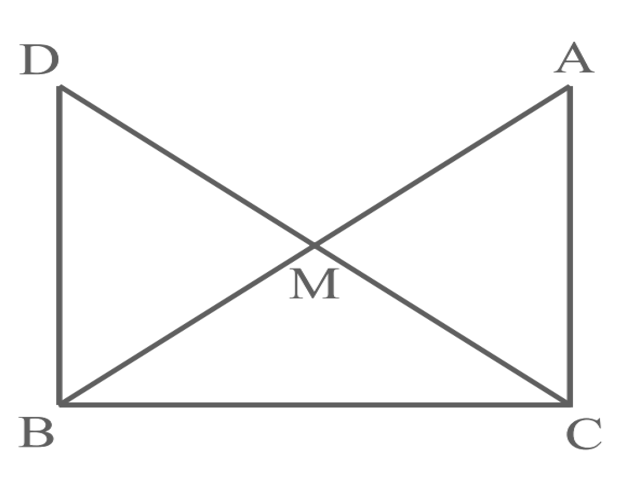
\includegraphics[width=\columnwidth]{figs/Screenshot.png}
  \caption{$\triangle \vec{ACB} ,\triangle \vec{DCB}$ with Mid-Point $\vec{M}$}
  \label{fig:triangles}
\end{figure}
\begin{enumerate}[label =(\roman*)]
        \item $\triangle \vec{AMC} \cong \triangle \vec{BMD}$
        \item $\angle \vec{DBC}$ is a right angle. 
        \item $\triangle \vec{DBC} \cong  \triangle \vec{ACB}$ 
        \item $\vec{CM} = \frac{1}{2} \vec{AB}$
\end{enumerate}
\pagebreak
\solution\\
\textbf{CONSTRUCTION STEPS :}
\begin{enumerate}
\item Let us Assume , the input parameters as ;
\begin{table}[H]
\centering
        \input{tables/input_params.tex}
          \caption{Input Parameters}
          \label{Table-1:Input_params}
\end{table}
\item the output can be calculated as ;
\begin{table}[H]
\centering
        \input{tables/output_params.tex}
          \caption{Output Parameters}
          \label{Table-2:Output_params}
\end{table}
                $\therefore$ By, Plotting these points we get the required Image \figref{fig:fig-2}
\begin{figure}[H]
        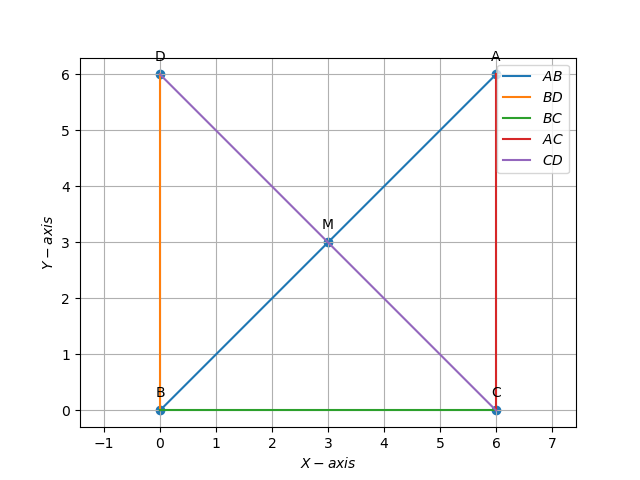
\includegraphics[width = \columnwidth]{figs/python_plot.png}
    \caption{PYTHON Plot of $\triangle \vec{ACB} ,\triangle \vec{DBC}$ with Mid-Point $\vec{M}$}
    \label{fig:fig-2}
\end{figure}
\end{enumerate}

\item Find the position vector of a point $\vec{R}$ which divides the line joining two points $\vec{P}$ and $\vec{Q}$ whose position vectors are $2\vec{a}+\vec{b}$ and $\vec{a}-3\vec{b}$ externally in the ratio $1:2$.

\textbf{Solution:}
Let us assume $\vec{a}$ and $\vec{b}$, and the given ratio is
\begin{table}[h]
    \centering
    \begin{tabular}{|c|c|c|}
        \hline 
        \textbf{Symbol} & \textbf{Value} & \textbf{Description} \\
        \hline
        $\vec{a}$ & $\myvec{1 \\ -3}$ & Vector $\vec{a}$ \\
        \hline
        $\vec{b}$ & $\myvec{0 \\ 2}$ & Vector $\vec{b}$\\
        \hline
        $k$ & $2$ & Ratio \\
        \hline
    \end{tabular}
    \caption{Vectors $\vec{a}$ and $\vec{b}$, ratio $k$}
    \label{tab:table1}
\end{table}

Using the section formula,
\begin{align}
    \vec{R} = \frac{\vec{Q} - k\vec{P}}{1 - k}
\end{align}
where $\vec{P}$ and $\vec{Q}$ depend on $\vec{a}$ and $\vec{b}$, then
\begin{align}
    \vec{P} &= (2\vec{a} + \vec{b}) = 2\myvec{1\\-3} + \myvec{0\\2} = \myvec{2\\-4} \\
    \vec{Q} &= (\vec{a} - 3\vec{b}) = \myvec{1\\-3} - 3\myvec{0\\2} = \myvec{1\\-9}
\end{align}
where $\vec{R}$ can be calculated as 
\begin{align}
    \vec{R} = \frac{(\vec{a} - 3\vec{b}) - k(2\vec{a} + \vec{b})}{1 - k}
\end{align}
By substituting $\vec{a}$ and $\vec{b}$ values, we get $\vec{R}$ as
\begin{align}
    \vec{R} = \myvec{3\\1}
\end{align}

\begin{table}[ht!]
    \centering
    \begin{tabular}{|c|c|c|}
        \hline
        \textbf{Symbol} & \textbf{Value} & \textbf{Description}\\
        \hline
        $\vec{P}$ & $(2\vec{a} + \vec{b})$ & Position vector $\vec{P}$ \\
        \hline
        $\vec{Q}$ & $(\vec{a} - 3\vec{b})$ & Position vector $\vec{Q}$\\
        \hline
        $\vec{R}$ & $\frac{\vec{Q} - k\vec{P}}{1 - k}$ & Position vector $\vec{R}$\\
        \hline
    \end{tabular}
    \caption{Vectors $\vec{P}$, $\vec{Q}$, $\vec{R}$}
    \label{tab:mytable2}   
\end{table}

\begin{figure}[H]
    \centering
    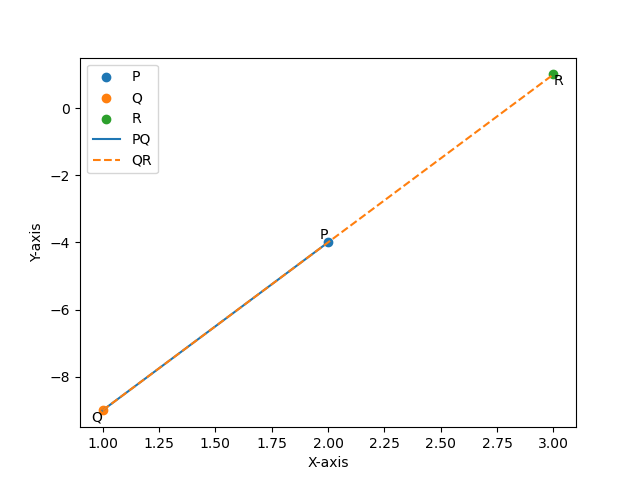
\includegraphics[width=\columnwidth]{figs/external-bisector.png}
    \caption{Point vectors $\vec{P}$, $\vec{Q}$, $\vec{R}$}
    \label{fig:enter-label}
\end{figure}


\end{enumerate}

\item Find the coordinates of the points of trisection of the line segment joining $(4,-1) \text{ and } (-2,3)$.
	\\
		\solution
	\begin{enumerate}[label=\thesection.\arabic*,ref=\thesection.\theenumi]
\numberwithin{equation}{enumi}
\numberwithin{figure}{enumi}
\numberwithin{table}{enumi}

\item Find the coordinates of the point which divides the join of $(-1,7) \text{ and } (4,-3)$ in the ratio 2:3.
	\\
		\solution
	\input{chapters/10/7/2/1/section.tex}
\item Find the coordinates of the points of trisection of the line segment joining $(4,-1) \text{ and } (-2,3)$.
	\\
		\solution
	\input{chapters/10/7/2/2/section.tex}
\item
	\iffalse
\item To conduct Sports Day activities, in your rectangular shaped school                   
ground ABCD, lines have 
drawn with chalk powder at a                 
distance of 1m each. 100 flower pots have been placed at a distance of 1m 
from each other along AD, as shown 
in Fig. 7.12. Niharika runs $ \frac {1}{4} $th the 
distance AD on the 2nd line and 
posts a green flag. Preet runs $ \frac {1}{5} $th 
the distance AD on the eighth line 
and posts a red flag. What is the 
distance between both the flags? If 
Rashmi has to post a blue flag exactly 
halfway between the line segment 
joining the two flags, where should 
she post her flag?
\begin{figure}[h!]
  \centering
  \includegraphics[width=\columnwidth]{sc.png}
  \caption{}
\label{fig:10/7/12Fig1}
\end{figure}               
\fi
      
\item Find the ratio in which the line segment joining the points $(-3,10) \text{ and } (6,-8)$ $\text{ is divided by } (-1,6)$.
	\\
		\solution
	\input{chapters/10/7/2/4/section.tex}
\item Find the ratio in which the line segment joining $A(1,-5) \text{ and } B(-4,5)$ $\text{is divided by the x-axis}$. Also find the coordinates of the point of division.
\item If $(1,2), (4,y), (x,6), (3,5)$ are the vertices of a parallelogram taken in order, find x and y.
	\\
		\solution
	\input{chapters/10/7/2/6/para1.tex}
\item Find the coordinates of a point A, where AB is the diameter of a circle whose centre is $(2,-3) \text{ and }$ B is $(1,4)$.
	\\
		\solution
	\input{chapters/10/7/2/7/section.tex}
\item If A \text{ and } B are $(-2,-2) \text{ and } (2,-4)$, respectively, find the coordinates of P such that AP= $\frac {3}{7}$AB $\text{ and }$ P lies on the line segment AB.
	\\
		\solution
	\input{chapters/10/7/2/8/section.tex}
\item Find the coordinates of the points which divide the line segment joining $A(-2,2) \text{ and } B(2,8)$ into four equal parts.
	\\
		\solution
	\input{chapters/10/7/2/9/section.tex}
\item Find the area of a rhombus if its vertices are $(3,0), (4,5), (-1,4) \text{ and } (-2,-1)$ taken in order. [$\vec{Hint}$ : Area of rhombus =$\frac {1}{2}$(product of its diagonals)]
	\\
		\solution
	\input{chapters/10/7/2/10/cross.tex}
\item Find the position vector of a point R which divides the line joining two points $\vec{P}$
and $\vec{Q}$ whose position vectors are $\hat{i}+2\hat{j}-\hat{k}$ and $-\hat{i}+\hat{j}+\hat{k}$ respectively, in the
ratio 2 : 1
\begin{enumerate}
    \item  internally
    \item  externally
\end{enumerate}
\solution
		\input{chapters/12/10/2/15/section.tex}
\item Find the position vector of the mid point of the vector joining the points $\vec{P}$(2, 3, 4)
and $\vec{Q}$(4, 1, –2).
\\
\solution
		\input{chapters/12/10/2/16/section.tex}
\item Determine the ratio in which the line $2x+y  - 4=0$ divides the line segment joining the points $\vec{A}(2, - 2)$  and  $\vec{B}(3, 7)$.
\\
\solution
	\input{chapters/10/7/4/1/section.tex}
\item Let $\vec{A}(4, 2), \vec{B}(6, 5)$  and $ \vec{C}(1, 4)$ be the vertices of $\triangle ABC$.
\begin{enumerate}
\item The median from $\vec{A}$ meets $BC$ at $\vec{D}$. Find the coordinates of the point $\vec{D}$.
\item Find the coordinates of the point $\vec{P}$ on $AD$ such that $AP : PD = 2 : 1$.
\item Find the coordinates of points $\vec{Q}$ and $\vec{R}$ on medians $BE$ and $CF$ respectively such that $BQ : QE = 2 : 1$  and  $CR : RF = 2 : 1$.
\item What do you observe?
\item If $\vec{A}, \vec{B}$ and $\vec{C}$  are the vertices of $\triangle ABC$, find the coordinates of the centroid of the triangle.
\end{enumerate}
\solution
	\input{chapters/10/7/4/7/section.tex}
\item Find the slope of a line, which passes through the origin and the mid point of the line segment joining the points $\vec{P}$(0,-4) and $\vec{B}$(8,0).
\label{chapters/11/10/1/5}
\input{chapters/11/10/1/5/matrix.tex}
\item Find the position vector of a point R which divides the line joining two points P and Q whose position vectors are $(2\vec{a}+\vec{b})$ and $(\vec{a}-3\vec{b})$
externally in the ratio 1 : 2. Also, show that P is the mid point of the line segment RQ.\\
	\solution
%		\input{chapters/12/10/5/9/section.tex}
\item In right triangle $\vec{ABC}$, right angled at $\vec{C}, \vec{M}$ is the mid-point of hypotenuse $\vec{AB}$. $\vec{C}$ is joined to $\vec{M}$ and produced to a point $\vec{D}$ such that $\vec{DM}=\vec{CM}$. Point $\vec{D}$ is joined to point $\vec{B}$ see \figref{fig:triangles}. Show that:
\begin{figure}[H]
\centering
  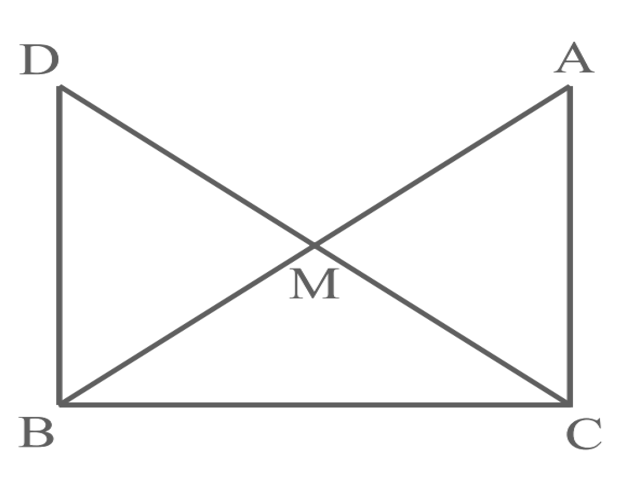
\includegraphics[width=\columnwidth]{figs/Screenshot.png}
  \caption{$\triangle \vec{ACB} ,\triangle \vec{DCB}$ with Mid-Point $\vec{M}$}
  \label{fig:triangles}
\end{figure}
\begin{enumerate}[label =(\roman*)]
        \item $\triangle \vec{AMC} \cong \triangle \vec{BMD}$
        \item $\angle \vec{DBC}$ is a right angle. 
        \item $\triangle \vec{DBC} \cong  \triangle \vec{ACB}$ 
        \item $\vec{CM} = \frac{1}{2} \vec{AB}$
\end{enumerate}
\pagebreak
\solution\\
\textbf{CONSTRUCTION STEPS :}
\begin{enumerate}
\item Let us Assume , the input parameters as ;
\begin{table}[H]
\centering
        \input{tables/input_params.tex}
          \caption{Input Parameters}
          \label{Table-1:Input_params}
\end{table}
\item the output can be calculated as ;
\begin{table}[H]
\centering
        \input{tables/output_params.tex}
          \caption{Output Parameters}
          \label{Table-2:Output_params}
\end{table}
                $\therefore$ By, Plotting these points we get the required Image \figref{fig:fig-2}
\begin{figure}[H]
        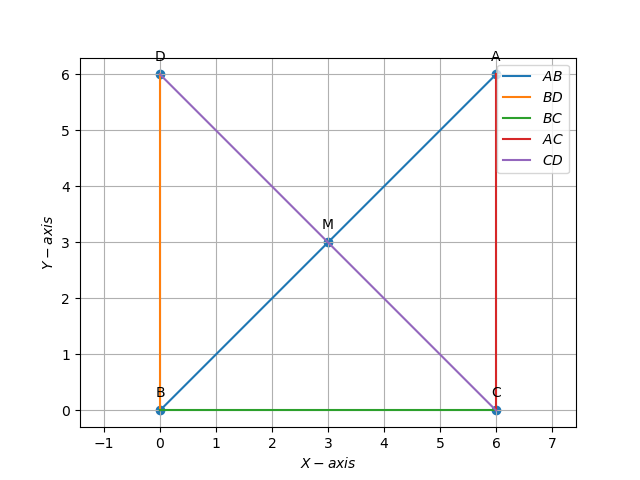
\includegraphics[width = \columnwidth]{figs/python_plot.png}
    \caption{PYTHON Plot of $\triangle \vec{ACB} ,\triangle \vec{DBC}$ with Mid-Point $\vec{M}$}
    \label{fig:fig-2}
\end{figure}
\end{enumerate}

\item Find the position vector of a point $\vec{R}$ which divides the line joining two points $\vec{P}$ and $\vec{Q}$ whose position vectors are $2\vec{a}+\vec{b}$ and $\vec{a}-3\vec{b}$ externally in the ratio $1:2$.

\textbf{Solution:}
Let us assume $\vec{a}$ and $\vec{b}$, and the given ratio is
\begin{table}[h]
    \centering
    \begin{tabular}{|c|c|c|}
        \hline 
        \textbf{Symbol} & \textbf{Value} & \textbf{Description} \\
        \hline
        $\vec{a}$ & $\myvec{1 \\ -3}$ & Vector $\vec{a}$ \\
        \hline
        $\vec{b}$ & $\myvec{0 \\ 2}$ & Vector $\vec{b}$\\
        \hline
        $k$ & $2$ & Ratio \\
        \hline
    \end{tabular}
    \caption{Vectors $\vec{a}$ and $\vec{b}$, ratio $k$}
    \label{tab:table1}
\end{table}

Using the section formula,
\begin{align}
    \vec{R} = \frac{\vec{Q} - k\vec{P}}{1 - k}
\end{align}
where $\vec{P}$ and $\vec{Q}$ depend on $\vec{a}$ and $\vec{b}$, then
\begin{align}
    \vec{P} &= (2\vec{a} + \vec{b}) = 2\myvec{1\\-3} + \myvec{0\\2} = \myvec{2\\-4} \\
    \vec{Q} &= (\vec{a} - 3\vec{b}) = \myvec{1\\-3} - 3\myvec{0\\2} = \myvec{1\\-9}
\end{align}
where $\vec{R}$ can be calculated as 
\begin{align}
    \vec{R} = \frac{(\vec{a} - 3\vec{b}) - k(2\vec{a} + \vec{b})}{1 - k}
\end{align}
By substituting $\vec{a}$ and $\vec{b}$ values, we get $\vec{R}$ as
\begin{align}
    \vec{R} = \myvec{3\\1}
\end{align}

\begin{table}[ht!]
    \centering
    \begin{tabular}{|c|c|c|}
        \hline
        \textbf{Symbol} & \textbf{Value} & \textbf{Description}\\
        \hline
        $\vec{P}$ & $(2\vec{a} + \vec{b})$ & Position vector $\vec{P}$ \\
        \hline
        $\vec{Q}$ & $(\vec{a} - 3\vec{b})$ & Position vector $\vec{Q}$\\
        \hline
        $\vec{R}$ & $\frac{\vec{Q} - k\vec{P}}{1 - k}$ & Position vector $\vec{R}$\\
        \hline
    \end{tabular}
    \caption{Vectors $\vec{P}$, $\vec{Q}$, $\vec{R}$}
    \label{tab:mytable2}   
\end{table}

\begin{figure}[H]
    \centering
    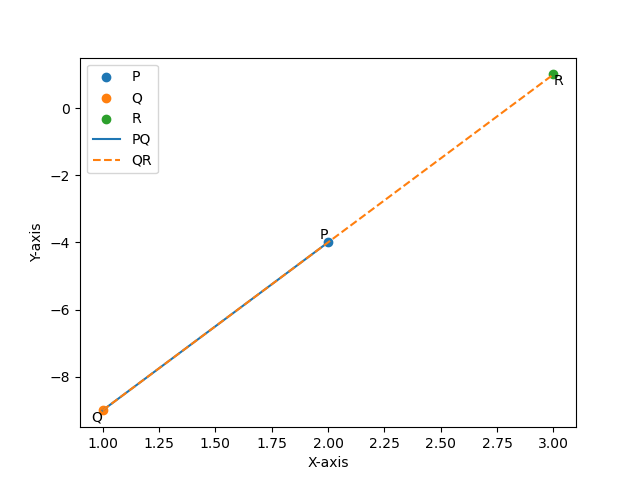
\includegraphics[width=\columnwidth]{figs/external-bisector.png}
    \caption{Point vectors $\vec{P}$, $\vec{Q}$, $\vec{R}$}
    \label{fig:enter-label}
\end{figure}


\end{enumerate}

\item
	\iffalse
\item To conduct Sports Day activities, in your rectangular shaped school                   
ground ABCD, lines have 
drawn with chalk powder at a                 
distance of 1m each. 100 flower pots have been placed at a distance of 1m 
from each other along AD, as shown 
in Fig. 7.12. Niharika runs $ \frac {1}{4} $th the 
distance AD on the 2nd line and 
posts a green flag. Preet runs $ \frac {1}{5} $th 
the distance AD on the eighth line 
and posts a red flag. What is the 
distance between both the flags? If 
Rashmi has to post a blue flag exactly 
halfway between the line segment 
joining the two flags, where should 
she post her flag?
\begin{figure}[h!]
  \centering
  \includegraphics[width=\columnwidth]{sc.png}
  \caption{}
\label{fig:10/7/12Fig1}
\end{figure}               
\fi
      
\item Find the ratio in which the line segment joining the points $(-3,10) \text{ and } (6,-8)$ $\text{ is divided by } (-1,6)$.
	\\
		\solution
	\begin{enumerate}[label=\thesection.\arabic*,ref=\thesection.\theenumi]
\numberwithin{equation}{enumi}
\numberwithin{figure}{enumi}
\numberwithin{table}{enumi}

\item Find the coordinates of the point which divides the join of $(-1,7) \text{ and } (4,-3)$ in the ratio 2:3.
	\\
		\solution
	\input{chapters/10/7/2/1/section.tex}
\item Find the coordinates of the points of trisection of the line segment joining $(4,-1) \text{ and } (-2,3)$.
	\\
		\solution
	\input{chapters/10/7/2/2/section.tex}
\item
	\iffalse
\item To conduct Sports Day activities, in your rectangular shaped school                   
ground ABCD, lines have 
drawn with chalk powder at a                 
distance of 1m each. 100 flower pots have been placed at a distance of 1m 
from each other along AD, as shown 
in Fig. 7.12. Niharika runs $ \frac {1}{4} $th the 
distance AD on the 2nd line and 
posts a green flag. Preet runs $ \frac {1}{5} $th 
the distance AD on the eighth line 
and posts a red flag. What is the 
distance between both the flags? If 
Rashmi has to post a blue flag exactly 
halfway between the line segment 
joining the two flags, where should 
she post her flag?
\begin{figure}[h!]
  \centering
  \includegraphics[width=\columnwidth]{sc.png}
  \caption{}
\label{fig:10/7/12Fig1}
\end{figure}               
\fi
      
\item Find the ratio in which the line segment joining the points $(-3,10) \text{ and } (6,-8)$ $\text{ is divided by } (-1,6)$.
	\\
		\solution
	\input{chapters/10/7/2/4/section.tex}
\item Find the ratio in which the line segment joining $A(1,-5) \text{ and } B(-4,5)$ $\text{is divided by the x-axis}$. Also find the coordinates of the point of division.
\item If $(1,2), (4,y), (x,6), (3,5)$ are the vertices of a parallelogram taken in order, find x and y.
	\\
		\solution
	\input{chapters/10/7/2/6/para1.tex}
\item Find the coordinates of a point A, where AB is the diameter of a circle whose centre is $(2,-3) \text{ and }$ B is $(1,4)$.
	\\
		\solution
	\input{chapters/10/7/2/7/section.tex}
\item If A \text{ and } B are $(-2,-2) \text{ and } (2,-4)$, respectively, find the coordinates of P such that AP= $\frac {3}{7}$AB $\text{ and }$ P lies on the line segment AB.
	\\
		\solution
	\input{chapters/10/7/2/8/section.tex}
\item Find the coordinates of the points which divide the line segment joining $A(-2,2) \text{ and } B(2,8)$ into four equal parts.
	\\
		\solution
	\input{chapters/10/7/2/9/section.tex}
\item Find the area of a rhombus if its vertices are $(3,0), (4,5), (-1,4) \text{ and } (-2,-1)$ taken in order. [$\vec{Hint}$ : Area of rhombus =$\frac {1}{2}$(product of its diagonals)]
	\\
		\solution
	\input{chapters/10/7/2/10/cross.tex}
\item Find the position vector of a point R which divides the line joining two points $\vec{P}$
and $\vec{Q}$ whose position vectors are $\hat{i}+2\hat{j}-\hat{k}$ and $-\hat{i}+\hat{j}+\hat{k}$ respectively, in the
ratio 2 : 1
\begin{enumerate}
    \item  internally
    \item  externally
\end{enumerate}
\solution
		\input{chapters/12/10/2/15/section.tex}
\item Find the position vector of the mid point of the vector joining the points $\vec{P}$(2, 3, 4)
and $\vec{Q}$(4, 1, –2).
\\
\solution
		\input{chapters/12/10/2/16/section.tex}
\item Determine the ratio in which the line $2x+y  - 4=0$ divides the line segment joining the points $\vec{A}(2, - 2)$  and  $\vec{B}(3, 7)$.
\\
\solution
	\input{chapters/10/7/4/1/section.tex}
\item Let $\vec{A}(4, 2), \vec{B}(6, 5)$  and $ \vec{C}(1, 4)$ be the vertices of $\triangle ABC$.
\begin{enumerate}
\item The median from $\vec{A}$ meets $BC$ at $\vec{D}$. Find the coordinates of the point $\vec{D}$.
\item Find the coordinates of the point $\vec{P}$ on $AD$ such that $AP : PD = 2 : 1$.
\item Find the coordinates of points $\vec{Q}$ and $\vec{R}$ on medians $BE$ and $CF$ respectively such that $BQ : QE = 2 : 1$  and  $CR : RF = 2 : 1$.
\item What do you observe?
\item If $\vec{A}, \vec{B}$ and $\vec{C}$  are the vertices of $\triangle ABC$, find the coordinates of the centroid of the triangle.
\end{enumerate}
\solution
	\input{chapters/10/7/4/7/section.tex}
\item Find the slope of a line, which passes through the origin and the mid point of the line segment joining the points $\vec{P}$(0,-4) and $\vec{B}$(8,0).
\label{chapters/11/10/1/5}
\input{chapters/11/10/1/5/matrix.tex}
\item Find the position vector of a point R which divides the line joining two points P and Q whose position vectors are $(2\vec{a}+\vec{b})$ and $(\vec{a}-3\vec{b})$
externally in the ratio 1 : 2. Also, show that P is the mid point of the line segment RQ.\\
	\solution
%		\input{chapters/12/10/5/9/section.tex}
\item In right triangle $\vec{ABC}$, right angled at $\vec{C}, \vec{M}$ is the mid-point of hypotenuse $\vec{AB}$. $\vec{C}$ is joined to $\vec{M}$ and produced to a point $\vec{D}$ such that $\vec{DM}=\vec{CM}$. Point $\vec{D}$ is joined to point $\vec{B}$ see \figref{fig:triangles}. Show that:
\begin{figure}[H]
\centering
  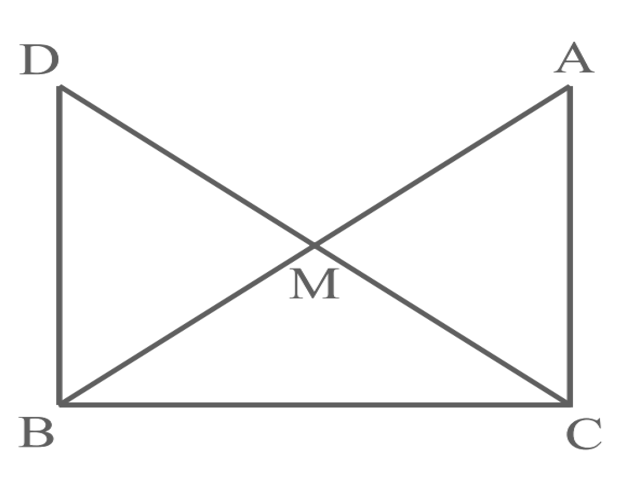
\includegraphics[width=\columnwidth]{figs/Screenshot.png}
  \caption{$\triangle \vec{ACB} ,\triangle \vec{DCB}$ with Mid-Point $\vec{M}$}
  \label{fig:triangles}
\end{figure}
\begin{enumerate}[label =(\roman*)]
        \item $\triangle \vec{AMC} \cong \triangle \vec{BMD}$
        \item $\angle \vec{DBC}$ is a right angle. 
        \item $\triangle \vec{DBC} \cong  \triangle \vec{ACB}$ 
        \item $\vec{CM} = \frac{1}{2} \vec{AB}$
\end{enumerate}
\pagebreak
\solution\\
\textbf{CONSTRUCTION STEPS :}
\begin{enumerate}
\item Let us Assume , the input parameters as ;
\begin{table}[H]
\centering
        \input{tables/input_params.tex}
          \caption{Input Parameters}
          \label{Table-1:Input_params}
\end{table}
\item the output can be calculated as ;
\begin{table}[H]
\centering
        \input{tables/output_params.tex}
          \caption{Output Parameters}
          \label{Table-2:Output_params}
\end{table}
                $\therefore$ By, Plotting these points we get the required Image \figref{fig:fig-2}
\begin{figure}[H]
        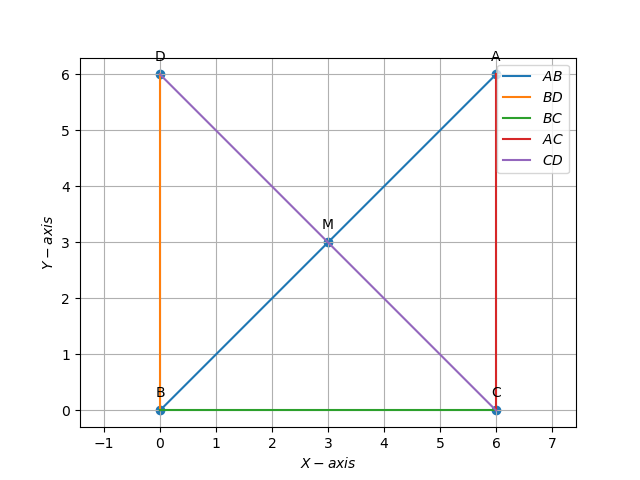
\includegraphics[width = \columnwidth]{figs/python_plot.png}
    \caption{PYTHON Plot of $\triangle \vec{ACB} ,\triangle \vec{DBC}$ with Mid-Point $\vec{M}$}
    \label{fig:fig-2}
\end{figure}
\end{enumerate}

\item Find the position vector of a point $\vec{R}$ which divides the line joining two points $\vec{P}$ and $\vec{Q}$ whose position vectors are $2\vec{a}+\vec{b}$ and $\vec{a}-3\vec{b}$ externally in the ratio $1:2$.

\textbf{Solution:}
Let us assume $\vec{a}$ and $\vec{b}$, and the given ratio is
\begin{table}[h]
    \centering
    \begin{tabular}{|c|c|c|}
        \hline 
        \textbf{Symbol} & \textbf{Value} & \textbf{Description} \\
        \hline
        $\vec{a}$ & $\myvec{1 \\ -3}$ & Vector $\vec{a}$ \\
        \hline
        $\vec{b}$ & $\myvec{0 \\ 2}$ & Vector $\vec{b}$\\
        \hline
        $k$ & $2$ & Ratio \\
        \hline
    \end{tabular}
    \caption{Vectors $\vec{a}$ and $\vec{b}$, ratio $k$}
    \label{tab:table1}
\end{table}

Using the section formula,
\begin{align}
    \vec{R} = \frac{\vec{Q} - k\vec{P}}{1 - k}
\end{align}
where $\vec{P}$ and $\vec{Q}$ depend on $\vec{a}$ and $\vec{b}$, then
\begin{align}
    \vec{P} &= (2\vec{a} + \vec{b}) = 2\myvec{1\\-3} + \myvec{0\\2} = \myvec{2\\-4} \\
    \vec{Q} &= (\vec{a} - 3\vec{b}) = \myvec{1\\-3} - 3\myvec{0\\2} = \myvec{1\\-9}
\end{align}
where $\vec{R}$ can be calculated as 
\begin{align}
    \vec{R} = \frac{(\vec{a} - 3\vec{b}) - k(2\vec{a} + \vec{b})}{1 - k}
\end{align}
By substituting $\vec{a}$ and $\vec{b}$ values, we get $\vec{R}$ as
\begin{align}
    \vec{R} = \myvec{3\\1}
\end{align}

\begin{table}[ht!]
    \centering
    \begin{tabular}{|c|c|c|}
        \hline
        \textbf{Symbol} & \textbf{Value} & \textbf{Description}\\
        \hline
        $\vec{P}$ & $(2\vec{a} + \vec{b})$ & Position vector $\vec{P}$ \\
        \hline
        $\vec{Q}$ & $(\vec{a} - 3\vec{b})$ & Position vector $\vec{Q}$\\
        \hline
        $\vec{R}$ & $\frac{\vec{Q} - k\vec{P}}{1 - k}$ & Position vector $\vec{R}$\\
        \hline
    \end{tabular}
    \caption{Vectors $\vec{P}$, $\vec{Q}$, $\vec{R}$}
    \label{tab:mytable2}   
\end{table}

\begin{figure}[H]
    \centering
    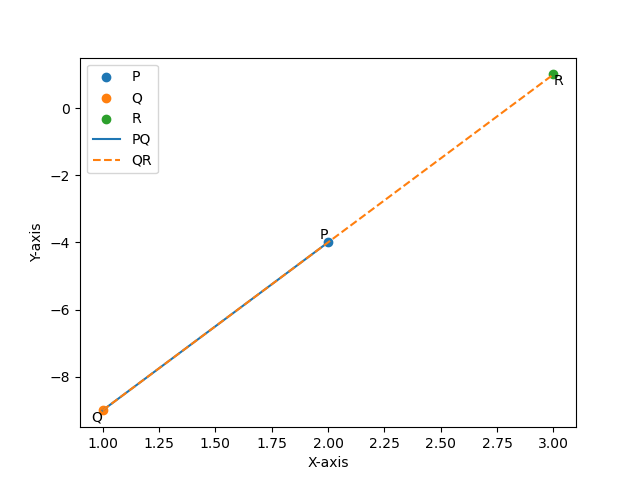
\includegraphics[width=\columnwidth]{figs/external-bisector.png}
    \caption{Point vectors $\vec{P}$, $\vec{Q}$, $\vec{R}$}
    \label{fig:enter-label}
\end{figure}


\end{enumerate}

\item Find the ratio in which the line segment joining $A(1,-5) \text{ and } B(-4,5)$ $\text{is divided by the x-axis}$. Also find the coordinates of the point of division.
\item If $(1,2), (4,y), (x,6), (3,5)$ are the vertices of a parallelogram taken in order, find x and y.
	\\
		\solution
	\input{chapters/10/7/2/6/para1.tex}
\item Find the coordinates of a point A, where AB is the diameter of a circle whose centre is $(2,-3) \text{ and }$ B is $(1,4)$.
	\\
		\solution
	\begin{enumerate}[label=\thesection.\arabic*,ref=\thesection.\theenumi]
\numberwithin{equation}{enumi}
\numberwithin{figure}{enumi}
\numberwithin{table}{enumi}

\item Find the coordinates of the point which divides the join of $(-1,7) \text{ and } (4,-3)$ in the ratio 2:3.
	\\
		\solution
	\input{chapters/10/7/2/1/section.tex}
\item Find the coordinates of the points of trisection of the line segment joining $(4,-1) \text{ and } (-2,3)$.
	\\
		\solution
	\input{chapters/10/7/2/2/section.tex}
\item
	\iffalse
\item To conduct Sports Day activities, in your rectangular shaped school                   
ground ABCD, lines have 
drawn with chalk powder at a                 
distance of 1m each. 100 flower pots have been placed at a distance of 1m 
from each other along AD, as shown 
in Fig. 7.12. Niharika runs $ \frac {1}{4} $th the 
distance AD on the 2nd line and 
posts a green flag. Preet runs $ \frac {1}{5} $th 
the distance AD on the eighth line 
and posts a red flag. What is the 
distance between both the flags? If 
Rashmi has to post a blue flag exactly 
halfway between the line segment 
joining the two flags, where should 
she post her flag?
\begin{figure}[h!]
  \centering
  \includegraphics[width=\columnwidth]{sc.png}
  \caption{}
\label{fig:10/7/12Fig1}
\end{figure}               
\fi
      
\item Find the ratio in which the line segment joining the points $(-3,10) \text{ and } (6,-8)$ $\text{ is divided by } (-1,6)$.
	\\
		\solution
	\input{chapters/10/7/2/4/section.tex}
\item Find the ratio in which the line segment joining $A(1,-5) \text{ and } B(-4,5)$ $\text{is divided by the x-axis}$. Also find the coordinates of the point of division.
\item If $(1,2), (4,y), (x,6), (3,5)$ are the vertices of a parallelogram taken in order, find x and y.
	\\
		\solution
	\input{chapters/10/7/2/6/para1.tex}
\item Find the coordinates of a point A, where AB is the diameter of a circle whose centre is $(2,-3) \text{ and }$ B is $(1,4)$.
	\\
		\solution
	\input{chapters/10/7/2/7/section.tex}
\item If A \text{ and } B are $(-2,-2) \text{ and } (2,-4)$, respectively, find the coordinates of P such that AP= $\frac {3}{7}$AB $\text{ and }$ P lies on the line segment AB.
	\\
		\solution
	\input{chapters/10/7/2/8/section.tex}
\item Find the coordinates of the points which divide the line segment joining $A(-2,2) \text{ and } B(2,8)$ into four equal parts.
	\\
		\solution
	\input{chapters/10/7/2/9/section.tex}
\item Find the area of a rhombus if its vertices are $(3,0), (4,5), (-1,4) \text{ and } (-2,-1)$ taken in order. [$\vec{Hint}$ : Area of rhombus =$\frac {1}{2}$(product of its diagonals)]
	\\
		\solution
	\input{chapters/10/7/2/10/cross.tex}
\item Find the position vector of a point R which divides the line joining two points $\vec{P}$
and $\vec{Q}$ whose position vectors are $\hat{i}+2\hat{j}-\hat{k}$ and $-\hat{i}+\hat{j}+\hat{k}$ respectively, in the
ratio 2 : 1
\begin{enumerate}
    \item  internally
    \item  externally
\end{enumerate}
\solution
		\input{chapters/12/10/2/15/section.tex}
\item Find the position vector of the mid point of the vector joining the points $\vec{P}$(2, 3, 4)
and $\vec{Q}$(4, 1, –2).
\\
\solution
		\input{chapters/12/10/2/16/section.tex}
\item Determine the ratio in which the line $2x+y  - 4=0$ divides the line segment joining the points $\vec{A}(2, - 2)$  and  $\vec{B}(3, 7)$.
\\
\solution
	\input{chapters/10/7/4/1/section.tex}
\item Let $\vec{A}(4, 2), \vec{B}(6, 5)$  and $ \vec{C}(1, 4)$ be the vertices of $\triangle ABC$.
\begin{enumerate}
\item The median from $\vec{A}$ meets $BC$ at $\vec{D}$. Find the coordinates of the point $\vec{D}$.
\item Find the coordinates of the point $\vec{P}$ on $AD$ such that $AP : PD = 2 : 1$.
\item Find the coordinates of points $\vec{Q}$ and $\vec{R}$ on medians $BE$ and $CF$ respectively such that $BQ : QE = 2 : 1$  and  $CR : RF = 2 : 1$.
\item What do you observe?
\item If $\vec{A}, \vec{B}$ and $\vec{C}$  are the vertices of $\triangle ABC$, find the coordinates of the centroid of the triangle.
\end{enumerate}
\solution
	\input{chapters/10/7/4/7/section.tex}
\item Find the slope of a line, which passes through the origin and the mid point of the line segment joining the points $\vec{P}$(0,-4) and $\vec{B}$(8,0).
\label{chapters/11/10/1/5}
\input{chapters/11/10/1/5/matrix.tex}
\item Find the position vector of a point R which divides the line joining two points P and Q whose position vectors are $(2\vec{a}+\vec{b})$ and $(\vec{a}-3\vec{b})$
externally in the ratio 1 : 2. Also, show that P is the mid point of the line segment RQ.\\
	\solution
%		\input{chapters/12/10/5/9/section.tex}
\item In right triangle $\vec{ABC}$, right angled at $\vec{C}, \vec{M}$ is the mid-point of hypotenuse $\vec{AB}$. $\vec{C}$ is joined to $\vec{M}$ and produced to a point $\vec{D}$ such that $\vec{DM}=\vec{CM}$. Point $\vec{D}$ is joined to point $\vec{B}$ see \figref{fig:triangles}. Show that:
\begin{figure}[H]
\centering
  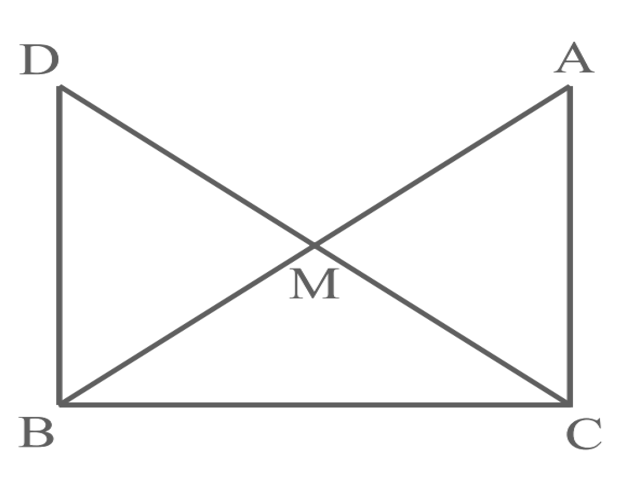
\includegraphics[width=\columnwidth]{figs/Screenshot.png}
  \caption{$\triangle \vec{ACB} ,\triangle \vec{DCB}$ with Mid-Point $\vec{M}$}
  \label{fig:triangles}
\end{figure}
\begin{enumerate}[label =(\roman*)]
        \item $\triangle \vec{AMC} \cong \triangle \vec{BMD}$
        \item $\angle \vec{DBC}$ is a right angle. 
        \item $\triangle \vec{DBC} \cong  \triangle \vec{ACB}$ 
        \item $\vec{CM} = \frac{1}{2} \vec{AB}$
\end{enumerate}
\pagebreak
\solution\\
\textbf{CONSTRUCTION STEPS :}
\begin{enumerate}
\item Let us Assume , the input parameters as ;
\begin{table}[H]
\centering
        \input{tables/input_params.tex}
          \caption{Input Parameters}
          \label{Table-1:Input_params}
\end{table}
\item the output can be calculated as ;
\begin{table}[H]
\centering
        \input{tables/output_params.tex}
          \caption{Output Parameters}
          \label{Table-2:Output_params}
\end{table}
                $\therefore$ By, Plotting these points we get the required Image \figref{fig:fig-2}
\begin{figure}[H]
        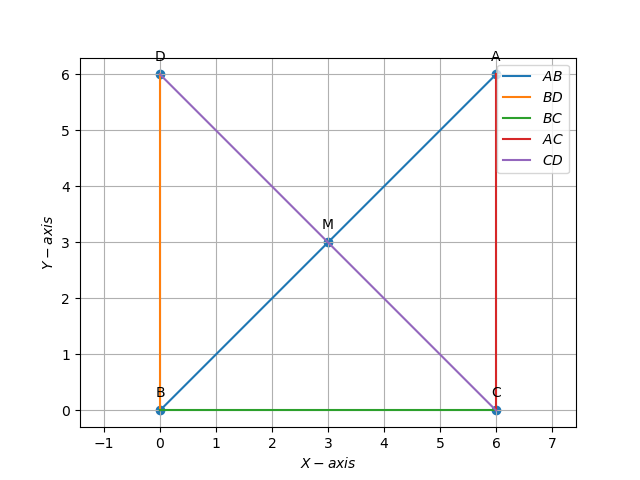
\includegraphics[width = \columnwidth]{figs/python_plot.png}
    \caption{PYTHON Plot of $\triangle \vec{ACB} ,\triangle \vec{DBC}$ with Mid-Point $\vec{M}$}
    \label{fig:fig-2}
\end{figure}
\end{enumerate}

\item Find the position vector of a point $\vec{R}$ which divides the line joining two points $\vec{P}$ and $\vec{Q}$ whose position vectors are $2\vec{a}+\vec{b}$ and $\vec{a}-3\vec{b}$ externally in the ratio $1:2$.

\textbf{Solution:}
Let us assume $\vec{a}$ and $\vec{b}$, and the given ratio is
\begin{table}[h]
    \centering
    \begin{tabular}{|c|c|c|}
        \hline 
        \textbf{Symbol} & \textbf{Value} & \textbf{Description} \\
        \hline
        $\vec{a}$ & $\myvec{1 \\ -3}$ & Vector $\vec{a}$ \\
        \hline
        $\vec{b}$ & $\myvec{0 \\ 2}$ & Vector $\vec{b}$\\
        \hline
        $k$ & $2$ & Ratio \\
        \hline
    \end{tabular}
    \caption{Vectors $\vec{a}$ and $\vec{b}$, ratio $k$}
    \label{tab:table1}
\end{table}

Using the section formula,
\begin{align}
    \vec{R} = \frac{\vec{Q} - k\vec{P}}{1 - k}
\end{align}
where $\vec{P}$ and $\vec{Q}$ depend on $\vec{a}$ and $\vec{b}$, then
\begin{align}
    \vec{P} &= (2\vec{a} + \vec{b}) = 2\myvec{1\\-3} + \myvec{0\\2} = \myvec{2\\-4} \\
    \vec{Q} &= (\vec{a} - 3\vec{b}) = \myvec{1\\-3} - 3\myvec{0\\2} = \myvec{1\\-9}
\end{align}
where $\vec{R}$ can be calculated as 
\begin{align}
    \vec{R} = \frac{(\vec{a} - 3\vec{b}) - k(2\vec{a} + \vec{b})}{1 - k}
\end{align}
By substituting $\vec{a}$ and $\vec{b}$ values, we get $\vec{R}$ as
\begin{align}
    \vec{R} = \myvec{3\\1}
\end{align}

\begin{table}[ht!]
    \centering
    \begin{tabular}{|c|c|c|}
        \hline
        \textbf{Symbol} & \textbf{Value} & \textbf{Description}\\
        \hline
        $\vec{P}$ & $(2\vec{a} + \vec{b})$ & Position vector $\vec{P}$ \\
        \hline
        $\vec{Q}$ & $(\vec{a} - 3\vec{b})$ & Position vector $\vec{Q}$\\
        \hline
        $\vec{R}$ & $\frac{\vec{Q} - k\vec{P}}{1 - k}$ & Position vector $\vec{R}$\\
        \hline
    \end{tabular}
    \caption{Vectors $\vec{P}$, $\vec{Q}$, $\vec{R}$}
    \label{tab:mytable2}   
\end{table}

\begin{figure}[H]
    \centering
    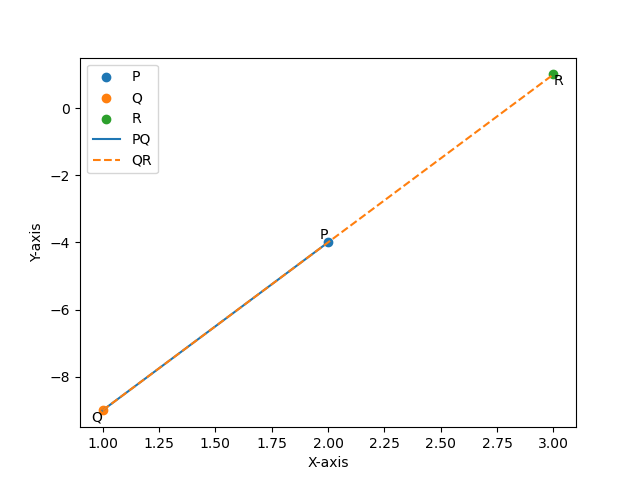
\includegraphics[width=\columnwidth]{figs/external-bisector.png}
    \caption{Point vectors $\vec{P}$, $\vec{Q}$, $\vec{R}$}
    \label{fig:enter-label}
\end{figure}


\end{enumerate}

\item If A \text{ and } B are $(-2,-2) \text{ and } (2,-4)$, respectively, find the coordinates of P such that AP= $\frac {3}{7}$AB $\text{ and }$ P lies on the line segment AB.
	\\
		\solution
	\begin{enumerate}[label=\thesection.\arabic*,ref=\thesection.\theenumi]
\numberwithin{equation}{enumi}
\numberwithin{figure}{enumi}
\numberwithin{table}{enumi}

\item Find the coordinates of the point which divides the join of $(-1,7) \text{ and } (4,-3)$ in the ratio 2:3.
	\\
		\solution
	\input{chapters/10/7/2/1/section.tex}
\item Find the coordinates of the points of trisection of the line segment joining $(4,-1) \text{ and } (-2,3)$.
	\\
		\solution
	\input{chapters/10/7/2/2/section.tex}
\item
	\iffalse
\item To conduct Sports Day activities, in your rectangular shaped school                   
ground ABCD, lines have 
drawn with chalk powder at a                 
distance of 1m each. 100 flower pots have been placed at a distance of 1m 
from each other along AD, as shown 
in Fig. 7.12. Niharika runs $ \frac {1}{4} $th the 
distance AD on the 2nd line and 
posts a green flag. Preet runs $ \frac {1}{5} $th 
the distance AD on the eighth line 
and posts a red flag. What is the 
distance between both the flags? If 
Rashmi has to post a blue flag exactly 
halfway between the line segment 
joining the two flags, where should 
she post her flag?
\begin{figure}[h!]
  \centering
  \includegraphics[width=\columnwidth]{sc.png}
  \caption{}
\label{fig:10/7/12Fig1}
\end{figure}               
\fi
      
\item Find the ratio in which the line segment joining the points $(-3,10) \text{ and } (6,-8)$ $\text{ is divided by } (-1,6)$.
	\\
		\solution
	\input{chapters/10/7/2/4/section.tex}
\item Find the ratio in which the line segment joining $A(1,-5) \text{ and } B(-4,5)$ $\text{is divided by the x-axis}$. Also find the coordinates of the point of division.
\item If $(1,2), (4,y), (x,6), (3,5)$ are the vertices of a parallelogram taken in order, find x and y.
	\\
		\solution
	\input{chapters/10/7/2/6/para1.tex}
\item Find the coordinates of a point A, where AB is the diameter of a circle whose centre is $(2,-3) \text{ and }$ B is $(1,4)$.
	\\
		\solution
	\input{chapters/10/7/2/7/section.tex}
\item If A \text{ and } B are $(-2,-2) \text{ and } (2,-4)$, respectively, find the coordinates of P such that AP= $\frac {3}{7}$AB $\text{ and }$ P lies on the line segment AB.
	\\
		\solution
	\input{chapters/10/7/2/8/section.tex}
\item Find the coordinates of the points which divide the line segment joining $A(-2,2) \text{ and } B(2,8)$ into four equal parts.
	\\
		\solution
	\input{chapters/10/7/2/9/section.tex}
\item Find the area of a rhombus if its vertices are $(3,0), (4,5), (-1,4) \text{ and } (-2,-1)$ taken in order. [$\vec{Hint}$ : Area of rhombus =$\frac {1}{2}$(product of its diagonals)]
	\\
		\solution
	\input{chapters/10/7/2/10/cross.tex}
\item Find the position vector of a point R which divides the line joining two points $\vec{P}$
and $\vec{Q}$ whose position vectors are $\hat{i}+2\hat{j}-\hat{k}$ and $-\hat{i}+\hat{j}+\hat{k}$ respectively, in the
ratio 2 : 1
\begin{enumerate}
    \item  internally
    \item  externally
\end{enumerate}
\solution
		\input{chapters/12/10/2/15/section.tex}
\item Find the position vector of the mid point of the vector joining the points $\vec{P}$(2, 3, 4)
and $\vec{Q}$(4, 1, –2).
\\
\solution
		\input{chapters/12/10/2/16/section.tex}
\item Determine the ratio in which the line $2x+y  - 4=0$ divides the line segment joining the points $\vec{A}(2, - 2)$  and  $\vec{B}(3, 7)$.
\\
\solution
	\input{chapters/10/7/4/1/section.tex}
\item Let $\vec{A}(4, 2), \vec{B}(6, 5)$  and $ \vec{C}(1, 4)$ be the vertices of $\triangle ABC$.
\begin{enumerate}
\item The median from $\vec{A}$ meets $BC$ at $\vec{D}$. Find the coordinates of the point $\vec{D}$.
\item Find the coordinates of the point $\vec{P}$ on $AD$ such that $AP : PD = 2 : 1$.
\item Find the coordinates of points $\vec{Q}$ and $\vec{R}$ on medians $BE$ and $CF$ respectively such that $BQ : QE = 2 : 1$  and  $CR : RF = 2 : 1$.
\item What do you observe?
\item If $\vec{A}, \vec{B}$ and $\vec{C}$  are the vertices of $\triangle ABC$, find the coordinates of the centroid of the triangle.
\end{enumerate}
\solution
	\input{chapters/10/7/4/7/section.tex}
\item Find the slope of a line, which passes through the origin and the mid point of the line segment joining the points $\vec{P}$(0,-4) and $\vec{B}$(8,0).
\label{chapters/11/10/1/5}
\input{chapters/11/10/1/5/matrix.tex}
\item Find the position vector of a point R which divides the line joining two points P and Q whose position vectors are $(2\vec{a}+\vec{b})$ and $(\vec{a}-3\vec{b})$
externally in the ratio 1 : 2. Also, show that P is the mid point of the line segment RQ.\\
	\solution
%		\input{chapters/12/10/5/9/section.tex}
\item In right triangle $\vec{ABC}$, right angled at $\vec{C}, \vec{M}$ is the mid-point of hypotenuse $\vec{AB}$. $\vec{C}$ is joined to $\vec{M}$ and produced to a point $\vec{D}$ such that $\vec{DM}=\vec{CM}$. Point $\vec{D}$ is joined to point $\vec{B}$ see \figref{fig:triangles}. Show that:
\begin{figure}[H]
\centering
  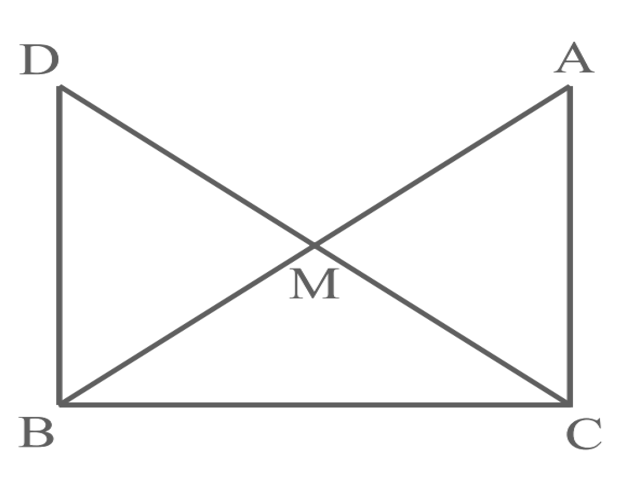
\includegraphics[width=\columnwidth]{figs/Screenshot.png}
  \caption{$\triangle \vec{ACB} ,\triangle \vec{DCB}$ with Mid-Point $\vec{M}$}
  \label{fig:triangles}
\end{figure}
\begin{enumerate}[label =(\roman*)]
        \item $\triangle \vec{AMC} \cong \triangle \vec{BMD}$
        \item $\angle \vec{DBC}$ is a right angle. 
        \item $\triangle \vec{DBC} \cong  \triangle \vec{ACB}$ 
        \item $\vec{CM} = \frac{1}{2} \vec{AB}$
\end{enumerate}
\pagebreak
\solution\\
\textbf{CONSTRUCTION STEPS :}
\begin{enumerate}
\item Let us Assume , the input parameters as ;
\begin{table}[H]
\centering
        \input{tables/input_params.tex}
          \caption{Input Parameters}
          \label{Table-1:Input_params}
\end{table}
\item the output can be calculated as ;
\begin{table}[H]
\centering
        \input{tables/output_params.tex}
          \caption{Output Parameters}
          \label{Table-2:Output_params}
\end{table}
                $\therefore$ By, Plotting these points we get the required Image \figref{fig:fig-2}
\begin{figure}[H]
        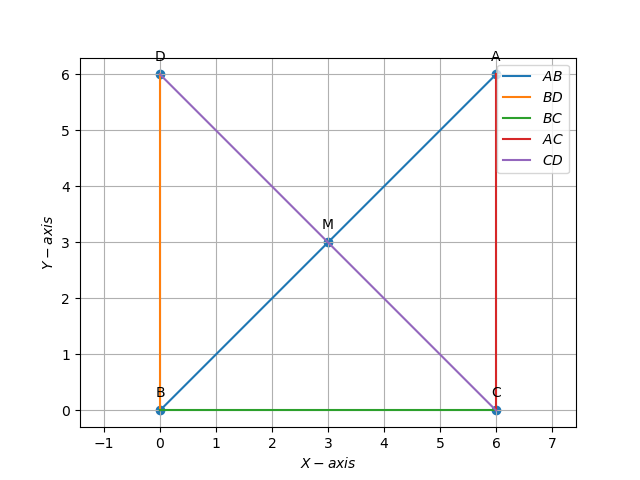
\includegraphics[width = \columnwidth]{figs/python_plot.png}
    \caption{PYTHON Plot of $\triangle \vec{ACB} ,\triangle \vec{DBC}$ with Mid-Point $\vec{M}$}
    \label{fig:fig-2}
\end{figure}
\end{enumerate}

\item Find the position vector of a point $\vec{R}$ which divides the line joining two points $\vec{P}$ and $\vec{Q}$ whose position vectors are $2\vec{a}+\vec{b}$ and $\vec{a}-3\vec{b}$ externally in the ratio $1:2$.

\textbf{Solution:}
Let us assume $\vec{a}$ and $\vec{b}$, and the given ratio is
\begin{table}[h]
    \centering
    \begin{tabular}{|c|c|c|}
        \hline 
        \textbf{Symbol} & \textbf{Value} & \textbf{Description} \\
        \hline
        $\vec{a}$ & $\myvec{1 \\ -3}$ & Vector $\vec{a}$ \\
        \hline
        $\vec{b}$ & $\myvec{0 \\ 2}$ & Vector $\vec{b}$\\
        \hline
        $k$ & $2$ & Ratio \\
        \hline
    \end{tabular}
    \caption{Vectors $\vec{a}$ and $\vec{b}$, ratio $k$}
    \label{tab:table1}
\end{table}

Using the section formula,
\begin{align}
    \vec{R} = \frac{\vec{Q} - k\vec{P}}{1 - k}
\end{align}
where $\vec{P}$ and $\vec{Q}$ depend on $\vec{a}$ and $\vec{b}$, then
\begin{align}
    \vec{P} &= (2\vec{a} + \vec{b}) = 2\myvec{1\\-3} + \myvec{0\\2} = \myvec{2\\-4} \\
    \vec{Q} &= (\vec{a} - 3\vec{b}) = \myvec{1\\-3} - 3\myvec{0\\2} = \myvec{1\\-9}
\end{align}
where $\vec{R}$ can be calculated as 
\begin{align}
    \vec{R} = \frac{(\vec{a} - 3\vec{b}) - k(2\vec{a} + \vec{b})}{1 - k}
\end{align}
By substituting $\vec{a}$ and $\vec{b}$ values, we get $\vec{R}$ as
\begin{align}
    \vec{R} = \myvec{3\\1}
\end{align}

\begin{table}[ht!]
    \centering
    \begin{tabular}{|c|c|c|}
        \hline
        \textbf{Symbol} & \textbf{Value} & \textbf{Description}\\
        \hline
        $\vec{P}$ & $(2\vec{a} + \vec{b})$ & Position vector $\vec{P}$ \\
        \hline
        $\vec{Q}$ & $(\vec{a} - 3\vec{b})$ & Position vector $\vec{Q}$\\
        \hline
        $\vec{R}$ & $\frac{\vec{Q} - k\vec{P}}{1 - k}$ & Position vector $\vec{R}$\\
        \hline
    \end{tabular}
    \caption{Vectors $\vec{P}$, $\vec{Q}$, $\vec{R}$}
    \label{tab:mytable2}   
\end{table}

\begin{figure}[H]
    \centering
    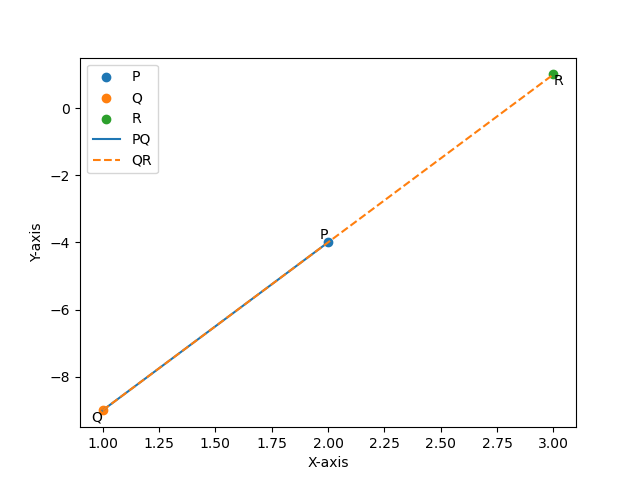
\includegraphics[width=\columnwidth]{figs/external-bisector.png}
    \caption{Point vectors $\vec{P}$, $\vec{Q}$, $\vec{R}$}
    \label{fig:enter-label}
\end{figure}


\end{enumerate}

\item Find the coordinates of the points which divide the line segment joining $A(-2,2) \text{ and } B(2,8)$ into four equal parts.
	\\
		\solution
	\begin{enumerate}[label=\thesection.\arabic*,ref=\thesection.\theenumi]
\numberwithin{equation}{enumi}
\numberwithin{figure}{enumi}
\numberwithin{table}{enumi}

\item Find the coordinates of the point which divides the join of $(-1,7) \text{ and } (4,-3)$ in the ratio 2:3.
	\\
		\solution
	\input{chapters/10/7/2/1/section.tex}
\item Find the coordinates of the points of trisection of the line segment joining $(4,-1) \text{ and } (-2,3)$.
	\\
		\solution
	\input{chapters/10/7/2/2/section.tex}
\item
	\iffalse
\item To conduct Sports Day activities, in your rectangular shaped school                   
ground ABCD, lines have 
drawn with chalk powder at a                 
distance of 1m each. 100 flower pots have been placed at a distance of 1m 
from each other along AD, as shown 
in Fig. 7.12. Niharika runs $ \frac {1}{4} $th the 
distance AD on the 2nd line and 
posts a green flag. Preet runs $ \frac {1}{5} $th 
the distance AD on the eighth line 
and posts a red flag. What is the 
distance between both the flags? If 
Rashmi has to post a blue flag exactly 
halfway between the line segment 
joining the two flags, where should 
she post her flag?
\begin{figure}[h!]
  \centering
  \includegraphics[width=\columnwidth]{sc.png}
  \caption{}
\label{fig:10/7/12Fig1}
\end{figure}               
\fi
      
\item Find the ratio in which the line segment joining the points $(-3,10) \text{ and } (6,-8)$ $\text{ is divided by } (-1,6)$.
	\\
		\solution
	\input{chapters/10/7/2/4/section.tex}
\item Find the ratio in which the line segment joining $A(1,-5) \text{ and } B(-4,5)$ $\text{is divided by the x-axis}$. Also find the coordinates of the point of division.
\item If $(1,2), (4,y), (x,6), (3,5)$ are the vertices of a parallelogram taken in order, find x and y.
	\\
		\solution
	\input{chapters/10/7/2/6/para1.tex}
\item Find the coordinates of a point A, where AB is the diameter of a circle whose centre is $(2,-3) \text{ and }$ B is $(1,4)$.
	\\
		\solution
	\input{chapters/10/7/2/7/section.tex}
\item If A \text{ and } B are $(-2,-2) \text{ and } (2,-4)$, respectively, find the coordinates of P such that AP= $\frac {3}{7}$AB $\text{ and }$ P lies on the line segment AB.
	\\
		\solution
	\input{chapters/10/7/2/8/section.tex}
\item Find the coordinates of the points which divide the line segment joining $A(-2,2) \text{ and } B(2,8)$ into four equal parts.
	\\
		\solution
	\input{chapters/10/7/2/9/section.tex}
\item Find the area of a rhombus if its vertices are $(3,0), (4,5), (-1,4) \text{ and } (-2,-1)$ taken in order. [$\vec{Hint}$ : Area of rhombus =$\frac {1}{2}$(product of its diagonals)]
	\\
		\solution
	\input{chapters/10/7/2/10/cross.tex}
\item Find the position vector of a point R which divides the line joining two points $\vec{P}$
and $\vec{Q}$ whose position vectors are $\hat{i}+2\hat{j}-\hat{k}$ and $-\hat{i}+\hat{j}+\hat{k}$ respectively, in the
ratio 2 : 1
\begin{enumerate}
    \item  internally
    \item  externally
\end{enumerate}
\solution
		\input{chapters/12/10/2/15/section.tex}
\item Find the position vector of the mid point of the vector joining the points $\vec{P}$(2, 3, 4)
and $\vec{Q}$(4, 1, –2).
\\
\solution
		\input{chapters/12/10/2/16/section.tex}
\item Determine the ratio in which the line $2x+y  - 4=0$ divides the line segment joining the points $\vec{A}(2, - 2)$  and  $\vec{B}(3, 7)$.
\\
\solution
	\input{chapters/10/7/4/1/section.tex}
\item Let $\vec{A}(4, 2), \vec{B}(6, 5)$  and $ \vec{C}(1, 4)$ be the vertices of $\triangle ABC$.
\begin{enumerate}
\item The median from $\vec{A}$ meets $BC$ at $\vec{D}$. Find the coordinates of the point $\vec{D}$.
\item Find the coordinates of the point $\vec{P}$ on $AD$ such that $AP : PD = 2 : 1$.
\item Find the coordinates of points $\vec{Q}$ and $\vec{R}$ on medians $BE$ and $CF$ respectively such that $BQ : QE = 2 : 1$  and  $CR : RF = 2 : 1$.
\item What do you observe?
\item If $\vec{A}, \vec{B}$ and $\vec{C}$  are the vertices of $\triangle ABC$, find the coordinates of the centroid of the triangle.
\end{enumerate}
\solution
	\input{chapters/10/7/4/7/section.tex}
\item Find the slope of a line, which passes through the origin and the mid point of the line segment joining the points $\vec{P}$(0,-4) and $\vec{B}$(8,0).
\label{chapters/11/10/1/5}
\input{chapters/11/10/1/5/matrix.tex}
\item Find the position vector of a point R which divides the line joining two points P and Q whose position vectors are $(2\vec{a}+\vec{b})$ and $(\vec{a}-3\vec{b})$
externally in the ratio 1 : 2. Also, show that P is the mid point of the line segment RQ.\\
	\solution
%		\input{chapters/12/10/5/9/section.tex}
\item In right triangle $\vec{ABC}$, right angled at $\vec{C}, \vec{M}$ is the mid-point of hypotenuse $\vec{AB}$. $\vec{C}$ is joined to $\vec{M}$ and produced to a point $\vec{D}$ such that $\vec{DM}=\vec{CM}$. Point $\vec{D}$ is joined to point $\vec{B}$ see \figref{fig:triangles}. Show that:
\begin{figure}[H]
\centering
  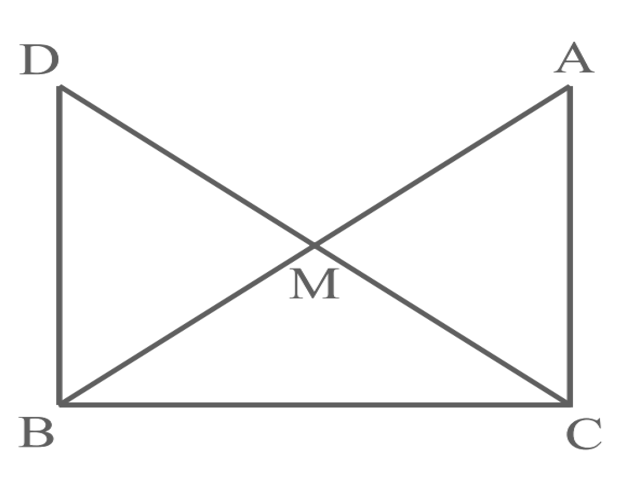
\includegraphics[width=\columnwidth]{figs/Screenshot.png}
  \caption{$\triangle \vec{ACB} ,\triangle \vec{DCB}$ with Mid-Point $\vec{M}$}
  \label{fig:triangles}
\end{figure}
\begin{enumerate}[label =(\roman*)]
        \item $\triangle \vec{AMC} \cong \triangle \vec{BMD}$
        \item $\angle \vec{DBC}$ is a right angle. 
        \item $\triangle \vec{DBC} \cong  \triangle \vec{ACB}$ 
        \item $\vec{CM} = \frac{1}{2} \vec{AB}$
\end{enumerate}
\pagebreak
\solution\\
\textbf{CONSTRUCTION STEPS :}
\begin{enumerate}
\item Let us Assume , the input parameters as ;
\begin{table}[H]
\centering
        \input{tables/input_params.tex}
          \caption{Input Parameters}
          \label{Table-1:Input_params}
\end{table}
\item the output can be calculated as ;
\begin{table}[H]
\centering
        \input{tables/output_params.tex}
          \caption{Output Parameters}
          \label{Table-2:Output_params}
\end{table}
                $\therefore$ By, Plotting these points we get the required Image \figref{fig:fig-2}
\begin{figure}[H]
        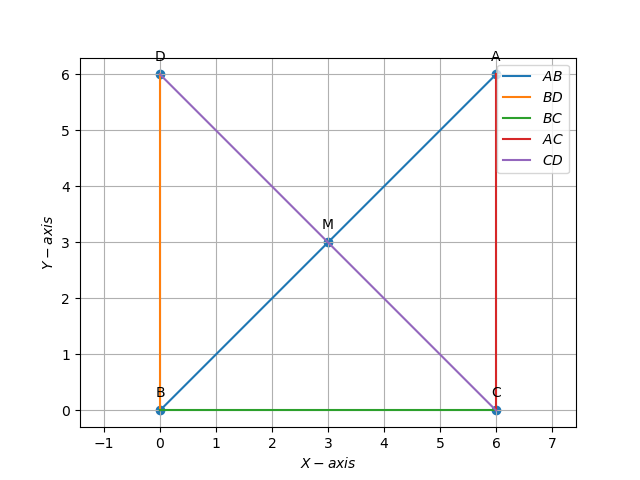
\includegraphics[width = \columnwidth]{figs/python_plot.png}
    \caption{PYTHON Plot of $\triangle \vec{ACB} ,\triangle \vec{DBC}$ with Mid-Point $\vec{M}$}
    \label{fig:fig-2}
\end{figure}
\end{enumerate}

\item Find the position vector of a point $\vec{R}$ which divides the line joining two points $\vec{P}$ and $\vec{Q}$ whose position vectors are $2\vec{a}+\vec{b}$ and $\vec{a}-3\vec{b}$ externally in the ratio $1:2$.

\textbf{Solution:}
Let us assume $\vec{a}$ and $\vec{b}$, and the given ratio is
\begin{table}[h]
    \centering
    \begin{tabular}{|c|c|c|}
        \hline 
        \textbf{Symbol} & \textbf{Value} & \textbf{Description} \\
        \hline
        $\vec{a}$ & $\myvec{1 \\ -3}$ & Vector $\vec{a}$ \\
        \hline
        $\vec{b}$ & $\myvec{0 \\ 2}$ & Vector $\vec{b}$\\
        \hline
        $k$ & $2$ & Ratio \\
        \hline
    \end{tabular}
    \caption{Vectors $\vec{a}$ and $\vec{b}$, ratio $k$}
    \label{tab:table1}
\end{table}

Using the section formula,
\begin{align}
    \vec{R} = \frac{\vec{Q} - k\vec{P}}{1 - k}
\end{align}
where $\vec{P}$ and $\vec{Q}$ depend on $\vec{a}$ and $\vec{b}$, then
\begin{align}
    \vec{P} &= (2\vec{a} + \vec{b}) = 2\myvec{1\\-3} + \myvec{0\\2} = \myvec{2\\-4} \\
    \vec{Q} &= (\vec{a} - 3\vec{b}) = \myvec{1\\-3} - 3\myvec{0\\2} = \myvec{1\\-9}
\end{align}
where $\vec{R}$ can be calculated as 
\begin{align}
    \vec{R} = \frac{(\vec{a} - 3\vec{b}) - k(2\vec{a} + \vec{b})}{1 - k}
\end{align}
By substituting $\vec{a}$ and $\vec{b}$ values, we get $\vec{R}$ as
\begin{align}
    \vec{R} = \myvec{3\\1}
\end{align}

\begin{table}[ht!]
    \centering
    \begin{tabular}{|c|c|c|}
        \hline
        \textbf{Symbol} & \textbf{Value} & \textbf{Description}\\
        \hline
        $\vec{P}$ & $(2\vec{a} + \vec{b})$ & Position vector $\vec{P}$ \\
        \hline
        $\vec{Q}$ & $(\vec{a} - 3\vec{b})$ & Position vector $\vec{Q}$\\
        \hline
        $\vec{R}$ & $\frac{\vec{Q} - k\vec{P}}{1 - k}$ & Position vector $\vec{R}$\\
        \hline
    \end{tabular}
    \caption{Vectors $\vec{P}$, $\vec{Q}$, $\vec{R}$}
    \label{tab:mytable2}   
\end{table}

\begin{figure}[H]
    \centering
    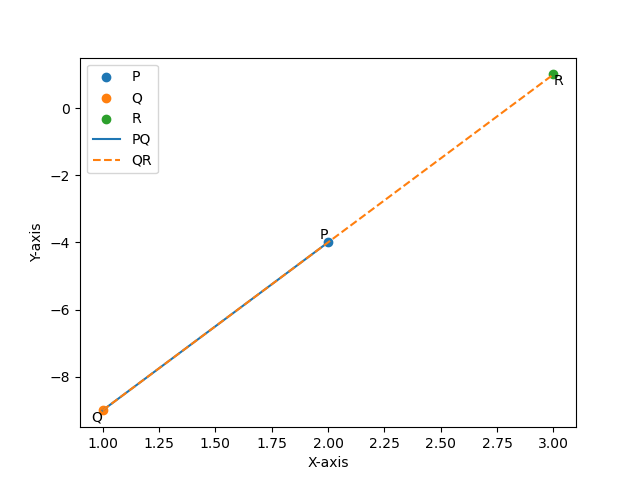
\includegraphics[width=\columnwidth]{figs/external-bisector.png}
    \caption{Point vectors $\vec{P}$, $\vec{Q}$, $\vec{R}$}
    \label{fig:enter-label}
\end{figure}


\end{enumerate}

\item Find the area of a rhombus if its vertices are $(3,0), (4,5), (-1,4) \text{ and } (-2,-1)$ taken in order. [$\vec{Hint}$ : Area of rhombus =$\frac {1}{2}$(product of its diagonals)]
	\\
		\solution
	\begin{enumerate}[label=\thesection.\arabic*,ref=\thesection.\theenumi]
		\item Find $\abs{\overrightarrow{a}\times\overrightarrow{b}},\text{ if }\overrightarrow{a}=\hat{i}-7\hat{j}+7\hat{k}\text{ and } \overrightarrow{b}=3\hat{i}-2\hat{j}+2\hat{k}$.
	\\
		\solution
		\input{chapters/12/10/4/1/cross.tex}
\item Show that $$(\overrightarrow{a}-\overrightarrow{b})\times (\overrightarrow{a}+\overrightarrow{b})=2(\overrightarrow{a}\times \overrightarrow{b})$$
	\\
		\solution
		\input{chapters/12/10/4/4/cross.tex}
\item Find $\lambda$ and $\mu$ if $(2\hat{i}+6\hat{j}+27\hat{k})\times(\hat{i}+\lambda \hat{j} + \mu \hat{k})=\overrightarrow{0}$.
	\\
		\solution
		\input{chapters/12/10/4/5/cross.tex}
\item Given that $\overrightarrow{a} \cdot \overrightarrow{b} = 0$ and $\overrightarrow{a} \times \overrightarrow{b} = \overrightarrow{0}$. What can you conclude about the vectors $\overrightarrow{a} \text{ and }\overrightarrow{b}$?
\item Let the vectors be given as $\overrightarrow{a},\overrightarrow{b},\overrightarrow{c}\text{ be given as }\ a_1 \hat{i}+\ a_2 \hat{j}+\ a_3 \hat{k},\ b_1 \hat{i}+\ b_2 \hat{j}+\ b_3 \hat{k},\ c_1 \hat{i}+\ c_2 \hat{j}+\ c_3 \hat{k}$. Then show that $\overrightarrow{a} \times (\overrightarrow{b} + \overrightarrow{c}) = \overrightarrow{a} \times \overrightarrow{b}+\overrightarrow{a} \times \overrightarrow{c}$.
	\\
		\solution
		\input{chapters/12/10/4/7/cross.tex}
\item If either $\overrightarrow{a} = \overrightarrow{0}$ or $\overrightarrow{b} = \overrightarrow{0}$, then $\overrightarrow{a} \times \overrightarrow{b} = \overrightarrow{0}$. Is the converse true? Justify your answer with an example.
	\\
		\solution
		\input{chapters/12/10/4/8/cross.tex}
\item Find the area of the triangle with vertices $A(1, 1, 2)$, $B(2, 3, 5)$, and $C(1, 5, 5)$
	\\
		\solution
		\input{chapters/12/10/4/9/cross.tex}
\item Find the area of the parallelogram whose adjacent sides are determined by the vectors $\overrightarrow{a}=\hat{i}-\hat{j}+3\hat{k}$ and $\overrightarrow{b}=2\hat{i}-7\hat{j}+\hat{k}$.
	\\
		\solution
		\input{chapters/12/10/4/10/cross.tex}
\item Let the vectors $\overrightarrow{a}$ and $\overrightarrow{b}$ be such that $|\overrightarrow{a}| = 3$ and $|\overrightarrow{b}| = \dfrac{\sqrt{2}}{3}$, then $\overrightarrow{a} \times \overrightarrow{b}$ is a unit vector, if the angle between $\overrightarrow{a}$ and $\overrightarrow{b}$ is
\begin{enumerate}
\item $\dfrac{\pi}{6}$
\item $\dfrac{\pi}{4}$
\item $\dfrac{\pi}{3}$
\item $\dfrac{\pi}{2}$
\end{enumerate}
		\solution
		\input{chapters/12/10/4/11/cross.tex}
\item Area of a rectangle having vertices A, B, C and D with position vectors $ -\hat{i}+ \dfrac{1}{2} \hat{j}+4\hat{k},\hat{i}+ \dfrac{1}{2} \hat{j}+4\hat{k},\hat{i}-\dfrac{1}{2} \hat{j}+4\hat{k}\text{ and }-\hat{i}- \dfrac{1}{2} \hat{j}+4\hat{k}$, respectively is
\begin{enumerate}
\item $\dfrac{1}{2}$
\item 1
\item 2
\item 4
\end{enumerate}
		\solution
		\input{chapters/12/10/4/12/cross.tex}
\item Find the area of the triangle whose vertices are 
\begin{enumerate}
\item $(2, 3), (–1, 0), (2, – 4)$
\item $(–5, –1), (3, –5), (5, 2)$ 
\end{enumerate}
		\label{10/7/3/1}
\solution
		\input{chapters/10/7/3/1/area.tex}
\item Find the area of the triangle formed by joining the mid-points of the sides of the triangle whose vertices are $(0, –1), (2, 1) \text{ and } (0, 3)$. Find the ratio of this area to the area of the given triangle.
	\\
\solution
		\input{chapters/10/7/3/3/cross.tex}

\item Find the area of the quadrilateral whose vertices, taken in order, are $(– 4, – 2), (– 3, – 5), (3, – 2)$  and $ (2, 3)$.
	\\
\solution
		\input{chapters/10/7/3/4/cross.tex}

\item Verify that a median of a triangle divides it into two triangles of equal areas for $\triangle ABC$ whose vertices are $\vec{A}(4, -6), \vec{B}(3, 2), \text{ and } \vec{C}(5, 2)$. 
		\label{10/7/3/5}
		\\
\solution
		\input{chapters/10/7/3/5/area.tex}

\item The two adjacent sides of a parallelogram are 
$2\hat{i}-4\hat{j}+5\hat{k}$  and  $\hat{i}-2\hat{j}-3\hat{k}$.
Find the unit vector parallel to its diagonal. Also, find its area.\\
	\solution
		\input{chapters/12/10/5/10/cross.tex}
\item The vertices of a $\triangle ABC$ are $\vec{A}(4,6), \vec{B}(1,5)$ and  $\vec{C}(7,2)$. A line is drawn to intersect sides $AB$ and $AC$ at $\vec{D}$ and $\vec{E}$ respectively, such that $\frac{AD}{AB} = \frac{AE}{AC} = \frac{1}{4}$. Calculate the area of $\triangle ADE$ and compare it with the area of the $\triangle ABC$.
\\
\solution
	\input{chapters/10/7/4/6/section.tex}
    \item Draw a quadrilateral in the Cartesian plane, whose vertices are 
    \begin{align}
        \vec{A} = \myvec{-4\\5} \quad \vec{B} = \myvec{0\\7} \\
        \vec{C} = \myvec{5\\-5} \quad \vec{D} = \myvec{-4\\-2}
    \end{align}
    Also, find its area.
\label{chapters/11/10/1/1}
   \\ 
    \solution 
\input{chapters/11/10/1/1/cross.tex}
\item Find the area of region bounded by the triangle whose
	vertices are $(1, 0), (2, 2) \text{ and } (3, 1)$. 
\item Find the area of region bounded by the triangle whose vertices
	are $(– 1, 0), (1, 3) \text{ and } (3, 2)$. 
\item Find the area of the $\triangle ABC$, coordinates of whose vertices are $\vec{A}(2, 0), \vec{B}(4, 5), \text{ and } \vec{C}(6, 3)$.


\item 
\input{chapters/vectors/exer/main.tex}
\end{enumerate}


\item Find the position vector of a point R which divides the line joining two points $\vec{P}$
and $\vec{Q}$ whose position vectors are $\hat{i}+2\hat{j}-\hat{k}$ and $-\hat{i}+\hat{j}+\hat{k}$ respectively, in the
ratio 2 : 1
\begin{enumerate}
    \item  internally
    \item  externally
\end{enumerate}
\solution
		\begin{enumerate}[label=\thesection.\arabic*,ref=\thesection.\theenumi]
\numberwithin{equation}{enumi}
\numberwithin{figure}{enumi}
\numberwithin{table}{enumi}

\item Find the coordinates of the point which divides the join of $(-1,7) \text{ and } (4,-3)$ in the ratio 2:3.
	\\
		\solution
	\input{chapters/10/7/2/1/section.tex}
\item Find the coordinates of the points of trisection of the line segment joining $(4,-1) \text{ and } (-2,3)$.
	\\
		\solution
	\input{chapters/10/7/2/2/section.tex}
\item
	\iffalse
\item To conduct Sports Day activities, in your rectangular shaped school                   
ground ABCD, lines have 
drawn with chalk powder at a                 
distance of 1m each. 100 flower pots have been placed at a distance of 1m 
from each other along AD, as shown 
in Fig. 7.12. Niharika runs $ \frac {1}{4} $th the 
distance AD on the 2nd line and 
posts a green flag. Preet runs $ \frac {1}{5} $th 
the distance AD on the eighth line 
and posts a red flag. What is the 
distance between both the flags? If 
Rashmi has to post a blue flag exactly 
halfway between the line segment 
joining the two flags, where should 
she post her flag?
\begin{figure}[h!]
  \centering
  \includegraphics[width=\columnwidth]{sc.png}
  \caption{}
\label{fig:10/7/12Fig1}
\end{figure}               
\fi
      
\item Find the ratio in which the line segment joining the points $(-3,10) \text{ and } (6,-8)$ $\text{ is divided by } (-1,6)$.
	\\
		\solution
	\input{chapters/10/7/2/4/section.tex}
\item Find the ratio in which the line segment joining $A(1,-5) \text{ and } B(-4,5)$ $\text{is divided by the x-axis}$. Also find the coordinates of the point of division.
\item If $(1,2), (4,y), (x,6), (3,5)$ are the vertices of a parallelogram taken in order, find x and y.
	\\
		\solution
	\input{chapters/10/7/2/6/para1.tex}
\item Find the coordinates of a point A, where AB is the diameter of a circle whose centre is $(2,-3) \text{ and }$ B is $(1,4)$.
	\\
		\solution
	\input{chapters/10/7/2/7/section.tex}
\item If A \text{ and } B are $(-2,-2) \text{ and } (2,-4)$, respectively, find the coordinates of P such that AP= $\frac {3}{7}$AB $\text{ and }$ P lies on the line segment AB.
	\\
		\solution
	\input{chapters/10/7/2/8/section.tex}
\item Find the coordinates of the points which divide the line segment joining $A(-2,2) \text{ and } B(2,8)$ into four equal parts.
	\\
		\solution
	\input{chapters/10/7/2/9/section.tex}
\item Find the area of a rhombus if its vertices are $(3,0), (4,5), (-1,4) \text{ and } (-2,-1)$ taken in order. [$\vec{Hint}$ : Area of rhombus =$\frac {1}{2}$(product of its diagonals)]
	\\
		\solution
	\input{chapters/10/7/2/10/cross.tex}
\item Find the position vector of a point R which divides the line joining two points $\vec{P}$
and $\vec{Q}$ whose position vectors are $\hat{i}+2\hat{j}-\hat{k}$ and $-\hat{i}+\hat{j}+\hat{k}$ respectively, in the
ratio 2 : 1
\begin{enumerate}
    \item  internally
    \item  externally
\end{enumerate}
\solution
		\input{chapters/12/10/2/15/section.tex}
\item Find the position vector of the mid point of the vector joining the points $\vec{P}$(2, 3, 4)
and $\vec{Q}$(4, 1, –2).
\\
\solution
		\input{chapters/12/10/2/16/section.tex}
\item Determine the ratio in which the line $2x+y  - 4=0$ divides the line segment joining the points $\vec{A}(2, - 2)$  and  $\vec{B}(3, 7)$.
\\
\solution
	\input{chapters/10/7/4/1/section.tex}
\item Let $\vec{A}(4, 2), \vec{B}(6, 5)$  and $ \vec{C}(1, 4)$ be the vertices of $\triangle ABC$.
\begin{enumerate}
\item The median from $\vec{A}$ meets $BC$ at $\vec{D}$. Find the coordinates of the point $\vec{D}$.
\item Find the coordinates of the point $\vec{P}$ on $AD$ such that $AP : PD = 2 : 1$.
\item Find the coordinates of points $\vec{Q}$ and $\vec{R}$ on medians $BE$ and $CF$ respectively such that $BQ : QE = 2 : 1$  and  $CR : RF = 2 : 1$.
\item What do you observe?
\item If $\vec{A}, \vec{B}$ and $\vec{C}$  are the vertices of $\triangle ABC$, find the coordinates of the centroid of the triangle.
\end{enumerate}
\solution
	\input{chapters/10/7/4/7/section.tex}
\item Find the slope of a line, which passes through the origin and the mid point of the line segment joining the points $\vec{P}$(0,-4) and $\vec{B}$(8,0).
\label{chapters/11/10/1/5}
\input{chapters/11/10/1/5/matrix.tex}
\item Find the position vector of a point R which divides the line joining two points P and Q whose position vectors are $(2\vec{a}+\vec{b})$ and $(\vec{a}-3\vec{b})$
externally in the ratio 1 : 2. Also, show that P is the mid point of the line segment RQ.\\
	\solution
%		\input{chapters/12/10/5/9/section.tex}
\item In right triangle $\vec{ABC}$, right angled at $\vec{C}, \vec{M}$ is the mid-point of hypotenuse $\vec{AB}$. $\vec{C}$ is joined to $\vec{M}$ and produced to a point $\vec{D}$ such that $\vec{DM}=\vec{CM}$. Point $\vec{D}$ is joined to point $\vec{B}$ see \figref{fig:triangles}. Show that:
\begin{figure}[H]
\centering
  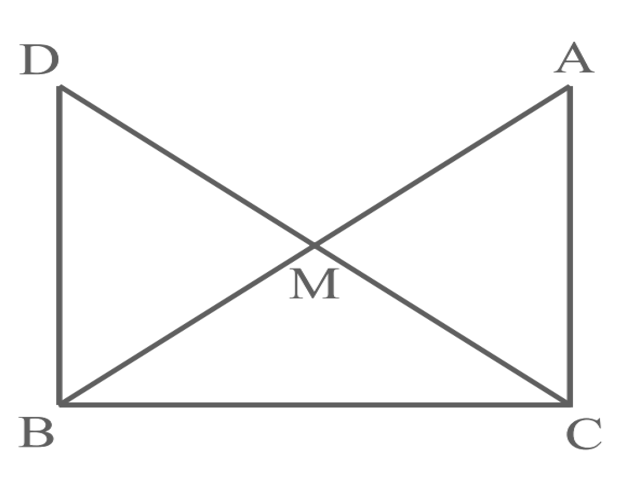
\includegraphics[width=\columnwidth]{figs/Screenshot.png}
  \caption{$\triangle \vec{ACB} ,\triangle \vec{DCB}$ with Mid-Point $\vec{M}$}
  \label{fig:triangles}
\end{figure}
\begin{enumerate}[label =(\roman*)]
        \item $\triangle \vec{AMC} \cong \triangle \vec{BMD}$
        \item $\angle \vec{DBC}$ is a right angle. 
        \item $\triangle \vec{DBC} \cong  \triangle \vec{ACB}$ 
        \item $\vec{CM} = \frac{1}{2} \vec{AB}$
\end{enumerate}
\pagebreak
\solution\\
\textbf{CONSTRUCTION STEPS :}
\begin{enumerate}
\item Let us Assume , the input parameters as ;
\begin{table}[H]
\centering
        \input{tables/input_params.tex}
          \caption{Input Parameters}
          \label{Table-1:Input_params}
\end{table}
\item the output can be calculated as ;
\begin{table}[H]
\centering
        \input{tables/output_params.tex}
          \caption{Output Parameters}
          \label{Table-2:Output_params}
\end{table}
                $\therefore$ By, Plotting these points we get the required Image \figref{fig:fig-2}
\begin{figure}[H]
        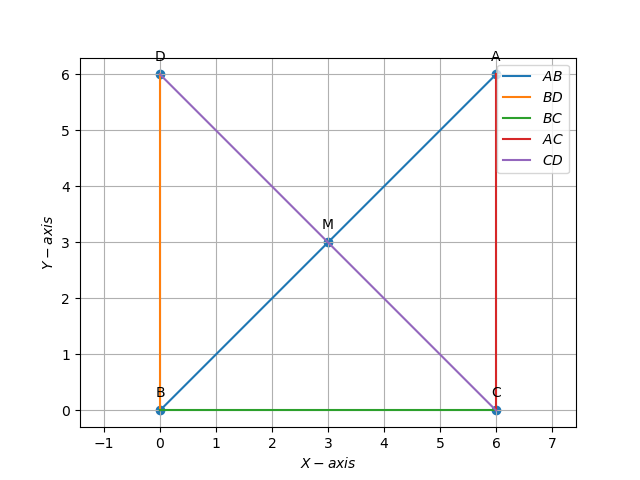
\includegraphics[width = \columnwidth]{figs/python_plot.png}
    \caption{PYTHON Plot of $\triangle \vec{ACB} ,\triangle \vec{DBC}$ with Mid-Point $\vec{M}$}
    \label{fig:fig-2}
\end{figure}
\end{enumerate}

\item Find the position vector of a point $\vec{R}$ which divides the line joining two points $\vec{P}$ and $\vec{Q}$ whose position vectors are $2\vec{a}+\vec{b}$ and $\vec{a}-3\vec{b}$ externally in the ratio $1:2$.

\textbf{Solution:}
Let us assume $\vec{a}$ and $\vec{b}$, and the given ratio is
\begin{table}[h]
    \centering
    \begin{tabular}{|c|c|c|}
        \hline 
        \textbf{Symbol} & \textbf{Value} & \textbf{Description} \\
        \hline
        $\vec{a}$ & $\myvec{1 \\ -3}$ & Vector $\vec{a}$ \\
        \hline
        $\vec{b}$ & $\myvec{0 \\ 2}$ & Vector $\vec{b}$\\
        \hline
        $k$ & $2$ & Ratio \\
        \hline
    \end{tabular}
    \caption{Vectors $\vec{a}$ and $\vec{b}$, ratio $k$}
    \label{tab:table1}
\end{table}

Using the section formula,
\begin{align}
    \vec{R} = \frac{\vec{Q} - k\vec{P}}{1 - k}
\end{align}
where $\vec{P}$ and $\vec{Q}$ depend on $\vec{a}$ and $\vec{b}$, then
\begin{align}
    \vec{P} &= (2\vec{a} + \vec{b}) = 2\myvec{1\\-3} + \myvec{0\\2} = \myvec{2\\-4} \\
    \vec{Q} &= (\vec{a} - 3\vec{b}) = \myvec{1\\-3} - 3\myvec{0\\2} = \myvec{1\\-9}
\end{align}
where $\vec{R}$ can be calculated as 
\begin{align}
    \vec{R} = \frac{(\vec{a} - 3\vec{b}) - k(2\vec{a} + \vec{b})}{1 - k}
\end{align}
By substituting $\vec{a}$ and $\vec{b}$ values, we get $\vec{R}$ as
\begin{align}
    \vec{R} = \myvec{3\\1}
\end{align}

\begin{table}[ht!]
    \centering
    \begin{tabular}{|c|c|c|}
        \hline
        \textbf{Symbol} & \textbf{Value} & \textbf{Description}\\
        \hline
        $\vec{P}$ & $(2\vec{a} + \vec{b})$ & Position vector $\vec{P}$ \\
        \hline
        $\vec{Q}$ & $(\vec{a} - 3\vec{b})$ & Position vector $\vec{Q}$\\
        \hline
        $\vec{R}$ & $\frac{\vec{Q} - k\vec{P}}{1 - k}$ & Position vector $\vec{R}$\\
        \hline
    \end{tabular}
    \caption{Vectors $\vec{P}$, $\vec{Q}$, $\vec{R}$}
    \label{tab:mytable2}   
\end{table}

\begin{figure}[H]
    \centering
    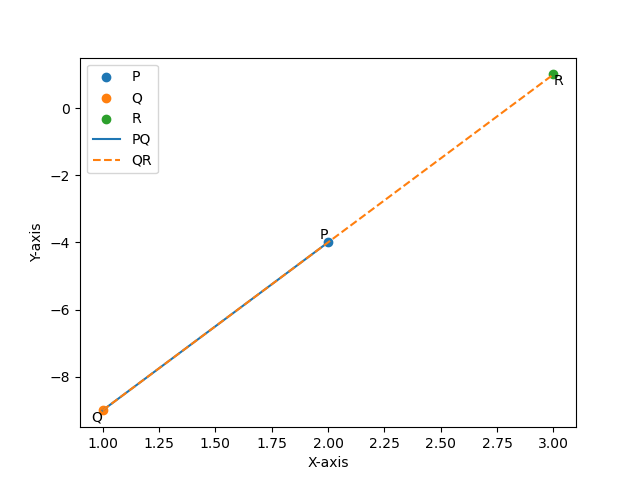
\includegraphics[width=\columnwidth]{figs/external-bisector.png}
    \caption{Point vectors $\vec{P}$, $\vec{Q}$, $\vec{R}$}
    \label{fig:enter-label}
\end{figure}


\end{enumerate}

\item Find the position vector of the mid point of the vector joining the points $\vec{P}$(2, 3, 4)
and $\vec{Q}$(4, 1, –2).
\\
\solution
		\begin{enumerate}[label=\thesection.\arabic*,ref=\thesection.\theenumi]
\numberwithin{equation}{enumi}
\numberwithin{figure}{enumi}
\numberwithin{table}{enumi}

\item Find the coordinates of the point which divides the join of $(-1,7) \text{ and } (4,-3)$ in the ratio 2:3.
	\\
		\solution
	\input{chapters/10/7/2/1/section.tex}
\item Find the coordinates of the points of trisection of the line segment joining $(4,-1) \text{ and } (-2,3)$.
	\\
		\solution
	\input{chapters/10/7/2/2/section.tex}
\item
	\iffalse
\item To conduct Sports Day activities, in your rectangular shaped school                   
ground ABCD, lines have 
drawn with chalk powder at a                 
distance of 1m each. 100 flower pots have been placed at a distance of 1m 
from each other along AD, as shown 
in Fig. 7.12. Niharika runs $ \frac {1}{4} $th the 
distance AD on the 2nd line and 
posts a green flag. Preet runs $ \frac {1}{5} $th 
the distance AD on the eighth line 
and posts a red flag. What is the 
distance between both the flags? If 
Rashmi has to post a blue flag exactly 
halfway between the line segment 
joining the two flags, where should 
she post her flag?
\begin{figure}[h!]
  \centering
  \includegraphics[width=\columnwidth]{sc.png}
  \caption{}
\label{fig:10/7/12Fig1}
\end{figure}               
\fi
      
\item Find the ratio in which the line segment joining the points $(-3,10) \text{ and } (6,-8)$ $\text{ is divided by } (-1,6)$.
	\\
		\solution
	\input{chapters/10/7/2/4/section.tex}
\item Find the ratio in which the line segment joining $A(1,-5) \text{ and } B(-4,5)$ $\text{is divided by the x-axis}$. Also find the coordinates of the point of division.
\item If $(1,2), (4,y), (x,6), (3,5)$ are the vertices of a parallelogram taken in order, find x and y.
	\\
		\solution
	\input{chapters/10/7/2/6/para1.tex}
\item Find the coordinates of a point A, where AB is the diameter of a circle whose centre is $(2,-3) \text{ and }$ B is $(1,4)$.
	\\
		\solution
	\input{chapters/10/7/2/7/section.tex}
\item If A \text{ and } B are $(-2,-2) \text{ and } (2,-4)$, respectively, find the coordinates of P such that AP= $\frac {3}{7}$AB $\text{ and }$ P lies on the line segment AB.
	\\
		\solution
	\input{chapters/10/7/2/8/section.tex}
\item Find the coordinates of the points which divide the line segment joining $A(-2,2) \text{ and } B(2,8)$ into four equal parts.
	\\
		\solution
	\input{chapters/10/7/2/9/section.tex}
\item Find the area of a rhombus if its vertices are $(3,0), (4,5), (-1,4) \text{ and } (-2,-1)$ taken in order. [$\vec{Hint}$ : Area of rhombus =$\frac {1}{2}$(product of its diagonals)]
	\\
		\solution
	\input{chapters/10/7/2/10/cross.tex}
\item Find the position vector of a point R which divides the line joining two points $\vec{P}$
and $\vec{Q}$ whose position vectors are $\hat{i}+2\hat{j}-\hat{k}$ and $-\hat{i}+\hat{j}+\hat{k}$ respectively, in the
ratio 2 : 1
\begin{enumerate}
    \item  internally
    \item  externally
\end{enumerate}
\solution
		\input{chapters/12/10/2/15/section.tex}
\item Find the position vector of the mid point of the vector joining the points $\vec{P}$(2, 3, 4)
and $\vec{Q}$(4, 1, –2).
\\
\solution
		\input{chapters/12/10/2/16/section.tex}
\item Determine the ratio in which the line $2x+y  - 4=0$ divides the line segment joining the points $\vec{A}(2, - 2)$  and  $\vec{B}(3, 7)$.
\\
\solution
	\input{chapters/10/7/4/1/section.tex}
\item Let $\vec{A}(4, 2), \vec{B}(6, 5)$  and $ \vec{C}(1, 4)$ be the vertices of $\triangle ABC$.
\begin{enumerate}
\item The median from $\vec{A}$ meets $BC$ at $\vec{D}$. Find the coordinates of the point $\vec{D}$.
\item Find the coordinates of the point $\vec{P}$ on $AD$ such that $AP : PD = 2 : 1$.
\item Find the coordinates of points $\vec{Q}$ and $\vec{R}$ on medians $BE$ and $CF$ respectively such that $BQ : QE = 2 : 1$  and  $CR : RF = 2 : 1$.
\item What do you observe?
\item If $\vec{A}, \vec{B}$ and $\vec{C}$  are the vertices of $\triangle ABC$, find the coordinates of the centroid of the triangle.
\end{enumerate}
\solution
	\input{chapters/10/7/4/7/section.tex}
\item Find the slope of a line, which passes through the origin and the mid point of the line segment joining the points $\vec{P}$(0,-4) and $\vec{B}$(8,0).
\label{chapters/11/10/1/5}
\input{chapters/11/10/1/5/matrix.tex}
\item Find the position vector of a point R which divides the line joining two points P and Q whose position vectors are $(2\vec{a}+\vec{b})$ and $(\vec{a}-3\vec{b})$
externally in the ratio 1 : 2. Also, show that P is the mid point of the line segment RQ.\\
	\solution
%		\input{chapters/12/10/5/9/section.tex}
\item In right triangle $\vec{ABC}$, right angled at $\vec{C}, \vec{M}$ is the mid-point of hypotenuse $\vec{AB}$. $\vec{C}$ is joined to $\vec{M}$ and produced to a point $\vec{D}$ such that $\vec{DM}=\vec{CM}$. Point $\vec{D}$ is joined to point $\vec{B}$ see \figref{fig:triangles}. Show that:
\begin{figure}[H]
\centering
  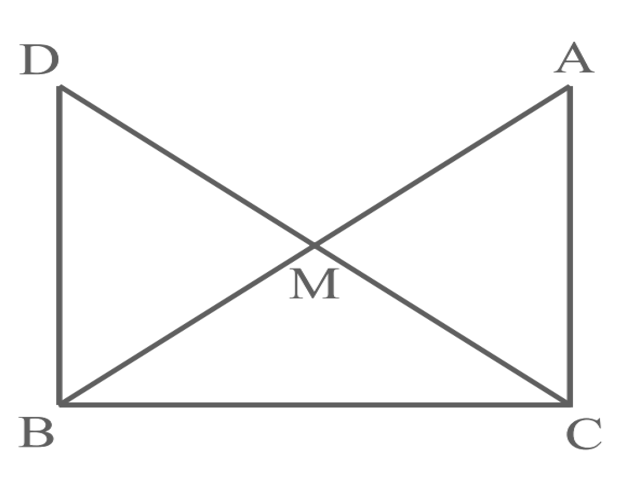
\includegraphics[width=\columnwidth]{figs/Screenshot.png}
  \caption{$\triangle \vec{ACB} ,\triangle \vec{DCB}$ with Mid-Point $\vec{M}$}
  \label{fig:triangles}
\end{figure}
\begin{enumerate}[label =(\roman*)]
        \item $\triangle \vec{AMC} \cong \triangle \vec{BMD}$
        \item $\angle \vec{DBC}$ is a right angle. 
        \item $\triangle \vec{DBC} \cong  \triangle \vec{ACB}$ 
        \item $\vec{CM} = \frac{1}{2} \vec{AB}$
\end{enumerate}
\pagebreak
\solution\\
\textbf{CONSTRUCTION STEPS :}
\begin{enumerate}
\item Let us Assume , the input parameters as ;
\begin{table}[H]
\centering
        \input{tables/input_params.tex}
          \caption{Input Parameters}
          \label{Table-1:Input_params}
\end{table}
\item the output can be calculated as ;
\begin{table}[H]
\centering
        \input{tables/output_params.tex}
          \caption{Output Parameters}
          \label{Table-2:Output_params}
\end{table}
                $\therefore$ By, Plotting these points we get the required Image \figref{fig:fig-2}
\begin{figure}[H]
        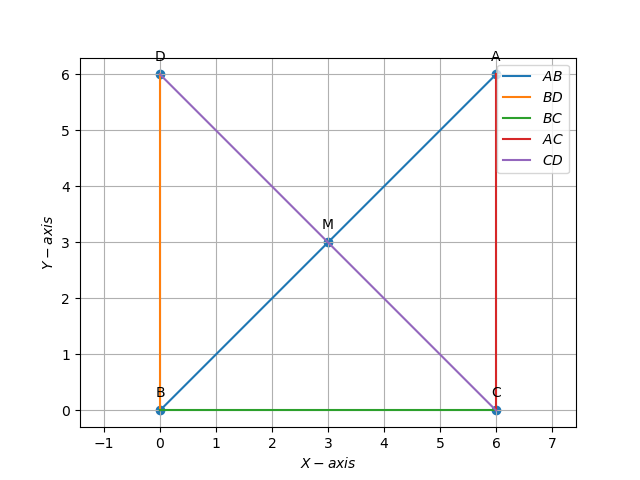
\includegraphics[width = \columnwidth]{figs/python_plot.png}
    \caption{PYTHON Plot of $\triangle \vec{ACB} ,\triangle \vec{DBC}$ with Mid-Point $\vec{M}$}
    \label{fig:fig-2}
\end{figure}
\end{enumerate}

\item Find the position vector of a point $\vec{R}$ which divides the line joining two points $\vec{P}$ and $\vec{Q}$ whose position vectors are $2\vec{a}+\vec{b}$ and $\vec{a}-3\vec{b}$ externally in the ratio $1:2$.

\textbf{Solution:}
Let us assume $\vec{a}$ and $\vec{b}$, and the given ratio is
\begin{table}[h]
    \centering
    \begin{tabular}{|c|c|c|}
        \hline 
        \textbf{Symbol} & \textbf{Value} & \textbf{Description} \\
        \hline
        $\vec{a}$ & $\myvec{1 \\ -3}$ & Vector $\vec{a}$ \\
        \hline
        $\vec{b}$ & $\myvec{0 \\ 2}$ & Vector $\vec{b}$\\
        \hline
        $k$ & $2$ & Ratio \\
        \hline
    \end{tabular}
    \caption{Vectors $\vec{a}$ and $\vec{b}$, ratio $k$}
    \label{tab:table1}
\end{table}

Using the section formula,
\begin{align}
    \vec{R} = \frac{\vec{Q} - k\vec{P}}{1 - k}
\end{align}
where $\vec{P}$ and $\vec{Q}$ depend on $\vec{a}$ and $\vec{b}$, then
\begin{align}
    \vec{P} &= (2\vec{a} + \vec{b}) = 2\myvec{1\\-3} + \myvec{0\\2} = \myvec{2\\-4} \\
    \vec{Q} &= (\vec{a} - 3\vec{b}) = \myvec{1\\-3} - 3\myvec{0\\2} = \myvec{1\\-9}
\end{align}
where $\vec{R}$ can be calculated as 
\begin{align}
    \vec{R} = \frac{(\vec{a} - 3\vec{b}) - k(2\vec{a} + \vec{b})}{1 - k}
\end{align}
By substituting $\vec{a}$ and $\vec{b}$ values, we get $\vec{R}$ as
\begin{align}
    \vec{R} = \myvec{3\\1}
\end{align}

\begin{table}[ht!]
    \centering
    \begin{tabular}{|c|c|c|}
        \hline
        \textbf{Symbol} & \textbf{Value} & \textbf{Description}\\
        \hline
        $\vec{P}$ & $(2\vec{a} + \vec{b})$ & Position vector $\vec{P}$ \\
        \hline
        $\vec{Q}$ & $(\vec{a} - 3\vec{b})$ & Position vector $\vec{Q}$\\
        \hline
        $\vec{R}$ & $\frac{\vec{Q} - k\vec{P}}{1 - k}$ & Position vector $\vec{R}$\\
        \hline
    \end{tabular}
    \caption{Vectors $\vec{P}$, $\vec{Q}$, $\vec{R}$}
    \label{tab:mytable2}   
\end{table}

\begin{figure}[H]
    \centering
    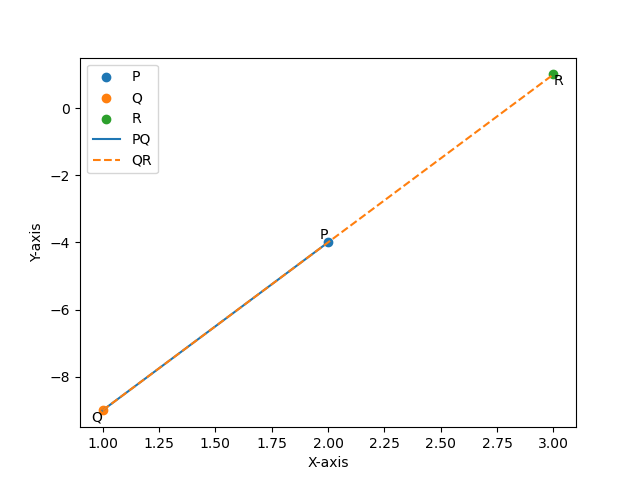
\includegraphics[width=\columnwidth]{figs/external-bisector.png}
    \caption{Point vectors $\vec{P}$, $\vec{Q}$, $\vec{R}$}
    \label{fig:enter-label}
\end{figure}


\end{enumerate}

\item Determine the ratio in which the line $2x+y  - 4=0$ divides the line segment joining the points $\vec{A}(2, - 2)$  and  $\vec{B}(3, 7)$.
\\
\solution
	\begin{enumerate}[label=\thesection.\arabic*,ref=\thesection.\theenumi]
\numberwithin{equation}{enumi}
\numberwithin{figure}{enumi}
\numberwithin{table}{enumi}

\item Find the coordinates of the point which divides the join of $(-1,7) \text{ and } (4,-3)$ in the ratio 2:3.
	\\
		\solution
	\input{chapters/10/7/2/1/section.tex}
\item Find the coordinates of the points of trisection of the line segment joining $(4,-1) \text{ and } (-2,3)$.
	\\
		\solution
	\input{chapters/10/7/2/2/section.tex}
\item
	\iffalse
\item To conduct Sports Day activities, in your rectangular shaped school                   
ground ABCD, lines have 
drawn with chalk powder at a                 
distance of 1m each. 100 flower pots have been placed at a distance of 1m 
from each other along AD, as shown 
in Fig. 7.12. Niharika runs $ \frac {1}{4} $th the 
distance AD on the 2nd line and 
posts a green flag. Preet runs $ \frac {1}{5} $th 
the distance AD on the eighth line 
and posts a red flag. What is the 
distance between both the flags? If 
Rashmi has to post a blue flag exactly 
halfway between the line segment 
joining the two flags, where should 
she post her flag?
\begin{figure}[h!]
  \centering
  \includegraphics[width=\columnwidth]{sc.png}
  \caption{}
\label{fig:10/7/12Fig1}
\end{figure}               
\fi
      
\item Find the ratio in which the line segment joining the points $(-3,10) \text{ and } (6,-8)$ $\text{ is divided by } (-1,6)$.
	\\
		\solution
	\input{chapters/10/7/2/4/section.tex}
\item Find the ratio in which the line segment joining $A(1,-5) \text{ and } B(-4,5)$ $\text{is divided by the x-axis}$. Also find the coordinates of the point of division.
\item If $(1,2), (4,y), (x,6), (3,5)$ are the vertices of a parallelogram taken in order, find x and y.
	\\
		\solution
	\input{chapters/10/7/2/6/para1.tex}
\item Find the coordinates of a point A, where AB is the diameter of a circle whose centre is $(2,-3) \text{ and }$ B is $(1,4)$.
	\\
		\solution
	\input{chapters/10/7/2/7/section.tex}
\item If A \text{ and } B are $(-2,-2) \text{ and } (2,-4)$, respectively, find the coordinates of P such that AP= $\frac {3}{7}$AB $\text{ and }$ P lies on the line segment AB.
	\\
		\solution
	\input{chapters/10/7/2/8/section.tex}
\item Find the coordinates of the points which divide the line segment joining $A(-2,2) \text{ and } B(2,8)$ into four equal parts.
	\\
		\solution
	\input{chapters/10/7/2/9/section.tex}
\item Find the area of a rhombus if its vertices are $(3,0), (4,5), (-1,4) \text{ and } (-2,-1)$ taken in order. [$\vec{Hint}$ : Area of rhombus =$\frac {1}{2}$(product of its diagonals)]
	\\
		\solution
	\input{chapters/10/7/2/10/cross.tex}
\item Find the position vector of a point R which divides the line joining two points $\vec{P}$
and $\vec{Q}$ whose position vectors are $\hat{i}+2\hat{j}-\hat{k}$ and $-\hat{i}+\hat{j}+\hat{k}$ respectively, in the
ratio 2 : 1
\begin{enumerate}
    \item  internally
    \item  externally
\end{enumerate}
\solution
		\input{chapters/12/10/2/15/section.tex}
\item Find the position vector of the mid point of the vector joining the points $\vec{P}$(2, 3, 4)
and $\vec{Q}$(4, 1, –2).
\\
\solution
		\input{chapters/12/10/2/16/section.tex}
\item Determine the ratio in which the line $2x+y  - 4=0$ divides the line segment joining the points $\vec{A}(2, - 2)$  and  $\vec{B}(3, 7)$.
\\
\solution
	\input{chapters/10/7/4/1/section.tex}
\item Let $\vec{A}(4, 2), \vec{B}(6, 5)$  and $ \vec{C}(1, 4)$ be the vertices of $\triangle ABC$.
\begin{enumerate}
\item The median from $\vec{A}$ meets $BC$ at $\vec{D}$. Find the coordinates of the point $\vec{D}$.
\item Find the coordinates of the point $\vec{P}$ on $AD$ such that $AP : PD = 2 : 1$.
\item Find the coordinates of points $\vec{Q}$ and $\vec{R}$ on medians $BE$ and $CF$ respectively such that $BQ : QE = 2 : 1$  and  $CR : RF = 2 : 1$.
\item What do you observe?
\item If $\vec{A}, \vec{B}$ and $\vec{C}$  are the vertices of $\triangle ABC$, find the coordinates of the centroid of the triangle.
\end{enumerate}
\solution
	\input{chapters/10/7/4/7/section.tex}
\item Find the slope of a line, which passes through the origin and the mid point of the line segment joining the points $\vec{P}$(0,-4) and $\vec{B}$(8,0).
\label{chapters/11/10/1/5}
\input{chapters/11/10/1/5/matrix.tex}
\item Find the position vector of a point R which divides the line joining two points P and Q whose position vectors are $(2\vec{a}+\vec{b})$ and $(\vec{a}-3\vec{b})$
externally in the ratio 1 : 2. Also, show that P is the mid point of the line segment RQ.\\
	\solution
%		\input{chapters/12/10/5/9/section.tex}
\item In right triangle $\vec{ABC}$, right angled at $\vec{C}, \vec{M}$ is the mid-point of hypotenuse $\vec{AB}$. $\vec{C}$ is joined to $\vec{M}$ and produced to a point $\vec{D}$ such that $\vec{DM}=\vec{CM}$. Point $\vec{D}$ is joined to point $\vec{B}$ see \figref{fig:triangles}. Show that:
\begin{figure}[H]
\centering
  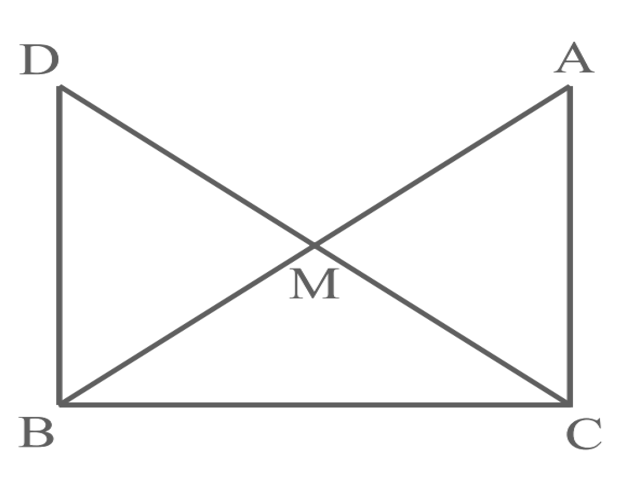
\includegraphics[width=\columnwidth]{figs/Screenshot.png}
  \caption{$\triangle \vec{ACB} ,\triangle \vec{DCB}$ with Mid-Point $\vec{M}$}
  \label{fig:triangles}
\end{figure}
\begin{enumerate}[label =(\roman*)]
        \item $\triangle \vec{AMC} \cong \triangle \vec{BMD}$
        \item $\angle \vec{DBC}$ is a right angle. 
        \item $\triangle \vec{DBC} \cong  \triangle \vec{ACB}$ 
        \item $\vec{CM} = \frac{1}{2} \vec{AB}$
\end{enumerate}
\pagebreak
\solution\\
\textbf{CONSTRUCTION STEPS :}
\begin{enumerate}
\item Let us Assume , the input parameters as ;
\begin{table}[H]
\centering
        \input{tables/input_params.tex}
          \caption{Input Parameters}
          \label{Table-1:Input_params}
\end{table}
\item the output can be calculated as ;
\begin{table}[H]
\centering
        \input{tables/output_params.tex}
          \caption{Output Parameters}
          \label{Table-2:Output_params}
\end{table}
                $\therefore$ By, Plotting these points we get the required Image \figref{fig:fig-2}
\begin{figure}[H]
        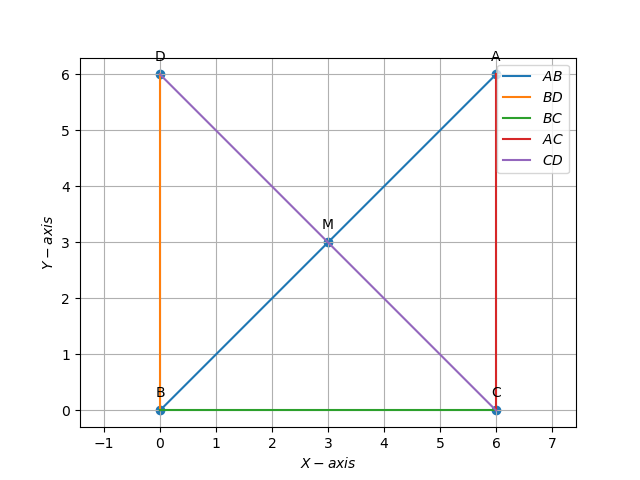
\includegraphics[width = \columnwidth]{figs/python_plot.png}
    \caption{PYTHON Plot of $\triangle \vec{ACB} ,\triangle \vec{DBC}$ with Mid-Point $\vec{M}$}
    \label{fig:fig-2}
\end{figure}
\end{enumerate}

\item Find the position vector of a point $\vec{R}$ which divides the line joining two points $\vec{P}$ and $\vec{Q}$ whose position vectors are $2\vec{a}+\vec{b}$ and $\vec{a}-3\vec{b}$ externally in the ratio $1:2$.

\textbf{Solution:}
Let us assume $\vec{a}$ and $\vec{b}$, and the given ratio is
\begin{table}[h]
    \centering
    \begin{tabular}{|c|c|c|}
        \hline 
        \textbf{Symbol} & \textbf{Value} & \textbf{Description} \\
        \hline
        $\vec{a}$ & $\myvec{1 \\ -3}$ & Vector $\vec{a}$ \\
        \hline
        $\vec{b}$ & $\myvec{0 \\ 2}$ & Vector $\vec{b}$\\
        \hline
        $k$ & $2$ & Ratio \\
        \hline
    \end{tabular}
    \caption{Vectors $\vec{a}$ and $\vec{b}$, ratio $k$}
    \label{tab:table1}
\end{table}

Using the section formula,
\begin{align}
    \vec{R} = \frac{\vec{Q} - k\vec{P}}{1 - k}
\end{align}
where $\vec{P}$ and $\vec{Q}$ depend on $\vec{a}$ and $\vec{b}$, then
\begin{align}
    \vec{P} &= (2\vec{a} + \vec{b}) = 2\myvec{1\\-3} + \myvec{0\\2} = \myvec{2\\-4} \\
    \vec{Q} &= (\vec{a} - 3\vec{b}) = \myvec{1\\-3} - 3\myvec{0\\2} = \myvec{1\\-9}
\end{align}
where $\vec{R}$ can be calculated as 
\begin{align}
    \vec{R} = \frac{(\vec{a} - 3\vec{b}) - k(2\vec{a} + \vec{b})}{1 - k}
\end{align}
By substituting $\vec{a}$ and $\vec{b}$ values, we get $\vec{R}$ as
\begin{align}
    \vec{R} = \myvec{3\\1}
\end{align}

\begin{table}[ht!]
    \centering
    \begin{tabular}{|c|c|c|}
        \hline
        \textbf{Symbol} & \textbf{Value} & \textbf{Description}\\
        \hline
        $\vec{P}$ & $(2\vec{a} + \vec{b})$ & Position vector $\vec{P}$ \\
        \hline
        $\vec{Q}$ & $(\vec{a} - 3\vec{b})$ & Position vector $\vec{Q}$\\
        \hline
        $\vec{R}$ & $\frac{\vec{Q} - k\vec{P}}{1 - k}$ & Position vector $\vec{R}$\\
        \hline
    \end{tabular}
    \caption{Vectors $\vec{P}$, $\vec{Q}$, $\vec{R}$}
    \label{tab:mytable2}   
\end{table}

\begin{figure}[H]
    \centering
    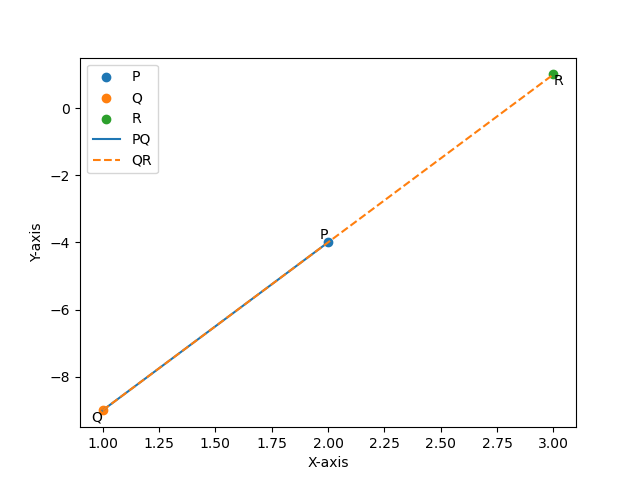
\includegraphics[width=\columnwidth]{figs/external-bisector.png}
    \caption{Point vectors $\vec{P}$, $\vec{Q}$, $\vec{R}$}
    \label{fig:enter-label}
\end{figure}


\end{enumerate}

\item Let $\vec{A}(4, 2), \vec{B}(6, 5)$  and $ \vec{C}(1, 4)$ be the vertices of $\triangle ABC$.
\begin{enumerate}
\item The median from $\vec{A}$ meets $BC$ at $\vec{D}$. Find the coordinates of the point $\vec{D}$.
\item Find the coordinates of the point $\vec{P}$ on $AD$ such that $AP : PD = 2 : 1$.
\item Find the coordinates of points $\vec{Q}$ and $\vec{R}$ on medians $BE$ and $CF$ respectively such that $BQ : QE = 2 : 1$  and  $CR : RF = 2 : 1$.
\item What do you observe?
\item If $\vec{A}, \vec{B}$ and $\vec{C}$  are the vertices of $\triangle ABC$, find the coordinates of the centroid of the triangle.
\end{enumerate}
\solution
	\begin{enumerate}[label=\thesection.\arabic*,ref=\thesection.\theenumi]
\numberwithin{equation}{enumi}
\numberwithin{figure}{enumi}
\numberwithin{table}{enumi}

\item Find the coordinates of the point which divides the join of $(-1,7) \text{ and } (4,-3)$ in the ratio 2:3.
	\\
		\solution
	\input{chapters/10/7/2/1/section.tex}
\item Find the coordinates of the points of trisection of the line segment joining $(4,-1) \text{ and } (-2,3)$.
	\\
		\solution
	\input{chapters/10/7/2/2/section.tex}
\item
	\iffalse
\item To conduct Sports Day activities, in your rectangular shaped school                   
ground ABCD, lines have 
drawn with chalk powder at a                 
distance of 1m each. 100 flower pots have been placed at a distance of 1m 
from each other along AD, as shown 
in Fig. 7.12. Niharika runs $ \frac {1}{4} $th the 
distance AD on the 2nd line and 
posts a green flag. Preet runs $ \frac {1}{5} $th 
the distance AD on the eighth line 
and posts a red flag. What is the 
distance between both the flags? If 
Rashmi has to post a blue flag exactly 
halfway between the line segment 
joining the two flags, where should 
she post her flag?
\begin{figure}[h!]
  \centering
  \includegraphics[width=\columnwidth]{sc.png}
  \caption{}
\label{fig:10/7/12Fig1}
\end{figure}               
\fi
      
\item Find the ratio in which the line segment joining the points $(-3,10) \text{ and } (6,-8)$ $\text{ is divided by } (-1,6)$.
	\\
		\solution
	\input{chapters/10/7/2/4/section.tex}
\item Find the ratio in which the line segment joining $A(1,-5) \text{ and } B(-4,5)$ $\text{is divided by the x-axis}$. Also find the coordinates of the point of division.
\item If $(1,2), (4,y), (x,6), (3,5)$ are the vertices of a parallelogram taken in order, find x and y.
	\\
		\solution
	\input{chapters/10/7/2/6/para1.tex}
\item Find the coordinates of a point A, where AB is the diameter of a circle whose centre is $(2,-3) \text{ and }$ B is $(1,4)$.
	\\
		\solution
	\input{chapters/10/7/2/7/section.tex}
\item If A \text{ and } B are $(-2,-2) \text{ and } (2,-4)$, respectively, find the coordinates of P such that AP= $\frac {3}{7}$AB $\text{ and }$ P lies on the line segment AB.
	\\
		\solution
	\input{chapters/10/7/2/8/section.tex}
\item Find the coordinates of the points which divide the line segment joining $A(-2,2) \text{ and } B(2,8)$ into four equal parts.
	\\
		\solution
	\input{chapters/10/7/2/9/section.tex}
\item Find the area of a rhombus if its vertices are $(3,0), (4,5), (-1,4) \text{ and } (-2,-1)$ taken in order. [$\vec{Hint}$ : Area of rhombus =$\frac {1}{2}$(product of its diagonals)]
	\\
		\solution
	\input{chapters/10/7/2/10/cross.tex}
\item Find the position vector of a point R which divides the line joining two points $\vec{P}$
and $\vec{Q}$ whose position vectors are $\hat{i}+2\hat{j}-\hat{k}$ and $-\hat{i}+\hat{j}+\hat{k}$ respectively, in the
ratio 2 : 1
\begin{enumerate}
    \item  internally
    \item  externally
\end{enumerate}
\solution
		\input{chapters/12/10/2/15/section.tex}
\item Find the position vector of the mid point of the vector joining the points $\vec{P}$(2, 3, 4)
and $\vec{Q}$(4, 1, –2).
\\
\solution
		\input{chapters/12/10/2/16/section.tex}
\item Determine the ratio in which the line $2x+y  - 4=0$ divides the line segment joining the points $\vec{A}(2, - 2)$  and  $\vec{B}(3, 7)$.
\\
\solution
	\input{chapters/10/7/4/1/section.tex}
\item Let $\vec{A}(4, 2), \vec{B}(6, 5)$  and $ \vec{C}(1, 4)$ be the vertices of $\triangle ABC$.
\begin{enumerate}
\item The median from $\vec{A}$ meets $BC$ at $\vec{D}$. Find the coordinates of the point $\vec{D}$.
\item Find the coordinates of the point $\vec{P}$ on $AD$ such that $AP : PD = 2 : 1$.
\item Find the coordinates of points $\vec{Q}$ and $\vec{R}$ on medians $BE$ and $CF$ respectively such that $BQ : QE = 2 : 1$  and  $CR : RF = 2 : 1$.
\item What do you observe?
\item If $\vec{A}, \vec{B}$ and $\vec{C}$  are the vertices of $\triangle ABC$, find the coordinates of the centroid of the triangle.
\end{enumerate}
\solution
	\input{chapters/10/7/4/7/section.tex}
\item Find the slope of a line, which passes through the origin and the mid point of the line segment joining the points $\vec{P}$(0,-4) and $\vec{B}$(8,0).
\label{chapters/11/10/1/5}
\input{chapters/11/10/1/5/matrix.tex}
\item Find the position vector of a point R which divides the line joining two points P and Q whose position vectors are $(2\vec{a}+\vec{b})$ and $(\vec{a}-3\vec{b})$
externally in the ratio 1 : 2. Also, show that P is the mid point of the line segment RQ.\\
	\solution
%		\input{chapters/12/10/5/9/section.tex}
\item In right triangle $\vec{ABC}$, right angled at $\vec{C}, \vec{M}$ is the mid-point of hypotenuse $\vec{AB}$. $\vec{C}$ is joined to $\vec{M}$ and produced to a point $\vec{D}$ such that $\vec{DM}=\vec{CM}$. Point $\vec{D}$ is joined to point $\vec{B}$ see \figref{fig:triangles}. Show that:
\begin{figure}[H]
\centering
  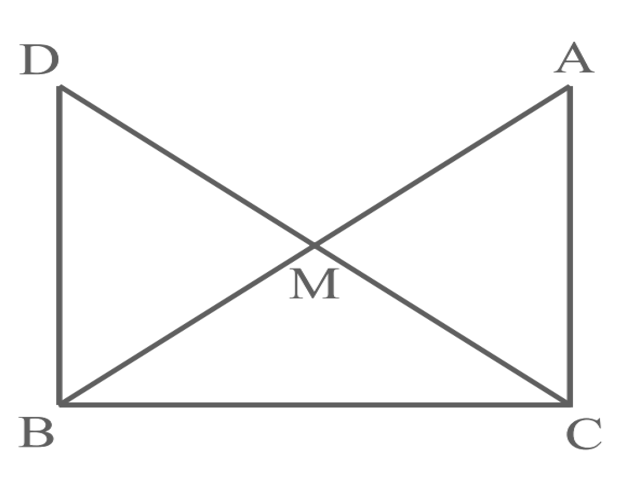
\includegraphics[width=\columnwidth]{figs/Screenshot.png}
  \caption{$\triangle \vec{ACB} ,\triangle \vec{DCB}$ with Mid-Point $\vec{M}$}
  \label{fig:triangles}
\end{figure}
\begin{enumerate}[label =(\roman*)]
        \item $\triangle \vec{AMC} \cong \triangle \vec{BMD}$
        \item $\angle \vec{DBC}$ is a right angle. 
        \item $\triangle \vec{DBC} \cong  \triangle \vec{ACB}$ 
        \item $\vec{CM} = \frac{1}{2} \vec{AB}$
\end{enumerate}
\pagebreak
\solution\\
\textbf{CONSTRUCTION STEPS :}
\begin{enumerate}
\item Let us Assume , the input parameters as ;
\begin{table}[H]
\centering
        \input{tables/input_params.tex}
          \caption{Input Parameters}
          \label{Table-1:Input_params}
\end{table}
\item the output can be calculated as ;
\begin{table}[H]
\centering
        \input{tables/output_params.tex}
          \caption{Output Parameters}
          \label{Table-2:Output_params}
\end{table}
                $\therefore$ By, Plotting these points we get the required Image \figref{fig:fig-2}
\begin{figure}[H]
        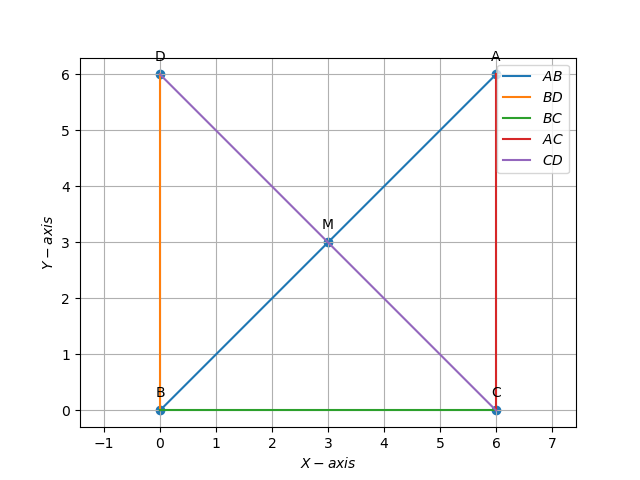
\includegraphics[width = \columnwidth]{figs/python_plot.png}
    \caption{PYTHON Plot of $\triangle \vec{ACB} ,\triangle \vec{DBC}$ with Mid-Point $\vec{M}$}
    \label{fig:fig-2}
\end{figure}
\end{enumerate}

\item Find the position vector of a point $\vec{R}$ which divides the line joining two points $\vec{P}$ and $\vec{Q}$ whose position vectors are $2\vec{a}+\vec{b}$ and $\vec{a}-3\vec{b}$ externally in the ratio $1:2$.

\textbf{Solution:}
Let us assume $\vec{a}$ and $\vec{b}$, and the given ratio is
\begin{table}[h]
    \centering
    \begin{tabular}{|c|c|c|}
        \hline 
        \textbf{Symbol} & \textbf{Value} & \textbf{Description} \\
        \hline
        $\vec{a}$ & $\myvec{1 \\ -3}$ & Vector $\vec{a}$ \\
        \hline
        $\vec{b}$ & $\myvec{0 \\ 2}$ & Vector $\vec{b}$\\
        \hline
        $k$ & $2$ & Ratio \\
        \hline
    \end{tabular}
    \caption{Vectors $\vec{a}$ and $\vec{b}$, ratio $k$}
    \label{tab:table1}
\end{table}

Using the section formula,
\begin{align}
    \vec{R} = \frac{\vec{Q} - k\vec{P}}{1 - k}
\end{align}
where $\vec{P}$ and $\vec{Q}$ depend on $\vec{a}$ and $\vec{b}$, then
\begin{align}
    \vec{P} &= (2\vec{a} + \vec{b}) = 2\myvec{1\\-3} + \myvec{0\\2} = \myvec{2\\-4} \\
    \vec{Q} &= (\vec{a} - 3\vec{b}) = \myvec{1\\-3} - 3\myvec{0\\2} = \myvec{1\\-9}
\end{align}
where $\vec{R}$ can be calculated as 
\begin{align}
    \vec{R} = \frac{(\vec{a} - 3\vec{b}) - k(2\vec{a} + \vec{b})}{1 - k}
\end{align}
By substituting $\vec{a}$ and $\vec{b}$ values, we get $\vec{R}$ as
\begin{align}
    \vec{R} = \myvec{3\\1}
\end{align}

\begin{table}[ht!]
    \centering
    \begin{tabular}{|c|c|c|}
        \hline
        \textbf{Symbol} & \textbf{Value} & \textbf{Description}\\
        \hline
        $\vec{P}$ & $(2\vec{a} + \vec{b})$ & Position vector $\vec{P}$ \\
        \hline
        $\vec{Q}$ & $(\vec{a} - 3\vec{b})$ & Position vector $\vec{Q}$\\
        \hline
        $\vec{R}$ & $\frac{\vec{Q} - k\vec{P}}{1 - k}$ & Position vector $\vec{R}$\\
        \hline
    \end{tabular}
    \caption{Vectors $\vec{P}$, $\vec{Q}$, $\vec{R}$}
    \label{tab:mytable2}   
\end{table}

\begin{figure}[H]
    \centering
    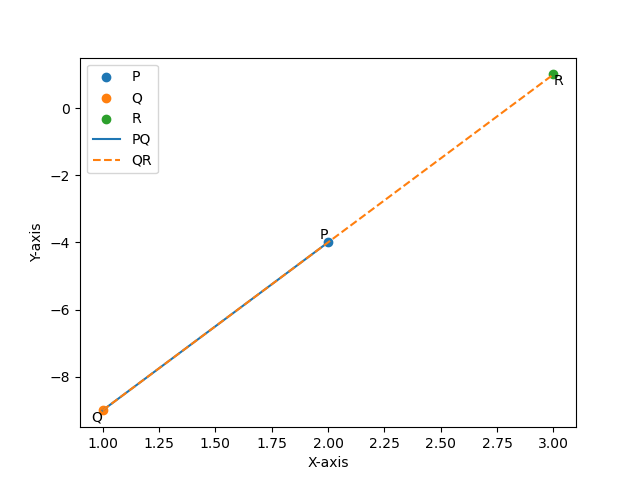
\includegraphics[width=\columnwidth]{figs/external-bisector.png}
    \caption{Point vectors $\vec{P}$, $\vec{Q}$, $\vec{R}$}
    \label{fig:enter-label}
\end{figure}


\end{enumerate}

\item Find the slope of a line, which passes through the origin and the mid point of the line segment joining the points $\vec{P}$(0,-4) and $\vec{B}$(8,0).
\label{chapters/11/10/1/5}
\input{chapters/11/10/1/5/matrix.tex}
\item Find the position vector of a point R which divides the line joining two points P and Q whose position vectors are $(2\vec{a}+\vec{b})$ and $(\vec{a}-3\vec{b})$
externally in the ratio 1 : 2. Also, show that P is the mid point of the line segment RQ.\\
	\solution
%		\begin{enumerate}[label=\thesection.\arabic*,ref=\thesection.\theenumi]
\numberwithin{equation}{enumi}
\numberwithin{figure}{enumi}
\numberwithin{table}{enumi}

\item Find the coordinates of the point which divides the join of $(-1,7) \text{ and } (4,-3)$ in the ratio 2:3.
	\\
		\solution
	\input{chapters/10/7/2/1/section.tex}
\item Find the coordinates of the points of trisection of the line segment joining $(4,-1) \text{ and } (-2,3)$.
	\\
		\solution
	\input{chapters/10/7/2/2/section.tex}
\item
	\iffalse
\item To conduct Sports Day activities, in your rectangular shaped school                   
ground ABCD, lines have 
drawn with chalk powder at a                 
distance of 1m each. 100 flower pots have been placed at a distance of 1m 
from each other along AD, as shown 
in Fig. 7.12. Niharika runs $ \frac {1}{4} $th the 
distance AD on the 2nd line and 
posts a green flag. Preet runs $ \frac {1}{5} $th 
the distance AD on the eighth line 
and posts a red flag. What is the 
distance between both the flags? If 
Rashmi has to post a blue flag exactly 
halfway between the line segment 
joining the two flags, where should 
she post her flag?
\begin{figure}[h!]
  \centering
  \includegraphics[width=\columnwidth]{sc.png}
  \caption{}
\label{fig:10/7/12Fig1}
\end{figure}               
\fi
      
\item Find the ratio in which the line segment joining the points $(-3,10) \text{ and } (6,-8)$ $\text{ is divided by } (-1,6)$.
	\\
		\solution
	\input{chapters/10/7/2/4/section.tex}
\item Find the ratio in which the line segment joining $A(1,-5) \text{ and } B(-4,5)$ $\text{is divided by the x-axis}$. Also find the coordinates of the point of division.
\item If $(1,2), (4,y), (x,6), (3,5)$ are the vertices of a parallelogram taken in order, find x and y.
	\\
		\solution
	\input{chapters/10/7/2/6/para1.tex}
\item Find the coordinates of a point A, where AB is the diameter of a circle whose centre is $(2,-3) \text{ and }$ B is $(1,4)$.
	\\
		\solution
	\input{chapters/10/7/2/7/section.tex}
\item If A \text{ and } B are $(-2,-2) \text{ and } (2,-4)$, respectively, find the coordinates of P such that AP= $\frac {3}{7}$AB $\text{ and }$ P lies on the line segment AB.
	\\
		\solution
	\input{chapters/10/7/2/8/section.tex}
\item Find the coordinates of the points which divide the line segment joining $A(-2,2) \text{ and } B(2,8)$ into four equal parts.
	\\
		\solution
	\input{chapters/10/7/2/9/section.tex}
\item Find the area of a rhombus if its vertices are $(3,0), (4,5), (-1,4) \text{ and } (-2,-1)$ taken in order. [$\vec{Hint}$ : Area of rhombus =$\frac {1}{2}$(product of its diagonals)]
	\\
		\solution
	\input{chapters/10/7/2/10/cross.tex}
\item Find the position vector of a point R which divides the line joining two points $\vec{P}$
and $\vec{Q}$ whose position vectors are $\hat{i}+2\hat{j}-\hat{k}$ and $-\hat{i}+\hat{j}+\hat{k}$ respectively, in the
ratio 2 : 1
\begin{enumerate}
    \item  internally
    \item  externally
\end{enumerate}
\solution
		\input{chapters/12/10/2/15/section.tex}
\item Find the position vector of the mid point of the vector joining the points $\vec{P}$(2, 3, 4)
and $\vec{Q}$(4, 1, –2).
\\
\solution
		\input{chapters/12/10/2/16/section.tex}
\item Determine the ratio in which the line $2x+y  - 4=0$ divides the line segment joining the points $\vec{A}(2, - 2)$  and  $\vec{B}(3, 7)$.
\\
\solution
	\input{chapters/10/7/4/1/section.tex}
\item Let $\vec{A}(4, 2), \vec{B}(6, 5)$  and $ \vec{C}(1, 4)$ be the vertices of $\triangle ABC$.
\begin{enumerate}
\item The median from $\vec{A}$ meets $BC$ at $\vec{D}$. Find the coordinates of the point $\vec{D}$.
\item Find the coordinates of the point $\vec{P}$ on $AD$ such that $AP : PD = 2 : 1$.
\item Find the coordinates of points $\vec{Q}$ and $\vec{R}$ on medians $BE$ and $CF$ respectively such that $BQ : QE = 2 : 1$  and  $CR : RF = 2 : 1$.
\item What do you observe?
\item If $\vec{A}, \vec{B}$ and $\vec{C}$  are the vertices of $\triangle ABC$, find the coordinates of the centroid of the triangle.
\end{enumerate}
\solution
	\input{chapters/10/7/4/7/section.tex}
\item Find the slope of a line, which passes through the origin and the mid point of the line segment joining the points $\vec{P}$(0,-4) and $\vec{B}$(8,0).
\label{chapters/11/10/1/5}
\input{chapters/11/10/1/5/matrix.tex}
\item Find the position vector of a point R which divides the line joining two points P and Q whose position vectors are $(2\vec{a}+\vec{b})$ and $(\vec{a}-3\vec{b})$
externally in the ratio 1 : 2. Also, show that P is the mid point of the line segment RQ.\\
	\solution
%		\input{chapters/12/10/5/9/section.tex}
\item In right triangle $\vec{ABC}$, right angled at $\vec{C}, \vec{M}$ is the mid-point of hypotenuse $\vec{AB}$. $\vec{C}$ is joined to $\vec{M}$ and produced to a point $\vec{D}$ such that $\vec{DM}=\vec{CM}$. Point $\vec{D}$ is joined to point $\vec{B}$ see \figref{fig:triangles}. Show that:
\begin{figure}[H]
\centering
  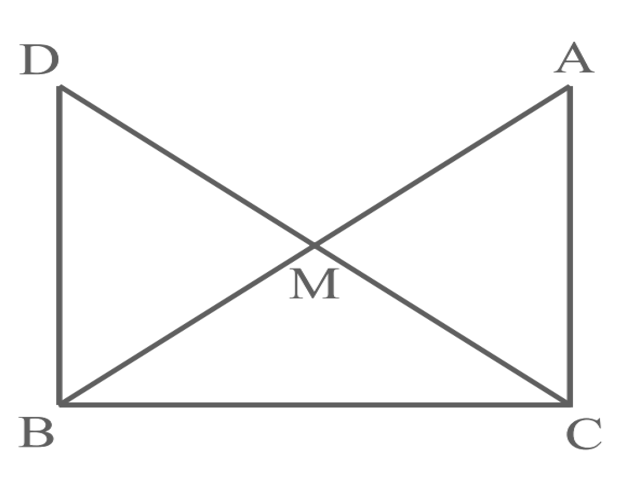
\includegraphics[width=\columnwidth]{figs/Screenshot.png}
  \caption{$\triangle \vec{ACB} ,\triangle \vec{DCB}$ with Mid-Point $\vec{M}$}
  \label{fig:triangles}
\end{figure}
\begin{enumerate}[label =(\roman*)]
        \item $\triangle \vec{AMC} \cong \triangle \vec{BMD}$
        \item $\angle \vec{DBC}$ is a right angle. 
        \item $\triangle \vec{DBC} \cong  \triangle \vec{ACB}$ 
        \item $\vec{CM} = \frac{1}{2} \vec{AB}$
\end{enumerate}
\pagebreak
\solution\\
\textbf{CONSTRUCTION STEPS :}
\begin{enumerate}
\item Let us Assume , the input parameters as ;
\begin{table}[H]
\centering
        \input{tables/input_params.tex}
          \caption{Input Parameters}
          \label{Table-1:Input_params}
\end{table}
\item the output can be calculated as ;
\begin{table}[H]
\centering
        \input{tables/output_params.tex}
          \caption{Output Parameters}
          \label{Table-2:Output_params}
\end{table}
                $\therefore$ By, Plotting these points we get the required Image \figref{fig:fig-2}
\begin{figure}[H]
        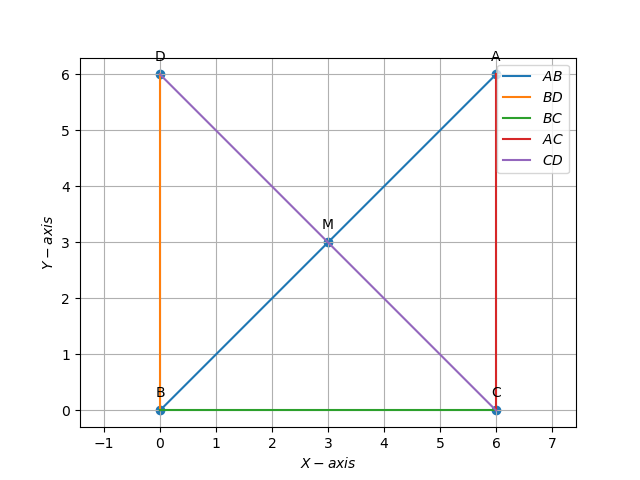
\includegraphics[width = \columnwidth]{figs/python_plot.png}
    \caption{PYTHON Plot of $\triangle \vec{ACB} ,\triangle \vec{DBC}$ with Mid-Point $\vec{M}$}
    \label{fig:fig-2}
\end{figure}
\end{enumerate}

\item Find the position vector of a point $\vec{R}$ which divides the line joining two points $\vec{P}$ and $\vec{Q}$ whose position vectors are $2\vec{a}+\vec{b}$ and $\vec{a}-3\vec{b}$ externally in the ratio $1:2$.

\textbf{Solution:}
Let us assume $\vec{a}$ and $\vec{b}$, and the given ratio is
\begin{table}[h]
    \centering
    \begin{tabular}{|c|c|c|}
        \hline 
        \textbf{Symbol} & \textbf{Value} & \textbf{Description} \\
        \hline
        $\vec{a}$ & $\myvec{1 \\ -3}$ & Vector $\vec{a}$ \\
        \hline
        $\vec{b}$ & $\myvec{0 \\ 2}$ & Vector $\vec{b}$\\
        \hline
        $k$ & $2$ & Ratio \\
        \hline
    \end{tabular}
    \caption{Vectors $\vec{a}$ and $\vec{b}$, ratio $k$}
    \label{tab:table1}
\end{table}

Using the section formula,
\begin{align}
    \vec{R} = \frac{\vec{Q} - k\vec{P}}{1 - k}
\end{align}
where $\vec{P}$ and $\vec{Q}$ depend on $\vec{a}$ and $\vec{b}$, then
\begin{align}
    \vec{P} &= (2\vec{a} + \vec{b}) = 2\myvec{1\\-3} + \myvec{0\\2} = \myvec{2\\-4} \\
    \vec{Q} &= (\vec{a} - 3\vec{b}) = \myvec{1\\-3} - 3\myvec{0\\2} = \myvec{1\\-9}
\end{align}
where $\vec{R}$ can be calculated as 
\begin{align}
    \vec{R} = \frac{(\vec{a} - 3\vec{b}) - k(2\vec{a} + \vec{b})}{1 - k}
\end{align}
By substituting $\vec{a}$ and $\vec{b}$ values, we get $\vec{R}$ as
\begin{align}
    \vec{R} = \myvec{3\\1}
\end{align}

\begin{table}[ht!]
    \centering
    \begin{tabular}{|c|c|c|}
        \hline
        \textbf{Symbol} & \textbf{Value} & \textbf{Description}\\
        \hline
        $\vec{P}$ & $(2\vec{a} + \vec{b})$ & Position vector $\vec{P}$ \\
        \hline
        $\vec{Q}$ & $(\vec{a} - 3\vec{b})$ & Position vector $\vec{Q}$\\
        \hline
        $\vec{R}$ & $\frac{\vec{Q} - k\vec{P}}{1 - k}$ & Position vector $\vec{R}$\\
        \hline
    \end{tabular}
    \caption{Vectors $\vec{P}$, $\vec{Q}$, $\vec{R}$}
    \label{tab:mytable2}   
\end{table}

\begin{figure}[H]
    \centering
    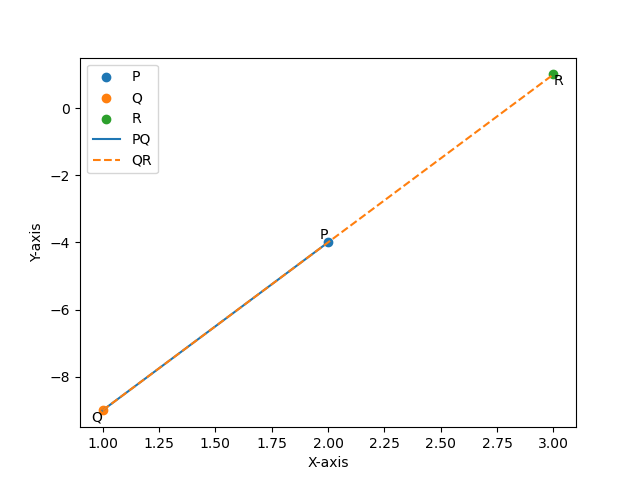
\includegraphics[width=\columnwidth]{figs/external-bisector.png}
    \caption{Point vectors $\vec{P}$, $\vec{Q}$, $\vec{R}$}
    \label{fig:enter-label}
\end{figure}


\end{enumerate}

\item In right triangle $\vec{ABC}$, right angled at $\vec{C}, \vec{M}$ is the mid-point of hypotenuse $\vec{AB}$. $\vec{C}$ is joined to $\vec{M}$ and produced to a point $\vec{D}$ such that $\vec{DM}=\vec{CM}$. Point $\vec{D}$ is joined to point $\vec{B}$ see \figref{fig:triangles}. Show that:
\begin{figure}[H]
\centering
  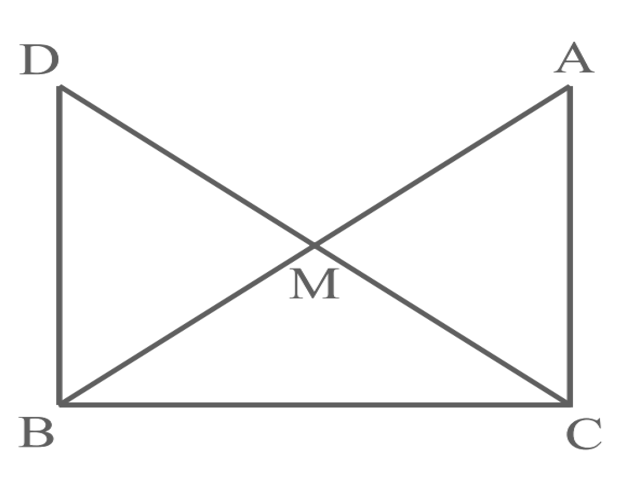
\includegraphics[width=\columnwidth]{figs/Screenshot.png}
  \caption{$\triangle \vec{ACB} ,\triangle \vec{DCB}$ with Mid-Point $\vec{M}$}
  \label{fig:triangles}
\end{figure}
\begin{enumerate}[label =(\roman*)]
        \item $\triangle \vec{AMC} \cong \triangle \vec{BMD}$
        \item $\angle \vec{DBC}$ is a right angle. 
        \item $\triangle \vec{DBC} \cong  \triangle \vec{ACB}$ 
        \item $\vec{CM} = \frac{1}{2} \vec{AB}$
\end{enumerate}
\pagebreak
\solution\\
\textbf{CONSTRUCTION STEPS :}
\begin{enumerate}
\item Let us Assume , the input parameters as ;
\begin{table}[H]
\centering
        \begin{tabular}{|c|c|c|}
\hline
\textbf{Parameter} & \textbf{Value} & \textbf{Description} \\
\hline
	$\vec{B}$ & $\myvec{0\\0}$ & Reference point at Origin \\
\hline
    $l$ & $6$ & Length of a side \\
\hline
\end{tabular}

          \caption{Input Parameters}
          \label{Table-1:Input_params}
\end{table}
\item the output can be calculated as ;
\begin{table}[H]
\centering
        \begin{tabular}{|c|c|p{5cm}|}
\hline
\textbf{Parameter} & \textbf{Value} & \textbf{Description} \\
\hline
	$\vec{C}$ & $\myvec{l\\0}$ & point $\vec{C}$ with length $l$ on the same axis of $\vec{B}$ \\
\hline
	$\vec{D}$ & $\myvec{0  \\ l }$ & $x = 0$ , $y = l$ i.e $x,y$ are co-ordinates of axes in XY-plane \\
\hline
	$\vec{A}$ & $\myvec{l \\ l }$ & $x = l$ , $y = l$ \\
 \hline
    $\vec{M}$ & $\brak{\frac{\vec{A+B}}{2}}$ & Mid-point of $\vec{AB}$ \\
\hline
\end{tabular}

          \caption{Output Parameters}
          \label{Table-2:Output_params}
\end{table}
                $\therefore$ By, Plotting these points we get the required Image \figref{fig:fig-2}
\begin{figure}[H]
        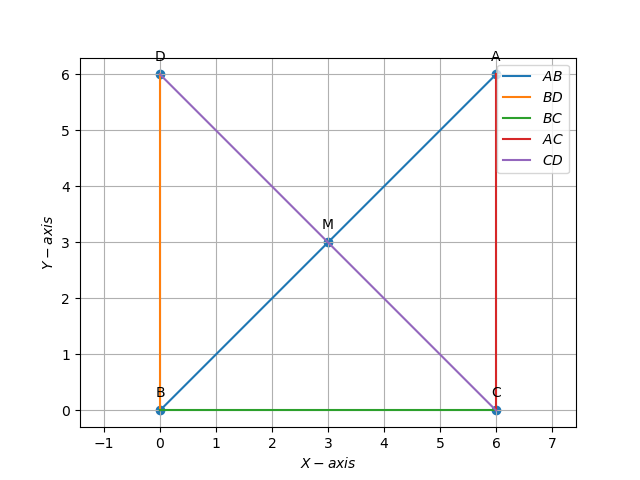
\includegraphics[width = \columnwidth]{figs/python_plot.png}
    \caption{PYTHON Plot of $\triangle \vec{ACB} ,\triangle \vec{DBC}$ with Mid-Point $\vec{M}$}
    \label{fig:fig-2}
\end{figure}
\end{enumerate}

\item Find the position vector of a point $\vec{R}$ which divides the line joining two points $\vec{P}$ and $\vec{Q}$ whose position vectors are $2\vec{a}+\vec{b}$ and $\vec{a}-3\vec{b}$ externally in the ratio $1:2$.

\textbf{Solution:}
Let us assume $\vec{a}$ and $\vec{b}$, and the given ratio is
\begin{table}[h]
    \centering
    \begin{tabular}{|c|c|c|}
        \hline 
        \textbf{Symbol} & \textbf{Value} & \textbf{Description} \\
        \hline
        $\vec{a}$ & $\myvec{1 \\ -3}$ & Vector $\vec{a}$ \\
        \hline
        $\vec{b}$ & $\myvec{0 \\ 2}$ & Vector $\vec{b}$\\
        \hline
        $k$ & $2$ & Ratio \\
        \hline
    \end{tabular}
    \caption{Vectors $\vec{a}$ and $\vec{b}$, ratio $k$}
    \label{tab:table1}
\end{table}

Using the section formula,
\begin{align}
    \vec{R} = \frac{\vec{Q} - k\vec{P}}{1 - k}
\end{align}
where $\vec{P}$ and $\vec{Q}$ depend on $\vec{a}$ and $\vec{b}$, then
\begin{align}
    \vec{P} &= (2\vec{a} + \vec{b}) = 2\myvec{1\\-3} + \myvec{0\\2} = \myvec{2\\-4} \\
    \vec{Q} &= (\vec{a} - 3\vec{b}) = \myvec{1\\-3} - 3\myvec{0\\2} = \myvec{1\\-9}
\end{align}
where $\vec{R}$ can be calculated as 
\begin{align}
    \vec{R} = \frac{(\vec{a} - 3\vec{b}) - k(2\vec{a} + \vec{b})}{1 - k}
\end{align}
By substituting $\vec{a}$ and $\vec{b}$ values, we get $\vec{R}$ as
\begin{align}
    \vec{R} = \myvec{3\\1}
\end{align}

\begin{table}[ht!]
    \centering
    \begin{tabular}{|c|c|c|}
        \hline
        \textbf{Symbol} & \textbf{Value} & \textbf{Description}\\
        \hline
        $\vec{P}$ & $(2\vec{a} + \vec{b})$ & Position vector $\vec{P}$ \\
        \hline
        $\vec{Q}$ & $(\vec{a} - 3\vec{b})$ & Position vector $\vec{Q}$\\
        \hline
        $\vec{R}$ & $\frac{\vec{Q} - k\vec{P}}{1 - k}$ & Position vector $\vec{R}$\\
        \hline
    \end{tabular}
    \caption{Vectors $\vec{P}$, $\vec{Q}$, $\vec{R}$}
    \label{tab:mytable2}   
\end{table}

\begin{figure}[H]
    \centering
    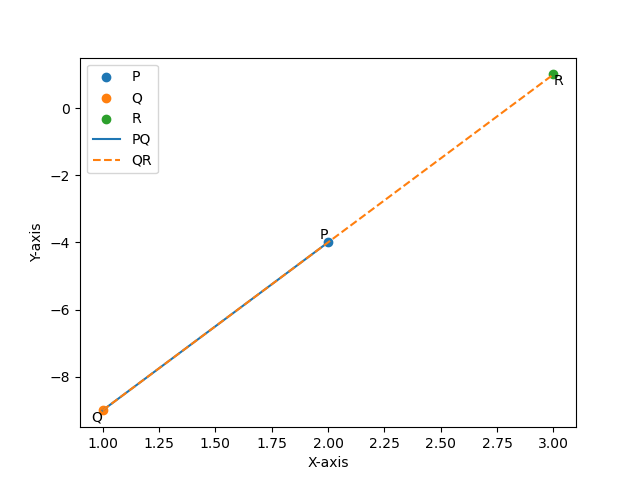
\includegraphics[width=\columnwidth]{figs/external-bisector.png}
    \caption{Point vectors $\vec{P}$, $\vec{Q}$, $\vec{R}$}
    \label{fig:enter-label}
\end{figure}


\end{enumerate}

\item Find the coordinates of the points of trisection of the line segment joining $(4,-1) \text{ and } (-2,3)$.
	\\
		\solution
	\begin{enumerate}[label=\thesection.\arabic*,ref=\thesection.\theenumi]
\numberwithin{equation}{enumi}
\numberwithin{figure}{enumi}
\numberwithin{table}{enumi}

\item Find the coordinates of the point which divides the join of $(-1,7) \text{ and } (4,-3)$ in the ratio 2:3.
	\\
		\solution
	\begin{enumerate}[label=\thesection.\arabic*,ref=\thesection.\theenumi]
\numberwithin{equation}{enumi}
\numberwithin{figure}{enumi}
\numberwithin{table}{enumi}

\item Find the coordinates of the point which divides the join of $(-1,7) \text{ and } (4,-3)$ in the ratio 2:3.
	\\
		\solution
	\input{chapters/10/7/2/1/section.tex}
\item Find the coordinates of the points of trisection of the line segment joining $(4,-1) \text{ and } (-2,3)$.
	\\
		\solution
	\input{chapters/10/7/2/2/section.tex}
\item
	\iffalse
\item To conduct Sports Day activities, in your rectangular shaped school                   
ground ABCD, lines have 
drawn with chalk powder at a                 
distance of 1m each. 100 flower pots have been placed at a distance of 1m 
from each other along AD, as shown 
in Fig. 7.12. Niharika runs $ \frac {1}{4} $th the 
distance AD on the 2nd line and 
posts a green flag. Preet runs $ \frac {1}{5} $th 
the distance AD on the eighth line 
and posts a red flag. What is the 
distance between both the flags? If 
Rashmi has to post a blue flag exactly 
halfway between the line segment 
joining the two flags, where should 
she post her flag?
\begin{figure}[h!]
  \centering
  \includegraphics[width=\columnwidth]{sc.png}
  \caption{}
\label{fig:10/7/12Fig1}
\end{figure}               
\fi
      
\item Find the ratio in which the line segment joining the points $(-3,10) \text{ and } (6,-8)$ $\text{ is divided by } (-1,6)$.
	\\
		\solution
	\input{chapters/10/7/2/4/section.tex}
\item Find the ratio in which the line segment joining $A(1,-5) \text{ and } B(-4,5)$ $\text{is divided by the x-axis}$. Also find the coordinates of the point of division.
\item If $(1,2), (4,y), (x,6), (3,5)$ are the vertices of a parallelogram taken in order, find x and y.
	\\
		\solution
	\input{chapters/10/7/2/6/para1.tex}
\item Find the coordinates of a point A, where AB is the diameter of a circle whose centre is $(2,-3) \text{ and }$ B is $(1,4)$.
	\\
		\solution
	\input{chapters/10/7/2/7/section.tex}
\item If A \text{ and } B are $(-2,-2) \text{ and } (2,-4)$, respectively, find the coordinates of P such that AP= $\frac {3}{7}$AB $\text{ and }$ P lies on the line segment AB.
	\\
		\solution
	\input{chapters/10/7/2/8/section.tex}
\item Find the coordinates of the points which divide the line segment joining $A(-2,2) \text{ and } B(2,8)$ into four equal parts.
	\\
		\solution
	\input{chapters/10/7/2/9/section.tex}
\item Find the area of a rhombus if its vertices are $(3,0), (4,5), (-1,4) \text{ and } (-2,-1)$ taken in order. [$\vec{Hint}$ : Area of rhombus =$\frac {1}{2}$(product of its diagonals)]
	\\
		\solution
	\input{chapters/10/7/2/10/cross.tex}
\item Find the position vector of a point R which divides the line joining two points $\vec{P}$
and $\vec{Q}$ whose position vectors are $\hat{i}+2\hat{j}-\hat{k}$ and $-\hat{i}+\hat{j}+\hat{k}$ respectively, in the
ratio 2 : 1
\begin{enumerate}
    \item  internally
    \item  externally
\end{enumerate}
\solution
		\input{chapters/12/10/2/15/section.tex}
\item Find the position vector of the mid point of the vector joining the points $\vec{P}$(2, 3, 4)
and $\vec{Q}$(4, 1, –2).
\\
\solution
		\input{chapters/12/10/2/16/section.tex}
\item Determine the ratio in which the line $2x+y  - 4=0$ divides the line segment joining the points $\vec{A}(2, - 2)$  and  $\vec{B}(3, 7)$.
\\
\solution
	\input{chapters/10/7/4/1/section.tex}
\item Let $\vec{A}(4, 2), \vec{B}(6, 5)$  and $ \vec{C}(1, 4)$ be the vertices of $\triangle ABC$.
\begin{enumerate}
\item The median from $\vec{A}$ meets $BC$ at $\vec{D}$. Find the coordinates of the point $\vec{D}$.
\item Find the coordinates of the point $\vec{P}$ on $AD$ such that $AP : PD = 2 : 1$.
\item Find the coordinates of points $\vec{Q}$ and $\vec{R}$ on medians $BE$ and $CF$ respectively such that $BQ : QE = 2 : 1$  and  $CR : RF = 2 : 1$.
\item What do you observe?
\item If $\vec{A}, \vec{B}$ and $\vec{C}$  are the vertices of $\triangle ABC$, find the coordinates of the centroid of the triangle.
\end{enumerate}
\solution
	\input{chapters/10/7/4/7/section.tex}
\item Find the slope of a line, which passes through the origin and the mid point of the line segment joining the points $\vec{P}$(0,-4) and $\vec{B}$(8,0).
\label{chapters/11/10/1/5}
\input{chapters/11/10/1/5/matrix.tex}
\item Find the position vector of a point R which divides the line joining two points P and Q whose position vectors are $(2\vec{a}+\vec{b})$ and $(\vec{a}-3\vec{b})$
externally in the ratio 1 : 2. Also, show that P is the mid point of the line segment RQ.\\
	\solution
%		\input{chapters/12/10/5/9/section.tex}
\item In right triangle $\vec{ABC}$, right angled at $\vec{C}, \vec{M}$ is the mid-point of hypotenuse $\vec{AB}$. $\vec{C}$ is joined to $\vec{M}$ and produced to a point $\vec{D}$ such that $\vec{DM}=\vec{CM}$. Point $\vec{D}$ is joined to point $\vec{B}$ see \figref{fig:triangles}. Show that:
\begin{figure}[H]
\centering
  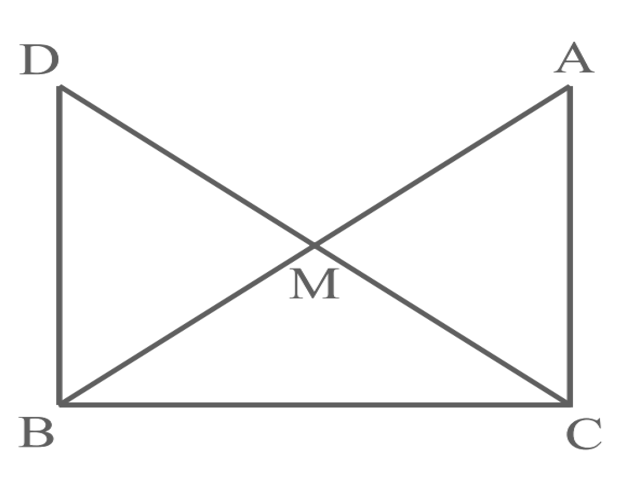
\includegraphics[width=\columnwidth]{figs/Screenshot.png}
  \caption{$\triangle \vec{ACB} ,\triangle \vec{DCB}$ with Mid-Point $\vec{M}$}
  \label{fig:triangles}
\end{figure}
\begin{enumerate}[label =(\roman*)]
        \item $\triangle \vec{AMC} \cong \triangle \vec{BMD}$
        \item $\angle \vec{DBC}$ is a right angle. 
        \item $\triangle \vec{DBC} \cong  \triangle \vec{ACB}$ 
        \item $\vec{CM} = \frac{1}{2} \vec{AB}$
\end{enumerate}
\pagebreak
\solution\\
\textbf{CONSTRUCTION STEPS :}
\begin{enumerate}
\item Let us Assume , the input parameters as ;
\begin{table}[H]
\centering
        \input{tables/input_params.tex}
          \caption{Input Parameters}
          \label{Table-1:Input_params}
\end{table}
\item the output can be calculated as ;
\begin{table}[H]
\centering
        \input{tables/output_params.tex}
          \caption{Output Parameters}
          \label{Table-2:Output_params}
\end{table}
                $\therefore$ By, Plotting these points we get the required Image \figref{fig:fig-2}
\begin{figure}[H]
        \includegraphics[width = \columnwidth]{figs/python_plot.png}
    \caption{PYTHON Plot of $\triangle \vec{ACB} ,\triangle \vec{DBC}$ with Mid-Point $\vec{M}$}
    \label{fig:fig-2}
\end{figure}
\end{enumerate}

\item Find the position vector of a point $\vec{R}$ which divides the line joining two points $\vec{P}$ and $\vec{Q}$ whose position vectors are $2\vec{a}+\vec{b}$ and $\vec{a}-3\vec{b}$ externally in the ratio $1:2$.

\textbf{Solution:}
Let us assume $\vec{a}$ and $\vec{b}$, and the given ratio is
\begin{table}[h]
    \centering
    \begin{tabular}{|c|c|c|}
        \hline 
        \textbf{Symbol} & \textbf{Value} & \textbf{Description} \\
        \hline
        $\vec{a}$ & $\myvec{1 \\ -3}$ & Vector $\vec{a}$ \\
        \hline
        $\vec{b}$ & $\myvec{0 \\ 2}$ & Vector $\vec{b}$\\
        \hline
        $k$ & $2$ & Ratio \\
        \hline
    \end{tabular}
    \caption{Vectors $\vec{a}$ and $\vec{b}$, ratio $k$}
    \label{tab:table1}
\end{table}

Using the section formula,
\begin{align}
    \vec{R} = \frac{\vec{Q} - k\vec{P}}{1 - k}
\end{align}
where $\vec{P}$ and $\vec{Q}$ depend on $\vec{a}$ and $\vec{b}$, then
\begin{align}
    \vec{P} &= (2\vec{a} + \vec{b}) = 2\myvec{1\\-3} + \myvec{0\\2} = \myvec{2\\-4} \\
    \vec{Q} &= (\vec{a} - 3\vec{b}) = \myvec{1\\-3} - 3\myvec{0\\2} = \myvec{1\\-9}
\end{align}
where $\vec{R}$ can be calculated as 
\begin{align}
    \vec{R} = \frac{(\vec{a} - 3\vec{b}) - k(2\vec{a} + \vec{b})}{1 - k}
\end{align}
By substituting $\vec{a}$ and $\vec{b}$ values, we get $\vec{R}$ as
\begin{align}
    \vec{R} = \myvec{3\\1}
\end{align}

\begin{table}[ht!]
    \centering
    \begin{tabular}{|c|c|c|}
        \hline
        \textbf{Symbol} & \textbf{Value} & \textbf{Description}\\
        \hline
        $\vec{P}$ & $(2\vec{a} + \vec{b})$ & Position vector $\vec{P}$ \\
        \hline
        $\vec{Q}$ & $(\vec{a} - 3\vec{b})$ & Position vector $\vec{Q}$\\
        \hline
        $\vec{R}$ & $\frac{\vec{Q} - k\vec{P}}{1 - k}$ & Position vector $\vec{R}$\\
        \hline
    \end{tabular}
    \caption{Vectors $\vec{P}$, $\vec{Q}$, $\vec{R}$}
    \label{tab:mytable2}   
\end{table}

\begin{figure}[H]
    \centering
    \includegraphics[width=\columnwidth]{figs/external-bisector.png}
    \caption{Point vectors $\vec{P}$, $\vec{Q}$, $\vec{R}$}
    \label{fig:enter-label}
\end{figure}


\end{enumerate}

\item Find the coordinates of the points of trisection of the line segment joining $(4,-1) \text{ and } (-2,3)$.
	\\
		\solution
	\begin{enumerate}[label=\thesection.\arabic*,ref=\thesection.\theenumi]
\numberwithin{equation}{enumi}
\numberwithin{figure}{enumi}
\numberwithin{table}{enumi}

\item Find the coordinates of the point which divides the join of $(-1,7) \text{ and } (4,-3)$ in the ratio 2:3.
	\\
		\solution
	\input{chapters/10/7/2/1/section.tex}
\item Find the coordinates of the points of trisection of the line segment joining $(4,-1) \text{ and } (-2,3)$.
	\\
		\solution
	\input{chapters/10/7/2/2/section.tex}
\item
	\iffalse
\item To conduct Sports Day activities, in your rectangular shaped school                   
ground ABCD, lines have 
drawn with chalk powder at a                 
distance of 1m each. 100 flower pots have been placed at a distance of 1m 
from each other along AD, as shown 
in Fig. 7.12. Niharika runs $ \frac {1}{4} $th the 
distance AD on the 2nd line and 
posts a green flag. Preet runs $ \frac {1}{5} $th 
the distance AD on the eighth line 
and posts a red flag. What is the 
distance between both the flags? If 
Rashmi has to post a blue flag exactly 
halfway between the line segment 
joining the two flags, where should 
she post her flag?
\begin{figure}[h!]
  \centering
  \includegraphics[width=\columnwidth]{sc.png}
  \caption{}
\label{fig:10/7/12Fig1}
\end{figure}               
\fi
      
\item Find the ratio in which the line segment joining the points $(-3,10) \text{ and } (6,-8)$ $\text{ is divided by } (-1,6)$.
	\\
		\solution
	\input{chapters/10/7/2/4/section.tex}
\item Find the ratio in which the line segment joining $A(1,-5) \text{ and } B(-4,5)$ $\text{is divided by the x-axis}$. Also find the coordinates of the point of division.
\item If $(1,2), (4,y), (x,6), (3,5)$ are the vertices of a parallelogram taken in order, find x and y.
	\\
		\solution
	\input{chapters/10/7/2/6/para1.tex}
\item Find the coordinates of a point A, where AB is the diameter of a circle whose centre is $(2,-3) \text{ and }$ B is $(1,4)$.
	\\
		\solution
	\input{chapters/10/7/2/7/section.tex}
\item If A \text{ and } B are $(-2,-2) \text{ and } (2,-4)$, respectively, find the coordinates of P such that AP= $\frac {3}{7}$AB $\text{ and }$ P lies on the line segment AB.
	\\
		\solution
	\input{chapters/10/7/2/8/section.tex}
\item Find the coordinates of the points which divide the line segment joining $A(-2,2) \text{ and } B(2,8)$ into four equal parts.
	\\
		\solution
	\input{chapters/10/7/2/9/section.tex}
\item Find the area of a rhombus if its vertices are $(3,0), (4,5), (-1,4) \text{ and } (-2,-1)$ taken in order. [$\vec{Hint}$ : Area of rhombus =$\frac {1}{2}$(product of its diagonals)]
	\\
		\solution
	\input{chapters/10/7/2/10/cross.tex}
\item Find the position vector of a point R which divides the line joining two points $\vec{P}$
and $\vec{Q}$ whose position vectors are $\hat{i}+2\hat{j}-\hat{k}$ and $-\hat{i}+\hat{j}+\hat{k}$ respectively, in the
ratio 2 : 1
\begin{enumerate}
    \item  internally
    \item  externally
\end{enumerate}
\solution
		\input{chapters/12/10/2/15/section.tex}
\item Find the position vector of the mid point of the vector joining the points $\vec{P}$(2, 3, 4)
and $\vec{Q}$(4, 1, –2).
\\
\solution
		\input{chapters/12/10/2/16/section.tex}
\item Determine the ratio in which the line $2x+y  - 4=0$ divides the line segment joining the points $\vec{A}(2, - 2)$  and  $\vec{B}(3, 7)$.
\\
\solution
	\input{chapters/10/7/4/1/section.tex}
\item Let $\vec{A}(4, 2), \vec{B}(6, 5)$  and $ \vec{C}(1, 4)$ be the vertices of $\triangle ABC$.
\begin{enumerate}
\item The median from $\vec{A}$ meets $BC$ at $\vec{D}$. Find the coordinates of the point $\vec{D}$.
\item Find the coordinates of the point $\vec{P}$ on $AD$ such that $AP : PD = 2 : 1$.
\item Find the coordinates of points $\vec{Q}$ and $\vec{R}$ on medians $BE$ and $CF$ respectively such that $BQ : QE = 2 : 1$  and  $CR : RF = 2 : 1$.
\item What do you observe?
\item If $\vec{A}, \vec{B}$ and $\vec{C}$  are the vertices of $\triangle ABC$, find the coordinates of the centroid of the triangle.
\end{enumerate}
\solution
	\input{chapters/10/7/4/7/section.tex}
\item Find the slope of a line, which passes through the origin and the mid point of the line segment joining the points $\vec{P}$(0,-4) and $\vec{B}$(8,0).
\label{chapters/11/10/1/5}
\input{chapters/11/10/1/5/matrix.tex}
\item Find the position vector of a point R which divides the line joining two points P and Q whose position vectors are $(2\vec{a}+\vec{b})$ and $(\vec{a}-3\vec{b})$
externally in the ratio 1 : 2. Also, show that P is the mid point of the line segment RQ.\\
	\solution
%		\input{chapters/12/10/5/9/section.tex}
\item In right triangle $\vec{ABC}$, right angled at $\vec{C}, \vec{M}$ is the mid-point of hypotenuse $\vec{AB}$. $\vec{C}$ is joined to $\vec{M}$ and produced to a point $\vec{D}$ such that $\vec{DM}=\vec{CM}$. Point $\vec{D}$ is joined to point $\vec{B}$ see \figref{fig:triangles}. Show that:
\begin{figure}[H]
\centering
  \includegraphics[width=\columnwidth]{figs/Screenshot.png}
  \caption{$\triangle \vec{ACB} ,\triangle \vec{DCB}$ with Mid-Point $\vec{M}$}
  \label{fig:triangles}
\end{figure}
\begin{enumerate}[label =(\roman*)]
        \item $\triangle \vec{AMC} \cong \triangle \vec{BMD}$
        \item $\angle \vec{DBC}$ is a right angle. 
        \item $\triangle \vec{DBC} \cong  \triangle \vec{ACB}$ 
        \item $\vec{CM} = \frac{1}{2} \vec{AB}$
\end{enumerate}
\pagebreak
\solution\\
\textbf{CONSTRUCTION STEPS :}
\begin{enumerate}
\item Let us Assume , the input parameters as ;
\begin{table}[H]
\centering
        \input{tables/input_params.tex}
          \caption{Input Parameters}
          \label{Table-1:Input_params}
\end{table}
\item the output can be calculated as ;
\begin{table}[H]
\centering
        \input{tables/output_params.tex}
          \caption{Output Parameters}
          \label{Table-2:Output_params}
\end{table}
                $\therefore$ By, Plotting these points we get the required Image \figref{fig:fig-2}
\begin{figure}[H]
        \includegraphics[width = \columnwidth]{figs/python_plot.png}
    \caption{PYTHON Plot of $\triangle \vec{ACB} ,\triangle \vec{DBC}$ with Mid-Point $\vec{M}$}
    \label{fig:fig-2}
\end{figure}
\end{enumerate}

\item Find the position vector of a point $\vec{R}$ which divides the line joining two points $\vec{P}$ and $\vec{Q}$ whose position vectors are $2\vec{a}+\vec{b}$ and $\vec{a}-3\vec{b}$ externally in the ratio $1:2$.

\textbf{Solution:}
Let us assume $\vec{a}$ and $\vec{b}$, and the given ratio is
\begin{table}[h]
    \centering
    \begin{tabular}{|c|c|c|}
        \hline 
        \textbf{Symbol} & \textbf{Value} & \textbf{Description} \\
        \hline
        $\vec{a}$ & $\myvec{1 \\ -3}$ & Vector $\vec{a}$ \\
        \hline
        $\vec{b}$ & $\myvec{0 \\ 2}$ & Vector $\vec{b}$\\
        \hline
        $k$ & $2$ & Ratio \\
        \hline
    \end{tabular}
    \caption{Vectors $\vec{a}$ and $\vec{b}$, ratio $k$}
    \label{tab:table1}
\end{table}

Using the section formula,
\begin{align}
    \vec{R} = \frac{\vec{Q} - k\vec{P}}{1 - k}
\end{align}
where $\vec{P}$ and $\vec{Q}$ depend on $\vec{a}$ and $\vec{b}$, then
\begin{align}
    \vec{P} &= (2\vec{a} + \vec{b}) = 2\myvec{1\\-3} + \myvec{0\\2} = \myvec{2\\-4} \\
    \vec{Q} &= (\vec{a} - 3\vec{b}) = \myvec{1\\-3} - 3\myvec{0\\2} = \myvec{1\\-9}
\end{align}
where $\vec{R}$ can be calculated as 
\begin{align}
    \vec{R} = \frac{(\vec{a} - 3\vec{b}) - k(2\vec{a} + \vec{b})}{1 - k}
\end{align}
By substituting $\vec{a}$ and $\vec{b}$ values, we get $\vec{R}$ as
\begin{align}
    \vec{R} = \myvec{3\\1}
\end{align}

\begin{table}[ht!]
    \centering
    \begin{tabular}{|c|c|c|}
        \hline
        \textbf{Symbol} & \textbf{Value} & \textbf{Description}\\
        \hline
        $\vec{P}$ & $(2\vec{a} + \vec{b})$ & Position vector $\vec{P}$ \\
        \hline
        $\vec{Q}$ & $(\vec{a} - 3\vec{b})$ & Position vector $\vec{Q}$\\
        \hline
        $\vec{R}$ & $\frac{\vec{Q} - k\vec{P}}{1 - k}$ & Position vector $\vec{R}$\\
        \hline
    \end{tabular}
    \caption{Vectors $\vec{P}$, $\vec{Q}$, $\vec{R}$}
    \label{tab:mytable2}   
\end{table}

\begin{figure}[H]
    \centering
    \includegraphics[width=\columnwidth]{figs/external-bisector.png}
    \caption{Point vectors $\vec{P}$, $\vec{Q}$, $\vec{R}$}
    \label{fig:enter-label}
\end{figure}


\end{enumerate}

\item
	\iffalse
\item To conduct Sports Day activities, in your rectangular shaped school                   
ground ABCD, lines have 
drawn with chalk powder at a                 
distance of 1m each. 100 flower pots have been placed at a distance of 1m 
from each other along AD, as shown 
in Fig. 7.12. Niharika runs $ \frac {1}{4} $th the 
distance AD on the 2nd line and 
posts a green flag. Preet runs $ \frac {1}{5} $th 
the distance AD on the eighth line 
and posts a red flag. What is the 
distance between both the flags? If 
Rashmi has to post a blue flag exactly 
halfway between the line segment 
joining the two flags, where should 
she post her flag?
\begin{figure}[h!]
  \centering
  \includegraphics[width=\columnwidth]{sc.png}
  \caption{}
\label{fig:10/7/12Fig1}
\end{figure}               
\fi
      
\item Find the ratio in which the line segment joining the points $(-3,10) \text{ and } (6,-8)$ $\text{ is divided by } (-1,6)$.
	\\
		\solution
	\begin{enumerate}[label=\thesection.\arabic*,ref=\thesection.\theenumi]
\numberwithin{equation}{enumi}
\numberwithin{figure}{enumi}
\numberwithin{table}{enumi}

\item Find the coordinates of the point which divides the join of $(-1,7) \text{ and } (4,-3)$ in the ratio 2:3.
	\\
		\solution
	\input{chapters/10/7/2/1/section.tex}
\item Find the coordinates of the points of trisection of the line segment joining $(4,-1) \text{ and } (-2,3)$.
	\\
		\solution
	\input{chapters/10/7/2/2/section.tex}
\item
	\iffalse
\item To conduct Sports Day activities, in your rectangular shaped school                   
ground ABCD, lines have 
drawn with chalk powder at a                 
distance of 1m each. 100 flower pots have been placed at a distance of 1m 
from each other along AD, as shown 
in Fig. 7.12. Niharika runs $ \frac {1}{4} $th the 
distance AD on the 2nd line and 
posts a green flag. Preet runs $ \frac {1}{5} $th 
the distance AD on the eighth line 
and posts a red flag. What is the 
distance between both the flags? If 
Rashmi has to post a blue flag exactly 
halfway between the line segment 
joining the two flags, where should 
she post her flag?
\begin{figure}[h!]
  \centering
  \includegraphics[width=\columnwidth]{sc.png}
  \caption{}
\label{fig:10/7/12Fig1}
\end{figure}               
\fi
      
\item Find the ratio in which the line segment joining the points $(-3,10) \text{ and } (6,-8)$ $\text{ is divided by } (-1,6)$.
	\\
		\solution
	\input{chapters/10/7/2/4/section.tex}
\item Find the ratio in which the line segment joining $A(1,-5) \text{ and } B(-4,5)$ $\text{is divided by the x-axis}$. Also find the coordinates of the point of division.
\item If $(1,2), (4,y), (x,6), (3,5)$ are the vertices of a parallelogram taken in order, find x and y.
	\\
		\solution
	\input{chapters/10/7/2/6/para1.tex}
\item Find the coordinates of a point A, where AB is the diameter of a circle whose centre is $(2,-3) \text{ and }$ B is $(1,4)$.
	\\
		\solution
	\input{chapters/10/7/2/7/section.tex}
\item If A \text{ and } B are $(-2,-2) \text{ and } (2,-4)$, respectively, find the coordinates of P such that AP= $\frac {3}{7}$AB $\text{ and }$ P lies on the line segment AB.
	\\
		\solution
	\input{chapters/10/7/2/8/section.tex}
\item Find the coordinates of the points which divide the line segment joining $A(-2,2) \text{ and } B(2,8)$ into four equal parts.
	\\
		\solution
	\input{chapters/10/7/2/9/section.tex}
\item Find the area of a rhombus if its vertices are $(3,0), (4,5), (-1,4) \text{ and } (-2,-1)$ taken in order. [$\vec{Hint}$ : Area of rhombus =$\frac {1}{2}$(product of its diagonals)]
	\\
		\solution
	\input{chapters/10/7/2/10/cross.tex}
\item Find the position vector of a point R which divides the line joining two points $\vec{P}$
and $\vec{Q}$ whose position vectors are $\hat{i}+2\hat{j}-\hat{k}$ and $-\hat{i}+\hat{j}+\hat{k}$ respectively, in the
ratio 2 : 1
\begin{enumerate}
    \item  internally
    \item  externally
\end{enumerate}
\solution
		\input{chapters/12/10/2/15/section.tex}
\item Find the position vector of the mid point of the vector joining the points $\vec{P}$(2, 3, 4)
and $\vec{Q}$(4, 1, –2).
\\
\solution
		\input{chapters/12/10/2/16/section.tex}
\item Determine the ratio in which the line $2x+y  - 4=0$ divides the line segment joining the points $\vec{A}(2, - 2)$  and  $\vec{B}(3, 7)$.
\\
\solution
	\input{chapters/10/7/4/1/section.tex}
\item Let $\vec{A}(4, 2), \vec{B}(6, 5)$  and $ \vec{C}(1, 4)$ be the vertices of $\triangle ABC$.
\begin{enumerate}
\item The median from $\vec{A}$ meets $BC$ at $\vec{D}$. Find the coordinates of the point $\vec{D}$.
\item Find the coordinates of the point $\vec{P}$ on $AD$ such that $AP : PD = 2 : 1$.
\item Find the coordinates of points $\vec{Q}$ and $\vec{R}$ on medians $BE$ and $CF$ respectively such that $BQ : QE = 2 : 1$  and  $CR : RF = 2 : 1$.
\item What do you observe?
\item If $\vec{A}, \vec{B}$ and $\vec{C}$  are the vertices of $\triangle ABC$, find the coordinates of the centroid of the triangle.
\end{enumerate}
\solution
	\input{chapters/10/7/4/7/section.tex}
\item Find the slope of a line, which passes through the origin and the mid point of the line segment joining the points $\vec{P}$(0,-4) and $\vec{B}$(8,0).
\label{chapters/11/10/1/5}
\input{chapters/11/10/1/5/matrix.tex}
\item Find the position vector of a point R which divides the line joining two points P and Q whose position vectors are $(2\vec{a}+\vec{b})$ and $(\vec{a}-3\vec{b})$
externally in the ratio 1 : 2. Also, show that P is the mid point of the line segment RQ.\\
	\solution
%		\input{chapters/12/10/5/9/section.tex}
\item In right triangle $\vec{ABC}$, right angled at $\vec{C}, \vec{M}$ is the mid-point of hypotenuse $\vec{AB}$. $\vec{C}$ is joined to $\vec{M}$ and produced to a point $\vec{D}$ such that $\vec{DM}=\vec{CM}$. Point $\vec{D}$ is joined to point $\vec{B}$ see \figref{fig:triangles}. Show that:
\begin{figure}[H]
\centering
  \includegraphics[width=\columnwidth]{figs/Screenshot.png}
  \caption{$\triangle \vec{ACB} ,\triangle \vec{DCB}$ with Mid-Point $\vec{M}$}
  \label{fig:triangles}
\end{figure}
\begin{enumerate}[label =(\roman*)]
        \item $\triangle \vec{AMC} \cong \triangle \vec{BMD}$
        \item $\angle \vec{DBC}$ is a right angle. 
        \item $\triangle \vec{DBC} \cong  \triangle \vec{ACB}$ 
        \item $\vec{CM} = \frac{1}{2} \vec{AB}$
\end{enumerate}
\pagebreak
\solution\\
\textbf{CONSTRUCTION STEPS :}
\begin{enumerate}
\item Let us Assume , the input parameters as ;
\begin{table}[H]
\centering
        \input{tables/input_params.tex}
          \caption{Input Parameters}
          \label{Table-1:Input_params}
\end{table}
\item the output can be calculated as ;
\begin{table}[H]
\centering
        \input{tables/output_params.tex}
          \caption{Output Parameters}
          \label{Table-2:Output_params}
\end{table}
                $\therefore$ By, Plotting these points we get the required Image \figref{fig:fig-2}
\begin{figure}[H]
        \includegraphics[width = \columnwidth]{figs/python_plot.png}
    \caption{PYTHON Plot of $\triangle \vec{ACB} ,\triangle \vec{DBC}$ with Mid-Point $\vec{M}$}
    \label{fig:fig-2}
\end{figure}
\end{enumerate}

\item Find the position vector of a point $\vec{R}$ which divides the line joining two points $\vec{P}$ and $\vec{Q}$ whose position vectors are $2\vec{a}+\vec{b}$ and $\vec{a}-3\vec{b}$ externally in the ratio $1:2$.

\textbf{Solution:}
Let us assume $\vec{a}$ and $\vec{b}$, and the given ratio is
\begin{table}[h]
    \centering
    \begin{tabular}{|c|c|c|}
        \hline 
        \textbf{Symbol} & \textbf{Value} & \textbf{Description} \\
        \hline
        $\vec{a}$ & $\myvec{1 \\ -3}$ & Vector $\vec{a}$ \\
        \hline
        $\vec{b}$ & $\myvec{0 \\ 2}$ & Vector $\vec{b}$\\
        \hline
        $k$ & $2$ & Ratio \\
        \hline
    \end{tabular}
    \caption{Vectors $\vec{a}$ and $\vec{b}$, ratio $k$}
    \label{tab:table1}
\end{table}

Using the section formula,
\begin{align}
    \vec{R} = \frac{\vec{Q} - k\vec{P}}{1 - k}
\end{align}
where $\vec{P}$ and $\vec{Q}$ depend on $\vec{a}$ and $\vec{b}$, then
\begin{align}
    \vec{P} &= (2\vec{a} + \vec{b}) = 2\myvec{1\\-3} + \myvec{0\\2} = \myvec{2\\-4} \\
    \vec{Q} &= (\vec{a} - 3\vec{b}) = \myvec{1\\-3} - 3\myvec{0\\2} = \myvec{1\\-9}
\end{align}
where $\vec{R}$ can be calculated as 
\begin{align}
    \vec{R} = \frac{(\vec{a} - 3\vec{b}) - k(2\vec{a} + \vec{b})}{1 - k}
\end{align}
By substituting $\vec{a}$ and $\vec{b}$ values, we get $\vec{R}$ as
\begin{align}
    \vec{R} = \myvec{3\\1}
\end{align}

\begin{table}[ht!]
    \centering
    \begin{tabular}{|c|c|c|}
        \hline
        \textbf{Symbol} & \textbf{Value} & \textbf{Description}\\
        \hline
        $\vec{P}$ & $(2\vec{a} + \vec{b})$ & Position vector $\vec{P}$ \\
        \hline
        $\vec{Q}$ & $(\vec{a} - 3\vec{b})$ & Position vector $\vec{Q}$\\
        \hline
        $\vec{R}$ & $\frac{\vec{Q} - k\vec{P}}{1 - k}$ & Position vector $\vec{R}$\\
        \hline
    \end{tabular}
    \caption{Vectors $\vec{P}$, $\vec{Q}$, $\vec{R}$}
    \label{tab:mytable2}   
\end{table}

\begin{figure}[H]
    \centering
    \includegraphics[width=\columnwidth]{figs/external-bisector.png}
    \caption{Point vectors $\vec{P}$, $\vec{Q}$, $\vec{R}$}
    \label{fig:enter-label}
\end{figure}


\end{enumerate}

\item Find the ratio in which the line segment joining $A(1,-5) \text{ and } B(-4,5)$ $\text{is divided by the x-axis}$. Also find the coordinates of the point of division.
\item If $(1,2), (4,y), (x,6), (3,5)$ are the vertices of a parallelogram taken in order, find x and y.
	\\
		\solution
	\input{chapters/10/7/2/6/para1.tex}
\item Find the coordinates of a point A, where AB is the diameter of a circle whose centre is $(2,-3) \text{ and }$ B is $(1,4)$.
	\\
		\solution
	\begin{enumerate}[label=\thesection.\arabic*,ref=\thesection.\theenumi]
\numberwithin{equation}{enumi}
\numberwithin{figure}{enumi}
\numberwithin{table}{enumi}

\item Find the coordinates of the point which divides the join of $(-1,7) \text{ and } (4,-3)$ in the ratio 2:3.
	\\
		\solution
	\input{chapters/10/7/2/1/section.tex}
\item Find the coordinates of the points of trisection of the line segment joining $(4,-1) \text{ and } (-2,3)$.
	\\
		\solution
	\input{chapters/10/7/2/2/section.tex}
\item
	\iffalse
\item To conduct Sports Day activities, in your rectangular shaped school                   
ground ABCD, lines have 
drawn with chalk powder at a                 
distance of 1m each. 100 flower pots have been placed at a distance of 1m 
from each other along AD, as shown 
in Fig. 7.12. Niharika runs $ \frac {1}{4} $th the 
distance AD on the 2nd line and 
posts a green flag. Preet runs $ \frac {1}{5} $th 
the distance AD on the eighth line 
and posts a red flag. What is the 
distance between both the flags? If 
Rashmi has to post a blue flag exactly 
halfway between the line segment 
joining the two flags, where should 
she post her flag?
\begin{figure}[h!]
  \centering
  \includegraphics[width=\columnwidth]{sc.png}
  \caption{}
\label{fig:10/7/12Fig1}
\end{figure}               
\fi
      
\item Find the ratio in which the line segment joining the points $(-3,10) \text{ and } (6,-8)$ $\text{ is divided by } (-1,6)$.
	\\
		\solution
	\input{chapters/10/7/2/4/section.tex}
\item Find the ratio in which the line segment joining $A(1,-5) \text{ and } B(-4,5)$ $\text{is divided by the x-axis}$. Also find the coordinates of the point of division.
\item If $(1,2), (4,y), (x,6), (3,5)$ are the vertices of a parallelogram taken in order, find x and y.
	\\
		\solution
	\input{chapters/10/7/2/6/para1.tex}
\item Find the coordinates of a point A, where AB is the diameter of a circle whose centre is $(2,-3) \text{ and }$ B is $(1,4)$.
	\\
		\solution
	\input{chapters/10/7/2/7/section.tex}
\item If A \text{ and } B are $(-2,-2) \text{ and } (2,-4)$, respectively, find the coordinates of P such that AP= $\frac {3}{7}$AB $\text{ and }$ P lies on the line segment AB.
	\\
		\solution
	\input{chapters/10/7/2/8/section.tex}
\item Find the coordinates of the points which divide the line segment joining $A(-2,2) \text{ and } B(2,8)$ into four equal parts.
	\\
		\solution
	\input{chapters/10/7/2/9/section.tex}
\item Find the area of a rhombus if its vertices are $(3,0), (4,5), (-1,4) \text{ and } (-2,-1)$ taken in order. [$\vec{Hint}$ : Area of rhombus =$\frac {1}{2}$(product of its diagonals)]
	\\
		\solution
	\input{chapters/10/7/2/10/cross.tex}
\item Find the position vector of a point R which divides the line joining two points $\vec{P}$
and $\vec{Q}$ whose position vectors are $\hat{i}+2\hat{j}-\hat{k}$ and $-\hat{i}+\hat{j}+\hat{k}$ respectively, in the
ratio 2 : 1
\begin{enumerate}
    \item  internally
    \item  externally
\end{enumerate}
\solution
		\input{chapters/12/10/2/15/section.tex}
\item Find the position vector of the mid point of the vector joining the points $\vec{P}$(2, 3, 4)
and $\vec{Q}$(4, 1, –2).
\\
\solution
		\input{chapters/12/10/2/16/section.tex}
\item Determine the ratio in which the line $2x+y  - 4=0$ divides the line segment joining the points $\vec{A}(2, - 2)$  and  $\vec{B}(3, 7)$.
\\
\solution
	\input{chapters/10/7/4/1/section.tex}
\item Let $\vec{A}(4, 2), \vec{B}(6, 5)$  and $ \vec{C}(1, 4)$ be the vertices of $\triangle ABC$.
\begin{enumerate}
\item The median from $\vec{A}$ meets $BC$ at $\vec{D}$. Find the coordinates of the point $\vec{D}$.
\item Find the coordinates of the point $\vec{P}$ on $AD$ such that $AP : PD = 2 : 1$.
\item Find the coordinates of points $\vec{Q}$ and $\vec{R}$ on medians $BE$ and $CF$ respectively such that $BQ : QE = 2 : 1$  and  $CR : RF = 2 : 1$.
\item What do you observe?
\item If $\vec{A}, \vec{B}$ and $\vec{C}$  are the vertices of $\triangle ABC$, find the coordinates of the centroid of the triangle.
\end{enumerate}
\solution
	\input{chapters/10/7/4/7/section.tex}
\item Find the slope of a line, which passes through the origin and the mid point of the line segment joining the points $\vec{P}$(0,-4) and $\vec{B}$(8,0).
\label{chapters/11/10/1/5}
\input{chapters/11/10/1/5/matrix.tex}
\item Find the position vector of a point R which divides the line joining two points P and Q whose position vectors are $(2\vec{a}+\vec{b})$ and $(\vec{a}-3\vec{b})$
externally in the ratio 1 : 2. Also, show that P is the mid point of the line segment RQ.\\
	\solution
%		\input{chapters/12/10/5/9/section.tex}
\item In right triangle $\vec{ABC}$, right angled at $\vec{C}, \vec{M}$ is the mid-point of hypotenuse $\vec{AB}$. $\vec{C}$ is joined to $\vec{M}$ and produced to a point $\vec{D}$ such that $\vec{DM}=\vec{CM}$. Point $\vec{D}$ is joined to point $\vec{B}$ see \figref{fig:triangles}. Show that:
\begin{figure}[H]
\centering
  \includegraphics[width=\columnwidth]{figs/Screenshot.png}
  \caption{$\triangle \vec{ACB} ,\triangle \vec{DCB}$ with Mid-Point $\vec{M}$}
  \label{fig:triangles}
\end{figure}
\begin{enumerate}[label =(\roman*)]
        \item $\triangle \vec{AMC} \cong \triangle \vec{BMD}$
        \item $\angle \vec{DBC}$ is a right angle. 
        \item $\triangle \vec{DBC} \cong  \triangle \vec{ACB}$ 
        \item $\vec{CM} = \frac{1}{2} \vec{AB}$
\end{enumerate}
\pagebreak
\solution\\
\textbf{CONSTRUCTION STEPS :}
\begin{enumerate}
\item Let us Assume , the input parameters as ;
\begin{table}[H]
\centering
        \input{tables/input_params.tex}
          \caption{Input Parameters}
          \label{Table-1:Input_params}
\end{table}
\item the output can be calculated as ;
\begin{table}[H]
\centering
        \input{tables/output_params.tex}
          \caption{Output Parameters}
          \label{Table-2:Output_params}
\end{table}
                $\therefore$ By, Plotting these points we get the required Image \figref{fig:fig-2}
\begin{figure}[H]
        \includegraphics[width = \columnwidth]{figs/python_plot.png}
    \caption{PYTHON Plot of $\triangle \vec{ACB} ,\triangle \vec{DBC}$ with Mid-Point $\vec{M}$}
    \label{fig:fig-2}
\end{figure}
\end{enumerate}

\item Find the position vector of a point $\vec{R}$ which divides the line joining two points $\vec{P}$ and $\vec{Q}$ whose position vectors are $2\vec{a}+\vec{b}$ and $\vec{a}-3\vec{b}$ externally in the ratio $1:2$.

\textbf{Solution:}
Let us assume $\vec{a}$ and $\vec{b}$, and the given ratio is
\begin{table}[h]
    \centering
    \begin{tabular}{|c|c|c|}
        \hline 
        \textbf{Symbol} & \textbf{Value} & \textbf{Description} \\
        \hline
        $\vec{a}$ & $\myvec{1 \\ -3}$ & Vector $\vec{a}$ \\
        \hline
        $\vec{b}$ & $\myvec{0 \\ 2}$ & Vector $\vec{b}$\\
        \hline
        $k$ & $2$ & Ratio \\
        \hline
    \end{tabular}
    \caption{Vectors $\vec{a}$ and $\vec{b}$, ratio $k$}
    \label{tab:table1}
\end{table}

Using the section formula,
\begin{align}
    \vec{R} = \frac{\vec{Q} - k\vec{P}}{1 - k}
\end{align}
where $\vec{P}$ and $\vec{Q}$ depend on $\vec{a}$ and $\vec{b}$, then
\begin{align}
    \vec{P} &= (2\vec{a} + \vec{b}) = 2\myvec{1\\-3} + \myvec{0\\2} = \myvec{2\\-4} \\
    \vec{Q} &= (\vec{a} - 3\vec{b}) = \myvec{1\\-3} - 3\myvec{0\\2} = \myvec{1\\-9}
\end{align}
where $\vec{R}$ can be calculated as 
\begin{align}
    \vec{R} = \frac{(\vec{a} - 3\vec{b}) - k(2\vec{a} + \vec{b})}{1 - k}
\end{align}
By substituting $\vec{a}$ and $\vec{b}$ values, we get $\vec{R}$ as
\begin{align}
    \vec{R} = \myvec{3\\1}
\end{align}

\begin{table}[ht!]
    \centering
    \begin{tabular}{|c|c|c|}
        \hline
        \textbf{Symbol} & \textbf{Value} & \textbf{Description}\\
        \hline
        $\vec{P}$ & $(2\vec{a} + \vec{b})$ & Position vector $\vec{P}$ \\
        \hline
        $\vec{Q}$ & $(\vec{a} - 3\vec{b})$ & Position vector $\vec{Q}$\\
        \hline
        $\vec{R}$ & $\frac{\vec{Q} - k\vec{P}}{1 - k}$ & Position vector $\vec{R}$\\
        \hline
    \end{tabular}
    \caption{Vectors $\vec{P}$, $\vec{Q}$, $\vec{R}$}
    \label{tab:mytable2}   
\end{table}

\begin{figure}[H]
    \centering
    \includegraphics[width=\columnwidth]{figs/external-bisector.png}
    \caption{Point vectors $\vec{P}$, $\vec{Q}$, $\vec{R}$}
    \label{fig:enter-label}
\end{figure}


\end{enumerate}

\item If A \text{ and } B are $(-2,-2) \text{ and } (2,-4)$, respectively, find the coordinates of P such that AP= $\frac {3}{7}$AB $\text{ and }$ P lies on the line segment AB.
	\\
		\solution
	\begin{enumerate}[label=\thesection.\arabic*,ref=\thesection.\theenumi]
\numberwithin{equation}{enumi}
\numberwithin{figure}{enumi}
\numberwithin{table}{enumi}

\item Find the coordinates of the point which divides the join of $(-1,7) \text{ and } (4,-3)$ in the ratio 2:3.
	\\
		\solution
	\input{chapters/10/7/2/1/section.tex}
\item Find the coordinates of the points of trisection of the line segment joining $(4,-1) \text{ and } (-2,3)$.
	\\
		\solution
	\input{chapters/10/7/2/2/section.tex}
\item
	\iffalse
\item To conduct Sports Day activities, in your rectangular shaped school                   
ground ABCD, lines have 
drawn with chalk powder at a                 
distance of 1m each. 100 flower pots have been placed at a distance of 1m 
from each other along AD, as shown 
in Fig. 7.12. Niharika runs $ \frac {1}{4} $th the 
distance AD on the 2nd line and 
posts a green flag. Preet runs $ \frac {1}{5} $th 
the distance AD on the eighth line 
and posts a red flag. What is the 
distance between both the flags? If 
Rashmi has to post a blue flag exactly 
halfway between the line segment 
joining the two flags, where should 
she post her flag?
\begin{figure}[h!]
  \centering
  \includegraphics[width=\columnwidth]{sc.png}
  \caption{}
\label{fig:10/7/12Fig1}
\end{figure}               
\fi
      
\item Find the ratio in which the line segment joining the points $(-3,10) \text{ and } (6,-8)$ $\text{ is divided by } (-1,6)$.
	\\
		\solution
	\input{chapters/10/7/2/4/section.tex}
\item Find the ratio in which the line segment joining $A(1,-5) \text{ and } B(-4,5)$ $\text{is divided by the x-axis}$. Also find the coordinates of the point of division.
\item If $(1,2), (4,y), (x,6), (3,5)$ are the vertices of a parallelogram taken in order, find x and y.
	\\
		\solution
	\input{chapters/10/7/2/6/para1.tex}
\item Find the coordinates of a point A, where AB is the diameter of a circle whose centre is $(2,-3) \text{ and }$ B is $(1,4)$.
	\\
		\solution
	\input{chapters/10/7/2/7/section.tex}
\item If A \text{ and } B are $(-2,-2) \text{ and } (2,-4)$, respectively, find the coordinates of P such that AP= $\frac {3}{7}$AB $\text{ and }$ P lies on the line segment AB.
	\\
		\solution
	\input{chapters/10/7/2/8/section.tex}
\item Find the coordinates of the points which divide the line segment joining $A(-2,2) \text{ and } B(2,8)$ into four equal parts.
	\\
		\solution
	\input{chapters/10/7/2/9/section.tex}
\item Find the area of a rhombus if its vertices are $(3,0), (4,5), (-1,4) \text{ and } (-2,-1)$ taken in order. [$\vec{Hint}$ : Area of rhombus =$\frac {1}{2}$(product of its diagonals)]
	\\
		\solution
	\input{chapters/10/7/2/10/cross.tex}
\item Find the position vector of a point R which divides the line joining two points $\vec{P}$
and $\vec{Q}$ whose position vectors are $\hat{i}+2\hat{j}-\hat{k}$ and $-\hat{i}+\hat{j}+\hat{k}$ respectively, in the
ratio 2 : 1
\begin{enumerate}
    \item  internally
    \item  externally
\end{enumerate}
\solution
		\input{chapters/12/10/2/15/section.tex}
\item Find the position vector of the mid point of the vector joining the points $\vec{P}$(2, 3, 4)
and $\vec{Q}$(4, 1, –2).
\\
\solution
		\input{chapters/12/10/2/16/section.tex}
\item Determine the ratio in which the line $2x+y  - 4=0$ divides the line segment joining the points $\vec{A}(2, - 2)$  and  $\vec{B}(3, 7)$.
\\
\solution
	\input{chapters/10/7/4/1/section.tex}
\item Let $\vec{A}(4, 2), \vec{B}(6, 5)$  and $ \vec{C}(1, 4)$ be the vertices of $\triangle ABC$.
\begin{enumerate}
\item The median from $\vec{A}$ meets $BC$ at $\vec{D}$. Find the coordinates of the point $\vec{D}$.
\item Find the coordinates of the point $\vec{P}$ on $AD$ such that $AP : PD = 2 : 1$.
\item Find the coordinates of points $\vec{Q}$ and $\vec{R}$ on medians $BE$ and $CF$ respectively such that $BQ : QE = 2 : 1$  and  $CR : RF = 2 : 1$.
\item What do you observe?
\item If $\vec{A}, \vec{B}$ and $\vec{C}$  are the vertices of $\triangle ABC$, find the coordinates of the centroid of the triangle.
\end{enumerate}
\solution
	\input{chapters/10/7/4/7/section.tex}
\item Find the slope of a line, which passes through the origin and the mid point of the line segment joining the points $\vec{P}$(0,-4) and $\vec{B}$(8,0).
\label{chapters/11/10/1/5}
\input{chapters/11/10/1/5/matrix.tex}
\item Find the position vector of a point R which divides the line joining two points P and Q whose position vectors are $(2\vec{a}+\vec{b})$ and $(\vec{a}-3\vec{b})$
externally in the ratio 1 : 2. Also, show that P is the mid point of the line segment RQ.\\
	\solution
%		\input{chapters/12/10/5/9/section.tex}
\item In right triangle $\vec{ABC}$, right angled at $\vec{C}, \vec{M}$ is the mid-point of hypotenuse $\vec{AB}$. $\vec{C}$ is joined to $\vec{M}$ and produced to a point $\vec{D}$ such that $\vec{DM}=\vec{CM}$. Point $\vec{D}$ is joined to point $\vec{B}$ see \figref{fig:triangles}. Show that:
\begin{figure}[H]
\centering
  \includegraphics[width=\columnwidth]{figs/Screenshot.png}
  \caption{$\triangle \vec{ACB} ,\triangle \vec{DCB}$ with Mid-Point $\vec{M}$}
  \label{fig:triangles}
\end{figure}
\begin{enumerate}[label =(\roman*)]
        \item $\triangle \vec{AMC} \cong \triangle \vec{BMD}$
        \item $\angle \vec{DBC}$ is a right angle. 
        \item $\triangle \vec{DBC} \cong  \triangle \vec{ACB}$ 
        \item $\vec{CM} = \frac{1}{2} \vec{AB}$
\end{enumerate}
\pagebreak
\solution\\
\textbf{CONSTRUCTION STEPS :}
\begin{enumerate}
\item Let us Assume , the input parameters as ;
\begin{table}[H]
\centering
        \input{tables/input_params.tex}
          \caption{Input Parameters}
          \label{Table-1:Input_params}
\end{table}
\item the output can be calculated as ;
\begin{table}[H]
\centering
        \input{tables/output_params.tex}
          \caption{Output Parameters}
          \label{Table-2:Output_params}
\end{table}
                $\therefore$ By, Plotting these points we get the required Image \figref{fig:fig-2}
\begin{figure}[H]
        \includegraphics[width = \columnwidth]{figs/python_plot.png}
    \caption{PYTHON Plot of $\triangle \vec{ACB} ,\triangle \vec{DBC}$ with Mid-Point $\vec{M}$}
    \label{fig:fig-2}
\end{figure}
\end{enumerate}

\item Find the position vector of a point $\vec{R}$ which divides the line joining two points $\vec{P}$ and $\vec{Q}$ whose position vectors are $2\vec{a}+\vec{b}$ and $\vec{a}-3\vec{b}$ externally in the ratio $1:2$.

\textbf{Solution:}
Let us assume $\vec{a}$ and $\vec{b}$, and the given ratio is
\begin{table}[h]
    \centering
    \begin{tabular}{|c|c|c|}
        \hline 
        \textbf{Symbol} & \textbf{Value} & \textbf{Description} \\
        \hline
        $\vec{a}$ & $\myvec{1 \\ -3}$ & Vector $\vec{a}$ \\
        \hline
        $\vec{b}$ & $\myvec{0 \\ 2}$ & Vector $\vec{b}$\\
        \hline
        $k$ & $2$ & Ratio \\
        \hline
    \end{tabular}
    \caption{Vectors $\vec{a}$ and $\vec{b}$, ratio $k$}
    \label{tab:table1}
\end{table}

Using the section formula,
\begin{align}
    \vec{R} = \frac{\vec{Q} - k\vec{P}}{1 - k}
\end{align}
where $\vec{P}$ and $\vec{Q}$ depend on $\vec{a}$ and $\vec{b}$, then
\begin{align}
    \vec{P} &= (2\vec{a} + \vec{b}) = 2\myvec{1\\-3} + \myvec{0\\2} = \myvec{2\\-4} \\
    \vec{Q} &= (\vec{a} - 3\vec{b}) = \myvec{1\\-3} - 3\myvec{0\\2} = \myvec{1\\-9}
\end{align}
where $\vec{R}$ can be calculated as 
\begin{align}
    \vec{R} = \frac{(\vec{a} - 3\vec{b}) - k(2\vec{a} + \vec{b})}{1 - k}
\end{align}
By substituting $\vec{a}$ and $\vec{b}$ values, we get $\vec{R}$ as
\begin{align}
    \vec{R} = \myvec{3\\1}
\end{align}

\begin{table}[ht!]
    \centering
    \begin{tabular}{|c|c|c|}
        \hline
        \textbf{Symbol} & \textbf{Value} & \textbf{Description}\\
        \hline
        $\vec{P}$ & $(2\vec{a} + \vec{b})$ & Position vector $\vec{P}$ \\
        \hline
        $\vec{Q}$ & $(\vec{a} - 3\vec{b})$ & Position vector $\vec{Q}$\\
        \hline
        $\vec{R}$ & $\frac{\vec{Q} - k\vec{P}}{1 - k}$ & Position vector $\vec{R}$\\
        \hline
    \end{tabular}
    \caption{Vectors $\vec{P}$, $\vec{Q}$, $\vec{R}$}
    \label{tab:mytable2}   
\end{table}

\begin{figure}[H]
    \centering
    \includegraphics[width=\columnwidth]{figs/external-bisector.png}
    \caption{Point vectors $\vec{P}$, $\vec{Q}$, $\vec{R}$}
    \label{fig:enter-label}
\end{figure}


\end{enumerate}

\item Find the coordinates of the points which divide the line segment joining $A(-2,2) \text{ and } B(2,8)$ into four equal parts.
	\\
		\solution
	\begin{enumerate}[label=\thesection.\arabic*,ref=\thesection.\theenumi]
\numberwithin{equation}{enumi}
\numberwithin{figure}{enumi}
\numberwithin{table}{enumi}

\item Find the coordinates of the point which divides the join of $(-1,7) \text{ and } (4,-3)$ in the ratio 2:3.
	\\
		\solution
	\input{chapters/10/7/2/1/section.tex}
\item Find the coordinates of the points of trisection of the line segment joining $(4,-1) \text{ and } (-2,3)$.
	\\
		\solution
	\input{chapters/10/7/2/2/section.tex}
\item
	\iffalse
\item To conduct Sports Day activities, in your rectangular shaped school                   
ground ABCD, lines have 
drawn with chalk powder at a                 
distance of 1m each. 100 flower pots have been placed at a distance of 1m 
from each other along AD, as shown 
in Fig. 7.12. Niharika runs $ \frac {1}{4} $th the 
distance AD on the 2nd line and 
posts a green flag. Preet runs $ \frac {1}{5} $th 
the distance AD on the eighth line 
and posts a red flag. What is the 
distance between both the flags? If 
Rashmi has to post a blue flag exactly 
halfway between the line segment 
joining the two flags, where should 
she post her flag?
\begin{figure}[h!]
  \centering
  \includegraphics[width=\columnwidth]{sc.png}
  \caption{}
\label{fig:10/7/12Fig1}
\end{figure}               
\fi
      
\item Find the ratio in which the line segment joining the points $(-3,10) \text{ and } (6,-8)$ $\text{ is divided by } (-1,6)$.
	\\
		\solution
	\input{chapters/10/7/2/4/section.tex}
\item Find the ratio in which the line segment joining $A(1,-5) \text{ and } B(-4,5)$ $\text{is divided by the x-axis}$. Also find the coordinates of the point of division.
\item If $(1,2), (4,y), (x,6), (3,5)$ are the vertices of a parallelogram taken in order, find x and y.
	\\
		\solution
	\input{chapters/10/7/2/6/para1.tex}
\item Find the coordinates of a point A, where AB is the diameter of a circle whose centre is $(2,-3) \text{ and }$ B is $(1,4)$.
	\\
		\solution
	\input{chapters/10/7/2/7/section.tex}
\item If A \text{ and } B are $(-2,-2) \text{ and } (2,-4)$, respectively, find the coordinates of P such that AP= $\frac {3}{7}$AB $\text{ and }$ P lies on the line segment AB.
	\\
		\solution
	\input{chapters/10/7/2/8/section.tex}
\item Find the coordinates of the points which divide the line segment joining $A(-2,2) \text{ and } B(2,8)$ into four equal parts.
	\\
		\solution
	\input{chapters/10/7/2/9/section.tex}
\item Find the area of a rhombus if its vertices are $(3,0), (4,5), (-1,4) \text{ and } (-2,-1)$ taken in order. [$\vec{Hint}$ : Area of rhombus =$\frac {1}{2}$(product of its diagonals)]
	\\
		\solution
	\input{chapters/10/7/2/10/cross.tex}
\item Find the position vector of a point R which divides the line joining two points $\vec{P}$
and $\vec{Q}$ whose position vectors are $\hat{i}+2\hat{j}-\hat{k}$ and $-\hat{i}+\hat{j}+\hat{k}$ respectively, in the
ratio 2 : 1
\begin{enumerate}
    \item  internally
    \item  externally
\end{enumerate}
\solution
		\input{chapters/12/10/2/15/section.tex}
\item Find the position vector of the mid point of the vector joining the points $\vec{P}$(2, 3, 4)
and $\vec{Q}$(4, 1, –2).
\\
\solution
		\input{chapters/12/10/2/16/section.tex}
\item Determine the ratio in which the line $2x+y  - 4=0$ divides the line segment joining the points $\vec{A}(2, - 2)$  and  $\vec{B}(3, 7)$.
\\
\solution
	\input{chapters/10/7/4/1/section.tex}
\item Let $\vec{A}(4, 2), \vec{B}(6, 5)$  and $ \vec{C}(1, 4)$ be the vertices of $\triangle ABC$.
\begin{enumerate}
\item The median from $\vec{A}$ meets $BC$ at $\vec{D}$. Find the coordinates of the point $\vec{D}$.
\item Find the coordinates of the point $\vec{P}$ on $AD$ such that $AP : PD = 2 : 1$.
\item Find the coordinates of points $\vec{Q}$ and $\vec{R}$ on medians $BE$ and $CF$ respectively such that $BQ : QE = 2 : 1$  and  $CR : RF = 2 : 1$.
\item What do you observe?
\item If $\vec{A}, \vec{B}$ and $\vec{C}$  are the vertices of $\triangle ABC$, find the coordinates of the centroid of the triangle.
\end{enumerate}
\solution
	\input{chapters/10/7/4/7/section.tex}
\item Find the slope of a line, which passes through the origin and the mid point of the line segment joining the points $\vec{P}$(0,-4) and $\vec{B}$(8,0).
\label{chapters/11/10/1/5}
\input{chapters/11/10/1/5/matrix.tex}
\item Find the position vector of a point R which divides the line joining two points P and Q whose position vectors are $(2\vec{a}+\vec{b})$ and $(\vec{a}-3\vec{b})$
externally in the ratio 1 : 2. Also, show that P is the mid point of the line segment RQ.\\
	\solution
%		\input{chapters/12/10/5/9/section.tex}
\item In right triangle $\vec{ABC}$, right angled at $\vec{C}, \vec{M}$ is the mid-point of hypotenuse $\vec{AB}$. $\vec{C}$ is joined to $\vec{M}$ and produced to a point $\vec{D}$ such that $\vec{DM}=\vec{CM}$. Point $\vec{D}$ is joined to point $\vec{B}$ see \figref{fig:triangles}. Show that:
\begin{figure}[H]
\centering
  \includegraphics[width=\columnwidth]{figs/Screenshot.png}
  \caption{$\triangle \vec{ACB} ,\triangle \vec{DCB}$ with Mid-Point $\vec{M}$}
  \label{fig:triangles}
\end{figure}
\begin{enumerate}[label =(\roman*)]
        \item $\triangle \vec{AMC} \cong \triangle \vec{BMD}$
        \item $\angle \vec{DBC}$ is a right angle. 
        \item $\triangle \vec{DBC} \cong  \triangle \vec{ACB}$ 
        \item $\vec{CM} = \frac{1}{2} \vec{AB}$
\end{enumerate}
\pagebreak
\solution\\
\textbf{CONSTRUCTION STEPS :}
\begin{enumerate}
\item Let us Assume , the input parameters as ;
\begin{table}[H]
\centering
        \input{tables/input_params.tex}
          \caption{Input Parameters}
          \label{Table-1:Input_params}
\end{table}
\item the output can be calculated as ;
\begin{table}[H]
\centering
        \input{tables/output_params.tex}
          \caption{Output Parameters}
          \label{Table-2:Output_params}
\end{table}
                $\therefore$ By, Plotting these points we get the required Image \figref{fig:fig-2}
\begin{figure}[H]
        \includegraphics[width = \columnwidth]{figs/python_plot.png}
    \caption{PYTHON Plot of $\triangle \vec{ACB} ,\triangle \vec{DBC}$ with Mid-Point $\vec{M}$}
    \label{fig:fig-2}
\end{figure}
\end{enumerate}

\item Find the position vector of a point $\vec{R}$ which divides the line joining two points $\vec{P}$ and $\vec{Q}$ whose position vectors are $2\vec{a}+\vec{b}$ and $\vec{a}-3\vec{b}$ externally in the ratio $1:2$.

\textbf{Solution:}
Let us assume $\vec{a}$ and $\vec{b}$, and the given ratio is
\begin{table}[h]
    \centering
    \begin{tabular}{|c|c|c|}
        \hline 
        \textbf{Symbol} & \textbf{Value} & \textbf{Description} \\
        \hline
        $\vec{a}$ & $\myvec{1 \\ -3}$ & Vector $\vec{a}$ \\
        \hline
        $\vec{b}$ & $\myvec{0 \\ 2}$ & Vector $\vec{b}$\\
        \hline
        $k$ & $2$ & Ratio \\
        \hline
    \end{tabular}
    \caption{Vectors $\vec{a}$ and $\vec{b}$, ratio $k$}
    \label{tab:table1}
\end{table}

Using the section formula,
\begin{align}
    \vec{R} = \frac{\vec{Q} - k\vec{P}}{1 - k}
\end{align}
where $\vec{P}$ and $\vec{Q}$ depend on $\vec{a}$ and $\vec{b}$, then
\begin{align}
    \vec{P} &= (2\vec{a} + \vec{b}) = 2\myvec{1\\-3} + \myvec{0\\2} = \myvec{2\\-4} \\
    \vec{Q} &= (\vec{a} - 3\vec{b}) = \myvec{1\\-3} - 3\myvec{0\\2} = \myvec{1\\-9}
\end{align}
where $\vec{R}$ can be calculated as 
\begin{align}
    \vec{R} = \frac{(\vec{a} - 3\vec{b}) - k(2\vec{a} + \vec{b})}{1 - k}
\end{align}
By substituting $\vec{a}$ and $\vec{b}$ values, we get $\vec{R}$ as
\begin{align}
    \vec{R} = \myvec{3\\1}
\end{align}

\begin{table}[ht!]
    \centering
    \begin{tabular}{|c|c|c|}
        \hline
        \textbf{Symbol} & \textbf{Value} & \textbf{Description}\\
        \hline
        $\vec{P}$ & $(2\vec{a} + \vec{b})$ & Position vector $\vec{P}$ \\
        \hline
        $\vec{Q}$ & $(\vec{a} - 3\vec{b})$ & Position vector $\vec{Q}$\\
        \hline
        $\vec{R}$ & $\frac{\vec{Q} - k\vec{P}}{1 - k}$ & Position vector $\vec{R}$\\
        \hline
    \end{tabular}
    \caption{Vectors $\vec{P}$, $\vec{Q}$, $\vec{R}$}
    \label{tab:mytable2}   
\end{table}

\begin{figure}[H]
    \centering
    \includegraphics[width=\columnwidth]{figs/external-bisector.png}
    \caption{Point vectors $\vec{P}$, $\vec{Q}$, $\vec{R}$}
    \label{fig:enter-label}
\end{figure}


\end{enumerate}

\item Find the area of a rhombus if its vertices are $(3,0), (4,5), (-1,4) \text{ and } (-2,-1)$ taken in order. [$\vec{Hint}$ : Area of rhombus =$\frac {1}{2}$(product of its diagonals)]
	\\
		\solution
	\begin{enumerate}[label=\thesection.\arabic*,ref=\thesection.\theenumi]
		\item Find $\abs{\overrightarrow{a}\times\overrightarrow{b}},\text{ if }\overrightarrow{a}=\hat{i}-7\hat{j}+7\hat{k}\text{ and } \overrightarrow{b}=3\hat{i}-2\hat{j}+2\hat{k}$.
	\\
		\solution
		\input{chapters/12/10/4/1/cross.tex}
\item Show that $$(\overrightarrow{a}-\overrightarrow{b})\times (\overrightarrow{a}+\overrightarrow{b})=2(\overrightarrow{a}\times \overrightarrow{b})$$
	\\
		\solution
		\input{chapters/12/10/4/4/cross.tex}
\item Find $\lambda$ and $\mu$ if $(2\hat{i}+6\hat{j}+27\hat{k})\times(\hat{i}+\lambda \hat{j} + \mu \hat{k})=\overrightarrow{0}$.
	\\
		\solution
		\input{chapters/12/10/4/5/cross.tex}
\item Given that $\overrightarrow{a} \cdot \overrightarrow{b} = 0$ and $\overrightarrow{a} \times \overrightarrow{b} = \overrightarrow{0}$. What can you conclude about the vectors $\overrightarrow{a} \text{ and }\overrightarrow{b}$?
\item Let the vectors be given as $\overrightarrow{a},\overrightarrow{b},\overrightarrow{c}\text{ be given as }\ a_1 \hat{i}+\ a_2 \hat{j}+\ a_3 \hat{k},\ b_1 \hat{i}+\ b_2 \hat{j}+\ b_3 \hat{k},\ c_1 \hat{i}+\ c_2 \hat{j}+\ c_3 \hat{k}$. Then show that $\overrightarrow{a} \times (\overrightarrow{b} + \overrightarrow{c}) = \overrightarrow{a} \times \overrightarrow{b}+\overrightarrow{a} \times \overrightarrow{c}$.
	\\
		\solution
		\input{chapters/12/10/4/7/cross.tex}
\item If either $\overrightarrow{a} = \overrightarrow{0}$ or $\overrightarrow{b} = \overrightarrow{0}$, then $\overrightarrow{a} \times \overrightarrow{b} = \overrightarrow{0}$. Is the converse true? Justify your answer with an example.
	\\
		\solution
		\input{chapters/12/10/4/8/cross.tex}
\item Find the area of the triangle with vertices $A(1, 1, 2)$, $B(2, 3, 5)$, and $C(1, 5, 5)$
	\\
		\solution
		\input{chapters/12/10/4/9/cross.tex}
\item Find the area of the parallelogram whose adjacent sides are determined by the vectors $\overrightarrow{a}=\hat{i}-\hat{j}+3\hat{k}$ and $\overrightarrow{b}=2\hat{i}-7\hat{j}+\hat{k}$.
	\\
		\solution
		\input{chapters/12/10/4/10/cross.tex}
\item Let the vectors $\overrightarrow{a}$ and $\overrightarrow{b}$ be such that $|\overrightarrow{a}| = 3$ and $|\overrightarrow{b}| = \dfrac{\sqrt{2}}{3}$, then $\overrightarrow{a} \times \overrightarrow{b}$ is a unit vector, if the angle between $\overrightarrow{a}$ and $\overrightarrow{b}$ is
\begin{enumerate}
\item $\dfrac{\pi}{6}$
\item $\dfrac{\pi}{4}$
\item $\dfrac{\pi}{3}$
\item $\dfrac{\pi}{2}$
\end{enumerate}
		\solution
		\input{chapters/12/10/4/11/cross.tex}
\item Area of a rectangle having vertices A, B, C and D with position vectors $ -\hat{i}+ \dfrac{1}{2} \hat{j}+4\hat{k},\hat{i}+ \dfrac{1}{2} \hat{j}+4\hat{k},\hat{i}-\dfrac{1}{2} \hat{j}+4\hat{k}\text{ and }-\hat{i}- \dfrac{1}{2} \hat{j}+4\hat{k}$, respectively is
\begin{enumerate}
\item $\dfrac{1}{2}$
\item 1
\item 2
\item 4
\end{enumerate}
		\solution
		\input{chapters/12/10/4/12/cross.tex}
\item Find the area of the triangle whose vertices are 
\begin{enumerate}
\item $(2, 3), (–1, 0), (2, – 4)$
\item $(–5, –1), (3, –5), (5, 2)$ 
\end{enumerate}
		\label{10/7/3/1}
\solution
		\input{chapters/10/7/3/1/area.tex}
\item Find the area of the triangle formed by joining the mid-points of the sides of the triangle whose vertices are $(0, –1), (2, 1) \text{ and } (0, 3)$. Find the ratio of this area to the area of the given triangle.
	\\
\solution
		\input{chapters/10/7/3/3/cross.tex}

\item Find the area of the quadrilateral whose vertices, taken in order, are $(– 4, – 2), (– 3, – 5), (3, – 2)$  and $ (2, 3)$.
	\\
\solution
		\input{chapters/10/7/3/4/cross.tex}

\item Verify that a median of a triangle divides it into two triangles of equal areas for $\triangle ABC$ whose vertices are $\vec{A}(4, -6), \vec{B}(3, 2), \text{ and } \vec{C}(5, 2)$. 
		\label{10/7/3/5}
		\\
\solution
		\input{chapters/10/7/3/5/area.tex}

\item The two adjacent sides of a parallelogram are 
$2\hat{i}-4\hat{j}+5\hat{k}$  and  $\hat{i}-2\hat{j}-3\hat{k}$.
Find the unit vector parallel to its diagonal. Also, find its area.\\
	\solution
		\input{chapters/12/10/5/10/cross.tex}
\item The vertices of a $\triangle ABC$ are $\vec{A}(4,6), \vec{B}(1,5)$ and  $\vec{C}(7,2)$. A line is drawn to intersect sides $AB$ and $AC$ at $\vec{D}$ and $\vec{E}$ respectively, such that $\frac{AD}{AB} = \frac{AE}{AC} = \frac{1}{4}$. Calculate the area of $\triangle ADE$ and compare it with the area of the $\triangle ABC$.
\\
\solution
	\input{chapters/10/7/4/6/section.tex}
    \item Draw a quadrilateral in the Cartesian plane, whose vertices are 
    \begin{align}
        \vec{A} = \myvec{-4\\5} \quad \vec{B} = \myvec{0\\7} \\
        \vec{C} = \myvec{5\\-5} \quad \vec{D} = \myvec{-4\\-2}
    \end{align}
    Also, find its area.
\label{chapters/11/10/1/1}
   \\ 
    \solution 
\input{chapters/11/10/1/1/cross.tex}
\item Find the area of region bounded by the triangle whose
	vertices are $(1, 0), (2, 2) \text{ and } (3, 1)$. 
\item Find the area of region bounded by the triangle whose vertices
	are $(– 1, 0), (1, 3) \text{ and } (3, 2)$. 
\item Find the area of the $\triangle ABC$, coordinates of whose vertices are $\vec{A}(2, 0), \vec{B}(4, 5), \text{ and } \vec{C}(6, 3)$.


\item 
\input{chapters/vectors/exer/main.tex}
\end{enumerate}


\item Find the position vector of a point R which divides the line joining two points $\vec{P}$
and $\vec{Q}$ whose position vectors are $\hat{i}+2\hat{j}-\hat{k}$ and $-\hat{i}+\hat{j}+\hat{k}$ respectively, in the
ratio 2 : 1
\begin{enumerate}
    \item  internally
    \item  externally
\end{enumerate}
\solution
		\begin{enumerate}[label=\thesection.\arabic*,ref=\thesection.\theenumi]
\numberwithin{equation}{enumi}
\numberwithin{figure}{enumi}
\numberwithin{table}{enumi}

\item Find the coordinates of the point which divides the join of $(-1,7) \text{ and } (4,-3)$ in the ratio 2:3.
	\\
		\solution
	\input{chapters/10/7/2/1/section.tex}
\item Find the coordinates of the points of trisection of the line segment joining $(4,-1) \text{ and } (-2,3)$.
	\\
		\solution
	\input{chapters/10/7/2/2/section.tex}
\item
	\iffalse
\item To conduct Sports Day activities, in your rectangular shaped school                   
ground ABCD, lines have 
drawn with chalk powder at a                 
distance of 1m each. 100 flower pots have been placed at a distance of 1m 
from each other along AD, as shown 
in Fig. 7.12. Niharika runs $ \frac {1}{4} $th the 
distance AD on the 2nd line and 
posts a green flag. Preet runs $ \frac {1}{5} $th 
the distance AD on the eighth line 
and posts a red flag. What is the 
distance between both the flags? If 
Rashmi has to post a blue flag exactly 
halfway between the line segment 
joining the two flags, where should 
she post her flag?
\begin{figure}[h!]
  \centering
  \includegraphics[width=\columnwidth]{sc.png}
  \caption{}
\label{fig:10/7/12Fig1}
\end{figure}               
\fi
      
\item Find the ratio in which the line segment joining the points $(-3,10) \text{ and } (6,-8)$ $\text{ is divided by } (-1,6)$.
	\\
		\solution
	\input{chapters/10/7/2/4/section.tex}
\item Find the ratio in which the line segment joining $A(1,-5) \text{ and } B(-4,5)$ $\text{is divided by the x-axis}$. Also find the coordinates of the point of division.
\item If $(1,2), (4,y), (x,6), (3,5)$ are the vertices of a parallelogram taken in order, find x and y.
	\\
		\solution
	\input{chapters/10/7/2/6/para1.tex}
\item Find the coordinates of a point A, where AB is the diameter of a circle whose centre is $(2,-3) \text{ and }$ B is $(1,4)$.
	\\
		\solution
	\input{chapters/10/7/2/7/section.tex}
\item If A \text{ and } B are $(-2,-2) \text{ and } (2,-4)$, respectively, find the coordinates of P such that AP= $\frac {3}{7}$AB $\text{ and }$ P lies on the line segment AB.
	\\
		\solution
	\input{chapters/10/7/2/8/section.tex}
\item Find the coordinates of the points which divide the line segment joining $A(-2,2) \text{ and } B(2,8)$ into four equal parts.
	\\
		\solution
	\input{chapters/10/7/2/9/section.tex}
\item Find the area of a rhombus if its vertices are $(3,0), (4,5), (-1,4) \text{ and } (-2,-1)$ taken in order. [$\vec{Hint}$ : Area of rhombus =$\frac {1}{2}$(product of its diagonals)]
	\\
		\solution
	\input{chapters/10/7/2/10/cross.tex}
\item Find the position vector of a point R which divides the line joining two points $\vec{P}$
and $\vec{Q}$ whose position vectors are $\hat{i}+2\hat{j}-\hat{k}$ and $-\hat{i}+\hat{j}+\hat{k}$ respectively, in the
ratio 2 : 1
\begin{enumerate}
    \item  internally
    \item  externally
\end{enumerate}
\solution
		\input{chapters/12/10/2/15/section.tex}
\item Find the position vector of the mid point of the vector joining the points $\vec{P}$(2, 3, 4)
and $\vec{Q}$(4, 1, –2).
\\
\solution
		\input{chapters/12/10/2/16/section.tex}
\item Determine the ratio in which the line $2x+y  - 4=0$ divides the line segment joining the points $\vec{A}(2, - 2)$  and  $\vec{B}(3, 7)$.
\\
\solution
	\input{chapters/10/7/4/1/section.tex}
\item Let $\vec{A}(4, 2), \vec{B}(6, 5)$  and $ \vec{C}(1, 4)$ be the vertices of $\triangle ABC$.
\begin{enumerate}
\item The median from $\vec{A}$ meets $BC$ at $\vec{D}$. Find the coordinates of the point $\vec{D}$.
\item Find the coordinates of the point $\vec{P}$ on $AD$ such that $AP : PD = 2 : 1$.
\item Find the coordinates of points $\vec{Q}$ and $\vec{R}$ on medians $BE$ and $CF$ respectively such that $BQ : QE = 2 : 1$  and  $CR : RF = 2 : 1$.
\item What do you observe?
\item If $\vec{A}, \vec{B}$ and $\vec{C}$  are the vertices of $\triangle ABC$, find the coordinates of the centroid of the triangle.
\end{enumerate}
\solution
	\input{chapters/10/7/4/7/section.tex}
\item Find the slope of a line, which passes through the origin and the mid point of the line segment joining the points $\vec{P}$(0,-4) and $\vec{B}$(8,0).
\label{chapters/11/10/1/5}
\input{chapters/11/10/1/5/matrix.tex}
\item Find the position vector of a point R which divides the line joining two points P and Q whose position vectors are $(2\vec{a}+\vec{b})$ and $(\vec{a}-3\vec{b})$
externally in the ratio 1 : 2. Also, show that P is the mid point of the line segment RQ.\\
	\solution
%		\input{chapters/12/10/5/9/section.tex}
\item In right triangle $\vec{ABC}$, right angled at $\vec{C}, \vec{M}$ is the mid-point of hypotenuse $\vec{AB}$. $\vec{C}$ is joined to $\vec{M}$ and produced to a point $\vec{D}$ such that $\vec{DM}=\vec{CM}$. Point $\vec{D}$ is joined to point $\vec{B}$ see \figref{fig:triangles}. Show that:
\begin{figure}[H]
\centering
  \includegraphics[width=\columnwidth]{figs/Screenshot.png}
  \caption{$\triangle \vec{ACB} ,\triangle \vec{DCB}$ with Mid-Point $\vec{M}$}
  \label{fig:triangles}
\end{figure}
\begin{enumerate}[label =(\roman*)]
        \item $\triangle \vec{AMC} \cong \triangle \vec{BMD}$
        \item $\angle \vec{DBC}$ is a right angle. 
        \item $\triangle \vec{DBC} \cong  \triangle \vec{ACB}$ 
        \item $\vec{CM} = \frac{1}{2} \vec{AB}$
\end{enumerate}
\pagebreak
\solution\\
\textbf{CONSTRUCTION STEPS :}
\begin{enumerate}
\item Let us Assume , the input parameters as ;
\begin{table}[H]
\centering
        \input{tables/input_params.tex}
          \caption{Input Parameters}
          \label{Table-1:Input_params}
\end{table}
\item the output can be calculated as ;
\begin{table}[H]
\centering
        \input{tables/output_params.tex}
          \caption{Output Parameters}
          \label{Table-2:Output_params}
\end{table}
                $\therefore$ By, Plotting these points we get the required Image \figref{fig:fig-2}
\begin{figure}[H]
        \includegraphics[width = \columnwidth]{figs/python_plot.png}
    \caption{PYTHON Plot of $\triangle \vec{ACB} ,\triangle \vec{DBC}$ with Mid-Point $\vec{M}$}
    \label{fig:fig-2}
\end{figure}
\end{enumerate}

\item Find the position vector of a point $\vec{R}$ which divides the line joining two points $\vec{P}$ and $\vec{Q}$ whose position vectors are $2\vec{a}+\vec{b}$ and $\vec{a}-3\vec{b}$ externally in the ratio $1:2$.

\textbf{Solution:}
Let us assume $\vec{a}$ and $\vec{b}$, and the given ratio is
\begin{table}[h]
    \centering
    \begin{tabular}{|c|c|c|}
        \hline 
        \textbf{Symbol} & \textbf{Value} & \textbf{Description} \\
        \hline
        $\vec{a}$ & $\myvec{1 \\ -3}$ & Vector $\vec{a}$ \\
        \hline
        $\vec{b}$ & $\myvec{0 \\ 2}$ & Vector $\vec{b}$\\
        \hline
        $k$ & $2$ & Ratio \\
        \hline
    \end{tabular}
    \caption{Vectors $\vec{a}$ and $\vec{b}$, ratio $k$}
    \label{tab:table1}
\end{table}

Using the section formula,
\begin{align}
    \vec{R} = \frac{\vec{Q} - k\vec{P}}{1 - k}
\end{align}
where $\vec{P}$ and $\vec{Q}$ depend on $\vec{a}$ and $\vec{b}$, then
\begin{align}
    \vec{P} &= (2\vec{a} + \vec{b}) = 2\myvec{1\\-3} + \myvec{0\\2} = \myvec{2\\-4} \\
    \vec{Q} &= (\vec{a} - 3\vec{b}) = \myvec{1\\-3} - 3\myvec{0\\2} = \myvec{1\\-9}
\end{align}
where $\vec{R}$ can be calculated as 
\begin{align}
    \vec{R} = \frac{(\vec{a} - 3\vec{b}) - k(2\vec{a} + \vec{b})}{1 - k}
\end{align}
By substituting $\vec{a}$ and $\vec{b}$ values, we get $\vec{R}$ as
\begin{align}
    \vec{R} = \myvec{3\\1}
\end{align}

\begin{table}[ht!]
    \centering
    \begin{tabular}{|c|c|c|}
        \hline
        \textbf{Symbol} & \textbf{Value} & \textbf{Description}\\
        \hline
        $\vec{P}$ & $(2\vec{a} + \vec{b})$ & Position vector $\vec{P}$ \\
        \hline
        $\vec{Q}$ & $(\vec{a} - 3\vec{b})$ & Position vector $\vec{Q}$\\
        \hline
        $\vec{R}$ & $\frac{\vec{Q} - k\vec{P}}{1 - k}$ & Position vector $\vec{R}$\\
        \hline
    \end{tabular}
    \caption{Vectors $\vec{P}$, $\vec{Q}$, $\vec{R}$}
    \label{tab:mytable2}   
\end{table}

\begin{figure}[H]
    \centering
    \includegraphics[width=\columnwidth]{figs/external-bisector.png}
    \caption{Point vectors $\vec{P}$, $\vec{Q}$, $\vec{R}$}
    \label{fig:enter-label}
\end{figure}


\end{enumerate}

\item Find the position vector of the mid point of the vector joining the points $\vec{P}$(2, 3, 4)
and $\vec{Q}$(4, 1, –2).
\\
\solution
		\begin{enumerate}[label=\thesection.\arabic*,ref=\thesection.\theenumi]
\numberwithin{equation}{enumi}
\numberwithin{figure}{enumi}
\numberwithin{table}{enumi}

\item Find the coordinates of the point which divides the join of $(-1,7) \text{ and } (4,-3)$ in the ratio 2:3.
	\\
		\solution
	\input{chapters/10/7/2/1/section.tex}
\item Find the coordinates of the points of trisection of the line segment joining $(4,-1) \text{ and } (-2,3)$.
	\\
		\solution
	\input{chapters/10/7/2/2/section.tex}
\item
	\iffalse
\item To conduct Sports Day activities, in your rectangular shaped school                   
ground ABCD, lines have 
drawn with chalk powder at a                 
distance of 1m each. 100 flower pots have been placed at a distance of 1m 
from each other along AD, as shown 
in Fig. 7.12. Niharika runs $ \frac {1}{4} $th the 
distance AD on the 2nd line and 
posts a green flag. Preet runs $ \frac {1}{5} $th 
the distance AD on the eighth line 
and posts a red flag. What is the 
distance between both the flags? If 
Rashmi has to post a blue flag exactly 
halfway between the line segment 
joining the two flags, where should 
she post her flag?
\begin{figure}[h!]
  \centering
  \includegraphics[width=\columnwidth]{sc.png}
  \caption{}
\label{fig:10/7/12Fig1}
\end{figure}               
\fi
      
\item Find the ratio in which the line segment joining the points $(-3,10) \text{ and } (6,-8)$ $\text{ is divided by } (-1,6)$.
	\\
		\solution
	\input{chapters/10/7/2/4/section.tex}
\item Find the ratio in which the line segment joining $A(1,-5) \text{ and } B(-4,5)$ $\text{is divided by the x-axis}$. Also find the coordinates of the point of division.
\item If $(1,2), (4,y), (x,6), (3,5)$ are the vertices of a parallelogram taken in order, find x and y.
	\\
		\solution
	\input{chapters/10/7/2/6/para1.tex}
\item Find the coordinates of a point A, where AB is the diameter of a circle whose centre is $(2,-3) \text{ and }$ B is $(1,4)$.
	\\
		\solution
	\input{chapters/10/7/2/7/section.tex}
\item If A \text{ and } B are $(-2,-2) \text{ and } (2,-4)$, respectively, find the coordinates of P such that AP= $\frac {3}{7}$AB $\text{ and }$ P lies on the line segment AB.
	\\
		\solution
	\input{chapters/10/7/2/8/section.tex}
\item Find the coordinates of the points which divide the line segment joining $A(-2,2) \text{ and } B(2,8)$ into four equal parts.
	\\
		\solution
	\input{chapters/10/7/2/9/section.tex}
\item Find the area of a rhombus if its vertices are $(3,0), (4,5), (-1,4) \text{ and } (-2,-1)$ taken in order. [$\vec{Hint}$ : Area of rhombus =$\frac {1}{2}$(product of its diagonals)]
	\\
		\solution
	\input{chapters/10/7/2/10/cross.tex}
\item Find the position vector of a point R which divides the line joining two points $\vec{P}$
and $\vec{Q}$ whose position vectors are $\hat{i}+2\hat{j}-\hat{k}$ and $-\hat{i}+\hat{j}+\hat{k}$ respectively, in the
ratio 2 : 1
\begin{enumerate}
    \item  internally
    \item  externally
\end{enumerate}
\solution
		\input{chapters/12/10/2/15/section.tex}
\item Find the position vector of the mid point of the vector joining the points $\vec{P}$(2, 3, 4)
and $\vec{Q}$(4, 1, –2).
\\
\solution
		\input{chapters/12/10/2/16/section.tex}
\item Determine the ratio in which the line $2x+y  - 4=0$ divides the line segment joining the points $\vec{A}(2, - 2)$  and  $\vec{B}(3, 7)$.
\\
\solution
	\input{chapters/10/7/4/1/section.tex}
\item Let $\vec{A}(4, 2), \vec{B}(6, 5)$  and $ \vec{C}(1, 4)$ be the vertices of $\triangle ABC$.
\begin{enumerate}
\item The median from $\vec{A}$ meets $BC$ at $\vec{D}$. Find the coordinates of the point $\vec{D}$.
\item Find the coordinates of the point $\vec{P}$ on $AD$ such that $AP : PD = 2 : 1$.
\item Find the coordinates of points $\vec{Q}$ and $\vec{R}$ on medians $BE$ and $CF$ respectively such that $BQ : QE = 2 : 1$  and  $CR : RF = 2 : 1$.
\item What do you observe?
\item If $\vec{A}, \vec{B}$ and $\vec{C}$  are the vertices of $\triangle ABC$, find the coordinates of the centroid of the triangle.
\end{enumerate}
\solution
	\input{chapters/10/7/4/7/section.tex}
\item Find the slope of a line, which passes through the origin and the mid point of the line segment joining the points $\vec{P}$(0,-4) and $\vec{B}$(8,0).
\label{chapters/11/10/1/5}
\input{chapters/11/10/1/5/matrix.tex}
\item Find the position vector of a point R which divides the line joining two points P and Q whose position vectors are $(2\vec{a}+\vec{b})$ and $(\vec{a}-3\vec{b})$
externally in the ratio 1 : 2. Also, show that P is the mid point of the line segment RQ.\\
	\solution
%		\input{chapters/12/10/5/9/section.tex}
\item In right triangle $\vec{ABC}$, right angled at $\vec{C}, \vec{M}$ is the mid-point of hypotenuse $\vec{AB}$. $\vec{C}$ is joined to $\vec{M}$ and produced to a point $\vec{D}$ such that $\vec{DM}=\vec{CM}$. Point $\vec{D}$ is joined to point $\vec{B}$ see \figref{fig:triangles}. Show that:
\begin{figure}[H]
\centering
  \includegraphics[width=\columnwidth]{figs/Screenshot.png}
  \caption{$\triangle \vec{ACB} ,\triangle \vec{DCB}$ with Mid-Point $\vec{M}$}
  \label{fig:triangles}
\end{figure}
\begin{enumerate}[label =(\roman*)]
        \item $\triangle \vec{AMC} \cong \triangle \vec{BMD}$
        \item $\angle \vec{DBC}$ is a right angle. 
        \item $\triangle \vec{DBC} \cong  \triangle \vec{ACB}$ 
        \item $\vec{CM} = \frac{1}{2} \vec{AB}$
\end{enumerate}
\pagebreak
\solution\\
\textbf{CONSTRUCTION STEPS :}
\begin{enumerate}
\item Let us Assume , the input parameters as ;
\begin{table}[H]
\centering
        \input{tables/input_params.tex}
          \caption{Input Parameters}
          \label{Table-1:Input_params}
\end{table}
\item the output can be calculated as ;
\begin{table}[H]
\centering
        \input{tables/output_params.tex}
          \caption{Output Parameters}
          \label{Table-2:Output_params}
\end{table}
                $\therefore$ By, Plotting these points we get the required Image \figref{fig:fig-2}
\begin{figure}[H]
        \includegraphics[width = \columnwidth]{figs/python_plot.png}
    \caption{PYTHON Plot of $\triangle \vec{ACB} ,\triangle \vec{DBC}$ with Mid-Point $\vec{M}$}
    \label{fig:fig-2}
\end{figure}
\end{enumerate}

\item Find the position vector of a point $\vec{R}$ which divides the line joining two points $\vec{P}$ and $\vec{Q}$ whose position vectors are $2\vec{a}+\vec{b}$ and $\vec{a}-3\vec{b}$ externally in the ratio $1:2$.

\textbf{Solution:}
Let us assume $\vec{a}$ and $\vec{b}$, and the given ratio is
\begin{table}[h]
    \centering
    \begin{tabular}{|c|c|c|}
        \hline 
        \textbf{Symbol} & \textbf{Value} & \textbf{Description} \\
        \hline
        $\vec{a}$ & $\myvec{1 \\ -3}$ & Vector $\vec{a}$ \\
        \hline
        $\vec{b}$ & $\myvec{0 \\ 2}$ & Vector $\vec{b}$\\
        \hline
        $k$ & $2$ & Ratio \\
        \hline
    \end{tabular}
    \caption{Vectors $\vec{a}$ and $\vec{b}$, ratio $k$}
    \label{tab:table1}
\end{table}

Using the section formula,
\begin{align}
    \vec{R} = \frac{\vec{Q} - k\vec{P}}{1 - k}
\end{align}
where $\vec{P}$ and $\vec{Q}$ depend on $\vec{a}$ and $\vec{b}$, then
\begin{align}
    \vec{P} &= (2\vec{a} + \vec{b}) = 2\myvec{1\\-3} + \myvec{0\\2} = \myvec{2\\-4} \\
    \vec{Q} &= (\vec{a} - 3\vec{b}) = \myvec{1\\-3} - 3\myvec{0\\2} = \myvec{1\\-9}
\end{align}
where $\vec{R}$ can be calculated as 
\begin{align}
    \vec{R} = \frac{(\vec{a} - 3\vec{b}) - k(2\vec{a} + \vec{b})}{1 - k}
\end{align}
By substituting $\vec{a}$ and $\vec{b}$ values, we get $\vec{R}$ as
\begin{align}
    \vec{R} = \myvec{3\\1}
\end{align}

\begin{table}[ht!]
    \centering
    \begin{tabular}{|c|c|c|}
        \hline
        \textbf{Symbol} & \textbf{Value} & \textbf{Description}\\
        \hline
        $\vec{P}$ & $(2\vec{a} + \vec{b})$ & Position vector $\vec{P}$ \\
        \hline
        $\vec{Q}$ & $(\vec{a} - 3\vec{b})$ & Position vector $\vec{Q}$\\
        \hline
        $\vec{R}$ & $\frac{\vec{Q} - k\vec{P}}{1 - k}$ & Position vector $\vec{R}$\\
        \hline
    \end{tabular}
    \caption{Vectors $\vec{P}$, $\vec{Q}$, $\vec{R}$}
    \label{tab:mytable2}   
\end{table}

\begin{figure}[H]
    \centering
    \includegraphics[width=\columnwidth]{figs/external-bisector.png}
    \caption{Point vectors $\vec{P}$, $\vec{Q}$, $\vec{R}$}
    \label{fig:enter-label}
\end{figure}


\end{enumerate}

\item Determine the ratio in which the line $2x+y  - 4=0$ divides the line segment joining the points $\vec{A}(2, - 2)$  and  $\vec{B}(3, 7)$.
\\
\solution
	\begin{enumerate}[label=\thesection.\arabic*,ref=\thesection.\theenumi]
\numberwithin{equation}{enumi}
\numberwithin{figure}{enumi}
\numberwithin{table}{enumi}

\item Find the coordinates of the point which divides the join of $(-1,7) \text{ and } (4,-3)$ in the ratio 2:3.
	\\
		\solution
	\input{chapters/10/7/2/1/section.tex}
\item Find the coordinates of the points of trisection of the line segment joining $(4,-1) \text{ and } (-2,3)$.
	\\
		\solution
	\input{chapters/10/7/2/2/section.tex}
\item
	\iffalse
\item To conduct Sports Day activities, in your rectangular shaped school                   
ground ABCD, lines have 
drawn with chalk powder at a                 
distance of 1m each. 100 flower pots have been placed at a distance of 1m 
from each other along AD, as shown 
in Fig. 7.12. Niharika runs $ \frac {1}{4} $th the 
distance AD on the 2nd line and 
posts a green flag. Preet runs $ \frac {1}{5} $th 
the distance AD on the eighth line 
and posts a red flag. What is the 
distance between both the flags? If 
Rashmi has to post a blue flag exactly 
halfway between the line segment 
joining the two flags, where should 
she post her flag?
\begin{figure}[h!]
  \centering
  \includegraphics[width=\columnwidth]{sc.png}
  \caption{}
\label{fig:10/7/12Fig1}
\end{figure}               
\fi
      
\item Find the ratio in which the line segment joining the points $(-3,10) \text{ and } (6,-8)$ $\text{ is divided by } (-1,6)$.
	\\
		\solution
	\input{chapters/10/7/2/4/section.tex}
\item Find the ratio in which the line segment joining $A(1,-5) \text{ and } B(-4,5)$ $\text{is divided by the x-axis}$. Also find the coordinates of the point of division.
\item If $(1,2), (4,y), (x,6), (3,5)$ are the vertices of a parallelogram taken in order, find x and y.
	\\
		\solution
	\input{chapters/10/7/2/6/para1.tex}
\item Find the coordinates of a point A, where AB is the diameter of a circle whose centre is $(2,-3) \text{ and }$ B is $(1,4)$.
	\\
		\solution
	\input{chapters/10/7/2/7/section.tex}
\item If A \text{ and } B are $(-2,-2) \text{ and } (2,-4)$, respectively, find the coordinates of P such that AP= $\frac {3}{7}$AB $\text{ and }$ P lies on the line segment AB.
	\\
		\solution
	\input{chapters/10/7/2/8/section.tex}
\item Find the coordinates of the points which divide the line segment joining $A(-2,2) \text{ and } B(2,8)$ into four equal parts.
	\\
		\solution
	\input{chapters/10/7/2/9/section.tex}
\item Find the area of a rhombus if its vertices are $(3,0), (4,5), (-1,4) \text{ and } (-2,-1)$ taken in order. [$\vec{Hint}$ : Area of rhombus =$\frac {1}{2}$(product of its diagonals)]
	\\
		\solution
	\input{chapters/10/7/2/10/cross.tex}
\item Find the position vector of a point R which divides the line joining two points $\vec{P}$
and $\vec{Q}$ whose position vectors are $\hat{i}+2\hat{j}-\hat{k}$ and $-\hat{i}+\hat{j}+\hat{k}$ respectively, in the
ratio 2 : 1
\begin{enumerate}
    \item  internally
    \item  externally
\end{enumerate}
\solution
		\input{chapters/12/10/2/15/section.tex}
\item Find the position vector of the mid point of the vector joining the points $\vec{P}$(2, 3, 4)
and $\vec{Q}$(4, 1, –2).
\\
\solution
		\input{chapters/12/10/2/16/section.tex}
\item Determine the ratio in which the line $2x+y  - 4=0$ divides the line segment joining the points $\vec{A}(2, - 2)$  and  $\vec{B}(3, 7)$.
\\
\solution
	\input{chapters/10/7/4/1/section.tex}
\item Let $\vec{A}(4, 2), \vec{B}(6, 5)$  and $ \vec{C}(1, 4)$ be the vertices of $\triangle ABC$.
\begin{enumerate}
\item The median from $\vec{A}$ meets $BC$ at $\vec{D}$. Find the coordinates of the point $\vec{D}$.
\item Find the coordinates of the point $\vec{P}$ on $AD$ such that $AP : PD = 2 : 1$.
\item Find the coordinates of points $\vec{Q}$ and $\vec{R}$ on medians $BE$ and $CF$ respectively such that $BQ : QE = 2 : 1$  and  $CR : RF = 2 : 1$.
\item What do you observe?
\item If $\vec{A}, \vec{B}$ and $\vec{C}$  are the vertices of $\triangle ABC$, find the coordinates of the centroid of the triangle.
\end{enumerate}
\solution
	\input{chapters/10/7/4/7/section.tex}
\item Find the slope of a line, which passes through the origin and the mid point of the line segment joining the points $\vec{P}$(0,-4) and $\vec{B}$(8,0).
\label{chapters/11/10/1/5}
\input{chapters/11/10/1/5/matrix.tex}
\item Find the position vector of a point R which divides the line joining two points P and Q whose position vectors are $(2\vec{a}+\vec{b})$ and $(\vec{a}-3\vec{b})$
externally in the ratio 1 : 2. Also, show that P is the mid point of the line segment RQ.\\
	\solution
%		\input{chapters/12/10/5/9/section.tex}
\item In right triangle $\vec{ABC}$, right angled at $\vec{C}, \vec{M}$ is the mid-point of hypotenuse $\vec{AB}$. $\vec{C}$ is joined to $\vec{M}$ and produced to a point $\vec{D}$ such that $\vec{DM}=\vec{CM}$. Point $\vec{D}$ is joined to point $\vec{B}$ see \figref{fig:triangles}. Show that:
\begin{figure}[H]
\centering
  \includegraphics[width=\columnwidth]{figs/Screenshot.png}
  \caption{$\triangle \vec{ACB} ,\triangle \vec{DCB}$ with Mid-Point $\vec{M}$}
  \label{fig:triangles}
\end{figure}
\begin{enumerate}[label =(\roman*)]
        \item $\triangle \vec{AMC} \cong \triangle \vec{BMD}$
        \item $\angle \vec{DBC}$ is a right angle. 
        \item $\triangle \vec{DBC} \cong  \triangle \vec{ACB}$ 
        \item $\vec{CM} = \frac{1}{2} \vec{AB}$
\end{enumerate}
\pagebreak
\solution\\
\textbf{CONSTRUCTION STEPS :}
\begin{enumerate}
\item Let us Assume , the input parameters as ;
\begin{table}[H]
\centering
        \input{tables/input_params.tex}
          \caption{Input Parameters}
          \label{Table-1:Input_params}
\end{table}
\item the output can be calculated as ;
\begin{table}[H]
\centering
        \input{tables/output_params.tex}
          \caption{Output Parameters}
          \label{Table-2:Output_params}
\end{table}
                $\therefore$ By, Plotting these points we get the required Image \figref{fig:fig-2}
\begin{figure}[H]
        \includegraphics[width = \columnwidth]{figs/python_plot.png}
    \caption{PYTHON Plot of $\triangle \vec{ACB} ,\triangle \vec{DBC}$ with Mid-Point $\vec{M}$}
    \label{fig:fig-2}
\end{figure}
\end{enumerate}

\item Find the position vector of a point $\vec{R}$ which divides the line joining two points $\vec{P}$ and $\vec{Q}$ whose position vectors are $2\vec{a}+\vec{b}$ and $\vec{a}-3\vec{b}$ externally in the ratio $1:2$.

\textbf{Solution:}
Let us assume $\vec{a}$ and $\vec{b}$, and the given ratio is
\begin{table}[h]
    \centering
    \begin{tabular}{|c|c|c|}
        \hline 
        \textbf{Symbol} & \textbf{Value} & \textbf{Description} \\
        \hline
        $\vec{a}$ & $\myvec{1 \\ -3}$ & Vector $\vec{a}$ \\
        \hline
        $\vec{b}$ & $\myvec{0 \\ 2}$ & Vector $\vec{b}$\\
        \hline
        $k$ & $2$ & Ratio \\
        \hline
    \end{tabular}
    \caption{Vectors $\vec{a}$ and $\vec{b}$, ratio $k$}
    \label{tab:table1}
\end{table}

Using the section formula,
\begin{align}
    \vec{R} = \frac{\vec{Q} - k\vec{P}}{1 - k}
\end{align}
where $\vec{P}$ and $\vec{Q}$ depend on $\vec{a}$ and $\vec{b}$, then
\begin{align}
    \vec{P} &= (2\vec{a} + \vec{b}) = 2\myvec{1\\-3} + \myvec{0\\2} = \myvec{2\\-4} \\
    \vec{Q} &= (\vec{a} - 3\vec{b}) = \myvec{1\\-3} - 3\myvec{0\\2} = \myvec{1\\-9}
\end{align}
where $\vec{R}$ can be calculated as 
\begin{align}
    \vec{R} = \frac{(\vec{a} - 3\vec{b}) - k(2\vec{a} + \vec{b})}{1 - k}
\end{align}
By substituting $\vec{a}$ and $\vec{b}$ values, we get $\vec{R}$ as
\begin{align}
    \vec{R} = \myvec{3\\1}
\end{align}

\begin{table}[ht!]
    \centering
    \begin{tabular}{|c|c|c|}
        \hline
        \textbf{Symbol} & \textbf{Value} & \textbf{Description}\\
        \hline
        $\vec{P}$ & $(2\vec{a} + \vec{b})$ & Position vector $\vec{P}$ \\
        \hline
        $\vec{Q}$ & $(\vec{a} - 3\vec{b})$ & Position vector $\vec{Q}$\\
        \hline
        $\vec{R}$ & $\frac{\vec{Q} - k\vec{P}}{1 - k}$ & Position vector $\vec{R}$\\
        \hline
    \end{tabular}
    \caption{Vectors $\vec{P}$, $\vec{Q}$, $\vec{R}$}
    \label{tab:mytable2}   
\end{table}

\begin{figure}[H]
    \centering
    \includegraphics[width=\columnwidth]{figs/external-bisector.png}
    \caption{Point vectors $\vec{P}$, $\vec{Q}$, $\vec{R}$}
    \label{fig:enter-label}
\end{figure}


\end{enumerate}

\item Let $\vec{A}(4, 2), \vec{B}(6, 5)$  and $ \vec{C}(1, 4)$ be the vertices of $\triangle ABC$.
\begin{enumerate}
\item The median from $\vec{A}$ meets $BC$ at $\vec{D}$. Find the coordinates of the point $\vec{D}$.
\item Find the coordinates of the point $\vec{P}$ on $AD$ such that $AP : PD = 2 : 1$.
\item Find the coordinates of points $\vec{Q}$ and $\vec{R}$ on medians $BE$ and $CF$ respectively such that $BQ : QE = 2 : 1$  and  $CR : RF = 2 : 1$.
\item What do you observe?
\item If $\vec{A}, \vec{B}$ and $\vec{C}$  are the vertices of $\triangle ABC$, find the coordinates of the centroid of the triangle.
\end{enumerate}
\solution
	\begin{enumerate}[label=\thesection.\arabic*,ref=\thesection.\theenumi]
\numberwithin{equation}{enumi}
\numberwithin{figure}{enumi}
\numberwithin{table}{enumi}

\item Find the coordinates of the point which divides the join of $(-1,7) \text{ and } (4,-3)$ in the ratio 2:3.
	\\
		\solution
	\input{chapters/10/7/2/1/section.tex}
\item Find the coordinates of the points of trisection of the line segment joining $(4,-1) \text{ and } (-2,3)$.
	\\
		\solution
	\input{chapters/10/7/2/2/section.tex}
\item
	\iffalse
\item To conduct Sports Day activities, in your rectangular shaped school                   
ground ABCD, lines have 
drawn with chalk powder at a                 
distance of 1m each. 100 flower pots have been placed at a distance of 1m 
from each other along AD, as shown 
in Fig. 7.12. Niharika runs $ \frac {1}{4} $th the 
distance AD on the 2nd line and 
posts a green flag. Preet runs $ \frac {1}{5} $th 
the distance AD on the eighth line 
and posts a red flag. What is the 
distance between both the flags? If 
Rashmi has to post a blue flag exactly 
halfway between the line segment 
joining the two flags, where should 
she post her flag?
\begin{figure}[h!]
  \centering
  \includegraphics[width=\columnwidth]{sc.png}
  \caption{}
\label{fig:10/7/12Fig1}
\end{figure}               
\fi
      
\item Find the ratio in which the line segment joining the points $(-3,10) \text{ and } (6,-8)$ $\text{ is divided by } (-1,6)$.
	\\
		\solution
	\input{chapters/10/7/2/4/section.tex}
\item Find the ratio in which the line segment joining $A(1,-5) \text{ and } B(-4,5)$ $\text{is divided by the x-axis}$. Also find the coordinates of the point of division.
\item If $(1,2), (4,y), (x,6), (3,5)$ are the vertices of a parallelogram taken in order, find x and y.
	\\
		\solution
	\input{chapters/10/7/2/6/para1.tex}
\item Find the coordinates of a point A, where AB is the diameter of a circle whose centre is $(2,-3) \text{ and }$ B is $(1,4)$.
	\\
		\solution
	\input{chapters/10/7/2/7/section.tex}
\item If A \text{ and } B are $(-2,-2) \text{ and } (2,-4)$, respectively, find the coordinates of P such that AP= $\frac {3}{7}$AB $\text{ and }$ P lies on the line segment AB.
	\\
		\solution
	\input{chapters/10/7/2/8/section.tex}
\item Find the coordinates of the points which divide the line segment joining $A(-2,2) \text{ and } B(2,8)$ into four equal parts.
	\\
		\solution
	\input{chapters/10/7/2/9/section.tex}
\item Find the area of a rhombus if its vertices are $(3,0), (4,5), (-1,4) \text{ and } (-2,-1)$ taken in order. [$\vec{Hint}$ : Area of rhombus =$\frac {1}{2}$(product of its diagonals)]
	\\
		\solution
	\input{chapters/10/7/2/10/cross.tex}
\item Find the position vector of a point R which divides the line joining two points $\vec{P}$
and $\vec{Q}$ whose position vectors are $\hat{i}+2\hat{j}-\hat{k}$ and $-\hat{i}+\hat{j}+\hat{k}$ respectively, in the
ratio 2 : 1
\begin{enumerate}
    \item  internally
    \item  externally
\end{enumerate}
\solution
		\input{chapters/12/10/2/15/section.tex}
\item Find the position vector of the mid point of the vector joining the points $\vec{P}$(2, 3, 4)
and $\vec{Q}$(4, 1, –2).
\\
\solution
		\input{chapters/12/10/2/16/section.tex}
\item Determine the ratio in which the line $2x+y  - 4=0$ divides the line segment joining the points $\vec{A}(2, - 2)$  and  $\vec{B}(3, 7)$.
\\
\solution
	\input{chapters/10/7/4/1/section.tex}
\item Let $\vec{A}(4, 2), \vec{B}(6, 5)$  and $ \vec{C}(1, 4)$ be the vertices of $\triangle ABC$.
\begin{enumerate}
\item The median from $\vec{A}$ meets $BC$ at $\vec{D}$. Find the coordinates of the point $\vec{D}$.
\item Find the coordinates of the point $\vec{P}$ on $AD$ such that $AP : PD = 2 : 1$.
\item Find the coordinates of points $\vec{Q}$ and $\vec{R}$ on medians $BE$ and $CF$ respectively such that $BQ : QE = 2 : 1$  and  $CR : RF = 2 : 1$.
\item What do you observe?
\item If $\vec{A}, \vec{B}$ and $\vec{C}$  are the vertices of $\triangle ABC$, find the coordinates of the centroid of the triangle.
\end{enumerate}
\solution
	\input{chapters/10/7/4/7/section.tex}
\item Find the slope of a line, which passes through the origin and the mid point of the line segment joining the points $\vec{P}$(0,-4) and $\vec{B}$(8,0).
\label{chapters/11/10/1/5}
\input{chapters/11/10/1/5/matrix.tex}
\item Find the position vector of a point R which divides the line joining two points P and Q whose position vectors are $(2\vec{a}+\vec{b})$ and $(\vec{a}-3\vec{b})$
externally in the ratio 1 : 2. Also, show that P is the mid point of the line segment RQ.\\
	\solution
%		\input{chapters/12/10/5/9/section.tex}
\item In right triangle $\vec{ABC}$, right angled at $\vec{C}, \vec{M}$ is the mid-point of hypotenuse $\vec{AB}$. $\vec{C}$ is joined to $\vec{M}$ and produced to a point $\vec{D}$ such that $\vec{DM}=\vec{CM}$. Point $\vec{D}$ is joined to point $\vec{B}$ see \figref{fig:triangles}. Show that:
\begin{figure}[H]
\centering
  \includegraphics[width=\columnwidth]{figs/Screenshot.png}
  \caption{$\triangle \vec{ACB} ,\triangle \vec{DCB}$ with Mid-Point $\vec{M}$}
  \label{fig:triangles}
\end{figure}
\begin{enumerate}[label =(\roman*)]
        \item $\triangle \vec{AMC} \cong \triangle \vec{BMD}$
        \item $\angle \vec{DBC}$ is a right angle. 
        \item $\triangle \vec{DBC} \cong  \triangle \vec{ACB}$ 
        \item $\vec{CM} = \frac{1}{2} \vec{AB}$
\end{enumerate}
\pagebreak
\solution\\
\textbf{CONSTRUCTION STEPS :}
\begin{enumerate}
\item Let us Assume , the input parameters as ;
\begin{table}[H]
\centering
        \input{tables/input_params.tex}
          \caption{Input Parameters}
          \label{Table-1:Input_params}
\end{table}
\item the output can be calculated as ;
\begin{table}[H]
\centering
        \input{tables/output_params.tex}
          \caption{Output Parameters}
          \label{Table-2:Output_params}
\end{table}
                $\therefore$ By, Plotting these points we get the required Image \figref{fig:fig-2}
\begin{figure}[H]
        \includegraphics[width = \columnwidth]{figs/python_plot.png}
    \caption{PYTHON Plot of $\triangle \vec{ACB} ,\triangle \vec{DBC}$ with Mid-Point $\vec{M}$}
    \label{fig:fig-2}
\end{figure}
\end{enumerate}

\item Find the position vector of a point $\vec{R}$ which divides the line joining two points $\vec{P}$ and $\vec{Q}$ whose position vectors are $2\vec{a}+\vec{b}$ and $\vec{a}-3\vec{b}$ externally in the ratio $1:2$.

\textbf{Solution:}
Let us assume $\vec{a}$ and $\vec{b}$, and the given ratio is
\begin{table}[h]
    \centering
    \begin{tabular}{|c|c|c|}
        \hline 
        \textbf{Symbol} & \textbf{Value} & \textbf{Description} \\
        \hline
        $\vec{a}$ & $\myvec{1 \\ -3}$ & Vector $\vec{a}$ \\
        \hline
        $\vec{b}$ & $\myvec{0 \\ 2}$ & Vector $\vec{b}$\\
        \hline
        $k$ & $2$ & Ratio \\
        \hline
    \end{tabular}
    \caption{Vectors $\vec{a}$ and $\vec{b}$, ratio $k$}
    \label{tab:table1}
\end{table}

Using the section formula,
\begin{align}
    \vec{R} = \frac{\vec{Q} - k\vec{P}}{1 - k}
\end{align}
where $\vec{P}$ and $\vec{Q}$ depend on $\vec{a}$ and $\vec{b}$, then
\begin{align}
    \vec{P} &= (2\vec{a} + \vec{b}) = 2\myvec{1\\-3} + \myvec{0\\2} = \myvec{2\\-4} \\
    \vec{Q} &= (\vec{a} - 3\vec{b}) = \myvec{1\\-3} - 3\myvec{0\\2} = \myvec{1\\-9}
\end{align}
where $\vec{R}$ can be calculated as 
\begin{align}
    \vec{R} = \frac{(\vec{a} - 3\vec{b}) - k(2\vec{a} + \vec{b})}{1 - k}
\end{align}
By substituting $\vec{a}$ and $\vec{b}$ values, we get $\vec{R}$ as
\begin{align}
    \vec{R} = \myvec{3\\1}
\end{align}

\begin{table}[ht!]
    \centering
    \begin{tabular}{|c|c|c|}
        \hline
        \textbf{Symbol} & \textbf{Value} & \textbf{Description}\\
        \hline
        $\vec{P}$ & $(2\vec{a} + \vec{b})$ & Position vector $\vec{P}$ \\
        \hline
        $\vec{Q}$ & $(\vec{a} - 3\vec{b})$ & Position vector $\vec{Q}$\\
        \hline
        $\vec{R}$ & $\frac{\vec{Q} - k\vec{P}}{1 - k}$ & Position vector $\vec{R}$\\
        \hline
    \end{tabular}
    \caption{Vectors $\vec{P}$, $\vec{Q}$, $\vec{R}$}
    \label{tab:mytable2}   
\end{table}

\begin{figure}[H]
    \centering
    \includegraphics[width=\columnwidth]{figs/external-bisector.png}
    \caption{Point vectors $\vec{P}$, $\vec{Q}$, $\vec{R}$}
    \label{fig:enter-label}
\end{figure}


\end{enumerate}

\item Find the slope of a line, which passes through the origin and the mid point of the line segment joining the points $\vec{P}$(0,-4) and $\vec{B}$(8,0).
\label{chapters/11/10/1/5}
\input{chapters/11/10/1/5/matrix.tex}
\item Find the position vector of a point R which divides the line joining two points P and Q whose position vectors are $(2\vec{a}+\vec{b})$ and $(\vec{a}-3\vec{b})$
externally in the ratio 1 : 2. Also, show that P is the mid point of the line segment RQ.\\
	\solution
%		\begin{enumerate}[label=\thesection.\arabic*,ref=\thesection.\theenumi]
\numberwithin{equation}{enumi}
\numberwithin{figure}{enumi}
\numberwithin{table}{enumi}

\item Find the coordinates of the point which divides the join of $(-1,7) \text{ and } (4,-3)$ in the ratio 2:3.
	\\
		\solution
	\input{chapters/10/7/2/1/section.tex}
\item Find the coordinates of the points of trisection of the line segment joining $(4,-1) \text{ and } (-2,3)$.
	\\
		\solution
	\input{chapters/10/7/2/2/section.tex}
\item
	\iffalse
\item To conduct Sports Day activities, in your rectangular shaped school                   
ground ABCD, lines have 
drawn with chalk powder at a                 
distance of 1m each. 100 flower pots have been placed at a distance of 1m 
from each other along AD, as shown 
in Fig. 7.12. Niharika runs $ \frac {1}{4} $th the 
distance AD on the 2nd line and 
posts a green flag. Preet runs $ \frac {1}{5} $th 
the distance AD on the eighth line 
and posts a red flag. What is the 
distance between both the flags? If 
Rashmi has to post a blue flag exactly 
halfway between the line segment 
joining the two flags, where should 
she post her flag?
\begin{figure}[h!]
  \centering
  \includegraphics[width=\columnwidth]{sc.png}
  \caption{}
\label{fig:10/7/12Fig1}
\end{figure}               
\fi
      
\item Find the ratio in which the line segment joining the points $(-3,10) \text{ and } (6,-8)$ $\text{ is divided by } (-1,6)$.
	\\
		\solution
	\input{chapters/10/7/2/4/section.tex}
\item Find the ratio in which the line segment joining $A(1,-5) \text{ and } B(-4,5)$ $\text{is divided by the x-axis}$. Also find the coordinates of the point of division.
\item If $(1,2), (4,y), (x,6), (3,5)$ are the vertices of a parallelogram taken in order, find x and y.
	\\
		\solution
	\input{chapters/10/7/2/6/para1.tex}
\item Find the coordinates of a point A, where AB is the diameter of a circle whose centre is $(2,-3) \text{ and }$ B is $(1,4)$.
	\\
		\solution
	\input{chapters/10/7/2/7/section.tex}
\item If A \text{ and } B are $(-2,-2) \text{ and } (2,-4)$, respectively, find the coordinates of P such that AP= $\frac {3}{7}$AB $\text{ and }$ P lies on the line segment AB.
	\\
		\solution
	\input{chapters/10/7/2/8/section.tex}
\item Find the coordinates of the points which divide the line segment joining $A(-2,2) \text{ and } B(2,8)$ into four equal parts.
	\\
		\solution
	\input{chapters/10/7/2/9/section.tex}
\item Find the area of a rhombus if its vertices are $(3,0), (4,5), (-1,4) \text{ and } (-2,-1)$ taken in order. [$\vec{Hint}$ : Area of rhombus =$\frac {1}{2}$(product of its diagonals)]
	\\
		\solution
	\input{chapters/10/7/2/10/cross.tex}
\item Find the position vector of a point R which divides the line joining two points $\vec{P}$
and $\vec{Q}$ whose position vectors are $\hat{i}+2\hat{j}-\hat{k}$ and $-\hat{i}+\hat{j}+\hat{k}$ respectively, in the
ratio 2 : 1
\begin{enumerate}
    \item  internally
    \item  externally
\end{enumerate}
\solution
		\input{chapters/12/10/2/15/section.tex}
\item Find the position vector of the mid point of the vector joining the points $\vec{P}$(2, 3, 4)
and $\vec{Q}$(4, 1, –2).
\\
\solution
		\input{chapters/12/10/2/16/section.tex}
\item Determine the ratio in which the line $2x+y  - 4=0$ divides the line segment joining the points $\vec{A}(2, - 2)$  and  $\vec{B}(3, 7)$.
\\
\solution
	\input{chapters/10/7/4/1/section.tex}
\item Let $\vec{A}(4, 2), \vec{B}(6, 5)$  and $ \vec{C}(1, 4)$ be the vertices of $\triangle ABC$.
\begin{enumerate}
\item The median from $\vec{A}$ meets $BC$ at $\vec{D}$. Find the coordinates of the point $\vec{D}$.
\item Find the coordinates of the point $\vec{P}$ on $AD$ such that $AP : PD = 2 : 1$.
\item Find the coordinates of points $\vec{Q}$ and $\vec{R}$ on medians $BE$ and $CF$ respectively such that $BQ : QE = 2 : 1$  and  $CR : RF = 2 : 1$.
\item What do you observe?
\item If $\vec{A}, \vec{B}$ and $\vec{C}$  are the vertices of $\triangle ABC$, find the coordinates of the centroid of the triangle.
\end{enumerate}
\solution
	\input{chapters/10/7/4/7/section.tex}
\item Find the slope of a line, which passes through the origin and the mid point of the line segment joining the points $\vec{P}$(0,-4) and $\vec{B}$(8,0).
\label{chapters/11/10/1/5}
\input{chapters/11/10/1/5/matrix.tex}
\item Find the position vector of a point R which divides the line joining two points P and Q whose position vectors are $(2\vec{a}+\vec{b})$ and $(\vec{a}-3\vec{b})$
externally in the ratio 1 : 2. Also, show that P is the mid point of the line segment RQ.\\
	\solution
%		\input{chapters/12/10/5/9/section.tex}
\item In right triangle $\vec{ABC}$, right angled at $\vec{C}, \vec{M}$ is the mid-point of hypotenuse $\vec{AB}$. $\vec{C}$ is joined to $\vec{M}$ and produced to a point $\vec{D}$ such that $\vec{DM}=\vec{CM}$. Point $\vec{D}$ is joined to point $\vec{B}$ see \figref{fig:triangles}. Show that:
\begin{figure}[H]
\centering
  \includegraphics[width=\columnwidth]{figs/Screenshot.png}
  \caption{$\triangle \vec{ACB} ,\triangle \vec{DCB}$ with Mid-Point $\vec{M}$}
  \label{fig:triangles}
\end{figure}
\begin{enumerate}[label =(\roman*)]
        \item $\triangle \vec{AMC} \cong \triangle \vec{BMD}$
        \item $\angle \vec{DBC}$ is a right angle. 
        \item $\triangle \vec{DBC} \cong  \triangle \vec{ACB}$ 
        \item $\vec{CM} = \frac{1}{2} \vec{AB}$
\end{enumerate}
\pagebreak
\solution\\
\textbf{CONSTRUCTION STEPS :}
\begin{enumerate}
\item Let us Assume , the input parameters as ;
\begin{table}[H]
\centering
        \input{tables/input_params.tex}
          \caption{Input Parameters}
          \label{Table-1:Input_params}
\end{table}
\item the output can be calculated as ;
\begin{table}[H]
\centering
        \input{tables/output_params.tex}
          \caption{Output Parameters}
          \label{Table-2:Output_params}
\end{table}
                $\therefore$ By, Plotting these points we get the required Image \figref{fig:fig-2}
\begin{figure}[H]
        \includegraphics[width = \columnwidth]{figs/python_plot.png}
    \caption{PYTHON Plot of $\triangle \vec{ACB} ,\triangle \vec{DBC}$ with Mid-Point $\vec{M}$}
    \label{fig:fig-2}
\end{figure}
\end{enumerate}

\item Find the position vector of a point $\vec{R}$ which divides the line joining two points $\vec{P}$ and $\vec{Q}$ whose position vectors are $2\vec{a}+\vec{b}$ and $\vec{a}-3\vec{b}$ externally in the ratio $1:2$.

\textbf{Solution:}
Let us assume $\vec{a}$ and $\vec{b}$, and the given ratio is
\begin{table}[h]
    \centering
    \begin{tabular}{|c|c|c|}
        \hline 
        \textbf{Symbol} & \textbf{Value} & \textbf{Description} \\
        \hline
        $\vec{a}$ & $\myvec{1 \\ -3}$ & Vector $\vec{a}$ \\
        \hline
        $\vec{b}$ & $\myvec{0 \\ 2}$ & Vector $\vec{b}$\\
        \hline
        $k$ & $2$ & Ratio \\
        \hline
    \end{tabular}
    \caption{Vectors $\vec{a}$ and $\vec{b}$, ratio $k$}
    \label{tab:table1}
\end{table}

Using the section formula,
\begin{align}
    \vec{R} = \frac{\vec{Q} - k\vec{P}}{1 - k}
\end{align}
where $\vec{P}$ and $\vec{Q}$ depend on $\vec{a}$ and $\vec{b}$, then
\begin{align}
    \vec{P} &= (2\vec{a} + \vec{b}) = 2\myvec{1\\-3} + \myvec{0\\2} = \myvec{2\\-4} \\
    \vec{Q} &= (\vec{a} - 3\vec{b}) = \myvec{1\\-3} - 3\myvec{0\\2} = \myvec{1\\-9}
\end{align}
where $\vec{R}$ can be calculated as 
\begin{align}
    \vec{R} = \frac{(\vec{a} - 3\vec{b}) - k(2\vec{a} + \vec{b})}{1 - k}
\end{align}
By substituting $\vec{a}$ and $\vec{b}$ values, we get $\vec{R}$ as
\begin{align}
    \vec{R} = \myvec{3\\1}
\end{align}

\begin{table}[ht!]
    \centering
    \begin{tabular}{|c|c|c|}
        \hline
        \textbf{Symbol} & \textbf{Value} & \textbf{Description}\\
        \hline
        $\vec{P}$ & $(2\vec{a} + \vec{b})$ & Position vector $\vec{P}$ \\
        \hline
        $\vec{Q}$ & $(\vec{a} - 3\vec{b})$ & Position vector $\vec{Q}$\\
        \hline
        $\vec{R}$ & $\frac{\vec{Q} - k\vec{P}}{1 - k}$ & Position vector $\vec{R}$\\
        \hline
    \end{tabular}
    \caption{Vectors $\vec{P}$, $\vec{Q}$, $\vec{R}$}
    \label{tab:mytable2}   
\end{table}

\begin{figure}[H]
    \centering
    \includegraphics[width=\columnwidth]{figs/external-bisector.png}
    \caption{Point vectors $\vec{P}$, $\vec{Q}$, $\vec{R}$}
    \label{fig:enter-label}
\end{figure}


\end{enumerate}

\item In right triangle $\vec{ABC}$, right angled at $\vec{C}, \vec{M}$ is the mid-point of hypotenuse $\vec{AB}$. $\vec{C}$ is joined to $\vec{M}$ and produced to a point $\vec{D}$ such that $\vec{DM}=\vec{CM}$. Point $\vec{D}$ is joined to point $\vec{B}$ see \figref{fig:triangles}. Show that:
\begin{figure}[H]
\centering
  \includegraphics[width=\columnwidth]{figs/Screenshot.png}
  \caption{$\triangle \vec{ACB} ,\triangle \vec{DCB}$ with Mid-Point $\vec{M}$}
  \label{fig:triangles}
\end{figure}
\begin{enumerate}[label =(\roman*)]
        \item $\triangle \vec{AMC} \cong \triangle \vec{BMD}$
        \item $\angle \vec{DBC}$ is a right angle. 
        \item $\triangle \vec{DBC} \cong  \triangle \vec{ACB}$ 
        \item $\vec{CM} = \frac{1}{2} \vec{AB}$
\end{enumerate}
\pagebreak
\solution\\
\textbf{CONSTRUCTION STEPS :}
\begin{enumerate}
\item Let us Assume , the input parameters as ;
\begin{table}[H]
\centering
        \begin{tabular}{|c|c|c|}
\hline
\textbf{Parameter} & \textbf{Value} & \textbf{Description} \\
\hline
	$\vec{B}$ & $\myvec{0\\0}$ & Reference point at Origin \\
\hline
    $l$ & $6$ & Length of a side \\
\hline
\end{tabular}

          \caption{Input Parameters}
          \label{Table-1:Input_params}
\end{table}
\item the output can be calculated as ;
\begin{table}[H]
\centering
        \begin{tabular}{|c|c|p{5cm}|}
\hline
\textbf{Parameter} & \textbf{Value} & \textbf{Description} \\
\hline
	$\vec{C}$ & $\myvec{l\\0}$ & point $\vec{C}$ with length $l$ on the same axis of $\vec{B}$ \\
\hline
	$\vec{D}$ & $\myvec{0  \\ l }$ & $x = 0$ , $y = l$ i.e $x,y$ are co-ordinates of axes in XY-plane \\
\hline
	$\vec{A}$ & $\myvec{l \\ l }$ & $x = l$ , $y = l$ \\
 \hline
    $\vec{M}$ & $\brak{\frac{\vec{A+B}}{2}}$ & Mid-point of $\vec{AB}$ \\
\hline
\end{tabular}

          \caption{Output Parameters}
          \label{Table-2:Output_params}
\end{table}
                $\therefore$ By, Plotting these points we get the required Image \figref{fig:fig-2}
\begin{figure}[H]
        \includegraphics[width = \columnwidth]{figs/python_plot.png}
    \caption{PYTHON Plot of $\triangle \vec{ACB} ,\triangle \vec{DBC}$ with Mid-Point $\vec{M}$}
    \label{fig:fig-2}
\end{figure}
\end{enumerate}

\item Find the position vector of a point $\vec{R}$ which divides the line joining two points $\vec{P}$ and $\vec{Q}$ whose position vectors are $2\vec{a}+\vec{b}$ and $\vec{a}-3\vec{b}$ externally in the ratio $1:2$.

\textbf{Solution:}
Let us assume $\vec{a}$ and $\vec{b}$, and the given ratio is
\begin{table}[h]
    \centering
    \begin{tabular}{|c|c|c|}
        \hline 
        \textbf{Symbol} & \textbf{Value} & \textbf{Description} \\
        \hline
        $\vec{a}$ & $\myvec{1 \\ -3}$ & Vector $\vec{a}$ \\
        \hline
        $\vec{b}$ & $\myvec{0 \\ 2}$ & Vector $\vec{b}$\\
        \hline
        $k$ & $2$ & Ratio \\
        \hline
    \end{tabular}
    \caption{Vectors $\vec{a}$ and $\vec{b}$, ratio $k$}
    \label{tab:table1}
\end{table}

Using the section formula,
\begin{align}
    \vec{R} = \frac{\vec{Q} - k\vec{P}}{1 - k}
\end{align}
where $\vec{P}$ and $\vec{Q}$ depend on $\vec{a}$ and $\vec{b}$, then
\begin{align}
    \vec{P} &= (2\vec{a} + \vec{b}) = 2\myvec{1\\-3} + \myvec{0\\2} = \myvec{2\\-4} \\
    \vec{Q} &= (\vec{a} - 3\vec{b}) = \myvec{1\\-3} - 3\myvec{0\\2} = \myvec{1\\-9}
\end{align}
where $\vec{R}$ can be calculated as 
\begin{align}
    \vec{R} = \frac{(\vec{a} - 3\vec{b}) - k(2\vec{a} + \vec{b})}{1 - k}
\end{align}
By substituting $\vec{a}$ and $\vec{b}$ values, we get $\vec{R}$ as
\begin{align}
    \vec{R} = \myvec{3\\1}
\end{align}

\begin{table}[ht!]
    \centering
    \begin{tabular}{|c|c|c|}
        \hline
        \textbf{Symbol} & \textbf{Value} & \textbf{Description}\\
        \hline
        $\vec{P}$ & $(2\vec{a} + \vec{b})$ & Position vector $\vec{P}$ \\
        \hline
        $\vec{Q}$ & $(\vec{a} - 3\vec{b})$ & Position vector $\vec{Q}$\\
        \hline
        $\vec{R}$ & $\frac{\vec{Q} - k\vec{P}}{1 - k}$ & Position vector $\vec{R}$\\
        \hline
    \end{tabular}
    \caption{Vectors $\vec{P}$, $\vec{Q}$, $\vec{R}$}
    \label{tab:mytable2}   
\end{table}

\begin{figure}[H]
    \centering
    \includegraphics[width=\columnwidth]{figs/external-bisector.png}
    \caption{Point vectors $\vec{P}$, $\vec{Q}$, $\vec{R}$}
    \label{fig:enter-label}
\end{figure}


\end{enumerate}

\item
	\iffalse
\item To conduct Sports Day activities, in your rectangular shaped school                   
ground ABCD, lines have 
drawn with chalk powder at a                 
distance of 1m each. 100 flower pots have been placed at a distance of 1m 
from each other along AD, as shown 
in Fig. 7.12. Niharika runs $ \frac {1}{4} $th the 
distance AD on the 2nd line and 
posts a green flag. Preet runs $ \frac {1}{5} $th 
the distance AD on the eighth line 
and posts a red flag. What is the 
distance between both the flags? If 
Rashmi has to post a blue flag exactly 
halfway between the line segment 
joining the two flags, where should 
she post her flag?
\begin{figure}[h!]
  \centering
  \includegraphics[width=\columnwidth]{sc.png}
  \caption{}
\label{fig:10/7/12Fig1}
\end{figure}               
\fi
      
\item Find the ratio in which the line segment joining the points $(-3,10) \text{ and } (6,-8)$ $\text{ is divided by } (-1,6)$.
	\\
		\solution
	\begin{enumerate}[label=\thesection.\arabic*,ref=\thesection.\theenumi]
\numberwithin{equation}{enumi}
\numberwithin{figure}{enumi}
\numberwithin{table}{enumi}

\item Find the coordinates of the point which divides the join of $(-1,7) \text{ and } (4,-3)$ in the ratio 2:3.
	\\
		\solution
	\begin{enumerate}[label=\thesection.\arabic*,ref=\thesection.\theenumi]
\numberwithin{equation}{enumi}
\numberwithin{figure}{enumi}
\numberwithin{table}{enumi}

\item Find the coordinates of the point which divides the join of $(-1,7) \text{ and } (4,-3)$ in the ratio 2:3.
	\\
		\solution
	\input{chapters/10/7/2/1/section.tex}
\item Find the coordinates of the points of trisection of the line segment joining $(4,-1) \text{ and } (-2,3)$.
	\\
		\solution
	\input{chapters/10/7/2/2/section.tex}
\item
	\iffalse
\item To conduct Sports Day activities, in your rectangular shaped school                   
ground ABCD, lines have 
drawn with chalk powder at a                 
distance of 1m each. 100 flower pots have been placed at a distance of 1m 
from each other along AD, as shown 
in Fig. 7.12. Niharika runs $ \frac {1}{4} $th the 
distance AD on the 2nd line and 
posts a green flag. Preet runs $ \frac {1}{5} $th 
the distance AD on the eighth line 
and posts a red flag. What is the 
distance between both the flags? If 
Rashmi has to post a blue flag exactly 
halfway between the line segment 
joining the two flags, where should 
she post her flag?
\begin{figure}[h!]
  \centering
  \includegraphics[width=\columnwidth]{sc.png}
  \caption{}
\label{fig:10/7/12Fig1}
\end{figure}               
\fi
      
\item Find the ratio in which the line segment joining the points $(-3,10) \text{ and } (6,-8)$ $\text{ is divided by } (-1,6)$.
	\\
		\solution
	\input{chapters/10/7/2/4/section.tex}
\item Find the ratio in which the line segment joining $A(1,-5) \text{ and } B(-4,5)$ $\text{is divided by the x-axis}$. Also find the coordinates of the point of division.
\item If $(1,2), (4,y), (x,6), (3,5)$ are the vertices of a parallelogram taken in order, find x and y.
	\\
		\solution
	\input{chapters/10/7/2/6/para1.tex}
\item Find the coordinates of a point A, where AB is the diameter of a circle whose centre is $(2,-3) \text{ and }$ B is $(1,4)$.
	\\
		\solution
	\input{chapters/10/7/2/7/section.tex}
\item If A \text{ and } B are $(-2,-2) \text{ and } (2,-4)$, respectively, find the coordinates of P such that AP= $\frac {3}{7}$AB $\text{ and }$ P lies on the line segment AB.
	\\
		\solution
	\input{chapters/10/7/2/8/section.tex}
\item Find the coordinates of the points which divide the line segment joining $A(-2,2) \text{ and } B(2,8)$ into four equal parts.
	\\
		\solution
	\input{chapters/10/7/2/9/section.tex}
\item Find the area of a rhombus if its vertices are $(3,0), (4,5), (-1,4) \text{ and } (-2,-1)$ taken in order. [$\vec{Hint}$ : Area of rhombus =$\frac {1}{2}$(product of its diagonals)]
	\\
		\solution
	\input{chapters/10/7/2/10/cross.tex}
\item Find the position vector of a point R which divides the line joining two points $\vec{P}$
and $\vec{Q}$ whose position vectors are $\hat{i}+2\hat{j}-\hat{k}$ and $-\hat{i}+\hat{j}+\hat{k}$ respectively, in the
ratio 2 : 1
\begin{enumerate}
    \item  internally
    \item  externally
\end{enumerate}
\solution
		\input{chapters/12/10/2/15/section.tex}
\item Find the position vector of the mid point of the vector joining the points $\vec{P}$(2, 3, 4)
and $\vec{Q}$(4, 1, –2).
\\
\solution
		\input{chapters/12/10/2/16/section.tex}
\item Determine the ratio in which the line $2x+y  - 4=0$ divides the line segment joining the points $\vec{A}(2, - 2)$  and  $\vec{B}(3, 7)$.
\\
\solution
	\input{chapters/10/7/4/1/section.tex}
\item Let $\vec{A}(4, 2), \vec{B}(6, 5)$  and $ \vec{C}(1, 4)$ be the vertices of $\triangle ABC$.
\begin{enumerate}
\item The median from $\vec{A}$ meets $BC$ at $\vec{D}$. Find the coordinates of the point $\vec{D}$.
\item Find the coordinates of the point $\vec{P}$ on $AD$ such that $AP : PD = 2 : 1$.
\item Find the coordinates of points $\vec{Q}$ and $\vec{R}$ on medians $BE$ and $CF$ respectively such that $BQ : QE = 2 : 1$  and  $CR : RF = 2 : 1$.
\item What do you observe?
\item If $\vec{A}, \vec{B}$ and $\vec{C}$  are the vertices of $\triangle ABC$, find the coordinates of the centroid of the triangle.
\end{enumerate}
\solution
	\input{chapters/10/7/4/7/section.tex}
\item Find the slope of a line, which passes through the origin and the mid point of the line segment joining the points $\vec{P}$(0,-4) and $\vec{B}$(8,0).
\label{chapters/11/10/1/5}
\input{chapters/11/10/1/5/matrix.tex}
\item Find the position vector of a point R which divides the line joining two points P and Q whose position vectors are $(2\vec{a}+\vec{b})$ and $(\vec{a}-3\vec{b})$
externally in the ratio 1 : 2. Also, show that P is the mid point of the line segment RQ.\\
	\solution
%		\input{chapters/12/10/5/9/section.tex}
\item In right triangle $\vec{ABC}$, right angled at $\vec{C}, \vec{M}$ is the mid-point of hypotenuse $\vec{AB}$. $\vec{C}$ is joined to $\vec{M}$ and produced to a point $\vec{D}$ such that $\vec{DM}=\vec{CM}$. Point $\vec{D}$ is joined to point $\vec{B}$ see \figref{fig:triangles}. Show that:
\begin{figure}[H]
\centering
  \includegraphics[width=\columnwidth]{figs/Screenshot.png}
  \caption{$\triangle \vec{ACB} ,\triangle \vec{DCB}$ with Mid-Point $\vec{M}$}
  \label{fig:triangles}
\end{figure}
\begin{enumerate}[label =(\roman*)]
        \item $\triangle \vec{AMC} \cong \triangle \vec{BMD}$
        \item $\angle \vec{DBC}$ is a right angle. 
        \item $\triangle \vec{DBC} \cong  \triangle \vec{ACB}$ 
        \item $\vec{CM} = \frac{1}{2} \vec{AB}$
\end{enumerate}
\pagebreak
\solution\\
\textbf{CONSTRUCTION STEPS :}
\begin{enumerate}
\item Let us Assume , the input parameters as ;
\begin{table}[H]
\centering
        \input{tables/input_params.tex}
          \caption{Input Parameters}
          \label{Table-1:Input_params}
\end{table}
\item the output can be calculated as ;
\begin{table}[H]
\centering
        \input{tables/output_params.tex}
          \caption{Output Parameters}
          \label{Table-2:Output_params}
\end{table}
                $\therefore$ By, Plotting these points we get the required Image \figref{fig:fig-2}
\begin{figure}[H]
        \includegraphics[width = \columnwidth]{figs/python_plot.png}
    \caption{PYTHON Plot of $\triangle \vec{ACB} ,\triangle \vec{DBC}$ with Mid-Point $\vec{M}$}
    \label{fig:fig-2}
\end{figure}
\end{enumerate}

\item Find the position vector of a point $\vec{R}$ which divides the line joining two points $\vec{P}$ and $\vec{Q}$ whose position vectors are $2\vec{a}+\vec{b}$ and $\vec{a}-3\vec{b}$ externally in the ratio $1:2$.

\textbf{Solution:}
Let us assume $\vec{a}$ and $\vec{b}$, and the given ratio is
\begin{table}[h]
    \centering
    \begin{tabular}{|c|c|c|}
        \hline 
        \textbf{Symbol} & \textbf{Value} & \textbf{Description} \\
        \hline
        $\vec{a}$ & $\myvec{1 \\ -3}$ & Vector $\vec{a}$ \\
        \hline
        $\vec{b}$ & $\myvec{0 \\ 2}$ & Vector $\vec{b}$\\
        \hline
        $k$ & $2$ & Ratio \\
        \hline
    \end{tabular}
    \caption{Vectors $\vec{a}$ and $\vec{b}$, ratio $k$}
    \label{tab:table1}
\end{table}

Using the section formula,
\begin{align}
    \vec{R} = \frac{\vec{Q} - k\vec{P}}{1 - k}
\end{align}
where $\vec{P}$ and $\vec{Q}$ depend on $\vec{a}$ and $\vec{b}$, then
\begin{align}
    \vec{P} &= (2\vec{a} + \vec{b}) = 2\myvec{1\\-3} + \myvec{0\\2} = \myvec{2\\-4} \\
    \vec{Q} &= (\vec{a} - 3\vec{b}) = \myvec{1\\-3} - 3\myvec{0\\2} = \myvec{1\\-9}
\end{align}
where $\vec{R}$ can be calculated as 
\begin{align}
    \vec{R} = \frac{(\vec{a} - 3\vec{b}) - k(2\vec{a} + \vec{b})}{1 - k}
\end{align}
By substituting $\vec{a}$ and $\vec{b}$ values, we get $\vec{R}$ as
\begin{align}
    \vec{R} = \myvec{3\\1}
\end{align}

\begin{table}[ht!]
    \centering
    \begin{tabular}{|c|c|c|}
        \hline
        \textbf{Symbol} & \textbf{Value} & \textbf{Description}\\
        \hline
        $\vec{P}$ & $(2\vec{a} + \vec{b})$ & Position vector $\vec{P}$ \\
        \hline
        $\vec{Q}$ & $(\vec{a} - 3\vec{b})$ & Position vector $\vec{Q}$\\
        \hline
        $\vec{R}$ & $\frac{\vec{Q} - k\vec{P}}{1 - k}$ & Position vector $\vec{R}$\\
        \hline
    \end{tabular}
    \caption{Vectors $\vec{P}$, $\vec{Q}$, $\vec{R}$}
    \label{tab:mytable2}   
\end{table}

\begin{figure}[H]
    \centering
    \includegraphics[width=\columnwidth]{figs/external-bisector.png}
    \caption{Point vectors $\vec{P}$, $\vec{Q}$, $\vec{R}$}
    \label{fig:enter-label}
\end{figure}


\end{enumerate}

\item Find the coordinates of the points of trisection of the line segment joining $(4,-1) \text{ and } (-2,3)$.
	\\
		\solution
	\begin{enumerate}[label=\thesection.\arabic*,ref=\thesection.\theenumi]
\numberwithin{equation}{enumi}
\numberwithin{figure}{enumi}
\numberwithin{table}{enumi}

\item Find the coordinates of the point which divides the join of $(-1,7) \text{ and } (4,-3)$ in the ratio 2:3.
	\\
		\solution
	\input{chapters/10/7/2/1/section.tex}
\item Find the coordinates of the points of trisection of the line segment joining $(4,-1) \text{ and } (-2,3)$.
	\\
		\solution
	\input{chapters/10/7/2/2/section.tex}
\item
	\iffalse
\item To conduct Sports Day activities, in your rectangular shaped school                   
ground ABCD, lines have 
drawn with chalk powder at a                 
distance of 1m each. 100 flower pots have been placed at a distance of 1m 
from each other along AD, as shown 
in Fig. 7.12. Niharika runs $ \frac {1}{4} $th the 
distance AD on the 2nd line and 
posts a green flag. Preet runs $ \frac {1}{5} $th 
the distance AD on the eighth line 
and posts a red flag. What is the 
distance between both the flags? If 
Rashmi has to post a blue flag exactly 
halfway between the line segment 
joining the two flags, where should 
she post her flag?
\begin{figure}[h!]
  \centering
  \includegraphics[width=\columnwidth]{sc.png}
  \caption{}
\label{fig:10/7/12Fig1}
\end{figure}               
\fi
      
\item Find the ratio in which the line segment joining the points $(-3,10) \text{ and } (6,-8)$ $\text{ is divided by } (-1,6)$.
	\\
		\solution
	\input{chapters/10/7/2/4/section.tex}
\item Find the ratio in which the line segment joining $A(1,-5) \text{ and } B(-4,5)$ $\text{is divided by the x-axis}$. Also find the coordinates of the point of division.
\item If $(1,2), (4,y), (x,6), (3,5)$ are the vertices of a parallelogram taken in order, find x and y.
	\\
		\solution
	\input{chapters/10/7/2/6/para1.tex}
\item Find the coordinates of a point A, where AB is the diameter of a circle whose centre is $(2,-3) \text{ and }$ B is $(1,4)$.
	\\
		\solution
	\input{chapters/10/7/2/7/section.tex}
\item If A \text{ and } B are $(-2,-2) \text{ and } (2,-4)$, respectively, find the coordinates of P such that AP= $\frac {3}{7}$AB $\text{ and }$ P lies on the line segment AB.
	\\
		\solution
	\input{chapters/10/7/2/8/section.tex}
\item Find the coordinates of the points which divide the line segment joining $A(-2,2) \text{ and } B(2,8)$ into four equal parts.
	\\
		\solution
	\input{chapters/10/7/2/9/section.tex}
\item Find the area of a rhombus if its vertices are $(3,0), (4,5), (-1,4) \text{ and } (-2,-1)$ taken in order. [$\vec{Hint}$ : Area of rhombus =$\frac {1}{2}$(product of its diagonals)]
	\\
		\solution
	\input{chapters/10/7/2/10/cross.tex}
\item Find the position vector of a point R which divides the line joining two points $\vec{P}$
and $\vec{Q}$ whose position vectors are $\hat{i}+2\hat{j}-\hat{k}$ and $-\hat{i}+\hat{j}+\hat{k}$ respectively, in the
ratio 2 : 1
\begin{enumerate}
    \item  internally
    \item  externally
\end{enumerate}
\solution
		\input{chapters/12/10/2/15/section.tex}
\item Find the position vector of the mid point of the vector joining the points $\vec{P}$(2, 3, 4)
and $\vec{Q}$(4, 1, –2).
\\
\solution
		\input{chapters/12/10/2/16/section.tex}
\item Determine the ratio in which the line $2x+y  - 4=0$ divides the line segment joining the points $\vec{A}(2, - 2)$  and  $\vec{B}(3, 7)$.
\\
\solution
	\input{chapters/10/7/4/1/section.tex}
\item Let $\vec{A}(4, 2), \vec{B}(6, 5)$  and $ \vec{C}(1, 4)$ be the vertices of $\triangle ABC$.
\begin{enumerate}
\item The median from $\vec{A}$ meets $BC$ at $\vec{D}$. Find the coordinates of the point $\vec{D}$.
\item Find the coordinates of the point $\vec{P}$ on $AD$ such that $AP : PD = 2 : 1$.
\item Find the coordinates of points $\vec{Q}$ and $\vec{R}$ on medians $BE$ and $CF$ respectively such that $BQ : QE = 2 : 1$  and  $CR : RF = 2 : 1$.
\item What do you observe?
\item If $\vec{A}, \vec{B}$ and $\vec{C}$  are the vertices of $\triangle ABC$, find the coordinates of the centroid of the triangle.
\end{enumerate}
\solution
	\input{chapters/10/7/4/7/section.tex}
\item Find the slope of a line, which passes through the origin and the mid point of the line segment joining the points $\vec{P}$(0,-4) and $\vec{B}$(8,0).
\label{chapters/11/10/1/5}
\input{chapters/11/10/1/5/matrix.tex}
\item Find the position vector of a point R which divides the line joining two points P and Q whose position vectors are $(2\vec{a}+\vec{b})$ and $(\vec{a}-3\vec{b})$
externally in the ratio 1 : 2. Also, show that P is the mid point of the line segment RQ.\\
	\solution
%		\input{chapters/12/10/5/9/section.tex}
\item In right triangle $\vec{ABC}$, right angled at $\vec{C}, \vec{M}$ is the mid-point of hypotenuse $\vec{AB}$. $\vec{C}$ is joined to $\vec{M}$ and produced to a point $\vec{D}$ such that $\vec{DM}=\vec{CM}$. Point $\vec{D}$ is joined to point $\vec{B}$ see \figref{fig:triangles}. Show that:
\begin{figure}[H]
\centering
  \includegraphics[width=\columnwidth]{figs/Screenshot.png}
  \caption{$\triangle \vec{ACB} ,\triangle \vec{DCB}$ with Mid-Point $\vec{M}$}
  \label{fig:triangles}
\end{figure}
\begin{enumerate}[label =(\roman*)]
        \item $\triangle \vec{AMC} \cong \triangle \vec{BMD}$
        \item $\angle \vec{DBC}$ is a right angle. 
        \item $\triangle \vec{DBC} \cong  \triangle \vec{ACB}$ 
        \item $\vec{CM} = \frac{1}{2} \vec{AB}$
\end{enumerate}
\pagebreak
\solution\\
\textbf{CONSTRUCTION STEPS :}
\begin{enumerate}
\item Let us Assume , the input parameters as ;
\begin{table}[H]
\centering
        \input{tables/input_params.tex}
          \caption{Input Parameters}
          \label{Table-1:Input_params}
\end{table}
\item the output can be calculated as ;
\begin{table}[H]
\centering
        \input{tables/output_params.tex}
          \caption{Output Parameters}
          \label{Table-2:Output_params}
\end{table}
                $\therefore$ By, Plotting these points we get the required Image \figref{fig:fig-2}
\begin{figure}[H]
        \includegraphics[width = \columnwidth]{figs/python_plot.png}
    \caption{PYTHON Plot of $\triangle \vec{ACB} ,\triangle \vec{DBC}$ with Mid-Point $\vec{M}$}
    \label{fig:fig-2}
\end{figure}
\end{enumerate}

\item Find the position vector of a point $\vec{R}$ which divides the line joining two points $\vec{P}$ and $\vec{Q}$ whose position vectors are $2\vec{a}+\vec{b}$ and $\vec{a}-3\vec{b}$ externally in the ratio $1:2$.

\textbf{Solution:}
Let us assume $\vec{a}$ and $\vec{b}$, and the given ratio is
\begin{table}[h]
    \centering
    \begin{tabular}{|c|c|c|}
        \hline 
        \textbf{Symbol} & \textbf{Value} & \textbf{Description} \\
        \hline
        $\vec{a}$ & $\myvec{1 \\ -3}$ & Vector $\vec{a}$ \\
        \hline
        $\vec{b}$ & $\myvec{0 \\ 2}$ & Vector $\vec{b}$\\
        \hline
        $k$ & $2$ & Ratio \\
        \hline
    \end{tabular}
    \caption{Vectors $\vec{a}$ and $\vec{b}$, ratio $k$}
    \label{tab:table1}
\end{table}

Using the section formula,
\begin{align}
    \vec{R} = \frac{\vec{Q} - k\vec{P}}{1 - k}
\end{align}
where $\vec{P}$ and $\vec{Q}$ depend on $\vec{a}$ and $\vec{b}$, then
\begin{align}
    \vec{P} &= (2\vec{a} + \vec{b}) = 2\myvec{1\\-3} + \myvec{0\\2} = \myvec{2\\-4} \\
    \vec{Q} &= (\vec{a} - 3\vec{b}) = \myvec{1\\-3} - 3\myvec{0\\2} = \myvec{1\\-9}
\end{align}
where $\vec{R}$ can be calculated as 
\begin{align}
    \vec{R} = \frac{(\vec{a} - 3\vec{b}) - k(2\vec{a} + \vec{b})}{1 - k}
\end{align}
By substituting $\vec{a}$ and $\vec{b}$ values, we get $\vec{R}$ as
\begin{align}
    \vec{R} = \myvec{3\\1}
\end{align}

\begin{table}[ht!]
    \centering
    \begin{tabular}{|c|c|c|}
        \hline
        \textbf{Symbol} & \textbf{Value} & \textbf{Description}\\
        \hline
        $\vec{P}$ & $(2\vec{a} + \vec{b})$ & Position vector $\vec{P}$ \\
        \hline
        $\vec{Q}$ & $(\vec{a} - 3\vec{b})$ & Position vector $\vec{Q}$\\
        \hline
        $\vec{R}$ & $\frac{\vec{Q} - k\vec{P}}{1 - k}$ & Position vector $\vec{R}$\\
        \hline
    \end{tabular}
    \caption{Vectors $\vec{P}$, $\vec{Q}$, $\vec{R}$}
    \label{tab:mytable2}   
\end{table}

\begin{figure}[H]
    \centering
    \includegraphics[width=\columnwidth]{figs/external-bisector.png}
    \caption{Point vectors $\vec{P}$, $\vec{Q}$, $\vec{R}$}
    \label{fig:enter-label}
\end{figure}


\end{enumerate}

\item
	\iffalse
\item To conduct Sports Day activities, in your rectangular shaped school                   
ground ABCD, lines have 
drawn with chalk powder at a                 
distance of 1m each. 100 flower pots have been placed at a distance of 1m 
from each other along AD, as shown 
in Fig. 7.12. Niharika runs $ \frac {1}{4} $th the 
distance AD on the 2nd line and 
posts a green flag. Preet runs $ \frac {1}{5} $th 
the distance AD on the eighth line 
and posts a red flag. What is the 
distance between both the flags? If 
Rashmi has to post a blue flag exactly 
halfway between the line segment 
joining the two flags, where should 
she post her flag?
\begin{figure}[h!]
  \centering
  \includegraphics[width=\columnwidth]{sc.png}
  \caption{}
\label{fig:10/7/12Fig1}
\end{figure}               
\fi
      
\item Find the ratio in which the line segment joining the points $(-3,10) \text{ and } (6,-8)$ $\text{ is divided by } (-1,6)$.
	\\
		\solution
	\begin{enumerate}[label=\thesection.\arabic*,ref=\thesection.\theenumi]
\numberwithin{equation}{enumi}
\numberwithin{figure}{enumi}
\numberwithin{table}{enumi}

\item Find the coordinates of the point which divides the join of $(-1,7) \text{ and } (4,-3)$ in the ratio 2:3.
	\\
		\solution
	\input{chapters/10/7/2/1/section.tex}
\item Find the coordinates of the points of trisection of the line segment joining $(4,-1) \text{ and } (-2,3)$.
	\\
		\solution
	\input{chapters/10/7/2/2/section.tex}
\item
	\iffalse
\item To conduct Sports Day activities, in your rectangular shaped school                   
ground ABCD, lines have 
drawn with chalk powder at a                 
distance of 1m each. 100 flower pots have been placed at a distance of 1m 
from each other along AD, as shown 
in Fig. 7.12. Niharika runs $ \frac {1}{4} $th the 
distance AD on the 2nd line and 
posts a green flag. Preet runs $ \frac {1}{5} $th 
the distance AD on the eighth line 
and posts a red flag. What is the 
distance between both the flags? If 
Rashmi has to post a blue flag exactly 
halfway between the line segment 
joining the two flags, where should 
she post her flag?
\begin{figure}[h!]
  \centering
  \includegraphics[width=\columnwidth]{sc.png}
  \caption{}
\label{fig:10/7/12Fig1}
\end{figure}               
\fi
      
\item Find the ratio in which the line segment joining the points $(-3,10) \text{ and } (6,-8)$ $\text{ is divided by } (-1,6)$.
	\\
		\solution
	\input{chapters/10/7/2/4/section.tex}
\item Find the ratio in which the line segment joining $A(1,-5) \text{ and } B(-4,5)$ $\text{is divided by the x-axis}$. Also find the coordinates of the point of division.
\item If $(1,2), (4,y), (x,6), (3,5)$ are the vertices of a parallelogram taken in order, find x and y.
	\\
		\solution
	\input{chapters/10/7/2/6/para1.tex}
\item Find the coordinates of a point A, where AB is the diameter of a circle whose centre is $(2,-3) \text{ and }$ B is $(1,4)$.
	\\
		\solution
	\input{chapters/10/7/2/7/section.tex}
\item If A \text{ and } B are $(-2,-2) \text{ and } (2,-4)$, respectively, find the coordinates of P such that AP= $\frac {3}{7}$AB $\text{ and }$ P lies on the line segment AB.
	\\
		\solution
	\input{chapters/10/7/2/8/section.tex}
\item Find the coordinates of the points which divide the line segment joining $A(-2,2) \text{ and } B(2,8)$ into four equal parts.
	\\
		\solution
	\input{chapters/10/7/2/9/section.tex}
\item Find the area of a rhombus if its vertices are $(3,0), (4,5), (-1,4) \text{ and } (-2,-1)$ taken in order. [$\vec{Hint}$ : Area of rhombus =$\frac {1}{2}$(product of its diagonals)]
	\\
		\solution
	\input{chapters/10/7/2/10/cross.tex}
\item Find the position vector of a point R which divides the line joining two points $\vec{P}$
and $\vec{Q}$ whose position vectors are $\hat{i}+2\hat{j}-\hat{k}$ and $-\hat{i}+\hat{j}+\hat{k}$ respectively, in the
ratio 2 : 1
\begin{enumerate}
    \item  internally
    \item  externally
\end{enumerate}
\solution
		\input{chapters/12/10/2/15/section.tex}
\item Find the position vector of the mid point of the vector joining the points $\vec{P}$(2, 3, 4)
and $\vec{Q}$(4, 1, –2).
\\
\solution
		\input{chapters/12/10/2/16/section.tex}
\item Determine the ratio in which the line $2x+y  - 4=0$ divides the line segment joining the points $\vec{A}(2, - 2)$  and  $\vec{B}(3, 7)$.
\\
\solution
	\input{chapters/10/7/4/1/section.tex}
\item Let $\vec{A}(4, 2), \vec{B}(6, 5)$  and $ \vec{C}(1, 4)$ be the vertices of $\triangle ABC$.
\begin{enumerate}
\item The median from $\vec{A}$ meets $BC$ at $\vec{D}$. Find the coordinates of the point $\vec{D}$.
\item Find the coordinates of the point $\vec{P}$ on $AD$ such that $AP : PD = 2 : 1$.
\item Find the coordinates of points $\vec{Q}$ and $\vec{R}$ on medians $BE$ and $CF$ respectively such that $BQ : QE = 2 : 1$  and  $CR : RF = 2 : 1$.
\item What do you observe?
\item If $\vec{A}, \vec{B}$ and $\vec{C}$  are the vertices of $\triangle ABC$, find the coordinates of the centroid of the triangle.
\end{enumerate}
\solution
	\input{chapters/10/7/4/7/section.tex}
\item Find the slope of a line, which passes through the origin and the mid point of the line segment joining the points $\vec{P}$(0,-4) and $\vec{B}$(8,0).
\label{chapters/11/10/1/5}
\input{chapters/11/10/1/5/matrix.tex}
\item Find the position vector of a point R which divides the line joining two points P and Q whose position vectors are $(2\vec{a}+\vec{b})$ and $(\vec{a}-3\vec{b})$
externally in the ratio 1 : 2. Also, show that P is the mid point of the line segment RQ.\\
	\solution
%		\input{chapters/12/10/5/9/section.tex}
\item In right triangle $\vec{ABC}$, right angled at $\vec{C}, \vec{M}$ is the mid-point of hypotenuse $\vec{AB}$. $\vec{C}$ is joined to $\vec{M}$ and produced to a point $\vec{D}$ such that $\vec{DM}=\vec{CM}$. Point $\vec{D}$ is joined to point $\vec{B}$ see \figref{fig:triangles}. Show that:
\begin{figure}[H]
\centering
  \includegraphics[width=\columnwidth]{figs/Screenshot.png}
  \caption{$\triangle \vec{ACB} ,\triangle \vec{DCB}$ with Mid-Point $\vec{M}$}
  \label{fig:triangles}
\end{figure}
\begin{enumerate}[label =(\roman*)]
        \item $\triangle \vec{AMC} \cong \triangle \vec{BMD}$
        \item $\angle \vec{DBC}$ is a right angle. 
        \item $\triangle \vec{DBC} \cong  \triangle \vec{ACB}$ 
        \item $\vec{CM} = \frac{1}{2} \vec{AB}$
\end{enumerate}
\pagebreak
\solution\\
\textbf{CONSTRUCTION STEPS :}
\begin{enumerate}
\item Let us Assume , the input parameters as ;
\begin{table}[H]
\centering
        \input{tables/input_params.tex}
          \caption{Input Parameters}
          \label{Table-1:Input_params}
\end{table}
\item the output can be calculated as ;
\begin{table}[H]
\centering
        \input{tables/output_params.tex}
          \caption{Output Parameters}
          \label{Table-2:Output_params}
\end{table}
                $\therefore$ By, Plotting these points we get the required Image \figref{fig:fig-2}
\begin{figure}[H]
        \includegraphics[width = \columnwidth]{figs/python_plot.png}
    \caption{PYTHON Plot of $\triangle \vec{ACB} ,\triangle \vec{DBC}$ with Mid-Point $\vec{M}$}
    \label{fig:fig-2}
\end{figure}
\end{enumerate}

\item Find the position vector of a point $\vec{R}$ which divides the line joining two points $\vec{P}$ and $\vec{Q}$ whose position vectors are $2\vec{a}+\vec{b}$ and $\vec{a}-3\vec{b}$ externally in the ratio $1:2$.

\textbf{Solution:}
Let us assume $\vec{a}$ and $\vec{b}$, and the given ratio is
\begin{table}[h]
    \centering
    \begin{tabular}{|c|c|c|}
        \hline 
        \textbf{Symbol} & \textbf{Value} & \textbf{Description} \\
        \hline
        $\vec{a}$ & $\myvec{1 \\ -3}$ & Vector $\vec{a}$ \\
        \hline
        $\vec{b}$ & $\myvec{0 \\ 2}$ & Vector $\vec{b}$\\
        \hline
        $k$ & $2$ & Ratio \\
        \hline
    \end{tabular}
    \caption{Vectors $\vec{a}$ and $\vec{b}$, ratio $k$}
    \label{tab:table1}
\end{table}

Using the section formula,
\begin{align}
    \vec{R} = \frac{\vec{Q} - k\vec{P}}{1 - k}
\end{align}
where $\vec{P}$ and $\vec{Q}$ depend on $\vec{a}$ and $\vec{b}$, then
\begin{align}
    \vec{P} &= (2\vec{a} + \vec{b}) = 2\myvec{1\\-3} + \myvec{0\\2} = \myvec{2\\-4} \\
    \vec{Q} &= (\vec{a} - 3\vec{b}) = \myvec{1\\-3} - 3\myvec{0\\2} = \myvec{1\\-9}
\end{align}
where $\vec{R}$ can be calculated as 
\begin{align}
    \vec{R} = \frac{(\vec{a} - 3\vec{b}) - k(2\vec{a} + \vec{b})}{1 - k}
\end{align}
By substituting $\vec{a}$ and $\vec{b}$ values, we get $\vec{R}$ as
\begin{align}
    \vec{R} = \myvec{3\\1}
\end{align}

\begin{table}[ht!]
    \centering
    \begin{tabular}{|c|c|c|}
        \hline
        \textbf{Symbol} & \textbf{Value} & \textbf{Description}\\
        \hline
        $\vec{P}$ & $(2\vec{a} + \vec{b})$ & Position vector $\vec{P}$ \\
        \hline
        $\vec{Q}$ & $(\vec{a} - 3\vec{b})$ & Position vector $\vec{Q}$\\
        \hline
        $\vec{R}$ & $\frac{\vec{Q} - k\vec{P}}{1 - k}$ & Position vector $\vec{R}$\\
        \hline
    \end{tabular}
    \caption{Vectors $\vec{P}$, $\vec{Q}$, $\vec{R}$}
    \label{tab:mytable2}   
\end{table}

\begin{figure}[H]
    \centering
    \includegraphics[width=\columnwidth]{figs/external-bisector.png}
    \caption{Point vectors $\vec{P}$, $\vec{Q}$, $\vec{R}$}
    \label{fig:enter-label}
\end{figure}


\end{enumerate}

\item Find the ratio in which the line segment joining $A(1,-5) \text{ and } B(-4,5)$ $\text{is divided by the x-axis}$. Also find the coordinates of the point of division.
\item If $(1,2), (4,y), (x,6), (3,5)$ are the vertices of a parallelogram taken in order, find x and y.
	\\
		\solution
	\input{chapters/10/7/2/6/para1.tex}
\item Find the coordinates of a point A, where AB is the diameter of a circle whose centre is $(2,-3) \text{ and }$ B is $(1,4)$.
	\\
		\solution
	\begin{enumerate}[label=\thesection.\arabic*,ref=\thesection.\theenumi]
\numberwithin{equation}{enumi}
\numberwithin{figure}{enumi}
\numberwithin{table}{enumi}

\item Find the coordinates of the point which divides the join of $(-1,7) \text{ and } (4,-3)$ in the ratio 2:3.
	\\
		\solution
	\input{chapters/10/7/2/1/section.tex}
\item Find the coordinates of the points of trisection of the line segment joining $(4,-1) \text{ and } (-2,3)$.
	\\
		\solution
	\input{chapters/10/7/2/2/section.tex}
\item
	\iffalse
\item To conduct Sports Day activities, in your rectangular shaped school                   
ground ABCD, lines have 
drawn with chalk powder at a                 
distance of 1m each. 100 flower pots have been placed at a distance of 1m 
from each other along AD, as shown 
in Fig. 7.12. Niharika runs $ \frac {1}{4} $th the 
distance AD on the 2nd line and 
posts a green flag. Preet runs $ \frac {1}{5} $th 
the distance AD on the eighth line 
and posts a red flag. What is the 
distance between both the flags? If 
Rashmi has to post a blue flag exactly 
halfway between the line segment 
joining the two flags, where should 
she post her flag?
\begin{figure}[h!]
  \centering
  \includegraphics[width=\columnwidth]{sc.png}
  \caption{}
\label{fig:10/7/12Fig1}
\end{figure}               
\fi
      
\item Find the ratio in which the line segment joining the points $(-3,10) \text{ and } (6,-8)$ $\text{ is divided by } (-1,6)$.
	\\
		\solution
	\input{chapters/10/7/2/4/section.tex}
\item Find the ratio in which the line segment joining $A(1,-5) \text{ and } B(-4,5)$ $\text{is divided by the x-axis}$. Also find the coordinates of the point of division.
\item If $(1,2), (4,y), (x,6), (3,5)$ are the vertices of a parallelogram taken in order, find x and y.
	\\
		\solution
	\input{chapters/10/7/2/6/para1.tex}
\item Find the coordinates of a point A, where AB is the diameter of a circle whose centre is $(2,-3) \text{ and }$ B is $(1,4)$.
	\\
		\solution
	\input{chapters/10/7/2/7/section.tex}
\item If A \text{ and } B are $(-2,-2) \text{ and } (2,-4)$, respectively, find the coordinates of P such that AP= $\frac {3}{7}$AB $\text{ and }$ P lies on the line segment AB.
	\\
		\solution
	\input{chapters/10/7/2/8/section.tex}
\item Find the coordinates of the points which divide the line segment joining $A(-2,2) \text{ and } B(2,8)$ into four equal parts.
	\\
		\solution
	\input{chapters/10/7/2/9/section.tex}
\item Find the area of a rhombus if its vertices are $(3,0), (4,5), (-1,4) \text{ and } (-2,-1)$ taken in order. [$\vec{Hint}$ : Area of rhombus =$\frac {1}{2}$(product of its diagonals)]
	\\
		\solution
	\input{chapters/10/7/2/10/cross.tex}
\item Find the position vector of a point R which divides the line joining two points $\vec{P}$
and $\vec{Q}$ whose position vectors are $\hat{i}+2\hat{j}-\hat{k}$ and $-\hat{i}+\hat{j}+\hat{k}$ respectively, in the
ratio 2 : 1
\begin{enumerate}
    \item  internally
    \item  externally
\end{enumerate}
\solution
		\input{chapters/12/10/2/15/section.tex}
\item Find the position vector of the mid point of the vector joining the points $\vec{P}$(2, 3, 4)
and $\vec{Q}$(4, 1, –2).
\\
\solution
		\input{chapters/12/10/2/16/section.tex}
\item Determine the ratio in which the line $2x+y  - 4=0$ divides the line segment joining the points $\vec{A}(2, - 2)$  and  $\vec{B}(3, 7)$.
\\
\solution
	\input{chapters/10/7/4/1/section.tex}
\item Let $\vec{A}(4, 2), \vec{B}(6, 5)$  and $ \vec{C}(1, 4)$ be the vertices of $\triangle ABC$.
\begin{enumerate}
\item The median from $\vec{A}$ meets $BC$ at $\vec{D}$. Find the coordinates of the point $\vec{D}$.
\item Find the coordinates of the point $\vec{P}$ on $AD$ such that $AP : PD = 2 : 1$.
\item Find the coordinates of points $\vec{Q}$ and $\vec{R}$ on medians $BE$ and $CF$ respectively such that $BQ : QE = 2 : 1$  and  $CR : RF = 2 : 1$.
\item What do you observe?
\item If $\vec{A}, \vec{B}$ and $\vec{C}$  are the vertices of $\triangle ABC$, find the coordinates of the centroid of the triangle.
\end{enumerate}
\solution
	\input{chapters/10/7/4/7/section.tex}
\item Find the slope of a line, which passes through the origin and the mid point of the line segment joining the points $\vec{P}$(0,-4) and $\vec{B}$(8,0).
\label{chapters/11/10/1/5}
\input{chapters/11/10/1/5/matrix.tex}
\item Find the position vector of a point R which divides the line joining two points P and Q whose position vectors are $(2\vec{a}+\vec{b})$ and $(\vec{a}-3\vec{b})$
externally in the ratio 1 : 2. Also, show that P is the mid point of the line segment RQ.\\
	\solution
%		\input{chapters/12/10/5/9/section.tex}
\item In right triangle $\vec{ABC}$, right angled at $\vec{C}, \vec{M}$ is the mid-point of hypotenuse $\vec{AB}$. $\vec{C}$ is joined to $\vec{M}$ and produced to a point $\vec{D}$ such that $\vec{DM}=\vec{CM}$. Point $\vec{D}$ is joined to point $\vec{B}$ see \figref{fig:triangles}. Show that:
\begin{figure}[H]
\centering
  \includegraphics[width=\columnwidth]{figs/Screenshot.png}
  \caption{$\triangle \vec{ACB} ,\triangle \vec{DCB}$ with Mid-Point $\vec{M}$}
  \label{fig:triangles}
\end{figure}
\begin{enumerate}[label =(\roman*)]
        \item $\triangle \vec{AMC} \cong \triangle \vec{BMD}$
        \item $\angle \vec{DBC}$ is a right angle. 
        \item $\triangle \vec{DBC} \cong  \triangle \vec{ACB}$ 
        \item $\vec{CM} = \frac{1}{2} \vec{AB}$
\end{enumerate}
\pagebreak
\solution\\
\textbf{CONSTRUCTION STEPS :}
\begin{enumerate}
\item Let us Assume , the input parameters as ;
\begin{table}[H]
\centering
        \input{tables/input_params.tex}
          \caption{Input Parameters}
          \label{Table-1:Input_params}
\end{table}
\item the output can be calculated as ;
\begin{table}[H]
\centering
        \input{tables/output_params.tex}
          \caption{Output Parameters}
          \label{Table-2:Output_params}
\end{table}
                $\therefore$ By, Plotting these points we get the required Image \figref{fig:fig-2}
\begin{figure}[H]
        \includegraphics[width = \columnwidth]{figs/python_plot.png}
    \caption{PYTHON Plot of $\triangle \vec{ACB} ,\triangle \vec{DBC}$ with Mid-Point $\vec{M}$}
    \label{fig:fig-2}
\end{figure}
\end{enumerate}

\item Find the position vector of a point $\vec{R}$ which divides the line joining two points $\vec{P}$ and $\vec{Q}$ whose position vectors are $2\vec{a}+\vec{b}$ and $\vec{a}-3\vec{b}$ externally in the ratio $1:2$.

\textbf{Solution:}
Let us assume $\vec{a}$ and $\vec{b}$, and the given ratio is
\begin{table}[h]
    \centering
    \begin{tabular}{|c|c|c|}
        \hline 
        \textbf{Symbol} & \textbf{Value} & \textbf{Description} \\
        \hline
        $\vec{a}$ & $\myvec{1 \\ -3}$ & Vector $\vec{a}$ \\
        \hline
        $\vec{b}$ & $\myvec{0 \\ 2}$ & Vector $\vec{b}$\\
        \hline
        $k$ & $2$ & Ratio \\
        \hline
    \end{tabular}
    \caption{Vectors $\vec{a}$ and $\vec{b}$, ratio $k$}
    \label{tab:table1}
\end{table}

Using the section formula,
\begin{align}
    \vec{R} = \frac{\vec{Q} - k\vec{P}}{1 - k}
\end{align}
where $\vec{P}$ and $\vec{Q}$ depend on $\vec{a}$ and $\vec{b}$, then
\begin{align}
    \vec{P} &= (2\vec{a} + \vec{b}) = 2\myvec{1\\-3} + \myvec{0\\2} = \myvec{2\\-4} \\
    \vec{Q} &= (\vec{a} - 3\vec{b}) = \myvec{1\\-3} - 3\myvec{0\\2} = \myvec{1\\-9}
\end{align}
where $\vec{R}$ can be calculated as 
\begin{align}
    \vec{R} = \frac{(\vec{a} - 3\vec{b}) - k(2\vec{a} + \vec{b})}{1 - k}
\end{align}
By substituting $\vec{a}$ and $\vec{b}$ values, we get $\vec{R}$ as
\begin{align}
    \vec{R} = \myvec{3\\1}
\end{align}

\begin{table}[ht!]
    \centering
    \begin{tabular}{|c|c|c|}
        \hline
        \textbf{Symbol} & \textbf{Value} & \textbf{Description}\\
        \hline
        $\vec{P}$ & $(2\vec{a} + \vec{b})$ & Position vector $\vec{P}$ \\
        \hline
        $\vec{Q}$ & $(\vec{a} - 3\vec{b})$ & Position vector $\vec{Q}$\\
        \hline
        $\vec{R}$ & $\frac{\vec{Q} - k\vec{P}}{1 - k}$ & Position vector $\vec{R}$\\
        \hline
    \end{tabular}
    \caption{Vectors $\vec{P}$, $\vec{Q}$, $\vec{R}$}
    \label{tab:mytable2}   
\end{table}

\begin{figure}[H]
    \centering
    \includegraphics[width=\columnwidth]{figs/external-bisector.png}
    \caption{Point vectors $\vec{P}$, $\vec{Q}$, $\vec{R}$}
    \label{fig:enter-label}
\end{figure}


\end{enumerate}

\item If A \text{ and } B are $(-2,-2) \text{ and } (2,-4)$, respectively, find the coordinates of P such that AP= $\frac {3}{7}$AB $\text{ and }$ P lies on the line segment AB.
	\\
		\solution
	\begin{enumerate}[label=\thesection.\arabic*,ref=\thesection.\theenumi]
\numberwithin{equation}{enumi}
\numberwithin{figure}{enumi}
\numberwithin{table}{enumi}

\item Find the coordinates of the point which divides the join of $(-1,7) \text{ and } (4,-3)$ in the ratio 2:3.
	\\
		\solution
	\input{chapters/10/7/2/1/section.tex}
\item Find the coordinates of the points of trisection of the line segment joining $(4,-1) \text{ and } (-2,3)$.
	\\
		\solution
	\input{chapters/10/7/2/2/section.tex}
\item
	\iffalse
\item To conduct Sports Day activities, in your rectangular shaped school                   
ground ABCD, lines have 
drawn with chalk powder at a                 
distance of 1m each. 100 flower pots have been placed at a distance of 1m 
from each other along AD, as shown 
in Fig. 7.12. Niharika runs $ \frac {1}{4} $th the 
distance AD on the 2nd line and 
posts a green flag. Preet runs $ \frac {1}{5} $th 
the distance AD on the eighth line 
and posts a red flag. What is the 
distance between both the flags? If 
Rashmi has to post a blue flag exactly 
halfway between the line segment 
joining the two flags, where should 
she post her flag?
\begin{figure}[h!]
  \centering
  \includegraphics[width=\columnwidth]{sc.png}
  \caption{}
\label{fig:10/7/12Fig1}
\end{figure}               
\fi
      
\item Find the ratio in which the line segment joining the points $(-3,10) \text{ and } (6,-8)$ $\text{ is divided by } (-1,6)$.
	\\
		\solution
	\input{chapters/10/7/2/4/section.tex}
\item Find the ratio in which the line segment joining $A(1,-5) \text{ and } B(-4,5)$ $\text{is divided by the x-axis}$. Also find the coordinates of the point of division.
\item If $(1,2), (4,y), (x,6), (3,5)$ are the vertices of a parallelogram taken in order, find x and y.
	\\
		\solution
	\input{chapters/10/7/2/6/para1.tex}
\item Find the coordinates of a point A, where AB is the diameter of a circle whose centre is $(2,-3) \text{ and }$ B is $(1,4)$.
	\\
		\solution
	\input{chapters/10/7/2/7/section.tex}
\item If A \text{ and } B are $(-2,-2) \text{ and } (2,-4)$, respectively, find the coordinates of P such that AP= $\frac {3}{7}$AB $\text{ and }$ P lies on the line segment AB.
	\\
		\solution
	\input{chapters/10/7/2/8/section.tex}
\item Find the coordinates of the points which divide the line segment joining $A(-2,2) \text{ and } B(2,8)$ into four equal parts.
	\\
		\solution
	\input{chapters/10/7/2/9/section.tex}
\item Find the area of a rhombus if its vertices are $(3,0), (4,5), (-1,4) \text{ and } (-2,-1)$ taken in order. [$\vec{Hint}$ : Area of rhombus =$\frac {1}{2}$(product of its diagonals)]
	\\
		\solution
	\input{chapters/10/7/2/10/cross.tex}
\item Find the position vector of a point R which divides the line joining two points $\vec{P}$
and $\vec{Q}$ whose position vectors are $\hat{i}+2\hat{j}-\hat{k}$ and $-\hat{i}+\hat{j}+\hat{k}$ respectively, in the
ratio 2 : 1
\begin{enumerate}
    \item  internally
    \item  externally
\end{enumerate}
\solution
		\input{chapters/12/10/2/15/section.tex}
\item Find the position vector of the mid point of the vector joining the points $\vec{P}$(2, 3, 4)
and $\vec{Q}$(4, 1, –2).
\\
\solution
		\input{chapters/12/10/2/16/section.tex}
\item Determine the ratio in which the line $2x+y  - 4=0$ divides the line segment joining the points $\vec{A}(2, - 2)$  and  $\vec{B}(3, 7)$.
\\
\solution
	\input{chapters/10/7/4/1/section.tex}
\item Let $\vec{A}(4, 2), \vec{B}(6, 5)$  and $ \vec{C}(1, 4)$ be the vertices of $\triangle ABC$.
\begin{enumerate}
\item The median from $\vec{A}$ meets $BC$ at $\vec{D}$. Find the coordinates of the point $\vec{D}$.
\item Find the coordinates of the point $\vec{P}$ on $AD$ such that $AP : PD = 2 : 1$.
\item Find the coordinates of points $\vec{Q}$ and $\vec{R}$ on medians $BE$ and $CF$ respectively such that $BQ : QE = 2 : 1$  and  $CR : RF = 2 : 1$.
\item What do you observe?
\item If $\vec{A}, \vec{B}$ and $\vec{C}$  are the vertices of $\triangle ABC$, find the coordinates of the centroid of the triangle.
\end{enumerate}
\solution
	\input{chapters/10/7/4/7/section.tex}
\item Find the slope of a line, which passes through the origin and the mid point of the line segment joining the points $\vec{P}$(0,-4) and $\vec{B}$(8,0).
\label{chapters/11/10/1/5}
\input{chapters/11/10/1/5/matrix.tex}
\item Find the position vector of a point R which divides the line joining two points P and Q whose position vectors are $(2\vec{a}+\vec{b})$ and $(\vec{a}-3\vec{b})$
externally in the ratio 1 : 2. Also, show that P is the mid point of the line segment RQ.\\
	\solution
%		\input{chapters/12/10/5/9/section.tex}
\item In right triangle $\vec{ABC}$, right angled at $\vec{C}, \vec{M}$ is the mid-point of hypotenuse $\vec{AB}$. $\vec{C}$ is joined to $\vec{M}$ and produced to a point $\vec{D}$ such that $\vec{DM}=\vec{CM}$. Point $\vec{D}$ is joined to point $\vec{B}$ see \figref{fig:triangles}. Show that:
\begin{figure}[H]
\centering
  \includegraphics[width=\columnwidth]{figs/Screenshot.png}
  \caption{$\triangle \vec{ACB} ,\triangle \vec{DCB}$ with Mid-Point $\vec{M}$}
  \label{fig:triangles}
\end{figure}
\begin{enumerate}[label =(\roman*)]
        \item $\triangle \vec{AMC} \cong \triangle \vec{BMD}$
        \item $\angle \vec{DBC}$ is a right angle. 
        \item $\triangle \vec{DBC} \cong  \triangle \vec{ACB}$ 
        \item $\vec{CM} = \frac{1}{2} \vec{AB}$
\end{enumerate}
\pagebreak
\solution\\
\textbf{CONSTRUCTION STEPS :}
\begin{enumerate}
\item Let us Assume , the input parameters as ;
\begin{table}[H]
\centering
        \input{tables/input_params.tex}
          \caption{Input Parameters}
          \label{Table-1:Input_params}
\end{table}
\item the output can be calculated as ;
\begin{table}[H]
\centering
        \input{tables/output_params.tex}
          \caption{Output Parameters}
          \label{Table-2:Output_params}
\end{table}
                $\therefore$ By, Plotting these points we get the required Image \figref{fig:fig-2}
\begin{figure}[H]
        \includegraphics[width = \columnwidth]{figs/python_plot.png}
    \caption{PYTHON Plot of $\triangle \vec{ACB} ,\triangle \vec{DBC}$ with Mid-Point $\vec{M}$}
    \label{fig:fig-2}
\end{figure}
\end{enumerate}

\item Find the position vector of a point $\vec{R}$ which divides the line joining two points $\vec{P}$ and $\vec{Q}$ whose position vectors are $2\vec{a}+\vec{b}$ and $\vec{a}-3\vec{b}$ externally in the ratio $1:2$.

\textbf{Solution:}
Let us assume $\vec{a}$ and $\vec{b}$, and the given ratio is
\begin{table}[h]
    \centering
    \begin{tabular}{|c|c|c|}
        \hline 
        \textbf{Symbol} & \textbf{Value} & \textbf{Description} \\
        \hline
        $\vec{a}$ & $\myvec{1 \\ -3}$ & Vector $\vec{a}$ \\
        \hline
        $\vec{b}$ & $\myvec{0 \\ 2}$ & Vector $\vec{b}$\\
        \hline
        $k$ & $2$ & Ratio \\
        \hline
    \end{tabular}
    \caption{Vectors $\vec{a}$ and $\vec{b}$, ratio $k$}
    \label{tab:table1}
\end{table}

Using the section formula,
\begin{align}
    \vec{R} = \frac{\vec{Q} - k\vec{P}}{1 - k}
\end{align}
where $\vec{P}$ and $\vec{Q}$ depend on $\vec{a}$ and $\vec{b}$, then
\begin{align}
    \vec{P} &= (2\vec{a} + \vec{b}) = 2\myvec{1\\-3} + \myvec{0\\2} = \myvec{2\\-4} \\
    \vec{Q} &= (\vec{a} - 3\vec{b}) = \myvec{1\\-3} - 3\myvec{0\\2} = \myvec{1\\-9}
\end{align}
where $\vec{R}$ can be calculated as 
\begin{align}
    \vec{R} = \frac{(\vec{a} - 3\vec{b}) - k(2\vec{a} + \vec{b})}{1 - k}
\end{align}
By substituting $\vec{a}$ and $\vec{b}$ values, we get $\vec{R}$ as
\begin{align}
    \vec{R} = \myvec{3\\1}
\end{align}

\begin{table}[ht!]
    \centering
    \begin{tabular}{|c|c|c|}
        \hline
        \textbf{Symbol} & \textbf{Value} & \textbf{Description}\\
        \hline
        $\vec{P}$ & $(2\vec{a} + \vec{b})$ & Position vector $\vec{P}$ \\
        \hline
        $\vec{Q}$ & $(\vec{a} - 3\vec{b})$ & Position vector $\vec{Q}$\\
        \hline
        $\vec{R}$ & $\frac{\vec{Q} - k\vec{P}}{1 - k}$ & Position vector $\vec{R}$\\
        \hline
    \end{tabular}
    \caption{Vectors $\vec{P}$, $\vec{Q}$, $\vec{R}$}
    \label{tab:mytable2}   
\end{table}

\begin{figure}[H]
    \centering
    \includegraphics[width=\columnwidth]{figs/external-bisector.png}
    \caption{Point vectors $\vec{P}$, $\vec{Q}$, $\vec{R}$}
    \label{fig:enter-label}
\end{figure}


\end{enumerate}

\item Find the coordinates of the points which divide the line segment joining $A(-2,2) \text{ and } B(2,8)$ into four equal parts.
	\\
		\solution
	\begin{enumerate}[label=\thesection.\arabic*,ref=\thesection.\theenumi]
\numberwithin{equation}{enumi}
\numberwithin{figure}{enumi}
\numberwithin{table}{enumi}

\item Find the coordinates of the point which divides the join of $(-1,7) \text{ and } (4,-3)$ in the ratio 2:3.
	\\
		\solution
	\input{chapters/10/7/2/1/section.tex}
\item Find the coordinates of the points of trisection of the line segment joining $(4,-1) \text{ and } (-2,3)$.
	\\
		\solution
	\input{chapters/10/7/2/2/section.tex}
\item
	\iffalse
\item To conduct Sports Day activities, in your rectangular shaped school                   
ground ABCD, lines have 
drawn with chalk powder at a                 
distance of 1m each. 100 flower pots have been placed at a distance of 1m 
from each other along AD, as shown 
in Fig. 7.12. Niharika runs $ \frac {1}{4} $th the 
distance AD on the 2nd line and 
posts a green flag. Preet runs $ \frac {1}{5} $th 
the distance AD on the eighth line 
and posts a red flag. What is the 
distance between both the flags? If 
Rashmi has to post a blue flag exactly 
halfway between the line segment 
joining the two flags, where should 
she post her flag?
\begin{figure}[h!]
  \centering
  \includegraphics[width=\columnwidth]{sc.png}
  \caption{}
\label{fig:10/7/12Fig1}
\end{figure}               
\fi
      
\item Find the ratio in which the line segment joining the points $(-3,10) \text{ and } (6,-8)$ $\text{ is divided by } (-1,6)$.
	\\
		\solution
	\input{chapters/10/7/2/4/section.tex}
\item Find the ratio in which the line segment joining $A(1,-5) \text{ and } B(-4,5)$ $\text{is divided by the x-axis}$. Also find the coordinates of the point of division.
\item If $(1,2), (4,y), (x,6), (3,5)$ are the vertices of a parallelogram taken in order, find x and y.
	\\
		\solution
	\input{chapters/10/7/2/6/para1.tex}
\item Find the coordinates of a point A, where AB is the diameter of a circle whose centre is $(2,-3) \text{ and }$ B is $(1,4)$.
	\\
		\solution
	\input{chapters/10/7/2/7/section.tex}
\item If A \text{ and } B are $(-2,-2) \text{ and } (2,-4)$, respectively, find the coordinates of P such that AP= $\frac {3}{7}$AB $\text{ and }$ P lies on the line segment AB.
	\\
		\solution
	\input{chapters/10/7/2/8/section.tex}
\item Find the coordinates of the points which divide the line segment joining $A(-2,2) \text{ and } B(2,8)$ into four equal parts.
	\\
		\solution
	\input{chapters/10/7/2/9/section.tex}
\item Find the area of a rhombus if its vertices are $(3,0), (4,5), (-1,4) \text{ and } (-2,-1)$ taken in order. [$\vec{Hint}$ : Area of rhombus =$\frac {1}{2}$(product of its diagonals)]
	\\
		\solution
	\input{chapters/10/7/2/10/cross.tex}
\item Find the position vector of a point R which divides the line joining two points $\vec{P}$
and $\vec{Q}$ whose position vectors are $\hat{i}+2\hat{j}-\hat{k}$ and $-\hat{i}+\hat{j}+\hat{k}$ respectively, in the
ratio 2 : 1
\begin{enumerate}
    \item  internally
    \item  externally
\end{enumerate}
\solution
		\input{chapters/12/10/2/15/section.tex}
\item Find the position vector of the mid point of the vector joining the points $\vec{P}$(2, 3, 4)
and $\vec{Q}$(4, 1, –2).
\\
\solution
		\input{chapters/12/10/2/16/section.tex}
\item Determine the ratio in which the line $2x+y  - 4=0$ divides the line segment joining the points $\vec{A}(2, - 2)$  and  $\vec{B}(3, 7)$.
\\
\solution
	\input{chapters/10/7/4/1/section.tex}
\item Let $\vec{A}(4, 2), \vec{B}(6, 5)$  and $ \vec{C}(1, 4)$ be the vertices of $\triangle ABC$.
\begin{enumerate}
\item The median from $\vec{A}$ meets $BC$ at $\vec{D}$. Find the coordinates of the point $\vec{D}$.
\item Find the coordinates of the point $\vec{P}$ on $AD$ such that $AP : PD = 2 : 1$.
\item Find the coordinates of points $\vec{Q}$ and $\vec{R}$ on medians $BE$ and $CF$ respectively such that $BQ : QE = 2 : 1$  and  $CR : RF = 2 : 1$.
\item What do you observe?
\item If $\vec{A}, \vec{B}$ and $\vec{C}$  are the vertices of $\triangle ABC$, find the coordinates of the centroid of the triangle.
\end{enumerate}
\solution
	\input{chapters/10/7/4/7/section.tex}
\item Find the slope of a line, which passes through the origin and the mid point of the line segment joining the points $\vec{P}$(0,-4) and $\vec{B}$(8,0).
\label{chapters/11/10/1/5}
\input{chapters/11/10/1/5/matrix.tex}
\item Find the position vector of a point R which divides the line joining two points P and Q whose position vectors are $(2\vec{a}+\vec{b})$ and $(\vec{a}-3\vec{b})$
externally in the ratio 1 : 2. Also, show that P is the mid point of the line segment RQ.\\
	\solution
%		\input{chapters/12/10/5/9/section.tex}
\item In right triangle $\vec{ABC}$, right angled at $\vec{C}, \vec{M}$ is the mid-point of hypotenuse $\vec{AB}$. $\vec{C}$ is joined to $\vec{M}$ and produced to a point $\vec{D}$ such that $\vec{DM}=\vec{CM}$. Point $\vec{D}$ is joined to point $\vec{B}$ see \figref{fig:triangles}. Show that:
\begin{figure}[H]
\centering
  \includegraphics[width=\columnwidth]{figs/Screenshot.png}
  \caption{$\triangle \vec{ACB} ,\triangle \vec{DCB}$ with Mid-Point $\vec{M}$}
  \label{fig:triangles}
\end{figure}
\begin{enumerate}[label =(\roman*)]
        \item $\triangle \vec{AMC} \cong \triangle \vec{BMD}$
        \item $\angle \vec{DBC}$ is a right angle. 
        \item $\triangle \vec{DBC} \cong  \triangle \vec{ACB}$ 
        \item $\vec{CM} = \frac{1}{2} \vec{AB}$
\end{enumerate}
\pagebreak
\solution\\
\textbf{CONSTRUCTION STEPS :}
\begin{enumerate}
\item Let us Assume , the input parameters as ;
\begin{table}[H]
\centering
        \input{tables/input_params.tex}
          \caption{Input Parameters}
          \label{Table-1:Input_params}
\end{table}
\item the output can be calculated as ;
\begin{table}[H]
\centering
        \input{tables/output_params.tex}
          \caption{Output Parameters}
          \label{Table-2:Output_params}
\end{table}
                $\therefore$ By, Plotting these points we get the required Image \figref{fig:fig-2}
\begin{figure}[H]
        \includegraphics[width = \columnwidth]{figs/python_plot.png}
    \caption{PYTHON Plot of $\triangle \vec{ACB} ,\triangle \vec{DBC}$ with Mid-Point $\vec{M}$}
    \label{fig:fig-2}
\end{figure}
\end{enumerate}

\item Find the position vector of a point $\vec{R}$ which divides the line joining two points $\vec{P}$ and $\vec{Q}$ whose position vectors are $2\vec{a}+\vec{b}$ and $\vec{a}-3\vec{b}$ externally in the ratio $1:2$.

\textbf{Solution:}
Let us assume $\vec{a}$ and $\vec{b}$, and the given ratio is
\begin{table}[h]
    \centering
    \begin{tabular}{|c|c|c|}
        \hline 
        \textbf{Symbol} & \textbf{Value} & \textbf{Description} \\
        \hline
        $\vec{a}$ & $\myvec{1 \\ -3}$ & Vector $\vec{a}$ \\
        \hline
        $\vec{b}$ & $\myvec{0 \\ 2}$ & Vector $\vec{b}$\\
        \hline
        $k$ & $2$ & Ratio \\
        \hline
    \end{tabular}
    \caption{Vectors $\vec{a}$ and $\vec{b}$, ratio $k$}
    \label{tab:table1}
\end{table}

Using the section formula,
\begin{align}
    \vec{R} = \frac{\vec{Q} - k\vec{P}}{1 - k}
\end{align}
where $\vec{P}$ and $\vec{Q}$ depend on $\vec{a}$ and $\vec{b}$, then
\begin{align}
    \vec{P} &= (2\vec{a} + \vec{b}) = 2\myvec{1\\-3} + \myvec{0\\2} = \myvec{2\\-4} \\
    \vec{Q} &= (\vec{a} - 3\vec{b}) = \myvec{1\\-3} - 3\myvec{0\\2} = \myvec{1\\-9}
\end{align}
where $\vec{R}$ can be calculated as 
\begin{align}
    \vec{R} = \frac{(\vec{a} - 3\vec{b}) - k(2\vec{a} + \vec{b})}{1 - k}
\end{align}
By substituting $\vec{a}$ and $\vec{b}$ values, we get $\vec{R}$ as
\begin{align}
    \vec{R} = \myvec{3\\1}
\end{align}

\begin{table}[ht!]
    \centering
    \begin{tabular}{|c|c|c|}
        \hline
        \textbf{Symbol} & \textbf{Value} & \textbf{Description}\\
        \hline
        $\vec{P}$ & $(2\vec{a} + \vec{b})$ & Position vector $\vec{P}$ \\
        \hline
        $\vec{Q}$ & $(\vec{a} - 3\vec{b})$ & Position vector $\vec{Q}$\\
        \hline
        $\vec{R}$ & $\frac{\vec{Q} - k\vec{P}}{1 - k}$ & Position vector $\vec{R}$\\
        \hline
    \end{tabular}
    \caption{Vectors $\vec{P}$, $\vec{Q}$, $\vec{R}$}
    \label{tab:mytable2}   
\end{table}

\begin{figure}[H]
    \centering
    \includegraphics[width=\columnwidth]{figs/external-bisector.png}
    \caption{Point vectors $\vec{P}$, $\vec{Q}$, $\vec{R}$}
    \label{fig:enter-label}
\end{figure}


\end{enumerate}

\item Find the area of a rhombus if its vertices are $(3,0), (4,5), (-1,4) \text{ and } (-2,-1)$ taken in order. [$\vec{Hint}$ : Area of rhombus =$\frac {1}{2}$(product of its diagonals)]
	\\
		\solution
	\begin{enumerate}[label=\thesection.\arabic*,ref=\thesection.\theenumi]
		\item Find $\abs{\overrightarrow{a}\times\overrightarrow{b}},\text{ if }\overrightarrow{a}=\hat{i}-7\hat{j}+7\hat{k}\text{ and } \overrightarrow{b}=3\hat{i}-2\hat{j}+2\hat{k}$.
	\\
		\solution
		\input{chapters/12/10/4/1/cross.tex}
\item Show that $$(\overrightarrow{a}-\overrightarrow{b})\times (\overrightarrow{a}+\overrightarrow{b})=2(\overrightarrow{a}\times \overrightarrow{b})$$
	\\
		\solution
		\input{chapters/12/10/4/4/cross.tex}
\item Find $\lambda$ and $\mu$ if $(2\hat{i}+6\hat{j}+27\hat{k})\times(\hat{i}+\lambda \hat{j} + \mu \hat{k})=\overrightarrow{0}$.
	\\
		\solution
		\input{chapters/12/10/4/5/cross.tex}
\item Given that $\overrightarrow{a} \cdot \overrightarrow{b} = 0$ and $\overrightarrow{a} \times \overrightarrow{b} = \overrightarrow{0}$. What can you conclude about the vectors $\overrightarrow{a} \text{ and }\overrightarrow{b}$?
\item Let the vectors be given as $\overrightarrow{a},\overrightarrow{b},\overrightarrow{c}\text{ be given as }\ a_1 \hat{i}+\ a_2 \hat{j}+\ a_3 \hat{k},\ b_1 \hat{i}+\ b_2 \hat{j}+\ b_3 \hat{k},\ c_1 \hat{i}+\ c_2 \hat{j}+\ c_3 \hat{k}$. Then show that $\overrightarrow{a} \times (\overrightarrow{b} + \overrightarrow{c}) = \overrightarrow{a} \times \overrightarrow{b}+\overrightarrow{a} \times \overrightarrow{c}$.
	\\
		\solution
		\input{chapters/12/10/4/7/cross.tex}
\item If either $\overrightarrow{a} = \overrightarrow{0}$ or $\overrightarrow{b} = \overrightarrow{0}$, then $\overrightarrow{a} \times \overrightarrow{b} = \overrightarrow{0}$. Is the converse true? Justify your answer with an example.
	\\
		\solution
		\input{chapters/12/10/4/8/cross.tex}
\item Find the area of the triangle with vertices $A(1, 1, 2)$, $B(2, 3, 5)$, and $C(1, 5, 5)$
	\\
		\solution
		\input{chapters/12/10/4/9/cross.tex}
\item Find the area of the parallelogram whose adjacent sides are determined by the vectors $\overrightarrow{a}=\hat{i}-\hat{j}+3\hat{k}$ and $\overrightarrow{b}=2\hat{i}-7\hat{j}+\hat{k}$.
	\\
		\solution
		\input{chapters/12/10/4/10/cross.tex}
\item Let the vectors $\overrightarrow{a}$ and $\overrightarrow{b}$ be such that $|\overrightarrow{a}| = 3$ and $|\overrightarrow{b}| = \dfrac{\sqrt{2}}{3}$, then $\overrightarrow{a} \times \overrightarrow{b}$ is a unit vector, if the angle between $\overrightarrow{a}$ and $\overrightarrow{b}$ is
\begin{enumerate}
\item $\dfrac{\pi}{6}$
\item $\dfrac{\pi}{4}$
\item $\dfrac{\pi}{3}$
\item $\dfrac{\pi}{2}$
\end{enumerate}
		\solution
		\input{chapters/12/10/4/11/cross.tex}
\item Area of a rectangle having vertices A, B, C and D with position vectors $ -\hat{i}+ \dfrac{1}{2} \hat{j}+4\hat{k},\hat{i}+ \dfrac{1}{2} \hat{j}+4\hat{k},\hat{i}-\dfrac{1}{2} \hat{j}+4\hat{k}\text{ and }-\hat{i}- \dfrac{1}{2} \hat{j}+4\hat{k}$, respectively is
\begin{enumerate}
\item $\dfrac{1}{2}$
\item 1
\item 2
\item 4
\end{enumerate}
		\solution
		\input{chapters/12/10/4/12/cross.tex}
\item Find the area of the triangle whose vertices are 
\begin{enumerate}
\item $(2, 3), (–1, 0), (2, – 4)$
\item $(–5, –1), (3, –5), (5, 2)$ 
\end{enumerate}
		\label{10/7/3/1}
\solution
		\input{chapters/10/7/3/1/area.tex}
\item Find the area of the triangle formed by joining the mid-points of the sides of the triangle whose vertices are $(0, –1), (2, 1) \text{ and } (0, 3)$. Find the ratio of this area to the area of the given triangle.
	\\
\solution
		\input{chapters/10/7/3/3/cross.tex}

\item Find the area of the quadrilateral whose vertices, taken in order, are $(– 4, – 2), (– 3, – 5), (3, – 2)$  and $ (2, 3)$.
	\\
\solution
		\input{chapters/10/7/3/4/cross.tex}

\item Verify that a median of a triangle divides it into two triangles of equal areas for $\triangle ABC$ whose vertices are $\vec{A}(4, -6), \vec{B}(3, 2), \text{ and } \vec{C}(5, 2)$. 
		\label{10/7/3/5}
		\\
\solution
		\input{chapters/10/7/3/5/area.tex}

\item The two adjacent sides of a parallelogram are 
$2\hat{i}-4\hat{j}+5\hat{k}$  and  $\hat{i}-2\hat{j}-3\hat{k}$.
Find the unit vector parallel to its diagonal. Also, find its area.\\
	\solution
		\input{chapters/12/10/5/10/cross.tex}
\item The vertices of a $\triangle ABC$ are $\vec{A}(4,6), \vec{B}(1,5)$ and  $\vec{C}(7,2)$. A line is drawn to intersect sides $AB$ and $AC$ at $\vec{D}$ and $\vec{E}$ respectively, such that $\frac{AD}{AB} = \frac{AE}{AC} = \frac{1}{4}$. Calculate the area of $\triangle ADE$ and compare it with the area of the $\triangle ABC$.
\\
\solution
	\input{chapters/10/7/4/6/section.tex}
    \item Draw a quadrilateral in the Cartesian plane, whose vertices are 
    \begin{align}
        \vec{A} = \myvec{-4\\5} \quad \vec{B} = \myvec{0\\7} \\
        \vec{C} = \myvec{5\\-5} \quad \vec{D} = \myvec{-4\\-2}
    \end{align}
    Also, find its area.
\label{chapters/11/10/1/1}
   \\ 
    \solution 
\input{chapters/11/10/1/1/cross.tex}
\item Find the area of region bounded by the triangle whose
	vertices are $(1, 0), (2, 2) \text{ and } (3, 1)$. 
\item Find the area of region bounded by the triangle whose vertices
	are $(– 1, 0), (1, 3) \text{ and } (3, 2)$. 
\item Find the area of the $\triangle ABC$, coordinates of whose vertices are $\vec{A}(2, 0), \vec{B}(4, 5), \text{ and } \vec{C}(6, 3)$.


\item 
\input{chapters/vectors/exer/main.tex}
\end{enumerate}


\item Find the position vector of a point R which divides the line joining two points $\vec{P}$
and $\vec{Q}$ whose position vectors are $\hat{i}+2\hat{j}-\hat{k}$ and $-\hat{i}+\hat{j}+\hat{k}$ respectively, in the
ratio 2 : 1
\begin{enumerate}
    \item  internally
    \item  externally
\end{enumerate}
\solution
		\begin{enumerate}[label=\thesection.\arabic*,ref=\thesection.\theenumi]
\numberwithin{equation}{enumi}
\numberwithin{figure}{enumi}
\numberwithin{table}{enumi}

\item Find the coordinates of the point which divides the join of $(-1,7) \text{ and } (4,-3)$ in the ratio 2:3.
	\\
		\solution
	\input{chapters/10/7/2/1/section.tex}
\item Find the coordinates of the points of trisection of the line segment joining $(4,-1) \text{ and } (-2,3)$.
	\\
		\solution
	\input{chapters/10/7/2/2/section.tex}
\item
	\iffalse
\item To conduct Sports Day activities, in your rectangular shaped school                   
ground ABCD, lines have 
drawn with chalk powder at a                 
distance of 1m each. 100 flower pots have been placed at a distance of 1m 
from each other along AD, as shown 
in Fig. 7.12. Niharika runs $ \frac {1}{4} $th the 
distance AD on the 2nd line and 
posts a green flag. Preet runs $ \frac {1}{5} $th 
the distance AD on the eighth line 
and posts a red flag. What is the 
distance between both the flags? If 
Rashmi has to post a blue flag exactly 
halfway between the line segment 
joining the two flags, where should 
she post her flag?
\begin{figure}[h!]
  \centering
  \includegraphics[width=\columnwidth]{sc.png}
  \caption{}
\label{fig:10/7/12Fig1}
\end{figure}               
\fi
      
\item Find the ratio in which the line segment joining the points $(-3,10) \text{ and } (6,-8)$ $\text{ is divided by } (-1,6)$.
	\\
		\solution
	\input{chapters/10/7/2/4/section.tex}
\item Find the ratio in which the line segment joining $A(1,-5) \text{ and } B(-4,5)$ $\text{is divided by the x-axis}$. Also find the coordinates of the point of division.
\item If $(1,2), (4,y), (x,6), (3,5)$ are the vertices of a parallelogram taken in order, find x and y.
	\\
		\solution
	\input{chapters/10/7/2/6/para1.tex}
\item Find the coordinates of a point A, where AB is the diameter of a circle whose centre is $(2,-3) \text{ and }$ B is $(1,4)$.
	\\
		\solution
	\input{chapters/10/7/2/7/section.tex}
\item If A \text{ and } B are $(-2,-2) \text{ and } (2,-4)$, respectively, find the coordinates of P such that AP= $\frac {3}{7}$AB $\text{ and }$ P lies on the line segment AB.
	\\
		\solution
	\input{chapters/10/7/2/8/section.tex}
\item Find the coordinates of the points which divide the line segment joining $A(-2,2) \text{ and } B(2,8)$ into four equal parts.
	\\
		\solution
	\input{chapters/10/7/2/9/section.tex}
\item Find the area of a rhombus if its vertices are $(3,0), (4,5), (-1,4) \text{ and } (-2,-1)$ taken in order. [$\vec{Hint}$ : Area of rhombus =$\frac {1}{2}$(product of its diagonals)]
	\\
		\solution
	\input{chapters/10/7/2/10/cross.tex}
\item Find the position vector of a point R which divides the line joining two points $\vec{P}$
and $\vec{Q}$ whose position vectors are $\hat{i}+2\hat{j}-\hat{k}$ and $-\hat{i}+\hat{j}+\hat{k}$ respectively, in the
ratio 2 : 1
\begin{enumerate}
    \item  internally
    \item  externally
\end{enumerate}
\solution
		\input{chapters/12/10/2/15/section.tex}
\item Find the position vector of the mid point of the vector joining the points $\vec{P}$(2, 3, 4)
and $\vec{Q}$(4, 1, –2).
\\
\solution
		\input{chapters/12/10/2/16/section.tex}
\item Determine the ratio in which the line $2x+y  - 4=0$ divides the line segment joining the points $\vec{A}(2, - 2)$  and  $\vec{B}(3, 7)$.
\\
\solution
	\input{chapters/10/7/4/1/section.tex}
\item Let $\vec{A}(4, 2), \vec{B}(6, 5)$  and $ \vec{C}(1, 4)$ be the vertices of $\triangle ABC$.
\begin{enumerate}
\item The median from $\vec{A}$ meets $BC$ at $\vec{D}$. Find the coordinates of the point $\vec{D}$.
\item Find the coordinates of the point $\vec{P}$ on $AD$ such that $AP : PD = 2 : 1$.
\item Find the coordinates of points $\vec{Q}$ and $\vec{R}$ on medians $BE$ and $CF$ respectively such that $BQ : QE = 2 : 1$  and  $CR : RF = 2 : 1$.
\item What do you observe?
\item If $\vec{A}, \vec{B}$ and $\vec{C}$  are the vertices of $\triangle ABC$, find the coordinates of the centroid of the triangle.
\end{enumerate}
\solution
	\input{chapters/10/7/4/7/section.tex}
\item Find the slope of a line, which passes through the origin and the mid point of the line segment joining the points $\vec{P}$(0,-4) and $\vec{B}$(8,0).
\label{chapters/11/10/1/5}
\input{chapters/11/10/1/5/matrix.tex}
\item Find the position vector of a point R which divides the line joining two points P and Q whose position vectors are $(2\vec{a}+\vec{b})$ and $(\vec{a}-3\vec{b})$
externally in the ratio 1 : 2. Also, show that P is the mid point of the line segment RQ.\\
	\solution
%		\input{chapters/12/10/5/9/section.tex}
\item In right triangle $\vec{ABC}$, right angled at $\vec{C}, \vec{M}$ is the mid-point of hypotenuse $\vec{AB}$. $\vec{C}$ is joined to $\vec{M}$ and produced to a point $\vec{D}$ such that $\vec{DM}=\vec{CM}$. Point $\vec{D}$ is joined to point $\vec{B}$ see \figref{fig:triangles}. Show that:
\begin{figure}[H]
\centering
  \includegraphics[width=\columnwidth]{figs/Screenshot.png}
  \caption{$\triangle \vec{ACB} ,\triangle \vec{DCB}$ with Mid-Point $\vec{M}$}
  \label{fig:triangles}
\end{figure}
\begin{enumerate}[label =(\roman*)]
        \item $\triangle \vec{AMC} \cong \triangle \vec{BMD}$
        \item $\angle \vec{DBC}$ is a right angle. 
        \item $\triangle \vec{DBC} \cong  \triangle \vec{ACB}$ 
        \item $\vec{CM} = \frac{1}{2} \vec{AB}$
\end{enumerate}
\pagebreak
\solution\\
\textbf{CONSTRUCTION STEPS :}
\begin{enumerate}
\item Let us Assume , the input parameters as ;
\begin{table}[H]
\centering
        \input{tables/input_params.tex}
          \caption{Input Parameters}
          \label{Table-1:Input_params}
\end{table}
\item the output can be calculated as ;
\begin{table}[H]
\centering
        \input{tables/output_params.tex}
          \caption{Output Parameters}
          \label{Table-2:Output_params}
\end{table}
                $\therefore$ By, Plotting these points we get the required Image \figref{fig:fig-2}
\begin{figure}[H]
        \includegraphics[width = \columnwidth]{figs/python_plot.png}
    \caption{PYTHON Plot of $\triangle \vec{ACB} ,\triangle \vec{DBC}$ with Mid-Point $\vec{M}$}
    \label{fig:fig-2}
\end{figure}
\end{enumerate}

\item Find the position vector of a point $\vec{R}$ which divides the line joining two points $\vec{P}$ and $\vec{Q}$ whose position vectors are $2\vec{a}+\vec{b}$ and $\vec{a}-3\vec{b}$ externally in the ratio $1:2$.

\textbf{Solution:}
Let us assume $\vec{a}$ and $\vec{b}$, and the given ratio is
\begin{table}[h]
    \centering
    \begin{tabular}{|c|c|c|}
        \hline 
        \textbf{Symbol} & \textbf{Value} & \textbf{Description} \\
        \hline
        $\vec{a}$ & $\myvec{1 \\ -3}$ & Vector $\vec{a}$ \\
        \hline
        $\vec{b}$ & $\myvec{0 \\ 2}$ & Vector $\vec{b}$\\
        \hline
        $k$ & $2$ & Ratio \\
        \hline
    \end{tabular}
    \caption{Vectors $\vec{a}$ and $\vec{b}$, ratio $k$}
    \label{tab:table1}
\end{table}

Using the section formula,
\begin{align}
    \vec{R} = \frac{\vec{Q} - k\vec{P}}{1 - k}
\end{align}
where $\vec{P}$ and $\vec{Q}$ depend on $\vec{a}$ and $\vec{b}$, then
\begin{align}
    \vec{P} &= (2\vec{a} + \vec{b}) = 2\myvec{1\\-3} + \myvec{0\\2} = \myvec{2\\-4} \\
    \vec{Q} &= (\vec{a} - 3\vec{b}) = \myvec{1\\-3} - 3\myvec{0\\2} = \myvec{1\\-9}
\end{align}
where $\vec{R}$ can be calculated as 
\begin{align}
    \vec{R} = \frac{(\vec{a} - 3\vec{b}) - k(2\vec{a} + \vec{b})}{1 - k}
\end{align}
By substituting $\vec{a}$ and $\vec{b}$ values, we get $\vec{R}$ as
\begin{align}
    \vec{R} = \myvec{3\\1}
\end{align}

\begin{table}[ht!]
    \centering
    \begin{tabular}{|c|c|c|}
        \hline
        \textbf{Symbol} & \textbf{Value} & \textbf{Description}\\
        \hline
        $\vec{P}$ & $(2\vec{a} + \vec{b})$ & Position vector $\vec{P}$ \\
        \hline
        $\vec{Q}$ & $(\vec{a} - 3\vec{b})$ & Position vector $\vec{Q}$\\
        \hline
        $\vec{R}$ & $\frac{\vec{Q} - k\vec{P}}{1 - k}$ & Position vector $\vec{R}$\\
        \hline
    \end{tabular}
    \caption{Vectors $\vec{P}$, $\vec{Q}$, $\vec{R}$}
    \label{tab:mytable2}   
\end{table}

\begin{figure}[H]
    \centering
    \includegraphics[width=\columnwidth]{figs/external-bisector.png}
    \caption{Point vectors $\vec{P}$, $\vec{Q}$, $\vec{R}$}
    \label{fig:enter-label}
\end{figure}


\end{enumerate}

\item Find the position vector of the mid point of the vector joining the points $\vec{P}$(2, 3, 4)
and $\vec{Q}$(4, 1, –2).
\\
\solution
		\begin{enumerate}[label=\thesection.\arabic*,ref=\thesection.\theenumi]
\numberwithin{equation}{enumi}
\numberwithin{figure}{enumi}
\numberwithin{table}{enumi}

\item Find the coordinates of the point which divides the join of $(-1,7) \text{ and } (4,-3)$ in the ratio 2:3.
	\\
		\solution
	\input{chapters/10/7/2/1/section.tex}
\item Find the coordinates of the points of trisection of the line segment joining $(4,-1) \text{ and } (-2,3)$.
	\\
		\solution
	\input{chapters/10/7/2/2/section.tex}
\item
	\iffalse
\item To conduct Sports Day activities, in your rectangular shaped school                   
ground ABCD, lines have 
drawn with chalk powder at a                 
distance of 1m each. 100 flower pots have been placed at a distance of 1m 
from each other along AD, as shown 
in Fig. 7.12. Niharika runs $ \frac {1}{4} $th the 
distance AD on the 2nd line and 
posts a green flag. Preet runs $ \frac {1}{5} $th 
the distance AD on the eighth line 
and posts a red flag. What is the 
distance between both the flags? If 
Rashmi has to post a blue flag exactly 
halfway between the line segment 
joining the two flags, where should 
she post her flag?
\begin{figure}[h!]
  \centering
  \includegraphics[width=\columnwidth]{sc.png}
  \caption{}
\label{fig:10/7/12Fig1}
\end{figure}               
\fi
      
\item Find the ratio in which the line segment joining the points $(-3,10) \text{ and } (6,-8)$ $\text{ is divided by } (-1,6)$.
	\\
		\solution
	\input{chapters/10/7/2/4/section.tex}
\item Find the ratio in which the line segment joining $A(1,-5) \text{ and } B(-4,5)$ $\text{is divided by the x-axis}$. Also find the coordinates of the point of division.
\item If $(1,2), (4,y), (x,6), (3,5)$ are the vertices of a parallelogram taken in order, find x and y.
	\\
		\solution
	\input{chapters/10/7/2/6/para1.tex}
\item Find the coordinates of a point A, where AB is the diameter of a circle whose centre is $(2,-3) \text{ and }$ B is $(1,4)$.
	\\
		\solution
	\input{chapters/10/7/2/7/section.tex}
\item If A \text{ and } B are $(-2,-2) \text{ and } (2,-4)$, respectively, find the coordinates of P such that AP= $\frac {3}{7}$AB $\text{ and }$ P lies on the line segment AB.
	\\
		\solution
	\input{chapters/10/7/2/8/section.tex}
\item Find the coordinates of the points which divide the line segment joining $A(-2,2) \text{ and } B(2,8)$ into four equal parts.
	\\
		\solution
	\input{chapters/10/7/2/9/section.tex}
\item Find the area of a rhombus if its vertices are $(3,0), (4,5), (-1,4) \text{ and } (-2,-1)$ taken in order. [$\vec{Hint}$ : Area of rhombus =$\frac {1}{2}$(product of its diagonals)]
	\\
		\solution
	\input{chapters/10/7/2/10/cross.tex}
\item Find the position vector of a point R which divides the line joining two points $\vec{P}$
and $\vec{Q}$ whose position vectors are $\hat{i}+2\hat{j}-\hat{k}$ and $-\hat{i}+\hat{j}+\hat{k}$ respectively, in the
ratio 2 : 1
\begin{enumerate}
    \item  internally
    \item  externally
\end{enumerate}
\solution
		\input{chapters/12/10/2/15/section.tex}
\item Find the position vector of the mid point of the vector joining the points $\vec{P}$(2, 3, 4)
and $\vec{Q}$(4, 1, –2).
\\
\solution
		\input{chapters/12/10/2/16/section.tex}
\item Determine the ratio in which the line $2x+y  - 4=0$ divides the line segment joining the points $\vec{A}(2, - 2)$  and  $\vec{B}(3, 7)$.
\\
\solution
	\input{chapters/10/7/4/1/section.tex}
\item Let $\vec{A}(4, 2), \vec{B}(6, 5)$  and $ \vec{C}(1, 4)$ be the vertices of $\triangle ABC$.
\begin{enumerate}
\item The median from $\vec{A}$ meets $BC$ at $\vec{D}$. Find the coordinates of the point $\vec{D}$.
\item Find the coordinates of the point $\vec{P}$ on $AD$ such that $AP : PD = 2 : 1$.
\item Find the coordinates of points $\vec{Q}$ and $\vec{R}$ on medians $BE$ and $CF$ respectively such that $BQ : QE = 2 : 1$  and  $CR : RF = 2 : 1$.
\item What do you observe?
\item If $\vec{A}, \vec{B}$ and $\vec{C}$  are the vertices of $\triangle ABC$, find the coordinates of the centroid of the triangle.
\end{enumerate}
\solution
	\input{chapters/10/7/4/7/section.tex}
\item Find the slope of a line, which passes through the origin and the mid point of the line segment joining the points $\vec{P}$(0,-4) and $\vec{B}$(8,0).
\label{chapters/11/10/1/5}
\input{chapters/11/10/1/5/matrix.tex}
\item Find the position vector of a point R which divides the line joining two points P and Q whose position vectors are $(2\vec{a}+\vec{b})$ and $(\vec{a}-3\vec{b})$
externally in the ratio 1 : 2. Also, show that P is the mid point of the line segment RQ.\\
	\solution
%		\input{chapters/12/10/5/9/section.tex}
\item In right triangle $\vec{ABC}$, right angled at $\vec{C}, \vec{M}$ is the mid-point of hypotenuse $\vec{AB}$. $\vec{C}$ is joined to $\vec{M}$ and produced to a point $\vec{D}$ such that $\vec{DM}=\vec{CM}$. Point $\vec{D}$ is joined to point $\vec{B}$ see \figref{fig:triangles}. Show that:
\begin{figure}[H]
\centering
  \includegraphics[width=\columnwidth]{figs/Screenshot.png}
  \caption{$\triangle \vec{ACB} ,\triangle \vec{DCB}$ with Mid-Point $\vec{M}$}
  \label{fig:triangles}
\end{figure}
\begin{enumerate}[label =(\roman*)]
        \item $\triangle \vec{AMC} \cong \triangle \vec{BMD}$
        \item $\angle \vec{DBC}$ is a right angle. 
        \item $\triangle \vec{DBC} \cong  \triangle \vec{ACB}$ 
        \item $\vec{CM} = \frac{1}{2} \vec{AB}$
\end{enumerate}
\pagebreak
\solution\\
\textbf{CONSTRUCTION STEPS :}
\begin{enumerate}
\item Let us Assume , the input parameters as ;
\begin{table}[H]
\centering
        \input{tables/input_params.tex}
          \caption{Input Parameters}
          \label{Table-1:Input_params}
\end{table}
\item the output can be calculated as ;
\begin{table}[H]
\centering
        \input{tables/output_params.tex}
          \caption{Output Parameters}
          \label{Table-2:Output_params}
\end{table}
                $\therefore$ By, Plotting these points we get the required Image \figref{fig:fig-2}
\begin{figure}[H]
        \includegraphics[width = \columnwidth]{figs/python_plot.png}
    \caption{PYTHON Plot of $\triangle \vec{ACB} ,\triangle \vec{DBC}$ with Mid-Point $\vec{M}$}
    \label{fig:fig-2}
\end{figure}
\end{enumerate}

\item Find the position vector of a point $\vec{R}$ which divides the line joining two points $\vec{P}$ and $\vec{Q}$ whose position vectors are $2\vec{a}+\vec{b}$ and $\vec{a}-3\vec{b}$ externally in the ratio $1:2$.

\textbf{Solution:}
Let us assume $\vec{a}$ and $\vec{b}$, and the given ratio is
\begin{table}[h]
    \centering
    \begin{tabular}{|c|c|c|}
        \hline 
        \textbf{Symbol} & \textbf{Value} & \textbf{Description} \\
        \hline
        $\vec{a}$ & $\myvec{1 \\ -3}$ & Vector $\vec{a}$ \\
        \hline
        $\vec{b}$ & $\myvec{0 \\ 2}$ & Vector $\vec{b}$\\
        \hline
        $k$ & $2$ & Ratio \\
        \hline
    \end{tabular}
    \caption{Vectors $\vec{a}$ and $\vec{b}$, ratio $k$}
    \label{tab:table1}
\end{table}

Using the section formula,
\begin{align}
    \vec{R} = \frac{\vec{Q} - k\vec{P}}{1 - k}
\end{align}
where $\vec{P}$ and $\vec{Q}$ depend on $\vec{a}$ and $\vec{b}$, then
\begin{align}
    \vec{P} &= (2\vec{a} + \vec{b}) = 2\myvec{1\\-3} + \myvec{0\\2} = \myvec{2\\-4} \\
    \vec{Q} &= (\vec{a} - 3\vec{b}) = \myvec{1\\-3} - 3\myvec{0\\2} = \myvec{1\\-9}
\end{align}
where $\vec{R}$ can be calculated as 
\begin{align}
    \vec{R} = \frac{(\vec{a} - 3\vec{b}) - k(2\vec{a} + \vec{b})}{1 - k}
\end{align}
By substituting $\vec{a}$ and $\vec{b}$ values, we get $\vec{R}$ as
\begin{align}
    \vec{R} = \myvec{3\\1}
\end{align}

\begin{table}[ht!]
    \centering
    \begin{tabular}{|c|c|c|}
        \hline
        \textbf{Symbol} & \textbf{Value} & \textbf{Description}\\
        \hline
        $\vec{P}$ & $(2\vec{a} + \vec{b})$ & Position vector $\vec{P}$ \\
        \hline
        $\vec{Q}$ & $(\vec{a} - 3\vec{b})$ & Position vector $\vec{Q}$\\
        \hline
        $\vec{R}$ & $\frac{\vec{Q} - k\vec{P}}{1 - k}$ & Position vector $\vec{R}$\\
        \hline
    \end{tabular}
    \caption{Vectors $\vec{P}$, $\vec{Q}$, $\vec{R}$}
    \label{tab:mytable2}   
\end{table}

\begin{figure}[H]
    \centering
    \includegraphics[width=\columnwidth]{figs/external-bisector.png}
    \caption{Point vectors $\vec{P}$, $\vec{Q}$, $\vec{R}$}
    \label{fig:enter-label}
\end{figure}


\end{enumerate}

\item Determine the ratio in which the line $2x+y  - 4=0$ divides the line segment joining the points $\vec{A}(2, - 2)$  and  $\vec{B}(3, 7)$.
\\
\solution
	\begin{enumerate}[label=\thesection.\arabic*,ref=\thesection.\theenumi]
\numberwithin{equation}{enumi}
\numberwithin{figure}{enumi}
\numberwithin{table}{enumi}

\item Find the coordinates of the point which divides the join of $(-1,7) \text{ and } (4,-3)$ in the ratio 2:3.
	\\
		\solution
	\input{chapters/10/7/2/1/section.tex}
\item Find the coordinates of the points of trisection of the line segment joining $(4,-1) \text{ and } (-2,3)$.
	\\
		\solution
	\input{chapters/10/7/2/2/section.tex}
\item
	\iffalse
\item To conduct Sports Day activities, in your rectangular shaped school                   
ground ABCD, lines have 
drawn with chalk powder at a                 
distance of 1m each. 100 flower pots have been placed at a distance of 1m 
from each other along AD, as shown 
in Fig. 7.12. Niharika runs $ \frac {1}{4} $th the 
distance AD on the 2nd line and 
posts a green flag. Preet runs $ \frac {1}{5} $th 
the distance AD on the eighth line 
and posts a red flag. What is the 
distance between both the flags? If 
Rashmi has to post a blue flag exactly 
halfway between the line segment 
joining the two flags, where should 
she post her flag?
\begin{figure}[h!]
  \centering
  \includegraphics[width=\columnwidth]{sc.png}
  \caption{}
\label{fig:10/7/12Fig1}
\end{figure}               
\fi
      
\item Find the ratio in which the line segment joining the points $(-3,10) \text{ and } (6,-8)$ $\text{ is divided by } (-1,6)$.
	\\
		\solution
	\input{chapters/10/7/2/4/section.tex}
\item Find the ratio in which the line segment joining $A(1,-5) \text{ and } B(-4,5)$ $\text{is divided by the x-axis}$. Also find the coordinates of the point of division.
\item If $(1,2), (4,y), (x,6), (3,5)$ are the vertices of a parallelogram taken in order, find x and y.
	\\
		\solution
	\input{chapters/10/7/2/6/para1.tex}
\item Find the coordinates of a point A, where AB is the diameter of a circle whose centre is $(2,-3) \text{ and }$ B is $(1,4)$.
	\\
		\solution
	\input{chapters/10/7/2/7/section.tex}
\item If A \text{ and } B are $(-2,-2) \text{ and } (2,-4)$, respectively, find the coordinates of P such that AP= $\frac {3}{7}$AB $\text{ and }$ P lies on the line segment AB.
	\\
		\solution
	\input{chapters/10/7/2/8/section.tex}
\item Find the coordinates of the points which divide the line segment joining $A(-2,2) \text{ and } B(2,8)$ into four equal parts.
	\\
		\solution
	\input{chapters/10/7/2/9/section.tex}
\item Find the area of a rhombus if its vertices are $(3,0), (4,5), (-1,4) \text{ and } (-2,-1)$ taken in order. [$\vec{Hint}$ : Area of rhombus =$\frac {1}{2}$(product of its diagonals)]
	\\
		\solution
	\input{chapters/10/7/2/10/cross.tex}
\item Find the position vector of a point R which divides the line joining two points $\vec{P}$
and $\vec{Q}$ whose position vectors are $\hat{i}+2\hat{j}-\hat{k}$ and $-\hat{i}+\hat{j}+\hat{k}$ respectively, in the
ratio 2 : 1
\begin{enumerate}
    \item  internally
    \item  externally
\end{enumerate}
\solution
		\input{chapters/12/10/2/15/section.tex}
\item Find the position vector of the mid point of the vector joining the points $\vec{P}$(2, 3, 4)
and $\vec{Q}$(4, 1, –2).
\\
\solution
		\input{chapters/12/10/2/16/section.tex}
\item Determine the ratio in which the line $2x+y  - 4=0$ divides the line segment joining the points $\vec{A}(2, - 2)$  and  $\vec{B}(3, 7)$.
\\
\solution
	\input{chapters/10/7/4/1/section.tex}
\item Let $\vec{A}(4, 2), \vec{B}(6, 5)$  and $ \vec{C}(1, 4)$ be the vertices of $\triangle ABC$.
\begin{enumerate}
\item The median from $\vec{A}$ meets $BC$ at $\vec{D}$. Find the coordinates of the point $\vec{D}$.
\item Find the coordinates of the point $\vec{P}$ on $AD$ such that $AP : PD = 2 : 1$.
\item Find the coordinates of points $\vec{Q}$ and $\vec{R}$ on medians $BE$ and $CF$ respectively such that $BQ : QE = 2 : 1$  and  $CR : RF = 2 : 1$.
\item What do you observe?
\item If $\vec{A}, \vec{B}$ and $\vec{C}$  are the vertices of $\triangle ABC$, find the coordinates of the centroid of the triangle.
\end{enumerate}
\solution
	\input{chapters/10/7/4/7/section.tex}
\item Find the slope of a line, which passes through the origin and the mid point of the line segment joining the points $\vec{P}$(0,-4) and $\vec{B}$(8,0).
\label{chapters/11/10/1/5}
\input{chapters/11/10/1/5/matrix.tex}
\item Find the position vector of a point R which divides the line joining two points P and Q whose position vectors are $(2\vec{a}+\vec{b})$ and $(\vec{a}-3\vec{b})$
externally in the ratio 1 : 2. Also, show that P is the mid point of the line segment RQ.\\
	\solution
%		\input{chapters/12/10/5/9/section.tex}
\item In right triangle $\vec{ABC}$, right angled at $\vec{C}, \vec{M}$ is the mid-point of hypotenuse $\vec{AB}$. $\vec{C}$ is joined to $\vec{M}$ and produced to a point $\vec{D}$ such that $\vec{DM}=\vec{CM}$. Point $\vec{D}$ is joined to point $\vec{B}$ see \figref{fig:triangles}. Show that:
\begin{figure}[H]
\centering
  \includegraphics[width=\columnwidth]{figs/Screenshot.png}
  \caption{$\triangle \vec{ACB} ,\triangle \vec{DCB}$ with Mid-Point $\vec{M}$}
  \label{fig:triangles}
\end{figure}
\begin{enumerate}[label =(\roman*)]
        \item $\triangle \vec{AMC} \cong \triangle \vec{BMD}$
        \item $\angle \vec{DBC}$ is a right angle. 
        \item $\triangle \vec{DBC} \cong  \triangle \vec{ACB}$ 
        \item $\vec{CM} = \frac{1}{2} \vec{AB}$
\end{enumerate}
\pagebreak
\solution\\
\textbf{CONSTRUCTION STEPS :}
\begin{enumerate}
\item Let us Assume , the input parameters as ;
\begin{table}[H]
\centering
        \input{tables/input_params.tex}
          \caption{Input Parameters}
          \label{Table-1:Input_params}
\end{table}
\item the output can be calculated as ;
\begin{table}[H]
\centering
        \input{tables/output_params.tex}
          \caption{Output Parameters}
          \label{Table-2:Output_params}
\end{table}
                $\therefore$ By, Plotting these points we get the required Image \figref{fig:fig-2}
\begin{figure}[H]
        \includegraphics[width = \columnwidth]{figs/python_plot.png}
    \caption{PYTHON Plot of $\triangle \vec{ACB} ,\triangle \vec{DBC}$ with Mid-Point $\vec{M}$}
    \label{fig:fig-2}
\end{figure}
\end{enumerate}

\item Find the position vector of a point $\vec{R}$ which divides the line joining two points $\vec{P}$ and $\vec{Q}$ whose position vectors are $2\vec{a}+\vec{b}$ and $\vec{a}-3\vec{b}$ externally in the ratio $1:2$.

\textbf{Solution:}
Let us assume $\vec{a}$ and $\vec{b}$, and the given ratio is
\begin{table}[h]
    \centering
    \begin{tabular}{|c|c|c|}
        \hline 
        \textbf{Symbol} & \textbf{Value} & \textbf{Description} \\
        \hline
        $\vec{a}$ & $\myvec{1 \\ -3}$ & Vector $\vec{a}$ \\
        \hline
        $\vec{b}$ & $\myvec{0 \\ 2}$ & Vector $\vec{b}$\\
        \hline
        $k$ & $2$ & Ratio \\
        \hline
    \end{tabular}
    \caption{Vectors $\vec{a}$ and $\vec{b}$, ratio $k$}
    \label{tab:table1}
\end{table}

Using the section formula,
\begin{align}
    \vec{R} = \frac{\vec{Q} - k\vec{P}}{1 - k}
\end{align}
where $\vec{P}$ and $\vec{Q}$ depend on $\vec{a}$ and $\vec{b}$, then
\begin{align}
    \vec{P} &= (2\vec{a} + \vec{b}) = 2\myvec{1\\-3} + \myvec{0\\2} = \myvec{2\\-4} \\
    \vec{Q} &= (\vec{a} - 3\vec{b}) = \myvec{1\\-3} - 3\myvec{0\\2} = \myvec{1\\-9}
\end{align}
where $\vec{R}$ can be calculated as 
\begin{align}
    \vec{R} = \frac{(\vec{a} - 3\vec{b}) - k(2\vec{a} + \vec{b})}{1 - k}
\end{align}
By substituting $\vec{a}$ and $\vec{b}$ values, we get $\vec{R}$ as
\begin{align}
    \vec{R} = \myvec{3\\1}
\end{align}

\begin{table}[ht!]
    \centering
    \begin{tabular}{|c|c|c|}
        \hline
        \textbf{Symbol} & \textbf{Value} & \textbf{Description}\\
        \hline
        $\vec{P}$ & $(2\vec{a} + \vec{b})$ & Position vector $\vec{P}$ \\
        \hline
        $\vec{Q}$ & $(\vec{a} - 3\vec{b})$ & Position vector $\vec{Q}$\\
        \hline
        $\vec{R}$ & $\frac{\vec{Q} - k\vec{P}}{1 - k}$ & Position vector $\vec{R}$\\
        \hline
    \end{tabular}
    \caption{Vectors $\vec{P}$, $\vec{Q}$, $\vec{R}$}
    \label{tab:mytable2}   
\end{table}

\begin{figure}[H]
    \centering
    \includegraphics[width=\columnwidth]{figs/external-bisector.png}
    \caption{Point vectors $\vec{P}$, $\vec{Q}$, $\vec{R}$}
    \label{fig:enter-label}
\end{figure}


\end{enumerate}

\item Let $\vec{A}(4, 2), \vec{B}(6, 5)$  and $ \vec{C}(1, 4)$ be the vertices of $\triangle ABC$.
\begin{enumerate}
\item The median from $\vec{A}$ meets $BC$ at $\vec{D}$. Find the coordinates of the point $\vec{D}$.
\item Find the coordinates of the point $\vec{P}$ on $AD$ such that $AP : PD = 2 : 1$.
\item Find the coordinates of points $\vec{Q}$ and $\vec{R}$ on medians $BE$ and $CF$ respectively such that $BQ : QE = 2 : 1$  and  $CR : RF = 2 : 1$.
\item What do you observe?
\item If $\vec{A}, \vec{B}$ and $\vec{C}$  are the vertices of $\triangle ABC$, find the coordinates of the centroid of the triangle.
\end{enumerate}
\solution
	\begin{enumerate}[label=\thesection.\arabic*,ref=\thesection.\theenumi]
\numberwithin{equation}{enumi}
\numberwithin{figure}{enumi}
\numberwithin{table}{enumi}

\item Find the coordinates of the point which divides the join of $(-1,7) \text{ and } (4,-3)$ in the ratio 2:3.
	\\
		\solution
	\input{chapters/10/7/2/1/section.tex}
\item Find the coordinates of the points of trisection of the line segment joining $(4,-1) \text{ and } (-2,3)$.
	\\
		\solution
	\input{chapters/10/7/2/2/section.tex}
\item
	\iffalse
\item To conduct Sports Day activities, in your rectangular shaped school                   
ground ABCD, lines have 
drawn with chalk powder at a                 
distance of 1m each. 100 flower pots have been placed at a distance of 1m 
from each other along AD, as shown 
in Fig. 7.12. Niharika runs $ \frac {1}{4} $th the 
distance AD on the 2nd line and 
posts a green flag. Preet runs $ \frac {1}{5} $th 
the distance AD on the eighth line 
and posts a red flag. What is the 
distance between both the flags? If 
Rashmi has to post a blue flag exactly 
halfway between the line segment 
joining the two flags, where should 
she post her flag?
\begin{figure}[h!]
  \centering
  \includegraphics[width=\columnwidth]{sc.png}
  \caption{}
\label{fig:10/7/12Fig1}
\end{figure}               
\fi
      
\item Find the ratio in which the line segment joining the points $(-3,10) \text{ and } (6,-8)$ $\text{ is divided by } (-1,6)$.
	\\
		\solution
	\input{chapters/10/7/2/4/section.tex}
\item Find the ratio in which the line segment joining $A(1,-5) \text{ and } B(-4,5)$ $\text{is divided by the x-axis}$. Also find the coordinates of the point of division.
\item If $(1,2), (4,y), (x,6), (3,5)$ are the vertices of a parallelogram taken in order, find x and y.
	\\
		\solution
	\input{chapters/10/7/2/6/para1.tex}
\item Find the coordinates of a point A, where AB is the diameter of a circle whose centre is $(2,-3) \text{ and }$ B is $(1,4)$.
	\\
		\solution
	\input{chapters/10/7/2/7/section.tex}
\item If A \text{ and } B are $(-2,-2) \text{ and } (2,-4)$, respectively, find the coordinates of P such that AP= $\frac {3}{7}$AB $\text{ and }$ P lies on the line segment AB.
	\\
		\solution
	\input{chapters/10/7/2/8/section.tex}
\item Find the coordinates of the points which divide the line segment joining $A(-2,2) \text{ and } B(2,8)$ into four equal parts.
	\\
		\solution
	\input{chapters/10/7/2/9/section.tex}
\item Find the area of a rhombus if its vertices are $(3,0), (4,5), (-1,4) \text{ and } (-2,-1)$ taken in order. [$\vec{Hint}$ : Area of rhombus =$\frac {1}{2}$(product of its diagonals)]
	\\
		\solution
	\input{chapters/10/7/2/10/cross.tex}
\item Find the position vector of a point R which divides the line joining two points $\vec{P}$
and $\vec{Q}$ whose position vectors are $\hat{i}+2\hat{j}-\hat{k}$ and $-\hat{i}+\hat{j}+\hat{k}$ respectively, in the
ratio 2 : 1
\begin{enumerate}
    \item  internally
    \item  externally
\end{enumerate}
\solution
		\input{chapters/12/10/2/15/section.tex}
\item Find the position vector of the mid point of the vector joining the points $\vec{P}$(2, 3, 4)
and $\vec{Q}$(4, 1, –2).
\\
\solution
		\input{chapters/12/10/2/16/section.tex}
\item Determine the ratio in which the line $2x+y  - 4=0$ divides the line segment joining the points $\vec{A}(2, - 2)$  and  $\vec{B}(3, 7)$.
\\
\solution
	\input{chapters/10/7/4/1/section.tex}
\item Let $\vec{A}(4, 2), \vec{B}(6, 5)$  and $ \vec{C}(1, 4)$ be the vertices of $\triangle ABC$.
\begin{enumerate}
\item The median from $\vec{A}$ meets $BC$ at $\vec{D}$. Find the coordinates of the point $\vec{D}$.
\item Find the coordinates of the point $\vec{P}$ on $AD$ such that $AP : PD = 2 : 1$.
\item Find the coordinates of points $\vec{Q}$ and $\vec{R}$ on medians $BE$ and $CF$ respectively such that $BQ : QE = 2 : 1$  and  $CR : RF = 2 : 1$.
\item What do you observe?
\item If $\vec{A}, \vec{B}$ and $\vec{C}$  are the vertices of $\triangle ABC$, find the coordinates of the centroid of the triangle.
\end{enumerate}
\solution
	\input{chapters/10/7/4/7/section.tex}
\item Find the slope of a line, which passes through the origin and the mid point of the line segment joining the points $\vec{P}$(0,-4) and $\vec{B}$(8,0).
\label{chapters/11/10/1/5}
\input{chapters/11/10/1/5/matrix.tex}
\item Find the position vector of a point R which divides the line joining two points P and Q whose position vectors are $(2\vec{a}+\vec{b})$ and $(\vec{a}-3\vec{b})$
externally in the ratio 1 : 2. Also, show that P is the mid point of the line segment RQ.\\
	\solution
%		\input{chapters/12/10/5/9/section.tex}
\item In right triangle $\vec{ABC}$, right angled at $\vec{C}, \vec{M}$ is the mid-point of hypotenuse $\vec{AB}$. $\vec{C}$ is joined to $\vec{M}$ and produced to a point $\vec{D}$ such that $\vec{DM}=\vec{CM}$. Point $\vec{D}$ is joined to point $\vec{B}$ see \figref{fig:triangles}. Show that:
\begin{figure}[H]
\centering
  \includegraphics[width=\columnwidth]{figs/Screenshot.png}
  \caption{$\triangle \vec{ACB} ,\triangle \vec{DCB}$ with Mid-Point $\vec{M}$}
  \label{fig:triangles}
\end{figure}
\begin{enumerate}[label =(\roman*)]
        \item $\triangle \vec{AMC} \cong \triangle \vec{BMD}$
        \item $\angle \vec{DBC}$ is a right angle. 
        \item $\triangle \vec{DBC} \cong  \triangle \vec{ACB}$ 
        \item $\vec{CM} = \frac{1}{2} \vec{AB}$
\end{enumerate}
\pagebreak
\solution\\
\textbf{CONSTRUCTION STEPS :}
\begin{enumerate}
\item Let us Assume , the input parameters as ;
\begin{table}[H]
\centering
        \input{tables/input_params.tex}
          \caption{Input Parameters}
          \label{Table-1:Input_params}
\end{table}
\item the output can be calculated as ;
\begin{table}[H]
\centering
        \input{tables/output_params.tex}
          \caption{Output Parameters}
          \label{Table-2:Output_params}
\end{table}
                $\therefore$ By, Plotting these points we get the required Image \figref{fig:fig-2}
\begin{figure}[H]
        \includegraphics[width = \columnwidth]{figs/python_plot.png}
    \caption{PYTHON Plot of $\triangle \vec{ACB} ,\triangle \vec{DBC}$ with Mid-Point $\vec{M}$}
    \label{fig:fig-2}
\end{figure}
\end{enumerate}

\item Find the position vector of a point $\vec{R}$ which divides the line joining two points $\vec{P}$ and $\vec{Q}$ whose position vectors are $2\vec{a}+\vec{b}$ and $\vec{a}-3\vec{b}$ externally in the ratio $1:2$.

\textbf{Solution:}
Let us assume $\vec{a}$ and $\vec{b}$, and the given ratio is
\begin{table}[h]
    \centering
    \begin{tabular}{|c|c|c|}
        \hline 
        \textbf{Symbol} & \textbf{Value} & \textbf{Description} \\
        \hline
        $\vec{a}$ & $\myvec{1 \\ -3}$ & Vector $\vec{a}$ \\
        \hline
        $\vec{b}$ & $\myvec{0 \\ 2}$ & Vector $\vec{b}$\\
        \hline
        $k$ & $2$ & Ratio \\
        \hline
    \end{tabular}
    \caption{Vectors $\vec{a}$ and $\vec{b}$, ratio $k$}
    \label{tab:table1}
\end{table}

Using the section formula,
\begin{align}
    \vec{R} = \frac{\vec{Q} - k\vec{P}}{1 - k}
\end{align}
where $\vec{P}$ and $\vec{Q}$ depend on $\vec{a}$ and $\vec{b}$, then
\begin{align}
    \vec{P} &= (2\vec{a} + \vec{b}) = 2\myvec{1\\-3} + \myvec{0\\2} = \myvec{2\\-4} \\
    \vec{Q} &= (\vec{a} - 3\vec{b}) = \myvec{1\\-3} - 3\myvec{0\\2} = \myvec{1\\-9}
\end{align}
where $\vec{R}$ can be calculated as 
\begin{align}
    \vec{R} = \frac{(\vec{a} - 3\vec{b}) - k(2\vec{a} + \vec{b})}{1 - k}
\end{align}
By substituting $\vec{a}$ and $\vec{b}$ values, we get $\vec{R}$ as
\begin{align}
    \vec{R} = \myvec{3\\1}
\end{align}

\begin{table}[ht!]
    \centering
    \begin{tabular}{|c|c|c|}
        \hline
        \textbf{Symbol} & \textbf{Value} & \textbf{Description}\\
        \hline
        $\vec{P}$ & $(2\vec{a} + \vec{b})$ & Position vector $\vec{P}$ \\
        \hline
        $\vec{Q}$ & $(\vec{a} - 3\vec{b})$ & Position vector $\vec{Q}$\\
        \hline
        $\vec{R}$ & $\frac{\vec{Q} - k\vec{P}}{1 - k}$ & Position vector $\vec{R}$\\
        \hline
    \end{tabular}
    \caption{Vectors $\vec{P}$, $\vec{Q}$, $\vec{R}$}
    \label{tab:mytable2}   
\end{table}

\begin{figure}[H]
    \centering
    \includegraphics[width=\columnwidth]{figs/external-bisector.png}
    \caption{Point vectors $\vec{P}$, $\vec{Q}$, $\vec{R}$}
    \label{fig:enter-label}
\end{figure}


\end{enumerate}

\item Find the slope of a line, which passes through the origin and the mid point of the line segment joining the points $\vec{P}$(0,-4) and $\vec{B}$(8,0).
\label{chapters/11/10/1/5}
\input{chapters/11/10/1/5/matrix.tex}
\item Find the position vector of a point R which divides the line joining two points P and Q whose position vectors are $(2\vec{a}+\vec{b})$ and $(\vec{a}-3\vec{b})$
externally in the ratio 1 : 2. Also, show that P is the mid point of the line segment RQ.\\
	\solution
%		\begin{enumerate}[label=\thesection.\arabic*,ref=\thesection.\theenumi]
\numberwithin{equation}{enumi}
\numberwithin{figure}{enumi}
\numberwithin{table}{enumi}

\item Find the coordinates of the point which divides the join of $(-1,7) \text{ and } (4,-3)$ in the ratio 2:3.
	\\
		\solution
	\input{chapters/10/7/2/1/section.tex}
\item Find the coordinates of the points of trisection of the line segment joining $(4,-1) \text{ and } (-2,3)$.
	\\
		\solution
	\input{chapters/10/7/2/2/section.tex}
\item
	\iffalse
\item To conduct Sports Day activities, in your rectangular shaped school                   
ground ABCD, lines have 
drawn with chalk powder at a                 
distance of 1m each. 100 flower pots have been placed at a distance of 1m 
from each other along AD, as shown 
in Fig. 7.12. Niharika runs $ \frac {1}{4} $th the 
distance AD on the 2nd line and 
posts a green flag. Preet runs $ \frac {1}{5} $th 
the distance AD on the eighth line 
and posts a red flag. What is the 
distance between both the flags? If 
Rashmi has to post a blue flag exactly 
halfway between the line segment 
joining the two flags, where should 
she post her flag?
\begin{figure}[h!]
  \centering
  \includegraphics[width=\columnwidth]{sc.png}
  \caption{}
\label{fig:10/7/12Fig1}
\end{figure}               
\fi
      
\item Find the ratio in which the line segment joining the points $(-3,10) \text{ and } (6,-8)$ $\text{ is divided by } (-1,6)$.
	\\
		\solution
	\input{chapters/10/7/2/4/section.tex}
\item Find the ratio in which the line segment joining $A(1,-5) \text{ and } B(-4,5)$ $\text{is divided by the x-axis}$. Also find the coordinates of the point of division.
\item If $(1,2), (4,y), (x,6), (3,5)$ are the vertices of a parallelogram taken in order, find x and y.
	\\
		\solution
	\input{chapters/10/7/2/6/para1.tex}
\item Find the coordinates of a point A, where AB is the diameter of a circle whose centre is $(2,-3) \text{ and }$ B is $(1,4)$.
	\\
		\solution
	\input{chapters/10/7/2/7/section.tex}
\item If A \text{ and } B are $(-2,-2) \text{ and } (2,-4)$, respectively, find the coordinates of P such that AP= $\frac {3}{7}$AB $\text{ and }$ P lies on the line segment AB.
	\\
		\solution
	\input{chapters/10/7/2/8/section.tex}
\item Find the coordinates of the points which divide the line segment joining $A(-2,2) \text{ and } B(2,8)$ into four equal parts.
	\\
		\solution
	\input{chapters/10/7/2/9/section.tex}
\item Find the area of a rhombus if its vertices are $(3,0), (4,5), (-1,4) \text{ and } (-2,-1)$ taken in order. [$\vec{Hint}$ : Area of rhombus =$\frac {1}{2}$(product of its diagonals)]
	\\
		\solution
	\input{chapters/10/7/2/10/cross.tex}
\item Find the position vector of a point R which divides the line joining two points $\vec{P}$
and $\vec{Q}$ whose position vectors are $\hat{i}+2\hat{j}-\hat{k}$ and $-\hat{i}+\hat{j}+\hat{k}$ respectively, in the
ratio 2 : 1
\begin{enumerate}
    \item  internally
    \item  externally
\end{enumerate}
\solution
		\input{chapters/12/10/2/15/section.tex}
\item Find the position vector of the mid point of the vector joining the points $\vec{P}$(2, 3, 4)
and $\vec{Q}$(4, 1, –2).
\\
\solution
		\input{chapters/12/10/2/16/section.tex}
\item Determine the ratio in which the line $2x+y  - 4=0$ divides the line segment joining the points $\vec{A}(2, - 2)$  and  $\vec{B}(3, 7)$.
\\
\solution
	\input{chapters/10/7/4/1/section.tex}
\item Let $\vec{A}(4, 2), \vec{B}(6, 5)$  and $ \vec{C}(1, 4)$ be the vertices of $\triangle ABC$.
\begin{enumerate}
\item The median from $\vec{A}$ meets $BC$ at $\vec{D}$. Find the coordinates of the point $\vec{D}$.
\item Find the coordinates of the point $\vec{P}$ on $AD$ such that $AP : PD = 2 : 1$.
\item Find the coordinates of points $\vec{Q}$ and $\vec{R}$ on medians $BE$ and $CF$ respectively such that $BQ : QE = 2 : 1$  and  $CR : RF = 2 : 1$.
\item What do you observe?
\item If $\vec{A}, \vec{B}$ and $\vec{C}$  are the vertices of $\triangle ABC$, find the coordinates of the centroid of the triangle.
\end{enumerate}
\solution
	\input{chapters/10/7/4/7/section.tex}
\item Find the slope of a line, which passes through the origin and the mid point of the line segment joining the points $\vec{P}$(0,-4) and $\vec{B}$(8,0).
\label{chapters/11/10/1/5}
\input{chapters/11/10/1/5/matrix.tex}
\item Find the position vector of a point R which divides the line joining two points P and Q whose position vectors are $(2\vec{a}+\vec{b})$ and $(\vec{a}-3\vec{b})$
externally in the ratio 1 : 2. Also, show that P is the mid point of the line segment RQ.\\
	\solution
%		\input{chapters/12/10/5/9/section.tex}
\item In right triangle $\vec{ABC}$, right angled at $\vec{C}, \vec{M}$ is the mid-point of hypotenuse $\vec{AB}$. $\vec{C}$ is joined to $\vec{M}$ and produced to a point $\vec{D}$ such that $\vec{DM}=\vec{CM}$. Point $\vec{D}$ is joined to point $\vec{B}$ see \figref{fig:triangles}. Show that:
\begin{figure}[H]
\centering
  \includegraphics[width=\columnwidth]{figs/Screenshot.png}
  \caption{$\triangle \vec{ACB} ,\triangle \vec{DCB}$ with Mid-Point $\vec{M}$}
  \label{fig:triangles}
\end{figure}
\begin{enumerate}[label =(\roman*)]
        \item $\triangle \vec{AMC} \cong \triangle \vec{BMD}$
        \item $\angle \vec{DBC}$ is a right angle. 
        \item $\triangle \vec{DBC} \cong  \triangle \vec{ACB}$ 
        \item $\vec{CM} = \frac{1}{2} \vec{AB}$
\end{enumerate}
\pagebreak
\solution\\
\textbf{CONSTRUCTION STEPS :}
\begin{enumerate}
\item Let us Assume , the input parameters as ;
\begin{table}[H]
\centering
        \input{tables/input_params.tex}
          \caption{Input Parameters}
          \label{Table-1:Input_params}
\end{table}
\item the output can be calculated as ;
\begin{table}[H]
\centering
        \input{tables/output_params.tex}
          \caption{Output Parameters}
          \label{Table-2:Output_params}
\end{table}
                $\therefore$ By, Plotting these points we get the required Image \figref{fig:fig-2}
\begin{figure}[H]
        \includegraphics[width = \columnwidth]{figs/python_plot.png}
    \caption{PYTHON Plot of $\triangle \vec{ACB} ,\triangle \vec{DBC}$ with Mid-Point $\vec{M}$}
    \label{fig:fig-2}
\end{figure}
\end{enumerate}

\item Find the position vector of a point $\vec{R}$ which divides the line joining two points $\vec{P}$ and $\vec{Q}$ whose position vectors are $2\vec{a}+\vec{b}$ and $\vec{a}-3\vec{b}$ externally in the ratio $1:2$.

\textbf{Solution:}
Let us assume $\vec{a}$ and $\vec{b}$, and the given ratio is
\begin{table}[h]
    \centering
    \begin{tabular}{|c|c|c|}
        \hline 
        \textbf{Symbol} & \textbf{Value} & \textbf{Description} \\
        \hline
        $\vec{a}$ & $\myvec{1 \\ -3}$ & Vector $\vec{a}$ \\
        \hline
        $\vec{b}$ & $\myvec{0 \\ 2}$ & Vector $\vec{b}$\\
        \hline
        $k$ & $2$ & Ratio \\
        \hline
    \end{tabular}
    \caption{Vectors $\vec{a}$ and $\vec{b}$, ratio $k$}
    \label{tab:table1}
\end{table}

Using the section formula,
\begin{align}
    \vec{R} = \frac{\vec{Q} - k\vec{P}}{1 - k}
\end{align}
where $\vec{P}$ and $\vec{Q}$ depend on $\vec{a}$ and $\vec{b}$, then
\begin{align}
    \vec{P} &= (2\vec{a} + \vec{b}) = 2\myvec{1\\-3} + \myvec{0\\2} = \myvec{2\\-4} \\
    \vec{Q} &= (\vec{a} - 3\vec{b}) = \myvec{1\\-3} - 3\myvec{0\\2} = \myvec{1\\-9}
\end{align}
where $\vec{R}$ can be calculated as 
\begin{align}
    \vec{R} = \frac{(\vec{a} - 3\vec{b}) - k(2\vec{a} + \vec{b})}{1 - k}
\end{align}
By substituting $\vec{a}$ and $\vec{b}$ values, we get $\vec{R}$ as
\begin{align}
    \vec{R} = \myvec{3\\1}
\end{align}

\begin{table}[ht!]
    \centering
    \begin{tabular}{|c|c|c|}
        \hline
        \textbf{Symbol} & \textbf{Value} & \textbf{Description}\\
        \hline
        $\vec{P}$ & $(2\vec{a} + \vec{b})$ & Position vector $\vec{P}$ \\
        \hline
        $\vec{Q}$ & $(\vec{a} - 3\vec{b})$ & Position vector $\vec{Q}$\\
        \hline
        $\vec{R}$ & $\frac{\vec{Q} - k\vec{P}}{1 - k}$ & Position vector $\vec{R}$\\
        \hline
    \end{tabular}
    \caption{Vectors $\vec{P}$, $\vec{Q}$, $\vec{R}$}
    \label{tab:mytable2}   
\end{table}

\begin{figure}[H]
    \centering
    \includegraphics[width=\columnwidth]{figs/external-bisector.png}
    \caption{Point vectors $\vec{P}$, $\vec{Q}$, $\vec{R}$}
    \label{fig:enter-label}
\end{figure}


\end{enumerate}

\item In right triangle $\vec{ABC}$, right angled at $\vec{C}, \vec{M}$ is the mid-point of hypotenuse $\vec{AB}$. $\vec{C}$ is joined to $\vec{M}$ and produced to a point $\vec{D}$ such that $\vec{DM}=\vec{CM}$. Point $\vec{D}$ is joined to point $\vec{B}$ see \figref{fig:triangles}. Show that:
\begin{figure}[H]
\centering
  \includegraphics[width=\columnwidth]{figs/Screenshot.png}
  \caption{$\triangle \vec{ACB} ,\triangle \vec{DCB}$ with Mid-Point $\vec{M}$}
  \label{fig:triangles}
\end{figure}
\begin{enumerate}[label =(\roman*)]
        \item $\triangle \vec{AMC} \cong \triangle \vec{BMD}$
        \item $\angle \vec{DBC}$ is a right angle. 
        \item $\triangle \vec{DBC} \cong  \triangle \vec{ACB}$ 
        \item $\vec{CM} = \frac{1}{2} \vec{AB}$
\end{enumerate}
\pagebreak
\solution\\
\textbf{CONSTRUCTION STEPS :}
\begin{enumerate}
\item Let us Assume , the input parameters as ;
\begin{table}[H]
\centering
        \begin{tabular}{|c|c|c|}
\hline
\textbf{Parameter} & \textbf{Value} & \textbf{Description} \\
\hline
	$\vec{B}$ & $\myvec{0\\0}$ & Reference point at Origin \\
\hline
    $l$ & $6$ & Length of a side \\
\hline
\end{tabular}

          \caption{Input Parameters}
          \label{Table-1:Input_params}
\end{table}
\item the output can be calculated as ;
\begin{table}[H]
\centering
        \begin{tabular}{|c|c|p{5cm}|}
\hline
\textbf{Parameter} & \textbf{Value} & \textbf{Description} \\
\hline
	$\vec{C}$ & $\myvec{l\\0}$ & point $\vec{C}$ with length $l$ on the same axis of $\vec{B}$ \\
\hline
	$\vec{D}$ & $\myvec{0  \\ l }$ & $x = 0$ , $y = l$ i.e $x,y$ are co-ordinates of axes in XY-plane \\
\hline
	$\vec{A}$ & $\myvec{l \\ l }$ & $x = l$ , $y = l$ \\
 \hline
    $\vec{M}$ & $\brak{\frac{\vec{A+B}}{2}}$ & Mid-point of $\vec{AB}$ \\
\hline
\end{tabular}

          \caption{Output Parameters}
          \label{Table-2:Output_params}
\end{table}
                $\therefore$ By, Plotting these points we get the required Image \figref{fig:fig-2}
\begin{figure}[H]
        \includegraphics[width = \columnwidth]{figs/python_plot.png}
    \caption{PYTHON Plot of $\triangle \vec{ACB} ,\triangle \vec{DBC}$ with Mid-Point $\vec{M}$}
    \label{fig:fig-2}
\end{figure}
\end{enumerate}

\item Find the position vector of a point $\vec{R}$ which divides the line joining two points $\vec{P}$ and $\vec{Q}$ whose position vectors are $2\vec{a}+\vec{b}$ and $\vec{a}-3\vec{b}$ externally in the ratio $1:2$.

\textbf{Solution:}
Let us assume $\vec{a}$ and $\vec{b}$, and the given ratio is
\begin{table}[h]
    \centering
    \begin{tabular}{|c|c|c|}
        \hline 
        \textbf{Symbol} & \textbf{Value} & \textbf{Description} \\
        \hline
        $\vec{a}$ & $\myvec{1 \\ -3}$ & Vector $\vec{a}$ \\
        \hline
        $\vec{b}$ & $\myvec{0 \\ 2}$ & Vector $\vec{b}$\\
        \hline
        $k$ & $2$ & Ratio \\
        \hline
    \end{tabular}
    \caption{Vectors $\vec{a}$ and $\vec{b}$, ratio $k$}
    \label{tab:table1}
\end{table}

Using the section formula,
\begin{align}
    \vec{R} = \frac{\vec{Q} - k\vec{P}}{1 - k}
\end{align}
where $\vec{P}$ and $\vec{Q}$ depend on $\vec{a}$ and $\vec{b}$, then
\begin{align}
    \vec{P} &= (2\vec{a} + \vec{b}) = 2\myvec{1\\-3} + \myvec{0\\2} = \myvec{2\\-4} \\
    \vec{Q} &= (\vec{a} - 3\vec{b}) = \myvec{1\\-3} - 3\myvec{0\\2} = \myvec{1\\-9}
\end{align}
where $\vec{R}$ can be calculated as 
\begin{align}
    \vec{R} = \frac{(\vec{a} - 3\vec{b}) - k(2\vec{a} + \vec{b})}{1 - k}
\end{align}
By substituting $\vec{a}$ and $\vec{b}$ values, we get $\vec{R}$ as
\begin{align}
    \vec{R} = \myvec{3\\1}
\end{align}

\begin{table}[ht!]
    \centering
    \begin{tabular}{|c|c|c|}
        \hline
        \textbf{Symbol} & \textbf{Value} & \textbf{Description}\\
        \hline
        $\vec{P}$ & $(2\vec{a} + \vec{b})$ & Position vector $\vec{P}$ \\
        \hline
        $\vec{Q}$ & $(\vec{a} - 3\vec{b})$ & Position vector $\vec{Q}$\\
        \hline
        $\vec{R}$ & $\frac{\vec{Q} - k\vec{P}}{1 - k}$ & Position vector $\vec{R}$\\
        \hline
    \end{tabular}
    \caption{Vectors $\vec{P}$, $\vec{Q}$, $\vec{R}$}
    \label{tab:mytable2}   
\end{table}

\begin{figure}[H]
    \centering
    \includegraphics[width=\columnwidth]{figs/external-bisector.png}
    \caption{Point vectors $\vec{P}$, $\vec{Q}$, $\vec{R}$}
    \label{fig:enter-label}
\end{figure}


\end{enumerate}

\item Find the ratio in which the line segment joining $A(1,-5) \text{ and } B(-4,5)$ $\text{is divided by the x-axis}$. Also find the coordinates of the point of division.
\item If $(1,2), (4,y), (x,6), (3,5)$ are the vertices of a parallelogram taken in order, find x and y.
	\\
		\solution
	\input{chapters/10/7/2/6/para1.tex}
\item Find the coordinates of a point A, where AB is the diameter of a circle whose centre is $(2,-3) \text{ and }$ B is $(1,4)$.
	\\
		\solution
	\begin{enumerate}[label=\thesection.\arabic*,ref=\thesection.\theenumi]
\numberwithin{equation}{enumi}
\numberwithin{figure}{enumi}
\numberwithin{table}{enumi}

\item Find the coordinates of the point which divides the join of $(-1,7) \text{ and } (4,-3)$ in the ratio 2:3.
	\\
		\solution
	\begin{enumerate}[label=\thesection.\arabic*,ref=\thesection.\theenumi]
\numberwithin{equation}{enumi}
\numberwithin{figure}{enumi}
\numberwithin{table}{enumi}

\item Find the coordinates of the point which divides the join of $(-1,7) \text{ and } (4,-3)$ in the ratio 2:3.
	\\
		\solution
	\input{chapters/10/7/2/1/section.tex}
\item Find the coordinates of the points of trisection of the line segment joining $(4,-1) \text{ and } (-2,3)$.
	\\
		\solution
	\input{chapters/10/7/2/2/section.tex}
\item
	\iffalse
\item To conduct Sports Day activities, in your rectangular shaped school                   
ground ABCD, lines have 
drawn with chalk powder at a                 
distance of 1m each. 100 flower pots have been placed at a distance of 1m 
from each other along AD, as shown 
in Fig. 7.12. Niharika runs $ \frac {1}{4} $th the 
distance AD on the 2nd line and 
posts a green flag. Preet runs $ \frac {1}{5} $th 
the distance AD on the eighth line 
and posts a red flag. What is the 
distance between both the flags? If 
Rashmi has to post a blue flag exactly 
halfway between the line segment 
joining the two flags, where should 
she post her flag?
\begin{figure}[h!]
  \centering
  \includegraphics[width=\columnwidth]{sc.png}
  \caption{}
\label{fig:10/7/12Fig1}
\end{figure}               
\fi
      
\item Find the ratio in which the line segment joining the points $(-3,10) \text{ and } (6,-8)$ $\text{ is divided by } (-1,6)$.
	\\
		\solution
	\input{chapters/10/7/2/4/section.tex}
\item Find the ratio in which the line segment joining $A(1,-5) \text{ and } B(-4,5)$ $\text{is divided by the x-axis}$. Also find the coordinates of the point of division.
\item If $(1,2), (4,y), (x,6), (3,5)$ are the vertices of a parallelogram taken in order, find x and y.
	\\
		\solution
	\input{chapters/10/7/2/6/para1.tex}
\item Find the coordinates of a point A, where AB is the diameter of a circle whose centre is $(2,-3) \text{ and }$ B is $(1,4)$.
	\\
		\solution
	\input{chapters/10/7/2/7/section.tex}
\item If A \text{ and } B are $(-2,-2) \text{ and } (2,-4)$, respectively, find the coordinates of P such that AP= $\frac {3}{7}$AB $\text{ and }$ P lies on the line segment AB.
	\\
		\solution
	\input{chapters/10/7/2/8/section.tex}
\item Find the coordinates of the points which divide the line segment joining $A(-2,2) \text{ and } B(2,8)$ into four equal parts.
	\\
		\solution
	\input{chapters/10/7/2/9/section.tex}
\item Find the area of a rhombus if its vertices are $(3,0), (4,5), (-1,4) \text{ and } (-2,-1)$ taken in order. [$\vec{Hint}$ : Area of rhombus =$\frac {1}{2}$(product of its diagonals)]
	\\
		\solution
	\input{chapters/10/7/2/10/cross.tex}
\item Find the position vector of a point R which divides the line joining two points $\vec{P}$
and $\vec{Q}$ whose position vectors are $\hat{i}+2\hat{j}-\hat{k}$ and $-\hat{i}+\hat{j}+\hat{k}$ respectively, in the
ratio 2 : 1
\begin{enumerate}
    \item  internally
    \item  externally
\end{enumerate}
\solution
		\input{chapters/12/10/2/15/section.tex}
\item Find the position vector of the mid point of the vector joining the points $\vec{P}$(2, 3, 4)
and $\vec{Q}$(4, 1, –2).
\\
\solution
		\input{chapters/12/10/2/16/section.tex}
\item Determine the ratio in which the line $2x+y  - 4=0$ divides the line segment joining the points $\vec{A}(2, - 2)$  and  $\vec{B}(3, 7)$.
\\
\solution
	\input{chapters/10/7/4/1/section.tex}
\item Let $\vec{A}(4, 2), \vec{B}(6, 5)$  and $ \vec{C}(1, 4)$ be the vertices of $\triangle ABC$.
\begin{enumerate}
\item The median from $\vec{A}$ meets $BC$ at $\vec{D}$. Find the coordinates of the point $\vec{D}$.
\item Find the coordinates of the point $\vec{P}$ on $AD$ such that $AP : PD = 2 : 1$.
\item Find the coordinates of points $\vec{Q}$ and $\vec{R}$ on medians $BE$ and $CF$ respectively such that $BQ : QE = 2 : 1$  and  $CR : RF = 2 : 1$.
\item What do you observe?
\item If $\vec{A}, \vec{B}$ and $\vec{C}$  are the vertices of $\triangle ABC$, find the coordinates of the centroid of the triangle.
\end{enumerate}
\solution
	\input{chapters/10/7/4/7/section.tex}
\item Find the slope of a line, which passes through the origin and the mid point of the line segment joining the points $\vec{P}$(0,-4) and $\vec{B}$(8,0).
\label{chapters/11/10/1/5}
\input{chapters/11/10/1/5/matrix.tex}
\item Find the position vector of a point R which divides the line joining two points P and Q whose position vectors are $(2\vec{a}+\vec{b})$ and $(\vec{a}-3\vec{b})$
externally in the ratio 1 : 2. Also, show that P is the mid point of the line segment RQ.\\
	\solution
%		\input{chapters/12/10/5/9/section.tex}
\item In right triangle $\vec{ABC}$, right angled at $\vec{C}, \vec{M}$ is the mid-point of hypotenuse $\vec{AB}$. $\vec{C}$ is joined to $\vec{M}$ and produced to a point $\vec{D}$ such that $\vec{DM}=\vec{CM}$. Point $\vec{D}$ is joined to point $\vec{B}$ see \figref{fig:triangles}. Show that:
\begin{figure}[H]
\centering
  \includegraphics[width=\columnwidth]{figs/Screenshot.png}
  \caption{$\triangle \vec{ACB} ,\triangle \vec{DCB}$ with Mid-Point $\vec{M}$}
  \label{fig:triangles}
\end{figure}
\begin{enumerate}[label =(\roman*)]
        \item $\triangle \vec{AMC} \cong \triangle \vec{BMD}$
        \item $\angle \vec{DBC}$ is a right angle. 
        \item $\triangle \vec{DBC} \cong  \triangle \vec{ACB}$ 
        \item $\vec{CM} = \frac{1}{2} \vec{AB}$
\end{enumerate}
\pagebreak
\solution\\
\textbf{CONSTRUCTION STEPS :}
\begin{enumerate}
\item Let us Assume , the input parameters as ;
\begin{table}[H]
\centering
        \input{tables/input_params.tex}
          \caption{Input Parameters}
          \label{Table-1:Input_params}
\end{table}
\item the output can be calculated as ;
\begin{table}[H]
\centering
        \input{tables/output_params.tex}
          \caption{Output Parameters}
          \label{Table-2:Output_params}
\end{table}
                $\therefore$ By, Plotting these points we get the required Image \figref{fig:fig-2}
\begin{figure}[H]
        \includegraphics[width = \columnwidth]{figs/python_plot.png}
    \caption{PYTHON Plot of $\triangle \vec{ACB} ,\triangle \vec{DBC}$ with Mid-Point $\vec{M}$}
    \label{fig:fig-2}
\end{figure}
\end{enumerate}

\item Find the position vector of a point $\vec{R}$ which divides the line joining two points $\vec{P}$ and $\vec{Q}$ whose position vectors are $2\vec{a}+\vec{b}$ and $\vec{a}-3\vec{b}$ externally in the ratio $1:2$.

\textbf{Solution:}
Let us assume $\vec{a}$ and $\vec{b}$, and the given ratio is
\begin{table}[h]
    \centering
    \begin{tabular}{|c|c|c|}
        \hline 
        \textbf{Symbol} & \textbf{Value} & \textbf{Description} \\
        \hline
        $\vec{a}$ & $\myvec{1 \\ -3}$ & Vector $\vec{a}$ \\
        \hline
        $\vec{b}$ & $\myvec{0 \\ 2}$ & Vector $\vec{b}$\\
        \hline
        $k$ & $2$ & Ratio \\
        \hline
    \end{tabular}
    \caption{Vectors $\vec{a}$ and $\vec{b}$, ratio $k$}
    \label{tab:table1}
\end{table}

Using the section formula,
\begin{align}
    \vec{R} = \frac{\vec{Q} - k\vec{P}}{1 - k}
\end{align}
where $\vec{P}$ and $\vec{Q}$ depend on $\vec{a}$ and $\vec{b}$, then
\begin{align}
    \vec{P} &= (2\vec{a} + \vec{b}) = 2\myvec{1\\-3} + \myvec{0\\2} = \myvec{2\\-4} \\
    \vec{Q} &= (\vec{a} - 3\vec{b}) = \myvec{1\\-3} - 3\myvec{0\\2} = \myvec{1\\-9}
\end{align}
where $\vec{R}$ can be calculated as 
\begin{align}
    \vec{R} = \frac{(\vec{a} - 3\vec{b}) - k(2\vec{a} + \vec{b})}{1 - k}
\end{align}
By substituting $\vec{a}$ and $\vec{b}$ values, we get $\vec{R}$ as
\begin{align}
    \vec{R} = \myvec{3\\1}
\end{align}

\begin{table}[ht!]
    \centering
    \begin{tabular}{|c|c|c|}
        \hline
        \textbf{Symbol} & \textbf{Value} & \textbf{Description}\\
        \hline
        $\vec{P}$ & $(2\vec{a} + \vec{b})$ & Position vector $\vec{P}$ \\
        \hline
        $\vec{Q}$ & $(\vec{a} - 3\vec{b})$ & Position vector $\vec{Q}$\\
        \hline
        $\vec{R}$ & $\frac{\vec{Q} - k\vec{P}}{1 - k}$ & Position vector $\vec{R}$\\
        \hline
    \end{tabular}
    \caption{Vectors $\vec{P}$, $\vec{Q}$, $\vec{R}$}
    \label{tab:mytable2}   
\end{table}

\begin{figure}[H]
    \centering
    \includegraphics[width=\columnwidth]{figs/external-bisector.png}
    \caption{Point vectors $\vec{P}$, $\vec{Q}$, $\vec{R}$}
    \label{fig:enter-label}
\end{figure}


\end{enumerate}

\item Find the coordinates of the points of trisection of the line segment joining $(4,-1) \text{ and } (-2,3)$.
	\\
		\solution
	\begin{enumerate}[label=\thesection.\arabic*,ref=\thesection.\theenumi]
\numberwithin{equation}{enumi}
\numberwithin{figure}{enumi}
\numberwithin{table}{enumi}

\item Find the coordinates of the point which divides the join of $(-1,7) \text{ and } (4,-3)$ in the ratio 2:3.
	\\
		\solution
	\input{chapters/10/7/2/1/section.tex}
\item Find the coordinates of the points of trisection of the line segment joining $(4,-1) \text{ and } (-2,3)$.
	\\
		\solution
	\input{chapters/10/7/2/2/section.tex}
\item
	\iffalse
\item To conduct Sports Day activities, in your rectangular shaped school                   
ground ABCD, lines have 
drawn with chalk powder at a                 
distance of 1m each. 100 flower pots have been placed at a distance of 1m 
from each other along AD, as shown 
in Fig. 7.12. Niharika runs $ \frac {1}{4} $th the 
distance AD on the 2nd line and 
posts a green flag. Preet runs $ \frac {1}{5} $th 
the distance AD on the eighth line 
and posts a red flag. What is the 
distance between both the flags? If 
Rashmi has to post a blue flag exactly 
halfway between the line segment 
joining the two flags, where should 
she post her flag?
\begin{figure}[h!]
  \centering
  \includegraphics[width=\columnwidth]{sc.png}
  \caption{}
\label{fig:10/7/12Fig1}
\end{figure}               
\fi
      
\item Find the ratio in which the line segment joining the points $(-3,10) \text{ and } (6,-8)$ $\text{ is divided by } (-1,6)$.
	\\
		\solution
	\input{chapters/10/7/2/4/section.tex}
\item Find the ratio in which the line segment joining $A(1,-5) \text{ and } B(-4,5)$ $\text{is divided by the x-axis}$. Also find the coordinates of the point of division.
\item If $(1,2), (4,y), (x,6), (3,5)$ are the vertices of a parallelogram taken in order, find x and y.
	\\
		\solution
	\input{chapters/10/7/2/6/para1.tex}
\item Find the coordinates of a point A, where AB is the diameter of a circle whose centre is $(2,-3) \text{ and }$ B is $(1,4)$.
	\\
		\solution
	\input{chapters/10/7/2/7/section.tex}
\item If A \text{ and } B are $(-2,-2) \text{ and } (2,-4)$, respectively, find the coordinates of P such that AP= $\frac {3}{7}$AB $\text{ and }$ P lies on the line segment AB.
	\\
		\solution
	\input{chapters/10/7/2/8/section.tex}
\item Find the coordinates of the points which divide the line segment joining $A(-2,2) \text{ and } B(2,8)$ into four equal parts.
	\\
		\solution
	\input{chapters/10/7/2/9/section.tex}
\item Find the area of a rhombus if its vertices are $(3,0), (4,5), (-1,4) \text{ and } (-2,-1)$ taken in order. [$\vec{Hint}$ : Area of rhombus =$\frac {1}{2}$(product of its diagonals)]
	\\
		\solution
	\input{chapters/10/7/2/10/cross.tex}
\item Find the position vector of a point R which divides the line joining two points $\vec{P}$
and $\vec{Q}$ whose position vectors are $\hat{i}+2\hat{j}-\hat{k}$ and $-\hat{i}+\hat{j}+\hat{k}$ respectively, in the
ratio 2 : 1
\begin{enumerate}
    \item  internally
    \item  externally
\end{enumerate}
\solution
		\input{chapters/12/10/2/15/section.tex}
\item Find the position vector of the mid point of the vector joining the points $\vec{P}$(2, 3, 4)
and $\vec{Q}$(4, 1, –2).
\\
\solution
		\input{chapters/12/10/2/16/section.tex}
\item Determine the ratio in which the line $2x+y  - 4=0$ divides the line segment joining the points $\vec{A}(2, - 2)$  and  $\vec{B}(3, 7)$.
\\
\solution
	\input{chapters/10/7/4/1/section.tex}
\item Let $\vec{A}(4, 2), \vec{B}(6, 5)$  and $ \vec{C}(1, 4)$ be the vertices of $\triangle ABC$.
\begin{enumerate}
\item The median from $\vec{A}$ meets $BC$ at $\vec{D}$. Find the coordinates of the point $\vec{D}$.
\item Find the coordinates of the point $\vec{P}$ on $AD$ such that $AP : PD = 2 : 1$.
\item Find the coordinates of points $\vec{Q}$ and $\vec{R}$ on medians $BE$ and $CF$ respectively such that $BQ : QE = 2 : 1$  and  $CR : RF = 2 : 1$.
\item What do you observe?
\item If $\vec{A}, \vec{B}$ and $\vec{C}$  are the vertices of $\triangle ABC$, find the coordinates of the centroid of the triangle.
\end{enumerate}
\solution
	\input{chapters/10/7/4/7/section.tex}
\item Find the slope of a line, which passes through the origin and the mid point of the line segment joining the points $\vec{P}$(0,-4) and $\vec{B}$(8,0).
\label{chapters/11/10/1/5}
\input{chapters/11/10/1/5/matrix.tex}
\item Find the position vector of a point R which divides the line joining two points P and Q whose position vectors are $(2\vec{a}+\vec{b})$ and $(\vec{a}-3\vec{b})$
externally in the ratio 1 : 2. Also, show that P is the mid point of the line segment RQ.\\
	\solution
%		\input{chapters/12/10/5/9/section.tex}
\item In right triangle $\vec{ABC}$, right angled at $\vec{C}, \vec{M}$ is the mid-point of hypotenuse $\vec{AB}$. $\vec{C}$ is joined to $\vec{M}$ and produced to a point $\vec{D}$ such that $\vec{DM}=\vec{CM}$. Point $\vec{D}$ is joined to point $\vec{B}$ see \figref{fig:triangles}. Show that:
\begin{figure}[H]
\centering
  \includegraphics[width=\columnwidth]{figs/Screenshot.png}
  \caption{$\triangle \vec{ACB} ,\triangle \vec{DCB}$ with Mid-Point $\vec{M}$}
  \label{fig:triangles}
\end{figure}
\begin{enumerate}[label =(\roman*)]
        \item $\triangle \vec{AMC} \cong \triangle \vec{BMD}$
        \item $\angle \vec{DBC}$ is a right angle. 
        \item $\triangle \vec{DBC} \cong  \triangle \vec{ACB}$ 
        \item $\vec{CM} = \frac{1}{2} \vec{AB}$
\end{enumerate}
\pagebreak
\solution\\
\textbf{CONSTRUCTION STEPS :}
\begin{enumerate}
\item Let us Assume , the input parameters as ;
\begin{table}[H]
\centering
        \input{tables/input_params.tex}
          \caption{Input Parameters}
          \label{Table-1:Input_params}
\end{table}
\item the output can be calculated as ;
\begin{table}[H]
\centering
        \input{tables/output_params.tex}
          \caption{Output Parameters}
          \label{Table-2:Output_params}
\end{table}
                $\therefore$ By, Plotting these points we get the required Image \figref{fig:fig-2}
\begin{figure}[H]
        \includegraphics[width = \columnwidth]{figs/python_plot.png}
    \caption{PYTHON Plot of $\triangle \vec{ACB} ,\triangle \vec{DBC}$ with Mid-Point $\vec{M}$}
    \label{fig:fig-2}
\end{figure}
\end{enumerate}

\item Find the position vector of a point $\vec{R}$ which divides the line joining two points $\vec{P}$ and $\vec{Q}$ whose position vectors are $2\vec{a}+\vec{b}$ and $\vec{a}-3\vec{b}$ externally in the ratio $1:2$.

\textbf{Solution:}
Let us assume $\vec{a}$ and $\vec{b}$, and the given ratio is
\begin{table}[h]
    \centering
    \begin{tabular}{|c|c|c|}
        \hline 
        \textbf{Symbol} & \textbf{Value} & \textbf{Description} \\
        \hline
        $\vec{a}$ & $\myvec{1 \\ -3}$ & Vector $\vec{a}$ \\
        \hline
        $\vec{b}$ & $\myvec{0 \\ 2}$ & Vector $\vec{b}$\\
        \hline
        $k$ & $2$ & Ratio \\
        \hline
    \end{tabular}
    \caption{Vectors $\vec{a}$ and $\vec{b}$, ratio $k$}
    \label{tab:table1}
\end{table}

Using the section formula,
\begin{align}
    \vec{R} = \frac{\vec{Q} - k\vec{P}}{1 - k}
\end{align}
where $\vec{P}$ and $\vec{Q}$ depend on $\vec{a}$ and $\vec{b}$, then
\begin{align}
    \vec{P} &= (2\vec{a} + \vec{b}) = 2\myvec{1\\-3} + \myvec{0\\2} = \myvec{2\\-4} \\
    \vec{Q} &= (\vec{a} - 3\vec{b}) = \myvec{1\\-3} - 3\myvec{0\\2} = \myvec{1\\-9}
\end{align}
where $\vec{R}$ can be calculated as 
\begin{align}
    \vec{R} = \frac{(\vec{a} - 3\vec{b}) - k(2\vec{a} + \vec{b})}{1 - k}
\end{align}
By substituting $\vec{a}$ and $\vec{b}$ values, we get $\vec{R}$ as
\begin{align}
    \vec{R} = \myvec{3\\1}
\end{align}

\begin{table}[ht!]
    \centering
    \begin{tabular}{|c|c|c|}
        \hline
        \textbf{Symbol} & \textbf{Value} & \textbf{Description}\\
        \hline
        $\vec{P}$ & $(2\vec{a} + \vec{b})$ & Position vector $\vec{P}$ \\
        \hline
        $\vec{Q}$ & $(\vec{a} - 3\vec{b})$ & Position vector $\vec{Q}$\\
        \hline
        $\vec{R}$ & $\frac{\vec{Q} - k\vec{P}}{1 - k}$ & Position vector $\vec{R}$\\
        \hline
    \end{tabular}
    \caption{Vectors $\vec{P}$, $\vec{Q}$, $\vec{R}$}
    \label{tab:mytable2}   
\end{table}

\begin{figure}[H]
    \centering
    \includegraphics[width=\columnwidth]{figs/external-bisector.png}
    \caption{Point vectors $\vec{P}$, $\vec{Q}$, $\vec{R}$}
    \label{fig:enter-label}
\end{figure}


\end{enumerate}

\item
	\iffalse
\item To conduct Sports Day activities, in your rectangular shaped school                   
ground ABCD, lines have 
drawn with chalk powder at a                 
distance of 1m each. 100 flower pots have been placed at a distance of 1m 
from each other along AD, as shown 
in Fig. 7.12. Niharika runs $ \frac {1}{4} $th the 
distance AD on the 2nd line and 
posts a green flag. Preet runs $ \frac {1}{5} $th 
the distance AD on the eighth line 
and posts a red flag. What is the 
distance between both the flags? If 
Rashmi has to post a blue flag exactly 
halfway between the line segment 
joining the two flags, where should 
she post her flag?
\begin{figure}[h!]
  \centering
  \includegraphics[width=\columnwidth]{sc.png}
  \caption{}
\label{fig:10/7/12Fig1}
\end{figure}               
\fi
      
\item Find the ratio in which the line segment joining the points $(-3,10) \text{ and } (6,-8)$ $\text{ is divided by } (-1,6)$.
	\\
		\solution
	\begin{enumerate}[label=\thesection.\arabic*,ref=\thesection.\theenumi]
\numberwithin{equation}{enumi}
\numberwithin{figure}{enumi}
\numberwithin{table}{enumi}

\item Find the coordinates of the point which divides the join of $(-1,7) \text{ and } (4,-3)$ in the ratio 2:3.
	\\
		\solution
	\input{chapters/10/7/2/1/section.tex}
\item Find the coordinates of the points of trisection of the line segment joining $(4,-1) \text{ and } (-2,3)$.
	\\
		\solution
	\input{chapters/10/7/2/2/section.tex}
\item
	\iffalse
\item To conduct Sports Day activities, in your rectangular shaped school                   
ground ABCD, lines have 
drawn with chalk powder at a                 
distance of 1m each. 100 flower pots have been placed at a distance of 1m 
from each other along AD, as shown 
in Fig. 7.12. Niharika runs $ \frac {1}{4} $th the 
distance AD on the 2nd line and 
posts a green flag. Preet runs $ \frac {1}{5} $th 
the distance AD on the eighth line 
and posts a red flag. What is the 
distance between both the flags? If 
Rashmi has to post a blue flag exactly 
halfway between the line segment 
joining the two flags, where should 
she post her flag?
\begin{figure}[h!]
  \centering
  \includegraphics[width=\columnwidth]{sc.png}
  \caption{}
\label{fig:10/7/12Fig1}
\end{figure}               
\fi
      
\item Find the ratio in which the line segment joining the points $(-3,10) \text{ and } (6,-8)$ $\text{ is divided by } (-1,6)$.
	\\
		\solution
	\input{chapters/10/7/2/4/section.tex}
\item Find the ratio in which the line segment joining $A(1,-5) \text{ and } B(-4,5)$ $\text{is divided by the x-axis}$. Also find the coordinates of the point of division.
\item If $(1,2), (4,y), (x,6), (3,5)$ are the vertices of a parallelogram taken in order, find x and y.
	\\
		\solution
	\input{chapters/10/7/2/6/para1.tex}
\item Find the coordinates of a point A, where AB is the diameter of a circle whose centre is $(2,-3) \text{ and }$ B is $(1,4)$.
	\\
		\solution
	\input{chapters/10/7/2/7/section.tex}
\item If A \text{ and } B are $(-2,-2) \text{ and } (2,-4)$, respectively, find the coordinates of P such that AP= $\frac {3}{7}$AB $\text{ and }$ P lies on the line segment AB.
	\\
		\solution
	\input{chapters/10/7/2/8/section.tex}
\item Find the coordinates of the points which divide the line segment joining $A(-2,2) \text{ and } B(2,8)$ into four equal parts.
	\\
		\solution
	\input{chapters/10/7/2/9/section.tex}
\item Find the area of a rhombus if its vertices are $(3,0), (4,5), (-1,4) \text{ and } (-2,-1)$ taken in order. [$\vec{Hint}$ : Area of rhombus =$\frac {1}{2}$(product of its diagonals)]
	\\
		\solution
	\input{chapters/10/7/2/10/cross.tex}
\item Find the position vector of a point R which divides the line joining two points $\vec{P}$
and $\vec{Q}$ whose position vectors are $\hat{i}+2\hat{j}-\hat{k}$ and $-\hat{i}+\hat{j}+\hat{k}$ respectively, in the
ratio 2 : 1
\begin{enumerate}
    \item  internally
    \item  externally
\end{enumerate}
\solution
		\input{chapters/12/10/2/15/section.tex}
\item Find the position vector of the mid point of the vector joining the points $\vec{P}$(2, 3, 4)
and $\vec{Q}$(4, 1, –2).
\\
\solution
		\input{chapters/12/10/2/16/section.tex}
\item Determine the ratio in which the line $2x+y  - 4=0$ divides the line segment joining the points $\vec{A}(2, - 2)$  and  $\vec{B}(3, 7)$.
\\
\solution
	\input{chapters/10/7/4/1/section.tex}
\item Let $\vec{A}(4, 2), \vec{B}(6, 5)$  and $ \vec{C}(1, 4)$ be the vertices of $\triangle ABC$.
\begin{enumerate}
\item The median from $\vec{A}$ meets $BC$ at $\vec{D}$. Find the coordinates of the point $\vec{D}$.
\item Find the coordinates of the point $\vec{P}$ on $AD$ such that $AP : PD = 2 : 1$.
\item Find the coordinates of points $\vec{Q}$ and $\vec{R}$ on medians $BE$ and $CF$ respectively such that $BQ : QE = 2 : 1$  and  $CR : RF = 2 : 1$.
\item What do you observe?
\item If $\vec{A}, \vec{B}$ and $\vec{C}$  are the vertices of $\triangle ABC$, find the coordinates of the centroid of the triangle.
\end{enumerate}
\solution
	\input{chapters/10/7/4/7/section.tex}
\item Find the slope of a line, which passes through the origin and the mid point of the line segment joining the points $\vec{P}$(0,-4) and $\vec{B}$(8,0).
\label{chapters/11/10/1/5}
\input{chapters/11/10/1/5/matrix.tex}
\item Find the position vector of a point R which divides the line joining two points P and Q whose position vectors are $(2\vec{a}+\vec{b})$ and $(\vec{a}-3\vec{b})$
externally in the ratio 1 : 2. Also, show that P is the mid point of the line segment RQ.\\
	\solution
%		\input{chapters/12/10/5/9/section.tex}
\item In right triangle $\vec{ABC}$, right angled at $\vec{C}, \vec{M}$ is the mid-point of hypotenuse $\vec{AB}$. $\vec{C}$ is joined to $\vec{M}$ and produced to a point $\vec{D}$ such that $\vec{DM}=\vec{CM}$. Point $\vec{D}$ is joined to point $\vec{B}$ see \figref{fig:triangles}. Show that:
\begin{figure}[H]
\centering
  \includegraphics[width=\columnwidth]{figs/Screenshot.png}
  \caption{$\triangle \vec{ACB} ,\triangle \vec{DCB}$ with Mid-Point $\vec{M}$}
  \label{fig:triangles}
\end{figure}
\begin{enumerate}[label =(\roman*)]
        \item $\triangle \vec{AMC} \cong \triangle \vec{BMD}$
        \item $\angle \vec{DBC}$ is a right angle. 
        \item $\triangle \vec{DBC} \cong  \triangle \vec{ACB}$ 
        \item $\vec{CM} = \frac{1}{2} \vec{AB}$
\end{enumerate}
\pagebreak
\solution\\
\textbf{CONSTRUCTION STEPS :}
\begin{enumerate}
\item Let us Assume , the input parameters as ;
\begin{table}[H]
\centering
        \input{tables/input_params.tex}
          \caption{Input Parameters}
          \label{Table-1:Input_params}
\end{table}
\item the output can be calculated as ;
\begin{table}[H]
\centering
        \input{tables/output_params.tex}
          \caption{Output Parameters}
          \label{Table-2:Output_params}
\end{table}
                $\therefore$ By, Plotting these points we get the required Image \figref{fig:fig-2}
\begin{figure}[H]
        \includegraphics[width = \columnwidth]{figs/python_plot.png}
    \caption{PYTHON Plot of $\triangle \vec{ACB} ,\triangle \vec{DBC}$ with Mid-Point $\vec{M}$}
    \label{fig:fig-2}
\end{figure}
\end{enumerate}

\item Find the position vector of a point $\vec{R}$ which divides the line joining two points $\vec{P}$ and $\vec{Q}$ whose position vectors are $2\vec{a}+\vec{b}$ and $\vec{a}-3\vec{b}$ externally in the ratio $1:2$.

\textbf{Solution:}
Let us assume $\vec{a}$ and $\vec{b}$, and the given ratio is
\begin{table}[h]
    \centering
    \begin{tabular}{|c|c|c|}
        \hline 
        \textbf{Symbol} & \textbf{Value} & \textbf{Description} \\
        \hline
        $\vec{a}$ & $\myvec{1 \\ -3}$ & Vector $\vec{a}$ \\
        \hline
        $\vec{b}$ & $\myvec{0 \\ 2}$ & Vector $\vec{b}$\\
        \hline
        $k$ & $2$ & Ratio \\
        \hline
    \end{tabular}
    \caption{Vectors $\vec{a}$ and $\vec{b}$, ratio $k$}
    \label{tab:table1}
\end{table}

Using the section formula,
\begin{align}
    \vec{R} = \frac{\vec{Q} - k\vec{P}}{1 - k}
\end{align}
where $\vec{P}$ and $\vec{Q}$ depend on $\vec{a}$ and $\vec{b}$, then
\begin{align}
    \vec{P} &= (2\vec{a} + \vec{b}) = 2\myvec{1\\-3} + \myvec{0\\2} = \myvec{2\\-4} \\
    \vec{Q} &= (\vec{a} - 3\vec{b}) = \myvec{1\\-3} - 3\myvec{0\\2} = \myvec{1\\-9}
\end{align}
where $\vec{R}$ can be calculated as 
\begin{align}
    \vec{R} = \frac{(\vec{a} - 3\vec{b}) - k(2\vec{a} + \vec{b})}{1 - k}
\end{align}
By substituting $\vec{a}$ and $\vec{b}$ values, we get $\vec{R}$ as
\begin{align}
    \vec{R} = \myvec{3\\1}
\end{align}

\begin{table}[ht!]
    \centering
    \begin{tabular}{|c|c|c|}
        \hline
        \textbf{Symbol} & \textbf{Value} & \textbf{Description}\\
        \hline
        $\vec{P}$ & $(2\vec{a} + \vec{b})$ & Position vector $\vec{P}$ \\
        \hline
        $\vec{Q}$ & $(\vec{a} - 3\vec{b})$ & Position vector $\vec{Q}$\\
        \hline
        $\vec{R}$ & $\frac{\vec{Q} - k\vec{P}}{1 - k}$ & Position vector $\vec{R}$\\
        \hline
    \end{tabular}
    \caption{Vectors $\vec{P}$, $\vec{Q}$, $\vec{R}$}
    \label{tab:mytable2}   
\end{table}

\begin{figure}[H]
    \centering
    \includegraphics[width=\columnwidth]{figs/external-bisector.png}
    \caption{Point vectors $\vec{P}$, $\vec{Q}$, $\vec{R}$}
    \label{fig:enter-label}
\end{figure}


\end{enumerate}

\item Find the ratio in which the line segment joining $A(1,-5) \text{ and } B(-4,5)$ $\text{is divided by the x-axis}$. Also find the coordinates of the point of division.
\item If $(1,2), (4,y), (x,6), (3,5)$ are the vertices of a parallelogram taken in order, find x and y.
	\\
		\solution
	\input{chapters/10/7/2/6/para1.tex}
\item Find the coordinates of a point A, where AB is the diameter of a circle whose centre is $(2,-3) \text{ and }$ B is $(1,4)$.
	\\
		\solution
	\begin{enumerate}[label=\thesection.\arabic*,ref=\thesection.\theenumi]
\numberwithin{equation}{enumi}
\numberwithin{figure}{enumi}
\numberwithin{table}{enumi}

\item Find the coordinates of the point which divides the join of $(-1,7) \text{ and } (4,-3)$ in the ratio 2:3.
	\\
		\solution
	\input{chapters/10/7/2/1/section.tex}
\item Find the coordinates of the points of trisection of the line segment joining $(4,-1) \text{ and } (-2,3)$.
	\\
		\solution
	\input{chapters/10/7/2/2/section.tex}
\item
	\iffalse
\item To conduct Sports Day activities, in your rectangular shaped school                   
ground ABCD, lines have 
drawn with chalk powder at a                 
distance of 1m each. 100 flower pots have been placed at a distance of 1m 
from each other along AD, as shown 
in Fig. 7.12. Niharika runs $ \frac {1}{4} $th the 
distance AD on the 2nd line and 
posts a green flag. Preet runs $ \frac {1}{5} $th 
the distance AD on the eighth line 
and posts a red flag. What is the 
distance between both the flags? If 
Rashmi has to post a blue flag exactly 
halfway between the line segment 
joining the two flags, where should 
she post her flag?
\begin{figure}[h!]
  \centering
  \includegraphics[width=\columnwidth]{sc.png}
  \caption{}
\label{fig:10/7/12Fig1}
\end{figure}               
\fi
      
\item Find the ratio in which the line segment joining the points $(-3,10) \text{ and } (6,-8)$ $\text{ is divided by } (-1,6)$.
	\\
		\solution
	\input{chapters/10/7/2/4/section.tex}
\item Find the ratio in which the line segment joining $A(1,-5) \text{ and } B(-4,5)$ $\text{is divided by the x-axis}$. Also find the coordinates of the point of division.
\item If $(1,2), (4,y), (x,6), (3,5)$ are the vertices of a parallelogram taken in order, find x and y.
	\\
		\solution
	\input{chapters/10/7/2/6/para1.tex}
\item Find the coordinates of a point A, where AB is the diameter of a circle whose centre is $(2,-3) \text{ and }$ B is $(1,4)$.
	\\
		\solution
	\input{chapters/10/7/2/7/section.tex}
\item If A \text{ and } B are $(-2,-2) \text{ and } (2,-4)$, respectively, find the coordinates of P such that AP= $\frac {3}{7}$AB $\text{ and }$ P lies on the line segment AB.
	\\
		\solution
	\input{chapters/10/7/2/8/section.tex}
\item Find the coordinates of the points which divide the line segment joining $A(-2,2) \text{ and } B(2,8)$ into four equal parts.
	\\
		\solution
	\input{chapters/10/7/2/9/section.tex}
\item Find the area of a rhombus if its vertices are $(3,0), (4,5), (-1,4) \text{ and } (-2,-1)$ taken in order. [$\vec{Hint}$ : Area of rhombus =$\frac {1}{2}$(product of its diagonals)]
	\\
		\solution
	\input{chapters/10/7/2/10/cross.tex}
\item Find the position vector of a point R which divides the line joining two points $\vec{P}$
and $\vec{Q}$ whose position vectors are $\hat{i}+2\hat{j}-\hat{k}$ and $-\hat{i}+\hat{j}+\hat{k}$ respectively, in the
ratio 2 : 1
\begin{enumerate}
    \item  internally
    \item  externally
\end{enumerate}
\solution
		\input{chapters/12/10/2/15/section.tex}
\item Find the position vector of the mid point of the vector joining the points $\vec{P}$(2, 3, 4)
and $\vec{Q}$(4, 1, –2).
\\
\solution
		\input{chapters/12/10/2/16/section.tex}
\item Determine the ratio in which the line $2x+y  - 4=0$ divides the line segment joining the points $\vec{A}(2, - 2)$  and  $\vec{B}(3, 7)$.
\\
\solution
	\input{chapters/10/7/4/1/section.tex}
\item Let $\vec{A}(4, 2), \vec{B}(6, 5)$  and $ \vec{C}(1, 4)$ be the vertices of $\triangle ABC$.
\begin{enumerate}
\item The median from $\vec{A}$ meets $BC$ at $\vec{D}$. Find the coordinates of the point $\vec{D}$.
\item Find the coordinates of the point $\vec{P}$ on $AD$ such that $AP : PD = 2 : 1$.
\item Find the coordinates of points $\vec{Q}$ and $\vec{R}$ on medians $BE$ and $CF$ respectively such that $BQ : QE = 2 : 1$  and  $CR : RF = 2 : 1$.
\item What do you observe?
\item If $\vec{A}, \vec{B}$ and $\vec{C}$  are the vertices of $\triangle ABC$, find the coordinates of the centroid of the triangle.
\end{enumerate}
\solution
	\input{chapters/10/7/4/7/section.tex}
\item Find the slope of a line, which passes through the origin and the mid point of the line segment joining the points $\vec{P}$(0,-4) and $\vec{B}$(8,0).
\label{chapters/11/10/1/5}
\input{chapters/11/10/1/5/matrix.tex}
\item Find the position vector of a point R which divides the line joining two points P and Q whose position vectors are $(2\vec{a}+\vec{b})$ and $(\vec{a}-3\vec{b})$
externally in the ratio 1 : 2. Also, show that P is the mid point of the line segment RQ.\\
	\solution
%		\input{chapters/12/10/5/9/section.tex}
\item In right triangle $\vec{ABC}$, right angled at $\vec{C}, \vec{M}$ is the mid-point of hypotenuse $\vec{AB}$. $\vec{C}$ is joined to $\vec{M}$ and produced to a point $\vec{D}$ such that $\vec{DM}=\vec{CM}$. Point $\vec{D}$ is joined to point $\vec{B}$ see \figref{fig:triangles}. Show that:
\begin{figure}[H]
\centering
  \includegraphics[width=\columnwidth]{figs/Screenshot.png}
  \caption{$\triangle \vec{ACB} ,\triangle \vec{DCB}$ with Mid-Point $\vec{M}$}
  \label{fig:triangles}
\end{figure}
\begin{enumerate}[label =(\roman*)]
        \item $\triangle \vec{AMC} \cong \triangle \vec{BMD}$
        \item $\angle \vec{DBC}$ is a right angle. 
        \item $\triangle \vec{DBC} \cong  \triangle \vec{ACB}$ 
        \item $\vec{CM} = \frac{1}{2} \vec{AB}$
\end{enumerate}
\pagebreak
\solution\\
\textbf{CONSTRUCTION STEPS :}
\begin{enumerate}
\item Let us Assume , the input parameters as ;
\begin{table}[H]
\centering
        \input{tables/input_params.tex}
          \caption{Input Parameters}
          \label{Table-1:Input_params}
\end{table}
\item the output can be calculated as ;
\begin{table}[H]
\centering
        \input{tables/output_params.tex}
          \caption{Output Parameters}
          \label{Table-2:Output_params}
\end{table}
                $\therefore$ By, Plotting these points we get the required Image \figref{fig:fig-2}
\begin{figure}[H]
        \includegraphics[width = \columnwidth]{figs/python_plot.png}
    \caption{PYTHON Plot of $\triangle \vec{ACB} ,\triangle \vec{DBC}$ with Mid-Point $\vec{M}$}
    \label{fig:fig-2}
\end{figure}
\end{enumerate}

\item Find the position vector of a point $\vec{R}$ which divides the line joining two points $\vec{P}$ and $\vec{Q}$ whose position vectors are $2\vec{a}+\vec{b}$ and $\vec{a}-3\vec{b}$ externally in the ratio $1:2$.

\textbf{Solution:}
Let us assume $\vec{a}$ and $\vec{b}$, and the given ratio is
\begin{table}[h]
    \centering
    \begin{tabular}{|c|c|c|}
        \hline 
        \textbf{Symbol} & \textbf{Value} & \textbf{Description} \\
        \hline
        $\vec{a}$ & $\myvec{1 \\ -3}$ & Vector $\vec{a}$ \\
        \hline
        $\vec{b}$ & $\myvec{0 \\ 2}$ & Vector $\vec{b}$\\
        \hline
        $k$ & $2$ & Ratio \\
        \hline
    \end{tabular}
    \caption{Vectors $\vec{a}$ and $\vec{b}$, ratio $k$}
    \label{tab:table1}
\end{table}

Using the section formula,
\begin{align}
    \vec{R} = \frac{\vec{Q} - k\vec{P}}{1 - k}
\end{align}
where $\vec{P}$ and $\vec{Q}$ depend on $\vec{a}$ and $\vec{b}$, then
\begin{align}
    \vec{P} &= (2\vec{a} + \vec{b}) = 2\myvec{1\\-3} + \myvec{0\\2} = \myvec{2\\-4} \\
    \vec{Q} &= (\vec{a} - 3\vec{b}) = \myvec{1\\-3} - 3\myvec{0\\2} = \myvec{1\\-9}
\end{align}
where $\vec{R}$ can be calculated as 
\begin{align}
    \vec{R} = \frac{(\vec{a} - 3\vec{b}) - k(2\vec{a} + \vec{b})}{1 - k}
\end{align}
By substituting $\vec{a}$ and $\vec{b}$ values, we get $\vec{R}$ as
\begin{align}
    \vec{R} = \myvec{3\\1}
\end{align}

\begin{table}[ht!]
    \centering
    \begin{tabular}{|c|c|c|}
        \hline
        \textbf{Symbol} & \textbf{Value} & \textbf{Description}\\
        \hline
        $\vec{P}$ & $(2\vec{a} + \vec{b})$ & Position vector $\vec{P}$ \\
        \hline
        $\vec{Q}$ & $(\vec{a} - 3\vec{b})$ & Position vector $\vec{Q}$\\
        \hline
        $\vec{R}$ & $\frac{\vec{Q} - k\vec{P}}{1 - k}$ & Position vector $\vec{R}$\\
        \hline
    \end{tabular}
    \caption{Vectors $\vec{P}$, $\vec{Q}$, $\vec{R}$}
    \label{tab:mytable2}   
\end{table}

\begin{figure}[H]
    \centering
    \includegraphics[width=\columnwidth]{figs/external-bisector.png}
    \caption{Point vectors $\vec{P}$, $\vec{Q}$, $\vec{R}$}
    \label{fig:enter-label}
\end{figure}


\end{enumerate}

\item If A \text{ and } B are $(-2,-2) \text{ and } (2,-4)$, respectively, find the coordinates of P such that AP= $\frac {3}{7}$AB $\text{ and }$ P lies on the line segment AB.
	\\
		\solution
	\begin{enumerate}[label=\thesection.\arabic*,ref=\thesection.\theenumi]
\numberwithin{equation}{enumi}
\numberwithin{figure}{enumi}
\numberwithin{table}{enumi}

\item Find the coordinates of the point which divides the join of $(-1,7) \text{ and } (4,-3)$ in the ratio 2:3.
	\\
		\solution
	\input{chapters/10/7/2/1/section.tex}
\item Find the coordinates of the points of trisection of the line segment joining $(4,-1) \text{ and } (-2,3)$.
	\\
		\solution
	\input{chapters/10/7/2/2/section.tex}
\item
	\iffalse
\item To conduct Sports Day activities, in your rectangular shaped school                   
ground ABCD, lines have 
drawn with chalk powder at a                 
distance of 1m each. 100 flower pots have been placed at a distance of 1m 
from each other along AD, as shown 
in Fig. 7.12. Niharika runs $ \frac {1}{4} $th the 
distance AD on the 2nd line and 
posts a green flag. Preet runs $ \frac {1}{5} $th 
the distance AD on the eighth line 
and posts a red flag. What is the 
distance between both the flags? If 
Rashmi has to post a blue flag exactly 
halfway between the line segment 
joining the two flags, where should 
she post her flag?
\begin{figure}[h!]
  \centering
  \includegraphics[width=\columnwidth]{sc.png}
  \caption{}
\label{fig:10/7/12Fig1}
\end{figure}               
\fi
      
\item Find the ratio in which the line segment joining the points $(-3,10) \text{ and } (6,-8)$ $\text{ is divided by } (-1,6)$.
	\\
		\solution
	\input{chapters/10/7/2/4/section.tex}
\item Find the ratio in which the line segment joining $A(1,-5) \text{ and } B(-4,5)$ $\text{is divided by the x-axis}$. Also find the coordinates of the point of division.
\item If $(1,2), (4,y), (x,6), (3,5)$ are the vertices of a parallelogram taken in order, find x and y.
	\\
		\solution
	\input{chapters/10/7/2/6/para1.tex}
\item Find the coordinates of a point A, where AB is the diameter of a circle whose centre is $(2,-3) \text{ and }$ B is $(1,4)$.
	\\
		\solution
	\input{chapters/10/7/2/7/section.tex}
\item If A \text{ and } B are $(-2,-2) \text{ and } (2,-4)$, respectively, find the coordinates of P such that AP= $\frac {3}{7}$AB $\text{ and }$ P lies on the line segment AB.
	\\
		\solution
	\input{chapters/10/7/2/8/section.tex}
\item Find the coordinates of the points which divide the line segment joining $A(-2,2) \text{ and } B(2,8)$ into four equal parts.
	\\
		\solution
	\input{chapters/10/7/2/9/section.tex}
\item Find the area of a rhombus if its vertices are $(3,0), (4,5), (-1,4) \text{ and } (-2,-1)$ taken in order. [$\vec{Hint}$ : Area of rhombus =$\frac {1}{2}$(product of its diagonals)]
	\\
		\solution
	\input{chapters/10/7/2/10/cross.tex}
\item Find the position vector of a point R which divides the line joining two points $\vec{P}$
and $\vec{Q}$ whose position vectors are $\hat{i}+2\hat{j}-\hat{k}$ and $-\hat{i}+\hat{j}+\hat{k}$ respectively, in the
ratio 2 : 1
\begin{enumerate}
    \item  internally
    \item  externally
\end{enumerate}
\solution
		\input{chapters/12/10/2/15/section.tex}
\item Find the position vector of the mid point of the vector joining the points $\vec{P}$(2, 3, 4)
and $\vec{Q}$(4, 1, –2).
\\
\solution
		\input{chapters/12/10/2/16/section.tex}
\item Determine the ratio in which the line $2x+y  - 4=0$ divides the line segment joining the points $\vec{A}(2, - 2)$  and  $\vec{B}(3, 7)$.
\\
\solution
	\input{chapters/10/7/4/1/section.tex}
\item Let $\vec{A}(4, 2), \vec{B}(6, 5)$  and $ \vec{C}(1, 4)$ be the vertices of $\triangle ABC$.
\begin{enumerate}
\item The median from $\vec{A}$ meets $BC$ at $\vec{D}$. Find the coordinates of the point $\vec{D}$.
\item Find the coordinates of the point $\vec{P}$ on $AD$ such that $AP : PD = 2 : 1$.
\item Find the coordinates of points $\vec{Q}$ and $\vec{R}$ on medians $BE$ and $CF$ respectively such that $BQ : QE = 2 : 1$  and  $CR : RF = 2 : 1$.
\item What do you observe?
\item If $\vec{A}, \vec{B}$ and $\vec{C}$  are the vertices of $\triangle ABC$, find the coordinates of the centroid of the triangle.
\end{enumerate}
\solution
	\input{chapters/10/7/4/7/section.tex}
\item Find the slope of a line, which passes through the origin and the mid point of the line segment joining the points $\vec{P}$(0,-4) and $\vec{B}$(8,0).
\label{chapters/11/10/1/5}
\input{chapters/11/10/1/5/matrix.tex}
\item Find the position vector of a point R which divides the line joining two points P and Q whose position vectors are $(2\vec{a}+\vec{b})$ and $(\vec{a}-3\vec{b})$
externally in the ratio 1 : 2. Also, show that P is the mid point of the line segment RQ.\\
	\solution
%		\input{chapters/12/10/5/9/section.tex}
\item In right triangle $\vec{ABC}$, right angled at $\vec{C}, \vec{M}$ is the mid-point of hypotenuse $\vec{AB}$. $\vec{C}$ is joined to $\vec{M}$ and produced to a point $\vec{D}$ such that $\vec{DM}=\vec{CM}$. Point $\vec{D}$ is joined to point $\vec{B}$ see \figref{fig:triangles}. Show that:
\begin{figure}[H]
\centering
  \includegraphics[width=\columnwidth]{figs/Screenshot.png}
  \caption{$\triangle \vec{ACB} ,\triangle \vec{DCB}$ with Mid-Point $\vec{M}$}
  \label{fig:triangles}
\end{figure}
\begin{enumerate}[label =(\roman*)]
        \item $\triangle \vec{AMC} \cong \triangle \vec{BMD}$
        \item $\angle \vec{DBC}$ is a right angle. 
        \item $\triangle \vec{DBC} \cong  \triangle \vec{ACB}$ 
        \item $\vec{CM} = \frac{1}{2} \vec{AB}$
\end{enumerate}
\pagebreak
\solution\\
\textbf{CONSTRUCTION STEPS :}
\begin{enumerate}
\item Let us Assume , the input parameters as ;
\begin{table}[H]
\centering
        \input{tables/input_params.tex}
          \caption{Input Parameters}
          \label{Table-1:Input_params}
\end{table}
\item the output can be calculated as ;
\begin{table}[H]
\centering
        \input{tables/output_params.tex}
          \caption{Output Parameters}
          \label{Table-2:Output_params}
\end{table}
                $\therefore$ By, Plotting these points we get the required Image \figref{fig:fig-2}
\begin{figure}[H]
        \includegraphics[width = \columnwidth]{figs/python_plot.png}
    \caption{PYTHON Plot of $\triangle \vec{ACB} ,\triangle \vec{DBC}$ with Mid-Point $\vec{M}$}
    \label{fig:fig-2}
\end{figure}
\end{enumerate}

\item Find the position vector of a point $\vec{R}$ which divides the line joining two points $\vec{P}$ and $\vec{Q}$ whose position vectors are $2\vec{a}+\vec{b}$ and $\vec{a}-3\vec{b}$ externally in the ratio $1:2$.

\textbf{Solution:}
Let us assume $\vec{a}$ and $\vec{b}$, and the given ratio is
\begin{table}[h]
    \centering
    \begin{tabular}{|c|c|c|}
        \hline 
        \textbf{Symbol} & \textbf{Value} & \textbf{Description} \\
        \hline
        $\vec{a}$ & $\myvec{1 \\ -3}$ & Vector $\vec{a}$ \\
        \hline
        $\vec{b}$ & $\myvec{0 \\ 2}$ & Vector $\vec{b}$\\
        \hline
        $k$ & $2$ & Ratio \\
        \hline
    \end{tabular}
    \caption{Vectors $\vec{a}$ and $\vec{b}$, ratio $k$}
    \label{tab:table1}
\end{table}

Using the section formula,
\begin{align}
    \vec{R} = \frac{\vec{Q} - k\vec{P}}{1 - k}
\end{align}
where $\vec{P}$ and $\vec{Q}$ depend on $\vec{a}$ and $\vec{b}$, then
\begin{align}
    \vec{P} &= (2\vec{a} + \vec{b}) = 2\myvec{1\\-3} + \myvec{0\\2} = \myvec{2\\-4} \\
    \vec{Q} &= (\vec{a} - 3\vec{b}) = \myvec{1\\-3} - 3\myvec{0\\2} = \myvec{1\\-9}
\end{align}
where $\vec{R}$ can be calculated as 
\begin{align}
    \vec{R} = \frac{(\vec{a} - 3\vec{b}) - k(2\vec{a} + \vec{b})}{1 - k}
\end{align}
By substituting $\vec{a}$ and $\vec{b}$ values, we get $\vec{R}$ as
\begin{align}
    \vec{R} = \myvec{3\\1}
\end{align}

\begin{table}[ht!]
    \centering
    \begin{tabular}{|c|c|c|}
        \hline
        \textbf{Symbol} & \textbf{Value} & \textbf{Description}\\
        \hline
        $\vec{P}$ & $(2\vec{a} + \vec{b})$ & Position vector $\vec{P}$ \\
        \hline
        $\vec{Q}$ & $(\vec{a} - 3\vec{b})$ & Position vector $\vec{Q}$\\
        \hline
        $\vec{R}$ & $\frac{\vec{Q} - k\vec{P}}{1 - k}$ & Position vector $\vec{R}$\\
        \hline
    \end{tabular}
    \caption{Vectors $\vec{P}$, $\vec{Q}$, $\vec{R}$}
    \label{tab:mytable2}   
\end{table}

\begin{figure}[H]
    \centering
    \includegraphics[width=\columnwidth]{figs/external-bisector.png}
    \caption{Point vectors $\vec{P}$, $\vec{Q}$, $\vec{R}$}
    \label{fig:enter-label}
\end{figure}


\end{enumerate}

\item Find the coordinates of the points which divide the line segment joining $A(-2,2) \text{ and } B(2,8)$ into four equal parts.
	\\
		\solution
	\begin{enumerate}[label=\thesection.\arabic*,ref=\thesection.\theenumi]
\numberwithin{equation}{enumi}
\numberwithin{figure}{enumi}
\numberwithin{table}{enumi}

\item Find the coordinates of the point which divides the join of $(-1,7) \text{ and } (4,-3)$ in the ratio 2:3.
	\\
		\solution
	\input{chapters/10/7/2/1/section.tex}
\item Find the coordinates of the points of trisection of the line segment joining $(4,-1) \text{ and } (-2,3)$.
	\\
		\solution
	\input{chapters/10/7/2/2/section.tex}
\item
	\iffalse
\item To conduct Sports Day activities, in your rectangular shaped school                   
ground ABCD, lines have 
drawn with chalk powder at a                 
distance of 1m each. 100 flower pots have been placed at a distance of 1m 
from each other along AD, as shown 
in Fig. 7.12. Niharika runs $ \frac {1}{4} $th the 
distance AD on the 2nd line and 
posts a green flag. Preet runs $ \frac {1}{5} $th 
the distance AD on the eighth line 
and posts a red flag. What is the 
distance between both the flags? If 
Rashmi has to post a blue flag exactly 
halfway between the line segment 
joining the two flags, where should 
she post her flag?
\begin{figure}[h!]
  \centering
  \includegraphics[width=\columnwidth]{sc.png}
  \caption{}
\label{fig:10/7/12Fig1}
\end{figure}               
\fi
      
\item Find the ratio in which the line segment joining the points $(-3,10) \text{ and } (6,-8)$ $\text{ is divided by } (-1,6)$.
	\\
		\solution
	\input{chapters/10/7/2/4/section.tex}
\item Find the ratio in which the line segment joining $A(1,-5) \text{ and } B(-4,5)$ $\text{is divided by the x-axis}$. Also find the coordinates of the point of division.
\item If $(1,2), (4,y), (x,6), (3,5)$ are the vertices of a parallelogram taken in order, find x and y.
	\\
		\solution
	\input{chapters/10/7/2/6/para1.tex}
\item Find the coordinates of a point A, where AB is the diameter of a circle whose centre is $(2,-3) \text{ and }$ B is $(1,4)$.
	\\
		\solution
	\input{chapters/10/7/2/7/section.tex}
\item If A \text{ and } B are $(-2,-2) \text{ and } (2,-4)$, respectively, find the coordinates of P such that AP= $\frac {3}{7}$AB $\text{ and }$ P lies on the line segment AB.
	\\
		\solution
	\input{chapters/10/7/2/8/section.tex}
\item Find the coordinates of the points which divide the line segment joining $A(-2,2) \text{ and } B(2,8)$ into four equal parts.
	\\
		\solution
	\input{chapters/10/7/2/9/section.tex}
\item Find the area of a rhombus if its vertices are $(3,0), (4,5), (-1,4) \text{ and } (-2,-1)$ taken in order. [$\vec{Hint}$ : Area of rhombus =$\frac {1}{2}$(product of its diagonals)]
	\\
		\solution
	\input{chapters/10/7/2/10/cross.tex}
\item Find the position vector of a point R which divides the line joining two points $\vec{P}$
and $\vec{Q}$ whose position vectors are $\hat{i}+2\hat{j}-\hat{k}$ and $-\hat{i}+\hat{j}+\hat{k}$ respectively, in the
ratio 2 : 1
\begin{enumerate}
    \item  internally
    \item  externally
\end{enumerate}
\solution
		\input{chapters/12/10/2/15/section.tex}
\item Find the position vector of the mid point of the vector joining the points $\vec{P}$(2, 3, 4)
and $\vec{Q}$(4, 1, –2).
\\
\solution
		\input{chapters/12/10/2/16/section.tex}
\item Determine the ratio in which the line $2x+y  - 4=0$ divides the line segment joining the points $\vec{A}(2, - 2)$  and  $\vec{B}(3, 7)$.
\\
\solution
	\input{chapters/10/7/4/1/section.tex}
\item Let $\vec{A}(4, 2), \vec{B}(6, 5)$  and $ \vec{C}(1, 4)$ be the vertices of $\triangle ABC$.
\begin{enumerate}
\item The median from $\vec{A}$ meets $BC$ at $\vec{D}$. Find the coordinates of the point $\vec{D}$.
\item Find the coordinates of the point $\vec{P}$ on $AD$ such that $AP : PD = 2 : 1$.
\item Find the coordinates of points $\vec{Q}$ and $\vec{R}$ on medians $BE$ and $CF$ respectively such that $BQ : QE = 2 : 1$  and  $CR : RF = 2 : 1$.
\item What do you observe?
\item If $\vec{A}, \vec{B}$ and $\vec{C}$  are the vertices of $\triangle ABC$, find the coordinates of the centroid of the triangle.
\end{enumerate}
\solution
	\input{chapters/10/7/4/7/section.tex}
\item Find the slope of a line, which passes through the origin and the mid point of the line segment joining the points $\vec{P}$(0,-4) and $\vec{B}$(8,0).
\label{chapters/11/10/1/5}
\input{chapters/11/10/1/5/matrix.tex}
\item Find the position vector of a point R which divides the line joining two points P and Q whose position vectors are $(2\vec{a}+\vec{b})$ and $(\vec{a}-3\vec{b})$
externally in the ratio 1 : 2. Also, show that P is the mid point of the line segment RQ.\\
	\solution
%		\input{chapters/12/10/5/9/section.tex}
\item In right triangle $\vec{ABC}$, right angled at $\vec{C}, \vec{M}$ is the mid-point of hypotenuse $\vec{AB}$. $\vec{C}$ is joined to $\vec{M}$ and produced to a point $\vec{D}$ such that $\vec{DM}=\vec{CM}$. Point $\vec{D}$ is joined to point $\vec{B}$ see \figref{fig:triangles}. Show that:
\begin{figure}[H]
\centering
  \includegraphics[width=\columnwidth]{figs/Screenshot.png}
  \caption{$\triangle \vec{ACB} ,\triangle \vec{DCB}$ with Mid-Point $\vec{M}$}
  \label{fig:triangles}
\end{figure}
\begin{enumerate}[label =(\roman*)]
        \item $\triangle \vec{AMC} \cong \triangle \vec{BMD}$
        \item $\angle \vec{DBC}$ is a right angle. 
        \item $\triangle \vec{DBC} \cong  \triangle \vec{ACB}$ 
        \item $\vec{CM} = \frac{1}{2} \vec{AB}$
\end{enumerate}
\pagebreak
\solution\\
\textbf{CONSTRUCTION STEPS :}
\begin{enumerate}
\item Let us Assume , the input parameters as ;
\begin{table}[H]
\centering
        \input{tables/input_params.tex}
          \caption{Input Parameters}
          \label{Table-1:Input_params}
\end{table}
\item the output can be calculated as ;
\begin{table}[H]
\centering
        \input{tables/output_params.tex}
          \caption{Output Parameters}
          \label{Table-2:Output_params}
\end{table}
                $\therefore$ By, Plotting these points we get the required Image \figref{fig:fig-2}
\begin{figure}[H]
        \includegraphics[width = \columnwidth]{figs/python_plot.png}
    \caption{PYTHON Plot of $\triangle \vec{ACB} ,\triangle \vec{DBC}$ with Mid-Point $\vec{M}$}
    \label{fig:fig-2}
\end{figure}
\end{enumerate}

\item Find the position vector of a point $\vec{R}$ which divides the line joining two points $\vec{P}$ and $\vec{Q}$ whose position vectors are $2\vec{a}+\vec{b}$ and $\vec{a}-3\vec{b}$ externally in the ratio $1:2$.

\textbf{Solution:}
Let us assume $\vec{a}$ and $\vec{b}$, and the given ratio is
\begin{table}[h]
    \centering
    \begin{tabular}{|c|c|c|}
        \hline 
        \textbf{Symbol} & \textbf{Value} & \textbf{Description} \\
        \hline
        $\vec{a}$ & $\myvec{1 \\ -3}$ & Vector $\vec{a}$ \\
        \hline
        $\vec{b}$ & $\myvec{0 \\ 2}$ & Vector $\vec{b}$\\
        \hline
        $k$ & $2$ & Ratio \\
        \hline
    \end{tabular}
    \caption{Vectors $\vec{a}$ and $\vec{b}$, ratio $k$}
    \label{tab:table1}
\end{table}

Using the section formula,
\begin{align}
    \vec{R} = \frac{\vec{Q} - k\vec{P}}{1 - k}
\end{align}
where $\vec{P}$ and $\vec{Q}$ depend on $\vec{a}$ and $\vec{b}$, then
\begin{align}
    \vec{P} &= (2\vec{a} + \vec{b}) = 2\myvec{1\\-3} + \myvec{0\\2} = \myvec{2\\-4} \\
    \vec{Q} &= (\vec{a} - 3\vec{b}) = \myvec{1\\-3} - 3\myvec{0\\2} = \myvec{1\\-9}
\end{align}
where $\vec{R}$ can be calculated as 
\begin{align}
    \vec{R} = \frac{(\vec{a} - 3\vec{b}) - k(2\vec{a} + \vec{b})}{1 - k}
\end{align}
By substituting $\vec{a}$ and $\vec{b}$ values, we get $\vec{R}$ as
\begin{align}
    \vec{R} = \myvec{3\\1}
\end{align}

\begin{table}[ht!]
    \centering
    \begin{tabular}{|c|c|c|}
        \hline
        \textbf{Symbol} & \textbf{Value} & \textbf{Description}\\
        \hline
        $\vec{P}$ & $(2\vec{a} + \vec{b})$ & Position vector $\vec{P}$ \\
        \hline
        $\vec{Q}$ & $(\vec{a} - 3\vec{b})$ & Position vector $\vec{Q}$\\
        \hline
        $\vec{R}$ & $\frac{\vec{Q} - k\vec{P}}{1 - k}$ & Position vector $\vec{R}$\\
        \hline
    \end{tabular}
    \caption{Vectors $\vec{P}$, $\vec{Q}$, $\vec{R}$}
    \label{tab:mytable2}   
\end{table}

\begin{figure}[H]
    \centering
    \includegraphics[width=\columnwidth]{figs/external-bisector.png}
    \caption{Point vectors $\vec{P}$, $\vec{Q}$, $\vec{R}$}
    \label{fig:enter-label}
\end{figure}


\end{enumerate}

\item Find the area of a rhombus if its vertices are $(3,0), (4,5), (-1,4) \text{ and } (-2,-1)$ taken in order. [$\vec{Hint}$ : Area of rhombus =$\frac {1}{2}$(product of its diagonals)]
	\\
		\solution
	\begin{enumerate}[label=\thesection.\arabic*,ref=\thesection.\theenumi]
		\item Find $\abs{\overrightarrow{a}\times\overrightarrow{b}},\text{ if }\overrightarrow{a}=\hat{i}-7\hat{j}+7\hat{k}\text{ and } \overrightarrow{b}=3\hat{i}-2\hat{j}+2\hat{k}$.
	\\
		\solution
		\input{chapters/12/10/4/1/cross.tex}
\item Show that $$(\overrightarrow{a}-\overrightarrow{b})\times (\overrightarrow{a}+\overrightarrow{b})=2(\overrightarrow{a}\times \overrightarrow{b})$$
	\\
		\solution
		\input{chapters/12/10/4/4/cross.tex}
\item Find $\lambda$ and $\mu$ if $(2\hat{i}+6\hat{j}+27\hat{k})\times(\hat{i}+\lambda \hat{j} + \mu \hat{k})=\overrightarrow{0}$.
	\\
		\solution
		\input{chapters/12/10/4/5/cross.tex}
\item Given that $\overrightarrow{a} \cdot \overrightarrow{b} = 0$ and $\overrightarrow{a} \times \overrightarrow{b} = \overrightarrow{0}$. What can you conclude about the vectors $\overrightarrow{a} \text{ and }\overrightarrow{b}$?
\item Let the vectors be given as $\overrightarrow{a},\overrightarrow{b},\overrightarrow{c}\text{ be given as }\ a_1 \hat{i}+\ a_2 \hat{j}+\ a_3 \hat{k},\ b_1 \hat{i}+\ b_2 \hat{j}+\ b_3 \hat{k},\ c_1 \hat{i}+\ c_2 \hat{j}+\ c_3 \hat{k}$. Then show that $\overrightarrow{a} \times (\overrightarrow{b} + \overrightarrow{c}) = \overrightarrow{a} \times \overrightarrow{b}+\overrightarrow{a} \times \overrightarrow{c}$.
	\\
		\solution
		\input{chapters/12/10/4/7/cross.tex}
\item If either $\overrightarrow{a} = \overrightarrow{0}$ or $\overrightarrow{b} = \overrightarrow{0}$, then $\overrightarrow{a} \times \overrightarrow{b} = \overrightarrow{0}$. Is the converse true? Justify your answer with an example.
	\\
		\solution
		\input{chapters/12/10/4/8/cross.tex}
\item Find the area of the triangle with vertices $A(1, 1, 2)$, $B(2, 3, 5)$, and $C(1, 5, 5)$
	\\
		\solution
		\input{chapters/12/10/4/9/cross.tex}
\item Find the area of the parallelogram whose adjacent sides are determined by the vectors $\overrightarrow{a}=\hat{i}-\hat{j}+3\hat{k}$ and $\overrightarrow{b}=2\hat{i}-7\hat{j}+\hat{k}$.
	\\
		\solution
		\input{chapters/12/10/4/10/cross.tex}
\item Let the vectors $\overrightarrow{a}$ and $\overrightarrow{b}$ be such that $|\overrightarrow{a}| = 3$ and $|\overrightarrow{b}| = \dfrac{\sqrt{2}}{3}$, then $\overrightarrow{a} \times \overrightarrow{b}$ is a unit vector, if the angle between $\overrightarrow{a}$ and $\overrightarrow{b}$ is
\begin{enumerate}
\item $\dfrac{\pi}{6}$
\item $\dfrac{\pi}{4}$
\item $\dfrac{\pi}{3}$
\item $\dfrac{\pi}{2}$
\end{enumerate}
		\solution
		\input{chapters/12/10/4/11/cross.tex}
\item Area of a rectangle having vertices A, B, C and D with position vectors $ -\hat{i}+ \dfrac{1}{2} \hat{j}+4\hat{k},\hat{i}+ \dfrac{1}{2} \hat{j}+4\hat{k},\hat{i}-\dfrac{1}{2} \hat{j}+4\hat{k}\text{ and }-\hat{i}- \dfrac{1}{2} \hat{j}+4\hat{k}$, respectively is
\begin{enumerate}
\item $\dfrac{1}{2}$
\item 1
\item 2
\item 4
\end{enumerate}
		\solution
		\input{chapters/12/10/4/12/cross.tex}
\item Find the area of the triangle whose vertices are 
\begin{enumerate}
\item $(2, 3), (–1, 0), (2, – 4)$
\item $(–5, –1), (3, –5), (5, 2)$ 
\end{enumerate}
		\label{10/7/3/1}
\solution
		\input{chapters/10/7/3/1/area.tex}
\item Find the area of the triangle formed by joining the mid-points of the sides of the triangle whose vertices are $(0, –1), (2, 1) \text{ and } (0, 3)$. Find the ratio of this area to the area of the given triangle.
	\\
\solution
		\input{chapters/10/7/3/3/cross.tex}

\item Find the area of the quadrilateral whose vertices, taken in order, are $(– 4, – 2), (– 3, – 5), (3, – 2)$  and $ (2, 3)$.
	\\
\solution
		\input{chapters/10/7/3/4/cross.tex}

\item Verify that a median of a triangle divides it into two triangles of equal areas for $\triangle ABC$ whose vertices are $\vec{A}(4, -6), \vec{B}(3, 2), \text{ and } \vec{C}(5, 2)$. 
		\label{10/7/3/5}
		\\
\solution
		\input{chapters/10/7/3/5/area.tex}

\item The two adjacent sides of a parallelogram are 
$2\hat{i}-4\hat{j}+5\hat{k}$  and  $\hat{i}-2\hat{j}-3\hat{k}$.
Find the unit vector parallel to its diagonal. Also, find its area.\\
	\solution
		\input{chapters/12/10/5/10/cross.tex}
\item The vertices of a $\triangle ABC$ are $\vec{A}(4,6), \vec{B}(1,5)$ and  $\vec{C}(7,2)$. A line is drawn to intersect sides $AB$ and $AC$ at $\vec{D}$ and $\vec{E}$ respectively, such that $\frac{AD}{AB} = \frac{AE}{AC} = \frac{1}{4}$. Calculate the area of $\triangle ADE$ and compare it with the area of the $\triangle ABC$.
\\
\solution
	\input{chapters/10/7/4/6/section.tex}
    \item Draw a quadrilateral in the Cartesian plane, whose vertices are 
    \begin{align}
        \vec{A} = \myvec{-4\\5} \quad \vec{B} = \myvec{0\\7} \\
        \vec{C} = \myvec{5\\-5} \quad \vec{D} = \myvec{-4\\-2}
    \end{align}
    Also, find its area.
\label{chapters/11/10/1/1}
   \\ 
    \solution 
\input{chapters/11/10/1/1/cross.tex}
\item Find the area of region bounded by the triangle whose
	vertices are $(1, 0), (2, 2) \text{ and } (3, 1)$. 
\item Find the area of region bounded by the triangle whose vertices
	are $(– 1, 0), (1, 3) \text{ and } (3, 2)$. 
\item Find the area of the $\triangle ABC$, coordinates of whose vertices are $\vec{A}(2, 0), \vec{B}(4, 5), \text{ and } \vec{C}(6, 3)$.


\item 
\input{chapters/vectors/exer/main.tex}
\end{enumerate}


\item Find the position vector of a point R which divides the line joining two points $\vec{P}$
and $\vec{Q}$ whose position vectors are $\hat{i}+2\hat{j}-\hat{k}$ and $-\hat{i}+\hat{j}+\hat{k}$ respectively, in the
ratio 2 : 1
\begin{enumerate}
    \item  internally
    \item  externally
\end{enumerate}
\solution
		\begin{enumerate}[label=\thesection.\arabic*,ref=\thesection.\theenumi]
\numberwithin{equation}{enumi}
\numberwithin{figure}{enumi}
\numberwithin{table}{enumi}

\item Find the coordinates of the point which divides the join of $(-1,7) \text{ and } (4,-3)$ in the ratio 2:3.
	\\
		\solution
	\input{chapters/10/7/2/1/section.tex}
\item Find the coordinates of the points of trisection of the line segment joining $(4,-1) \text{ and } (-2,3)$.
	\\
		\solution
	\input{chapters/10/7/2/2/section.tex}
\item
	\iffalse
\item To conduct Sports Day activities, in your rectangular shaped school                   
ground ABCD, lines have 
drawn with chalk powder at a                 
distance of 1m each. 100 flower pots have been placed at a distance of 1m 
from each other along AD, as shown 
in Fig. 7.12. Niharika runs $ \frac {1}{4} $th the 
distance AD on the 2nd line and 
posts a green flag. Preet runs $ \frac {1}{5} $th 
the distance AD on the eighth line 
and posts a red flag. What is the 
distance between both the flags? If 
Rashmi has to post a blue flag exactly 
halfway between the line segment 
joining the two flags, where should 
she post her flag?
\begin{figure}[h!]
  \centering
  \includegraphics[width=\columnwidth]{sc.png}
  \caption{}
\label{fig:10/7/12Fig1}
\end{figure}               
\fi
      
\item Find the ratio in which the line segment joining the points $(-3,10) \text{ and } (6,-8)$ $\text{ is divided by } (-1,6)$.
	\\
		\solution
	\input{chapters/10/7/2/4/section.tex}
\item Find the ratio in which the line segment joining $A(1,-5) \text{ and } B(-4,5)$ $\text{is divided by the x-axis}$. Also find the coordinates of the point of division.
\item If $(1,2), (4,y), (x,6), (3,5)$ are the vertices of a parallelogram taken in order, find x and y.
	\\
		\solution
	\input{chapters/10/7/2/6/para1.tex}
\item Find the coordinates of a point A, where AB is the diameter of a circle whose centre is $(2,-3) \text{ and }$ B is $(1,4)$.
	\\
		\solution
	\input{chapters/10/7/2/7/section.tex}
\item If A \text{ and } B are $(-2,-2) \text{ and } (2,-4)$, respectively, find the coordinates of P such that AP= $\frac {3}{7}$AB $\text{ and }$ P lies on the line segment AB.
	\\
		\solution
	\input{chapters/10/7/2/8/section.tex}
\item Find the coordinates of the points which divide the line segment joining $A(-2,2) \text{ and } B(2,8)$ into four equal parts.
	\\
		\solution
	\input{chapters/10/7/2/9/section.tex}
\item Find the area of a rhombus if its vertices are $(3,0), (4,5), (-1,4) \text{ and } (-2,-1)$ taken in order. [$\vec{Hint}$ : Area of rhombus =$\frac {1}{2}$(product of its diagonals)]
	\\
		\solution
	\input{chapters/10/7/2/10/cross.tex}
\item Find the position vector of a point R which divides the line joining two points $\vec{P}$
and $\vec{Q}$ whose position vectors are $\hat{i}+2\hat{j}-\hat{k}$ and $-\hat{i}+\hat{j}+\hat{k}$ respectively, in the
ratio 2 : 1
\begin{enumerate}
    \item  internally
    \item  externally
\end{enumerate}
\solution
		\input{chapters/12/10/2/15/section.tex}
\item Find the position vector of the mid point of the vector joining the points $\vec{P}$(2, 3, 4)
and $\vec{Q}$(4, 1, –2).
\\
\solution
		\input{chapters/12/10/2/16/section.tex}
\item Determine the ratio in which the line $2x+y  - 4=0$ divides the line segment joining the points $\vec{A}(2, - 2)$  and  $\vec{B}(3, 7)$.
\\
\solution
	\input{chapters/10/7/4/1/section.tex}
\item Let $\vec{A}(4, 2), \vec{B}(6, 5)$  and $ \vec{C}(1, 4)$ be the vertices of $\triangle ABC$.
\begin{enumerate}
\item The median from $\vec{A}$ meets $BC$ at $\vec{D}$. Find the coordinates of the point $\vec{D}$.
\item Find the coordinates of the point $\vec{P}$ on $AD$ such that $AP : PD = 2 : 1$.
\item Find the coordinates of points $\vec{Q}$ and $\vec{R}$ on medians $BE$ and $CF$ respectively such that $BQ : QE = 2 : 1$  and  $CR : RF = 2 : 1$.
\item What do you observe?
\item If $\vec{A}, \vec{B}$ and $\vec{C}$  are the vertices of $\triangle ABC$, find the coordinates of the centroid of the triangle.
\end{enumerate}
\solution
	\input{chapters/10/7/4/7/section.tex}
\item Find the slope of a line, which passes through the origin and the mid point of the line segment joining the points $\vec{P}$(0,-4) and $\vec{B}$(8,0).
\label{chapters/11/10/1/5}
\input{chapters/11/10/1/5/matrix.tex}
\item Find the position vector of a point R which divides the line joining two points P and Q whose position vectors are $(2\vec{a}+\vec{b})$ and $(\vec{a}-3\vec{b})$
externally in the ratio 1 : 2. Also, show that P is the mid point of the line segment RQ.\\
	\solution
%		\input{chapters/12/10/5/9/section.tex}
\item In right triangle $\vec{ABC}$, right angled at $\vec{C}, \vec{M}$ is the mid-point of hypotenuse $\vec{AB}$. $\vec{C}$ is joined to $\vec{M}$ and produced to a point $\vec{D}$ such that $\vec{DM}=\vec{CM}$. Point $\vec{D}$ is joined to point $\vec{B}$ see \figref{fig:triangles}. Show that:
\begin{figure}[H]
\centering
  \includegraphics[width=\columnwidth]{figs/Screenshot.png}
  \caption{$\triangle \vec{ACB} ,\triangle \vec{DCB}$ with Mid-Point $\vec{M}$}
  \label{fig:triangles}
\end{figure}
\begin{enumerate}[label =(\roman*)]
        \item $\triangle \vec{AMC} \cong \triangle \vec{BMD}$
        \item $\angle \vec{DBC}$ is a right angle. 
        \item $\triangle \vec{DBC} \cong  \triangle \vec{ACB}$ 
        \item $\vec{CM} = \frac{1}{2} \vec{AB}$
\end{enumerate}
\pagebreak
\solution\\
\textbf{CONSTRUCTION STEPS :}
\begin{enumerate}
\item Let us Assume , the input parameters as ;
\begin{table}[H]
\centering
        \input{tables/input_params.tex}
          \caption{Input Parameters}
          \label{Table-1:Input_params}
\end{table}
\item the output can be calculated as ;
\begin{table}[H]
\centering
        \input{tables/output_params.tex}
          \caption{Output Parameters}
          \label{Table-2:Output_params}
\end{table}
                $\therefore$ By, Plotting these points we get the required Image \figref{fig:fig-2}
\begin{figure}[H]
        \includegraphics[width = \columnwidth]{figs/python_plot.png}
    \caption{PYTHON Plot of $\triangle \vec{ACB} ,\triangle \vec{DBC}$ with Mid-Point $\vec{M}$}
    \label{fig:fig-2}
\end{figure}
\end{enumerate}

\item Find the position vector of a point $\vec{R}$ which divides the line joining two points $\vec{P}$ and $\vec{Q}$ whose position vectors are $2\vec{a}+\vec{b}$ and $\vec{a}-3\vec{b}$ externally in the ratio $1:2$.

\textbf{Solution:}
Let us assume $\vec{a}$ and $\vec{b}$, and the given ratio is
\begin{table}[h]
    \centering
    \begin{tabular}{|c|c|c|}
        \hline 
        \textbf{Symbol} & \textbf{Value} & \textbf{Description} \\
        \hline
        $\vec{a}$ & $\myvec{1 \\ -3}$ & Vector $\vec{a}$ \\
        \hline
        $\vec{b}$ & $\myvec{0 \\ 2}$ & Vector $\vec{b}$\\
        \hline
        $k$ & $2$ & Ratio \\
        \hline
    \end{tabular}
    \caption{Vectors $\vec{a}$ and $\vec{b}$, ratio $k$}
    \label{tab:table1}
\end{table}

Using the section formula,
\begin{align}
    \vec{R} = \frac{\vec{Q} - k\vec{P}}{1 - k}
\end{align}
where $\vec{P}$ and $\vec{Q}$ depend on $\vec{a}$ and $\vec{b}$, then
\begin{align}
    \vec{P} &= (2\vec{a} + \vec{b}) = 2\myvec{1\\-3} + \myvec{0\\2} = \myvec{2\\-4} \\
    \vec{Q} &= (\vec{a} - 3\vec{b}) = \myvec{1\\-3} - 3\myvec{0\\2} = \myvec{1\\-9}
\end{align}
where $\vec{R}$ can be calculated as 
\begin{align}
    \vec{R} = \frac{(\vec{a} - 3\vec{b}) - k(2\vec{a} + \vec{b})}{1 - k}
\end{align}
By substituting $\vec{a}$ and $\vec{b}$ values, we get $\vec{R}$ as
\begin{align}
    \vec{R} = \myvec{3\\1}
\end{align}

\begin{table}[ht!]
    \centering
    \begin{tabular}{|c|c|c|}
        \hline
        \textbf{Symbol} & \textbf{Value} & \textbf{Description}\\
        \hline
        $\vec{P}$ & $(2\vec{a} + \vec{b})$ & Position vector $\vec{P}$ \\
        \hline
        $\vec{Q}$ & $(\vec{a} - 3\vec{b})$ & Position vector $\vec{Q}$\\
        \hline
        $\vec{R}$ & $\frac{\vec{Q} - k\vec{P}}{1 - k}$ & Position vector $\vec{R}$\\
        \hline
    \end{tabular}
    \caption{Vectors $\vec{P}$, $\vec{Q}$, $\vec{R}$}
    \label{tab:mytable2}   
\end{table}

\begin{figure}[H]
    \centering
    \includegraphics[width=\columnwidth]{figs/external-bisector.png}
    \caption{Point vectors $\vec{P}$, $\vec{Q}$, $\vec{R}$}
    \label{fig:enter-label}
\end{figure}


\end{enumerate}

\item Find the position vector of the mid point of the vector joining the points $\vec{P}$(2, 3, 4)
and $\vec{Q}$(4, 1, –2).
\\
\solution
		\begin{enumerate}[label=\thesection.\arabic*,ref=\thesection.\theenumi]
\numberwithin{equation}{enumi}
\numberwithin{figure}{enumi}
\numberwithin{table}{enumi}

\item Find the coordinates of the point which divides the join of $(-1,7) \text{ and } (4,-3)$ in the ratio 2:3.
	\\
		\solution
	\input{chapters/10/7/2/1/section.tex}
\item Find the coordinates of the points of trisection of the line segment joining $(4,-1) \text{ and } (-2,3)$.
	\\
		\solution
	\input{chapters/10/7/2/2/section.tex}
\item
	\iffalse
\item To conduct Sports Day activities, in your rectangular shaped school                   
ground ABCD, lines have 
drawn with chalk powder at a                 
distance of 1m each. 100 flower pots have been placed at a distance of 1m 
from each other along AD, as shown 
in Fig. 7.12. Niharika runs $ \frac {1}{4} $th the 
distance AD on the 2nd line and 
posts a green flag. Preet runs $ \frac {1}{5} $th 
the distance AD on the eighth line 
and posts a red flag. What is the 
distance between both the flags? If 
Rashmi has to post a blue flag exactly 
halfway between the line segment 
joining the two flags, where should 
she post her flag?
\begin{figure}[h!]
  \centering
  \includegraphics[width=\columnwidth]{sc.png}
  \caption{}
\label{fig:10/7/12Fig1}
\end{figure}               
\fi
      
\item Find the ratio in which the line segment joining the points $(-3,10) \text{ and } (6,-8)$ $\text{ is divided by } (-1,6)$.
	\\
		\solution
	\input{chapters/10/7/2/4/section.tex}
\item Find the ratio in which the line segment joining $A(1,-5) \text{ and } B(-4,5)$ $\text{is divided by the x-axis}$. Also find the coordinates of the point of division.
\item If $(1,2), (4,y), (x,6), (3,5)$ are the vertices of a parallelogram taken in order, find x and y.
	\\
		\solution
	\input{chapters/10/7/2/6/para1.tex}
\item Find the coordinates of a point A, where AB is the diameter of a circle whose centre is $(2,-3) \text{ and }$ B is $(1,4)$.
	\\
		\solution
	\input{chapters/10/7/2/7/section.tex}
\item If A \text{ and } B are $(-2,-2) \text{ and } (2,-4)$, respectively, find the coordinates of P such that AP= $\frac {3}{7}$AB $\text{ and }$ P lies on the line segment AB.
	\\
		\solution
	\input{chapters/10/7/2/8/section.tex}
\item Find the coordinates of the points which divide the line segment joining $A(-2,2) \text{ and } B(2,8)$ into four equal parts.
	\\
		\solution
	\input{chapters/10/7/2/9/section.tex}
\item Find the area of a rhombus if its vertices are $(3,0), (4,5), (-1,4) \text{ and } (-2,-1)$ taken in order. [$\vec{Hint}$ : Area of rhombus =$\frac {1}{2}$(product of its diagonals)]
	\\
		\solution
	\input{chapters/10/7/2/10/cross.tex}
\item Find the position vector of a point R which divides the line joining two points $\vec{P}$
and $\vec{Q}$ whose position vectors are $\hat{i}+2\hat{j}-\hat{k}$ and $-\hat{i}+\hat{j}+\hat{k}$ respectively, in the
ratio 2 : 1
\begin{enumerate}
    \item  internally
    \item  externally
\end{enumerate}
\solution
		\input{chapters/12/10/2/15/section.tex}
\item Find the position vector of the mid point of the vector joining the points $\vec{P}$(2, 3, 4)
and $\vec{Q}$(4, 1, –2).
\\
\solution
		\input{chapters/12/10/2/16/section.tex}
\item Determine the ratio in which the line $2x+y  - 4=0$ divides the line segment joining the points $\vec{A}(2, - 2)$  and  $\vec{B}(3, 7)$.
\\
\solution
	\input{chapters/10/7/4/1/section.tex}
\item Let $\vec{A}(4, 2), \vec{B}(6, 5)$  and $ \vec{C}(1, 4)$ be the vertices of $\triangle ABC$.
\begin{enumerate}
\item The median from $\vec{A}$ meets $BC$ at $\vec{D}$. Find the coordinates of the point $\vec{D}$.
\item Find the coordinates of the point $\vec{P}$ on $AD$ such that $AP : PD = 2 : 1$.
\item Find the coordinates of points $\vec{Q}$ and $\vec{R}$ on medians $BE$ and $CF$ respectively such that $BQ : QE = 2 : 1$  and  $CR : RF = 2 : 1$.
\item What do you observe?
\item If $\vec{A}, \vec{B}$ and $\vec{C}$  are the vertices of $\triangle ABC$, find the coordinates of the centroid of the triangle.
\end{enumerate}
\solution
	\input{chapters/10/7/4/7/section.tex}
\item Find the slope of a line, which passes through the origin and the mid point of the line segment joining the points $\vec{P}$(0,-4) and $\vec{B}$(8,0).
\label{chapters/11/10/1/5}
\input{chapters/11/10/1/5/matrix.tex}
\item Find the position vector of a point R which divides the line joining two points P and Q whose position vectors are $(2\vec{a}+\vec{b})$ and $(\vec{a}-3\vec{b})$
externally in the ratio 1 : 2. Also, show that P is the mid point of the line segment RQ.\\
	\solution
%		\input{chapters/12/10/5/9/section.tex}
\item In right triangle $\vec{ABC}$, right angled at $\vec{C}, \vec{M}$ is the mid-point of hypotenuse $\vec{AB}$. $\vec{C}$ is joined to $\vec{M}$ and produced to a point $\vec{D}$ such that $\vec{DM}=\vec{CM}$. Point $\vec{D}$ is joined to point $\vec{B}$ see \figref{fig:triangles}. Show that:
\begin{figure}[H]
\centering
  \includegraphics[width=\columnwidth]{figs/Screenshot.png}
  \caption{$\triangle \vec{ACB} ,\triangle \vec{DCB}$ with Mid-Point $\vec{M}$}
  \label{fig:triangles}
\end{figure}
\begin{enumerate}[label =(\roman*)]
        \item $\triangle \vec{AMC} \cong \triangle \vec{BMD}$
        \item $\angle \vec{DBC}$ is a right angle. 
        \item $\triangle \vec{DBC} \cong  \triangle \vec{ACB}$ 
        \item $\vec{CM} = \frac{1}{2} \vec{AB}$
\end{enumerate}
\pagebreak
\solution\\
\textbf{CONSTRUCTION STEPS :}
\begin{enumerate}
\item Let us Assume , the input parameters as ;
\begin{table}[H]
\centering
        \input{tables/input_params.tex}
          \caption{Input Parameters}
          \label{Table-1:Input_params}
\end{table}
\item the output can be calculated as ;
\begin{table}[H]
\centering
        \input{tables/output_params.tex}
          \caption{Output Parameters}
          \label{Table-2:Output_params}
\end{table}
                $\therefore$ By, Plotting these points we get the required Image \figref{fig:fig-2}
\begin{figure}[H]
        \includegraphics[width = \columnwidth]{figs/python_plot.png}
    \caption{PYTHON Plot of $\triangle \vec{ACB} ,\triangle \vec{DBC}$ with Mid-Point $\vec{M}$}
    \label{fig:fig-2}
\end{figure}
\end{enumerate}

\item Find the position vector of a point $\vec{R}$ which divides the line joining two points $\vec{P}$ and $\vec{Q}$ whose position vectors are $2\vec{a}+\vec{b}$ and $\vec{a}-3\vec{b}$ externally in the ratio $1:2$.

\textbf{Solution:}
Let us assume $\vec{a}$ and $\vec{b}$, and the given ratio is
\begin{table}[h]
    \centering
    \begin{tabular}{|c|c|c|}
        \hline 
        \textbf{Symbol} & \textbf{Value} & \textbf{Description} \\
        \hline
        $\vec{a}$ & $\myvec{1 \\ -3}$ & Vector $\vec{a}$ \\
        \hline
        $\vec{b}$ & $\myvec{0 \\ 2}$ & Vector $\vec{b}$\\
        \hline
        $k$ & $2$ & Ratio \\
        \hline
    \end{tabular}
    \caption{Vectors $\vec{a}$ and $\vec{b}$, ratio $k$}
    \label{tab:table1}
\end{table}

Using the section formula,
\begin{align}
    \vec{R} = \frac{\vec{Q} - k\vec{P}}{1 - k}
\end{align}
where $\vec{P}$ and $\vec{Q}$ depend on $\vec{a}$ and $\vec{b}$, then
\begin{align}
    \vec{P} &= (2\vec{a} + \vec{b}) = 2\myvec{1\\-3} + \myvec{0\\2} = \myvec{2\\-4} \\
    \vec{Q} &= (\vec{a} - 3\vec{b}) = \myvec{1\\-3} - 3\myvec{0\\2} = \myvec{1\\-9}
\end{align}
where $\vec{R}$ can be calculated as 
\begin{align}
    \vec{R} = \frac{(\vec{a} - 3\vec{b}) - k(2\vec{a} + \vec{b})}{1 - k}
\end{align}
By substituting $\vec{a}$ and $\vec{b}$ values, we get $\vec{R}$ as
\begin{align}
    \vec{R} = \myvec{3\\1}
\end{align}

\begin{table}[ht!]
    \centering
    \begin{tabular}{|c|c|c|}
        \hline
        \textbf{Symbol} & \textbf{Value} & \textbf{Description}\\
        \hline
        $\vec{P}$ & $(2\vec{a} + \vec{b})$ & Position vector $\vec{P}$ \\
        \hline
        $\vec{Q}$ & $(\vec{a} - 3\vec{b})$ & Position vector $\vec{Q}$\\
        \hline
        $\vec{R}$ & $\frac{\vec{Q} - k\vec{P}}{1 - k}$ & Position vector $\vec{R}$\\
        \hline
    \end{tabular}
    \caption{Vectors $\vec{P}$, $\vec{Q}$, $\vec{R}$}
    \label{tab:mytable2}   
\end{table}

\begin{figure}[H]
    \centering
    \includegraphics[width=\columnwidth]{figs/external-bisector.png}
    \caption{Point vectors $\vec{P}$, $\vec{Q}$, $\vec{R}$}
    \label{fig:enter-label}
\end{figure}


\end{enumerate}

\item Determine the ratio in which the line $2x+y  - 4=0$ divides the line segment joining the points $\vec{A}(2, - 2)$  and  $\vec{B}(3, 7)$.
\\
\solution
	\begin{enumerate}[label=\thesection.\arabic*,ref=\thesection.\theenumi]
\numberwithin{equation}{enumi}
\numberwithin{figure}{enumi}
\numberwithin{table}{enumi}

\item Find the coordinates of the point which divides the join of $(-1,7) \text{ and } (4,-3)$ in the ratio 2:3.
	\\
		\solution
	\input{chapters/10/7/2/1/section.tex}
\item Find the coordinates of the points of trisection of the line segment joining $(4,-1) \text{ and } (-2,3)$.
	\\
		\solution
	\input{chapters/10/7/2/2/section.tex}
\item
	\iffalse
\item To conduct Sports Day activities, in your rectangular shaped school                   
ground ABCD, lines have 
drawn with chalk powder at a                 
distance of 1m each. 100 flower pots have been placed at a distance of 1m 
from each other along AD, as shown 
in Fig. 7.12. Niharika runs $ \frac {1}{4} $th the 
distance AD on the 2nd line and 
posts a green flag. Preet runs $ \frac {1}{5} $th 
the distance AD on the eighth line 
and posts a red flag. What is the 
distance between both the flags? If 
Rashmi has to post a blue flag exactly 
halfway between the line segment 
joining the two flags, where should 
she post her flag?
\begin{figure}[h!]
  \centering
  \includegraphics[width=\columnwidth]{sc.png}
  \caption{}
\label{fig:10/7/12Fig1}
\end{figure}               
\fi
      
\item Find the ratio in which the line segment joining the points $(-3,10) \text{ and } (6,-8)$ $\text{ is divided by } (-1,6)$.
	\\
		\solution
	\input{chapters/10/7/2/4/section.tex}
\item Find the ratio in which the line segment joining $A(1,-5) \text{ and } B(-4,5)$ $\text{is divided by the x-axis}$. Also find the coordinates of the point of division.
\item If $(1,2), (4,y), (x,6), (3,5)$ are the vertices of a parallelogram taken in order, find x and y.
	\\
		\solution
	\input{chapters/10/7/2/6/para1.tex}
\item Find the coordinates of a point A, where AB is the diameter of a circle whose centre is $(2,-3) \text{ and }$ B is $(1,4)$.
	\\
		\solution
	\input{chapters/10/7/2/7/section.tex}
\item If A \text{ and } B are $(-2,-2) \text{ and } (2,-4)$, respectively, find the coordinates of P such that AP= $\frac {3}{7}$AB $\text{ and }$ P lies on the line segment AB.
	\\
		\solution
	\input{chapters/10/7/2/8/section.tex}
\item Find the coordinates of the points which divide the line segment joining $A(-2,2) \text{ and } B(2,8)$ into four equal parts.
	\\
		\solution
	\input{chapters/10/7/2/9/section.tex}
\item Find the area of a rhombus if its vertices are $(3,0), (4,5), (-1,4) \text{ and } (-2,-1)$ taken in order. [$\vec{Hint}$ : Area of rhombus =$\frac {1}{2}$(product of its diagonals)]
	\\
		\solution
	\input{chapters/10/7/2/10/cross.tex}
\item Find the position vector of a point R which divides the line joining two points $\vec{P}$
and $\vec{Q}$ whose position vectors are $\hat{i}+2\hat{j}-\hat{k}$ and $-\hat{i}+\hat{j}+\hat{k}$ respectively, in the
ratio 2 : 1
\begin{enumerate}
    \item  internally
    \item  externally
\end{enumerate}
\solution
		\input{chapters/12/10/2/15/section.tex}
\item Find the position vector of the mid point of the vector joining the points $\vec{P}$(2, 3, 4)
and $\vec{Q}$(4, 1, –2).
\\
\solution
		\input{chapters/12/10/2/16/section.tex}
\item Determine the ratio in which the line $2x+y  - 4=0$ divides the line segment joining the points $\vec{A}(2, - 2)$  and  $\vec{B}(3, 7)$.
\\
\solution
	\input{chapters/10/7/4/1/section.tex}
\item Let $\vec{A}(4, 2), \vec{B}(6, 5)$  and $ \vec{C}(1, 4)$ be the vertices of $\triangle ABC$.
\begin{enumerate}
\item The median from $\vec{A}$ meets $BC$ at $\vec{D}$. Find the coordinates of the point $\vec{D}$.
\item Find the coordinates of the point $\vec{P}$ on $AD$ such that $AP : PD = 2 : 1$.
\item Find the coordinates of points $\vec{Q}$ and $\vec{R}$ on medians $BE$ and $CF$ respectively such that $BQ : QE = 2 : 1$  and  $CR : RF = 2 : 1$.
\item What do you observe?
\item If $\vec{A}, \vec{B}$ and $\vec{C}$  are the vertices of $\triangle ABC$, find the coordinates of the centroid of the triangle.
\end{enumerate}
\solution
	\input{chapters/10/7/4/7/section.tex}
\item Find the slope of a line, which passes through the origin and the mid point of the line segment joining the points $\vec{P}$(0,-4) and $\vec{B}$(8,0).
\label{chapters/11/10/1/5}
\input{chapters/11/10/1/5/matrix.tex}
\item Find the position vector of a point R which divides the line joining two points P and Q whose position vectors are $(2\vec{a}+\vec{b})$ and $(\vec{a}-3\vec{b})$
externally in the ratio 1 : 2. Also, show that P is the mid point of the line segment RQ.\\
	\solution
%		\input{chapters/12/10/5/9/section.tex}
\item In right triangle $\vec{ABC}$, right angled at $\vec{C}, \vec{M}$ is the mid-point of hypotenuse $\vec{AB}$. $\vec{C}$ is joined to $\vec{M}$ and produced to a point $\vec{D}$ such that $\vec{DM}=\vec{CM}$. Point $\vec{D}$ is joined to point $\vec{B}$ see \figref{fig:triangles}. Show that:
\begin{figure}[H]
\centering
  \includegraphics[width=\columnwidth]{figs/Screenshot.png}
  \caption{$\triangle \vec{ACB} ,\triangle \vec{DCB}$ with Mid-Point $\vec{M}$}
  \label{fig:triangles}
\end{figure}
\begin{enumerate}[label =(\roman*)]
        \item $\triangle \vec{AMC} \cong \triangle \vec{BMD}$
        \item $\angle \vec{DBC}$ is a right angle. 
        \item $\triangle \vec{DBC} \cong  \triangle \vec{ACB}$ 
        \item $\vec{CM} = \frac{1}{2} \vec{AB}$
\end{enumerate}
\pagebreak
\solution\\
\textbf{CONSTRUCTION STEPS :}
\begin{enumerate}
\item Let us Assume , the input parameters as ;
\begin{table}[H]
\centering
        \input{tables/input_params.tex}
          \caption{Input Parameters}
          \label{Table-1:Input_params}
\end{table}
\item the output can be calculated as ;
\begin{table}[H]
\centering
        \input{tables/output_params.tex}
          \caption{Output Parameters}
          \label{Table-2:Output_params}
\end{table}
                $\therefore$ By, Plotting these points we get the required Image \figref{fig:fig-2}
\begin{figure}[H]
        \includegraphics[width = \columnwidth]{figs/python_plot.png}
    \caption{PYTHON Plot of $\triangle \vec{ACB} ,\triangle \vec{DBC}$ with Mid-Point $\vec{M}$}
    \label{fig:fig-2}
\end{figure}
\end{enumerate}

\item Find the position vector of a point $\vec{R}$ which divides the line joining two points $\vec{P}$ and $\vec{Q}$ whose position vectors are $2\vec{a}+\vec{b}$ and $\vec{a}-3\vec{b}$ externally in the ratio $1:2$.

\textbf{Solution:}
Let us assume $\vec{a}$ and $\vec{b}$, and the given ratio is
\begin{table}[h]
    \centering
    \begin{tabular}{|c|c|c|}
        \hline 
        \textbf{Symbol} & \textbf{Value} & \textbf{Description} \\
        \hline
        $\vec{a}$ & $\myvec{1 \\ -3}$ & Vector $\vec{a}$ \\
        \hline
        $\vec{b}$ & $\myvec{0 \\ 2}$ & Vector $\vec{b}$\\
        \hline
        $k$ & $2$ & Ratio \\
        \hline
    \end{tabular}
    \caption{Vectors $\vec{a}$ and $\vec{b}$, ratio $k$}
    \label{tab:table1}
\end{table}

Using the section formula,
\begin{align}
    \vec{R} = \frac{\vec{Q} - k\vec{P}}{1 - k}
\end{align}
where $\vec{P}$ and $\vec{Q}$ depend on $\vec{a}$ and $\vec{b}$, then
\begin{align}
    \vec{P} &= (2\vec{a} + \vec{b}) = 2\myvec{1\\-3} + \myvec{0\\2} = \myvec{2\\-4} \\
    \vec{Q} &= (\vec{a} - 3\vec{b}) = \myvec{1\\-3} - 3\myvec{0\\2} = \myvec{1\\-9}
\end{align}
where $\vec{R}$ can be calculated as 
\begin{align}
    \vec{R} = \frac{(\vec{a} - 3\vec{b}) - k(2\vec{a} + \vec{b})}{1 - k}
\end{align}
By substituting $\vec{a}$ and $\vec{b}$ values, we get $\vec{R}$ as
\begin{align}
    \vec{R} = \myvec{3\\1}
\end{align}

\begin{table}[ht!]
    \centering
    \begin{tabular}{|c|c|c|}
        \hline
        \textbf{Symbol} & \textbf{Value} & \textbf{Description}\\
        \hline
        $\vec{P}$ & $(2\vec{a} + \vec{b})$ & Position vector $\vec{P}$ \\
        \hline
        $\vec{Q}$ & $(\vec{a} - 3\vec{b})$ & Position vector $\vec{Q}$\\
        \hline
        $\vec{R}$ & $\frac{\vec{Q} - k\vec{P}}{1 - k}$ & Position vector $\vec{R}$\\
        \hline
    \end{tabular}
    \caption{Vectors $\vec{P}$, $\vec{Q}$, $\vec{R}$}
    \label{tab:mytable2}   
\end{table}

\begin{figure}[H]
    \centering
    \includegraphics[width=\columnwidth]{figs/external-bisector.png}
    \caption{Point vectors $\vec{P}$, $\vec{Q}$, $\vec{R}$}
    \label{fig:enter-label}
\end{figure}


\end{enumerate}

\item Let $\vec{A}(4, 2), \vec{B}(6, 5)$  and $ \vec{C}(1, 4)$ be the vertices of $\triangle ABC$.
\begin{enumerate}
\item The median from $\vec{A}$ meets $BC$ at $\vec{D}$. Find the coordinates of the point $\vec{D}$.
\item Find the coordinates of the point $\vec{P}$ on $AD$ such that $AP : PD = 2 : 1$.
\item Find the coordinates of points $\vec{Q}$ and $\vec{R}$ on medians $BE$ and $CF$ respectively such that $BQ : QE = 2 : 1$  and  $CR : RF = 2 : 1$.
\item What do you observe?
\item If $\vec{A}, \vec{B}$ and $\vec{C}$  are the vertices of $\triangle ABC$, find the coordinates of the centroid of the triangle.
\end{enumerate}
\solution
	\begin{enumerate}[label=\thesection.\arabic*,ref=\thesection.\theenumi]
\numberwithin{equation}{enumi}
\numberwithin{figure}{enumi}
\numberwithin{table}{enumi}

\item Find the coordinates of the point which divides the join of $(-1,7) \text{ and } (4,-3)$ in the ratio 2:3.
	\\
		\solution
	\input{chapters/10/7/2/1/section.tex}
\item Find the coordinates of the points of trisection of the line segment joining $(4,-1) \text{ and } (-2,3)$.
	\\
		\solution
	\input{chapters/10/7/2/2/section.tex}
\item
	\iffalse
\item To conduct Sports Day activities, in your rectangular shaped school                   
ground ABCD, lines have 
drawn with chalk powder at a                 
distance of 1m each. 100 flower pots have been placed at a distance of 1m 
from each other along AD, as shown 
in Fig. 7.12. Niharika runs $ \frac {1}{4} $th the 
distance AD on the 2nd line and 
posts a green flag. Preet runs $ \frac {1}{5} $th 
the distance AD on the eighth line 
and posts a red flag. What is the 
distance between both the flags? If 
Rashmi has to post a blue flag exactly 
halfway between the line segment 
joining the two flags, where should 
she post her flag?
\begin{figure}[h!]
  \centering
  \includegraphics[width=\columnwidth]{sc.png}
  \caption{}
\label{fig:10/7/12Fig1}
\end{figure}               
\fi
      
\item Find the ratio in which the line segment joining the points $(-3,10) \text{ and } (6,-8)$ $\text{ is divided by } (-1,6)$.
	\\
		\solution
	\input{chapters/10/7/2/4/section.tex}
\item Find the ratio in which the line segment joining $A(1,-5) \text{ and } B(-4,5)$ $\text{is divided by the x-axis}$. Also find the coordinates of the point of division.
\item If $(1,2), (4,y), (x,6), (3,5)$ are the vertices of a parallelogram taken in order, find x and y.
	\\
		\solution
	\input{chapters/10/7/2/6/para1.tex}
\item Find the coordinates of a point A, where AB is the diameter of a circle whose centre is $(2,-3) \text{ and }$ B is $(1,4)$.
	\\
		\solution
	\input{chapters/10/7/2/7/section.tex}
\item If A \text{ and } B are $(-2,-2) \text{ and } (2,-4)$, respectively, find the coordinates of P such that AP= $\frac {3}{7}$AB $\text{ and }$ P lies on the line segment AB.
	\\
		\solution
	\input{chapters/10/7/2/8/section.tex}
\item Find the coordinates of the points which divide the line segment joining $A(-2,2) \text{ and } B(2,8)$ into four equal parts.
	\\
		\solution
	\input{chapters/10/7/2/9/section.tex}
\item Find the area of a rhombus if its vertices are $(3,0), (4,5), (-1,4) \text{ and } (-2,-1)$ taken in order. [$\vec{Hint}$ : Area of rhombus =$\frac {1}{2}$(product of its diagonals)]
	\\
		\solution
	\input{chapters/10/7/2/10/cross.tex}
\item Find the position vector of a point R which divides the line joining two points $\vec{P}$
and $\vec{Q}$ whose position vectors are $\hat{i}+2\hat{j}-\hat{k}$ and $-\hat{i}+\hat{j}+\hat{k}$ respectively, in the
ratio 2 : 1
\begin{enumerate}
    \item  internally
    \item  externally
\end{enumerate}
\solution
		\input{chapters/12/10/2/15/section.tex}
\item Find the position vector of the mid point of the vector joining the points $\vec{P}$(2, 3, 4)
and $\vec{Q}$(4, 1, –2).
\\
\solution
		\input{chapters/12/10/2/16/section.tex}
\item Determine the ratio in which the line $2x+y  - 4=0$ divides the line segment joining the points $\vec{A}(2, - 2)$  and  $\vec{B}(3, 7)$.
\\
\solution
	\input{chapters/10/7/4/1/section.tex}
\item Let $\vec{A}(4, 2), \vec{B}(6, 5)$  and $ \vec{C}(1, 4)$ be the vertices of $\triangle ABC$.
\begin{enumerate}
\item The median from $\vec{A}$ meets $BC$ at $\vec{D}$. Find the coordinates of the point $\vec{D}$.
\item Find the coordinates of the point $\vec{P}$ on $AD$ such that $AP : PD = 2 : 1$.
\item Find the coordinates of points $\vec{Q}$ and $\vec{R}$ on medians $BE$ and $CF$ respectively such that $BQ : QE = 2 : 1$  and  $CR : RF = 2 : 1$.
\item What do you observe?
\item If $\vec{A}, \vec{B}$ and $\vec{C}$  are the vertices of $\triangle ABC$, find the coordinates of the centroid of the triangle.
\end{enumerate}
\solution
	\input{chapters/10/7/4/7/section.tex}
\item Find the slope of a line, which passes through the origin and the mid point of the line segment joining the points $\vec{P}$(0,-4) and $\vec{B}$(8,0).
\label{chapters/11/10/1/5}
\input{chapters/11/10/1/5/matrix.tex}
\item Find the position vector of a point R which divides the line joining two points P and Q whose position vectors are $(2\vec{a}+\vec{b})$ and $(\vec{a}-3\vec{b})$
externally in the ratio 1 : 2. Also, show that P is the mid point of the line segment RQ.\\
	\solution
%		\input{chapters/12/10/5/9/section.tex}
\item In right triangle $\vec{ABC}$, right angled at $\vec{C}, \vec{M}$ is the mid-point of hypotenuse $\vec{AB}$. $\vec{C}$ is joined to $\vec{M}$ and produced to a point $\vec{D}$ such that $\vec{DM}=\vec{CM}$. Point $\vec{D}$ is joined to point $\vec{B}$ see \figref{fig:triangles}. Show that:
\begin{figure}[H]
\centering
  \includegraphics[width=\columnwidth]{figs/Screenshot.png}
  \caption{$\triangle \vec{ACB} ,\triangle \vec{DCB}$ with Mid-Point $\vec{M}$}
  \label{fig:triangles}
\end{figure}
\begin{enumerate}[label =(\roman*)]
        \item $\triangle \vec{AMC} \cong \triangle \vec{BMD}$
        \item $\angle \vec{DBC}$ is a right angle. 
        \item $\triangle \vec{DBC} \cong  \triangle \vec{ACB}$ 
        \item $\vec{CM} = \frac{1}{2} \vec{AB}$
\end{enumerate}
\pagebreak
\solution\\
\textbf{CONSTRUCTION STEPS :}
\begin{enumerate}
\item Let us Assume , the input parameters as ;
\begin{table}[H]
\centering
        \input{tables/input_params.tex}
          \caption{Input Parameters}
          \label{Table-1:Input_params}
\end{table}
\item the output can be calculated as ;
\begin{table}[H]
\centering
        \input{tables/output_params.tex}
          \caption{Output Parameters}
          \label{Table-2:Output_params}
\end{table}
                $\therefore$ By, Plotting these points we get the required Image \figref{fig:fig-2}
\begin{figure}[H]
        \includegraphics[width = \columnwidth]{figs/python_plot.png}
    \caption{PYTHON Plot of $\triangle \vec{ACB} ,\triangle \vec{DBC}$ with Mid-Point $\vec{M}$}
    \label{fig:fig-2}
\end{figure}
\end{enumerate}

\item Find the position vector of a point $\vec{R}$ which divides the line joining two points $\vec{P}$ and $\vec{Q}$ whose position vectors are $2\vec{a}+\vec{b}$ and $\vec{a}-3\vec{b}$ externally in the ratio $1:2$.

\textbf{Solution:}
Let us assume $\vec{a}$ and $\vec{b}$, and the given ratio is
\begin{table}[h]
    \centering
    \begin{tabular}{|c|c|c|}
        \hline 
        \textbf{Symbol} & \textbf{Value} & \textbf{Description} \\
        \hline
        $\vec{a}$ & $\myvec{1 \\ -3}$ & Vector $\vec{a}$ \\
        \hline
        $\vec{b}$ & $\myvec{0 \\ 2}$ & Vector $\vec{b}$\\
        \hline
        $k$ & $2$ & Ratio \\
        \hline
    \end{tabular}
    \caption{Vectors $\vec{a}$ and $\vec{b}$, ratio $k$}
    \label{tab:table1}
\end{table}

Using the section formula,
\begin{align}
    \vec{R} = \frac{\vec{Q} - k\vec{P}}{1 - k}
\end{align}
where $\vec{P}$ and $\vec{Q}$ depend on $\vec{a}$ and $\vec{b}$, then
\begin{align}
    \vec{P} &= (2\vec{a} + \vec{b}) = 2\myvec{1\\-3} + \myvec{0\\2} = \myvec{2\\-4} \\
    \vec{Q} &= (\vec{a} - 3\vec{b}) = \myvec{1\\-3} - 3\myvec{0\\2} = \myvec{1\\-9}
\end{align}
where $\vec{R}$ can be calculated as 
\begin{align}
    \vec{R} = \frac{(\vec{a} - 3\vec{b}) - k(2\vec{a} + \vec{b})}{1 - k}
\end{align}
By substituting $\vec{a}$ and $\vec{b}$ values, we get $\vec{R}$ as
\begin{align}
    \vec{R} = \myvec{3\\1}
\end{align}

\begin{table}[ht!]
    \centering
    \begin{tabular}{|c|c|c|}
        \hline
        \textbf{Symbol} & \textbf{Value} & \textbf{Description}\\
        \hline
        $\vec{P}$ & $(2\vec{a} + \vec{b})$ & Position vector $\vec{P}$ \\
        \hline
        $\vec{Q}$ & $(\vec{a} - 3\vec{b})$ & Position vector $\vec{Q}$\\
        \hline
        $\vec{R}$ & $\frac{\vec{Q} - k\vec{P}}{1 - k}$ & Position vector $\vec{R}$\\
        \hline
    \end{tabular}
    \caption{Vectors $\vec{P}$, $\vec{Q}$, $\vec{R}$}
    \label{tab:mytable2}   
\end{table}

\begin{figure}[H]
    \centering
    \includegraphics[width=\columnwidth]{figs/external-bisector.png}
    \caption{Point vectors $\vec{P}$, $\vec{Q}$, $\vec{R}$}
    \label{fig:enter-label}
\end{figure}


\end{enumerate}

\item Find the slope of a line, which passes through the origin and the mid point of the line segment joining the points $\vec{P}$(0,-4) and $\vec{B}$(8,0).
\label{chapters/11/10/1/5}
\input{chapters/11/10/1/5/matrix.tex}
\item Find the position vector of a point R which divides the line joining two points P and Q whose position vectors are $(2\vec{a}+\vec{b})$ and $(\vec{a}-3\vec{b})$
externally in the ratio 1 : 2. Also, show that P is the mid point of the line segment RQ.\\
	\solution
%		\begin{enumerate}[label=\thesection.\arabic*,ref=\thesection.\theenumi]
\numberwithin{equation}{enumi}
\numberwithin{figure}{enumi}
\numberwithin{table}{enumi}

\item Find the coordinates of the point which divides the join of $(-1,7) \text{ and } (4,-3)$ in the ratio 2:3.
	\\
		\solution
	\input{chapters/10/7/2/1/section.tex}
\item Find the coordinates of the points of trisection of the line segment joining $(4,-1) \text{ and } (-2,3)$.
	\\
		\solution
	\input{chapters/10/7/2/2/section.tex}
\item
	\iffalse
\item To conduct Sports Day activities, in your rectangular shaped school                   
ground ABCD, lines have 
drawn with chalk powder at a                 
distance of 1m each. 100 flower pots have been placed at a distance of 1m 
from each other along AD, as shown 
in Fig. 7.12. Niharika runs $ \frac {1}{4} $th the 
distance AD on the 2nd line and 
posts a green flag. Preet runs $ \frac {1}{5} $th 
the distance AD on the eighth line 
and posts a red flag. What is the 
distance between both the flags? If 
Rashmi has to post a blue flag exactly 
halfway between the line segment 
joining the two flags, where should 
she post her flag?
\begin{figure}[h!]
  \centering
  \includegraphics[width=\columnwidth]{sc.png}
  \caption{}
\label{fig:10/7/12Fig1}
\end{figure}               
\fi
      
\item Find the ratio in which the line segment joining the points $(-3,10) \text{ and } (6,-8)$ $\text{ is divided by } (-1,6)$.
	\\
		\solution
	\input{chapters/10/7/2/4/section.tex}
\item Find the ratio in which the line segment joining $A(1,-5) \text{ and } B(-4,5)$ $\text{is divided by the x-axis}$. Also find the coordinates of the point of division.
\item If $(1,2), (4,y), (x,6), (3,5)$ are the vertices of a parallelogram taken in order, find x and y.
	\\
		\solution
	\input{chapters/10/7/2/6/para1.tex}
\item Find the coordinates of a point A, where AB is the diameter of a circle whose centre is $(2,-3) \text{ and }$ B is $(1,4)$.
	\\
		\solution
	\input{chapters/10/7/2/7/section.tex}
\item If A \text{ and } B are $(-2,-2) \text{ and } (2,-4)$, respectively, find the coordinates of P such that AP= $\frac {3}{7}$AB $\text{ and }$ P lies on the line segment AB.
	\\
		\solution
	\input{chapters/10/7/2/8/section.tex}
\item Find the coordinates of the points which divide the line segment joining $A(-2,2) \text{ and } B(2,8)$ into four equal parts.
	\\
		\solution
	\input{chapters/10/7/2/9/section.tex}
\item Find the area of a rhombus if its vertices are $(3,0), (4,5), (-1,4) \text{ and } (-2,-1)$ taken in order. [$\vec{Hint}$ : Area of rhombus =$\frac {1}{2}$(product of its diagonals)]
	\\
		\solution
	\input{chapters/10/7/2/10/cross.tex}
\item Find the position vector of a point R which divides the line joining two points $\vec{P}$
and $\vec{Q}$ whose position vectors are $\hat{i}+2\hat{j}-\hat{k}$ and $-\hat{i}+\hat{j}+\hat{k}$ respectively, in the
ratio 2 : 1
\begin{enumerate}
    \item  internally
    \item  externally
\end{enumerate}
\solution
		\input{chapters/12/10/2/15/section.tex}
\item Find the position vector of the mid point of the vector joining the points $\vec{P}$(2, 3, 4)
and $\vec{Q}$(4, 1, –2).
\\
\solution
		\input{chapters/12/10/2/16/section.tex}
\item Determine the ratio in which the line $2x+y  - 4=0$ divides the line segment joining the points $\vec{A}(2, - 2)$  and  $\vec{B}(3, 7)$.
\\
\solution
	\input{chapters/10/7/4/1/section.tex}
\item Let $\vec{A}(4, 2), \vec{B}(6, 5)$  and $ \vec{C}(1, 4)$ be the vertices of $\triangle ABC$.
\begin{enumerate}
\item The median from $\vec{A}$ meets $BC$ at $\vec{D}$. Find the coordinates of the point $\vec{D}$.
\item Find the coordinates of the point $\vec{P}$ on $AD$ such that $AP : PD = 2 : 1$.
\item Find the coordinates of points $\vec{Q}$ and $\vec{R}$ on medians $BE$ and $CF$ respectively such that $BQ : QE = 2 : 1$  and  $CR : RF = 2 : 1$.
\item What do you observe?
\item If $\vec{A}, \vec{B}$ and $\vec{C}$  are the vertices of $\triangle ABC$, find the coordinates of the centroid of the triangle.
\end{enumerate}
\solution
	\input{chapters/10/7/4/7/section.tex}
\item Find the slope of a line, which passes through the origin and the mid point of the line segment joining the points $\vec{P}$(0,-4) and $\vec{B}$(8,0).
\label{chapters/11/10/1/5}
\input{chapters/11/10/1/5/matrix.tex}
\item Find the position vector of a point R which divides the line joining two points P and Q whose position vectors are $(2\vec{a}+\vec{b})$ and $(\vec{a}-3\vec{b})$
externally in the ratio 1 : 2. Also, show that P is the mid point of the line segment RQ.\\
	\solution
%		\input{chapters/12/10/5/9/section.tex}
\item In right triangle $\vec{ABC}$, right angled at $\vec{C}, \vec{M}$ is the mid-point of hypotenuse $\vec{AB}$. $\vec{C}$ is joined to $\vec{M}$ and produced to a point $\vec{D}$ such that $\vec{DM}=\vec{CM}$. Point $\vec{D}$ is joined to point $\vec{B}$ see \figref{fig:triangles}. Show that:
\begin{figure}[H]
\centering
  \includegraphics[width=\columnwidth]{figs/Screenshot.png}
  \caption{$\triangle \vec{ACB} ,\triangle \vec{DCB}$ with Mid-Point $\vec{M}$}
  \label{fig:triangles}
\end{figure}
\begin{enumerate}[label =(\roman*)]
        \item $\triangle \vec{AMC} \cong \triangle \vec{BMD}$
        \item $\angle \vec{DBC}$ is a right angle. 
        \item $\triangle \vec{DBC} \cong  \triangle \vec{ACB}$ 
        \item $\vec{CM} = \frac{1}{2} \vec{AB}$
\end{enumerate}
\pagebreak
\solution\\
\textbf{CONSTRUCTION STEPS :}
\begin{enumerate}
\item Let us Assume , the input parameters as ;
\begin{table}[H]
\centering
        \input{tables/input_params.tex}
          \caption{Input Parameters}
          \label{Table-1:Input_params}
\end{table}
\item the output can be calculated as ;
\begin{table}[H]
\centering
        \input{tables/output_params.tex}
          \caption{Output Parameters}
          \label{Table-2:Output_params}
\end{table}
                $\therefore$ By, Plotting these points we get the required Image \figref{fig:fig-2}
\begin{figure}[H]
        \includegraphics[width = \columnwidth]{figs/python_plot.png}
    \caption{PYTHON Plot of $\triangle \vec{ACB} ,\triangle \vec{DBC}$ with Mid-Point $\vec{M}$}
    \label{fig:fig-2}
\end{figure}
\end{enumerate}

\item Find the position vector of a point $\vec{R}$ which divides the line joining two points $\vec{P}$ and $\vec{Q}$ whose position vectors are $2\vec{a}+\vec{b}$ and $\vec{a}-3\vec{b}$ externally in the ratio $1:2$.

\textbf{Solution:}
Let us assume $\vec{a}$ and $\vec{b}$, and the given ratio is
\begin{table}[h]
    \centering
    \begin{tabular}{|c|c|c|}
        \hline 
        \textbf{Symbol} & \textbf{Value} & \textbf{Description} \\
        \hline
        $\vec{a}$ & $\myvec{1 \\ -3}$ & Vector $\vec{a}$ \\
        \hline
        $\vec{b}$ & $\myvec{0 \\ 2}$ & Vector $\vec{b}$\\
        \hline
        $k$ & $2$ & Ratio \\
        \hline
    \end{tabular}
    \caption{Vectors $\vec{a}$ and $\vec{b}$, ratio $k$}
    \label{tab:table1}
\end{table}

Using the section formula,
\begin{align}
    \vec{R} = \frac{\vec{Q} - k\vec{P}}{1 - k}
\end{align}
where $\vec{P}$ and $\vec{Q}$ depend on $\vec{a}$ and $\vec{b}$, then
\begin{align}
    \vec{P} &= (2\vec{a} + \vec{b}) = 2\myvec{1\\-3} + \myvec{0\\2} = \myvec{2\\-4} \\
    \vec{Q} &= (\vec{a} - 3\vec{b}) = \myvec{1\\-3} - 3\myvec{0\\2} = \myvec{1\\-9}
\end{align}
where $\vec{R}$ can be calculated as 
\begin{align}
    \vec{R} = \frac{(\vec{a} - 3\vec{b}) - k(2\vec{a} + \vec{b})}{1 - k}
\end{align}
By substituting $\vec{a}$ and $\vec{b}$ values, we get $\vec{R}$ as
\begin{align}
    \vec{R} = \myvec{3\\1}
\end{align}

\begin{table}[ht!]
    \centering
    \begin{tabular}{|c|c|c|}
        \hline
        \textbf{Symbol} & \textbf{Value} & \textbf{Description}\\
        \hline
        $\vec{P}$ & $(2\vec{a} + \vec{b})$ & Position vector $\vec{P}$ \\
        \hline
        $\vec{Q}$ & $(\vec{a} - 3\vec{b})$ & Position vector $\vec{Q}$\\
        \hline
        $\vec{R}$ & $\frac{\vec{Q} - k\vec{P}}{1 - k}$ & Position vector $\vec{R}$\\
        \hline
    \end{tabular}
    \caption{Vectors $\vec{P}$, $\vec{Q}$, $\vec{R}$}
    \label{tab:mytable2}   
\end{table}

\begin{figure}[H]
    \centering
    \includegraphics[width=\columnwidth]{figs/external-bisector.png}
    \caption{Point vectors $\vec{P}$, $\vec{Q}$, $\vec{R}$}
    \label{fig:enter-label}
\end{figure}


\end{enumerate}

\item In right triangle $\vec{ABC}$, right angled at $\vec{C}, \vec{M}$ is the mid-point of hypotenuse $\vec{AB}$. $\vec{C}$ is joined to $\vec{M}$ and produced to a point $\vec{D}$ such that $\vec{DM}=\vec{CM}$. Point $\vec{D}$ is joined to point $\vec{B}$ see \figref{fig:triangles}. Show that:
\begin{figure}[H]
\centering
  \includegraphics[width=\columnwidth]{figs/Screenshot.png}
  \caption{$\triangle \vec{ACB} ,\triangle \vec{DCB}$ with Mid-Point $\vec{M}$}
  \label{fig:triangles}
\end{figure}
\begin{enumerate}[label =(\roman*)]
        \item $\triangle \vec{AMC} \cong \triangle \vec{BMD}$
        \item $\angle \vec{DBC}$ is a right angle. 
        \item $\triangle \vec{DBC} \cong  \triangle \vec{ACB}$ 
        \item $\vec{CM} = \frac{1}{2} \vec{AB}$
\end{enumerate}
\pagebreak
\solution\\
\textbf{CONSTRUCTION STEPS :}
\begin{enumerate}
\item Let us Assume , the input parameters as ;
\begin{table}[H]
\centering
        \begin{tabular}{|c|c|c|}
\hline
\textbf{Parameter} & \textbf{Value} & \textbf{Description} \\
\hline
	$\vec{B}$ & $\myvec{0\\0}$ & Reference point at Origin \\
\hline
    $l$ & $6$ & Length of a side \\
\hline
\end{tabular}

          \caption{Input Parameters}
          \label{Table-1:Input_params}
\end{table}
\item the output can be calculated as ;
\begin{table}[H]
\centering
        \begin{tabular}{|c|c|p{5cm}|}
\hline
\textbf{Parameter} & \textbf{Value} & \textbf{Description} \\
\hline
	$\vec{C}$ & $\myvec{l\\0}$ & point $\vec{C}$ with length $l$ on the same axis of $\vec{B}$ \\
\hline
	$\vec{D}$ & $\myvec{0  \\ l }$ & $x = 0$ , $y = l$ i.e $x,y$ are co-ordinates of axes in XY-plane \\
\hline
	$\vec{A}$ & $\myvec{l \\ l }$ & $x = l$ , $y = l$ \\
 \hline
    $\vec{M}$ & $\brak{\frac{\vec{A+B}}{2}}$ & Mid-point of $\vec{AB}$ \\
\hline
\end{tabular}

          \caption{Output Parameters}
          \label{Table-2:Output_params}
\end{table}
                $\therefore$ By, Plotting these points we get the required Image \figref{fig:fig-2}
\begin{figure}[H]
        \includegraphics[width = \columnwidth]{figs/python_plot.png}
    \caption{PYTHON Plot of $\triangle \vec{ACB} ,\triangle \vec{DBC}$ with Mid-Point $\vec{M}$}
    \label{fig:fig-2}
\end{figure}
\end{enumerate}

\item Find the position vector of a point $\vec{R}$ which divides the line joining two points $\vec{P}$ and $\vec{Q}$ whose position vectors are $2\vec{a}+\vec{b}$ and $\vec{a}-3\vec{b}$ externally in the ratio $1:2$.

\textbf{Solution:}
Let us assume $\vec{a}$ and $\vec{b}$, and the given ratio is
\begin{table}[h]
    \centering
    \begin{tabular}{|c|c|c|}
        \hline 
        \textbf{Symbol} & \textbf{Value} & \textbf{Description} \\
        \hline
        $\vec{a}$ & $\myvec{1 \\ -3}$ & Vector $\vec{a}$ \\
        \hline
        $\vec{b}$ & $\myvec{0 \\ 2}$ & Vector $\vec{b}$\\
        \hline
        $k$ & $2$ & Ratio \\
        \hline
    \end{tabular}
    \caption{Vectors $\vec{a}$ and $\vec{b}$, ratio $k$}
    \label{tab:table1}
\end{table}

Using the section formula,
\begin{align}
    \vec{R} = \frac{\vec{Q} - k\vec{P}}{1 - k}
\end{align}
where $\vec{P}$ and $\vec{Q}$ depend on $\vec{a}$ and $\vec{b}$, then
\begin{align}
    \vec{P} &= (2\vec{a} + \vec{b}) = 2\myvec{1\\-3} + \myvec{0\\2} = \myvec{2\\-4} \\
    \vec{Q} &= (\vec{a} - 3\vec{b}) = \myvec{1\\-3} - 3\myvec{0\\2} = \myvec{1\\-9}
\end{align}
where $\vec{R}$ can be calculated as 
\begin{align}
    \vec{R} = \frac{(\vec{a} - 3\vec{b}) - k(2\vec{a} + \vec{b})}{1 - k}
\end{align}
By substituting $\vec{a}$ and $\vec{b}$ values, we get $\vec{R}$ as
\begin{align}
    \vec{R} = \myvec{3\\1}
\end{align}

\begin{table}[ht!]
    \centering
    \begin{tabular}{|c|c|c|}
        \hline
        \textbf{Symbol} & \textbf{Value} & \textbf{Description}\\
        \hline
        $\vec{P}$ & $(2\vec{a} + \vec{b})$ & Position vector $\vec{P}$ \\
        \hline
        $\vec{Q}$ & $(\vec{a} - 3\vec{b})$ & Position vector $\vec{Q}$\\
        \hline
        $\vec{R}$ & $\frac{\vec{Q} - k\vec{P}}{1 - k}$ & Position vector $\vec{R}$\\
        \hline
    \end{tabular}
    \caption{Vectors $\vec{P}$, $\vec{Q}$, $\vec{R}$}
    \label{tab:mytable2}   
\end{table}

\begin{figure}[H]
    \centering
    \includegraphics[width=\columnwidth]{figs/external-bisector.png}
    \caption{Point vectors $\vec{P}$, $\vec{Q}$, $\vec{R}$}
    \label{fig:enter-label}
\end{figure}


\end{enumerate}

\item If A \text{ and } B are $(-2,-2) \text{ and } (2,-4)$, respectively, find the coordinates of P such that AP= $\frac {3}{7}$AB $\text{ and }$ P lies on the line segment AB.
	\\
		\solution
	\begin{enumerate}[label=\thesection.\arabic*,ref=\thesection.\theenumi]
\numberwithin{equation}{enumi}
\numberwithin{figure}{enumi}
\numberwithin{table}{enumi}

\item Find the coordinates of the point which divides the join of $(-1,7) \text{ and } (4,-3)$ in the ratio 2:3.
	\\
		\solution
	\begin{enumerate}[label=\thesection.\arabic*,ref=\thesection.\theenumi]
\numberwithin{equation}{enumi}
\numberwithin{figure}{enumi}
\numberwithin{table}{enumi}

\item Find the coordinates of the point which divides the join of $(-1,7) \text{ and } (4,-3)$ in the ratio 2:3.
	\\
		\solution
	\input{chapters/10/7/2/1/section.tex}
\item Find the coordinates of the points of trisection of the line segment joining $(4,-1) \text{ and } (-2,3)$.
	\\
		\solution
	\input{chapters/10/7/2/2/section.tex}
\item
	\iffalse
\item To conduct Sports Day activities, in your rectangular shaped school                   
ground ABCD, lines have 
drawn with chalk powder at a                 
distance of 1m each. 100 flower pots have been placed at a distance of 1m 
from each other along AD, as shown 
in Fig. 7.12. Niharika runs $ \frac {1}{4} $th the 
distance AD on the 2nd line and 
posts a green flag. Preet runs $ \frac {1}{5} $th 
the distance AD on the eighth line 
and posts a red flag. What is the 
distance between both the flags? If 
Rashmi has to post a blue flag exactly 
halfway between the line segment 
joining the two flags, where should 
she post her flag?
\begin{figure}[h!]
  \centering
  \includegraphics[width=\columnwidth]{sc.png}
  \caption{}
\label{fig:10/7/12Fig1}
\end{figure}               
\fi
      
\item Find the ratio in which the line segment joining the points $(-3,10) \text{ and } (6,-8)$ $\text{ is divided by } (-1,6)$.
	\\
		\solution
	\input{chapters/10/7/2/4/section.tex}
\item Find the ratio in which the line segment joining $A(1,-5) \text{ and } B(-4,5)$ $\text{is divided by the x-axis}$. Also find the coordinates of the point of division.
\item If $(1,2), (4,y), (x,6), (3,5)$ are the vertices of a parallelogram taken in order, find x and y.
	\\
		\solution
	\input{chapters/10/7/2/6/para1.tex}
\item Find the coordinates of a point A, where AB is the diameter of a circle whose centre is $(2,-3) \text{ and }$ B is $(1,4)$.
	\\
		\solution
	\input{chapters/10/7/2/7/section.tex}
\item If A \text{ and } B are $(-2,-2) \text{ and } (2,-4)$, respectively, find the coordinates of P such that AP= $\frac {3}{7}$AB $\text{ and }$ P lies on the line segment AB.
	\\
		\solution
	\input{chapters/10/7/2/8/section.tex}
\item Find the coordinates of the points which divide the line segment joining $A(-2,2) \text{ and } B(2,8)$ into four equal parts.
	\\
		\solution
	\input{chapters/10/7/2/9/section.tex}
\item Find the area of a rhombus if its vertices are $(3,0), (4,5), (-1,4) \text{ and } (-2,-1)$ taken in order. [$\vec{Hint}$ : Area of rhombus =$\frac {1}{2}$(product of its diagonals)]
	\\
		\solution
	\input{chapters/10/7/2/10/cross.tex}
\item Find the position vector of a point R which divides the line joining two points $\vec{P}$
and $\vec{Q}$ whose position vectors are $\hat{i}+2\hat{j}-\hat{k}$ and $-\hat{i}+\hat{j}+\hat{k}$ respectively, in the
ratio 2 : 1
\begin{enumerate}
    \item  internally
    \item  externally
\end{enumerate}
\solution
		\input{chapters/12/10/2/15/section.tex}
\item Find the position vector of the mid point of the vector joining the points $\vec{P}$(2, 3, 4)
and $\vec{Q}$(4, 1, –2).
\\
\solution
		\input{chapters/12/10/2/16/section.tex}
\item Determine the ratio in which the line $2x+y  - 4=0$ divides the line segment joining the points $\vec{A}(2, - 2)$  and  $\vec{B}(3, 7)$.
\\
\solution
	\input{chapters/10/7/4/1/section.tex}
\item Let $\vec{A}(4, 2), \vec{B}(6, 5)$  and $ \vec{C}(1, 4)$ be the vertices of $\triangle ABC$.
\begin{enumerate}
\item The median from $\vec{A}$ meets $BC$ at $\vec{D}$. Find the coordinates of the point $\vec{D}$.
\item Find the coordinates of the point $\vec{P}$ on $AD$ such that $AP : PD = 2 : 1$.
\item Find the coordinates of points $\vec{Q}$ and $\vec{R}$ on medians $BE$ and $CF$ respectively such that $BQ : QE = 2 : 1$  and  $CR : RF = 2 : 1$.
\item What do you observe?
\item If $\vec{A}, \vec{B}$ and $\vec{C}$  are the vertices of $\triangle ABC$, find the coordinates of the centroid of the triangle.
\end{enumerate}
\solution
	\input{chapters/10/7/4/7/section.tex}
\item Find the slope of a line, which passes through the origin and the mid point of the line segment joining the points $\vec{P}$(0,-4) and $\vec{B}$(8,0).
\label{chapters/11/10/1/5}
\input{chapters/11/10/1/5/matrix.tex}
\item Find the position vector of a point R which divides the line joining two points P and Q whose position vectors are $(2\vec{a}+\vec{b})$ and $(\vec{a}-3\vec{b})$
externally in the ratio 1 : 2. Also, show that P is the mid point of the line segment RQ.\\
	\solution
%		\input{chapters/12/10/5/9/section.tex}
\item In right triangle $\vec{ABC}$, right angled at $\vec{C}, \vec{M}$ is the mid-point of hypotenuse $\vec{AB}$. $\vec{C}$ is joined to $\vec{M}$ and produced to a point $\vec{D}$ such that $\vec{DM}=\vec{CM}$. Point $\vec{D}$ is joined to point $\vec{B}$ see \figref{fig:triangles}. Show that:
\begin{figure}[H]
\centering
  \includegraphics[width=\columnwidth]{figs/Screenshot.png}
  \caption{$\triangle \vec{ACB} ,\triangle \vec{DCB}$ with Mid-Point $\vec{M}$}
  \label{fig:triangles}
\end{figure}
\begin{enumerate}[label =(\roman*)]
        \item $\triangle \vec{AMC} \cong \triangle \vec{BMD}$
        \item $\angle \vec{DBC}$ is a right angle. 
        \item $\triangle \vec{DBC} \cong  \triangle \vec{ACB}$ 
        \item $\vec{CM} = \frac{1}{2} \vec{AB}$
\end{enumerate}
\pagebreak
\solution\\
\textbf{CONSTRUCTION STEPS :}
\begin{enumerate}
\item Let us Assume , the input parameters as ;
\begin{table}[H]
\centering
        \input{tables/input_params.tex}
          \caption{Input Parameters}
          \label{Table-1:Input_params}
\end{table}
\item the output can be calculated as ;
\begin{table}[H]
\centering
        \input{tables/output_params.tex}
          \caption{Output Parameters}
          \label{Table-2:Output_params}
\end{table}
                $\therefore$ By, Plotting these points we get the required Image \figref{fig:fig-2}
\begin{figure}[H]
        \includegraphics[width = \columnwidth]{figs/python_plot.png}
    \caption{PYTHON Plot of $\triangle \vec{ACB} ,\triangle \vec{DBC}$ with Mid-Point $\vec{M}$}
    \label{fig:fig-2}
\end{figure}
\end{enumerate}

\item Find the position vector of a point $\vec{R}$ which divides the line joining two points $\vec{P}$ and $\vec{Q}$ whose position vectors are $2\vec{a}+\vec{b}$ and $\vec{a}-3\vec{b}$ externally in the ratio $1:2$.

\textbf{Solution:}
Let us assume $\vec{a}$ and $\vec{b}$, and the given ratio is
\begin{table}[h]
    \centering
    \begin{tabular}{|c|c|c|}
        \hline 
        \textbf{Symbol} & \textbf{Value} & \textbf{Description} \\
        \hline
        $\vec{a}$ & $\myvec{1 \\ -3}$ & Vector $\vec{a}$ \\
        \hline
        $\vec{b}$ & $\myvec{0 \\ 2}$ & Vector $\vec{b}$\\
        \hline
        $k$ & $2$ & Ratio \\
        \hline
    \end{tabular}
    \caption{Vectors $\vec{a}$ and $\vec{b}$, ratio $k$}
    \label{tab:table1}
\end{table}

Using the section formula,
\begin{align}
    \vec{R} = \frac{\vec{Q} - k\vec{P}}{1 - k}
\end{align}
where $\vec{P}$ and $\vec{Q}$ depend on $\vec{a}$ and $\vec{b}$, then
\begin{align}
    \vec{P} &= (2\vec{a} + \vec{b}) = 2\myvec{1\\-3} + \myvec{0\\2} = \myvec{2\\-4} \\
    \vec{Q} &= (\vec{a} - 3\vec{b}) = \myvec{1\\-3} - 3\myvec{0\\2} = \myvec{1\\-9}
\end{align}
where $\vec{R}$ can be calculated as 
\begin{align}
    \vec{R} = \frac{(\vec{a} - 3\vec{b}) - k(2\vec{a} + \vec{b})}{1 - k}
\end{align}
By substituting $\vec{a}$ and $\vec{b}$ values, we get $\vec{R}$ as
\begin{align}
    \vec{R} = \myvec{3\\1}
\end{align}

\begin{table}[ht!]
    \centering
    \begin{tabular}{|c|c|c|}
        \hline
        \textbf{Symbol} & \textbf{Value} & \textbf{Description}\\
        \hline
        $\vec{P}$ & $(2\vec{a} + \vec{b})$ & Position vector $\vec{P}$ \\
        \hline
        $\vec{Q}$ & $(\vec{a} - 3\vec{b})$ & Position vector $\vec{Q}$\\
        \hline
        $\vec{R}$ & $\frac{\vec{Q} - k\vec{P}}{1 - k}$ & Position vector $\vec{R}$\\
        \hline
    \end{tabular}
    \caption{Vectors $\vec{P}$, $\vec{Q}$, $\vec{R}$}
    \label{tab:mytable2}   
\end{table}

\begin{figure}[H]
    \centering
    \includegraphics[width=\columnwidth]{figs/external-bisector.png}
    \caption{Point vectors $\vec{P}$, $\vec{Q}$, $\vec{R}$}
    \label{fig:enter-label}
\end{figure}


\end{enumerate}

\item Find the coordinates of the points of trisection of the line segment joining $(4,-1) \text{ and } (-2,3)$.
	\\
		\solution
	\begin{enumerate}[label=\thesection.\arabic*,ref=\thesection.\theenumi]
\numberwithin{equation}{enumi}
\numberwithin{figure}{enumi}
\numberwithin{table}{enumi}

\item Find the coordinates of the point which divides the join of $(-1,7) \text{ and } (4,-3)$ in the ratio 2:3.
	\\
		\solution
	\input{chapters/10/7/2/1/section.tex}
\item Find the coordinates of the points of trisection of the line segment joining $(4,-1) \text{ and } (-2,3)$.
	\\
		\solution
	\input{chapters/10/7/2/2/section.tex}
\item
	\iffalse
\item To conduct Sports Day activities, in your rectangular shaped school                   
ground ABCD, lines have 
drawn with chalk powder at a                 
distance of 1m each. 100 flower pots have been placed at a distance of 1m 
from each other along AD, as shown 
in Fig. 7.12. Niharika runs $ \frac {1}{4} $th the 
distance AD on the 2nd line and 
posts a green flag. Preet runs $ \frac {1}{5} $th 
the distance AD on the eighth line 
and posts a red flag. What is the 
distance between both the flags? If 
Rashmi has to post a blue flag exactly 
halfway between the line segment 
joining the two flags, where should 
she post her flag?
\begin{figure}[h!]
  \centering
  \includegraphics[width=\columnwidth]{sc.png}
  \caption{}
\label{fig:10/7/12Fig1}
\end{figure}               
\fi
      
\item Find the ratio in which the line segment joining the points $(-3,10) \text{ and } (6,-8)$ $\text{ is divided by } (-1,6)$.
	\\
		\solution
	\input{chapters/10/7/2/4/section.tex}
\item Find the ratio in which the line segment joining $A(1,-5) \text{ and } B(-4,5)$ $\text{is divided by the x-axis}$. Also find the coordinates of the point of division.
\item If $(1,2), (4,y), (x,6), (3,5)$ are the vertices of a parallelogram taken in order, find x and y.
	\\
		\solution
	\input{chapters/10/7/2/6/para1.tex}
\item Find the coordinates of a point A, where AB is the diameter of a circle whose centre is $(2,-3) \text{ and }$ B is $(1,4)$.
	\\
		\solution
	\input{chapters/10/7/2/7/section.tex}
\item If A \text{ and } B are $(-2,-2) \text{ and } (2,-4)$, respectively, find the coordinates of P such that AP= $\frac {3}{7}$AB $\text{ and }$ P lies on the line segment AB.
	\\
		\solution
	\input{chapters/10/7/2/8/section.tex}
\item Find the coordinates of the points which divide the line segment joining $A(-2,2) \text{ and } B(2,8)$ into four equal parts.
	\\
		\solution
	\input{chapters/10/7/2/9/section.tex}
\item Find the area of a rhombus if its vertices are $(3,0), (4,5), (-1,4) \text{ and } (-2,-1)$ taken in order. [$\vec{Hint}$ : Area of rhombus =$\frac {1}{2}$(product of its diagonals)]
	\\
		\solution
	\input{chapters/10/7/2/10/cross.tex}
\item Find the position vector of a point R which divides the line joining two points $\vec{P}$
and $\vec{Q}$ whose position vectors are $\hat{i}+2\hat{j}-\hat{k}$ and $-\hat{i}+\hat{j}+\hat{k}$ respectively, in the
ratio 2 : 1
\begin{enumerate}
    \item  internally
    \item  externally
\end{enumerate}
\solution
		\input{chapters/12/10/2/15/section.tex}
\item Find the position vector of the mid point of the vector joining the points $\vec{P}$(2, 3, 4)
and $\vec{Q}$(4, 1, –2).
\\
\solution
		\input{chapters/12/10/2/16/section.tex}
\item Determine the ratio in which the line $2x+y  - 4=0$ divides the line segment joining the points $\vec{A}(2, - 2)$  and  $\vec{B}(3, 7)$.
\\
\solution
	\input{chapters/10/7/4/1/section.tex}
\item Let $\vec{A}(4, 2), \vec{B}(6, 5)$  and $ \vec{C}(1, 4)$ be the vertices of $\triangle ABC$.
\begin{enumerate}
\item The median from $\vec{A}$ meets $BC$ at $\vec{D}$. Find the coordinates of the point $\vec{D}$.
\item Find the coordinates of the point $\vec{P}$ on $AD$ such that $AP : PD = 2 : 1$.
\item Find the coordinates of points $\vec{Q}$ and $\vec{R}$ on medians $BE$ and $CF$ respectively such that $BQ : QE = 2 : 1$  and  $CR : RF = 2 : 1$.
\item What do you observe?
\item If $\vec{A}, \vec{B}$ and $\vec{C}$  are the vertices of $\triangle ABC$, find the coordinates of the centroid of the triangle.
\end{enumerate}
\solution
	\input{chapters/10/7/4/7/section.tex}
\item Find the slope of a line, which passes through the origin and the mid point of the line segment joining the points $\vec{P}$(0,-4) and $\vec{B}$(8,0).
\label{chapters/11/10/1/5}
\input{chapters/11/10/1/5/matrix.tex}
\item Find the position vector of a point R which divides the line joining two points P and Q whose position vectors are $(2\vec{a}+\vec{b})$ and $(\vec{a}-3\vec{b})$
externally in the ratio 1 : 2. Also, show that P is the mid point of the line segment RQ.\\
	\solution
%		\input{chapters/12/10/5/9/section.tex}
\item In right triangle $\vec{ABC}$, right angled at $\vec{C}, \vec{M}$ is the mid-point of hypotenuse $\vec{AB}$. $\vec{C}$ is joined to $\vec{M}$ and produced to a point $\vec{D}$ such that $\vec{DM}=\vec{CM}$. Point $\vec{D}$ is joined to point $\vec{B}$ see \figref{fig:triangles}. Show that:
\begin{figure}[H]
\centering
  \includegraphics[width=\columnwidth]{figs/Screenshot.png}
  \caption{$\triangle \vec{ACB} ,\triangle \vec{DCB}$ with Mid-Point $\vec{M}$}
  \label{fig:triangles}
\end{figure}
\begin{enumerate}[label =(\roman*)]
        \item $\triangle \vec{AMC} \cong \triangle \vec{BMD}$
        \item $\angle \vec{DBC}$ is a right angle. 
        \item $\triangle \vec{DBC} \cong  \triangle \vec{ACB}$ 
        \item $\vec{CM} = \frac{1}{2} \vec{AB}$
\end{enumerate}
\pagebreak
\solution\\
\textbf{CONSTRUCTION STEPS :}
\begin{enumerate}
\item Let us Assume , the input parameters as ;
\begin{table}[H]
\centering
        \input{tables/input_params.tex}
          \caption{Input Parameters}
          \label{Table-1:Input_params}
\end{table}
\item the output can be calculated as ;
\begin{table}[H]
\centering
        \input{tables/output_params.tex}
          \caption{Output Parameters}
          \label{Table-2:Output_params}
\end{table}
                $\therefore$ By, Plotting these points we get the required Image \figref{fig:fig-2}
\begin{figure}[H]
        \includegraphics[width = \columnwidth]{figs/python_plot.png}
    \caption{PYTHON Plot of $\triangle \vec{ACB} ,\triangle \vec{DBC}$ with Mid-Point $\vec{M}$}
    \label{fig:fig-2}
\end{figure}
\end{enumerate}

\item Find the position vector of a point $\vec{R}$ which divides the line joining two points $\vec{P}$ and $\vec{Q}$ whose position vectors are $2\vec{a}+\vec{b}$ and $\vec{a}-3\vec{b}$ externally in the ratio $1:2$.

\textbf{Solution:}
Let us assume $\vec{a}$ and $\vec{b}$, and the given ratio is
\begin{table}[h]
    \centering
    \begin{tabular}{|c|c|c|}
        \hline 
        \textbf{Symbol} & \textbf{Value} & \textbf{Description} \\
        \hline
        $\vec{a}$ & $\myvec{1 \\ -3}$ & Vector $\vec{a}$ \\
        \hline
        $\vec{b}$ & $\myvec{0 \\ 2}$ & Vector $\vec{b}$\\
        \hline
        $k$ & $2$ & Ratio \\
        \hline
    \end{tabular}
    \caption{Vectors $\vec{a}$ and $\vec{b}$, ratio $k$}
    \label{tab:table1}
\end{table}

Using the section formula,
\begin{align}
    \vec{R} = \frac{\vec{Q} - k\vec{P}}{1 - k}
\end{align}
where $\vec{P}$ and $\vec{Q}$ depend on $\vec{a}$ and $\vec{b}$, then
\begin{align}
    \vec{P} &= (2\vec{a} + \vec{b}) = 2\myvec{1\\-3} + \myvec{0\\2} = \myvec{2\\-4} \\
    \vec{Q} &= (\vec{a} - 3\vec{b}) = \myvec{1\\-3} - 3\myvec{0\\2} = \myvec{1\\-9}
\end{align}
where $\vec{R}$ can be calculated as 
\begin{align}
    \vec{R} = \frac{(\vec{a} - 3\vec{b}) - k(2\vec{a} + \vec{b})}{1 - k}
\end{align}
By substituting $\vec{a}$ and $\vec{b}$ values, we get $\vec{R}$ as
\begin{align}
    \vec{R} = \myvec{3\\1}
\end{align}

\begin{table}[ht!]
    \centering
    \begin{tabular}{|c|c|c|}
        \hline
        \textbf{Symbol} & \textbf{Value} & \textbf{Description}\\
        \hline
        $\vec{P}$ & $(2\vec{a} + \vec{b})$ & Position vector $\vec{P}$ \\
        \hline
        $\vec{Q}$ & $(\vec{a} - 3\vec{b})$ & Position vector $\vec{Q}$\\
        \hline
        $\vec{R}$ & $\frac{\vec{Q} - k\vec{P}}{1 - k}$ & Position vector $\vec{R}$\\
        \hline
    \end{tabular}
    \caption{Vectors $\vec{P}$, $\vec{Q}$, $\vec{R}$}
    \label{tab:mytable2}   
\end{table}

\begin{figure}[H]
    \centering
    \includegraphics[width=\columnwidth]{figs/external-bisector.png}
    \caption{Point vectors $\vec{P}$, $\vec{Q}$, $\vec{R}$}
    \label{fig:enter-label}
\end{figure}


\end{enumerate}

\item
	\iffalse
\item To conduct Sports Day activities, in your rectangular shaped school                   
ground ABCD, lines have 
drawn with chalk powder at a                 
distance of 1m each. 100 flower pots have been placed at a distance of 1m 
from each other along AD, as shown 
in Fig. 7.12. Niharika runs $ \frac {1}{4} $th the 
distance AD on the 2nd line and 
posts a green flag. Preet runs $ \frac {1}{5} $th 
the distance AD on the eighth line 
and posts a red flag. What is the 
distance between both the flags? If 
Rashmi has to post a blue flag exactly 
halfway between the line segment 
joining the two flags, where should 
she post her flag?
\begin{figure}[h!]
  \centering
  \includegraphics[width=\columnwidth]{sc.png}
  \caption{}
\label{fig:10/7/12Fig1}
\end{figure}               
\fi
      
\item Find the ratio in which the line segment joining the points $(-3,10) \text{ and } (6,-8)$ $\text{ is divided by } (-1,6)$.
	\\
		\solution
	\begin{enumerate}[label=\thesection.\arabic*,ref=\thesection.\theenumi]
\numberwithin{equation}{enumi}
\numberwithin{figure}{enumi}
\numberwithin{table}{enumi}

\item Find the coordinates of the point which divides the join of $(-1,7) \text{ and } (4,-3)$ in the ratio 2:3.
	\\
		\solution
	\input{chapters/10/7/2/1/section.tex}
\item Find the coordinates of the points of trisection of the line segment joining $(4,-1) \text{ and } (-2,3)$.
	\\
		\solution
	\input{chapters/10/7/2/2/section.tex}
\item
	\iffalse
\item To conduct Sports Day activities, in your rectangular shaped school                   
ground ABCD, lines have 
drawn with chalk powder at a                 
distance of 1m each. 100 flower pots have been placed at a distance of 1m 
from each other along AD, as shown 
in Fig. 7.12. Niharika runs $ \frac {1}{4} $th the 
distance AD on the 2nd line and 
posts a green flag. Preet runs $ \frac {1}{5} $th 
the distance AD on the eighth line 
and posts a red flag. What is the 
distance between both the flags? If 
Rashmi has to post a blue flag exactly 
halfway between the line segment 
joining the two flags, where should 
she post her flag?
\begin{figure}[h!]
  \centering
  \includegraphics[width=\columnwidth]{sc.png}
  \caption{}
\label{fig:10/7/12Fig1}
\end{figure}               
\fi
      
\item Find the ratio in which the line segment joining the points $(-3,10) \text{ and } (6,-8)$ $\text{ is divided by } (-1,6)$.
	\\
		\solution
	\input{chapters/10/7/2/4/section.tex}
\item Find the ratio in which the line segment joining $A(1,-5) \text{ and } B(-4,5)$ $\text{is divided by the x-axis}$. Also find the coordinates of the point of division.
\item If $(1,2), (4,y), (x,6), (3,5)$ are the vertices of a parallelogram taken in order, find x and y.
	\\
		\solution
	\input{chapters/10/7/2/6/para1.tex}
\item Find the coordinates of a point A, where AB is the diameter of a circle whose centre is $(2,-3) \text{ and }$ B is $(1,4)$.
	\\
		\solution
	\input{chapters/10/7/2/7/section.tex}
\item If A \text{ and } B are $(-2,-2) \text{ and } (2,-4)$, respectively, find the coordinates of P such that AP= $\frac {3}{7}$AB $\text{ and }$ P lies on the line segment AB.
	\\
		\solution
	\input{chapters/10/7/2/8/section.tex}
\item Find the coordinates of the points which divide the line segment joining $A(-2,2) \text{ and } B(2,8)$ into four equal parts.
	\\
		\solution
	\input{chapters/10/7/2/9/section.tex}
\item Find the area of a rhombus if its vertices are $(3,0), (4,5), (-1,4) \text{ and } (-2,-1)$ taken in order. [$\vec{Hint}$ : Area of rhombus =$\frac {1}{2}$(product of its diagonals)]
	\\
		\solution
	\input{chapters/10/7/2/10/cross.tex}
\item Find the position vector of a point R which divides the line joining two points $\vec{P}$
and $\vec{Q}$ whose position vectors are $\hat{i}+2\hat{j}-\hat{k}$ and $-\hat{i}+\hat{j}+\hat{k}$ respectively, in the
ratio 2 : 1
\begin{enumerate}
    \item  internally
    \item  externally
\end{enumerate}
\solution
		\input{chapters/12/10/2/15/section.tex}
\item Find the position vector of the mid point of the vector joining the points $\vec{P}$(2, 3, 4)
and $\vec{Q}$(4, 1, –2).
\\
\solution
		\input{chapters/12/10/2/16/section.tex}
\item Determine the ratio in which the line $2x+y  - 4=0$ divides the line segment joining the points $\vec{A}(2, - 2)$  and  $\vec{B}(3, 7)$.
\\
\solution
	\input{chapters/10/7/4/1/section.tex}
\item Let $\vec{A}(4, 2), \vec{B}(6, 5)$  and $ \vec{C}(1, 4)$ be the vertices of $\triangle ABC$.
\begin{enumerate}
\item The median from $\vec{A}$ meets $BC$ at $\vec{D}$. Find the coordinates of the point $\vec{D}$.
\item Find the coordinates of the point $\vec{P}$ on $AD$ such that $AP : PD = 2 : 1$.
\item Find the coordinates of points $\vec{Q}$ and $\vec{R}$ on medians $BE$ and $CF$ respectively such that $BQ : QE = 2 : 1$  and  $CR : RF = 2 : 1$.
\item What do you observe?
\item If $\vec{A}, \vec{B}$ and $\vec{C}$  are the vertices of $\triangle ABC$, find the coordinates of the centroid of the triangle.
\end{enumerate}
\solution
	\input{chapters/10/7/4/7/section.tex}
\item Find the slope of a line, which passes through the origin and the mid point of the line segment joining the points $\vec{P}$(0,-4) and $\vec{B}$(8,0).
\label{chapters/11/10/1/5}
\input{chapters/11/10/1/5/matrix.tex}
\item Find the position vector of a point R which divides the line joining two points P and Q whose position vectors are $(2\vec{a}+\vec{b})$ and $(\vec{a}-3\vec{b})$
externally in the ratio 1 : 2. Also, show that P is the mid point of the line segment RQ.\\
	\solution
%		\input{chapters/12/10/5/9/section.tex}
\item In right triangle $\vec{ABC}$, right angled at $\vec{C}, \vec{M}$ is the mid-point of hypotenuse $\vec{AB}$. $\vec{C}$ is joined to $\vec{M}$ and produced to a point $\vec{D}$ such that $\vec{DM}=\vec{CM}$. Point $\vec{D}$ is joined to point $\vec{B}$ see \figref{fig:triangles}. Show that:
\begin{figure}[H]
\centering
  \includegraphics[width=\columnwidth]{figs/Screenshot.png}
  \caption{$\triangle \vec{ACB} ,\triangle \vec{DCB}$ with Mid-Point $\vec{M}$}
  \label{fig:triangles}
\end{figure}
\begin{enumerate}[label =(\roman*)]
        \item $\triangle \vec{AMC} \cong \triangle \vec{BMD}$
        \item $\angle \vec{DBC}$ is a right angle. 
        \item $\triangle \vec{DBC} \cong  \triangle \vec{ACB}$ 
        \item $\vec{CM} = \frac{1}{2} \vec{AB}$
\end{enumerate}
\pagebreak
\solution\\
\textbf{CONSTRUCTION STEPS :}
\begin{enumerate}
\item Let us Assume , the input parameters as ;
\begin{table}[H]
\centering
        \input{tables/input_params.tex}
          \caption{Input Parameters}
          \label{Table-1:Input_params}
\end{table}
\item the output can be calculated as ;
\begin{table}[H]
\centering
        \input{tables/output_params.tex}
          \caption{Output Parameters}
          \label{Table-2:Output_params}
\end{table}
                $\therefore$ By, Plotting these points we get the required Image \figref{fig:fig-2}
\begin{figure}[H]
        \includegraphics[width = \columnwidth]{figs/python_plot.png}
    \caption{PYTHON Plot of $\triangle \vec{ACB} ,\triangle \vec{DBC}$ with Mid-Point $\vec{M}$}
    \label{fig:fig-2}
\end{figure}
\end{enumerate}

\item Find the position vector of a point $\vec{R}$ which divides the line joining two points $\vec{P}$ and $\vec{Q}$ whose position vectors are $2\vec{a}+\vec{b}$ and $\vec{a}-3\vec{b}$ externally in the ratio $1:2$.

\textbf{Solution:}
Let us assume $\vec{a}$ and $\vec{b}$, and the given ratio is
\begin{table}[h]
    \centering
    \begin{tabular}{|c|c|c|}
        \hline 
        \textbf{Symbol} & \textbf{Value} & \textbf{Description} \\
        \hline
        $\vec{a}$ & $\myvec{1 \\ -3}$ & Vector $\vec{a}$ \\
        \hline
        $\vec{b}$ & $\myvec{0 \\ 2}$ & Vector $\vec{b}$\\
        \hline
        $k$ & $2$ & Ratio \\
        \hline
    \end{tabular}
    \caption{Vectors $\vec{a}$ and $\vec{b}$, ratio $k$}
    \label{tab:table1}
\end{table}

Using the section formula,
\begin{align}
    \vec{R} = \frac{\vec{Q} - k\vec{P}}{1 - k}
\end{align}
where $\vec{P}$ and $\vec{Q}$ depend on $\vec{a}$ and $\vec{b}$, then
\begin{align}
    \vec{P} &= (2\vec{a} + \vec{b}) = 2\myvec{1\\-3} + \myvec{0\\2} = \myvec{2\\-4} \\
    \vec{Q} &= (\vec{a} - 3\vec{b}) = \myvec{1\\-3} - 3\myvec{0\\2} = \myvec{1\\-9}
\end{align}
where $\vec{R}$ can be calculated as 
\begin{align}
    \vec{R} = \frac{(\vec{a} - 3\vec{b}) - k(2\vec{a} + \vec{b})}{1 - k}
\end{align}
By substituting $\vec{a}$ and $\vec{b}$ values, we get $\vec{R}$ as
\begin{align}
    \vec{R} = \myvec{3\\1}
\end{align}

\begin{table}[ht!]
    \centering
    \begin{tabular}{|c|c|c|}
        \hline
        \textbf{Symbol} & \textbf{Value} & \textbf{Description}\\
        \hline
        $\vec{P}$ & $(2\vec{a} + \vec{b})$ & Position vector $\vec{P}$ \\
        \hline
        $\vec{Q}$ & $(\vec{a} - 3\vec{b})$ & Position vector $\vec{Q}$\\
        \hline
        $\vec{R}$ & $\frac{\vec{Q} - k\vec{P}}{1 - k}$ & Position vector $\vec{R}$\\
        \hline
    \end{tabular}
    \caption{Vectors $\vec{P}$, $\vec{Q}$, $\vec{R}$}
    \label{tab:mytable2}   
\end{table}

\begin{figure}[H]
    \centering
    \includegraphics[width=\columnwidth]{figs/external-bisector.png}
    \caption{Point vectors $\vec{P}$, $\vec{Q}$, $\vec{R}$}
    \label{fig:enter-label}
\end{figure}


\end{enumerate}

\item Find the ratio in which the line segment joining $A(1,-5) \text{ and } B(-4,5)$ $\text{is divided by the x-axis}$. Also find the coordinates of the point of division.
\item If $(1,2), (4,y), (x,6), (3,5)$ are the vertices of a parallelogram taken in order, find x and y.
	\\
		\solution
	\input{chapters/10/7/2/6/para1.tex}
\item Find the coordinates of a point A, where AB is the diameter of a circle whose centre is $(2,-3) \text{ and }$ B is $(1,4)$.
	\\
		\solution
	\begin{enumerate}[label=\thesection.\arabic*,ref=\thesection.\theenumi]
\numberwithin{equation}{enumi}
\numberwithin{figure}{enumi}
\numberwithin{table}{enumi}

\item Find the coordinates of the point which divides the join of $(-1,7) \text{ and } (4,-3)$ in the ratio 2:3.
	\\
		\solution
	\input{chapters/10/7/2/1/section.tex}
\item Find the coordinates of the points of trisection of the line segment joining $(4,-1) \text{ and } (-2,3)$.
	\\
		\solution
	\input{chapters/10/7/2/2/section.tex}
\item
	\iffalse
\item To conduct Sports Day activities, in your rectangular shaped school                   
ground ABCD, lines have 
drawn with chalk powder at a                 
distance of 1m each. 100 flower pots have been placed at a distance of 1m 
from each other along AD, as shown 
in Fig. 7.12. Niharika runs $ \frac {1}{4} $th the 
distance AD on the 2nd line and 
posts a green flag. Preet runs $ \frac {1}{5} $th 
the distance AD on the eighth line 
and posts a red flag. What is the 
distance between both the flags? If 
Rashmi has to post a blue flag exactly 
halfway between the line segment 
joining the two flags, where should 
she post her flag?
\begin{figure}[h!]
  \centering
  \includegraphics[width=\columnwidth]{sc.png}
  \caption{}
\label{fig:10/7/12Fig1}
\end{figure}               
\fi
      
\item Find the ratio in which the line segment joining the points $(-3,10) \text{ and } (6,-8)$ $\text{ is divided by } (-1,6)$.
	\\
		\solution
	\input{chapters/10/7/2/4/section.tex}
\item Find the ratio in which the line segment joining $A(1,-5) \text{ and } B(-4,5)$ $\text{is divided by the x-axis}$. Also find the coordinates of the point of division.
\item If $(1,2), (4,y), (x,6), (3,5)$ are the vertices of a parallelogram taken in order, find x and y.
	\\
		\solution
	\input{chapters/10/7/2/6/para1.tex}
\item Find the coordinates of a point A, where AB is the diameter of a circle whose centre is $(2,-3) \text{ and }$ B is $(1,4)$.
	\\
		\solution
	\input{chapters/10/7/2/7/section.tex}
\item If A \text{ and } B are $(-2,-2) \text{ and } (2,-4)$, respectively, find the coordinates of P such that AP= $\frac {3}{7}$AB $\text{ and }$ P lies on the line segment AB.
	\\
		\solution
	\input{chapters/10/7/2/8/section.tex}
\item Find the coordinates of the points which divide the line segment joining $A(-2,2) \text{ and } B(2,8)$ into four equal parts.
	\\
		\solution
	\input{chapters/10/7/2/9/section.tex}
\item Find the area of a rhombus if its vertices are $(3,0), (4,5), (-1,4) \text{ and } (-2,-1)$ taken in order. [$\vec{Hint}$ : Area of rhombus =$\frac {1}{2}$(product of its diagonals)]
	\\
		\solution
	\input{chapters/10/7/2/10/cross.tex}
\item Find the position vector of a point R which divides the line joining two points $\vec{P}$
and $\vec{Q}$ whose position vectors are $\hat{i}+2\hat{j}-\hat{k}$ and $-\hat{i}+\hat{j}+\hat{k}$ respectively, in the
ratio 2 : 1
\begin{enumerate}
    \item  internally
    \item  externally
\end{enumerate}
\solution
		\input{chapters/12/10/2/15/section.tex}
\item Find the position vector of the mid point of the vector joining the points $\vec{P}$(2, 3, 4)
and $\vec{Q}$(4, 1, –2).
\\
\solution
		\input{chapters/12/10/2/16/section.tex}
\item Determine the ratio in which the line $2x+y  - 4=0$ divides the line segment joining the points $\vec{A}(2, - 2)$  and  $\vec{B}(3, 7)$.
\\
\solution
	\input{chapters/10/7/4/1/section.tex}
\item Let $\vec{A}(4, 2), \vec{B}(6, 5)$  and $ \vec{C}(1, 4)$ be the vertices of $\triangle ABC$.
\begin{enumerate}
\item The median from $\vec{A}$ meets $BC$ at $\vec{D}$. Find the coordinates of the point $\vec{D}$.
\item Find the coordinates of the point $\vec{P}$ on $AD$ such that $AP : PD = 2 : 1$.
\item Find the coordinates of points $\vec{Q}$ and $\vec{R}$ on medians $BE$ and $CF$ respectively such that $BQ : QE = 2 : 1$  and  $CR : RF = 2 : 1$.
\item What do you observe?
\item If $\vec{A}, \vec{B}$ and $\vec{C}$  are the vertices of $\triangle ABC$, find the coordinates of the centroid of the triangle.
\end{enumerate}
\solution
	\input{chapters/10/7/4/7/section.tex}
\item Find the slope of a line, which passes through the origin and the mid point of the line segment joining the points $\vec{P}$(0,-4) and $\vec{B}$(8,0).
\label{chapters/11/10/1/5}
\input{chapters/11/10/1/5/matrix.tex}
\item Find the position vector of a point R which divides the line joining two points P and Q whose position vectors are $(2\vec{a}+\vec{b})$ and $(\vec{a}-3\vec{b})$
externally in the ratio 1 : 2. Also, show that P is the mid point of the line segment RQ.\\
	\solution
%		\input{chapters/12/10/5/9/section.tex}
\item In right triangle $\vec{ABC}$, right angled at $\vec{C}, \vec{M}$ is the mid-point of hypotenuse $\vec{AB}$. $\vec{C}$ is joined to $\vec{M}$ and produced to a point $\vec{D}$ such that $\vec{DM}=\vec{CM}$. Point $\vec{D}$ is joined to point $\vec{B}$ see \figref{fig:triangles}. Show that:
\begin{figure}[H]
\centering
  \includegraphics[width=\columnwidth]{figs/Screenshot.png}
  \caption{$\triangle \vec{ACB} ,\triangle \vec{DCB}$ with Mid-Point $\vec{M}$}
  \label{fig:triangles}
\end{figure}
\begin{enumerate}[label =(\roman*)]
        \item $\triangle \vec{AMC} \cong \triangle \vec{BMD}$
        \item $\angle \vec{DBC}$ is a right angle. 
        \item $\triangle \vec{DBC} \cong  \triangle \vec{ACB}$ 
        \item $\vec{CM} = \frac{1}{2} \vec{AB}$
\end{enumerate}
\pagebreak
\solution\\
\textbf{CONSTRUCTION STEPS :}
\begin{enumerate}
\item Let us Assume , the input parameters as ;
\begin{table}[H]
\centering
        \input{tables/input_params.tex}
          \caption{Input Parameters}
          \label{Table-1:Input_params}
\end{table}
\item the output can be calculated as ;
\begin{table}[H]
\centering
        \input{tables/output_params.tex}
          \caption{Output Parameters}
          \label{Table-2:Output_params}
\end{table}
                $\therefore$ By, Plotting these points we get the required Image \figref{fig:fig-2}
\begin{figure}[H]
        \includegraphics[width = \columnwidth]{figs/python_plot.png}
    \caption{PYTHON Plot of $\triangle \vec{ACB} ,\triangle \vec{DBC}$ with Mid-Point $\vec{M}$}
    \label{fig:fig-2}
\end{figure}
\end{enumerate}

\item Find the position vector of a point $\vec{R}$ which divides the line joining two points $\vec{P}$ and $\vec{Q}$ whose position vectors are $2\vec{a}+\vec{b}$ and $\vec{a}-3\vec{b}$ externally in the ratio $1:2$.

\textbf{Solution:}
Let us assume $\vec{a}$ and $\vec{b}$, and the given ratio is
\begin{table}[h]
    \centering
    \begin{tabular}{|c|c|c|}
        \hline 
        \textbf{Symbol} & \textbf{Value} & \textbf{Description} \\
        \hline
        $\vec{a}$ & $\myvec{1 \\ -3}$ & Vector $\vec{a}$ \\
        \hline
        $\vec{b}$ & $\myvec{0 \\ 2}$ & Vector $\vec{b}$\\
        \hline
        $k$ & $2$ & Ratio \\
        \hline
    \end{tabular}
    \caption{Vectors $\vec{a}$ and $\vec{b}$, ratio $k$}
    \label{tab:table1}
\end{table}

Using the section formula,
\begin{align}
    \vec{R} = \frac{\vec{Q} - k\vec{P}}{1 - k}
\end{align}
where $\vec{P}$ and $\vec{Q}$ depend on $\vec{a}$ and $\vec{b}$, then
\begin{align}
    \vec{P} &= (2\vec{a} + \vec{b}) = 2\myvec{1\\-3} + \myvec{0\\2} = \myvec{2\\-4} \\
    \vec{Q} &= (\vec{a} - 3\vec{b}) = \myvec{1\\-3} - 3\myvec{0\\2} = \myvec{1\\-9}
\end{align}
where $\vec{R}$ can be calculated as 
\begin{align}
    \vec{R} = \frac{(\vec{a} - 3\vec{b}) - k(2\vec{a} + \vec{b})}{1 - k}
\end{align}
By substituting $\vec{a}$ and $\vec{b}$ values, we get $\vec{R}$ as
\begin{align}
    \vec{R} = \myvec{3\\1}
\end{align}

\begin{table}[ht!]
    \centering
    \begin{tabular}{|c|c|c|}
        \hline
        \textbf{Symbol} & \textbf{Value} & \textbf{Description}\\
        \hline
        $\vec{P}$ & $(2\vec{a} + \vec{b})$ & Position vector $\vec{P}$ \\
        \hline
        $\vec{Q}$ & $(\vec{a} - 3\vec{b})$ & Position vector $\vec{Q}$\\
        \hline
        $\vec{R}$ & $\frac{\vec{Q} - k\vec{P}}{1 - k}$ & Position vector $\vec{R}$\\
        \hline
    \end{tabular}
    \caption{Vectors $\vec{P}$, $\vec{Q}$, $\vec{R}$}
    \label{tab:mytable2}   
\end{table}

\begin{figure}[H]
    \centering
    \includegraphics[width=\columnwidth]{figs/external-bisector.png}
    \caption{Point vectors $\vec{P}$, $\vec{Q}$, $\vec{R}$}
    \label{fig:enter-label}
\end{figure}


\end{enumerate}

\item If A \text{ and } B are $(-2,-2) \text{ and } (2,-4)$, respectively, find the coordinates of P such that AP= $\frac {3}{7}$AB $\text{ and }$ P lies on the line segment AB.
	\\
		\solution
	\begin{enumerate}[label=\thesection.\arabic*,ref=\thesection.\theenumi]
\numberwithin{equation}{enumi}
\numberwithin{figure}{enumi}
\numberwithin{table}{enumi}

\item Find the coordinates of the point which divides the join of $(-1,7) \text{ and } (4,-3)$ in the ratio 2:3.
	\\
		\solution
	\input{chapters/10/7/2/1/section.tex}
\item Find the coordinates of the points of trisection of the line segment joining $(4,-1) \text{ and } (-2,3)$.
	\\
		\solution
	\input{chapters/10/7/2/2/section.tex}
\item
	\iffalse
\item To conduct Sports Day activities, in your rectangular shaped school                   
ground ABCD, lines have 
drawn with chalk powder at a                 
distance of 1m each. 100 flower pots have been placed at a distance of 1m 
from each other along AD, as shown 
in Fig. 7.12. Niharika runs $ \frac {1}{4} $th the 
distance AD on the 2nd line and 
posts a green flag. Preet runs $ \frac {1}{5} $th 
the distance AD on the eighth line 
and posts a red flag. What is the 
distance between both the flags? If 
Rashmi has to post a blue flag exactly 
halfway between the line segment 
joining the two flags, where should 
she post her flag?
\begin{figure}[h!]
  \centering
  \includegraphics[width=\columnwidth]{sc.png}
  \caption{}
\label{fig:10/7/12Fig1}
\end{figure}               
\fi
      
\item Find the ratio in which the line segment joining the points $(-3,10) \text{ and } (6,-8)$ $\text{ is divided by } (-1,6)$.
	\\
		\solution
	\input{chapters/10/7/2/4/section.tex}
\item Find the ratio in which the line segment joining $A(1,-5) \text{ and } B(-4,5)$ $\text{is divided by the x-axis}$. Also find the coordinates of the point of division.
\item If $(1,2), (4,y), (x,6), (3,5)$ are the vertices of a parallelogram taken in order, find x and y.
	\\
		\solution
	\input{chapters/10/7/2/6/para1.tex}
\item Find the coordinates of a point A, where AB is the diameter of a circle whose centre is $(2,-3) \text{ and }$ B is $(1,4)$.
	\\
		\solution
	\input{chapters/10/7/2/7/section.tex}
\item If A \text{ and } B are $(-2,-2) \text{ and } (2,-4)$, respectively, find the coordinates of P such that AP= $\frac {3}{7}$AB $\text{ and }$ P lies on the line segment AB.
	\\
		\solution
	\input{chapters/10/7/2/8/section.tex}
\item Find the coordinates of the points which divide the line segment joining $A(-2,2) \text{ and } B(2,8)$ into four equal parts.
	\\
		\solution
	\input{chapters/10/7/2/9/section.tex}
\item Find the area of a rhombus if its vertices are $(3,0), (4,5), (-1,4) \text{ and } (-2,-1)$ taken in order. [$\vec{Hint}$ : Area of rhombus =$\frac {1}{2}$(product of its diagonals)]
	\\
		\solution
	\input{chapters/10/7/2/10/cross.tex}
\item Find the position vector of a point R which divides the line joining two points $\vec{P}$
and $\vec{Q}$ whose position vectors are $\hat{i}+2\hat{j}-\hat{k}$ and $-\hat{i}+\hat{j}+\hat{k}$ respectively, in the
ratio 2 : 1
\begin{enumerate}
    \item  internally
    \item  externally
\end{enumerate}
\solution
		\input{chapters/12/10/2/15/section.tex}
\item Find the position vector of the mid point of the vector joining the points $\vec{P}$(2, 3, 4)
and $\vec{Q}$(4, 1, –2).
\\
\solution
		\input{chapters/12/10/2/16/section.tex}
\item Determine the ratio in which the line $2x+y  - 4=0$ divides the line segment joining the points $\vec{A}(2, - 2)$  and  $\vec{B}(3, 7)$.
\\
\solution
	\input{chapters/10/7/4/1/section.tex}
\item Let $\vec{A}(4, 2), \vec{B}(6, 5)$  and $ \vec{C}(1, 4)$ be the vertices of $\triangle ABC$.
\begin{enumerate}
\item The median from $\vec{A}$ meets $BC$ at $\vec{D}$. Find the coordinates of the point $\vec{D}$.
\item Find the coordinates of the point $\vec{P}$ on $AD$ such that $AP : PD = 2 : 1$.
\item Find the coordinates of points $\vec{Q}$ and $\vec{R}$ on medians $BE$ and $CF$ respectively such that $BQ : QE = 2 : 1$  and  $CR : RF = 2 : 1$.
\item What do you observe?
\item If $\vec{A}, \vec{B}$ and $\vec{C}$  are the vertices of $\triangle ABC$, find the coordinates of the centroid of the triangle.
\end{enumerate}
\solution
	\input{chapters/10/7/4/7/section.tex}
\item Find the slope of a line, which passes through the origin and the mid point of the line segment joining the points $\vec{P}$(0,-4) and $\vec{B}$(8,0).
\label{chapters/11/10/1/5}
\input{chapters/11/10/1/5/matrix.tex}
\item Find the position vector of a point R which divides the line joining two points P and Q whose position vectors are $(2\vec{a}+\vec{b})$ and $(\vec{a}-3\vec{b})$
externally in the ratio 1 : 2. Also, show that P is the mid point of the line segment RQ.\\
	\solution
%		\input{chapters/12/10/5/9/section.tex}
\item In right triangle $\vec{ABC}$, right angled at $\vec{C}, \vec{M}$ is the mid-point of hypotenuse $\vec{AB}$. $\vec{C}$ is joined to $\vec{M}$ and produced to a point $\vec{D}$ such that $\vec{DM}=\vec{CM}$. Point $\vec{D}$ is joined to point $\vec{B}$ see \figref{fig:triangles}. Show that:
\begin{figure}[H]
\centering
  \includegraphics[width=\columnwidth]{figs/Screenshot.png}
  \caption{$\triangle \vec{ACB} ,\triangle \vec{DCB}$ with Mid-Point $\vec{M}$}
  \label{fig:triangles}
\end{figure}
\begin{enumerate}[label =(\roman*)]
        \item $\triangle \vec{AMC} \cong \triangle \vec{BMD}$
        \item $\angle \vec{DBC}$ is a right angle. 
        \item $\triangle \vec{DBC} \cong  \triangle \vec{ACB}$ 
        \item $\vec{CM} = \frac{1}{2} \vec{AB}$
\end{enumerate}
\pagebreak
\solution\\
\textbf{CONSTRUCTION STEPS :}
\begin{enumerate}
\item Let us Assume , the input parameters as ;
\begin{table}[H]
\centering
        \input{tables/input_params.tex}
          \caption{Input Parameters}
          \label{Table-1:Input_params}
\end{table}
\item the output can be calculated as ;
\begin{table}[H]
\centering
        \input{tables/output_params.tex}
          \caption{Output Parameters}
          \label{Table-2:Output_params}
\end{table}
                $\therefore$ By, Plotting these points we get the required Image \figref{fig:fig-2}
\begin{figure}[H]
        \includegraphics[width = \columnwidth]{figs/python_plot.png}
    \caption{PYTHON Plot of $\triangle \vec{ACB} ,\triangle \vec{DBC}$ with Mid-Point $\vec{M}$}
    \label{fig:fig-2}
\end{figure}
\end{enumerate}

\item Find the position vector of a point $\vec{R}$ which divides the line joining two points $\vec{P}$ and $\vec{Q}$ whose position vectors are $2\vec{a}+\vec{b}$ and $\vec{a}-3\vec{b}$ externally in the ratio $1:2$.

\textbf{Solution:}
Let us assume $\vec{a}$ and $\vec{b}$, and the given ratio is
\begin{table}[h]
    \centering
    \begin{tabular}{|c|c|c|}
        \hline 
        \textbf{Symbol} & \textbf{Value} & \textbf{Description} \\
        \hline
        $\vec{a}$ & $\myvec{1 \\ -3}$ & Vector $\vec{a}$ \\
        \hline
        $\vec{b}$ & $\myvec{0 \\ 2}$ & Vector $\vec{b}$\\
        \hline
        $k$ & $2$ & Ratio \\
        \hline
    \end{tabular}
    \caption{Vectors $\vec{a}$ and $\vec{b}$, ratio $k$}
    \label{tab:table1}
\end{table}

Using the section formula,
\begin{align}
    \vec{R} = \frac{\vec{Q} - k\vec{P}}{1 - k}
\end{align}
where $\vec{P}$ and $\vec{Q}$ depend on $\vec{a}$ and $\vec{b}$, then
\begin{align}
    \vec{P} &= (2\vec{a} + \vec{b}) = 2\myvec{1\\-3} + \myvec{0\\2} = \myvec{2\\-4} \\
    \vec{Q} &= (\vec{a} - 3\vec{b}) = \myvec{1\\-3} - 3\myvec{0\\2} = \myvec{1\\-9}
\end{align}
where $\vec{R}$ can be calculated as 
\begin{align}
    \vec{R} = \frac{(\vec{a} - 3\vec{b}) - k(2\vec{a} + \vec{b})}{1 - k}
\end{align}
By substituting $\vec{a}$ and $\vec{b}$ values, we get $\vec{R}$ as
\begin{align}
    \vec{R} = \myvec{3\\1}
\end{align}

\begin{table}[ht!]
    \centering
    \begin{tabular}{|c|c|c|}
        \hline
        \textbf{Symbol} & \textbf{Value} & \textbf{Description}\\
        \hline
        $\vec{P}$ & $(2\vec{a} + \vec{b})$ & Position vector $\vec{P}$ \\
        \hline
        $\vec{Q}$ & $(\vec{a} - 3\vec{b})$ & Position vector $\vec{Q}$\\
        \hline
        $\vec{R}$ & $\frac{\vec{Q} - k\vec{P}}{1 - k}$ & Position vector $\vec{R}$\\
        \hline
    \end{tabular}
    \caption{Vectors $\vec{P}$, $\vec{Q}$, $\vec{R}$}
    \label{tab:mytable2}   
\end{table}

\begin{figure}[H]
    \centering
    \includegraphics[width=\columnwidth]{figs/external-bisector.png}
    \caption{Point vectors $\vec{P}$, $\vec{Q}$, $\vec{R}$}
    \label{fig:enter-label}
\end{figure}


\end{enumerate}

\item Find the coordinates of the points which divide the line segment joining $A(-2,2) \text{ and } B(2,8)$ into four equal parts.
	\\
		\solution
	\begin{enumerate}[label=\thesection.\arabic*,ref=\thesection.\theenumi]
\numberwithin{equation}{enumi}
\numberwithin{figure}{enumi}
\numberwithin{table}{enumi}

\item Find the coordinates of the point which divides the join of $(-1,7) \text{ and } (4,-3)$ in the ratio 2:3.
	\\
		\solution
	\input{chapters/10/7/2/1/section.tex}
\item Find the coordinates of the points of trisection of the line segment joining $(4,-1) \text{ and } (-2,3)$.
	\\
		\solution
	\input{chapters/10/7/2/2/section.tex}
\item
	\iffalse
\item To conduct Sports Day activities, in your rectangular shaped school                   
ground ABCD, lines have 
drawn with chalk powder at a                 
distance of 1m each. 100 flower pots have been placed at a distance of 1m 
from each other along AD, as shown 
in Fig. 7.12. Niharika runs $ \frac {1}{4} $th the 
distance AD on the 2nd line and 
posts a green flag. Preet runs $ \frac {1}{5} $th 
the distance AD on the eighth line 
and posts a red flag. What is the 
distance between both the flags? If 
Rashmi has to post a blue flag exactly 
halfway between the line segment 
joining the two flags, where should 
she post her flag?
\begin{figure}[h!]
  \centering
  \includegraphics[width=\columnwidth]{sc.png}
  \caption{}
\label{fig:10/7/12Fig1}
\end{figure}               
\fi
      
\item Find the ratio in which the line segment joining the points $(-3,10) \text{ and } (6,-8)$ $\text{ is divided by } (-1,6)$.
	\\
		\solution
	\input{chapters/10/7/2/4/section.tex}
\item Find the ratio in which the line segment joining $A(1,-5) \text{ and } B(-4,5)$ $\text{is divided by the x-axis}$. Also find the coordinates of the point of division.
\item If $(1,2), (4,y), (x,6), (3,5)$ are the vertices of a parallelogram taken in order, find x and y.
	\\
		\solution
	\input{chapters/10/7/2/6/para1.tex}
\item Find the coordinates of a point A, where AB is the diameter of a circle whose centre is $(2,-3) \text{ and }$ B is $(1,4)$.
	\\
		\solution
	\input{chapters/10/7/2/7/section.tex}
\item If A \text{ and } B are $(-2,-2) \text{ and } (2,-4)$, respectively, find the coordinates of P such that AP= $\frac {3}{7}$AB $\text{ and }$ P lies on the line segment AB.
	\\
		\solution
	\input{chapters/10/7/2/8/section.tex}
\item Find the coordinates of the points which divide the line segment joining $A(-2,2) \text{ and } B(2,8)$ into four equal parts.
	\\
		\solution
	\input{chapters/10/7/2/9/section.tex}
\item Find the area of a rhombus if its vertices are $(3,0), (4,5), (-1,4) \text{ and } (-2,-1)$ taken in order. [$\vec{Hint}$ : Area of rhombus =$\frac {1}{2}$(product of its diagonals)]
	\\
		\solution
	\input{chapters/10/7/2/10/cross.tex}
\item Find the position vector of a point R which divides the line joining two points $\vec{P}$
and $\vec{Q}$ whose position vectors are $\hat{i}+2\hat{j}-\hat{k}$ and $-\hat{i}+\hat{j}+\hat{k}$ respectively, in the
ratio 2 : 1
\begin{enumerate}
    \item  internally
    \item  externally
\end{enumerate}
\solution
		\input{chapters/12/10/2/15/section.tex}
\item Find the position vector of the mid point of the vector joining the points $\vec{P}$(2, 3, 4)
and $\vec{Q}$(4, 1, –2).
\\
\solution
		\input{chapters/12/10/2/16/section.tex}
\item Determine the ratio in which the line $2x+y  - 4=0$ divides the line segment joining the points $\vec{A}(2, - 2)$  and  $\vec{B}(3, 7)$.
\\
\solution
	\input{chapters/10/7/4/1/section.tex}
\item Let $\vec{A}(4, 2), \vec{B}(6, 5)$  and $ \vec{C}(1, 4)$ be the vertices of $\triangle ABC$.
\begin{enumerate}
\item The median from $\vec{A}$ meets $BC$ at $\vec{D}$. Find the coordinates of the point $\vec{D}$.
\item Find the coordinates of the point $\vec{P}$ on $AD$ such that $AP : PD = 2 : 1$.
\item Find the coordinates of points $\vec{Q}$ and $\vec{R}$ on medians $BE$ and $CF$ respectively such that $BQ : QE = 2 : 1$  and  $CR : RF = 2 : 1$.
\item What do you observe?
\item If $\vec{A}, \vec{B}$ and $\vec{C}$  are the vertices of $\triangle ABC$, find the coordinates of the centroid of the triangle.
\end{enumerate}
\solution
	\input{chapters/10/7/4/7/section.tex}
\item Find the slope of a line, which passes through the origin and the mid point of the line segment joining the points $\vec{P}$(0,-4) and $\vec{B}$(8,0).
\label{chapters/11/10/1/5}
\input{chapters/11/10/1/5/matrix.tex}
\item Find the position vector of a point R which divides the line joining two points P and Q whose position vectors are $(2\vec{a}+\vec{b})$ and $(\vec{a}-3\vec{b})$
externally in the ratio 1 : 2. Also, show that P is the mid point of the line segment RQ.\\
	\solution
%		\input{chapters/12/10/5/9/section.tex}
\item In right triangle $\vec{ABC}$, right angled at $\vec{C}, \vec{M}$ is the mid-point of hypotenuse $\vec{AB}$. $\vec{C}$ is joined to $\vec{M}$ and produced to a point $\vec{D}$ such that $\vec{DM}=\vec{CM}$. Point $\vec{D}$ is joined to point $\vec{B}$ see \figref{fig:triangles}. Show that:
\begin{figure}[H]
\centering
  \includegraphics[width=\columnwidth]{figs/Screenshot.png}
  \caption{$\triangle \vec{ACB} ,\triangle \vec{DCB}$ with Mid-Point $\vec{M}$}
  \label{fig:triangles}
\end{figure}
\begin{enumerate}[label =(\roman*)]
        \item $\triangle \vec{AMC} \cong \triangle \vec{BMD}$
        \item $\angle \vec{DBC}$ is a right angle. 
        \item $\triangle \vec{DBC} \cong  \triangle \vec{ACB}$ 
        \item $\vec{CM} = \frac{1}{2} \vec{AB}$
\end{enumerate}
\pagebreak
\solution\\
\textbf{CONSTRUCTION STEPS :}
\begin{enumerate}
\item Let us Assume , the input parameters as ;
\begin{table}[H]
\centering
        \input{tables/input_params.tex}
          \caption{Input Parameters}
          \label{Table-1:Input_params}
\end{table}
\item the output can be calculated as ;
\begin{table}[H]
\centering
        \input{tables/output_params.tex}
          \caption{Output Parameters}
          \label{Table-2:Output_params}
\end{table}
                $\therefore$ By, Plotting these points we get the required Image \figref{fig:fig-2}
\begin{figure}[H]
        \includegraphics[width = \columnwidth]{figs/python_plot.png}
    \caption{PYTHON Plot of $\triangle \vec{ACB} ,\triangle \vec{DBC}$ with Mid-Point $\vec{M}$}
    \label{fig:fig-2}
\end{figure}
\end{enumerate}

\item Find the position vector of a point $\vec{R}$ which divides the line joining two points $\vec{P}$ and $\vec{Q}$ whose position vectors are $2\vec{a}+\vec{b}$ and $\vec{a}-3\vec{b}$ externally in the ratio $1:2$.

\textbf{Solution:}
Let us assume $\vec{a}$ and $\vec{b}$, and the given ratio is
\begin{table}[h]
    \centering
    \begin{tabular}{|c|c|c|}
        \hline 
        \textbf{Symbol} & \textbf{Value} & \textbf{Description} \\
        \hline
        $\vec{a}$ & $\myvec{1 \\ -3}$ & Vector $\vec{a}$ \\
        \hline
        $\vec{b}$ & $\myvec{0 \\ 2}$ & Vector $\vec{b}$\\
        \hline
        $k$ & $2$ & Ratio \\
        \hline
    \end{tabular}
    \caption{Vectors $\vec{a}$ and $\vec{b}$, ratio $k$}
    \label{tab:table1}
\end{table}

Using the section formula,
\begin{align}
    \vec{R} = \frac{\vec{Q} - k\vec{P}}{1 - k}
\end{align}
where $\vec{P}$ and $\vec{Q}$ depend on $\vec{a}$ and $\vec{b}$, then
\begin{align}
    \vec{P} &= (2\vec{a} + \vec{b}) = 2\myvec{1\\-3} + \myvec{0\\2} = \myvec{2\\-4} \\
    \vec{Q} &= (\vec{a} - 3\vec{b}) = \myvec{1\\-3} - 3\myvec{0\\2} = \myvec{1\\-9}
\end{align}
where $\vec{R}$ can be calculated as 
\begin{align}
    \vec{R} = \frac{(\vec{a} - 3\vec{b}) - k(2\vec{a} + \vec{b})}{1 - k}
\end{align}
By substituting $\vec{a}$ and $\vec{b}$ values, we get $\vec{R}$ as
\begin{align}
    \vec{R} = \myvec{3\\1}
\end{align}

\begin{table}[ht!]
    \centering
    \begin{tabular}{|c|c|c|}
        \hline
        \textbf{Symbol} & \textbf{Value} & \textbf{Description}\\
        \hline
        $\vec{P}$ & $(2\vec{a} + \vec{b})$ & Position vector $\vec{P}$ \\
        \hline
        $\vec{Q}$ & $(\vec{a} - 3\vec{b})$ & Position vector $\vec{Q}$\\
        \hline
        $\vec{R}$ & $\frac{\vec{Q} - k\vec{P}}{1 - k}$ & Position vector $\vec{R}$\\
        \hline
    \end{tabular}
    \caption{Vectors $\vec{P}$, $\vec{Q}$, $\vec{R}$}
    \label{tab:mytable2}   
\end{table}

\begin{figure}[H]
    \centering
    \includegraphics[width=\columnwidth]{figs/external-bisector.png}
    \caption{Point vectors $\vec{P}$, $\vec{Q}$, $\vec{R}$}
    \label{fig:enter-label}
\end{figure}


\end{enumerate}

\item Find the area of a rhombus if its vertices are $(3,0), (4,5), (-1,4) \text{ and } (-2,-1)$ taken in order. [$\vec{Hint}$ : Area of rhombus =$\frac {1}{2}$(product of its diagonals)]
	\\
		\solution
	\begin{enumerate}[label=\thesection.\arabic*,ref=\thesection.\theenumi]
		\item Find $\abs{\overrightarrow{a}\times\overrightarrow{b}},\text{ if }\overrightarrow{a}=\hat{i}-7\hat{j}+7\hat{k}\text{ and } \overrightarrow{b}=3\hat{i}-2\hat{j}+2\hat{k}$.
	\\
		\solution
		\input{chapters/12/10/4/1/cross.tex}
\item Show that $$(\overrightarrow{a}-\overrightarrow{b})\times (\overrightarrow{a}+\overrightarrow{b})=2(\overrightarrow{a}\times \overrightarrow{b})$$
	\\
		\solution
		\input{chapters/12/10/4/4/cross.tex}
\item Find $\lambda$ and $\mu$ if $(2\hat{i}+6\hat{j}+27\hat{k})\times(\hat{i}+\lambda \hat{j} + \mu \hat{k})=\overrightarrow{0}$.
	\\
		\solution
		\input{chapters/12/10/4/5/cross.tex}
\item Given that $\overrightarrow{a} \cdot \overrightarrow{b} = 0$ and $\overrightarrow{a} \times \overrightarrow{b} = \overrightarrow{0}$. What can you conclude about the vectors $\overrightarrow{a} \text{ and }\overrightarrow{b}$?
\item Let the vectors be given as $\overrightarrow{a},\overrightarrow{b},\overrightarrow{c}\text{ be given as }\ a_1 \hat{i}+\ a_2 \hat{j}+\ a_3 \hat{k},\ b_1 \hat{i}+\ b_2 \hat{j}+\ b_3 \hat{k},\ c_1 \hat{i}+\ c_2 \hat{j}+\ c_3 \hat{k}$. Then show that $\overrightarrow{a} \times (\overrightarrow{b} + \overrightarrow{c}) = \overrightarrow{a} \times \overrightarrow{b}+\overrightarrow{a} \times \overrightarrow{c}$.
	\\
		\solution
		\input{chapters/12/10/4/7/cross.tex}
\item If either $\overrightarrow{a} = \overrightarrow{0}$ or $\overrightarrow{b} = \overrightarrow{0}$, then $\overrightarrow{a} \times \overrightarrow{b} = \overrightarrow{0}$. Is the converse true? Justify your answer with an example.
	\\
		\solution
		\input{chapters/12/10/4/8/cross.tex}
\item Find the area of the triangle with vertices $A(1, 1, 2)$, $B(2, 3, 5)$, and $C(1, 5, 5)$
	\\
		\solution
		\input{chapters/12/10/4/9/cross.tex}
\item Find the area of the parallelogram whose adjacent sides are determined by the vectors $\overrightarrow{a}=\hat{i}-\hat{j}+3\hat{k}$ and $\overrightarrow{b}=2\hat{i}-7\hat{j}+\hat{k}$.
	\\
		\solution
		\input{chapters/12/10/4/10/cross.tex}
\item Let the vectors $\overrightarrow{a}$ and $\overrightarrow{b}$ be such that $|\overrightarrow{a}| = 3$ and $|\overrightarrow{b}| = \dfrac{\sqrt{2}}{3}$, then $\overrightarrow{a} \times \overrightarrow{b}$ is a unit vector, if the angle between $\overrightarrow{a}$ and $\overrightarrow{b}$ is
\begin{enumerate}
\item $\dfrac{\pi}{6}$
\item $\dfrac{\pi}{4}$
\item $\dfrac{\pi}{3}$
\item $\dfrac{\pi}{2}$
\end{enumerate}
		\solution
		\input{chapters/12/10/4/11/cross.tex}
\item Area of a rectangle having vertices A, B, C and D with position vectors $ -\hat{i}+ \dfrac{1}{2} \hat{j}+4\hat{k},\hat{i}+ \dfrac{1}{2} \hat{j}+4\hat{k},\hat{i}-\dfrac{1}{2} \hat{j}+4\hat{k}\text{ and }-\hat{i}- \dfrac{1}{2} \hat{j}+4\hat{k}$, respectively is
\begin{enumerate}
\item $\dfrac{1}{2}$
\item 1
\item 2
\item 4
\end{enumerate}
		\solution
		\input{chapters/12/10/4/12/cross.tex}
\item Find the area of the triangle whose vertices are 
\begin{enumerate}
\item $(2, 3), (–1, 0), (2, – 4)$
\item $(–5, –1), (3, –5), (5, 2)$ 
\end{enumerate}
		\label{10/7/3/1}
\solution
		\input{chapters/10/7/3/1/area.tex}
\item Find the area of the triangle formed by joining the mid-points of the sides of the triangle whose vertices are $(0, –1), (2, 1) \text{ and } (0, 3)$. Find the ratio of this area to the area of the given triangle.
	\\
\solution
		\input{chapters/10/7/3/3/cross.tex}

\item Find the area of the quadrilateral whose vertices, taken in order, are $(– 4, – 2), (– 3, – 5), (3, – 2)$  and $ (2, 3)$.
	\\
\solution
		\input{chapters/10/7/3/4/cross.tex}

\item Verify that a median of a triangle divides it into two triangles of equal areas for $\triangle ABC$ whose vertices are $\vec{A}(4, -6), \vec{B}(3, 2), \text{ and } \vec{C}(5, 2)$. 
		\label{10/7/3/5}
		\\
\solution
		\input{chapters/10/7/3/5/area.tex}

\item The two adjacent sides of a parallelogram are 
$2\hat{i}-4\hat{j}+5\hat{k}$  and  $\hat{i}-2\hat{j}-3\hat{k}$.
Find the unit vector parallel to its diagonal. Also, find its area.\\
	\solution
		\input{chapters/12/10/5/10/cross.tex}
\item The vertices of a $\triangle ABC$ are $\vec{A}(4,6), \vec{B}(1,5)$ and  $\vec{C}(7,2)$. A line is drawn to intersect sides $AB$ and $AC$ at $\vec{D}$ and $\vec{E}$ respectively, such that $\frac{AD}{AB} = \frac{AE}{AC} = \frac{1}{4}$. Calculate the area of $\triangle ADE$ and compare it with the area of the $\triangle ABC$.
\\
\solution
	\input{chapters/10/7/4/6/section.tex}
    \item Draw a quadrilateral in the Cartesian plane, whose vertices are 
    \begin{align}
        \vec{A} = \myvec{-4\\5} \quad \vec{B} = \myvec{0\\7} \\
        \vec{C} = \myvec{5\\-5} \quad \vec{D} = \myvec{-4\\-2}
    \end{align}
    Also, find its area.
\label{chapters/11/10/1/1}
   \\ 
    \solution 
\input{chapters/11/10/1/1/cross.tex}
\item Find the area of region bounded by the triangle whose
	vertices are $(1, 0), (2, 2) \text{ and } (3, 1)$. 
\item Find the area of region bounded by the triangle whose vertices
	are $(– 1, 0), (1, 3) \text{ and } (3, 2)$. 
\item Find the area of the $\triangle ABC$, coordinates of whose vertices are $\vec{A}(2, 0), \vec{B}(4, 5), \text{ and } \vec{C}(6, 3)$.


\item 
\input{chapters/vectors/exer/main.tex}
\end{enumerate}


\item Find the position vector of a point R which divides the line joining two points $\vec{P}$
and $\vec{Q}$ whose position vectors are $\hat{i}+2\hat{j}-\hat{k}$ and $-\hat{i}+\hat{j}+\hat{k}$ respectively, in the
ratio 2 : 1
\begin{enumerate}
    \item  internally
    \item  externally
\end{enumerate}
\solution
		\begin{enumerate}[label=\thesection.\arabic*,ref=\thesection.\theenumi]
\numberwithin{equation}{enumi}
\numberwithin{figure}{enumi}
\numberwithin{table}{enumi}

\item Find the coordinates of the point which divides the join of $(-1,7) \text{ and } (4,-3)$ in the ratio 2:3.
	\\
		\solution
	\input{chapters/10/7/2/1/section.tex}
\item Find the coordinates of the points of trisection of the line segment joining $(4,-1) \text{ and } (-2,3)$.
	\\
		\solution
	\input{chapters/10/7/2/2/section.tex}
\item
	\iffalse
\item To conduct Sports Day activities, in your rectangular shaped school                   
ground ABCD, lines have 
drawn with chalk powder at a                 
distance of 1m each. 100 flower pots have been placed at a distance of 1m 
from each other along AD, as shown 
in Fig. 7.12. Niharika runs $ \frac {1}{4} $th the 
distance AD on the 2nd line and 
posts a green flag. Preet runs $ \frac {1}{5} $th 
the distance AD on the eighth line 
and posts a red flag. What is the 
distance between both the flags? If 
Rashmi has to post a blue flag exactly 
halfway between the line segment 
joining the two flags, where should 
she post her flag?
\begin{figure}[h!]
  \centering
  \includegraphics[width=\columnwidth]{sc.png}
  \caption{}
\label{fig:10/7/12Fig1}
\end{figure}               
\fi
      
\item Find the ratio in which the line segment joining the points $(-3,10) \text{ and } (6,-8)$ $\text{ is divided by } (-1,6)$.
	\\
		\solution
	\input{chapters/10/7/2/4/section.tex}
\item Find the ratio in which the line segment joining $A(1,-5) \text{ and } B(-4,5)$ $\text{is divided by the x-axis}$. Also find the coordinates of the point of division.
\item If $(1,2), (4,y), (x,6), (3,5)$ are the vertices of a parallelogram taken in order, find x and y.
	\\
		\solution
	\input{chapters/10/7/2/6/para1.tex}
\item Find the coordinates of a point A, where AB is the diameter of a circle whose centre is $(2,-3) \text{ and }$ B is $(1,4)$.
	\\
		\solution
	\input{chapters/10/7/2/7/section.tex}
\item If A \text{ and } B are $(-2,-2) \text{ and } (2,-4)$, respectively, find the coordinates of P such that AP= $\frac {3}{7}$AB $\text{ and }$ P lies on the line segment AB.
	\\
		\solution
	\input{chapters/10/7/2/8/section.tex}
\item Find the coordinates of the points which divide the line segment joining $A(-2,2) \text{ and } B(2,8)$ into four equal parts.
	\\
		\solution
	\input{chapters/10/7/2/9/section.tex}
\item Find the area of a rhombus if its vertices are $(3,0), (4,5), (-1,4) \text{ and } (-2,-1)$ taken in order. [$\vec{Hint}$ : Area of rhombus =$\frac {1}{2}$(product of its diagonals)]
	\\
		\solution
	\input{chapters/10/7/2/10/cross.tex}
\item Find the position vector of a point R which divides the line joining two points $\vec{P}$
and $\vec{Q}$ whose position vectors are $\hat{i}+2\hat{j}-\hat{k}$ and $-\hat{i}+\hat{j}+\hat{k}$ respectively, in the
ratio 2 : 1
\begin{enumerate}
    \item  internally
    \item  externally
\end{enumerate}
\solution
		\input{chapters/12/10/2/15/section.tex}
\item Find the position vector of the mid point of the vector joining the points $\vec{P}$(2, 3, 4)
and $\vec{Q}$(4, 1, –2).
\\
\solution
		\input{chapters/12/10/2/16/section.tex}
\item Determine the ratio in which the line $2x+y  - 4=0$ divides the line segment joining the points $\vec{A}(2, - 2)$  and  $\vec{B}(3, 7)$.
\\
\solution
	\input{chapters/10/7/4/1/section.tex}
\item Let $\vec{A}(4, 2), \vec{B}(6, 5)$  and $ \vec{C}(1, 4)$ be the vertices of $\triangle ABC$.
\begin{enumerate}
\item The median from $\vec{A}$ meets $BC$ at $\vec{D}$. Find the coordinates of the point $\vec{D}$.
\item Find the coordinates of the point $\vec{P}$ on $AD$ such that $AP : PD = 2 : 1$.
\item Find the coordinates of points $\vec{Q}$ and $\vec{R}$ on medians $BE$ and $CF$ respectively such that $BQ : QE = 2 : 1$  and  $CR : RF = 2 : 1$.
\item What do you observe?
\item If $\vec{A}, \vec{B}$ and $\vec{C}$  are the vertices of $\triangle ABC$, find the coordinates of the centroid of the triangle.
\end{enumerate}
\solution
	\input{chapters/10/7/4/7/section.tex}
\item Find the slope of a line, which passes through the origin and the mid point of the line segment joining the points $\vec{P}$(0,-4) and $\vec{B}$(8,0).
\label{chapters/11/10/1/5}
\input{chapters/11/10/1/5/matrix.tex}
\item Find the position vector of a point R which divides the line joining two points P and Q whose position vectors are $(2\vec{a}+\vec{b})$ and $(\vec{a}-3\vec{b})$
externally in the ratio 1 : 2. Also, show that P is the mid point of the line segment RQ.\\
	\solution
%		\input{chapters/12/10/5/9/section.tex}
\item In right triangle $\vec{ABC}$, right angled at $\vec{C}, \vec{M}$ is the mid-point of hypotenuse $\vec{AB}$. $\vec{C}$ is joined to $\vec{M}$ and produced to a point $\vec{D}$ such that $\vec{DM}=\vec{CM}$. Point $\vec{D}$ is joined to point $\vec{B}$ see \figref{fig:triangles}. Show that:
\begin{figure}[H]
\centering
  \includegraphics[width=\columnwidth]{figs/Screenshot.png}
  \caption{$\triangle \vec{ACB} ,\triangle \vec{DCB}$ with Mid-Point $\vec{M}$}
  \label{fig:triangles}
\end{figure}
\begin{enumerate}[label =(\roman*)]
        \item $\triangle \vec{AMC} \cong \triangle \vec{BMD}$
        \item $\angle \vec{DBC}$ is a right angle. 
        \item $\triangle \vec{DBC} \cong  \triangle \vec{ACB}$ 
        \item $\vec{CM} = \frac{1}{2} \vec{AB}$
\end{enumerate}
\pagebreak
\solution\\
\textbf{CONSTRUCTION STEPS :}
\begin{enumerate}
\item Let us Assume , the input parameters as ;
\begin{table}[H]
\centering
        \input{tables/input_params.tex}
          \caption{Input Parameters}
          \label{Table-1:Input_params}
\end{table}
\item the output can be calculated as ;
\begin{table}[H]
\centering
        \input{tables/output_params.tex}
          \caption{Output Parameters}
          \label{Table-2:Output_params}
\end{table}
                $\therefore$ By, Plotting these points we get the required Image \figref{fig:fig-2}
\begin{figure}[H]
        \includegraphics[width = \columnwidth]{figs/python_plot.png}
    \caption{PYTHON Plot of $\triangle \vec{ACB} ,\triangle \vec{DBC}$ with Mid-Point $\vec{M}$}
    \label{fig:fig-2}
\end{figure}
\end{enumerate}

\item Find the position vector of a point $\vec{R}$ which divides the line joining two points $\vec{P}$ and $\vec{Q}$ whose position vectors are $2\vec{a}+\vec{b}$ and $\vec{a}-3\vec{b}$ externally in the ratio $1:2$.

\textbf{Solution:}
Let us assume $\vec{a}$ and $\vec{b}$, and the given ratio is
\begin{table}[h]
    \centering
    \begin{tabular}{|c|c|c|}
        \hline 
        \textbf{Symbol} & \textbf{Value} & \textbf{Description} \\
        \hline
        $\vec{a}$ & $\myvec{1 \\ -3}$ & Vector $\vec{a}$ \\
        \hline
        $\vec{b}$ & $\myvec{0 \\ 2}$ & Vector $\vec{b}$\\
        \hline
        $k$ & $2$ & Ratio \\
        \hline
    \end{tabular}
    \caption{Vectors $\vec{a}$ and $\vec{b}$, ratio $k$}
    \label{tab:table1}
\end{table}

Using the section formula,
\begin{align}
    \vec{R} = \frac{\vec{Q} - k\vec{P}}{1 - k}
\end{align}
where $\vec{P}$ and $\vec{Q}$ depend on $\vec{a}$ and $\vec{b}$, then
\begin{align}
    \vec{P} &= (2\vec{a} + \vec{b}) = 2\myvec{1\\-3} + \myvec{0\\2} = \myvec{2\\-4} \\
    \vec{Q} &= (\vec{a} - 3\vec{b}) = \myvec{1\\-3} - 3\myvec{0\\2} = \myvec{1\\-9}
\end{align}
where $\vec{R}$ can be calculated as 
\begin{align}
    \vec{R} = \frac{(\vec{a} - 3\vec{b}) - k(2\vec{a} + \vec{b})}{1 - k}
\end{align}
By substituting $\vec{a}$ and $\vec{b}$ values, we get $\vec{R}$ as
\begin{align}
    \vec{R} = \myvec{3\\1}
\end{align}

\begin{table}[ht!]
    \centering
    \begin{tabular}{|c|c|c|}
        \hline
        \textbf{Symbol} & \textbf{Value} & \textbf{Description}\\
        \hline
        $\vec{P}$ & $(2\vec{a} + \vec{b})$ & Position vector $\vec{P}$ \\
        \hline
        $\vec{Q}$ & $(\vec{a} - 3\vec{b})$ & Position vector $\vec{Q}$\\
        \hline
        $\vec{R}$ & $\frac{\vec{Q} - k\vec{P}}{1 - k}$ & Position vector $\vec{R}$\\
        \hline
    \end{tabular}
    \caption{Vectors $\vec{P}$, $\vec{Q}$, $\vec{R}$}
    \label{tab:mytable2}   
\end{table}

\begin{figure}[H]
    \centering
    \includegraphics[width=\columnwidth]{figs/external-bisector.png}
    \caption{Point vectors $\vec{P}$, $\vec{Q}$, $\vec{R}$}
    \label{fig:enter-label}
\end{figure}


\end{enumerate}

\item Find the position vector of the mid point of the vector joining the points $\vec{P}$(2, 3, 4)
and $\vec{Q}$(4, 1, –2).
\\
\solution
		\begin{enumerate}[label=\thesection.\arabic*,ref=\thesection.\theenumi]
\numberwithin{equation}{enumi}
\numberwithin{figure}{enumi}
\numberwithin{table}{enumi}

\item Find the coordinates of the point which divides the join of $(-1,7) \text{ and } (4,-3)$ in the ratio 2:3.
	\\
		\solution
	\input{chapters/10/7/2/1/section.tex}
\item Find the coordinates of the points of trisection of the line segment joining $(4,-1) \text{ and } (-2,3)$.
	\\
		\solution
	\input{chapters/10/7/2/2/section.tex}
\item
	\iffalse
\item To conduct Sports Day activities, in your rectangular shaped school                   
ground ABCD, lines have 
drawn with chalk powder at a                 
distance of 1m each. 100 flower pots have been placed at a distance of 1m 
from each other along AD, as shown 
in Fig. 7.12. Niharika runs $ \frac {1}{4} $th the 
distance AD on the 2nd line and 
posts a green flag. Preet runs $ \frac {1}{5} $th 
the distance AD on the eighth line 
and posts a red flag. What is the 
distance between both the flags? If 
Rashmi has to post a blue flag exactly 
halfway between the line segment 
joining the two flags, where should 
she post her flag?
\begin{figure}[h!]
  \centering
  \includegraphics[width=\columnwidth]{sc.png}
  \caption{}
\label{fig:10/7/12Fig1}
\end{figure}               
\fi
      
\item Find the ratio in which the line segment joining the points $(-3,10) \text{ and } (6,-8)$ $\text{ is divided by } (-1,6)$.
	\\
		\solution
	\input{chapters/10/7/2/4/section.tex}
\item Find the ratio in which the line segment joining $A(1,-5) \text{ and } B(-4,5)$ $\text{is divided by the x-axis}$. Also find the coordinates of the point of division.
\item If $(1,2), (4,y), (x,6), (3,5)$ are the vertices of a parallelogram taken in order, find x and y.
	\\
		\solution
	\input{chapters/10/7/2/6/para1.tex}
\item Find the coordinates of a point A, where AB is the diameter of a circle whose centre is $(2,-3) \text{ and }$ B is $(1,4)$.
	\\
		\solution
	\input{chapters/10/7/2/7/section.tex}
\item If A \text{ and } B are $(-2,-2) \text{ and } (2,-4)$, respectively, find the coordinates of P such that AP= $\frac {3}{7}$AB $\text{ and }$ P lies on the line segment AB.
	\\
		\solution
	\input{chapters/10/7/2/8/section.tex}
\item Find the coordinates of the points which divide the line segment joining $A(-2,2) \text{ and } B(2,8)$ into four equal parts.
	\\
		\solution
	\input{chapters/10/7/2/9/section.tex}
\item Find the area of a rhombus if its vertices are $(3,0), (4,5), (-1,4) \text{ and } (-2,-1)$ taken in order. [$\vec{Hint}$ : Area of rhombus =$\frac {1}{2}$(product of its diagonals)]
	\\
		\solution
	\input{chapters/10/7/2/10/cross.tex}
\item Find the position vector of a point R which divides the line joining two points $\vec{P}$
and $\vec{Q}$ whose position vectors are $\hat{i}+2\hat{j}-\hat{k}$ and $-\hat{i}+\hat{j}+\hat{k}$ respectively, in the
ratio 2 : 1
\begin{enumerate}
    \item  internally
    \item  externally
\end{enumerate}
\solution
		\input{chapters/12/10/2/15/section.tex}
\item Find the position vector of the mid point of the vector joining the points $\vec{P}$(2, 3, 4)
and $\vec{Q}$(4, 1, –2).
\\
\solution
		\input{chapters/12/10/2/16/section.tex}
\item Determine the ratio in which the line $2x+y  - 4=0$ divides the line segment joining the points $\vec{A}(2, - 2)$  and  $\vec{B}(3, 7)$.
\\
\solution
	\input{chapters/10/7/4/1/section.tex}
\item Let $\vec{A}(4, 2), \vec{B}(6, 5)$  and $ \vec{C}(1, 4)$ be the vertices of $\triangle ABC$.
\begin{enumerate}
\item The median from $\vec{A}$ meets $BC$ at $\vec{D}$. Find the coordinates of the point $\vec{D}$.
\item Find the coordinates of the point $\vec{P}$ on $AD$ such that $AP : PD = 2 : 1$.
\item Find the coordinates of points $\vec{Q}$ and $\vec{R}$ on medians $BE$ and $CF$ respectively such that $BQ : QE = 2 : 1$  and  $CR : RF = 2 : 1$.
\item What do you observe?
\item If $\vec{A}, \vec{B}$ and $\vec{C}$  are the vertices of $\triangle ABC$, find the coordinates of the centroid of the triangle.
\end{enumerate}
\solution
	\input{chapters/10/7/4/7/section.tex}
\item Find the slope of a line, which passes through the origin and the mid point of the line segment joining the points $\vec{P}$(0,-4) and $\vec{B}$(8,0).
\label{chapters/11/10/1/5}
\input{chapters/11/10/1/5/matrix.tex}
\item Find the position vector of a point R which divides the line joining two points P and Q whose position vectors are $(2\vec{a}+\vec{b})$ and $(\vec{a}-3\vec{b})$
externally in the ratio 1 : 2. Also, show that P is the mid point of the line segment RQ.\\
	\solution
%		\input{chapters/12/10/5/9/section.tex}
\item In right triangle $\vec{ABC}$, right angled at $\vec{C}, \vec{M}$ is the mid-point of hypotenuse $\vec{AB}$. $\vec{C}$ is joined to $\vec{M}$ and produced to a point $\vec{D}$ such that $\vec{DM}=\vec{CM}$. Point $\vec{D}$ is joined to point $\vec{B}$ see \figref{fig:triangles}. Show that:
\begin{figure}[H]
\centering
  \includegraphics[width=\columnwidth]{figs/Screenshot.png}
  \caption{$\triangle \vec{ACB} ,\triangle \vec{DCB}$ with Mid-Point $\vec{M}$}
  \label{fig:triangles}
\end{figure}
\begin{enumerate}[label =(\roman*)]
        \item $\triangle \vec{AMC} \cong \triangle \vec{BMD}$
        \item $\angle \vec{DBC}$ is a right angle. 
        \item $\triangle \vec{DBC} \cong  \triangle \vec{ACB}$ 
        \item $\vec{CM} = \frac{1}{2} \vec{AB}$
\end{enumerate}
\pagebreak
\solution\\
\textbf{CONSTRUCTION STEPS :}
\begin{enumerate}
\item Let us Assume , the input parameters as ;
\begin{table}[H]
\centering
        \input{tables/input_params.tex}
          \caption{Input Parameters}
          \label{Table-1:Input_params}
\end{table}
\item the output can be calculated as ;
\begin{table}[H]
\centering
        \input{tables/output_params.tex}
          \caption{Output Parameters}
          \label{Table-2:Output_params}
\end{table}
                $\therefore$ By, Plotting these points we get the required Image \figref{fig:fig-2}
\begin{figure}[H]
        \includegraphics[width = \columnwidth]{figs/python_plot.png}
    \caption{PYTHON Plot of $\triangle \vec{ACB} ,\triangle \vec{DBC}$ with Mid-Point $\vec{M}$}
    \label{fig:fig-2}
\end{figure}
\end{enumerate}

\item Find the position vector of a point $\vec{R}$ which divides the line joining two points $\vec{P}$ and $\vec{Q}$ whose position vectors are $2\vec{a}+\vec{b}$ and $\vec{a}-3\vec{b}$ externally in the ratio $1:2$.

\textbf{Solution:}
Let us assume $\vec{a}$ and $\vec{b}$, and the given ratio is
\begin{table}[h]
    \centering
    \begin{tabular}{|c|c|c|}
        \hline 
        \textbf{Symbol} & \textbf{Value} & \textbf{Description} \\
        \hline
        $\vec{a}$ & $\myvec{1 \\ -3}$ & Vector $\vec{a}$ \\
        \hline
        $\vec{b}$ & $\myvec{0 \\ 2}$ & Vector $\vec{b}$\\
        \hline
        $k$ & $2$ & Ratio \\
        \hline
    \end{tabular}
    \caption{Vectors $\vec{a}$ and $\vec{b}$, ratio $k$}
    \label{tab:table1}
\end{table}

Using the section formula,
\begin{align}
    \vec{R} = \frac{\vec{Q} - k\vec{P}}{1 - k}
\end{align}
where $\vec{P}$ and $\vec{Q}$ depend on $\vec{a}$ and $\vec{b}$, then
\begin{align}
    \vec{P} &= (2\vec{a} + \vec{b}) = 2\myvec{1\\-3} + \myvec{0\\2} = \myvec{2\\-4} \\
    \vec{Q} &= (\vec{a} - 3\vec{b}) = \myvec{1\\-3} - 3\myvec{0\\2} = \myvec{1\\-9}
\end{align}
where $\vec{R}$ can be calculated as 
\begin{align}
    \vec{R} = \frac{(\vec{a} - 3\vec{b}) - k(2\vec{a} + \vec{b})}{1 - k}
\end{align}
By substituting $\vec{a}$ and $\vec{b}$ values, we get $\vec{R}$ as
\begin{align}
    \vec{R} = \myvec{3\\1}
\end{align}

\begin{table}[ht!]
    \centering
    \begin{tabular}{|c|c|c|}
        \hline
        \textbf{Symbol} & \textbf{Value} & \textbf{Description}\\
        \hline
        $\vec{P}$ & $(2\vec{a} + \vec{b})$ & Position vector $\vec{P}$ \\
        \hline
        $\vec{Q}$ & $(\vec{a} - 3\vec{b})$ & Position vector $\vec{Q}$\\
        \hline
        $\vec{R}$ & $\frac{\vec{Q} - k\vec{P}}{1 - k}$ & Position vector $\vec{R}$\\
        \hline
    \end{tabular}
    \caption{Vectors $\vec{P}$, $\vec{Q}$, $\vec{R}$}
    \label{tab:mytable2}   
\end{table}

\begin{figure}[H]
    \centering
    \includegraphics[width=\columnwidth]{figs/external-bisector.png}
    \caption{Point vectors $\vec{P}$, $\vec{Q}$, $\vec{R}$}
    \label{fig:enter-label}
\end{figure}


\end{enumerate}

\item Determine the ratio in which the line $2x+y  - 4=0$ divides the line segment joining the points $\vec{A}(2, - 2)$  and  $\vec{B}(3, 7)$.
\\
\solution
	\begin{enumerate}[label=\thesection.\arabic*,ref=\thesection.\theenumi]
\numberwithin{equation}{enumi}
\numberwithin{figure}{enumi}
\numberwithin{table}{enumi}

\item Find the coordinates of the point which divides the join of $(-1,7) \text{ and } (4,-3)$ in the ratio 2:3.
	\\
		\solution
	\input{chapters/10/7/2/1/section.tex}
\item Find the coordinates of the points of trisection of the line segment joining $(4,-1) \text{ and } (-2,3)$.
	\\
		\solution
	\input{chapters/10/7/2/2/section.tex}
\item
	\iffalse
\item To conduct Sports Day activities, in your rectangular shaped school                   
ground ABCD, lines have 
drawn with chalk powder at a                 
distance of 1m each. 100 flower pots have been placed at a distance of 1m 
from each other along AD, as shown 
in Fig. 7.12. Niharika runs $ \frac {1}{4} $th the 
distance AD on the 2nd line and 
posts a green flag. Preet runs $ \frac {1}{5} $th 
the distance AD on the eighth line 
and posts a red flag. What is the 
distance between both the flags? If 
Rashmi has to post a blue flag exactly 
halfway between the line segment 
joining the two flags, where should 
she post her flag?
\begin{figure}[h!]
  \centering
  \includegraphics[width=\columnwidth]{sc.png}
  \caption{}
\label{fig:10/7/12Fig1}
\end{figure}               
\fi
      
\item Find the ratio in which the line segment joining the points $(-3,10) \text{ and } (6,-8)$ $\text{ is divided by } (-1,6)$.
	\\
		\solution
	\input{chapters/10/7/2/4/section.tex}
\item Find the ratio in which the line segment joining $A(1,-5) \text{ and } B(-4,5)$ $\text{is divided by the x-axis}$. Also find the coordinates of the point of division.
\item If $(1,2), (4,y), (x,6), (3,5)$ are the vertices of a parallelogram taken in order, find x and y.
	\\
		\solution
	\input{chapters/10/7/2/6/para1.tex}
\item Find the coordinates of a point A, where AB is the diameter of a circle whose centre is $(2,-3) \text{ and }$ B is $(1,4)$.
	\\
		\solution
	\input{chapters/10/7/2/7/section.tex}
\item If A \text{ and } B are $(-2,-2) \text{ and } (2,-4)$, respectively, find the coordinates of P such that AP= $\frac {3}{7}$AB $\text{ and }$ P lies on the line segment AB.
	\\
		\solution
	\input{chapters/10/7/2/8/section.tex}
\item Find the coordinates of the points which divide the line segment joining $A(-2,2) \text{ and } B(2,8)$ into four equal parts.
	\\
		\solution
	\input{chapters/10/7/2/9/section.tex}
\item Find the area of a rhombus if its vertices are $(3,0), (4,5), (-1,4) \text{ and } (-2,-1)$ taken in order. [$\vec{Hint}$ : Area of rhombus =$\frac {1}{2}$(product of its diagonals)]
	\\
		\solution
	\input{chapters/10/7/2/10/cross.tex}
\item Find the position vector of a point R which divides the line joining two points $\vec{P}$
and $\vec{Q}$ whose position vectors are $\hat{i}+2\hat{j}-\hat{k}$ and $-\hat{i}+\hat{j}+\hat{k}$ respectively, in the
ratio 2 : 1
\begin{enumerate}
    \item  internally
    \item  externally
\end{enumerate}
\solution
		\input{chapters/12/10/2/15/section.tex}
\item Find the position vector of the mid point of the vector joining the points $\vec{P}$(2, 3, 4)
and $\vec{Q}$(4, 1, –2).
\\
\solution
		\input{chapters/12/10/2/16/section.tex}
\item Determine the ratio in which the line $2x+y  - 4=0$ divides the line segment joining the points $\vec{A}(2, - 2)$  and  $\vec{B}(3, 7)$.
\\
\solution
	\input{chapters/10/7/4/1/section.tex}
\item Let $\vec{A}(4, 2), \vec{B}(6, 5)$  and $ \vec{C}(1, 4)$ be the vertices of $\triangle ABC$.
\begin{enumerate}
\item The median from $\vec{A}$ meets $BC$ at $\vec{D}$. Find the coordinates of the point $\vec{D}$.
\item Find the coordinates of the point $\vec{P}$ on $AD$ such that $AP : PD = 2 : 1$.
\item Find the coordinates of points $\vec{Q}$ and $\vec{R}$ on medians $BE$ and $CF$ respectively such that $BQ : QE = 2 : 1$  and  $CR : RF = 2 : 1$.
\item What do you observe?
\item If $\vec{A}, \vec{B}$ and $\vec{C}$  are the vertices of $\triangle ABC$, find the coordinates of the centroid of the triangle.
\end{enumerate}
\solution
	\input{chapters/10/7/4/7/section.tex}
\item Find the slope of a line, which passes through the origin and the mid point of the line segment joining the points $\vec{P}$(0,-4) and $\vec{B}$(8,0).
\label{chapters/11/10/1/5}
\input{chapters/11/10/1/5/matrix.tex}
\item Find the position vector of a point R which divides the line joining two points P and Q whose position vectors are $(2\vec{a}+\vec{b})$ and $(\vec{a}-3\vec{b})$
externally in the ratio 1 : 2. Also, show that P is the mid point of the line segment RQ.\\
	\solution
%		\input{chapters/12/10/5/9/section.tex}
\item In right triangle $\vec{ABC}$, right angled at $\vec{C}, \vec{M}$ is the mid-point of hypotenuse $\vec{AB}$. $\vec{C}$ is joined to $\vec{M}$ and produced to a point $\vec{D}$ such that $\vec{DM}=\vec{CM}$. Point $\vec{D}$ is joined to point $\vec{B}$ see \figref{fig:triangles}. Show that:
\begin{figure}[H]
\centering
  \includegraphics[width=\columnwidth]{figs/Screenshot.png}
  \caption{$\triangle \vec{ACB} ,\triangle \vec{DCB}$ with Mid-Point $\vec{M}$}
  \label{fig:triangles}
\end{figure}
\begin{enumerate}[label =(\roman*)]
        \item $\triangle \vec{AMC} \cong \triangle \vec{BMD}$
        \item $\angle \vec{DBC}$ is a right angle. 
        \item $\triangle \vec{DBC} \cong  \triangle \vec{ACB}$ 
        \item $\vec{CM} = \frac{1}{2} \vec{AB}$
\end{enumerate}
\pagebreak
\solution\\
\textbf{CONSTRUCTION STEPS :}
\begin{enumerate}
\item Let us Assume , the input parameters as ;
\begin{table}[H]
\centering
        \input{tables/input_params.tex}
          \caption{Input Parameters}
          \label{Table-1:Input_params}
\end{table}
\item the output can be calculated as ;
\begin{table}[H]
\centering
        \input{tables/output_params.tex}
          \caption{Output Parameters}
          \label{Table-2:Output_params}
\end{table}
                $\therefore$ By, Plotting these points we get the required Image \figref{fig:fig-2}
\begin{figure}[H]
        \includegraphics[width = \columnwidth]{figs/python_plot.png}
    \caption{PYTHON Plot of $\triangle \vec{ACB} ,\triangle \vec{DBC}$ with Mid-Point $\vec{M}$}
    \label{fig:fig-2}
\end{figure}
\end{enumerate}

\item Find the position vector of a point $\vec{R}$ which divides the line joining two points $\vec{P}$ and $\vec{Q}$ whose position vectors are $2\vec{a}+\vec{b}$ and $\vec{a}-3\vec{b}$ externally in the ratio $1:2$.

\textbf{Solution:}
Let us assume $\vec{a}$ and $\vec{b}$, and the given ratio is
\begin{table}[h]
    \centering
    \begin{tabular}{|c|c|c|}
        \hline 
        \textbf{Symbol} & \textbf{Value} & \textbf{Description} \\
        \hline
        $\vec{a}$ & $\myvec{1 \\ -3}$ & Vector $\vec{a}$ \\
        \hline
        $\vec{b}$ & $\myvec{0 \\ 2}$ & Vector $\vec{b}$\\
        \hline
        $k$ & $2$ & Ratio \\
        \hline
    \end{tabular}
    \caption{Vectors $\vec{a}$ and $\vec{b}$, ratio $k$}
    \label{tab:table1}
\end{table}

Using the section formula,
\begin{align}
    \vec{R} = \frac{\vec{Q} - k\vec{P}}{1 - k}
\end{align}
where $\vec{P}$ and $\vec{Q}$ depend on $\vec{a}$ and $\vec{b}$, then
\begin{align}
    \vec{P} &= (2\vec{a} + \vec{b}) = 2\myvec{1\\-3} + \myvec{0\\2} = \myvec{2\\-4} \\
    \vec{Q} &= (\vec{a} - 3\vec{b}) = \myvec{1\\-3} - 3\myvec{0\\2} = \myvec{1\\-9}
\end{align}
where $\vec{R}$ can be calculated as 
\begin{align}
    \vec{R} = \frac{(\vec{a} - 3\vec{b}) - k(2\vec{a} + \vec{b})}{1 - k}
\end{align}
By substituting $\vec{a}$ and $\vec{b}$ values, we get $\vec{R}$ as
\begin{align}
    \vec{R} = \myvec{3\\1}
\end{align}

\begin{table}[ht!]
    \centering
    \begin{tabular}{|c|c|c|}
        \hline
        \textbf{Symbol} & \textbf{Value} & \textbf{Description}\\
        \hline
        $\vec{P}$ & $(2\vec{a} + \vec{b})$ & Position vector $\vec{P}$ \\
        \hline
        $\vec{Q}$ & $(\vec{a} - 3\vec{b})$ & Position vector $\vec{Q}$\\
        \hline
        $\vec{R}$ & $\frac{\vec{Q} - k\vec{P}}{1 - k}$ & Position vector $\vec{R}$\\
        \hline
    \end{tabular}
    \caption{Vectors $\vec{P}$, $\vec{Q}$, $\vec{R}$}
    \label{tab:mytable2}   
\end{table}

\begin{figure}[H]
    \centering
    \includegraphics[width=\columnwidth]{figs/external-bisector.png}
    \caption{Point vectors $\vec{P}$, $\vec{Q}$, $\vec{R}$}
    \label{fig:enter-label}
\end{figure}


\end{enumerate}

\item Let $\vec{A}(4, 2), \vec{B}(6, 5)$  and $ \vec{C}(1, 4)$ be the vertices of $\triangle ABC$.
\begin{enumerate}
\item The median from $\vec{A}$ meets $BC$ at $\vec{D}$. Find the coordinates of the point $\vec{D}$.
\item Find the coordinates of the point $\vec{P}$ on $AD$ such that $AP : PD = 2 : 1$.
\item Find the coordinates of points $\vec{Q}$ and $\vec{R}$ on medians $BE$ and $CF$ respectively such that $BQ : QE = 2 : 1$  and  $CR : RF = 2 : 1$.
\item What do you observe?
\item If $\vec{A}, \vec{B}$ and $\vec{C}$  are the vertices of $\triangle ABC$, find the coordinates of the centroid of the triangle.
\end{enumerate}
\solution
	\begin{enumerate}[label=\thesection.\arabic*,ref=\thesection.\theenumi]
\numberwithin{equation}{enumi}
\numberwithin{figure}{enumi}
\numberwithin{table}{enumi}

\item Find the coordinates of the point which divides the join of $(-1,7) \text{ and } (4,-3)$ in the ratio 2:3.
	\\
		\solution
	\input{chapters/10/7/2/1/section.tex}
\item Find the coordinates of the points of trisection of the line segment joining $(4,-1) \text{ and } (-2,3)$.
	\\
		\solution
	\input{chapters/10/7/2/2/section.tex}
\item
	\iffalse
\item To conduct Sports Day activities, in your rectangular shaped school                   
ground ABCD, lines have 
drawn with chalk powder at a                 
distance of 1m each. 100 flower pots have been placed at a distance of 1m 
from each other along AD, as shown 
in Fig. 7.12. Niharika runs $ \frac {1}{4} $th the 
distance AD on the 2nd line and 
posts a green flag. Preet runs $ \frac {1}{5} $th 
the distance AD on the eighth line 
and posts a red flag. What is the 
distance between both the flags? If 
Rashmi has to post a blue flag exactly 
halfway between the line segment 
joining the two flags, where should 
she post her flag?
\begin{figure}[h!]
  \centering
  \includegraphics[width=\columnwidth]{sc.png}
  \caption{}
\label{fig:10/7/12Fig1}
\end{figure}               
\fi
      
\item Find the ratio in which the line segment joining the points $(-3,10) \text{ and } (6,-8)$ $\text{ is divided by } (-1,6)$.
	\\
		\solution
	\input{chapters/10/7/2/4/section.tex}
\item Find the ratio in which the line segment joining $A(1,-5) \text{ and } B(-4,5)$ $\text{is divided by the x-axis}$. Also find the coordinates of the point of division.
\item If $(1,2), (4,y), (x,6), (3,5)$ are the vertices of a parallelogram taken in order, find x and y.
	\\
		\solution
	\input{chapters/10/7/2/6/para1.tex}
\item Find the coordinates of a point A, where AB is the diameter of a circle whose centre is $(2,-3) \text{ and }$ B is $(1,4)$.
	\\
		\solution
	\input{chapters/10/7/2/7/section.tex}
\item If A \text{ and } B are $(-2,-2) \text{ and } (2,-4)$, respectively, find the coordinates of P such that AP= $\frac {3}{7}$AB $\text{ and }$ P lies on the line segment AB.
	\\
		\solution
	\input{chapters/10/7/2/8/section.tex}
\item Find the coordinates of the points which divide the line segment joining $A(-2,2) \text{ and } B(2,8)$ into four equal parts.
	\\
		\solution
	\input{chapters/10/7/2/9/section.tex}
\item Find the area of a rhombus if its vertices are $(3,0), (4,5), (-1,4) \text{ and } (-2,-1)$ taken in order. [$\vec{Hint}$ : Area of rhombus =$\frac {1}{2}$(product of its diagonals)]
	\\
		\solution
	\input{chapters/10/7/2/10/cross.tex}
\item Find the position vector of a point R which divides the line joining two points $\vec{P}$
and $\vec{Q}$ whose position vectors are $\hat{i}+2\hat{j}-\hat{k}$ and $-\hat{i}+\hat{j}+\hat{k}$ respectively, in the
ratio 2 : 1
\begin{enumerate}
    \item  internally
    \item  externally
\end{enumerate}
\solution
		\input{chapters/12/10/2/15/section.tex}
\item Find the position vector of the mid point of the vector joining the points $\vec{P}$(2, 3, 4)
and $\vec{Q}$(4, 1, –2).
\\
\solution
		\input{chapters/12/10/2/16/section.tex}
\item Determine the ratio in which the line $2x+y  - 4=0$ divides the line segment joining the points $\vec{A}(2, - 2)$  and  $\vec{B}(3, 7)$.
\\
\solution
	\input{chapters/10/7/4/1/section.tex}
\item Let $\vec{A}(4, 2), \vec{B}(6, 5)$  and $ \vec{C}(1, 4)$ be the vertices of $\triangle ABC$.
\begin{enumerate}
\item The median from $\vec{A}$ meets $BC$ at $\vec{D}$. Find the coordinates of the point $\vec{D}$.
\item Find the coordinates of the point $\vec{P}$ on $AD$ such that $AP : PD = 2 : 1$.
\item Find the coordinates of points $\vec{Q}$ and $\vec{R}$ on medians $BE$ and $CF$ respectively such that $BQ : QE = 2 : 1$  and  $CR : RF = 2 : 1$.
\item What do you observe?
\item If $\vec{A}, \vec{B}$ and $\vec{C}$  are the vertices of $\triangle ABC$, find the coordinates of the centroid of the triangle.
\end{enumerate}
\solution
	\input{chapters/10/7/4/7/section.tex}
\item Find the slope of a line, which passes through the origin and the mid point of the line segment joining the points $\vec{P}$(0,-4) and $\vec{B}$(8,0).
\label{chapters/11/10/1/5}
\input{chapters/11/10/1/5/matrix.tex}
\item Find the position vector of a point R which divides the line joining two points P and Q whose position vectors are $(2\vec{a}+\vec{b})$ and $(\vec{a}-3\vec{b})$
externally in the ratio 1 : 2. Also, show that P is the mid point of the line segment RQ.\\
	\solution
%		\input{chapters/12/10/5/9/section.tex}
\item In right triangle $\vec{ABC}$, right angled at $\vec{C}, \vec{M}$ is the mid-point of hypotenuse $\vec{AB}$. $\vec{C}$ is joined to $\vec{M}$ and produced to a point $\vec{D}$ such that $\vec{DM}=\vec{CM}$. Point $\vec{D}$ is joined to point $\vec{B}$ see \figref{fig:triangles}. Show that:
\begin{figure}[H]
\centering
  \includegraphics[width=\columnwidth]{figs/Screenshot.png}
  \caption{$\triangle \vec{ACB} ,\triangle \vec{DCB}$ with Mid-Point $\vec{M}$}
  \label{fig:triangles}
\end{figure}
\begin{enumerate}[label =(\roman*)]
        \item $\triangle \vec{AMC} \cong \triangle \vec{BMD}$
        \item $\angle \vec{DBC}$ is a right angle. 
        \item $\triangle \vec{DBC} \cong  \triangle \vec{ACB}$ 
        \item $\vec{CM} = \frac{1}{2} \vec{AB}$
\end{enumerate}
\pagebreak
\solution\\
\textbf{CONSTRUCTION STEPS :}
\begin{enumerate}
\item Let us Assume , the input parameters as ;
\begin{table}[H]
\centering
        \input{tables/input_params.tex}
          \caption{Input Parameters}
          \label{Table-1:Input_params}
\end{table}
\item the output can be calculated as ;
\begin{table}[H]
\centering
        \input{tables/output_params.tex}
          \caption{Output Parameters}
          \label{Table-2:Output_params}
\end{table}
                $\therefore$ By, Plotting these points we get the required Image \figref{fig:fig-2}
\begin{figure}[H]
        \includegraphics[width = \columnwidth]{figs/python_plot.png}
    \caption{PYTHON Plot of $\triangle \vec{ACB} ,\triangle \vec{DBC}$ with Mid-Point $\vec{M}$}
    \label{fig:fig-2}
\end{figure}
\end{enumerate}

\item Find the position vector of a point $\vec{R}$ which divides the line joining two points $\vec{P}$ and $\vec{Q}$ whose position vectors are $2\vec{a}+\vec{b}$ and $\vec{a}-3\vec{b}$ externally in the ratio $1:2$.

\textbf{Solution:}
Let us assume $\vec{a}$ and $\vec{b}$, and the given ratio is
\begin{table}[h]
    \centering
    \begin{tabular}{|c|c|c|}
        \hline 
        \textbf{Symbol} & \textbf{Value} & \textbf{Description} \\
        \hline
        $\vec{a}$ & $\myvec{1 \\ -3}$ & Vector $\vec{a}$ \\
        \hline
        $\vec{b}$ & $\myvec{0 \\ 2}$ & Vector $\vec{b}$\\
        \hline
        $k$ & $2$ & Ratio \\
        \hline
    \end{tabular}
    \caption{Vectors $\vec{a}$ and $\vec{b}$, ratio $k$}
    \label{tab:table1}
\end{table}

Using the section formula,
\begin{align}
    \vec{R} = \frac{\vec{Q} - k\vec{P}}{1 - k}
\end{align}
where $\vec{P}$ and $\vec{Q}$ depend on $\vec{a}$ and $\vec{b}$, then
\begin{align}
    \vec{P} &= (2\vec{a} + \vec{b}) = 2\myvec{1\\-3} + \myvec{0\\2} = \myvec{2\\-4} \\
    \vec{Q} &= (\vec{a} - 3\vec{b}) = \myvec{1\\-3} - 3\myvec{0\\2} = \myvec{1\\-9}
\end{align}
where $\vec{R}$ can be calculated as 
\begin{align}
    \vec{R} = \frac{(\vec{a} - 3\vec{b}) - k(2\vec{a} + \vec{b})}{1 - k}
\end{align}
By substituting $\vec{a}$ and $\vec{b}$ values, we get $\vec{R}$ as
\begin{align}
    \vec{R} = \myvec{3\\1}
\end{align}

\begin{table}[ht!]
    \centering
    \begin{tabular}{|c|c|c|}
        \hline
        \textbf{Symbol} & \textbf{Value} & \textbf{Description}\\
        \hline
        $\vec{P}$ & $(2\vec{a} + \vec{b})$ & Position vector $\vec{P}$ \\
        \hline
        $\vec{Q}$ & $(\vec{a} - 3\vec{b})$ & Position vector $\vec{Q}$\\
        \hline
        $\vec{R}$ & $\frac{\vec{Q} - k\vec{P}}{1 - k}$ & Position vector $\vec{R}$\\
        \hline
    \end{tabular}
    \caption{Vectors $\vec{P}$, $\vec{Q}$, $\vec{R}$}
    \label{tab:mytable2}   
\end{table}

\begin{figure}[H]
    \centering
    \includegraphics[width=\columnwidth]{figs/external-bisector.png}
    \caption{Point vectors $\vec{P}$, $\vec{Q}$, $\vec{R}$}
    \label{fig:enter-label}
\end{figure}


\end{enumerate}

\item Find the slope of a line, which passes through the origin and the mid point of the line segment joining the points $\vec{P}$(0,-4) and $\vec{B}$(8,0).
\label{chapters/11/10/1/5}
\input{chapters/11/10/1/5/matrix.tex}
\item Find the position vector of a point R which divides the line joining two points P and Q whose position vectors are $(2\vec{a}+\vec{b})$ and $(\vec{a}-3\vec{b})$
externally in the ratio 1 : 2. Also, show that P is the mid point of the line segment RQ.\\
	\solution
%		\begin{enumerate}[label=\thesection.\arabic*,ref=\thesection.\theenumi]
\numberwithin{equation}{enumi}
\numberwithin{figure}{enumi}
\numberwithin{table}{enumi}

\item Find the coordinates of the point which divides the join of $(-1,7) \text{ and } (4,-3)$ in the ratio 2:3.
	\\
		\solution
	\input{chapters/10/7/2/1/section.tex}
\item Find the coordinates of the points of trisection of the line segment joining $(4,-1) \text{ and } (-2,3)$.
	\\
		\solution
	\input{chapters/10/7/2/2/section.tex}
\item
	\iffalse
\item To conduct Sports Day activities, in your rectangular shaped school                   
ground ABCD, lines have 
drawn with chalk powder at a                 
distance of 1m each. 100 flower pots have been placed at a distance of 1m 
from each other along AD, as shown 
in Fig. 7.12. Niharika runs $ \frac {1}{4} $th the 
distance AD on the 2nd line and 
posts a green flag. Preet runs $ \frac {1}{5} $th 
the distance AD on the eighth line 
and posts a red flag. What is the 
distance between both the flags? If 
Rashmi has to post a blue flag exactly 
halfway between the line segment 
joining the two flags, where should 
she post her flag?
\begin{figure}[h!]
  \centering
  \includegraphics[width=\columnwidth]{sc.png}
  \caption{}
\label{fig:10/7/12Fig1}
\end{figure}               
\fi
      
\item Find the ratio in which the line segment joining the points $(-3,10) \text{ and } (6,-8)$ $\text{ is divided by } (-1,6)$.
	\\
		\solution
	\input{chapters/10/7/2/4/section.tex}
\item Find the ratio in which the line segment joining $A(1,-5) \text{ and } B(-4,5)$ $\text{is divided by the x-axis}$. Also find the coordinates of the point of division.
\item If $(1,2), (4,y), (x,6), (3,5)$ are the vertices of a parallelogram taken in order, find x and y.
	\\
		\solution
	\input{chapters/10/7/2/6/para1.tex}
\item Find the coordinates of a point A, where AB is the diameter of a circle whose centre is $(2,-3) \text{ and }$ B is $(1,4)$.
	\\
		\solution
	\input{chapters/10/7/2/7/section.tex}
\item If A \text{ and } B are $(-2,-2) \text{ and } (2,-4)$, respectively, find the coordinates of P such that AP= $\frac {3}{7}$AB $\text{ and }$ P lies on the line segment AB.
	\\
		\solution
	\input{chapters/10/7/2/8/section.tex}
\item Find the coordinates of the points which divide the line segment joining $A(-2,2) \text{ and } B(2,8)$ into four equal parts.
	\\
		\solution
	\input{chapters/10/7/2/9/section.tex}
\item Find the area of a rhombus if its vertices are $(3,0), (4,5), (-1,4) \text{ and } (-2,-1)$ taken in order. [$\vec{Hint}$ : Area of rhombus =$\frac {1}{2}$(product of its diagonals)]
	\\
		\solution
	\input{chapters/10/7/2/10/cross.tex}
\item Find the position vector of a point R which divides the line joining two points $\vec{P}$
and $\vec{Q}$ whose position vectors are $\hat{i}+2\hat{j}-\hat{k}$ and $-\hat{i}+\hat{j}+\hat{k}$ respectively, in the
ratio 2 : 1
\begin{enumerate}
    \item  internally
    \item  externally
\end{enumerate}
\solution
		\input{chapters/12/10/2/15/section.tex}
\item Find the position vector of the mid point of the vector joining the points $\vec{P}$(2, 3, 4)
and $\vec{Q}$(4, 1, –2).
\\
\solution
		\input{chapters/12/10/2/16/section.tex}
\item Determine the ratio in which the line $2x+y  - 4=0$ divides the line segment joining the points $\vec{A}(2, - 2)$  and  $\vec{B}(3, 7)$.
\\
\solution
	\input{chapters/10/7/4/1/section.tex}
\item Let $\vec{A}(4, 2), \vec{B}(6, 5)$  and $ \vec{C}(1, 4)$ be the vertices of $\triangle ABC$.
\begin{enumerate}
\item The median from $\vec{A}$ meets $BC$ at $\vec{D}$. Find the coordinates of the point $\vec{D}$.
\item Find the coordinates of the point $\vec{P}$ on $AD$ such that $AP : PD = 2 : 1$.
\item Find the coordinates of points $\vec{Q}$ and $\vec{R}$ on medians $BE$ and $CF$ respectively such that $BQ : QE = 2 : 1$  and  $CR : RF = 2 : 1$.
\item What do you observe?
\item If $\vec{A}, \vec{B}$ and $\vec{C}$  are the vertices of $\triangle ABC$, find the coordinates of the centroid of the triangle.
\end{enumerate}
\solution
	\input{chapters/10/7/4/7/section.tex}
\item Find the slope of a line, which passes through the origin and the mid point of the line segment joining the points $\vec{P}$(0,-4) and $\vec{B}$(8,0).
\label{chapters/11/10/1/5}
\input{chapters/11/10/1/5/matrix.tex}
\item Find the position vector of a point R which divides the line joining two points P and Q whose position vectors are $(2\vec{a}+\vec{b})$ and $(\vec{a}-3\vec{b})$
externally in the ratio 1 : 2. Also, show that P is the mid point of the line segment RQ.\\
	\solution
%		\input{chapters/12/10/5/9/section.tex}
\item In right triangle $\vec{ABC}$, right angled at $\vec{C}, \vec{M}$ is the mid-point of hypotenuse $\vec{AB}$. $\vec{C}$ is joined to $\vec{M}$ and produced to a point $\vec{D}$ such that $\vec{DM}=\vec{CM}$. Point $\vec{D}$ is joined to point $\vec{B}$ see \figref{fig:triangles}. Show that:
\begin{figure}[H]
\centering
  \includegraphics[width=\columnwidth]{figs/Screenshot.png}
  \caption{$\triangle \vec{ACB} ,\triangle \vec{DCB}$ with Mid-Point $\vec{M}$}
  \label{fig:triangles}
\end{figure}
\begin{enumerate}[label =(\roman*)]
        \item $\triangle \vec{AMC} \cong \triangle \vec{BMD}$
        \item $\angle \vec{DBC}$ is a right angle. 
        \item $\triangle \vec{DBC} \cong  \triangle \vec{ACB}$ 
        \item $\vec{CM} = \frac{1}{2} \vec{AB}$
\end{enumerate}
\pagebreak
\solution\\
\textbf{CONSTRUCTION STEPS :}
\begin{enumerate}
\item Let us Assume , the input parameters as ;
\begin{table}[H]
\centering
        \input{tables/input_params.tex}
          \caption{Input Parameters}
          \label{Table-1:Input_params}
\end{table}
\item the output can be calculated as ;
\begin{table}[H]
\centering
        \input{tables/output_params.tex}
          \caption{Output Parameters}
          \label{Table-2:Output_params}
\end{table}
                $\therefore$ By, Plotting these points we get the required Image \figref{fig:fig-2}
\begin{figure}[H]
        \includegraphics[width = \columnwidth]{figs/python_plot.png}
    \caption{PYTHON Plot of $\triangle \vec{ACB} ,\triangle \vec{DBC}$ with Mid-Point $\vec{M}$}
    \label{fig:fig-2}
\end{figure}
\end{enumerate}

\item Find the position vector of a point $\vec{R}$ which divides the line joining two points $\vec{P}$ and $\vec{Q}$ whose position vectors are $2\vec{a}+\vec{b}$ and $\vec{a}-3\vec{b}$ externally in the ratio $1:2$.

\textbf{Solution:}
Let us assume $\vec{a}$ and $\vec{b}$, and the given ratio is
\begin{table}[h]
    \centering
    \begin{tabular}{|c|c|c|}
        \hline 
        \textbf{Symbol} & \textbf{Value} & \textbf{Description} \\
        \hline
        $\vec{a}$ & $\myvec{1 \\ -3}$ & Vector $\vec{a}$ \\
        \hline
        $\vec{b}$ & $\myvec{0 \\ 2}$ & Vector $\vec{b}$\\
        \hline
        $k$ & $2$ & Ratio \\
        \hline
    \end{tabular}
    \caption{Vectors $\vec{a}$ and $\vec{b}$, ratio $k$}
    \label{tab:table1}
\end{table}

Using the section formula,
\begin{align}
    \vec{R} = \frac{\vec{Q} - k\vec{P}}{1 - k}
\end{align}
where $\vec{P}$ and $\vec{Q}$ depend on $\vec{a}$ and $\vec{b}$, then
\begin{align}
    \vec{P} &= (2\vec{a} + \vec{b}) = 2\myvec{1\\-3} + \myvec{0\\2} = \myvec{2\\-4} \\
    \vec{Q} &= (\vec{a} - 3\vec{b}) = \myvec{1\\-3} - 3\myvec{0\\2} = \myvec{1\\-9}
\end{align}
where $\vec{R}$ can be calculated as 
\begin{align}
    \vec{R} = \frac{(\vec{a} - 3\vec{b}) - k(2\vec{a} + \vec{b})}{1 - k}
\end{align}
By substituting $\vec{a}$ and $\vec{b}$ values, we get $\vec{R}$ as
\begin{align}
    \vec{R} = \myvec{3\\1}
\end{align}

\begin{table}[ht!]
    \centering
    \begin{tabular}{|c|c|c|}
        \hline
        \textbf{Symbol} & \textbf{Value} & \textbf{Description}\\
        \hline
        $\vec{P}$ & $(2\vec{a} + \vec{b})$ & Position vector $\vec{P}$ \\
        \hline
        $\vec{Q}$ & $(\vec{a} - 3\vec{b})$ & Position vector $\vec{Q}$\\
        \hline
        $\vec{R}$ & $\frac{\vec{Q} - k\vec{P}}{1 - k}$ & Position vector $\vec{R}$\\
        \hline
    \end{tabular}
    \caption{Vectors $\vec{P}$, $\vec{Q}$, $\vec{R}$}
    \label{tab:mytable2}   
\end{table}

\begin{figure}[H]
    \centering
    \includegraphics[width=\columnwidth]{figs/external-bisector.png}
    \caption{Point vectors $\vec{P}$, $\vec{Q}$, $\vec{R}$}
    \label{fig:enter-label}
\end{figure}


\end{enumerate}

\item In right triangle $\vec{ABC}$, right angled at $\vec{C}, \vec{M}$ is the mid-point of hypotenuse $\vec{AB}$. $\vec{C}$ is joined to $\vec{M}$ and produced to a point $\vec{D}$ such that $\vec{DM}=\vec{CM}$. Point $\vec{D}$ is joined to point $\vec{B}$ see \figref{fig:triangles}. Show that:
\begin{figure}[H]
\centering
  \includegraphics[width=\columnwidth]{figs/Screenshot.png}
  \caption{$\triangle \vec{ACB} ,\triangle \vec{DCB}$ with Mid-Point $\vec{M}$}
  \label{fig:triangles}
\end{figure}
\begin{enumerate}[label =(\roman*)]
        \item $\triangle \vec{AMC} \cong \triangle \vec{BMD}$
        \item $\angle \vec{DBC}$ is a right angle. 
        \item $\triangle \vec{DBC} \cong  \triangle \vec{ACB}$ 
        \item $\vec{CM} = \frac{1}{2} \vec{AB}$
\end{enumerate}
\pagebreak
\solution\\
\textbf{CONSTRUCTION STEPS :}
\begin{enumerate}
\item Let us Assume , the input parameters as ;
\begin{table}[H]
\centering
        \begin{tabular}{|c|c|c|}
\hline
\textbf{Parameter} & \textbf{Value} & \textbf{Description} \\
\hline
	$\vec{B}$ & $\myvec{0\\0}$ & Reference point at Origin \\
\hline
    $l$ & $6$ & Length of a side \\
\hline
\end{tabular}

          \caption{Input Parameters}
          \label{Table-1:Input_params}
\end{table}
\item the output can be calculated as ;
\begin{table}[H]
\centering
        \begin{tabular}{|c|c|p{5cm}|}
\hline
\textbf{Parameter} & \textbf{Value} & \textbf{Description} \\
\hline
	$\vec{C}$ & $\myvec{l\\0}$ & point $\vec{C}$ with length $l$ on the same axis of $\vec{B}$ \\
\hline
	$\vec{D}$ & $\myvec{0  \\ l }$ & $x = 0$ , $y = l$ i.e $x,y$ are co-ordinates of axes in XY-plane \\
\hline
	$\vec{A}$ & $\myvec{l \\ l }$ & $x = l$ , $y = l$ \\
 \hline
    $\vec{M}$ & $\brak{\frac{\vec{A+B}}{2}}$ & Mid-point of $\vec{AB}$ \\
\hline
\end{tabular}

          \caption{Output Parameters}
          \label{Table-2:Output_params}
\end{table}
                $\therefore$ By, Plotting these points we get the required Image \figref{fig:fig-2}
\begin{figure}[H]
        \includegraphics[width = \columnwidth]{figs/python_plot.png}
    \caption{PYTHON Plot of $\triangle \vec{ACB} ,\triangle \vec{DBC}$ with Mid-Point $\vec{M}$}
    \label{fig:fig-2}
\end{figure}
\end{enumerate}

\item Find the position vector of a point $\vec{R}$ which divides the line joining two points $\vec{P}$ and $\vec{Q}$ whose position vectors are $2\vec{a}+\vec{b}$ and $\vec{a}-3\vec{b}$ externally in the ratio $1:2$.

\textbf{Solution:}
Let us assume $\vec{a}$ and $\vec{b}$, and the given ratio is
\begin{table}[h]
    \centering
    \begin{tabular}{|c|c|c|}
        \hline 
        \textbf{Symbol} & \textbf{Value} & \textbf{Description} \\
        \hline
        $\vec{a}$ & $\myvec{1 \\ -3}$ & Vector $\vec{a}$ \\
        \hline
        $\vec{b}$ & $\myvec{0 \\ 2}$ & Vector $\vec{b}$\\
        \hline
        $k$ & $2$ & Ratio \\
        \hline
    \end{tabular}
    \caption{Vectors $\vec{a}$ and $\vec{b}$, ratio $k$}
    \label{tab:table1}
\end{table}

Using the section formula,
\begin{align}
    \vec{R} = \frac{\vec{Q} - k\vec{P}}{1 - k}
\end{align}
where $\vec{P}$ and $\vec{Q}$ depend on $\vec{a}$ and $\vec{b}$, then
\begin{align}
    \vec{P} &= (2\vec{a} + \vec{b}) = 2\myvec{1\\-3} + \myvec{0\\2} = \myvec{2\\-4} \\
    \vec{Q} &= (\vec{a} - 3\vec{b}) = \myvec{1\\-3} - 3\myvec{0\\2} = \myvec{1\\-9}
\end{align}
where $\vec{R}$ can be calculated as 
\begin{align}
    \vec{R} = \frac{(\vec{a} - 3\vec{b}) - k(2\vec{a} + \vec{b})}{1 - k}
\end{align}
By substituting $\vec{a}$ and $\vec{b}$ values, we get $\vec{R}$ as
\begin{align}
    \vec{R} = \myvec{3\\1}
\end{align}

\begin{table}[ht!]
    \centering
    \begin{tabular}{|c|c|c|}
        \hline
        \textbf{Symbol} & \textbf{Value} & \textbf{Description}\\
        \hline
        $\vec{P}$ & $(2\vec{a} + \vec{b})$ & Position vector $\vec{P}$ \\
        \hline
        $\vec{Q}$ & $(\vec{a} - 3\vec{b})$ & Position vector $\vec{Q}$\\
        \hline
        $\vec{R}$ & $\frac{\vec{Q} - k\vec{P}}{1 - k}$ & Position vector $\vec{R}$\\
        \hline
    \end{tabular}
    \caption{Vectors $\vec{P}$, $\vec{Q}$, $\vec{R}$}
    \label{tab:mytable2}   
\end{table}

\begin{figure}[H]
    \centering
    \includegraphics[width=\columnwidth]{figs/external-bisector.png}
    \caption{Point vectors $\vec{P}$, $\vec{Q}$, $\vec{R}$}
    \label{fig:enter-label}
\end{figure}


\end{enumerate}

\item Find the coordinates of the points which divide the line segment joining $A(-2,2) \text{ and } B(2,8)$ into four equal parts.
	\\
		\solution
	\begin{enumerate}[label=\thesection.\arabic*,ref=\thesection.\theenumi]
\numberwithin{equation}{enumi}
\numberwithin{figure}{enumi}
\numberwithin{table}{enumi}

\item Find the coordinates of the point which divides the join of $(-1,7) \text{ and } (4,-3)$ in the ratio 2:3.
	\\
		\solution
	\begin{enumerate}[label=\thesection.\arabic*,ref=\thesection.\theenumi]
\numberwithin{equation}{enumi}
\numberwithin{figure}{enumi}
\numberwithin{table}{enumi}

\item Find the coordinates of the point which divides the join of $(-1,7) \text{ and } (4,-3)$ in the ratio 2:3.
	\\
		\solution
	\input{chapters/10/7/2/1/section.tex}
\item Find the coordinates of the points of trisection of the line segment joining $(4,-1) \text{ and } (-2,3)$.
	\\
		\solution
	\input{chapters/10/7/2/2/section.tex}
\item
	\iffalse
\item To conduct Sports Day activities, in your rectangular shaped school                   
ground ABCD, lines have 
drawn with chalk powder at a                 
distance of 1m each. 100 flower pots have been placed at a distance of 1m 
from each other along AD, as shown 
in Fig. 7.12. Niharika runs $ \frac {1}{4} $th the 
distance AD on the 2nd line and 
posts a green flag. Preet runs $ \frac {1}{5} $th 
the distance AD on the eighth line 
and posts a red flag. What is the 
distance between both the flags? If 
Rashmi has to post a blue flag exactly 
halfway between the line segment 
joining the two flags, where should 
she post her flag?
\begin{figure}[h!]
  \centering
  \includegraphics[width=\columnwidth]{sc.png}
  \caption{}
\label{fig:10/7/12Fig1}
\end{figure}               
\fi
      
\item Find the ratio in which the line segment joining the points $(-3,10) \text{ and } (6,-8)$ $\text{ is divided by } (-1,6)$.
	\\
		\solution
	\input{chapters/10/7/2/4/section.tex}
\item Find the ratio in which the line segment joining $A(1,-5) \text{ and } B(-4,5)$ $\text{is divided by the x-axis}$. Also find the coordinates of the point of division.
\item If $(1,2), (4,y), (x,6), (3,5)$ are the vertices of a parallelogram taken in order, find x and y.
	\\
		\solution
	\input{chapters/10/7/2/6/para1.tex}
\item Find the coordinates of a point A, where AB is the diameter of a circle whose centre is $(2,-3) \text{ and }$ B is $(1,4)$.
	\\
		\solution
	\input{chapters/10/7/2/7/section.tex}
\item If A \text{ and } B are $(-2,-2) \text{ and } (2,-4)$, respectively, find the coordinates of P such that AP= $\frac {3}{7}$AB $\text{ and }$ P lies on the line segment AB.
	\\
		\solution
	\input{chapters/10/7/2/8/section.tex}
\item Find the coordinates of the points which divide the line segment joining $A(-2,2) \text{ and } B(2,8)$ into four equal parts.
	\\
		\solution
	\input{chapters/10/7/2/9/section.tex}
\item Find the area of a rhombus if its vertices are $(3,0), (4,5), (-1,4) \text{ and } (-2,-1)$ taken in order. [$\vec{Hint}$ : Area of rhombus =$\frac {1}{2}$(product of its diagonals)]
	\\
		\solution
	\input{chapters/10/7/2/10/cross.tex}
\item Find the position vector of a point R which divides the line joining two points $\vec{P}$
and $\vec{Q}$ whose position vectors are $\hat{i}+2\hat{j}-\hat{k}$ and $-\hat{i}+\hat{j}+\hat{k}$ respectively, in the
ratio 2 : 1
\begin{enumerate}
    \item  internally
    \item  externally
\end{enumerate}
\solution
		\input{chapters/12/10/2/15/section.tex}
\item Find the position vector of the mid point of the vector joining the points $\vec{P}$(2, 3, 4)
and $\vec{Q}$(4, 1, –2).
\\
\solution
		\input{chapters/12/10/2/16/section.tex}
\item Determine the ratio in which the line $2x+y  - 4=0$ divides the line segment joining the points $\vec{A}(2, - 2)$  and  $\vec{B}(3, 7)$.
\\
\solution
	\input{chapters/10/7/4/1/section.tex}
\item Let $\vec{A}(4, 2), \vec{B}(6, 5)$  and $ \vec{C}(1, 4)$ be the vertices of $\triangle ABC$.
\begin{enumerate}
\item The median from $\vec{A}$ meets $BC$ at $\vec{D}$. Find the coordinates of the point $\vec{D}$.
\item Find the coordinates of the point $\vec{P}$ on $AD$ such that $AP : PD = 2 : 1$.
\item Find the coordinates of points $\vec{Q}$ and $\vec{R}$ on medians $BE$ and $CF$ respectively such that $BQ : QE = 2 : 1$  and  $CR : RF = 2 : 1$.
\item What do you observe?
\item If $\vec{A}, \vec{B}$ and $\vec{C}$  are the vertices of $\triangle ABC$, find the coordinates of the centroid of the triangle.
\end{enumerate}
\solution
	\input{chapters/10/7/4/7/section.tex}
\item Find the slope of a line, which passes through the origin and the mid point of the line segment joining the points $\vec{P}$(0,-4) and $\vec{B}$(8,0).
\label{chapters/11/10/1/5}
\input{chapters/11/10/1/5/matrix.tex}
\item Find the position vector of a point R which divides the line joining two points P and Q whose position vectors are $(2\vec{a}+\vec{b})$ and $(\vec{a}-3\vec{b})$
externally in the ratio 1 : 2. Also, show that P is the mid point of the line segment RQ.\\
	\solution
%		\input{chapters/12/10/5/9/section.tex}
\item In right triangle $\vec{ABC}$, right angled at $\vec{C}, \vec{M}$ is the mid-point of hypotenuse $\vec{AB}$. $\vec{C}$ is joined to $\vec{M}$ and produced to a point $\vec{D}$ such that $\vec{DM}=\vec{CM}$. Point $\vec{D}$ is joined to point $\vec{B}$ see \figref{fig:triangles}. Show that:
\begin{figure}[H]
\centering
  \includegraphics[width=\columnwidth]{figs/Screenshot.png}
  \caption{$\triangle \vec{ACB} ,\triangle \vec{DCB}$ with Mid-Point $\vec{M}$}
  \label{fig:triangles}
\end{figure}
\begin{enumerate}[label =(\roman*)]
        \item $\triangle \vec{AMC} \cong \triangle \vec{BMD}$
        \item $\angle \vec{DBC}$ is a right angle. 
        \item $\triangle \vec{DBC} \cong  \triangle \vec{ACB}$ 
        \item $\vec{CM} = \frac{1}{2} \vec{AB}$
\end{enumerate}
\pagebreak
\solution\\
\textbf{CONSTRUCTION STEPS :}
\begin{enumerate}
\item Let us Assume , the input parameters as ;
\begin{table}[H]
\centering
        \input{tables/input_params.tex}
          \caption{Input Parameters}
          \label{Table-1:Input_params}
\end{table}
\item the output can be calculated as ;
\begin{table}[H]
\centering
        \input{tables/output_params.tex}
          \caption{Output Parameters}
          \label{Table-2:Output_params}
\end{table}
                $\therefore$ By, Plotting these points we get the required Image \figref{fig:fig-2}
\begin{figure}[H]
        \includegraphics[width = \columnwidth]{figs/python_plot.png}
    \caption{PYTHON Plot of $\triangle \vec{ACB} ,\triangle \vec{DBC}$ with Mid-Point $\vec{M}$}
    \label{fig:fig-2}
\end{figure}
\end{enumerate}

\item Find the position vector of a point $\vec{R}$ which divides the line joining two points $\vec{P}$ and $\vec{Q}$ whose position vectors are $2\vec{a}+\vec{b}$ and $\vec{a}-3\vec{b}$ externally in the ratio $1:2$.

\textbf{Solution:}
Let us assume $\vec{a}$ and $\vec{b}$, and the given ratio is
\begin{table}[h]
    \centering
    \begin{tabular}{|c|c|c|}
        \hline 
        \textbf{Symbol} & \textbf{Value} & \textbf{Description} \\
        \hline
        $\vec{a}$ & $\myvec{1 \\ -3}$ & Vector $\vec{a}$ \\
        \hline
        $\vec{b}$ & $\myvec{0 \\ 2}$ & Vector $\vec{b}$\\
        \hline
        $k$ & $2$ & Ratio \\
        \hline
    \end{tabular}
    \caption{Vectors $\vec{a}$ and $\vec{b}$, ratio $k$}
    \label{tab:table1}
\end{table}

Using the section formula,
\begin{align}
    \vec{R} = \frac{\vec{Q} - k\vec{P}}{1 - k}
\end{align}
where $\vec{P}$ and $\vec{Q}$ depend on $\vec{a}$ and $\vec{b}$, then
\begin{align}
    \vec{P} &= (2\vec{a} + \vec{b}) = 2\myvec{1\\-3} + \myvec{0\\2} = \myvec{2\\-4} \\
    \vec{Q} &= (\vec{a} - 3\vec{b}) = \myvec{1\\-3} - 3\myvec{0\\2} = \myvec{1\\-9}
\end{align}
where $\vec{R}$ can be calculated as 
\begin{align}
    \vec{R} = \frac{(\vec{a} - 3\vec{b}) - k(2\vec{a} + \vec{b})}{1 - k}
\end{align}
By substituting $\vec{a}$ and $\vec{b}$ values, we get $\vec{R}$ as
\begin{align}
    \vec{R} = \myvec{3\\1}
\end{align}

\begin{table}[ht!]
    \centering
    \begin{tabular}{|c|c|c|}
        \hline
        \textbf{Symbol} & \textbf{Value} & \textbf{Description}\\
        \hline
        $\vec{P}$ & $(2\vec{a} + \vec{b})$ & Position vector $\vec{P}$ \\
        \hline
        $\vec{Q}$ & $(\vec{a} - 3\vec{b})$ & Position vector $\vec{Q}$\\
        \hline
        $\vec{R}$ & $\frac{\vec{Q} - k\vec{P}}{1 - k}$ & Position vector $\vec{R}$\\
        \hline
    \end{tabular}
    \caption{Vectors $\vec{P}$, $\vec{Q}$, $\vec{R}$}
    \label{tab:mytable2}   
\end{table}

\begin{figure}[H]
    \centering
    \includegraphics[width=\columnwidth]{figs/external-bisector.png}
    \caption{Point vectors $\vec{P}$, $\vec{Q}$, $\vec{R}$}
    \label{fig:enter-label}
\end{figure}


\end{enumerate}

\item Find the coordinates of the points of trisection of the line segment joining $(4,-1) \text{ and } (-2,3)$.
	\\
		\solution
	\begin{enumerate}[label=\thesection.\arabic*,ref=\thesection.\theenumi]
\numberwithin{equation}{enumi}
\numberwithin{figure}{enumi}
\numberwithin{table}{enumi}

\item Find the coordinates of the point which divides the join of $(-1,7) \text{ and } (4,-3)$ in the ratio 2:3.
	\\
		\solution
	\input{chapters/10/7/2/1/section.tex}
\item Find the coordinates of the points of trisection of the line segment joining $(4,-1) \text{ and } (-2,3)$.
	\\
		\solution
	\input{chapters/10/7/2/2/section.tex}
\item
	\iffalse
\item To conduct Sports Day activities, in your rectangular shaped school                   
ground ABCD, lines have 
drawn with chalk powder at a                 
distance of 1m each. 100 flower pots have been placed at a distance of 1m 
from each other along AD, as shown 
in Fig. 7.12. Niharika runs $ \frac {1}{4} $th the 
distance AD on the 2nd line and 
posts a green flag. Preet runs $ \frac {1}{5} $th 
the distance AD on the eighth line 
and posts a red flag. What is the 
distance between both the flags? If 
Rashmi has to post a blue flag exactly 
halfway between the line segment 
joining the two flags, where should 
she post her flag?
\begin{figure}[h!]
  \centering
  \includegraphics[width=\columnwidth]{sc.png}
  \caption{}
\label{fig:10/7/12Fig1}
\end{figure}               
\fi
      
\item Find the ratio in which the line segment joining the points $(-3,10) \text{ and } (6,-8)$ $\text{ is divided by } (-1,6)$.
	\\
		\solution
	\input{chapters/10/7/2/4/section.tex}
\item Find the ratio in which the line segment joining $A(1,-5) \text{ and } B(-4,5)$ $\text{is divided by the x-axis}$. Also find the coordinates of the point of division.
\item If $(1,2), (4,y), (x,6), (3,5)$ are the vertices of a parallelogram taken in order, find x and y.
	\\
		\solution
	\input{chapters/10/7/2/6/para1.tex}
\item Find the coordinates of a point A, where AB is the diameter of a circle whose centre is $(2,-3) \text{ and }$ B is $(1,4)$.
	\\
		\solution
	\input{chapters/10/7/2/7/section.tex}
\item If A \text{ and } B are $(-2,-2) \text{ and } (2,-4)$, respectively, find the coordinates of P such that AP= $\frac {3}{7}$AB $\text{ and }$ P lies on the line segment AB.
	\\
		\solution
	\input{chapters/10/7/2/8/section.tex}
\item Find the coordinates of the points which divide the line segment joining $A(-2,2) \text{ and } B(2,8)$ into four equal parts.
	\\
		\solution
	\input{chapters/10/7/2/9/section.tex}
\item Find the area of a rhombus if its vertices are $(3,0), (4,5), (-1,4) \text{ and } (-2,-1)$ taken in order. [$\vec{Hint}$ : Area of rhombus =$\frac {1}{2}$(product of its diagonals)]
	\\
		\solution
	\input{chapters/10/7/2/10/cross.tex}
\item Find the position vector of a point R which divides the line joining two points $\vec{P}$
and $\vec{Q}$ whose position vectors are $\hat{i}+2\hat{j}-\hat{k}$ and $-\hat{i}+\hat{j}+\hat{k}$ respectively, in the
ratio 2 : 1
\begin{enumerate}
    \item  internally
    \item  externally
\end{enumerate}
\solution
		\input{chapters/12/10/2/15/section.tex}
\item Find the position vector of the mid point of the vector joining the points $\vec{P}$(2, 3, 4)
and $\vec{Q}$(4, 1, –2).
\\
\solution
		\input{chapters/12/10/2/16/section.tex}
\item Determine the ratio in which the line $2x+y  - 4=0$ divides the line segment joining the points $\vec{A}(2, - 2)$  and  $\vec{B}(3, 7)$.
\\
\solution
	\input{chapters/10/7/4/1/section.tex}
\item Let $\vec{A}(4, 2), \vec{B}(6, 5)$  and $ \vec{C}(1, 4)$ be the vertices of $\triangle ABC$.
\begin{enumerate}
\item The median from $\vec{A}$ meets $BC$ at $\vec{D}$. Find the coordinates of the point $\vec{D}$.
\item Find the coordinates of the point $\vec{P}$ on $AD$ such that $AP : PD = 2 : 1$.
\item Find the coordinates of points $\vec{Q}$ and $\vec{R}$ on medians $BE$ and $CF$ respectively such that $BQ : QE = 2 : 1$  and  $CR : RF = 2 : 1$.
\item What do you observe?
\item If $\vec{A}, \vec{B}$ and $\vec{C}$  are the vertices of $\triangle ABC$, find the coordinates of the centroid of the triangle.
\end{enumerate}
\solution
	\input{chapters/10/7/4/7/section.tex}
\item Find the slope of a line, which passes through the origin and the mid point of the line segment joining the points $\vec{P}$(0,-4) and $\vec{B}$(8,0).
\label{chapters/11/10/1/5}
\input{chapters/11/10/1/5/matrix.tex}
\item Find the position vector of a point R which divides the line joining two points P and Q whose position vectors are $(2\vec{a}+\vec{b})$ and $(\vec{a}-3\vec{b})$
externally in the ratio 1 : 2. Also, show that P is the mid point of the line segment RQ.\\
	\solution
%		\input{chapters/12/10/5/9/section.tex}
\item In right triangle $\vec{ABC}$, right angled at $\vec{C}, \vec{M}$ is the mid-point of hypotenuse $\vec{AB}$. $\vec{C}$ is joined to $\vec{M}$ and produced to a point $\vec{D}$ such that $\vec{DM}=\vec{CM}$. Point $\vec{D}$ is joined to point $\vec{B}$ see \figref{fig:triangles}. Show that:
\begin{figure}[H]
\centering
  \includegraphics[width=\columnwidth]{figs/Screenshot.png}
  \caption{$\triangle \vec{ACB} ,\triangle \vec{DCB}$ with Mid-Point $\vec{M}$}
  \label{fig:triangles}
\end{figure}
\begin{enumerate}[label =(\roman*)]
        \item $\triangle \vec{AMC} \cong \triangle \vec{BMD}$
        \item $\angle \vec{DBC}$ is a right angle. 
        \item $\triangle \vec{DBC} \cong  \triangle \vec{ACB}$ 
        \item $\vec{CM} = \frac{1}{2} \vec{AB}$
\end{enumerate}
\pagebreak
\solution\\
\textbf{CONSTRUCTION STEPS :}
\begin{enumerate}
\item Let us Assume , the input parameters as ;
\begin{table}[H]
\centering
        \input{tables/input_params.tex}
          \caption{Input Parameters}
          \label{Table-1:Input_params}
\end{table}
\item the output can be calculated as ;
\begin{table}[H]
\centering
        \input{tables/output_params.tex}
          \caption{Output Parameters}
          \label{Table-2:Output_params}
\end{table}
                $\therefore$ By, Plotting these points we get the required Image \figref{fig:fig-2}
\begin{figure}[H]
        \includegraphics[width = \columnwidth]{figs/python_plot.png}
    \caption{PYTHON Plot of $\triangle \vec{ACB} ,\triangle \vec{DBC}$ with Mid-Point $\vec{M}$}
    \label{fig:fig-2}
\end{figure}
\end{enumerate}

\item Find the position vector of a point $\vec{R}$ which divides the line joining two points $\vec{P}$ and $\vec{Q}$ whose position vectors are $2\vec{a}+\vec{b}$ and $\vec{a}-3\vec{b}$ externally in the ratio $1:2$.

\textbf{Solution:}
Let us assume $\vec{a}$ and $\vec{b}$, and the given ratio is
\begin{table}[h]
    \centering
    \begin{tabular}{|c|c|c|}
        \hline 
        \textbf{Symbol} & \textbf{Value} & \textbf{Description} \\
        \hline
        $\vec{a}$ & $\myvec{1 \\ -3}$ & Vector $\vec{a}$ \\
        \hline
        $\vec{b}$ & $\myvec{0 \\ 2}$ & Vector $\vec{b}$\\
        \hline
        $k$ & $2$ & Ratio \\
        \hline
    \end{tabular}
    \caption{Vectors $\vec{a}$ and $\vec{b}$, ratio $k$}
    \label{tab:table1}
\end{table}

Using the section formula,
\begin{align}
    \vec{R} = \frac{\vec{Q} - k\vec{P}}{1 - k}
\end{align}
where $\vec{P}$ and $\vec{Q}$ depend on $\vec{a}$ and $\vec{b}$, then
\begin{align}
    \vec{P} &= (2\vec{a} + \vec{b}) = 2\myvec{1\\-3} + \myvec{0\\2} = \myvec{2\\-4} \\
    \vec{Q} &= (\vec{a} - 3\vec{b}) = \myvec{1\\-3} - 3\myvec{0\\2} = \myvec{1\\-9}
\end{align}
where $\vec{R}$ can be calculated as 
\begin{align}
    \vec{R} = \frac{(\vec{a} - 3\vec{b}) - k(2\vec{a} + \vec{b})}{1 - k}
\end{align}
By substituting $\vec{a}$ and $\vec{b}$ values, we get $\vec{R}$ as
\begin{align}
    \vec{R} = \myvec{3\\1}
\end{align}

\begin{table}[ht!]
    \centering
    \begin{tabular}{|c|c|c|}
        \hline
        \textbf{Symbol} & \textbf{Value} & \textbf{Description}\\
        \hline
        $\vec{P}$ & $(2\vec{a} + \vec{b})$ & Position vector $\vec{P}$ \\
        \hline
        $\vec{Q}$ & $(\vec{a} - 3\vec{b})$ & Position vector $\vec{Q}$\\
        \hline
        $\vec{R}$ & $\frac{\vec{Q} - k\vec{P}}{1 - k}$ & Position vector $\vec{R}$\\
        \hline
    \end{tabular}
    \caption{Vectors $\vec{P}$, $\vec{Q}$, $\vec{R}$}
    \label{tab:mytable2}   
\end{table}

\begin{figure}[H]
    \centering
    \includegraphics[width=\columnwidth]{figs/external-bisector.png}
    \caption{Point vectors $\vec{P}$, $\vec{Q}$, $\vec{R}$}
    \label{fig:enter-label}
\end{figure}


\end{enumerate}

\item
	\iffalse
\item To conduct Sports Day activities, in your rectangular shaped school                   
ground ABCD, lines have 
drawn with chalk powder at a                 
distance of 1m each. 100 flower pots have been placed at a distance of 1m 
from each other along AD, as shown 
in Fig. 7.12. Niharika runs $ \frac {1}{4} $th the 
distance AD on the 2nd line and 
posts a green flag. Preet runs $ \frac {1}{5} $th 
the distance AD on the eighth line 
and posts a red flag. What is the 
distance between both the flags? If 
Rashmi has to post a blue flag exactly 
halfway between the line segment 
joining the two flags, where should 
she post her flag?
\begin{figure}[h!]
  \centering
  \includegraphics[width=\columnwidth]{sc.png}
  \caption{}
\label{fig:10/7/12Fig1}
\end{figure}               
\fi
      
\item Find the ratio in which the line segment joining the points $(-3,10) \text{ and } (6,-8)$ $\text{ is divided by } (-1,6)$.
	\\
		\solution
	\begin{enumerate}[label=\thesection.\arabic*,ref=\thesection.\theenumi]
\numberwithin{equation}{enumi}
\numberwithin{figure}{enumi}
\numberwithin{table}{enumi}

\item Find the coordinates of the point which divides the join of $(-1,7) \text{ and } (4,-3)$ in the ratio 2:3.
	\\
		\solution
	\input{chapters/10/7/2/1/section.tex}
\item Find the coordinates of the points of trisection of the line segment joining $(4,-1) \text{ and } (-2,3)$.
	\\
		\solution
	\input{chapters/10/7/2/2/section.tex}
\item
	\iffalse
\item To conduct Sports Day activities, in your rectangular shaped school                   
ground ABCD, lines have 
drawn with chalk powder at a                 
distance of 1m each. 100 flower pots have been placed at a distance of 1m 
from each other along AD, as shown 
in Fig. 7.12. Niharika runs $ \frac {1}{4} $th the 
distance AD on the 2nd line and 
posts a green flag. Preet runs $ \frac {1}{5} $th 
the distance AD on the eighth line 
and posts a red flag. What is the 
distance between both the flags? If 
Rashmi has to post a blue flag exactly 
halfway between the line segment 
joining the two flags, where should 
she post her flag?
\begin{figure}[h!]
  \centering
  \includegraphics[width=\columnwidth]{sc.png}
  \caption{}
\label{fig:10/7/12Fig1}
\end{figure}               
\fi
      
\item Find the ratio in which the line segment joining the points $(-3,10) \text{ and } (6,-8)$ $\text{ is divided by } (-1,6)$.
	\\
		\solution
	\input{chapters/10/7/2/4/section.tex}
\item Find the ratio in which the line segment joining $A(1,-5) \text{ and } B(-4,5)$ $\text{is divided by the x-axis}$. Also find the coordinates of the point of division.
\item If $(1,2), (4,y), (x,6), (3,5)$ are the vertices of a parallelogram taken in order, find x and y.
	\\
		\solution
	\input{chapters/10/7/2/6/para1.tex}
\item Find the coordinates of a point A, where AB is the diameter of a circle whose centre is $(2,-3) \text{ and }$ B is $(1,4)$.
	\\
		\solution
	\input{chapters/10/7/2/7/section.tex}
\item If A \text{ and } B are $(-2,-2) \text{ and } (2,-4)$, respectively, find the coordinates of P such that AP= $\frac {3}{7}$AB $\text{ and }$ P lies on the line segment AB.
	\\
		\solution
	\input{chapters/10/7/2/8/section.tex}
\item Find the coordinates of the points which divide the line segment joining $A(-2,2) \text{ and } B(2,8)$ into four equal parts.
	\\
		\solution
	\input{chapters/10/7/2/9/section.tex}
\item Find the area of a rhombus if its vertices are $(3,0), (4,5), (-1,4) \text{ and } (-2,-1)$ taken in order. [$\vec{Hint}$ : Area of rhombus =$\frac {1}{2}$(product of its diagonals)]
	\\
		\solution
	\input{chapters/10/7/2/10/cross.tex}
\item Find the position vector of a point R which divides the line joining two points $\vec{P}$
and $\vec{Q}$ whose position vectors are $\hat{i}+2\hat{j}-\hat{k}$ and $-\hat{i}+\hat{j}+\hat{k}$ respectively, in the
ratio 2 : 1
\begin{enumerate}
    \item  internally
    \item  externally
\end{enumerate}
\solution
		\input{chapters/12/10/2/15/section.tex}
\item Find the position vector of the mid point of the vector joining the points $\vec{P}$(2, 3, 4)
and $\vec{Q}$(4, 1, –2).
\\
\solution
		\input{chapters/12/10/2/16/section.tex}
\item Determine the ratio in which the line $2x+y  - 4=0$ divides the line segment joining the points $\vec{A}(2, - 2)$  and  $\vec{B}(3, 7)$.
\\
\solution
	\input{chapters/10/7/4/1/section.tex}
\item Let $\vec{A}(4, 2), \vec{B}(6, 5)$  and $ \vec{C}(1, 4)$ be the vertices of $\triangle ABC$.
\begin{enumerate}
\item The median from $\vec{A}$ meets $BC$ at $\vec{D}$. Find the coordinates of the point $\vec{D}$.
\item Find the coordinates of the point $\vec{P}$ on $AD$ such that $AP : PD = 2 : 1$.
\item Find the coordinates of points $\vec{Q}$ and $\vec{R}$ on medians $BE$ and $CF$ respectively such that $BQ : QE = 2 : 1$  and  $CR : RF = 2 : 1$.
\item What do you observe?
\item If $\vec{A}, \vec{B}$ and $\vec{C}$  are the vertices of $\triangle ABC$, find the coordinates of the centroid of the triangle.
\end{enumerate}
\solution
	\input{chapters/10/7/4/7/section.tex}
\item Find the slope of a line, which passes through the origin and the mid point of the line segment joining the points $\vec{P}$(0,-4) and $\vec{B}$(8,0).
\label{chapters/11/10/1/5}
\input{chapters/11/10/1/5/matrix.tex}
\item Find the position vector of a point R which divides the line joining two points P and Q whose position vectors are $(2\vec{a}+\vec{b})$ and $(\vec{a}-3\vec{b})$
externally in the ratio 1 : 2. Also, show that P is the mid point of the line segment RQ.\\
	\solution
%		\input{chapters/12/10/5/9/section.tex}
\item In right triangle $\vec{ABC}$, right angled at $\vec{C}, \vec{M}$ is the mid-point of hypotenuse $\vec{AB}$. $\vec{C}$ is joined to $\vec{M}$ and produced to a point $\vec{D}$ such that $\vec{DM}=\vec{CM}$. Point $\vec{D}$ is joined to point $\vec{B}$ see \figref{fig:triangles}. Show that:
\begin{figure}[H]
\centering
  \includegraphics[width=\columnwidth]{figs/Screenshot.png}
  \caption{$\triangle \vec{ACB} ,\triangle \vec{DCB}$ with Mid-Point $\vec{M}$}
  \label{fig:triangles}
\end{figure}
\begin{enumerate}[label =(\roman*)]
        \item $\triangle \vec{AMC} \cong \triangle \vec{BMD}$
        \item $\angle \vec{DBC}$ is a right angle. 
        \item $\triangle \vec{DBC} \cong  \triangle \vec{ACB}$ 
        \item $\vec{CM} = \frac{1}{2} \vec{AB}$
\end{enumerate}
\pagebreak
\solution\\
\textbf{CONSTRUCTION STEPS :}
\begin{enumerate}
\item Let us Assume , the input parameters as ;
\begin{table}[H]
\centering
        \input{tables/input_params.tex}
          \caption{Input Parameters}
          \label{Table-1:Input_params}
\end{table}
\item the output can be calculated as ;
\begin{table}[H]
\centering
        \input{tables/output_params.tex}
          \caption{Output Parameters}
          \label{Table-2:Output_params}
\end{table}
                $\therefore$ By, Plotting these points we get the required Image \figref{fig:fig-2}
\begin{figure}[H]
        \includegraphics[width = \columnwidth]{figs/python_plot.png}
    \caption{PYTHON Plot of $\triangle \vec{ACB} ,\triangle \vec{DBC}$ with Mid-Point $\vec{M}$}
    \label{fig:fig-2}
\end{figure}
\end{enumerate}

\item Find the position vector of a point $\vec{R}$ which divides the line joining two points $\vec{P}$ and $\vec{Q}$ whose position vectors are $2\vec{a}+\vec{b}$ and $\vec{a}-3\vec{b}$ externally in the ratio $1:2$.

\textbf{Solution:}
Let us assume $\vec{a}$ and $\vec{b}$, and the given ratio is
\begin{table}[h]
    \centering
    \begin{tabular}{|c|c|c|}
        \hline 
        \textbf{Symbol} & \textbf{Value} & \textbf{Description} \\
        \hline
        $\vec{a}$ & $\myvec{1 \\ -3}$ & Vector $\vec{a}$ \\
        \hline
        $\vec{b}$ & $\myvec{0 \\ 2}$ & Vector $\vec{b}$\\
        \hline
        $k$ & $2$ & Ratio \\
        \hline
    \end{tabular}
    \caption{Vectors $\vec{a}$ and $\vec{b}$, ratio $k$}
    \label{tab:table1}
\end{table}

Using the section formula,
\begin{align}
    \vec{R} = \frac{\vec{Q} - k\vec{P}}{1 - k}
\end{align}
where $\vec{P}$ and $\vec{Q}$ depend on $\vec{a}$ and $\vec{b}$, then
\begin{align}
    \vec{P} &= (2\vec{a} + \vec{b}) = 2\myvec{1\\-3} + \myvec{0\\2} = \myvec{2\\-4} \\
    \vec{Q} &= (\vec{a} - 3\vec{b}) = \myvec{1\\-3} - 3\myvec{0\\2} = \myvec{1\\-9}
\end{align}
where $\vec{R}$ can be calculated as 
\begin{align}
    \vec{R} = \frac{(\vec{a} - 3\vec{b}) - k(2\vec{a} + \vec{b})}{1 - k}
\end{align}
By substituting $\vec{a}$ and $\vec{b}$ values, we get $\vec{R}$ as
\begin{align}
    \vec{R} = \myvec{3\\1}
\end{align}

\begin{table}[ht!]
    \centering
    \begin{tabular}{|c|c|c|}
        \hline
        \textbf{Symbol} & \textbf{Value} & \textbf{Description}\\
        \hline
        $\vec{P}$ & $(2\vec{a} + \vec{b})$ & Position vector $\vec{P}$ \\
        \hline
        $\vec{Q}$ & $(\vec{a} - 3\vec{b})$ & Position vector $\vec{Q}$\\
        \hline
        $\vec{R}$ & $\frac{\vec{Q} - k\vec{P}}{1 - k}$ & Position vector $\vec{R}$\\
        \hline
    \end{tabular}
    \caption{Vectors $\vec{P}$, $\vec{Q}$, $\vec{R}$}
    \label{tab:mytable2}   
\end{table}

\begin{figure}[H]
    \centering
    \includegraphics[width=\columnwidth]{figs/external-bisector.png}
    \caption{Point vectors $\vec{P}$, $\vec{Q}$, $\vec{R}$}
    \label{fig:enter-label}
\end{figure}


\end{enumerate}

\item Find the ratio in which the line segment joining $A(1,-5) \text{ and } B(-4,5)$ $\text{is divided by the x-axis}$. Also find the coordinates of the point of division.
\item If $(1,2), (4,y), (x,6), (3,5)$ are the vertices of a parallelogram taken in order, find x and y.
	\\
		\solution
	\input{chapters/10/7/2/6/para1.tex}
\item Find the coordinates of a point A, where AB is the diameter of a circle whose centre is $(2,-3) \text{ and }$ B is $(1,4)$.
	\\
		\solution
	\begin{enumerate}[label=\thesection.\arabic*,ref=\thesection.\theenumi]
\numberwithin{equation}{enumi}
\numberwithin{figure}{enumi}
\numberwithin{table}{enumi}

\item Find the coordinates of the point which divides the join of $(-1,7) \text{ and } (4,-3)$ in the ratio 2:3.
	\\
		\solution
	\input{chapters/10/7/2/1/section.tex}
\item Find the coordinates of the points of trisection of the line segment joining $(4,-1) \text{ and } (-2,3)$.
	\\
		\solution
	\input{chapters/10/7/2/2/section.tex}
\item
	\iffalse
\item To conduct Sports Day activities, in your rectangular shaped school                   
ground ABCD, lines have 
drawn with chalk powder at a                 
distance of 1m each. 100 flower pots have been placed at a distance of 1m 
from each other along AD, as shown 
in Fig. 7.12. Niharika runs $ \frac {1}{4} $th the 
distance AD on the 2nd line and 
posts a green flag. Preet runs $ \frac {1}{5} $th 
the distance AD on the eighth line 
and posts a red flag. What is the 
distance between both the flags? If 
Rashmi has to post a blue flag exactly 
halfway between the line segment 
joining the two flags, where should 
she post her flag?
\begin{figure}[h!]
  \centering
  \includegraphics[width=\columnwidth]{sc.png}
  \caption{}
\label{fig:10/7/12Fig1}
\end{figure}               
\fi
      
\item Find the ratio in which the line segment joining the points $(-3,10) \text{ and } (6,-8)$ $\text{ is divided by } (-1,6)$.
	\\
		\solution
	\input{chapters/10/7/2/4/section.tex}
\item Find the ratio in which the line segment joining $A(1,-5) \text{ and } B(-4,5)$ $\text{is divided by the x-axis}$. Also find the coordinates of the point of division.
\item If $(1,2), (4,y), (x,6), (3,5)$ are the vertices of a parallelogram taken in order, find x and y.
	\\
		\solution
	\input{chapters/10/7/2/6/para1.tex}
\item Find the coordinates of a point A, where AB is the diameter of a circle whose centre is $(2,-3) \text{ and }$ B is $(1,4)$.
	\\
		\solution
	\input{chapters/10/7/2/7/section.tex}
\item If A \text{ and } B are $(-2,-2) \text{ and } (2,-4)$, respectively, find the coordinates of P such that AP= $\frac {3}{7}$AB $\text{ and }$ P lies on the line segment AB.
	\\
		\solution
	\input{chapters/10/7/2/8/section.tex}
\item Find the coordinates of the points which divide the line segment joining $A(-2,2) \text{ and } B(2,8)$ into four equal parts.
	\\
		\solution
	\input{chapters/10/7/2/9/section.tex}
\item Find the area of a rhombus if its vertices are $(3,0), (4,5), (-1,4) \text{ and } (-2,-1)$ taken in order. [$\vec{Hint}$ : Area of rhombus =$\frac {1}{2}$(product of its diagonals)]
	\\
		\solution
	\input{chapters/10/7/2/10/cross.tex}
\item Find the position vector of a point R which divides the line joining two points $\vec{P}$
and $\vec{Q}$ whose position vectors are $\hat{i}+2\hat{j}-\hat{k}$ and $-\hat{i}+\hat{j}+\hat{k}$ respectively, in the
ratio 2 : 1
\begin{enumerate}
    \item  internally
    \item  externally
\end{enumerate}
\solution
		\input{chapters/12/10/2/15/section.tex}
\item Find the position vector of the mid point of the vector joining the points $\vec{P}$(2, 3, 4)
and $\vec{Q}$(4, 1, –2).
\\
\solution
		\input{chapters/12/10/2/16/section.tex}
\item Determine the ratio in which the line $2x+y  - 4=0$ divides the line segment joining the points $\vec{A}(2, - 2)$  and  $\vec{B}(3, 7)$.
\\
\solution
	\input{chapters/10/7/4/1/section.tex}
\item Let $\vec{A}(4, 2), \vec{B}(6, 5)$  and $ \vec{C}(1, 4)$ be the vertices of $\triangle ABC$.
\begin{enumerate}
\item The median from $\vec{A}$ meets $BC$ at $\vec{D}$. Find the coordinates of the point $\vec{D}$.
\item Find the coordinates of the point $\vec{P}$ on $AD$ such that $AP : PD = 2 : 1$.
\item Find the coordinates of points $\vec{Q}$ and $\vec{R}$ on medians $BE$ and $CF$ respectively such that $BQ : QE = 2 : 1$  and  $CR : RF = 2 : 1$.
\item What do you observe?
\item If $\vec{A}, \vec{B}$ and $\vec{C}$  are the vertices of $\triangle ABC$, find the coordinates of the centroid of the triangle.
\end{enumerate}
\solution
	\input{chapters/10/7/4/7/section.tex}
\item Find the slope of a line, which passes through the origin and the mid point of the line segment joining the points $\vec{P}$(0,-4) and $\vec{B}$(8,0).
\label{chapters/11/10/1/5}
\input{chapters/11/10/1/5/matrix.tex}
\item Find the position vector of a point R which divides the line joining two points P and Q whose position vectors are $(2\vec{a}+\vec{b})$ and $(\vec{a}-3\vec{b})$
externally in the ratio 1 : 2. Also, show that P is the mid point of the line segment RQ.\\
	\solution
%		\input{chapters/12/10/5/9/section.tex}
\item In right triangle $\vec{ABC}$, right angled at $\vec{C}, \vec{M}$ is the mid-point of hypotenuse $\vec{AB}$. $\vec{C}$ is joined to $\vec{M}$ and produced to a point $\vec{D}$ such that $\vec{DM}=\vec{CM}$. Point $\vec{D}$ is joined to point $\vec{B}$ see \figref{fig:triangles}. Show that:
\begin{figure}[H]
\centering
  \includegraphics[width=\columnwidth]{figs/Screenshot.png}
  \caption{$\triangle \vec{ACB} ,\triangle \vec{DCB}$ with Mid-Point $\vec{M}$}
  \label{fig:triangles}
\end{figure}
\begin{enumerate}[label =(\roman*)]
        \item $\triangle \vec{AMC} \cong \triangle \vec{BMD}$
        \item $\angle \vec{DBC}$ is a right angle. 
        \item $\triangle \vec{DBC} \cong  \triangle \vec{ACB}$ 
        \item $\vec{CM} = \frac{1}{2} \vec{AB}$
\end{enumerate}
\pagebreak
\solution\\
\textbf{CONSTRUCTION STEPS :}
\begin{enumerate}
\item Let us Assume , the input parameters as ;
\begin{table}[H]
\centering
        \input{tables/input_params.tex}
          \caption{Input Parameters}
          \label{Table-1:Input_params}
\end{table}
\item the output can be calculated as ;
\begin{table}[H]
\centering
        \input{tables/output_params.tex}
          \caption{Output Parameters}
          \label{Table-2:Output_params}
\end{table}
                $\therefore$ By, Plotting these points we get the required Image \figref{fig:fig-2}
\begin{figure}[H]
        \includegraphics[width = \columnwidth]{figs/python_plot.png}
    \caption{PYTHON Plot of $\triangle \vec{ACB} ,\triangle \vec{DBC}$ with Mid-Point $\vec{M}$}
    \label{fig:fig-2}
\end{figure}
\end{enumerate}

\item Find the position vector of a point $\vec{R}$ which divides the line joining two points $\vec{P}$ and $\vec{Q}$ whose position vectors are $2\vec{a}+\vec{b}$ and $\vec{a}-3\vec{b}$ externally in the ratio $1:2$.

\textbf{Solution:}
Let us assume $\vec{a}$ and $\vec{b}$, and the given ratio is
\begin{table}[h]
    \centering
    \begin{tabular}{|c|c|c|}
        \hline 
        \textbf{Symbol} & \textbf{Value} & \textbf{Description} \\
        \hline
        $\vec{a}$ & $\myvec{1 \\ -3}$ & Vector $\vec{a}$ \\
        \hline
        $\vec{b}$ & $\myvec{0 \\ 2}$ & Vector $\vec{b}$\\
        \hline
        $k$ & $2$ & Ratio \\
        \hline
    \end{tabular}
    \caption{Vectors $\vec{a}$ and $\vec{b}$, ratio $k$}
    \label{tab:table1}
\end{table}

Using the section formula,
\begin{align}
    \vec{R} = \frac{\vec{Q} - k\vec{P}}{1 - k}
\end{align}
where $\vec{P}$ and $\vec{Q}$ depend on $\vec{a}$ and $\vec{b}$, then
\begin{align}
    \vec{P} &= (2\vec{a} + \vec{b}) = 2\myvec{1\\-3} + \myvec{0\\2} = \myvec{2\\-4} \\
    \vec{Q} &= (\vec{a} - 3\vec{b}) = \myvec{1\\-3} - 3\myvec{0\\2} = \myvec{1\\-9}
\end{align}
where $\vec{R}$ can be calculated as 
\begin{align}
    \vec{R} = \frac{(\vec{a} - 3\vec{b}) - k(2\vec{a} + \vec{b})}{1 - k}
\end{align}
By substituting $\vec{a}$ and $\vec{b}$ values, we get $\vec{R}$ as
\begin{align}
    \vec{R} = \myvec{3\\1}
\end{align}

\begin{table}[ht!]
    \centering
    \begin{tabular}{|c|c|c|}
        \hline
        \textbf{Symbol} & \textbf{Value} & \textbf{Description}\\
        \hline
        $\vec{P}$ & $(2\vec{a} + \vec{b})$ & Position vector $\vec{P}$ \\
        \hline
        $\vec{Q}$ & $(\vec{a} - 3\vec{b})$ & Position vector $\vec{Q}$\\
        \hline
        $\vec{R}$ & $\frac{\vec{Q} - k\vec{P}}{1 - k}$ & Position vector $\vec{R}$\\
        \hline
    \end{tabular}
    \caption{Vectors $\vec{P}$, $\vec{Q}$, $\vec{R}$}
    \label{tab:mytable2}   
\end{table}

\begin{figure}[H]
    \centering
    \includegraphics[width=\columnwidth]{figs/external-bisector.png}
    \caption{Point vectors $\vec{P}$, $\vec{Q}$, $\vec{R}$}
    \label{fig:enter-label}
\end{figure}


\end{enumerate}

\item If A \text{ and } B are $(-2,-2) \text{ and } (2,-4)$, respectively, find the coordinates of P such that AP= $\frac {3}{7}$AB $\text{ and }$ P lies on the line segment AB.
	\\
		\solution
	\begin{enumerate}[label=\thesection.\arabic*,ref=\thesection.\theenumi]
\numberwithin{equation}{enumi}
\numberwithin{figure}{enumi}
\numberwithin{table}{enumi}

\item Find the coordinates of the point which divides the join of $(-1,7) \text{ and } (4,-3)$ in the ratio 2:3.
	\\
		\solution
	\input{chapters/10/7/2/1/section.tex}
\item Find the coordinates of the points of trisection of the line segment joining $(4,-1) \text{ and } (-2,3)$.
	\\
		\solution
	\input{chapters/10/7/2/2/section.tex}
\item
	\iffalse
\item To conduct Sports Day activities, in your rectangular shaped school                   
ground ABCD, lines have 
drawn with chalk powder at a                 
distance of 1m each. 100 flower pots have been placed at a distance of 1m 
from each other along AD, as shown 
in Fig. 7.12. Niharika runs $ \frac {1}{4} $th the 
distance AD on the 2nd line and 
posts a green flag. Preet runs $ \frac {1}{5} $th 
the distance AD on the eighth line 
and posts a red flag. What is the 
distance between both the flags? If 
Rashmi has to post a blue flag exactly 
halfway between the line segment 
joining the two flags, where should 
she post her flag?
\begin{figure}[h!]
  \centering
  \includegraphics[width=\columnwidth]{sc.png}
  \caption{}
\label{fig:10/7/12Fig1}
\end{figure}               
\fi
      
\item Find the ratio in which the line segment joining the points $(-3,10) \text{ and } (6,-8)$ $\text{ is divided by } (-1,6)$.
	\\
		\solution
	\input{chapters/10/7/2/4/section.tex}
\item Find the ratio in which the line segment joining $A(1,-5) \text{ and } B(-4,5)$ $\text{is divided by the x-axis}$. Also find the coordinates of the point of division.
\item If $(1,2), (4,y), (x,6), (3,5)$ are the vertices of a parallelogram taken in order, find x and y.
	\\
		\solution
	\input{chapters/10/7/2/6/para1.tex}
\item Find the coordinates of a point A, where AB is the diameter of a circle whose centre is $(2,-3) \text{ and }$ B is $(1,4)$.
	\\
		\solution
	\input{chapters/10/7/2/7/section.tex}
\item If A \text{ and } B are $(-2,-2) \text{ and } (2,-4)$, respectively, find the coordinates of P such that AP= $\frac {3}{7}$AB $\text{ and }$ P lies on the line segment AB.
	\\
		\solution
	\input{chapters/10/7/2/8/section.tex}
\item Find the coordinates of the points which divide the line segment joining $A(-2,2) \text{ and } B(2,8)$ into four equal parts.
	\\
		\solution
	\input{chapters/10/7/2/9/section.tex}
\item Find the area of a rhombus if its vertices are $(3,0), (4,5), (-1,4) \text{ and } (-2,-1)$ taken in order. [$\vec{Hint}$ : Area of rhombus =$\frac {1}{2}$(product of its diagonals)]
	\\
		\solution
	\input{chapters/10/7/2/10/cross.tex}
\item Find the position vector of a point R which divides the line joining two points $\vec{P}$
and $\vec{Q}$ whose position vectors are $\hat{i}+2\hat{j}-\hat{k}$ and $-\hat{i}+\hat{j}+\hat{k}$ respectively, in the
ratio 2 : 1
\begin{enumerate}
    \item  internally
    \item  externally
\end{enumerate}
\solution
		\input{chapters/12/10/2/15/section.tex}
\item Find the position vector of the mid point of the vector joining the points $\vec{P}$(2, 3, 4)
and $\vec{Q}$(4, 1, –2).
\\
\solution
		\input{chapters/12/10/2/16/section.tex}
\item Determine the ratio in which the line $2x+y  - 4=0$ divides the line segment joining the points $\vec{A}(2, - 2)$  and  $\vec{B}(3, 7)$.
\\
\solution
	\input{chapters/10/7/4/1/section.tex}
\item Let $\vec{A}(4, 2), \vec{B}(6, 5)$  and $ \vec{C}(1, 4)$ be the vertices of $\triangle ABC$.
\begin{enumerate}
\item The median from $\vec{A}$ meets $BC$ at $\vec{D}$. Find the coordinates of the point $\vec{D}$.
\item Find the coordinates of the point $\vec{P}$ on $AD$ such that $AP : PD = 2 : 1$.
\item Find the coordinates of points $\vec{Q}$ and $\vec{R}$ on medians $BE$ and $CF$ respectively such that $BQ : QE = 2 : 1$  and  $CR : RF = 2 : 1$.
\item What do you observe?
\item If $\vec{A}, \vec{B}$ and $\vec{C}$  are the vertices of $\triangle ABC$, find the coordinates of the centroid of the triangle.
\end{enumerate}
\solution
	\input{chapters/10/7/4/7/section.tex}
\item Find the slope of a line, which passes through the origin and the mid point of the line segment joining the points $\vec{P}$(0,-4) and $\vec{B}$(8,0).
\label{chapters/11/10/1/5}
\input{chapters/11/10/1/5/matrix.tex}
\item Find the position vector of a point R which divides the line joining two points P and Q whose position vectors are $(2\vec{a}+\vec{b})$ and $(\vec{a}-3\vec{b})$
externally in the ratio 1 : 2. Also, show that P is the mid point of the line segment RQ.\\
	\solution
%		\input{chapters/12/10/5/9/section.tex}
\item In right triangle $\vec{ABC}$, right angled at $\vec{C}, \vec{M}$ is the mid-point of hypotenuse $\vec{AB}$. $\vec{C}$ is joined to $\vec{M}$ and produced to a point $\vec{D}$ such that $\vec{DM}=\vec{CM}$. Point $\vec{D}$ is joined to point $\vec{B}$ see \figref{fig:triangles}. Show that:
\begin{figure}[H]
\centering
  \includegraphics[width=\columnwidth]{figs/Screenshot.png}
  \caption{$\triangle \vec{ACB} ,\triangle \vec{DCB}$ with Mid-Point $\vec{M}$}
  \label{fig:triangles}
\end{figure}
\begin{enumerate}[label =(\roman*)]
        \item $\triangle \vec{AMC} \cong \triangle \vec{BMD}$
        \item $\angle \vec{DBC}$ is a right angle. 
        \item $\triangle \vec{DBC} \cong  \triangle \vec{ACB}$ 
        \item $\vec{CM} = \frac{1}{2} \vec{AB}$
\end{enumerate}
\pagebreak
\solution\\
\textbf{CONSTRUCTION STEPS :}
\begin{enumerate}
\item Let us Assume , the input parameters as ;
\begin{table}[H]
\centering
        \input{tables/input_params.tex}
          \caption{Input Parameters}
          \label{Table-1:Input_params}
\end{table}
\item the output can be calculated as ;
\begin{table}[H]
\centering
        \input{tables/output_params.tex}
          \caption{Output Parameters}
          \label{Table-2:Output_params}
\end{table}
                $\therefore$ By, Plotting these points we get the required Image \figref{fig:fig-2}
\begin{figure}[H]
        \includegraphics[width = \columnwidth]{figs/python_plot.png}
    \caption{PYTHON Plot of $\triangle \vec{ACB} ,\triangle \vec{DBC}$ with Mid-Point $\vec{M}$}
    \label{fig:fig-2}
\end{figure}
\end{enumerate}

\item Find the position vector of a point $\vec{R}$ which divides the line joining two points $\vec{P}$ and $\vec{Q}$ whose position vectors are $2\vec{a}+\vec{b}$ and $\vec{a}-3\vec{b}$ externally in the ratio $1:2$.

\textbf{Solution:}
Let us assume $\vec{a}$ and $\vec{b}$, and the given ratio is
\begin{table}[h]
    \centering
    \begin{tabular}{|c|c|c|}
        \hline 
        \textbf{Symbol} & \textbf{Value} & \textbf{Description} \\
        \hline
        $\vec{a}$ & $\myvec{1 \\ -3}$ & Vector $\vec{a}$ \\
        \hline
        $\vec{b}$ & $\myvec{0 \\ 2}$ & Vector $\vec{b}$\\
        \hline
        $k$ & $2$ & Ratio \\
        \hline
    \end{tabular}
    \caption{Vectors $\vec{a}$ and $\vec{b}$, ratio $k$}
    \label{tab:table1}
\end{table}

Using the section formula,
\begin{align}
    \vec{R} = \frac{\vec{Q} - k\vec{P}}{1 - k}
\end{align}
where $\vec{P}$ and $\vec{Q}$ depend on $\vec{a}$ and $\vec{b}$, then
\begin{align}
    \vec{P} &= (2\vec{a} + \vec{b}) = 2\myvec{1\\-3} + \myvec{0\\2} = \myvec{2\\-4} \\
    \vec{Q} &= (\vec{a} - 3\vec{b}) = \myvec{1\\-3} - 3\myvec{0\\2} = \myvec{1\\-9}
\end{align}
where $\vec{R}$ can be calculated as 
\begin{align}
    \vec{R} = \frac{(\vec{a} - 3\vec{b}) - k(2\vec{a} + \vec{b})}{1 - k}
\end{align}
By substituting $\vec{a}$ and $\vec{b}$ values, we get $\vec{R}$ as
\begin{align}
    \vec{R} = \myvec{3\\1}
\end{align}

\begin{table}[ht!]
    \centering
    \begin{tabular}{|c|c|c|}
        \hline
        \textbf{Symbol} & \textbf{Value} & \textbf{Description}\\
        \hline
        $\vec{P}$ & $(2\vec{a} + \vec{b})$ & Position vector $\vec{P}$ \\
        \hline
        $\vec{Q}$ & $(\vec{a} - 3\vec{b})$ & Position vector $\vec{Q}$\\
        \hline
        $\vec{R}$ & $\frac{\vec{Q} - k\vec{P}}{1 - k}$ & Position vector $\vec{R}$\\
        \hline
    \end{tabular}
    \caption{Vectors $\vec{P}$, $\vec{Q}$, $\vec{R}$}
    \label{tab:mytable2}   
\end{table}

\begin{figure}[H]
    \centering
    \includegraphics[width=\columnwidth]{figs/external-bisector.png}
    \caption{Point vectors $\vec{P}$, $\vec{Q}$, $\vec{R}$}
    \label{fig:enter-label}
\end{figure}


\end{enumerate}

\item Find the coordinates of the points which divide the line segment joining $A(-2,2) \text{ and } B(2,8)$ into four equal parts.
	\\
		\solution
	\begin{enumerate}[label=\thesection.\arabic*,ref=\thesection.\theenumi]
\numberwithin{equation}{enumi}
\numberwithin{figure}{enumi}
\numberwithin{table}{enumi}

\item Find the coordinates of the point which divides the join of $(-1,7) \text{ and } (4,-3)$ in the ratio 2:3.
	\\
		\solution
	\input{chapters/10/7/2/1/section.tex}
\item Find the coordinates of the points of trisection of the line segment joining $(4,-1) \text{ and } (-2,3)$.
	\\
		\solution
	\input{chapters/10/7/2/2/section.tex}
\item
	\iffalse
\item To conduct Sports Day activities, in your rectangular shaped school                   
ground ABCD, lines have 
drawn with chalk powder at a                 
distance of 1m each. 100 flower pots have been placed at a distance of 1m 
from each other along AD, as shown 
in Fig. 7.12. Niharika runs $ \frac {1}{4} $th the 
distance AD on the 2nd line and 
posts a green flag. Preet runs $ \frac {1}{5} $th 
the distance AD on the eighth line 
and posts a red flag. What is the 
distance between both the flags? If 
Rashmi has to post a blue flag exactly 
halfway between the line segment 
joining the two flags, where should 
she post her flag?
\begin{figure}[h!]
  \centering
  \includegraphics[width=\columnwidth]{sc.png}
  \caption{}
\label{fig:10/7/12Fig1}
\end{figure}               
\fi
      
\item Find the ratio in which the line segment joining the points $(-3,10) \text{ and } (6,-8)$ $\text{ is divided by } (-1,6)$.
	\\
		\solution
	\input{chapters/10/7/2/4/section.tex}
\item Find the ratio in which the line segment joining $A(1,-5) \text{ and } B(-4,5)$ $\text{is divided by the x-axis}$. Also find the coordinates of the point of division.
\item If $(1,2), (4,y), (x,6), (3,5)$ are the vertices of a parallelogram taken in order, find x and y.
	\\
		\solution
	\input{chapters/10/7/2/6/para1.tex}
\item Find the coordinates of a point A, where AB is the diameter of a circle whose centre is $(2,-3) \text{ and }$ B is $(1,4)$.
	\\
		\solution
	\input{chapters/10/7/2/7/section.tex}
\item If A \text{ and } B are $(-2,-2) \text{ and } (2,-4)$, respectively, find the coordinates of P such that AP= $\frac {3}{7}$AB $\text{ and }$ P lies on the line segment AB.
	\\
		\solution
	\input{chapters/10/7/2/8/section.tex}
\item Find the coordinates of the points which divide the line segment joining $A(-2,2) \text{ and } B(2,8)$ into four equal parts.
	\\
		\solution
	\input{chapters/10/7/2/9/section.tex}
\item Find the area of a rhombus if its vertices are $(3,0), (4,5), (-1,4) \text{ and } (-2,-1)$ taken in order. [$\vec{Hint}$ : Area of rhombus =$\frac {1}{2}$(product of its diagonals)]
	\\
		\solution
	\input{chapters/10/7/2/10/cross.tex}
\item Find the position vector of a point R which divides the line joining two points $\vec{P}$
and $\vec{Q}$ whose position vectors are $\hat{i}+2\hat{j}-\hat{k}$ and $-\hat{i}+\hat{j}+\hat{k}$ respectively, in the
ratio 2 : 1
\begin{enumerate}
    \item  internally
    \item  externally
\end{enumerate}
\solution
		\input{chapters/12/10/2/15/section.tex}
\item Find the position vector of the mid point of the vector joining the points $\vec{P}$(2, 3, 4)
and $\vec{Q}$(4, 1, –2).
\\
\solution
		\input{chapters/12/10/2/16/section.tex}
\item Determine the ratio in which the line $2x+y  - 4=0$ divides the line segment joining the points $\vec{A}(2, - 2)$  and  $\vec{B}(3, 7)$.
\\
\solution
	\input{chapters/10/7/4/1/section.tex}
\item Let $\vec{A}(4, 2), \vec{B}(6, 5)$  and $ \vec{C}(1, 4)$ be the vertices of $\triangle ABC$.
\begin{enumerate}
\item The median from $\vec{A}$ meets $BC$ at $\vec{D}$. Find the coordinates of the point $\vec{D}$.
\item Find the coordinates of the point $\vec{P}$ on $AD$ such that $AP : PD = 2 : 1$.
\item Find the coordinates of points $\vec{Q}$ and $\vec{R}$ on medians $BE$ and $CF$ respectively such that $BQ : QE = 2 : 1$  and  $CR : RF = 2 : 1$.
\item What do you observe?
\item If $\vec{A}, \vec{B}$ and $\vec{C}$  are the vertices of $\triangle ABC$, find the coordinates of the centroid of the triangle.
\end{enumerate}
\solution
	\input{chapters/10/7/4/7/section.tex}
\item Find the slope of a line, which passes through the origin and the mid point of the line segment joining the points $\vec{P}$(0,-4) and $\vec{B}$(8,0).
\label{chapters/11/10/1/5}
\input{chapters/11/10/1/5/matrix.tex}
\item Find the position vector of a point R which divides the line joining two points P and Q whose position vectors are $(2\vec{a}+\vec{b})$ and $(\vec{a}-3\vec{b})$
externally in the ratio 1 : 2. Also, show that P is the mid point of the line segment RQ.\\
	\solution
%		\input{chapters/12/10/5/9/section.tex}
\item In right triangle $\vec{ABC}$, right angled at $\vec{C}, \vec{M}$ is the mid-point of hypotenuse $\vec{AB}$. $\vec{C}$ is joined to $\vec{M}$ and produced to a point $\vec{D}$ such that $\vec{DM}=\vec{CM}$. Point $\vec{D}$ is joined to point $\vec{B}$ see \figref{fig:triangles}. Show that:
\begin{figure}[H]
\centering
  \includegraphics[width=\columnwidth]{figs/Screenshot.png}
  \caption{$\triangle \vec{ACB} ,\triangle \vec{DCB}$ with Mid-Point $\vec{M}$}
  \label{fig:triangles}
\end{figure}
\begin{enumerate}[label =(\roman*)]
        \item $\triangle \vec{AMC} \cong \triangle \vec{BMD}$
        \item $\angle \vec{DBC}$ is a right angle. 
        \item $\triangle \vec{DBC} \cong  \triangle \vec{ACB}$ 
        \item $\vec{CM} = \frac{1}{2} \vec{AB}$
\end{enumerate}
\pagebreak
\solution\\
\textbf{CONSTRUCTION STEPS :}
\begin{enumerate}
\item Let us Assume , the input parameters as ;
\begin{table}[H]
\centering
        \input{tables/input_params.tex}
          \caption{Input Parameters}
          \label{Table-1:Input_params}
\end{table}
\item the output can be calculated as ;
\begin{table}[H]
\centering
        \input{tables/output_params.tex}
          \caption{Output Parameters}
          \label{Table-2:Output_params}
\end{table}
                $\therefore$ By, Plotting these points we get the required Image \figref{fig:fig-2}
\begin{figure}[H]
        \includegraphics[width = \columnwidth]{figs/python_plot.png}
    \caption{PYTHON Plot of $\triangle \vec{ACB} ,\triangle \vec{DBC}$ with Mid-Point $\vec{M}$}
    \label{fig:fig-2}
\end{figure}
\end{enumerate}

\item Find the position vector of a point $\vec{R}$ which divides the line joining two points $\vec{P}$ and $\vec{Q}$ whose position vectors are $2\vec{a}+\vec{b}$ and $\vec{a}-3\vec{b}$ externally in the ratio $1:2$.

\textbf{Solution:}
Let us assume $\vec{a}$ and $\vec{b}$, and the given ratio is
\begin{table}[h]
    \centering
    \begin{tabular}{|c|c|c|}
        \hline 
        \textbf{Symbol} & \textbf{Value} & \textbf{Description} \\
        \hline
        $\vec{a}$ & $\myvec{1 \\ -3}$ & Vector $\vec{a}$ \\
        \hline
        $\vec{b}$ & $\myvec{0 \\ 2}$ & Vector $\vec{b}$\\
        \hline
        $k$ & $2$ & Ratio \\
        \hline
    \end{tabular}
    \caption{Vectors $\vec{a}$ and $\vec{b}$, ratio $k$}
    \label{tab:table1}
\end{table}

Using the section formula,
\begin{align}
    \vec{R} = \frac{\vec{Q} - k\vec{P}}{1 - k}
\end{align}
where $\vec{P}$ and $\vec{Q}$ depend on $\vec{a}$ and $\vec{b}$, then
\begin{align}
    \vec{P} &= (2\vec{a} + \vec{b}) = 2\myvec{1\\-3} + \myvec{0\\2} = \myvec{2\\-4} \\
    \vec{Q} &= (\vec{a} - 3\vec{b}) = \myvec{1\\-3} - 3\myvec{0\\2} = \myvec{1\\-9}
\end{align}
where $\vec{R}$ can be calculated as 
\begin{align}
    \vec{R} = \frac{(\vec{a} - 3\vec{b}) - k(2\vec{a} + \vec{b})}{1 - k}
\end{align}
By substituting $\vec{a}$ and $\vec{b}$ values, we get $\vec{R}$ as
\begin{align}
    \vec{R} = \myvec{3\\1}
\end{align}

\begin{table}[ht!]
    \centering
    \begin{tabular}{|c|c|c|}
        \hline
        \textbf{Symbol} & \textbf{Value} & \textbf{Description}\\
        \hline
        $\vec{P}$ & $(2\vec{a} + \vec{b})$ & Position vector $\vec{P}$ \\
        \hline
        $\vec{Q}$ & $(\vec{a} - 3\vec{b})$ & Position vector $\vec{Q}$\\
        \hline
        $\vec{R}$ & $\frac{\vec{Q} - k\vec{P}}{1 - k}$ & Position vector $\vec{R}$\\
        \hline
    \end{tabular}
    \caption{Vectors $\vec{P}$, $\vec{Q}$, $\vec{R}$}
    \label{tab:mytable2}   
\end{table}

\begin{figure}[H]
    \centering
    \includegraphics[width=\columnwidth]{figs/external-bisector.png}
    \caption{Point vectors $\vec{P}$, $\vec{Q}$, $\vec{R}$}
    \label{fig:enter-label}
\end{figure}


\end{enumerate}

\item Find the area of a rhombus if its vertices are $(3,0), (4,5), (-1,4) \text{ and } (-2,-1)$ taken in order. [$\vec{Hint}$ : Area of rhombus =$\frac {1}{2}$(product of its diagonals)]
	\\
		\solution
	\begin{enumerate}[label=\thesection.\arabic*,ref=\thesection.\theenumi]
		\item Find $\abs{\overrightarrow{a}\times\overrightarrow{b}},\text{ if }\overrightarrow{a}=\hat{i}-7\hat{j}+7\hat{k}\text{ and } \overrightarrow{b}=3\hat{i}-2\hat{j}+2\hat{k}$.
	\\
		\solution
		\input{chapters/12/10/4/1/cross.tex}
\item Show that $$(\overrightarrow{a}-\overrightarrow{b})\times (\overrightarrow{a}+\overrightarrow{b})=2(\overrightarrow{a}\times \overrightarrow{b})$$
	\\
		\solution
		\input{chapters/12/10/4/4/cross.tex}
\item Find $\lambda$ and $\mu$ if $(2\hat{i}+6\hat{j}+27\hat{k})\times(\hat{i}+\lambda \hat{j} + \mu \hat{k})=\overrightarrow{0}$.
	\\
		\solution
		\input{chapters/12/10/4/5/cross.tex}
\item Given that $\overrightarrow{a} \cdot \overrightarrow{b} = 0$ and $\overrightarrow{a} \times \overrightarrow{b} = \overrightarrow{0}$. What can you conclude about the vectors $\overrightarrow{a} \text{ and }\overrightarrow{b}$?
\item Let the vectors be given as $\overrightarrow{a},\overrightarrow{b},\overrightarrow{c}\text{ be given as }\ a_1 \hat{i}+\ a_2 \hat{j}+\ a_3 \hat{k},\ b_1 \hat{i}+\ b_2 \hat{j}+\ b_3 \hat{k},\ c_1 \hat{i}+\ c_2 \hat{j}+\ c_3 \hat{k}$. Then show that $\overrightarrow{a} \times (\overrightarrow{b} + \overrightarrow{c}) = \overrightarrow{a} \times \overrightarrow{b}+\overrightarrow{a} \times \overrightarrow{c}$.
	\\
		\solution
		\input{chapters/12/10/4/7/cross.tex}
\item If either $\overrightarrow{a} = \overrightarrow{0}$ or $\overrightarrow{b} = \overrightarrow{0}$, then $\overrightarrow{a} \times \overrightarrow{b} = \overrightarrow{0}$. Is the converse true? Justify your answer with an example.
	\\
		\solution
		\input{chapters/12/10/4/8/cross.tex}
\item Find the area of the triangle with vertices $A(1, 1, 2)$, $B(2, 3, 5)$, and $C(1, 5, 5)$
	\\
		\solution
		\input{chapters/12/10/4/9/cross.tex}
\item Find the area of the parallelogram whose adjacent sides are determined by the vectors $\overrightarrow{a}=\hat{i}-\hat{j}+3\hat{k}$ and $\overrightarrow{b}=2\hat{i}-7\hat{j}+\hat{k}$.
	\\
		\solution
		\input{chapters/12/10/4/10/cross.tex}
\item Let the vectors $\overrightarrow{a}$ and $\overrightarrow{b}$ be such that $|\overrightarrow{a}| = 3$ and $|\overrightarrow{b}| = \dfrac{\sqrt{2}}{3}$, then $\overrightarrow{a} \times \overrightarrow{b}$ is a unit vector, if the angle between $\overrightarrow{a}$ and $\overrightarrow{b}$ is
\begin{enumerate}
\item $\dfrac{\pi}{6}$
\item $\dfrac{\pi}{4}$
\item $\dfrac{\pi}{3}$
\item $\dfrac{\pi}{2}$
\end{enumerate}
		\solution
		\input{chapters/12/10/4/11/cross.tex}
\item Area of a rectangle having vertices A, B, C and D with position vectors $ -\hat{i}+ \dfrac{1}{2} \hat{j}+4\hat{k},\hat{i}+ \dfrac{1}{2} \hat{j}+4\hat{k},\hat{i}-\dfrac{1}{2} \hat{j}+4\hat{k}\text{ and }-\hat{i}- \dfrac{1}{2} \hat{j}+4\hat{k}$, respectively is
\begin{enumerate}
\item $\dfrac{1}{2}$
\item 1
\item 2
\item 4
\end{enumerate}
		\solution
		\input{chapters/12/10/4/12/cross.tex}
\item Find the area of the triangle whose vertices are 
\begin{enumerate}
\item $(2, 3), (–1, 0), (2, – 4)$
\item $(–5, –1), (3, –5), (5, 2)$ 
\end{enumerate}
		\label{10/7/3/1}
\solution
		\input{chapters/10/7/3/1/area.tex}
\item Find the area of the triangle formed by joining the mid-points of the sides of the triangle whose vertices are $(0, –1), (2, 1) \text{ and } (0, 3)$. Find the ratio of this area to the area of the given triangle.
	\\
\solution
		\input{chapters/10/7/3/3/cross.tex}

\item Find the area of the quadrilateral whose vertices, taken in order, are $(– 4, – 2), (– 3, – 5), (3, – 2)$  and $ (2, 3)$.
	\\
\solution
		\input{chapters/10/7/3/4/cross.tex}

\item Verify that a median of a triangle divides it into two triangles of equal areas for $\triangle ABC$ whose vertices are $\vec{A}(4, -6), \vec{B}(3, 2), \text{ and } \vec{C}(5, 2)$. 
		\label{10/7/3/5}
		\\
\solution
		\input{chapters/10/7/3/5/area.tex}

\item The two adjacent sides of a parallelogram are 
$2\hat{i}-4\hat{j}+5\hat{k}$  and  $\hat{i}-2\hat{j}-3\hat{k}$.
Find the unit vector parallel to its diagonal. Also, find its area.\\
	\solution
		\input{chapters/12/10/5/10/cross.tex}
\item The vertices of a $\triangle ABC$ are $\vec{A}(4,6), \vec{B}(1,5)$ and  $\vec{C}(7,2)$. A line is drawn to intersect sides $AB$ and $AC$ at $\vec{D}$ and $\vec{E}$ respectively, such that $\frac{AD}{AB} = \frac{AE}{AC} = \frac{1}{4}$. Calculate the area of $\triangle ADE$ and compare it with the area of the $\triangle ABC$.
\\
\solution
	\input{chapters/10/7/4/6/section.tex}
    \item Draw a quadrilateral in the Cartesian plane, whose vertices are 
    \begin{align}
        \vec{A} = \myvec{-4\\5} \quad \vec{B} = \myvec{0\\7} \\
        \vec{C} = \myvec{5\\-5} \quad \vec{D} = \myvec{-4\\-2}
    \end{align}
    Also, find its area.
\label{chapters/11/10/1/1}
   \\ 
    \solution 
\input{chapters/11/10/1/1/cross.tex}
\item Find the area of region bounded by the triangle whose
	vertices are $(1, 0), (2, 2) \text{ and } (3, 1)$. 
\item Find the area of region bounded by the triangle whose vertices
	are $(– 1, 0), (1, 3) \text{ and } (3, 2)$. 
\item Find the area of the $\triangle ABC$, coordinates of whose vertices are $\vec{A}(2, 0), \vec{B}(4, 5), \text{ and } \vec{C}(6, 3)$.


\item 
\input{chapters/vectors/exer/main.tex}
\end{enumerate}


\item Find the position vector of a point R which divides the line joining two points $\vec{P}$
and $\vec{Q}$ whose position vectors are $\hat{i}+2\hat{j}-\hat{k}$ and $-\hat{i}+\hat{j}+\hat{k}$ respectively, in the
ratio 2 : 1
\begin{enumerate}
    \item  internally
    \item  externally
\end{enumerate}
\solution
		\begin{enumerate}[label=\thesection.\arabic*,ref=\thesection.\theenumi]
\numberwithin{equation}{enumi}
\numberwithin{figure}{enumi}
\numberwithin{table}{enumi}

\item Find the coordinates of the point which divides the join of $(-1,7) \text{ and } (4,-3)$ in the ratio 2:3.
	\\
		\solution
	\input{chapters/10/7/2/1/section.tex}
\item Find the coordinates of the points of trisection of the line segment joining $(4,-1) \text{ and } (-2,3)$.
	\\
		\solution
	\input{chapters/10/7/2/2/section.tex}
\item
	\iffalse
\item To conduct Sports Day activities, in your rectangular shaped school                   
ground ABCD, lines have 
drawn with chalk powder at a                 
distance of 1m each. 100 flower pots have been placed at a distance of 1m 
from each other along AD, as shown 
in Fig. 7.12. Niharika runs $ \frac {1}{4} $th the 
distance AD on the 2nd line and 
posts a green flag. Preet runs $ \frac {1}{5} $th 
the distance AD on the eighth line 
and posts a red flag. What is the 
distance between both the flags? If 
Rashmi has to post a blue flag exactly 
halfway between the line segment 
joining the two flags, where should 
she post her flag?
\begin{figure}[h!]
  \centering
  \includegraphics[width=\columnwidth]{sc.png}
  \caption{}
\label{fig:10/7/12Fig1}
\end{figure}               
\fi
      
\item Find the ratio in which the line segment joining the points $(-3,10) \text{ and } (6,-8)$ $\text{ is divided by } (-1,6)$.
	\\
		\solution
	\input{chapters/10/7/2/4/section.tex}
\item Find the ratio in which the line segment joining $A(1,-5) \text{ and } B(-4,5)$ $\text{is divided by the x-axis}$. Also find the coordinates of the point of division.
\item If $(1,2), (4,y), (x,6), (3,5)$ are the vertices of a parallelogram taken in order, find x and y.
	\\
		\solution
	\input{chapters/10/7/2/6/para1.tex}
\item Find the coordinates of a point A, where AB is the diameter of a circle whose centre is $(2,-3) \text{ and }$ B is $(1,4)$.
	\\
		\solution
	\input{chapters/10/7/2/7/section.tex}
\item If A \text{ and } B are $(-2,-2) \text{ and } (2,-4)$, respectively, find the coordinates of P such that AP= $\frac {3}{7}$AB $\text{ and }$ P lies on the line segment AB.
	\\
		\solution
	\input{chapters/10/7/2/8/section.tex}
\item Find the coordinates of the points which divide the line segment joining $A(-2,2) \text{ and } B(2,8)$ into four equal parts.
	\\
		\solution
	\input{chapters/10/7/2/9/section.tex}
\item Find the area of a rhombus if its vertices are $(3,0), (4,5), (-1,4) \text{ and } (-2,-1)$ taken in order. [$\vec{Hint}$ : Area of rhombus =$\frac {1}{2}$(product of its diagonals)]
	\\
		\solution
	\input{chapters/10/7/2/10/cross.tex}
\item Find the position vector of a point R which divides the line joining two points $\vec{P}$
and $\vec{Q}$ whose position vectors are $\hat{i}+2\hat{j}-\hat{k}$ and $-\hat{i}+\hat{j}+\hat{k}$ respectively, in the
ratio 2 : 1
\begin{enumerate}
    \item  internally
    \item  externally
\end{enumerate}
\solution
		\input{chapters/12/10/2/15/section.tex}
\item Find the position vector of the mid point of the vector joining the points $\vec{P}$(2, 3, 4)
and $\vec{Q}$(4, 1, –2).
\\
\solution
		\input{chapters/12/10/2/16/section.tex}
\item Determine the ratio in which the line $2x+y  - 4=0$ divides the line segment joining the points $\vec{A}(2, - 2)$  and  $\vec{B}(3, 7)$.
\\
\solution
	\input{chapters/10/7/4/1/section.tex}
\item Let $\vec{A}(4, 2), \vec{B}(6, 5)$  and $ \vec{C}(1, 4)$ be the vertices of $\triangle ABC$.
\begin{enumerate}
\item The median from $\vec{A}$ meets $BC$ at $\vec{D}$. Find the coordinates of the point $\vec{D}$.
\item Find the coordinates of the point $\vec{P}$ on $AD$ such that $AP : PD = 2 : 1$.
\item Find the coordinates of points $\vec{Q}$ and $\vec{R}$ on medians $BE$ and $CF$ respectively such that $BQ : QE = 2 : 1$  and  $CR : RF = 2 : 1$.
\item What do you observe?
\item If $\vec{A}, \vec{B}$ and $\vec{C}$  are the vertices of $\triangle ABC$, find the coordinates of the centroid of the triangle.
\end{enumerate}
\solution
	\input{chapters/10/7/4/7/section.tex}
\item Find the slope of a line, which passes through the origin and the mid point of the line segment joining the points $\vec{P}$(0,-4) and $\vec{B}$(8,0).
\label{chapters/11/10/1/5}
\input{chapters/11/10/1/5/matrix.tex}
\item Find the position vector of a point R which divides the line joining two points P and Q whose position vectors are $(2\vec{a}+\vec{b})$ and $(\vec{a}-3\vec{b})$
externally in the ratio 1 : 2. Also, show that P is the mid point of the line segment RQ.\\
	\solution
%		\input{chapters/12/10/5/9/section.tex}
\item In right triangle $\vec{ABC}$, right angled at $\vec{C}, \vec{M}$ is the mid-point of hypotenuse $\vec{AB}$. $\vec{C}$ is joined to $\vec{M}$ and produced to a point $\vec{D}$ such that $\vec{DM}=\vec{CM}$. Point $\vec{D}$ is joined to point $\vec{B}$ see \figref{fig:triangles}. Show that:
\begin{figure}[H]
\centering
  \includegraphics[width=\columnwidth]{figs/Screenshot.png}
  \caption{$\triangle \vec{ACB} ,\triangle \vec{DCB}$ with Mid-Point $\vec{M}$}
  \label{fig:triangles}
\end{figure}
\begin{enumerate}[label =(\roman*)]
        \item $\triangle \vec{AMC} \cong \triangle \vec{BMD}$
        \item $\angle \vec{DBC}$ is a right angle. 
        \item $\triangle \vec{DBC} \cong  \triangle \vec{ACB}$ 
        \item $\vec{CM} = \frac{1}{2} \vec{AB}$
\end{enumerate}
\pagebreak
\solution\\
\textbf{CONSTRUCTION STEPS :}
\begin{enumerate}
\item Let us Assume , the input parameters as ;
\begin{table}[H]
\centering
        \input{tables/input_params.tex}
          \caption{Input Parameters}
          \label{Table-1:Input_params}
\end{table}
\item the output can be calculated as ;
\begin{table}[H]
\centering
        \input{tables/output_params.tex}
          \caption{Output Parameters}
          \label{Table-2:Output_params}
\end{table}
                $\therefore$ By, Plotting these points we get the required Image \figref{fig:fig-2}
\begin{figure}[H]
        \includegraphics[width = \columnwidth]{figs/python_plot.png}
    \caption{PYTHON Plot of $\triangle \vec{ACB} ,\triangle \vec{DBC}$ with Mid-Point $\vec{M}$}
    \label{fig:fig-2}
\end{figure}
\end{enumerate}

\item Find the position vector of a point $\vec{R}$ which divides the line joining two points $\vec{P}$ and $\vec{Q}$ whose position vectors are $2\vec{a}+\vec{b}$ and $\vec{a}-3\vec{b}$ externally in the ratio $1:2$.

\textbf{Solution:}
Let us assume $\vec{a}$ and $\vec{b}$, and the given ratio is
\begin{table}[h]
    \centering
    \begin{tabular}{|c|c|c|}
        \hline 
        \textbf{Symbol} & \textbf{Value} & \textbf{Description} \\
        \hline
        $\vec{a}$ & $\myvec{1 \\ -3}$ & Vector $\vec{a}$ \\
        \hline
        $\vec{b}$ & $\myvec{0 \\ 2}$ & Vector $\vec{b}$\\
        \hline
        $k$ & $2$ & Ratio \\
        \hline
    \end{tabular}
    \caption{Vectors $\vec{a}$ and $\vec{b}$, ratio $k$}
    \label{tab:table1}
\end{table}

Using the section formula,
\begin{align}
    \vec{R} = \frac{\vec{Q} - k\vec{P}}{1 - k}
\end{align}
where $\vec{P}$ and $\vec{Q}$ depend on $\vec{a}$ and $\vec{b}$, then
\begin{align}
    \vec{P} &= (2\vec{a} + \vec{b}) = 2\myvec{1\\-3} + \myvec{0\\2} = \myvec{2\\-4} \\
    \vec{Q} &= (\vec{a} - 3\vec{b}) = \myvec{1\\-3} - 3\myvec{0\\2} = \myvec{1\\-9}
\end{align}
where $\vec{R}$ can be calculated as 
\begin{align}
    \vec{R} = \frac{(\vec{a} - 3\vec{b}) - k(2\vec{a} + \vec{b})}{1 - k}
\end{align}
By substituting $\vec{a}$ and $\vec{b}$ values, we get $\vec{R}$ as
\begin{align}
    \vec{R} = \myvec{3\\1}
\end{align}

\begin{table}[ht!]
    \centering
    \begin{tabular}{|c|c|c|}
        \hline
        \textbf{Symbol} & \textbf{Value} & \textbf{Description}\\
        \hline
        $\vec{P}$ & $(2\vec{a} + \vec{b})$ & Position vector $\vec{P}$ \\
        \hline
        $\vec{Q}$ & $(\vec{a} - 3\vec{b})$ & Position vector $\vec{Q}$\\
        \hline
        $\vec{R}$ & $\frac{\vec{Q} - k\vec{P}}{1 - k}$ & Position vector $\vec{R}$\\
        \hline
    \end{tabular}
    \caption{Vectors $\vec{P}$, $\vec{Q}$, $\vec{R}$}
    \label{tab:mytable2}   
\end{table}

\begin{figure}[H]
    \centering
    \includegraphics[width=\columnwidth]{figs/external-bisector.png}
    \caption{Point vectors $\vec{P}$, $\vec{Q}$, $\vec{R}$}
    \label{fig:enter-label}
\end{figure}


\end{enumerate}

\item Find the position vector of the mid point of the vector joining the points $\vec{P}$(2, 3, 4)
and $\vec{Q}$(4, 1, –2).
\\
\solution
		\begin{enumerate}[label=\thesection.\arabic*,ref=\thesection.\theenumi]
\numberwithin{equation}{enumi}
\numberwithin{figure}{enumi}
\numberwithin{table}{enumi}

\item Find the coordinates of the point which divides the join of $(-1,7) \text{ and } (4,-3)$ in the ratio 2:3.
	\\
		\solution
	\input{chapters/10/7/2/1/section.tex}
\item Find the coordinates of the points of trisection of the line segment joining $(4,-1) \text{ and } (-2,3)$.
	\\
		\solution
	\input{chapters/10/7/2/2/section.tex}
\item
	\iffalse
\item To conduct Sports Day activities, in your rectangular shaped school                   
ground ABCD, lines have 
drawn with chalk powder at a                 
distance of 1m each. 100 flower pots have been placed at a distance of 1m 
from each other along AD, as shown 
in Fig. 7.12. Niharika runs $ \frac {1}{4} $th the 
distance AD on the 2nd line and 
posts a green flag. Preet runs $ \frac {1}{5} $th 
the distance AD on the eighth line 
and posts a red flag. What is the 
distance between both the flags? If 
Rashmi has to post a blue flag exactly 
halfway between the line segment 
joining the two flags, where should 
she post her flag?
\begin{figure}[h!]
  \centering
  \includegraphics[width=\columnwidth]{sc.png}
  \caption{}
\label{fig:10/7/12Fig1}
\end{figure}               
\fi
      
\item Find the ratio in which the line segment joining the points $(-3,10) \text{ and } (6,-8)$ $\text{ is divided by } (-1,6)$.
	\\
		\solution
	\input{chapters/10/7/2/4/section.tex}
\item Find the ratio in which the line segment joining $A(1,-5) \text{ and } B(-4,5)$ $\text{is divided by the x-axis}$. Also find the coordinates of the point of division.
\item If $(1,2), (4,y), (x,6), (3,5)$ are the vertices of a parallelogram taken in order, find x and y.
	\\
		\solution
	\input{chapters/10/7/2/6/para1.tex}
\item Find the coordinates of a point A, where AB is the diameter of a circle whose centre is $(2,-3) \text{ and }$ B is $(1,4)$.
	\\
		\solution
	\input{chapters/10/7/2/7/section.tex}
\item If A \text{ and } B are $(-2,-2) \text{ and } (2,-4)$, respectively, find the coordinates of P such that AP= $\frac {3}{7}$AB $\text{ and }$ P lies on the line segment AB.
	\\
		\solution
	\input{chapters/10/7/2/8/section.tex}
\item Find the coordinates of the points which divide the line segment joining $A(-2,2) \text{ and } B(2,8)$ into four equal parts.
	\\
		\solution
	\input{chapters/10/7/2/9/section.tex}
\item Find the area of a rhombus if its vertices are $(3,0), (4,5), (-1,4) \text{ and } (-2,-1)$ taken in order. [$\vec{Hint}$ : Area of rhombus =$\frac {1}{2}$(product of its diagonals)]
	\\
		\solution
	\input{chapters/10/7/2/10/cross.tex}
\item Find the position vector of a point R which divides the line joining two points $\vec{P}$
and $\vec{Q}$ whose position vectors are $\hat{i}+2\hat{j}-\hat{k}$ and $-\hat{i}+\hat{j}+\hat{k}$ respectively, in the
ratio 2 : 1
\begin{enumerate}
    \item  internally
    \item  externally
\end{enumerate}
\solution
		\input{chapters/12/10/2/15/section.tex}
\item Find the position vector of the mid point of the vector joining the points $\vec{P}$(2, 3, 4)
and $\vec{Q}$(4, 1, –2).
\\
\solution
		\input{chapters/12/10/2/16/section.tex}
\item Determine the ratio in which the line $2x+y  - 4=0$ divides the line segment joining the points $\vec{A}(2, - 2)$  and  $\vec{B}(3, 7)$.
\\
\solution
	\input{chapters/10/7/4/1/section.tex}
\item Let $\vec{A}(4, 2), \vec{B}(6, 5)$  and $ \vec{C}(1, 4)$ be the vertices of $\triangle ABC$.
\begin{enumerate}
\item The median from $\vec{A}$ meets $BC$ at $\vec{D}$. Find the coordinates of the point $\vec{D}$.
\item Find the coordinates of the point $\vec{P}$ on $AD$ such that $AP : PD = 2 : 1$.
\item Find the coordinates of points $\vec{Q}$ and $\vec{R}$ on medians $BE$ and $CF$ respectively such that $BQ : QE = 2 : 1$  and  $CR : RF = 2 : 1$.
\item What do you observe?
\item If $\vec{A}, \vec{B}$ and $\vec{C}$  are the vertices of $\triangle ABC$, find the coordinates of the centroid of the triangle.
\end{enumerate}
\solution
	\input{chapters/10/7/4/7/section.tex}
\item Find the slope of a line, which passes through the origin and the mid point of the line segment joining the points $\vec{P}$(0,-4) and $\vec{B}$(8,0).
\label{chapters/11/10/1/5}
\input{chapters/11/10/1/5/matrix.tex}
\item Find the position vector of a point R which divides the line joining two points P and Q whose position vectors are $(2\vec{a}+\vec{b})$ and $(\vec{a}-3\vec{b})$
externally in the ratio 1 : 2. Also, show that P is the mid point of the line segment RQ.\\
	\solution
%		\input{chapters/12/10/5/9/section.tex}
\item In right triangle $\vec{ABC}$, right angled at $\vec{C}, \vec{M}$ is the mid-point of hypotenuse $\vec{AB}$. $\vec{C}$ is joined to $\vec{M}$ and produced to a point $\vec{D}$ such that $\vec{DM}=\vec{CM}$. Point $\vec{D}$ is joined to point $\vec{B}$ see \figref{fig:triangles}. Show that:
\begin{figure}[H]
\centering
  \includegraphics[width=\columnwidth]{figs/Screenshot.png}
  \caption{$\triangle \vec{ACB} ,\triangle \vec{DCB}$ with Mid-Point $\vec{M}$}
  \label{fig:triangles}
\end{figure}
\begin{enumerate}[label =(\roman*)]
        \item $\triangle \vec{AMC} \cong \triangle \vec{BMD}$
        \item $\angle \vec{DBC}$ is a right angle. 
        \item $\triangle \vec{DBC} \cong  \triangle \vec{ACB}$ 
        \item $\vec{CM} = \frac{1}{2} \vec{AB}$
\end{enumerate}
\pagebreak
\solution\\
\textbf{CONSTRUCTION STEPS :}
\begin{enumerate}
\item Let us Assume , the input parameters as ;
\begin{table}[H]
\centering
        \input{tables/input_params.tex}
          \caption{Input Parameters}
          \label{Table-1:Input_params}
\end{table}
\item the output can be calculated as ;
\begin{table}[H]
\centering
        \input{tables/output_params.tex}
          \caption{Output Parameters}
          \label{Table-2:Output_params}
\end{table}
                $\therefore$ By, Plotting these points we get the required Image \figref{fig:fig-2}
\begin{figure}[H]
        \includegraphics[width = \columnwidth]{figs/python_plot.png}
    \caption{PYTHON Plot of $\triangle \vec{ACB} ,\triangle \vec{DBC}$ with Mid-Point $\vec{M}$}
    \label{fig:fig-2}
\end{figure}
\end{enumerate}

\item Find the position vector of a point $\vec{R}$ which divides the line joining two points $\vec{P}$ and $\vec{Q}$ whose position vectors are $2\vec{a}+\vec{b}$ and $\vec{a}-3\vec{b}$ externally in the ratio $1:2$.

\textbf{Solution:}
Let us assume $\vec{a}$ and $\vec{b}$, and the given ratio is
\begin{table}[h]
    \centering
    \begin{tabular}{|c|c|c|}
        \hline 
        \textbf{Symbol} & \textbf{Value} & \textbf{Description} \\
        \hline
        $\vec{a}$ & $\myvec{1 \\ -3}$ & Vector $\vec{a}$ \\
        \hline
        $\vec{b}$ & $\myvec{0 \\ 2}$ & Vector $\vec{b}$\\
        \hline
        $k$ & $2$ & Ratio \\
        \hline
    \end{tabular}
    \caption{Vectors $\vec{a}$ and $\vec{b}$, ratio $k$}
    \label{tab:table1}
\end{table}

Using the section formula,
\begin{align}
    \vec{R} = \frac{\vec{Q} - k\vec{P}}{1 - k}
\end{align}
where $\vec{P}$ and $\vec{Q}$ depend on $\vec{a}$ and $\vec{b}$, then
\begin{align}
    \vec{P} &= (2\vec{a} + \vec{b}) = 2\myvec{1\\-3} + \myvec{0\\2} = \myvec{2\\-4} \\
    \vec{Q} &= (\vec{a} - 3\vec{b}) = \myvec{1\\-3} - 3\myvec{0\\2} = \myvec{1\\-9}
\end{align}
where $\vec{R}$ can be calculated as 
\begin{align}
    \vec{R} = \frac{(\vec{a} - 3\vec{b}) - k(2\vec{a} + \vec{b})}{1 - k}
\end{align}
By substituting $\vec{a}$ and $\vec{b}$ values, we get $\vec{R}$ as
\begin{align}
    \vec{R} = \myvec{3\\1}
\end{align}

\begin{table}[ht!]
    \centering
    \begin{tabular}{|c|c|c|}
        \hline
        \textbf{Symbol} & \textbf{Value} & \textbf{Description}\\
        \hline
        $\vec{P}$ & $(2\vec{a} + \vec{b})$ & Position vector $\vec{P}$ \\
        \hline
        $\vec{Q}$ & $(\vec{a} - 3\vec{b})$ & Position vector $\vec{Q}$\\
        \hline
        $\vec{R}$ & $\frac{\vec{Q} - k\vec{P}}{1 - k}$ & Position vector $\vec{R}$\\
        \hline
    \end{tabular}
    \caption{Vectors $\vec{P}$, $\vec{Q}$, $\vec{R}$}
    \label{tab:mytable2}   
\end{table}

\begin{figure}[H]
    \centering
    \includegraphics[width=\columnwidth]{figs/external-bisector.png}
    \caption{Point vectors $\vec{P}$, $\vec{Q}$, $\vec{R}$}
    \label{fig:enter-label}
\end{figure}


\end{enumerate}

\item Determine the ratio in which the line $2x+y  - 4=0$ divides the line segment joining the points $\vec{A}(2, - 2)$  and  $\vec{B}(3, 7)$.
\\
\solution
	\begin{enumerate}[label=\thesection.\arabic*,ref=\thesection.\theenumi]
\numberwithin{equation}{enumi}
\numberwithin{figure}{enumi}
\numberwithin{table}{enumi}

\item Find the coordinates of the point which divides the join of $(-1,7) \text{ and } (4,-3)$ in the ratio 2:3.
	\\
		\solution
	\input{chapters/10/7/2/1/section.tex}
\item Find the coordinates of the points of trisection of the line segment joining $(4,-1) \text{ and } (-2,3)$.
	\\
		\solution
	\input{chapters/10/7/2/2/section.tex}
\item
	\iffalse
\item To conduct Sports Day activities, in your rectangular shaped school                   
ground ABCD, lines have 
drawn with chalk powder at a                 
distance of 1m each. 100 flower pots have been placed at a distance of 1m 
from each other along AD, as shown 
in Fig. 7.12. Niharika runs $ \frac {1}{4} $th the 
distance AD on the 2nd line and 
posts a green flag. Preet runs $ \frac {1}{5} $th 
the distance AD on the eighth line 
and posts a red flag. What is the 
distance between both the flags? If 
Rashmi has to post a blue flag exactly 
halfway between the line segment 
joining the two flags, where should 
she post her flag?
\begin{figure}[h!]
  \centering
  \includegraphics[width=\columnwidth]{sc.png}
  \caption{}
\label{fig:10/7/12Fig1}
\end{figure}               
\fi
      
\item Find the ratio in which the line segment joining the points $(-3,10) \text{ and } (6,-8)$ $\text{ is divided by } (-1,6)$.
	\\
		\solution
	\input{chapters/10/7/2/4/section.tex}
\item Find the ratio in which the line segment joining $A(1,-5) \text{ and } B(-4,5)$ $\text{is divided by the x-axis}$. Also find the coordinates of the point of division.
\item If $(1,2), (4,y), (x,6), (3,5)$ are the vertices of a parallelogram taken in order, find x and y.
	\\
		\solution
	\input{chapters/10/7/2/6/para1.tex}
\item Find the coordinates of a point A, where AB is the diameter of a circle whose centre is $(2,-3) \text{ and }$ B is $(1,4)$.
	\\
		\solution
	\input{chapters/10/7/2/7/section.tex}
\item If A \text{ and } B are $(-2,-2) \text{ and } (2,-4)$, respectively, find the coordinates of P such that AP= $\frac {3}{7}$AB $\text{ and }$ P lies on the line segment AB.
	\\
		\solution
	\input{chapters/10/7/2/8/section.tex}
\item Find the coordinates of the points which divide the line segment joining $A(-2,2) \text{ and } B(2,8)$ into four equal parts.
	\\
		\solution
	\input{chapters/10/7/2/9/section.tex}
\item Find the area of a rhombus if its vertices are $(3,0), (4,5), (-1,4) \text{ and } (-2,-1)$ taken in order. [$\vec{Hint}$ : Area of rhombus =$\frac {1}{2}$(product of its diagonals)]
	\\
		\solution
	\input{chapters/10/7/2/10/cross.tex}
\item Find the position vector of a point R which divides the line joining two points $\vec{P}$
and $\vec{Q}$ whose position vectors are $\hat{i}+2\hat{j}-\hat{k}$ and $-\hat{i}+\hat{j}+\hat{k}$ respectively, in the
ratio 2 : 1
\begin{enumerate}
    \item  internally
    \item  externally
\end{enumerate}
\solution
		\input{chapters/12/10/2/15/section.tex}
\item Find the position vector of the mid point of the vector joining the points $\vec{P}$(2, 3, 4)
and $\vec{Q}$(4, 1, –2).
\\
\solution
		\input{chapters/12/10/2/16/section.tex}
\item Determine the ratio in which the line $2x+y  - 4=0$ divides the line segment joining the points $\vec{A}(2, - 2)$  and  $\vec{B}(3, 7)$.
\\
\solution
	\input{chapters/10/7/4/1/section.tex}
\item Let $\vec{A}(4, 2), \vec{B}(6, 5)$  and $ \vec{C}(1, 4)$ be the vertices of $\triangle ABC$.
\begin{enumerate}
\item The median from $\vec{A}$ meets $BC$ at $\vec{D}$. Find the coordinates of the point $\vec{D}$.
\item Find the coordinates of the point $\vec{P}$ on $AD$ such that $AP : PD = 2 : 1$.
\item Find the coordinates of points $\vec{Q}$ and $\vec{R}$ on medians $BE$ and $CF$ respectively such that $BQ : QE = 2 : 1$  and  $CR : RF = 2 : 1$.
\item What do you observe?
\item If $\vec{A}, \vec{B}$ and $\vec{C}$  are the vertices of $\triangle ABC$, find the coordinates of the centroid of the triangle.
\end{enumerate}
\solution
	\input{chapters/10/7/4/7/section.tex}
\item Find the slope of a line, which passes through the origin and the mid point of the line segment joining the points $\vec{P}$(0,-4) and $\vec{B}$(8,0).
\label{chapters/11/10/1/5}
\input{chapters/11/10/1/5/matrix.tex}
\item Find the position vector of a point R which divides the line joining two points P and Q whose position vectors are $(2\vec{a}+\vec{b})$ and $(\vec{a}-3\vec{b})$
externally in the ratio 1 : 2. Also, show that P is the mid point of the line segment RQ.\\
	\solution
%		\input{chapters/12/10/5/9/section.tex}
\item In right triangle $\vec{ABC}$, right angled at $\vec{C}, \vec{M}$ is the mid-point of hypotenuse $\vec{AB}$. $\vec{C}$ is joined to $\vec{M}$ and produced to a point $\vec{D}$ such that $\vec{DM}=\vec{CM}$. Point $\vec{D}$ is joined to point $\vec{B}$ see \figref{fig:triangles}. Show that:
\begin{figure}[H]
\centering
  \includegraphics[width=\columnwidth]{figs/Screenshot.png}
  \caption{$\triangle \vec{ACB} ,\triangle \vec{DCB}$ with Mid-Point $\vec{M}$}
  \label{fig:triangles}
\end{figure}
\begin{enumerate}[label =(\roman*)]
        \item $\triangle \vec{AMC} \cong \triangle \vec{BMD}$
        \item $\angle \vec{DBC}$ is a right angle. 
        \item $\triangle \vec{DBC} \cong  \triangle \vec{ACB}$ 
        \item $\vec{CM} = \frac{1}{2} \vec{AB}$
\end{enumerate}
\pagebreak
\solution\\
\textbf{CONSTRUCTION STEPS :}
\begin{enumerate}
\item Let us Assume , the input parameters as ;
\begin{table}[H]
\centering
        \input{tables/input_params.tex}
          \caption{Input Parameters}
          \label{Table-1:Input_params}
\end{table}
\item the output can be calculated as ;
\begin{table}[H]
\centering
        \input{tables/output_params.tex}
          \caption{Output Parameters}
          \label{Table-2:Output_params}
\end{table}
                $\therefore$ By, Plotting these points we get the required Image \figref{fig:fig-2}
\begin{figure}[H]
        \includegraphics[width = \columnwidth]{figs/python_plot.png}
    \caption{PYTHON Plot of $\triangle \vec{ACB} ,\triangle \vec{DBC}$ with Mid-Point $\vec{M}$}
    \label{fig:fig-2}
\end{figure}
\end{enumerate}

\item Find the position vector of a point $\vec{R}$ which divides the line joining two points $\vec{P}$ and $\vec{Q}$ whose position vectors are $2\vec{a}+\vec{b}$ and $\vec{a}-3\vec{b}$ externally in the ratio $1:2$.

\textbf{Solution:}
Let us assume $\vec{a}$ and $\vec{b}$, and the given ratio is
\begin{table}[h]
    \centering
    \begin{tabular}{|c|c|c|}
        \hline 
        \textbf{Symbol} & \textbf{Value} & \textbf{Description} \\
        \hline
        $\vec{a}$ & $\myvec{1 \\ -3}$ & Vector $\vec{a}$ \\
        \hline
        $\vec{b}$ & $\myvec{0 \\ 2}$ & Vector $\vec{b}$\\
        \hline
        $k$ & $2$ & Ratio \\
        \hline
    \end{tabular}
    \caption{Vectors $\vec{a}$ and $\vec{b}$, ratio $k$}
    \label{tab:table1}
\end{table}

Using the section formula,
\begin{align}
    \vec{R} = \frac{\vec{Q} - k\vec{P}}{1 - k}
\end{align}
where $\vec{P}$ and $\vec{Q}$ depend on $\vec{a}$ and $\vec{b}$, then
\begin{align}
    \vec{P} &= (2\vec{a} + \vec{b}) = 2\myvec{1\\-3} + \myvec{0\\2} = \myvec{2\\-4} \\
    \vec{Q} &= (\vec{a} - 3\vec{b}) = \myvec{1\\-3} - 3\myvec{0\\2} = \myvec{1\\-9}
\end{align}
where $\vec{R}$ can be calculated as 
\begin{align}
    \vec{R} = \frac{(\vec{a} - 3\vec{b}) - k(2\vec{a} + \vec{b})}{1 - k}
\end{align}
By substituting $\vec{a}$ and $\vec{b}$ values, we get $\vec{R}$ as
\begin{align}
    \vec{R} = \myvec{3\\1}
\end{align}

\begin{table}[ht!]
    \centering
    \begin{tabular}{|c|c|c|}
        \hline
        \textbf{Symbol} & \textbf{Value} & \textbf{Description}\\
        \hline
        $\vec{P}$ & $(2\vec{a} + \vec{b})$ & Position vector $\vec{P}$ \\
        \hline
        $\vec{Q}$ & $(\vec{a} - 3\vec{b})$ & Position vector $\vec{Q}$\\
        \hline
        $\vec{R}$ & $\frac{\vec{Q} - k\vec{P}}{1 - k}$ & Position vector $\vec{R}$\\
        \hline
    \end{tabular}
    \caption{Vectors $\vec{P}$, $\vec{Q}$, $\vec{R}$}
    \label{tab:mytable2}   
\end{table}

\begin{figure}[H]
    \centering
    \includegraphics[width=\columnwidth]{figs/external-bisector.png}
    \caption{Point vectors $\vec{P}$, $\vec{Q}$, $\vec{R}$}
    \label{fig:enter-label}
\end{figure}


\end{enumerate}

\item Let $\vec{A}(4, 2), \vec{B}(6, 5)$  and $ \vec{C}(1, 4)$ be the vertices of $\triangle ABC$.
\begin{enumerate}
\item The median from $\vec{A}$ meets $BC$ at $\vec{D}$. Find the coordinates of the point $\vec{D}$.
\item Find the coordinates of the point $\vec{P}$ on $AD$ such that $AP : PD = 2 : 1$.
\item Find the coordinates of points $\vec{Q}$ and $\vec{R}$ on medians $BE$ and $CF$ respectively such that $BQ : QE = 2 : 1$  and  $CR : RF = 2 : 1$.
\item What do you observe?
\item If $\vec{A}, \vec{B}$ and $\vec{C}$  are the vertices of $\triangle ABC$, find the coordinates of the centroid of the triangle.
\end{enumerate}
\solution
	\begin{enumerate}[label=\thesection.\arabic*,ref=\thesection.\theenumi]
\numberwithin{equation}{enumi}
\numberwithin{figure}{enumi}
\numberwithin{table}{enumi}

\item Find the coordinates of the point which divides the join of $(-1,7) \text{ and } (4,-3)$ in the ratio 2:3.
	\\
		\solution
	\input{chapters/10/7/2/1/section.tex}
\item Find the coordinates of the points of trisection of the line segment joining $(4,-1) \text{ and } (-2,3)$.
	\\
		\solution
	\input{chapters/10/7/2/2/section.tex}
\item
	\iffalse
\item To conduct Sports Day activities, in your rectangular shaped school                   
ground ABCD, lines have 
drawn with chalk powder at a                 
distance of 1m each. 100 flower pots have been placed at a distance of 1m 
from each other along AD, as shown 
in Fig. 7.12. Niharika runs $ \frac {1}{4} $th the 
distance AD on the 2nd line and 
posts a green flag. Preet runs $ \frac {1}{5} $th 
the distance AD on the eighth line 
and posts a red flag. What is the 
distance between both the flags? If 
Rashmi has to post a blue flag exactly 
halfway between the line segment 
joining the two flags, where should 
she post her flag?
\begin{figure}[h!]
  \centering
  \includegraphics[width=\columnwidth]{sc.png}
  \caption{}
\label{fig:10/7/12Fig1}
\end{figure}               
\fi
      
\item Find the ratio in which the line segment joining the points $(-3,10) \text{ and } (6,-8)$ $\text{ is divided by } (-1,6)$.
	\\
		\solution
	\input{chapters/10/7/2/4/section.tex}
\item Find the ratio in which the line segment joining $A(1,-5) \text{ and } B(-4,5)$ $\text{is divided by the x-axis}$. Also find the coordinates of the point of division.
\item If $(1,2), (4,y), (x,6), (3,5)$ are the vertices of a parallelogram taken in order, find x and y.
	\\
		\solution
	\input{chapters/10/7/2/6/para1.tex}
\item Find the coordinates of a point A, where AB is the diameter of a circle whose centre is $(2,-3) \text{ and }$ B is $(1,4)$.
	\\
		\solution
	\input{chapters/10/7/2/7/section.tex}
\item If A \text{ and } B are $(-2,-2) \text{ and } (2,-4)$, respectively, find the coordinates of P such that AP= $\frac {3}{7}$AB $\text{ and }$ P lies on the line segment AB.
	\\
		\solution
	\input{chapters/10/7/2/8/section.tex}
\item Find the coordinates of the points which divide the line segment joining $A(-2,2) \text{ and } B(2,8)$ into four equal parts.
	\\
		\solution
	\input{chapters/10/7/2/9/section.tex}
\item Find the area of a rhombus if its vertices are $(3,0), (4,5), (-1,4) \text{ and } (-2,-1)$ taken in order. [$\vec{Hint}$ : Area of rhombus =$\frac {1}{2}$(product of its diagonals)]
	\\
		\solution
	\input{chapters/10/7/2/10/cross.tex}
\item Find the position vector of a point R which divides the line joining two points $\vec{P}$
and $\vec{Q}$ whose position vectors are $\hat{i}+2\hat{j}-\hat{k}$ and $-\hat{i}+\hat{j}+\hat{k}$ respectively, in the
ratio 2 : 1
\begin{enumerate}
    \item  internally
    \item  externally
\end{enumerate}
\solution
		\input{chapters/12/10/2/15/section.tex}
\item Find the position vector of the mid point of the vector joining the points $\vec{P}$(2, 3, 4)
and $\vec{Q}$(4, 1, –2).
\\
\solution
		\input{chapters/12/10/2/16/section.tex}
\item Determine the ratio in which the line $2x+y  - 4=0$ divides the line segment joining the points $\vec{A}(2, - 2)$  and  $\vec{B}(3, 7)$.
\\
\solution
	\input{chapters/10/7/4/1/section.tex}
\item Let $\vec{A}(4, 2), \vec{B}(6, 5)$  and $ \vec{C}(1, 4)$ be the vertices of $\triangle ABC$.
\begin{enumerate}
\item The median from $\vec{A}$ meets $BC$ at $\vec{D}$. Find the coordinates of the point $\vec{D}$.
\item Find the coordinates of the point $\vec{P}$ on $AD$ such that $AP : PD = 2 : 1$.
\item Find the coordinates of points $\vec{Q}$ and $\vec{R}$ on medians $BE$ and $CF$ respectively such that $BQ : QE = 2 : 1$  and  $CR : RF = 2 : 1$.
\item What do you observe?
\item If $\vec{A}, \vec{B}$ and $\vec{C}$  are the vertices of $\triangle ABC$, find the coordinates of the centroid of the triangle.
\end{enumerate}
\solution
	\input{chapters/10/7/4/7/section.tex}
\item Find the slope of a line, which passes through the origin and the mid point of the line segment joining the points $\vec{P}$(0,-4) and $\vec{B}$(8,0).
\label{chapters/11/10/1/5}
\input{chapters/11/10/1/5/matrix.tex}
\item Find the position vector of a point R which divides the line joining two points P and Q whose position vectors are $(2\vec{a}+\vec{b})$ and $(\vec{a}-3\vec{b})$
externally in the ratio 1 : 2. Also, show that P is the mid point of the line segment RQ.\\
	\solution
%		\input{chapters/12/10/5/9/section.tex}
\item In right triangle $\vec{ABC}$, right angled at $\vec{C}, \vec{M}$ is the mid-point of hypotenuse $\vec{AB}$. $\vec{C}$ is joined to $\vec{M}$ and produced to a point $\vec{D}$ such that $\vec{DM}=\vec{CM}$. Point $\vec{D}$ is joined to point $\vec{B}$ see \figref{fig:triangles}. Show that:
\begin{figure}[H]
\centering
  \includegraphics[width=\columnwidth]{figs/Screenshot.png}
  \caption{$\triangle \vec{ACB} ,\triangle \vec{DCB}$ with Mid-Point $\vec{M}$}
  \label{fig:triangles}
\end{figure}
\begin{enumerate}[label =(\roman*)]
        \item $\triangle \vec{AMC} \cong \triangle \vec{BMD}$
        \item $\angle \vec{DBC}$ is a right angle. 
        \item $\triangle \vec{DBC} \cong  \triangle \vec{ACB}$ 
        \item $\vec{CM} = \frac{1}{2} \vec{AB}$
\end{enumerate}
\pagebreak
\solution\\
\textbf{CONSTRUCTION STEPS :}
\begin{enumerate}
\item Let us Assume , the input parameters as ;
\begin{table}[H]
\centering
        \input{tables/input_params.tex}
          \caption{Input Parameters}
          \label{Table-1:Input_params}
\end{table}
\item the output can be calculated as ;
\begin{table}[H]
\centering
        \input{tables/output_params.tex}
          \caption{Output Parameters}
          \label{Table-2:Output_params}
\end{table}
                $\therefore$ By, Plotting these points we get the required Image \figref{fig:fig-2}
\begin{figure}[H]
        \includegraphics[width = \columnwidth]{figs/python_plot.png}
    \caption{PYTHON Plot of $\triangle \vec{ACB} ,\triangle \vec{DBC}$ with Mid-Point $\vec{M}$}
    \label{fig:fig-2}
\end{figure}
\end{enumerate}

\item Find the position vector of a point $\vec{R}$ which divides the line joining two points $\vec{P}$ and $\vec{Q}$ whose position vectors are $2\vec{a}+\vec{b}$ and $\vec{a}-3\vec{b}$ externally in the ratio $1:2$.

\textbf{Solution:}
Let us assume $\vec{a}$ and $\vec{b}$, and the given ratio is
\begin{table}[h]
    \centering
    \begin{tabular}{|c|c|c|}
        \hline 
        \textbf{Symbol} & \textbf{Value} & \textbf{Description} \\
        \hline
        $\vec{a}$ & $\myvec{1 \\ -3}$ & Vector $\vec{a}$ \\
        \hline
        $\vec{b}$ & $\myvec{0 \\ 2}$ & Vector $\vec{b}$\\
        \hline
        $k$ & $2$ & Ratio \\
        \hline
    \end{tabular}
    \caption{Vectors $\vec{a}$ and $\vec{b}$, ratio $k$}
    \label{tab:table1}
\end{table}

Using the section formula,
\begin{align}
    \vec{R} = \frac{\vec{Q} - k\vec{P}}{1 - k}
\end{align}
where $\vec{P}$ and $\vec{Q}$ depend on $\vec{a}$ and $\vec{b}$, then
\begin{align}
    \vec{P} &= (2\vec{a} + \vec{b}) = 2\myvec{1\\-3} + \myvec{0\\2} = \myvec{2\\-4} \\
    \vec{Q} &= (\vec{a} - 3\vec{b}) = \myvec{1\\-3} - 3\myvec{0\\2} = \myvec{1\\-9}
\end{align}
where $\vec{R}$ can be calculated as 
\begin{align}
    \vec{R} = \frac{(\vec{a} - 3\vec{b}) - k(2\vec{a} + \vec{b})}{1 - k}
\end{align}
By substituting $\vec{a}$ and $\vec{b}$ values, we get $\vec{R}$ as
\begin{align}
    \vec{R} = \myvec{3\\1}
\end{align}

\begin{table}[ht!]
    \centering
    \begin{tabular}{|c|c|c|}
        \hline
        \textbf{Symbol} & \textbf{Value} & \textbf{Description}\\
        \hline
        $\vec{P}$ & $(2\vec{a} + \vec{b})$ & Position vector $\vec{P}$ \\
        \hline
        $\vec{Q}$ & $(\vec{a} - 3\vec{b})$ & Position vector $\vec{Q}$\\
        \hline
        $\vec{R}$ & $\frac{\vec{Q} - k\vec{P}}{1 - k}$ & Position vector $\vec{R}$\\
        \hline
    \end{tabular}
    \caption{Vectors $\vec{P}$, $\vec{Q}$, $\vec{R}$}
    \label{tab:mytable2}   
\end{table}

\begin{figure}[H]
    \centering
    \includegraphics[width=\columnwidth]{figs/external-bisector.png}
    \caption{Point vectors $\vec{P}$, $\vec{Q}$, $\vec{R}$}
    \label{fig:enter-label}
\end{figure}


\end{enumerate}

\item Find the slope of a line, which passes through the origin and the mid point of the line segment joining the points $\vec{P}$(0,-4) and $\vec{B}$(8,0).
\label{chapters/11/10/1/5}
\input{chapters/11/10/1/5/matrix.tex}
\item Find the position vector of a point R which divides the line joining two points P and Q whose position vectors are $(2\vec{a}+\vec{b})$ and $(\vec{a}-3\vec{b})$
externally in the ratio 1 : 2. Also, show that P is the mid point of the line segment RQ.\\
	\solution
%		\begin{enumerate}[label=\thesection.\arabic*,ref=\thesection.\theenumi]
\numberwithin{equation}{enumi}
\numberwithin{figure}{enumi}
\numberwithin{table}{enumi}

\item Find the coordinates of the point which divides the join of $(-1,7) \text{ and } (4,-3)$ in the ratio 2:3.
	\\
		\solution
	\input{chapters/10/7/2/1/section.tex}
\item Find the coordinates of the points of trisection of the line segment joining $(4,-1) \text{ and } (-2,3)$.
	\\
		\solution
	\input{chapters/10/7/2/2/section.tex}
\item
	\iffalse
\item To conduct Sports Day activities, in your rectangular shaped school                   
ground ABCD, lines have 
drawn with chalk powder at a                 
distance of 1m each. 100 flower pots have been placed at a distance of 1m 
from each other along AD, as shown 
in Fig. 7.12. Niharika runs $ \frac {1}{4} $th the 
distance AD on the 2nd line and 
posts a green flag. Preet runs $ \frac {1}{5} $th 
the distance AD on the eighth line 
and posts a red flag. What is the 
distance between both the flags? If 
Rashmi has to post a blue flag exactly 
halfway between the line segment 
joining the two flags, where should 
she post her flag?
\begin{figure}[h!]
  \centering
  \includegraphics[width=\columnwidth]{sc.png}
  \caption{}
\label{fig:10/7/12Fig1}
\end{figure}               
\fi
      
\item Find the ratio in which the line segment joining the points $(-3,10) \text{ and } (6,-8)$ $\text{ is divided by } (-1,6)$.
	\\
		\solution
	\input{chapters/10/7/2/4/section.tex}
\item Find the ratio in which the line segment joining $A(1,-5) \text{ and } B(-4,5)$ $\text{is divided by the x-axis}$. Also find the coordinates of the point of division.
\item If $(1,2), (4,y), (x,6), (3,5)$ are the vertices of a parallelogram taken in order, find x and y.
	\\
		\solution
	\input{chapters/10/7/2/6/para1.tex}
\item Find the coordinates of a point A, where AB is the diameter of a circle whose centre is $(2,-3) \text{ and }$ B is $(1,4)$.
	\\
		\solution
	\input{chapters/10/7/2/7/section.tex}
\item If A \text{ and } B are $(-2,-2) \text{ and } (2,-4)$, respectively, find the coordinates of P such that AP= $\frac {3}{7}$AB $\text{ and }$ P lies on the line segment AB.
	\\
		\solution
	\input{chapters/10/7/2/8/section.tex}
\item Find the coordinates of the points which divide the line segment joining $A(-2,2) \text{ and } B(2,8)$ into four equal parts.
	\\
		\solution
	\input{chapters/10/7/2/9/section.tex}
\item Find the area of a rhombus if its vertices are $(3,0), (4,5), (-1,4) \text{ and } (-2,-1)$ taken in order. [$\vec{Hint}$ : Area of rhombus =$\frac {1}{2}$(product of its diagonals)]
	\\
		\solution
	\input{chapters/10/7/2/10/cross.tex}
\item Find the position vector of a point R which divides the line joining two points $\vec{P}$
and $\vec{Q}$ whose position vectors are $\hat{i}+2\hat{j}-\hat{k}$ and $-\hat{i}+\hat{j}+\hat{k}$ respectively, in the
ratio 2 : 1
\begin{enumerate}
    \item  internally
    \item  externally
\end{enumerate}
\solution
		\input{chapters/12/10/2/15/section.tex}
\item Find the position vector of the mid point of the vector joining the points $\vec{P}$(2, 3, 4)
and $\vec{Q}$(4, 1, –2).
\\
\solution
		\input{chapters/12/10/2/16/section.tex}
\item Determine the ratio in which the line $2x+y  - 4=0$ divides the line segment joining the points $\vec{A}(2, - 2)$  and  $\vec{B}(3, 7)$.
\\
\solution
	\input{chapters/10/7/4/1/section.tex}
\item Let $\vec{A}(4, 2), \vec{B}(6, 5)$  and $ \vec{C}(1, 4)$ be the vertices of $\triangle ABC$.
\begin{enumerate}
\item The median from $\vec{A}$ meets $BC$ at $\vec{D}$. Find the coordinates of the point $\vec{D}$.
\item Find the coordinates of the point $\vec{P}$ on $AD$ such that $AP : PD = 2 : 1$.
\item Find the coordinates of points $\vec{Q}$ and $\vec{R}$ on medians $BE$ and $CF$ respectively such that $BQ : QE = 2 : 1$  and  $CR : RF = 2 : 1$.
\item What do you observe?
\item If $\vec{A}, \vec{B}$ and $\vec{C}$  are the vertices of $\triangle ABC$, find the coordinates of the centroid of the triangle.
\end{enumerate}
\solution
	\input{chapters/10/7/4/7/section.tex}
\item Find the slope of a line, which passes through the origin and the mid point of the line segment joining the points $\vec{P}$(0,-4) and $\vec{B}$(8,0).
\label{chapters/11/10/1/5}
\input{chapters/11/10/1/5/matrix.tex}
\item Find the position vector of a point R which divides the line joining two points P and Q whose position vectors are $(2\vec{a}+\vec{b})$ and $(\vec{a}-3\vec{b})$
externally in the ratio 1 : 2. Also, show that P is the mid point of the line segment RQ.\\
	\solution
%		\input{chapters/12/10/5/9/section.tex}
\item In right triangle $\vec{ABC}$, right angled at $\vec{C}, \vec{M}$ is the mid-point of hypotenuse $\vec{AB}$. $\vec{C}$ is joined to $\vec{M}$ and produced to a point $\vec{D}$ such that $\vec{DM}=\vec{CM}$. Point $\vec{D}$ is joined to point $\vec{B}$ see \figref{fig:triangles}. Show that:
\begin{figure}[H]
\centering
  \includegraphics[width=\columnwidth]{figs/Screenshot.png}
  \caption{$\triangle \vec{ACB} ,\triangle \vec{DCB}$ with Mid-Point $\vec{M}$}
  \label{fig:triangles}
\end{figure}
\begin{enumerate}[label =(\roman*)]
        \item $\triangle \vec{AMC} \cong \triangle \vec{BMD}$
        \item $\angle \vec{DBC}$ is a right angle. 
        \item $\triangle \vec{DBC} \cong  \triangle \vec{ACB}$ 
        \item $\vec{CM} = \frac{1}{2} \vec{AB}$
\end{enumerate}
\pagebreak
\solution\\
\textbf{CONSTRUCTION STEPS :}
\begin{enumerate}
\item Let us Assume , the input parameters as ;
\begin{table}[H]
\centering
        \input{tables/input_params.tex}
          \caption{Input Parameters}
          \label{Table-1:Input_params}
\end{table}
\item the output can be calculated as ;
\begin{table}[H]
\centering
        \input{tables/output_params.tex}
          \caption{Output Parameters}
          \label{Table-2:Output_params}
\end{table}
                $\therefore$ By, Plotting these points we get the required Image \figref{fig:fig-2}
\begin{figure}[H]
        \includegraphics[width = \columnwidth]{figs/python_plot.png}
    \caption{PYTHON Plot of $\triangle \vec{ACB} ,\triangle \vec{DBC}$ with Mid-Point $\vec{M}$}
    \label{fig:fig-2}
\end{figure}
\end{enumerate}

\item Find the position vector of a point $\vec{R}$ which divides the line joining two points $\vec{P}$ and $\vec{Q}$ whose position vectors are $2\vec{a}+\vec{b}$ and $\vec{a}-3\vec{b}$ externally in the ratio $1:2$.

\textbf{Solution:}
Let us assume $\vec{a}$ and $\vec{b}$, and the given ratio is
\begin{table}[h]
    \centering
    \begin{tabular}{|c|c|c|}
        \hline 
        \textbf{Symbol} & \textbf{Value} & \textbf{Description} \\
        \hline
        $\vec{a}$ & $\myvec{1 \\ -3}$ & Vector $\vec{a}$ \\
        \hline
        $\vec{b}$ & $\myvec{0 \\ 2}$ & Vector $\vec{b}$\\
        \hline
        $k$ & $2$ & Ratio \\
        \hline
    \end{tabular}
    \caption{Vectors $\vec{a}$ and $\vec{b}$, ratio $k$}
    \label{tab:table1}
\end{table}

Using the section formula,
\begin{align}
    \vec{R} = \frac{\vec{Q} - k\vec{P}}{1 - k}
\end{align}
where $\vec{P}$ and $\vec{Q}$ depend on $\vec{a}$ and $\vec{b}$, then
\begin{align}
    \vec{P} &= (2\vec{a} + \vec{b}) = 2\myvec{1\\-3} + \myvec{0\\2} = \myvec{2\\-4} \\
    \vec{Q} &= (\vec{a} - 3\vec{b}) = \myvec{1\\-3} - 3\myvec{0\\2} = \myvec{1\\-9}
\end{align}
where $\vec{R}$ can be calculated as 
\begin{align}
    \vec{R} = \frac{(\vec{a} - 3\vec{b}) - k(2\vec{a} + \vec{b})}{1 - k}
\end{align}
By substituting $\vec{a}$ and $\vec{b}$ values, we get $\vec{R}$ as
\begin{align}
    \vec{R} = \myvec{3\\1}
\end{align}

\begin{table}[ht!]
    \centering
    \begin{tabular}{|c|c|c|}
        \hline
        \textbf{Symbol} & \textbf{Value} & \textbf{Description}\\
        \hline
        $\vec{P}$ & $(2\vec{a} + \vec{b})$ & Position vector $\vec{P}$ \\
        \hline
        $\vec{Q}$ & $(\vec{a} - 3\vec{b})$ & Position vector $\vec{Q}$\\
        \hline
        $\vec{R}$ & $\frac{\vec{Q} - k\vec{P}}{1 - k}$ & Position vector $\vec{R}$\\
        \hline
    \end{tabular}
    \caption{Vectors $\vec{P}$, $\vec{Q}$, $\vec{R}$}
    \label{tab:mytable2}   
\end{table}

\begin{figure}[H]
    \centering
    \includegraphics[width=\columnwidth]{figs/external-bisector.png}
    \caption{Point vectors $\vec{P}$, $\vec{Q}$, $\vec{R}$}
    \label{fig:enter-label}
\end{figure}


\end{enumerate}

\item In right triangle $\vec{ABC}$, right angled at $\vec{C}, \vec{M}$ is the mid-point of hypotenuse $\vec{AB}$. $\vec{C}$ is joined to $\vec{M}$ and produced to a point $\vec{D}$ such that $\vec{DM}=\vec{CM}$. Point $\vec{D}$ is joined to point $\vec{B}$ see \figref{fig:triangles}. Show that:
\begin{figure}[H]
\centering
  \includegraphics[width=\columnwidth]{figs/Screenshot.png}
  \caption{$\triangle \vec{ACB} ,\triangle \vec{DCB}$ with Mid-Point $\vec{M}$}
  \label{fig:triangles}
\end{figure}
\begin{enumerate}[label =(\roman*)]
        \item $\triangle \vec{AMC} \cong \triangle \vec{BMD}$
        \item $\angle \vec{DBC}$ is a right angle. 
        \item $\triangle \vec{DBC} \cong  \triangle \vec{ACB}$ 
        \item $\vec{CM} = \frac{1}{2} \vec{AB}$
\end{enumerate}
\pagebreak
\solution\\
\textbf{CONSTRUCTION STEPS :}
\begin{enumerate}
\item Let us Assume , the input parameters as ;
\begin{table}[H]
\centering
        \begin{tabular}{|c|c|c|}
\hline
\textbf{Parameter} & \textbf{Value} & \textbf{Description} \\
\hline
	$\vec{B}$ & $\myvec{0\\0}$ & Reference point at Origin \\
\hline
    $l$ & $6$ & Length of a side \\
\hline
\end{tabular}

          \caption{Input Parameters}
          \label{Table-1:Input_params}
\end{table}
\item the output can be calculated as ;
\begin{table}[H]
\centering
        \begin{tabular}{|c|c|p{5cm}|}
\hline
\textbf{Parameter} & \textbf{Value} & \textbf{Description} \\
\hline
	$\vec{C}$ & $\myvec{l\\0}$ & point $\vec{C}$ with length $l$ on the same axis of $\vec{B}$ \\
\hline
	$\vec{D}$ & $\myvec{0  \\ l }$ & $x = 0$ , $y = l$ i.e $x,y$ are co-ordinates of axes in XY-plane \\
\hline
	$\vec{A}$ & $\myvec{l \\ l }$ & $x = l$ , $y = l$ \\
 \hline
    $\vec{M}$ & $\brak{\frac{\vec{A+B}}{2}}$ & Mid-point of $\vec{AB}$ \\
\hline
\end{tabular}

          \caption{Output Parameters}
          \label{Table-2:Output_params}
\end{table}
                $\therefore$ By, Plotting these points we get the required Image \figref{fig:fig-2}
\begin{figure}[H]
        \includegraphics[width = \columnwidth]{figs/python_plot.png}
    \caption{PYTHON Plot of $\triangle \vec{ACB} ,\triangle \vec{DBC}$ with Mid-Point $\vec{M}$}
    \label{fig:fig-2}
\end{figure}
\end{enumerate}

\item Find the position vector of a point $\vec{R}$ which divides the line joining two points $\vec{P}$ and $\vec{Q}$ whose position vectors are $2\vec{a}+\vec{b}$ and $\vec{a}-3\vec{b}$ externally in the ratio $1:2$.

\textbf{Solution:}
Let us assume $\vec{a}$ and $\vec{b}$, and the given ratio is
\begin{table}[h]
    \centering
    \begin{tabular}{|c|c|c|}
        \hline 
        \textbf{Symbol} & \textbf{Value} & \textbf{Description} \\
        \hline
        $\vec{a}$ & $\myvec{1 \\ -3}$ & Vector $\vec{a}$ \\
        \hline
        $\vec{b}$ & $\myvec{0 \\ 2}$ & Vector $\vec{b}$\\
        \hline
        $k$ & $2$ & Ratio \\
        \hline
    \end{tabular}
    \caption{Vectors $\vec{a}$ and $\vec{b}$, ratio $k$}
    \label{tab:table1}
\end{table}

Using the section formula,
\begin{align}
    \vec{R} = \frac{\vec{Q} - k\vec{P}}{1 - k}
\end{align}
where $\vec{P}$ and $\vec{Q}$ depend on $\vec{a}$ and $\vec{b}$, then
\begin{align}
    \vec{P} &= (2\vec{a} + \vec{b}) = 2\myvec{1\\-3} + \myvec{0\\2} = \myvec{2\\-4} \\
    \vec{Q} &= (\vec{a} - 3\vec{b}) = \myvec{1\\-3} - 3\myvec{0\\2} = \myvec{1\\-9}
\end{align}
where $\vec{R}$ can be calculated as 
\begin{align}
    \vec{R} = \frac{(\vec{a} - 3\vec{b}) - k(2\vec{a} + \vec{b})}{1 - k}
\end{align}
By substituting $\vec{a}$ and $\vec{b}$ values, we get $\vec{R}$ as
\begin{align}
    \vec{R} = \myvec{3\\1}
\end{align}

\begin{table}[ht!]
    \centering
    \begin{tabular}{|c|c|c|}
        \hline
        \textbf{Symbol} & \textbf{Value} & \textbf{Description}\\
        \hline
        $\vec{P}$ & $(2\vec{a} + \vec{b})$ & Position vector $\vec{P}$ \\
        \hline
        $\vec{Q}$ & $(\vec{a} - 3\vec{b})$ & Position vector $\vec{Q}$\\
        \hline
        $\vec{R}$ & $\frac{\vec{Q} - k\vec{P}}{1 - k}$ & Position vector $\vec{R}$\\
        \hline
    \end{tabular}
    \caption{Vectors $\vec{P}$, $\vec{Q}$, $\vec{R}$}
    \label{tab:mytable2}   
\end{table}

\begin{figure}[H]
    \centering
    \includegraphics[width=\columnwidth]{figs/external-bisector.png}
    \caption{Point vectors $\vec{P}$, $\vec{Q}$, $\vec{R}$}
    \label{fig:enter-label}
\end{figure}


\end{enumerate}

\item Find the area of a rhombus if its vertices are $(3,0), (4,5), (-1,4) \text{ and } (-2,-1)$ taken in order. [$\vec{Hint}$ : Area of rhombus =$\frac {1}{2}$(product of its diagonals)]
	\\
		\solution
	\begin{enumerate}[label=\thesection.\arabic*,ref=\thesection.\theenumi]
		\item Find $\abs{\overrightarrow{a}\times\overrightarrow{b}},\text{ if }\overrightarrow{a}=\hat{i}-7\hat{j}+7\hat{k}\text{ and } \overrightarrow{b}=3\hat{i}-2\hat{j}+2\hat{k}$.
	\\
		\solution
		\begin{enumerate}[label=\thesection.\arabic*,ref=\thesection.\theenumi]
		\item Find $\abs{\overrightarrow{a}\times\overrightarrow{b}},\text{ if }\overrightarrow{a}=\hat{i}-7\hat{j}+7\hat{k}\text{ and } \overrightarrow{b}=3\hat{i}-2\hat{j}+2\hat{k}$.
	\\
		\solution
		\input{chapters/12/10/4/1/cross.tex}
\item Show that $$(\overrightarrow{a}-\overrightarrow{b})\times (\overrightarrow{a}+\overrightarrow{b})=2(\overrightarrow{a}\times \overrightarrow{b})$$
	\\
		\solution
		\input{chapters/12/10/4/4/cross.tex}
\item Find $\lambda$ and $\mu$ if $(2\hat{i}+6\hat{j}+27\hat{k})\times(\hat{i}+\lambda \hat{j} + \mu \hat{k})=\overrightarrow{0}$.
	\\
		\solution
		\input{chapters/12/10/4/5/cross.tex}
\item Given that $\overrightarrow{a} \cdot \overrightarrow{b} = 0$ and $\overrightarrow{a} \times \overrightarrow{b} = \overrightarrow{0}$. What can you conclude about the vectors $\overrightarrow{a} \text{ and }\overrightarrow{b}$?
\item Let the vectors be given as $\overrightarrow{a},\overrightarrow{b},\overrightarrow{c}\text{ be given as }\ a_1 \hat{i}+\ a_2 \hat{j}+\ a_3 \hat{k},\ b_1 \hat{i}+\ b_2 \hat{j}+\ b_3 \hat{k},\ c_1 \hat{i}+\ c_2 \hat{j}+\ c_3 \hat{k}$. Then show that $\overrightarrow{a} \times (\overrightarrow{b} + \overrightarrow{c}) = \overrightarrow{a} \times \overrightarrow{b}+\overrightarrow{a} \times \overrightarrow{c}$.
	\\
		\solution
		\input{chapters/12/10/4/7/cross.tex}
\item If either $\overrightarrow{a} = \overrightarrow{0}$ or $\overrightarrow{b} = \overrightarrow{0}$, then $\overrightarrow{a} \times \overrightarrow{b} = \overrightarrow{0}$. Is the converse true? Justify your answer with an example.
	\\
		\solution
		\input{chapters/12/10/4/8/cross.tex}
\item Find the area of the triangle with vertices $A(1, 1, 2)$, $B(2, 3, 5)$, and $C(1, 5, 5)$
	\\
		\solution
		\input{chapters/12/10/4/9/cross.tex}
\item Find the area of the parallelogram whose adjacent sides are determined by the vectors $\overrightarrow{a}=\hat{i}-\hat{j}+3\hat{k}$ and $\overrightarrow{b}=2\hat{i}-7\hat{j}+\hat{k}$.
	\\
		\solution
		\input{chapters/12/10/4/10/cross.tex}
\item Let the vectors $\overrightarrow{a}$ and $\overrightarrow{b}$ be such that $|\overrightarrow{a}| = 3$ and $|\overrightarrow{b}| = \dfrac{\sqrt{2}}{3}$, then $\overrightarrow{a} \times \overrightarrow{b}$ is a unit vector, if the angle between $\overrightarrow{a}$ and $\overrightarrow{b}$ is
\begin{enumerate}
\item $\dfrac{\pi}{6}$
\item $\dfrac{\pi}{4}$
\item $\dfrac{\pi}{3}$
\item $\dfrac{\pi}{2}$
\end{enumerate}
		\solution
		\input{chapters/12/10/4/11/cross.tex}
\item Area of a rectangle having vertices A, B, C and D with position vectors $ -\hat{i}+ \dfrac{1}{2} \hat{j}+4\hat{k},\hat{i}+ \dfrac{1}{2} \hat{j}+4\hat{k},\hat{i}-\dfrac{1}{2} \hat{j}+4\hat{k}\text{ and }-\hat{i}- \dfrac{1}{2} \hat{j}+4\hat{k}$, respectively is
\begin{enumerate}
\item $\dfrac{1}{2}$
\item 1
\item 2
\item 4
\end{enumerate}
		\solution
		\input{chapters/12/10/4/12/cross.tex}
\item Find the area of the triangle whose vertices are 
\begin{enumerate}
\item $(2, 3), (–1, 0), (2, – 4)$
\item $(–5, –1), (3, –5), (5, 2)$ 
\end{enumerate}
		\label{10/7/3/1}
\solution
		\input{chapters/10/7/3/1/area.tex}
\item Find the area of the triangle formed by joining the mid-points of the sides of the triangle whose vertices are $(0, –1), (2, 1) \text{ and } (0, 3)$. Find the ratio of this area to the area of the given triangle.
	\\
\solution
		\input{chapters/10/7/3/3/cross.tex}

\item Find the area of the quadrilateral whose vertices, taken in order, are $(– 4, – 2), (– 3, – 5), (3, – 2)$  and $ (2, 3)$.
	\\
\solution
		\input{chapters/10/7/3/4/cross.tex}

\item Verify that a median of a triangle divides it into two triangles of equal areas for $\triangle ABC$ whose vertices are $\vec{A}(4, -6), \vec{B}(3, 2), \text{ and } \vec{C}(5, 2)$. 
		\label{10/7/3/5}
		\\
\solution
		\input{chapters/10/7/3/5/area.tex}

\item The two adjacent sides of a parallelogram are 
$2\hat{i}-4\hat{j}+5\hat{k}$  and  $\hat{i}-2\hat{j}-3\hat{k}$.
Find the unit vector parallel to its diagonal. Also, find its area.\\
	\solution
		\input{chapters/12/10/5/10/cross.tex}
\item The vertices of a $\triangle ABC$ are $\vec{A}(4,6), \vec{B}(1,5)$ and  $\vec{C}(7,2)$. A line is drawn to intersect sides $AB$ and $AC$ at $\vec{D}$ and $\vec{E}$ respectively, such that $\frac{AD}{AB} = \frac{AE}{AC} = \frac{1}{4}$. Calculate the area of $\triangle ADE$ and compare it with the area of the $\triangle ABC$.
\\
\solution
	\input{chapters/10/7/4/6/section.tex}
    \item Draw a quadrilateral in the Cartesian plane, whose vertices are 
    \begin{align}
        \vec{A} = \myvec{-4\\5} \quad \vec{B} = \myvec{0\\7} \\
        \vec{C} = \myvec{5\\-5} \quad \vec{D} = \myvec{-4\\-2}
    \end{align}
    Also, find its area.
\label{chapters/11/10/1/1}
   \\ 
    \solution 
\input{chapters/11/10/1/1/cross.tex}
\item Find the area of region bounded by the triangle whose
	vertices are $(1, 0), (2, 2) \text{ and } (3, 1)$. 
\item Find the area of region bounded by the triangle whose vertices
	are $(– 1, 0), (1, 3) \text{ and } (3, 2)$. 
\item Find the area of the $\triangle ABC$, coordinates of whose vertices are $\vec{A}(2, 0), \vec{B}(4, 5), \text{ and } \vec{C}(6, 3)$.


\item 
\input{chapters/vectors/exer/main.tex}
\end{enumerate}


\item Show that $$(\overrightarrow{a}-\overrightarrow{b})\times (\overrightarrow{a}+\overrightarrow{b})=2(\overrightarrow{a}\times \overrightarrow{b})$$
	\\
		\solution
		\begin{enumerate}[label=\thesection.\arabic*,ref=\thesection.\theenumi]
		\item Find $\abs{\overrightarrow{a}\times\overrightarrow{b}},\text{ if }\overrightarrow{a}=\hat{i}-7\hat{j}+7\hat{k}\text{ and } \overrightarrow{b}=3\hat{i}-2\hat{j}+2\hat{k}$.
	\\
		\solution
		\input{chapters/12/10/4/1/cross.tex}
\item Show that $$(\overrightarrow{a}-\overrightarrow{b})\times (\overrightarrow{a}+\overrightarrow{b})=2(\overrightarrow{a}\times \overrightarrow{b})$$
	\\
		\solution
		\input{chapters/12/10/4/4/cross.tex}
\item Find $\lambda$ and $\mu$ if $(2\hat{i}+6\hat{j}+27\hat{k})\times(\hat{i}+\lambda \hat{j} + \mu \hat{k})=\overrightarrow{0}$.
	\\
		\solution
		\input{chapters/12/10/4/5/cross.tex}
\item Given that $\overrightarrow{a} \cdot \overrightarrow{b} = 0$ and $\overrightarrow{a} \times \overrightarrow{b} = \overrightarrow{0}$. What can you conclude about the vectors $\overrightarrow{a} \text{ and }\overrightarrow{b}$?
\item Let the vectors be given as $\overrightarrow{a},\overrightarrow{b},\overrightarrow{c}\text{ be given as }\ a_1 \hat{i}+\ a_2 \hat{j}+\ a_3 \hat{k},\ b_1 \hat{i}+\ b_2 \hat{j}+\ b_3 \hat{k},\ c_1 \hat{i}+\ c_2 \hat{j}+\ c_3 \hat{k}$. Then show that $\overrightarrow{a} \times (\overrightarrow{b} + \overrightarrow{c}) = \overrightarrow{a} \times \overrightarrow{b}+\overrightarrow{a} \times \overrightarrow{c}$.
	\\
		\solution
		\input{chapters/12/10/4/7/cross.tex}
\item If either $\overrightarrow{a} = \overrightarrow{0}$ or $\overrightarrow{b} = \overrightarrow{0}$, then $\overrightarrow{a} \times \overrightarrow{b} = \overrightarrow{0}$. Is the converse true? Justify your answer with an example.
	\\
		\solution
		\input{chapters/12/10/4/8/cross.tex}
\item Find the area of the triangle with vertices $A(1, 1, 2)$, $B(2, 3, 5)$, and $C(1, 5, 5)$
	\\
		\solution
		\input{chapters/12/10/4/9/cross.tex}
\item Find the area of the parallelogram whose adjacent sides are determined by the vectors $\overrightarrow{a}=\hat{i}-\hat{j}+3\hat{k}$ and $\overrightarrow{b}=2\hat{i}-7\hat{j}+\hat{k}$.
	\\
		\solution
		\input{chapters/12/10/4/10/cross.tex}
\item Let the vectors $\overrightarrow{a}$ and $\overrightarrow{b}$ be such that $|\overrightarrow{a}| = 3$ and $|\overrightarrow{b}| = \dfrac{\sqrt{2}}{3}$, then $\overrightarrow{a} \times \overrightarrow{b}$ is a unit vector, if the angle between $\overrightarrow{a}$ and $\overrightarrow{b}$ is
\begin{enumerate}
\item $\dfrac{\pi}{6}$
\item $\dfrac{\pi}{4}$
\item $\dfrac{\pi}{3}$
\item $\dfrac{\pi}{2}$
\end{enumerate}
		\solution
		\input{chapters/12/10/4/11/cross.tex}
\item Area of a rectangle having vertices A, B, C and D with position vectors $ -\hat{i}+ \dfrac{1}{2} \hat{j}+4\hat{k},\hat{i}+ \dfrac{1}{2} \hat{j}+4\hat{k},\hat{i}-\dfrac{1}{2} \hat{j}+4\hat{k}\text{ and }-\hat{i}- \dfrac{1}{2} \hat{j}+4\hat{k}$, respectively is
\begin{enumerate}
\item $\dfrac{1}{2}$
\item 1
\item 2
\item 4
\end{enumerate}
		\solution
		\input{chapters/12/10/4/12/cross.tex}
\item Find the area of the triangle whose vertices are 
\begin{enumerate}
\item $(2, 3), (–1, 0), (2, – 4)$
\item $(–5, –1), (3, –5), (5, 2)$ 
\end{enumerate}
		\label{10/7/3/1}
\solution
		\input{chapters/10/7/3/1/area.tex}
\item Find the area of the triangle formed by joining the mid-points of the sides of the triangle whose vertices are $(0, –1), (2, 1) \text{ and } (0, 3)$. Find the ratio of this area to the area of the given triangle.
	\\
\solution
		\input{chapters/10/7/3/3/cross.tex}

\item Find the area of the quadrilateral whose vertices, taken in order, are $(– 4, – 2), (– 3, – 5), (3, – 2)$  and $ (2, 3)$.
	\\
\solution
		\input{chapters/10/7/3/4/cross.tex}

\item Verify that a median of a triangle divides it into two triangles of equal areas for $\triangle ABC$ whose vertices are $\vec{A}(4, -6), \vec{B}(3, 2), \text{ and } \vec{C}(5, 2)$. 
		\label{10/7/3/5}
		\\
\solution
		\input{chapters/10/7/3/5/area.tex}

\item The two adjacent sides of a parallelogram are 
$2\hat{i}-4\hat{j}+5\hat{k}$  and  $\hat{i}-2\hat{j}-3\hat{k}$.
Find the unit vector parallel to its diagonal. Also, find its area.\\
	\solution
		\input{chapters/12/10/5/10/cross.tex}
\item The vertices of a $\triangle ABC$ are $\vec{A}(4,6), \vec{B}(1,5)$ and  $\vec{C}(7,2)$. A line is drawn to intersect sides $AB$ and $AC$ at $\vec{D}$ and $\vec{E}$ respectively, such that $\frac{AD}{AB} = \frac{AE}{AC} = \frac{1}{4}$. Calculate the area of $\triangle ADE$ and compare it with the area of the $\triangle ABC$.
\\
\solution
	\input{chapters/10/7/4/6/section.tex}
    \item Draw a quadrilateral in the Cartesian plane, whose vertices are 
    \begin{align}
        \vec{A} = \myvec{-4\\5} \quad \vec{B} = \myvec{0\\7} \\
        \vec{C} = \myvec{5\\-5} \quad \vec{D} = \myvec{-4\\-2}
    \end{align}
    Also, find its area.
\label{chapters/11/10/1/1}
   \\ 
    \solution 
\input{chapters/11/10/1/1/cross.tex}
\item Find the area of region bounded by the triangle whose
	vertices are $(1, 0), (2, 2) \text{ and } (3, 1)$. 
\item Find the area of region bounded by the triangle whose vertices
	are $(– 1, 0), (1, 3) \text{ and } (3, 2)$. 
\item Find the area of the $\triangle ABC$, coordinates of whose vertices are $\vec{A}(2, 0), \vec{B}(4, 5), \text{ and } \vec{C}(6, 3)$.


\item 
\input{chapters/vectors/exer/main.tex}
\end{enumerate}


\item Find $\lambda$ and $\mu$ if $(2\hat{i}+6\hat{j}+27\hat{k})\times(\hat{i}+\lambda \hat{j} + \mu \hat{k})=\overrightarrow{0}$.
	\\
		\solution
		\begin{enumerate}[label=\thesection.\arabic*,ref=\thesection.\theenumi]
		\item Find $\abs{\overrightarrow{a}\times\overrightarrow{b}},\text{ if }\overrightarrow{a}=\hat{i}-7\hat{j}+7\hat{k}\text{ and } \overrightarrow{b}=3\hat{i}-2\hat{j}+2\hat{k}$.
	\\
		\solution
		\input{chapters/12/10/4/1/cross.tex}
\item Show that $$(\overrightarrow{a}-\overrightarrow{b})\times (\overrightarrow{a}+\overrightarrow{b})=2(\overrightarrow{a}\times \overrightarrow{b})$$
	\\
		\solution
		\input{chapters/12/10/4/4/cross.tex}
\item Find $\lambda$ and $\mu$ if $(2\hat{i}+6\hat{j}+27\hat{k})\times(\hat{i}+\lambda \hat{j} + \mu \hat{k})=\overrightarrow{0}$.
	\\
		\solution
		\input{chapters/12/10/4/5/cross.tex}
\item Given that $\overrightarrow{a} \cdot \overrightarrow{b} = 0$ and $\overrightarrow{a} \times \overrightarrow{b} = \overrightarrow{0}$. What can you conclude about the vectors $\overrightarrow{a} \text{ and }\overrightarrow{b}$?
\item Let the vectors be given as $\overrightarrow{a},\overrightarrow{b},\overrightarrow{c}\text{ be given as }\ a_1 \hat{i}+\ a_2 \hat{j}+\ a_3 \hat{k},\ b_1 \hat{i}+\ b_2 \hat{j}+\ b_3 \hat{k},\ c_1 \hat{i}+\ c_2 \hat{j}+\ c_3 \hat{k}$. Then show that $\overrightarrow{a} \times (\overrightarrow{b} + \overrightarrow{c}) = \overrightarrow{a} \times \overrightarrow{b}+\overrightarrow{a} \times \overrightarrow{c}$.
	\\
		\solution
		\input{chapters/12/10/4/7/cross.tex}
\item If either $\overrightarrow{a} = \overrightarrow{0}$ or $\overrightarrow{b} = \overrightarrow{0}$, then $\overrightarrow{a} \times \overrightarrow{b} = \overrightarrow{0}$. Is the converse true? Justify your answer with an example.
	\\
		\solution
		\input{chapters/12/10/4/8/cross.tex}
\item Find the area of the triangle with vertices $A(1, 1, 2)$, $B(2, 3, 5)$, and $C(1, 5, 5)$
	\\
		\solution
		\input{chapters/12/10/4/9/cross.tex}
\item Find the area of the parallelogram whose adjacent sides are determined by the vectors $\overrightarrow{a}=\hat{i}-\hat{j}+3\hat{k}$ and $\overrightarrow{b}=2\hat{i}-7\hat{j}+\hat{k}$.
	\\
		\solution
		\input{chapters/12/10/4/10/cross.tex}
\item Let the vectors $\overrightarrow{a}$ and $\overrightarrow{b}$ be such that $|\overrightarrow{a}| = 3$ and $|\overrightarrow{b}| = \dfrac{\sqrt{2}}{3}$, then $\overrightarrow{a} \times \overrightarrow{b}$ is a unit vector, if the angle between $\overrightarrow{a}$ and $\overrightarrow{b}$ is
\begin{enumerate}
\item $\dfrac{\pi}{6}$
\item $\dfrac{\pi}{4}$
\item $\dfrac{\pi}{3}$
\item $\dfrac{\pi}{2}$
\end{enumerate}
		\solution
		\input{chapters/12/10/4/11/cross.tex}
\item Area of a rectangle having vertices A, B, C and D with position vectors $ -\hat{i}+ \dfrac{1}{2} \hat{j}+4\hat{k},\hat{i}+ \dfrac{1}{2} \hat{j}+4\hat{k},\hat{i}-\dfrac{1}{2} \hat{j}+4\hat{k}\text{ and }-\hat{i}- \dfrac{1}{2} \hat{j}+4\hat{k}$, respectively is
\begin{enumerate}
\item $\dfrac{1}{2}$
\item 1
\item 2
\item 4
\end{enumerate}
		\solution
		\input{chapters/12/10/4/12/cross.tex}
\item Find the area of the triangle whose vertices are 
\begin{enumerate}
\item $(2, 3), (–1, 0), (2, – 4)$
\item $(–5, –1), (3, –5), (5, 2)$ 
\end{enumerate}
		\label{10/7/3/1}
\solution
		\input{chapters/10/7/3/1/area.tex}
\item Find the area of the triangle formed by joining the mid-points of the sides of the triangle whose vertices are $(0, –1), (2, 1) \text{ and } (0, 3)$. Find the ratio of this area to the area of the given triangle.
	\\
\solution
		\input{chapters/10/7/3/3/cross.tex}

\item Find the area of the quadrilateral whose vertices, taken in order, are $(– 4, – 2), (– 3, – 5), (3, – 2)$  and $ (2, 3)$.
	\\
\solution
		\input{chapters/10/7/3/4/cross.tex}

\item Verify that a median of a triangle divides it into two triangles of equal areas for $\triangle ABC$ whose vertices are $\vec{A}(4, -6), \vec{B}(3, 2), \text{ and } \vec{C}(5, 2)$. 
		\label{10/7/3/5}
		\\
\solution
		\input{chapters/10/7/3/5/area.tex}

\item The two adjacent sides of a parallelogram are 
$2\hat{i}-4\hat{j}+5\hat{k}$  and  $\hat{i}-2\hat{j}-3\hat{k}$.
Find the unit vector parallel to its diagonal. Also, find its area.\\
	\solution
		\input{chapters/12/10/5/10/cross.tex}
\item The vertices of a $\triangle ABC$ are $\vec{A}(4,6), \vec{B}(1,5)$ and  $\vec{C}(7,2)$. A line is drawn to intersect sides $AB$ and $AC$ at $\vec{D}$ and $\vec{E}$ respectively, such that $\frac{AD}{AB} = \frac{AE}{AC} = \frac{1}{4}$. Calculate the area of $\triangle ADE$ and compare it with the area of the $\triangle ABC$.
\\
\solution
	\input{chapters/10/7/4/6/section.tex}
    \item Draw a quadrilateral in the Cartesian plane, whose vertices are 
    \begin{align}
        \vec{A} = \myvec{-4\\5} \quad \vec{B} = \myvec{0\\7} \\
        \vec{C} = \myvec{5\\-5} \quad \vec{D} = \myvec{-4\\-2}
    \end{align}
    Also, find its area.
\label{chapters/11/10/1/1}
   \\ 
    \solution 
\input{chapters/11/10/1/1/cross.tex}
\item Find the area of region bounded by the triangle whose
	vertices are $(1, 0), (2, 2) \text{ and } (3, 1)$. 
\item Find the area of region bounded by the triangle whose vertices
	are $(– 1, 0), (1, 3) \text{ and } (3, 2)$. 
\item Find the area of the $\triangle ABC$, coordinates of whose vertices are $\vec{A}(2, 0), \vec{B}(4, 5), \text{ and } \vec{C}(6, 3)$.


\item 
\input{chapters/vectors/exer/main.tex}
\end{enumerate}


\item Given that $\overrightarrow{a} \cdot \overrightarrow{b} = 0$ and $\overrightarrow{a} \times \overrightarrow{b} = \overrightarrow{0}$. What can you conclude about the vectors $\overrightarrow{a} \text{ and }\overrightarrow{b}$?
\item Let the vectors be given as $\overrightarrow{a},\overrightarrow{b},\overrightarrow{c}\text{ be given as }\ a_1 \hat{i}+\ a_2 \hat{j}+\ a_3 \hat{k},\ b_1 \hat{i}+\ b_2 \hat{j}+\ b_3 \hat{k},\ c_1 \hat{i}+\ c_2 \hat{j}+\ c_3 \hat{k}$. Then show that $\overrightarrow{a} \times (\overrightarrow{b} + \overrightarrow{c}) = \overrightarrow{a} \times \overrightarrow{b}+\overrightarrow{a} \times \overrightarrow{c}$.
	\\
		\solution
		\begin{enumerate}[label=\thesection.\arabic*,ref=\thesection.\theenumi]
		\item Find $\abs{\overrightarrow{a}\times\overrightarrow{b}},\text{ if }\overrightarrow{a}=\hat{i}-7\hat{j}+7\hat{k}\text{ and } \overrightarrow{b}=3\hat{i}-2\hat{j}+2\hat{k}$.
	\\
		\solution
		\input{chapters/12/10/4/1/cross.tex}
\item Show that $$(\overrightarrow{a}-\overrightarrow{b})\times (\overrightarrow{a}+\overrightarrow{b})=2(\overrightarrow{a}\times \overrightarrow{b})$$
	\\
		\solution
		\input{chapters/12/10/4/4/cross.tex}
\item Find $\lambda$ and $\mu$ if $(2\hat{i}+6\hat{j}+27\hat{k})\times(\hat{i}+\lambda \hat{j} + \mu \hat{k})=\overrightarrow{0}$.
	\\
		\solution
		\input{chapters/12/10/4/5/cross.tex}
\item Given that $\overrightarrow{a} \cdot \overrightarrow{b} = 0$ and $\overrightarrow{a} \times \overrightarrow{b} = \overrightarrow{0}$. What can you conclude about the vectors $\overrightarrow{a} \text{ and }\overrightarrow{b}$?
\item Let the vectors be given as $\overrightarrow{a},\overrightarrow{b},\overrightarrow{c}\text{ be given as }\ a_1 \hat{i}+\ a_2 \hat{j}+\ a_3 \hat{k},\ b_1 \hat{i}+\ b_2 \hat{j}+\ b_3 \hat{k},\ c_1 \hat{i}+\ c_2 \hat{j}+\ c_3 \hat{k}$. Then show that $\overrightarrow{a} \times (\overrightarrow{b} + \overrightarrow{c}) = \overrightarrow{a} \times \overrightarrow{b}+\overrightarrow{a} \times \overrightarrow{c}$.
	\\
		\solution
		\input{chapters/12/10/4/7/cross.tex}
\item If either $\overrightarrow{a} = \overrightarrow{0}$ or $\overrightarrow{b} = \overrightarrow{0}$, then $\overrightarrow{a} \times \overrightarrow{b} = \overrightarrow{0}$. Is the converse true? Justify your answer with an example.
	\\
		\solution
		\input{chapters/12/10/4/8/cross.tex}
\item Find the area of the triangle with vertices $A(1, 1, 2)$, $B(2, 3, 5)$, and $C(1, 5, 5)$
	\\
		\solution
		\input{chapters/12/10/4/9/cross.tex}
\item Find the area of the parallelogram whose adjacent sides are determined by the vectors $\overrightarrow{a}=\hat{i}-\hat{j}+3\hat{k}$ and $\overrightarrow{b}=2\hat{i}-7\hat{j}+\hat{k}$.
	\\
		\solution
		\input{chapters/12/10/4/10/cross.tex}
\item Let the vectors $\overrightarrow{a}$ and $\overrightarrow{b}$ be such that $|\overrightarrow{a}| = 3$ and $|\overrightarrow{b}| = \dfrac{\sqrt{2}}{3}$, then $\overrightarrow{a} \times \overrightarrow{b}$ is a unit vector, if the angle between $\overrightarrow{a}$ and $\overrightarrow{b}$ is
\begin{enumerate}
\item $\dfrac{\pi}{6}$
\item $\dfrac{\pi}{4}$
\item $\dfrac{\pi}{3}$
\item $\dfrac{\pi}{2}$
\end{enumerate}
		\solution
		\input{chapters/12/10/4/11/cross.tex}
\item Area of a rectangle having vertices A, B, C and D with position vectors $ -\hat{i}+ \dfrac{1}{2} \hat{j}+4\hat{k},\hat{i}+ \dfrac{1}{2} \hat{j}+4\hat{k},\hat{i}-\dfrac{1}{2} \hat{j}+4\hat{k}\text{ and }-\hat{i}- \dfrac{1}{2} \hat{j}+4\hat{k}$, respectively is
\begin{enumerate}
\item $\dfrac{1}{2}$
\item 1
\item 2
\item 4
\end{enumerate}
		\solution
		\input{chapters/12/10/4/12/cross.tex}
\item Find the area of the triangle whose vertices are 
\begin{enumerate}
\item $(2, 3), (–1, 0), (2, – 4)$
\item $(–5, –1), (3, –5), (5, 2)$ 
\end{enumerate}
		\label{10/7/3/1}
\solution
		\input{chapters/10/7/3/1/area.tex}
\item Find the area of the triangle formed by joining the mid-points of the sides of the triangle whose vertices are $(0, –1), (2, 1) \text{ and } (0, 3)$. Find the ratio of this area to the area of the given triangle.
	\\
\solution
		\input{chapters/10/7/3/3/cross.tex}

\item Find the area of the quadrilateral whose vertices, taken in order, are $(– 4, – 2), (– 3, – 5), (3, – 2)$  and $ (2, 3)$.
	\\
\solution
		\input{chapters/10/7/3/4/cross.tex}

\item Verify that a median of a triangle divides it into two triangles of equal areas for $\triangle ABC$ whose vertices are $\vec{A}(4, -6), \vec{B}(3, 2), \text{ and } \vec{C}(5, 2)$. 
		\label{10/7/3/5}
		\\
\solution
		\input{chapters/10/7/3/5/area.tex}

\item The two adjacent sides of a parallelogram are 
$2\hat{i}-4\hat{j}+5\hat{k}$  and  $\hat{i}-2\hat{j}-3\hat{k}$.
Find the unit vector parallel to its diagonal. Also, find its area.\\
	\solution
		\input{chapters/12/10/5/10/cross.tex}
\item The vertices of a $\triangle ABC$ are $\vec{A}(4,6), \vec{B}(1,5)$ and  $\vec{C}(7,2)$. A line is drawn to intersect sides $AB$ and $AC$ at $\vec{D}$ and $\vec{E}$ respectively, such that $\frac{AD}{AB} = \frac{AE}{AC} = \frac{1}{4}$. Calculate the area of $\triangle ADE$ and compare it with the area of the $\triangle ABC$.
\\
\solution
	\input{chapters/10/7/4/6/section.tex}
    \item Draw a quadrilateral in the Cartesian plane, whose vertices are 
    \begin{align}
        \vec{A} = \myvec{-4\\5} \quad \vec{B} = \myvec{0\\7} \\
        \vec{C} = \myvec{5\\-5} \quad \vec{D} = \myvec{-4\\-2}
    \end{align}
    Also, find its area.
\label{chapters/11/10/1/1}
   \\ 
    \solution 
\input{chapters/11/10/1/1/cross.tex}
\item Find the area of region bounded by the triangle whose
	vertices are $(1, 0), (2, 2) \text{ and } (3, 1)$. 
\item Find the area of region bounded by the triangle whose vertices
	are $(– 1, 0), (1, 3) \text{ and } (3, 2)$. 
\item Find the area of the $\triangle ABC$, coordinates of whose vertices are $\vec{A}(2, 0), \vec{B}(4, 5), \text{ and } \vec{C}(6, 3)$.


\item 
\input{chapters/vectors/exer/main.tex}
\end{enumerate}


\item If either $\overrightarrow{a} = \overrightarrow{0}$ or $\overrightarrow{b} = \overrightarrow{0}$, then $\overrightarrow{a} \times \overrightarrow{b} = \overrightarrow{0}$. Is the converse true? Justify your answer with an example.
	\\
		\solution
		\begin{enumerate}[label=\thesection.\arabic*,ref=\thesection.\theenumi]
		\item Find $\abs{\overrightarrow{a}\times\overrightarrow{b}},\text{ if }\overrightarrow{a}=\hat{i}-7\hat{j}+7\hat{k}\text{ and } \overrightarrow{b}=3\hat{i}-2\hat{j}+2\hat{k}$.
	\\
		\solution
		\input{chapters/12/10/4/1/cross.tex}
\item Show that $$(\overrightarrow{a}-\overrightarrow{b})\times (\overrightarrow{a}+\overrightarrow{b})=2(\overrightarrow{a}\times \overrightarrow{b})$$
	\\
		\solution
		\input{chapters/12/10/4/4/cross.tex}
\item Find $\lambda$ and $\mu$ if $(2\hat{i}+6\hat{j}+27\hat{k})\times(\hat{i}+\lambda \hat{j} + \mu \hat{k})=\overrightarrow{0}$.
	\\
		\solution
		\input{chapters/12/10/4/5/cross.tex}
\item Given that $\overrightarrow{a} \cdot \overrightarrow{b} = 0$ and $\overrightarrow{a} \times \overrightarrow{b} = \overrightarrow{0}$. What can you conclude about the vectors $\overrightarrow{a} \text{ and }\overrightarrow{b}$?
\item Let the vectors be given as $\overrightarrow{a},\overrightarrow{b},\overrightarrow{c}\text{ be given as }\ a_1 \hat{i}+\ a_2 \hat{j}+\ a_3 \hat{k},\ b_1 \hat{i}+\ b_2 \hat{j}+\ b_3 \hat{k},\ c_1 \hat{i}+\ c_2 \hat{j}+\ c_3 \hat{k}$. Then show that $\overrightarrow{a} \times (\overrightarrow{b} + \overrightarrow{c}) = \overrightarrow{a} \times \overrightarrow{b}+\overrightarrow{a} \times \overrightarrow{c}$.
	\\
		\solution
		\input{chapters/12/10/4/7/cross.tex}
\item If either $\overrightarrow{a} = \overrightarrow{0}$ or $\overrightarrow{b} = \overrightarrow{0}$, then $\overrightarrow{a} \times \overrightarrow{b} = \overrightarrow{0}$. Is the converse true? Justify your answer with an example.
	\\
		\solution
		\input{chapters/12/10/4/8/cross.tex}
\item Find the area of the triangle with vertices $A(1, 1, 2)$, $B(2, 3, 5)$, and $C(1, 5, 5)$
	\\
		\solution
		\input{chapters/12/10/4/9/cross.tex}
\item Find the area of the parallelogram whose adjacent sides are determined by the vectors $\overrightarrow{a}=\hat{i}-\hat{j}+3\hat{k}$ and $\overrightarrow{b}=2\hat{i}-7\hat{j}+\hat{k}$.
	\\
		\solution
		\input{chapters/12/10/4/10/cross.tex}
\item Let the vectors $\overrightarrow{a}$ and $\overrightarrow{b}$ be such that $|\overrightarrow{a}| = 3$ and $|\overrightarrow{b}| = \dfrac{\sqrt{2}}{3}$, then $\overrightarrow{a} \times \overrightarrow{b}$ is a unit vector, if the angle between $\overrightarrow{a}$ and $\overrightarrow{b}$ is
\begin{enumerate}
\item $\dfrac{\pi}{6}$
\item $\dfrac{\pi}{4}$
\item $\dfrac{\pi}{3}$
\item $\dfrac{\pi}{2}$
\end{enumerate}
		\solution
		\input{chapters/12/10/4/11/cross.tex}
\item Area of a rectangle having vertices A, B, C and D with position vectors $ -\hat{i}+ \dfrac{1}{2} \hat{j}+4\hat{k},\hat{i}+ \dfrac{1}{2} \hat{j}+4\hat{k},\hat{i}-\dfrac{1}{2} \hat{j}+4\hat{k}\text{ and }-\hat{i}- \dfrac{1}{2} \hat{j}+4\hat{k}$, respectively is
\begin{enumerate}
\item $\dfrac{1}{2}$
\item 1
\item 2
\item 4
\end{enumerate}
		\solution
		\input{chapters/12/10/4/12/cross.tex}
\item Find the area of the triangle whose vertices are 
\begin{enumerate}
\item $(2, 3), (–1, 0), (2, – 4)$
\item $(–5, –1), (3, –5), (5, 2)$ 
\end{enumerate}
		\label{10/7/3/1}
\solution
		\input{chapters/10/7/3/1/area.tex}
\item Find the area of the triangle formed by joining the mid-points of the sides of the triangle whose vertices are $(0, –1), (2, 1) \text{ and } (0, 3)$. Find the ratio of this area to the area of the given triangle.
	\\
\solution
		\input{chapters/10/7/3/3/cross.tex}

\item Find the area of the quadrilateral whose vertices, taken in order, are $(– 4, – 2), (– 3, – 5), (3, – 2)$  and $ (2, 3)$.
	\\
\solution
		\input{chapters/10/7/3/4/cross.tex}

\item Verify that a median of a triangle divides it into two triangles of equal areas for $\triangle ABC$ whose vertices are $\vec{A}(4, -6), \vec{B}(3, 2), \text{ and } \vec{C}(5, 2)$. 
		\label{10/7/3/5}
		\\
\solution
		\input{chapters/10/7/3/5/area.tex}

\item The two adjacent sides of a parallelogram are 
$2\hat{i}-4\hat{j}+5\hat{k}$  and  $\hat{i}-2\hat{j}-3\hat{k}$.
Find the unit vector parallel to its diagonal. Also, find its area.\\
	\solution
		\input{chapters/12/10/5/10/cross.tex}
\item The vertices of a $\triangle ABC$ are $\vec{A}(4,6), \vec{B}(1,5)$ and  $\vec{C}(7,2)$. A line is drawn to intersect sides $AB$ and $AC$ at $\vec{D}$ and $\vec{E}$ respectively, such that $\frac{AD}{AB} = \frac{AE}{AC} = \frac{1}{4}$. Calculate the area of $\triangle ADE$ and compare it with the area of the $\triangle ABC$.
\\
\solution
	\input{chapters/10/7/4/6/section.tex}
    \item Draw a quadrilateral in the Cartesian plane, whose vertices are 
    \begin{align}
        \vec{A} = \myvec{-4\\5} \quad \vec{B} = \myvec{0\\7} \\
        \vec{C} = \myvec{5\\-5} \quad \vec{D} = \myvec{-4\\-2}
    \end{align}
    Also, find its area.
\label{chapters/11/10/1/1}
   \\ 
    \solution 
\input{chapters/11/10/1/1/cross.tex}
\item Find the area of region bounded by the triangle whose
	vertices are $(1, 0), (2, 2) \text{ and } (3, 1)$. 
\item Find the area of region bounded by the triangle whose vertices
	are $(– 1, 0), (1, 3) \text{ and } (3, 2)$. 
\item Find the area of the $\triangle ABC$, coordinates of whose vertices are $\vec{A}(2, 0), \vec{B}(4, 5), \text{ and } \vec{C}(6, 3)$.


\item 
\input{chapters/vectors/exer/main.tex}
\end{enumerate}


\item Find the area of the triangle with vertices $A(1, 1, 2)$, $B(2, 3, 5)$, and $C(1, 5, 5)$
	\\
		\solution
		\begin{enumerate}[label=\thesection.\arabic*,ref=\thesection.\theenumi]
		\item Find $\abs{\overrightarrow{a}\times\overrightarrow{b}},\text{ if }\overrightarrow{a}=\hat{i}-7\hat{j}+7\hat{k}\text{ and } \overrightarrow{b}=3\hat{i}-2\hat{j}+2\hat{k}$.
	\\
		\solution
		\input{chapters/12/10/4/1/cross.tex}
\item Show that $$(\overrightarrow{a}-\overrightarrow{b})\times (\overrightarrow{a}+\overrightarrow{b})=2(\overrightarrow{a}\times \overrightarrow{b})$$
	\\
		\solution
		\input{chapters/12/10/4/4/cross.tex}
\item Find $\lambda$ and $\mu$ if $(2\hat{i}+6\hat{j}+27\hat{k})\times(\hat{i}+\lambda \hat{j} + \mu \hat{k})=\overrightarrow{0}$.
	\\
		\solution
		\input{chapters/12/10/4/5/cross.tex}
\item Given that $\overrightarrow{a} \cdot \overrightarrow{b} = 0$ and $\overrightarrow{a} \times \overrightarrow{b} = \overrightarrow{0}$. What can you conclude about the vectors $\overrightarrow{a} \text{ and }\overrightarrow{b}$?
\item Let the vectors be given as $\overrightarrow{a},\overrightarrow{b},\overrightarrow{c}\text{ be given as }\ a_1 \hat{i}+\ a_2 \hat{j}+\ a_3 \hat{k},\ b_1 \hat{i}+\ b_2 \hat{j}+\ b_3 \hat{k},\ c_1 \hat{i}+\ c_2 \hat{j}+\ c_3 \hat{k}$. Then show that $\overrightarrow{a} \times (\overrightarrow{b} + \overrightarrow{c}) = \overrightarrow{a} \times \overrightarrow{b}+\overrightarrow{a} \times \overrightarrow{c}$.
	\\
		\solution
		\input{chapters/12/10/4/7/cross.tex}
\item If either $\overrightarrow{a} = \overrightarrow{0}$ or $\overrightarrow{b} = \overrightarrow{0}$, then $\overrightarrow{a} \times \overrightarrow{b} = \overrightarrow{0}$. Is the converse true? Justify your answer with an example.
	\\
		\solution
		\input{chapters/12/10/4/8/cross.tex}
\item Find the area of the triangle with vertices $A(1, 1, 2)$, $B(2, 3, 5)$, and $C(1, 5, 5)$
	\\
		\solution
		\input{chapters/12/10/4/9/cross.tex}
\item Find the area of the parallelogram whose adjacent sides are determined by the vectors $\overrightarrow{a}=\hat{i}-\hat{j}+3\hat{k}$ and $\overrightarrow{b}=2\hat{i}-7\hat{j}+\hat{k}$.
	\\
		\solution
		\input{chapters/12/10/4/10/cross.tex}
\item Let the vectors $\overrightarrow{a}$ and $\overrightarrow{b}$ be such that $|\overrightarrow{a}| = 3$ and $|\overrightarrow{b}| = \dfrac{\sqrt{2}}{3}$, then $\overrightarrow{a} \times \overrightarrow{b}$ is a unit vector, if the angle between $\overrightarrow{a}$ and $\overrightarrow{b}$ is
\begin{enumerate}
\item $\dfrac{\pi}{6}$
\item $\dfrac{\pi}{4}$
\item $\dfrac{\pi}{3}$
\item $\dfrac{\pi}{2}$
\end{enumerate}
		\solution
		\input{chapters/12/10/4/11/cross.tex}
\item Area of a rectangle having vertices A, B, C and D with position vectors $ -\hat{i}+ \dfrac{1}{2} \hat{j}+4\hat{k},\hat{i}+ \dfrac{1}{2} \hat{j}+4\hat{k},\hat{i}-\dfrac{1}{2} \hat{j}+4\hat{k}\text{ and }-\hat{i}- \dfrac{1}{2} \hat{j}+4\hat{k}$, respectively is
\begin{enumerate}
\item $\dfrac{1}{2}$
\item 1
\item 2
\item 4
\end{enumerate}
		\solution
		\input{chapters/12/10/4/12/cross.tex}
\item Find the area of the triangle whose vertices are 
\begin{enumerate}
\item $(2, 3), (–1, 0), (2, – 4)$
\item $(–5, –1), (3, –5), (5, 2)$ 
\end{enumerate}
		\label{10/7/3/1}
\solution
		\input{chapters/10/7/3/1/area.tex}
\item Find the area of the triangle formed by joining the mid-points of the sides of the triangle whose vertices are $(0, –1), (2, 1) \text{ and } (0, 3)$. Find the ratio of this area to the area of the given triangle.
	\\
\solution
		\input{chapters/10/7/3/3/cross.tex}

\item Find the area of the quadrilateral whose vertices, taken in order, are $(– 4, – 2), (– 3, – 5), (3, – 2)$  and $ (2, 3)$.
	\\
\solution
		\input{chapters/10/7/3/4/cross.tex}

\item Verify that a median of a triangle divides it into two triangles of equal areas for $\triangle ABC$ whose vertices are $\vec{A}(4, -6), \vec{B}(3, 2), \text{ and } \vec{C}(5, 2)$. 
		\label{10/7/3/5}
		\\
\solution
		\input{chapters/10/7/3/5/area.tex}

\item The two adjacent sides of a parallelogram are 
$2\hat{i}-4\hat{j}+5\hat{k}$  and  $\hat{i}-2\hat{j}-3\hat{k}$.
Find the unit vector parallel to its diagonal. Also, find its area.\\
	\solution
		\input{chapters/12/10/5/10/cross.tex}
\item The vertices of a $\triangle ABC$ are $\vec{A}(4,6), \vec{B}(1,5)$ and  $\vec{C}(7,2)$. A line is drawn to intersect sides $AB$ and $AC$ at $\vec{D}$ and $\vec{E}$ respectively, such that $\frac{AD}{AB} = \frac{AE}{AC} = \frac{1}{4}$. Calculate the area of $\triangle ADE$ and compare it with the area of the $\triangle ABC$.
\\
\solution
	\input{chapters/10/7/4/6/section.tex}
    \item Draw a quadrilateral in the Cartesian plane, whose vertices are 
    \begin{align}
        \vec{A} = \myvec{-4\\5} \quad \vec{B} = \myvec{0\\7} \\
        \vec{C} = \myvec{5\\-5} \quad \vec{D} = \myvec{-4\\-2}
    \end{align}
    Also, find its area.
\label{chapters/11/10/1/1}
   \\ 
    \solution 
\input{chapters/11/10/1/1/cross.tex}
\item Find the area of region bounded by the triangle whose
	vertices are $(1, 0), (2, 2) \text{ and } (3, 1)$. 
\item Find the area of region bounded by the triangle whose vertices
	are $(– 1, 0), (1, 3) \text{ and } (3, 2)$. 
\item Find the area of the $\triangle ABC$, coordinates of whose vertices are $\vec{A}(2, 0), \vec{B}(4, 5), \text{ and } \vec{C}(6, 3)$.


\item 
\input{chapters/vectors/exer/main.tex}
\end{enumerate}


\item Find the area of the parallelogram whose adjacent sides are determined by the vectors $\overrightarrow{a}=\hat{i}-\hat{j}+3\hat{k}$ and $\overrightarrow{b}=2\hat{i}-7\hat{j}+\hat{k}$.
	\\
		\solution
		\begin{enumerate}[label=\thesection.\arabic*,ref=\thesection.\theenumi]
		\item Find $\abs{\overrightarrow{a}\times\overrightarrow{b}},\text{ if }\overrightarrow{a}=\hat{i}-7\hat{j}+7\hat{k}\text{ and } \overrightarrow{b}=3\hat{i}-2\hat{j}+2\hat{k}$.
	\\
		\solution
		\input{chapters/12/10/4/1/cross.tex}
\item Show that $$(\overrightarrow{a}-\overrightarrow{b})\times (\overrightarrow{a}+\overrightarrow{b})=2(\overrightarrow{a}\times \overrightarrow{b})$$
	\\
		\solution
		\input{chapters/12/10/4/4/cross.tex}
\item Find $\lambda$ and $\mu$ if $(2\hat{i}+6\hat{j}+27\hat{k})\times(\hat{i}+\lambda \hat{j} + \mu \hat{k})=\overrightarrow{0}$.
	\\
		\solution
		\input{chapters/12/10/4/5/cross.tex}
\item Given that $\overrightarrow{a} \cdot \overrightarrow{b} = 0$ and $\overrightarrow{a} \times \overrightarrow{b} = \overrightarrow{0}$. What can you conclude about the vectors $\overrightarrow{a} \text{ and }\overrightarrow{b}$?
\item Let the vectors be given as $\overrightarrow{a},\overrightarrow{b},\overrightarrow{c}\text{ be given as }\ a_1 \hat{i}+\ a_2 \hat{j}+\ a_3 \hat{k},\ b_1 \hat{i}+\ b_2 \hat{j}+\ b_3 \hat{k},\ c_1 \hat{i}+\ c_2 \hat{j}+\ c_3 \hat{k}$. Then show that $\overrightarrow{a} \times (\overrightarrow{b} + \overrightarrow{c}) = \overrightarrow{a} \times \overrightarrow{b}+\overrightarrow{a} \times \overrightarrow{c}$.
	\\
		\solution
		\input{chapters/12/10/4/7/cross.tex}
\item If either $\overrightarrow{a} = \overrightarrow{0}$ or $\overrightarrow{b} = \overrightarrow{0}$, then $\overrightarrow{a} \times \overrightarrow{b} = \overrightarrow{0}$. Is the converse true? Justify your answer with an example.
	\\
		\solution
		\input{chapters/12/10/4/8/cross.tex}
\item Find the area of the triangle with vertices $A(1, 1, 2)$, $B(2, 3, 5)$, and $C(1, 5, 5)$
	\\
		\solution
		\input{chapters/12/10/4/9/cross.tex}
\item Find the area of the parallelogram whose adjacent sides are determined by the vectors $\overrightarrow{a}=\hat{i}-\hat{j}+3\hat{k}$ and $\overrightarrow{b}=2\hat{i}-7\hat{j}+\hat{k}$.
	\\
		\solution
		\input{chapters/12/10/4/10/cross.tex}
\item Let the vectors $\overrightarrow{a}$ and $\overrightarrow{b}$ be such that $|\overrightarrow{a}| = 3$ and $|\overrightarrow{b}| = \dfrac{\sqrt{2}}{3}$, then $\overrightarrow{a} \times \overrightarrow{b}$ is a unit vector, if the angle between $\overrightarrow{a}$ and $\overrightarrow{b}$ is
\begin{enumerate}
\item $\dfrac{\pi}{6}$
\item $\dfrac{\pi}{4}$
\item $\dfrac{\pi}{3}$
\item $\dfrac{\pi}{2}$
\end{enumerate}
		\solution
		\input{chapters/12/10/4/11/cross.tex}
\item Area of a rectangle having vertices A, B, C and D with position vectors $ -\hat{i}+ \dfrac{1}{2} \hat{j}+4\hat{k},\hat{i}+ \dfrac{1}{2} \hat{j}+4\hat{k},\hat{i}-\dfrac{1}{2} \hat{j}+4\hat{k}\text{ and }-\hat{i}- \dfrac{1}{2} \hat{j}+4\hat{k}$, respectively is
\begin{enumerate}
\item $\dfrac{1}{2}$
\item 1
\item 2
\item 4
\end{enumerate}
		\solution
		\input{chapters/12/10/4/12/cross.tex}
\item Find the area of the triangle whose vertices are 
\begin{enumerate}
\item $(2, 3), (–1, 0), (2, – 4)$
\item $(–5, –1), (3, –5), (5, 2)$ 
\end{enumerate}
		\label{10/7/3/1}
\solution
		\input{chapters/10/7/3/1/area.tex}
\item Find the area of the triangle formed by joining the mid-points of the sides of the triangle whose vertices are $(0, –1), (2, 1) \text{ and } (0, 3)$. Find the ratio of this area to the area of the given triangle.
	\\
\solution
		\input{chapters/10/7/3/3/cross.tex}

\item Find the area of the quadrilateral whose vertices, taken in order, are $(– 4, – 2), (– 3, – 5), (3, – 2)$  and $ (2, 3)$.
	\\
\solution
		\input{chapters/10/7/3/4/cross.tex}

\item Verify that a median of a triangle divides it into two triangles of equal areas for $\triangle ABC$ whose vertices are $\vec{A}(4, -6), \vec{B}(3, 2), \text{ and } \vec{C}(5, 2)$. 
		\label{10/7/3/5}
		\\
\solution
		\input{chapters/10/7/3/5/area.tex}

\item The two adjacent sides of a parallelogram are 
$2\hat{i}-4\hat{j}+5\hat{k}$  and  $\hat{i}-2\hat{j}-3\hat{k}$.
Find the unit vector parallel to its diagonal. Also, find its area.\\
	\solution
		\input{chapters/12/10/5/10/cross.tex}
\item The vertices of a $\triangle ABC$ are $\vec{A}(4,6), \vec{B}(1,5)$ and  $\vec{C}(7,2)$. A line is drawn to intersect sides $AB$ and $AC$ at $\vec{D}$ and $\vec{E}$ respectively, such that $\frac{AD}{AB} = \frac{AE}{AC} = \frac{1}{4}$. Calculate the area of $\triangle ADE$ and compare it with the area of the $\triangle ABC$.
\\
\solution
	\input{chapters/10/7/4/6/section.tex}
    \item Draw a quadrilateral in the Cartesian plane, whose vertices are 
    \begin{align}
        \vec{A} = \myvec{-4\\5} \quad \vec{B} = \myvec{0\\7} \\
        \vec{C} = \myvec{5\\-5} \quad \vec{D} = \myvec{-4\\-2}
    \end{align}
    Also, find its area.
\label{chapters/11/10/1/1}
   \\ 
    \solution 
\input{chapters/11/10/1/1/cross.tex}
\item Find the area of region bounded by the triangle whose
	vertices are $(1, 0), (2, 2) \text{ and } (3, 1)$. 
\item Find the area of region bounded by the triangle whose vertices
	are $(– 1, 0), (1, 3) \text{ and } (3, 2)$. 
\item Find the area of the $\triangle ABC$, coordinates of whose vertices are $\vec{A}(2, 0), \vec{B}(4, 5), \text{ and } \vec{C}(6, 3)$.


\item 
\input{chapters/vectors/exer/main.tex}
\end{enumerate}


\item Let the vectors $\overrightarrow{a}$ and $\overrightarrow{b}$ be such that $|\overrightarrow{a}| = 3$ and $|\overrightarrow{b}| = \dfrac{\sqrt{2}}{3}$, then $\overrightarrow{a} \times \overrightarrow{b}$ is a unit vector, if the angle between $\overrightarrow{a}$ and $\overrightarrow{b}$ is
\begin{enumerate}
\item $\dfrac{\pi}{6}$
\item $\dfrac{\pi}{4}$
\item $\dfrac{\pi}{3}$
\item $\dfrac{\pi}{2}$
\end{enumerate}
		\solution
		\begin{enumerate}[label=\thesection.\arabic*,ref=\thesection.\theenumi]
		\item Find $\abs{\overrightarrow{a}\times\overrightarrow{b}},\text{ if }\overrightarrow{a}=\hat{i}-7\hat{j}+7\hat{k}\text{ and } \overrightarrow{b}=3\hat{i}-2\hat{j}+2\hat{k}$.
	\\
		\solution
		\input{chapters/12/10/4/1/cross.tex}
\item Show that $$(\overrightarrow{a}-\overrightarrow{b})\times (\overrightarrow{a}+\overrightarrow{b})=2(\overrightarrow{a}\times \overrightarrow{b})$$
	\\
		\solution
		\input{chapters/12/10/4/4/cross.tex}
\item Find $\lambda$ and $\mu$ if $(2\hat{i}+6\hat{j}+27\hat{k})\times(\hat{i}+\lambda \hat{j} + \mu \hat{k})=\overrightarrow{0}$.
	\\
		\solution
		\input{chapters/12/10/4/5/cross.tex}
\item Given that $\overrightarrow{a} \cdot \overrightarrow{b} = 0$ and $\overrightarrow{a} \times \overrightarrow{b} = \overrightarrow{0}$. What can you conclude about the vectors $\overrightarrow{a} \text{ and }\overrightarrow{b}$?
\item Let the vectors be given as $\overrightarrow{a},\overrightarrow{b},\overrightarrow{c}\text{ be given as }\ a_1 \hat{i}+\ a_2 \hat{j}+\ a_3 \hat{k},\ b_1 \hat{i}+\ b_2 \hat{j}+\ b_3 \hat{k},\ c_1 \hat{i}+\ c_2 \hat{j}+\ c_3 \hat{k}$. Then show that $\overrightarrow{a} \times (\overrightarrow{b} + \overrightarrow{c}) = \overrightarrow{a} \times \overrightarrow{b}+\overrightarrow{a} \times \overrightarrow{c}$.
	\\
		\solution
		\input{chapters/12/10/4/7/cross.tex}
\item If either $\overrightarrow{a} = \overrightarrow{0}$ or $\overrightarrow{b} = \overrightarrow{0}$, then $\overrightarrow{a} \times \overrightarrow{b} = \overrightarrow{0}$. Is the converse true? Justify your answer with an example.
	\\
		\solution
		\input{chapters/12/10/4/8/cross.tex}
\item Find the area of the triangle with vertices $A(1, 1, 2)$, $B(2, 3, 5)$, and $C(1, 5, 5)$
	\\
		\solution
		\input{chapters/12/10/4/9/cross.tex}
\item Find the area of the parallelogram whose adjacent sides are determined by the vectors $\overrightarrow{a}=\hat{i}-\hat{j}+3\hat{k}$ and $\overrightarrow{b}=2\hat{i}-7\hat{j}+\hat{k}$.
	\\
		\solution
		\input{chapters/12/10/4/10/cross.tex}
\item Let the vectors $\overrightarrow{a}$ and $\overrightarrow{b}$ be such that $|\overrightarrow{a}| = 3$ and $|\overrightarrow{b}| = \dfrac{\sqrt{2}}{3}$, then $\overrightarrow{a} \times \overrightarrow{b}$ is a unit vector, if the angle between $\overrightarrow{a}$ and $\overrightarrow{b}$ is
\begin{enumerate}
\item $\dfrac{\pi}{6}$
\item $\dfrac{\pi}{4}$
\item $\dfrac{\pi}{3}$
\item $\dfrac{\pi}{2}$
\end{enumerate}
		\solution
		\input{chapters/12/10/4/11/cross.tex}
\item Area of a rectangle having vertices A, B, C and D with position vectors $ -\hat{i}+ \dfrac{1}{2} \hat{j}+4\hat{k},\hat{i}+ \dfrac{1}{2} \hat{j}+4\hat{k},\hat{i}-\dfrac{1}{2} \hat{j}+4\hat{k}\text{ and }-\hat{i}- \dfrac{1}{2} \hat{j}+4\hat{k}$, respectively is
\begin{enumerate}
\item $\dfrac{1}{2}$
\item 1
\item 2
\item 4
\end{enumerate}
		\solution
		\input{chapters/12/10/4/12/cross.tex}
\item Find the area of the triangle whose vertices are 
\begin{enumerate}
\item $(2, 3), (–1, 0), (2, – 4)$
\item $(–5, –1), (3, –5), (5, 2)$ 
\end{enumerate}
		\label{10/7/3/1}
\solution
		\input{chapters/10/7/3/1/area.tex}
\item Find the area of the triangle formed by joining the mid-points of the sides of the triangle whose vertices are $(0, –1), (2, 1) \text{ and } (0, 3)$. Find the ratio of this area to the area of the given triangle.
	\\
\solution
		\input{chapters/10/7/3/3/cross.tex}

\item Find the area of the quadrilateral whose vertices, taken in order, are $(– 4, – 2), (– 3, – 5), (3, – 2)$  and $ (2, 3)$.
	\\
\solution
		\input{chapters/10/7/3/4/cross.tex}

\item Verify that a median of a triangle divides it into two triangles of equal areas for $\triangle ABC$ whose vertices are $\vec{A}(4, -6), \vec{B}(3, 2), \text{ and } \vec{C}(5, 2)$. 
		\label{10/7/3/5}
		\\
\solution
		\input{chapters/10/7/3/5/area.tex}

\item The two adjacent sides of a parallelogram are 
$2\hat{i}-4\hat{j}+5\hat{k}$  and  $\hat{i}-2\hat{j}-3\hat{k}$.
Find the unit vector parallel to its diagonal. Also, find its area.\\
	\solution
		\input{chapters/12/10/5/10/cross.tex}
\item The vertices of a $\triangle ABC$ are $\vec{A}(4,6), \vec{B}(1,5)$ and  $\vec{C}(7,2)$. A line is drawn to intersect sides $AB$ and $AC$ at $\vec{D}$ and $\vec{E}$ respectively, such that $\frac{AD}{AB} = \frac{AE}{AC} = \frac{1}{4}$. Calculate the area of $\triangle ADE$ and compare it with the area of the $\triangle ABC$.
\\
\solution
	\input{chapters/10/7/4/6/section.tex}
    \item Draw a quadrilateral in the Cartesian plane, whose vertices are 
    \begin{align}
        \vec{A} = \myvec{-4\\5} \quad \vec{B} = \myvec{0\\7} \\
        \vec{C} = \myvec{5\\-5} \quad \vec{D} = \myvec{-4\\-2}
    \end{align}
    Also, find its area.
\label{chapters/11/10/1/1}
   \\ 
    \solution 
\input{chapters/11/10/1/1/cross.tex}
\item Find the area of region bounded by the triangle whose
	vertices are $(1, 0), (2, 2) \text{ and } (3, 1)$. 
\item Find the area of region bounded by the triangle whose vertices
	are $(– 1, 0), (1, 3) \text{ and } (3, 2)$. 
\item Find the area of the $\triangle ABC$, coordinates of whose vertices are $\vec{A}(2, 0), \vec{B}(4, 5), \text{ and } \vec{C}(6, 3)$.


\item 
\input{chapters/vectors/exer/main.tex}
\end{enumerate}


\item Area of a rectangle having vertices A, B, C and D with position vectors $ -\hat{i}+ \dfrac{1}{2} \hat{j}+4\hat{k},\hat{i}+ \dfrac{1}{2} \hat{j}+4\hat{k},\hat{i}-\dfrac{1}{2} \hat{j}+4\hat{k}\text{ and }-\hat{i}- \dfrac{1}{2} \hat{j}+4\hat{k}$, respectively is
\begin{enumerate}
\item $\dfrac{1}{2}$
\item 1
\item 2
\item 4
\end{enumerate}
		\solution
		\begin{enumerate}[label=\thesection.\arabic*,ref=\thesection.\theenumi]
		\item Find $\abs{\overrightarrow{a}\times\overrightarrow{b}},\text{ if }\overrightarrow{a}=\hat{i}-7\hat{j}+7\hat{k}\text{ and } \overrightarrow{b}=3\hat{i}-2\hat{j}+2\hat{k}$.
	\\
		\solution
		\input{chapters/12/10/4/1/cross.tex}
\item Show that $$(\overrightarrow{a}-\overrightarrow{b})\times (\overrightarrow{a}+\overrightarrow{b})=2(\overrightarrow{a}\times \overrightarrow{b})$$
	\\
		\solution
		\input{chapters/12/10/4/4/cross.tex}
\item Find $\lambda$ and $\mu$ if $(2\hat{i}+6\hat{j}+27\hat{k})\times(\hat{i}+\lambda \hat{j} + \mu \hat{k})=\overrightarrow{0}$.
	\\
		\solution
		\input{chapters/12/10/4/5/cross.tex}
\item Given that $\overrightarrow{a} \cdot \overrightarrow{b} = 0$ and $\overrightarrow{a} \times \overrightarrow{b} = \overrightarrow{0}$. What can you conclude about the vectors $\overrightarrow{a} \text{ and }\overrightarrow{b}$?
\item Let the vectors be given as $\overrightarrow{a},\overrightarrow{b},\overrightarrow{c}\text{ be given as }\ a_1 \hat{i}+\ a_2 \hat{j}+\ a_3 \hat{k},\ b_1 \hat{i}+\ b_2 \hat{j}+\ b_3 \hat{k},\ c_1 \hat{i}+\ c_2 \hat{j}+\ c_3 \hat{k}$. Then show that $\overrightarrow{a} \times (\overrightarrow{b} + \overrightarrow{c}) = \overrightarrow{a} \times \overrightarrow{b}+\overrightarrow{a} \times \overrightarrow{c}$.
	\\
		\solution
		\input{chapters/12/10/4/7/cross.tex}
\item If either $\overrightarrow{a} = \overrightarrow{0}$ or $\overrightarrow{b} = \overrightarrow{0}$, then $\overrightarrow{a} \times \overrightarrow{b} = \overrightarrow{0}$. Is the converse true? Justify your answer with an example.
	\\
		\solution
		\input{chapters/12/10/4/8/cross.tex}
\item Find the area of the triangle with vertices $A(1, 1, 2)$, $B(2, 3, 5)$, and $C(1, 5, 5)$
	\\
		\solution
		\input{chapters/12/10/4/9/cross.tex}
\item Find the area of the parallelogram whose adjacent sides are determined by the vectors $\overrightarrow{a}=\hat{i}-\hat{j}+3\hat{k}$ and $\overrightarrow{b}=2\hat{i}-7\hat{j}+\hat{k}$.
	\\
		\solution
		\input{chapters/12/10/4/10/cross.tex}
\item Let the vectors $\overrightarrow{a}$ and $\overrightarrow{b}$ be such that $|\overrightarrow{a}| = 3$ and $|\overrightarrow{b}| = \dfrac{\sqrt{2}}{3}$, then $\overrightarrow{a} \times \overrightarrow{b}$ is a unit vector, if the angle between $\overrightarrow{a}$ and $\overrightarrow{b}$ is
\begin{enumerate}
\item $\dfrac{\pi}{6}$
\item $\dfrac{\pi}{4}$
\item $\dfrac{\pi}{3}$
\item $\dfrac{\pi}{2}$
\end{enumerate}
		\solution
		\input{chapters/12/10/4/11/cross.tex}
\item Area of a rectangle having vertices A, B, C and D with position vectors $ -\hat{i}+ \dfrac{1}{2} \hat{j}+4\hat{k},\hat{i}+ \dfrac{1}{2} \hat{j}+4\hat{k},\hat{i}-\dfrac{1}{2} \hat{j}+4\hat{k}\text{ and }-\hat{i}- \dfrac{1}{2} \hat{j}+4\hat{k}$, respectively is
\begin{enumerate}
\item $\dfrac{1}{2}$
\item 1
\item 2
\item 4
\end{enumerate}
		\solution
		\input{chapters/12/10/4/12/cross.tex}
\item Find the area of the triangle whose vertices are 
\begin{enumerate}
\item $(2, 3), (–1, 0), (2, – 4)$
\item $(–5, –1), (3, –5), (5, 2)$ 
\end{enumerate}
		\label{10/7/3/1}
\solution
		\input{chapters/10/7/3/1/area.tex}
\item Find the area of the triangle formed by joining the mid-points of the sides of the triangle whose vertices are $(0, –1), (2, 1) \text{ and } (0, 3)$. Find the ratio of this area to the area of the given triangle.
	\\
\solution
		\input{chapters/10/7/3/3/cross.tex}

\item Find the area of the quadrilateral whose vertices, taken in order, are $(– 4, – 2), (– 3, – 5), (3, – 2)$  and $ (2, 3)$.
	\\
\solution
		\input{chapters/10/7/3/4/cross.tex}

\item Verify that a median of a triangle divides it into two triangles of equal areas for $\triangle ABC$ whose vertices are $\vec{A}(4, -6), \vec{B}(3, 2), \text{ and } \vec{C}(5, 2)$. 
		\label{10/7/3/5}
		\\
\solution
		\input{chapters/10/7/3/5/area.tex}

\item The two adjacent sides of a parallelogram are 
$2\hat{i}-4\hat{j}+5\hat{k}$  and  $\hat{i}-2\hat{j}-3\hat{k}$.
Find the unit vector parallel to its diagonal. Also, find its area.\\
	\solution
		\input{chapters/12/10/5/10/cross.tex}
\item The vertices of a $\triangle ABC$ are $\vec{A}(4,6), \vec{B}(1,5)$ and  $\vec{C}(7,2)$. A line is drawn to intersect sides $AB$ and $AC$ at $\vec{D}$ and $\vec{E}$ respectively, such that $\frac{AD}{AB} = \frac{AE}{AC} = \frac{1}{4}$. Calculate the area of $\triangle ADE$ and compare it with the area of the $\triangle ABC$.
\\
\solution
	\input{chapters/10/7/4/6/section.tex}
    \item Draw a quadrilateral in the Cartesian plane, whose vertices are 
    \begin{align}
        \vec{A} = \myvec{-4\\5} \quad \vec{B} = \myvec{0\\7} \\
        \vec{C} = \myvec{5\\-5} \quad \vec{D} = \myvec{-4\\-2}
    \end{align}
    Also, find its area.
\label{chapters/11/10/1/1}
   \\ 
    \solution 
\input{chapters/11/10/1/1/cross.tex}
\item Find the area of region bounded by the triangle whose
	vertices are $(1, 0), (2, 2) \text{ and } (3, 1)$. 
\item Find the area of region bounded by the triangle whose vertices
	are $(– 1, 0), (1, 3) \text{ and } (3, 2)$. 
\item Find the area of the $\triangle ABC$, coordinates of whose vertices are $\vec{A}(2, 0), \vec{B}(4, 5), \text{ and } \vec{C}(6, 3)$.


\item 
\input{chapters/vectors/exer/main.tex}
\end{enumerate}


\item Find the area of the triangle whose vertices are 
\begin{enumerate}
\item $(2, 3), (–1, 0), (2, – 4)$
\item $(–5, –1), (3, –5), (5, 2)$ 
\end{enumerate}
		\label{10/7/3/1}
\solution
		\input{chapters/10/7/3/1/area.tex}
\item Find the area of the triangle formed by joining the mid-points of the sides of the triangle whose vertices are $(0, –1), (2, 1) \text{ and } (0, 3)$. Find the ratio of this area to the area of the given triangle.
	\\
\solution
		\begin{enumerate}[label=\thesection.\arabic*,ref=\thesection.\theenumi]
		\item Find $\abs{\overrightarrow{a}\times\overrightarrow{b}},\text{ if }\overrightarrow{a}=\hat{i}-7\hat{j}+7\hat{k}\text{ and } \overrightarrow{b}=3\hat{i}-2\hat{j}+2\hat{k}$.
	\\
		\solution
		\input{chapters/12/10/4/1/cross.tex}
\item Show that $$(\overrightarrow{a}-\overrightarrow{b})\times (\overrightarrow{a}+\overrightarrow{b})=2(\overrightarrow{a}\times \overrightarrow{b})$$
	\\
		\solution
		\input{chapters/12/10/4/4/cross.tex}
\item Find $\lambda$ and $\mu$ if $(2\hat{i}+6\hat{j}+27\hat{k})\times(\hat{i}+\lambda \hat{j} + \mu \hat{k})=\overrightarrow{0}$.
	\\
		\solution
		\input{chapters/12/10/4/5/cross.tex}
\item Given that $\overrightarrow{a} \cdot \overrightarrow{b} = 0$ and $\overrightarrow{a} \times \overrightarrow{b} = \overrightarrow{0}$. What can you conclude about the vectors $\overrightarrow{a} \text{ and }\overrightarrow{b}$?
\item Let the vectors be given as $\overrightarrow{a},\overrightarrow{b},\overrightarrow{c}\text{ be given as }\ a_1 \hat{i}+\ a_2 \hat{j}+\ a_3 \hat{k},\ b_1 \hat{i}+\ b_2 \hat{j}+\ b_3 \hat{k},\ c_1 \hat{i}+\ c_2 \hat{j}+\ c_3 \hat{k}$. Then show that $\overrightarrow{a} \times (\overrightarrow{b} + \overrightarrow{c}) = \overrightarrow{a} \times \overrightarrow{b}+\overrightarrow{a} \times \overrightarrow{c}$.
	\\
		\solution
		\input{chapters/12/10/4/7/cross.tex}
\item If either $\overrightarrow{a} = \overrightarrow{0}$ or $\overrightarrow{b} = \overrightarrow{0}$, then $\overrightarrow{a} \times \overrightarrow{b} = \overrightarrow{0}$. Is the converse true? Justify your answer with an example.
	\\
		\solution
		\input{chapters/12/10/4/8/cross.tex}
\item Find the area of the triangle with vertices $A(1, 1, 2)$, $B(2, 3, 5)$, and $C(1, 5, 5)$
	\\
		\solution
		\input{chapters/12/10/4/9/cross.tex}
\item Find the area of the parallelogram whose adjacent sides are determined by the vectors $\overrightarrow{a}=\hat{i}-\hat{j}+3\hat{k}$ and $\overrightarrow{b}=2\hat{i}-7\hat{j}+\hat{k}$.
	\\
		\solution
		\input{chapters/12/10/4/10/cross.tex}
\item Let the vectors $\overrightarrow{a}$ and $\overrightarrow{b}$ be such that $|\overrightarrow{a}| = 3$ and $|\overrightarrow{b}| = \dfrac{\sqrt{2}}{3}$, then $\overrightarrow{a} \times \overrightarrow{b}$ is a unit vector, if the angle between $\overrightarrow{a}$ and $\overrightarrow{b}$ is
\begin{enumerate}
\item $\dfrac{\pi}{6}$
\item $\dfrac{\pi}{4}$
\item $\dfrac{\pi}{3}$
\item $\dfrac{\pi}{2}$
\end{enumerate}
		\solution
		\input{chapters/12/10/4/11/cross.tex}
\item Area of a rectangle having vertices A, B, C and D with position vectors $ -\hat{i}+ \dfrac{1}{2} \hat{j}+4\hat{k},\hat{i}+ \dfrac{1}{2} \hat{j}+4\hat{k},\hat{i}-\dfrac{1}{2} \hat{j}+4\hat{k}\text{ and }-\hat{i}- \dfrac{1}{2} \hat{j}+4\hat{k}$, respectively is
\begin{enumerate}
\item $\dfrac{1}{2}$
\item 1
\item 2
\item 4
\end{enumerate}
		\solution
		\input{chapters/12/10/4/12/cross.tex}
\item Find the area of the triangle whose vertices are 
\begin{enumerate}
\item $(2, 3), (–1, 0), (2, – 4)$
\item $(–5, –1), (3, –5), (5, 2)$ 
\end{enumerate}
		\label{10/7/3/1}
\solution
		\input{chapters/10/7/3/1/area.tex}
\item Find the area of the triangle formed by joining the mid-points of the sides of the triangle whose vertices are $(0, –1), (2, 1) \text{ and } (0, 3)$. Find the ratio of this area to the area of the given triangle.
	\\
\solution
		\input{chapters/10/7/3/3/cross.tex}

\item Find the area of the quadrilateral whose vertices, taken in order, are $(– 4, – 2), (– 3, – 5), (3, – 2)$  and $ (2, 3)$.
	\\
\solution
		\input{chapters/10/7/3/4/cross.tex}

\item Verify that a median of a triangle divides it into two triangles of equal areas for $\triangle ABC$ whose vertices are $\vec{A}(4, -6), \vec{B}(3, 2), \text{ and } \vec{C}(5, 2)$. 
		\label{10/7/3/5}
		\\
\solution
		\input{chapters/10/7/3/5/area.tex}

\item The two adjacent sides of a parallelogram are 
$2\hat{i}-4\hat{j}+5\hat{k}$  and  $\hat{i}-2\hat{j}-3\hat{k}$.
Find the unit vector parallel to its diagonal. Also, find its area.\\
	\solution
		\input{chapters/12/10/5/10/cross.tex}
\item The vertices of a $\triangle ABC$ are $\vec{A}(4,6), \vec{B}(1,5)$ and  $\vec{C}(7,2)$. A line is drawn to intersect sides $AB$ and $AC$ at $\vec{D}$ and $\vec{E}$ respectively, such that $\frac{AD}{AB} = \frac{AE}{AC} = \frac{1}{4}$. Calculate the area of $\triangle ADE$ and compare it with the area of the $\triangle ABC$.
\\
\solution
	\input{chapters/10/7/4/6/section.tex}
    \item Draw a quadrilateral in the Cartesian plane, whose vertices are 
    \begin{align}
        \vec{A} = \myvec{-4\\5} \quad \vec{B} = \myvec{0\\7} \\
        \vec{C} = \myvec{5\\-5} \quad \vec{D} = \myvec{-4\\-2}
    \end{align}
    Also, find its area.
\label{chapters/11/10/1/1}
   \\ 
    \solution 
\input{chapters/11/10/1/1/cross.tex}
\item Find the area of region bounded by the triangle whose
	vertices are $(1, 0), (2, 2) \text{ and } (3, 1)$. 
\item Find the area of region bounded by the triangle whose vertices
	are $(– 1, 0), (1, 3) \text{ and } (3, 2)$. 
\item Find the area of the $\triangle ABC$, coordinates of whose vertices are $\vec{A}(2, 0), \vec{B}(4, 5), \text{ and } \vec{C}(6, 3)$.


\item 
\input{chapters/vectors/exer/main.tex}
\end{enumerate}



\item Find the area of the quadrilateral whose vertices, taken in order, are $(– 4, – 2), (– 3, – 5), (3, – 2)$  and $ (2, 3)$.
	\\
\solution
		\begin{enumerate}[label=\thesection.\arabic*,ref=\thesection.\theenumi]
		\item Find $\abs{\overrightarrow{a}\times\overrightarrow{b}},\text{ if }\overrightarrow{a}=\hat{i}-7\hat{j}+7\hat{k}\text{ and } \overrightarrow{b}=3\hat{i}-2\hat{j}+2\hat{k}$.
	\\
		\solution
		\input{chapters/12/10/4/1/cross.tex}
\item Show that $$(\overrightarrow{a}-\overrightarrow{b})\times (\overrightarrow{a}+\overrightarrow{b})=2(\overrightarrow{a}\times \overrightarrow{b})$$
	\\
		\solution
		\input{chapters/12/10/4/4/cross.tex}
\item Find $\lambda$ and $\mu$ if $(2\hat{i}+6\hat{j}+27\hat{k})\times(\hat{i}+\lambda \hat{j} + \mu \hat{k})=\overrightarrow{0}$.
	\\
		\solution
		\input{chapters/12/10/4/5/cross.tex}
\item Given that $\overrightarrow{a} \cdot \overrightarrow{b} = 0$ and $\overrightarrow{a} \times \overrightarrow{b} = \overrightarrow{0}$. What can you conclude about the vectors $\overrightarrow{a} \text{ and }\overrightarrow{b}$?
\item Let the vectors be given as $\overrightarrow{a},\overrightarrow{b},\overrightarrow{c}\text{ be given as }\ a_1 \hat{i}+\ a_2 \hat{j}+\ a_3 \hat{k},\ b_1 \hat{i}+\ b_2 \hat{j}+\ b_3 \hat{k},\ c_1 \hat{i}+\ c_2 \hat{j}+\ c_3 \hat{k}$. Then show that $\overrightarrow{a} \times (\overrightarrow{b} + \overrightarrow{c}) = \overrightarrow{a} \times \overrightarrow{b}+\overrightarrow{a} \times \overrightarrow{c}$.
	\\
		\solution
		\input{chapters/12/10/4/7/cross.tex}
\item If either $\overrightarrow{a} = \overrightarrow{0}$ or $\overrightarrow{b} = \overrightarrow{0}$, then $\overrightarrow{a} \times \overrightarrow{b} = \overrightarrow{0}$. Is the converse true? Justify your answer with an example.
	\\
		\solution
		\input{chapters/12/10/4/8/cross.tex}
\item Find the area of the triangle with vertices $A(1, 1, 2)$, $B(2, 3, 5)$, and $C(1, 5, 5)$
	\\
		\solution
		\input{chapters/12/10/4/9/cross.tex}
\item Find the area of the parallelogram whose adjacent sides are determined by the vectors $\overrightarrow{a}=\hat{i}-\hat{j}+3\hat{k}$ and $\overrightarrow{b}=2\hat{i}-7\hat{j}+\hat{k}$.
	\\
		\solution
		\input{chapters/12/10/4/10/cross.tex}
\item Let the vectors $\overrightarrow{a}$ and $\overrightarrow{b}$ be such that $|\overrightarrow{a}| = 3$ and $|\overrightarrow{b}| = \dfrac{\sqrt{2}}{3}$, then $\overrightarrow{a} \times \overrightarrow{b}$ is a unit vector, if the angle between $\overrightarrow{a}$ and $\overrightarrow{b}$ is
\begin{enumerate}
\item $\dfrac{\pi}{6}$
\item $\dfrac{\pi}{4}$
\item $\dfrac{\pi}{3}$
\item $\dfrac{\pi}{2}$
\end{enumerate}
		\solution
		\input{chapters/12/10/4/11/cross.tex}
\item Area of a rectangle having vertices A, B, C and D with position vectors $ -\hat{i}+ \dfrac{1}{2} \hat{j}+4\hat{k},\hat{i}+ \dfrac{1}{2} \hat{j}+4\hat{k},\hat{i}-\dfrac{1}{2} \hat{j}+4\hat{k}\text{ and }-\hat{i}- \dfrac{1}{2} \hat{j}+4\hat{k}$, respectively is
\begin{enumerate}
\item $\dfrac{1}{2}$
\item 1
\item 2
\item 4
\end{enumerate}
		\solution
		\input{chapters/12/10/4/12/cross.tex}
\item Find the area of the triangle whose vertices are 
\begin{enumerate}
\item $(2, 3), (–1, 0), (2, – 4)$
\item $(–5, –1), (3, –5), (5, 2)$ 
\end{enumerate}
		\label{10/7/3/1}
\solution
		\input{chapters/10/7/3/1/area.tex}
\item Find the area of the triangle formed by joining the mid-points of the sides of the triangle whose vertices are $(0, –1), (2, 1) \text{ and } (0, 3)$. Find the ratio of this area to the area of the given triangle.
	\\
\solution
		\input{chapters/10/7/3/3/cross.tex}

\item Find the area of the quadrilateral whose vertices, taken in order, are $(– 4, – 2), (– 3, – 5), (3, – 2)$  and $ (2, 3)$.
	\\
\solution
		\input{chapters/10/7/3/4/cross.tex}

\item Verify that a median of a triangle divides it into two triangles of equal areas for $\triangle ABC$ whose vertices are $\vec{A}(4, -6), \vec{B}(3, 2), \text{ and } \vec{C}(5, 2)$. 
		\label{10/7/3/5}
		\\
\solution
		\input{chapters/10/7/3/5/area.tex}

\item The two adjacent sides of a parallelogram are 
$2\hat{i}-4\hat{j}+5\hat{k}$  and  $\hat{i}-2\hat{j}-3\hat{k}$.
Find the unit vector parallel to its diagonal. Also, find its area.\\
	\solution
		\input{chapters/12/10/5/10/cross.tex}
\item The vertices of a $\triangle ABC$ are $\vec{A}(4,6), \vec{B}(1,5)$ and  $\vec{C}(7,2)$. A line is drawn to intersect sides $AB$ and $AC$ at $\vec{D}$ and $\vec{E}$ respectively, such that $\frac{AD}{AB} = \frac{AE}{AC} = \frac{1}{4}$. Calculate the area of $\triangle ADE$ and compare it with the area of the $\triangle ABC$.
\\
\solution
	\input{chapters/10/7/4/6/section.tex}
    \item Draw a quadrilateral in the Cartesian plane, whose vertices are 
    \begin{align}
        \vec{A} = \myvec{-4\\5} \quad \vec{B} = \myvec{0\\7} \\
        \vec{C} = \myvec{5\\-5} \quad \vec{D} = \myvec{-4\\-2}
    \end{align}
    Also, find its area.
\label{chapters/11/10/1/1}
   \\ 
    \solution 
\input{chapters/11/10/1/1/cross.tex}
\item Find the area of region bounded by the triangle whose
	vertices are $(1, 0), (2, 2) \text{ and } (3, 1)$. 
\item Find the area of region bounded by the triangle whose vertices
	are $(– 1, 0), (1, 3) \text{ and } (3, 2)$. 
\item Find the area of the $\triangle ABC$, coordinates of whose vertices are $\vec{A}(2, 0), \vec{B}(4, 5), \text{ and } \vec{C}(6, 3)$.


\item 
\input{chapters/vectors/exer/main.tex}
\end{enumerate}



\item Verify that a median of a triangle divides it into two triangles of equal areas for $\triangle ABC$ whose vertices are $\vec{A}(4, -6), \vec{B}(3, 2), \text{ and } \vec{C}(5, 2)$. 
		\label{10/7/3/5}
		\\
\solution
		\input{chapters/10/7/3/5/area.tex}

\item The two adjacent sides of a parallelogram are 
$2\hat{i}-4\hat{j}+5\hat{k}$  and  $\hat{i}-2\hat{j}-3\hat{k}$.
Find the unit vector parallel to its diagonal. Also, find its area.\\
	\solution
		\begin{enumerate}[label=\thesection.\arabic*,ref=\thesection.\theenumi]
		\item Find $\abs{\overrightarrow{a}\times\overrightarrow{b}},\text{ if }\overrightarrow{a}=\hat{i}-7\hat{j}+7\hat{k}\text{ and } \overrightarrow{b}=3\hat{i}-2\hat{j}+2\hat{k}$.
	\\
		\solution
		\input{chapters/12/10/4/1/cross.tex}
\item Show that $$(\overrightarrow{a}-\overrightarrow{b})\times (\overrightarrow{a}+\overrightarrow{b})=2(\overrightarrow{a}\times \overrightarrow{b})$$
	\\
		\solution
		\input{chapters/12/10/4/4/cross.tex}
\item Find $\lambda$ and $\mu$ if $(2\hat{i}+6\hat{j}+27\hat{k})\times(\hat{i}+\lambda \hat{j} + \mu \hat{k})=\overrightarrow{0}$.
	\\
		\solution
		\input{chapters/12/10/4/5/cross.tex}
\item Given that $\overrightarrow{a} \cdot \overrightarrow{b} = 0$ and $\overrightarrow{a} \times \overrightarrow{b} = \overrightarrow{0}$. What can you conclude about the vectors $\overrightarrow{a} \text{ and }\overrightarrow{b}$?
\item Let the vectors be given as $\overrightarrow{a},\overrightarrow{b},\overrightarrow{c}\text{ be given as }\ a_1 \hat{i}+\ a_2 \hat{j}+\ a_3 \hat{k},\ b_1 \hat{i}+\ b_2 \hat{j}+\ b_3 \hat{k},\ c_1 \hat{i}+\ c_2 \hat{j}+\ c_3 \hat{k}$. Then show that $\overrightarrow{a} \times (\overrightarrow{b} + \overrightarrow{c}) = \overrightarrow{a} \times \overrightarrow{b}+\overrightarrow{a} \times \overrightarrow{c}$.
	\\
		\solution
		\input{chapters/12/10/4/7/cross.tex}
\item If either $\overrightarrow{a} = \overrightarrow{0}$ or $\overrightarrow{b} = \overrightarrow{0}$, then $\overrightarrow{a} \times \overrightarrow{b} = \overrightarrow{0}$. Is the converse true? Justify your answer with an example.
	\\
		\solution
		\input{chapters/12/10/4/8/cross.tex}
\item Find the area of the triangle with vertices $A(1, 1, 2)$, $B(2, 3, 5)$, and $C(1, 5, 5)$
	\\
		\solution
		\input{chapters/12/10/4/9/cross.tex}
\item Find the area of the parallelogram whose adjacent sides are determined by the vectors $\overrightarrow{a}=\hat{i}-\hat{j}+3\hat{k}$ and $\overrightarrow{b}=2\hat{i}-7\hat{j}+\hat{k}$.
	\\
		\solution
		\input{chapters/12/10/4/10/cross.tex}
\item Let the vectors $\overrightarrow{a}$ and $\overrightarrow{b}$ be such that $|\overrightarrow{a}| = 3$ and $|\overrightarrow{b}| = \dfrac{\sqrt{2}}{3}$, then $\overrightarrow{a} \times \overrightarrow{b}$ is a unit vector, if the angle between $\overrightarrow{a}$ and $\overrightarrow{b}$ is
\begin{enumerate}
\item $\dfrac{\pi}{6}$
\item $\dfrac{\pi}{4}$
\item $\dfrac{\pi}{3}$
\item $\dfrac{\pi}{2}$
\end{enumerate}
		\solution
		\input{chapters/12/10/4/11/cross.tex}
\item Area of a rectangle having vertices A, B, C and D with position vectors $ -\hat{i}+ \dfrac{1}{2} \hat{j}+4\hat{k},\hat{i}+ \dfrac{1}{2} \hat{j}+4\hat{k},\hat{i}-\dfrac{1}{2} \hat{j}+4\hat{k}\text{ and }-\hat{i}- \dfrac{1}{2} \hat{j}+4\hat{k}$, respectively is
\begin{enumerate}
\item $\dfrac{1}{2}$
\item 1
\item 2
\item 4
\end{enumerate}
		\solution
		\input{chapters/12/10/4/12/cross.tex}
\item Find the area of the triangle whose vertices are 
\begin{enumerate}
\item $(2, 3), (–1, 0), (2, – 4)$
\item $(–5, –1), (3, –5), (5, 2)$ 
\end{enumerate}
		\label{10/7/3/1}
\solution
		\input{chapters/10/7/3/1/area.tex}
\item Find the area of the triangle formed by joining the mid-points of the sides of the triangle whose vertices are $(0, –1), (2, 1) \text{ and } (0, 3)$. Find the ratio of this area to the area of the given triangle.
	\\
\solution
		\input{chapters/10/7/3/3/cross.tex}

\item Find the area of the quadrilateral whose vertices, taken in order, are $(– 4, – 2), (– 3, – 5), (3, – 2)$  and $ (2, 3)$.
	\\
\solution
		\input{chapters/10/7/3/4/cross.tex}

\item Verify that a median of a triangle divides it into two triangles of equal areas for $\triangle ABC$ whose vertices are $\vec{A}(4, -6), \vec{B}(3, 2), \text{ and } \vec{C}(5, 2)$. 
		\label{10/7/3/5}
		\\
\solution
		\input{chapters/10/7/3/5/area.tex}

\item The two adjacent sides of a parallelogram are 
$2\hat{i}-4\hat{j}+5\hat{k}$  and  $\hat{i}-2\hat{j}-3\hat{k}$.
Find the unit vector parallel to its diagonal. Also, find its area.\\
	\solution
		\input{chapters/12/10/5/10/cross.tex}
\item The vertices of a $\triangle ABC$ are $\vec{A}(4,6), \vec{B}(1,5)$ and  $\vec{C}(7,2)$. A line is drawn to intersect sides $AB$ and $AC$ at $\vec{D}$ and $\vec{E}$ respectively, such that $\frac{AD}{AB} = \frac{AE}{AC} = \frac{1}{4}$. Calculate the area of $\triangle ADE$ and compare it with the area of the $\triangle ABC$.
\\
\solution
	\input{chapters/10/7/4/6/section.tex}
    \item Draw a quadrilateral in the Cartesian plane, whose vertices are 
    \begin{align}
        \vec{A} = \myvec{-4\\5} \quad \vec{B} = \myvec{0\\7} \\
        \vec{C} = \myvec{5\\-5} \quad \vec{D} = \myvec{-4\\-2}
    \end{align}
    Also, find its area.
\label{chapters/11/10/1/1}
   \\ 
    \solution 
\input{chapters/11/10/1/1/cross.tex}
\item Find the area of region bounded by the triangle whose
	vertices are $(1, 0), (2, 2) \text{ and } (3, 1)$. 
\item Find the area of region bounded by the triangle whose vertices
	are $(– 1, 0), (1, 3) \text{ and } (3, 2)$. 
\item Find the area of the $\triangle ABC$, coordinates of whose vertices are $\vec{A}(2, 0), \vec{B}(4, 5), \text{ and } \vec{C}(6, 3)$.


\item 
\input{chapters/vectors/exer/main.tex}
\end{enumerate}


\item The vertices of a $\triangle ABC$ are $\vec{A}(4,6), \vec{B}(1,5)$ and  $\vec{C}(7,2)$. A line is drawn to intersect sides $AB$ and $AC$ at $\vec{D}$ and $\vec{E}$ respectively, such that $\frac{AD}{AB} = \frac{AE}{AC} = \frac{1}{4}$. Calculate the area of $\triangle ADE$ and compare it with the area of the $\triangle ABC$.
\\
\solution
	\begin{enumerate}[label=\thesection.\arabic*,ref=\thesection.\theenumi]
\numberwithin{equation}{enumi}
\numberwithin{figure}{enumi}
\numberwithin{table}{enumi}

\item Find the coordinates of the point which divides the join of $(-1,7) \text{ and } (4,-3)$ in the ratio 2:3.
	\\
		\solution
	\input{chapters/10/7/2/1/section.tex}
\item Find the coordinates of the points of trisection of the line segment joining $(4,-1) \text{ and } (-2,3)$.
	\\
		\solution
	\input{chapters/10/7/2/2/section.tex}
\item
	\iffalse
\item To conduct Sports Day activities, in your rectangular shaped school                   
ground ABCD, lines have 
drawn with chalk powder at a                 
distance of 1m each. 100 flower pots have been placed at a distance of 1m 
from each other along AD, as shown 
in Fig. 7.12. Niharika runs $ \frac {1}{4} $th the 
distance AD on the 2nd line and 
posts a green flag. Preet runs $ \frac {1}{5} $th 
the distance AD on the eighth line 
and posts a red flag. What is the 
distance between both the flags? If 
Rashmi has to post a blue flag exactly 
halfway between the line segment 
joining the two flags, where should 
she post her flag?
\begin{figure}[h!]
  \centering
  \includegraphics[width=\columnwidth]{sc.png}
  \caption{}
\label{fig:10/7/12Fig1}
\end{figure}               
\fi
      
\item Find the ratio in which the line segment joining the points $(-3,10) \text{ and } (6,-8)$ $\text{ is divided by } (-1,6)$.
	\\
		\solution
	\input{chapters/10/7/2/4/section.tex}
\item Find the ratio in which the line segment joining $A(1,-5) \text{ and } B(-4,5)$ $\text{is divided by the x-axis}$. Also find the coordinates of the point of division.
\item If $(1,2), (4,y), (x,6), (3,5)$ are the vertices of a parallelogram taken in order, find x and y.
	\\
		\solution
	\input{chapters/10/7/2/6/para1.tex}
\item Find the coordinates of a point A, where AB is the diameter of a circle whose centre is $(2,-3) \text{ and }$ B is $(1,4)$.
	\\
		\solution
	\input{chapters/10/7/2/7/section.tex}
\item If A \text{ and } B are $(-2,-2) \text{ and } (2,-4)$, respectively, find the coordinates of P such that AP= $\frac {3}{7}$AB $\text{ and }$ P lies on the line segment AB.
	\\
		\solution
	\input{chapters/10/7/2/8/section.tex}
\item Find the coordinates of the points which divide the line segment joining $A(-2,2) \text{ and } B(2,8)$ into four equal parts.
	\\
		\solution
	\input{chapters/10/7/2/9/section.tex}
\item Find the area of a rhombus if its vertices are $(3,0), (4,5), (-1,4) \text{ and } (-2,-1)$ taken in order. [$\vec{Hint}$ : Area of rhombus =$\frac {1}{2}$(product of its diagonals)]
	\\
		\solution
	\input{chapters/10/7/2/10/cross.tex}
\item Find the position vector of a point R which divides the line joining two points $\vec{P}$
and $\vec{Q}$ whose position vectors are $\hat{i}+2\hat{j}-\hat{k}$ and $-\hat{i}+\hat{j}+\hat{k}$ respectively, in the
ratio 2 : 1
\begin{enumerate}
    \item  internally
    \item  externally
\end{enumerate}
\solution
		\input{chapters/12/10/2/15/section.tex}
\item Find the position vector of the mid point of the vector joining the points $\vec{P}$(2, 3, 4)
and $\vec{Q}$(4, 1, –2).
\\
\solution
		\input{chapters/12/10/2/16/section.tex}
\item Determine the ratio in which the line $2x+y  - 4=0$ divides the line segment joining the points $\vec{A}(2, - 2)$  and  $\vec{B}(3, 7)$.
\\
\solution
	\input{chapters/10/7/4/1/section.tex}
\item Let $\vec{A}(4, 2), \vec{B}(6, 5)$  and $ \vec{C}(1, 4)$ be the vertices of $\triangle ABC$.
\begin{enumerate}
\item The median from $\vec{A}$ meets $BC$ at $\vec{D}$. Find the coordinates of the point $\vec{D}$.
\item Find the coordinates of the point $\vec{P}$ on $AD$ such that $AP : PD = 2 : 1$.
\item Find the coordinates of points $\vec{Q}$ and $\vec{R}$ on medians $BE$ and $CF$ respectively such that $BQ : QE = 2 : 1$  and  $CR : RF = 2 : 1$.
\item What do you observe?
\item If $\vec{A}, \vec{B}$ and $\vec{C}$  are the vertices of $\triangle ABC$, find the coordinates of the centroid of the triangle.
\end{enumerate}
\solution
	\input{chapters/10/7/4/7/section.tex}
\item Find the slope of a line, which passes through the origin and the mid point of the line segment joining the points $\vec{P}$(0,-4) and $\vec{B}$(8,0).
\label{chapters/11/10/1/5}
\input{chapters/11/10/1/5/matrix.tex}
\item Find the position vector of a point R which divides the line joining two points P and Q whose position vectors are $(2\vec{a}+\vec{b})$ and $(\vec{a}-3\vec{b})$
externally in the ratio 1 : 2. Also, show that P is the mid point of the line segment RQ.\\
	\solution
%		\input{chapters/12/10/5/9/section.tex}
\item In right triangle $\vec{ABC}$, right angled at $\vec{C}, \vec{M}$ is the mid-point of hypotenuse $\vec{AB}$. $\vec{C}$ is joined to $\vec{M}$ and produced to a point $\vec{D}$ such that $\vec{DM}=\vec{CM}$. Point $\vec{D}$ is joined to point $\vec{B}$ see \figref{fig:triangles}. Show that:
\begin{figure}[H]
\centering
  \includegraphics[width=\columnwidth]{figs/Screenshot.png}
  \caption{$\triangle \vec{ACB} ,\triangle \vec{DCB}$ with Mid-Point $\vec{M}$}
  \label{fig:triangles}
\end{figure}
\begin{enumerate}[label =(\roman*)]
        \item $\triangle \vec{AMC} \cong \triangle \vec{BMD}$
        \item $\angle \vec{DBC}$ is a right angle. 
        \item $\triangle \vec{DBC} \cong  \triangle \vec{ACB}$ 
        \item $\vec{CM} = \frac{1}{2} \vec{AB}$
\end{enumerate}
\pagebreak
\solution\\
\textbf{CONSTRUCTION STEPS :}
\begin{enumerate}
\item Let us Assume , the input parameters as ;
\begin{table}[H]
\centering
        \input{tables/input_params.tex}
          \caption{Input Parameters}
          \label{Table-1:Input_params}
\end{table}
\item the output can be calculated as ;
\begin{table}[H]
\centering
        \input{tables/output_params.tex}
          \caption{Output Parameters}
          \label{Table-2:Output_params}
\end{table}
                $\therefore$ By, Plotting these points we get the required Image \figref{fig:fig-2}
\begin{figure}[H]
        \includegraphics[width = \columnwidth]{figs/python_plot.png}
    \caption{PYTHON Plot of $\triangle \vec{ACB} ,\triangle \vec{DBC}$ with Mid-Point $\vec{M}$}
    \label{fig:fig-2}
\end{figure}
\end{enumerate}

\item Find the position vector of a point $\vec{R}$ which divides the line joining two points $\vec{P}$ and $\vec{Q}$ whose position vectors are $2\vec{a}+\vec{b}$ and $\vec{a}-3\vec{b}$ externally in the ratio $1:2$.

\textbf{Solution:}
Let us assume $\vec{a}$ and $\vec{b}$, and the given ratio is
\begin{table}[h]
    \centering
    \begin{tabular}{|c|c|c|}
        \hline 
        \textbf{Symbol} & \textbf{Value} & \textbf{Description} \\
        \hline
        $\vec{a}$ & $\myvec{1 \\ -3}$ & Vector $\vec{a}$ \\
        \hline
        $\vec{b}$ & $\myvec{0 \\ 2}$ & Vector $\vec{b}$\\
        \hline
        $k$ & $2$ & Ratio \\
        \hline
    \end{tabular}
    \caption{Vectors $\vec{a}$ and $\vec{b}$, ratio $k$}
    \label{tab:table1}
\end{table}

Using the section formula,
\begin{align}
    \vec{R} = \frac{\vec{Q} - k\vec{P}}{1 - k}
\end{align}
where $\vec{P}$ and $\vec{Q}$ depend on $\vec{a}$ and $\vec{b}$, then
\begin{align}
    \vec{P} &= (2\vec{a} + \vec{b}) = 2\myvec{1\\-3} + \myvec{0\\2} = \myvec{2\\-4} \\
    \vec{Q} &= (\vec{a} - 3\vec{b}) = \myvec{1\\-3} - 3\myvec{0\\2} = \myvec{1\\-9}
\end{align}
where $\vec{R}$ can be calculated as 
\begin{align}
    \vec{R} = \frac{(\vec{a} - 3\vec{b}) - k(2\vec{a} + \vec{b})}{1 - k}
\end{align}
By substituting $\vec{a}$ and $\vec{b}$ values, we get $\vec{R}$ as
\begin{align}
    \vec{R} = \myvec{3\\1}
\end{align}

\begin{table}[ht!]
    \centering
    \begin{tabular}{|c|c|c|}
        \hline
        \textbf{Symbol} & \textbf{Value} & \textbf{Description}\\
        \hline
        $\vec{P}$ & $(2\vec{a} + \vec{b})$ & Position vector $\vec{P}$ \\
        \hline
        $\vec{Q}$ & $(\vec{a} - 3\vec{b})$ & Position vector $\vec{Q}$\\
        \hline
        $\vec{R}$ & $\frac{\vec{Q} - k\vec{P}}{1 - k}$ & Position vector $\vec{R}$\\
        \hline
    \end{tabular}
    \caption{Vectors $\vec{P}$, $\vec{Q}$, $\vec{R}$}
    \label{tab:mytable2}   
\end{table}

\begin{figure}[H]
    \centering
    \includegraphics[width=\columnwidth]{figs/external-bisector.png}
    \caption{Point vectors $\vec{P}$, $\vec{Q}$, $\vec{R}$}
    \label{fig:enter-label}
\end{figure}


\end{enumerate}

    \item Draw a quadrilateral in the Cartesian plane, whose vertices are 
    \begin{align}
        \vec{A} = \myvec{-4\\5} \quad \vec{B} = \myvec{0\\7} \\
        \vec{C} = \myvec{5\\-5} \quad \vec{D} = \myvec{-4\\-2}
    \end{align}
    Also, find its area.
\label{chapters/11/10/1/1}
   \\ 
    \solution 
\begin{enumerate}[label=\thesection.\arabic*,ref=\thesection.\theenumi]
		\item Find $\abs{\overrightarrow{a}\times\overrightarrow{b}},\text{ if }\overrightarrow{a}=\hat{i}-7\hat{j}+7\hat{k}\text{ and } \overrightarrow{b}=3\hat{i}-2\hat{j}+2\hat{k}$.
	\\
		\solution
		\input{chapters/12/10/4/1/cross.tex}
\item Show that $$(\overrightarrow{a}-\overrightarrow{b})\times (\overrightarrow{a}+\overrightarrow{b})=2(\overrightarrow{a}\times \overrightarrow{b})$$
	\\
		\solution
		\input{chapters/12/10/4/4/cross.tex}
\item Find $\lambda$ and $\mu$ if $(2\hat{i}+6\hat{j}+27\hat{k})\times(\hat{i}+\lambda \hat{j} + \mu \hat{k})=\overrightarrow{0}$.
	\\
		\solution
		\input{chapters/12/10/4/5/cross.tex}
\item Given that $\overrightarrow{a} \cdot \overrightarrow{b} = 0$ and $\overrightarrow{a} \times \overrightarrow{b} = \overrightarrow{0}$. What can you conclude about the vectors $\overrightarrow{a} \text{ and }\overrightarrow{b}$?
\item Let the vectors be given as $\overrightarrow{a},\overrightarrow{b},\overrightarrow{c}\text{ be given as }\ a_1 \hat{i}+\ a_2 \hat{j}+\ a_3 \hat{k},\ b_1 \hat{i}+\ b_2 \hat{j}+\ b_3 \hat{k},\ c_1 \hat{i}+\ c_2 \hat{j}+\ c_3 \hat{k}$. Then show that $\overrightarrow{a} \times (\overrightarrow{b} + \overrightarrow{c}) = \overrightarrow{a} \times \overrightarrow{b}+\overrightarrow{a} \times \overrightarrow{c}$.
	\\
		\solution
		\input{chapters/12/10/4/7/cross.tex}
\item If either $\overrightarrow{a} = \overrightarrow{0}$ or $\overrightarrow{b} = \overrightarrow{0}$, then $\overrightarrow{a} \times \overrightarrow{b} = \overrightarrow{0}$. Is the converse true? Justify your answer with an example.
	\\
		\solution
		\input{chapters/12/10/4/8/cross.tex}
\item Find the area of the triangle with vertices $A(1, 1, 2)$, $B(2, 3, 5)$, and $C(1, 5, 5)$
	\\
		\solution
		\input{chapters/12/10/4/9/cross.tex}
\item Find the area of the parallelogram whose adjacent sides are determined by the vectors $\overrightarrow{a}=\hat{i}-\hat{j}+3\hat{k}$ and $\overrightarrow{b}=2\hat{i}-7\hat{j}+\hat{k}$.
	\\
		\solution
		\input{chapters/12/10/4/10/cross.tex}
\item Let the vectors $\overrightarrow{a}$ and $\overrightarrow{b}$ be such that $|\overrightarrow{a}| = 3$ and $|\overrightarrow{b}| = \dfrac{\sqrt{2}}{3}$, then $\overrightarrow{a} \times \overrightarrow{b}$ is a unit vector, if the angle between $\overrightarrow{a}$ and $\overrightarrow{b}$ is
\begin{enumerate}
\item $\dfrac{\pi}{6}$
\item $\dfrac{\pi}{4}$
\item $\dfrac{\pi}{3}$
\item $\dfrac{\pi}{2}$
\end{enumerate}
		\solution
		\input{chapters/12/10/4/11/cross.tex}
\item Area of a rectangle having vertices A, B, C and D with position vectors $ -\hat{i}+ \dfrac{1}{2} \hat{j}+4\hat{k},\hat{i}+ \dfrac{1}{2} \hat{j}+4\hat{k},\hat{i}-\dfrac{1}{2} \hat{j}+4\hat{k}\text{ and }-\hat{i}- \dfrac{1}{2} \hat{j}+4\hat{k}$, respectively is
\begin{enumerate}
\item $\dfrac{1}{2}$
\item 1
\item 2
\item 4
\end{enumerate}
		\solution
		\input{chapters/12/10/4/12/cross.tex}
\item Find the area of the triangle whose vertices are 
\begin{enumerate}
\item $(2, 3), (–1, 0), (2, – 4)$
\item $(–5, –1), (3, –5), (5, 2)$ 
\end{enumerate}
		\label{10/7/3/1}
\solution
		\input{chapters/10/7/3/1/area.tex}
\item Find the area of the triangle formed by joining the mid-points of the sides of the triangle whose vertices are $(0, –1), (2, 1) \text{ and } (0, 3)$. Find the ratio of this area to the area of the given triangle.
	\\
\solution
		\input{chapters/10/7/3/3/cross.tex}

\item Find the area of the quadrilateral whose vertices, taken in order, are $(– 4, – 2), (– 3, – 5), (3, – 2)$  and $ (2, 3)$.
	\\
\solution
		\input{chapters/10/7/3/4/cross.tex}

\item Verify that a median of a triangle divides it into two triangles of equal areas for $\triangle ABC$ whose vertices are $\vec{A}(4, -6), \vec{B}(3, 2), \text{ and } \vec{C}(5, 2)$. 
		\label{10/7/3/5}
		\\
\solution
		\input{chapters/10/7/3/5/area.tex}

\item The two adjacent sides of a parallelogram are 
$2\hat{i}-4\hat{j}+5\hat{k}$  and  $\hat{i}-2\hat{j}-3\hat{k}$.
Find the unit vector parallel to its diagonal. Also, find its area.\\
	\solution
		\input{chapters/12/10/5/10/cross.tex}
\item The vertices of a $\triangle ABC$ are $\vec{A}(4,6), \vec{B}(1,5)$ and  $\vec{C}(7,2)$. A line is drawn to intersect sides $AB$ and $AC$ at $\vec{D}$ and $\vec{E}$ respectively, such that $\frac{AD}{AB} = \frac{AE}{AC} = \frac{1}{4}$. Calculate the area of $\triangle ADE$ and compare it with the area of the $\triangle ABC$.
\\
\solution
	\input{chapters/10/7/4/6/section.tex}
    \item Draw a quadrilateral in the Cartesian plane, whose vertices are 
    \begin{align}
        \vec{A} = \myvec{-4\\5} \quad \vec{B} = \myvec{0\\7} \\
        \vec{C} = \myvec{5\\-5} \quad \vec{D} = \myvec{-4\\-2}
    \end{align}
    Also, find its area.
\label{chapters/11/10/1/1}
   \\ 
    \solution 
\input{chapters/11/10/1/1/cross.tex}
\item Find the area of region bounded by the triangle whose
	vertices are $(1, 0), (2, 2) \text{ and } (3, 1)$. 
\item Find the area of region bounded by the triangle whose vertices
	are $(– 1, 0), (1, 3) \text{ and } (3, 2)$. 
\item Find the area of the $\triangle ABC$, coordinates of whose vertices are $\vec{A}(2, 0), \vec{B}(4, 5), \text{ and } \vec{C}(6, 3)$.


\item 
\input{chapters/vectors/exer/main.tex}
\end{enumerate}


\item Find the area of region bounded by the triangle whose
	vertices are $(1, 0), (2, 2) \text{ and } (3, 1)$. 
\item Find the area of region bounded by the triangle whose vertices
	are $(– 1, 0), (1, 3) \text{ and } (3, 2)$. 
\item Find the area of the $\triangle ABC$, coordinates of whose vertices are $\vec{A}(2, 0), \vec{B}(4, 5), \text{ and } \vec{C}(6, 3)$.


\item 
%\documentclass[12pt]{article}
%\usepackage{graphicx}
%\usepackage{graphics}
%\usepackage{refstyle}
%\usepackage{amsmath}
%\usepackage{caption}
%\usepackage{float}
%\usepackage{booktabs}
%\usepackage{array}
%\usepackage{amssymb}
%\usepackage{booktabs}
%\let\vec\mathbf
%\providecommand{\brak}[1]{\ensuremath{\left(#1\right)}}
%\graphicspath{{/storage/self/primary/Download/latexnew/fig}}                                     
$\vec{P}$ and $\vec{Q}$ are any two points lying on the sides $DC$ and $AD$ respectively of a parallelogram $ABCD$.Show that, $ar\brak{\triangle APB}=ar\brak{\triangle BQC}$.


\textbf{Figure:}
\begin{figure}[H]
    \centering
	\includegraphics[width=\columnwidth]{chapters/vectors/exer/figs/1.png}
    \caption{}
    \label{fig:fig:1}
\end{figure}


\textbf{Solution:}
\begin{table}[H]
   \centering
  \input{chapters/vectors/exer/table/tab1.tex}
   \caption{Table of input parameters}        
\label{tab:tab:1}                    
\end{table}




\begin{table}[H]
    \centering                                  
\input{chapters/vectors/exer/table/tab2.tex}                  
\caption{Table of output parameters}
\label{tab:tab:2}
 \end{table}


For the $\triangle BQC$, the vertices of the triangle are taken from \tabref{tab:tab:1} and \tabref{tab:tab:2}.

\begin{align}
\implies ar\brak{\triangle BQC}&=
\frac{1}{2}\begin{tabular}{|c c c|}            
1 &1&1\\                      
$\vec{B}$&$\vec{Q}$&$\vec{C}$\\    
\end{tabular}\\
&= \frac{1}{2}\begin{tabular}{|c c c|}
       1 &1&1\\
       6&$\frac{2k_1}{k_1+1}$&8 \\
       0&$\frac{5k_1}{k_1+1}$&5
   \end{tabular}\\
  \xrightarrow{C_2'=C_2-C_1,C_3'=C_3-C_1}&\frac{1}{2} \begin{tabular}{|c c c|}
       1 &0&0\\
       6&$\frac{-4k_1-6}{k_1+1}$&2 \\
       0&$\frac{5k_1}{k_1+1}$&5
   \end{tabular}\\
&=\frac{1}{2}\brak{1\begin{tabular}{|c c|}
   $\frac{-4k_1-6}{k_1+1}$ &2  \\
   $\frac{5k_1}{k_1+1}$ & 5
\end{tabular} +0+0}\\
&=\frac{1}{2} \times30\\                          
&=15 \end{align}


For the $\triangle APB$, the vertices of the triangle are taken from \tabref{tab:tab:1} and \tabref{tab:tab:2}.
   \begin{align}
  \implies ar\brak{\triangle APB} &=
\frac{1}{2}\begin{tabular}{|c c c|}            
1 &1&1\\                            
$\vec{A}$&$\vec{P}$&$\vec{B}$\\
\end{tabular}\\ &=  \frac{1}{2}
   \begin{tabular}{|c c c|}
       1 &1&1\\
       0&$\frac{8k_2+2}{k_2+1}$&6 \\
       0&5&0
   \end{tabular}\\
 &=\frac{1}{2} \times30\\
 &=15 \end{align}
 \brak{6} = \brak{10}


So, ar\brak{\triangle BQC} = ar\brak{\triangle APB}.\brak{proved}
%\end{document}



\end{enumerate}


\item Find the position vector of a point R which divides the line joining two points $\vec{P}$
and $\vec{Q}$ whose position vectors are $\hat{i}+2\hat{j}-\hat{k}$ and $-\hat{i}+\hat{j}+\hat{k}$ respectively, in the
ratio 2 : 1
\begin{enumerate}
    \item  internally
    \item  externally
\end{enumerate}
\solution
		\begin{enumerate}[label=\thesection.\arabic*,ref=\thesection.\theenumi]
\numberwithin{equation}{enumi}
\numberwithin{figure}{enumi}
\numberwithin{table}{enumi}

\item Find the coordinates of the point which divides the join of $(-1,7) \text{ and } (4,-3)$ in the ratio 2:3.
	\\
		\solution
	\begin{enumerate}[label=\thesection.\arabic*,ref=\thesection.\theenumi]
\numberwithin{equation}{enumi}
\numberwithin{figure}{enumi}
\numberwithin{table}{enumi}

\item Find the coordinates of the point which divides the join of $(-1,7) \text{ and } (4,-3)$ in the ratio 2:3.
	\\
		\solution
	\input{chapters/10/7/2/1/section.tex}
\item Find the coordinates of the points of trisection of the line segment joining $(4,-1) \text{ and } (-2,3)$.
	\\
		\solution
	\input{chapters/10/7/2/2/section.tex}
\item
	\iffalse
\item To conduct Sports Day activities, in your rectangular shaped school                   
ground ABCD, lines have 
drawn with chalk powder at a                 
distance of 1m each. 100 flower pots have been placed at a distance of 1m 
from each other along AD, as shown 
in Fig. 7.12. Niharika runs $ \frac {1}{4} $th the 
distance AD on the 2nd line and 
posts a green flag. Preet runs $ \frac {1}{5} $th 
the distance AD on the eighth line 
and posts a red flag. What is the 
distance between both the flags? If 
Rashmi has to post a blue flag exactly 
halfway between the line segment 
joining the two flags, where should 
she post her flag?
\begin{figure}[h!]
  \centering
  \includegraphics[width=\columnwidth]{sc.png}
  \caption{}
\label{fig:10/7/12Fig1}
\end{figure}               
\fi
      
\item Find the ratio in which the line segment joining the points $(-3,10) \text{ and } (6,-8)$ $\text{ is divided by } (-1,6)$.
	\\
		\solution
	\input{chapters/10/7/2/4/section.tex}
\item Find the ratio in which the line segment joining $A(1,-5) \text{ and } B(-4,5)$ $\text{is divided by the x-axis}$. Also find the coordinates of the point of division.
\item If $(1,2), (4,y), (x,6), (3,5)$ are the vertices of a parallelogram taken in order, find x and y.
	\\
		\solution
	\input{chapters/10/7/2/6/para1.tex}
\item Find the coordinates of a point A, where AB is the diameter of a circle whose centre is $(2,-3) \text{ and }$ B is $(1,4)$.
	\\
		\solution
	\input{chapters/10/7/2/7/section.tex}
\item If A \text{ and } B are $(-2,-2) \text{ and } (2,-4)$, respectively, find the coordinates of P such that AP= $\frac {3}{7}$AB $\text{ and }$ P lies on the line segment AB.
	\\
		\solution
	\input{chapters/10/7/2/8/section.tex}
\item Find the coordinates of the points which divide the line segment joining $A(-2,2) \text{ and } B(2,8)$ into four equal parts.
	\\
		\solution
	\input{chapters/10/7/2/9/section.tex}
\item Find the area of a rhombus if its vertices are $(3,0), (4,5), (-1,4) \text{ and } (-2,-1)$ taken in order. [$\vec{Hint}$ : Area of rhombus =$\frac {1}{2}$(product of its diagonals)]
	\\
		\solution
	\input{chapters/10/7/2/10/cross.tex}
\item Find the position vector of a point R which divides the line joining two points $\vec{P}$
and $\vec{Q}$ whose position vectors are $\hat{i}+2\hat{j}-\hat{k}$ and $-\hat{i}+\hat{j}+\hat{k}$ respectively, in the
ratio 2 : 1
\begin{enumerate}
    \item  internally
    \item  externally
\end{enumerate}
\solution
		\input{chapters/12/10/2/15/section.tex}
\item Find the position vector of the mid point of the vector joining the points $\vec{P}$(2, 3, 4)
and $\vec{Q}$(4, 1, –2).
\\
\solution
		\input{chapters/12/10/2/16/section.tex}
\item Determine the ratio in which the line $2x+y  - 4=0$ divides the line segment joining the points $\vec{A}(2, - 2)$  and  $\vec{B}(3, 7)$.
\\
\solution
	\input{chapters/10/7/4/1/section.tex}
\item Let $\vec{A}(4, 2), \vec{B}(6, 5)$  and $ \vec{C}(1, 4)$ be the vertices of $\triangle ABC$.
\begin{enumerate}
\item The median from $\vec{A}$ meets $BC$ at $\vec{D}$. Find the coordinates of the point $\vec{D}$.
\item Find the coordinates of the point $\vec{P}$ on $AD$ such that $AP : PD = 2 : 1$.
\item Find the coordinates of points $\vec{Q}$ and $\vec{R}$ on medians $BE$ and $CF$ respectively such that $BQ : QE = 2 : 1$  and  $CR : RF = 2 : 1$.
\item What do you observe?
\item If $\vec{A}, \vec{B}$ and $\vec{C}$  are the vertices of $\triangle ABC$, find the coordinates of the centroid of the triangle.
\end{enumerate}
\solution
	\input{chapters/10/7/4/7/section.tex}
\item Find the slope of a line, which passes through the origin and the mid point of the line segment joining the points $\vec{P}$(0,-4) and $\vec{B}$(8,0).
\label{chapters/11/10/1/5}
\input{chapters/11/10/1/5/matrix.tex}
\item Find the position vector of a point R which divides the line joining two points P and Q whose position vectors are $(2\vec{a}+\vec{b})$ and $(\vec{a}-3\vec{b})$
externally in the ratio 1 : 2. Also, show that P is the mid point of the line segment RQ.\\
	\solution
%		\input{chapters/12/10/5/9/section.tex}
\item In right triangle $\vec{ABC}$, right angled at $\vec{C}, \vec{M}$ is the mid-point of hypotenuse $\vec{AB}$. $\vec{C}$ is joined to $\vec{M}$ and produced to a point $\vec{D}$ such that $\vec{DM}=\vec{CM}$. Point $\vec{D}$ is joined to point $\vec{B}$ see \figref{fig:triangles}. Show that:
\begin{figure}[H]
\centering
  \includegraphics[width=\columnwidth]{figs/Screenshot.png}
  \caption{$\triangle \vec{ACB} ,\triangle \vec{DCB}$ with Mid-Point $\vec{M}$}
  \label{fig:triangles}
\end{figure}
\begin{enumerate}[label =(\roman*)]
        \item $\triangle \vec{AMC} \cong \triangle \vec{BMD}$
        \item $\angle \vec{DBC}$ is a right angle. 
        \item $\triangle \vec{DBC} \cong  \triangle \vec{ACB}$ 
        \item $\vec{CM} = \frac{1}{2} \vec{AB}$
\end{enumerate}
\pagebreak
\solution\\
\textbf{CONSTRUCTION STEPS :}
\begin{enumerate}
\item Let us Assume , the input parameters as ;
\begin{table}[H]
\centering
        \input{tables/input_params.tex}
          \caption{Input Parameters}
          \label{Table-1:Input_params}
\end{table}
\item the output can be calculated as ;
\begin{table}[H]
\centering
        \input{tables/output_params.tex}
          \caption{Output Parameters}
          \label{Table-2:Output_params}
\end{table}
                $\therefore$ By, Plotting these points we get the required Image \figref{fig:fig-2}
\begin{figure}[H]
        \includegraphics[width = \columnwidth]{figs/python_plot.png}
    \caption{PYTHON Plot of $\triangle \vec{ACB} ,\triangle \vec{DBC}$ with Mid-Point $\vec{M}$}
    \label{fig:fig-2}
\end{figure}
\end{enumerate}

\item Find the position vector of a point $\vec{R}$ which divides the line joining two points $\vec{P}$ and $\vec{Q}$ whose position vectors are $2\vec{a}+\vec{b}$ and $\vec{a}-3\vec{b}$ externally in the ratio $1:2$.

\textbf{Solution:}
Let us assume $\vec{a}$ and $\vec{b}$, and the given ratio is
\begin{table}[h]
    \centering
    \begin{tabular}{|c|c|c|}
        \hline 
        \textbf{Symbol} & \textbf{Value} & \textbf{Description} \\
        \hline
        $\vec{a}$ & $\myvec{1 \\ -3}$ & Vector $\vec{a}$ \\
        \hline
        $\vec{b}$ & $\myvec{0 \\ 2}$ & Vector $\vec{b}$\\
        \hline
        $k$ & $2$ & Ratio \\
        \hline
    \end{tabular}
    \caption{Vectors $\vec{a}$ and $\vec{b}$, ratio $k$}
    \label{tab:table1}
\end{table}

Using the section formula,
\begin{align}
    \vec{R} = \frac{\vec{Q} - k\vec{P}}{1 - k}
\end{align}
where $\vec{P}$ and $\vec{Q}$ depend on $\vec{a}$ and $\vec{b}$, then
\begin{align}
    \vec{P} &= (2\vec{a} + \vec{b}) = 2\myvec{1\\-3} + \myvec{0\\2} = \myvec{2\\-4} \\
    \vec{Q} &= (\vec{a} - 3\vec{b}) = \myvec{1\\-3} - 3\myvec{0\\2} = \myvec{1\\-9}
\end{align}
where $\vec{R}$ can be calculated as 
\begin{align}
    \vec{R} = \frac{(\vec{a} - 3\vec{b}) - k(2\vec{a} + \vec{b})}{1 - k}
\end{align}
By substituting $\vec{a}$ and $\vec{b}$ values, we get $\vec{R}$ as
\begin{align}
    \vec{R} = \myvec{3\\1}
\end{align}

\begin{table}[ht!]
    \centering
    \begin{tabular}{|c|c|c|}
        \hline
        \textbf{Symbol} & \textbf{Value} & \textbf{Description}\\
        \hline
        $\vec{P}$ & $(2\vec{a} + \vec{b})$ & Position vector $\vec{P}$ \\
        \hline
        $\vec{Q}$ & $(\vec{a} - 3\vec{b})$ & Position vector $\vec{Q}$\\
        \hline
        $\vec{R}$ & $\frac{\vec{Q} - k\vec{P}}{1 - k}$ & Position vector $\vec{R}$\\
        \hline
    \end{tabular}
    \caption{Vectors $\vec{P}$, $\vec{Q}$, $\vec{R}$}
    \label{tab:mytable2}   
\end{table}

\begin{figure}[H]
    \centering
    \includegraphics[width=\columnwidth]{figs/external-bisector.png}
    \caption{Point vectors $\vec{P}$, $\vec{Q}$, $\vec{R}$}
    \label{fig:enter-label}
\end{figure}


\end{enumerate}

\item Find the coordinates of the points of trisection of the line segment joining $(4,-1) \text{ and } (-2,3)$.
	\\
		\solution
	\begin{enumerate}[label=\thesection.\arabic*,ref=\thesection.\theenumi]
\numberwithin{equation}{enumi}
\numberwithin{figure}{enumi}
\numberwithin{table}{enumi}

\item Find the coordinates of the point which divides the join of $(-1,7) \text{ and } (4,-3)$ in the ratio 2:3.
	\\
		\solution
	\input{chapters/10/7/2/1/section.tex}
\item Find the coordinates of the points of trisection of the line segment joining $(4,-1) \text{ and } (-2,3)$.
	\\
		\solution
	\input{chapters/10/7/2/2/section.tex}
\item
	\iffalse
\item To conduct Sports Day activities, in your rectangular shaped school                   
ground ABCD, lines have 
drawn with chalk powder at a                 
distance of 1m each. 100 flower pots have been placed at a distance of 1m 
from each other along AD, as shown 
in Fig. 7.12. Niharika runs $ \frac {1}{4} $th the 
distance AD on the 2nd line and 
posts a green flag. Preet runs $ \frac {1}{5} $th 
the distance AD on the eighth line 
and posts a red flag. What is the 
distance between both the flags? If 
Rashmi has to post a blue flag exactly 
halfway between the line segment 
joining the two flags, where should 
she post her flag?
\begin{figure}[h!]
  \centering
  \includegraphics[width=\columnwidth]{sc.png}
  \caption{}
\label{fig:10/7/12Fig1}
\end{figure}               
\fi
      
\item Find the ratio in which the line segment joining the points $(-3,10) \text{ and } (6,-8)$ $\text{ is divided by } (-1,6)$.
	\\
		\solution
	\input{chapters/10/7/2/4/section.tex}
\item Find the ratio in which the line segment joining $A(1,-5) \text{ and } B(-4,5)$ $\text{is divided by the x-axis}$. Also find the coordinates of the point of division.
\item If $(1,2), (4,y), (x,6), (3,5)$ are the vertices of a parallelogram taken in order, find x and y.
	\\
		\solution
	\input{chapters/10/7/2/6/para1.tex}
\item Find the coordinates of a point A, where AB is the diameter of a circle whose centre is $(2,-3) \text{ and }$ B is $(1,4)$.
	\\
		\solution
	\input{chapters/10/7/2/7/section.tex}
\item If A \text{ and } B are $(-2,-2) \text{ and } (2,-4)$, respectively, find the coordinates of P such that AP= $\frac {3}{7}$AB $\text{ and }$ P lies on the line segment AB.
	\\
		\solution
	\input{chapters/10/7/2/8/section.tex}
\item Find the coordinates of the points which divide the line segment joining $A(-2,2) \text{ and } B(2,8)$ into four equal parts.
	\\
		\solution
	\input{chapters/10/7/2/9/section.tex}
\item Find the area of a rhombus if its vertices are $(3,0), (4,5), (-1,4) \text{ and } (-2,-1)$ taken in order. [$\vec{Hint}$ : Area of rhombus =$\frac {1}{2}$(product of its diagonals)]
	\\
		\solution
	\input{chapters/10/7/2/10/cross.tex}
\item Find the position vector of a point R which divides the line joining two points $\vec{P}$
and $\vec{Q}$ whose position vectors are $\hat{i}+2\hat{j}-\hat{k}$ and $-\hat{i}+\hat{j}+\hat{k}$ respectively, in the
ratio 2 : 1
\begin{enumerate}
    \item  internally
    \item  externally
\end{enumerate}
\solution
		\input{chapters/12/10/2/15/section.tex}
\item Find the position vector of the mid point of the vector joining the points $\vec{P}$(2, 3, 4)
and $\vec{Q}$(4, 1, –2).
\\
\solution
		\input{chapters/12/10/2/16/section.tex}
\item Determine the ratio in which the line $2x+y  - 4=0$ divides the line segment joining the points $\vec{A}(2, - 2)$  and  $\vec{B}(3, 7)$.
\\
\solution
	\input{chapters/10/7/4/1/section.tex}
\item Let $\vec{A}(4, 2), \vec{B}(6, 5)$  and $ \vec{C}(1, 4)$ be the vertices of $\triangle ABC$.
\begin{enumerate}
\item The median from $\vec{A}$ meets $BC$ at $\vec{D}$. Find the coordinates of the point $\vec{D}$.
\item Find the coordinates of the point $\vec{P}$ on $AD$ such that $AP : PD = 2 : 1$.
\item Find the coordinates of points $\vec{Q}$ and $\vec{R}$ on medians $BE$ and $CF$ respectively such that $BQ : QE = 2 : 1$  and  $CR : RF = 2 : 1$.
\item What do you observe?
\item If $\vec{A}, \vec{B}$ and $\vec{C}$  are the vertices of $\triangle ABC$, find the coordinates of the centroid of the triangle.
\end{enumerate}
\solution
	\input{chapters/10/7/4/7/section.tex}
\item Find the slope of a line, which passes through the origin and the mid point of the line segment joining the points $\vec{P}$(0,-4) and $\vec{B}$(8,0).
\label{chapters/11/10/1/5}
\input{chapters/11/10/1/5/matrix.tex}
\item Find the position vector of a point R which divides the line joining two points P and Q whose position vectors are $(2\vec{a}+\vec{b})$ and $(\vec{a}-3\vec{b})$
externally in the ratio 1 : 2. Also, show that P is the mid point of the line segment RQ.\\
	\solution
%		\input{chapters/12/10/5/9/section.tex}
\item In right triangle $\vec{ABC}$, right angled at $\vec{C}, \vec{M}$ is the mid-point of hypotenuse $\vec{AB}$. $\vec{C}$ is joined to $\vec{M}$ and produced to a point $\vec{D}$ such that $\vec{DM}=\vec{CM}$. Point $\vec{D}$ is joined to point $\vec{B}$ see \figref{fig:triangles}. Show that:
\begin{figure}[H]
\centering
  \includegraphics[width=\columnwidth]{figs/Screenshot.png}
  \caption{$\triangle \vec{ACB} ,\triangle \vec{DCB}$ with Mid-Point $\vec{M}$}
  \label{fig:triangles}
\end{figure}
\begin{enumerate}[label =(\roman*)]
        \item $\triangle \vec{AMC} \cong \triangle \vec{BMD}$
        \item $\angle \vec{DBC}$ is a right angle. 
        \item $\triangle \vec{DBC} \cong  \triangle \vec{ACB}$ 
        \item $\vec{CM} = \frac{1}{2} \vec{AB}$
\end{enumerate}
\pagebreak
\solution\\
\textbf{CONSTRUCTION STEPS :}
\begin{enumerate}
\item Let us Assume , the input parameters as ;
\begin{table}[H]
\centering
        \input{tables/input_params.tex}
          \caption{Input Parameters}
          \label{Table-1:Input_params}
\end{table}
\item the output can be calculated as ;
\begin{table}[H]
\centering
        \input{tables/output_params.tex}
          \caption{Output Parameters}
          \label{Table-2:Output_params}
\end{table}
                $\therefore$ By, Plotting these points we get the required Image \figref{fig:fig-2}
\begin{figure}[H]
        \includegraphics[width = \columnwidth]{figs/python_plot.png}
    \caption{PYTHON Plot of $\triangle \vec{ACB} ,\triangle \vec{DBC}$ with Mid-Point $\vec{M}$}
    \label{fig:fig-2}
\end{figure}
\end{enumerate}

\item Find the position vector of a point $\vec{R}$ which divides the line joining two points $\vec{P}$ and $\vec{Q}$ whose position vectors are $2\vec{a}+\vec{b}$ and $\vec{a}-3\vec{b}$ externally in the ratio $1:2$.

\textbf{Solution:}
Let us assume $\vec{a}$ and $\vec{b}$, and the given ratio is
\begin{table}[h]
    \centering
    \begin{tabular}{|c|c|c|}
        \hline 
        \textbf{Symbol} & \textbf{Value} & \textbf{Description} \\
        \hline
        $\vec{a}$ & $\myvec{1 \\ -3}$ & Vector $\vec{a}$ \\
        \hline
        $\vec{b}$ & $\myvec{0 \\ 2}$ & Vector $\vec{b}$\\
        \hline
        $k$ & $2$ & Ratio \\
        \hline
    \end{tabular}
    \caption{Vectors $\vec{a}$ and $\vec{b}$, ratio $k$}
    \label{tab:table1}
\end{table}

Using the section formula,
\begin{align}
    \vec{R} = \frac{\vec{Q} - k\vec{P}}{1 - k}
\end{align}
where $\vec{P}$ and $\vec{Q}$ depend on $\vec{a}$ and $\vec{b}$, then
\begin{align}
    \vec{P} &= (2\vec{a} + \vec{b}) = 2\myvec{1\\-3} + \myvec{0\\2} = \myvec{2\\-4} \\
    \vec{Q} &= (\vec{a} - 3\vec{b}) = \myvec{1\\-3} - 3\myvec{0\\2} = \myvec{1\\-9}
\end{align}
where $\vec{R}$ can be calculated as 
\begin{align}
    \vec{R} = \frac{(\vec{a} - 3\vec{b}) - k(2\vec{a} + \vec{b})}{1 - k}
\end{align}
By substituting $\vec{a}$ and $\vec{b}$ values, we get $\vec{R}$ as
\begin{align}
    \vec{R} = \myvec{3\\1}
\end{align}

\begin{table}[ht!]
    \centering
    \begin{tabular}{|c|c|c|}
        \hline
        \textbf{Symbol} & \textbf{Value} & \textbf{Description}\\
        \hline
        $\vec{P}$ & $(2\vec{a} + \vec{b})$ & Position vector $\vec{P}$ \\
        \hline
        $\vec{Q}$ & $(\vec{a} - 3\vec{b})$ & Position vector $\vec{Q}$\\
        \hline
        $\vec{R}$ & $\frac{\vec{Q} - k\vec{P}}{1 - k}$ & Position vector $\vec{R}$\\
        \hline
    \end{tabular}
    \caption{Vectors $\vec{P}$, $\vec{Q}$, $\vec{R}$}
    \label{tab:mytable2}   
\end{table}

\begin{figure}[H]
    \centering
    \includegraphics[width=\columnwidth]{figs/external-bisector.png}
    \caption{Point vectors $\vec{P}$, $\vec{Q}$, $\vec{R}$}
    \label{fig:enter-label}
\end{figure}


\end{enumerate}

\item
	\iffalse
\item To conduct Sports Day activities, in your rectangular shaped school                   
ground ABCD, lines have 
drawn with chalk powder at a                 
distance of 1m each. 100 flower pots have been placed at a distance of 1m 
from each other along AD, as shown 
in Fig. 7.12. Niharika runs $ \frac {1}{4} $th the 
distance AD on the 2nd line and 
posts a green flag. Preet runs $ \frac {1}{5} $th 
the distance AD on the eighth line 
and posts a red flag. What is the 
distance between both the flags? If 
Rashmi has to post a blue flag exactly 
halfway between the line segment 
joining the two flags, where should 
she post her flag?
\begin{figure}[h!]
  \centering
  \includegraphics[width=\columnwidth]{sc.png}
  \caption{}
\label{fig:10/7/12Fig1}
\end{figure}               
\fi
      
\item Find the ratio in which the line segment joining the points $(-3,10) \text{ and } (6,-8)$ $\text{ is divided by } (-1,6)$.
	\\
		\solution
	\begin{enumerate}[label=\thesection.\arabic*,ref=\thesection.\theenumi]
\numberwithin{equation}{enumi}
\numberwithin{figure}{enumi}
\numberwithin{table}{enumi}

\item Find the coordinates of the point which divides the join of $(-1,7) \text{ and } (4,-3)$ in the ratio 2:3.
	\\
		\solution
	\input{chapters/10/7/2/1/section.tex}
\item Find the coordinates of the points of trisection of the line segment joining $(4,-1) \text{ and } (-2,3)$.
	\\
		\solution
	\input{chapters/10/7/2/2/section.tex}
\item
	\iffalse
\item To conduct Sports Day activities, in your rectangular shaped school                   
ground ABCD, lines have 
drawn with chalk powder at a                 
distance of 1m each. 100 flower pots have been placed at a distance of 1m 
from each other along AD, as shown 
in Fig. 7.12. Niharika runs $ \frac {1}{4} $th the 
distance AD on the 2nd line and 
posts a green flag. Preet runs $ \frac {1}{5} $th 
the distance AD on the eighth line 
and posts a red flag. What is the 
distance between both the flags? If 
Rashmi has to post a blue flag exactly 
halfway between the line segment 
joining the two flags, where should 
she post her flag?
\begin{figure}[h!]
  \centering
  \includegraphics[width=\columnwidth]{sc.png}
  \caption{}
\label{fig:10/7/12Fig1}
\end{figure}               
\fi
      
\item Find the ratio in which the line segment joining the points $(-3,10) \text{ and } (6,-8)$ $\text{ is divided by } (-1,6)$.
	\\
		\solution
	\input{chapters/10/7/2/4/section.tex}
\item Find the ratio in which the line segment joining $A(1,-5) \text{ and } B(-4,5)$ $\text{is divided by the x-axis}$. Also find the coordinates of the point of division.
\item If $(1,2), (4,y), (x,6), (3,5)$ are the vertices of a parallelogram taken in order, find x and y.
	\\
		\solution
	\input{chapters/10/7/2/6/para1.tex}
\item Find the coordinates of a point A, where AB is the diameter of a circle whose centre is $(2,-3) \text{ and }$ B is $(1,4)$.
	\\
		\solution
	\input{chapters/10/7/2/7/section.tex}
\item If A \text{ and } B are $(-2,-2) \text{ and } (2,-4)$, respectively, find the coordinates of P such that AP= $\frac {3}{7}$AB $\text{ and }$ P lies on the line segment AB.
	\\
		\solution
	\input{chapters/10/7/2/8/section.tex}
\item Find the coordinates of the points which divide the line segment joining $A(-2,2) \text{ and } B(2,8)$ into four equal parts.
	\\
		\solution
	\input{chapters/10/7/2/9/section.tex}
\item Find the area of a rhombus if its vertices are $(3,0), (4,5), (-1,4) \text{ and } (-2,-1)$ taken in order. [$\vec{Hint}$ : Area of rhombus =$\frac {1}{2}$(product of its diagonals)]
	\\
		\solution
	\input{chapters/10/7/2/10/cross.tex}
\item Find the position vector of a point R which divides the line joining two points $\vec{P}$
and $\vec{Q}$ whose position vectors are $\hat{i}+2\hat{j}-\hat{k}$ and $-\hat{i}+\hat{j}+\hat{k}$ respectively, in the
ratio 2 : 1
\begin{enumerate}
    \item  internally
    \item  externally
\end{enumerate}
\solution
		\input{chapters/12/10/2/15/section.tex}
\item Find the position vector of the mid point of the vector joining the points $\vec{P}$(2, 3, 4)
and $\vec{Q}$(4, 1, –2).
\\
\solution
		\input{chapters/12/10/2/16/section.tex}
\item Determine the ratio in which the line $2x+y  - 4=0$ divides the line segment joining the points $\vec{A}(2, - 2)$  and  $\vec{B}(3, 7)$.
\\
\solution
	\input{chapters/10/7/4/1/section.tex}
\item Let $\vec{A}(4, 2), \vec{B}(6, 5)$  and $ \vec{C}(1, 4)$ be the vertices of $\triangle ABC$.
\begin{enumerate}
\item The median from $\vec{A}$ meets $BC$ at $\vec{D}$. Find the coordinates of the point $\vec{D}$.
\item Find the coordinates of the point $\vec{P}$ on $AD$ such that $AP : PD = 2 : 1$.
\item Find the coordinates of points $\vec{Q}$ and $\vec{R}$ on medians $BE$ and $CF$ respectively such that $BQ : QE = 2 : 1$  and  $CR : RF = 2 : 1$.
\item What do you observe?
\item If $\vec{A}, \vec{B}$ and $\vec{C}$  are the vertices of $\triangle ABC$, find the coordinates of the centroid of the triangle.
\end{enumerate}
\solution
	\input{chapters/10/7/4/7/section.tex}
\item Find the slope of a line, which passes through the origin and the mid point of the line segment joining the points $\vec{P}$(0,-4) and $\vec{B}$(8,0).
\label{chapters/11/10/1/5}
\input{chapters/11/10/1/5/matrix.tex}
\item Find the position vector of a point R which divides the line joining two points P and Q whose position vectors are $(2\vec{a}+\vec{b})$ and $(\vec{a}-3\vec{b})$
externally in the ratio 1 : 2. Also, show that P is the mid point of the line segment RQ.\\
	\solution
%		\input{chapters/12/10/5/9/section.tex}
\item In right triangle $\vec{ABC}$, right angled at $\vec{C}, \vec{M}$ is the mid-point of hypotenuse $\vec{AB}$. $\vec{C}$ is joined to $\vec{M}$ and produced to a point $\vec{D}$ such that $\vec{DM}=\vec{CM}$. Point $\vec{D}$ is joined to point $\vec{B}$ see \figref{fig:triangles}. Show that:
\begin{figure}[H]
\centering
  \includegraphics[width=\columnwidth]{figs/Screenshot.png}
  \caption{$\triangle \vec{ACB} ,\triangle \vec{DCB}$ with Mid-Point $\vec{M}$}
  \label{fig:triangles}
\end{figure}
\begin{enumerate}[label =(\roman*)]
        \item $\triangle \vec{AMC} \cong \triangle \vec{BMD}$
        \item $\angle \vec{DBC}$ is a right angle. 
        \item $\triangle \vec{DBC} \cong  \triangle \vec{ACB}$ 
        \item $\vec{CM} = \frac{1}{2} \vec{AB}$
\end{enumerate}
\pagebreak
\solution\\
\textbf{CONSTRUCTION STEPS :}
\begin{enumerate}
\item Let us Assume , the input parameters as ;
\begin{table}[H]
\centering
        \input{tables/input_params.tex}
          \caption{Input Parameters}
          \label{Table-1:Input_params}
\end{table}
\item the output can be calculated as ;
\begin{table}[H]
\centering
        \input{tables/output_params.tex}
          \caption{Output Parameters}
          \label{Table-2:Output_params}
\end{table}
                $\therefore$ By, Plotting these points we get the required Image \figref{fig:fig-2}
\begin{figure}[H]
        \includegraphics[width = \columnwidth]{figs/python_plot.png}
    \caption{PYTHON Plot of $\triangle \vec{ACB} ,\triangle \vec{DBC}$ with Mid-Point $\vec{M}$}
    \label{fig:fig-2}
\end{figure}
\end{enumerate}

\item Find the position vector of a point $\vec{R}$ which divides the line joining two points $\vec{P}$ and $\vec{Q}$ whose position vectors are $2\vec{a}+\vec{b}$ and $\vec{a}-3\vec{b}$ externally in the ratio $1:2$.

\textbf{Solution:}
Let us assume $\vec{a}$ and $\vec{b}$, and the given ratio is
\begin{table}[h]
    \centering
    \begin{tabular}{|c|c|c|}
        \hline 
        \textbf{Symbol} & \textbf{Value} & \textbf{Description} \\
        \hline
        $\vec{a}$ & $\myvec{1 \\ -3}$ & Vector $\vec{a}$ \\
        \hline
        $\vec{b}$ & $\myvec{0 \\ 2}$ & Vector $\vec{b}$\\
        \hline
        $k$ & $2$ & Ratio \\
        \hline
    \end{tabular}
    \caption{Vectors $\vec{a}$ and $\vec{b}$, ratio $k$}
    \label{tab:table1}
\end{table}

Using the section formula,
\begin{align}
    \vec{R} = \frac{\vec{Q} - k\vec{P}}{1 - k}
\end{align}
where $\vec{P}$ and $\vec{Q}$ depend on $\vec{a}$ and $\vec{b}$, then
\begin{align}
    \vec{P} &= (2\vec{a} + \vec{b}) = 2\myvec{1\\-3} + \myvec{0\\2} = \myvec{2\\-4} \\
    \vec{Q} &= (\vec{a} - 3\vec{b}) = \myvec{1\\-3} - 3\myvec{0\\2} = \myvec{1\\-9}
\end{align}
where $\vec{R}$ can be calculated as 
\begin{align}
    \vec{R} = \frac{(\vec{a} - 3\vec{b}) - k(2\vec{a} + \vec{b})}{1 - k}
\end{align}
By substituting $\vec{a}$ and $\vec{b}$ values, we get $\vec{R}$ as
\begin{align}
    \vec{R} = \myvec{3\\1}
\end{align}

\begin{table}[ht!]
    \centering
    \begin{tabular}{|c|c|c|}
        \hline
        \textbf{Symbol} & \textbf{Value} & \textbf{Description}\\
        \hline
        $\vec{P}$ & $(2\vec{a} + \vec{b})$ & Position vector $\vec{P}$ \\
        \hline
        $\vec{Q}$ & $(\vec{a} - 3\vec{b})$ & Position vector $\vec{Q}$\\
        \hline
        $\vec{R}$ & $\frac{\vec{Q} - k\vec{P}}{1 - k}$ & Position vector $\vec{R}$\\
        \hline
    \end{tabular}
    \caption{Vectors $\vec{P}$, $\vec{Q}$, $\vec{R}$}
    \label{tab:mytable2}   
\end{table}

\begin{figure}[H]
    \centering
    \includegraphics[width=\columnwidth]{figs/external-bisector.png}
    \caption{Point vectors $\vec{P}$, $\vec{Q}$, $\vec{R}$}
    \label{fig:enter-label}
\end{figure}


\end{enumerate}

\item Find the ratio in which the line segment joining $A(1,-5) \text{ and } B(-4,5)$ $\text{is divided by the x-axis}$. Also find the coordinates of the point of division.
\item If $(1,2), (4,y), (x,6), (3,5)$ are the vertices of a parallelogram taken in order, find x and y.
	\\
		\solution
	\input{chapters/10/7/2/6/para1.tex}
\item Find the coordinates of a point A, where AB is the diameter of a circle whose centre is $(2,-3) \text{ and }$ B is $(1,4)$.
	\\
		\solution
	\begin{enumerate}[label=\thesection.\arabic*,ref=\thesection.\theenumi]
\numberwithin{equation}{enumi}
\numberwithin{figure}{enumi}
\numberwithin{table}{enumi}

\item Find the coordinates of the point which divides the join of $(-1,7) \text{ and } (4,-3)$ in the ratio 2:3.
	\\
		\solution
	\input{chapters/10/7/2/1/section.tex}
\item Find the coordinates of the points of trisection of the line segment joining $(4,-1) \text{ and } (-2,3)$.
	\\
		\solution
	\input{chapters/10/7/2/2/section.tex}
\item
	\iffalse
\item To conduct Sports Day activities, in your rectangular shaped school                   
ground ABCD, lines have 
drawn with chalk powder at a                 
distance of 1m each. 100 flower pots have been placed at a distance of 1m 
from each other along AD, as shown 
in Fig. 7.12. Niharika runs $ \frac {1}{4} $th the 
distance AD on the 2nd line and 
posts a green flag. Preet runs $ \frac {1}{5} $th 
the distance AD on the eighth line 
and posts a red flag. What is the 
distance between both the flags? If 
Rashmi has to post a blue flag exactly 
halfway between the line segment 
joining the two flags, where should 
she post her flag?
\begin{figure}[h!]
  \centering
  \includegraphics[width=\columnwidth]{sc.png}
  \caption{}
\label{fig:10/7/12Fig1}
\end{figure}               
\fi
      
\item Find the ratio in which the line segment joining the points $(-3,10) \text{ and } (6,-8)$ $\text{ is divided by } (-1,6)$.
	\\
		\solution
	\input{chapters/10/7/2/4/section.tex}
\item Find the ratio in which the line segment joining $A(1,-5) \text{ and } B(-4,5)$ $\text{is divided by the x-axis}$. Also find the coordinates of the point of division.
\item If $(1,2), (4,y), (x,6), (3,5)$ are the vertices of a parallelogram taken in order, find x and y.
	\\
		\solution
	\input{chapters/10/7/2/6/para1.tex}
\item Find the coordinates of a point A, where AB is the diameter of a circle whose centre is $(2,-3) \text{ and }$ B is $(1,4)$.
	\\
		\solution
	\input{chapters/10/7/2/7/section.tex}
\item If A \text{ and } B are $(-2,-2) \text{ and } (2,-4)$, respectively, find the coordinates of P such that AP= $\frac {3}{7}$AB $\text{ and }$ P lies on the line segment AB.
	\\
		\solution
	\input{chapters/10/7/2/8/section.tex}
\item Find the coordinates of the points which divide the line segment joining $A(-2,2) \text{ and } B(2,8)$ into four equal parts.
	\\
		\solution
	\input{chapters/10/7/2/9/section.tex}
\item Find the area of a rhombus if its vertices are $(3,0), (4,5), (-1,4) \text{ and } (-2,-1)$ taken in order. [$\vec{Hint}$ : Area of rhombus =$\frac {1}{2}$(product of its diagonals)]
	\\
		\solution
	\input{chapters/10/7/2/10/cross.tex}
\item Find the position vector of a point R which divides the line joining two points $\vec{P}$
and $\vec{Q}$ whose position vectors are $\hat{i}+2\hat{j}-\hat{k}$ and $-\hat{i}+\hat{j}+\hat{k}$ respectively, in the
ratio 2 : 1
\begin{enumerate}
    \item  internally
    \item  externally
\end{enumerate}
\solution
		\input{chapters/12/10/2/15/section.tex}
\item Find the position vector of the mid point of the vector joining the points $\vec{P}$(2, 3, 4)
and $\vec{Q}$(4, 1, –2).
\\
\solution
		\input{chapters/12/10/2/16/section.tex}
\item Determine the ratio in which the line $2x+y  - 4=0$ divides the line segment joining the points $\vec{A}(2, - 2)$  and  $\vec{B}(3, 7)$.
\\
\solution
	\input{chapters/10/7/4/1/section.tex}
\item Let $\vec{A}(4, 2), \vec{B}(6, 5)$  and $ \vec{C}(1, 4)$ be the vertices of $\triangle ABC$.
\begin{enumerate}
\item The median from $\vec{A}$ meets $BC$ at $\vec{D}$. Find the coordinates of the point $\vec{D}$.
\item Find the coordinates of the point $\vec{P}$ on $AD$ such that $AP : PD = 2 : 1$.
\item Find the coordinates of points $\vec{Q}$ and $\vec{R}$ on medians $BE$ and $CF$ respectively such that $BQ : QE = 2 : 1$  and  $CR : RF = 2 : 1$.
\item What do you observe?
\item If $\vec{A}, \vec{B}$ and $\vec{C}$  are the vertices of $\triangle ABC$, find the coordinates of the centroid of the triangle.
\end{enumerate}
\solution
	\input{chapters/10/7/4/7/section.tex}
\item Find the slope of a line, which passes through the origin and the mid point of the line segment joining the points $\vec{P}$(0,-4) and $\vec{B}$(8,0).
\label{chapters/11/10/1/5}
\input{chapters/11/10/1/5/matrix.tex}
\item Find the position vector of a point R which divides the line joining two points P and Q whose position vectors are $(2\vec{a}+\vec{b})$ and $(\vec{a}-3\vec{b})$
externally in the ratio 1 : 2. Also, show that P is the mid point of the line segment RQ.\\
	\solution
%		\input{chapters/12/10/5/9/section.tex}
\item In right triangle $\vec{ABC}$, right angled at $\vec{C}, \vec{M}$ is the mid-point of hypotenuse $\vec{AB}$. $\vec{C}$ is joined to $\vec{M}$ and produced to a point $\vec{D}$ such that $\vec{DM}=\vec{CM}$. Point $\vec{D}$ is joined to point $\vec{B}$ see \figref{fig:triangles}. Show that:
\begin{figure}[H]
\centering
  \includegraphics[width=\columnwidth]{figs/Screenshot.png}
  \caption{$\triangle \vec{ACB} ,\triangle \vec{DCB}$ with Mid-Point $\vec{M}$}
  \label{fig:triangles}
\end{figure}
\begin{enumerate}[label =(\roman*)]
        \item $\triangle \vec{AMC} \cong \triangle \vec{BMD}$
        \item $\angle \vec{DBC}$ is a right angle. 
        \item $\triangle \vec{DBC} \cong  \triangle \vec{ACB}$ 
        \item $\vec{CM} = \frac{1}{2} \vec{AB}$
\end{enumerate}
\pagebreak
\solution\\
\textbf{CONSTRUCTION STEPS :}
\begin{enumerate}
\item Let us Assume , the input parameters as ;
\begin{table}[H]
\centering
        \input{tables/input_params.tex}
          \caption{Input Parameters}
          \label{Table-1:Input_params}
\end{table}
\item the output can be calculated as ;
\begin{table}[H]
\centering
        \input{tables/output_params.tex}
          \caption{Output Parameters}
          \label{Table-2:Output_params}
\end{table}
                $\therefore$ By, Plotting these points we get the required Image \figref{fig:fig-2}
\begin{figure}[H]
        \includegraphics[width = \columnwidth]{figs/python_plot.png}
    \caption{PYTHON Plot of $\triangle \vec{ACB} ,\triangle \vec{DBC}$ with Mid-Point $\vec{M}$}
    \label{fig:fig-2}
\end{figure}
\end{enumerate}

\item Find the position vector of a point $\vec{R}$ which divides the line joining two points $\vec{P}$ and $\vec{Q}$ whose position vectors are $2\vec{a}+\vec{b}$ and $\vec{a}-3\vec{b}$ externally in the ratio $1:2$.

\textbf{Solution:}
Let us assume $\vec{a}$ and $\vec{b}$, and the given ratio is
\begin{table}[h]
    \centering
    \begin{tabular}{|c|c|c|}
        \hline 
        \textbf{Symbol} & \textbf{Value} & \textbf{Description} \\
        \hline
        $\vec{a}$ & $\myvec{1 \\ -3}$ & Vector $\vec{a}$ \\
        \hline
        $\vec{b}$ & $\myvec{0 \\ 2}$ & Vector $\vec{b}$\\
        \hline
        $k$ & $2$ & Ratio \\
        \hline
    \end{tabular}
    \caption{Vectors $\vec{a}$ and $\vec{b}$, ratio $k$}
    \label{tab:table1}
\end{table}

Using the section formula,
\begin{align}
    \vec{R} = \frac{\vec{Q} - k\vec{P}}{1 - k}
\end{align}
where $\vec{P}$ and $\vec{Q}$ depend on $\vec{a}$ and $\vec{b}$, then
\begin{align}
    \vec{P} &= (2\vec{a} + \vec{b}) = 2\myvec{1\\-3} + \myvec{0\\2} = \myvec{2\\-4} \\
    \vec{Q} &= (\vec{a} - 3\vec{b}) = \myvec{1\\-3} - 3\myvec{0\\2} = \myvec{1\\-9}
\end{align}
where $\vec{R}$ can be calculated as 
\begin{align}
    \vec{R} = \frac{(\vec{a} - 3\vec{b}) - k(2\vec{a} + \vec{b})}{1 - k}
\end{align}
By substituting $\vec{a}$ and $\vec{b}$ values, we get $\vec{R}$ as
\begin{align}
    \vec{R} = \myvec{3\\1}
\end{align}

\begin{table}[ht!]
    \centering
    \begin{tabular}{|c|c|c|}
        \hline
        \textbf{Symbol} & \textbf{Value} & \textbf{Description}\\
        \hline
        $\vec{P}$ & $(2\vec{a} + \vec{b})$ & Position vector $\vec{P}$ \\
        \hline
        $\vec{Q}$ & $(\vec{a} - 3\vec{b})$ & Position vector $\vec{Q}$\\
        \hline
        $\vec{R}$ & $\frac{\vec{Q} - k\vec{P}}{1 - k}$ & Position vector $\vec{R}$\\
        \hline
    \end{tabular}
    \caption{Vectors $\vec{P}$, $\vec{Q}$, $\vec{R}$}
    \label{tab:mytable2}   
\end{table}

\begin{figure}[H]
    \centering
    \includegraphics[width=\columnwidth]{figs/external-bisector.png}
    \caption{Point vectors $\vec{P}$, $\vec{Q}$, $\vec{R}$}
    \label{fig:enter-label}
\end{figure}


\end{enumerate}

\item If A \text{ and } B are $(-2,-2) \text{ and } (2,-4)$, respectively, find the coordinates of P such that AP= $\frac {3}{7}$AB $\text{ and }$ P lies on the line segment AB.
	\\
		\solution
	\begin{enumerate}[label=\thesection.\arabic*,ref=\thesection.\theenumi]
\numberwithin{equation}{enumi}
\numberwithin{figure}{enumi}
\numberwithin{table}{enumi}

\item Find the coordinates of the point which divides the join of $(-1,7) \text{ and } (4,-3)$ in the ratio 2:3.
	\\
		\solution
	\input{chapters/10/7/2/1/section.tex}
\item Find the coordinates of the points of trisection of the line segment joining $(4,-1) \text{ and } (-2,3)$.
	\\
		\solution
	\input{chapters/10/7/2/2/section.tex}
\item
	\iffalse
\item To conduct Sports Day activities, in your rectangular shaped school                   
ground ABCD, lines have 
drawn with chalk powder at a                 
distance of 1m each. 100 flower pots have been placed at a distance of 1m 
from each other along AD, as shown 
in Fig. 7.12. Niharika runs $ \frac {1}{4} $th the 
distance AD on the 2nd line and 
posts a green flag. Preet runs $ \frac {1}{5} $th 
the distance AD on the eighth line 
and posts a red flag. What is the 
distance between both the flags? If 
Rashmi has to post a blue flag exactly 
halfway between the line segment 
joining the two flags, where should 
she post her flag?
\begin{figure}[h!]
  \centering
  \includegraphics[width=\columnwidth]{sc.png}
  \caption{}
\label{fig:10/7/12Fig1}
\end{figure}               
\fi
      
\item Find the ratio in which the line segment joining the points $(-3,10) \text{ and } (6,-8)$ $\text{ is divided by } (-1,6)$.
	\\
		\solution
	\input{chapters/10/7/2/4/section.tex}
\item Find the ratio in which the line segment joining $A(1,-5) \text{ and } B(-4,5)$ $\text{is divided by the x-axis}$. Also find the coordinates of the point of division.
\item If $(1,2), (4,y), (x,6), (3,5)$ are the vertices of a parallelogram taken in order, find x and y.
	\\
		\solution
	\input{chapters/10/7/2/6/para1.tex}
\item Find the coordinates of a point A, where AB is the diameter of a circle whose centre is $(2,-3) \text{ and }$ B is $(1,4)$.
	\\
		\solution
	\input{chapters/10/7/2/7/section.tex}
\item If A \text{ and } B are $(-2,-2) \text{ and } (2,-4)$, respectively, find the coordinates of P such that AP= $\frac {3}{7}$AB $\text{ and }$ P lies on the line segment AB.
	\\
		\solution
	\input{chapters/10/7/2/8/section.tex}
\item Find the coordinates of the points which divide the line segment joining $A(-2,2) \text{ and } B(2,8)$ into four equal parts.
	\\
		\solution
	\input{chapters/10/7/2/9/section.tex}
\item Find the area of a rhombus if its vertices are $(3,0), (4,5), (-1,4) \text{ and } (-2,-1)$ taken in order. [$\vec{Hint}$ : Area of rhombus =$\frac {1}{2}$(product of its diagonals)]
	\\
		\solution
	\input{chapters/10/7/2/10/cross.tex}
\item Find the position vector of a point R which divides the line joining two points $\vec{P}$
and $\vec{Q}$ whose position vectors are $\hat{i}+2\hat{j}-\hat{k}$ and $-\hat{i}+\hat{j}+\hat{k}$ respectively, in the
ratio 2 : 1
\begin{enumerate}
    \item  internally
    \item  externally
\end{enumerate}
\solution
		\input{chapters/12/10/2/15/section.tex}
\item Find the position vector of the mid point of the vector joining the points $\vec{P}$(2, 3, 4)
and $\vec{Q}$(4, 1, –2).
\\
\solution
		\input{chapters/12/10/2/16/section.tex}
\item Determine the ratio in which the line $2x+y  - 4=0$ divides the line segment joining the points $\vec{A}(2, - 2)$  and  $\vec{B}(3, 7)$.
\\
\solution
	\input{chapters/10/7/4/1/section.tex}
\item Let $\vec{A}(4, 2), \vec{B}(6, 5)$  and $ \vec{C}(1, 4)$ be the vertices of $\triangle ABC$.
\begin{enumerate}
\item The median from $\vec{A}$ meets $BC$ at $\vec{D}$. Find the coordinates of the point $\vec{D}$.
\item Find the coordinates of the point $\vec{P}$ on $AD$ such that $AP : PD = 2 : 1$.
\item Find the coordinates of points $\vec{Q}$ and $\vec{R}$ on medians $BE$ and $CF$ respectively such that $BQ : QE = 2 : 1$  and  $CR : RF = 2 : 1$.
\item What do you observe?
\item If $\vec{A}, \vec{B}$ and $\vec{C}$  are the vertices of $\triangle ABC$, find the coordinates of the centroid of the triangle.
\end{enumerate}
\solution
	\input{chapters/10/7/4/7/section.tex}
\item Find the slope of a line, which passes through the origin and the mid point of the line segment joining the points $\vec{P}$(0,-4) and $\vec{B}$(8,0).
\label{chapters/11/10/1/5}
\input{chapters/11/10/1/5/matrix.tex}
\item Find the position vector of a point R which divides the line joining two points P and Q whose position vectors are $(2\vec{a}+\vec{b})$ and $(\vec{a}-3\vec{b})$
externally in the ratio 1 : 2. Also, show that P is the mid point of the line segment RQ.\\
	\solution
%		\input{chapters/12/10/5/9/section.tex}
\item In right triangle $\vec{ABC}$, right angled at $\vec{C}, \vec{M}$ is the mid-point of hypotenuse $\vec{AB}$. $\vec{C}$ is joined to $\vec{M}$ and produced to a point $\vec{D}$ such that $\vec{DM}=\vec{CM}$. Point $\vec{D}$ is joined to point $\vec{B}$ see \figref{fig:triangles}. Show that:
\begin{figure}[H]
\centering
  \includegraphics[width=\columnwidth]{figs/Screenshot.png}
  \caption{$\triangle \vec{ACB} ,\triangle \vec{DCB}$ with Mid-Point $\vec{M}$}
  \label{fig:triangles}
\end{figure}
\begin{enumerate}[label =(\roman*)]
        \item $\triangle \vec{AMC} \cong \triangle \vec{BMD}$
        \item $\angle \vec{DBC}$ is a right angle. 
        \item $\triangle \vec{DBC} \cong  \triangle \vec{ACB}$ 
        \item $\vec{CM} = \frac{1}{2} \vec{AB}$
\end{enumerate}
\pagebreak
\solution\\
\textbf{CONSTRUCTION STEPS :}
\begin{enumerate}
\item Let us Assume , the input parameters as ;
\begin{table}[H]
\centering
        \input{tables/input_params.tex}
          \caption{Input Parameters}
          \label{Table-1:Input_params}
\end{table}
\item the output can be calculated as ;
\begin{table}[H]
\centering
        \input{tables/output_params.tex}
          \caption{Output Parameters}
          \label{Table-2:Output_params}
\end{table}
                $\therefore$ By, Plotting these points we get the required Image \figref{fig:fig-2}
\begin{figure}[H]
        \includegraphics[width = \columnwidth]{figs/python_plot.png}
    \caption{PYTHON Plot of $\triangle \vec{ACB} ,\triangle \vec{DBC}$ with Mid-Point $\vec{M}$}
    \label{fig:fig-2}
\end{figure}
\end{enumerate}

\item Find the position vector of a point $\vec{R}$ which divides the line joining two points $\vec{P}$ and $\vec{Q}$ whose position vectors are $2\vec{a}+\vec{b}$ and $\vec{a}-3\vec{b}$ externally in the ratio $1:2$.

\textbf{Solution:}
Let us assume $\vec{a}$ and $\vec{b}$, and the given ratio is
\begin{table}[h]
    \centering
    \begin{tabular}{|c|c|c|}
        \hline 
        \textbf{Symbol} & \textbf{Value} & \textbf{Description} \\
        \hline
        $\vec{a}$ & $\myvec{1 \\ -3}$ & Vector $\vec{a}$ \\
        \hline
        $\vec{b}$ & $\myvec{0 \\ 2}$ & Vector $\vec{b}$\\
        \hline
        $k$ & $2$ & Ratio \\
        \hline
    \end{tabular}
    \caption{Vectors $\vec{a}$ and $\vec{b}$, ratio $k$}
    \label{tab:table1}
\end{table}

Using the section formula,
\begin{align}
    \vec{R} = \frac{\vec{Q} - k\vec{P}}{1 - k}
\end{align}
where $\vec{P}$ and $\vec{Q}$ depend on $\vec{a}$ and $\vec{b}$, then
\begin{align}
    \vec{P} &= (2\vec{a} + \vec{b}) = 2\myvec{1\\-3} + \myvec{0\\2} = \myvec{2\\-4} \\
    \vec{Q} &= (\vec{a} - 3\vec{b}) = \myvec{1\\-3} - 3\myvec{0\\2} = \myvec{1\\-9}
\end{align}
where $\vec{R}$ can be calculated as 
\begin{align}
    \vec{R} = \frac{(\vec{a} - 3\vec{b}) - k(2\vec{a} + \vec{b})}{1 - k}
\end{align}
By substituting $\vec{a}$ and $\vec{b}$ values, we get $\vec{R}$ as
\begin{align}
    \vec{R} = \myvec{3\\1}
\end{align}

\begin{table}[ht!]
    \centering
    \begin{tabular}{|c|c|c|}
        \hline
        \textbf{Symbol} & \textbf{Value} & \textbf{Description}\\
        \hline
        $\vec{P}$ & $(2\vec{a} + \vec{b})$ & Position vector $\vec{P}$ \\
        \hline
        $\vec{Q}$ & $(\vec{a} - 3\vec{b})$ & Position vector $\vec{Q}$\\
        \hline
        $\vec{R}$ & $\frac{\vec{Q} - k\vec{P}}{1 - k}$ & Position vector $\vec{R}$\\
        \hline
    \end{tabular}
    \caption{Vectors $\vec{P}$, $\vec{Q}$, $\vec{R}$}
    \label{tab:mytable2}   
\end{table}

\begin{figure}[H]
    \centering
    \includegraphics[width=\columnwidth]{figs/external-bisector.png}
    \caption{Point vectors $\vec{P}$, $\vec{Q}$, $\vec{R}$}
    \label{fig:enter-label}
\end{figure}


\end{enumerate}

\item Find the coordinates of the points which divide the line segment joining $A(-2,2) \text{ and } B(2,8)$ into four equal parts.
	\\
		\solution
	\begin{enumerate}[label=\thesection.\arabic*,ref=\thesection.\theenumi]
\numberwithin{equation}{enumi}
\numberwithin{figure}{enumi}
\numberwithin{table}{enumi}

\item Find the coordinates of the point which divides the join of $(-1,7) \text{ and } (4,-3)$ in the ratio 2:3.
	\\
		\solution
	\input{chapters/10/7/2/1/section.tex}
\item Find the coordinates of the points of trisection of the line segment joining $(4,-1) \text{ and } (-2,3)$.
	\\
		\solution
	\input{chapters/10/7/2/2/section.tex}
\item
	\iffalse
\item To conduct Sports Day activities, in your rectangular shaped school                   
ground ABCD, lines have 
drawn with chalk powder at a                 
distance of 1m each. 100 flower pots have been placed at a distance of 1m 
from each other along AD, as shown 
in Fig. 7.12. Niharika runs $ \frac {1}{4} $th the 
distance AD on the 2nd line and 
posts a green flag. Preet runs $ \frac {1}{5} $th 
the distance AD on the eighth line 
and posts a red flag. What is the 
distance between both the flags? If 
Rashmi has to post a blue flag exactly 
halfway between the line segment 
joining the two flags, where should 
she post her flag?
\begin{figure}[h!]
  \centering
  \includegraphics[width=\columnwidth]{sc.png}
  \caption{}
\label{fig:10/7/12Fig1}
\end{figure}               
\fi
      
\item Find the ratio in which the line segment joining the points $(-3,10) \text{ and } (6,-8)$ $\text{ is divided by } (-1,6)$.
	\\
		\solution
	\input{chapters/10/7/2/4/section.tex}
\item Find the ratio in which the line segment joining $A(1,-5) \text{ and } B(-4,5)$ $\text{is divided by the x-axis}$. Also find the coordinates of the point of division.
\item If $(1,2), (4,y), (x,6), (3,5)$ are the vertices of a parallelogram taken in order, find x and y.
	\\
		\solution
	\input{chapters/10/7/2/6/para1.tex}
\item Find the coordinates of a point A, where AB is the diameter of a circle whose centre is $(2,-3) \text{ and }$ B is $(1,4)$.
	\\
		\solution
	\input{chapters/10/7/2/7/section.tex}
\item If A \text{ and } B are $(-2,-2) \text{ and } (2,-4)$, respectively, find the coordinates of P such that AP= $\frac {3}{7}$AB $\text{ and }$ P lies on the line segment AB.
	\\
		\solution
	\input{chapters/10/7/2/8/section.tex}
\item Find the coordinates of the points which divide the line segment joining $A(-2,2) \text{ and } B(2,8)$ into four equal parts.
	\\
		\solution
	\input{chapters/10/7/2/9/section.tex}
\item Find the area of a rhombus if its vertices are $(3,0), (4,5), (-1,4) \text{ and } (-2,-1)$ taken in order. [$\vec{Hint}$ : Area of rhombus =$\frac {1}{2}$(product of its diagonals)]
	\\
		\solution
	\input{chapters/10/7/2/10/cross.tex}
\item Find the position vector of a point R which divides the line joining two points $\vec{P}$
and $\vec{Q}$ whose position vectors are $\hat{i}+2\hat{j}-\hat{k}$ and $-\hat{i}+\hat{j}+\hat{k}$ respectively, in the
ratio 2 : 1
\begin{enumerate}
    \item  internally
    \item  externally
\end{enumerate}
\solution
		\input{chapters/12/10/2/15/section.tex}
\item Find the position vector of the mid point of the vector joining the points $\vec{P}$(2, 3, 4)
and $\vec{Q}$(4, 1, –2).
\\
\solution
		\input{chapters/12/10/2/16/section.tex}
\item Determine the ratio in which the line $2x+y  - 4=0$ divides the line segment joining the points $\vec{A}(2, - 2)$  and  $\vec{B}(3, 7)$.
\\
\solution
	\input{chapters/10/7/4/1/section.tex}
\item Let $\vec{A}(4, 2), \vec{B}(6, 5)$  and $ \vec{C}(1, 4)$ be the vertices of $\triangle ABC$.
\begin{enumerate}
\item The median from $\vec{A}$ meets $BC$ at $\vec{D}$. Find the coordinates of the point $\vec{D}$.
\item Find the coordinates of the point $\vec{P}$ on $AD$ such that $AP : PD = 2 : 1$.
\item Find the coordinates of points $\vec{Q}$ and $\vec{R}$ on medians $BE$ and $CF$ respectively such that $BQ : QE = 2 : 1$  and  $CR : RF = 2 : 1$.
\item What do you observe?
\item If $\vec{A}, \vec{B}$ and $\vec{C}$  are the vertices of $\triangle ABC$, find the coordinates of the centroid of the triangle.
\end{enumerate}
\solution
	\input{chapters/10/7/4/7/section.tex}
\item Find the slope of a line, which passes through the origin and the mid point of the line segment joining the points $\vec{P}$(0,-4) and $\vec{B}$(8,0).
\label{chapters/11/10/1/5}
\input{chapters/11/10/1/5/matrix.tex}
\item Find the position vector of a point R which divides the line joining two points P and Q whose position vectors are $(2\vec{a}+\vec{b})$ and $(\vec{a}-3\vec{b})$
externally in the ratio 1 : 2. Also, show that P is the mid point of the line segment RQ.\\
	\solution
%		\input{chapters/12/10/5/9/section.tex}
\item In right triangle $\vec{ABC}$, right angled at $\vec{C}, \vec{M}$ is the mid-point of hypotenuse $\vec{AB}$. $\vec{C}$ is joined to $\vec{M}$ and produced to a point $\vec{D}$ such that $\vec{DM}=\vec{CM}$. Point $\vec{D}$ is joined to point $\vec{B}$ see \figref{fig:triangles}. Show that:
\begin{figure}[H]
\centering
  \includegraphics[width=\columnwidth]{figs/Screenshot.png}
  \caption{$\triangle \vec{ACB} ,\triangle \vec{DCB}$ with Mid-Point $\vec{M}$}
  \label{fig:triangles}
\end{figure}
\begin{enumerate}[label =(\roman*)]
        \item $\triangle \vec{AMC} \cong \triangle \vec{BMD}$
        \item $\angle \vec{DBC}$ is a right angle. 
        \item $\triangle \vec{DBC} \cong  \triangle \vec{ACB}$ 
        \item $\vec{CM} = \frac{1}{2} \vec{AB}$
\end{enumerate}
\pagebreak
\solution\\
\textbf{CONSTRUCTION STEPS :}
\begin{enumerate}
\item Let us Assume , the input parameters as ;
\begin{table}[H]
\centering
        \input{tables/input_params.tex}
          \caption{Input Parameters}
          \label{Table-1:Input_params}
\end{table}
\item the output can be calculated as ;
\begin{table}[H]
\centering
        \input{tables/output_params.tex}
          \caption{Output Parameters}
          \label{Table-2:Output_params}
\end{table}
                $\therefore$ By, Plotting these points we get the required Image \figref{fig:fig-2}
\begin{figure}[H]
        \includegraphics[width = \columnwidth]{figs/python_plot.png}
    \caption{PYTHON Plot of $\triangle \vec{ACB} ,\triangle \vec{DBC}$ with Mid-Point $\vec{M}$}
    \label{fig:fig-2}
\end{figure}
\end{enumerate}

\item Find the position vector of a point $\vec{R}$ which divides the line joining two points $\vec{P}$ and $\vec{Q}$ whose position vectors are $2\vec{a}+\vec{b}$ and $\vec{a}-3\vec{b}$ externally in the ratio $1:2$.

\textbf{Solution:}
Let us assume $\vec{a}$ and $\vec{b}$, and the given ratio is
\begin{table}[h]
    \centering
    \begin{tabular}{|c|c|c|}
        \hline 
        \textbf{Symbol} & \textbf{Value} & \textbf{Description} \\
        \hline
        $\vec{a}$ & $\myvec{1 \\ -3}$ & Vector $\vec{a}$ \\
        \hline
        $\vec{b}$ & $\myvec{0 \\ 2}$ & Vector $\vec{b}$\\
        \hline
        $k$ & $2$ & Ratio \\
        \hline
    \end{tabular}
    \caption{Vectors $\vec{a}$ and $\vec{b}$, ratio $k$}
    \label{tab:table1}
\end{table}

Using the section formula,
\begin{align}
    \vec{R} = \frac{\vec{Q} - k\vec{P}}{1 - k}
\end{align}
where $\vec{P}$ and $\vec{Q}$ depend on $\vec{a}$ and $\vec{b}$, then
\begin{align}
    \vec{P} &= (2\vec{a} + \vec{b}) = 2\myvec{1\\-3} + \myvec{0\\2} = \myvec{2\\-4} \\
    \vec{Q} &= (\vec{a} - 3\vec{b}) = \myvec{1\\-3} - 3\myvec{0\\2} = \myvec{1\\-9}
\end{align}
where $\vec{R}$ can be calculated as 
\begin{align}
    \vec{R} = \frac{(\vec{a} - 3\vec{b}) - k(2\vec{a} + \vec{b})}{1 - k}
\end{align}
By substituting $\vec{a}$ and $\vec{b}$ values, we get $\vec{R}$ as
\begin{align}
    \vec{R} = \myvec{3\\1}
\end{align}

\begin{table}[ht!]
    \centering
    \begin{tabular}{|c|c|c|}
        \hline
        \textbf{Symbol} & \textbf{Value} & \textbf{Description}\\
        \hline
        $\vec{P}$ & $(2\vec{a} + \vec{b})$ & Position vector $\vec{P}$ \\
        \hline
        $\vec{Q}$ & $(\vec{a} - 3\vec{b})$ & Position vector $\vec{Q}$\\
        \hline
        $\vec{R}$ & $\frac{\vec{Q} - k\vec{P}}{1 - k}$ & Position vector $\vec{R}$\\
        \hline
    \end{tabular}
    \caption{Vectors $\vec{P}$, $\vec{Q}$, $\vec{R}$}
    \label{tab:mytable2}   
\end{table}

\begin{figure}[H]
    \centering
    \includegraphics[width=\columnwidth]{figs/external-bisector.png}
    \caption{Point vectors $\vec{P}$, $\vec{Q}$, $\vec{R}$}
    \label{fig:enter-label}
\end{figure}


\end{enumerate}

\item Find the area of a rhombus if its vertices are $(3,0), (4,5), (-1,4) \text{ and } (-2,-1)$ taken in order. [$\vec{Hint}$ : Area of rhombus =$\frac {1}{2}$(product of its diagonals)]
	\\
		\solution
	\begin{enumerate}[label=\thesection.\arabic*,ref=\thesection.\theenumi]
		\item Find $\abs{\overrightarrow{a}\times\overrightarrow{b}},\text{ if }\overrightarrow{a}=\hat{i}-7\hat{j}+7\hat{k}\text{ and } \overrightarrow{b}=3\hat{i}-2\hat{j}+2\hat{k}$.
	\\
		\solution
		\input{chapters/12/10/4/1/cross.tex}
\item Show that $$(\overrightarrow{a}-\overrightarrow{b})\times (\overrightarrow{a}+\overrightarrow{b})=2(\overrightarrow{a}\times \overrightarrow{b})$$
	\\
		\solution
		\input{chapters/12/10/4/4/cross.tex}
\item Find $\lambda$ and $\mu$ if $(2\hat{i}+6\hat{j}+27\hat{k})\times(\hat{i}+\lambda \hat{j} + \mu \hat{k})=\overrightarrow{0}$.
	\\
		\solution
		\input{chapters/12/10/4/5/cross.tex}
\item Given that $\overrightarrow{a} \cdot \overrightarrow{b} = 0$ and $\overrightarrow{a} \times \overrightarrow{b} = \overrightarrow{0}$. What can you conclude about the vectors $\overrightarrow{a} \text{ and }\overrightarrow{b}$?
\item Let the vectors be given as $\overrightarrow{a},\overrightarrow{b},\overrightarrow{c}\text{ be given as }\ a_1 \hat{i}+\ a_2 \hat{j}+\ a_3 \hat{k},\ b_1 \hat{i}+\ b_2 \hat{j}+\ b_3 \hat{k},\ c_1 \hat{i}+\ c_2 \hat{j}+\ c_3 \hat{k}$. Then show that $\overrightarrow{a} \times (\overrightarrow{b} + \overrightarrow{c}) = \overrightarrow{a} \times \overrightarrow{b}+\overrightarrow{a} \times \overrightarrow{c}$.
	\\
		\solution
		\input{chapters/12/10/4/7/cross.tex}
\item If either $\overrightarrow{a} = \overrightarrow{0}$ or $\overrightarrow{b} = \overrightarrow{0}$, then $\overrightarrow{a} \times \overrightarrow{b} = \overrightarrow{0}$. Is the converse true? Justify your answer with an example.
	\\
		\solution
		\input{chapters/12/10/4/8/cross.tex}
\item Find the area of the triangle with vertices $A(1, 1, 2)$, $B(2, 3, 5)$, and $C(1, 5, 5)$
	\\
		\solution
		\input{chapters/12/10/4/9/cross.tex}
\item Find the area of the parallelogram whose adjacent sides are determined by the vectors $\overrightarrow{a}=\hat{i}-\hat{j}+3\hat{k}$ and $\overrightarrow{b}=2\hat{i}-7\hat{j}+\hat{k}$.
	\\
		\solution
		\input{chapters/12/10/4/10/cross.tex}
\item Let the vectors $\overrightarrow{a}$ and $\overrightarrow{b}$ be such that $|\overrightarrow{a}| = 3$ and $|\overrightarrow{b}| = \dfrac{\sqrt{2}}{3}$, then $\overrightarrow{a} \times \overrightarrow{b}$ is a unit vector, if the angle between $\overrightarrow{a}$ and $\overrightarrow{b}$ is
\begin{enumerate}
\item $\dfrac{\pi}{6}$
\item $\dfrac{\pi}{4}$
\item $\dfrac{\pi}{3}$
\item $\dfrac{\pi}{2}$
\end{enumerate}
		\solution
		\input{chapters/12/10/4/11/cross.tex}
\item Area of a rectangle having vertices A, B, C and D with position vectors $ -\hat{i}+ \dfrac{1}{2} \hat{j}+4\hat{k},\hat{i}+ \dfrac{1}{2} \hat{j}+4\hat{k},\hat{i}-\dfrac{1}{2} \hat{j}+4\hat{k}\text{ and }-\hat{i}- \dfrac{1}{2} \hat{j}+4\hat{k}$, respectively is
\begin{enumerate}
\item $\dfrac{1}{2}$
\item 1
\item 2
\item 4
\end{enumerate}
		\solution
		\input{chapters/12/10/4/12/cross.tex}
\item Find the area of the triangle whose vertices are 
\begin{enumerate}
\item $(2, 3), (–1, 0), (2, – 4)$
\item $(–5, –1), (3, –5), (5, 2)$ 
\end{enumerate}
		\label{10/7/3/1}
\solution
		\input{chapters/10/7/3/1/area.tex}
\item Find the area of the triangle formed by joining the mid-points of the sides of the triangle whose vertices are $(0, –1), (2, 1) \text{ and } (0, 3)$. Find the ratio of this area to the area of the given triangle.
	\\
\solution
		\input{chapters/10/7/3/3/cross.tex}

\item Find the area of the quadrilateral whose vertices, taken in order, are $(– 4, – 2), (– 3, – 5), (3, – 2)$  and $ (2, 3)$.
	\\
\solution
		\input{chapters/10/7/3/4/cross.tex}

\item Verify that a median of a triangle divides it into two triangles of equal areas for $\triangle ABC$ whose vertices are $\vec{A}(4, -6), \vec{B}(3, 2), \text{ and } \vec{C}(5, 2)$. 
		\label{10/7/3/5}
		\\
\solution
		\input{chapters/10/7/3/5/area.tex}

\item The two adjacent sides of a parallelogram are 
$2\hat{i}-4\hat{j}+5\hat{k}$  and  $\hat{i}-2\hat{j}-3\hat{k}$.
Find the unit vector parallel to its diagonal. Also, find its area.\\
	\solution
		\input{chapters/12/10/5/10/cross.tex}
\item The vertices of a $\triangle ABC$ are $\vec{A}(4,6), \vec{B}(1,5)$ and  $\vec{C}(7,2)$. A line is drawn to intersect sides $AB$ and $AC$ at $\vec{D}$ and $\vec{E}$ respectively, such that $\frac{AD}{AB} = \frac{AE}{AC} = \frac{1}{4}$. Calculate the area of $\triangle ADE$ and compare it with the area of the $\triangle ABC$.
\\
\solution
	\input{chapters/10/7/4/6/section.tex}
    \item Draw a quadrilateral in the Cartesian plane, whose vertices are 
    \begin{align}
        \vec{A} = \myvec{-4\\5} \quad \vec{B} = \myvec{0\\7} \\
        \vec{C} = \myvec{5\\-5} \quad \vec{D} = \myvec{-4\\-2}
    \end{align}
    Also, find its area.
\label{chapters/11/10/1/1}
   \\ 
    \solution 
\input{chapters/11/10/1/1/cross.tex}
\item Find the area of region bounded by the triangle whose
	vertices are $(1, 0), (2, 2) \text{ and } (3, 1)$. 
\item Find the area of region bounded by the triangle whose vertices
	are $(– 1, 0), (1, 3) \text{ and } (3, 2)$. 
\item Find the area of the $\triangle ABC$, coordinates of whose vertices are $\vec{A}(2, 0), \vec{B}(4, 5), \text{ and } \vec{C}(6, 3)$.


\item 
\input{chapters/vectors/exer/main.tex}
\end{enumerate}


\item Find the position vector of a point R which divides the line joining two points $\vec{P}$
and $\vec{Q}$ whose position vectors are $\hat{i}+2\hat{j}-\hat{k}$ and $-\hat{i}+\hat{j}+\hat{k}$ respectively, in the
ratio 2 : 1
\begin{enumerate}
    \item  internally
    \item  externally
\end{enumerate}
\solution
		\begin{enumerate}[label=\thesection.\arabic*,ref=\thesection.\theenumi]
\numberwithin{equation}{enumi}
\numberwithin{figure}{enumi}
\numberwithin{table}{enumi}

\item Find the coordinates of the point which divides the join of $(-1,7) \text{ and } (4,-3)$ in the ratio 2:3.
	\\
		\solution
	\input{chapters/10/7/2/1/section.tex}
\item Find the coordinates of the points of trisection of the line segment joining $(4,-1) \text{ and } (-2,3)$.
	\\
		\solution
	\input{chapters/10/7/2/2/section.tex}
\item
	\iffalse
\item To conduct Sports Day activities, in your rectangular shaped school                   
ground ABCD, lines have 
drawn with chalk powder at a                 
distance of 1m each. 100 flower pots have been placed at a distance of 1m 
from each other along AD, as shown 
in Fig. 7.12. Niharika runs $ \frac {1}{4} $th the 
distance AD on the 2nd line and 
posts a green flag. Preet runs $ \frac {1}{5} $th 
the distance AD on the eighth line 
and posts a red flag. What is the 
distance between both the flags? If 
Rashmi has to post a blue flag exactly 
halfway between the line segment 
joining the two flags, where should 
she post her flag?
\begin{figure}[h!]
  \centering
  \includegraphics[width=\columnwidth]{sc.png}
  \caption{}
\label{fig:10/7/12Fig1}
\end{figure}               
\fi
      
\item Find the ratio in which the line segment joining the points $(-3,10) \text{ and } (6,-8)$ $\text{ is divided by } (-1,6)$.
	\\
		\solution
	\input{chapters/10/7/2/4/section.tex}
\item Find the ratio in which the line segment joining $A(1,-5) \text{ and } B(-4,5)$ $\text{is divided by the x-axis}$. Also find the coordinates of the point of division.
\item If $(1,2), (4,y), (x,6), (3,5)$ are the vertices of a parallelogram taken in order, find x and y.
	\\
		\solution
	\input{chapters/10/7/2/6/para1.tex}
\item Find the coordinates of a point A, where AB is the diameter of a circle whose centre is $(2,-3) \text{ and }$ B is $(1,4)$.
	\\
		\solution
	\input{chapters/10/7/2/7/section.tex}
\item If A \text{ and } B are $(-2,-2) \text{ and } (2,-4)$, respectively, find the coordinates of P such that AP= $\frac {3}{7}$AB $\text{ and }$ P lies on the line segment AB.
	\\
		\solution
	\input{chapters/10/7/2/8/section.tex}
\item Find the coordinates of the points which divide the line segment joining $A(-2,2) \text{ and } B(2,8)$ into four equal parts.
	\\
		\solution
	\input{chapters/10/7/2/9/section.tex}
\item Find the area of a rhombus if its vertices are $(3,0), (4,5), (-1,4) \text{ and } (-2,-1)$ taken in order. [$\vec{Hint}$ : Area of rhombus =$\frac {1}{2}$(product of its diagonals)]
	\\
		\solution
	\input{chapters/10/7/2/10/cross.tex}
\item Find the position vector of a point R which divides the line joining two points $\vec{P}$
and $\vec{Q}$ whose position vectors are $\hat{i}+2\hat{j}-\hat{k}$ and $-\hat{i}+\hat{j}+\hat{k}$ respectively, in the
ratio 2 : 1
\begin{enumerate}
    \item  internally
    \item  externally
\end{enumerate}
\solution
		\input{chapters/12/10/2/15/section.tex}
\item Find the position vector of the mid point of the vector joining the points $\vec{P}$(2, 3, 4)
and $\vec{Q}$(4, 1, –2).
\\
\solution
		\input{chapters/12/10/2/16/section.tex}
\item Determine the ratio in which the line $2x+y  - 4=0$ divides the line segment joining the points $\vec{A}(2, - 2)$  and  $\vec{B}(3, 7)$.
\\
\solution
	\input{chapters/10/7/4/1/section.tex}
\item Let $\vec{A}(4, 2), \vec{B}(6, 5)$  and $ \vec{C}(1, 4)$ be the vertices of $\triangle ABC$.
\begin{enumerate}
\item The median from $\vec{A}$ meets $BC$ at $\vec{D}$. Find the coordinates of the point $\vec{D}$.
\item Find the coordinates of the point $\vec{P}$ on $AD$ such that $AP : PD = 2 : 1$.
\item Find the coordinates of points $\vec{Q}$ and $\vec{R}$ on medians $BE$ and $CF$ respectively such that $BQ : QE = 2 : 1$  and  $CR : RF = 2 : 1$.
\item What do you observe?
\item If $\vec{A}, \vec{B}$ and $\vec{C}$  are the vertices of $\triangle ABC$, find the coordinates of the centroid of the triangle.
\end{enumerate}
\solution
	\input{chapters/10/7/4/7/section.tex}
\item Find the slope of a line, which passes through the origin and the mid point of the line segment joining the points $\vec{P}$(0,-4) and $\vec{B}$(8,0).
\label{chapters/11/10/1/5}
\input{chapters/11/10/1/5/matrix.tex}
\item Find the position vector of a point R which divides the line joining two points P and Q whose position vectors are $(2\vec{a}+\vec{b})$ and $(\vec{a}-3\vec{b})$
externally in the ratio 1 : 2. Also, show that P is the mid point of the line segment RQ.\\
	\solution
%		\input{chapters/12/10/5/9/section.tex}
\item In right triangle $\vec{ABC}$, right angled at $\vec{C}, \vec{M}$ is the mid-point of hypotenuse $\vec{AB}$. $\vec{C}$ is joined to $\vec{M}$ and produced to a point $\vec{D}$ such that $\vec{DM}=\vec{CM}$. Point $\vec{D}$ is joined to point $\vec{B}$ see \figref{fig:triangles}. Show that:
\begin{figure}[H]
\centering
  \includegraphics[width=\columnwidth]{figs/Screenshot.png}
  \caption{$\triangle \vec{ACB} ,\triangle \vec{DCB}$ with Mid-Point $\vec{M}$}
  \label{fig:triangles}
\end{figure}
\begin{enumerate}[label =(\roman*)]
        \item $\triangle \vec{AMC} \cong \triangle \vec{BMD}$
        \item $\angle \vec{DBC}$ is a right angle. 
        \item $\triangle \vec{DBC} \cong  \triangle \vec{ACB}$ 
        \item $\vec{CM} = \frac{1}{2} \vec{AB}$
\end{enumerate}
\pagebreak
\solution\\
\textbf{CONSTRUCTION STEPS :}
\begin{enumerate}
\item Let us Assume , the input parameters as ;
\begin{table}[H]
\centering
        \input{tables/input_params.tex}
          \caption{Input Parameters}
          \label{Table-1:Input_params}
\end{table}
\item the output can be calculated as ;
\begin{table}[H]
\centering
        \input{tables/output_params.tex}
          \caption{Output Parameters}
          \label{Table-2:Output_params}
\end{table}
                $\therefore$ By, Plotting these points we get the required Image \figref{fig:fig-2}
\begin{figure}[H]
        \includegraphics[width = \columnwidth]{figs/python_plot.png}
    \caption{PYTHON Plot of $\triangle \vec{ACB} ,\triangle \vec{DBC}$ with Mid-Point $\vec{M}$}
    \label{fig:fig-2}
\end{figure}
\end{enumerate}

\item Find the position vector of a point $\vec{R}$ which divides the line joining two points $\vec{P}$ and $\vec{Q}$ whose position vectors are $2\vec{a}+\vec{b}$ and $\vec{a}-3\vec{b}$ externally in the ratio $1:2$.

\textbf{Solution:}
Let us assume $\vec{a}$ and $\vec{b}$, and the given ratio is
\begin{table}[h]
    \centering
    \begin{tabular}{|c|c|c|}
        \hline 
        \textbf{Symbol} & \textbf{Value} & \textbf{Description} \\
        \hline
        $\vec{a}$ & $\myvec{1 \\ -3}$ & Vector $\vec{a}$ \\
        \hline
        $\vec{b}$ & $\myvec{0 \\ 2}$ & Vector $\vec{b}$\\
        \hline
        $k$ & $2$ & Ratio \\
        \hline
    \end{tabular}
    \caption{Vectors $\vec{a}$ and $\vec{b}$, ratio $k$}
    \label{tab:table1}
\end{table}

Using the section formula,
\begin{align}
    \vec{R} = \frac{\vec{Q} - k\vec{P}}{1 - k}
\end{align}
where $\vec{P}$ and $\vec{Q}$ depend on $\vec{a}$ and $\vec{b}$, then
\begin{align}
    \vec{P} &= (2\vec{a} + \vec{b}) = 2\myvec{1\\-3} + \myvec{0\\2} = \myvec{2\\-4} \\
    \vec{Q} &= (\vec{a} - 3\vec{b}) = \myvec{1\\-3} - 3\myvec{0\\2} = \myvec{1\\-9}
\end{align}
where $\vec{R}$ can be calculated as 
\begin{align}
    \vec{R} = \frac{(\vec{a} - 3\vec{b}) - k(2\vec{a} + \vec{b})}{1 - k}
\end{align}
By substituting $\vec{a}$ and $\vec{b}$ values, we get $\vec{R}$ as
\begin{align}
    \vec{R} = \myvec{3\\1}
\end{align}

\begin{table}[ht!]
    \centering
    \begin{tabular}{|c|c|c|}
        \hline
        \textbf{Symbol} & \textbf{Value} & \textbf{Description}\\
        \hline
        $\vec{P}$ & $(2\vec{a} + \vec{b})$ & Position vector $\vec{P}$ \\
        \hline
        $\vec{Q}$ & $(\vec{a} - 3\vec{b})$ & Position vector $\vec{Q}$\\
        \hline
        $\vec{R}$ & $\frac{\vec{Q} - k\vec{P}}{1 - k}$ & Position vector $\vec{R}$\\
        \hline
    \end{tabular}
    \caption{Vectors $\vec{P}$, $\vec{Q}$, $\vec{R}$}
    \label{tab:mytable2}   
\end{table}

\begin{figure}[H]
    \centering
    \includegraphics[width=\columnwidth]{figs/external-bisector.png}
    \caption{Point vectors $\vec{P}$, $\vec{Q}$, $\vec{R}$}
    \label{fig:enter-label}
\end{figure}


\end{enumerate}

\item Find the position vector of the mid point of the vector joining the points $\vec{P}$(2, 3, 4)
and $\vec{Q}$(4, 1, –2).
\\
\solution
		\begin{enumerate}[label=\thesection.\arabic*,ref=\thesection.\theenumi]
\numberwithin{equation}{enumi}
\numberwithin{figure}{enumi}
\numberwithin{table}{enumi}

\item Find the coordinates of the point which divides the join of $(-1,7) \text{ and } (4,-3)$ in the ratio 2:3.
	\\
		\solution
	\input{chapters/10/7/2/1/section.tex}
\item Find the coordinates of the points of trisection of the line segment joining $(4,-1) \text{ and } (-2,3)$.
	\\
		\solution
	\input{chapters/10/7/2/2/section.tex}
\item
	\iffalse
\item To conduct Sports Day activities, in your rectangular shaped school                   
ground ABCD, lines have 
drawn with chalk powder at a                 
distance of 1m each. 100 flower pots have been placed at a distance of 1m 
from each other along AD, as shown 
in Fig. 7.12. Niharika runs $ \frac {1}{4} $th the 
distance AD on the 2nd line and 
posts a green flag. Preet runs $ \frac {1}{5} $th 
the distance AD on the eighth line 
and posts a red flag. What is the 
distance between both the flags? If 
Rashmi has to post a blue flag exactly 
halfway between the line segment 
joining the two flags, where should 
she post her flag?
\begin{figure}[h!]
  \centering
  \includegraphics[width=\columnwidth]{sc.png}
  \caption{}
\label{fig:10/7/12Fig1}
\end{figure}               
\fi
      
\item Find the ratio in which the line segment joining the points $(-3,10) \text{ and } (6,-8)$ $\text{ is divided by } (-1,6)$.
	\\
		\solution
	\input{chapters/10/7/2/4/section.tex}
\item Find the ratio in which the line segment joining $A(1,-5) \text{ and } B(-4,5)$ $\text{is divided by the x-axis}$. Also find the coordinates of the point of division.
\item If $(1,2), (4,y), (x,6), (3,5)$ are the vertices of a parallelogram taken in order, find x and y.
	\\
		\solution
	\input{chapters/10/7/2/6/para1.tex}
\item Find the coordinates of a point A, where AB is the diameter of a circle whose centre is $(2,-3) \text{ and }$ B is $(1,4)$.
	\\
		\solution
	\input{chapters/10/7/2/7/section.tex}
\item If A \text{ and } B are $(-2,-2) \text{ and } (2,-4)$, respectively, find the coordinates of P such that AP= $\frac {3}{7}$AB $\text{ and }$ P lies on the line segment AB.
	\\
		\solution
	\input{chapters/10/7/2/8/section.tex}
\item Find the coordinates of the points which divide the line segment joining $A(-2,2) \text{ and } B(2,8)$ into four equal parts.
	\\
		\solution
	\input{chapters/10/7/2/9/section.tex}
\item Find the area of a rhombus if its vertices are $(3,0), (4,5), (-1,4) \text{ and } (-2,-1)$ taken in order. [$\vec{Hint}$ : Area of rhombus =$\frac {1}{2}$(product of its diagonals)]
	\\
		\solution
	\input{chapters/10/7/2/10/cross.tex}
\item Find the position vector of a point R which divides the line joining two points $\vec{P}$
and $\vec{Q}$ whose position vectors are $\hat{i}+2\hat{j}-\hat{k}$ and $-\hat{i}+\hat{j}+\hat{k}$ respectively, in the
ratio 2 : 1
\begin{enumerate}
    \item  internally
    \item  externally
\end{enumerate}
\solution
		\input{chapters/12/10/2/15/section.tex}
\item Find the position vector of the mid point of the vector joining the points $\vec{P}$(2, 3, 4)
and $\vec{Q}$(4, 1, –2).
\\
\solution
		\input{chapters/12/10/2/16/section.tex}
\item Determine the ratio in which the line $2x+y  - 4=0$ divides the line segment joining the points $\vec{A}(2, - 2)$  and  $\vec{B}(3, 7)$.
\\
\solution
	\input{chapters/10/7/4/1/section.tex}
\item Let $\vec{A}(4, 2), \vec{B}(6, 5)$  and $ \vec{C}(1, 4)$ be the vertices of $\triangle ABC$.
\begin{enumerate}
\item The median from $\vec{A}$ meets $BC$ at $\vec{D}$. Find the coordinates of the point $\vec{D}$.
\item Find the coordinates of the point $\vec{P}$ on $AD$ such that $AP : PD = 2 : 1$.
\item Find the coordinates of points $\vec{Q}$ and $\vec{R}$ on medians $BE$ and $CF$ respectively such that $BQ : QE = 2 : 1$  and  $CR : RF = 2 : 1$.
\item What do you observe?
\item If $\vec{A}, \vec{B}$ and $\vec{C}$  are the vertices of $\triangle ABC$, find the coordinates of the centroid of the triangle.
\end{enumerate}
\solution
	\input{chapters/10/7/4/7/section.tex}
\item Find the slope of a line, which passes through the origin and the mid point of the line segment joining the points $\vec{P}$(0,-4) and $\vec{B}$(8,0).
\label{chapters/11/10/1/5}
\input{chapters/11/10/1/5/matrix.tex}
\item Find the position vector of a point R which divides the line joining two points P and Q whose position vectors are $(2\vec{a}+\vec{b})$ and $(\vec{a}-3\vec{b})$
externally in the ratio 1 : 2. Also, show that P is the mid point of the line segment RQ.\\
	\solution
%		\input{chapters/12/10/5/9/section.tex}
\item In right triangle $\vec{ABC}$, right angled at $\vec{C}, \vec{M}$ is the mid-point of hypotenuse $\vec{AB}$. $\vec{C}$ is joined to $\vec{M}$ and produced to a point $\vec{D}$ such that $\vec{DM}=\vec{CM}$. Point $\vec{D}$ is joined to point $\vec{B}$ see \figref{fig:triangles}. Show that:
\begin{figure}[H]
\centering
  \includegraphics[width=\columnwidth]{figs/Screenshot.png}
  \caption{$\triangle \vec{ACB} ,\triangle \vec{DCB}$ with Mid-Point $\vec{M}$}
  \label{fig:triangles}
\end{figure}
\begin{enumerate}[label =(\roman*)]
        \item $\triangle \vec{AMC} \cong \triangle \vec{BMD}$
        \item $\angle \vec{DBC}$ is a right angle. 
        \item $\triangle \vec{DBC} \cong  \triangle \vec{ACB}$ 
        \item $\vec{CM} = \frac{1}{2} \vec{AB}$
\end{enumerate}
\pagebreak
\solution\\
\textbf{CONSTRUCTION STEPS :}
\begin{enumerate}
\item Let us Assume , the input parameters as ;
\begin{table}[H]
\centering
        \input{tables/input_params.tex}
          \caption{Input Parameters}
          \label{Table-1:Input_params}
\end{table}
\item the output can be calculated as ;
\begin{table}[H]
\centering
        \input{tables/output_params.tex}
          \caption{Output Parameters}
          \label{Table-2:Output_params}
\end{table}
                $\therefore$ By, Plotting these points we get the required Image \figref{fig:fig-2}
\begin{figure}[H]
        \includegraphics[width = \columnwidth]{figs/python_plot.png}
    \caption{PYTHON Plot of $\triangle \vec{ACB} ,\triangle \vec{DBC}$ with Mid-Point $\vec{M}$}
    \label{fig:fig-2}
\end{figure}
\end{enumerate}

\item Find the position vector of a point $\vec{R}$ which divides the line joining two points $\vec{P}$ and $\vec{Q}$ whose position vectors are $2\vec{a}+\vec{b}$ and $\vec{a}-3\vec{b}$ externally in the ratio $1:2$.

\textbf{Solution:}
Let us assume $\vec{a}$ and $\vec{b}$, and the given ratio is
\begin{table}[h]
    \centering
    \begin{tabular}{|c|c|c|}
        \hline 
        \textbf{Symbol} & \textbf{Value} & \textbf{Description} \\
        \hline
        $\vec{a}$ & $\myvec{1 \\ -3}$ & Vector $\vec{a}$ \\
        \hline
        $\vec{b}$ & $\myvec{0 \\ 2}$ & Vector $\vec{b}$\\
        \hline
        $k$ & $2$ & Ratio \\
        \hline
    \end{tabular}
    \caption{Vectors $\vec{a}$ and $\vec{b}$, ratio $k$}
    \label{tab:table1}
\end{table}

Using the section formula,
\begin{align}
    \vec{R} = \frac{\vec{Q} - k\vec{P}}{1 - k}
\end{align}
where $\vec{P}$ and $\vec{Q}$ depend on $\vec{a}$ and $\vec{b}$, then
\begin{align}
    \vec{P} &= (2\vec{a} + \vec{b}) = 2\myvec{1\\-3} + \myvec{0\\2} = \myvec{2\\-4} \\
    \vec{Q} &= (\vec{a} - 3\vec{b}) = \myvec{1\\-3} - 3\myvec{0\\2} = \myvec{1\\-9}
\end{align}
where $\vec{R}$ can be calculated as 
\begin{align}
    \vec{R} = \frac{(\vec{a} - 3\vec{b}) - k(2\vec{a} + \vec{b})}{1 - k}
\end{align}
By substituting $\vec{a}$ and $\vec{b}$ values, we get $\vec{R}$ as
\begin{align}
    \vec{R} = \myvec{3\\1}
\end{align}

\begin{table}[ht!]
    \centering
    \begin{tabular}{|c|c|c|}
        \hline
        \textbf{Symbol} & \textbf{Value} & \textbf{Description}\\
        \hline
        $\vec{P}$ & $(2\vec{a} + \vec{b})$ & Position vector $\vec{P}$ \\
        \hline
        $\vec{Q}$ & $(\vec{a} - 3\vec{b})$ & Position vector $\vec{Q}$\\
        \hline
        $\vec{R}$ & $\frac{\vec{Q} - k\vec{P}}{1 - k}$ & Position vector $\vec{R}$\\
        \hline
    \end{tabular}
    \caption{Vectors $\vec{P}$, $\vec{Q}$, $\vec{R}$}
    \label{tab:mytable2}   
\end{table}

\begin{figure}[H]
    \centering
    \includegraphics[width=\columnwidth]{figs/external-bisector.png}
    \caption{Point vectors $\vec{P}$, $\vec{Q}$, $\vec{R}$}
    \label{fig:enter-label}
\end{figure}


\end{enumerate}

\item Determine the ratio in which the line $2x+y  - 4=0$ divides the line segment joining the points $\vec{A}(2, - 2)$  and  $\vec{B}(3, 7)$.
\\
\solution
	\begin{enumerate}[label=\thesection.\arabic*,ref=\thesection.\theenumi]
\numberwithin{equation}{enumi}
\numberwithin{figure}{enumi}
\numberwithin{table}{enumi}

\item Find the coordinates of the point which divides the join of $(-1,7) \text{ and } (4,-3)$ in the ratio 2:3.
	\\
		\solution
	\input{chapters/10/7/2/1/section.tex}
\item Find the coordinates of the points of trisection of the line segment joining $(4,-1) \text{ and } (-2,3)$.
	\\
		\solution
	\input{chapters/10/7/2/2/section.tex}
\item
	\iffalse
\item To conduct Sports Day activities, in your rectangular shaped school                   
ground ABCD, lines have 
drawn with chalk powder at a                 
distance of 1m each. 100 flower pots have been placed at a distance of 1m 
from each other along AD, as shown 
in Fig. 7.12. Niharika runs $ \frac {1}{4} $th the 
distance AD on the 2nd line and 
posts a green flag. Preet runs $ \frac {1}{5} $th 
the distance AD on the eighth line 
and posts a red flag. What is the 
distance between both the flags? If 
Rashmi has to post a blue flag exactly 
halfway between the line segment 
joining the two flags, where should 
she post her flag?
\begin{figure}[h!]
  \centering
  \includegraphics[width=\columnwidth]{sc.png}
  \caption{}
\label{fig:10/7/12Fig1}
\end{figure}               
\fi
      
\item Find the ratio in which the line segment joining the points $(-3,10) \text{ and } (6,-8)$ $\text{ is divided by } (-1,6)$.
	\\
		\solution
	\input{chapters/10/7/2/4/section.tex}
\item Find the ratio in which the line segment joining $A(1,-5) \text{ and } B(-4,5)$ $\text{is divided by the x-axis}$. Also find the coordinates of the point of division.
\item If $(1,2), (4,y), (x,6), (3,5)$ are the vertices of a parallelogram taken in order, find x and y.
	\\
		\solution
	\input{chapters/10/7/2/6/para1.tex}
\item Find the coordinates of a point A, where AB is the diameter of a circle whose centre is $(2,-3) \text{ and }$ B is $(1,4)$.
	\\
		\solution
	\input{chapters/10/7/2/7/section.tex}
\item If A \text{ and } B are $(-2,-2) \text{ and } (2,-4)$, respectively, find the coordinates of P such that AP= $\frac {3}{7}$AB $\text{ and }$ P lies on the line segment AB.
	\\
		\solution
	\input{chapters/10/7/2/8/section.tex}
\item Find the coordinates of the points which divide the line segment joining $A(-2,2) \text{ and } B(2,8)$ into four equal parts.
	\\
		\solution
	\input{chapters/10/7/2/9/section.tex}
\item Find the area of a rhombus if its vertices are $(3,0), (4,5), (-1,4) \text{ and } (-2,-1)$ taken in order. [$\vec{Hint}$ : Area of rhombus =$\frac {1}{2}$(product of its diagonals)]
	\\
		\solution
	\input{chapters/10/7/2/10/cross.tex}
\item Find the position vector of a point R which divides the line joining two points $\vec{P}$
and $\vec{Q}$ whose position vectors are $\hat{i}+2\hat{j}-\hat{k}$ and $-\hat{i}+\hat{j}+\hat{k}$ respectively, in the
ratio 2 : 1
\begin{enumerate}
    \item  internally
    \item  externally
\end{enumerate}
\solution
		\input{chapters/12/10/2/15/section.tex}
\item Find the position vector of the mid point of the vector joining the points $\vec{P}$(2, 3, 4)
and $\vec{Q}$(4, 1, –2).
\\
\solution
		\input{chapters/12/10/2/16/section.tex}
\item Determine the ratio in which the line $2x+y  - 4=0$ divides the line segment joining the points $\vec{A}(2, - 2)$  and  $\vec{B}(3, 7)$.
\\
\solution
	\input{chapters/10/7/4/1/section.tex}
\item Let $\vec{A}(4, 2), \vec{B}(6, 5)$  and $ \vec{C}(1, 4)$ be the vertices of $\triangle ABC$.
\begin{enumerate}
\item The median from $\vec{A}$ meets $BC$ at $\vec{D}$. Find the coordinates of the point $\vec{D}$.
\item Find the coordinates of the point $\vec{P}$ on $AD$ such that $AP : PD = 2 : 1$.
\item Find the coordinates of points $\vec{Q}$ and $\vec{R}$ on medians $BE$ and $CF$ respectively such that $BQ : QE = 2 : 1$  and  $CR : RF = 2 : 1$.
\item What do you observe?
\item If $\vec{A}, \vec{B}$ and $\vec{C}$  are the vertices of $\triangle ABC$, find the coordinates of the centroid of the triangle.
\end{enumerate}
\solution
	\input{chapters/10/7/4/7/section.tex}
\item Find the slope of a line, which passes through the origin and the mid point of the line segment joining the points $\vec{P}$(0,-4) and $\vec{B}$(8,0).
\label{chapters/11/10/1/5}
\input{chapters/11/10/1/5/matrix.tex}
\item Find the position vector of a point R which divides the line joining two points P and Q whose position vectors are $(2\vec{a}+\vec{b})$ and $(\vec{a}-3\vec{b})$
externally in the ratio 1 : 2. Also, show that P is the mid point of the line segment RQ.\\
	\solution
%		\input{chapters/12/10/5/9/section.tex}
\item In right triangle $\vec{ABC}$, right angled at $\vec{C}, \vec{M}$ is the mid-point of hypotenuse $\vec{AB}$. $\vec{C}$ is joined to $\vec{M}$ and produced to a point $\vec{D}$ such that $\vec{DM}=\vec{CM}$. Point $\vec{D}$ is joined to point $\vec{B}$ see \figref{fig:triangles}. Show that:
\begin{figure}[H]
\centering
  \includegraphics[width=\columnwidth]{figs/Screenshot.png}
  \caption{$\triangle \vec{ACB} ,\triangle \vec{DCB}$ with Mid-Point $\vec{M}$}
  \label{fig:triangles}
\end{figure}
\begin{enumerate}[label =(\roman*)]
        \item $\triangle \vec{AMC} \cong \triangle \vec{BMD}$
        \item $\angle \vec{DBC}$ is a right angle. 
        \item $\triangle \vec{DBC} \cong  \triangle \vec{ACB}$ 
        \item $\vec{CM} = \frac{1}{2} \vec{AB}$
\end{enumerate}
\pagebreak
\solution\\
\textbf{CONSTRUCTION STEPS :}
\begin{enumerate}
\item Let us Assume , the input parameters as ;
\begin{table}[H]
\centering
        \input{tables/input_params.tex}
          \caption{Input Parameters}
          \label{Table-1:Input_params}
\end{table}
\item the output can be calculated as ;
\begin{table}[H]
\centering
        \input{tables/output_params.tex}
          \caption{Output Parameters}
          \label{Table-2:Output_params}
\end{table}
                $\therefore$ By, Plotting these points we get the required Image \figref{fig:fig-2}
\begin{figure}[H]
        \includegraphics[width = \columnwidth]{figs/python_plot.png}
    \caption{PYTHON Plot of $\triangle \vec{ACB} ,\triangle \vec{DBC}$ with Mid-Point $\vec{M}$}
    \label{fig:fig-2}
\end{figure}
\end{enumerate}

\item Find the position vector of a point $\vec{R}$ which divides the line joining two points $\vec{P}$ and $\vec{Q}$ whose position vectors are $2\vec{a}+\vec{b}$ and $\vec{a}-3\vec{b}$ externally in the ratio $1:2$.

\textbf{Solution:}
Let us assume $\vec{a}$ and $\vec{b}$, and the given ratio is
\begin{table}[h]
    \centering
    \begin{tabular}{|c|c|c|}
        \hline 
        \textbf{Symbol} & \textbf{Value} & \textbf{Description} \\
        \hline
        $\vec{a}$ & $\myvec{1 \\ -3}$ & Vector $\vec{a}$ \\
        \hline
        $\vec{b}$ & $\myvec{0 \\ 2}$ & Vector $\vec{b}$\\
        \hline
        $k$ & $2$ & Ratio \\
        \hline
    \end{tabular}
    \caption{Vectors $\vec{a}$ and $\vec{b}$, ratio $k$}
    \label{tab:table1}
\end{table}

Using the section formula,
\begin{align}
    \vec{R} = \frac{\vec{Q} - k\vec{P}}{1 - k}
\end{align}
where $\vec{P}$ and $\vec{Q}$ depend on $\vec{a}$ and $\vec{b}$, then
\begin{align}
    \vec{P} &= (2\vec{a} + \vec{b}) = 2\myvec{1\\-3} + \myvec{0\\2} = \myvec{2\\-4} \\
    \vec{Q} &= (\vec{a} - 3\vec{b}) = \myvec{1\\-3} - 3\myvec{0\\2} = \myvec{1\\-9}
\end{align}
where $\vec{R}$ can be calculated as 
\begin{align}
    \vec{R} = \frac{(\vec{a} - 3\vec{b}) - k(2\vec{a} + \vec{b})}{1 - k}
\end{align}
By substituting $\vec{a}$ and $\vec{b}$ values, we get $\vec{R}$ as
\begin{align}
    \vec{R} = \myvec{3\\1}
\end{align}

\begin{table}[ht!]
    \centering
    \begin{tabular}{|c|c|c|}
        \hline
        \textbf{Symbol} & \textbf{Value} & \textbf{Description}\\
        \hline
        $\vec{P}$ & $(2\vec{a} + \vec{b})$ & Position vector $\vec{P}$ \\
        \hline
        $\vec{Q}$ & $(\vec{a} - 3\vec{b})$ & Position vector $\vec{Q}$\\
        \hline
        $\vec{R}$ & $\frac{\vec{Q} - k\vec{P}}{1 - k}$ & Position vector $\vec{R}$\\
        \hline
    \end{tabular}
    \caption{Vectors $\vec{P}$, $\vec{Q}$, $\vec{R}$}
    \label{tab:mytable2}   
\end{table}

\begin{figure}[H]
    \centering
    \includegraphics[width=\columnwidth]{figs/external-bisector.png}
    \caption{Point vectors $\vec{P}$, $\vec{Q}$, $\vec{R}$}
    \label{fig:enter-label}
\end{figure}


\end{enumerate}

\item Let $\vec{A}(4, 2), \vec{B}(6, 5)$  and $ \vec{C}(1, 4)$ be the vertices of $\triangle ABC$.
\begin{enumerate}
\item The median from $\vec{A}$ meets $BC$ at $\vec{D}$. Find the coordinates of the point $\vec{D}$.
\item Find the coordinates of the point $\vec{P}$ on $AD$ such that $AP : PD = 2 : 1$.
\item Find the coordinates of points $\vec{Q}$ and $\vec{R}$ on medians $BE$ and $CF$ respectively such that $BQ : QE = 2 : 1$  and  $CR : RF = 2 : 1$.
\item What do you observe?
\item If $\vec{A}, \vec{B}$ and $\vec{C}$  are the vertices of $\triangle ABC$, find the coordinates of the centroid of the triangle.
\end{enumerate}
\solution
	\begin{enumerate}[label=\thesection.\arabic*,ref=\thesection.\theenumi]
\numberwithin{equation}{enumi}
\numberwithin{figure}{enumi}
\numberwithin{table}{enumi}

\item Find the coordinates of the point which divides the join of $(-1,7) \text{ and } (4,-3)$ in the ratio 2:3.
	\\
		\solution
	\input{chapters/10/7/2/1/section.tex}
\item Find the coordinates of the points of trisection of the line segment joining $(4,-1) \text{ and } (-2,3)$.
	\\
		\solution
	\input{chapters/10/7/2/2/section.tex}
\item
	\iffalse
\item To conduct Sports Day activities, in your rectangular shaped school                   
ground ABCD, lines have 
drawn with chalk powder at a                 
distance of 1m each. 100 flower pots have been placed at a distance of 1m 
from each other along AD, as shown 
in Fig. 7.12. Niharika runs $ \frac {1}{4} $th the 
distance AD on the 2nd line and 
posts a green flag. Preet runs $ \frac {1}{5} $th 
the distance AD on the eighth line 
and posts a red flag. What is the 
distance between both the flags? If 
Rashmi has to post a blue flag exactly 
halfway between the line segment 
joining the two flags, where should 
she post her flag?
\begin{figure}[h!]
  \centering
  \includegraphics[width=\columnwidth]{sc.png}
  \caption{}
\label{fig:10/7/12Fig1}
\end{figure}               
\fi
      
\item Find the ratio in which the line segment joining the points $(-3,10) \text{ and } (6,-8)$ $\text{ is divided by } (-1,6)$.
	\\
		\solution
	\input{chapters/10/7/2/4/section.tex}
\item Find the ratio in which the line segment joining $A(1,-5) \text{ and } B(-4,5)$ $\text{is divided by the x-axis}$. Also find the coordinates of the point of division.
\item If $(1,2), (4,y), (x,6), (3,5)$ are the vertices of a parallelogram taken in order, find x and y.
	\\
		\solution
	\input{chapters/10/7/2/6/para1.tex}
\item Find the coordinates of a point A, where AB is the diameter of a circle whose centre is $(2,-3) \text{ and }$ B is $(1,4)$.
	\\
		\solution
	\input{chapters/10/7/2/7/section.tex}
\item If A \text{ and } B are $(-2,-2) \text{ and } (2,-4)$, respectively, find the coordinates of P such that AP= $\frac {3}{7}$AB $\text{ and }$ P lies on the line segment AB.
	\\
		\solution
	\input{chapters/10/7/2/8/section.tex}
\item Find the coordinates of the points which divide the line segment joining $A(-2,2) \text{ and } B(2,8)$ into four equal parts.
	\\
		\solution
	\input{chapters/10/7/2/9/section.tex}
\item Find the area of a rhombus if its vertices are $(3,0), (4,5), (-1,4) \text{ and } (-2,-1)$ taken in order. [$\vec{Hint}$ : Area of rhombus =$\frac {1}{2}$(product of its diagonals)]
	\\
		\solution
	\input{chapters/10/7/2/10/cross.tex}
\item Find the position vector of a point R which divides the line joining two points $\vec{P}$
and $\vec{Q}$ whose position vectors are $\hat{i}+2\hat{j}-\hat{k}$ and $-\hat{i}+\hat{j}+\hat{k}$ respectively, in the
ratio 2 : 1
\begin{enumerate}
    \item  internally
    \item  externally
\end{enumerate}
\solution
		\input{chapters/12/10/2/15/section.tex}
\item Find the position vector of the mid point of the vector joining the points $\vec{P}$(2, 3, 4)
and $\vec{Q}$(4, 1, –2).
\\
\solution
		\input{chapters/12/10/2/16/section.tex}
\item Determine the ratio in which the line $2x+y  - 4=0$ divides the line segment joining the points $\vec{A}(2, - 2)$  and  $\vec{B}(3, 7)$.
\\
\solution
	\input{chapters/10/7/4/1/section.tex}
\item Let $\vec{A}(4, 2), \vec{B}(6, 5)$  and $ \vec{C}(1, 4)$ be the vertices of $\triangle ABC$.
\begin{enumerate}
\item The median from $\vec{A}$ meets $BC$ at $\vec{D}$. Find the coordinates of the point $\vec{D}$.
\item Find the coordinates of the point $\vec{P}$ on $AD$ such that $AP : PD = 2 : 1$.
\item Find the coordinates of points $\vec{Q}$ and $\vec{R}$ on medians $BE$ and $CF$ respectively such that $BQ : QE = 2 : 1$  and  $CR : RF = 2 : 1$.
\item What do you observe?
\item If $\vec{A}, \vec{B}$ and $\vec{C}$  are the vertices of $\triangle ABC$, find the coordinates of the centroid of the triangle.
\end{enumerate}
\solution
	\input{chapters/10/7/4/7/section.tex}
\item Find the slope of a line, which passes through the origin and the mid point of the line segment joining the points $\vec{P}$(0,-4) and $\vec{B}$(8,0).
\label{chapters/11/10/1/5}
\input{chapters/11/10/1/5/matrix.tex}
\item Find the position vector of a point R which divides the line joining two points P and Q whose position vectors are $(2\vec{a}+\vec{b})$ and $(\vec{a}-3\vec{b})$
externally in the ratio 1 : 2. Also, show that P is the mid point of the line segment RQ.\\
	\solution
%		\input{chapters/12/10/5/9/section.tex}
\item In right triangle $\vec{ABC}$, right angled at $\vec{C}, \vec{M}$ is the mid-point of hypotenuse $\vec{AB}$. $\vec{C}$ is joined to $\vec{M}$ and produced to a point $\vec{D}$ such that $\vec{DM}=\vec{CM}$. Point $\vec{D}$ is joined to point $\vec{B}$ see \figref{fig:triangles}. Show that:
\begin{figure}[H]
\centering
  \includegraphics[width=\columnwidth]{figs/Screenshot.png}
  \caption{$\triangle \vec{ACB} ,\triangle \vec{DCB}$ with Mid-Point $\vec{M}$}
  \label{fig:triangles}
\end{figure}
\begin{enumerate}[label =(\roman*)]
        \item $\triangle \vec{AMC} \cong \triangle \vec{BMD}$
        \item $\angle \vec{DBC}$ is a right angle. 
        \item $\triangle \vec{DBC} \cong  \triangle \vec{ACB}$ 
        \item $\vec{CM} = \frac{1}{2} \vec{AB}$
\end{enumerate}
\pagebreak
\solution\\
\textbf{CONSTRUCTION STEPS :}
\begin{enumerate}
\item Let us Assume , the input parameters as ;
\begin{table}[H]
\centering
        \input{tables/input_params.tex}
          \caption{Input Parameters}
          \label{Table-1:Input_params}
\end{table}
\item the output can be calculated as ;
\begin{table}[H]
\centering
        \input{tables/output_params.tex}
          \caption{Output Parameters}
          \label{Table-2:Output_params}
\end{table}
                $\therefore$ By, Plotting these points we get the required Image \figref{fig:fig-2}
\begin{figure}[H]
        \includegraphics[width = \columnwidth]{figs/python_plot.png}
    \caption{PYTHON Plot of $\triangle \vec{ACB} ,\triangle \vec{DBC}$ with Mid-Point $\vec{M}$}
    \label{fig:fig-2}
\end{figure}
\end{enumerate}

\item Find the position vector of a point $\vec{R}$ which divides the line joining two points $\vec{P}$ and $\vec{Q}$ whose position vectors are $2\vec{a}+\vec{b}$ and $\vec{a}-3\vec{b}$ externally in the ratio $1:2$.

\textbf{Solution:}
Let us assume $\vec{a}$ and $\vec{b}$, and the given ratio is
\begin{table}[h]
    \centering
    \begin{tabular}{|c|c|c|}
        \hline 
        \textbf{Symbol} & \textbf{Value} & \textbf{Description} \\
        \hline
        $\vec{a}$ & $\myvec{1 \\ -3}$ & Vector $\vec{a}$ \\
        \hline
        $\vec{b}$ & $\myvec{0 \\ 2}$ & Vector $\vec{b}$\\
        \hline
        $k$ & $2$ & Ratio \\
        \hline
    \end{tabular}
    \caption{Vectors $\vec{a}$ and $\vec{b}$, ratio $k$}
    \label{tab:table1}
\end{table}

Using the section formula,
\begin{align}
    \vec{R} = \frac{\vec{Q} - k\vec{P}}{1 - k}
\end{align}
where $\vec{P}$ and $\vec{Q}$ depend on $\vec{a}$ and $\vec{b}$, then
\begin{align}
    \vec{P} &= (2\vec{a} + \vec{b}) = 2\myvec{1\\-3} + \myvec{0\\2} = \myvec{2\\-4} \\
    \vec{Q} &= (\vec{a} - 3\vec{b}) = \myvec{1\\-3} - 3\myvec{0\\2} = \myvec{1\\-9}
\end{align}
where $\vec{R}$ can be calculated as 
\begin{align}
    \vec{R} = \frac{(\vec{a} - 3\vec{b}) - k(2\vec{a} + \vec{b})}{1 - k}
\end{align}
By substituting $\vec{a}$ and $\vec{b}$ values, we get $\vec{R}$ as
\begin{align}
    \vec{R} = \myvec{3\\1}
\end{align}

\begin{table}[ht!]
    \centering
    \begin{tabular}{|c|c|c|}
        \hline
        \textbf{Symbol} & \textbf{Value} & \textbf{Description}\\
        \hline
        $\vec{P}$ & $(2\vec{a} + \vec{b})$ & Position vector $\vec{P}$ \\
        \hline
        $\vec{Q}$ & $(\vec{a} - 3\vec{b})$ & Position vector $\vec{Q}$\\
        \hline
        $\vec{R}$ & $\frac{\vec{Q} - k\vec{P}}{1 - k}$ & Position vector $\vec{R}$\\
        \hline
    \end{tabular}
    \caption{Vectors $\vec{P}$, $\vec{Q}$, $\vec{R}$}
    \label{tab:mytable2}   
\end{table}

\begin{figure}[H]
    \centering
    \includegraphics[width=\columnwidth]{figs/external-bisector.png}
    \caption{Point vectors $\vec{P}$, $\vec{Q}$, $\vec{R}$}
    \label{fig:enter-label}
\end{figure}


\end{enumerate}

\item Find the slope of a line, which passes through the origin and the mid point of the line segment joining the points $\vec{P}$(0,-4) and $\vec{B}$(8,0).
\label{chapters/11/10/1/5}
\input{chapters/11/10/1/5/matrix.tex}
\item Find the position vector of a point R which divides the line joining two points P and Q whose position vectors are $(2\vec{a}+\vec{b})$ and $(\vec{a}-3\vec{b})$
externally in the ratio 1 : 2. Also, show that P is the mid point of the line segment RQ.\\
	\solution
%		\begin{enumerate}[label=\thesection.\arabic*,ref=\thesection.\theenumi]
\numberwithin{equation}{enumi}
\numberwithin{figure}{enumi}
\numberwithin{table}{enumi}

\item Find the coordinates of the point which divides the join of $(-1,7) \text{ and } (4,-3)$ in the ratio 2:3.
	\\
		\solution
	\input{chapters/10/7/2/1/section.tex}
\item Find the coordinates of the points of trisection of the line segment joining $(4,-1) \text{ and } (-2,3)$.
	\\
		\solution
	\input{chapters/10/7/2/2/section.tex}
\item
	\iffalse
\item To conduct Sports Day activities, in your rectangular shaped school                   
ground ABCD, lines have 
drawn with chalk powder at a                 
distance of 1m each. 100 flower pots have been placed at a distance of 1m 
from each other along AD, as shown 
in Fig. 7.12. Niharika runs $ \frac {1}{4} $th the 
distance AD on the 2nd line and 
posts a green flag. Preet runs $ \frac {1}{5} $th 
the distance AD on the eighth line 
and posts a red flag. What is the 
distance between both the flags? If 
Rashmi has to post a blue flag exactly 
halfway between the line segment 
joining the two flags, where should 
she post her flag?
\begin{figure}[h!]
  \centering
  \includegraphics[width=\columnwidth]{sc.png}
  \caption{}
\label{fig:10/7/12Fig1}
\end{figure}               
\fi
      
\item Find the ratio in which the line segment joining the points $(-3,10) \text{ and } (6,-8)$ $\text{ is divided by } (-1,6)$.
	\\
		\solution
	\input{chapters/10/7/2/4/section.tex}
\item Find the ratio in which the line segment joining $A(1,-5) \text{ and } B(-4,5)$ $\text{is divided by the x-axis}$. Also find the coordinates of the point of division.
\item If $(1,2), (4,y), (x,6), (3,5)$ are the vertices of a parallelogram taken in order, find x and y.
	\\
		\solution
	\input{chapters/10/7/2/6/para1.tex}
\item Find the coordinates of a point A, where AB is the diameter of a circle whose centre is $(2,-3) \text{ and }$ B is $(1,4)$.
	\\
		\solution
	\input{chapters/10/7/2/7/section.tex}
\item If A \text{ and } B are $(-2,-2) \text{ and } (2,-4)$, respectively, find the coordinates of P such that AP= $\frac {3}{7}$AB $\text{ and }$ P lies on the line segment AB.
	\\
		\solution
	\input{chapters/10/7/2/8/section.tex}
\item Find the coordinates of the points which divide the line segment joining $A(-2,2) \text{ and } B(2,8)$ into four equal parts.
	\\
		\solution
	\input{chapters/10/7/2/9/section.tex}
\item Find the area of a rhombus if its vertices are $(3,0), (4,5), (-1,4) \text{ and } (-2,-1)$ taken in order. [$\vec{Hint}$ : Area of rhombus =$\frac {1}{2}$(product of its diagonals)]
	\\
		\solution
	\input{chapters/10/7/2/10/cross.tex}
\item Find the position vector of a point R which divides the line joining two points $\vec{P}$
and $\vec{Q}$ whose position vectors are $\hat{i}+2\hat{j}-\hat{k}$ and $-\hat{i}+\hat{j}+\hat{k}$ respectively, in the
ratio 2 : 1
\begin{enumerate}
    \item  internally
    \item  externally
\end{enumerate}
\solution
		\input{chapters/12/10/2/15/section.tex}
\item Find the position vector of the mid point of the vector joining the points $\vec{P}$(2, 3, 4)
and $\vec{Q}$(4, 1, –2).
\\
\solution
		\input{chapters/12/10/2/16/section.tex}
\item Determine the ratio in which the line $2x+y  - 4=0$ divides the line segment joining the points $\vec{A}(2, - 2)$  and  $\vec{B}(3, 7)$.
\\
\solution
	\input{chapters/10/7/4/1/section.tex}
\item Let $\vec{A}(4, 2), \vec{B}(6, 5)$  and $ \vec{C}(1, 4)$ be the vertices of $\triangle ABC$.
\begin{enumerate}
\item The median from $\vec{A}$ meets $BC$ at $\vec{D}$. Find the coordinates of the point $\vec{D}$.
\item Find the coordinates of the point $\vec{P}$ on $AD$ such that $AP : PD = 2 : 1$.
\item Find the coordinates of points $\vec{Q}$ and $\vec{R}$ on medians $BE$ and $CF$ respectively such that $BQ : QE = 2 : 1$  and  $CR : RF = 2 : 1$.
\item What do you observe?
\item If $\vec{A}, \vec{B}$ and $\vec{C}$  are the vertices of $\triangle ABC$, find the coordinates of the centroid of the triangle.
\end{enumerate}
\solution
	\input{chapters/10/7/4/7/section.tex}
\item Find the slope of a line, which passes through the origin and the mid point of the line segment joining the points $\vec{P}$(0,-4) and $\vec{B}$(8,0).
\label{chapters/11/10/1/5}
\input{chapters/11/10/1/5/matrix.tex}
\item Find the position vector of a point R which divides the line joining two points P and Q whose position vectors are $(2\vec{a}+\vec{b})$ and $(\vec{a}-3\vec{b})$
externally in the ratio 1 : 2. Also, show that P is the mid point of the line segment RQ.\\
	\solution
%		\input{chapters/12/10/5/9/section.tex}
\item In right triangle $\vec{ABC}$, right angled at $\vec{C}, \vec{M}$ is the mid-point of hypotenuse $\vec{AB}$. $\vec{C}$ is joined to $\vec{M}$ and produced to a point $\vec{D}$ such that $\vec{DM}=\vec{CM}$. Point $\vec{D}$ is joined to point $\vec{B}$ see \figref{fig:triangles}. Show that:
\begin{figure}[H]
\centering
  \includegraphics[width=\columnwidth]{figs/Screenshot.png}
  \caption{$\triangle \vec{ACB} ,\triangle \vec{DCB}$ with Mid-Point $\vec{M}$}
  \label{fig:triangles}
\end{figure}
\begin{enumerate}[label =(\roman*)]
        \item $\triangle \vec{AMC} \cong \triangle \vec{BMD}$
        \item $\angle \vec{DBC}$ is a right angle. 
        \item $\triangle \vec{DBC} \cong  \triangle \vec{ACB}$ 
        \item $\vec{CM} = \frac{1}{2} \vec{AB}$
\end{enumerate}
\pagebreak
\solution\\
\textbf{CONSTRUCTION STEPS :}
\begin{enumerate}
\item Let us Assume , the input parameters as ;
\begin{table}[H]
\centering
        \input{tables/input_params.tex}
          \caption{Input Parameters}
          \label{Table-1:Input_params}
\end{table}
\item the output can be calculated as ;
\begin{table}[H]
\centering
        \input{tables/output_params.tex}
          \caption{Output Parameters}
          \label{Table-2:Output_params}
\end{table}
                $\therefore$ By, Plotting these points we get the required Image \figref{fig:fig-2}
\begin{figure}[H]
        \includegraphics[width = \columnwidth]{figs/python_plot.png}
    \caption{PYTHON Plot of $\triangle \vec{ACB} ,\triangle \vec{DBC}$ with Mid-Point $\vec{M}$}
    \label{fig:fig-2}
\end{figure}
\end{enumerate}

\item Find the position vector of a point $\vec{R}$ which divides the line joining two points $\vec{P}$ and $\vec{Q}$ whose position vectors are $2\vec{a}+\vec{b}$ and $\vec{a}-3\vec{b}$ externally in the ratio $1:2$.

\textbf{Solution:}
Let us assume $\vec{a}$ and $\vec{b}$, and the given ratio is
\begin{table}[h]
    \centering
    \begin{tabular}{|c|c|c|}
        \hline 
        \textbf{Symbol} & \textbf{Value} & \textbf{Description} \\
        \hline
        $\vec{a}$ & $\myvec{1 \\ -3}$ & Vector $\vec{a}$ \\
        \hline
        $\vec{b}$ & $\myvec{0 \\ 2}$ & Vector $\vec{b}$\\
        \hline
        $k$ & $2$ & Ratio \\
        \hline
    \end{tabular}
    \caption{Vectors $\vec{a}$ and $\vec{b}$, ratio $k$}
    \label{tab:table1}
\end{table}

Using the section formula,
\begin{align}
    \vec{R} = \frac{\vec{Q} - k\vec{P}}{1 - k}
\end{align}
where $\vec{P}$ and $\vec{Q}$ depend on $\vec{a}$ and $\vec{b}$, then
\begin{align}
    \vec{P} &= (2\vec{a} + \vec{b}) = 2\myvec{1\\-3} + \myvec{0\\2} = \myvec{2\\-4} \\
    \vec{Q} &= (\vec{a} - 3\vec{b}) = \myvec{1\\-3} - 3\myvec{0\\2} = \myvec{1\\-9}
\end{align}
where $\vec{R}$ can be calculated as 
\begin{align}
    \vec{R} = \frac{(\vec{a} - 3\vec{b}) - k(2\vec{a} + \vec{b})}{1 - k}
\end{align}
By substituting $\vec{a}$ and $\vec{b}$ values, we get $\vec{R}$ as
\begin{align}
    \vec{R} = \myvec{3\\1}
\end{align}

\begin{table}[ht!]
    \centering
    \begin{tabular}{|c|c|c|}
        \hline
        \textbf{Symbol} & \textbf{Value} & \textbf{Description}\\
        \hline
        $\vec{P}$ & $(2\vec{a} + \vec{b})$ & Position vector $\vec{P}$ \\
        \hline
        $\vec{Q}$ & $(\vec{a} - 3\vec{b})$ & Position vector $\vec{Q}$\\
        \hline
        $\vec{R}$ & $\frac{\vec{Q} - k\vec{P}}{1 - k}$ & Position vector $\vec{R}$\\
        \hline
    \end{tabular}
    \caption{Vectors $\vec{P}$, $\vec{Q}$, $\vec{R}$}
    \label{tab:mytable2}   
\end{table}

\begin{figure}[H]
    \centering
    \includegraphics[width=\columnwidth]{figs/external-bisector.png}
    \caption{Point vectors $\vec{P}$, $\vec{Q}$, $\vec{R}$}
    \label{fig:enter-label}
\end{figure}


\end{enumerate}

\item In right triangle $\vec{ABC}$, right angled at $\vec{C}, \vec{M}$ is the mid-point of hypotenuse $\vec{AB}$. $\vec{C}$ is joined to $\vec{M}$ and produced to a point $\vec{D}$ such that $\vec{DM}=\vec{CM}$. Point $\vec{D}$ is joined to point $\vec{B}$ see \figref{fig:triangles}. Show that:
\begin{figure}[H]
\centering
  \includegraphics[width=\columnwidth]{figs/Screenshot.png}
  \caption{$\triangle \vec{ACB} ,\triangle \vec{DCB}$ with Mid-Point $\vec{M}$}
  \label{fig:triangles}
\end{figure}
\begin{enumerate}[label =(\roman*)]
        \item $\triangle \vec{AMC} \cong \triangle \vec{BMD}$
        \item $\angle \vec{DBC}$ is a right angle. 
        \item $\triangle \vec{DBC} \cong  \triangle \vec{ACB}$ 
        \item $\vec{CM} = \frac{1}{2} \vec{AB}$
\end{enumerate}
\pagebreak
\solution\\
\textbf{CONSTRUCTION STEPS :}
\begin{enumerate}
\item Let us Assume , the input parameters as ;
\begin{table}[H]
\centering
        \begin{tabular}{|c|c|c|}
\hline
\textbf{Parameter} & \textbf{Value} & \textbf{Description} \\
\hline
	$\vec{B}$ & $\myvec{0\\0}$ & Reference point at Origin \\
\hline
    $l$ & $6$ & Length of a side \\
\hline
\end{tabular}

          \caption{Input Parameters}
          \label{Table-1:Input_params}
\end{table}
\item the output can be calculated as ;
\begin{table}[H]
\centering
        \begin{tabular}{|c|c|p{5cm}|}
\hline
\textbf{Parameter} & \textbf{Value} & \textbf{Description} \\
\hline
	$\vec{C}$ & $\myvec{l\\0}$ & point $\vec{C}$ with length $l$ on the same axis of $\vec{B}$ \\
\hline
	$\vec{D}$ & $\myvec{0  \\ l }$ & $x = 0$ , $y = l$ i.e $x,y$ are co-ordinates of axes in XY-plane \\
\hline
	$\vec{A}$ & $\myvec{l \\ l }$ & $x = l$ , $y = l$ \\
 \hline
    $\vec{M}$ & $\brak{\frac{\vec{A+B}}{2}}$ & Mid-point of $\vec{AB}$ \\
\hline
\end{tabular}

          \caption{Output Parameters}
          \label{Table-2:Output_params}
\end{table}
                $\therefore$ By, Plotting these points we get the required Image \figref{fig:fig-2}
\begin{figure}[H]
        \includegraphics[width = \columnwidth]{figs/python_plot.png}
    \caption{PYTHON Plot of $\triangle \vec{ACB} ,\triangle \vec{DBC}$ with Mid-Point $\vec{M}$}
    \label{fig:fig-2}
\end{figure}
\end{enumerate}

\item Find the position vector of a point $\vec{R}$ which divides the line joining two points $\vec{P}$ and $\vec{Q}$ whose position vectors are $2\vec{a}+\vec{b}$ and $\vec{a}-3\vec{b}$ externally in the ratio $1:2$.

\textbf{Solution:}
Let us assume $\vec{a}$ and $\vec{b}$, and the given ratio is
\begin{table}[h]
    \centering
    \begin{tabular}{|c|c|c|}
        \hline 
        \textbf{Symbol} & \textbf{Value} & \textbf{Description} \\
        \hline
        $\vec{a}$ & $\myvec{1 \\ -3}$ & Vector $\vec{a}$ \\
        \hline
        $\vec{b}$ & $\myvec{0 \\ 2}$ & Vector $\vec{b}$\\
        \hline
        $k$ & $2$ & Ratio \\
        \hline
    \end{tabular}
    \caption{Vectors $\vec{a}$ and $\vec{b}$, ratio $k$}
    \label{tab:table1}
\end{table}

Using the section formula,
\begin{align}
    \vec{R} = \frac{\vec{Q} - k\vec{P}}{1 - k}
\end{align}
where $\vec{P}$ and $\vec{Q}$ depend on $\vec{a}$ and $\vec{b}$, then
\begin{align}
    \vec{P} &= (2\vec{a} + \vec{b}) = 2\myvec{1\\-3} + \myvec{0\\2} = \myvec{2\\-4} \\
    \vec{Q} &= (\vec{a} - 3\vec{b}) = \myvec{1\\-3} - 3\myvec{0\\2} = \myvec{1\\-9}
\end{align}
where $\vec{R}$ can be calculated as 
\begin{align}
    \vec{R} = \frac{(\vec{a} - 3\vec{b}) - k(2\vec{a} + \vec{b})}{1 - k}
\end{align}
By substituting $\vec{a}$ and $\vec{b}$ values, we get $\vec{R}$ as
\begin{align}
    \vec{R} = \myvec{3\\1}
\end{align}

\begin{table}[ht!]
    \centering
    \begin{tabular}{|c|c|c|}
        \hline
        \textbf{Symbol} & \textbf{Value} & \textbf{Description}\\
        \hline
        $\vec{P}$ & $(2\vec{a} + \vec{b})$ & Position vector $\vec{P}$ \\
        \hline
        $\vec{Q}$ & $(\vec{a} - 3\vec{b})$ & Position vector $\vec{Q}$\\
        \hline
        $\vec{R}$ & $\frac{\vec{Q} - k\vec{P}}{1 - k}$ & Position vector $\vec{R}$\\
        \hline
    \end{tabular}
    \caption{Vectors $\vec{P}$, $\vec{Q}$, $\vec{R}$}
    \label{tab:mytable2}   
\end{table}

\begin{figure}[H]
    \centering
    \includegraphics[width=\columnwidth]{figs/external-bisector.png}
    \caption{Point vectors $\vec{P}$, $\vec{Q}$, $\vec{R}$}
    \label{fig:enter-label}
\end{figure}


\end{enumerate}

\item Find the position vector of the mid point of the vector joining the points $\vec{P}$(2, 3, 4)
and $\vec{Q}$(4, 1, –2).
\\
\solution
		\begin{enumerate}[label=\thesection.\arabic*,ref=\thesection.\theenumi]
\numberwithin{equation}{enumi}
\numberwithin{figure}{enumi}
\numberwithin{table}{enumi}

\item Find the coordinates of the point which divides the join of $(-1,7) \text{ and } (4,-3)$ in the ratio 2:3.
	\\
		\solution
	\begin{enumerate}[label=\thesection.\arabic*,ref=\thesection.\theenumi]
\numberwithin{equation}{enumi}
\numberwithin{figure}{enumi}
\numberwithin{table}{enumi}

\item Find the coordinates of the point which divides the join of $(-1,7) \text{ and } (4,-3)$ in the ratio 2:3.
	\\
		\solution
	\input{chapters/10/7/2/1/section.tex}
\item Find the coordinates of the points of trisection of the line segment joining $(4,-1) \text{ and } (-2,3)$.
	\\
		\solution
	\input{chapters/10/7/2/2/section.tex}
\item
	\iffalse
\item To conduct Sports Day activities, in your rectangular shaped school                   
ground ABCD, lines have 
drawn with chalk powder at a                 
distance of 1m each. 100 flower pots have been placed at a distance of 1m 
from each other along AD, as shown 
in Fig. 7.12. Niharika runs $ \frac {1}{4} $th the 
distance AD on the 2nd line and 
posts a green flag. Preet runs $ \frac {1}{5} $th 
the distance AD on the eighth line 
and posts a red flag. What is the 
distance between both the flags? If 
Rashmi has to post a blue flag exactly 
halfway between the line segment 
joining the two flags, where should 
she post her flag?
\begin{figure}[h!]
  \centering
  \includegraphics[width=\columnwidth]{sc.png}
  \caption{}
\label{fig:10/7/12Fig1}
\end{figure}               
\fi
      
\item Find the ratio in which the line segment joining the points $(-3,10) \text{ and } (6,-8)$ $\text{ is divided by } (-1,6)$.
	\\
		\solution
	\input{chapters/10/7/2/4/section.tex}
\item Find the ratio in which the line segment joining $A(1,-5) \text{ and } B(-4,5)$ $\text{is divided by the x-axis}$. Also find the coordinates of the point of division.
\item If $(1,2), (4,y), (x,6), (3,5)$ are the vertices of a parallelogram taken in order, find x and y.
	\\
		\solution
	\input{chapters/10/7/2/6/para1.tex}
\item Find the coordinates of a point A, where AB is the diameter of a circle whose centre is $(2,-3) \text{ and }$ B is $(1,4)$.
	\\
		\solution
	\input{chapters/10/7/2/7/section.tex}
\item If A \text{ and } B are $(-2,-2) \text{ and } (2,-4)$, respectively, find the coordinates of P such that AP= $\frac {3}{7}$AB $\text{ and }$ P lies on the line segment AB.
	\\
		\solution
	\input{chapters/10/7/2/8/section.tex}
\item Find the coordinates of the points which divide the line segment joining $A(-2,2) \text{ and } B(2,8)$ into four equal parts.
	\\
		\solution
	\input{chapters/10/7/2/9/section.tex}
\item Find the area of a rhombus if its vertices are $(3,0), (4,5), (-1,4) \text{ and } (-2,-1)$ taken in order. [$\vec{Hint}$ : Area of rhombus =$\frac {1}{2}$(product of its diagonals)]
	\\
		\solution
	\input{chapters/10/7/2/10/cross.tex}
\item Find the position vector of a point R which divides the line joining two points $\vec{P}$
and $\vec{Q}$ whose position vectors are $\hat{i}+2\hat{j}-\hat{k}$ and $-\hat{i}+\hat{j}+\hat{k}$ respectively, in the
ratio 2 : 1
\begin{enumerate}
    \item  internally
    \item  externally
\end{enumerate}
\solution
		\input{chapters/12/10/2/15/section.tex}
\item Find the position vector of the mid point of the vector joining the points $\vec{P}$(2, 3, 4)
and $\vec{Q}$(4, 1, –2).
\\
\solution
		\input{chapters/12/10/2/16/section.tex}
\item Determine the ratio in which the line $2x+y  - 4=0$ divides the line segment joining the points $\vec{A}(2, - 2)$  and  $\vec{B}(3, 7)$.
\\
\solution
	\input{chapters/10/7/4/1/section.tex}
\item Let $\vec{A}(4, 2), \vec{B}(6, 5)$  and $ \vec{C}(1, 4)$ be the vertices of $\triangle ABC$.
\begin{enumerate}
\item The median from $\vec{A}$ meets $BC$ at $\vec{D}$. Find the coordinates of the point $\vec{D}$.
\item Find the coordinates of the point $\vec{P}$ on $AD$ such that $AP : PD = 2 : 1$.
\item Find the coordinates of points $\vec{Q}$ and $\vec{R}$ on medians $BE$ and $CF$ respectively such that $BQ : QE = 2 : 1$  and  $CR : RF = 2 : 1$.
\item What do you observe?
\item If $\vec{A}, \vec{B}$ and $\vec{C}$  are the vertices of $\triangle ABC$, find the coordinates of the centroid of the triangle.
\end{enumerate}
\solution
	\input{chapters/10/7/4/7/section.tex}
\item Find the slope of a line, which passes through the origin and the mid point of the line segment joining the points $\vec{P}$(0,-4) and $\vec{B}$(8,0).
\label{chapters/11/10/1/5}
\input{chapters/11/10/1/5/matrix.tex}
\item Find the position vector of a point R which divides the line joining two points P and Q whose position vectors are $(2\vec{a}+\vec{b})$ and $(\vec{a}-3\vec{b})$
externally in the ratio 1 : 2. Also, show that P is the mid point of the line segment RQ.\\
	\solution
%		\input{chapters/12/10/5/9/section.tex}
\item In right triangle $\vec{ABC}$, right angled at $\vec{C}, \vec{M}$ is the mid-point of hypotenuse $\vec{AB}$. $\vec{C}$ is joined to $\vec{M}$ and produced to a point $\vec{D}$ such that $\vec{DM}=\vec{CM}$. Point $\vec{D}$ is joined to point $\vec{B}$ see \figref{fig:triangles}. Show that:
\begin{figure}[H]
\centering
  \includegraphics[width=\columnwidth]{figs/Screenshot.png}
  \caption{$\triangle \vec{ACB} ,\triangle \vec{DCB}$ with Mid-Point $\vec{M}$}
  \label{fig:triangles}
\end{figure}
\begin{enumerate}[label =(\roman*)]
        \item $\triangle \vec{AMC} \cong \triangle \vec{BMD}$
        \item $\angle \vec{DBC}$ is a right angle. 
        \item $\triangle \vec{DBC} \cong  \triangle \vec{ACB}$ 
        \item $\vec{CM} = \frac{1}{2} \vec{AB}$
\end{enumerate}
\pagebreak
\solution\\
\textbf{CONSTRUCTION STEPS :}
\begin{enumerate}
\item Let us Assume , the input parameters as ;
\begin{table}[H]
\centering
        \input{tables/input_params.tex}
          \caption{Input Parameters}
          \label{Table-1:Input_params}
\end{table}
\item the output can be calculated as ;
\begin{table}[H]
\centering
        \input{tables/output_params.tex}
          \caption{Output Parameters}
          \label{Table-2:Output_params}
\end{table}
                $\therefore$ By, Plotting these points we get the required Image \figref{fig:fig-2}
\begin{figure}[H]
        \includegraphics[width = \columnwidth]{figs/python_plot.png}
    \caption{PYTHON Plot of $\triangle \vec{ACB} ,\triangle \vec{DBC}$ with Mid-Point $\vec{M}$}
    \label{fig:fig-2}
\end{figure}
\end{enumerate}

\item Find the position vector of a point $\vec{R}$ which divides the line joining two points $\vec{P}$ and $\vec{Q}$ whose position vectors are $2\vec{a}+\vec{b}$ and $\vec{a}-3\vec{b}$ externally in the ratio $1:2$.

\textbf{Solution:}
Let us assume $\vec{a}$ and $\vec{b}$, and the given ratio is
\begin{table}[h]
    \centering
    \begin{tabular}{|c|c|c|}
        \hline 
        \textbf{Symbol} & \textbf{Value} & \textbf{Description} \\
        \hline
        $\vec{a}$ & $\myvec{1 \\ -3}$ & Vector $\vec{a}$ \\
        \hline
        $\vec{b}$ & $\myvec{0 \\ 2}$ & Vector $\vec{b}$\\
        \hline
        $k$ & $2$ & Ratio \\
        \hline
    \end{tabular}
    \caption{Vectors $\vec{a}$ and $\vec{b}$, ratio $k$}
    \label{tab:table1}
\end{table}

Using the section formula,
\begin{align}
    \vec{R} = \frac{\vec{Q} - k\vec{P}}{1 - k}
\end{align}
where $\vec{P}$ and $\vec{Q}$ depend on $\vec{a}$ and $\vec{b}$, then
\begin{align}
    \vec{P} &= (2\vec{a} + \vec{b}) = 2\myvec{1\\-3} + \myvec{0\\2} = \myvec{2\\-4} \\
    \vec{Q} &= (\vec{a} - 3\vec{b}) = \myvec{1\\-3} - 3\myvec{0\\2} = \myvec{1\\-9}
\end{align}
where $\vec{R}$ can be calculated as 
\begin{align}
    \vec{R} = \frac{(\vec{a} - 3\vec{b}) - k(2\vec{a} + \vec{b})}{1 - k}
\end{align}
By substituting $\vec{a}$ and $\vec{b}$ values, we get $\vec{R}$ as
\begin{align}
    \vec{R} = \myvec{3\\1}
\end{align}

\begin{table}[ht!]
    \centering
    \begin{tabular}{|c|c|c|}
        \hline
        \textbf{Symbol} & \textbf{Value} & \textbf{Description}\\
        \hline
        $\vec{P}$ & $(2\vec{a} + \vec{b})$ & Position vector $\vec{P}$ \\
        \hline
        $\vec{Q}$ & $(\vec{a} - 3\vec{b})$ & Position vector $\vec{Q}$\\
        \hline
        $\vec{R}$ & $\frac{\vec{Q} - k\vec{P}}{1 - k}$ & Position vector $\vec{R}$\\
        \hline
    \end{tabular}
    \caption{Vectors $\vec{P}$, $\vec{Q}$, $\vec{R}$}
    \label{tab:mytable2}   
\end{table}

\begin{figure}[H]
    \centering
    \includegraphics[width=\columnwidth]{figs/external-bisector.png}
    \caption{Point vectors $\vec{P}$, $\vec{Q}$, $\vec{R}$}
    \label{fig:enter-label}
\end{figure}


\end{enumerate}

\item Find the coordinates of the points of trisection of the line segment joining $(4,-1) \text{ and } (-2,3)$.
	\\
		\solution
	\begin{enumerate}[label=\thesection.\arabic*,ref=\thesection.\theenumi]
\numberwithin{equation}{enumi}
\numberwithin{figure}{enumi}
\numberwithin{table}{enumi}

\item Find the coordinates of the point which divides the join of $(-1,7) \text{ and } (4,-3)$ in the ratio 2:3.
	\\
		\solution
	\input{chapters/10/7/2/1/section.tex}
\item Find the coordinates of the points of trisection of the line segment joining $(4,-1) \text{ and } (-2,3)$.
	\\
		\solution
	\input{chapters/10/7/2/2/section.tex}
\item
	\iffalse
\item To conduct Sports Day activities, in your rectangular shaped school                   
ground ABCD, lines have 
drawn with chalk powder at a                 
distance of 1m each. 100 flower pots have been placed at a distance of 1m 
from each other along AD, as shown 
in Fig. 7.12. Niharika runs $ \frac {1}{4} $th the 
distance AD on the 2nd line and 
posts a green flag. Preet runs $ \frac {1}{5} $th 
the distance AD on the eighth line 
and posts a red flag. What is the 
distance between both the flags? If 
Rashmi has to post a blue flag exactly 
halfway between the line segment 
joining the two flags, where should 
she post her flag?
\begin{figure}[h!]
  \centering
  \includegraphics[width=\columnwidth]{sc.png}
  \caption{}
\label{fig:10/7/12Fig1}
\end{figure}               
\fi
      
\item Find the ratio in which the line segment joining the points $(-3,10) \text{ and } (6,-8)$ $\text{ is divided by } (-1,6)$.
	\\
		\solution
	\input{chapters/10/7/2/4/section.tex}
\item Find the ratio in which the line segment joining $A(1,-5) \text{ and } B(-4,5)$ $\text{is divided by the x-axis}$. Also find the coordinates of the point of division.
\item If $(1,2), (4,y), (x,6), (3,5)$ are the vertices of a parallelogram taken in order, find x and y.
	\\
		\solution
	\input{chapters/10/7/2/6/para1.tex}
\item Find the coordinates of a point A, where AB is the diameter of a circle whose centre is $(2,-3) \text{ and }$ B is $(1,4)$.
	\\
		\solution
	\input{chapters/10/7/2/7/section.tex}
\item If A \text{ and } B are $(-2,-2) \text{ and } (2,-4)$, respectively, find the coordinates of P such that AP= $\frac {3}{7}$AB $\text{ and }$ P lies on the line segment AB.
	\\
		\solution
	\input{chapters/10/7/2/8/section.tex}
\item Find the coordinates of the points which divide the line segment joining $A(-2,2) \text{ and } B(2,8)$ into four equal parts.
	\\
		\solution
	\input{chapters/10/7/2/9/section.tex}
\item Find the area of a rhombus if its vertices are $(3,0), (4,5), (-1,4) \text{ and } (-2,-1)$ taken in order. [$\vec{Hint}$ : Area of rhombus =$\frac {1}{2}$(product of its diagonals)]
	\\
		\solution
	\input{chapters/10/7/2/10/cross.tex}
\item Find the position vector of a point R which divides the line joining two points $\vec{P}$
and $\vec{Q}$ whose position vectors are $\hat{i}+2\hat{j}-\hat{k}$ and $-\hat{i}+\hat{j}+\hat{k}$ respectively, in the
ratio 2 : 1
\begin{enumerate}
    \item  internally
    \item  externally
\end{enumerate}
\solution
		\input{chapters/12/10/2/15/section.tex}
\item Find the position vector of the mid point of the vector joining the points $\vec{P}$(2, 3, 4)
and $\vec{Q}$(4, 1, –2).
\\
\solution
		\input{chapters/12/10/2/16/section.tex}
\item Determine the ratio in which the line $2x+y  - 4=0$ divides the line segment joining the points $\vec{A}(2, - 2)$  and  $\vec{B}(3, 7)$.
\\
\solution
	\input{chapters/10/7/4/1/section.tex}
\item Let $\vec{A}(4, 2), \vec{B}(6, 5)$  and $ \vec{C}(1, 4)$ be the vertices of $\triangle ABC$.
\begin{enumerate}
\item The median from $\vec{A}$ meets $BC$ at $\vec{D}$. Find the coordinates of the point $\vec{D}$.
\item Find the coordinates of the point $\vec{P}$ on $AD$ such that $AP : PD = 2 : 1$.
\item Find the coordinates of points $\vec{Q}$ and $\vec{R}$ on medians $BE$ and $CF$ respectively such that $BQ : QE = 2 : 1$  and  $CR : RF = 2 : 1$.
\item What do you observe?
\item If $\vec{A}, \vec{B}$ and $\vec{C}$  are the vertices of $\triangle ABC$, find the coordinates of the centroid of the triangle.
\end{enumerate}
\solution
	\input{chapters/10/7/4/7/section.tex}
\item Find the slope of a line, which passes through the origin and the mid point of the line segment joining the points $\vec{P}$(0,-4) and $\vec{B}$(8,0).
\label{chapters/11/10/1/5}
\input{chapters/11/10/1/5/matrix.tex}
\item Find the position vector of a point R which divides the line joining two points P and Q whose position vectors are $(2\vec{a}+\vec{b})$ and $(\vec{a}-3\vec{b})$
externally in the ratio 1 : 2. Also, show that P is the mid point of the line segment RQ.\\
	\solution
%		\input{chapters/12/10/5/9/section.tex}
\item In right triangle $\vec{ABC}$, right angled at $\vec{C}, \vec{M}$ is the mid-point of hypotenuse $\vec{AB}$. $\vec{C}$ is joined to $\vec{M}$ and produced to a point $\vec{D}$ such that $\vec{DM}=\vec{CM}$. Point $\vec{D}$ is joined to point $\vec{B}$ see \figref{fig:triangles}. Show that:
\begin{figure}[H]
\centering
  \includegraphics[width=\columnwidth]{figs/Screenshot.png}
  \caption{$\triangle \vec{ACB} ,\triangle \vec{DCB}$ with Mid-Point $\vec{M}$}
  \label{fig:triangles}
\end{figure}
\begin{enumerate}[label =(\roman*)]
        \item $\triangle \vec{AMC} \cong \triangle \vec{BMD}$
        \item $\angle \vec{DBC}$ is a right angle. 
        \item $\triangle \vec{DBC} \cong  \triangle \vec{ACB}$ 
        \item $\vec{CM} = \frac{1}{2} \vec{AB}$
\end{enumerate}
\pagebreak
\solution\\
\textbf{CONSTRUCTION STEPS :}
\begin{enumerate}
\item Let us Assume , the input parameters as ;
\begin{table}[H]
\centering
        \input{tables/input_params.tex}
          \caption{Input Parameters}
          \label{Table-1:Input_params}
\end{table}
\item the output can be calculated as ;
\begin{table}[H]
\centering
        \input{tables/output_params.tex}
          \caption{Output Parameters}
          \label{Table-2:Output_params}
\end{table}
                $\therefore$ By, Plotting these points we get the required Image \figref{fig:fig-2}
\begin{figure}[H]
        \includegraphics[width = \columnwidth]{figs/python_plot.png}
    \caption{PYTHON Plot of $\triangle \vec{ACB} ,\triangle \vec{DBC}$ with Mid-Point $\vec{M}$}
    \label{fig:fig-2}
\end{figure}
\end{enumerate}

\item Find the position vector of a point $\vec{R}$ which divides the line joining two points $\vec{P}$ and $\vec{Q}$ whose position vectors are $2\vec{a}+\vec{b}$ and $\vec{a}-3\vec{b}$ externally in the ratio $1:2$.

\textbf{Solution:}
Let us assume $\vec{a}$ and $\vec{b}$, and the given ratio is
\begin{table}[h]
    \centering
    \begin{tabular}{|c|c|c|}
        \hline 
        \textbf{Symbol} & \textbf{Value} & \textbf{Description} \\
        \hline
        $\vec{a}$ & $\myvec{1 \\ -3}$ & Vector $\vec{a}$ \\
        \hline
        $\vec{b}$ & $\myvec{0 \\ 2}$ & Vector $\vec{b}$\\
        \hline
        $k$ & $2$ & Ratio \\
        \hline
    \end{tabular}
    \caption{Vectors $\vec{a}$ and $\vec{b}$, ratio $k$}
    \label{tab:table1}
\end{table}

Using the section formula,
\begin{align}
    \vec{R} = \frac{\vec{Q} - k\vec{P}}{1 - k}
\end{align}
where $\vec{P}$ and $\vec{Q}$ depend on $\vec{a}$ and $\vec{b}$, then
\begin{align}
    \vec{P} &= (2\vec{a} + \vec{b}) = 2\myvec{1\\-3} + \myvec{0\\2} = \myvec{2\\-4} \\
    \vec{Q} &= (\vec{a} - 3\vec{b}) = \myvec{1\\-3} - 3\myvec{0\\2} = \myvec{1\\-9}
\end{align}
where $\vec{R}$ can be calculated as 
\begin{align}
    \vec{R} = \frac{(\vec{a} - 3\vec{b}) - k(2\vec{a} + \vec{b})}{1 - k}
\end{align}
By substituting $\vec{a}$ and $\vec{b}$ values, we get $\vec{R}$ as
\begin{align}
    \vec{R} = \myvec{3\\1}
\end{align}

\begin{table}[ht!]
    \centering
    \begin{tabular}{|c|c|c|}
        \hline
        \textbf{Symbol} & \textbf{Value} & \textbf{Description}\\
        \hline
        $\vec{P}$ & $(2\vec{a} + \vec{b})$ & Position vector $\vec{P}$ \\
        \hline
        $\vec{Q}$ & $(\vec{a} - 3\vec{b})$ & Position vector $\vec{Q}$\\
        \hline
        $\vec{R}$ & $\frac{\vec{Q} - k\vec{P}}{1 - k}$ & Position vector $\vec{R}$\\
        \hline
    \end{tabular}
    \caption{Vectors $\vec{P}$, $\vec{Q}$, $\vec{R}$}
    \label{tab:mytable2}   
\end{table}

\begin{figure}[H]
    \centering
    \includegraphics[width=\columnwidth]{figs/external-bisector.png}
    \caption{Point vectors $\vec{P}$, $\vec{Q}$, $\vec{R}$}
    \label{fig:enter-label}
\end{figure}


\end{enumerate}

\item
	\iffalse
\item To conduct Sports Day activities, in your rectangular shaped school                   
ground ABCD, lines have 
drawn with chalk powder at a                 
distance of 1m each. 100 flower pots have been placed at a distance of 1m 
from each other along AD, as shown 
in Fig. 7.12. Niharika runs $ \frac {1}{4} $th the 
distance AD on the 2nd line and 
posts a green flag. Preet runs $ \frac {1}{5} $th 
the distance AD on the eighth line 
and posts a red flag. What is the 
distance between both the flags? If 
Rashmi has to post a blue flag exactly 
halfway between the line segment 
joining the two flags, where should 
she post her flag?
\begin{figure}[h!]
  \centering
  \includegraphics[width=\columnwidth]{sc.png}
  \caption{}
\label{fig:10/7/12Fig1}
\end{figure}               
\fi
      
\item Find the ratio in which the line segment joining the points $(-3,10) \text{ and } (6,-8)$ $\text{ is divided by } (-1,6)$.
	\\
		\solution
	\begin{enumerate}[label=\thesection.\arabic*,ref=\thesection.\theenumi]
\numberwithin{equation}{enumi}
\numberwithin{figure}{enumi}
\numberwithin{table}{enumi}

\item Find the coordinates of the point which divides the join of $(-1,7) \text{ and } (4,-3)$ in the ratio 2:3.
	\\
		\solution
	\input{chapters/10/7/2/1/section.tex}
\item Find the coordinates of the points of trisection of the line segment joining $(4,-1) \text{ and } (-2,3)$.
	\\
		\solution
	\input{chapters/10/7/2/2/section.tex}
\item
	\iffalse
\item To conduct Sports Day activities, in your rectangular shaped school                   
ground ABCD, lines have 
drawn with chalk powder at a                 
distance of 1m each. 100 flower pots have been placed at a distance of 1m 
from each other along AD, as shown 
in Fig. 7.12. Niharika runs $ \frac {1}{4} $th the 
distance AD on the 2nd line and 
posts a green flag. Preet runs $ \frac {1}{5} $th 
the distance AD on the eighth line 
and posts a red flag. What is the 
distance between both the flags? If 
Rashmi has to post a blue flag exactly 
halfway between the line segment 
joining the two flags, where should 
she post her flag?
\begin{figure}[h!]
  \centering
  \includegraphics[width=\columnwidth]{sc.png}
  \caption{}
\label{fig:10/7/12Fig1}
\end{figure}               
\fi
      
\item Find the ratio in which the line segment joining the points $(-3,10) \text{ and } (6,-8)$ $\text{ is divided by } (-1,6)$.
	\\
		\solution
	\input{chapters/10/7/2/4/section.tex}
\item Find the ratio in which the line segment joining $A(1,-5) \text{ and } B(-4,5)$ $\text{is divided by the x-axis}$. Also find the coordinates of the point of division.
\item If $(1,2), (4,y), (x,6), (3,5)$ are the vertices of a parallelogram taken in order, find x and y.
	\\
		\solution
	\input{chapters/10/7/2/6/para1.tex}
\item Find the coordinates of a point A, where AB is the diameter of a circle whose centre is $(2,-3) \text{ and }$ B is $(1,4)$.
	\\
		\solution
	\input{chapters/10/7/2/7/section.tex}
\item If A \text{ and } B are $(-2,-2) \text{ and } (2,-4)$, respectively, find the coordinates of P such that AP= $\frac {3}{7}$AB $\text{ and }$ P lies on the line segment AB.
	\\
		\solution
	\input{chapters/10/7/2/8/section.tex}
\item Find the coordinates of the points which divide the line segment joining $A(-2,2) \text{ and } B(2,8)$ into four equal parts.
	\\
		\solution
	\input{chapters/10/7/2/9/section.tex}
\item Find the area of a rhombus if its vertices are $(3,0), (4,5), (-1,4) \text{ and } (-2,-1)$ taken in order. [$\vec{Hint}$ : Area of rhombus =$\frac {1}{2}$(product of its diagonals)]
	\\
		\solution
	\input{chapters/10/7/2/10/cross.tex}
\item Find the position vector of a point R which divides the line joining two points $\vec{P}$
and $\vec{Q}$ whose position vectors are $\hat{i}+2\hat{j}-\hat{k}$ and $-\hat{i}+\hat{j}+\hat{k}$ respectively, in the
ratio 2 : 1
\begin{enumerate}
    \item  internally
    \item  externally
\end{enumerate}
\solution
		\input{chapters/12/10/2/15/section.tex}
\item Find the position vector of the mid point of the vector joining the points $\vec{P}$(2, 3, 4)
and $\vec{Q}$(4, 1, –2).
\\
\solution
		\input{chapters/12/10/2/16/section.tex}
\item Determine the ratio in which the line $2x+y  - 4=0$ divides the line segment joining the points $\vec{A}(2, - 2)$  and  $\vec{B}(3, 7)$.
\\
\solution
	\input{chapters/10/7/4/1/section.tex}
\item Let $\vec{A}(4, 2), \vec{B}(6, 5)$  and $ \vec{C}(1, 4)$ be the vertices of $\triangle ABC$.
\begin{enumerate}
\item The median from $\vec{A}$ meets $BC$ at $\vec{D}$. Find the coordinates of the point $\vec{D}$.
\item Find the coordinates of the point $\vec{P}$ on $AD$ such that $AP : PD = 2 : 1$.
\item Find the coordinates of points $\vec{Q}$ and $\vec{R}$ on medians $BE$ and $CF$ respectively such that $BQ : QE = 2 : 1$  and  $CR : RF = 2 : 1$.
\item What do you observe?
\item If $\vec{A}, \vec{B}$ and $\vec{C}$  are the vertices of $\triangle ABC$, find the coordinates of the centroid of the triangle.
\end{enumerate}
\solution
	\input{chapters/10/7/4/7/section.tex}
\item Find the slope of a line, which passes through the origin and the mid point of the line segment joining the points $\vec{P}$(0,-4) and $\vec{B}$(8,0).
\label{chapters/11/10/1/5}
\input{chapters/11/10/1/5/matrix.tex}
\item Find the position vector of a point R which divides the line joining two points P and Q whose position vectors are $(2\vec{a}+\vec{b})$ and $(\vec{a}-3\vec{b})$
externally in the ratio 1 : 2. Also, show that P is the mid point of the line segment RQ.\\
	\solution
%		\input{chapters/12/10/5/9/section.tex}
\item In right triangle $\vec{ABC}$, right angled at $\vec{C}, \vec{M}$ is the mid-point of hypotenuse $\vec{AB}$. $\vec{C}$ is joined to $\vec{M}$ and produced to a point $\vec{D}$ such that $\vec{DM}=\vec{CM}$. Point $\vec{D}$ is joined to point $\vec{B}$ see \figref{fig:triangles}. Show that:
\begin{figure}[H]
\centering
  \includegraphics[width=\columnwidth]{figs/Screenshot.png}
  \caption{$\triangle \vec{ACB} ,\triangle \vec{DCB}$ with Mid-Point $\vec{M}$}
  \label{fig:triangles}
\end{figure}
\begin{enumerate}[label =(\roman*)]
        \item $\triangle \vec{AMC} \cong \triangle \vec{BMD}$
        \item $\angle \vec{DBC}$ is a right angle. 
        \item $\triangle \vec{DBC} \cong  \triangle \vec{ACB}$ 
        \item $\vec{CM} = \frac{1}{2} \vec{AB}$
\end{enumerate}
\pagebreak
\solution\\
\textbf{CONSTRUCTION STEPS :}
\begin{enumerate}
\item Let us Assume , the input parameters as ;
\begin{table}[H]
\centering
        \input{tables/input_params.tex}
          \caption{Input Parameters}
          \label{Table-1:Input_params}
\end{table}
\item the output can be calculated as ;
\begin{table}[H]
\centering
        \input{tables/output_params.tex}
          \caption{Output Parameters}
          \label{Table-2:Output_params}
\end{table}
                $\therefore$ By, Plotting these points we get the required Image \figref{fig:fig-2}
\begin{figure}[H]
        \includegraphics[width = \columnwidth]{figs/python_plot.png}
    \caption{PYTHON Plot of $\triangle \vec{ACB} ,\triangle \vec{DBC}$ with Mid-Point $\vec{M}$}
    \label{fig:fig-2}
\end{figure}
\end{enumerate}

\item Find the position vector of a point $\vec{R}$ which divides the line joining two points $\vec{P}$ and $\vec{Q}$ whose position vectors are $2\vec{a}+\vec{b}$ and $\vec{a}-3\vec{b}$ externally in the ratio $1:2$.

\textbf{Solution:}
Let us assume $\vec{a}$ and $\vec{b}$, and the given ratio is
\begin{table}[h]
    \centering
    \begin{tabular}{|c|c|c|}
        \hline 
        \textbf{Symbol} & \textbf{Value} & \textbf{Description} \\
        \hline
        $\vec{a}$ & $\myvec{1 \\ -3}$ & Vector $\vec{a}$ \\
        \hline
        $\vec{b}$ & $\myvec{0 \\ 2}$ & Vector $\vec{b}$\\
        \hline
        $k$ & $2$ & Ratio \\
        \hline
    \end{tabular}
    \caption{Vectors $\vec{a}$ and $\vec{b}$, ratio $k$}
    \label{tab:table1}
\end{table}

Using the section formula,
\begin{align}
    \vec{R} = \frac{\vec{Q} - k\vec{P}}{1 - k}
\end{align}
where $\vec{P}$ and $\vec{Q}$ depend on $\vec{a}$ and $\vec{b}$, then
\begin{align}
    \vec{P} &= (2\vec{a} + \vec{b}) = 2\myvec{1\\-3} + \myvec{0\\2} = \myvec{2\\-4} \\
    \vec{Q} &= (\vec{a} - 3\vec{b}) = \myvec{1\\-3} - 3\myvec{0\\2} = \myvec{1\\-9}
\end{align}
where $\vec{R}$ can be calculated as 
\begin{align}
    \vec{R} = \frac{(\vec{a} - 3\vec{b}) - k(2\vec{a} + \vec{b})}{1 - k}
\end{align}
By substituting $\vec{a}$ and $\vec{b}$ values, we get $\vec{R}$ as
\begin{align}
    \vec{R} = \myvec{3\\1}
\end{align}

\begin{table}[ht!]
    \centering
    \begin{tabular}{|c|c|c|}
        \hline
        \textbf{Symbol} & \textbf{Value} & \textbf{Description}\\
        \hline
        $\vec{P}$ & $(2\vec{a} + \vec{b})$ & Position vector $\vec{P}$ \\
        \hline
        $\vec{Q}$ & $(\vec{a} - 3\vec{b})$ & Position vector $\vec{Q}$\\
        \hline
        $\vec{R}$ & $\frac{\vec{Q} - k\vec{P}}{1 - k}$ & Position vector $\vec{R}$\\
        \hline
    \end{tabular}
    \caption{Vectors $\vec{P}$, $\vec{Q}$, $\vec{R}$}
    \label{tab:mytable2}   
\end{table}

\begin{figure}[H]
    \centering
    \includegraphics[width=\columnwidth]{figs/external-bisector.png}
    \caption{Point vectors $\vec{P}$, $\vec{Q}$, $\vec{R}$}
    \label{fig:enter-label}
\end{figure}


\end{enumerate}

\item Find the ratio in which the line segment joining $A(1,-5) \text{ and } B(-4,5)$ $\text{is divided by the x-axis}$. Also find the coordinates of the point of division.
\item If $(1,2), (4,y), (x,6), (3,5)$ are the vertices of a parallelogram taken in order, find x and y.
	\\
		\solution
	\input{chapters/10/7/2/6/para1.tex}
\item Find the coordinates of a point A, where AB is the diameter of a circle whose centre is $(2,-3) \text{ and }$ B is $(1,4)$.
	\\
		\solution
	\begin{enumerate}[label=\thesection.\arabic*,ref=\thesection.\theenumi]
\numberwithin{equation}{enumi}
\numberwithin{figure}{enumi}
\numberwithin{table}{enumi}

\item Find the coordinates of the point which divides the join of $(-1,7) \text{ and } (4,-3)$ in the ratio 2:3.
	\\
		\solution
	\input{chapters/10/7/2/1/section.tex}
\item Find the coordinates of the points of trisection of the line segment joining $(4,-1) \text{ and } (-2,3)$.
	\\
		\solution
	\input{chapters/10/7/2/2/section.tex}
\item
	\iffalse
\item To conduct Sports Day activities, in your rectangular shaped school                   
ground ABCD, lines have 
drawn with chalk powder at a                 
distance of 1m each. 100 flower pots have been placed at a distance of 1m 
from each other along AD, as shown 
in Fig. 7.12. Niharika runs $ \frac {1}{4} $th the 
distance AD on the 2nd line and 
posts a green flag. Preet runs $ \frac {1}{5} $th 
the distance AD on the eighth line 
and posts a red flag. What is the 
distance between both the flags? If 
Rashmi has to post a blue flag exactly 
halfway between the line segment 
joining the two flags, where should 
she post her flag?
\begin{figure}[h!]
  \centering
  \includegraphics[width=\columnwidth]{sc.png}
  \caption{}
\label{fig:10/7/12Fig1}
\end{figure}               
\fi
      
\item Find the ratio in which the line segment joining the points $(-3,10) \text{ and } (6,-8)$ $\text{ is divided by } (-1,6)$.
	\\
		\solution
	\input{chapters/10/7/2/4/section.tex}
\item Find the ratio in which the line segment joining $A(1,-5) \text{ and } B(-4,5)$ $\text{is divided by the x-axis}$. Also find the coordinates of the point of division.
\item If $(1,2), (4,y), (x,6), (3,5)$ are the vertices of a parallelogram taken in order, find x and y.
	\\
		\solution
	\input{chapters/10/7/2/6/para1.tex}
\item Find the coordinates of a point A, where AB is the diameter of a circle whose centre is $(2,-3) \text{ and }$ B is $(1,4)$.
	\\
		\solution
	\input{chapters/10/7/2/7/section.tex}
\item If A \text{ and } B are $(-2,-2) \text{ and } (2,-4)$, respectively, find the coordinates of P such that AP= $\frac {3}{7}$AB $\text{ and }$ P lies on the line segment AB.
	\\
		\solution
	\input{chapters/10/7/2/8/section.tex}
\item Find the coordinates of the points which divide the line segment joining $A(-2,2) \text{ and } B(2,8)$ into four equal parts.
	\\
		\solution
	\input{chapters/10/7/2/9/section.tex}
\item Find the area of a rhombus if its vertices are $(3,0), (4,5), (-1,4) \text{ and } (-2,-1)$ taken in order. [$\vec{Hint}$ : Area of rhombus =$\frac {1}{2}$(product of its diagonals)]
	\\
		\solution
	\input{chapters/10/7/2/10/cross.tex}
\item Find the position vector of a point R which divides the line joining two points $\vec{P}$
and $\vec{Q}$ whose position vectors are $\hat{i}+2\hat{j}-\hat{k}$ and $-\hat{i}+\hat{j}+\hat{k}$ respectively, in the
ratio 2 : 1
\begin{enumerate}
    \item  internally
    \item  externally
\end{enumerate}
\solution
		\input{chapters/12/10/2/15/section.tex}
\item Find the position vector of the mid point of the vector joining the points $\vec{P}$(2, 3, 4)
and $\vec{Q}$(4, 1, –2).
\\
\solution
		\input{chapters/12/10/2/16/section.tex}
\item Determine the ratio in which the line $2x+y  - 4=0$ divides the line segment joining the points $\vec{A}(2, - 2)$  and  $\vec{B}(3, 7)$.
\\
\solution
	\input{chapters/10/7/4/1/section.tex}
\item Let $\vec{A}(4, 2), \vec{B}(6, 5)$  and $ \vec{C}(1, 4)$ be the vertices of $\triangle ABC$.
\begin{enumerate}
\item The median from $\vec{A}$ meets $BC$ at $\vec{D}$. Find the coordinates of the point $\vec{D}$.
\item Find the coordinates of the point $\vec{P}$ on $AD$ such that $AP : PD = 2 : 1$.
\item Find the coordinates of points $\vec{Q}$ and $\vec{R}$ on medians $BE$ and $CF$ respectively such that $BQ : QE = 2 : 1$  and  $CR : RF = 2 : 1$.
\item What do you observe?
\item If $\vec{A}, \vec{B}$ and $\vec{C}$  are the vertices of $\triangle ABC$, find the coordinates of the centroid of the triangle.
\end{enumerate}
\solution
	\input{chapters/10/7/4/7/section.tex}
\item Find the slope of a line, which passes through the origin and the mid point of the line segment joining the points $\vec{P}$(0,-4) and $\vec{B}$(8,0).
\label{chapters/11/10/1/5}
\input{chapters/11/10/1/5/matrix.tex}
\item Find the position vector of a point R which divides the line joining two points P and Q whose position vectors are $(2\vec{a}+\vec{b})$ and $(\vec{a}-3\vec{b})$
externally in the ratio 1 : 2. Also, show that P is the mid point of the line segment RQ.\\
	\solution
%		\input{chapters/12/10/5/9/section.tex}
\item In right triangle $\vec{ABC}$, right angled at $\vec{C}, \vec{M}$ is the mid-point of hypotenuse $\vec{AB}$. $\vec{C}$ is joined to $\vec{M}$ and produced to a point $\vec{D}$ such that $\vec{DM}=\vec{CM}$. Point $\vec{D}$ is joined to point $\vec{B}$ see \figref{fig:triangles}. Show that:
\begin{figure}[H]
\centering
  \includegraphics[width=\columnwidth]{figs/Screenshot.png}
  \caption{$\triangle \vec{ACB} ,\triangle \vec{DCB}$ with Mid-Point $\vec{M}$}
  \label{fig:triangles}
\end{figure}
\begin{enumerate}[label =(\roman*)]
        \item $\triangle \vec{AMC} \cong \triangle \vec{BMD}$
        \item $\angle \vec{DBC}$ is a right angle. 
        \item $\triangle \vec{DBC} \cong  \triangle \vec{ACB}$ 
        \item $\vec{CM} = \frac{1}{2} \vec{AB}$
\end{enumerate}
\pagebreak
\solution\\
\textbf{CONSTRUCTION STEPS :}
\begin{enumerate}
\item Let us Assume , the input parameters as ;
\begin{table}[H]
\centering
        \input{tables/input_params.tex}
          \caption{Input Parameters}
          \label{Table-1:Input_params}
\end{table}
\item the output can be calculated as ;
\begin{table}[H]
\centering
        \input{tables/output_params.tex}
          \caption{Output Parameters}
          \label{Table-2:Output_params}
\end{table}
                $\therefore$ By, Plotting these points we get the required Image \figref{fig:fig-2}
\begin{figure}[H]
        \includegraphics[width = \columnwidth]{figs/python_plot.png}
    \caption{PYTHON Plot of $\triangle \vec{ACB} ,\triangle \vec{DBC}$ with Mid-Point $\vec{M}$}
    \label{fig:fig-2}
\end{figure}
\end{enumerate}

\item Find the position vector of a point $\vec{R}$ which divides the line joining two points $\vec{P}$ and $\vec{Q}$ whose position vectors are $2\vec{a}+\vec{b}$ and $\vec{a}-3\vec{b}$ externally in the ratio $1:2$.

\textbf{Solution:}
Let us assume $\vec{a}$ and $\vec{b}$, and the given ratio is
\begin{table}[h]
    \centering
    \begin{tabular}{|c|c|c|}
        \hline 
        \textbf{Symbol} & \textbf{Value} & \textbf{Description} \\
        \hline
        $\vec{a}$ & $\myvec{1 \\ -3}$ & Vector $\vec{a}$ \\
        \hline
        $\vec{b}$ & $\myvec{0 \\ 2}$ & Vector $\vec{b}$\\
        \hline
        $k$ & $2$ & Ratio \\
        \hline
    \end{tabular}
    \caption{Vectors $\vec{a}$ and $\vec{b}$, ratio $k$}
    \label{tab:table1}
\end{table}

Using the section formula,
\begin{align}
    \vec{R} = \frac{\vec{Q} - k\vec{P}}{1 - k}
\end{align}
where $\vec{P}$ and $\vec{Q}$ depend on $\vec{a}$ and $\vec{b}$, then
\begin{align}
    \vec{P} &= (2\vec{a} + \vec{b}) = 2\myvec{1\\-3} + \myvec{0\\2} = \myvec{2\\-4} \\
    \vec{Q} &= (\vec{a} - 3\vec{b}) = \myvec{1\\-3} - 3\myvec{0\\2} = \myvec{1\\-9}
\end{align}
where $\vec{R}$ can be calculated as 
\begin{align}
    \vec{R} = \frac{(\vec{a} - 3\vec{b}) - k(2\vec{a} + \vec{b})}{1 - k}
\end{align}
By substituting $\vec{a}$ and $\vec{b}$ values, we get $\vec{R}$ as
\begin{align}
    \vec{R} = \myvec{3\\1}
\end{align}

\begin{table}[ht!]
    \centering
    \begin{tabular}{|c|c|c|}
        \hline
        \textbf{Symbol} & \textbf{Value} & \textbf{Description}\\
        \hline
        $\vec{P}$ & $(2\vec{a} + \vec{b})$ & Position vector $\vec{P}$ \\
        \hline
        $\vec{Q}$ & $(\vec{a} - 3\vec{b})$ & Position vector $\vec{Q}$\\
        \hline
        $\vec{R}$ & $\frac{\vec{Q} - k\vec{P}}{1 - k}$ & Position vector $\vec{R}$\\
        \hline
    \end{tabular}
    \caption{Vectors $\vec{P}$, $\vec{Q}$, $\vec{R}$}
    \label{tab:mytable2}   
\end{table}

\begin{figure}[H]
    \centering
    \includegraphics[width=\columnwidth]{figs/external-bisector.png}
    \caption{Point vectors $\vec{P}$, $\vec{Q}$, $\vec{R}$}
    \label{fig:enter-label}
\end{figure}


\end{enumerate}

\item If A \text{ and } B are $(-2,-2) \text{ and } (2,-4)$, respectively, find the coordinates of P such that AP= $\frac {3}{7}$AB $\text{ and }$ P lies on the line segment AB.
	\\
		\solution
	\begin{enumerate}[label=\thesection.\arabic*,ref=\thesection.\theenumi]
\numberwithin{equation}{enumi}
\numberwithin{figure}{enumi}
\numberwithin{table}{enumi}

\item Find the coordinates of the point which divides the join of $(-1,7) \text{ and } (4,-3)$ in the ratio 2:3.
	\\
		\solution
	\input{chapters/10/7/2/1/section.tex}
\item Find the coordinates of the points of trisection of the line segment joining $(4,-1) \text{ and } (-2,3)$.
	\\
		\solution
	\input{chapters/10/7/2/2/section.tex}
\item
	\iffalse
\item To conduct Sports Day activities, in your rectangular shaped school                   
ground ABCD, lines have 
drawn with chalk powder at a                 
distance of 1m each. 100 flower pots have been placed at a distance of 1m 
from each other along AD, as shown 
in Fig. 7.12. Niharika runs $ \frac {1}{4} $th the 
distance AD on the 2nd line and 
posts a green flag. Preet runs $ \frac {1}{5} $th 
the distance AD on the eighth line 
and posts a red flag. What is the 
distance between both the flags? If 
Rashmi has to post a blue flag exactly 
halfway between the line segment 
joining the two flags, where should 
she post her flag?
\begin{figure}[h!]
  \centering
  \includegraphics[width=\columnwidth]{sc.png}
  \caption{}
\label{fig:10/7/12Fig1}
\end{figure}               
\fi
      
\item Find the ratio in which the line segment joining the points $(-3,10) \text{ and } (6,-8)$ $\text{ is divided by } (-1,6)$.
	\\
		\solution
	\input{chapters/10/7/2/4/section.tex}
\item Find the ratio in which the line segment joining $A(1,-5) \text{ and } B(-4,5)$ $\text{is divided by the x-axis}$. Also find the coordinates of the point of division.
\item If $(1,2), (4,y), (x,6), (3,5)$ are the vertices of a parallelogram taken in order, find x and y.
	\\
		\solution
	\input{chapters/10/7/2/6/para1.tex}
\item Find the coordinates of a point A, where AB is the diameter of a circle whose centre is $(2,-3) \text{ and }$ B is $(1,4)$.
	\\
		\solution
	\input{chapters/10/7/2/7/section.tex}
\item If A \text{ and } B are $(-2,-2) \text{ and } (2,-4)$, respectively, find the coordinates of P such that AP= $\frac {3}{7}$AB $\text{ and }$ P lies on the line segment AB.
	\\
		\solution
	\input{chapters/10/7/2/8/section.tex}
\item Find the coordinates of the points which divide the line segment joining $A(-2,2) \text{ and } B(2,8)$ into four equal parts.
	\\
		\solution
	\input{chapters/10/7/2/9/section.tex}
\item Find the area of a rhombus if its vertices are $(3,0), (4,5), (-1,4) \text{ and } (-2,-1)$ taken in order. [$\vec{Hint}$ : Area of rhombus =$\frac {1}{2}$(product of its diagonals)]
	\\
		\solution
	\input{chapters/10/7/2/10/cross.tex}
\item Find the position vector of a point R which divides the line joining two points $\vec{P}$
and $\vec{Q}$ whose position vectors are $\hat{i}+2\hat{j}-\hat{k}$ and $-\hat{i}+\hat{j}+\hat{k}$ respectively, in the
ratio 2 : 1
\begin{enumerate}
    \item  internally
    \item  externally
\end{enumerate}
\solution
		\input{chapters/12/10/2/15/section.tex}
\item Find the position vector of the mid point of the vector joining the points $\vec{P}$(2, 3, 4)
and $\vec{Q}$(4, 1, –2).
\\
\solution
		\input{chapters/12/10/2/16/section.tex}
\item Determine the ratio in which the line $2x+y  - 4=0$ divides the line segment joining the points $\vec{A}(2, - 2)$  and  $\vec{B}(3, 7)$.
\\
\solution
	\input{chapters/10/7/4/1/section.tex}
\item Let $\vec{A}(4, 2), \vec{B}(6, 5)$  and $ \vec{C}(1, 4)$ be the vertices of $\triangle ABC$.
\begin{enumerate}
\item The median from $\vec{A}$ meets $BC$ at $\vec{D}$. Find the coordinates of the point $\vec{D}$.
\item Find the coordinates of the point $\vec{P}$ on $AD$ such that $AP : PD = 2 : 1$.
\item Find the coordinates of points $\vec{Q}$ and $\vec{R}$ on medians $BE$ and $CF$ respectively such that $BQ : QE = 2 : 1$  and  $CR : RF = 2 : 1$.
\item What do you observe?
\item If $\vec{A}, \vec{B}$ and $\vec{C}$  are the vertices of $\triangle ABC$, find the coordinates of the centroid of the triangle.
\end{enumerate}
\solution
	\input{chapters/10/7/4/7/section.tex}
\item Find the slope of a line, which passes through the origin and the mid point of the line segment joining the points $\vec{P}$(0,-4) and $\vec{B}$(8,0).
\label{chapters/11/10/1/5}
\input{chapters/11/10/1/5/matrix.tex}
\item Find the position vector of a point R which divides the line joining two points P and Q whose position vectors are $(2\vec{a}+\vec{b})$ and $(\vec{a}-3\vec{b})$
externally in the ratio 1 : 2. Also, show that P is the mid point of the line segment RQ.\\
	\solution
%		\input{chapters/12/10/5/9/section.tex}
\item In right triangle $\vec{ABC}$, right angled at $\vec{C}, \vec{M}$ is the mid-point of hypotenuse $\vec{AB}$. $\vec{C}$ is joined to $\vec{M}$ and produced to a point $\vec{D}$ such that $\vec{DM}=\vec{CM}$. Point $\vec{D}$ is joined to point $\vec{B}$ see \figref{fig:triangles}. Show that:
\begin{figure}[H]
\centering
  \includegraphics[width=\columnwidth]{figs/Screenshot.png}
  \caption{$\triangle \vec{ACB} ,\triangle \vec{DCB}$ with Mid-Point $\vec{M}$}
  \label{fig:triangles}
\end{figure}
\begin{enumerate}[label =(\roman*)]
        \item $\triangle \vec{AMC} \cong \triangle \vec{BMD}$
        \item $\angle \vec{DBC}$ is a right angle. 
        \item $\triangle \vec{DBC} \cong  \triangle \vec{ACB}$ 
        \item $\vec{CM} = \frac{1}{2} \vec{AB}$
\end{enumerate}
\pagebreak
\solution\\
\textbf{CONSTRUCTION STEPS :}
\begin{enumerate}
\item Let us Assume , the input parameters as ;
\begin{table}[H]
\centering
        \input{tables/input_params.tex}
          \caption{Input Parameters}
          \label{Table-1:Input_params}
\end{table}
\item the output can be calculated as ;
\begin{table}[H]
\centering
        \input{tables/output_params.tex}
          \caption{Output Parameters}
          \label{Table-2:Output_params}
\end{table}
                $\therefore$ By, Plotting these points we get the required Image \figref{fig:fig-2}
\begin{figure}[H]
        \includegraphics[width = \columnwidth]{figs/python_plot.png}
    \caption{PYTHON Plot of $\triangle \vec{ACB} ,\triangle \vec{DBC}$ with Mid-Point $\vec{M}$}
    \label{fig:fig-2}
\end{figure}
\end{enumerate}

\item Find the position vector of a point $\vec{R}$ which divides the line joining two points $\vec{P}$ and $\vec{Q}$ whose position vectors are $2\vec{a}+\vec{b}$ and $\vec{a}-3\vec{b}$ externally in the ratio $1:2$.

\textbf{Solution:}
Let us assume $\vec{a}$ and $\vec{b}$, and the given ratio is
\begin{table}[h]
    \centering
    \begin{tabular}{|c|c|c|}
        \hline 
        \textbf{Symbol} & \textbf{Value} & \textbf{Description} \\
        \hline
        $\vec{a}$ & $\myvec{1 \\ -3}$ & Vector $\vec{a}$ \\
        \hline
        $\vec{b}$ & $\myvec{0 \\ 2}$ & Vector $\vec{b}$\\
        \hline
        $k$ & $2$ & Ratio \\
        \hline
    \end{tabular}
    \caption{Vectors $\vec{a}$ and $\vec{b}$, ratio $k$}
    \label{tab:table1}
\end{table}

Using the section formula,
\begin{align}
    \vec{R} = \frac{\vec{Q} - k\vec{P}}{1 - k}
\end{align}
where $\vec{P}$ and $\vec{Q}$ depend on $\vec{a}$ and $\vec{b}$, then
\begin{align}
    \vec{P} &= (2\vec{a} + \vec{b}) = 2\myvec{1\\-3} + \myvec{0\\2} = \myvec{2\\-4} \\
    \vec{Q} &= (\vec{a} - 3\vec{b}) = \myvec{1\\-3} - 3\myvec{0\\2} = \myvec{1\\-9}
\end{align}
where $\vec{R}$ can be calculated as 
\begin{align}
    \vec{R} = \frac{(\vec{a} - 3\vec{b}) - k(2\vec{a} + \vec{b})}{1 - k}
\end{align}
By substituting $\vec{a}$ and $\vec{b}$ values, we get $\vec{R}$ as
\begin{align}
    \vec{R} = \myvec{3\\1}
\end{align}

\begin{table}[ht!]
    \centering
    \begin{tabular}{|c|c|c|}
        \hline
        \textbf{Symbol} & \textbf{Value} & \textbf{Description}\\
        \hline
        $\vec{P}$ & $(2\vec{a} + \vec{b})$ & Position vector $\vec{P}$ \\
        \hline
        $\vec{Q}$ & $(\vec{a} - 3\vec{b})$ & Position vector $\vec{Q}$\\
        \hline
        $\vec{R}$ & $\frac{\vec{Q} - k\vec{P}}{1 - k}$ & Position vector $\vec{R}$\\
        \hline
    \end{tabular}
    \caption{Vectors $\vec{P}$, $\vec{Q}$, $\vec{R}$}
    \label{tab:mytable2}   
\end{table}

\begin{figure}[H]
    \centering
    \includegraphics[width=\columnwidth]{figs/external-bisector.png}
    \caption{Point vectors $\vec{P}$, $\vec{Q}$, $\vec{R}$}
    \label{fig:enter-label}
\end{figure}


\end{enumerate}

\item Find the coordinates of the points which divide the line segment joining $A(-2,2) \text{ and } B(2,8)$ into four equal parts.
	\\
		\solution
	\begin{enumerate}[label=\thesection.\arabic*,ref=\thesection.\theenumi]
\numberwithin{equation}{enumi}
\numberwithin{figure}{enumi}
\numberwithin{table}{enumi}

\item Find the coordinates of the point which divides the join of $(-1,7) \text{ and } (4,-3)$ in the ratio 2:3.
	\\
		\solution
	\input{chapters/10/7/2/1/section.tex}
\item Find the coordinates of the points of trisection of the line segment joining $(4,-1) \text{ and } (-2,3)$.
	\\
		\solution
	\input{chapters/10/7/2/2/section.tex}
\item
	\iffalse
\item To conduct Sports Day activities, in your rectangular shaped school                   
ground ABCD, lines have 
drawn with chalk powder at a                 
distance of 1m each. 100 flower pots have been placed at a distance of 1m 
from each other along AD, as shown 
in Fig. 7.12. Niharika runs $ \frac {1}{4} $th the 
distance AD on the 2nd line and 
posts a green flag. Preet runs $ \frac {1}{5} $th 
the distance AD on the eighth line 
and posts a red flag. What is the 
distance between both the flags? If 
Rashmi has to post a blue flag exactly 
halfway between the line segment 
joining the two flags, where should 
she post her flag?
\begin{figure}[h!]
  \centering
  \includegraphics[width=\columnwidth]{sc.png}
  \caption{}
\label{fig:10/7/12Fig1}
\end{figure}               
\fi
      
\item Find the ratio in which the line segment joining the points $(-3,10) \text{ and } (6,-8)$ $\text{ is divided by } (-1,6)$.
	\\
		\solution
	\input{chapters/10/7/2/4/section.tex}
\item Find the ratio in which the line segment joining $A(1,-5) \text{ and } B(-4,5)$ $\text{is divided by the x-axis}$. Also find the coordinates of the point of division.
\item If $(1,2), (4,y), (x,6), (3,5)$ are the vertices of a parallelogram taken in order, find x and y.
	\\
		\solution
	\input{chapters/10/7/2/6/para1.tex}
\item Find the coordinates of a point A, where AB is the diameter of a circle whose centre is $(2,-3) \text{ and }$ B is $(1,4)$.
	\\
		\solution
	\input{chapters/10/7/2/7/section.tex}
\item If A \text{ and } B are $(-2,-2) \text{ and } (2,-4)$, respectively, find the coordinates of P such that AP= $\frac {3}{7}$AB $\text{ and }$ P lies on the line segment AB.
	\\
		\solution
	\input{chapters/10/7/2/8/section.tex}
\item Find the coordinates of the points which divide the line segment joining $A(-2,2) \text{ and } B(2,8)$ into four equal parts.
	\\
		\solution
	\input{chapters/10/7/2/9/section.tex}
\item Find the area of a rhombus if its vertices are $(3,0), (4,5), (-1,4) \text{ and } (-2,-1)$ taken in order. [$\vec{Hint}$ : Area of rhombus =$\frac {1}{2}$(product of its diagonals)]
	\\
		\solution
	\input{chapters/10/7/2/10/cross.tex}
\item Find the position vector of a point R which divides the line joining two points $\vec{P}$
and $\vec{Q}$ whose position vectors are $\hat{i}+2\hat{j}-\hat{k}$ and $-\hat{i}+\hat{j}+\hat{k}$ respectively, in the
ratio 2 : 1
\begin{enumerate}
    \item  internally
    \item  externally
\end{enumerate}
\solution
		\input{chapters/12/10/2/15/section.tex}
\item Find the position vector of the mid point of the vector joining the points $\vec{P}$(2, 3, 4)
and $\vec{Q}$(4, 1, –2).
\\
\solution
		\input{chapters/12/10/2/16/section.tex}
\item Determine the ratio in which the line $2x+y  - 4=0$ divides the line segment joining the points $\vec{A}(2, - 2)$  and  $\vec{B}(3, 7)$.
\\
\solution
	\input{chapters/10/7/4/1/section.tex}
\item Let $\vec{A}(4, 2), \vec{B}(6, 5)$  and $ \vec{C}(1, 4)$ be the vertices of $\triangle ABC$.
\begin{enumerate}
\item The median from $\vec{A}$ meets $BC$ at $\vec{D}$. Find the coordinates of the point $\vec{D}$.
\item Find the coordinates of the point $\vec{P}$ on $AD$ such that $AP : PD = 2 : 1$.
\item Find the coordinates of points $\vec{Q}$ and $\vec{R}$ on medians $BE$ and $CF$ respectively such that $BQ : QE = 2 : 1$  and  $CR : RF = 2 : 1$.
\item What do you observe?
\item If $\vec{A}, \vec{B}$ and $\vec{C}$  are the vertices of $\triangle ABC$, find the coordinates of the centroid of the triangle.
\end{enumerate}
\solution
	\input{chapters/10/7/4/7/section.tex}
\item Find the slope of a line, which passes through the origin and the mid point of the line segment joining the points $\vec{P}$(0,-4) and $\vec{B}$(8,0).
\label{chapters/11/10/1/5}
\input{chapters/11/10/1/5/matrix.tex}
\item Find the position vector of a point R which divides the line joining two points P and Q whose position vectors are $(2\vec{a}+\vec{b})$ and $(\vec{a}-3\vec{b})$
externally in the ratio 1 : 2. Also, show that P is the mid point of the line segment RQ.\\
	\solution
%		\input{chapters/12/10/5/9/section.tex}
\item In right triangle $\vec{ABC}$, right angled at $\vec{C}, \vec{M}$ is the mid-point of hypotenuse $\vec{AB}$. $\vec{C}$ is joined to $\vec{M}$ and produced to a point $\vec{D}$ such that $\vec{DM}=\vec{CM}$. Point $\vec{D}$ is joined to point $\vec{B}$ see \figref{fig:triangles}. Show that:
\begin{figure}[H]
\centering
  \includegraphics[width=\columnwidth]{figs/Screenshot.png}
  \caption{$\triangle \vec{ACB} ,\triangle \vec{DCB}$ with Mid-Point $\vec{M}$}
  \label{fig:triangles}
\end{figure}
\begin{enumerate}[label =(\roman*)]
        \item $\triangle \vec{AMC} \cong \triangle \vec{BMD}$
        \item $\angle \vec{DBC}$ is a right angle. 
        \item $\triangle \vec{DBC} \cong  \triangle \vec{ACB}$ 
        \item $\vec{CM} = \frac{1}{2} \vec{AB}$
\end{enumerate}
\pagebreak
\solution\\
\textbf{CONSTRUCTION STEPS :}
\begin{enumerate}
\item Let us Assume , the input parameters as ;
\begin{table}[H]
\centering
        \input{tables/input_params.tex}
          \caption{Input Parameters}
          \label{Table-1:Input_params}
\end{table}
\item the output can be calculated as ;
\begin{table}[H]
\centering
        \input{tables/output_params.tex}
          \caption{Output Parameters}
          \label{Table-2:Output_params}
\end{table}
                $\therefore$ By, Plotting these points we get the required Image \figref{fig:fig-2}
\begin{figure}[H]
        \includegraphics[width = \columnwidth]{figs/python_plot.png}
    \caption{PYTHON Plot of $\triangle \vec{ACB} ,\triangle \vec{DBC}$ with Mid-Point $\vec{M}$}
    \label{fig:fig-2}
\end{figure}
\end{enumerate}

\item Find the position vector of a point $\vec{R}$ which divides the line joining two points $\vec{P}$ and $\vec{Q}$ whose position vectors are $2\vec{a}+\vec{b}$ and $\vec{a}-3\vec{b}$ externally in the ratio $1:2$.

\textbf{Solution:}
Let us assume $\vec{a}$ and $\vec{b}$, and the given ratio is
\begin{table}[h]
    \centering
    \begin{tabular}{|c|c|c|}
        \hline 
        \textbf{Symbol} & \textbf{Value} & \textbf{Description} \\
        \hline
        $\vec{a}$ & $\myvec{1 \\ -3}$ & Vector $\vec{a}$ \\
        \hline
        $\vec{b}$ & $\myvec{0 \\ 2}$ & Vector $\vec{b}$\\
        \hline
        $k$ & $2$ & Ratio \\
        \hline
    \end{tabular}
    \caption{Vectors $\vec{a}$ and $\vec{b}$, ratio $k$}
    \label{tab:table1}
\end{table}

Using the section formula,
\begin{align}
    \vec{R} = \frac{\vec{Q} - k\vec{P}}{1 - k}
\end{align}
where $\vec{P}$ and $\vec{Q}$ depend on $\vec{a}$ and $\vec{b}$, then
\begin{align}
    \vec{P} &= (2\vec{a} + \vec{b}) = 2\myvec{1\\-3} + \myvec{0\\2} = \myvec{2\\-4} \\
    \vec{Q} &= (\vec{a} - 3\vec{b}) = \myvec{1\\-3} - 3\myvec{0\\2} = \myvec{1\\-9}
\end{align}
where $\vec{R}$ can be calculated as 
\begin{align}
    \vec{R} = \frac{(\vec{a} - 3\vec{b}) - k(2\vec{a} + \vec{b})}{1 - k}
\end{align}
By substituting $\vec{a}$ and $\vec{b}$ values, we get $\vec{R}$ as
\begin{align}
    \vec{R} = \myvec{3\\1}
\end{align}

\begin{table}[ht!]
    \centering
    \begin{tabular}{|c|c|c|}
        \hline
        \textbf{Symbol} & \textbf{Value} & \textbf{Description}\\
        \hline
        $\vec{P}$ & $(2\vec{a} + \vec{b})$ & Position vector $\vec{P}$ \\
        \hline
        $\vec{Q}$ & $(\vec{a} - 3\vec{b})$ & Position vector $\vec{Q}$\\
        \hline
        $\vec{R}$ & $\frac{\vec{Q} - k\vec{P}}{1 - k}$ & Position vector $\vec{R}$\\
        \hline
    \end{tabular}
    \caption{Vectors $\vec{P}$, $\vec{Q}$, $\vec{R}$}
    \label{tab:mytable2}   
\end{table}

\begin{figure}[H]
    \centering
    \includegraphics[width=\columnwidth]{figs/external-bisector.png}
    \caption{Point vectors $\vec{P}$, $\vec{Q}$, $\vec{R}$}
    \label{fig:enter-label}
\end{figure}


\end{enumerate}

\item Find the area of a rhombus if its vertices are $(3,0), (4,5), (-1,4) \text{ and } (-2,-1)$ taken in order. [$\vec{Hint}$ : Area of rhombus =$\frac {1}{2}$(product of its diagonals)]
	\\
		\solution
	\begin{enumerate}[label=\thesection.\arabic*,ref=\thesection.\theenumi]
		\item Find $\abs{\overrightarrow{a}\times\overrightarrow{b}},\text{ if }\overrightarrow{a}=\hat{i}-7\hat{j}+7\hat{k}\text{ and } \overrightarrow{b}=3\hat{i}-2\hat{j}+2\hat{k}$.
	\\
		\solution
		\input{chapters/12/10/4/1/cross.tex}
\item Show that $$(\overrightarrow{a}-\overrightarrow{b})\times (\overrightarrow{a}+\overrightarrow{b})=2(\overrightarrow{a}\times \overrightarrow{b})$$
	\\
		\solution
		\input{chapters/12/10/4/4/cross.tex}
\item Find $\lambda$ and $\mu$ if $(2\hat{i}+6\hat{j}+27\hat{k})\times(\hat{i}+\lambda \hat{j} + \mu \hat{k})=\overrightarrow{0}$.
	\\
		\solution
		\input{chapters/12/10/4/5/cross.tex}
\item Given that $\overrightarrow{a} \cdot \overrightarrow{b} = 0$ and $\overrightarrow{a} \times \overrightarrow{b} = \overrightarrow{0}$. What can you conclude about the vectors $\overrightarrow{a} \text{ and }\overrightarrow{b}$?
\item Let the vectors be given as $\overrightarrow{a},\overrightarrow{b},\overrightarrow{c}\text{ be given as }\ a_1 \hat{i}+\ a_2 \hat{j}+\ a_3 \hat{k},\ b_1 \hat{i}+\ b_2 \hat{j}+\ b_3 \hat{k},\ c_1 \hat{i}+\ c_2 \hat{j}+\ c_3 \hat{k}$. Then show that $\overrightarrow{a} \times (\overrightarrow{b} + \overrightarrow{c}) = \overrightarrow{a} \times \overrightarrow{b}+\overrightarrow{a} \times \overrightarrow{c}$.
	\\
		\solution
		\input{chapters/12/10/4/7/cross.tex}
\item If either $\overrightarrow{a} = \overrightarrow{0}$ or $\overrightarrow{b} = \overrightarrow{0}$, then $\overrightarrow{a} \times \overrightarrow{b} = \overrightarrow{0}$. Is the converse true? Justify your answer with an example.
	\\
		\solution
		\input{chapters/12/10/4/8/cross.tex}
\item Find the area of the triangle with vertices $A(1, 1, 2)$, $B(2, 3, 5)$, and $C(1, 5, 5)$
	\\
		\solution
		\input{chapters/12/10/4/9/cross.tex}
\item Find the area of the parallelogram whose adjacent sides are determined by the vectors $\overrightarrow{a}=\hat{i}-\hat{j}+3\hat{k}$ and $\overrightarrow{b}=2\hat{i}-7\hat{j}+\hat{k}$.
	\\
		\solution
		\input{chapters/12/10/4/10/cross.tex}
\item Let the vectors $\overrightarrow{a}$ and $\overrightarrow{b}$ be such that $|\overrightarrow{a}| = 3$ and $|\overrightarrow{b}| = \dfrac{\sqrt{2}}{3}$, then $\overrightarrow{a} \times \overrightarrow{b}$ is a unit vector, if the angle between $\overrightarrow{a}$ and $\overrightarrow{b}$ is
\begin{enumerate}
\item $\dfrac{\pi}{6}$
\item $\dfrac{\pi}{4}$
\item $\dfrac{\pi}{3}$
\item $\dfrac{\pi}{2}$
\end{enumerate}
		\solution
		\input{chapters/12/10/4/11/cross.tex}
\item Area of a rectangle having vertices A, B, C and D with position vectors $ -\hat{i}+ \dfrac{1}{2} \hat{j}+4\hat{k},\hat{i}+ \dfrac{1}{2} \hat{j}+4\hat{k},\hat{i}-\dfrac{1}{2} \hat{j}+4\hat{k}\text{ and }-\hat{i}- \dfrac{1}{2} \hat{j}+4\hat{k}$, respectively is
\begin{enumerate}
\item $\dfrac{1}{2}$
\item 1
\item 2
\item 4
\end{enumerate}
		\solution
		\input{chapters/12/10/4/12/cross.tex}
\item Find the area of the triangle whose vertices are 
\begin{enumerate}
\item $(2, 3), (–1, 0), (2, – 4)$
\item $(–5, –1), (3, –5), (5, 2)$ 
\end{enumerate}
		\label{10/7/3/1}
\solution
		\input{chapters/10/7/3/1/area.tex}
\item Find the area of the triangle formed by joining the mid-points of the sides of the triangle whose vertices are $(0, –1), (2, 1) \text{ and } (0, 3)$. Find the ratio of this area to the area of the given triangle.
	\\
\solution
		\input{chapters/10/7/3/3/cross.tex}

\item Find the area of the quadrilateral whose vertices, taken in order, are $(– 4, – 2), (– 3, – 5), (3, – 2)$  and $ (2, 3)$.
	\\
\solution
		\input{chapters/10/7/3/4/cross.tex}

\item Verify that a median of a triangle divides it into two triangles of equal areas for $\triangle ABC$ whose vertices are $\vec{A}(4, -6), \vec{B}(3, 2), \text{ and } \vec{C}(5, 2)$. 
		\label{10/7/3/5}
		\\
\solution
		\input{chapters/10/7/3/5/area.tex}

\item The two adjacent sides of a parallelogram are 
$2\hat{i}-4\hat{j}+5\hat{k}$  and  $\hat{i}-2\hat{j}-3\hat{k}$.
Find the unit vector parallel to its diagonal. Also, find its area.\\
	\solution
		\input{chapters/12/10/5/10/cross.tex}
\item The vertices of a $\triangle ABC$ are $\vec{A}(4,6), \vec{B}(1,5)$ and  $\vec{C}(7,2)$. A line is drawn to intersect sides $AB$ and $AC$ at $\vec{D}$ and $\vec{E}$ respectively, such that $\frac{AD}{AB} = \frac{AE}{AC} = \frac{1}{4}$. Calculate the area of $\triangle ADE$ and compare it with the area of the $\triangle ABC$.
\\
\solution
	\input{chapters/10/7/4/6/section.tex}
    \item Draw a quadrilateral in the Cartesian plane, whose vertices are 
    \begin{align}
        \vec{A} = \myvec{-4\\5} \quad \vec{B} = \myvec{0\\7} \\
        \vec{C} = \myvec{5\\-5} \quad \vec{D} = \myvec{-4\\-2}
    \end{align}
    Also, find its area.
\label{chapters/11/10/1/1}
   \\ 
    \solution 
\input{chapters/11/10/1/1/cross.tex}
\item Find the area of region bounded by the triangle whose
	vertices are $(1, 0), (2, 2) \text{ and } (3, 1)$. 
\item Find the area of region bounded by the triangle whose vertices
	are $(– 1, 0), (1, 3) \text{ and } (3, 2)$. 
\item Find the area of the $\triangle ABC$, coordinates of whose vertices are $\vec{A}(2, 0), \vec{B}(4, 5), \text{ and } \vec{C}(6, 3)$.


\item 
\input{chapters/vectors/exer/main.tex}
\end{enumerate}


\item Find the position vector of a point R which divides the line joining two points $\vec{P}$
and $\vec{Q}$ whose position vectors are $\hat{i}+2\hat{j}-\hat{k}$ and $-\hat{i}+\hat{j}+\hat{k}$ respectively, in the
ratio 2 : 1
\begin{enumerate}
    \item  internally
    \item  externally
\end{enumerate}
\solution
		\begin{enumerate}[label=\thesection.\arabic*,ref=\thesection.\theenumi]
\numberwithin{equation}{enumi}
\numberwithin{figure}{enumi}
\numberwithin{table}{enumi}

\item Find the coordinates of the point which divides the join of $(-1,7) \text{ and } (4,-3)$ in the ratio 2:3.
	\\
		\solution
	\input{chapters/10/7/2/1/section.tex}
\item Find the coordinates of the points of trisection of the line segment joining $(4,-1) \text{ and } (-2,3)$.
	\\
		\solution
	\input{chapters/10/7/2/2/section.tex}
\item
	\iffalse
\item To conduct Sports Day activities, in your rectangular shaped school                   
ground ABCD, lines have 
drawn with chalk powder at a                 
distance of 1m each. 100 flower pots have been placed at a distance of 1m 
from each other along AD, as shown 
in Fig. 7.12. Niharika runs $ \frac {1}{4} $th the 
distance AD on the 2nd line and 
posts a green flag. Preet runs $ \frac {1}{5} $th 
the distance AD on the eighth line 
and posts a red flag. What is the 
distance between both the flags? If 
Rashmi has to post a blue flag exactly 
halfway between the line segment 
joining the two flags, where should 
she post her flag?
\begin{figure}[h!]
  \centering
  \includegraphics[width=\columnwidth]{sc.png}
  \caption{}
\label{fig:10/7/12Fig1}
\end{figure}               
\fi
      
\item Find the ratio in which the line segment joining the points $(-3,10) \text{ and } (6,-8)$ $\text{ is divided by } (-1,6)$.
	\\
		\solution
	\input{chapters/10/7/2/4/section.tex}
\item Find the ratio in which the line segment joining $A(1,-5) \text{ and } B(-4,5)$ $\text{is divided by the x-axis}$. Also find the coordinates of the point of division.
\item If $(1,2), (4,y), (x,6), (3,5)$ are the vertices of a parallelogram taken in order, find x and y.
	\\
		\solution
	\input{chapters/10/7/2/6/para1.tex}
\item Find the coordinates of a point A, where AB is the diameter of a circle whose centre is $(2,-3) \text{ and }$ B is $(1,4)$.
	\\
		\solution
	\input{chapters/10/7/2/7/section.tex}
\item If A \text{ and } B are $(-2,-2) \text{ and } (2,-4)$, respectively, find the coordinates of P such that AP= $\frac {3}{7}$AB $\text{ and }$ P lies on the line segment AB.
	\\
		\solution
	\input{chapters/10/7/2/8/section.tex}
\item Find the coordinates of the points which divide the line segment joining $A(-2,2) \text{ and } B(2,8)$ into four equal parts.
	\\
		\solution
	\input{chapters/10/7/2/9/section.tex}
\item Find the area of a rhombus if its vertices are $(3,0), (4,5), (-1,4) \text{ and } (-2,-1)$ taken in order. [$\vec{Hint}$ : Area of rhombus =$\frac {1}{2}$(product of its diagonals)]
	\\
		\solution
	\input{chapters/10/7/2/10/cross.tex}
\item Find the position vector of a point R which divides the line joining two points $\vec{P}$
and $\vec{Q}$ whose position vectors are $\hat{i}+2\hat{j}-\hat{k}$ and $-\hat{i}+\hat{j}+\hat{k}$ respectively, in the
ratio 2 : 1
\begin{enumerate}
    \item  internally
    \item  externally
\end{enumerate}
\solution
		\input{chapters/12/10/2/15/section.tex}
\item Find the position vector of the mid point of the vector joining the points $\vec{P}$(2, 3, 4)
and $\vec{Q}$(4, 1, –2).
\\
\solution
		\input{chapters/12/10/2/16/section.tex}
\item Determine the ratio in which the line $2x+y  - 4=0$ divides the line segment joining the points $\vec{A}(2, - 2)$  and  $\vec{B}(3, 7)$.
\\
\solution
	\input{chapters/10/7/4/1/section.tex}
\item Let $\vec{A}(4, 2), \vec{B}(6, 5)$  and $ \vec{C}(1, 4)$ be the vertices of $\triangle ABC$.
\begin{enumerate}
\item The median from $\vec{A}$ meets $BC$ at $\vec{D}$. Find the coordinates of the point $\vec{D}$.
\item Find the coordinates of the point $\vec{P}$ on $AD$ such that $AP : PD = 2 : 1$.
\item Find the coordinates of points $\vec{Q}$ and $\vec{R}$ on medians $BE$ and $CF$ respectively such that $BQ : QE = 2 : 1$  and  $CR : RF = 2 : 1$.
\item What do you observe?
\item If $\vec{A}, \vec{B}$ and $\vec{C}$  are the vertices of $\triangle ABC$, find the coordinates of the centroid of the triangle.
\end{enumerate}
\solution
	\input{chapters/10/7/4/7/section.tex}
\item Find the slope of a line, which passes through the origin and the mid point of the line segment joining the points $\vec{P}$(0,-4) and $\vec{B}$(8,0).
\label{chapters/11/10/1/5}
\input{chapters/11/10/1/5/matrix.tex}
\item Find the position vector of a point R which divides the line joining two points P and Q whose position vectors are $(2\vec{a}+\vec{b})$ and $(\vec{a}-3\vec{b})$
externally in the ratio 1 : 2. Also, show that P is the mid point of the line segment RQ.\\
	\solution
%		\input{chapters/12/10/5/9/section.tex}
\item In right triangle $\vec{ABC}$, right angled at $\vec{C}, \vec{M}$ is the mid-point of hypotenuse $\vec{AB}$. $\vec{C}$ is joined to $\vec{M}$ and produced to a point $\vec{D}$ such that $\vec{DM}=\vec{CM}$. Point $\vec{D}$ is joined to point $\vec{B}$ see \figref{fig:triangles}. Show that:
\begin{figure}[H]
\centering
  \includegraphics[width=\columnwidth]{figs/Screenshot.png}
  \caption{$\triangle \vec{ACB} ,\triangle \vec{DCB}$ with Mid-Point $\vec{M}$}
  \label{fig:triangles}
\end{figure}
\begin{enumerate}[label =(\roman*)]
        \item $\triangle \vec{AMC} \cong \triangle \vec{BMD}$
        \item $\angle \vec{DBC}$ is a right angle. 
        \item $\triangle \vec{DBC} \cong  \triangle \vec{ACB}$ 
        \item $\vec{CM} = \frac{1}{2} \vec{AB}$
\end{enumerate}
\pagebreak
\solution\\
\textbf{CONSTRUCTION STEPS :}
\begin{enumerate}
\item Let us Assume , the input parameters as ;
\begin{table}[H]
\centering
        \input{tables/input_params.tex}
          \caption{Input Parameters}
          \label{Table-1:Input_params}
\end{table}
\item the output can be calculated as ;
\begin{table}[H]
\centering
        \input{tables/output_params.tex}
          \caption{Output Parameters}
          \label{Table-2:Output_params}
\end{table}
                $\therefore$ By, Plotting these points we get the required Image \figref{fig:fig-2}
\begin{figure}[H]
        \includegraphics[width = \columnwidth]{figs/python_plot.png}
    \caption{PYTHON Plot of $\triangle \vec{ACB} ,\triangle \vec{DBC}$ with Mid-Point $\vec{M}$}
    \label{fig:fig-2}
\end{figure}
\end{enumerate}

\item Find the position vector of a point $\vec{R}$ which divides the line joining two points $\vec{P}$ and $\vec{Q}$ whose position vectors are $2\vec{a}+\vec{b}$ and $\vec{a}-3\vec{b}$ externally in the ratio $1:2$.

\textbf{Solution:}
Let us assume $\vec{a}$ and $\vec{b}$, and the given ratio is
\begin{table}[h]
    \centering
    \begin{tabular}{|c|c|c|}
        \hline 
        \textbf{Symbol} & \textbf{Value} & \textbf{Description} \\
        \hline
        $\vec{a}$ & $\myvec{1 \\ -3}$ & Vector $\vec{a}$ \\
        \hline
        $\vec{b}$ & $\myvec{0 \\ 2}$ & Vector $\vec{b}$\\
        \hline
        $k$ & $2$ & Ratio \\
        \hline
    \end{tabular}
    \caption{Vectors $\vec{a}$ and $\vec{b}$, ratio $k$}
    \label{tab:table1}
\end{table}

Using the section formula,
\begin{align}
    \vec{R} = \frac{\vec{Q} - k\vec{P}}{1 - k}
\end{align}
where $\vec{P}$ and $\vec{Q}$ depend on $\vec{a}$ and $\vec{b}$, then
\begin{align}
    \vec{P} &= (2\vec{a} + \vec{b}) = 2\myvec{1\\-3} + \myvec{0\\2} = \myvec{2\\-4} \\
    \vec{Q} &= (\vec{a} - 3\vec{b}) = \myvec{1\\-3} - 3\myvec{0\\2} = \myvec{1\\-9}
\end{align}
where $\vec{R}$ can be calculated as 
\begin{align}
    \vec{R} = \frac{(\vec{a} - 3\vec{b}) - k(2\vec{a} + \vec{b})}{1 - k}
\end{align}
By substituting $\vec{a}$ and $\vec{b}$ values, we get $\vec{R}$ as
\begin{align}
    \vec{R} = \myvec{3\\1}
\end{align}

\begin{table}[ht!]
    \centering
    \begin{tabular}{|c|c|c|}
        \hline
        \textbf{Symbol} & \textbf{Value} & \textbf{Description}\\
        \hline
        $\vec{P}$ & $(2\vec{a} + \vec{b})$ & Position vector $\vec{P}$ \\
        \hline
        $\vec{Q}$ & $(\vec{a} - 3\vec{b})$ & Position vector $\vec{Q}$\\
        \hline
        $\vec{R}$ & $\frac{\vec{Q} - k\vec{P}}{1 - k}$ & Position vector $\vec{R}$\\
        \hline
    \end{tabular}
    \caption{Vectors $\vec{P}$, $\vec{Q}$, $\vec{R}$}
    \label{tab:mytable2}   
\end{table}

\begin{figure}[H]
    \centering
    \includegraphics[width=\columnwidth]{figs/external-bisector.png}
    \caption{Point vectors $\vec{P}$, $\vec{Q}$, $\vec{R}$}
    \label{fig:enter-label}
\end{figure}


\end{enumerate}

\item Find the position vector of the mid point of the vector joining the points $\vec{P}$(2, 3, 4)
and $\vec{Q}$(4, 1, –2).
\\
\solution
		\begin{enumerate}[label=\thesection.\arabic*,ref=\thesection.\theenumi]
\numberwithin{equation}{enumi}
\numberwithin{figure}{enumi}
\numberwithin{table}{enumi}

\item Find the coordinates of the point which divides the join of $(-1,7) \text{ and } (4,-3)$ in the ratio 2:3.
	\\
		\solution
	\input{chapters/10/7/2/1/section.tex}
\item Find the coordinates of the points of trisection of the line segment joining $(4,-1) \text{ and } (-2,3)$.
	\\
		\solution
	\input{chapters/10/7/2/2/section.tex}
\item
	\iffalse
\item To conduct Sports Day activities, in your rectangular shaped school                   
ground ABCD, lines have 
drawn with chalk powder at a                 
distance of 1m each. 100 flower pots have been placed at a distance of 1m 
from each other along AD, as shown 
in Fig. 7.12. Niharika runs $ \frac {1}{4} $th the 
distance AD on the 2nd line and 
posts a green flag. Preet runs $ \frac {1}{5} $th 
the distance AD on the eighth line 
and posts a red flag. What is the 
distance between both the flags? If 
Rashmi has to post a blue flag exactly 
halfway between the line segment 
joining the two flags, where should 
she post her flag?
\begin{figure}[h!]
  \centering
  \includegraphics[width=\columnwidth]{sc.png}
  \caption{}
\label{fig:10/7/12Fig1}
\end{figure}               
\fi
      
\item Find the ratio in which the line segment joining the points $(-3,10) \text{ and } (6,-8)$ $\text{ is divided by } (-1,6)$.
	\\
		\solution
	\input{chapters/10/7/2/4/section.tex}
\item Find the ratio in which the line segment joining $A(1,-5) \text{ and } B(-4,5)$ $\text{is divided by the x-axis}$. Also find the coordinates of the point of division.
\item If $(1,2), (4,y), (x,6), (3,5)$ are the vertices of a parallelogram taken in order, find x and y.
	\\
		\solution
	\input{chapters/10/7/2/6/para1.tex}
\item Find the coordinates of a point A, where AB is the diameter of a circle whose centre is $(2,-3) \text{ and }$ B is $(1,4)$.
	\\
		\solution
	\input{chapters/10/7/2/7/section.tex}
\item If A \text{ and } B are $(-2,-2) \text{ and } (2,-4)$, respectively, find the coordinates of P such that AP= $\frac {3}{7}$AB $\text{ and }$ P lies on the line segment AB.
	\\
		\solution
	\input{chapters/10/7/2/8/section.tex}
\item Find the coordinates of the points which divide the line segment joining $A(-2,2) \text{ and } B(2,8)$ into four equal parts.
	\\
		\solution
	\input{chapters/10/7/2/9/section.tex}
\item Find the area of a rhombus if its vertices are $(3,0), (4,5), (-1,4) \text{ and } (-2,-1)$ taken in order. [$\vec{Hint}$ : Area of rhombus =$\frac {1}{2}$(product of its diagonals)]
	\\
		\solution
	\input{chapters/10/7/2/10/cross.tex}
\item Find the position vector of a point R which divides the line joining two points $\vec{P}$
and $\vec{Q}$ whose position vectors are $\hat{i}+2\hat{j}-\hat{k}$ and $-\hat{i}+\hat{j}+\hat{k}$ respectively, in the
ratio 2 : 1
\begin{enumerate}
    \item  internally
    \item  externally
\end{enumerate}
\solution
		\input{chapters/12/10/2/15/section.tex}
\item Find the position vector of the mid point of the vector joining the points $\vec{P}$(2, 3, 4)
and $\vec{Q}$(4, 1, –2).
\\
\solution
		\input{chapters/12/10/2/16/section.tex}
\item Determine the ratio in which the line $2x+y  - 4=0$ divides the line segment joining the points $\vec{A}(2, - 2)$  and  $\vec{B}(3, 7)$.
\\
\solution
	\input{chapters/10/7/4/1/section.tex}
\item Let $\vec{A}(4, 2), \vec{B}(6, 5)$  and $ \vec{C}(1, 4)$ be the vertices of $\triangle ABC$.
\begin{enumerate}
\item The median from $\vec{A}$ meets $BC$ at $\vec{D}$. Find the coordinates of the point $\vec{D}$.
\item Find the coordinates of the point $\vec{P}$ on $AD$ such that $AP : PD = 2 : 1$.
\item Find the coordinates of points $\vec{Q}$ and $\vec{R}$ on medians $BE$ and $CF$ respectively such that $BQ : QE = 2 : 1$  and  $CR : RF = 2 : 1$.
\item What do you observe?
\item If $\vec{A}, \vec{B}$ and $\vec{C}$  are the vertices of $\triangle ABC$, find the coordinates of the centroid of the triangle.
\end{enumerate}
\solution
	\input{chapters/10/7/4/7/section.tex}
\item Find the slope of a line, which passes through the origin and the mid point of the line segment joining the points $\vec{P}$(0,-4) and $\vec{B}$(8,0).
\label{chapters/11/10/1/5}
\input{chapters/11/10/1/5/matrix.tex}
\item Find the position vector of a point R which divides the line joining two points P and Q whose position vectors are $(2\vec{a}+\vec{b})$ and $(\vec{a}-3\vec{b})$
externally in the ratio 1 : 2. Also, show that P is the mid point of the line segment RQ.\\
	\solution
%		\input{chapters/12/10/5/9/section.tex}
\item In right triangle $\vec{ABC}$, right angled at $\vec{C}, \vec{M}$ is the mid-point of hypotenuse $\vec{AB}$. $\vec{C}$ is joined to $\vec{M}$ and produced to a point $\vec{D}$ such that $\vec{DM}=\vec{CM}$. Point $\vec{D}$ is joined to point $\vec{B}$ see \figref{fig:triangles}. Show that:
\begin{figure}[H]
\centering
  \includegraphics[width=\columnwidth]{figs/Screenshot.png}
  \caption{$\triangle \vec{ACB} ,\triangle \vec{DCB}$ with Mid-Point $\vec{M}$}
  \label{fig:triangles}
\end{figure}
\begin{enumerate}[label =(\roman*)]
        \item $\triangle \vec{AMC} \cong \triangle \vec{BMD}$
        \item $\angle \vec{DBC}$ is a right angle. 
        \item $\triangle \vec{DBC} \cong  \triangle \vec{ACB}$ 
        \item $\vec{CM} = \frac{1}{2} \vec{AB}$
\end{enumerate}
\pagebreak
\solution\\
\textbf{CONSTRUCTION STEPS :}
\begin{enumerate}
\item Let us Assume , the input parameters as ;
\begin{table}[H]
\centering
        \input{tables/input_params.tex}
          \caption{Input Parameters}
          \label{Table-1:Input_params}
\end{table}
\item the output can be calculated as ;
\begin{table}[H]
\centering
        \input{tables/output_params.tex}
          \caption{Output Parameters}
          \label{Table-2:Output_params}
\end{table}
                $\therefore$ By, Plotting these points we get the required Image \figref{fig:fig-2}
\begin{figure}[H]
        \includegraphics[width = \columnwidth]{figs/python_plot.png}
    \caption{PYTHON Plot of $\triangle \vec{ACB} ,\triangle \vec{DBC}$ with Mid-Point $\vec{M}$}
    \label{fig:fig-2}
\end{figure}
\end{enumerate}

\item Find the position vector of a point $\vec{R}$ which divides the line joining two points $\vec{P}$ and $\vec{Q}$ whose position vectors are $2\vec{a}+\vec{b}$ and $\vec{a}-3\vec{b}$ externally in the ratio $1:2$.

\textbf{Solution:}
Let us assume $\vec{a}$ and $\vec{b}$, and the given ratio is
\begin{table}[h]
    \centering
    \begin{tabular}{|c|c|c|}
        \hline 
        \textbf{Symbol} & \textbf{Value} & \textbf{Description} \\
        \hline
        $\vec{a}$ & $\myvec{1 \\ -3}$ & Vector $\vec{a}$ \\
        \hline
        $\vec{b}$ & $\myvec{0 \\ 2}$ & Vector $\vec{b}$\\
        \hline
        $k$ & $2$ & Ratio \\
        \hline
    \end{tabular}
    \caption{Vectors $\vec{a}$ and $\vec{b}$, ratio $k$}
    \label{tab:table1}
\end{table}

Using the section formula,
\begin{align}
    \vec{R} = \frac{\vec{Q} - k\vec{P}}{1 - k}
\end{align}
where $\vec{P}$ and $\vec{Q}$ depend on $\vec{a}$ and $\vec{b}$, then
\begin{align}
    \vec{P} &= (2\vec{a} + \vec{b}) = 2\myvec{1\\-3} + \myvec{0\\2} = \myvec{2\\-4} \\
    \vec{Q} &= (\vec{a} - 3\vec{b}) = \myvec{1\\-3} - 3\myvec{0\\2} = \myvec{1\\-9}
\end{align}
where $\vec{R}$ can be calculated as 
\begin{align}
    \vec{R} = \frac{(\vec{a} - 3\vec{b}) - k(2\vec{a} + \vec{b})}{1 - k}
\end{align}
By substituting $\vec{a}$ and $\vec{b}$ values, we get $\vec{R}$ as
\begin{align}
    \vec{R} = \myvec{3\\1}
\end{align}

\begin{table}[ht!]
    \centering
    \begin{tabular}{|c|c|c|}
        \hline
        \textbf{Symbol} & \textbf{Value} & \textbf{Description}\\
        \hline
        $\vec{P}$ & $(2\vec{a} + \vec{b})$ & Position vector $\vec{P}$ \\
        \hline
        $\vec{Q}$ & $(\vec{a} - 3\vec{b})$ & Position vector $\vec{Q}$\\
        \hline
        $\vec{R}$ & $\frac{\vec{Q} - k\vec{P}}{1 - k}$ & Position vector $\vec{R}$\\
        \hline
    \end{tabular}
    \caption{Vectors $\vec{P}$, $\vec{Q}$, $\vec{R}$}
    \label{tab:mytable2}   
\end{table}

\begin{figure}[H]
    \centering
    \includegraphics[width=\columnwidth]{figs/external-bisector.png}
    \caption{Point vectors $\vec{P}$, $\vec{Q}$, $\vec{R}$}
    \label{fig:enter-label}
\end{figure}


\end{enumerate}

\item Determine the ratio in which the line $2x+y  - 4=0$ divides the line segment joining the points $\vec{A}(2, - 2)$  and  $\vec{B}(3, 7)$.
\\
\solution
	\begin{enumerate}[label=\thesection.\arabic*,ref=\thesection.\theenumi]
\numberwithin{equation}{enumi}
\numberwithin{figure}{enumi}
\numberwithin{table}{enumi}

\item Find the coordinates of the point which divides the join of $(-1,7) \text{ and } (4,-3)$ in the ratio 2:3.
	\\
		\solution
	\input{chapters/10/7/2/1/section.tex}
\item Find the coordinates of the points of trisection of the line segment joining $(4,-1) \text{ and } (-2,3)$.
	\\
		\solution
	\input{chapters/10/7/2/2/section.tex}
\item
	\iffalse
\item To conduct Sports Day activities, in your rectangular shaped school                   
ground ABCD, lines have 
drawn with chalk powder at a                 
distance of 1m each. 100 flower pots have been placed at a distance of 1m 
from each other along AD, as shown 
in Fig. 7.12. Niharika runs $ \frac {1}{4} $th the 
distance AD on the 2nd line and 
posts a green flag. Preet runs $ \frac {1}{5} $th 
the distance AD on the eighth line 
and posts a red flag. What is the 
distance between both the flags? If 
Rashmi has to post a blue flag exactly 
halfway between the line segment 
joining the two flags, where should 
she post her flag?
\begin{figure}[h!]
  \centering
  \includegraphics[width=\columnwidth]{sc.png}
  \caption{}
\label{fig:10/7/12Fig1}
\end{figure}               
\fi
      
\item Find the ratio in which the line segment joining the points $(-3,10) \text{ and } (6,-8)$ $\text{ is divided by } (-1,6)$.
	\\
		\solution
	\input{chapters/10/7/2/4/section.tex}
\item Find the ratio in which the line segment joining $A(1,-5) \text{ and } B(-4,5)$ $\text{is divided by the x-axis}$. Also find the coordinates of the point of division.
\item If $(1,2), (4,y), (x,6), (3,5)$ are the vertices of a parallelogram taken in order, find x and y.
	\\
		\solution
	\input{chapters/10/7/2/6/para1.tex}
\item Find the coordinates of a point A, where AB is the diameter of a circle whose centre is $(2,-3) \text{ and }$ B is $(1,4)$.
	\\
		\solution
	\input{chapters/10/7/2/7/section.tex}
\item If A \text{ and } B are $(-2,-2) \text{ and } (2,-4)$, respectively, find the coordinates of P such that AP= $\frac {3}{7}$AB $\text{ and }$ P lies on the line segment AB.
	\\
		\solution
	\input{chapters/10/7/2/8/section.tex}
\item Find the coordinates of the points which divide the line segment joining $A(-2,2) \text{ and } B(2,8)$ into four equal parts.
	\\
		\solution
	\input{chapters/10/7/2/9/section.tex}
\item Find the area of a rhombus if its vertices are $(3,0), (4,5), (-1,4) \text{ and } (-2,-1)$ taken in order. [$\vec{Hint}$ : Area of rhombus =$\frac {1}{2}$(product of its diagonals)]
	\\
		\solution
	\input{chapters/10/7/2/10/cross.tex}
\item Find the position vector of a point R which divides the line joining two points $\vec{P}$
and $\vec{Q}$ whose position vectors are $\hat{i}+2\hat{j}-\hat{k}$ and $-\hat{i}+\hat{j}+\hat{k}$ respectively, in the
ratio 2 : 1
\begin{enumerate}
    \item  internally
    \item  externally
\end{enumerate}
\solution
		\input{chapters/12/10/2/15/section.tex}
\item Find the position vector of the mid point of the vector joining the points $\vec{P}$(2, 3, 4)
and $\vec{Q}$(4, 1, –2).
\\
\solution
		\input{chapters/12/10/2/16/section.tex}
\item Determine the ratio in which the line $2x+y  - 4=0$ divides the line segment joining the points $\vec{A}(2, - 2)$  and  $\vec{B}(3, 7)$.
\\
\solution
	\input{chapters/10/7/4/1/section.tex}
\item Let $\vec{A}(4, 2), \vec{B}(6, 5)$  and $ \vec{C}(1, 4)$ be the vertices of $\triangle ABC$.
\begin{enumerate}
\item The median from $\vec{A}$ meets $BC$ at $\vec{D}$. Find the coordinates of the point $\vec{D}$.
\item Find the coordinates of the point $\vec{P}$ on $AD$ such that $AP : PD = 2 : 1$.
\item Find the coordinates of points $\vec{Q}$ and $\vec{R}$ on medians $BE$ and $CF$ respectively such that $BQ : QE = 2 : 1$  and  $CR : RF = 2 : 1$.
\item What do you observe?
\item If $\vec{A}, \vec{B}$ and $\vec{C}$  are the vertices of $\triangle ABC$, find the coordinates of the centroid of the triangle.
\end{enumerate}
\solution
	\input{chapters/10/7/4/7/section.tex}
\item Find the slope of a line, which passes through the origin and the mid point of the line segment joining the points $\vec{P}$(0,-4) and $\vec{B}$(8,0).
\label{chapters/11/10/1/5}
\input{chapters/11/10/1/5/matrix.tex}
\item Find the position vector of a point R which divides the line joining two points P and Q whose position vectors are $(2\vec{a}+\vec{b})$ and $(\vec{a}-3\vec{b})$
externally in the ratio 1 : 2. Also, show that P is the mid point of the line segment RQ.\\
	\solution
%		\input{chapters/12/10/5/9/section.tex}
\item In right triangle $\vec{ABC}$, right angled at $\vec{C}, \vec{M}$ is the mid-point of hypotenuse $\vec{AB}$. $\vec{C}$ is joined to $\vec{M}$ and produced to a point $\vec{D}$ such that $\vec{DM}=\vec{CM}$. Point $\vec{D}$ is joined to point $\vec{B}$ see \figref{fig:triangles}. Show that:
\begin{figure}[H]
\centering
  \includegraphics[width=\columnwidth]{figs/Screenshot.png}
  \caption{$\triangle \vec{ACB} ,\triangle \vec{DCB}$ with Mid-Point $\vec{M}$}
  \label{fig:triangles}
\end{figure}
\begin{enumerate}[label =(\roman*)]
        \item $\triangle \vec{AMC} \cong \triangle \vec{BMD}$
        \item $\angle \vec{DBC}$ is a right angle. 
        \item $\triangle \vec{DBC} \cong  \triangle \vec{ACB}$ 
        \item $\vec{CM} = \frac{1}{2} \vec{AB}$
\end{enumerate}
\pagebreak
\solution\\
\textbf{CONSTRUCTION STEPS :}
\begin{enumerate}
\item Let us Assume , the input parameters as ;
\begin{table}[H]
\centering
        \input{tables/input_params.tex}
          \caption{Input Parameters}
          \label{Table-1:Input_params}
\end{table}
\item the output can be calculated as ;
\begin{table}[H]
\centering
        \input{tables/output_params.tex}
          \caption{Output Parameters}
          \label{Table-2:Output_params}
\end{table}
                $\therefore$ By, Plotting these points we get the required Image \figref{fig:fig-2}
\begin{figure}[H]
        \includegraphics[width = \columnwidth]{figs/python_plot.png}
    \caption{PYTHON Plot of $\triangle \vec{ACB} ,\triangle \vec{DBC}$ with Mid-Point $\vec{M}$}
    \label{fig:fig-2}
\end{figure}
\end{enumerate}

\item Find the position vector of a point $\vec{R}$ which divides the line joining two points $\vec{P}$ and $\vec{Q}$ whose position vectors are $2\vec{a}+\vec{b}$ and $\vec{a}-3\vec{b}$ externally in the ratio $1:2$.

\textbf{Solution:}
Let us assume $\vec{a}$ and $\vec{b}$, and the given ratio is
\begin{table}[h]
    \centering
    \begin{tabular}{|c|c|c|}
        \hline 
        \textbf{Symbol} & \textbf{Value} & \textbf{Description} \\
        \hline
        $\vec{a}$ & $\myvec{1 \\ -3}$ & Vector $\vec{a}$ \\
        \hline
        $\vec{b}$ & $\myvec{0 \\ 2}$ & Vector $\vec{b}$\\
        \hline
        $k$ & $2$ & Ratio \\
        \hline
    \end{tabular}
    \caption{Vectors $\vec{a}$ and $\vec{b}$, ratio $k$}
    \label{tab:table1}
\end{table}

Using the section formula,
\begin{align}
    \vec{R} = \frac{\vec{Q} - k\vec{P}}{1 - k}
\end{align}
where $\vec{P}$ and $\vec{Q}$ depend on $\vec{a}$ and $\vec{b}$, then
\begin{align}
    \vec{P} &= (2\vec{a} + \vec{b}) = 2\myvec{1\\-3} + \myvec{0\\2} = \myvec{2\\-4} \\
    \vec{Q} &= (\vec{a} - 3\vec{b}) = \myvec{1\\-3} - 3\myvec{0\\2} = \myvec{1\\-9}
\end{align}
where $\vec{R}$ can be calculated as 
\begin{align}
    \vec{R} = \frac{(\vec{a} - 3\vec{b}) - k(2\vec{a} + \vec{b})}{1 - k}
\end{align}
By substituting $\vec{a}$ and $\vec{b}$ values, we get $\vec{R}$ as
\begin{align}
    \vec{R} = \myvec{3\\1}
\end{align}

\begin{table}[ht!]
    \centering
    \begin{tabular}{|c|c|c|}
        \hline
        \textbf{Symbol} & \textbf{Value} & \textbf{Description}\\
        \hline
        $\vec{P}$ & $(2\vec{a} + \vec{b})$ & Position vector $\vec{P}$ \\
        \hline
        $\vec{Q}$ & $(\vec{a} - 3\vec{b})$ & Position vector $\vec{Q}$\\
        \hline
        $\vec{R}$ & $\frac{\vec{Q} - k\vec{P}}{1 - k}$ & Position vector $\vec{R}$\\
        \hline
    \end{tabular}
    \caption{Vectors $\vec{P}$, $\vec{Q}$, $\vec{R}$}
    \label{tab:mytable2}   
\end{table}

\begin{figure}[H]
    \centering
    \includegraphics[width=\columnwidth]{figs/external-bisector.png}
    \caption{Point vectors $\vec{P}$, $\vec{Q}$, $\vec{R}$}
    \label{fig:enter-label}
\end{figure}


\end{enumerate}

\item Let $\vec{A}(4, 2), \vec{B}(6, 5)$  and $ \vec{C}(1, 4)$ be the vertices of $\triangle ABC$.
\begin{enumerate}
\item The median from $\vec{A}$ meets $BC$ at $\vec{D}$. Find the coordinates of the point $\vec{D}$.
\item Find the coordinates of the point $\vec{P}$ on $AD$ such that $AP : PD = 2 : 1$.
\item Find the coordinates of points $\vec{Q}$ and $\vec{R}$ on medians $BE$ and $CF$ respectively such that $BQ : QE = 2 : 1$  and  $CR : RF = 2 : 1$.
\item What do you observe?
\item If $\vec{A}, \vec{B}$ and $\vec{C}$  are the vertices of $\triangle ABC$, find the coordinates of the centroid of the triangle.
\end{enumerate}
\solution
	\begin{enumerate}[label=\thesection.\arabic*,ref=\thesection.\theenumi]
\numberwithin{equation}{enumi}
\numberwithin{figure}{enumi}
\numberwithin{table}{enumi}

\item Find the coordinates of the point which divides the join of $(-1,7) \text{ and } (4,-3)$ in the ratio 2:3.
	\\
		\solution
	\input{chapters/10/7/2/1/section.tex}
\item Find the coordinates of the points of trisection of the line segment joining $(4,-1) \text{ and } (-2,3)$.
	\\
		\solution
	\input{chapters/10/7/2/2/section.tex}
\item
	\iffalse
\item To conduct Sports Day activities, in your rectangular shaped school                   
ground ABCD, lines have 
drawn with chalk powder at a                 
distance of 1m each. 100 flower pots have been placed at a distance of 1m 
from each other along AD, as shown 
in Fig. 7.12. Niharika runs $ \frac {1}{4} $th the 
distance AD on the 2nd line and 
posts a green flag. Preet runs $ \frac {1}{5} $th 
the distance AD on the eighth line 
and posts a red flag. What is the 
distance between both the flags? If 
Rashmi has to post a blue flag exactly 
halfway between the line segment 
joining the two flags, where should 
she post her flag?
\begin{figure}[h!]
  \centering
  \includegraphics[width=\columnwidth]{sc.png}
  \caption{}
\label{fig:10/7/12Fig1}
\end{figure}               
\fi
      
\item Find the ratio in which the line segment joining the points $(-3,10) \text{ and } (6,-8)$ $\text{ is divided by } (-1,6)$.
	\\
		\solution
	\input{chapters/10/7/2/4/section.tex}
\item Find the ratio in which the line segment joining $A(1,-5) \text{ and } B(-4,5)$ $\text{is divided by the x-axis}$. Also find the coordinates of the point of division.
\item If $(1,2), (4,y), (x,6), (3,5)$ are the vertices of a parallelogram taken in order, find x and y.
	\\
		\solution
	\input{chapters/10/7/2/6/para1.tex}
\item Find the coordinates of a point A, where AB is the diameter of a circle whose centre is $(2,-3) \text{ and }$ B is $(1,4)$.
	\\
		\solution
	\input{chapters/10/7/2/7/section.tex}
\item If A \text{ and } B are $(-2,-2) \text{ and } (2,-4)$, respectively, find the coordinates of P such that AP= $\frac {3}{7}$AB $\text{ and }$ P lies on the line segment AB.
	\\
		\solution
	\input{chapters/10/7/2/8/section.tex}
\item Find the coordinates of the points which divide the line segment joining $A(-2,2) \text{ and } B(2,8)$ into four equal parts.
	\\
		\solution
	\input{chapters/10/7/2/9/section.tex}
\item Find the area of a rhombus if its vertices are $(3,0), (4,5), (-1,4) \text{ and } (-2,-1)$ taken in order. [$\vec{Hint}$ : Area of rhombus =$\frac {1}{2}$(product of its diagonals)]
	\\
		\solution
	\input{chapters/10/7/2/10/cross.tex}
\item Find the position vector of a point R which divides the line joining two points $\vec{P}$
and $\vec{Q}$ whose position vectors are $\hat{i}+2\hat{j}-\hat{k}$ and $-\hat{i}+\hat{j}+\hat{k}$ respectively, in the
ratio 2 : 1
\begin{enumerate}
    \item  internally
    \item  externally
\end{enumerate}
\solution
		\input{chapters/12/10/2/15/section.tex}
\item Find the position vector of the mid point of the vector joining the points $\vec{P}$(2, 3, 4)
and $\vec{Q}$(4, 1, –2).
\\
\solution
		\input{chapters/12/10/2/16/section.tex}
\item Determine the ratio in which the line $2x+y  - 4=0$ divides the line segment joining the points $\vec{A}(2, - 2)$  and  $\vec{B}(3, 7)$.
\\
\solution
	\input{chapters/10/7/4/1/section.tex}
\item Let $\vec{A}(4, 2), \vec{B}(6, 5)$  and $ \vec{C}(1, 4)$ be the vertices of $\triangle ABC$.
\begin{enumerate}
\item The median from $\vec{A}$ meets $BC$ at $\vec{D}$. Find the coordinates of the point $\vec{D}$.
\item Find the coordinates of the point $\vec{P}$ on $AD$ such that $AP : PD = 2 : 1$.
\item Find the coordinates of points $\vec{Q}$ and $\vec{R}$ on medians $BE$ and $CF$ respectively such that $BQ : QE = 2 : 1$  and  $CR : RF = 2 : 1$.
\item What do you observe?
\item If $\vec{A}, \vec{B}$ and $\vec{C}$  are the vertices of $\triangle ABC$, find the coordinates of the centroid of the triangle.
\end{enumerate}
\solution
	\input{chapters/10/7/4/7/section.tex}
\item Find the slope of a line, which passes through the origin and the mid point of the line segment joining the points $\vec{P}$(0,-4) and $\vec{B}$(8,0).
\label{chapters/11/10/1/5}
\input{chapters/11/10/1/5/matrix.tex}
\item Find the position vector of a point R which divides the line joining two points P and Q whose position vectors are $(2\vec{a}+\vec{b})$ and $(\vec{a}-3\vec{b})$
externally in the ratio 1 : 2. Also, show that P is the mid point of the line segment RQ.\\
	\solution
%		\input{chapters/12/10/5/9/section.tex}
\item In right triangle $\vec{ABC}$, right angled at $\vec{C}, \vec{M}$ is the mid-point of hypotenuse $\vec{AB}$. $\vec{C}$ is joined to $\vec{M}$ and produced to a point $\vec{D}$ such that $\vec{DM}=\vec{CM}$. Point $\vec{D}$ is joined to point $\vec{B}$ see \figref{fig:triangles}. Show that:
\begin{figure}[H]
\centering
  \includegraphics[width=\columnwidth]{figs/Screenshot.png}
  \caption{$\triangle \vec{ACB} ,\triangle \vec{DCB}$ with Mid-Point $\vec{M}$}
  \label{fig:triangles}
\end{figure}
\begin{enumerate}[label =(\roman*)]
        \item $\triangle \vec{AMC} \cong \triangle \vec{BMD}$
        \item $\angle \vec{DBC}$ is a right angle. 
        \item $\triangle \vec{DBC} \cong  \triangle \vec{ACB}$ 
        \item $\vec{CM} = \frac{1}{2} \vec{AB}$
\end{enumerate}
\pagebreak
\solution\\
\textbf{CONSTRUCTION STEPS :}
\begin{enumerate}
\item Let us Assume , the input parameters as ;
\begin{table}[H]
\centering
        \input{tables/input_params.tex}
          \caption{Input Parameters}
          \label{Table-1:Input_params}
\end{table}
\item the output can be calculated as ;
\begin{table}[H]
\centering
        \input{tables/output_params.tex}
          \caption{Output Parameters}
          \label{Table-2:Output_params}
\end{table}
                $\therefore$ By, Plotting these points we get the required Image \figref{fig:fig-2}
\begin{figure}[H]
        \includegraphics[width = \columnwidth]{figs/python_plot.png}
    \caption{PYTHON Plot of $\triangle \vec{ACB} ,\triangle \vec{DBC}$ with Mid-Point $\vec{M}$}
    \label{fig:fig-2}
\end{figure}
\end{enumerate}

\item Find the position vector of a point $\vec{R}$ which divides the line joining two points $\vec{P}$ and $\vec{Q}$ whose position vectors are $2\vec{a}+\vec{b}$ and $\vec{a}-3\vec{b}$ externally in the ratio $1:2$.

\textbf{Solution:}
Let us assume $\vec{a}$ and $\vec{b}$, and the given ratio is
\begin{table}[h]
    \centering
    \begin{tabular}{|c|c|c|}
        \hline 
        \textbf{Symbol} & \textbf{Value} & \textbf{Description} \\
        \hline
        $\vec{a}$ & $\myvec{1 \\ -3}$ & Vector $\vec{a}$ \\
        \hline
        $\vec{b}$ & $\myvec{0 \\ 2}$ & Vector $\vec{b}$\\
        \hline
        $k$ & $2$ & Ratio \\
        \hline
    \end{tabular}
    \caption{Vectors $\vec{a}$ and $\vec{b}$, ratio $k$}
    \label{tab:table1}
\end{table}

Using the section formula,
\begin{align}
    \vec{R} = \frac{\vec{Q} - k\vec{P}}{1 - k}
\end{align}
where $\vec{P}$ and $\vec{Q}$ depend on $\vec{a}$ and $\vec{b}$, then
\begin{align}
    \vec{P} &= (2\vec{a} + \vec{b}) = 2\myvec{1\\-3} + \myvec{0\\2} = \myvec{2\\-4} \\
    \vec{Q} &= (\vec{a} - 3\vec{b}) = \myvec{1\\-3} - 3\myvec{0\\2} = \myvec{1\\-9}
\end{align}
where $\vec{R}$ can be calculated as 
\begin{align}
    \vec{R} = \frac{(\vec{a} - 3\vec{b}) - k(2\vec{a} + \vec{b})}{1 - k}
\end{align}
By substituting $\vec{a}$ and $\vec{b}$ values, we get $\vec{R}$ as
\begin{align}
    \vec{R} = \myvec{3\\1}
\end{align}

\begin{table}[ht!]
    \centering
    \begin{tabular}{|c|c|c|}
        \hline
        \textbf{Symbol} & \textbf{Value} & \textbf{Description}\\
        \hline
        $\vec{P}$ & $(2\vec{a} + \vec{b})$ & Position vector $\vec{P}$ \\
        \hline
        $\vec{Q}$ & $(\vec{a} - 3\vec{b})$ & Position vector $\vec{Q}$\\
        \hline
        $\vec{R}$ & $\frac{\vec{Q} - k\vec{P}}{1 - k}$ & Position vector $\vec{R}$\\
        \hline
    \end{tabular}
    \caption{Vectors $\vec{P}$, $\vec{Q}$, $\vec{R}$}
    \label{tab:mytable2}   
\end{table}

\begin{figure}[H]
    \centering
    \includegraphics[width=\columnwidth]{figs/external-bisector.png}
    \caption{Point vectors $\vec{P}$, $\vec{Q}$, $\vec{R}$}
    \label{fig:enter-label}
\end{figure}


\end{enumerate}

\item Find the slope of a line, which passes through the origin and the mid point of the line segment joining the points $\vec{P}$(0,-4) and $\vec{B}$(8,0).
\label{chapters/11/10/1/5}
\input{chapters/11/10/1/5/matrix.tex}
\item Find the position vector of a point R which divides the line joining two points P and Q whose position vectors are $(2\vec{a}+\vec{b})$ and $(\vec{a}-3\vec{b})$
externally in the ratio 1 : 2. Also, show that P is the mid point of the line segment RQ.\\
	\solution
%		\begin{enumerate}[label=\thesection.\arabic*,ref=\thesection.\theenumi]
\numberwithin{equation}{enumi}
\numberwithin{figure}{enumi}
\numberwithin{table}{enumi}

\item Find the coordinates of the point which divides the join of $(-1,7) \text{ and } (4,-3)$ in the ratio 2:3.
	\\
		\solution
	\input{chapters/10/7/2/1/section.tex}
\item Find the coordinates of the points of trisection of the line segment joining $(4,-1) \text{ and } (-2,3)$.
	\\
		\solution
	\input{chapters/10/7/2/2/section.tex}
\item
	\iffalse
\item To conduct Sports Day activities, in your rectangular shaped school                   
ground ABCD, lines have 
drawn with chalk powder at a                 
distance of 1m each. 100 flower pots have been placed at a distance of 1m 
from each other along AD, as shown 
in Fig. 7.12. Niharika runs $ \frac {1}{4} $th the 
distance AD on the 2nd line and 
posts a green flag. Preet runs $ \frac {1}{5} $th 
the distance AD on the eighth line 
and posts a red flag. What is the 
distance between both the flags? If 
Rashmi has to post a blue flag exactly 
halfway between the line segment 
joining the two flags, where should 
she post her flag?
\begin{figure}[h!]
  \centering
  \includegraphics[width=\columnwidth]{sc.png}
  \caption{}
\label{fig:10/7/12Fig1}
\end{figure}               
\fi
      
\item Find the ratio in which the line segment joining the points $(-3,10) \text{ and } (6,-8)$ $\text{ is divided by } (-1,6)$.
	\\
		\solution
	\input{chapters/10/7/2/4/section.tex}
\item Find the ratio in which the line segment joining $A(1,-5) \text{ and } B(-4,5)$ $\text{is divided by the x-axis}$. Also find the coordinates of the point of division.
\item If $(1,2), (4,y), (x,6), (3,5)$ are the vertices of a parallelogram taken in order, find x and y.
	\\
		\solution
	\input{chapters/10/7/2/6/para1.tex}
\item Find the coordinates of a point A, where AB is the diameter of a circle whose centre is $(2,-3) \text{ and }$ B is $(1,4)$.
	\\
		\solution
	\input{chapters/10/7/2/7/section.tex}
\item If A \text{ and } B are $(-2,-2) \text{ and } (2,-4)$, respectively, find the coordinates of P such that AP= $\frac {3}{7}$AB $\text{ and }$ P lies on the line segment AB.
	\\
		\solution
	\input{chapters/10/7/2/8/section.tex}
\item Find the coordinates of the points which divide the line segment joining $A(-2,2) \text{ and } B(2,8)$ into four equal parts.
	\\
		\solution
	\input{chapters/10/7/2/9/section.tex}
\item Find the area of a rhombus if its vertices are $(3,0), (4,5), (-1,4) \text{ and } (-2,-1)$ taken in order. [$\vec{Hint}$ : Area of rhombus =$\frac {1}{2}$(product of its diagonals)]
	\\
		\solution
	\input{chapters/10/7/2/10/cross.tex}
\item Find the position vector of a point R which divides the line joining two points $\vec{P}$
and $\vec{Q}$ whose position vectors are $\hat{i}+2\hat{j}-\hat{k}$ and $-\hat{i}+\hat{j}+\hat{k}$ respectively, in the
ratio 2 : 1
\begin{enumerate}
    \item  internally
    \item  externally
\end{enumerate}
\solution
		\input{chapters/12/10/2/15/section.tex}
\item Find the position vector of the mid point of the vector joining the points $\vec{P}$(2, 3, 4)
and $\vec{Q}$(4, 1, –2).
\\
\solution
		\input{chapters/12/10/2/16/section.tex}
\item Determine the ratio in which the line $2x+y  - 4=0$ divides the line segment joining the points $\vec{A}(2, - 2)$  and  $\vec{B}(3, 7)$.
\\
\solution
	\input{chapters/10/7/4/1/section.tex}
\item Let $\vec{A}(4, 2), \vec{B}(6, 5)$  and $ \vec{C}(1, 4)$ be the vertices of $\triangle ABC$.
\begin{enumerate}
\item The median from $\vec{A}$ meets $BC$ at $\vec{D}$. Find the coordinates of the point $\vec{D}$.
\item Find the coordinates of the point $\vec{P}$ on $AD$ such that $AP : PD = 2 : 1$.
\item Find the coordinates of points $\vec{Q}$ and $\vec{R}$ on medians $BE$ and $CF$ respectively such that $BQ : QE = 2 : 1$  and  $CR : RF = 2 : 1$.
\item What do you observe?
\item If $\vec{A}, \vec{B}$ and $\vec{C}$  are the vertices of $\triangle ABC$, find the coordinates of the centroid of the triangle.
\end{enumerate}
\solution
	\input{chapters/10/7/4/7/section.tex}
\item Find the slope of a line, which passes through the origin and the mid point of the line segment joining the points $\vec{P}$(0,-4) and $\vec{B}$(8,0).
\label{chapters/11/10/1/5}
\input{chapters/11/10/1/5/matrix.tex}
\item Find the position vector of a point R which divides the line joining two points P and Q whose position vectors are $(2\vec{a}+\vec{b})$ and $(\vec{a}-3\vec{b})$
externally in the ratio 1 : 2. Also, show that P is the mid point of the line segment RQ.\\
	\solution
%		\input{chapters/12/10/5/9/section.tex}
\item In right triangle $\vec{ABC}$, right angled at $\vec{C}, \vec{M}$ is the mid-point of hypotenuse $\vec{AB}$. $\vec{C}$ is joined to $\vec{M}$ and produced to a point $\vec{D}$ such that $\vec{DM}=\vec{CM}$. Point $\vec{D}$ is joined to point $\vec{B}$ see \figref{fig:triangles}. Show that:
\begin{figure}[H]
\centering
  \includegraphics[width=\columnwidth]{figs/Screenshot.png}
  \caption{$\triangle \vec{ACB} ,\triangle \vec{DCB}$ with Mid-Point $\vec{M}$}
  \label{fig:triangles}
\end{figure}
\begin{enumerate}[label =(\roman*)]
        \item $\triangle \vec{AMC} \cong \triangle \vec{BMD}$
        \item $\angle \vec{DBC}$ is a right angle. 
        \item $\triangle \vec{DBC} \cong  \triangle \vec{ACB}$ 
        \item $\vec{CM} = \frac{1}{2} \vec{AB}$
\end{enumerate}
\pagebreak
\solution\\
\textbf{CONSTRUCTION STEPS :}
\begin{enumerate}
\item Let us Assume , the input parameters as ;
\begin{table}[H]
\centering
        \input{tables/input_params.tex}
          \caption{Input Parameters}
          \label{Table-1:Input_params}
\end{table}
\item the output can be calculated as ;
\begin{table}[H]
\centering
        \input{tables/output_params.tex}
          \caption{Output Parameters}
          \label{Table-2:Output_params}
\end{table}
                $\therefore$ By, Plotting these points we get the required Image \figref{fig:fig-2}
\begin{figure}[H]
        \includegraphics[width = \columnwidth]{figs/python_plot.png}
    \caption{PYTHON Plot of $\triangle \vec{ACB} ,\triangle \vec{DBC}$ with Mid-Point $\vec{M}$}
    \label{fig:fig-2}
\end{figure}
\end{enumerate}

\item Find the position vector of a point $\vec{R}$ which divides the line joining two points $\vec{P}$ and $\vec{Q}$ whose position vectors are $2\vec{a}+\vec{b}$ and $\vec{a}-3\vec{b}$ externally in the ratio $1:2$.

\textbf{Solution:}
Let us assume $\vec{a}$ and $\vec{b}$, and the given ratio is
\begin{table}[h]
    \centering
    \begin{tabular}{|c|c|c|}
        \hline 
        \textbf{Symbol} & \textbf{Value} & \textbf{Description} \\
        \hline
        $\vec{a}$ & $\myvec{1 \\ -3}$ & Vector $\vec{a}$ \\
        \hline
        $\vec{b}$ & $\myvec{0 \\ 2}$ & Vector $\vec{b}$\\
        \hline
        $k$ & $2$ & Ratio \\
        \hline
    \end{tabular}
    \caption{Vectors $\vec{a}$ and $\vec{b}$, ratio $k$}
    \label{tab:table1}
\end{table}

Using the section formula,
\begin{align}
    \vec{R} = \frac{\vec{Q} - k\vec{P}}{1 - k}
\end{align}
where $\vec{P}$ and $\vec{Q}$ depend on $\vec{a}$ and $\vec{b}$, then
\begin{align}
    \vec{P} &= (2\vec{a} + \vec{b}) = 2\myvec{1\\-3} + \myvec{0\\2} = \myvec{2\\-4} \\
    \vec{Q} &= (\vec{a} - 3\vec{b}) = \myvec{1\\-3} - 3\myvec{0\\2} = \myvec{1\\-9}
\end{align}
where $\vec{R}$ can be calculated as 
\begin{align}
    \vec{R} = \frac{(\vec{a} - 3\vec{b}) - k(2\vec{a} + \vec{b})}{1 - k}
\end{align}
By substituting $\vec{a}$ and $\vec{b}$ values, we get $\vec{R}$ as
\begin{align}
    \vec{R} = \myvec{3\\1}
\end{align}

\begin{table}[ht!]
    \centering
    \begin{tabular}{|c|c|c|}
        \hline
        \textbf{Symbol} & \textbf{Value} & \textbf{Description}\\
        \hline
        $\vec{P}$ & $(2\vec{a} + \vec{b})$ & Position vector $\vec{P}$ \\
        \hline
        $\vec{Q}$ & $(\vec{a} - 3\vec{b})$ & Position vector $\vec{Q}$\\
        \hline
        $\vec{R}$ & $\frac{\vec{Q} - k\vec{P}}{1 - k}$ & Position vector $\vec{R}$\\
        \hline
    \end{tabular}
    \caption{Vectors $\vec{P}$, $\vec{Q}$, $\vec{R}$}
    \label{tab:mytable2}   
\end{table}

\begin{figure}[H]
    \centering
    \includegraphics[width=\columnwidth]{figs/external-bisector.png}
    \caption{Point vectors $\vec{P}$, $\vec{Q}$, $\vec{R}$}
    \label{fig:enter-label}
\end{figure}


\end{enumerate}

\item In right triangle $\vec{ABC}$, right angled at $\vec{C}, \vec{M}$ is the mid-point of hypotenuse $\vec{AB}$. $\vec{C}$ is joined to $\vec{M}$ and produced to a point $\vec{D}$ such that $\vec{DM}=\vec{CM}$. Point $\vec{D}$ is joined to point $\vec{B}$ see \figref{fig:triangles}. Show that:
\begin{figure}[H]
\centering
  \includegraphics[width=\columnwidth]{figs/Screenshot.png}
  \caption{$\triangle \vec{ACB} ,\triangle \vec{DCB}$ with Mid-Point $\vec{M}$}
  \label{fig:triangles}
\end{figure}
\begin{enumerate}[label =(\roman*)]
        \item $\triangle \vec{AMC} \cong \triangle \vec{BMD}$
        \item $\angle \vec{DBC}$ is a right angle. 
        \item $\triangle \vec{DBC} \cong  \triangle \vec{ACB}$ 
        \item $\vec{CM} = \frac{1}{2} \vec{AB}$
\end{enumerate}
\pagebreak
\solution\\
\textbf{CONSTRUCTION STEPS :}
\begin{enumerate}
\item Let us Assume , the input parameters as ;
\begin{table}[H]
\centering
        \begin{tabular}{|c|c|c|}
\hline
\textbf{Parameter} & \textbf{Value} & \textbf{Description} \\
\hline
	$\vec{B}$ & $\myvec{0\\0}$ & Reference point at Origin \\
\hline
    $l$ & $6$ & Length of a side \\
\hline
\end{tabular}

          \caption{Input Parameters}
          \label{Table-1:Input_params}
\end{table}
\item the output can be calculated as ;
\begin{table}[H]
\centering
        \begin{tabular}{|c|c|p{5cm}|}
\hline
\textbf{Parameter} & \textbf{Value} & \textbf{Description} \\
\hline
	$\vec{C}$ & $\myvec{l\\0}$ & point $\vec{C}$ with length $l$ on the same axis of $\vec{B}$ \\
\hline
	$\vec{D}$ & $\myvec{0  \\ l }$ & $x = 0$ , $y = l$ i.e $x,y$ are co-ordinates of axes in XY-plane \\
\hline
	$\vec{A}$ & $\myvec{l \\ l }$ & $x = l$ , $y = l$ \\
 \hline
    $\vec{M}$ & $\brak{\frac{\vec{A+B}}{2}}$ & Mid-point of $\vec{AB}$ \\
\hline
\end{tabular}

          \caption{Output Parameters}
          \label{Table-2:Output_params}
\end{table}
                $\therefore$ By, Plotting these points we get the required Image \figref{fig:fig-2}
\begin{figure}[H]
        \includegraphics[width = \columnwidth]{figs/python_plot.png}
    \caption{PYTHON Plot of $\triangle \vec{ACB} ,\triangle \vec{DBC}$ with Mid-Point $\vec{M}$}
    \label{fig:fig-2}
\end{figure}
\end{enumerate}

\item Find the position vector of a point $\vec{R}$ which divides the line joining two points $\vec{P}$ and $\vec{Q}$ whose position vectors are $2\vec{a}+\vec{b}$ and $\vec{a}-3\vec{b}$ externally in the ratio $1:2$.

\textbf{Solution:}
Let us assume $\vec{a}$ and $\vec{b}$, and the given ratio is
\begin{table}[h]
    \centering
    \begin{tabular}{|c|c|c|}
        \hline 
        \textbf{Symbol} & \textbf{Value} & \textbf{Description} \\
        \hline
        $\vec{a}$ & $\myvec{1 \\ -3}$ & Vector $\vec{a}$ \\
        \hline
        $\vec{b}$ & $\myvec{0 \\ 2}$ & Vector $\vec{b}$\\
        \hline
        $k$ & $2$ & Ratio \\
        \hline
    \end{tabular}
    \caption{Vectors $\vec{a}$ and $\vec{b}$, ratio $k$}
    \label{tab:table1}
\end{table}

Using the section formula,
\begin{align}
    \vec{R} = \frac{\vec{Q} - k\vec{P}}{1 - k}
\end{align}
where $\vec{P}$ and $\vec{Q}$ depend on $\vec{a}$ and $\vec{b}$, then
\begin{align}
    \vec{P} &= (2\vec{a} + \vec{b}) = 2\myvec{1\\-3} + \myvec{0\\2} = \myvec{2\\-4} \\
    \vec{Q} &= (\vec{a} - 3\vec{b}) = \myvec{1\\-3} - 3\myvec{0\\2} = \myvec{1\\-9}
\end{align}
where $\vec{R}$ can be calculated as 
\begin{align}
    \vec{R} = \frac{(\vec{a} - 3\vec{b}) - k(2\vec{a} + \vec{b})}{1 - k}
\end{align}
By substituting $\vec{a}$ and $\vec{b}$ values, we get $\vec{R}$ as
\begin{align}
    \vec{R} = \myvec{3\\1}
\end{align}

\begin{table}[ht!]
    \centering
    \begin{tabular}{|c|c|c|}
        \hline
        \textbf{Symbol} & \textbf{Value} & \textbf{Description}\\
        \hline
        $\vec{P}$ & $(2\vec{a} + \vec{b})$ & Position vector $\vec{P}$ \\
        \hline
        $\vec{Q}$ & $(\vec{a} - 3\vec{b})$ & Position vector $\vec{Q}$\\
        \hline
        $\vec{R}$ & $\frac{\vec{Q} - k\vec{P}}{1 - k}$ & Position vector $\vec{R}$\\
        \hline
    \end{tabular}
    \caption{Vectors $\vec{P}$, $\vec{Q}$, $\vec{R}$}
    \label{tab:mytable2}   
\end{table}

\begin{figure}[H]
    \centering
    \includegraphics[width=\columnwidth]{figs/external-bisector.png}
    \caption{Point vectors $\vec{P}$, $\vec{Q}$, $\vec{R}$}
    \label{fig:enter-label}
\end{figure}


\end{enumerate}

\item Determine the ratio in which the line $2x+y  - 4=0$ divides the line segment joining the points $\vec{A}(2, - 2)$  and  $\vec{B}(3, 7)$.
\\
\solution
	\begin{enumerate}[label=\thesection.\arabic*,ref=\thesection.\theenumi]
\numberwithin{equation}{enumi}
\numberwithin{figure}{enumi}
\numberwithin{table}{enumi}

\item Find the coordinates of the point which divides the join of $(-1,7) \text{ and } (4,-3)$ in the ratio 2:3.
	\\
		\solution
	\begin{enumerate}[label=\thesection.\arabic*,ref=\thesection.\theenumi]
\numberwithin{equation}{enumi}
\numberwithin{figure}{enumi}
\numberwithin{table}{enumi}

\item Find the coordinates of the point which divides the join of $(-1,7) \text{ and } (4,-3)$ in the ratio 2:3.
	\\
		\solution
	\input{chapters/10/7/2/1/section.tex}
\item Find the coordinates of the points of trisection of the line segment joining $(4,-1) \text{ and } (-2,3)$.
	\\
		\solution
	\input{chapters/10/7/2/2/section.tex}
\item
	\iffalse
\item To conduct Sports Day activities, in your rectangular shaped school                   
ground ABCD, lines have 
drawn with chalk powder at a                 
distance of 1m each. 100 flower pots have been placed at a distance of 1m 
from each other along AD, as shown 
in Fig. 7.12. Niharika runs $ \frac {1}{4} $th the 
distance AD on the 2nd line and 
posts a green flag. Preet runs $ \frac {1}{5} $th 
the distance AD on the eighth line 
and posts a red flag. What is the 
distance between both the flags? If 
Rashmi has to post a blue flag exactly 
halfway between the line segment 
joining the two flags, where should 
she post her flag?
\begin{figure}[h!]
  \centering
  \includegraphics[width=\columnwidth]{sc.png}
  \caption{}
\label{fig:10/7/12Fig1}
\end{figure}               
\fi
      
\item Find the ratio in which the line segment joining the points $(-3,10) \text{ and } (6,-8)$ $\text{ is divided by } (-1,6)$.
	\\
		\solution
	\input{chapters/10/7/2/4/section.tex}
\item Find the ratio in which the line segment joining $A(1,-5) \text{ and } B(-4,5)$ $\text{is divided by the x-axis}$. Also find the coordinates of the point of division.
\item If $(1,2), (4,y), (x,6), (3,5)$ are the vertices of a parallelogram taken in order, find x and y.
	\\
		\solution
	\input{chapters/10/7/2/6/para1.tex}
\item Find the coordinates of a point A, where AB is the diameter of a circle whose centre is $(2,-3) \text{ and }$ B is $(1,4)$.
	\\
		\solution
	\input{chapters/10/7/2/7/section.tex}
\item If A \text{ and } B are $(-2,-2) \text{ and } (2,-4)$, respectively, find the coordinates of P such that AP= $\frac {3}{7}$AB $\text{ and }$ P lies on the line segment AB.
	\\
		\solution
	\input{chapters/10/7/2/8/section.tex}
\item Find the coordinates of the points which divide the line segment joining $A(-2,2) \text{ and } B(2,8)$ into four equal parts.
	\\
		\solution
	\input{chapters/10/7/2/9/section.tex}
\item Find the area of a rhombus if its vertices are $(3,0), (4,5), (-1,4) \text{ and } (-2,-1)$ taken in order. [$\vec{Hint}$ : Area of rhombus =$\frac {1}{2}$(product of its diagonals)]
	\\
		\solution
	\input{chapters/10/7/2/10/cross.tex}
\item Find the position vector of a point R which divides the line joining two points $\vec{P}$
and $\vec{Q}$ whose position vectors are $\hat{i}+2\hat{j}-\hat{k}$ and $-\hat{i}+\hat{j}+\hat{k}$ respectively, in the
ratio 2 : 1
\begin{enumerate}
    \item  internally
    \item  externally
\end{enumerate}
\solution
		\input{chapters/12/10/2/15/section.tex}
\item Find the position vector of the mid point of the vector joining the points $\vec{P}$(2, 3, 4)
and $\vec{Q}$(4, 1, –2).
\\
\solution
		\input{chapters/12/10/2/16/section.tex}
\item Determine the ratio in which the line $2x+y  - 4=0$ divides the line segment joining the points $\vec{A}(2, - 2)$  and  $\vec{B}(3, 7)$.
\\
\solution
	\input{chapters/10/7/4/1/section.tex}
\item Let $\vec{A}(4, 2), \vec{B}(6, 5)$  and $ \vec{C}(1, 4)$ be the vertices of $\triangle ABC$.
\begin{enumerate}
\item The median from $\vec{A}$ meets $BC$ at $\vec{D}$. Find the coordinates of the point $\vec{D}$.
\item Find the coordinates of the point $\vec{P}$ on $AD$ such that $AP : PD = 2 : 1$.
\item Find the coordinates of points $\vec{Q}$ and $\vec{R}$ on medians $BE$ and $CF$ respectively such that $BQ : QE = 2 : 1$  and  $CR : RF = 2 : 1$.
\item What do you observe?
\item If $\vec{A}, \vec{B}$ and $\vec{C}$  are the vertices of $\triangle ABC$, find the coordinates of the centroid of the triangle.
\end{enumerate}
\solution
	\input{chapters/10/7/4/7/section.tex}
\item Find the slope of a line, which passes through the origin and the mid point of the line segment joining the points $\vec{P}$(0,-4) and $\vec{B}$(8,0).
\label{chapters/11/10/1/5}
\input{chapters/11/10/1/5/matrix.tex}
\item Find the position vector of a point R which divides the line joining two points P and Q whose position vectors are $(2\vec{a}+\vec{b})$ and $(\vec{a}-3\vec{b})$
externally in the ratio 1 : 2. Also, show that P is the mid point of the line segment RQ.\\
	\solution
%		\input{chapters/12/10/5/9/section.tex}
\item In right triangle $\vec{ABC}$, right angled at $\vec{C}, \vec{M}$ is the mid-point of hypotenuse $\vec{AB}$. $\vec{C}$ is joined to $\vec{M}$ and produced to a point $\vec{D}$ such that $\vec{DM}=\vec{CM}$. Point $\vec{D}$ is joined to point $\vec{B}$ see \figref{fig:triangles}. Show that:
\begin{figure}[H]
\centering
  \includegraphics[width=\columnwidth]{figs/Screenshot.png}
  \caption{$\triangle \vec{ACB} ,\triangle \vec{DCB}$ with Mid-Point $\vec{M}$}
  \label{fig:triangles}
\end{figure}
\begin{enumerate}[label =(\roman*)]
        \item $\triangle \vec{AMC} \cong \triangle \vec{BMD}$
        \item $\angle \vec{DBC}$ is a right angle. 
        \item $\triangle \vec{DBC} \cong  \triangle \vec{ACB}$ 
        \item $\vec{CM} = \frac{1}{2} \vec{AB}$
\end{enumerate}
\pagebreak
\solution\\
\textbf{CONSTRUCTION STEPS :}
\begin{enumerate}
\item Let us Assume , the input parameters as ;
\begin{table}[H]
\centering
        \input{tables/input_params.tex}
          \caption{Input Parameters}
          \label{Table-1:Input_params}
\end{table}
\item the output can be calculated as ;
\begin{table}[H]
\centering
        \input{tables/output_params.tex}
          \caption{Output Parameters}
          \label{Table-2:Output_params}
\end{table}
                $\therefore$ By, Plotting these points we get the required Image \figref{fig:fig-2}
\begin{figure}[H]
        \includegraphics[width = \columnwidth]{figs/python_plot.png}
    \caption{PYTHON Plot of $\triangle \vec{ACB} ,\triangle \vec{DBC}$ with Mid-Point $\vec{M}$}
    \label{fig:fig-2}
\end{figure}
\end{enumerate}

\item Find the position vector of a point $\vec{R}$ which divides the line joining two points $\vec{P}$ and $\vec{Q}$ whose position vectors are $2\vec{a}+\vec{b}$ and $\vec{a}-3\vec{b}$ externally in the ratio $1:2$.

\textbf{Solution:}
Let us assume $\vec{a}$ and $\vec{b}$, and the given ratio is
\begin{table}[h]
    \centering
    \begin{tabular}{|c|c|c|}
        \hline 
        \textbf{Symbol} & \textbf{Value} & \textbf{Description} \\
        \hline
        $\vec{a}$ & $\myvec{1 \\ -3}$ & Vector $\vec{a}$ \\
        \hline
        $\vec{b}$ & $\myvec{0 \\ 2}$ & Vector $\vec{b}$\\
        \hline
        $k$ & $2$ & Ratio \\
        \hline
    \end{tabular}
    \caption{Vectors $\vec{a}$ and $\vec{b}$, ratio $k$}
    \label{tab:table1}
\end{table}

Using the section formula,
\begin{align}
    \vec{R} = \frac{\vec{Q} - k\vec{P}}{1 - k}
\end{align}
where $\vec{P}$ and $\vec{Q}$ depend on $\vec{a}$ and $\vec{b}$, then
\begin{align}
    \vec{P} &= (2\vec{a} + \vec{b}) = 2\myvec{1\\-3} + \myvec{0\\2} = \myvec{2\\-4} \\
    \vec{Q} &= (\vec{a} - 3\vec{b}) = \myvec{1\\-3} - 3\myvec{0\\2} = \myvec{1\\-9}
\end{align}
where $\vec{R}$ can be calculated as 
\begin{align}
    \vec{R} = \frac{(\vec{a} - 3\vec{b}) - k(2\vec{a} + \vec{b})}{1 - k}
\end{align}
By substituting $\vec{a}$ and $\vec{b}$ values, we get $\vec{R}$ as
\begin{align}
    \vec{R} = \myvec{3\\1}
\end{align}

\begin{table}[ht!]
    \centering
    \begin{tabular}{|c|c|c|}
        \hline
        \textbf{Symbol} & \textbf{Value} & \textbf{Description}\\
        \hline
        $\vec{P}$ & $(2\vec{a} + \vec{b})$ & Position vector $\vec{P}$ \\
        \hline
        $\vec{Q}$ & $(\vec{a} - 3\vec{b})$ & Position vector $\vec{Q}$\\
        \hline
        $\vec{R}$ & $\frac{\vec{Q} - k\vec{P}}{1 - k}$ & Position vector $\vec{R}$\\
        \hline
    \end{tabular}
    \caption{Vectors $\vec{P}$, $\vec{Q}$, $\vec{R}$}
    \label{tab:mytable2}   
\end{table}

\begin{figure}[H]
    \centering
    \includegraphics[width=\columnwidth]{figs/external-bisector.png}
    \caption{Point vectors $\vec{P}$, $\vec{Q}$, $\vec{R}$}
    \label{fig:enter-label}
\end{figure}


\end{enumerate}

\item Find the coordinates of the points of trisection of the line segment joining $(4,-1) \text{ and } (-2,3)$.
	\\
		\solution
	\begin{enumerate}[label=\thesection.\arabic*,ref=\thesection.\theenumi]
\numberwithin{equation}{enumi}
\numberwithin{figure}{enumi}
\numberwithin{table}{enumi}

\item Find the coordinates of the point which divides the join of $(-1,7) \text{ and } (4,-3)$ in the ratio 2:3.
	\\
		\solution
	\input{chapters/10/7/2/1/section.tex}
\item Find the coordinates of the points of trisection of the line segment joining $(4,-1) \text{ and } (-2,3)$.
	\\
		\solution
	\input{chapters/10/7/2/2/section.tex}
\item
	\iffalse
\item To conduct Sports Day activities, in your rectangular shaped school                   
ground ABCD, lines have 
drawn with chalk powder at a                 
distance of 1m each. 100 flower pots have been placed at a distance of 1m 
from each other along AD, as shown 
in Fig. 7.12. Niharika runs $ \frac {1}{4} $th the 
distance AD on the 2nd line and 
posts a green flag. Preet runs $ \frac {1}{5} $th 
the distance AD on the eighth line 
and posts a red flag. What is the 
distance between both the flags? If 
Rashmi has to post a blue flag exactly 
halfway between the line segment 
joining the two flags, where should 
she post her flag?
\begin{figure}[h!]
  \centering
  \includegraphics[width=\columnwidth]{sc.png}
  \caption{}
\label{fig:10/7/12Fig1}
\end{figure}               
\fi
      
\item Find the ratio in which the line segment joining the points $(-3,10) \text{ and } (6,-8)$ $\text{ is divided by } (-1,6)$.
	\\
		\solution
	\input{chapters/10/7/2/4/section.tex}
\item Find the ratio in which the line segment joining $A(1,-5) \text{ and } B(-4,5)$ $\text{is divided by the x-axis}$. Also find the coordinates of the point of division.
\item If $(1,2), (4,y), (x,6), (3,5)$ are the vertices of a parallelogram taken in order, find x and y.
	\\
		\solution
	\input{chapters/10/7/2/6/para1.tex}
\item Find the coordinates of a point A, where AB is the diameter of a circle whose centre is $(2,-3) \text{ and }$ B is $(1,4)$.
	\\
		\solution
	\input{chapters/10/7/2/7/section.tex}
\item If A \text{ and } B are $(-2,-2) \text{ and } (2,-4)$, respectively, find the coordinates of P such that AP= $\frac {3}{7}$AB $\text{ and }$ P lies on the line segment AB.
	\\
		\solution
	\input{chapters/10/7/2/8/section.tex}
\item Find the coordinates of the points which divide the line segment joining $A(-2,2) \text{ and } B(2,8)$ into four equal parts.
	\\
		\solution
	\input{chapters/10/7/2/9/section.tex}
\item Find the area of a rhombus if its vertices are $(3,0), (4,5), (-1,4) \text{ and } (-2,-1)$ taken in order. [$\vec{Hint}$ : Area of rhombus =$\frac {1}{2}$(product of its diagonals)]
	\\
		\solution
	\input{chapters/10/7/2/10/cross.tex}
\item Find the position vector of a point R which divides the line joining two points $\vec{P}$
and $\vec{Q}$ whose position vectors are $\hat{i}+2\hat{j}-\hat{k}$ and $-\hat{i}+\hat{j}+\hat{k}$ respectively, in the
ratio 2 : 1
\begin{enumerate}
    \item  internally
    \item  externally
\end{enumerate}
\solution
		\input{chapters/12/10/2/15/section.tex}
\item Find the position vector of the mid point of the vector joining the points $\vec{P}$(2, 3, 4)
and $\vec{Q}$(4, 1, –2).
\\
\solution
		\input{chapters/12/10/2/16/section.tex}
\item Determine the ratio in which the line $2x+y  - 4=0$ divides the line segment joining the points $\vec{A}(2, - 2)$  and  $\vec{B}(3, 7)$.
\\
\solution
	\input{chapters/10/7/4/1/section.tex}
\item Let $\vec{A}(4, 2), \vec{B}(6, 5)$  and $ \vec{C}(1, 4)$ be the vertices of $\triangle ABC$.
\begin{enumerate}
\item The median from $\vec{A}$ meets $BC$ at $\vec{D}$. Find the coordinates of the point $\vec{D}$.
\item Find the coordinates of the point $\vec{P}$ on $AD$ such that $AP : PD = 2 : 1$.
\item Find the coordinates of points $\vec{Q}$ and $\vec{R}$ on medians $BE$ and $CF$ respectively such that $BQ : QE = 2 : 1$  and  $CR : RF = 2 : 1$.
\item What do you observe?
\item If $\vec{A}, \vec{B}$ and $\vec{C}$  are the vertices of $\triangle ABC$, find the coordinates of the centroid of the triangle.
\end{enumerate}
\solution
	\input{chapters/10/7/4/7/section.tex}
\item Find the slope of a line, which passes through the origin and the mid point of the line segment joining the points $\vec{P}$(0,-4) and $\vec{B}$(8,0).
\label{chapters/11/10/1/5}
\input{chapters/11/10/1/5/matrix.tex}
\item Find the position vector of a point R which divides the line joining two points P and Q whose position vectors are $(2\vec{a}+\vec{b})$ and $(\vec{a}-3\vec{b})$
externally in the ratio 1 : 2. Also, show that P is the mid point of the line segment RQ.\\
	\solution
%		\input{chapters/12/10/5/9/section.tex}
\item In right triangle $\vec{ABC}$, right angled at $\vec{C}, \vec{M}$ is the mid-point of hypotenuse $\vec{AB}$. $\vec{C}$ is joined to $\vec{M}$ and produced to a point $\vec{D}$ such that $\vec{DM}=\vec{CM}$. Point $\vec{D}$ is joined to point $\vec{B}$ see \figref{fig:triangles}. Show that:
\begin{figure}[H]
\centering
  \includegraphics[width=\columnwidth]{figs/Screenshot.png}
  \caption{$\triangle \vec{ACB} ,\triangle \vec{DCB}$ with Mid-Point $\vec{M}$}
  \label{fig:triangles}
\end{figure}
\begin{enumerate}[label =(\roman*)]
        \item $\triangle \vec{AMC} \cong \triangle \vec{BMD}$
        \item $\angle \vec{DBC}$ is a right angle. 
        \item $\triangle \vec{DBC} \cong  \triangle \vec{ACB}$ 
        \item $\vec{CM} = \frac{1}{2} \vec{AB}$
\end{enumerate}
\pagebreak
\solution\\
\textbf{CONSTRUCTION STEPS :}
\begin{enumerate}
\item Let us Assume , the input parameters as ;
\begin{table}[H]
\centering
        \input{tables/input_params.tex}
          \caption{Input Parameters}
          \label{Table-1:Input_params}
\end{table}
\item the output can be calculated as ;
\begin{table}[H]
\centering
        \input{tables/output_params.tex}
          \caption{Output Parameters}
          \label{Table-2:Output_params}
\end{table}
                $\therefore$ By, Plotting these points we get the required Image \figref{fig:fig-2}
\begin{figure}[H]
        \includegraphics[width = \columnwidth]{figs/python_plot.png}
    \caption{PYTHON Plot of $\triangle \vec{ACB} ,\triangle \vec{DBC}$ with Mid-Point $\vec{M}$}
    \label{fig:fig-2}
\end{figure}
\end{enumerate}

\item Find the position vector of a point $\vec{R}$ which divides the line joining two points $\vec{P}$ and $\vec{Q}$ whose position vectors are $2\vec{a}+\vec{b}$ and $\vec{a}-3\vec{b}$ externally in the ratio $1:2$.

\textbf{Solution:}
Let us assume $\vec{a}$ and $\vec{b}$, and the given ratio is
\begin{table}[h]
    \centering
    \begin{tabular}{|c|c|c|}
        \hline 
        \textbf{Symbol} & \textbf{Value} & \textbf{Description} \\
        \hline
        $\vec{a}$ & $\myvec{1 \\ -3}$ & Vector $\vec{a}$ \\
        \hline
        $\vec{b}$ & $\myvec{0 \\ 2}$ & Vector $\vec{b}$\\
        \hline
        $k$ & $2$ & Ratio \\
        \hline
    \end{tabular}
    \caption{Vectors $\vec{a}$ and $\vec{b}$, ratio $k$}
    \label{tab:table1}
\end{table}

Using the section formula,
\begin{align}
    \vec{R} = \frac{\vec{Q} - k\vec{P}}{1 - k}
\end{align}
where $\vec{P}$ and $\vec{Q}$ depend on $\vec{a}$ and $\vec{b}$, then
\begin{align}
    \vec{P} &= (2\vec{a} + \vec{b}) = 2\myvec{1\\-3} + \myvec{0\\2} = \myvec{2\\-4} \\
    \vec{Q} &= (\vec{a} - 3\vec{b}) = \myvec{1\\-3} - 3\myvec{0\\2} = \myvec{1\\-9}
\end{align}
where $\vec{R}$ can be calculated as 
\begin{align}
    \vec{R} = \frac{(\vec{a} - 3\vec{b}) - k(2\vec{a} + \vec{b})}{1 - k}
\end{align}
By substituting $\vec{a}$ and $\vec{b}$ values, we get $\vec{R}$ as
\begin{align}
    \vec{R} = \myvec{3\\1}
\end{align}

\begin{table}[ht!]
    \centering
    \begin{tabular}{|c|c|c|}
        \hline
        \textbf{Symbol} & \textbf{Value} & \textbf{Description}\\
        \hline
        $\vec{P}$ & $(2\vec{a} + \vec{b})$ & Position vector $\vec{P}$ \\
        \hline
        $\vec{Q}$ & $(\vec{a} - 3\vec{b})$ & Position vector $\vec{Q}$\\
        \hline
        $\vec{R}$ & $\frac{\vec{Q} - k\vec{P}}{1 - k}$ & Position vector $\vec{R}$\\
        \hline
    \end{tabular}
    \caption{Vectors $\vec{P}$, $\vec{Q}$, $\vec{R}$}
    \label{tab:mytable2}   
\end{table}

\begin{figure}[H]
    \centering
    \includegraphics[width=\columnwidth]{figs/external-bisector.png}
    \caption{Point vectors $\vec{P}$, $\vec{Q}$, $\vec{R}$}
    \label{fig:enter-label}
\end{figure}


\end{enumerate}

\item
	\iffalse
\item To conduct Sports Day activities, in your rectangular shaped school                   
ground ABCD, lines have 
drawn with chalk powder at a                 
distance of 1m each. 100 flower pots have been placed at a distance of 1m 
from each other along AD, as shown 
in Fig. 7.12. Niharika runs $ \frac {1}{4} $th the 
distance AD on the 2nd line and 
posts a green flag. Preet runs $ \frac {1}{5} $th 
the distance AD on the eighth line 
and posts a red flag. What is the 
distance between both the flags? If 
Rashmi has to post a blue flag exactly 
halfway between the line segment 
joining the two flags, where should 
she post her flag?
\begin{figure}[h!]
  \centering
  \includegraphics[width=\columnwidth]{sc.png}
  \caption{}
\label{fig:10/7/12Fig1}
\end{figure}               
\fi
      
\item Find the ratio in which the line segment joining the points $(-3,10) \text{ and } (6,-8)$ $\text{ is divided by } (-1,6)$.
	\\
		\solution
	\begin{enumerate}[label=\thesection.\arabic*,ref=\thesection.\theenumi]
\numberwithin{equation}{enumi}
\numberwithin{figure}{enumi}
\numberwithin{table}{enumi}

\item Find the coordinates of the point which divides the join of $(-1,7) \text{ and } (4,-3)$ in the ratio 2:3.
	\\
		\solution
	\input{chapters/10/7/2/1/section.tex}
\item Find the coordinates of the points of trisection of the line segment joining $(4,-1) \text{ and } (-2,3)$.
	\\
		\solution
	\input{chapters/10/7/2/2/section.tex}
\item
	\iffalse
\item To conduct Sports Day activities, in your rectangular shaped school                   
ground ABCD, lines have 
drawn with chalk powder at a                 
distance of 1m each. 100 flower pots have been placed at a distance of 1m 
from each other along AD, as shown 
in Fig. 7.12. Niharika runs $ \frac {1}{4} $th the 
distance AD on the 2nd line and 
posts a green flag. Preet runs $ \frac {1}{5} $th 
the distance AD on the eighth line 
and posts a red flag. What is the 
distance between both the flags? If 
Rashmi has to post a blue flag exactly 
halfway between the line segment 
joining the two flags, where should 
she post her flag?
\begin{figure}[h!]
  \centering
  \includegraphics[width=\columnwidth]{sc.png}
  \caption{}
\label{fig:10/7/12Fig1}
\end{figure}               
\fi
      
\item Find the ratio in which the line segment joining the points $(-3,10) \text{ and } (6,-8)$ $\text{ is divided by } (-1,6)$.
	\\
		\solution
	\input{chapters/10/7/2/4/section.tex}
\item Find the ratio in which the line segment joining $A(1,-5) \text{ and } B(-4,5)$ $\text{is divided by the x-axis}$. Also find the coordinates of the point of division.
\item If $(1,2), (4,y), (x,6), (3,5)$ are the vertices of a parallelogram taken in order, find x and y.
	\\
		\solution
	\input{chapters/10/7/2/6/para1.tex}
\item Find the coordinates of a point A, where AB is the diameter of a circle whose centre is $(2,-3) \text{ and }$ B is $(1,4)$.
	\\
		\solution
	\input{chapters/10/7/2/7/section.tex}
\item If A \text{ and } B are $(-2,-2) \text{ and } (2,-4)$, respectively, find the coordinates of P such that AP= $\frac {3}{7}$AB $\text{ and }$ P lies on the line segment AB.
	\\
		\solution
	\input{chapters/10/7/2/8/section.tex}
\item Find the coordinates of the points which divide the line segment joining $A(-2,2) \text{ and } B(2,8)$ into four equal parts.
	\\
		\solution
	\input{chapters/10/7/2/9/section.tex}
\item Find the area of a rhombus if its vertices are $(3,0), (4,5), (-1,4) \text{ and } (-2,-1)$ taken in order. [$\vec{Hint}$ : Area of rhombus =$\frac {1}{2}$(product of its diagonals)]
	\\
		\solution
	\input{chapters/10/7/2/10/cross.tex}
\item Find the position vector of a point R which divides the line joining two points $\vec{P}$
and $\vec{Q}$ whose position vectors are $\hat{i}+2\hat{j}-\hat{k}$ and $-\hat{i}+\hat{j}+\hat{k}$ respectively, in the
ratio 2 : 1
\begin{enumerate}
    \item  internally
    \item  externally
\end{enumerate}
\solution
		\input{chapters/12/10/2/15/section.tex}
\item Find the position vector of the mid point of the vector joining the points $\vec{P}$(2, 3, 4)
and $\vec{Q}$(4, 1, –2).
\\
\solution
		\input{chapters/12/10/2/16/section.tex}
\item Determine the ratio in which the line $2x+y  - 4=0$ divides the line segment joining the points $\vec{A}(2, - 2)$  and  $\vec{B}(3, 7)$.
\\
\solution
	\input{chapters/10/7/4/1/section.tex}
\item Let $\vec{A}(4, 2), \vec{B}(6, 5)$  and $ \vec{C}(1, 4)$ be the vertices of $\triangle ABC$.
\begin{enumerate}
\item The median from $\vec{A}$ meets $BC$ at $\vec{D}$. Find the coordinates of the point $\vec{D}$.
\item Find the coordinates of the point $\vec{P}$ on $AD$ such that $AP : PD = 2 : 1$.
\item Find the coordinates of points $\vec{Q}$ and $\vec{R}$ on medians $BE$ and $CF$ respectively such that $BQ : QE = 2 : 1$  and  $CR : RF = 2 : 1$.
\item What do you observe?
\item If $\vec{A}, \vec{B}$ and $\vec{C}$  are the vertices of $\triangle ABC$, find the coordinates of the centroid of the triangle.
\end{enumerate}
\solution
	\input{chapters/10/7/4/7/section.tex}
\item Find the slope of a line, which passes through the origin and the mid point of the line segment joining the points $\vec{P}$(0,-4) and $\vec{B}$(8,0).
\label{chapters/11/10/1/5}
\input{chapters/11/10/1/5/matrix.tex}
\item Find the position vector of a point R which divides the line joining two points P and Q whose position vectors are $(2\vec{a}+\vec{b})$ and $(\vec{a}-3\vec{b})$
externally in the ratio 1 : 2. Also, show that P is the mid point of the line segment RQ.\\
	\solution
%		\input{chapters/12/10/5/9/section.tex}
\item In right triangle $\vec{ABC}$, right angled at $\vec{C}, \vec{M}$ is the mid-point of hypotenuse $\vec{AB}$. $\vec{C}$ is joined to $\vec{M}$ and produced to a point $\vec{D}$ such that $\vec{DM}=\vec{CM}$. Point $\vec{D}$ is joined to point $\vec{B}$ see \figref{fig:triangles}. Show that:
\begin{figure}[H]
\centering
  \includegraphics[width=\columnwidth]{figs/Screenshot.png}
  \caption{$\triangle \vec{ACB} ,\triangle \vec{DCB}$ with Mid-Point $\vec{M}$}
  \label{fig:triangles}
\end{figure}
\begin{enumerate}[label =(\roman*)]
        \item $\triangle \vec{AMC} \cong \triangle \vec{BMD}$
        \item $\angle \vec{DBC}$ is a right angle. 
        \item $\triangle \vec{DBC} \cong  \triangle \vec{ACB}$ 
        \item $\vec{CM} = \frac{1}{2} \vec{AB}$
\end{enumerate}
\pagebreak
\solution\\
\textbf{CONSTRUCTION STEPS :}
\begin{enumerate}
\item Let us Assume , the input parameters as ;
\begin{table}[H]
\centering
        \input{tables/input_params.tex}
          \caption{Input Parameters}
          \label{Table-1:Input_params}
\end{table}
\item the output can be calculated as ;
\begin{table}[H]
\centering
        \input{tables/output_params.tex}
          \caption{Output Parameters}
          \label{Table-2:Output_params}
\end{table}
                $\therefore$ By, Plotting these points we get the required Image \figref{fig:fig-2}
\begin{figure}[H]
        \includegraphics[width = \columnwidth]{figs/python_plot.png}
    \caption{PYTHON Plot of $\triangle \vec{ACB} ,\triangle \vec{DBC}$ with Mid-Point $\vec{M}$}
    \label{fig:fig-2}
\end{figure}
\end{enumerate}

\item Find the position vector of a point $\vec{R}$ which divides the line joining two points $\vec{P}$ and $\vec{Q}$ whose position vectors are $2\vec{a}+\vec{b}$ and $\vec{a}-3\vec{b}$ externally in the ratio $1:2$.

\textbf{Solution:}
Let us assume $\vec{a}$ and $\vec{b}$, and the given ratio is
\begin{table}[h]
    \centering
    \begin{tabular}{|c|c|c|}
        \hline 
        \textbf{Symbol} & \textbf{Value} & \textbf{Description} \\
        \hline
        $\vec{a}$ & $\myvec{1 \\ -3}$ & Vector $\vec{a}$ \\
        \hline
        $\vec{b}$ & $\myvec{0 \\ 2}$ & Vector $\vec{b}$\\
        \hline
        $k$ & $2$ & Ratio \\
        \hline
    \end{tabular}
    \caption{Vectors $\vec{a}$ and $\vec{b}$, ratio $k$}
    \label{tab:table1}
\end{table}

Using the section formula,
\begin{align}
    \vec{R} = \frac{\vec{Q} - k\vec{P}}{1 - k}
\end{align}
where $\vec{P}$ and $\vec{Q}$ depend on $\vec{a}$ and $\vec{b}$, then
\begin{align}
    \vec{P} &= (2\vec{a} + \vec{b}) = 2\myvec{1\\-3} + \myvec{0\\2} = \myvec{2\\-4} \\
    \vec{Q} &= (\vec{a} - 3\vec{b}) = \myvec{1\\-3} - 3\myvec{0\\2} = \myvec{1\\-9}
\end{align}
where $\vec{R}$ can be calculated as 
\begin{align}
    \vec{R} = \frac{(\vec{a} - 3\vec{b}) - k(2\vec{a} + \vec{b})}{1 - k}
\end{align}
By substituting $\vec{a}$ and $\vec{b}$ values, we get $\vec{R}$ as
\begin{align}
    \vec{R} = \myvec{3\\1}
\end{align}

\begin{table}[ht!]
    \centering
    \begin{tabular}{|c|c|c|}
        \hline
        \textbf{Symbol} & \textbf{Value} & \textbf{Description}\\
        \hline
        $\vec{P}$ & $(2\vec{a} + \vec{b})$ & Position vector $\vec{P}$ \\
        \hline
        $\vec{Q}$ & $(\vec{a} - 3\vec{b})$ & Position vector $\vec{Q}$\\
        \hline
        $\vec{R}$ & $\frac{\vec{Q} - k\vec{P}}{1 - k}$ & Position vector $\vec{R}$\\
        \hline
    \end{tabular}
    \caption{Vectors $\vec{P}$, $\vec{Q}$, $\vec{R}$}
    \label{tab:mytable2}   
\end{table}

\begin{figure}[H]
    \centering
    \includegraphics[width=\columnwidth]{figs/external-bisector.png}
    \caption{Point vectors $\vec{P}$, $\vec{Q}$, $\vec{R}$}
    \label{fig:enter-label}
\end{figure}


\end{enumerate}

\item Find the ratio in which the line segment joining $A(1,-5) \text{ and } B(-4,5)$ $\text{is divided by the x-axis}$. Also find the coordinates of the point of division.
\item If $(1,2), (4,y), (x,6), (3,5)$ are the vertices of a parallelogram taken in order, find x and y.
	\\
		\solution
	\input{chapters/10/7/2/6/para1.tex}
\item Find the coordinates of a point A, where AB is the diameter of a circle whose centre is $(2,-3) \text{ and }$ B is $(1,4)$.
	\\
		\solution
	\begin{enumerate}[label=\thesection.\arabic*,ref=\thesection.\theenumi]
\numberwithin{equation}{enumi}
\numberwithin{figure}{enumi}
\numberwithin{table}{enumi}

\item Find the coordinates of the point which divides the join of $(-1,7) \text{ and } (4,-3)$ in the ratio 2:3.
	\\
		\solution
	\input{chapters/10/7/2/1/section.tex}
\item Find the coordinates of the points of trisection of the line segment joining $(4,-1) \text{ and } (-2,3)$.
	\\
		\solution
	\input{chapters/10/7/2/2/section.tex}
\item
	\iffalse
\item To conduct Sports Day activities, in your rectangular shaped school                   
ground ABCD, lines have 
drawn with chalk powder at a                 
distance of 1m each. 100 flower pots have been placed at a distance of 1m 
from each other along AD, as shown 
in Fig. 7.12. Niharika runs $ \frac {1}{4} $th the 
distance AD on the 2nd line and 
posts a green flag. Preet runs $ \frac {1}{5} $th 
the distance AD on the eighth line 
and posts a red flag. What is the 
distance between both the flags? If 
Rashmi has to post a blue flag exactly 
halfway between the line segment 
joining the two flags, where should 
she post her flag?
\begin{figure}[h!]
  \centering
  \includegraphics[width=\columnwidth]{sc.png}
  \caption{}
\label{fig:10/7/12Fig1}
\end{figure}               
\fi
      
\item Find the ratio in which the line segment joining the points $(-3,10) \text{ and } (6,-8)$ $\text{ is divided by } (-1,6)$.
	\\
		\solution
	\input{chapters/10/7/2/4/section.tex}
\item Find the ratio in which the line segment joining $A(1,-5) \text{ and } B(-4,5)$ $\text{is divided by the x-axis}$. Also find the coordinates of the point of division.
\item If $(1,2), (4,y), (x,6), (3,5)$ are the vertices of a parallelogram taken in order, find x and y.
	\\
		\solution
	\input{chapters/10/7/2/6/para1.tex}
\item Find the coordinates of a point A, where AB is the diameter of a circle whose centre is $(2,-3) \text{ and }$ B is $(1,4)$.
	\\
		\solution
	\input{chapters/10/7/2/7/section.tex}
\item If A \text{ and } B are $(-2,-2) \text{ and } (2,-4)$, respectively, find the coordinates of P such that AP= $\frac {3}{7}$AB $\text{ and }$ P lies on the line segment AB.
	\\
		\solution
	\input{chapters/10/7/2/8/section.tex}
\item Find the coordinates of the points which divide the line segment joining $A(-2,2) \text{ and } B(2,8)$ into four equal parts.
	\\
		\solution
	\input{chapters/10/7/2/9/section.tex}
\item Find the area of a rhombus if its vertices are $(3,0), (4,5), (-1,4) \text{ and } (-2,-1)$ taken in order. [$\vec{Hint}$ : Area of rhombus =$\frac {1}{2}$(product of its diagonals)]
	\\
		\solution
	\input{chapters/10/7/2/10/cross.tex}
\item Find the position vector of a point R which divides the line joining two points $\vec{P}$
and $\vec{Q}$ whose position vectors are $\hat{i}+2\hat{j}-\hat{k}$ and $-\hat{i}+\hat{j}+\hat{k}$ respectively, in the
ratio 2 : 1
\begin{enumerate}
    \item  internally
    \item  externally
\end{enumerate}
\solution
		\input{chapters/12/10/2/15/section.tex}
\item Find the position vector of the mid point of the vector joining the points $\vec{P}$(2, 3, 4)
and $\vec{Q}$(4, 1, –2).
\\
\solution
		\input{chapters/12/10/2/16/section.tex}
\item Determine the ratio in which the line $2x+y  - 4=0$ divides the line segment joining the points $\vec{A}(2, - 2)$  and  $\vec{B}(3, 7)$.
\\
\solution
	\input{chapters/10/7/4/1/section.tex}
\item Let $\vec{A}(4, 2), \vec{B}(6, 5)$  and $ \vec{C}(1, 4)$ be the vertices of $\triangle ABC$.
\begin{enumerate}
\item The median from $\vec{A}$ meets $BC$ at $\vec{D}$. Find the coordinates of the point $\vec{D}$.
\item Find the coordinates of the point $\vec{P}$ on $AD$ such that $AP : PD = 2 : 1$.
\item Find the coordinates of points $\vec{Q}$ and $\vec{R}$ on medians $BE$ and $CF$ respectively such that $BQ : QE = 2 : 1$  and  $CR : RF = 2 : 1$.
\item What do you observe?
\item If $\vec{A}, \vec{B}$ and $\vec{C}$  are the vertices of $\triangle ABC$, find the coordinates of the centroid of the triangle.
\end{enumerate}
\solution
	\input{chapters/10/7/4/7/section.tex}
\item Find the slope of a line, which passes through the origin and the mid point of the line segment joining the points $\vec{P}$(0,-4) and $\vec{B}$(8,0).
\label{chapters/11/10/1/5}
\input{chapters/11/10/1/5/matrix.tex}
\item Find the position vector of a point R which divides the line joining two points P and Q whose position vectors are $(2\vec{a}+\vec{b})$ and $(\vec{a}-3\vec{b})$
externally in the ratio 1 : 2. Also, show that P is the mid point of the line segment RQ.\\
	\solution
%		\input{chapters/12/10/5/9/section.tex}
\item In right triangle $\vec{ABC}$, right angled at $\vec{C}, \vec{M}$ is the mid-point of hypotenuse $\vec{AB}$. $\vec{C}$ is joined to $\vec{M}$ and produced to a point $\vec{D}$ such that $\vec{DM}=\vec{CM}$. Point $\vec{D}$ is joined to point $\vec{B}$ see \figref{fig:triangles}. Show that:
\begin{figure}[H]
\centering
  \includegraphics[width=\columnwidth]{figs/Screenshot.png}
  \caption{$\triangle \vec{ACB} ,\triangle \vec{DCB}$ with Mid-Point $\vec{M}$}
  \label{fig:triangles}
\end{figure}
\begin{enumerate}[label =(\roman*)]
        \item $\triangle \vec{AMC} \cong \triangle \vec{BMD}$
        \item $\angle \vec{DBC}$ is a right angle. 
        \item $\triangle \vec{DBC} \cong  \triangle \vec{ACB}$ 
        \item $\vec{CM} = \frac{1}{2} \vec{AB}$
\end{enumerate}
\pagebreak
\solution\\
\textbf{CONSTRUCTION STEPS :}
\begin{enumerate}
\item Let us Assume , the input parameters as ;
\begin{table}[H]
\centering
        \input{tables/input_params.tex}
          \caption{Input Parameters}
          \label{Table-1:Input_params}
\end{table}
\item the output can be calculated as ;
\begin{table}[H]
\centering
        \input{tables/output_params.tex}
          \caption{Output Parameters}
          \label{Table-2:Output_params}
\end{table}
                $\therefore$ By, Plotting these points we get the required Image \figref{fig:fig-2}
\begin{figure}[H]
        \includegraphics[width = \columnwidth]{figs/python_plot.png}
    \caption{PYTHON Plot of $\triangle \vec{ACB} ,\triangle \vec{DBC}$ with Mid-Point $\vec{M}$}
    \label{fig:fig-2}
\end{figure}
\end{enumerate}

\item Find the position vector of a point $\vec{R}$ which divides the line joining two points $\vec{P}$ and $\vec{Q}$ whose position vectors are $2\vec{a}+\vec{b}$ and $\vec{a}-3\vec{b}$ externally in the ratio $1:2$.

\textbf{Solution:}
Let us assume $\vec{a}$ and $\vec{b}$, and the given ratio is
\begin{table}[h]
    \centering
    \begin{tabular}{|c|c|c|}
        \hline 
        \textbf{Symbol} & \textbf{Value} & \textbf{Description} \\
        \hline
        $\vec{a}$ & $\myvec{1 \\ -3}$ & Vector $\vec{a}$ \\
        \hline
        $\vec{b}$ & $\myvec{0 \\ 2}$ & Vector $\vec{b}$\\
        \hline
        $k$ & $2$ & Ratio \\
        \hline
    \end{tabular}
    \caption{Vectors $\vec{a}$ and $\vec{b}$, ratio $k$}
    \label{tab:table1}
\end{table}

Using the section formula,
\begin{align}
    \vec{R} = \frac{\vec{Q} - k\vec{P}}{1 - k}
\end{align}
where $\vec{P}$ and $\vec{Q}$ depend on $\vec{a}$ and $\vec{b}$, then
\begin{align}
    \vec{P} &= (2\vec{a} + \vec{b}) = 2\myvec{1\\-3} + \myvec{0\\2} = \myvec{2\\-4} \\
    \vec{Q} &= (\vec{a} - 3\vec{b}) = \myvec{1\\-3} - 3\myvec{0\\2} = \myvec{1\\-9}
\end{align}
where $\vec{R}$ can be calculated as 
\begin{align}
    \vec{R} = \frac{(\vec{a} - 3\vec{b}) - k(2\vec{a} + \vec{b})}{1 - k}
\end{align}
By substituting $\vec{a}$ and $\vec{b}$ values, we get $\vec{R}$ as
\begin{align}
    \vec{R} = \myvec{3\\1}
\end{align}

\begin{table}[ht!]
    \centering
    \begin{tabular}{|c|c|c|}
        \hline
        \textbf{Symbol} & \textbf{Value} & \textbf{Description}\\
        \hline
        $\vec{P}$ & $(2\vec{a} + \vec{b})$ & Position vector $\vec{P}$ \\
        \hline
        $\vec{Q}$ & $(\vec{a} - 3\vec{b})$ & Position vector $\vec{Q}$\\
        \hline
        $\vec{R}$ & $\frac{\vec{Q} - k\vec{P}}{1 - k}$ & Position vector $\vec{R}$\\
        \hline
    \end{tabular}
    \caption{Vectors $\vec{P}$, $\vec{Q}$, $\vec{R}$}
    \label{tab:mytable2}   
\end{table}

\begin{figure}[H]
    \centering
    \includegraphics[width=\columnwidth]{figs/external-bisector.png}
    \caption{Point vectors $\vec{P}$, $\vec{Q}$, $\vec{R}$}
    \label{fig:enter-label}
\end{figure}


\end{enumerate}

\item If A \text{ and } B are $(-2,-2) \text{ and } (2,-4)$, respectively, find the coordinates of P such that AP= $\frac {3}{7}$AB $\text{ and }$ P lies on the line segment AB.
	\\
		\solution
	\begin{enumerate}[label=\thesection.\arabic*,ref=\thesection.\theenumi]
\numberwithin{equation}{enumi}
\numberwithin{figure}{enumi}
\numberwithin{table}{enumi}

\item Find the coordinates of the point which divides the join of $(-1,7) \text{ and } (4,-3)$ in the ratio 2:3.
	\\
		\solution
	\input{chapters/10/7/2/1/section.tex}
\item Find the coordinates of the points of trisection of the line segment joining $(4,-1) \text{ and } (-2,3)$.
	\\
		\solution
	\input{chapters/10/7/2/2/section.tex}
\item
	\iffalse
\item To conduct Sports Day activities, in your rectangular shaped school                   
ground ABCD, lines have 
drawn with chalk powder at a                 
distance of 1m each. 100 flower pots have been placed at a distance of 1m 
from each other along AD, as shown 
in Fig. 7.12. Niharika runs $ \frac {1}{4} $th the 
distance AD on the 2nd line and 
posts a green flag. Preet runs $ \frac {1}{5} $th 
the distance AD on the eighth line 
and posts a red flag. What is the 
distance between both the flags? If 
Rashmi has to post a blue flag exactly 
halfway between the line segment 
joining the two flags, where should 
she post her flag?
\begin{figure}[h!]
  \centering
  \includegraphics[width=\columnwidth]{sc.png}
  \caption{}
\label{fig:10/7/12Fig1}
\end{figure}               
\fi
      
\item Find the ratio in which the line segment joining the points $(-3,10) \text{ and } (6,-8)$ $\text{ is divided by } (-1,6)$.
	\\
		\solution
	\input{chapters/10/7/2/4/section.tex}
\item Find the ratio in which the line segment joining $A(1,-5) \text{ and } B(-4,5)$ $\text{is divided by the x-axis}$. Also find the coordinates of the point of division.
\item If $(1,2), (4,y), (x,6), (3,5)$ are the vertices of a parallelogram taken in order, find x and y.
	\\
		\solution
	\input{chapters/10/7/2/6/para1.tex}
\item Find the coordinates of a point A, where AB is the diameter of a circle whose centre is $(2,-3) \text{ and }$ B is $(1,4)$.
	\\
		\solution
	\input{chapters/10/7/2/7/section.tex}
\item If A \text{ and } B are $(-2,-2) \text{ and } (2,-4)$, respectively, find the coordinates of P such that AP= $\frac {3}{7}$AB $\text{ and }$ P lies on the line segment AB.
	\\
		\solution
	\input{chapters/10/7/2/8/section.tex}
\item Find the coordinates of the points which divide the line segment joining $A(-2,2) \text{ and } B(2,8)$ into four equal parts.
	\\
		\solution
	\input{chapters/10/7/2/9/section.tex}
\item Find the area of a rhombus if its vertices are $(3,0), (4,5), (-1,4) \text{ and } (-2,-1)$ taken in order. [$\vec{Hint}$ : Area of rhombus =$\frac {1}{2}$(product of its diagonals)]
	\\
		\solution
	\input{chapters/10/7/2/10/cross.tex}
\item Find the position vector of a point R which divides the line joining two points $\vec{P}$
and $\vec{Q}$ whose position vectors are $\hat{i}+2\hat{j}-\hat{k}$ and $-\hat{i}+\hat{j}+\hat{k}$ respectively, in the
ratio 2 : 1
\begin{enumerate}
    \item  internally
    \item  externally
\end{enumerate}
\solution
		\input{chapters/12/10/2/15/section.tex}
\item Find the position vector of the mid point of the vector joining the points $\vec{P}$(2, 3, 4)
and $\vec{Q}$(4, 1, –2).
\\
\solution
		\input{chapters/12/10/2/16/section.tex}
\item Determine the ratio in which the line $2x+y  - 4=0$ divides the line segment joining the points $\vec{A}(2, - 2)$  and  $\vec{B}(3, 7)$.
\\
\solution
	\input{chapters/10/7/4/1/section.tex}
\item Let $\vec{A}(4, 2), \vec{B}(6, 5)$  and $ \vec{C}(1, 4)$ be the vertices of $\triangle ABC$.
\begin{enumerate}
\item The median from $\vec{A}$ meets $BC$ at $\vec{D}$. Find the coordinates of the point $\vec{D}$.
\item Find the coordinates of the point $\vec{P}$ on $AD$ such that $AP : PD = 2 : 1$.
\item Find the coordinates of points $\vec{Q}$ and $\vec{R}$ on medians $BE$ and $CF$ respectively such that $BQ : QE = 2 : 1$  and  $CR : RF = 2 : 1$.
\item What do you observe?
\item If $\vec{A}, \vec{B}$ and $\vec{C}$  are the vertices of $\triangle ABC$, find the coordinates of the centroid of the triangle.
\end{enumerate}
\solution
	\input{chapters/10/7/4/7/section.tex}
\item Find the slope of a line, which passes through the origin and the mid point of the line segment joining the points $\vec{P}$(0,-4) and $\vec{B}$(8,0).
\label{chapters/11/10/1/5}
\input{chapters/11/10/1/5/matrix.tex}
\item Find the position vector of a point R which divides the line joining two points P and Q whose position vectors are $(2\vec{a}+\vec{b})$ and $(\vec{a}-3\vec{b})$
externally in the ratio 1 : 2. Also, show that P is the mid point of the line segment RQ.\\
	\solution
%		\input{chapters/12/10/5/9/section.tex}
\item In right triangle $\vec{ABC}$, right angled at $\vec{C}, \vec{M}$ is the mid-point of hypotenuse $\vec{AB}$. $\vec{C}$ is joined to $\vec{M}$ and produced to a point $\vec{D}$ such that $\vec{DM}=\vec{CM}$. Point $\vec{D}$ is joined to point $\vec{B}$ see \figref{fig:triangles}. Show that:
\begin{figure}[H]
\centering
  \includegraphics[width=\columnwidth]{figs/Screenshot.png}
  \caption{$\triangle \vec{ACB} ,\triangle \vec{DCB}$ with Mid-Point $\vec{M}$}
  \label{fig:triangles}
\end{figure}
\begin{enumerate}[label =(\roman*)]
        \item $\triangle \vec{AMC} \cong \triangle \vec{BMD}$
        \item $\angle \vec{DBC}$ is a right angle. 
        \item $\triangle \vec{DBC} \cong  \triangle \vec{ACB}$ 
        \item $\vec{CM} = \frac{1}{2} \vec{AB}$
\end{enumerate}
\pagebreak
\solution\\
\textbf{CONSTRUCTION STEPS :}
\begin{enumerate}
\item Let us Assume , the input parameters as ;
\begin{table}[H]
\centering
        \input{tables/input_params.tex}
          \caption{Input Parameters}
          \label{Table-1:Input_params}
\end{table}
\item the output can be calculated as ;
\begin{table}[H]
\centering
        \input{tables/output_params.tex}
          \caption{Output Parameters}
          \label{Table-2:Output_params}
\end{table}
                $\therefore$ By, Plotting these points we get the required Image \figref{fig:fig-2}
\begin{figure}[H]
        \includegraphics[width = \columnwidth]{figs/python_plot.png}
    \caption{PYTHON Plot of $\triangle \vec{ACB} ,\triangle \vec{DBC}$ with Mid-Point $\vec{M}$}
    \label{fig:fig-2}
\end{figure}
\end{enumerate}

\item Find the position vector of a point $\vec{R}$ which divides the line joining two points $\vec{P}$ and $\vec{Q}$ whose position vectors are $2\vec{a}+\vec{b}$ and $\vec{a}-3\vec{b}$ externally in the ratio $1:2$.

\textbf{Solution:}
Let us assume $\vec{a}$ and $\vec{b}$, and the given ratio is
\begin{table}[h]
    \centering
    \begin{tabular}{|c|c|c|}
        \hline 
        \textbf{Symbol} & \textbf{Value} & \textbf{Description} \\
        \hline
        $\vec{a}$ & $\myvec{1 \\ -3}$ & Vector $\vec{a}$ \\
        \hline
        $\vec{b}$ & $\myvec{0 \\ 2}$ & Vector $\vec{b}$\\
        \hline
        $k$ & $2$ & Ratio \\
        \hline
    \end{tabular}
    \caption{Vectors $\vec{a}$ and $\vec{b}$, ratio $k$}
    \label{tab:table1}
\end{table}

Using the section formula,
\begin{align}
    \vec{R} = \frac{\vec{Q} - k\vec{P}}{1 - k}
\end{align}
where $\vec{P}$ and $\vec{Q}$ depend on $\vec{a}$ and $\vec{b}$, then
\begin{align}
    \vec{P} &= (2\vec{a} + \vec{b}) = 2\myvec{1\\-3} + \myvec{0\\2} = \myvec{2\\-4} \\
    \vec{Q} &= (\vec{a} - 3\vec{b}) = \myvec{1\\-3} - 3\myvec{0\\2} = \myvec{1\\-9}
\end{align}
where $\vec{R}$ can be calculated as 
\begin{align}
    \vec{R} = \frac{(\vec{a} - 3\vec{b}) - k(2\vec{a} + \vec{b})}{1 - k}
\end{align}
By substituting $\vec{a}$ and $\vec{b}$ values, we get $\vec{R}$ as
\begin{align}
    \vec{R} = \myvec{3\\1}
\end{align}

\begin{table}[ht!]
    \centering
    \begin{tabular}{|c|c|c|}
        \hline
        \textbf{Symbol} & \textbf{Value} & \textbf{Description}\\
        \hline
        $\vec{P}$ & $(2\vec{a} + \vec{b})$ & Position vector $\vec{P}$ \\
        \hline
        $\vec{Q}$ & $(\vec{a} - 3\vec{b})$ & Position vector $\vec{Q}$\\
        \hline
        $\vec{R}$ & $\frac{\vec{Q} - k\vec{P}}{1 - k}$ & Position vector $\vec{R}$\\
        \hline
    \end{tabular}
    \caption{Vectors $\vec{P}$, $\vec{Q}$, $\vec{R}$}
    \label{tab:mytable2}   
\end{table}

\begin{figure}[H]
    \centering
    \includegraphics[width=\columnwidth]{figs/external-bisector.png}
    \caption{Point vectors $\vec{P}$, $\vec{Q}$, $\vec{R}$}
    \label{fig:enter-label}
\end{figure}


\end{enumerate}

\item Find the coordinates of the points which divide the line segment joining $A(-2,2) \text{ and } B(2,8)$ into four equal parts.
	\\
		\solution
	\begin{enumerate}[label=\thesection.\arabic*,ref=\thesection.\theenumi]
\numberwithin{equation}{enumi}
\numberwithin{figure}{enumi}
\numberwithin{table}{enumi}

\item Find the coordinates of the point which divides the join of $(-1,7) \text{ and } (4,-3)$ in the ratio 2:3.
	\\
		\solution
	\input{chapters/10/7/2/1/section.tex}
\item Find the coordinates of the points of trisection of the line segment joining $(4,-1) \text{ and } (-2,3)$.
	\\
		\solution
	\input{chapters/10/7/2/2/section.tex}
\item
	\iffalse
\item To conduct Sports Day activities, in your rectangular shaped school                   
ground ABCD, lines have 
drawn with chalk powder at a                 
distance of 1m each. 100 flower pots have been placed at a distance of 1m 
from each other along AD, as shown 
in Fig. 7.12. Niharika runs $ \frac {1}{4} $th the 
distance AD on the 2nd line and 
posts a green flag. Preet runs $ \frac {1}{5} $th 
the distance AD on the eighth line 
and posts a red flag. What is the 
distance between both the flags? If 
Rashmi has to post a blue flag exactly 
halfway between the line segment 
joining the two flags, where should 
she post her flag?
\begin{figure}[h!]
  \centering
  \includegraphics[width=\columnwidth]{sc.png}
  \caption{}
\label{fig:10/7/12Fig1}
\end{figure}               
\fi
      
\item Find the ratio in which the line segment joining the points $(-3,10) \text{ and } (6,-8)$ $\text{ is divided by } (-1,6)$.
	\\
		\solution
	\input{chapters/10/7/2/4/section.tex}
\item Find the ratio in which the line segment joining $A(1,-5) \text{ and } B(-4,5)$ $\text{is divided by the x-axis}$. Also find the coordinates of the point of division.
\item If $(1,2), (4,y), (x,6), (3,5)$ are the vertices of a parallelogram taken in order, find x and y.
	\\
		\solution
	\input{chapters/10/7/2/6/para1.tex}
\item Find the coordinates of a point A, where AB is the diameter of a circle whose centre is $(2,-3) \text{ and }$ B is $(1,4)$.
	\\
		\solution
	\input{chapters/10/7/2/7/section.tex}
\item If A \text{ and } B are $(-2,-2) \text{ and } (2,-4)$, respectively, find the coordinates of P such that AP= $\frac {3}{7}$AB $\text{ and }$ P lies on the line segment AB.
	\\
		\solution
	\input{chapters/10/7/2/8/section.tex}
\item Find the coordinates of the points which divide the line segment joining $A(-2,2) \text{ and } B(2,8)$ into four equal parts.
	\\
		\solution
	\input{chapters/10/7/2/9/section.tex}
\item Find the area of a rhombus if its vertices are $(3,0), (4,5), (-1,4) \text{ and } (-2,-1)$ taken in order. [$\vec{Hint}$ : Area of rhombus =$\frac {1}{2}$(product of its diagonals)]
	\\
		\solution
	\input{chapters/10/7/2/10/cross.tex}
\item Find the position vector of a point R which divides the line joining two points $\vec{P}$
and $\vec{Q}$ whose position vectors are $\hat{i}+2\hat{j}-\hat{k}$ and $-\hat{i}+\hat{j}+\hat{k}$ respectively, in the
ratio 2 : 1
\begin{enumerate}
    \item  internally
    \item  externally
\end{enumerate}
\solution
		\input{chapters/12/10/2/15/section.tex}
\item Find the position vector of the mid point of the vector joining the points $\vec{P}$(2, 3, 4)
and $\vec{Q}$(4, 1, –2).
\\
\solution
		\input{chapters/12/10/2/16/section.tex}
\item Determine the ratio in which the line $2x+y  - 4=0$ divides the line segment joining the points $\vec{A}(2, - 2)$  and  $\vec{B}(3, 7)$.
\\
\solution
	\input{chapters/10/7/4/1/section.tex}
\item Let $\vec{A}(4, 2), \vec{B}(6, 5)$  and $ \vec{C}(1, 4)$ be the vertices of $\triangle ABC$.
\begin{enumerate}
\item The median from $\vec{A}$ meets $BC$ at $\vec{D}$. Find the coordinates of the point $\vec{D}$.
\item Find the coordinates of the point $\vec{P}$ on $AD$ such that $AP : PD = 2 : 1$.
\item Find the coordinates of points $\vec{Q}$ and $\vec{R}$ on medians $BE$ and $CF$ respectively such that $BQ : QE = 2 : 1$  and  $CR : RF = 2 : 1$.
\item What do you observe?
\item If $\vec{A}, \vec{B}$ and $\vec{C}$  are the vertices of $\triangle ABC$, find the coordinates of the centroid of the triangle.
\end{enumerate}
\solution
	\input{chapters/10/7/4/7/section.tex}
\item Find the slope of a line, which passes through the origin and the mid point of the line segment joining the points $\vec{P}$(0,-4) and $\vec{B}$(8,0).
\label{chapters/11/10/1/5}
\input{chapters/11/10/1/5/matrix.tex}
\item Find the position vector of a point R which divides the line joining two points P and Q whose position vectors are $(2\vec{a}+\vec{b})$ and $(\vec{a}-3\vec{b})$
externally in the ratio 1 : 2. Also, show that P is the mid point of the line segment RQ.\\
	\solution
%		\input{chapters/12/10/5/9/section.tex}
\item In right triangle $\vec{ABC}$, right angled at $\vec{C}, \vec{M}$ is the mid-point of hypotenuse $\vec{AB}$. $\vec{C}$ is joined to $\vec{M}$ and produced to a point $\vec{D}$ such that $\vec{DM}=\vec{CM}$. Point $\vec{D}$ is joined to point $\vec{B}$ see \figref{fig:triangles}. Show that:
\begin{figure}[H]
\centering
  \includegraphics[width=\columnwidth]{figs/Screenshot.png}
  \caption{$\triangle \vec{ACB} ,\triangle \vec{DCB}$ with Mid-Point $\vec{M}$}
  \label{fig:triangles}
\end{figure}
\begin{enumerate}[label =(\roman*)]
        \item $\triangle \vec{AMC} \cong \triangle \vec{BMD}$
        \item $\angle \vec{DBC}$ is a right angle. 
        \item $\triangle \vec{DBC} \cong  \triangle \vec{ACB}$ 
        \item $\vec{CM} = \frac{1}{2} \vec{AB}$
\end{enumerate}
\pagebreak
\solution\\
\textbf{CONSTRUCTION STEPS :}
\begin{enumerate}
\item Let us Assume , the input parameters as ;
\begin{table}[H]
\centering
        \input{tables/input_params.tex}
          \caption{Input Parameters}
          \label{Table-1:Input_params}
\end{table}
\item the output can be calculated as ;
\begin{table}[H]
\centering
        \input{tables/output_params.tex}
          \caption{Output Parameters}
          \label{Table-2:Output_params}
\end{table}
                $\therefore$ By, Plotting these points we get the required Image \figref{fig:fig-2}
\begin{figure}[H]
        \includegraphics[width = \columnwidth]{figs/python_plot.png}
    \caption{PYTHON Plot of $\triangle \vec{ACB} ,\triangle \vec{DBC}$ with Mid-Point $\vec{M}$}
    \label{fig:fig-2}
\end{figure}
\end{enumerate}

\item Find the position vector of a point $\vec{R}$ which divides the line joining two points $\vec{P}$ and $\vec{Q}$ whose position vectors are $2\vec{a}+\vec{b}$ and $\vec{a}-3\vec{b}$ externally in the ratio $1:2$.

\textbf{Solution:}
Let us assume $\vec{a}$ and $\vec{b}$, and the given ratio is
\begin{table}[h]
    \centering
    \begin{tabular}{|c|c|c|}
        \hline 
        \textbf{Symbol} & \textbf{Value} & \textbf{Description} \\
        \hline
        $\vec{a}$ & $\myvec{1 \\ -3}$ & Vector $\vec{a}$ \\
        \hline
        $\vec{b}$ & $\myvec{0 \\ 2}$ & Vector $\vec{b}$\\
        \hline
        $k$ & $2$ & Ratio \\
        \hline
    \end{tabular}
    \caption{Vectors $\vec{a}$ and $\vec{b}$, ratio $k$}
    \label{tab:table1}
\end{table}

Using the section formula,
\begin{align}
    \vec{R} = \frac{\vec{Q} - k\vec{P}}{1 - k}
\end{align}
where $\vec{P}$ and $\vec{Q}$ depend on $\vec{a}$ and $\vec{b}$, then
\begin{align}
    \vec{P} &= (2\vec{a} + \vec{b}) = 2\myvec{1\\-3} + \myvec{0\\2} = \myvec{2\\-4} \\
    \vec{Q} &= (\vec{a} - 3\vec{b}) = \myvec{1\\-3} - 3\myvec{0\\2} = \myvec{1\\-9}
\end{align}
where $\vec{R}$ can be calculated as 
\begin{align}
    \vec{R} = \frac{(\vec{a} - 3\vec{b}) - k(2\vec{a} + \vec{b})}{1 - k}
\end{align}
By substituting $\vec{a}$ and $\vec{b}$ values, we get $\vec{R}$ as
\begin{align}
    \vec{R} = \myvec{3\\1}
\end{align}

\begin{table}[ht!]
    \centering
    \begin{tabular}{|c|c|c|}
        \hline
        \textbf{Symbol} & \textbf{Value} & \textbf{Description}\\
        \hline
        $\vec{P}$ & $(2\vec{a} + \vec{b})$ & Position vector $\vec{P}$ \\
        \hline
        $\vec{Q}$ & $(\vec{a} - 3\vec{b})$ & Position vector $\vec{Q}$\\
        \hline
        $\vec{R}$ & $\frac{\vec{Q} - k\vec{P}}{1 - k}$ & Position vector $\vec{R}$\\
        \hline
    \end{tabular}
    \caption{Vectors $\vec{P}$, $\vec{Q}$, $\vec{R}$}
    \label{tab:mytable2}   
\end{table}

\begin{figure}[H]
    \centering
    \includegraphics[width=\columnwidth]{figs/external-bisector.png}
    \caption{Point vectors $\vec{P}$, $\vec{Q}$, $\vec{R}$}
    \label{fig:enter-label}
\end{figure}


\end{enumerate}

\item Find the area of a rhombus if its vertices are $(3,0), (4,5), (-1,4) \text{ and } (-2,-1)$ taken in order. [$\vec{Hint}$ : Area of rhombus =$\frac {1}{2}$(product of its diagonals)]
	\\
		\solution
	\begin{enumerate}[label=\thesection.\arabic*,ref=\thesection.\theenumi]
		\item Find $\abs{\overrightarrow{a}\times\overrightarrow{b}},\text{ if }\overrightarrow{a}=\hat{i}-7\hat{j}+7\hat{k}\text{ and } \overrightarrow{b}=3\hat{i}-2\hat{j}+2\hat{k}$.
	\\
		\solution
		\input{chapters/12/10/4/1/cross.tex}
\item Show that $$(\overrightarrow{a}-\overrightarrow{b})\times (\overrightarrow{a}+\overrightarrow{b})=2(\overrightarrow{a}\times \overrightarrow{b})$$
	\\
		\solution
		\input{chapters/12/10/4/4/cross.tex}
\item Find $\lambda$ and $\mu$ if $(2\hat{i}+6\hat{j}+27\hat{k})\times(\hat{i}+\lambda \hat{j} + \mu \hat{k})=\overrightarrow{0}$.
	\\
		\solution
		\input{chapters/12/10/4/5/cross.tex}
\item Given that $\overrightarrow{a} \cdot \overrightarrow{b} = 0$ and $\overrightarrow{a} \times \overrightarrow{b} = \overrightarrow{0}$. What can you conclude about the vectors $\overrightarrow{a} \text{ and }\overrightarrow{b}$?
\item Let the vectors be given as $\overrightarrow{a},\overrightarrow{b},\overrightarrow{c}\text{ be given as }\ a_1 \hat{i}+\ a_2 \hat{j}+\ a_3 \hat{k},\ b_1 \hat{i}+\ b_2 \hat{j}+\ b_3 \hat{k},\ c_1 \hat{i}+\ c_2 \hat{j}+\ c_3 \hat{k}$. Then show that $\overrightarrow{a} \times (\overrightarrow{b} + \overrightarrow{c}) = \overrightarrow{a} \times \overrightarrow{b}+\overrightarrow{a} \times \overrightarrow{c}$.
	\\
		\solution
		\input{chapters/12/10/4/7/cross.tex}
\item If either $\overrightarrow{a} = \overrightarrow{0}$ or $\overrightarrow{b} = \overrightarrow{0}$, then $\overrightarrow{a} \times \overrightarrow{b} = \overrightarrow{0}$. Is the converse true? Justify your answer with an example.
	\\
		\solution
		\input{chapters/12/10/4/8/cross.tex}
\item Find the area of the triangle with vertices $A(1, 1, 2)$, $B(2, 3, 5)$, and $C(1, 5, 5)$
	\\
		\solution
		\input{chapters/12/10/4/9/cross.tex}
\item Find the area of the parallelogram whose adjacent sides are determined by the vectors $\overrightarrow{a}=\hat{i}-\hat{j}+3\hat{k}$ and $\overrightarrow{b}=2\hat{i}-7\hat{j}+\hat{k}$.
	\\
		\solution
		\input{chapters/12/10/4/10/cross.tex}
\item Let the vectors $\overrightarrow{a}$ and $\overrightarrow{b}$ be such that $|\overrightarrow{a}| = 3$ and $|\overrightarrow{b}| = \dfrac{\sqrt{2}}{3}$, then $\overrightarrow{a} \times \overrightarrow{b}$ is a unit vector, if the angle between $\overrightarrow{a}$ and $\overrightarrow{b}$ is
\begin{enumerate}
\item $\dfrac{\pi}{6}$
\item $\dfrac{\pi}{4}$
\item $\dfrac{\pi}{3}$
\item $\dfrac{\pi}{2}$
\end{enumerate}
		\solution
		\input{chapters/12/10/4/11/cross.tex}
\item Area of a rectangle having vertices A, B, C and D with position vectors $ -\hat{i}+ \dfrac{1}{2} \hat{j}+4\hat{k},\hat{i}+ \dfrac{1}{2} \hat{j}+4\hat{k},\hat{i}-\dfrac{1}{2} \hat{j}+4\hat{k}\text{ and }-\hat{i}- \dfrac{1}{2} \hat{j}+4\hat{k}$, respectively is
\begin{enumerate}
\item $\dfrac{1}{2}$
\item 1
\item 2
\item 4
\end{enumerate}
		\solution
		\input{chapters/12/10/4/12/cross.tex}
\item Find the area of the triangle whose vertices are 
\begin{enumerate}
\item $(2, 3), (–1, 0), (2, – 4)$
\item $(–5, –1), (3, –5), (5, 2)$ 
\end{enumerate}
		\label{10/7/3/1}
\solution
		\input{chapters/10/7/3/1/area.tex}
\item Find the area of the triangle formed by joining the mid-points of the sides of the triangle whose vertices are $(0, –1), (2, 1) \text{ and } (0, 3)$. Find the ratio of this area to the area of the given triangle.
	\\
\solution
		\input{chapters/10/7/3/3/cross.tex}

\item Find the area of the quadrilateral whose vertices, taken in order, are $(– 4, – 2), (– 3, – 5), (3, – 2)$  and $ (2, 3)$.
	\\
\solution
		\input{chapters/10/7/3/4/cross.tex}

\item Verify that a median of a triangle divides it into two triangles of equal areas for $\triangle ABC$ whose vertices are $\vec{A}(4, -6), \vec{B}(3, 2), \text{ and } \vec{C}(5, 2)$. 
		\label{10/7/3/5}
		\\
\solution
		\input{chapters/10/7/3/5/area.tex}

\item The two adjacent sides of a parallelogram are 
$2\hat{i}-4\hat{j}+5\hat{k}$  and  $\hat{i}-2\hat{j}-3\hat{k}$.
Find the unit vector parallel to its diagonal. Also, find its area.\\
	\solution
		\input{chapters/12/10/5/10/cross.tex}
\item The vertices of a $\triangle ABC$ are $\vec{A}(4,6), \vec{B}(1,5)$ and  $\vec{C}(7,2)$. A line is drawn to intersect sides $AB$ and $AC$ at $\vec{D}$ and $\vec{E}$ respectively, such that $\frac{AD}{AB} = \frac{AE}{AC} = \frac{1}{4}$. Calculate the area of $\triangle ADE$ and compare it with the area of the $\triangle ABC$.
\\
\solution
	\input{chapters/10/7/4/6/section.tex}
    \item Draw a quadrilateral in the Cartesian plane, whose vertices are 
    \begin{align}
        \vec{A} = \myvec{-4\\5} \quad \vec{B} = \myvec{0\\7} \\
        \vec{C} = \myvec{5\\-5} \quad \vec{D} = \myvec{-4\\-2}
    \end{align}
    Also, find its area.
\label{chapters/11/10/1/1}
   \\ 
    \solution 
\input{chapters/11/10/1/1/cross.tex}
\item Find the area of region bounded by the triangle whose
	vertices are $(1, 0), (2, 2) \text{ and } (3, 1)$. 
\item Find the area of region bounded by the triangle whose vertices
	are $(– 1, 0), (1, 3) \text{ and } (3, 2)$. 
\item Find the area of the $\triangle ABC$, coordinates of whose vertices are $\vec{A}(2, 0), \vec{B}(4, 5), \text{ and } \vec{C}(6, 3)$.


\item 
\input{chapters/vectors/exer/main.tex}
\end{enumerate}


\item Find the position vector of a point R which divides the line joining two points $\vec{P}$
and $\vec{Q}$ whose position vectors are $\hat{i}+2\hat{j}-\hat{k}$ and $-\hat{i}+\hat{j}+\hat{k}$ respectively, in the
ratio 2 : 1
\begin{enumerate}
    \item  internally
    \item  externally
\end{enumerate}
\solution
		\begin{enumerate}[label=\thesection.\arabic*,ref=\thesection.\theenumi]
\numberwithin{equation}{enumi}
\numberwithin{figure}{enumi}
\numberwithin{table}{enumi}

\item Find the coordinates of the point which divides the join of $(-1,7) \text{ and } (4,-3)$ in the ratio 2:3.
	\\
		\solution
	\input{chapters/10/7/2/1/section.tex}
\item Find the coordinates of the points of trisection of the line segment joining $(4,-1) \text{ and } (-2,3)$.
	\\
		\solution
	\input{chapters/10/7/2/2/section.tex}
\item
	\iffalse
\item To conduct Sports Day activities, in your rectangular shaped school                   
ground ABCD, lines have 
drawn with chalk powder at a                 
distance of 1m each. 100 flower pots have been placed at a distance of 1m 
from each other along AD, as shown 
in Fig. 7.12. Niharika runs $ \frac {1}{4} $th the 
distance AD on the 2nd line and 
posts a green flag. Preet runs $ \frac {1}{5} $th 
the distance AD on the eighth line 
and posts a red flag. What is the 
distance between both the flags? If 
Rashmi has to post a blue flag exactly 
halfway between the line segment 
joining the two flags, where should 
she post her flag?
\begin{figure}[h!]
  \centering
  \includegraphics[width=\columnwidth]{sc.png}
  \caption{}
\label{fig:10/7/12Fig1}
\end{figure}               
\fi
      
\item Find the ratio in which the line segment joining the points $(-3,10) \text{ and } (6,-8)$ $\text{ is divided by } (-1,6)$.
	\\
		\solution
	\input{chapters/10/7/2/4/section.tex}
\item Find the ratio in which the line segment joining $A(1,-5) \text{ and } B(-4,5)$ $\text{is divided by the x-axis}$. Also find the coordinates of the point of division.
\item If $(1,2), (4,y), (x,6), (3,5)$ are the vertices of a parallelogram taken in order, find x and y.
	\\
		\solution
	\input{chapters/10/7/2/6/para1.tex}
\item Find the coordinates of a point A, where AB is the diameter of a circle whose centre is $(2,-3) \text{ and }$ B is $(1,4)$.
	\\
		\solution
	\input{chapters/10/7/2/7/section.tex}
\item If A \text{ and } B are $(-2,-2) \text{ and } (2,-4)$, respectively, find the coordinates of P such that AP= $\frac {3}{7}$AB $\text{ and }$ P lies on the line segment AB.
	\\
		\solution
	\input{chapters/10/7/2/8/section.tex}
\item Find the coordinates of the points which divide the line segment joining $A(-2,2) \text{ and } B(2,8)$ into four equal parts.
	\\
		\solution
	\input{chapters/10/7/2/9/section.tex}
\item Find the area of a rhombus if its vertices are $(3,0), (4,5), (-1,4) \text{ and } (-2,-1)$ taken in order. [$\vec{Hint}$ : Area of rhombus =$\frac {1}{2}$(product of its diagonals)]
	\\
		\solution
	\input{chapters/10/7/2/10/cross.tex}
\item Find the position vector of a point R which divides the line joining two points $\vec{P}$
and $\vec{Q}$ whose position vectors are $\hat{i}+2\hat{j}-\hat{k}$ and $-\hat{i}+\hat{j}+\hat{k}$ respectively, in the
ratio 2 : 1
\begin{enumerate}
    \item  internally
    \item  externally
\end{enumerate}
\solution
		\input{chapters/12/10/2/15/section.tex}
\item Find the position vector of the mid point of the vector joining the points $\vec{P}$(2, 3, 4)
and $\vec{Q}$(4, 1, –2).
\\
\solution
		\input{chapters/12/10/2/16/section.tex}
\item Determine the ratio in which the line $2x+y  - 4=0$ divides the line segment joining the points $\vec{A}(2, - 2)$  and  $\vec{B}(3, 7)$.
\\
\solution
	\input{chapters/10/7/4/1/section.tex}
\item Let $\vec{A}(4, 2), \vec{B}(6, 5)$  and $ \vec{C}(1, 4)$ be the vertices of $\triangle ABC$.
\begin{enumerate}
\item The median from $\vec{A}$ meets $BC$ at $\vec{D}$. Find the coordinates of the point $\vec{D}$.
\item Find the coordinates of the point $\vec{P}$ on $AD$ such that $AP : PD = 2 : 1$.
\item Find the coordinates of points $\vec{Q}$ and $\vec{R}$ on medians $BE$ and $CF$ respectively such that $BQ : QE = 2 : 1$  and  $CR : RF = 2 : 1$.
\item What do you observe?
\item If $\vec{A}, \vec{B}$ and $\vec{C}$  are the vertices of $\triangle ABC$, find the coordinates of the centroid of the triangle.
\end{enumerate}
\solution
	\input{chapters/10/7/4/7/section.tex}
\item Find the slope of a line, which passes through the origin and the mid point of the line segment joining the points $\vec{P}$(0,-4) and $\vec{B}$(8,0).
\label{chapters/11/10/1/5}
\input{chapters/11/10/1/5/matrix.tex}
\item Find the position vector of a point R which divides the line joining two points P and Q whose position vectors are $(2\vec{a}+\vec{b})$ and $(\vec{a}-3\vec{b})$
externally in the ratio 1 : 2. Also, show that P is the mid point of the line segment RQ.\\
	\solution
%		\input{chapters/12/10/5/9/section.tex}
\item In right triangle $\vec{ABC}$, right angled at $\vec{C}, \vec{M}$ is the mid-point of hypotenuse $\vec{AB}$. $\vec{C}$ is joined to $\vec{M}$ and produced to a point $\vec{D}$ such that $\vec{DM}=\vec{CM}$. Point $\vec{D}$ is joined to point $\vec{B}$ see \figref{fig:triangles}. Show that:
\begin{figure}[H]
\centering
  \includegraphics[width=\columnwidth]{figs/Screenshot.png}
  \caption{$\triangle \vec{ACB} ,\triangle \vec{DCB}$ with Mid-Point $\vec{M}$}
  \label{fig:triangles}
\end{figure}
\begin{enumerate}[label =(\roman*)]
        \item $\triangle \vec{AMC} \cong \triangle \vec{BMD}$
        \item $\angle \vec{DBC}$ is a right angle. 
        \item $\triangle \vec{DBC} \cong  \triangle \vec{ACB}$ 
        \item $\vec{CM} = \frac{1}{2} \vec{AB}$
\end{enumerate}
\pagebreak
\solution\\
\textbf{CONSTRUCTION STEPS :}
\begin{enumerate}
\item Let us Assume , the input parameters as ;
\begin{table}[H]
\centering
        \input{tables/input_params.tex}
          \caption{Input Parameters}
          \label{Table-1:Input_params}
\end{table}
\item the output can be calculated as ;
\begin{table}[H]
\centering
        \input{tables/output_params.tex}
          \caption{Output Parameters}
          \label{Table-2:Output_params}
\end{table}
                $\therefore$ By, Plotting these points we get the required Image \figref{fig:fig-2}
\begin{figure}[H]
        \includegraphics[width = \columnwidth]{figs/python_plot.png}
    \caption{PYTHON Plot of $\triangle \vec{ACB} ,\triangle \vec{DBC}$ with Mid-Point $\vec{M}$}
    \label{fig:fig-2}
\end{figure}
\end{enumerate}

\item Find the position vector of a point $\vec{R}$ which divides the line joining two points $\vec{P}$ and $\vec{Q}$ whose position vectors are $2\vec{a}+\vec{b}$ and $\vec{a}-3\vec{b}$ externally in the ratio $1:2$.

\textbf{Solution:}
Let us assume $\vec{a}$ and $\vec{b}$, and the given ratio is
\begin{table}[h]
    \centering
    \begin{tabular}{|c|c|c|}
        \hline 
        \textbf{Symbol} & \textbf{Value} & \textbf{Description} \\
        \hline
        $\vec{a}$ & $\myvec{1 \\ -3}$ & Vector $\vec{a}$ \\
        \hline
        $\vec{b}$ & $\myvec{0 \\ 2}$ & Vector $\vec{b}$\\
        \hline
        $k$ & $2$ & Ratio \\
        \hline
    \end{tabular}
    \caption{Vectors $\vec{a}$ and $\vec{b}$, ratio $k$}
    \label{tab:table1}
\end{table}

Using the section formula,
\begin{align}
    \vec{R} = \frac{\vec{Q} - k\vec{P}}{1 - k}
\end{align}
where $\vec{P}$ and $\vec{Q}$ depend on $\vec{a}$ and $\vec{b}$, then
\begin{align}
    \vec{P} &= (2\vec{a} + \vec{b}) = 2\myvec{1\\-3} + \myvec{0\\2} = \myvec{2\\-4} \\
    \vec{Q} &= (\vec{a} - 3\vec{b}) = \myvec{1\\-3} - 3\myvec{0\\2} = \myvec{1\\-9}
\end{align}
where $\vec{R}$ can be calculated as 
\begin{align}
    \vec{R} = \frac{(\vec{a} - 3\vec{b}) - k(2\vec{a} + \vec{b})}{1 - k}
\end{align}
By substituting $\vec{a}$ and $\vec{b}$ values, we get $\vec{R}$ as
\begin{align}
    \vec{R} = \myvec{3\\1}
\end{align}

\begin{table}[ht!]
    \centering
    \begin{tabular}{|c|c|c|}
        \hline
        \textbf{Symbol} & \textbf{Value} & \textbf{Description}\\
        \hline
        $\vec{P}$ & $(2\vec{a} + \vec{b})$ & Position vector $\vec{P}$ \\
        \hline
        $\vec{Q}$ & $(\vec{a} - 3\vec{b})$ & Position vector $\vec{Q}$\\
        \hline
        $\vec{R}$ & $\frac{\vec{Q} - k\vec{P}}{1 - k}$ & Position vector $\vec{R}$\\
        \hline
    \end{tabular}
    \caption{Vectors $\vec{P}$, $\vec{Q}$, $\vec{R}$}
    \label{tab:mytable2}   
\end{table}

\begin{figure}[H]
    \centering
    \includegraphics[width=\columnwidth]{figs/external-bisector.png}
    \caption{Point vectors $\vec{P}$, $\vec{Q}$, $\vec{R}$}
    \label{fig:enter-label}
\end{figure}


\end{enumerate}

\item Find the position vector of the mid point of the vector joining the points $\vec{P}$(2, 3, 4)
and $\vec{Q}$(4, 1, –2).
\\
\solution
		\begin{enumerate}[label=\thesection.\arabic*,ref=\thesection.\theenumi]
\numberwithin{equation}{enumi}
\numberwithin{figure}{enumi}
\numberwithin{table}{enumi}

\item Find the coordinates of the point which divides the join of $(-1,7) \text{ and } (4,-3)$ in the ratio 2:3.
	\\
		\solution
	\input{chapters/10/7/2/1/section.tex}
\item Find the coordinates of the points of trisection of the line segment joining $(4,-1) \text{ and } (-2,3)$.
	\\
		\solution
	\input{chapters/10/7/2/2/section.tex}
\item
	\iffalse
\item To conduct Sports Day activities, in your rectangular shaped school                   
ground ABCD, lines have 
drawn with chalk powder at a                 
distance of 1m each. 100 flower pots have been placed at a distance of 1m 
from each other along AD, as shown 
in Fig. 7.12. Niharika runs $ \frac {1}{4} $th the 
distance AD on the 2nd line and 
posts a green flag. Preet runs $ \frac {1}{5} $th 
the distance AD on the eighth line 
and posts a red flag. What is the 
distance between both the flags? If 
Rashmi has to post a blue flag exactly 
halfway between the line segment 
joining the two flags, where should 
she post her flag?
\begin{figure}[h!]
  \centering
  \includegraphics[width=\columnwidth]{sc.png}
  \caption{}
\label{fig:10/7/12Fig1}
\end{figure}               
\fi
      
\item Find the ratio in which the line segment joining the points $(-3,10) \text{ and } (6,-8)$ $\text{ is divided by } (-1,6)$.
	\\
		\solution
	\input{chapters/10/7/2/4/section.tex}
\item Find the ratio in which the line segment joining $A(1,-5) \text{ and } B(-4,5)$ $\text{is divided by the x-axis}$. Also find the coordinates of the point of division.
\item If $(1,2), (4,y), (x,6), (3,5)$ are the vertices of a parallelogram taken in order, find x and y.
	\\
		\solution
	\input{chapters/10/7/2/6/para1.tex}
\item Find the coordinates of a point A, where AB is the diameter of a circle whose centre is $(2,-3) \text{ and }$ B is $(1,4)$.
	\\
		\solution
	\input{chapters/10/7/2/7/section.tex}
\item If A \text{ and } B are $(-2,-2) \text{ and } (2,-4)$, respectively, find the coordinates of P such that AP= $\frac {3}{7}$AB $\text{ and }$ P lies on the line segment AB.
	\\
		\solution
	\input{chapters/10/7/2/8/section.tex}
\item Find the coordinates of the points which divide the line segment joining $A(-2,2) \text{ and } B(2,8)$ into four equal parts.
	\\
		\solution
	\input{chapters/10/7/2/9/section.tex}
\item Find the area of a rhombus if its vertices are $(3,0), (4,5), (-1,4) \text{ and } (-2,-1)$ taken in order. [$\vec{Hint}$ : Area of rhombus =$\frac {1}{2}$(product of its diagonals)]
	\\
		\solution
	\input{chapters/10/7/2/10/cross.tex}
\item Find the position vector of a point R which divides the line joining two points $\vec{P}$
and $\vec{Q}$ whose position vectors are $\hat{i}+2\hat{j}-\hat{k}$ and $-\hat{i}+\hat{j}+\hat{k}$ respectively, in the
ratio 2 : 1
\begin{enumerate}
    \item  internally
    \item  externally
\end{enumerate}
\solution
		\input{chapters/12/10/2/15/section.tex}
\item Find the position vector of the mid point of the vector joining the points $\vec{P}$(2, 3, 4)
and $\vec{Q}$(4, 1, –2).
\\
\solution
		\input{chapters/12/10/2/16/section.tex}
\item Determine the ratio in which the line $2x+y  - 4=0$ divides the line segment joining the points $\vec{A}(2, - 2)$  and  $\vec{B}(3, 7)$.
\\
\solution
	\input{chapters/10/7/4/1/section.tex}
\item Let $\vec{A}(4, 2), \vec{B}(6, 5)$  and $ \vec{C}(1, 4)$ be the vertices of $\triangle ABC$.
\begin{enumerate}
\item The median from $\vec{A}$ meets $BC$ at $\vec{D}$. Find the coordinates of the point $\vec{D}$.
\item Find the coordinates of the point $\vec{P}$ on $AD$ such that $AP : PD = 2 : 1$.
\item Find the coordinates of points $\vec{Q}$ and $\vec{R}$ on medians $BE$ and $CF$ respectively such that $BQ : QE = 2 : 1$  and  $CR : RF = 2 : 1$.
\item What do you observe?
\item If $\vec{A}, \vec{B}$ and $\vec{C}$  are the vertices of $\triangle ABC$, find the coordinates of the centroid of the triangle.
\end{enumerate}
\solution
	\input{chapters/10/7/4/7/section.tex}
\item Find the slope of a line, which passes through the origin and the mid point of the line segment joining the points $\vec{P}$(0,-4) and $\vec{B}$(8,0).
\label{chapters/11/10/1/5}
\input{chapters/11/10/1/5/matrix.tex}
\item Find the position vector of a point R which divides the line joining two points P and Q whose position vectors are $(2\vec{a}+\vec{b})$ and $(\vec{a}-3\vec{b})$
externally in the ratio 1 : 2. Also, show that P is the mid point of the line segment RQ.\\
	\solution
%		\input{chapters/12/10/5/9/section.tex}
\item In right triangle $\vec{ABC}$, right angled at $\vec{C}, \vec{M}$ is the mid-point of hypotenuse $\vec{AB}$. $\vec{C}$ is joined to $\vec{M}$ and produced to a point $\vec{D}$ such that $\vec{DM}=\vec{CM}$. Point $\vec{D}$ is joined to point $\vec{B}$ see \figref{fig:triangles}. Show that:
\begin{figure}[H]
\centering
  \includegraphics[width=\columnwidth]{figs/Screenshot.png}
  \caption{$\triangle \vec{ACB} ,\triangle \vec{DCB}$ with Mid-Point $\vec{M}$}
  \label{fig:triangles}
\end{figure}
\begin{enumerate}[label =(\roman*)]
        \item $\triangle \vec{AMC} \cong \triangle \vec{BMD}$
        \item $\angle \vec{DBC}$ is a right angle. 
        \item $\triangle \vec{DBC} \cong  \triangle \vec{ACB}$ 
        \item $\vec{CM} = \frac{1}{2} \vec{AB}$
\end{enumerate}
\pagebreak
\solution\\
\textbf{CONSTRUCTION STEPS :}
\begin{enumerate}
\item Let us Assume , the input parameters as ;
\begin{table}[H]
\centering
        \input{tables/input_params.tex}
          \caption{Input Parameters}
          \label{Table-1:Input_params}
\end{table}
\item the output can be calculated as ;
\begin{table}[H]
\centering
        \input{tables/output_params.tex}
          \caption{Output Parameters}
          \label{Table-2:Output_params}
\end{table}
                $\therefore$ By, Plotting these points we get the required Image \figref{fig:fig-2}
\begin{figure}[H]
        \includegraphics[width = \columnwidth]{figs/python_plot.png}
    \caption{PYTHON Plot of $\triangle \vec{ACB} ,\triangle \vec{DBC}$ with Mid-Point $\vec{M}$}
    \label{fig:fig-2}
\end{figure}
\end{enumerate}

\item Find the position vector of a point $\vec{R}$ which divides the line joining two points $\vec{P}$ and $\vec{Q}$ whose position vectors are $2\vec{a}+\vec{b}$ and $\vec{a}-3\vec{b}$ externally in the ratio $1:2$.

\textbf{Solution:}
Let us assume $\vec{a}$ and $\vec{b}$, and the given ratio is
\begin{table}[h]
    \centering
    \begin{tabular}{|c|c|c|}
        \hline 
        \textbf{Symbol} & \textbf{Value} & \textbf{Description} \\
        \hline
        $\vec{a}$ & $\myvec{1 \\ -3}$ & Vector $\vec{a}$ \\
        \hline
        $\vec{b}$ & $\myvec{0 \\ 2}$ & Vector $\vec{b}$\\
        \hline
        $k$ & $2$ & Ratio \\
        \hline
    \end{tabular}
    \caption{Vectors $\vec{a}$ and $\vec{b}$, ratio $k$}
    \label{tab:table1}
\end{table}

Using the section formula,
\begin{align}
    \vec{R} = \frac{\vec{Q} - k\vec{P}}{1 - k}
\end{align}
where $\vec{P}$ and $\vec{Q}$ depend on $\vec{a}$ and $\vec{b}$, then
\begin{align}
    \vec{P} &= (2\vec{a} + \vec{b}) = 2\myvec{1\\-3} + \myvec{0\\2} = \myvec{2\\-4} \\
    \vec{Q} &= (\vec{a} - 3\vec{b}) = \myvec{1\\-3} - 3\myvec{0\\2} = \myvec{1\\-9}
\end{align}
where $\vec{R}$ can be calculated as 
\begin{align}
    \vec{R} = \frac{(\vec{a} - 3\vec{b}) - k(2\vec{a} + \vec{b})}{1 - k}
\end{align}
By substituting $\vec{a}$ and $\vec{b}$ values, we get $\vec{R}$ as
\begin{align}
    \vec{R} = \myvec{3\\1}
\end{align}

\begin{table}[ht!]
    \centering
    \begin{tabular}{|c|c|c|}
        \hline
        \textbf{Symbol} & \textbf{Value} & \textbf{Description}\\
        \hline
        $\vec{P}$ & $(2\vec{a} + \vec{b})$ & Position vector $\vec{P}$ \\
        \hline
        $\vec{Q}$ & $(\vec{a} - 3\vec{b})$ & Position vector $\vec{Q}$\\
        \hline
        $\vec{R}$ & $\frac{\vec{Q} - k\vec{P}}{1 - k}$ & Position vector $\vec{R}$\\
        \hline
    \end{tabular}
    \caption{Vectors $\vec{P}$, $\vec{Q}$, $\vec{R}$}
    \label{tab:mytable2}   
\end{table}

\begin{figure}[H]
    \centering
    \includegraphics[width=\columnwidth]{figs/external-bisector.png}
    \caption{Point vectors $\vec{P}$, $\vec{Q}$, $\vec{R}$}
    \label{fig:enter-label}
\end{figure}


\end{enumerate}

\item Determine the ratio in which the line $2x+y  - 4=0$ divides the line segment joining the points $\vec{A}(2, - 2)$  and  $\vec{B}(3, 7)$.
\\
\solution
	\begin{enumerate}[label=\thesection.\arabic*,ref=\thesection.\theenumi]
\numberwithin{equation}{enumi}
\numberwithin{figure}{enumi}
\numberwithin{table}{enumi}

\item Find the coordinates of the point which divides the join of $(-1,7) \text{ and } (4,-3)$ in the ratio 2:3.
	\\
		\solution
	\input{chapters/10/7/2/1/section.tex}
\item Find the coordinates of the points of trisection of the line segment joining $(4,-1) \text{ and } (-2,3)$.
	\\
		\solution
	\input{chapters/10/7/2/2/section.tex}
\item
	\iffalse
\item To conduct Sports Day activities, in your rectangular shaped school                   
ground ABCD, lines have 
drawn with chalk powder at a                 
distance of 1m each. 100 flower pots have been placed at a distance of 1m 
from each other along AD, as shown 
in Fig. 7.12. Niharika runs $ \frac {1}{4} $th the 
distance AD on the 2nd line and 
posts a green flag. Preet runs $ \frac {1}{5} $th 
the distance AD on the eighth line 
and posts a red flag. What is the 
distance between both the flags? If 
Rashmi has to post a blue flag exactly 
halfway between the line segment 
joining the two flags, where should 
she post her flag?
\begin{figure}[h!]
  \centering
  \includegraphics[width=\columnwidth]{sc.png}
  \caption{}
\label{fig:10/7/12Fig1}
\end{figure}               
\fi
      
\item Find the ratio in which the line segment joining the points $(-3,10) \text{ and } (6,-8)$ $\text{ is divided by } (-1,6)$.
	\\
		\solution
	\input{chapters/10/7/2/4/section.tex}
\item Find the ratio in which the line segment joining $A(1,-5) \text{ and } B(-4,5)$ $\text{is divided by the x-axis}$. Also find the coordinates of the point of division.
\item If $(1,2), (4,y), (x,6), (3,5)$ are the vertices of a parallelogram taken in order, find x and y.
	\\
		\solution
	\input{chapters/10/7/2/6/para1.tex}
\item Find the coordinates of a point A, where AB is the diameter of a circle whose centre is $(2,-3) \text{ and }$ B is $(1,4)$.
	\\
		\solution
	\input{chapters/10/7/2/7/section.tex}
\item If A \text{ and } B are $(-2,-2) \text{ and } (2,-4)$, respectively, find the coordinates of P such that AP= $\frac {3}{7}$AB $\text{ and }$ P lies on the line segment AB.
	\\
		\solution
	\input{chapters/10/7/2/8/section.tex}
\item Find the coordinates of the points which divide the line segment joining $A(-2,2) \text{ and } B(2,8)$ into four equal parts.
	\\
		\solution
	\input{chapters/10/7/2/9/section.tex}
\item Find the area of a rhombus if its vertices are $(3,0), (4,5), (-1,4) \text{ and } (-2,-1)$ taken in order. [$\vec{Hint}$ : Area of rhombus =$\frac {1}{2}$(product of its diagonals)]
	\\
		\solution
	\input{chapters/10/7/2/10/cross.tex}
\item Find the position vector of a point R which divides the line joining two points $\vec{P}$
and $\vec{Q}$ whose position vectors are $\hat{i}+2\hat{j}-\hat{k}$ and $-\hat{i}+\hat{j}+\hat{k}$ respectively, in the
ratio 2 : 1
\begin{enumerate}
    \item  internally
    \item  externally
\end{enumerate}
\solution
		\input{chapters/12/10/2/15/section.tex}
\item Find the position vector of the mid point of the vector joining the points $\vec{P}$(2, 3, 4)
and $\vec{Q}$(4, 1, –2).
\\
\solution
		\input{chapters/12/10/2/16/section.tex}
\item Determine the ratio in which the line $2x+y  - 4=0$ divides the line segment joining the points $\vec{A}(2, - 2)$  and  $\vec{B}(3, 7)$.
\\
\solution
	\input{chapters/10/7/4/1/section.tex}
\item Let $\vec{A}(4, 2), \vec{B}(6, 5)$  and $ \vec{C}(1, 4)$ be the vertices of $\triangle ABC$.
\begin{enumerate}
\item The median from $\vec{A}$ meets $BC$ at $\vec{D}$. Find the coordinates of the point $\vec{D}$.
\item Find the coordinates of the point $\vec{P}$ on $AD$ such that $AP : PD = 2 : 1$.
\item Find the coordinates of points $\vec{Q}$ and $\vec{R}$ on medians $BE$ and $CF$ respectively such that $BQ : QE = 2 : 1$  and  $CR : RF = 2 : 1$.
\item What do you observe?
\item If $\vec{A}, \vec{B}$ and $\vec{C}$  are the vertices of $\triangle ABC$, find the coordinates of the centroid of the triangle.
\end{enumerate}
\solution
	\input{chapters/10/7/4/7/section.tex}
\item Find the slope of a line, which passes through the origin and the mid point of the line segment joining the points $\vec{P}$(0,-4) and $\vec{B}$(8,0).
\label{chapters/11/10/1/5}
\input{chapters/11/10/1/5/matrix.tex}
\item Find the position vector of a point R which divides the line joining two points P and Q whose position vectors are $(2\vec{a}+\vec{b})$ and $(\vec{a}-3\vec{b})$
externally in the ratio 1 : 2. Also, show that P is the mid point of the line segment RQ.\\
	\solution
%		\input{chapters/12/10/5/9/section.tex}
\item In right triangle $\vec{ABC}$, right angled at $\vec{C}, \vec{M}$ is the mid-point of hypotenuse $\vec{AB}$. $\vec{C}$ is joined to $\vec{M}$ and produced to a point $\vec{D}$ such that $\vec{DM}=\vec{CM}$. Point $\vec{D}$ is joined to point $\vec{B}$ see \figref{fig:triangles}. Show that:
\begin{figure}[H]
\centering
  \includegraphics[width=\columnwidth]{figs/Screenshot.png}
  \caption{$\triangle \vec{ACB} ,\triangle \vec{DCB}$ with Mid-Point $\vec{M}$}
  \label{fig:triangles}
\end{figure}
\begin{enumerate}[label =(\roman*)]
        \item $\triangle \vec{AMC} \cong \triangle \vec{BMD}$
        \item $\angle \vec{DBC}$ is a right angle. 
        \item $\triangle \vec{DBC} \cong  \triangle \vec{ACB}$ 
        \item $\vec{CM} = \frac{1}{2} \vec{AB}$
\end{enumerate}
\pagebreak
\solution\\
\textbf{CONSTRUCTION STEPS :}
\begin{enumerate}
\item Let us Assume , the input parameters as ;
\begin{table}[H]
\centering
        \input{tables/input_params.tex}
          \caption{Input Parameters}
          \label{Table-1:Input_params}
\end{table}
\item the output can be calculated as ;
\begin{table}[H]
\centering
        \input{tables/output_params.tex}
          \caption{Output Parameters}
          \label{Table-2:Output_params}
\end{table}
                $\therefore$ By, Plotting these points we get the required Image \figref{fig:fig-2}
\begin{figure}[H]
        \includegraphics[width = \columnwidth]{figs/python_plot.png}
    \caption{PYTHON Plot of $\triangle \vec{ACB} ,\triangle \vec{DBC}$ with Mid-Point $\vec{M}$}
    \label{fig:fig-2}
\end{figure}
\end{enumerate}

\item Find the position vector of a point $\vec{R}$ which divides the line joining two points $\vec{P}$ and $\vec{Q}$ whose position vectors are $2\vec{a}+\vec{b}$ and $\vec{a}-3\vec{b}$ externally in the ratio $1:2$.

\textbf{Solution:}
Let us assume $\vec{a}$ and $\vec{b}$, and the given ratio is
\begin{table}[h]
    \centering
    \begin{tabular}{|c|c|c|}
        \hline 
        \textbf{Symbol} & \textbf{Value} & \textbf{Description} \\
        \hline
        $\vec{a}$ & $\myvec{1 \\ -3}$ & Vector $\vec{a}$ \\
        \hline
        $\vec{b}$ & $\myvec{0 \\ 2}$ & Vector $\vec{b}$\\
        \hline
        $k$ & $2$ & Ratio \\
        \hline
    \end{tabular}
    \caption{Vectors $\vec{a}$ and $\vec{b}$, ratio $k$}
    \label{tab:table1}
\end{table}

Using the section formula,
\begin{align}
    \vec{R} = \frac{\vec{Q} - k\vec{P}}{1 - k}
\end{align}
where $\vec{P}$ and $\vec{Q}$ depend on $\vec{a}$ and $\vec{b}$, then
\begin{align}
    \vec{P} &= (2\vec{a} + \vec{b}) = 2\myvec{1\\-3} + \myvec{0\\2} = \myvec{2\\-4} \\
    \vec{Q} &= (\vec{a} - 3\vec{b}) = \myvec{1\\-3} - 3\myvec{0\\2} = \myvec{1\\-9}
\end{align}
where $\vec{R}$ can be calculated as 
\begin{align}
    \vec{R} = \frac{(\vec{a} - 3\vec{b}) - k(2\vec{a} + \vec{b})}{1 - k}
\end{align}
By substituting $\vec{a}$ and $\vec{b}$ values, we get $\vec{R}$ as
\begin{align}
    \vec{R} = \myvec{3\\1}
\end{align}

\begin{table}[ht!]
    \centering
    \begin{tabular}{|c|c|c|}
        \hline
        \textbf{Symbol} & \textbf{Value} & \textbf{Description}\\
        \hline
        $\vec{P}$ & $(2\vec{a} + \vec{b})$ & Position vector $\vec{P}$ \\
        \hline
        $\vec{Q}$ & $(\vec{a} - 3\vec{b})$ & Position vector $\vec{Q}$\\
        \hline
        $\vec{R}$ & $\frac{\vec{Q} - k\vec{P}}{1 - k}$ & Position vector $\vec{R}$\\
        \hline
    \end{tabular}
    \caption{Vectors $\vec{P}$, $\vec{Q}$, $\vec{R}$}
    \label{tab:mytable2}   
\end{table}

\begin{figure}[H]
    \centering
    \includegraphics[width=\columnwidth]{figs/external-bisector.png}
    \caption{Point vectors $\vec{P}$, $\vec{Q}$, $\vec{R}$}
    \label{fig:enter-label}
\end{figure}


\end{enumerate}

\item Let $\vec{A}(4, 2), \vec{B}(6, 5)$  and $ \vec{C}(1, 4)$ be the vertices of $\triangle ABC$.
\begin{enumerate}
\item The median from $\vec{A}$ meets $BC$ at $\vec{D}$. Find the coordinates of the point $\vec{D}$.
\item Find the coordinates of the point $\vec{P}$ on $AD$ such that $AP : PD = 2 : 1$.
\item Find the coordinates of points $\vec{Q}$ and $\vec{R}$ on medians $BE$ and $CF$ respectively such that $BQ : QE = 2 : 1$  and  $CR : RF = 2 : 1$.
\item What do you observe?
\item If $\vec{A}, \vec{B}$ and $\vec{C}$  are the vertices of $\triangle ABC$, find the coordinates of the centroid of the triangle.
\end{enumerate}
\solution
	\begin{enumerate}[label=\thesection.\arabic*,ref=\thesection.\theenumi]
\numberwithin{equation}{enumi}
\numberwithin{figure}{enumi}
\numberwithin{table}{enumi}

\item Find the coordinates of the point which divides the join of $(-1,7) \text{ and } (4,-3)$ in the ratio 2:3.
	\\
		\solution
	\input{chapters/10/7/2/1/section.tex}
\item Find the coordinates of the points of trisection of the line segment joining $(4,-1) \text{ and } (-2,3)$.
	\\
		\solution
	\input{chapters/10/7/2/2/section.tex}
\item
	\iffalse
\item To conduct Sports Day activities, in your rectangular shaped school                   
ground ABCD, lines have 
drawn with chalk powder at a                 
distance of 1m each. 100 flower pots have been placed at a distance of 1m 
from each other along AD, as shown 
in Fig. 7.12. Niharika runs $ \frac {1}{4} $th the 
distance AD on the 2nd line and 
posts a green flag. Preet runs $ \frac {1}{5} $th 
the distance AD on the eighth line 
and posts a red flag. What is the 
distance between both the flags? If 
Rashmi has to post a blue flag exactly 
halfway between the line segment 
joining the two flags, where should 
she post her flag?
\begin{figure}[h!]
  \centering
  \includegraphics[width=\columnwidth]{sc.png}
  \caption{}
\label{fig:10/7/12Fig1}
\end{figure}               
\fi
      
\item Find the ratio in which the line segment joining the points $(-3,10) \text{ and } (6,-8)$ $\text{ is divided by } (-1,6)$.
	\\
		\solution
	\input{chapters/10/7/2/4/section.tex}
\item Find the ratio in which the line segment joining $A(1,-5) \text{ and } B(-4,5)$ $\text{is divided by the x-axis}$. Also find the coordinates of the point of division.
\item If $(1,2), (4,y), (x,6), (3,5)$ are the vertices of a parallelogram taken in order, find x and y.
	\\
		\solution
	\input{chapters/10/7/2/6/para1.tex}
\item Find the coordinates of a point A, where AB is the diameter of a circle whose centre is $(2,-3) \text{ and }$ B is $(1,4)$.
	\\
		\solution
	\input{chapters/10/7/2/7/section.tex}
\item If A \text{ and } B are $(-2,-2) \text{ and } (2,-4)$, respectively, find the coordinates of P such that AP= $\frac {3}{7}$AB $\text{ and }$ P lies on the line segment AB.
	\\
		\solution
	\input{chapters/10/7/2/8/section.tex}
\item Find the coordinates of the points which divide the line segment joining $A(-2,2) \text{ and } B(2,8)$ into four equal parts.
	\\
		\solution
	\input{chapters/10/7/2/9/section.tex}
\item Find the area of a rhombus if its vertices are $(3,0), (4,5), (-1,4) \text{ and } (-2,-1)$ taken in order. [$\vec{Hint}$ : Area of rhombus =$\frac {1}{2}$(product of its diagonals)]
	\\
		\solution
	\input{chapters/10/7/2/10/cross.tex}
\item Find the position vector of a point R which divides the line joining two points $\vec{P}$
and $\vec{Q}$ whose position vectors are $\hat{i}+2\hat{j}-\hat{k}$ and $-\hat{i}+\hat{j}+\hat{k}$ respectively, in the
ratio 2 : 1
\begin{enumerate}
    \item  internally
    \item  externally
\end{enumerate}
\solution
		\input{chapters/12/10/2/15/section.tex}
\item Find the position vector of the mid point of the vector joining the points $\vec{P}$(2, 3, 4)
and $\vec{Q}$(4, 1, –2).
\\
\solution
		\input{chapters/12/10/2/16/section.tex}
\item Determine the ratio in which the line $2x+y  - 4=0$ divides the line segment joining the points $\vec{A}(2, - 2)$  and  $\vec{B}(3, 7)$.
\\
\solution
	\input{chapters/10/7/4/1/section.tex}
\item Let $\vec{A}(4, 2), \vec{B}(6, 5)$  and $ \vec{C}(1, 4)$ be the vertices of $\triangle ABC$.
\begin{enumerate}
\item The median from $\vec{A}$ meets $BC$ at $\vec{D}$. Find the coordinates of the point $\vec{D}$.
\item Find the coordinates of the point $\vec{P}$ on $AD$ such that $AP : PD = 2 : 1$.
\item Find the coordinates of points $\vec{Q}$ and $\vec{R}$ on medians $BE$ and $CF$ respectively such that $BQ : QE = 2 : 1$  and  $CR : RF = 2 : 1$.
\item What do you observe?
\item If $\vec{A}, \vec{B}$ and $\vec{C}$  are the vertices of $\triangle ABC$, find the coordinates of the centroid of the triangle.
\end{enumerate}
\solution
	\input{chapters/10/7/4/7/section.tex}
\item Find the slope of a line, which passes through the origin and the mid point of the line segment joining the points $\vec{P}$(0,-4) and $\vec{B}$(8,0).
\label{chapters/11/10/1/5}
\input{chapters/11/10/1/5/matrix.tex}
\item Find the position vector of a point R which divides the line joining two points P and Q whose position vectors are $(2\vec{a}+\vec{b})$ and $(\vec{a}-3\vec{b})$
externally in the ratio 1 : 2. Also, show that P is the mid point of the line segment RQ.\\
	\solution
%		\input{chapters/12/10/5/9/section.tex}
\item In right triangle $\vec{ABC}$, right angled at $\vec{C}, \vec{M}$ is the mid-point of hypotenuse $\vec{AB}$. $\vec{C}$ is joined to $\vec{M}$ and produced to a point $\vec{D}$ such that $\vec{DM}=\vec{CM}$. Point $\vec{D}$ is joined to point $\vec{B}$ see \figref{fig:triangles}. Show that:
\begin{figure}[H]
\centering
  \includegraphics[width=\columnwidth]{figs/Screenshot.png}
  \caption{$\triangle \vec{ACB} ,\triangle \vec{DCB}$ with Mid-Point $\vec{M}$}
  \label{fig:triangles}
\end{figure}
\begin{enumerate}[label =(\roman*)]
        \item $\triangle \vec{AMC} \cong \triangle \vec{BMD}$
        \item $\angle \vec{DBC}$ is a right angle. 
        \item $\triangle \vec{DBC} \cong  \triangle \vec{ACB}$ 
        \item $\vec{CM} = \frac{1}{2} \vec{AB}$
\end{enumerate}
\pagebreak
\solution\\
\textbf{CONSTRUCTION STEPS :}
\begin{enumerate}
\item Let us Assume , the input parameters as ;
\begin{table}[H]
\centering
        \input{tables/input_params.tex}
          \caption{Input Parameters}
          \label{Table-1:Input_params}
\end{table}
\item the output can be calculated as ;
\begin{table}[H]
\centering
        \input{tables/output_params.tex}
          \caption{Output Parameters}
          \label{Table-2:Output_params}
\end{table}
                $\therefore$ By, Plotting these points we get the required Image \figref{fig:fig-2}
\begin{figure}[H]
        \includegraphics[width = \columnwidth]{figs/python_plot.png}
    \caption{PYTHON Plot of $\triangle \vec{ACB} ,\triangle \vec{DBC}$ with Mid-Point $\vec{M}$}
    \label{fig:fig-2}
\end{figure}
\end{enumerate}

\item Find the position vector of a point $\vec{R}$ which divides the line joining two points $\vec{P}$ and $\vec{Q}$ whose position vectors are $2\vec{a}+\vec{b}$ and $\vec{a}-3\vec{b}$ externally in the ratio $1:2$.

\textbf{Solution:}
Let us assume $\vec{a}$ and $\vec{b}$, and the given ratio is
\begin{table}[h]
    \centering
    \begin{tabular}{|c|c|c|}
        \hline 
        \textbf{Symbol} & \textbf{Value} & \textbf{Description} \\
        \hline
        $\vec{a}$ & $\myvec{1 \\ -3}$ & Vector $\vec{a}$ \\
        \hline
        $\vec{b}$ & $\myvec{0 \\ 2}$ & Vector $\vec{b}$\\
        \hline
        $k$ & $2$ & Ratio \\
        \hline
    \end{tabular}
    \caption{Vectors $\vec{a}$ and $\vec{b}$, ratio $k$}
    \label{tab:table1}
\end{table}

Using the section formula,
\begin{align}
    \vec{R} = \frac{\vec{Q} - k\vec{P}}{1 - k}
\end{align}
where $\vec{P}$ and $\vec{Q}$ depend on $\vec{a}$ and $\vec{b}$, then
\begin{align}
    \vec{P} &= (2\vec{a} + \vec{b}) = 2\myvec{1\\-3} + \myvec{0\\2} = \myvec{2\\-4} \\
    \vec{Q} &= (\vec{a} - 3\vec{b}) = \myvec{1\\-3} - 3\myvec{0\\2} = \myvec{1\\-9}
\end{align}
where $\vec{R}$ can be calculated as 
\begin{align}
    \vec{R} = \frac{(\vec{a} - 3\vec{b}) - k(2\vec{a} + \vec{b})}{1 - k}
\end{align}
By substituting $\vec{a}$ and $\vec{b}$ values, we get $\vec{R}$ as
\begin{align}
    \vec{R} = \myvec{3\\1}
\end{align}

\begin{table}[ht!]
    \centering
    \begin{tabular}{|c|c|c|}
        \hline
        \textbf{Symbol} & \textbf{Value} & \textbf{Description}\\
        \hline
        $\vec{P}$ & $(2\vec{a} + \vec{b})$ & Position vector $\vec{P}$ \\
        \hline
        $\vec{Q}$ & $(\vec{a} - 3\vec{b})$ & Position vector $\vec{Q}$\\
        \hline
        $\vec{R}$ & $\frac{\vec{Q} - k\vec{P}}{1 - k}$ & Position vector $\vec{R}$\\
        \hline
    \end{tabular}
    \caption{Vectors $\vec{P}$, $\vec{Q}$, $\vec{R}$}
    \label{tab:mytable2}   
\end{table}

\begin{figure}[H]
    \centering
    \includegraphics[width=\columnwidth]{figs/external-bisector.png}
    \caption{Point vectors $\vec{P}$, $\vec{Q}$, $\vec{R}$}
    \label{fig:enter-label}
\end{figure}


\end{enumerate}

\item Find the slope of a line, which passes through the origin and the mid point of the line segment joining the points $\vec{P}$(0,-4) and $\vec{B}$(8,0).
\label{chapters/11/10/1/5}
\input{chapters/11/10/1/5/matrix.tex}
\item Find the position vector of a point R which divides the line joining two points P and Q whose position vectors are $(2\vec{a}+\vec{b})$ and $(\vec{a}-3\vec{b})$
externally in the ratio 1 : 2. Also, show that P is the mid point of the line segment RQ.\\
	\solution
%		\begin{enumerate}[label=\thesection.\arabic*,ref=\thesection.\theenumi]
\numberwithin{equation}{enumi}
\numberwithin{figure}{enumi}
\numberwithin{table}{enumi}

\item Find the coordinates of the point which divides the join of $(-1,7) \text{ and } (4,-3)$ in the ratio 2:3.
	\\
		\solution
	\input{chapters/10/7/2/1/section.tex}
\item Find the coordinates of the points of trisection of the line segment joining $(4,-1) \text{ and } (-2,3)$.
	\\
		\solution
	\input{chapters/10/7/2/2/section.tex}
\item
	\iffalse
\item To conduct Sports Day activities, in your rectangular shaped school                   
ground ABCD, lines have 
drawn with chalk powder at a                 
distance of 1m each. 100 flower pots have been placed at a distance of 1m 
from each other along AD, as shown 
in Fig. 7.12. Niharika runs $ \frac {1}{4} $th the 
distance AD on the 2nd line and 
posts a green flag. Preet runs $ \frac {1}{5} $th 
the distance AD on the eighth line 
and posts a red flag. What is the 
distance between both the flags? If 
Rashmi has to post a blue flag exactly 
halfway between the line segment 
joining the two flags, where should 
she post her flag?
\begin{figure}[h!]
  \centering
  \includegraphics[width=\columnwidth]{sc.png}
  \caption{}
\label{fig:10/7/12Fig1}
\end{figure}               
\fi
      
\item Find the ratio in which the line segment joining the points $(-3,10) \text{ and } (6,-8)$ $\text{ is divided by } (-1,6)$.
	\\
		\solution
	\input{chapters/10/7/2/4/section.tex}
\item Find the ratio in which the line segment joining $A(1,-5) \text{ and } B(-4,5)$ $\text{is divided by the x-axis}$. Also find the coordinates of the point of division.
\item If $(1,2), (4,y), (x,6), (3,5)$ are the vertices of a parallelogram taken in order, find x and y.
	\\
		\solution
	\input{chapters/10/7/2/6/para1.tex}
\item Find the coordinates of a point A, where AB is the diameter of a circle whose centre is $(2,-3) \text{ and }$ B is $(1,4)$.
	\\
		\solution
	\input{chapters/10/7/2/7/section.tex}
\item If A \text{ and } B are $(-2,-2) \text{ and } (2,-4)$, respectively, find the coordinates of P such that AP= $\frac {3}{7}$AB $\text{ and }$ P lies on the line segment AB.
	\\
		\solution
	\input{chapters/10/7/2/8/section.tex}
\item Find the coordinates of the points which divide the line segment joining $A(-2,2) \text{ and } B(2,8)$ into four equal parts.
	\\
		\solution
	\input{chapters/10/7/2/9/section.tex}
\item Find the area of a rhombus if its vertices are $(3,0), (4,5), (-1,4) \text{ and } (-2,-1)$ taken in order. [$\vec{Hint}$ : Area of rhombus =$\frac {1}{2}$(product of its diagonals)]
	\\
		\solution
	\input{chapters/10/7/2/10/cross.tex}
\item Find the position vector of a point R which divides the line joining two points $\vec{P}$
and $\vec{Q}$ whose position vectors are $\hat{i}+2\hat{j}-\hat{k}$ and $-\hat{i}+\hat{j}+\hat{k}$ respectively, in the
ratio 2 : 1
\begin{enumerate}
    \item  internally
    \item  externally
\end{enumerate}
\solution
		\input{chapters/12/10/2/15/section.tex}
\item Find the position vector of the mid point of the vector joining the points $\vec{P}$(2, 3, 4)
and $\vec{Q}$(4, 1, –2).
\\
\solution
		\input{chapters/12/10/2/16/section.tex}
\item Determine the ratio in which the line $2x+y  - 4=0$ divides the line segment joining the points $\vec{A}(2, - 2)$  and  $\vec{B}(3, 7)$.
\\
\solution
	\input{chapters/10/7/4/1/section.tex}
\item Let $\vec{A}(4, 2), \vec{B}(6, 5)$  and $ \vec{C}(1, 4)$ be the vertices of $\triangle ABC$.
\begin{enumerate}
\item The median from $\vec{A}$ meets $BC$ at $\vec{D}$. Find the coordinates of the point $\vec{D}$.
\item Find the coordinates of the point $\vec{P}$ on $AD$ such that $AP : PD = 2 : 1$.
\item Find the coordinates of points $\vec{Q}$ and $\vec{R}$ on medians $BE$ and $CF$ respectively such that $BQ : QE = 2 : 1$  and  $CR : RF = 2 : 1$.
\item What do you observe?
\item If $\vec{A}, \vec{B}$ and $\vec{C}$  are the vertices of $\triangle ABC$, find the coordinates of the centroid of the triangle.
\end{enumerate}
\solution
	\input{chapters/10/7/4/7/section.tex}
\item Find the slope of a line, which passes through the origin and the mid point of the line segment joining the points $\vec{P}$(0,-4) and $\vec{B}$(8,0).
\label{chapters/11/10/1/5}
\input{chapters/11/10/1/5/matrix.tex}
\item Find the position vector of a point R which divides the line joining two points P and Q whose position vectors are $(2\vec{a}+\vec{b})$ and $(\vec{a}-3\vec{b})$
externally in the ratio 1 : 2. Also, show that P is the mid point of the line segment RQ.\\
	\solution
%		\input{chapters/12/10/5/9/section.tex}
\item In right triangle $\vec{ABC}$, right angled at $\vec{C}, \vec{M}$ is the mid-point of hypotenuse $\vec{AB}$. $\vec{C}$ is joined to $\vec{M}$ and produced to a point $\vec{D}$ such that $\vec{DM}=\vec{CM}$. Point $\vec{D}$ is joined to point $\vec{B}$ see \figref{fig:triangles}. Show that:
\begin{figure}[H]
\centering
  \includegraphics[width=\columnwidth]{figs/Screenshot.png}
  \caption{$\triangle \vec{ACB} ,\triangle \vec{DCB}$ with Mid-Point $\vec{M}$}
  \label{fig:triangles}
\end{figure}
\begin{enumerate}[label =(\roman*)]
        \item $\triangle \vec{AMC} \cong \triangle \vec{BMD}$
        \item $\angle \vec{DBC}$ is a right angle. 
        \item $\triangle \vec{DBC} \cong  \triangle \vec{ACB}$ 
        \item $\vec{CM} = \frac{1}{2} \vec{AB}$
\end{enumerate}
\pagebreak
\solution\\
\textbf{CONSTRUCTION STEPS :}
\begin{enumerate}
\item Let us Assume , the input parameters as ;
\begin{table}[H]
\centering
        \input{tables/input_params.tex}
          \caption{Input Parameters}
          \label{Table-1:Input_params}
\end{table}
\item the output can be calculated as ;
\begin{table}[H]
\centering
        \input{tables/output_params.tex}
          \caption{Output Parameters}
          \label{Table-2:Output_params}
\end{table}
                $\therefore$ By, Plotting these points we get the required Image \figref{fig:fig-2}
\begin{figure}[H]
        \includegraphics[width = \columnwidth]{figs/python_plot.png}
    \caption{PYTHON Plot of $\triangle \vec{ACB} ,\triangle \vec{DBC}$ with Mid-Point $\vec{M}$}
    \label{fig:fig-2}
\end{figure}
\end{enumerate}

\item Find the position vector of a point $\vec{R}$ which divides the line joining two points $\vec{P}$ and $\vec{Q}$ whose position vectors are $2\vec{a}+\vec{b}$ and $\vec{a}-3\vec{b}$ externally in the ratio $1:2$.

\textbf{Solution:}
Let us assume $\vec{a}$ and $\vec{b}$, and the given ratio is
\begin{table}[h]
    \centering
    \begin{tabular}{|c|c|c|}
        \hline 
        \textbf{Symbol} & \textbf{Value} & \textbf{Description} \\
        \hline
        $\vec{a}$ & $\myvec{1 \\ -3}$ & Vector $\vec{a}$ \\
        \hline
        $\vec{b}$ & $\myvec{0 \\ 2}$ & Vector $\vec{b}$\\
        \hline
        $k$ & $2$ & Ratio \\
        \hline
    \end{tabular}
    \caption{Vectors $\vec{a}$ and $\vec{b}$, ratio $k$}
    \label{tab:table1}
\end{table}

Using the section formula,
\begin{align}
    \vec{R} = \frac{\vec{Q} - k\vec{P}}{1 - k}
\end{align}
where $\vec{P}$ and $\vec{Q}$ depend on $\vec{a}$ and $\vec{b}$, then
\begin{align}
    \vec{P} &= (2\vec{a} + \vec{b}) = 2\myvec{1\\-3} + \myvec{0\\2} = \myvec{2\\-4} \\
    \vec{Q} &= (\vec{a} - 3\vec{b}) = \myvec{1\\-3} - 3\myvec{0\\2} = \myvec{1\\-9}
\end{align}
where $\vec{R}$ can be calculated as 
\begin{align}
    \vec{R} = \frac{(\vec{a} - 3\vec{b}) - k(2\vec{a} + \vec{b})}{1 - k}
\end{align}
By substituting $\vec{a}$ and $\vec{b}$ values, we get $\vec{R}$ as
\begin{align}
    \vec{R} = \myvec{3\\1}
\end{align}

\begin{table}[ht!]
    \centering
    \begin{tabular}{|c|c|c|}
        \hline
        \textbf{Symbol} & \textbf{Value} & \textbf{Description}\\
        \hline
        $\vec{P}$ & $(2\vec{a} + \vec{b})$ & Position vector $\vec{P}$ \\
        \hline
        $\vec{Q}$ & $(\vec{a} - 3\vec{b})$ & Position vector $\vec{Q}$\\
        \hline
        $\vec{R}$ & $\frac{\vec{Q} - k\vec{P}}{1 - k}$ & Position vector $\vec{R}$\\
        \hline
    \end{tabular}
    \caption{Vectors $\vec{P}$, $\vec{Q}$, $\vec{R}$}
    \label{tab:mytable2}   
\end{table}

\begin{figure}[H]
    \centering
    \includegraphics[width=\columnwidth]{figs/external-bisector.png}
    \caption{Point vectors $\vec{P}$, $\vec{Q}$, $\vec{R}$}
    \label{fig:enter-label}
\end{figure}


\end{enumerate}

\item In right triangle $\vec{ABC}$, right angled at $\vec{C}, \vec{M}$ is the mid-point of hypotenuse $\vec{AB}$. $\vec{C}$ is joined to $\vec{M}$ and produced to a point $\vec{D}$ such that $\vec{DM}=\vec{CM}$. Point $\vec{D}$ is joined to point $\vec{B}$ see \figref{fig:triangles}. Show that:
\begin{figure}[H]
\centering
  \includegraphics[width=\columnwidth]{figs/Screenshot.png}
  \caption{$\triangle \vec{ACB} ,\triangle \vec{DCB}$ with Mid-Point $\vec{M}$}
  \label{fig:triangles}
\end{figure}
\begin{enumerate}[label =(\roman*)]
        \item $\triangle \vec{AMC} \cong \triangle \vec{BMD}$
        \item $\angle \vec{DBC}$ is a right angle. 
        \item $\triangle \vec{DBC} \cong  \triangle \vec{ACB}$ 
        \item $\vec{CM} = \frac{1}{2} \vec{AB}$
\end{enumerate}
\pagebreak
\solution\\
\textbf{CONSTRUCTION STEPS :}
\begin{enumerate}
\item Let us Assume , the input parameters as ;
\begin{table}[H]
\centering
        \begin{tabular}{|c|c|c|}
\hline
\textbf{Parameter} & \textbf{Value} & \textbf{Description} \\
\hline
	$\vec{B}$ & $\myvec{0\\0}$ & Reference point at Origin \\
\hline
    $l$ & $6$ & Length of a side \\
\hline
\end{tabular}

          \caption{Input Parameters}
          \label{Table-1:Input_params}
\end{table}
\item the output can be calculated as ;
\begin{table}[H]
\centering
        \begin{tabular}{|c|c|p{5cm}|}
\hline
\textbf{Parameter} & \textbf{Value} & \textbf{Description} \\
\hline
	$\vec{C}$ & $\myvec{l\\0}$ & point $\vec{C}$ with length $l$ on the same axis of $\vec{B}$ \\
\hline
	$\vec{D}$ & $\myvec{0  \\ l }$ & $x = 0$ , $y = l$ i.e $x,y$ are co-ordinates of axes in XY-plane \\
\hline
	$\vec{A}$ & $\myvec{l \\ l }$ & $x = l$ , $y = l$ \\
 \hline
    $\vec{M}$ & $\brak{\frac{\vec{A+B}}{2}}$ & Mid-point of $\vec{AB}$ \\
\hline
\end{tabular}

          \caption{Output Parameters}
          \label{Table-2:Output_params}
\end{table}
                $\therefore$ By, Plotting these points we get the required Image \figref{fig:fig-2}
\begin{figure}[H]
        \includegraphics[width = \columnwidth]{figs/python_plot.png}
    \caption{PYTHON Plot of $\triangle \vec{ACB} ,\triangle \vec{DBC}$ with Mid-Point $\vec{M}$}
    \label{fig:fig-2}
\end{figure}
\end{enumerate}

\item Find the position vector of a point $\vec{R}$ which divides the line joining two points $\vec{P}$ and $\vec{Q}$ whose position vectors are $2\vec{a}+\vec{b}$ and $\vec{a}-3\vec{b}$ externally in the ratio $1:2$.

\textbf{Solution:}
Let us assume $\vec{a}$ and $\vec{b}$, and the given ratio is
\begin{table}[h]
    \centering
    \begin{tabular}{|c|c|c|}
        \hline 
        \textbf{Symbol} & \textbf{Value} & \textbf{Description} \\
        \hline
        $\vec{a}$ & $\myvec{1 \\ -3}$ & Vector $\vec{a}$ \\
        \hline
        $\vec{b}$ & $\myvec{0 \\ 2}$ & Vector $\vec{b}$\\
        \hline
        $k$ & $2$ & Ratio \\
        \hline
    \end{tabular}
    \caption{Vectors $\vec{a}$ and $\vec{b}$, ratio $k$}
    \label{tab:table1}
\end{table}

Using the section formula,
\begin{align}
    \vec{R} = \frac{\vec{Q} - k\vec{P}}{1 - k}
\end{align}
where $\vec{P}$ and $\vec{Q}$ depend on $\vec{a}$ and $\vec{b}$, then
\begin{align}
    \vec{P} &= (2\vec{a} + \vec{b}) = 2\myvec{1\\-3} + \myvec{0\\2} = \myvec{2\\-4} \\
    \vec{Q} &= (\vec{a} - 3\vec{b}) = \myvec{1\\-3} - 3\myvec{0\\2} = \myvec{1\\-9}
\end{align}
where $\vec{R}$ can be calculated as 
\begin{align}
    \vec{R} = \frac{(\vec{a} - 3\vec{b}) - k(2\vec{a} + \vec{b})}{1 - k}
\end{align}
By substituting $\vec{a}$ and $\vec{b}$ values, we get $\vec{R}$ as
\begin{align}
    \vec{R} = \myvec{3\\1}
\end{align}

\begin{table}[ht!]
    \centering
    \begin{tabular}{|c|c|c|}
        \hline
        \textbf{Symbol} & \textbf{Value} & \textbf{Description}\\
        \hline
        $\vec{P}$ & $(2\vec{a} + \vec{b})$ & Position vector $\vec{P}$ \\
        \hline
        $\vec{Q}$ & $(\vec{a} - 3\vec{b})$ & Position vector $\vec{Q}$\\
        \hline
        $\vec{R}$ & $\frac{\vec{Q} - k\vec{P}}{1 - k}$ & Position vector $\vec{R}$\\
        \hline
    \end{tabular}
    \caption{Vectors $\vec{P}$, $\vec{Q}$, $\vec{R}$}
    \label{tab:mytable2}   
\end{table}

\begin{figure}[H]
    \centering
    \includegraphics[width=\columnwidth]{figs/external-bisector.png}
    \caption{Point vectors $\vec{P}$, $\vec{Q}$, $\vec{R}$}
    \label{fig:enter-label}
\end{figure}


\end{enumerate}

\item Let $\vec{A}(4, 2), \vec{B}(6, 5)$  and $ \vec{C}(1, 4)$ be the vertices of $\triangle ABC$.
\begin{enumerate}
\item The median from $\vec{A}$ meets $BC$ at $\vec{D}$. Find the coordinates of the point $\vec{D}$.
\item Find the coordinates of the point $\vec{P}$ on $AD$ such that $AP : PD = 2 : 1$.
\item Find the coordinates of points $\vec{Q}$ and $\vec{R}$ on medians $BE$ and $CF$ respectively such that $BQ : QE = 2 : 1$  and  $CR : RF = 2 : 1$.
\item What do you observe?
\item If $\vec{A}, \vec{B}$ and $\vec{C}$  are the vertices of $\triangle ABC$, find the coordinates of the centroid of the triangle.
\end{enumerate}
\solution
	\begin{enumerate}[label=\thesection.\arabic*,ref=\thesection.\theenumi]
\numberwithin{equation}{enumi}
\numberwithin{figure}{enumi}
\numberwithin{table}{enumi}

\item Find the coordinates of the point which divides the join of $(-1,7) \text{ and } (4,-3)$ in the ratio 2:3.
	\\
		\solution
	\begin{enumerate}[label=\thesection.\arabic*,ref=\thesection.\theenumi]
\numberwithin{equation}{enumi}
\numberwithin{figure}{enumi}
\numberwithin{table}{enumi}

\item Find the coordinates of the point which divides the join of $(-1,7) \text{ and } (4,-3)$ in the ratio 2:3.
	\\
		\solution
	\input{chapters/10/7/2/1/section.tex}
\item Find the coordinates of the points of trisection of the line segment joining $(4,-1) \text{ and } (-2,3)$.
	\\
		\solution
	\input{chapters/10/7/2/2/section.tex}
\item
	\iffalse
\item To conduct Sports Day activities, in your rectangular shaped school                   
ground ABCD, lines have 
drawn with chalk powder at a                 
distance of 1m each. 100 flower pots have been placed at a distance of 1m 
from each other along AD, as shown 
in Fig. 7.12. Niharika runs $ \frac {1}{4} $th the 
distance AD on the 2nd line and 
posts a green flag. Preet runs $ \frac {1}{5} $th 
the distance AD on the eighth line 
and posts a red flag. What is the 
distance between both the flags? If 
Rashmi has to post a blue flag exactly 
halfway between the line segment 
joining the two flags, where should 
she post her flag?
\begin{figure}[h!]
  \centering
  \includegraphics[width=\columnwidth]{sc.png}
  \caption{}
\label{fig:10/7/12Fig1}
\end{figure}               
\fi
      
\item Find the ratio in which the line segment joining the points $(-3,10) \text{ and } (6,-8)$ $\text{ is divided by } (-1,6)$.
	\\
		\solution
	\input{chapters/10/7/2/4/section.tex}
\item Find the ratio in which the line segment joining $A(1,-5) \text{ and } B(-4,5)$ $\text{is divided by the x-axis}$. Also find the coordinates of the point of division.
\item If $(1,2), (4,y), (x,6), (3,5)$ are the vertices of a parallelogram taken in order, find x and y.
	\\
		\solution
	\input{chapters/10/7/2/6/para1.tex}
\item Find the coordinates of a point A, where AB is the diameter of a circle whose centre is $(2,-3) \text{ and }$ B is $(1,4)$.
	\\
		\solution
	\input{chapters/10/7/2/7/section.tex}
\item If A \text{ and } B are $(-2,-2) \text{ and } (2,-4)$, respectively, find the coordinates of P such that AP= $\frac {3}{7}$AB $\text{ and }$ P lies on the line segment AB.
	\\
		\solution
	\input{chapters/10/7/2/8/section.tex}
\item Find the coordinates of the points which divide the line segment joining $A(-2,2) \text{ and } B(2,8)$ into four equal parts.
	\\
		\solution
	\input{chapters/10/7/2/9/section.tex}
\item Find the area of a rhombus if its vertices are $(3,0), (4,5), (-1,4) \text{ and } (-2,-1)$ taken in order. [$\vec{Hint}$ : Area of rhombus =$\frac {1}{2}$(product of its diagonals)]
	\\
		\solution
	\input{chapters/10/7/2/10/cross.tex}
\item Find the position vector of a point R which divides the line joining two points $\vec{P}$
and $\vec{Q}$ whose position vectors are $\hat{i}+2\hat{j}-\hat{k}$ and $-\hat{i}+\hat{j}+\hat{k}$ respectively, in the
ratio 2 : 1
\begin{enumerate}
    \item  internally
    \item  externally
\end{enumerate}
\solution
		\input{chapters/12/10/2/15/section.tex}
\item Find the position vector of the mid point of the vector joining the points $\vec{P}$(2, 3, 4)
and $\vec{Q}$(4, 1, –2).
\\
\solution
		\input{chapters/12/10/2/16/section.tex}
\item Determine the ratio in which the line $2x+y  - 4=0$ divides the line segment joining the points $\vec{A}(2, - 2)$  and  $\vec{B}(3, 7)$.
\\
\solution
	\input{chapters/10/7/4/1/section.tex}
\item Let $\vec{A}(4, 2), \vec{B}(6, 5)$  and $ \vec{C}(1, 4)$ be the vertices of $\triangle ABC$.
\begin{enumerate}
\item The median from $\vec{A}$ meets $BC$ at $\vec{D}$. Find the coordinates of the point $\vec{D}$.
\item Find the coordinates of the point $\vec{P}$ on $AD$ such that $AP : PD = 2 : 1$.
\item Find the coordinates of points $\vec{Q}$ and $\vec{R}$ on medians $BE$ and $CF$ respectively such that $BQ : QE = 2 : 1$  and  $CR : RF = 2 : 1$.
\item What do you observe?
\item If $\vec{A}, \vec{B}$ and $\vec{C}$  are the vertices of $\triangle ABC$, find the coordinates of the centroid of the triangle.
\end{enumerate}
\solution
	\input{chapters/10/7/4/7/section.tex}
\item Find the slope of a line, which passes through the origin and the mid point of the line segment joining the points $\vec{P}$(0,-4) and $\vec{B}$(8,0).
\label{chapters/11/10/1/5}
\input{chapters/11/10/1/5/matrix.tex}
\item Find the position vector of a point R which divides the line joining two points P and Q whose position vectors are $(2\vec{a}+\vec{b})$ and $(\vec{a}-3\vec{b})$
externally in the ratio 1 : 2. Also, show that P is the mid point of the line segment RQ.\\
	\solution
%		\input{chapters/12/10/5/9/section.tex}
\item In right triangle $\vec{ABC}$, right angled at $\vec{C}, \vec{M}$ is the mid-point of hypotenuse $\vec{AB}$. $\vec{C}$ is joined to $\vec{M}$ and produced to a point $\vec{D}$ such that $\vec{DM}=\vec{CM}$. Point $\vec{D}$ is joined to point $\vec{B}$ see \figref{fig:triangles}. Show that:
\begin{figure}[H]
\centering
  \includegraphics[width=\columnwidth]{figs/Screenshot.png}
  \caption{$\triangle \vec{ACB} ,\triangle \vec{DCB}$ with Mid-Point $\vec{M}$}
  \label{fig:triangles}
\end{figure}
\begin{enumerate}[label =(\roman*)]
        \item $\triangle \vec{AMC} \cong \triangle \vec{BMD}$
        \item $\angle \vec{DBC}$ is a right angle. 
        \item $\triangle \vec{DBC} \cong  \triangle \vec{ACB}$ 
        \item $\vec{CM} = \frac{1}{2} \vec{AB}$
\end{enumerate}
\pagebreak
\solution\\
\textbf{CONSTRUCTION STEPS :}
\begin{enumerate}
\item Let us Assume , the input parameters as ;
\begin{table}[H]
\centering
        \input{tables/input_params.tex}
          \caption{Input Parameters}
          \label{Table-1:Input_params}
\end{table}
\item the output can be calculated as ;
\begin{table}[H]
\centering
        \input{tables/output_params.tex}
          \caption{Output Parameters}
          \label{Table-2:Output_params}
\end{table}
                $\therefore$ By, Plotting these points we get the required Image \figref{fig:fig-2}
\begin{figure}[H]
        \includegraphics[width = \columnwidth]{figs/python_plot.png}
    \caption{PYTHON Plot of $\triangle \vec{ACB} ,\triangle \vec{DBC}$ with Mid-Point $\vec{M}$}
    \label{fig:fig-2}
\end{figure}
\end{enumerate}

\item Find the position vector of a point $\vec{R}$ which divides the line joining two points $\vec{P}$ and $\vec{Q}$ whose position vectors are $2\vec{a}+\vec{b}$ and $\vec{a}-3\vec{b}$ externally in the ratio $1:2$.

\textbf{Solution:}
Let us assume $\vec{a}$ and $\vec{b}$, and the given ratio is
\begin{table}[h]
    \centering
    \begin{tabular}{|c|c|c|}
        \hline 
        \textbf{Symbol} & \textbf{Value} & \textbf{Description} \\
        \hline
        $\vec{a}$ & $\myvec{1 \\ -3}$ & Vector $\vec{a}$ \\
        \hline
        $\vec{b}$ & $\myvec{0 \\ 2}$ & Vector $\vec{b}$\\
        \hline
        $k$ & $2$ & Ratio \\
        \hline
    \end{tabular}
    \caption{Vectors $\vec{a}$ and $\vec{b}$, ratio $k$}
    \label{tab:table1}
\end{table}

Using the section formula,
\begin{align}
    \vec{R} = \frac{\vec{Q} - k\vec{P}}{1 - k}
\end{align}
where $\vec{P}$ and $\vec{Q}$ depend on $\vec{a}$ and $\vec{b}$, then
\begin{align}
    \vec{P} &= (2\vec{a} + \vec{b}) = 2\myvec{1\\-3} + \myvec{0\\2} = \myvec{2\\-4} \\
    \vec{Q} &= (\vec{a} - 3\vec{b}) = \myvec{1\\-3} - 3\myvec{0\\2} = \myvec{1\\-9}
\end{align}
where $\vec{R}$ can be calculated as 
\begin{align}
    \vec{R} = \frac{(\vec{a} - 3\vec{b}) - k(2\vec{a} + \vec{b})}{1 - k}
\end{align}
By substituting $\vec{a}$ and $\vec{b}$ values, we get $\vec{R}$ as
\begin{align}
    \vec{R} = \myvec{3\\1}
\end{align}

\begin{table}[ht!]
    \centering
    \begin{tabular}{|c|c|c|}
        \hline
        \textbf{Symbol} & \textbf{Value} & \textbf{Description}\\
        \hline
        $\vec{P}$ & $(2\vec{a} + \vec{b})$ & Position vector $\vec{P}$ \\
        \hline
        $\vec{Q}$ & $(\vec{a} - 3\vec{b})$ & Position vector $\vec{Q}$\\
        \hline
        $\vec{R}$ & $\frac{\vec{Q} - k\vec{P}}{1 - k}$ & Position vector $\vec{R}$\\
        \hline
    \end{tabular}
    \caption{Vectors $\vec{P}$, $\vec{Q}$, $\vec{R}$}
    \label{tab:mytable2}   
\end{table}

\begin{figure}[H]
    \centering
    \includegraphics[width=\columnwidth]{figs/external-bisector.png}
    \caption{Point vectors $\vec{P}$, $\vec{Q}$, $\vec{R}$}
    \label{fig:enter-label}
\end{figure}


\end{enumerate}

\item Find the coordinates of the points of trisection of the line segment joining $(4,-1) \text{ and } (-2,3)$.
	\\
		\solution
	\begin{enumerate}[label=\thesection.\arabic*,ref=\thesection.\theenumi]
\numberwithin{equation}{enumi}
\numberwithin{figure}{enumi}
\numberwithin{table}{enumi}

\item Find the coordinates of the point which divides the join of $(-1,7) \text{ and } (4,-3)$ in the ratio 2:3.
	\\
		\solution
	\input{chapters/10/7/2/1/section.tex}
\item Find the coordinates of the points of trisection of the line segment joining $(4,-1) \text{ and } (-2,3)$.
	\\
		\solution
	\input{chapters/10/7/2/2/section.tex}
\item
	\iffalse
\item To conduct Sports Day activities, in your rectangular shaped school                   
ground ABCD, lines have 
drawn with chalk powder at a                 
distance of 1m each. 100 flower pots have been placed at a distance of 1m 
from each other along AD, as shown 
in Fig. 7.12. Niharika runs $ \frac {1}{4} $th the 
distance AD on the 2nd line and 
posts a green flag. Preet runs $ \frac {1}{5} $th 
the distance AD on the eighth line 
and posts a red flag. What is the 
distance between both the flags? If 
Rashmi has to post a blue flag exactly 
halfway between the line segment 
joining the two flags, where should 
she post her flag?
\begin{figure}[h!]
  \centering
  \includegraphics[width=\columnwidth]{sc.png}
  \caption{}
\label{fig:10/7/12Fig1}
\end{figure}               
\fi
      
\item Find the ratio in which the line segment joining the points $(-3,10) \text{ and } (6,-8)$ $\text{ is divided by } (-1,6)$.
	\\
		\solution
	\input{chapters/10/7/2/4/section.tex}
\item Find the ratio in which the line segment joining $A(1,-5) \text{ and } B(-4,5)$ $\text{is divided by the x-axis}$. Also find the coordinates of the point of division.
\item If $(1,2), (4,y), (x,6), (3,5)$ are the vertices of a parallelogram taken in order, find x and y.
	\\
		\solution
	\input{chapters/10/7/2/6/para1.tex}
\item Find the coordinates of a point A, where AB is the diameter of a circle whose centre is $(2,-3) \text{ and }$ B is $(1,4)$.
	\\
		\solution
	\input{chapters/10/7/2/7/section.tex}
\item If A \text{ and } B are $(-2,-2) \text{ and } (2,-4)$, respectively, find the coordinates of P such that AP= $\frac {3}{7}$AB $\text{ and }$ P lies on the line segment AB.
	\\
		\solution
	\input{chapters/10/7/2/8/section.tex}
\item Find the coordinates of the points which divide the line segment joining $A(-2,2) \text{ and } B(2,8)$ into four equal parts.
	\\
		\solution
	\input{chapters/10/7/2/9/section.tex}
\item Find the area of a rhombus if its vertices are $(3,0), (4,5), (-1,4) \text{ and } (-2,-1)$ taken in order. [$\vec{Hint}$ : Area of rhombus =$\frac {1}{2}$(product of its diagonals)]
	\\
		\solution
	\input{chapters/10/7/2/10/cross.tex}
\item Find the position vector of a point R which divides the line joining two points $\vec{P}$
and $\vec{Q}$ whose position vectors are $\hat{i}+2\hat{j}-\hat{k}$ and $-\hat{i}+\hat{j}+\hat{k}$ respectively, in the
ratio 2 : 1
\begin{enumerate}
    \item  internally
    \item  externally
\end{enumerate}
\solution
		\input{chapters/12/10/2/15/section.tex}
\item Find the position vector of the mid point of the vector joining the points $\vec{P}$(2, 3, 4)
and $\vec{Q}$(4, 1, –2).
\\
\solution
		\input{chapters/12/10/2/16/section.tex}
\item Determine the ratio in which the line $2x+y  - 4=0$ divides the line segment joining the points $\vec{A}(2, - 2)$  and  $\vec{B}(3, 7)$.
\\
\solution
	\input{chapters/10/7/4/1/section.tex}
\item Let $\vec{A}(4, 2), \vec{B}(6, 5)$  and $ \vec{C}(1, 4)$ be the vertices of $\triangle ABC$.
\begin{enumerate}
\item The median from $\vec{A}$ meets $BC$ at $\vec{D}$. Find the coordinates of the point $\vec{D}$.
\item Find the coordinates of the point $\vec{P}$ on $AD$ such that $AP : PD = 2 : 1$.
\item Find the coordinates of points $\vec{Q}$ and $\vec{R}$ on medians $BE$ and $CF$ respectively such that $BQ : QE = 2 : 1$  and  $CR : RF = 2 : 1$.
\item What do you observe?
\item If $\vec{A}, \vec{B}$ and $\vec{C}$  are the vertices of $\triangle ABC$, find the coordinates of the centroid of the triangle.
\end{enumerate}
\solution
	\input{chapters/10/7/4/7/section.tex}
\item Find the slope of a line, which passes through the origin and the mid point of the line segment joining the points $\vec{P}$(0,-4) and $\vec{B}$(8,0).
\label{chapters/11/10/1/5}
\input{chapters/11/10/1/5/matrix.tex}
\item Find the position vector of a point R which divides the line joining two points P and Q whose position vectors are $(2\vec{a}+\vec{b})$ and $(\vec{a}-3\vec{b})$
externally in the ratio 1 : 2. Also, show that P is the mid point of the line segment RQ.\\
	\solution
%		\input{chapters/12/10/5/9/section.tex}
\item In right triangle $\vec{ABC}$, right angled at $\vec{C}, \vec{M}$ is the mid-point of hypotenuse $\vec{AB}$. $\vec{C}$ is joined to $\vec{M}$ and produced to a point $\vec{D}$ such that $\vec{DM}=\vec{CM}$. Point $\vec{D}$ is joined to point $\vec{B}$ see \figref{fig:triangles}. Show that:
\begin{figure}[H]
\centering
  \includegraphics[width=\columnwidth]{figs/Screenshot.png}
  \caption{$\triangle \vec{ACB} ,\triangle \vec{DCB}$ with Mid-Point $\vec{M}$}
  \label{fig:triangles}
\end{figure}
\begin{enumerate}[label =(\roman*)]
        \item $\triangle \vec{AMC} \cong \triangle \vec{BMD}$
        \item $\angle \vec{DBC}$ is a right angle. 
        \item $\triangle \vec{DBC} \cong  \triangle \vec{ACB}$ 
        \item $\vec{CM} = \frac{1}{2} \vec{AB}$
\end{enumerate}
\pagebreak
\solution\\
\textbf{CONSTRUCTION STEPS :}
\begin{enumerate}
\item Let us Assume , the input parameters as ;
\begin{table}[H]
\centering
        \input{tables/input_params.tex}
          \caption{Input Parameters}
          \label{Table-1:Input_params}
\end{table}
\item the output can be calculated as ;
\begin{table}[H]
\centering
        \input{tables/output_params.tex}
          \caption{Output Parameters}
          \label{Table-2:Output_params}
\end{table}
                $\therefore$ By, Plotting these points we get the required Image \figref{fig:fig-2}
\begin{figure}[H]
        \includegraphics[width = \columnwidth]{figs/python_plot.png}
    \caption{PYTHON Plot of $\triangle \vec{ACB} ,\triangle \vec{DBC}$ with Mid-Point $\vec{M}$}
    \label{fig:fig-2}
\end{figure}
\end{enumerate}

\item Find the position vector of a point $\vec{R}$ which divides the line joining two points $\vec{P}$ and $\vec{Q}$ whose position vectors are $2\vec{a}+\vec{b}$ and $\vec{a}-3\vec{b}$ externally in the ratio $1:2$.

\textbf{Solution:}
Let us assume $\vec{a}$ and $\vec{b}$, and the given ratio is
\begin{table}[h]
    \centering
    \begin{tabular}{|c|c|c|}
        \hline 
        \textbf{Symbol} & \textbf{Value} & \textbf{Description} \\
        \hline
        $\vec{a}$ & $\myvec{1 \\ -3}$ & Vector $\vec{a}$ \\
        \hline
        $\vec{b}$ & $\myvec{0 \\ 2}$ & Vector $\vec{b}$\\
        \hline
        $k$ & $2$ & Ratio \\
        \hline
    \end{tabular}
    \caption{Vectors $\vec{a}$ and $\vec{b}$, ratio $k$}
    \label{tab:table1}
\end{table}

Using the section formula,
\begin{align}
    \vec{R} = \frac{\vec{Q} - k\vec{P}}{1 - k}
\end{align}
where $\vec{P}$ and $\vec{Q}$ depend on $\vec{a}$ and $\vec{b}$, then
\begin{align}
    \vec{P} &= (2\vec{a} + \vec{b}) = 2\myvec{1\\-3} + \myvec{0\\2} = \myvec{2\\-4} \\
    \vec{Q} &= (\vec{a} - 3\vec{b}) = \myvec{1\\-3} - 3\myvec{0\\2} = \myvec{1\\-9}
\end{align}
where $\vec{R}$ can be calculated as 
\begin{align}
    \vec{R} = \frac{(\vec{a} - 3\vec{b}) - k(2\vec{a} + \vec{b})}{1 - k}
\end{align}
By substituting $\vec{a}$ and $\vec{b}$ values, we get $\vec{R}$ as
\begin{align}
    \vec{R} = \myvec{3\\1}
\end{align}

\begin{table}[ht!]
    \centering
    \begin{tabular}{|c|c|c|}
        \hline
        \textbf{Symbol} & \textbf{Value} & \textbf{Description}\\
        \hline
        $\vec{P}$ & $(2\vec{a} + \vec{b})$ & Position vector $\vec{P}$ \\
        \hline
        $\vec{Q}$ & $(\vec{a} - 3\vec{b})$ & Position vector $\vec{Q}$\\
        \hline
        $\vec{R}$ & $\frac{\vec{Q} - k\vec{P}}{1 - k}$ & Position vector $\vec{R}$\\
        \hline
    \end{tabular}
    \caption{Vectors $\vec{P}$, $\vec{Q}$, $\vec{R}$}
    \label{tab:mytable2}   
\end{table}

\begin{figure}[H]
    \centering
    \includegraphics[width=\columnwidth]{figs/external-bisector.png}
    \caption{Point vectors $\vec{P}$, $\vec{Q}$, $\vec{R}$}
    \label{fig:enter-label}
\end{figure}


\end{enumerate}

\item
	\iffalse
\item To conduct Sports Day activities, in your rectangular shaped school                   
ground ABCD, lines have 
drawn with chalk powder at a                 
distance of 1m each. 100 flower pots have been placed at a distance of 1m 
from each other along AD, as shown 
in Fig. 7.12. Niharika runs $ \frac {1}{4} $th the 
distance AD on the 2nd line and 
posts a green flag. Preet runs $ \frac {1}{5} $th 
the distance AD on the eighth line 
and posts a red flag. What is the 
distance between both the flags? If 
Rashmi has to post a blue flag exactly 
halfway between the line segment 
joining the two flags, where should 
she post her flag?
\begin{figure}[h!]
  \centering
  \includegraphics[width=\columnwidth]{sc.png}
  \caption{}
\label{fig:10/7/12Fig1}
\end{figure}               
\fi
      
\item Find the ratio in which the line segment joining the points $(-3,10) \text{ and } (6,-8)$ $\text{ is divided by } (-1,6)$.
	\\
		\solution
	\begin{enumerate}[label=\thesection.\arabic*,ref=\thesection.\theenumi]
\numberwithin{equation}{enumi}
\numberwithin{figure}{enumi}
\numberwithin{table}{enumi}

\item Find the coordinates of the point which divides the join of $(-1,7) \text{ and } (4,-3)$ in the ratio 2:3.
	\\
		\solution
	\input{chapters/10/7/2/1/section.tex}
\item Find the coordinates of the points of trisection of the line segment joining $(4,-1) \text{ and } (-2,3)$.
	\\
		\solution
	\input{chapters/10/7/2/2/section.tex}
\item
	\iffalse
\item To conduct Sports Day activities, in your rectangular shaped school                   
ground ABCD, lines have 
drawn with chalk powder at a                 
distance of 1m each. 100 flower pots have been placed at a distance of 1m 
from each other along AD, as shown 
in Fig. 7.12. Niharika runs $ \frac {1}{4} $th the 
distance AD on the 2nd line and 
posts a green flag. Preet runs $ \frac {1}{5} $th 
the distance AD on the eighth line 
and posts a red flag. What is the 
distance between both the flags? If 
Rashmi has to post a blue flag exactly 
halfway between the line segment 
joining the two flags, where should 
she post her flag?
\begin{figure}[h!]
  \centering
  \includegraphics[width=\columnwidth]{sc.png}
  \caption{}
\label{fig:10/7/12Fig1}
\end{figure}               
\fi
      
\item Find the ratio in which the line segment joining the points $(-3,10) \text{ and } (6,-8)$ $\text{ is divided by } (-1,6)$.
	\\
		\solution
	\input{chapters/10/7/2/4/section.tex}
\item Find the ratio in which the line segment joining $A(1,-5) \text{ and } B(-4,5)$ $\text{is divided by the x-axis}$. Also find the coordinates of the point of division.
\item If $(1,2), (4,y), (x,6), (3,5)$ are the vertices of a parallelogram taken in order, find x and y.
	\\
		\solution
	\input{chapters/10/7/2/6/para1.tex}
\item Find the coordinates of a point A, where AB is the diameter of a circle whose centre is $(2,-3) \text{ and }$ B is $(1,4)$.
	\\
		\solution
	\input{chapters/10/7/2/7/section.tex}
\item If A \text{ and } B are $(-2,-2) \text{ and } (2,-4)$, respectively, find the coordinates of P such that AP= $\frac {3}{7}$AB $\text{ and }$ P lies on the line segment AB.
	\\
		\solution
	\input{chapters/10/7/2/8/section.tex}
\item Find the coordinates of the points which divide the line segment joining $A(-2,2) \text{ and } B(2,8)$ into four equal parts.
	\\
		\solution
	\input{chapters/10/7/2/9/section.tex}
\item Find the area of a rhombus if its vertices are $(3,0), (4,5), (-1,4) \text{ and } (-2,-1)$ taken in order. [$\vec{Hint}$ : Area of rhombus =$\frac {1}{2}$(product of its diagonals)]
	\\
		\solution
	\input{chapters/10/7/2/10/cross.tex}
\item Find the position vector of a point R which divides the line joining two points $\vec{P}$
and $\vec{Q}$ whose position vectors are $\hat{i}+2\hat{j}-\hat{k}$ and $-\hat{i}+\hat{j}+\hat{k}$ respectively, in the
ratio 2 : 1
\begin{enumerate}
    \item  internally
    \item  externally
\end{enumerate}
\solution
		\input{chapters/12/10/2/15/section.tex}
\item Find the position vector of the mid point of the vector joining the points $\vec{P}$(2, 3, 4)
and $\vec{Q}$(4, 1, –2).
\\
\solution
		\input{chapters/12/10/2/16/section.tex}
\item Determine the ratio in which the line $2x+y  - 4=0$ divides the line segment joining the points $\vec{A}(2, - 2)$  and  $\vec{B}(3, 7)$.
\\
\solution
	\input{chapters/10/7/4/1/section.tex}
\item Let $\vec{A}(4, 2), \vec{B}(6, 5)$  and $ \vec{C}(1, 4)$ be the vertices of $\triangle ABC$.
\begin{enumerate}
\item The median from $\vec{A}$ meets $BC$ at $\vec{D}$. Find the coordinates of the point $\vec{D}$.
\item Find the coordinates of the point $\vec{P}$ on $AD$ such that $AP : PD = 2 : 1$.
\item Find the coordinates of points $\vec{Q}$ and $\vec{R}$ on medians $BE$ and $CF$ respectively such that $BQ : QE = 2 : 1$  and  $CR : RF = 2 : 1$.
\item What do you observe?
\item If $\vec{A}, \vec{B}$ and $\vec{C}$  are the vertices of $\triangle ABC$, find the coordinates of the centroid of the triangle.
\end{enumerate}
\solution
	\input{chapters/10/7/4/7/section.tex}
\item Find the slope of a line, which passes through the origin and the mid point of the line segment joining the points $\vec{P}$(0,-4) and $\vec{B}$(8,0).
\label{chapters/11/10/1/5}
\input{chapters/11/10/1/5/matrix.tex}
\item Find the position vector of a point R which divides the line joining two points P and Q whose position vectors are $(2\vec{a}+\vec{b})$ and $(\vec{a}-3\vec{b})$
externally in the ratio 1 : 2. Also, show that P is the mid point of the line segment RQ.\\
	\solution
%		\input{chapters/12/10/5/9/section.tex}
\item In right triangle $\vec{ABC}$, right angled at $\vec{C}, \vec{M}$ is the mid-point of hypotenuse $\vec{AB}$. $\vec{C}$ is joined to $\vec{M}$ and produced to a point $\vec{D}$ such that $\vec{DM}=\vec{CM}$. Point $\vec{D}$ is joined to point $\vec{B}$ see \figref{fig:triangles}. Show that:
\begin{figure}[H]
\centering
  \includegraphics[width=\columnwidth]{figs/Screenshot.png}
  \caption{$\triangle \vec{ACB} ,\triangle \vec{DCB}$ with Mid-Point $\vec{M}$}
  \label{fig:triangles}
\end{figure}
\begin{enumerate}[label =(\roman*)]
        \item $\triangle \vec{AMC} \cong \triangle \vec{BMD}$
        \item $\angle \vec{DBC}$ is a right angle. 
        \item $\triangle \vec{DBC} \cong  \triangle \vec{ACB}$ 
        \item $\vec{CM} = \frac{1}{2} \vec{AB}$
\end{enumerate}
\pagebreak
\solution\\
\textbf{CONSTRUCTION STEPS :}
\begin{enumerate}
\item Let us Assume , the input parameters as ;
\begin{table}[H]
\centering
        \input{tables/input_params.tex}
          \caption{Input Parameters}
          \label{Table-1:Input_params}
\end{table}
\item the output can be calculated as ;
\begin{table}[H]
\centering
        \input{tables/output_params.tex}
          \caption{Output Parameters}
          \label{Table-2:Output_params}
\end{table}
                $\therefore$ By, Plotting these points we get the required Image \figref{fig:fig-2}
\begin{figure}[H]
        \includegraphics[width = \columnwidth]{figs/python_plot.png}
    \caption{PYTHON Plot of $\triangle \vec{ACB} ,\triangle \vec{DBC}$ with Mid-Point $\vec{M}$}
    \label{fig:fig-2}
\end{figure}
\end{enumerate}

\item Find the position vector of a point $\vec{R}$ which divides the line joining two points $\vec{P}$ and $\vec{Q}$ whose position vectors are $2\vec{a}+\vec{b}$ and $\vec{a}-3\vec{b}$ externally in the ratio $1:2$.

\textbf{Solution:}
Let us assume $\vec{a}$ and $\vec{b}$, and the given ratio is
\begin{table}[h]
    \centering
    \begin{tabular}{|c|c|c|}
        \hline 
        \textbf{Symbol} & \textbf{Value} & \textbf{Description} \\
        \hline
        $\vec{a}$ & $\myvec{1 \\ -3}$ & Vector $\vec{a}$ \\
        \hline
        $\vec{b}$ & $\myvec{0 \\ 2}$ & Vector $\vec{b}$\\
        \hline
        $k$ & $2$ & Ratio \\
        \hline
    \end{tabular}
    \caption{Vectors $\vec{a}$ and $\vec{b}$, ratio $k$}
    \label{tab:table1}
\end{table}

Using the section formula,
\begin{align}
    \vec{R} = \frac{\vec{Q} - k\vec{P}}{1 - k}
\end{align}
where $\vec{P}$ and $\vec{Q}$ depend on $\vec{a}$ and $\vec{b}$, then
\begin{align}
    \vec{P} &= (2\vec{a} + \vec{b}) = 2\myvec{1\\-3} + \myvec{0\\2} = \myvec{2\\-4} \\
    \vec{Q} &= (\vec{a} - 3\vec{b}) = \myvec{1\\-3} - 3\myvec{0\\2} = \myvec{1\\-9}
\end{align}
where $\vec{R}$ can be calculated as 
\begin{align}
    \vec{R} = \frac{(\vec{a} - 3\vec{b}) - k(2\vec{a} + \vec{b})}{1 - k}
\end{align}
By substituting $\vec{a}$ and $\vec{b}$ values, we get $\vec{R}$ as
\begin{align}
    \vec{R} = \myvec{3\\1}
\end{align}

\begin{table}[ht!]
    \centering
    \begin{tabular}{|c|c|c|}
        \hline
        \textbf{Symbol} & \textbf{Value} & \textbf{Description}\\
        \hline
        $\vec{P}$ & $(2\vec{a} + \vec{b})$ & Position vector $\vec{P}$ \\
        \hline
        $\vec{Q}$ & $(\vec{a} - 3\vec{b})$ & Position vector $\vec{Q}$\\
        \hline
        $\vec{R}$ & $\frac{\vec{Q} - k\vec{P}}{1 - k}$ & Position vector $\vec{R}$\\
        \hline
    \end{tabular}
    \caption{Vectors $\vec{P}$, $\vec{Q}$, $\vec{R}$}
    \label{tab:mytable2}   
\end{table}

\begin{figure}[H]
    \centering
    \includegraphics[width=\columnwidth]{figs/external-bisector.png}
    \caption{Point vectors $\vec{P}$, $\vec{Q}$, $\vec{R}$}
    \label{fig:enter-label}
\end{figure}


\end{enumerate}

\item Find the ratio in which the line segment joining $A(1,-5) \text{ and } B(-4,5)$ $\text{is divided by the x-axis}$. Also find the coordinates of the point of division.
\item If $(1,2), (4,y), (x,6), (3,5)$ are the vertices of a parallelogram taken in order, find x and y.
	\\
		\solution
	\input{chapters/10/7/2/6/para1.tex}
\item Find the coordinates of a point A, where AB is the diameter of a circle whose centre is $(2,-3) \text{ and }$ B is $(1,4)$.
	\\
		\solution
	\begin{enumerate}[label=\thesection.\arabic*,ref=\thesection.\theenumi]
\numberwithin{equation}{enumi}
\numberwithin{figure}{enumi}
\numberwithin{table}{enumi}

\item Find the coordinates of the point which divides the join of $(-1,7) \text{ and } (4,-3)$ in the ratio 2:3.
	\\
		\solution
	\input{chapters/10/7/2/1/section.tex}
\item Find the coordinates of the points of trisection of the line segment joining $(4,-1) \text{ and } (-2,3)$.
	\\
		\solution
	\input{chapters/10/7/2/2/section.tex}
\item
	\iffalse
\item To conduct Sports Day activities, in your rectangular shaped school                   
ground ABCD, lines have 
drawn with chalk powder at a                 
distance of 1m each. 100 flower pots have been placed at a distance of 1m 
from each other along AD, as shown 
in Fig. 7.12. Niharika runs $ \frac {1}{4} $th the 
distance AD on the 2nd line and 
posts a green flag. Preet runs $ \frac {1}{5} $th 
the distance AD on the eighth line 
and posts a red flag. What is the 
distance between both the flags? If 
Rashmi has to post a blue flag exactly 
halfway between the line segment 
joining the two flags, where should 
she post her flag?
\begin{figure}[h!]
  \centering
  \includegraphics[width=\columnwidth]{sc.png}
  \caption{}
\label{fig:10/7/12Fig1}
\end{figure}               
\fi
      
\item Find the ratio in which the line segment joining the points $(-3,10) \text{ and } (6,-8)$ $\text{ is divided by } (-1,6)$.
	\\
		\solution
	\input{chapters/10/7/2/4/section.tex}
\item Find the ratio in which the line segment joining $A(1,-5) \text{ and } B(-4,5)$ $\text{is divided by the x-axis}$. Also find the coordinates of the point of division.
\item If $(1,2), (4,y), (x,6), (3,5)$ are the vertices of a parallelogram taken in order, find x and y.
	\\
		\solution
	\input{chapters/10/7/2/6/para1.tex}
\item Find the coordinates of a point A, where AB is the diameter of a circle whose centre is $(2,-3) \text{ and }$ B is $(1,4)$.
	\\
		\solution
	\input{chapters/10/7/2/7/section.tex}
\item If A \text{ and } B are $(-2,-2) \text{ and } (2,-4)$, respectively, find the coordinates of P such that AP= $\frac {3}{7}$AB $\text{ and }$ P lies on the line segment AB.
	\\
		\solution
	\input{chapters/10/7/2/8/section.tex}
\item Find the coordinates of the points which divide the line segment joining $A(-2,2) \text{ and } B(2,8)$ into four equal parts.
	\\
		\solution
	\input{chapters/10/7/2/9/section.tex}
\item Find the area of a rhombus if its vertices are $(3,0), (4,5), (-1,4) \text{ and } (-2,-1)$ taken in order. [$\vec{Hint}$ : Area of rhombus =$\frac {1}{2}$(product of its diagonals)]
	\\
		\solution
	\input{chapters/10/7/2/10/cross.tex}
\item Find the position vector of a point R which divides the line joining two points $\vec{P}$
and $\vec{Q}$ whose position vectors are $\hat{i}+2\hat{j}-\hat{k}$ and $-\hat{i}+\hat{j}+\hat{k}$ respectively, in the
ratio 2 : 1
\begin{enumerate}
    \item  internally
    \item  externally
\end{enumerate}
\solution
		\input{chapters/12/10/2/15/section.tex}
\item Find the position vector of the mid point of the vector joining the points $\vec{P}$(2, 3, 4)
and $\vec{Q}$(4, 1, –2).
\\
\solution
		\input{chapters/12/10/2/16/section.tex}
\item Determine the ratio in which the line $2x+y  - 4=0$ divides the line segment joining the points $\vec{A}(2, - 2)$  and  $\vec{B}(3, 7)$.
\\
\solution
	\input{chapters/10/7/4/1/section.tex}
\item Let $\vec{A}(4, 2), \vec{B}(6, 5)$  and $ \vec{C}(1, 4)$ be the vertices of $\triangle ABC$.
\begin{enumerate}
\item The median from $\vec{A}$ meets $BC$ at $\vec{D}$. Find the coordinates of the point $\vec{D}$.
\item Find the coordinates of the point $\vec{P}$ on $AD$ such that $AP : PD = 2 : 1$.
\item Find the coordinates of points $\vec{Q}$ and $\vec{R}$ on medians $BE$ and $CF$ respectively such that $BQ : QE = 2 : 1$  and  $CR : RF = 2 : 1$.
\item What do you observe?
\item If $\vec{A}, \vec{B}$ and $\vec{C}$  are the vertices of $\triangle ABC$, find the coordinates of the centroid of the triangle.
\end{enumerate}
\solution
	\input{chapters/10/7/4/7/section.tex}
\item Find the slope of a line, which passes through the origin and the mid point of the line segment joining the points $\vec{P}$(0,-4) and $\vec{B}$(8,0).
\label{chapters/11/10/1/5}
\input{chapters/11/10/1/5/matrix.tex}
\item Find the position vector of a point R which divides the line joining two points P and Q whose position vectors are $(2\vec{a}+\vec{b})$ and $(\vec{a}-3\vec{b})$
externally in the ratio 1 : 2. Also, show that P is the mid point of the line segment RQ.\\
	\solution
%		\input{chapters/12/10/5/9/section.tex}
\item In right triangle $\vec{ABC}$, right angled at $\vec{C}, \vec{M}$ is the mid-point of hypotenuse $\vec{AB}$. $\vec{C}$ is joined to $\vec{M}$ and produced to a point $\vec{D}$ such that $\vec{DM}=\vec{CM}$. Point $\vec{D}$ is joined to point $\vec{B}$ see \figref{fig:triangles}. Show that:
\begin{figure}[H]
\centering
  \includegraphics[width=\columnwidth]{figs/Screenshot.png}
  \caption{$\triangle \vec{ACB} ,\triangle \vec{DCB}$ with Mid-Point $\vec{M}$}
  \label{fig:triangles}
\end{figure}
\begin{enumerate}[label =(\roman*)]
        \item $\triangle \vec{AMC} \cong \triangle \vec{BMD}$
        \item $\angle \vec{DBC}$ is a right angle. 
        \item $\triangle \vec{DBC} \cong  \triangle \vec{ACB}$ 
        \item $\vec{CM} = \frac{1}{2} \vec{AB}$
\end{enumerate}
\pagebreak
\solution\\
\textbf{CONSTRUCTION STEPS :}
\begin{enumerate}
\item Let us Assume , the input parameters as ;
\begin{table}[H]
\centering
        \input{tables/input_params.tex}
          \caption{Input Parameters}
          \label{Table-1:Input_params}
\end{table}
\item the output can be calculated as ;
\begin{table}[H]
\centering
        \input{tables/output_params.tex}
          \caption{Output Parameters}
          \label{Table-2:Output_params}
\end{table}
                $\therefore$ By, Plotting these points we get the required Image \figref{fig:fig-2}
\begin{figure}[H]
        \includegraphics[width = \columnwidth]{figs/python_plot.png}
    \caption{PYTHON Plot of $\triangle \vec{ACB} ,\triangle \vec{DBC}$ with Mid-Point $\vec{M}$}
    \label{fig:fig-2}
\end{figure}
\end{enumerate}

\item Find the position vector of a point $\vec{R}$ which divides the line joining two points $\vec{P}$ and $\vec{Q}$ whose position vectors are $2\vec{a}+\vec{b}$ and $\vec{a}-3\vec{b}$ externally in the ratio $1:2$.

\textbf{Solution:}
Let us assume $\vec{a}$ and $\vec{b}$, and the given ratio is
\begin{table}[h]
    \centering
    \begin{tabular}{|c|c|c|}
        \hline 
        \textbf{Symbol} & \textbf{Value} & \textbf{Description} \\
        \hline
        $\vec{a}$ & $\myvec{1 \\ -3}$ & Vector $\vec{a}$ \\
        \hline
        $\vec{b}$ & $\myvec{0 \\ 2}$ & Vector $\vec{b}$\\
        \hline
        $k$ & $2$ & Ratio \\
        \hline
    \end{tabular}
    \caption{Vectors $\vec{a}$ and $\vec{b}$, ratio $k$}
    \label{tab:table1}
\end{table}

Using the section formula,
\begin{align}
    \vec{R} = \frac{\vec{Q} - k\vec{P}}{1 - k}
\end{align}
where $\vec{P}$ and $\vec{Q}$ depend on $\vec{a}$ and $\vec{b}$, then
\begin{align}
    \vec{P} &= (2\vec{a} + \vec{b}) = 2\myvec{1\\-3} + \myvec{0\\2} = \myvec{2\\-4} \\
    \vec{Q} &= (\vec{a} - 3\vec{b}) = \myvec{1\\-3} - 3\myvec{0\\2} = \myvec{1\\-9}
\end{align}
where $\vec{R}$ can be calculated as 
\begin{align}
    \vec{R} = \frac{(\vec{a} - 3\vec{b}) - k(2\vec{a} + \vec{b})}{1 - k}
\end{align}
By substituting $\vec{a}$ and $\vec{b}$ values, we get $\vec{R}$ as
\begin{align}
    \vec{R} = \myvec{3\\1}
\end{align}

\begin{table}[ht!]
    \centering
    \begin{tabular}{|c|c|c|}
        \hline
        \textbf{Symbol} & \textbf{Value} & \textbf{Description}\\
        \hline
        $\vec{P}$ & $(2\vec{a} + \vec{b})$ & Position vector $\vec{P}$ \\
        \hline
        $\vec{Q}$ & $(\vec{a} - 3\vec{b})$ & Position vector $\vec{Q}$\\
        \hline
        $\vec{R}$ & $\frac{\vec{Q} - k\vec{P}}{1 - k}$ & Position vector $\vec{R}$\\
        \hline
    \end{tabular}
    \caption{Vectors $\vec{P}$, $\vec{Q}$, $\vec{R}$}
    \label{tab:mytable2}   
\end{table}

\begin{figure}[H]
    \centering
    \includegraphics[width=\columnwidth]{figs/external-bisector.png}
    \caption{Point vectors $\vec{P}$, $\vec{Q}$, $\vec{R}$}
    \label{fig:enter-label}
\end{figure}


\end{enumerate}

\item If A \text{ and } B are $(-2,-2) \text{ and } (2,-4)$, respectively, find the coordinates of P such that AP= $\frac {3}{7}$AB $\text{ and }$ P lies on the line segment AB.
	\\
		\solution
	\begin{enumerate}[label=\thesection.\arabic*,ref=\thesection.\theenumi]
\numberwithin{equation}{enumi}
\numberwithin{figure}{enumi}
\numberwithin{table}{enumi}

\item Find the coordinates of the point which divides the join of $(-1,7) \text{ and } (4,-3)$ in the ratio 2:3.
	\\
		\solution
	\input{chapters/10/7/2/1/section.tex}
\item Find the coordinates of the points of trisection of the line segment joining $(4,-1) \text{ and } (-2,3)$.
	\\
		\solution
	\input{chapters/10/7/2/2/section.tex}
\item
	\iffalse
\item To conduct Sports Day activities, in your rectangular shaped school                   
ground ABCD, lines have 
drawn with chalk powder at a                 
distance of 1m each. 100 flower pots have been placed at a distance of 1m 
from each other along AD, as shown 
in Fig. 7.12. Niharika runs $ \frac {1}{4} $th the 
distance AD on the 2nd line and 
posts a green flag. Preet runs $ \frac {1}{5} $th 
the distance AD on the eighth line 
and posts a red flag. What is the 
distance between both the flags? If 
Rashmi has to post a blue flag exactly 
halfway between the line segment 
joining the two flags, where should 
she post her flag?
\begin{figure}[h!]
  \centering
  \includegraphics[width=\columnwidth]{sc.png}
  \caption{}
\label{fig:10/7/12Fig1}
\end{figure}               
\fi
      
\item Find the ratio in which the line segment joining the points $(-3,10) \text{ and } (6,-8)$ $\text{ is divided by } (-1,6)$.
	\\
		\solution
	\input{chapters/10/7/2/4/section.tex}
\item Find the ratio in which the line segment joining $A(1,-5) \text{ and } B(-4,5)$ $\text{is divided by the x-axis}$. Also find the coordinates of the point of division.
\item If $(1,2), (4,y), (x,6), (3,5)$ are the vertices of a parallelogram taken in order, find x and y.
	\\
		\solution
	\input{chapters/10/7/2/6/para1.tex}
\item Find the coordinates of a point A, where AB is the diameter of a circle whose centre is $(2,-3) \text{ and }$ B is $(1,4)$.
	\\
		\solution
	\input{chapters/10/7/2/7/section.tex}
\item If A \text{ and } B are $(-2,-2) \text{ and } (2,-4)$, respectively, find the coordinates of P such that AP= $\frac {3}{7}$AB $\text{ and }$ P lies on the line segment AB.
	\\
		\solution
	\input{chapters/10/7/2/8/section.tex}
\item Find the coordinates of the points which divide the line segment joining $A(-2,2) \text{ and } B(2,8)$ into four equal parts.
	\\
		\solution
	\input{chapters/10/7/2/9/section.tex}
\item Find the area of a rhombus if its vertices are $(3,0), (4,5), (-1,4) \text{ and } (-2,-1)$ taken in order. [$\vec{Hint}$ : Area of rhombus =$\frac {1}{2}$(product of its diagonals)]
	\\
		\solution
	\input{chapters/10/7/2/10/cross.tex}
\item Find the position vector of a point R which divides the line joining two points $\vec{P}$
and $\vec{Q}$ whose position vectors are $\hat{i}+2\hat{j}-\hat{k}$ and $-\hat{i}+\hat{j}+\hat{k}$ respectively, in the
ratio 2 : 1
\begin{enumerate}
    \item  internally
    \item  externally
\end{enumerate}
\solution
		\input{chapters/12/10/2/15/section.tex}
\item Find the position vector of the mid point of the vector joining the points $\vec{P}$(2, 3, 4)
and $\vec{Q}$(4, 1, –2).
\\
\solution
		\input{chapters/12/10/2/16/section.tex}
\item Determine the ratio in which the line $2x+y  - 4=0$ divides the line segment joining the points $\vec{A}(2, - 2)$  and  $\vec{B}(3, 7)$.
\\
\solution
	\input{chapters/10/7/4/1/section.tex}
\item Let $\vec{A}(4, 2), \vec{B}(6, 5)$  and $ \vec{C}(1, 4)$ be the vertices of $\triangle ABC$.
\begin{enumerate}
\item The median from $\vec{A}$ meets $BC$ at $\vec{D}$. Find the coordinates of the point $\vec{D}$.
\item Find the coordinates of the point $\vec{P}$ on $AD$ such that $AP : PD = 2 : 1$.
\item Find the coordinates of points $\vec{Q}$ and $\vec{R}$ on medians $BE$ and $CF$ respectively such that $BQ : QE = 2 : 1$  and  $CR : RF = 2 : 1$.
\item What do you observe?
\item If $\vec{A}, \vec{B}$ and $\vec{C}$  are the vertices of $\triangle ABC$, find the coordinates of the centroid of the triangle.
\end{enumerate}
\solution
	\input{chapters/10/7/4/7/section.tex}
\item Find the slope of a line, which passes through the origin and the mid point of the line segment joining the points $\vec{P}$(0,-4) and $\vec{B}$(8,0).
\label{chapters/11/10/1/5}
\input{chapters/11/10/1/5/matrix.tex}
\item Find the position vector of a point R which divides the line joining two points P and Q whose position vectors are $(2\vec{a}+\vec{b})$ and $(\vec{a}-3\vec{b})$
externally in the ratio 1 : 2. Also, show that P is the mid point of the line segment RQ.\\
	\solution
%		\input{chapters/12/10/5/9/section.tex}
\item In right triangle $\vec{ABC}$, right angled at $\vec{C}, \vec{M}$ is the mid-point of hypotenuse $\vec{AB}$. $\vec{C}$ is joined to $\vec{M}$ and produced to a point $\vec{D}$ such that $\vec{DM}=\vec{CM}$. Point $\vec{D}$ is joined to point $\vec{B}$ see \figref{fig:triangles}. Show that:
\begin{figure}[H]
\centering
  \includegraphics[width=\columnwidth]{figs/Screenshot.png}
  \caption{$\triangle \vec{ACB} ,\triangle \vec{DCB}$ with Mid-Point $\vec{M}$}
  \label{fig:triangles}
\end{figure}
\begin{enumerate}[label =(\roman*)]
        \item $\triangle \vec{AMC} \cong \triangle \vec{BMD}$
        \item $\angle \vec{DBC}$ is a right angle. 
        \item $\triangle \vec{DBC} \cong  \triangle \vec{ACB}$ 
        \item $\vec{CM} = \frac{1}{2} \vec{AB}$
\end{enumerate}
\pagebreak
\solution\\
\textbf{CONSTRUCTION STEPS :}
\begin{enumerate}
\item Let us Assume , the input parameters as ;
\begin{table}[H]
\centering
        \input{tables/input_params.tex}
          \caption{Input Parameters}
          \label{Table-1:Input_params}
\end{table}
\item the output can be calculated as ;
\begin{table}[H]
\centering
        \input{tables/output_params.tex}
          \caption{Output Parameters}
          \label{Table-2:Output_params}
\end{table}
                $\therefore$ By, Plotting these points we get the required Image \figref{fig:fig-2}
\begin{figure}[H]
        \includegraphics[width = \columnwidth]{figs/python_plot.png}
    \caption{PYTHON Plot of $\triangle \vec{ACB} ,\triangle \vec{DBC}$ with Mid-Point $\vec{M}$}
    \label{fig:fig-2}
\end{figure}
\end{enumerate}

\item Find the position vector of a point $\vec{R}$ which divides the line joining two points $\vec{P}$ and $\vec{Q}$ whose position vectors are $2\vec{a}+\vec{b}$ and $\vec{a}-3\vec{b}$ externally in the ratio $1:2$.

\textbf{Solution:}
Let us assume $\vec{a}$ and $\vec{b}$, and the given ratio is
\begin{table}[h]
    \centering
    \begin{tabular}{|c|c|c|}
        \hline 
        \textbf{Symbol} & \textbf{Value} & \textbf{Description} \\
        \hline
        $\vec{a}$ & $\myvec{1 \\ -3}$ & Vector $\vec{a}$ \\
        \hline
        $\vec{b}$ & $\myvec{0 \\ 2}$ & Vector $\vec{b}$\\
        \hline
        $k$ & $2$ & Ratio \\
        \hline
    \end{tabular}
    \caption{Vectors $\vec{a}$ and $\vec{b}$, ratio $k$}
    \label{tab:table1}
\end{table}

Using the section formula,
\begin{align}
    \vec{R} = \frac{\vec{Q} - k\vec{P}}{1 - k}
\end{align}
where $\vec{P}$ and $\vec{Q}$ depend on $\vec{a}$ and $\vec{b}$, then
\begin{align}
    \vec{P} &= (2\vec{a} + \vec{b}) = 2\myvec{1\\-3} + \myvec{0\\2} = \myvec{2\\-4} \\
    \vec{Q} &= (\vec{a} - 3\vec{b}) = \myvec{1\\-3} - 3\myvec{0\\2} = \myvec{1\\-9}
\end{align}
where $\vec{R}$ can be calculated as 
\begin{align}
    \vec{R} = \frac{(\vec{a} - 3\vec{b}) - k(2\vec{a} + \vec{b})}{1 - k}
\end{align}
By substituting $\vec{a}$ and $\vec{b}$ values, we get $\vec{R}$ as
\begin{align}
    \vec{R} = \myvec{3\\1}
\end{align}

\begin{table}[ht!]
    \centering
    \begin{tabular}{|c|c|c|}
        \hline
        \textbf{Symbol} & \textbf{Value} & \textbf{Description}\\
        \hline
        $\vec{P}$ & $(2\vec{a} + \vec{b})$ & Position vector $\vec{P}$ \\
        \hline
        $\vec{Q}$ & $(\vec{a} - 3\vec{b})$ & Position vector $\vec{Q}$\\
        \hline
        $\vec{R}$ & $\frac{\vec{Q} - k\vec{P}}{1 - k}$ & Position vector $\vec{R}$\\
        \hline
    \end{tabular}
    \caption{Vectors $\vec{P}$, $\vec{Q}$, $\vec{R}$}
    \label{tab:mytable2}   
\end{table}

\begin{figure}[H]
    \centering
    \includegraphics[width=\columnwidth]{figs/external-bisector.png}
    \caption{Point vectors $\vec{P}$, $\vec{Q}$, $\vec{R}$}
    \label{fig:enter-label}
\end{figure}


\end{enumerate}

\item Find the coordinates of the points which divide the line segment joining $A(-2,2) \text{ and } B(2,8)$ into four equal parts.
	\\
		\solution
	\begin{enumerate}[label=\thesection.\arabic*,ref=\thesection.\theenumi]
\numberwithin{equation}{enumi}
\numberwithin{figure}{enumi}
\numberwithin{table}{enumi}

\item Find the coordinates of the point which divides the join of $(-1,7) \text{ and } (4,-3)$ in the ratio 2:3.
	\\
		\solution
	\input{chapters/10/7/2/1/section.tex}
\item Find the coordinates of the points of trisection of the line segment joining $(4,-1) \text{ and } (-2,3)$.
	\\
		\solution
	\input{chapters/10/7/2/2/section.tex}
\item
	\iffalse
\item To conduct Sports Day activities, in your rectangular shaped school                   
ground ABCD, lines have 
drawn with chalk powder at a                 
distance of 1m each. 100 flower pots have been placed at a distance of 1m 
from each other along AD, as shown 
in Fig. 7.12. Niharika runs $ \frac {1}{4} $th the 
distance AD on the 2nd line and 
posts a green flag. Preet runs $ \frac {1}{5} $th 
the distance AD on the eighth line 
and posts a red flag. What is the 
distance between both the flags? If 
Rashmi has to post a blue flag exactly 
halfway between the line segment 
joining the two flags, where should 
she post her flag?
\begin{figure}[h!]
  \centering
  \includegraphics[width=\columnwidth]{sc.png}
  \caption{}
\label{fig:10/7/12Fig1}
\end{figure}               
\fi
      
\item Find the ratio in which the line segment joining the points $(-3,10) \text{ and } (6,-8)$ $\text{ is divided by } (-1,6)$.
	\\
		\solution
	\input{chapters/10/7/2/4/section.tex}
\item Find the ratio in which the line segment joining $A(1,-5) \text{ and } B(-4,5)$ $\text{is divided by the x-axis}$. Also find the coordinates of the point of division.
\item If $(1,2), (4,y), (x,6), (3,5)$ are the vertices of a parallelogram taken in order, find x and y.
	\\
		\solution
	\input{chapters/10/7/2/6/para1.tex}
\item Find the coordinates of a point A, where AB is the diameter of a circle whose centre is $(2,-3) \text{ and }$ B is $(1,4)$.
	\\
		\solution
	\input{chapters/10/7/2/7/section.tex}
\item If A \text{ and } B are $(-2,-2) \text{ and } (2,-4)$, respectively, find the coordinates of P such that AP= $\frac {3}{7}$AB $\text{ and }$ P lies on the line segment AB.
	\\
		\solution
	\input{chapters/10/7/2/8/section.tex}
\item Find the coordinates of the points which divide the line segment joining $A(-2,2) \text{ and } B(2,8)$ into four equal parts.
	\\
		\solution
	\input{chapters/10/7/2/9/section.tex}
\item Find the area of a rhombus if its vertices are $(3,0), (4,5), (-1,4) \text{ and } (-2,-1)$ taken in order. [$\vec{Hint}$ : Area of rhombus =$\frac {1}{2}$(product of its diagonals)]
	\\
		\solution
	\input{chapters/10/7/2/10/cross.tex}
\item Find the position vector of a point R which divides the line joining two points $\vec{P}$
and $\vec{Q}$ whose position vectors are $\hat{i}+2\hat{j}-\hat{k}$ and $-\hat{i}+\hat{j}+\hat{k}$ respectively, in the
ratio 2 : 1
\begin{enumerate}
    \item  internally
    \item  externally
\end{enumerate}
\solution
		\input{chapters/12/10/2/15/section.tex}
\item Find the position vector of the mid point of the vector joining the points $\vec{P}$(2, 3, 4)
and $\vec{Q}$(4, 1, –2).
\\
\solution
		\input{chapters/12/10/2/16/section.tex}
\item Determine the ratio in which the line $2x+y  - 4=0$ divides the line segment joining the points $\vec{A}(2, - 2)$  and  $\vec{B}(3, 7)$.
\\
\solution
	\input{chapters/10/7/4/1/section.tex}
\item Let $\vec{A}(4, 2), \vec{B}(6, 5)$  and $ \vec{C}(1, 4)$ be the vertices of $\triangle ABC$.
\begin{enumerate}
\item The median from $\vec{A}$ meets $BC$ at $\vec{D}$. Find the coordinates of the point $\vec{D}$.
\item Find the coordinates of the point $\vec{P}$ on $AD$ such that $AP : PD = 2 : 1$.
\item Find the coordinates of points $\vec{Q}$ and $\vec{R}$ on medians $BE$ and $CF$ respectively such that $BQ : QE = 2 : 1$  and  $CR : RF = 2 : 1$.
\item What do you observe?
\item If $\vec{A}, \vec{B}$ and $\vec{C}$  are the vertices of $\triangle ABC$, find the coordinates of the centroid of the triangle.
\end{enumerate}
\solution
	\input{chapters/10/7/4/7/section.tex}
\item Find the slope of a line, which passes through the origin and the mid point of the line segment joining the points $\vec{P}$(0,-4) and $\vec{B}$(8,0).
\label{chapters/11/10/1/5}
\input{chapters/11/10/1/5/matrix.tex}
\item Find the position vector of a point R which divides the line joining two points P and Q whose position vectors are $(2\vec{a}+\vec{b})$ and $(\vec{a}-3\vec{b})$
externally in the ratio 1 : 2. Also, show that P is the mid point of the line segment RQ.\\
	\solution
%		\input{chapters/12/10/5/9/section.tex}
\item In right triangle $\vec{ABC}$, right angled at $\vec{C}, \vec{M}$ is the mid-point of hypotenuse $\vec{AB}$. $\vec{C}$ is joined to $\vec{M}$ and produced to a point $\vec{D}$ such that $\vec{DM}=\vec{CM}$. Point $\vec{D}$ is joined to point $\vec{B}$ see \figref{fig:triangles}. Show that:
\begin{figure}[H]
\centering
  \includegraphics[width=\columnwidth]{figs/Screenshot.png}
  \caption{$\triangle \vec{ACB} ,\triangle \vec{DCB}$ with Mid-Point $\vec{M}$}
  \label{fig:triangles}
\end{figure}
\begin{enumerate}[label =(\roman*)]
        \item $\triangle \vec{AMC} \cong \triangle \vec{BMD}$
        \item $\angle \vec{DBC}$ is a right angle. 
        \item $\triangle \vec{DBC} \cong  \triangle \vec{ACB}$ 
        \item $\vec{CM} = \frac{1}{2} \vec{AB}$
\end{enumerate}
\pagebreak
\solution\\
\textbf{CONSTRUCTION STEPS :}
\begin{enumerate}
\item Let us Assume , the input parameters as ;
\begin{table}[H]
\centering
        \input{tables/input_params.tex}
          \caption{Input Parameters}
          \label{Table-1:Input_params}
\end{table}
\item the output can be calculated as ;
\begin{table}[H]
\centering
        \input{tables/output_params.tex}
          \caption{Output Parameters}
          \label{Table-2:Output_params}
\end{table}
                $\therefore$ By, Plotting these points we get the required Image \figref{fig:fig-2}
\begin{figure}[H]
        \includegraphics[width = \columnwidth]{figs/python_plot.png}
    \caption{PYTHON Plot of $\triangle \vec{ACB} ,\triangle \vec{DBC}$ with Mid-Point $\vec{M}$}
    \label{fig:fig-2}
\end{figure}
\end{enumerate}

\item Find the position vector of a point $\vec{R}$ which divides the line joining two points $\vec{P}$ and $\vec{Q}$ whose position vectors are $2\vec{a}+\vec{b}$ and $\vec{a}-3\vec{b}$ externally in the ratio $1:2$.

\textbf{Solution:}
Let us assume $\vec{a}$ and $\vec{b}$, and the given ratio is
\begin{table}[h]
    \centering
    \begin{tabular}{|c|c|c|}
        \hline 
        \textbf{Symbol} & \textbf{Value} & \textbf{Description} \\
        \hline
        $\vec{a}$ & $\myvec{1 \\ -3}$ & Vector $\vec{a}$ \\
        \hline
        $\vec{b}$ & $\myvec{0 \\ 2}$ & Vector $\vec{b}$\\
        \hline
        $k$ & $2$ & Ratio \\
        \hline
    \end{tabular}
    \caption{Vectors $\vec{a}$ and $\vec{b}$, ratio $k$}
    \label{tab:table1}
\end{table}

Using the section formula,
\begin{align}
    \vec{R} = \frac{\vec{Q} - k\vec{P}}{1 - k}
\end{align}
where $\vec{P}$ and $\vec{Q}$ depend on $\vec{a}$ and $\vec{b}$, then
\begin{align}
    \vec{P} &= (2\vec{a} + \vec{b}) = 2\myvec{1\\-3} + \myvec{0\\2} = \myvec{2\\-4} \\
    \vec{Q} &= (\vec{a} - 3\vec{b}) = \myvec{1\\-3} - 3\myvec{0\\2} = \myvec{1\\-9}
\end{align}
where $\vec{R}$ can be calculated as 
\begin{align}
    \vec{R} = \frac{(\vec{a} - 3\vec{b}) - k(2\vec{a} + \vec{b})}{1 - k}
\end{align}
By substituting $\vec{a}$ and $\vec{b}$ values, we get $\vec{R}$ as
\begin{align}
    \vec{R} = \myvec{3\\1}
\end{align}

\begin{table}[ht!]
    \centering
    \begin{tabular}{|c|c|c|}
        \hline
        \textbf{Symbol} & \textbf{Value} & \textbf{Description}\\
        \hline
        $\vec{P}$ & $(2\vec{a} + \vec{b})$ & Position vector $\vec{P}$ \\
        \hline
        $\vec{Q}$ & $(\vec{a} - 3\vec{b})$ & Position vector $\vec{Q}$\\
        \hline
        $\vec{R}$ & $\frac{\vec{Q} - k\vec{P}}{1 - k}$ & Position vector $\vec{R}$\\
        \hline
    \end{tabular}
    \caption{Vectors $\vec{P}$, $\vec{Q}$, $\vec{R}$}
    \label{tab:mytable2}   
\end{table}

\begin{figure}[H]
    \centering
    \includegraphics[width=\columnwidth]{figs/external-bisector.png}
    \caption{Point vectors $\vec{P}$, $\vec{Q}$, $\vec{R}$}
    \label{fig:enter-label}
\end{figure}


\end{enumerate}

\item Find the area of a rhombus if its vertices are $(3,0), (4,5), (-1,4) \text{ and } (-2,-1)$ taken in order. [$\vec{Hint}$ : Area of rhombus =$\frac {1}{2}$(product of its diagonals)]
	\\
		\solution
	\begin{enumerate}[label=\thesection.\arabic*,ref=\thesection.\theenumi]
		\item Find $\abs{\overrightarrow{a}\times\overrightarrow{b}},\text{ if }\overrightarrow{a}=\hat{i}-7\hat{j}+7\hat{k}\text{ and } \overrightarrow{b}=3\hat{i}-2\hat{j}+2\hat{k}$.
	\\
		\solution
		\input{chapters/12/10/4/1/cross.tex}
\item Show that $$(\overrightarrow{a}-\overrightarrow{b})\times (\overrightarrow{a}+\overrightarrow{b})=2(\overrightarrow{a}\times \overrightarrow{b})$$
	\\
		\solution
		\input{chapters/12/10/4/4/cross.tex}
\item Find $\lambda$ and $\mu$ if $(2\hat{i}+6\hat{j}+27\hat{k})\times(\hat{i}+\lambda \hat{j} + \mu \hat{k})=\overrightarrow{0}$.
	\\
		\solution
		\input{chapters/12/10/4/5/cross.tex}
\item Given that $\overrightarrow{a} \cdot \overrightarrow{b} = 0$ and $\overrightarrow{a} \times \overrightarrow{b} = \overrightarrow{0}$. What can you conclude about the vectors $\overrightarrow{a} \text{ and }\overrightarrow{b}$?
\item Let the vectors be given as $\overrightarrow{a},\overrightarrow{b},\overrightarrow{c}\text{ be given as }\ a_1 \hat{i}+\ a_2 \hat{j}+\ a_3 \hat{k},\ b_1 \hat{i}+\ b_2 \hat{j}+\ b_3 \hat{k},\ c_1 \hat{i}+\ c_2 \hat{j}+\ c_3 \hat{k}$. Then show that $\overrightarrow{a} \times (\overrightarrow{b} + \overrightarrow{c}) = \overrightarrow{a} \times \overrightarrow{b}+\overrightarrow{a} \times \overrightarrow{c}$.
	\\
		\solution
		\input{chapters/12/10/4/7/cross.tex}
\item If either $\overrightarrow{a} = \overrightarrow{0}$ or $\overrightarrow{b} = \overrightarrow{0}$, then $\overrightarrow{a} \times \overrightarrow{b} = \overrightarrow{0}$. Is the converse true? Justify your answer with an example.
	\\
		\solution
		\input{chapters/12/10/4/8/cross.tex}
\item Find the area of the triangle with vertices $A(1, 1, 2)$, $B(2, 3, 5)$, and $C(1, 5, 5)$
	\\
		\solution
		\input{chapters/12/10/4/9/cross.tex}
\item Find the area of the parallelogram whose adjacent sides are determined by the vectors $\overrightarrow{a}=\hat{i}-\hat{j}+3\hat{k}$ and $\overrightarrow{b}=2\hat{i}-7\hat{j}+\hat{k}$.
	\\
		\solution
		\input{chapters/12/10/4/10/cross.tex}
\item Let the vectors $\overrightarrow{a}$ and $\overrightarrow{b}$ be such that $|\overrightarrow{a}| = 3$ and $|\overrightarrow{b}| = \dfrac{\sqrt{2}}{3}$, then $\overrightarrow{a} \times \overrightarrow{b}$ is a unit vector, if the angle between $\overrightarrow{a}$ and $\overrightarrow{b}$ is
\begin{enumerate}
\item $\dfrac{\pi}{6}$
\item $\dfrac{\pi}{4}$
\item $\dfrac{\pi}{3}$
\item $\dfrac{\pi}{2}$
\end{enumerate}
		\solution
		\input{chapters/12/10/4/11/cross.tex}
\item Area of a rectangle having vertices A, B, C and D with position vectors $ -\hat{i}+ \dfrac{1}{2} \hat{j}+4\hat{k},\hat{i}+ \dfrac{1}{2} \hat{j}+4\hat{k},\hat{i}-\dfrac{1}{2} \hat{j}+4\hat{k}\text{ and }-\hat{i}- \dfrac{1}{2} \hat{j}+4\hat{k}$, respectively is
\begin{enumerate}
\item $\dfrac{1}{2}$
\item 1
\item 2
\item 4
\end{enumerate}
		\solution
		\input{chapters/12/10/4/12/cross.tex}
\item Find the area of the triangle whose vertices are 
\begin{enumerate}
\item $(2, 3), (–1, 0), (2, – 4)$
\item $(–5, –1), (3, –5), (5, 2)$ 
\end{enumerate}
		\label{10/7/3/1}
\solution
		\input{chapters/10/7/3/1/area.tex}
\item Find the area of the triangle formed by joining the mid-points of the sides of the triangle whose vertices are $(0, –1), (2, 1) \text{ and } (0, 3)$. Find the ratio of this area to the area of the given triangle.
	\\
\solution
		\input{chapters/10/7/3/3/cross.tex}

\item Find the area of the quadrilateral whose vertices, taken in order, are $(– 4, – 2), (– 3, – 5), (3, – 2)$  and $ (2, 3)$.
	\\
\solution
		\input{chapters/10/7/3/4/cross.tex}

\item Verify that a median of a triangle divides it into two triangles of equal areas for $\triangle ABC$ whose vertices are $\vec{A}(4, -6), \vec{B}(3, 2), \text{ and } \vec{C}(5, 2)$. 
		\label{10/7/3/5}
		\\
\solution
		\input{chapters/10/7/3/5/area.tex}

\item The two adjacent sides of a parallelogram are 
$2\hat{i}-4\hat{j}+5\hat{k}$  and  $\hat{i}-2\hat{j}-3\hat{k}$.
Find the unit vector parallel to its diagonal. Also, find its area.\\
	\solution
		\input{chapters/12/10/5/10/cross.tex}
\item The vertices of a $\triangle ABC$ are $\vec{A}(4,6), \vec{B}(1,5)$ and  $\vec{C}(7,2)$. A line is drawn to intersect sides $AB$ and $AC$ at $\vec{D}$ and $\vec{E}$ respectively, such that $\frac{AD}{AB} = \frac{AE}{AC} = \frac{1}{4}$. Calculate the area of $\triangle ADE$ and compare it with the area of the $\triangle ABC$.
\\
\solution
	\input{chapters/10/7/4/6/section.tex}
    \item Draw a quadrilateral in the Cartesian plane, whose vertices are 
    \begin{align}
        \vec{A} = \myvec{-4\\5} \quad \vec{B} = \myvec{0\\7} \\
        \vec{C} = \myvec{5\\-5} \quad \vec{D} = \myvec{-4\\-2}
    \end{align}
    Also, find its area.
\label{chapters/11/10/1/1}
   \\ 
    \solution 
\input{chapters/11/10/1/1/cross.tex}
\item Find the area of region bounded by the triangle whose
	vertices are $(1, 0), (2, 2) \text{ and } (3, 1)$. 
\item Find the area of region bounded by the triangle whose vertices
	are $(– 1, 0), (1, 3) \text{ and } (3, 2)$. 
\item Find the area of the $\triangle ABC$, coordinates of whose vertices are $\vec{A}(2, 0), \vec{B}(4, 5), \text{ and } \vec{C}(6, 3)$.


\item 
\input{chapters/vectors/exer/main.tex}
\end{enumerate}


\item Find the position vector of a point R which divides the line joining two points $\vec{P}$
and $\vec{Q}$ whose position vectors are $\hat{i}+2\hat{j}-\hat{k}$ and $-\hat{i}+\hat{j}+\hat{k}$ respectively, in the
ratio 2 : 1
\begin{enumerate}
    \item  internally
    \item  externally
\end{enumerate}
\solution
		\begin{enumerate}[label=\thesection.\arabic*,ref=\thesection.\theenumi]
\numberwithin{equation}{enumi}
\numberwithin{figure}{enumi}
\numberwithin{table}{enumi}

\item Find the coordinates of the point which divides the join of $(-1,7) \text{ and } (4,-3)$ in the ratio 2:3.
	\\
		\solution
	\input{chapters/10/7/2/1/section.tex}
\item Find the coordinates of the points of trisection of the line segment joining $(4,-1) \text{ and } (-2,3)$.
	\\
		\solution
	\input{chapters/10/7/2/2/section.tex}
\item
	\iffalse
\item To conduct Sports Day activities, in your rectangular shaped school                   
ground ABCD, lines have 
drawn with chalk powder at a                 
distance of 1m each. 100 flower pots have been placed at a distance of 1m 
from each other along AD, as shown 
in Fig. 7.12. Niharika runs $ \frac {1}{4} $th the 
distance AD on the 2nd line and 
posts a green flag. Preet runs $ \frac {1}{5} $th 
the distance AD on the eighth line 
and posts a red flag. What is the 
distance between both the flags? If 
Rashmi has to post a blue flag exactly 
halfway between the line segment 
joining the two flags, where should 
she post her flag?
\begin{figure}[h!]
  \centering
  \includegraphics[width=\columnwidth]{sc.png}
  \caption{}
\label{fig:10/7/12Fig1}
\end{figure}               
\fi
      
\item Find the ratio in which the line segment joining the points $(-3,10) \text{ and } (6,-8)$ $\text{ is divided by } (-1,6)$.
	\\
		\solution
	\input{chapters/10/7/2/4/section.tex}
\item Find the ratio in which the line segment joining $A(1,-5) \text{ and } B(-4,5)$ $\text{is divided by the x-axis}$. Also find the coordinates of the point of division.
\item If $(1,2), (4,y), (x,6), (3,5)$ are the vertices of a parallelogram taken in order, find x and y.
	\\
		\solution
	\input{chapters/10/7/2/6/para1.tex}
\item Find the coordinates of a point A, where AB is the diameter of a circle whose centre is $(2,-3) \text{ and }$ B is $(1,4)$.
	\\
		\solution
	\input{chapters/10/7/2/7/section.tex}
\item If A \text{ and } B are $(-2,-2) \text{ and } (2,-4)$, respectively, find the coordinates of P such that AP= $\frac {3}{7}$AB $\text{ and }$ P lies on the line segment AB.
	\\
		\solution
	\input{chapters/10/7/2/8/section.tex}
\item Find the coordinates of the points which divide the line segment joining $A(-2,2) \text{ and } B(2,8)$ into four equal parts.
	\\
		\solution
	\input{chapters/10/7/2/9/section.tex}
\item Find the area of a rhombus if its vertices are $(3,0), (4,5), (-1,4) \text{ and } (-2,-1)$ taken in order. [$\vec{Hint}$ : Area of rhombus =$\frac {1}{2}$(product of its diagonals)]
	\\
		\solution
	\input{chapters/10/7/2/10/cross.tex}
\item Find the position vector of a point R which divides the line joining two points $\vec{P}$
and $\vec{Q}$ whose position vectors are $\hat{i}+2\hat{j}-\hat{k}$ and $-\hat{i}+\hat{j}+\hat{k}$ respectively, in the
ratio 2 : 1
\begin{enumerate}
    \item  internally
    \item  externally
\end{enumerate}
\solution
		\input{chapters/12/10/2/15/section.tex}
\item Find the position vector of the mid point of the vector joining the points $\vec{P}$(2, 3, 4)
and $\vec{Q}$(4, 1, –2).
\\
\solution
		\input{chapters/12/10/2/16/section.tex}
\item Determine the ratio in which the line $2x+y  - 4=0$ divides the line segment joining the points $\vec{A}(2, - 2)$  and  $\vec{B}(3, 7)$.
\\
\solution
	\input{chapters/10/7/4/1/section.tex}
\item Let $\vec{A}(4, 2), \vec{B}(6, 5)$  and $ \vec{C}(1, 4)$ be the vertices of $\triangle ABC$.
\begin{enumerate}
\item The median from $\vec{A}$ meets $BC$ at $\vec{D}$. Find the coordinates of the point $\vec{D}$.
\item Find the coordinates of the point $\vec{P}$ on $AD$ such that $AP : PD = 2 : 1$.
\item Find the coordinates of points $\vec{Q}$ and $\vec{R}$ on medians $BE$ and $CF$ respectively such that $BQ : QE = 2 : 1$  and  $CR : RF = 2 : 1$.
\item What do you observe?
\item If $\vec{A}, \vec{B}$ and $\vec{C}$  are the vertices of $\triangle ABC$, find the coordinates of the centroid of the triangle.
\end{enumerate}
\solution
	\input{chapters/10/7/4/7/section.tex}
\item Find the slope of a line, which passes through the origin and the mid point of the line segment joining the points $\vec{P}$(0,-4) and $\vec{B}$(8,0).
\label{chapters/11/10/1/5}
\input{chapters/11/10/1/5/matrix.tex}
\item Find the position vector of a point R which divides the line joining two points P and Q whose position vectors are $(2\vec{a}+\vec{b})$ and $(\vec{a}-3\vec{b})$
externally in the ratio 1 : 2. Also, show that P is the mid point of the line segment RQ.\\
	\solution
%		\input{chapters/12/10/5/9/section.tex}
\item In right triangle $\vec{ABC}$, right angled at $\vec{C}, \vec{M}$ is the mid-point of hypotenuse $\vec{AB}$. $\vec{C}$ is joined to $\vec{M}$ and produced to a point $\vec{D}$ such that $\vec{DM}=\vec{CM}$. Point $\vec{D}$ is joined to point $\vec{B}$ see \figref{fig:triangles}. Show that:
\begin{figure}[H]
\centering
  \includegraphics[width=\columnwidth]{figs/Screenshot.png}
  \caption{$\triangle \vec{ACB} ,\triangle \vec{DCB}$ with Mid-Point $\vec{M}$}
  \label{fig:triangles}
\end{figure}
\begin{enumerate}[label =(\roman*)]
        \item $\triangle \vec{AMC} \cong \triangle \vec{BMD}$
        \item $\angle \vec{DBC}$ is a right angle. 
        \item $\triangle \vec{DBC} \cong  \triangle \vec{ACB}$ 
        \item $\vec{CM} = \frac{1}{2} \vec{AB}$
\end{enumerate}
\pagebreak
\solution\\
\textbf{CONSTRUCTION STEPS :}
\begin{enumerate}
\item Let us Assume , the input parameters as ;
\begin{table}[H]
\centering
        \input{tables/input_params.tex}
          \caption{Input Parameters}
          \label{Table-1:Input_params}
\end{table}
\item the output can be calculated as ;
\begin{table}[H]
\centering
        \input{tables/output_params.tex}
          \caption{Output Parameters}
          \label{Table-2:Output_params}
\end{table}
                $\therefore$ By, Plotting these points we get the required Image \figref{fig:fig-2}
\begin{figure}[H]
        \includegraphics[width = \columnwidth]{figs/python_plot.png}
    \caption{PYTHON Plot of $\triangle \vec{ACB} ,\triangle \vec{DBC}$ with Mid-Point $\vec{M}$}
    \label{fig:fig-2}
\end{figure}
\end{enumerate}

\item Find the position vector of a point $\vec{R}$ which divides the line joining two points $\vec{P}$ and $\vec{Q}$ whose position vectors are $2\vec{a}+\vec{b}$ and $\vec{a}-3\vec{b}$ externally in the ratio $1:2$.

\textbf{Solution:}
Let us assume $\vec{a}$ and $\vec{b}$, and the given ratio is
\begin{table}[h]
    \centering
    \begin{tabular}{|c|c|c|}
        \hline 
        \textbf{Symbol} & \textbf{Value} & \textbf{Description} \\
        \hline
        $\vec{a}$ & $\myvec{1 \\ -3}$ & Vector $\vec{a}$ \\
        \hline
        $\vec{b}$ & $\myvec{0 \\ 2}$ & Vector $\vec{b}$\\
        \hline
        $k$ & $2$ & Ratio \\
        \hline
    \end{tabular}
    \caption{Vectors $\vec{a}$ and $\vec{b}$, ratio $k$}
    \label{tab:table1}
\end{table}

Using the section formula,
\begin{align}
    \vec{R} = \frac{\vec{Q} - k\vec{P}}{1 - k}
\end{align}
where $\vec{P}$ and $\vec{Q}$ depend on $\vec{a}$ and $\vec{b}$, then
\begin{align}
    \vec{P} &= (2\vec{a} + \vec{b}) = 2\myvec{1\\-3} + \myvec{0\\2} = \myvec{2\\-4} \\
    \vec{Q} &= (\vec{a} - 3\vec{b}) = \myvec{1\\-3} - 3\myvec{0\\2} = \myvec{1\\-9}
\end{align}
where $\vec{R}$ can be calculated as 
\begin{align}
    \vec{R} = \frac{(\vec{a} - 3\vec{b}) - k(2\vec{a} + \vec{b})}{1 - k}
\end{align}
By substituting $\vec{a}$ and $\vec{b}$ values, we get $\vec{R}$ as
\begin{align}
    \vec{R} = \myvec{3\\1}
\end{align}

\begin{table}[ht!]
    \centering
    \begin{tabular}{|c|c|c|}
        \hline
        \textbf{Symbol} & \textbf{Value} & \textbf{Description}\\
        \hline
        $\vec{P}$ & $(2\vec{a} + \vec{b})$ & Position vector $\vec{P}$ \\
        \hline
        $\vec{Q}$ & $(\vec{a} - 3\vec{b})$ & Position vector $\vec{Q}$\\
        \hline
        $\vec{R}$ & $\frac{\vec{Q} - k\vec{P}}{1 - k}$ & Position vector $\vec{R}$\\
        \hline
    \end{tabular}
    \caption{Vectors $\vec{P}$, $\vec{Q}$, $\vec{R}$}
    \label{tab:mytable2}   
\end{table}

\begin{figure}[H]
    \centering
    \includegraphics[width=\columnwidth]{figs/external-bisector.png}
    \caption{Point vectors $\vec{P}$, $\vec{Q}$, $\vec{R}$}
    \label{fig:enter-label}
\end{figure}


\end{enumerate}

\item Find the position vector of the mid point of the vector joining the points $\vec{P}$(2, 3, 4)
and $\vec{Q}$(4, 1, –2).
\\
\solution
		\begin{enumerate}[label=\thesection.\arabic*,ref=\thesection.\theenumi]
\numberwithin{equation}{enumi}
\numberwithin{figure}{enumi}
\numberwithin{table}{enumi}

\item Find the coordinates of the point which divides the join of $(-1,7) \text{ and } (4,-3)$ in the ratio 2:3.
	\\
		\solution
	\input{chapters/10/7/2/1/section.tex}
\item Find the coordinates of the points of trisection of the line segment joining $(4,-1) \text{ and } (-2,3)$.
	\\
		\solution
	\input{chapters/10/7/2/2/section.tex}
\item
	\iffalse
\item To conduct Sports Day activities, in your rectangular shaped school                   
ground ABCD, lines have 
drawn with chalk powder at a                 
distance of 1m each. 100 flower pots have been placed at a distance of 1m 
from each other along AD, as shown 
in Fig. 7.12. Niharika runs $ \frac {1}{4} $th the 
distance AD on the 2nd line and 
posts a green flag. Preet runs $ \frac {1}{5} $th 
the distance AD on the eighth line 
and posts a red flag. What is the 
distance between both the flags? If 
Rashmi has to post a blue flag exactly 
halfway between the line segment 
joining the two flags, where should 
she post her flag?
\begin{figure}[h!]
  \centering
  \includegraphics[width=\columnwidth]{sc.png}
  \caption{}
\label{fig:10/7/12Fig1}
\end{figure}               
\fi
      
\item Find the ratio in which the line segment joining the points $(-3,10) \text{ and } (6,-8)$ $\text{ is divided by } (-1,6)$.
	\\
		\solution
	\input{chapters/10/7/2/4/section.tex}
\item Find the ratio in which the line segment joining $A(1,-5) \text{ and } B(-4,5)$ $\text{is divided by the x-axis}$. Also find the coordinates of the point of division.
\item If $(1,2), (4,y), (x,6), (3,5)$ are the vertices of a parallelogram taken in order, find x and y.
	\\
		\solution
	\input{chapters/10/7/2/6/para1.tex}
\item Find the coordinates of a point A, where AB is the diameter of a circle whose centre is $(2,-3) \text{ and }$ B is $(1,4)$.
	\\
		\solution
	\input{chapters/10/7/2/7/section.tex}
\item If A \text{ and } B are $(-2,-2) \text{ and } (2,-4)$, respectively, find the coordinates of P such that AP= $\frac {3}{7}$AB $\text{ and }$ P lies on the line segment AB.
	\\
		\solution
	\input{chapters/10/7/2/8/section.tex}
\item Find the coordinates of the points which divide the line segment joining $A(-2,2) \text{ and } B(2,8)$ into four equal parts.
	\\
		\solution
	\input{chapters/10/7/2/9/section.tex}
\item Find the area of a rhombus if its vertices are $(3,0), (4,5), (-1,4) \text{ and } (-2,-1)$ taken in order. [$\vec{Hint}$ : Area of rhombus =$\frac {1}{2}$(product of its diagonals)]
	\\
		\solution
	\input{chapters/10/7/2/10/cross.tex}
\item Find the position vector of a point R which divides the line joining two points $\vec{P}$
and $\vec{Q}$ whose position vectors are $\hat{i}+2\hat{j}-\hat{k}$ and $-\hat{i}+\hat{j}+\hat{k}$ respectively, in the
ratio 2 : 1
\begin{enumerate}
    \item  internally
    \item  externally
\end{enumerate}
\solution
		\input{chapters/12/10/2/15/section.tex}
\item Find the position vector of the mid point of the vector joining the points $\vec{P}$(2, 3, 4)
and $\vec{Q}$(4, 1, –2).
\\
\solution
		\input{chapters/12/10/2/16/section.tex}
\item Determine the ratio in which the line $2x+y  - 4=0$ divides the line segment joining the points $\vec{A}(2, - 2)$  and  $\vec{B}(3, 7)$.
\\
\solution
	\input{chapters/10/7/4/1/section.tex}
\item Let $\vec{A}(4, 2), \vec{B}(6, 5)$  and $ \vec{C}(1, 4)$ be the vertices of $\triangle ABC$.
\begin{enumerate}
\item The median from $\vec{A}$ meets $BC$ at $\vec{D}$. Find the coordinates of the point $\vec{D}$.
\item Find the coordinates of the point $\vec{P}$ on $AD$ such that $AP : PD = 2 : 1$.
\item Find the coordinates of points $\vec{Q}$ and $\vec{R}$ on medians $BE$ and $CF$ respectively such that $BQ : QE = 2 : 1$  and  $CR : RF = 2 : 1$.
\item What do you observe?
\item If $\vec{A}, \vec{B}$ and $\vec{C}$  are the vertices of $\triangle ABC$, find the coordinates of the centroid of the triangle.
\end{enumerate}
\solution
	\input{chapters/10/7/4/7/section.tex}
\item Find the slope of a line, which passes through the origin and the mid point of the line segment joining the points $\vec{P}$(0,-4) and $\vec{B}$(8,0).
\label{chapters/11/10/1/5}
\input{chapters/11/10/1/5/matrix.tex}
\item Find the position vector of a point R which divides the line joining two points P and Q whose position vectors are $(2\vec{a}+\vec{b})$ and $(\vec{a}-3\vec{b})$
externally in the ratio 1 : 2. Also, show that P is the mid point of the line segment RQ.\\
	\solution
%		\input{chapters/12/10/5/9/section.tex}
\item In right triangle $\vec{ABC}$, right angled at $\vec{C}, \vec{M}$ is the mid-point of hypotenuse $\vec{AB}$. $\vec{C}$ is joined to $\vec{M}$ and produced to a point $\vec{D}$ such that $\vec{DM}=\vec{CM}$. Point $\vec{D}$ is joined to point $\vec{B}$ see \figref{fig:triangles}. Show that:
\begin{figure}[H]
\centering
  \includegraphics[width=\columnwidth]{figs/Screenshot.png}
  \caption{$\triangle \vec{ACB} ,\triangle \vec{DCB}$ with Mid-Point $\vec{M}$}
  \label{fig:triangles}
\end{figure}
\begin{enumerate}[label =(\roman*)]
        \item $\triangle \vec{AMC} \cong \triangle \vec{BMD}$
        \item $\angle \vec{DBC}$ is a right angle. 
        \item $\triangle \vec{DBC} \cong  \triangle \vec{ACB}$ 
        \item $\vec{CM} = \frac{1}{2} \vec{AB}$
\end{enumerate}
\pagebreak
\solution\\
\textbf{CONSTRUCTION STEPS :}
\begin{enumerate}
\item Let us Assume , the input parameters as ;
\begin{table}[H]
\centering
        \input{tables/input_params.tex}
          \caption{Input Parameters}
          \label{Table-1:Input_params}
\end{table}
\item the output can be calculated as ;
\begin{table}[H]
\centering
        \input{tables/output_params.tex}
          \caption{Output Parameters}
          \label{Table-2:Output_params}
\end{table}
                $\therefore$ By, Plotting these points we get the required Image \figref{fig:fig-2}
\begin{figure}[H]
        \includegraphics[width = \columnwidth]{figs/python_plot.png}
    \caption{PYTHON Plot of $\triangle \vec{ACB} ,\triangle \vec{DBC}$ with Mid-Point $\vec{M}$}
    \label{fig:fig-2}
\end{figure}
\end{enumerate}

\item Find the position vector of a point $\vec{R}$ which divides the line joining two points $\vec{P}$ and $\vec{Q}$ whose position vectors are $2\vec{a}+\vec{b}$ and $\vec{a}-3\vec{b}$ externally in the ratio $1:2$.

\textbf{Solution:}
Let us assume $\vec{a}$ and $\vec{b}$, and the given ratio is
\begin{table}[h]
    \centering
    \begin{tabular}{|c|c|c|}
        \hline 
        \textbf{Symbol} & \textbf{Value} & \textbf{Description} \\
        \hline
        $\vec{a}$ & $\myvec{1 \\ -3}$ & Vector $\vec{a}$ \\
        \hline
        $\vec{b}$ & $\myvec{0 \\ 2}$ & Vector $\vec{b}$\\
        \hline
        $k$ & $2$ & Ratio \\
        \hline
    \end{tabular}
    \caption{Vectors $\vec{a}$ and $\vec{b}$, ratio $k$}
    \label{tab:table1}
\end{table}

Using the section formula,
\begin{align}
    \vec{R} = \frac{\vec{Q} - k\vec{P}}{1 - k}
\end{align}
where $\vec{P}$ and $\vec{Q}$ depend on $\vec{a}$ and $\vec{b}$, then
\begin{align}
    \vec{P} &= (2\vec{a} + \vec{b}) = 2\myvec{1\\-3} + \myvec{0\\2} = \myvec{2\\-4} \\
    \vec{Q} &= (\vec{a} - 3\vec{b}) = \myvec{1\\-3} - 3\myvec{0\\2} = \myvec{1\\-9}
\end{align}
where $\vec{R}$ can be calculated as 
\begin{align}
    \vec{R} = \frac{(\vec{a} - 3\vec{b}) - k(2\vec{a} + \vec{b})}{1 - k}
\end{align}
By substituting $\vec{a}$ and $\vec{b}$ values, we get $\vec{R}$ as
\begin{align}
    \vec{R} = \myvec{3\\1}
\end{align}

\begin{table}[ht!]
    \centering
    \begin{tabular}{|c|c|c|}
        \hline
        \textbf{Symbol} & \textbf{Value} & \textbf{Description}\\
        \hline
        $\vec{P}$ & $(2\vec{a} + \vec{b})$ & Position vector $\vec{P}$ \\
        \hline
        $\vec{Q}$ & $(\vec{a} - 3\vec{b})$ & Position vector $\vec{Q}$\\
        \hline
        $\vec{R}$ & $\frac{\vec{Q} - k\vec{P}}{1 - k}$ & Position vector $\vec{R}$\\
        \hline
    \end{tabular}
    \caption{Vectors $\vec{P}$, $\vec{Q}$, $\vec{R}$}
    \label{tab:mytable2}   
\end{table}

\begin{figure}[H]
    \centering
    \includegraphics[width=\columnwidth]{figs/external-bisector.png}
    \caption{Point vectors $\vec{P}$, $\vec{Q}$, $\vec{R}$}
    \label{fig:enter-label}
\end{figure}


\end{enumerate}

\item Determine the ratio in which the line $2x+y  - 4=0$ divides the line segment joining the points $\vec{A}(2, - 2)$  and  $\vec{B}(3, 7)$.
\\
\solution
	\begin{enumerate}[label=\thesection.\arabic*,ref=\thesection.\theenumi]
\numberwithin{equation}{enumi}
\numberwithin{figure}{enumi}
\numberwithin{table}{enumi}

\item Find the coordinates of the point which divides the join of $(-1,7) \text{ and } (4,-3)$ in the ratio 2:3.
	\\
		\solution
	\input{chapters/10/7/2/1/section.tex}
\item Find the coordinates of the points of trisection of the line segment joining $(4,-1) \text{ and } (-2,3)$.
	\\
		\solution
	\input{chapters/10/7/2/2/section.tex}
\item
	\iffalse
\item To conduct Sports Day activities, in your rectangular shaped school                   
ground ABCD, lines have 
drawn with chalk powder at a                 
distance of 1m each. 100 flower pots have been placed at a distance of 1m 
from each other along AD, as shown 
in Fig. 7.12. Niharika runs $ \frac {1}{4} $th the 
distance AD on the 2nd line and 
posts a green flag. Preet runs $ \frac {1}{5} $th 
the distance AD on the eighth line 
and posts a red flag. What is the 
distance between both the flags? If 
Rashmi has to post a blue flag exactly 
halfway between the line segment 
joining the two flags, where should 
she post her flag?
\begin{figure}[h!]
  \centering
  \includegraphics[width=\columnwidth]{sc.png}
  \caption{}
\label{fig:10/7/12Fig1}
\end{figure}               
\fi
      
\item Find the ratio in which the line segment joining the points $(-3,10) \text{ and } (6,-8)$ $\text{ is divided by } (-1,6)$.
	\\
		\solution
	\input{chapters/10/7/2/4/section.tex}
\item Find the ratio in which the line segment joining $A(1,-5) \text{ and } B(-4,5)$ $\text{is divided by the x-axis}$. Also find the coordinates of the point of division.
\item If $(1,2), (4,y), (x,6), (3,5)$ are the vertices of a parallelogram taken in order, find x and y.
	\\
		\solution
	\input{chapters/10/7/2/6/para1.tex}
\item Find the coordinates of a point A, where AB is the diameter of a circle whose centre is $(2,-3) \text{ and }$ B is $(1,4)$.
	\\
		\solution
	\input{chapters/10/7/2/7/section.tex}
\item If A \text{ and } B are $(-2,-2) \text{ and } (2,-4)$, respectively, find the coordinates of P such that AP= $\frac {3}{7}$AB $\text{ and }$ P lies on the line segment AB.
	\\
		\solution
	\input{chapters/10/7/2/8/section.tex}
\item Find the coordinates of the points which divide the line segment joining $A(-2,2) \text{ and } B(2,8)$ into four equal parts.
	\\
		\solution
	\input{chapters/10/7/2/9/section.tex}
\item Find the area of a rhombus if its vertices are $(3,0), (4,5), (-1,4) \text{ and } (-2,-1)$ taken in order. [$\vec{Hint}$ : Area of rhombus =$\frac {1}{2}$(product of its diagonals)]
	\\
		\solution
	\input{chapters/10/7/2/10/cross.tex}
\item Find the position vector of a point R which divides the line joining two points $\vec{P}$
and $\vec{Q}$ whose position vectors are $\hat{i}+2\hat{j}-\hat{k}$ and $-\hat{i}+\hat{j}+\hat{k}$ respectively, in the
ratio 2 : 1
\begin{enumerate}
    \item  internally
    \item  externally
\end{enumerate}
\solution
		\input{chapters/12/10/2/15/section.tex}
\item Find the position vector of the mid point of the vector joining the points $\vec{P}$(2, 3, 4)
and $\vec{Q}$(4, 1, –2).
\\
\solution
		\input{chapters/12/10/2/16/section.tex}
\item Determine the ratio in which the line $2x+y  - 4=0$ divides the line segment joining the points $\vec{A}(2, - 2)$  and  $\vec{B}(3, 7)$.
\\
\solution
	\input{chapters/10/7/4/1/section.tex}
\item Let $\vec{A}(4, 2), \vec{B}(6, 5)$  and $ \vec{C}(1, 4)$ be the vertices of $\triangle ABC$.
\begin{enumerate}
\item The median from $\vec{A}$ meets $BC$ at $\vec{D}$. Find the coordinates of the point $\vec{D}$.
\item Find the coordinates of the point $\vec{P}$ on $AD$ such that $AP : PD = 2 : 1$.
\item Find the coordinates of points $\vec{Q}$ and $\vec{R}$ on medians $BE$ and $CF$ respectively such that $BQ : QE = 2 : 1$  and  $CR : RF = 2 : 1$.
\item What do you observe?
\item If $\vec{A}, \vec{B}$ and $\vec{C}$  are the vertices of $\triangle ABC$, find the coordinates of the centroid of the triangle.
\end{enumerate}
\solution
	\input{chapters/10/7/4/7/section.tex}
\item Find the slope of a line, which passes through the origin and the mid point of the line segment joining the points $\vec{P}$(0,-4) and $\vec{B}$(8,0).
\label{chapters/11/10/1/5}
\input{chapters/11/10/1/5/matrix.tex}
\item Find the position vector of a point R which divides the line joining two points P and Q whose position vectors are $(2\vec{a}+\vec{b})$ and $(\vec{a}-3\vec{b})$
externally in the ratio 1 : 2. Also, show that P is the mid point of the line segment RQ.\\
	\solution
%		\input{chapters/12/10/5/9/section.tex}
\item In right triangle $\vec{ABC}$, right angled at $\vec{C}, \vec{M}$ is the mid-point of hypotenuse $\vec{AB}$. $\vec{C}$ is joined to $\vec{M}$ and produced to a point $\vec{D}$ such that $\vec{DM}=\vec{CM}$. Point $\vec{D}$ is joined to point $\vec{B}$ see \figref{fig:triangles}. Show that:
\begin{figure}[H]
\centering
  \includegraphics[width=\columnwidth]{figs/Screenshot.png}
  \caption{$\triangle \vec{ACB} ,\triangle \vec{DCB}$ with Mid-Point $\vec{M}$}
  \label{fig:triangles}
\end{figure}
\begin{enumerate}[label =(\roman*)]
        \item $\triangle \vec{AMC} \cong \triangle \vec{BMD}$
        \item $\angle \vec{DBC}$ is a right angle. 
        \item $\triangle \vec{DBC} \cong  \triangle \vec{ACB}$ 
        \item $\vec{CM} = \frac{1}{2} \vec{AB}$
\end{enumerate}
\pagebreak
\solution\\
\textbf{CONSTRUCTION STEPS :}
\begin{enumerate}
\item Let us Assume , the input parameters as ;
\begin{table}[H]
\centering
        \input{tables/input_params.tex}
          \caption{Input Parameters}
          \label{Table-1:Input_params}
\end{table}
\item the output can be calculated as ;
\begin{table}[H]
\centering
        \input{tables/output_params.tex}
          \caption{Output Parameters}
          \label{Table-2:Output_params}
\end{table}
                $\therefore$ By, Plotting these points we get the required Image \figref{fig:fig-2}
\begin{figure}[H]
        \includegraphics[width = \columnwidth]{figs/python_plot.png}
    \caption{PYTHON Plot of $\triangle \vec{ACB} ,\triangle \vec{DBC}$ with Mid-Point $\vec{M}$}
    \label{fig:fig-2}
\end{figure}
\end{enumerate}

\item Find the position vector of a point $\vec{R}$ which divides the line joining two points $\vec{P}$ and $\vec{Q}$ whose position vectors are $2\vec{a}+\vec{b}$ and $\vec{a}-3\vec{b}$ externally in the ratio $1:2$.

\textbf{Solution:}
Let us assume $\vec{a}$ and $\vec{b}$, and the given ratio is
\begin{table}[h]
    \centering
    \begin{tabular}{|c|c|c|}
        \hline 
        \textbf{Symbol} & \textbf{Value} & \textbf{Description} \\
        \hline
        $\vec{a}$ & $\myvec{1 \\ -3}$ & Vector $\vec{a}$ \\
        \hline
        $\vec{b}$ & $\myvec{0 \\ 2}$ & Vector $\vec{b}$\\
        \hline
        $k$ & $2$ & Ratio \\
        \hline
    \end{tabular}
    \caption{Vectors $\vec{a}$ and $\vec{b}$, ratio $k$}
    \label{tab:table1}
\end{table}

Using the section formula,
\begin{align}
    \vec{R} = \frac{\vec{Q} - k\vec{P}}{1 - k}
\end{align}
where $\vec{P}$ and $\vec{Q}$ depend on $\vec{a}$ and $\vec{b}$, then
\begin{align}
    \vec{P} &= (2\vec{a} + \vec{b}) = 2\myvec{1\\-3} + \myvec{0\\2} = \myvec{2\\-4} \\
    \vec{Q} &= (\vec{a} - 3\vec{b}) = \myvec{1\\-3} - 3\myvec{0\\2} = \myvec{1\\-9}
\end{align}
where $\vec{R}$ can be calculated as 
\begin{align}
    \vec{R} = \frac{(\vec{a} - 3\vec{b}) - k(2\vec{a} + \vec{b})}{1 - k}
\end{align}
By substituting $\vec{a}$ and $\vec{b}$ values, we get $\vec{R}$ as
\begin{align}
    \vec{R} = \myvec{3\\1}
\end{align}

\begin{table}[ht!]
    \centering
    \begin{tabular}{|c|c|c|}
        \hline
        \textbf{Symbol} & \textbf{Value} & \textbf{Description}\\
        \hline
        $\vec{P}$ & $(2\vec{a} + \vec{b})$ & Position vector $\vec{P}$ \\
        \hline
        $\vec{Q}$ & $(\vec{a} - 3\vec{b})$ & Position vector $\vec{Q}$\\
        \hline
        $\vec{R}$ & $\frac{\vec{Q} - k\vec{P}}{1 - k}$ & Position vector $\vec{R}$\\
        \hline
    \end{tabular}
    \caption{Vectors $\vec{P}$, $\vec{Q}$, $\vec{R}$}
    \label{tab:mytable2}   
\end{table}

\begin{figure}[H]
    \centering
    \includegraphics[width=\columnwidth]{figs/external-bisector.png}
    \caption{Point vectors $\vec{P}$, $\vec{Q}$, $\vec{R}$}
    \label{fig:enter-label}
\end{figure}


\end{enumerate}

\item Let $\vec{A}(4, 2), \vec{B}(6, 5)$  and $ \vec{C}(1, 4)$ be the vertices of $\triangle ABC$.
\begin{enumerate}
\item The median from $\vec{A}$ meets $BC$ at $\vec{D}$. Find the coordinates of the point $\vec{D}$.
\item Find the coordinates of the point $\vec{P}$ on $AD$ such that $AP : PD = 2 : 1$.
\item Find the coordinates of points $\vec{Q}$ and $\vec{R}$ on medians $BE$ and $CF$ respectively such that $BQ : QE = 2 : 1$  and  $CR : RF = 2 : 1$.
\item What do you observe?
\item If $\vec{A}, \vec{B}$ and $\vec{C}$  are the vertices of $\triangle ABC$, find the coordinates of the centroid of the triangle.
\end{enumerate}
\solution
	\begin{enumerate}[label=\thesection.\arabic*,ref=\thesection.\theenumi]
\numberwithin{equation}{enumi}
\numberwithin{figure}{enumi}
\numberwithin{table}{enumi}

\item Find the coordinates of the point which divides the join of $(-1,7) \text{ and } (4,-3)$ in the ratio 2:3.
	\\
		\solution
	\input{chapters/10/7/2/1/section.tex}
\item Find the coordinates of the points of trisection of the line segment joining $(4,-1) \text{ and } (-2,3)$.
	\\
		\solution
	\input{chapters/10/7/2/2/section.tex}
\item
	\iffalse
\item To conduct Sports Day activities, in your rectangular shaped school                   
ground ABCD, lines have 
drawn with chalk powder at a                 
distance of 1m each. 100 flower pots have been placed at a distance of 1m 
from each other along AD, as shown 
in Fig. 7.12. Niharika runs $ \frac {1}{4} $th the 
distance AD on the 2nd line and 
posts a green flag. Preet runs $ \frac {1}{5} $th 
the distance AD on the eighth line 
and posts a red flag. What is the 
distance between both the flags? If 
Rashmi has to post a blue flag exactly 
halfway between the line segment 
joining the two flags, where should 
she post her flag?
\begin{figure}[h!]
  \centering
  \includegraphics[width=\columnwidth]{sc.png}
  \caption{}
\label{fig:10/7/12Fig1}
\end{figure}               
\fi
      
\item Find the ratio in which the line segment joining the points $(-3,10) \text{ and } (6,-8)$ $\text{ is divided by } (-1,6)$.
	\\
		\solution
	\input{chapters/10/7/2/4/section.tex}
\item Find the ratio in which the line segment joining $A(1,-5) \text{ and } B(-4,5)$ $\text{is divided by the x-axis}$. Also find the coordinates of the point of division.
\item If $(1,2), (4,y), (x,6), (3,5)$ are the vertices of a parallelogram taken in order, find x and y.
	\\
		\solution
	\input{chapters/10/7/2/6/para1.tex}
\item Find the coordinates of a point A, where AB is the diameter of a circle whose centre is $(2,-3) \text{ and }$ B is $(1,4)$.
	\\
		\solution
	\input{chapters/10/7/2/7/section.tex}
\item If A \text{ and } B are $(-2,-2) \text{ and } (2,-4)$, respectively, find the coordinates of P such that AP= $\frac {3}{7}$AB $\text{ and }$ P lies on the line segment AB.
	\\
		\solution
	\input{chapters/10/7/2/8/section.tex}
\item Find the coordinates of the points which divide the line segment joining $A(-2,2) \text{ and } B(2,8)$ into four equal parts.
	\\
		\solution
	\input{chapters/10/7/2/9/section.tex}
\item Find the area of a rhombus if its vertices are $(3,0), (4,5), (-1,4) \text{ and } (-2,-1)$ taken in order. [$\vec{Hint}$ : Area of rhombus =$\frac {1}{2}$(product of its diagonals)]
	\\
		\solution
	\input{chapters/10/7/2/10/cross.tex}
\item Find the position vector of a point R which divides the line joining two points $\vec{P}$
and $\vec{Q}$ whose position vectors are $\hat{i}+2\hat{j}-\hat{k}$ and $-\hat{i}+\hat{j}+\hat{k}$ respectively, in the
ratio 2 : 1
\begin{enumerate}
    \item  internally
    \item  externally
\end{enumerate}
\solution
		\input{chapters/12/10/2/15/section.tex}
\item Find the position vector of the mid point of the vector joining the points $\vec{P}$(2, 3, 4)
and $\vec{Q}$(4, 1, –2).
\\
\solution
		\input{chapters/12/10/2/16/section.tex}
\item Determine the ratio in which the line $2x+y  - 4=0$ divides the line segment joining the points $\vec{A}(2, - 2)$  and  $\vec{B}(3, 7)$.
\\
\solution
	\input{chapters/10/7/4/1/section.tex}
\item Let $\vec{A}(4, 2), \vec{B}(6, 5)$  and $ \vec{C}(1, 4)$ be the vertices of $\triangle ABC$.
\begin{enumerate}
\item The median from $\vec{A}$ meets $BC$ at $\vec{D}$. Find the coordinates of the point $\vec{D}$.
\item Find the coordinates of the point $\vec{P}$ on $AD$ such that $AP : PD = 2 : 1$.
\item Find the coordinates of points $\vec{Q}$ and $\vec{R}$ on medians $BE$ and $CF$ respectively such that $BQ : QE = 2 : 1$  and  $CR : RF = 2 : 1$.
\item What do you observe?
\item If $\vec{A}, \vec{B}$ and $\vec{C}$  are the vertices of $\triangle ABC$, find the coordinates of the centroid of the triangle.
\end{enumerate}
\solution
	\input{chapters/10/7/4/7/section.tex}
\item Find the slope of a line, which passes through the origin and the mid point of the line segment joining the points $\vec{P}$(0,-4) and $\vec{B}$(8,0).
\label{chapters/11/10/1/5}
\input{chapters/11/10/1/5/matrix.tex}
\item Find the position vector of a point R which divides the line joining two points P and Q whose position vectors are $(2\vec{a}+\vec{b})$ and $(\vec{a}-3\vec{b})$
externally in the ratio 1 : 2. Also, show that P is the mid point of the line segment RQ.\\
	\solution
%		\input{chapters/12/10/5/9/section.tex}
\item In right triangle $\vec{ABC}$, right angled at $\vec{C}, \vec{M}$ is the mid-point of hypotenuse $\vec{AB}$. $\vec{C}$ is joined to $\vec{M}$ and produced to a point $\vec{D}$ such that $\vec{DM}=\vec{CM}$. Point $\vec{D}$ is joined to point $\vec{B}$ see \figref{fig:triangles}. Show that:
\begin{figure}[H]
\centering
  \includegraphics[width=\columnwidth]{figs/Screenshot.png}
  \caption{$\triangle \vec{ACB} ,\triangle \vec{DCB}$ with Mid-Point $\vec{M}$}
  \label{fig:triangles}
\end{figure}
\begin{enumerate}[label =(\roman*)]
        \item $\triangle \vec{AMC} \cong \triangle \vec{BMD}$
        \item $\angle \vec{DBC}$ is a right angle. 
        \item $\triangle \vec{DBC} \cong  \triangle \vec{ACB}$ 
        \item $\vec{CM} = \frac{1}{2} \vec{AB}$
\end{enumerate}
\pagebreak
\solution\\
\textbf{CONSTRUCTION STEPS :}
\begin{enumerate}
\item Let us Assume , the input parameters as ;
\begin{table}[H]
\centering
        \input{tables/input_params.tex}
          \caption{Input Parameters}
          \label{Table-1:Input_params}
\end{table}
\item the output can be calculated as ;
\begin{table}[H]
\centering
        \input{tables/output_params.tex}
          \caption{Output Parameters}
          \label{Table-2:Output_params}
\end{table}
                $\therefore$ By, Plotting these points we get the required Image \figref{fig:fig-2}
\begin{figure}[H]
        \includegraphics[width = \columnwidth]{figs/python_plot.png}
    \caption{PYTHON Plot of $\triangle \vec{ACB} ,\triangle \vec{DBC}$ with Mid-Point $\vec{M}$}
    \label{fig:fig-2}
\end{figure}
\end{enumerate}

\item Find the position vector of a point $\vec{R}$ which divides the line joining two points $\vec{P}$ and $\vec{Q}$ whose position vectors are $2\vec{a}+\vec{b}$ and $\vec{a}-3\vec{b}$ externally in the ratio $1:2$.

\textbf{Solution:}
Let us assume $\vec{a}$ and $\vec{b}$, and the given ratio is
\begin{table}[h]
    \centering
    \begin{tabular}{|c|c|c|}
        \hline 
        \textbf{Symbol} & \textbf{Value} & \textbf{Description} \\
        \hline
        $\vec{a}$ & $\myvec{1 \\ -3}$ & Vector $\vec{a}$ \\
        \hline
        $\vec{b}$ & $\myvec{0 \\ 2}$ & Vector $\vec{b}$\\
        \hline
        $k$ & $2$ & Ratio \\
        \hline
    \end{tabular}
    \caption{Vectors $\vec{a}$ and $\vec{b}$, ratio $k$}
    \label{tab:table1}
\end{table}

Using the section formula,
\begin{align}
    \vec{R} = \frac{\vec{Q} - k\vec{P}}{1 - k}
\end{align}
where $\vec{P}$ and $\vec{Q}$ depend on $\vec{a}$ and $\vec{b}$, then
\begin{align}
    \vec{P} &= (2\vec{a} + \vec{b}) = 2\myvec{1\\-3} + \myvec{0\\2} = \myvec{2\\-4} \\
    \vec{Q} &= (\vec{a} - 3\vec{b}) = \myvec{1\\-3} - 3\myvec{0\\2} = \myvec{1\\-9}
\end{align}
where $\vec{R}$ can be calculated as 
\begin{align}
    \vec{R} = \frac{(\vec{a} - 3\vec{b}) - k(2\vec{a} + \vec{b})}{1 - k}
\end{align}
By substituting $\vec{a}$ and $\vec{b}$ values, we get $\vec{R}$ as
\begin{align}
    \vec{R} = \myvec{3\\1}
\end{align}

\begin{table}[ht!]
    \centering
    \begin{tabular}{|c|c|c|}
        \hline
        \textbf{Symbol} & \textbf{Value} & \textbf{Description}\\
        \hline
        $\vec{P}$ & $(2\vec{a} + \vec{b})$ & Position vector $\vec{P}$ \\
        \hline
        $\vec{Q}$ & $(\vec{a} - 3\vec{b})$ & Position vector $\vec{Q}$\\
        \hline
        $\vec{R}$ & $\frac{\vec{Q} - k\vec{P}}{1 - k}$ & Position vector $\vec{R}$\\
        \hline
    \end{tabular}
    \caption{Vectors $\vec{P}$, $\vec{Q}$, $\vec{R}$}
    \label{tab:mytable2}   
\end{table}

\begin{figure}[H]
    \centering
    \includegraphics[width=\columnwidth]{figs/external-bisector.png}
    \caption{Point vectors $\vec{P}$, $\vec{Q}$, $\vec{R}$}
    \label{fig:enter-label}
\end{figure}


\end{enumerate}

\item Find the slope of a line, which passes through the origin and the mid point of the line segment joining the points $\vec{P}$(0,-4) and $\vec{B}$(8,0).
\label{chapters/11/10/1/5}
\input{chapters/11/10/1/5/matrix.tex}
\item Find the position vector of a point R which divides the line joining two points P and Q whose position vectors are $(2\vec{a}+\vec{b})$ and $(\vec{a}-3\vec{b})$
externally in the ratio 1 : 2. Also, show that P is the mid point of the line segment RQ.\\
	\solution
%		\begin{enumerate}[label=\thesection.\arabic*,ref=\thesection.\theenumi]
\numberwithin{equation}{enumi}
\numberwithin{figure}{enumi}
\numberwithin{table}{enumi}

\item Find the coordinates of the point which divides the join of $(-1,7) \text{ and } (4,-3)$ in the ratio 2:3.
	\\
		\solution
	\input{chapters/10/7/2/1/section.tex}
\item Find the coordinates of the points of trisection of the line segment joining $(4,-1) \text{ and } (-2,3)$.
	\\
		\solution
	\input{chapters/10/7/2/2/section.tex}
\item
	\iffalse
\item To conduct Sports Day activities, in your rectangular shaped school                   
ground ABCD, lines have 
drawn with chalk powder at a                 
distance of 1m each. 100 flower pots have been placed at a distance of 1m 
from each other along AD, as shown 
in Fig. 7.12. Niharika runs $ \frac {1}{4} $th the 
distance AD on the 2nd line and 
posts a green flag. Preet runs $ \frac {1}{5} $th 
the distance AD on the eighth line 
and posts a red flag. What is the 
distance between both the flags? If 
Rashmi has to post a blue flag exactly 
halfway between the line segment 
joining the two flags, where should 
she post her flag?
\begin{figure}[h!]
  \centering
  \includegraphics[width=\columnwidth]{sc.png}
  \caption{}
\label{fig:10/7/12Fig1}
\end{figure}               
\fi
      
\item Find the ratio in which the line segment joining the points $(-3,10) \text{ and } (6,-8)$ $\text{ is divided by } (-1,6)$.
	\\
		\solution
	\input{chapters/10/7/2/4/section.tex}
\item Find the ratio in which the line segment joining $A(1,-5) \text{ and } B(-4,5)$ $\text{is divided by the x-axis}$. Also find the coordinates of the point of division.
\item If $(1,2), (4,y), (x,6), (3,5)$ are the vertices of a parallelogram taken in order, find x and y.
	\\
		\solution
	\input{chapters/10/7/2/6/para1.tex}
\item Find the coordinates of a point A, where AB is the diameter of a circle whose centre is $(2,-3) \text{ and }$ B is $(1,4)$.
	\\
		\solution
	\input{chapters/10/7/2/7/section.tex}
\item If A \text{ and } B are $(-2,-2) \text{ and } (2,-4)$, respectively, find the coordinates of P such that AP= $\frac {3}{7}$AB $\text{ and }$ P lies on the line segment AB.
	\\
		\solution
	\input{chapters/10/7/2/8/section.tex}
\item Find the coordinates of the points which divide the line segment joining $A(-2,2) \text{ and } B(2,8)$ into four equal parts.
	\\
		\solution
	\input{chapters/10/7/2/9/section.tex}
\item Find the area of a rhombus if its vertices are $(3,0), (4,5), (-1,4) \text{ and } (-2,-1)$ taken in order. [$\vec{Hint}$ : Area of rhombus =$\frac {1}{2}$(product of its diagonals)]
	\\
		\solution
	\input{chapters/10/7/2/10/cross.tex}
\item Find the position vector of a point R which divides the line joining two points $\vec{P}$
and $\vec{Q}$ whose position vectors are $\hat{i}+2\hat{j}-\hat{k}$ and $-\hat{i}+\hat{j}+\hat{k}$ respectively, in the
ratio 2 : 1
\begin{enumerate}
    \item  internally
    \item  externally
\end{enumerate}
\solution
		\input{chapters/12/10/2/15/section.tex}
\item Find the position vector of the mid point of the vector joining the points $\vec{P}$(2, 3, 4)
and $\vec{Q}$(4, 1, –2).
\\
\solution
		\input{chapters/12/10/2/16/section.tex}
\item Determine the ratio in which the line $2x+y  - 4=0$ divides the line segment joining the points $\vec{A}(2, - 2)$  and  $\vec{B}(3, 7)$.
\\
\solution
	\input{chapters/10/7/4/1/section.tex}
\item Let $\vec{A}(4, 2), \vec{B}(6, 5)$  and $ \vec{C}(1, 4)$ be the vertices of $\triangle ABC$.
\begin{enumerate}
\item The median from $\vec{A}$ meets $BC$ at $\vec{D}$. Find the coordinates of the point $\vec{D}$.
\item Find the coordinates of the point $\vec{P}$ on $AD$ such that $AP : PD = 2 : 1$.
\item Find the coordinates of points $\vec{Q}$ and $\vec{R}$ on medians $BE$ and $CF$ respectively such that $BQ : QE = 2 : 1$  and  $CR : RF = 2 : 1$.
\item What do you observe?
\item If $\vec{A}, \vec{B}$ and $\vec{C}$  are the vertices of $\triangle ABC$, find the coordinates of the centroid of the triangle.
\end{enumerate}
\solution
	\input{chapters/10/7/4/7/section.tex}
\item Find the slope of a line, which passes through the origin and the mid point of the line segment joining the points $\vec{P}$(0,-4) and $\vec{B}$(8,0).
\label{chapters/11/10/1/5}
\input{chapters/11/10/1/5/matrix.tex}
\item Find the position vector of a point R which divides the line joining two points P and Q whose position vectors are $(2\vec{a}+\vec{b})$ and $(\vec{a}-3\vec{b})$
externally in the ratio 1 : 2. Also, show that P is the mid point of the line segment RQ.\\
	\solution
%		\input{chapters/12/10/5/9/section.tex}
\item In right triangle $\vec{ABC}$, right angled at $\vec{C}, \vec{M}$ is the mid-point of hypotenuse $\vec{AB}$. $\vec{C}$ is joined to $\vec{M}$ and produced to a point $\vec{D}$ such that $\vec{DM}=\vec{CM}$. Point $\vec{D}$ is joined to point $\vec{B}$ see \figref{fig:triangles}. Show that:
\begin{figure}[H]
\centering
  \includegraphics[width=\columnwidth]{figs/Screenshot.png}
  \caption{$\triangle \vec{ACB} ,\triangle \vec{DCB}$ with Mid-Point $\vec{M}$}
  \label{fig:triangles}
\end{figure}
\begin{enumerate}[label =(\roman*)]
        \item $\triangle \vec{AMC} \cong \triangle \vec{BMD}$
        \item $\angle \vec{DBC}$ is a right angle. 
        \item $\triangle \vec{DBC} \cong  \triangle \vec{ACB}$ 
        \item $\vec{CM} = \frac{1}{2} \vec{AB}$
\end{enumerate}
\pagebreak
\solution\\
\textbf{CONSTRUCTION STEPS :}
\begin{enumerate}
\item Let us Assume , the input parameters as ;
\begin{table}[H]
\centering
        \input{tables/input_params.tex}
          \caption{Input Parameters}
          \label{Table-1:Input_params}
\end{table}
\item the output can be calculated as ;
\begin{table}[H]
\centering
        \input{tables/output_params.tex}
          \caption{Output Parameters}
          \label{Table-2:Output_params}
\end{table}
                $\therefore$ By, Plotting these points we get the required Image \figref{fig:fig-2}
\begin{figure}[H]
        \includegraphics[width = \columnwidth]{figs/python_plot.png}
    \caption{PYTHON Plot of $\triangle \vec{ACB} ,\triangle \vec{DBC}$ with Mid-Point $\vec{M}$}
    \label{fig:fig-2}
\end{figure}
\end{enumerate}

\item Find the position vector of a point $\vec{R}$ which divides the line joining two points $\vec{P}$ and $\vec{Q}$ whose position vectors are $2\vec{a}+\vec{b}$ and $\vec{a}-3\vec{b}$ externally in the ratio $1:2$.

\textbf{Solution:}
Let us assume $\vec{a}$ and $\vec{b}$, and the given ratio is
\begin{table}[h]
    \centering
    \begin{tabular}{|c|c|c|}
        \hline 
        \textbf{Symbol} & \textbf{Value} & \textbf{Description} \\
        \hline
        $\vec{a}$ & $\myvec{1 \\ -3}$ & Vector $\vec{a}$ \\
        \hline
        $\vec{b}$ & $\myvec{0 \\ 2}$ & Vector $\vec{b}$\\
        \hline
        $k$ & $2$ & Ratio \\
        \hline
    \end{tabular}
    \caption{Vectors $\vec{a}$ and $\vec{b}$, ratio $k$}
    \label{tab:table1}
\end{table}

Using the section formula,
\begin{align}
    \vec{R} = \frac{\vec{Q} - k\vec{P}}{1 - k}
\end{align}
where $\vec{P}$ and $\vec{Q}$ depend on $\vec{a}$ and $\vec{b}$, then
\begin{align}
    \vec{P} &= (2\vec{a} + \vec{b}) = 2\myvec{1\\-3} + \myvec{0\\2} = \myvec{2\\-4} \\
    \vec{Q} &= (\vec{a} - 3\vec{b}) = \myvec{1\\-3} - 3\myvec{0\\2} = \myvec{1\\-9}
\end{align}
where $\vec{R}$ can be calculated as 
\begin{align}
    \vec{R} = \frac{(\vec{a} - 3\vec{b}) - k(2\vec{a} + \vec{b})}{1 - k}
\end{align}
By substituting $\vec{a}$ and $\vec{b}$ values, we get $\vec{R}$ as
\begin{align}
    \vec{R} = \myvec{3\\1}
\end{align}

\begin{table}[ht!]
    \centering
    \begin{tabular}{|c|c|c|}
        \hline
        \textbf{Symbol} & \textbf{Value} & \textbf{Description}\\
        \hline
        $\vec{P}$ & $(2\vec{a} + \vec{b})$ & Position vector $\vec{P}$ \\
        \hline
        $\vec{Q}$ & $(\vec{a} - 3\vec{b})$ & Position vector $\vec{Q}$\\
        \hline
        $\vec{R}$ & $\frac{\vec{Q} - k\vec{P}}{1 - k}$ & Position vector $\vec{R}$\\
        \hline
    \end{tabular}
    \caption{Vectors $\vec{P}$, $\vec{Q}$, $\vec{R}$}
    \label{tab:mytable2}   
\end{table}

\begin{figure}[H]
    \centering
    \includegraphics[width=\columnwidth]{figs/external-bisector.png}
    \caption{Point vectors $\vec{P}$, $\vec{Q}$, $\vec{R}$}
    \label{fig:enter-label}
\end{figure}


\end{enumerate}

\item In right triangle $\vec{ABC}$, right angled at $\vec{C}, \vec{M}$ is the mid-point of hypotenuse $\vec{AB}$. $\vec{C}$ is joined to $\vec{M}$ and produced to a point $\vec{D}$ such that $\vec{DM}=\vec{CM}$. Point $\vec{D}$ is joined to point $\vec{B}$ see \figref{fig:triangles}. Show that:
\begin{figure}[H]
\centering
  \includegraphics[width=\columnwidth]{figs/Screenshot.png}
  \caption{$\triangle \vec{ACB} ,\triangle \vec{DCB}$ with Mid-Point $\vec{M}$}
  \label{fig:triangles}
\end{figure}
\begin{enumerate}[label =(\roman*)]
        \item $\triangle \vec{AMC} \cong \triangle \vec{BMD}$
        \item $\angle \vec{DBC}$ is a right angle. 
        \item $\triangle \vec{DBC} \cong  \triangle \vec{ACB}$ 
        \item $\vec{CM} = \frac{1}{2} \vec{AB}$
\end{enumerate}
\pagebreak
\solution\\
\textbf{CONSTRUCTION STEPS :}
\begin{enumerate}
\item Let us Assume , the input parameters as ;
\begin{table}[H]
\centering
        \begin{tabular}{|c|c|c|}
\hline
\textbf{Parameter} & \textbf{Value} & \textbf{Description} \\
\hline
	$\vec{B}$ & $\myvec{0\\0}$ & Reference point at Origin \\
\hline
    $l$ & $6$ & Length of a side \\
\hline
\end{tabular}

          \caption{Input Parameters}
          \label{Table-1:Input_params}
\end{table}
\item the output can be calculated as ;
\begin{table}[H]
\centering
        \begin{tabular}{|c|c|p{5cm}|}
\hline
\textbf{Parameter} & \textbf{Value} & \textbf{Description} \\
\hline
	$\vec{C}$ & $\myvec{l\\0}$ & point $\vec{C}$ with length $l$ on the same axis of $\vec{B}$ \\
\hline
	$\vec{D}$ & $\myvec{0  \\ l }$ & $x = 0$ , $y = l$ i.e $x,y$ are co-ordinates of axes in XY-plane \\
\hline
	$\vec{A}$ & $\myvec{l \\ l }$ & $x = l$ , $y = l$ \\
 \hline
    $\vec{M}$ & $\brak{\frac{\vec{A+B}}{2}}$ & Mid-point of $\vec{AB}$ \\
\hline
\end{tabular}

          \caption{Output Parameters}
          \label{Table-2:Output_params}
\end{table}
                $\therefore$ By, Plotting these points we get the required Image \figref{fig:fig-2}
\begin{figure}[H]
        \includegraphics[width = \columnwidth]{figs/python_plot.png}
    \caption{PYTHON Plot of $\triangle \vec{ACB} ,\triangle \vec{DBC}$ with Mid-Point $\vec{M}$}
    \label{fig:fig-2}
\end{figure}
\end{enumerate}

\item Find the position vector of a point $\vec{R}$ which divides the line joining two points $\vec{P}$ and $\vec{Q}$ whose position vectors are $2\vec{a}+\vec{b}$ and $\vec{a}-3\vec{b}$ externally in the ratio $1:2$.

\textbf{Solution:}
Let us assume $\vec{a}$ and $\vec{b}$, and the given ratio is
\begin{table}[h]
    \centering
    \begin{tabular}{|c|c|c|}
        \hline 
        \textbf{Symbol} & \textbf{Value} & \textbf{Description} \\
        \hline
        $\vec{a}$ & $\myvec{1 \\ -3}$ & Vector $\vec{a}$ \\
        \hline
        $\vec{b}$ & $\myvec{0 \\ 2}$ & Vector $\vec{b}$\\
        \hline
        $k$ & $2$ & Ratio \\
        \hline
    \end{tabular}
    \caption{Vectors $\vec{a}$ and $\vec{b}$, ratio $k$}
    \label{tab:table1}
\end{table}

Using the section formula,
\begin{align}
    \vec{R} = \frac{\vec{Q} - k\vec{P}}{1 - k}
\end{align}
where $\vec{P}$ and $\vec{Q}$ depend on $\vec{a}$ and $\vec{b}$, then
\begin{align}
    \vec{P} &= (2\vec{a} + \vec{b}) = 2\myvec{1\\-3} + \myvec{0\\2} = \myvec{2\\-4} \\
    \vec{Q} &= (\vec{a} - 3\vec{b}) = \myvec{1\\-3} - 3\myvec{0\\2} = \myvec{1\\-9}
\end{align}
where $\vec{R}$ can be calculated as 
\begin{align}
    \vec{R} = \frac{(\vec{a} - 3\vec{b}) - k(2\vec{a} + \vec{b})}{1 - k}
\end{align}
By substituting $\vec{a}$ and $\vec{b}$ values, we get $\vec{R}$ as
\begin{align}
    \vec{R} = \myvec{3\\1}
\end{align}

\begin{table}[ht!]
    \centering
    \begin{tabular}{|c|c|c|}
        \hline
        \textbf{Symbol} & \textbf{Value} & \textbf{Description}\\
        \hline
        $\vec{P}$ & $(2\vec{a} + \vec{b})$ & Position vector $\vec{P}$ \\
        \hline
        $\vec{Q}$ & $(\vec{a} - 3\vec{b})$ & Position vector $\vec{Q}$\\
        \hline
        $\vec{R}$ & $\frac{\vec{Q} - k\vec{P}}{1 - k}$ & Position vector $\vec{R}$\\
        \hline
    \end{tabular}
    \caption{Vectors $\vec{P}$, $\vec{Q}$, $\vec{R}$}
    \label{tab:mytable2}   
\end{table}

\begin{figure}[H]
    \centering
    \includegraphics[width=\columnwidth]{figs/external-bisector.png}
    \caption{Point vectors $\vec{P}$, $\vec{Q}$, $\vec{R}$}
    \label{fig:enter-label}
\end{figure}


\end{enumerate}

\item Find the slope of a line, which passes through the origin and the mid point of the line segment joining the points $\vec{P}$(0,-4) and $\vec{B}$(8,0).
\label{chapters/11/10/1/5}
\input{chapters/11/10/1/5/matrix.tex}
\item Find the position vector of a point R which divides the line joining two points P and Q whose position vectors are $(2\vec{a}+\vec{b})$ and $(\vec{a}-3\vec{b})$
externally in the ratio 1 : 2. Also, show that P is the mid point of the line segment RQ.\\
	\solution
%		\begin{enumerate}[label=\thesection.\arabic*,ref=\thesection.\theenumi]
\numberwithin{equation}{enumi}
\numberwithin{figure}{enumi}
\numberwithin{table}{enumi}

\item Find the coordinates of the point which divides the join of $(-1,7) \text{ and } (4,-3)$ in the ratio 2:3.
	\\
		\solution
	\begin{enumerate}[label=\thesection.\arabic*,ref=\thesection.\theenumi]
\numberwithin{equation}{enumi}
\numberwithin{figure}{enumi}
\numberwithin{table}{enumi}

\item Find the coordinates of the point which divides the join of $(-1,7) \text{ and } (4,-3)$ in the ratio 2:3.
	\\
		\solution
	\input{chapters/10/7/2/1/section.tex}
\item Find the coordinates of the points of trisection of the line segment joining $(4,-1) \text{ and } (-2,3)$.
	\\
		\solution
	\input{chapters/10/7/2/2/section.tex}
\item
	\iffalse
\item To conduct Sports Day activities, in your rectangular shaped school                   
ground ABCD, lines have 
drawn with chalk powder at a                 
distance of 1m each. 100 flower pots have been placed at a distance of 1m 
from each other along AD, as shown 
in Fig. 7.12. Niharika runs $ \frac {1}{4} $th the 
distance AD on the 2nd line and 
posts a green flag. Preet runs $ \frac {1}{5} $th 
the distance AD on the eighth line 
and posts a red flag. What is the 
distance between both the flags? If 
Rashmi has to post a blue flag exactly 
halfway between the line segment 
joining the two flags, where should 
she post her flag?
\begin{figure}[h!]
  \centering
  \includegraphics[width=\columnwidth]{sc.png}
  \caption{}
\label{fig:10/7/12Fig1}
\end{figure}               
\fi
      
\item Find the ratio in which the line segment joining the points $(-3,10) \text{ and } (6,-8)$ $\text{ is divided by } (-1,6)$.
	\\
		\solution
	\input{chapters/10/7/2/4/section.tex}
\item Find the ratio in which the line segment joining $A(1,-5) \text{ and } B(-4,5)$ $\text{is divided by the x-axis}$. Also find the coordinates of the point of division.
\item If $(1,2), (4,y), (x,6), (3,5)$ are the vertices of a parallelogram taken in order, find x and y.
	\\
		\solution
	\input{chapters/10/7/2/6/para1.tex}
\item Find the coordinates of a point A, where AB is the diameter of a circle whose centre is $(2,-3) \text{ and }$ B is $(1,4)$.
	\\
		\solution
	\input{chapters/10/7/2/7/section.tex}
\item If A \text{ and } B are $(-2,-2) \text{ and } (2,-4)$, respectively, find the coordinates of P such that AP= $\frac {3}{7}$AB $\text{ and }$ P lies on the line segment AB.
	\\
		\solution
	\input{chapters/10/7/2/8/section.tex}
\item Find the coordinates of the points which divide the line segment joining $A(-2,2) \text{ and } B(2,8)$ into four equal parts.
	\\
		\solution
	\input{chapters/10/7/2/9/section.tex}
\item Find the area of a rhombus if its vertices are $(3,0), (4,5), (-1,4) \text{ and } (-2,-1)$ taken in order. [$\vec{Hint}$ : Area of rhombus =$\frac {1}{2}$(product of its diagonals)]
	\\
		\solution
	\input{chapters/10/7/2/10/cross.tex}
\item Find the position vector of a point R which divides the line joining two points $\vec{P}$
and $\vec{Q}$ whose position vectors are $\hat{i}+2\hat{j}-\hat{k}$ and $-\hat{i}+\hat{j}+\hat{k}$ respectively, in the
ratio 2 : 1
\begin{enumerate}
    \item  internally
    \item  externally
\end{enumerate}
\solution
		\input{chapters/12/10/2/15/section.tex}
\item Find the position vector of the mid point of the vector joining the points $\vec{P}$(2, 3, 4)
and $\vec{Q}$(4, 1, –2).
\\
\solution
		\input{chapters/12/10/2/16/section.tex}
\item Determine the ratio in which the line $2x+y  - 4=0$ divides the line segment joining the points $\vec{A}(2, - 2)$  and  $\vec{B}(3, 7)$.
\\
\solution
	\input{chapters/10/7/4/1/section.tex}
\item Let $\vec{A}(4, 2), \vec{B}(6, 5)$  and $ \vec{C}(1, 4)$ be the vertices of $\triangle ABC$.
\begin{enumerate}
\item The median from $\vec{A}$ meets $BC$ at $\vec{D}$. Find the coordinates of the point $\vec{D}$.
\item Find the coordinates of the point $\vec{P}$ on $AD$ such that $AP : PD = 2 : 1$.
\item Find the coordinates of points $\vec{Q}$ and $\vec{R}$ on medians $BE$ and $CF$ respectively such that $BQ : QE = 2 : 1$  and  $CR : RF = 2 : 1$.
\item What do you observe?
\item If $\vec{A}, \vec{B}$ and $\vec{C}$  are the vertices of $\triangle ABC$, find the coordinates of the centroid of the triangle.
\end{enumerate}
\solution
	\input{chapters/10/7/4/7/section.tex}
\item Find the slope of a line, which passes through the origin and the mid point of the line segment joining the points $\vec{P}$(0,-4) and $\vec{B}$(8,0).
\label{chapters/11/10/1/5}
\input{chapters/11/10/1/5/matrix.tex}
\item Find the position vector of a point R which divides the line joining two points P and Q whose position vectors are $(2\vec{a}+\vec{b})$ and $(\vec{a}-3\vec{b})$
externally in the ratio 1 : 2. Also, show that P is the mid point of the line segment RQ.\\
	\solution
%		\input{chapters/12/10/5/9/section.tex}
\item In right triangle $\vec{ABC}$, right angled at $\vec{C}, \vec{M}$ is the mid-point of hypotenuse $\vec{AB}$. $\vec{C}$ is joined to $\vec{M}$ and produced to a point $\vec{D}$ such that $\vec{DM}=\vec{CM}$. Point $\vec{D}$ is joined to point $\vec{B}$ see \figref{fig:triangles}. Show that:
\begin{figure}[H]
\centering
  \includegraphics[width=\columnwidth]{figs/Screenshot.png}
  \caption{$\triangle \vec{ACB} ,\triangle \vec{DCB}$ with Mid-Point $\vec{M}$}
  \label{fig:triangles}
\end{figure}
\begin{enumerate}[label =(\roman*)]
        \item $\triangle \vec{AMC} \cong \triangle \vec{BMD}$
        \item $\angle \vec{DBC}$ is a right angle. 
        \item $\triangle \vec{DBC} \cong  \triangle \vec{ACB}$ 
        \item $\vec{CM} = \frac{1}{2} \vec{AB}$
\end{enumerate}
\pagebreak
\solution\\
\textbf{CONSTRUCTION STEPS :}
\begin{enumerate}
\item Let us Assume , the input parameters as ;
\begin{table}[H]
\centering
        \input{tables/input_params.tex}
          \caption{Input Parameters}
          \label{Table-1:Input_params}
\end{table}
\item the output can be calculated as ;
\begin{table}[H]
\centering
        \input{tables/output_params.tex}
          \caption{Output Parameters}
          \label{Table-2:Output_params}
\end{table}
                $\therefore$ By, Plotting these points we get the required Image \figref{fig:fig-2}
\begin{figure}[H]
        \includegraphics[width = \columnwidth]{figs/python_plot.png}
    \caption{PYTHON Plot of $\triangle \vec{ACB} ,\triangle \vec{DBC}$ with Mid-Point $\vec{M}$}
    \label{fig:fig-2}
\end{figure}
\end{enumerate}

\item Find the position vector of a point $\vec{R}$ which divides the line joining two points $\vec{P}$ and $\vec{Q}$ whose position vectors are $2\vec{a}+\vec{b}$ and $\vec{a}-3\vec{b}$ externally in the ratio $1:2$.

\textbf{Solution:}
Let us assume $\vec{a}$ and $\vec{b}$, and the given ratio is
\begin{table}[h]
    \centering
    \begin{tabular}{|c|c|c|}
        \hline 
        \textbf{Symbol} & \textbf{Value} & \textbf{Description} \\
        \hline
        $\vec{a}$ & $\myvec{1 \\ -3}$ & Vector $\vec{a}$ \\
        \hline
        $\vec{b}$ & $\myvec{0 \\ 2}$ & Vector $\vec{b}$\\
        \hline
        $k$ & $2$ & Ratio \\
        \hline
    \end{tabular}
    \caption{Vectors $\vec{a}$ and $\vec{b}$, ratio $k$}
    \label{tab:table1}
\end{table}

Using the section formula,
\begin{align}
    \vec{R} = \frac{\vec{Q} - k\vec{P}}{1 - k}
\end{align}
where $\vec{P}$ and $\vec{Q}$ depend on $\vec{a}$ and $\vec{b}$, then
\begin{align}
    \vec{P} &= (2\vec{a} + \vec{b}) = 2\myvec{1\\-3} + \myvec{0\\2} = \myvec{2\\-4} \\
    \vec{Q} &= (\vec{a} - 3\vec{b}) = \myvec{1\\-3} - 3\myvec{0\\2} = \myvec{1\\-9}
\end{align}
where $\vec{R}$ can be calculated as 
\begin{align}
    \vec{R} = \frac{(\vec{a} - 3\vec{b}) - k(2\vec{a} + \vec{b})}{1 - k}
\end{align}
By substituting $\vec{a}$ and $\vec{b}$ values, we get $\vec{R}$ as
\begin{align}
    \vec{R} = \myvec{3\\1}
\end{align}

\begin{table}[ht!]
    \centering
    \begin{tabular}{|c|c|c|}
        \hline
        \textbf{Symbol} & \textbf{Value} & \textbf{Description}\\
        \hline
        $\vec{P}$ & $(2\vec{a} + \vec{b})$ & Position vector $\vec{P}$ \\
        \hline
        $\vec{Q}$ & $(\vec{a} - 3\vec{b})$ & Position vector $\vec{Q}$\\
        \hline
        $\vec{R}$ & $\frac{\vec{Q} - k\vec{P}}{1 - k}$ & Position vector $\vec{R}$\\
        \hline
    \end{tabular}
    \caption{Vectors $\vec{P}$, $\vec{Q}$, $\vec{R}$}
    \label{tab:mytable2}   
\end{table}

\begin{figure}[H]
    \centering
    \includegraphics[width=\columnwidth]{figs/external-bisector.png}
    \caption{Point vectors $\vec{P}$, $\vec{Q}$, $\vec{R}$}
    \label{fig:enter-label}
\end{figure}


\end{enumerate}

\item Find the coordinates of the points of trisection of the line segment joining $(4,-1) \text{ and } (-2,3)$.
	\\
		\solution
	\begin{enumerate}[label=\thesection.\arabic*,ref=\thesection.\theenumi]
\numberwithin{equation}{enumi}
\numberwithin{figure}{enumi}
\numberwithin{table}{enumi}

\item Find the coordinates of the point which divides the join of $(-1,7) \text{ and } (4,-3)$ in the ratio 2:3.
	\\
		\solution
	\input{chapters/10/7/2/1/section.tex}
\item Find the coordinates of the points of trisection of the line segment joining $(4,-1) \text{ and } (-2,3)$.
	\\
		\solution
	\input{chapters/10/7/2/2/section.tex}
\item
	\iffalse
\item To conduct Sports Day activities, in your rectangular shaped school                   
ground ABCD, lines have 
drawn with chalk powder at a                 
distance of 1m each. 100 flower pots have been placed at a distance of 1m 
from each other along AD, as shown 
in Fig. 7.12. Niharika runs $ \frac {1}{4} $th the 
distance AD on the 2nd line and 
posts a green flag. Preet runs $ \frac {1}{5} $th 
the distance AD on the eighth line 
and posts a red flag. What is the 
distance between both the flags? If 
Rashmi has to post a blue flag exactly 
halfway between the line segment 
joining the two flags, where should 
she post her flag?
\begin{figure}[h!]
  \centering
  \includegraphics[width=\columnwidth]{sc.png}
  \caption{}
\label{fig:10/7/12Fig1}
\end{figure}               
\fi
      
\item Find the ratio in which the line segment joining the points $(-3,10) \text{ and } (6,-8)$ $\text{ is divided by } (-1,6)$.
	\\
		\solution
	\input{chapters/10/7/2/4/section.tex}
\item Find the ratio in which the line segment joining $A(1,-5) \text{ and } B(-4,5)$ $\text{is divided by the x-axis}$. Also find the coordinates of the point of division.
\item If $(1,2), (4,y), (x,6), (3,5)$ are the vertices of a parallelogram taken in order, find x and y.
	\\
		\solution
	\input{chapters/10/7/2/6/para1.tex}
\item Find the coordinates of a point A, where AB is the diameter of a circle whose centre is $(2,-3) \text{ and }$ B is $(1,4)$.
	\\
		\solution
	\input{chapters/10/7/2/7/section.tex}
\item If A \text{ and } B are $(-2,-2) \text{ and } (2,-4)$, respectively, find the coordinates of P such that AP= $\frac {3}{7}$AB $\text{ and }$ P lies on the line segment AB.
	\\
		\solution
	\input{chapters/10/7/2/8/section.tex}
\item Find the coordinates of the points which divide the line segment joining $A(-2,2) \text{ and } B(2,8)$ into four equal parts.
	\\
		\solution
	\input{chapters/10/7/2/9/section.tex}
\item Find the area of a rhombus if its vertices are $(3,0), (4,5), (-1,4) \text{ and } (-2,-1)$ taken in order. [$\vec{Hint}$ : Area of rhombus =$\frac {1}{2}$(product of its diagonals)]
	\\
		\solution
	\input{chapters/10/7/2/10/cross.tex}
\item Find the position vector of a point R which divides the line joining two points $\vec{P}$
and $\vec{Q}$ whose position vectors are $\hat{i}+2\hat{j}-\hat{k}$ and $-\hat{i}+\hat{j}+\hat{k}$ respectively, in the
ratio 2 : 1
\begin{enumerate}
    \item  internally
    \item  externally
\end{enumerate}
\solution
		\input{chapters/12/10/2/15/section.tex}
\item Find the position vector of the mid point of the vector joining the points $\vec{P}$(2, 3, 4)
and $\vec{Q}$(4, 1, –2).
\\
\solution
		\input{chapters/12/10/2/16/section.tex}
\item Determine the ratio in which the line $2x+y  - 4=0$ divides the line segment joining the points $\vec{A}(2, - 2)$  and  $\vec{B}(3, 7)$.
\\
\solution
	\input{chapters/10/7/4/1/section.tex}
\item Let $\vec{A}(4, 2), \vec{B}(6, 5)$  and $ \vec{C}(1, 4)$ be the vertices of $\triangle ABC$.
\begin{enumerate}
\item The median from $\vec{A}$ meets $BC$ at $\vec{D}$. Find the coordinates of the point $\vec{D}$.
\item Find the coordinates of the point $\vec{P}$ on $AD$ such that $AP : PD = 2 : 1$.
\item Find the coordinates of points $\vec{Q}$ and $\vec{R}$ on medians $BE$ and $CF$ respectively such that $BQ : QE = 2 : 1$  and  $CR : RF = 2 : 1$.
\item What do you observe?
\item If $\vec{A}, \vec{B}$ and $\vec{C}$  are the vertices of $\triangle ABC$, find the coordinates of the centroid of the triangle.
\end{enumerate}
\solution
	\input{chapters/10/7/4/7/section.tex}
\item Find the slope of a line, which passes through the origin and the mid point of the line segment joining the points $\vec{P}$(0,-4) and $\vec{B}$(8,0).
\label{chapters/11/10/1/5}
\input{chapters/11/10/1/5/matrix.tex}
\item Find the position vector of a point R which divides the line joining two points P and Q whose position vectors are $(2\vec{a}+\vec{b})$ and $(\vec{a}-3\vec{b})$
externally in the ratio 1 : 2. Also, show that P is the mid point of the line segment RQ.\\
	\solution
%		\input{chapters/12/10/5/9/section.tex}
\item In right triangle $\vec{ABC}$, right angled at $\vec{C}, \vec{M}$ is the mid-point of hypotenuse $\vec{AB}$. $\vec{C}$ is joined to $\vec{M}$ and produced to a point $\vec{D}$ such that $\vec{DM}=\vec{CM}$. Point $\vec{D}$ is joined to point $\vec{B}$ see \figref{fig:triangles}. Show that:
\begin{figure}[H]
\centering
  \includegraphics[width=\columnwidth]{figs/Screenshot.png}
  \caption{$\triangle \vec{ACB} ,\triangle \vec{DCB}$ with Mid-Point $\vec{M}$}
  \label{fig:triangles}
\end{figure}
\begin{enumerate}[label =(\roman*)]
        \item $\triangle \vec{AMC} \cong \triangle \vec{BMD}$
        \item $\angle \vec{DBC}$ is a right angle. 
        \item $\triangle \vec{DBC} \cong  \triangle \vec{ACB}$ 
        \item $\vec{CM} = \frac{1}{2} \vec{AB}$
\end{enumerate}
\pagebreak
\solution\\
\textbf{CONSTRUCTION STEPS :}
\begin{enumerate}
\item Let us Assume , the input parameters as ;
\begin{table}[H]
\centering
        \input{tables/input_params.tex}
          \caption{Input Parameters}
          \label{Table-1:Input_params}
\end{table}
\item the output can be calculated as ;
\begin{table}[H]
\centering
        \input{tables/output_params.tex}
          \caption{Output Parameters}
          \label{Table-2:Output_params}
\end{table}
                $\therefore$ By, Plotting these points we get the required Image \figref{fig:fig-2}
\begin{figure}[H]
        \includegraphics[width = \columnwidth]{figs/python_plot.png}
    \caption{PYTHON Plot of $\triangle \vec{ACB} ,\triangle \vec{DBC}$ with Mid-Point $\vec{M}$}
    \label{fig:fig-2}
\end{figure}
\end{enumerate}

\item Find the position vector of a point $\vec{R}$ which divides the line joining two points $\vec{P}$ and $\vec{Q}$ whose position vectors are $2\vec{a}+\vec{b}$ and $\vec{a}-3\vec{b}$ externally in the ratio $1:2$.

\textbf{Solution:}
Let us assume $\vec{a}$ and $\vec{b}$, and the given ratio is
\begin{table}[h]
    \centering
    \begin{tabular}{|c|c|c|}
        \hline 
        \textbf{Symbol} & \textbf{Value} & \textbf{Description} \\
        \hline
        $\vec{a}$ & $\myvec{1 \\ -3}$ & Vector $\vec{a}$ \\
        \hline
        $\vec{b}$ & $\myvec{0 \\ 2}$ & Vector $\vec{b}$\\
        \hline
        $k$ & $2$ & Ratio \\
        \hline
    \end{tabular}
    \caption{Vectors $\vec{a}$ and $\vec{b}$, ratio $k$}
    \label{tab:table1}
\end{table}

Using the section formula,
\begin{align}
    \vec{R} = \frac{\vec{Q} - k\vec{P}}{1 - k}
\end{align}
where $\vec{P}$ and $\vec{Q}$ depend on $\vec{a}$ and $\vec{b}$, then
\begin{align}
    \vec{P} &= (2\vec{a} + \vec{b}) = 2\myvec{1\\-3} + \myvec{0\\2} = \myvec{2\\-4} \\
    \vec{Q} &= (\vec{a} - 3\vec{b}) = \myvec{1\\-3} - 3\myvec{0\\2} = \myvec{1\\-9}
\end{align}
where $\vec{R}$ can be calculated as 
\begin{align}
    \vec{R} = \frac{(\vec{a} - 3\vec{b}) - k(2\vec{a} + \vec{b})}{1 - k}
\end{align}
By substituting $\vec{a}$ and $\vec{b}$ values, we get $\vec{R}$ as
\begin{align}
    \vec{R} = \myvec{3\\1}
\end{align}

\begin{table}[ht!]
    \centering
    \begin{tabular}{|c|c|c|}
        \hline
        \textbf{Symbol} & \textbf{Value} & \textbf{Description}\\
        \hline
        $\vec{P}$ & $(2\vec{a} + \vec{b})$ & Position vector $\vec{P}$ \\
        \hline
        $\vec{Q}$ & $(\vec{a} - 3\vec{b})$ & Position vector $\vec{Q}$\\
        \hline
        $\vec{R}$ & $\frac{\vec{Q} - k\vec{P}}{1 - k}$ & Position vector $\vec{R}$\\
        \hline
    \end{tabular}
    \caption{Vectors $\vec{P}$, $\vec{Q}$, $\vec{R}$}
    \label{tab:mytable2}   
\end{table}

\begin{figure}[H]
    \centering
    \includegraphics[width=\columnwidth]{figs/external-bisector.png}
    \caption{Point vectors $\vec{P}$, $\vec{Q}$, $\vec{R}$}
    \label{fig:enter-label}
\end{figure}


\end{enumerate}

\item
	\iffalse
\item To conduct Sports Day activities, in your rectangular shaped school                   
ground ABCD, lines have 
drawn with chalk powder at a                 
distance of 1m each. 100 flower pots have been placed at a distance of 1m 
from each other along AD, as shown 
in Fig. 7.12. Niharika runs $ \frac {1}{4} $th the 
distance AD on the 2nd line and 
posts a green flag. Preet runs $ \frac {1}{5} $th 
the distance AD on the eighth line 
and posts a red flag. What is the 
distance between both the flags? If 
Rashmi has to post a blue flag exactly 
halfway between the line segment 
joining the two flags, where should 
she post her flag?
\begin{figure}[h!]
  \centering
  \includegraphics[width=\columnwidth]{sc.png}
  \caption{}
\label{fig:10/7/12Fig1}
\end{figure}               
\fi
      
\item Find the ratio in which the line segment joining the points $(-3,10) \text{ and } (6,-8)$ $\text{ is divided by } (-1,6)$.
	\\
		\solution
	\begin{enumerate}[label=\thesection.\arabic*,ref=\thesection.\theenumi]
\numberwithin{equation}{enumi}
\numberwithin{figure}{enumi}
\numberwithin{table}{enumi}

\item Find the coordinates of the point which divides the join of $(-1,7) \text{ and } (4,-3)$ in the ratio 2:3.
	\\
		\solution
	\input{chapters/10/7/2/1/section.tex}
\item Find the coordinates of the points of trisection of the line segment joining $(4,-1) \text{ and } (-2,3)$.
	\\
		\solution
	\input{chapters/10/7/2/2/section.tex}
\item
	\iffalse
\item To conduct Sports Day activities, in your rectangular shaped school                   
ground ABCD, lines have 
drawn with chalk powder at a                 
distance of 1m each. 100 flower pots have been placed at a distance of 1m 
from each other along AD, as shown 
in Fig. 7.12. Niharika runs $ \frac {1}{4} $th the 
distance AD on the 2nd line and 
posts a green flag. Preet runs $ \frac {1}{5} $th 
the distance AD on the eighth line 
and posts a red flag. What is the 
distance between both the flags? If 
Rashmi has to post a blue flag exactly 
halfway between the line segment 
joining the two flags, where should 
she post her flag?
\begin{figure}[h!]
  \centering
  \includegraphics[width=\columnwidth]{sc.png}
  \caption{}
\label{fig:10/7/12Fig1}
\end{figure}               
\fi
      
\item Find the ratio in which the line segment joining the points $(-3,10) \text{ and } (6,-8)$ $\text{ is divided by } (-1,6)$.
	\\
		\solution
	\input{chapters/10/7/2/4/section.tex}
\item Find the ratio in which the line segment joining $A(1,-5) \text{ and } B(-4,5)$ $\text{is divided by the x-axis}$. Also find the coordinates of the point of division.
\item If $(1,2), (4,y), (x,6), (3,5)$ are the vertices of a parallelogram taken in order, find x and y.
	\\
		\solution
	\input{chapters/10/7/2/6/para1.tex}
\item Find the coordinates of a point A, where AB is the diameter of a circle whose centre is $(2,-3) \text{ and }$ B is $(1,4)$.
	\\
		\solution
	\input{chapters/10/7/2/7/section.tex}
\item If A \text{ and } B are $(-2,-2) \text{ and } (2,-4)$, respectively, find the coordinates of P such that AP= $\frac {3}{7}$AB $\text{ and }$ P lies on the line segment AB.
	\\
		\solution
	\input{chapters/10/7/2/8/section.tex}
\item Find the coordinates of the points which divide the line segment joining $A(-2,2) \text{ and } B(2,8)$ into four equal parts.
	\\
		\solution
	\input{chapters/10/7/2/9/section.tex}
\item Find the area of a rhombus if its vertices are $(3,0), (4,5), (-1,4) \text{ and } (-2,-1)$ taken in order. [$\vec{Hint}$ : Area of rhombus =$\frac {1}{2}$(product of its diagonals)]
	\\
		\solution
	\input{chapters/10/7/2/10/cross.tex}
\item Find the position vector of a point R which divides the line joining two points $\vec{P}$
and $\vec{Q}$ whose position vectors are $\hat{i}+2\hat{j}-\hat{k}$ and $-\hat{i}+\hat{j}+\hat{k}$ respectively, in the
ratio 2 : 1
\begin{enumerate}
    \item  internally
    \item  externally
\end{enumerate}
\solution
		\input{chapters/12/10/2/15/section.tex}
\item Find the position vector of the mid point of the vector joining the points $\vec{P}$(2, 3, 4)
and $\vec{Q}$(4, 1, –2).
\\
\solution
		\input{chapters/12/10/2/16/section.tex}
\item Determine the ratio in which the line $2x+y  - 4=0$ divides the line segment joining the points $\vec{A}(2, - 2)$  and  $\vec{B}(3, 7)$.
\\
\solution
	\input{chapters/10/7/4/1/section.tex}
\item Let $\vec{A}(4, 2), \vec{B}(6, 5)$  and $ \vec{C}(1, 4)$ be the vertices of $\triangle ABC$.
\begin{enumerate}
\item The median from $\vec{A}$ meets $BC$ at $\vec{D}$. Find the coordinates of the point $\vec{D}$.
\item Find the coordinates of the point $\vec{P}$ on $AD$ such that $AP : PD = 2 : 1$.
\item Find the coordinates of points $\vec{Q}$ and $\vec{R}$ on medians $BE$ and $CF$ respectively such that $BQ : QE = 2 : 1$  and  $CR : RF = 2 : 1$.
\item What do you observe?
\item If $\vec{A}, \vec{B}$ and $\vec{C}$  are the vertices of $\triangle ABC$, find the coordinates of the centroid of the triangle.
\end{enumerate}
\solution
	\input{chapters/10/7/4/7/section.tex}
\item Find the slope of a line, which passes through the origin and the mid point of the line segment joining the points $\vec{P}$(0,-4) and $\vec{B}$(8,0).
\label{chapters/11/10/1/5}
\input{chapters/11/10/1/5/matrix.tex}
\item Find the position vector of a point R which divides the line joining two points P and Q whose position vectors are $(2\vec{a}+\vec{b})$ and $(\vec{a}-3\vec{b})$
externally in the ratio 1 : 2. Also, show that P is the mid point of the line segment RQ.\\
	\solution
%		\input{chapters/12/10/5/9/section.tex}
\item In right triangle $\vec{ABC}$, right angled at $\vec{C}, \vec{M}$ is the mid-point of hypotenuse $\vec{AB}$. $\vec{C}$ is joined to $\vec{M}$ and produced to a point $\vec{D}$ such that $\vec{DM}=\vec{CM}$. Point $\vec{D}$ is joined to point $\vec{B}$ see \figref{fig:triangles}. Show that:
\begin{figure}[H]
\centering
  \includegraphics[width=\columnwidth]{figs/Screenshot.png}
  \caption{$\triangle \vec{ACB} ,\triangle \vec{DCB}$ with Mid-Point $\vec{M}$}
  \label{fig:triangles}
\end{figure}
\begin{enumerate}[label =(\roman*)]
        \item $\triangle \vec{AMC} \cong \triangle \vec{BMD}$
        \item $\angle \vec{DBC}$ is a right angle. 
        \item $\triangle \vec{DBC} \cong  \triangle \vec{ACB}$ 
        \item $\vec{CM} = \frac{1}{2} \vec{AB}$
\end{enumerate}
\pagebreak
\solution\\
\textbf{CONSTRUCTION STEPS :}
\begin{enumerate}
\item Let us Assume , the input parameters as ;
\begin{table}[H]
\centering
        \input{tables/input_params.tex}
          \caption{Input Parameters}
          \label{Table-1:Input_params}
\end{table}
\item the output can be calculated as ;
\begin{table}[H]
\centering
        \input{tables/output_params.tex}
          \caption{Output Parameters}
          \label{Table-2:Output_params}
\end{table}
                $\therefore$ By, Plotting these points we get the required Image \figref{fig:fig-2}
\begin{figure}[H]
        \includegraphics[width = \columnwidth]{figs/python_plot.png}
    \caption{PYTHON Plot of $\triangle \vec{ACB} ,\triangle \vec{DBC}$ with Mid-Point $\vec{M}$}
    \label{fig:fig-2}
\end{figure}
\end{enumerate}

\item Find the position vector of a point $\vec{R}$ which divides the line joining two points $\vec{P}$ and $\vec{Q}$ whose position vectors are $2\vec{a}+\vec{b}$ and $\vec{a}-3\vec{b}$ externally in the ratio $1:2$.

\textbf{Solution:}
Let us assume $\vec{a}$ and $\vec{b}$, and the given ratio is
\begin{table}[h]
    \centering
    \begin{tabular}{|c|c|c|}
        \hline 
        \textbf{Symbol} & \textbf{Value} & \textbf{Description} \\
        \hline
        $\vec{a}$ & $\myvec{1 \\ -3}$ & Vector $\vec{a}$ \\
        \hline
        $\vec{b}$ & $\myvec{0 \\ 2}$ & Vector $\vec{b}$\\
        \hline
        $k$ & $2$ & Ratio \\
        \hline
    \end{tabular}
    \caption{Vectors $\vec{a}$ and $\vec{b}$, ratio $k$}
    \label{tab:table1}
\end{table}

Using the section formula,
\begin{align}
    \vec{R} = \frac{\vec{Q} - k\vec{P}}{1 - k}
\end{align}
where $\vec{P}$ and $\vec{Q}$ depend on $\vec{a}$ and $\vec{b}$, then
\begin{align}
    \vec{P} &= (2\vec{a} + \vec{b}) = 2\myvec{1\\-3} + \myvec{0\\2} = \myvec{2\\-4} \\
    \vec{Q} &= (\vec{a} - 3\vec{b}) = \myvec{1\\-3} - 3\myvec{0\\2} = \myvec{1\\-9}
\end{align}
where $\vec{R}$ can be calculated as 
\begin{align}
    \vec{R} = \frac{(\vec{a} - 3\vec{b}) - k(2\vec{a} + \vec{b})}{1 - k}
\end{align}
By substituting $\vec{a}$ and $\vec{b}$ values, we get $\vec{R}$ as
\begin{align}
    \vec{R} = \myvec{3\\1}
\end{align}

\begin{table}[ht!]
    \centering
    \begin{tabular}{|c|c|c|}
        \hline
        \textbf{Symbol} & \textbf{Value} & \textbf{Description}\\
        \hline
        $\vec{P}$ & $(2\vec{a} + \vec{b})$ & Position vector $\vec{P}$ \\
        \hline
        $\vec{Q}$ & $(\vec{a} - 3\vec{b})$ & Position vector $\vec{Q}$\\
        \hline
        $\vec{R}$ & $\frac{\vec{Q} - k\vec{P}}{1 - k}$ & Position vector $\vec{R}$\\
        \hline
    \end{tabular}
    \caption{Vectors $\vec{P}$, $\vec{Q}$, $\vec{R}$}
    \label{tab:mytable2}   
\end{table}

\begin{figure}[H]
    \centering
    \includegraphics[width=\columnwidth]{figs/external-bisector.png}
    \caption{Point vectors $\vec{P}$, $\vec{Q}$, $\vec{R}$}
    \label{fig:enter-label}
\end{figure}


\end{enumerate}

\item Find the ratio in which the line segment joining $A(1,-5) \text{ and } B(-4,5)$ $\text{is divided by the x-axis}$. Also find the coordinates of the point of division.
\item If $(1,2), (4,y), (x,6), (3,5)$ are the vertices of a parallelogram taken in order, find x and y.
	\\
		\solution
	\input{chapters/10/7/2/6/para1.tex}
\item Find the coordinates of a point A, where AB is the diameter of a circle whose centre is $(2,-3) \text{ and }$ B is $(1,4)$.
	\\
		\solution
	\begin{enumerate}[label=\thesection.\arabic*,ref=\thesection.\theenumi]
\numberwithin{equation}{enumi}
\numberwithin{figure}{enumi}
\numberwithin{table}{enumi}

\item Find the coordinates of the point which divides the join of $(-1,7) \text{ and } (4,-3)$ in the ratio 2:3.
	\\
		\solution
	\input{chapters/10/7/2/1/section.tex}
\item Find the coordinates of the points of trisection of the line segment joining $(4,-1) \text{ and } (-2,3)$.
	\\
		\solution
	\input{chapters/10/7/2/2/section.tex}
\item
	\iffalse
\item To conduct Sports Day activities, in your rectangular shaped school                   
ground ABCD, lines have 
drawn with chalk powder at a                 
distance of 1m each. 100 flower pots have been placed at a distance of 1m 
from each other along AD, as shown 
in Fig. 7.12. Niharika runs $ \frac {1}{4} $th the 
distance AD on the 2nd line and 
posts a green flag. Preet runs $ \frac {1}{5} $th 
the distance AD on the eighth line 
and posts a red flag. What is the 
distance between both the flags? If 
Rashmi has to post a blue flag exactly 
halfway between the line segment 
joining the two flags, where should 
she post her flag?
\begin{figure}[h!]
  \centering
  \includegraphics[width=\columnwidth]{sc.png}
  \caption{}
\label{fig:10/7/12Fig1}
\end{figure}               
\fi
      
\item Find the ratio in which the line segment joining the points $(-3,10) \text{ and } (6,-8)$ $\text{ is divided by } (-1,6)$.
	\\
		\solution
	\input{chapters/10/7/2/4/section.tex}
\item Find the ratio in which the line segment joining $A(1,-5) \text{ and } B(-4,5)$ $\text{is divided by the x-axis}$. Also find the coordinates of the point of division.
\item If $(1,2), (4,y), (x,6), (3,5)$ are the vertices of a parallelogram taken in order, find x and y.
	\\
		\solution
	\input{chapters/10/7/2/6/para1.tex}
\item Find the coordinates of a point A, where AB is the diameter of a circle whose centre is $(2,-3) \text{ and }$ B is $(1,4)$.
	\\
		\solution
	\input{chapters/10/7/2/7/section.tex}
\item If A \text{ and } B are $(-2,-2) \text{ and } (2,-4)$, respectively, find the coordinates of P such that AP= $\frac {3}{7}$AB $\text{ and }$ P lies on the line segment AB.
	\\
		\solution
	\input{chapters/10/7/2/8/section.tex}
\item Find the coordinates of the points which divide the line segment joining $A(-2,2) \text{ and } B(2,8)$ into four equal parts.
	\\
		\solution
	\input{chapters/10/7/2/9/section.tex}
\item Find the area of a rhombus if its vertices are $(3,0), (4,5), (-1,4) \text{ and } (-2,-1)$ taken in order. [$\vec{Hint}$ : Area of rhombus =$\frac {1}{2}$(product of its diagonals)]
	\\
		\solution
	\input{chapters/10/7/2/10/cross.tex}
\item Find the position vector of a point R which divides the line joining two points $\vec{P}$
and $\vec{Q}$ whose position vectors are $\hat{i}+2\hat{j}-\hat{k}$ and $-\hat{i}+\hat{j}+\hat{k}$ respectively, in the
ratio 2 : 1
\begin{enumerate}
    \item  internally
    \item  externally
\end{enumerate}
\solution
		\input{chapters/12/10/2/15/section.tex}
\item Find the position vector of the mid point of the vector joining the points $\vec{P}$(2, 3, 4)
and $\vec{Q}$(4, 1, –2).
\\
\solution
		\input{chapters/12/10/2/16/section.tex}
\item Determine the ratio in which the line $2x+y  - 4=0$ divides the line segment joining the points $\vec{A}(2, - 2)$  and  $\vec{B}(3, 7)$.
\\
\solution
	\input{chapters/10/7/4/1/section.tex}
\item Let $\vec{A}(4, 2), \vec{B}(6, 5)$  and $ \vec{C}(1, 4)$ be the vertices of $\triangle ABC$.
\begin{enumerate}
\item The median from $\vec{A}$ meets $BC$ at $\vec{D}$. Find the coordinates of the point $\vec{D}$.
\item Find the coordinates of the point $\vec{P}$ on $AD$ such that $AP : PD = 2 : 1$.
\item Find the coordinates of points $\vec{Q}$ and $\vec{R}$ on medians $BE$ and $CF$ respectively such that $BQ : QE = 2 : 1$  and  $CR : RF = 2 : 1$.
\item What do you observe?
\item If $\vec{A}, \vec{B}$ and $\vec{C}$  are the vertices of $\triangle ABC$, find the coordinates of the centroid of the triangle.
\end{enumerate}
\solution
	\input{chapters/10/7/4/7/section.tex}
\item Find the slope of a line, which passes through the origin and the mid point of the line segment joining the points $\vec{P}$(0,-4) and $\vec{B}$(8,0).
\label{chapters/11/10/1/5}
\input{chapters/11/10/1/5/matrix.tex}
\item Find the position vector of a point R which divides the line joining two points P and Q whose position vectors are $(2\vec{a}+\vec{b})$ and $(\vec{a}-3\vec{b})$
externally in the ratio 1 : 2. Also, show that P is the mid point of the line segment RQ.\\
	\solution
%		\input{chapters/12/10/5/9/section.tex}
\item In right triangle $\vec{ABC}$, right angled at $\vec{C}, \vec{M}$ is the mid-point of hypotenuse $\vec{AB}$. $\vec{C}$ is joined to $\vec{M}$ and produced to a point $\vec{D}$ such that $\vec{DM}=\vec{CM}$. Point $\vec{D}$ is joined to point $\vec{B}$ see \figref{fig:triangles}. Show that:
\begin{figure}[H]
\centering
  \includegraphics[width=\columnwidth]{figs/Screenshot.png}
  \caption{$\triangle \vec{ACB} ,\triangle \vec{DCB}$ with Mid-Point $\vec{M}$}
  \label{fig:triangles}
\end{figure}
\begin{enumerate}[label =(\roman*)]
        \item $\triangle \vec{AMC} \cong \triangle \vec{BMD}$
        \item $\angle \vec{DBC}$ is a right angle. 
        \item $\triangle \vec{DBC} \cong  \triangle \vec{ACB}$ 
        \item $\vec{CM} = \frac{1}{2} \vec{AB}$
\end{enumerate}
\pagebreak
\solution\\
\textbf{CONSTRUCTION STEPS :}
\begin{enumerate}
\item Let us Assume , the input parameters as ;
\begin{table}[H]
\centering
        \input{tables/input_params.tex}
          \caption{Input Parameters}
          \label{Table-1:Input_params}
\end{table}
\item the output can be calculated as ;
\begin{table}[H]
\centering
        \input{tables/output_params.tex}
          \caption{Output Parameters}
          \label{Table-2:Output_params}
\end{table}
                $\therefore$ By, Plotting these points we get the required Image \figref{fig:fig-2}
\begin{figure}[H]
        \includegraphics[width = \columnwidth]{figs/python_plot.png}
    \caption{PYTHON Plot of $\triangle \vec{ACB} ,\triangle \vec{DBC}$ with Mid-Point $\vec{M}$}
    \label{fig:fig-2}
\end{figure}
\end{enumerate}

\item Find the position vector of a point $\vec{R}$ which divides the line joining two points $\vec{P}$ and $\vec{Q}$ whose position vectors are $2\vec{a}+\vec{b}$ and $\vec{a}-3\vec{b}$ externally in the ratio $1:2$.

\textbf{Solution:}
Let us assume $\vec{a}$ and $\vec{b}$, and the given ratio is
\begin{table}[h]
    \centering
    \begin{tabular}{|c|c|c|}
        \hline 
        \textbf{Symbol} & \textbf{Value} & \textbf{Description} \\
        \hline
        $\vec{a}$ & $\myvec{1 \\ -3}$ & Vector $\vec{a}$ \\
        \hline
        $\vec{b}$ & $\myvec{0 \\ 2}$ & Vector $\vec{b}$\\
        \hline
        $k$ & $2$ & Ratio \\
        \hline
    \end{tabular}
    \caption{Vectors $\vec{a}$ and $\vec{b}$, ratio $k$}
    \label{tab:table1}
\end{table}

Using the section formula,
\begin{align}
    \vec{R} = \frac{\vec{Q} - k\vec{P}}{1 - k}
\end{align}
where $\vec{P}$ and $\vec{Q}$ depend on $\vec{a}$ and $\vec{b}$, then
\begin{align}
    \vec{P} &= (2\vec{a} + \vec{b}) = 2\myvec{1\\-3} + \myvec{0\\2} = \myvec{2\\-4} \\
    \vec{Q} &= (\vec{a} - 3\vec{b}) = \myvec{1\\-3} - 3\myvec{0\\2} = \myvec{1\\-9}
\end{align}
where $\vec{R}$ can be calculated as 
\begin{align}
    \vec{R} = \frac{(\vec{a} - 3\vec{b}) - k(2\vec{a} + \vec{b})}{1 - k}
\end{align}
By substituting $\vec{a}$ and $\vec{b}$ values, we get $\vec{R}$ as
\begin{align}
    \vec{R} = \myvec{3\\1}
\end{align}

\begin{table}[ht!]
    \centering
    \begin{tabular}{|c|c|c|}
        \hline
        \textbf{Symbol} & \textbf{Value} & \textbf{Description}\\
        \hline
        $\vec{P}$ & $(2\vec{a} + \vec{b})$ & Position vector $\vec{P}$ \\
        \hline
        $\vec{Q}$ & $(\vec{a} - 3\vec{b})$ & Position vector $\vec{Q}$\\
        \hline
        $\vec{R}$ & $\frac{\vec{Q} - k\vec{P}}{1 - k}$ & Position vector $\vec{R}$\\
        \hline
    \end{tabular}
    \caption{Vectors $\vec{P}$, $\vec{Q}$, $\vec{R}$}
    \label{tab:mytable2}   
\end{table}

\begin{figure}[H]
    \centering
    \includegraphics[width=\columnwidth]{figs/external-bisector.png}
    \caption{Point vectors $\vec{P}$, $\vec{Q}$, $\vec{R}$}
    \label{fig:enter-label}
\end{figure}


\end{enumerate}

\item If A \text{ and } B are $(-2,-2) \text{ and } (2,-4)$, respectively, find the coordinates of P such that AP= $\frac {3}{7}$AB $\text{ and }$ P lies on the line segment AB.
	\\
		\solution
	\begin{enumerate}[label=\thesection.\arabic*,ref=\thesection.\theenumi]
\numberwithin{equation}{enumi}
\numberwithin{figure}{enumi}
\numberwithin{table}{enumi}

\item Find the coordinates of the point which divides the join of $(-1,7) \text{ and } (4,-3)$ in the ratio 2:3.
	\\
		\solution
	\input{chapters/10/7/2/1/section.tex}
\item Find the coordinates of the points of trisection of the line segment joining $(4,-1) \text{ and } (-2,3)$.
	\\
		\solution
	\input{chapters/10/7/2/2/section.tex}
\item
	\iffalse
\item To conduct Sports Day activities, in your rectangular shaped school                   
ground ABCD, lines have 
drawn with chalk powder at a                 
distance of 1m each. 100 flower pots have been placed at a distance of 1m 
from each other along AD, as shown 
in Fig. 7.12. Niharika runs $ \frac {1}{4} $th the 
distance AD on the 2nd line and 
posts a green flag. Preet runs $ \frac {1}{5} $th 
the distance AD on the eighth line 
and posts a red flag. What is the 
distance between both the flags? If 
Rashmi has to post a blue flag exactly 
halfway between the line segment 
joining the two flags, where should 
she post her flag?
\begin{figure}[h!]
  \centering
  \includegraphics[width=\columnwidth]{sc.png}
  \caption{}
\label{fig:10/7/12Fig1}
\end{figure}               
\fi
      
\item Find the ratio in which the line segment joining the points $(-3,10) \text{ and } (6,-8)$ $\text{ is divided by } (-1,6)$.
	\\
		\solution
	\input{chapters/10/7/2/4/section.tex}
\item Find the ratio in which the line segment joining $A(1,-5) \text{ and } B(-4,5)$ $\text{is divided by the x-axis}$. Also find the coordinates of the point of division.
\item If $(1,2), (4,y), (x,6), (3,5)$ are the vertices of a parallelogram taken in order, find x and y.
	\\
		\solution
	\input{chapters/10/7/2/6/para1.tex}
\item Find the coordinates of a point A, where AB is the diameter of a circle whose centre is $(2,-3) \text{ and }$ B is $(1,4)$.
	\\
		\solution
	\input{chapters/10/7/2/7/section.tex}
\item If A \text{ and } B are $(-2,-2) \text{ and } (2,-4)$, respectively, find the coordinates of P such that AP= $\frac {3}{7}$AB $\text{ and }$ P lies on the line segment AB.
	\\
		\solution
	\input{chapters/10/7/2/8/section.tex}
\item Find the coordinates of the points which divide the line segment joining $A(-2,2) \text{ and } B(2,8)$ into four equal parts.
	\\
		\solution
	\input{chapters/10/7/2/9/section.tex}
\item Find the area of a rhombus if its vertices are $(3,0), (4,5), (-1,4) \text{ and } (-2,-1)$ taken in order. [$\vec{Hint}$ : Area of rhombus =$\frac {1}{2}$(product of its diagonals)]
	\\
		\solution
	\input{chapters/10/7/2/10/cross.tex}
\item Find the position vector of a point R which divides the line joining two points $\vec{P}$
and $\vec{Q}$ whose position vectors are $\hat{i}+2\hat{j}-\hat{k}$ and $-\hat{i}+\hat{j}+\hat{k}$ respectively, in the
ratio 2 : 1
\begin{enumerate}
    \item  internally
    \item  externally
\end{enumerate}
\solution
		\input{chapters/12/10/2/15/section.tex}
\item Find the position vector of the mid point of the vector joining the points $\vec{P}$(2, 3, 4)
and $\vec{Q}$(4, 1, –2).
\\
\solution
		\input{chapters/12/10/2/16/section.tex}
\item Determine the ratio in which the line $2x+y  - 4=0$ divides the line segment joining the points $\vec{A}(2, - 2)$  and  $\vec{B}(3, 7)$.
\\
\solution
	\input{chapters/10/7/4/1/section.tex}
\item Let $\vec{A}(4, 2), \vec{B}(6, 5)$  and $ \vec{C}(1, 4)$ be the vertices of $\triangle ABC$.
\begin{enumerate}
\item The median from $\vec{A}$ meets $BC$ at $\vec{D}$. Find the coordinates of the point $\vec{D}$.
\item Find the coordinates of the point $\vec{P}$ on $AD$ such that $AP : PD = 2 : 1$.
\item Find the coordinates of points $\vec{Q}$ and $\vec{R}$ on medians $BE$ and $CF$ respectively such that $BQ : QE = 2 : 1$  and  $CR : RF = 2 : 1$.
\item What do you observe?
\item If $\vec{A}, \vec{B}$ and $\vec{C}$  are the vertices of $\triangle ABC$, find the coordinates of the centroid of the triangle.
\end{enumerate}
\solution
	\input{chapters/10/7/4/7/section.tex}
\item Find the slope of a line, which passes through the origin and the mid point of the line segment joining the points $\vec{P}$(0,-4) and $\vec{B}$(8,0).
\label{chapters/11/10/1/5}
\input{chapters/11/10/1/5/matrix.tex}
\item Find the position vector of a point R which divides the line joining two points P and Q whose position vectors are $(2\vec{a}+\vec{b})$ and $(\vec{a}-3\vec{b})$
externally in the ratio 1 : 2. Also, show that P is the mid point of the line segment RQ.\\
	\solution
%		\input{chapters/12/10/5/9/section.tex}
\item In right triangle $\vec{ABC}$, right angled at $\vec{C}, \vec{M}$ is the mid-point of hypotenuse $\vec{AB}$. $\vec{C}$ is joined to $\vec{M}$ and produced to a point $\vec{D}$ such that $\vec{DM}=\vec{CM}$. Point $\vec{D}$ is joined to point $\vec{B}$ see \figref{fig:triangles}. Show that:
\begin{figure}[H]
\centering
  \includegraphics[width=\columnwidth]{figs/Screenshot.png}
  \caption{$\triangle \vec{ACB} ,\triangle \vec{DCB}$ with Mid-Point $\vec{M}$}
  \label{fig:triangles}
\end{figure}
\begin{enumerate}[label =(\roman*)]
        \item $\triangle \vec{AMC} \cong \triangle \vec{BMD}$
        \item $\angle \vec{DBC}$ is a right angle. 
        \item $\triangle \vec{DBC} \cong  \triangle \vec{ACB}$ 
        \item $\vec{CM} = \frac{1}{2} \vec{AB}$
\end{enumerate}
\pagebreak
\solution\\
\textbf{CONSTRUCTION STEPS :}
\begin{enumerate}
\item Let us Assume , the input parameters as ;
\begin{table}[H]
\centering
        \input{tables/input_params.tex}
          \caption{Input Parameters}
          \label{Table-1:Input_params}
\end{table}
\item the output can be calculated as ;
\begin{table}[H]
\centering
        \input{tables/output_params.tex}
          \caption{Output Parameters}
          \label{Table-2:Output_params}
\end{table}
                $\therefore$ By, Plotting these points we get the required Image \figref{fig:fig-2}
\begin{figure}[H]
        \includegraphics[width = \columnwidth]{figs/python_plot.png}
    \caption{PYTHON Plot of $\triangle \vec{ACB} ,\triangle \vec{DBC}$ with Mid-Point $\vec{M}$}
    \label{fig:fig-2}
\end{figure}
\end{enumerate}

\item Find the position vector of a point $\vec{R}$ which divides the line joining two points $\vec{P}$ and $\vec{Q}$ whose position vectors are $2\vec{a}+\vec{b}$ and $\vec{a}-3\vec{b}$ externally in the ratio $1:2$.

\textbf{Solution:}
Let us assume $\vec{a}$ and $\vec{b}$, and the given ratio is
\begin{table}[h]
    \centering
    \begin{tabular}{|c|c|c|}
        \hline 
        \textbf{Symbol} & \textbf{Value} & \textbf{Description} \\
        \hline
        $\vec{a}$ & $\myvec{1 \\ -3}$ & Vector $\vec{a}$ \\
        \hline
        $\vec{b}$ & $\myvec{0 \\ 2}$ & Vector $\vec{b}$\\
        \hline
        $k$ & $2$ & Ratio \\
        \hline
    \end{tabular}
    \caption{Vectors $\vec{a}$ and $\vec{b}$, ratio $k$}
    \label{tab:table1}
\end{table}

Using the section formula,
\begin{align}
    \vec{R} = \frac{\vec{Q} - k\vec{P}}{1 - k}
\end{align}
where $\vec{P}$ and $\vec{Q}$ depend on $\vec{a}$ and $\vec{b}$, then
\begin{align}
    \vec{P} &= (2\vec{a} + \vec{b}) = 2\myvec{1\\-3} + \myvec{0\\2} = \myvec{2\\-4} \\
    \vec{Q} &= (\vec{a} - 3\vec{b}) = \myvec{1\\-3} - 3\myvec{0\\2} = \myvec{1\\-9}
\end{align}
where $\vec{R}$ can be calculated as 
\begin{align}
    \vec{R} = \frac{(\vec{a} - 3\vec{b}) - k(2\vec{a} + \vec{b})}{1 - k}
\end{align}
By substituting $\vec{a}$ and $\vec{b}$ values, we get $\vec{R}$ as
\begin{align}
    \vec{R} = \myvec{3\\1}
\end{align}

\begin{table}[ht!]
    \centering
    \begin{tabular}{|c|c|c|}
        \hline
        \textbf{Symbol} & \textbf{Value} & \textbf{Description}\\
        \hline
        $\vec{P}$ & $(2\vec{a} + \vec{b})$ & Position vector $\vec{P}$ \\
        \hline
        $\vec{Q}$ & $(\vec{a} - 3\vec{b})$ & Position vector $\vec{Q}$\\
        \hline
        $\vec{R}$ & $\frac{\vec{Q} - k\vec{P}}{1 - k}$ & Position vector $\vec{R}$\\
        \hline
    \end{tabular}
    \caption{Vectors $\vec{P}$, $\vec{Q}$, $\vec{R}$}
    \label{tab:mytable2}   
\end{table}

\begin{figure}[H]
    \centering
    \includegraphics[width=\columnwidth]{figs/external-bisector.png}
    \caption{Point vectors $\vec{P}$, $\vec{Q}$, $\vec{R}$}
    \label{fig:enter-label}
\end{figure}


\end{enumerate}

\item Find the coordinates of the points which divide the line segment joining $A(-2,2) \text{ and } B(2,8)$ into four equal parts.
	\\
		\solution
	\begin{enumerate}[label=\thesection.\arabic*,ref=\thesection.\theenumi]
\numberwithin{equation}{enumi}
\numberwithin{figure}{enumi}
\numberwithin{table}{enumi}

\item Find the coordinates of the point which divides the join of $(-1,7) \text{ and } (4,-3)$ in the ratio 2:3.
	\\
		\solution
	\input{chapters/10/7/2/1/section.tex}
\item Find the coordinates of the points of trisection of the line segment joining $(4,-1) \text{ and } (-2,3)$.
	\\
		\solution
	\input{chapters/10/7/2/2/section.tex}
\item
	\iffalse
\item To conduct Sports Day activities, in your rectangular shaped school                   
ground ABCD, lines have 
drawn with chalk powder at a                 
distance of 1m each. 100 flower pots have been placed at a distance of 1m 
from each other along AD, as shown 
in Fig. 7.12. Niharika runs $ \frac {1}{4} $th the 
distance AD on the 2nd line and 
posts a green flag. Preet runs $ \frac {1}{5} $th 
the distance AD on the eighth line 
and posts a red flag. What is the 
distance between both the flags? If 
Rashmi has to post a blue flag exactly 
halfway between the line segment 
joining the two flags, where should 
she post her flag?
\begin{figure}[h!]
  \centering
  \includegraphics[width=\columnwidth]{sc.png}
  \caption{}
\label{fig:10/7/12Fig1}
\end{figure}               
\fi
      
\item Find the ratio in which the line segment joining the points $(-3,10) \text{ and } (6,-8)$ $\text{ is divided by } (-1,6)$.
	\\
		\solution
	\input{chapters/10/7/2/4/section.tex}
\item Find the ratio in which the line segment joining $A(1,-5) \text{ and } B(-4,5)$ $\text{is divided by the x-axis}$. Also find the coordinates of the point of division.
\item If $(1,2), (4,y), (x,6), (3,5)$ are the vertices of a parallelogram taken in order, find x and y.
	\\
		\solution
	\input{chapters/10/7/2/6/para1.tex}
\item Find the coordinates of a point A, where AB is the diameter of a circle whose centre is $(2,-3) \text{ and }$ B is $(1,4)$.
	\\
		\solution
	\input{chapters/10/7/2/7/section.tex}
\item If A \text{ and } B are $(-2,-2) \text{ and } (2,-4)$, respectively, find the coordinates of P such that AP= $\frac {3}{7}$AB $\text{ and }$ P lies on the line segment AB.
	\\
		\solution
	\input{chapters/10/7/2/8/section.tex}
\item Find the coordinates of the points which divide the line segment joining $A(-2,2) \text{ and } B(2,8)$ into four equal parts.
	\\
		\solution
	\input{chapters/10/7/2/9/section.tex}
\item Find the area of a rhombus if its vertices are $(3,0), (4,5), (-1,4) \text{ and } (-2,-1)$ taken in order. [$\vec{Hint}$ : Area of rhombus =$\frac {1}{2}$(product of its diagonals)]
	\\
		\solution
	\input{chapters/10/7/2/10/cross.tex}
\item Find the position vector of a point R which divides the line joining two points $\vec{P}$
and $\vec{Q}$ whose position vectors are $\hat{i}+2\hat{j}-\hat{k}$ and $-\hat{i}+\hat{j}+\hat{k}$ respectively, in the
ratio 2 : 1
\begin{enumerate}
    \item  internally
    \item  externally
\end{enumerate}
\solution
		\input{chapters/12/10/2/15/section.tex}
\item Find the position vector of the mid point of the vector joining the points $\vec{P}$(2, 3, 4)
and $\vec{Q}$(4, 1, –2).
\\
\solution
		\input{chapters/12/10/2/16/section.tex}
\item Determine the ratio in which the line $2x+y  - 4=0$ divides the line segment joining the points $\vec{A}(2, - 2)$  and  $\vec{B}(3, 7)$.
\\
\solution
	\input{chapters/10/7/4/1/section.tex}
\item Let $\vec{A}(4, 2), \vec{B}(6, 5)$  and $ \vec{C}(1, 4)$ be the vertices of $\triangle ABC$.
\begin{enumerate}
\item The median from $\vec{A}$ meets $BC$ at $\vec{D}$. Find the coordinates of the point $\vec{D}$.
\item Find the coordinates of the point $\vec{P}$ on $AD$ such that $AP : PD = 2 : 1$.
\item Find the coordinates of points $\vec{Q}$ and $\vec{R}$ on medians $BE$ and $CF$ respectively such that $BQ : QE = 2 : 1$  and  $CR : RF = 2 : 1$.
\item What do you observe?
\item If $\vec{A}, \vec{B}$ and $\vec{C}$  are the vertices of $\triangle ABC$, find the coordinates of the centroid of the triangle.
\end{enumerate}
\solution
	\input{chapters/10/7/4/7/section.tex}
\item Find the slope of a line, which passes through the origin and the mid point of the line segment joining the points $\vec{P}$(0,-4) and $\vec{B}$(8,0).
\label{chapters/11/10/1/5}
\input{chapters/11/10/1/5/matrix.tex}
\item Find the position vector of a point R which divides the line joining two points P and Q whose position vectors are $(2\vec{a}+\vec{b})$ and $(\vec{a}-3\vec{b})$
externally in the ratio 1 : 2. Also, show that P is the mid point of the line segment RQ.\\
	\solution
%		\input{chapters/12/10/5/9/section.tex}
\item In right triangle $\vec{ABC}$, right angled at $\vec{C}, \vec{M}$ is the mid-point of hypotenuse $\vec{AB}$. $\vec{C}$ is joined to $\vec{M}$ and produced to a point $\vec{D}$ such that $\vec{DM}=\vec{CM}$. Point $\vec{D}$ is joined to point $\vec{B}$ see \figref{fig:triangles}. Show that:
\begin{figure}[H]
\centering
  \includegraphics[width=\columnwidth]{figs/Screenshot.png}
  \caption{$\triangle \vec{ACB} ,\triangle \vec{DCB}$ with Mid-Point $\vec{M}$}
  \label{fig:triangles}
\end{figure}
\begin{enumerate}[label =(\roman*)]
        \item $\triangle \vec{AMC} \cong \triangle \vec{BMD}$
        \item $\angle \vec{DBC}$ is a right angle. 
        \item $\triangle \vec{DBC} \cong  \triangle \vec{ACB}$ 
        \item $\vec{CM} = \frac{1}{2} \vec{AB}$
\end{enumerate}
\pagebreak
\solution\\
\textbf{CONSTRUCTION STEPS :}
\begin{enumerate}
\item Let us Assume , the input parameters as ;
\begin{table}[H]
\centering
        \input{tables/input_params.tex}
          \caption{Input Parameters}
          \label{Table-1:Input_params}
\end{table}
\item the output can be calculated as ;
\begin{table}[H]
\centering
        \input{tables/output_params.tex}
          \caption{Output Parameters}
          \label{Table-2:Output_params}
\end{table}
                $\therefore$ By, Plotting these points we get the required Image \figref{fig:fig-2}
\begin{figure}[H]
        \includegraphics[width = \columnwidth]{figs/python_plot.png}
    \caption{PYTHON Plot of $\triangle \vec{ACB} ,\triangle \vec{DBC}$ with Mid-Point $\vec{M}$}
    \label{fig:fig-2}
\end{figure}
\end{enumerate}

\item Find the position vector of a point $\vec{R}$ which divides the line joining two points $\vec{P}$ and $\vec{Q}$ whose position vectors are $2\vec{a}+\vec{b}$ and $\vec{a}-3\vec{b}$ externally in the ratio $1:2$.

\textbf{Solution:}
Let us assume $\vec{a}$ and $\vec{b}$, and the given ratio is
\begin{table}[h]
    \centering
    \begin{tabular}{|c|c|c|}
        \hline 
        \textbf{Symbol} & \textbf{Value} & \textbf{Description} \\
        \hline
        $\vec{a}$ & $\myvec{1 \\ -3}$ & Vector $\vec{a}$ \\
        \hline
        $\vec{b}$ & $\myvec{0 \\ 2}$ & Vector $\vec{b}$\\
        \hline
        $k$ & $2$ & Ratio \\
        \hline
    \end{tabular}
    \caption{Vectors $\vec{a}$ and $\vec{b}$, ratio $k$}
    \label{tab:table1}
\end{table}

Using the section formula,
\begin{align}
    \vec{R} = \frac{\vec{Q} - k\vec{P}}{1 - k}
\end{align}
where $\vec{P}$ and $\vec{Q}$ depend on $\vec{a}$ and $\vec{b}$, then
\begin{align}
    \vec{P} &= (2\vec{a} + \vec{b}) = 2\myvec{1\\-3} + \myvec{0\\2} = \myvec{2\\-4} \\
    \vec{Q} &= (\vec{a} - 3\vec{b}) = \myvec{1\\-3} - 3\myvec{0\\2} = \myvec{1\\-9}
\end{align}
where $\vec{R}$ can be calculated as 
\begin{align}
    \vec{R} = \frac{(\vec{a} - 3\vec{b}) - k(2\vec{a} + \vec{b})}{1 - k}
\end{align}
By substituting $\vec{a}$ and $\vec{b}$ values, we get $\vec{R}$ as
\begin{align}
    \vec{R} = \myvec{3\\1}
\end{align}

\begin{table}[ht!]
    \centering
    \begin{tabular}{|c|c|c|}
        \hline
        \textbf{Symbol} & \textbf{Value} & \textbf{Description}\\
        \hline
        $\vec{P}$ & $(2\vec{a} + \vec{b})$ & Position vector $\vec{P}$ \\
        \hline
        $\vec{Q}$ & $(\vec{a} - 3\vec{b})$ & Position vector $\vec{Q}$\\
        \hline
        $\vec{R}$ & $\frac{\vec{Q} - k\vec{P}}{1 - k}$ & Position vector $\vec{R}$\\
        \hline
    \end{tabular}
    \caption{Vectors $\vec{P}$, $\vec{Q}$, $\vec{R}$}
    \label{tab:mytable2}   
\end{table}

\begin{figure}[H]
    \centering
    \includegraphics[width=\columnwidth]{figs/external-bisector.png}
    \caption{Point vectors $\vec{P}$, $\vec{Q}$, $\vec{R}$}
    \label{fig:enter-label}
\end{figure}


\end{enumerate}

\item Find the area of a rhombus if its vertices are $(3,0), (4,5), (-1,4) \text{ and } (-2,-1)$ taken in order. [$\vec{Hint}$ : Area of rhombus =$\frac {1}{2}$(product of its diagonals)]
	\\
		\solution
	\begin{enumerate}[label=\thesection.\arabic*,ref=\thesection.\theenumi]
		\item Find $\abs{\overrightarrow{a}\times\overrightarrow{b}},\text{ if }\overrightarrow{a}=\hat{i}-7\hat{j}+7\hat{k}\text{ and } \overrightarrow{b}=3\hat{i}-2\hat{j}+2\hat{k}$.
	\\
		\solution
		\input{chapters/12/10/4/1/cross.tex}
\item Show that $$(\overrightarrow{a}-\overrightarrow{b})\times (\overrightarrow{a}+\overrightarrow{b})=2(\overrightarrow{a}\times \overrightarrow{b})$$
	\\
		\solution
		\input{chapters/12/10/4/4/cross.tex}
\item Find $\lambda$ and $\mu$ if $(2\hat{i}+6\hat{j}+27\hat{k})\times(\hat{i}+\lambda \hat{j} + \mu \hat{k})=\overrightarrow{0}$.
	\\
		\solution
		\input{chapters/12/10/4/5/cross.tex}
\item Given that $\overrightarrow{a} \cdot \overrightarrow{b} = 0$ and $\overrightarrow{a} \times \overrightarrow{b} = \overrightarrow{0}$. What can you conclude about the vectors $\overrightarrow{a} \text{ and }\overrightarrow{b}$?
\item Let the vectors be given as $\overrightarrow{a},\overrightarrow{b},\overrightarrow{c}\text{ be given as }\ a_1 \hat{i}+\ a_2 \hat{j}+\ a_3 \hat{k},\ b_1 \hat{i}+\ b_2 \hat{j}+\ b_3 \hat{k},\ c_1 \hat{i}+\ c_2 \hat{j}+\ c_3 \hat{k}$. Then show that $\overrightarrow{a} \times (\overrightarrow{b} + \overrightarrow{c}) = \overrightarrow{a} \times \overrightarrow{b}+\overrightarrow{a} \times \overrightarrow{c}$.
	\\
		\solution
		\input{chapters/12/10/4/7/cross.tex}
\item If either $\overrightarrow{a} = \overrightarrow{0}$ or $\overrightarrow{b} = \overrightarrow{0}$, then $\overrightarrow{a} \times \overrightarrow{b} = \overrightarrow{0}$. Is the converse true? Justify your answer with an example.
	\\
		\solution
		\input{chapters/12/10/4/8/cross.tex}
\item Find the area of the triangle with vertices $A(1, 1, 2)$, $B(2, 3, 5)$, and $C(1, 5, 5)$
	\\
		\solution
		\input{chapters/12/10/4/9/cross.tex}
\item Find the area of the parallelogram whose adjacent sides are determined by the vectors $\overrightarrow{a}=\hat{i}-\hat{j}+3\hat{k}$ and $\overrightarrow{b}=2\hat{i}-7\hat{j}+\hat{k}$.
	\\
		\solution
		\input{chapters/12/10/4/10/cross.tex}
\item Let the vectors $\overrightarrow{a}$ and $\overrightarrow{b}$ be such that $|\overrightarrow{a}| = 3$ and $|\overrightarrow{b}| = \dfrac{\sqrt{2}}{3}$, then $\overrightarrow{a} \times \overrightarrow{b}$ is a unit vector, if the angle between $\overrightarrow{a}$ and $\overrightarrow{b}$ is
\begin{enumerate}
\item $\dfrac{\pi}{6}$
\item $\dfrac{\pi}{4}$
\item $\dfrac{\pi}{3}$
\item $\dfrac{\pi}{2}$
\end{enumerate}
		\solution
		\input{chapters/12/10/4/11/cross.tex}
\item Area of a rectangle having vertices A, B, C and D with position vectors $ -\hat{i}+ \dfrac{1}{2} \hat{j}+4\hat{k},\hat{i}+ \dfrac{1}{2} \hat{j}+4\hat{k},\hat{i}-\dfrac{1}{2} \hat{j}+4\hat{k}\text{ and }-\hat{i}- \dfrac{1}{2} \hat{j}+4\hat{k}$, respectively is
\begin{enumerate}
\item $\dfrac{1}{2}$
\item 1
\item 2
\item 4
\end{enumerate}
		\solution
		\input{chapters/12/10/4/12/cross.tex}
\item Find the area of the triangle whose vertices are 
\begin{enumerate}
\item $(2, 3), (–1, 0), (2, – 4)$
\item $(–5, –1), (3, –5), (5, 2)$ 
\end{enumerate}
		\label{10/7/3/1}
\solution
		\input{chapters/10/7/3/1/area.tex}
\item Find the area of the triangle formed by joining the mid-points of the sides of the triangle whose vertices are $(0, –1), (2, 1) \text{ and } (0, 3)$. Find the ratio of this area to the area of the given triangle.
	\\
\solution
		\input{chapters/10/7/3/3/cross.tex}

\item Find the area of the quadrilateral whose vertices, taken in order, are $(– 4, – 2), (– 3, – 5), (3, – 2)$  and $ (2, 3)$.
	\\
\solution
		\input{chapters/10/7/3/4/cross.tex}

\item Verify that a median of a triangle divides it into two triangles of equal areas for $\triangle ABC$ whose vertices are $\vec{A}(4, -6), \vec{B}(3, 2), \text{ and } \vec{C}(5, 2)$. 
		\label{10/7/3/5}
		\\
\solution
		\input{chapters/10/7/3/5/area.tex}

\item The two adjacent sides of a parallelogram are 
$2\hat{i}-4\hat{j}+5\hat{k}$  and  $\hat{i}-2\hat{j}-3\hat{k}$.
Find the unit vector parallel to its diagonal. Also, find its area.\\
	\solution
		\input{chapters/12/10/5/10/cross.tex}
\item The vertices of a $\triangle ABC$ are $\vec{A}(4,6), \vec{B}(1,5)$ and  $\vec{C}(7,2)$. A line is drawn to intersect sides $AB$ and $AC$ at $\vec{D}$ and $\vec{E}$ respectively, such that $\frac{AD}{AB} = \frac{AE}{AC} = \frac{1}{4}$. Calculate the area of $\triangle ADE$ and compare it with the area of the $\triangle ABC$.
\\
\solution
	\input{chapters/10/7/4/6/section.tex}
    \item Draw a quadrilateral in the Cartesian plane, whose vertices are 
    \begin{align}
        \vec{A} = \myvec{-4\\5} \quad \vec{B} = \myvec{0\\7} \\
        \vec{C} = \myvec{5\\-5} \quad \vec{D} = \myvec{-4\\-2}
    \end{align}
    Also, find its area.
\label{chapters/11/10/1/1}
   \\ 
    \solution 
\input{chapters/11/10/1/1/cross.tex}
\item Find the area of region bounded by the triangle whose
	vertices are $(1, 0), (2, 2) \text{ and } (3, 1)$. 
\item Find the area of region bounded by the triangle whose vertices
	are $(– 1, 0), (1, 3) \text{ and } (3, 2)$. 
\item Find the area of the $\triangle ABC$, coordinates of whose vertices are $\vec{A}(2, 0), \vec{B}(4, 5), \text{ and } \vec{C}(6, 3)$.


\item 
\input{chapters/vectors/exer/main.tex}
\end{enumerate}


\item Find the position vector of a point R which divides the line joining two points $\vec{P}$
and $\vec{Q}$ whose position vectors are $\hat{i}+2\hat{j}-\hat{k}$ and $-\hat{i}+\hat{j}+\hat{k}$ respectively, in the
ratio 2 : 1
\begin{enumerate}
    \item  internally
    \item  externally
\end{enumerate}
\solution
		\begin{enumerate}[label=\thesection.\arabic*,ref=\thesection.\theenumi]
\numberwithin{equation}{enumi}
\numberwithin{figure}{enumi}
\numberwithin{table}{enumi}

\item Find the coordinates of the point which divides the join of $(-1,7) \text{ and } (4,-3)$ in the ratio 2:3.
	\\
		\solution
	\input{chapters/10/7/2/1/section.tex}
\item Find the coordinates of the points of trisection of the line segment joining $(4,-1) \text{ and } (-2,3)$.
	\\
		\solution
	\input{chapters/10/7/2/2/section.tex}
\item
	\iffalse
\item To conduct Sports Day activities, in your rectangular shaped school                   
ground ABCD, lines have 
drawn with chalk powder at a                 
distance of 1m each. 100 flower pots have been placed at a distance of 1m 
from each other along AD, as shown 
in Fig. 7.12. Niharika runs $ \frac {1}{4} $th the 
distance AD on the 2nd line and 
posts a green flag. Preet runs $ \frac {1}{5} $th 
the distance AD on the eighth line 
and posts a red flag. What is the 
distance between both the flags? If 
Rashmi has to post a blue flag exactly 
halfway between the line segment 
joining the two flags, where should 
she post her flag?
\begin{figure}[h!]
  \centering
  \includegraphics[width=\columnwidth]{sc.png}
  \caption{}
\label{fig:10/7/12Fig1}
\end{figure}               
\fi
      
\item Find the ratio in which the line segment joining the points $(-3,10) \text{ and } (6,-8)$ $\text{ is divided by } (-1,6)$.
	\\
		\solution
	\input{chapters/10/7/2/4/section.tex}
\item Find the ratio in which the line segment joining $A(1,-5) \text{ and } B(-4,5)$ $\text{is divided by the x-axis}$. Also find the coordinates of the point of division.
\item If $(1,2), (4,y), (x,6), (3,5)$ are the vertices of a parallelogram taken in order, find x and y.
	\\
		\solution
	\input{chapters/10/7/2/6/para1.tex}
\item Find the coordinates of a point A, where AB is the diameter of a circle whose centre is $(2,-3) \text{ and }$ B is $(1,4)$.
	\\
		\solution
	\input{chapters/10/7/2/7/section.tex}
\item If A \text{ and } B are $(-2,-2) \text{ and } (2,-4)$, respectively, find the coordinates of P such that AP= $\frac {3}{7}$AB $\text{ and }$ P lies on the line segment AB.
	\\
		\solution
	\input{chapters/10/7/2/8/section.tex}
\item Find the coordinates of the points which divide the line segment joining $A(-2,2) \text{ and } B(2,8)$ into four equal parts.
	\\
		\solution
	\input{chapters/10/7/2/9/section.tex}
\item Find the area of a rhombus if its vertices are $(3,0), (4,5), (-1,4) \text{ and } (-2,-1)$ taken in order. [$\vec{Hint}$ : Area of rhombus =$\frac {1}{2}$(product of its diagonals)]
	\\
		\solution
	\input{chapters/10/7/2/10/cross.tex}
\item Find the position vector of a point R which divides the line joining two points $\vec{P}$
and $\vec{Q}$ whose position vectors are $\hat{i}+2\hat{j}-\hat{k}$ and $-\hat{i}+\hat{j}+\hat{k}$ respectively, in the
ratio 2 : 1
\begin{enumerate}
    \item  internally
    \item  externally
\end{enumerate}
\solution
		\input{chapters/12/10/2/15/section.tex}
\item Find the position vector of the mid point of the vector joining the points $\vec{P}$(2, 3, 4)
and $\vec{Q}$(4, 1, –2).
\\
\solution
		\input{chapters/12/10/2/16/section.tex}
\item Determine the ratio in which the line $2x+y  - 4=0$ divides the line segment joining the points $\vec{A}(2, - 2)$  and  $\vec{B}(3, 7)$.
\\
\solution
	\input{chapters/10/7/4/1/section.tex}
\item Let $\vec{A}(4, 2), \vec{B}(6, 5)$  and $ \vec{C}(1, 4)$ be the vertices of $\triangle ABC$.
\begin{enumerate}
\item The median from $\vec{A}$ meets $BC$ at $\vec{D}$. Find the coordinates of the point $\vec{D}$.
\item Find the coordinates of the point $\vec{P}$ on $AD$ such that $AP : PD = 2 : 1$.
\item Find the coordinates of points $\vec{Q}$ and $\vec{R}$ on medians $BE$ and $CF$ respectively such that $BQ : QE = 2 : 1$  and  $CR : RF = 2 : 1$.
\item What do you observe?
\item If $\vec{A}, \vec{B}$ and $\vec{C}$  are the vertices of $\triangle ABC$, find the coordinates of the centroid of the triangle.
\end{enumerate}
\solution
	\input{chapters/10/7/4/7/section.tex}
\item Find the slope of a line, which passes through the origin and the mid point of the line segment joining the points $\vec{P}$(0,-4) and $\vec{B}$(8,0).
\label{chapters/11/10/1/5}
\input{chapters/11/10/1/5/matrix.tex}
\item Find the position vector of a point R which divides the line joining two points P and Q whose position vectors are $(2\vec{a}+\vec{b})$ and $(\vec{a}-3\vec{b})$
externally in the ratio 1 : 2. Also, show that P is the mid point of the line segment RQ.\\
	\solution
%		\input{chapters/12/10/5/9/section.tex}
\item In right triangle $\vec{ABC}$, right angled at $\vec{C}, \vec{M}$ is the mid-point of hypotenuse $\vec{AB}$. $\vec{C}$ is joined to $\vec{M}$ and produced to a point $\vec{D}$ such that $\vec{DM}=\vec{CM}$. Point $\vec{D}$ is joined to point $\vec{B}$ see \figref{fig:triangles}. Show that:
\begin{figure}[H]
\centering
  \includegraphics[width=\columnwidth]{figs/Screenshot.png}
  \caption{$\triangle \vec{ACB} ,\triangle \vec{DCB}$ with Mid-Point $\vec{M}$}
  \label{fig:triangles}
\end{figure}
\begin{enumerate}[label =(\roman*)]
        \item $\triangle \vec{AMC} \cong \triangle \vec{BMD}$
        \item $\angle \vec{DBC}$ is a right angle. 
        \item $\triangle \vec{DBC} \cong  \triangle \vec{ACB}$ 
        \item $\vec{CM} = \frac{1}{2} \vec{AB}$
\end{enumerate}
\pagebreak
\solution\\
\textbf{CONSTRUCTION STEPS :}
\begin{enumerate}
\item Let us Assume , the input parameters as ;
\begin{table}[H]
\centering
        \input{tables/input_params.tex}
          \caption{Input Parameters}
          \label{Table-1:Input_params}
\end{table}
\item the output can be calculated as ;
\begin{table}[H]
\centering
        \input{tables/output_params.tex}
          \caption{Output Parameters}
          \label{Table-2:Output_params}
\end{table}
                $\therefore$ By, Plotting these points we get the required Image \figref{fig:fig-2}
\begin{figure}[H]
        \includegraphics[width = \columnwidth]{figs/python_plot.png}
    \caption{PYTHON Plot of $\triangle \vec{ACB} ,\triangle \vec{DBC}$ with Mid-Point $\vec{M}$}
    \label{fig:fig-2}
\end{figure}
\end{enumerate}

\item Find the position vector of a point $\vec{R}$ which divides the line joining two points $\vec{P}$ and $\vec{Q}$ whose position vectors are $2\vec{a}+\vec{b}$ and $\vec{a}-3\vec{b}$ externally in the ratio $1:2$.

\textbf{Solution:}
Let us assume $\vec{a}$ and $\vec{b}$, and the given ratio is
\begin{table}[h]
    \centering
    \begin{tabular}{|c|c|c|}
        \hline 
        \textbf{Symbol} & \textbf{Value} & \textbf{Description} \\
        \hline
        $\vec{a}$ & $\myvec{1 \\ -3}$ & Vector $\vec{a}$ \\
        \hline
        $\vec{b}$ & $\myvec{0 \\ 2}$ & Vector $\vec{b}$\\
        \hline
        $k$ & $2$ & Ratio \\
        \hline
    \end{tabular}
    \caption{Vectors $\vec{a}$ and $\vec{b}$, ratio $k$}
    \label{tab:table1}
\end{table}

Using the section formula,
\begin{align}
    \vec{R} = \frac{\vec{Q} - k\vec{P}}{1 - k}
\end{align}
where $\vec{P}$ and $\vec{Q}$ depend on $\vec{a}$ and $\vec{b}$, then
\begin{align}
    \vec{P} &= (2\vec{a} + \vec{b}) = 2\myvec{1\\-3} + \myvec{0\\2} = \myvec{2\\-4} \\
    \vec{Q} &= (\vec{a} - 3\vec{b}) = \myvec{1\\-3} - 3\myvec{0\\2} = \myvec{1\\-9}
\end{align}
where $\vec{R}$ can be calculated as 
\begin{align}
    \vec{R} = \frac{(\vec{a} - 3\vec{b}) - k(2\vec{a} + \vec{b})}{1 - k}
\end{align}
By substituting $\vec{a}$ and $\vec{b}$ values, we get $\vec{R}$ as
\begin{align}
    \vec{R} = \myvec{3\\1}
\end{align}

\begin{table}[ht!]
    \centering
    \begin{tabular}{|c|c|c|}
        \hline
        \textbf{Symbol} & \textbf{Value} & \textbf{Description}\\
        \hline
        $\vec{P}$ & $(2\vec{a} + \vec{b})$ & Position vector $\vec{P}$ \\
        \hline
        $\vec{Q}$ & $(\vec{a} - 3\vec{b})$ & Position vector $\vec{Q}$\\
        \hline
        $\vec{R}$ & $\frac{\vec{Q} - k\vec{P}}{1 - k}$ & Position vector $\vec{R}$\\
        \hline
    \end{tabular}
    \caption{Vectors $\vec{P}$, $\vec{Q}$, $\vec{R}$}
    \label{tab:mytable2}   
\end{table}

\begin{figure}[H]
    \centering
    \includegraphics[width=\columnwidth]{figs/external-bisector.png}
    \caption{Point vectors $\vec{P}$, $\vec{Q}$, $\vec{R}$}
    \label{fig:enter-label}
\end{figure}


\end{enumerate}

\item Find the position vector of the mid point of the vector joining the points $\vec{P}$(2, 3, 4)
and $\vec{Q}$(4, 1, –2).
\\
\solution
		\begin{enumerate}[label=\thesection.\arabic*,ref=\thesection.\theenumi]
\numberwithin{equation}{enumi}
\numberwithin{figure}{enumi}
\numberwithin{table}{enumi}

\item Find the coordinates of the point which divides the join of $(-1,7) \text{ and } (4,-3)$ in the ratio 2:3.
	\\
		\solution
	\input{chapters/10/7/2/1/section.tex}
\item Find the coordinates of the points of trisection of the line segment joining $(4,-1) \text{ and } (-2,3)$.
	\\
		\solution
	\input{chapters/10/7/2/2/section.tex}
\item
	\iffalse
\item To conduct Sports Day activities, in your rectangular shaped school                   
ground ABCD, lines have 
drawn with chalk powder at a                 
distance of 1m each. 100 flower pots have been placed at a distance of 1m 
from each other along AD, as shown 
in Fig. 7.12. Niharika runs $ \frac {1}{4} $th the 
distance AD on the 2nd line and 
posts a green flag. Preet runs $ \frac {1}{5} $th 
the distance AD on the eighth line 
and posts a red flag. What is the 
distance between both the flags? If 
Rashmi has to post a blue flag exactly 
halfway between the line segment 
joining the two flags, where should 
she post her flag?
\begin{figure}[h!]
  \centering
  \includegraphics[width=\columnwidth]{sc.png}
  \caption{}
\label{fig:10/7/12Fig1}
\end{figure}               
\fi
      
\item Find the ratio in which the line segment joining the points $(-3,10) \text{ and } (6,-8)$ $\text{ is divided by } (-1,6)$.
	\\
		\solution
	\input{chapters/10/7/2/4/section.tex}
\item Find the ratio in which the line segment joining $A(1,-5) \text{ and } B(-4,5)$ $\text{is divided by the x-axis}$. Also find the coordinates of the point of division.
\item If $(1,2), (4,y), (x,6), (3,5)$ are the vertices of a parallelogram taken in order, find x and y.
	\\
		\solution
	\input{chapters/10/7/2/6/para1.tex}
\item Find the coordinates of a point A, where AB is the diameter of a circle whose centre is $(2,-3) \text{ and }$ B is $(1,4)$.
	\\
		\solution
	\input{chapters/10/7/2/7/section.tex}
\item If A \text{ and } B are $(-2,-2) \text{ and } (2,-4)$, respectively, find the coordinates of P such that AP= $\frac {3}{7}$AB $\text{ and }$ P lies on the line segment AB.
	\\
		\solution
	\input{chapters/10/7/2/8/section.tex}
\item Find the coordinates of the points which divide the line segment joining $A(-2,2) \text{ and } B(2,8)$ into four equal parts.
	\\
		\solution
	\input{chapters/10/7/2/9/section.tex}
\item Find the area of a rhombus if its vertices are $(3,0), (4,5), (-1,4) \text{ and } (-2,-1)$ taken in order. [$\vec{Hint}$ : Area of rhombus =$\frac {1}{2}$(product of its diagonals)]
	\\
		\solution
	\input{chapters/10/7/2/10/cross.tex}
\item Find the position vector of a point R which divides the line joining two points $\vec{P}$
and $\vec{Q}$ whose position vectors are $\hat{i}+2\hat{j}-\hat{k}$ and $-\hat{i}+\hat{j}+\hat{k}$ respectively, in the
ratio 2 : 1
\begin{enumerate}
    \item  internally
    \item  externally
\end{enumerate}
\solution
		\input{chapters/12/10/2/15/section.tex}
\item Find the position vector of the mid point of the vector joining the points $\vec{P}$(2, 3, 4)
and $\vec{Q}$(4, 1, –2).
\\
\solution
		\input{chapters/12/10/2/16/section.tex}
\item Determine the ratio in which the line $2x+y  - 4=0$ divides the line segment joining the points $\vec{A}(2, - 2)$  and  $\vec{B}(3, 7)$.
\\
\solution
	\input{chapters/10/7/4/1/section.tex}
\item Let $\vec{A}(4, 2), \vec{B}(6, 5)$  and $ \vec{C}(1, 4)$ be the vertices of $\triangle ABC$.
\begin{enumerate}
\item The median from $\vec{A}$ meets $BC$ at $\vec{D}$. Find the coordinates of the point $\vec{D}$.
\item Find the coordinates of the point $\vec{P}$ on $AD$ such that $AP : PD = 2 : 1$.
\item Find the coordinates of points $\vec{Q}$ and $\vec{R}$ on medians $BE$ and $CF$ respectively such that $BQ : QE = 2 : 1$  and  $CR : RF = 2 : 1$.
\item What do you observe?
\item If $\vec{A}, \vec{B}$ and $\vec{C}$  are the vertices of $\triangle ABC$, find the coordinates of the centroid of the triangle.
\end{enumerate}
\solution
	\input{chapters/10/7/4/7/section.tex}
\item Find the slope of a line, which passes through the origin and the mid point of the line segment joining the points $\vec{P}$(0,-4) and $\vec{B}$(8,0).
\label{chapters/11/10/1/5}
\input{chapters/11/10/1/5/matrix.tex}
\item Find the position vector of a point R which divides the line joining two points P and Q whose position vectors are $(2\vec{a}+\vec{b})$ and $(\vec{a}-3\vec{b})$
externally in the ratio 1 : 2. Also, show that P is the mid point of the line segment RQ.\\
	\solution
%		\input{chapters/12/10/5/9/section.tex}
\item In right triangle $\vec{ABC}$, right angled at $\vec{C}, \vec{M}$ is the mid-point of hypotenuse $\vec{AB}$. $\vec{C}$ is joined to $\vec{M}$ and produced to a point $\vec{D}$ such that $\vec{DM}=\vec{CM}$. Point $\vec{D}$ is joined to point $\vec{B}$ see \figref{fig:triangles}. Show that:
\begin{figure}[H]
\centering
  \includegraphics[width=\columnwidth]{figs/Screenshot.png}
  \caption{$\triangle \vec{ACB} ,\triangle \vec{DCB}$ with Mid-Point $\vec{M}$}
  \label{fig:triangles}
\end{figure}
\begin{enumerate}[label =(\roman*)]
        \item $\triangle \vec{AMC} \cong \triangle \vec{BMD}$
        \item $\angle \vec{DBC}$ is a right angle. 
        \item $\triangle \vec{DBC} \cong  \triangle \vec{ACB}$ 
        \item $\vec{CM} = \frac{1}{2} \vec{AB}$
\end{enumerate}
\pagebreak
\solution\\
\textbf{CONSTRUCTION STEPS :}
\begin{enumerate}
\item Let us Assume , the input parameters as ;
\begin{table}[H]
\centering
        \input{tables/input_params.tex}
          \caption{Input Parameters}
          \label{Table-1:Input_params}
\end{table}
\item the output can be calculated as ;
\begin{table}[H]
\centering
        \input{tables/output_params.tex}
          \caption{Output Parameters}
          \label{Table-2:Output_params}
\end{table}
                $\therefore$ By, Plotting these points we get the required Image \figref{fig:fig-2}
\begin{figure}[H]
        \includegraphics[width = \columnwidth]{figs/python_plot.png}
    \caption{PYTHON Plot of $\triangle \vec{ACB} ,\triangle \vec{DBC}$ with Mid-Point $\vec{M}$}
    \label{fig:fig-2}
\end{figure}
\end{enumerate}

\item Find the position vector of a point $\vec{R}$ which divides the line joining two points $\vec{P}$ and $\vec{Q}$ whose position vectors are $2\vec{a}+\vec{b}$ and $\vec{a}-3\vec{b}$ externally in the ratio $1:2$.

\textbf{Solution:}
Let us assume $\vec{a}$ and $\vec{b}$, and the given ratio is
\begin{table}[h]
    \centering
    \begin{tabular}{|c|c|c|}
        \hline 
        \textbf{Symbol} & \textbf{Value} & \textbf{Description} \\
        \hline
        $\vec{a}$ & $\myvec{1 \\ -3}$ & Vector $\vec{a}$ \\
        \hline
        $\vec{b}$ & $\myvec{0 \\ 2}$ & Vector $\vec{b}$\\
        \hline
        $k$ & $2$ & Ratio \\
        \hline
    \end{tabular}
    \caption{Vectors $\vec{a}$ and $\vec{b}$, ratio $k$}
    \label{tab:table1}
\end{table}

Using the section formula,
\begin{align}
    \vec{R} = \frac{\vec{Q} - k\vec{P}}{1 - k}
\end{align}
where $\vec{P}$ and $\vec{Q}$ depend on $\vec{a}$ and $\vec{b}$, then
\begin{align}
    \vec{P} &= (2\vec{a} + \vec{b}) = 2\myvec{1\\-3} + \myvec{0\\2} = \myvec{2\\-4} \\
    \vec{Q} &= (\vec{a} - 3\vec{b}) = \myvec{1\\-3} - 3\myvec{0\\2} = \myvec{1\\-9}
\end{align}
where $\vec{R}$ can be calculated as 
\begin{align}
    \vec{R} = \frac{(\vec{a} - 3\vec{b}) - k(2\vec{a} + \vec{b})}{1 - k}
\end{align}
By substituting $\vec{a}$ and $\vec{b}$ values, we get $\vec{R}$ as
\begin{align}
    \vec{R} = \myvec{3\\1}
\end{align}

\begin{table}[ht!]
    \centering
    \begin{tabular}{|c|c|c|}
        \hline
        \textbf{Symbol} & \textbf{Value} & \textbf{Description}\\
        \hline
        $\vec{P}$ & $(2\vec{a} + \vec{b})$ & Position vector $\vec{P}$ \\
        \hline
        $\vec{Q}$ & $(\vec{a} - 3\vec{b})$ & Position vector $\vec{Q}$\\
        \hline
        $\vec{R}$ & $\frac{\vec{Q} - k\vec{P}}{1 - k}$ & Position vector $\vec{R}$\\
        \hline
    \end{tabular}
    \caption{Vectors $\vec{P}$, $\vec{Q}$, $\vec{R}$}
    \label{tab:mytable2}   
\end{table}

\begin{figure}[H]
    \centering
    \includegraphics[width=\columnwidth]{figs/external-bisector.png}
    \caption{Point vectors $\vec{P}$, $\vec{Q}$, $\vec{R}$}
    \label{fig:enter-label}
\end{figure}


\end{enumerate}

\item Determine the ratio in which the line $2x+y  - 4=0$ divides the line segment joining the points $\vec{A}(2, - 2)$  and  $\vec{B}(3, 7)$.
\\
\solution
	\begin{enumerate}[label=\thesection.\arabic*,ref=\thesection.\theenumi]
\numberwithin{equation}{enumi}
\numberwithin{figure}{enumi}
\numberwithin{table}{enumi}

\item Find the coordinates of the point which divides the join of $(-1,7) \text{ and } (4,-3)$ in the ratio 2:3.
	\\
		\solution
	\input{chapters/10/7/2/1/section.tex}
\item Find the coordinates of the points of trisection of the line segment joining $(4,-1) \text{ and } (-2,3)$.
	\\
		\solution
	\input{chapters/10/7/2/2/section.tex}
\item
	\iffalse
\item To conduct Sports Day activities, in your rectangular shaped school                   
ground ABCD, lines have 
drawn with chalk powder at a                 
distance of 1m each. 100 flower pots have been placed at a distance of 1m 
from each other along AD, as shown 
in Fig. 7.12. Niharika runs $ \frac {1}{4} $th the 
distance AD on the 2nd line and 
posts a green flag. Preet runs $ \frac {1}{5} $th 
the distance AD on the eighth line 
and posts a red flag. What is the 
distance between both the flags? If 
Rashmi has to post a blue flag exactly 
halfway between the line segment 
joining the two flags, where should 
she post her flag?
\begin{figure}[h!]
  \centering
  \includegraphics[width=\columnwidth]{sc.png}
  \caption{}
\label{fig:10/7/12Fig1}
\end{figure}               
\fi
      
\item Find the ratio in which the line segment joining the points $(-3,10) \text{ and } (6,-8)$ $\text{ is divided by } (-1,6)$.
	\\
		\solution
	\input{chapters/10/7/2/4/section.tex}
\item Find the ratio in which the line segment joining $A(1,-5) \text{ and } B(-4,5)$ $\text{is divided by the x-axis}$. Also find the coordinates of the point of division.
\item If $(1,2), (4,y), (x,6), (3,5)$ are the vertices of a parallelogram taken in order, find x and y.
	\\
		\solution
	\input{chapters/10/7/2/6/para1.tex}
\item Find the coordinates of a point A, where AB is the diameter of a circle whose centre is $(2,-3) \text{ and }$ B is $(1,4)$.
	\\
		\solution
	\input{chapters/10/7/2/7/section.tex}
\item If A \text{ and } B are $(-2,-2) \text{ and } (2,-4)$, respectively, find the coordinates of P such that AP= $\frac {3}{7}$AB $\text{ and }$ P lies on the line segment AB.
	\\
		\solution
	\input{chapters/10/7/2/8/section.tex}
\item Find the coordinates of the points which divide the line segment joining $A(-2,2) \text{ and } B(2,8)$ into four equal parts.
	\\
		\solution
	\input{chapters/10/7/2/9/section.tex}
\item Find the area of a rhombus if its vertices are $(3,0), (4,5), (-1,4) \text{ and } (-2,-1)$ taken in order. [$\vec{Hint}$ : Area of rhombus =$\frac {1}{2}$(product of its diagonals)]
	\\
		\solution
	\input{chapters/10/7/2/10/cross.tex}
\item Find the position vector of a point R which divides the line joining two points $\vec{P}$
and $\vec{Q}$ whose position vectors are $\hat{i}+2\hat{j}-\hat{k}$ and $-\hat{i}+\hat{j}+\hat{k}$ respectively, in the
ratio 2 : 1
\begin{enumerate}
    \item  internally
    \item  externally
\end{enumerate}
\solution
		\input{chapters/12/10/2/15/section.tex}
\item Find the position vector of the mid point of the vector joining the points $\vec{P}$(2, 3, 4)
and $\vec{Q}$(4, 1, –2).
\\
\solution
		\input{chapters/12/10/2/16/section.tex}
\item Determine the ratio in which the line $2x+y  - 4=0$ divides the line segment joining the points $\vec{A}(2, - 2)$  and  $\vec{B}(3, 7)$.
\\
\solution
	\input{chapters/10/7/4/1/section.tex}
\item Let $\vec{A}(4, 2), \vec{B}(6, 5)$  and $ \vec{C}(1, 4)$ be the vertices of $\triangle ABC$.
\begin{enumerate}
\item The median from $\vec{A}$ meets $BC$ at $\vec{D}$. Find the coordinates of the point $\vec{D}$.
\item Find the coordinates of the point $\vec{P}$ on $AD$ such that $AP : PD = 2 : 1$.
\item Find the coordinates of points $\vec{Q}$ and $\vec{R}$ on medians $BE$ and $CF$ respectively such that $BQ : QE = 2 : 1$  and  $CR : RF = 2 : 1$.
\item What do you observe?
\item If $\vec{A}, \vec{B}$ and $\vec{C}$  are the vertices of $\triangle ABC$, find the coordinates of the centroid of the triangle.
\end{enumerate}
\solution
	\input{chapters/10/7/4/7/section.tex}
\item Find the slope of a line, which passes through the origin and the mid point of the line segment joining the points $\vec{P}$(0,-4) and $\vec{B}$(8,0).
\label{chapters/11/10/1/5}
\input{chapters/11/10/1/5/matrix.tex}
\item Find the position vector of a point R which divides the line joining two points P and Q whose position vectors are $(2\vec{a}+\vec{b})$ and $(\vec{a}-3\vec{b})$
externally in the ratio 1 : 2. Also, show that P is the mid point of the line segment RQ.\\
	\solution
%		\input{chapters/12/10/5/9/section.tex}
\item In right triangle $\vec{ABC}$, right angled at $\vec{C}, \vec{M}$ is the mid-point of hypotenuse $\vec{AB}$. $\vec{C}$ is joined to $\vec{M}$ and produced to a point $\vec{D}$ such that $\vec{DM}=\vec{CM}$. Point $\vec{D}$ is joined to point $\vec{B}$ see \figref{fig:triangles}. Show that:
\begin{figure}[H]
\centering
  \includegraphics[width=\columnwidth]{figs/Screenshot.png}
  \caption{$\triangle \vec{ACB} ,\triangle \vec{DCB}$ with Mid-Point $\vec{M}$}
  \label{fig:triangles}
\end{figure}
\begin{enumerate}[label =(\roman*)]
        \item $\triangle \vec{AMC} \cong \triangle \vec{BMD}$
        \item $\angle \vec{DBC}$ is a right angle. 
        \item $\triangle \vec{DBC} \cong  \triangle \vec{ACB}$ 
        \item $\vec{CM} = \frac{1}{2} \vec{AB}$
\end{enumerate}
\pagebreak
\solution\\
\textbf{CONSTRUCTION STEPS :}
\begin{enumerate}
\item Let us Assume , the input parameters as ;
\begin{table}[H]
\centering
        \input{tables/input_params.tex}
          \caption{Input Parameters}
          \label{Table-1:Input_params}
\end{table}
\item the output can be calculated as ;
\begin{table}[H]
\centering
        \input{tables/output_params.tex}
          \caption{Output Parameters}
          \label{Table-2:Output_params}
\end{table}
                $\therefore$ By, Plotting these points we get the required Image \figref{fig:fig-2}
\begin{figure}[H]
        \includegraphics[width = \columnwidth]{figs/python_plot.png}
    \caption{PYTHON Plot of $\triangle \vec{ACB} ,\triangle \vec{DBC}$ with Mid-Point $\vec{M}$}
    \label{fig:fig-2}
\end{figure}
\end{enumerate}

\item Find the position vector of a point $\vec{R}$ which divides the line joining two points $\vec{P}$ and $\vec{Q}$ whose position vectors are $2\vec{a}+\vec{b}$ and $\vec{a}-3\vec{b}$ externally in the ratio $1:2$.

\textbf{Solution:}
Let us assume $\vec{a}$ and $\vec{b}$, and the given ratio is
\begin{table}[h]
    \centering
    \begin{tabular}{|c|c|c|}
        \hline 
        \textbf{Symbol} & \textbf{Value} & \textbf{Description} \\
        \hline
        $\vec{a}$ & $\myvec{1 \\ -3}$ & Vector $\vec{a}$ \\
        \hline
        $\vec{b}$ & $\myvec{0 \\ 2}$ & Vector $\vec{b}$\\
        \hline
        $k$ & $2$ & Ratio \\
        \hline
    \end{tabular}
    \caption{Vectors $\vec{a}$ and $\vec{b}$, ratio $k$}
    \label{tab:table1}
\end{table}

Using the section formula,
\begin{align}
    \vec{R} = \frac{\vec{Q} - k\vec{P}}{1 - k}
\end{align}
where $\vec{P}$ and $\vec{Q}$ depend on $\vec{a}$ and $\vec{b}$, then
\begin{align}
    \vec{P} &= (2\vec{a} + \vec{b}) = 2\myvec{1\\-3} + \myvec{0\\2} = \myvec{2\\-4} \\
    \vec{Q} &= (\vec{a} - 3\vec{b}) = \myvec{1\\-3} - 3\myvec{0\\2} = \myvec{1\\-9}
\end{align}
where $\vec{R}$ can be calculated as 
\begin{align}
    \vec{R} = \frac{(\vec{a} - 3\vec{b}) - k(2\vec{a} + \vec{b})}{1 - k}
\end{align}
By substituting $\vec{a}$ and $\vec{b}$ values, we get $\vec{R}$ as
\begin{align}
    \vec{R} = \myvec{3\\1}
\end{align}

\begin{table}[ht!]
    \centering
    \begin{tabular}{|c|c|c|}
        \hline
        \textbf{Symbol} & \textbf{Value} & \textbf{Description}\\
        \hline
        $\vec{P}$ & $(2\vec{a} + \vec{b})$ & Position vector $\vec{P}$ \\
        \hline
        $\vec{Q}$ & $(\vec{a} - 3\vec{b})$ & Position vector $\vec{Q}$\\
        \hline
        $\vec{R}$ & $\frac{\vec{Q} - k\vec{P}}{1 - k}$ & Position vector $\vec{R}$\\
        \hline
    \end{tabular}
    \caption{Vectors $\vec{P}$, $\vec{Q}$, $\vec{R}$}
    \label{tab:mytable2}   
\end{table}

\begin{figure}[H]
    \centering
    \includegraphics[width=\columnwidth]{figs/external-bisector.png}
    \caption{Point vectors $\vec{P}$, $\vec{Q}$, $\vec{R}$}
    \label{fig:enter-label}
\end{figure}


\end{enumerate}

\item Let $\vec{A}(4, 2), \vec{B}(6, 5)$  and $ \vec{C}(1, 4)$ be the vertices of $\triangle ABC$.
\begin{enumerate}
\item The median from $\vec{A}$ meets $BC$ at $\vec{D}$. Find the coordinates of the point $\vec{D}$.
\item Find the coordinates of the point $\vec{P}$ on $AD$ such that $AP : PD = 2 : 1$.
\item Find the coordinates of points $\vec{Q}$ and $\vec{R}$ on medians $BE$ and $CF$ respectively such that $BQ : QE = 2 : 1$  and  $CR : RF = 2 : 1$.
\item What do you observe?
\item If $\vec{A}, \vec{B}$ and $\vec{C}$  are the vertices of $\triangle ABC$, find the coordinates of the centroid of the triangle.
\end{enumerate}
\solution
	\begin{enumerate}[label=\thesection.\arabic*,ref=\thesection.\theenumi]
\numberwithin{equation}{enumi}
\numberwithin{figure}{enumi}
\numberwithin{table}{enumi}

\item Find the coordinates of the point which divides the join of $(-1,7) \text{ and } (4,-3)$ in the ratio 2:3.
	\\
		\solution
	\input{chapters/10/7/2/1/section.tex}
\item Find the coordinates of the points of trisection of the line segment joining $(4,-1) \text{ and } (-2,3)$.
	\\
		\solution
	\input{chapters/10/7/2/2/section.tex}
\item
	\iffalse
\item To conduct Sports Day activities, in your rectangular shaped school                   
ground ABCD, lines have 
drawn with chalk powder at a                 
distance of 1m each. 100 flower pots have been placed at a distance of 1m 
from each other along AD, as shown 
in Fig. 7.12. Niharika runs $ \frac {1}{4} $th the 
distance AD on the 2nd line and 
posts a green flag. Preet runs $ \frac {1}{5} $th 
the distance AD on the eighth line 
and posts a red flag. What is the 
distance between both the flags? If 
Rashmi has to post a blue flag exactly 
halfway between the line segment 
joining the two flags, where should 
she post her flag?
\begin{figure}[h!]
  \centering
  \includegraphics[width=\columnwidth]{sc.png}
  \caption{}
\label{fig:10/7/12Fig1}
\end{figure}               
\fi
      
\item Find the ratio in which the line segment joining the points $(-3,10) \text{ and } (6,-8)$ $\text{ is divided by } (-1,6)$.
	\\
		\solution
	\input{chapters/10/7/2/4/section.tex}
\item Find the ratio in which the line segment joining $A(1,-5) \text{ and } B(-4,5)$ $\text{is divided by the x-axis}$. Also find the coordinates of the point of division.
\item If $(1,2), (4,y), (x,6), (3,5)$ are the vertices of a parallelogram taken in order, find x and y.
	\\
		\solution
	\input{chapters/10/7/2/6/para1.tex}
\item Find the coordinates of a point A, where AB is the diameter of a circle whose centre is $(2,-3) \text{ and }$ B is $(1,4)$.
	\\
		\solution
	\input{chapters/10/7/2/7/section.tex}
\item If A \text{ and } B are $(-2,-2) \text{ and } (2,-4)$, respectively, find the coordinates of P such that AP= $\frac {3}{7}$AB $\text{ and }$ P lies on the line segment AB.
	\\
		\solution
	\input{chapters/10/7/2/8/section.tex}
\item Find the coordinates of the points which divide the line segment joining $A(-2,2) \text{ and } B(2,8)$ into four equal parts.
	\\
		\solution
	\input{chapters/10/7/2/9/section.tex}
\item Find the area of a rhombus if its vertices are $(3,0), (4,5), (-1,4) \text{ and } (-2,-1)$ taken in order. [$\vec{Hint}$ : Area of rhombus =$\frac {1}{2}$(product of its diagonals)]
	\\
		\solution
	\input{chapters/10/7/2/10/cross.tex}
\item Find the position vector of a point R which divides the line joining two points $\vec{P}$
and $\vec{Q}$ whose position vectors are $\hat{i}+2\hat{j}-\hat{k}$ and $-\hat{i}+\hat{j}+\hat{k}$ respectively, in the
ratio 2 : 1
\begin{enumerate}
    \item  internally
    \item  externally
\end{enumerate}
\solution
		\input{chapters/12/10/2/15/section.tex}
\item Find the position vector of the mid point of the vector joining the points $\vec{P}$(2, 3, 4)
and $\vec{Q}$(4, 1, –2).
\\
\solution
		\input{chapters/12/10/2/16/section.tex}
\item Determine the ratio in which the line $2x+y  - 4=0$ divides the line segment joining the points $\vec{A}(2, - 2)$  and  $\vec{B}(3, 7)$.
\\
\solution
	\input{chapters/10/7/4/1/section.tex}
\item Let $\vec{A}(4, 2), \vec{B}(6, 5)$  and $ \vec{C}(1, 4)$ be the vertices of $\triangle ABC$.
\begin{enumerate}
\item The median from $\vec{A}$ meets $BC$ at $\vec{D}$. Find the coordinates of the point $\vec{D}$.
\item Find the coordinates of the point $\vec{P}$ on $AD$ such that $AP : PD = 2 : 1$.
\item Find the coordinates of points $\vec{Q}$ and $\vec{R}$ on medians $BE$ and $CF$ respectively such that $BQ : QE = 2 : 1$  and  $CR : RF = 2 : 1$.
\item What do you observe?
\item If $\vec{A}, \vec{B}$ and $\vec{C}$  are the vertices of $\triangle ABC$, find the coordinates of the centroid of the triangle.
\end{enumerate}
\solution
	\input{chapters/10/7/4/7/section.tex}
\item Find the slope of a line, which passes through the origin and the mid point of the line segment joining the points $\vec{P}$(0,-4) and $\vec{B}$(8,0).
\label{chapters/11/10/1/5}
\input{chapters/11/10/1/5/matrix.tex}
\item Find the position vector of a point R which divides the line joining two points P and Q whose position vectors are $(2\vec{a}+\vec{b})$ and $(\vec{a}-3\vec{b})$
externally in the ratio 1 : 2. Also, show that P is the mid point of the line segment RQ.\\
	\solution
%		\input{chapters/12/10/5/9/section.tex}
\item In right triangle $\vec{ABC}$, right angled at $\vec{C}, \vec{M}$ is the mid-point of hypotenuse $\vec{AB}$. $\vec{C}$ is joined to $\vec{M}$ and produced to a point $\vec{D}$ such that $\vec{DM}=\vec{CM}$. Point $\vec{D}$ is joined to point $\vec{B}$ see \figref{fig:triangles}. Show that:
\begin{figure}[H]
\centering
  \includegraphics[width=\columnwidth]{figs/Screenshot.png}
  \caption{$\triangle \vec{ACB} ,\triangle \vec{DCB}$ with Mid-Point $\vec{M}$}
  \label{fig:triangles}
\end{figure}
\begin{enumerate}[label =(\roman*)]
        \item $\triangle \vec{AMC} \cong \triangle \vec{BMD}$
        \item $\angle \vec{DBC}$ is a right angle. 
        \item $\triangle \vec{DBC} \cong  \triangle \vec{ACB}$ 
        \item $\vec{CM} = \frac{1}{2} \vec{AB}$
\end{enumerate}
\pagebreak
\solution\\
\textbf{CONSTRUCTION STEPS :}
\begin{enumerate}
\item Let us Assume , the input parameters as ;
\begin{table}[H]
\centering
        \input{tables/input_params.tex}
          \caption{Input Parameters}
          \label{Table-1:Input_params}
\end{table}
\item the output can be calculated as ;
\begin{table}[H]
\centering
        \input{tables/output_params.tex}
          \caption{Output Parameters}
          \label{Table-2:Output_params}
\end{table}
                $\therefore$ By, Plotting these points we get the required Image \figref{fig:fig-2}
\begin{figure}[H]
        \includegraphics[width = \columnwidth]{figs/python_plot.png}
    \caption{PYTHON Plot of $\triangle \vec{ACB} ,\triangle \vec{DBC}$ with Mid-Point $\vec{M}$}
    \label{fig:fig-2}
\end{figure}
\end{enumerate}

\item Find the position vector of a point $\vec{R}$ which divides the line joining two points $\vec{P}$ and $\vec{Q}$ whose position vectors are $2\vec{a}+\vec{b}$ and $\vec{a}-3\vec{b}$ externally in the ratio $1:2$.

\textbf{Solution:}
Let us assume $\vec{a}$ and $\vec{b}$, and the given ratio is
\begin{table}[h]
    \centering
    \begin{tabular}{|c|c|c|}
        \hline 
        \textbf{Symbol} & \textbf{Value} & \textbf{Description} \\
        \hline
        $\vec{a}$ & $\myvec{1 \\ -3}$ & Vector $\vec{a}$ \\
        \hline
        $\vec{b}$ & $\myvec{0 \\ 2}$ & Vector $\vec{b}$\\
        \hline
        $k$ & $2$ & Ratio \\
        \hline
    \end{tabular}
    \caption{Vectors $\vec{a}$ and $\vec{b}$, ratio $k$}
    \label{tab:table1}
\end{table}

Using the section formula,
\begin{align}
    \vec{R} = \frac{\vec{Q} - k\vec{P}}{1 - k}
\end{align}
where $\vec{P}$ and $\vec{Q}$ depend on $\vec{a}$ and $\vec{b}$, then
\begin{align}
    \vec{P} &= (2\vec{a} + \vec{b}) = 2\myvec{1\\-3} + \myvec{0\\2} = \myvec{2\\-4} \\
    \vec{Q} &= (\vec{a} - 3\vec{b}) = \myvec{1\\-3} - 3\myvec{0\\2} = \myvec{1\\-9}
\end{align}
where $\vec{R}$ can be calculated as 
\begin{align}
    \vec{R} = \frac{(\vec{a} - 3\vec{b}) - k(2\vec{a} + \vec{b})}{1 - k}
\end{align}
By substituting $\vec{a}$ and $\vec{b}$ values, we get $\vec{R}$ as
\begin{align}
    \vec{R} = \myvec{3\\1}
\end{align}

\begin{table}[ht!]
    \centering
    \begin{tabular}{|c|c|c|}
        \hline
        \textbf{Symbol} & \textbf{Value} & \textbf{Description}\\
        \hline
        $\vec{P}$ & $(2\vec{a} + \vec{b})$ & Position vector $\vec{P}$ \\
        \hline
        $\vec{Q}$ & $(\vec{a} - 3\vec{b})$ & Position vector $\vec{Q}$\\
        \hline
        $\vec{R}$ & $\frac{\vec{Q} - k\vec{P}}{1 - k}$ & Position vector $\vec{R}$\\
        \hline
    \end{tabular}
    \caption{Vectors $\vec{P}$, $\vec{Q}$, $\vec{R}$}
    \label{tab:mytable2}   
\end{table}

\begin{figure}[H]
    \centering
    \includegraphics[width=\columnwidth]{figs/external-bisector.png}
    \caption{Point vectors $\vec{P}$, $\vec{Q}$, $\vec{R}$}
    \label{fig:enter-label}
\end{figure}


\end{enumerate}

\item Find the slope of a line, which passes through the origin and the mid point of the line segment joining the points $\vec{P}$(0,-4) and $\vec{B}$(8,0).
\label{chapters/11/10/1/5}
\input{chapters/11/10/1/5/matrix.tex}
\item Find the position vector of a point R which divides the line joining two points P and Q whose position vectors are $(2\vec{a}+\vec{b})$ and $(\vec{a}-3\vec{b})$
externally in the ratio 1 : 2. Also, show that P is the mid point of the line segment RQ.\\
	\solution
%		\begin{enumerate}[label=\thesection.\arabic*,ref=\thesection.\theenumi]
\numberwithin{equation}{enumi}
\numberwithin{figure}{enumi}
\numberwithin{table}{enumi}

\item Find the coordinates of the point which divides the join of $(-1,7) \text{ and } (4,-3)$ in the ratio 2:3.
	\\
		\solution
	\input{chapters/10/7/2/1/section.tex}
\item Find the coordinates of the points of trisection of the line segment joining $(4,-1) \text{ and } (-2,3)$.
	\\
		\solution
	\input{chapters/10/7/2/2/section.tex}
\item
	\iffalse
\item To conduct Sports Day activities, in your rectangular shaped school                   
ground ABCD, lines have 
drawn with chalk powder at a                 
distance of 1m each. 100 flower pots have been placed at a distance of 1m 
from each other along AD, as shown 
in Fig. 7.12. Niharika runs $ \frac {1}{4} $th the 
distance AD on the 2nd line and 
posts a green flag. Preet runs $ \frac {1}{5} $th 
the distance AD on the eighth line 
and posts a red flag. What is the 
distance between both the flags? If 
Rashmi has to post a blue flag exactly 
halfway between the line segment 
joining the two flags, where should 
she post her flag?
\begin{figure}[h!]
  \centering
  \includegraphics[width=\columnwidth]{sc.png}
  \caption{}
\label{fig:10/7/12Fig1}
\end{figure}               
\fi
      
\item Find the ratio in which the line segment joining the points $(-3,10) \text{ and } (6,-8)$ $\text{ is divided by } (-1,6)$.
	\\
		\solution
	\input{chapters/10/7/2/4/section.tex}
\item Find the ratio in which the line segment joining $A(1,-5) \text{ and } B(-4,5)$ $\text{is divided by the x-axis}$. Also find the coordinates of the point of division.
\item If $(1,2), (4,y), (x,6), (3,5)$ are the vertices of a parallelogram taken in order, find x and y.
	\\
		\solution
	\input{chapters/10/7/2/6/para1.tex}
\item Find the coordinates of a point A, where AB is the diameter of a circle whose centre is $(2,-3) \text{ and }$ B is $(1,4)$.
	\\
		\solution
	\input{chapters/10/7/2/7/section.tex}
\item If A \text{ and } B are $(-2,-2) \text{ and } (2,-4)$, respectively, find the coordinates of P such that AP= $\frac {3}{7}$AB $\text{ and }$ P lies on the line segment AB.
	\\
		\solution
	\input{chapters/10/7/2/8/section.tex}
\item Find the coordinates of the points which divide the line segment joining $A(-2,2) \text{ and } B(2,8)$ into four equal parts.
	\\
		\solution
	\input{chapters/10/7/2/9/section.tex}
\item Find the area of a rhombus if its vertices are $(3,0), (4,5), (-1,4) \text{ and } (-2,-1)$ taken in order. [$\vec{Hint}$ : Area of rhombus =$\frac {1}{2}$(product of its diagonals)]
	\\
		\solution
	\input{chapters/10/7/2/10/cross.tex}
\item Find the position vector of a point R which divides the line joining two points $\vec{P}$
and $\vec{Q}$ whose position vectors are $\hat{i}+2\hat{j}-\hat{k}$ and $-\hat{i}+\hat{j}+\hat{k}$ respectively, in the
ratio 2 : 1
\begin{enumerate}
    \item  internally
    \item  externally
\end{enumerate}
\solution
		\input{chapters/12/10/2/15/section.tex}
\item Find the position vector of the mid point of the vector joining the points $\vec{P}$(2, 3, 4)
and $\vec{Q}$(4, 1, –2).
\\
\solution
		\input{chapters/12/10/2/16/section.tex}
\item Determine the ratio in which the line $2x+y  - 4=0$ divides the line segment joining the points $\vec{A}(2, - 2)$  and  $\vec{B}(3, 7)$.
\\
\solution
	\input{chapters/10/7/4/1/section.tex}
\item Let $\vec{A}(4, 2), \vec{B}(6, 5)$  and $ \vec{C}(1, 4)$ be the vertices of $\triangle ABC$.
\begin{enumerate}
\item The median from $\vec{A}$ meets $BC$ at $\vec{D}$. Find the coordinates of the point $\vec{D}$.
\item Find the coordinates of the point $\vec{P}$ on $AD$ such that $AP : PD = 2 : 1$.
\item Find the coordinates of points $\vec{Q}$ and $\vec{R}$ on medians $BE$ and $CF$ respectively such that $BQ : QE = 2 : 1$  and  $CR : RF = 2 : 1$.
\item What do you observe?
\item If $\vec{A}, \vec{B}$ and $\vec{C}$  are the vertices of $\triangle ABC$, find the coordinates of the centroid of the triangle.
\end{enumerate}
\solution
	\input{chapters/10/7/4/7/section.tex}
\item Find the slope of a line, which passes through the origin and the mid point of the line segment joining the points $\vec{P}$(0,-4) and $\vec{B}$(8,0).
\label{chapters/11/10/1/5}
\input{chapters/11/10/1/5/matrix.tex}
\item Find the position vector of a point R which divides the line joining two points P and Q whose position vectors are $(2\vec{a}+\vec{b})$ and $(\vec{a}-3\vec{b})$
externally in the ratio 1 : 2. Also, show that P is the mid point of the line segment RQ.\\
	\solution
%		\input{chapters/12/10/5/9/section.tex}
\item In right triangle $\vec{ABC}$, right angled at $\vec{C}, \vec{M}$ is the mid-point of hypotenuse $\vec{AB}$. $\vec{C}$ is joined to $\vec{M}$ and produced to a point $\vec{D}$ such that $\vec{DM}=\vec{CM}$. Point $\vec{D}$ is joined to point $\vec{B}$ see \figref{fig:triangles}. Show that:
\begin{figure}[H]
\centering
  \includegraphics[width=\columnwidth]{figs/Screenshot.png}
  \caption{$\triangle \vec{ACB} ,\triangle \vec{DCB}$ with Mid-Point $\vec{M}$}
  \label{fig:triangles}
\end{figure}
\begin{enumerate}[label =(\roman*)]
        \item $\triangle \vec{AMC} \cong \triangle \vec{BMD}$
        \item $\angle \vec{DBC}$ is a right angle. 
        \item $\triangle \vec{DBC} \cong  \triangle \vec{ACB}$ 
        \item $\vec{CM} = \frac{1}{2} \vec{AB}$
\end{enumerate}
\pagebreak
\solution\\
\textbf{CONSTRUCTION STEPS :}
\begin{enumerate}
\item Let us Assume , the input parameters as ;
\begin{table}[H]
\centering
        \input{tables/input_params.tex}
          \caption{Input Parameters}
          \label{Table-1:Input_params}
\end{table}
\item the output can be calculated as ;
\begin{table}[H]
\centering
        \input{tables/output_params.tex}
          \caption{Output Parameters}
          \label{Table-2:Output_params}
\end{table}
                $\therefore$ By, Plotting these points we get the required Image \figref{fig:fig-2}
\begin{figure}[H]
        \includegraphics[width = \columnwidth]{figs/python_plot.png}
    \caption{PYTHON Plot of $\triangle \vec{ACB} ,\triangle \vec{DBC}$ with Mid-Point $\vec{M}$}
    \label{fig:fig-2}
\end{figure}
\end{enumerate}

\item Find the position vector of a point $\vec{R}$ which divides the line joining two points $\vec{P}$ and $\vec{Q}$ whose position vectors are $2\vec{a}+\vec{b}$ and $\vec{a}-3\vec{b}$ externally in the ratio $1:2$.

\textbf{Solution:}
Let us assume $\vec{a}$ and $\vec{b}$, and the given ratio is
\begin{table}[h]
    \centering
    \begin{tabular}{|c|c|c|}
        \hline 
        \textbf{Symbol} & \textbf{Value} & \textbf{Description} \\
        \hline
        $\vec{a}$ & $\myvec{1 \\ -3}$ & Vector $\vec{a}$ \\
        \hline
        $\vec{b}$ & $\myvec{0 \\ 2}$ & Vector $\vec{b}$\\
        \hline
        $k$ & $2$ & Ratio \\
        \hline
    \end{tabular}
    \caption{Vectors $\vec{a}$ and $\vec{b}$, ratio $k$}
    \label{tab:table1}
\end{table}

Using the section formula,
\begin{align}
    \vec{R} = \frac{\vec{Q} - k\vec{P}}{1 - k}
\end{align}
where $\vec{P}$ and $\vec{Q}$ depend on $\vec{a}$ and $\vec{b}$, then
\begin{align}
    \vec{P} &= (2\vec{a} + \vec{b}) = 2\myvec{1\\-3} + \myvec{0\\2} = \myvec{2\\-4} \\
    \vec{Q} &= (\vec{a} - 3\vec{b}) = \myvec{1\\-3} - 3\myvec{0\\2} = \myvec{1\\-9}
\end{align}
where $\vec{R}$ can be calculated as 
\begin{align}
    \vec{R} = \frac{(\vec{a} - 3\vec{b}) - k(2\vec{a} + \vec{b})}{1 - k}
\end{align}
By substituting $\vec{a}$ and $\vec{b}$ values, we get $\vec{R}$ as
\begin{align}
    \vec{R} = \myvec{3\\1}
\end{align}

\begin{table}[ht!]
    \centering
    \begin{tabular}{|c|c|c|}
        \hline
        \textbf{Symbol} & \textbf{Value} & \textbf{Description}\\
        \hline
        $\vec{P}$ & $(2\vec{a} + \vec{b})$ & Position vector $\vec{P}$ \\
        \hline
        $\vec{Q}$ & $(\vec{a} - 3\vec{b})$ & Position vector $\vec{Q}$\\
        \hline
        $\vec{R}$ & $\frac{\vec{Q} - k\vec{P}}{1 - k}$ & Position vector $\vec{R}$\\
        \hline
    \end{tabular}
    \caption{Vectors $\vec{P}$, $\vec{Q}$, $\vec{R}$}
    \label{tab:mytable2}   
\end{table}

\begin{figure}[H]
    \centering
    \includegraphics[width=\columnwidth]{figs/external-bisector.png}
    \caption{Point vectors $\vec{P}$, $\vec{Q}$, $\vec{R}$}
    \label{fig:enter-label}
\end{figure}


\end{enumerate}

\item In right triangle $\vec{ABC}$, right angled at $\vec{C}, \vec{M}$ is the mid-point of hypotenuse $\vec{AB}$. $\vec{C}$ is joined to $\vec{M}$ and produced to a point $\vec{D}$ such that $\vec{DM}=\vec{CM}$. Point $\vec{D}$ is joined to point $\vec{B}$ see \figref{fig:triangles}. Show that:
\begin{figure}[H]
\centering
  \includegraphics[width=\columnwidth]{figs/Screenshot.png}
  \caption{$\triangle \vec{ACB} ,\triangle \vec{DCB}$ with Mid-Point $\vec{M}$}
  \label{fig:triangles}
\end{figure}
\begin{enumerate}[label =(\roman*)]
        \item $\triangle \vec{AMC} \cong \triangle \vec{BMD}$
        \item $\angle \vec{DBC}$ is a right angle. 
        \item $\triangle \vec{DBC} \cong  \triangle \vec{ACB}$ 
        \item $\vec{CM} = \frac{1}{2} \vec{AB}$
\end{enumerate}
\pagebreak
\solution\\
\textbf{CONSTRUCTION STEPS :}
\begin{enumerate}
\item Let us Assume , the input parameters as ;
\begin{table}[H]
\centering
        \begin{tabular}{|c|c|c|}
\hline
\textbf{Parameter} & \textbf{Value} & \textbf{Description} \\
\hline
	$\vec{B}$ & $\myvec{0\\0}$ & Reference point at Origin \\
\hline
    $l$ & $6$ & Length of a side \\
\hline
\end{tabular}

          \caption{Input Parameters}
          \label{Table-1:Input_params}
\end{table}
\item the output can be calculated as ;
\begin{table}[H]
\centering
        \begin{tabular}{|c|c|p{5cm}|}
\hline
\textbf{Parameter} & \textbf{Value} & \textbf{Description} \\
\hline
	$\vec{C}$ & $\myvec{l\\0}$ & point $\vec{C}$ with length $l$ on the same axis of $\vec{B}$ \\
\hline
	$\vec{D}$ & $\myvec{0  \\ l }$ & $x = 0$ , $y = l$ i.e $x,y$ are co-ordinates of axes in XY-plane \\
\hline
	$\vec{A}$ & $\myvec{l \\ l }$ & $x = l$ , $y = l$ \\
 \hline
    $\vec{M}$ & $\brak{\frac{\vec{A+B}}{2}}$ & Mid-point of $\vec{AB}$ \\
\hline
\end{tabular}

          \caption{Output Parameters}
          \label{Table-2:Output_params}
\end{table}
                $\therefore$ By, Plotting these points we get the required Image \figref{fig:fig-2}
\begin{figure}[H]
        \includegraphics[width = \columnwidth]{figs/python_plot.png}
    \caption{PYTHON Plot of $\triangle \vec{ACB} ,\triangle \vec{DBC}$ with Mid-Point $\vec{M}$}
    \label{fig:fig-2}
\end{figure}
\end{enumerate}

\item Find the position vector of a point $\vec{R}$ which divides the line joining two points $\vec{P}$ and $\vec{Q}$ whose position vectors are $2\vec{a}+\vec{b}$ and $\vec{a}-3\vec{b}$ externally in the ratio $1:2$.

\textbf{Solution:}
Let us assume $\vec{a}$ and $\vec{b}$, and the given ratio is
\begin{table}[h]
    \centering
    \begin{tabular}{|c|c|c|}
        \hline 
        \textbf{Symbol} & \textbf{Value} & \textbf{Description} \\
        \hline
        $\vec{a}$ & $\myvec{1 \\ -3}$ & Vector $\vec{a}$ \\
        \hline
        $\vec{b}$ & $\myvec{0 \\ 2}$ & Vector $\vec{b}$\\
        \hline
        $k$ & $2$ & Ratio \\
        \hline
    \end{tabular}
    \caption{Vectors $\vec{a}$ and $\vec{b}$, ratio $k$}
    \label{tab:table1}
\end{table}

Using the section formula,
\begin{align}
    \vec{R} = \frac{\vec{Q} - k\vec{P}}{1 - k}
\end{align}
where $\vec{P}$ and $\vec{Q}$ depend on $\vec{a}$ and $\vec{b}$, then
\begin{align}
    \vec{P} &= (2\vec{a} + \vec{b}) = 2\myvec{1\\-3} + \myvec{0\\2} = \myvec{2\\-4} \\
    \vec{Q} &= (\vec{a} - 3\vec{b}) = \myvec{1\\-3} - 3\myvec{0\\2} = \myvec{1\\-9}
\end{align}
where $\vec{R}$ can be calculated as 
\begin{align}
    \vec{R} = \frac{(\vec{a} - 3\vec{b}) - k(2\vec{a} + \vec{b})}{1 - k}
\end{align}
By substituting $\vec{a}$ and $\vec{b}$ values, we get $\vec{R}$ as
\begin{align}
    \vec{R} = \myvec{3\\1}
\end{align}

\begin{table}[ht!]
    \centering
    \begin{tabular}{|c|c|c|}
        \hline
        \textbf{Symbol} & \textbf{Value} & \textbf{Description}\\
        \hline
        $\vec{P}$ & $(2\vec{a} + \vec{b})$ & Position vector $\vec{P}$ \\
        \hline
        $\vec{Q}$ & $(\vec{a} - 3\vec{b})$ & Position vector $\vec{Q}$\\
        \hline
        $\vec{R}$ & $\frac{\vec{Q} - k\vec{P}}{1 - k}$ & Position vector $\vec{R}$\\
        \hline
    \end{tabular}
    \caption{Vectors $\vec{P}$, $\vec{Q}$, $\vec{R}$}
    \label{tab:mytable2}   
\end{table}

\begin{figure}[H]
    \centering
    \includegraphics[width=\columnwidth]{figs/external-bisector.png}
    \caption{Point vectors $\vec{P}$, $\vec{Q}$, $\vec{R}$}
    \label{fig:enter-label}
\end{figure}


\end{enumerate}

\item In right triangle $\vec{ABC}$, right angled at $\vec{C}, \vec{M}$ is the mid-point of hypotenuse $\vec{AB}$. $\vec{C}$ is joined to $\vec{M}$ and produced to a point $\vec{D}$ such that $\vec{DM}=\vec{CM}$. Point $\vec{D}$ is joined to point $\vec{B}$ see \figref{fig:triangles}. Show that:
\begin{figure}[H]
\centering
  \includegraphics[width=\columnwidth]{figs/Screenshot.png}
  \caption{$\triangle \vec{ACB} ,\triangle \vec{DCB}$ with Mid-Point $\vec{M}$}
  \label{fig:triangles}
\end{figure}
\begin{enumerate}[label =(\roman*)]
        \item $\triangle \vec{AMC} \cong \triangle \vec{BMD}$
        \item $\angle \vec{DBC}$ is a right angle. 
        \item $\triangle \vec{DBC} \cong  \triangle \vec{ACB}$ 
        \item $\vec{CM} = \frac{1}{2} \vec{AB}$
\end{enumerate}
\pagebreak
\solution\\
\textbf{CONSTRUCTION STEPS :}
\begin{enumerate}
\item Let us Assume , the input parameters as ;
\begin{table}[H]
\centering
        \begin{tabular}{|c|c|c|}
\hline
\textbf{Parameter} & \textbf{Value} & \textbf{Description} \\
\hline
	$\vec{B}$ & $\myvec{0\\0}$ & Reference point at Origin \\
\hline
    $l$ & $6$ & Length of a side \\
\hline
\end{tabular}

          \caption{Input Parameters}
          \label{Table-1:Input_params}
\end{table}
\item the output can be calculated as ;
\begin{table}[H]
\centering
        \begin{tabular}{|c|c|p{5cm}|}
\hline
\textbf{Parameter} & \textbf{Value} & \textbf{Description} \\
\hline
	$\vec{C}$ & $\myvec{l\\0}$ & point $\vec{C}$ with length $l$ on the same axis of $\vec{B}$ \\
\hline
	$\vec{D}$ & $\myvec{0  \\ l }$ & $x = 0$ , $y = l$ i.e $x,y$ are co-ordinates of axes in XY-plane \\
\hline
	$\vec{A}$ & $\myvec{l \\ l }$ & $x = l$ , $y = l$ \\
 \hline
    $\vec{M}$ & $\brak{\frac{\vec{A+B}}{2}}$ & Mid-point of $\vec{AB}$ \\
\hline
\end{tabular}

          \caption{Output Parameters}
          \label{Table-2:Output_params}
\end{table}
                $\therefore$ By, Plotting these points we get the required Image \figref{fig:fig-2}
\begin{figure}[H]
        \includegraphics[width = \columnwidth]{figs/python_plot.png}
    \caption{PYTHON Plot of $\triangle \vec{ACB} ,\triangle \vec{DBC}$ with Mid-Point $\vec{M}$}
    \label{fig:fig-2}
\end{figure}
\end{enumerate}

\item Find the position vector of a point $\vec{R}$ which divides the line joining two points $\vec{P}$ and $\vec{Q}$ whose position vectors are $2\vec{a}+\vec{b}$ and $\vec{a}-3\vec{b}$ externally in the ratio $1:2$.

\textbf{Solution:}
Let us assume $\vec{a}$ and $\vec{b}$, and the given ratio is
\begin{table}[h]
    \centering
    \begin{tabular}{|c|c|c|}
        \hline 
        \textbf{Symbol} & \textbf{Value} & \textbf{Description} \\
        \hline
        $\vec{a}$ & $\myvec{1 \\ -3}$ & Vector $\vec{a}$ \\
        \hline
        $\vec{b}$ & $\myvec{0 \\ 2}$ & Vector $\vec{b}$\\
        \hline
        $k$ & $2$ & Ratio \\
        \hline
    \end{tabular}
    \caption{Vectors $\vec{a}$ and $\vec{b}$, ratio $k$}
    \label{tab:table1}
\end{table}

Using the section formula,
\begin{align}
    \vec{R} = \frac{\vec{Q} - k\vec{P}}{1 - k}
\end{align}
where $\vec{P}$ and $\vec{Q}$ depend on $\vec{a}$ and $\vec{b}$, then
\begin{align}
    \vec{P} &= (2\vec{a} + \vec{b}) = 2\myvec{1\\-3} + \myvec{0\\2} = \myvec{2\\-4} \\
    \vec{Q} &= (\vec{a} - 3\vec{b}) = \myvec{1\\-3} - 3\myvec{0\\2} = \myvec{1\\-9}
\end{align}
where $\vec{R}$ can be calculated as 
\begin{align}
    \vec{R} = \frac{(\vec{a} - 3\vec{b}) - k(2\vec{a} + \vec{b})}{1 - k}
\end{align}
By substituting $\vec{a}$ and $\vec{b}$ values, we get $\vec{R}$ as
\begin{align}
    \vec{R} = \myvec{3\\1}
\end{align}

\begin{table}[ht!]
    \centering
    \begin{tabular}{|c|c|c|}
        \hline
        \textbf{Symbol} & \textbf{Value} & \textbf{Description}\\
        \hline
        $\vec{P}$ & $(2\vec{a} + \vec{b})$ & Position vector $\vec{P}$ \\
        \hline
        $\vec{Q}$ & $(\vec{a} - 3\vec{b})$ & Position vector $\vec{Q}$\\
        \hline
        $\vec{R}$ & $\frac{\vec{Q} - k\vec{P}}{1 - k}$ & Position vector $\vec{R}$\\
        \hline
    \end{tabular}
    \caption{Vectors $\vec{P}$, $\vec{Q}$, $\vec{R}$}
    \label{tab:mytable2}   
\end{table}

\begin{figure}[H]
    \centering
    \includegraphics[width=\columnwidth]{figs/external-bisector.png}
    \caption{Point vectors $\vec{P}$, $\vec{Q}$, $\vec{R}$}
    \label{fig:enter-label}
\end{figure}


\end{enumerate}

\section{Exercises}
\begin{enumerate}[label=\thesection.\arabic*,ref=\thesection.\theenumi]
\numberwithin{equation}{enumi}
\numberwithin{figure}{enumi}
\numberwithin{table}{enumi}

\item Find the coordinates of the point which divides the join of $(-1,7) \text{ and } (4,-3)$ in the ratio 2:3.
	\\
		\solution
	\begin{enumerate}[label=\thesection.\arabic*,ref=\thesection.\theenumi]
\numberwithin{equation}{enumi}
\numberwithin{figure}{enumi}
\numberwithin{table}{enumi}

\item Find the coordinates of the point which divides the join of $(-1,7) \text{ and } (4,-3)$ in the ratio 2:3.
	\\
		\solution
	\begin{enumerate}[label=\thesection.\arabic*,ref=\thesection.\theenumi]
\numberwithin{equation}{enumi}
\numberwithin{figure}{enumi}
\numberwithin{table}{enumi}

\item Find the coordinates of the point which divides the join of $(-1,7) \text{ and } (4,-3)$ in the ratio 2:3.
	\\
		\solution
	\input{chapters/10/7/2/1/section.tex}
\item Find the coordinates of the points of trisection of the line segment joining $(4,-1) \text{ and } (-2,3)$.
	\\
		\solution
	\input{chapters/10/7/2/2/section.tex}
\item
	\iffalse
\item To conduct Sports Day activities, in your rectangular shaped school                   
ground ABCD, lines have 
drawn with chalk powder at a                 
distance of 1m each. 100 flower pots have been placed at a distance of 1m 
from each other along AD, as shown 
in Fig. 7.12. Niharika runs $ \frac {1}{4} $th the 
distance AD on the 2nd line and 
posts a green flag. Preet runs $ \frac {1}{5} $th 
the distance AD on the eighth line 
and posts a red flag. What is the 
distance between both the flags? If 
Rashmi has to post a blue flag exactly 
halfway between the line segment 
joining the two flags, where should 
she post her flag?
\begin{figure}[h!]
  \centering
  \includegraphics[width=\columnwidth]{sc.png}
  \caption{}
\label{fig:10/7/12Fig1}
\end{figure}               
\fi
      
\item Find the ratio in which the line segment joining the points $(-3,10) \text{ and } (6,-8)$ $\text{ is divided by } (-1,6)$.
	\\
		\solution
	\input{chapters/10/7/2/4/section.tex}
\item Find the ratio in which the line segment joining $A(1,-5) \text{ and } B(-4,5)$ $\text{is divided by the x-axis}$. Also find the coordinates of the point of division.
\item If $(1,2), (4,y), (x,6), (3,5)$ are the vertices of a parallelogram taken in order, find x and y.
	\\
		\solution
	\input{chapters/10/7/2/6/para1.tex}
\item Find the coordinates of a point A, where AB is the diameter of a circle whose centre is $(2,-3) \text{ and }$ B is $(1,4)$.
	\\
		\solution
	\input{chapters/10/7/2/7/section.tex}
\item If A \text{ and } B are $(-2,-2) \text{ and } (2,-4)$, respectively, find the coordinates of P such that AP= $\frac {3}{7}$AB $\text{ and }$ P lies on the line segment AB.
	\\
		\solution
	\input{chapters/10/7/2/8/section.tex}
\item Find the coordinates of the points which divide the line segment joining $A(-2,2) \text{ and } B(2,8)$ into four equal parts.
	\\
		\solution
	\input{chapters/10/7/2/9/section.tex}
\item Find the area of a rhombus if its vertices are $(3,0), (4,5), (-1,4) \text{ and } (-2,-1)$ taken in order. [$\vec{Hint}$ : Area of rhombus =$\frac {1}{2}$(product of its diagonals)]
	\\
		\solution
	\input{chapters/10/7/2/10/cross.tex}
\item Find the position vector of a point R which divides the line joining two points $\vec{P}$
and $\vec{Q}$ whose position vectors are $\hat{i}+2\hat{j}-\hat{k}$ and $-\hat{i}+\hat{j}+\hat{k}$ respectively, in the
ratio 2 : 1
\begin{enumerate}
    \item  internally
    \item  externally
\end{enumerate}
\solution
		\input{chapters/12/10/2/15/section.tex}
\item Find the position vector of the mid point of the vector joining the points $\vec{P}$(2, 3, 4)
and $\vec{Q}$(4, 1, –2).
\\
\solution
		\input{chapters/12/10/2/16/section.tex}
\item Determine the ratio in which the line $2x+y  - 4=0$ divides the line segment joining the points $\vec{A}(2, - 2)$  and  $\vec{B}(3, 7)$.
\\
\solution
	\input{chapters/10/7/4/1/section.tex}
\item Let $\vec{A}(4, 2), \vec{B}(6, 5)$  and $ \vec{C}(1, 4)$ be the vertices of $\triangle ABC$.
\begin{enumerate}
\item The median from $\vec{A}$ meets $BC$ at $\vec{D}$. Find the coordinates of the point $\vec{D}$.
\item Find the coordinates of the point $\vec{P}$ on $AD$ such that $AP : PD = 2 : 1$.
\item Find the coordinates of points $\vec{Q}$ and $\vec{R}$ on medians $BE$ and $CF$ respectively such that $BQ : QE = 2 : 1$  and  $CR : RF = 2 : 1$.
\item What do you observe?
\item If $\vec{A}, \vec{B}$ and $\vec{C}$  are the vertices of $\triangle ABC$, find the coordinates of the centroid of the triangle.
\end{enumerate}
\solution
	\input{chapters/10/7/4/7/section.tex}
\item Find the slope of a line, which passes through the origin and the mid point of the line segment joining the points $\vec{P}$(0,-4) and $\vec{B}$(8,0).
\label{chapters/11/10/1/5}
\input{chapters/11/10/1/5/matrix.tex}
\item Find the position vector of a point R which divides the line joining two points P and Q whose position vectors are $(2\vec{a}+\vec{b})$ and $(\vec{a}-3\vec{b})$
externally in the ratio 1 : 2. Also, show that P is the mid point of the line segment RQ.\\
	\solution
%		\input{chapters/12/10/5/9/section.tex}
\item In right triangle $\vec{ABC}$, right angled at $\vec{C}, \vec{M}$ is the mid-point of hypotenuse $\vec{AB}$. $\vec{C}$ is joined to $\vec{M}$ and produced to a point $\vec{D}$ such that $\vec{DM}=\vec{CM}$. Point $\vec{D}$ is joined to point $\vec{B}$ see \figref{fig:triangles}. Show that:
\begin{figure}[H]
\centering
  \includegraphics[width=\columnwidth]{figs/Screenshot.png}
  \caption{$\triangle \vec{ACB} ,\triangle \vec{DCB}$ with Mid-Point $\vec{M}$}
  \label{fig:triangles}
\end{figure}
\begin{enumerate}[label =(\roman*)]
        \item $\triangle \vec{AMC} \cong \triangle \vec{BMD}$
        \item $\angle \vec{DBC}$ is a right angle. 
        \item $\triangle \vec{DBC} \cong  \triangle \vec{ACB}$ 
        \item $\vec{CM} = \frac{1}{2} \vec{AB}$
\end{enumerate}
\pagebreak
\solution\\
\textbf{CONSTRUCTION STEPS :}
\begin{enumerate}
\item Let us Assume , the input parameters as ;
\begin{table}[H]
\centering
        \input{tables/input_params.tex}
          \caption{Input Parameters}
          \label{Table-1:Input_params}
\end{table}
\item the output can be calculated as ;
\begin{table}[H]
\centering
        \input{tables/output_params.tex}
          \caption{Output Parameters}
          \label{Table-2:Output_params}
\end{table}
                $\therefore$ By, Plotting these points we get the required Image \figref{fig:fig-2}
\begin{figure}[H]
        \includegraphics[width = \columnwidth]{figs/python_plot.png}
    \caption{PYTHON Plot of $\triangle \vec{ACB} ,\triangle \vec{DBC}$ with Mid-Point $\vec{M}$}
    \label{fig:fig-2}
\end{figure}
\end{enumerate}

\item Find the position vector of a point $\vec{R}$ which divides the line joining two points $\vec{P}$ and $\vec{Q}$ whose position vectors are $2\vec{a}+\vec{b}$ and $\vec{a}-3\vec{b}$ externally in the ratio $1:2$.

\textbf{Solution:}
Let us assume $\vec{a}$ and $\vec{b}$, and the given ratio is
\begin{table}[h]
    \centering
    \begin{tabular}{|c|c|c|}
        \hline 
        \textbf{Symbol} & \textbf{Value} & \textbf{Description} \\
        \hline
        $\vec{a}$ & $\myvec{1 \\ -3}$ & Vector $\vec{a}$ \\
        \hline
        $\vec{b}$ & $\myvec{0 \\ 2}$ & Vector $\vec{b}$\\
        \hline
        $k$ & $2$ & Ratio \\
        \hline
    \end{tabular}
    \caption{Vectors $\vec{a}$ and $\vec{b}$, ratio $k$}
    \label{tab:table1}
\end{table}

Using the section formula,
\begin{align}
    \vec{R} = \frac{\vec{Q} - k\vec{P}}{1 - k}
\end{align}
where $\vec{P}$ and $\vec{Q}$ depend on $\vec{a}$ and $\vec{b}$, then
\begin{align}
    \vec{P} &= (2\vec{a} + \vec{b}) = 2\myvec{1\\-3} + \myvec{0\\2} = \myvec{2\\-4} \\
    \vec{Q} &= (\vec{a} - 3\vec{b}) = \myvec{1\\-3} - 3\myvec{0\\2} = \myvec{1\\-9}
\end{align}
where $\vec{R}$ can be calculated as 
\begin{align}
    \vec{R} = \frac{(\vec{a} - 3\vec{b}) - k(2\vec{a} + \vec{b})}{1 - k}
\end{align}
By substituting $\vec{a}$ and $\vec{b}$ values, we get $\vec{R}$ as
\begin{align}
    \vec{R} = \myvec{3\\1}
\end{align}

\begin{table}[ht!]
    \centering
    \begin{tabular}{|c|c|c|}
        \hline
        \textbf{Symbol} & \textbf{Value} & \textbf{Description}\\
        \hline
        $\vec{P}$ & $(2\vec{a} + \vec{b})$ & Position vector $\vec{P}$ \\
        \hline
        $\vec{Q}$ & $(\vec{a} - 3\vec{b})$ & Position vector $\vec{Q}$\\
        \hline
        $\vec{R}$ & $\frac{\vec{Q} - k\vec{P}}{1 - k}$ & Position vector $\vec{R}$\\
        \hline
    \end{tabular}
    \caption{Vectors $\vec{P}$, $\vec{Q}$, $\vec{R}$}
    \label{tab:mytable2}   
\end{table}

\begin{figure}[H]
    \centering
    \includegraphics[width=\columnwidth]{figs/external-bisector.png}
    \caption{Point vectors $\vec{P}$, $\vec{Q}$, $\vec{R}$}
    \label{fig:enter-label}
\end{figure}


\end{enumerate}

\item Find the coordinates of the points of trisection of the line segment joining $(4,-1) \text{ and } (-2,3)$.
	\\
		\solution
	\begin{enumerate}[label=\thesection.\arabic*,ref=\thesection.\theenumi]
\numberwithin{equation}{enumi}
\numberwithin{figure}{enumi}
\numberwithin{table}{enumi}

\item Find the coordinates of the point which divides the join of $(-1,7) \text{ and } (4,-3)$ in the ratio 2:3.
	\\
		\solution
	\input{chapters/10/7/2/1/section.tex}
\item Find the coordinates of the points of trisection of the line segment joining $(4,-1) \text{ and } (-2,3)$.
	\\
		\solution
	\input{chapters/10/7/2/2/section.tex}
\item
	\iffalse
\item To conduct Sports Day activities, in your rectangular shaped school                   
ground ABCD, lines have 
drawn with chalk powder at a                 
distance of 1m each. 100 flower pots have been placed at a distance of 1m 
from each other along AD, as shown 
in Fig. 7.12. Niharika runs $ \frac {1}{4} $th the 
distance AD on the 2nd line and 
posts a green flag. Preet runs $ \frac {1}{5} $th 
the distance AD on the eighth line 
and posts a red flag. What is the 
distance between both the flags? If 
Rashmi has to post a blue flag exactly 
halfway between the line segment 
joining the two flags, where should 
she post her flag?
\begin{figure}[h!]
  \centering
  \includegraphics[width=\columnwidth]{sc.png}
  \caption{}
\label{fig:10/7/12Fig1}
\end{figure}               
\fi
      
\item Find the ratio in which the line segment joining the points $(-3,10) \text{ and } (6,-8)$ $\text{ is divided by } (-1,6)$.
	\\
		\solution
	\input{chapters/10/7/2/4/section.tex}
\item Find the ratio in which the line segment joining $A(1,-5) \text{ and } B(-4,5)$ $\text{is divided by the x-axis}$. Also find the coordinates of the point of division.
\item If $(1,2), (4,y), (x,6), (3,5)$ are the vertices of a parallelogram taken in order, find x and y.
	\\
		\solution
	\input{chapters/10/7/2/6/para1.tex}
\item Find the coordinates of a point A, where AB is the diameter of a circle whose centre is $(2,-3) \text{ and }$ B is $(1,4)$.
	\\
		\solution
	\input{chapters/10/7/2/7/section.tex}
\item If A \text{ and } B are $(-2,-2) \text{ and } (2,-4)$, respectively, find the coordinates of P such that AP= $\frac {3}{7}$AB $\text{ and }$ P lies on the line segment AB.
	\\
		\solution
	\input{chapters/10/7/2/8/section.tex}
\item Find the coordinates of the points which divide the line segment joining $A(-2,2) \text{ and } B(2,8)$ into four equal parts.
	\\
		\solution
	\input{chapters/10/7/2/9/section.tex}
\item Find the area of a rhombus if its vertices are $(3,0), (4,5), (-1,4) \text{ and } (-2,-1)$ taken in order. [$\vec{Hint}$ : Area of rhombus =$\frac {1}{2}$(product of its diagonals)]
	\\
		\solution
	\input{chapters/10/7/2/10/cross.tex}
\item Find the position vector of a point R which divides the line joining two points $\vec{P}$
and $\vec{Q}$ whose position vectors are $\hat{i}+2\hat{j}-\hat{k}$ and $-\hat{i}+\hat{j}+\hat{k}$ respectively, in the
ratio 2 : 1
\begin{enumerate}
    \item  internally
    \item  externally
\end{enumerate}
\solution
		\input{chapters/12/10/2/15/section.tex}
\item Find the position vector of the mid point of the vector joining the points $\vec{P}$(2, 3, 4)
and $\vec{Q}$(4, 1, –2).
\\
\solution
		\input{chapters/12/10/2/16/section.tex}
\item Determine the ratio in which the line $2x+y  - 4=0$ divides the line segment joining the points $\vec{A}(2, - 2)$  and  $\vec{B}(3, 7)$.
\\
\solution
	\input{chapters/10/7/4/1/section.tex}
\item Let $\vec{A}(4, 2), \vec{B}(6, 5)$  and $ \vec{C}(1, 4)$ be the vertices of $\triangle ABC$.
\begin{enumerate}
\item The median from $\vec{A}$ meets $BC$ at $\vec{D}$. Find the coordinates of the point $\vec{D}$.
\item Find the coordinates of the point $\vec{P}$ on $AD$ such that $AP : PD = 2 : 1$.
\item Find the coordinates of points $\vec{Q}$ and $\vec{R}$ on medians $BE$ and $CF$ respectively such that $BQ : QE = 2 : 1$  and  $CR : RF = 2 : 1$.
\item What do you observe?
\item If $\vec{A}, \vec{B}$ and $\vec{C}$  are the vertices of $\triangle ABC$, find the coordinates of the centroid of the triangle.
\end{enumerate}
\solution
	\input{chapters/10/7/4/7/section.tex}
\item Find the slope of a line, which passes through the origin and the mid point of the line segment joining the points $\vec{P}$(0,-4) and $\vec{B}$(8,0).
\label{chapters/11/10/1/5}
\input{chapters/11/10/1/5/matrix.tex}
\item Find the position vector of a point R which divides the line joining two points P and Q whose position vectors are $(2\vec{a}+\vec{b})$ and $(\vec{a}-3\vec{b})$
externally in the ratio 1 : 2. Also, show that P is the mid point of the line segment RQ.\\
	\solution
%		\input{chapters/12/10/5/9/section.tex}
\item In right triangle $\vec{ABC}$, right angled at $\vec{C}, \vec{M}$ is the mid-point of hypotenuse $\vec{AB}$. $\vec{C}$ is joined to $\vec{M}$ and produced to a point $\vec{D}$ such that $\vec{DM}=\vec{CM}$. Point $\vec{D}$ is joined to point $\vec{B}$ see \figref{fig:triangles}. Show that:
\begin{figure}[H]
\centering
  \includegraphics[width=\columnwidth]{figs/Screenshot.png}
  \caption{$\triangle \vec{ACB} ,\triangle \vec{DCB}$ with Mid-Point $\vec{M}$}
  \label{fig:triangles}
\end{figure}
\begin{enumerate}[label =(\roman*)]
        \item $\triangle \vec{AMC} \cong \triangle \vec{BMD}$
        \item $\angle \vec{DBC}$ is a right angle. 
        \item $\triangle \vec{DBC} \cong  \triangle \vec{ACB}$ 
        \item $\vec{CM} = \frac{1}{2} \vec{AB}$
\end{enumerate}
\pagebreak
\solution\\
\textbf{CONSTRUCTION STEPS :}
\begin{enumerate}
\item Let us Assume , the input parameters as ;
\begin{table}[H]
\centering
        \input{tables/input_params.tex}
          \caption{Input Parameters}
          \label{Table-1:Input_params}
\end{table}
\item the output can be calculated as ;
\begin{table}[H]
\centering
        \input{tables/output_params.tex}
          \caption{Output Parameters}
          \label{Table-2:Output_params}
\end{table}
                $\therefore$ By, Plotting these points we get the required Image \figref{fig:fig-2}
\begin{figure}[H]
        \includegraphics[width = \columnwidth]{figs/python_plot.png}
    \caption{PYTHON Plot of $\triangle \vec{ACB} ,\triangle \vec{DBC}$ with Mid-Point $\vec{M}$}
    \label{fig:fig-2}
\end{figure}
\end{enumerate}

\item Find the position vector of a point $\vec{R}$ which divides the line joining two points $\vec{P}$ and $\vec{Q}$ whose position vectors are $2\vec{a}+\vec{b}$ and $\vec{a}-3\vec{b}$ externally in the ratio $1:2$.

\textbf{Solution:}
Let us assume $\vec{a}$ and $\vec{b}$, and the given ratio is
\begin{table}[h]
    \centering
    \begin{tabular}{|c|c|c|}
        \hline 
        \textbf{Symbol} & \textbf{Value} & \textbf{Description} \\
        \hline
        $\vec{a}$ & $\myvec{1 \\ -3}$ & Vector $\vec{a}$ \\
        \hline
        $\vec{b}$ & $\myvec{0 \\ 2}$ & Vector $\vec{b}$\\
        \hline
        $k$ & $2$ & Ratio \\
        \hline
    \end{tabular}
    \caption{Vectors $\vec{a}$ and $\vec{b}$, ratio $k$}
    \label{tab:table1}
\end{table}

Using the section formula,
\begin{align}
    \vec{R} = \frac{\vec{Q} - k\vec{P}}{1 - k}
\end{align}
where $\vec{P}$ and $\vec{Q}$ depend on $\vec{a}$ and $\vec{b}$, then
\begin{align}
    \vec{P} &= (2\vec{a} + \vec{b}) = 2\myvec{1\\-3} + \myvec{0\\2} = \myvec{2\\-4} \\
    \vec{Q} &= (\vec{a} - 3\vec{b}) = \myvec{1\\-3} - 3\myvec{0\\2} = \myvec{1\\-9}
\end{align}
where $\vec{R}$ can be calculated as 
\begin{align}
    \vec{R} = \frac{(\vec{a} - 3\vec{b}) - k(2\vec{a} + \vec{b})}{1 - k}
\end{align}
By substituting $\vec{a}$ and $\vec{b}$ values, we get $\vec{R}$ as
\begin{align}
    \vec{R} = \myvec{3\\1}
\end{align}

\begin{table}[ht!]
    \centering
    \begin{tabular}{|c|c|c|}
        \hline
        \textbf{Symbol} & \textbf{Value} & \textbf{Description}\\
        \hline
        $\vec{P}$ & $(2\vec{a} + \vec{b})$ & Position vector $\vec{P}$ \\
        \hline
        $\vec{Q}$ & $(\vec{a} - 3\vec{b})$ & Position vector $\vec{Q}$\\
        \hline
        $\vec{R}$ & $\frac{\vec{Q} - k\vec{P}}{1 - k}$ & Position vector $\vec{R}$\\
        \hline
    \end{tabular}
    \caption{Vectors $\vec{P}$, $\vec{Q}$, $\vec{R}$}
    \label{tab:mytable2}   
\end{table}

\begin{figure}[H]
    \centering
    \includegraphics[width=\columnwidth]{figs/external-bisector.png}
    \caption{Point vectors $\vec{P}$, $\vec{Q}$, $\vec{R}$}
    \label{fig:enter-label}
\end{figure}


\end{enumerate}

\item
	\iffalse
\item To conduct Sports Day activities, in your rectangular shaped school                   
ground ABCD, lines have 
drawn with chalk powder at a                 
distance of 1m each. 100 flower pots have been placed at a distance of 1m 
from each other along AD, as shown 
in Fig. 7.12. Niharika runs $ \frac {1}{4} $th the 
distance AD on the 2nd line and 
posts a green flag. Preet runs $ \frac {1}{5} $th 
the distance AD on the eighth line 
and posts a red flag. What is the 
distance between both the flags? If 
Rashmi has to post a blue flag exactly 
halfway between the line segment 
joining the two flags, where should 
she post her flag?
\begin{figure}[h!]
  \centering
  \includegraphics[width=\columnwidth]{sc.png}
  \caption{}
\label{fig:10/7/12Fig1}
\end{figure}               
\fi
      
\item Find the ratio in which the line segment joining the points $(-3,10) \text{ and } (6,-8)$ $\text{ is divided by } (-1,6)$.
	\\
		\solution
	\begin{enumerate}[label=\thesection.\arabic*,ref=\thesection.\theenumi]
\numberwithin{equation}{enumi}
\numberwithin{figure}{enumi}
\numberwithin{table}{enumi}

\item Find the coordinates of the point which divides the join of $(-1,7) \text{ and } (4,-3)$ in the ratio 2:3.
	\\
		\solution
	\input{chapters/10/7/2/1/section.tex}
\item Find the coordinates of the points of trisection of the line segment joining $(4,-1) \text{ and } (-2,3)$.
	\\
		\solution
	\input{chapters/10/7/2/2/section.tex}
\item
	\iffalse
\item To conduct Sports Day activities, in your rectangular shaped school                   
ground ABCD, lines have 
drawn with chalk powder at a                 
distance of 1m each. 100 flower pots have been placed at a distance of 1m 
from each other along AD, as shown 
in Fig. 7.12. Niharika runs $ \frac {1}{4} $th the 
distance AD on the 2nd line and 
posts a green flag. Preet runs $ \frac {1}{5} $th 
the distance AD on the eighth line 
and posts a red flag. What is the 
distance between both the flags? If 
Rashmi has to post a blue flag exactly 
halfway between the line segment 
joining the two flags, where should 
she post her flag?
\begin{figure}[h!]
  \centering
  \includegraphics[width=\columnwidth]{sc.png}
  \caption{}
\label{fig:10/7/12Fig1}
\end{figure}               
\fi
      
\item Find the ratio in which the line segment joining the points $(-3,10) \text{ and } (6,-8)$ $\text{ is divided by } (-1,6)$.
	\\
		\solution
	\input{chapters/10/7/2/4/section.tex}
\item Find the ratio in which the line segment joining $A(1,-5) \text{ and } B(-4,5)$ $\text{is divided by the x-axis}$. Also find the coordinates of the point of division.
\item If $(1,2), (4,y), (x,6), (3,5)$ are the vertices of a parallelogram taken in order, find x and y.
	\\
		\solution
	\input{chapters/10/7/2/6/para1.tex}
\item Find the coordinates of a point A, where AB is the diameter of a circle whose centre is $(2,-3) \text{ and }$ B is $(1,4)$.
	\\
		\solution
	\input{chapters/10/7/2/7/section.tex}
\item If A \text{ and } B are $(-2,-2) \text{ and } (2,-4)$, respectively, find the coordinates of P such that AP= $\frac {3}{7}$AB $\text{ and }$ P lies on the line segment AB.
	\\
		\solution
	\input{chapters/10/7/2/8/section.tex}
\item Find the coordinates of the points which divide the line segment joining $A(-2,2) \text{ and } B(2,8)$ into four equal parts.
	\\
		\solution
	\input{chapters/10/7/2/9/section.tex}
\item Find the area of a rhombus if its vertices are $(3,0), (4,5), (-1,4) \text{ and } (-2,-1)$ taken in order. [$\vec{Hint}$ : Area of rhombus =$\frac {1}{2}$(product of its diagonals)]
	\\
		\solution
	\input{chapters/10/7/2/10/cross.tex}
\item Find the position vector of a point R which divides the line joining two points $\vec{P}$
and $\vec{Q}$ whose position vectors are $\hat{i}+2\hat{j}-\hat{k}$ and $-\hat{i}+\hat{j}+\hat{k}$ respectively, in the
ratio 2 : 1
\begin{enumerate}
    \item  internally
    \item  externally
\end{enumerate}
\solution
		\input{chapters/12/10/2/15/section.tex}
\item Find the position vector of the mid point of the vector joining the points $\vec{P}$(2, 3, 4)
and $\vec{Q}$(4, 1, –2).
\\
\solution
		\input{chapters/12/10/2/16/section.tex}
\item Determine the ratio in which the line $2x+y  - 4=0$ divides the line segment joining the points $\vec{A}(2, - 2)$  and  $\vec{B}(3, 7)$.
\\
\solution
	\input{chapters/10/7/4/1/section.tex}
\item Let $\vec{A}(4, 2), \vec{B}(6, 5)$  and $ \vec{C}(1, 4)$ be the vertices of $\triangle ABC$.
\begin{enumerate}
\item The median from $\vec{A}$ meets $BC$ at $\vec{D}$. Find the coordinates of the point $\vec{D}$.
\item Find the coordinates of the point $\vec{P}$ on $AD$ such that $AP : PD = 2 : 1$.
\item Find the coordinates of points $\vec{Q}$ and $\vec{R}$ on medians $BE$ and $CF$ respectively such that $BQ : QE = 2 : 1$  and  $CR : RF = 2 : 1$.
\item What do you observe?
\item If $\vec{A}, \vec{B}$ and $\vec{C}$  are the vertices of $\triangle ABC$, find the coordinates of the centroid of the triangle.
\end{enumerate}
\solution
	\input{chapters/10/7/4/7/section.tex}
\item Find the slope of a line, which passes through the origin and the mid point of the line segment joining the points $\vec{P}$(0,-4) and $\vec{B}$(8,0).
\label{chapters/11/10/1/5}
\input{chapters/11/10/1/5/matrix.tex}
\item Find the position vector of a point R which divides the line joining two points P and Q whose position vectors are $(2\vec{a}+\vec{b})$ and $(\vec{a}-3\vec{b})$
externally in the ratio 1 : 2. Also, show that P is the mid point of the line segment RQ.\\
	\solution
%		\input{chapters/12/10/5/9/section.tex}
\item In right triangle $\vec{ABC}$, right angled at $\vec{C}, \vec{M}$ is the mid-point of hypotenuse $\vec{AB}$. $\vec{C}$ is joined to $\vec{M}$ and produced to a point $\vec{D}$ such that $\vec{DM}=\vec{CM}$. Point $\vec{D}$ is joined to point $\vec{B}$ see \figref{fig:triangles}. Show that:
\begin{figure}[H]
\centering
  \includegraphics[width=\columnwidth]{figs/Screenshot.png}
  \caption{$\triangle \vec{ACB} ,\triangle \vec{DCB}$ with Mid-Point $\vec{M}$}
  \label{fig:triangles}
\end{figure}
\begin{enumerate}[label =(\roman*)]
        \item $\triangle \vec{AMC} \cong \triangle \vec{BMD}$
        \item $\angle \vec{DBC}$ is a right angle. 
        \item $\triangle \vec{DBC} \cong  \triangle \vec{ACB}$ 
        \item $\vec{CM} = \frac{1}{2} \vec{AB}$
\end{enumerate}
\pagebreak
\solution\\
\textbf{CONSTRUCTION STEPS :}
\begin{enumerate}
\item Let us Assume , the input parameters as ;
\begin{table}[H]
\centering
        \input{tables/input_params.tex}
          \caption{Input Parameters}
          \label{Table-1:Input_params}
\end{table}
\item the output can be calculated as ;
\begin{table}[H]
\centering
        \input{tables/output_params.tex}
          \caption{Output Parameters}
          \label{Table-2:Output_params}
\end{table}
                $\therefore$ By, Plotting these points we get the required Image \figref{fig:fig-2}
\begin{figure}[H]
        \includegraphics[width = \columnwidth]{figs/python_plot.png}
    \caption{PYTHON Plot of $\triangle \vec{ACB} ,\triangle \vec{DBC}$ with Mid-Point $\vec{M}$}
    \label{fig:fig-2}
\end{figure}
\end{enumerate}

\item Find the position vector of a point $\vec{R}$ which divides the line joining two points $\vec{P}$ and $\vec{Q}$ whose position vectors are $2\vec{a}+\vec{b}$ and $\vec{a}-3\vec{b}$ externally in the ratio $1:2$.

\textbf{Solution:}
Let us assume $\vec{a}$ and $\vec{b}$, and the given ratio is
\begin{table}[h]
    \centering
    \begin{tabular}{|c|c|c|}
        \hline 
        \textbf{Symbol} & \textbf{Value} & \textbf{Description} \\
        \hline
        $\vec{a}$ & $\myvec{1 \\ -3}$ & Vector $\vec{a}$ \\
        \hline
        $\vec{b}$ & $\myvec{0 \\ 2}$ & Vector $\vec{b}$\\
        \hline
        $k$ & $2$ & Ratio \\
        \hline
    \end{tabular}
    \caption{Vectors $\vec{a}$ and $\vec{b}$, ratio $k$}
    \label{tab:table1}
\end{table}

Using the section formula,
\begin{align}
    \vec{R} = \frac{\vec{Q} - k\vec{P}}{1 - k}
\end{align}
where $\vec{P}$ and $\vec{Q}$ depend on $\vec{a}$ and $\vec{b}$, then
\begin{align}
    \vec{P} &= (2\vec{a} + \vec{b}) = 2\myvec{1\\-3} + \myvec{0\\2} = \myvec{2\\-4} \\
    \vec{Q} &= (\vec{a} - 3\vec{b}) = \myvec{1\\-3} - 3\myvec{0\\2} = \myvec{1\\-9}
\end{align}
where $\vec{R}$ can be calculated as 
\begin{align}
    \vec{R} = \frac{(\vec{a} - 3\vec{b}) - k(2\vec{a} + \vec{b})}{1 - k}
\end{align}
By substituting $\vec{a}$ and $\vec{b}$ values, we get $\vec{R}$ as
\begin{align}
    \vec{R} = \myvec{3\\1}
\end{align}

\begin{table}[ht!]
    \centering
    \begin{tabular}{|c|c|c|}
        \hline
        \textbf{Symbol} & \textbf{Value} & \textbf{Description}\\
        \hline
        $\vec{P}$ & $(2\vec{a} + \vec{b})$ & Position vector $\vec{P}$ \\
        \hline
        $\vec{Q}$ & $(\vec{a} - 3\vec{b})$ & Position vector $\vec{Q}$\\
        \hline
        $\vec{R}$ & $\frac{\vec{Q} - k\vec{P}}{1 - k}$ & Position vector $\vec{R}$\\
        \hline
    \end{tabular}
    \caption{Vectors $\vec{P}$, $\vec{Q}$, $\vec{R}$}
    \label{tab:mytable2}   
\end{table}

\begin{figure}[H]
    \centering
    \includegraphics[width=\columnwidth]{figs/external-bisector.png}
    \caption{Point vectors $\vec{P}$, $\vec{Q}$, $\vec{R}$}
    \label{fig:enter-label}
\end{figure}


\end{enumerate}

\item Find the ratio in which the line segment joining $A(1,-5) \text{ and } B(-4,5)$ $\text{is divided by the x-axis}$. Also find the coordinates of the point of division.
\item If $(1,2), (4,y), (x,6), (3,5)$ are the vertices of a parallelogram taken in order, find x and y.
	\\
		\solution
	\input{chapters/10/7/2/6/para1.tex}
\item Find the coordinates of a point A, where AB is the diameter of a circle whose centre is $(2,-3) \text{ and }$ B is $(1,4)$.
	\\
		\solution
	\begin{enumerate}[label=\thesection.\arabic*,ref=\thesection.\theenumi]
\numberwithin{equation}{enumi}
\numberwithin{figure}{enumi}
\numberwithin{table}{enumi}

\item Find the coordinates of the point which divides the join of $(-1,7) \text{ and } (4,-3)$ in the ratio 2:3.
	\\
		\solution
	\input{chapters/10/7/2/1/section.tex}
\item Find the coordinates of the points of trisection of the line segment joining $(4,-1) \text{ and } (-2,3)$.
	\\
		\solution
	\input{chapters/10/7/2/2/section.tex}
\item
	\iffalse
\item To conduct Sports Day activities, in your rectangular shaped school                   
ground ABCD, lines have 
drawn with chalk powder at a                 
distance of 1m each. 100 flower pots have been placed at a distance of 1m 
from each other along AD, as shown 
in Fig. 7.12. Niharika runs $ \frac {1}{4} $th the 
distance AD on the 2nd line and 
posts a green flag. Preet runs $ \frac {1}{5} $th 
the distance AD on the eighth line 
and posts a red flag. What is the 
distance between both the flags? If 
Rashmi has to post a blue flag exactly 
halfway between the line segment 
joining the two flags, where should 
she post her flag?
\begin{figure}[h!]
  \centering
  \includegraphics[width=\columnwidth]{sc.png}
  \caption{}
\label{fig:10/7/12Fig1}
\end{figure}               
\fi
      
\item Find the ratio in which the line segment joining the points $(-3,10) \text{ and } (6,-8)$ $\text{ is divided by } (-1,6)$.
	\\
		\solution
	\input{chapters/10/7/2/4/section.tex}
\item Find the ratio in which the line segment joining $A(1,-5) \text{ and } B(-4,5)$ $\text{is divided by the x-axis}$. Also find the coordinates of the point of division.
\item If $(1,2), (4,y), (x,6), (3,5)$ are the vertices of a parallelogram taken in order, find x and y.
	\\
		\solution
	\input{chapters/10/7/2/6/para1.tex}
\item Find the coordinates of a point A, where AB is the diameter of a circle whose centre is $(2,-3) \text{ and }$ B is $(1,4)$.
	\\
		\solution
	\input{chapters/10/7/2/7/section.tex}
\item If A \text{ and } B are $(-2,-2) \text{ and } (2,-4)$, respectively, find the coordinates of P such that AP= $\frac {3}{7}$AB $\text{ and }$ P lies on the line segment AB.
	\\
		\solution
	\input{chapters/10/7/2/8/section.tex}
\item Find the coordinates of the points which divide the line segment joining $A(-2,2) \text{ and } B(2,8)$ into four equal parts.
	\\
		\solution
	\input{chapters/10/7/2/9/section.tex}
\item Find the area of a rhombus if its vertices are $(3,0), (4,5), (-1,4) \text{ and } (-2,-1)$ taken in order. [$\vec{Hint}$ : Area of rhombus =$\frac {1}{2}$(product of its diagonals)]
	\\
		\solution
	\input{chapters/10/7/2/10/cross.tex}
\item Find the position vector of a point R which divides the line joining two points $\vec{P}$
and $\vec{Q}$ whose position vectors are $\hat{i}+2\hat{j}-\hat{k}$ and $-\hat{i}+\hat{j}+\hat{k}$ respectively, in the
ratio 2 : 1
\begin{enumerate}
    \item  internally
    \item  externally
\end{enumerate}
\solution
		\input{chapters/12/10/2/15/section.tex}
\item Find the position vector of the mid point of the vector joining the points $\vec{P}$(2, 3, 4)
and $\vec{Q}$(4, 1, –2).
\\
\solution
		\input{chapters/12/10/2/16/section.tex}
\item Determine the ratio in which the line $2x+y  - 4=0$ divides the line segment joining the points $\vec{A}(2, - 2)$  and  $\vec{B}(3, 7)$.
\\
\solution
	\input{chapters/10/7/4/1/section.tex}
\item Let $\vec{A}(4, 2), \vec{B}(6, 5)$  and $ \vec{C}(1, 4)$ be the vertices of $\triangle ABC$.
\begin{enumerate}
\item The median from $\vec{A}$ meets $BC$ at $\vec{D}$. Find the coordinates of the point $\vec{D}$.
\item Find the coordinates of the point $\vec{P}$ on $AD$ such that $AP : PD = 2 : 1$.
\item Find the coordinates of points $\vec{Q}$ and $\vec{R}$ on medians $BE$ and $CF$ respectively such that $BQ : QE = 2 : 1$  and  $CR : RF = 2 : 1$.
\item What do you observe?
\item If $\vec{A}, \vec{B}$ and $\vec{C}$  are the vertices of $\triangle ABC$, find the coordinates of the centroid of the triangle.
\end{enumerate}
\solution
	\input{chapters/10/7/4/7/section.tex}
\item Find the slope of a line, which passes through the origin and the mid point of the line segment joining the points $\vec{P}$(0,-4) and $\vec{B}$(8,0).
\label{chapters/11/10/1/5}
\input{chapters/11/10/1/5/matrix.tex}
\item Find the position vector of a point R which divides the line joining two points P and Q whose position vectors are $(2\vec{a}+\vec{b})$ and $(\vec{a}-3\vec{b})$
externally in the ratio 1 : 2. Also, show that P is the mid point of the line segment RQ.\\
	\solution
%		\input{chapters/12/10/5/9/section.tex}
\item In right triangle $\vec{ABC}$, right angled at $\vec{C}, \vec{M}$ is the mid-point of hypotenuse $\vec{AB}$. $\vec{C}$ is joined to $\vec{M}$ and produced to a point $\vec{D}$ such that $\vec{DM}=\vec{CM}$. Point $\vec{D}$ is joined to point $\vec{B}$ see \figref{fig:triangles}. Show that:
\begin{figure}[H]
\centering
  \includegraphics[width=\columnwidth]{figs/Screenshot.png}
  \caption{$\triangle \vec{ACB} ,\triangle \vec{DCB}$ with Mid-Point $\vec{M}$}
  \label{fig:triangles}
\end{figure}
\begin{enumerate}[label =(\roman*)]
        \item $\triangle \vec{AMC} \cong \triangle \vec{BMD}$
        \item $\angle \vec{DBC}$ is a right angle. 
        \item $\triangle \vec{DBC} \cong  \triangle \vec{ACB}$ 
        \item $\vec{CM} = \frac{1}{2} \vec{AB}$
\end{enumerate}
\pagebreak
\solution\\
\textbf{CONSTRUCTION STEPS :}
\begin{enumerate}
\item Let us Assume , the input parameters as ;
\begin{table}[H]
\centering
        \input{tables/input_params.tex}
          \caption{Input Parameters}
          \label{Table-1:Input_params}
\end{table}
\item the output can be calculated as ;
\begin{table}[H]
\centering
        \input{tables/output_params.tex}
          \caption{Output Parameters}
          \label{Table-2:Output_params}
\end{table}
                $\therefore$ By, Plotting these points we get the required Image \figref{fig:fig-2}
\begin{figure}[H]
        \includegraphics[width = \columnwidth]{figs/python_plot.png}
    \caption{PYTHON Plot of $\triangle \vec{ACB} ,\triangle \vec{DBC}$ with Mid-Point $\vec{M}$}
    \label{fig:fig-2}
\end{figure}
\end{enumerate}

\item Find the position vector of a point $\vec{R}$ which divides the line joining two points $\vec{P}$ and $\vec{Q}$ whose position vectors are $2\vec{a}+\vec{b}$ and $\vec{a}-3\vec{b}$ externally in the ratio $1:2$.

\textbf{Solution:}
Let us assume $\vec{a}$ and $\vec{b}$, and the given ratio is
\begin{table}[h]
    \centering
    \begin{tabular}{|c|c|c|}
        \hline 
        \textbf{Symbol} & \textbf{Value} & \textbf{Description} \\
        \hline
        $\vec{a}$ & $\myvec{1 \\ -3}$ & Vector $\vec{a}$ \\
        \hline
        $\vec{b}$ & $\myvec{0 \\ 2}$ & Vector $\vec{b}$\\
        \hline
        $k$ & $2$ & Ratio \\
        \hline
    \end{tabular}
    \caption{Vectors $\vec{a}$ and $\vec{b}$, ratio $k$}
    \label{tab:table1}
\end{table}

Using the section formula,
\begin{align}
    \vec{R} = \frac{\vec{Q} - k\vec{P}}{1 - k}
\end{align}
where $\vec{P}$ and $\vec{Q}$ depend on $\vec{a}$ and $\vec{b}$, then
\begin{align}
    \vec{P} &= (2\vec{a} + \vec{b}) = 2\myvec{1\\-3} + \myvec{0\\2} = \myvec{2\\-4} \\
    \vec{Q} &= (\vec{a} - 3\vec{b}) = \myvec{1\\-3} - 3\myvec{0\\2} = \myvec{1\\-9}
\end{align}
where $\vec{R}$ can be calculated as 
\begin{align}
    \vec{R} = \frac{(\vec{a} - 3\vec{b}) - k(2\vec{a} + \vec{b})}{1 - k}
\end{align}
By substituting $\vec{a}$ and $\vec{b}$ values, we get $\vec{R}$ as
\begin{align}
    \vec{R} = \myvec{3\\1}
\end{align}

\begin{table}[ht!]
    \centering
    \begin{tabular}{|c|c|c|}
        \hline
        \textbf{Symbol} & \textbf{Value} & \textbf{Description}\\
        \hline
        $\vec{P}$ & $(2\vec{a} + \vec{b})$ & Position vector $\vec{P}$ \\
        \hline
        $\vec{Q}$ & $(\vec{a} - 3\vec{b})$ & Position vector $\vec{Q}$\\
        \hline
        $\vec{R}$ & $\frac{\vec{Q} - k\vec{P}}{1 - k}$ & Position vector $\vec{R}$\\
        \hline
    \end{tabular}
    \caption{Vectors $\vec{P}$, $\vec{Q}$, $\vec{R}$}
    \label{tab:mytable2}   
\end{table}

\begin{figure}[H]
    \centering
    \includegraphics[width=\columnwidth]{figs/external-bisector.png}
    \caption{Point vectors $\vec{P}$, $\vec{Q}$, $\vec{R}$}
    \label{fig:enter-label}
\end{figure}


\end{enumerate}

\item If A \text{ and } B are $(-2,-2) \text{ and } (2,-4)$, respectively, find the coordinates of P such that AP= $\frac {3}{7}$AB $\text{ and }$ P lies on the line segment AB.
	\\
		\solution
	\begin{enumerate}[label=\thesection.\arabic*,ref=\thesection.\theenumi]
\numberwithin{equation}{enumi}
\numberwithin{figure}{enumi}
\numberwithin{table}{enumi}

\item Find the coordinates of the point which divides the join of $(-1,7) \text{ and } (4,-3)$ in the ratio 2:3.
	\\
		\solution
	\input{chapters/10/7/2/1/section.tex}
\item Find the coordinates of the points of trisection of the line segment joining $(4,-1) \text{ and } (-2,3)$.
	\\
		\solution
	\input{chapters/10/7/2/2/section.tex}
\item
	\iffalse
\item To conduct Sports Day activities, in your rectangular shaped school                   
ground ABCD, lines have 
drawn with chalk powder at a                 
distance of 1m each. 100 flower pots have been placed at a distance of 1m 
from each other along AD, as shown 
in Fig. 7.12. Niharika runs $ \frac {1}{4} $th the 
distance AD on the 2nd line and 
posts a green flag. Preet runs $ \frac {1}{5} $th 
the distance AD on the eighth line 
and posts a red flag. What is the 
distance between both the flags? If 
Rashmi has to post a blue flag exactly 
halfway between the line segment 
joining the two flags, where should 
she post her flag?
\begin{figure}[h!]
  \centering
  \includegraphics[width=\columnwidth]{sc.png}
  \caption{}
\label{fig:10/7/12Fig1}
\end{figure}               
\fi
      
\item Find the ratio in which the line segment joining the points $(-3,10) \text{ and } (6,-8)$ $\text{ is divided by } (-1,6)$.
	\\
		\solution
	\input{chapters/10/7/2/4/section.tex}
\item Find the ratio in which the line segment joining $A(1,-5) \text{ and } B(-4,5)$ $\text{is divided by the x-axis}$. Also find the coordinates of the point of division.
\item If $(1,2), (4,y), (x,6), (3,5)$ are the vertices of a parallelogram taken in order, find x and y.
	\\
		\solution
	\input{chapters/10/7/2/6/para1.tex}
\item Find the coordinates of a point A, where AB is the diameter of a circle whose centre is $(2,-3) \text{ and }$ B is $(1,4)$.
	\\
		\solution
	\input{chapters/10/7/2/7/section.tex}
\item If A \text{ and } B are $(-2,-2) \text{ and } (2,-4)$, respectively, find the coordinates of P such that AP= $\frac {3}{7}$AB $\text{ and }$ P lies on the line segment AB.
	\\
		\solution
	\input{chapters/10/7/2/8/section.tex}
\item Find the coordinates of the points which divide the line segment joining $A(-2,2) \text{ and } B(2,8)$ into four equal parts.
	\\
		\solution
	\input{chapters/10/7/2/9/section.tex}
\item Find the area of a rhombus if its vertices are $(3,0), (4,5), (-1,4) \text{ and } (-2,-1)$ taken in order. [$\vec{Hint}$ : Area of rhombus =$\frac {1}{2}$(product of its diagonals)]
	\\
		\solution
	\input{chapters/10/7/2/10/cross.tex}
\item Find the position vector of a point R which divides the line joining two points $\vec{P}$
and $\vec{Q}$ whose position vectors are $\hat{i}+2\hat{j}-\hat{k}$ and $-\hat{i}+\hat{j}+\hat{k}$ respectively, in the
ratio 2 : 1
\begin{enumerate}
    \item  internally
    \item  externally
\end{enumerate}
\solution
		\input{chapters/12/10/2/15/section.tex}
\item Find the position vector of the mid point of the vector joining the points $\vec{P}$(2, 3, 4)
and $\vec{Q}$(4, 1, –2).
\\
\solution
		\input{chapters/12/10/2/16/section.tex}
\item Determine the ratio in which the line $2x+y  - 4=0$ divides the line segment joining the points $\vec{A}(2, - 2)$  and  $\vec{B}(3, 7)$.
\\
\solution
	\input{chapters/10/7/4/1/section.tex}
\item Let $\vec{A}(4, 2), \vec{B}(6, 5)$  and $ \vec{C}(1, 4)$ be the vertices of $\triangle ABC$.
\begin{enumerate}
\item The median from $\vec{A}$ meets $BC$ at $\vec{D}$. Find the coordinates of the point $\vec{D}$.
\item Find the coordinates of the point $\vec{P}$ on $AD$ such that $AP : PD = 2 : 1$.
\item Find the coordinates of points $\vec{Q}$ and $\vec{R}$ on medians $BE$ and $CF$ respectively such that $BQ : QE = 2 : 1$  and  $CR : RF = 2 : 1$.
\item What do you observe?
\item If $\vec{A}, \vec{B}$ and $\vec{C}$  are the vertices of $\triangle ABC$, find the coordinates of the centroid of the triangle.
\end{enumerate}
\solution
	\input{chapters/10/7/4/7/section.tex}
\item Find the slope of a line, which passes through the origin and the mid point of the line segment joining the points $\vec{P}$(0,-4) and $\vec{B}$(8,0).
\label{chapters/11/10/1/5}
\input{chapters/11/10/1/5/matrix.tex}
\item Find the position vector of a point R which divides the line joining two points P and Q whose position vectors are $(2\vec{a}+\vec{b})$ and $(\vec{a}-3\vec{b})$
externally in the ratio 1 : 2. Also, show that P is the mid point of the line segment RQ.\\
	\solution
%		\input{chapters/12/10/5/9/section.tex}
\item In right triangle $\vec{ABC}$, right angled at $\vec{C}, \vec{M}$ is the mid-point of hypotenuse $\vec{AB}$. $\vec{C}$ is joined to $\vec{M}$ and produced to a point $\vec{D}$ such that $\vec{DM}=\vec{CM}$. Point $\vec{D}$ is joined to point $\vec{B}$ see \figref{fig:triangles}. Show that:
\begin{figure}[H]
\centering
  \includegraphics[width=\columnwidth]{figs/Screenshot.png}
  \caption{$\triangle \vec{ACB} ,\triangle \vec{DCB}$ with Mid-Point $\vec{M}$}
  \label{fig:triangles}
\end{figure}
\begin{enumerate}[label =(\roman*)]
        \item $\triangle \vec{AMC} \cong \triangle \vec{BMD}$
        \item $\angle \vec{DBC}$ is a right angle. 
        \item $\triangle \vec{DBC} \cong  \triangle \vec{ACB}$ 
        \item $\vec{CM} = \frac{1}{2} \vec{AB}$
\end{enumerate}
\pagebreak
\solution\\
\textbf{CONSTRUCTION STEPS :}
\begin{enumerate}
\item Let us Assume , the input parameters as ;
\begin{table}[H]
\centering
        \input{tables/input_params.tex}
          \caption{Input Parameters}
          \label{Table-1:Input_params}
\end{table}
\item the output can be calculated as ;
\begin{table}[H]
\centering
        \input{tables/output_params.tex}
          \caption{Output Parameters}
          \label{Table-2:Output_params}
\end{table}
                $\therefore$ By, Plotting these points we get the required Image \figref{fig:fig-2}
\begin{figure}[H]
        \includegraphics[width = \columnwidth]{figs/python_plot.png}
    \caption{PYTHON Plot of $\triangle \vec{ACB} ,\triangle \vec{DBC}$ with Mid-Point $\vec{M}$}
    \label{fig:fig-2}
\end{figure}
\end{enumerate}

\item Find the position vector of a point $\vec{R}$ which divides the line joining two points $\vec{P}$ and $\vec{Q}$ whose position vectors are $2\vec{a}+\vec{b}$ and $\vec{a}-3\vec{b}$ externally in the ratio $1:2$.

\textbf{Solution:}
Let us assume $\vec{a}$ and $\vec{b}$, and the given ratio is
\begin{table}[h]
    \centering
    \begin{tabular}{|c|c|c|}
        \hline 
        \textbf{Symbol} & \textbf{Value} & \textbf{Description} \\
        \hline
        $\vec{a}$ & $\myvec{1 \\ -3}$ & Vector $\vec{a}$ \\
        \hline
        $\vec{b}$ & $\myvec{0 \\ 2}$ & Vector $\vec{b}$\\
        \hline
        $k$ & $2$ & Ratio \\
        \hline
    \end{tabular}
    \caption{Vectors $\vec{a}$ and $\vec{b}$, ratio $k$}
    \label{tab:table1}
\end{table}

Using the section formula,
\begin{align}
    \vec{R} = \frac{\vec{Q} - k\vec{P}}{1 - k}
\end{align}
where $\vec{P}$ and $\vec{Q}$ depend on $\vec{a}$ and $\vec{b}$, then
\begin{align}
    \vec{P} &= (2\vec{a} + \vec{b}) = 2\myvec{1\\-3} + \myvec{0\\2} = \myvec{2\\-4} \\
    \vec{Q} &= (\vec{a} - 3\vec{b}) = \myvec{1\\-3} - 3\myvec{0\\2} = \myvec{1\\-9}
\end{align}
where $\vec{R}$ can be calculated as 
\begin{align}
    \vec{R} = \frac{(\vec{a} - 3\vec{b}) - k(2\vec{a} + \vec{b})}{1 - k}
\end{align}
By substituting $\vec{a}$ and $\vec{b}$ values, we get $\vec{R}$ as
\begin{align}
    \vec{R} = \myvec{3\\1}
\end{align}

\begin{table}[ht!]
    \centering
    \begin{tabular}{|c|c|c|}
        \hline
        \textbf{Symbol} & \textbf{Value} & \textbf{Description}\\
        \hline
        $\vec{P}$ & $(2\vec{a} + \vec{b})$ & Position vector $\vec{P}$ \\
        \hline
        $\vec{Q}$ & $(\vec{a} - 3\vec{b})$ & Position vector $\vec{Q}$\\
        \hline
        $\vec{R}$ & $\frac{\vec{Q} - k\vec{P}}{1 - k}$ & Position vector $\vec{R}$\\
        \hline
    \end{tabular}
    \caption{Vectors $\vec{P}$, $\vec{Q}$, $\vec{R}$}
    \label{tab:mytable2}   
\end{table}

\begin{figure}[H]
    \centering
    \includegraphics[width=\columnwidth]{figs/external-bisector.png}
    \caption{Point vectors $\vec{P}$, $\vec{Q}$, $\vec{R}$}
    \label{fig:enter-label}
\end{figure}


\end{enumerate}

\item Find the coordinates of the points which divide the line segment joining $A(-2,2) \text{ and } B(2,8)$ into four equal parts.
	\\
		\solution
	\begin{enumerate}[label=\thesection.\arabic*,ref=\thesection.\theenumi]
\numberwithin{equation}{enumi}
\numberwithin{figure}{enumi}
\numberwithin{table}{enumi}

\item Find the coordinates of the point which divides the join of $(-1,7) \text{ and } (4,-3)$ in the ratio 2:3.
	\\
		\solution
	\input{chapters/10/7/2/1/section.tex}
\item Find the coordinates of the points of trisection of the line segment joining $(4,-1) \text{ and } (-2,3)$.
	\\
		\solution
	\input{chapters/10/7/2/2/section.tex}
\item
	\iffalse
\item To conduct Sports Day activities, in your rectangular shaped school                   
ground ABCD, lines have 
drawn with chalk powder at a                 
distance of 1m each. 100 flower pots have been placed at a distance of 1m 
from each other along AD, as shown 
in Fig. 7.12. Niharika runs $ \frac {1}{4} $th the 
distance AD on the 2nd line and 
posts a green flag. Preet runs $ \frac {1}{5} $th 
the distance AD on the eighth line 
and posts a red flag. What is the 
distance between both the flags? If 
Rashmi has to post a blue flag exactly 
halfway between the line segment 
joining the two flags, where should 
she post her flag?
\begin{figure}[h!]
  \centering
  \includegraphics[width=\columnwidth]{sc.png}
  \caption{}
\label{fig:10/7/12Fig1}
\end{figure}               
\fi
      
\item Find the ratio in which the line segment joining the points $(-3,10) \text{ and } (6,-8)$ $\text{ is divided by } (-1,6)$.
	\\
		\solution
	\input{chapters/10/7/2/4/section.tex}
\item Find the ratio in which the line segment joining $A(1,-5) \text{ and } B(-4,5)$ $\text{is divided by the x-axis}$. Also find the coordinates of the point of division.
\item If $(1,2), (4,y), (x,6), (3,5)$ are the vertices of a parallelogram taken in order, find x and y.
	\\
		\solution
	\input{chapters/10/7/2/6/para1.tex}
\item Find the coordinates of a point A, where AB is the diameter of a circle whose centre is $(2,-3) \text{ and }$ B is $(1,4)$.
	\\
		\solution
	\input{chapters/10/7/2/7/section.tex}
\item If A \text{ and } B are $(-2,-2) \text{ and } (2,-4)$, respectively, find the coordinates of P such that AP= $\frac {3}{7}$AB $\text{ and }$ P lies on the line segment AB.
	\\
		\solution
	\input{chapters/10/7/2/8/section.tex}
\item Find the coordinates of the points which divide the line segment joining $A(-2,2) \text{ and } B(2,8)$ into four equal parts.
	\\
		\solution
	\input{chapters/10/7/2/9/section.tex}
\item Find the area of a rhombus if its vertices are $(3,0), (4,5), (-1,4) \text{ and } (-2,-1)$ taken in order. [$\vec{Hint}$ : Area of rhombus =$\frac {1}{2}$(product of its diagonals)]
	\\
		\solution
	\input{chapters/10/7/2/10/cross.tex}
\item Find the position vector of a point R which divides the line joining two points $\vec{P}$
and $\vec{Q}$ whose position vectors are $\hat{i}+2\hat{j}-\hat{k}$ and $-\hat{i}+\hat{j}+\hat{k}$ respectively, in the
ratio 2 : 1
\begin{enumerate}
    \item  internally
    \item  externally
\end{enumerate}
\solution
		\input{chapters/12/10/2/15/section.tex}
\item Find the position vector of the mid point of the vector joining the points $\vec{P}$(2, 3, 4)
and $\vec{Q}$(4, 1, –2).
\\
\solution
		\input{chapters/12/10/2/16/section.tex}
\item Determine the ratio in which the line $2x+y  - 4=0$ divides the line segment joining the points $\vec{A}(2, - 2)$  and  $\vec{B}(3, 7)$.
\\
\solution
	\input{chapters/10/7/4/1/section.tex}
\item Let $\vec{A}(4, 2), \vec{B}(6, 5)$  and $ \vec{C}(1, 4)$ be the vertices of $\triangle ABC$.
\begin{enumerate}
\item The median from $\vec{A}$ meets $BC$ at $\vec{D}$. Find the coordinates of the point $\vec{D}$.
\item Find the coordinates of the point $\vec{P}$ on $AD$ such that $AP : PD = 2 : 1$.
\item Find the coordinates of points $\vec{Q}$ and $\vec{R}$ on medians $BE$ and $CF$ respectively such that $BQ : QE = 2 : 1$  and  $CR : RF = 2 : 1$.
\item What do you observe?
\item If $\vec{A}, \vec{B}$ and $\vec{C}$  are the vertices of $\triangle ABC$, find the coordinates of the centroid of the triangle.
\end{enumerate}
\solution
	\input{chapters/10/7/4/7/section.tex}
\item Find the slope of a line, which passes through the origin and the mid point of the line segment joining the points $\vec{P}$(0,-4) and $\vec{B}$(8,0).
\label{chapters/11/10/1/5}
\input{chapters/11/10/1/5/matrix.tex}
\item Find the position vector of a point R which divides the line joining two points P and Q whose position vectors are $(2\vec{a}+\vec{b})$ and $(\vec{a}-3\vec{b})$
externally in the ratio 1 : 2. Also, show that P is the mid point of the line segment RQ.\\
	\solution
%		\input{chapters/12/10/5/9/section.tex}
\item In right triangle $\vec{ABC}$, right angled at $\vec{C}, \vec{M}$ is the mid-point of hypotenuse $\vec{AB}$. $\vec{C}$ is joined to $\vec{M}$ and produced to a point $\vec{D}$ such that $\vec{DM}=\vec{CM}$. Point $\vec{D}$ is joined to point $\vec{B}$ see \figref{fig:triangles}. Show that:
\begin{figure}[H]
\centering
  \includegraphics[width=\columnwidth]{figs/Screenshot.png}
  \caption{$\triangle \vec{ACB} ,\triangle \vec{DCB}$ with Mid-Point $\vec{M}$}
  \label{fig:triangles}
\end{figure}
\begin{enumerate}[label =(\roman*)]
        \item $\triangle \vec{AMC} \cong \triangle \vec{BMD}$
        \item $\angle \vec{DBC}$ is a right angle. 
        \item $\triangle \vec{DBC} \cong  \triangle \vec{ACB}$ 
        \item $\vec{CM} = \frac{1}{2} \vec{AB}$
\end{enumerate}
\pagebreak
\solution\\
\textbf{CONSTRUCTION STEPS :}
\begin{enumerate}
\item Let us Assume , the input parameters as ;
\begin{table}[H]
\centering
        \input{tables/input_params.tex}
          \caption{Input Parameters}
          \label{Table-1:Input_params}
\end{table}
\item the output can be calculated as ;
\begin{table}[H]
\centering
        \input{tables/output_params.tex}
          \caption{Output Parameters}
          \label{Table-2:Output_params}
\end{table}
                $\therefore$ By, Plotting these points we get the required Image \figref{fig:fig-2}
\begin{figure}[H]
        \includegraphics[width = \columnwidth]{figs/python_plot.png}
    \caption{PYTHON Plot of $\triangle \vec{ACB} ,\triangle \vec{DBC}$ with Mid-Point $\vec{M}$}
    \label{fig:fig-2}
\end{figure}
\end{enumerate}

\item Find the position vector of a point $\vec{R}$ which divides the line joining two points $\vec{P}$ and $\vec{Q}$ whose position vectors are $2\vec{a}+\vec{b}$ and $\vec{a}-3\vec{b}$ externally in the ratio $1:2$.

\textbf{Solution:}
Let us assume $\vec{a}$ and $\vec{b}$, and the given ratio is
\begin{table}[h]
    \centering
    \begin{tabular}{|c|c|c|}
        \hline 
        \textbf{Symbol} & \textbf{Value} & \textbf{Description} \\
        \hline
        $\vec{a}$ & $\myvec{1 \\ -3}$ & Vector $\vec{a}$ \\
        \hline
        $\vec{b}$ & $\myvec{0 \\ 2}$ & Vector $\vec{b}$\\
        \hline
        $k$ & $2$ & Ratio \\
        \hline
    \end{tabular}
    \caption{Vectors $\vec{a}$ and $\vec{b}$, ratio $k$}
    \label{tab:table1}
\end{table}

Using the section formula,
\begin{align}
    \vec{R} = \frac{\vec{Q} - k\vec{P}}{1 - k}
\end{align}
where $\vec{P}$ and $\vec{Q}$ depend on $\vec{a}$ and $\vec{b}$, then
\begin{align}
    \vec{P} &= (2\vec{a} + \vec{b}) = 2\myvec{1\\-3} + \myvec{0\\2} = \myvec{2\\-4} \\
    \vec{Q} &= (\vec{a} - 3\vec{b}) = \myvec{1\\-3} - 3\myvec{0\\2} = \myvec{1\\-9}
\end{align}
where $\vec{R}$ can be calculated as 
\begin{align}
    \vec{R} = \frac{(\vec{a} - 3\vec{b}) - k(2\vec{a} + \vec{b})}{1 - k}
\end{align}
By substituting $\vec{a}$ and $\vec{b}$ values, we get $\vec{R}$ as
\begin{align}
    \vec{R} = \myvec{3\\1}
\end{align}

\begin{table}[ht!]
    \centering
    \begin{tabular}{|c|c|c|}
        \hline
        \textbf{Symbol} & \textbf{Value} & \textbf{Description}\\
        \hline
        $\vec{P}$ & $(2\vec{a} + \vec{b})$ & Position vector $\vec{P}$ \\
        \hline
        $\vec{Q}$ & $(\vec{a} - 3\vec{b})$ & Position vector $\vec{Q}$\\
        \hline
        $\vec{R}$ & $\frac{\vec{Q} - k\vec{P}}{1 - k}$ & Position vector $\vec{R}$\\
        \hline
    \end{tabular}
    \caption{Vectors $\vec{P}$, $\vec{Q}$, $\vec{R}$}
    \label{tab:mytable2}   
\end{table}

\begin{figure}[H]
    \centering
    \includegraphics[width=\columnwidth]{figs/external-bisector.png}
    \caption{Point vectors $\vec{P}$, $\vec{Q}$, $\vec{R}$}
    \label{fig:enter-label}
\end{figure}


\end{enumerate}

\item Find the area of a rhombus if its vertices are $(3,0), (4,5), (-1,4) \text{ and } (-2,-1)$ taken in order. [$\vec{Hint}$ : Area of rhombus =$\frac {1}{2}$(product of its diagonals)]
	\\
		\solution
	\begin{enumerate}[label=\thesection.\arabic*,ref=\thesection.\theenumi]
		\item Find $\abs{\overrightarrow{a}\times\overrightarrow{b}},\text{ if }\overrightarrow{a}=\hat{i}-7\hat{j}+7\hat{k}\text{ and } \overrightarrow{b}=3\hat{i}-2\hat{j}+2\hat{k}$.
	\\
		\solution
		\input{chapters/12/10/4/1/cross.tex}
\item Show that $$(\overrightarrow{a}-\overrightarrow{b})\times (\overrightarrow{a}+\overrightarrow{b})=2(\overrightarrow{a}\times \overrightarrow{b})$$
	\\
		\solution
		\input{chapters/12/10/4/4/cross.tex}
\item Find $\lambda$ and $\mu$ if $(2\hat{i}+6\hat{j}+27\hat{k})\times(\hat{i}+\lambda \hat{j} + \mu \hat{k})=\overrightarrow{0}$.
	\\
		\solution
		\input{chapters/12/10/4/5/cross.tex}
\item Given that $\overrightarrow{a} \cdot \overrightarrow{b} = 0$ and $\overrightarrow{a} \times \overrightarrow{b} = \overrightarrow{0}$. What can you conclude about the vectors $\overrightarrow{a} \text{ and }\overrightarrow{b}$?
\item Let the vectors be given as $\overrightarrow{a},\overrightarrow{b},\overrightarrow{c}\text{ be given as }\ a_1 \hat{i}+\ a_2 \hat{j}+\ a_3 \hat{k},\ b_1 \hat{i}+\ b_2 \hat{j}+\ b_3 \hat{k},\ c_1 \hat{i}+\ c_2 \hat{j}+\ c_3 \hat{k}$. Then show that $\overrightarrow{a} \times (\overrightarrow{b} + \overrightarrow{c}) = \overrightarrow{a} \times \overrightarrow{b}+\overrightarrow{a} \times \overrightarrow{c}$.
	\\
		\solution
		\input{chapters/12/10/4/7/cross.tex}
\item If either $\overrightarrow{a} = \overrightarrow{0}$ or $\overrightarrow{b} = \overrightarrow{0}$, then $\overrightarrow{a} \times \overrightarrow{b} = \overrightarrow{0}$. Is the converse true? Justify your answer with an example.
	\\
		\solution
		\input{chapters/12/10/4/8/cross.tex}
\item Find the area of the triangle with vertices $A(1, 1, 2)$, $B(2, 3, 5)$, and $C(1, 5, 5)$
	\\
		\solution
		\input{chapters/12/10/4/9/cross.tex}
\item Find the area of the parallelogram whose adjacent sides are determined by the vectors $\overrightarrow{a}=\hat{i}-\hat{j}+3\hat{k}$ and $\overrightarrow{b}=2\hat{i}-7\hat{j}+\hat{k}$.
	\\
		\solution
		\input{chapters/12/10/4/10/cross.tex}
\item Let the vectors $\overrightarrow{a}$ and $\overrightarrow{b}$ be such that $|\overrightarrow{a}| = 3$ and $|\overrightarrow{b}| = \dfrac{\sqrt{2}}{3}$, then $\overrightarrow{a} \times \overrightarrow{b}$ is a unit vector, if the angle between $\overrightarrow{a}$ and $\overrightarrow{b}$ is
\begin{enumerate}
\item $\dfrac{\pi}{6}$
\item $\dfrac{\pi}{4}$
\item $\dfrac{\pi}{3}$
\item $\dfrac{\pi}{2}$
\end{enumerate}
		\solution
		\input{chapters/12/10/4/11/cross.tex}
\item Area of a rectangle having vertices A, B, C and D with position vectors $ -\hat{i}+ \dfrac{1}{2} \hat{j}+4\hat{k},\hat{i}+ \dfrac{1}{2} \hat{j}+4\hat{k},\hat{i}-\dfrac{1}{2} \hat{j}+4\hat{k}\text{ and }-\hat{i}- \dfrac{1}{2} \hat{j}+4\hat{k}$, respectively is
\begin{enumerate}
\item $\dfrac{1}{2}$
\item 1
\item 2
\item 4
\end{enumerate}
		\solution
		\input{chapters/12/10/4/12/cross.tex}
\item Find the area of the triangle whose vertices are 
\begin{enumerate}
\item $(2, 3), (–1, 0), (2, – 4)$
\item $(–5, –1), (3, –5), (5, 2)$ 
\end{enumerate}
		\label{10/7/3/1}
\solution
		\input{chapters/10/7/3/1/area.tex}
\item Find the area of the triangle formed by joining the mid-points of the sides of the triangle whose vertices are $(0, –1), (2, 1) \text{ and } (0, 3)$. Find the ratio of this area to the area of the given triangle.
	\\
\solution
		\input{chapters/10/7/3/3/cross.tex}

\item Find the area of the quadrilateral whose vertices, taken in order, are $(– 4, – 2), (– 3, – 5), (3, – 2)$  and $ (2, 3)$.
	\\
\solution
		\input{chapters/10/7/3/4/cross.tex}

\item Verify that a median of a triangle divides it into two triangles of equal areas for $\triangle ABC$ whose vertices are $\vec{A}(4, -6), \vec{B}(3, 2), \text{ and } \vec{C}(5, 2)$. 
		\label{10/7/3/5}
		\\
\solution
		\input{chapters/10/7/3/5/area.tex}

\item The two adjacent sides of a parallelogram are 
$2\hat{i}-4\hat{j}+5\hat{k}$  and  $\hat{i}-2\hat{j}-3\hat{k}$.
Find the unit vector parallel to its diagonal. Also, find its area.\\
	\solution
		\input{chapters/12/10/5/10/cross.tex}
\item The vertices of a $\triangle ABC$ are $\vec{A}(4,6), \vec{B}(1,5)$ and  $\vec{C}(7,2)$. A line is drawn to intersect sides $AB$ and $AC$ at $\vec{D}$ and $\vec{E}$ respectively, such that $\frac{AD}{AB} = \frac{AE}{AC} = \frac{1}{4}$. Calculate the area of $\triangle ADE$ and compare it with the area of the $\triangle ABC$.
\\
\solution
	\input{chapters/10/7/4/6/section.tex}
    \item Draw a quadrilateral in the Cartesian plane, whose vertices are 
    \begin{align}
        \vec{A} = \myvec{-4\\5} \quad \vec{B} = \myvec{0\\7} \\
        \vec{C} = \myvec{5\\-5} \quad \vec{D} = \myvec{-4\\-2}
    \end{align}
    Also, find its area.
\label{chapters/11/10/1/1}
   \\ 
    \solution 
\input{chapters/11/10/1/1/cross.tex}
\item Find the area of region bounded by the triangle whose
	vertices are $(1, 0), (2, 2) \text{ and } (3, 1)$. 
\item Find the area of region bounded by the triangle whose vertices
	are $(– 1, 0), (1, 3) \text{ and } (3, 2)$. 
\item Find the area of the $\triangle ABC$, coordinates of whose vertices are $\vec{A}(2, 0), \vec{B}(4, 5), \text{ and } \vec{C}(6, 3)$.


\item 
\input{chapters/vectors/exer/main.tex}
\end{enumerate}


\item Find the position vector of a point R which divides the line joining two points $\vec{P}$
and $\vec{Q}$ whose position vectors are $\hat{i}+2\hat{j}-\hat{k}$ and $-\hat{i}+\hat{j}+\hat{k}$ respectively, in the
ratio 2 : 1
\begin{enumerate}
    \item  internally
    \item  externally
\end{enumerate}
\solution
		\begin{enumerate}[label=\thesection.\arabic*,ref=\thesection.\theenumi]
\numberwithin{equation}{enumi}
\numberwithin{figure}{enumi}
\numberwithin{table}{enumi}

\item Find the coordinates of the point which divides the join of $(-1,7) \text{ and } (4,-3)$ in the ratio 2:3.
	\\
		\solution
	\input{chapters/10/7/2/1/section.tex}
\item Find the coordinates of the points of trisection of the line segment joining $(4,-1) \text{ and } (-2,3)$.
	\\
		\solution
	\input{chapters/10/7/2/2/section.tex}
\item
	\iffalse
\item To conduct Sports Day activities, in your rectangular shaped school                   
ground ABCD, lines have 
drawn with chalk powder at a                 
distance of 1m each. 100 flower pots have been placed at a distance of 1m 
from each other along AD, as shown 
in Fig. 7.12. Niharika runs $ \frac {1}{4} $th the 
distance AD on the 2nd line and 
posts a green flag. Preet runs $ \frac {1}{5} $th 
the distance AD on the eighth line 
and posts a red flag. What is the 
distance between both the flags? If 
Rashmi has to post a blue flag exactly 
halfway between the line segment 
joining the two flags, where should 
she post her flag?
\begin{figure}[h!]
  \centering
  \includegraphics[width=\columnwidth]{sc.png}
  \caption{}
\label{fig:10/7/12Fig1}
\end{figure}               
\fi
      
\item Find the ratio in which the line segment joining the points $(-3,10) \text{ and } (6,-8)$ $\text{ is divided by } (-1,6)$.
	\\
		\solution
	\input{chapters/10/7/2/4/section.tex}
\item Find the ratio in which the line segment joining $A(1,-5) \text{ and } B(-4,5)$ $\text{is divided by the x-axis}$. Also find the coordinates of the point of division.
\item If $(1,2), (4,y), (x,6), (3,5)$ are the vertices of a parallelogram taken in order, find x and y.
	\\
		\solution
	\input{chapters/10/7/2/6/para1.tex}
\item Find the coordinates of a point A, where AB is the diameter of a circle whose centre is $(2,-3) \text{ and }$ B is $(1,4)$.
	\\
		\solution
	\input{chapters/10/7/2/7/section.tex}
\item If A \text{ and } B are $(-2,-2) \text{ and } (2,-4)$, respectively, find the coordinates of P such that AP= $\frac {3}{7}$AB $\text{ and }$ P lies on the line segment AB.
	\\
		\solution
	\input{chapters/10/7/2/8/section.tex}
\item Find the coordinates of the points which divide the line segment joining $A(-2,2) \text{ and } B(2,8)$ into four equal parts.
	\\
		\solution
	\input{chapters/10/7/2/9/section.tex}
\item Find the area of a rhombus if its vertices are $(3,0), (4,5), (-1,4) \text{ and } (-2,-1)$ taken in order. [$\vec{Hint}$ : Area of rhombus =$\frac {1}{2}$(product of its diagonals)]
	\\
		\solution
	\input{chapters/10/7/2/10/cross.tex}
\item Find the position vector of a point R which divides the line joining two points $\vec{P}$
and $\vec{Q}$ whose position vectors are $\hat{i}+2\hat{j}-\hat{k}$ and $-\hat{i}+\hat{j}+\hat{k}$ respectively, in the
ratio 2 : 1
\begin{enumerate}
    \item  internally
    \item  externally
\end{enumerate}
\solution
		\input{chapters/12/10/2/15/section.tex}
\item Find the position vector of the mid point of the vector joining the points $\vec{P}$(2, 3, 4)
and $\vec{Q}$(4, 1, –2).
\\
\solution
		\input{chapters/12/10/2/16/section.tex}
\item Determine the ratio in which the line $2x+y  - 4=0$ divides the line segment joining the points $\vec{A}(2, - 2)$  and  $\vec{B}(3, 7)$.
\\
\solution
	\input{chapters/10/7/4/1/section.tex}
\item Let $\vec{A}(4, 2), \vec{B}(6, 5)$  and $ \vec{C}(1, 4)$ be the vertices of $\triangle ABC$.
\begin{enumerate}
\item The median from $\vec{A}$ meets $BC$ at $\vec{D}$. Find the coordinates of the point $\vec{D}$.
\item Find the coordinates of the point $\vec{P}$ on $AD$ such that $AP : PD = 2 : 1$.
\item Find the coordinates of points $\vec{Q}$ and $\vec{R}$ on medians $BE$ and $CF$ respectively such that $BQ : QE = 2 : 1$  and  $CR : RF = 2 : 1$.
\item What do you observe?
\item If $\vec{A}, \vec{B}$ and $\vec{C}$  are the vertices of $\triangle ABC$, find the coordinates of the centroid of the triangle.
\end{enumerate}
\solution
	\input{chapters/10/7/4/7/section.tex}
\item Find the slope of a line, which passes through the origin and the mid point of the line segment joining the points $\vec{P}$(0,-4) and $\vec{B}$(8,0).
\label{chapters/11/10/1/5}
\input{chapters/11/10/1/5/matrix.tex}
\item Find the position vector of a point R which divides the line joining two points P and Q whose position vectors are $(2\vec{a}+\vec{b})$ and $(\vec{a}-3\vec{b})$
externally in the ratio 1 : 2. Also, show that P is the mid point of the line segment RQ.\\
	\solution
%		\input{chapters/12/10/5/9/section.tex}
\item In right triangle $\vec{ABC}$, right angled at $\vec{C}, \vec{M}$ is the mid-point of hypotenuse $\vec{AB}$. $\vec{C}$ is joined to $\vec{M}$ and produced to a point $\vec{D}$ such that $\vec{DM}=\vec{CM}$. Point $\vec{D}$ is joined to point $\vec{B}$ see \figref{fig:triangles}. Show that:
\begin{figure}[H]
\centering
  \includegraphics[width=\columnwidth]{figs/Screenshot.png}
  \caption{$\triangle \vec{ACB} ,\triangle \vec{DCB}$ with Mid-Point $\vec{M}$}
  \label{fig:triangles}
\end{figure}
\begin{enumerate}[label =(\roman*)]
        \item $\triangle \vec{AMC} \cong \triangle \vec{BMD}$
        \item $\angle \vec{DBC}$ is a right angle. 
        \item $\triangle \vec{DBC} \cong  \triangle \vec{ACB}$ 
        \item $\vec{CM} = \frac{1}{2} \vec{AB}$
\end{enumerate}
\pagebreak
\solution\\
\textbf{CONSTRUCTION STEPS :}
\begin{enumerate}
\item Let us Assume , the input parameters as ;
\begin{table}[H]
\centering
        \input{tables/input_params.tex}
          \caption{Input Parameters}
          \label{Table-1:Input_params}
\end{table}
\item the output can be calculated as ;
\begin{table}[H]
\centering
        \input{tables/output_params.tex}
          \caption{Output Parameters}
          \label{Table-2:Output_params}
\end{table}
                $\therefore$ By, Plotting these points we get the required Image \figref{fig:fig-2}
\begin{figure}[H]
        \includegraphics[width = \columnwidth]{figs/python_plot.png}
    \caption{PYTHON Plot of $\triangle \vec{ACB} ,\triangle \vec{DBC}$ with Mid-Point $\vec{M}$}
    \label{fig:fig-2}
\end{figure}
\end{enumerate}

\item Find the position vector of a point $\vec{R}$ which divides the line joining two points $\vec{P}$ and $\vec{Q}$ whose position vectors are $2\vec{a}+\vec{b}$ and $\vec{a}-3\vec{b}$ externally in the ratio $1:2$.

\textbf{Solution:}
Let us assume $\vec{a}$ and $\vec{b}$, and the given ratio is
\begin{table}[h]
    \centering
    \begin{tabular}{|c|c|c|}
        \hline 
        \textbf{Symbol} & \textbf{Value} & \textbf{Description} \\
        \hline
        $\vec{a}$ & $\myvec{1 \\ -3}$ & Vector $\vec{a}$ \\
        \hline
        $\vec{b}$ & $\myvec{0 \\ 2}$ & Vector $\vec{b}$\\
        \hline
        $k$ & $2$ & Ratio \\
        \hline
    \end{tabular}
    \caption{Vectors $\vec{a}$ and $\vec{b}$, ratio $k$}
    \label{tab:table1}
\end{table}

Using the section formula,
\begin{align}
    \vec{R} = \frac{\vec{Q} - k\vec{P}}{1 - k}
\end{align}
where $\vec{P}$ and $\vec{Q}$ depend on $\vec{a}$ and $\vec{b}$, then
\begin{align}
    \vec{P} &= (2\vec{a} + \vec{b}) = 2\myvec{1\\-3} + \myvec{0\\2} = \myvec{2\\-4} \\
    \vec{Q} &= (\vec{a} - 3\vec{b}) = \myvec{1\\-3} - 3\myvec{0\\2} = \myvec{1\\-9}
\end{align}
where $\vec{R}$ can be calculated as 
\begin{align}
    \vec{R} = \frac{(\vec{a} - 3\vec{b}) - k(2\vec{a} + \vec{b})}{1 - k}
\end{align}
By substituting $\vec{a}$ and $\vec{b}$ values, we get $\vec{R}$ as
\begin{align}
    \vec{R} = \myvec{3\\1}
\end{align}

\begin{table}[ht!]
    \centering
    \begin{tabular}{|c|c|c|}
        \hline
        \textbf{Symbol} & \textbf{Value} & \textbf{Description}\\
        \hline
        $\vec{P}$ & $(2\vec{a} + \vec{b})$ & Position vector $\vec{P}$ \\
        \hline
        $\vec{Q}$ & $(\vec{a} - 3\vec{b})$ & Position vector $\vec{Q}$\\
        \hline
        $\vec{R}$ & $\frac{\vec{Q} - k\vec{P}}{1 - k}$ & Position vector $\vec{R}$\\
        \hline
    \end{tabular}
    \caption{Vectors $\vec{P}$, $\vec{Q}$, $\vec{R}$}
    \label{tab:mytable2}   
\end{table}

\begin{figure}[H]
    \centering
    \includegraphics[width=\columnwidth]{figs/external-bisector.png}
    \caption{Point vectors $\vec{P}$, $\vec{Q}$, $\vec{R}$}
    \label{fig:enter-label}
\end{figure}


\end{enumerate}

\item Find the position vector of the mid point of the vector joining the points $\vec{P}$(2, 3, 4)
and $\vec{Q}$(4, 1, –2).
\\
\solution
		\begin{enumerate}[label=\thesection.\arabic*,ref=\thesection.\theenumi]
\numberwithin{equation}{enumi}
\numberwithin{figure}{enumi}
\numberwithin{table}{enumi}

\item Find the coordinates of the point which divides the join of $(-1,7) \text{ and } (4,-3)$ in the ratio 2:3.
	\\
		\solution
	\input{chapters/10/7/2/1/section.tex}
\item Find the coordinates of the points of trisection of the line segment joining $(4,-1) \text{ and } (-2,3)$.
	\\
		\solution
	\input{chapters/10/7/2/2/section.tex}
\item
	\iffalse
\item To conduct Sports Day activities, in your rectangular shaped school                   
ground ABCD, lines have 
drawn with chalk powder at a                 
distance of 1m each. 100 flower pots have been placed at a distance of 1m 
from each other along AD, as shown 
in Fig. 7.12. Niharika runs $ \frac {1}{4} $th the 
distance AD on the 2nd line and 
posts a green flag. Preet runs $ \frac {1}{5} $th 
the distance AD on the eighth line 
and posts a red flag. What is the 
distance between both the flags? If 
Rashmi has to post a blue flag exactly 
halfway between the line segment 
joining the two flags, where should 
she post her flag?
\begin{figure}[h!]
  \centering
  \includegraphics[width=\columnwidth]{sc.png}
  \caption{}
\label{fig:10/7/12Fig1}
\end{figure}               
\fi
      
\item Find the ratio in which the line segment joining the points $(-3,10) \text{ and } (6,-8)$ $\text{ is divided by } (-1,6)$.
	\\
		\solution
	\input{chapters/10/7/2/4/section.tex}
\item Find the ratio in which the line segment joining $A(1,-5) \text{ and } B(-4,5)$ $\text{is divided by the x-axis}$. Also find the coordinates of the point of division.
\item If $(1,2), (4,y), (x,6), (3,5)$ are the vertices of a parallelogram taken in order, find x and y.
	\\
		\solution
	\input{chapters/10/7/2/6/para1.tex}
\item Find the coordinates of a point A, where AB is the diameter of a circle whose centre is $(2,-3) \text{ and }$ B is $(1,4)$.
	\\
		\solution
	\input{chapters/10/7/2/7/section.tex}
\item If A \text{ and } B are $(-2,-2) \text{ and } (2,-4)$, respectively, find the coordinates of P such that AP= $\frac {3}{7}$AB $\text{ and }$ P lies on the line segment AB.
	\\
		\solution
	\input{chapters/10/7/2/8/section.tex}
\item Find the coordinates of the points which divide the line segment joining $A(-2,2) \text{ and } B(2,8)$ into four equal parts.
	\\
		\solution
	\input{chapters/10/7/2/9/section.tex}
\item Find the area of a rhombus if its vertices are $(3,0), (4,5), (-1,4) \text{ and } (-2,-1)$ taken in order. [$\vec{Hint}$ : Area of rhombus =$\frac {1}{2}$(product of its diagonals)]
	\\
		\solution
	\input{chapters/10/7/2/10/cross.tex}
\item Find the position vector of a point R which divides the line joining two points $\vec{P}$
and $\vec{Q}$ whose position vectors are $\hat{i}+2\hat{j}-\hat{k}$ and $-\hat{i}+\hat{j}+\hat{k}$ respectively, in the
ratio 2 : 1
\begin{enumerate}
    \item  internally
    \item  externally
\end{enumerate}
\solution
		\input{chapters/12/10/2/15/section.tex}
\item Find the position vector of the mid point of the vector joining the points $\vec{P}$(2, 3, 4)
and $\vec{Q}$(4, 1, –2).
\\
\solution
		\input{chapters/12/10/2/16/section.tex}
\item Determine the ratio in which the line $2x+y  - 4=0$ divides the line segment joining the points $\vec{A}(2, - 2)$  and  $\vec{B}(3, 7)$.
\\
\solution
	\input{chapters/10/7/4/1/section.tex}
\item Let $\vec{A}(4, 2), \vec{B}(6, 5)$  and $ \vec{C}(1, 4)$ be the vertices of $\triangle ABC$.
\begin{enumerate}
\item The median from $\vec{A}$ meets $BC$ at $\vec{D}$. Find the coordinates of the point $\vec{D}$.
\item Find the coordinates of the point $\vec{P}$ on $AD$ such that $AP : PD = 2 : 1$.
\item Find the coordinates of points $\vec{Q}$ and $\vec{R}$ on medians $BE$ and $CF$ respectively such that $BQ : QE = 2 : 1$  and  $CR : RF = 2 : 1$.
\item What do you observe?
\item If $\vec{A}, \vec{B}$ and $\vec{C}$  are the vertices of $\triangle ABC$, find the coordinates of the centroid of the triangle.
\end{enumerate}
\solution
	\input{chapters/10/7/4/7/section.tex}
\item Find the slope of a line, which passes through the origin and the mid point of the line segment joining the points $\vec{P}$(0,-4) and $\vec{B}$(8,0).
\label{chapters/11/10/1/5}
\input{chapters/11/10/1/5/matrix.tex}
\item Find the position vector of a point R which divides the line joining two points P and Q whose position vectors are $(2\vec{a}+\vec{b})$ and $(\vec{a}-3\vec{b})$
externally in the ratio 1 : 2. Also, show that P is the mid point of the line segment RQ.\\
	\solution
%		\input{chapters/12/10/5/9/section.tex}
\item In right triangle $\vec{ABC}$, right angled at $\vec{C}, \vec{M}$ is the mid-point of hypotenuse $\vec{AB}$. $\vec{C}$ is joined to $\vec{M}$ and produced to a point $\vec{D}$ such that $\vec{DM}=\vec{CM}$. Point $\vec{D}$ is joined to point $\vec{B}$ see \figref{fig:triangles}. Show that:
\begin{figure}[H]
\centering
  \includegraphics[width=\columnwidth]{figs/Screenshot.png}
  \caption{$\triangle \vec{ACB} ,\triangle \vec{DCB}$ with Mid-Point $\vec{M}$}
  \label{fig:triangles}
\end{figure}
\begin{enumerate}[label =(\roman*)]
        \item $\triangle \vec{AMC} \cong \triangle \vec{BMD}$
        \item $\angle \vec{DBC}$ is a right angle. 
        \item $\triangle \vec{DBC} \cong  \triangle \vec{ACB}$ 
        \item $\vec{CM} = \frac{1}{2} \vec{AB}$
\end{enumerate}
\pagebreak
\solution\\
\textbf{CONSTRUCTION STEPS :}
\begin{enumerate}
\item Let us Assume , the input parameters as ;
\begin{table}[H]
\centering
        \input{tables/input_params.tex}
          \caption{Input Parameters}
          \label{Table-1:Input_params}
\end{table}
\item the output can be calculated as ;
\begin{table}[H]
\centering
        \input{tables/output_params.tex}
          \caption{Output Parameters}
          \label{Table-2:Output_params}
\end{table}
                $\therefore$ By, Plotting these points we get the required Image \figref{fig:fig-2}
\begin{figure}[H]
        \includegraphics[width = \columnwidth]{figs/python_plot.png}
    \caption{PYTHON Plot of $\triangle \vec{ACB} ,\triangle \vec{DBC}$ with Mid-Point $\vec{M}$}
    \label{fig:fig-2}
\end{figure}
\end{enumerate}

\item Find the position vector of a point $\vec{R}$ which divides the line joining two points $\vec{P}$ and $\vec{Q}$ whose position vectors are $2\vec{a}+\vec{b}$ and $\vec{a}-3\vec{b}$ externally in the ratio $1:2$.

\textbf{Solution:}
Let us assume $\vec{a}$ and $\vec{b}$, and the given ratio is
\begin{table}[h]
    \centering
    \begin{tabular}{|c|c|c|}
        \hline 
        \textbf{Symbol} & \textbf{Value} & \textbf{Description} \\
        \hline
        $\vec{a}$ & $\myvec{1 \\ -3}$ & Vector $\vec{a}$ \\
        \hline
        $\vec{b}$ & $\myvec{0 \\ 2}$ & Vector $\vec{b}$\\
        \hline
        $k$ & $2$ & Ratio \\
        \hline
    \end{tabular}
    \caption{Vectors $\vec{a}$ and $\vec{b}$, ratio $k$}
    \label{tab:table1}
\end{table}

Using the section formula,
\begin{align}
    \vec{R} = \frac{\vec{Q} - k\vec{P}}{1 - k}
\end{align}
where $\vec{P}$ and $\vec{Q}$ depend on $\vec{a}$ and $\vec{b}$, then
\begin{align}
    \vec{P} &= (2\vec{a} + \vec{b}) = 2\myvec{1\\-3} + \myvec{0\\2} = \myvec{2\\-4} \\
    \vec{Q} &= (\vec{a} - 3\vec{b}) = \myvec{1\\-3} - 3\myvec{0\\2} = \myvec{1\\-9}
\end{align}
where $\vec{R}$ can be calculated as 
\begin{align}
    \vec{R} = \frac{(\vec{a} - 3\vec{b}) - k(2\vec{a} + \vec{b})}{1 - k}
\end{align}
By substituting $\vec{a}$ and $\vec{b}$ values, we get $\vec{R}$ as
\begin{align}
    \vec{R} = \myvec{3\\1}
\end{align}

\begin{table}[ht!]
    \centering
    \begin{tabular}{|c|c|c|}
        \hline
        \textbf{Symbol} & \textbf{Value} & \textbf{Description}\\
        \hline
        $\vec{P}$ & $(2\vec{a} + \vec{b})$ & Position vector $\vec{P}$ \\
        \hline
        $\vec{Q}$ & $(\vec{a} - 3\vec{b})$ & Position vector $\vec{Q}$\\
        \hline
        $\vec{R}$ & $\frac{\vec{Q} - k\vec{P}}{1 - k}$ & Position vector $\vec{R}$\\
        \hline
    \end{tabular}
    \caption{Vectors $\vec{P}$, $\vec{Q}$, $\vec{R}$}
    \label{tab:mytable2}   
\end{table}

\begin{figure}[H]
    \centering
    \includegraphics[width=\columnwidth]{figs/external-bisector.png}
    \caption{Point vectors $\vec{P}$, $\vec{Q}$, $\vec{R}$}
    \label{fig:enter-label}
\end{figure}


\end{enumerate}

\item Determine the ratio in which the line $2x+y  - 4=0$ divides the line segment joining the points $\vec{A}(2, - 2)$  and  $\vec{B}(3, 7)$.
\\
\solution
	\begin{enumerate}[label=\thesection.\arabic*,ref=\thesection.\theenumi]
\numberwithin{equation}{enumi}
\numberwithin{figure}{enumi}
\numberwithin{table}{enumi}

\item Find the coordinates of the point which divides the join of $(-1,7) \text{ and } (4,-3)$ in the ratio 2:3.
	\\
		\solution
	\input{chapters/10/7/2/1/section.tex}
\item Find the coordinates of the points of trisection of the line segment joining $(4,-1) \text{ and } (-2,3)$.
	\\
		\solution
	\input{chapters/10/7/2/2/section.tex}
\item
	\iffalse
\item To conduct Sports Day activities, in your rectangular shaped school                   
ground ABCD, lines have 
drawn with chalk powder at a                 
distance of 1m each. 100 flower pots have been placed at a distance of 1m 
from each other along AD, as shown 
in Fig. 7.12. Niharika runs $ \frac {1}{4} $th the 
distance AD on the 2nd line and 
posts a green flag. Preet runs $ \frac {1}{5} $th 
the distance AD on the eighth line 
and posts a red flag. What is the 
distance between both the flags? If 
Rashmi has to post a blue flag exactly 
halfway between the line segment 
joining the two flags, where should 
she post her flag?
\begin{figure}[h!]
  \centering
  \includegraphics[width=\columnwidth]{sc.png}
  \caption{}
\label{fig:10/7/12Fig1}
\end{figure}               
\fi
      
\item Find the ratio in which the line segment joining the points $(-3,10) \text{ and } (6,-8)$ $\text{ is divided by } (-1,6)$.
	\\
		\solution
	\input{chapters/10/7/2/4/section.tex}
\item Find the ratio in which the line segment joining $A(1,-5) \text{ and } B(-4,5)$ $\text{is divided by the x-axis}$. Also find the coordinates of the point of division.
\item If $(1,2), (4,y), (x,6), (3,5)$ are the vertices of a parallelogram taken in order, find x and y.
	\\
		\solution
	\input{chapters/10/7/2/6/para1.tex}
\item Find the coordinates of a point A, where AB is the diameter of a circle whose centre is $(2,-3) \text{ and }$ B is $(1,4)$.
	\\
		\solution
	\input{chapters/10/7/2/7/section.tex}
\item If A \text{ and } B are $(-2,-2) \text{ and } (2,-4)$, respectively, find the coordinates of P such that AP= $\frac {3}{7}$AB $\text{ and }$ P lies on the line segment AB.
	\\
		\solution
	\input{chapters/10/7/2/8/section.tex}
\item Find the coordinates of the points which divide the line segment joining $A(-2,2) \text{ and } B(2,8)$ into four equal parts.
	\\
		\solution
	\input{chapters/10/7/2/9/section.tex}
\item Find the area of a rhombus if its vertices are $(3,0), (4,5), (-1,4) \text{ and } (-2,-1)$ taken in order. [$\vec{Hint}$ : Area of rhombus =$\frac {1}{2}$(product of its diagonals)]
	\\
		\solution
	\input{chapters/10/7/2/10/cross.tex}
\item Find the position vector of a point R which divides the line joining two points $\vec{P}$
and $\vec{Q}$ whose position vectors are $\hat{i}+2\hat{j}-\hat{k}$ and $-\hat{i}+\hat{j}+\hat{k}$ respectively, in the
ratio 2 : 1
\begin{enumerate}
    \item  internally
    \item  externally
\end{enumerate}
\solution
		\input{chapters/12/10/2/15/section.tex}
\item Find the position vector of the mid point of the vector joining the points $\vec{P}$(2, 3, 4)
and $\vec{Q}$(4, 1, –2).
\\
\solution
		\input{chapters/12/10/2/16/section.tex}
\item Determine the ratio in which the line $2x+y  - 4=0$ divides the line segment joining the points $\vec{A}(2, - 2)$  and  $\vec{B}(3, 7)$.
\\
\solution
	\input{chapters/10/7/4/1/section.tex}
\item Let $\vec{A}(4, 2), \vec{B}(6, 5)$  and $ \vec{C}(1, 4)$ be the vertices of $\triangle ABC$.
\begin{enumerate}
\item The median from $\vec{A}$ meets $BC$ at $\vec{D}$. Find the coordinates of the point $\vec{D}$.
\item Find the coordinates of the point $\vec{P}$ on $AD$ such that $AP : PD = 2 : 1$.
\item Find the coordinates of points $\vec{Q}$ and $\vec{R}$ on medians $BE$ and $CF$ respectively such that $BQ : QE = 2 : 1$  and  $CR : RF = 2 : 1$.
\item What do you observe?
\item If $\vec{A}, \vec{B}$ and $\vec{C}$  are the vertices of $\triangle ABC$, find the coordinates of the centroid of the triangle.
\end{enumerate}
\solution
	\input{chapters/10/7/4/7/section.tex}
\item Find the slope of a line, which passes through the origin and the mid point of the line segment joining the points $\vec{P}$(0,-4) and $\vec{B}$(8,0).
\label{chapters/11/10/1/5}
\input{chapters/11/10/1/5/matrix.tex}
\item Find the position vector of a point R which divides the line joining two points P and Q whose position vectors are $(2\vec{a}+\vec{b})$ and $(\vec{a}-3\vec{b})$
externally in the ratio 1 : 2. Also, show that P is the mid point of the line segment RQ.\\
	\solution
%		\input{chapters/12/10/5/9/section.tex}
\item In right triangle $\vec{ABC}$, right angled at $\vec{C}, \vec{M}$ is the mid-point of hypotenuse $\vec{AB}$. $\vec{C}$ is joined to $\vec{M}$ and produced to a point $\vec{D}$ such that $\vec{DM}=\vec{CM}$. Point $\vec{D}$ is joined to point $\vec{B}$ see \figref{fig:triangles}. Show that:
\begin{figure}[H]
\centering
  \includegraphics[width=\columnwidth]{figs/Screenshot.png}
  \caption{$\triangle \vec{ACB} ,\triangle \vec{DCB}$ with Mid-Point $\vec{M}$}
  \label{fig:triangles}
\end{figure}
\begin{enumerate}[label =(\roman*)]
        \item $\triangle \vec{AMC} \cong \triangle \vec{BMD}$
        \item $\angle \vec{DBC}$ is a right angle. 
        \item $\triangle \vec{DBC} \cong  \triangle \vec{ACB}$ 
        \item $\vec{CM} = \frac{1}{2} \vec{AB}$
\end{enumerate}
\pagebreak
\solution\\
\textbf{CONSTRUCTION STEPS :}
\begin{enumerate}
\item Let us Assume , the input parameters as ;
\begin{table}[H]
\centering
        \input{tables/input_params.tex}
          \caption{Input Parameters}
          \label{Table-1:Input_params}
\end{table}
\item the output can be calculated as ;
\begin{table}[H]
\centering
        \input{tables/output_params.tex}
          \caption{Output Parameters}
          \label{Table-2:Output_params}
\end{table}
                $\therefore$ By, Plotting these points we get the required Image \figref{fig:fig-2}
\begin{figure}[H]
        \includegraphics[width = \columnwidth]{figs/python_plot.png}
    \caption{PYTHON Plot of $\triangle \vec{ACB} ,\triangle \vec{DBC}$ with Mid-Point $\vec{M}$}
    \label{fig:fig-2}
\end{figure}
\end{enumerate}

\item Find the position vector of a point $\vec{R}$ which divides the line joining two points $\vec{P}$ and $\vec{Q}$ whose position vectors are $2\vec{a}+\vec{b}$ and $\vec{a}-3\vec{b}$ externally in the ratio $1:2$.

\textbf{Solution:}
Let us assume $\vec{a}$ and $\vec{b}$, and the given ratio is
\begin{table}[h]
    \centering
    \begin{tabular}{|c|c|c|}
        \hline 
        \textbf{Symbol} & \textbf{Value} & \textbf{Description} \\
        \hline
        $\vec{a}$ & $\myvec{1 \\ -3}$ & Vector $\vec{a}$ \\
        \hline
        $\vec{b}$ & $\myvec{0 \\ 2}$ & Vector $\vec{b}$\\
        \hline
        $k$ & $2$ & Ratio \\
        \hline
    \end{tabular}
    \caption{Vectors $\vec{a}$ and $\vec{b}$, ratio $k$}
    \label{tab:table1}
\end{table}

Using the section formula,
\begin{align}
    \vec{R} = \frac{\vec{Q} - k\vec{P}}{1 - k}
\end{align}
where $\vec{P}$ and $\vec{Q}$ depend on $\vec{a}$ and $\vec{b}$, then
\begin{align}
    \vec{P} &= (2\vec{a} + \vec{b}) = 2\myvec{1\\-3} + \myvec{0\\2} = \myvec{2\\-4} \\
    \vec{Q} &= (\vec{a} - 3\vec{b}) = \myvec{1\\-3} - 3\myvec{0\\2} = \myvec{1\\-9}
\end{align}
where $\vec{R}$ can be calculated as 
\begin{align}
    \vec{R} = \frac{(\vec{a} - 3\vec{b}) - k(2\vec{a} + \vec{b})}{1 - k}
\end{align}
By substituting $\vec{a}$ and $\vec{b}$ values, we get $\vec{R}$ as
\begin{align}
    \vec{R} = \myvec{3\\1}
\end{align}

\begin{table}[ht!]
    \centering
    \begin{tabular}{|c|c|c|}
        \hline
        \textbf{Symbol} & \textbf{Value} & \textbf{Description}\\
        \hline
        $\vec{P}$ & $(2\vec{a} + \vec{b})$ & Position vector $\vec{P}$ \\
        \hline
        $\vec{Q}$ & $(\vec{a} - 3\vec{b})$ & Position vector $\vec{Q}$\\
        \hline
        $\vec{R}$ & $\frac{\vec{Q} - k\vec{P}}{1 - k}$ & Position vector $\vec{R}$\\
        \hline
    \end{tabular}
    \caption{Vectors $\vec{P}$, $\vec{Q}$, $\vec{R}$}
    \label{tab:mytable2}   
\end{table}

\begin{figure}[H]
    \centering
    \includegraphics[width=\columnwidth]{figs/external-bisector.png}
    \caption{Point vectors $\vec{P}$, $\vec{Q}$, $\vec{R}$}
    \label{fig:enter-label}
\end{figure}


\end{enumerate}

\item Let $\vec{A}(4, 2), \vec{B}(6, 5)$  and $ \vec{C}(1, 4)$ be the vertices of $\triangle ABC$.
\begin{enumerate}
\item The median from $\vec{A}$ meets $BC$ at $\vec{D}$. Find the coordinates of the point $\vec{D}$.
\item Find the coordinates of the point $\vec{P}$ on $AD$ such that $AP : PD = 2 : 1$.
\item Find the coordinates of points $\vec{Q}$ and $\vec{R}$ on medians $BE$ and $CF$ respectively such that $BQ : QE = 2 : 1$  and  $CR : RF = 2 : 1$.
\item What do you observe?
\item If $\vec{A}, \vec{B}$ and $\vec{C}$  are the vertices of $\triangle ABC$, find the coordinates of the centroid of the triangle.
\end{enumerate}
\solution
	\begin{enumerate}[label=\thesection.\arabic*,ref=\thesection.\theenumi]
\numberwithin{equation}{enumi}
\numberwithin{figure}{enumi}
\numberwithin{table}{enumi}

\item Find the coordinates of the point which divides the join of $(-1,7) \text{ and } (4,-3)$ in the ratio 2:3.
	\\
		\solution
	\input{chapters/10/7/2/1/section.tex}
\item Find the coordinates of the points of trisection of the line segment joining $(4,-1) \text{ and } (-2,3)$.
	\\
		\solution
	\input{chapters/10/7/2/2/section.tex}
\item
	\iffalse
\item To conduct Sports Day activities, in your rectangular shaped school                   
ground ABCD, lines have 
drawn with chalk powder at a                 
distance of 1m each. 100 flower pots have been placed at a distance of 1m 
from each other along AD, as shown 
in Fig. 7.12. Niharika runs $ \frac {1}{4} $th the 
distance AD on the 2nd line and 
posts a green flag. Preet runs $ \frac {1}{5} $th 
the distance AD on the eighth line 
and posts a red flag. What is the 
distance between both the flags? If 
Rashmi has to post a blue flag exactly 
halfway between the line segment 
joining the two flags, where should 
she post her flag?
\begin{figure}[h!]
  \centering
  \includegraphics[width=\columnwidth]{sc.png}
  \caption{}
\label{fig:10/7/12Fig1}
\end{figure}               
\fi
      
\item Find the ratio in which the line segment joining the points $(-3,10) \text{ and } (6,-8)$ $\text{ is divided by } (-1,6)$.
	\\
		\solution
	\input{chapters/10/7/2/4/section.tex}
\item Find the ratio in which the line segment joining $A(1,-5) \text{ and } B(-4,5)$ $\text{is divided by the x-axis}$. Also find the coordinates of the point of division.
\item If $(1,2), (4,y), (x,6), (3,5)$ are the vertices of a parallelogram taken in order, find x and y.
	\\
		\solution
	\input{chapters/10/7/2/6/para1.tex}
\item Find the coordinates of a point A, where AB is the diameter of a circle whose centre is $(2,-3) \text{ and }$ B is $(1,4)$.
	\\
		\solution
	\input{chapters/10/7/2/7/section.tex}
\item If A \text{ and } B are $(-2,-2) \text{ and } (2,-4)$, respectively, find the coordinates of P such that AP= $\frac {3}{7}$AB $\text{ and }$ P lies on the line segment AB.
	\\
		\solution
	\input{chapters/10/7/2/8/section.tex}
\item Find the coordinates of the points which divide the line segment joining $A(-2,2) \text{ and } B(2,8)$ into four equal parts.
	\\
		\solution
	\input{chapters/10/7/2/9/section.tex}
\item Find the area of a rhombus if its vertices are $(3,0), (4,5), (-1,4) \text{ and } (-2,-1)$ taken in order. [$\vec{Hint}$ : Area of rhombus =$\frac {1}{2}$(product of its diagonals)]
	\\
		\solution
	\input{chapters/10/7/2/10/cross.tex}
\item Find the position vector of a point R which divides the line joining two points $\vec{P}$
and $\vec{Q}$ whose position vectors are $\hat{i}+2\hat{j}-\hat{k}$ and $-\hat{i}+\hat{j}+\hat{k}$ respectively, in the
ratio 2 : 1
\begin{enumerate}
    \item  internally
    \item  externally
\end{enumerate}
\solution
		\input{chapters/12/10/2/15/section.tex}
\item Find the position vector of the mid point of the vector joining the points $\vec{P}$(2, 3, 4)
and $\vec{Q}$(4, 1, –2).
\\
\solution
		\input{chapters/12/10/2/16/section.tex}
\item Determine the ratio in which the line $2x+y  - 4=0$ divides the line segment joining the points $\vec{A}(2, - 2)$  and  $\vec{B}(3, 7)$.
\\
\solution
	\input{chapters/10/7/4/1/section.tex}
\item Let $\vec{A}(4, 2), \vec{B}(6, 5)$  and $ \vec{C}(1, 4)$ be the vertices of $\triangle ABC$.
\begin{enumerate}
\item The median from $\vec{A}$ meets $BC$ at $\vec{D}$. Find the coordinates of the point $\vec{D}$.
\item Find the coordinates of the point $\vec{P}$ on $AD$ such that $AP : PD = 2 : 1$.
\item Find the coordinates of points $\vec{Q}$ and $\vec{R}$ on medians $BE$ and $CF$ respectively such that $BQ : QE = 2 : 1$  and  $CR : RF = 2 : 1$.
\item What do you observe?
\item If $\vec{A}, \vec{B}$ and $\vec{C}$  are the vertices of $\triangle ABC$, find the coordinates of the centroid of the triangle.
\end{enumerate}
\solution
	\input{chapters/10/7/4/7/section.tex}
\item Find the slope of a line, which passes through the origin and the mid point of the line segment joining the points $\vec{P}$(0,-4) and $\vec{B}$(8,0).
\label{chapters/11/10/1/5}
\input{chapters/11/10/1/5/matrix.tex}
\item Find the position vector of a point R which divides the line joining two points P and Q whose position vectors are $(2\vec{a}+\vec{b})$ and $(\vec{a}-3\vec{b})$
externally in the ratio 1 : 2. Also, show that P is the mid point of the line segment RQ.\\
	\solution
%		\input{chapters/12/10/5/9/section.tex}
\item In right triangle $\vec{ABC}$, right angled at $\vec{C}, \vec{M}$ is the mid-point of hypotenuse $\vec{AB}$. $\vec{C}$ is joined to $\vec{M}$ and produced to a point $\vec{D}$ such that $\vec{DM}=\vec{CM}$. Point $\vec{D}$ is joined to point $\vec{B}$ see \figref{fig:triangles}. Show that:
\begin{figure}[H]
\centering
  \includegraphics[width=\columnwidth]{figs/Screenshot.png}
  \caption{$\triangle \vec{ACB} ,\triangle \vec{DCB}$ with Mid-Point $\vec{M}$}
  \label{fig:triangles}
\end{figure}
\begin{enumerate}[label =(\roman*)]
        \item $\triangle \vec{AMC} \cong \triangle \vec{BMD}$
        \item $\angle \vec{DBC}$ is a right angle. 
        \item $\triangle \vec{DBC} \cong  \triangle \vec{ACB}$ 
        \item $\vec{CM} = \frac{1}{2} \vec{AB}$
\end{enumerate}
\pagebreak
\solution\\
\textbf{CONSTRUCTION STEPS :}
\begin{enumerate}
\item Let us Assume , the input parameters as ;
\begin{table}[H]
\centering
        \input{tables/input_params.tex}
          \caption{Input Parameters}
          \label{Table-1:Input_params}
\end{table}
\item the output can be calculated as ;
\begin{table}[H]
\centering
        \input{tables/output_params.tex}
          \caption{Output Parameters}
          \label{Table-2:Output_params}
\end{table}
                $\therefore$ By, Plotting these points we get the required Image \figref{fig:fig-2}
\begin{figure}[H]
        \includegraphics[width = \columnwidth]{figs/python_plot.png}
    \caption{PYTHON Plot of $\triangle \vec{ACB} ,\triangle \vec{DBC}$ with Mid-Point $\vec{M}$}
    \label{fig:fig-2}
\end{figure}
\end{enumerate}

\item Find the position vector of a point $\vec{R}$ which divides the line joining two points $\vec{P}$ and $\vec{Q}$ whose position vectors are $2\vec{a}+\vec{b}$ and $\vec{a}-3\vec{b}$ externally in the ratio $1:2$.

\textbf{Solution:}
Let us assume $\vec{a}$ and $\vec{b}$, and the given ratio is
\begin{table}[h]
    \centering
    \begin{tabular}{|c|c|c|}
        \hline 
        \textbf{Symbol} & \textbf{Value} & \textbf{Description} \\
        \hline
        $\vec{a}$ & $\myvec{1 \\ -3}$ & Vector $\vec{a}$ \\
        \hline
        $\vec{b}$ & $\myvec{0 \\ 2}$ & Vector $\vec{b}$\\
        \hline
        $k$ & $2$ & Ratio \\
        \hline
    \end{tabular}
    \caption{Vectors $\vec{a}$ and $\vec{b}$, ratio $k$}
    \label{tab:table1}
\end{table}

Using the section formula,
\begin{align}
    \vec{R} = \frac{\vec{Q} - k\vec{P}}{1 - k}
\end{align}
where $\vec{P}$ and $\vec{Q}$ depend on $\vec{a}$ and $\vec{b}$, then
\begin{align}
    \vec{P} &= (2\vec{a} + \vec{b}) = 2\myvec{1\\-3} + \myvec{0\\2} = \myvec{2\\-4} \\
    \vec{Q} &= (\vec{a} - 3\vec{b}) = \myvec{1\\-3} - 3\myvec{0\\2} = \myvec{1\\-9}
\end{align}
where $\vec{R}$ can be calculated as 
\begin{align}
    \vec{R} = \frac{(\vec{a} - 3\vec{b}) - k(2\vec{a} + \vec{b})}{1 - k}
\end{align}
By substituting $\vec{a}$ and $\vec{b}$ values, we get $\vec{R}$ as
\begin{align}
    \vec{R} = \myvec{3\\1}
\end{align}

\begin{table}[ht!]
    \centering
    \begin{tabular}{|c|c|c|}
        \hline
        \textbf{Symbol} & \textbf{Value} & \textbf{Description}\\
        \hline
        $\vec{P}$ & $(2\vec{a} + \vec{b})$ & Position vector $\vec{P}$ \\
        \hline
        $\vec{Q}$ & $(\vec{a} - 3\vec{b})$ & Position vector $\vec{Q}$\\
        \hline
        $\vec{R}$ & $\frac{\vec{Q} - k\vec{P}}{1 - k}$ & Position vector $\vec{R}$\\
        \hline
    \end{tabular}
    \caption{Vectors $\vec{P}$, $\vec{Q}$, $\vec{R}$}
    \label{tab:mytable2}   
\end{table}

\begin{figure}[H]
    \centering
    \includegraphics[width=\columnwidth]{figs/external-bisector.png}
    \caption{Point vectors $\vec{P}$, $\vec{Q}$, $\vec{R}$}
    \label{fig:enter-label}
\end{figure}


\end{enumerate}

\item Find the slope of a line, which passes through the origin and the mid point of the line segment joining the points $\vec{P}$(0,-4) and $\vec{B}$(8,0).
\label{chapters/11/10/1/5}
\input{chapters/11/10/1/5/matrix.tex}
\item Find the position vector of a point R which divides the line joining two points P and Q whose position vectors are $(2\vec{a}+\vec{b})$ and $(\vec{a}-3\vec{b})$
externally in the ratio 1 : 2. Also, show that P is the mid point of the line segment RQ.\\
	\solution
%		\begin{enumerate}[label=\thesection.\arabic*,ref=\thesection.\theenumi]
\numberwithin{equation}{enumi}
\numberwithin{figure}{enumi}
\numberwithin{table}{enumi}

\item Find the coordinates of the point which divides the join of $(-1,7) \text{ and } (4,-3)$ in the ratio 2:3.
	\\
		\solution
	\input{chapters/10/7/2/1/section.tex}
\item Find the coordinates of the points of trisection of the line segment joining $(4,-1) \text{ and } (-2,3)$.
	\\
		\solution
	\input{chapters/10/7/2/2/section.tex}
\item
	\iffalse
\item To conduct Sports Day activities, in your rectangular shaped school                   
ground ABCD, lines have 
drawn with chalk powder at a                 
distance of 1m each. 100 flower pots have been placed at a distance of 1m 
from each other along AD, as shown 
in Fig. 7.12. Niharika runs $ \frac {1}{4} $th the 
distance AD on the 2nd line and 
posts a green flag. Preet runs $ \frac {1}{5} $th 
the distance AD on the eighth line 
and posts a red flag. What is the 
distance between both the flags? If 
Rashmi has to post a blue flag exactly 
halfway between the line segment 
joining the two flags, where should 
she post her flag?
\begin{figure}[h!]
  \centering
  \includegraphics[width=\columnwidth]{sc.png}
  \caption{}
\label{fig:10/7/12Fig1}
\end{figure}               
\fi
      
\item Find the ratio in which the line segment joining the points $(-3,10) \text{ and } (6,-8)$ $\text{ is divided by } (-1,6)$.
	\\
		\solution
	\input{chapters/10/7/2/4/section.tex}
\item Find the ratio in which the line segment joining $A(1,-5) \text{ and } B(-4,5)$ $\text{is divided by the x-axis}$. Also find the coordinates of the point of division.
\item If $(1,2), (4,y), (x,6), (3,5)$ are the vertices of a parallelogram taken in order, find x and y.
	\\
		\solution
	\input{chapters/10/7/2/6/para1.tex}
\item Find the coordinates of a point A, where AB is the diameter of a circle whose centre is $(2,-3) \text{ and }$ B is $(1,4)$.
	\\
		\solution
	\input{chapters/10/7/2/7/section.tex}
\item If A \text{ and } B are $(-2,-2) \text{ and } (2,-4)$, respectively, find the coordinates of P such that AP= $\frac {3}{7}$AB $\text{ and }$ P lies on the line segment AB.
	\\
		\solution
	\input{chapters/10/7/2/8/section.tex}
\item Find the coordinates of the points which divide the line segment joining $A(-2,2) \text{ and } B(2,8)$ into four equal parts.
	\\
		\solution
	\input{chapters/10/7/2/9/section.tex}
\item Find the area of a rhombus if its vertices are $(3,0), (4,5), (-1,4) \text{ and } (-2,-1)$ taken in order. [$\vec{Hint}$ : Area of rhombus =$\frac {1}{2}$(product of its diagonals)]
	\\
		\solution
	\input{chapters/10/7/2/10/cross.tex}
\item Find the position vector of a point R which divides the line joining two points $\vec{P}$
and $\vec{Q}$ whose position vectors are $\hat{i}+2\hat{j}-\hat{k}$ and $-\hat{i}+\hat{j}+\hat{k}$ respectively, in the
ratio 2 : 1
\begin{enumerate}
    \item  internally
    \item  externally
\end{enumerate}
\solution
		\input{chapters/12/10/2/15/section.tex}
\item Find the position vector of the mid point of the vector joining the points $\vec{P}$(2, 3, 4)
and $\vec{Q}$(4, 1, –2).
\\
\solution
		\input{chapters/12/10/2/16/section.tex}
\item Determine the ratio in which the line $2x+y  - 4=0$ divides the line segment joining the points $\vec{A}(2, - 2)$  and  $\vec{B}(3, 7)$.
\\
\solution
	\input{chapters/10/7/4/1/section.tex}
\item Let $\vec{A}(4, 2), \vec{B}(6, 5)$  and $ \vec{C}(1, 4)$ be the vertices of $\triangle ABC$.
\begin{enumerate}
\item The median from $\vec{A}$ meets $BC$ at $\vec{D}$. Find the coordinates of the point $\vec{D}$.
\item Find the coordinates of the point $\vec{P}$ on $AD$ such that $AP : PD = 2 : 1$.
\item Find the coordinates of points $\vec{Q}$ and $\vec{R}$ on medians $BE$ and $CF$ respectively such that $BQ : QE = 2 : 1$  and  $CR : RF = 2 : 1$.
\item What do you observe?
\item If $\vec{A}, \vec{B}$ and $\vec{C}$  are the vertices of $\triangle ABC$, find the coordinates of the centroid of the triangle.
\end{enumerate}
\solution
	\input{chapters/10/7/4/7/section.tex}
\item Find the slope of a line, which passes through the origin and the mid point of the line segment joining the points $\vec{P}$(0,-4) and $\vec{B}$(8,0).
\label{chapters/11/10/1/5}
\input{chapters/11/10/1/5/matrix.tex}
\item Find the position vector of a point R which divides the line joining two points P and Q whose position vectors are $(2\vec{a}+\vec{b})$ and $(\vec{a}-3\vec{b})$
externally in the ratio 1 : 2. Also, show that P is the mid point of the line segment RQ.\\
	\solution
%		\input{chapters/12/10/5/9/section.tex}
\item In right triangle $\vec{ABC}$, right angled at $\vec{C}, \vec{M}$ is the mid-point of hypotenuse $\vec{AB}$. $\vec{C}$ is joined to $\vec{M}$ and produced to a point $\vec{D}$ such that $\vec{DM}=\vec{CM}$. Point $\vec{D}$ is joined to point $\vec{B}$ see \figref{fig:triangles}. Show that:
\begin{figure}[H]
\centering
  \includegraphics[width=\columnwidth]{figs/Screenshot.png}
  \caption{$\triangle \vec{ACB} ,\triangle \vec{DCB}$ with Mid-Point $\vec{M}$}
  \label{fig:triangles}
\end{figure}
\begin{enumerate}[label =(\roman*)]
        \item $\triangle \vec{AMC} \cong \triangle \vec{BMD}$
        \item $\angle \vec{DBC}$ is a right angle. 
        \item $\triangle \vec{DBC} \cong  \triangle \vec{ACB}$ 
        \item $\vec{CM} = \frac{1}{2} \vec{AB}$
\end{enumerate}
\pagebreak
\solution\\
\textbf{CONSTRUCTION STEPS :}
\begin{enumerate}
\item Let us Assume , the input parameters as ;
\begin{table}[H]
\centering
        \input{tables/input_params.tex}
          \caption{Input Parameters}
          \label{Table-1:Input_params}
\end{table}
\item the output can be calculated as ;
\begin{table}[H]
\centering
        \input{tables/output_params.tex}
          \caption{Output Parameters}
          \label{Table-2:Output_params}
\end{table}
                $\therefore$ By, Plotting these points we get the required Image \figref{fig:fig-2}
\begin{figure}[H]
        \includegraphics[width = \columnwidth]{figs/python_plot.png}
    \caption{PYTHON Plot of $\triangle \vec{ACB} ,\triangle \vec{DBC}$ with Mid-Point $\vec{M}$}
    \label{fig:fig-2}
\end{figure}
\end{enumerate}

\item Find the position vector of a point $\vec{R}$ which divides the line joining two points $\vec{P}$ and $\vec{Q}$ whose position vectors are $2\vec{a}+\vec{b}$ and $\vec{a}-3\vec{b}$ externally in the ratio $1:2$.

\textbf{Solution:}
Let us assume $\vec{a}$ and $\vec{b}$, and the given ratio is
\begin{table}[h]
    \centering
    \begin{tabular}{|c|c|c|}
        \hline 
        \textbf{Symbol} & \textbf{Value} & \textbf{Description} \\
        \hline
        $\vec{a}$ & $\myvec{1 \\ -3}$ & Vector $\vec{a}$ \\
        \hline
        $\vec{b}$ & $\myvec{0 \\ 2}$ & Vector $\vec{b}$\\
        \hline
        $k$ & $2$ & Ratio \\
        \hline
    \end{tabular}
    \caption{Vectors $\vec{a}$ and $\vec{b}$, ratio $k$}
    \label{tab:table1}
\end{table}

Using the section formula,
\begin{align}
    \vec{R} = \frac{\vec{Q} - k\vec{P}}{1 - k}
\end{align}
where $\vec{P}$ and $\vec{Q}$ depend on $\vec{a}$ and $\vec{b}$, then
\begin{align}
    \vec{P} &= (2\vec{a} + \vec{b}) = 2\myvec{1\\-3} + \myvec{0\\2} = \myvec{2\\-4} \\
    \vec{Q} &= (\vec{a} - 3\vec{b}) = \myvec{1\\-3} - 3\myvec{0\\2} = \myvec{1\\-9}
\end{align}
where $\vec{R}$ can be calculated as 
\begin{align}
    \vec{R} = \frac{(\vec{a} - 3\vec{b}) - k(2\vec{a} + \vec{b})}{1 - k}
\end{align}
By substituting $\vec{a}$ and $\vec{b}$ values, we get $\vec{R}$ as
\begin{align}
    \vec{R} = \myvec{3\\1}
\end{align}

\begin{table}[ht!]
    \centering
    \begin{tabular}{|c|c|c|}
        \hline
        \textbf{Symbol} & \textbf{Value} & \textbf{Description}\\
        \hline
        $\vec{P}$ & $(2\vec{a} + \vec{b})$ & Position vector $\vec{P}$ \\
        \hline
        $\vec{Q}$ & $(\vec{a} - 3\vec{b})$ & Position vector $\vec{Q}$\\
        \hline
        $\vec{R}$ & $\frac{\vec{Q} - k\vec{P}}{1 - k}$ & Position vector $\vec{R}$\\
        \hline
    \end{tabular}
    \caption{Vectors $\vec{P}$, $\vec{Q}$, $\vec{R}$}
    \label{tab:mytable2}   
\end{table}

\begin{figure}[H]
    \centering
    \includegraphics[width=\columnwidth]{figs/external-bisector.png}
    \caption{Point vectors $\vec{P}$, $\vec{Q}$, $\vec{R}$}
    \label{fig:enter-label}
\end{figure}


\end{enumerate}

\item In right triangle $\vec{ABC}$, right angled at $\vec{C}, \vec{M}$ is the mid-point of hypotenuse $\vec{AB}$. $\vec{C}$ is joined to $\vec{M}$ and produced to a point $\vec{D}$ such that $\vec{DM}=\vec{CM}$. Point $\vec{D}$ is joined to point $\vec{B}$ see \figref{fig:triangles}. Show that:
\begin{figure}[H]
\centering
  \includegraphics[width=\columnwidth]{figs/Screenshot.png}
  \caption{$\triangle \vec{ACB} ,\triangle \vec{DCB}$ with Mid-Point $\vec{M}$}
  \label{fig:triangles}
\end{figure}
\begin{enumerate}[label =(\roman*)]
        \item $\triangle \vec{AMC} \cong \triangle \vec{BMD}$
        \item $\angle \vec{DBC}$ is a right angle. 
        \item $\triangle \vec{DBC} \cong  \triangle \vec{ACB}$ 
        \item $\vec{CM} = \frac{1}{2} \vec{AB}$
\end{enumerate}
\pagebreak
\solution\\
\textbf{CONSTRUCTION STEPS :}
\begin{enumerate}
\item Let us Assume , the input parameters as ;
\begin{table}[H]
\centering
        \begin{tabular}{|c|c|c|}
\hline
\textbf{Parameter} & \textbf{Value} & \textbf{Description} \\
\hline
	$\vec{B}$ & $\myvec{0\\0}$ & Reference point at Origin \\
\hline
    $l$ & $6$ & Length of a side \\
\hline
\end{tabular}

          \caption{Input Parameters}
          \label{Table-1:Input_params}
\end{table}
\item the output can be calculated as ;
\begin{table}[H]
\centering
        \begin{tabular}{|c|c|p{5cm}|}
\hline
\textbf{Parameter} & \textbf{Value} & \textbf{Description} \\
\hline
	$\vec{C}$ & $\myvec{l\\0}$ & point $\vec{C}$ with length $l$ on the same axis of $\vec{B}$ \\
\hline
	$\vec{D}$ & $\myvec{0  \\ l }$ & $x = 0$ , $y = l$ i.e $x,y$ are co-ordinates of axes in XY-plane \\
\hline
	$\vec{A}$ & $\myvec{l \\ l }$ & $x = l$ , $y = l$ \\
 \hline
    $\vec{M}$ & $\brak{\frac{\vec{A+B}}{2}}$ & Mid-point of $\vec{AB}$ \\
\hline
\end{tabular}

          \caption{Output Parameters}
          \label{Table-2:Output_params}
\end{table}
                $\therefore$ By, Plotting these points we get the required Image \figref{fig:fig-2}
\begin{figure}[H]
        \includegraphics[width = \columnwidth]{figs/python_plot.png}
    \caption{PYTHON Plot of $\triangle \vec{ACB} ,\triangle \vec{DBC}$ with Mid-Point $\vec{M}$}
    \label{fig:fig-2}
\end{figure}
\end{enumerate}

\item Find the position vector of a point $\vec{R}$ which divides the line joining two points $\vec{P}$ and $\vec{Q}$ whose position vectors are $2\vec{a}+\vec{b}$ and $\vec{a}-3\vec{b}$ externally in the ratio $1:2$.

\textbf{Solution:}
Let us assume $\vec{a}$ and $\vec{b}$, and the given ratio is
\begin{table}[h]
    \centering
    \begin{tabular}{|c|c|c|}
        \hline 
        \textbf{Symbol} & \textbf{Value} & \textbf{Description} \\
        \hline
        $\vec{a}$ & $\myvec{1 \\ -3}$ & Vector $\vec{a}$ \\
        \hline
        $\vec{b}$ & $\myvec{0 \\ 2}$ & Vector $\vec{b}$\\
        \hline
        $k$ & $2$ & Ratio \\
        \hline
    \end{tabular}
    \caption{Vectors $\vec{a}$ and $\vec{b}$, ratio $k$}
    \label{tab:table1}
\end{table}

Using the section formula,
\begin{align}
    \vec{R} = \frac{\vec{Q} - k\vec{P}}{1 - k}
\end{align}
where $\vec{P}$ and $\vec{Q}$ depend on $\vec{a}$ and $\vec{b}$, then
\begin{align}
    \vec{P} &= (2\vec{a} + \vec{b}) = 2\myvec{1\\-3} + \myvec{0\\2} = \myvec{2\\-4} \\
    \vec{Q} &= (\vec{a} - 3\vec{b}) = \myvec{1\\-3} - 3\myvec{0\\2} = \myvec{1\\-9}
\end{align}
where $\vec{R}$ can be calculated as 
\begin{align}
    \vec{R} = \frac{(\vec{a} - 3\vec{b}) - k(2\vec{a} + \vec{b})}{1 - k}
\end{align}
By substituting $\vec{a}$ and $\vec{b}$ values, we get $\vec{R}$ as
\begin{align}
    \vec{R} = \myvec{3\\1}
\end{align}

\begin{table}[ht!]
    \centering
    \begin{tabular}{|c|c|c|}
        \hline
        \textbf{Symbol} & \textbf{Value} & \textbf{Description}\\
        \hline
        $\vec{P}$ & $(2\vec{a} + \vec{b})$ & Position vector $\vec{P}$ \\
        \hline
        $\vec{Q}$ & $(\vec{a} - 3\vec{b})$ & Position vector $\vec{Q}$\\
        \hline
        $\vec{R}$ & $\frac{\vec{Q} - k\vec{P}}{1 - k}$ & Position vector $\vec{R}$\\
        \hline
    \end{tabular}
    \caption{Vectors $\vec{P}$, $\vec{Q}$, $\vec{R}$}
    \label{tab:mytable2}   
\end{table}

\begin{figure}[H]
    \centering
    \includegraphics[width=\columnwidth]{figs/external-bisector.png}
    \caption{Point vectors $\vec{P}$, $\vec{Q}$, $\vec{R}$}
    \label{fig:enter-label}
\end{figure}


\end{enumerate}

\item Find the coordinates of the points of trisection of the line segment joining $(4,-1) \text{ and } (-2,3)$.
	\\
		\solution
	\begin{enumerate}[label=\thesection.\arabic*,ref=\thesection.\theenumi]
\numberwithin{equation}{enumi}
\numberwithin{figure}{enumi}
\numberwithin{table}{enumi}

\item Find the coordinates of the point which divides the join of $(-1,7) \text{ and } (4,-3)$ in the ratio 2:3.
	\\
		\solution
	\begin{enumerate}[label=\thesection.\arabic*,ref=\thesection.\theenumi]
\numberwithin{equation}{enumi}
\numberwithin{figure}{enumi}
\numberwithin{table}{enumi}

\item Find the coordinates of the point which divides the join of $(-1,7) \text{ and } (4,-3)$ in the ratio 2:3.
	\\
		\solution
	\input{chapters/10/7/2/1/section.tex}
\item Find the coordinates of the points of trisection of the line segment joining $(4,-1) \text{ and } (-2,3)$.
	\\
		\solution
	\input{chapters/10/7/2/2/section.tex}
\item
	\iffalse
\item To conduct Sports Day activities, in your rectangular shaped school                   
ground ABCD, lines have 
drawn with chalk powder at a                 
distance of 1m each. 100 flower pots have been placed at a distance of 1m 
from each other along AD, as shown 
in Fig. 7.12. Niharika runs $ \frac {1}{4} $th the 
distance AD on the 2nd line and 
posts a green flag. Preet runs $ \frac {1}{5} $th 
the distance AD on the eighth line 
and posts a red flag. What is the 
distance between both the flags? If 
Rashmi has to post a blue flag exactly 
halfway between the line segment 
joining the two flags, where should 
she post her flag?
\begin{figure}[h!]
  \centering
  \includegraphics[width=\columnwidth]{sc.png}
  \caption{}
\label{fig:10/7/12Fig1}
\end{figure}               
\fi
      
\item Find the ratio in which the line segment joining the points $(-3,10) \text{ and } (6,-8)$ $\text{ is divided by } (-1,6)$.
	\\
		\solution
	\input{chapters/10/7/2/4/section.tex}
\item Find the ratio in which the line segment joining $A(1,-5) \text{ and } B(-4,5)$ $\text{is divided by the x-axis}$. Also find the coordinates of the point of division.
\item If $(1,2), (4,y), (x,6), (3,5)$ are the vertices of a parallelogram taken in order, find x and y.
	\\
		\solution
	\input{chapters/10/7/2/6/para1.tex}
\item Find the coordinates of a point A, where AB is the diameter of a circle whose centre is $(2,-3) \text{ and }$ B is $(1,4)$.
	\\
		\solution
	\input{chapters/10/7/2/7/section.tex}
\item If A \text{ and } B are $(-2,-2) \text{ and } (2,-4)$, respectively, find the coordinates of P such that AP= $\frac {3}{7}$AB $\text{ and }$ P lies on the line segment AB.
	\\
		\solution
	\input{chapters/10/7/2/8/section.tex}
\item Find the coordinates of the points which divide the line segment joining $A(-2,2) \text{ and } B(2,8)$ into four equal parts.
	\\
		\solution
	\input{chapters/10/7/2/9/section.tex}
\item Find the area of a rhombus if its vertices are $(3,0), (4,5), (-1,4) \text{ and } (-2,-1)$ taken in order. [$\vec{Hint}$ : Area of rhombus =$\frac {1}{2}$(product of its diagonals)]
	\\
		\solution
	\input{chapters/10/7/2/10/cross.tex}
\item Find the position vector of a point R which divides the line joining two points $\vec{P}$
and $\vec{Q}$ whose position vectors are $\hat{i}+2\hat{j}-\hat{k}$ and $-\hat{i}+\hat{j}+\hat{k}$ respectively, in the
ratio 2 : 1
\begin{enumerate}
    \item  internally
    \item  externally
\end{enumerate}
\solution
		\input{chapters/12/10/2/15/section.tex}
\item Find the position vector of the mid point of the vector joining the points $\vec{P}$(2, 3, 4)
and $\vec{Q}$(4, 1, –2).
\\
\solution
		\input{chapters/12/10/2/16/section.tex}
\item Determine the ratio in which the line $2x+y  - 4=0$ divides the line segment joining the points $\vec{A}(2, - 2)$  and  $\vec{B}(3, 7)$.
\\
\solution
	\input{chapters/10/7/4/1/section.tex}
\item Let $\vec{A}(4, 2), \vec{B}(6, 5)$  and $ \vec{C}(1, 4)$ be the vertices of $\triangle ABC$.
\begin{enumerate}
\item The median from $\vec{A}$ meets $BC$ at $\vec{D}$. Find the coordinates of the point $\vec{D}$.
\item Find the coordinates of the point $\vec{P}$ on $AD$ such that $AP : PD = 2 : 1$.
\item Find the coordinates of points $\vec{Q}$ and $\vec{R}$ on medians $BE$ and $CF$ respectively such that $BQ : QE = 2 : 1$  and  $CR : RF = 2 : 1$.
\item What do you observe?
\item If $\vec{A}, \vec{B}$ and $\vec{C}$  are the vertices of $\triangle ABC$, find the coordinates of the centroid of the triangle.
\end{enumerate}
\solution
	\input{chapters/10/7/4/7/section.tex}
\item Find the slope of a line, which passes through the origin and the mid point of the line segment joining the points $\vec{P}$(0,-4) and $\vec{B}$(8,0).
\label{chapters/11/10/1/5}
\input{chapters/11/10/1/5/matrix.tex}
\item Find the position vector of a point R which divides the line joining two points P and Q whose position vectors are $(2\vec{a}+\vec{b})$ and $(\vec{a}-3\vec{b})$
externally in the ratio 1 : 2. Also, show that P is the mid point of the line segment RQ.\\
	\solution
%		\input{chapters/12/10/5/9/section.tex}
\item In right triangle $\vec{ABC}$, right angled at $\vec{C}, \vec{M}$ is the mid-point of hypotenuse $\vec{AB}$. $\vec{C}$ is joined to $\vec{M}$ and produced to a point $\vec{D}$ such that $\vec{DM}=\vec{CM}$. Point $\vec{D}$ is joined to point $\vec{B}$ see \figref{fig:triangles}. Show that:
\begin{figure}[H]
\centering
  \includegraphics[width=\columnwidth]{figs/Screenshot.png}
  \caption{$\triangle \vec{ACB} ,\triangle \vec{DCB}$ with Mid-Point $\vec{M}$}
  \label{fig:triangles}
\end{figure}
\begin{enumerate}[label =(\roman*)]
        \item $\triangle \vec{AMC} \cong \triangle \vec{BMD}$
        \item $\angle \vec{DBC}$ is a right angle. 
        \item $\triangle \vec{DBC} \cong  \triangle \vec{ACB}$ 
        \item $\vec{CM} = \frac{1}{2} \vec{AB}$
\end{enumerate}
\pagebreak
\solution\\
\textbf{CONSTRUCTION STEPS :}
\begin{enumerate}
\item Let us Assume , the input parameters as ;
\begin{table}[H]
\centering
        \input{tables/input_params.tex}
          \caption{Input Parameters}
          \label{Table-1:Input_params}
\end{table}
\item the output can be calculated as ;
\begin{table}[H]
\centering
        \input{tables/output_params.tex}
          \caption{Output Parameters}
          \label{Table-2:Output_params}
\end{table}
                $\therefore$ By, Plotting these points we get the required Image \figref{fig:fig-2}
\begin{figure}[H]
        \includegraphics[width = \columnwidth]{figs/python_plot.png}
    \caption{PYTHON Plot of $\triangle \vec{ACB} ,\triangle \vec{DBC}$ with Mid-Point $\vec{M}$}
    \label{fig:fig-2}
\end{figure}
\end{enumerate}

\item Find the position vector of a point $\vec{R}$ which divides the line joining two points $\vec{P}$ and $\vec{Q}$ whose position vectors are $2\vec{a}+\vec{b}$ and $\vec{a}-3\vec{b}$ externally in the ratio $1:2$.

\textbf{Solution:}
Let us assume $\vec{a}$ and $\vec{b}$, and the given ratio is
\begin{table}[h]
    \centering
    \begin{tabular}{|c|c|c|}
        \hline 
        \textbf{Symbol} & \textbf{Value} & \textbf{Description} \\
        \hline
        $\vec{a}$ & $\myvec{1 \\ -3}$ & Vector $\vec{a}$ \\
        \hline
        $\vec{b}$ & $\myvec{0 \\ 2}$ & Vector $\vec{b}$\\
        \hline
        $k$ & $2$ & Ratio \\
        \hline
    \end{tabular}
    \caption{Vectors $\vec{a}$ and $\vec{b}$, ratio $k$}
    \label{tab:table1}
\end{table}

Using the section formula,
\begin{align}
    \vec{R} = \frac{\vec{Q} - k\vec{P}}{1 - k}
\end{align}
where $\vec{P}$ and $\vec{Q}$ depend on $\vec{a}$ and $\vec{b}$, then
\begin{align}
    \vec{P} &= (2\vec{a} + \vec{b}) = 2\myvec{1\\-3} + \myvec{0\\2} = \myvec{2\\-4} \\
    \vec{Q} &= (\vec{a} - 3\vec{b}) = \myvec{1\\-3} - 3\myvec{0\\2} = \myvec{1\\-9}
\end{align}
where $\vec{R}$ can be calculated as 
\begin{align}
    \vec{R} = \frac{(\vec{a} - 3\vec{b}) - k(2\vec{a} + \vec{b})}{1 - k}
\end{align}
By substituting $\vec{a}$ and $\vec{b}$ values, we get $\vec{R}$ as
\begin{align}
    \vec{R} = \myvec{3\\1}
\end{align}

\begin{table}[ht!]
    \centering
    \begin{tabular}{|c|c|c|}
        \hline
        \textbf{Symbol} & \textbf{Value} & \textbf{Description}\\
        \hline
        $\vec{P}$ & $(2\vec{a} + \vec{b})$ & Position vector $\vec{P}$ \\
        \hline
        $\vec{Q}$ & $(\vec{a} - 3\vec{b})$ & Position vector $\vec{Q}$\\
        \hline
        $\vec{R}$ & $\frac{\vec{Q} - k\vec{P}}{1 - k}$ & Position vector $\vec{R}$\\
        \hline
    \end{tabular}
    \caption{Vectors $\vec{P}$, $\vec{Q}$, $\vec{R}$}
    \label{tab:mytable2}   
\end{table}

\begin{figure}[H]
    \centering
    \includegraphics[width=\columnwidth]{figs/external-bisector.png}
    \caption{Point vectors $\vec{P}$, $\vec{Q}$, $\vec{R}$}
    \label{fig:enter-label}
\end{figure}


\end{enumerate}

\item Find the coordinates of the points of trisection of the line segment joining $(4,-1) \text{ and } (-2,3)$.
	\\
		\solution
	\begin{enumerate}[label=\thesection.\arabic*,ref=\thesection.\theenumi]
\numberwithin{equation}{enumi}
\numberwithin{figure}{enumi}
\numberwithin{table}{enumi}

\item Find the coordinates of the point which divides the join of $(-1,7) \text{ and } (4,-3)$ in the ratio 2:3.
	\\
		\solution
	\input{chapters/10/7/2/1/section.tex}
\item Find the coordinates of the points of trisection of the line segment joining $(4,-1) \text{ and } (-2,3)$.
	\\
		\solution
	\input{chapters/10/7/2/2/section.tex}
\item
	\iffalse
\item To conduct Sports Day activities, in your rectangular shaped school                   
ground ABCD, lines have 
drawn with chalk powder at a                 
distance of 1m each. 100 flower pots have been placed at a distance of 1m 
from each other along AD, as shown 
in Fig. 7.12. Niharika runs $ \frac {1}{4} $th the 
distance AD on the 2nd line and 
posts a green flag. Preet runs $ \frac {1}{5} $th 
the distance AD on the eighth line 
and posts a red flag. What is the 
distance between both the flags? If 
Rashmi has to post a blue flag exactly 
halfway between the line segment 
joining the two flags, where should 
she post her flag?
\begin{figure}[h!]
  \centering
  \includegraphics[width=\columnwidth]{sc.png}
  \caption{}
\label{fig:10/7/12Fig1}
\end{figure}               
\fi
      
\item Find the ratio in which the line segment joining the points $(-3,10) \text{ and } (6,-8)$ $\text{ is divided by } (-1,6)$.
	\\
		\solution
	\input{chapters/10/7/2/4/section.tex}
\item Find the ratio in which the line segment joining $A(1,-5) \text{ and } B(-4,5)$ $\text{is divided by the x-axis}$. Also find the coordinates of the point of division.
\item If $(1,2), (4,y), (x,6), (3,5)$ are the vertices of a parallelogram taken in order, find x and y.
	\\
		\solution
	\input{chapters/10/7/2/6/para1.tex}
\item Find the coordinates of a point A, where AB is the diameter of a circle whose centre is $(2,-3) \text{ and }$ B is $(1,4)$.
	\\
		\solution
	\input{chapters/10/7/2/7/section.tex}
\item If A \text{ and } B are $(-2,-2) \text{ and } (2,-4)$, respectively, find the coordinates of P such that AP= $\frac {3}{7}$AB $\text{ and }$ P lies on the line segment AB.
	\\
		\solution
	\input{chapters/10/7/2/8/section.tex}
\item Find the coordinates of the points which divide the line segment joining $A(-2,2) \text{ and } B(2,8)$ into four equal parts.
	\\
		\solution
	\input{chapters/10/7/2/9/section.tex}
\item Find the area of a rhombus if its vertices are $(3,0), (4,5), (-1,4) \text{ and } (-2,-1)$ taken in order. [$\vec{Hint}$ : Area of rhombus =$\frac {1}{2}$(product of its diagonals)]
	\\
		\solution
	\input{chapters/10/7/2/10/cross.tex}
\item Find the position vector of a point R which divides the line joining two points $\vec{P}$
and $\vec{Q}$ whose position vectors are $\hat{i}+2\hat{j}-\hat{k}$ and $-\hat{i}+\hat{j}+\hat{k}$ respectively, in the
ratio 2 : 1
\begin{enumerate}
    \item  internally
    \item  externally
\end{enumerate}
\solution
		\input{chapters/12/10/2/15/section.tex}
\item Find the position vector of the mid point of the vector joining the points $\vec{P}$(2, 3, 4)
and $\vec{Q}$(4, 1, –2).
\\
\solution
		\input{chapters/12/10/2/16/section.tex}
\item Determine the ratio in which the line $2x+y  - 4=0$ divides the line segment joining the points $\vec{A}(2, - 2)$  and  $\vec{B}(3, 7)$.
\\
\solution
	\input{chapters/10/7/4/1/section.tex}
\item Let $\vec{A}(4, 2), \vec{B}(6, 5)$  and $ \vec{C}(1, 4)$ be the vertices of $\triangle ABC$.
\begin{enumerate}
\item The median from $\vec{A}$ meets $BC$ at $\vec{D}$. Find the coordinates of the point $\vec{D}$.
\item Find the coordinates of the point $\vec{P}$ on $AD$ such that $AP : PD = 2 : 1$.
\item Find the coordinates of points $\vec{Q}$ and $\vec{R}$ on medians $BE$ and $CF$ respectively such that $BQ : QE = 2 : 1$  and  $CR : RF = 2 : 1$.
\item What do you observe?
\item If $\vec{A}, \vec{B}$ and $\vec{C}$  are the vertices of $\triangle ABC$, find the coordinates of the centroid of the triangle.
\end{enumerate}
\solution
	\input{chapters/10/7/4/7/section.tex}
\item Find the slope of a line, which passes through the origin and the mid point of the line segment joining the points $\vec{P}$(0,-4) and $\vec{B}$(8,0).
\label{chapters/11/10/1/5}
\input{chapters/11/10/1/5/matrix.tex}
\item Find the position vector of a point R which divides the line joining two points P and Q whose position vectors are $(2\vec{a}+\vec{b})$ and $(\vec{a}-3\vec{b})$
externally in the ratio 1 : 2. Also, show that P is the mid point of the line segment RQ.\\
	\solution
%		\input{chapters/12/10/5/9/section.tex}
\item In right triangle $\vec{ABC}$, right angled at $\vec{C}, \vec{M}$ is the mid-point of hypotenuse $\vec{AB}$. $\vec{C}$ is joined to $\vec{M}$ and produced to a point $\vec{D}$ such that $\vec{DM}=\vec{CM}$. Point $\vec{D}$ is joined to point $\vec{B}$ see \figref{fig:triangles}. Show that:
\begin{figure}[H]
\centering
  \includegraphics[width=\columnwidth]{figs/Screenshot.png}
  \caption{$\triangle \vec{ACB} ,\triangle \vec{DCB}$ with Mid-Point $\vec{M}$}
  \label{fig:triangles}
\end{figure}
\begin{enumerate}[label =(\roman*)]
        \item $\triangle \vec{AMC} \cong \triangle \vec{BMD}$
        \item $\angle \vec{DBC}$ is a right angle. 
        \item $\triangle \vec{DBC} \cong  \triangle \vec{ACB}$ 
        \item $\vec{CM} = \frac{1}{2} \vec{AB}$
\end{enumerate}
\pagebreak
\solution\\
\textbf{CONSTRUCTION STEPS :}
\begin{enumerate}
\item Let us Assume , the input parameters as ;
\begin{table}[H]
\centering
        \input{tables/input_params.tex}
          \caption{Input Parameters}
          \label{Table-1:Input_params}
\end{table}
\item the output can be calculated as ;
\begin{table}[H]
\centering
        \input{tables/output_params.tex}
          \caption{Output Parameters}
          \label{Table-2:Output_params}
\end{table}
                $\therefore$ By, Plotting these points we get the required Image \figref{fig:fig-2}
\begin{figure}[H]
        \includegraphics[width = \columnwidth]{figs/python_plot.png}
    \caption{PYTHON Plot of $\triangle \vec{ACB} ,\triangle \vec{DBC}$ with Mid-Point $\vec{M}$}
    \label{fig:fig-2}
\end{figure}
\end{enumerate}

\item Find the position vector of a point $\vec{R}$ which divides the line joining two points $\vec{P}$ and $\vec{Q}$ whose position vectors are $2\vec{a}+\vec{b}$ and $\vec{a}-3\vec{b}$ externally in the ratio $1:2$.

\textbf{Solution:}
Let us assume $\vec{a}$ and $\vec{b}$, and the given ratio is
\begin{table}[h]
    \centering
    \begin{tabular}{|c|c|c|}
        \hline 
        \textbf{Symbol} & \textbf{Value} & \textbf{Description} \\
        \hline
        $\vec{a}$ & $\myvec{1 \\ -3}$ & Vector $\vec{a}$ \\
        \hline
        $\vec{b}$ & $\myvec{0 \\ 2}$ & Vector $\vec{b}$\\
        \hline
        $k$ & $2$ & Ratio \\
        \hline
    \end{tabular}
    \caption{Vectors $\vec{a}$ and $\vec{b}$, ratio $k$}
    \label{tab:table1}
\end{table}

Using the section formula,
\begin{align}
    \vec{R} = \frac{\vec{Q} - k\vec{P}}{1 - k}
\end{align}
where $\vec{P}$ and $\vec{Q}$ depend on $\vec{a}$ and $\vec{b}$, then
\begin{align}
    \vec{P} &= (2\vec{a} + \vec{b}) = 2\myvec{1\\-3} + \myvec{0\\2} = \myvec{2\\-4} \\
    \vec{Q} &= (\vec{a} - 3\vec{b}) = \myvec{1\\-3} - 3\myvec{0\\2} = \myvec{1\\-9}
\end{align}
where $\vec{R}$ can be calculated as 
\begin{align}
    \vec{R} = \frac{(\vec{a} - 3\vec{b}) - k(2\vec{a} + \vec{b})}{1 - k}
\end{align}
By substituting $\vec{a}$ and $\vec{b}$ values, we get $\vec{R}$ as
\begin{align}
    \vec{R} = \myvec{3\\1}
\end{align}

\begin{table}[ht!]
    \centering
    \begin{tabular}{|c|c|c|}
        \hline
        \textbf{Symbol} & \textbf{Value} & \textbf{Description}\\
        \hline
        $\vec{P}$ & $(2\vec{a} + \vec{b})$ & Position vector $\vec{P}$ \\
        \hline
        $\vec{Q}$ & $(\vec{a} - 3\vec{b})$ & Position vector $\vec{Q}$\\
        \hline
        $\vec{R}$ & $\frac{\vec{Q} - k\vec{P}}{1 - k}$ & Position vector $\vec{R}$\\
        \hline
    \end{tabular}
    \caption{Vectors $\vec{P}$, $\vec{Q}$, $\vec{R}$}
    \label{tab:mytable2}   
\end{table}

\begin{figure}[H]
    \centering
    \includegraphics[width=\columnwidth]{figs/external-bisector.png}
    \caption{Point vectors $\vec{P}$, $\vec{Q}$, $\vec{R}$}
    \label{fig:enter-label}
\end{figure}


\end{enumerate}

\item
	\iffalse
\item To conduct Sports Day activities, in your rectangular shaped school                   
ground ABCD, lines have 
drawn with chalk powder at a                 
distance of 1m each. 100 flower pots have been placed at a distance of 1m 
from each other along AD, as shown 
in Fig. 7.12. Niharika runs $ \frac {1}{4} $th the 
distance AD on the 2nd line and 
posts a green flag. Preet runs $ \frac {1}{5} $th 
the distance AD on the eighth line 
and posts a red flag. What is the 
distance between both the flags? If 
Rashmi has to post a blue flag exactly 
halfway between the line segment 
joining the two flags, where should 
she post her flag?
\begin{figure}[h!]
  \centering
  \includegraphics[width=\columnwidth]{sc.png}
  \caption{}
\label{fig:10/7/12Fig1}
\end{figure}               
\fi
      
\item Find the ratio in which the line segment joining the points $(-3,10) \text{ and } (6,-8)$ $\text{ is divided by } (-1,6)$.
	\\
		\solution
	\begin{enumerate}[label=\thesection.\arabic*,ref=\thesection.\theenumi]
\numberwithin{equation}{enumi}
\numberwithin{figure}{enumi}
\numberwithin{table}{enumi}

\item Find the coordinates of the point which divides the join of $(-1,7) \text{ and } (4,-3)$ in the ratio 2:3.
	\\
		\solution
	\input{chapters/10/7/2/1/section.tex}
\item Find the coordinates of the points of trisection of the line segment joining $(4,-1) \text{ and } (-2,3)$.
	\\
		\solution
	\input{chapters/10/7/2/2/section.tex}
\item
	\iffalse
\item To conduct Sports Day activities, in your rectangular shaped school                   
ground ABCD, lines have 
drawn with chalk powder at a                 
distance of 1m each. 100 flower pots have been placed at a distance of 1m 
from each other along AD, as shown 
in Fig. 7.12. Niharika runs $ \frac {1}{4} $th the 
distance AD on the 2nd line and 
posts a green flag. Preet runs $ \frac {1}{5} $th 
the distance AD on the eighth line 
and posts a red flag. What is the 
distance between both the flags? If 
Rashmi has to post a blue flag exactly 
halfway between the line segment 
joining the two flags, where should 
she post her flag?
\begin{figure}[h!]
  \centering
  \includegraphics[width=\columnwidth]{sc.png}
  \caption{}
\label{fig:10/7/12Fig1}
\end{figure}               
\fi
      
\item Find the ratio in which the line segment joining the points $(-3,10) \text{ and } (6,-8)$ $\text{ is divided by } (-1,6)$.
	\\
		\solution
	\input{chapters/10/7/2/4/section.tex}
\item Find the ratio in which the line segment joining $A(1,-5) \text{ and } B(-4,5)$ $\text{is divided by the x-axis}$. Also find the coordinates of the point of division.
\item If $(1,2), (4,y), (x,6), (3,5)$ are the vertices of a parallelogram taken in order, find x and y.
	\\
		\solution
	\input{chapters/10/7/2/6/para1.tex}
\item Find the coordinates of a point A, where AB is the diameter of a circle whose centre is $(2,-3) \text{ and }$ B is $(1,4)$.
	\\
		\solution
	\input{chapters/10/7/2/7/section.tex}
\item If A \text{ and } B are $(-2,-2) \text{ and } (2,-4)$, respectively, find the coordinates of P such that AP= $\frac {3}{7}$AB $\text{ and }$ P lies on the line segment AB.
	\\
		\solution
	\input{chapters/10/7/2/8/section.tex}
\item Find the coordinates of the points which divide the line segment joining $A(-2,2) \text{ and } B(2,8)$ into four equal parts.
	\\
		\solution
	\input{chapters/10/7/2/9/section.tex}
\item Find the area of a rhombus if its vertices are $(3,0), (4,5), (-1,4) \text{ and } (-2,-1)$ taken in order. [$\vec{Hint}$ : Area of rhombus =$\frac {1}{2}$(product of its diagonals)]
	\\
		\solution
	\input{chapters/10/7/2/10/cross.tex}
\item Find the position vector of a point R which divides the line joining two points $\vec{P}$
and $\vec{Q}$ whose position vectors are $\hat{i}+2\hat{j}-\hat{k}$ and $-\hat{i}+\hat{j}+\hat{k}$ respectively, in the
ratio 2 : 1
\begin{enumerate}
    \item  internally
    \item  externally
\end{enumerate}
\solution
		\input{chapters/12/10/2/15/section.tex}
\item Find the position vector of the mid point of the vector joining the points $\vec{P}$(2, 3, 4)
and $\vec{Q}$(4, 1, –2).
\\
\solution
		\input{chapters/12/10/2/16/section.tex}
\item Determine the ratio in which the line $2x+y  - 4=0$ divides the line segment joining the points $\vec{A}(2, - 2)$  and  $\vec{B}(3, 7)$.
\\
\solution
	\input{chapters/10/7/4/1/section.tex}
\item Let $\vec{A}(4, 2), \vec{B}(6, 5)$  and $ \vec{C}(1, 4)$ be the vertices of $\triangle ABC$.
\begin{enumerate}
\item The median from $\vec{A}$ meets $BC$ at $\vec{D}$. Find the coordinates of the point $\vec{D}$.
\item Find the coordinates of the point $\vec{P}$ on $AD$ such that $AP : PD = 2 : 1$.
\item Find the coordinates of points $\vec{Q}$ and $\vec{R}$ on medians $BE$ and $CF$ respectively such that $BQ : QE = 2 : 1$  and  $CR : RF = 2 : 1$.
\item What do you observe?
\item If $\vec{A}, \vec{B}$ and $\vec{C}$  are the vertices of $\triangle ABC$, find the coordinates of the centroid of the triangle.
\end{enumerate}
\solution
	\input{chapters/10/7/4/7/section.tex}
\item Find the slope of a line, which passes through the origin and the mid point of the line segment joining the points $\vec{P}$(0,-4) and $\vec{B}$(8,0).
\label{chapters/11/10/1/5}
\input{chapters/11/10/1/5/matrix.tex}
\item Find the position vector of a point R which divides the line joining two points P and Q whose position vectors are $(2\vec{a}+\vec{b})$ and $(\vec{a}-3\vec{b})$
externally in the ratio 1 : 2. Also, show that P is the mid point of the line segment RQ.\\
	\solution
%		\input{chapters/12/10/5/9/section.tex}
\item In right triangle $\vec{ABC}$, right angled at $\vec{C}, \vec{M}$ is the mid-point of hypotenuse $\vec{AB}$. $\vec{C}$ is joined to $\vec{M}$ and produced to a point $\vec{D}$ such that $\vec{DM}=\vec{CM}$. Point $\vec{D}$ is joined to point $\vec{B}$ see \figref{fig:triangles}. Show that:
\begin{figure}[H]
\centering
  \includegraphics[width=\columnwidth]{figs/Screenshot.png}
  \caption{$\triangle \vec{ACB} ,\triangle \vec{DCB}$ with Mid-Point $\vec{M}$}
  \label{fig:triangles}
\end{figure}
\begin{enumerate}[label =(\roman*)]
        \item $\triangle \vec{AMC} \cong \triangle \vec{BMD}$
        \item $\angle \vec{DBC}$ is a right angle. 
        \item $\triangle \vec{DBC} \cong  \triangle \vec{ACB}$ 
        \item $\vec{CM} = \frac{1}{2} \vec{AB}$
\end{enumerate}
\pagebreak
\solution\\
\textbf{CONSTRUCTION STEPS :}
\begin{enumerate}
\item Let us Assume , the input parameters as ;
\begin{table}[H]
\centering
        \input{tables/input_params.tex}
          \caption{Input Parameters}
          \label{Table-1:Input_params}
\end{table}
\item the output can be calculated as ;
\begin{table}[H]
\centering
        \input{tables/output_params.tex}
          \caption{Output Parameters}
          \label{Table-2:Output_params}
\end{table}
                $\therefore$ By, Plotting these points we get the required Image \figref{fig:fig-2}
\begin{figure}[H]
        \includegraphics[width = \columnwidth]{figs/python_plot.png}
    \caption{PYTHON Plot of $\triangle \vec{ACB} ,\triangle \vec{DBC}$ with Mid-Point $\vec{M}$}
    \label{fig:fig-2}
\end{figure}
\end{enumerate}

\item Find the position vector of a point $\vec{R}$ which divides the line joining two points $\vec{P}$ and $\vec{Q}$ whose position vectors are $2\vec{a}+\vec{b}$ and $\vec{a}-3\vec{b}$ externally in the ratio $1:2$.

\textbf{Solution:}
Let us assume $\vec{a}$ and $\vec{b}$, and the given ratio is
\begin{table}[h]
    \centering
    \begin{tabular}{|c|c|c|}
        \hline 
        \textbf{Symbol} & \textbf{Value} & \textbf{Description} \\
        \hline
        $\vec{a}$ & $\myvec{1 \\ -3}$ & Vector $\vec{a}$ \\
        \hline
        $\vec{b}$ & $\myvec{0 \\ 2}$ & Vector $\vec{b}$\\
        \hline
        $k$ & $2$ & Ratio \\
        \hline
    \end{tabular}
    \caption{Vectors $\vec{a}$ and $\vec{b}$, ratio $k$}
    \label{tab:table1}
\end{table}

Using the section formula,
\begin{align}
    \vec{R} = \frac{\vec{Q} - k\vec{P}}{1 - k}
\end{align}
where $\vec{P}$ and $\vec{Q}$ depend on $\vec{a}$ and $\vec{b}$, then
\begin{align}
    \vec{P} &= (2\vec{a} + \vec{b}) = 2\myvec{1\\-3} + \myvec{0\\2} = \myvec{2\\-4} \\
    \vec{Q} &= (\vec{a} - 3\vec{b}) = \myvec{1\\-3} - 3\myvec{0\\2} = \myvec{1\\-9}
\end{align}
where $\vec{R}$ can be calculated as 
\begin{align}
    \vec{R} = \frac{(\vec{a} - 3\vec{b}) - k(2\vec{a} + \vec{b})}{1 - k}
\end{align}
By substituting $\vec{a}$ and $\vec{b}$ values, we get $\vec{R}$ as
\begin{align}
    \vec{R} = \myvec{3\\1}
\end{align}

\begin{table}[ht!]
    \centering
    \begin{tabular}{|c|c|c|}
        \hline
        \textbf{Symbol} & \textbf{Value} & \textbf{Description}\\
        \hline
        $\vec{P}$ & $(2\vec{a} + \vec{b})$ & Position vector $\vec{P}$ \\
        \hline
        $\vec{Q}$ & $(\vec{a} - 3\vec{b})$ & Position vector $\vec{Q}$\\
        \hline
        $\vec{R}$ & $\frac{\vec{Q} - k\vec{P}}{1 - k}$ & Position vector $\vec{R}$\\
        \hline
    \end{tabular}
    \caption{Vectors $\vec{P}$, $\vec{Q}$, $\vec{R}$}
    \label{tab:mytable2}   
\end{table}

\begin{figure}[H]
    \centering
    \includegraphics[width=\columnwidth]{figs/external-bisector.png}
    \caption{Point vectors $\vec{P}$, $\vec{Q}$, $\vec{R}$}
    \label{fig:enter-label}
\end{figure}


\end{enumerate}

\item Find the ratio in which the line segment joining $A(1,-5) \text{ and } B(-4,5)$ $\text{is divided by the x-axis}$. Also find the coordinates of the point of division.
\item If $(1,2), (4,y), (x,6), (3,5)$ are the vertices of a parallelogram taken in order, find x and y.
	\\
		\solution
	\input{chapters/10/7/2/6/para1.tex}
\item Find the coordinates of a point A, where AB is the diameter of a circle whose centre is $(2,-3) \text{ and }$ B is $(1,4)$.
	\\
		\solution
	\begin{enumerate}[label=\thesection.\arabic*,ref=\thesection.\theenumi]
\numberwithin{equation}{enumi}
\numberwithin{figure}{enumi}
\numberwithin{table}{enumi}

\item Find the coordinates of the point which divides the join of $(-1,7) \text{ and } (4,-3)$ in the ratio 2:3.
	\\
		\solution
	\input{chapters/10/7/2/1/section.tex}
\item Find the coordinates of the points of trisection of the line segment joining $(4,-1) \text{ and } (-2,3)$.
	\\
		\solution
	\input{chapters/10/7/2/2/section.tex}
\item
	\iffalse
\item To conduct Sports Day activities, in your rectangular shaped school                   
ground ABCD, lines have 
drawn with chalk powder at a                 
distance of 1m each. 100 flower pots have been placed at a distance of 1m 
from each other along AD, as shown 
in Fig. 7.12. Niharika runs $ \frac {1}{4} $th the 
distance AD on the 2nd line and 
posts a green flag. Preet runs $ \frac {1}{5} $th 
the distance AD on the eighth line 
and posts a red flag. What is the 
distance between both the flags? If 
Rashmi has to post a blue flag exactly 
halfway between the line segment 
joining the two flags, where should 
she post her flag?
\begin{figure}[h!]
  \centering
  \includegraphics[width=\columnwidth]{sc.png}
  \caption{}
\label{fig:10/7/12Fig1}
\end{figure}               
\fi
      
\item Find the ratio in which the line segment joining the points $(-3,10) \text{ and } (6,-8)$ $\text{ is divided by } (-1,6)$.
	\\
		\solution
	\input{chapters/10/7/2/4/section.tex}
\item Find the ratio in which the line segment joining $A(1,-5) \text{ and } B(-4,5)$ $\text{is divided by the x-axis}$. Also find the coordinates of the point of division.
\item If $(1,2), (4,y), (x,6), (3,5)$ are the vertices of a parallelogram taken in order, find x and y.
	\\
		\solution
	\input{chapters/10/7/2/6/para1.tex}
\item Find the coordinates of a point A, where AB is the diameter of a circle whose centre is $(2,-3) \text{ and }$ B is $(1,4)$.
	\\
		\solution
	\input{chapters/10/7/2/7/section.tex}
\item If A \text{ and } B are $(-2,-2) \text{ and } (2,-4)$, respectively, find the coordinates of P such that AP= $\frac {3}{7}$AB $\text{ and }$ P lies on the line segment AB.
	\\
		\solution
	\input{chapters/10/7/2/8/section.tex}
\item Find the coordinates of the points which divide the line segment joining $A(-2,2) \text{ and } B(2,8)$ into four equal parts.
	\\
		\solution
	\input{chapters/10/7/2/9/section.tex}
\item Find the area of a rhombus if its vertices are $(3,0), (4,5), (-1,4) \text{ and } (-2,-1)$ taken in order. [$\vec{Hint}$ : Area of rhombus =$\frac {1}{2}$(product of its diagonals)]
	\\
		\solution
	\input{chapters/10/7/2/10/cross.tex}
\item Find the position vector of a point R which divides the line joining two points $\vec{P}$
and $\vec{Q}$ whose position vectors are $\hat{i}+2\hat{j}-\hat{k}$ and $-\hat{i}+\hat{j}+\hat{k}$ respectively, in the
ratio 2 : 1
\begin{enumerate}
    \item  internally
    \item  externally
\end{enumerate}
\solution
		\input{chapters/12/10/2/15/section.tex}
\item Find the position vector of the mid point of the vector joining the points $\vec{P}$(2, 3, 4)
and $\vec{Q}$(4, 1, –2).
\\
\solution
		\input{chapters/12/10/2/16/section.tex}
\item Determine the ratio in which the line $2x+y  - 4=0$ divides the line segment joining the points $\vec{A}(2, - 2)$  and  $\vec{B}(3, 7)$.
\\
\solution
	\input{chapters/10/7/4/1/section.tex}
\item Let $\vec{A}(4, 2), \vec{B}(6, 5)$  and $ \vec{C}(1, 4)$ be the vertices of $\triangle ABC$.
\begin{enumerate}
\item The median from $\vec{A}$ meets $BC$ at $\vec{D}$. Find the coordinates of the point $\vec{D}$.
\item Find the coordinates of the point $\vec{P}$ on $AD$ such that $AP : PD = 2 : 1$.
\item Find the coordinates of points $\vec{Q}$ and $\vec{R}$ on medians $BE$ and $CF$ respectively such that $BQ : QE = 2 : 1$  and  $CR : RF = 2 : 1$.
\item What do you observe?
\item If $\vec{A}, \vec{B}$ and $\vec{C}$  are the vertices of $\triangle ABC$, find the coordinates of the centroid of the triangle.
\end{enumerate}
\solution
	\input{chapters/10/7/4/7/section.tex}
\item Find the slope of a line, which passes through the origin and the mid point of the line segment joining the points $\vec{P}$(0,-4) and $\vec{B}$(8,0).
\label{chapters/11/10/1/5}
\input{chapters/11/10/1/5/matrix.tex}
\item Find the position vector of a point R which divides the line joining two points P and Q whose position vectors are $(2\vec{a}+\vec{b})$ and $(\vec{a}-3\vec{b})$
externally in the ratio 1 : 2. Also, show that P is the mid point of the line segment RQ.\\
	\solution
%		\input{chapters/12/10/5/9/section.tex}
\item In right triangle $\vec{ABC}$, right angled at $\vec{C}, \vec{M}$ is the mid-point of hypotenuse $\vec{AB}$. $\vec{C}$ is joined to $\vec{M}$ and produced to a point $\vec{D}$ such that $\vec{DM}=\vec{CM}$. Point $\vec{D}$ is joined to point $\vec{B}$ see \figref{fig:triangles}. Show that:
\begin{figure}[H]
\centering
  \includegraphics[width=\columnwidth]{figs/Screenshot.png}
  \caption{$\triangle \vec{ACB} ,\triangle \vec{DCB}$ with Mid-Point $\vec{M}$}
  \label{fig:triangles}
\end{figure}
\begin{enumerate}[label =(\roman*)]
        \item $\triangle \vec{AMC} \cong \triangle \vec{BMD}$
        \item $\angle \vec{DBC}$ is a right angle. 
        \item $\triangle \vec{DBC} \cong  \triangle \vec{ACB}$ 
        \item $\vec{CM} = \frac{1}{2} \vec{AB}$
\end{enumerate}
\pagebreak
\solution\\
\textbf{CONSTRUCTION STEPS :}
\begin{enumerate}
\item Let us Assume , the input parameters as ;
\begin{table}[H]
\centering
        \input{tables/input_params.tex}
          \caption{Input Parameters}
          \label{Table-1:Input_params}
\end{table}
\item the output can be calculated as ;
\begin{table}[H]
\centering
        \input{tables/output_params.tex}
          \caption{Output Parameters}
          \label{Table-2:Output_params}
\end{table}
                $\therefore$ By, Plotting these points we get the required Image \figref{fig:fig-2}
\begin{figure}[H]
        \includegraphics[width = \columnwidth]{figs/python_plot.png}
    \caption{PYTHON Plot of $\triangle \vec{ACB} ,\triangle \vec{DBC}$ with Mid-Point $\vec{M}$}
    \label{fig:fig-2}
\end{figure}
\end{enumerate}

\item Find the position vector of a point $\vec{R}$ which divides the line joining two points $\vec{P}$ and $\vec{Q}$ whose position vectors are $2\vec{a}+\vec{b}$ and $\vec{a}-3\vec{b}$ externally in the ratio $1:2$.

\textbf{Solution:}
Let us assume $\vec{a}$ and $\vec{b}$, and the given ratio is
\begin{table}[h]
    \centering
    \begin{tabular}{|c|c|c|}
        \hline 
        \textbf{Symbol} & \textbf{Value} & \textbf{Description} \\
        \hline
        $\vec{a}$ & $\myvec{1 \\ -3}$ & Vector $\vec{a}$ \\
        \hline
        $\vec{b}$ & $\myvec{0 \\ 2}$ & Vector $\vec{b}$\\
        \hline
        $k$ & $2$ & Ratio \\
        \hline
    \end{tabular}
    \caption{Vectors $\vec{a}$ and $\vec{b}$, ratio $k$}
    \label{tab:table1}
\end{table}

Using the section formula,
\begin{align}
    \vec{R} = \frac{\vec{Q} - k\vec{P}}{1 - k}
\end{align}
where $\vec{P}$ and $\vec{Q}$ depend on $\vec{a}$ and $\vec{b}$, then
\begin{align}
    \vec{P} &= (2\vec{a} + \vec{b}) = 2\myvec{1\\-3} + \myvec{0\\2} = \myvec{2\\-4} \\
    \vec{Q} &= (\vec{a} - 3\vec{b}) = \myvec{1\\-3} - 3\myvec{0\\2} = \myvec{1\\-9}
\end{align}
where $\vec{R}$ can be calculated as 
\begin{align}
    \vec{R} = \frac{(\vec{a} - 3\vec{b}) - k(2\vec{a} + \vec{b})}{1 - k}
\end{align}
By substituting $\vec{a}$ and $\vec{b}$ values, we get $\vec{R}$ as
\begin{align}
    \vec{R} = \myvec{3\\1}
\end{align}

\begin{table}[ht!]
    \centering
    \begin{tabular}{|c|c|c|}
        \hline
        \textbf{Symbol} & \textbf{Value} & \textbf{Description}\\
        \hline
        $\vec{P}$ & $(2\vec{a} + \vec{b})$ & Position vector $\vec{P}$ \\
        \hline
        $\vec{Q}$ & $(\vec{a} - 3\vec{b})$ & Position vector $\vec{Q}$\\
        \hline
        $\vec{R}$ & $\frac{\vec{Q} - k\vec{P}}{1 - k}$ & Position vector $\vec{R}$\\
        \hline
    \end{tabular}
    \caption{Vectors $\vec{P}$, $\vec{Q}$, $\vec{R}$}
    \label{tab:mytable2}   
\end{table}

\begin{figure}[H]
    \centering
    \includegraphics[width=\columnwidth]{figs/external-bisector.png}
    \caption{Point vectors $\vec{P}$, $\vec{Q}$, $\vec{R}$}
    \label{fig:enter-label}
\end{figure}


\end{enumerate}

\item If A \text{ and } B are $(-2,-2) \text{ and } (2,-4)$, respectively, find the coordinates of P such that AP= $\frac {3}{7}$AB $\text{ and }$ P lies on the line segment AB.
	\\
		\solution
	\begin{enumerate}[label=\thesection.\arabic*,ref=\thesection.\theenumi]
\numberwithin{equation}{enumi}
\numberwithin{figure}{enumi}
\numberwithin{table}{enumi}

\item Find the coordinates of the point which divides the join of $(-1,7) \text{ and } (4,-3)$ in the ratio 2:3.
	\\
		\solution
	\input{chapters/10/7/2/1/section.tex}
\item Find the coordinates of the points of trisection of the line segment joining $(4,-1) \text{ and } (-2,3)$.
	\\
		\solution
	\input{chapters/10/7/2/2/section.tex}
\item
	\iffalse
\item To conduct Sports Day activities, in your rectangular shaped school                   
ground ABCD, lines have 
drawn with chalk powder at a                 
distance of 1m each. 100 flower pots have been placed at a distance of 1m 
from each other along AD, as shown 
in Fig. 7.12. Niharika runs $ \frac {1}{4} $th the 
distance AD on the 2nd line and 
posts a green flag. Preet runs $ \frac {1}{5} $th 
the distance AD on the eighth line 
and posts a red flag. What is the 
distance between both the flags? If 
Rashmi has to post a blue flag exactly 
halfway between the line segment 
joining the two flags, where should 
she post her flag?
\begin{figure}[h!]
  \centering
  \includegraphics[width=\columnwidth]{sc.png}
  \caption{}
\label{fig:10/7/12Fig1}
\end{figure}               
\fi
      
\item Find the ratio in which the line segment joining the points $(-3,10) \text{ and } (6,-8)$ $\text{ is divided by } (-1,6)$.
	\\
		\solution
	\input{chapters/10/7/2/4/section.tex}
\item Find the ratio in which the line segment joining $A(1,-5) \text{ and } B(-4,5)$ $\text{is divided by the x-axis}$. Also find the coordinates of the point of division.
\item If $(1,2), (4,y), (x,6), (3,5)$ are the vertices of a parallelogram taken in order, find x and y.
	\\
		\solution
	\input{chapters/10/7/2/6/para1.tex}
\item Find the coordinates of a point A, where AB is the diameter of a circle whose centre is $(2,-3) \text{ and }$ B is $(1,4)$.
	\\
		\solution
	\input{chapters/10/7/2/7/section.tex}
\item If A \text{ and } B are $(-2,-2) \text{ and } (2,-4)$, respectively, find the coordinates of P such that AP= $\frac {3}{7}$AB $\text{ and }$ P lies on the line segment AB.
	\\
		\solution
	\input{chapters/10/7/2/8/section.tex}
\item Find the coordinates of the points which divide the line segment joining $A(-2,2) \text{ and } B(2,8)$ into four equal parts.
	\\
		\solution
	\input{chapters/10/7/2/9/section.tex}
\item Find the area of a rhombus if its vertices are $(3,0), (4,5), (-1,4) \text{ and } (-2,-1)$ taken in order. [$\vec{Hint}$ : Area of rhombus =$\frac {1}{2}$(product of its diagonals)]
	\\
		\solution
	\input{chapters/10/7/2/10/cross.tex}
\item Find the position vector of a point R which divides the line joining two points $\vec{P}$
and $\vec{Q}$ whose position vectors are $\hat{i}+2\hat{j}-\hat{k}$ and $-\hat{i}+\hat{j}+\hat{k}$ respectively, in the
ratio 2 : 1
\begin{enumerate}
    \item  internally
    \item  externally
\end{enumerate}
\solution
		\input{chapters/12/10/2/15/section.tex}
\item Find the position vector of the mid point of the vector joining the points $\vec{P}$(2, 3, 4)
and $\vec{Q}$(4, 1, –2).
\\
\solution
		\input{chapters/12/10/2/16/section.tex}
\item Determine the ratio in which the line $2x+y  - 4=0$ divides the line segment joining the points $\vec{A}(2, - 2)$  and  $\vec{B}(3, 7)$.
\\
\solution
	\input{chapters/10/7/4/1/section.tex}
\item Let $\vec{A}(4, 2), \vec{B}(6, 5)$  and $ \vec{C}(1, 4)$ be the vertices of $\triangle ABC$.
\begin{enumerate}
\item The median from $\vec{A}$ meets $BC$ at $\vec{D}$. Find the coordinates of the point $\vec{D}$.
\item Find the coordinates of the point $\vec{P}$ on $AD$ such that $AP : PD = 2 : 1$.
\item Find the coordinates of points $\vec{Q}$ and $\vec{R}$ on medians $BE$ and $CF$ respectively such that $BQ : QE = 2 : 1$  and  $CR : RF = 2 : 1$.
\item What do you observe?
\item If $\vec{A}, \vec{B}$ and $\vec{C}$  are the vertices of $\triangle ABC$, find the coordinates of the centroid of the triangle.
\end{enumerate}
\solution
	\input{chapters/10/7/4/7/section.tex}
\item Find the slope of a line, which passes through the origin and the mid point of the line segment joining the points $\vec{P}$(0,-4) and $\vec{B}$(8,0).
\label{chapters/11/10/1/5}
\input{chapters/11/10/1/5/matrix.tex}
\item Find the position vector of a point R which divides the line joining two points P and Q whose position vectors are $(2\vec{a}+\vec{b})$ and $(\vec{a}-3\vec{b})$
externally in the ratio 1 : 2. Also, show that P is the mid point of the line segment RQ.\\
	\solution
%		\input{chapters/12/10/5/9/section.tex}
\item In right triangle $\vec{ABC}$, right angled at $\vec{C}, \vec{M}$ is the mid-point of hypotenuse $\vec{AB}$. $\vec{C}$ is joined to $\vec{M}$ and produced to a point $\vec{D}$ such that $\vec{DM}=\vec{CM}$. Point $\vec{D}$ is joined to point $\vec{B}$ see \figref{fig:triangles}. Show that:
\begin{figure}[H]
\centering
  \includegraphics[width=\columnwidth]{figs/Screenshot.png}
  \caption{$\triangle \vec{ACB} ,\triangle \vec{DCB}$ with Mid-Point $\vec{M}$}
  \label{fig:triangles}
\end{figure}
\begin{enumerate}[label =(\roman*)]
        \item $\triangle \vec{AMC} \cong \triangle \vec{BMD}$
        \item $\angle \vec{DBC}$ is a right angle. 
        \item $\triangle \vec{DBC} \cong  \triangle \vec{ACB}$ 
        \item $\vec{CM} = \frac{1}{2} \vec{AB}$
\end{enumerate}
\pagebreak
\solution\\
\textbf{CONSTRUCTION STEPS :}
\begin{enumerate}
\item Let us Assume , the input parameters as ;
\begin{table}[H]
\centering
        \input{tables/input_params.tex}
          \caption{Input Parameters}
          \label{Table-1:Input_params}
\end{table}
\item the output can be calculated as ;
\begin{table}[H]
\centering
        \input{tables/output_params.tex}
          \caption{Output Parameters}
          \label{Table-2:Output_params}
\end{table}
                $\therefore$ By, Plotting these points we get the required Image \figref{fig:fig-2}
\begin{figure}[H]
        \includegraphics[width = \columnwidth]{figs/python_plot.png}
    \caption{PYTHON Plot of $\triangle \vec{ACB} ,\triangle \vec{DBC}$ with Mid-Point $\vec{M}$}
    \label{fig:fig-2}
\end{figure}
\end{enumerate}

\item Find the position vector of a point $\vec{R}$ which divides the line joining two points $\vec{P}$ and $\vec{Q}$ whose position vectors are $2\vec{a}+\vec{b}$ and $\vec{a}-3\vec{b}$ externally in the ratio $1:2$.

\textbf{Solution:}
Let us assume $\vec{a}$ and $\vec{b}$, and the given ratio is
\begin{table}[h]
    \centering
    \begin{tabular}{|c|c|c|}
        \hline 
        \textbf{Symbol} & \textbf{Value} & \textbf{Description} \\
        \hline
        $\vec{a}$ & $\myvec{1 \\ -3}$ & Vector $\vec{a}$ \\
        \hline
        $\vec{b}$ & $\myvec{0 \\ 2}$ & Vector $\vec{b}$\\
        \hline
        $k$ & $2$ & Ratio \\
        \hline
    \end{tabular}
    \caption{Vectors $\vec{a}$ and $\vec{b}$, ratio $k$}
    \label{tab:table1}
\end{table}

Using the section formula,
\begin{align}
    \vec{R} = \frac{\vec{Q} - k\vec{P}}{1 - k}
\end{align}
where $\vec{P}$ and $\vec{Q}$ depend on $\vec{a}$ and $\vec{b}$, then
\begin{align}
    \vec{P} &= (2\vec{a} + \vec{b}) = 2\myvec{1\\-3} + \myvec{0\\2} = \myvec{2\\-4} \\
    \vec{Q} &= (\vec{a} - 3\vec{b}) = \myvec{1\\-3} - 3\myvec{0\\2} = \myvec{1\\-9}
\end{align}
where $\vec{R}$ can be calculated as 
\begin{align}
    \vec{R} = \frac{(\vec{a} - 3\vec{b}) - k(2\vec{a} + \vec{b})}{1 - k}
\end{align}
By substituting $\vec{a}$ and $\vec{b}$ values, we get $\vec{R}$ as
\begin{align}
    \vec{R} = \myvec{3\\1}
\end{align}

\begin{table}[ht!]
    \centering
    \begin{tabular}{|c|c|c|}
        \hline
        \textbf{Symbol} & \textbf{Value} & \textbf{Description}\\
        \hline
        $\vec{P}$ & $(2\vec{a} + \vec{b})$ & Position vector $\vec{P}$ \\
        \hline
        $\vec{Q}$ & $(\vec{a} - 3\vec{b})$ & Position vector $\vec{Q}$\\
        \hline
        $\vec{R}$ & $\frac{\vec{Q} - k\vec{P}}{1 - k}$ & Position vector $\vec{R}$\\
        \hline
    \end{tabular}
    \caption{Vectors $\vec{P}$, $\vec{Q}$, $\vec{R}$}
    \label{tab:mytable2}   
\end{table}

\begin{figure}[H]
    \centering
    \includegraphics[width=\columnwidth]{figs/external-bisector.png}
    \caption{Point vectors $\vec{P}$, $\vec{Q}$, $\vec{R}$}
    \label{fig:enter-label}
\end{figure}


\end{enumerate}

\item Find the coordinates of the points which divide the line segment joining $A(-2,2) \text{ and } B(2,8)$ into four equal parts.
	\\
		\solution
	\begin{enumerate}[label=\thesection.\arabic*,ref=\thesection.\theenumi]
\numberwithin{equation}{enumi}
\numberwithin{figure}{enumi}
\numberwithin{table}{enumi}

\item Find the coordinates of the point which divides the join of $(-1,7) \text{ and } (4,-3)$ in the ratio 2:3.
	\\
		\solution
	\input{chapters/10/7/2/1/section.tex}
\item Find the coordinates of the points of trisection of the line segment joining $(4,-1) \text{ and } (-2,3)$.
	\\
		\solution
	\input{chapters/10/7/2/2/section.tex}
\item
	\iffalse
\item To conduct Sports Day activities, in your rectangular shaped school                   
ground ABCD, lines have 
drawn with chalk powder at a                 
distance of 1m each. 100 flower pots have been placed at a distance of 1m 
from each other along AD, as shown 
in Fig. 7.12. Niharika runs $ \frac {1}{4} $th the 
distance AD on the 2nd line and 
posts a green flag. Preet runs $ \frac {1}{5} $th 
the distance AD on the eighth line 
and posts a red flag. What is the 
distance between both the flags? If 
Rashmi has to post a blue flag exactly 
halfway between the line segment 
joining the two flags, where should 
she post her flag?
\begin{figure}[h!]
  \centering
  \includegraphics[width=\columnwidth]{sc.png}
  \caption{}
\label{fig:10/7/12Fig1}
\end{figure}               
\fi
      
\item Find the ratio in which the line segment joining the points $(-3,10) \text{ and } (6,-8)$ $\text{ is divided by } (-1,6)$.
	\\
		\solution
	\input{chapters/10/7/2/4/section.tex}
\item Find the ratio in which the line segment joining $A(1,-5) \text{ and } B(-4,5)$ $\text{is divided by the x-axis}$. Also find the coordinates of the point of division.
\item If $(1,2), (4,y), (x,6), (3,5)$ are the vertices of a parallelogram taken in order, find x and y.
	\\
		\solution
	\input{chapters/10/7/2/6/para1.tex}
\item Find the coordinates of a point A, where AB is the diameter of a circle whose centre is $(2,-3) \text{ and }$ B is $(1,4)$.
	\\
		\solution
	\input{chapters/10/7/2/7/section.tex}
\item If A \text{ and } B are $(-2,-2) \text{ and } (2,-4)$, respectively, find the coordinates of P such that AP= $\frac {3}{7}$AB $\text{ and }$ P lies on the line segment AB.
	\\
		\solution
	\input{chapters/10/7/2/8/section.tex}
\item Find the coordinates of the points which divide the line segment joining $A(-2,2) \text{ and } B(2,8)$ into four equal parts.
	\\
		\solution
	\input{chapters/10/7/2/9/section.tex}
\item Find the area of a rhombus if its vertices are $(3,0), (4,5), (-1,4) \text{ and } (-2,-1)$ taken in order. [$\vec{Hint}$ : Area of rhombus =$\frac {1}{2}$(product of its diagonals)]
	\\
		\solution
	\input{chapters/10/7/2/10/cross.tex}
\item Find the position vector of a point R which divides the line joining two points $\vec{P}$
and $\vec{Q}$ whose position vectors are $\hat{i}+2\hat{j}-\hat{k}$ and $-\hat{i}+\hat{j}+\hat{k}$ respectively, in the
ratio 2 : 1
\begin{enumerate}
    \item  internally
    \item  externally
\end{enumerate}
\solution
		\input{chapters/12/10/2/15/section.tex}
\item Find the position vector of the mid point of the vector joining the points $\vec{P}$(2, 3, 4)
and $\vec{Q}$(4, 1, –2).
\\
\solution
		\input{chapters/12/10/2/16/section.tex}
\item Determine the ratio in which the line $2x+y  - 4=0$ divides the line segment joining the points $\vec{A}(2, - 2)$  and  $\vec{B}(3, 7)$.
\\
\solution
	\input{chapters/10/7/4/1/section.tex}
\item Let $\vec{A}(4, 2), \vec{B}(6, 5)$  and $ \vec{C}(1, 4)$ be the vertices of $\triangle ABC$.
\begin{enumerate}
\item The median from $\vec{A}$ meets $BC$ at $\vec{D}$. Find the coordinates of the point $\vec{D}$.
\item Find the coordinates of the point $\vec{P}$ on $AD$ such that $AP : PD = 2 : 1$.
\item Find the coordinates of points $\vec{Q}$ and $\vec{R}$ on medians $BE$ and $CF$ respectively such that $BQ : QE = 2 : 1$  and  $CR : RF = 2 : 1$.
\item What do you observe?
\item If $\vec{A}, \vec{B}$ and $\vec{C}$  are the vertices of $\triangle ABC$, find the coordinates of the centroid of the triangle.
\end{enumerate}
\solution
	\input{chapters/10/7/4/7/section.tex}
\item Find the slope of a line, which passes through the origin and the mid point of the line segment joining the points $\vec{P}$(0,-4) and $\vec{B}$(8,0).
\label{chapters/11/10/1/5}
\input{chapters/11/10/1/5/matrix.tex}
\item Find the position vector of a point R which divides the line joining two points P and Q whose position vectors are $(2\vec{a}+\vec{b})$ and $(\vec{a}-3\vec{b})$
externally in the ratio 1 : 2. Also, show that P is the mid point of the line segment RQ.\\
	\solution
%		\input{chapters/12/10/5/9/section.tex}
\item In right triangle $\vec{ABC}$, right angled at $\vec{C}, \vec{M}$ is the mid-point of hypotenuse $\vec{AB}$. $\vec{C}$ is joined to $\vec{M}$ and produced to a point $\vec{D}$ such that $\vec{DM}=\vec{CM}$. Point $\vec{D}$ is joined to point $\vec{B}$ see \figref{fig:triangles}. Show that:
\begin{figure}[H]
\centering
  \includegraphics[width=\columnwidth]{figs/Screenshot.png}
  \caption{$\triangle \vec{ACB} ,\triangle \vec{DCB}$ with Mid-Point $\vec{M}$}
  \label{fig:triangles}
\end{figure}
\begin{enumerate}[label =(\roman*)]
        \item $\triangle \vec{AMC} \cong \triangle \vec{BMD}$
        \item $\angle \vec{DBC}$ is a right angle. 
        \item $\triangle \vec{DBC} \cong  \triangle \vec{ACB}$ 
        \item $\vec{CM} = \frac{1}{2} \vec{AB}$
\end{enumerate}
\pagebreak
\solution\\
\textbf{CONSTRUCTION STEPS :}
\begin{enumerate}
\item Let us Assume , the input parameters as ;
\begin{table}[H]
\centering
        \input{tables/input_params.tex}
          \caption{Input Parameters}
          \label{Table-1:Input_params}
\end{table}
\item the output can be calculated as ;
\begin{table}[H]
\centering
        \input{tables/output_params.tex}
          \caption{Output Parameters}
          \label{Table-2:Output_params}
\end{table}
                $\therefore$ By, Plotting these points we get the required Image \figref{fig:fig-2}
\begin{figure}[H]
        \includegraphics[width = \columnwidth]{figs/python_plot.png}
    \caption{PYTHON Plot of $\triangle \vec{ACB} ,\triangle \vec{DBC}$ with Mid-Point $\vec{M}$}
    \label{fig:fig-2}
\end{figure}
\end{enumerate}

\item Find the position vector of a point $\vec{R}$ which divides the line joining two points $\vec{P}$ and $\vec{Q}$ whose position vectors are $2\vec{a}+\vec{b}$ and $\vec{a}-3\vec{b}$ externally in the ratio $1:2$.

\textbf{Solution:}
Let us assume $\vec{a}$ and $\vec{b}$, and the given ratio is
\begin{table}[h]
    \centering
    \begin{tabular}{|c|c|c|}
        \hline 
        \textbf{Symbol} & \textbf{Value} & \textbf{Description} \\
        \hline
        $\vec{a}$ & $\myvec{1 \\ -3}$ & Vector $\vec{a}$ \\
        \hline
        $\vec{b}$ & $\myvec{0 \\ 2}$ & Vector $\vec{b}$\\
        \hline
        $k$ & $2$ & Ratio \\
        \hline
    \end{tabular}
    \caption{Vectors $\vec{a}$ and $\vec{b}$, ratio $k$}
    \label{tab:table1}
\end{table}

Using the section formula,
\begin{align}
    \vec{R} = \frac{\vec{Q} - k\vec{P}}{1 - k}
\end{align}
where $\vec{P}$ and $\vec{Q}$ depend on $\vec{a}$ and $\vec{b}$, then
\begin{align}
    \vec{P} &= (2\vec{a} + \vec{b}) = 2\myvec{1\\-3} + \myvec{0\\2} = \myvec{2\\-4} \\
    \vec{Q} &= (\vec{a} - 3\vec{b}) = \myvec{1\\-3} - 3\myvec{0\\2} = \myvec{1\\-9}
\end{align}
where $\vec{R}$ can be calculated as 
\begin{align}
    \vec{R} = \frac{(\vec{a} - 3\vec{b}) - k(2\vec{a} + \vec{b})}{1 - k}
\end{align}
By substituting $\vec{a}$ and $\vec{b}$ values, we get $\vec{R}$ as
\begin{align}
    \vec{R} = \myvec{3\\1}
\end{align}

\begin{table}[ht!]
    \centering
    \begin{tabular}{|c|c|c|}
        \hline
        \textbf{Symbol} & \textbf{Value} & \textbf{Description}\\
        \hline
        $\vec{P}$ & $(2\vec{a} + \vec{b})$ & Position vector $\vec{P}$ \\
        \hline
        $\vec{Q}$ & $(\vec{a} - 3\vec{b})$ & Position vector $\vec{Q}$\\
        \hline
        $\vec{R}$ & $\frac{\vec{Q} - k\vec{P}}{1 - k}$ & Position vector $\vec{R}$\\
        \hline
    \end{tabular}
    \caption{Vectors $\vec{P}$, $\vec{Q}$, $\vec{R}$}
    \label{tab:mytable2}   
\end{table}

\begin{figure}[H]
    \centering
    \includegraphics[width=\columnwidth]{figs/external-bisector.png}
    \caption{Point vectors $\vec{P}$, $\vec{Q}$, $\vec{R}$}
    \label{fig:enter-label}
\end{figure}


\end{enumerate}

\item Find the area of a rhombus if its vertices are $(3,0), (4,5), (-1,4) \text{ and } (-2,-1)$ taken in order. [$\vec{Hint}$ : Area of rhombus =$\frac {1}{2}$(product of its diagonals)]
	\\
		\solution
	\begin{enumerate}[label=\thesection.\arabic*,ref=\thesection.\theenumi]
		\item Find $\abs{\overrightarrow{a}\times\overrightarrow{b}},\text{ if }\overrightarrow{a}=\hat{i}-7\hat{j}+7\hat{k}\text{ and } \overrightarrow{b}=3\hat{i}-2\hat{j}+2\hat{k}$.
	\\
		\solution
		\input{chapters/12/10/4/1/cross.tex}
\item Show that $$(\overrightarrow{a}-\overrightarrow{b})\times (\overrightarrow{a}+\overrightarrow{b})=2(\overrightarrow{a}\times \overrightarrow{b})$$
	\\
		\solution
		\input{chapters/12/10/4/4/cross.tex}
\item Find $\lambda$ and $\mu$ if $(2\hat{i}+6\hat{j}+27\hat{k})\times(\hat{i}+\lambda \hat{j} + \mu \hat{k})=\overrightarrow{0}$.
	\\
		\solution
		\input{chapters/12/10/4/5/cross.tex}
\item Given that $\overrightarrow{a} \cdot \overrightarrow{b} = 0$ and $\overrightarrow{a} \times \overrightarrow{b} = \overrightarrow{0}$. What can you conclude about the vectors $\overrightarrow{a} \text{ and }\overrightarrow{b}$?
\item Let the vectors be given as $\overrightarrow{a},\overrightarrow{b},\overrightarrow{c}\text{ be given as }\ a_1 \hat{i}+\ a_2 \hat{j}+\ a_3 \hat{k},\ b_1 \hat{i}+\ b_2 \hat{j}+\ b_3 \hat{k},\ c_1 \hat{i}+\ c_2 \hat{j}+\ c_3 \hat{k}$. Then show that $\overrightarrow{a} \times (\overrightarrow{b} + \overrightarrow{c}) = \overrightarrow{a} \times \overrightarrow{b}+\overrightarrow{a} \times \overrightarrow{c}$.
	\\
		\solution
		\input{chapters/12/10/4/7/cross.tex}
\item If either $\overrightarrow{a} = \overrightarrow{0}$ or $\overrightarrow{b} = \overrightarrow{0}$, then $\overrightarrow{a} \times \overrightarrow{b} = \overrightarrow{0}$. Is the converse true? Justify your answer with an example.
	\\
		\solution
		\input{chapters/12/10/4/8/cross.tex}
\item Find the area of the triangle with vertices $A(1, 1, 2)$, $B(2, 3, 5)$, and $C(1, 5, 5)$
	\\
		\solution
		\input{chapters/12/10/4/9/cross.tex}
\item Find the area of the parallelogram whose adjacent sides are determined by the vectors $\overrightarrow{a}=\hat{i}-\hat{j}+3\hat{k}$ and $\overrightarrow{b}=2\hat{i}-7\hat{j}+\hat{k}$.
	\\
		\solution
		\input{chapters/12/10/4/10/cross.tex}
\item Let the vectors $\overrightarrow{a}$ and $\overrightarrow{b}$ be such that $|\overrightarrow{a}| = 3$ and $|\overrightarrow{b}| = \dfrac{\sqrt{2}}{3}$, then $\overrightarrow{a} \times \overrightarrow{b}$ is a unit vector, if the angle between $\overrightarrow{a}$ and $\overrightarrow{b}$ is
\begin{enumerate}
\item $\dfrac{\pi}{6}$
\item $\dfrac{\pi}{4}$
\item $\dfrac{\pi}{3}$
\item $\dfrac{\pi}{2}$
\end{enumerate}
		\solution
		\input{chapters/12/10/4/11/cross.tex}
\item Area of a rectangle having vertices A, B, C and D with position vectors $ -\hat{i}+ \dfrac{1}{2} \hat{j}+4\hat{k},\hat{i}+ \dfrac{1}{2} \hat{j}+4\hat{k},\hat{i}-\dfrac{1}{2} \hat{j}+4\hat{k}\text{ and }-\hat{i}- \dfrac{1}{2} \hat{j}+4\hat{k}$, respectively is
\begin{enumerate}
\item $\dfrac{1}{2}$
\item 1
\item 2
\item 4
\end{enumerate}
		\solution
		\input{chapters/12/10/4/12/cross.tex}
\item Find the area of the triangle whose vertices are 
\begin{enumerate}
\item $(2, 3), (–1, 0), (2, – 4)$
\item $(–5, –1), (3, –5), (5, 2)$ 
\end{enumerate}
		\label{10/7/3/1}
\solution
		\input{chapters/10/7/3/1/area.tex}
\item Find the area of the triangle formed by joining the mid-points of the sides of the triangle whose vertices are $(0, –1), (2, 1) \text{ and } (0, 3)$. Find the ratio of this area to the area of the given triangle.
	\\
\solution
		\input{chapters/10/7/3/3/cross.tex}

\item Find the area of the quadrilateral whose vertices, taken in order, are $(– 4, – 2), (– 3, – 5), (3, – 2)$  and $ (2, 3)$.
	\\
\solution
		\input{chapters/10/7/3/4/cross.tex}

\item Verify that a median of a triangle divides it into two triangles of equal areas for $\triangle ABC$ whose vertices are $\vec{A}(4, -6), \vec{B}(3, 2), \text{ and } \vec{C}(5, 2)$. 
		\label{10/7/3/5}
		\\
\solution
		\input{chapters/10/7/3/5/area.tex}

\item The two adjacent sides of a parallelogram are 
$2\hat{i}-4\hat{j}+5\hat{k}$  and  $\hat{i}-2\hat{j}-3\hat{k}$.
Find the unit vector parallel to its diagonal. Also, find its area.\\
	\solution
		\input{chapters/12/10/5/10/cross.tex}
\item The vertices of a $\triangle ABC$ are $\vec{A}(4,6), \vec{B}(1,5)$ and  $\vec{C}(7,2)$. A line is drawn to intersect sides $AB$ and $AC$ at $\vec{D}$ and $\vec{E}$ respectively, such that $\frac{AD}{AB} = \frac{AE}{AC} = \frac{1}{4}$. Calculate the area of $\triangle ADE$ and compare it with the area of the $\triangle ABC$.
\\
\solution
	\input{chapters/10/7/4/6/section.tex}
    \item Draw a quadrilateral in the Cartesian plane, whose vertices are 
    \begin{align}
        \vec{A} = \myvec{-4\\5} \quad \vec{B} = \myvec{0\\7} \\
        \vec{C} = \myvec{5\\-5} \quad \vec{D} = \myvec{-4\\-2}
    \end{align}
    Also, find its area.
\label{chapters/11/10/1/1}
   \\ 
    \solution 
\input{chapters/11/10/1/1/cross.tex}
\item Find the area of region bounded by the triangle whose
	vertices are $(1, 0), (2, 2) \text{ and } (3, 1)$. 
\item Find the area of region bounded by the triangle whose vertices
	are $(– 1, 0), (1, 3) \text{ and } (3, 2)$. 
\item Find the area of the $\triangle ABC$, coordinates of whose vertices are $\vec{A}(2, 0), \vec{B}(4, 5), \text{ and } \vec{C}(6, 3)$.


\item 
\input{chapters/vectors/exer/main.tex}
\end{enumerate}


\item Find the position vector of a point R which divides the line joining two points $\vec{P}$
and $\vec{Q}$ whose position vectors are $\hat{i}+2\hat{j}-\hat{k}$ and $-\hat{i}+\hat{j}+\hat{k}$ respectively, in the
ratio 2 : 1
\begin{enumerate}
    \item  internally
    \item  externally
\end{enumerate}
\solution
		\begin{enumerate}[label=\thesection.\arabic*,ref=\thesection.\theenumi]
\numberwithin{equation}{enumi}
\numberwithin{figure}{enumi}
\numberwithin{table}{enumi}

\item Find the coordinates of the point which divides the join of $(-1,7) \text{ and } (4,-3)$ in the ratio 2:3.
	\\
		\solution
	\input{chapters/10/7/2/1/section.tex}
\item Find the coordinates of the points of trisection of the line segment joining $(4,-1) \text{ and } (-2,3)$.
	\\
		\solution
	\input{chapters/10/7/2/2/section.tex}
\item
	\iffalse
\item To conduct Sports Day activities, in your rectangular shaped school                   
ground ABCD, lines have 
drawn with chalk powder at a                 
distance of 1m each. 100 flower pots have been placed at a distance of 1m 
from each other along AD, as shown 
in Fig. 7.12. Niharika runs $ \frac {1}{4} $th the 
distance AD on the 2nd line and 
posts a green flag. Preet runs $ \frac {1}{5} $th 
the distance AD on the eighth line 
and posts a red flag. What is the 
distance between both the flags? If 
Rashmi has to post a blue flag exactly 
halfway between the line segment 
joining the two flags, where should 
she post her flag?
\begin{figure}[h!]
  \centering
  \includegraphics[width=\columnwidth]{sc.png}
  \caption{}
\label{fig:10/7/12Fig1}
\end{figure}               
\fi
      
\item Find the ratio in which the line segment joining the points $(-3,10) \text{ and } (6,-8)$ $\text{ is divided by } (-1,6)$.
	\\
		\solution
	\input{chapters/10/7/2/4/section.tex}
\item Find the ratio in which the line segment joining $A(1,-5) \text{ and } B(-4,5)$ $\text{is divided by the x-axis}$. Also find the coordinates of the point of division.
\item If $(1,2), (4,y), (x,6), (3,5)$ are the vertices of a parallelogram taken in order, find x and y.
	\\
		\solution
	\input{chapters/10/7/2/6/para1.tex}
\item Find the coordinates of a point A, where AB is the diameter of a circle whose centre is $(2,-3) \text{ and }$ B is $(1,4)$.
	\\
		\solution
	\input{chapters/10/7/2/7/section.tex}
\item If A \text{ and } B are $(-2,-2) \text{ and } (2,-4)$, respectively, find the coordinates of P such that AP= $\frac {3}{7}$AB $\text{ and }$ P lies on the line segment AB.
	\\
		\solution
	\input{chapters/10/7/2/8/section.tex}
\item Find the coordinates of the points which divide the line segment joining $A(-2,2) \text{ and } B(2,8)$ into four equal parts.
	\\
		\solution
	\input{chapters/10/7/2/9/section.tex}
\item Find the area of a rhombus if its vertices are $(3,0), (4,5), (-1,4) \text{ and } (-2,-1)$ taken in order. [$\vec{Hint}$ : Area of rhombus =$\frac {1}{2}$(product of its diagonals)]
	\\
		\solution
	\input{chapters/10/7/2/10/cross.tex}
\item Find the position vector of a point R which divides the line joining two points $\vec{P}$
and $\vec{Q}$ whose position vectors are $\hat{i}+2\hat{j}-\hat{k}$ and $-\hat{i}+\hat{j}+\hat{k}$ respectively, in the
ratio 2 : 1
\begin{enumerate}
    \item  internally
    \item  externally
\end{enumerate}
\solution
		\input{chapters/12/10/2/15/section.tex}
\item Find the position vector of the mid point of the vector joining the points $\vec{P}$(2, 3, 4)
and $\vec{Q}$(4, 1, –2).
\\
\solution
		\input{chapters/12/10/2/16/section.tex}
\item Determine the ratio in which the line $2x+y  - 4=0$ divides the line segment joining the points $\vec{A}(2, - 2)$  and  $\vec{B}(3, 7)$.
\\
\solution
	\input{chapters/10/7/4/1/section.tex}
\item Let $\vec{A}(4, 2), \vec{B}(6, 5)$  and $ \vec{C}(1, 4)$ be the vertices of $\triangle ABC$.
\begin{enumerate}
\item The median from $\vec{A}$ meets $BC$ at $\vec{D}$. Find the coordinates of the point $\vec{D}$.
\item Find the coordinates of the point $\vec{P}$ on $AD$ such that $AP : PD = 2 : 1$.
\item Find the coordinates of points $\vec{Q}$ and $\vec{R}$ on medians $BE$ and $CF$ respectively such that $BQ : QE = 2 : 1$  and  $CR : RF = 2 : 1$.
\item What do you observe?
\item If $\vec{A}, \vec{B}$ and $\vec{C}$  are the vertices of $\triangle ABC$, find the coordinates of the centroid of the triangle.
\end{enumerate}
\solution
	\input{chapters/10/7/4/7/section.tex}
\item Find the slope of a line, which passes through the origin and the mid point of the line segment joining the points $\vec{P}$(0,-4) and $\vec{B}$(8,0).
\label{chapters/11/10/1/5}
\input{chapters/11/10/1/5/matrix.tex}
\item Find the position vector of a point R which divides the line joining two points P and Q whose position vectors are $(2\vec{a}+\vec{b})$ and $(\vec{a}-3\vec{b})$
externally in the ratio 1 : 2. Also, show that P is the mid point of the line segment RQ.\\
	\solution
%		\input{chapters/12/10/5/9/section.tex}
\item In right triangle $\vec{ABC}$, right angled at $\vec{C}, \vec{M}$ is the mid-point of hypotenuse $\vec{AB}$. $\vec{C}$ is joined to $\vec{M}$ and produced to a point $\vec{D}$ such that $\vec{DM}=\vec{CM}$. Point $\vec{D}$ is joined to point $\vec{B}$ see \figref{fig:triangles}. Show that:
\begin{figure}[H]
\centering
  \includegraphics[width=\columnwidth]{figs/Screenshot.png}
  \caption{$\triangle \vec{ACB} ,\triangle \vec{DCB}$ with Mid-Point $\vec{M}$}
  \label{fig:triangles}
\end{figure}
\begin{enumerate}[label =(\roman*)]
        \item $\triangle \vec{AMC} \cong \triangle \vec{BMD}$
        \item $\angle \vec{DBC}$ is a right angle. 
        \item $\triangle \vec{DBC} \cong  \triangle \vec{ACB}$ 
        \item $\vec{CM} = \frac{1}{2} \vec{AB}$
\end{enumerate}
\pagebreak
\solution\\
\textbf{CONSTRUCTION STEPS :}
\begin{enumerate}
\item Let us Assume , the input parameters as ;
\begin{table}[H]
\centering
        \input{tables/input_params.tex}
          \caption{Input Parameters}
          \label{Table-1:Input_params}
\end{table}
\item the output can be calculated as ;
\begin{table}[H]
\centering
        \input{tables/output_params.tex}
          \caption{Output Parameters}
          \label{Table-2:Output_params}
\end{table}
                $\therefore$ By, Plotting these points we get the required Image \figref{fig:fig-2}
\begin{figure}[H]
        \includegraphics[width = \columnwidth]{figs/python_plot.png}
    \caption{PYTHON Plot of $\triangle \vec{ACB} ,\triangle \vec{DBC}$ with Mid-Point $\vec{M}$}
    \label{fig:fig-2}
\end{figure}
\end{enumerate}

\item Find the position vector of a point $\vec{R}$ which divides the line joining two points $\vec{P}$ and $\vec{Q}$ whose position vectors are $2\vec{a}+\vec{b}$ and $\vec{a}-3\vec{b}$ externally in the ratio $1:2$.

\textbf{Solution:}
Let us assume $\vec{a}$ and $\vec{b}$, and the given ratio is
\begin{table}[h]
    \centering
    \begin{tabular}{|c|c|c|}
        \hline 
        \textbf{Symbol} & \textbf{Value} & \textbf{Description} \\
        \hline
        $\vec{a}$ & $\myvec{1 \\ -3}$ & Vector $\vec{a}$ \\
        \hline
        $\vec{b}$ & $\myvec{0 \\ 2}$ & Vector $\vec{b}$\\
        \hline
        $k$ & $2$ & Ratio \\
        \hline
    \end{tabular}
    \caption{Vectors $\vec{a}$ and $\vec{b}$, ratio $k$}
    \label{tab:table1}
\end{table}

Using the section formula,
\begin{align}
    \vec{R} = \frac{\vec{Q} - k\vec{P}}{1 - k}
\end{align}
where $\vec{P}$ and $\vec{Q}$ depend on $\vec{a}$ and $\vec{b}$, then
\begin{align}
    \vec{P} &= (2\vec{a} + \vec{b}) = 2\myvec{1\\-3} + \myvec{0\\2} = \myvec{2\\-4} \\
    \vec{Q} &= (\vec{a} - 3\vec{b}) = \myvec{1\\-3} - 3\myvec{0\\2} = \myvec{1\\-9}
\end{align}
where $\vec{R}$ can be calculated as 
\begin{align}
    \vec{R} = \frac{(\vec{a} - 3\vec{b}) - k(2\vec{a} + \vec{b})}{1 - k}
\end{align}
By substituting $\vec{a}$ and $\vec{b}$ values, we get $\vec{R}$ as
\begin{align}
    \vec{R} = \myvec{3\\1}
\end{align}

\begin{table}[ht!]
    \centering
    \begin{tabular}{|c|c|c|}
        \hline
        \textbf{Symbol} & \textbf{Value} & \textbf{Description}\\
        \hline
        $\vec{P}$ & $(2\vec{a} + \vec{b})$ & Position vector $\vec{P}$ \\
        \hline
        $\vec{Q}$ & $(\vec{a} - 3\vec{b})$ & Position vector $\vec{Q}$\\
        \hline
        $\vec{R}$ & $\frac{\vec{Q} - k\vec{P}}{1 - k}$ & Position vector $\vec{R}$\\
        \hline
    \end{tabular}
    \caption{Vectors $\vec{P}$, $\vec{Q}$, $\vec{R}$}
    \label{tab:mytable2}   
\end{table}

\begin{figure}[H]
    \centering
    \includegraphics[width=\columnwidth]{figs/external-bisector.png}
    \caption{Point vectors $\vec{P}$, $\vec{Q}$, $\vec{R}$}
    \label{fig:enter-label}
\end{figure}


\end{enumerate}

\item Find the position vector of the mid point of the vector joining the points $\vec{P}$(2, 3, 4)
and $\vec{Q}$(4, 1, –2).
\\
\solution
		\begin{enumerate}[label=\thesection.\arabic*,ref=\thesection.\theenumi]
\numberwithin{equation}{enumi}
\numberwithin{figure}{enumi}
\numberwithin{table}{enumi}

\item Find the coordinates of the point which divides the join of $(-1,7) \text{ and } (4,-3)$ in the ratio 2:3.
	\\
		\solution
	\input{chapters/10/7/2/1/section.tex}
\item Find the coordinates of the points of trisection of the line segment joining $(4,-1) \text{ and } (-2,3)$.
	\\
		\solution
	\input{chapters/10/7/2/2/section.tex}
\item
	\iffalse
\item To conduct Sports Day activities, in your rectangular shaped school                   
ground ABCD, lines have 
drawn with chalk powder at a                 
distance of 1m each. 100 flower pots have been placed at a distance of 1m 
from each other along AD, as shown 
in Fig. 7.12. Niharika runs $ \frac {1}{4} $th the 
distance AD on the 2nd line and 
posts a green flag. Preet runs $ \frac {1}{5} $th 
the distance AD on the eighth line 
and posts a red flag. What is the 
distance between both the flags? If 
Rashmi has to post a blue flag exactly 
halfway between the line segment 
joining the two flags, where should 
she post her flag?
\begin{figure}[h!]
  \centering
  \includegraphics[width=\columnwidth]{sc.png}
  \caption{}
\label{fig:10/7/12Fig1}
\end{figure}               
\fi
      
\item Find the ratio in which the line segment joining the points $(-3,10) \text{ and } (6,-8)$ $\text{ is divided by } (-1,6)$.
	\\
		\solution
	\input{chapters/10/7/2/4/section.tex}
\item Find the ratio in which the line segment joining $A(1,-5) \text{ and } B(-4,5)$ $\text{is divided by the x-axis}$. Also find the coordinates of the point of division.
\item If $(1,2), (4,y), (x,6), (3,5)$ are the vertices of a parallelogram taken in order, find x and y.
	\\
		\solution
	\input{chapters/10/7/2/6/para1.tex}
\item Find the coordinates of a point A, where AB is the diameter of a circle whose centre is $(2,-3) \text{ and }$ B is $(1,4)$.
	\\
		\solution
	\input{chapters/10/7/2/7/section.tex}
\item If A \text{ and } B are $(-2,-2) \text{ and } (2,-4)$, respectively, find the coordinates of P such that AP= $\frac {3}{7}$AB $\text{ and }$ P lies on the line segment AB.
	\\
		\solution
	\input{chapters/10/7/2/8/section.tex}
\item Find the coordinates of the points which divide the line segment joining $A(-2,2) \text{ and } B(2,8)$ into four equal parts.
	\\
		\solution
	\input{chapters/10/7/2/9/section.tex}
\item Find the area of a rhombus if its vertices are $(3,0), (4,5), (-1,4) \text{ and } (-2,-1)$ taken in order. [$\vec{Hint}$ : Area of rhombus =$\frac {1}{2}$(product of its diagonals)]
	\\
		\solution
	\input{chapters/10/7/2/10/cross.tex}
\item Find the position vector of a point R which divides the line joining two points $\vec{P}$
and $\vec{Q}$ whose position vectors are $\hat{i}+2\hat{j}-\hat{k}$ and $-\hat{i}+\hat{j}+\hat{k}$ respectively, in the
ratio 2 : 1
\begin{enumerate}
    \item  internally
    \item  externally
\end{enumerate}
\solution
		\input{chapters/12/10/2/15/section.tex}
\item Find the position vector of the mid point of the vector joining the points $\vec{P}$(2, 3, 4)
and $\vec{Q}$(4, 1, –2).
\\
\solution
		\input{chapters/12/10/2/16/section.tex}
\item Determine the ratio in which the line $2x+y  - 4=0$ divides the line segment joining the points $\vec{A}(2, - 2)$  and  $\vec{B}(3, 7)$.
\\
\solution
	\input{chapters/10/7/4/1/section.tex}
\item Let $\vec{A}(4, 2), \vec{B}(6, 5)$  and $ \vec{C}(1, 4)$ be the vertices of $\triangle ABC$.
\begin{enumerate}
\item The median from $\vec{A}$ meets $BC$ at $\vec{D}$. Find the coordinates of the point $\vec{D}$.
\item Find the coordinates of the point $\vec{P}$ on $AD$ such that $AP : PD = 2 : 1$.
\item Find the coordinates of points $\vec{Q}$ and $\vec{R}$ on medians $BE$ and $CF$ respectively such that $BQ : QE = 2 : 1$  and  $CR : RF = 2 : 1$.
\item What do you observe?
\item If $\vec{A}, \vec{B}$ and $\vec{C}$  are the vertices of $\triangle ABC$, find the coordinates of the centroid of the triangle.
\end{enumerate}
\solution
	\input{chapters/10/7/4/7/section.tex}
\item Find the slope of a line, which passes through the origin and the mid point of the line segment joining the points $\vec{P}$(0,-4) and $\vec{B}$(8,0).
\label{chapters/11/10/1/5}
\input{chapters/11/10/1/5/matrix.tex}
\item Find the position vector of a point R which divides the line joining two points P and Q whose position vectors are $(2\vec{a}+\vec{b})$ and $(\vec{a}-3\vec{b})$
externally in the ratio 1 : 2. Also, show that P is the mid point of the line segment RQ.\\
	\solution
%		\input{chapters/12/10/5/9/section.tex}
\item In right triangle $\vec{ABC}$, right angled at $\vec{C}, \vec{M}$ is the mid-point of hypotenuse $\vec{AB}$. $\vec{C}$ is joined to $\vec{M}$ and produced to a point $\vec{D}$ such that $\vec{DM}=\vec{CM}$. Point $\vec{D}$ is joined to point $\vec{B}$ see \figref{fig:triangles}. Show that:
\begin{figure}[H]
\centering
  \includegraphics[width=\columnwidth]{figs/Screenshot.png}
  \caption{$\triangle \vec{ACB} ,\triangle \vec{DCB}$ with Mid-Point $\vec{M}$}
  \label{fig:triangles}
\end{figure}
\begin{enumerate}[label =(\roman*)]
        \item $\triangle \vec{AMC} \cong \triangle \vec{BMD}$
        \item $\angle \vec{DBC}$ is a right angle. 
        \item $\triangle \vec{DBC} \cong  \triangle \vec{ACB}$ 
        \item $\vec{CM} = \frac{1}{2} \vec{AB}$
\end{enumerate}
\pagebreak
\solution\\
\textbf{CONSTRUCTION STEPS :}
\begin{enumerate}
\item Let us Assume , the input parameters as ;
\begin{table}[H]
\centering
        \input{tables/input_params.tex}
          \caption{Input Parameters}
          \label{Table-1:Input_params}
\end{table}
\item the output can be calculated as ;
\begin{table}[H]
\centering
        \input{tables/output_params.tex}
          \caption{Output Parameters}
          \label{Table-2:Output_params}
\end{table}
                $\therefore$ By, Plotting these points we get the required Image \figref{fig:fig-2}
\begin{figure}[H]
        \includegraphics[width = \columnwidth]{figs/python_plot.png}
    \caption{PYTHON Plot of $\triangle \vec{ACB} ,\triangle \vec{DBC}$ with Mid-Point $\vec{M}$}
    \label{fig:fig-2}
\end{figure}
\end{enumerate}

\item Find the position vector of a point $\vec{R}$ which divides the line joining two points $\vec{P}$ and $\vec{Q}$ whose position vectors are $2\vec{a}+\vec{b}$ and $\vec{a}-3\vec{b}$ externally in the ratio $1:2$.

\textbf{Solution:}
Let us assume $\vec{a}$ and $\vec{b}$, and the given ratio is
\begin{table}[h]
    \centering
    \begin{tabular}{|c|c|c|}
        \hline 
        \textbf{Symbol} & \textbf{Value} & \textbf{Description} \\
        \hline
        $\vec{a}$ & $\myvec{1 \\ -3}$ & Vector $\vec{a}$ \\
        \hline
        $\vec{b}$ & $\myvec{0 \\ 2}$ & Vector $\vec{b}$\\
        \hline
        $k$ & $2$ & Ratio \\
        \hline
    \end{tabular}
    \caption{Vectors $\vec{a}$ and $\vec{b}$, ratio $k$}
    \label{tab:table1}
\end{table}

Using the section formula,
\begin{align}
    \vec{R} = \frac{\vec{Q} - k\vec{P}}{1 - k}
\end{align}
where $\vec{P}$ and $\vec{Q}$ depend on $\vec{a}$ and $\vec{b}$, then
\begin{align}
    \vec{P} &= (2\vec{a} + \vec{b}) = 2\myvec{1\\-3} + \myvec{0\\2} = \myvec{2\\-4} \\
    \vec{Q} &= (\vec{a} - 3\vec{b}) = \myvec{1\\-3} - 3\myvec{0\\2} = \myvec{1\\-9}
\end{align}
where $\vec{R}$ can be calculated as 
\begin{align}
    \vec{R} = \frac{(\vec{a} - 3\vec{b}) - k(2\vec{a} + \vec{b})}{1 - k}
\end{align}
By substituting $\vec{a}$ and $\vec{b}$ values, we get $\vec{R}$ as
\begin{align}
    \vec{R} = \myvec{3\\1}
\end{align}

\begin{table}[ht!]
    \centering
    \begin{tabular}{|c|c|c|}
        \hline
        \textbf{Symbol} & \textbf{Value} & \textbf{Description}\\
        \hline
        $\vec{P}$ & $(2\vec{a} + \vec{b})$ & Position vector $\vec{P}$ \\
        \hline
        $\vec{Q}$ & $(\vec{a} - 3\vec{b})$ & Position vector $\vec{Q}$\\
        \hline
        $\vec{R}$ & $\frac{\vec{Q} - k\vec{P}}{1 - k}$ & Position vector $\vec{R}$\\
        \hline
    \end{tabular}
    \caption{Vectors $\vec{P}$, $\vec{Q}$, $\vec{R}$}
    \label{tab:mytable2}   
\end{table}

\begin{figure}[H]
    \centering
    \includegraphics[width=\columnwidth]{figs/external-bisector.png}
    \caption{Point vectors $\vec{P}$, $\vec{Q}$, $\vec{R}$}
    \label{fig:enter-label}
\end{figure}


\end{enumerate}

\item Determine the ratio in which the line $2x+y  - 4=0$ divides the line segment joining the points $\vec{A}(2, - 2)$  and  $\vec{B}(3, 7)$.
\\
\solution
	\begin{enumerate}[label=\thesection.\arabic*,ref=\thesection.\theenumi]
\numberwithin{equation}{enumi}
\numberwithin{figure}{enumi}
\numberwithin{table}{enumi}

\item Find the coordinates of the point which divides the join of $(-1,7) \text{ and } (4,-3)$ in the ratio 2:3.
	\\
		\solution
	\input{chapters/10/7/2/1/section.tex}
\item Find the coordinates of the points of trisection of the line segment joining $(4,-1) \text{ and } (-2,3)$.
	\\
		\solution
	\input{chapters/10/7/2/2/section.tex}
\item
	\iffalse
\item To conduct Sports Day activities, in your rectangular shaped school                   
ground ABCD, lines have 
drawn with chalk powder at a                 
distance of 1m each. 100 flower pots have been placed at a distance of 1m 
from each other along AD, as shown 
in Fig. 7.12. Niharika runs $ \frac {1}{4} $th the 
distance AD on the 2nd line and 
posts a green flag. Preet runs $ \frac {1}{5} $th 
the distance AD on the eighth line 
and posts a red flag. What is the 
distance between both the flags? If 
Rashmi has to post a blue flag exactly 
halfway between the line segment 
joining the two flags, where should 
she post her flag?
\begin{figure}[h!]
  \centering
  \includegraphics[width=\columnwidth]{sc.png}
  \caption{}
\label{fig:10/7/12Fig1}
\end{figure}               
\fi
      
\item Find the ratio in which the line segment joining the points $(-3,10) \text{ and } (6,-8)$ $\text{ is divided by } (-1,6)$.
	\\
		\solution
	\input{chapters/10/7/2/4/section.tex}
\item Find the ratio in which the line segment joining $A(1,-5) \text{ and } B(-4,5)$ $\text{is divided by the x-axis}$. Also find the coordinates of the point of division.
\item If $(1,2), (4,y), (x,6), (3,5)$ are the vertices of a parallelogram taken in order, find x and y.
	\\
		\solution
	\input{chapters/10/7/2/6/para1.tex}
\item Find the coordinates of a point A, where AB is the diameter of a circle whose centre is $(2,-3) \text{ and }$ B is $(1,4)$.
	\\
		\solution
	\input{chapters/10/7/2/7/section.tex}
\item If A \text{ and } B are $(-2,-2) \text{ and } (2,-4)$, respectively, find the coordinates of P such that AP= $\frac {3}{7}$AB $\text{ and }$ P lies on the line segment AB.
	\\
		\solution
	\input{chapters/10/7/2/8/section.tex}
\item Find the coordinates of the points which divide the line segment joining $A(-2,2) \text{ and } B(2,8)$ into four equal parts.
	\\
		\solution
	\input{chapters/10/7/2/9/section.tex}
\item Find the area of a rhombus if its vertices are $(3,0), (4,5), (-1,4) \text{ and } (-2,-1)$ taken in order. [$\vec{Hint}$ : Area of rhombus =$\frac {1}{2}$(product of its diagonals)]
	\\
		\solution
	\input{chapters/10/7/2/10/cross.tex}
\item Find the position vector of a point R which divides the line joining two points $\vec{P}$
and $\vec{Q}$ whose position vectors are $\hat{i}+2\hat{j}-\hat{k}$ and $-\hat{i}+\hat{j}+\hat{k}$ respectively, in the
ratio 2 : 1
\begin{enumerate}
    \item  internally
    \item  externally
\end{enumerate}
\solution
		\input{chapters/12/10/2/15/section.tex}
\item Find the position vector of the mid point of the vector joining the points $\vec{P}$(2, 3, 4)
and $\vec{Q}$(4, 1, –2).
\\
\solution
		\input{chapters/12/10/2/16/section.tex}
\item Determine the ratio in which the line $2x+y  - 4=0$ divides the line segment joining the points $\vec{A}(2, - 2)$  and  $\vec{B}(3, 7)$.
\\
\solution
	\input{chapters/10/7/4/1/section.tex}
\item Let $\vec{A}(4, 2), \vec{B}(6, 5)$  and $ \vec{C}(1, 4)$ be the vertices of $\triangle ABC$.
\begin{enumerate}
\item The median from $\vec{A}$ meets $BC$ at $\vec{D}$. Find the coordinates of the point $\vec{D}$.
\item Find the coordinates of the point $\vec{P}$ on $AD$ such that $AP : PD = 2 : 1$.
\item Find the coordinates of points $\vec{Q}$ and $\vec{R}$ on medians $BE$ and $CF$ respectively such that $BQ : QE = 2 : 1$  and  $CR : RF = 2 : 1$.
\item What do you observe?
\item If $\vec{A}, \vec{B}$ and $\vec{C}$  are the vertices of $\triangle ABC$, find the coordinates of the centroid of the triangle.
\end{enumerate}
\solution
	\input{chapters/10/7/4/7/section.tex}
\item Find the slope of a line, which passes through the origin and the mid point of the line segment joining the points $\vec{P}$(0,-4) and $\vec{B}$(8,0).
\label{chapters/11/10/1/5}
\input{chapters/11/10/1/5/matrix.tex}
\item Find the position vector of a point R which divides the line joining two points P and Q whose position vectors are $(2\vec{a}+\vec{b})$ and $(\vec{a}-3\vec{b})$
externally in the ratio 1 : 2. Also, show that P is the mid point of the line segment RQ.\\
	\solution
%		\input{chapters/12/10/5/9/section.tex}
\item In right triangle $\vec{ABC}$, right angled at $\vec{C}, \vec{M}$ is the mid-point of hypotenuse $\vec{AB}$. $\vec{C}$ is joined to $\vec{M}$ and produced to a point $\vec{D}$ such that $\vec{DM}=\vec{CM}$. Point $\vec{D}$ is joined to point $\vec{B}$ see \figref{fig:triangles}. Show that:
\begin{figure}[H]
\centering
  \includegraphics[width=\columnwidth]{figs/Screenshot.png}
  \caption{$\triangle \vec{ACB} ,\triangle \vec{DCB}$ with Mid-Point $\vec{M}$}
  \label{fig:triangles}
\end{figure}
\begin{enumerate}[label =(\roman*)]
        \item $\triangle \vec{AMC} \cong \triangle \vec{BMD}$
        \item $\angle \vec{DBC}$ is a right angle. 
        \item $\triangle \vec{DBC} \cong  \triangle \vec{ACB}$ 
        \item $\vec{CM} = \frac{1}{2} \vec{AB}$
\end{enumerate}
\pagebreak
\solution\\
\textbf{CONSTRUCTION STEPS :}
\begin{enumerate}
\item Let us Assume , the input parameters as ;
\begin{table}[H]
\centering
        \input{tables/input_params.tex}
          \caption{Input Parameters}
          \label{Table-1:Input_params}
\end{table}
\item the output can be calculated as ;
\begin{table}[H]
\centering
        \input{tables/output_params.tex}
          \caption{Output Parameters}
          \label{Table-2:Output_params}
\end{table}
                $\therefore$ By, Plotting these points we get the required Image \figref{fig:fig-2}
\begin{figure}[H]
        \includegraphics[width = \columnwidth]{figs/python_plot.png}
    \caption{PYTHON Plot of $\triangle \vec{ACB} ,\triangle \vec{DBC}$ with Mid-Point $\vec{M}$}
    \label{fig:fig-2}
\end{figure}
\end{enumerate}

\item Find the position vector of a point $\vec{R}$ which divides the line joining two points $\vec{P}$ and $\vec{Q}$ whose position vectors are $2\vec{a}+\vec{b}$ and $\vec{a}-3\vec{b}$ externally in the ratio $1:2$.

\textbf{Solution:}
Let us assume $\vec{a}$ and $\vec{b}$, and the given ratio is
\begin{table}[h]
    \centering
    \begin{tabular}{|c|c|c|}
        \hline 
        \textbf{Symbol} & \textbf{Value} & \textbf{Description} \\
        \hline
        $\vec{a}$ & $\myvec{1 \\ -3}$ & Vector $\vec{a}$ \\
        \hline
        $\vec{b}$ & $\myvec{0 \\ 2}$ & Vector $\vec{b}$\\
        \hline
        $k$ & $2$ & Ratio \\
        \hline
    \end{tabular}
    \caption{Vectors $\vec{a}$ and $\vec{b}$, ratio $k$}
    \label{tab:table1}
\end{table}

Using the section formula,
\begin{align}
    \vec{R} = \frac{\vec{Q} - k\vec{P}}{1 - k}
\end{align}
where $\vec{P}$ and $\vec{Q}$ depend on $\vec{a}$ and $\vec{b}$, then
\begin{align}
    \vec{P} &= (2\vec{a} + \vec{b}) = 2\myvec{1\\-3} + \myvec{0\\2} = \myvec{2\\-4} \\
    \vec{Q} &= (\vec{a} - 3\vec{b}) = \myvec{1\\-3} - 3\myvec{0\\2} = \myvec{1\\-9}
\end{align}
where $\vec{R}$ can be calculated as 
\begin{align}
    \vec{R} = \frac{(\vec{a} - 3\vec{b}) - k(2\vec{a} + \vec{b})}{1 - k}
\end{align}
By substituting $\vec{a}$ and $\vec{b}$ values, we get $\vec{R}$ as
\begin{align}
    \vec{R} = \myvec{3\\1}
\end{align}

\begin{table}[ht!]
    \centering
    \begin{tabular}{|c|c|c|}
        \hline
        \textbf{Symbol} & \textbf{Value} & \textbf{Description}\\
        \hline
        $\vec{P}$ & $(2\vec{a} + \vec{b})$ & Position vector $\vec{P}$ \\
        \hline
        $\vec{Q}$ & $(\vec{a} - 3\vec{b})$ & Position vector $\vec{Q}$\\
        \hline
        $\vec{R}$ & $\frac{\vec{Q} - k\vec{P}}{1 - k}$ & Position vector $\vec{R}$\\
        \hline
    \end{tabular}
    \caption{Vectors $\vec{P}$, $\vec{Q}$, $\vec{R}$}
    \label{tab:mytable2}   
\end{table}

\begin{figure}[H]
    \centering
    \includegraphics[width=\columnwidth]{figs/external-bisector.png}
    \caption{Point vectors $\vec{P}$, $\vec{Q}$, $\vec{R}$}
    \label{fig:enter-label}
\end{figure}


\end{enumerate}

\item Let $\vec{A}(4, 2), \vec{B}(6, 5)$  and $ \vec{C}(1, 4)$ be the vertices of $\triangle ABC$.
\begin{enumerate}
\item The median from $\vec{A}$ meets $BC$ at $\vec{D}$. Find the coordinates of the point $\vec{D}$.
\item Find the coordinates of the point $\vec{P}$ on $AD$ such that $AP : PD = 2 : 1$.
\item Find the coordinates of points $\vec{Q}$ and $\vec{R}$ on medians $BE$ and $CF$ respectively such that $BQ : QE = 2 : 1$  and  $CR : RF = 2 : 1$.
\item What do you observe?
\item If $\vec{A}, \vec{B}$ and $\vec{C}$  are the vertices of $\triangle ABC$, find the coordinates of the centroid of the triangle.
\end{enumerate}
\solution
	\begin{enumerate}[label=\thesection.\arabic*,ref=\thesection.\theenumi]
\numberwithin{equation}{enumi}
\numberwithin{figure}{enumi}
\numberwithin{table}{enumi}

\item Find the coordinates of the point which divides the join of $(-1,7) \text{ and } (4,-3)$ in the ratio 2:3.
	\\
		\solution
	\input{chapters/10/7/2/1/section.tex}
\item Find the coordinates of the points of trisection of the line segment joining $(4,-1) \text{ and } (-2,3)$.
	\\
		\solution
	\input{chapters/10/7/2/2/section.tex}
\item
	\iffalse
\item To conduct Sports Day activities, in your rectangular shaped school                   
ground ABCD, lines have 
drawn with chalk powder at a                 
distance of 1m each. 100 flower pots have been placed at a distance of 1m 
from each other along AD, as shown 
in Fig. 7.12. Niharika runs $ \frac {1}{4} $th the 
distance AD on the 2nd line and 
posts a green flag. Preet runs $ \frac {1}{5} $th 
the distance AD on the eighth line 
and posts a red flag. What is the 
distance between both the flags? If 
Rashmi has to post a blue flag exactly 
halfway between the line segment 
joining the two flags, where should 
she post her flag?
\begin{figure}[h!]
  \centering
  \includegraphics[width=\columnwidth]{sc.png}
  \caption{}
\label{fig:10/7/12Fig1}
\end{figure}               
\fi
      
\item Find the ratio in which the line segment joining the points $(-3,10) \text{ and } (6,-8)$ $\text{ is divided by } (-1,6)$.
	\\
		\solution
	\input{chapters/10/7/2/4/section.tex}
\item Find the ratio in which the line segment joining $A(1,-5) \text{ and } B(-4,5)$ $\text{is divided by the x-axis}$. Also find the coordinates of the point of division.
\item If $(1,2), (4,y), (x,6), (3,5)$ are the vertices of a parallelogram taken in order, find x and y.
	\\
		\solution
	\input{chapters/10/7/2/6/para1.tex}
\item Find the coordinates of a point A, where AB is the diameter of a circle whose centre is $(2,-3) \text{ and }$ B is $(1,4)$.
	\\
		\solution
	\input{chapters/10/7/2/7/section.tex}
\item If A \text{ and } B are $(-2,-2) \text{ and } (2,-4)$, respectively, find the coordinates of P such that AP= $\frac {3}{7}$AB $\text{ and }$ P lies on the line segment AB.
	\\
		\solution
	\input{chapters/10/7/2/8/section.tex}
\item Find the coordinates of the points which divide the line segment joining $A(-2,2) \text{ and } B(2,8)$ into four equal parts.
	\\
		\solution
	\input{chapters/10/7/2/9/section.tex}
\item Find the area of a rhombus if its vertices are $(3,0), (4,5), (-1,4) \text{ and } (-2,-1)$ taken in order. [$\vec{Hint}$ : Area of rhombus =$\frac {1}{2}$(product of its diagonals)]
	\\
		\solution
	\input{chapters/10/7/2/10/cross.tex}
\item Find the position vector of a point R which divides the line joining two points $\vec{P}$
and $\vec{Q}$ whose position vectors are $\hat{i}+2\hat{j}-\hat{k}$ and $-\hat{i}+\hat{j}+\hat{k}$ respectively, in the
ratio 2 : 1
\begin{enumerate}
    \item  internally
    \item  externally
\end{enumerate}
\solution
		\input{chapters/12/10/2/15/section.tex}
\item Find the position vector of the mid point of the vector joining the points $\vec{P}$(2, 3, 4)
and $\vec{Q}$(4, 1, –2).
\\
\solution
		\input{chapters/12/10/2/16/section.tex}
\item Determine the ratio in which the line $2x+y  - 4=0$ divides the line segment joining the points $\vec{A}(2, - 2)$  and  $\vec{B}(3, 7)$.
\\
\solution
	\input{chapters/10/7/4/1/section.tex}
\item Let $\vec{A}(4, 2), \vec{B}(6, 5)$  and $ \vec{C}(1, 4)$ be the vertices of $\triangle ABC$.
\begin{enumerate}
\item The median from $\vec{A}$ meets $BC$ at $\vec{D}$. Find the coordinates of the point $\vec{D}$.
\item Find the coordinates of the point $\vec{P}$ on $AD$ such that $AP : PD = 2 : 1$.
\item Find the coordinates of points $\vec{Q}$ and $\vec{R}$ on medians $BE$ and $CF$ respectively such that $BQ : QE = 2 : 1$  and  $CR : RF = 2 : 1$.
\item What do you observe?
\item If $\vec{A}, \vec{B}$ and $\vec{C}$  are the vertices of $\triangle ABC$, find the coordinates of the centroid of the triangle.
\end{enumerate}
\solution
	\input{chapters/10/7/4/7/section.tex}
\item Find the slope of a line, which passes through the origin and the mid point of the line segment joining the points $\vec{P}$(0,-4) and $\vec{B}$(8,0).
\label{chapters/11/10/1/5}
\input{chapters/11/10/1/5/matrix.tex}
\item Find the position vector of a point R which divides the line joining two points P and Q whose position vectors are $(2\vec{a}+\vec{b})$ and $(\vec{a}-3\vec{b})$
externally in the ratio 1 : 2. Also, show that P is the mid point of the line segment RQ.\\
	\solution
%		\input{chapters/12/10/5/9/section.tex}
\item In right triangle $\vec{ABC}$, right angled at $\vec{C}, \vec{M}$ is the mid-point of hypotenuse $\vec{AB}$. $\vec{C}$ is joined to $\vec{M}$ and produced to a point $\vec{D}$ such that $\vec{DM}=\vec{CM}$. Point $\vec{D}$ is joined to point $\vec{B}$ see \figref{fig:triangles}. Show that:
\begin{figure}[H]
\centering
  \includegraphics[width=\columnwidth]{figs/Screenshot.png}
  \caption{$\triangle \vec{ACB} ,\triangle \vec{DCB}$ with Mid-Point $\vec{M}$}
  \label{fig:triangles}
\end{figure}
\begin{enumerate}[label =(\roman*)]
        \item $\triangle \vec{AMC} \cong \triangle \vec{BMD}$
        \item $\angle \vec{DBC}$ is a right angle. 
        \item $\triangle \vec{DBC} \cong  \triangle \vec{ACB}$ 
        \item $\vec{CM} = \frac{1}{2} \vec{AB}$
\end{enumerate}
\pagebreak
\solution\\
\textbf{CONSTRUCTION STEPS :}
\begin{enumerate}
\item Let us Assume , the input parameters as ;
\begin{table}[H]
\centering
        \input{tables/input_params.tex}
          \caption{Input Parameters}
          \label{Table-1:Input_params}
\end{table}
\item the output can be calculated as ;
\begin{table}[H]
\centering
        \input{tables/output_params.tex}
          \caption{Output Parameters}
          \label{Table-2:Output_params}
\end{table}
                $\therefore$ By, Plotting these points we get the required Image \figref{fig:fig-2}
\begin{figure}[H]
        \includegraphics[width = \columnwidth]{figs/python_plot.png}
    \caption{PYTHON Plot of $\triangle \vec{ACB} ,\triangle \vec{DBC}$ with Mid-Point $\vec{M}$}
    \label{fig:fig-2}
\end{figure}
\end{enumerate}

\item Find the position vector of a point $\vec{R}$ which divides the line joining two points $\vec{P}$ and $\vec{Q}$ whose position vectors are $2\vec{a}+\vec{b}$ and $\vec{a}-3\vec{b}$ externally in the ratio $1:2$.

\textbf{Solution:}
Let us assume $\vec{a}$ and $\vec{b}$, and the given ratio is
\begin{table}[h]
    \centering
    \begin{tabular}{|c|c|c|}
        \hline 
        \textbf{Symbol} & \textbf{Value} & \textbf{Description} \\
        \hline
        $\vec{a}$ & $\myvec{1 \\ -3}$ & Vector $\vec{a}$ \\
        \hline
        $\vec{b}$ & $\myvec{0 \\ 2}$ & Vector $\vec{b}$\\
        \hline
        $k$ & $2$ & Ratio \\
        \hline
    \end{tabular}
    \caption{Vectors $\vec{a}$ and $\vec{b}$, ratio $k$}
    \label{tab:table1}
\end{table}

Using the section formula,
\begin{align}
    \vec{R} = \frac{\vec{Q} - k\vec{P}}{1 - k}
\end{align}
where $\vec{P}$ and $\vec{Q}$ depend on $\vec{a}$ and $\vec{b}$, then
\begin{align}
    \vec{P} &= (2\vec{a} + \vec{b}) = 2\myvec{1\\-3} + \myvec{0\\2} = \myvec{2\\-4} \\
    \vec{Q} &= (\vec{a} - 3\vec{b}) = \myvec{1\\-3} - 3\myvec{0\\2} = \myvec{1\\-9}
\end{align}
where $\vec{R}$ can be calculated as 
\begin{align}
    \vec{R} = \frac{(\vec{a} - 3\vec{b}) - k(2\vec{a} + \vec{b})}{1 - k}
\end{align}
By substituting $\vec{a}$ and $\vec{b}$ values, we get $\vec{R}$ as
\begin{align}
    \vec{R} = \myvec{3\\1}
\end{align}

\begin{table}[ht!]
    \centering
    \begin{tabular}{|c|c|c|}
        \hline
        \textbf{Symbol} & \textbf{Value} & \textbf{Description}\\
        \hline
        $\vec{P}$ & $(2\vec{a} + \vec{b})$ & Position vector $\vec{P}$ \\
        \hline
        $\vec{Q}$ & $(\vec{a} - 3\vec{b})$ & Position vector $\vec{Q}$\\
        \hline
        $\vec{R}$ & $\frac{\vec{Q} - k\vec{P}}{1 - k}$ & Position vector $\vec{R}$\\
        \hline
    \end{tabular}
    \caption{Vectors $\vec{P}$, $\vec{Q}$, $\vec{R}$}
    \label{tab:mytable2}   
\end{table}

\begin{figure}[H]
    \centering
    \includegraphics[width=\columnwidth]{figs/external-bisector.png}
    \caption{Point vectors $\vec{P}$, $\vec{Q}$, $\vec{R}$}
    \label{fig:enter-label}
\end{figure}


\end{enumerate}

\item Find the slope of a line, which passes through the origin and the mid point of the line segment joining the points $\vec{P}$(0,-4) and $\vec{B}$(8,0).
\label{chapters/11/10/1/5}
\input{chapters/11/10/1/5/matrix.tex}
\item Find the position vector of a point R which divides the line joining two points P and Q whose position vectors are $(2\vec{a}+\vec{b})$ and $(\vec{a}-3\vec{b})$
externally in the ratio 1 : 2. Also, show that P is the mid point of the line segment RQ.\\
	\solution
%		\begin{enumerate}[label=\thesection.\arabic*,ref=\thesection.\theenumi]
\numberwithin{equation}{enumi}
\numberwithin{figure}{enumi}
\numberwithin{table}{enumi}

\item Find the coordinates of the point which divides the join of $(-1,7) \text{ and } (4,-3)$ in the ratio 2:3.
	\\
		\solution
	\input{chapters/10/7/2/1/section.tex}
\item Find the coordinates of the points of trisection of the line segment joining $(4,-1) \text{ and } (-2,3)$.
	\\
		\solution
	\input{chapters/10/7/2/2/section.tex}
\item
	\iffalse
\item To conduct Sports Day activities, in your rectangular shaped school                   
ground ABCD, lines have 
drawn with chalk powder at a                 
distance of 1m each. 100 flower pots have been placed at a distance of 1m 
from each other along AD, as shown 
in Fig. 7.12. Niharika runs $ \frac {1}{4} $th the 
distance AD on the 2nd line and 
posts a green flag. Preet runs $ \frac {1}{5} $th 
the distance AD on the eighth line 
and posts a red flag. What is the 
distance between both the flags? If 
Rashmi has to post a blue flag exactly 
halfway between the line segment 
joining the two flags, where should 
she post her flag?
\begin{figure}[h!]
  \centering
  \includegraphics[width=\columnwidth]{sc.png}
  \caption{}
\label{fig:10/7/12Fig1}
\end{figure}               
\fi
      
\item Find the ratio in which the line segment joining the points $(-3,10) \text{ and } (6,-8)$ $\text{ is divided by } (-1,6)$.
	\\
		\solution
	\input{chapters/10/7/2/4/section.tex}
\item Find the ratio in which the line segment joining $A(1,-5) \text{ and } B(-4,5)$ $\text{is divided by the x-axis}$. Also find the coordinates of the point of division.
\item If $(1,2), (4,y), (x,6), (3,5)$ are the vertices of a parallelogram taken in order, find x and y.
	\\
		\solution
	\input{chapters/10/7/2/6/para1.tex}
\item Find the coordinates of a point A, where AB is the diameter of a circle whose centre is $(2,-3) \text{ and }$ B is $(1,4)$.
	\\
		\solution
	\input{chapters/10/7/2/7/section.tex}
\item If A \text{ and } B are $(-2,-2) \text{ and } (2,-4)$, respectively, find the coordinates of P such that AP= $\frac {3}{7}$AB $\text{ and }$ P lies on the line segment AB.
	\\
		\solution
	\input{chapters/10/7/2/8/section.tex}
\item Find the coordinates of the points which divide the line segment joining $A(-2,2) \text{ and } B(2,8)$ into four equal parts.
	\\
		\solution
	\input{chapters/10/7/2/9/section.tex}
\item Find the area of a rhombus if its vertices are $(3,0), (4,5), (-1,4) \text{ and } (-2,-1)$ taken in order. [$\vec{Hint}$ : Area of rhombus =$\frac {1}{2}$(product of its diagonals)]
	\\
		\solution
	\input{chapters/10/7/2/10/cross.tex}
\item Find the position vector of a point R which divides the line joining two points $\vec{P}$
and $\vec{Q}$ whose position vectors are $\hat{i}+2\hat{j}-\hat{k}$ and $-\hat{i}+\hat{j}+\hat{k}$ respectively, in the
ratio 2 : 1
\begin{enumerate}
    \item  internally
    \item  externally
\end{enumerate}
\solution
		\input{chapters/12/10/2/15/section.tex}
\item Find the position vector of the mid point of the vector joining the points $\vec{P}$(2, 3, 4)
and $\vec{Q}$(4, 1, –2).
\\
\solution
		\input{chapters/12/10/2/16/section.tex}
\item Determine the ratio in which the line $2x+y  - 4=0$ divides the line segment joining the points $\vec{A}(2, - 2)$  and  $\vec{B}(3, 7)$.
\\
\solution
	\input{chapters/10/7/4/1/section.tex}
\item Let $\vec{A}(4, 2), \vec{B}(6, 5)$  and $ \vec{C}(1, 4)$ be the vertices of $\triangle ABC$.
\begin{enumerate}
\item The median from $\vec{A}$ meets $BC$ at $\vec{D}$. Find the coordinates of the point $\vec{D}$.
\item Find the coordinates of the point $\vec{P}$ on $AD$ such that $AP : PD = 2 : 1$.
\item Find the coordinates of points $\vec{Q}$ and $\vec{R}$ on medians $BE$ and $CF$ respectively such that $BQ : QE = 2 : 1$  and  $CR : RF = 2 : 1$.
\item What do you observe?
\item If $\vec{A}, \vec{B}$ and $\vec{C}$  are the vertices of $\triangle ABC$, find the coordinates of the centroid of the triangle.
\end{enumerate}
\solution
	\input{chapters/10/7/4/7/section.tex}
\item Find the slope of a line, which passes through the origin and the mid point of the line segment joining the points $\vec{P}$(0,-4) and $\vec{B}$(8,0).
\label{chapters/11/10/1/5}
\input{chapters/11/10/1/5/matrix.tex}
\item Find the position vector of a point R which divides the line joining two points P and Q whose position vectors are $(2\vec{a}+\vec{b})$ and $(\vec{a}-3\vec{b})$
externally in the ratio 1 : 2. Also, show that P is the mid point of the line segment RQ.\\
	\solution
%		\input{chapters/12/10/5/9/section.tex}
\item In right triangle $\vec{ABC}$, right angled at $\vec{C}, \vec{M}$ is the mid-point of hypotenuse $\vec{AB}$. $\vec{C}$ is joined to $\vec{M}$ and produced to a point $\vec{D}$ such that $\vec{DM}=\vec{CM}$. Point $\vec{D}$ is joined to point $\vec{B}$ see \figref{fig:triangles}. Show that:
\begin{figure}[H]
\centering
  \includegraphics[width=\columnwidth]{figs/Screenshot.png}
  \caption{$\triangle \vec{ACB} ,\triangle \vec{DCB}$ with Mid-Point $\vec{M}$}
  \label{fig:triangles}
\end{figure}
\begin{enumerate}[label =(\roman*)]
        \item $\triangle \vec{AMC} \cong \triangle \vec{BMD}$
        \item $\angle \vec{DBC}$ is a right angle. 
        \item $\triangle \vec{DBC} \cong  \triangle \vec{ACB}$ 
        \item $\vec{CM} = \frac{1}{2} \vec{AB}$
\end{enumerate}
\pagebreak
\solution\\
\textbf{CONSTRUCTION STEPS :}
\begin{enumerate}
\item Let us Assume , the input parameters as ;
\begin{table}[H]
\centering
        \input{tables/input_params.tex}
          \caption{Input Parameters}
          \label{Table-1:Input_params}
\end{table}
\item the output can be calculated as ;
\begin{table}[H]
\centering
        \input{tables/output_params.tex}
          \caption{Output Parameters}
          \label{Table-2:Output_params}
\end{table}
                $\therefore$ By, Plotting these points we get the required Image \figref{fig:fig-2}
\begin{figure}[H]
        \includegraphics[width = \columnwidth]{figs/python_plot.png}
    \caption{PYTHON Plot of $\triangle \vec{ACB} ,\triangle \vec{DBC}$ with Mid-Point $\vec{M}$}
    \label{fig:fig-2}
\end{figure}
\end{enumerate}

\item Find the position vector of a point $\vec{R}$ which divides the line joining two points $\vec{P}$ and $\vec{Q}$ whose position vectors are $2\vec{a}+\vec{b}$ and $\vec{a}-3\vec{b}$ externally in the ratio $1:2$.

\textbf{Solution:}
Let us assume $\vec{a}$ and $\vec{b}$, and the given ratio is
\begin{table}[h]
    \centering
    \begin{tabular}{|c|c|c|}
        \hline 
        \textbf{Symbol} & \textbf{Value} & \textbf{Description} \\
        \hline
        $\vec{a}$ & $\myvec{1 \\ -3}$ & Vector $\vec{a}$ \\
        \hline
        $\vec{b}$ & $\myvec{0 \\ 2}$ & Vector $\vec{b}$\\
        \hline
        $k$ & $2$ & Ratio \\
        \hline
    \end{tabular}
    \caption{Vectors $\vec{a}$ and $\vec{b}$, ratio $k$}
    \label{tab:table1}
\end{table}

Using the section formula,
\begin{align}
    \vec{R} = \frac{\vec{Q} - k\vec{P}}{1 - k}
\end{align}
where $\vec{P}$ and $\vec{Q}$ depend on $\vec{a}$ and $\vec{b}$, then
\begin{align}
    \vec{P} &= (2\vec{a} + \vec{b}) = 2\myvec{1\\-3} + \myvec{0\\2} = \myvec{2\\-4} \\
    \vec{Q} &= (\vec{a} - 3\vec{b}) = \myvec{1\\-3} - 3\myvec{0\\2} = \myvec{1\\-9}
\end{align}
where $\vec{R}$ can be calculated as 
\begin{align}
    \vec{R} = \frac{(\vec{a} - 3\vec{b}) - k(2\vec{a} + \vec{b})}{1 - k}
\end{align}
By substituting $\vec{a}$ and $\vec{b}$ values, we get $\vec{R}$ as
\begin{align}
    \vec{R} = \myvec{3\\1}
\end{align}

\begin{table}[ht!]
    \centering
    \begin{tabular}{|c|c|c|}
        \hline
        \textbf{Symbol} & \textbf{Value} & \textbf{Description}\\
        \hline
        $\vec{P}$ & $(2\vec{a} + \vec{b})$ & Position vector $\vec{P}$ \\
        \hline
        $\vec{Q}$ & $(\vec{a} - 3\vec{b})$ & Position vector $\vec{Q}$\\
        \hline
        $\vec{R}$ & $\frac{\vec{Q} - k\vec{P}}{1 - k}$ & Position vector $\vec{R}$\\
        \hline
    \end{tabular}
    \caption{Vectors $\vec{P}$, $\vec{Q}$, $\vec{R}$}
    \label{tab:mytable2}   
\end{table}

\begin{figure}[H]
    \centering
    \includegraphics[width=\columnwidth]{figs/external-bisector.png}
    \caption{Point vectors $\vec{P}$, $\vec{Q}$, $\vec{R}$}
    \label{fig:enter-label}
\end{figure}


\end{enumerate}

\item In right triangle $\vec{ABC}$, right angled at $\vec{C}, \vec{M}$ is the mid-point of hypotenuse $\vec{AB}$. $\vec{C}$ is joined to $\vec{M}$ and produced to a point $\vec{D}$ such that $\vec{DM}=\vec{CM}$. Point $\vec{D}$ is joined to point $\vec{B}$ see \figref{fig:triangles}. Show that:
\begin{figure}[H]
\centering
  \includegraphics[width=\columnwidth]{figs/Screenshot.png}
  \caption{$\triangle \vec{ACB} ,\triangle \vec{DCB}$ with Mid-Point $\vec{M}$}
  \label{fig:triangles}
\end{figure}
\begin{enumerate}[label =(\roman*)]
        \item $\triangle \vec{AMC} \cong \triangle \vec{BMD}$
        \item $\angle \vec{DBC}$ is a right angle. 
        \item $\triangle \vec{DBC} \cong  \triangle \vec{ACB}$ 
        \item $\vec{CM} = \frac{1}{2} \vec{AB}$
\end{enumerate}
\pagebreak
\solution\\
\textbf{CONSTRUCTION STEPS :}
\begin{enumerate}
\item Let us Assume , the input parameters as ;
\begin{table}[H]
\centering
        \begin{tabular}{|c|c|c|}
\hline
\textbf{Parameter} & \textbf{Value} & \textbf{Description} \\
\hline
	$\vec{B}$ & $\myvec{0\\0}$ & Reference point at Origin \\
\hline
    $l$ & $6$ & Length of a side \\
\hline
\end{tabular}

          \caption{Input Parameters}
          \label{Table-1:Input_params}
\end{table}
\item the output can be calculated as ;
\begin{table}[H]
\centering
        \begin{tabular}{|c|c|p{5cm}|}
\hline
\textbf{Parameter} & \textbf{Value} & \textbf{Description} \\
\hline
	$\vec{C}$ & $\myvec{l\\0}$ & point $\vec{C}$ with length $l$ on the same axis of $\vec{B}$ \\
\hline
	$\vec{D}$ & $\myvec{0  \\ l }$ & $x = 0$ , $y = l$ i.e $x,y$ are co-ordinates of axes in XY-plane \\
\hline
	$\vec{A}$ & $\myvec{l \\ l }$ & $x = l$ , $y = l$ \\
 \hline
    $\vec{M}$ & $\brak{\frac{\vec{A+B}}{2}}$ & Mid-point of $\vec{AB}$ \\
\hline
\end{tabular}

          \caption{Output Parameters}
          \label{Table-2:Output_params}
\end{table}
                $\therefore$ By, Plotting these points we get the required Image \figref{fig:fig-2}
\begin{figure}[H]
        \includegraphics[width = \columnwidth]{figs/python_plot.png}
    \caption{PYTHON Plot of $\triangle \vec{ACB} ,\triangle \vec{DBC}$ with Mid-Point $\vec{M}$}
    \label{fig:fig-2}
\end{figure}
\end{enumerate}

\item Find the position vector of a point $\vec{R}$ which divides the line joining two points $\vec{P}$ and $\vec{Q}$ whose position vectors are $2\vec{a}+\vec{b}$ and $\vec{a}-3\vec{b}$ externally in the ratio $1:2$.

\textbf{Solution:}
Let us assume $\vec{a}$ and $\vec{b}$, and the given ratio is
\begin{table}[h]
    \centering
    \begin{tabular}{|c|c|c|}
        \hline 
        \textbf{Symbol} & \textbf{Value} & \textbf{Description} \\
        \hline
        $\vec{a}$ & $\myvec{1 \\ -3}$ & Vector $\vec{a}$ \\
        \hline
        $\vec{b}$ & $\myvec{0 \\ 2}$ & Vector $\vec{b}$\\
        \hline
        $k$ & $2$ & Ratio \\
        \hline
    \end{tabular}
    \caption{Vectors $\vec{a}$ and $\vec{b}$, ratio $k$}
    \label{tab:table1}
\end{table}

Using the section formula,
\begin{align}
    \vec{R} = \frac{\vec{Q} - k\vec{P}}{1 - k}
\end{align}
where $\vec{P}$ and $\vec{Q}$ depend on $\vec{a}$ and $\vec{b}$, then
\begin{align}
    \vec{P} &= (2\vec{a} + \vec{b}) = 2\myvec{1\\-3} + \myvec{0\\2} = \myvec{2\\-4} \\
    \vec{Q} &= (\vec{a} - 3\vec{b}) = \myvec{1\\-3} - 3\myvec{0\\2} = \myvec{1\\-9}
\end{align}
where $\vec{R}$ can be calculated as 
\begin{align}
    \vec{R} = \frac{(\vec{a} - 3\vec{b}) - k(2\vec{a} + \vec{b})}{1 - k}
\end{align}
By substituting $\vec{a}$ and $\vec{b}$ values, we get $\vec{R}$ as
\begin{align}
    \vec{R} = \myvec{3\\1}
\end{align}

\begin{table}[ht!]
    \centering
    \begin{tabular}{|c|c|c|}
        \hline
        \textbf{Symbol} & \textbf{Value} & \textbf{Description}\\
        \hline
        $\vec{P}$ & $(2\vec{a} + \vec{b})$ & Position vector $\vec{P}$ \\
        \hline
        $\vec{Q}$ & $(\vec{a} - 3\vec{b})$ & Position vector $\vec{Q}$\\
        \hline
        $\vec{R}$ & $\frac{\vec{Q} - k\vec{P}}{1 - k}$ & Position vector $\vec{R}$\\
        \hline
    \end{tabular}
    \caption{Vectors $\vec{P}$, $\vec{Q}$, $\vec{R}$}
    \label{tab:mytable2}   
\end{table}

\begin{figure}[H]
    \centering
    \includegraphics[width=\columnwidth]{figs/external-bisector.png}
    \caption{Point vectors $\vec{P}$, $\vec{Q}$, $\vec{R}$}
    \label{fig:enter-label}
\end{figure}


\end{enumerate}

\item
	\iffalse
\item To conduct Sports Day activities, in your rectangular shaped school                   
ground ABCD, lines have 
drawn with chalk powder at a                 
distance of 1m each. 100 flower pots have been placed at a distance of 1m 
from each other along AD, as shown 
in Fig. 7.12. Niharika runs $ \frac {1}{4} $th the 
distance AD on the 2nd line and 
posts a green flag. Preet runs $ \frac {1}{5} $th 
the distance AD on the eighth line 
and posts a red flag. What is the 
distance between both the flags? If 
Rashmi has to post a blue flag exactly 
halfway between the line segment 
joining the two flags, where should 
she post her flag?
\begin{figure}[h!]
  \centering
  \includegraphics[width=\columnwidth]{sc.png}
  \caption{}
\label{fig:10/7/12Fig1}
\end{figure}               
\fi
      
\item Find the ratio in which the line segment joining the points $(-3,10) \text{ and } (6,-8)$ $\text{ is divided by } (-1,6)$.
	\\
		\solution
	\begin{enumerate}[label=\thesection.\arabic*,ref=\thesection.\theenumi]
\numberwithin{equation}{enumi}
\numberwithin{figure}{enumi}
\numberwithin{table}{enumi}

\item Find the coordinates of the point which divides the join of $(-1,7) \text{ and } (4,-3)$ in the ratio 2:3.
	\\
		\solution
	\begin{enumerate}[label=\thesection.\arabic*,ref=\thesection.\theenumi]
\numberwithin{equation}{enumi}
\numberwithin{figure}{enumi}
\numberwithin{table}{enumi}

\item Find the coordinates of the point which divides the join of $(-1,7) \text{ and } (4,-3)$ in the ratio 2:3.
	\\
		\solution
	\input{chapters/10/7/2/1/section.tex}
\item Find the coordinates of the points of trisection of the line segment joining $(4,-1) \text{ and } (-2,3)$.
	\\
		\solution
	\input{chapters/10/7/2/2/section.tex}
\item
	\iffalse
\item To conduct Sports Day activities, in your rectangular shaped school                   
ground ABCD, lines have 
drawn with chalk powder at a                 
distance of 1m each. 100 flower pots have been placed at a distance of 1m 
from each other along AD, as shown 
in Fig. 7.12. Niharika runs $ \frac {1}{4} $th the 
distance AD on the 2nd line and 
posts a green flag. Preet runs $ \frac {1}{5} $th 
the distance AD on the eighth line 
and posts a red flag. What is the 
distance between both the flags? If 
Rashmi has to post a blue flag exactly 
halfway between the line segment 
joining the two flags, where should 
she post her flag?
\begin{figure}[h!]
  \centering
  \includegraphics[width=\columnwidth]{sc.png}
  \caption{}
\label{fig:10/7/12Fig1}
\end{figure}               
\fi
      
\item Find the ratio in which the line segment joining the points $(-3,10) \text{ and } (6,-8)$ $\text{ is divided by } (-1,6)$.
	\\
		\solution
	\input{chapters/10/7/2/4/section.tex}
\item Find the ratio in which the line segment joining $A(1,-5) \text{ and } B(-4,5)$ $\text{is divided by the x-axis}$. Also find the coordinates of the point of division.
\item If $(1,2), (4,y), (x,6), (3,5)$ are the vertices of a parallelogram taken in order, find x and y.
	\\
		\solution
	\input{chapters/10/7/2/6/para1.tex}
\item Find the coordinates of a point A, where AB is the diameter of a circle whose centre is $(2,-3) \text{ and }$ B is $(1,4)$.
	\\
		\solution
	\input{chapters/10/7/2/7/section.tex}
\item If A \text{ and } B are $(-2,-2) \text{ and } (2,-4)$, respectively, find the coordinates of P such that AP= $\frac {3}{7}$AB $\text{ and }$ P lies on the line segment AB.
	\\
		\solution
	\input{chapters/10/7/2/8/section.tex}
\item Find the coordinates of the points which divide the line segment joining $A(-2,2) \text{ and } B(2,8)$ into four equal parts.
	\\
		\solution
	\input{chapters/10/7/2/9/section.tex}
\item Find the area of a rhombus if its vertices are $(3,0), (4,5), (-1,4) \text{ and } (-2,-1)$ taken in order. [$\vec{Hint}$ : Area of rhombus =$\frac {1}{2}$(product of its diagonals)]
	\\
		\solution
	\input{chapters/10/7/2/10/cross.tex}
\item Find the position vector of a point R which divides the line joining two points $\vec{P}$
and $\vec{Q}$ whose position vectors are $\hat{i}+2\hat{j}-\hat{k}$ and $-\hat{i}+\hat{j}+\hat{k}$ respectively, in the
ratio 2 : 1
\begin{enumerate}
    \item  internally
    \item  externally
\end{enumerate}
\solution
		\input{chapters/12/10/2/15/section.tex}
\item Find the position vector of the mid point of the vector joining the points $\vec{P}$(2, 3, 4)
and $\vec{Q}$(4, 1, –2).
\\
\solution
		\input{chapters/12/10/2/16/section.tex}
\item Determine the ratio in which the line $2x+y  - 4=0$ divides the line segment joining the points $\vec{A}(2, - 2)$  and  $\vec{B}(3, 7)$.
\\
\solution
	\input{chapters/10/7/4/1/section.tex}
\item Let $\vec{A}(4, 2), \vec{B}(6, 5)$  and $ \vec{C}(1, 4)$ be the vertices of $\triangle ABC$.
\begin{enumerate}
\item The median from $\vec{A}$ meets $BC$ at $\vec{D}$. Find the coordinates of the point $\vec{D}$.
\item Find the coordinates of the point $\vec{P}$ on $AD$ such that $AP : PD = 2 : 1$.
\item Find the coordinates of points $\vec{Q}$ and $\vec{R}$ on medians $BE$ and $CF$ respectively such that $BQ : QE = 2 : 1$  and  $CR : RF = 2 : 1$.
\item What do you observe?
\item If $\vec{A}, \vec{B}$ and $\vec{C}$  are the vertices of $\triangle ABC$, find the coordinates of the centroid of the triangle.
\end{enumerate}
\solution
	\input{chapters/10/7/4/7/section.tex}
\item Find the slope of a line, which passes through the origin and the mid point of the line segment joining the points $\vec{P}$(0,-4) and $\vec{B}$(8,0).
\label{chapters/11/10/1/5}
\input{chapters/11/10/1/5/matrix.tex}
\item Find the position vector of a point R which divides the line joining two points P and Q whose position vectors are $(2\vec{a}+\vec{b})$ and $(\vec{a}-3\vec{b})$
externally in the ratio 1 : 2. Also, show that P is the mid point of the line segment RQ.\\
	\solution
%		\input{chapters/12/10/5/9/section.tex}
\item In right triangle $\vec{ABC}$, right angled at $\vec{C}, \vec{M}$ is the mid-point of hypotenuse $\vec{AB}$. $\vec{C}$ is joined to $\vec{M}$ and produced to a point $\vec{D}$ such that $\vec{DM}=\vec{CM}$. Point $\vec{D}$ is joined to point $\vec{B}$ see \figref{fig:triangles}. Show that:
\begin{figure}[H]
\centering
  \includegraphics[width=\columnwidth]{figs/Screenshot.png}
  \caption{$\triangle \vec{ACB} ,\triangle \vec{DCB}$ with Mid-Point $\vec{M}$}
  \label{fig:triangles}
\end{figure}
\begin{enumerate}[label =(\roman*)]
        \item $\triangle \vec{AMC} \cong \triangle \vec{BMD}$
        \item $\angle \vec{DBC}$ is a right angle. 
        \item $\triangle \vec{DBC} \cong  \triangle \vec{ACB}$ 
        \item $\vec{CM} = \frac{1}{2} \vec{AB}$
\end{enumerate}
\pagebreak
\solution\\
\textbf{CONSTRUCTION STEPS :}
\begin{enumerate}
\item Let us Assume , the input parameters as ;
\begin{table}[H]
\centering
        \input{tables/input_params.tex}
          \caption{Input Parameters}
          \label{Table-1:Input_params}
\end{table}
\item the output can be calculated as ;
\begin{table}[H]
\centering
        \input{tables/output_params.tex}
          \caption{Output Parameters}
          \label{Table-2:Output_params}
\end{table}
                $\therefore$ By, Plotting these points we get the required Image \figref{fig:fig-2}
\begin{figure}[H]
        \includegraphics[width = \columnwidth]{figs/python_plot.png}
    \caption{PYTHON Plot of $\triangle \vec{ACB} ,\triangle \vec{DBC}$ with Mid-Point $\vec{M}$}
    \label{fig:fig-2}
\end{figure}
\end{enumerate}

\item Find the position vector of a point $\vec{R}$ which divides the line joining two points $\vec{P}$ and $\vec{Q}$ whose position vectors are $2\vec{a}+\vec{b}$ and $\vec{a}-3\vec{b}$ externally in the ratio $1:2$.

\textbf{Solution:}
Let us assume $\vec{a}$ and $\vec{b}$, and the given ratio is
\begin{table}[h]
    \centering
    \begin{tabular}{|c|c|c|}
        \hline 
        \textbf{Symbol} & \textbf{Value} & \textbf{Description} \\
        \hline
        $\vec{a}$ & $\myvec{1 \\ -3}$ & Vector $\vec{a}$ \\
        \hline
        $\vec{b}$ & $\myvec{0 \\ 2}$ & Vector $\vec{b}$\\
        \hline
        $k$ & $2$ & Ratio \\
        \hline
    \end{tabular}
    \caption{Vectors $\vec{a}$ and $\vec{b}$, ratio $k$}
    \label{tab:table1}
\end{table}

Using the section formula,
\begin{align}
    \vec{R} = \frac{\vec{Q} - k\vec{P}}{1 - k}
\end{align}
where $\vec{P}$ and $\vec{Q}$ depend on $\vec{a}$ and $\vec{b}$, then
\begin{align}
    \vec{P} &= (2\vec{a} + \vec{b}) = 2\myvec{1\\-3} + \myvec{0\\2} = \myvec{2\\-4} \\
    \vec{Q} &= (\vec{a} - 3\vec{b}) = \myvec{1\\-3} - 3\myvec{0\\2} = \myvec{1\\-9}
\end{align}
where $\vec{R}$ can be calculated as 
\begin{align}
    \vec{R} = \frac{(\vec{a} - 3\vec{b}) - k(2\vec{a} + \vec{b})}{1 - k}
\end{align}
By substituting $\vec{a}$ and $\vec{b}$ values, we get $\vec{R}$ as
\begin{align}
    \vec{R} = \myvec{3\\1}
\end{align}

\begin{table}[ht!]
    \centering
    \begin{tabular}{|c|c|c|}
        \hline
        \textbf{Symbol} & \textbf{Value} & \textbf{Description}\\
        \hline
        $\vec{P}$ & $(2\vec{a} + \vec{b})$ & Position vector $\vec{P}$ \\
        \hline
        $\vec{Q}$ & $(\vec{a} - 3\vec{b})$ & Position vector $\vec{Q}$\\
        \hline
        $\vec{R}$ & $\frac{\vec{Q} - k\vec{P}}{1 - k}$ & Position vector $\vec{R}$\\
        \hline
    \end{tabular}
    \caption{Vectors $\vec{P}$, $\vec{Q}$, $\vec{R}$}
    \label{tab:mytable2}   
\end{table}

\begin{figure}[H]
    \centering
    \includegraphics[width=\columnwidth]{figs/external-bisector.png}
    \caption{Point vectors $\vec{P}$, $\vec{Q}$, $\vec{R}$}
    \label{fig:enter-label}
\end{figure}


\end{enumerate}

\item Find the coordinates of the points of trisection of the line segment joining $(4,-1) \text{ and } (-2,3)$.
	\\
		\solution
	\begin{enumerate}[label=\thesection.\arabic*,ref=\thesection.\theenumi]
\numberwithin{equation}{enumi}
\numberwithin{figure}{enumi}
\numberwithin{table}{enumi}

\item Find the coordinates of the point which divides the join of $(-1,7) \text{ and } (4,-3)$ in the ratio 2:3.
	\\
		\solution
	\input{chapters/10/7/2/1/section.tex}
\item Find the coordinates of the points of trisection of the line segment joining $(4,-1) \text{ and } (-2,3)$.
	\\
		\solution
	\input{chapters/10/7/2/2/section.tex}
\item
	\iffalse
\item To conduct Sports Day activities, in your rectangular shaped school                   
ground ABCD, lines have 
drawn with chalk powder at a                 
distance of 1m each. 100 flower pots have been placed at a distance of 1m 
from each other along AD, as shown 
in Fig. 7.12. Niharika runs $ \frac {1}{4} $th the 
distance AD on the 2nd line and 
posts a green flag. Preet runs $ \frac {1}{5} $th 
the distance AD on the eighth line 
and posts a red flag. What is the 
distance between both the flags? If 
Rashmi has to post a blue flag exactly 
halfway between the line segment 
joining the two flags, where should 
she post her flag?
\begin{figure}[h!]
  \centering
  \includegraphics[width=\columnwidth]{sc.png}
  \caption{}
\label{fig:10/7/12Fig1}
\end{figure}               
\fi
      
\item Find the ratio in which the line segment joining the points $(-3,10) \text{ and } (6,-8)$ $\text{ is divided by } (-1,6)$.
	\\
		\solution
	\input{chapters/10/7/2/4/section.tex}
\item Find the ratio in which the line segment joining $A(1,-5) \text{ and } B(-4,5)$ $\text{is divided by the x-axis}$. Also find the coordinates of the point of division.
\item If $(1,2), (4,y), (x,6), (3,5)$ are the vertices of a parallelogram taken in order, find x and y.
	\\
		\solution
	\input{chapters/10/7/2/6/para1.tex}
\item Find the coordinates of a point A, where AB is the diameter of a circle whose centre is $(2,-3) \text{ and }$ B is $(1,4)$.
	\\
		\solution
	\input{chapters/10/7/2/7/section.tex}
\item If A \text{ and } B are $(-2,-2) \text{ and } (2,-4)$, respectively, find the coordinates of P such that AP= $\frac {3}{7}$AB $\text{ and }$ P lies on the line segment AB.
	\\
		\solution
	\input{chapters/10/7/2/8/section.tex}
\item Find the coordinates of the points which divide the line segment joining $A(-2,2) \text{ and } B(2,8)$ into four equal parts.
	\\
		\solution
	\input{chapters/10/7/2/9/section.tex}
\item Find the area of a rhombus if its vertices are $(3,0), (4,5), (-1,4) \text{ and } (-2,-1)$ taken in order. [$\vec{Hint}$ : Area of rhombus =$\frac {1}{2}$(product of its diagonals)]
	\\
		\solution
	\input{chapters/10/7/2/10/cross.tex}
\item Find the position vector of a point R which divides the line joining two points $\vec{P}$
and $\vec{Q}$ whose position vectors are $\hat{i}+2\hat{j}-\hat{k}$ and $-\hat{i}+\hat{j}+\hat{k}$ respectively, in the
ratio 2 : 1
\begin{enumerate}
    \item  internally
    \item  externally
\end{enumerate}
\solution
		\input{chapters/12/10/2/15/section.tex}
\item Find the position vector of the mid point of the vector joining the points $\vec{P}$(2, 3, 4)
and $\vec{Q}$(4, 1, –2).
\\
\solution
		\input{chapters/12/10/2/16/section.tex}
\item Determine the ratio in which the line $2x+y  - 4=0$ divides the line segment joining the points $\vec{A}(2, - 2)$  and  $\vec{B}(3, 7)$.
\\
\solution
	\input{chapters/10/7/4/1/section.tex}
\item Let $\vec{A}(4, 2), \vec{B}(6, 5)$  and $ \vec{C}(1, 4)$ be the vertices of $\triangle ABC$.
\begin{enumerate}
\item The median from $\vec{A}$ meets $BC$ at $\vec{D}$. Find the coordinates of the point $\vec{D}$.
\item Find the coordinates of the point $\vec{P}$ on $AD$ such that $AP : PD = 2 : 1$.
\item Find the coordinates of points $\vec{Q}$ and $\vec{R}$ on medians $BE$ and $CF$ respectively such that $BQ : QE = 2 : 1$  and  $CR : RF = 2 : 1$.
\item What do you observe?
\item If $\vec{A}, \vec{B}$ and $\vec{C}$  are the vertices of $\triangle ABC$, find the coordinates of the centroid of the triangle.
\end{enumerate}
\solution
	\input{chapters/10/7/4/7/section.tex}
\item Find the slope of a line, which passes through the origin and the mid point of the line segment joining the points $\vec{P}$(0,-4) and $\vec{B}$(8,0).
\label{chapters/11/10/1/5}
\input{chapters/11/10/1/5/matrix.tex}
\item Find the position vector of a point R which divides the line joining two points P and Q whose position vectors are $(2\vec{a}+\vec{b})$ and $(\vec{a}-3\vec{b})$
externally in the ratio 1 : 2. Also, show that P is the mid point of the line segment RQ.\\
	\solution
%		\input{chapters/12/10/5/9/section.tex}
\item In right triangle $\vec{ABC}$, right angled at $\vec{C}, \vec{M}$ is the mid-point of hypotenuse $\vec{AB}$. $\vec{C}$ is joined to $\vec{M}$ and produced to a point $\vec{D}$ such that $\vec{DM}=\vec{CM}$. Point $\vec{D}$ is joined to point $\vec{B}$ see \figref{fig:triangles}. Show that:
\begin{figure}[H]
\centering
  \includegraphics[width=\columnwidth]{figs/Screenshot.png}
  \caption{$\triangle \vec{ACB} ,\triangle \vec{DCB}$ with Mid-Point $\vec{M}$}
  \label{fig:triangles}
\end{figure}
\begin{enumerate}[label =(\roman*)]
        \item $\triangle \vec{AMC} \cong \triangle \vec{BMD}$
        \item $\angle \vec{DBC}$ is a right angle. 
        \item $\triangle \vec{DBC} \cong  \triangle \vec{ACB}$ 
        \item $\vec{CM} = \frac{1}{2} \vec{AB}$
\end{enumerate}
\pagebreak
\solution\\
\textbf{CONSTRUCTION STEPS :}
\begin{enumerate}
\item Let us Assume , the input parameters as ;
\begin{table}[H]
\centering
        \input{tables/input_params.tex}
          \caption{Input Parameters}
          \label{Table-1:Input_params}
\end{table}
\item the output can be calculated as ;
\begin{table}[H]
\centering
        \input{tables/output_params.tex}
          \caption{Output Parameters}
          \label{Table-2:Output_params}
\end{table}
                $\therefore$ By, Plotting these points we get the required Image \figref{fig:fig-2}
\begin{figure}[H]
        \includegraphics[width = \columnwidth]{figs/python_plot.png}
    \caption{PYTHON Plot of $\triangle \vec{ACB} ,\triangle \vec{DBC}$ with Mid-Point $\vec{M}$}
    \label{fig:fig-2}
\end{figure}
\end{enumerate}

\item Find the position vector of a point $\vec{R}$ which divides the line joining two points $\vec{P}$ and $\vec{Q}$ whose position vectors are $2\vec{a}+\vec{b}$ and $\vec{a}-3\vec{b}$ externally in the ratio $1:2$.

\textbf{Solution:}
Let us assume $\vec{a}$ and $\vec{b}$, and the given ratio is
\begin{table}[h]
    \centering
    \begin{tabular}{|c|c|c|}
        \hline 
        \textbf{Symbol} & \textbf{Value} & \textbf{Description} \\
        \hline
        $\vec{a}$ & $\myvec{1 \\ -3}$ & Vector $\vec{a}$ \\
        \hline
        $\vec{b}$ & $\myvec{0 \\ 2}$ & Vector $\vec{b}$\\
        \hline
        $k$ & $2$ & Ratio \\
        \hline
    \end{tabular}
    \caption{Vectors $\vec{a}$ and $\vec{b}$, ratio $k$}
    \label{tab:table1}
\end{table}

Using the section formula,
\begin{align}
    \vec{R} = \frac{\vec{Q} - k\vec{P}}{1 - k}
\end{align}
where $\vec{P}$ and $\vec{Q}$ depend on $\vec{a}$ and $\vec{b}$, then
\begin{align}
    \vec{P} &= (2\vec{a} + \vec{b}) = 2\myvec{1\\-3} + \myvec{0\\2} = \myvec{2\\-4} \\
    \vec{Q} &= (\vec{a} - 3\vec{b}) = \myvec{1\\-3} - 3\myvec{0\\2} = \myvec{1\\-9}
\end{align}
where $\vec{R}$ can be calculated as 
\begin{align}
    \vec{R} = \frac{(\vec{a} - 3\vec{b}) - k(2\vec{a} + \vec{b})}{1 - k}
\end{align}
By substituting $\vec{a}$ and $\vec{b}$ values, we get $\vec{R}$ as
\begin{align}
    \vec{R} = \myvec{3\\1}
\end{align}

\begin{table}[ht!]
    \centering
    \begin{tabular}{|c|c|c|}
        \hline
        \textbf{Symbol} & \textbf{Value} & \textbf{Description}\\
        \hline
        $\vec{P}$ & $(2\vec{a} + \vec{b})$ & Position vector $\vec{P}$ \\
        \hline
        $\vec{Q}$ & $(\vec{a} - 3\vec{b})$ & Position vector $\vec{Q}$\\
        \hline
        $\vec{R}$ & $\frac{\vec{Q} - k\vec{P}}{1 - k}$ & Position vector $\vec{R}$\\
        \hline
    \end{tabular}
    \caption{Vectors $\vec{P}$, $\vec{Q}$, $\vec{R}$}
    \label{tab:mytable2}   
\end{table}

\begin{figure}[H]
    \centering
    \includegraphics[width=\columnwidth]{figs/external-bisector.png}
    \caption{Point vectors $\vec{P}$, $\vec{Q}$, $\vec{R}$}
    \label{fig:enter-label}
\end{figure}


\end{enumerate}

\item
	\iffalse
\item To conduct Sports Day activities, in your rectangular shaped school                   
ground ABCD, lines have 
drawn with chalk powder at a                 
distance of 1m each. 100 flower pots have been placed at a distance of 1m 
from each other along AD, as shown 
in Fig. 7.12. Niharika runs $ \frac {1}{4} $th the 
distance AD on the 2nd line and 
posts a green flag. Preet runs $ \frac {1}{5} $th 
the distance AD on the eighth line 
and posts a red flag. What is the 
distance between both the flags? If 
Rashmi has to post a blue flag exactly 
halfway between the line segment 
joining the two flags, where should 
she post her flag?
\begin{figure}[h!]
  \centering
  \includegraphics[width=\columnwidth]{sc.png}
  \caption{}
\label{fig:10/7/12Fig1}
\end{figure}               
\fi
      
\item Find the ratio in which the line segment joining the points $(-3,10) \text{ and } (6,-8)$ $\text{ is divided by } (-1,6)$.
	\\
		\solution
	\begin{enumerate}[label=\thesection.\arabic*,ref=\thesection.\theenumi]
\numberwithin{equation}{enumi}
\numberwithin{figure}{enumi}
\numberwithin{table}{enumi}

\item Find the coordinates of the point which divides the join of $(-1,7) \text{ and } (4,-3)$ in the ratio 2:3.
	\\
		\solution
	\input{chapters/10/7/2/1/section.tex}
\item Find the coordinates of the points of trisection of the line segment joining $(4,-1) \text{ and } (-2,3)$.
	\\
		\solution
	\input{chapters/10/7/2/2/section.tex}
\item
	\iffalse
\item To conduct Sports Day activities, in your rectangular shaped school                   
ground ABCD, lines have 
drawn with chalk powder at a                 
distance of 1m each. 100 flower pots have been placed at a distance of 1m 
from each other along AD, as shown 
in Fig. 7.12. Niharika runs $ \frac {1}{4} $th the 
distance AD on the 2nd line and 
posts a green flag. Preet runs $ \frac {1}{5} $th 
the distance AD on the eighth line 
and posts a red flag. What is the 
distance between both the flags? If 
Rashmi has to post a blue flag exactly 
halfway between the line segment 
joining the two flags, where should 
she post her flag?
\begin{figure}[h!]
  \centering
  \includegraphics[width=\columnwidth]{sc.png}
  \caption{}
\label{fig:10/7/12Fig1}
\end{figure}               
\fi
      
\item Find the ratio in which the line segment joining the points $(-3,10) \text{ and } (6,-8)$ $\text{ is divided by } (-1,6)$.
	\\
		\solution
	\input{chapters/10/7/2/4/section.tex}
\item Find the ratio in which the line segment joining $A(1,-5) \text{ and } B(-4,5)$ $\text{is divided by the x-axis}$. Also find the coordinates of the point of division.
\item If $(1,2), (4,y), (x,6), (3,5)$ are the vertices of a parallelogram taken in order, find x and y.
	\\
		\solution
	\input{chapters/10/7/2/6/para1.tex}
\item Find the coordinates of a point A, where AB is the diameter of a circle whose centre is $(2,-3) \text{ and }$ B is $(1,4)$.
	\\
		\solution
	\input{chapters/10/7/2/7/section.tex}
\item If A \text{ and } B are $(-2,-2) \text{ and } (2,-4)$, respectively, find the coordinates of P such that AP= $\frac {3}{7}$AB $\text{ and }$ P lies on the line segment AB.
	\\
		\solution
	\input{chapters/10/7/2/8/section.tex}
\item Find the coordinates of the points which divide the line segment joining $A(-2,2) \text{ and } B(2,8)$ into four equal parts.
	\\
		\solution
	\input{chapters/10/7/2/9/section.tex}
\item Find the area of a rhombus if its vertices are $(3,0), (4,5), (-1,4) \text{ and } (-2,-1)$ taken in order. [$\vec{Hint}$ : Area of rhombus =$\frac {1}{2}$(product of its diagonals)]
	\\
		\solution
	\input{chapters/10/7/2/10/cross.tex}
\item Find the position vector of a point R which divides the line joining two points $\vec{P}$
and $\vec{Q}$ whose position vectors are $\hat{i}+2\hat{j}-\hat{k}$ and $-\hat{i}+\hat{j}+\hat{k}$ respectively, in the
ratio 2 : 1
\begin{enumerate}
    \item  internally
    \item  externally
\end{enumerate}
\solution
		\input{chapters/12/10/2/15/section.tex}
\item Find the position vector of the mid point of the vector joining the points $\vec{P}$(2, 3, 4)
and $\vec{Q}$(4, 1, –2).
\\
\solution
		\input{chapters/12/10/2/16/section.tex}
\item Determine the ratio in which the line $2x+y  - 4=0$ divides the line segment joining the points $\vec{A}(2, - 2)$  and  $\vec{B}(3, 7)$.
\\
\solution
	\input{chapters/10/7/4/1/section.tex}
\item Let $\vec{A}(4, 2), \vec{B}(6, 5)$  and $ \vec{C}(1, 4)$ be the vertices of $\triangle ABC$.
\begin{enumerate}
\item The median from $\vec{A}$ meets $BC$ at $\vec{D}$. Find the coordinates of the point $\vec{D}$.
\item Find the coordinates of the point $\vec{P}$ on $AD$ such that $AP : PD = 2 : 1$.
\item Find the coordinates of points $\vec{Q}$ and $\vec{R}$ on medians $BE$ and $CF$ respectively such that $BQ : QE = 2 : 1$  and  $CR : RF = 2 : 1$.
\item What do you observe?
\item If $\vec{A}, \vec{B}$ and $\vec{C}$  are the vertices of $\triangle ABC$, find the coordinates of the centroid of the triangle.
\end{enumerate}
\solution
	\input{chapters/10/7/4/7/section.tex}
\item Find the slope of a line, which passes through the origin and the mid point of the line segment joining the points $\vec{P}$(0,-4) and $\vec{B}$(8,0).
\label{chapters/11/10/1/5}
\input{chapters/11/10/1/5/matrix.tex}
\item Find the position vector of a point R which divides the line joining two points P and Q whose position vectors are $(2\vec{a}+\vec{b})$ and $(\vec{a}-3\vec{b})$
externally in the ratio 1 : 2. Also, show that P is the mid point of the line segment RQ.\\
	\solution
%		\input{chapters/12/10/5/9/section.tex}
\item In right triangle $\vec{ABC}$, right angled at $\vec{C}, \vec{M}$ is the mid-point of hypotenuse $\vec{AB}$. $\vec{C}$ is joined to $\vec{M}$ and produced to a point $\vec{D}$ such that $\vec{DM}=\vec{CM}$. Point $\vec{D}$ is joined to point $\vec{B}$ see \figref{fig:triangles}. Show that:
\begin{figure}[H]
\centering
  \includegraphics[width=\columnwidth]{figs/Screenshot.png}
  \caption{$\triangle \vec{ACB} ,\triangle \vec{DCB}$ with Mid-Point $\vec{M}$}
  \label{fig:triangles}
\end{figure}
\begin{enumerate}[label =(\roman*)]
        \item $\triangle \vec{AMC} \cong \triangle \vec{BMD}$
        \item $\angle \vec{DBC}$ is a right angle. 
        \item $\triangle \vec{DBC} \cong  \triangle \vec{ACB}$ 
        \item $\vec{CM} = \frac{1}{2} \vec{AB}$
\end{enumerate}
\pagebreak
\solution\\
\textbf{CONSTRUCTION STEPS :}
\begin{enumerate}
\item Let us Assume , the input parameters as ;
\begin{table}[H]
\centering
        \input{tables/input_params.tex}
          \caption{Input Parameters}
          \label{Table-1:Input_params}
\end{table}
\item the output can be calculated as ;
\begin{table}[H]
\centering
        \input{tables/output_params.tex}
          \caption{Output Parameters}
          \label{Table-2:Output_params}
\end{table}
                $\therefore$ By, Plotting these points we get the required Image \figref{fig:fig-2}
\begin{figure}[H]
        \includegraphics[width = \columnwidth]{figs/python_plot.png}
    \caption{PYTHON Plot of $\triangle \vec{ACB} ,\triangle \vec{DBC}$ with Mid-Point $\vec{M}$}
    \label{fig:fig-2}
\end{figure}
\end{enumerate}

\item Find the position vector of a point $\vec{R}$ which divides the line joining two points $\vec{P}$ and $\vec{Q}$ whose position vectors are $2\vec{a}+\vec{b}$ and $\vec{a}-3\vec{b}$ externally in the ratio $1:2$.

\textbf{Solution:}
Let us assume $\vec{a}$ and $\vec{b}$, and the given ratio is
\begin{table}[h]
    \centering
    \begin{tabular}{|c|c|c|}
        \hline 
        \textbf{Symbol} & \textbf{Value} & \textbf{Description} \\
        \hline
        $\vec{a}$ & $\myvec{1 \\ -3}$ & Vector $\vec{a}$ \\
        \hline
        $\vec{b}$ & $\myvec{0 \\ 2}$ & Vector $\vec{b}$\\
        \hline
        $k$ & $2$ & Ratio \\
        \hline
    \end{tabular}
    \caption{Vectors $\vec{a}$ and $\vec{b}$, ratio $k$}
    \label{tab:table1}
\end{table}

Using the section formula,
\begin{align}
    \vec{R} = \frac{\vec{Q} - k\vec{P}}{1 - k}
\end{align}
where $\vec{P}$ and $\vec{Q}$ depend on $\vec{a}$ and $\vec{b}$, then
\begin{align}
    \vec{P} &= (2\vec{a} + \vec{b}) = 2\myvec{1\\-3} + \myvec{0\\2} = \myvec{2\\-4} \\
    \vec{Q} &= (\vec{a} - 3\vec{b}) = \myvec{1\\-3} - 3\myvec{0\\2} = \myvec{1\\-9}
\end{align}
where $\vec{R}$ can be calculated as 
\begin{align}
    \vec{R} = \frac{(\vec{a} - 3\vec{b}) - k(2\vec{a} + \vec{b})}{1 - k}
\end{align}
By substituting $\vec{a}$ and $\vec{b}$ values, we get $\vec{R}$ as
\begin{align}
    \vec{R} = \myvec{3\\1}
\end{align}

\begin{table}[ht!]
    \centering
    \begin{tabular}{|c|c|c|}
        \hline
        \textbf{Symbol} & \textbf{Value} & \textbf{Description}\\
        \hline
        $\vec{P}$ & $(2\vec{a} + \vec{b})$ & Position vector $\vec{P}$ \\
        \hline
        $\vec{Q}$ & $(\vec{a} - 3\vec{b})$ & Position vector $\vec{Q}$\\
        \hline
        $\vec{R}$ & $\frac{\vec{Q} - k\vec{P}}{1 - k}$ & Position vector $\vec{R}$\\
        \hline
    \end{tabular}
    \caption{Vectors $\vec{P}$, $\vec{Q}$, $\vec{R}$}
    \label{tab:mytable2}   
\end{table}

\begin{figure}[H]
    \centering
    \includegraphics[width=\columnwidth]{figs/external-bisector.png}
    \caption{Point vectors $\vec{P}$, $\vec{Q}$, $\vec{R}$}
    \label{fig:enter-label}
\end{figure}


\end{enumerate}

\item Find the ratio in which the line segment joining $A(1,-5) \text{ and } B(-4,5)$ $\text{is divided by the x-axis}$. Also find the coordinates of the point of division.
\item If $(1,2), (4,y), (x,6), (3,5)$ are the vertices of a parallelogram taken in order, find x and y.
	\\
		\solution
	\input{chapters/10/7/2/6/para1.tex}
\item Find the coordinates of a point A, where AB is the diameter of a circle whose centre is $(2,-3) \text{ and }$ B is $(1,4)$.
	\\
		\solution
	\begin{enumerate}[label=\thesection.\arabic*,ref=\thesection.\theenumi]
\numberwithin{equation}{enumi}
\numberwithin{figure}{enumi}
\numberwithin{table}{enumi}

\item Find the coordinates of the point which divides the join of $(-1,7) \text{ and } (4,-3)$ in the ratio 2:3.
	\\
		\solution
	\input{chapters/10/7/2/1/section.tex}
\item Find the coordinates of the points of trisection of the line segment joining $(4,-1) \text{ and } (-2,3)$.
	\\
		\solution
	\input{chapters/10/7/2/2/section.tex}
\item
	\iffalse
\item To conduct Sports Day activities, in your rectangular shaped school                   
ground ABCD, lines have 
drawn with chalk powder at a                 
distance of 1m each. 100 flower pots have been placed at a distance of 1m 
from each other along AD, as shown 
in Fig. 7.12. Niharika runs $ \frac {1}{4} $th the 
distance AD on the 2nd line and 
posts a green flag. Preet runs $ \frac {1}{5} $th 
the distance AD on the eighth line 
and posts a red flag. What is the 
distance between both the flags? If 
Rashmi has to post a blue flag exactly 
halfway between the line segment 
joining the two flags, where should 
she post her flag?
\begin{figure}[h!]
  \centering
  \includegraphics[width=\columnwidth]{sc.png}
  \caption{}
\label{fig:10/7/12Fig1}
\end{figure}               
\fi
      
\item Find the ratio in which the line segment joining the points $(-3,10) \text{ and } (6,-8)$ $\text{ is divided by } (-1,6)$.
	\\
		\solution
	\input{chapters/10/7/2/4/section.tex}
\item Find the ratio in which the line segment joining $A(1,-5) \text{ and } B(-4,5)$ $\text{is divided by the x-axis}$. Also find the coordinates of the point of division.
\item If $(1,2), (4,y), (x,6), (3,5)$ are the vertices of a parallelogram taken in order, find x and y.
	\\
		\solution
	\input{chapters/10/7/2/6/para1.tex}
\item Find the coordinates of a point A, where AB is the diameter of a circle whose centre is $(2,-3) \text{ and }$ B is $(1,4)$.
	\\
		\solution
	\input{chapters/10/7/2/7/section.tex}
\item If A \text{ and } B are $(-2,-2) \text{ and } (2,-4)$, respectively, find the coordinates of P such that AP= $\frac {3}{7}$AB $\text{ and }$ P lies on the line segment AB.
	\\
		\solution
	\input{chapters/10/7/2/8/section.tex}
\item Find the coordinates of the points which divide the line segment joining $A(-2,2) \text{ and } B(2,8)$ into four equal parts.
	\\
		\solution
	\input{chapters/10/7/2/9/section.tex}
\item Find the area of a rhombus if its vertices are $(3,0), (4,5), (-1,4) \text{ and } (-2,-1)$ taken in order. [$\vec{Hint}$ : Area of rhombus =$\frac {1}{2}$(product of its diagonals)]
	\\
		\solution
	\input{chapters/10/7/2/10/cross.tex}
\item Find the position vector of a point R which divides the line joining two points $\vec{P}$
and $\vec{Q}$ whose position vectors are $\hat{i}+2\hat{j}-\hat{k}$ and $-\hat{i}+\hat{j}+\hat{k}$ respectively, in the
ratio 2 : 1
\begin{enumerate}
    \item  internally
    \item  externally
\end{enumerate}
\solution
		\input{chapters/12/10/2/15/section.tex}
\item Find the position vector of the mid point of the vector joining the points $\vec{P}$(2, 3, 4)
and $\vec{Q}$(4, 1, –2).
\\
\solution
		\input{chapters/12/10/2/16/section.tex}
\item Determine the ratio in which the line $2x+y  - 4=0$ divides the line segment joining the points $\vec{A}(2, - 2)$  and  $\vec{B}(3, 7)$.
\\
\solution
	\input{chapters/10/7/4/1/section.tex}
\item Let $\vec{A}(4, 2), \vec{B}(6, 5)$  and $ \vec{C}(1, 4)$ be the vertices of $\triangle ABC$.
\begin{enumerate}
\item The median from $\vec{A}$ meets $BC$ at $\vec{D}$. Find the coordinates of the point $\vec{D}$.
\item Find the coordinates of the point $\vec{P}$ on $AD$ such that $AP : PD = 2 : 1$.
\item Find the coordinates of points $\vec{Q}$ and $\vec{R}$ on medians $BE$ and $CF$ respectively such that $BQ : QE = 2 : 1$  and  $CR : RF = 2 : 1$.
\item What do you observe?
\item If $\vec{A}, \vec{B}$ and $\vec{C}$  are the vertices of $\triangle ABC$, find the coordinates of the centroid of the triangle.
\end{enumerate}
\solution
	\input{chapters/10/7/4/7/section.tex}
\item Find the slope of a line, which passes through the origin and the mid point of the line segment joining the points $\vec{P}$(0,-4) and $\vec{B}$(8,0).
\label{chapters/11/10/1/5}
\input{chapters/11/10/1/5/matrix.tex}
\item Find the position vector of a point R which divides the line joining two points P and Q whose position vectors are $(2\vec{a}+\vec{b})$ and $(\vec{a}-3\vec{b})$
externally in the ratio 1 : 2. Also, show that P is the mid point of the line segment RQ.\\
	\solution
%		\input{chapters/12/10/5/9/section.tex}
\item In right triangle $\vec{ABC}$, right angled at $\vec{C}, \vec{M}$ is the mid-point of hypotenuse $\vec{AB}$. $\vec{C}$ is joined to $\vec{M}$ and produced to a point $\vec{D}$ such that $\vec{DM}=\vec{CM}$. Point $\vec{D}$ is joined to point $\vec{B}$ see \figref{fig:triangles}. Show that:
\begin{figure}[H]
\centering
  \includegraphics[width=\columnwidth]{figs/Screenshot.png}
  \caption{$\triangle \vec{ACB} ,\triangle \vec{DCB}$ with Mid-Point $\vec{M}$}
  \label{fig:triangles}
\end{figure}
\begin{enumerate}[label =(\roman*)]
        \item $\triangle \vec{AMC} \cong \triangle \vec{BMD}$
        \item $\angle \vec{DBC}$ is a right angle. 
        \item $\triangle \vec{DBC} \cong  \triangle \vec{ACB}$ 
        \item $\vec{CM} = \frac{1}{2} \vec{AB}$
\end{enumerate}
\pagebreak
\solution\\
\textbf{CONSTRUCTION STEPS :}
\begin{enumerate}
\item Let us Assume , the input parameters as ;
\begin{table}[H]
\centering
        \input{tables/input_params.tex}
          \caption{Input Parameters}
          \label{Table-1:Input_params}
\end{table}
\item the output can be calculated as ;
\begin{table}[H]
\centering
        \input{tables/output_params.tex}
          \caption{Output Parameters}
          \label{Table-2:Output_params}
\end{table}
                $\therefore$ By, Plotting these points we get the required Image \figref{fig:fig-2}
\begin{figure}[H]
        \includegraphics[width = \columnwidth]{figs/python_plot.png}
    \caption{PYTHON Plot of $\triangle \vec{ACB} ,\triangle \vec{DBC}$ with Mid-Point $\vec{M}$}
    \label{fig:fig-2}
\end{figure}
\end{enumerate}

\item Find the position vector of a point $\vec{R}$ which divides the line joining two points $\vec{P}$ and $\vec{Q}$ whose position vectors are $2\vec{a}+\vec{b}$ and $\vec{a}-3\vec{b}$ externally in the ratio $1:2$.

\textbf{Solution:}
Let us assume $\vec{a}$ and $\vec{b}$, and the given ratio is
\begin{table}[h]
    \centering
    \begin{tabular}{|c|c|c|}
        \hline 
        \textbf{Symbol} & \textbf{Value} & \textbf{Description} \\
        \hline
        $\vec{a}$ & $\myvec{1 \\ -3}$ & Vector $\vec{a}$ \\
        \hline
        $\vec{b}$ & $\myvec{0 \\ 2}$ & Vector $\vec{b}$\\
        \hline
        $k$ & $2$ & Ratio \\
        \hline
    \end{tabular}
    \caption{Vectors $\vec{a}$ and $\vec{b}$, ratio $k$}
    \label{tab:table1}
\end{table}

Using the section formula,
\begin{align}
    \vec{R} = \frac{\vec{Q} - k\vec{P}}{1 - k}
\end{align}
where $\vec{P}$ and $\vec{Q}$ depend on $\vec{a}$ and $\vec{b}$, then
\begin{align}
    \vec{P} &= (2\vec{a} + \vec{b}) = 2\myvec{1\\-3} + \myvec{0\\2} = \myvec{2\\-4} \\
    \vec{Q} &= (\vec{a} - 3\vec{b}) = \myvec{1\\-3} - 3\myvec{0\\2} = \myvec{1\\-9}
\end{align}
where $\vec{R}$ can be calculated as 
\begin{align}
    \vec{R} = \frac{(\vec{a} - 3\vec{b}) - k(2\vec{a} + \vec{b})}{1 - k}
\end{align}
By substituting $\vec{a}$ and $\vec{b}$ values, we get $\vec{R}$ as
\begin{align}
    \vec{R} = \myvec{3\\1}
\end{align}

\begin{table}[ht!]
    \centering
    \begin{tabular}{|c|c|c|}
        \hline
        \textbf{Symbol} & \textbf{Value} & \textbf{Description}\\
        \hline
        $\vec{P}$ & $(2\vec{a} + \vec{b})$ & Position vector $\vec{P}$ \\
        \hline
        $\vec{Q}$ & $(\vec{a} - 3\vec{b})$ & Position vector $\vec{Q}$\\
        \hline
        $\vec{R}$ & $\frac{\vec{Q} - k\vec{P}}{1 - k}$ & Position vector $\vec{R}$\\
        \hline
    \end{tabular}
    \caption{Vectors $\vec{P}$, $\vec{Q}$, $\vec{R}$}
    \label{tab:mytable2}   
\end{table}

\begin{figure}[H]
    \centering
    \includegraphics[width=\columnwidth]{figs/external-bisector.png}
    \caption{Point vectors $\vec{P}$, $\vec{Q}$, $\vec{R}$}
    \label{fig:enter-label}
\end{figure}


\end{enumerate}

\item If A \text{ and } B are $(-2,-2) \text{ and } (2,-4)$, respectively, find the coordinates of P such that AP= $\frac {3}{7}$AB $\text{ and }$ P lies on the line segment AB.
	\\
		\solution
	\begin{enumerate}[label=\thesection.\arabic*,ref=\thesection.\theenumi]
\numberwithin{equation}{enumi}
\numberwithin{figure}{enumi}
\numberwithin{table}{enumi}

\item Find the coordinates of the point which divides the join of $(-1,7) \text{ and } (4,-3)$ in the ratio 2:3.
	\\
		\solution
	\input{chapters/10/7/2/1/section.tex}
\item Find the coordinates of the points of trisection of the line segment joining $(4,-1) \text{ and } (-2,3)$.
	\\
		\solution
	\input{chapters/10/7/2/2/section.tex}
\item
	\iffalse
\item To conduct Sports Day activities, in your rectangular shaped school                   
ground ABCD, lines have 
drawn with chalk powder at a                 
distance of 1m each. 100 flower pots have been placed at a distance of 1m 
from each other along AD, as shown 
in Fig. 7.12. Niharika runs $ \frac {1}{4} $th the 
distance AD on the 2nd line and 
posts a green flag. Preet runs $ \frac {1}{5} $th 
the distance AD on the eighth line 
and posts a red flag. What is the 
distance between both the flags? If 
Rashmi has to post a blue flag exactly 
halfway between the line segment 
joining the two flags, where should 
she post her flag?
\begin{figure}[h!]
  \centering
  \includegraphics[width=\columnwidth]{sc.png}
  \caption{}
\label{fig:10/7/12Fig1}
\end{figure}               
\fi
      
\item Find the ratio in which the line segment joining the points $(-3,10) \text{ and } (6,-8)$ $\text{ is divided by } (-1,6)$.
	\\
		\solution
	\input{chapters/10/7/2/4/section.tex}
\item Find the ratio in which the line segment joining $A(1,-5) \text{ and } B(-4,5)$ $\text{is divided by the x-axis}$. Also find the coordinates of the point of division.
\item If $(1,2), (4,y), (x,6), (3,5)$ are the vertices of a parallelogram taken in order, find x and y.
	\\
		\solution
	\input{chapters/10/7/2/6/para1.tex}
\item Find the coordinates of a point A, where AB is the diameter of a circle whose centre is $(2,-3) \text{ and }$ B is $(1,4)$.
	\\
		\solution
	\input{chapters/10/7/2/7/section.tex}
\item If A \text{ and } B are $(-2,-2) \text{ and } (2,-4)$, respectively, find the coordinates of P such that AP= $\frac {3}{7}$AB $\text{ and }$ P lies on the line segment AB.
	\\
		\solution
	\input{chapters/10/7/2/8/section.tex}
\item Find the coordinates of the points which divide the line segment joining $A(-2,2) \text{ and } B(2,8)$ into four equal parts.
	\\
		\solution
	\input{chapters/10/7/2/9/section.tex}
\item Find the area of a rhombus if its vertices are $(3,0), (4,5), (-1,4) \text{ and } (-2,-1)$ taken in order. [$\vec{Hint}$ : Area of rhombus =$\frac {1}{2}$(product of its diagonals)]
	\\
		\solution
	\input{chapters/10/7/2/10/cross.tex}
\item Find the position vector of a point R which divides the line joining two points $\vec{P}$
and $\vec{Q}$ whose position vectors are $\hat{i}+2\hat{j}-\hat{k}$ and $-\hat{i}+\hat{j}+\hat{k}$ respectively, in the
ratio 2 : 1
\begin{enumerate}
    \item  internally
    \item  externally
\end{enumerate}
\solution
		\input{chapters/12/10/2/15/section.tex}
\item Find the position vector of the mid point of the vector joining the points $\vec{P}$(2, 3, 4)
and $\vec{Q}$(4, 1, –2).
\\
\solution
		\input{chapters/12/10/2/16/section.tex}
\item Determine the ratio in which the line $2x+y  - 4=0$ divides the line segment joining the points $\vec{A}(2, - 2)$  and  $\vec{B}(3, 7)$.
\\
\solution
	\input{chapters/10/7/4/1/section.tex}
\item Let $\vec{A}(4, 2), \vec{B}(6, 5)$  and $ \vec{C}(1, 4)$ be the vertices of $\triangle ABC$.
\begin{enumerate}
\item The median from $\vec{A}$ meets $BC$ at $\vec{D}$. Find the coordinates of the point $\vec{D}$.
\item Find the coordinates of the point $\vec{P}$ on $AD$ such that $AP : PD = 2 : 1$.
\item Find the coordinates of points $\vec{Q}$ and $\vec{R}$ on medians $BE$ and $CF$ respectively such that $BQ : QE = 2 : 1$  and  $CR : RF = 2 : 1$.
\item What do you observe?
\item If $\vec{A}, \vec{B}$ and $\vec{C}$  are the vertices of $\triangle ABC$, find the coordinates of the centroid of the triangle.
\end{enumerate}
\solution
	\input{chapters/10/7/4/7/section.tex}
\item Find the slope of a line, which passes through the origin and the mid point of the line segment joining the points $\vec{P}$(0,-4) and $\vec{B}$(8,0).
\label{chapters/11/10/1/5}
\input{chapters/11/10/1/5/matrix.tex}
\item Find the position vector of a point R which divides the line joining two points P and Q whose position vectors are $(2\vec{a}+\vec{b})$ and $(\vec{a}-3\vec{b})$
externally in the ratio 1 : 2. Also, show that P is the mid point of the line segment RQ.\\
	\solution
%		\input{chapters/12/10/5/9/section.tex}
\item In right triangle $\vec{ABC}$, right angled at $\vec{C}, \vec{M}$ is the mid-point of hypotenuse $\vec{AB}$. $\vec{C}$ is joined to $\vec{M}$ and produced to a point $\vec{D}$ such that $\vec{DM}=\vec{CM}$. Point $\vec{D}$ is joined to point $\vec{B}$ see \figref{fig:triangles}. Show that:
\begin{figure}[H]
\centering
  \includegraphics[width=\columnwidth]{figs/Screenshot.png}
  \caption{$\triangle \vec{ACB} ,\triangle \vec{DCB}$ with Mid-Point $\vec{M}$}
  \label{fig:triangles}
\end{figure}
\begin{enumerate}[label =(\roman*)]
        \item $\triangle \vec{AMC} \cong \triangle \vec{BMD}$
        \item $\angle \vec{DBC}$ is a right angle. 
        \item $\triangle \vec{DBC} \cong  \triangle \vec{ACB}$ 
        \item $\vec{CM} = \frac{1}{2} \vec{AB}$
\end{enumerate}
\pagebreak
\solution\\
\textbf{CONSTRUCTION STEPS :}
\begin{enumerate}
\item Let us Assume , the input parameters as ;
\begin{table}[H]
\centering
        \input{tables/input_params.tex}
          \caption{Input Parameters}
          \label{Table-1:Input_params}
\end{table}
\item the output can be calculated as ;
\begin{table}[H]
\centering
        \input{tables/output_params.tex}
          \caption{Output Parameters}
          \label{Table-2:Output_params}
\end{table}
                $\therefore$ By, Plotting these points we get the required Image \figref{fig:fig-2}
\begin{figure}[H]
        \includegraphics[width = \columnwidth]{figs/python_plot.png}
    \caption{PYTHON Plot of $\triangle \vec{ACB} ,\triangle \vec{DBC}$ with Mid-Point $\vec{M}$}
    \label{fig:fig-2}
\end{figure}
\end{enumerate}

\item Find the position vector of a point $\vec{R}$ which divides the line joining two points $\vec{P}$ and $\vec{Q}$ whose position vectors are $2\vec{a}+\vec{b}$ and $\vec{a}-3\vec{b}$ externally in the ratio $1:2$.

\textbf{Solution:}
Let us assume $\vec{a}$ and $\vec{b}$, and the given ratio is
\begin{table}[h]
    \centering
    \begin{tabular}{|c|c|c|}
        \hline 
        \textbf{Symbol} & \textbf{Value} & \textbf{Description} \\
        \hline
        $\vec{a}$ & $\myvec{1 \\ -3}$ & Vector $\vec{a}$ \\
        \hline
        $\vec{b}$ & $\myvec{0 \\ 2}$ & Vector $\vec{b}$\\
        \hline
        $k$ & $2$ & Ratio \\
        \hline
    \end{tabular}
    \caption{Vectors $\vec{a}$ and $\vec{b}$, ratio $k$}
    \label{tab:table1}
\end{table}

Using the section formula,
\begin{align}
    \vec{R} = \frac{\vec{Q} - k\vec{P}}{1 - k}
\end{align}
where $\vec{P}$ and $\vec{Q}$ depend on $\vec{a}$ and $\vec{b}$, then
\begin{align}
    \vec{P} &= (2\vec{a} + \vec{b}) = 2\myvec{1\\-3} + \myvec{0\\2} = \myvec{2\\-4} \\
    \vec{Q} &= (\vec{a} - 3\vec{b}) = \myvec{1\\-3} - 3\myvec{0\\2} = \myvec{1\\-9}
\end{align}
where $\vec{R}$ can be calculated as 
\begin{align}
    \vec{R} = \frac{(\vec{a} - 3\vec{b}) - k(2\vec{a} + \vec{b})}{1 - k}
\end{align}
By substituting $\vec{a}$ and $\vec{b}$ values, we get $\vec{R}$ as
\begin{align}
    \vec{R} = \myvec{3\\1}
\end{align}

\begin{table}[ht!]
    \centering
    \begin{tabular}{|c|c|c|}
        \hline
        \textbf{Symbol} & \textbf{Value} & \textbf{Description}\\
        \hline
        $\vec{P}$ & $(2\vec{a} + \vec{b})$ & Position vector $\vec{P}$ \\
        \hline
        $\vec{Q}$ & $(\vec{a} - 3\vec{b})$ & Position vector $\vec{Q}$\\
        \hline
        $\vec{R}$ & $\frac{\vec{Q} - k\vec{P}}{1 - k}$ & Position vector $\vec{R}$\\
        \hline
    \end{tabular}
    \caption{Vectors $\vec{P}$, $\vec{Q}$, $\vec{R}$}
    \label{tab:mytable2}   
\end{table}

\begin{figure}[H]
    \centering
    \includegraphics[width=\columnwidth]{figs/external-bisector.png}
    \caption{Point vectors $\vec{P}$, $\vec{Q}$, $\vec{R}$}
    \label{fig:enter-label}
\end{figure}


\end{enumerate}

\item Find the coordinates of the points which divide the line segment joining $A(-2,2) \text{ and } B(2,8)$ into four equal parts.
	\\
		\solution
	\begin{enumerate}[label=\thesection.\arabic*,ref=\thesection.\theenumi]
\numberwithin{equation}{enumi}
\numberwithin{figure}{enumi}
\numberwithin{table}{enumi}

\item Find the coordinates of the point which divides the join of $(-1,7) \text{ and } (4,-3)$ in the ratio 2:3.
	\\
		\solution
	\input{chapters/10/7/2/1/section.tex}
\item Find the coordinates of the points of trisection of the line segment joining $(4,-1) \text{ and } (-2,3)$.
	\\
		\solution
	\input{chapters/10/7/2/2/section.tex}
\item
	\iffalse
\item To conduct Sports Day activities, in your rectangular shaped school                   
ground ABCD, lines have 
drawn with chalk powder at a                 
distance of 1m each. 100 flower pots have been placed at a distance of 1m 
from each other along AD, as shown 
in Fig. 7.12. Niharika runs $ \frac {1}{4} $th the 
distance AD on the 2nd line and 
posts a green flag. Preet runs $ \frac {1}{5} $th 
the distance AD on the eighth line 
and posts a red flag. What is the 
distance between both the flags? If 
Rashmi has to post a blue flag exactly 
halfway between the line segment 
joining the two flags, where should 
she post her flag?
\begin{figure}[h!]
  \centering
  \includegraphics[width=\columnwidth]{sc.png}
  \caption{}
\label{fig:10/7/12Fig1}
\end{figure}               
\fi
      
\item Find the ratio in which the line segment joining the points $(-3,10) \text{ and } (6,-8)$ $\text{ is divided by } (-1,6)$.
	\\
		\solution
	\input{chapters/10/7/2/4/section.tex}
\item Find the ratio in which the line segment joining $A(1,-5) \text{ and } B(-4,5)$ $\text{is divided by the x-axis}$. Also find the coordinates of the point of division.
\item If $(1,2), (4,y), (x,6), (3,5)$ are the vertices of a parallelogram taken in order, find x and y.
	\\
		\solution
	\input{chapters/10/7/2/6/para1.tex}
\item Find the coordinates of a point A, where AB is the diameter of a circle whose centre is $(2,-3) \text{ and }$ B is $(1,4)$.
	\\
		\solution
	\input{chapters/10/7/2/7/section.tex}
\item If A \text{ and } B are $(-2,-2) \text{ and } (2,-4)$, respectively, find the coordinates of P such that AP= $\frac {3}{7}$AB $\text{ and }$ P lies on the line segment AB.
	\\
		\solution
	\input{chapters/10/7/2/8/section.tex}
\item Find the coordinates of the points which divide the line segment joining $A(-2,2) \text{ and } B(2,8)$ into four equal parts.
	\\
		\solution
	\input{chapters/10/7/2/9/section.tex}
\item Find the area of a rhombus if its vertices are $(3,0), (4,5), (-1,4) \text{ and } (-2,-1)$ taken in order. [$\vec{Hint}$ : Area of rhombus =$\frac {1}{2}$(product of its diagonals)]
	\\
		\solution
	\input{chapters/10/7/2/10/cross.tex}
\item Find the position vector of a point R which divides the line joining two points $\vec{P}$
and $\vec{Q}$ whose position vectors are $\hat{i}+2\hat{j}-\hat{k}$ and $-\hat{i}+\hat{j}+\hat{k}$ respectively, in the
ratio 2 : 1
\begin{enumerate}
    \item  internally
    \item  externally
\end{enumerate}
\solution
		\input{chapters/12/10/2/15/section.tex}
\item Find the position vector of the mid point of the vector joining the points $\vec{P}$(2, 3, 4)
and $\vec{Q}$(4, 1, –2).
\\
\solution
		\input{chapters/12/10/2/16/section.tex}
\item Determine the ratio in which the line $2x+y  - 4=0$ divides the line segment joining the points $\vec{A}(2, - 2)$  and  $\vec{B}(3, 7)$.
\\
\solution
	\input{chapters/10/7/4/1/section.tex}
\item Let $\vec{A}(4, 2), \vec{B}(6, 5)$  and $ \vec{C}(1, 4)$ be the vertices of $\triangle ABC$.
\begin{enumerate}
\item The median from $\vec{A}$ meets $BC$ at $\vec{D}$. Find the coordinates of the point $\vec{D}$.
\item Find the coordinates of the point $\vec{P}$ on $AD$ such that $AP : PD = 2 : 1$.
\item Find the coordinates of points $\vec{Q}$ and $\vec{R}$ on medians $BE$ and $CF$ respectively such that $BQ : QE = 2 : 1$  and  $CR : RF = 2 : 1$.
\item What do you observe?
\item If $\vec{A}, \vec{B}$ and $\vec{C}$  are the vertices of $\triangle ABC$, find the coordinates of the centroid of the triangle.
\end{enumerate}
\solution
	\input{chapters/10/7/4/7/section.tex}
\item Find the slope of a line, which passes through the origin and the mid point of the line segment joining the points $\vec{P}$(0,-4) and $\vec{B}$(8,0).
\label{chapters/11/10/1/5}
\input{chapters/11/10/1/5/matrix.tex}
\item Find the position vector of a point R which divides the line joining two points P and Q whose position vectors are $(2\vec{a}+\vec{b})$ and $(\vec{a}-3\vec{b})$
externally in the ratio 1 : 2. Also, show that P is the mid point of the line segment RQ.\\
	\solution
%		\input{chapters/12/10/5/9/section.tex}
\item In right triangle $\vec{ABC}$, right angled at $\vec{C}, \vec{M}$ is the mid-point of hypotenuse $\vec{AB}$. $\vec{C}$ is joined to $\vec{M}$ and produced to a point $\vec{D}$ such that $\vec{DM}=\vec{CM}$. Point $\vec{D}$ is joined to point $\vec{B}$ see \figref{fig:triangles}. Show that:
\begin{figure}[H]
\centering
  \includegraphics[width=\columnwidth]{figs/Screenshot.png}
  \caption{$\triangle \vec{ACB} ,\triangle \vec{DCB}$ with Mid-Point $\vec{M}$}
  \label{fig:triangles}
\end{figure}
\begin{enumerate}[label =(\roman*)]
        \item $\triangle \vec{AMC} \cong \triangle \vec{BMD}$
        \item $\angle \vec{DBC}$ is a right angle. 
        \item $\triangle \vec{DBC} \cong  \triangle \vec{ACB}$ 
        \item $\vec{CM} = \frac{1}{2} \vec{AB}$
\end{enumerate}
\pagebreak
\solution\\
\textbf{CONSTRUCTION STEPS :}
\begin{enumerate}
\item Let us Assume , the input parameters as ;
\begin{table}[H]
\centering
        \input{tables/input_params.tex}
          \caption{Input Parameters}
          \label{Table-1:Input_params}
\end{table}
\item the output can be calculated as ;
\begin{table}[H]
\centering
        \input{tables/output_params.tex}
          \caption{Output Parameters}
          \label{Table-2:Output_params}
\end{table}
                $\therefore$ By, Plotting these points we get the required Image \figref{fig:fig-2}
\begin{figure}[H]
        \includegraphics[width = \columnwidth]{figs/python_plot.png}
    \caption{PYTHON Plot of $\triangle \vec{ACB} ,\triangle \vec{DBC}$ with Mid-Point $\vec{M}$}
    \label{fig:fig-2}
\end{figure}
\end{enumerate}

\item Find the position vector of a point $\vec{R}$ which divides the line joining two points $\vec{P}$ and $\vec{Q}$ whose position vectors are $2\vec{a}+\vec{b}$ and $\vec{a}-3\vec{b}$ externally in the ratio $1:2$.

\textbf{Solution:}
Let us assume $\vec{a}$ and $\vec{b}$, and the given ratio is
\begin{table}[h]
    \centering
    \begin{tabular}{|c|c|c|}
        \hline 
        \textbf{Symbol} & \textbf{Value} & \textbf{Description} \\
        \hline
        $\vec{a}$ & $\myvec{1 \\ -3}$ & Vector $\vec{a}$ \\
        \hline
        $\vec{b}$ & $\myvec{0 \\ 2}$ & Vector $\vec{b}$\\
        \hline
        $k$ & $2$ & Ratio \\
        \hline
    \end{tabular}
    \caption{Vectors $\vec{a}$ and $\vec{b}$, ratio $k$}
    \label{tab:table1}
\end{table}

Using the section formula,
\begin{align}
    \vec{R} = \frac{\vec{Q} - k\vec{P}}{1 - k}
\end{align}
where $\vec{P}$ and $\vec{Q}$ depend on $\vec{a}$ and $\vec{b}$, then
\begin{align}
    \vec{P} &= (2\vec{a} + \vec{b}) = 2\myvec{1\\-3} + \myvec{0\\2} = \myvec{2\\-4} \\
    \vec{Q} &= (\vec{a} - 3\vec{b}) = \myvec{1\\-3} - 3\myvec{0\\2} = \myvec{1\\-9}
\end{align}
where $\vec{R}$ can be calculated as 
\begin{align}
    \vec{R} = \frac{(\vec{a} - 3\vec{b}) - k(2\vec{a} + \vec{b})}{1 - k}
\end{align}
By substituting $\vec{a}$ and $\vec{b}$ values, we get $\vec{R}$ as
\begin{align}
    \vec{R} = \myvec{3\\1}
\end{align}

\begin{table}[ht!]
    \centering
    \begin{tabular}{|c|c|c|}
        \hline
        \textbf{Symbol} & \textbf{Value} & \textbf{Description}\\
        \hline
        $\vec{P}$ & $(2\vec{a} + \vec{b})$ & Position vector $\vec{P}$ \\
        \hline
        $\vec{Q}$ & $(\vec{a} - 3\vec{b})$ & Position vector $\vec{Q}$\\
        \hline
        $\vec{R}$ & $\frac{\vec{Q} - k\vec{P}}{1 - k}$ & Position vector $\vec{R}$\\
        \hline
    \end{tabular}
    \caption{Vectors $\vec{P}$, $\vec{Q}$, $\vec{R}$}
    \label{tab:mytable2}   
\end{table}

\begin{figure}[H]
    \centering
    \includegraphics[width=\columnwidth]{figs/external-bisector.png}
    \caption{Point vectors $\vec{P}$, $\vec{Q}$, $\vec{R}$}
    \label{fig:enter-label}
\end{figure}


\end{enumerate}

\item Find the area of a rhombus if its vertices are $(3,0), (4,5), (-1,4) \text{ and } (-2,-1)$ taken in order. [$\vec{Hint}$ : Area of rhombus =$\frac {1}{2}$(product of its diagonals)]
	\\
		\solution
	\begin{enumerate}[label=\thesection.\arabic*,ref=\thesection.\theenumi]
		\item Find $\abs{\overrightarrow{a}\times\overrightarrow{b}},\text{ if }\overrightarrow{a}=\hat{i}-7\hat{j}+7\hat{k}\text{ and } \overrightarrow{b}=3\hat{i}-2\hat{j}+2\hat{k}$.
	\\
		\solution
		\input{chapters/12/10/4/1/cross.tex}
\item Show that $$(\overrightarrow{a}-\overrightarrow{b})\times (\overrightarrow{a}+\overrightarrow{b})=2(\overrightarrow{a}\times \overrightarrow{b})$$
	\\
		\solution
		\input{chapters/12/10/4/4/cross.tex}
\item Find $\lambda$ and $\mu$ if $(2\hat{i}+6\hat{j}+27\hat{k})\times(\hat{i}+\lambda \hat{j} + \mu \hat{k})=\overrightarrow{0}$.
	\\
		\solution
		\input{chapters/12/10/4/5/cross.tex}
\item Given that $\overrightarrow{a} \cdot \overrightarrow{b} = 0$ and $\overrightarrow{a} \times \overrightarrow{b} = \overrightarrow{0}$. What can you conclude about the vectors $\overrightarrow{a} \text{ and }\overrightarrow{b}$?
\item Let the vectors be given as $\overrightarrow{a},\overrightarrow{b},\overrightarrow{c}\text{ be given as }\ a_1 \hat{i}+\ a_2 \hat{j}+\ a_3 \hat{k},\ b_1 \hat{i}+\ b_2 \hat{j}+\ b_3 \hat{k},\ c_1 \hat{i}+\ c_2 \hat{j}+\ c_3 \hat{k}$. Then show that $\overrightarrow{a} \times (\overrightarrow{b} + \overrightarrow{c}) = \overrightarrow{a} \times \overrightarrow{b}+\overrightarrow{a} \times \overrightarrow{c}$.
	\\
		\solution
		\input{chapters/12/10/4/7/cross.tex}
\item If either $\overrightarrow{a} = \overrightarrow{0}$ or $\overrightarrow{b} = \overrightarrow{0}$, then $\overrightarrow{a} \times \overrightarrow{b} = \overrightarrow{0}$. Is the converse true? Justify your answer with an example.
	\\
		\solution
		\input{chapters/12/10/4/8/cross.tex}
\item Find the area of the triangle with vertices $A(1, 1, 2)$, $B(2, 3, 5)$, and $C(1, 5, 5)$
	\\
		\solution
		\input{chapters/12/10/4/9/cross.tex}
\item Find the area of the parallelogram whose adjacent sides are determined by the vectors $\overrightarrow{a}=\hat{i}-\hat{j}+3\hat{k}$ and $\overrightarrow{b}=2\hat{i}-7\hat{j}+\hat{k}$.
	\\
		\solution
		\input{chapters/12/10/4/10/cross.tex}
\item Let the vectors $\overrightarrow{a}$ and $\overrightarrow{b}$ be such that $|\overrightarrow{a}| = 3$ and $|\overrightarrow{b}| = \dfrac{\sqrt{2}}{3}$, then $\overrightarrow{a} \times \overrightarrow{b}$ is a unit vector, if the angle between $\overrightarrow{a}$ and $\overrightarrow{b}$ is
\begin{enumerate}
\item $\dfrac{\pi}{6}$
\item $\dfrac{\pi}{4}$
\item $\dfrac{\pi}{3}$
\item $\dfrac{\pi}{2}$
\end{enumerate}
		\solution
		\input{chapters/12/10/4/11/cross.tex}
\item Area of a rectangle having vertices A, B, C and D with position vectors $ -\hat{i}+ \dfrac{1}{2} \hat{j}+4\hat{k},\hat{i}+ \dfrac{1}{2} \hat{j}+4\hat{k},\hat{i}-\dfrac{1}{2} \hat{j}+4\hat{k}\text{ and }-\hat{i}- \dfrac{1}{2} \hat{j}+4\hat{k}$, respectively is
\begin{enumerate}
\item $\dfrac{1}{2}$
\item 1
\item 2
\item 4
\end{enumerate}
		\solution
		\input{chapters/12/10/4/12/cross.tex}
\item Find the area of the triangle whose vertices are 
\begin{enumerate}
\item $(2, 3), (–1, 0), (2, – 4)$
\item $(–5, –1), (3, –5), (5, 2)$ 
\end{enumerate}
		\label{10/7/3/1}
\solution
		\input{chapters/10/7/3/1/area.tex}
\item Find the area of the triangle formed by joining the mid-points of the sides of the triangle whose vertices are $(0, –1), (2, 1) \text{ and } (0, 3)$. Find the ratio of this area to the area of the given triangle.
	\\
\solution
		\input{chapters/10/7/3/3/cross.tex}

\item Find the area of the quadrilateral whose vertices, taken in order, are $(– 4, – 2), (– 3, – 5), (3, – 2)$  and $ (2, 3)$.
	\\
\solution
		\input{chapters/10/7/3/4/cross.tex}

\item Verify that a median of a triangle divides it into two triangles of equal areas for $\triangle ABC$ whose vertices are $\vec{A}(4, -6), \vec{B}(3, 2), \text{ and } \vec{C}(5, 2)$. 
		\label{10/7/3/5}
		\\
\solution
		\input{chapters/10/7/3/5/area.tex}

\item The two adjacent sides of a parallelogram are 
$2\hat{i}-4\hat{j}+5\hat{k}$  and  $\hat{i}-2\hat{j}-3\hat{k}$.
Find the unit vector parallel to its diagonal. Also, find its area.\\
	\solution
		\input{chapters/12/10/5/10/cross.tex}
\item The vertices of a $\triangle ABC$ are $\vec{A}(4,6), \vec{B}(1,5)$ and  $\vec{C}(7,2)$. A line is drawn to intersect sides $AB$ and $AC$ at $\vec{D}$ and $\vec{E}$ respectively, such that $\frac{AD}{AB} = \frac{AE}{AC} = \frac{1}{4}$. Calculate the area of $\triangle ADE$ and compare it with the area of the $\triangle ABC$.
\\
\solution
	\input{chapters/10/7/4/6/section.tex}
    \item Draw a quadrilateral in the Cartesian plane, whose vertices are 
    \begin{align}
        \vec{A} = \myvec{-4\\5} \quad \vec{B} = \myvec{0\\7} \\
        \vec{C} = \myvec{5\\-5} \quad \vec{D} = \myvec{-4\\-2}
    \end{align}
    Also, find its area.
\label{chapters/11/10/1/1}
   \\ 
    \solution 
\input{chapters/11/10/1/1/cross.tex}
\item Find the area of region bounded by the triangle whose
	vertices are $(1, 0), (2, 2) \text{ and } (3, 1)$. 
\item Find the area of region bounded by the triangle whose vertices
	are $(– 1, 0), (1, 3) \text{ and } (3, 2)$. 
\item Find the area of the $\triangle ABC$, coordinates of whose vertices are $\vec{A}(2, 0), \vec{B}(4, 5), \text{ and } \vec{C}(6, 3)$.


\item 
\input{chapters/vectors/exer/main.tex}
\end{enumerate}


\item Find the position vector of a point R which divides the line joining two points $\vec{P}$
and $\vec{Q}$ whose position vectors are $\hat{i}+2\hat{j}-\hat{k}$ and $-\hat{i}+\hat{j}+\hat{k}$ respectively, in the
ratio 2 : 1
\begin{enumerate}
    \item  internally
    \item  externally
\end{enumerate}
\solution
		\begin{enumerate}[label=\thesection.\arabic*,ref=\thesection.\theenumi]
\numberwithin{equation}{enumi}
\numberwithin{figure}{enumi}
\numberwithin{table}{enumi}

\item Find the coordinates of the point which divides the join of $(-1,7) \text{ and } (4,-3)$ in the ratio 2:3.
	\\
		\solution
	\input{chapters/10/7/2/1/section.tex}
\item Find the coordinates of the points of trisection of the line segment joining $(4,-1) \text{ and } (-2,3)$.
	\\
		\solution
	\input{chapters/10/7/2/2/section.tex}
\item
	\iffalse
\item To conduct Sports Day activities, in your rectangular shaped school                   
ground ABCD, lines have 
drawn with chalk powder at a                 
distance of 1m each. 100 flower pots have been placed at a distance of 1m 
from each other along AD, as shown 
in Fig. 7.12. Niharika runs $ \frac {1}{4} $th the 
distance AD on the 2nd line and 
posts a green flag. Preet runs $ \frac {1}{5} $th 
the distance AD on the eighth line 
and posts a red flag. What is the 
distance between both the flags? If 
Rashmi has to post a blue flag exactly 
halfway between the line segment 
joining the two flags, where should 
she post her flag?
\begin{figure}[h!]
  \centering
  \includegraphics[width=\columnwidth]{sc.png}
  \caption{}
\label{fig:10/7/12Fig1}
\end{figure}               
\fi
      
\item Find the ratio in which the line segment joining the points $(-3,10) \text{ and } (6,-8)$ $\text{ is divided by } (-1,6)$.
	\\
		\solution
	\input{chapters/10/7/2/4/section.tex}
\item Find the ratio in which the line segment joining $A(1,-5) \text{ and } B(-4,5)$ $\text{is divided by the x-axis}$. Also find the coordinates of the point of division.
\item If $(1,2), (4,y), (x,6), (3,5)$ are the vertices of a parallelogram taken in order, find x and y.
	\\
		\solution
	\input{chapters/10/7/2/6/para1.tex}
\item Find the coordinates of a point A, where AB is the diameter of a circle whose centre is $(2,-3) \text{ and }$ B is $(1,4)$.
	\\
		\solution
	\input{chapters/10/7/2/7/section.tex}
\item If A \text{ and } B are $(-2,-2) \text{ and } (2,-4)$, respectively, find the coordinates of P such that AP= $\frac {3}{7}$AB $\text{ and }$ P lies on the line segment AB.
	\\
		\solution
	\input{chapters/10/7/2/8/section.tex}
\item Find the coordinates of the points which divide the line segment joining $A(-2,2) \text{ and } B(2,8)$ into four equal parts.
	\\
		\solution
	\input{chapters/10/7/2/9/section.tex}
\item Find the area of a rhombus if its vertices are $(3,0), (4,5), (-1,4) \text{ and } (-2,-1)$ taken in order. [$\vec{Hint}$ : Area of rhombus =$\frac {1}{2}$(product of its diagonals)]
	\\
		\solution
	\input{chapters/10/7/2/10/cross.tex}
\item Find the position vector of a point R which divides the line joining two points $\vec{P}$
and $\vec{Q}$ whose position vectors are $\hat{i}+2\hat{j}-\hat{k}$ and $-\hat{i}+\hat{j}+\hat{k}$ respectively, in the
ratio 2 : 1
\begin{enumerate}
    \item  internally
    \item  externally
\end{enumerate}
\solution
		\input{chapters/12/10/2/15/section.tex}
\item Find the position vector of the mid point of the vector joining the points $\vec{P}$(2, 3, 4)
and $\vec{Q}$(4, 1, –2).
\\
\solution
		\input{chapters/12/10/2/16/section.tex}
\item Determine the ratio in which the line $2x+y  - 4=0$ divides the line segment joining the points $\vec{A}(2, - 2)$  and  $\vec{B}(3, 7)$.
\\
\solution
	\input{chapters/10/7/4/1/section.tex}
\item Let $\vec{A}(4, 2), \vec{B}(6, 5)$  and $ \vec{C}(1, 4)$ be the vertices of $\triangle ABC$.
\begin{enumerate}
\item The median from $\vec{A}$ meets $BC$ at $\vec{D}$. Find the coordinates of the point $\vec{D}$.
\item Find the coordinates of the point $\vec{P}$ on $AD$ such that $AP : PD = 2 : 1$.
\item Find the coordinates of points $\vec{Q}$ and $\vec{R}$ on medians $BE$ and $CF$ respectively such that $BQ : QE = 2 : 1$  and  $CR : RF = 2 : 1$.
\item What do you observe?
\item If $\vec{A}, \vec{B}$ and $\vec{C}$  are the vertices of $\triangle ABC$, find the coordinates of the centroid of the triangle.
\end{enumerate}
\solution
	\input{chapters/10/7/4/7/section.tex}
\item Find the slope of a line, which passes through the origin and the mid point of the line segment joining the points $\vec{P}$(0,-4) and $\vec{B}$(8,0).
\label{chapters/11/10/1/5}
\input{chapters/11/10/1/5/matrix.tex}
\item Find the position vector of a point R which divides the line joining two points P and Q whose position vectors are $(2\vec{a}+\vec{b})$ and $(\vec{a}-3\vec{b})$
externally in the ratio 1 : 2. Also, show that P is the mid point of the line segment RQ.\\
	\solution
%		\input{chapters/12/10/5/9/section.tex}
\item In right triangle $\vec{ABC}$, right angled at $\vec{C}, \vec{M}$ is the mid-point of hypotenuse $\vec{AB}$. $\vec{C}$ is joined to $\vec{M}$ and produced to a point $\vec{D}$ such that $\vec{DM}=\vec{CM}$. Point $\vec{D}$ is joined to point $\vec{B}$ see \figref{fig:triangles}. Show that:
\begin{figure}[H]
\centering
  \includegraphics[width=\columnwidth]{figs/Screenshot.png}
  \caption{$\triangle \vec{ACB} ,\triangle \vec{DCB}$ with Mid-Point $\vec{M}$}
  \label{fig:triangles}
\end{figure}
\begin{enumerate}[label =(\roman*)]
        \item $\triangle \vec{AMC} \cong \triangle \vec{BMD}$
        \item $\angle \vec{DBC}$ is a right angle. 
        \item $\triangle \vec{DBC} \cong  \triangle \vec{ACB}$ 
        \item $\vec{CM} = \frac{1}{2} \vec{AB}$
\end{enumerate}
\pagebreak
\solution\\
\textbf{CONSTRUCTION STEPS :}
\begin{enumerate}
\item Let us Assume , the input parameters as ;
\begin{table}[H]
\centering
        \input{tables/input_params.tex}
          \caption{Input Parameters}
          \label{Table-1:Input_params}
\end{table}
\item the output can be calculated as ;
\begin{table}[H]
\centering
        \input{tables/output_params.tex}
          \caption{Output Parameters}
          \label{Table-2:Output_params}
\end{table}
                $\therefore$ By, Plotting these points we get the required Image \figref{fig:fig-2}
\begin{figure}[H]
        \includegraphics[width = \columnwidth]{figs/python_plot.png}
    \caption{PYTHON Plot of $\triangle \vec{ACB} ,\triangle \vec{DBC}$ with Mid-Point $\vec{M}$}
    \label{fig:fig-2}
\end{figure}
\end{enumerate}

\item Find the position vector of a point $\vec{R}$ which divides the line joining two points $\vec{P}$ and $\vec{Q}$ whose position vectors are $2\vec{a}+\vec{b}$ and $\vec{a}-3\vec{b}$ externally in the ratio $1:2$.

\textbf{Solution:}
Let us assume $\vec{a}$ and $\vec{b}$, and the given ratio is
\begin{table}[h]
    \centering
    \begin{tabular}{|c|c|c|}
        \hline 
        \textbf{Symbol} & \textbf{Value} & \textbf{Description} \\
        \hline
        $\vec{a}$ & $\myvec{1 \\ -3}$ & Vector $\vec{a}$ \\
        \hline
        $\vec{b}$ & $\myvec{0 \\ 2}$ & Vector $\vec{b}$\\
        \hline
        $k$ & $2$ & Ratio \\
        \hline
    \end{tabular}
    \caption{Vectors $\vec{a}$ and $\vec{b}$, ratio $k$}
    \label{tab:table1}
\end{table}

Using the section formula,
\begin{align}
    \vec{R} = \frac{\vec{Q} - k\vec{P}}{1 - k}
\end{align}
where $\vec{P}$ and $\vec{Q}$ depend on $\vec{a}$ and $\vec{b}$, then
\begin{align}
    \vec{P} &= (2\vec{a} + \vec{b}) = 2\myvec{1\\-3} + \myvec{0\\2} = \myvec{2\\-4} \\
    \vec{Q} &= (\vec{a} - 3\vec{b}) = \myvec{1\\-3} - 3\myvec{0\\2} = \myvec{1\\-9}
\end{align}
where $\vec{R}$ can be calculated as 
\begin{align}
    \vec{R} = \frac{(\vec{a} - 3\vec{b}) - k(2\vec{a} + \vec{b})}{1 - k}
\end{align}
By substituting $\vec{a}$ and $\vec{b}$ values, we get $\vec{R}$ as
\begin{align}
    \vec{R} = \myvec{3\\1}
\end{align}

\begin{table}[ht!]
    \centering
    \begin{tabular}{|c|c|c|}
        \hline
        \textbf{Symbol} & \textbf{Value} & \textbf{Description}\\
        \hline
        $\vec{P}$ & $(2\vec{a} + \vec{b})$ & Position vector $\vec{P}$ \\
        \hline
        $\vec{Q}$ & $(\vec{a} - 3\vec{b})$ & Position vector $\vec{Q}$\\
        \hline
        $\vec{R}$ & $\frac{\vec{Q} - k\vec{P}}{1 - k}$ & Position vector $\vec{R}$\\
        \hline
    \end{tabular}
    \caption{Vectors $\vec{P}$, $\vec{Q}$, $\vec{R}$}
    \label{tab:mytable2}   
\end{table}

\begin{figure}[H]
    \centering
    \includegraphics[width=\columnwidth]{figs/external-bisector.png}
    \caption{Point vectors $\vec{P}$, $\vec{Q}$, $\vec{R}$}
    \label{fig:enter-label}
\end{figure}


\end{enumerate}

\item Find the position vector of the mid point of the vector joining the points $\vec{P}$(2, 3, 4)
and $\vec{Q}$(4, 1, –2).
\\
\solution
		\begin{enumerate}[label=\thesection.\arabic*,ref=\thesection.\theenumi]
\numberwithin{equation}{enumi}
\numberwithin{figure}{enumi}
\numberwithin{table}{enumi}

\item Find the coordinates of the point which divides the join of $(-1,7) \text{ and } (4,-3)$ in the ratio 2:3.
	\\
		\solution
	\input{chapters/10/7/2/1/section.tex}
\item Find the coordinates of the points of trisection of the line segment joining $(4,-1) \text{ and } (-2,3)$.
	\\
		\solution
	\input{chapters/10/7/2/2/section.tex}
\item
	\iffalse
\item To conduct Sports Day activities, in your rectangular shaped school                   
ground ABCD, lines have 
drawn with chalk powder at a                 
distance of 1m each. 100 flower pots have been placed at a distance of 1m 
from each other along AD, as shown 
in Fig. 7.12. Niharika runs $ \frac {1}{4} $th the 
distance AD on the 2nd line and 
posts a green flag. Preet runs $ \frac {1}{5} $th 
the distance AD on the eighth line 
and posts a red flag. What is the 
distance between both the flags? If 
Rashmi has to post a blue flag exactly 
halfway between the line segment 
joining the two flags, where should 
she post her flag?
\begin{figure}[h!]
  \centering
  \includegraphics[width=\columnwidth]{sc.png}
  \caption{}
\label{fig:10/7/12Fig1}
\end{figure}               
\fi
      
\item Find the ratio in which the line segment joining the points $(-3,10) \text{ and } (6,-8)$ $\text{ is divided by } (-1,6)$.
	\\
		\solution
	\input{chapters/10/7/2/4/section.tex}
\item Find the ratio in which the line segment joining $A(1,-5) \text{ and } B(-4,5)$ $\text{is divided by the x-axis}$. Also find the coordinates of the point of division.
\item If $(1,2), (4,y), (x,6), (3,5)$ are the vertices of a parallelogram taken in order, find x and y.
	\\
		\solution
	\input{chapters/10/7/2/6/para1.tex}
\item Find the coordinates of a point A, where AB is the diameter of a circle whose centre is $(2,-3) \text{ and }$ B is $(1,4)$.
	\\
		\solution
	\input{chapters/10/7/2/7/section.tex}
\item If A \text{ and } B are $(-2,-2) \text{ and } (2,-4)$, respectively, find the coordinates of P such that AP= $\frac {3}{7}$AB $\text{ and }$ P lies on the line segment AB.
	\\
		\solution
	\input{chapters/10/7/2/8/section.tex}
\item Find the coordinates of the points which divide the line segment joining $A(-2,2) \text{ and } B(2,8)$ into four equal parts.
	\\
		\solution
	\input{chapters/10/7/2/9/section.tex}
\item Find the area of a rhombus if its vertices are $(3,0), (4,5), (-1,4) \text{ and } (-2,-1)$ taken in order. [$\vec{Hint}$ : Area of rhombus =$\frac {1}{2}$(product of its diagonals)]
	\\
		\solution
	\input{chapters/10/7/2/10/cross.tex}
\item Find the position vector of a point R which divides the line joining two points $\vec{P}$
and $\vec{Q}$ whose position vectors are $\hat{i}+2\hat{j}-\hat{k}$ and $-\hat{i}+\hat{j}+\hat{k}$ respectively, in the
ratio 2 : 1
\begin{enumerate}
    \item  internally
    \item  externally
\end{enumerate}
\solution
		\input{chapters/12/10/2/15/section.tex}
\item Find the position vector of the mid point of the vector joining the points $\vec{P}$(2, 3, 4)
and $\vec{Q}$(4, 1, –2).
\\
\solution
		\input{chapters/12/10/2/16/section.tex}
\item Determine the ratio in which the line $2x+y  - 4=0$ divides the line segment joining the points $\vec{A}(2, - 2)$  and  $\vec{B}(3, 7)$.
\\
\solution
	\input{chapters/10/7/4/1/section.tex}
\item Let $\vec{A}(4, 2), \vec{B}(6, 5)$  and $ \vec{C}(1, 4)$ be the vertices of $\triangle ABC$.
\begin{enumerate}
\item The median from $\vec{A}$ meets $BC$ at $\vec{D}$. Find the coordinates of the point $\vec{D}$.
\item Find the coordinates of the point $\vec{P}$ on $AD$ such that $AP : PD = 2 : 1$.
\item Find the coordinates of points $\vec{Q}$ and $\vec{R}$ on medians $BE$ and $CF$ respectively such that $BQ : QE = 2 : 1$  and  $CR : RF = 2 : 1$.
\item What do you observe?
\item If $\vec{A}, \vec{B}$ and $\vec{C}$  are the vertices of $\triangle ABC$, find the coordinates of the centroid of the triangle.
\end{enumerate}
\solution
	\input{chapters/10/7/4/7/section.tex}
\item Find the slope of a line, which passes through the origin and the mid point of the line segment joining the points $\vec{P}$(0,-4) and $\vec{B}$(8,0).
\label{chapters/11/10/1/5}
\input{chapters/11/10/1/5/matrix.tex}
\item Find the position vector of a point R which divides the line joining two points P and Q whose position vectors are $(2\vec{a}+\vec{b})$ and $(\vec{a}-3\vec{b})$
externally in the ratio 1 : 2. Also, show that P is the mid point of the line segment RQ.\\
	\solution
%		\input{chapters/12/10/5/9/section.tex}
\item In right triangle $\vec{ABC}$, right angled at $\vec{C}, \vec{M}$ is the mid-point of hypotenuse $\vec{AB}$. $\vec{C}$ is joined to $\vec{M}$ and produced to a point $\vec{D}$ such that $\vec{DM}=\vec{CM}$. Point $\vec{D}$ is joined to point $\vec{B}$ see \figref{fig:triangles}. Show that:
\begin{figure}[H]
\centering
  \includegraphics[width=\columnwidth]{figs/Screenshot.png}
  \caption{$\triangle \vec{ACB} ,\triangle \vec{DCB}$ with Mid-Point $\vec{M}$}
  \label{fig:triangles}
\end{figure}
\begin{enumerate}[label =(\roman*)]
        \item $\triangle \vec{AMC} \cong \triangle \vec{BMD}$
        \item $\angle \vec{DBC}$ is a right angle. 
        \item $\triangle \vec{DBC} \cong  \triangle \vec{ACB}$ 
        \item $\vec{CM} = \frac{1}{2} \vec{AB}$
\end{enumerate}
\pagebreak
\solution\\
\textbf{CONSTRUCTION STEPS :}
\begin{enumerate}
\item Let us Assume , the input parameters as ;
\begin{table}[H]
\centering
        \input{tables/input_params.tex}
          \caption{Input Parameters}
          \label{Table-1:Input_params}
\end{table}
\item the output can be calculated as ;
\begin{table}[H]
\centering
        \input{tables/output_params.tex}
          \caption{Output Parameters}
          \label{Table-2:Output_params}
\end{table}
                $\therefore$ By, Plotting these points we get the required Image \figref{fig:fig-2}
\begin{figure}[H]
        \includegraphics[width = \columnwidth]{figs/python_plot.png}
    \caption{PYTHON Plot of $\triangle \vec{ACB} ,\triangle \vec{DBC}$ with Mid-Point $\vec{M}$}
    \label{fig:fig-2}
\end{figure}
\end{enumerate}

\item Find the position vector of a point $\vec{R}$ which divides the line joining two points $\vec{P}$ and $\vec{Q}$ whose position vectors are $2\vec{a}+\vec{b}$ and $\vec{a}-3\vec{b}$ externally in the ratio $1:2$.

\textbf{Solution:}
Let us assume $\vec{a}$ and $\vec{b}$, and the given ratio is
\begin{table}[h]
    \centering
    \begin{tabular}{|c|c|c|}
        \hline 
        \textbf{Symbol} & \textbf{Value} & \textbf{Description} \\
        \hline
        $\vec{a}$ & $\myvec{1 \\ -3}$ & Vector $\vec{a}$ \\
        \hline
        $\vec{b}$ & $\myvec{0 \\ 2}$ & Vector $\vec{b}$\\
        \hline
        $k$ & $2$ & Ratio \\
        \hline
    \end{tabular}
    \caption{Vectors $\vec{a}$ and $\vec{b}$, ratio $k$}
    \label{tab:table1}
\end{table}

Using the section formula,
\begin{align}
    \vec{R} = \frac{\vec{Q} - k\vec{P}}{1 - k}
\end{align}
where $\vec{P}$ and $\vec{Q}$ depend on $\vec{a}$ and $\vec{b}$, then
\begin{align}
    \vec{P} &= (2\vec{a} + \vec{b}) = 2\myvec{1\\-3} + \myvec{0\\2} = \myvec{2\\-4} \\
    \vec{Q} &= (\vec{a} - 3\vec{b}) = \myvec{1\\-3} - 3\myvec{0\\2} = \myvec{1\\-9}
\end{align}
where $\vec{R}$ can be calculated as 
\begin{align}
    \vec{R} = \frac{(\vec{a} - 3\vec{b}) - k(2\vec{a} + \vec{b})}{1 - k}
\end{align}
By substituting $\vec{a}$ and $\vec{b}$ values, we get $\vec{R}$ as
\begin{align}
    \vec{R} = \myvec{3\\1}
\end{align}

\begin{table}[ht!]
    \centering
    \begin{tabular}{|c|c|c|}
        \hline
        \textbf{Symbol} & \textbf{Value} & \textbf{Description}\\
        \hline
        $\vec{P}$ & $(2\vec{a} + \vec{b})$ & Position vector $\vec{P}$ \\
        \hline
        $\vec{Q}$ & $(\vec{a} - 3\vec{b})$ & Position vector $\vec{Q}$\\
        \hline
        $\vec{R}$ & $\frac{\vec{Q} - k\vec{P}}{1 - k}$ & Position vector $\vec{R}$\\
        \hline
    \end{tabular}
    \caption{Vectors $\vec{P}$, $\vec{Q}$, $\vec{R}$}
    \label{tab:mytable2}   
\end{table}

\begin{figure}[H]
    \centering
    \includegraphics[width=\columnwidth]{figs/external-bisector.png}
    \caption{Point vectors $\vec{P}$, $\vec{Q}$, $\vec{R}$}
    \label{fig:enter-label}
\end{figure}


\end{enumerate}

\item Determine the ratio in which the line $2x+y  - 4=0$ divides the line segment joining the points $\vec{A}(2, - 2)$  and  $\vec{B}(3, 7)$.
\\
\solution
	\begin{enumerate}[label=\thesection.\arabic*,ref=\thesection.\theenumi]
\numberwithin{equation}{enumi}
\numberwithin{figure}{enumi}
\numberwithin{table}{enumi}

\item Find the coordinates of the point which divides the join of $(-1,7) \text{ and } (4,-3)$ in the ratio 2:3.
	\\
		\solution
	\input{chapters/10/7/2/1/section.tex}
\item Find the coordinates of the points of trisection of the line segment joining $(4,-1) \text{ and } (-2,3)$.
	\\
		\solution
	\input{chapters/10/7/2/2/section.tex}
\item
	\iffalse
\item To conduct Sports Day activities, in your rectangular shaped school                   
ground ABCD, lines have 
drawn with chalk powder at a                 
distance of 1m each. 100 flower pots have been placed at a distance of 1m 
from each other along AD, as shown 
in Fig. 7.12. Niharika runs $ \frac {1}{4} $th the 
distance AD on the 2nd line and 
posts a green flag. Preet runs $ \frac {1}{5} $th 
the distance AD on the eighth line 
and posts a red flag. What is the 
distance between both the flags? If 
Rashmi has to post a blue flag exactly 
halfway between the line segment 
joining the two flags, where should 
she post her flag?
\begin{figure}[h!]
  \centering
  \includegraphics[width=\columnwidth]{sc.png}
  \caption{}
\label{fig:10/7/12Fig1}
\end{figure}               
\fi
      
\item Find the ratio in which the line segment joining the points $(-3,10) \text{ and } (6,-8)$ $\text{ is divided by } (-1,6)$.
	\\
		\solution
	\input{chapters/10/7/2/4/section.tex}
\item Find the ratio in which the line segment joining $A(1,-5) \text{ and } B(-4,5)$ $\text{is divided by the x-axis}$. Also find the coordinates of the point of division.
\item If $(1,2), (4,y), (x,6), (3,5)$ are the vertices of a parallelogram taken in order, find x and y.
	\\
		\solution
	\input{chapters/10/7/2/6/para1.tex}
\item Find the coordinates of a point A, where AB is the diameter of a circle whose centre is $(2,-3) \text{ and }$ B is $(1,4)$.
	\\
		\solution
	\input{chapters/10/7/2/7/section.tex}
\item If A \text{ and } B are $(-2,-2) \text{ and } (2,-4)$, respectively, find the coordinates of P such that AP= $\frac {3}{7}$AB $\text{ and }$ P lies on the line segment AB.
	\\
		\solution
	\input{chapters/10/7/2/8/section.tex}
\item Find the coordinates of the points which divide the line segment joining $A(-2,2) \text{ and } B(2,8)$ into four equal parts.
	\\
		\solution
	\input{chapters/10/7/2/9/section.tex}
\item Find the area of a rhombus if its vertices are $(3,0), (4,5), (-1,4) \text{ and } (-2,-1)$ taken in order. [$\vec{Hint}$ : Area of rhombus =$\frac {1}{2}$(product of its diagonals)]
	\\
		\solution
	\input{chapters/10/7/2/10/cross.tex}
\item Find the position vector of a point R which divides the line joining two points $\vec{P}$
and $\vec{Q}$ whose position vectors are $\hat{i}+2\hat{j}-\hat{k}$ and $-\hat{i}+\hat{j}+\hat{k}$ respectively, in the
ratio 2 : 1
\begin{enumerate}
    \item  internally
    \item  externally
\end{enumerate}
\solution
		\input{chapters/12/10/2/15/section.tex}
\item Find the position vector of the mid point of the vector joining the points $\vec{P}$(2, 3, 4)
and $\vec{Q}$(4, 1, –2).
\\
\solution
		\input{chapters/12/10/2/16/section.tex}
\item Determine the ratio in which the line $2x+y  - 4=0$ divides the line segment joining the points $\vec{A}(2, - 2)$  and  $\vec{B}(3, 7)$.
\\
\solution
	\input{chapters/10/7/4/1/section.tex}
\item Let $\vec{A}(4, 2), \vec{B}(6, 5)$  and $ \vec{C}(1, 4)$ be the vertices of $\triangle ABC$.
\begin{enumerate}
\item The median from $\vec{A}$ meets $BC$ at $\vec{D}$. Find the coordinates of the point $\vec{D}$.
\item Find the coordinates of the point $\vec{P}$ on $AD$ such that $AP : PD = 2 : 1$.
\item Find the coordinates of points $\vec{Q}$ and $\vec{R}$ on medians $BE$ and $CF$ respectively such that $BQ : QE = 2 : 1$  and  $CR : RF = 2 : 1$.
\item What do you observe?
\item If $\vec{A}, \vec{B}$ and $\vec{C}$  are the vertices of $\triangle ABC$, find the coordinates of the centroid of the triangle.
\end{enumerate}
\solution
	\input{chapters/10/7/4/7/section.tex}
\item Find the slope of a line, which passes through the origin and the mid point of the line segment joining the points $\vec{P}$(0,-4) and $\vec{B}$(8,0).
\label{chapters/11/10/1/5}
\input{chapters/11/10/1/5/matrix.tex}
\item Find the position vector of a point R which divides the line joining two points P and Q whose position vectors are $(2\vec{a}+\vec{b})$ and $(\vec{a}-3\vec{b})$
externally in the ratio 1 : 2. Also, show that P is the mid point of the line segment RQ.\\
	\solution
%		\input{chapters/12/10/5/9/section.tex}
\item In right triangle $\vec{ABC}$, right angled at $\vec{C}, \vec{M}$ is the mid-point of hypotenuse $\vec{AB}$. $\vec{C}$ is joined to $\vec{M}$ and produced to a point $\vec{D}$ such that $\vec{DM}=\vec{CM}$. Point $\vec{D}$ is joined to point $\vec{B}$ see \figref{fig:triangles}. Show that:
\begin{figure}[H]
\centering
  \includegraphics[width=\columnwidth]{figs/Screenshot.png}
  \caption{$\triangle \vec{ACB} ,\triangle \vec{DCB}$ with Mid-Point $\vec{M}$}
  \label{fig:triangles}
\end{figure}
\begin{enumerate}[label =(\roman*)]
        \item $\triangle \vec{AMC} \cong \triangle \vec{BMD}$
        \item $\angle \vec{DBC}$ is a right angle. 
        \item $\triangle \vec{DBC} \cong  \triangle \vec{ACB}$ 
        \item $\vec{CM} = \frac{1}{2} \vec{AB}$
\end{enumerate}
\pagebreak
\solution\\
\textbf{CONSTRUCTION STEPS :}
\begin{enumerate}
\item Let us Assume , the input parameters as ;
\begin{table}[H]
\centering
        \input{tables/input_params.tex}
          \caption{Input Parameters}
          \label{Table-1:Input_params}
\end{table}
\item the output can be calculated as ;
\begin{table}[H]
\centering
        \input{tables/output_params.tex}
          \caption{Output Parameters}
          \label{Table-2:Output_params}
\end{table}
                $\therefore$ By, Plotting these points we get the required Image \figref{fig:fig-2}
\begin{figure}[H]
        \includegraphics[width = \columnwidth]{figs/python_plot.png}
    \caption{PYTHON Plot of $\triangle \vec{ACB} ,\triangle \vec{DBC}$ with Mid-Point $\vec{M}$}
    \label{fig:fig-2}
\end{figure}
\end{enumerate}

\item Find the position vector of a point $\vec{R}$ which divides the line joining two points $\vec{P}$ and $\vec{Q}$ whose position vectors are $2\vec{a}+\vec{b}$ and $\vec{a}-3\vec{b}$ externally in the ratio $1:2$.

\textbf{Solution:}
Let us assume $\vec{a}$ and $\vec{b}$, and the given ratio is
\begin{table}[h]
    \centering
    \begin{tabular}{|c|c|c|}
        \hline 
        \textbf{Symbol} & \textbf{Value} & \textbf{Description} \\
        \hline
        $\vec{a}$ & $\myvec{1 \\ -3}$ & Vector $\vec{a}$ \\
        \hline
        $\vec{b}$ & $\myvec{0 \\ 2}$ & Vector $\vec{b}$\\
        \hline
        $k$ & $2$ & Ratio \\
        \hline
    \end{tabular}
    \caption{Vectors $\vec{a}$ and $\vec{b}$, ratio $k$}
    \label{tab:table1}
\end{table}

Using the section formula,
\begin{align}
    \vec{R} = \frac{\vec{Q} - k\vec{P}}{1 - k}
\end{align}
where $\vec{P}$ and $\vec{Q}$ depend on $\vec{a}$ and $\vec{b}$, then
\begin{align}
    \vec{P} &= (2\vec{a} + \vec{b}) = 2\myvec{1\\-3} + \myvec{0\\2} = \myvec{2\\-4} \\
    \vec{Q} &= (\vec{a} - 3\vec{b}) = \myvec{1\\-3} - 3\myvec{0\\2} = \myvec{1\\-9}
\end{align}
where $\vec{R}$ can be calculated as 
\begin{align}
    \vec{R} = \frac{(\vec{a} - 3\vec{b}) - k(2\vec{a} + \vec{b})}{1 - k}
\end{align}
By substituting $\vec{a}$ and $\vec{b}$ values, we get $\vec{R}$ as
\begin{align}
    \vec{R} = \myvec{3\\1}
\end{align}

\begin{table}[ht!]
    \centering
    \begin{tabular}{|c|c|c|}
        \hline
        \textbf{Symbol} & \textbf{Value} & \textbf{Description}\\
        \hline
        $\vec{P}$ & $(2\vec{a} + \vec{b})$ & Position vector $\vec{P}$ \\
        \hline
        $\vec{Q}$ & $(\vec{a} - 3\vec{b})$ & Position vector $\vec{Q}$\\
        \hline
        $\vec{R}$ & $\frac{\vec{Q} - k\vec{P}}{1 - k}$ & Position vector $\vec{R}$\\
        \hline
    \end{tabular}
    \caption{Vectors $\vec{P}$, $\vec{Q}$, $\vec{R}$}
    \label{tab:mytable2}   
\end{table}

\begin{figure}[H]
    \centering
    \includegraphics[width=\columnwidth]{figs/external-bisector.png}
    \caption{Point vectors $\vec{P}$, $\vec{Q}$, $\vec{R}$}
    \label{fig:enter-label}
\end{figure}


\end{enumerate}

\item Let $\vec{A}(4, 2), \vec{B}(6, 5)$  and $ \vec{C}(1, 4)$ be the vertices of $\triangle ABC$.
\begin{enumerate}
\item The median from $\vec{A}$ meets $BC$ at $\vec{D}$. Find the coordinates of the point $\vec{D}$.
\item Find the coordinates of the point $\vec{P}$ on $AD$ such that $AP : PD = 2 : 1$.
\item Find the coordinates of points $\vec{Q}$ and $\vec{R}$ on medians $BE$ and $CF$ respectively such that $BQ : QE = 2 : 1$  and  $CR : RF = 2 : 1$.
\item What do you observe?
\item If $\vec{A}, \vec{B}$ and $\vec{C}$  are the vertices of $\triangle ABC$, find the coordinates of the centroid of the triangle.
\end{enumerate}
\solution
	\begin{enumerate}[label=\thesection.\arabic*,ref=\thesection.\theenumi]
\numberwithin{equation}{enumi}
\numberwithin{figure}{enumi}
\numberwithin{table}{enumi}

\item Find the coordinates of the point which divides the join of $(-1,7) \text{ and } (4,-3)$ in the ratio 2:3.
	\\
		\solution
	\input{chapters/10/7/2/1/section.tex}
\item Find the coordinates of the points of trisection of the line segment joining $(4,-1) \text{ and } (-2,3)$.
	\\
		\solution
	\input{chapters/10/7/2/2/section.tex}
\item
	\iffalse
\item To conduct Sports Day activities, in your rectangular shaped school                   
ground ABCD, lines have 
drawn with chalk powder at a                 
distance of 1m each. 100 flower pots have been placed at a distance of 1m 
from each other along AD, as shown 
in Fig. 7.12. Niharika runs $ \frac {1}{4} $th the 
distance AD on the 2nd line and 
posts a green flag. Preet runs $ \frac {1}{5} $th 
the distance AD on the eighth line 
and posts a red flag. What is the 
distance between both the flags? If 
Rashmi has to post a blue flag exactly 
halfway between the line segment 
joining the two flags, where should 
she post her flag?
\begin{figure}[h!]
  \centering
  \includegraphics[width=\columnwidth]{sc.png}
  \caption{}
\label{fig:10/7/12Fig1}
\end{figure}               
\fi
      
\item Find the ratio in which the line segment joining the points $(-3,10) \text{ and } (6,-8)$ $\text{ is divided by } (-1,6)$.
	\\
		\solution
	\input{chapters/10/7/2/4/section.tex}
\item Find the ratio in which the line segment joining $A(1,-5) \text{ and } B(-4,5)$ $\text{is divided by the x-axis}$. Also find the coordinates of the point of division.
\item If $(1,2), (4,y), (x,6), (3,5)$ are the vertices of a parallelogram taken in order, find x and y.
	\\
		\solution
	\input{chapters/10/7/2/6/para1.tex}
\item Find the coordinates of a point A, where AB is the diameter of a circle whose centre is $(2,-3) \text{ and }$ B is $(1,4)$.
	\\
		\solution
	\input{chapters/10/7/2/7/section.tex}
\item If A \text{ and } B are $(-2,-2) \text{ and } (2,-4)$, respectively, find the coordinates of P such that AP= $\frac {3}{7}$AB $\text{ and }$ P lies on the line segment AB.
	\\
		\solution
	\input{chapters/10/7/2/8/section.tex}
\item Find the coordinates of the points which divide the line segment joining $A(-2,2) \text{ and } B(2,8)$ into four equal parts.
	\\
		\solution
	\input{chapters/10/7/2/9/section.tex}
\item Find the area of a rhombus if its vertices are $(3,0), (4,5), (-1,4) \text{ and } (-2,-1)$ taken in order. [$\vec{Hint}$ : Area of rhombus =$\frac {1}{2}$(product of its diagonals)]
	\\
		\solution
	\input{chapters/10/7/2/10/cross.tex}
\item Find the position vector of a point R which divides the line joining two points $\vec{P}$
and $\vec{Q}$ whose position vectors are $\hat{i}+2\hat{j}-\hat{k}$ and $-\hat{i}+\hat{j}+\hat{k}$ respectively, in the
ratio 2 : 1
\begin{enumerate}
    \item  internally
    \item  externally
\end{enumerate}
\solution
		\input{chapters/12/10/2/15/section.tex}
\item Find the position vector of the mid point of the vector joining the points $\vec{P}$(2, 3, 4)
and $\vec{Q}$(4, 1, –2).
\\
\solution
		\input{chapters/12/10/2/16/section.tex}
\item Determine the ratio in which the line $2x+y  - 4=0$ divides the line segment joining the points $\vec{A}(2, - 2)$  and  $\vec{B}(3, 7)$.
\\
\solution
	\input{chapters/10/7/4/1/section.tex}
\item Let $\vec{A}(4, 2), \vec{B}(6, 5)$  and $ \vec{C}(1, 4)$ be the vertices of $\triangle ABC$.
\begin{enumerate}
\item The median from $\vec{A}$ meets $BC$ at $\vec{D}$. Find the coordinates of the point $\vec{D}$.
\item Find the coordinates of the point $\vec{P}$ on $AD$ such that $AP : PD = 2 : 1$.
\item Find the coordinates of points $\vec{Q}$ and $\vec{R}$ on medians $BE$ and $CF$ respectively such that $BQ : QE = 2 : 1$  and  $CR : RF = 2 : 1$.
\item What do you observe?
\item If $\vec{A}, \vec{B}$ and $\vec{C}$  are the vertices of $\triangle ABC$, find the coordinates of the centroid of the triangle.
\end{enumerate}
\solution
	\input{chapters/10/7/4/7/section.tex}
\item Find the slope of a line, which passes through the origin and the mid point of the line segment joining the points $\vec{P}$(0,-4) and $\vec{B}$(8,0).
\label{chapters/11/10/1/5}
\input{chapters/11/10/1/5/matrix.tex}
\item Find the position vector of a point R which divides the line joining two points P and Q whose position vectors are $(2\vec{a}+\vec{b})$ and $(\vec{a}-3\vec{b})$
externally in the ratio 1 : 2. Also, show that P is the mid point of the line segment RQ.\\
	\solution
%		\input{chapters/12/10/5/9/section.tex}
\item In right triangle $\vec{ABC}$, right angled at $\vec{C}, \vec{M}$ is the mid-point of hypotenuse $\vec{AB}$. $\vec{C}$ is joined to $\vec{M}$ and produced to a point $\vec{D}$ such that $\vec{DM}=\vec{CM}$. Point $\vec{D}$ is joined to point $\vec{B}$ see \figref{fig:triangles}. Show that:
\begin{figure}[H]
\centering
  \includegraphics[width=\columnwidth]{figs/Screenshot.png}
  \caption{$\triangle \vec{ACB} ,\triangle \vec{DCB}$ with Mid-Point $\vec{M}$}
  \label{fig:triangles}
\end{figure}
\begin{enumerate}[label =(\roman*)]
        \item $\triangle \vec{AMC} \cong \triangle \vec{BMD}$
        \item $\angle \vec{DBC}$ is a right angle. 
        \item $\triangle \vec{DBC} \cong  \triangle \vec{ACB}$ 
        \item $\vec{CM} = \frac{1}{2} \vec{AB}$
\end{enumerate}
\pagebreak
\solution\\
\textbf{CONSTRUCTION STEPS :}
\begin{enumerate}
\item Let us Assume , the input parameters as ;
\begin{table}[H]
\centering
        \input{tables/input_params.tex}
          \caption{Input Parameters}
          \label{Table-1:Input_params}
\end{table}
\item the output can be calculated as ;
\begin{table}[H]
\centering
        \input{tables/output_params.tex}
          \caption{Output Parameters}
          \label{Table-2:Output_params}
\end{table}
                $\therefore$ By, Plotting these points we get the required Image \figref{fig:fig-2}
\begin{figure}[H]
        \includegraphics[width = \columnwidth]{figs/python_plot.png}
    \caption{PYTHON Plot of $\triangle \vec{ACB} ,\triangle \vec{DBC}$ with Mid-Point $\vec{M}$}
    \label{fig:fig-2}
\end{figure}
\end{enumerate}

\item Find the position vector of a point $\vec{R}$ which divides the line joining two points $\vec{P}$ and $\vec{Q}$ whose position vectors are $2\vec{a}+\vec{b}$ and $\vec{a}-3\vec{b}$ externally in the ratio $1:2$.

\textbf{Solution:}
Let us assume $\vec{a}$ and $\vec{b}$, and the given ratio is
\begin{table}[h]
    \centering
    \begin{tabular}{|c|c|c|}
        \hline 
        \textbf{Symbol} & \textbf{Value} & \textbf{Description} \\
        \hline
        $\vec{a}$ & $\myvec{1 \\ -3}$ & Vector $\vec{a}$ \\
        \hline
        $\vec{b}$ & $\myvec{0 \\ 2}$ & Vector $\vec{b}$\\
        \hline
        $k$ & $2$ & Ratio \\
        \hline
    \end{tabular}
    \caption{Vectors $\vec{a}$ and $\vec{b}$, ratio $k$}
    \label{tab:table1}
\end{table}

Using the section formula,
\begin{align}
    \vec{R} = \frac{\vec{Q} - k\vec{P}}{1 - k}
\end{align}
where $\vec{P}$ and $\vec{Q}$ depend on $\vec{a}$ and $\vec{b}$, then
\begin{align}
    \vec{P} &= (2\vec{a} + \vec{b}) = 2\myvec{1\\-3} + \myvec{0\\2} = \myvec{2\\-4} \\
    \vec{Q} &= (\vec{a} - 3\vec{b}) = \myvec{1\\-3} - 3\myvec{0\\2} = \myvec{1\\-9}
\end{align}
where $\vec{R}$ can be calculated as 
\begin{align}
    \vec{R} = \frac{(\vec{a} - 3\vec{b}) - k(2\vec{a} + \vec{b})}{1 - k}
\end{align}
By substituting $\vec{a}$ and $\vec{b}$ values, we get $\vec{R}$ as
\begin{align}
    \vec{R} = \myvec{3\\1}
\end{align}

\begin{table}[ht!]
    \centering
    \begin{tabular}{|c|c|c|}
        \hline
        \textbf{Symbol} & \textbf{Value} & \textbf{Description}\\
        \hline
        $\vec{P}$ & $(2\vec{a} + \vec{b})$ & Position vector $\vec{P}$ \\
        \hline
        $\vec{Q}$ & $(\vec{a} - 3\vec{b})$ & Position vector $\vec{Q}$\\
        \hline
        $\vec{R}$ & $\frac{\vec{Q} - k\vec{P}}{1 - k}$ & Position vector $\vec{R}$\\
        \hline
    \end{tabular}
    \caption{Vectors $\vec{P}$, $\vec{Q}$, $\vec{R}$}
    \label{tab:mytable2}   
\end{table}

\begin{figure}[H]
    \centering
    \includegraphics[width=\columnwidth]{figs/external-bisector.png}
    \caption{Point vectors $\vec{P}$, $\vec{Q}$, $\vec{R}$}
    \label{fig:enter-label}
\end{figure}


\end{enumerate}

\item Find the slope of a line, which passes through the origin and the mid point of the line segment joining the points $\vec{P}$(0,-4) and $\vec{B}$(8,0).
\label{chapters/11/10/1/5}
\input{chapters/11/10/1/5/matrix.tex}
\item Find the position vector of a point R which divides the line joining two points P and Q whose position vectors are $(2\vec{a}+\vec{b})$ and $(\vec{a}-3\vec{b})$
externally in the ratio 1 : 2. Also, show that P is the mid point of the line segment RQ.\\
	\solution
%		\begin{enumerate}[label=\thesection.\arabic*,ref=\thesection.\theenumi]
\numberwithin{equation}{enumi}
\numberwithin{figure}{enumi}
\numberwithin{table}{enumi}

\item Find the coordinates of the point which divides the join of $(-1,7) \text{ and } (4,-3)$ in the ratio 2:3.
	\\
		\solution
	\input{chapters/10/7/2/1/section.tex}
\item Find the coordinates of the points of trisection of the line segment joining $(4,-1) \text{ and } (-2,3)$.
	\\
		\solution
	\input{chapters/10/7/2/2/section.tex}
\item
	\iffalse
\item To conduct Sports Day activities, in your rectangular shaped school                   
ground ABCD, lines have 
drawn with chalk powder at a                 
distance of 1m each. 100 flower pots have been placed at a distance of 1m 
from each other along AD, as shown 
in Fig. 7.12. Niharika runs $ \frac {1}{4} $th the 
distance AD on the 2nd line and 
posts a green flag. Preet runs $ \frac {1}{5} $th 
the distance AD on the eighth line 
and posts a red flag. What is the 
distance between both the flags? If 
Rashmi has to post a blue flag exactly 
halfway between the line segment 
joining the two flags, where should 
she post her flag?
\begin{figure}[h!]
  \centering
  \includegraphics[width=\columnwidth]{sc.png}
  \caption{}
\label{fig:10/7/12Fig1}
\end{figure}               
\fi
      
\item Find the ratio in which the line segment joining the points $(-3,10) \text{ and } (6,-8)$ $\text{ is divided by } (-1,6)$.
	\\
		\solution
	\input{chapters/10/7/2/4/section.tex}
\item Find the ratio in which the line segment joining $A(1,-5) \text{ and } B(-4,5)$ $\text{is divided by the x-axis}$. Also find the coordinates of the point of division.
\item If $(1,2), (4,y), (x,6), (3,5)$ are the vertices of a parallelogram taken in order, find x and y.
	\\
		\solution
	\input{chapters/10/7/2/6/para1.tex}
\item Find the coordinates of a point A, where AB is the diameter of a circle whose centre is $(2,-3) \text{ and }$ B is $(1,4)$.
	\\
		\solution
	\input{chapters/10/7/2/7/section.tex}
\item If A \text{ and } B are $(-2,-2) \text{ and } (2,-4)$, respectively, find the coordinates of P such that AP= $\frac {3}{7}$AB $\text{ and }$ P lies on the line segment AB.
	\\
		\solution
	\input{chapters/10/7/2/8/section.tex}
\item Find the coordinates of the points which divide the line segment joining $A(-2,2) \text{ and } B(2,8)$ into four equal parts.
	\\
		\solution
	\input{chapters/10/7/2/9/section.tex}
\item Find the area of a rhombus if its vertices are $(3,0), (4,5), (-1,4) \text{ and } (-2,-1)$ taken in order. [$\vec{Hint}$ : Area of rhombus =$\frac {1}{2}$(product of its diagonals)]
	\\
		\solution
	\input{chapters/10/7/2/10/cross.tex}
\item Find the position vector of a point R which divides the line joining two points $\vec{P}$
and $\vec{Q}$ whose position vectors are $\hat{i}+2\hat{j}-\hat{k}$ and $-\hat{i}+\hat{j}+\hat{k}$ respectively, in the
ratio 2 : 1
\begin{enumerate}
    \item  internally
    \item  externally
\end{enumerate}
\solution
		\input{chapters/12/10/2/15/section.tex}
\item Find the position vector of the mid point of the vector joining the points $\vec{P}$(2, 3, 4)
and $\vec{Q}$(4, 1, –2).
\\
\solution
		\input{chapters/12/10/2/16/section.tex}
\item Determine the ratio in which the line $2x+y  - 4=0$ divides the line segment joining the points $\vec{A}(2, - 2)$  and  $\vec{B}(3, 7)$.
\\
\solution
	\input{chapters/10/7/4/1/section.tex}
\item Let $\vec{A}(4, 2), \vec{B}(6, 5)$  and $ \vec{C}(1, 4)$ be the vertices of $\triangle ABC$.
\begin{enumerate}
\item The median from $\vec{A}$ meets $BC$ at $\vec{D}$. Find the coordinates of the point $\vec{D}$.
\item Find the coordinates of the point $\vec{P}$ on $AD$ such that $AP : PD = 2 : 1$.
\item Find the coordinates of points $\vec{Q}$ and $\vec{R}$ on medians $BE$ and $CF$ respectively such that $BQ : QE = 2 : 1$  and  $CR : RF = 2 : 1$.
\item What do you observe?
\item If $\vec{A}, \vec{B}$ and $\vec{C}$  are the vertices of $\triangle ABC$, find the coordinates of the centroid of the triangle.
\end{enumerate}
\solution
	\input{chapters/10/7/4/7/section.tex}
\item Find the slope of a line, which passes through the origin and the mid point of the line segment joining the points $\vec{P}$(0,-4) and $\vec{B}$(8,0).
\label{chapters/11/10/1/5}
\input{chapters/11/10/1/5/matrix.tex}
\item Find the position vector of a point R which divides the line joining two points P and Q whose position vectors are $(2\vec{a}+\vec{b})$ and $(\vec{a}-3\vec{b})$
externally in the ratio 1 : 2. Also, show that P is the mid point of the line segment RQ.\\
	\solution
%		\input{chapters/12/10/5/9/section.tex}
\item In right triangle $\vec{ABC}$, right angled at $\vec{C}, \vec{M}$ is the mid-point of hypotenuse $\vec{AB}$. $\vec{C}$ is joined to $\vec{M}$ and produced to a point $\vec{D}$ such that $\vec{DM}=\vec{CM}$. Point $\vec{D}$ is joined to point $\vec{B}$ see \figref{fig:triangles}. Show that:
\begin{figure}[H]
\centering
  \includegraphics[width=\columnwidth]{figs/Screenshot.png}
  \caption{$\triangle \vec{ACB} ,\triangle \vec{DCB}$ with Mid-Point $\vec{M}$}
  \label{fig:triangles}
\end{figure}
\begin{enumerate}[label =(\roman*)]
        \item $\triangle \vec{AMC} \cong \triangle \vec{BMD}$
        \item $\angle \vec{DBC}$ is a right angle. 
        \item $\triangle \vec{DBC} \cong  \triangle \vec{ACB}$ 
        \item $\vec{CM} = \frac{1}{2} \vec{AB}$
\end{enumerate}
\pagebreak
\solution\\
\textbf{CONSTRUCTION STEPS :}
\begin{enumerate}
\item Let us Assume , the input parameters as ;
\begin{table}[H]
\centering
        \input{tables/input_params.tex}
          \caption{Input Parameters}
          \label{Table-1:Input_params}
\end{table}
\item the output can be calculated as ;
\begin{table}[H]
\centering
        \input{tables/output_params.tex}
          \caption{Output Parameters}
          \label{Table-2:Output_params}
\end{table}
                $\therefore$ By, Plotting these points we get the required Image \figref{fig:fig-2}
\begin{figure}[H]
        \includegraphics[width = \columnwidth]{figs/python_plot.png}
    \caption{PYTHON Plot of $\triangle \vec{ACB} ,\triangle \vec{DBC}$ with Mid-Point $\vec{M}$}
    \label{fig:fig-2}
\end{figure}
\end{enumerate}

\item Find the position vector of a point $\vec{R}$ which divides the line joining two points $\vec{P}$ and $\vec{Q}$ whose position vectors are $2\vec{a}+\vec{b}$ and $\vec{a}-3\vec{b}$ externally in the ratio $1:2$.

\textbf{Solution:}
Let us assume $\vec{a}$ and $\vec{b}$, and the given ratio is
\begin{table}[h]
    \centering
    \begin{tabular}{|c|c|c|}
        \hline 
        \textbf{Symbol} & \textbf{Value} & \textbf{Description} \\
        \hline
        $\vec{a}$ & $\myvec{1 \\ -3}$ & Vector $\vec{a}$ \\
        \hline
        $\vec{b}$ & $\myvec{0 \\ 2}$ & Vector $\vec{b}$\\
        \hline
        $k$ & $2$ & Ratio \\
        \hline
    \end{tabular}
    \caption{Vectors $\vec{a}$ and $\vec{b}$, ratio $k$}
    \label{tab:table1}
\end{table}

Using the section formula,
\begin{align}
    \vec{R} = \frac{\vec{Q} - k\vec{P}}{1 - k}
\end{align}
where $\vec{P}$ and $\vec{Q}$ depend on $\vec{a}$ and $\vec{b}$, then
\begin{align}
    \vec{P} &= (2\vec{a} + \vec{b}) = 2\myvec{1\\-3} + \myvec{0\\2} = \myvec{2\\-4} \\
    \vec{Q} &= (\vec{a} - 3\vec{b}) = \myvec{1\\-3} - 3\myvec{0\\2} = \myvec{1\\-9}
\end{align}
where $\vec{R}$ can be calculated as 
\begin{align}
    \vec{R} = \frac{(\vec{a} - 3\vec{b}) - k(2\vec{a} + \vec{b})}{1 - k}
\end{align}
By substituting $\vec{a}$ and $\vec{b}$ values, we get $\vec{R}$ as
\begin{align}
    \vec{R} = \myvec{3\\1}
\end{align}

\begin{table}[ht!]
    \centering
    \begin{tabular}{|c|c|c|}
        \hline
        \textbf{Symbol} & \textbf{Value} & \textbf{Description}\\
        \hline
        $\vec{P}$ & $(2\vec{a} + \vec{b})$ & Position vector $\vec{P}$ \\
        \hline
        $\vec{Q}$ & $(\vec{a} - 3\vec{b})$ & Position vector $\vec{Q}$\\
        \hline
        $\vec{R}$ & $\frac{\vec{Q} - k\vec{P}}{1 - k}$ & Position vector $\vec{R}$\\
        \hline
    \end{tabular}
    \caption{Vectors $\vec{P}$, $\vec{Q}$, $\vec{R}$}
    \label{tab:mytable2}   
\end{table}

\begin{figure}[H]
    \centering
    \includegraphics[width=\columnwidth]{figs/external-bisector.png}
    \caption{Point vectors $\vec{P}$, $\vec{Q}$, $\vec{R}$}
    \label{fig:enter-label}
\end{figure}


\end{enumerate}

\item In right triangle $\vec{ABC}$, right angled at $\vec{C}, \vec{M}$ is the mid-point of hypotenuse $\vec{AB}$. $\vec{C}$ is joined to $\vec{M}$ and produced to a point $\vec{D}$ such that $\vec{DM}=\vec{CM}$. Point $\vec{D}$ is joined to point $\vec{B}$ see \figref{fig:triangles}. Show that:
\begin{figure}[H]
\centering
  \includegraphics[width=\columnwidth]{figs/Screenshot.png}
  \caption{$\triangle \vec{ACB} ,\triangle \vec{DCB}$ with Mid-Point $\vec{M}$}
  \label{fig:triangles}
\end{figure}
\begin{enumerate}[label =(\roman*)]
        \item $\triangle \vec{AMC} \cong \triangle \vec{BMD}$
        \item $\angle \vec{DBC}$ is a right angle. 
        \item $\triangle \vec{DBC} \cong  \triangle \vec{ACB}$ 
        \item $\vec{CM} = \frac{1}{2} \vec{AB}$
\end{enumerate}
\pagebreak
\solution\\
\textbf{CONSTRUCTION STEPS :}
\begin{enumerate}
\item Let us Assume , the input parameters as ;
\begin{table}[H]
\centering
        \begin{tabular}{|c|c|c|}
\hline
\textbf{Parameter} & \textbf{Value} & \textbf{Description} \\
\hline
	$\vec{B}$ & $\myvec{0\\0}$ & Reference point at Origin \\
\hline
    $l$ & $6$ & Length of a side \\
\hline
\end{tabular}

          \caption{Input Parameters}
          \label{Table-1:Input_params}
\end{table}
\item the output can be calculated as ;
\begin{table}[H]
\centering
        \begin{tabular}{|c|c|p{5cm}|}
\hline
\textbf{Parameter} & \textbf{Value} & \textbf{Description} \\
\hline
	$\vec{C}$ & $\myvec{l\\0}$ & point $\vec{C}$ with length $l$ on the same axis of $\vec{B}$ \\
\hline
	$\vec{D}$ & $\myvec{0  \\ l }$ & $x = 0$ , $y = l$ i.e $x,y$ are co-ordinates of axes in XY-plane \\
\hline
	$\vec{A}$ & $\myvec{l \\ l }$ & $x = l$ , $y = l$ \\
 \hline
    $\vec{M}$ & $\brak{\frac{\vec{A+B}}{2}}$ & Mid-point of $\vec{AB}$ \\
\hline
\end{tabular}

          \caption{Output Parameters}
          \label{Table-2:Output_params}
\end{table}
                $\therefore$ By, Plotting these points we get the required Image \figref{fig:fig-2}
\begin{figure}[H]
        \includegraphics[width = \columnwidth]{figs/python_plot.png}
    \caption{PYTHON Plot of $\triangle \vec{ACB} ,\triangle \vec{DBC}$ with Mid-Point $\vec{M}$}
    \label{fig:fig-2}
\end{figure}
\end{enumerate}

\item Find the position vector of a point $\vec{R}$ which divides the line joining two points $\vec{P}$ and $\vec{Q}$ whose position vectors are $2\vec{a}+\vec{b}$ and $\vec{a}-3\vec{b}$ externally in the ratio $1:2$.

\textbf{Solution:}
Let us assume $\vec{a}$ and $\vec{b}$, and the given ratio is
\begin{table}[h]
    \centering
    \begin{tabular}{|c|c|c|}
        \hline 
        \textbf{Symbol} & \textbf{Value} & \textbf{Description} \\
        \hline
        $\vec{a}$ & $\myvec{1 \\ -3}$ & Vector $\vec{a}$ \\
        \hline
        $\vec{b}$ & $\myvec{0 \\ 2}$ & Vector $\vec{b}$\\
        \hline
        $k$ & $2$ & Ratio \\
        \hline
    \end{tabular}
    \caption{Vectors $\vec{a}$ and $\vec{b}$, ratio $k$}
    \label{tab:table1}
\end{table}

Using the section formula,
\begin{align}
    \vec{R} = \frac{\vec{Q} - k\vec{P}}{1 - k}
\end{align}
where $\vec{P}$ and $\vec{Q}$ depend on $\vec{a}$ and $\vec{b}$, then
\begin{align}
    \vec{P} &= (2\vec{a} + \vec{b}) = 2\myvec{1\\-3} + \myvec{0\\2} = \myvec{2\\-4} \\
    \vec{Q} &= (\vec{a} - 3\vec{b}) = \myvec{1\\-3} - 3\myvec{0\\2} = \myvec{1\\-9}
\end{align}
where $\vec{R}$ can be calculated as 
\begin{align}
    \vec{R} = \frac{(\vec{a} - 3\vec{b}) - k(2\vec{a} + \vec{b})}{1 - k}
\end{align}
By substituting $\vec{a}$ and $\vec{b}$ values, we get $\vec{R}$ as
\begin{align}
    \vec{R} = \myvec{3\\1}
\end{align}

\begin{table}[ht!]
    \centering
    \begin{tabular}{|c|c|c|}
        \hline
        \textbf{Symbol} & \textbf{Value} & \textbf{Description}\\
        \hline
        $\vec{P}$ & $(2\vec{a} + \vec{b})$ & Position vector $\vec{P}$ \\
        \hline
        $\vec{Q}$ & $(\vec{a} - 3\vec{b})$ & Position vector $\vec{Q}$\\
        \hline
        $\vec{R}$ & $\frac{\vec{Q} - k\vec{P}}{1 - k}$ & Position vector $\vec{R}$\\
        \hline
    \end{tabular}
    \caption{Vectors $\vec{P}$, $\vec{Q}$, $\vec{R}$}
    \label{tab:mytable2}   
\end{table}

\begin{figure}[H]
    \centering
    \includegraphics[width=\columnwidth]{figs/external-bisector.png}
    \caption{Point vectors $\vec{P}$, $\vec{Q}$, $\vec{R}$}
    \label{fig:enter-label}
\end{figure}


\end{enumerate}

\item Find the ratio in which the line segment joining $A(1,-5) \text{ and } B(-4,5)$ $\text{is divided by the x-axis}$. Also find the coordinates of the point of division.
\item If $(1,2), (4,y), (x,6), (3,5)$ are the vertices of a parallelogram taken in order, find x and y.
	\\
		\solution
	\input{chapters/10/7/2/6/para1.tex}
\item Find the coordinates of a point A, where AB is the diameter of a circle whose centre is $(2,-3) \text{ and }$ B is $(1,4)$.
	\\
		\solution
	\begin{enumerate}[label=\thesection.\arabic*,ref=\thesection.\theenumi]
\numberwithin{equation}{enumi}
\numberwithin{figure}{enumi}
\numberwithin{table}{enumi}

\item Find the coordinates of the point which divides the join of $(-1,7) \text{ and } (4,-3)$ in the ratio 2:3.
	\\
		\solution
	\begin{enumerate}[label=\thesection.\arabic*,ref=\thesection.\theenumi]
\numberwithin{equation}{enumi}
\numberwithin{figure}{enumi}
\numberwithin{table}{enumi}

\item Find the coordinates of the point which divides the join of $(-1,7) \text{ and } (4,-3)$ in the ratio 2:3.
	\\
		\solution
	\input{chapters/10/7/2/1/section.tex}
\item Find the coordinates of the points of trisection of the line segment joining $(4,-1) \text{ and } (-2,3)$.
	\\
		\solution
	\input{chapters/10/7/2/2/section.tex}
\item
	\iffalse
\item To conduct Sports Day activities, in your rectangular shaped school                   
ground ABCD, lines have 
drawn with chalk powder at a                 
distance of 1m each. 100 flower pots have been placed at a distance of 1m 
from each other along AD, as shown 
in Fig. 7.12. Niharika runs $ \frac {1}{4} $th the 
distance AD on the 2nd line and 
posts a green flag. Preet runs $ \frac {1}{5} $th 
the distance AD on the eighth line 
and posts a red flag. What is the 
distance between both the flags? If 
Rashmi has to post a blue flag exactly 
halfway between the line segment 
joining the two flags, where should 
she post her flag?
\begin{figure}[h!]
  \centering
  \includegraphics[width=\columnwidth]{sc.png}
  \caption{}
\label{fig:10/7/12Fig1}
\end{figure}               
\fi
      
\item Find the ratio in which the line segment joining the points $(-3,10) \text{ and } (6,-8)$ $\text{ is divided by } (-1,6)$.
	\\
		\solution
	\input{chapters/10/7/2/4/section.tex}
\item Find the ratio in which the line segment joining $A(1,-5) \text{ and } B(-4,5)$ $\text{is divided by the x-axis}$. Also find the coordinates of the point of division.
\item If $(1,2), (4,y), (x,6), (3,5)$ are the vertices of a parallelogram taken in order, find x and y.
	\\
		\solution
	\input{chapters/10/7/2/6/para1.tex}
\item Find the coordinates of a point A, where AB is the diameter of a circle whose centre is $(2,-3) \text{ and }$ B is $(1,4)$.
	\\
		\solution
	\input{chapters/10/7/2/7/section.tex}
\item If A \text{ and } B are $(-2,-2) \text{ and } (2,-4)$, respectively, find the coordinates of P such that AP= $\frac {3}{7}$AB $\text{ and }$ P lies on the line segment AB.
	\\
		\solution
	\input{chapters/10/7/2/8/section.tex}
\item Find the coordinates of the points which divide the line segment joining $A(-2,2) \text{ and } B(2,8)$ into four equal parts.
	\\
		\solution
	\input{chapters/10/7/2/9/section.tex}
\item Find the area of a rhombus if its vertices are $(3,0), (4,5), (-1,4) \text{ and } (-2,-1)$ taken in order. [$\vec{Hint}$ : Area of rhombus =$\frac {1}{2}$(product of its diagonals)]
	\\
		\solution
	\input{chapters/10/7/2/10/cross.tex}
\item Find the position vector of a point R which divides the line joining two points $\vec{P}$
and $\vec{Q}$ whose position vectors are $\hat{i}+2\hat{j}-\hat{k}$ and $-\hat{i}+\hat{j}+\hat{k}$ respectively, in the
ratio 2 : 1
\begin{enumerate}
    \item  internally
    \item  externally
\end{enumerate}
\solution
		\input{chapters/12/10/2/15/section.tex}
\item Find the position vector of the mid point of the vector joining the points $\vec{P}$(2, 3, 4)
and $\vec{Q}$(4, 1, –2).
\\
\solution
		\input{chapters/12/10/2/16/section.tex}
\item Determine the ratio in which the line $2x+y  - 4=0$ divides the line segment joining the points $\vec{A}(2, - 2)$  and  $\vec{B}(3, 7)$.
\\
\solution
	\input{chapters/10/7/4/1/section.tex}
\item Let $\vec{A}(4, 2), \vec{B}(6, 5)$  and $ \vec{C}(1, 4)$ be the vertices of $\triangle ABC$.
\begin{enumerate}
\item The median from $\vec{A}$ meets $BC$ at $\vec{D}$. Find the coordinates of the point $\vec{D}$.
\item Find the coordinates of the point $\vec{P}$ on $AD$ such that $AP : PD = 2 : 1$.
\item Find the coordinates of points $\vec{Q}$ and $\vec{R}$ on medians $BE$ and $CF$ respectively such that $BQ : QE = 2 : 1$  and  $CR : RF = 2 : 1$.
\item What do you observe?
\item If $\vec{A}, \vec{B}$ and $\vec{C}$  are the vertices of $\triangle ABC$, find the coordinates of the centroid of the triangle.
\end{enumerate}
\solution
	\input{chapters/10/7/4/7/section.tex}
\item Find the slope of a line, which passes through the origin and the mid point of the line segment joining the points $\vec{P}$(0,-4) and $\vec{B}$(8,0).
\label{chapters/11/10/1/5}
\input{chapters/11/10/1/5/matrix.tex}
\item Find the position vector of a point R which divides the line joining two points P and Q whose position vectors are $(2\vec{a}+\vec{b})$ and $(\vec{a}-3\vec{b})$
externally in the ratio 1 : 2. Also, show that P is the mid point of the line segment RQ.\\
	\solution
%		\input{chapters/12/10/5/9/section.tex}
\item In right triangle $\vec{ABC}$, right angled at $\vec{C}, \vec{M}$ is the mid-point of hypotenuse $\vec{AB}$. $\vec{C}$ is joined to $\vec{M}$ and produced to a point $\vec{D}$ such that $\vec{DM}=\vec{CM}$. Point $\vec{D}$ is joined to point $\vec{B}$ see \figref{fig:triangles}. Show that:
\begin{figure}[H]
\centering
  \includegraphics[width=\columnwidth]{figs/Screenshot.png}
  \caption{$\triangle \vec{ACB} ,\triangle \vec{DCB}$ with Mid-Point $\vec{M}$}
  \label{fig:triangles}
\end{figure}
\begin{enumerate}[label =(\roman*)]
        \item $\triangle \vec{AMC} \cong \triangle \vec{BMD}$
        \item $\angle \vec{DBC}$ is a right angle. 
        \item $\triangle \vec{DBC} \cong  \triangle \vec{ACB}$ 
        \item $\vec{CM} = \frac{1}{2} \vec{AB}$
\end{enumerate}
\pagebreak
\solution\\
\textbf{CONSTRUCTION STEPS :}
\begin{enumerate}
\item Let us Assume , the input parameters as ;
\begin{table}[H]
\centering
        \input{tables/input_params.tex}
          \caption{Input Parameters}
          \label{Table-1:Input_params}
\end{table}
\item the output can be calculated as ;
\begin{table}[H]
\centering
        \input{tables/output_params.tex}
          \caption{Output Parameters}
          \label{Table-2:Output_params}
\end{table}
                $\therefore$ By, Plotting these points we get the required Image \figref{fig:fig-2}
\begin{figure}[H]
        \includegraphics[width = \columnwidth]{figs/python_plot.png}
    \caption{PYTHON Plot of $\triangle \vec{ACB} ,\triangle \vec{DBC}$ with Mid-Point $\vec{M}$}
    \label{fig:fig-2}
\end{figure}
\end{enumerate}

\item Find the position vector of a point $\vec{R}$ which divides the line joining two points $\vec{P}$ and $\vec{Q}$ whose position vectors are $2\vec{a}+\vec{b}$ and $\vec{a}-3\vec{b}$ externally in the ratio $1:2$.

\textbf{Solution:}
Let us assume $\vec{a}$ and $\vec{b}$, and the given ratio is
\begin{table}[h]
    \centering
    \begin{tabular}{|c|c|c|}
        \hline 
        \textbf{Symbol} & \textbf{Value} & \textbf{Description} \\
        \hline
        $\vec{a}$ & $\myvec{1 \\ -3}$ & Vector $\vec{a}$ \\
        \hline
        $\vec{b}$ & $\myvec{0 \\ 2}$ & Vector $\vec{b}$\\
        \hline
        $k$ & $2$ & Ratio \\
        \hline
    \end{tabular}
    \caption{Vectors $\vec{a}$ and $\vec{b}$, ratio $k$}
    \label{tab:table1}
\end{table}

Using the section formula,
\begin{align}
    \vec{R} = \frac{\vec{Q} - k\vec{P}}{1 - k}
\end{align}
where $\vec{P}$ and $\vec{Q}$ depend on $\vec{a}$ and $\vec{b}$, then
\begin{align}
    \vec{P} &= (2\vec{a} + \vec{b}) = 2\myvec{1\\-3} + \myvec{0\\2} = \myvec{2\\-4} \\
    \vec{Q} &= (\vec{a} - 3\vec{b}) = \myvec{1\\-3} - 3\myvec{0\\2} = \myvec{1\\-9}
\end{align}
where $\vec{R}$ can be calculated as 
\begin{align}
    \vec{R} = \frac{(\vec{a} - 3\vec{b}) - k(2\vec{a} + \vec{b})}{1 - k}
\end{align}
By substituting $\vec{a}$ and $\vec{b}$ values, we get $\vec{R}$ as
\begin{align}
    \vec{R} = \myvec{3\\1}
\end{align}

\begin{table}[ht!]
    \centering
    \begin{tabular}{|c|c|c|}
        \hline
        \textbf{Symbol} & \textbf{Value} & \textbf{Description}\\
        \hline
        $\vec{P}$ & $(2\vec{a} + \vec{b})$ & Position vector $\vec{P}$ \\
        \hline
        $\vec{Q}$ & $(\vec{a} - 3\vec{b})$ & Position vector $\vec{Q}$\\
        \hline
        $\vec{R}$ & $\frac{\vec{Q} - k\vec{P}}{1 - k}$ & Position vector $\vec{R}$\\
        \hline
    \end{tabular}
    \caption{Vectors $\vec{P}$, $\vec{Q}$, $\vec{R}$}
    \label{tab:mytable2}   
\end{table}

\begin{figure}[H]
    \centering
    \includegraphics[width=\columnwidth]{figs/external-bisector.png}
    \caption{Point vectors $\vec{P}$, $\vec{Q}$, $\vec{R}$}
    \label{fig:enter-label}
\end{figure}


\end{enumerate}

\item Find the coordinates of the points of trisection of the line segment joining $(4,-1) \text{ and } (-2,3)$.
	\\
		\solution
	\begin{enumerate}[label=\thesection.\arabic*,ref=\thesection.\theenumi]
\numberwithin{equation}{enumi}
\numberwithin{figure}{enumi}
\numberwithin{table}{enumi}

\item Find the coordinates of the point which divides the join of $(-1,7) \text{ and } (4,-3)$ in the ratio 2:3.
	\\
		\solution
	\input{chapters/10/7/2/1/section.tex}
\item Find the coordinates of the points of trisection of the line segment joining $(4,-1) \text{ and } (-2,3)$.
	\\
		\solution
	\input{chapters/10/7/2/2/section.tex}
\item
	\iffalse
\item To conduct Sports Day activities, in your rectangular shaped school                   
ground ABCD, lines have 
drawn with chalk powder at a                 
distance of 1m each. 100 flower pots have been placed at a distance of 1m 
from each other along AD, as shown 
in Fig. 7.12. Niharika runs $ \frac {1}{4} $th the 
distance AD on the 2nd line and 
posts a green flag. Preet runs $ \frac {1}{5} $th 
the distance AD on the eighth line 
and posts a red flag. What is the 
distance between both the flags? If 
Rashmi has to post a blue flag exactly 
halfway between the line segment 
joining the two flags, where should 
she post her flag?
\begin{figure}[h!]
  \centering
  \includegraphics[width=\columnwidth]{sc.png}
  \caption{}
\label{fig:10/7/12Fig1}
\end{figure}               
\fi
      
\item Find the ratio in which the line segment joining the points $(-3,10) \text{ and } (6,-8)$ $\text{ is divided by } (-1,6)$.
	\\
		\solution
	\input{chapters/10/7/2/4/section.tex}
\item Find the ratio in which the line segment joining $A(1,-5) \text{ and } B(-4,5)$ $\text{is divided by the x-axis}$. Also find the coordinates of the point of division.
\item If $(1,2), (4,y), (x,6), (3,5)$ are the vertices of a parallelogram taken in order, find x and y.
	\\
		\solution
	\input{chapters/10/7/2/6/para1.tex}
\item Find the coordinates of a point A, where AB is the diameter of a circle whose centre is $(2,-3) \text{ and }$ B is $(1,4)$.
	\\
		\solution
	\input{chapters/10/7/2/7/section.tex}
\item If A \text{ and } B are $(-2,-2) \text{ and } (2,-4)$, respectively, find the coordinates of P such that AP= $\frac {3}{7}$AB $\text{ and }$ P lies on the line segment AB.
	\\
		\solution
	\input{chapters/10/7/2/8/section.tex}
\item Find the coordinates of the points which divide the line segment joining $A(-2,2) \text{ and } B(2,8)$ into four equal parts.
	\\
		\solution
	\input{chapters/10/7/2/9/section.tex}
\item Find the area of a rhombus if its vertices are $(3,0), (4,5), (-1,4) \text{ and } (-2,-1)$ taken in order. [$\vec{Hint}$ : Area of rhombus =$\frac {1}{2}$(product of its diagonals)]
	\\
		\solution
	\input{chapters/10/7/2/10/cross.tex}
\item Find the position vector of a point R which divides the line joining two points $\vec{P}$
and $\vec{Q}$ whose position vectors are $\hat{i}+2\hat{j}-\hat{k}$ and $-\hat{i}+\hat{j}+\hat{k}$ respectively, in the
ratio 2 : 1
\begin{enumerate}
    \item  internally
    \item  externally
\end{enumerate}
\solution
		\input{chapters/12/10/2/15/section.tex}
\item Find the position vector of the mid point of the vector joining the points $\vec{P}$(2, 3, 4)
and $\vec{Q}$(4, 1, –2).
\\
\solution
		\input{chapters/12/10/2/16/section.tex}
\item Determine the ratio in which the line $2x+y  - 4=0$ divides the line segment joining the points $\vec{A}(2, - 2)$  and  $\vec{B}(3, 7)$.
\\
\solution
	\input{chapters/10/7/4/1/section.tex}
\item Let $\vec{A}(4, 2), \vec{B}(6, 5)$  and $ \vec{C}(1, 4)$ be the vertices of $\triangle ABC$.
\begin{enumerate}
\item The median from $\vec{A}$ meets $BC$ at $\vec{D}$. Find the coordinates of the point $\vec{D}$.
\item Find the coordinates of the point $\vec{P}$ on $AD$ such that $AP : PD = 2 : 1$.
\item Find the coordinates of points $\vec{Q}$ and $\vec{R}$ on medians $BE$ and $CF$ respectively such that $BQ : QE = 2 : 1$  and  $CR : RF = 2 : 1$.
\item What do you observe?
\item If $\vec{A}, \vec{B}$ and $\vec{C}$  are the vertices of $\triangle ABC$, find the coordinates of the centroid of the triangle.
\end{enumerate}
\solution
	\input{chapters/10/7/4/7/section.tex}
\item Find the slope of a line, which passes through the origin and the mid point of the line segment joining the points $\vec{P}$(0,-4) and $\vec{B}$(8,0).
\label{chapters/11/10/1/5}
\input{chapters/11/10/1/5/matrix.tex}
\item Find the position vector of a point R which divides the line joining two points P and Q whose position vectors are $(2\vec{a}+\vec{b})$ and $(\vec{a}-3\vec{b})$
externally in the ratio 1 : 2. Also, show that P is the mid point of the line segment RQ.\\
	\solution
%		\input{chapters/12/10/5/9/section.tex}
\item In right triangle $\vec{ABC}$, right angled at $\vec{C}, \vec{M}$ is the mid-point of hypotenuse $\vec{AB}$. $\vec{C}$ is joined to $\vec{M}$ and produced to a point $\vec{D}$ such that $\vec{DM}=\vec{CM}$. Point $\vec{D}$ is joined to point $\vec{B}$ see \figref{fig:triangles}. Show that:
\begin{figure}[H]
\centering
  \includegraphics[width=\columnwidth]{figs/Screenshot.png}
  \caption{$\triangle \vec{ACB} ,\triangle \vec{DCB}$ with Mid-Point $\vec{M}$}
  \label{fig:triangles}
\end{figure}
\begin{enumerate}[label =(\roman*)]
        \item $\triangle \vec{AMC} \cong \triangle \vec{BMD}$
        \item $\angle \vec{DBC}$ is a right angle. 
        \item $\triangle \vec{DBC} \cong  \triangle \vec{ACB}$ 
        \item $\vec{CM} = \frac{1}{2} \vec{AB}$
\end{enumerate}
\pagebreak
\solution\\
\textbf{CONSTRUCTION STEPS :}
\begin{enumerate}
\item Let us Assume , the input parameters as ;
\begin{table}[H]
\centering
        \input{tables/input_params.tex}
          \caption{Input Parameters}
          \label{Table-1:Input_params}
\end{table}
\item the output can be calculated as ;
\begin{table}[H]
\centering
        \input{tables/output_params.tex}
          \caption{Output Parameters}
          \label{Table-2:Output_params}
\end{table}
                $\therefore$ By, Plotting these points we get the required Image \figref{fig:fig-2}
\begin{figure}[H]
        \includegraphics[width = \columnwidth]{figs/python_plot.png}
    \caption{PYTHON Plot of $\triangle \vec{ACB} ,\triangle \vec{DBC}$ with Mid-Point $\vec{M}$}
    \label{fig:fig-2}
\end{figure}
\end{enumerate}

\item Find the position vector of a point $\vec{R}$ which divides the line joining two points $\vec{P}$ and $\vec{Q}$ whose position vectors are $2\vec{a}+\vec{b}$ and $\vec{a}-3\vec{b}$ externally in the ratio $1:2$.

\textbf{Solution:}
Let us assume $\vec{a}$ and $\vec{b}$, and the given ratio is
\begin{table}[h]
    \centering
    \begin{tabular}{|c|c|c|}
        \hline 
        \textbf{Symbol} & \textbf{Value} & \textbf{Description} \\
        \hline
        $\vec{a}$ & $\myvec{1 \\ -3}$ & Vector $\vec{a}$ \\
        \hline
        $\vec{b}$ & $\myvec{0 \\ 2}$ & Vector $\vec{b}$\\
        \hline
        $k$ & $2$ & Ratio \\
        \hline
    \end{tabular}
    \caption{Vectors $\vec{a}$ and $\vec{b}$, ratio $k$}
    \label{tab:table1}
\end{table}

Using the section formula,
\begin{align}
    \vec{R} = \frac{\vec{Q} - k\vec{P}}{1 - k}
\end{align}
where $\vec{P}$ and $\vec{Q}$ depend on $\vec{a}$ and $\vec{b}$, then
\begin{align}
    \vec{P} &= (2\vec{a} + \vec{b}) = 2\myvec{1\\-3} + \myvec{0\\2} = \myvec{2\\-4} \\
    \vec{Q} &= (\vec{a} - 3\vec{b}) = \myvec{1\\-3} - 3\myvec{0\\2} = \myvec{1\\-9}
\end{align}
where $\vec{R}$ can be calculated as 
\begin{align}
    \vec{R} = \frac{(\vec{a} - 3\vec{b}) - k(2\vec{a} + \vec{b})}{1 - k}
\end{align}
By substituting $\vec{a}$ and $\vec{b}$ values, we get $\vec{R}$ as
\begin{align}
    \vec{R} = \myvec{3\\1}
\end{align}

\begin{table}[ht!]
    \centering
    \begin{tabular}{|c|c|c|}
        \hline
        \textbf{Symbol} & \textbf{Value} & \textbf{Description}\\
        \hline
        $\vec{P}$ & $(2\vec{a} + \vec{b})$ & Position vector $\vec{P}$ \\
        \hline
        $\vec{Q}$ & $(\vec{a} - 3\vec{b})$ & Position vector $\vec{Q}$\\
        \hline
        $\vec{R}$ & $\frac{\vec{Q} - k\vec{P}}{1 - k}$ & Position vector $\vec{R}$\\
        \hline
    \end{tabular}
    \caption{Vectors $\vec{P}$, $\vec{Q}$, $\vec{R}$}
    \label{tab:mytable2}   
\end{table}

\begin{figure}[H]
    \centering
    \includegraphics[width=\columnwidth]{figs/external-bisector.png}
    \caption{Point vectors $\vec{P}$, $\vec{Q}$, $\vec{R}$}
    \label{fig:enter-label}
\end{figure}


\end{enumerate}

\item
	\iffalse
\item To conduct Sports Day activities, in your rectangular shaped school                   
ground ABCD, lines have 
drawn with chalk powder at a                 
distance of 1m each. 100 flower pots have been placed at a distance of 1m 
from each other along AD, as shown 
in Fig. 7.12. Niharika runs $ \frac {1}{4} $th the 
distance AD on the 2nd line and 
posts a green flag. Preet runs $ \frac {1}{5} $th 
the distance AD on the eighth line 
and posts a red flag. What is the 
distance between both the flags? If 
Rashmi has to post a blue flag exactly 
halfway between the line segment 
joining the two flags, where should 
she post her flag?
\begin{figure}[h!]
  \centering
  \includegraphics[width=\columnwidth]{sc.png}
  \caption{}
\label{fig:10/7/12Fig1}
\end{figure}               
\fi
      
\item Find the ratio in which the line segment joining the points $(-3,10) \text{ and } (6,-8)$ $\text{ is divided by } (-1,6)$.
	\\
		\solution
	\begin{enumerate}[label=\thesection.\arabic*,ref=\thesection.\theenumi]
\numberwithin{equation}{enumi}
\numberwithin{figure}{enumi}
\numberwithin{table}{enumi}

\item Find the coordinates of the point which divides the join of $(-1,7) \text{ and } (4,-3)$ in the ratio 2:3.
	\\
		\solution
	\input{chapters/10/7/2/1/section.tex}
\item Find the coordinates of the points of trisection of the line segment joining $(4,-1) \text{ and } (-2,3)$.
	\\
		\solution
	\input{chapters/10/7/2/2/section.tex}
\item
	\iffalse
\item To conduct Sports Day activities, in your rectangular shaped school                   
ground ABCD, lines have 
drawn with chalk powder at a                 
distance of 1m each. 100 flower pots have been placed at a distance of 1m 
from each other along AD, as shown 
in Fig. 7.12. Niharika runs $ \frac {1}{4} $th the 
distance AD on the 2nd line and 
posts a green flag. Preet runs $ \frac {1}{5} $th 
the distance AD on the eighth line 
and posts a red flag. What is the 
distance between both the flags? If 
Rashmi has to post a blue flag exactly 
halfway between the line segment 
joining the two flags, where should 
she post her flag?
\begin{figure}[h!]
  \centering
  \includegraphics[width=\columnwidth]{sc.png}
  \caption{}
\label{fig:10/7/12Fig1}
\end{figure}               
\fi
      
\item Find the ratio in which the line segment joining the points $(-3,10) \text{ and } (6,-8)$ $\text{ is divided by } (-1,6)$.
	\\
		\solution
	\input{chapters/10/7/2/4/section.tex}
\item Find the ratio in which the line segment joining $A(1,-5) \text{ and } B(-4,5)$ $\text{is divided by the x-axis}$. Also find the coordinates of the point of division.
\item If $(1,2), (4,y), (x,6), (3,5)$ are the vertices of a parallelogram taken in order, find x and y.
	\\
		\solution
	\input{chapters/10/7/2/6/para1.tex}
\item Find the coordinates of a point A, where AB is the diameter of a circle whose centre is $(2,-3) \text{ and }$ B is $(1,4)$.
	\\
		\solution
	\input{chapters/10/7/2/7/section.tex}
\item If A \text{ and } B are $(-2,-2) \text{ and } (2,-4)$, respectively, find the coordinates of P such that AP= $\frac {3}{7}$AB $\text{ and }$ P lies on the line segment AB.
	\\
		\solution
	\input{chapters/10/7/2/8/section.tex}
\item Find the coordinates of the points which divide the line segment joining $A(-2,2) \text{ and } B(2,8)$ into four equal parts.
	\\
		\solution
	\input{chapters/10/7/2/9/section.tex}
\item Find the area of a rhombus if its vertices are $(3,0), (4,5), (-1,4) \text{ and } (-2,-1)$ taken in order. [$\vec{Hint}$ : Area of rhombus =$\frac {1}{2}$(product of its diagonals)]
	\\
		\solution
	\input{chapters/10/7/2/10/cross.tex}
\item Find the position vector of a point R which divides the line joining two points $\vec{P}$
and $\vec{Q}$ whose position vectors are $\hat{i}+2\hat{j}-\hat{k}$ and $-\hat{i}+\hat{j}+\hat{k}$ respectively, in the
ratio 2 : 1
\begin{enumerate}
    \item  internally
    \item  externally
\end{enumerate}
\solution
		\input{chapters/12/10/2/15/section.tex}
\item Find the position vector of the mid point of the vector joining the points $\vec{P}$(2, 3, 4)
and $\vec{Q}$(4, 1, –2).
\\
\solution
		\input{chapters/12/10/2/16/section.tex}
\item Determine the ratio in which the line $2x+y  - 4=0$ divides the line segment joining the points $\vec{A}(2, - 2)$  and  $\vec{B}(3, 7)$.
\\
\solution
	\input{chapters/10/7/4/1/section.tex}
\item Let $\vec{A}(4, 2), \vec{B}(6, 5)$  and $ \vec{C}(1, 4)$ be the vertices of $\triangle ABC$.
\begin{enumerate}
\item The median from $\vec{A}$ meets $BC$ at $\vec{D}$. Find the coordinates of the point $\vec{D}$.
\item Find the coordinates of the point $\vec{P}$ on $AD$ such that $AP : PD = 2 : 1$.
\item Find the coordinates of points $\vec{Q}$ and $\vec{R}$ on medians $BE$ and $CF$ respectively such that $BQ : QE = 2 : 1$  and  $CR : RF = 2 : 1$.
\item What do you observe?
\item If $\vec{A}, \vec{B}$ and $\vec{C}$  are the vertices of $\triangle ABC$, find the coordinates of the centroid of the triangle.
\end{enumerate}
\solution
	\input{chapters/10/7/4/7/section.tex}
\item Find the slope of a line, which passes through the origin and the mid point of the line segment joining the points $\vec{P}$(0,-4) and $\vec{B}$(8,0).
\label{chapters/11/10/1/5}
\input{chapters/11/10/1/5/matrix.tex}
\item Find the position vector of a point R which divides the line joining two points P and Q whose position vectors are $(2\vec{a}+\vec{b})$ and $(\vec{a}-3\vec{b})$
externally in the ratio 1 : 2. Also, show that P is the mid point of the line segment RQ.\\
	\solution
%		\input{chapters/12/10/5/9/section.tex}
\item In right triangle $\vec{ABC}$, right angled at $\vec{C}, \vec{M}$ is the mid-point of hypotenuse $\vec{AB}$. $\vec{C}$ is joined to $\vec{M}$ and produced to a point $\vec{D}$ such that $\vec{DM}=\vec{CM}$. Point $\vec{D}$ is joined to point $\vec{B}$ see \figref{fig:triangles}. Show that:
\begin{figure}[H]
\centering
  \includegraphics[width=\columnwidth]{figs/Screenshot.png}
  \caption{$\triangle \vec{ACB} ,\triangle \vec{DCB}$ with Mid-Point $\vec{M}$}
  \label{fig:triangles}
\end{figure}
\begin{enumerate}[label =(\roman*)]
        \item $\triangle \vec{AMC} \cong \triangle \vec{BMD}$
        \item $\angle \vec{DBC}$ is a right angle. 
        \item $\triangle \vec{DBC} \cong  \triangle \vec{ACB}$ 
        \item $\vec{CM} = \frac{1}{2} \vec{AB}$
\end{enumerate}
\pagebreak
\solution\\
\textbf{CONSTRUCTION STEPS :}
\begin{enumerate}
\item Let us Assume , the input parameters as ;
\begin{table}[H]
\centering
        \input{tables/input_params.tex}
          \caption{Input Parameters}
          \label{Table-1:Input_params}
\end{table}
\item the output can be calculated as ;
\begin{table}[H]
\centering
        \input{tables/output_params.tex}
          \caption{Output Parameters}
          \label{Table-2:Output_params}
\end{table}
                $\therefore$ By, Plotting these points we get the required Image \figref{fig:fig-2}
\begin{figure}[H]
        \includegraphics[width = \columnwidth]{figs/python_plot.png}
    \caption{PYTHON Plot of $\triangle \vec{ACB} ,\triangle \vec{DBC}$ with Mid-Point $\vec{M}$}
    \label{fig:fig-2}
\end{figure}
\end{enumerate}

\item Find the position vector of a point $\vec{R}$ which divides the line joining two points $\vec{P}$ and $\vec{Q}$ whose position vectors are $2\vec{a}+\vec{b}$ and $\vec{a}-3\vec{b}$ externally in the ratio $1:2$.

\textbf{Solution:}
Let us assume $\vec{a}$ and $\vec{b}$, and the given ratio is
\begin{table}[h]
    \centering
    \begin{tabular}{|c|c|c|}
        \hline 
        \textbf{Symbol} & \textbf{Value} & \textbf{Description} \\
        \hline
        $\vec{a}$ & $\myvec{1 \\ -3}$ & Vector $\vec{a}$ \\
        \hline
        $\vec{b}$ & $\myvec{0 \\ 2}$ & Vector $\vec{b}$\\
        \hline
        $k$ & $2$ & Ratio \\
        \hline
    \end{tabular}
    \caption{Vectors $\vec{a}$ and $\vec{b}$, ratio $k$}
    \label{tab:table1}
\end{table}

Using the section formula,
\begin{align}
    \vec{R} = \frac{\vec{Q} - k\vec{P}}{1 - k}
\end{align}
where $\vec{P}$ and $\vec{Q}$ depend on $\vec{a}$ and $\vec{b}$, then
\begin{align}
    \vec{P} &= (2\vec{a} + \vec{b}) = 2\myvec{1\\-3} + \myvec{0\\2} = \myvec{2\\-4} \\
    \vec{Q} &= (\vec{a} - 3\vec{b}) = \myvec{1\\-3} - 3\myvec{0\\2} = \myvec{1\\-9}
\end{align}
where $\vec{R}$ can be calculated as 
\begin{align}
    \vec{R} = \frac{(\vec{a} - 3\vec{b}) - k(2\vec{a} + \vec{b})}{1 - k}
\end{align}
By substituting $\vec{a}$ and $\vec{b}$ values, we get $\vec{R}$ as
\begin{align}
    \vec{R} = \myvec{3\\1}
\end{align}

\begin{table}[ht!]
    \centering
    \begin{tabular}{|c|c|c|}
        \hline
        \textbf{Symbol} & \textbf{Value} & \textbf{Description}\\
        \hline
        $\vec{P}$ & $(2\vec{a} + \vec{b})$ & Position vector $\vec{P}$ \\
        \hline
        $\vec{Q}$ & $(\vec{a} - 3\vec{b})$ & Position vector $\vec{Q}$\\
        \hline
        $\vec{R}$ & $\frac{\vec{Q} - k\vec{P}}{1 - k}$ & Position vector $\vec{R}$\\
        \hline
    \end{tabular}
    \caption{Vectors $\vec{P}$, $\vec{Q}$, $\vec{R}$}
    \label{tab:mytable2}   
\end{table}

\begin{figure}[H]
    \centering
    \includegraphics[width=\columnwidth]{figs/external-bisector.png}
    \caption{Point vectors $\vec{P}$, $\vec{Q}$, $\vec{R}$}
    \label{fig:enter-label}
\end{figure}


\end{enumerate}

\item Find the ratio in which the line segment joining $A(1,-5) \text{ and } B(-4,5)$ $\text{is divided by the x-axis}$. Also find the coordinates of the point of division.
\item If $(1,2), (4,y), (x,6), (3,5)$ are the vertices of a parallelogram taken in order, find x and y.
	\\
		\solution
	\input{chapters/10/7/2/6/para1.tex}
\item Find the coordinates of a point A, where AB is the diameter of a circle whose centre is $(2,-3) \text{ and }$ B is $(1,4)$.
	\\
		\solution
	\begin{enumerate}[label=\thesection.\arabic*,ref=\thesection.\theenumi]
\numberwithin{equation}{enumi}
\numberwithin{figure}{enumi}
\numberwithin{table}{enumi}

\item Find the coordinates of the point which divides the join of $(-1,7) \text{ and } (4,-3)$ in the ratio 2:3.
	\\
		\solution
	\input{chapters/10/7/2/1/section.tex}
\item Find the coordinates of the points of trisection of the line segment joining $(4,-1) \text{ and } (-2,3)$.
	\\
		\solution
	\input{chapters/10/7/2/2/section.tex}
\item
	\iffalse
\item To conduct Sports Day activities, in your rectangular shaped school                   
ground ABCD, lines have 
drawn with chalk powder at a                 
distance of 1m each. 100 flower pots have been placed at a distance of 1m 
from each other along AD, as shown 
in Fig. 7.12. Niharika runs $ \frac {1}{4} $th the 
distance AD on the 2nd line and 
posts a green flag. Preet runs $ \frac {1}{5} $th 
the distance AD on the eighth line 
and posts a red flag. What is the 
distance between both the flags? If 
Rashmi has to post a blue flag exactly 
halfway between the line segment 
joining the two flags, where should 
she post her flag?
\begin{figure}[h!]
  \centering
  \includegraphics[width=\columnwidth]{sc.png}
  \caption{}
\label{fig:10/7/12Fig1}
\end{figure}               
\fi
      
\item Find the ratio in which the line segment joining the points $(-3,10) \text{ and } (6,-8)$ $\text{ is divided by } (-1,6)$.
	\\
		\solution
	\input{chapters/10/7/2/4/section.tex}
\item Find the ratio in which the line segment joining $A(1,-5) \text{ and } B(-4,5)$ $\text{is divided by the x-axis}$. Also find the coordinates of the point of division.
\item If $(1,2), (4,y), (x,6), (3,5)$ are the vertices of a parallelogram taken in order, find x and y.
	\\
		\solution
	\input{chapters/10/7/2/6/para1.tex}
\item Find the coordinates of a point A, where AB is the diameter of a circle whose centre is $(2,-3) \text{ and }$ B is $(1,4)$.
	\\
		\solution
	\input{chapters/10/7/2/7/section.tex}
\item If A \text{ and } B are $(-2,-2) \text{ and } (2,-4)$, respectively, find the coordinates of P such that AP= $\frac {3}{7}$AB $\text{ and }$ P lies on the line segment AB.
	\\
		\solution
	\input{chapters/10/7/2/8/section.tex}
\item Find the coordinates of the points which divide the line segment joining $A(-2,2) \text{ and } B(2,8)$ into four equal parts.
	\\
		\solution
	\input{chapters/10/7/2/9/section.tex}
\item Find the area of a rhombus if its vertices are $(3,0), (4,5), (-1,4) \text{ and } (-2,-1)$ taken in order. [$\vec{Hint}$ : Area of rhombus =$\frac {1}{2}$(product of its diagonals)]
	\\
		\solution
	\input{chapters/10/7/2/10/cross.tex}
\item Find the position vector of a point R which divides the line joining two points $\vec{P}$
and $\vec{Q}$ whose position vectors are $\hat{i}+2\hat{j}-\hat{k}$ and $-\hat{i}+\hat{j}+\hat{k}$ respectively, in the
ratio 2 : 1
\begin{enumerate}
    \item  internally
    \item  externally
\end{enumerate}
\solution
		\input{chapters/12/10/2/15/section.tex}
\item Find the position vector of the mid point of the vector joining the points $\vec{P}$(2, 3, 4)
and $\vec{Q}$(4, 1, –2).
\\
\solution
		\input{chapters/12/10/2/16/section.tex}
\item Determine the ratio in which the line $2x+y  - 4=0$ divides the line segment joining the points $\vec{A}(2, - 2)$  and  $\vec{B}(3, 7)$.
\\
\solution
	\input{chapters/10/7/4/1/section.tex}
\item Let $\vec{A}(4, 2), \vec{B}(6, 5)$  and $ \vec{C}(1, 4)$ be the vertices of $\triangle ABC$.
\begin{enumerate}
\item The median from $\vec{A}$ meets $BC$ at $\vec{D}$. Find the coordinates of the point $\vec{D}$.
\item Find the coordinates of the point $\vec{P}$ on $AD$ such that $AP : PD = 2 : 1$.
\item Find the coordinates of points $\vec{Q}$ and $\vec{R}$ on medians $BE$ and $CF$ respectively such that $BQ : QE = 2 : 1$  and  $CR : RF = 2 : 1$.
\item What do you observe?
\item If $\vec{A}, \vec{B}$ and $\vec{C}$  are the vertices of $\triangle ABC$, find the coordinates of the centroid of the triangle.
\end{enumerate}
\solution
	\input{chapters/10/7/4/7/section.tex}
\item Find the slope of a line, which passes through the origin and the mid point of the line segment joining the points $\vec{P}$(0,-4) and $\vec{B}$(8,0).
\label{chapters/11/10/1/5}
\input{chapters/11/10/1/5/matrix.tex}
\item Find the position vector of a point R which divides the line joining two points P and Q whose position vectors are $(2\vec{a}+\vec{b})$ and $(\vec{a}-3\vec{b})$
externally in the ratio 1 : 2. Also, show that P is the mid point of the line segment RQ.\\
	\solution
%		\input{chapters/12/10/5/9/section.tex}
\item In right triangle $\vec{ABC}$, right angled at $\vec{C}, \vec{M}$ is the mid-point of hypotenuse $\vec{AB}$. $\vec{C}$ is joined to $\vec{M}$ and produced to a point $\vec{D}$ such that $\vec{DM}=\vec{CM}$. Point $\vec{D}$ is joined to point $\vec{B}$ see \figref{fig:triangles}. Show that:
\begin{figure}[H]
\centering
  \includegraphics[width=\columnwidth]{figs/Screenshot.png}
  \caption{$\triangle \vec{ACB} ,\triangle \vec{DCB}$ with Mid-Point $\vec{M}$}
  \label{fig:triangles}
\end{figure}
\begin{enumerate}[label =(\roman*)]
        \item $\triangle \vec{AMC} \cong \triangle \vec{BMD}$
        \item $\angle \vec{DBC}$ is a right angle. 
        \item $\triangle \vec{DBC} \cong  \triangle \vec{ACB}$ 
        \item $\vec{CM} = \frac{1}{2} \vec{AB}$
\end{enumerate}
\pagebreak
\solution\\
\textbf{CONSTRUCTION STEPS :}
\begin{enumerate}
\item Let us Assume , the input parameters as ;
\begin{table}[H]
\centering
        \input{tables/input_params.tex}
          \caption{Input Parameters}
          \label{Table-1:Input_params}
\end{table}
\item the output can be calculated as ;
\begin{table}[H]
\centering
        \input{tables/output_params.tex}
          \caption{Output Parameters}
          \label{Table-2:Output_params}
\end{table}
                $\therefore$ By, Plotting these points we get the required Image \figref{fig:fig-2}
\begin{figure}[H]
        \includegraphics[width = \columnwidth]{figs/python_plot.png}
    \caption{PYTHON Plot of $\triangle \vec{ACB} ,\triangle \vec{DBC}$ with Mid-Point $\vec{M}$}
    \label{fig:fig-2}
\end{figure}
\end{enumerate}

\item Find the position vector of a point $\vec{R}$ which divides the line joining two points $\vec{P}$ and $\vec{Q}$ whose position vectors are $2\vec{a}+\vec{b}$ and $\vec{a}-3\vec{b}$ externally in the ratio $1:2$.

\textbf{Solution:}
Let us assume $\vec{a}$ and $\vec{b}$, and the given ratio is
\begin{table}[h]
    \centering
    \begin{tabular}{|c|c|c|}
        \hline 
        \textbf{Symbol} & \textbf{Value} & \textbf{Description} \\
        \hline
        $\vec{a}$ & $\myvec{1 \\ -3}$ & Vector $\vec{a}$ \\
        \hline
        $\vec{b}$ & $\myvec{0 \\ 2}$ & Vector $\vec{b}$\\
        \hline
        $k$ & $2$ & Ratio \\
        \hline
    \end{tabular}
    \caption{Vectors $\vec{a}$ and $\vec{b}$, ratio $k$}
    \label{tab:table1}
\end{table}

Using the section formula,
\begin{align}
    \vec{R} = \frac{\vec{Q} - k\vec{P}}{1 - k}
\end{align}
where $\vec{P}$ and $\vec{Q}$ depend on $\vec{a}$ and $\vec{b}$, then
\begin{align}
    \vec{P} &= (2\vec{a} + \vec{b}) = 2\myvec{1\\-3} + \myvec{0\\2} = \myvec{2\\-4} \\
    \vec{Q} &= (\vec{a} - 3\vec{b}) = \myvec{1\\-3} - 3\myvec{0\\2} = \myvec{1\\-9}
\end{align}
where $\vec{R}$ can be calculated as 
\begin{align}
    \vec{R} = \frac{(\vec{a} - 3\vec{b}) - k(2\vec{a} + \vec{b})}{1 - k}
\end{align}
By substituting $\vec{a}$ and $\vec{b}$ values, we get $\vec{R}$ as
\begin{align}
    \vec{R} = \myvec{3\\1}
\end{align}

\begin{table}[ht!]
    \centering
    \begin{tabular}{|c|c|c|}
        \hline
        \textbf{Symbol} & \textbf{Value} & \textbf{Description}\\
        \hline
        $\vec{P}$ & $(2\vec{a} + \vec{b})$ & Position vector $\vec{P}$ \\
        \hline
        $\vec{Q}$ & $(\vec{a} - 3\vec{b})$ & Position vector $\vec{Q}$\\
        \hline
        $\vec{R}$ & $\frac{\vec{Q} - k\vec{P}}{1 - k}$ & Position vector $\vec{R}$\\
        \hline
    \end{tabular}
    \caption{Vectors $\vec{P}$, $\vec{Q}$, $\vec{R}$}
    \label{tab:mytable2}   
\end{table}

\begin{figure}[H]
    \centering
    \includegraphics[width=\columnwidth]{figs/external-bisector.png}
    \caption{Point vectors $\vec{P}$, $\vec{Q}$, $\vec{R}$}
    \label{fig:enter-label}
\end{figure}


\end{enumerate}

\item If A \text{ and } B are $(-2,-2) \text{ and } (2,-4)$, respectively, find the coordinates of P such that AP= $\frac {3}{7}$AB $\text{ and }$ P lies on the line segment AB.
	\\
		\solution
	\begin{enumerate}[label=\thesection.\arabic*,ref=\thesection.\theenumi]
\numberwithin{equation}{enumi}
\numberwithin{figure}{enumi}
\numberwithin{table}{enumi}

\item Find the coordinates of the point which divides the join of $(-1,7) \text{ and } (4,-3)$ in the ratio 2:3.
	\\
		\solution
	\input{chapters/10/7/2/1/section.tex}
\item Find the coordinates of the points of trisection of the line segment joining $(4,-1) \text{ and } (-2,3)$.
	\\
		\solution
	\input{chapters/10/7/2/2/section.tex}
\item
	\iffalse
\item To conduct Sports Day activities, in your rectangular shaped school                   
ground ABCD, lines have 
drawn with chalk powder at a                 
distance of 1m each. 100 flower pots have been placed at a distance of 1m 
from each other along AD, as shown 
in Fig. 7.12. Niharika runs $ \frac {1}{4} $th the 
distance AD on the 2nd line and 
posts a green flag. Preet runs $ \frac {1}{5} $th 
the distance AD on the eighth line 
and posts a red flag. What is the 
distance between both the flags? If 
Rashmi has to post a blue flag exactly 
halfway between the line segment 
joining the two flags, where should 
she post her flag?
\begin{figure}[h!]
  \centering
  \includegraphics[width=\columnwidth]{sc.png}
  \caption{}
\label{fig:10/7/12Fig1}
\end{figure}               
\fi
      
\item Find the ratio in which the line segment joining the points $(-3,10) \text{ and } (6,-8)$ $\text{ is divided by } (-1,6)$.
	\\
		\solution
	\input{chapters/10/7/2/4/section.tex}
\item Find the ratio in which the line segment joining $A(1,-5) \text{ and } B(-4,5)$ $\text{is divided by the x-axis}$. Also find the coordinates of the point of division.
\item If $(1,2), (4,y), (x,6), (3,5)$ are the vertices of a parallelogram taken in order, find x and y.
	\\
		\solution
	\input{chapters/10/7/2/6/para1.tex}
\item Find the coordinates of a point A, where AB is the diameter of a circle whose centre is $(2,-3) \text{ and }$ B is $(1,4)$.
	\\
		\solution
	\input{chapters/10/7/2/7/section.tex}
\item If A \text{ and } B are $(-2,-2) \text{ and } (2,-4)$, respectively, find the coordinates of P such that AP= $\frac {3}{7}$AB $\text{ and }$ P lies on the line segment AB.
	\\
		\solution
	\input{chapters/10/7/2/8/section.tex}
\item Find the coordinates of the points which divide the line segment joining $A(-2,2) \text{ and } B(2,8)$ into four equal parts.
	\\
		\solution
	\input{chapters/10/7/2/9/section.tex}
\item Find the area of a rhombus if its vertices are $(3,0), (4,5), (-1,4) \text{ and } (-2,-1)$ taken in order. [$\vec{Hint}$ : Area of rhombus =$\frac {1}{2}$(product of its diagonals)]
	\\
		\solution
	\input{chapters/10/7/2/10/cross.tex}
\item Find the position vector of a point R which divides the line joining two points $\vec{P}$
and $\vec{Q}$ whose position vectors are $\hat{i}+2\hat{j}-\hat{k}$ and $-\hat{i}+\hat{j}+\hat{k}$ respectively, in the
ratio 2 : 1
\begin{enumerate}
    \item  internally
    \item  externally
\end{enumerate}
\solution
		\input{chapters/12/10/2/15/section.tex}
\item Find the position vector of the mid point of the vector joining the points $\vec{P}$(2, 3, 4)
and $\vec{Q}$(4, 1, –2).
\\
\solution
		\input{chapters/12/10/2/16/section.tex}
\item Determine the ratio in which the line $2x+y  - 4=0$ divides the line segment joining the points $\vec{A}(2, - 2)$  and  $\vec{B}(3, 7)$.
\\
\solution
	\input{chapters/10/7/4/1/section.tex}
\item Let $\vec{A}(4, 2), \vec{B}(6, 5)$  and $ \vec{C}(1, 4)$ be the vertices of $\triangle ABC$.
\begin{enumerate}
\item The median from $\vec{A}$ meets $BC$ at $\vec{D}$. Find the coordinates of the point $\vec{D}$.
\item Find the coordinates of the point $\vec{P}$ on $AD$ such that $AP : PD = 2 : 1$.
\item Find the coordinates of points $\vec{Q}$ and $\vec{R}$ on medians $BE$ and $CF$ respectively such that $BQ : QE = 2 : 1$  and  $CR : RF = 2 : 1$.
\item What do you observe?
\item If $\vec{A}, \vec{B}$ and $\vec{C}$  are the vertices of $\triangle ABC$, find the coordinates of the centroid of the triangle.
\end{enumerate}
\solution
	\input{chapters/10/7/4/7/section.tex}
\item Find the slope of a line, which passes through the origin and the mid point of the line segment joining the points $\vec{P}$(0,-4) and $\vec{B}$(8,0).
\label{chapters/11/10/1/5}
\input{chapters/11/10/1/5/matrix.tex}
\item Find the position vector of a point R which divides the line joining two points P and Q whose position vectors are $(2\vec{a}+\vec{b})$ and $(\vec{a}-3\vec{b})$
externally in the ratio 1 : 2. Also, show that P is the mid point of the line segment RQ.\\
	\solution
%		\input{chapters/12/10/5/9/section.tex}
\item In right triangle $\vec{ABC}$, right angled at $\vec{C}, \vec{M}$ is the mid-point of hypotenuse $\vec{AB}$. $\vec{C}$ is joined to $\vec{M}$ and produced to a point $\vec{D}$ such that $\vec{DM}=\vec{CM}$. Point $\vec{D}$ is joined to point $\vec{B}$ see \figref{fig:triangles}. Show that:
\begin{figure}[H]
\centering
  \includegraphics[width=\columnwidth]{figs/Screenshot.png}
  \caption{$\triangle \vec{ACB} ,\triangle \vec{DCB}$ with Mid-Point $\vec{M}$}
  \label{fig:triangles}
\end{figure}
\begin{enumerate}[label =(\roman*)]
        \item $\triangle \vec{AMC} \cong \triangle \vec{BMD}$
        \item $\angle \vec{DBC}$ is a right angle. 
        \item $\triangle \vec{DBC} \cong  \triangle \vec{ACB}$ 
        \item $\vec{CM} = \frac{1}{2} \vec{AB}$
\end{enumerate}
\pagebreak
\solution\\
\textbf{CONSTRUCTION STEPS :}
\begin{enumerate}
\item Let us Assume , the input parameters as ;
\begin{table}[H]
\centering
        \input{tables/input_params.tex}
          \caption{Input Parameters}
          \label{Table-1:Input_params}
\end{table}
\item the output can be calculated as ;
\begin{table}[H]
\centering
        \input{tables/output_params.tex}
          \caption{Output Parameters}
          \label{Table-2:Output_params}
\end{table}
                $\therefore$ By, Plotting these points we get the required Image \figref{fig:fig-2}
\begin{figure}[H]
        \includegraphics[width = \columnwidth]{figs/python_plot.png}
    \caption{PYTHON Plot of $\triangle \vec{ACB} ,\triangle \vec{DBC}$ with Mid-Point $\vec{M}$}
    \label{fig:fig-2}
\end{figure}
\end{enumerate}

\item Find the position vector of a point $\vec{R}$ which divides the line joining two points $\vec{P}$ and $\vec{Q}$ whose position vectors are $2\vec{a}+\vec{b}$ and $\vec{a}-3\vec{b}$ externally in the ratio $1:2$.

\textbf{Solution:}
Let us assume $\vec{a}$ and $\vec{b}$, and the given ratio is
\begin{table}[h]
    \centering
    \begin{tabular}{|c|c|c|}
        \hline 
        \textbf{Symbol} & \textbf{Value} & \textbf{Description} \\
        \hline
        $\vec{a}$ & $\myvec{1 \\ -3}$ & Vector $\vec{a}$ \\
        \hline
        $\vec{b}$ & $\myvec{0 \\ 2}$ & Vector $\vec{b}$\\
        \hline
        $k$ & $2$ & Ratio \\
        \hline
    \end{tabular}
    \caption{Vectors $\vec{a}$ and $\vec{b}$, ratio $k$}
    \label{tab:table1}
\end{table}

Using the section formula,
\begin{align}
    \vec{R} = \frac{\vec{Q} - k\vec{P}}{1 - k}
\end{align}
where $\vec{P}$ and $\vec{Q}$ depend on $\vec{a}$ and $\vec{b}$, then
\begin{align}
    \vec{P} &= (2\vec{a} + \vec{b}) = 2\myvec{1\\-3} + \myvec{0\\2} = \myvec{2\\-4} \\
    \vec{Q} &= (\vec{a} - 3\vec{b}) = \myvec{1\\-3} - 3\myvec{0\\2} = \myvec{1\\-9}
\end{align}
where $\vec{R}$ can be calculated as 
\begin{align}
    \vec{R} = \frac{(\vec{a} - 3\vec{b}) - k(2\vec{a} + \vec{b})}{1 - k}
\end{align}
By substituting $\vec{a}$ and $\vec{b}$ values, we get $\vec{R}$ as
\begin{align}
    \vec{R} = \myvec{3\\1}
\end{align}

\begin{table}[ht!]
    \centering
    \begin{tabular}{|c|c|c|}
        \hline
        \textbf{Symbol} & \textbf{Value} & \textbf{Description}\\
        \hline
        $\vec{P}$ & $(2\vec{a} + \vec{b})$ & Position vector $\vec{P}$ \\
        \hline
        $\vec{Q}$ & $(\vec{a} - 3\vec{b})$ & Position vector $\vec{Q}$\\
        \hline
        $\vec{R}$ & $\frac{\vec{Q} - k\vec{P}}{1 - k}$ & Position vector $\vec{R}$\\
        \hline
    \end{tabular}
    \caption{Vectors $\vec{P}$, $\vec{Q}$, $\vec{R}$}
    \label{tab:mytable2}   
\end{table}

\begin{figure}[H]
    \centering
    \includegraphics[width=\columnwidth]{figs/external-bisector.png}
    \caption{Point vectors $\vec{P}$, $\vec{Q}$, $\vec{R}$}
    \label{fig:enter-label}
\end{figure}


\end{enumerate}

\item Find the coordinates of the points which divide the line segment joining $A(-2,2) \text{ and } B(2,8)$ into four equal parts.
	\\
		\solution
	\begin{enumerate}[label=\thesection.\arabic*,ref=\thesection.\theenumi]
\numberwithin{equation}{enumi}
\numberwithin{figure}{enumi}
\numberwithin{table}{enumi}

\item Find the coordinates of the point which divides the join of $(-1,7) \text{ and } (4,-3)$ in the ratio 2:3.
	\\
		\solution
	\input{chapters/10/7/2/1/section.tex}
\item Find the coordinates of the points of trisection of the line segment joining $(4,-1) \text{ and } (-2,3)$.
	\\
		\solution
	\input{chapters/10/7/2/2/section.tex}
\item
	\iffalse
\item To conduct Sports Day activities, in your rectangular shaped school                   
ground ABCD, lines have 
drawn with chalk powder at a                 
distance of 1m each. 100 flower pots have been placed at a distance of 1m 
from each other along AD, as shown 
in Fig. 7.12. Niharika runs $ \frac {1}{4} $th the 
distance AD on the 2nd line and 
posts a green flag. Preet runs $ \frac {1}{5} $th 
the distance AD on the eighth line 
and posts a red flag. What is the 
distance between both the flags? If 
Rashmi has to post a blue flag exactly 
halfway between the line segment 
joining the two flags, where should 
she post her flag?
\begin{figure}[h!]
  \centering
  \includegraphics[width=\columnwidth]{sc.png}
  \caption{}
\label{fig:10/7/12Fig1}
\end{figure}               
\fi
      
\item Find the ratio in which the line segment joining the points $(-3,10) \text{ and } (6,-8)$ $\text{ is divided by } (-1,6)$.
	\\
		\solution
	\input{chapters/10/7/2/4/section.tex}
\item Find the ratio in which the line segment joining $A(1,-5) \text{ and } B(-4,5)$ $\text{is divided by the x-axis}$. Also find the coordinates of the point of division.
\item If $(1,2), (4,y), (x,6), (3,5)$ are the vertices of a parallelogram taken in order, find x and y.
	\\
		\solution
	\input{chapters/10/7/2/6/para1.tex}
\item Find the coordinates of a point A, where AB is the diameter of a circle whose centre is $(2,-3) \text{ and }$ B is $(1,4)$.
	\\
		\solution
	\input{chapters/10/7/2/7/section.tex}
\item If A \text{ and } B are $(-2,-2) \text{ and } (2,-4)$, respectively, find the coordinates of P such that AP= $\frac {3}{7}$AB $\text{ and }$ P lies on the line segment AB.
	\\
		\solution
	\input{chapters/10/7/2/8/section.tex}
\item Find the coordinates of the points which divide the line segment joining $A(-2,2) \text{ and } B(2,8)$ into four equal parts.
	\\
		\solution
	\input{chapters/10/7/2/9/section.tex}
\item Find the area of a rhombus if its vertices are $(3,0), (4,5), (-1,4) \text{ and } (-2,-1)$ taken in order. [$\vec{Hint}$ : Area of rhombus =$\frac {1}{2}$(product of its diagonals)]
	\\
		\solution
	\input{chapters/10/7/2/10/cross.tex}
\item Find the position vector of a point R which divides the line joining two points $\vec{P}$
and $\vec{Q}$ whose position vectors are $\hat{i}+2\hat{j}-\hat{k}$ and $-\hat{i}+\hat{j}+\hat{k}$ respectively, in the
ratio 2 : 1
\begin{enumerate}
    \item  internally
    \item  externally
\end{enumerate}
\solution
		\input{chapters/12/10/2/15/section.tex}
\item Find the position vector of the mid point of the vector joining the points $\vec{P}$(2, 3, 4)
and $\vec{Q}$(4, 1, –2).
\\
\solution
		\input{chapters/12/10/2/16/section.tex}
\item Determine the ratio in which the line $2x+y  - 4=0$ divides the line segment joining the points $\vec{A}(2, - 2)$  and  $\vec{B}(3, 7)$.
\\
\solution
	\input{chapters/10/7/4/1/section.tex}
\item Let $\vec{A}(4, 2), \vec{B}(6, 5)$  and $ \vec{C}(1, 4)$ be the vertices of $\triangle ABC$.
\begin{enumerate}
\item The median from $\vec{A}$ meets $BC$ at $\vec{D}$. Find the coordinates of the point $\vec{D}$.
\item Find the coordinates of the point $\vec{P}$ on $AD$ such that $AP : PD = 2 : 1$.
\item Find the coordinates of points $\vec{Q}$ and $\vec{R}$ on medians $BE$ and $CF$ respectively such that $BQ : QE = 2 : 1$  and  $CR : RF = 2 : 1$.
\item What do you observe?
\item If $\vec{A}, \vec{B}$ and $\vec{C}$  are the vertices of $\triangle ABC$, find the coordinates of the centroid of the triangle.
\end{enumerate}
\solution
	\input{chapters/10/7/4/7/section.tex}
\item Find the slope of a line, which passes through the origin and the mid point of the line segment joining the points $\vec{P}$(0,-4) and $\vec{B}$(8,0).
\label{chapters/11/10/1/5}
\input{chapters/11/10/1/5/matrix.tex}
\item Find the position vector of a point R which divides the line joining two points P and Q whose position vectors are $(2\vec{a}+\vec{b})$ and $(\vec{a}-3\vec{b})$
externally in the ratio 1 : 2. Also, show that P is the mid point of the line segment RQ.\\
	\solution
%		\input{chapters/12/10/5/9/section.tex}
\item In right triangle $\vec{ABC}$, right angled at $\vec{C}, \vec{M}$ is the mid-point of hypotenuse $\vec{AB}$. $\vec{C}$ is joined to $\vec{M}$ and produced to a point $\vec{D}$ such that $\vec{DM}=\vec{CM}$. Point $\vec{D}$ is joined to point $\vec{B}$ see \figref{fig:triangles}. Show that:
\begin{figure}[H]
\centering
  \includegraphics[width=\columnwidth]{figs/Screenshot.png}
  \caption{$\triangle \vec{ACB} ,\triangle \vec{DCB}$ with Mid-Point $\vec{M}$}
  \label{fig:triangles}
\end{figure}
\begin{enumerate}[label =(\roman*)]
        \item $\triangle \vec{AMC} \cong \triangle \vec{BMD}$
        \item $\angle \vec{DBC}$ is a right angle. 
        \item $\triangle \vec{DBC} \cong  \triangle \vec{ACB}$ 
        \item $\vec{CM} = \frac{1}{2} \vec{AB}$
\end{enumerate}
\pagebreak
\solution\\
\textbf{CONSTRUCTION STEPS :}
\begin{enumerate}
\item Let us Assume , the input parameters as ;
\begin{table}[H]
\centering
        \input{tables/input_params.tex}
          \caption{Input Parameters}
          \label{Table-1:Input_params}
\end{table}
\item the output can be calculated as ;
\begin{table}[H]
\centering
        \input{tables/output_params.tex}
          \caption{Output Parameters}
          \label{Table-2:Output_params}
\end{table}
                $\therefore$ By, Plotting these points we get the required Image \figref{fig:fig-2}
\begin{figure}[H]
        \includegraphics[width = \columnwidth]{figs/python_plot.png}
    \caption{PYTHON Plot of $\triangle \vec{ACB} ,\triangle \vec{DBC}$ with Mid-Point $\vec{M}$}
    \label{fig:fig-2}
\end{figure}
\end{enumerate}

\item Find the position vector of a point $\vec{R}$ which divides the line joining two points $\vec{P}$ and $\vec{Q}$ whose position vectors are $2\vec{a}+\vec{b}$ and $\vec{a}-3\vec{b}$ externally in the ratio $1:2$.

\textbf{Solution:}
Let us assume $\vec{a}$ and $\vec{b}$, and the given ratio is
\begin{table}[h]
    \centering
    \begin{tabular}{|c|c|c|}
        \hline 
        \textbf{Symbol} & \textbf{Value} & \textbf{Description} \\
        \hline
        $\vec{a}$ & $\myvec{1 \\ -3}$ & Vector $\vec{a}$ \\
        \hline
        $\vec{b}$ & $\myvec{0 \\ 2}$ & Vector $\vec{b}$\\
        \hline
        $k$ & $2$ & Ratio \\
        \hline
    \end{tabular}
    \caption{Vectors $\vec{a}$ and $\vec{b}$, ratio $k$}
    \label{tab:table1}
\end{table}

Using the section formula,
\begin{align}
    \vec{R} = \frac{\vec{Q} - k\vec{P}}{1 - k}
\end{align}
where $\vec{P}$ and $\vec{Q}$ depend on $\vec{a}$ and $\vec{b}$, then
\begin{align}
    \vec{P} &= (2\vec{a} + \vec{b}) = 2\myvec{1\\-3} + \myvec{0\\2} = \myvec{2\\-4} \\
    \vec{Q} &= (\vec{a} - 3\vec{b}) = \myvec{1\\-3} - 3\myvec{0\\2} = \myvec{1\\-9}
\end{align}
where $\vec{R}$ can be calculated as 
\begin{align}
    \vec{R} = \frac{(\vec{a} - 3\vec{b}) - k(2\vec{a} + \vec{b})}{1 - k}
\end{align}
By substituting $\vec{a}$ and $\vec{b}$ values, we get $\vec{R}$ as
\begin{align}
    \vec{R} = \myvec{3\\1}
\end{align}

\begin{table}[ht!]
    \centering
    \begin{tabular}{|c|c|c|}
        \hline
        \textbf{Symbol} & \textbf{Value} & \textbf{Description}\\
        \hline
        $\vec{P}$ & $(2\vec{a} + \vec{b})$ & Position vector $\vec{P}$ \\
        \hline
        $\vec{Q}$ & $(\vec{a} - 3\vec{b})$ & Position vector $\vec{Q}$\\
        \hline
        $\vec{R}$ & $\frac{\vec{Q} - k\vec{P}}{1 - k}$ & Position vector $\vec{R}$\\
        \hline
    \end{tabular}
    \caption{Vectors $\vec{P}$, $\vec{Q}$, $\vec{R}$}
    \label{tab:mytable2}   
\end{table}

\begin{figure}[H]
    \centering
    \includegraphics[width=\columnwidth]{figs/external-bisector.png}
    \caption{Point vectors $\vec{P}$, $\vec{Q}$, $\vec{R}$}
    \label{fig:enter-label}
\end{figure}


\end{enumerate}

\item Find the area of a rhombus if its vertices are $(3,0), (4,5), (-1,4) \text{ and } (-2,-1)$ taken in order. [$\vec{Hint}$ : Area of rhombus =$\frac {1}{2}$(product of its diagonals)]
	\\
		\solution
	\begin{enumerate}[label=\thesection.\arabic*,ref=\thesection.\theenumi]
		\item Find $\abs{\overrightarrow{a}\times\overrightarrow{b}},\text{ if }\overrightarrow{a}=\hat{i}-7\hat{j}+7\hat{k}\text{ and } \overrightarrow{b}=3\hat{i}-2\hat{j}+2\hat{k}$.
	\\
		\solution
		\input{chapters/12/10/4/1/cross.tex}
\item Show that $$(\overrightarrow{a}-\overrightarrow{b})\times (\overrightarrow{a}+\overrightarrow{b})=2(\overrightarrow{a}\times \overrightarrow{b})$$
	\\
		\solution
		\input{chapters/12/10/4/4/cross.tex}
\item Find $\lambda$ and $\mu$ if $(2\hat{i}+6\hat{j}+27\hat{k})\times(\hat{i}+\lambda \hat{j} + \mu \hat{k})=\overrightarrow{0}$.
	\\
		\solution
		\input{chapters/12/10/4/5/cross.tex}
\item Given that $\overrightarrow{a} \cdot \overrightarrow{b} = 0$ and $\overrightarrow{a} \times \overrightarrow{b} = \overrightarrow{0}$. What can you conclude about the vectors $\overrightarrow{a} \text{ and }\overrightarrow{b}$?
\item Let the vectors be given as $\overrightarrow{a},\overrightarrow{b},\overrightarrow{c}\text{ be given as }\ a_1 \hat{i}+\ a_2 \hat{j}+\ a_3 \hat{k},\ b_1 \hat{i}+\ b_2 \hat{j}+\ b_3 \hat{k},\ c_1 \hat{i}+\ c_2 \hat{j}+\ c_3 \hat{k}$. Then show that $\overrightarrow{a} \times (\overrightarrow{b} + \overrightarrow{c}) = \overrightarrow{a} \times \overrightarrow{b}+\overrightarrow{a} \times \overrightarrow{c}$.
	\\
		\solution
		\input{chapters/12/10/4/7/cross.tex}
\item If either $\overrightarrow{a} = \overrightarrow{0}$ or $\overrightarrow{b} = \overrightarrow{0}$, then $\overrightarrow{a} \times \overrightarrow{b} = \overrightarrow{0}$. Is the converse true? Justify your answer with an example.
	\\
		\solution
		\input{chapters/12/10/4/8/cross.tex}
\item Find the area of the triangle with vertices $A(1, 1, 2)$, $B(2, 3, 5)$, and $C(1, 5, 5)$
	\\
		\solution
		\input{chapters/12/10/4/9/cross.tex}
\item Find the area of the parallelogram whose adjacent sides are determined by the vectors $\overrightarrow{a}=\hat{i}-\hat{j}+3\hat{k}$ and $\overrightarrow{b}=2\hat{i}-7\hat{j}+\hat{k}$.
	\\
		\solution
		\input{chapters/12/10/4/10/cross.tex}
\item Let the vectors $\overrightarrow{a}$ and $\overrightarrow{b}$ be such that $|\overrightarrow{a}| = 3$ and $|\overrightarrow{b}| = \dfrac{\sqrt{2}}{3}$, then $\overrightarrow{a} \times \overrightarrow{b}$ is a unit vector, if the angle between $\overrightarrow{a}$ and $\overrightarrow{b}$ is
\begin{enumerate}
\item $\dfrac{\pi}{6}$
\item $\dfrac{\pi}{4}$
\item $\dfrac{\pi}{3}$
\item $\dfrac{\pi}{2}$
\end{enumerate}
		\solution
		\input{chapters/12/10/4/11/cross.tex}
\item Area of a rectangle having vertices A, B, C and D with position vectors $ -\hat{i}+ \dfrac{1}{2} \hat{j}+4\hat{k},\hat{i}+ \dfrac{1}{2} \hat{j}+4\hat{k},\hat{i}-\dfrac{1}{2} \hat{j}+4\hat{k}\text{ and }-\hat{i}- \dfrac{1}{2} \hat{j}+4\hat{k}$, respectively is
\begin{enumerate}
\item $\dfrac{1}{2}$
\item 1
\item 2
\item 4
\end{enumerate}
		\solution
		\input{chapters/12/10/4/12/cross.tex}
\item Find the area of the triangle whose vertices are 
\begin{enumerate}
\item $(2, 3), (–1, 0), (2, – 4)$
\item $(–5, –1), (3, –5), (5, 2)$ 
\end{enumerate}
		\label{10/7/3/1}
\solution
		\input{chapters/10/7/3/1/area.tex}
\item Find the area of the triangle formed by joining the mid-points of the sides of the triangle whose vertices are $(0, –1), (2, 1) \text{ and } (0, 3)$. Find the ratio of this area to the area of the given triangle.
	\\
\solution
		\input{chapters/10/7/3/3/cross.tex}

\item Find the area of the quadrilateral whose vertices, taken in order, are $(– 4, – 2), (– 3, – 5), (3, – 2)$  and $ (2, 3)$.
	\\
\solution
		\input{chapters/10/7/3/4/cross.tex}

\item Verify that a median of a triangle divides it into two triangles of equal areas for $\triangle ABC$ whose vertices are $\vec{A}(4, -6), \vec{B}(3, 2), \text{ and } \vec{C}(5, 2)$. 
		\label{10/7/3/5}
		\\
\solution
		\input{chapters/10/7/3/5/area.tex}

\item The two adjacent sides of a parallelogram are 
$2\hat{i}-4\hat{j}+5\hat{k}$  and  $\hat{i}-2\hat{j}-3\hat{k}$.
Find the unit vector parallel to its diagonal. Also, find its area.\\
	\solution
		\input{chapters/12/10/5/10/cross.tex}
\item The vertices of a $\triangle ABC$ are $\vec{A}(4,6), \vec{B}(1,5)$ and  $\vec{C}(7,2)$. A line is drawn to intersect sides $AB$ and $AC$ at $\vec{D}$ and $\vec{E}$ respectively, such that $\frac{AD}{AB} = \frac{AE}{AC} = \frac{1}{4}$. Calculate the area of $\triangle ADE$ and compare it with the area of the $\triangle ABC$.
\\
\solution
	\input{chapters/10/7/4/6/section.tex}
    \item Draw a quadrilateral in the Cartesian plane, whose vertices are 
    \begin{align}
        \vec{A} = \myvec{-4\\5} \quad \vec{B} = \myvec{0\\7} \\
        \vec{C} = \myvec{5\\-5} \quad \vec{D} = \myvec{-4\\-2}
    \end{align}
    Also, find its area.
\label{chapters/11/10/1/1}
   \\ 
    \solution 
\input{chapters/11/10/1/1/cross.tex}
\item Find the area of region bounded by the triangle whose
	vertices are $(1, 0), (2, 2) \text{ and } (3, 1)$. 
\item Find the area of region bounded by the triangle whose vertices
	are $(– 1, 0), (1, 3) \text{ and } (3, 2)$. 
\item Find the area of the $\triangle ABC$, coordinates of whose vertices are $\vec{A}(2, 0), \vec{B}(4, 5), \text{ and } \vec{C}(6, 3)$.


\item 
\input{chapters/vectors/exer/main.tex}
\end{enumerate}


\item Find the position vector of a point R which divides the line joining two points $\vec{P}$
and $\vec{Q}$ whose position vectors are $\hat{i}+2\hat{j}-\hat{k}$ and $-\hat{i}+\hat{j}+\hat{k}$ respectively, in the
ratio 2 : 1
\begin{enumerate}
    \item  internally
    \item  externally
\end{enumerate}
\solution
		\begin{enumerate}[label=\thesection.\arabic*,ref=\thesection.\theenumi]
\numberwithin{equation}{enumi}
\numberwithin{figure}{enumi}
\numberwithin{table}{enumi}

\item Find the coordinates of the point which divides the join of $(-1,7) \text{ and } (4,-3)$ in the ratio 2:3.
	\\
		\solution
	\input{chapters/10/7/2/1/section.tex}
\item Find the coordinates of the points of trisection of the line segment joining $(4,-1) \text{ and } (-2,3)$.
	\\
		\solution
	\input{chapters/10/7/2/2/section.tex}
\item
	\iffalse
\item To conduct Sports Day activities, in your rectangular shaped school                   
ground ABCD, lines have 
drawn with chalk powder at a                 
distance of 1m each. 100 flower pots have been placed at a distance of 1m 
from each other along AD, as shown 
in Fig. 7.12. Niharika runs $ \frac {1}{4} $th the 
distance AD on the 2nd line and 
posts a green flag. Preet runs $ \frac {1}{5} $th 
the distance AD on the eighth line 
and posts a red flag. What is the 
distance between both the flags? If 
Rashmi has to post a blue flag exactly 
halfway between the line segment 
joining the two flags, where should 
she post her flag?
\begin{figure}[h!]
  \centering
  \includegraphics[width=\columnwidth]{sc.png}
  \caption{}
\label{fig:10/7/12Fig1}
\end{figure}               
\fi
      
\item Find the ratio in which the line segment joining the points $(-3,10) \text{ and } (6,-8)$ $\text{ is divided by } (-1,6)$.
	\\
		\solution
	\input{chapters/10/7/2/4/section.tex}
\item Find the ratio in which the line segment joining $A(1,-5) \text{ and } B(-4,5)$ $\text{is divided by the x-axis}$. Also find the coordinates of the point of division.
\item If $(1,2), (4,y), (x,6), (3,5)$ are the vertices of a parallelogram taken in order, find x and y.
	\\
		\solution
	\input{chapters/10/7/2/6/para1.tex}
\item Find the coordinates of a point A, where AB is the diameter of a circle whose centre is $(2,-3) \text{ and }$ B is $(1,4)$.
	\\
		\solution
	\input{chapters/10/7/2/7/section.tex}
\item If A \text{ and } B are $(-2,-2) \text{ and } (2,-4)$, respectively, find the coordinates of P such that AP= $\frac {3}{7}$AB $\text{ and }$ P lies on the line segment AB.
	\\
		\solution
	\input{chapters/10/7/2/8/section.tex}
\item Find the coordinates of the points which divide the line segment joining $A(-2,2) \text{ and } B(2,8)$ into four equal parts.
	\\
		\solution
	\input{chapters/10/7/2/9/section.tex}
\item Find the area of a rhombus if its vertices are $(3,0), (4,5), (-1,4) \text{ and } (-2,-1)$ taken in order. [$\vec{Hint}$ : Area of rhombus =$\frac {1}{2}$(product of its diagonals)]
	\\
		\solution
	\input{chapters/10/7/2/10/cross.tex}
\item Find the position vector of a point R which divides the line joining two points $\vec{P}$
and $\vec{Q}$ whose position vectors are $\hat{i}+2\hat{j}-\hat{k}$ and $-\hat{i}+\hat{j}+\hat{k}$ respectively, in the
ratio 2 : 1
\begin{enumerate}
    \item  internally
    \item  externally
\end{enumerate}
\solution
		\input{chapters/12/10/2/15/section.tex}
\item Find the position vector of the mid point of the vector joining the points $\vec{P}$(2, 3, 4)
and $\vec{Q}$(4, 1, –2).
\\
\solution
		\input{chapters/12/10/2/16/section.tex}
\item Determine the ratio in which the line $2x+y  - 4=0$ divides the line segment joining the points $\vec{A}(2, - 2)$  and  $\vec{B}(3, 7)$.
\\
\solution
	\input{chapters/10/7/4/1/section.tex}
\item Let $\vec{A}(4, 2), \vec{B}(6, 5)$  and $ \vec{C}(1, 4)$ be the vertices of $\triangle ABC$.
\begin{enumerate}
\item The median from $\vec{A}$ meets $BC$ at $\vec{D}$. Find the coordinates of the point $\vec{D}$.
\item Find the coordinates of the point $\vec{P}$ on $AD$ such that $AP : PD = 2 : 1$.
\item Find the coordinates of points $\vec{Q}$ and $\vec{R}$ on medians $BE$ and $CF$ respectively such that $BQ : QE = 2 : 1$  and  $CR : RF = 2 : 1$.
\item What do you observe?
\item If $\vec{A}, \vec{B}$ and $\vec{C}$  are the vertices of $\triangle ABC$, find the coordinates of the centroid of the triangle.
\end{enumerate}
\solution
	\input{chapters/10/7/4/7/section.tex}
\item Find the slope of a line, which passes through the origin and the mid point of the line segment joining the points $\vec{P}$(0,-4) and $\vec{B}$(8,0).
\label{chapters/11/10/1/5}
\input{chapters/11/10/1/5/matrix.tex}
\item Find the position vector of a point R which divides the line joining two points P and Q whose position vectors are $(2\vec{a}+\vec{b})$ and $(\vec{a}-3\vec{b})$
externally in the ratio 1 : 2. Also, show that P is the mid point of the line segment RQ.\\
	\solution
%		\input{chapters/12/10/5/9/section.tex}
\item In right triangle $\vec{ABC}$, right angled at $\vec{C}, \vec{M}$ is the mid-point of hypotenuse $\vec{AB}$. $\vec{C}$ is joined to $\vec{M}$ and produced to a point $\vec{D}$ such that $\vec{DM}=\vec{CM}$. Point $\vec{D}$ is joined to point $\vec{B}$ see \figref{fig:triangles}. Show that:
\begin{figure}[H]
\centering
  \includegraphics[width=\columnwidth]{figs/Screenshot.png}
  \caption{$\triangle \vec{ACB} ,\triangle \vec{DCB}$ with Mid-Point $\vec{M}$}
  \label{fig:triangles}
\end{figure}
\begin{enumerate}[label =(\roman*)]
        \item $\triangle \vec{AMC} \cong \triangle \vec{BMD}$
        \item $\angle \vec{DBC}$ is a right angle. 
        \item $\triangle \vec{DBC} \cong  \triangle \vec{ACB}$ 
        \item $\vec{CM} = \frac{1}{2} \vec{AB}$
\end{enumerate}
\pagebreak
\solution\\
\textbf{CONSTRUCTION STEPS :}
\begin{enumerate}
\item Let us Assume , the input parameters as ;
\begin{table}[H]
\centering
        \input{tables/input_params.tex}
          \caption{Input Parameters}
          \label{Table-1:Input_params}
\end{table}
\item the output can be calculated as ;
\begin{table}[H]
\centering
        \input{tables/output_params.tex}
          \caption{Output Parameters}
          \label{Table-2:Output_params}
\end{table}
                $\therefore$ By, Plotting these points we get the required Image \figref{fig:fig-2}
\begin{figure}[H]
        \includegraphics[width = \columnwidth]{figs/python_plot.png}
    \caption{PYTHON Plot of $\triangle \vec{ACB} ,\triangle \vec{DBC}$ with Mid-Point $\vec{M}$}
    \label{fig:fig-2}
\end{figure}
\end{enumerate}

\item Find the position vector of a point $\vec{R}$ which divides the line joining two points $\vec{P}$ and $\vec{Q}$ whose position vectors are $2\vec{a}+\vec{b}$ and $\vec{a}-3\vec{b}$ externally in the ratio $1:2$.

\textbf{Solution:}
Let us assume $\vec{a}$ and $\vec{b}$, and the given ratio is
\begin{table}[h]
    \centering
    \begin{tabular}{|c|c|c|}
        \hline 
        \textbf{Symbol} & \textbf{Value} & \textbf{Description} \\
        \hline
        $\vec{a}$ & $\myvec{1 \\ -3}$ & Vector $\vec{a}$ \\
        \hline
        $\vec{b}$ & $\myvec{0 \\ 2}$ & Vector $\vec{b}$\\
        \hline
        $k$ & $2$ & Ratio \\
        \hline
    \end{tabular}
    \caption{Vectors $\vec{a}$ and $\vec{b}$, ratio $k$}
    \label{tab:table1}
\end{table}

Using the section formula,
\begin{align}
    \vec{R} = \frac{\vec{Q} - k\vec{P}}{1 - k}
\end{align}
where $\vec{P}$ and $\vec{Q}$ depend on $\vec{a}$ and $\vec{b}$, then
\begin{align}
    \vec{P} &= (2\vec{a} + \vec{b}) = 2\myvec{1\\-3} + \myvec{0\\2} = \myvec{2\\-4} \\
    \vec{Q} &= (\vec{a} - 3\vec{b}) = \myvec{1\\-3} - 3\myvec{0\\2} = \myvec{1\\-9}
\end{align}
where $\vec{R}$ can be calculated as 
\begin{align}
    \vec{R} = \frac{(\vec{a} - 3\vec{b}) - k(2\vec{a} + \vec{b})}{1 - k}
\end{align}
By substituting $\vec{a}$ and $\vec{b}$ values, we get $\vec{R}$ as
\begin{align}
    \vec{R} = \myvec{3\\1}
\end{align}

\begin{table}[ht!]
    \centering
    \begin{tabular}{|c|c|c|}
        \hline
        \textbf{Symbol} & \textbf{Value} & \textbf{Description}\\
        \hline
        $\vec{P}$ & $(2\vec{a} + \vec{b})$ & Position vector $\vec{P}$ \\
        \hline
        $\vec{Q}$ & $(\vec{a} - 3\vec{b})$ & Position vector $\vec{Q}$\\
        \hline
        $\vec{R}$ & $\frac{\vec{Q} - k\vec{P}}{1 - k}$ & Position vector $\vec{R}$\\
        \hline
    \end{tabular}
    \caption{Vectors $\vec{P}$, $\vec{Q}$, $\vec{R}$}
    \label{tab:mytable2}   
\end{table}

\begin{figure}[H]
    \centering
    \includegraphics[width=\columnwidth]{figs/external-bisector.png}
    \caption{Point vectors $\vec{P}$, $\vec{Q}$, $\vec{R}$}
    \label{fig:enter-label}
\end{figure}


\end{enumerate}

\item Find the position vector of the mid point of the vector joining the points $\vec{P}$(2, 3, 4)
and $\vec{Q}$(4, 1, –2).
\\
\solution
		\begin{enumerate}[label=\thesection.\arabic*,ref=\thesection.\theenumi]
\numberwithin{equation}{enumi}
\numberwithin{figure}{enumi}
\numberwithin{table}{enumi}

\item Find the coordinates of the point which divides the join of $(-1,7) \text{ and } (4,-3)$ in the ratio 2:3.
	\\
		\solution
	\input{chapters/10/7/2/1/section.tex}
\item Find the coordinates of the points of trisection of the line segment joining $(4,-1) \text{ and } (-2,3)$.
	\\
		\solution
	\input{chapters/10/7/2/2/section.tex}
\item
	\iffalse
\item To conduct Sports Day activities, in your rectangular shaped school                   
ground ABCD, lines have 
drawn with chalk powder at a                 
distance of 1m each. 100 flower pots have been placed at a distance of 1m 
from each other along AD, as shown 
in Fig. 7.12. Niharika runs $ \frac {1}{4} $th the 
distance AD on the 2nd line and 
posts a green flag. Preet runs $ \frac {1}{5} $th 
the distance AD on the eighth line 
and posts a red flag. What is the 
distance between both the flags? If 
Rashmi has to post a blue flag exactly 
halfway between the line segment 
joining the two flags, where should 
she post her flag?
\begin{figure}[h!]
  \centering
  \includegraphics[width=\columnwidth]{sc.png}
  \caption{}
\label{fig:10/7/12Fig1}
\end{figure}               
\fi
      
\item Find the ratio in which the line segment joining the points $(-3,10) \text{ and } (6,-8)$ $\text{ is divided by } (-1,6)$.
	\\
		\solution
	\input{chapters/10/7/2/4/section.tex}
\item Find the ratio in which the line segment joining $A(1,-5) \text{ and } B(-4,5)$ $\text{is divided by the x-axis}$. Also find the coordinates of the point of division.
\item If $(1,2), (4,y), (x,6), (3,5)$ are the vertices of a parallelogram taken in order, find x and y.
	\\
		\solution
	\input{chapters/10/7/2/6/para1.tex}
\item Find the coordinates of a point A, where AB is the diameter of a circle whose centre is $(2,-3) \text{ and }$ B is $(1,4)$.
	\\
		\solution
	\input{chapters/10/7/2/7/section.tex}
\item If A \text{ and } B are $(-2,-2) \text{ and } (2,-4)$, respectively, find the coordinates of P such that AP= $\frac {3}{7}$AB $\text{ and }$ P lies on the line segment AB.
	\\
		\solution
	\input{chapters/10/7/2/8/section.tex}
\item Find the coordinates of the points which divide the line segment joining $A(-2,2) \text{ and } B(2,8)$ into four equal parts.
	\\
		\solution
	\input{chapters/10/7/2/9/section.tex}
\item Find the area of a rhombus if its vertices are $(3,0), (4,5), (-1,4) \text{ and } (-2,-1)$ taken in order. [$\vec{Hint}$ : Area of rhombus =$\frac {1}{2}$(product of its diagonals)]
	\\
		\solution
	\input{chapters/10/7/2/10/cross.tex}
\item Find the position vector of a point R which divides the line joining two points $\vec{P}$
and $\vec{Q}$ whose position vectors are $\hat{i}+2\hat{j}-\hat{k}$ and $-\hat{i}+\hat{j}+\hat{k}$ respectively, in the
ratio 2 : 1
\begin{enumerate}
    \item  internally
    \item  externally
\end{enumerate}
\solution
		\input{chapters/12/10/2/15/section.tex}
\item Find the position vector of the mid point of the vector joining the points $\vec{P}$(2, 3, 4)
and $\vec{Q}$(4, 1, –2).
\\
\solution
		\input{chapters/12/10/2/16/section.tex}
\item Determine the ratio in which the line $2x+y  - 4=0$ divides the line segment joining the points $\vec{A}(2, - 2)$  and  $\vec{B}(3, 7)$.
\\
\solution
	\input{chapters/10/7/4/1/section.tex}
\item Let $\vec{A}(4, 2), \vec{B}(6, 5)$  and $ \vec{C}(1, 4)$ be the vertices of $\triangle ABC$.
\begin{enumerate}
\item The median from $\vec{A}$ meets $BC$ at $\vec{D}$. Find the coordinates of the point $\vec{D}$.
\item Find the coordinates of the point $\vec{P}$ on $AD$ such that $AP : PD = 2 : 1$.
\item Find the coordinates of points $\vec{Q}$ and $\vec{R}$ on medians $BE$ and $CF$ respectively such that $BQ : QE = 2 : 1$  and  $CR : RF = 2 : 1$.
\item What do you observe?
\item If $\vec{A}, \vec{B}$ and $\vec{C}$  are the vertices of $\triangle ABC$, find the coordinates of the centroid of the triangle.
\end{enumerate}
\solution
	\input{chapters/10/7/4/7/section.tex}
\item Find the slope of a line, which passes through the origin and the mid point of the line segment joining the points $\vec{P}$(0,-4) and $\vec{B}$(8,0).
\label{chapters/11/10/1/5}
\input{chapters/11/10/1/5/matrix.tex}
\item Find the position vector of a point R which divides the line joining two points P and Q whose position vectors are $(2\vec{a}+\vec{b})$ and $(\vec{a}-3\vec{b})$
externally in the ratio 1 : 2. Also, show that P is the mid point of the line segment RQ.\\
	\solution
%		\input{chapters/12/10/5/9/section.tex}
\item In right triangle $\vec{ABC}$, right angled at $\vec{C}, \vec{M}$ is the mid-point of hypotenuse $\vec{AB}$. $\vec{C}$ is joined to $\vec{M}$ and produced to a point $\vec{D}$ such that $\vec{DM}=\vec{CM}$. Point $\vec{D}$ is joined to point $\vec{B}$ see \figref{fig:triangles}. Show that:
\begin{figure}[H]
\centering
  \includegraphics[width=\columnwidth]{figs/Screenshot.png}
  \caption{$\triangle \vec{ACB} ,\triangle \vec{DCB}$ with Mid-Point $\vec{M}$}
  \label{fig:triangles}
\end{figure}
\begin{enumerate}[label =(\roman*)]
        \item $\triangle \vec{AMC} \cong \triangle \vec{BMD}$
        \item $\angle \vec{DBC}$ is a right angle. 
        \item $\triangle \vec{DBC} \cong  \triangle \vec{ACB}$ 
        \item $\vec{CM} = \frac{1}{2} \vec{AB}$
\end{enumerate}
\pagebreak
\solution\\
\textbf{CONSTRUCTION STEPS :}
\begin{enumerate}
\item Let us Assume , the input parameters as ;
\begin{table}[H]
\centering
        \input{tables/input_params.tex}
          \caption{Input Parameters}
          \label{Table-1:Input_params}
\end{table}
\item the output can be calculated as ;
\begin{table}[H]
\centering
        \input{tables/output_params.tex}
          \caption{Output Parameters}
          \label{Table-2:Output_params}
\end{table}
                $\therefore$ By, Plotting these points we get the required Image \figref{fig:fig-2}
\begin{figure}[H]
        \includegraphics[width = \columnwidth]{figs/python_plot.png}
    \caption{PYTHON Plot of $\triangle \vec{ACB} ,\triangle \vec{DBC}$ with Mid-Point $\vec{M}$}
    \label{fig:fig-2}
\end{figure}
\end{enumerate}

\item Find the position vector of a point $\vec{R}$ which divides the line joining two points $\vec{P}$ and $\vec{Q}$ whose position vectors are $2\vec{a}+\vec{b}$ and $\vec{a}-3\vec{b}$ externally in the ratio $1:2$.

\textbf{Solution:}
Let us assume $\vec{a}$ and $\vec{b}$, and the given ratio is
\begin{table}[h]
    \centering
    \begin{tabular}{|c|c|c|}
        \hline 
        \textbf{Symbol} & \textbf{Value} & \textbf{Description} \\
        \hline
        $\vec{a}$ & $\myvec{1 \\ -3}$ & Vector $\vec{a}$ \\
        \hline
        $\vec{b}$ & $\myvec{0 \\ 2}$ & Vector $\vec{b}$\\
        \hline
        $k$ & $2$ & Ratio \\
        \hline
    \end{tabular}
    \caption{Vectors $\vec{a}$ and $\vec{b}$, ratio $k$}
    \label{tab:table1}
\end{table}

Using the section formula,
\begin{align}
    \vec{R} = \frac{\vec{Q} - k\vec{P}}{1 - k}
\end{align}
where $\vec{P}$ and $\vec{Q}$ depend on $\vec{a}$ and $\vec{b}$, then
\begin{align}
    \vec{P} &= (2\vec{a} + \vec{b}) = 2\myvec{1\\-3} + \myvec{0\\2} = \myvec{2\\-4} \\
    \vec{Q} &= (\vec{a} - 3\vec{b}) = \myvec{1\\-3} - 3\myvec{0\\2} = \myvec{1\\-9}
\end{align}
where $\vec{R}$ can be calculated as 
\begin{align}
    \vec{R} = \frac{(\vec{a} - 3\vec{b}) - k(2\vec{a} + \vec{b})}{1 - k}
\end{align}
By substituting $\vec{a}$ and $\vec{b}$ values, we get $\vec{R}$ as
\begin{align}
    \vec{R} = \myvec{3\\1}
\end{align}

\begin{table}[ht!]
    \centering
    \begin{tabular}{|c|c|c|}
        \hline
        \textbf{Symbol} & \textbf{Value} & \textbf{Description}\\
        \hline
        $\vec{P}$ & $(2\vec{a} + \vec{b})$ & Position vector $\vec{P}$ \\
        \hline
        $\vec{Q}$ & $(\vec{a} - 3\vec{b})$ & Position vector $\vec{Q}$\\
        \hline
        $\vec{R}$ & $\frac{\vec{Q} - k\vec{P}}{1 - k}$ & Position vector $\vec{R}$\\
        \hline
    \end{tabular}
    \caption{Vectors $\vec{P}$, $\vec{Q}$, $\vec{R}$}
    \label{tab:mytable2}   
\end{table}

\begin{figure}[H]
    \centering
    \includegraphics[width=\columnwidth]{figs/external-bisector.png}
    \caption{Point vectors $\vec{P}$, $\vec{Q}$, $\vec{R}$}
    \label{fig:enter-label}
\end{figure}


\end{enumerate}

\item Determine the ratio in which the line $2x+y  - 4=0$ divides the line segment joining the points $\vec{A}(2, - 2)$  and  $\vec{B}(3, 7)$.
\\
\solution
	\begin{enumerate}[label=\thesection.\arabic*,ref=\thesection.\theenumi]
\numberwithin{equation}{enumi}
\numberwithin{figure}{enumi}
\numberwithin{table}{enumi}

\item Find the coordinates of the point which divides the join of $(-1,7) \text{ and } (4,-3)$ in the ratio 2:3.
	\\
		\solution
	\input{chapters/10/7/2/1/section.tex}
\item Find the coordinates of the points of trisection of the line segment joining $(4,-1) \text{ and } (-2,3)$.
	\\
		\solution
	\input{chapters/10/7/2/2/section.tex}
\item
	\iffalse
\item To conduct Sports Day activities, in your rectangular shaped school                   
ground ABCD, lines have 
drawn with chalk powder at a                 
distance of 1m each. 100 flower pots have been placed at a distance of 1m 
from each other along AD, as shown 
in Fig. 7.12. Niharika runs $ \frac {1}{4} $th the 
distance AD on the 2nd line and 
posts a green flag. Preet runs $ \frac {1}{5} $th 
the distance AD on the eighth line 
and posts a red flag. What is the 
distance between both the flags? If 
Rashmi has to post a blue flag exactly 
halfway between the line segment 
joining the two flags, where should 
she post her flag?
\begin{figure}[h!]
  \centering
  \includegraphics[width=\columnwidth]{sc.png}
  \caption{}
\label{fig:10/7/12Fig1}
\end{figure}               
\fi
      
\item Find the ratio in which the line segment joining the points $(-3,10) \text{ and } (6,-8)$ $\text{ is divided by } (-1,6)$.
	\\
		\solution
	\input{chapters/10/7/2/4/section.tex}
\item Find the ratio in which the line segment joining $A(1,-5) \text{ and } B(-4,5)$ $\text{is divided by the x-axis}$. Also find the coordinates of the point of division.
\item If $(1,2), (4,y), (x,6), (3,5)$ are the vertices of a parallelogram taken in order, find x and y.
	\\
		\solution
	\input{chapters/10/7/2/6/para1.tex}
\item Find the coordinates of a point A, where AB is the diameter of a circle whose centre is $(2,-3) \text{ and }$ B is $(1,4)$.
	\\
		\solution
	\input{chapters/10/7/2/7/section.tex}
\item If A \text{ and } B are $(-2,-2) \text{ and } (2,-4)$, respectively, find the coordinates of P such that AP= $\frac {3}{7}$AB $\text{ and }$ P lies on the line segment AB.
	\\
		\solution
	\input{chapters/10/7/2/8/section.tex}
\item Find the coordinates of the points which divide the line segment joining $A(-2,2) \text{ and } B(2,8)$ into four equal parts.
	\\
		\solution
	\input{chapters/10/7/2/9/section.tex}
\item Find the area of a rhombus if its vertices are $(3,0), (4,5), (-1,4) \text{ and } (-2,-1)$ taken in order. [$\vec{Hint}$ : Area of rhombus =$\frac {1}{2}$(product of its diagonals)]
	\\
		\solution
	\input{chapters/10/7/2/10/cross.tex}
\item Find the position vector of a point R which divides the line joining two points $\vec{P}$
and $\vec{Q}$ whose position vectors are $\hat{i}+2\hat{j}-\hat{k}$ and $-\hat{i}+\hat{j}+\hat{k}$ respectively, in the
ratio 2 : 1
\begin{enumerate}
    \item  internally
    \item  externally
\end{enumerate}
\solution
		\input{chapters/12/10/2/15/section.tex}
\item Find the position vector of the mid point of the vector joining the points $\vec{P}$(2, 3, 4)
and $\vec{Q}$(4, 1, –2).
\\
\solution
		\input{chapters/12/10/2/16/section.tex}
\item Determine the ratio in which the line $2x+y  - 4=0$ divides the line segment joining the points $\vec{A}(2, - 2)$  and  $\vec{B}(3, 7)$.
\\
\solution
	\input{chapters/10/7/4/1/section.tex}
\item Let $\vec{A}(4, 2), \vec{B}(6, 5)$  and $ \vec{C}(1, 4)$ be the vertices of $\triangle ABC$.
\begin{enumerate}
\item The median from $\vec{A}$ meets $BC$ at $\vec{D}$. Find the coordinates of the point $\vec{D}$.
\item Find the coordinates of the point $\vec{P}$ on $AD$ such that $AP : PD = 2 : 1$.
\item Find the coordinates of points $\vec{Q}$ and $\vec{R}$ on medians $BE$ and $CF$ respectively such that $BQ : QE = 2 : 1$  and  $CR : RF = 2 : 1$.
\item What do you observe?
\item If $\vec{A}, \vec{B}$ and $\vec{C}$  are the vertices of $\triangle ABC$, find the coordinates of the centroid of the triangle.
\end{enumerate}
\solution
	\input{chapters/10/7/4/7/section.tex}
\item Find the slope of a line, which passes through the origin and the mid point of the line segment joining the points $\vec{P}$(0,-4) and $\vec{B}$(8,0).
\label{chapters/11/10/1/5}
\input{chapters/11/10/1/5/matrix.tex}
\item Find the position vector of a point R which divides the line joining two points P and Q whose position vectors are $(2\vec{a}+\vec{b})$ and $(\vec{a}-3\vec{b})$
externally in the ratio 1 : 2. Also, show that P is the mid point of the line segment RQ.\\
	\solution
%		\input{chapters/12/10/5/9/section.tex}
\item In right triangle $\vec{ABC}$, right angled at $\vec{C}, \vec{M}$ is the mid-point of hypotenuse $\vec{AB}$. $\vec{C}$ is joined to $\vec{M}$ and produced to a point $\vec{D}$ such that $\vec{DM}=\vec{CM}$. Point $\vec{D}$ is joined to point $\vec{B}$ see \figref{fig:triangles}. Show that:
\begin{figure}[H]
\centering
  \includegraphics[width=\columnwidth]{figs/Screenshot.png}
  \caption{$\triangle \vec{ACB} ,\triangle \vec{DCB}$ with Mid-Point $\vec{M}$}
  \label{fig:triangles}
\end{figure}
\begin{enumerate}[label =(\roman*)]
        \item $\triangle \vec{AMC} \cong \triangle \vec{BMD}$
        \item $\angle \vec{DBC}$ is a right angle. 
        \item $\triangle \vec{DBC} \cong  \triangle \vec{ACB}$ 
        \item $\vec{CM} = \frac{1}{2} \vec{AB}$
\end{enumerate}
\pagebreak
\solution\\
\textbf{CONSTRUCTION STEPS :}
\begin{enumerate}
\item Let us Assume , the input parameters as ;
\begin{table}[H]
\centering
        \input{tables/input_params.tex}
          \caption{Input Parameters}
          \label{Table-1:Input_params}
\end{table}
\item the output can be calculated as ;
\begin{table}[H]
\centering
        \input{tables/output_params.tex}
          \caption{Output Parameters}
          \label{Table-2:Output_params}
\end{table}
                $\therefore$ By, Plotting these points we get the required Image \figref{fig:fig-2}
\begin{figure}[H]
        \includegraphics[width = \columnwidth]{figs/python_plot.png}
    \caption{PYTHON Plot of $\triangle \vec{ACB} ,\triangle \vec{DBC}$ with Mid-Point $\vec{M}$}
    \label{fig:fig-2}
\end{figure}
\end{enumerate}

\item Find the position vector of a point $\vec{R}$ which divides the line joining two points $\vec{P}$ and $\vec{Q}$ whose position vectors are $2\vec{a}+\vec{b}$ and $\vec{a}-3\vec{b}$ externally in the ratio $1:2$.

\textbf{Solution:}
Let us assume $\vec{a}$ and $\vec{b}$, and the given ratio is
\begin{table}[h]
    \centering
    \begin{tabular}{|c|c|c|}
        \hline 
        \textbf{Symbol} & \textbf{Value} & \textbf{Description} \\
        \hline
        $\vec{a}$ & $\myvec{1 \\ -3}$ & Vector $\vec{a}$ \\
        \hline
        $\vec{b}$ & $\myvec{0 \\ 2}$ & Vector $\vec{b}$\\
        \hline
        $k$ & $2$ & Ratio \\
        \hline
    \end{tabular}
    \caption{Vectors $\vec{a}$ and $\vec{b}$, ratio $k$}
    \label{tab:table1}
\end{table}

Using the section formula,
\begin{align}
    \vec{R} = \frac{\vec{Q} - k\vec{P}}{1 - k}
\end{align}
where $\vec{P}$ and $\vec{Q}$ depend on $\vec{a}$ and $\vec{b}$, then
\begin{align}
    \vec{P} &= (2\vec{a} + \vec{b}) = 2\myvec{1\\-3} + \myvec{0\\2} = \myvec{2\\-4} \\
    \vec{Q} &= (\vec{a} - 3\vec{b}) = \myvec{1\\-3} - 3\myvec{0\\2} = \myvec{1\\-9}
\end{align}
where $\vec{R}$ can be calculated as 
\begin{align}
    \vec{R} = \frac{(\vec{a} - 3\vec{b}) - k(2\vec{a} + \vec{b})}{1 - k}
\end{align}
By substituting $\vec{a}$ and $\vec{b}$ values, we get $\vec{R}$ as
\begin{align}
    \vec{R} = \myvec{3\\1}
\end{align}

\begin{table}[ht!]
    \centering
    \begin{tabular}{|c|c|c|}
        \hline
        \textbf{Symbol} & \textbf{Value} & \textbf{Description}\\
        \hline
        $\vec{P}$ & $(2\vec{a} + \vec{b})$ & Position vector $\vec{P}$ \\
        \hline
        $\vec{Q}$ & $(\vec{a} - 3\vec{b})$ & Position vector $\vec{Q}$\\
        \hline
        $\vec{R}$ & $\frac{\vec{Q} - k\vec{P}}{1 - k}$ & Position vector $\vec{R}$\\
        \hline
    \end{tabular}
    \caption{Vectors $\vec{P}$, $\vec{Q}$, $\vec{R}$}
    \label{tab:mytable2}   
\end{table}

\begin{figure}[H]
    \centering
    \includegraphics[width=\columnwidth]{figs/external-bisector.png}
    \caption{Point vectors $\vec{P}$, $\vec{Q}$, $\vec{R}$}
    \label{fig:enter-label}
\end{figure}


\end{enumerate}

\item Let $\vec{A}(4, 2), \vec{B}(6, 5)$  and $ \vec{C}(1, 4)$ be the vertices of $\triangle ABC$.
\begin{enumerate}
\item The median from $\vec{A}$ meets $BC$ at $\vec{D}$. Find the coordinates of the point $\vec{D}$.
\item Find the coordinates of the point $\vec{P}$ on $AD$ such that $AP : PD = 2 : 1$.
\item Find the coordinates of points $\vec{Q}$ and $\vec{R}$ on medians $BE$ and $CF$ respectively such that $BQ : QE = 2 : 1$  and  $CR : RF = 2 : 1$.
\item What do you observe?
\item If $\vec{A}, \vec{B}$ and $\vec{C}$  are the vertices of $\triangle ABC$, find the coordinates of the centroid of the triangle.
\end{enumerate}
\solution
	\begin{enumerate}[label=\thesection.\arabic*,ref=\thesection.\theenumi]
\numberwithin{equation}{enumi}
\numberwithin{figure}{enumi}
\numberwithin{table}{enumi}

\item Find the coordinates of the point which divides the join of $(-1,7) \text{ and } (4,-3)$ in the ratio 2:3.
	\\
		\solution
	\input{chapters/10/7/2/1/section.tex}
\item Find the coordinates of the points of trisection of the line segment joining $(4,-1) \text{ and } (-2,3)$.
	\\
		\solution
	\input{chapters/10/7/2/2/section.tex}
\item
	\iffalse
\item To conduct Sports Day activities, in your rectangular shaped school                   
ground ABCD, lines have 
drawn with chalk powder at a                 
distance of 1m each. 100 flower pots have been placed at a distance of 1m 
from each other along AD, as shown 
in Fig. 7.12. Niharika runs $ \frac {1}{4} $th the 
distance AD on the 2nd line and 
posts a green flag. Preet runs $ \frac {1}{5} $th 
the distance AD on the eighth line 
and posts a red flag. What is the 
distance between both the flags? If 
Rashmi has to post a blue flag exactly 
halfway between the line segment 
joining the two flags, where should 
she post her flag?
\begin{figure}[h!]
  \centering
  \includegraphics[width=\columnwidth]{sc.png}
  \caption{}
\label{fig:10/7/12Fig1}
\end{figure}               
\fi
      
\item Find the ratio in which the line segment joining the points $(-3,10) \text{ and } (6,-8)$ $\text{ is divided by } (-1,6)$.
	\\
		\solution
	\input{chapters/10/7/2/4/section.tex}
\item Find the ratio in which the line segment joining $A(1,-5) \text{ and } B(-4,5)$ $\text{is divided by the x-axis}$. Also find the coordinates of the point of division.
\item If $(1,2), (4,y), (x,6), (3,5)$ are the vertices of a parallelogram taken in order, find x and y.
	\\
		\solution
	\input{chapters/10/7/2/6/para1.tex}
\item Find the coordinates of a point A, where AB is the diameter of a circle whose centre is $(2,-3) \text{ and }$ B is $(1,4)$.
	\\
		\solution
	\input{chapters/10/7/2/7/section.tex}
\item If A \text{ and } B are $(-2,-2) \text{ and } (2,-4)$, respectively, find the coordinates of P such that AP= $\frac {3}{7}$AB $\text{ and }$ P lies on the line segment AB.
	\\
		\solution
	\input{chapters/10/7/2/8/section.tex}
\item Find the coordinates of the points which divide the line segment joining $A(-2,2) \text{ and } B(2,8)$ into four equal parts.
	\\
		\solution
	\input{chapters/10/7/2/9/section.tex}
\item Find the area of a rhombus if its vertices are $(3,0), (4,5), (-1,4) \text{ and } (-2,-1)$ taken in order. [$\vec{Hint}$ : Area of rhombus =$\frac {1}{2}$(product of its diagonals)]
	\\
		\solution
	\input{chapters/10/7/2/10/cross.tex}
\item Find the position vector of a point R which divides the line joining two points $\vec{P}$
and $\vec{Q}$ whose position vectors are $\hat{i}+2\hat{j}-\hat{k}$ and $-\hat{i}+\hat{j}+\hat{k}$ respectively, in the
ratio 2 : 1
\begin{enumerate}
    \item  internally
    \item  externally
\end{enumerate}
\solution
		\input{chapters/12/10/2/15/section.tex}
\item Find the position vector of the mid point of the vector joining the points $\vec{P}$(2, 3, 4)
and $\vec{Q}$(4, 1, –2).
\\
\solution
		\input{chapters/12/10/2/16/section.tex}
\item Determine the ratio in which the line $2x+y  - 4=0$ divides the line segment joining the points $\vec{A}(2, - 2)$  and  $\vec{B}(3, 7)$.
\\
\solution
	\input{chapters/10/7/4/1/section.tex}
\item Let $\vec{A}(4, 2), \vec{B}(6, 5)$  and $ \vec{C}(1, 4)$ be the vertices of $\triangle ABC$.
\begin{enumerate}
\item The median from $\vec{A}$ meets $BC$ at $\vec{D}$. Find the coordinates of the point $\vec{D}$.
\item Find the coordinates of the point $\vec{P}$ on $AD$ such that $AP : PD = 2 : 1$.
\item Find the coordinates of points $\vec{Q}$ and $\vec{R}$ on medians $BE$ and $CF$ respectively such that $BQ : QE = 2 : 1$  and  $CR : RF = 2 : 1$.
\item What do you observe?
\item If $\vec{A}, \vec{B}$ and $\vec{C}$  are the vertices of $\triangle ABC$, find the coordinates of the centroid of the triangle.
\end{enumerate}
\solution
	\input{chapters/10/7/4/7/section.tex}
\item Find the slope of a line, which passes through the origin and the mid point of the line segment joining the points $\vec{P}$(0,-4) and $\vec{B}$(8,0).
\label{chapters/11/10/1/5}
\input{chapters/11/10/1/5/matrix.tex}
\item Find the position vector of a point R which divides the line joining two points P and Q whose position vectors are $(2\vec{a}+\vec{b})$ and $(\vec{a}-3\vec{b})$
externally in the ratio 1 : 2. Also, show that P is the mid point of the line segment RQ.\\
	\solution
%		\input{chapters/12/10/5/9/section.tex}
\item In right triangle $\vec{ABC}$, right angled at $\vec{C}, \vec{M}$ is the mid-point of hypotenuse $\vec{AB}$. $\vec{C}$ is joined to $\vec{M}$ and produced to a point $\vec{D}$ such that $\vec{DM}=\vec{CM}$. Point $\vec{D}$ is joined to point $\vec{B}$ see \figref{fig:triangles}. Show that:
\begin{figure}[H]
\centering
  \includegraphics[width=\columnwidth]{figs/Screenshot.png}
  \caption{$\triangle \vec{ACB} ,\triangle \vec{DCB}$ with Mid-Point $\vec{M}$}
  \label{fig:triangles}
\end{figure}
\begin{enumerate}[label =(\roman*)]
        \item $\triangle \vec{AMC} \cong \triangle \vec{BMD}$
        \item $\angle \vec{DBC}$ is a right angle. 
        \item $\triangle \vec{DBC} \cong  \triangle \vec{ACB}$ 
        \item $\vec{CM} = \frac{1}{2} \vec{AB}$
\end{enumerate}
\pagebreak
\solution\\
\textbf{CONSTRUCTION STEPS :}
\begin{enumerate}
\item Let us Assume , the input parameters as ;
\begin{table}[H]
\centering
        \input{tables/input_params.tex}
          \caption{Input Parameters}
          \label{Table-1:Input_params}
\end{table}
\item the output can be calculated as ;
\begin{table}[H]
\centering
        \input{tables/output_params.tex}
          \caption{Output Parameters}
          \label{Table-2:Output_params}
\end{table}
                $\therefore$ By, Plotting these points we get the required Image \figref{fig:fig-2}
\begin{figure}[H]
        \includegraphics[width = \columnwidth]{figs/python_plot.png}
    \caption{PYTHON Plot of $\triangle \vec{ACB} ,\triangle \vec{DBC}$ with Mid-Point $\vec{M}$}
    \label{fig:fig-2}
\end{figure}
\end{enumerate}

\item Find the position vector of a point $\vec{R}$ which divides the line joining two points $\vec{P}$ and $\vec{Q}$ whose position vectors are $2\vec{a}+\vec{b}$ and $\vec{a}-3\vec{b}$ externally in the ratio $1:2$.

\textbf{Solution:}
Let us assume $\vec{a}$ and $\vec{b}$, and the given ratio is
\begin{table}[h]
    \centering
    \begin{tabular}{|c|c|c|}
        \hline 
        \textbf{Symbol} & \textbf{Value} & \textbf{Description} \\
        \hline
        $\vec{a}$ & $\myvec{1 \\ -3}$ & Vector $\vec{a}$ \\
        \hline
        $\vec{b}$ & $\myvec{0 \\ 2}$ & Vector $\vec{b}$\\
        \hline
        $k$ & $2$ & Ratio \\
        \hline
    \end{tabular}
    \caption{Vectors $\vec{a}$ and $\vec{b}$, ratio $k$}
    \label{tab:table1}
\end{table}

Using the section formula,
\begin{align}
    \vec{R} = \frac{\vec{Q} - k\vec{P}}{1 - k}
\end{align}
where $\vec{P}$ and $\vec{Q}$ depend on $\vec{a}$ and $\vec{b}$, then
\begin{align}
    \vec{P} &= (2\vec{a} + \vec{b}) = 2\myvec{1\\-3} + \myvec{0\\2} = \myvec{2\\-4} \\
    \vec{Q} &= (\vec{a} - 3\vec{b}) = \myvec{1\\-3} - 3\myvec{0\\2} = \myvec{1\\-9}
\end{align}
where $\vec{R}$ can be calculated as 
\begin{align}
    \vec{R} = \frac{(\vec{a} - 3\vec{b}) - k(2\vec{a} + \vec{b})}{1 - k}
\end{align}
By substituting $\vec{a}$ and $\vec{b}$ values, we get $\vec{R}$ as
\begin{align}
    \vec{R} = \myvec{3\\1}
\end{align}

\begin{table}[ht!]
    \centering
    \begin{tabular}{|c|c|c|}
        \hline
        \textbf{Symbol} & \textbf{Value} & \textbf{Description}\\
        \hline
        $\vec{P}$ & $(2\vec{a} + \vec{b})$ & Position vector $\vec{P}$ \\
        \hline
        $\vec{Q}$ & $(\vec{a} - 3\vec{b})$ & Position vector $\vec{Q}$\\
        \hline
        $\vec{R}$ & $\frac{\vec{Q} - k\vec{P}}{1 - k}$ & Position vector $\vec{R}$\\
        \hline
    \end{tabular}
    \caption{Vectors $\vec{P}$, $\vec{Q}$, $\vec{R}$}
    \label{tab:mytable2}   
\end{table}

\begin{figure}[H]
    \centering
    \includegraphics[width=\columnwidth]{figs/external-bisector.png}
    \caption{Point vectors $\vec{P}$, $\vec{Q}$, $\vec{R}$}
    \label{fig:enter-label}
\end{figure}


\end{enumerate}

\item Find the slope of a line, which passes through the origin and the mid point of the line segment joining the points $\vec{P}$(0,-4) and $\vec{B}$(8,0).
\label{chapters/11/10/1/5}
\input{chapters/11/10/1/5/matrix.tex}
\item Find the position vector of a point R which divides the line joining two points P and Q whose position vectors are $(2\vec{a}+\vec{b})$ and $(\vec{a}-3\vec{b})$
externally in the ratio 1 : 2. Also, show that P is the mid point of the line segment RQ.\\
	\solution
%		\begin{enumerate}[label=\thesection.\arabic*,ref=\thesection.\theenumi]
\numberwithin{equation}{enumi}
\numberwithin{figure}{enumi}
\numberwithin{table}{enumi}

\item Find the coordinates of the point which divides the join of $(-1,7) \text{ and } (4,-3)$ in the ratio 2:3.
	\\
		\solution
	\input{chapters/10/7/2/1/section.tex}
\item Find the coordinates of the points of trisection of the line segment joining $(4,-1) \text{ and } (-2,3)$.
	\\
		\solution
	\input{chapters/10/7/2/2/section.tex}
\item
	\iffalse
\item To conduct Sports Day activities, in your rectangular shaped school                   
ground ABCD, lines have 
drawn with chalk powder at a                 
distance of 1m each. 100 flower pots have been placed at a distance of 1m 
from each other along AD, as shown 
in Fig. 7.12. Niharika runs $ \frac {1}{4} $th the 
distance AD on the 2nd line and 
posts a green flag. Preet runs $ \frac {1}{5} $th 
the distance AD on the eighth line 
and posts a red flag. What is the 
distance between both the flags? If 
Rashmi has to post a blue flag exactly 
halfway between the line segment 
joining the two flags, where should 
she post her flag?
\begin{figure}[h!]
  \centering
  \includegraphics[width=\columnwidth]{sc.png}
  \caption{}
\label{fig:10/7/12Fig1}
\end{figure}               
\fi
      
\item Find the ratio in which the line segment joining the points $(-3,10) \text{ and } (6,-8)$ $\text{ is divided by } (-1,6)$.
	\\
		\solution
	\input{chapters/10/7/2/4/section.tex}
\item Find the ratio in which the line segment joining $A(1,-5) \text{ and } B(-4,5)$ $\text{is divided by the x-axis}$. Also find the coordinates of the point of division.
\item If $(1,2), (4,y), (x,6), (3,5)$ are the vertices of a parallelogram taken in order, find x and y.
	\\
		\solution
	\input{chapters/10/7/2/6/para1.tex}
\item Find the coordinates of a point A, where AB is the diameter of a circle whose centre is $(2,-3) \text{ and }$ B is $(1,4)$.
	\\
		\solution
	\input{chapters/10/7/2/7/section.tex}
\item If A \text{ and } B are $(-2,-2) \text{ and } (2,-4)$, respectively, find the coordinates of P such that AP= $\frac {3}{7}$AB $\text{ and }$ P lies on the line segment AB.
	\\
		\solution
	\input{chapters/10/7/2/8/section.tex}
\item Find the coordinates of the points which divide the line segment joining $A(-2,2) \text{ and } B(2,8)$ into four equal parts.
	\\
		\solution
	\input{chapters/10/7/2/9/section.tex}
\item Find the area of a rhombus if its vertices are $(3,0), (4,5), (-1,4) \text{ and } (-2,-1)$ taken in order. [$\vec{Hint}$ : Area of rhombus =$\frac {1}{2}$(product of its diagonals)]
	\\
		\solution
	\input{chapters/10/7/2/10/cross.tex}
\item Find the position vector of a point R which divides the line joining two points $\vec{P}$
and $\vec{Q}$ whose position vectors are $\hat{i}+2\hat{j}-\hat{k}$ and $-\hat{i}+\hat{j}+\hat{k}$ respectively, in the
ratio 2 : 1
\begin{enumerate}
    \item  internally
    \item  externally
\end{enumerate}
\solution
		\input{chapters/12/10/2/15/section.tex}
\item Find the position vector of the mid point of the vector joining the points $\vec{P}$(2, 3, 4)
and $\vec{Q}$(4, 1, –2).
\\
\solution
		\input{chapters/12/10/2/16/section.tex}
\item Determine the ratio in which the line $2x+y  - 4=0$ divides the line segment joining the points $\vec{A}(2, - 2)$  and  $\vec{B}(3, 7)$.
\\
\solution
	\input{chapters/10/7/4/1/section.tex}
\item Let $\vec{A}(4, 2), \vec{B}(6, 5)$  and $ \vec{C}(1, 4)$ be the vertices of $\triangle ABC$.
\begin{enumerate}
\item The median from $\vec{A}$ meets $BC$ at $\vec{D}$. Find the coordinates of the point $\vec{D}$.
\item Find the coordinates of the point $\vec{P}$ on $AD$ such that $AP : PD = 2 : 1$.
\item Find the coordinates of points $\vec{Q}$ and $\vec{R}$ on medians $BE$ and $CF$ respectively such that $BQ : QE = 2 : 1$  and  $CR : RF = 2 : 1$.
\item What do you observe?
\item If $\vec{A}, \vec{B}$ and $\vec{C}$  are the vertices of $\triangle ABC$, find the coordinates of the centroid of the triangle.
\end{enumerate}
\solution
	\input{chapters/10/7/4/7/section.tex}
\item Find the slope of a line, which passes through the origin and the mid point of the line segment joining the points $\vec{P}$(0,-4) and $\vec{B}$(8,0).
\label{chapters/11/10/1/5}
\input{chapters/11/10/1/5/matrix.tex}
\item Find the position vector of a point R which divides the line joining two points P and Q whose position vectors are $(2\vec{a}+\vec{b})$ and $(\vec{a}-3\vec{b})$
externally in the ratio 1 : 2. Also, show that P is the mid point of the line segment RQ.\\
	\solution
%		\input{chapters/12/10/5/9/section.tex}
\item In right triangle $\vec{ABC}$, right angled at $\vec{C}, \vec{M}$ is the mid-point of hypotenuse $\vec{AB}$. $\vec{C}$ is joined to $\vec{M}$ and produced to a point $\vec{D}$ such that $\vec{DM}=\vec{CM}$. Point $\vec{D}$ is joined to point $\vec{B}$ see \figref{fig:triangles}. Show that:
\begin{figure}[H]
\centering
  \includegraphics[width=\columnwidth]{figs/Screenshot.png}
  \caption{$\triangle \vec{ACB} ,\triangle \vec{DCB}$ with Mid-Point $\vec{M}$}
  \label{fig:triangles}
\end{figure}
\begin{enumerate}[label =(\roman*)]
        \item $\triangle \vec{AMC} \cong \triangle \vec{BMD}$
        \item $\angle \vec{DBC}$ is a right angle. 
        \item $\triangle \vec{DBC} \cong  \triangle \vec{ACB}$ 
        \item $\vec{CM} = \frac{1}{2} \vec{AB}$
\end{enumerate}
\pagebreak
\solution\\
\textbf{CONSTRUCTION STEPS :}
\begin{enumerate}
\item Let us Assume , the input parameters as ;
\begin{table}[H]
\centering
        \input{tables/input_params.tex}
          \caption{Input Parameters}
          \label{Table-1:Input_params}
\end{table}
\item the output can be calculated as ;
\begin{table}[H]
\centering
        \input{tables/output_params.tex}
          \caption{Output Parameters}
          \label{Table-2:Output_params}
\end{table}
                $\therefore$ By, Plotting these points we get the required Image \figref{fig:fig-2}
\begin{figure}[H]
        \includegraphics[width = \columnwidth]{figs/python_plot.png}
    \caption{PYTHON Plot of $\triangle \vec{ACB} ,\triangle \vec{DBC}$ with Mid-Point $\vec{M}$}
    \label{fig:fig-2}
\end{figure}
\end{enumerate}

\item Find the position vector of a point $\vec{R}$ which divides the line joining two points $\vec{P}$ and $\vec{Q}$ whose position vectors are $2\vec{a}+\vec{b}$ and $\vec{a}-3\vec{b}$ externally in the ratio $1:2$.

\textbf{Solution:}
Let us assume $\vec{a}$ and $\vec{b}$, and the given ratio is
\begin{table}[h]
    \centering
    \begin{tabular}{|c|c|c|}
        \hline 
        \textbf{Symbol} & \textbf{Value} & \textbf{Description} \\
        \hline
        $\vec{a}$ & $\myvec{1 \\ -3}$ & Vector $\vec{a}$ \\
        \hline
        $\vec{b}$ & $\myvec{0 \\ 2}$ & Vector $\vec{b}$\\
        \hline
        $k$ & $2$ & Ratio \\
        \hline
    \end{tabular}
    \caption{Vectors $\vec{a}$ and $\vec{b}$, ratio $k$}
    \label{tab:table1}
\end{table}

Using the section formula,
\begin{align}
    \vec{R} = \frac{\vec{Q} - k\vec{P}}{1 - k}
\end{align}
where $\vec{P}$ and $\vec{Q}$ depend on $\vec{a}$ and $\vec{b}$, then
\begin{align}
    \vec{P} &= (2\vec{a} + \vec{b}) = 2\myvec{1\\-3} + \myvec{0\\2} = \myvec{2\\-4} \\
    \vec{Q} &= (\vec{a} - 3\vec{b}) = \myvec{1\\-3} - 3\myvec{0\\2} = \myvec{1\\-9}
\end{align}
where $\vec{R}$ can be calculated as 
\begin{align}
    \vec{R} = \frac{(\vec{a} - 3\vec{b}) - k(2\vec{a} + \vec{b})}{1 - k}
\end{align}
By substituting $\vec{a}$ and $\vec{b}$ values, we get $\vec{R}$ as
\begin{align}
    \vec{R} = \myvec{3\\1}
\end{align}

\begin{table}[ht!]
    \centering
    \begin{tabular}{|c|c|c|}
        \hline
        \textbf{Symbol} & \textbf{Value} & \textbf{Description}\\
        \hline
        $\vec{P}$ & $(2\vec{a} + \vec{b})$ & Position vector $\vec{P}$ \\
        \hline
        $\vec{Q}$ & $(\vec{a} - 3\vec{b})$ & Position vector $\vec{Q}$\\
        \hline
        $\vec{R}$ & $\frac{\vec{Q} - k\vec{P}}{1 - k}$ & Position vector $\vec{R}$\\
        \hline
    \end{tabular}
    \caption{Vectors $\vec{P}$, $\vec{Q}$, $\vec{R}$}
    \label{tab:mytable2}   
\end{table}

\begin{figure}[H]
    \centering
    \includegraphics[width=\columnwidth]{figs/external-bisector.png}
    \caption{Point vectors $\vec{P}$, $\vec{Q}$, $\vec{R}$}
    \label{fig:enter-label}
\end{figure}


\end{enumerate}

\item In right triangle $\vec{ABC}$, right angled at $\vec{C}, \vec{M}$ is the mid-point of hypotenuse $\vec{AB}$. $\vec{C}$ is joined to $\vec{M}$ and produced to a point $\vec{D}$ such that $\vec{DM}=\vec{CM}$. Point $\vec{D}$ is joined to point $\vec{B}$ see \figref{fig:triangles}. Show that:
\begin{figure}[H]
\centering
  \includegraphics[width=\columnwidth]{figs/Screenshot.png}
  \caption{$\triangle \vec{ACB} ,\triangle \vec{DCB}$ with Mid-Point $\vec{M}$}
  \label{fig:triangles}
\end{figure}
\begin{enumerate}[label =(\roman*)]
        \item $\triangle \vec{AMC} \cong \triangle \vec{BMD}$
        \item $\angle \vec{DBC}$ is a right angle. 
        \item $\triangle \vec{DBC} \cong  \triangle \vec{ACB}$ 
        \item $\vec{CM} = \frac{1}{2} \vec{AB}$
\end{enumerate}
\pagebreak
\solution\\
\textbf{CONSTRUCTION STEPS :}
\begin{enumerate}
\item Let us Assume , the input parameters as ;
\begin{table}[H]
\centering
        \begin{tabular}{|c|c|c|}
\hline
\textbf{Parameter} & \textbf{Value} & \textbf{Description} \\
\hline
	$\vec{B}$ & $\myvec{0\\0}$ & Reference point at Origin \\
\hline
    $l$ & $6$ & Length of a side \\
\hline
\end{tabular}

          \caption{Input Parameters}
          \label{Table-1:Input_params}
\end{table}
\item the output can be calculated as ;
\begin{table}[H]
\centering
        \begin{tabular}{|c|c|p{5cm}|}
\hline
\textbf{Parameter} & \textbf{Value} & \textbf{Description} \\
\hline
	$\vec{C}$ & $\myvec{l\\0}$ & point $\vec{C}$ with length $l$ on the same axis of $\vec{B}$ \\
\hline
	$\vec{D}$ & $\myvec{0  \\ l }$ & $x = 0$ , $y = l$ i.e $x,y$ are co-ordinates of axes in XY-plane \\
\hline
	$\vec{A}$ & $\myvec{l \\ l }$ & $x = l$ , $y = l$ \\
 \hline
    $\vec{M}$ & $\brak{\frac{\vec{A+B}}{2}}$ & Mid-point of $\vec{AB}$ \\
\hline
\end{tabular}

          \caption{Output Parameters}
          \label{Table-2:Output_params}
\end{table}
                $\therefore$ By, Plotting these points we get the required Image \figref{fig:fig-2}
\begin{figure}[H]
        \includegraphics[width = \columnwidth]{figs/python_plot.png}
    \caption{PYTHON Plot of $\triangle \vec{ACB} ,\triangle \vec{DBC}$ with Mid-Point $\vec{M}$}
    \label{fig:fig-2}
\end{figure}
\end{enumerate}

\item Find the position vector of a point $\vec{R}$ which divides the line joining two points $\vec{P}$ and $\vec{Q}$ whose position vectors are $2\vec{a}+\vec{b}$ and $\vec{a}-3\vec{b}$ externally in the ratio $1:2$.

\textbf{Solution:}
Let us assume $\vec{a}$ and $\vec{b}$, and the given ratio is
\begin{table}[h]
    \centering
    \begin{tabular}{|c|c|c|}
        \hline 
        \textbf{Symbol} & \textbf{Value} & \textbf{Description} \\
        \hline
        $\vec{a}$ & $\myvec{1 \\ -3}$ & Vector $\vec{a}$ \\
        \hline
        $\vec{b}$ & $\myvec{0 \\ 2}$ & Vector $\vec{b}$\\
        \hline
        $k$ & $2$ & Ratio \\
        \hline
    \end{tabular}
    \caption{Vectors $\vec{a}$ and $\vec{b}$, ratio $k$}
    \label{tab:table1}
\end{table}

Using the section formula,
\begin{align}
    \vec{R} = \frac{\vec{Q} - k\vec{P}}{1 - k}
\end{align}
where $\vec{P}$ and $\vec{Q}$ depend on $\vec{a}$ and $\vec{b}$, then
\begin{align}
    \vec{P} &= (2\vec{a} + \vec{b}) = 2\myvec{1\\-3} + \myvec{0\\2} = \myvec{2\\-4} \\
    \vec{Q} &= (\vec{a} - 3\vec{b}) = \myvec{1\\-3} - 3\myvec{0\\2} = \myvec{1\\-9}
\end{align}
where $\vec{R}$ can be calculated as 
\begin{align}
    \vec{R} = \frac{(\vec{a} - 3\vec{b}) - k(2\vec{a} + \vec{b})}{1 - k}
\end{align}
By substituting $\vec{a}$ and $\vec{b}$ values, we get $\vec{R}$ as
\begin{align}
    \vec{R} = \myvec{3\\1}
\end{align}

\begin{table}[ht!]
    \centering
    \begin{tabular}{|c|c|c|}
        \hline
        \textbf{Symbol} & \textbf{Value} & \textbf{Description}\\
        \hline
        $\vec{P}$ & $(2\vec{a} + \vec{b})$ & Position vector $\vec{P}$ \\
        \hline
        $\vec{Q}$ & $(\vec{a} - 3\vec{b})$ & Position vector $\vec{Q}$\\
        \hline
        $\vec{R}$ & $\frac{\vec{Q} - k\vec{P}}{1 - k}$ & Position vector $\vec{R}$\\
        \hline
    \end{tabular}
    \caption{Vectors $\vec{P}$, $\vec{Q}$, $\vec{R}$}
    \label{tab:mytable2}   
\end{table}

\begin{figure}[H]
    \centering
    \includegraphics[width=\columnwidth]{figs/external-bisector.png}
    \caption{Point vectors $\vec{P}$, $\vec{Q}$, $\vec{R}$}
    \label{fig:enter-label}
\end{figure}


\end{enumerate}

\item If A \text{ and } B are $(-2,-2) \text{ and } (2,-4)$, respectively, find the coordinates of P such that AP= $\frac {3}{7}$AB $\text{ and }$ P lies on the line segment AB.
	\\
		\solution
	\begin{enumerate}[label=\thesection.\arabic*,ref=\thesection.\theenumi]
\numberwithin{equation}{enumi}
\numberwithin{figure}{enumi}
\numberwithin{table}{enumi}

\item Find the coordinates of the point which divides the join of $(-1,7) \text{ and } (4,-3)$ in the ratio 2:3.
	\\
		\solution
	\begin{enumerate}[label=\thesection.\arabic*,ref=\thesection.\theenumi]
\numberwithin{equation}{enumi}
\numberwithin{figure}{enumi}
\numberwithin{table}{enumi}

\item Find the coordinates of the point which divides the join of $(-1,7) \text{ and } (4,-3)$ in the ratio 2:3.
	\\
		\solution
	\input{chapters/10/7/2/1/section.tex}
\item Find the coordinates of the points of trisection of the line segment joining $(4,-1) \text{ and } (-2,3)$.
	\\
		\solution
	\input{chapters/10/7/2/2/section.tex}
\item
	\iffalse
\item To conduct Sports Day activities, in your rectangular shaped school                   
ground ABCD, lines have 
drawn with chalk powder at a                 
distance of 1m each. 100 flower pots have been placed at a distance of 1m 
from each other along AD, as shown 
in Fig. 7.12. Niharika runs $ \frac {1}{4} $th the 
distance AD on the 2nd line and 
posts a green flag. Preet runs $ \frac {1}{5} $th 
the distance AD on the eighth line 
and posts a red flag. What is the 
distance between both the flags? If 
Rashmi has to post a blue flag exactly 
halfway between the line segment 
joining the two flags, where should 
she post her flag?
\begin{figure}[h!]
  \centering
  \includegraphics[width=\columnwidth]{sc.png}
  \caption{}
\label{fig:10/7/12Fig1}
\end{figure}               
\fi
      
\item Find the ratio in which the line segment joining the points $(-3,10) \text{ and } (6,-8)$ $\text{ is divided by } (-1,6)$.
	\\
		\solution
	\input{chapters/10/7/2/4/section.tex}
\item Find the ratio in which the line segment joining $A(1,-5) \text{ and } B(-4,5)$ $\text{is divided by the x-axis}$. Also find the coordinates of the point of division.
\item If $(1,2), (4,y), (x,6), (3,5)$ are the vertices of a parallelogram taken in order, find x and y.
	\\
		\solution
	\input{chapters/10/7/2/6/para1.tex}
\item Find the coordinates of a point A, where AB is the diameter of a circle whose centre is $(2,-3) \text{ and }$ B is $(1,4)$.
	\\
		\solution
	\input{chapters/10/7/2/7/section.tex}
\item If A \text{ and } B are $(-2,-2) \text{ and } (2,-4)$, respectively, find the coordinates of P such that AP= $\frac {3}{7}$AB $\text{ and }$ P lies on the line segment AB.
	\\
		\solution
	\input{chapters/10/7/2/8/section.tex}
\item Find the coordinates of the points which divide the line segment joining $A(-2,2) \text{ and } B(2,8)$ into four equal parts.
	\\
		\solution
	\input{chapters/10/7/2/9/section.tex}
\item Find the area of a rhombus if its vertices are $(3,0), (4,5), (-1,4) \text{ and } (-2,-1)$ taken in order. [$\vec{Hint}$ : Area of rhombus =$\frac {1}{2}$(product of its diagonals)]
	\\
		\solution
	\input{chapters/10/7/2/10/cross.tex}
\item Find the position vector of a point R which divides the line joining two points $\vec{P}$
and $\vec{Q}$ whose position vectors are $\hat{i}+2\hat{j}-\hat{k}$ and $-\hat{i}+\hat{j}+\hat{k}$ respectively, in the
ratio 2 : 1
\begin{enumerate}
    \item  internally
    \item  externally
\end{enumerate}
\solution
		\input{chapters/12/10/2/15/section.tex}
\item Find the position vector of the mid point of the vector joining the points $\vec{P}$(2, 3, 4)
and $\vec{Q}$(4, 1, –2).
\\
\solution
		\input{chapters/12/10/2/16/section.tex}
\item Determine the ratio in which the line $2x+y  - 4=0$ divides the line segment joining the points $\vec{A}(2, - 2)$  and  $\vec{B}(3, 7)$.
\\
\solution
	\input{chapters/10/7/4/1/section.tex}
\item Let $\vec{A}(4, 2), \vec{B}(6, 5)$  and $ \vec{C}(1, 4)$ be the vertices of $\triangle ABC$.
\begin{enumerate}
\item The median from $\vec{A}$ meets $BC$ at $\vec{D}$. Find the coordinates of the point $\vec{D}$.
\item Find the coordinates of the point $\vec{P}$ on $AD$ such that $AP : PD = 2 : 1$.
\item Find the coordinates of points $\vec{Q}$ and $\vec{R}$ on medians $BE$ and $CF$ respectively such that $BQ : QE = 2 : 1$  and  $CR : RF = 2 : 1$.
\item What do you observe?
\item If $\vec{A}, \vec{B}$ and $\vec{C}$  are the vertices of $\triangle ABC$, find the coordinates of the centroid of the triangle.
\end{enumerate}
\solution
	\input{chapters/10/7/4/7/section.tex}
\item Find the slope of a line, which passes through the origin and the mid point of the line segment joining the points $\vec{P}$(0,-4) and $\vec{B}$(8,0).
\label{chapters/11/10/1/5}
\input{chapters/11/10/1/5/matrix.tex}
\item Find the position vector of a point R which divides the line joining two points P and Q whose position vectors are $(2\vec{a}+\vec{b})$ and $(\vec{a}-3\vec{b})$
externally in the ratio 1 : 2. Also, show that P is the mid point of the line segment RQ.\\
	\solution
%		\input{chapters/12/10/5/9/section.tex}
\item In right triangle $\vec{ABC}$, right angled at $\vec{C}, \vec{M}$ is the mid-point of hypotenuse $\vec{AB}$. $\vec{C}$ is joined to $\vec{M}$ and produced to a point $\vec{D}$ such that $\vec{DM}=\vec{CM}$. Point $\vec{D}$ is joined to point $\vec{B}$ see \figref{fig:triangles}. Show that:
\begin{figure}[H]
\centering
  \includegraphics[width=\columnwidth]{figs/Screenshot.png}
  \caption{$\triangle \vec{ACB} ,\triangle \vec{DCB}$ with Mid-Point $\vec{M}$}
  \label{fig:triangles}
\end{figure}
\begin{enumerate}[label =(\roman*)]
        \item $\triangle \vec{AMC} \cong \triangle \vec{BMD}$
        \item $\angle \vec{DBC}$ is a right angle. 
        \item $\triangle \vec{DBC} \cong  \triangle \vec{ACB}$ 
        \item $\vec{CM} = \frac{1}{2} \vec{AB}$
\end{enumerate}
\pagebreak
\solution\\
\textbf{CONSTRUCTION STEPS :}
\begin{enumerate}
\item Let us Assume , the input parameters as ;
\begin{table}[H]
\centering
        \input{tables/input_params.tex}
          \caption{Input Parameters}
          \label{Table-1:Input_params}
\end{table}
\item the output can be calculated as ;
\begin{table}[H]
\centering
        \input{tables/output_params.tex}
          \caption{Output Parameters}
          \label{Table-2:Output_params}
\end{table}
                $\therefore$ By, Plotting these points we get the required Image \figref{fig:fig-2}
\begin{figure}[H]
        \includegraphics[width = \columnwidth]{figs/python_plot.png}
    \caption{PYTHON Plot of $\triangle \vec{ACB} ,\triangle \vec{DBC}$ with Mid-Point $\vec{M}$}
    \label{fig:fig-2}
\end{figure}
\end{enumerate}

\item Find the position vector of a point $\vec{R}$ which divides the line joining two points $\vec{P}$ and $\vec{Q}$ whose position vectors are $2\vec{a}+\vec{b}$ and $\vec{a}-3\vec{b}$ externally in the ratio $1:2$.

\textbf{Solution:}
Let us assume $\vec{a}$ and $\vec{b}$, and the given ratio is
\begin{table}[h]
    \centering
    \begin{tabular}{|c|c|c|}
        \hline 
        \textbf{Symbol} & \textbf{Value} & \textbf{Description} \\
        \hline
        $\vec{a}$ & $\myvec{1 \\ -3}$ & Vector $\vec{a}$ \\
        \hline
        $\vec{b}$ & $\myvec{0 \\ 2}$ & Vector $\vec{b}$\\
        \hline
        $k$ & $2$ & Ratio \\
        \hline
    \end{tabular}
    \caption{Vectors $\vec{a}$ and $\vec{b}$, ratio $k$}
    \label{tab:table1}
\end{table}

Using the section formula,
\begin{align}
    \vec{R} = \frac{\vec{Q} - k\vec{P}}{1 - k}
\end{align}
where $\vec{P}$ and $\vec{Q}$ depend on $\vec{a}$ and $\vec{b}$, then
\begin{align}
    \vec{P} &= (2\vec{a} + \vec{b}) = 2\myvec{1\\-3} + \myvec{0\\2} = \myvec{2\\-4} \\
    \vec{Q} &= (\vec{a} - 3\vec{b}) = \myvec{1\\-3} - 3\myvec{0\\2} = \myvec{1\\-9}
\end{align}
where $\vec{R}$ can be calculated as 
\begin{align}
    \vec{R} = \frac{(\vec{a} - 3\vec{b}) - k(2\vec{a} + \vec{b})}{1 - k}
\end{align}
By substituting $\vec{a}$ and $\vec{b}$ values, we get $\vec{R}$ as
\begin{align}
    \vec{R} = \myvec{3\\1}
\end{align}

\begin{table}[ht!]
    \centering
    \begin{tabular}{|c|c|c|}
        \hline
        \textbf{Symbol} & \textbf{Value} & \textbf{Description}\\
        \hline
        $\vec{P}$ & $(2\vec{a} + \vec{b})$ & Position vector $\vec{P}$ \\
        \hline
        $\vec{Q}$ & $(\vec{a} - 3\vec{b})$ & Position vector $\vec{Q}$\\
        \hline
        $\vec{R}$ & $\frac{\vec{Q} - k\vec{P}}{1 - k}$ & Position vector $\vec{R}$\\
        \hline
    \end{tabular}
    \caption{Vectors $\vec{P}$, $\vec{Q}$, $\vec{R}$}
    \label{tab:mytable2}   
\end{table}

\begin{figure}[H]
    \centering
    \includegraphics[width=\columnwidth]{figs/external-bisector.png}
    \caption{Point vectors $\vec{P}$, $\vec{Q}$, $\vec{R}$}
    \label{fig:enter-label}
\end{figure}


\end{enumerate}

\item Find the coordinates of the points of trisection of the line segment joining $(4,-1) \text{ and } (-2,3)$.
	\\
		\solution
	\begin{enumerate}[label=\thesection.\arabic*,ref=\thesection.\theenumi]
\numberwithin{equation}{enumi}
\numberwithin{figure}{enumi}
\numberwithin{table}{enumi}

\item Find the coordinates of the point which divides the join of $(-1,7) \text{ and } (4,-3)$ in the ratio 2:3.
	\\
		\solution
	\input{chapters/10/7/2/1/section.tex}
\item Find the coordinates of the points of trisection of the line segment joining $(4,-1) \text{ and } (-2,3)$.
	\\
		\solution
	\input{chapters/10/7/2/2/section.tex}
\item
	\iffalse
\item To conduct Sports Day activities, in your rectangular shaped school                   
ground ABCD, lines have 
drawn with chalk powder at a                 
distance of 1m each. 100 flower pots have been placed at a distance of 1m 
from each other along AD, as shown 
in Fig. 7.12. Niharika runs $ \frac {1}{4} $th the 
distance AD on the 2nd line and 
posts a green flag. Preet runs $ \frac {1}{5} $th 
the distance AD on the eighth line 
and posts a red flag. What is the 
distance between both the flags? If 
Rashmi has to post a blue flag exactly 
halfway between the line segment 
joining the two flags, where should 
she post her flag?
\begin{figure}[h!]
  \centering
  \includegraphics[width=\columnwidth]{sc.png}
  \caption{}
\label{fig:10/7/12Fig1}
\end{figure}               
\fi
      
\item Find the ratio in which the line segment joining the points $(-3,10) \text{ and } (6,-8)$ $\text{ is divided by } (-1,6)$.
	\\
		\solution
	\input{chapters/10/7/2/4/section.tex}
\item Find the ratio in which the line segment joining $A(1,-5) \text{ and } B(-4,5)$ $\text{is divided by the x-axis}$. Also find the coordinates of the point of division.
\item If $(1,2), (4,y), (x,6), (3,5)$ are the vertices of a parallelogram taken in order, find x and y.
	\\
		\solution
	\input{chapters/10/7/2/6/para1.tex}
\item Find the coordinates of a point A, where AB is the diameter of a circle whose centre is $(2,-3) \text{ and }$ B is $(1,4)$.
	\\
		\solution
	\input{chapters/10/7/2/7/section.tex}
\item If A \text{ and } B are $(-2,-2) \text{ and } (2,-4)$, respectively, find the coordinates of P such that AP= $\frac {3}{7}$AB $\text{ and }$ P lies on the line segment AB.
	\\
		\solution
	\input{chapters/10/7/2/8/section.tex}
\item Find the coordinates of the points which divide the line segment joining $A(-2,2) \text{ and } B(2,8)$ into four equal parts.
	\\
		\solution
	\input{chapters/10/7/2/9/section.tex}
\item Find the area of a rhombus if its vertices are $(3,0), (4,5), (-1,4) \text{ and } (-2,-1)$ taken in order. [$\vec{Hint}$ : Area of rhombus =$\frac {1}{2}$(product of its diagonals)]
	\\
		\solution
	\input{chapters/10/7/2/10/cross.tex}
\item Find the position vector of a point R which divides the line joining two points $\vec{P}$
and $\vec{Q}$ whose position vectors are $\hat{i}+2\hat{j}-\hat{k}$ and $-\hat{i}+\hat{j}+\hat{k}$ respectively, in the
ratio 2 : 1
\begin{enumerate}
    \item  internally
    \item  externally
\end{enumerate}
\solution
		\input{chapters/12/10/2/15/section.tex}
\item Find the position vector of the mid point of the vector joining the points $\vec{P}$(2, 3, 4)
and $\vec{Q}$(4, 1, –2).
\\
\solution
		\input{chapters/12/10/2/16/section.tex}
\item Determine the ratio in which the line $2x+y  - 4=0$ divides the line segment joining the points $\vec{A}(2, - 2)$  and  $\vec{B}(3, 7)$.
\\
\solution
	\input{chapters/10/7/4/1/section.tex}
\item Let $\vec{A}(4, 2), \vec{B}(6, 5)$  and $ \vec{C}(1, 4)$ be the vertices of $\triangle ABC$.
\begin{enumerate}
\item The median from $\vec{A}$ meets $BC$ at $\vec{D}$. Find the coordinates of the point $\vec{D}$.
\item Find the coordinates of the point $\vec{P}$ on $AD$ such that $AP : PD = 2 : 1$.
\item Find the coordinates of points $\vec{Q}$ and $\vec{R}$ on medians $BE$ and $CF$ respectively such that $BQ : QE = 2 : 1$  and  $CR : RF = 2 : 1$.
\item What do you observe?
\item If $\vec{A}, \vec{B}$ and $\vec{C}$  are the vertices of $\triangle ABC$, find the coordinates of the centroid of the triangle.
\end{enumerate}
\solution
	\input{chapters/10/7/4/7/section.tex}
\item Find the slope of a line, which passes through the origin and the mid point of the line segment joining the points $\vec{P}$(0,-4) and $\vec{B}$(8,0).
\label{chapters/11/10/1/5}
\input{chapters/11/10/1/5/matrix.tex}
\item Find the position vector of a point R which divides the line joining two points P and Q whose position vectors are $(2\vec{a}+\vec{b})$ and $(\vec{a}-3\vec{b})$
externally in the ratio 1 : 2. Also, show that P is the mid point of the line segment RQ.\\
	\solution
%		\input{chapters/12/10/5/9/section.tex}
\item In right triangle $\vec{ABC}$, right angled at $\vec{C}, \vec{M}$ is the mid-point of hypotenuse $\vec{AB}$. $\vec{C}$ is joined to $\vec{M}$ and produced to a point $\vec{D}$ such that $\vec{DM}=\vec{CM}$. Point $\vec{D}$ is joined to point $\vec{B}$ see \figref{fig:triangles}. Show that:
\begin{figure}[H]
\centering
  \includegraphics[width=\columnwidth]{figs/Screenshot.png}
  \caption{$\triangle \vec{ACB} ,\triangle \vec{DCB}$ with Mid-Point $\vec{M}$}
  \label{fig:triangles}
\end{figure}
\begin{enumerate}[label =(\roman*)]
        \item $\triangle \vec{AMC} \cong \triangle \vec{BMD}$
        \item $\angle \vec{DBC}$ is a right angle. 
        \item $\triangle \vec{DBC} \cong  \triangle \vec{ACB}$ 
        \item $\vec{CM} = \frac{1}{2} \vec{AB}$
\end{enumerate}
\pagebreak
\solution\\
\textbf{CONSTRUCTION STEPS :}
\begin{enumerate}
\item Let us Assume , the input parameters as ;
\begin{table}[H]
\centering
        \input{tables/input_params.tex}
          \caption{Input Parameters}
          \label{Table-1:Input_params}
\end{table}
\item the output can be calculated as ;
\begin{table}[H]
\centering
        \input{tables/output_params.tex}
          \caption{Output Parameters}
          \label{Table-2:Output_params}
\end{table}
                $\therefore$ By, Plotting these points we get the required Image \figref{fig:fig-2}
\begin{figure}[H]
        \includegraphics[width = \columnwidth]{figs/python_plot.png}
    \caption{PYTHON Plot of $\triangle \vec{ACB} ,\triangle \vec{DBC}$ with Mid-Point $\vec{M}$}
    \label{fig:fig-2}
\end{figure}
\end{enumerate}

\item Find the position vector of a point $\vec{R}$ which divides the line joining two points $\vec{P}$ and $\vec{Q}$ whose position vectors are $2\vec{a}+\vec{b}$ and $\vec{a}-3\vec{b}$ externally in the ratio $1:2$.

\textbf{Solution:}
Let us assume $\vec{a}$ and $\vec{b}$, and the given ratio is
\begin{table}[h]
    \centering
    \begin{tabular}{|c|c|c|}
        \hline 
        \textbf{Symbol} & \textbf{Value} & \textbf{Description} \\
        \hline
        $\vec{a}$ & $\myvec{1 \\ -3}$ & Vector $\vec{a}$ \\
        \hline
        $\vec{b}$ & $\myvec{0 \\ 2}$ & Vector $\vec{b}$\\
        \hline
        $k$ & $2$ & Ratio \\
        \hline
    \end{tabular}
    \caption{Vectors $\vec{a}$ and $\vec{b}$, ratio $k$}
    \label{tab:table1}
\end{table}

Using the section formula,
\begin{align}
    \vec{R} = \frac{\vec{Q} - k\vec{P}}{1 - k}
\end{align}
where $\vec{P}$ and $\vec{Q}$ depend on $\vec{a}$ and $\vec{b}$, then
\begin{align}
    \vec{P} &= (2\vec{a} + \vec{b}) = 2\myvec{1\\-3} + \myvec{0\\2} = \myvec{2\\-4} \\
    \vec{Q} &= (\vec{a} - 3\vec{b}) = \myvec{1\\-3} - 3\myvec{0\\2} = \myvec{1\\-9}
\end{align}
where $\vec{R}$ can be calculated as 
\begin{align}
    \vec{R} = \frac{(\vec{a} - 3\vec{b}) - k(2\vec{a} + \vec{b})}{1 - k}
\end{align}
By substituting $\vec{a}$ and $\vec{b}$ values, we get $\vec{R}$ as
\begin{align}
    \vec{R} = \myvec{3\\1}
\end{align}

\begin{table}[ht!]
    \centering
    \begin{tabular}{|c|c|c|}
        \hline
        \textbf{Symbol} & \textbf{Value} & \textbf{Description}\\
        \hline
        $\vec{P}$ & $(2\vec{a} + \vec{b})$ & Position vector $\vec{P}$ \\
        \hline
        $\vec{Q}$ & $(\vec{a} - 3\vec{b})$ & Position vector $\vec{Q}$\\
        \hline
        $\vec{R}$ & $\frac{\vec{Q} - k\vec{P}}{1 - k}$ & Position vector $\vec{R}$\\
        \hline
    \end{tabular}
    \caption{Vectors $\vec{P}$, $\vec{Q}$, $\vec{R}$}
    \label{tab:mytable2}   
\end{table}

\begin{figure}[H]
    \centering
    \includegraphics[width=\columnwidth]{figs/external-bisector.png}
    \caption{Point vectors $\vec{P}$, $\vec{Q}$, $\vec{R}$}
    \label{fig:enter-label}
\end{figure}


\end{enumerate}

\item
	\iffalse
\item To conduct Sports Day activities, in your rectangular shaped school                   
ground ABCD, lines have 
drawn with chalk powder at a                 
distance of 1m each. 100 flower pots have been placed at a distance of 1m 
from each other along AD, as shown 
in Fig. 7.12. Niharika runs $ \frac {1}{4} $th the 
distance AD on the 2nd line and 
posts a green flag. Preet runs $ \frac {1}{5} $th 
the distance AD on the eighth line 
and posts a red flag. What is the 
distance between both the flags? If 
Rashmi has to post a blue flag exactly 
halfway between the line segment 
joining the two flags, where should 
she post her flag?
\begin{figure}[h!]
  \centering
  \includegraphics[width=\columnwidth]{sc.png}
  \caption{}
\label{fig:10/7/12Fig1}
\end{figure}               
\fi
      
\item Find the ratio in which the line segment joining the points $(-3,10) \text{ and } (6,-8)$ $\text{ is divided by } (-1,6)$.
	\\
		\solution
	\begin{enumerate}[label=\thesection.\arabic*,ref=\thesection.\theenumi]
\numberwithin{equation}{enumi}
\numberwithin{figure}{enumi}
\numberwithin{table}{enumi}

\item Find the coordinates of the point which divides the join of $(-1,7) \text{ and } (4,-3)$ in the ratio 2:3.
	\\
		\solution
	\input{chapters/10/7/2/1/section.tex}
\item Find the coordinates of the points of trisection of the line segment joining $(4,-1) \text{ and } (-2,3)$.
	\\
		\solution
	\input{chapters/10/7/2/2/section.tex}
\item
	\iffalse
\item To conduct Sports Day activities, in your rectangular shaped school                   
ground ABCD, lines have 
drawn with chalk powder at a                 
distance of 1m each. 100 flower pots have been placed at a distance of 1m 
from each other along AD, as shown 
in Fig. 7.12. Niharika runs $ \frac {1}{4} $th the 
distance AD on the 2nd line and 
posts a green flag. Preet runs $ \frac {1}{5} $th 
the distance AD on the eighth line 
and posts a red flag. What is the 
distance between both the flags? If 
Rashmi has to post a blue flag exactly 
halfway between the line segment 
joining the two flags, where should 
she post her flag?
\begin{figure}[h!]
  \centering
  \includegraphics[width=\columnwidth]{sc.png}
  \caption{}
\label{fig:10/7/12Fig1}
\end{figure}               
\fi
      
\item Find the ratio in which the line segment joining the points $(-3,10) \text{ and } (6,-8)$ $\text{ is divided by } (-1,6)$.
	\\
		\solution
	\input{chapters/10/7/2/4/section.tex}
\item Find the ratio in which the line segment joining $A(1,-5) \text{ and } B(-4,5)$ $\text{is divided by the x-axis}$. Also find the coordinates of the point of division.
\item If $(1,2), (4,y), (x,6), (3,5)$ are the vertices of a parallelogram taken in order, find x and y.
	\\
		\solution
	\input{chapters/10/7/2/6/para1.tex}
\item Find the coordinates of a point A, where AB is the diameter of a circle whose centre is $(2,-3) \text{ and }$ B is $(1,4)$.
	\\
		\solution
	\input{chapters/10/7/2/7/section.tex}
\item If A \text{ and } B are $(-2,-2) \text{ and } (2,-4)$, respectively, find the coordinates of P such that AP= $\frac {3}{7}$AB $\text{ and }$ P lies on the line segment AB.
	\\
		\solution
	\input{chapters/10/7/2/8/section.tex}
\item Find the coordinates of the points which divide the line segment joining $A(-2,2) \text{ and } B(2,8)$ into four equal parts.
	\\
		\solution
	\input{chapters/10/7/2/9/section.tex}
\item Find the area of a rhombus if its vertices are $(3,0), (4,5), (-1,4) \text{ and } (-2,-1)$ taken in order. [$\vec{Hint}$ : Area of rhombus =$\frac {1}{2}$(product of its diagonals)]
	\\
		\solution
	\input{chapters/10/7/2/10/cross.tex}
\item Find the position vector of a point R which divides the line joining two points $\vec{P}$
and $\vec{Q}$ whose position vectors are $\hat{i}+2\hat{j}-\hat{k}$ and $-\hat{i}+\hat{j}+\hat{k}$ respectively, in the
ratio 2 : 1
\begin{enumerate}
    \item  internally
    \item  externally
\end{enumerate}
\solution
		\input{chapters/12/10/2/15/section.tex}
\item Find the position vector of the mid point of the vector joining the points $\vec{P}$(2, 3, 4)
and $\vec{Q}$(4, 1, –2).
\\
\solution
		\input{chapters/12/10/2/16/section.tex}
\item Determine the ratio in which the line $2x+y  - 4=0$ divides the line segment joining the points $\vec{A}(2, - 2)$  and  $\vec{B}(3, 7)$.
\\
\solution
	\input{chapters/10/7/4/1/section.tex}
\item Let $\vec{A}(4, 2), \vec{B}(6, 5)$  and $ \vec{C}(1, 4)$ be the vertices of $\triangle ABC$.
\begin{enumerate}
\item The median from $\vec{A}$ meets $BC$ at $\vec{D}$. Find the coordinates of the point $\vec{D}$.
\item Find the coordinates of the point $\vec{P}$ on $AD$ such that $AP : PD = 2 : 1$.
\item Find the coordinates of points $\vec{Q}$ and $\vec{R}$ on medians $BE$ and $CF$ respectively such that $BQ : QE = 2 : 1$  and  $CR : RF = 2 : 1$.
\item What do you observe?
\item If $\vec{A}, \vec{B}$ and $\vec{C}$  are the vertices of $\triangle ABC$, find the coordinates of the centroid of the triangle.
\end{enumerate}
\solution
	\input{chapters/10/7/4/7/section.tex}
\item Find the slope of a line, which passes through the origin and the mid point of the line segment joining the points $\vec{P}$(0,-4) and $\vec{B}$(8,0).
\label{chapters/11/10/1/5}
\input{chapters/11/10/1/5/matrix.tex}
\item Find the position vector of a point R which divides the line joining two points P and Q whose position vectors are $(2\vec{a}+\vec{b})$ and $(\vec{a}-3\vec{b})$
externally in the ratio 1 : 2. Also, show that P is the mid point of the line segment RQ.\\
	\solution
%		\input{chapters/12/10/5/9/section.tex}
\item In right triangle $\vec{ABC}$, right angled at $\vec{C}, \vec{M}$ is the mid-point of hypotenuse $\vec{AB}$. $\vec{C}$ is joined to $\vec{M}$ and produced to a point $\vec{D}$ such that $\vec{DM}=\vec{CM}$. Point $\vec{D}$ is joined to point $\vec{B}$ see \figref{fig:triangles}. Show that:
\begin{figure}[H]
\centering
  \includegraphics[width=\columnwidth]{figs/Screenshot.png}
  \caption{$\triangle \vec{ACB} ,\triangle \vec{DCB}$ with Mid-Point $\vec{M}$}
  \label{fig:triangles}
\end{figure}
\begin{enumerate}[label =(\roman*)]
        \item $\triangle \vec{AMC} \cong \triangle \vec{BMD}$
        \item $\angle \vec{DBC}$ is a right angle. 
        \item $\triangle \vec{DBC} \cong  \triangle \vec{ACB}$ 
        \item $\vec{CM} = \frac{1}{2} \vec{AB}$
\end{enumerate}
\pagebreak
\solution\\
\textbf{CONSTRUCTION STEPS :}
\begin{enumerate}
\item Let us Assume , the input parameters as ;
\begin{table}[H]
\centering
        \input{tables/input_params.tex}
          \caption{Input Parameters}
          \label{Table-1:Input_params}
\end{table}
\item the output can be calculated as ;
\begin{table}[H]
\centering
        \input{tables/output_params.tex}
          \caption{Output Parameters}
          \label{Table-2:Output_params}
\end{table}
                $\therefore$ By, Plotting these points we get the required Image \figref{fig:fig-2}
\begin{figure}[H]
        \includegraphics[width = \columnwidth]{figs/python_plot.png}
    \caption{PYTHON Plot of $\triangle \vec{ACB} ,\triangle \vec{DBC}$ with Mid-Point $\vec{M}$}
    \label{fig:fig-2}
\end{figure}
\end{enumerate}

\item Find the position vector of a point $\vec{R}$ which divides the line joining two points $\vec{P}$ and $\vec{Q}$ whose position vectors are $2\vec{a}+\vec{b}$ and $\vec{a}-3\vec{b}$ externally in the ratio $1:2$.

\textbf{Solution:}
Let us assume $\vec{a}$ and $\vec{b}$, and the given ratio is
\begin{table}[h]
    \centering
    \begin{tabular}{|c|c|c|}
        \hline 
        \textbf{Symbol} & \textbf{Value} & \textbf{Description} \\
        \hline
        $\vec{a}$ & $\myvec{1 \\ -3}$ & Vector $\vec{a}$ \\
        \hline
        $\vec{b}$ & $\myvec{0 \\ 2}$ & Vector $\vec{b}$\\
        \hline
        $k$ & $2$ & Ratio \\
        \hline
    \end{tabular}
    \caption{Vectors $\vec{a}$ and $\vec{b}$, ratio $k$}
    \label{tab:table1}
\end{table}

Using the section formula,
\begin{align}
    \vec{R} = \frac{\vec{Q} - k\vec{P}}{1 - k}
\end{align}
where $\vec{P}$ and $\vec{Q}$ depend on $\vec{a}$ and $\vec{b}$, then
\begin{align}
    \vec{P} &= (2\vec{a} + \vec{b}) = 2\myvec{1\\-3} + \myvec{0\\2} = \myvec{2\\-4} \\
    \vec{Q} &= (\vec{a} - 3\vec{b}) = \myvec{1\\-3} - 3\myvec{0\\2} = \myvec{1\\-9}
\end{align}
where $\vec{R}$ can be calculated as 
\begin{align}
    \vec{R} = \frac{(\vec{a} - 3\vec{b}) - k(2\vec{a} + \vec{b})}{1 - k}
\end{align}
By substituting $\vec{a}$ and $\vec{b}$ values, we get $\vec{R}$ as
\begin{align}
    \vec{R} = \myvec{3\\1}
\end{align}

\begin{table}[ht!]
    \centering
    \begin{tabular}{|c|c|c|}
        \hline
        \textbf{Symbol} & \textbf{Value} & \textbf{Description}\\
        \hline
        $\vec{P}$ & $(2\vec{a} + \vec{b})$ & Position vector $\vec{P}$ \\
        \hline
        $\vec{Q}$ & $(\vec{a} - 3\vec{b})$ & Position vector $\vec{Q}$\\
        \hline
        $\vec{R}$ & $\frac{\vec{Q} - k\vec{P}}{1 - k}$ & Position vector $\vec{R}$\\
        \hline
    \end{tabular}
    \caption{Vectors $\vec{P}$, $\vec{Q}$, $\vec{R}$}
    \label{tab:mytable2}   
\end{table}

\begin{figure}[H]
    \centering
    \includegraphics[width=\columnwidth]{figs/external-bisector.png}
    \caption{Point vectors $\vec{P}$, $\vec{Q}$, $\vec{R}$}
    \label{fig:enter-label}
\end{figure}


\end{enumerate}

\item Find the ratio in which the line segment joining $A(1,-5) \text{ and } B(-4,5)$ $\text{is divided by the x-axis}$. Also find the coordinates of the point of division.
\item If $(1,2), (4,y), (x,6), (3,5)$ are the vertices of a parallelogram taken in order, find x and y.
	\\
		\solution
	\input{chapters/10/7/2/6/para1.tex}
\item Find the coordinates of a point A, where AB is the diameter of a circle whose centre is $(2,-3) \text{ and }$ B is $(1,4)$.
	\\
		\solution
	\begin{enumerate}[label=\thesection.\arabic*,ref=\thesection.\theenumi]
\numberwithin{equation}{enumi}
\numberwithin{figure}{enumi}
\numberwithin{table}{enumi}

\item Find the coordinates of the point which divides the join of $(-1,7) \text{ and } (4,-3)$ in the ratio 2:3.
	\\
		\solution
	\input{chapters/10/7/2/1/section.tex}
\item Find the coordinates of the points of trisection of the line segment joining $(4,-1) \text{ and } (-2,3)$.
	\\
		\solution
	\input{chapters/10/7/2/2/section.tex}
\item
	\iffalse
\item To conduct Sports Day activities, in your rectangular shaped school                   
ground ABCD, lines have 
drawn with chalk powder at a                 
distance of 1m each. 100 flower pots have been placed at a distance of 1m 
from each other along AD, as shown 
in Fig. 7.12. Niharika runs $ \frac {1}{4} $th the 
distance AD on the 2nd line and 
posts a green flag. Preet runs $ \frac {1}{5} $th 
the distance AD on the eighth line 
and posts a red flag. What is the 
distance between both the flags? If 
Rashmi has to post a blue flag exactly 
halfway between the line segment 
joining the two flags, where should 
she post her flag?
\begin{figure}[h!]
  \centering
  \includegraphics[width=\columnwidth]{sc.png}
  \caption{}
\label{fig:10/7/12Fig1}
\end{figure}               
\fi
      
\item Find the ratio in which the line segment joining the points $(-3,10) \text{ and } (6,-8)$ $\text{ is divided by } (-1,6)$.
	\\
		\solution
	\input{chapters/10/7/2/4/section.tex}
\item Find the ratio in which the line segment joining $A(1,-5) \text{ and } B(-4,5)$ $\text{is divided by the x-axis}$. Also find the coordinates of the point of division.
\item If $(1,2), (4,y), (x,6), (3,5)$ are the vertices of a parallelogram taken in order, find x and y.
	\\
		\solution
	\input{chapters/10/7/2/6/para1.tex}
\item Find the coordinates of a point A, where AB is the diameter of a circle whose centre is $(2,-3) \text{ and }$ B is $(1,4)$.
	\\
		\solution
	\input{chapters/10/7/2/7/section.tex}
\item If A \text{ and } B are $(-2,-2) \text{ and } (2,-4)$, respectively, find the coordinates of P such that AP= $\frac {3}{7}$AB $\text{ and }$ P lies on the line segment AB.
	\\
		\solution
	\input{chapters/10/7/2/8/section.tex}
\item Find the coordinates of the points which divide the line segment joining $A(-2,2) \text{ and } B(2,8)$ into four equal parts.
	\\
		\solution
	\input{chapters/10/7/2/9/section.tex}
\item Find the area of a rhombus if its vertices are $(3,0), (4,5), (-1,4) \text{ and } (-2,-1)$ taken in order. [$\vec{Hint}$ : Area of rhombus =$\frac {1}{2}$(product of its diagonals)]
	\\
		\solution
	\input{chapters/10/7/2/10/cross.tex}
\item Find the position vector of a point R which divides the line joining two points $\vec{P}$
and $\vec{Q}$ whose position vectors are $\hat{i}+2\hat{j}-\hat{k}$ and $-\hat{i}+\hat{j}+\hat{k}$ respectively, in the
ratio 2 : 1
\begin{enumerate}
    \item  internally
    \item  externally
\end{enumerate}
\solution
		\input{chapters/12/10/2/15/section.tex}
\item Find the position vector of the mid point of the vector joining the points $\vec{P}$(2, 3, 4)
and $\vec{Q}$(4, 1, –2).
\\
\solution
		\input{chapters/12/10/2/16/section.tex}
\item Determine the ratio in which the line $2x+y  - 4=0$ divides the line segment joining the points $\vec{A}(2, - 2)$  and  $\vec{B}(3, 7)$.
\\
\solution
	\input{chapters/10/7/4/1/section.tex}
\item Let $\vec{A}(4, 2), \vec{B}(6, 5)$  and $ \vec{C}(1, 4)$ be the vertices of $\triangle ABC$.
\begin{enumerate}
\item The median from $\vec{A}$ meets $BC$ at $\vec{D}$. Find the coordinates of the point $\vec{D}$.
\item Find the coordinates of the point $\vec{P}$ on $AD$ such that $AP : PD = 2 : 1$.
\item Find the coordinates of points $\vec{Q}$ and $\vec{R}$ on medians $BE$ and $CF$ respectively such that $BQ : QE = 2 : 1$  and  $CR : RF = 2 : 1$.
\item What do you observe?
\item If $\vec{A}, \vec{B}$ and $\vec{C}$  are the vertices of $\triangle ABC$, find the coordinates of the centroid of the triangle.
\end{enumerate}
\solution
	\input{chapters/10/7/4/7/section.tex}
\item Find the slope of a line, which passes through the origin and the mid point of the line segment joining the points $\vec{P}$(0,-4) and $\vec{B}$(8,0).
\label{chapters/11/10/1/5}
\input{chapters/11/10/1/5/matrix.tex}
\item Find the position vector of a point R which divides the line joining two points P and Q whose position vectors are $(2\vec{a}+\vec{b})$ and $(\vec{a}-3\vec{b})$
externally in the ratio 1 : 2. Also, show that P is the mid point of the line segment RQ.\\
	\solution
%		\input{chapters/12/10/5/9/section.tex}
\item In right triangle $\vec{ABC}$, right angled at $\vec{C}, \vec{M}$ is the mid-point of hypotenuse $\vec{AB}$. $\vec{C}$ is joined to $\vec{M}$ and produced to a point $\vec{D}$ such that $\vec{DM}=\vec{CM}$. Point $\vec{D}$ is joined to point $\vec{B}$ see \figref{fig:triangles}. Show that:
\begin{figure}[H]
\centering
  \includegraphics[width=\columnwidth]{figs/Screenshot.png}
  \caption{$\triangle \vec{ACB} ,\triangle \vec{DCB}$ with Mid-Point $\vec{M}$}
  \label{fig:triangles}
\end{figure}
\begin{enumerate}[label =(\roman*)]
        \item $\triangle \vec{AMC} \cong \triangle \vec{BMD}$
        \item $\angle \vec{DBC}$ is a right angle. 
        \item $\triangle \vec{DBC} \cong  \triangle \vec{ACB}$ 
        \item $\vec{CM} = \frac{1}{2} \vec{AB}$
\end{enumerate}
\pagebreak
\solution\\
\textbf{CONSTRUCTION STEPS :}
\begin{enumerate}
\item Let us Assume , the input parameters as ;
\begin{table}[H]
\centering
        \input{tables/input_params.tex}
          \caption{Input Parameters}
          \label{Table-1:Input_params}
\end{table}
\item the output can be calculated as ;
\begin{table}[H]
\centering
        \input{tables/output_params.tex}
          \caption{Output Parameters}
          \label{Table-2:Output_params}
\end{table}
                $\therefore$ By, Plotting these points we get the required Image \figref{fig:fig-2}
\begin{figure}[H]
        \includegraphics[width = \columnwidth]{figs/python_plot.png}
    \caption{PYTHON Plot of $\triangle \vec{ACB} ,\triangle \vec{DBC}$ with Mid-Point $\vec{M}$}
    \label{fig:fig-2}
\end{figure}
\end{enumerate}

\item Find the position vector of a point $\vec{R}$ which divides the line joining two points $\vec{P}$ and $\vec{Q}$ whose position vectors are $2\vec{a}+\vec{b}$ and $\vec{a}-3\vec{b}$ externally in the ratio $1:2$.

\textbf{Solution:}
Let us assume $\vec{a}$ and $\vec{b}$, and the given ratio is
\begin{table}[h]
    \centering
    \begin{tabular}{|c|c|c|}
        \hline 
        \textbf{Symbol} & \textbf{Value} & \textbf{Description} \\
        \hline
        $\vec{a}$ & $\myvec{1 \\ -3}$ & Vector $\vec{a}$ \\
        \hline
        $\vec{b}$ & $\myvec{0 \\ 2}$ & Vector $\vec{b}$\\
        \hline
        $k$ & $2$ & Ratio \\
        \hline
    \end{tabular}
    \caption{Vectors $\vec{a}$ and $\vec{b}$, ratio $k$}
    \label{tab:table1}
\end{table}

Using the section formula,
\begin{align}
    \vec{R} = \frac{\vec{Q} - k\vec{P}}{1 - k}
\end{align}
where $\vec{P}$ and $\vec{Q}$ depend on $\vec{a}$ and $\vec{b}$, then
\begin{align}
    \vec{P} &= (2\vec{a} + \vec{b}) = 2\myvec{1\\-3} + \myvec{0\\2} = \myvec{2\\-4} \\
    \vec{Q} &= (\vec{a} - 3\vec{b}) = \myvec{1\\-3} - 3\myvec{0\\2} = \myvec{1\\-9}
\end{align}
where $\vec{R}$ can be calculated as 
\begin{align}
    \vec{R} = \frac{(\vec{a} - 3\vec{b}) - k(2\vec{a} + \vec{b})}{1 - k}
\end{align}
By substituting $\vec{a}$ and $\vec{b}$ values, we get $\vec{R}$ as
\begin{align}
    \vec{R} = \myvec{3\\1}
\end{align}

\begin{table}[ht!]
    \centering
    \begin{tabular}{|c|c|c|}
        \hline
        \textbf{Symbol} & \textbf{Value} & \textbf{Description}\\
        \hline
        $\vec{P}$ & $(2\vec{a} + \vec{b})$ & Position vector $\vec{P}$ \\
        \hline
        $\vec{Q}$ & $(\vec{a} - 3\vec{b})$ & Position vector $\vec{Q}$\\
        \hline
        $\vec{R}$ & $\frac{\vec{Q} - k\vec{P}}{1 - k}$ & Position vector $\vec{R}$\\
        \hline
    \end{tabular}
    \caption{Vectors $\vec{P}$, $\vec{Q}$, $\vec{R}$}
    \label{tab:mytable2}   
\end{table}

\begin{figure}[H]
    \centering
    \includegraphics[width=\columnwidth]{figs/external-bisector.png}
    \caption{Point vectors $\vec{P}$, $\vec{Q}$, $\vec{R}$}
    \label{fig:enter-label}
\end{figure}


\end{enumerate}

\item If A \text{ and } B are $(-2,-2) \text{ and } (2,-4)$, respectively, find the coordinates of P such that AP= $\frac {3}{7}$AB $\text{ and }$ P lies on the line segment AB.
	\\
		\solution
	\begin{enumerate}[label=\thesection.\arabic*,ref=\thesection.\theenumi]
\numberwithin{equation}{enumi}
\numberwithin{figure}{enumi}
\numberwithin{table}{enumi}

\item Find the coordinates of the point which divides the join of $(-1,7) \text{ and } (4,-3)$ in the ratio 2:3.
	\\
		\solution
	\input{chapters/10/7/2/1/section.tex}
\item Find the coordinates of the points of trisection of the line segment joining $(4,-1) \text{ and } (-2,3)$.
	\\
		\solution
	\input{chapters/10/7/2/2/section.tex}
\item
	\iffalse
\item To conduct Sports Day activities, in your rectangular shaped school                   
ground ABCD, lines have 
drawn with chalk powder at a                 
distance of 1m each. 100 flower pots have been placed at a distance of 1m 
from each other along AD, as shown 
in Fig. 7.12. Niharika runs $ \frac {1}{4} $th the 
distance AD on the 2nd line and 
posts a green flag. Preet runs $ \frac {1}{5} $th 
the distance AD on the eighth line 
and posts a red flag. What is the 
distance between both the flags? If 
Rashmi has to post a blue flag exactly 
halfway between the line segment 
joining the two flags, where should 
she post her flag?
\begin{figure}[h!]
  \centering
  \includegraphics[width=\columnwidth]{sc.png}
  \caption{}
\label{fig:10/7/12Fig1}
\end{figure}               
\fi
      
\item Find the ratio in which the line segment joining the points $(-3,10) \text{ and } (6,-8)$ $\text{ is divided by } (-1,6)$.
	\\
		\solution
	\input{chapters/10/7/2/4/section.tex}
\item Find the ratio in which the line segment joining $A(1,-5) \text{ and } B(-4,5)$ $\text{is divided by the x-axis}$. Also find the coordinates of the point of division.
\item If $(1,2), (4,y), (x,6), (3,5)$ are the vertices of a parallelogram taken in order, find x and y.
	\\
		\solution
	\input{chapters/10/7/2/6/para1.tex}
\item Find the coordinates of a point A, where AB is the diameter of a circle whose centre is $(2,-3) \text{ and }$ B is $(1,4)$.
	\\
		\solution
	\input{chapters/10/7/2/7/section.tex}
\item If A \text{ and } B are $(-2,-2) \text{ and } (2,-4)$, respectively, find the coordinates of P such that AP= $\frac {3}{7}$AB $\text{ and }$ P lies on the line segment AB.
	\\
		\solution
	\input{chapters/10/7/2/8/section.tex}
\item Find the coordinates of the points which divide the line segment joining $A(-2,2) \text{ and } B(2,8)$ into four equal parts.
	\\
		\solution
	\input{chapters/10/7/2/9/section.tex}
\item Find the area of a rhombus if its vertices are $(3,0), (4,5), (-1,4) \text{ and } (-2,-1)$ taken in order. [$\vec{Hint}$ : Area of rhombus =$\frac {1}{2}$(product of its diagonals)]
	\\
		\solution
	\input{chapters/10/7/2/10/cross.tex}
\item Find the position vector of a point R which divides the line joining two points $\vec{P}$
and $\vec{Q}$ whose position vectors are $\hat{i}+2\hat{j}-\hat{k}$ and $-\hat{i}+\hat{j}+\hat{k}$ respectively, in the
ratio 2 : 1
\begin{enumerate}
    \item  internally
    \item  externally
\end{enumerate}
\solution
		\input{chapters/12/10/2/15/section.tex}
\item Find the position vector of the mid point of the vector joining the points $\vec{P}$(2, 3, 4)
and $\vec{Q}$(4, 1, –2).
\\
\solution
		\input{chapters/12/10/2/16/section.tex}
\item Determine the ratio in which the line $2x+y  - 4=0$ divides the line segment joining the points $\vec{A}(2, - 2)$  and  $\vec{B}(3, 7)$.
\\
\solution
	\input{chapters/10/7/4/1/section.tex}
\item Let $\vec{A}(4, 2), \vec{B}(6, 5)$  and $ \vec{C}(1, 4)$ be the vertices of $\triangle ABC$.
\begin{enumerate}
\item The median from $\vec{A}$ meets $BC$ at $\vec{D}$. Find the coordinates of the point $\vec{D}$.
\item Find the coordinates of the point $\vec{P}$ on $AD$ such that $AP : PD = 2 : 1$.
\item Find the coordinates of points $\vec{Q}$ and $\vec{R}$ on medians $BE$ and $CF$ respectively such that $BQ : QE = 2 : 1$  and  $CR : RF = 2 : 1$.
\item What do you observe?
\item If $\vec{A}, \vec{B}$ and $\vec{C}$  are the vertices of $\triangle ABC$, find the coordinates of the centroid of the triangle.
\end{enumerate}
\solution
	\input{chapters/10/7/4/7/section.tex}
\item Find the slope of a line, which passes through the origin and the mid point of the line segment joining the points $\vec{P}$(0,-4) and $\vec{B}$(8,0).
\label{chapters/11/10/1/5}
\input{chapters/11/10/1/5/matrix.tex}
\item Find the position vector of a point R which divides the line joining two points P and Q whose position vectors are $(2\vec{a}+\vec{b})$ and $(\vec{a}-3\vec{b})$
externally in the ratio 1 : 2. Also, show that P is the mid point of the line segment RQ.\\
	\solution
%		\input{chapters/12/10/5/9/section.tex}
\item In right triangle $\vec{ABC}$, right angled at $\vec{C}, \vec{M}$ is the mid-point of hypotenuse $\vec{AB}$. $\vec{C}$ is joined to $\vec{M}$ and produced to a point $\vec{D}$ such that $\vec{DM}=\vec{CM}$. Point $\vec{D}$ is joined to point $\vec{B}$ see \figref{fig:triangles}. Show that:
\begin{figure}[H]
\centering
  \includegraphics[width=\columnwidth]{figs/Screenshot.png}
  \caption{$\triangle \vec{ACB} ,\triangle \vec{DCB}$ with Mid-Point $\vec{M}$}
  \label{fig:triangles}
\end{figure}
\begin{enumerate}[label =(\roman*)]
        \item $\triangle \vec{AMC} \cong \triangle \vec{BMD}$
        \item $\angle \vec{DBC}$ is a right angle. 
        \item $\triangle \vec{DBC} \cong  \triangle \vec{ACB}$ 
        \item $\vec{CM} = \frac{1}{2} \vec{AB}$
\end{enumerate}
\pagebreak
\solution\\
\textbf{CONSTRUCTION STEPS :}
\begin{enumerate}
\item Let us Assume , the input parameters as ;
\begin{table}[H]
\centering
        \input{tables/input_params.tex}
          \caption{Input Parameters}
          \label{Table-1:Input_params}
\end{table}
\item the output can be calculated as ;
\begin{table}[H]
\centering
        \input{tables/output_params.tex}
          \caption{Output Parameters}
          \label{Table-2:Output_params}
\end{table}
                $\therefore$ By, Plotting these points we get the required Image \figref{fig:fig-2}
\begin{figure}[H]
        \includegraphics[width = \columnwidth]{figs/python_plot.png}
    \caption{PYTHON Plot of $\triangle \vec{ACB} ,\triangle \vec{DBC}$ with Mid-Point $\vec{M}$}
    \label{fig:fig-2}
\end{figure}
\end{enumerate}

\item Find the position vector of a point $\vec{R}$ which divides the line joining two points $\vec{P}$ and $\vec{Q}$ whose position vectors are $2\vec{a}+\vec{b}$ and $\vec{a}-3\vec{b}$ externally in the ratio $1:2$.

\textbf{Solution:}
Let us assume $\vec{a}$ and $\vec{b}$, and the given ratio is
\begin{table}[h]
    \centering
    \begin{tabular}{|c|c|c|}
        \hline 
        \textbf{Symbol} & \textbf{Value} & \textbf{Description} \\
        \hline
        $\vec{a}$ & $\myvec{1 \\ -3}$ & Vector $\vec{a}$ \\
        \hline
        $\vec{b}$ & $\myvec{0 \\ 2}$ & Vector $\vec{b}$\\
        \hline
        $k$ & $2$ & Ratio \\
        \hline
    \end{tabular}
    \caption{Vectors $\vec{a}$ and $\vec{b}$, ratio $k$}
    \label{tab:table1}
\end{table}

Using the section formula,
\begin{align}
    \vec{R} = \frac{\vec{Q} - k\vec{P}}{1 - k}
\end{align}
where $\vec{P}$ and $\vec{Q}$ depend on $\vec{a}$ and $\vec{b}$, then
\begin{align}
    \vec{P} &= (2\vec{a} + \vec{b}) = 2\myvec{1\\-3} + \myvec{0\\2} = \myvec{2\\-4} \\
    \vec{Q} &= (\vec{a} - 3\vec{b}) = \myvec{1\\-3} - 3\myvec{0\\2} = \myvec{1\\-9}
\end{align}
where $\vec{R}$ can be calculated as 
\begin{align}
    \vec{R} = \frac{(\vec{a} - 3\vec{b}) - k(2\vec{a} + \vec{b})}{1 - k}
\end{align}
By substituting $\vec{a}$ and $\vec{b}$ values, we get $\vec{R}$ as
\begin{align}
    \vec{R} = \myvec{3\\1}
\end{align}

\begin{table}[ht!]
    \centering
    \begin{tabular}{|c|c|c|}
        \hline
        \textbf{Symbol} & \textbf{Value} & \textbf{Description}\\
        \hline
        $\vec{P}$ & $(2\vec{a} + \vec{b})$ & Position vector $\vec{P}$ \\
        \hline
        $\vec{Q}$ & $(\vec{a} - 3\vec{b})$ & Position vector $\vec{Q}$\\
        \hline
        $\vec{R}$ & $\frac{\vec{Q} - k\vec{P}}{1 - k}$ & Position vector $\vec{R}$\\
        \hline
    \end{tabular}
    \caption{Vectors $\vec{P}$, $\vec{Q}$, $\vec{R}$}
    \label{tab:mytable2}   
\end{table}

\begin{figure}[H]
    \centering
    \includegraphics[width=\columnwidth]{figs/external-bisector.png}
    \caption{Point vectors $\vec{P}$, $\vec{Q}$, $\vec{R}$}
    \label{fig:enter-label}
\end{figure}


\end{enumerate}

\item Find the coordinates of the points which divide the line segment joining $A(-2,2) \text{ and } B(2,8)$ into four equal parts.
	\\
		\solution
	\begin{enumerate}[label=\thesection.\arabic*,ref=\thesection.\theenumi]
\numberwithin{equation}{enumi}
\numberwithin{figure}{enumi}
\numberwithin{table}{enumi}

\item Find the coordinates of the point which divides the join of $(-1,7) \text{ and } (4,-3)$ in the ratio 2:3.
	\\
		\solution
	\input{chapters/10/7/2/1/section.tex}
\item Find the coordinates of the points of trisection of the line segment joining $(4,-1) \text{ and } (-2,3)$.
	\\
		\solution
	\input{chapters/10/7/2/2/section.tex}
\item
	\iffalse
\item To conduct Sports Day activities, in your rectangular shaped school                   
ground ABCD, lines have 
drawn with chalk powder at a                 
distance of 1m each. 100 flower pots have been placed at a distance of 1m 
from each other along AD, as shown 
in Fig. 7.12. Niharika runs $ \frac {1}{4} $th the 
distance AD on the 2nd line and 
posts a green flag. Preet runs $ \frac {1}{5} $th 
the distance AD on the eighth line 
and posts a red flag. What is the 
distance between both the flags? If 
Rashmi has to post a blue flag exactly 
halfway between the line segment 
joining the two flags, where should 
she post her flag?
\begin{figure}[h!]
  \centering
  \includegraphics[width=\columnwidth]{sc.png}
  \caption{}
\label{fig:10/7/12Fig1}
\end{figure}               
\fi
      
\item Find the ratio in which the line segment joining the points $(-3,10) \text{ and } (6,-8)$ $\text{ is divided by } (-1,6)$.
	\\
		\solution
	\input{chapters/10/7/2/4/section.tex}
\item Find the ratio in which the line segment joining $A(1,-5) \text{ and } B(-4,5)$ $\text{is divided by the x-axis}$. Also find the coordinates of the point of division.
\item If $(1,2), (4,y), (x,6), (3,5)$ are the vertices of a parallelogram taken in order, find x and y.
	\\
		\solution
	\input{chapters/10/7/2/6/para1.tex}
\item Find the coordinates of a point A, where AB is the diameter of a circle whose centre is $(2,-3) \text{ and }$ B is $(1,4)$.
	\\
		\solution
	\input{chapters/10/7/2/7/section.tex}
\item If A \text{ and } B are $(-2,-2) \text{ and } (2,-4)$, respectively, find the coordinates of P such that AP= $\frac {3}{7}$AB $\text{ and }$ P lies on the line segment AB.
	\\
		\solution
	\input{chapters/10/7/2/8/section.tex}
\item Find the coordinates of the points which divide the line segment joining $A(-2,2) \text{ and } B(2,8)$ into four equal parts.
	\\
		\solution
	\input{chapters/10/7/2/9/section.tex}
\item Find the area of a rhombus if its vertices are $(3,0), (4,5), (-1,4) \text{ and } (-2,-1)$ taken in order. [$\vec{Hint}$ : Area of rhombus =$\frac {1}{2}$(product of its diagonals)]
	\\
		\solution
	\input{chapters/10/7/2/10/cross.tex}
\item Find the position vector of a point R which divides the line joining two points $\vec{P}$
and $\vec{Q}$ whose position vectors are $\hat{i}+2\hat{j}-\hat{k}$ and $-\hat{i}+\hat{j}+\hat{k}$ respectively, in the
ratio 2 : 1
\begin{enumerate}
    \item  internally
    \item  externally
\end{enumerate}
\solution
		\input{chapters/12/10/2/15/section.tex}
\item Find the position vector of the mid point of the vector joining the points $\vec{P}$(2, 3, 4)
and $\vec{Q}$(4, 1, –2).
\\
\solution
		\input{chapters/12/10/2/16/section.tex}
\item Determine the ratio in which the line $2x+y  - 4=0$ divides the line segment joining the points $\vec{A}(2, - 2)$  and  $\vec{B}(3, 7)$.
\\
\solution
	\input{chapters/10/7/4/1/section.tex}
\item Let $\vec{A}(4, 2), \vec{B}(6, 5)$  and $ \vec{C}(1, 4)$ be the vertices of $\triangle ABC$.
\begin{enumerate}
\item The median from $\vec{A}$ meets $BC$ at $\vec{D}$. Find the coordinates of the point $\vec{D}$.
\item Find the coordinates of the point $\vec{P}$ on $AD$ such that $AP : PD = 2 : 1$.
\item Find the coordinates of points $\vec{Q}$ and $\vec{R}$ on medians $BE$ and $CF$ respectively such that $BQ : QE = 2 : 1$  and  $CR : RF = 2 : 1$.
\item What do you observe?
\item If $\vec{A}, \vec{B}$ and $\vec{C}$  are the vertices of $\triangle ABC$, find the coordinates of the centroid of the triangle.
\end{enumerate}
\solution
	\input{chapters/10/7/4/7/section.tex}
\item Find the slope of a line, which passes through the origin and the mid point of the line segment joining the points $\vec{P}$(0,-4) and $\vec{B}$(8,0).
\label{chapters/11/10/1/5}
\input{chapters/11/10/1/5/matrix.tex}
\item Find the position vector of a point R which divides the line joining two points P and Q whose position vectors are $(2\vec{a}+\vec{b})$ and $(\vec{a}-3\vec{b})$
externally in the ratio 1 : 2. Also, show that P is the mid point of the line segment RQ.\\
	\solution
%		\input{chapters/12/10/5/9/section.tex}
\item In right triangle $\vec{ABC}$, right angled at $\vec{C}, \vec{M}$ is the mid-point of hypotenuse $\vec{AB}$. $\vec{C}$ is joined to $\vec{M}$ and produced to a point $\vec{D}$ such that $\vec{DM}=\vec{CM}$. Point $\vec{D}$ is joined to point $\vec{B}$ see \figref{fig:triangles}. Show that:
\begin{figure}[H]
\centering
  \includegraphics[width=\columnwidth]{figs/Screenshot.png}
  \caption{$\triangle \vec{ACB} ,\triangle \vec{DCB}$ with Mid-Point $\vec{M}$}
  \label{fig:triangles}
\end{figure}
\begin{enumerate}[label =(\roman*)]
        \item $\triangle \vec{AMC} \cong \triangle \vec{BMD}$
        \item $\angle \vec{DBC}$ is a right angle. 
        \item $\triangle \vec{DBC} \cong  \triangle \vec{ACB}$ 
        \item $\vec{CM} = \frac{1}{2} \vec{AB}$
\end{enumerate}
\pagebreak
\solution\\
\textbf{CONSTRUCTION STEPS :}
\begin{enumerate}
\item Let us Assume , the input parameters as ;
\begin{table}[H]
\centering
        \input{tables/input_params.tex}
          \caption{Input Parameters}
          \label{Table-1:Input_params}
\end{table}
\item the output can be calculated as ;
\begin{table}[H]
\centering
        \input{tables/output_params.tex}
          \caption{Output Parameters}
          \label{Table-2:Output_params}
\end{table}
                $\therefore$ By, Plotting these points we get the required Image \figref{fig:fig-2}
\begin{figure}[H]
        \includegraphics[width = \columnwidth]{figs/python_plot.png}
    \caption{PYTHON Plot of $\triangle \vec{ACB} ,\triangle \vec{DBC}$ with Mid-Point $\vec{M}$}
    \label{fig:fig-2}
\end{figure}
\end{enumerate}

\item Find the position vector of a point $\vec{R}$ which divides the line joining two points $\vec{P}$ and $\vec{Q}$ whose position vectors are $2\vec{a}+\vec{b}$ and $\vec{a}-3\vec{b}$ externally in the ratio $1:2$.

\textbf{Solution:}
Let us assume $\vec{a}$ and $\vec{b}$, and the given ratio is
\begin{table}[h]
    \centering
    \begin{tabular}{|c|c|c|}
        \hline 
        \textbf{Symbol} & \textbf{Value} & \textbf{Description} \\
        \hline
        $\vec{a}$ & $\myvec{1 \\ -3}$ & Vector $\vec{a}$ \\
        \hline
        $\vec{b}$ & $\myvec{0 \\ 2}$ & Vector $\vec{b}$\\
        \hline
        $k$ & $2$ & Ratio \\
        \hline
    \end{tabular}
    \caption{Vectors $\vec{a}$ and $\vec{b}$, ratio $k$}
    \label{tab:table1}
\end{table}

Using the section formula,
\begin{align}
    \vec{R} = \frac{\vec{Q} - k\vec{P}}{1 - k}
\end{align}
where $\vec{P}$ and $\vec{Q}$ depend on $\vec{a}$ and $\vec{b}$, then
\begin{align}
    \vec{P} &= (2\vec{a} + \vec{b}) = 2\myvec{1\\-3} + \myvec{0\\2} = \myvec{2\\-4} \\
    \vec{Q} &= (\vec{a} - 3\vec{b}) = \myvec{1\\-3} - 3\myvec{0\\2} = \myvec{1\\-9}
\end{align}
where $\vec{R}$ can be calculated as 
\begin{align}
    \vec{R} = \frac{(\vec{a} - 3\vec{b}) - k(2\vec{a} + \vec{b})}{1 - k}
\end{align}
By substituting $\vec{a}$ and $\vec{b}$ values, we get $\vec{R}$ as
\begin{align}
    \vec{R} = \myvec{3\\1}
\end{align}

\begin{table}[ht!]
    \centering
    \begin{tabular}{|c|c|c|}
        \hline
        \textbf{Symbol} & \textbf{Value} & \textbf{Description}\\
        \hline
        $\vec{P}$ & $(2\vec{a} + \vec{b})$ & Position vector $\vec{P}$ \\
        \hline
        $\vec{Q}$ & $(\vec{a} - 3\vec{b})$ & Position vector $\vec{Q}$\\
        \hline
        $\vec{R}$ & $\frac{\vec{Q} - k\vec{P}}{1 - k}$ & Position vector $\vec{R}$\\
        \hline
    \end{tabular}
    \caption{Vectors $\vec{P}$, $\vec{Q}$, $\vec{R}$}
    \label{tab:mytable2}   
\end{table}

\begin{figure}[H]
    \centering
    \includegraphics[width=\columnwidth]{figs/external-bisector.png}
    \caption{Point vectors $\vec{P}$, $\vec{Q}$, $\vec{R}$}
    \label{fig:enter-label}
\end{figure}


\end{enumerate}

\item Find the area of a rhombus if its vertices are $(3,0), (4,5), (-1,4) \text{ and } (-2,-1)$ taken in order. [$\vec{Hint}$ : Area of rhombus =$\frac {1}{2}$(product of its diagonals)]
	\\
		\solution
	\begin{enumerate}[label=\thesection.\arabic*,ref=\thesection.\theenumi]
		\item Find $\abs{\overrightarrow{a}\times\overrightarrow{b}},\text{ if }\overrightarrow{a}=\hat{i}-7\hat{j}+7\hat{k}\text{ and } \overrightarrow{b}=3\hat{i}-2\hat{j}+2\hat{k}$.
	\\
		\solution
		\input{chapters/12/10/4/1/cross.tex}
\item Show that $$(\overrightarrow{a}-\overrightarrow{b})\times (\overrightarrow{a}+\overrightarrow{b})=2(\overrightarrow{a}\times \overrightarrow{b})$$
	\\
		\solution
		\input{chapters/12/10/4/4/cross.tex}
\item Find $\lambda$ and $\mu$ if $(2\hat{i}+6\hat{j}+27\hat{k})\times(\hat{i}+\lambda \hat{j} + \mu \hat{k})=\overrightarrow{0}$.
	\\
		\solution
		\input{chapters/12/10/4/5/cross.tex}
\item Given that $\overrightarrow{a} \cdot \overrightarrow{b} = 0$ and $\overrightarrow{a} \times \overrightarrow{b} = \overrightarrow{0}$. What can you conclude about the vectors $\overrightarrow{a} \text{ and }\overrightarrow{b}$?
\item Let the vectors be given as $\overrightarrow{a},\overrightarrow{b},\overrightarrow{c}\text{ be given as }\ a_1 \hat{i}+\ a_2 \hat{j}+\ a_3 \hat{k},\ b_1 \hat{i}+\ b_2 \hat{j}+\ b_3 \hat{k},\ c_1 \hat{i}+\ c_2 \hat{j}+\ c_3 \hat{k}$. Then show that $\overrightarrow{a} \times (\overrightarrow{b} + \overrightarrow{c}) = \overrightarrow{a} \times \overrightarrow{b}+\overrightarrow{a} \times \overrightarrow{c}$.
	\\
		\solution
		\input{chapters/12/10/4/7/cross.tex}
\item If either $\overrightarrow{a} = \overrightarrow{0}$ or $\overrightarrow{b} = \overrightarrow{0}$, then $\overrightarrow{a} \times \overrightarrow{b} = \overrightarrow{0}$. Is the converse true? Justify your answer with an example.
	\\
		\solution
		\input{chapters/12/10/4/8/cross.tex}
\item Find the area of the triangle with vertices $A(1, 1, 2)$, $B(2, 3, 5)$, and $C(1, 5, 5)$
	\\
		\solution
		\input{chapters/12/10/4/9/cross.tex}
\item Find the area of the parallelogram whose adjacent sides are determined by the vectors $\overrightarrow{a}=\hat{i}-\hat{j}+3\hat{k}$ and $\overrightarrow{b}=2\hat{i}-7\hat{j}+\hat{k}$.
	\\
		\solution
		\input{chapters/12/10/4/10/cross.tex}
\item Let the vectors $\overrightarrow{a}$ and $\overrightarrow{b}$ be such that $|\overrightarrow{a}| = 3$ and $|\overrightarrow{b}| = \dfrac{\sqrt{2}}{3}$, then $\overrightarrow{a} \times \overrightarrow{b}$ is a unit vector, if the angle between $\overrightarrow{a}$ and $\overrightarrow{b}$ is
\begin{enumerate}
\item $\dfrac{\pi}{6}$
\item $\dfrac{\pi}{4}$
\item $\dfrac{\pi}{3}$
\item $\dfrac{\pi}{2}$
\end{enumerate}
		\solution
		\input{chapters/12/10/4/11/cross.tex}
\item Area of a rectangle having vertices A, B, C and D with position vectors $ -\hat{i}+ \dfrac{1}{2} \hat{j}+4\hat{k},\hat{i}+ \dfrac{1}{2} \hat{j}+4\hat{k},\hat{i}-\dfrac{1}{2} \hat{j}+4\hat{k}\text{ and }-\hat{i}- \dfrac{1}{2} \hat{j}+4\hat{k}$, respectively is
\begin{enumerate}
\item $\dfrac{1}{2}$
\item 1
\item 2
\item 4
\end{enumerate}
		\solution
		\input{chapters/12/10/4/12/cross.tex}
\item Find the area of the triangle whose vertices are 
\begin{enumerate}
\item $(2, 3), (–1, 0), (2, – 4)$
\item $(–5, –1), (3, –5), (5, 2)$ 
\end{enumerate}
		\label{10/7/3/1}
\solution
		\input{chapters/10/7/3/1/area.tex}
\item Find the area of the triangle formed by joining the mid-points of the sides of the triangle whose vertices are $(0, –1), (2, 1) \text{ and } (0, 3)$. Find the ratio of this area to the area of the given triangle.
	\\
\solution
		\input{chapters/10/7/3/3/cross.tex}

\item Find the area of the quadrilateral whose vertices, taken in order, are $(– 4, – 2), (– 3, – 5), (3, – 2)$  and $ (2, 3)$.
	\\
\solution
		\input{chapters/10/7/3/4/cross.tex}

\item Verify that a median of a triangle divides it into two triangles of equal areas for $\triangle ABC$ whose vertices are $\vec{A}(4, -6), \vec{B}(3, 2), \text{ and } \vec{C}(5, 2)$. 
		\label{10/7/3/5}
		\\
\solution
		\input{chapters/10/7/3/5/area.tex}

\item The two adjacent sides of a parallelogram are 
$2\hat{i}-4\hat{j}+5\hat{k}$  and  $\hat{i}-2\hat{j}-3\hat{k}$.
Find the unit vector parallel to its diagonal. Also, find its area.\\
	\solution
		\input{chapters/12/10/5/10/cross.tex}
\item The vertices of a $\triangle ABC$ are $\vec{A}(4,6), \vec{B}(1,5)$ and  $\vec{C}(7,2)$. A line is drawn to intersect sides $AB$ and $AC$ at $\vec{D}$ and $\vec{E}$ respectively, such that $\frac{AD}{AB} = \frac{AE}{AC} = \frac{1}{4}$. Calculate the area of $\triangle ADE$ and compare it with the area of the $\triangle ABC$.
\\
\solution
	\input{chapters/10/7/4/6/section.tex}
    \item Draw a quadrilateral in the Cartesian plane, whose vertices are 
    \begin{align}
        \vec{A} = \myvec{-4\\5} \quad \vec{B} = \myvec{0\\7} \\
        \vec{C} = \myvec{5\\-5} \quad \vec{D} = \myvec{-4\\-2}
    \end{align}
    Also, find its area.
\label{chapters/11/10/1/1}
   \\ 
    \solution 
\input{chapters/11/10/1/1/cross.tex}
\item Find the area of region bounded by the triangle whose
	vertices are $(1, 0), (2, 2) \text{ and } (3, 1)$. 
\item Find the area of region bounded by the triangle whose vertices
	are $(– 1, 0), (1, 3) \text{ and } (3, 2)$. 
\item Find the area of the $\triangle ABC$, coordinates of whose vertices are $\vec{A}(2, 0), \vec{B}(4, 5), \text{ and } \vec{C}(6, 3)$.


\item 
\input{chapters/vectors/exer/main.tex}
\end{enumerate}


\item Find the position vector of a point R which divides the line joining two points $\vec{P}$
and $\vec{Q}$ whose position vectors are $\hat{i}+2\hat{j}-\hat{k}$ and $-\hat{i}+\hat{j}+\hat{k}$ respectively, in the
ratio 2 : 1
\begin{enumerate}
    \item  internally
    \item  externally
\end{enumerate}
\solution
		\begin{enumerate}[label=\thesection.\arabic*,ref=\thesection.\theenumi]
\numberwithin{equation}{enumi}
\numberwithin{figure}{enumi}
\numberwithin{table}{enumi}

\item Find the coordinates of the point which divides the join of $(-1,7) \text{ and } (4,-3)$ in the ratio 2:3.
	\\
		\solution
	\input{chapters/10/7/2/1/section.tex}
\item Find the coordinates of the points of trisection of the line segment joining $(4,-1) \text{ and } (-2,3)$.
	\\
		\solution
	\input{chapters/10/7/2/2/section.tex}
\item
	\iffalse
\item To conduct Sports Day activities, in your rectangular shaped school                   
ground ABCD, lines have 
drawn with chalk powder at a                 
distance of 1m each. 100 flower pots have been placed at a distance of 1m 
from each other along AD, as shown 
in Fig. 7.12. Niharika runs $ \frac {1}{4} $th the 
distance AD on the 2nd line and 
posts a green flag. Preet runs $ \frac {1}{5} $th 
the distance AD on the eighth line 
and posts a red flag. What is the 
distance between both the flags? If 
Rashmi has to post a blue flag exactly 
halfway between the line segment 
joining the two flags, where should 
she post her flag?
\begin{figure}[h!]
  \centering
  \includegraphics[width=\columnwidth]{sc.png}
  \caption{}
\label{fig:10/7/12Fig1}
\end{figure}               
\fi
      
\item Find the ratio in which the line segment joining the points $(-3,10) \text{ and } (6,-8)$ $\text{ is divided by } (-1,6)$.
	\\
		\solution
	\input{chapters/10/7/2/4/section.tex}
\item Find the ratio in which the line segment joining $A(1,-5) \text{ and } B(-4,5)$ $\text{is divided by the x-axis}$. Also find the coordinates of the point of division.
\item If $(1,2), (4,y), (x,6), (3,5)$ are the vertices of a parallelogram taken in order, find x and y.
	\\
		\solution
	\input{chapters/10/7/2/6/para1.tex}
\item Find the coordinates of a point A, where AB is the diameter of a circle whose centre is $(2,-3) \text{ and }$ B is $(1,4)$.
	\\
		\solution
	\input{chapters/10/7/2/7/section.tex}
\item If A \text{ and } B are $(-2,-2) \text{ and } (2,-4)$, respectively, find the coordinates of P such that AP= $\frac {3}{7}$AB $\text{ and }$ P lies on the line segment AB.
	\\
		\solution
	\input{chapters/10/7/2/8/section.tex}
\item Find the coordinates of the points which divide the line segment joining $A(-2,2) \text{ and } B(2,8)$ into four equal parts.
	\\
		\solution
	\input{chapters/10/7/2/9/section.tex}
\item Find the area of a rhombus if its vertices are $(3,0), (4,5), (-1,4) \text{ and } (-2,-1)$ taken in order. [$\vec{Hint}$ : Area of rhombus =$\frac {1}{2}$(product of its diagonals)]
	\\
		\solution
	\input{chapters/10/7/2/10/cross.tex}
\item Find the position vector of a point R which divides the line joining two points $\vec{P}$
and $\vec{Q}$ whose position vectors are $\hat{i}+2\hat{j}-\hat{k}$ and $-\hat{i}+\hat{j}+\hat{k}$ respectively, in the
ratio 2 : 1
\begin{enumerate}
    \item  internally
    \item  externally
\end{enumerate}
\solution
		\input{chapters/12/10/2/15/section.tex}
\item Find the position vector of the mid point of the vector joining the points $\vec{P}$(2, 3, 4)
and $\vec{Q}$(4, 1, –2).
\\
\solution
		\input{chapters/12/10/2/16/section.tex}
\item Determine the ratio in which the line $2x+y  - 4=0$ divides the line segment joining the points $\vec{A}(2, - 2)$  and  $\vec{B}(3, 7)$.
\\
\solution
	\input{chapters/10/7/4/1/section.tex}
\item Let $\vec{A}(4, 2), \vec{B}(6, 5)$  and $ \vec{C}(1, 4)$ be the vertices of $\triangle ABC$.
\begin{enumerate}
\item The median from $\vec{A}$ meets $BC$ at $\vec{D}$. Find the coordinates of the point $\vec{D}$.
\item Find the coordinates of the point $\vec{P}$ on $AD$ such that $AP : PD = 2 : 1$.
\item Find the coordinates of points $\vec{Q}$ and $\vec{R}$ on medians $BE$ and $CF$ respectively such that $BQ : QE = 2 : 1$  and  $CR : RF = 2 : 1$.
\item What do you observe?
\item If $\vec{A}, \vec{B}$ and $\vec{C}$  are the vertices of $\triangle ABC$, find the coordinates of the centroid of the triangle.
\end{enumerate}
\solution
	\input{chapters/10/7/4/7/section.tex}
\item Find the slope of a line, which passes through the origin and the mid point of the line segment joining the points $\vec{P}$(0,-4) and $\vec{B}$(8,0).
\label{chapters/11/10/1/5}
\input{chapters/11/10/1/5/matrix.tex}
\item Find the position vector of a point R which divides the line joining two points P and Q whose position vectors are $(2\vec{a}+\vec{b})$ and $(\vec{a}-3\vec{b})$
externally in the ratio 1 : 2. Also, show that P is the mid point of the line segment RQ.\\
	\solution
%		\input{chapters/12/10/5/9/section.tex}
\item In right triangle $\vec{ABC}$, right angled at $\vec{C}, \vec{M}$ is the mid-point of hypotenuse $\vec{AB}$. $\vec{C}$ is joined to $\vec{M}$ and produced to a point $\vec{D}$ such that $\vec{DM}=\vec{CM}$. Point $\vec{D}$ is joined to point $\vec{B}$ see \figref{fig:triangles}. Show that:
\begin{figure}[H]
\centering
  \includegraphics[width=\columnwidth]{figs/Screenshot.png}
  \caption{$\triangle \vec{ACB} ,\triangle \vec{DCB}$ with Mid-Point $\vec{M}$}
  \label{fig:triangles}
\end{figure}
\begin{enumerate}[label =(\roman*)]
        \item $\triangle \vec{AMC} \cong \triangle \vec{BMD}$
        \item $\angle \vec{DBC}$ is a right angle. 
        \item $\triangle \vec{DBC} \cong  \triangle \vec{ACB}$ 
        \item $\vec{CM} = \frac{1}{2} \vec{AB}$
\end{enumerate}
\pagebreak
\solution\\
\textbf{CONSTRUCTION STEPS :}
\begin{enumerate}
\item Let us Assume , the input parameters as ;
\begin{table}[H]
\centering
        \input{tables/input_params.tex}
          \caption{Input Parameters}
          \label{Table-1:Input_params}
\end{table}
\item the output can be calculated as ;
\begin{table}[H]
\centering
        \input{tables/output_params.tex}
          \caption{Output Parameters}
          \label{Table-2:Output_params}
\end{table}
                $\therefore$ By, Plotting these points we get the required Image \figref{fig:fig-2}
\begin{figure}[H]
        \includegraphics[width = \columnwidth]{figs/python_plot.png}
    \caption{PYTHON Plot of $\triangle \vec{ACB} ,\triangle \vec{DBC}$ with Mid-Point $\vec{M}$}
    \label{fig:fig-2}
\end{figure}
\end{enumerate}

\item Find the position vector of a point $\vec{R}$ which divides the line joining two points $\vec{P}$ and $\vec{Q}$ whose position vectors are $2\vec{a}+\vec{b}$ and $\vec{a}-3\vec{b}$ externally in the ratio $1:2$.

\textbf{Solution:}
Let us assume $\vec{a}$ and $\vec{b}$, and the given ratio is
\begin{table}[h]
    \centering
    \begin{tabular}{|c|c|c|}
        \hline 
        \textbf{Symbol} & \textbf{Value} & \textbf{Description} \\
        \hline
        $\vec{a}$ & $\myvec{1 \\ -3}$ & Vector $\vec{a}$ \\
        \hline
        $\vec{b}$ & $\myvec{0 \\ 2}$ & Vector $\vec{b}$\\
        \hline
        $k$ & $2$ & Ratio \\
        \hline
    \end{tabular}
    \caption{Vectors $\vec{a}$ and $\vec{b}$, ratio $k$}
    \label{tab:table1}
\end{table}

Using the section formula,
\begin{align}
    \vec{R} = \frac{\vec{Q} - k\vec{P}}{1 - k}
\end{align}
where $\vec{P}$ and $\vec{Q}$ depend on $\vec{a}$ and $\vec{b}$, then
\begin{align}
    \vec{P} &= (2\vec{a} + \vec{b}) = 2\myvec{1\\-3} + \myvec{0\\2} = \myvec{2\\-4} \\
    \vec{Q} &= (\vec{a} - 3\vec{b}) = \myvec{1\\-3} - 3\myvec{0\\2} = \myvec{1\\-9}
\end{align}
where $\vec{R}$ can be calculated as 
\begin{align}
    \vec{R} = \frac{(\vec{a} - 3\vec{b}) - k(2\vec{a} + \vec{b})}{1 - k}
\end{align}
By substituting $\vec{a}$ and $\vec{b}$ values, we get $\vec{R}$ as
\begin{align}
    \vec{R} = \myvec{3\\1}
\end{align}

\begin{table}[ht!]
    \centering
    \begin{tabular}{|c|c|c|}
        \hline
        \textbf{Symbol} & \textbf{Value} & \textbf{Description}\\
        \hline
        $\vec{P}$ & $(2\vec{a} + \vec{b})$ & Position vector $\vec{P}$ \\
        \hline
        $\vec{Q}$ & $(\vec{a} - 3\vec{b})$ & Position vector $\vec{Q}$\\
        \hline
        $\vec{R}$ & $\frac{\vec{Q} - k\vec{P}}{1 - k}$ & Position vector $\vec{R}$\\
        \hline
    \end{tabular}
    \caption{Vectors $\vec{P}$, $\vec{Q}$, $\vec{R}$}
    \label{tab:mytable2}   
\end{table}

\begin{figure}[H]
    \centering
    \includegraphics[width=\columnwidth]{figs/external-bisector.png}
    \caption{Point vectors $\vec{P}$, $\vec{Q}$, $\vec{R}$}
    \label{fig:enter-label}
\end{figure}


\end{enumerate}

\item Find the position vector of the mid point of the vector joining the points $\vec{P}$(2, 3, 4)
and $\vec{Q}$(4, 1, –2).
\\
\solution
		\begin{enumerate}[label=\thesection.\arabic*,ref=\thesection.\theenumi]
\numberwithin{equation}{enumi}
\numberwithin{figure}{enumi}
\numberwithin{table}{enumi}

\item Find the coordinates of the point which divides the join of $(-1,7) \text{ and } (4,-3)$ in the ratio 2:3.
	\\
		\solution
	\input{chapters/10/7/2/1/section.tex}
\item Find the coordinates of the points of trisection of the line segment joining $(4,-1) \text{ and } (-2,3)$.
	\\
		\solution
	\input{chapters/10/7/2/2/section.tex}
\item
	\iffalse
\item To conduct Sports Day activities, in your rectangular shaped school                   
ground ABCD, lines have 
drawn with chalk powder at a                 
distance of 1m each. 100 flower pots have been placed at a distance of 1m 
from each other along AD, as shown 
in Fig. 7.12. Niharika runs $ \frac {1}{4} $th the 
distance AD on the 2nd line and 
posts a green flag. Preet runs $ \frac {1}{5} $th 
the distance AD on the eighth line 
and posts a red flag. What is the 
distance between both the flags? If 
Rashmi has to post a blue flag exactly 
halfway between the line segment 
joining the two flags, where should 
she post her flag?
\begin{figure}[h!]
  \centering
  \includegraphics[width=\columnwidth]{sc.png}
  \caption{}
\label{fig:10/7/12Fig1}
\end{figure}               
\fi
      
\item Find the ratio in which the line segment joining the points $(-3,10) \text{ and } (6,-8)$ $\text{ is divided by } (-1,6)$.
	\\
		\solution
	\input{chapters/10/7/2/4/section.tex}
\item Find the ratio in which the line segment joining $A(1,-5) \text{ and } B(-4,5)$ $\text{is divided by the x-axis}$. Also find the coordinates of the point of division.
\item If $(1,2), (4,y), (x,6), (3,5)$ are the vertices of a parallelogram taken in order, find x and y.
	\\
		\solution
	\input{chapters/10/7/2/6/para1.tex}
\item Find the coordinates of a point A, where AB is the diameter of a circle whose centre is $(2,-3) \text{ and }$ B is $(1,4)$.
	\\
		\solution
	\input{chapters/10/7/2/7/section.tex}
\item If A \text{ and } B are $(-2,-2) \text{ and } (2,-4)$, respectively, find the coordinates of P such that AP= $\frac {3}{7}$AB $\text{ and }$ P lies on the line segment AB.
	\\
		\solution
	\input{chapters/10/7/2/8/section.tex}
\item Find the coordinates of the points which divide the line segment joining $A(-2,2) \text{ and } B(2,8)$ into four equal parts.
	\\
		\solution
	\input{chapters/10/7/2/9/section.tex}
\item Find the area of a rhombus if its vertices are $(3,0), (4,5), (-1,4) \text{ and } (-2,-1)$ taken in order. [$\vec{Hint}$ : Area of rhombus =$\frac {1}{2}$(product of its diagonals)]
	\\
		\solution
	\input{chapters/10/7/2/10/cross.tex}
\item Find the position vector of a point R which divides the line joining two points $\vec{P}$
and $\vec{Q}$ whose position vectors are $\hat{i}+2\hat{j}-\hat{k}$ and $-\hat{i}+\hat{j}+\hat{k}$ respectively, in the
ratio 2 : 1
\begin{enumerate}
    \item  internally
    \item  externally
\end{enumerate}
\solution
		\input{chapters/12/10/2/15/section.tex}
\item Find the position vector of the mid point of the vector joining the points $\vec{P}$(2, 3, 4)
and $\vec{Q}$(4, 1, –2).
\\
\solution
		\input{chapters/12/10/2/16/section.tex}
\item Determine the ratio in which the line $2x+y  - 4=0$ divides the line segment joining the points $\vec{A}(2, - 2)$  and  $\vec{B}(3, 7)$.
\\
\solution
	\input{chapters/10/7/4/1/section.tex}
\item Let $\vec{A}(4, 2), \vec{B}(6, 5)$  and $ \vec{C}(1, 4)$ be the vertices of $\triangle ABC$.
\begin{enumerate}
\item The median from $\vec{A}$ meets $BC$ at $\vec{D}$. Find the coordinates of the point $\vec{D}$.
\item Find the coordinates of the point $\vec{P}$ on $AD$ such that $AP : PD = 2 : 1$.
\item Find the coordinates of points $\vec{Q}$ and $\vec{R}$ on medians $BE$ and $CF$ respectively such that $BQ : QE = 2 : 1$  and  $CR : RF = 2 : 1$.
\item What do you observe?
\item If $\vec{A}, \vec{B}$ and $\vec{C}$  are the vertices of $\triangle ABC$, find the coordinates of the centroid of the triangle.
\end{enumerate}
\solution
	\input{chapters/10/7/4/7/section.tex}
\item Find the slope of a line, which passes through the origin and the mid point of the line segment joining the points $\vec{P}$(0,-4) and $\vec{B}$(8,0).
\label{chapters/11/10/1/5}
\input{chapters/11/10/1/5/matrix.tex}
\item Find the position vector of a point R which divides the line joining two points P and Q whose position vectors are $(2\vec{a}+\vec{b})$ and $(\vec{a}-3\vec{b})$
externally in the ratio 1 : 2. Also, show that P is the mid point of the line segment RQ.\\
	\solution
%		\input{chapters/12/10/5/9/section.tex}
\item In right triangle $\vec{ABC}$, right angled at $\vec{C}, \vec{M}$ is the mid-point of hypotenuse $\vec{AB}$. $\vec{C}$ is joined to $\vec{M}$ and produced to a point $\vec{D}$ such that $\vec{DM}=\vec{CM}$. Point $\vec{D}$ is joined to point $\vec{B}$ see \figref{fig:triangles}. Show that:
\begin{figure}[H]
\centering
  \includegraphics[width=\columnwidth]{figs/Screenshot.png}
  \caption{$\triangle \vec{ACB} ,\triangle \vec{DCB}$ with Mid-Point $\vec{M}$}
  \label{fig:triangles}
\end{figure}
\begin{enumerate}[label =(\roman*)]
        \item $\triangle \vec{AMC} \cong \triangle \vec{BMD}$
        \item $\angle \vec{DBC}$ is a right angle. 
        \item $\triangle \vec{DBC} \cong  \triangle \vec{ACB}$ 
        \item $\vec{CM} = \frac{1}{2} \vec{AB}$
\end{enumerate}
\pagebreak
\solution\\
\textbf{CONSTRUCTION STEPS :}
\begin{enumerate}
\item Let us Assume , the input parameters as ;
\begin{table}[H]
\centering
        \input{tables/input_params.tex}
          \caption{Input Parameters}
          \label{Table-1:Input_params}
\end{table}
\item the output can be calculated as ;
\begin{table}[H]
\centering
        \input{tables/output_params.tex}
          \caption{Output Parameters}
          \label{Table-2:Output_params}
\end{table}
                $\therefore$ By, Plotting these points we get the required Image \figref{fig:fig-2}
\begin{figure}[H]
        \includegraphics[width = \columnwidth]{figs/python_plot.png}
    \caption{PYTHON Plot of $\triangle \vec{ACB} ,\triangle \vec{DBC}$ with Mid-Point $\vec{M}$}
    \label{fig:fig-2}
\end{figure}
\end{enumerate}

\item Find the position vector of a point $\vec{R}$ which divides the line joining two points $\vec{P}$ and $\vec{Q}$ whose position vectors are $2\vec{a}+\vec{b}$ and $\vec{a}-3\vec{b}$ externally in the ratio $1:2$.

\textbf{Solution:}
Let us assume $\vec{a}$ and $\vec{b}$, and the given ratio is
\begin{table}[h]
    \centering
    \begin{tabular}{|c|c|c|}
        \hline 
        \textbf{Symbol} & \textbf{Value} & \textbf{Description} \\
        \hline
        $\vec{a}$ & $\myvec{1 \\ -3}$ & Vector $\vec{a}$ \\
        \hline
        $\vec{b}$ & $\myvec{0 \\ 2}$ & Vector $\vec{b}$\\
        \hline
        $k$ & $2$ & Ratio \\
        \hline
    \end{tabular}
    \caption{Vectors $\vec{a}$ and $\vec{b}$, ratio $k$}
    \label{tab:table1}
\end{table}

Using the section formula,
\begin{align}
    \vec{R} = \frac{\vec{Q} - k\vec{P}}{1 - k}
\end{align}
where $\vec{P}$ and $\vec{Q}$ depend on $\vec{a}$ and $\vec{b}$, then
\begin{align}
    \vec{P} &= (2\vec{a} + \vec{b}) = 2\myvec{1\\-3} + \myvec{0\\2} = \myvec{2\\-4} \\
    \vec{Q} &= (\vec{a} - 3\vec{b}) = \myvec{1\\-3} - 3\myvec{0\\2} = \myvec{1\\-9}
\end{align}
where $\vec{R}$ can be calculated as 
\begin{align}
    \vec{R} = \frac{(\vec{a} - 3\vec{b}) - k(2\vec{a} + \vec{b})}{1 - k}
\end{align}
By substituting $\vec{a}$ and $\vec{b}$ values, we get $\vec{R}$ as
\begin{align}
    \vec{R} = \myvec{3\\1}
\end{align}

\begin{table}[ht!]
    \centering
    \begin{tabular}{|c|c|c|}
        \hline
        \textbf{Symbol} & \textbf{Value} & \textbf{Description}\\
        \hline
        $\vec{P}$ & $(2\vec{a} + \vec{b})$ & Position vector $\vec{P}$ \\
        \hline
        $\vec{Q}$ & $(\vec{a} - 3\vec{b})$ & Position vector $\vec{Q}$\\
        \hline
        $\vec{R}$ & $\frac{\vec{Q} - k\vec{P}}{1 - k}$ & Position vector $\vec{R}$\\
        \hline
    \end{tabular}
    \caption{Vectors $\vec{P}$, $\vec{Q}$, $\vec{R}$}
    \label{tab:mytable2}   
\end{table}

\begin{figure}[H]
    \centering
    \includegraphics[width=\columnwidth]{figs/external-bisector.png}
    \caption{Point vectors $\vec{P}$, $\vec{Q}$, $\vec{R}$}
    \label{fig:enter-label}
\end{figure}


\end{enumerate}

\item Determine the ratio in which the line $2x+y  - 4=0$ divides the line segment joining the points $\vec{A}(2, - 2)$  and  $\vec{B}(3, 7)$.
\\
\solution
	\begin{enumerate}[label=\thesection.\arabic*,ref=\thesection.\theenumi]
\numberwithin{equation}{enumi}
\numberwithin{figure}{enumi}
\numberwithin{table}{enumi}

\item Find the coordinates of the point which divides the join of $(-1,7) \text{ and } (4,-3)$ in the ratio 2:3.
	\\
		\solution
	\input{chapters/10/7/2/1/section.tex}
\item Find the coordinates of the points of trisection of the line segment joining $(4,-1) \text{ and } (-2,3)$.
	\\
		\solution
	\input{chapters/10/7/2/2/section.tex}
\item
	\iffalse
\item To conduct Sports Day activities, in your rectangular shaped school                   
ground ABCD, lines have 
drawn with chalk powder at a                 
distance of 1m each. 100 flower pots have been placed at a distance of 1m 
from each other along AD, as shown 
in Fig. 7.12. Niharika runs $ \frac {1}{4} $th the 
distance AD on the 2nd line and 
posts a green flag. Preet runs $ \frac {1}{5} $th 
the distance AD on the eighth line 
and posts a red flag. What is the 
distance between both the flags? If 
Rashmi has to post a blue flag exactly 
halfway between the line segment 
joining the two flags, where should 
she post her flag?
\begin{figure}[h!]
  \centering
  \includegraphics[width=\columnwidth]{sc.png}
  \caption{}
\label{fig:10/7/12Fig1}
\end{figure}               
\fi
      
\item Find the ratio in which the line segment joining the points $(-3,10) \text{ and } (6,-8)$ $\text{ is divided by } (-1,6)$.
	\\
		\solution
	\input{chapters/10/7/2/4/section.tex}
\item Find the ratio in which the line segment joining $A(1,-5) \text{ and } B(-4,5)$ $\text{is divided by the x-axis}$. Also find the coordinates of the point of division.
\item If $(1,2), (4,y), (x,6), (3,5)$ are the vertices of a parallelogram taken in order, find x and y.
	\\
		\solution
	\input{chapters/10/7/2/6/para1.tex}
\item Find the coordinates of a point A, where AB is the diameter of a circle whose centre is $(2,-3) \text{ and }$ B is $(1,4)$.
	\\
		\solution
	\input{chapters/10/7/2/7/section.tex}
\item If A \text{ and } B are $(-2,-2) \text{ and } (2,-4)$, respectively, find the coordinates of P such that AP= $\frac {3}{7}$AB $\text{ and }$ P lies on the line segment AB.
	\\
		\solution
	\input{chapters/10/7/2/8/section.tex}
\item Find the coordinates of the points which divide the line segment joining $A(-2,2) \text{ and } B(2,8)$ into four equal parts.
	\\
		\solution
	\input{chapters/10/7/2/9/section.tex}
\item Find the area of a rhombus if its vertices are $(3,0), (4,5), (-1,4) \text{ and } (-2,-1)$ taken in order. [$\vec{Hint}$ : Area of rhombus =$\frac {1}{2}$(product of its diagonals)]
	\\
		\solution
	\input{chapters/10/7/2/10/cross.tex}
\item Find the position vector of a point R which divides the line joining two points $\vec{P}$
and $\vec{Q}$ whose position vectors are $\hat{i}+2\hat{j}-\hat{k}$ and $-\hat{i}+\hat{j}+\hat{k}$ respectively, in the
ratio 2 : 1
\begin{enumerate}
    \item  internally
    \item  externally
\end{enumerate}
\solution
		\input{chapters/12/10/2/15/section.tex}
\item Find the position vector of the mid point of the vector joining the points $\vec{P}$(2, 3, 4)
and $\vec{Q}$(4, 1, –2).
\\
\solution
		\input{chapters/12/10/2/16/section.tex}
\item Determine the ratio in which the line $2x+y  - 4=0$ divides the line segment joining the points $\vec{A}(2, - 2)$  and  $\vec{B}(3, 7)$.
\\
\solution
	\input{chapters/10/7/4/1/section.tex}
\item Let $\vec{A}(4, 2), \vec{B}(6, 5)$  and $ \vec{C}(1, 4)$ be the vertices of $\triangle ABC$.
\begin{enumerate}
\item The median from $\vec{A}$ meets $BC$ at $\vec{D}$. Find the coordinates of the point $\vec{D}$.
\item Find the coordinates of the point $\vec{P}$ on $AD$ such that $AP : PD = 2 : 1$.
\item Find the coordinates of points $\vec{Q}$ and $\vec{R}$ on medians $BE$ and $CF$ respectively such that $BQ : QE = 2 : 1$  and  $CR : RF = 2 : 1$.
\item What do you observe?
\item If $\vec{A}, \vec{B}$ and $\vec{C}$  are the vertices of $\triangle ABC$, find the coordinates of the centroid of the triangle.
\end{enumerate}
\solution
	\input{chapters/10/7/4/7/section.tex}
\item Find the slope of a line, which passes through the origin and the mid point of the line segment joining the points $\vec{P}$(0,-4) and $\vec{B}$(8,0).
\label{chapters/11/10/1/5}
\input{chapters/11/10/1/5/matrix.tex}
\item Find the position vector of a point R which divides the line joining two points P and Q whose position vectors are $(2\vec{a}+\vec{b})$ and $(\vec{a}-3\vec{b})$
externally in the ratio 1 : 2. Also, show that P is the mid point of the line segment RQ.\\
	\solution
%		\input{chapters/12/10/5/9/section.tex}
\item In right triangle $\vec{ABC}$, right angled at $\vec{C}, \vec{M}$ is the mid-point of hypotenuse $\vec{AB}$. $\vec{C}$ is joined to $\vec{M}$ and produced to a point $\vec{D}$ such that $\vec{DM}=\vec{CM}$. Point $\vec{D}$ is joined to point $\vec{B}$ see \figref{fig:triangles}. Show that:
\begin{figure}[H]
\centering
  \includegraphics[width=\columnwidth]{figs/Screenshot.png}
  \caption{$\triangle \vec{ACB} ,\triangle \vec{DCB}$ with Mid-Point $\vec{M}$}
  \label{fig:triangles}
\end{figure}
\begin{enumerate}[label =(\roman*)]
        \item $\triangle \vec{AMC} \cong \triangle \vec{BMD}$
        \item $\angle \vec{DBC}$ is a right angle. 
        \item $\triangle \vec{DBC} \cong  \triangle \vec{ACB}$ 
        \item $\vec{CM} = \frac{1}{2} \vec{AB}$
\end{enumerate}
\pagebreak
\solution\\
\textbf{CONSTRUCTION STEPS :}
\begin{enumerate}
\item Let us Assume , the input parameters as ;
\begin{table}[H]
\centering
        \input{tables/input_params.tex}
          \caption{Input Parameters}
          \label{Table-1:Input_params}
\end{table}
\item the output can be calculated as ;
\begin{table}[H]
\centering
        \input{tables/output_params.tex}
          \caption{Output Parameters}
          \label{Table-2:Output_params}
\end{table}
                $\therefore$ By, Plotting these points we get the required Image \figref{fig:fig-2}
\begin{figure}[H]
        \includegraphics[width = \columnwidth]{figs/python_plot.png}
    \caption{PYTHON Plot of $\triangle \vec{ACB} ,\triangle \vec{DBC}$ with Mid-Point $\vec{M}$}
    \label{fig:fig-2}
\end{figure}
\end{enumerate}

\item Find the position vector of a point $\vec{R}$ which divides the line joining two points $\vec{P}$ and $\vec{Q}$ whose position vectors are $2\vec{a}+\vec{b}$ and $\vec{a}-3\vec{b}$ externally in the ratio $1:2$.

\textbf{Solution:}
Let us assume $\vec{a}$ and $\vec{b}$, and the given ratio is
\begin{table}[h]
    \centering
    \begin{tabular}{|c|c|c|}
        \hline 
        \textbf{Symbol} & \textbf{Value} & \textbf{Description} \\
        \hline
        $\vec{a}$ & $\myvec{1 \\ -3}$ & Vector $\vec{a}$ \\
        \hline
        $\vec{b}$ & $\myvec{0 \\ 2}$ & Vector $\vec{b}$\\
        \hline
        $k$ & $2$ & Ratio \\
        \hline
    \end{tabular}
    \caption{Vectors $\vec{a}$ and $\vec{b}$, ratio $k$}
    \label{tab:table1}
\end{table}

Using the section formula,
\begin{align}
    \vec{R} = \frac{\vec{Q} - k\vec{P}}{1 - k}
\end{align}
where $\vec{P}$ and $\vec{Q}$ depend on $\vec{a}$ and $\vec{b}$, then
\begin{align}
    \vec{P} &= (2\vec{a} + \vec{b}) = 2\myvec{1\\-3} + \myvec{0\\2} = \myvec{2\\-4} \\
    \vec{Q} &= (\vec{a} - 3\vec{b}) = \myvec{1\\-3} - 3\myvec{0\\2} = \myvec{1\\-9}
\end{align}
where $\vec{R}$ can be calculated as 
\begin{align}
    \vec{R} = \frac{(\vec{a} - 3\vec{b}) - k(2\vec{a} + \vec{b})}{1 - k}
\end{align}
By substituting $\vec{a}$ and $\vec{b}$ values, we get $\vec{R}$ as
\begin{align}
    \vec{R} = \myvec{3\\1}
\end{align}

\begin{table}[ht!]
    \centering
    \begin{tabular}{|c|c|c|}
        \hline
        \textbf{Symbol} & \textbf{Value} & \textbf{Description}\\
        \hline
        $\vec{P}$ & $(2\vec{a} + \vec{b})$ & Position vector $\vec{P}$ \\
        \hline
        $\vec{Q}$ & $(\vec{a} - 3\vec{b})$ & Position vector $\vec{Q}$\\
        \hline
        $\vec{R}$ & $\frac{\vec{Q} - k\vec{P}}{1 - k}$ & Position vector $\vec{R}$\\
        \hline
    \end{tabular}
    \caption{Vectors $\vec{P}$, $\vec{Q}$, $\vec{R}$}
    \label{tab:mytable2}   
\end{table}

\begin{figure}[H]
    \centering
    \includegraphics[width=\columnwidth]{figs/external-bisector.png}
    \caption{Point vectors $\vec{P}$, $\vec{Q}$, $\vec{R}$}
    \label{fig:enter-label}
\end{figure}


\end{enumerate}

\item Let $\vec{A}(4, 2), \vec{B}(6, 5)$  and $ \vec{C}(1, 4)$ be the vertices of $\triangle ABC$.
\begin{enumerate}
\item The median from $\vec{A}$ meets $BC$ at $\vec{D}$. Find the coordinates of the point $\vec{D}$.
\item Find the coordinates of the point $\vec{P}$ on $AD$ such that $AP : PD = 2 : 1$.
\item Find the coordinates of points $\vec{Q}$ and $\vec{R}$ on medians $BE$ and $CF$ respectively such that $BQ : QE = 2 : 1$  and  $CR : RF = 2 : 1$.
\item What do you observe?
\item If $\vec{A}, \vec{B}$ and $\vec{C}$  are the vertices of $\triangle ABC$, find the coordinates of the centroid of the triangle.
\end{enumerate}
\solution
	\begin{enumerate}[label=\thesection.\arabic*,ref=\thesection.\theenumi]
\numberwithin{equation}{enumi}
\numberwithin{figure}{enumi}
\numberwithin{table}{enumi}

\item Find the coordinates of the point which divides the join of $(-1,7) \text{ and } (4,-3)$ in the ratio 2:3.
	\\
		\solution
	\input{chapters/10/7/2/1/section.tex}
\item Find the coordinates of the points of trisection of the line segment joining $(4,-1) \text{ and } (-2,3)$.
	\\
		\solution
	\input{chapters/10/7/2/2/section.tex}
\item
	\iffalse
\item To conduct Sports Day activities, in your rectangular shaped school                   
ground ABCD, lines have 
drawn with chalk powder at a                 
distance of 1m each. 100 flower pots have been placed at a distance of 1m 
from each other along AD, as shown 
in Fig. 7.12. Niharika runs $ \frac {1}{4} $th the 
distance AD on the 2nd line and 
posts a green flag. Preet runs $ \frac {1}{5} $th 
the distance AD on the eighth line 
and posts a red flag. What is the 
distance between both the flags? If 
Rashmi has to post a blue flag exactly 
halfway between the line segment 
joining the two flags, where should 
she post her flag?
\begin{figure}[h!]
  \centering
  \includegraphics[width=\columnwidth]{sc.png}
  \caption{}
\label{fig:10/7/12Fig1}
\end{figure}               
\fi
      
\item Find the ratio in which the line segment joining the points $(-3,10) \text{ and } (6,-8)$ $\text{ is divided by } (-1,6)$.
	\\
		\solution
	\input{chapters/10/7/2/4/section.tex}
\item Find the ratio in which the line segment joining $A(1,-5) \text{ and } B(-4,5)$ $\text{is divided by the x-axis}$. Also find the coordinates of the point of division.
\item If $(1,2), (4,y), (x,6), (3,5)$ are the vertices of a parallelogram taken in order, find x and y.
	\\
		\solution
	\input{chapters/10/7/2/6/para1.tex}
\item Find the coordinates of a point A, where AB is the diameter of a circle whose centre is $(2,-3) \text{ and }$ B is $(1,4)$.
	\\
		\solution
	\input{chapters/10/7/2/7/section.tex}
\item If A \text{ and } B are $(-2,-2) \text{ and } (2,-4)$, respectively, find the coordinates of P such that AP= $\frac {3}{7}$AB $\text{ and }$ P lies on the line segment AB.
	\\
		\solution
	\input{chapters/10/7/2/8/section.tex}
\item Find the coordinates of the points which divide the line segment joining $A(-2,2) \text{ and } B(2,8)$ into four equal parts.
	\\
		\solution
	\input{chapters/10/7/2/9/section.tex}
\item Find the area of a rhombus if its vertices are $(3,0), (4,5), (-1,4) \text{ and } (-2,-1)$ taken in order. [$\vec{Hint}$ : Area of rhombus =$\frac {1}{2}$(product of its diagonals)]
	\\
		\solution
	\input{chapters/10/7/2/10/cross.tex}
\item Find the position vector of a point R which divides the line joining two points $\vec{P}$
and $\vec{Q}$ whose position vectors are $\hat{i}+2\hat{j}-\hat{k}$ and $-\hat{i}+\hat{j}+\hat{k}$ respectively, in the
ratio 2 : 1
\begin{enumerate}
    \item  internally
    \item  externally
\end{enumerate}
\solution
		\input{chapters/12/10/2/15/section.tex}
\item Find the position vector of the mid point of the vector joining the points $\vec{P}$(2, 3, 4)
and $\vec{Q}$(4, 1, –2).
\\
\solution
		\input{chapters/12/10/2/16/section.tex}
\item Determine the ratio in which the line $2x+y  - 4=0$ divides the line segment joining the points $\vec{A}(2, - 2)$  and  $\vec{B}(3, 7)$.
\\
\solution
	\input{chapters/10/7/4/1/section.tex}
\item Let $\vec{A}(4, 2), \vec{B}(6, 5)$  and $ \vec{C}(1, 4)$ be the vertices of $\triangle ABC$.
\begin{enumerate}
\item The median from $\vec{A}$ meets $BC$ at $\vec{D}$. Find the coordinates of the point $\vec{D}$.
\item Find the coordinates of the point $\vec{P}$ on $AD$ such that $AP : PD = 2 : 1$.
\item Find the coordinates of points $\vec{Q}$ and $\vec{R}$ on medians $BE$ and $CF$ respectively such that $BQ : QE = 2 : 1$  and  $CR : RF = 2 : 1$.
\item What do you observe?
\item If $\vec{A}, \vec{B}$ and $\vec{C}$  are the vertices of $\triangle ABC$, find the coordinates of the centroid of the triangle.
\end{enumerate}
\solution
	\input{chapters/10/7/4/7/section.tex}
\item Find the slope of a line, which passes through the origin and the mid point of the line segment joining the points $\vec{P}$(0,-4) and $\vec{B}$(8,0).
\label{chapters/11/10/1/5}
\input{chapters/11/10/1/5/matrix.tex}
\item Find the position vector of a point R which divides the line joining two points P and Q whose position vectors are $(2\vec{a}+\vec{b})$ and $(\vec{a}-3\vec{b})$
externally in the ratio 1 : 2. Also, show that P is the mid point of the line segment RQ.\\
	\solution
%		\input{chapters/12/10/5/9/section.tex}
\item In right triangle $\vec{ABC}$, right angled at $\vec{C}, \vec{M}$ is the mid-point of hypotenuse $\vec{AB}$. $\vec{C}$ is joined to $\vec{M}$ and produced to a point $\vec{D}$ such that $\vec{DM}=\vec{CM}$. Point $\vec{D}$ is joined to point $\vec{B}$ see \figref{fig:triangles}. Show that:
\begin{figure}[H]
\centering
  \includegraphics[width=\columnwidth]{figs/Screenshot.png}
  \caption{$\triangle \vec{ACB} ,\triangle \vec{DCB}$ with Mid-Point $\vec{M}$}
  \label{fig:triangles}
\end{figure}
\begin{enumerate}[label =(\roman*)]
        \item $\triangle \vec{AMC} \cong \triangle \vec{BMD}$
        \item $\angle \vec{DBC}$ is a right angle. 
        \item $\triangle \vec{DBC} \cong  \triangle \vec{ACB}$ 
        \item $\vec{CM} = \frac{1}{2} \vec{AB}$
\end{enumerate}
\pagebreak
\solution\\
\textbf{CONSTRUCTION STEPS :}
\begin{enumerate}
\item Let us Assume , the input parameters as ;
\begin{table}[H]
\centering
        \input{tables/input_params.tex}
          \caption{Input Parameters}
          \label{Table-1:Input_params}
\end{table}
\item the output can be calculated as ;
\begin{table}[H]
\centering
        \input{tables/output_params.tex}
          \caption{Output Parameters}
          \label{Table-2:Output_params}
\end{table}
                $\therefore$ By, Plotting these points we get the required Image \figref{fig:fig-2}
\begin{figure}[H]
        \includegraphics[width = \columnwidth]{figs/python_plot.png}
    \caption{PYTHON Plot of $\triangle \vec{ACB} ,\triangle \vec{DBC}$ with Mid-Point $\vec{M}$}
    \label{fig:fig-2}
\end{figure}
\end{enumerate}

\item Find the position vector of a point $\vec{R}$ which divides the line joining two points $\vec{P}$ and $\vec{Q}$ whose position vectors are $2\vec{a}+\vec{b}$ and $\vec{a}-3\vec{b}$ externally in the ratio $1:2$.

\textbf{Solution:}
Let us assume $\vec{a}$ and $\vec{b}$, and the given ratio is
\begin{table}[h]
    \centering
    \begin{tabular}{|c|c|c|}
        \hline 
        \textbf{Symbol} & \textbf{Value} & \textbf{Description} \\
        \hline
        $\vec{a}$ & $\myvec{1 \\ -3}$ & Vector $\vec{a}$ \\
        \hline
        $\vec{b}$ & $\myvec{0 \\ 2}$ & Vector $\vec{b}$\\
        \hline
        $k$ & $2$ & Ratio \\
        \hline
    \end{tabular}
    \caption{Vectors $\vec{a}$ and $\vec{b}$, ratio $k$}
    \label{tab:table1}
\end{table}

Using the section formula,
\begin{align}
    \vec{R} = \frac{\vec{Q} - k\vec{P}}{1 - k}
\end{align}
where $\vec{P}$ and $\vec{Q}$ depend on $\vec{a}$ and $\vec{b}$, then
\begin{align}
    \vec{P} &= (2\vec{a} + \vec{b}) = 2\myvec{1\\-3} + \myvec{0\\2} = \myvec{2\\-4} \\
    \vec{Q} &= (\vec{a} - 3\vec{b}) = \myvec{1\\-3} - 3\myvec{0\\2} = \myvec{1\\-9}
\end{align}
where $\vec{R}$ can be calculated as 
\begin{align}
    \vec{R} = \frac{(\vec{a} - 3\vec{b}) - k(2\vec{a} + \vec{b})}{1 - k}
\end{align}
By substituting $\vec{a}$ and $\vec{b}$ values, we get $\vec{R}$ as
\begin{align}
    \vec{R} = \myvec{3\\1}
\end{align}

\begin{table}[ht!]
    \centering
    \begin{tabular}{|c|c|c|}
        \hline
        \textbf{Symbol} & \textbf{Value} & \textbf{Description}\\
        \hline
        $\vec{P}$ & $(2\vec{a} + \vec{b})$ & Position vector $\vec{P}$ \\
        \hline
        $\vec{Q}$ & $(\vec{a} - 3\vec{b})$ & Position vector $\vec{Q}$\\
        \hline
        $\vec{R}$ & $\frac{\vec{Q} - k\vec{P}}{1 - k}$ & Position vector $\vec{R}$\\
        \hline
    \end{tabular}
    \caption{Vectors $\vec{P}$, $\vec{Q}$, $\vec{R}$}
    \label{tab:mytable2}   
\end{table}

\begin{figure}[H]
    \centering
    \includegraphics[width=\columnwidth]{figs/external-bisector.png}
    \caption{Point vectors $\vec{P}$, $\vec{Q}$, $\vec{R}$}
    \label{fig:enter-label}
\end{figure}


\end{enumerate}

\item Find the slope of a line, which passes through the origin and the mid point of the line segment joining the points $\vec{P}$(0,-4) and $\vec{B}$(8,0).
\label{chapters/11/10/1/5}
\input{chapters/11/10/1/5/matrix.tex}
\item Find the position vector of a point R which divides the line joining two points P and Q whose position vectors are $(2\vec{a}+\vec{b})$ and $(\vec{a}-3\vec{b})$
externally in the ratio 1 : 2. Also, show that P is the mid point of the line segment RQ.\\
	\solution
%		\begin{enumerate}[label=\thesection.\arabic*,ref=\thesection.\theenumi]
\numberwithin{equation}{enumi}
\numberwithin{figure}{enumi}
\numberwithin{table}{enumi}

\item Find the coordinates of the point which divides the join of $(-1,7) \text{ and } (4,-3)$ in the ratio 2:3.
	\\
		\solution
	\input{chapters/10/7/2/1/section.tex}
\item Find the coordinates of the points of trisection of the line segment joining $(4,-1) \text{ and } (-2,3)$.
	\\
		\solution
	\input{chapters/10/7/2/2/section.tex}
\item
	\iffalse
\item To conduct Sports Day activities, in your rectangular shaped school                   
ground ABCD, lines have 
drawn with chalk powder at a                 
distance of 1m each. 100 flower pots have been placed at a distance of 1m 
from each other along AD, as shown 
in Fig. 7.12. Niharika runs $ \frac {1}{4} $th the 
distance AD on the 2nd line and 
posts a green flag. Preet runs $ \frac {1}{5} $th 
the distance AD on the eighth line 
and posts a red flag. What is the 
distance between both the flags? If 
Rashmi has to post a blue flag exactly 
halfway between the line segment 
joining the two flags, where should 
she post her flag?
\begin{figure}[h!]
  \centering
  \includegraphics[width=\columnwidth]{sc.png}
  \caption{}
\label{fig:10/7/12Fig1}
\end{figure}               
\fi
      
\item Find the ratio in which the line segment joining the points $(-3,10) \text{ and } (6,-8)$ $\text{ is divided by } (-1,6)$.
	\\
		\solution
	\input{chapters/10/7/2/4/section.tex}
\item Find the ratio in which the line segment joining $A(1,-5) \text{ and } B(-4,5)$ $\text{is divided by the x-axis}$. Also find the coordinates of the point of division.
\item If $(1,2), (4,y), (x,6), (3,5)$ are the vertices of a parallelogram taken in order, find x and y.
	\\
		\solution
	\input{chapters/10/7/2/6/para1.tex}
\item Find the coordinates of a point A, where AB is the diameter of a circle whose centre is $(2,-3) \text{ and }$ B is $(1,4)$.
	\\
		\solution
	\input{chapters/10/7/2/7/section.tex}
\item If A \text{ and } B are $(-2,-2) \text{ and } (2,-4)$, respectively, find the coordinates of P such that AP= $\frac {3}{7}$AB $\text{ and }$ P lies on the line segment AB.
	\\
		\solution
	\input{chapters/10/7/2/8/section.tex}
\item Find the coordinates of the points which divide the line segment joining $A(-2,2) \text{ and } B(2,8)$ into four equal parts.
	\\
		\solution
	\input{chapters/10/7/2/9/section.tex}
\item Find the area of a rhombus if its vertices are $(3,0), (4,5), (-1,4) \text{ and } (-2,-1)$ taken in order. [$\vec{Hint}$ : Area of rhombus =$\frac {1}{2}$(product of its diagonals)]
	\\
		\solution
	\input{chapters/10/7/2/10/cross.tex}
\item Find the position vector of a point R which divides the line joining two points $\vec{P}$
and $\vec{Q}$ whose position vectors are $\hat{i}+2\hat{j}-\hat{k}$ and $-\hat{i}+\hat{j}+\hat{k}$ respectively, in the
ratio 2 : 1
\begin{enumerate}
    \item  internally
    \item  externally
\end{enumerate}
\solution
		\input{chapters/12/10/2/15/section.tex}
\item Find the position vector of the mid point of the vector joining the points $\vec{P}$(2, 3, 4)
and $\vec{Q}$(4, 1, –2).
\\
\solution
		\input{chapters/12/10/2/16/section.tex}
\item Determine the ratio in which the line $2x+y  - 4=0$ divides the line segment joining the points $\vec{A}(2, - 2)$  and  $\vec{B}(3, 7)$.
\\
\solution
	\input{chapters/10/7/4/1/section.tex}
\item Let $\vec{A}(4, 2), \vec{B}(6, 5)$  and $ \vec{C}(1, 4)$ be the vertices of $\triangle ABC$.
\begin{enumerate}
\item The median from $\vec{A}$ meets $BC$ at $\vec{D}$. Find the coordinates of the point $\vec{D}$.
\item Find the coordinates of the point $\vec{P}$ on $AD$ such that $AP : PD = 2 : 1$.
\item Find the coordinates of points $\vec{Q}$ and $\vec{R}$ on medians $BE$ and $CF$ respectively such that $BQ : QE = 2 : 1$  and  $CR : RF = 2 : 1$.
\item What do you observe?
\item If $\vec{A}, \vec{B}$ and $\vec{C}$  are the vertices of $\triangle ABC$, find the coordinates of the centroid of the triangle.
\end{enumerate}
\solution
	\input{chapters/10/7/4/7/section.tex}
\item Find the slope of a line, which passes through the origin and the mid point of the line segment joining the points $\vec{P}$(0,-4) and $\vec{B}$(8,0).
\label{chapters/11/10/1/5}
\input{chapters/11/10/1/5/matrix.tex}
\item Find the position vector of a point R which divides the line joining two points P and Q whose position vectors are $(2\vec{a}+\vec{b})$ and $(\vec{a}-3\vec{b})$
externally in the ratio 1 : 2. Also, show that P is the mid point of the line segment RQ.\\
	\solution
%		\input{chapters/12/10/5/9/section.tex}
\item In right triangle $\vec{ABC}$, right angled at $\vec{C}, \vec{M}$ is the mid-point of hypotenuse $\vec{AB}$. $\vec{C}$ is joined to $\vec{M}$ and produced to a point $\vec{D}$ such that $\vec{DM}=\vec{CM}$. Point $\vec{D}$ is joined to point $\vec{B}$ see \figref{fig:triangles}. Show that:
\begin{figure}[H]
\centering
  \includegraphics[width=\columnwidth]{figs/Screenshot.png}
  \caption{$\triangle \vec{ACB} ,\triangle \vec{DCB}$ with Mid-Point $\vec{M}$}
  \label{fig:triangles}
\end{figure}
\begin{enumerate}[label =(\roman*)]
        \item $\triangle \vec{AMC} \cong \triangle \vec{BMD}$
        \item $\angle \vec{DBC}$ is a right angle. 
        \item $\triangle \vec{DBC} \cong  \triangle \vec{ACB}$ 
        \item $\vec{CM} = \frac{1}{2} \vec{AB}$
\end{enumerate}
\pagebreak
\solution\\
\textbf{CONSTRUCTION STEPS :}
\begin{enumerate}
\item Let us Assume , the input parameters as ;
\begin{table}[H]
\centering
        \input{tables/input_params.tex}
          \caption{Input Parameters}
          \label{Table-1:Input_params}
\end{table}
\item the output can be calculated as ;
\begin{table}[H]
\centering
        \input{tables/output_params.tex}
          \caption{Output Parameters}
          \label{Table-2:Output_params}
\end{table}
                $\therefore$ By, Plotting these points we get the required Image \figref{fig:fig-2}
\begin{figure}[H]
        \includegraphics[width = \columnwidth]{figs/python_plot.png}
    \caption{PYTHON Plot of $\triangle \vec{ACB} ,\triangle \vec{DBC}$ with Mid-Point $\vec{M}$}
    \label{fig:fig-2}
\end{figure}
\end{enumerate}

\item Find the position vector of a point $\vec{R}$ which divides the line joining two points $\vec{P}$ and $\vec{Q}$ whose position vectors are $2\vec{a}+\vec{b}$ and $\vec{a}-3\vec{b}$ externally in the ratio $1:2$.

\textbf{Solution:}
Let us assume $\vec{a}$ and $\vec{b}$, and the given ratio is
\begin{table}[h]
    \centering
    \begin{tabular}{|c|c|c|}
        \hline 
        \textbf{Symbol} & \textbf{Value} & \textbf{Description} \\
        \hline
        $\vec{a}$ & $\myvec{1 \\ -3}$ & Vector $\vec{a}$ \\
        \hline
        $\vec{b}$ & $\myvec{0 \\ 2}$ & Vector $\vec{b}$\\
        \hline
        $k$ & $2$ & Ratio \\
        \hline
    \end{tabular}
    \caption{Vectors $\vec{a}$ and $\vec{b}$, ratio $k$}
    \label{tab:table1}
\end{table}

Using the section formula,
\begin{align}
    \vec{R} = \frac{\vec{Q} - k\vec{P}}{1 - k}
\end{align}
where $\vec{P}$ and $\vec{Q}$ depend on $\vec{a}$ and $\vec{b}$, then
\begin{align}
    \vec{P} &= (2\vec{a} + \vec{b}) = 2\myvec{1\\-3} + \myvec{0\\2} = \myvec{2\\-4} \\
    \vec{Q} &= (\vec{a} - 3\vec{b}) = \myvec{1\\-3} - 3\myvec{0\\2} = \myvec{1\\-9}
\end{align}
where $\vec{R}$ can be calculated as 
\begin{align}
    \vec{R} = \frac{(\vec{a} - 3\vec{b}) - k(2\vec{a} + \vec{b})}{1 - k}
\end{align}
By substituting $\vec{a}$ and $\vec{b}$ values, we get $\vec{R}$ as
\begin{align}
    \vec{R} = \myvec{3\\1}
\end{align}

\begin{table}[ht!]
    \centering
    \begin{tabular}{|c|c|c|}
        \hline
        \textbf{Symbol} & \textbf{Value} & \textbf{Description}\\
        \hline
        $\vec{P}$ & $(2\vec{a} + \vec{b})$ & Position vector $\vec{P}$ \\
        \hline
        $\vec{Q}$ & $(\vec{a} - 3\vec{b})$ & Position vector $\vec{Q}$\\
        \hline
        $\vec{R}$ & $\frac{\vec{Q} - k\vec{P}}{1 - k}$ & Position vector $\vec{R}$\\
        \hline
    \end{tabular}
    \caption{Vectors $\vec{P}$, $\vec{Q}$, $\vec{R}$}
    \label{tab:mytable2}   
\end{table}

\begin{figure}[H]
    \centering
    \includegraphics[width=\columnwidth]{figs/external-bisector.png}
    \caption{Point vectors $\vec{P}$, $\vec{Q}$, $\vec{R}$}
    \label{fig:enter-label}
\end{figure}


\end{enumerate}

\item In right triangle $\vec{ABC}$, right angled at $\vec{C}, \vec{M}$ is the mid-point of hypotenuse $\vec{AB}$. $\vec{C}$ is joined to $\vec{M}$ and produced to a point $\vec{D}$ such that $\vec{DM}=\vec{CM}$. Point $\vec{D}$ is joined to point $\vec{B}$ see \figref{fig:triangles}. Show that:
\begin{figure}[H]
\centering
  \includegraphics[width=\columnwidth]{figs/Screenshot.png}
  \caption{$\triangle \vec{ACB} ,\triangle \vec{DCB}$ with Mid-Point $\vec{M}$}
  \label{fig:triangles}
\end{figure}
\begin{enumerate}[label =(\roman*)]
        \item $\triangle \vec{AMC} \cong \triangle \vec{BMD}$
        \item $\angle \vec{DBC}$ is a right angle. 
        \item $\triangle \vec{DBC} \cong  \triangle \vec{ACB}$ 
        \item $\vec{CM} = \frac{1}{2} \vec{AB}$
\end{enumerate}
\pagebreak
\solution\\
\textbf{CONSTRUCTION STEPS :}
\begin{enumerate}
\item Let us Assume , the input parameters as ;
\begin{table}[H]
\centering
        \begin{tabular}{|c|c|c|}
\hline
\textbf{Parameter} & \textbf{Value} & \textbf{Description} \\
\hline
	$\vec{B}$ & $\myvec{0\\0}$ & Reference point at Origin \\
\hline
    $l$ & $6$ & Length of a side \\
\hline
\end{tabular}

          \caption{Input Parameters}
          \label{Table-1:Input_params}
\end{table}
\item the output can be calculated as ;
\begin{table}[H]
\centering
        \begin{tabular}{|c|c|p{5cm}|}
\hline
\textbf{Parameter} & \textbf{Value} & \textbf{Description} \\
\hline
	$\vec{C}$ & $\myvec{l\\0}$ & point $\vec{C}$ with length $l$ on the same axis of $\vec{B}$ \\
\hline
	$\vec{D}$ & $\myvec{0  \\ l }$ & $x = 0$ , $y = l$ i.e $x,y$ are co-ordinates of axes in XY-plane \\
\hline
	$\vec{A}$ & $\myvec{l \\ l }$ & $x = l$ , $y = l$ \\
 \hline
    $\vec{M}$ & $\brak{\frac{\vec{A+B}}{2}}$ & Mid-point of $\vec{AB}$ \\
\hline
\end{tabular}

          \caption{Output Parameters}
          \label{Table-2:Output_params}
\end{table}
                $\therefore$ By, Plotting these points we get the required Image \figref{fig:fig-2}
\begin{figure}[H]
        \includegraphics[width = \columnwidth]{figs/python_plot.png}
    \caption{PYTHON Plot of $\triangle \vec{ACB} ,\triangle \vec{DBC}$ with Mid-Point $\vec{M}$}
    \label{fig:fig-2}
\end{figure}
\end{enumerate}

\item Find the position vector of a point $\vec{R}$ which divides the line joining two points $\vec{P}$ and $\vec{Q}$ whose position vectors are $2\vec{a}+\vec{b}$ and $\vec{a}-3\vec{b}$ externally in the ratio $1:2$.

\textbf{Solution:}
Let us assume $\vec{a}$ and $\vec{b}$, and the given ratio is
\begin{table}[h]
    \centering
    \begin{tabular}{|c|c|c|}
        \hline 
        \textbf{Symbol} & \textbf{Value} & \textbf{Description} \\
        \hline
        $\vec{a}$ & $\myvec{1 \\ -3}$ & Vector $\vec{a}$ \\
        \hline
        $\vec{b}$ & $\myvec{0 \\ 2}$ & Vector $\vec{b}$\\
        \hline
        $k$ & $2$ & Ratio \\
        \hline
    \end{tabular}
    \caption{Vectors $\vec{a}$ and $\vec{b}$, ratio $k$}
    \label{tab:table1}
\end{table}

Using the section formula,
\begin{align}
    \vec{R} = \frac{\vec{Q} - k\vec{P}}{1 - k}
\end{align}
where $\vec{P}$ and $\vec{Q}$ depend on $\vec{a}$ and $\vec{b}$, then
\begin{align}
    \vec{P} &= (2\vec{a} + \vec{b}) = 2\myvec{1\\-3} + \myvec{0\\2} = \myvec{2\\-4} \\
    \vec{Q} &= (\vec{a} - 3\vec{b}) = \myvec{1\\-3} - 3\myvec{0\\2} = \myvec{1\\-9}
\end{align}
where $\vec{R}$ can be calculated as 
\begin{align}
    \vec{R} = \frac{(\vec{a} - 3\vec{b}) - k(2\vec{a} + \vec{b})}{1 - k}
\end{align}
By substituting $\vec{a}$ and $\vec{b}$ values, we get $\vec{R}$ as
\begin{align}
    \vec{R} = \myvec{3\\1}
\end{align}

\begin{table}[ht!]
    \centering
    \begin{tabular}{|c|c|c|}
        \hline
        \textbf{Symbol} & \textbf{Value} & \textbf{Description}\\
        \hline
        $\vec{P}$ & $(2\vec{a} + \vec{b})$ & Position vector $\vec{P}$ \\
        \hline
        $\vec{Q}$ & $(\vec{a} - 3\vec{b})$ & Position vector $\vec{Q}$\\
        \hline
        $\vec{R}$ & $\frac{\vec{Q} - k\vec{P}}{1 - k}$ & Position vector $\vec{R}$\\
        \hline
    \end{tabular}
    \caption{Vectors $\vec{P}$, $\vec{Q}$, $\vec{R}$}
    \label{tab:mytable2}   
\end{table}

\begin{figure}[H]
    \centering
    \includegraphics[width=\columnwidth]{figs/external-bisector.png}
    \caption{Point vectors $\vec{P}$, $\vec{Q}$, $\vec{R}$}
    \label{fig:enter-label}
\end{figure}


\end{enumerate}

\item Find the coordinates of the points which divide the line segment joining $A(-2,2) \text{ and } B(2,8)$ into four equal parts.
	\\
		\solution
	\begin{enumerate}[label=\thesection.\arabic*,ref=\thesection.\theenumi]
\numberwithin{equation}{enumi}
\numberwithin{figure}{enumi}
\numberwithin{table}{enumi}

\item Find the coordinates of the point which divides the join of $(-1,7) \text{ and } (4,-3)$ in the ratio 2:3.
	\\
		\solution
	\begin{enumerate}[label=\thesection.\arabic*,ref=\thesection.\theenumi]
\numberwithin{equation}{enumi}
\numberwithin{figure}{enumi}
\numberwithin{table}{enumi}

\item Find the coordinates of the point which divides the join of $(-1,7) \text{ and } (4,-3)$ in the ratio 2:3.
	\\
		\solution
	\input{chapters/10/7/2/1/section.tex}
\item Find the coordinates of the points of trisection of the line segment joining $(4,-1) \text{ and } (-2,3)$.
	\\
		\solution
	\input{chapters/10/7/2/2/section.tex}
\item
	\iffalse
\item To conduct Sports Day activities, in your rectangular shaped school                   
ground ABCD, lines have 
drawn with chalk powder at a                 
distance of 1m each. 100 flower pots have been placed at a distance of 1m 
from each other along AD, as shown 
in Fig. 7.12. Niharika runs $ \frac {1}{4} $th the 
distance AD on the 2nd line and 
posts a green flag. Preet runs $ \frac {1}{5} $th 
the distance AD on the eighth line 
and posts a red flag. What is the 
distance between both the flags? If 
Rashmi has to post a blue flag exactly 
halfway between the line segment 
joining the two flags, where should 
she post her flag?
\begin{figure}[h!]
  \centering
  \includegraphics[width=\columnwidth]{sc.png}
  \caption{}
\label{fig:10/7/12Fig1}
\end{figure}               
\fi
      
\item Find the ratio in which the line segment joining the points $(-3,10) \text{ and } (6,-8)$ $\text{ is divided by } (-1,6)$.
	\\
		\solution
	\input{chapters/10/7/2/4/section.tex}
\item Find the ratio in which the line segment joining $A(1,-5) \text{ and } B(-4,5)$ $\text{is divided by the x-axis}$. Also find the coordinates of the point of division.
\item If $(1,2), (4,y), (x,6), (3,5)$ are the vertices of a parallelogram taken in order, find x and y.
	\\
		\solution
	\input{chapters/10/7/2/6/para1.tex}
\item Find the coordinates of a point A, where AB is the diameter of a circle whose centre is $(2,-3) \text{ and }$ B is $(1,4)$.
	\\
		\solution
	\input{chapters/10/7/2/7/section.tex}
\item If A \text{ and } B are $(-2,-2) \text{ and } (2,-4)$, respectively, find the coordinates of P such that AP= $\frac {3}{7}$AB $\text{ and }$ P lies on the line segment AB.
	\\
		\solution
	\input{chapters/10/7/2/8/section.tex}
\item Find the coordinates of the points which divide the line segment joining $A(-2,2) \text{ and } B(2,8)$ into four equal parts.
	\\
		\solution
	\input{chapters/10/7/2/9/section.tex}
\item Find the area of a rhombus if its vertices are $(3,0), (4,5), (-1,4) \text{ and } (-2,-1)$ taken in order. [$\vec{Hint}$ : Area of rhombus =$\frac {1}{2}$(product of its diagonals)]
	\\
		\solution
	\input{chapters/10/7/2/10/cross.tex}
\item Find the position vector of a point R which divides the line joining two points $\vec{P}$
and $\vec{Q}$ whose position vectors are $\hat{i}+2\hat{j}-\hat{k}$ and $-\hat{i}+\hat{j}+\hat{k}$ respectively, in the
ratio 2 : 1
\begin{enumerate}
    \item  internally
    \item  externally
\end{enumerate}
\solution
		\input{chapters/12/10/2/15/section.tex}
\item Find the position vector of the mid point of the vector joining the points $\vec{P}$(2, 3, 4)
and $\vec{Q}$(4, 1, –2).
\\
\solution
		\input{chapters/12/10/2/16/section.tex}
\item Determine the ratio in which the line $2x+y  - 4=0$ divides the line segment joining the points $\vec{A}(2, - 2)$  and  $\vec{B}(3, 7)$.
\\
\solution
	\input{chapters/10/7/4/1/section.tex}
\item Let $\vec{A}(4, 2), \vec{B}(6, 5)$  and $ \vec{C}(1, 4)$ be the vertices of $\triangle ABC$.
\begin{enumerate}
\item The median from $\vec{A}$ meets $BC$ at $\vec{D}$. Find the coordinates of the point $\vec{D}$.
\item Find the coordinates of the point $\vec{P}$ on $AD$ such that $AP : PD = 2 : 1$.
\item Find the coordinates of points $\vec{Q}$ and $\vec{R}$ on medians $BE$ and $CF$ respectively such that $BQ : QE = 2 : 1$  and  $CR : RF = 2 : 1$.
\item What do you observe?
\item If $\vec{A}, \vec{B}$ and $\vec{C}$  are the vertices of $\triangle ABC$, find the coordinates of the centroid of the triangle.
\end{enumerate}
\solution
	\input{chapters/10/7/4/7/section.tex}
\item Find the slope of a line, which passes through the origin and the mid point of the line segment joining the points $\vec{P}$(0,-4) and $\vec{B}$(8,0).
\label{chapters/11/10/1/5}
\input{chapters/11/10/1/5/matrix.tex}
\item Find the position vector of a point R which divides the line joining two points P and Q whose position vectors are $(2\vec{a}+\vec{b})$ and $(\vec{a}-3\vec{b})$
externally in the ratio 1 : 2. Also, show that P is the mid point of the line segment RQ.\\
	\solution
%		\input{chapters/12/10/5/9/section.tex}
\item In right triangle $\vec{ABC}$, right angled at $\vec{C}, \vec{M}$ is the mid-point of hypotenuse $\vec{AB}$. $\vec{C}$ is joined to $\vec{M}$ and produced to a point $\vec{D}$ such that $\vec{DM}=\vec{CM}$. Point $\vec{D}$ is joined to point $\vec{B}$ see \figref{fig:triangles}. Show that:
\begin{figure}[H]
\centering
  \includegraphics[width=\columnwidth]{figs/Screenshot.png}
  \caption{$\triangle \vec{ACB} ,\triangle \vec{DCB}$ with Mid-Point $\vec{M}$}
  \label{fig:triangles}
\end{figure}
\begin{enumerate}[label =(\roman*)]
        \item $\triangle \vec{AMC} \cong \triangle \vec{BMD}$
        \item $\angle \vec{DBC}$ is a right angle. 
        \item $\triangle \vec{DBC} \cong  \triangle \vec{ACB}$ 
        \item $\vec{CM} = \frac{1}{2} \vec{AB}$
\end{enumerate}
\pagebreak
\solution\\
\textbf{CONSTRUCTION STEPS :}
\begin{enumerate}
\item Let us Assume , the input parameters as ;
\begin{table}[H]
\centering
        \input{tables/input_params.tex}
          \caption{Input Parameters}
          \label{Table-1:Input_params}
\end{table}
\item the output can be calculated as ;
\begin{table}[H]
\centering
        \input{tables/output_params.tex}
          \caption{Output Parameters}
          \label{Table-2:Output_params}
\end{table}
                $\therefore$ By, Plotting these points we get the required Image \figref{fig:fig-2}
\begin{figure}[H]
        \includegraphics[width = \columnwidth]{figs/python_plot.png}
    \caption{PYTHON Plot of $\triangle \vec{ACB} ,\triangle \vec{DBC}$ with Mid-Point $\vec{M}$}
    \label{fig:fig-2}
\end{figure}
\end{enumerate}

\item Find the position vector of a point $\vec{R}$ which divides the line joining two points $\vec{P}$ and $\vec{Q}$ whose position vectors are $2\vec{a}+\vec{b}$ and $\vec{a}-3\vec{b}$ externally in the ratio $1:2$.

\textbf{Solution:}
Let us assume $\vec{a}$ and $\vec{b}$, and the given ratio is
\begin{table}[h]
    \centering
    \begin{tabular}{|c|c|c|}
        \hline 
        \textbf{Symbol} & \textbf{Value} & \textbf{Description} \\
        \hline
        $\vec{a}$ & $\myvec{1 \\ -3}$ & Vector $\vec{a}$ \\
        \hline
        $\vec{b}$ & $\myvec{0 \\ 2}$ & Vector $\vec{b}$\\
        \hline
        $k$ & $2$ & Ratio \\
        \hline
    \end{tabular}
    \caption{Vectors $\vec{a}$ and $\vec{b}$, ratio $k$}
    \label{tab:table1}
\end{table}

Using the section formula,
\begin{align}
    \vec{R} = \frac{\vec{Q} - k\vec{P}}{1 - k}
\end{align}
where $\vec{P}$ and $\vec{Q}$ depend on $\vec{a}$ and $\vec{b}$, then
\begin{align}
    \vec{P} &= (2\vec{a} + \vec{b}) = 2\myvec{1\\-3} + \myvec{0\\2} = \myvec{2\\-4} \\
    \vec{Q} &= (\vec{a} - 3\vec{b}) = \myvec{1\\-3} - 3\myvec{0\\2} = \myvec{1\\-9}
\end{align}
where $\vec{R}$ can be calculated as 
\begin{align}
    \vec{R} = \frac{(\vec{a} - 3\vec{b}) - k(2\vec{a} + \vec{b})}{1 - k}
\end{align}
By substituting $\vec{a}$ and $\vec{b}$ values, we get $\vec{R}$ as
\begin{align}
    \vec{R} = \myvec{3\\1}
\end{align}

\begin{table}[ht!]
    \centering
    \begin{tabular}{|c|c|c|}
        \hline
        \textbf{Symbol} & \textbf{Value} & \textbf{Description}\\
        \hline
        $\vec{P}$ & $(2\vec{a} + \vec{b})$ & Position vector $\vec{P}$ \\
        \hline
        $\vec{Q}$ & $(\vec{a} - 3\vec{b})$ & Position vector $\vec{Q}$\\
        \hline
        $\vec{R}$ & $\frac{\vec{Q} - k\vec{P}}{1 - k}$ & Position vector $\vec{R}$\\
        \hline
    \end{tabular}
    \caption{Vectors $\vec{P}$, $\vec{Q}$, $\vec{R}$}
    \label{tab:mytable2}   
\end{table}

\begin{figure}[H]
    \centering
    \includegraphics[width=\columnwidth]{figs/external-bisector.png}
    \caption{Point vectors $\vec{P}$, $\vec{Q}$, $\vec{R}$}
    \label{fig:enter-label}
\end{figure}


\end{enumerate}

\item Find the coordinates of the points of trisection of the line segment joining $(4,-1) \text{ and } (-2,3)$.
	\\
		\solution
	\begin{enumerate}[label=\thesection.\arabic*,ref=\thesection.\theenumi]
\numberwithin{equation}{enumi}
\numberwithin{figure}{enumi}
\numberwithin{table}{enumi}

\item Find the coordinates of the point which divides the join of $(-1,7) \text{ and } (4,-3)$ in the ratio 2:3.
	\\
		\solution
	\input{chapters/10/7/2/1/section.tex}
\item Find the coordinates of the points of trisection of the line segment joining $(4,-1) \text{ and } (-2,3)$.
	\\
		\solution
	\input{chapters/10/7/2/2/section.tex}
\item
	\iffalse
\item To conduct Sports Day activities, in your rectangular shaped school                   
ground ABCD, lines have 
drawn with chalk powder at a                 
distance of 1m each. 100 flower pots have been placed at a distance of 1m 
from each other along AD, as shown 
in Fig. 7.12. Niharika runs $ \frac {1}{4} $th the 
distance AD on the 2nd line and 
posts a green flag. Preet runs $ \frac {1}{5} $th 
the distance AD on the eighth line 
and posts a red flag. What is the 
distance between both the flags? If 
Rashmi has to post a blue flag exactly 
halfway between the line segment 
joining the two flags, where should 
she post her flag?
\begin{figure}[h!]
  \centering
  \includegraphics[width=\columnwidth]{sc.png}
  \caption{}
\label{fig:10/7/12Fig1}
\end{figure}               
\fi
      
\item Find the ratio in which the line segment joining the points $(-3,10) \text{ and } (6,-8)$ $\text{ is divided by } (-1,6)$.
	\\
		\solution
	\input{chapters/10/7/2/4/section.tex}
\item Find the ratio in which the line segment joining $A(1,-5) \text{ and } B(-4,5)$ $\text{is divided by the x-axis}$. Also find the coordinates of the point of division.
\item If $(1,2), (4,y), (x,6), (3,5)$ are the vertices of a parallelogram taken in order, find x and y.
	\\
		\solution
	\input{chapters/10/7/2/6/para1.tex}
\item Find the coordinates of a point A, where AB is the diameter of a circle whose centre is $(2,-3) \text{ and }$ B is $(1,4)$.
	\\
		\solution
	\input{chapters/10/7/2/7/section.tex}
\item If A \text{ and } B are $(-2,-2) \text{ and } (2,-4)$, respectively, find the coordinates of P such that AP= $\frac {3}{7}$AB $\text{ and }$ P lies on the line segment AB.
	\\
		\solution
	\input{chapters/10/7/2/8/section.tex}
\item Find the coordinates of the points which divide the line segment joining $A(-2,2) \text{ and } B(2,8)$ into four equal parts.
	\\
		\solution
	\input{chapters/10/7/2/9/section.tex}
\item Find the area of a rhombus if its vertices are $(3,0), (4,5), (-1,4) \text{ and } (-2,-1)$ taken in order. [$\vec{Hint}$ : Area of rhombus =$\frac {1}{2}$(product of its diagonals)]
	\\
		\solution
	\input{chapters/10/7/2/10/cross.tex}
\item Find the position vector of a point R which divides the line joining two points $\vec{P}$
and $\vec{Q}$ whose position vectors are $\hat{i}+2\hat{j}-\hat{k}$ and $-\hat{i}+\hat{j}+\hat{k}$ respectively, in the
ratio 2 : 1
\begin{enumerate}
    \item  internally
    \item  externally
\end{enumerate}
\solution
		\input{chapters/12/10/2/15/section.tex}
\item Find the position vector of the mid point of the vector joining the points $\vec{P}$(2, 3, 4)
and $\vec{Q}$(4, 1, –2).
\\
\solution
		\input{chapters/12/10/2/16/section.tex}
\item Determine the ratio in which the line $2x+y  - 4=0$ divides the line segment joining the points $\vec{A}(2, - 2)$  and  $\vec{B}(3, 7)$.
\\
\solution
	\input{chapters/10/7/4/1/section.tex}
\item Let $\vec{A}(4, 2), \vec{B}(6, 5)$  and $ \vec{C}(1, 4)$ be the vertices of $\triangle ABC$.
\begin{enumerate}
\item The median from $\vec{A}$ meets $BC$ at $\vec{D}$. Find the coordinates of the point $\vec{D}$.
\item Find the coordinates of the point $\vec{P}$ on $AD$ such that $AP : PD = 2 : 1$.
\item Find the coordinates of points $\vec{Q}$ and $\vec{R}$ on medians $BE$ and $CF$ respectively such that $BQ : QE = 2 : 1$  and  $CR : RF = 2 : 1$.
\item What do you observe?
\item If $\vec{A}, \vec{B}$ and $\vec{C}$  are the vertices of $\triangle ABC$, find the coordinates of the centroid of the triangle.
\end{enumerate}
\solution
	\input{chapters/10/7/4/7/section.tex}
\item Find the slope of a line, which passes through the origin and the mid point of the line segment joining the points $\vec{P}$(0,-4) and $\vec{B}$(8,0).
\label{chapters/11/10/1/5}
\input{chapters/11/10/1/5/matrix.tex}
\item Find the position vector of a point R which divides the line joining two points P and Q whose position vectors are $(2\vec{a}+\vec{b})$ and $(\vec{a}-3\vec{b})$
externally in the ratio 1 : 2. Also, show that P is the mid point of the line segment RQ.\\
	\solution
%		\input{chapters/12/10/5/9/section.tex}
\item In right triangle $\vec{ABC}$, right angled at $\vec{C}, \vec{M}$ is the mid-point of hypotenuse $\vec{AB}$. $\vec{C}$ is joined to $\vec{M}$ and produced to a point $\vec{D}$ such that $\vec{DM}=\vec{CM}$. Point $\vec{D}$ is joined to point $\vec{B}$ see \figref{fig:triangles}. Show that:
\begin{figure}[H]
\centering
  \includegraphics[width=\columnwidth]{figs/Screenshot.png}
  \caption{$\triangle \vec{ACB} ,\triangle \vec{DCB}$ with Mid-Point $\vec{M}$}
  \label{fig:triangles}
\end{figure}
\begin{enumerate}[label =(\roman*)]
        \item $\triangle \vec{AMC} \cong \triangle \vec{BMD}$
        \item $\angle \vec{DBC}$ is a right angle. 
        \item $\triangle \vec{DBC} \cong  \triangle \vec{ACB}$ 
        \item $\vec{CM} = \frac{1}{2} \vec{AB}$
\end{enumerate}
\pagebreak
\solution\\
\textbf{CONSTRUCTION STEPS :}
\begin{enumerate}
\item Let us Assume , the input parameters as ;
\begin{table}[H]
\centering
        \input{tables/input_params.tex}
          \caption{Input Parameters}
          \label{Table-1:Input_params}
\end{table}
\item the output can be calculated as ;
\begin{table}[H]
\centering
        \input{tables/output_params.tex}
          \caption{Output Parameters}
          \label{Table-2:Output_params}
\end{table}
                $\therefore$ By, Plotting these points we get the required Image \figref{fig:fig-2}
\begin{figure}[H]
        \includegraphics[width = \columnwidth]{figs/python_plot.png}
    \caption{PYTHON Plot of $\triangle \vec{ACB} ,\triangle \vec{DBC}$ with Mid-Point $\vec{M}$}
    \label{fig:fig-2}
\end{figure}
\end{enumerate}

\item Find the position vector of a point $\vec{R}$ which divides the line joining two points $\vec{P}$ and $\vec{Q}$ whose position vectors are $2\vec{a}+\vec{b}$ and $\vec{a}-3\vec{b}$ externally in the ratio $1:2$.

\textbf{Solution:}
Let us assume $\vec{a}$ and $\vec{b}$, and the given ratio is
\begin{table}[h]
    \centering
    \begin{tabular}{|c|c|c|}
        \hline 
        \textbf{Symbol} & \textbf{Value} & \textbf{Description} \\
        \hline
        $\vec{a}$ & $\myvec{1 \\ -3}$ & Vector $\vec{a}$ \\
        \hline
        $\vec{b}$ & $\myvec{0 \\ 2}$ & Vector $\vec{b}$\\
        \hline
        $k$ & $2$ & Ratio \\
        \hline
    \end{tabular}
    \caption{Vectors $\vec{a}$ and $\vec{b}$, ratio $k$}
    \label{tab:table1}
\end{table}

Using the section formula,
\begin{align}
    \vec{R} = \frac{\vec{Q} - k\vec{P}}{1 - k}
\end{align}
where $\vec{P}$ and $\vec{Q}$ depend on $\vec{a}$ and $\vec{b}$, then
\begin{align}
    \vec{P} &= (2\vec{a} + \vec{b}) = 2\myvec{1\\-3} + \myvec{0\\2} = \myvec{2\\-4} \\
    \vec{Q} &= (\vec{a} - 3\vec{b}) = \myvec{1\\-3} - 3\myvec{0\\2} = \myvec{1\\-9}
\end{align}
where $\vec{R}$ can be calculated as 
\begin{align}
    \vec{R} = \frac{(\vec{a} - 3\vec{b}) - k(2\vec{a} + \vec{b})}{1 - k}
\end{align}
By substituting $\vec{a}$ and $\vec{b}$ values, we get $\vec{R}$ as
\begin{align}
    \vec{R} = \myvec{3\\1}
\end{align}

\begin{table}[ht!]
    \centering
    \begin{tabular}{|c|c|c|}
        \hline
        \textbf{Symbol} & \textbf{Value} & \textbf{Description}\\
        \hline
        $\vec{P}$ & $(2\vec{a} + \vec{b})$ & Position vector $\vec{P}$ \\
        \hline
        $\vec{Q}$ & $(\vec{a} - 3\vec{b})$ & Position vector $\vec{Q}$\\
        \hline
        $\vec{R}$ & $\frac{\vec{Q} - k\vec{P}}{1 - k}$ & Position vector $\vec{R}$\\
        \hline
    \end{tabular}
    \caption{Vectors $\vec{P}$, $\vec{Q}$, $\vec{R}$}
    \label{tab:mytable2}   
\end{table}

\begin{figure}[H]
    \centering
    \includegraphics[width=\columnwidth]{figs/external-bisector.png}
    \caption{Point vectors $\vec{P}$, $\vec{Q}$, $\vec{R}$}
    \label{fig:enter-label}
\end{figure}


\end{enumerate}

\item
	\iffalse
\item To conduct Sports Day activities, in your rectangular shaped school                   
ground ABCD, lines have 
drawn with chalk powder at a                 
distance of 1m each. 100 flower pots have been placed at a distance of 1m 
from each other along AD, as shown 
in Fig. 7.12. Niharika runs $ \frac {1}{4} $th the 
distance AD on the 2nd line and 
posts a green flag. Preet runs $ \frac {1}{5} $th 
the distance AD on the eighth line 
and posts a red flag. What is the 
distance between both the flags? If 
Rashmi has to post a blue flag exactly 
halfway between the line segment 
joining the two flags, where should 
she post her flag?
\begin{figure}[h!]
  \centering
  \includegraphics[width=\columnwidth]{sc.png}
  \caption{}
\label{fig:10/7/12Fig1}
\end{figure}               
\fi
      
\item Find the ratio in which the line segment joining the points $(-3,10) \text{ and } (6,-8)$ $\text{ is divided by } (-1,6)$.
	\\
		\solution
	\begin{enumerate}[label=\thesection.\arabic*,ref=\thesection.\theenumi]
\numberwithin{equation}{enumi}
\numberwithin{figure}{enumi}
\numberwithin{table}{enumi}

\item Find the coordinates of the point which divides the join of $(-1,7) \text{ and } (4,-3)$ in the ratio 2:3.
	\\
		\solution
	\input{chapters/10/7/2/1/section.tex}
\item Find the coordinates of the points of trisection of the line segment joining $(4,-1) \text{ and } (-2,3)$.
	\\
		\solution
	\input{chapters/10/7/2/2/section.tex}
\item
	\iffalse
\item To conduct Sports Day activities, in your rectangular shaped school                   
ground ABCD, lines have 
drawn with chalk powder at a                 
distance of 1m each. 100 flower pots have been placed at a distance of 1m 
from each other along AD, as shown 
in Fig. 7.12. Niharika runs $ \frac {1}{4} $th the 
distance AD on the 2nd line and 
posts a green flag. Preet runs $ \frac {1}{5} $th 
the distance AD on the eighth line 
and posts a red flag. What is the 
distance between both the flags? If 
Rashmi has to post a blue flag exactly 
halfway between the line segment 
joining the two flags, where should 
she post her flag?
\begin{figure}[h!]
  \centering
  \includegraphics[width=\columnwidth]{sc.png}
  \caption{}
\label{fig:10/7/12Fig1}
\end{figure}               
\fi
      
\item Find the ratio in which the line segment joining the points $(-3,10) \text{ and } (6,-8)$ $\text{ is divided by } (-1,6)$.
	\\
		\solution
	\input{chapters/10/7/2/4/section.tex}
\item Find the ratio in which the line segment joining $A(1,-5) \text{ and } B(-4,5)$ $\text{is divided by the x-axis}$. Also find the coordinates of the point of division.
\item If $(1,2), (4,y), (x,6), (3,5)$ are the vertices of a parallelogram taken in order, find x and y.
	\\
		\solution
	\input{chapters/10/7/2/6/para1.tex}
\item Find the coordinates of a point A, where AB is the diameter of a circle whose centre is $(2,-3) \text{ and }$ B is $(1,4)$.
	\\
		\solution
	\input{chapters/10/7/2/7/section.tex}
\item If A \text{ and } B are $(-2,-2) \text{ and } (2,-4)$, respectively, find the coordinates of P such that AP= $\frac {3}{7}$AB $\text{ and }$ P lies on the line segment AB.
	\\
		\solution
	\input{chapters/10/7/2/8/section.tex}
\item Find the coordinates of the points which divide the line segment joining $A(-2,2) \text{ and } B(2,8)$ into four equal parts.
	\\
		\solution
	\input{chapters/10/7/2/9/section.tex}
\item Find the area of a rhombus if its vertices are $(3,0), (4,5), (-1,4) \text{ and } (-2,-1)$ taken in order. [$\vec{Hint}$ : Area of rhombus =$\frac {1}{2}$(product of its diagonals)]
	\\
		\solution
	\input{chapters/10/7/2/10/cross.tex}
\item Find the position vector of a point R which divides the line joining two points $\vec{P}$
and $\vec{Q}$ whose position vectors are $\hat{i}+2\hat{j}-\hat{k}$ and $-\hat{i}+\hat{j}+\hat{k}$ respectively, in the
ratio 2 : 1
\begin{enumerate}
    \item  internally
    \item  externally
\end{enumerate}
\solution
		\input{chapters/12/10/2/15/section.tex}
\item Find the position vector of the mid point of the vector joining the points $\vec{P}$(2, 3, 4)
and $\vec{Q}$(4, 1, –2).
\\
\solution
		\input{chapters/12/10/2/16/section.tex}
\item Determine the ratio in which the line $2x+y  - 4=0$ divides the line segment joining the points $\vec{A}(2, - 2)$  and  $\vec{B}(3, 7)$.
\\
\solution
	\input{chapters/10/7/4/1/section.tex}
\item Let $\vec{A}(4, 2), \vec{B}(6, 5)$  and $ \vec{C}(1, 4)$ be the vertices of $\triangle ABC$.
\begin{enumerate}
\item The median from $\vec{A}$ meets $BC$ at $\vec{D}$. Find the coordinates of the point $\vec{D}$.
\item Find the coordinates of the point $\vec{P}$ on $AD$ such that $AP : PD = 2 : 1$.
\item Find the coordinates of points $\vec{Q}$ and $\vec{R}$ on medians $BE$ and $CF$ respectively such that $BQ : QE = 2 : 1$  and  $CR : RF = 2 : 1$.
\item What do you observe?
\item If $\vec{A}, \vec{B}$ and $\vec{C}$  are the vertices of $\triangle ABC$, find the coordinates of the centroid of the triangle.
\end{enumerate}
\solution
	\input{chapters/10/7/4/7/section.tex}
\item Find the slope of a line, which passes through the origin and the mid point of the line segment joining the points $\vec{P}$(0,-4) and $\vec{B}$(8,0).
\label{chapters/11/10/1/5}
\input{chapters/11/10/1/5/matrix.tex}
\item Find the position vector of a point R which divides the line joining two points P and Q whose position vectors are $(2\vec{a}+\vec{b})$ and $(\vec{a}-3\vec{b})$
externally in the ratio 1 : 2. Also, show that P is the mid point of the line segment RQ.\\
	\solution
%		\input{chapters/12/10/5/9/section.tex}
\item In right triangle $\vec{ABC}$, right angled at $\vec{C}, \vec{M}$ is the mid-point of hypotenuse $\vec{AB}$. $\vec{C}$ is joined to $\vec{M}$ and produced to a point $\vec{D}$ such that $\vec{DM}=\vec{CM}$. Point $\vec{D}$ is joined to point $\vec{B}$ see \figref{fig:triangles}. Show that:
\begin{figure}[H]
\centering
  \includegraphics[width=\columnwidth]{figs/Screenshot.png}
  \caption{$\triangle \vec{ACB} ,\triangle \vec{DCB}$ with Mid-Point $\vec{M}$}
  \label{fig:triangles}
\end{figure}
\begin{enumerate}[label =(\roman*)]
        \item $\triangle \vec{AMC} \cong \triangle \vec{BMD}$
        \item $\angle \vec{DBC}$ is a right angle. 
        \item $\triangle \vec{DBC} \cong  \triangle \vec{ACB}$ 
        \item $\vec{CM} = \frac{1}{2} \vec{AB}$
\end{enumerate}
\pagebreak
\solution\\
\textbf{CONSTRUCTION STEPS :}
\begin{enumerate}
\item Let us Assume , the input parameters as ;
\begin{table}[H]
\centering
        \input{tables/input_params.tex}
          \caption{Input Parameters}
          \label{Table-1:Input_params}
\end{table}
\item the output can be calculated as ;
\begin{table}[H]
\centering
        \input{tables/output_params.tex}
          \caption{Output Parameters}
          \label{Table-2:Output_params}
\end{table}
                $\therefore$ By, Plotting these points we get the required Image \figref{fig:fig-2}
\begin{figure}[H]
        \includegraphics[width = \columnwidth]{figs/python_plot.png}
    \caption{PYTHON Plot of $\triangle \vec{ACB} ,\triangle \vec{DBC}$ with Mid-Point $\vec{M}$}
    \label{fig:fig-2}
\end{figure}
\end{enumerate}

\item Find the position vector of a point $\vec{R}$ which divides the line joining two points $\vec{P}$ and $\vec{Q}$ whose position vectors are $2\vec{a}+\vec{b}$ and $\vec{a}-3\vec{b}$ externally in the ratio $1:2$.

\textbf{Solution:}
Let us assume $\vec{a}$ and $\vec{b}$, and the given ratio is
\begin{table}[h]
    \centering
    \begin{tabular}{|c|c|c|}
        \hline 
        \textbf{Symbol} & \textbf{Value} & \textbf{Description} \\
        \hline
        $\vec{a}$ & $\myvec{1 \\ -3}$ & Vector $\vec{a}$ \\
        \hline
        $\vec{b}$ & $\myvec{0 \\ 2}$ & Vector $\vec{b}$\\
        \hline
        $k$ & $2$ & Ratio \\
        \hline
    \end{tabular}
    \caption{Vectors $\vec{a}$ and $\vec{b}$, ratio $k$}
    \label{tab:table1}
\end{table}

Using the section formula,
\begin{align}
    \vec{R} = \frac{\vec{Q} - k\vec{P}}{1 - k}
\end{align}
where $\vec{P}$ and $\vec{Q}$ depend on $\vec{a}$ and $\vec{b}$, then
\begin{align}
    \vec{P} &= (2\vec{a} + \vec{b}) = 2\myvec{1\\-3} + \myvec{0\\2} = \myvec{2\\-4} \\
    \vec{Q} &= (\vec{a} - 3\vec{b}) = \myvec{1\\-3} - 3\myvec{0\\2} = \myvec{1\\-9}
\end{align}
where $\vec{R}$ can be calculated as 
\begin{align}
    \vec{R} = \frac{(\vec{a} - 3\vec{b}) - k(2\vec{a} + \vec{b})}{1 - k}
\end{align}
By substituting $\vec{a}$ and $\vec{b}$ values, we get $\vec{R}$ as
\begin{align}
    \vec{R} = \myvec{3\\1}
\end{align}

\begin{table}[ht!]
    \centering
    \begin{tabular}{|c|c|c|}
        \hline
        \textbf{Symbol} & \textbf{Value} & \textbf{Description}\\
        \hline
        $\vec{P}$ & $(2\vec{a} + \vec{b})$ & Position vector $\vec{P}$ \\
        \hline
        $\vec{Q}$ & $(\vec{a} - 3\vec{b})$ & Position vector $\vec{Q}$\\
        \hline
        $\vec{R}$ & $\frac{\vec{Q} - k\vec{P}}{1 - k}$ & Position vector $\vec{R}$\\
        \hline
    \end{tabular}
    \caption{Vectors $\vec{P}$, $\vec{Q}$, $\vec{R}$}
    \label{tab:mytable2}   
\end{table}

\begin{figure}[H]
    \centering
    \includegraphics[width=\columnwidth]{figs/external-bisector.png}
    \caption{Point vectors $\vec{P}$, $\vec{Q}$, $\vec{R}$}
    \label{fig:enter-label}
\end{figure}


\end{enumerate}

\item Find the ratio in which the line segment joining $A(1,-5) \text{ and } B(-4,5)$ $\text{is divided by the x-axis}$. Also find the coordinates of the point of division.
\item If $(1,2), (4,y), (x,6), (3,5)$ are the vertices of a parallelogram taken in order, find x and y.
	\\
		\solution
	\input{chapters/10/7/2/6/para1.tex}
\item Find the coordinates of a point A, where AB is the diameter of a circle whose centre is $(2,-3) \text{ and }$ B is $(1,4)$.
	\\
		\solution
	\begin{enumerate}[label=\thesection.\arabic*,ref=\thesection.\theenumi]
\numberwithin{equation}{enumi}
\numberwithin{figure}{enumi}
\numberwithin{table}{enumi}

\item Find the coordinates of the point which divides the join of $(-1,7) \text{ and } (4,-3)$ in the ratio 2:3.
	\\
		\solution
	\input{chapters/10/7/2/1/section.tex}
\item Find the coordinates of the points of trisection of the line segment joining $(4,-1) \text{ and } (-2,3)$.
	\\
		\solution
	\input{chapters/10/7/2/2/section.tex}
\item
	\iffalse
\item To conduct Sports Day activities, in your rectangular shaped school                   
ground ABCD, lines have 
drawn with chalk powder at a                 
distance of 1m each. 100 flower pots have been placed at a distance of 1m 
from each other along AD, as shown 
in Fig. 7.12. Niharika runs $ \frac {1}{4} $th the 
distance AD on the 2nd line and 
posts a green flag. Preet runs $ \frac {1}{5} $th 
the distance AD on the eighth line 
and posts a red flag. What is the 
distance between both the flags? If 
Rashmi has to post a blue flag exactly 
halfway between the line segment 
joining the two flags, where should 
she post her flag?
\begin{figure}[h!]
  \centering
  \includegraphics[width=\columnwidth]{sc.png}
  \caption{}
\label{fig:10/7/12Fig1}
\end{figure}               
\fi
      
\item Find the ratio in which the line segment joining the points $(-3,10) \text{ and } (6,-8)$ $\text{ is divided by } (-1,6)$.
	\\
		\solution
	\input{chapters/10/7/2/4/section.tex}
\item Find the ratio in which the line segment joining $A(1,-5) \text{ and } B(-4,5)$ $\text{is divided by the x-axis}$. Also find the coordinates of the point of division.
\item If $(1,2), (4,y), (x,6), (3,5)$ are the vertices of a parallelogram taken in order, find x and y.
	\\
		\solution
	\input{chapters/10/7/2/6/para1.tex}
\item Find the coordinates of a point A, where AB is the diameter of a circle whose centre is $(2,-3) \text{ and }$ B is $(1,4)$.
	\\
		\solution
	\input{chapters/10/7/2/7/section.tex}
\item If A \text{ and } B are $(-2,-2) \text{ and } (2,-4)$, respectively, find the coordinates of P such that AP= $\frac {3}{7}$AB $\text{ and }$ P lies on the line segment AB.
	\\
		\solution
	\input{chapters/10/7/2/8/section.tex}
\item Find the coordinates of the points which divide the line segment joining $A(-2,2) \text{ and } B(2,8)$ into four equal parts.
	\\
		\solution
	\input{chapters/10/7/2/9/section.tex}
\item Find the area of a rhombus if its vertices are $(3,0), (4,5), (-1,4) \text{ and } (-2,-1)$ taken in order. [$\vec{Hint}$ : Area of rhombus =$\frac {1}{2}$(product of its diagonals)]
	\\
		\solution
	\input{chapters/10/7/2/10/cross.tex}
\item Find the position vector of a point R which divides the line joining two points $\vec{P}$
and $\vec{Q}$ whose position vectors are $\hat{i}+2\hat{j}-\hat{k}$ and $-\hat{i}+\hat{j}+\hat{k}$ respectively, in the
ratio 2 : 1
\begin{enumerate}
    \item  internally
    \item  externally
\end{enumerate}
\solution
		\input{chapters/12/10/2/15/section.tex}
\item Find the position vector of the mid point of the vector joining the points $\vec{P}$(2, 3, 4)
and $\vec{Q}$(4, 1, –2).
\\
\solution
		\input{chapters/12/10/2/16/section.tex}
\item Determine the ratio in which the line $2x+y  - 4=0$ divides the line segment joining the points $\vec{A}(2, - 2)$  and  $\vec{B}(3, 7)$.
\\
\solution
	\input{chapters/10/7/4/1/section.tex}
\item Let $\vec{A}(4, 2), \vec{B}(6, 5)$  and $ \vec{C}(1, 4)$ be the vertices of $\triangle ABC$.
\begin{enumerate}
\item The median from $\vec{A}$ meets $BC$ at $\vec{D}$. Find the coordinates of the point $\vec{D}$.
\item Find the coordinates of the point $\vec{P}$ on $AD$ such that $AP : PD = 2 : 1$.
\item Find the coordinates of points $\vec{Q}$ and $\vec{R}$ on medians $BE$ and $CF$ respectively such that $BQ : QE = 2 : 1$  and  $CR : RF = 2 : 1$.
\item What do you observe?
\item If $\vec{A}, \vec{B}$ and $\vec{C}$  are the vertices of $\triangle ABC$, find the coordinates of the centroid of the triangle.
\end{enumerate}
\solution
	\input{chapters/10/7/4/7/section.tex}
\item Find the slope of a line, which passes through the origin and the mid point of the line segment joining the points $\vec{P}$(0,-4) and $\vec{B}$(8,0).
\label{chapters/11/10/1/5}
\input{chapters/11/10/1/5/matrix.tex}
\item Find the position vector of a point R which divides the line joining two points P and Q whose position vectors are $(2\vec{a}+\vec{b})$ and $(\vec{a}-3\vec{b})$
externally in the ratio 1 : 2. Also, show that P is the mid point of the line segment RQ.\\
	\solution
%		\input{chapters/12/10/5/9/section.tex}
\item In right triangle $\vec{ABC}$, right angled at $\vec{C}, \vec{M}$ is the mid-point of hypotenuse $\vec{AB}$. $\vec{C}$ is joined to $\vec{M}$ and produced to a point $\vec{D}$ such that $\vec{DM}=\vec{CM}$. Point $\vec{D}$ is joined to point $\vec{B}$ see \figref{fig:triangles}. Show that:
\begin{figure}[H]
\centering
  \includegraphics[width=\columnwidth]{figs/Screenshot.png}
  \caption{$\triangle \vec{ACB} ,\triangle \vec{DCB}$ with Mid-Point $\vec{M}$}
  \label{fig:triangles}
\end{figure}
\begin{enumerate}[label =(\roman*)]
        \item $\triangle \vec{AMC} \cong \triangle \vec{BMD}$
        \item $\angle \vec{DBC}$ is a right angle. 
        \item $\triangle \vec{DBC} \cong  \triangle \vec{ACB}$ 
        \item $\vec{CM} = \frac{1}{2} \vec{AB}$
\end{enumerate}
\pagebreak
\solution\\
\textbf{CONSTRUCTION STEPS :}
\begin{enumerate}
\item Let us Assume , the input parameters as ;
\begin{table}[H]
\centering
        \input{tables/input_params.tex}
          \caption{Input Parameters}
          \label{Table-1:Input_params}
\end{table}
\item the output can be calculated as ;
\begin{table}[H]
\centering
        \input{tables/output_params.tex}
          \caption{Output Parameters}
          \label{Table-2:Output_params}
\end{table}
                $\therefore$ By, Plotting these points we get the required Image \figref{fig:fig-2}
\begin{figure}[H]
        \includegraphics[width = \columnwidth]{figs/python_plot.png}
    \caption{PYTHON Plot of $\triangle \vec{ACB} ,\triangle \vec{DBC}$ with Mid-Point $\vec{M}$}
    \label{fig:fig-2}
\end{figure}
\end{enumerate}

\item Find the position vector of a point $\vec{R}$ which divides the line joining two points $\vec{P}$ and $\vec{Q}$ whose position vectors are $2\vec{a}+\vec{b}$ and $\vec{a}-3\vec{b}$ externally in the ratio $1:2$.

\textbf{Solution:}
Let us assume $\vec{a}$ and $\vec{b}$, and the given ratio is
\begin{table}[h]
    \centering
    \begin{tabular}{|c|c|c|}
        \hline 
        \textbf{Symbol} & \textbf{Value} & \textbf{Description} \\
        \hline
        $\vec{a}$ & $\myvec{1 \\ -3}$ & Vector $\vec{a}$ \\
        \hline
        $\vec{b}$ & $\myvec{0 \\ 2}$ & Vector $\vec{b}$\\
        \hline
        $k$ & $2$ & Ratio \\
        \hline
    \end{tabular}
    \caption{Vectors $\vec{a}$ and $\vec{b}$, ratio $k$}
    \label{tab:table1}
\end{table}

Using the section formula,
\begin{align}
    \vec{R} = \frac{\vec{Q} - k\vec{P}}{1 - k}
\end{align}
where $\vec{P}$ and $\vec{Q}$ depend on $\vec{a}$ and $\vec{b}$, then
\begin{align}
    \vec{P} &= (2\vec{a} + \vec{b}) = 2\myvec{1\\-3} + \myvec{0\\2} = \myvec{2\\-4} \\
    \vec{Q} &= (\vec{a} - 3\vec{b}) = \myvec{1\\-3} - 3\myvec{0\\2} = \myvec{1\\-9}
\end{align}
where $\vec{R}$ can be calculated as 
\begin{align}
    \vec{R} = \frac{(\vec{a} - 3\vec{b}) - k(2\vec{a} + \vec{b})}{1 - k}
\end{align}
By substituting $\vec{a}$ and $\vec{b}$ values, we get $\vec{R}$ as
\begin{align}
    \vec{R} = \myvec{3\\1}
\end{align}

\begin{table}[ht!]
    \centering
    \begin{tabular}{|c|c|c|}
        \hline
        \textbf{Symbol} & \textbf{Value} & \textbf{Description}\\
        \hline
        $\vec{P}$ & $(2\vec{a} + \vec{b})$ & Position vector $\vec{P}$ \\
        \hline
        $\vec{Q}$ & $(\vec{a} - 3\vec{b})$ & Position vector $\vec{Q}$\\
        \hline
        $\vec{R}$ & $\frac{\vec{Q} - k\vec{P}}{1 - k}$ & Position vector $\vec{R}$\\
        \hline
    \end{tabular}
    \caption{Vectors $\vec{P}$, $\vec{Q}$, $\vec{R}$}
    \label{tab:mytable2}   
\end{table}

\begin{figure}[H]
    \centering
    \includegraphics[width=\columnwidth]{figs/external-bisector.png}
    \caption{Point vectors $\vec{P}$, $\vec{Q}$, $\vec{R}$}
    \label{fig:enter-label}
\end{figure}


\end{enumerate}

\item If A \text{ and } B are $(-2,-2) \text{ and } (2,-4)$, respectively, find the coordinates of P such that AP= $\frac {3}{7}$AB $\text{ and }$ P lies on the line segment AB.
	\\
		\solution
	\begin{enumerate}[label=\thesection.\arabic*,ref=\thesection.\theenumi]
\numberwithin{equation}{enumi}
\numberwithin{figure}{enumi}
\numberwithin{table}{enumi}

\item Find the coordinates of the point which divides the join of $(-1,7) \text{ and } (4,-3)$ in the ratio 2:3.
	\\
		\solution
	\input{chapters/10/7/2/1/section.tex}
\item Find the coordinates of the points of trisection of the line segment joining $(4,-1) \text{ and } (-2,3)$.
	\\
		\solution
	\input{chapters/10/7/2/2/section.tex}
\item
	\iffalse
\item To conduct Sports Day activities, in your rectangular shaped school                   
ground ABCD, lines have 
drawn with chalk powder at a                 
distance of 1m each. 100 flower pots have been placed at a distance of 1m 
from each other along AD, as shown 
in Fig. 7.12. Niharika runs $ \frac {1}{4} $th the 
distance AD on the 2nd line and 
posts a green flag. Preet runs $ \frac {1}{5} $th 
the distance AD on the eighth line 
and posts a red flag. What is the 
distance between both the flags? If 
Rashmi has to post a blue flag exactly 
halfway between the line segment 
joining the two flags, where should 
she post her flag?
\begin{figure}[h!]
  \centering
  \includegraphics[width=\columnwidth]{sc.png}
  \caption{}
\label{fig:10/7/12Fig1}
\end{figure}               
\fi
      
\item Find the ratio in which the line segment joining the points $(-3,10) \text{ and } (6,-8)$ $\text{ is divided by } (-1,6)$.
	\\
		\solution
	\input{chapters/10/7/2/4/section.tex}
\item Find the ratio in which the line segment joining $A(1,-5) \text{ and } B(-4,5)$ $\text{is divided by the x-axis}$. Also find the coordinates of the point of division.
\item If $(1,2), (4,y), (x,6), (3,5)$ are the vertices of a parallelogram taken in order, find x and y.
	\\
		\solution
	\input{chapters/10/7/2/6/para1.tex}
\item Find the coordinates of a point A, where AB is the diameter of a circle whose centre is $(2,-3) \text{ and }$ B is $(1,4)$.
	\\
		\solution
	\input{chapters/10/7/2/7/section.tex}
\item If A \text{ and } B are $(-2,-2) \text{ and } (2,-4)$, respectively, find the coordinates of P such that AP= $\frac {3}{7}$AB $\text{ and }$ P lies on the line segment AB.
	\\
		\solution
	\input{chapters/10/7/2/8/section.tex}
\item Find the coordinates of the points which divide the line segment joining $A(-2,2) \text{ and } B(2,8)$ into four equal parts.
	\\
		\solution
	\input{chapters/10/7/2/9/section.tex}
\item Find the area of a rhombus if its vertices are $(3,0), (4,5), (-1,4) \text{ and } (-2,-1)$ taken in order. [$\vec{Hint}$ : Area of rhombus =$\frac {1}{2}$(product of its diagonals)]
	\\
		\solution
	\input{chapters/10/7/2/10/cross.tex}
\item Find the position vector of a point R which divides the line joining two points $\vec{P}$
and $\vec{Q}$ whose position vectors are $\hat{i}+2\hat{j}-\hat{k}$ and $-\hat{i}+\hat{j}+\hat{k}$ respectively, in the
ratio 2 : 1
\begin{enumerate}
    \item  internally
    \item  externally
\end{enumerate}
\solution
		\input{chapters/12/10/2/15/section.tex}
\item Find the position vector of the mid point of the vector joining the points $\vec{P}$(2, 3, 4)
and $\vec{Q}$(4, 1, –2).
\\
\solution
		\input{chapters/12/10/2/16/section.tex}
\item Determine the ratio in which the line $2x+y  - 4=0$ divides the line segment joining the points $\vec{A}(2, - 2)$  and  $\vec{B}(3, 7)$.
\\
\solution
	\input{chapters/10/7/4/1/section.tex}
\item Let $\vec{A}(4, 2), \vec{B}(6, 5)$  and $ \vec{C}(1, 4)$ be the vertices of $\triangle ABC$.
\begin{enumerate}
\item The median from $\vec{A}$ meets $BC$ at $\vec{D}$. Find the coordinates of the point $\vec{D}$.
\item Find the coordinates of the point $\vec{P}$ on $AD$ such that $AP : PD = 2 : 1$.
\item Find the coordinates of points $\vec{Q}$ and $\vec{R}$ on medians $BE$ and $CF$ respectively such that $BQ : QE = 2 : 1$  and  $CR : RF = 2 : 1$.
\item What do you observe?
\item If $\vec{A}, \vec{B}$ and $\vec{C}$  are the vertices of $\triangle ABC$, find the coordinates of the centroid of the triangle.
\end{enumerate}
\solution
	\input{chapters/10/7/4/7/section.tex}
\item Find the slope of a line, which passes through the origin and the mid point of the line segment joining the points $\vec{P}$(0,-4) and $\vec{B}$(8,0).
\label{chapters/11/10/1/5}
\input{chapters/11/10/1/5/matrix.tex}
\item Find the position vector of a point R which divides the line joining two points P and Q whose position vectors are $(2\vec{a}+\vec{b})$ and $(\vec{a}-3\vec{b})$
externally in the ratio 1 : 2. Also, show that P is the mid point of the line segment RQ.\\
	\solution
%		\input{chapters/12/10/5/9/section.tex}
\item In right triangle $\vec{ABC}$, right angled at $\vec{C}, \vec{M}$ is the mid-point of hypotenuse $\vec{AB}$. $\vec{C}$ is joined to $\vec{M}$ and produced to a point $\vec{D}$ such that $\vec{DM}=\vec{CM}$. Point $\vec{D}$ is joined to point $\vec{B}$ see \figref{fig:triangles}. Show that:
\begin{figure}[H]
\centering
  \includegraphics[width=\columnwidth]{figs/Screenshot.png}
  \caption{$\triangle \vec{ACB} ,\triangle \vec{DCB}$ with Mid-Point $\vec{M}$}
  \label{fig:triangles}
\end{figure}
\begin{enumerate}[label =(\roman*)]
        \item $\triangle \vec{AMC} \cong \triangle \vec{BMD}$
        \item $\angle \vec{DBC}$ is a right angle. 
        \item $\triangle \vec{DBC} \cong  \triangle \vec{ACB}$ 
        \item $\vec{CM} = \frac{1}{2} \vec{AB}$
\end{enumerate}
\pagebreak
\solution\\
\textbf{CONSTRUCTION STEPS :}
\begin{enumerate}
\item Let us Assume , the input parameters as ;
\begin{table}[H]
\centering
        \input{tables/input_params.tex}
          \caption{Input Parameters}
          \label{Table-1:Input_params}
\end{table}
\item the output can be calculated as ;
\begin{table}[H]
\centering
        \input{tables/output_params.tex}
          \caption{Output Parameters}
          \label{Table-2:Output_params}
\end{table}
                $\therefore$ By, Plotting these points we get the required Image \figref{fig:fig-2}
\begin{figure}[H]
        \includegraphics[width = \columnwidth]{figs/python_plot.png}
    \caption{PYTHON Plot of $\triangle \vec{ACB} ,\triangle \vec{DBC}$ with Mid-Point $\vec{M}$}
    \label{fig:fig-2}
\end{figure}
\end{enumerate}

\item Find the position vector of a point $\vec{R}$ which divides the line joining two points $\vec{P}$ and $\vec{Q}$ whose position vectors are $2\vec{a}+\vec{b}$ and $\vec{a}-3\vec{b}$ externally in the ratio $1:2$.

\textbf{Solution:}
Let us assume $\vec{a}$ and $\vec{b}$, and the given ratio is
\begin{table}[h]
    \centering
    \begin{tabular}{|c|c|c|}
        \hline 
        \textbf{Symbol} & \textbf{Value} & \textbf{Description} \\
        \hline
        $\vec{a}$ & $\myvec{1 \\ -3}$ & Vector $\vec{a}$ \\
        \hline
        $\vec{b}$ & $\myvec{0 \\ 2}$ & Vector $\vec{b}$\\
        \hline
        $k$ & $2$ & Ratio \\
        \hline
    \end{tabular}
    \caption{Vectors $\vec{a}$ and $\vec{b}$, ratio $k$}
    \label{tab:table1}
\end{table}

Using the section formula,
\begin{align}
    \vec{R} = \frac{\vec{Q} - k\vec{P}}{1 - k}
\end{align}
where $\vec{P}$ and $\vec{Q}$ depend on $\vec{a}$ and $\vec{b}$, then
\begin{align}
    \vec{P} &= (2\vec{a} + \vec{b}) = 2\myvec{1\\-3} + \myvec{0\\2} = \myvec{2\\-4} \\
    \vec{Q} &= (\vec{a} - 3\vec{b}) = \myvec{1\\-3} - 3\myvec{0\\2} = \myvec{1\\-9}
\end{align}
where $\vec{R}$ can be calculated as 
\begin{align}
    \vec{R} = \frac{(\vec{a} - 3\vec{b}) - k(2\vec{a} + \vec{b})}{1 - k}
\end{align}
By substituting $\vec{a}$ and $\vec{b}$ values, we get $\vec{R}$ as
\begin{align}
    \vec{R} = \myvec{3\\1}
\end{align}

\begin{table}[ht!]
    \centering
    \begin{tabular}{|c|c|c|}
        \hline
        \textbf{Symbol} & \textbf{Value} & \textbf{Description}\\
        \hline
        $\vec{P}$ & $(2\vec{a} + \vec{b})$ & Position vector $\vec{P}$ \\
        \hline
        $\vec{Q}$ & $(\vec{a} - 3\vec{b})$ & Position vector $\vec{Q}$\\
        \hline
        $\vec{R}$ & $\frac{\vec{Q} - k\vec{P}}{1 - k}$ & Position vector $\vec{R}$\\
        \hline
    \end{tabular}
    \caption{Vectors $\vec{P}$, $\vec{Q}$, $\vec{R}$}
    \label{tab:mytable2}   
\end{table}

\begin{figure}[H]
    \centering
    \includegraphics[width=\columnwidth]{figs/external-bisector.png}
    \caption{Point vectors $\vec{P}$, $\vec{Q}$, $\vec{R}$}
    \label{fig:enter-label}
\end{figure}


\end{enumerate}

\item Find the coordinates of the points which divide the line segment joining $A(-2,2) \text{ and } B(2,8)$ into four equal parts.
	\\
		\solution
	\begin{enumerate}[label=\thesection.\arabic*,ref=\thesection.\theenumi]
\numberwithin{equation}{enumi}
\numberwithin{figure}{enumi}
\numberwithin{table}{enumi}

\item Find the coordinates of the point which divides the join of $(-1,7) \text{ and } (4,-3)$ in the ratio 2:3.
	\\
		\solution
	\input{chapters/10/7/2/1/section.tex}
\item Find the coordinates of the points of trisection of the line segment joining $(4,-1) \text{ and } (-2,3)$.
	\\
		\solution
	\input{chapters/10/7/2/2/section.tex}
\item
	\iffalse
\item To conduct Sports Day activities, in your rectangular shaped school                   
ground ABCD, lines have 
drawn with chalk powder at a                 
distance of 1m each. 100 flower pots have been placed at a distance of 1m 
from each other along AD, as shown 
in Fig. 7.12. Niharika runs $ \frac {1}{4} $th the 
distance AD on the 2nd line and 
posts a green flag. Preet runs $ \frac {1}{5} $th 
the distance AD on the eighth line 
and posts a red flag. What is the 
distance between both the flags? If 
Rashmi has to post a blue flag exactly 
halfway between the line segment 
joining the two flags, where should 
she post her flag?
\begin{figure}[h!]
  \centering
  \includegraphics[width=\columnwidth]{sc.png}
  \caption{}
\label{fig:10/7/12Fig1}
\end{figure}               
\fi
      
\item Find the ratio in which the line segment joining the points $(-3,10) \text{ and } (6,-8)$ $\text{ is divided by } (-1,6)$.
	\\
		\solution
	\input{chapters/10/7/2/4/section.tex}
\item Find the ratio in which the line segment joining $A(1,-5) \text{ and } B(-4,5)$ $\text{is divided by the x-axis}$. Also find the coordinates of the point of division.
\item If $(1,2), (4,y), (x,6), (3,5)$ are the vertices of a parallelogram taken in order, find x and y.
	\\
		\solution
	\input{chapters/10/7/2/6/para1.tex}
\item Find the coordinates of a point A, where AB is the diameter of a circle whose centre is $(2,-3) \text{ and }$ B is $(1,4)$.
	\\
		\solution
	\input{chapters/10/7/2/7/section.tex}
\item If A \text{ and } B are $(-2,-2) \text{ and } (2,-4)$, respectively, find the coordinates of P such that AP= $\frac {3}{7}$AB $\text{ and }$ P lies on the line segment AB.
	\\
		\solution
	\input{chapters/10/7/2/8/section.tex}
\item Find the coordinates of the points which divide the line segment joining $A(-2,2) \text{ and } B(2,8)$ into four equal parts.
	\\
		\solution
	\input{chapters/10/7/2/9/section.tex}
\item Find the area of a rhombus if its vertices are $(3,0), (4,5), (-1,4) \text{ and } (-2,-1)$ taken in order. [$\vec{Hint}$ : Area of rhombus =$\frac {1}{2}$(product of its diagonals)]
	\\
		\solution
	\input{chapters/10/7/2/10/cross.tex}
\item Find the position vector of a point R which divides the line joining two points $\vec{P}$
and $\vec{Q}$ whose position vectors are $\hat{i}+2\hat{j}-\hat{k}$ and $-\hat{i}+\hat{j}+\hat{k}$ respectively, in the
ratio 2 : 1
\begin{enumerate}
    \item  internally
    \item  externally
\end{enumerate}
\solution
		\input{chapters/12/10/2/15/section.tex}
\item Find the position vector of the mid point of the vector joining the points $\vec{P}$(2, 3, 4)
and $\vec{Q}$(4, 1, –2).
\\
\solution
		\input{chapters/12/10/2/16/section.tex}
\item Determine the ratio in which the line $2x+y  - 4=0$ divides the line segment joining the points $\vec{A}(2, - 2)$  and  $\vec{B}(3, 7)$.
\\
\solution
	\input{chapters/10/7/4/1/section.tex}
\item Let $\vec{A}(4, 2), \vec{B}(6, 5)$  and $ \vec{C}(1, 4)$ be the vertices of $\triangle ABC$.
\begin{enumerate}
\item The median from $\vec{A}$ meets $BC$ at $\vec{D}$. Find the coordinates of the point $\vec{D}$.
\item Find the coordinates of the point $\vec{P}$ on $AD$ such that $AP : PD = 2 : 1$.
\item Find the coordinates of points $\vec{Q}$ and $\vec{R}$ on medians $BE$ and $CF$ respectively such that $BQ : QE = 2 : 1$  and  $CR : RF = 2 : 1$.
\item What do you observe?
\item If $\vec{A}, \vec{B}$ and $\vec{C}$  are the vertices of $\triangle ABC$, find the coordinates of the centroid of the triangle.
\end{enumerate}
\solution
	\input{chapters/10/7/4/7/section.tex}
\item Find the slope of a line, which passes through the origin and the mid point of the line segment joining the points $\vec{P}$(0,-4) and $\vec{B}$(8,0).
\label{chapters/11/10/1/5}
\input{chapters/11/10/1/5/matrix.tex}
\item Find the position vector of a point R which divides the line joining two points P and Q whose position vectors are $(2\vec{a}+\vec{b})$ and $(\vec{a}-3\vec{b})$
externally in the ratio 1 : 2. Also, show that P is the mid point of the line segment RQ.\\
	\solution
%		\input{chapters/12/10/5/9/section.tex}
\item In right triangle $\vec{ABC}$, right angled at $\vec{C}, \vec{M}$ is the mid-point of hypotenuse $\vec{AB}$. $\vec{C}$ is joined to $\vec{M}$ and produced to a point $\vec{D}$ such that $\vec{DM}=\vec{CM}$. Point $\vec{D}$ is joined to point $\vec{B}$ see \figref{fig:triangles}. Show that:
\begin{figure}[H]
\centering
  \includegraphics[width=\columnwidth]{figs/Screenshot.png}
  \caption{$\triangle \vec{ACB} ,\triangle \vec{DCB}$ with Mid-Point $\vec{M}$}
  \label{fig:triangles}
\end{figure}
\begin{enumerate}[label =(\roman*)]
        \item $\triangle \vec{AMC} \cong \triangle \vec{BMD}$
        \item $\angle \vec{DBC}$ is a right angle. 
        \item $\triangle \vec{DBC} \cong  \triangle \vec{ACB}$ 
        \item $\vec{CM} = \frac{1}{2} \vec{AB}$
\end{enumerate}
\pagebreak
\solution\\
\textbf{CONSTRUCTION STEPS :}
\begin{enumerate}
\item Let us Assume , the input parameters as ;
\begin{table}[H]
\centering
        \input{tables/input_params.tex}
          \caption{Input Parameters}
          \label{Table-1:Input_params}
\end{table}
\item the output can be calculated as ;
\begin{table}[H]
\centering
        \input{tables/output_params.tex}
          \caption{Output Parameters}
          \label{Table-2:Output_params}
\end{table}
                $\therefore$ By, Plotting these points we get the required Image \figref{fig:fig-2}
\begin{figure}[H]
        \includegraphics[width = \columnwidth]{figs/python_plot.png}
    \caption{PYTHON Plot of $\triangle \vec{ACB} ,\triangle \vec{DBC}$ with Mid-Point $\vec{M}$}
    \label{fig:fig-2}
\end{figure}
\end{enumerate}

\item Find the position vector of a point $\vec{R}$ which divides the line joining two points $\vec{P}$ and $\vec{Q}$ whose position vectors are $2\vec{a}+\vec{b}$ and $\vec{a}-3\vec{b}$ externally in the ratio $1:2$.

\textbf{Solution:}
Let us assume $\vec{a}$ and $\vec{b}$, and the given ratio is
\begin{table}[h]
    \centering
    \begin{tabular}{|c|c|c|}
        \hline 
        \textbf{Symbol} & \textbf{Value} & \textbf{Description} \\
        \hline
        $\vec{a}$ & $\myvec{1 \\ -3}$ & Vector $\vec{a}$ \\
        \hline
        $\vec{b}$ & $\myvec{0 \\ 2}$ & Vector $\vec{b}$\\
        \hline
        $k$ & $2$ & Ratio \\
        \hline
    \end{tabular}
    \caption{Vectors $\vec{a}$ and $\vec{b}$, ratio $k$}
    \label{tab:table1}
\end{table}

Using the section formula,
\begin{align}
    \vec{R} = \frac{\vec{Q} - k\vec{P}}{1 - k}
\end{align}
where $\vec{P}$ and $\vec{Q}$ depend on $\vec{a}$ and $\vec{b}$, then
\begin{align}
    \vec{P} &= (2\vec{a} + \vec{b}) = 2\myvec{1\\-3} + \myvec{0\\2} = \myvec{2\\-4} \\
    \vec{Q} &= (\vec{a} - 3\vec{b}) = \myvec{1\\-3} - 3\myvec{0\\2} = \myvec{1\\-9}
\end{align}
where $\vec{R}$ can be calculated as 
\begin{align}
    \vec{R} = \frac{(\vec{a} - 3\vec{b}) - k(2\vec{a} + \vec{b})}{1 - k}
\end{align}
By substituting $\vec{a}$ and $\vec{b}$ values, we get $\vec{R}$ as
\begin{align}
    \vec{R} = \myvec{3\\1}
\end{align}

\begin{table}[ht!]
    \centering
    \begin{tabular}{|c|c|c|}
        \hline
        \textbf{Symbol} & \textbf{Value} & \textbf{Description}\\
        \hline
        $\vec{P}$ & $(2\vec{a} + \vec{b})$ & Position vector $\vec{P}$ \\
        \hline
        $\vec{Q}$ & $(\vec{a} - 3\vec{b})$ & Position vector $\vec{Q}$\\
        \hline
        $\vec{R}$ & $\frac{\vec{Q} - k\vec{P}}{1 - k}$ & Position vector $\vec{R}$\\
        \hline
    \end{tabular}
    \caption{Vectors $\vec{P}$, $\vec{Q}$, $\vec{R}$}
    \label{tab:mytable2}   
\end{table}

\begin{figure}[H]
    \centering
    \includegraphics[width=\columnwidth]{figs/external-bisector.png}
    \caption{Point vectors $\vec{P}$, $\vec{Q}$, $\vec{R}$}
    \label{fig:enter-label}
\end{figure}


\end{enumerate}

\item Find the area of a rhombus if its vertices are $(3,0), (4,5), (-1,4) \text{ and } (-2,-1)$ taken in order. [$\vec{Hint}$ : Area of rhombus =$\frac {1}{2}$(product of its diagonals)]
	\\
		\solution
	\begin{enumerate}[label=\thesection.\arabic*,ref=\thesection.\theenumi]
		\item Find $\abs{\overrightarrow{a}\times\overrightarrow{b}},\text{ if }\overrightarrow{a}=\hat{i}-7\hat{j}+7\hat{k}\text{ and } \overrightarrow{b}=3\hat{i}-2\hat{j}+2\hat{k}$.
	\\
		\solution
		\input{chapters/12/10/4/1/cross.tex}
\item Show that $$(\overrightarrow{a}-\overrightarrow{b})\times (\overrightarrow{a}+\overrightarrow{b})=2(\overrightarrow{a}\times \overrightarrow{b})$$
	\\
		\solution
		\input{chapters/12/10/4/4/cross.tex}
\item Find $\lambda$ and $\mu$ if $(2\hat{i}+6\hat{j}+27\hat{k})\times(\hat{i}+\lambda \hat{j} + \mu \hat{k})=\overrightarrow{0}$.
	\\
		\solution
		\input{chapters/12/10/4/5/cross.tex}
\item Given that $\overrightarrow{a} \cdot \overrightarrow{b} = 0$ and $\overrightarrow{a} \times \overrightarrow{b} = \overrightarrow{0}$. What can you conclude about the vectors $\overrightarrow{a} \text{ and }\overrightarrow{b}$?
\item Let the vectors be given as $\overrightarrow{a},\overrightarrow{b},\overrightarrow{c}\text{ be given as }\ a_1 \hat{i}+\ a_2 \hat{j}+\ a_3 \hat{k},\ b_1 \hat{i}+\ b_2 \hat{j}+\ b_3 \hat{k},\ c_1 \hat{i}+\ c_2 \hat{j}+\ c_3 \hat{k}$. Then show that $\overrightarrow{a} \times (\overrightarrow{b} + \overrightarrow{c}) = \overrightarrow{a} \times \overrightarrow{b}+\overrightarrow{a} \times \overrightarrow{c}$.
	\\
		\solution
		\input{chapters/12/10/4/7/cross.tex}
\item If either $\overrightarrow{a} = \overrightarrow{0}$ or $\overrightarrow{b} = \overrightarrow{0}$, then $\overrightarrow{a} \times \overrightarrow{b} = \overrightarrow{0}$. Is the converse true? Justify your answer with an example.
	\\
		\solution
		\input{chapters/12/10/4/8/cross.tex}
\item Find the area of the triangle with vertices $A(1, 1, 2)$, $B(2, 3, 5)$, and $C(1, 5, 5)$
	\\
		\solution
		\input{chapters/12/10/4/9/cross.tex}
\item Find the area of the parallelogram whose adjacent sides are determined by the vectors $\overrightarrow{a}=\hat{i}-\hat{j}+3\hat{k}$ and $\overrightarrow{b}=2\hat{i}-7\hat{j}+\hat{k}$.
	\\
		\solution
		\input{chapters/12/10/4/10/cross.tex}
\item Let the vectors $\overrightarrow{a}$ and $\overrightarrow{b}$ be such that $|\overrightarrow{a}| = 3$ and $|\overrightarrow{b}| = \dfrac{\sqrt{2}}{3}$, then $\overrightarrow{a} \times \overrightarrow{b}$ is a unit vector, if the angle between $\overrightarrow{a}$ and $\overrightarrow{b}$ is
\begin{enumerate}
\item $\dfrac{\pi}{6}$
\item $\dfrac{\pi}{4}$
\item $\dfrac{\pi}{3}$
\item $\dfrac{\pi}{2}$
\end{enumerate}
		\solution
		\input{chapters/12/10/4/11/cross.tex}
\item Area of a rectangle having vertices A, B, C and D with position vectors $ -\hat{i}+ \dfrac{1}{2} \hat{j}+4\hat{k},\hat{i}+ \dfrac{1}{2} \hat{j}+4\hat{k},\hat{i}-\dfrac{1}{2} \hat{j}+4\hat{k}\text{ and }-\hat{i}- \dfrac{1}{2} \hat{j}+4\hat{k}$, respectively is
\begin{enumerate}
\item $\dfrac{1}{2}$
\item 1
\item 2
\item 4
\end{enumerate}
		\solution
		\input{chapters/12/10/4/12/cross.tex}
\item Find the area of the triangle whose vertices are 
\begin{enumerate}
\item $(2, 3), (–1, 0), (2, – 4)$
\item $(–5, –1), (3, –5), (5, 2)$ 
\end{enumerate}
		\label{10/7/3/1}
\solution
		\input{chapters/10/7/3/1/area.tex}
\item Find the area of the triangle formed by joining the mid-points of the sides of the triangle whose vertices are $(0, –1), (2, 1) \text{ and } (0, 3)$. Find the ratio of this area to the area of the given triangle.
	\\
\solution
		\input{chapters/10/7/3/3/cross.tex}

\item Find the area of the quadrilateral whose vertices, taken in order, are $(– 4, – 2), (– 3, – 5), (3, – 2)$  and $ (2, 3)$.
	\\
\solution
		\input{chapters/10/7/3/4/cross.tex}

\item Verify that a median of a triangle divides it into two triangles of equal areas for $\triangle ABC$ whose vertices are $\vec{A}(4, -6), \vec{B}(3, 2), \text{ and } \vec{C}(5, 2)$. 
		\label{10/7/3/5}
		\\
\solution
		\input{chapters/10/7/3/5/area.tex}

\item The two adjacent sides of a parallelogram are 
$2\hat{i}-4\hat{j}+5\hat{k}$  and  $\hat{i}-2\hat{j}-3\hat{k}$.
Find the unit vector parallel to its diagonal. Also, find its area.\\
	\solution
		\input{chapters/12/10/5/10/cross.tex}
\item The vertices of a $\triangle ABC$ are $\vec{A}(4,6), \vec{B}(1,5)$ and  $\vec{C}(7,2)$. A line is drawn to intersect sides $AB$ and $AC$ at $\vec{D}$ and $\vec{E}$ respectively, such that $\frac{AD}{AB} = \frac{AE}{AC} = \frac{1}{4}$. Calculate the area of $\triangle ADE$ and compare it with the area of the $\triangle ABC$.
\\
\solution
	\input{chapters/10/7/4/6/section.tex}
    \item Draw a quadrilateral in the Cartesian plane, whose vertices are 
    \begin{align}
        \vec{A} = \myvec{-4\\5} \quad \vec{B} = \myvec{0\\7} \\
        \vec{C} = \myvec{5\\-5} \quad \vec{D} = \myvec{-4\\-2}
    \end{align}
    Also, find its area.
\label{chapters/11/10/1/1}
   \\ 
    \solution 
\input{chapters/11/10/1/1/cross.tex}
\item Find the area of region bounded by the triangle whose
	vertices are $(1, 0), (2, 2) \text{ and } (3, 1)$. 
\item Find the area of region bounded by the triangle whose vertices
	are $(– 1, 0), (1, 3) \text{ and } (3, 2)$. 
\item Find the area of the $\triangle ABC$, coordinates of whose vertices are $\vec{A}(2, 0), \vec{B}(4, 5), \text{ and } \vec{C}(6, 3)$.


\item 
\input{chapters/vectors/exer/main.tex}
\end{enumerate}


\item Find the position vector of a point R which divides the line joining two points $\vec{P}$
and $\vec{Q}$ whose position vectors are $\hat{i}+2\hat{j}-\hat{k}$ and $-\hat{i}+\hat{j}+\hat{k}$ respectively, in the
ratio 2 : 1
\begin{enumerate}
    \item  internally
    \item  externally
\end{enumerate}
\solution
		\begin{enumerate}[label=\thesection.\arabic*,ref=\thesection.\theenumi]
\numberwithin{equation}{enumi}
\numberwithin{figure}{enumi}
\numberwithin{table}{enumi}

\item Find the coordinates of the point which divides the join of $(-1,7) \text{ and } (4,-3)$ in the ratio 2:3.
	\\
		\solution
	\input{chapters/10/7/2/1/section.tex}
\item Find the coordinates of the points of trisection of the line segment joining $(4,-1) \text{ and } (-2,3)$.
	\\
		\solution
	\input{chapters/10/7/2/2/section.tex}
\item
	\iffalse
\item To conduct Sports Day activities, in your rectangular shaped school                   
ground ABCD, lines have 
drawn with chalk powder at a                 
distance of 1m each. 100 flower pots have been placed at a distance of 1m 
from each other along AD, as shown 
in Fig. 7.12. Niharika runs $ \frac {1}{4} $th the 
distance AD on the 2nd line and 
posts a green flag. Preet runs $ \frac {1}{5} $th 
the distance AD on the eighth line 
and posts a red flag. What is the 
distance between both the flags? If 
Rashmi has to post a blue flag exactly 
halfway between the line segment 
joining the two flags, where should 
she post her flag?
\begin{figure}[h!]
  \centering
  \includegraphics[width=\columnwidth]{sc.png}
  \caption{}
\label{fig:10/7/12Fig1}
\end{figure}               
\fi
      
\item Find the ratio in which the line segment joining the points $(-3,10) \text{ and } (6,-8)$ $\text{ is divided by } (-1,6)$.
	\\
		\solution
	\input{chapters/10/7/2/4/section.tex}
\item Find the ratio in which the line segment joining $A(1,-5) \text{ and } B(-4,5)$ $\text{is divided by the x-axis}$. Also find the coordinates of the point of division.
\item If $(1,2), (4,y), (x,6), (3,5)$ are the vertices of a parallelogram taken in order, find x and y.
	\\
		\solution
	\input{chapters/10/7/2/6/para1.tex}
\item Find the coordinates of a point A, where AB is the diameter of a circle whose centre is $(2,-3) \text{ and }$ B is $(1,4)$.
	\\
		\solution
	\input{chapters/10/7/2/7/section.tex}
\item If A \text{ and } B are $(-2,-2) \text{ and } (2,-4)$, respectively, find the coordinates of P such that AP= $\frac {3}{7}$AB $\text{ and }$ P lies on the line segment AB.
	\\
		\solution
	\input{chapters/10/7/2/8/section.tex}
\item Find the coordinates of the points which divide the line segment joining $A(-2,2) \text{ and } B(2,8)$ into four equal parts.
	\\
		\solution
	\input{chapters/10/7/2/9/section.tex}
\item Find the area of a rhombus if its vertices are $(3,0), (4,5), (-1,4) \text{ and } (-2,-1)$ taken in order. [$\vec{Hint}$ : Area of rhombus =$\frac {1}{2}$(product of its diagonals)]
	\\
		\solution
	\input{chapters/10/7/2/10/cross.tex}
\item Find the position vector of a point R which divides the line joining two points $\vec{P}$
and $\vec{Q}$ whose position vectors are $\hat{i}+2\hat{j}-\hat{k}$ and $-\hat{i}+\hat{j}+\hat{k}$ respectively, in the
ratio 2 : 1
\begin{enumerate}
    \item  internally
    \item  externally
\end{enumerate}
\solution
		\input{chapters/12/10/2/15/section.tex}
\item Find the position vector of the mid point of the vector joining the points $\vec{P}$(2, 3, 4)
and $\vec{Q}$(4, 1, –2).
\\
\solution
		\input{chapters/12/10/2/16/section.tex}
\item Determine the ratio in which the line $2x+y  - 4=0$ divides the line segment joining the points $\vec{A}(2, - 2)$  and  $\vec{B}(3, 7)$.
\\
\solution
	\input{chapters/10/7/4/1/section.tex}
\item Let $\vec{A}(4, 2), \vec{B}(6, 5)$  and $ \vec{C}(1, 4)$ be the vertices of $\triangle ABC$.
\begin{enumerate}
\item The median from $\vec{A}$ meets $BC$ at $\vec{D}$. Find the coordinates of the point $\vec{D}$.
\item Find the coordinates of the point $\vec{P}$ on $AD$ such that $AP : PD = 2 : 1$.
\item Find the coordinates of points $\vec{Q}$ and $\vec{R}$ on medians $BE$ and $CF$ respectively such that $BQ : QE = 2 : 1$  and  $CR : RF = 2 : 1$.
\item What do you observe?
\item If $\vec{A}, \vec{B}$ and $\vec{C}$  are the vertices of $\triangle ABC$, find the coordinates of the centroid of the triangle.
\end{enumerate}
\solution
	\input{chapters/10/7/4/7/section.tex}
\item Find the slope of a line, which passes through the origin and the mid point of the line segment joining the points $\vec{P}$(0,-4) and $\vec{B}$(8,0).
\label{chapters/11/10/1/5}
\input{chapters/11/10/1/5/matrix.tex}
\item Find the position vector of a point R which divides the line joining two points P and Q whose position vectors are $(2\vec{a}+\vec{b})$ and $(\vec{a}-3\vec{b})$
externally in the ratio 1 : 2. Also, show that P is the mid point of the line segment RQ.\\
	\solution
%		\input{chapters/12/10/5/9/section.tex}
\item In right triangle $\vec{ABC}$, right angled at $\vec{C}, \vec{M}$ is the mid-point of hypotenuse $\vec{AB}$. $\vec{C}$ is joined to $\vec{M}$ and produced to a point $\vec{D}$ such that $\vec{DM}=\vec{CM}$. Point $\vec{D}$ is joined to point $\vec{B}$ see \figref{fig:triangles}. Show that:
\begin{figure}[H]
\centering
  \includegraphics[width=\columnwidth]{figs/Screenshot.png}
  \caption{$\triangle \vec{ACB} ,\triangle \vec{DCB}$ with Mid-Point $\vec{M}$}
  \label{fig:triangles}
\end{figure}
\begin{enumerate}[label =(\roman*)]
        \item $\triangle \vec{AMC} \cong \triangle \vec{BMD}$
        \item $\angle \vec{DBC}$ is a right angle. 
        \item $\triangle \vec{DBC} \cong  \triangle \vec{ACB}$ 
        \item $\vec{CM} = \frac{1}{2} \vec{AB}$
\end{enumerate}
\pagebreak
\solution\\
\textbf{CONSTRUCTION STEPS :}
\begin{enumerate}
\item Let us Assume , the input parameters as ;
\begin{table}[H]
\centering
        \input{tables/input_params.tex}
          \caption{Input Parameters}
          \label{Table-1:Input_params}
\end{table}
\item the output can be calculated as ;
\begin{table}[H]
\centering
        \input{tables/output_params.tex}
          \caption{Output Parameters}
          \label{Table-2:Output_params}
\end{table}
                $\therefore$ By, Plotting these points we get the required Image \figref{fig:fig-2}
\begin{figure}[H]
        \includegraphics[width = \columnwidth]{figs/python_plot.png}
    \caption{PYTHON Plot of $\triangle \vec{ACB} ,\triangle \vec{DBC}$ with Mid-Point $\vec{M}$}
    \label{fig:fig-2}
\end{figure}
\end{enumerate}

\item Find the position vector of a point $\vec{R}$ which divides the line joining two points $\vec{P}$ and $\vec{Q}$ whose position vectors are $2\vec{a}+\vec{b}$ and $\vec{a}-3\vec{b}$ externally in the ratio $1:2$.

\textbf{Solution:}
Let us assume $\vec{a}$ and $\vec{b}$, and the given ratio is
\begin{table}[h]
    \centering
    \begin{tabular}{|c|c|c|}
        \hline 
        \textbf{Symbol} & \textbf{Value} & \textbf{Description} \\
        \hline
        $\vec{a}$ & $\myvec{1 \\ -3}$ & Vector $\vec{a}$ \\
        \hline
        $\vec{b}$ & $\myvec{0 \\ 2}$ & Vector $\vec{b}$\\
        \hline
        $k$ & $2$ & Ratio \\
        \hline
    \end{tabular}
    \caption{Vectors $\vec{a}$ and $\vec{b}$, ratio $k$}
    \label{tab:table1}
\end{table}

Using the section formula,
\begin{align}
    \vec{R} = \frac{\vec{Q} - k\vec{P}}{1 - k}
\end{align}
where $\vec{P}$ and $\vec{Q}$ depend on $\vec{a}$ and $\vec{b}$, then
\begin{align}
    \vec{P} &= (2\vec{a} + \vec{b}) = 2\myvec{1\\-3} + \myvec{0\\2} = \myvec{2\\-4} \\
    \vec{Q} &= (\vec{a} - 3\vec{b}) = \myvec{1\\-3} - 3\myvec{0\\2} = \myvec{1\\-9}
\end{align}
where $\vec{R}$ can be calculated as 
\begin{align}
    \vec{R} = \frac{(\vec{a} - 3\vec{b}) - k(2\vec{a} + \vec{b})}{1 - k}
\end{align}
By substituting $\vec{a}$ and $\vec{b}$ values, we get $\vec{R}$ as
\begin{align}
    \vec{R} = \myvec{3\\1}
\end{align}

\begin{table}[ht!]
    \centering
    \begin{tabular}{|c|c|c|}
        \hline
        \textbf{Symbol} & \textbf{Value} & \textbf{Description}\\
        \hline
        $\vec{P}$ & $(2\vec{a} + \vec{b})$ & Position vector $\vec{P}$ \\
        \hline
        $\vec{Q}$ & $(\vec{a} - 3\vec{b})$ & Position vector $\vec{Q}$\\
        \hline
        $\vec{R}$ & $\frac{\vec{Q} - k\vec{P}}{1 - k}$ & Position vector $\vec{R}$\\
        \hline
    \end{tabular}
    \caption{Vectors $\vec{P}$, $\vec{Q}$, $\vec{R}$}
    \label{tab:mytable2}   
\end{table}

\begin{figure}[H]
    \centering
    \includegraphics[width=\columnwidth]{figs/external-bisector.png}
    \caption{Point vectors $\vec{P}$, $\vec{Q}$, $\vec{R}$}
    \label{fig:enter-label}
\end{figure}


\end{enumerate}

\item Find the position vector of the mid point of the vector joining the points $\vec{P}$(2, 3, 4)
and $\vec{Q}$(4, 1, –2).
\\
\solution
		\begin{enumerate}[label=\thesection.\arabic*,ref=\thesection.\theenumi]
\numberwithin{equation}{enumi}
\numberwithin{figure}{enumi}
\numberwithin{table}{enumi}

\item Find the coordinates of the point which divides the join of $(-1,7) \text{ and } (4,-3)$ in the ratio 2:3.
	\\
		\solution
	\input{chapters/10/7/2/1/section.tex}
\item Find the coordinates of the points of trisection of the line segment joining $(4,-1) \text{ and } (-2,3)$.
	\\
		\solution
	\input{chapters/10/7/2/2/section.tex}
\item
	\iffalse
\item To conduct Sports Day activities, in your rectangular shaped school                   
ground ABCD, lines have 
drawn with chalk powder at a                 
distance of 1m each. 100 flower pots have been placed at a distance of 1m 
from each other along AD, as shown 
in Fig. 7.12. Niharika runs $ \frac {1}{4} $th the 
distance AD on the 2nd line and 
posts a green flag. Preet runs $ \frac {1}{5} $th 
the distance AD on the eighth line 
and posts a red flag. What is the 
distance between both the flags? If 
Rashmi has to post a blue flag exactly 
halfway between the line segment 
joining the two flags, where should 
she post her flag?
\begin{figure}[h!]
  \centering
  \includegraphics[width=\columnwidth]{sc.png}
  \caption{}
\label{fig:10/7/12Fig1}
\end{figure}               
\fi
      
\item Find the ratio in which the line segment joining the points $(-3,10) \text{ and } (6,-8)$ $\text{ is divided by } (-1,6)$.
	\\
		\solution
	\input{chapters/10/7/2/4/section.tex}
\item Find the ratio in which the line segment joining $A(1,-5) \text{ and } B(-4,5)$ $\text{is divided by the x-axis}$. Also find the coordinates of the point of division.
\item If $(1,2), (4,y), (x,6), (3,5)$ are the vertices of a parallelogram taken in order, find x and y.
	\\
		\solution
	\input{chapters/10/7/2/6/para1.tex}
\item Find the coordinates of a point A, where AB is the diameter of a circle whose centre is $(2,-3) \text{ and }$ B is $(1,4)$.
	\\
		\solution
	\input{chapters/10/7/2/7/section.tex}
\item If A \text{ and } B are $(-2,-2) \text{ and } (2,-4)$, respectively, find the coordinates of P such that AP= $\frac {3}{7}$AB $\text{ and }$ P lies on the line segment AB.
	\\
		\solution
	\input{chapters/10/7/2/8/section.tex}
\item Find the coordinates of the points which divide the line segment joining $A(-2,2) \text{ and } B(2,8)$ into four equal parts.
	\\
		\solution
	\input{chapters/10/7/2/9/section.tex}
\item Find the area of a rhombus if its vertices are $(3,0), (4,5), (-1,4) \text{ and } (-2,-1)$ taken in order. [$\vec{Hint}$ : Area of rhombus =$\frac {1}{2}$(product of its diagonals)]
	\\
		\solution
	\input{chapters/10/7/2/10/cross.tex}
\item Find the position vector of a point R which divides the line joining two points $\vec{P}$
and $\vec{Q}$ whose position vectors are $\hat{i}+2\hat{j}-\hat{k}$ and $-\hat{i}+\hat{j}+\hat{k}$ respectively, in the
ratio 2 : 1
\begin{enumerate}
    \item  internally
    \item  externally
\end{enumerate}
\solution
		\input{chapters/12/10/2/15/section.tex}
\item Find the position vector of the mid point of the vector joining the points $\vec{P}$(2, 3, 4)
and $\vec{Q}$(4, 1, –2).
\\
\solution
		\input{chapters/12/10/2/16/section.tex}
\item Determine the ratio in which the line $2x+y  - 4=0$ divides the line segment joining the points $\vec{A}(2, - 2)$  and  $\vec{B}(3, 7)$.
\\
\solution
	\input{chapters/10/7/4/1/section.tex}
\item Let $\vec{A}(4, 2), \vec{B}(6, 5)$  and $ \vec{C}(1, 4)$ be the vertices of $\triangle ABC$.
\begin{enumerate}
\item The median from $\vec{A}$ meets $BC$ at $\vec{D}$. Find the coordinates of the point $\vec{D}$.
\item Find the coordinates of the point $\vec{P}$ on $AD$ such that $AP : PD = 2 : 1$.
\item Find the coordinates of points $\vec{Q}$ and $\vec{R}$ on medians $BE$ and $CF$ respectively such that $BQ : QE = 2 : 1$  and  $CR : RF = 2 : 1$.
\item What do you observe?
\item If $\vec{A}, \vec{B}$ and $\vec{C}$  are the vertices of $\triangle ABC$, find the coordinates of the centroid of the triangle.
\end{enumerate}
\solution
	\input{chapters/10/7/4/7/section.tex}
\item Find the slope of a line, which passes through the origin and the mid point of the line segment joining the points $\vec{P}$(0,-4) and $\vec{B}$(8,0).
\label{chapters/11/10/1/5}
\input{chapters/11/10/1/5/matrix.tex}
\item Find the position vector of a point R which divides the line joining two points P and Q whose position vectors are $(2\vec{a}+\vec{b})$ and $(\vec{a}-3\vec{b})$
externally in the ratio 1 : 2. Also, show that P is the mid point of the line segment RQ.\\
	\solution
%		\input{chapters/12/10/5/9/section.tex}
\item In right triangle $\vec{ABC}$, right angled at $\vec{C}, \vec{M}$ is the mid-point of hypotenuse $\vec{AB}$. $\vec{C}$ is joined to $\vec{M}$ and produced to a point $\vec{D}$ such that $\vec{DM}=\vec{CM}$. Point $\vec{D}$ is joined to point $\vec{B}$ see \figref{fig:triangles}. Show that:
\begin{figure}[H]
\centering
  \includegraphics[width=\columnwidth]{figs/Screenshot.png}
  \caption{$\triangle \vec{ACB} ,\triangle \vec{DCB}$ with Mid-Point $\vec{M}$}
  \label{fig:triangles}
\end{figure}
\begin{enumerate}[label =(\roman*)]
        \item $\triangle \vec{AMC} \cong \triangle \vec{BMD}$
        \item $\angle \vec{DBC}$ is a right angle. 
        \item $\triangle \vec{DBC} \cong  \triangle \vec{ACB}$ 
        \item $\vec{CM} = \frac{1}{2} \vec{AB}$
\end{enumerate}
\pagebreak
\solution\\
\textbf{CONSTRUCTION STEPS :}
\begin{enumerate}
\item Let us Assume , the input parameters as ;
\begin{table}[H]
\centering
        \input{tables/input_params.tex}
          \caption{Input Parameters}
          \label{Table-1:Input_params}
\end{table}
\item the output can be calculated as ;
\begin{table}[H]
\centering
        \input{tables/output_params.tex}
          \caption{Output Parameters}
          \label{Table-2:Output_params}
\end{table}
                $\therefore$ By, Plotting these points we get the required Image \figref{fig:fig-2}
\begin{figure}[H]
        \includegraphics[width = \columnwidth]{figs/python_plot.png}
    \caption{PYTHON Plot of $\triangle \vec{ACB} ,\triangle \vec{DBC}$ with Mid-Point $\vec{M}$}
    \label{fig:fig-2}
\end{figure}
\end{enumerate}

\item Find the position vector of a point $\vec{R}$ which divides the line joining two points $\vec{P}$ and $\vec{Q}$ whose position vectors are $2\vec{a}+\vec{b}$ and $\vec{a}-3\vec{b}$ externally in the ratio $1:2$.

\textbf{Solution:}
Let us assume $\vec{a}$ and $\vec{b}$, and the given ratio is
\begin{table}[h]
    \centering
    \begin{tabular}{|c|c|c|}
        \hline 
        \textbf{Symbol} & \textbf{Value} & \textbf{Description} \\
        \hline
        $\vec{a}$ & $\myvec{1 \\ -3}$ & Vector $\vec{a}$ \\
        \hline
        $\vec{b}$ & $\myvec{0 \\ 2}$ & Vector $\vec{b}$\\
        \hline
        $k$ & $2$ & Ratio \\
        \hline
    \end{tabular}
    \caption{Vectors $\vec{a}$ and $\vec{b}$, ratio $k$}
    \label{tab:table1}
\end{table}

Using the section formula,
\begin{align}
    \vec{R} = \frac{\vec{Q} - k\vec{P}}{1 - k}
\end{align}
where $\vec{P}$ and $\vec{Q}$ depend on $\vec{a}$ and $\vec{b}$, then
\begin{align}
    \vec{P} &= (2\vec{a} + \vec{b}) = 2\myvec{1\\-3} + \myvec{0\\2} = \myvec{2\\-4} \\
    \vec{Q} &= (\vec{a} - 3\vec{b}) = \myvec{1\\-3} - 3\myvec{0\\2} = \myvec{1\\-9}
\end{align}
where $\vec{R}$ can be calculated as 
\begin{align}
    \vec{R} = \frac{(\vec{a} - 3\vec{b}) - k(2\vec{a} + \vec{b})}{1 - k}
\end{align}
By substituting $\vec{a}$ and $\vec{b}$ values, we get $\vec{R}$ as
\begin{align}
    \vec{R} = \myvec{3\\1}
\end{align}

\begin{table}[ht!]
    \centering
    \begin{tabular}{|c|c|c|}
        \hline
        \textbf{Symbol} & \textbf{Value} & \textbf{Description}\\
        \hline
        $\vec{P}$ & $(2\vec{a} + \vec{b})$ & Position vector $\vec{P}$ \\
        \hline
        $\vec{Q}$ & $(\vec{a} - 3\vec{b})$ & Position vector $\vec{Q}$\\
        \hline
        $\vec{R}$ & $\frac{\vec{Q} - k\vec{P}}{1 - k}$ & Position vector $\vec{R}$\\
        \hline
    \end{tabular}
    \caption{Vectors $\vec{P}$, $\vec{Q}$, $\vec{R}$}
    \label{tab:mytable2}   
\end{table}

\begin{figure}[H]
    \centering
    \includegraphics[width=\columnwidth]{figs/external-bisector.png}
    \caption{Point vectors $\vec{P}$, $\vec{Q}$, $\vec{R}$}
    \label{fig:enter-label}
\end{figure}


\end{enumerate}

\item Determine the ratio in which the line $2x+y  - 4=0$ divides the line segment joining the points $\vec{A}(2, - 2)$  and  $\vec{B}(3, 7)$.
\\
\solution
	\begin{enumerate}[label=\thesection.\arabic*,ref=\thesection.\theenumi]
\numberwithin{equation}{enumi}
\numberwithin{figure}{enumi}
\numberwithin{table}{enumi}

\item Find the coordinates of the point which divides the join of $(-1,7) \text{ and } (4,-3)$ in the ratio 2:3.
	\\
		\solution
	\input{chapters/10/7/2/1/section.tex}
\item Find the coordinates of the points of trisection of the line segment joining $(4,-1) \text{ and } (-2,3)$.
	\\
		\solution
	\input{chapters/10/7/2/2/section.tex}
\item
	\iffalse
\item To conduct Sports Day activities, in your rectangular shaped school                   
ground ABCD, lines have 
drawn with chalk powder at a                 
distance of 1m each. 100 flower pots have been placed at a distance of 1m 
from each other along AD, as shown 
in Fig. 7.12. Niharika runs $ \frac {1}{4} $th the 
distance AD on the 2nd line and 
posts a green flag. Preet runs $ \frac {1}{5} $th 
the distance AD on the eighth line 
and posts a red flag. What is the 
distance between both the flags? If 
Rashmi has to post a blue flag exactly 
halfway between the line segment 
joining the two flags, where should 
she post her flag?
\begin{figure}[h!]
  \centering
  \includegraphics[width=\columnwidth]{sc.png}
  \caption{}
\label{fig:10/7/12Fig1}
\end{figure}               
\fi
      
\item Find the ratio in which the line segment joining the points $(-3,10) \text{ and } (6,-8)$ $\text{ is divided by } (-1,6)$.
	\\
		\solution
	\input{chapters/10/7/2/4/section.tex}
\item Find the ratio in which the line segment joining $A(1,-5) \text{ and } B(-4,5)$ $\text{is divided by the x-axis}$. Also find the coordinates of the point of division.
\item If $(1,2), (4,y), (x,6), (3,5)$ are the vertices of a parallelogram taken in order, find x and y.
	\\
		\solution
	\input{chapters/10/7/2/6/para1.tex}
\item Find the coordinates of a point A, where AB is the diameter of a circle whose centre is $(2,-3) \text{ and }$ B is $(1,4)$.
	\\
		\solution
	\input{chapters/10/7/2/7/section.tex}
\item If A \text{ and } B are $(-2,-2) \text{ and } (2,-4)$, respectively, find the coordinates of P such that AP= $\frac {3}{7}$AB $\text{ and }$ P lies on the line segment AB.
	\\
		\solution
	\input{chapters/10/7/2/8/section.tex}
\item Find the coordinates of the points which divide the line segment joining $A(-2,2) \text{ and } B(2,8)$ into four equal parts.
	\\
		\solution
	\input{chapters/10/7/2/9/section.tex}
\item Find the area of a rhombus if its vertices are $(3,0), (4,5), (-1,4) \text{ and } (-2,-1)$ taken in order. [$\vec{Hint}$ : Area of rhombus =$\frac {1}{2}$(product of its diagonals)]
	\\
		\solution
	\input{chapters/10/7/2/10/cross.tex}
\item Find the position vector of a point R which divides the line joining two points $\vec{P}$
and $\vec{Q}$ whose position vectors are $\hat{i}+2\hat{j}-\hat{k}$ and $-\hat{i}+\hat{j}+\hat{k}$ respectively, in the
ratio 2 : 1
\begin{enumerate}
    \item  internally
    \item  externally
\end{enumerate}
\solution
		\input{chapters/12/10/2/15/section.tex}
\item Find the position vector of the mid point of the vector joining the points $\vec{P}$(2, 3, 4)
and $\vec{Q}$(4, 1, –2).
\\
\solution
		\input{chapters/12/10/2/16/section.tex}
\item Determine the ratio in which the line $2x+y  - 4=0$ divides the line segment joining the points $\vec{A}(2, - 2)$  and  $\vec{B}(3, 7)$.
\\
\solution
	\input{chapters/10/7/4/1/section.tex}
\item Let $\vec{A}(4, 2), \vec{B}(6, 5)$  and $ \vec{C}(1, 4)$ be the vertices of $\triangle ABC$.
\begin{enumerate}
\item The median from $\vec{A}$ meets $BC$ at $\vec{D}$. Find the coordinates of the point $\vec{D}$.
\item Find the coordinates of the point $\vec{P}$ on $AD$ such that $AP : PD = 2 : 1$.
\item Find the coordinates of points $\vec{Q}$ and $\vec{R}$ on medians $BE$ and $CF$ respectively such that $BQ : QE = 2 : 1$  and  $CR : RF = 2 : 1$.
\item What do you observe?
\item If $\vec{A}, \vec{B}$ and $\vec{C}$  are the vertices of $\triangle ABC$, find the coordinates of the centroid of the triangle.
\end{enumerate}
\solution
	\input{chapters/10/7/4/7/section.tex}
\item Find the slope of a line, which passes through the origin and the mid point of the line segment joining the points $\vec{P}$(0,-4) and $\vec{B}$(8,0).
\label{chapters/11/10/1/5}
\input{chapters/11/10/1/5/matrix.tex}
\item Find the position vector of a point R which divides the line joining two points P and Q whose position vectors are $(2\vec{a}+\vec{b})$ and $(\vec{a}-3\vec{b})$
externally in the ratio 1 : 2. Also, show that P is the mid point of the line segment RQ.\\
	\solution
%		\input{chapters/12/10/5/9/section.tex}
\item In right triangle $\vec{ABC}$, right angled at $\vec{C}, \vec{M}$ is the mid-point of hypotenuse $\vec{AB}$. $\vec{C}$ is joined to $\vec{M}$ and produced to a point $\vec{D}$ such that $\vec{DM}=\vec{CM}$. Point $\vec{D}$ is joined to point $\vec{B}$ see \figref{fig:triangles}. Show that:
\begin{figure}[H]
\centering
  \includegraphics[width=\columnwidth]{figs/Screenshot.png}
  \caption{$\triangle \vec{ACB} ,\triangle \vec{DCB}$ with Mid-Point $\vec{M}$}
  \label{fig:triangles}
\end{figure}
\begin{enumerate}[label =(\roman*)]
        \item $\triangle \vec{AMC} \cong \triangle \vec{BMD}$
        \item $\angle \vec{DBC}$ is a right angle. 
        \item $\triangle \vec{DBC} \cong  \triangle \vec{ACB}$ 
        \item $\vec{CM} = \frac{1}{2} \vec{AB}$
\end{enumerate}
\pagebreak
\solution\\
\textbf{CONSTRUCTION STEPS :}
\begin{enumerate}
\item Let us Assume , the input parameters as ;
\begin{table}[H]
\centering
        \input{tables/input_params.tex}
          \caption{Input Parameters}
          \label{Table-1:Input_params}
\end{table}
\item the output can be calculated as ;
\begin{table}[H]
\centering
        \input{tables/output_params.tex}
          \caption{Output Parameters}
          \label{Table-2:Output_params}
\end{table}
                $\therefore$ By, Plotting these points we get the required Image \figref{fig:fig-2}
\begin{figure}[H]
        \includegraphics[width = \columnwidth]{figs/python_plot.png}
    \caption{PYTHON Plot of $\triangle \vec{ACB} ,\triangle \vec{DBC}$ with Mid-Point $\vec{M}$}
    \label{fig:fig-2}
\end{figure}
\end{enumerate}

\item Find the position vector of a point $\vec{R}$ which divides the line joining two points $\vec{P}$ and $\vec{Q}$ whose position vectors are $2\vec{a}+\vec{b}$ and $\vec{a}-3\vec{b}$ externally in the ratio $1:2$.

\textbf{Solution:}
Let us assume $\vec{a}$ and $\vec{b}$, and the given ratio is
\begin{table}[h]
    \centering
    \begin{tabular}{|c|c|c|}
        \hline 
        \textbf{Symbol} & \textbf{Value} & \textbf{Description} \\
        \hline
        $\vec{a}$ & $\myvec{1 \\ -3}$ & Vector $\vec{a}$ \\
        \hline
        $\vec{b}$ & $\myvec{0 \\ 2}$ & Vector $\vec{b}$\\
        \hline
        $k$ & $2$ & Ratio \\
        \hline
    \end{tabular}
    \caption{Vectors $\vec{a}$ and $\vec{b}$, ratio $k$}
    \label{tab:table1}
\end{table}

Using the section formula,
\begin{align}
    \vec{R} = \frac{\vec{Q} - k\vec{P}}{1 - k}
\end{align}
where $\vec{P}$ and $\vec{Q}$ depend on $\vec{a}$ and $\vec{b}$, then
\begin{align}
    \vec{P} &= (2\vec{a} + \vec{b}) = 2\myvec{1\\-3} + \myvec{0\\2} = \myvec{2\\-4} \\
    \vec{Q} &= (\vec{a} - 3\vec{b}) = \myvec{1\\-3} - 3\myvec{0\\2} = \myvec{1\\-9}
\end{align}
where $\vec{R}$ can be calculated as 
\begin{align}
    \vec{R} = \frac{(\vec{a} - 3\vec{b}) - k(2\vec{a} + \vec{b})}{1 - k}
\end{align}
By substituting $\vec{a}$ and $\vec{b}$ values, we get $\vec{R}$ as
\begin{align}
    \vec{R} = \myvec{3\\1}
\end{align}

\begin{table}[ht!]
    \centering
    \begin{tabular}{|c|c|c|}
        \hline
        \textbf{Symbol} & \textbf{Value} & \textbf{Description}\\
        \hline
        $\vec{P}$ & $(2\vec{a} + \vec{b})$ & Position vector $\vec{P}$ \\
        \hline
        $\vec{Q}$ & $(\vec{a} - 3\vec{b})$ & Position vector $\vec{Q}$\\
        \hline
        $\vec{R}$ & $\frac{\vec{Q} - k\vec{P}}{1 - k}$ & Position vector $\vec{R}$\\
        \hline
    \end{tabular}
    \caption{Vectors $\vec{P}$, $\vec{Q}$, $\vec{R}$}
    \label{tab:mytable2}   
\end{table}

\begin{figure}[H]
    \centering
    \includegraphics[width=\columnwidth]{figs/external-bisector.png}
    \caption{Point vectors $\vec{P}$, $\vec{Q}$, $\vec{R}$}
    \label{fig:enter-label}
\end{figure}


\end{enumerate}

\item Let $\vec{A}(4, 2), \vec{B}(6, 5)$  and $ \vec{C}(1, 4)$ be the vertices of $\triangle ABC$.
\begin{enumerate}
\item The median from $\vec{A}$ meets $BC$ at $\vec{D}$. Find the coordinates of the point $\vec{D}$.
\item Find the coordinates of the point $\vec{P}$ on $AD$ such that $AP : PD = 2 : 1$.
\item Find the coordinates of points $\vec{Q}$ and $\vec{R}$ on medians $BE$ and $CF$ respectively such that $BQ : QE = 2 : 1$  and  $CR : RF = 2 : 1$.
\item What do you observe?
\item If $\vec{A}, \vec{B}$ and $\vec{C}$  are the vertices of $\triangle ABC$, find the coordinates of the centroid of the triangle.
\end{enumerate}
\solution
	\begin{enumerate}[label=\thesection.\arabic*,ref=\thesection.\theenumi]
\numberwithin{equation}{enumi}
\numberwithin{figure}{enumi}
\numberwithin{table}{enumi}

\item Find the coordinates of the point which divides the join of $(-1,7) \text{ and } (4,-3)$ in the ratio 2:3.
	\\
		\solution
	\input{chapters/10/7/2/1/section.tex}
\item Find the coordinates of the points of trisection of the line segment joining $(4,-1) \text{ and } (-2,3)$.
	\\
		\solution
	\input{chapters/10/7/2/2/section.tex}
\item
	\iffalse
\item To conduct Sports Day activities, in your rectangular shaped school                   
ground ABCD, lines have 
drawn with chalk powder at a                 
distance of 1m each. 100 flower pots have been placed at a distance of 1m 
from each other along AD, as shown 
in Fig. 7.12. Niharika runs $ \frac {1}{4} $th the 
distance AD on the 2nd line and 
posts a green flag. Preet runs $ \frac {1}{5} $th 
the distance AD on the eighth line 
and posts a red flag. What is the 
distance between both the flags? If 
Rashmi has to post a blue flag exactly 
halfway between the line segment 
joining the two flags, where should 
she post her flag?
\begin{figure}[h!]
  \centering
  \includegraphics[width=\columnwidth]{sc.png}
  \caption{}
\label{fig:10/7/12Fig1}
\end{figure}               
\fi
      
\item Find the ratio in which the line segment joining the points $(-3,10) \text{ and } (6,-8)$ $\text{ is divided by } (-1,6)$.
	\\
		\solution
	\input{chapters/10/7/2/4/section.tex}
\item Find the ratio in which the line segment joining $A(1,-5) \text{ and } B(-4,5)$ $\text{is divided by the x-axis}$. Also find the coordinates of the point of division.
\item If $(1,2), (4,y), (x,6), (3,5)$ are the vertices of a parallelogram taken in order, find x and y.
	\\
		\solution
	\input{chapters/10/7/2/6/para1.tex}
\item Find the coordinates of a point A, where AB is the diameter of a circle whose centre is $(2,-3) \text{ and }$ B is $(1,4)$.
	\\
		\solution
	\input{chapters/10/7/2/7/section.tex}
\item If A \text{ and } B are $(-2,-2) \text{ and } (2,-4)$, respectively, find the coordinates of P such that AP= $\frac {3}{7}$AB $\text{ and }$ P lies on the line segment AB.
	\\
		\solution
	\input{chapters/10/7/2/8/section.tex}
\item Find the coordinates of the points which divide the line segment joining $A(-2,2) \text{ and } B(2,8)$ into four equal parts.
	\\
		\solution
	\input{chapters/10/7/2/9/section.tex}
\item Find the area of a rhombus if its vertices are $(3,0), (4,5), (-1,4) \text{ and } (-2,-1)$ taken in order. [$\vec{Hint}$ : Area of rhombus =$\frac {1}{2}$(product of its diagonals)]
	\\
		\solution
	\input{chapters/10/7/2/10/cross.tex}
\item Find the position vector of a point R which divides the line joining two points $\vec{P}$
and $\vec{Q}$ whose position vectors are $\hat{i}+2\hat{j}-\hat{k}$ and $-\hat{i}+\hat{j}+\hat{k}$ respectively, in the
ratio 2 : 1
\begin{enumerate}
    \item  internally
    \item  externally
\end{enumerate}
\solution
		\input{chapters/12/10/2/15/section.tex}
\item Find the position vector of the mid point of the vector joining the points $\vec{P}$(2, 3, 4)
and $\vec{Q}$(4, 1, –2).
\\
\solution
		\input{chapters/12/10/2/16/section.tex}
\item Determine the ratio in which the line $2x+y  - 4=0$ divides the line segment joining the points $\vec{A}(2, - 2)$  and  $\vec{B}(3, 7)$.
\\
\solution
	\input{chapters/10/7/4/1/section.tex}
\item Let $\vec{A}(4, 2), \vec{B}(6, 5)$  and $ \vec{C}(1, 4)$ be the vertices of $\triangle ABC$.
\begin{enumerate}
\item The median from $\vec{A}$ meets $BC$ at $\vec{D}$. Find the coordinates of the point $\vec{D}$.
\item Find the coordinates of the point $\vec{P}$ on $AD$ such that $AP : PD = 2 : 1$.
\item Find the coordinates of points $\vec{Q}$ and $\vec{R}$ on medians $BE$ and $CF$ respectively such that $BQ : QE = 2 : 1$  and  $CR : RF = 2 : 1$.
\item What do you observe?
\item If $\vec{A}, \vec{B}$ and $\vec{C}$  are the vertices of $\triangle ABC$, find the coordinates of the centroid of the triangle.
\end{enumerate}
\solution
	\input{chapters/10/7/4/7/section.tex}
\item Find the slope of a line, which passes through the origin and the mid point of the line segment joining the points $\vec{P}$(0,-4) and $\vec{B}$(8,0).
\label{chapters/11/10/1/5}
\input{chapters/11/10/1/5/matrix.tex}
\item Find the position vector of a point R which divides the line joining two points P and Q whose position vectors are $(2\vec{a}+\vec{b})$ and $(\vec{a}-3\vec{b})$
externally in the ratio 1 : 2. Also, show that P is the mid point of the line segment RQ.\\
	\solution
%		\input{chapters/12/10/5/9/section.tex}
\item In right triangle $\vec{ABC}$, right angled at $\vec{C}, \vec{M}$ is the mid-point of hypotenuse $\vec{AB}$. $\vec{C}$ is joined to $\vec{M}$ and produced to a point $\vec{D}$ such that $\vec{DM}=\vec{CM}$. Point $\vec{D}$ is joined to point $\vec{B}$ see \figref{fig:triangles}. Show that:
\begin{figure}[H]
\centering
  \includegraphics[width=\columnwidth]{figs/Screenshot.png}
  \caption{$\triangle \vec{ACB} ,\triangle \vec{DCB}$ with Mid-Point $\vec{M}$}
  \label{fig:triangles}
\end{figure}
\begin{enumerate}[label =(\roman*)]
        \item $\triangle \vec{AMC} \cong \triangle \vec{BMD}$
        \item $\angle \vec{DBC}$ is a right angle. 
        \item $\triangle \vec{DBC} \cong  \triangle \vec{ACB}$ 
        \item $\vec{CM} = \frac{1}{2} \vec{AB}$
\end{enumerate}
\pagebreak
\solution\\
\textbf{CONSTRUCTION STEPS :}
\begin{enumerate}
\item Let us Assume , the input parameters as ;
\begin{table}[H]
\centering
        \input{tables/input_params.tex}
          \caption{Input Parameters}
          \label{Table-1:Input_params}
\end{table}
\item the output can be calculated as ;
\begin{table}[H]
\centering
        \input{tables/output_params.tex}
          \caption{Output Parameters}
          \label{Table-2:Output_params}
\end{table}
                $\therefore$ By, Plotting these points we get the required Image \figref{fig:fig-2}
\begin{figure}[H]
        \includegraphics[width = \columnwidth]{figs/python_plot.png}
    \caption{PYTHON Plot of $\triangle \vec{ACB} ,\triangle \vec{DBC}$ with Mid-Point $\vec{M}$}
    \label{fig:fig-2}
\end{figure}
\end{enumerate}

\item Find the position vector of a point $\vec{R}$ which divides the line joining two points $\vec{P}$ and $\vec{Q}$ whose position vectors are $2\vec{a}+\vec{b}$ and $\vec{a}-3\vec{b}$ externally in the ratio $1:2$.

\textbf{Solution:}
Let us assume $\vec{a}$ and $\vec{b}$, and the given ratio is
\begin{table}[h]
    \centering
    \begin{tabular}{|c|c|c|}
        \hline 
        \textbf{Symbol} & \textbf{Value} & \textbf{Description} \\
        \hline
        $\vec{a}$ & $\myvec{1 \\ -3}$ & Vector $\vec{a}$ \\
        \hline
        $\vec{b}$ & $\myvec{0 \\ 2}$ & Vector $\vec{b}$\\
        \hline
        $k$ & $2$ & Ratio \\
        \hline
    \end{tabular}
    \caption{Vectors $\vec{a}$ and $\vec{b}$, ratio $k$}
    \label{tab:table1}
\end{table}

Using the section formula,
\begin{align}
    \vec{R} = \frac{\vec{Q} - k\vec{P}}{1 - k}
\end{align}
where $\vec{P}$ and $\vec{Q}$ depend on $\vec{a}$ and $\vec{b}$, then
\begin{align}
    \vec{P} &= (2\vec{a} + \vec{b}) = 2\myvec{1\\-3} + \myvec{0\\2} = \myvec{2\\-4} \\
    \vec{Q} &= (\vec{a} - 3\vec{b}) = \myvec{1\\-3} - 3\myvec{0\\2} = \myvec{1\\-9}
\end{align}
where $\vec{R}$ can be calculated as 
\begin{align}
    \vec{R} = \frac{(\vec{a} - 3\vec{b}) - k(2\vec{a} + \vec{b})}{1 - k}
\end{align}
By substituting $\vec{a}$ and $\vec{b}$ values, we get $\vec{R}$ as
\begin{align}
    \vec{R} = \myvec{3\\1}
\end{align}

\begin{table}[ht!]
    \centering
    \begin{tabular}{|c|c|c|}
        \hline
        \textbf{Symbol} & \textbf{Value} & \textbf{Description}\\
        \hline
        $\vec{P}$ & $(2\vec{a} + \vec{b})$ & Position vector $\vec{P}$ \\
        \hline
        $\vec{Q}$ & $(\vec{a} - 3\vec{b})$ & Position vector $\vec{Q}$\\
        \hline
        $\vec{R}$ & $\frac{\vec{Q} - k\vec{P}}{1 - k}$ & Position vector $\vec{R}$\\
        \hline
    \end{tabular}
    \caption{Vectors $\vec{P}$, $\vec{Q}$, $\vec{R}$}
    \label{tab:mytable2}   
\end{table}

\begin{figure}[H]
    \centering
    \includegraphics[width=\columnwidth]{figs/external-bisector.png}
    \caption{Point vectors $\vec{P}$, $\vec{Q}$, $\vec{R}$}
    \label{fig:enter-label}
\end{figure}


\end{enumerate}

\item Find the slope of a line, which passes through the origin and the mid point of the line segment joining the points $\vec{P}$(0,-4) and $\vec{B}$(8,0).
\label{chapters/11/10/1/5}
\input{chapters/11/10/1/5/matrix.tex}
\item Find the position vector of a point R which divides the line joining two points P and Q whose position vectors are $(2\vec{a}+\vec{b})$ and $(\vec{a}-3\vec{b})$
externally in the ratio 1 : 2. Also, show that P is the mid point of the line segment RQ.\\
	\solution
%		\begin{enumerate}[label=\thesection.\arabic*,ref=\thesection.\theenumi]
\numberwithin{equation}{enumi}
\numberwithin{figure}{enumi}
\numberwithin{table}{enumi}

\item Find the coordinates of the point which divides the join of $(-1,7) \text{ and } (4,-3)$ in the ratio 2:3.
	\\
		\solution
	\input{chapters/10/7/2/1/section.tex}
\item Find the coordinates of the points of trisection of the line segment joining $(4,-1) \text{ and } (-2,3)$.
	\\
		\solution
	\input{chapters/10/7/2/2/section.tex}
\item
	\iffalse
\item To conduct Sports Day activities, in your rectangular shaped school                   
ground ABCD, lines have 
drawn with chalk powder at a                 
distance of 1m each. 100 flower pots have been placed at a distance of 1m 
from each other along AD, as shown 
in Fig. 7.12. Niharika runs $ \frac {1}{4} $th the 
distance AD on the 2nd line and 
posts a green flag. Preet runs $ \frac {1}{5} $th 
the distance AD on the eighth line 
and posts a red flag. What is the 
distance between both the flags? If 
Rashmi has to post a blue flag exactly 
halfway between the line segment 
joining the two flags, where should 
she post her flag?
\begin{figure}[h!]
  \centering
  \includegraphics[width=\columnwidth]{sc.png}
  \caption{}
\label{fig:10/7/12Fig1}
\end{figure}               
\fi
      
\item Find the ratio in which the line segment joining the points $(-3,10) \text{ and } (6,-8)$ $\text{ is divided by } (-1,6)$.
	\\
		\solution
	\input{chapters/10/7/2/4/section.tex}
\item Find the ratio in which the line segment joining $A(1,-5) \text{ and } B(-4,5)$ $\text{is divided by the x-axis}$. Also find the coordinates of the point of division.
\item If $(1,2), (4,y), (x,6), (3,5)$ are the vertices of a parallelogram taken in order, find x and y.
	\\
		\solution
	\input{chapters/10/7/2/6/para1.tex}
\item Find the coordinates of a point A, where AB is the diameter of a circle whose centre is $(2,-3) \text{ and }$ B is $(1,4)$.
	\\
		\solution
	\input{chapters/10/7/2/7/section.tex}
\item If A \text{ and } B are $(-2,-2) \text{ and } (2,-4)$, respectively, find the coordinates of P such that AP= $\frac {3}{7}$AB $\text{ and }$ P lies on the line segment AB.
	\\
		\solution
	\input{chapters/10/7/2/8/section.tex}
\item Find the coordinates of the points which divide the line segment joining $A(-2,2) \text{ and } B(2,8)$ into four equal parts.
	\\
		\solution
	\input{chapters/10/7/2/9/section.tex}
\item Find the area of a rhombus if its vertices are $(3,0), (4,5), (-1,4) \text{ and } (-2,-1)$ taken in order. [$\vec{Hint}$ : Area of rhombus =$\frac {1}{2}$(product of its diagonals)]
	\\
		\solution
	\input{chapters/10/7/2/10/cross.tex}
\item Find the position vector of a point R which divides the line joining two points $\vec{P}$
and $\vec{Q}$ whose position vectors are $\hat{i}+2\hat{j}-\hat{k}$ and $-\hat{i}+\hat{j}+\hat{k}$ respectively, in the
ratio 2 : 1
\begin{enumerate}
    \item  internally
    \item  externally
\end{enumerate}
\solution
		\input{chapters/12/10/2/15/section.tex}
\item Find the position vector of the mid point of the vector joining the points $\vec{P}$(2, 3, 4)
and $\vec{Q}$(4, 1, –2).
\\
\solution
		\input{chapters/12/10/2/16/section.tex}
\item Determine the ratio in which the line $2x+y  - 4=0$ divides the line segment joining the points $\vec{A}(2, - 2)$  and  $\vec{B}(3, 7)$.
\\
\solution
	\input{chapters/10/7/4/1/section.tex}
\item Let $\vec{A}(4, 2), \vec{B}(6, 5)$  and $ \vec{C}(1, 4)$ be the vertices of $\triangle ABC$.
\begin{enumerate}
\item The median from $\vec{A}$ meets $BC$ at $\vec{D}$. Find the coordinates of the point $\vec{D}$.
\item Find the coordinates of the point $\vec{P}$ on $AD$ such that $AP : PD = 2 : 1$.
\item Find the coordinates of points $\vec{Q}$ and $\vec{R}$ on medians $BE$ and $CF$ respectively such that $BQ : QE = 2 : 1$  and  $CR : RF = 2 : 1$.
\item What do you observe?
\item If $\vec{A}, \vec{B}$ and $\vec{C}$  are the vertices of $\triangle ABC$, find the coordinates of the centroid of the triangle.
\end{enumerate}
\solution
	\input{chapters/10/7/4/7/section.tex}
\item Find the slope of a line, which passes through the origin and the mid point of the line segment joining the points $\vec{P}$(0,-4) and $\vec{B}$(8,0).
\label{chapters/11/10/1/5}
\input{chapters/11/10/1/5/matrix.tex}
\item Find the position vector of a point R which divides the line joining two points P and Q whose position vectors are $(2\vec{a}+\vec{b})$ and $(\vec{a}-3\vec{b})$
externally in the ratio 1 : 2. Also, show that P is the mid point of the line segment RQ.\\
	\solution
%		\input{chapters/12/10/5/9/section.tex}
\item In right triangle $\vec{ABC}$, right angled at $\vec{C}, \vec{M}$ is the mid-point of hypotenuse $\vec{AB}$. $\vec{C}$ is joined to $\vec{M}$ and produced to a point $\vec{D}$ such that $\vec{DM}=\vec{CM}$. Point $\vec{D}$ is joined to point $\vec{B}$ see \figref{fig:triangles}. Show that:
\begin{figure}[H]
\centering
  \includegraphics[width=\columnwidth]{figs/Screenshot.png}
  \caption{$\triangle \vec{ACB} ,\triangle \vec{DCB}$ with Mid-Point $\vec{M}$}
  \label{fig:triangles}
\end{figure}
\begin{enumerate}[label =(\roman*)]
        \item $\triangle \vec{AMC} \cong \triangle \vec{BMD}$
        \item $\angle \vec{DBC}$ is a right angle. 
        \item $\triangle \vec{DBC} \cong  \triangle \vec{ACB}$ 
        \item $\vec{CM} = \frac{1}{2} \vec{AB}$
\end{enumerate}
\pagebreak
\solution\\
\textbf{CONSTRUCTION STEPS :}
\begin{enumerate}
\item Let us Assume , the input parameters as ;
\begin{table}[H]
\centering
        \input{tables/input_params.tex}
          \caption{Input Parameters}
          \label{Table-1:Input_params}
\end{table}
\item the output can be calculated as ;
\begin{table}[H]
\centering
        \input{tables/output_params.tex}
          \caption{Output Parameters}
          \label{Table-2:Output_params}
\end{table}
                $\therefore$ By, Plotting these points we get the required Image \figref{fig:fig-2}
\begin{figure}[H]
        \includegraphics[width = \columnwidth]{figs/python_plot.png}
    \caption{PYTHON Plot of $\triangle \vec{ACB} ,\triangle \vec{DBC}$ with Mid-Point $\vec{M}$}
    \label{fig:fig-2}
\end{figure}
\end{enumerate}

\item Find the position vector of a point $\vec{R}$ which divides the line joining two points $\vec{P}$ and $\vec{Q}$ whose position vectors are $2\vec{a}+\vec{b}$ and $\vec{a}-3\vec{b}$ externally in the ratio $1:2$.

\textbf{Solution:}
Let us assume $\vec{a}$ and $\vec{b}$, and the given ratio is
\begin{table}[h]
    \centering
    \begin{tabular}{|c|c|c|}
        \hline 
        \textbf{Symbol} & \textbf{Value} & \textbf{Description} \\
        \hline
        $\vec{a}$ & $\myvec{1 \\ -3}$ & Vector $\vec{a}$ \\
        \hline
        $\vec{b}$ & $\myvec{0 \\ 2}$ & Vector $\vec{b}$\\
        \hline
        $k$ & $2$ & Ratio \\
        \hline
    \end{tabular}
    \caption{Vectors $\vec{a}$ and $\vec{b}$, ratio $k$}
    \label{tab:table1}
\end{table}

Using the section formula,
\begin{align}
    \vec{R} = \frac{\vec{Q} - k\vec{P}}{1 - k}
\end{align}
where $\vec{P}$ and $\vec{Q}$ depend on $\vec{a}$ and $\vec{b}$, then
\begin{align}
    \vec{P} &= (2\vec{a} + \vec{b}) = 2\myvec{1\\-3} + \myvec{0\\2} = \myvec{2\\-4} \\
    \vec{Q} &= (\vec{a} - 3\vec{b}) = \myvec{1\\-3} - 3\myvec{0\\2} = \myvec{1\\-9}
\end{align}
where $\vec{R}$ can be calculated as 
\begin{align}
    \vec{R} = \frac{(\vec{a} - 3\vec{b}) - k(2\vec{a} + \vec{b})}{1 - k}
\end{align}
By substituting $\vec{a}$ and $\vec{b}$ values, we get $\vec{R}$ as
\begin{align}
    \vec{R} = \myvec{3\\1}
\end{align}

\begin{table}[ht!]
    \centering
    \begin{tabular}{|c|c|c|}
        \hline
        \textbf{Symbol} & \textbf{Value} & \textbf{Description}\\
        \hline
        $\vec{P}$ & $(2\vec{a} + \vec{b})$ & Position vector $\vec{P}$ \\
        \hline
        $\vec{Q}$ & $(\vec{a} - 3\vec{b})$ & Position vector $\vec{Q}$\\
        \hline
        $\vec{R}$ & $\frac{\vec{Q} - k\vec{P}}{1 - k}$ & Position vector $\vec{R}$\\
        \hline
    \end{tabular}
    \caption{Vectors $\vec{P}$, $\vec{Q}$, $\vec{R}$}
    \label{tab:mytable2}   
\end{table}

\begin{figure}[H]
    \centering
    \includegraphics[width=\columnwidth]{figs/external-bisector.png}
    \caption{Point vectors $\vec{P}$, $\vec{Q}$, $\vec{R}$}
    \label{fig:enter-label}
\end{figure}


\end{enumerate}

\item In right triangle $\vec{ABC}$, right angled at $\vec{C}, \vec{M}$ is the mid-point of hypotenuse $\vec{AB}$. $\vec{C}$ is joined to $\vec{M}$ and produced to a point $\vec{D}$ such that $\vec{DM}=\vec{CM}$. Point $\vec{D}$ is joined to point $\vec{B}$ see \figref{fig:triangles}. Show that:
\begin{figure}[H]
\centering
  \includegraphics[width=\columnwidth]{figs/Screenshot.png}
  \caption{$\triangle \vec{ACB} ,\triangle \vec{DCB}$ with Mid-Point $\vec{M}$}
  \label{fig:triangles}
\end{figure}
\begin{enumerate}[label =(\roman*)]
        \item $\triangle \vec{AMC} \cong \triangle \vec{BMD}$
        \item $\angle \vec{DBC}$ is a right angle. 
        \item $\triangle \vec{DBC} \cong  \triangle \vec{ACB}$ 
        \item $\vec{CM} = \frac{1}{2} \vec{AB}$
\end{enumerate}
\pagebreak
\solution\\
\textbf{CONSTRUCTION STEPS :}
\begin{enumerate}
\item Let us Assume , the input parameters as ;
\begin{table}[H]
\centering
        \begin{tabular}{|c|c|c|}
\hline
\textbf{Parameter} & \textbf{Value} & \textbf{Description} \\
\hline
	$\vec{B}$ & $\myvec{0\\0}$ & Reference point at Origin \\
\hline
    $l$ & $6$ & Length of a side \\
\hline
\end{tabular}

          \caption{Input Parameters}
          \label{Table-1:Input_params}
\end{table}
\item the output can be calculated as ;
\begin{table}[H]
\centering
        \begin{tabular}{|c|c|p{5cm}|}
\hline
\textbf{Parameter} & \textbf{Value} & \textbf{Description} \\
\hline
	$\vec{C}$ & $\myvec{l\\0}$ & point $\vec{C}$ with length $l$ on the same axis of $\vec{B}$ \\
\hline
	$\vec{D}$ & $\myvec{0  \\ l }$ & $x = 0$ , $y = l$ i.e $x,y$ are co-ordinates of axes in XY-plane \\
\hline
	$\vec{A}$ & $\myvec{l \\ l }$ & $x = l$ , $y = l$ \\
 \hline
    $\vec{M}$ & $\brak{\frac{\vec{A+B}}{2}}$ & Mid-point of $\vec{AB}$ \\
\hline
\end{tabular}

          \caption{Output Parameters}
          \label{Table-2:Output_params}
\end{table}
                $\therefore$ By, Plotting these points we get the required Image \figref{fig:fig-2}
\begin{figure}[H]
        \includegraphics[width = \columnwidth]{figs/python_plot.png}
    \caption{PYTHON Plot of $\triangle \vec{ACB} ,\triangle \vec{DBC}$ with Mid-Point $\vec{M}$}
    \label{fig:fig-2}
\end{figure}
\end{enumerate}

\item Find the position vector of a point $\vec{R}$ which divides the line joining two points $\vec{P}$ and $\vec{Q}$ whose position vectors are $2\vec{a}+\vec{b}$ and $\vec{a}-3\vec{b}$ externally in the ratio $1:2$.

\textbf{Solution:}
Let us assume $\vec{a}$ and $\vec{b}$, and the given ratio is
\begin{table}[h]
    \centering
    \begin{tabular}{|c|c|c|}
        \hline 
        \textbf{Symbol} & \textbf{Value} & \textbf{Description} \\
        \hline
        $\vec{a}$ & $\myvec{1 \\ -3}$ & Vector $\vec{a}$ \\
        \hline
        $\vec{b}$ & $\myvec{0 \\ 2}$ & Vector $\vec{b}$\\
        \hline
        $k$ & $2$ & Ratio \\
        \hline
    \end{tabular}
    \caption{Vectors $\vec{a}$ and $\vec{b}$, ratio $k$}
    \label{tab:table1}
\end{table}

Using the section formula,
\begin{align}
    \vec{R} = \frac{\vec{Q} - k\vec{P}}{1 - k}
\end{align}
where $\vec{P}$ and $\vec{Q}$ depend on $\vec{a}$ and $\vec{b}$, then
\begin{align}
    \vec{P} &= (2\vec{a} + \vec{b}) = 2\myvec{1\\-3} + \myvec{0\\2} = \myvec{2\\-4} \\
    \vec{Q} &= (\vec{a} - 3\vec{b}) = \myvec{1\\-3} - 3\myvec{0\\2} = \myvec{1\\-9}
\end{align}
where $\vec{R}$ can be calculated as 
\begin{align}
    \vec{R} = \frac{(\vec{a} - 3\vec{b}) - k(2\vec{a} + \vec{b})}{1 - k}
\end{align}
By substituting $\vec{a}$ and $\vec{b}$ values, we get $\vec{R}$ as
\begin{align}
    \vec{R} = \myvec{3\\1}
\end{align}

\begin{table}[ht!]
    \centering
    \begin{tabular}{|c|c|c|}
        \hline
        \textbf{Symbol} & \textbf{Value} & \textbf{Description}\\
        \hline
        $\vec{P}$ & $(2\vec{a} + \vec{b})$ & Position vector $\vec{P}$ \\
        \hline
        $\vec{Q}$ & $(\vec{a} - 3\vec{b})$ & Position vector $\vec{Q}$\\
        \hline
        $\vec{R}$ & $\frac{\vec{Q} - k\vec{P}}{1 - k}$ & Position vector $\vec{R}$\\
        \hline
    \end{tabular}
    \caption{Vectors $\vec{P}$, $\vec{Q}$, $\vec{R}$}
    \label{tab:mytable2}   
\end{table}

\begin{figure}[H]
    \centering
    \includegraphics[width=\columnwidth]{figs/external-bisector.png}
    \caption{Point vectors $\vec{P}$, $\vec{Q}$, $\vec{R}$}
    \label{fig:enter-label}
\end{figure}


\end{enumerate}

\item Find the area of a rhombus if its vertices are $(3,0), (4,5), (-1,4) \text{ and } (-2,-1)$ taken in order. [$\vec{Hint}$ : Area of rhombus =$\frac {1}{2}$(product of its diagonals)]
	\\
		\solution
	\begin{enumerate}[label=\thesection.\arabic*,ref=\thesection.\theenumi]
		\item Find $\abs{\overrightarrow{a}\times\overrightarrow{b}},\text{ if }\overrightarrow{a}=\hat{i}-7\hat{j}+7\hat{k}\text{ and } \overrightarrow{b}=3\hat{i}-2\hat{j}+2\hat{k}$.
	\\
		\solution
		\begin{enumerate}[label=\thesection.\arabic*,ref=\thesection.\theenumi]
		\item Find $\abs{\overrightarrow{a}\times\overrightarrow{b}},\text{ if }\overrightarrow{a}=\hat{i}-7\hat{j}+7\hat{k}\text{ and } \overrightarrow{b}=3\hat{i}-2\hat{j}+2\hat{k}$.
	\\
		\solution
		\input{chapters/12/10/4/1/cross.tex}
\item Show that $$(\overrightarrow{a}-\overrightarrow{b})\times (\overrightarrow{a}+\overrightarrow{b})=2(\overrightarrow{a}\times \overrightarrow{b})$$
	\\
		\solution
		\input{chapters/12/10/4/4/cross.tex}
\item Find $\lambda$ and $\mu$ if $(2\hat{i}+6\hat{j}+27\hat{k})\times(\hat{i}+\lambda \hat{j} + \mu \hat{k})=\overrightarrow{0}$.
	\\
		\solution
		\input{chapters/12/10/4/5/cross.tex}
\item Given that $\overrightarrow{a} \cdot \overrightarrow{b} = 0$ and $\overrightarrow{a} \times \overrightarrow{b} = \overrightarrow{0}$. What can you conclude about the vectors $\overrightarrow{a} \text{ and }\overrightarrow{b}$?
\item Let the vectors be given as $\overrightarrow{a},\overrightarrow{b},\overrightarrow{c}\text{ be given as }\ a_1 \hat{i}+\ a_2 \hat{j}+\ a_3 \hat{k},\ b_1 \hat{i}+\ b_2 \hat{j}+\ b_3 \hat{k},\ c_1 \hat{i}+\ c_2 \hat{j}+\ c_3 \hat{k}$. Then show that $\overrightarrow{a} \times (\overrightarrow{b} + \overrightarrow{c}) = \overrightarrow{a} \times \overrightarrow{b}+\overrightarrow{a} \times \overrightarrow{c}$.
	\\
		\solution
		\input{chapters/12/10/4/7/cross.tex}
\item If either $\overrightarrow{a} = \overrightarrow{0}$ or $\overrightarrow{b} = \overrightarrow{0}$, then $\overrightarrow{a} \times \overrightarrow{b} = \overrightarrow{0}$. Is the converse true? Justify your answer with an example.
	\\
		\solution
		\input{chapters/12/10/4/8/cross.tex}
\item Find the area of the triangle with vertices $A(1, 1, 2)$, $B(2, 3, 5)$, and $C(1, 5, 5)$
	\\
		\solution
		\input{chapters/12/10/4/9/cross.tex}
\item Find the area of the parallelogram whose adjacent sides are determined by the vectors $\overrightarrow{a}=\hat{i}-\hat{j}+3\hat{k}$ and $\overrightarrow{b}=2\hat{i}-7\hat{j}+\hat{k}$.
	\\
		\solution
		\input{chapters/12/10/4/10/cross.tex}
\item Let the vectors $\overrightarrow{a}$ and $\overrightarrow{b}$ be such that $|\overrightarrow{a}| = 3$ and $|\overrightarrow{b}| = \dfrac{\sqrt{2}}{3}$, then $\overrightarrow{a} \times \overrightarrow{b}$ is a unit vector, if the angle between $\overrightarrow{a}$ and $\overrightarrow{b}$ is
\begin{enumerate}
\item $\dfrac{\pi}{6}$
\item $\dfrac{\pi}{4}$
\item $\dfrac{\pi}{3}$
\item $\dfrac{\pi}{2}$
\end{enumerate}
		\solution
		\input{chapters/12/10/4/11/cross.tex}
\item Area of a rectangle having vertices A, B, C and D with position vectors $ -\hat{i}+ \dfrac{1}{2} \hat{j}+4\hat{k},\hat{i}+ \dfrac{1}{2} \hat{j}+4\hat{k},\hat{i}-\dfrac{1}{2} \hat{j}+4\hat{k}\text{ and }-\hat{i}- \dfrac{1}{2} \hat{j}+4\hat{k}$, respectively is
\begin{enumerate}
\item $\dfrac{1}{2}$
\item 1
\item 2
\item 4
\end{enumerate}
		\solution
		\input{chapters/12/10/4/12/cross.tex}
\item Find the area of the triangle whose vertices are 
\begin{enumerate}
\item $(2, 3), (–1, 0), (2, – 4)$
\item $(–5, –1), (3, –5), (5, 2)$ 
\end{enumerate}
		\label{10/7/3/1}
\solution
		\input{chapters/10/7/3/1/area.tex}
\item Find the area of the triangle formed by joining the mid-points of the sides of the triangle whose vertices are $(0, –1), (2, 1) \text{ and } (0, 3)$. Find the ratio of this area to the area of the given triangle.
	\\
\solution
		\input{chapters/10/7/3/3/cross.tex}

\item Find the area of the quadrilateral whose vertices, taken in order, are $(– 4, – 2), (– 3, – 5), (3, – 2)$  and $ (2, 3)$.
	\\
\solution
		\input{chapters/10/7/3/4/cross.tex}

\item Verify that a median of a triangle divides it into two triangles of equal areas for $\triangle ABC$ whose vertices are $\vec{A}(4, -6), \vec{B}(3, 2), \text{ and } \vec{C}(5, 2)$. 
		\label{10/7/3/5}
		\\
\solution
		\input{chapters/10/7/3/5/area.tex}

\item The two adjacent sides of a parallelogram are 
$2\hat{i}-4\hat{j}+5\hat{k}$  and  $\hat{i}-2\hat{j}-3\hat{k}$.
Find the unit vector parallel to its diagonal. Also, find its area.\\
	\solution
		\input{chapters/12/10/5/10/cross.tex}
\item The vertices of a $\triangle ABC$ are $\vec{A}(4,6), \vec{B}(1,5)$ and  $\vec{C}(7,2)$. A line is drawn to intersect sides $AB$ and $AC$ at $\vec{D}$ and $\vec{E}$ respectively, such that $\frac{AD}{AB} = \frac{AE}{AC} = \frac{1}{4}$. Calculate the area of $\triangle ADE$ and compare it with the area of the $\triangle ABC$.
\\
\solution
	\input{chapters/10/7/4/6/section.tex}
    \item Draw a quadrilateral in the Cartesian plane, whose vertices are 
    \begin{align}
        \vec{A} = \myvec{-4\\5} \quad \vec{B} = \myvec{0\\7} \\
        \vec{C} = \myvec{5\\-5} \quad \vec{D} = \myvec{-4\\-2}
    \end{align}
    Also, find its area.
\label{chapters/11/10/1/1}
   \\ 
    \solution 
\input{chapters/11/10/1/1/cross.tex}
\item Find the area of region bounded by the triangle whose
	vertices are $(1, 0), (2, 2) \text{ and } (3, 1)$. 
\item Find the area of region bounded by the triangle whose vertices
	are $(– 1, 0), (1, 3) \text{ and } (3, 2)$. 
\item Find the area of the $\triangle ABC$, coordinates of whose vertices are $\vec{A}(2, 0), \vec{B}(4, 5), \text{ and } \vec{C}(6, 3)$.


\item 
\input{chapters/vectors/exer/main.tex}
\end{enumerate}


\item Show that $$(\overrightarrow{a}-\overrightarrow{b})\times (\overrightarrow{a}+\overrightarrow{b})=2(\overrightarrow{a}\times \overrightarrow{b})$$
	\\
		\solution
		\begin{enumerate}[label=\thesection.\arabic*,ref=\thesection.\theenumi]
		\item Find $\abs{\overrightarrow{a}\times\overrightarrow{b}},\text{ if }\overrightarrow{a}=\hat{i}-7\hat{j}+7\hat{k}\text{ and } \overrightarrow{b}=3\hat{i}-2\hat{j}+2\hat{k}$.
	\\
		\solution
		\input{chapters/12/10/4/1/cross.tex}
\item Show that $$(\overrightarrow{a}-\overrightarrow{b})\times (\overrightarrow{a}+\overrightarrow{b})=2(\overrightarrow{a}\times \overrightarrow{b})$$
	\\
		\solution
		\input{chapters/12/10/4/4/cross.tex}
\item Find $\lambda$ and $\mu$ if $(2\hat{i}+6\hat{j}+27\hat{k})\times(\hat{i}+\lambda \hat{j} + \mu \hat{k})=\overrightarrow{0}$.
	\\
		\solution
		\input{chapters/12/10/4/5/cross.tex}
\item Given that $\overrightarrow{a} \cdot \overrightarrow{b} = 0$ and $\overrightarrow{a} \times \overrightarrow{b} = \overrightarrow{0}$. What can you conclude about the vectors $\overrightarrow{a} \text{ and }\overrightarrow{b}$?
\item Let the vectors be given as $\overrightarrow{a},\overrightarrow{b},\overrightarrow{c}\text{ be given as }\ a_1 \hat{i}+\ a_2 \hat{j}+\ a_3 \hat{k},\ b_1 \hat{i}+\ b_2 \hat{j}+\ b_3 \hat{k},\ c_1 \hat{i}+\ c_2 \hat{j}+\ c_3 \hat{k}$. Then show that $\overrightarrow{a} \times (\overrightarrow{b} + \overrightarrow{c}) = \overrightarrow{a} \times \overrightarrow{b}+\overrightarrow{a} \times \overrightarrow{c}$.
	\\
		\solution
		\input{chapters/12/10/4/7/cross.tex}
\item If either $\overrightarrow{a} = \overrightarrow{0}$ or $\overrightarrow{b} = \overrightarrow{0}$, then $\overrightarrow{a} \times \overrightarrow{b} = \overrightarrow{0}$. Is the converse true? Justify your answer with an example.
	\\
		\solution
		\input{chapters/12/10/4/8/cross.tex}
\item Find the area of the triangle with vertices $A(1, 1, 2)$, $B(2, 3, 5)$, and $C(1, 5, 5)$
	\\
		\solution
		\input{chapters/12/10/4/9/cross.tex}
\item Find the area of the parallelogram whose adjacent sides are determined by the vectors $\overrightarrow{a}=\hat{i}-\hat{j}+3\hat{k}$ and $\overrightarrow{b}=2\hat{i}-7\hat{j}+\hat{k}$.
	\\
		\solution
		\input{chapters/12/10/4/10/cross.tex}
\item Let the vectors $\overrightarrow{a}$ and $\overrightarrow{b}$ be such that $|\overrightarrow{a}| = 3$ and $|\overrightarrow{b}| = \dfrac{\sqrt{2}}{3}$, then $\overrightarrow{a} \times \overrightarrow{b}$ is a unit vector, if the angle between $\overrightarrow{a}$ and $\overrightarrow{b}$ is
\begin{enumerate}
\item $\dfrac{\pi}{6}$
\item $\dfrac{\pi}{4}$
\item $\dfrac{\pi}{3}$
\item $\dfrac{\pi}{2}$
\end{enumerate}
		\solution
		\input{chapters/12/10/4/11/cross.tex}
\item Area of a rectangle having vertices A, B, C and D with position vectors $ -\hat{i}+ \dfrac{1}{2} \hat{j}+4\hat{k},\hat{i}+ \dfrac{1}{2} \hat{j}+4\hat{k},\hat{i}-\dfrac{1}{2} \hat{j}+4\hat{k}\text{ and }-\hat{i}- \dfrac{1}{2} \hat{j}+4\hat{k}$, respectively is
\begin{enumerate}
\item $\dfrac{1}{2}$
\item 1
\item 2
\item 4
\end{enumerate}
		\solution
		\input{chapters/12/10/4/12/cross.tex}
\item Find the area of the triangle whose vertices are 
\begin{enumerate}
\item $(2, 3), (–1, 0), (2, – 4)$
\item $(–5, –1), (3, –5), (5, 2)$ 
\end{enumerate}
		\label{10/7/3/1}
\solution
		\input{chapters/10/7/3/1/area.tex}
\item Find the area of the triangle formed by joining the mid-points of the sides of the triangle whose vertices are $(0, –1), (2, 1) \text{ and } (0, 3)$. Find the ratio of this area to the area of the given triangle.
	\\
\solution
		\input{chapters/10/7/3/3/cross.tex}

\item Find the area of the quadrilateral whose vertices, taken in order, are $(– 4, – 2), (– 3, – 5), (3, – 2)$  and $ (2, 3)$.
	\\
\solution
		\input{chapters/10/7/3/4/cross.tex}

\item Verify that a median of a triangle divides it into two triangles of equal areas for $\triangle ABC$ whose vertices are $\vec{A}(4, -6), \vec{B}(3, 2), \text{ and } \vec{C}(5, 2)$. 
		\label{10/7/3/5}
		\\
\solution
		\input{chapters/10/7/3/5/area.tex}

\item The two adjacent sides of a parallelogram are 
$2\hat{i}-4\hat{j}+5\hat{k}$  and  $\hat{i}-2\hat{j}-3\hat{k}$.
Find the unit vector parallel to its diagonal. Also, find its area.\\
	\solution
		\input{chapters/12/10/5/10/cross.tex}
\item The vertices of a $\triangle ABC$ are $\vec{A}(4,6), \vec{B}(1,5)$ and  $\vec{C}(7,2)$. A line is drawn to intersect sides $AB$ and $AC$ at $\vec{D}$ and $\vec{E}$ respectively, such that $\frac{AD}{AB} = \frac{AE}{AC} = \frac{1}{4}$. Calculate the area of $\triangle ADE$ and compare it with the area of the $\triangle ABC$.
\\
\solution
	\input{chapters/10/7/4/6/section.tex}
    \item Draw a quadrilateral in the Cartesian plane, whose vertices are 
    \begin{align}
        \vec{A} = \myvec{-4\\5} \quad \vec{B} = \myvec{0\\7} \\
        \vec{C} = \myvec{5\\-5} \quad \vec{D} = \myvec{-4\\-2}
    \end{align}
    Also, find its area.
\label{chapters/11/10/1/1}
   \\ 
    \solution 
\input{chapters/11/10/1/1/cross.tex}
\item Find the area of region bounded by the triangle whose
	vertices are $(1, 0), (2, 2) \text{ and } (3, 1)$. 
\item Find the area of region bounded by the triangle whose vertices
	are $(– 1, 0), (1, 3) \text{ and } (3, 2)$. 
\item Find the area of the $\triangle ABC$, coordinates of whose vertices are $\vec{A}(2, 0), \vec{B}(4, 5), \text{ and } \vec{C}(6, 3)$.


\item 
\input{chapters/vectors/exer/main.tex}
\end{enumerate}


\item Find $\lambda$ and $\mu$ if $(2\hat{i}+6\hat{j}+27\hat{k})\times(\hat{i}+\lambda \hat{j} + \mu \hat{k})=\overrightarrow{0}$.
	\\
		\solution
		\begin{enumerate}[label=\thesection.\arabic*,ref=\thesection.\theenumi]
		\item Find $\abs{\overrightarrow{a}\times\overrightarrow{b}},\text{ if }\overrightarrow{a}=\hat{i}-7\hat{j}+7\hat{k}\text{ and } \overrightarrow{b}=3\hat{i}-2\hat{j}+2\hat{k}$.
	\\
		\solution
		\input{chapters/12/10/4/1/cross.tex}
\item Show that $$(\overrightarrow{a}-\overrightarrow{b})\times (\overrightarrow{a}+\overrightarrow{b})=2(\overrightarrow{a}\times \overrightarrow{b})$$
	\\
		\solution
		\input{chapters/12/10/4/4/cross.tex}
\item Find $\lambda$ and $\mu$ if $(2\hat{i}+6\hat{j}+27\hat{k})\times(\hat{i}+\lambda \hat{j} + \mu \hat{k})=\overrightarrow{0}$.
	\\
		\solution
		\input{chapters/12/10/4/5/cross.tex}
\item Given that $\overrightarrow{a} \cdot \overrightarrow{b} = 0$ and $\overrightarrow{a} \times \overrightarrow{b} = \overrightarrow{0}$. What can you conclude about the vectors $\overrightarrow{a} \text{ and }\overrightarrow{b}$?
\item Let the vectors be given as $\overrightarrow{a},\overrightarrow{b},\overrightarrow{c}\text{ be given as }\ a_1 \hat{i}+\ a_2 \hat{j}+\ a_3 \hat{k},\ b_1 \hat{i}+\ b_2 \hat{j}+\ b_3 \hat{k},\ c_1 \hat{i}+\ c_2 \hat{j}+\ c_3 \hat{k}$. Then show that $\overrightarrow{a} \times (\overrightarrow{b} + \overrightarrow{c}) = \overrightarrow{a} \times \overrightarrow{b}+\overrightarrow{a} \times \overrightarrow{c}$.
	\\
		\solution
		\input{chapters/12/10/4/7/cross.tex}
\item If either $\overrightarrow{a} = \overrightarrow{0}$ or $\overrightarrow{b} = \overrightarrow{0}$, then $\overrightarrow{a} \times \overrightarrow{b} = \overrightarrow{0}$. Is the converse true? Justify your answer with an example.
	\\
		\solution
		\input{chapters/12/10/4/8/cross.tex}
\item Find the area of the triangle with vertices $A(1, 1, 2)$, $B(2, 3, 5)$, and $C(1, 5, 5)$
	\\
		\solution
		\input{chapters/12/10/4/9/cross.tex}
\item Find the area of the parallelogram whose adjacent sides are determined by the vectors $\overrightarrow{a}=\hat{i}-\hat{j}+3\hat{k}$ and $\overrightarrow{b}=2\hat{i}-7\hat{j}+\hat{k}$.
	\\
		\solution
		\input{chapters/12/10/4/10/cross.tex}
\item Let the vectors $\overrightarrow{a}$ and $\overrightarrow{b}$ be such that $|\overrightarrow{a}| = 3$ and $|\overrightarrow{b}| = \dfrac{\sqrt{2}}{3}$, then $\overrightarrow{a} \times \overrightarrow{b}$ is a unit vector, if the angle between $\overrightarrow{a}$ and $\overrightarrow{b}$ is
\begin{enumerate}
\item $\dfrac{\pi}{6}$
\item $\dfrac{\pi}{4}$
\item $\dfrac{\pi}{3}$
\item $\dfrac{\pi}{2}$
\end{enumerate}
		\solution
		\input{chapters/12/10/4/11/cross.tex}
\item Area of a rectangle having vertices A, B, C and D with position vectors $ -\hat{i}+ \dfrac{1}{2} \hat{j}+4\hat{k},\hat{i}+ \dfrac{1}{2} \hat{j}+4\hat{k},\hat{i}-\dfrac{1}{2} \hat{j}+4\hat{k}\text{ and }-\hat{i}- \dfrac{1}{2} \hat{j}+4\hat{k}$, respectively is
\begin{enumerate}
\item $\dfrac{1}{2}$
\item 1
\item 2
\item 4
\end{enumerate}
		\solution
		\input{chapters/12/10/4/12/cross.tex}
\item Find the area of the triangle whose vertices are 
\begin{enumerate}
\item $(2, 3), (–1, 0), (2, – 4)$
\item $(–5, –1), (3, –5), (5, 2)$ 
\end{enumerate}
		\label{10/7/3/1}
\solution
		\input{chapters/10/7/3/1/area.tex}
\item Find the area of the triangle formed by joining the mid-points of the sides of the triangle whose vertices are $(0, –1), (2, 1) \text{ and } (0, 3)$. Find the ratio of this area to the area of the given triangle.
	\\
\solution
		\input{chapters/10/7/3/3/cross.tex}

\item Find the area of the quadrilateral whose vertices, taken in order, are $(– 4, – 2), (– 3, – 5), (3, – 2)$  and $ (2, 3)$.
	\\
\solution
		\input{chapters/10/7/3/4/cross.tex}

\item Verify that a median of a triangle divides it into two triangles of equal areas for $\triangle ABC$ whose vertices are $\vec{A}(4, -6), \vec{B}(3, 2), \text{ and } \vec{C}(5, 2)$. 
		\label{10/7/3/5}
		\\
\solution
		\input{chapters/10/7/3/5/area.tex}

\item The two adjacent sides of a parallelogram are 
$2\hat{i}-4\hat{j}+5\hat{k}$  and  $\hat{i}-2\hat{j}-3\hat{k}$.
Find the unit vector parallel to its diagonal. Also, find its area.\\
	\solution
		\input{chapters/12/10/5/10/cross.tex}
\item The vertices of a $\triangle ABC$ are $\vec{A}(4,6), \vec{B}(1,5)$ and  $\vec{C}(7,2)$. A line is drawn to intersect sides $AB$ and $AC$ at $\vec{D}$ and $\vec{E}$ respectively, such that $\frac{AD}{AB} = \frac{AE}{AC} = \frac{1}{4}$. Calculate the area of $\triangle ADE$ and compare it with the area of the $\triangle ABC$.
\\
\solution
	\input{chapters/10/7/4/6/section.tex}
    \item Draw a quadrilateral in the Cartesian plane, whose vertices are 
    \begin{align}
        \vec{A} = \myvec{-4\\5} \quad \vec{B} = \myvec{0\\7} \\
        \vec{C} = \myvec{5\\-5} \quad \vec{D} = \myvec{-4\\-2}
    \end{align}
    Also, find its area.
\label{chapters/11/10/1/1}
   \\ 
    \solution 
\input{chapters/11/10/1/1/cross.tex}
\item Find the area of region bounded by the triangle whose
	vertices are $(1, 0), (2, 2) \text{ and } (3, 1)$. 
\item Find the area of region bounded by the triangle whose vertices
	are $(– 1, 0), (1, 3) \text{ and } (3, 2)$. 
\item Find the area of the $\triangle ABC$, coordinates of whose vertices are $\vec{A}(2, 0), \vec{B}(4, 5), \text{ and } \vec{C}(6, 3)$.


\item 
\input{chapters/vectors/exer/main.tex}
\end{enumerate}


\item Given that $\overrightarrow{a} \cdot \overrightarrow{b} = 0$ and $\overrightarrow{a} \times \overrightarrow{b} = \overrightarrow{0}$. What can you conclude about the vectors $\overrightarrow{a} \text{ and }\overrightarrow{b}$?
\item Let the vectors be given as $\overrightarrow{a},\overrightarrow{b},\overrightarrow{c}\text{ be given as }\ a_1 \hat{i}+\ a_2 \hat{j}+\ a_3 \hat{k},\ b_1 \hat{i}+\ b_2 \hat{j}+\ b_3 \hat{k},\ c_1 \hat{i}+\ c_2 \hat{j}+\ c_3 \hat{k}$. Then show that $\overrightarrow{a} \times (\overrightarrow{b} + \overrightarrow{c}) = \overrightarrow{a} \times \overrightarrow{b}+\overrightarrow{a} \times \overrightarrow{c}$.
	\\
		\solution
		\begin{enumerate}[label=\thesection.\arabic*,ref=\thesection.\theenumi]
		\item Find $\abs{\overrightarrow{a}\times\overrightarrow{b}},\text{ if }\overrightarrow{a}=\hat{i}-7\hat{j}+7\hat{k}\text{ and } \overrightarrow{b}=3\hat{i}-2\hat{j}+2\hat{k}$.
	\\
		\solution
		\input{chapters/12/10/4/1/cross.tex}
\item Show that $$(\overrightarrow{a}-\overrightarrow{b})\times (\overrightarrow{a}+\overrightarrow{b})=2(\overrightarrow{a}\times \overrightarrow{b})$$
	\\
		\solution
		\input{chapters/12/10/4/4/cross.tex}
\item Find $\lambda$ and $\mu$ if $(2\hat{i}+6\hat{j}+27\hat{k})\times(\hat{i}+\lambda \hat{j} + \mu \hat{k})=\overrightarrow{0}$.
	\\
		\solution
		\input{chapters/12/10/4/5/cross.tex}
\item Given that $\overrightarrow{a} \cdot \overrightarrow{b} = 0$ and $\overrightarrow{a} \times \overrightarrow{b} = \overrightarrow{0}$. What can you conclude about the vectors $\overrightarrow{a} \text{ and }\overrightarrow{b}$?
\item Let the vectors be given as $\overrightarrow{a},\overrightarrow{b},\overrightarrow{c}\text{ be given as }\ a_1 \hat{i}+\ a_2 \hat{j}+\ a_3 \hat{k},\ b_1 \hat{i}+\ b_2 \hat{j}+\ b_3 \hat{k},\ c_1 \hat{i}+\ c_2 \hat{j}+\ c_3 \hat{k}$. Then show that $\overrightarrow{a} \times (\overrightarrow{b} + \overrightarrow{c}) = \overrightarrow{a} \times \overrightarrow{b}+\overrightarrow{a} \times \overrightarrow{c}$.
	\\
		\solution
		\input{chapters/12/10/4/7/cross.tex}
\item If either $\overrightarrow{a} = \overrightarrow{0}$ or $\overrightarrow{b} = \overrightarrow{0}$, then $\overrightarrow{a} \times \overrightarrow{b} = \overrightarrow{0}$. Is the converse true? Justify your answer with an example.
	\\
		\solution
		\input{chapters/12/10/4/8/cross.tex}
\item Find the area of the triangle with vertices $A(1, 1, 2)$, $B(2, 3, 5)$, and $C(1, 5, 5)$
	\\
		\solution
		\input{chapters/12/10/4/9/cross.tex}
\item Find the area of the parallelogram whose adjacent sides are determined by the vectors $\overrightarrow{a}=\hat{i}-\hat{j}+3\hat{k}$ and $\overrightarrow{b}=2\hat{i}-7\hat{j}+\hat{k}$.
	\\
		\solution
		\input{chapters/12/10/4/10/cross.tex}
\item Let the vectors $\overrightarrow{a}$ and $\overrightarrow{b}$ be such that $|\overrightarrow{a}| = 3$ and $|\overrightarrow{b}| = \dfrac{\sqrt{2}}{3}$, then $\overrightarrow{a} \times \overrightarrow{b}$ is a unit vector, if the angle between $\overrightarrow{a}$ and $\overrightarrow{b}$ is
\begin{enumerate}
\item $\dfrac{\pi}{6}$
\item $\dfrac{\pi}{4}$
\item $\dfrac{\pi}{3}$
\item $\dfrac{\pi}{2}$
\end{enumerate}
		\solution
		\input{chapters/12/10/4/11/cross.tex}
\item Area of a rectangle having vertices A, B, C and D with position vectors $ -\hat{i}+ \dfrac{1}{2} \hat{j}+4\hat{k},\hat{i}+ \dfrac{1}{2} \hat{j}+4\hat{k},\hat{i}-\dfrac{1}{2} \hat{j}+4\hat{k}\text{ and }-\hat{i}- \dfrac{1}{2} \hat{j}+4\hat{k}$, respectively is
\begin{enumerate}
\item $\dfrac{1}{2}$
\item 1
\item 2
\item 4
\end{enumerate}
		\solution
		\input{chapters/12/10/4/12/cross.tex}
\item Find the area of the triangle whose vertices are 
\begin{enumerate}
\item $(2, 3), (–1, 0), (2, – 4)$
\item $(–5, –1), (3, –5), (5, 2)$ 
\end{enumerate}
		\label{10/7/3/1}
\solution
		\input{chapters/10/7/3/1/area.tex}
\item Find the area of the triangle formed by joining the mid-points of the sides of the triangle whose vertices are $(0, –1), (2, 1) \text{ and } (0, 3)$. Find the ratio of this area to the area of the given triangle.
	\\
\solution
		\input{chapters/10/7/3/3/cross.tex}

\item Find the area of the quadrilateral whose vertices, taken in order, are $(– 4, – 2), (– 3, – 5), (3, – 2)$  and $ (2, 3)$.
	\\
\solution
		\input{chapters/10/7/3/4/cross.tex}

\item Verify that a median of a triangle divides it into two triangles of equal areas for $\triangle ABC$ whose vertices are $\vec{A}(4, -6), \vec{B}(3, 2), \text{ and } \vec{C}(5, 2)$. 
		\label{10/7/3/5}
		\\
\solution
		\input{chapters/10/7/3/5/area.tex}

\item The two adjacent sides of a parallelogram are 
$2\hat{i}-4\hat{j}+5\hat{k}$  and  $\hat{i}-2\hat{j}-3\hat{k}$.
Find the unit vector parallel to its diagonal. Also, find its area.\\
	\solution
		\input{chapters/12/10/5/10/cross.tex}
\item The vertices of a $\triangle ABC$ are $\vec{A}(4,6), \vec{B}(1,5)$ and  $\vec{C}(7,2)$. A line is drawn to intersect sides $AB$ and $AC$ at $\vec{D}$ and $\vec{E}$ respectively, such that $\frac{AD}{AB} = \frac{AE}{AC} = \frac{1}{4}$. Calculate the area of $\triangle ADE$ and compare it with the area of the $\triangle ABC$.
\\
\solution
	\input{chapters/10/7/4/6/section.tex}
    \item Draw a quadrilateral in the Cartesian plane, whose vertices are 
    \begin{align}
        \vec{A} = \myvec{-4\\5} \quad \vec{B} = \myvec{0\\7} \\
        \vec{C} = \myvec{5\\-5} \quad \vec{D} = \myvec{-4\\-2}
    \end{align}
    Also, find its area.
\label{chapters/11/10/1/1}
   \\ 
    \solution 
\input{chapters/11/10/1/1/cross.tex}
\item Find the area of region bounded by the triangle whose
	vertices are $(1, 0), (2, 2) \text{ and } (3, 1)$. 
\item Find the area of region bounded by the triangle whose vertices
	are $(– 1, 0), (1, 3) \text{ and } (3, 2)$. 
\item Find the area of the $\triangle ABC$, coordinates of whose vertices are $\vec{A}(2, 0), \vec{B}(4, 5), \text{ and } \vec{C}(6, 3)$.


\item 
\input{chapters/vectors/exer/main.tex}
\end{enumerate}


\item If either $\overrightarrow{a} = \overrightarrow{0}$ or $\overrightarrow{b} = \overrightarrow{0}$, then $\overrightarrow{a} \times \overrightarrow{b} = \overrightarrow{0}$. Is the converse true? Justify your answer with an example.
	\\
		\solution
		\begin{enumerate}[label=\thesection.\arabic*,ref=\thesection.\theenumi]
		\item Find $\abs{\overrightarrow{a}\times\overrightarrow{b}},\text{ if }\overrightarrow{a}=\hat{i}-7\hat{j}+7\hat{k}\text{ and } \overrightarrow{b}=3\hat{i}-2\hat{j}+2\hat{k}$.
	\\
		\solution
		\input{chapters/12/10/4/1/cross.tex}
\item Show that $$(\overrightarrow{a}-\overrightarrow{b})\times (\overrightarrow{a}+\overrightarrow{b})=2(\overrightarrow{a}\times \overrightarrow{b})$$
	\\
		\solution
		\input{chapters/12/10/4/4/cross.tex}
\item Find $\lambda$ and $\mu$ if $(2\hat{i}+6\hat{j}+27\hat{k})\times(\hat{i}+\lambda \hat{j} + \mu \hat{k})=\overrightarrow{0}$.
	\\
		\solution
		\input{chapters/12/10/4/5/cross.tex}
\item Given that $\overrightarrow{a} \cdot \overrightarrow{b} = 0$ and $\overrightarrow{a} \times \overrightarrow{b} = \overrightarrow{0}$. What can you conclude about the vectors $\overrightarrow{a} \text{ and }\overrightarrow{b}$?
\item Let the vectors be given as $\overrightarrow{a},\overrightarrow{b},\overrightarrow{c}\text{ be given as }\ a_1 \hat{i}+\ a_2 \hat{j}+\ a_3 \hat{k},\ b_1 \hat{i}+\ b_2 \hat{j}+\ b_3 \hat{k},\ c_1 \hat{i}+\ c_2 \hat{j}+\ c_3 \hat{k}$. Then show that $\overrightarrow{a} \times (\overrightarrow{b} + \overrightarrow{c}) = \overrightarrow{a} \times \overrightarrow{b}+\overrightarrow{a} \times \overrightarrow{c}$.
	\\
		\solution
		\input{chapters/12/10/4/7/cross.tex}
\item If either $\overrightarrow{a} = \overrightarrow{0}$ or $\overrightarrow{b} = \overrightarrow{0}$, then $\overrightarrow{a} \times \overrightarrow{b} = \overrightarrow{0}$. Is the converse true? Justify your answer with an example.
	\\
		\solution
		\input{chapters/12/10/4/8/cross.tex}
\item Find the area of the triangle with vertices $A(1, 1, 2)$, $B(2, 3, 5)$, and $C(1, 5, 5)$
	\\
		\solution
		\input{chapters/12/10/4/9/cross.tex}
\item Find the area of the parallelogram whose adjacent sides are determined by the vectors $\overrightarrow{a}=\hat{i}-\hat{j}+3\hat{k}$ and $\overrightarrow{b}=2\hat{i}-7\hat{j}+\hat{k}$.
	\\
		\solution
		\input{chapters/12/10/4/10/cross.tex}
\item Let the vectors $\overrightarrow{a}$ and $\overrightarrow{b}$ be such that $|\overrightarrow{a}| = 3$ and $|\overrightarrow{b}| = \dfrac{\sqrt{2}}{3}$, then $\overrightarrow{a} \times \overrightarrow{b}$ is a unit vector, if the angle between $\overrightarrow{a}$ and $\overrightarrow{b}$ is
\begin{enumerate}
\item $\dfrac{\pi}{6}$
\item $\dfrac{\pi}{4}$
\item $\dfrac{\pi}{3}$
\item $\dfrac{\pi}{2}$
\end{enumerate}
		\solution
		\input{chapters/12/10/4/11/cross.tex}
\item Area of a rectangle having vertices A, B, C and D with position vectors $ -\hat{i}+ \dfrac{1}{2} \hat{j}+4\hat{k},\hat{i}+ \dfrac{1}{2} \hat{j}+4\hat{k},\hat{i}-\dfrac{1}{2} \hat{j}+4\hat{k}\text{ and }-\hat{i}- \dfrac{1}{2} \hat{j}+4\hat{k}$, respectively is
\begin{enumerate}
\item $\dfrac{1}{2}$
\item 1
\item 2
\item 4
\end{enumerate}
		\solution
		\input{chapters/12/10/4/12/cross.tex}
\item Find the area of the triangle whose vertices are 
\begin{enumerate}
\item $(2, 3), (–1, 0), (2, – 4)$
\item $(–5, –1), (3, –5), (5, 2)$ 
\end{enumerate}
		\label{10/7/3/1}
\solution
		\input{chapters/10/7/3/1/area.tex}
\item Find the area of the triangle formed by joining the mid-points of the sides of the triangle whose vertices are $(0, –1), (2, 1) \text{ and } (0, 3)$. Find the ratio of this area to the area of the given triangle.
	\\
\solution
		\input{chapters/10/7/3/3/cross.tex}

\item Find the area of the quadrilateral whose vertices, taken in order, are $(– 4, – 2), (– 3, – 5), (3, – 2)$  and $ (2, 3)$.
	\\
\solution
		\input{chapters/10/7/3/4/cross.tex}

\item Verify that a median of a triangle divides it into two triangles of equal areas for $\triangle ABC$ whose vertices are $\vec{A}(4, -6), \vec{B}(3, 2), \text{ and } \vec{C}(5, 2)$. 
		\label{10/7/3/5}
		\\
\solution
		\input{chapters/10/7/3/5/area.tex}

\item The two adjacent sides of a parallelogram are 
$2\hat{i}-4\hat{j}+5\hat{k}$  and  $\hat{i}-2\hat{j}-3\hat{k}$.
Find the unit vector parallel to its diagonal. Also, find its area.\\
	\solution
		\input{chapters/12/10/5/10/cross.tex}
\item The vertices of a $\triangle ABC$ are $\vec{A}(4,6), \vec{B}(1,5)$ and  $\vec{C}(7,2)$. A line is drawn to intersect sides $AB$ and $AC$ at $\vec{D}$ and $\vec{E}$ respectively, such that $\frac{AD}{AB} = \frac{AE}{AC} = \frac{1}{4}$. Calculate the area of $\triangle ADE$ and compare it with the area of the $\triangle ABC$.
\\
\solution
	\input{chapters/10/7/4/6/section.tex}
    \item Draw a quadrilateral in the Cartesian plane, whose vertices are 
    \begin{align}
        \vec{A} = \myvec{-4\\5} \quad \vec{B} = \myvec{0\\7} \\
        \vec{C} = \myvec{5\\-5} \quad \vec{D} = \myvec{-4\\-2}
    \end{align}
    Also, find its area.
\label{chapters/11/10/1/1}
   \\ 
    \solution 
\input{chapters/11/10/1/1/cross.tex}
\item Find the area of region bounded by the triangle whose
	vertices are $(1, 0), (2, 2) \text{ and } (3, 1)$. 
\item Find the area of region bounded by the triangle whose vertices
	are $(– 1, 0), (1, 3) \text{ and } (3, 2)$. 
\item Find the area of the $\triangle ABC$, coordinates of whose vertices are $\vec{A}(2, 0), \vec{B}(4, 5), \text{ and } \vec{C}(6, 3)$.


\item 
\input{chapters/vectors/exer/main.tex}
\end{enumerate}


\item Find the area of the triangle with vertices $A(1, 1, 2)$, $B(2, 3, 5)$, and $C(1, 5, 5)$
	\\
		\solution
		\begin{enumerate}[label=\thesection.\arabic*,ref=\thesection.\theenumi]
		\item Find $\abs{\overrightarrow{a}\times\overrightarrow{b}},\text{ if }\overrightarrow{a}=\hat{i}-7\hat{j}+7\hat{k}\text{ and } \overrightarrow{b}=3\hat{i}-2\hat{j}+2\hat{k}$.
	\\
		\solution
		\input{chapters/12/10/4/1/cross.tex}
\item Show that $$(\overrightarrow{a}-\overrightarrow{b})\times (\overrightarrow{a}+\overrightarrow{b})=2(\overrightarrow{a}\times \overrightarrow{b})$$
	\\
		\solution
		\input{chapters/12/10/4/4/cross.tex}
\item Find $\lambda$ and $\mu$ if $(2\hat{i}+6\hat{j}+27\hat{k})\times(\hat{i}+\lambda \hat{j} + \mu \hat{k})=\overrightarrow{0}$.
	\\
		\solution
		\input{chapters/12/10/4/5/cross.tex}
\item Given that $\overrightarrow{a} \cdot \overrightarrow{b} = 0$ and $\overrightarrow{a} \times \overrightarrow{b} = \overrightarrow{0}$. What can you conclude about the vectors $\overrightarrow{a} \text{ and }\overrightarrow{b}$?
\item Let the vectors be given as $\overrightarrow{a},\overrightarrow{b},\overrightarrow{c}\text{ be given as }\ a_1 \hat{i}+\ a_2 \hat{j}+\ a_3 \hat{k},\ b_1 \hat{i}+\ b_2 \hat{j}+\ b_3 \hat{k},\ c_1 \hat{i}+\ c_2 \hat{j}+\ c_3 \hat{k}$. Then show that $\overrightarrow{a} \times (\overrightarrow{b} + \overrightarrow{c}) = \overrightarrow{a} \times \overrightarrow{b}+\overrightarrow{a} \times \overrightarrow{c}$.
	\\
		\solution
		\input{chapters/12/10/4/7/cross.tex}
\item If either $\overrightarrow{a} = \overrightarrow{0}$ or $\overrightarrow{b} = \overrightarrow{0}$, then $\overrightarrow{a} \times \overrightarrow{b} = \overrightarrow{0}$. Is the converse true? Justify your answer with an example.
	\\
		\solution
		\input{chapters/12/10/4/8/cross.tex}
\item Find the area of the triangle with vertices $A(1, 1, 2)$, $B(2, 3, 5)$, and $C(1, 5, 5)$
	\\
		\solution
		\input{chapters/12/10/4/9/cross.tex}
\item Find the area of the parallelogram whose adjacent sides are determined by the vectors $\overrightarrow{a}=\hat{i}-\hat{j}+3\hat{k}$ and $\overrightarrow{b}=2\hat{i}-7\hat{j}+\hat{k}$.
	\\
		\solution
		\input{chapters/12/10/4/10/cross.tex}
\item Let the vectors $\overrightarrow{a}$ and $\overrightarrow{b}$ be such that $|\overrightarrow{a}| = 3$ and $|\overrightarrow{b}| = \dfrac{\sqrt{2}}{3}$, then $\overrightarrow{a} \times \overrightarrow{b}$ is a unit vector, if the angle between $\overrightarrow{a}$ and $\overrightarrow{b}$ is
\begin{enumerate}
\item $\dfrac{\pi}{6}$
\item $\dfrac{\pi}{4}$
\item $\dfrac{\pi}{3}$
\item $\dfrac{\pi}{2}$
\end{enumerate}
		\solution
		\input{chapters/12/10/4/11/cross.tex}
\item Area of a rectangle having vertices A, B, C and D with position vectors $ -\hat{i}+ \dfrac{1}{2} \hat{j}+4\hat{k},\hat{i}+ \dfrac{1}{2} \hat{j}+4\hat{k},\hat{i}-\dfrac{1}{2} \hat{j}+4\hat{k}\text{ and }-\hat{i}- \dfrac{1}{2} \hat{j}+4\hat{k}$, respectively is
\begin{enumerate}
\item $\dfrac{1}{2}$
\item 1
\item 2
\item 4
\end{enumerate}
		\solution
		\input{chapters/12/10/4/12/cross.tex}
\item Find the area of the triangle whose vertices are 
\begin{enumerate}
\item $(2, 3), (–1, 0), (2, – 4)$
\item $(–5, –1), (3, –5), (5, 2)$ 
\end{enumerate}
		\label{10/7/3/1}
\solution
		\input{chapters/10/7/3/1/area.tex}
\item Find the area of the triangle formed by joining the mid-points of the sides of the triangle whose vertices are $(0, –1), (2, 1) \text{ and } (0, 3)$. Find the ratio of this area to the area of the given triangle.
	\\
\solution
		\input{chapters/10/7/3/3/cross.tex}

\item Find the area of the quadrilateral whose vertices, taken in order, are $(– 4, – 2), (– 3, – 5), (3, – 2)$  and $ (2, 3)$.
	\\
\solution
		\input{chapters/10/7/3/4/cross.tex}

\item Verify that a median of a triangle divides it into two triangles of equal areas for $\triangle ABC$ whose vertices are $\vec{A}(4, -6), \vec{B}(3, 2), \text{ and } \vec{C}(5, 2)$. 
		\label{10/7/3/5}
		\\
\solution
		\input{chapters/10/7/3/5/area.tex}

\item The two adjacent sides of a parallelogram are 
$2\hat{i}-4\hat{j}+5\hat{k}$  and  $\hat{i}-2\hat{j}-3\hat{k}$.
Find the unit vector parallel to its diagonal. Also, find its area.\\
	\solution
		\input{chapters/12/10/5/10/cross.tex}
\item The vertices of a $\triangle ABC$ are $\vec{A}(4,6), \vec{B}(1,5)$ and  $\vec{C}(7,2)$. A line is drawn to intersect sides $AB$ and $AC$ at $\vec{D}$ and $\vec{E}$ respectively, such that $\frac{AD}{AB} = \frac{AE}{AC} = \frac{1}{4}$. Calculate the area of $\triangle ADE$ and compare it with the area of the $\triangle ABC$.
\\
\solution
	\input{chapters/10/7/4/6/section.tex}
    \item Draw a quadrilateral in the Cartesian plane, whose vertices are 
    \begin{align}
        \vec{A} = \myvec{-4\\5} \quad \vec{B} = \myvec{0\\7} \\
        \vec{C} = \myvec{5\\-5} \quad \vec{D} = \myvec{-4\\-2}
    \end{align}
    Also, find its area.
\label{chapters/11/10/1/1}
   \\ 
    \solution 
\input{chapters/11/10/1/1/cross.tex}
\item Find the area of region bounded by the triangle whose
	vertices are $(1, 0), (2, 2) \text{ and } (3, 1)$. 
\item Find the area of region bounded by the triangle whose vertices
	are $(– 1, 0), (1, 3) \text{ and } (3, 2)$. 
\item Find the area of the $\triangle ABC$, coordinates of whose vertices are $\vec{A}(2, 0), \vec{B}(4, 5), \text{ and } \vec{C}(6, 3)$.


\item 
\input{chapters/vectors/exer/main.tex}
\end{enumerate}


\item Find the area of the parallelogram whose adjacent sides are determined by the vectors $\overrightarrow{a}=\hat{i}-\hat{j}+3\hat{k}$ and $\overrightarrow{b}=2\hat{i}-7\hat{j}+\hat{k}$.
	\\
		\solution
		\begin{enumerate}[label=\thesection.\arabic*,ref=\thesection.\theenumi]
		\item Find $\abs{\overrightarrow{a}\times\overrightarrow{b}},\text{ if }\overrightarrow{a}=\hat{i}-7\hat{j}+7\hat{k}\text{ and } \overrightarrow{b}=3\hat{i}-2\hat{j}+2\hat{k}$.
	\\
		\solution
		\input{chapters/12/10/4/1/cross.tex}
\item Show that $$(\overrightarrow{a}-\overrightarrow{b})\times (\overrightarrow{a}+\overrightarrow{b})=2(\overrightarrow{a}\times \overrightarrow{b})$$
	\\
		\solution
		\input{chapters/12/10/4/4/cross.tex}
\item Find $\lambda$ and $\mu$ if $(2\hat{i}+6\hat{j}+27\hat{k})\times(\hat{i}+\lambda \hat{j} + \mu \hat{k})=\overrightarrow{0}$.
	\\
		\solution
		\input{chapters/12/10/4/5/cross.tex}
\item Given that $\overrightarrow{a} \cdot \overrightarrow{b} = 0$ and $\overrightarrow{a} \times \overrightarrow{b} = \overrightarrow{0}$. What can you conclude about the vectors $\overrightarrow{a} \text{ and }\overrightarrow{b}$?
\item Let the vectors be given as $\overrightarrow{a},\overrightarrow{b},\overrightarrow{c}\text{ be given as }\ a_1 \hat{i}+\ a_2 \hat{j}+\ a_3 \hat{k},\ b_1 \hat{i}+\ b_2 \hat{j}+\ b_3 \hat{k},\ c_1 \hat{i}+\ c_2 \hat{j}+\ c_3 \hat{k}$. Then show that $\overrightarrow{a} \times (\overrightarrow{b} + \overrightarrow{c}) = \overrightarrow{a} \times \overrightarrow{b}+\overrightarrow{a} \times \overrightarrow{c}$.
	\\
		\solution
		\input{chapters/12/10/4/7/cross.tex}
\item If either $\overrightarrow{a} = \overrightarrow{0}$ or $\overrightarrow{b} = \overrightarrow{0}$, then $\overrightarrow{a} \times \overrightarrow{b} = \overrightarrow{0}$. Is the converse true? Justify your answer with an example.
	\\
		\solution
		\input{chapters/12/10/4/8/cross.tex}
\item Find the area of the triangle with vertices $A(1, 1, 2)$, $B(2, 3, 5)$, and $C(1, 5, 5)$
	\\
		\solution
		\input{chapters/12/10/4/9/cross.tex}
\item Find the area of the parallelogram whose adjacent sides are determined by the vectors $\overrightarrow{a}=\hat{i}-\hat{j}+3\hat{k}$ and $\overrightarrow{b}=2\hat{i}-7\hat{j}+\hat{k}$.
	\\
		\solution
		\input{chapters/12/10/4/10/cross.tex}
\item Let the vectors $\overrightarrow{a}$ and $\overrightarrow{b}$ be such that $|\overrightarrow{a}| = 3$ and $|\overrightarrow{b}| = \dfrac{\sqrt{2}}{3}$, then $\overrightarrow{a} \times \overrightarrow{b}$ is a unit vector, if the angle between $\overrightarrow{a}$ and $\overrightarrow{b}$ is
\begin{enumerate}
\item $\dfrac{\pi}{6}$
\item $\dfrac{\pi}{4}$
\item $\dfrac{\pi}{3}$
\item $\dfrac{\pi}{2}$
\end{enumerate}
		\solution
		\input{chapters/12/10/4/11/cross.tex}
\item Area of a rectangle having vertices A, B, C and D with position vectors $ -\hat{i}+ \dfrac{1}{2} \hat{j}+4\hat{k},\hat{i}+ \dfrac{1}{2} \hat{j}+4\hat{k},\hat{i}-\dfrac{1}{2} \hat{j}+4\hat{k}\text{ and }-\hat{i}- \dfrac{1}{2} \hat{j}+4\hat{k}$, respectively is
\begin{enumerate}
\item $\dfrac{1}{2}$
\item 1
\item 2
\item 4
\end{enumerate}
		\solution
		\input{chapters/12/10/4/12/cross.tex}
\item Find the area of the triangle whose vertices are 
\begin{enumerate}
\item $(2, 3), (–1, 0), (2, – 4)$
\item $(–5, –1), (3, –5), (5, 2)$ 
\end{enumerate}
		\label{10/7/3/1}
\solution
		\input{chapters/10/7/3/1/area.tex}
\item Find the area of the triangle formed by joining the mid-points of the sides of the triangle whose vertices are $(0, –1), (2, 1) \text{ and } (0, 3)$. Find the ratio of this area to the area of the given triangle.
	\\
\solution
		\input{chapters/10/7/3/3/cross.tex}

\item Find the area of the quadrilateral whose vertices, taken in order, are $(– 4, – 2), (– 3, – 5), (3, – 2)$  and $ (2, 3)$.
	\\
\solution
		\input{chapters/10/7/3/4/cross.tex}

\item Verify that a median of a triangle divides it into two triangles of equal areas for $\triangle ABC$ whose vertices are $\vec{A}(4, -6), \vec{B}(3, 2), \text{ and } \vec{C}(5, 2)$. 
		\label{10/7/3/5}
		\\
\solution
		\input{chapters/10/7/3/5/area.tex}

\item The two adjacent sides of a parallelogram are 
$2\hat{i}-4\hat{j}+5\hat{k}$  and  $\hat{i}-2\hat{j}-3\hat{k}$.
Find the unit vector parallel to its diagonal. Also, find its area.\\
	\solution
		\input{chapters/12/10/5/10/cross.tex}
\item The vertices of a $\triangle ABC$ are $\vec{A}(4,6), \vec{B}(1,5)$ and  $\vec{C}(7,2)$. A line is drawn to intersect sides $AB$ and $AC$ at $\vec{D}$ and $\vec{E}$ respectively, such that $\frac{AD}{AB} = \frac{AE}{AC} = \frac{1}{4}$. Calculate the area of $\triangle ADE$ and compare it with the area of the $\triangle ABC$.
\\
\solution
	\input{chapters/10/7/4/6/section.tex}
    \item Draw a quadrilateral in the Cartesian plane, whose vertices are 
    \begin{align}
        \vec{A} = \myvec{-4\\5} \quad \vec{B} = \myvec{0\\7} \\
        \vec{C} = \myvec{5\\-5} \quad \vec{D} = \myvec{-4\\-2}
    \end{align}
    Also, find its area.
\label{chapters/11/10/1/1}
   \\ 
    \solution 
\input{chapters/11/10/1/1/cross.tex}
\item Find the area of region bounded by the triangle whose
	vertices are $(1, 0), (2, 2) \text{ and } (3, 1)$. 
\item Find the area of region bounded by the triangle whose vertices
	are $(– 1, 0), (1, 3) \text{ and } (3, 2)$. 
\item Find the area of the $\triangle ABC$, coordinates of whose vertices are $\vec{A}(2, 0), \vec{B}(4, 5), \text{ and } \vec{C}(6, 3)$.


\item 
\input{chapters/vectors/exer/main.tex}
\end{enumerate}


\item Let the vectors $\overrightarrow{a}$ and $\overrightarrow{b}$ be such that $|\overrightarrow{a}| = 3$ and $|\overrightarrow{b}| = \dfrac{\sqrt{2}}{3}$, then $\overrightarrow{a} \times \overrightarrow{b}$ is a unit vector, if the angle between $\overrightarrow{a}$ and $\overrightarrow{b}$ is
\begin{enumerate}
\item $\dfrac{\pi}{6}$
\item $\dfrac{\pi}{4}$
\item $\dfrac{\pi}{3}$
\item $\dfrac{\pi}{2}$
\end{enumerate}
		\solution
		\begin{enumerate}[label=\thesection.\arabic*,ref=\thesection.\theenumi]
		\item Find $\abs{\overrightarrow{a}\times\overrightarrow{b}},\text{ if }\overrightarrow{a}=\hat{i}-7\hat{j}+7\hat{k}\text{ and } \overrightarrow{b}=3\hat{i}-2\hat{j}+2\hat{k}$.
	\\
		\solution
		\input{chapters/12/10/4/1/cross.tex}
\item Show that $$(\overrightarrow{a}-\overrightarrow{b})\times (\overrightarrow{a}+\overrightarrow{b})=2(\overrightarrow{a}\times \overrightarrow{b})$$
	\\
		\solution
		\input{chapters/12/10/4/4/cross.tex}
\item Find $\lambda$ and $\mu$ if $(2\hat{i}+6\hat{j}+27\hat{k})\times(\hat{i}+\lambda \hat{j} + \mu \hat{k})=\overrightarrow{0}$.
	\\
		\solution
		\input{chapters/12/10/4/5/cross.tex}
\item Given that $\overrightarrow{a} \cdot \overrightarrow{b} = 0$ and $\overrightarrow{a} \times \overrightarrow{b} = \overrightarrow{0}$. What can you conclude about the vectors $\overrightarrow{a} \text{ and }\overrightarrow{b}$?
\item Let the vectors be given as $\overrightarrow{a},\overrightarrow{b},\overrightarrow{c}\text{ be given as }\ a_1 \hat{i}+\ a_2 \hat{j}+\ a_3 \hat{k},\ b_1 \hat{i}+\ b_2 \hat{j}+\ b_3 \hat{k},\ c_1 \hat{i}+\ c_2 \hat{j}+\ c_3 \hat{k}$. Then show that $\overrightarrow{a} \times (\overrightarrow{b} + \overrightarrow{c}) = \overrightarrow{a} \times \overrightarrow{b}+\overrightarrow{a} \times \overrightarrow{c}$.
	\\
		\solution
		\input{chapters/12/10/4/7/cross.tex}
\item If either $\overrightarrow{a} = \overrightarrow{0}$ or $\overrightarrow{b} = \overrightarrow{0}$, then $\overrightarrow{a} \times \overrightarrow{b} = \overrightarrow{0}$. Is the converse true? Justify your answer with an example.
	\\
		\solution
		\input{chapters/12/10/4/8/cross.tex}
\item Find the area of the triangle with vertices $A(1, 1, 2)$, $B(2, 3, 5)$, and $C(1, 5, 5)$
	\\
		\solution
		\input{chapters/12/10/4/9/cross.tex}
\item Find the area of the parallelogram whose adjacent sides are determined by the vectors $\overrightarrow{a}=\hat{i}-\hat{j}+3\hat{k}$ and $\overrightarrow{b}=2\hat{i}-7\hat{j}+\hat{k}$.
	\\
		\solution
		\input{chapters/12/10/4/10/cross.tex}
\item Let the vectors $\overrightarrow{a}$ and $\overrightarrow{b}$ be such that $|\overrightarrow{a}| = 3$ and $|\overrightarrow{b}| = \dfrac{\sqrt{2}}{3}$, then $\overrightarrow{a} \times \overrightarrow{b}$ is a unit vector, if the angle between $\overrightarrow{a}$ and $\overrightarrow{b}$ is
\begin{enumerate}
\item $\dfrac{\pi}{6}$
\item $\dfrac{\pi}{4}$
\item $\dfrac{\pi}{3}$
\item $\dfrac{\pi}{2}$
\end{enumerate}
		\solution
		\input{chapters/12/10/4/11/cross.tex}
\item Area of a rectangle having vertices A, B, C and D with position vectors $ -\hat{i}+ \dfrac{1}{2} \hat{j}+4\hat{k},\hat{i}+ \dfrac{1}{2} \hat{j}+4\hat{k},\hat{i}-\dfrac{1}{2} \hat{j}+4\hat{k}\text{ and }-\hat{i}- \dfrac{1}{2} \hat{j}+4\hat{k}$, respectively is
\begin{enumerate}
\item $\dfrac{1}{2}$
\item 1
\item 2
\item 4
\end{enumerate}
		\solution
		\input{chapters/12/10/4/12/cross.tex}
\item Find the area of the triangle whose vertices are 
\begin{enumerate}
\item $(2, 3), (–1, 0), (2, – 4)$
\item $(–5, –1), (3, –5), (5, 2)$ 
\end{enumerate}
		\label{10/7/3/1}
\solution
		\input{chapters/10/7/3/1/area.tex}
\item Find the area of the triangle formed by joining the mid-points of the sides of the triangle whose vertices are $(0, –1), (2, 1) \text{ and } (0, 3)$. Find the ratio of this area to the area of the given triangle.
	\\
\solution
		\input{chapters/10/7/3/3/cross.tex}

\item Find the area of the quadrilateral whose vertices, taken in order, are $(– 4, – 2), (– 3, – 5), (3, – 2)$  and $ (2, 3)$.
	\\
\solution
		\input{chapters/10/7/3/4/cross.tex}

\item Verify that a median of a triangle divides it into two triangles of equal areas for $\triangle ABC$ whose vertices are $\vec{A}(4, -6), \vec{B}(3, 2), \text{ and } \vec{C}(5, 2)$. 
		\label{10/7/3/5}
		\\
\solution
		\input{chapters/10/7/3/5/area.tex}

\item The two adjacent sides of a parallelogram are 
$2\hat{i}-4\hat{j}+5\hat{k}$  and  $\hat{i}-2\hat{j}-3\hat{k}$.
Find the unit vector parallel to its diagonal. Also, find its area.\\
	\solution
		\input{chapters/12/10/5/10/cross.tex}
\item The vertices of a $\triangle ABC$ are $\vec{A}(4,6), \vec{B}(1,5)$ and  $\vec{C}(7,2)$. A line is drawn to intersect sides $AB$ and $AC$ at $\vec{D}$ and $\vec{E}$ respectively, such that $\frac{AD}{AB} = \frac{AE}{AC} = \frac{1}{4}$. Calculate the area of $\triangle ADE$ and compare it with the area of the $\triangle ABC$.
\\
\solution
	\input{chapters/10/7/4/6/section.tex}
    \item Draw a quadrilateral in the Cartesian plane, whose vertices are 
    \begin{align}
        \vec{A} = \myvec{-4\\5} \quad \vec{B} = \myvec{0\\7} \\
        \vec{C} = \myvec{5\\-5} \quad \vec{D} = \myvec{-4\\-2}
    \end{align}
    Also, find its area.
\label{chapters/11/10/1/1}
   \\ 
    \solution 
\input{chapters/11/10/1/1/cross.tex}
\item Find the area of region bounded by the triangle whose
	vertices are $(1, 0), (2, 2) \text{ and } (3, 1)$. 
\item Find the area of region bounded by the triangle whose vertices
	are $(– 1, 0), (1, 3) \text{ and } (3, 2)$. 
\item Find the area of the $\triangle ABC$, coordinates of whose vertices are $\vec{A}(2, 0), \vec{B}(4, 5), \text{ and } \vec{C}(6, 3)$.


\item 
\input{chapters/vectors/exer/main.tex}
\end{enumerate}


\item Area of a rectangle having vertices A, B, C and D with position vectors $ -\hat{i}+ \dfrac{1}{2} \hat{j}+4\hat{k},\hat{i}+ \dfrac{1}{2} \hat{j}+4\hat{k},\hat{i}-\dfrac{1}{2} \hat{j}+4\hat{k}\text{ and }-\hat{i}- \dfrac{1}{2} \hat{j}+4\hat{k}$, respectively is
\begin{enumerate}
\item $\dfrac{1}{2}$
\item 1
\item 2
\item 4
\end{enumerate}
		\solution
		\begin{enumerate}[label=\thesection.\arabic*,ref=\thesection.\theenumi]
		\item Find $\abs{\overrightarrow{a}\times\overrightarrow{b}},\text{ if }\overrightarrow{a}=\hat{i}-7\hat{j}+7\hat{k}\text{ and } \overrightarrow{b}=3\hat{i}-2\hat{j}+2\hat{k}$.
	\\
		\solution
		\input{chapters/12/10/4/1/cross.tex}
\item Show that $$(\overrightarrow{a}-\overrightarrow{b})\times (\overrightarrow{a}+\overrightarrow{b})=2(\overrightarrow{a}\times \overrightarrow{b})$$
	\\
		\solution
		\input{chapters/12/10/4/4/cross.tex}
\item Find $\lambda$ and $\mu$ if $(2\hat{i}+6\hat{j}+27\hat{k})\times(\hat{i}+\lambda \hat{j} + \mu \hat{k})=\overrightarrow{0}$.
	\\
		\solution
		\input{chapters/12/10/4/5/cross.tex}
\item Given that $\overrightarrow{a} \cdot \overrightarrow{b} = 0$ and $\overrightarrow{a} \times \overrightarrow{b} = \overrightarrow{0}$. What can you conclude about the vectors $\overrightarrow{a} \text{ and }\overrightarrow{b}$?
\item Let the vectors be given as $\overrightarrow{a},\overrightarrow{b},\overrightarrow{c}\text{ be given as }\ a_1 \hat{i}+\ a_2 \hat{j}+\ a_3 \hat{k},\ b_1 \hat{i}+\ b_2 \hat{j}+\ b_3 \hat{k},\ c_1 \hat{i}+\ c_2 \hat{j}+\ c_3 \hat{k}$. Then show that $\overrightarrow{a} \times (\overrightarrow{b} + \overrightarrow{c}) = \overrightarrow{a} \times \overrightarrow{b}+\overrightarrow{a} \times \overrightarrow{c}$.
	\\
		\solution
		\input{chapters/12/10/4/7/cross.tex}
\item If either $\overrightarrow{a} = \overrightarrow{0}$ or $\overrightarrow{b} = \overrightarrow{0}$, then $\overrightarrow{a} \times \overrightarrow{b} = \overrightarrow{0}$. Is the converse true? Justify your answer with an example.
	\\
		\solution
		\input{chapters/12/10/4/8/cross.tex}
\item Find the area of the triangle with vertices $A(1, 1, 2)$, $B(2, 3, 5)$, and $C(1, 5, 5)$
	\\
		\solution
		\input{chapters/12/10/4/9/cross.tex}
\item Find the area of the parallelogram whose adjacent sides are determined by the vectors $\overrightarrow{a}=\hat{i}-\hat{j}+3\hat{k}$ and $\overrightarrow{b}=2\hat{i}-7\hat{j}+\hat{k}$.
	\\
		\solution
		\input{chapters/12/10/4/10/cross.tex}
\item Let the vectors $\overrightarrow{a}$ and $\overrightarrow{b}$ be such that $|\overrightarrow{a}| = 3$ and $|\overrightarrow{b}| = \dfrac{\sqrt{2}}{3}$, then $\overrightarrow{a} \times \overrightarrow{b}$ is a unit vector, if the angle between $\overrightarrow{a}$ and $\overrightarrow{b}$ is
\begin{enumerate}
\item $\dfrac{\pi}{6}$
\item $\dfrac{\pi}{4}$
\item $\dfrac{\pi}{3}$
\item $\dfrac{\pi}{2}$
\end{enumerate}
		\solution
		\input{chapters/12/10/4/11/cross.tex}
\item Area of a rectangle having vertices A, B, C and D with position vectors $ -\hat{i}+ \dfrac{1}{2} \hat{j}+4\hat{k},\hat{i}+ \dfrac{1}{2} \hat{j}+4\hat{k},\hat{i}-\dfrac{1}{2} \hat{j}+4\hat{k}\text{ and }-\hat{i}- \dfrac{1}{2} \hat{j}+4\hat{k}$, respectively is
\begin{enumerate}
\item $\dfrac{1}{2}$
\item 1
\item 2
\item 4
\end{enumerate}
		\solution
		\input{chapters/12/10/4/12/cross.tex}
\item Find the area of the triangle whose vertices are 
\begin{enumerate}
\item $(2, 3), (–1, 0), (2, – 4)$
\item $(–5, –1), (3, –5), (5, 2)$ 
\end{enumerate}
		\label{10/7/3/1}
\solution
		\input{chapters/10/7/3/1/area.tex}
\item Find the area of the triangle formed by joining the mid-points of the sides of the triangle whose vertices are $(0, –1), (2, 1) \text{ and } (0, 3)$. Find the ratio of this area to the area of the given triangle.
	\\
\solution
		\input{chapters/10/7/3/3/cross.tex}

\item Find the area of the quadrilateral whose vertices, taken in order, are $(– 4, – 2), (– 3, – 5), (3, – 2)$  and $ (2, 3)$.
	\\
\solution
		\input{chapters/10/7/3/4/cross.tex}

\item Verify that a median of a triangle divides it into two triangles of equal areas for $\triangle ABC$ whose vertices are $\vec{A}(4, -6), \vec{B}(3, 2), \text{ and } \vec{C}(5, 2)$. 
		\label{10/7/3/5}
		\\
\solution
		\input{chapters/10/7/3/5/area.tex}

\item The two adjacent sides of a parallelogram are 
$2\hat{i}-4\hat{j}+5\hat{k}$  and  $\hat{i}-2\hat{j}-3\hat{k}$.
Find the unit vector parallel to its diagonal. Also, find its area.\\
	\solution
		\input{chapters/12/10/5/10/cross.tex}
\item The vertices of a $\triangle ABC$ are $\vec{A}(4,6), \vec{B}(1,5)$ and  $\vec{C}(7,2)$. A line is drawn to intersect sides $AB$ and $AC$ at $\vec{D}$ and $\vec{E}$ respectively, such that $\frac{AD}{AB} = \frac{AE}{AC} = \frac{1}{4}$. Calculate the area of $\triangle ADE$ and compare it with the area of the $\triangle ABC$.
\\
\solution
	\input{chapters/10/7/4/6/section.tex}
    \item Draw a quadrilateral in the Cartesian plane, whose vertices are 
    \begin{align}
        \vec{A} = \myvec{-4\\5} \quad \vec{B} = \myvec{0\\7} \\
        \vec{C} = \myvec{5\\-5} \quad \vec{D} = \myvec{-4\\-2}
    \end{align}
    Also, find its area.
\label{chapters/11/10/1/1}
   \\ 
    \solution 
\input{chapters/11/10/1/1/cross.tex}
\item Find the area of region bounded by the triangle whose
	vertices are $(1, 0), (2, 2) \text{ and } (3, 1)$. 
\item Find the area of region bounded by the triangle whose vertices
	are $(– 1, 0), (1, 3) \text{ and } (3, 2)$. 
\item Find the area of the $\triangle ABC$, coordinates of whose vertices are $\vec{A}(2, 0), \vec{B}(4, 5), \text{ and } \vec{C}(6, 3)$.


\item 
\input{chapters/vectors/exer/main.tex}
\end{enumerate}


\item Find the area of the triangle whose vertices are 
\begin{enumerate}
\item $(2, 3), (–1, 0), (2, – 4)$
\item $(–5, –1), (3, –5), (5, 2)$ 
\end{enumerate}
		\label{10/7/3/1}
\solution
		\input{chapters/10/7/3/1/area.tex}
\item Find the area of the triangle formed by joining the mid-points of the sides of the triangle whose vertices are $(0, –1), (2, 1) \text{ and } (0, 3)$. Find the ratio of this area to the area of the given triangle.
	\\
\solution
		\begin{enumerate}[label=\thesection.\arabic*,ref=\thesection.\theenumi]
		\item Find $\abs{\overrightarrow{a}\times\overrightarrow{b}},\text{ if }\overrightarrow{a}=\hat{i}-7\hat{j}+7\hat{k}\text{ and } \overrightarrow{b}=3\hat{i}-2\hat{j}+2\hat{k}$.
	\\
		\solution
		\input{chapters/12/10/4/1/cross.tex}
\item Show that $$(\overrightarrow{a}-\overrightarrow{b})\times (\overrightarrow{a}+\overrightarrow{b})=2(\overrightarrow{a}\times \overrightarrow{b})$$
	\\
		\solution
		\input{chapters/12/10/4/4/cross.tex}
\item Find $\lambda$ and $\mu$ if $(2\hat{i}+6\hat{j}+27\hat{k})\times(\hat{i}+\lambda \hat{j} + \mu \hat{k})=\overrightarrow{0}$.
	\\
		\solution
		\input{chapters/12/10/4/5/cross.tex}
\item Given that $\overrightarrow{a} \cdot \overrightarrow{b} = 0$ and $\overrightarrow{a} \times \overrightarrow{b} = \overrightarrow{0}$. What can you conclude about the vectors $\overrightarrow{a} \text{ and }\overrightarrow{b}$?
\item Let the vectors be given as $\overrightarrow{a},\overrightarrow{b},\overrightarrow{c}\text{ be given as }\ a_1 \hat{i}+\ a_2 \hat{j}+\ a_3 \hat{k},\ b_1 \hat{i}+\ b_2 \hat{j}+\ b_3 \hat{k},\ c_1 \hat{i}+\ c_2 \hat{j}+\ c_3 \hat{k}$. Then show that $\overrightarrow{a} \times (\overrightarrow{b} + \overrightarrow{c}) = \overrightarrow{a} \times \overrightarrow{b}+\overrightarrow{a} \times \overrightarrow{c}$.
	\\
		\solution
		\input{chapters/12/10/4/7/cross.tex}
\item If either $\overrightarrow{a} = \overrightarrow{0}$ or $\overrightarrow{b} = \overrightarrow{0}$, then $\overrightarrow{a} \times \overrightarrow{b} = \overrightarrow{0}$. Is the converse true? Justify your answer with an example.
	\\
		\solution
		\input{chapters/12/10/4/8/cross.tex}
\item Find the area of the triangle with vertices $A(1, 1, 2)$, $B(2, 3, 5)$, and $C(1, 5, 5)$
	\\
		\solution
		\input{chapters/12/10/4/9/cross.tex}
\item Find the area of the parallelogram whose adjacent sides are determined by the vectors $\overrightarrow{a}=\hat{i}-\hat{j}+3\hat{k}$ and $\overrightarrow{b}=2\hat{i}-7\hat{j}+\hat{k}$.
	\\
		\solution
		\input{chapters/12/10/4/10/cross.tex}
\item Let the vectors $\overrightarrow{a}$ and $\overrightarrow{b}$ be such that $|\overrightarrow{a}| = 3$ and $|\overrightarrow{b}| = \dfrac{\sqrt{2}}{3}$, then $\overrightarrow{a} \times \overrightarrow{b}$ is a unit vector, if the angle between $\overrightarrow{a}$ and $\overrightarrow{b}$ is
\begin{enumerate}
\item $\dfrac{\pi}{6}$
\item $\dfrac{\pi}{4}$
\item $\dfrac{\pi}{3}$
\item $\dfrac{\pi}{2}$
\end{enumerate}
		\solution
		\input{chapters/12/10/4/11/cross.tex}
\item Area of a rectangle having vertices A, B, C and D with position vectors $ -\hat{i}+ \dfrac{1}{2} \hat{j}+4\hat{k},\hat{i}+ \dfrac{1}{2} \hat{j}+4\hat{k},\hat{i}-\dfrac{1}{2} \hat{j}+4\hat{k}\text{ and }-\hat{i}- \dfrac{1}{2} \hat{j}+4\hat{k}$, respectively is
\begin{enumerate}
\item $\dfrac{1}{2}$
\item 1
\item 2
\item 4
\end{enumerate}
		\solution
		\input{chapters/12/10/4/12/cross.tex}
\item Find the area of the triangle whose vertices are 
\begin{enumerate}
\item $(2, 3), (–1, 0), (2, – 4)$
\item $(–5, –1), (3, –5), (5, 2)$ 
\end{enumerate}
		\label{10/7/3/1}
\solution
		\input{chapters/10/7/3/1/area.tex}
\item Find the area of the triangle formed by joining the mid-points of the sides of the triangle whose vertices are $(0, –1), (2, 1) \text{ and } (0, 3)$. Find the ratio of this area to the area of the given triangle.
	\\
\solution
		\input{chapters/10/7/3/3/cross.tex}

\item Find the area of the quadrilateral whose vertices, taken in order, are $(– 4, – 2), (– 3, – 5), (3, – 2)$  and $ (2, 3)$.
	\\
\solution
		\input{chapters/10/7/3/4/cross.tex}

\item Verify that a median of a triangle divides it into two triangles of equal areas for $\triangle ABC$ whose vertices are $\vec{A}(4, -6), \vec{B}(3, 2), \text{ and } \vec{C}(5, 2)$. 
		\label{10/7/3/5}
		\\
\solution
		\input{chapters/10/7/3/5/area.tex}

\item The two adjacent sides of a parallelogram are 
$2\hat{i}-4\hat{j}+5\hat{k}$  and  $\hat{i}-2\hat{j}-3\hat{k}$.
Find the unit vector parallel to its diagonal. Also, find its area.\\
	\solution
		\input{chapters/12/10/5/10/cross.tex}
\item The vertices of a $\triangle ABC$ are $\vec{A}(4,6), \vec{B}(1,5)$ and  $\vec{C}(7,2)$. A line is drawn to intersect sides $AB$ and $AC$ at $\vec{D}$ and $\vec{E}$ respectively, such that $\frac{AD}{AB} = \frac{AE}{AC} = \frac{1}{4}$. Calculate the area of $\triangle ADE$ and compare it with the area of the $\triangle ABC$.
\\
\solution
	\input{chapters/10/7/4/6/section.tex}
    \item Draw a quadrilateral in the Cartesian plane, whose vertices are 
    \begin{align}
        \vec{A} = \myvec{-4\\5} \quad \vec{B} = \myvec{0\\7} \\
        \vec{C} = \myvec{5\\-5} \quad \vec{D} = \myvec{-4\\-2}
    \end{align}
    Also, find its area.
\label{chapters/11/10/1/1}
   \\ 
    \solution 
\input{chapters/11/10/1/1/cross.tex}
\item Find the area of region bounded by the triangle whose
	vertices are $(1, 0), (2, 2) \text{ and } (3, 1)$. 
\item Find the area of region bounded by the triangle whose vertices
	are $(– 1, 0), (1, 3) \text{ and } (3, 2)$. 
\item Find the area of the $\triangle ABC$, coordinates of whose vertices are $\vec{A}(2, 0), \vec{B}(4, 5), \text{ and } \vec{C}(6, 3)$.


\item 
\input{chapters/vectors/exer/main.tex}
\end{enumerate}



\item Find the area of the quadrilateral whose vertices, taken in order, are $(– 4, – 2), (– 3, – 5), (3, – 2)$  and $ (2, 3)$.
	\\
\solution
		\begin{enumerate}[label=\thesection.\arabic*,ref=\thesection.\theenumi]
		\item Find $\abs{\overrightarrow{a}\times\overrightarrow{b}},\text{ if }\overrightarrow{a}=\hat{i}-7\hat{j}+7\hat{k}\text{ and } \overrightarrow{b}=3\hat{i}-2\hat{j}+2\hat{k}$.
	\\
		\solution
		\input{chapters/12/10/4/1/cross.tex}
\item Show that $$(\overrightarrow{a}-\overrightarrow{b})\times (\overrightarrow{a}+\overrightarrow{b})=2(\overrightarrow{a}\times \overrightarrow{b})$$
	\\
		\solution
		\input{chapters/12/10/4/4/cross.tex}
\item Find $\lambda$ and $\mu$ if $(2\hat{i}+6\hat{j}+27\hat{k})\times(\hat{i}+\lambda \hat{j} + \mu \hat{k})=\overrightarrow{0}$.
	\\
		\solution
		\input{chapters/12/10/4/5/cross.tex}
\item Given that $\overrightarrow{a} \cdot \overrightarrow{b} = 0$ and $\overrightarrow{a} \times \overrightarrow{b} = \overrightarrow{0}$. What can you conclude about the vectors $\overrightarrow{a} \text{ and }\overrightarrow{b}$?
\item Let the vectors be given as $\overrightarrow{a},\overrightarrow{b},\overrightarrow{c}\text{ be given as }\ a_1 \hat{i}+\ a_2 \hat{j}+\ a_3 \hat{k},\ b_1 \hat{i}+\ b_2 \hat{j}+\ b_3 \hat{k},\ c_1 \hat{i}+\ c_2 \hat{j}+\ c_3 \hat{k}$. Then show that $\overrightarrow{a} \times (\overrightarrow{b} + \overrightarrow{c}) = \overrightarrow{a} \times \overrightarrow{b}+\overrightarrow{a} \times \overrightarrow{c}$.
	\\
		\solution
		\input{chapters/12/10/4/7/cross.tex}
\item If either $\overrightarrow{a} = \overrightarrow{0}$ or $\overrightarrow{b} = \overrightarrow{0}$, then $\overrightarrow{a} \times \overrightarrow{b} = \overrightarrow{0}$. Is the converse true? Justify your answer with an example.
	\\
		\solution
		\input{chapters/12/10/4/8/cross.tex}
\item Find the area of the triangle with vertices $A(1, 1, 2)$, $B(2, 3, 5)$, and $C(1, 5, 5)$
	\\
		\solution
		\input{chapters/12/10/4/9/cross.tex}
\item Find the area of the parallelogram whose adjacent sides are determined by the vectors $\overrightarrow{a}=\hat{i}-\hat{j}+3\hat{k}$ and $\overrightarrow{b}=2\hat{i}-7\hat{j}+\hat{k}$.
	\\
		\solution
		\input{chapters/12/10/4/10/cross.tex}
\item Let the vectors $\overrightarrow{a}$ and $\overrightarrow{b}$ be such that $|\overrightarrow{a}| = 3$ and $|\overrightarrow{b}| = \dfrac{\sqrt{2}}{3}$, then $\overrightarrow{a} \times \overrightarrow{b}$ is a unit vector, if the angle between $\overrightarrow{a}$ and $\overrightarrow{b}$ is
\begin{enumerate}
\item $\dfrac{\pi}{6}$
\item $\dfrac{\pi}{4}$
\item $\dfrac{\pi}{3}$
\item $\dfrac{\pi}{2}$
\end{enumerate}
		\solution
		\input{chapters/12/10/4/11/cross.tex}
\item Area of a rectangle having vertices A, B, C and D with position vectors $ -\hat{i}+ \dfrac{1}{2} \hat{j}+4\hat{k},\hat{i}+ \dfrac{1}{2} \hat{j}+4\hat{k},\hat{i}-\dfrac{1}{2} \hat{j}+4\hat{k}\text{ and }-\hat{i}- \dfrac{1}{2} \hat{j}+4\hat{k}$, respectively is
\begin{enumerate}
\item $\dfrac{1}{2}$
\item 1
\item 2
\item 4
\end{enumerate}
		\solution
		\input{chapters/12/10/4/12/cross.tex}
\item Find the area of the triangle whose vertices are 
\begin{enumerate}
\item $(2, 3), (–1, 0), (2, – 4)$
\item $(–5, –1), (3, –5), (5, 2)$ 
\end{enumerate}
		\label{10/7/3/1}
\solution
		\input{chapters/10/7/3/1/area.tex}
\item Find the area of the triangle formed by joining the mid-points of the sides of the triangle whose vertices are $(0, –1), (2, 1) \text{ and } (0, 3)$. Find the ratio of this area to the area of the given triangle.
	\\
\solution
		\input{chapters/10/7/3/3/cross.tex}

\item Find the area of the quadrilateral whose vertices, taken in order, are $(– 4, – 2), (– 3, – 5), (3, – 2)$  and $ (2, 3)$.
	\\
\solution
		\input{chapters/10/7/3/4/cross.tex}

\item Verify that a median of a triangle divides it into two triangles of equal areas for $\triangle ABC$ whose vertices are $\vec{A}(4, -6), \vec{B}(3, 2), \text{ and } \vec{C}(5, 2)$. 
		\label{10/7/3/5}
		\\
\solution
		\input{chapters/10/7/3/5/area.tex}

\item The two adjacent sides of a parallelogram are 
$2\hat{i}-4\hat{j}+5\hat{k}$  and  $\hat{i}-2\hat{j}-3\hat{k}$.
Find the unit vector parallel to its diagonal. Also, find its area.\\
	\solution
		\input{chapters/12/10/5/10/cross.tex}
\item The vertices of a $\triangle ABC$ are $\vec{A}(4,6), \vec{B}(1,5)$ and  $\vec{C}(7,2)$. A line is drawn to intersect sides $AB$ and $AC$ at $\vec{D}$ and $\vec{E}$ respectively, such that $\frac{AD}{AB} = \frac{AE}{AC} = \frac{1}{4}$. Calculate the area of $\triangle ADE$ and compare it with the area of the $\triangle ABC$.
\\
\solution
	\input{chapters/10/7/4/6/section.tex}
    \item Draw a quadrilateral in the Cartesian plane, whose vertices are 
    \begin{align}
        \vec{A} = \myvec{-4\\5} \quad \vec{B} = \myvec{0\\7} \\
        \vec{C} = \myvec{5\\-5} \quad \vec{D} = \myvec{-4\\-2}
    \end{align}
    Also, find its area.
\label{chapters/11/10/1/1}
   \\ 
    \solution 
\input{chapters/11/10/1/1/cross.tex}
\item Find the area of region bounded by the triangle whose
	vertices are $(1, 0), (2, 2) \text{ and } (3, 1)$. 
\item Find the area of region bounded by the triangle whose vertices
	are $(– 1, 0), (1, 3) \text{ and } (3, 2)$. 
\item Find the area of the $\triangle ABC$, coordinates of whose vertices are $\vec{A}(2, 0), \vec{B}(4, 5), \text{ and } \vec{C}(6, 3)$.


\item 
\input{chapters/vectors/exer/main.tex}
\end{enumerate}



\item Verify that a median of a triangle divides it into two triangles of equal areas for $\triangle ABC$ whose vertices are $\vec{A}(4, -6), \vec{B}(3, 2), \text{ and } \vec{C}(5, 2)$. 
		\label{10/7/3/5}
		\\
\solution
		\input{chapters/10/7/3/5/area.tex}

\item The two adjacent sides of a parallelogram are 
$2\hat{i}-4\hat{j}+5\hat{k}$  and  $\hat{i}-2\hat{j}-3\hat{k}$.
Find the unit vector parallel to its diagonal. Also, find its area.\\
	\solution
		\begin{enumerate}[label=\thesection.\arabic*,ref=\thesection.\theenumi]
		\item Find $\abs{\overrightarrow{a}\times\overrightarrow{b}},\text{ if }\overrightarrow{a}=\hat{i}-7\hat{j}+7\hat{k}\text{ and } \overrightarrow{b}=3\hat{i}-2\hat{j}+2\hat{k}$.
	\\
		\solution
		\input{chapters/12/10/4/1/cross.tex}
\item Show that $$(\overrightarrow{a}-\overrightarrow{b})\times (\overrightarrow{a}+\overrightarrow{b})=2(\overrightarrow{a}\times \overrightarrow{b})$$
	\\
		\solution
		\input{chapters/12/10/4/4/cross.tex}
\item Find $\lambda$ and $\mu$ if $(2\hat{i}+6\hat{j}+27\hat{k})\times(\hat{i}+\lambda \hat{j} + \mu \hat{k})=\overrightarrow{0}$.
	\\
		\solution
		\input{chapters/12/10/4/5/cross.tex}
\item Given that $\overrightarrow{a} \cdot \overrightarrow{b} = 0$ and $\overrightarrow{a} \times \overrightarrow{b} = \overrightarrow{0}$. What can you conclude about the vectors $\overrightarrow{a} \text{ and }\overrightarrow{b}$?
\item Let the vectors be given as $\overrightarrow{a},\overrightarrow{b},\overrightarrow{c}\text{ be given as }\ a_1 \hat{i}+\ a_2 \hat{j}+\ a_3 \hat{k},\ b_1 \hat{i}+\ b_2 \hat{j}+\ b_3 \hat{k},\ c_1 \hat{i}+\ c_2 \hat{j}+\ c_3 \hat{k}$. Then show that $\overrightarrow{a} \times (\overrightarrow{b} + \overrightarrow{c}) = \overrightarrow{a} \times \overrightarrow{b}+\overrightarrow{a} \times \overrightarrow{c}$.
	\\
		\solution
		\input{chapters/12/10/4/7/cross.tex}
\item If either $\overrightarrow{a} = \overrightarrow{0}$ or $\overrightarrow{b} = \overrightarrow{0}$, then $\overrightarrow{a} \times \overrightarrow{b} = \overrightarrow{0}$. Is the converse true? Justify your answer with an example.
	\\
		\solution
		\input{chapters/12/10/4/8/cross.tex}
\item Find the area of the triangle with vertices $A(1, 1, 2)$, $B(2, 3, 5)$, and $C(1, 5, 5)$
	\\
		\solution
		\input{chapters/12/10/4/9/cross.tex}
\item Find the area of the parallelogram whose adjacent sides are determined by the vectors $\overrightarrow{a}=\hat{i}-\hat{j}+3\hat{k}$ and $\overrightarrow{b}=2\hat{i}-7\hat{j}+\hat{k}$.
	\\
		\solution
		\input{chapters/12/10/4/10/cross.tex}
\item Let the vectors $\overrightarrow{a}$ and $\overrightarrow{b}$ be such that $|\overrightarrow{a}| = 3$ and $|\overrightarrow{b}| = \dfrac{\sqrt{2}}{3}$, then $\overrightarrow{a} \times \overrightarrow{b}$ is a unit vector, if the angle between $\overrightarrow{a}$ and $\overrightarrow{b}$ is
\begin{enumerate}
\item $\dfrac{\pi}{6}$
\item $\dfrac{\pi}{4}$
\item $\dfrac{\pi}{3}$
\item $\dfrac{\pi}{2}$
\end{enumerate}
		\solution
		\input{chapters/12/10/4/11/cross.tex}
\item Area of a rectangle having vertices A, B, C and D with position vectors $ -\hat{i}+ \dfrac{1}{2} \hat{j}+4\hat{k},\hat{i}+ \dfrac{1}{2} \hat{j}+4\hat{k},\hat{i}-\dfrac{1}{2} \hat{j}+4\hat{k}\text{ and }-\hat{i}- \dfrac{1}{2} \hat{j}+4\hat{k}$, respectively is
\begin{enumerate}
\item $\dfrac{1}{2}$
\item 1
\item 2
\item 4
\end{enumerate}
		\solution
		\input{chapters/12/10/4/12/cross.tex}
\item Find the area of the triangle whose vertices are 
\begin{enumerate}
\item $(2, 3), (–1, 0), (2, – 4)$
\item $(–5, –1), (3, –5), (5, 2)$ 
\end{enumerate}
		\label{10/7/3/1}
\solution
		\input{chapters/10/7/3/1/area.tex}
\item Find the area of the triangle formed by joining the mid-points of the sides of the triangle whose vertices are $(0, –1), (2, 1) \text{ and } (0, 3)$. Find the ratio of this area to the area of the given triangle.
	\\
\solution
		\input{chapters/10/7/3/3/cross.tex}

\item Find the area of the quadrilateral whose vertices, taken in order, are $(– 4, – 2), (– 3, – 5), (3, – 2)$  and $ (2, 3)$.
	\\
\solution
		\input{chapters/10/7/3/4/cross.tex}

\item Verify that a median of a triangle divides it into two triangles of equal areas for $\triangle ABC$ whose vertices are $\vec{A}(4, -6), \vec{B}(3, 2), \text{ and } \vec{C}(5, 2)$. 
		\label{10/7/3/5}
		\\
\solution
		\input{chapters/10/7/3/5/area.tex}

\item The two adjacent sides of a parallelogram are 
$2\hat{i}-4\hat{j}+5\hat{k}$  and  $\hat{i}-2\hat{j}-3\hat{k}$.
Find the unit vector parallel to its diagonal. Also, find its area.\\
	\solution
		\input{chapters/12/10/5/10/cross.tex}
\item The vertices of a $\triangle ABC$ are $\vec{A}(4,6), \vec{B}(1,5)$ and  $\vec{C}(7,2)$. A line is drawn to intersect sides $AB$ and $AC$ at $\vec{D}$ and $\vec{E}$ respectively, such that $\frac{AD}{AB} = \frac{AE}{AC} = \frac{1}{4}$. Calculate the area of $\triangle ADE$ and compare it with the area of the $\triangle ABC$.
\\
\solution
	\input{chapters/10/7/4/6/section.tex}
    \item Draw a quadrilateral in the Cartesian plane, whose vertices are 
    \begin{align}
        \vec{A} = \myvec{-4\\5} \quad \vec{B} = \myvec{0\\7} \\
        \vec{C} = \myvec{5\\-5} \quad \vec{D} = \myvec{-4\\-2}
    \end{align}
    Also, find its area.
\label{chapters/11/10/1/1}
   \\ 
    \solution 
\input{chapters/11/10/1/1/cross.tex}
\item Find the area of region bounded by the triangle whose
	vertices are $(1, 0), (2, 2) \text{ and } (3, 1)$. 
\item Find the area of region bounded by the triangle whose vertices
	are $(– 1, 0), (1, 3) \text{ and } (3, 2)$. 
\item Find the area of the $\triangle ABC$, coordinates of whose vertices are $\vec{A}(2, 0), \vec{B}(4, 5), \text{ and } \vec{C}(6, 3)$.


\item 
\input{chapters/vectors/exer/main.tex}
\end{enumerate}


\item The vertices of a $\triangle ABC$ are $\vec{A}(4,6), \vec{B}(1,5)$ and  $\vec{C}(7,2)$. A line is drawn to intersect sides $AB$ and $AC$ at $\vec{D}$ and $\vec{E}$ respectively, such that $\frac{AD}{AB} = \frac{AE}{AC} = \frac{1}{4}$. Calculate the area of $\triangle ADE$ and compare it with the area of the $\triangle ABC$.
\\
\solution
	\begin{enumerate}[label=\thesection.\arabic*,ref=\thesection.\theenumi]
\numberwithin{equation}{enumi}
\numberwithin{figure}{enumi}
\numberwithin{table}{enumi}

\item Find the coordinates of the point which divides the join of $(-1,7) \text{ and } (4,-3)$ in the ratio 2:3.
	\\
		\solution
	\input{chapters/10/7/2/1/section.tex}
\item Find the coordinates of the points of trisection of the line segment joining $(4,-1) \text{ and } (-2,3)$.
	\\
		\solution
	\input{chapters/10/7/2/2/section.tex}
\item
	\iffalse
\item To conduct Sports Day activities, in your rectangular shaped school                   
ground ABCD, lines have 
drawn with chalk powder at a                 
distance of 1m each. 100 flower pots have been placed at a distance of 1m 
from each other along AD, as shown 
in Fig. 7.12. Niharika runs $ \frac {1}{4} $th the 
distance AD on the 2nd line and 
posts a green flag. Preet runs $ \frac {1}{5} $th 
the distance AD on the eighth line 
and posts a red flag. What is the 
distance between both the flags? If 
Rashmi has to post a blue flag exactly 
halfway between the line segment 
joining the two flags, where should 
she post her flag?
\begin{figure}[h!]
  \centering
  \includegraphics[width=\columnwidth]{sc.png}
  \caption{}
\label{fig:10/7/12Fig1}
\end{figure}               
\fi
      
\item Find the ratio in which the line segment joining the points $(-3,10) \text{ and } (6,-8)$ $\text{ is divided by } (-1,6)$.
	\\
		\solution
	\input{chapters/10/7/2/4/section.tex}
\item Find the ratio in which the line segment joining $A(1,-5) \text{ and } B(-4,5)$ $\text{is divided by the x-axis}$. Also find the coordinates of the point of division.
\item If $(1,2), (4,y), (x,6), (3,5)$ are the vertices of a parallelogram taken in order, find x and y.
	\\
		\solution
	\input{chapters/10/7/2/6/para1.tex}
\item Find the coordinates of a point A, where AB is the diameter of a circle whose centre is $(2,-3) \text{ and }$ B is $(1,4)$.
	\\
		\solution
	\input{chapters/10/7/2/7/section.tex}
\item If A \text{ and } B are $(-2,-2) \text{ and } (2,-4)$, respectively, find the coordinates of P such that AP= $\frac {3}{7}$AB $\text{ and }$ P lies on the line segment AB.
	\\
		\solution
	\input{chapters/10/7/2/8/section.tex}
\item Find the coordinates of the points which divide the line segment joining $A(-2,2) \text{ and } B(2,8)$ into four equal parts.
	\\
		\solution
	\input{chapters/10/7/2/9/section.tex}
\item Find the area of a rhombus if its vertices are $(3,0), (4,5), (-1,4) \text{ and } (-2,-1)$ taken in order. [$\vec{Hint}$ : Area of rhombus =$\frac {1}{2}$(product of its diagonals)]
	\\
		\solution
	\input{chapters/10/7/2/10/cross.tex}
\item Find the position vector of a point R which divides the line joining two points $\vec{P}$
and $\vec{Q}$ whose position vectors are $\hat{i}+2\hat{j}-\hat{k}$ and $-\hat{i}+\hat{j}+\hat{k}$ respectively, in the
ratio 2 : 1
\begin{enumerate}
    \item  internally
    \item  externally
\end{enumerate}
\solution
		\input{chapters/12/10/2/15/section.tex}
\item Find the position vector of the mid point of the vector joining the points $\vec{P}$(2, 3, 4)
and $\vec{Q}$(4, 1, –2).
\\
\solution
		\input{chapters/12/10/2/16/section.tex}
\item Determine the ratio in which the line $2x+y  - 4=0$ divides the line segment joining the points $\vec{A}(2, - 2)$  and  $\vec{B}(3, 7)$.
\\
\solution
	\input{chapters/10/7/4/1/section.tex}
\item Let $\vec{A}(4, 2), \vec{B}(6, 5)$  and $ \vec{C}(1, 4)$ be the vertices of $\triangle ABC$.
\begin{enumerate}
\item The median from $\vec{A}$ meets $BC$ at $\vec{D}$. Find the coordinates of the point $\vec{D}$.
\item Find the coordinates of the point $\vec{P}$ on $AD$ such that $AP : PD = 2 : 1$.
\item Find the coordinates of points $\vec{Q}$ and $\vec{R}$ on medians $BE$ and $CF$ respectively such that $BQ : QE = 2 : 1$  and  $CR : RF = 2 : 1$.
\item What do you observe?
\item If $\vec{A}, \vec{B}$ and $\vec{C}$  are the vertices of $\triangle ABC$, find the coordinates of the centroid of the triangle.
\end{enumerate}
\solution
	\input{chapters/10/7/4/7/section.tex}
\item Find the slope of a line, which passes through the origin and the mid point of the line segment joining the points $\vec{P}$(0,-4) and $\vec{B}$(8,0).
\label{chapters/11/10/1/5}
\input{chapters/11/10/1/5/matrix.tex}
\item Find the position vector of a point R which divides the line joining two points P and Q whose position vectors are $(2\vec{a}+\vec{b})$ and $(\vec{a}-3\vec{b})$
externally in the ratio 1 : 2. Also, show that P is the mid point of the line segment RQ.\\
	\solution
%		\input{chapters/12/10/5/9/section.tex}
\item In right triangle $\vec{ABC}$, right angled at $\vec{C}, \vec{M}$ is the mid-point of hypotenuse $\vec{AB}$. $\vec{C}$ is joined to $\vec{M}$ and produced to a point $\vec{D}$ such that $\vec{DM}=\vec{CM}$. Point $\vec{D}$ is joined to point $\vec{B}$ see \figref{fig:triangles}. Show that:
\begin{figure}[H]
\centering
  \includegraphics[width=\columnwidth]{figs/Screenshot.png}
  \caption{$\triangle \vec{ACB} ,\triangle \vec{DCB}$ with Mid-Point $\vec{M}$}
  \label{fig:triangles}
\end{figure}
\begin{enumerate}[label =(\roman*)]
        \item $\triangle \vec{AMC} \cong \triangle \vec{BMD}$
        \item $\angle \vec{DBC}$ is a right angle. 
        \item $\triangle \vec{DBC} \cong  \triangle \vec{ACB}$ 
        \item $\vec{CM} = \frac{1}{2} \vec{AB}$
\end{enumerate}
\pagebreak
\solution\\
\textbf{CONSTRUCTION STEPS :}
\begin{enumerate}
\item Let us Assume , the input parameters as ;
\begin{table}[H]
\centering
        \input{tables/input_params.tex}
          \caption{Input Parameters}
          \label{Table-1:Input_params}
\end{table}
\item the output can be calculated as ;
\begin{table}[H]
\centering
        \input{tables/output_params.tex}
          \caption{Output Parameters}
          \label{Table-2:Output_params}
\end{table}
                $\therefore$ By, Plotting these points we get the required Image \figref{fig:fig-2}
\begin{figure}[H]
        \includegraphics[width = \columnwidth]{figs/python_plot.png}
    \caption{PYTHON Plot of $\triangle \vec{ACB} ,\triangle \vec{DBC}$ with Mid-Point $\vec{M}$}
    \label{fig:fig-2}
\end{figure}
\end{enumerate}

\item Find the position vector of a point $\vec{R}$ which divides the line joining two points $\vec{P}$ and $\vec{Q}$ whose position vectors are $2\vec{a}+\vec{b}$ and $\vec{a}-3\vec{b}$ externally in the ratio $1:2$.

\textbf{Solution:}
Let us assume $\vec{a}$ and $\vec{b}$, and the given ratio is
\begin{table}[h]
    \centering
    \begin{tabular}{|c|c|c|}
        \hline 
        \textbf{Symbol} & \textbf{Value} & \textbf{Description} \\
        \hline
        $\vec{a}$ & $\myvec{1 \\ -3}$ & Vector $\vec{a}$ \\
        \hline
        $\vec{b}$ & $\myvec{0 \\ 2}$ & Vector $\vec{b}$\\
        \hline
        $k$ & $2$ & Ratio \\
        \hline
    \end{tabular}
    \caption{Vectors $\vec{a}$ and $\vec{b}$, ratio $k$}
    \label{tab:table1}
\end{table}

Using the section formula,
\begin{align}
    \vec{R} = \frac{\vec{Q} - k\vec{P}}{1 - k}
\end{align}
where $\vec{P}$ and $\vec{Q}$ depend on $\vec{a}$ and $\vec{b}$, then
\begin{align}
    \vec{P} &= (2\vec{a} + \vec{b}) = 2\myvec{1\\-3} + \myvec{0\\2} = \myvec{2\\-4} \\
    \vec{Q} &= (\vec{a} - 3\vec{b}) = \myvec{1\\-3} - 3\myvec{0\\2} = \myvec{1\\-9}
\end{align}
where $\vec{R}$ can be calculated as 
\begin{align}
    \vec{R} = \frac{(\vec{a} - 3\vec{b}) - k(2\vec{a} + \vec{b})}{1 - k}
\end{align}
By substituting $\vec{a}$ and $\vec{b}$ values, we get $\vec{R}$ as
\begin{align}
    \vec{R} = \myvec{3\\1}
\end{align}

\begin{table}[ht!]
    \centering
    \begin{tabular}{|c|c|c|}
        \hline
        \textbf{Symbol} & \textbf{Value} & \textbf{Description}\\
        \hline
        $\vec{P}$ & $(2\vec{a} + \vec{b})$ & Position vector $\vec{P}$ \\
        \hline
        $\vec{Q}$ & $(\vec{a} - 3\vec{b})$ & Position vector $\vec{Q}$\\
        \hline
        $\vec{R}$ & $\frac{\vec{Q} - k\vec{P}}{1 - k}$ & Position vector $\vec{R}$\\
        \hline
    \end{tabular}
    \caption{Vectors $\vec{P}$, $\vec{Q}$, $\vec{R}$}
    \label{tab:mytable2}   
\end{table}

\begin{figure}[H]
    \centering
    \includegraphics[width=\columnwidth]{figs/external-bisector.png}
    \caption{Point vectors $\vec{P}$, $\vec{Q}$, $\vec{R}$}
    \label{fig:enter-label}
\end{figure}


\end{enumerate}

    \item Draw a quadrilateral in the Cartesian plane, whose vertices are 
    \begin{align}
        \vec{A} = \myvec{-4\\5} \quad \vec{B} = \myvec{0\\7} \\
        \vec{C} = \myvec{5\\-5} \quad \vec{D} = \myvec{-4\\-2}
    \end{align}
    Also, find its area.
\label{chapters/11/10/1/1}
   \\ 
    \solution 
\begin{enumerate}[label=\thesection.\arabic*,ref=\thesection.\theenumi]
		\item Find $\abs{\overrightarrow{a}\times\overrightarrow{b}},\text{ if }\overrightarrow{a}=\hat{i}-7\hat{j}+7\hat{k}\text{ and } \overrightarrow{b}=3\hat{i}-2\hat{j}+2\hat{k}$.
	\\
		\solution
		\input{chapters/12/10/4/1/cross.tex}
\item Show that $$(\overrightarrow{a}-\overrightarrow{b})\times (\overrightarrow{a}+\overrightarrow{b})=2(\overrightarrow{a}\times \overrightarrow{b})$$
	\\
		\solution
		\input{chapters/12/10/4/4/cross.tex}
\item Find $\lambda$ and $\mu$ if $(2\hat{i}+6\hat{j}+27\hat{k})\times(\hat{i}+\lambda \hat{j} + \mu \hat{k})=\overrightarrow{0}$.
	\\
		\solution
		\input{chapters/12/10/4/5/cross.tex}
\item Given that $\overrightarrow{a} \cdot \overrightarrow{b} = 0$ and $\overrightarrow{a} \times \overrightarrow{b} = \overrightarrow{0}$. What can you conclude about the vectors $\overrightarrow{a} \text{ and }\overrightarrow{b}$?
\item Let the vectors be given as $\overrightarrow{a},\overrightarrow{b},\overrightarrow{c}\text{ be given as }\ a_1 \hat{i}+\ a_2 \hat{j}+\ a_3 \hat{k},\ b_1 \hat{i}+\ b_2 \hat{j}+\ b_3 \hat{k},\ c_1 \hat{i}+\ c_2 \hat{j}+\ c_3 \hat{k}$. Then show that $\overrightarrow{a} \times (\overrightarrow{b} + \overrightarrow{c}) = \overrightarrow{a} \times \overrightarrow{b}+\overrightarrow{a} \times \overrightarrow{c}$.
	\\
		\solution
		\input{chapters/12/10/4/7/cross.tex}
\item If either $\overrightarrow{a} = \overrightarrow{0}$ or $\overrightarrow{b} = \overrightarrow{0}$, then $\overrightarrow{a} \times \overrightarrow{b} = \overrightarrow{0}$. Is the converse true? Justify your answer with an example.
	\\
		\solution
		\input{chapters/12/10/4/8/cross.tex}
\item Find the area of the triangle with vertices $A(1, 1, 2)$, $B(2, 3, 5)$, and $C(1, 5, 5)$
	\\
		\solution
		\input{chapters/12/10/4/9/cross.tex}
\item Find the area of the parallelogram whose adjacent sides are determined by the vectors $\overrightarrow{a}=\hat{i}-\hat{j}+3\hat{k}$ and $\overrightarrow{b}=2\hat{i}-7\hat{j}+\hat{k}$.
	\\
		\solution
		\input{chapters/12/10/4/10/cross.tex}
\item Let the vectors $\overrightarrow{a}$ and $\overrightarrow{b}$ be such that $|\overrightarrow{a}| = 3$ and $|\overrightarrow{b}| = \dfrac{\sqrt{2}}{3}$, then $\overrightarrow{a} \times \overrightarrow{b}$ is a unit vector, if the angle between $\overrightarrow{a}$ and $\overrightarrow{b}$ is
\begin{enumerate}
\item $\dfrac{\pi}{6}$
\item $\dfrac{\pi}{4}$
\item $\dfrac{\pi}{3}$
\item $\dfrac{\pi}{2}$
\end{enumerate}
		\solution
		\input{chapters/12/10/4/11/cross.tex}
\item Area of a rectangle having vertices A, B, C and D with position vectors $ -\hat{i}+ \dfrac{1}{2} \hat{j}+4\hat{k},\hat{i}+ \dfrac{1}{2} \hat{j}+4\hat{k},\hat{i}-\dfrac{1}{2} \hat{j}+4\hat{k}\text{ and }-\hat{i}- \dfrac{1}{2} \hat{j}+4\hat{k}$, respectively is
\begin{enumerate}
\item $\dfrac{1}{2}$
\item 1
\item 2
\item 4
\end{enumerate}
		\solution
		\input{chapters/12/10/4/12/cross.tex}
\item Find the area of the triangle whose vertices are 
\begin{enumerate}
\item $(2, 3), (–1, 0), (2, – 4)$
\item $(–5, –1), (3, –5), (5, 2)$ 
\end{enumerate}
		\label{10/7/3/1}
\solution
		\input{chapters/10/7/3/1/area.tex}
\item Find the area of the triangle formed by joining the mid-points of the sides of the triangle whose vertices are $(0, –1), (2, 1) \text{ and } (0, 3)$. Find the ratio of this area to the area of the given triangle.
	\\
\solution
		\input{chapters/10/7/3/3/cross.tex}

\item Find the area of the quadrilateral whose vertices, taken in order, are $(– 4, – 2), (– 3, – 5), (3, – 2)$  and $ (2, 3)$.
	\\
\solution
		\input{chapters/10/7/3/4/cross.tex}

\item Verify that a median of a triangle divides it into two triangles of equal areas for $\triangle ABC$ whose vertices are $\vec{A}(4, -6), \vec{B}(3, 2), \text{ and } \vec{C}(5, 2)$. 
		\label{10/7/3/5}
		\\
\solution
		\input{chapters/10/7/3/5/area.tex}

\item The two adjacent sides of a parallelogram are 
$2\hat{i}-4\hat{j}+5\hat{k}$  and  $\hat{i}-2\hat{j}-3\hat{k}$.
Find the unit vector parallel to its diagonal. Also, find its area.\\
	\solution
		\input{chapters/12/10/5/10/cross.tex}
\item The vertices of a $\triangle ABC$ are $\vec{A}(4,6), \vec{B}(1,5)$ and  $\vec{C}(7,2)$. A line is drawn to intersect sides $AB$ and $AC$ at $\vec{D}$ and $\vec{E}$ respectively, such that $\frac{AD}{AB} = \frac{AE}{AC} = \frac{1}{4}$. Calculate the area of $\triangle ADE$ and compare it with the area of the $\triangle ABC$.
\\
\solution
	\input{chapters/10/7/4/6/section.tex}
    \item Draw a quadrilateral in the Cartesian plane, whose vertices are 
    \begin{align}
        \vec{A} = \myvec{-4\\5} \quad \vec{B} = \myvec{0\\7} \\
        \vec{C} = \myvec{5\\-5} \quad \vec{D} = \myvec{-4\\-2}
    \end{align}
    Also, find its area.
\label{chapters/11/10/1/1}
   \\ 
    \solution 
\input{chapters/11/10/1/1/cross.tex}
\item Find the area of region bounded by the triangle whose
	vertices are $(1, 0), (2, 2) \text{ and } (3, 1)$. 
\item Find the area of region bounded by the triangle whose vertices
	are $(– 1, 0), (1, 3) \text{ and } (3, 2)$. 
\item Find the area of the $\triangle ABC$, coordinates of whose vertices are $\vec{A}(2, 0), \vec{B}(4, 5), \text{ and } \vec{C}(6, 3)$.


\item 
\input{chapters/vectors/exer/main.tex}
\end{enumerate}


\item Find the area of region bounded by the triangle whose
	vertices are $(1, 0), (2, 2) \text{ and } (3, 1)$. 
\item Find the area of region bounded by the triangle whose vertices
	are $(– 1, 0), (1, 3) \text{ and } (3, 2)$. 
\item Find the area of the $\triangle ABC$, coordinates of whose vertices are $\vec{A}(2, 0), \vec{B}(4, 5), \text{ and } \vec{C}(6, 3)$.


\item 
%\documentclass[12pt]{article}
%\usepackage{graphicx}
%\usepackage{graphics}
%\usepackage{refstyle}
%\usepackage{amsmath}
%\usepackage{caption}
%\usepackage{float}
%\usepackage{booktabs}
%\usepackage{array}
%\usepackage{amssymb}
%\usepackage{booktabs}
%\let\vec\mathbf
%\providecommand{\brak}[1]{\ensuremath{\left(#1\right)}}
%\graphicspath{{/storage/self/primary/Download/latexnew/fig}}                                     
$\vec{P}$ and $\vec{Q}$ are any two points lying on the sides $DC$ and $AD$ respectively of a parallelogram $ABCD$.Show that, $ar\brak{\triangle APB}=ar\brak{\triangle BQC}$.


\textbf{Figure:}
\begin{figure}[H]
    \centering
	\includegraphics[width=\columnwidth]{chapters/vectors/exer/figs/1.png}
    \caption{}
    \label{fig:fig:1}
\end{figure}


\textbf{Solution:}
\begin{table}[H]
   \centering
  \input{chapters/vectors/exer/table/tab1.tex}
   \caption{Table of input parameters}        
\label{tab:tab:1}                    
\end{table}




\begin{table}[H]
    \centering                                  
\input{chapters/vectors/exer/table/tab2.tex}                  
\caption{Table of output parameters}
\label{tab:tab:2}
 \end{table}


For the $\triangle BQC$, the vertices of the triangle are taken from \tabref{tab:tab:1} and \tabref{tab:tab:2}.

\begin{align}
\implies ar\brak{\triangle BQC}&=
\frac{1}{2}\begin{tabular}{|c c c|}            
1 &1&1\\                      
$\vec{B}$&$\vec{Q}$&$\vec{C}$\\    
\end{tabular}\\
&= \frac{1}{2}\begin{tabular}{|c c c|}
       1 &1&1\\
       6&$\frac{2k_1}{k_1+1}$&8 \\
       0&$\frac{5k_1}{k_1+1}$&5
   \end{tabular}\\
  \xrightarrow{C_2'=C_2-C_1,C_3'=C_3-C_1}&\frac{1}{2} \begin{tabular}{|c c c|}
       1 &0&0\\
       6&$\frac{-4k_1-6}{k_1+1}$&2 \\
       0&$\frac{5k_1}{k_1+1}$&5
   \end{tabular}\\
&=\frac{1}{2}\brak{1\begin{tabular}{|c c|}
   $\frac{-4k_1-6}{k_1+1}$ &2  \\
   $\frac{5k_1}{k_1+1}$ & 5
\end{tabular} +0+0}\\
&=\frac{1}{2} \times30\\                          
&=15 \end{align}


For the $\triangle APB$, the vertices of the triangle are taken from \tabref{tab:tab:1} and \tabref{tab:tab:2}.
   \begin{align}
  \implies ar\brak{\triangle APB} &=
\frac{1}{2}\begin{tabular}{|c c c|}            
1 &1&1\\                            
$\vec{A}$&$\vec{P}$&$\vec{B}$\\
\end{tabular}\\ &=  \frac{1}{2}
   \begin{tabular}{|c c c|}
       1 &1&1\\
       0&$\frac{8k_2+2}{k_2+1}$&6 \\
       0&5&0
   \end{tabular}\\
 &=\frac{1}{2} \times30\\
 &=15 \end{align}
 \brak{6} = \brak{10}


So, ar\brak{\triangle BQC} = ar\brak{\triangle APB}.\brak{proved}
%\end{document}



\end{enumerate}


\item Find the position vector of a point R which divides the line joining two points $\vec{P}$
and $\vec{Q}$ whose position vectors are $\hat{i}+2\hat{j}-\hat{k}$ and $-\hat{i}+\hat{j}+\hat{k}$ respectively, in the
ratio 2 : 1
\begin{enumerate}
    \item  internally
    \item  externally
\end{enumerate}
\solution
		\begin{enumerate}[label=\thesection.\arabic*,ref=\thesection.\theenumi]
\numberwithin{equation}{enumi}
\numberwithin{figure}{enumi}
\numberwithin{table}{enumi}

\item Find the coordinates of the point which divides the join of $(-1,7) \text{ and } (4,-3)$ in the ratio 2:3.
	\\
		\solution
	\begin{enumerate}[label=\thesection.\arabic*,ref=\thesection.\theenumi]
\numberwithin{equation}{enumi}
\numberwithin{figure}{enumi}
\numberwithin{table}{enumi}

\item Find the coordinates of the point which divides the join of $(-1,7) \text{ and } (4,-3)$ in the ratio 2:3.
	\\
		\solution
	\input{chapters/10/7/2/1/section.tex}
\item Find the coordinates of the points of trisection of the line segment joining $(4,-1) \text{ and } (-2,3)$.
	\\
		\solution
	\input{chapters/10/7/2/2/section.tex}
\item
	\iffalse
\item To conduct Sports Day activities, in your rectangular shaped school                   
ground ABCD, lines have 
drawn with chalk powder at a                 
distance of 1m each. 100 flower pots have been placed at a distance of 1m 
from each other along AD, as shown 
in Fig. 7.12. Niharika runs $ \frac {1}{4} $th the 
distance AD on the 2nd line and 
posts a green flag. Preet runs $ \frac {1}{5} $th 
the distance AD on the eighth line 
and posts a red flag. What is the 
distance between both the flags? If 
Rashmi has to post a blue flag exactly 
halfway between the line segment 
joining the two flags, where should 
she post her flag?
\begin{figure}[h!]
  \centering
  \includegraphics[width=\columnwidth]{sc.png}
  \caption{}
\label{fig:10/7/12Fig1}
\end{figure}               
\fi
      
\item Find the ratio in which the line segment joining the points $(-3,10) \text{ and } (6,-8)$ $\text{ is divided by } (-1,6)$.
	\\
		\solution
	\input{chapters/10/7/2/4/section.tex}
\item Find the ratio in which the line segment joining $A(1,-5) \text{ and } B(-4,5)$ $\text{is divided by the x-axis}$. Also find the coordinates of the point of division.
\item If $(1,2), (4,y), (x,6), (3,5)$ are the vertices of a parallelogram taken in order, find x and y.
	\\
		\solution
	\input{chapters/10/7/2/6/para1.tex}
\item Find the coordinates of a point A, where AB is the diameter of a circle whose centre is $(2,-3) \text{ and }$ B is $(1,4)$.
	\\
		\solution
	\input{chapters/10/7/2/7/section.tex}
\item If A \text{ and } B are $(-2,-2) \text{ and } (2,-4)$, respectively, find the coordinates of P such that AP= $\frac {3}{7}$AB $\text{ and }$ P lies on the line segment AB.
	\\
		\solution
	\input{chapters/10/7/2/8/section.tex}
\item Find the coordinates of the points which divide the line segment joining $A(-2,2) \text{ and } B(2,8)$ into four equal parts.
	\\
		\solution
	\input{chapters/10/7/2/9/section.tex}
\item Find the area of a rhombus if its vertices are $(3,0), (4,5), (-1,4) \text{ and } (-2,-1)$ taken in order. [$\vec{Hint}$ : Area of rhombus =$\frac {1}{2}$(product of its diagonals)]
	\\
		\solution
	\input{chapters/10/7/2/10/cross.tex}
\item Find the position vector of a point R which divides the line joining two points $\vec{P}$
and $\vec{Q}$ whose position vectors are $\hat{i}+2\hat{j}-\hat{k}$ and $-\hat{i}+\hat{j}+\hat{k}$ respectively, in the
ratio 2 : 1
\begin{enumerate}
    \item  internally
    \item  externally
\end{enumerate}
\solution
		\input{chapters/12/10/2/15/section.tex}
\item Find the position vector of the mid point of the vector joining the points $\vec{P}$(2, 3, 4)
and $\vec{Q}$(4, 1, –2).
\\
\solution
		\input{chapters/12/10/2/16/section.tex}
\item Determine the ratio in which the line $2x+y  - 4=0$ divides the line segment joining the points $\vec{A}(2, - 2)$  and  $\vec{B}(3, 7)$.
\\
\solution
	\input{chapters/10/7/4/1/section.tex}
\item Let $\vec{A}(4, 2), \vec{B}(6, 5)$  and $ \vec{C}(1, 4)$ be the vertices of $\triangle ABC$.
\begin{enumerate}
\item The median from $\vec{A}$ meets $BC$ at $\vec{D}$. Find the coordinates of the point $\vec{D}$.
\item Find the coordinates of the point $\vec{P}$ on $AD$ such that $AP : PD = 2 : 1$.
\item Find the coordinates of points $\vec{Q}$ and $\vec{R}$ on medians $BE$ and $CF$ respectively such that $BQ : QE = 2 : 1$  and  $CR : RF = 2 : 1$.
\item What do you observe?
\item If $\vec{A}, \vec{B}$ and $\vec{C}$  are the vertices of $\triangle ABC$, find the coordinates of the centroid of the triangle.
\end{enumerate}
\solution
	\input{chapters/10/7/4/7/section.tex}
\item Find the slope of a line, which passes through the origin and the mid point of the line segment joining the points $\vec{P}$(0,-4) and $\vec{B}$(8,0).
\label{chapters/11/10/1/5}
\input{chapters/11/10/1/5/matrix.tex}
\item Find the position vector of a point R which divides the line joining two points P and Q whose position vectors are $(2\vec{a}+\vec{b})$ and $(\vec{a}-3\vec{b})$
externally in the ratio 1 : 2. Also, show that P is the mid point of the line segment RQ.\\
	\solution
%		\input{chapters/12/10/5/9/section.tex}
\item In right triangle $\vec{ABC}$, right angled at $\vec{C}, \vec{M}$ is the mid-point of hypotenuse $\vec{AB}$. $\vec{C}$ is joined to $\vec{M}$ and produced to a point $\vec{D}$ such that $\vec{DM}=\vec{CM}$. Point $\vec{D}$ is joined to point $\vec{B}$ see \figref{fig:triangles}. Show that:
\begin{figure}[H]
\centering
  \includegraphics[width=\columnwidth]{figs/Screenshot.png}
  \caption{$\triangle \vec{ACB} ,\triangle \vec{DCB}$ with Mid-Point $\vec{M}$}
  \label{fig:triangles}
\end{figure}
\begin{enumerate}[label =(\roman*)]
        \item $\triangle \vec{AMC} \cong \triangle \vec{BMD}$
        \item $\angle \vec{DBC}$ is a right angle. 
        \item $\triangle \vec{DBC} \cong  \triangle \vec{ACB}$ 
        \item $\vec{CM} = \frac{1}{2} \vec{AB}$
\end{enumerate}
\pagebreak
\solution\\
\textbf{CONSTRUCTION STEPS :}
\begin{enumerate}
\item Let us Assume , the input parameters as ;
\begin{table}[H]
\centering
        \input{tables/input_params.tex}
          \caption{Input Parameters}
          \label{Table-1:Input_params}
\end{table}
\item the output can be calculated as ;
\begin{table}[H]
\centering
        \input{tables/output_params.tex}
          \caption{Output Parameters}
          \label{Table-2:Output_params}
\end{table}
                $\therefore$ By, Plotting these points we get the required Image \figref{fig:fig-2}
\begin{figure}[H]
        \includegraphics[width = \columnwidth]{figs/python_plot.png}
    \caption{PYTHON Plot of $\triangle \vec{ACB} ,\triangle \vec{DBC}$ with Mid-Point $\vec{M}$}
    \label{fig:fig-2}
\end{figure}
\end{enumerate}

\item Find the position vector of a point $\vec{R}$ which divides the line joining two points $\vec{P}$ and $\vec{Q}$ whose position vectors are $2\vec{a}+\vec{b}$ and $\vec{a}-3\vec{b}$ externally in the ratio $1:2$.

\textbf{Solution:}
Let us assume $\vec{a}$ and $\vec{b}$, and the given ratio is
\begin{table}[h]
    \centering
    \begin{tabular}{|c|c|c|}
        \hline 
        \textbf{Symbol} & \textbf{Value} & \textbf{Description} \\
        \hline
        $\vec{a}$ & $\myvec{1 \\ -3}$ & Vector $\vec{a}$ \\
        \hline
        $\vec{b}$ & $\myvec{0 \\ 2}$ & Vector $\vec{b}$\\
        \hline
        $k$ & $2$ & Ratio \\
        \hline
    \end{tabular}
    \caption{Vectors $\vec{a}$ and $\vec{b}$, ratio $k$}
    \label{tab:table1}
\end{table}

Using the section formula,
\begin{align}
    \vec{R} = \frac{\vec{Q} - k\vec{P}}{1 - k}
\end{align}
where $\vec{P}$ and $\vec{Q}$ depend on $\vec{a}$ and $\vec{b}$, then
\begin{align}
    \vec{P} &= (2\vec{a} + \vec{b}) = 2\myvec{1\\-3} + \myvec{0\\2} = \myvec{2\\-4} \\
    \vec{Q} &= (\vec{a} - 3\vec{b}) = \myvec{1\\-3} - 3\myvec{0\\2} = \myvec{1\\-9}
\end{align}
where $\vec{R}$ can be calculated as 
\begin{align}
    \vec{R} = \frac{(\vec{a} - 3\vec{b}) - k(2\vec{a} + \vec{b})}{1 - k}
\end{align}
By substituting $\vec{a}$ and $\vec{b}$ values, we get $\vec{R}$ as
\begin{align}
    \vec{R} = \myvec{3\\1}
\end{align}

\begin{table}[ht!]
    \centering
    \begin{tabular}{|c|c|c|}
        \hline
        \textbf{Symbol} & \textbf{Value} & \textbf{Description}\\
        \hline
        $\vec{P}$ & $(2\vec{a} + \vec{b})$ & Position vector $\vec{P}$ \\
        \hline
        $\vec{Q}$ & $(\vec{a} - 3\vec{b})$ & Position vector $\vec{Q}$\\
        \hline
        $\vec{R}$ & $\frac{\vec{Q} - k\vec{P}}{1 - k}$ & Position vector $\vec{R}$\\
        \hline
    \end{tabular}
    \caption{Vectors $\vec{P}$, $\vec{Q}$, $\vec{R}$}
    \label{tab:mytable2}   
\end{table}

\begin{figure}[H]
    \centering
    \includegraphics[width=\columnwidth]{figs/external-bisector.png}
    \caption{Point vectors $\vec{P}$, $\vec{Q}$, $\vec{R}$}
    \label{fig:enter-label}
\end{figure}


\end{enumerate}

\item Find the coordinates of the points of trisection of the line segment joining $(4,-1) \text{ and } (-2,3)$.
	\\
		\solution
	\begin{enumerate}[label=\thesection.\arabic*,ref=\thesection.\theenumi]
\numberwithin{equation}{enumi}
\numberwithin{figure}{enumi}
\numberwithin{table}{enumi}

\item Find the coordinates of the point which divides the join of $(-1,7) \text{ and } (4,-3)$ in the ratio 2:3.
	\\
		\solution
	\input{chapters/10/7/2/1/section.tex}
\item Find the coordinates of the points of trisection of the line segment joining $(4,-1) \text{ and } (-2,3)$.
	\\
		\solution
	\input{chapters/10/7/2/2/section.tex}
\item
	\iffalse
\item To conduct Sports Day activities, in your rectangular shaped school                   
ground ABCD, lines have 
drawn with chalk powder at a                 
distance of 1m each. 100 flower pots have been placed at a distance of 1m 
from each other along AD, as shown 
in Fig. 7.12. Niharika runs $ \frac {1}{4} $th the 
distance AD on the 2nd line and 
posts a green flag. Preet runs $ \frac {1}{5} $th 
the distance AD on the eighth line 
and posts a red flag. What is the 
distance between both the flags? If 
Rashmi has to post a blue flag exactly 
halfway between the line segment 
joining the two flags, where should 
she post her flag?
\begin{figure}[h!]
  \centering
  \includegraphics[width=\columnwidth]{sc.png}
  \caption{}
\label{fig:10/7/12Fig1}
\end{figure}               
\fi
      
\item Find the ratio in which the line segment joining the points $(-3,10) \text{ and } (6,-8)$ $\text{ is divided by } (-1,6)$.
	\\
		\solution
	\input{chapters/10/7/2/4/section.tex}
\item Find the ratio in which the line segment joining $A(1,-5) \text{ and } B(-4,5)$ $\text{is divided by the x-axis}$. Also find the coordinates of the point of division.
\item If $(1,2), (4,y), (x,6), (3,5)$ are the vertices of a parallelogram taken in order, find x and y.
	\\
		\solution
	\input{chapters/10/7/2/6/para1.tex}
\item Find the coordinates of a point A, where AB is the diameter of a circle whose centre is $(2,-3) \text{ and }$ B is $(1,4)$.
	\\
		\solution
	\input{chapters/10/7/2/7/section.tex}
\item If A \text{ and } B are $(-2,-2) \text{ and } (2,-4)$, respectively, find the coordinates of P such that AP= $\frac {3}{7}$AB $\text{ and }$ P lies on the line segment AB.
	\\
		\solution
	\input{chapters/10/7/2/8/section.tex}
\item Find the coordinates of the points which divide the line segment joining $A(-2,2) \text{ and } B(2,8)$ into four equal parts.
	\\
		\solution
	\input{chapters/10/7/2/9/section.tex}
\item Find the area of a rhombus if its vertices are $(3,0), (4,5), (-1,4) \text{ and } (-2,-1)$ taken in order. [$\vec{Hint}$ : Area of rhombus =$\frac {1}{2}$(product of its diagonals)]
	\\
		\solution
	\input{chapters/10/7/2/10/cross.tex}
\item Find the position vector of a point R which divides the line joining two points $\vec{P}$
and $\vec{Q}$ whose position vectors are $\hat{i}+2\hat{j}-\hat{k}$ and $-\hat{i}+\hat{j}+\hat{k}$ respectively, in the
ratio 2 : 1
\begin{enumerate}
    \item  internally
    \item  externally
\end{enumerate}
\solution
		\input{chapters/12/10/2/15/section.tex}
\item Find the position vector of the mid point of the vector joining the points $\vec{P}$(2, 3, 4)
and $\vec{Q}$(4, 1, –2).
\\
\solution
		\input{chapters/12/10/2/16/section.tex}
\item Determine the ratio in which the line $2x+y  - 4=0$ divides the line segment joining the points $\vec{A}(2, - 2)$  and  $\vec{B}(3, 7)$.
\\
\solution
	\input{chapters/10/7/4/1/section.tex}
\item Let $\vec{A}(4, 2), \vec{B}(6, 5)$  and $ \vec{C}(1, 4)$ be the vertices of $\triangle ABC$.
\begin{enumerate}
\item The median from $\vec{A}$ meets $BC$ at $\vec{D}$. Find the coordinates of the point $\vec{D}$.
\item Find the coordinates of the point $\vec{P}$ on $AD$ such that $AP : PD = 2 : 1$.
\item Find the coordinates of points $\vec{Q}$ and $\vec{R}$ on medians $BE$ and $CF$ respectively such that $BQ : QE = 2 : 1$  and  $CR : RF = 2 : 1$.
\item What do you observe?
\item If $\vec{A}, \vec{B}$ and $\vec{C}$  are the vertices of $\triangle ABC$, find the coordinates of the centroid of the triangle.
\end{enumerate}
\solution
	\input{chapters/10/7/4/7/section.tex}
\item Find the slope of a line, which passes through the origin and the mid point of the line segment joining the points $\vec{P}$(0,-4) and $\vec{B}$(8,0).
\label{chapters/11/10/1/5}
\input{chapters/11/10/1/5/matrix.tex}
\item Find the position vector of a point R which divides the line joining two points P and Q whose position vectors are $(2\vec{a}+\vec{b})$ and $(\vec{a}-3\vec{b})$
externally in the ratio 1 : 2. Also, show that P is the mid point of the line segment RQ.\\
	\solution
%		\input{chapters/12/10/5/9/section.tex}
\item In right triangle $\vec{ABC}$, right angled at $\vec{C}, \vec{M}$ is the mid-point of hypotenuse $\vec{AB}$. $\vec{C}$ is joined to $\vec{M}$ and produced to a point $\vec{D}$ such that $\vec{DM}=\vec{CM}$. Point $\vec{D}$ is joined to point $\vec{B}$ see \figref{fig:triangles}. Show that:
\begin{figure}[H]
\centering
  \includegraphics[width=\columnwidth]{figs/Screenshot.png}
  \caption{$\triangle \vec{ACB} ,\triangle \vec{DCB}$ with Mid-Point $\vec{M}$}
  \label{fig:triangles}
\end{figure}
\begin{enumerate}[label =(\roman*)]
        \item $\triangle \vec{AMC} \cong \triangle \vec{BMD}$
        \item $\angle \vec{DBC}$ is a right angle. 
        \item $\triangle \vec{DBC} \cong  \triangle \vec{ACB}$ 
        \item $\vec{CM} = \frac{1}{2} \vec{AB}$
\end{enumerate}
\pagebreak
\solution\\
\textbf{CONSTRUCTION STEPS :}
\begin{enumerate}
\item Let us Assume , the input parameters as ;
\begin{table}[H]
\centering
        \input{tables/input_params.tex}
          \caption{Input Parameters}
          \label{Table-1:Input_params}
\end{table}
\item the output can be calculated as ;
\begin{table}[H]
\centering
        \input{tables/output_params.tex}
          \caption{Output Parameters}
          \label{Table-2:Output_params}
\end{table}
                $\therefore$ By, Plotting these points we get the required Image \figref{fig:fig-2}
\begin{figure}[H]
        \includegraphics[width = \columnwidth]{figs/python_plot.png}
    \caption{PYTHON Plot of $\triangle \vec{ACB} ,\triangle \vec{DBC}$ with Mid-Point $\vec{M}$}
    \label{fig:fig-2}
\end{figure}
\end{enumerate}

\item Find the position vector of a point $\vec{R}$ which divides the line joining two points $\vec{P}$ and $\vec{Q}$ whose position vectors are $2\vec{a}+\vec{b}$ and $\vec{a}-3\vec{b}$ externally in the ratio $1:2$.

\textbf{Solution:}
Let us assume $\vec{a}$ and $\vec{b}$, and the given ratio is
\begin{table}[h]
    \centering
    \begin{tabular}{|c|c|c|}
        \hline 
        \textbf{Symbol} & \textbf{Value} & \textbf{Description} \\
        \hline
        $\vec{a}$ & $\myvec{1 \\ -3}$ & Vector $\vec{a}$ \\
        \hline
        $\vec{b}$ & $\myvec{0 \\ 2}$ & Vector $\vec{b}$\\
        \hline
        $k$ & $2$ & Ratio \\
        \hline
    \end{tabular}
    \caption{Vectors $\vec{a}$ and $\vec{b}$, ratio $k$}
    \label{tab:table1}
\end{table}

Using the section formula,
\begin{align}
    \vec{R} = \frac{\vec{Q} - k\vec{P}}{1 - k}
\end{align}
where $\vec{P}$ and $\vec{Q}$ depend on $\vec{a}$ and $\vec{b}$, then
\begin{align}
    \vec{P} &= (2\vec{a} + \vec{b}) = 2\myvec{1\\-3} + \myvec{0\\2} = \myvec{2\\-4} \\
    \vec{Q} &= (\vec{a} - 3\vec{b}) = \myvec{1\\-3} - 3\myvec{0\\2} = \myvec{1\\-9}
\end{align}
where $\vec{R}$ can be calculated as 
\begin{align}
    \vec{R} = \frac{(\vec{a} - 3\vec{b}) - k(2\vec{a} + \vec{b})}{1 - k}
\end{align}
By substituting $\vec{a}$ and $\vec{b}$ values, we get $\vec{R}$ as
\begin{align}
    \vec{R} = \myvec{3\\1}
\end{align}

\begin{table}[ht!]
    \centering
    \begin{tabular}{|c|c|c|}
        \hline
        \textbf{Symbol} & \textbf{Value} & \textbf{Description}\\
        \hline
        $\vec{P}$ & $(2\vec{a} + \vec{b})$ & Position vector $\vec{P}$ \\
        \hline
        $\vec{Q}$ & $(\vec{a} - 3\vec{b})$ & Position vector $\vec{Q}$\\
        \hline
        $\vec{R}$ & $\frac{\vec{Q} - k\vec{P}}{1 - k}$ & Position vector $\vec{R}$\\
        \hline
    \end{tabular}
    \caption{Vectors $\vec{P}$, $\vec{Q}$, $\vec{R}$}
    \label{tab:mytable2}   
\end{table}

\begin{figure}[H]
    \centering
    \includegraphics[width=\columnwidth]{figs/external-bisector.png}
    \caption{Point vectors $\vec{P}$, $\vec{Q}$, $\vec{R}$}
    \label{fig:enter-label}
\end{figure}


\end{enumerate}

\item
	\iffalse
\item To conduct Sports Day activities, in your rectangular shaped school                   
ground ABCD, lines have 
drawn with chalk powder at a                 
distance of 1m each. 100 flower pots have been placed at a distance of 1m 
from each other along AD, as shown 
in Fig. 7.12. Niharika runs $ \frac {1}{4} $th the 
distance AD on the 2nd line and 
posts a green flag. Preet runs $ \frac {1}{5} $th 
the distance AD on the eighth line 
and posts a red flag. What is the 
distance between both the flags? If 
Rashmi has to post a blue flag exactly 
halfway between the line segment 
joining the two flags, where should 
she post her flag?
\begin{figure}[h!]
  \centering
  \includegraphics[width=\columnwidth]{sc.png}
  \caption{}
\label{fig:10/7/12Fig1}
\end{figure}               
\fi
      
\item Find the ratio in which the line segment joining the points $(-3,10) \text{ and } (6,-8)$ $\text{ is divided by } (-1,6)$.
	\\
		\solution
	\begin{enumerate}[label=\thesection.\arabic*,ref=\thesection.\theenumi]
\numberwithin{equation}{enumi}
\numberwithin{figure}{enumi}
\numberwithin{table}{enumi}

\item Find the coordinates of the point which divides the join of $(-1,7) \text{ and } (4,-3)$ in the ratio 2:3.
	\\
		\solution
	\input{chapters/10/7/2/1/section.tex}
\item Find the coordinates of the points of trisection of the line segment joining $(4,-1) \text{ and } (-2,3)$.
	\\
		\solution
	\input{chapters/10/7/2/2/section.tex}
\item
	\iffalse
\item To conduct Sports Day activities, in your rectangular shaped school                   
ground ABCD, lines have 
drawn with chalk powder at a                 
distance of 1m each. 100 flower pots have been placed at a distance of 1m 
from each other along AD, as shown 
in Fig. 7.12. Niharika runs $ \frac {1}{4} $th the 
distance AD on the 2nd line and 
posts a green flag. Preet runs $ \frac {1}{5} $th 
the distance AD on the eighth line 
and posts a red flag. What is the 
distance between both the flags? If 
Rashmi has to post a blue flag exactly 
halfway between the line segment 
joining the two flags, where should 
she post her flag?
\begin{figure}[h!]
  \centering
  \includegraphics[width=\columnwidth]{sc.png}
  \caption{}
\label{fig:10/7/12Fig1}
\end{figure}               
\fi
      
\item Find the ratio in which the line segment joining the points $(-3,10) \text{ and } (6,-8)$ $\text{ is divided by } (-1,6)$.
	\\
		\solution
	\input{chapters/10/7/2/4/section.tex}
\item Find the ratio in which the line segment joining $A(1,-5) \text{ and } B(-4,5)$ $\text{is divided by the x-axis}$. Also find the coordinates of the point of division.
\item If $(1,2), (4,y), (x,6), (3,5)$ are the vertices of a parallelogram taken in order, find x and y.
	\\
		\solution
	\input{chapters/10/7/2/6/para1.tex}
\item Find the coordinates of a point A, where AB is the diameter of a circle whose centre is $(2,-3) \text{ and }$ B is $(1,4)$.
	\\
		\solution
	\input{chapters/10/7/2/7/section.tex}
\item If A \text{ and } B are $(-2,-2) \text{ and } (2,-4)$, respectively, find the coordinates of P such that AP= $\frac {3}{7}$AB $\text{ and }$ P lies on the line segment AB.
	\\
		\solution
	\input{chapters/10/7/2/8/section.tex}
\item Find the coordinates of the points which divide the line segment joining $A(-2,2) \text{ and } B(2,8)$ into four equal parts.
	\\
		\solution
	\input{chapters/10/7/2/9/section.tex}
\item Find the area of a rhombus if its vertices are $(3,0), (4,5), (-1,4) \text{ and } (-2,-1)$ taken in order. [$\vec{Hint}$ : Area of rhombus =$\frac {1}{2}$(product of its diagonals)]
	\\
		\solution
	\input{chapters/10/7/2/10/cross.tex}
\item Find the position vector of a point R which divides the line joining two points $\vec{P}$
and $\vec{Q}$ whose position vectors are $\hat{i}+2\hat{j}-\hat{k}$ and $-\hat{i}+\hat{j}+\hat{k}$ respectively, in the
ratio 2 : 1
\begin{enumerate}
    \item  internally
    \item  externally
\end{enumerate}
\solution
		\input{chapters/12/10/2/15/section.tex}
\item Find the position vector of the mid point of the vector joining the points $\vec{P}$(2, 3, 4)
and $\vec{Q}$(4, 1, –2).
\\
\solution
		\input{chapters/12/10/2/16/section.tex}
\item Determine the ratio in which the line $2x+y  - 4=0$ divides the line segment joining the points $\vec{A}(2, - 2)$  and  $\vec{B}(3, 7)$.
\\
\solution
	\input{chapters/10/7/4/1/section.tex}
\item Let $\vec{A}(4, 2), \vec{B}(6, 5)$  and $ \vec{C}(1, 4)$ be the vertices of $\triangle ABC$.
\begin{enumerate}
\item The median from $\vec{A}$ meets $BC$ at $\vec{D}$. Find the coordinates of the point $\vec{D}$.
\item Find the coordinates of the point $\vec{P}$ on $AD$ such that $AP : PD = 2 : 1$.
\item Find the coordinates of points $\vec{Q}$ and $\vec{R}$ on medians $BE$ and $CF$ respectively such that $BQ : QE = 2 : 1$  and  $CR : RF = 2 : 1$.
\item What do you observe?
\item If $\vec{A}, \vec{B}$ and $\vec{C}$  are the vertices of $\triangle ABC$, find the coordinates of the centroid of the triangle.
\end{enumerate}
\solution
	\input{chapters/10/7/4/7/section.tex}
\item Find the slope of a line, which passes through the origin and the mid point of the line segment joining the points $\vec{P}$(0,-4) and $\vec{B}$(8,0).
\label{chapters/11/10/1/5}
\input{chapters/11/10/1/5/matrix.tex}
\item Find the position vector of a point R which divides the line joining two points P and Q whose position vectors are $(2\vec{a}+\vec{b})$ and $(\vec{a}-3\vec{b})$
externally in the ratio 1 : 2. Also, show that P is the mid point of the line segment RQ.\\
	\solution
%		\input{chapters/12/10/5/9/section.tex}
\item In right triangle $\vec{ABC}$, right angled at $\vec{C}, \vec{M}$ is the mid-point of hypotenuse $\vec{AB}$. $\vec{C}$ is joined to $\vec{M}$ and produced to a point $\vec{D}$ such that $\vec{DM}=\vec{CM}$. Point $\vec{D}$ is joined to point $\vec{B}$ see \figref{fig:triangles}. Show that:
\begin{figure}[H]
\centering
  \includegraphics[width=\columnwidth]{figs/Screenshot.png}
  \caption{$\triangle \vec{ACB} ,\triangle \vec{DCB}$ with Mid-Point $\vec{M}$}
  \label{fig:triangles}
\end{figure}
\begin{enumerate}[label =(\roman*)]
        \item $\triangle \vec{AMC} \cong \triangle \vec{BMD}$
        \item $\angle \vec{DBC}$ is a right angle. 
        \item $\triangle \vec{DBC} \cong  \triangle \vec{ACB}$ 
        \item $\vec{CM} = \frac{1}{2} \vec{AB}$
\end{enumerate}
\pagebreak
\solution\\
\textbf{CONSTRUCTION STEPS :}
\begin{enumerate}
\item Let us Assume , the input parameters as ;
\begin{table}[H]
\centering
        \input{tables/input_params.tex}
          \caption{Input Parameters}
          \label{Table-1:Input_params}
\end{table}
\item the output can be calculated as ;
\begin{table}[H]
\centering
        \input{tables/output_params.tex}
          \caption{Output Parameters}
          \label{Table-2:Output_params}
\end{table}
                $\therefore$ By, Plotting these points we get the required Image \figref{fig:fig-2}
\begin{figure}[H]
        \includegraphics[width = \columnwidth]{figs/python_plot.png}
    \caption{PYTHON Plot of $\triangle \vec{ACB} ,\triangle \vec{DBC}$ with Mid-Point $\vec{M}$}
    \label{fig:fig-2}
\end{figure}
\end{enumerate}

\item Find the position vector of a point $\vec{R}$ which divides the line joining two points $\vec{P}$ and $\vec{Q}$ whose position vectors are $2\vec{a}+\vec{b}$ and $\vec{a}-3\vec{b}$ externally in the ratio $1:2$.

\textbf{Solution:}
Let us assume $\vec{a}$ and $\vec{b}$, and the given ratio is
\begin{table}[h]
    \centering
    \begin{tabular}{|c|c|c|}
        \hline 
        \textbf{Symbol} & \textbf{Value} & \textbf{Description} \\
        \hline
        $\vec{a}$ & $\myvec{1 \\ -3}$ & Vector $\vec{a}$ \\
        \hline
        $\vec{b}$ & $\myvec{0 \\ 2}$ & Vector $\vec{b}$\\
        \hline
        $k$ & $2$ & Ratio \\
        \hline
    \end{tabular}
    \caption{Vectors $\vec{a}$ and $\vec{b}$, ratio $k$}
    \label{tab:table1}
\end{table}

Using the section formula,
\begin{align}
    \vec{R} = \frac{\vec{Q} - k\vec{P}}{1 - k}
\end{align}
where $\vec{P}$ and $\vec{Q}$ depend on $\vec{a}$ and $\vec{b}$, then
\begin{align}
    \vec{P} &= (2\vec{a} + \vec{b}) = 2\myvec{1\\-3} + \myvec{0\\2} = \myvec{2\\-4} \\
    \vec{Q} &= (\vec{a} - 3\vec{b}) = \myvec{1\\-3} - 3\myvec{0\\2} = \myvec{1\\-9}
\end{align}
where $\vec{R}$ can be calculated as 
\begin{align}
    \vec{R} = \frac{(\vec{a} - 3\vec{b}) - k(2\vec{a} + \vec{b})}{1 - k}
\end{align}
By substituting $\vec{a}$ and $\vec{b}$ values, we get $\vec{R}$ as
\begin{align}
    \vec{R} = \myvec{3\\1}
\end{align}

\begin{table}[ht!]
    \centering
    \begin{tabular}{|c|c|c|}
        \hline
        \textbf{Symbol} & \textbf{Value} & \textbf{Description}\\
        \hline
        $\vec{P}$ & $(2\vec{a} + \vec{b})$ & Position vector $\vec{P}$ \\
        \hline
        $\vec{Q}$ & $(\vec{a} - 3\vec{b})$ & Position vector $\vec{Q}$\\
        \hline
        $\vec{R}$ & $\frac{\vec{Q} - k\vec{P}}{1 - k}$ & Position vector $\vec{R}$\\
        \hline
    \end{tabular}
    \caption{Vectors $\vec{P}$, $\vec{Q}$, $\vec{R}$}
    \label{tab:mytable2}   
\end{table}

\begin{figure}[H]
    \centering
    \includegraphics[width=\columnwidth]{figs/external-bisector.png}
    \caption{Point vectors $\vec{P}$, $\vec{Q}$, $\vec{R}$}
    \label{fig:enter-label}
\end{figure}


\end{enumerate}

\item Find the ratio in which the line segment joining $A(1,-5) \text{ and } B(-4,5)$ $\text{is divided by the x-axis}$. Also find the coordinates of the point of division.
\item If $(1,2), (4,y), (x,6), (3,5)$ are the vertices of a parallelogram taken in order, find x and y.
	\\
		\solution
	\input{chapters/10/7/2/6/para1.tex}
\item Find the coordinates of a point A, where AB is the diameter of a circle whose centre is $(2,-3) \text{ and }$ B is $(1,4)$.
	\\
		\solution
	\begin{enumerate}[label=\thesection.\arabic*,ref=\thesection.\theenumi]
\numberwithin{equation}{enumi}
\numberwithin{figure}{enumi}
\numberwithin{table}{enumi}

\item Find the coordinates of the point which divides the join of $(-1,7) \text{ and } (4,-3)$ in the ratio 2:3.
	\\
		\solution
	\input{chapters/10/7/2/1/section.tex}
\item Find the coordinates of the points of trisection of the line segment joining $(4,-1) \text{ and } (-2,3)$.
	\\
		\solution
	\input{chapters/10/7/2/2/section.tex}
\item
	\iffalse
\item To conduct Sports Day activities, in your rectangular shaped school                   
ground ABCD, lines have 
drawn with chalk powder at a                 
distance of 1m each. 100 flower pots have been placed at a distance of 1m 
from each other along AD, as shown 
in Fig. 7.12. Niharika runs $ \frac {1}{4} $th the 
distance AD on the 2nd line and 
posts a green flag. Preet runs $ \frac {1}{5} $th 
the distance AD on the eighth line 
and posts a red flag. What is the 
distance between both the flags? If 
Rashmi has to post a blue flag exactly 
halfway between the line segment 
joining the two flags, where should 
she post her flag?
\begin{figure}[h!]
  \centering
  \includegraphics[width=\columnwidth]{sc.png}
  \caption{}
\label{fig:10/7/12Fig1}
\end{figure}               
\fi
      
\item Find the ratio in which the line segment joining the points $(-3,10) \text{ and } (6,-8)$ $\text{ is divided by } (-1,6)$.
	\\
		\solution
	\input{chapters/10/7/2/4/section.tex}
\item Find the ratio in which the line segment joining $A(1,-5) \text{ and } B(-4,5)$ $\text{is divided by the x-axis}$. Also find the coordinates of the point of division.
\item If $(1,2), (4,y), (x,6), (3,5)$ are the vertices of a parallelogram taken in order, find x and y.
	\\
		\solution
	\input{chapters/10/7/2/6/para1.tex}
\item Find the coordinates of a point A, where AB is the diameter of a circle whose centre is $(2,-3) \text{ and }$ B is $(1,4)$.
	\\
		\solution
	\input{chapters/10/7/2/7/section.tex}
\item If A \text{ and } B are $(-2,-2) \text{ and } (2,-4)$, respectively, find the coordinates of P such that AP= $\frac {3}{7}$AB $\text{ and }$ P lies on the line segment AB.
	\\
		\solution
	\input{chapters/10/7/2/8/section.tex}
\item Find the coordinates of the points which divide the line segment joining $A(-2,2) \text{ and } B(2,8)$ into four equal parts.
	\\
		\solution
	\input{chapters/10/7/2/9/section.tex}
\item Find the area of a rhombus if its vertices are $(3,0), (4,5), (-1,4) \text{ and } (-2,-1)$ taken in order. [$\vec{Hint}$ : Area of rhombus =$\frac {1}{2}$(product of its diagonals)]
	\\
		\solution
	\input{chapters/10/7/2/10/cross.tex}
\item Find the position vector of a point R which divides the line joining two points $\vec{P}$
and $\vec{Q}$ whose position vectors are $\hat{i}+2\hat{j}-\hat{k}$ and $-\hat{i}+\hat{j}+\hat{k}$ respectively, in the
ratio 2 : 1
\begin{enumerate}
    \item  internally
    \item  externally
\end{enumerate}
\solution
		\input{chapters/12/10/2/15/section.tex}
\item Find the position vector of the mid point of the vector joining the points $\vec{P}$(2, 3, 4)
and $\vec{Q}$(4, 1, –2).
\\
\solution
		\input{chapters/12/10/2/16/section.tex}
\item Determine the ratio in which the line $2x+y  - 4=0$ divides the line segment joining the points $\vec{A}(2, - 2)$  and  $\vec{B}(3, 7)$.
\\
\solution
	\input{chapters/10/7/4/1/section.tex}
\item Let $\vec{A}(4, 2), \vec{B}(6, 5)$  and $ \vec{C}(1, 4)$ be the vertices of $\triangle ABC$.
\begin{enumerate}
\item The median from $\vec{A}$ meets $BC$ at $\vec{D}$. Find the coordinates of the point $\vec{D}$.
\item Find the coordinates of the point $\vec{P}$ on $AD$ such that $AP : PD = 2 : 1$.
\item Find the coordinates of points $\vec{Q}$ and $\vec{R}$ on medians $BE$ and $CF$ respectively such that $BQ : QE = 2 : 1$  and  $CR : RF = 2 : 1$.
\item What do you observe?
\item If $\vec{A}, \vec{B}$ and $\vec{C}$  are the vertices of $\triangle ABC$, find the coordinates of the centroid of the triangle.
\end{enumerate}
\solution
	\input{chapters/10/7/4/7/section.tex}
\item Find the slope of a line, which passes through the origin and the mid point of the line segment joining the points $\vec{P}$(0,-4) and $\vec{B}$(8,0).
\label{chapters/11/10/1/5}
\input{chapters/11/10/1/5/matrix.tex}
\item Find the position vector of a point R which divides the line joining two points P and Q whose position vectors are $(2\vec{a}+\vec{b})$ and $(\vec{a}-3\vec{b})$
externally in the ratio 1 : 2. Also, show that P is the mid point of the line segment RQ.\\
	\solution
%		\input{chapters/12/10/5/9/section.tex}
\item In right triangle $\vec{ABC}$, right angled at $\vec{C}, \vec{M}$ is the mid-point of hypotenuse $\vec{AB}$. $\vec{C}$ is joined to $\vec{M}$ and produced to a point $\vec{D}$ such that $\vec{DM}=\vec{CM}$. Point $\vec{D}$ is joined to point $\vec{B}$ see \figref{fig:triangles}. Show that:
\begin{figure}[H]
\centering
  \includegraphics[width=\columnwidth]{figs/Screenshot.png}
  \caption{$\triangle \vec{ACB} ,\triangle \vec{DCB}$ with Mid-Point $\vec{M}$}
  \label{fig:triangles}
\end{figure}
\begin{enumerate}[label =(\roman*)]
        \item $\triangle \vec{AMC} \cong \triangle \vec{BMD}$
        \item $\angle \vec{DBC}$ is a right angle. 
        \item $\triangle \vec{DBC} \cong  \triangle \vec{ACB}$ 
        \item $\vec{CM} = \frac{1}{2} \vec{AB}$
\end{enumerate}
\pagebreak
\solution\\
\textbf{CONSTRUCTION STEPS :}
\begin{enumerate}
\item Let us Assume , the input parameters as ;
\begin{table}[H]
\centering
        \input{tables/input_params.tex}
          \caption{Input Parameters}
          \label{Table-1:Input_params}
\end{table}
\item the output can be calculated as ;
\begin{table}[H]
\centering
        \input{tables/output_params.tex}
          \caption{Output Parameters}
          \label{Table-2:Output_params}
\end{table}
                $\therefore$ By, Plotting these points we get the required Image \figref{fig:fig-2}
\begin{figure}[H]
        \includegraphics[width = \columnwidth]{figs/python_plot.png}
    \caption{PYTHON Plot of $\triangle \vec{ACB} ,\triangle \vec{DBC}$ with Mid-Point $\vec{M}$}
    \label{fig:fig-2}
\end{figure}
\end{enumerate}

\item Find the position vector of a point $\vec{R}$ which divides the line joining two points $\vec{P}$ and $\vec{Q}$ whose position vectors are $2\vec{a}+\vec{b}$ and $\vec{a}-3\vec{b}$ externally in the ratio $1:2$.

\textbf{Solution:}
Let us assume $\vec{a}$ and $\vec{b}$, and the given ratio is
\begin{table}[h]
    \centering
    \begin{tabular}{|c|c|c|}
        \hline 
        \textbf{Symbol} & \textbf{Value} & \textbf{Description} \\
        \hline
        $\vec{a}$ & $\myvec{1 \\ -3}$ & Vector $\vec{a}$ \\
        \hline
        $\vec{b}$ & $\myvec{0 \\ 2}$ & Vector $\vec{b}$\\
        \hline
        $k$ & $2$ & Ratio \\
        \hline
    \end{tabular}
    \caption{Vectors $\vec{a}$ and $\vec{b}$, ratio $k$}
    \label{tab:table1}
\end{table}

Using the section formula,
\begin{align}
    \vec{R} = \frac{\vec{Q} - k\vec{P}}{1 - k}
\end{align}
where $\vec{P}$ and $\vec{Q}$ depend on $\vec{a}$ and $\vec{b}$, then
\begin{align}
    \vec{P} &= (2\vec{a} + \vec{b}) = 2\myvec{1\\-3} + \myvec{0\\2} = \myvec{2\\-4} \\
    \vec{Q} &= (\vec{a} - 3\vec{b}) = \myvec{1\\-3} - 3\myvec{0\\2} = \myvec{1\\-9}
\end{align}
where $\vec{R}$ can be calculated as 
\begin{align}
    \vec{R} = \frac{(\vec{a} - 3\vec{b}) - k(2\vec{a} + \vec{b})}{1 - k}
\end{align}
By substituting $\vec{a}$ and $\vec{b}$ values, we get $\vec{R}$ as
\begin{align}
    \vec{R} = \myvec{3\\1}
\end{align}

\begin{table}[ht!]
    \centering
    \begin{tabular}{|c|c|c|}
        \hline
        \textbf{Symbol} & \textbf{Value} & \textbf{Description}\\
        \hline
        $\vec{P}$ & $(2\vec{a} + \vec{b})$ & Position vector $\vec{P}$ \\
        \hline
        $\vec{Q}$ & $(\vec{a} - 3\vec{b})$ & Position vector $\vec{Q}$\\
        \hline
        $\vec{R}$ & $\frac{\vec{Q} - k\vec{P}}{1 - k}$ & Position vector $\vec{R}$\\
        \hline
    \end{tabular}
    \caption{Vectors $\vec{P}$, $\vec{Q}$, $\vec{R}$}
    \label{tab:mytable2}   
\end{table}

\begin{figure}[H]
    \centering
    \includegraphics[width=\columnwidth]{figs/external-bisector.png}
    \caption{Point vectors $\vec{P}$, $\vec{Q}$, $\vec{R}$}
    \label{fig:enter-label}
\end{figure}


\end{enumerate}

\item If A \text{ and } B are $(-2,-2) \text{ and } (2,-4)$, respectively, find the coordinates of P such that AP= $\frac {3}{7}$AB $\text{ and }$ P lies on the line segment AB.
	\\
		\solution
	\begin{enumerate}[label=\thesection.\arabic*,ref=\thesection.\theenumi]
\numberwithin{equation}{enumi}
\numberwithin{figure}{enumi}
\numberwithin{table}{enumi}

\item Find the coordinates of the point which divides the join of $(-1,7) \text{ and } (4,-3)$ in the ratio 2:3.
	\\
		\solution
	\input{chapters/10/7/2/1/section.tex}
\item Find the coordinates of the points of trisection of the line segment joining $(4,-1) \text{ and } (-2,3)$.
	\\
		\solution
	\input{chapters/10/7/2/2/section.tex}
\item
	\iffalse
\item To conduct Sports Day activities, in your rectangular shaped school                   
ground ABCD, lines have 
drawn with chalk powder at a                 
distance of 1m each. 100 flower pots have been placed at a distance of 1m 
from each other along AD, as shown 
in Fig. 7.12. Niharika runs $ \frac {1}{4} $th the 
distance AD on the 2nd line and 
posts a green flag. Preet runs $ \frac {1}{5} $th 
the distance AD on the eighth line 
and posts a red flag. What is the 
distance between both the flags? If 
Rashmi has to post a blue flag exactly 
halfway between the line segment 
joining the two flags, where should 
she post her flag?
\begin{figure}[h!]
  \centering
  \includegraphics[width=\columnwidth]{sc.png}
  \caption{}
\label{fig:10/7/12Fig1}
\end{figure}               
\fi
      
\item Find the ratio in which the line segment joining the points $(-3,10) \text{ and } (6,-8)$ $\text{ is divided by } (-1,6)$.
	\\
		\solution
	\input{chapters/10/7/2/4/section.tex}
\item Find the ratio in which the line segment joining $A(1,-5) \text{ and } B(-4,5)$ $\text{is divided by the x-axis}$. Also find the coordinates of the point of division.
\item If $(1,2), (4,y), (x,6), (3,5)$ are the vertices of a parallelogram taken in order, find x and y.
	\\
		\solution
	\input{chapters/10/7/2/6/para1.tex}
\item Find the coordinates of a point A, where AB is the diameter of a circle whose centre is $(2,-3) \text{ and }$ B is $(1,4)$.
	\\
		\solution
	\input{chapters/10/7/2/7/section.tex}
\item If A \text{ and } B are $(-2,-2) \text{ and } (2,-4)$, respectively, find the coordinates of P such that AP= $\frac {3}{7}$AB $\text{ and }$ P lies on the line segment AB.
	\\
		\solution
	\input{chapters/10/7/2/8/section.tex}
\item Find the coordinates of the points which divide the line segment joining $A(-2,2) \text{ and } B(2,8)$ into four equal parts.
	\\
		\solution
	\input{chapters/10/7/2/9/section.tex}
\item Find the area of a rhombus if its vertices are $(3,0), (4,5), (-1,4) \text{ and } (-2,-1)$ taken in order. [$\vec{Hint}$ : Area of rhombus =$\frac {1}{2}$(product of its diagonals)]
	\\
		\solution
	\input{chapters/10/7/2/10/cross.tex}
\item Find the position vector of a point R which divides the line joining two points $\vec{P}$
and $\vec{Q}$ whose position vectors are $\hat{i}+2\hat{j}-\hat{k}$ and $-\hat{i}+\hat{j}+\hat{k}$ respectively, in the
ratio 2 : 1
\begin{enumerate}
    \item  internally
    \item  externally
\end{enumerate}
\solution
		\input{chapters/12/10/2/15/section.tex}
\item Find the position vector of the mid point of the vector joining the points $\vec{P}$(2, 3, 4)
and $\vec{Q}$(4, 1, –2).
\\
\solution
		\input{chapters/12/10/2/16/section.tex}
\item Determine the ratio in which the line $2x+y  - 4=0$ divides the line segment joining the points $\vec{A}(2, - 2)$  and  $\vec{B}(3, 7)$.
\\
\solution
	\input{chapters/10/7/4/1/section.tex}
\item Let $\vec{A}(4, 2), \vec{B}(6, 5)$  and $ \vec{C}(1, 4)$ be the vertices of $\triangle ABC$.
\begin{enumerate}
\item The median from $\vec{A}$ meets $BC$ at $\vec{D}$. Find the coordinates of the point $\vec{D}$.
\item Find the coordinates of the point $\vec{P}$ on $AD$ such that $AP : PD = 2 : 1$.
\item Find the coordinates of points $\vec{Q}$ and $\vec{R}$ on medians $BE$ and $CF$ respectively such that $BQ : QE = 2 : 1$  and  $CR : RF = 2 : 1$.
\item What do you observe?
\item If $\vec{A}, \vec{B}$ and $\vec{C}$  are the vertices of $\triangle ABC$, find the coordinates of the centroid of the triangle.
\end{enumerate}
\solution
	\input{chapters/10/7/4/7/section.tex}
\item Find the slope of a line, which passes through the origin and the mid point of the line segment joining the points $\vec{P}$(0,-4) and $\vec{B}$(8,0).
\label{chapters/11/10/1/5}
\input{chapters/11/10/1/5/matrix.tex}
\item Find the position vector of a point R which divides the line joining two points P and Q whose position vectors are $(2\vec{a}+\vec{b})$ and $(\vec{a}-3\vec{b})$
externally in the ratio 1 : 2. Also, show that P is the mid point of the line segment RQ.\\
	\solution
%		\input{chapters/12/10/5/9/section.tex}
\item In right triangle $\vec{ABC}$, right angled at $\vec{C}, \vec{M}$ is the mid-point of hypotenuse $\vec{AB}$. $\vec{C}$ is joined to $\vec{M}$ and produced to a point $\vec{D}$ such that $\vec{DM}=\vec{CM}$. Point $\vec{D}$ is joined to point $\vec{B}$ see \figref{fig:triangles}. Show that:
\begin{figure}[H]
\centering
  \includegraphics[width=\columnwidth]{figs/Screenshot.png}
  \caption{$\triangle \vec{ACB} ,\triangle \vec{DCB}$ with Mid-Point $\vec{M}$}
  \label{fig:triangles}
\end{figure}
\begin{enumerate}[label =(\roman*)]
        \item $\triangle \vec{AMC} \cong \triangle \vec{BMD}$
        \item $\angle \vec{DBC}$ is a right angle. 
        \item $\triangle \vec{DBC} \cong  \triangle \vec{ACB}$ 
        \item $\vec{CM} = \frac{1}{2} \vec{AB}$
\end{enumerate}
\pagebreak
\solution\\
\textbf{CONSTRUCTION STEPS :}
\begin{enumerate}
\item Let us Assume , the input parameters as ;
\begin{table}[H]
\centering
        \input{tables/input_params.tex}
          \caption{Input Parameters}
          \label{Table-1:Input_params}
\end{table}
\item the output can be calculated as ;
\begin{table}[H]
\centering
        \input{tables/output_params.tex}
          \caption{Output Parameters}
          \label{Table-2:Output_params}
\end{table}
                $\therefore$ By, Plotting these points we get the required Image \figref{fig:fig-2}
\begin{figure}[H]
        \includegraphics[width = \columnwidth]{figs/python_plot.png}
    \caption{PYTHON Plot of $\triangle \vec{ACB} ,\triangle \vec{DBC}$ with Mid-Point $\vec{M}$}
    \label{fig:fig-2}
\end{figure}
\end{enumerate}

\item Find the position vector of a point $\vec{R}$ which divides the line joining two points $\vec{P}$ and $\vec{Q}$ whose position vectors are $2\vec{a}+\vec{b}$ and $\vec{a}-3\vec{b}$ externally in the ratio $1:2$.

\textbf{Solution:}
Let us assume $\vec{a}$ and $\vec{b}$, and the given ratio is
\begin{table}[h]
    \centering
    \begin{tabular}{|c|c|c|}
        \hline 
        \textbf{Symbol} & \textbf{Value} & \textbf{Description} \\
        \hline
        $\vec{a}$ & $\myvec{1 \\ -3}$ & Vector $\vec{a}$ \\
        \hline
        $\vec{b}$ & $\myvec{0 \\ 2}$ & Vector $\vec{b}$\\
        \hline
        $k$ & $2$ & Ratio \\
        \hline
    \end{tabular}
    \caption{Vectors $\vec{a}$ and $\vec{b}$, ratio $k$}
    \label{tab:table1}
\end{table}

Using the section formula,
\begin{align}
    \vec{R} = \frac{\vec{Q} - k\vec{P}}{1 - k}
\end{align}
where $\vec{P}$ and $\vec{Q}$ depend on $\vec{a}$ and $\vec{b}$, then
\begin{align}
    \vec{P} &= (2\vec{a} + \vec{b}) = 2\myvec{1\\-3} + \myvec{0\\2} = \myvec{2\\-4} \\
    \vec{Q} &= (\vec{a} - 3\vec{b}) = \myvec{1\\-3} - 3\myvec{0\\2} = \myvec{1\\-9}
\end{align}
where $\vec{R}$ can be calculated as 
\begin{align}
    \vec{R} = \frac{(\vec{a} - 3\vec{b}) - k(2\vec{a} + \vec{b})}{1 - k}
\end{align}
By substituting $\vec{a}$ and $\vec{b}$ values, we get $\vec{R}$ as
\begin{align}
    \vec{R} = \myvec{3\\1}
\end{align}

\begin{table}[ht!]
    \centering
    \begin{tabular}{|c|c|c|}
        \hline
        \textbf{Symbol} & \textbf{Value} & \textbf{Description}\\
        \hline
        $\vec{P}$ & $(2\vec{a} + \vec{b})$ & Position vector $\vec{P}$ \\
        \hline
        $\vec{Q}$ & $(\vec{a} - 3\vec{b})$ & Position vector $\vec{Q}$\\
        \hline
        $\vec{R}$ & $\frac{\vec{Q} - k\vec{P}}{1 - k}$ & Position vector $\vec{R}$\\
        \hline
    \end{tabular}
    \caption{Vectors $\vec{P}$, $\vec{Q}$, $\vec{R}$}
    \label{tab:mytable2}   
\end{table}

\begin{figure}[H]
    \centering
    \includegraphics[width=\columnwidth]{figs/external-bisector.png}
    \caption{Point vectors $\vec{P}$, $\vec{Q}$, $\vec{R}$}
    \label{fig:enter-label}
\end{figure}


\end{enumerate}

\item Find the coordinates of the points which divide the line segment joining $A(-2,2) \text{ and } B(2,8)$ into four equal parts.
	\\
		\solution
	\begin{enumerate}[label=\thesection.\arabic*,ref=\thesection.\theenumi]
\numberwithin{equation}{enumi}
\numberwithin{figure}{enumi}
\numberwithin{table}{enumi}

\item Find the coordinates of the point which divides the join of $(-1,7) \text{ and } (4,-3)$ in the ratio 2:3.
	\\
		\solution
	\input{chapters/10/7/2/1/section.tex}
\item Find the coordinates of the points of trisection of the line segment joining $(4,-1) \text{ and } (-2,3)$.
	\\
		\solution
	\input{chapters/10/7/2/2/section.tex}
\item
	\iffalse
\item To conduct Sports Day activities, in your rectangular shaped school                   
ground ABCD, lines have 
drawn with chalk powder at a                 
distance of 1m each. 100 flower pots have been placed at a distance of 1m 
from each other along AD, as shown 
in Fig. 7.12. Niharika runs $ \frac {1}{4} $th the 
distance AD on the 2nd line and 
posts a green flag. Preet runs $ \frac {1}{5} $th 
the distance AD on the eighth line 
and posts a red flag. What is the 
distance between both the flags? If 
Rashmi has to post a blue flag exactly 
halfway between the line segment 
joining the two flags, where should 
she post her flag?
\begin{figure}[h!]
  \centering
  \includegraphics[width=\columnwidth]{sc.png}
  \caption{}
\label{fig:10/7/12Fig1}
\end{figure}               
\fi
      
\item Find the ratio in which the line segment joining the points $(-3,10) \text{ and } (6,-8)$ $\text{ is divided by } (-1,6)$.
	\\
		\solution
	\input{chapters/10/7/2/4/section.tex}
\item Find the ratio in which the line segment joining $A(1,-5) \text{ and } B(-4,5)$ $\text{is divided by the x-axis}$. Also find the coordinates of the point of division.
\item If $(1,2), (4,y), (x,6), (3,5)$ are the vertices of a parallelogram taken in order, find x and y.
	\\
		\solution
	\input{chapters/10/7/2/6/para1.tex}
\item Find the coordinates of a point A, where AB is the diameter of a circle whose centre is $(2,-3) \text{ and }$ B is $(1,4)$.
	\\
		\solution
	\input{chapters/10/7/2/7/section.tex}
\item If A \text{ and } B are $(-2,-2) \text{ and } (2,-4)$, respectively, find the coordinates of P such that AP= $\frac {3}{7}$AB $\text{ and }$ P lies on the line segment AB.
	\\
		\solution
	\input{chapters/10/7/2/8/section.tex}
\item Find the coordinates of the points which divide the line segment joining $A(-2,2) \text{ and } B(2,8)$ into four equal parts.
	\\
		\solution
	\input{chapters/10/7/2/9/section.tex}
\item Find the area of a rhombus if its vertices are $(3,0), (4,5), (-1,4) \text{ and } (-2,-1)$ taken in order. [$\vec{Hint}$ : Area of rhombus =$\frac {1}{2}$(product of its diagonals)]
	\\
		\solution
	\input{chapters/10/7/2/10/cross.tex}
\item Find the position vector of a point R which divides the line joining two points $\vec{P}$
and $\vec{Q}$ whose position vectors are $\hat{i}+2\hat{j}-\hat{k}$ and $-\hat{i}+\hat{j}+\hat{k}$ respectively, in the
ratio 2 : 1
\begin{enumerate}
    \item  internally
    \item  externally
\end{enumerate}
\solution
		\input{chapters/12/10/2/15/section.tex}
\item Find the position vector of the mid point of the vector joining the points $\vec{P}$(2, 3, 4)
and $\vec{Q}$(4, 1, –2).
\\
\solution
		\input{chapters/12/10/2/16/section.tex}
\item Determine the ratio in which the line $2x+y  - 4=0$ divides the line segment joining the points $\vec{A}(2, - 2)$  and  $\vec{B}(3, 7)$.
\\
\solution
	\input{chapters/10/7/4/1/section.tex}
\item Let $\vec{A}(4, 2), \vec{B}(6, 5)$  and $ \vec{C}(1, 4)$ be the vertices of $\triangle ABC$.
\begin{enumerate}
\item The median from $\vec{A}$ meets $BC$ at $\vec{D}$. Find the coordinates of the point $\vec{D}$.
\item Find the coordinates of the point $\vec{P}$ on $AD$ such that $AP : PD = 2 : 1$.
\item Find the coordinates of points $\vec{Q}$ and $\vec{R}$ on medians $BE$ and $CF$ respectively such that $BQ : QE = 2 : 1$  and  $CR : RF = 2 : 1$.
\item What do you observe?
\item If $\vec{A}, \vec{B}$ and $\vec{C}$  are the vertices of $\triangle ABC$, find the coordinates of the centroid of the triangle.
\end{enumerate}
\solution
	\input{chapters/10/7/4/7/section.tex}
\item Find the slope of a line, which passes through the origin and the mid point of the line segment joining the points $\vec{P}$(0,-4) and $\vec{B}$(8,0).
\label{chapters/11/10/1/5}
\input{chapters/11/10/1/5/matrix.tex}
\item Find the position vector of a point R which divides the line joining two points P and Q whose position vectors are $(2\vec{a}+\vec{b})$ and $(\vec{a}-3\vec{b})$
externally in the ratio 1 : 2. Also, show that P is the mid point of the line segment RQ.\\
	\solution
%		\input{chapters/12/10/5/9/section.tex}
\item In right triangle $\vec{ABC}$, right angled at $\vec{C}, \vec{M}$ is the mid-point of hypotenuse $\vec{AB}$. $\vec{C}$ is joined to $\vec{M}$ and produced to a point $\vec{D}$ such that $\vec{DM}=\vec{CM}$. Point $\vec{D}$ is joined to point $\vec{B}$ see \figref{fig:triangles}. Show that:
\begin{figure}[H]
\centering
  \includegraphics[width=\columnwidth]{figs/Screenshot.png}
  \caption{$\triangle \vec{ACB} ,\triangle \vec{DCB}$ with Mid-Point $\vec{M}$}
  \label{fig:triangles}
\end{figure}
\begin{enumerate}[label =(\roman*)]
        \item $\triangle \vec{AMC} \cong \triangle \vec{BMD}$
        \item $\angle \vec{DBC}$ is a right angle. 
        \item $\triangle \vec{DBC} \cong  \triangle \vec{ACB}$ 
        \item $\vec{CM} = \frac{1}{2} \vec{AB}$
\end{enumerate}
\pagebreak
\solution\\
\textbf{CONSTRUCTION STEPS :}
\begin{enumerate}
\item Let us Assume , the input parameters as ;
\begin{table}[H]
\centering
        \input{tables/input_params.tex}
          \caption{Input Parameters}
          \label{Table-1:Input_params}
\end{table}
\item the output can be calculated as ;
\begin{table}[H]
\centering
        \input{tables/output_params.tex}
          \caption{Output Parameters}
          \label{Table-2:Output_params}
\end{table}
                $\therefore$ By, Plotting these points we get the required Image \figref{fig:fig-2}
\begin{figure}[H]
        \includegraphics[width = \columnwidth]{figs/python_plot.png}
    \caption{PYTHON Plot of $\triangle \vec{ACB} ,\triangle \vec{DBC}$ with Mid-Point $\vec{M}$}
    \label{fig:fig-2}
\end{figure}
\end{enumerate}

\item Find the position vector of a point $\vec{R}$ which divides the line joining two points $\vec{P}$ and $\vec{Q}$ whose position vectors are $2\vec{a}+\vec{b}$ and $\vec{a}-3\vec{b}$ externally in the ratio $1:2$.

\textbf{Solution:}
Let us assume $\vec{a}$ and $\vec{b}$, and the given ratio is
\begin{table}[h]
    \centering
    \begin{tabular}{|c|c|c|}
        \hline 
        \textbf{Symbol} & \textbf{Value} & \textbf{Description} \\
        \hline
        $\vec{a}$ & $\myvec{1 \\ -3}$ & Vector $\vec{a}$ \\
        \hline
        $\vec{b}$ & $\myvec{0 \\ 2}$ & Vector $\vec{b}$\\
        \hline
        $k$ & $2$ & Ratio \\
        \hline
    \end{tabular}
    \caption{Vectors $\vec{a}$ and $\vec{b}$, ratio $k$}
    \label{tab:table1}
\end{table}

Using the section formula,
\begin{align}
    \vec{R} = \frac{\vec{Q} - k\vec{P}}{1 - k}
\end{align}
where $\vec{P}$ and $\vec{Q}$ depend on $\vec{a}$ and $\vec{b}$, then
\begin{align}
    \vec{P} &= (2\vec{a} + \vec{b}) = 2\myvec{1\\-3} + \myvec{0\\2} = \myvec{2\\-4} \\
    \vec{Q} &= (\vec{a} - 3\vec{b}) = \myvec{1\\-3} - 3\myvec{0\\2} = \myvec{1\\-9}
\end{align}
where $\vec{R}$ can be calculated as 
\begin{align}
    \vec{R} = \frac{(\vec{a} - 3\vec{b}) - k(2\vec{a} + \vec{b})}{1 - k}
\end{align}
By substituting $\vec{a}$ and $\vec{b}$ values, we get $\vec{R}$ as
\begin{align}
    \vec{R} = \myvec{3\\1}
\end{align}

\begin{table}[ht!]
    \centering
    \begin{tabular}{|c|c|c|}
        \hline
        \textbf{Symbol} & \textbf{Value} & \textbf{Description}\\
        \hline
        $\vec{P}$ & $(2\vec{a} + \vec{b})$ & Position vector $\vec{P}$ \\
        \hline
        $\vec{Q}$ & $(\vec{a} - 3\vec{b})$ & Position vector $\vec{Q}$\\
        \hline
        $\vec{R}$ & $\frac{\vec{Q} - k\vec{P}}{1 - k}$ & Position vector $\vec{R}$\\
        \hline
    \end{tabular}
    \caption{Vectors $\vec{P}$, $\vec{Q}$, $\vec{R}$}
    \label{tab:mytable2}   
\end{table}

\begin{figure}[H]
    \centering
    \includegraphics[width=\columnwidth]{figs/external-bisector.png}
    \caption{Point vectors $\vec{P}$, $\vec{Q}$, $\vec{R}$}
    \label{fig:enter-label}
\end{figure}


\end{enumerate}

\item Find the area of a rhombus if its vertices are $(3,0), (4,5), (-1,4) \text{ and } (-2,-1)$ taken in order. [$\vec{Hint}$ : Area of rhombus =$\frac {1}{2}$(product of its diagonals)]
	\\
		\solution
	\begin{enumerate}[label=\thesection.\arabic*,ref=\thesection.\theenumi]
		\item Find $\abs{\overrightarrow{a}\times\overrightarrow{b}},\text{ if }\overrightarrow{a}=\hat{i}-7\hat{j}+7\hat{k}\text{ and } \overrightarrow{b}=3\hat{i}-2\hat{j}+2\hat{k}$.
	\\
		\solution
		\input{chapters/12/10/4/1/cross.tex}
\item Show that $$(\overrightarrow{a}-\overrightarrow{b})\times (\overrightarrow{a}+\overrightarrow{b})=2(\overrightarrow{a}\times \overrightarrow{b})$$
	\\
		\solution
		\input{chapters/12/10/4/4/cross.tex}
\item Find $\lambda$ and $\mu$ if $(2\hat{i}+6\hat{j}+27\hat{k})\times(\hat{i}+\lambda \hat{j} + \mu \hat{k})=\overrightarrow{0}$.
	\\
		\solution
		\input{chapters/12/10/4/5/cross.tex}
\item Given that $\overrightarrow{a} \cdot \overrightarrow{b} = 0$ and $\overrightarrow{a} \times \overrightarrow{b} = \overrightarrow{0}$. What can you conclude about the vectors $\overrightarrow{a} \text{ and }\overrightarrow{b}$?
\item Let the vectors be given as $\overrightarrow{a},\overrightarrow{b},\overrightarrow{c}\text{ be given as }\ a_1 \hat{i}+\ a_2 \hat{j}+\ a_3 \hat{k},\ b_1 \hat{i}+\ b_2 \hat{j}+\ b_3 \hat{k},\ c_1 \hat{i}+\ c_2 \hat{j}+\ c_3 \hat{k}$. Then show that $\overrightarrow{a} \times (\overrightarrow{b} + \overrightarrow{c}) = \overrightarrow{a} \times \overrightarrow{b}+\overrightarrow{a} \times \overrightarrow{c}$.
	\\
		\solution
		\input{chapters/12/10/4/7/cross.tex}
\item If either $\overrightarrow{a} = \overrightarrow{0}$ or $\overrightarrow{b} = \overrightarrow{0}$, then $\overrightarrow{a} \times \overrightarrow{b} = \overrightarrow{0}$. Is the converse true? Justify your answer with an example.
	\\
		\solution
		\input{chapters/12/10/4/8/cross.tex}
\item Find the area of the triangle with vertices $A(1, 1, 2)$, $B(2, 3, 5)$, and $C(1, 5, 5)$
	\\
		\solution
		\input{chapters/12/10/4/9/cross.tex}
\item Find the area of the parallelogram whose adjacent sides are determined by the vectors $\overrightarrow{a}=\hat{i}-\hat{j}+3\hat{k}$ and $\overrightarrow{b}=2\hat{i}-7\hat{j}+\hat{k}$.
	\\
		\solution
		\input{chapters/12/10/4/10/cross.tex}
\item Let the vectors $\overrightarrow{a}$ and $\overrightarrow{b}$ be such that $|\overrightarrow{a}| = 3$ and $|\overrightarrow{b}| = \dfrac{\sqrt{2}}{3}$, then $\overrightarrow{a} \times \overrightarrow{b}$ is a unit vector, if the angle between $\overrightarrow{a}$ and $\overrightarrow{b}$ is
\begin{enumerate}
\item $\dfrac{\pi}{6}$
\item $\dfrac{\pi}{4}$
\item $\dfrac{\pi}{3}$
\item $\dfrac{\pi}{2}$
\end{enumerate}
		\solution
		\input{chapters/12/10/4/11/cross.tex}
\item Area of a rectangle having vertices A, B, C and D with position vectors $ -\hat{i}+ \dfrac{1}{2} \hat{j}+4\hat{k},\hat{i}+ \dfrac{1}{2} \hat{j}+4\hat{k},\hat{i}-\dfrac{1}{2} \hat{j}+4\hat{k}\text{ and }-\hat{i}- \dfrac{1}{2} \hat{j}+4\hat{k}$, respectively is
\begin{enumerate}
\item $\dfrac{1}{2}$
\item 1
\item 2
\item 4
\end{enumerate}
		\solution
		\input{chapters/12/10/4/12/cross.tex}
\item Find the area of the triangle whose vertices are 
\begin{enumerate}
\item $(2, 3), (–1, 0), (2, – 4)$
\item $(–5, –1), (3, –5), (5, 2)$ 
\end{enumerate}
		\label{10/7/3/1}
\solution
		\input{chapters/10/7/3/1/area.tex}
\item Find the area of the triangle formed by joining the mid-points of the sides of the triangle whose vertices are $(0, –1), (2, 1) \text{ and } (0, 3)$. Find the ratio of this area to the area of the given triangle.
	\\
\solution
		\input{chapters/10/7/3/3/cross.tex}

\item Find the area of the quadrilateral whose vertices, taken in order, are $(– 4, – 2), (– 3, – 5), (3, – 2)$  and $ (2, 3)$.
	\\
\solution
		\input{chapters/10/7/3/4/cross.tex}

\item Verify that a median of a triangle divides it into two triangles of equal areas for $\triangle ABC$ whose vertices are $\vec{A}(4, -6), \vec{B}(3, 2), \text{ and } \vec{C}(5, 2)$. 
		\label{10/7/3/5}
		\\
\solution
		\input{chapters/10/7/3/5/area.tex}

\item The two adjacent sides of a parallelogram are 
$2\hat{i}-4\hat{j}+5\hat{k}$  and  $\hat{i}-2\hat{j}-3\hat{k}$.
Find the unit vector parallel to its diagonal. Also, find its area.\\
	\solution
		\input{chapters/12/10/5/10/cross.tex}
\item The vertices of a $\triangle ABC$ are $\vec{A}(4,6), \vec{B}(1,5)$ and  $\vec{C}(7,2)$. A line is drawn to intersect sides $AB$ and $AC$ at $\vec{D}$ and $\vec{E}$ respectively, such that $\frac{AD}{AB} = \frac{AE}{AC} = \frac{1}{4}$. Calculate the area of $\triangle ADE$ and compare it with the area of the $\triangle ABC$.
\\
\solution
	\input{chapters/10/7/4/6/section.tex}
    \item Draw a quadrilateral in the Cartesian plane, whose vertices are 
    \begin{align}
        \vec{A} = \myvec{-4\\5} \quad \vec{B} = \myvec{0\\7} \\
        \vec{C} = \myvec{5\\-5} \quad \vec{D} = \myvec{-4\\-2}
    \end{align}
    Also, find its area.
\label{chapters/11/10/1/1}
   \\ 
    \solution 
\input{chapters/11/10/1/1/cross.tex}
\item Find the area of region bounded by the triangle whose
	vertices are $(1, 0), (2, 2) \text{ and } (3, 1)$. 
\item Find the area of region bounded by the triangle whose vertices
	are $(– 1, 0), (1, 3) \text{ and } (3, 2)$. 
\item Find the area of the $\triangle ABC$, coordinates of whose vertices are $\vec{A}(2, 0), \vec{B}(4, 5), \text{ and } \vec{C}(6, 3)$.


\item 
\input{chapters/vectors/exer/main.tex}
\end{enumerate}


\item Find the position vector of a point R which divides the line joining two points $\vec{P}$
and $\vec{Q}$ whose position vectors are $\hat{i}+2\hat{j}-\hat{k}$ and $-\hat{i}+\hat{j}+\hat{k}$ respectively, in the
ratio 2 : 1
\begin{enumerate}
    \item  internally
    \item  externally
\end{enumerate}
\solution
		\begin{enumerate}[label=\thesection.\arabic*,ref=\thesection.\theenumi]
\numberwithin{equation}{enumi}
\numberwithin{figure}{enumi}
\numberwithin{table}{enumi}

\item Find the coordinates of the point which divides the join of $(-1,7) \text{ and } (4,-3)$ in the ratio 2:3.
	\\
		\solution
	\input{chapters/10/7/2/1/section.tex}
\item Find the coordinates of the points of trisection of the line segment joining $(4,-1) \text{ and } (-2,3)$.
	\\
		\solution
	\input{chapters/10/7/2/2/section.tex}
\item
	\iffalse
\item To conduct Sports Day activities, in your rectangular shaped school                   
ground ABCD, lines have 
drawn with chalk powder at a                 
distance of 1m each. 100 flower pots have been placed at a distance of 1m 
from each other along AD, as shown 
in Fig. 7.12. Niharika runs $ \frac {1}{4} $th the 
distance AD on the 2nd line and 
posts a green flag. Preet runs $ \frac {1}{5} $th 
the distance AD on the eighth line 
and posts a red flag. What is the 
distance between both the flags? If 
Rashmi has to post a blue flag exactly 
halfway between the line segment 
joining the two flags, where should 
she post her flag?
\begin{figure}[h!]
  \centering
  \includegraphics[width=\columnwidth]{sc.png}
  \caption{}
\label{fig:10/7/12Fig1}
\end{figure}               
\fi
      
\item Find the ratio in which the line segment joining the points $(-3,10) \text{ and } (6,-8)$ $\text{ is divided by } (-1,6)$.
	\\
		\solution
	\input{chapters/10/7/2/4/section.tex}
\item Find the ratio in which the line segment joining $A(1,-5) \text{ and } B(-4,5)$ $\text{is divided by the x-axis}$. Also find the coordinates of the point of division.
\item If $(1,2), (4,y), (x,6), (3,5)$ are the vertices of a parallelogram taken in order, find x and y.
	\\
		\solution
	\input{chapters/10/7/2/6/para1.tex}
\item Find the coordinates of a point A, where AB is the diameter of a circle whose centre is $(2,-3) \text{ and }$ B is $(1,4)$.
	\\
		\solution
	\input{chapters/10/7/2/7/section.tex}
\item If A \text{ and } B are $(-2,-2) \text{ and } (2,-4)$, respectively, find the coordinates of P such that AP= $\frac {3}{7}$AB $\text{ and }$ P lies on the line segment AB.
	\\
		\solution
	\input{chapters/10/7/2/8/section.tex}
\item Find the coordinates of the points which divide the line segment joining $A(-2,2) \text{ and } B(2,8)$ into four equal parts.
	\\
		\solution
	\input{chapters/10/7/2/9/section.tex}
\item Find the area of a rhombus if its vertices are $(3,0), (4,5), (-1,4) \text{ and } (-2,-1)$ taken in order. [$\vec{Hint}$ : Area of rhombus =$\frac {1}{2}$(product of its diagonals)]
	\\
		\solution
	\input{chapters/10/7/2/10/cross.tex}
\item Find the position vector of a point R which divides the line joining two points $\vec{P}$
and $\vec{Q}$ whose position vectors are $\hat{i}+2\hat{j}-\hat{k}$ and $-\hat{i}+\hat{j}+\hat{k}$ respectively, in the
ratio 2 : 1
\begin{enumerate}
    \item  internally
    \item  externally
\end{enumerate}
\solution
		\input{chapters/12/10/2/15/section.tex}
\item Find the position vector of the mid point of the vector joining the points $\vec{P}$(2, 3, 4)
and $\vec{Q}$(4, 1, –2).
\\
\solution
		\input{chapters/12/10/2/16/section.tex}
\item Determine the ratio in which the line $2x+y  - 4=0$ divides the line segment joining the points $\vec{A}(2, - 2)$  and  $\vec{B}(3, 7)$.
\\
\solution
	\input{chapters/10/7/4/1/section.tex}
\item Let $\vec{A}(4, 2), \vec{B}(6, 5)$  and $ \vec{C}(1, 4)$ be the vertices of $\triangle ABC$.
\begin{enumerate}
\item The median from $\vec{A}$ meets $BC$ at $\vec{D}$. Find the coordinates of the point $\vec{D}$.
\item Find the coordinates of the point $\vec{P}$ on $AD$ such that $AP : PD = 2 : 1$.
\item Find the coordinates of points $\vec{Q}$ and $\vec{R}$ on medians $BE$ and $CF$ respectively such that $BQ : QE = 2 : 1$  and  $CR : RF = 2 : 1$.
\item What do you observe?
\item If $\vec{A}, \vec{B}$ and $\vec{C}$  are the vertices of $\triangle ABC$, find the coordinates of the centroid of the triangle.
\end{enumerate}
\solution
	\input{chapters/10/7/4/7/section.tex}
\item Find the slope of a line, which passes through the origin and the mid point of the line segment joining the points $\vec{P}$(0,-4) and $\vec{B}$(8,0).
\label{chapters/11/10/1/5}
\input{chapters/11/10/1/5/matrix.tex}
\item Find the position vector of a point R which divides the line joining two points P and Q whose position vectors are $(2\vec{a}+\vec{b})$ and $(\vec{a}-3\vec{b})$
externally in the ratio 1 : 2. Also, show that P is the mid point of the line segment RQ.\\
	\solution
%		\input{chapters/12/10/5/9/section.tex}
\item In right triangle $\vec{ABC}$, right angled at $\vec{C}, \vec{M}$ is the mid-point of hypotenuse $\vec{AB}$. $\vec{C}$ is joined to $\vec{M}$ and produced to a point $\vec{D}$ such that $\vec{DM}=\vec{CM}$. Point $\vec{D}$ is joined to point $\vec{B}$ see \figref{fig:triangles}. Show that:
\begin{figure}[H]
\centering
  \includegraphics[width=\columnwidth]{figs/Screenshot.png}
  \caption{$\triangle \vec{ACB} ,\triangle \vec{DCB}$ with Mid-Point $\vec{M}$}
  \label{fig:triangles}
\end{figure}
\begin{enumerate}[label =(\roman*)]
        \item $\triangle \vec{AMC} \cong \triangle \vec{BMD}$
        \item $\angle \vec{DBC}$ is a right angle. 
        \item $\triangle \vec{DBC} \cong  \triangle \vec{ACB}$ 
        \item $\vec{CM} = \frac{1}{2} \vec{AB}$
\end{enumerate}
\pagebreak
\solution\\
\textbf{CONSTRUCTION STEPS :}
\begin{enumerate}
\item Let us Assume , the input parameters as ;
\begin{table}[H]
\centering
        \input{tables/input_params.tex}
          \caption{Input Parameters}
          \label{Table-1:Input_params}
\end{table}
\item the output can be calculated as ;
\begin{table}[H]
\centering
        \input{tables/output_params.tex}
          \caption{Output Parameters}
          \label{Table-2:Output_params}
\end{table}
                $\therefore$ By, Plotting these points we get the required Image \figref{fig:fig-2}
\begin{figure}[H]
        \includegraphics[width = \columnwidth]{figs/python_plot.png}
    \caption{PYTHON Plot of $\triangle \vec{ACB} ,\triangle \vec{DBC}$ with Mid-Point $\vec{M}$}
    \label{fig:fig-2}
\end{figure}
\end{enumerate}

\item Find the position vector of a point $\vec{R}$ which divides the line joining two points $\vec{P}$ and $\vec{Q}$ whose position vectors are $2\vec{a}+\vec{b}$ and $\vec{a}-3\vec{b}$ externally in the ratio $1:2$.

\textbf{Solution:}
Let us assume $\vec{a}$ and $\vec{b}$, and the given ratio is
\begin{table}[h]
    \centering
    \begin{tabular}{|c|c|c|}
        \hline 
        \textbf{Symbol} & \textbf{Value} & \textbf{Description} \\
        \hline
        $\vec{a}$ & $\myvec{1 \\ -3}$ & Vector $\vec{a}$ \\
        \hline
        $\vec{b}$ & $\myvec{0 \\ 2}$ & Vector $\vec{b}$\\
        \hline
        $k$ & $2$ & Ratio \\
        \hline
    \end{tabular}
    \caption{Vectors $\vec{a}$ and $\vec{b}$, ratio $k$}
    \label{tab:table1}
\end{table}

Using the section formula,
\begin{align}
    \vec{R} = \frac{\vec{Q} - k\vec{P}}{1 - k}
\end{align}
where $\vec{P}$ and $\vec{Q}$ depend on $\vec{a}$ and $\vec{b}$, then
\begin{align}
    \vec{P} &= (2\vec{a} + \vec{b}) = 2\myvec{1\\-3} + \myvec{0\\2} = \myvec{2\\-4} \\
    \vec{Q} &= (\vec{a} - 3\vec{b}) = \myvec{1\\-3} - 3\myvec{0\\2} = \myvec{1\\-9}
\end{align}
where $\vec{R}$ can be calculated as 
\begin{align}
    \vec{R} = \frac{(\vec{a} - 3\vec{b}) - k(2\vec{a} + \vec{b})}{1 - k}
\end{align}
By substituting $\vec{a}$ and $\vec{b}$ values, we get $\vec{R}$ as
\begin{align}
    \vec{R} = \myvec{3\\1}
\end{align}

\begin{table}[ht!]
    \centering
    \begin{tabular}{|c|c|c|}
        \hline
        \textbf{Symbol} & \textbf{Value} & \textbf{Description}\\
        \hline
        $\vec{P}$ & $(2\vec{a} + \vec{b})$ & Position vector $\vec{P}$ \\
        \hline
        $\vec{Q}$ & $(\vec{a} - 3\vec{b})$ & Position vector $\vec{Q}$\\
        \hline
        $\vec{R}$ & $\frac{\vec{Q} - k\vec{P}}{1 - k}$ & Position vector $\vec{R}$\\
        \hline
    \end{tabular}
    \caption{Vectors $\vec{P}$, $\vec{Q}$, $\vec{R}$}
    \label{tab:mytable2}   
\end{table}

\begin{figure}[H]
    \centering
    \includegraphics[width=\columnwidth]{figs/external-bisector.png}
    \caption{Point vectors $\vec{P}$, $\vec{Q}$, $\vec{R}$}
    \label{fig:enter-label}
\end{figure}


\end{enumerate}

\item Find the position vector of the mid point of the vector joining the points $\vec{P}$(2, 3, 4)
and $\vec{Q}$(4, 1, –2).
\\
\solution
		\begin{enumerate}[label=\thesection.\arabic*,ref=\thesection.\theenumi]
\numberwithin{equation}{enumi}
\numberwithin{figure}{enumi}
\numberwithin{table}{enumi}

\item Find the coordinates of the point which divides the join of $(-1,7) \text{ and } (4,-3)$ in the ratio 2:3.
	\\
		\solution
	\input{chapters/10/7/2/1/section.tex}
\item Find the coordinates of the points of trisection of the line segment joining $(4,-1) \text{ and } (-2,3)$.
	\\
		\solution
	\input{chapters/10/7/2/2/section.tex}
\item
	\iffalse
\item To conduct Sports Day activities, in your rectangular shaped school                   
ground ABCD, lines have 
drawn with chalk powder at a                 
distance of 1m each. 100 flower pots have been placed at a distance of 1m 
from each other along AD, as shown 
in Fig. 7.12. Niharika runs $ \frac {1}{4} $th the 
distance AD on the 2nd line and 
posts a green flag. Preet runs $ \frac {1}{5} $th 
the distance AD on the eighth line 
and posts a red flag. What is the 
distance between both the flags? If 
Rashmi has to post a blue flag exactly 
halfway between the line segment 
joining the two flags, where should 
she post her flag?
\begin{figure}[h!]
  \centering
  \includegraphics[width=\columnwidth]{sc.png}
  \caption{}
\label{fig:10/7/12Fig1}
\end{figure}               
\fi
      
\item Find the ratio in which the line segment joining the points $(-3,10) \text{ and } (6,-8)$ $\text{ is divided by } (-1,6)$.
	\\
		\solution
	\input{chapters/10/7/2/4/section.tex}
\item Find the ratio in which the line segment joining $A(1,-5) \text{ and } B(-4,5)$ $\text{is divided by the x-axis}$. Also find the coordinates of the point of division.
\item If $(1,2), (4,y), (x,6), (3,5)$ are the vertices of a parallelogram taken in order, find x and y.
	\\
		\solution
	\input{chapters/10/7/2/6/para1.tex}
\item Find the coordinates of a point A, where AB is the diameter of a circle whose centre is $(2,-3) \text{ and }$ B is $(1,4)$.
	\\
		\solution
	\input{chapters/10/7/2/7/section.tex}
\item If A \text{ and } B are $(-2,-2) \text{ and } (2,-4)$, respectively, find the coordinates of P such that AP= $\frac {3}{7}$AB $\text{ and }$ P lies on the line segment AB.
	\\
		\solution
	\input{chapters/10/7/2/8/section.tex}
\item Find the coordinates of the points which divide the line segment joining $A(-2,2) \text{ and } B(2,8)$ into four equal parts.
	\\
		\solution
	\input{chapters/10/7/2/9/section.tex}
\item Find the area of a rhombus if its vertices are $(3,0), (4,5), (-1,4) \text{ and } (-2,-1)$ taken in order. [$\vec{Hint}$ : Area of rhombus =$\frac {1}{2}$(product of its diagonals)]
	\\
		\solution
	\input{chapters/10/7/2/10/cross.tex}
\item Find the position vector of a point R which divides the line joining two points $\vec{P}$
and $\vec{Q}$ whose position vectors are $\hat{i}+2\hat{j}-\hat{k}$ and $-\hat{i}+\hat{j}+\hat{k}$ respectively, in the
ratio 2 : 1
\begin{enumerate}
    \item  internally
    \item  externally
\end{enumerate}
\solution
		\input{chapters/12/10/2/15/section.tex}
\item Find the position vector of the mid point of the vector joining the points $\vec{P}$(2, 3, 4)
and $\vec{Q}$(4, 1, –2).
\\
\solution
		\input{chapters/12/10/2/16/section.tex}
\item Determine the ratio in which the line $2x+y  - 4=0$ divides the line segment joining the points $\vec{A}(2, - 2)$  and  $\vec{B}(3, 7)$.
\\
\solution
	\input{chapters/10/7/4/1/section.tex}
\item Let $\vec{A}(4, 2), \vec{B}(6, 5)$  and $ \vec{C}(1, 4)$ be the vertices of $\triangle ABC$.
\begin{enumerate}
\item The median from $\vec{A}$ meets $BC$ at $\vec{D}$. Find the coordinates of the point $\vec{D}$.
\item Find the coordinates of the point $\vec{P}$ on $AD$ such that $AP : PD = 2 : 1$.
\item Find the coordinates of points $\vec{Q}$ and $\vec{R}$ on medians $BE$ and $CF$ respectively such that $BQ : QE = 2 : 1$  and  $CR : RF = 2 : 1$.
\item What do you observe?
\item If $\vec{A}, \vec{B}$ and $\vec{C}$  are the vertices of $\triangle ABC$, find the coordinates of the centroid of the triangle.
\end{enumerate}
\solution
	\input{chapters/10/7/4/7/section.tex}
\item Find the slope of a line, which passes through the origin and the mid point of the line segment joining the points $\vec{P}$(0,-4) and $\vec{B}$(8,0).
\label{chapters/11/10/1/5}
\input{chapters/11/10/1/5/matrix.tex}
\item Find the position vector of a point R which divides the line joining two points P and Q whose position vectors are $(2\vec{a}+\vec{b})$ and $(\vec{a}-3\vec{b})$
externally in the ratio 1 : 2. Also, show that P is the mid point of the line segment RQ.\\
	\solution
%		\input{chapters/12/10/5/9/section.tex}
\item In right triangle $\vec{ABC}$, right angled at $\vec{C}, \vec{M}$ is the mid-point of hypotenuse $\vec{AB}$. $\vec{C}$ is joined to $\vec{M}$ and produced to a point $\vec{D}$ such that $\vec{DM}=\vec{CM}$. Point $\vec{D}$ is joined to point $\vec{B}$ see \figref{fig:triangles}. Show that:
\begin{figure}[H]
\centering
  \includegraphics[width=\columnwidth]{figs/Screenshot.png}
  \caption{$\triangle \vec{ACB} ,\triangle \vec{DCB}$ with Mid-Point $\vec{M}$}
  \label{fig:triangles}
\end{figure}
\begin{enumerate}[label =(\roman*)]
        \item $\triangle \vec{AMC} \cong \triangle \vec{BMD}$
        \item $\angle \vec{DBC}$ is a right angle. 
        \item $\triangle \vec{DBC} \cong  \triangle \vec{ACB}$ 
        \item $\vec{CM} = \frac{1}{2} \vec{AB}$
\end{enumerate}
\pagebreak
\solution\\
\textbf{CONSTRUCTION STEPS :}
\begin{enumerate}
\item Let us Assume , the input parameters as ;
\begin{table}[H]
\centering
        \input{tables/input_params.tex}
          \caption{Input Parameters}
          \label{Table-1:Input_params}
\end{table}
\item the output can be calculated as ;
\begin{table}[H]
\centering
        \input{tables/output_params.tex}
          \caption{Output Parameters}
          \label{Table-2:Output_params}
\end{table}
                $\therefore$ By, Plotting these points we get the required Image \figref{fig:fig-2}
\begin{figure}[H]
        \includegraphics[width = \columnwidth]{figs/python_plot.png}
    \caption{PYTHON Plot of $\triangle \vec{ACB} ,\triangle \vec{DBC}$ with Mid-Point $\vec{M}$}
    \label{fig:fig-2}
\end{figure}
\end{enumerate}

\item Find the position vector of a point $\vec{R}$ which divides the line joining two points $\vec{P}$ and $\vec{Q}$ whose position vectors are $2\vec{a}+\vec{b}$ and $\vec{a}-3\vec{b}$ externally in the ratio $1:2$.

\textbf{Solution:}
Let us assume $\vec{a}$ and $\vec{b}$, and the given ratio is
\begin{table}[h]
    \centering
    \begin{tabular}{|c|c|c|}
        \hline 
        \textbf{Symbol} & \textbf{Value} & \textbf{Description} \\
        \hline
        $\vec{a}$ & $\myvec{1 \\ -3}$ & Vector $\vec{a}$ \\
        \hline
        $\vec{b}$ & $\myvec{0 \\ 2}$ & Vector $\vec{b}$\\
        \hline
        $k$ & $2$ & Ratio \\
        \hline
    \end{tabular}
    \caption{Vectors $\vec{a}$ and $\vec{b}$, ratio $k$}
    \label{tab:table1}
\end{table}

Using the section formula,
\begin{align}
    \vec{R} = \frac{\vec{Q} - k\vec{P}}{1 - k}
\end{align}
where $\vec{P}$ and $\vec{Q}$ depend on $\vec{a}$ and $\vec{b}$, then
\begin{align}
    \vec{P} &= (2\vec{a} + \vec{b}) = 2\myvec{1\\-3} + \myvec{0\\2} = \myvec{2\\-4} \\
    \vec{Q} &= (\vec{a} - 3\vec{b}) = \myvec{1\\-3} - 3\myvec{0\\2} = \myvec{1\\-9}
\end{align}
where $\vec{R}$ can be calculated as 
\begin{align}
    \vec{R} = \frac{(\vec{a} - 3\vec{b}) - k(2\vec{a} + \vec{b})}{1 - k}
\end{align}
By substituting $\vec{a}$ and $\vec{b}$ values, we get $\vec{R}$ as
\begin{align}
    \vec{R} = \myvec{3\\1}
\end{align}

\begin{table}[ht!]
    \centering
    \begin{tabular}{|c|c|c|}
        \hline
        \textbf{Symbol} & \textbf{Value} & \textbf{Description}\\
        \hline
        $\vec{P}$ & $(2\vec{a} + \vec{b})$ & Position vector $\vec{P}$ \\
        \hline
        $\vec{Q}$ & $(\vec{a} - 3\vec{b})$ & Position vector $\vec{Q}$\\
        \hline
        $\vec{R}$ & $\frac{\vec{Q} - k\vec{P}}{1 - k}$ & Position vector $\vec{R}$\\
        \hline
    \end{tabular}
    \caption{Vectors $\vec{P}$, $\vec{Q}$, $\vec{R}$}
    \label{tab:mytable2}   
\end{table}

\begin{figure}[H]
    \centering
    \includegraphics[width=\columnwidth]{figs/external-bisector.png}
    \caption{Point vectors $\vec{P}$, $\vec{Q}$, $\vec{R}$}
    \label{fig:enter-label}
\end{figure}


\end{enumerate}

\item Determine the ratio in which the line $2x+y  - 4=0$ divides the line segment joining the points $\vec{A}(2, - 2)$  and  $\vec{B}(3, 7)$.
\\
\solution
	\begin{enumerate}[label=\thesection.\arabic*,ref=\thesection.\theenumi]
\numberwithin{equation}{enumi}
\numberwithin{figure}{enumi}
\numberwithin{table}{enumi}

\item Find the coordinates of the point which divides the join of $(-1,7) \text{ and } (4,-3)$ in the ratio 2:3.
	\\
		\solution
	\input{chapters/10/7/2/1/section.tex}
\item Find the coordinates of the points of trisection of the line segment joining $(4,-1) \text{ and } (-2,3)$.
	\\
		\solution
	\input{chapters/10/7/2/2/section.tex}
\item
	\iffalse
\item To conduct Sports Day activities, in your rectangular shaped school                   
ground ABCD, lines have 
drawn with chalk powder at a                 
distance of 1m each. 100 flower pots have been placed at a distance of 1m 
from each other along AD, as shown 
in Fig. 7.12. Niharika runs $ \frac {1}{4} $th the 
distance AD on the 2nd line and 
posts a green flag. Preet runs $ \frac {1}{5} $th 
the distance AD on the eighth line 
and posts a red flag. What is the 
distance between both the flags? If 
Rashmi has to post a blue flag exactly 
halfway between the line segment 
joining the two flags, where should 
she post her flag?
\begin{figure}[h!]
  \centering
  \includegraphics[width=\columnwidth]{sc.png}
  \caption{}
\label{fig:10/7/12Fig1}
\end{figure}               
\fi
      
\item Find the ratio in which the line segment joining the points $(-3,10) \text{ and } (6,-8)$ $\text{ is divided by } (-1,6)$.
	\\
		\solution
	\input{chapters/10/7/2/4/section.tex}
\item Find the ratio in which the line segment joining $A(1,-5) \text{ and } B(-4,5)$ $\text{is divided by the x-axis}$. Also find the coordinates of the point of division.
\item If $(1,2), (4,y), (x,6), (3,5)$ are the vertices of a parallelogram taken in order, find x and y.
	\\
		\solution
	\input{chapters/10/7/2/6/para1.tex}
\item Find the coordinates of a point A, where AB is the diameter of a circle whose centre is $(2,-3) \text{ and }$ B is $(1,4)$.
	\\
		\solution
	\input{chapters/10/7/2/7/section.tex}
\item If A \text{ and } B are $(-2,-2) \text{ and } (2,-4)$, respectively, find the coordinates of P such that AP= $\frac {3}{7}$AB $\text{ and }$ P lies on the line segment AB.
	\\
		\solution
	\input{chapters/10/7/2/8/section.tex}
\item Find the coordinates of the points which divide the line segment joining $A(-2,2) \text{ and } B(2,8)$ into four equal parts.
	\\
		\solution
	\input{chapters/10/7/2/9/section.tex}
\item Find the area of a rhombus if its vertices are $(3,0), (4,5), (-1,4) \text{ and } (-2,-1)$ taken in order. [$\vec{Hint}$ : Area of rhombus =$\frac {1}{2}$(product of its diagonals)]
	\\
		\solution
	\input{chapters/10/7/2/10/cross.tex}
\item Find the position vector of a point R which divides the line joining two points $\vec{P}$
and $\vec{Q}$ whose position vectors are $\hat{i}+2\hat{j}-\hat{k}$ and $-\hat{i}+\hat{j}+\hat{k}$ respectively, in the
ratio 2 : 1
\begin{enumerate}
    \item  internally
    \item  externally
\end{enumerate}
\solution
		\input{chapters/12/10/2/15/section.tex}
\item Find the position vector of the mid point of the vector joining the points $\vec{P}$(2, 3, 4)
and $\vec{Q}$(4, 1, –2).
\\
\solution
		\input{chapters/12/10/2/16/section.tex}
\item Determine the ratio in which the line $2x+y  - 4=0$ divides the line segment joining the points $\vec{A}(2, - 2)$  and  $\vec{B}(3, 7)$.
\\
\solution
	\input{chapters/10/7/4/1/section.tex}
\item Let $\vec{A}(4, 2), \vec{B}(6, 5)$  and $ \vec{C}(1, 4)$ be the vertices of $\triangle ABC$.
\begin{enumerate}
\item The median from $\vec{A}$ meets $BC$ at $\vec{D}$. Find the coordinates of the point $\vec{D}$.
\item Find the coordinates of the point $\vec{P}$ on $AD$ such that $AP : PD = 2 : 1$.
\item Find the coordinates of points $\vec{Q}$ and $\vec{R}$ on medians $BE$ and $CF$ respectively such that $BQ : QE = 2 : 1$  and  $CR : RF = 2 : 1$.
\item What do you observe?
\item If $\vec{A}, \vec{B}$ and $\vec{C}$  are the vertices of $\triangle ABC$, find the coordinates of the centroid of the triangle.
\end{enumerate}
\solution
	\input{chapters/10/7/4/7/section.tex}
\item Find the slope of a line, which passes through the origin and the mid point of the line segment joining the points $\vec{P}$(0,-4) and $\vec{B}$(8,0).
\label{chapters/11/10/1/5}
\input{chapters/11/10/1/5/matrix.tex}
\item Find the position vector of a point R which divides the line joining two points P and Q whose position vectors are $(2\vec{a}+\vec{b})$ and $(\vec{a}-3\vec{b})$
externally in the ratio 1 : 2. Also, show that P is the mid point of the line segment RQ.\\
	\solution
%		\input{chapters/12/10/5/9/section.tex}
\item In right triangle $\vec{ABC}$, right angled at $\vec{C}, \vec{M}$ is the mid-point of hypotenuse $\vec{AB}$. $\vec{C}$ is joined to $\vec{M}$ and produced to a point $\vec{D}$ such that $\vec{DM}=\vec{CM}$. Point $\vec{D}$ is joined to point $\vec{B}$ see \figref{fig:triangles}. Show that:
\begin{figure}[H]
\centering
  \includegraphics[width=\columnwidth]{figs/Screenshot.png}
  \caption{$\triangle \vec{ACB} ,\triangle \vec{DCB}$ with Mid-Point $\vec{M}$}
  \label{fig:triangles}
\end{figure}
\begin{enumerate}[label =(\roman*)]
        \item $\triangle \vec{AMC} \cong \triangle \vec{BMD}$
        \item $\angle \vec{DBC}$ is a right angle. 
        \item $\triangle \vec{DBC} \cong  \triangle \vec{ACB}$ 
        \item $\vec{CM} = \frac{1}{2} \vec{AB}$
\end{enumerate}
\pagebreak
\solution\\
\textbf{CONSTRUCTION STEPS :}
\begin{enumerate}
\item Let us Assume , the input parameters as ;
\begin{table}[H]
\centering
        \input{tables/input_params.tex}
          \caption{Input Parameters}
          \label{Table-1:Input_params}
\end{table}
\item the output can be calculated as ;
\begin{table}[H]
\centering
        \input{tables/output_params.tex}
          \caption{Output Parameters}
          \label{Table-2:Output_params}
\end{table}
                $\therefore$ By, Plotting these points we get the required Image \figref{fig:fig-2}
\begin{figure}[H]
        \includegraphics[width = \columnwidth]{figs/python_plot.png}
    \caption{PYTHON Plot of $\triangle \vec{ACB} ,\triangle \vec{DBC}$ with Mid-Point $\vec{M}$}
    \label{fig:fig-2}
\end{figure}
\end{enumerate}

\item Find the position vector of a point $\vec{R}$ which divides the line joining two points $\vec{P}$ and $\vec{Q}$ whose position vectors are $2\vec{a}+\vec{b}$ and $\vec{a}-3\vec{b}$ externally in the ratio $1:2$.

\textbf{Solution:}
Let us assume $\vec{a}$ and $\vec{b}$, and the given ratio is
\begin{table}[h]
    \centering
    \begin{tabular}{|c|c|c|}
        \hline 
        \textbf{Symbol} & \textbf{Value} & \textbf{Description} \\
        \hline
        $\vec{a}$ & $\myvec{1 \\ -3}$ & Vector $\vec{a}$ \\
        \hline
        $\vec{b}$ & $\myvec{0 \\ 2}$ & Vector $\vec{b}$\\
        \hline
        $k$ & $2$ & Ratio \\
        \hline
    \end{tabular}
    \caption{Vectors $\vec{a}$ and $\vec{b}$, ratio $k$}
    \label{tab:table1}
\end{table}

Using the section formula,
\begin{align}
    \vec{R} = \frac{\vec{Q} - k\vec{P}}{1 - k}
\end{align}
where $\vec{P}$ and $\vec{Q}$ depend on $\vec{a}$ and $\vec{b}$, then
\begin{align}
    \vec{P} &= (2\vec{a} + \vec{b}) = 2\myvec{1\\-3} + \myvec{0\\2} = \myvec{2\\-4} \\
    \vec{Q} &= (\vec{a} - 3\vec{b}) = \myvec{1\\-3} - 3\myvec{0\\2} = \myvec{1\\-9}
\end{align}
where $\vec{R}$ can be calculated as 
\begin{align}
    \vec{R} = \frac{(\vec{a} - 3\vec{b}) - k(2\vec{a} + \vec{b})}{1 - k}
\end{align}
By substituting $\vec{a}$ and $\vec{b}$ values, we get $\vec{R}$ as
\begin{align}
    \vec{R} = \myvec{3\\1}
\end{align}

\begin{table}[ht!]
    \centering
    \begin{tabular}{|c|c|c|}
        \hline
        \textbf{Symbol} & \textbf{Value} & \textbf{Description}\\
        \hline
        $\vec{P}$ & $(2\vec{a} + \vec{b})$ & Position vector $\vec{P}$ \\
        \hline
        $\vec{Q}$ & $(\vec{a} - 3\vec{b})$ & Position vector $\vec{Q}$\\
        \hline
        $\vec{R}$ & $\frac{\vec{Q} - k\vec{P}}{1 - k}$ & Position vector $\vec{R}$\\
        \hline
    \end{tabular}
    \caption{Vectors $\vec{P}$, $\vec{Q}$, $\vec{R}$}
    \label{tab:mytable2}   
\end{table}

\begin{figure}[H]
    \centering
    \includegraphics[width=\columnwidth]{figs/external-bisector.png}
    \caption{Point vectors $\vec{P}$, $\vec{Q}$, $\vec{R}$}
    \label{fig:enter-label}
\end{figure}


\end{enumerate}

\item Let $\vec{A}(4, 2), \vec{B}(6, 5)$  and $ \vec{C}(1, 4)$ be the vertices of $\triangle ABC$.
\begin{enumerate}
\item The median from $\vec{A}$ meets $BC$ at $\vec{D}$. Find the coordinates of the point $\vec{D}$.
\item Find the coordinates of the point $\vec{P}$ on $AD$ such that $AP : PD = 2 : 1$.
\item Find the coordinates of points $\vec{Q}$ and $\vec{R}$ on medians $BE$ and $CF$ respectively such that $BQ : QE = 2 : 1$  and  $CR : RF = 2 : 1$.
\item What do you observe?
\item If $\vec{A}, \vec{B}$ and $\vec{C}$  are the vertices of $\triangle ABC$, find the coordinates of the centroid of the triangle.
\end{enumerate}
\solution
	\begin{enumerate}[label=\thesection.\arabic*,ref=\thesection.\theenumi]
\numberwithin{equation}{enumi}
\numberwithin{figure}{enumi}
\numberwithin{table}{enumi}

\item Find the coordinates of the point which divides the join of $(-1,7) \text{ and } (4,-3)$ in the ratio 2:3.
	\\
		\solution
	\input{chapters/10/7/2/1/section.tex}
\item Find the coordinates of the points of trisection of the line segment joining $(4,-1) \text{ and } (-2,3)$.
	\\
		\solution
	\input{chapters/10/7/2/2/section.tex}
\item
	\iffalse
\item To conduct Sports Day activities, in your rectangular shaped school                   
ground ABCD, lines have 
drawn with chalk powder at a                 
distance of 1m each. 100 flower pots have been placed at a distance of 1m 
from each other along AD, as shown 
in Fig. 7.12. Niharika runs $ \frac {1}{4} $th the 
distance AD on the 2nd line and 
posts a green flag. Preet runs $ \frac {1}{5} $th 
the distance AD on the eighth line 
and posts a red flag. What is the 
distance between both the flags? If 
Rashmi has to post a blue flag exactly 
halfway between the line segment 
joining the two flags, where should 
she post her flag?
\begin{figure}[h!]
  \centering
  \includegraphics[width=\columnwidth]{sc.png}
  \caption{}
\label{fig:10/7/12Fig1}
\end{figure}               
\fi
      
\item Find the ratio in which the line segment joining the points $(-3,10) \text{ and } (6,-8)$ $\text{ is divided by } (-1,6)$.
	\\
		\solution
	\input{chapters/10/7/2/4/section.tex}
\item Find the ratio in which the line segment joining $A(1,-5) \text{ and } B(-4,5)$ $\text{is divided by the x-axis}$. Also find the coordinates of the point of division.
\item If $(1,2), (4,y), (x,6), (3,5)$ are the vertices of a parallelogram taken in order, find x and y.
	\\
		\solution
	\input{chapters/10/7/2/6/para1.tex}
\item Find the coordinates of a point A, where AB is the diameter of a circle whose centre is $(2,-3) \text{ and }$ B is $(1,4)$.
	\\
		\solution
	\input{chapters/10/7/2/7/section.tex}
\item If A \text{ and } B are $(-2,-2) \text{ and } (2,-4)$, respectively, find the coordinates of P such that AP= $\frac {3}{7}$AB $\text{ and }$ P lies on the line segment AB.
	\\
		\solution
	\input{chapters/10/7/2/8/section.tex}
\item Find the coordinates of the points which divide the line segment joining $A(-2,2) \text{ and } B(2,8)$ into four equal parts.
	\\
		\solution
	\input{chapters/10/7/2/9/section.tex}
\item Find the area of a rhombus if its vertices are $(3,0), (4,5), (-1,4) \text{ and } (-2,-1)$ taken in order. [$\vec{Hint}$ : Area of rhombus =$\frac {1}{2}$(product of its diagonals)]
	\\
		\solution
	\input{chapters/10/7/2/10/cross.tex}
\item Find the position vector of a point R which divides the line joining two points $\vec{P}$
and $\vec{Q}$ whose position vectors are $\hat{i}+2\hat{j}-\hat{k}$ and $-\hat{i}+\hat{j}+\hat{k}$ respectively, in the
ratio 2 : 1
\begin{enumerate}
    \item  internally
    \item  externally
\end{enumerate}
\solution
		\input{chapters/12/10/2/15/section.tex}
\item Find the position vector of the mid point of the vector joining the points $\vec{P}$(2, 3, 4)
and $\vec{Q}$(4, 1, –2).
\\
\solution
		\input{chapters/12/10/2/16/section.tex}
\item Determine the ratio in which the line $2x+y  - 4=0$ divides the line segment joining the points $\vec{A}(2, - 2)$  and  $\vec{B}(3, 7)$.
\\
\solution
	\input{chapters/10/7/4/1/section.tex}
\item Let $\vec{A}(4, 2), \vec{B}(6, 5)$  and $ \vec{C}(1, 4)$ be the vertices of $\triangle ABC$.
\begin{enumerate}
\item The median from $\vec{A}$ meets $BC$ at $\vec{D}$. Find the coordinates of the point $\vec{D}$.
\item Find the coordinates of the point $\vec{P}$ on $AD$ such that $AP : PD = 2 : 1$.
\item Find the coordinates of points $\vec{Q}$ and $\vec{R}$ on medians $BE$ and $CF$ respectively such that $BQ : QE = 2 : 1$  and  $CR : RF = 2 : 1$.
\item What do you observe?
\item If $\vec{A}, \vec{B}$ and $\vec{C}$  are the vertices of $\triangle ABC$, find the coordinates of the centroid of the triangle.
\end{enumerate}
\solution
	\input{chapters/10/7/4/7/section.tex}
\item Find the slope of a line, which passes through the origin and the mid point of the line segment joining the points $\vec{P}$(0,-4) and $\vec{B}$(8,0).
\label{chapters/11/10/1/5}
\input{chapters/11/10/1/5/matrix.tex}
\item Find the position vector of a point R which divides the line joining two points P and Q whose position vectors are $(2\vec{a}+\vec{b})$ and $(\vec{a}-3\vec{b})$
externally in the ratio 1 : 2. Also, show that P is the mid point of the line segment RQ.\\
	\solution
%		\input{chapters/12/10/5/9/section.tex}
\item In right triangle $\vec{ABC}$, right angled at $\vec{C}, \vec{M}$ is the mid-point of hypotenuse $\vec{AB}$. $\vec{C}$ is joined to $\vec{M}$ and produced to a point $\vec{D}$ such that $\vec{DM}=\vec{CM}$. Point $\vec{D}$ is joined to point $\vec{B}$ see \figref{fig:triangles}. Show that:
\begin{figure}[H]
\centering
  \includegraphics[width=\columnwidth]{figs/Screenshot.png}
  \caption{$\triangle \vec{ACB} ,\triangle \vec{DCB}$ with Mid-Point $\vec{M}$}
  \label{fig:triangles}
\end{figure}
\begin{enumerate}[label =(\roman*)]
        \item $\triangle \vec{AMC} \cong \triangle \vec{BMD}$
        \item $\angle \vec{DBC}$ is a right angle. 
        \item $\triangle \vec{DBC} \cong  \triangle \vec{ACB}$ 
        \item $\vec{CM} = \frac{1}{2} \vec{AB}$
\end{enumerate}
\pagebreak
\solution\\
\textbf{CONSTRUCTION STEPS :}
\begin{enumerate}
\item Let us Assume , the input parameters as ;
\begin{table}[H]
\centering
        \input{tables/input_params.tex}
          \caption{Input Parameters}
          \label{Table-1:Input_params}
\end{table}
\item the output can be calculated as ;
\begin{table}[H]
\centering
        \input{tables/output_params.tex}
          \caption{Output Parameters}
          \label{Table-2:Output_params}
\end{table}
                $\therefore$ By, Plotting these points we get the required Image \figref{fig:fig-2}
\begin{figure}[H]
        \includegraphics[width = \columnwidth]{figs/python_plot.png}
    \caption{PYTHON Plot of $\triangle \vec{ACB} ,\triangle \vec{DBC}$ with Mid-Point $\vec{M}$}
    \label{fig:fig-2}
\end{figure}
\end{enumerate}

\item Find the position vector of a point $\vec{R}$ which divides the line joining two points $\vec{P}$ and $\vec{Q}$ whose position vectors are $2\vec{a}+\vec{b}$ and $\vec{a}-3\vec{b}$ externally in the ratio $1:2$.

\textbf{Solution:}
Let us assume $\vec{a}$ and $\vec{b}$, and the given ratio is
\begin{table}[h]
    \centering
    \begin{tabular}{|c|c|c|}
        \hline 
        \textbf{Symbol} & \textbf{Value} & \textbf{Description} \\
        \hline
        $\vec{a}$ & $\myvec{1 \\ -3}$ & Vector $\vec{a}$ \\
        \hline
        $\vec{b}$ & $\myvec{0 \\ 2}$ & Vector $\vec{b}$\\
        \hline
        $k$ & $2$ & Ratio \\
        \hline
    \end{tabular}
    \caption{Vectors $\vec{a}$ and $\vec{b}$, ratio $k$}
    \label{tab:table1}
\end{table}

Using the section formula,
\begin{align}
    \vec{R} = \frac{\vec{Q} - k\vec{P}}{1 - k}
\end{align}
where $\vec{P}$ and $\vec{Q}$ depend on $\vec{a}$ and $\vec{b}$, then
\begin{align}
    \vec{P} &= (2\vec{a} + \vec{b}) = 2\myvec{1\\-3} + \myvec{0\\2} = \myvec{2\\-4} \\
    \vec{Q} &= (\vec{a} - 3\vec{b}) = \myvec{1\\-3} - 3\myvec{0\\2} = \myvec{1\\-9}
\end{align}
where $\vec{R}$ can be calculated as 
\begin{align}
    \vec{R} = \frac{(\vec{a} - 3\vec{b}) - k(2\vec{a} + \vec{b})}{1 - k}
\end{align}
By substituting $\vec{a}$ and $\vec{b}$ values, we get $\vec{R}$ as
\begin{align}
    \vec{R} = \myvec{3\\1}
\end{align}

\begin{table}[ht!]
    \centering
    \begin{tabular}{|c|c|c|}
        \hline
        \textbf{Symbol} & \textbf{Value} & \textbf{Description}\\
        \hline
        $\vec{P}$ & $(2\vec{a} + \vec{b})$ & Position vector $\vec{P}$ \\
        \hline
        $\vec{Q}$ & $(\vec{a} - 3\vec{b})$ & Position vector $\vec{Q}$\\
        \hline
        $\vec{R}$ & $\frac{\vec{Q} - k\vec{P}}{1 - k}$ & Position vector $\vec{R}$\\
        \hline
    \end{tabular}
    \caption{Vectors $\vec{P}$, $\vec{Q}$, $\vec{R}$}
    \label{tab:mytable2}   
\end{table}

\begin{figure}[H]
    \centering
    \includegraphics[width=\columnwidth]{figs/external-bisector.png}
    \caption{Point vectors $\vec{P}$, $\vec{Q}$, $\vec{R}$}
    \label{fig:enter-label}
\end{figure}


\end{enumerate}

\item Find the slope of a line, which passes through the origin and the mid point of the line segment joining the points $\vec{P}$(0,-4) and $\vec{B}$(8,0).
\label{chapters/11/10/1/5}
\input{chapters/11/10/1/5/matrix.tex}
\item Find the position vector of a point R which divides the line joining two points P and Q whose position vectors are $(2\vec{a}+\vec{b})$ and $(\vec{a}-3\vec{b})$
externally in the ratio 1 : 2. Also, show that P is the mid point of the line segment RQ.\\
	\solution
%		\begin{enumerate}[label=\thesection.\arabic*,ref=\thesection.\theenumi]
\numberwithin{equation}{enumi}
\numberwithin{figure}{enumi}
\numberwithin{table}{enumi}

\item Find the coordinates of the point which divides the join of $(-1,7) \text{ and } (4,-3)$ in the ratio 2:3.
	\\
		\solution
	\input{chapters/10/7/2/1/section.tex}
\item Find the coordinates of the points of trisection of the line segment joining $(4,-1) \text{ and } (-2,3)$.
	\\
		\solution
	\input{chapters/10/7/2/2/section.tex}
\item
	\iffalse
\item To conduct Sports Day activities, in your rectangular shaped school                   
ground ABCD, lines have 
drawn with chalk powder at a                 
distance of 1m each. 100 flower pots have been placed at a distance of 1m 
from each other along AD, as shown 
in Fig. 7.12. Niharika runs $ \frac {1}{4} $th the 
distance AD on the 2nd line and 
posts a green flag. Preet runs $ \frac {1}{5} $th 
the distance AD on the eighth line 
and posts a red flag. What is the 
distance between both the flags? If 
Rashmi has to post a blue flag exactly 
halfway between the line segment 
joining the two flags, where should 
she post her flag?
\begin{figure}[h!]
  \centering
  \includegraphics[width=\columnwidth]{sc.png}
  \caption{}
\label{fig:10/7/12Fig1}
\end{figure}               
\fi
      
\item Find the ratio in which the line segment joining the points $(-3,10) \text{ and } (6,-8)$ $\text{ is divided by } (-1,6)$.
	\\
		\solution
	\input{chapters/10/7/2/4/section.tex}
\item Find the ratio in which the line segment joining $A(1,-5) \text{ and } B(-4,5)$ $\text{is divided by the x-axis}$. Also find the coordinates of the point of division.
\item If $(1,2), (4,y), (x,6), (3,5)$ are the vertices of a parallelogram taken in order, find x and y.
	\\
		\solution
	\input{chapters/10/7/2/6/para1.tex}
\item Find the coordinates of a point A, where AB is the diameter of a circle whose centre is $(2,-3) \text{ and }$ B is $(1,4)$.
	\\
		\solution
	\input{chapters/10/7/2/7/section.tex}
\item If A \text{ and } B are $(-2,-2) \text{ and } (2,-4)$, respectively, find the coordinates of P such that AP= $\frac {3}{7}$AB $\text{ and }$ P lies on the line segment AB.
	\\
		\solution
	\input{chapters/10/7/2/8/section.tex}
\item Find the coordinates of the points which divide the line segment joining $A(-2,2) \text{ and } B(2,8)$ into four equal parts.
	\\
		\solution
	\input{chapters/10/7/2/9/section.tex}
\item Find the area of a rhombus if its vertices are $(3,0), (4,5), (-1,4) \text{ and } (-2,-1)$ taken in order. [$\vec{Hint}$ : Area of rhombus =$\frac {1}{2}$(product of its diagonals)]
	\\
		\solution
	\input{chapters/10/7/2/10/cross.tex}
\item Find the position vector of a point R which divides the line joining two points $\vec{P}$
and $\vec{Q}$ whose position vectors are $\hat{i}+2\hat{j}-\hat{k}$ and $-\hat{i}+\hat{j}+\hat{k}$ respectively, in the
ratio 2 : 1
\begin{enumerate}
    \item  internally
    \item  externally
\end{enumerate}
\solution
		\input{chapters/12/10/2/15/section.tex}
\item Find the position vector of the mid point of the vector joining the points $\vec{P}$(2, 3, 4)
and $\vec{Q}$(4, 1, –2).
\\
\solution
		\input{chapters/12/10/2/16/section.tex}
\item Determine the ratio in which the line $2x+y  - 4=0$ divides the line segment joining the points $\vec{A}(2, - 2)$  and  $\vec{B}(3, 7)$.
\\
\solution
	\input{chapters/10/7/4/1/section.tex}
\item Let $\vec{A}(4, 2), \vec{B}(6, 5)$  and $ \vec{C}(1, 4)$ be the vertices of $\triangle ABC$.
\begin{enumerate}
\item The median from $\vec{A}$ meets $BC$ at $\vec{D}$. Find the coordinates of the point $\vec{D}$.
\item Find the coordinates of the point $\vec{P}$ on $AD$ such that $AP : PD = 2 : 1$.
\item Find the coordinates of points $\vec{Q}$ and $\vec{R}$ on medians $BE$ and $CF$ respectively such that $BQ : QE = 2 : 1$  and  $CR : RF = 2 : 1$.
\item What do you observe?
\item If $\vec{A}, \vec{B}$ and $\vec{C}$  are the vertices of $\triangle ABC$, find the coordinates of the centroid of the triangle.
\end{enumerate}
\solution
	\input{chapters/10/7/4/7/section.tex}
\item Find the slope of a line, which passes through the origin and the mid point of the line segment joining the points $\vec{P}$(0,-4) and $\vec{B}$(8,0).
\label{chapters/11/10/1/5}
\input{chapters/11/10/1/5/matrix.tex}
\item Find the position vector of a point R which divides the line joining two points P and Q whose position vectors are $(2\vec{a}+\vec{b})$ and $(\vec{a}-3\vec{b})$
externally in the ratio 1 : 2. Also, show that P is the mid point of the line segment RQ.\\
	\solution
%		\input{chapters/12/10/5/9/section.tex}
\item In right triangle $\vec{ABC}$, right angled at $\vec{C}, \vec{M}$ is the mid-point of hypotenuse $\vec{AB}$. $\vec{C}$ is joined to $\vec{M}$ and produced to a point $\vec{D}$ such that $\vec{DM}=\vec{CM}$. Point $\vec{D}$ is joined to point $\vec{B}$ see \figref{fig:triangles}. Show that:
\begin{figure}[H]
\centering
  \includegraphics[width=\columnwidth]{figs/Screenshot.png}
  \caption{$\triangle \vec{ACB} ,\triangle \vec{DCB}$ with Mid-Point $\vec{M}$}
  \label{fig:triangles}
\end{figure}
\begin{enumerate}[label =(\roman*)]
        \item $\triangle \vec{AMC} \cong \triangle \vec{BMD}$
        \item $\angle \vec{DBC}$ is a right angle. 
        \item $\triangle \vec{DBC} \cong  \triangle \vec{ACB}$ 
        \item $\vec{CM} = \frac{1}{2} \vec{AB}$
\end{enumerate}
\pagebreak
\solution\\
\textbf{CONSTRUCTION STEPS :}
\begin{enumerate}
\item Let us Assume , the input parameters as ;
\begin{table}[H]
\centering
        \input{tables/input_params.tex}
          \caption{Input Parameters}
          \label{Table-1:Input_params}
\end{table}
\item the output can be calculated as ;
\begin{table}[H]
\centering
        \input{tables/output_params.tex}
          \caption{Output Parameters}
          \label{Table-2:Output_params}
\end{table}
                $\therefore$ By, Plotting these points we get the required Image \figref{fig:fig-2}
\begin{figure}[H]
        \includegraphics[width = \columnwidth]{figs/python_plot.png}
    \caption{PYTHON Plot of $\triangle \vec{ACB} ,\triangle \vec{DBC}$ with Mid-Point $\vec{M}$}
    \label{fig:fig-2}
\end{figure}
\end{enumerate}

\item Find the position vector of a point $\vec{R}$ which divides the line joining two points $\vec{P}$ and $\vec{Q}$ whose position vectors are $2\vec{a}+\vec{b}$ and $\vec{a}-3\vec{b}$ externally in the ratio $1:2$.

\textbf{Solution:}
Let us assume $\vec{a}$ and $\vec{b}$, and the given ratio is
\begin{table}[h]
    \centering
    \begin{tabular}{|c|c|c|}
        \hline 
        \textbf{Symbol} & \textbf{Value} & \textbf{Description} \\
        \hline
        $\vec{a}$ & $\myvec{1 \\ -3}$ & Vector $\vec{a}$ \\
        \hline
        $\vec{b}$ & $\myvec{0 \\ 2}$ & Vector $\vec{b}$\\
        \hline
        $k$ & $2$ & Ratio \\
        \hline
    \end{tabular}
    \caption{Vectors $\vec{a}$ and $\vec{b}$, ratio $k$}
    \label{tab:table1}
\end{table}

Using the section formula,
\begin{align}
    \vec{R} = \frac{\vec{Q} - k\vec{P}}{1 - k}
\end{align}
where $\vec{P}$ and $\vec{Q}$ depend on $\vec{a}$ and $\vec{b}$, then
\begin{align}
    \vec{P} &= (2\vec{a} + \vec{b}) = 2\myvec{1\\-3} + \myvec{0\\2} = \myvec{2\\-4} \\
    \vec{Q} &= (\vec{a} - 3\vec{b}) = \myvec{1\\-3} - 3\myvec{0\\2} = \myvec{1\\-9}
\end{align}
where $\vec{R}$ can be calculated as 
\begin{align}
    \vec{R} = \frac{(\vec{a} - 3\vec{b}) - k(2\vec{a} + \vec{b})}{1 - k}
\end{align}
By substituting $\vec{a}$ and $\vec{b}$ values, we get $\vec{R}$ as
\begin{align}
    \vec{R} = \myvec{3\\1}
\end{align}

\begin{table}[ht!]
    \centering
    \begin{tabular}{|c|c|c|}
        \hline
        \textbf{Symbol} & \textbf{Value} & \textbf{Description}\\
        \hline
        $\vec{P}$ & $(2\vec{a} + \vec{b})$ & Position vector $\vec{P}$ \\
        \hline
        $\vec{Q}$ & $(\vec{a} - 3\vec{b})$ & Position vector $\vec{Q}$\\
        \hline
        $\vec{R}$ & $\frac{\vec{Q} - k\vec{P}}{1 - k}$ & Position vector $\vec{R}$\\
        \hline
    \end{tabular}
    \caption{Vectors $\vec{P}$, $\vec{Q}$, $\vec{R}$}
    \label{tab:mytable2}   
\end{table}

\begin{figure}[H]
    \centering
    \includegraphics[width=\columnwidth]{figs/external-bisector.png}
    \caption{Point vectors $\vec{P}$, $\vec{Q}$, $\vec{R}$}
    \label{fig:enter-label}
\end{figure}


\end{enumerate}

\item In right triangle $\vec{ABC}$, right angled at $\vec{C}, \vec{M}$ is the mid-point of hypotenuse $\vec{AB}$. $\vec{C}$ is joined to $\vec{M}$ and produced to a point $\vec{D}$ such that $\vec{DM}=\vec{CM}$. Point $\vec{D}$ is joined to point $\vec{B}$ see \figref{fig:triangles}. Show that:
\begin{figure}[H]
\centering
  \includegraphics[width=\columnwidth]{figs/Screenshot.png}
  \caption{$\triangle \vec{ACB} ,\triangle \vec{DCB}$ with Mid-Point $\vec{M}$}
  \label{fig:triangles}
\end{figure}
\begin{enumerate}[label =(\roman*)]
        \item $\triangle \vec{AMC} \cong \triangle \vec{BMD}$
        \item $\angle \vec{DBC}$ is a right angle. 
        \item $\triangle \vec{DBC} \cong  \triangle \vec{ACB}$ 
        \item $\vec{CM} = \frac{1}{2} \vec{AB}$
\end{enumerate}
\pagebreak
\solution\\
\textbf{CONSTRUCTION STEPS :}
\begin{enumerate}
\item Let us Assume , the input parameters as ;
\begin{table}[H]
\centering
        \begin{tabular}{|c|c|c|}
\hline
\textbf{Parameter} & \textbf{Value} & \textbf{Description} \\
\hline
	$\vec{B}$ & $\myvec{0\\0}$ & Reference point at Origin \\
\hline
    $l$ & $6$ & Length of a side \\
\hline
\end{tabular}

          \caption{Input Parameters}
          \label{Table-1:Input_params}
\end{table}
\item the output can be calculated as ;
\begin{table}[H]
\centering
        \begin{tabular}{|c|c|p{5cm}|}
\hline
\textbf{Parameter} & \textbf{Value} & \textbf{Description} \\
\hline
	$\vec{C}$ & $\myvec{l\\0}$ & point $\vec{C}$ with length $l$ on the same axis of $\vec{B}$ \\
\hline
	$\vec{D}$ & $\myvec{0  \\ l }$ & $x = 0$ , $y = l$ i.e $x,y$ are co-ordinates of axes in XY-plane \\
\hline
	$\vec{A}$ & $\myvec{l \\ l }$ & $x = l$ , $y = l$ \\
 \hline
    $\vec{M}$ & $\brak{\frac{\vec{A+B}}{2}}$ & Mid-point of $\vec{AB}$ \\
\hline
\end{tabular}

          \caption{Output Parameters}
          \label{Table-2:Output_params}
\end{table}
                $\therefore$ By, Plotting these points we get the required Image \figref{fig:fig-2}
\begin{figure}[H]
        \includegraphics[width = \columnwidth]{figs/python_plot.png}
    \caption{PYTHON Plot of $\triangle \vec{ACB} ,\triangle \vec{DBC}$ with Mid-Point $\vec{M}$}
    \label{fig:fig-2}
\end{figure}
\end{enumerate}

\item Find the position vector of a point $\vec{R}$ which divides the line joining two points $\vec{P}$ and $\vec{Q}$ whose position vectors are $2\vec{a}+\vec{b}$ and $\vec{a}-3\vec{b}$ externally in the ratio $1:2$.

\textbf{Solution:}
Let us assume $\vec{a}$ and $\vec{b}$, and the given ratio is
\begin{table}[h]
    \centering
    \begin{tabular}{|c|c|c|}
        \hline 
        \textbf{Symbol} & \textbf{Value} & \textbf{Description} \\
        \hline
        $\vec{a}$ & $\myvec{1 \\ -3}$ & Vector $\vec{a}$ \\
        \hline
        $\vec{b}$ & $\myvec{0 \\ 2}$ & Vector $\vec{b}$\\
        \hline
        $k$ & $2$ & Ratio \\
        \hline
    \end{tabular}
    \caption{Vectors $\vec{a}$ and $\vec{b}$, ratio $k$}
    \label{tab:table1}
\end{table}

Using the section formula,
\begin{align}
    \vec{R} = \frac{\vec{Q} - k\vec{P}}{1 - k}
\end{align}
where $\vec{P}$ and $\vec{Q}$ depend on $\vec{a}$ and $\vec{b}$, then
\begin{align}
    \vec{P} &= (2\vec{a} + \vec{b}) = 2\myvec{1\\-3} + \myvec{0\\2} = \myvec{2\\-4} \\
    \vec{Q} &= (\vec{a} - 3\vec{b}) = \myvec{1\\-3} - 3\myvec{0\\2} = \myvec{1\\-9}
\end{align}
where $\vec{R}$ can be calculated as 
\begin{align}
    \vec{R} = \frac{(\vec{a} - 3\vec{b}) - k(2\vec{a} + \vec{b})}{1 - k}
\end{align}
By substituting $\vec{a}$ and $\vec{b}$ values, we get $\vec{R}$ as
\begin{align}
    \vec{R} = \myvec{3\\1}
\end{align}

\begin{table}[ht!]
    \centering
    \begin{tabular}{|c|c|c|}
        \hline
        \textbf{Symbol} & \textbf{Value} & \textbf{Description}\\
        \hline
        $\vec{P}$ & $(2\vec{a} + \vec{b})$ & Position vector $\vec{P}$ \\
        \hline
        $\vec{Q}$ & $(\vec{a} - 3\vec{b})$ & Position vector $\vec{Q}$\\
        \hline
        $\vec{R}$ & $\frac{\vec{Q} - k\vec{P}}{1 - k}$ & Position vector $\vec{R}$\\
        \hline
    \end{tabular}
    \caption{Vectors $\vec{P}$, $\vec{Q}$, $\vec{R}$}
    \label{tab:mytable2}   
\end{table}

\begin{figure}[H]
    \centering
    \includegraphics[width=\columnwidth]{figs/external-bisector.png}
    \caption{Point vectors $\vec{P}$, $\vec{Q}$, $\vec{R}$}
    \label{fig:enter-label}
\end{figure}


\end{enumerate}

\item Find the position vector of the mid point of the vector joining the points $\vec{P}$(2, 3, 4)
and $\vec{Q}$(4, 1, –2).
\\
\solution
		\begin{enumerate}[label=\thesection.\arabic*,ref=\thesection.\theenumi]
\numberwithin{equation}{enumi}
\numberwithin{figure}{enumi}
\numberwithin{table}{enumi}

\item Find the coordinates of the point which divides the join of $(-1,7) \text{ and } (4,-3)$ in the ratio 2:3.
	\\
		\solution
	\begin{enumerate}[label=\thesection.\arabic*,ref=\thesection.\theenumi]
\numberwithin{equation}{enumi}
\numberwithin{figure}{enumi}
\numberwithin{table}{enumi}

\item Find the coordinates of the point which divides the join of $(-1,7) \text{ and } (4,-3)$ in the ratio 2:3.
	\\
		\solution
	\input{chapters/10/7/2/1/section.tex}
\item Find the coordinates of the points of trisection of the line segment joining $(4,-1) \text{ and } (-2,3)$.
	\\
		\solution
	\input{chapters/10/7/2/2/section.tex}
\item
	\iffalse
\item To conduct Sports Day activities, in your rectangular shaped school                   
ground ABCD, lines have 
drawn with chalk powder at a                 
distance of 1m each. 100 flower pots have been placed at a distance of 1m 
from each other along AD, as shown 
in Fig. 7.12. Niharika runs $ \frac {1}{4} $th the 
distance AD on the 2nd line and 
posts a green flag. Preet runs $ \frac {1}{5} $th 
the distance AD on the eighth line 
and posts a red flag. What is the 
distance between both the flags? If 
Rashmi has to post a blue flag exactly 
halfway between the line segment 
joining the two flags, where should 
she post her flag?
\begin{figure}[h!]
  \centering
  \includegraphics[width=\columnwidth]{sc.png}
  \caption{}
\label{fig:10/7/12Fig1}
\end{figure}               
\fi
      
\item Find the ratio in which the line segment joining the points $(-3,10) \text{ and } (6,-8)$ $\text{ is divided by } (-1,6)$.
	\\
		\solution
	\input{chapters/10/7/2/4/section.tex}
\item Find the ratio in which the line segment joining $A(1,-5) \text{ and } B(-4,5)$ $\text{is divided by the x-axis}$. Also find the coordinates of the point of division.
\item If $(1,2), (4,y), (x,6), (3,5)$ are the vertices of a parallelogram taken in order, find x and y.
	\\
		\solution
	\input{chapters/10/7/2/6/para1.tex}
\item Find the coordinates of a point A, where AB is the diameter of a circle whose centre is $(2,-3) \text{ and }$ B is $(1,4)$.
	\\
		\solution
	\input{chapters/10/7/2/7/section.tex}
\item If A \text{ and } B are $(-2,-2) \text{ and } (2,-4)$, respectively, find the coordinates of P such that AP= $\frac {3}{7}$AB $\text{ and }$ P lies on the line segment AB.
	\\
		\solution
	\input{chapters/10/7/2/8/section.tex}
\item Find the coordinates of the points which divide the line segment joining $A(-2,2) \text{ and } B(2,8)$ into four equal parts.
	\\
		\solution
	\input{chapters/10/7/2/9/section.tex}
\item Find the area of a rhombus if its vertices are $(3,0), (4,5), (-1,4) \text{ and } (-2,-1)$ taken in order. [$\vec{Hint}$ : Area of rhombus =$\frac {1}{2}$(product of its diagonals)]
	\\
		\solution
	\input{chapters/10/7/2/10/cross.tex}
\item Find the position vector of a point R which divides the line joining two points $\vec{P}$
and $\vec{Q}$ whose position vectors are $\hat{i}+2\hat{j}-\hat{k}$ and $-\hat{i}+\hat{j}+\hat{k}$ respectively, in the
ratio 2 : 1
\begin{enumerate}
    \item  internally
    \item  externally
\end{enumerate}
\solution
		\input{chapters/12/10/2/15/section.tex}
\item Find the position vector of the mid point of the vector joining the points $\vec{P}$(2, 3, 4)
and $\vec{Q}$(4, 1, –2).
\\
\solution
		\input{chapters/12/10/2/16/section.tex}
\item Determine the ratio in which the line $2x+y  - 4=0$ divides the line segment joining the points $\vec{A}(2, - 2)$  and  $\vec{B}(3, 7)$.
\\
\solution
	\input{chapters/10/7/4/1/section.tex}
\item Let $\vec{A}(4, 2), \vec{B}(6, 5)$  and $ \vec{C}(1, 4)$ be the vertices of $\triangle ABC$.
\begin{enumerate}
\item The median from $\vec{A}$ meets $BC$ at $\vec{D}$. Find the coordinates of the point $\vec{D}$.
\item Find the coordinates of the point $\vec{P}$ on $AD$ such that $AP : PD = 2 : 1$.
\item Find the coordinates of points $\vec{Q}$ and $\vec{R}$ on medians $BE$ and $CF$ respectively such that $BQ : QE = 2 : 1$  and  $CR : RF = 2 : 1$.
\item What do you observe?
\item If $\vec{A}, \vec{B}$ and $\vec{C}$  are the vertices of $\triangle ABC$, find the coordinates of the centroid of the triangle.
\end{enumerate}
\solution
	\input{chapters/10/7/4/7/section.tex}
\item Find the slope of a line, which passes through the origin and the mid point of the line segment joining the points $\vec{P}$(0,-4) and $\vec{B}$(8,0).
\label{chapters/11/10/1/5}
\input{chapters/11/10/1/5/matrix.tex}
\item Find the position vector of a point R which divides the line joining two points P and Q whose position vectors are $(2\vec{a}+\vec{b})$ and $(\vec{a}-3\vec{b})$
externally in the ratio 1 : 2. Also, show that P is the mid point of the line segment RQ.\\
	\solution
%		\input{chapters/12/10/5/9/section.tex}
\item In right triangle $\vec{ABC}$, right angled at $\vec{C}, \vec{M}$ is the mid-point of hypotenuse $\vec{AB}$. $\vec{C}$ is joined to $\vec{M}$ and produced to a point $\vec{D}$ such that $\vec{DM}=\vec{CM}$. Point $\vec{D}$ is joined to point $\vec{B}$ see \figref{fig:triangles}. Show that:
\begin{figure}[H]
\centering
  \includegraphics[width=\columnwidth]{figs/Screenshot.png}
  \caption{$\triangle \vec{ACB} ,\triangle \vec{DCB}$ with Mid-Point $\vec{M}$}
  \label{fig:triangles}
\end{figure}
\begin{enumerate}[label =(\roman*)]
        \item $\triangle \vec{AMC} \cong \triangle \vec{BMD}$
        \item $\angle \vec{DBC}$ is a right angle. 
        \item $\triangle \vec{DBC} \cong  \triangle \vec{ACB}$ 
        \item $\vec{CM} = \frac{1}{2} \vec{AB}$
\end{enumerate}
\pagebreak
\solution\\
\textbf{CONSTRUCTION STEPS :}
\begin{enumerate}
\item Let us Assume , the input parameters as ;
\begin{table}[H]
\centering
        \input{tables/input_params.tex}
          \caption{Input Parameters}
          \label{Table-1:Input_params}
\end{table}
\item the output can be calculated as ;
\begin{table}[H]
\centering
        \input{tables/output_params.tex}
          \caption{Output Parameters}
          \label{Table-2:Output_params}
\end{table}
                $\therefore$ By, Plotting these points we get the required Image \figref{fig:fig-2}
\begin{figure}[H]
        \includegraphics[width = \columnwidth]{figs/python_plot.png}
    \caption{PYTHON Plot of $\triangle \vec{ACB} ,\triangle \vec{DBC}$ with Mid-Point $\vec{M}$}
    \label{fig:fig-2}
\end{figure}
\end{enumerate}

\item Find the position vector of a point $\vec{R}$ which divides the line joining two points $\vec{P}$ and $\vec{Q}$ whose position vectors are $2\vec{a}+\vec{b}$ and $\vec{a}-3\vec{b}$ externally in the ratio $1:2$.

\textbf{Solution:}
Let us assume $\vec{a}$ and $\vec{b}$, and the given ratio is
\begin{table}[h]
    \centering
    \begin{tabular}{|c|c|c|}
        \hline 
        \textbf{Symbol} & \textbf{Value} & \textbf{Description} \\
        \hline
        $\vec{a}$ & $\myvec{1 \\ -3}$ & Vector $\vec{a}$ \\
        \hline
        $\vec{b}$ & $\myvec{0 \\ 2}$ & Vector $\vec{b}$\\
        \hline
        $k$ & $2$ & Ratio \\
        \hline
    \end{tabular}
    \caption{Vectors $\vec{a}$ and $\vec{b}$, ratio $k$}
    \label{tab:table1}
\end{table}

Using the section formula,
\begin{align}
    \vec{R} = \frac{\vec{Q} - k\vec{P}}{1 - k}
\end{align}
where $\vec{P}$ and $\vec{Q}$ depend on $\vec{a}$ and $\vec{b}$, then
\begin{align}
    \vec{P} &= (2\vec{a} + \vec{b}) = 2\myvec{1\\-3} + \myvec{0\\2} = \myvec{2\\-4} \\
    \vec{Q} &= (\vec{a} - 3\vec{b}) = \myvec{1\\-3} - 3\myvec{0\\2} = \myvec{1\\-9}
\end{align}
where $\vec{R}$ can be calculated as 
\begin{align}
    \vec{R} = \frac{(\vec{a} - 3\vec{b}) - k(2\vec{a} + \vec{b})}{1 - k}
\end{align}
By substituting $\vec{a}$ and $\vec{b}$ values, we get $\vec{R}$ as
\begin{align}
    \vec{R} = \myvec{3\\1}
\end{align}

\begin{table}[ht!]
    \centering
    \begin{tabular}{|c|c|c|}
        \hline
        \textbf{Symbol} & \textbf{Value} & \textbf{Description}\\
        \hline
        $\vec{P}$ & $(2\vec{a} + \vec{b})$ & Position vector $\vec{P}$ \\
        \hline
        $\vec{Q}$ & $(\vec{a} - 3\vec{b})$ & Position vector $\vec{Q}$\\
        \hline
        $\vec{R}$ & $\frac{\vec{Q} - k\vec{P}}{1 - k}$ & Position vector $\vec{R}$\\
        \hline
    \end{tabular}
    \caption{Vectors $\vec{P}$, $\vec{Q}$, $\vec{R}$}
    \label{tab:mytable2}   
\end{table}

\begin{figure}[H]
    \centering
    \includegraphics[width=\columnwidth]{figs/external-bisector.png}
    \caption{Point vectors $\vec{P}$, $\vec{Q}$, $\vec{R}$}
    \label{fig:enter-label}
\end{figure}


\end{enumerate}

\item Find the coordinates of the points of trisection of the line segment joining $(4,-1) \text{ and } (-2,3)$.
	\\
		\solution
	\begin{enumerate}[label=\thesection.\arabic*,ref=\thesection.\theenumi]
\numberwithin{equation}{enumi}
\numberwithin{figure}{enumi}
\numberwithin{table}{enumi}

\item Find the coordinates of the point which divides the join of $(-1,7) \text{ and } (4,-3)$ in the ratio 2:3.
	\\
		\solution
	\input{chapters/10/7/2/1/section.tex}
\item Find the coordinates of the points of trisection of the line segment joining $(4,-1) \text{ and } (-2,3)$.
	\\
		\solution
	\input{chapters/10/7/2/2/section.tex}
\item
	\iffalse
\item To conduct Sports Day activities, in your rectangular shaped school                   
ground ABCD, lines have 
drawn with chalk powder at a                 
distance of 1m each. 100 flower pots have been placed at a distance of 1m 
from each other along AD, as shown 
in Fig. 7.12. Niharika runs $ \frac {1}{4} $th the 
distance AD on the 2nd line and 
posts a green flag. Preet runs $ \frac {1}{5} $th 
the distance AD on the eighth line 
and posts a red flag. What is the 
distance between both the flags? If 
Rashmi has to post a blue flag exactly 
halfway between the line segment 
joining the two flags, where should 
she post her flag?
\begin{figure}[h!]
  \centering
  \includegraphics[width=\columnwidth]{sc.png}
  \caption{}
\label{fig:10/7/12Fig1}
\end{figure}               
\fi
      
\item Find the ratio in which the line segment joining the points $(-3,10) \text{ and } (6,-8)$ $\text{ is divided by } (-1,6)$.
	\\
		\solution
	\input{chapters/10/7/2/4/section.tex}
\item Find the ratio in which the line segment joining $A(1,-5) \text{ and } B(-4,5)$ $\text{is divided by the x-axis}$. Also find the coordinates of the point of division.
\item If $(1,2), (4,y), (x,6), (3,5)$ are the vertices of a parallelogram taken in order, find x and y.
	\\
		\solution
	\input{chapters/10/7/2/6/para1.tex}
\item Find the coordinates of a point A, where AB is the diameter of a circle whose centre is $(2,-3) \text{ and }$ B is $(1,4)$.
	\\
		\solution
	\input{chapters/10/7/2/7/section.tex}
\item If A \text{ and } B are $(-2,-2) \text{ and } (2,-4)$, respectively, find the coordinates of P such that AP= $\frac {3}{7}$AB $\text{ and }$ P lies on the line segment AB.
	\\
		\solution
	\input{chapters/10/7/2/8/section.tex}
\item Find the coordinates of the points which divide the line segment joining $A(-2,2) \text{ and } B(2,8)$ into four equal parts.
	\\
		\solution
	\input{chapters/10/7/2/9/section.tex}
\item Find the area of a rhombus if its vertices are $(3,0), (4,5), (-1,4) \text{ and } (-2,-1)$ taken in order. [$\vec{Hint}$ : Area of rhombus =$\frac {1}{2}$(product of its diagonals)]
	\\
		\solution
	\input{chapters/10/7/2/10/cross.tex}
\item Find the position vector of a point R which divides the line joining two points $\vec{P}$
and $\vec{Q}$ whose position vectors are $\hat{i}+2\hat{j}-\hat{k}$ and $-\hat{i}+\hat{j}+\hat{k}$ respectively, in the
ratio 2 : 1
\begin{enumerate}
    \item  internally
    \item  externally
\end{enumerate}
\solution
		\input{chapters/12/10/2/15/section.tex}
\item Find the position vector of the mid point of the vector joining the points $\vec{P}$(2, 3, 4)
and $\vec{Q}$(4, 1, –2).
\\
\solution
		\input{chapters/12/10/2/16/section.tex}
\item Determine the ratio in which the line $2x+y  - 4=0$ divides the line segment joining the points $\vec{A}(2, - 2)$  and  $\vec{B}(3, 7)$.
\\
\solution
	\input{chapters/10/7/4/1/section.tex}
\item Let $\vec{A}(4, 2), \vec{B}(6, 5)$  and $ \vec{C}(1, 4)$ be the vertices of $\triangle ABC$.
\begin{enumerate}
\item The median from $\vec{A}$ meets $BC$ at $\vec{D}$. Find the coordinates of the point $\vec{D}$.
\item Find the coordinates of the point $\vec{P}$ on $AD$ such that $AP : PD = 2 : 1$.
\item Find the coordinates of points $\vec{Q}$ and $\vec{R}$ on medians $BE$ and $CF$ respectively such that $BQ : QE = 2 : 1$  and  $CR : RF = 2 : 1$.
\item What do you observe?
\item If $\vec{A}, \vec{B}$ and $\vec{C}$  are the vertices of $\triangle ABC$, find the coordinates of the centroid of the triangle.
\end{enumerate}
\solution
	\input{chapters/10/7/4/7/section.tex}
\item Find the slope of a line, which passes through the origin and the mid point of the line segment joining the points $\vec{P}$(0,-4) and $\vec{B}$(8,0).
\label{chapters/11/10/1/5}
\input{chapters/11/10/1/5/matrix.tex}
\item Find the position vector of a point R which divides the line joining two points P and Q whose position vectors are $(2\vec{a}+\vec{b})$ and $(\vec{a}-3\vec{b})$
externally in the ratio 1 : 2. Also, show that P is the mid point of the line segment RQ.\\
	\solution
%		\input{chapters/12/10/5/9/section.tex}
\item In right triangle $\vec{ABC}$, right angled at $\vec{C}, \vec{M}$ is the mid-point of hypotenuse $\vec{AB}$. $\vec{C}$ is joined to $\vec{M}$ and produced to a point $\vec{D}$ such that $\vec{DM}=\vec{CM}$. Point $\vec{D}$ is joined to point $\vec{B}$ see \figref{fig:triangles}. Show that:
\begin{figure}[H]
\centering
  \includegraphics[width=\columnwidth]{figs/Screenshot.png}
  \caption{$\triangle \vec{ACB} ,\triangle \vec{DCB}$ with Mid-Point $\vec{M}$}
  \label{fig:triangles}
\end{figure}
\begin{enumerate}[label =(\roman*)]
        \item $\triangle \vec{AMC} \cong \triangle \vec{BMD}$
        \item $\angle \vec{DBC}$ is a right angle. 
        \item $\triangle \vec{DBC} \cong  \triangle \vec{ACB}$ 
        \item $\vec{CM} = \frac{1}{2} \vec{AB}$
\end{enumerate}
\pagebreak
\solution\\
\textbf{CONSTRUCTION STEPS :}
\begin{enumerate}
\item Let us Assume , the input parameters as ;
\begin{table}[H]
\centering
        \input{tables/input_params.tex}
          \caption{Input Parameters}
          \label{Table-1:Input_params}
\end{table}
\item the output can be calculated as ;
\begin{table}[H]
\centering
        \input{tables/output_params.tex}
          \caption{Output Parameters}
          \label{Table-2:Output_params}
\end{table}
                $\therefore$ By, Plotting these points we get the required Image \figref{fig:fig-2}
\begin{figure}[H]
        \includegraphics[width = \columnwidth]{figs/python_plot.png}
    \caption{PYTHON Plot of $\triangle \vec{ACB} ,\triangle \vec{DBC}$ with Mid-Point $\vec{M}$}
    \label{fig:fig-2}
\end{figure}
\end{enumerate}

\item Find the position vector of a point $\vec{R}$ which divides the line joining two points $\vec{P}$ and $\vec{Q}$ whose position vectors are $2\vec{a}+\vec{b}$ and $\vec{a}-3\vec{b}$ externally in the ratio $1:2$.

\textbf{Solution:}
Let us assume $\vec{a}$ and $\vec{b}$, and the given ratio is
\begin{table}[h]
    \centering
    \begin{tabular}{|c|c|c|}
        \hline 
        \textbf{Symbol} & \textbf{Value} & \textbf{Description} \\
        \hline
        $\vec{a}$ & $\myvec{1 \\ -3}$ & Vector $\vec{a}$ \\
        \hline
        $\vec{b}$ & $\myvec{0 \\ 2}$ & Vector $\vec{b}$\\
        \hline
        $k$ & $2$ & Ratio \\
        \hline
    \end{tabular}
    \caption{Vectors $\vec{a}$ and $\vec{b}$, ratio $k$}
    \label{tab:table1}
\end{table}

Using the section formula,
\begin{align}
    \vec{R} = \frac{\vec{Q} - k\vec{P}}{1 - k}
\end{align}
where $\vec{P}$ and $\vec{Q}$ depend on $\vec{a}$ and $\vec{b}$, then
\begin{align}
    \vec{P} &= (2\vec{a} + \vec{b}) = 2\myvec{1\\-3} + \myvec{0\\2} = \myvec{2\\-4} \\
    \vec{Q} &= (\vec{a} - 3\vec{b}) = \myvec{1\\-3} - 3\myvec{0\\2} = \myvec{1\\-9}
\end{align}
where $\vec{R}$ can be calculated as 
\begin{align}
    \vec{R} = \frac{(\vec{a} - 3\vec{b}) - k(2\vec{a} + \vec{b})}{1 - k}
\end{align}
By substituting $\vec{a}$ and $\vec{b}$ values, we get $\vec{R}$ as
\begin{align}
    \vec{R} = \myvec{3\\1}
\end{align}

\begin{table}[ht!]
    \centering
    \begin{tabular}{|c|c|c|}
        \hline
        \textbf{Symbol} & \textbf{Value} & \textbf{Description}\\
        \hline
        $\vec{P}$ & $(2\vec{a} + \vec{b})$ & Position vector $\vec{P}$ \\
        \hline
        $\vec{Q}$ & $(\vec{a} - 3\vec{b})$ & Position vector $\vec{Q}$\\
        \hline
        $\vec{R}$ & $\frac{\vec{Q} - k\vec{P}}{1 - k}$ & Position vector $\vec{R}$\\
        \hline
    \end{tabular}
    \caption{Vectors $\vec{P}$, $\vec{Q}$, $\vec{R}$}
    \label{tab:mytable2}   
\end{table}

\begin{figure}[H]
    \centering
    \includegraphics[width=\columnwidth]{figs/external-bisector.png}
    \caption{Point vectors $\vec{P}$, $\vec{Q}$, $\vec{R}$}
    \label{fig:enter-label}
\end{figure}


\end{enumerate}

\item
	\iffalse
\item To conduct Sports Day activities, in your rectangular shaped school                   
ground ABCD, lines have 
drawn with chalk powder at a                 
distance of 1m each. 100 flower pots have been placed at a distance of 1m 
from each other along AD, as shown 
in Fig. 7.12. Niharika runs $ \frac {1}{4} $th the 
distance AD on the 2nd line and 
posts a green flag. Preet runs $ \frac {1}{5} $th 
the distance AD on the eighth line 
and posts a red flag. What is the 
distance between both the flags? If 
Rashmi has to post a blue flag exactly 
halfway between the line segment 
joining the two flags, where should 
she post her flag?
\begin{figure}[h!]
  \centering
  \includegraphics[width=\columnwidth]{sc.png}
  \caption{}
\label{fig:10/7/12Fig1}
\end{figure}               
\fi
      
\item Find the ratio in which the line segment joining the points $(-3,10) \text{ and } (6,-8)$ $\text{ is divided by } (-1,6)$.
	\\
		\solution
	\begin{enumerate}[label=\thesection.\arabic*,ref=\thesection.\theenumi]
\numberwithin{equation}{enumi}
\numberwithin{figure}{enumi}
\numberwithin{table}{enumi}

\item Find the coordinates of the point which divides the join of $(-1,7) \text{ and } (4,-3)$ in the ratio 2:3.
	\\
		\solution
	\input{chapters/10/7/2/1/section.tex}
\item Find the coordinates of the points of trisection of the line segment joining $(4,-1) \text{ and } (-2,3)$.
	\\
		\solution
	\input{chapters/10/7/2/2/section.tex}
\item
	\iffalse
\item To conduct Sports Day activities, in your rectangular shaped school                   
ground ABCD, lines have 
drawn with chalk powder at a                 
distance of 1m each. 100 flower pots have been placed at a distance of 1m 
from each other along AD, as shown 
in Fig. 7.12. Niharika runs $ \frac {1}{4} $th the 
distance AD on the 2nd line and 
posts a green flag. Preet runs $ \frac {1}{5} $th 
the distance AD on the eighth line 
and posts a red flag. What is the 
distance between both the flags? If 
Rashmi has to post a blue flag exactly 
halfway between the line segment 
joining the two flags, where should 
she post her flag?
\begin{figure}[h!]
  \centering
  \includegraphics[width=\columnwidth]{sc.png}
  \caption{}
\label{fig:10/7/12Fig1}
\end{figure}               
\fi
      
\item Find the ratio in which the line segment joining the points $(-3,10) \text{ and } (6,-8)$ $\text{ is divided by } (-1,6)$.
	\\
		\solution
	\input{chapters/10/7/2/4/section.tex}
\item Find the ratio in which the line segment joining $A(1,-5) \text{ and } B(-4,5)$ $\text{is divided by the x-axis}$. Also find the coordinates of the point of division.
\item If $(1,2), (4,y), (x,6), (3,5)$ are the vertices of a parallelogram taken in order, find x and y.
	\\
		\solution
	\input{chapters/10/7/2/6/para1.tex}
\item Find the coordinates of a point A, where AB is the diameter of a circle whose centre is $(2,-3) \text{ and }$ B is $(1,4)$.
	\\
		\solution
	\input{chapters/10/7/2/7/section.tex}
\item If A \text{ and } B are $(-2,-2) \text{ and } (2,-4)$, respectively, find the coordinates of P such that AP= $\frac {3}{7}$AB $\text{ and }$ P lies on the line segment AB.
	\\
		\solution
	\input{chapters/10/7/2/8/section.tex}
\item Find the coordinates of the points which divide the line segment joining $A(-2,2) \text{ and } B(2,8)$ into four equal parts.
	\\
		\solution
	\input{chapters/10/7/2/9/section.tex}
\item Find the area of a rhombus if its vertices are $(3,0), (4,5), (-1,4) \text{ and } (-2,-1)$ taken in order. [$\vec{Hint}$ : Area of rhombus =$\frac {1}{2}$(product of its diagonals)]
	\\
		\solution
	\input{chapters/10/7/2/10/cross.tex}
\item Find the position vector of a point R which divides the line joining two points $\vec{P}$
and $\vec{Q}$ whose position vectors are $\hat{i}+2\hat{j}-\hat{k}$ and $-\hat{i}+\hat{j}+\hat{k}$ respectively, in the
ratio 2 : 1
\begin{enumerate}
    \item  internally
    \item  externally
\end{enumerate}
\solution
		\input{chapters/12/10/2/15/section.tex}
\item Find the position vector of the mid point of the vector joining the points $\vec{P}$(2, 3, 4)
and $\vec{Q}$(4, 1, –2).
\\
\solution
		\input{chapters/12/10/2/16/section.tex}
\item Determine the ratio in which the line $2x+y  - 4=0$ divides the line segment joining the points $\vec{A}(2, - 2)$  and  $\vec{B}(3, 7)$.
\\
\solution
	\input{chapters/10/7/4/1/section.tex}
\item Let $\vec{A}(4, 2), \vec{B}(6, 5)$  and $ \vec{C}(1, 4)$ be the vertices of $\triangle ABC$.
\begin{enumerate}
\item The median from $\vec{A}$ meets $BC$ at $\vec{D}$. Find the coordinates of the point $\vec{D}$.
\item Find the coordinates of the point $\vec{P}$ on $AD$ such that $AP : PD = 2 : 1$.
\item Find the coordinates of points $\vec{Q}$ and $\vec{R}$ on medians $BE$ and $CF$ respectively such that $BQ : QE = 2 : 1$  and  $CR : RF = 2 : 1$.
\item What do you observe?
\item If $\vec{A}, \vec{B}$ and $\vec{C}$  are the vertices of $\triangle ABC$, find the coordinates of the centroid of the triangle.
\end{enumerate}
\solution
	\input{chapters/10/7/4/7/section.tex}
\item Find the slope of a line, which passes through the origin and the mid point of the line segment joining the points $\vec{P}$(0,-4) and $\vec{B}$(8,0).
\label{chapters/11/10/1/5}
\input{chapters/11/10/1/5/matrix.tex}
\item Find the position vector of a point R which divides the line joining two points P and Q whose position vectors are $(2\vec{a}+\vec{b})$ and $(\vec{a}-3\vec{b})$
externally in the ratio 1 : 2. Also, show that P is the mid point of the line segment RQ.\\
	\solution
%		\input{chapters/12/10/5/9/section.tex}
\item In right triangle $\vec{ABC}$, right angled at $\vec{C}, \vec{M}$ is the mid-point of hypotenuse $\vec{AB}$. $\vec{C}$ is joined to $\vec{M}$ and produced to a point $\vec{D}$ such that $\vec{DM}=\vec{CM}$. Point $\vec{D}$ is joined to point $\vec{B}$ see \figref{fig:triangles}. Show that:
\begin{figure}[H]
\centering
  \includegraphics[width=\columnwidth]{figs/Screenshot.png}
  \caption{$\triangle \vec{ACB} ,\triangle \vec{DCB}$ with Mid-Point $\vec{M}$}
  \label{fig:triangles}
\end{figure}
\begin{enumerate}[label =(\roman*)]
        \item $\triangle \vec{AMC} \cong \triangle \vec{BMD}$
        \item $\angle \vec{DBC}$ is a right angle. 
        \item $\triangle \vec{DBC} \cong  \triangle \vec{ACB}$ 
        \item $\vec{CM} = \frac{1}{2} \vec{AB}$
\end{enumerate}
\pagebreak
\solution\\
\textbf{CONSTRUCTION STEPS :}
\begin{enumerate}
\item Let us Assume , the input parameters as ;
\begin{table}[H]
\centering
        \input{tables/input_params.tex}
          \caption{Input Parameters}
          \label{Table-1:Input_params}
\end{table}
\item the output can be calculated as ;
\begin{table}[H]
\centering
        \input{tables/output_params.tex}
          \caption{Output Parameters}
          \label{Table-2:Output_params}
\end{table}
                $\therefore$ By, Plotting these points we get the required Image \figref{fig:fig-2}
\begin{figure}[H]
        \includegraphics[width = \columnwidth]{figs/python_plot.png}
    \caption{PYTHON Plot of $\triangle \vec{ACB} ,\triangle \vec{DBC}$ with Mid-Point $\vec{M}$}
    \label{fig:fig-2}
\end{figure}
\end{enumerate}

\item Find the position vector of a point $\vec{R}$ which divides the line joining two points $\vec{P}$ and $\vec{Q}$ whose position vectors are $2\vec{a}+\vec{b}$ and $\vec{a}-3\vec{b}$ externally in the ratio $1:2$.

\textbf{Solution:}
Let us assume $\vec{a}$ and $\vec{b}$, and the given ratio is
\begin{table}[h]
    \centering
    \begin{tabular}{|c|c|c|}
        \hline 
        \textbf{Symbol} & \textbf{Value} & \textbf{Description} \\
        \hline
        $\vec{a}$ & $\myvec{1 \\ -3}$ & Vector $\vec{a}$ \\
        \hline
        $\vec{b}$ & $\myvec{0 \\ 2}$ & Vector $\vec{b}$\\
        \hline
        $k$ & $2$ & Ratio \\
        \hline
    \end{tabular}
    \caption{Vectors $\vec{a}$ and $\vec{b}$, ratio $k$}
    \label{tab:table1}
\end{table}

Using the section formula,
\begin{align}
    \vec{R} = \frac{\vec{Q} - k\vec{P}}{1 - k}
\end{align}
where $\vec{P}$ and $\vec{Q}$ depend on $\vec{a}$ and $\vec{b}$, then
\begin{align}
    \vec{P} &= (2\vec{a} + \vec{b}) = 2\myvec{1\\-3} + \myvec{0\\2} = \myvec{2\\-4} \\
    \vec{Q} &= (\vec{a} - 3\vec{b}) = \myvec{1\\-3} - 3\myvec{0\\2} = \myvec{1\\-9}
\end{align}
where $\vec{R}$ can be calculated as 
\begin{align}
    \vec{R} = \frac{(\vec{a} - 3\vec{b}) - k(2\vec{a} + \vec{b})}{1 - k}
\end{align}
By substituting $\vec{a}$ and $\vec{b}$ values, we get $\vec{R}$ as
\begin{align}
    \vec{R} = \myvec{3\\1}
\end{align}

\begin{table}[ht!]
    \centering
    \begin{tabular}{|c|c|c|}
        \hline
        \textbf{Symbol} & \textbf{Value} & \textbf{Description}\\
        \hline
        $\vec{P}$ & $(2\vec{a} + \vec{b})$ & Position vector $\vec{P}$ \\
        \hline
        $\vec{Q}$ & $(\vec{a} - 3\vec{b})$ & Position vector $\vec{Q}$\\
        \hline
        $\vec{R}$ & $\frac{\vec{Q} - k\vec{P}}{1 - k}$ & Position vector $\vec{R}$\\
        \hline
    \end{tabular}
    \caption{Vectors $\vec{P}$, $\vec{Q}$, $\vec{R}$}
    \label{tab:mytable2}   
\end{table}

\begin{figure}[H]
    \centering
    \includegraphics[width=\columnwidth]{figs/external-bisector.png}
    \caption{Point vectors $\vec{P}$, $\vec{Q}$, $\vec{R}$}
    \label{fig:enter-label}
\end{figure}


\end{enumerate}

\item Find the ratio in which the line segment joining $A(1,-5) \text{ and } B(-4,5)$ $\text{is divided by the x-axis}$. Also find the coordinates of the point of division.
\item If $(1,2), (4,y), (x,6), (3,5)$ are the vertices of a parallelogram taken in order, find x and y.
	\\
		\solution
	\input{chapters/10/7/2/6/para1.tex}
\item Find the coordinates of a point A, where AB is the diameter of a circle whose centre is $(2,-3) \text{ and }$ B is $(1,4)$.
	\\
		\solution
	\begin{enumerate}[label=\thesection.\arabic*,ref=\thesection.\theenumi]
\numberwithin{equation}{enumi}
\numberwithin{figure}{enumi}
\numberwithin{table}{enumi}

\item Find the coordinates of the point which divides the join of $(-1,7) \text{ and } (4,-3)$ in the ratio 2:3.
	\\
		\solution
	\input{chapters/10/7/2/1/section.tex}
\item Find the coordinates of the points of trisection of the line segment joining $(4,-1) \text{ and } (-2,3)$.
	\\
		\solution
	\input{chapters/10/7/2/2/section.tex}
\item
	\iffalse
\item To conduct Sports Day activities, in your rectangular shaped school                   
ground ABCD, lines have 
drawn with chalk powder at a                 
distance of 1m each. 100 flower pots have been placed at a distance of 1m 
from each other along AD, as shown 
in Fig. 7.12. Niharika runs $ \frac {1}{4} $th the 
distance AD on the 2nd line and 
posts a green flag. Preet runs $ \frac {1}{5} $th 
the distance AD on the eighth line 
and posts a red flag. What is the 
distance between both the flags? If 
Rashmi has to post a blue flag exactly 
halfway between the line segment 
joining the two flags, where should 
she post her flag?
\begin{figure}[h!]
  \centering
  \includegraphics[width=\columnwidth]{sc.png}
  \caption{}
\label{fig:10/7/12Fig1}
\end{figure}               
\fi
      
\item Find the ratio in which the line segment joining the points $(-3,10) \text{ and } (6,-8)$ $\text{ is divided by } (-1,6)$.
	\\
		\solution
	\input{chapters/10/7/2/4/section.tex}
\item Find the ratio in which the line segment joining $A(1,-5) \text{ and } B(-4,5)$ $\text{is divided by the x-axis}$. Also find the coordinates of the point of division.
\item If $(1,2), (4,y), (x,6), (3,5)$ are the vertices of a parallelogram taken in order, find x and y.
	\\
		\solution
	\input{chapters/10/7/2/6/para1.tex}
\item Find the coordinates of a point A, where AB is the diameter of a circle whose centre is $(2,-3) \text{ and }$ B is $(1,4)$.
	\\
		\solution
	\input{chapters/10/7/2/7/section.tex}
\item If A \text{ and } B are $(-2,-2) \text{ and } (2,-4)$, respectively, find the coordinates of P such that AP= $\frac {3}{7}$AB $\text{ and }$ P lies on the line segment AB.
	\\
		\solution
	\input{chapters/10/7/2/8/section.tex}
\item Find the coordinates of the points which divide the line segment joining $A(-2,2) \text{ and } B(2,8)$ into four equal parts.
	\\
		\solution
	\input{chapters/10/7/2/9/section.tex}
\item Find the area of a rhombus if its vertices are $(3,0), (4,5), (-1,4) \text{ and } (-2,-1)$ taken in order. [$\vec{Hint}$ : Area of rhombus =$\frac {1}{2}$(product of its diagonals)]
	\\
		\solution
	\input{chapters/10/7/2/10/cross.tex}
\item Find the position vector of a point R which divides the line joining two points $\vec{P}$
and $\vec{Q}$ whose position vectors are $\hat{i}+2\hat{j}-\hat{k}$ and $-\hat{i}+\hat{j}+\hat{k}$ respectively, in the
ratio 2 : 1
\begin{enumerate}
    \item  internally
    \item  externally
\end{enumerate}
\solution
		\input{chapters/12/10/2/15/section.tex}
\item Find the position vector of the mid point of the vector joining the points $\vec{P}$(2, 3, 4)
and $\vec{Q}$(4, 1, –2).
\\
\solution
		\input{chapters/12/10/2/16/section.tex}
\item Determine the ratio in which the line $2x+y  - 4=0$ divides the line segment joining the points $\vec{A}(2, - 2)$  and  $\vec{B}(3, 7)$.
\\
\solution
	\input{chapters/10/7/4/1/section.tex}
\item Let $\vec{A}(4, 2), \vec{B}(6, 5)$  and $ \vec{C}(1, 4)$ be the vertices of $\triangle ABC$.
\begin{enumerate}
\item The median from $\vec{A}$ meets $BC$ at $\vec{D}$. Find the coordinates of the point $\vec{D}$.
\item Find the coordinates of the point $\vec{P}$ on $AD$ such that $AP : PD = 2 : 1$.
\item Find the coordinates of points $\vec{Q}$ and $\vec{R}$ on medians $BE$ and $CF$ respectively such that $BQ : QE = 2 : 1$  and  $CR : RF = 2 : 1$.
\item What do you observe?
\item If $\vec{A}, \vec{B}$ and $\vec{C}$  are the vertices of $\triangle ABC$, find the coordinates of the centroid of the triangle.
\end{enumerate}
\solution
	\input{chapters/10/7/4/7/section.tex}
\item Find the slope of a line, which passes through the origin and the mid point of the line segment joining the points $\vec{P}$(0,-4) and $\vec{B}$(8,0).
\label{chapters/11/10/1/5}
\input{chapters/11/10/1/5/matrix.tex}
\item Find the position vector of a point R which divides the line joining two points P and Q whose position vectors are $(2\vec{a}+\vec{b})$ and $(\vec{a}-3\vec{b})$
externally in the ratio 1 : 2. Also, show that P is the mid point of the line segment RQ.\\
	\solution
%		\input{chapters/12/10/5/9/section.tex}
\item In right triangle $\vec{ABC}$, right angled at $\vec{C}, \vec{M}$ is the mid-point of hypotenuse $\vec{AB}$. $\vec{C}$ is joined to $\vec{M}$ and produced to a point $\vec{D}$ such that $\vec{DM}=\vec{CM}$. Point $\vec{D}$ is joined to point $\vec{B}$ see \figref{fig:triangles}. Show that:
\begin{figure}[H]
\centering
  \includegraphics[width=\columnwidth]{figs/Screenshot.png}
  \caption{$\triangle \vec{ACB} ,\triangle \vec{DCB}$ with Mid-Point $\vec{M}$}
  \label{fig:triangles}
\end{figure}
\begin{enumerate}[label =(\roman*)]
        \item $\triangle \vec{AMC} \cong \triangle \vec{BMD}$
        \item $\angle \vec{DBC}$ is a right angle. 
        \item $\triangle \vec{DBC} \cong  \triangle \vec{ACB}$ 
        \item $\vec{CM} = \frac{1}{2} \vec{AB}$
\end{enumerate}
\pagebreak
\solution\\
\textbf{CONSTRUCTION STEPS :}
\begin{enumerate}
\item Let us Assume , the input parameters as ;
\begin{table}[H]
\centering
        \input{tables/input_params.tex}
          \caption{Input Parameters}
          \label{Table-1:Input_params}
\end{table}
\item the output can be calculated as ;
\begin{table}[H]
\centering
        \input{tables/output_params.tex}
          \caption{Output Parameters}
          \label{Table-2:Output_params}
\end{table}
                $\therefore$ By, Plotting these points we get the required Image \figref{fig:fig-2}
\begin{figure}[H]
        \includegraphics[width = \columnwidth]{figs/python_plot.png}
    \caption{PYTHON Plot of $\triangle \vec{ACB} ,\triangle \vec{DBC}$ with Mid-Point $\vec{M}$}
    \label{fig:fig-2}
\end{figure}
\end{enumerate}

\item Find the position vector of a point $\vec{R}$ which divides the line joining two points $\vec{P}$ and $\vec{Q}$ whose position vectors are $2\vec{a}+\vec{b}$ and $\vec{a}-3\vec{b}$ externally in the ratio $1:2$.

\textbf{Solution:}
Let us assume $\vec{a}$ and $\vec{b}$, and the given ratio is
\begin{table}[h]
    \centering
    \begin{tabular}{|c|c|c|}
        \hline 
        \textbf{Symbol} & \textbf{Value} & \textbf{Description} \\
        \hline
        $\vec{a}$ & $\myvec{1 \\ -3}$ & Vector $\vec{a}$ \\
        \hline
        $\vec{b}$ & $\myvec{0 \\ 2}$ & Vector $\vec{b}$\\
        \hline
        $k$ & $2$ & Ratio \\
        \hline
    \end{tabular}
    \caption{Vectors $\vec{a}$ and $\vec{b}$, ratio $k$}
    \label{tab:table1}
\end{table}

Using the section formula,
\begin{align}
    \vec{R} = \frac{\vec{Q} - k\vec{P}}{1 - k}
\end{align}
where $\vec{P}$ and $\vec{Q}$ depend on $\vec{a}$ and $\vec{b}$, then
\begin{align}
    \vec{P} &= (2\vec{a} + \vec{b}) = 2\myvec{1\\-3} + \myvec{0\\2} = \myvec{2\\-4} \\
    \vec{Q} &= (\vec{a} - 3\vec{b}) = \myvec{1\\-3} - 3\myvec{0\\2} = \myvec{1\\-9}
\end{align}
where $\vec{R}$ can be calculated as 
\begin{align}
    \vec{R} = \frac{(\vec{a} - 3\vec{b}) - k(2\vec{a} + \vec{b})}{1 - k}
\end{align}
By substituting $\vec{a}$ and $\vec{b}$ values, we get $\vec{R}$ as
\begin{align}
    \vec{R} = \myvec{3\\1}
\end{align}

\begin{table}[ht!]
    \centering
    \begin{tabular}{|c|c|c|}
        \hline
        \textbf{Symbol} & \textbf{Value} & \textbf{Description}\\
        \hline
        $\vec{P}$ & $(2\vec{a} + \vec{b})$ & Position vector $\vec{P}$ \\
        \hline
        $\vec{Q}$ & $(\vec{a} - 3\vec{b})$ & Position vector $\vec{Q}$\\
        \hline
        $\vec{R}$ & $\frac{\vec{Q} - k\vec{P}}{1 - k}$ & Position vector $\vec{R}$\\
        \hline
    \end{tabular}
    \caption{Vectors $\vec{P}$, $\vec{Q}$, $\vec{R}$}
    \label{tab:mytable2}   
\end{table}

\begin{figure}[H]
    \centering
    \includegraphics[width=\columnwidth]{figs/external-bisector.png}
    \caption{Point vectors $\vec{P}$, $\vec{Q}$, $\vec{R}$}
    \label{fig:enter-label}
\end{figure}


\end{enumerate}

\item If A \text{ and } B are $(-2,-2) \text{ and } (2,-4)$, respectively, find the coordinates of P such that AP= $\frac {3}{7}$AB $\text{ and }$ P lies on the line segment AB.
	\\
		\solution
	\begin{enumerate}[label=\thesection.\arabic*,ref=\thesection.\theenumi]
\numberwithin{equation}{enumi}
\numberwithin{figure}{enumi}
\numberwithin{table}{enumi}

\item Find the coordinates of the point which divides the join of $(-1,7) \text{ and } (4,-3)$ in the ratio 2:3.
	\\
		\solution
	\input{chapters/10/7/2/1/section.tex}
\item Find the coordinates of the points of trisection of the line segment joining $(4,-1) \text{ and } (-2,3)$.
	\\
		\solution
	\input{chapters/10/7/2/2/section.tex}
\item
	\iffalse
\item To conduct Sports Day activities, in your rectangular shaped school                   
ground ABCD, lines have 
drawn with chalk powder at a                 
distance of 1m each. 100 flower pots have been placed at a distance of 1m 
from each other along AD, as shown 
in Fig. 7.12. Niharika runs $ \frac {1}{4} $th the 
distance AD on the 2nd line and 
posts a green flag. Preet runs $ \frac {1}{5} $th 
the distance AD on the eighth line 
and posts a red flag. What is the 
distance between both the flags? If 
Rashmi has to post a blue flag exactly 
halfway between the line segment 
joining the two flags, where should 
she post her flag?
\begin{figure}[h!]
  \centering
  \includegraphics[width=\columnwidth]{sc.png}
  \caption{}
\label{fig:10/7/12Fig1}
\end{figure}               
\fi
      
\item Find the ratio in which the line segment joining the points $(-3,10) \text{ and } (6,-8)$ $\text{ is divided by } (-1,6)$.
	\\
		\solution
	\input{chapters/10/7/2/4/section.tex}
\item Find the ratio in which the line segment joining $A(1,-5) \text{ and } B(-4,5)$ $\text{is divided by the x-axis}$. Also find the coordinates of the point of division.
\item If $(1,2), (4,y), (x,6), (3,5)$ are the vertices of a parallelogram taken in order, find x and y.
	\\
		\solution
	\input{chapters/10/7/2/6/para1.tex}
\item Find the coordinates of a point A, where AB is the diameter of a circle whose centre is $(2,-3) \text{ and }$ B is $(1,4)$.
	\\
		\solution
	\input{chapters/10/7/2/7/section.tex}
\item If A \text{ and } B are $(-2,-2) \text{ and } (2,-4)$, respectively, find the coordinates of P such that AP= $\frac {3}{7}$AB $\text{ and }$ P lies on the line segment AB.
	\\
		\solution
	\input{chapters/10/7/2/8/section.tex}
\item Find the coordinates of the points which divide the line segment joining $A(-2,2) \text{ and } B(2,8)$ into four equal parts.
	\\
		\solution
	\input{chapters/10/7/2/9/section.tex}
\item Find the area of a rhombus if its vertices are $(3,0), (4,5), (-1,4) \text{ and } (-2,-1)$ taken in order. [$\vec{Hint}$ : Area of rhombus =$\frac {1}{2}$(product of its diagonals)]
	\\
		\solution
	\input{chapters/10/7/2/10/cross.tex}
\item Find the position vector of a point R which divides the line joining two points $\vec{P}$
and $\vec{Q}$ whose position vectors are $\hat{i}+2\hat{j}-\hat{k}$ and $-\hat{i}+\hat{j}+\hat{k}$ respectively, in the
ratio 2 : 1
\begin{enumerate}
    \item  internally
    \item  externally
\end{enumerate}
\solution
		\input{chapters/12/10/2/15/section.tex}
\item Find the position vector of the mid point of the vector joining the points $\vec{P}$(2, 3, 4)
and $\vec{Q}$(4, 1, –2).
\\
\solution
		\input{chapters/12/10/2/16/section.tex}
\item Determine the ratio in which the line $2x+y  - 4=0$ divides the line segment joining the points $\vec{A}(2, - 2)$  and  $\vec{B}(3, 7)$.
\\
\solution
	\input{chapters/10/7/4/1/section.tex}
\item Let $\vec{A}(4, 2), \vec{B}(6, 5)$  and $ \vec{C}(1, 4)$ be the vertices of $\triangle ABC$.
\begin{enumerate}
\item The median from $\vec{A}$ meets $BC$ at $\vec{D}$. Find the coordinates of the point $\vec{D}$.
\item Find the coordinates of the point $\vec{P}$ on $AD$ such that $AP : PD = 2 : 1$.
\item Find the coordinates of points $\vec{Q}$ and $\vec{R}$ on medians $BE$ and $CF$ respectively such that $BQ : QE = 2 : 1$  and  $CR : RF = 2 : 1$.
\item What do you observe?
\item If $\vec{A}, \vec{B}$ and $\vec{C}$  are the vertices of $\triangle ABC$, find the coordinates of the centroid of the triangle.
\end{enumerate}
\solution
	\input{chapters/10/7/4/7/section.tex}
\item Find the slope of a line, which passes through the origin and the mid point of the line segment joining the points $\vec{P}$(0,-4) and $\vec{B}$(8,0).
\label{chapters/11/10/1/5}
\input{chapters/11/10/1/5/matrix.tex}
\item Find the position vector of a point R which divides the line joining two points P and Q whose position vectors are $(2\vec{a}+\vec{b})$ and $(\vec{a}-3\vec{b})$
externally in the ratio 1 : 2. Also, show that P is the mid point of the line segment RQ.\\
	\solution
%		\input{chapters/12/10/5/9/section.tex}
\item In right triangle $\vec{ABC}$, right angled at $\vec{C}, \vec{M}$ is the mid-point of hypotenuse $\vec{AB}$. $\vec{C}$ is joined to $\vec{M}$ and produced to a point $\vec{D}$ such that $\vec{DM}=\vec{CM}$. Point $\vec{D}$ is joined to point $\vec{B}$ see \figref{fig:triangles}. Show that:
\begin{figure}[H]
\centering
  \includegraphics[width=\columnwidth]{figs/Screenshot.png}
  \caption{$\triangle \vec{ACB} ,\triangle \vec{DCB}$ with Mid-Point $\vec{M}$}
  \label{fig:triangles}
\end{figure}
\begin{enumerate}[label =(\roman*)]
        \item $\triangle \vec{AMC} \cong \triangle \vec{BMD}$
        \item $\angle \vec{DBC}$ is a right angle. 
        \item $\triangle \vec{DBC} \cong  \triangle \vec{ACB}$ 
        \item $\vec{CM} = \frac{1}{2} \vec{AB}$
\end{enumerate}
\pagebreak
\solution\\
\textbf{CONSTRUCTION STEPS :}
\begin{enumerate}
\item Let us Assume , the input parameters as ;
\begin{table}[H]
\centering
        \input{tables/input_params.tex}
          \caption{Input Parameters}
          \label{Table-1:Input_params}
\end{table}
\item the output can be calculated as ;
\begin{table}[H]
\centering
        \input{tables/output_params.tex}
          \caption{Output Parameters}
          \label{Table-2:Output_params}
\end{table}
                $\therefore$ By, Plotting these points we get the required Image \figref{fig:fig-2}
\begin{figure}[H]
        \includegraphics[width = \columnwidth]{figs/python_plot.png}
    \caption{PYTHON Plot of $\triangle \vec{ACB} ,\triangle \vec{DBC}$ with Mid-Point $\vec{M}$}
    \label{fig:fig-2}
\end{figure}
\end{enumerate}

\item Find the position vector of a point $\vec{R}$ which divides the line joining two points $\vec{P}$ and $\vec{Q}$ whose position vectors are $2\vec{a}+\vec{b}$ and $\vec{a}-3\vec{b}$ externally in the ratio $1:2$.

\textbf{Solution:}
Let us assume $\vec{a}$ and $\vec{b}$, and the given ratio is
\begin{table}[h]
    \centering
    \begin{tabular}{|c|c|c|}
        \hline 
        \textbf{Symbol} & \textbf{Value} & \textbf{Description} \\
        \hline
        $\vec{a}$ & $\myvec{1 \\ -3}$ & Vector $\vec{a}$ \\
        \hline
        $\vec{b}$ & $\myvec{0 \\ 2}$ & Vector $\vec{b}$\\
        \hline
        $k$ & $2$ & Ratio \\
        \hline
    \end{tabular}
    \caption{Vectors $\vec{a}$ and $\vec{b}$, ratio $k$}
    \label{tab:table1}
\end{table}

Using the section formula,
\begin{align}
    \vec{R} = \frac{\vec{Q} - k\vec{P}}{1 - k}
\end{align}
where $\vec{P}$ and $\vec{Q}$ depend on $\vec{a}$ and $\vec{b}$, then
\begin{align}
    \vec{P} &= (2\vec{a} + \vec{b}) = 2\myvec{1\\-3} + \myvec{0\\2} = \myvec{2\\-4} \\
    \vec{Q} &= (\vec{a} - 3\vec{b}) = \myvec{1\\-3} - 3\myvec{0\\2} = \myvec{1\\-9}
\end{align}
where $\vec{R}$ can be calculated as 
\begin{align}
    \vec{R} = \frac{(\vec{a} - 3\vec{b}) - k(2\vec{a} + \vec{b})}{1 - k}
\end{align}
By substituting $\vec{a}$ and $\vec{b}$ values, we get $\vec{R}$ as
\begin{align}
    \vec{R} = \myvec{3\\1}
\end{align}

\begin{table}[ht!]
    \centering
    \begin{tabular}{|c|c|c|}
        \hline
        \textbf{Symbol} & \textbf{Value} & \textbf{Description}\\
        \hline
        $\vec{P}$ & $(2\vec{a} + \vec{b})$ & Position vector $\vec{P}$ \\
        \hline
        $\vec{Q}$ & $(\vec{a} - 3\vec{b})$ & Position vector $\vec{Q}$\\
        \hline
        $\vec{R}$ & $\frac{\vec{Q} - k\vec{P}}{1 - k}$ & Position vector $\vec{R}$\\
        \hline
    \end{tabular}
    \caption{Vectors $\vec{P}$, $\vec{Q}$, $\vec{R}$}
    \label{tab:mytable2}   
\end{table}

\begin{figure}[H]
    \centering
    \includegraphics[width=\columnwidth]{figs/external-bisector.png}
    \caption{Point vectors $\vec{P}$, $\vec{Q}$, $\vec{R}$}
    \label{fig:enter-label}
\end{figure}


\end{enumerate}

\item Find the coordinates of the points which divide the line segment joining $A(-2,2) \text{ and } B(2,8)$ into four equal parts.
	\\
		\solution
	\begin{enumerate}[label=\thesection.\arabic*,ref=\thesection.\theenumi]
\numberwithin{equation}{enumi}
\numberwithin{figure}{enumi}
\numberwithin{table}{enumi}

\item Find the coordinates of the point which divides the join of $(-1,7) \text{ and } (4,-3)$ in the ratio 2:3.
	\\
		\solution
	\input{chapters/10/7/2/1/section.tex}
\item Find the coordinates of the points of trisection of the line segment joining $(4,-1) \text{ and } (-2,3)$.
	\\
		\solution
	\input{chapters/10/7/2/2/section.tex}
\item
	\iffalse
\item To conduct Sports Day activities, in your rectangular shaped school                   
ground ABCD, lines have 
drawn with chalk powder at a                 
distance of 1m each. 100 flower pots have been placed at a distance of 1m 
from each other along AD, as shown 
in Fig. 7.12. Niharika runs $ \frac {1}{4} $th the 
distance AD on the 2nd line and 
posts a green flag. Preet runs $ \frac {1}{5} $th 
the distance AD on the eighth line 
and posts a red flag. What is the 
distance between both the flags? If 
Rashmi has to post a blue flag exactly 
halfway between the line segment 
joining the two flags, where should 
she post her flag?
\begin{figure}[h!]
  \centering
  \includegraphics[width=\columnwidth]{sc.png}
  \caption{}
\label{fig:10/7/12Fig1}
\end{figure}               
\fi
      
\item Find the ratio in which the line segment joining the points $(-3,10) \text{ and } (6,-8)$ $\text{ is divided by } (-1,6)$.
	\\
		\solution
	\input{chapters/10/7/2/4/section.tex}
\item Find the ratio in which the line segment joining $A(1,-5) \text{ and } B(-4,5)$ $\text{is divided by the x-axis}$. Also find the coordinates of the point of division.
\item If $(1,2), (4,y), (x,6), (3,5)$ are the vertices of a parallelogram taken in order, find x and y.
	\\
		\solution
	\input{chapters/10/7/2/6/para1.tex}
\item Find the coordinates of a point A, where AB is the diameter of a circle whose centre is $(2,-3) \text{ and }$ B is $(1,4)$.
	\\
		\solution
	\input{chapters/10/7/2/7/section.tex}
\item If A \text{ and } B are $(-2,-2) \text{ and } (2,-4)$, respectively, find the coordinates of P such that AP= $\frac {3}{7}$AB $\text{ and }$ P lies on the line segment AB.
	\\
		\solution
	\input{chapters/10/7/2/8/section.tex}
\item Find the coordinates of the points which divide the line segment joining $A(-2,2) \text{ and } B(2,8)$ into four equal parts.
	\\
		\solution
	\input{chapters/10/7/2/9/section.tex}
\item Find the area of a rhombus if its vertices are $(3,0), (4,5), (-1,4) \text{ and } (-2,-1)$ taken in order. [$\vec{Hint}$ : Area of rhombus =$\frac {1}{2}$(product of its diagonals)]
	\\
		\solution
	\input{chapters/10/7/2/10/cross.tex}
\item Find the position vector of a point R which divides the line joining two points $\vec{P}$
and $\vec{Q}$ whose position vectors are $\hat{i}+2\hat{j}-\hat{k}$ and $-\hat{i}+\hat{j}+\hat{k}$ respectively, in the
ratio 2 : 1
\begin{enumerate}
    \item  internally
    \item  externally
\end{enumerate}
\solution
		\input{chapters/12/10/2/15/section.tex}
\item Find the position vector of the mid point of the vector joining the points $\vec{P}$(2, 3, 4)
and $\vec{Q}$(4, 1, –2).
\\
\solution
		\input{chapters/12/10/2/16/section.tex}
\item Determine the ratio in which the line $2x+y  - 4=0$ divides the line segment joining the points $\vec{A}(2, - 2)$  and  $\vec{B}(3, 7)$.
\\
\solution
	\input{chapters/10/7/4/1/section.tex}
\item Let $\vec{A}(4, 2), \vec{B}(6, 5)$  and $ \vec{C}(1, 4)$ be the vertices of $\triangle ABC$.
\begin{enumerate}
\item The median from $\vec{A}$ meets $BC$ at $\vec{D}$. Find the coordinates of the point $\vec{D}$.
\item Find the coordinates of the point $\vec{P}$ on $AD$ such that $AP : PD = 2 : 1$.
\item Find the coordinates of points $\vec{Q}$ and $\vec{R}$ on medians $BE$ and $CF$ respectively such that $BQ : QE = 2 : 1$  and  $CR : RF = 2 : 1$.
\item What do you observe?
\item If $\vec{A}, \vec{B}$ and $\vec{C}$  are the vertices of $\triangle ABC$, find the coordinates of the centroid of the triangle.
\end{enumerate}
\solution
	\input{chapters/10/7/4/7/section.tex}
\item Find the slope of a line, which passes through the origin and the mid point of the line segment joining the points $\vec{P}$(0,-4) and $\vec{B}$(8,0).
\label{chapters/11/10/1/5}
\input{chapters/11/10/1/5/matrix.tex}
\item Find the position vector of a point R which divides the line joining two points P and Q whose position vectors are $(2\vec{a}+\vec{b})$ and $(\vec{a}-3\vec{b})$
externally in the ratio 1 : 2. Also, show that P is the mid point of the line segment RQ.\\
	\solution
%		\input{chapters/12/10/5/9/section.tex}
\item In right triangle $\vec{ABC}$, right angled at $\vec{C}, \vec{M}$ is the mid-point of hypotenuse $\vec{AB}$. $\vec{C}$ is joined to $\vec{M}$ and produced to a point $\vec{D}$ such that $\vec{DM}=\vec{CM}$. Point $\vec{D}$ is joined to point $\vec{B}$ see \figref{fig:triangles}. Show that:
\begin{figure}[H]
\centering
  \includegraphics[width=\columnwidth]{figs/Screenshot.png}
  \caption{$\triangle \vec{ACB} ,\triangle \vec{DCB}$ with Mid-Point $\vec{M}$}
  \label{fig:triangles}
\end{figure}
\begin{enumerate}[label =(\roman*)]
        \item $\triangle \vec{AMC} \cong \triangle \vec{BMD}$
        \item $\angle \vec{DBC}$ is a right angle. 
        \item $\triangle \vec{DBC} \cong  \triangle \vec{ACB}$ 
        \item $\vec{CM} = \frac{1}{2} \vec{AB}$
\end{enumerate}
\pagebreak
\solution\\
\textbf{CONSTRUCTION STEPS :}
\begin{enumerate}
\item Let us Assume , the input parameters as ;
\begin{table}[H]
\centering
        \input{tables/input_params.tex}
          \caption{Input Parameters}
          \label{Table-1:Input_params}
\end{table}
\item the output can be calculated as ;
\begin{table}[H]
\centering
        \input{tables/output_params.tex}
          \caption{Output Parameters}
          \label{Table-2:Output_params}
\end{table}
                $\therefore$ By, Plotting these points we get the required Image \figref{fig:fig-2}
\begin{figure}[H]
        \includegraphics[width = \columnwidth]{figs/python_plot.png}
    \caption{PYTHON Plot of $\triangle \vec{ACB} ,\triangle \vec{DBC}$ with Mid-Point $\vec{M}$}
    \label{fig:fig-2}
\end{figure}
\end{enumerate}

\item Find the position vector of a point $\vec{R}$ which divides the line joining two points $\vec{P}$ and $\vec{Q}$ whose position vectors are $2\vec{a}+\vec{b}$ and $\vec{a}-3\vec{b}$ externally in the ratio $1:2$.

\textbf{Solution:}
Let us assume $\vec{a}$ and $\vec{b}$, and the given ratio is
\begin{table}[h]
    \centering
    \begin{tabular}{|c|c|c|}
        \hline 
        \textbf{Symbol} & \textbf{Value} & \textbf{Description} \\
        \hline
        $\vec{a}$ & $\myvec{1 \\ -3}$ & Vector $\vec{a}$ \\
        \hline
        $\vec{b}$ & $\myvec{0 \\ 2}$ & Vector $\vec{b}$\\
        \hline
        $k$ & $2$ & Ratio \\
        \hline
    \end{tabular}
    \caption{Vectors $\vec{a}$ and $\vec{b}$, ratio $k$}
    \label{tab:table1}
\end{table}

Using the section formula,
\begin{align}
    \vec{R} = \frac{\vec{Q} - k\vec{P}}{1 - k}
\end{align}
where $\vec{P}$ and $\vec{Q}$ depend on $\vec{a}$ and $\vec{b}$, then
\begin{align}
    \vec{P} &= (2\vec{a} + \vec{b}) = 2\myvec{1\\-3} + \myvec{0\\2} = \myvec{2\\-4} \\
    \vec{Q} &= (\vec{a} - 3\vec{b}) = \myvec{1\\-3} - 3\myvec{0\\2} = \myvec{1\\-9}
\end{align}
where $\vec{R}$ can be calculated as 
\begin{align}
    \vec{R} = \frac{(\vec{a} - 3\vec{b}) - k(2\vec{a} + \vec{b})}{1 - k}
\end{align}
By substituting $\vec{a}$ and $\vec{b}$ values, we get $\vec{R}$ as
\begin{align}
    \vec{R} = \myvec{3\\1}
\end{align}

\begin{table}[ht!]
    \centering
    \begin{tabular}{|c|c|c|}
        \hline
        \textbf{Symbol} & \textbf{Value} & \textbf{Description}\\
        \hline
        $\vec{P}$ & $(2\vec{a} + \vec{b})$ & Position vector $\vec{P}$ \\
        \hline
        $\vec{Q}$ & $(\vec{a} - 3\vec{b})$ & Position vector $\vec{Q}$\\
        \hline
        $\vec{R}$ & $\frac{\vec{Q} - k\vec{P}}{1 - k}$ & Position vector $\vec{R}$\\
        \hline
    \end{tabular}
    \caption{Vectors $\vec{P}$, $\vec{Q}$, $\vec{R}$}
    \label{tab:mytable2}   
\end{table}

\begin{figure}[H]
    \centering
    \includegraphics[width=\columnwidth]{figs/external-bisector.png}
    \caption{Point vectors $\vec{P}$, $\vec{Q}$, $\vec{R}$}
    \label{fig:enter-label}
\end{figure}


\end{enumerate}

\item Find the area of a rhombus if its vertices are $(3,0), (4,5), (-1,4) \text{ and } (-2,-1)$ taken in order. [$\vec{Hint}$ : Area of rhombus =$\frac {1}{2}$(product of its diagonals)]
	\\
		\solution
	\begin{enumerate}[label=\thesection.\arabic*,ref=\thesection.\theenumi]
		\item Find $\abs{\overrightarrow{a}\times\overrightarrow{b}},\text{ if }\overrightarrow{a}=\hat{i}-7\hat{j}+7\hat{k}\text{ and } \overrightarrow{b}=3\hat{i}-2\hat{j}+2\hat{k}$.
	\\
		\solution
		\input{chapters/12/10/4/1/cross.tex}
\item Show that $$(\overrightarrow{a}-\overrightarrow{b})\times (\overrightarrow{a}+\overrightarrow{b})=2(\overrightarrow{a}\times \overrightarrow{b})$$
	\\
		\solution
		\input{chapters/12/10/4/4/cross.tex}
\item Find $\lambda$ and $\mu$ if $(2\hat{i}+6\hat{j}+27\hat{k})\times(\hat{i}+\lambda \hat{j} + \mu \hat{k})=\overrightarrow{0}$.
	\\
		\solution
		\input{chapters/12/10/4/5/cross.tex}
\item Given that $\overrightarrow{a} \cdot \overrightarrow{b} = 0$ and $\overrightarrow{a} \times \overrightarrow{b} = \overrightarrow{0}$. What can you conclude about the vectors $\overrightarrow{a} \text{ and }\overrightarrow{b}$?
\item Let the vectors be given as $\overrightarrow{a},\overrightarrow{b},\overrightarrow{c}\text{ be given as }\ a_1 \hat{i}+\ a_2 \hat{j}+\ a_3 \hat{k},\ b_1 \hat{i}+\ b_2 \hat{j}+\ b_3 \hat{k},\ c_1 \hat{i}+\ c_2 \hat{j}+\ c_3 \hat{k}$. Then show that $\overrightarrow{a} \times (\overrightarrow{b} + \overrightarrow{c}) = \overrightarrow{a} \times \overrightarrow{b}+\overrightarrow{a} \times \overrightarrow{c}$.
	\\
		\solution
		\input{chapters/12/10/4/7/cross.tex}
\item If either $\overrightarrow{a} = \overrightarrow{0}$ or $\overrightarrow{b} = \overrightarrow{0}$, then $\overrightarrow{a} \times \overrightarrow{b} = \overrightarrow{0}$. Is the converse true? Justify your answer with an example.
	\\
		\solution
		\input{chapters/12/10/4/8/cross.tex}
\item Find the area of the triangle with vertices $A(1, 1, 2)$, $B(2, 3, 5)$, and $C(1, 5, 5)$
	\\
		\solution
		\input{chapters/12/10/4/9/cross.tex}
\item Find the area of the parallelogram whose adjacent sides are determined by the vectors $\overrightarrow{a}=\hat{i}-\hat{j}+3\hat{k}$ and $\overrightarrow{b}=2\hat{i}-7\hat{j}+\hat{k}$.
	\\
		\solution
		\input{chapters/12/10/4/10/cross.tex}
\item Let the vectors $\overrightarrow{a}$ and $\overrightarrow{b}$ be such that $|\overrightarrow{a}| = 3$ and $|\overrightarrow{b}| = \dfrac{\sqrt{2}}{3}$, then $\overrightarrow{a} \times \overrightarrow{b}$ is a unit vector, if the angle between $\overrightarrow{a}$ and $\overrightarrow{b}$ is
\begin{enumerate}
\item $\dfrac{\pi}{6}$
\item $\dfrac{\pi}{4}$
\item $\dfrac{\pi}{3}$
\item $\dfrac{\pi}{2}$
\end{enumerate}
		\solution
		\input{chapters/12/10/4/11/cross.tex}
\item Area of a rectangle having vertices A, B, C and D with position vectors $ -\hat{i}+ \dfrac{1}{2} \hat{j}+4\hat{k},\hat{i}+ \dfrac{1}{2} \hat{j}+4\hat{k},\hat{i}-\dfrac{1}{2} \hat{j}+4\hat{k}\text{ and }-\hat{i}- \dfrac{1}{2} \hat{j}+4\hat{k}$, respectively is
\begin{enumerate}
\item $\dfrac{1}{2}$
\item 1
\item 2
\item 4
\end{enumerate}
		\solution
		\input{chapters/12/10/4/12/cross.tex}
\item Find the area of the triangle whose vertices are 
\begin{enumerate}
\item $(2, 3), (–1, 0), (2, – 4)$
\item $(–5, –1), (3, –5), (5, 2)$ 
\end{enumerate}
		\label{10/7/3/1}
\solution
		\input{chapters/10/7/3/1/area.tex}
\item Find the area of the triangle formed by joining the mid-points of the sides of the triangle whose vertices are $(0, –1), (2, 1) \text{ and } (0, 3)$. Find the ratio of this area to the area of the given triangle.
	\\
\solution
		\input{chapters/10/7/3/3/cross.tex}

\item Find the area of the quadrilateral whose vertices, taken in order, are $(– 4, – 2), (– 3, – 5), (3, – 2)$  and $ (2, 3)$.
	\\
\solution
		\input{chapters/10/7/3/4/cross.tex}

\item Verify that a median of a triangle divides it into two triangles of equal areas for $\triangle ABC$ whose vertices are $\vec{A}(4, -6), \vec{B}(3, 2), \text{ and } \vec{C}(5, 2)$. 
		\label{10/7/3/5}
		\\
\solution
		\input{chapters/10/7/3/5/area.tex}

\item The two adjacent sides of a parallelogram are 
$2\hat{i}-4\hat{j}+5\hat{k}$  and  $\hat{i}-2\hat{j}-3\hat{k}$.
Find the unit vector parallel to its diagonal. Also, find its area.\\
	\solution
		\input{chapters/12/10/5/10/cross.tex}
\item The vertices of a $\triangle ABC$ are $\vec{A}(4,6), \vec{B}(1,5)$ and  $\vec{C}(7,2)$. A line is drawn to intersect sides $AB$ and $AC$ at $\vec{D}$ and $\vec{E}$ respectively, such that $\frac{AD}{AB} = \frac{AE}{AC} = \frac{1}{4}$. Calculate the area of $\triangle ADE$ and compare it with the area of the $\triangle ABC$.
\\
\solution
	\input{chapters/10/7/4/6/section.tex}
    \item Draw a quadrilateral in the Cartesian plane, whose vertices are 
    \begin{align}
        \vec{A} = \myvec{-4\\5} \quad \vec{B} = \myvec{0\\7} \\
        \vec{C} = \myvec{5\\-5} \quad \vec{D} = \myvec{-4\\-2}
    \end{align}
    Also, find its area.
\label{chapters/11/10/1/1}
   \\ 
    \solution 
\input{chapters/11/10/1/1/cross.tex}
\item Find the area of region bounded by the triangle whose
	vertices are $(1, 0), (2, 2) \text{ and } (3, 1)$. 
\item Find the area of region bounded by the triangle whose vertices
	are $(– 1, 0), (1, 3) \text{ and } (3, 2)$. 
\item Find the area of the $\triangle ABC$, coordinates of whose vertices are $\vec{A}(2, 0), \vec{B}(4, 5), \text{ and } \vec{C}(6, 3)$.


\item 
\input{chapters/vectors/exer/main.tex}
\end{enumerate}


\item Find the position vector of a point R which divides the line joining two points $\vec{P}$
and $\vec{Q}$ whose position vectors are $\hat{i}+2\hat{j}-\hat{k}$ and $-\hat{i}+\hat{j}+\hat{k}$ respectively, in the
ratio 2 : 1
\begin{enumerate}
    \item  internally
    \item  externally
\end{enumerate}
\solution
		\begin{enumerate}[label=\thesection.\arabic*,ref=\thesection.\theenumi]
\numberwithin{equation}{enumi}
\numberwithin{figure}{enumi}
\numberwithin{table}{enumi}

\item Find the coordinates of the point which divides the join of $(-1,7) \text{ and } (4,-3)$ in the ratio 2:3.
	\\
		\solution
	\input{chapters/10/7/2/1/section.tex}
\item Find the coordinates of the points of trisection of the line segment joining $(4,-1) \text{ and } (-2,3)$.
	\\
		\solution
	\input{chapters/10/7/2/2/section.tex}
\item
	\iffalse
\item To conduct Sports Day activities, in your rectangular shaped school                   
ground ABCD, lines have 
drawn with chalk powder at a                 
distance of 1m each. 100 flower pots have been placed at a distance of 1m 
from each other along AD, as shown 
in Fig. 7.12. Niharika runs $ \frac {1}{4} $th the 
distance AD on the 2nd line and 
posts a green flag. Preet runs $ \frac {1}{5} $th 
the distance AD on the eighth line 
and posts a red flag. What is the 
distance between both the flags? If 
Rashmi has to post a blue flag exactly 
halfway between the line segment 
joining the two flags, where should 
she post her flag?
\begin{figure}[h!]
  \centering
  \includegraphics[width=\columnwidth]{sc.png}
  \caption{}
\label{fig:10/7/12Fig1}
\end{figure}               
\fi
      
\item Find the ratio in which the line segment joining the points $(-3,10) \text{ and } (6,-8)$ $\text{ is divided by } (-1,6)$.
	\\
		\solution
	\input{chapters/10/7/2/4/section.tex}
\item Find the ratio in which the line segment joining $A(1,-5) \text{ and } B(-4,5)$ $\text{is divided by the x-axis}$. Also find the coordinates of the point of division.
\item If $(1,2), (4,y), (x,6), (3,5)$ are the vertices of a parallelogram taken in order, find x and y.
	\\
		\solution
	\input{chapters/10/7/2/6/para1.tex}
\item Find the coordinates of a point A, where AB is the diameter of a circle whose centre is $(2,-3) \text{ and }$ B is $(1,4)$.
	\\
		\solution
	\input{chapters/10/7/2/7/section.tex}
\item If A \text{ and } B are $(-2,-2) \text{ and } (2,-4)$, respectively, find the coordinates of P such that AP= $\frac {3}{7}$AB $\text{ and }$ P lies on the line segment AB.
	\\
		\solution
	\input{chapters/10/7/2/8/section.tex}
\item Find the coordinates of the points which divide the line segment joining $A(-2,2) \text{ and } B(2,8)$ into four equal parts.
	\\
		\solution
	\input{chapters/10/7/2/9/section.tex}
\item Find the area of a rhombus if its vertices are $(3,0), (4,5), (-1,4) \text{ and } (-2,-1)$ taken in order. [$\vec{Hint}$ : Area of rhombus =$\frac {1}{2}$(product of its diagonals)]
	\\
		\solution
	\input{chapters/10/7/2/10/cross.tex}
\item Find the position vector of a point R which divides the line joining two points $\vec{P}$
and $\vec{Q}$ whose position vectors are $\hat{i}+2\hat{j}-\hat{k}$ and $-\hat{i}+\hat{j}+\hat{k}$ respectively, in the
ratio 2 : 1
\begin{enumerate}
    \item  internally
    \item  externally
\end{enumerate}
\solution
		\input{chapters/12/10/2/15/section.tex}
\item Find the position vector of the mid point of the vector joining the points $\vec{P}$(2, 3, 4)
and $\vec{Q}$(4, 1, –2).
\\
\solution
		\input{chapters/12/10/2/16/section.tex}
\item Determine the ratio in which the line $2x+y  - 4=0$ divides the line segment joining the points $\vec{A}(2, - 2)$  and  $\vec{B}(3, 7)$.
\\
\solution
	\input{chapters/10/7/4/1/section.tex}
\item Let $\vec{A}(4, 2), \vec{B}(6, 5)$  and $ \vec{C}(1, 4)$ be the vertices of $\triangle ABC$.
\begin{enumerate}
\item The median from $\vec{A}$ meets $BC$ at $\vec{D}$. Find the coordinates of the point $\vec{D}$.
\item Find the coordinates of the point $\vec{P}$ on $AD$ such that $AP : PD = 2 : 1$.
\item Find the coordinates of points $\vec{Q}$ and $\vec{R}$ on medians $BE$ and $CF$ respectively such that $BQ : QE = 2 : 1$  and  $CR : RF = 2 : 1$.
\item What do you observe?
\item If $\vec{A}, \vec{B}$ and $\vec{C}$  are the vertices of $\triangle ABC$, find the coordinates of the centroid of the triangle.
\end{enumerate}
\solution
	\input{chapters/10/7/4/7/section.tex}
\item Find the slope of a line, which passes through the origin and the mid point of the line segment joining the points $\vec{P}$(0,-4) and $\vec{B}$(8,0).
\label{chapters/11/10/1/5}
\input{chapters/11/10/1/5/matrix.tex}
\item Find the position vector of a point R which divides the line joining two points P and Q whose position vectors are $(2\vec{a}+\vec{b})$ and $(\vec{a}-3\vec{b})$
externally in the ratio 1 : 2. Also, show that P is the mid point of the line segment RQ.\\
	\solution
%		\input{chapters/12/10/5/9/section.tex}
\item In right triangle $\vec{ABC}$, right angled at $\vec{C}, \vec{M}$ is the mid-point of hypotenuse $\vec{AB}$. $\vec{C}$ is joined to $\vec{M}$ and produced to a point $\vec{D}$ such that $\vec{DM}=\vec{CM}$. Point $\vec{D}$ is joined to point $\vec{B}$ see \figref{fig:triangles}. Show that:
\begin{figure}[H]
\centering
  \includegraphics[width=\columnwidth]{figs/Screenshot.png}
  \caption{$\triangle \vec{ACB} ,\triangle \vec{DCB}$ with Mid-Point $\vec{M}$}
  \label{fig:triangles}
\end{figure}
\begin{enumerate}[label =(\roman*)]
        \item $\triangle \vec{AMC} \cong \triangle \vec{BMD}$
        \item $\angle \vec{DBC}$ is a right angle. 
        \item $\triangle \vec{DBC} \cong  \triangle \vec{ACB}$ 
        \item $\vec{CM} = \frac{1}{2} \vec{AB}$
\end{enumerate}
\pagebreak
\solution\\
\textbf{CONSTRUCTION STEPS :}
\begin{enumerate}
\item Let us Assume , the input parameters as ;
\begin{table}[H]
\centering
        \input{tables/input_params.tex}
          \caption{Input Parameters}
          \label{Table-1:Input_params}
\end{table}
\item the output can be calculated as ;
\begin{table}[H]
\centering
        \input{tables/output_params.tex}
          \caption{Output Parameters}
          \label{Table-2:Output_params}
\end{table}
                $\therefore$ By, Plotting these points we get the required Image \figref{fig:fig-2}
\begin{figure}[H]
        \includegraphics[width = \columnwidth]{figs/python_plot.png}
    \caption{PYTHON Plot of $\triangle \vec{ACB} ,\triangle \vec{DBC}$ with Mid-Point $\vec{M}$}
    \label{fig:fig-2}
\end{figure}
\end{enumerate}

\item Find the position vector of a point $\vec{R}$ which divides the line joining two points $\vec{P}$ and $\vec{Q}$ whose position vectors are $2\vec{a}+\vec{b}$ and $\vec{a}-3\vec{b}$ externally in the ratio $1:2$.

\textbf{Solution:}
Let us assume $\vec{a}$ and $\vec{b}$, and the given ratio is
\begin{table}[h]
    \centering
    \begin{tabular}{|c|c|c|}
        \hline 
        \textbf{Symbol} & \textbf{Value} & \textbf{Description} \\
        \hline
        $\vec{a}$ & $\myvec{1 \\ -3}$ & Vector $\vec{a}$ \\
        \hline
        $\vec{b}$ & $\myvec{0 \\ 2}$ & Vector $\vec{b}$\\
        \hline
        $k$ & $2$ & Ratio \\
        \hline
    \end{tabular}
    \caption{Vectors $\vec{a}$ and $\vec{b}$, ratio $k$}
    \label{tab:table1}
\end{table}

Using the section formula,
\begin{align}
    \vec{R} = \frac{\vec{Q} - k\vec{P}}{1 - k}
\end{align}
where $\vec{P}$ and $\vec{Q}$ depend on $\vec{a}$ and $\vec{b}$, then
\begin{align}
    \vec{P} &= (2\vec{a} + \vec{b}) = 2\myvec{1\\-3} + \myvec{0\\2} = \myvec{2\\-4} \\
    \vec{Q} &= (\vec{a} - 3\vec{b}) = \myvec{1\\-3} - 3\myvec{0\\2} = \myvec{1\\-9}
\end{align}
where $\vec{R}$ can be calculated as 
\begin{align}
    \vec{R} = \frac{(\vec{a} - 3\vec{b}) - k(2\vec{a} + \vec{b})}{1 - k}
\end{align}
By substituting $\vec{a}$ and $\vec{b}$ values, we get $\vec{R}$ as
\begin{align}
    \vec{R} = \myvec{3\\1}
\end{align}

\begin{table}[ht!]
    \centering
    \begin{tabular}{|c|c|c|}
        \hline
        \textbf{Symbol} & \textbf{Value} & \textbf{Description}\\
        \hline
        $\vec{P}$ & $(2\vec{a} + \vec{b})$ & Position vector $\vec{P}$ \\
        \hline
        $\vec{Q}$ & $(\vec{a} - 3\vec{b})$ & Position vector $\vec{Q}$\\
        \hline
        $\vec{R}$ & $\frac{\vec{Q} - k\vec{P}}{1 - k}$ & Position vector $\vec{R}$\\
        \hline
    \end{tabular}
    \caption{Vectors $\vec{P}$, $\vec{Q}$, $\vec{R}$}
    \label{tab:mytable2}   
\end{table}

\begin{figure}[H]
    \centering
    \includegraphics[width=\columnwidth]{figs/external-bisector.png}
    \caption{Point vectors $\vec{P}$, $\vec{Q}$, $\vec{R}$}
    \label{fig:enter-label}
\end{figure}


\end{enumerate}

\item Find the position vector of the mid point of the vector joining the points $\vec{P}$(2, 3, 4)
and $\vec{Q}$(4, 1, –2).
\\
\solution
		\begin{enumerate}[label=\thesection.\arabic*,ref=\thesection.\theenumi]
\numberwithin{equation}{enumi}
\numberwithin{figure}{enumi}
\numberwithin{table}{enumi}

\item Find the coordinates of the point which divides the join of $(-1,7) \text{ and } (4,-3)$ in the ratio 2:3.
	\\
		\solution
	\input{chapters/10/7/2/1/section.tex}
\item Find the coordinates of the points of trisection of the line segment joining $(4,-1) \text{ and } (-2,3)$.
	\\
		\solution
	\input{chapters/10/7/2/2/section.tex}
\item
	\iffalse
\item To conduct Sports Day activities, in your rectangular shaped school                   
ground ABCD, lines have 
drawn with chalk powder at a                 
distance of 1m each. 100 flower pots have been placed at a distance of 1m 
from each other along AD, as shown 
in Fig. 7.12. Niharika runs $ \frac {1}{4} $th the 
distance AD on the 2nd line and 
posts a green flag. Preet runs $ \frac {1}{5} $th 
the distance AD on the eighth line 
and posts a red flag. What is the 
distance between both the flags? If 
Rashmi has to post a blue flag exactly 
halfway between the line segment 
joining the two flags, where should 
she post her flag?
\begin{figure}[h!]
  \centering
  \includegraphics[width=\columnwidth]{sc.png}
  \caption{}
\label{fig:10/7/12Fig1}
\end{figure}               
\fi
      
\item Find the ratio in which the line segment joining the points $(-3,10) \text{ and } (6,-8)$ $\text{ is divided by } (-1,6)$.
	\\
		\solution
	\input{chapters/10/7/2/4/section.tex}
\item Find the ratio in which the line segment joining $A(1,-5) \text{ and } B(-4,5)$ $\text{is divided by the x-axis}$. Also find the coordinates of the point of division.
\item If $(1,2), (4,y), (x,6), (3,5)$ are the vertices of a parallelogram taken in order, find x and y.
	\\
		\solution
	\input{chapters/10/7/2/6/para1.tex}
\item Find the coordinates of a point A, where AB is the diameter of a circle whose centre is $(2,-3) \text{ and }$ B is $(1,4)$.
	\\
		\solution
	\input{chapters/10/7/2/7/section.tex}
\item If A \text{ and } B are $(-2,-2) \text{ and } (2,-4)$, respectively, find the coordinates of P such that AP= $\frac {3}{7}$AB $\text{ and }$ P lies on the line segment AB.
	\\
		\solution
	\input{chapters/10/7/2/8/section.tex}
\item Find the coordinates of the points which divide the line segment joining $A(-2,2) \text{ and } B(2,8)$ into four equal parts.
	\\
		\solution
	\input{chapters/10/7/2/9/section.tex}
\item Find the area of a rhombus if its vertices are $(3,0), (4,5), (-1,4) \text{ and } (-2,-1)$ taken in order. [$\vec{Hint}$ : Area of rhombus =$\frac {1}{2}$(product of its diagonals)]
	\\
		\solution
	\input{chapters/10/7/2/10/cross.tex}
\item Find the position vector of a point R which divides the line joining two points $\vec{P}$
and $\vec{Q}$ whose position vectors are $\hat{i}+2\hat{j}-\hat{k}$ and $-\hat{i}+\hat{j}+\hat{k}$ respectively, in the
ratio 2 : 1
\begin{enumerate}
    \item  internally
    \item  externally
\end{enumerate}
\solution
		\input{chapters/12/10/2/15/section.tex}
\item Find the position vector of the mid point of the vector joining the points $\vec{P}$(2, 3, 4)
and $\vec{Q}$(4, 1, –2).
\\
\solution
		\input{chapters/12/10/2/16/section.tex}
\item Determine the ratio in which the line $2x+y  - 4=0$ divides the line segment joining the points $\vec{A}(2, - 2)$  and  $\vec{B}(3, 7)$.
\\
\solution
	\input{chapters/10/7/4/1/section.tex}
\item Let $\vec{A}(4, 2), \vec{B}(6, 5)$  and $ \vec{C}(1, 4)$ be the vertices of $\triangle ABC$.
\begin{enumerate}
\item The median from $\vec{A}$ meets $BC$ at $\vec{D}$. Find the coordinates of the point $\vec{D}$.
\item Find the coordinates of the point $\vec{P}$ on $AD$ such that $AP : PD = 2 : 1$.
\item Find the coordinates of points $\vec{Q}$ and $\vec{R}$ on medians $BE$ and $CF$ respectively such that $BQ : QE = 2 : 1$  and  $CR : RF = 2 : 1$.
\item What do you observe?
\item If $\vec{A}, \vec{B}$ and $\vec{C}$  are the vertices of $\triangle ABC$, find the coordinates of the centroid of the triangle.
\end{enumerate}
\solution
	\input{chapters/10/7/4/7/section.tex}
\item Find the slope of a line, which passes through the origin and the mid point of the line segment joining the points $\vec{P}$(0,-4) and $\vec{B}$(8,0).
\label{chapters/11/10/1/5}
\input{chapters/11/10/1/5/matrix.tex}
\item Find the position vector of a point R which divides the line joining two points P and Q whose position vectors are $(2\vec{a}+\vec{b})$ and $(\vec{a}-3\vec{b})$
externally in the ratio 1 : 2. Also, show that P is the mid point of the line segment RQ.\\
	\solution
%		\input{chapters/12/10/5/9/section.tex}
\item In right triangle $\vec{ABC}$, right angled at $\vec{C}, \vec{M}$ is the mid-point of hypotenuse $\vec{AB}$. $\vec{C}$ is joined to $\vec{M}$ and produced to a point $\vec{D}$ such that $\vec{DM}=\vec{CM}$. Point $\vec{D}$ is joined to point $\vec{B}$ see \figref{fig:triangles}. Show that:
\begin{figure}[H]
\centering
  \includegraphics[width=\columnwidth]{figs/Screenshot.png}
  \caption{$\triangle \vec{ACB} ,\triangle \vec{DCB}$ with Mid-Point $\vec{M}$}
  \label{fig:triangles}
\end{figure}
\begin{enumerate}[label =(\roman*)]
        \item $\triangle \vec{AMC} \cong \triangle \vec{BMD}$
        \item $\angle \vec{DBC}$ is a right angle. 
        \item $\triangle \vec{DBC} \cong  \triangle \vec{ACB}$ 
        \item $\vec{CM} = \frac{1}{2} \vec{AB}$
\end{enumerate}
\pagebreak
\solution\\
\textbf{CONSTRUCTION STEPS :}
\begin{enumerate}
\item Let us Assume , the input parameters as ;
\begin{table}[H]
\centering
        \input{tables/input_params.tex}
          \caption{Input Parameters}
          \label{Table-1:Input_params}
\end{table}
\item the output can be calculated as ;
\begin{table}[H]
\centering
        \input{tables/output_params.tex}
          \caption{Output Parameters}
          \label{Table-2:Output_params}
\end{table}
                $\therefore$ By, Plotting these points we get the required Image \figref{fig:fig-2}
\begin{figure}[H]
        \includegraphics[width = \columnwidth]{figs/python_plot.png}
    \caption{PYTHON Plot of $\triangle \vec{ACB} ,\triangle \vec{DBC}$ with Mid-Point $\vec{M}$}
    \label{fig:fig-2}
\end{figure}
\end{enumerate}

\item Find the position vector of a point $\vec{R}$ which divides the line joining two points $\vec{P}$ and $\vec{Q}$ whose position vectors are $2\vec{a}+\vec{b}$ and $\vec{a}-3\vec{b}$ externally in the ratio $1:2$.

\textbf{Solution:}
Let us assume $\vec{a}$ and $\vec{b}$, and the given ratio is
\begin{table}[h]
    \centering
    \begin{tabular}{|c|c|c|}
        \hline 
        \textbf{Symbol} & \textbf{Value} & \textbf{Description} \\
        \hline
        $\vec{a}$ & $\myvec{1 \\ -3}$ & Vector $\vec{a}$ \\
        \hline
        $\vec{b}$ & $\myvec{0 \\ 2}$ & Vector $\vec{b}$\\
        \hline
        $k$ & $2$ & Ratio \\
        \hline
    \end{tabular}
    \caption{Vectors $\vec{a}$ and $\vec{b}$, ratio $k$}
    \label{tab:table1}
\end{table}

Using the section formula,
\begin{align}
    \vec{R} = \frac{\vec{Q} - k\vec{P}}{1 - k}
\end{align}
where $\vec{P}$ and $\vec{Q}$ depend on $\vec{a}$ and $\vec{b}$, then
\begin{align}
    \vec{P} &= (2\vec{a} + \vec{b}) = 2\myvec{1\\-3} + \myvec{0\\2} = \myvec{2\\-4} \\
    \vec{Q} &= (\vec{a} - 3\vec{b}) = \myvec{1\\-3} - 3\myvec{0\\2} = \myvec{1\\-9}
\end{align}
where $\vec{R}$ can be calculated as 
\begin{align}
    \vec{R} = \frac{(\vec{a} - 3\vec{b}) - k(2\vec{a} + \vec{b})}{1 - k}
\end{align}
By substituting $\vec{a}$ and $\vec{b}$ values, we get $\vec{R}$ as
\begin{align}
    \vec{R} = \myvec{3\\1}
\end{align}

\begin{table}[ht!]
    \centering
    \begin{tabular}{|c|c|c|}
        \hline
        \textbf{Symbol} & \textbf{Value} & \textbf{Description}\\
        \hline
        $\vec{P}$ & $(2\vec{a} + \vec{b})$ & Position vector $\vec{P}$ \\
        \hline
        $\vec{Q}$ & $(\vec{a} - 3\vec{b})$ & Position vector $\vec{Q}$\\
        \hline
        $\vec{R}$ & $\frac{\vec{Q} - k\vec{P}}{1 - k}$ & Position vector $\vec{R}$\\
        \hline
    \end{tabular}
    \caption{Vectors $\vec{P}$, $\vec{Q}$, $\vec{R}$}
    \label{tab:mytable2}   
\end{table}

\begin{figure}[H]
    \centering
    \includegraphics[width=\columnwidth]{figs/external-bisector.png}
    \caption{Point vectors $\vec{P}$, $\vec{Q}$, $\vec{R}$}
    \label{fig:enter-label}
\end{figure}


\end{enumerate}

\item Determine the ratio in which the line $2x+y  - 4=0$ divides the line segment joining the points $\vec{A}(2, - 2)$  and  $\vec{B}(3, 7)$.
\\
\solution
	\begin{enumerate}[label=\thesection.\arabic*,ref=\thesection.\theenumi]
\numberwithin{equation}{enumi}
\numberwithin{figure}{enumi}
\numberwithin{table}{enumi}

\item Find the coordinates of the point which divides the join of $(-1,7) \text{ and } (4,-3)$ in the ratio 2:3.
	\\
		\solution
	\input{chapters/10/7/2/1/section.tex}
\item Find the coordinates of the points of trisection of the line segment joining $(4,-1) \text{ and } (-2,3)$.
	\\
		\solution
	\input{chapters/10/7/2/2/section.tex}
\item
	\iffalse
\item To conduct Sports Day activities, in your rectangular shaped school                   
ground ABCD, lines have 
drawn with chalk powder at a                 
distance of 1m each. 100 flower pots have been placed at a distance of 1m 
from each other along AD, as shown 
in Fig. 7.12. Niharika runs $ \frac {1}{4} $th the 
distance AD on the 2nd line and 
posts a green flag. Preet runs $ \frac {1}{5} $th 
the distance AD on the eighth line 
and posts a red flag. What is the 
distance between both the flags? If 
Rashmi has to post a blue flag exactly 
halfway between the line segment 
joining the two flags, where should 
she post her flag?
\begin{figure}[h!]
  \centering
  \includegraphics[width=\columnwidth]{sc.png}
  \caption{}
\label{fig:10/7/12Fig1}
\end{figure}               
\fi
      
\item Find the ratio in which the line segment joining the points $(-3,10) \text{ and } (6,-8)$ $\text{ is divided by } (-1,6)$.
	\\
		\solution
	\input{chapters/10/7/2/4/section.tex}
\item Find the ratio in which the line segment joining $A(1,-5) \text{ and } B(-4,5)$ $\text{is divided by the x-axis}$. Also find the coordinates of the point of division.
\item If $(1,2), (4,y), (x,6), (3,5)$ are the vertices of a parallelogram taken in order, find x and y.
	\\
		\solution
	\input{chapters/10/7/2/6/para1.tex}
\item Find the coordinates of a point A, where AB is the diameter of a circle whose centre is $(2,-3) \text{ and }$ B is $(1,4)$.
	\\
		\solution
	\input{chapters/10/7/2/7/section.tex}
\item If A \text{ and } B are $(-2,-2) \text{ and } (2,-4)$, respectively, find the coordinates of P such that AP= $\frac {3}{7}$AB $\text{ and }$ P lies on the line segment AB.
	\\
		\solution
	\input{chapters/10/7/2/8/section.tex}
\item Find the coordinates of the points which divide the line segment joining $A(-2,2) \text{ and } B(2,8)$ into four equal parts.
	\\
		\solution
	\input{chapters/10/7/2/9/section.tex}
\item Find the area of a rhombus if its vertices are $(3,0), (4,5), (-1,4) \text{ and } (-2,-1)$ taken in order. [$\vec{Hint}$ : Area of rhombus =$\frac {1}{2}$(product of its diagonals)]
	\\
		\solution
	\input{chapters/10/7/2/10/cross.tex}
\item Find the position vector of a point R which divides the line joining two points $\vec{P}$
and $\vec{Q}$ whose position vectors are $\hat{i}+2\hat{j}-\hat{k}$ and $-\hat{i}+\hat{j}+\hat{k}$ respectively, in the
ratio 2 : 1
\begin{enumerate}
    \item  internally
    \item  externally
\end{enumerate}
\solution
		\input{chapters/12/10/2/15/section.tex}
\item Find the position vector of the mid point of the vector joining the points $\vec{P}$(2, 3, 4)
and $\vec{Q}$(4, 1, –2).
\\
\solution
		\input{chapters/12/10/2/16/section.tex}
\item Determine the ratio in which the line $2x+y  - 4=0$ divides the line segment joining the points $\vec{A}(2, - 2)$  and  $\vec{B}(3, 7)$.
\\
\solution
	\input{chapters/10/7/4/1/section.tex}
\item Let $\vec{A}(4, 2), \vec{B}(6, 5)$  and $ \vec{C}(1, 4)$ be the vertices of $\triangle ABC$.
\begin{enumerate}
\item The median from $\vec{A}$ meets $BC$ at $\vec{D}$. Find the coordinates of the point $\vec{D}$.
\item Find the coordinates of the point $\vec{P}$ on $AD$ such that $AP : PD = 2 : 1$.
\item Find the coordinates of points $\vec{Q}$ and $\vec{R}$ on medians $BE$ and $CF$ respectively such that $BQ : QE = 2 : 1$  and  $CR : RF = 2 : 1$.
\item What do you observe?
\item If $\vec{A}, \vec{B}$ and $\vec{C}$  are the vertices of $\triangle ABC$, find the coordinates of the centroid of the triangle.
\end{enumerate}
\solution
	\input{chapters/10/7/4/7/section.tex}
\item Find the slope of a line, which passes through the origin and the mid point of the line segment joining the points $\vec{P}$(0,-4) and $\vec{B}$(8,0).
\label{chapters/11/10/1/5}
\input{chapters/11/10/1/5/matrix.tex}
\item Find the position vector of a point R which divides the line joining two points P and Q whose position vectors are $(2\vec{a}+\vec{b})$ and $(\vec{a}-3\vec{b})$
externally in the ratio 1 : 2. Also, show that P is the mid point of the line segment RQ.\\
	\solution
%		\input{chapters/12/10/5/9/section.tex}
\item In right triangle $\vec{ABC}$, right angled at $\vec{C}, \vec{M}$ is the mid-point of hypotenuse $\vec{AB}$. $\vec{C}$ is joined to $\vec{M}$ and produced to a point $\vec{D}$ such that $\vec{DM}=\vec{CM}$. Point $\vec{D}$ is joined to point $\vec{B}$ see \figref{fig:triangles}. Show that:
\begin{figure}[H]
\centering
  \includegraphics[width=\columnwidth]{figs/Screenshot.png}
  \caption{$\triangle \vec{ACB} ,\triangle \vec{DCB}$ with Mid-Point $\vec{M}$}
  \label{fig:triangles}
\end{figure}
\begin{enumerate}[label =(\roman*)]
        \item $\triangle \vec{AMC} \cong \triangle \vec{BMD}$
        \item $\angle \vec{DBC}$ is a right angle. 
        \item $\triangle \vec{DBC} \cong  \triangle \vec{ACB}$ 
        \item $\vec{CM} = \frac{1}{2} \vec{AB}$
\end{enumerate}
\pagebreak
\solution\\
\textbf{CONSTRUCTION STEPS :}
\begin{enumerate}
\item Let us Assume , the input parameters as ;
\begin{table}[H]
\centering
        \input{tables/input_params.tex}
          \caption{Input Parameters}
          \label{Table-1:Input_params}
\end{table}
\item the output can be calculated as ;
\begin{table}[H]
\centering
        \input{tables/output_params.tex}
          \caption{Output Parameters}
          \label{Table-2:Output_params}
\end{table}
                $\therefore$ By, Plotting these points we get the required Image \figref{fig:fig-2}
\begin{figure}[H]
        \includegraphics[width = \columnwidth]{figs/python_plot.png}
    \caption{PYTHON Plot of $\triangle \vec{ACB} ,\triangle \vec{DBC}$ with Mid-Point $\vec{M}$}
    \label{fig:fig-2}
\end{figure}
\end{enumerate}

\item Find the position vector of a point $\vec{R}$ which divides the line joining two points $\vec{P}$ and $\vec{Q}$ whose position vectors are $2\vec{a}+\vec{b}$ and $\vec{a}-3\vec{b}$ externally in the ratio $1:2$.

\textbf{Solution:}
Let us assume $\vec{a}$ and $\vec{b}$, and the given ratio is
\begin{table}[h]
    \centering
    \begin{tabular}{|c|c|c|}
        \hline 
        \textbf{Symbol} & \textbf{Value} & \textbf{Description} \\
        \hline
        $\vec{a}$ & $\myvec{1 \\ -3}$ & Vector $\vec{a}$ \\
        \hline
        $\vec{b}$ & $\myvec{0 \\ 2}$ & Vector $\vec{b}$\\
        \hline
        $k$ & $2$ & Ratio \\
        \hline
    \end{tabular}
    \caption{Vectors $\vec{a}$ and $\vec{b}$, ratio $k$}
    \label{tab:table1}
\end{table}

Using the section formula,
\begin{align}
    \vec{R} = \frac{\vec{Q} - k\vec{P}}{1 - k}
\end{align}
where $\vec{P}$ and $\vec{Q}$ depend on $\vec{a}$ and $\vec{b}$, then
\begin{align}
    \vec{P} &= (2\vec{a} + \vec{b}) = 2\myvec{1\\-3} + \myvec{0\\2} = \myvec{2\\-4} \\
    \vec{Q} &= (\vec{a} - 3\vec{b}) = \myvec{1\\-3} - 3\myvec{0\\2} = \myvec{1\\-9}
\end{align}
where $\vec{R}$ can be calculated as 
\begin{align}
    \vec{R} = \frac{(\vec{a} - 3\vec{b}) - k(2\vec{a} + \vec{b})}{1 - k}
\end{align}
By substituting $\vec{a}$ and $\vec{b}$ values, we get $\vec{R}$ as
\begin{align}
    \vec{R} = \myvec{3\\1}
\end{align}

\begin{table}[ht!]
    \centering
    \begin{tabular}{|c|c|c|}
        \hline
        \textbf{Symbol} & \textbf{Value} & \textbf{Description}\\
        \hline
        $\vec{P}$ & $(2\vec{a} + \vec{b})$ & Position vector $\vec{P}$ \\
        \hline
        $\vec{Q}$ & $(\vec{a} - 3\vec{b})$ & Position vector $\vec{Q}$\\
        \hline
        $\vec{R}$ & $\frac{\vec{Q} - k\vec{P}}{1 - k}$ & Position vector $\vec{R}$\\
        \hline
    \end{tabular}
    \caption{Vectors $\vec{P}$, $\vec{Q}$, $\vec{R}$}
    \label{tab:mytable2}   
\end{table}

\begin{figure}[H]
    \centering
    \includegraphics[width=\columnwidth]{figs/external-bisector.png}
    \caption{Point vectors $\vec{P}$, $\vec{Q}$, $\vec{R}$}
    \label{fig:enter-label}
\end{figure}


\end{enumerate}

\item Let $\vec{A}(4, 2), \vec{B}(6, 5)$  and $ \vec{C}(1, 4)$ be the vertices of $\triangle ABC$.
\begin{enumerate}
\item The median from $\vec{A}$ meets $BC$ at $\vec{D}$. Find the coordinates of the point $\vec{D}$.
\item Find the coordinates of the point $\vec{P}$ on $AD$ such that $AP : PD = 2 : 1$.
\item Find the coordinates of points $\vec{Q}$ and $\vec{R}$ on medians $BE$ and $CF$ respectively such that $BQ : QE = 2 : 1$  and  $CR : RF = 2 : 1$.
\item What do you observe?
\item If $\vec{A}, \vec{B}$ and $\vec{C}$  are the vertices of $\triangle ABC$, find the coordinates of the centroid of the triangle.
\end{enumerate}
\solution
	\begin{enumerate}[label=\thesection.\arabic*,ref=\thesection.\theenumi]
\numberwithin{equation}{enumi}
\numberwithin{figure}{enumi}
\numberwithin{table}{enumi}

\item Find the coordinates of the point which divides the join of $(-1,7) \text{ and } (4,-3)$ in the ratio 2:3.
	\\
		\solution
	\input{chapters/10/7/2/1/section.tex}
\item Find the coordinates of the points of trisection of the line segment joining $(4,-1) \text{ and } (-2,3)$.
	\\
		\solution
	\input{chapters/10/7/2/2/section.tex}
\item
	\iffalse
\item To conduct Sports Day activities, in your rectangular shaped school                   
ground ABCD, lines have 
drawn with chalk powder at a                 
distance of 1m each. 100 flower pots have been placed at a distance of 1m 
from each other along AD, as shown 
in Fig. 7.12. Niharika runs $ \frac {1}{4} $th the 
distance AD on the 2nd line and 
posts a green flag. Preet runs $ \frac {1}{5} $th 
the distance AD on the eighth line 
and posts a red flag. What is the 
distance between both the flags? If 
Rashmi has to post a blue flag exactly 
halfway between the line segment 
joining the two flags, where should 
she post her flag?
\begin{figure}[h!]
  \centering
  \includegraphics[width=\columnwidth]{sc.png}
  \caption{}
\label{fig:10/7/12Fig1}
\end{figure}               
\fi
      
\item Find the ratio in which the line segment joining the points $(-3,10) \text{ and } (6,-8)$ $\text{ is divided by } (-1,6)$.
	\\
		\solution
	\input{chapters/10/7/2/4/section.tex}
\item Find the ratio in which the line segment joining $A(1,-5) \text{ and } B(-4,5)$ $\text{is divided by the x-axis}$. Also find the coordinates of the point of division.
\item If $(1,2), (4,y), (x,6), (3,5)$ are the vertices of a parallelogram taken in order, find x and y.
	\\
		\solution
	\input{chapters/10/7/2/6/para1.tex}
\item Find the coordinates of a point A, where AB is the diameter of a circle whose centre is $(2,-3) \text{ and }$ B is $(1,4)$.
	\\
		\solution
	\input{chapters/10/7/2/7/section.tex}
\item If A \text{ and } B are $(-2,-2) \text{ and } (2,-4)$, respectively, find the coordinates of P such that AP= $\frac {3}{7}$AB $\text{ and }$ P lies on the line segment AB.
	\\
		\solution
	\input{chapters/10/7/2/8/section.tex}
\item Find the coordinates of the points which divide the line segment joining $A(-2,2) \text{ and } B(2,8)$ into four equal parts.
	\\
		\solution
	\input{chapters/10/7/2/9/section.tex}
\item Find the area of a rhombus if its vertices are $(3,0), (4,5), (-1,4) \text{ and } (-2,-1)$ taken in order. [$\vec{Hint}$ : Area of rhombus =$\frac {1}{2}$(product of its diagonals)]
	\\
		\solution
	\input{chapters/10/7/2/10/cross.tex}
\item Find the position vector of a point R which divides the line joining two points $\vec{P}$
and $\vec{Q}$ whose position vectors are $\hat{i}+2\hat{j}-\hat{k}$ and $-\hat{i}+\hat{j}+\hat{k}$ respectively, in the
ratio 2 : 1
\begin{enumerate}
    \item  internally
    \item  externally
\end{enumerate}
\solution
		\input{chapters/12/10/2/15/section.tex}
\item Find the position vector of the mid point of the vector joining the points $\vec{P}$(2, 3, 4)
and $\vec{Q}$(4, 1, –2).
\\
\solution
		\input{chapters/12/10/2/16/section.tex}
\item Determine the ratio in which the line $2x+y  - 4=0$ divides the line segment joining the points $\vec{A}(2, - 2)$  and  $\vec{B}(3, 7)$.
\\
\solution
	\input{chapters/10/7/4/1/section.tex}
\item Let $\vec{A}(4, 2), \vec{B}(6, 5)$  and $ \vec{C}(1, 4)$ be the vertices of $\triangle ABC$.
\begin{enumerate}
\item The median from $\vec{A}$ meets $BC$ at $\vec{D}$. Find the coordinates of the point $\vec{D}$.
\item Find the coordinates of the point $\vec{P}$ on $AD$ such that $AP : PD = 2 : 1$.
\item Find the coordinates of points $\vec{Q}$ and $\vec{R}$ on medians $BE$ and $CF$ respectively such that $BQ : QE = 2 : 1$  and  $CR : RF = 2 : 1$.
\item What do you observe?
\item If $\vec{A}, \vec{B}$ and $\vec{C}$  are the vertices of $\triangle ABC$, find the coordinates of the centroid of the triangle.
\end{enumerate}
\solution
	\input{chapters/10/7/4/7/section.tex}
\item Find the slope of a line, which passes through the origin and the mid point of the line segment joining the points $\vec{P}$(0,-4) and $\vec{B}$(8,0).
\label{chapters/11/10/1/5}
\input{chapters/11/10/1/5/matrix.tex}
\item Find the position vector of a point R which divides the line joining two points P and Q whose position vectors are $(2\vec{a}+\vec{b})$ and $(\vec{a}-3\vec{b})$
externally in the ratio 1 : 2. Also, show that P is the mid point of the line segment RQ.\\
	\solution
%		\input{chapters/12/10/5/9/section.tex}
\item In right triangle $\vec{ABC}$, right angled at $\vec{C}, \vec{M}$ is the mid-point of hypotenuse $\vec{AB}$. $\vec{C}$ is joined to $\vec{M}$ and produced to a point $\vec{D}$ such that $\vec{DM}=\vec{CM}$. Point $\vec{D}$ is joined to point $\vec{B}$ see \figref{fig:triangles}. Show that:
\begin{figure}[H]
\centering
  \includegraphics[width=\columnwidth]{figs/Screenshot.png}
  \caption{$\triangle \vec{ACB} ,\triangle \vec{DCB}$ with Mid-Point $\vec{M}$}
  \label{fig:triangles}
\end{figure}
\begin{enumerate}[label =(\roman*)]
        \item $\triangle \vec{AMC} \cong \triangle \vec{BMD}$
        \item $\angle \vec{DBC}$ is a right angle. 
        \item $\triangle \vec{DBC} \cong  \triangle \vec{ACB}$ 
        \item $\vec{CM} = \frac{1}{2} \vec{AB}$
\end{enumerate}
\pagebreak
\solution\\
\textbf{CONSTRUCTION STEPS :}
\begin{enumerate}
\item Let us Assume , the input parameters as ;
\begin{table}[H]
\centering
        \input{tables/input_params.tex}
          \caption{Input Parameters}
          \label{Table-1:Input_params}
\end{table}
\item the output can be calculated as ;
\begin{table}[H]
\centering
        \input{tables/output_params.tex}
          \caption{Output Parameters}
          \label{Table-2:Output_params}
\end{table}
                $\therefore$ By, Plotting these points we get the required Image \figref{fig:fig-2}
\begin{figure}[H]
        \includegraphics[width = \columnwidth]{figs/python_plot.png}
    \caption{PYTHON Plot of $\triangle \vec{ACB} ,\triangle \vec{DBC}$ with Mid-Point $\vec{M}$}
    \label{fig:fig-2}
\end{figure}
\end{enumerate}

\item Find the position vector of a point $\vec{R}$ which divides the line joining two points $\vec{P}$ and $\vec{Q}$ whose position vectors are $2\vec{a}+\vec{b}$ and $\vec{a}-3\vec{b}$ externally in the ratio $1:2$.

\textbf{Solution:}
Let us assume $\vec{a}$ and $\vec{b}$, and the given ratio is
\begin{table}[h]
    \centering
    \begin{tabular}{|c|c|c|}
        \hline 
        \textbf{Symbol} & \textbf{Value} & \textbf{Description} \\
        \hline
        $\vec{a}$ & $\myvec{1 \\ -3}$ & Vector $\vec{a}$ \\
        \hline
        $\vec{b}$ & $\myvec{0 \\ 2}$ & Vector $\vec{b}$\\
        \hline
        $k$ & $2$ & Ratio \\
        \hline
    \end{tabular}
    \caption{Vectors $\vec{a}$ and $\vec{b}$, ratio $k$}
    \label{tab:table1}
\end{table}

Using the section formula,
\begin{align}
    \vec{R} = \frac{\vec{Q} - k\vec{P}}{1 - k}
\end{align}
where $\vec{P}$ and $\vec{Q}$ depend on $\vec{a}$ and $\vec{b}$, then
\begin{align}
    \vec{P} &= (2\vec{a} + \vec{b}) = 2\myvec{1\\-3} + \myvec{0\\2} = \myvec{2\\-4} \\
    \vec{Q} &= (\vec{a} - 3\vec{b}) = \myvec{1\\-3} - 3\myvec{0\\2} = \myvec{1\\-9}
\end{align}
where $\vec{R}$ can be calculated as 
\begin{align}
    \vec{R} = \frac{(\vec{a} - 3\vec{b}) - k(2\vec{a} + \vec{b})}{1 - k}
\end{align}
By substituting $\vec{a}$ and $\vec{b}$ values, we get $\vec{R}$ as
\begin{align}
    \vec{R} = \myvec{3\\1}
\end{align}

\begin{table}[ht!]
    \centering
    \begin{tabular}{|c|c|c|}
        \hline
        \textbf{Symbol} & \textbf{Value} & \textbf{Description}\\
        \hline
        $\vec{P}$ & $(2\vec{a} + \vec{b})$ & Position vector $\vec{P}$ \\
        \hline
        $\vec{Q}$ & $(\vec{a} - 3\vec{b})$ & Position vector $\vec{Q}$\\
        \hline
        $\vec{R}$ & $\frac{\vec{Q} - k\vec{P}}{1 - k}$ & Position vector $\vec{R}$\\
        \hline
    \end{tabular}
    \caption{Vectors $\vec{P}$, $\vec{Q}$, $\vec{R}$}
    \label{tab:mytable2}   
\end{table}

\begin{figure}[H]
    \centering
    \includegraphics[width=\columnwidth]{figs/external-bisector.png}
    \caption{Point vectors $\vec{P}$, $\vec{Q}$, $\vec{R}$}
    \label{fig:enter-label}
\end{figure}


\end{enumerate}

\item Find the slope of a line, which passes through the origin and the mid point of the line segment joining the points $\vec{P}$(0,-4) and $\vec{B}$(8,0).
\label{chapters/11/10/1/5}
\input{chapters/11/10/1/5/matrix.tex}
\item Find the position vector of a point R which divides the line joining two points P and Q whose position vectors are $(2\vec{a}+\vec{b})$ and $(\vec{a}-3\vec{b})$
externally in the ratio 1 : 2. Also, show that P is the mid point of the line segment RQ.\\
	\solution
%		\begin{enumerate}[label=\thesection.\arabic*,ref=\thesection.\theenumi]
\numberwithin{equation}{enumi}
\numberwithin{figure}{enumi}
\numberwithin{table}{enumi}

\item Find the coordinates of the point which divides the join of $(-1,7) \text{ and } (4,-3)$ in the ratio 2:3.
	\\
		\solution
	\input{chapters/10/7/2/1/section.tex}
\item Find the coordinates of the points of trisection of the line segment joining $(4,-1) \text{ and } (-2,3)$.
	\\
		\solution
	\input{chapters/10/7/2/2/section.tex}
\item
	\iffalse
\item To conduct Sports Day activities, in your rectangular shaped school                   
ground ABCD, lines have 
drawn with chalk powder at a                 
distance of 1m each. 100 flower pots have been placed at a distance of 1m 
from each other along AD, as shown 
in Fig. 7.12. Niharika runs $ \frac {1}{4} $th the 
distance AD on the 2nd line and 
posts a green flag. Preet runs $ \frac {1}{5} $th 
the distance AD on the eighth line 
and posts a red flag. What is the 
distance between both the flags? If 
Rashmi has to post a blue flag exactly 
halfway between the line segment 
joining the two flags, where should 
she post her flag?
\begin{figure}[h!]
  \centering
  \includegraphics[width=\columnwidth]{sc.png}
  \caption{}
\label{fig:10/7/12Fig1}
\end{figure}               
\fi
      
\item Find the ratio in which the line segment joining the points $(-3,10) \text{ and } (6,-8)$ $\text{ is divided by } (-1,6)$.
	\\
		\solution
	\input{chapters/10/7/2/4/section.tex}
\item Find the ratio in which the line segment joining $A(1,-5) \text{ and } B(-4,5)$ $\text{is divided by the x-axis}$. Also find the coordinates of the point of division.
\item If $(1,2), (4,y), (x,6), (3,5)$ are the vertices of a parallelogram taken in order, find x and y.
	\\
		\solution
	\input{chapters/10/7/2/6/para1.tex}
\item Find the coordinates of a point A, where AB is the diameter of a circle whose centre is $(2,-3) \text{ and }$ B is $(1,4)$.
	\\
		\solution
	\input{chapters/10/7/2/7/section.tex}
\item If A \text{ and } B are $(-2,-2) \text{ and } (2,-4)$, respectively, find the coordinates of P such that AP= $\frac {3}{7}$AB $\text{ and }$ P lies on the line segment AB.
	\\
		\solution
	\input{chapters/10/7/2/8/section.tex}
\item Find the coordinates of the points which divide the line segment joining $A(-2,2) \text{ and } B(2,8)$ into four equal parts.
	\\
		\solution
	\input{chapters/10/7/2/9/section.tex}
\item Find the area of a rhombus if its vertices are $(3,0), (4,5), (-1,4) \text{ and } (-2,-1)$ taken in order. [$\vec{Hint}$ : Area of rhombus =$\frac {1}{2}$(product of its diagonals)]
	\\
		\solution
	\input{chapters/10/7/2/10/cross.tex}
\item Find the position vector of a point R which divides the line joining two points $\vec{P}$
and $\vec{Q}$ whose position vectors are $\hat{i}+2\hat{j}-\hat{k}$ and $-\hat{i}+\hat{j}+\hat{k}$ respectively, in the
ratio 2 : 1
\begin{enumerate}
    \item  internally
    \item  externally
\end{enumerate}
\solution
		\input{chapters/12/10/2/15/section.tex}
\item Find the position vector of the mid point of the vector joining the points $\vec{P}$(2, 3, 4)
and $\vec{Q}$(4, 1, –2).
\\
\solution
		\input{chapters/12/10/2/16/section.tex}
\item Determine the ratio in which the line $2x+y  - 4=0$ divides the line segment joining the points $\vec{A}(2, - 2)$  and  $\vec{B}(3, 7)$.
\\
\solution
	\input{chapters/10/7/4/1/section.tex}
\item Let $\vec{A}(4, 2), \vec{B}(6, 5)$  and $ \vec{C}(1, 4)$ be the vertices of $\triangle ABC$.
\begin{enumerate}
\item The median from $\vec{A}$ meets $BC$ at $\vec{D}$. Find the coordinates of the point $\vec{D}$.
\item Find the coordinates of the point $\vec{P}$ on $AD$ such that $AP : PD = 2 : 1$.
\item Find the coordinates of points $\vec{Q}$ and $\vec{R}$ on medians $BE$ and $CF$ respectively such that $BQ : QE = 2 : 1$  and  $CR : RF = 2 : 1$.
\item What do you observe?
\item If $\vec{A}, \vec{B}$ and $\vec{C}$  are the vertices of $\triangle ABC$, find the coordinates of the centroid of the triangle.
\end{enumerate}
\solution
	\input{chapters/10/7/4/7/section.tex}
\item Find the slope of a line, which passes through the origin and the mid point of the line segment joining the points $\vec{P}$(0,-4) and $\vec{B}$(8,0).
\label{chapters/11/10/1/5}
\input{chapters/11/10/1/5/matrix.tex}
\item Find the position vector of a point R which divides the line joining two points P and Q whose position vectors are $(2\vec{a}+\vec{b})$ and $(\vec{a}-3\vec{b})$
externally in the ratio 1 : 2. Also, show that P is the mid point of the line segment RQ.\\
	\solution
%		\input{chapters/12/10/5/9/section.tex}
\item In right triangle $\vec{ABC}$, right angled at $\vec{C}, \vec{M}$ is the mid-point of hypotenuse $\vec{AB}$. $\vec{C}$ is joined to $\vec{M}$ and produced to a point $\vec{D}$ such that $\vec{DM}=\vec{CM}$. Point $\vec{D}$ is joined to point $\vec{B}$ see \figref{fig:triangles}. Show that:
\begin{figure}[H]
\centering
  \includegraphics[width=\columnwidth]{figs/Screenshot.png}
  \caption{$\triangle \vec{ACB} ,\triangle \vec{DCB}$ with Mid-Point $\vec{M}$}
  \label{fig:triangles}
\end{figure}
\begin{enumerate}[label =(\roman*)]
        \item $\triangle \vec{AMC} \cong \triangle \vec{BMD}$
        \item $\angle \vec{DBC}$ is a right angle. 
        \item $\triangle \vec{DBC} \cong  \triangle \vec{ACB}$ 
        \item $\vec{CM} = \frac{1}{2} \vec{AB}$
\end{enumerate}
\pagebreak
\solution\\
\textbf{CONSTRUCTION STEPS :}
\begin{enumerate}
\item Let us Assume , the input parameters as ;
\begin{table}[H]
\centering
        \input{tables/input_params.tex}
          \caption{Input Parameters}
          \label{Table-1:Input_params}
\end{table}
\item the output can be calculated as ;
\begin{table}[H]
\centering
        \input{tables/output_params.tex}
          \caption{Output Parameters}
          \label{Table-2:Output_params}
\end{table}
                $\therefore$ By, Plotting these points we get the required Image \figref{fig:fig-2}
\begin{figure}[H]
        \includegraphics[width = \columnwidth]{figs/python_plot.png}
    \caption{PYTHON Plot of $\triangle \vec{ACB} ,\triangle \vec{DBC}$ with Mid-Point $\vec{M}$}
    \label{fig:fig-2}
\end{figure}
\end{enumerate}

\item Find the position vector of a point $\vec{R}$ which divides the line joining two points $\vec{P}$ and $\vec{Q}$ whose position vectors are $2\vec{a}+\vec{b}$ and $\vec{a}-3\vec{b}$ externally in the ratio $1:2$.

\textbf{Solution:}
Let us assume $\vec{a}$ and $\vec{b}$, and the given ratio is
\begin{table}[h]
    \centering
    \begin{tabular}{|c|c|c|}
        \hline 
        \textbf{Symbol} & \textbf{Value} & \textbf{Description} \\
        \hline
        $\vec{a}$ & $\myvec{1 \\ -3}$ & Vector $\vec{a}$ \\
        \hline
        $\vec{b}$ & $\myvec{0 \\ 2}$ & Vector $\vec{b}$\\
        \hline
        $k$ & $2$ & Ratio \\
        \hline
    \end{tabular}
    \caption{Vectors $\vec{a}$ and $\vec{b}$, ratio $k$}
    \label{tab:table1}
\end{table}

Using the section formula,
\begin{align}
    \vec{R} = \frac{\vec{Q} - k\vec{P}}{1 - k}
\end{align}
where $\vec{P}$ and $\vec{Q}$ depend on $\vec{a}$ and $\vec{b}$, then
\begin{align}
    \vec{P} &= (2\vec{a} + \vec{b}) = 2\myvec{1\\-3} + \myvec{0\\2} = \myvec{2\\-4} \\
    \vec{Q} &= (\vec{a} - 3\vec{b}) = \myvec{1\\-3} - 3\myvec{0\\2} = \myvec{1\\-9}
\end{align}
where $\vec{R}$ can be calculated as 
\begin{align}
    \vec{R} = \frac{(\vec{a} - 3\vec{b}) - k(2\vec{a} + \vec{b})}{1 - k}
\end{align}
By substituting $\vec{a}$ and $\vec{b}$ values, we get $\vec{R}$ as
\begin{align}
    \vec{R} = \myvec{3\\1}
\end{align}

\begin{table}[ht!]
    \centering
    \begin{tabular}{|c|c|c|}
        \hline
        \textbf{Symbol} & \textbf{Value} & \textbf{Description}\\
        \hline
        $\vec{P}$ & $(2\vec{a} + \vec{b})$ & Position vector $\vec{P}$ \\
        \hline
        $\vec{Q}$ & $(\vec{a} - 3\vec{b})$ & Position vector $\vec{Q}$\\
        \hline
        $\vec{R}$ & $\frac{\vec{Q} - k\vec{P}}{1 - k}$ & Position vector $\vec{R}$\\
        \hline
    \end{tabular}
    \caption{Vectors $\vec{P}$, $\vec{Q}$, $\vec{R}$}
    \label{tab:mytable2}   
\end{table}

\begin{figure}[H]
    \centering
    \includegraphics[width=\columnwidth]{figs/external-bisector.png}
    \caption{Point vectors $\vec{P}$, $\vec{Q}$, $\vec{R}$}
    \label{fig:enter-label}
\end{figure}


\end{enumerate}

\item In right triangle $\vec{ABC}$, right angled at $\vec{C}, \vec{M}$ is the mid-point of hypotenuse $\vec{AB}$. $\vec{C}$ is joined to $\vec{M}$ and produced to a point $\vec{D}$ such that $\vec{DM}=\vec{CM}$. Point $\vec{D}$ is joined to point $\vec{B}$ see \figref{fig:triangles}. Show that:
\begin{figure}[H]
\centering
  \includegraphics[width=\columnwidth]{figs/Screenshot.png}
  \caption{$\triangle \vec{ACB} ,\triangle \vec{DCB}$ with Mid-Point $\vec{M}$}
  \label{fig:triangles}
\end{figure}
\begin{enumerate}[label =(\roman*)]
        \item $\triangle \vec{AMC} \cong \triangle \vec{BMD}$
        \item $\angle \vec{DBC}$ is a right angle. 
        \item $\triangle \vec{DBC} \cong  \triangle \vec{ACB}$ 
        \item $\vec{CM} = \frac{1}{2} \vec{AB}$
\end{enumerate}
\pagebreak
\solution\\
\textbf{CONSTRUCTION STEPS :}
\begin{enumerate}
\item Let us Assume , the input parameters as ;
\begin{table}[H]
\centering
        \begin{tabular}{|c|c|c|}
\hline
\textbf{Parameter} & \textbf{Value} & \textbf{Description} \\
\hline
	$\vec{B}$ & $\myvec{0\\0}$ & Reference point at Origin \\
\hline
    $l$ & $6$ & Length of a side \\
\hline
\end{tabular}

          \caption{Input Parameters}
          \label{Table-1:Input_params}
\end{table}
\item the output can be calculated as ;
\begin{table}[H]
\centering
        \begin{tabular}{|c|c|p{5cm}|}
\hline
\textbf{Parameter} & \textbf{Value} & \textbf{Description} \\
\hline
	$\vec{C}$ & $\myvec{l\\0}$ & point $\vec{C}$ with length $l$ on the same axis of $\vec{B}$ \\
\hline
	$\vec{D}$ & $\myvec{0  \\ l }$ & $x = 0$ , $y = l$ i.e $x,y$ are co-ordinates of axes in XY-plane \\
\hline
	$\vec{A}$ & $\myvec{l \\ l }$ & $x = l$ , $y = l$ \\
 \hline
    $\vec{M}$ & $\brak{\frac{\vec{A+B}}{2}}$ & Mid-point of $\vec{AB}$ \\
\hline
\end{tabular}

          \caption{Output Parameters}
          \label{Table-2:Output_params}
\end{table}
                $\therefore$ By, Plotting these points we get the required Image \figref{fig:fig-2}
\begin{figure}[H]
        \includegraphics[width = \columnwidth]{figs/python_plot.png}
    \caption{PYTHON Plot of $\triangle \vec{ACB} ,\triangle \vec{DBC}$ with Mid-Point $\vec{M}$}
    \label{fig:fig-2}
\end{figure}
\end{enumerate}

\item Find the position vector of a point $\vec{R}$ which divides the line joining two points $\vec{P}$ and $\vec{Q}$ whose position vectors are $2\vec{a}+\vec{b}$ and $\vec{a}-3\vec{b}$ externally in the ratio $1:2$.

\textbf{Solution:}
Let us assume $\vec{a}$ and $\vec{b}$, and the given ratio is
\begin{table}[h]
    \centering
    \begin{tabular}{|c|c|c|}
        \hline 
        \textbf{Symbol} & \textbf{Value} & \textbf{Description} \\
        \hline
        $\vec{a}$ & $\myvec{1 \\ -3}$ & Vector $\vec{a}$ \\
        \hline
        $\vec{b}$ & $\myvec{0 \\ 2}$ & Vector $\vec{b}$\\
        \hline
        $k$ & $2$ & Ratio \\
        \hline
    \end{tabular}
    \caption{Vectors $\vec{a}$ and $\vec{b}$, ratio $k$}
    \label{tab:table1}
\end{table}

Using the section formula,
\begin{align}
    \vec{R} = \frac{\vec{Q} - k\vec{P}}{1 - k}
\end{align}
where $\vec{P}$ and $\vec{Q}$ depend on $\vec{a}$ and $\vec{b}$, then
\begin{align}
    \vec{P} &= (2\vec{a} + \vec{b}) = 2\myvec{1\\-3} + \myvec{0\\2} = \myvec{2\\-4} \\
    \vec{Q} &= (\vec{a} - 3\vec{b}) = \myvec{1\\-3} - 3\myvec{0\\2} = \myvec{1\\-9}
\end{align}
where $\vec{R}$ can be calculated as 
\begin{align}
    \vec{R} = \frac{(\vec{a} - 3\vec{b}) - k(2\vec{a} + \vec{b})}{1 - k}
\end{align}
By substituting $\vec{a}$ and $\vec{b}$ values, we get $\vec{R}$ as
\begin{align}
    \vec{R} = \myvec{3\\1}
\end{align}

\begin{table}[ht!]
    \centering
    \begin{tabular}{|c|c|c|}
        \hline
        \textbf{Symbol} & \textbf{Value} & \textbf{Description}\\
        \hline
        $\vec{P}$ & $(2\vec{a} + \vec{b})$ & Position vector $\vec{P}$ \\
        \hline
        $\vec{Q}$ & $(\vec{a} - 3\vec{b})$ & Position vector $\vec{Q}$\\
        \hline
        $\vec{R}$ & $\frac{\vec{Q} - k\vec{P}}{1 - k}$ & Position vector $\vec{R}$\\
        \hline
    \end{tabular}
    \caption{Vectors $\vec{P}$, $\vec{Q}$, $\vec{R}$}
    \label{tab:mytable2}   
\end{table}

\begin{figure}[H]
    \centering
    \includegraphics[width=\columnwidth]{figs/external-bisector.png}
    \caption{Point vectors $\vec{P}$, $\vec{Q}$, $\vec{R}$}
    \label{fig:enter-label}
\end{figure}


\end{enumerate}

\item Determine the ratio in which the line $2x+y  - 4=0$ divides the line segment joining the points $\vec{A}(2, - 2)$  and  $\vec{B}(3, 7)$.
\\
\solution
	\begin{enumerate}[label=\thesection.\arabic*,ref=\thesection.\theenumi]
\numberwithin{equation}{enumi}
\numberwithin{figure}{enumi}
\numberwithin{table}{enumi}

\item Find the coordinates of the point which divides the join of $(-1,7) \text{ and } (4,-3)$ in the ratio 2:3.
	\\
		\solution
	\begin{enumerate}[label=\thesection.\arabic*,ref=\thesection.\theenumi]
\numberwithin{equation}{enumi}
\numberwithin{figure}{enumi}
\numberwithin{table}{enumi}

\item Find the coordinates of the point which divides the join of $(-1,7) \text{ and } (4,-3)$ in the ratio 2:3.
	\\
		\solution
	\input{chapters/10/7/2/1/section.tex}
\item Find the coordinates of the points of trisection of the line segment joining $(4,-1) \text{ and } (-2,3)$.
	\\
		\solution
	\input{chapters/10/7/2/2/section.tex}
\item
	\iffalse
\item To conduct Sports Day activities, in your rectangular shaped school                   
ground ABCD, lines have 
drawn with chalk powder at a                 
distance of 1m each. 100 flower pots have been placed at a distance of 1m 
from each other along AD, as shown 
in Fig. 7.12. Niharika runs $ \frac {1}{4} $th the 
distance AD on the 2nd line and 
posts a green flag. Preet runs $ \frac {1}{5} $th 
the distance AD on the eighth line 
and posts a red flag. What is the 
distance between both the flags? If 
Rashmi has to post a blue flag exactly 
halfway between the line segment 
joining the two flags, where should 
she post her flag?
\begin{figure}[h!]
  \centering
  \includegraphics[width=\columnwidth]{sc.png}
  \caption{}
\label{fig:10/7/12Fig1}
\end{figure}               
\fi
      
\item Find the ratio in which the line segment joining the points $(-3,10) \text{ and } (6,-8)$ $\text{ is divided by } (-1,6)$.
	\\
		\solution
	\input{chapters/10/7/2/4/section.tex}
\item Find the ratio in which the line segment joining $A(1,-5) \text{ and } B(-4,5)$ $\text{is divided by the x-axis}$. Also find the coordinates of the point of division.
\item If $(1,2), (4,y), (x,6), (3,5)$ are the vertices of a parallelogram taken in order, find x and y.
	\\
		\solution
	\input{chapters/10/7/2/6/para1.tex}
\item Find the coordinates of a point A, where AB is the diameter of a circle whose centre is $(2,-3) \text{ and }$ B is $(1,4)$.
	\\
		\solution
	\input{chapters/10/7/2/7/section.tex}
\item If A \text{ and } B are $(-2,-2) \text{ and } (2,-4)$, respectively, find the coordinates of P such that AP= $\frac {3}{7}$AB $\text{ and }$ P lies on the line segment AB.
	\\
		\solution
	\input{chapters/10/7/2/8/section.tex}
\item Find the coordinates of the points which divide the line segment joining $A(-2,2) \text{ and } B(2,8)$ into four equal parts.
	\\
		\solution
	\input{chapters/10/7/2/9/section.tex}
\item Find the area of a rhombus if its vertices are $(3,0), (4,5), (-1,4) \text{ and } (-2,-1)$ taken in order. [$\vec{Hint}$ : Area of rhombus =$\frac {1}{2}$(product of its diagonals)]
	\\
		\solution
	\input{chapters/10/7/2/10/cross.tex}
\item Find the position vector of a point R which divides the line joining two points $\vec{P}$
and $\vec{Q}$ whose position vectors are $\hat{i}+2\hat{j}-\hat{k}$ and $-\hat{i}+\hat{j}+\hat{k}$ respectively, in the
ratio 2 : 1
\begin{enumerate}
    \item  internally
    \item  externally
\end{enumerate}
\solution
		\input{chapters/12/10/2/15/section.tex}
\item Find the position vector of the mid point of the vector joining the points $\vec{P}$(2, 3, 4)
and $\vec{Q}$(4, 1, –2).
\\
\solution
		\input{chapters/12/10/2/16/section.tex}
\item Determine the ratio in which the line $2x+y  - 4=0$ divides the line segment joining the points $\vec{A}(2, - 2)$  and  $\vec{B}(3, 7)$.
\\
\solution
	\input{chapters/10/7/4/1/section.tex}
\item Let $\vec{A}(4, 2), \vec{B}(6, 5)$  and $ \vec{C}(1, 4)$ be the vertices of $\triangle ABC$.
\begin{enumerate}
\item The median from $\vec{A}$ meets $BC$ at $\vec{D}$. Find the coordinates of the point $\vec{D}$.
\item Find the coordinates of the point $\vec{P}$ on $AD$ such that $AP : PD = 2 : 1$.
\item Find the coordinates of points $\vec{Q}$ and $\vec{R}$ on medians $BE$ and $CF$ respectively such that $BQ : QE = 2 : 1$  and  $CR : RF = 2 : 1$.
\item What do you observe?
\item If $\vec{A}, \vec{B}$ and $\vec{C}$  are the vertices of $\triangle ABC$, find the coordinates of the centroid of the triangle.
\end{enumerate}
\solution
	\input{chapters/10/7/4/7/section.tex}
\item Find the slope of a line, which passes through the origin and the mid point of the line segment joining the points $\vec{P}$(0,-4) and $\vec{B}$(8,0).
\label{chapters/11/10/1/5}
\input{chapters/11/10/1/5/matrix.tex}
\item Find the position vector of a point R which divides the line joining two points P and Q whose position vectors are $(2\vec{a}+\vec{b})$ and $(\vec{a}-3\vec{b})$
externally in the ratio 1 : 2. Also, show that P is the mid point of the line segment RQ.\\
	\solution
%		\input{chapters/12/10/5/9/section.tex}
\item In right triangle $\vec{ABC}$, right angled at $\vec{C}, \vec{M}$ is the mid-point of hypotenuse $\vec{AB}$. $\vec{C}$ is joined to $\vec{M}$ and produced to a point $\vec{D}$ such that $\vec{DM}=\vec{CM}$. Point $\vec{D}$ is joined to point $\vec{B}$ see \figref{fig:triangles}. Show that:
\begin{figure}[H]
\centering
  \includegraphics[width=\columnwidth]{figs/Screenshot.png}
  \caption{$\triangle \vec{ACB} ,\triangle \vec{DCB}$ with Mid-Point $\vec{M}$}
  \label{fig:triangles}
\end{figure}
\begin{enumerate}[label =(\roman*)]
        \item $\triangle \vec{AMC} \cong \triangle \vec{BMD}$
        \item $\angle \vec{DBC}$ is a right angle. 
        \item $\triangle \vec{DBC} \cong  \triangle \vec{ACB}$ 
        \item $\vec{CM} = \frac{1}{2} \vec{AB}$
\end{enumerate}
\pagebreak
\solution\\
\textbf{CONSTRUCTION STEPS :}
\begin{enumerate}
\item Let us Assume , the input parameters as ;
\begin{table}[H]
\centering
        \input{tables/input_params.tex}
          \caption{Input Parameters}
          \label{Table-1:Input_params}
\end{table}
\item the output can be calculated as ;
\begin{table}[H]
\centering
        \input{tables/output_params.tex}
          \caption{Output Parameters}
          \label{Table-2:Output_params}
\end{table}
                $\therefore$ By, Plotting these points we get the required Image \figref{fig:fig-2}
\begin{figure}[H]
        \includegraphics[width = \columnwidth]{figs/python_plot.png}
    \caption{PYTHON Plot of $\triangle \vec{ACB} ,\triangle \vec{DBC}$ with Mid-Point $\vec{M}$}
    \label{fig:fig-2}
\end{figure}
\end{enumerate}

\item Find the position vector of a point $\vec{R}$ which divides the line joining two points $\vec{P}$ and $\vec{Q}$ whose position vectors are $2\vec{a}+\vec{b}$ and $\vec{a}-3\vec{b}$ externally in the ratio $1:2$.

\textbf{Solution:}
Let us assume $\vec{a}$ and $\vec{b}$, and the given ratio is
\begin{table}[h]
    \centering
    \begin{tabular}{|c|c|c|}
        \hline 
        \textbf{Symbol} & \textbf{Value} & \textbf{Description} \\
        \hline
        $\vec{a}$ & $\myvec{1 \\ -3}$ & Vector $\vec{a}$ \\
        \hline
        $\vec{b}$ & $\myvec{0 \\ 2}$ & Vector $\vec{b}$\\
        \hline
        $k$ & $2$ & Ratio \\
        \hline
    \end{tabular}
    \caption{Vectors $\vec{a}$ and $\vec{b}$, ratio $k$}
    \label{tab:table1}
\end{table}

Using the section formula,
\begin{align}
    \vec{R} = \frac{\vec{Q} - k\vec{P}}{1 - k}
\end{align}
where $\vec{P}$ and $\vec{Q}$ depend on $\vec{a}$ and $\vec{b}$, then
\begin{align}
    \vec{P} &= (2\vec{a} + \vec{b}) = 2\myvec{1\\-3} + \myvec{0\\2} = \myvec{2\\-4} \\
    \vec{Q} &= (\vec{a} - 3\vec{b}) = \myvec{1\\-3} - 3\myvec{0\\2} = \myvec{1\\-9}
\end{align}
where $\vec{R}$ can be calculated as 
\begin{align}
    \vec{R} = \frac{(\vec{a} - 3\vec{b}) - k(2\vec{a} + \vec{b})}{1 - k}
\end{align}
By substituting $\vec{a}$ and $\vec{b}$ values, we get $\vec{R}$ as
\begin{align}
    \vec{R} = \myvec{3\\1}
\end{align}

\begin{table}[ht!]
    \centering
    \begin{tabular}{|c|c|c|}
        \hline
        \textbf{Symbol} & \textbf{Value} & \textbf{Description}\\
        \hline
        $\vec{P}$ & $(2\vec{a} + \vec{b})$ & Position vector $\vec{P}$ \\
        \hline
        $\vec{Q}$ & $(\vec{a} - 3\vec{b})$ & Position vector $\vec{Q}$\\
        \hline
        $\vec{R}$ & $\frac{\vec{Q} - k\vec{P}}{1 - k}$ & Position vector $\vec{R}$\\
        \hline
    \end{tabular}
    \caption{Vectors $\vec{P}$, $\vec{Q}$, $\vec{R}$}
    \label{tab:mytable2}   
\end{table}

\begin{figure}[H]
    \centering
    \includegraphics[width=\columnwidth]{figs/external-bisector.png}
    \caption{Point vectors $\vec{P}$, $\vec{Q}$, $\vec{R}$}
    \label{fig:enter-label}
\end{figure}


\end{enumerate}

\item Find the coordinates of the points of trisection of the line segment joining $(4,-1) \text{ and } (-2,3)$.
	\\
		\solution
	\begin{enumerate}[label=\thesection.\arabic*,ref=\thesection.\theenumi]
\numberwithin{equation}{enumi}
\numberwithin{figure}{enumi}
\numberwithin{table}{enumi}

\item Find the coordinates of the point which divides the join of $(-1,7) \text{ and } (4,-3)$ in the ratio 2:3.
	\\
		\solution
	\input{chapters/10/7/2/1/section.tex}
\item Find the coordinates of the points of trisection of the line segment joining $(4,-1) \text{ and } (-2,3)$.
	\\
		\solution
	\input{chapters/10/7/2/2/section.tex}
\item
	\iffalse
\item To conduct Sports Day activities, in your rectangular shaped school                   
ground ABCD, lines have 
drawn with chalk powder at a                 
distance of 1m each. 100 flower pots have been placed at a distance of 1m 
from each other along AD, as shown 
in Fig. 7.12. Niharika runs $ \frac {1}{4} $th the 
distance AD on the 2nd line and 
posts a green flag. Preet runs $ \frac {1}{5} $th 
the distance AD on the eighth line 
and posts a red flag. What is the 
distance between both the flags? If 
Rashmi has to post a blue flag exactly 
halfway between the line segment 
joining the two flags, where should 
she post her flag?
\begin{figure}[h!]
  \centering
  \includegraphics[width=\columnwidth]{sc.png}
  \caption{}
\label{fig:10/7/12Fig1}
\end{figure}               
\fi
      
\item Find the ratio in which the line segment joining the points $(-3,10) \text{ and } (6,-8)$ $\text{ is divided by } (-1,6)$.
	\\
		\solution
	\input{chapters/10/7/2/4/section.tex}
\item Find the ratio in which the line segment joining $A(1,-5) \text{ and } B(-4,5)$ $\text{is divided by the x-axis}$. Also find the coordinates of the point of division.
\item If $(1,2), (4,y), (x,6), (3,5)$ are the vertices of a parallelogram taken in order, find x and y.
	\\
		\solution
	\input{chapters/10/7/2/6/para1.tex}
\item Find the coordinates of a point A, where AB is the diameter of a circle whose centre is $(2,-3) \text{ and }$ B is $(1,4)$.
	\\
		\solution
	\input{chapters/10/7/2/7/section.tex}
\item If A \text{ and } B are $(-2,-2) \text{ and } (2,-4)$, respectively, find the coordinates of P such that AP= $\frac {3}{7}$AB $\text{ and }$ P lies on the line segment AB.
	\\
		\solution
	\input{chapters/10/7/2/8/section.tex}
\item Find the coordinates of the points which divide the line segment joining $A(-2,2) \text{ and } B(2,8)$ into four equal parts.
	\\
		\solution
	\input{chapters/10/7/2/9/section.tex}
\item Find the area of a rhombus if its vertices are $(3,0), (4,5), (-1,4) \text{ and } (-2,-1)$ taken in order. [$\vec{Hint}$ : Area of rhombus =$\frac {1}{2}$(product of its diagonals)]
	\\
		\solution
	\input{chapters/10/7/2/10/cross.tex}
\item Find the position vector of a point R which divides the line joining two points $\vec{P}$
and $\vec{Q}$ whose position vectors are $\hat{i}+2\hat{j}-\hat{k}$ and $-\hat{i}+\hat{j}+\hat{k}$ respectively, in the
ratio 2 : 1
\begin{enumerate}
    \item  internally
    \item  externally
\end{enumerate}
\solution
		\input{chapters/12/10/2/15/section.tex}
\item Find the position vector of the mid point of the vector joining the points $\vec{P}$(2, 3, 4)
and $\vec{Q}$(4, 1, –2).
\\
\solution
		\input{chapters/12/10/2/16/section.tex}
\item Determine the ratio in which the line $2x+y  - 4=0$ divides the line segment joining the points $\vec{A}(2, - 2)$  and  $\vec{B}(3, 7)$.
\\
\solution
	\input{chapters/10/7/4/1/section.tex}
\item Let $\vec{A}(4, 2), \vec{B}(6, 5)$  and $ \vec{C}(1, 4)$ be the vertices of $\triangle ABC$.
\begin{enumerate}
\item The median from $\vec{A}$ meets $BC$ at $\vec{D}$. Find the coordinates of the point $\vec{D}$.
\item Find the coordinates of the point $\vec{P}$ on $AD$ such that $AP : PD = 2 : 1$.
\item Find the coordinates of points $\vec{Q}$ and $\vec{R}$ on medians $BE$ and $CF$ respectively such that $BQ : QE = 2 : 1$  and  $CR : RF = 2 : 1$.
\item What do you observe?
\item If $\vec{A}, \vec{B}$ and $\vec{C}$  are the vertices of $\triangle ABC$, find the coordinates of the centroid of the triangle.
\end{enumerate}
\solution
	\input{chapters/10/7/4/7/section.tex}
\item Find the slope of a line, which passes through the origin and the mid point of the line segment joining the points $\vec{P}$(0,-4) and $\vec{B}$(8,0).
\label{chapters/11/10/1/5}
\input{chapters/11/10/1/5/matrix.tex}
\item Find the position vector of a point R which divides the line joining two points P and Q whose position vectors are $(2\vec{a}+\vec{b})$ and $(\vec{a}-3\vec{b})$
externally in the ratio 1 : 2. Also, show that P is the mid point of the line segment RQ.\\
	\solution
%		\input{chapters/12/10/5/9/section.tex}
\item In right triangle $\vec{ABC}$, right angled at $\vec{C}, \vec{M}$ is the mid-point of hypotenuse $\vec{AB}$. $\vec{C}$ is joined to $\vec{M}$ and produced to a point $\vec{D}$ such that $\vec{DM}=\vec{CM}$. Point $\vec{D}$ is joined to point $\vec{B}$ see \figref{fig:triangles}. Show that:
\begin{figure}[H]
\centering
  \includegraphics[width=\columnwidth]{figs/Screenshot.png}
  \caption{$\triangle \vec{ACB} ,\triangle \vec{DCB}$ with Mid-Point $\vec{M}$}
  \label{fig:triangles}
\end{figure}
\begin{enumerate}[label =(\roman*)]
        \item $\triangle \vec{AMC} \cong \triangle \vec{BMD}$
        \item $\angle \vec{DBC}$ is a right angle. 
        \item $\triangle \vec{DBC} \cong  \triangle \vec{ACB}$ 
        \item $\vec{CM} = \frac{1}{2} \vec{AB}$
\end{enumerate}
\pagebreak
\solution\\
\textbf{CONSTRUCTION STEPS :}
\begin{enumerate}
\item Let us Assume , the input parameters as ;
\begin{table}[H]
\centering
        \input{tables/input_params.tex}
          \caption{Input Parameters}
          \label{Table-1:Input_params}
\end{table}
\item the output can be calculated as ;
\begin{table}[H]
\centering
        \input{tables/output_params.tex}
          \caption{Output Parameters}
          \label{Table-2:Output_params}
\end{table}
                $\therefore$ By, Plotting these points we get the required Image \figref{fig:fig-2}
\begin{figure}[H]
        \includegraphics[width = \columnwidth]{figs/python_plot.png}
    \caption{PYTHON Plot of $\triangle \vec{ACB} ,\triangle \vec{DBC}$ with Mid-Point $\vec{M}$}
    \label{fig:fig-2}
\end{figure}
\end{enumerate}

\item Find the position vector of a point $\vec{R}$ which divides the line joining two points $\vec{P}$ and $\vec{Q}$ whose position vectors are $2\vec{a}+\vec{b}$ and $\vec{a}-3\vec{b}$ externally in the ratio $1:2$.

\textbf{Solution:}
Let us assume $\vec{a}$ and $\vec{b}$, and the given ratio is
\begin{table}[h]
    \centering
    \begin{tabular}{|c|c|c|}
        \hline 
        \textbf{Symbol} & \textbf{Value} & \textbf{Description} \\
        \hline
        $\vec{a}$ & $\myvec{1 \\ -3}$ & Vector $\vec{a}$ \\
        \hline
        $\vec{b}$ & $\myvec{0 \\ 2}$ & Vector $\vec{b}$\\
        \hline
        $k$ & $2$ & Ratio \\
        \hline
    \end{tabular}
    \caption{Vectors $\vec{a}$ and $\vec{b}$, ratio $k$}
    \label{tab:table1}
\end{table}

Using the section formula,
\begin{align}
    \vec{R} = \frac{\vec{Q} - k\vec{P}}{1 - k}
\end{align}
where $\vec{P}$ and $\vec{Q}$ depend on $\vec{a}$ and $\vec{b}$, then
\begin{align}
    \vec{P} &= (2\vec{a} + \vec{b}) = 2\myvec{1\\-3} + \myvec{0\\2} = \myvec{2\\-4} \\
    \vec{Q} &= (\vec{a} - 3\vec{b}) = \myvec{1\\-3} - 3\myvec{0\\2} = \myvec{1\\-9}
\end{align}
where $\vec{R}$ can be calculated as 
\begin{align}
    \vec{R} = \frac{(\vec{a} - 3\vec{b}) - k(2\vec{a} + \vec{b})}{1 - k}
\end{align}
By substituting $\vec{a}$ and $\vec{b}$ values, we get $\vec{R}$ as
\begin{align}
    \vec{R} = \myvec{3\\1}
\end{align}

\begin{table}[ht!]
    \centering
    \begin{tabular}{|c|c|c|}
        \hline
        \textbf{Symbol} & \textbf{Value} & \textbf{Description}\\
        \hline
        $\vec{P}$ & $(2\vec{a} + \vec{b})$ & Position vector $\vec{P}$ \\
        \hline
        $\vec{Q}$ & $(\vec{a} - 3\vec{b})$ & Position vector $\vec{Q}$\\
        \hline
        $\vec{R}$ & $\frac{\vec{Q} - k\vec{P}}{1 - k}$ & Position vector $\vec{R}$\\
        \hline
    \end{tabular}
    \caption{Vectors $\vec{P}$, $\vec{Q}$, $\vec{R}$}
    \label{tab:mytable2}   
\end{table}

\begin{figure}[H]
    \centering
    \includegraphics[width=\columnwidth]{figs/external-bisector.png}
    \caption{Point vectors $\vec{P}$, $\vec{Q}$, $\vec{R}$}
    \label{fig:enter-label}
\end{figure}


\end{enumerate}

\item
	\iffalse
\item To conduct Sports Day activities, in your rectangular shaped school                   
ground ABCD, lines have 
drawn with chalk powder at a                 
distance of 1m each. 100 flower pots have been placed at a distance of 1m 
from each other along AD, as shown 
in Fig. 7.12. Niharika runs $ \frac {1}{4} $th the 
distance AD on the 2nd line and 
posts a green flag. Preet runs $ \frac {1}{5} $th 
the distance AD on the eighth line 
and posts a red flag. What is the 
distance between both the flags? If 
Rashmi has to post a blue flag exactly 
halfway between the line segment 
joining the two flags, where should 
she post her flag?
\begin{figure}[h!]
  \centering
  \includegraphics[width=\columnwidth]{sc.png}
  \caption{}
\label{fig:10/7/12Fig1}
\end{figure}               
\fi
      
\item Find the ratio in which the line segment joining the points $(-3,10) \text{ and } (6,-8)$ $\text{ is divided by } (-1,6)$.
	\\
		\solution
	\begin{enumerate}[label=\thesection.\arabic*,ref=\thesection.\theenumi]
\numberwithin{equation}{enumi}
\numberwithin{figure}{enumi}
\numberwithin{table}{enumi}

\item Find the coordinates of the point which divides the join of $(-1,7) \text{ and } (4,-3)$ in the ratio 2:3.
	\\
		\solution
	\input{chapters/10/7/2/1/section.tex}
\item Find the coordinates of the points of trisection of the line segment joining $(4,-1) \text{ and } (-2,3)$.
	\\
		\solution
	\input{chapters/10/7/2/2/section.tex}
\item
	\iffalse
\item To conduct Sports Day activities, in your rectangular shaped school                   
ground ABCD, lines have 
drawn with chalk powder at a                 
distance of 1m each. 100 flower pots have been placed at a distance of 1m 
from each other along AD, as shown 
in Fig. 7.12. Niharika runs $ \frac {1}{4} $th the 
distance AD on the 2nd line and 
posts a green flag. Preet runs $ \frac {1}{5} $th 
the distance AD on the eighth line 
and posts a red flag. What is the 
distance between both the flags? If 
Rashmi has to post a blue flag exactly 
halfway between the line segment 
joining the two flags, where should 
she post her flag?
\begin{figure}[h!]
  \centering
  \includegraphics[width=\columnwidth]{sc.png}
  \caption{}
\label{fig:10/7/12Fig1}
\end{figure}               
\fi
      
\item Find the ratio in which the line segment joining the points $(-3,10) \text{ and } (6,-8)$ $\text{ is divided by } (-1,6)$.
	\\
		\solution
	\input{chapters/10/7/2/4/section.tex}
\item Find the ratio in which the line segment joining $A(1,-5) \text{ and } B(-4,5)$ $\text{is divided by the x-axis}$. Also find the coordinates of the point of division.
\item If $(1,2), (4,y), (x,6), (3,5)$ are the vertices of a parallelogram taken in order, find x and y.
	\\
		\solution
	\input{chapters/10/7/2/6/para1.tex}
\item Find the coordinates of a point A, where AB is the diameter of a circle whose centre is $(2,-3) \text{ and }$ B is $(1,4)$.
	\\
		\solution
	\input{chapters/10/7/2/7/section.tex}
\item If A \text{ and } B are $(-2,-2) \text{ and } (2,-4)$, respectively, find the coordinates of P such that AP= $\frac {3}{7}$AB $\text{ and }$ P lies on the line segment AB.
	\\
		\solution
	\input{chapters/10/7/2/8/section.tex}
\item Find the coordinates of the points which divide the line segment joining $A(-2,2) \text{ and } B(2,8)$ into four equal parts.
	\\
		\solution
	\input{chapters/10/7/2/9/section.tex}
\item Find the area of a rhombus if its vertices are $(3,0), (4,5), (-1,4) \text{ and } (-2,-1)$ taken in order. [$\vec{Hint}$ : Area of rhombus =$\frac {1}{2}$(product of its diagonals)]
	\\
		\solution
	\input{chapters/10/7/2/10/cross.tex}
\item Find the position vector of a point R which divides the line joining two points $\vec{P}$
and $\vec{Q}$ whose position vectors are $\hat{i}+2\hat{j}-\hat{k}$ and $-\hat{i}+\hat{j}+\hat{k}$ respectively, in the
ratio 2 : 1
\begin{enumerate}
    \item  internally
    \item  externally
\end{enumerate}
\solution
		\input{chapters/12/10/2/15/section.tex}
\item Find the position vector of the mid point of the vector joining the points $\vec{P}$(2, 3, 4)
and $\vec{Q}$(4, 1, –2).
\\
\solution
		\input{chapters/12/10/2/16/section.tex}
\item Determine the ratio in which the line $2x+y  - 4=0$ divides the line segment joining the points $\vec{A}(2, - 2)$  and  $\vec{B}(3, 7)$.
\\
\solution
	\input{chapters/10/7/4/1/section.tex}
\item Let $\vec{A}(4, 2), \vec{B}(6, 5)$  and $ \vec{C}(1, 4)$ be the vertices of $\triangle ABC$.
\begin{enumerate}
\item The median from $\vec{A}$ meets $BC$ at $\vec{D}$. Find the coordinates of the point $\vec{D}$.
\item Find the coordinates of the point $\vec{P}$ on $AD$ such that $AP : PD = 2 : 1$.
\item Find the coordinates of points $\vec{Q}$ and $\vec{R}$ on medians $BE$ and $CF$ respectively such that $BQ : QE = 2 : 1$  and  $CR : RF = 2 : 1$.
\item What do you observe?
\item If $\vec{A}, \vec{B}$ and $\vec{C}$  are the vertices of $\triangle ABC$, find the coordinates of the centroid of the triangle.
\end{enumerate}
\solution
	\input{chapters/10/7/4/7/section.tex}
\item Find the slope of a line, which passes through the origin and the mid point of the line segment joining the points $\vec{P}$(0,-4) and $\vec{B}$(8,0).
\label{chapters/11/10/1/5}
\input{chapters/11/10/1/5/matrix.tex}
\item Find the position vector of a point R which divides the line joining two points P and Q whose position vectors are $(2\vec{a}+\vec{b})$ and $(\vec{a}-3\vec{b})$
externally in the ratio 1 : 2. Also, show that P is the mid point of the line segment RQ.\\
	\solution
%		\input{chapters/12/10/5/9/section.tex}
\item In right triangle $\vec{ABC}$, right angled at $\vec{C}, \vec{M}$ is the mid-point of hypotenuse $\vec{AB}$. $\vec{C}$ is joined to $\vec{M}$ and produced to a point $\vec{D}$ such that $\vec{DM}=\vec{CM}$. Point $\vec{D}$ is joined to point $\vec{B}$ see \figref{fig:triangles}. Show that:
\begin{figure}[H]
\centering
  \includegraphics[width=\columnwidth]{figs/Screenshot.png}
  \caption{$\triangle \vec{ACB} ,\triangle \vec{DCB}$ with Mid-Point $\vec{M}$}
  \label{fig:triangles}
\end{figure}
\begin{enumerate}[label =(\roman*)]
        \item $\triangle \vec{AMC} \cong \triangle \vec{BMD}$
        \item $\angle \vec{DBC}$ is a right angle. 
        \item $\triangle \vec{DBC} \cong  \triangle \vec{ACB}$ 
        \item $\vec{CM} = \frac{1}{2} \vec{AB}$
\end{enumerate}
\pagebreak
\solution\\
\textbf{CONSTRUCTION STEPS :}
\begin{enumerate}
\item Let us Assume , the input parameters as ;
\begin{table}[H]
\centering
        \input{tables/input_params.tex}
          \caption{Input Parameters}
          \label{Table-1:Input_params}
\end{table}
\item the output can be calculated as ;
\begin{table}[H]
\centering
        \input{tables/output_params.tex}
          \caption{Output Parameters}
          \label{Table-2:Output_params}
\end{table}
                $\therefore$ By, Plotting these points we get the required Image \figref{fig:fig-2}
\begin{figure}[H]
        \includegraphics[width = \columnwidth]{figs/python_plot.png}
    \caption{PYTHON Plot of $\triangle \vec{ACB} ,\triangle \vec{DBC}$ with Mid-Point $\vec{M}$}
    \label{fig:fig-2}
\end{figure}
\end{enumerate}

\item Find the position vector of a point $\vec{R}$ which divides the line joining two points $\vec{P}$ and $\vec{Q}$ whose position vectors are $2\vec{a}+\vec{b}$ and $\vec{a}-3\vec{b}$ externally in the ratio $1:2$.

\textbf{Solution:}
Let us assume $\vec{a}$ and $\vec{b}$, and the given ratio is
\begin{table}[h]
    \centering
    \begin{tabular}{|c|c|c|}
        \hline 
        \textbf{Symbol} & \textbf{Value} & \textbf{Description} \\
        \hline
        $\vec{a}$ & $\myvec{1 \\ -3}$ & Vector $\vec{a}$ \\
        \hline
        $\vec{b}$ & $\myvec{0 \\ 2}$ & Vector $\vec{b}$\\
        \hline
        $k$ & $2$ & Ratio \\
        \hline
    \end{tabular}
    \caption{Vectors $\vec{a}$ and $\vec{b}$, ratio $k$}
    \label{tab:table1}
\end{table}

Using the section formula,
\begin{align}
    \vec{R} = \frac{\vec{Q} - k\vec{P}}{1 - k}
\end{align}
where $\vec{P}$ and $\vec{Q}$ depend on $\vec{a}$ and $\vec{b}$, then
\begin{align}
    \vec{P} &= (2\vec{a} + \vec{b}) = 2\myvec{1\\-3} + \myvec{0\\2} = \myvec{2\\-4} \\
    \vec{Q} &= (\vec{a} - 3\vec{b}) = \myvec{1\\-3} - 3\myvec{0\\2} = \myvec{1\\-9}
\end{align}
where $\vec{R}$ can be calculated as 
\begin{align}
    \vec{R} = \frac{(\vec{a} - 3\vec{b}) - k(2\vec{a} + \vec{b})}{1 - k}
\end{align}
By substituting $\vec{a}$ and $\vec{b}$ values, we get $\vec{R}$ as
\begin{align}
    \vec{R} = \myvec{3\\1}
\end{align}

\begin{table}[ht!]
    \centering
    \begin{tabular}{|c|c|c|}
        \hline
        \textbf{Symbol} & \textbf{Value} & \textbf{Description}\\
        \hline
        $\vec{P}$ & $(2\vec{a} + \vec{b})$ & Position vector $\vec{P}$ \\
        \hline
        $\vec{Q}$ & $(\vec{a} - 3\vec{b})$ & Position vector $\vec{Q}$\\
        \hline
        $\vec{R}$ & $\frac{\vec{Q} - k\vec{P}}{1 - k}$ & Position vector $\vec{R}$\\
        \hline
    \end{tabular}
    \caption{Vectors $\vec{P}$, $\vec{Q}$, $\vec{R}$}
    \label{tab:mytable2}   
\end{table}

\begin{figure}[H]
    \centering
    \includegraphics[width=\columnwidth]{figs/external-bisector.png}
    \caption{Point vectors $\vec{P}$, $\vec{Q}$, $\vec{R}$}
    \label{fig:enter-label}
\end{figure}


\end{enumerate}

\item Find the ratio in which the line segment joining $A(1,-5) \text{ and } B(-4,5)$ $\text{is divided by the x-axis}$. Also find the coordinates of the point of division.
\item If $(1,2), (4,y), (x,6), (3,5)$ are the vertices of a parallelogram taken in order, find x and y.
	\\
		\solution
	\input{chapters/10/7/2/6/para1.tex}
\item Find the coordinates of a point A, where AB is the diameter of a circle whose centre is $(2,-3) \text{ and }$ B is $(1,4)$.
	\\
		\solution
	\begin{enumerate}[label=\thesection.\arabic*,ref=\thesection.\theenumi]
\numberwithin{equation}{enumi}
\numberwithin{figure}{enumi}
\numberwithin{table}{enumi}

\item Find the coordinates of the point which divides the join of $(-1,7) \text{ and } (4,-3)$ in the ratio 2:3.
	\\
		\solution
	\input{chapters/10/7/2/1/section.tex}
\item Find the coordinates of the points of trisection of the line segment joining $(4,-1) \text{ and } (-2,3)$.
	\\
		\solution
	\input{chapters/10/7/2/2/section.tex}
\item
	\iffalse
\item To conduct Sports Day activities, in your rectangular shaped school                   
ground ABCD, lines have 
drawn with chalk powder at a                 
distance of 1m each. 100 flower pots have been placed at a distance of 1m 
from each other along AD, as shown 
in Fig. 7.12. Niharika runs $ \frac {1}{4} $th the 
distance AD on the 2nd line and 
posts a green flag. Preet runs $ \frac {1}{5} $th 
the distance AD on the eighth line 
and posts a red flag. What is the 
distance between both the flags? If 
Rashmi has to post a blue flag exactly 
halfway between the line segment 
joining the two flags, where should 
she post her flag?
\begin{figure}[h!]
  \centering
  \includegraphics[width=\columnwidth]{sc.png}
  \caption{}
\label{fig:10/7/12Fig1}
\end{figure}               
\fi
      
\item Find the ratio in which the line segment joining the points $(-3,10) \text{ and } (6,-8)$ $\text{ is divided by } (-1,6)$.
	\\
		\solution
	\input{chapters/10/7/2/4/section.tex}
\item Find the ratio in which the line segment joining $A(1,-5) \text{ and } B(-4,5)$ $\text{is divided by the x-axis}$. Also find the coordinates of the point of division.
\item If $(1,2), (4,y), (x,6), (3,5)$ are the vertices of a parallelogram taken in order, find x and y.
	\\
		\solution
	\input{chapters/10/7/2/6/para1.tex}
\item Find the coordinates of a point A, where AB is the diameter of a circle whose centre is $(2,-3) \text{ and }$ B is $(1,4)$.
	\\
		\solution
	\input{chapters/10/7/2/7/section.tex}
\item If A \text{ and } B are $(-2,-2) \text{ and } (2,-4)$, respectively, find the coordinates of P such that AP= $\frac {3}{7}$AB $\text{ and }$ P lies on the line segment AB.
	\\
		\solution
	\input{chapters/10/7/2/8/section.tex}
\item Find the coordinates of the points which divide the line segment joining $A(-2,2) \text{ and } B(2,8)$ into four equal parts.
	\\
		\solution
	\input{chapters/10/7/2/9/section.tex}
\item Find the area of a rhombus if its vertices are $(3,0), (4,5), (-1,4) \text{ and } (-2,-1)$ taken in order. [$\vec{Hint}$ : Area of rhombus =$\frac {1}{2}$(product of its diagonals)]
	\\
		\solution
	\input{chapters/10/7/2/10/cross.tex}
\item Find the position vector of a point R which divides the line joining two points $\vec{P}$
and $\vec{Q}$ whose position vectors are $\hat{i}+2\hat{j}-\hat{k}$ and $-\hat{i}+\hat{j}+\hat{k}$ respectively, in the
ratio 2 : 1
\begin{enumerate}
    \item  internally
    \item  externally
\end{enumerate}
\solution
		\input{chapters/12/10/2/15/section.tex}
\item Find the position vector of the mid point of the vector joining the points $\vec{P}$(2, 3, 4)
and $\vec{Q}$(4, 1, –2).
\\
\solution
		\input{chapters/12/10/2/16/section.tex}
\item Determine the ratio in which the line $2x+y  - 4=0$ divides the line segment joining the points $\vec{A}(2, - 2)$  and  $\vec{B}(3, 7)$.
\\
\solution
	\input{chapters/10/7/4/1/section.tex}
\item Let $\vec{A}(4, 2), \vec{B}(6, 5)$  and $ \vec{C}(1, 4)$ be the vertices of $\triangle ABC$.
\begin{enumerate}
\item The median from $\vec{A}$ meets $BC$ at $\vec{D}$. Find the coordinates of the point $\vec{D}$.
\item Find the coordinates of the point $\vec{P}$ on $AD$ such that $AP : PD = 2 : 1$.
\item Find the coordinates of points $\vec{Q}$ and $\vec{R}$ on medians $BE$ and $CF$ respectively such that $BQ : QE = 2 : 1$  and  $CR : RF = 2 : 1$.
\item What do you observe?
\item If $\vec{A}, \vec{B}$ and $\vec{C}$  are the vertices of $\triangle ABC$, find the coordinates of the centroid of the triangle.
\end{enumerate}
\solution
	\input{chapters/10/7/4/7/section.tex}
\item Find the slope of a line, which passes through the origin and the mid point of the line segment joining the points $\vec{P}$(0,-4) and $\vec{B}$(8,0).
\label{chapters/11/10/1/5}
\input{chapters/11/10/1/5/matrix.tex}
\item Find the position vector of a point R which divides the line joining two points P and Q whose position vectors are $(2\vec{a}+\vec{b})$ and $(\vec{a}-3\vec{b})$
externally in the ratio 1 : 2. Also, show that P is the mid point of the line segment RQ.\\
	\solution
%		\input{chapters/12/10/5/9/section.tex}
\item In right triangle $\vec{ABC}$, right angled at $\vec{C}, \vec{M}$ is the mid-point of hypotenuse $\vec{AB}$. $\vec{C}$ is joined to $\vec{M}$ and produced to a point $\vec{D}$ such that $\vec{DM}=\vec{CM}$. Point $\vec{D}$ is joined to point $\vec{B}$ see \figref{fig:triangles}. Show that:
\begin{figure}[H]
\centering
  \includegraphics[width=\columnwidth]{figs/Screenshot.png}
  \caption{$\triangle \vec{ACB} ,\triangle \vec{DCB}$ with Mid-Point $\vec{M}$}
  \label{fig:triangles}
\end{figure}
\begin{enumerate}[label =(\roman*)]
        \item $\triangle \vec{AMC} \cong \triangle \vec{BMD}$
        \item $\angle \vec{DBC}$ is a right angle. 
        \item $\triangle \vec{DBC} \cong  \triangle \vec{ACB}$ 
        \item $\vec{CM} = \frac{1}{2} \vec{AB}$
\end{enumerate}
\pagebreak
\solution\\
\textbf{CONSTRUCTION STEPS :}
\begin{enumerate}
\item Let us Assume , the input parameters as ;
\begin{table}[H]
\centering
        \input{tables/input_params.tex}
          \caption{Input Parameters}
          \label{Table-1:Input_params}
\end{table}
\item the output can be calculated as ;
\begin{table}[H]
\centering
        \input{tables/output_params.tex}
          \caption{Output Parameters}
          \label{Table-2:Output_params}
\end{table}
                $\therefore$ By, Plotting these points we get the required Image \figref{fig:fig-2}
\begin{figure}[H]
        \includegraphics[width = \columnwidth]{figs/python_plot.png}
    \caption{PYTHON Plot of $\triangle \vec{ACB} ,\triangle \vec{DBC}$ with Mid-Point $\vec{M}$}
    \label{fig:fig-2}
\end{figure}
\end{enumerate}

\item Find the position vector of a point $\vec{R}$ which divides the line joining two points $\vec{P}$ and $\vec{Q}$ whose position vectors are $2\vec{a}+\vec{b}$ and $\vec{a}-3\vec{b}$ externally in the ratio $1:2$.

\textbf{Solution:}
Let us assume $\vec{a}$ and $\vec{b}$, and the given ratio is
\begin{table}[h]
    \centering
    \begin{tabular}{|c|c|c|}
        \hline 
        \textbf{Symbol} & \textbf{Value} & \textbf{Description} \\
        \hline
        $\vec{a}$ & $\myvec{1 \\ -3}$ & Vector $\vec{a}$ \\
        \hline
        $\vec{b}$ & $\myvec{0 \\ 2}$ & Vector $\vec{b}$\\
        \hline
        $k$ & $2$ & Ratio \\
        \hline
    \end{tabular}
    \caption{Vectors $\vec{a}$ and $\vec{b}$, ratio $k$}
    \label{tab:table1}
\end{table}

Using the section formula,
\begin{align}
    \vec{R} = \frac{\vec{Q} - k\vec{P}}{1 - k}
\end{align}
where $\vec{P}$ and $\vec{Q}$ depend on $\vec{a}$ and $\vec{b}$, then
\begin{align}
    \vec{P} &= (2\vec{a} + \vec{b}) = 2\myvec{1\\-3} + \myvec{0\\2} = \myvec{2\\-4} \\
    \vec{Q} &= (\vec{a} - 3\vec{b}) = \myvec{1\\-3} - 3\myvec{0\\2} = \myvec{1\\-9}
\end{align}
where $\vec{R}$ can be calculated as 
\begin{align}
    \vec{R} = \frac{(\vec{a} - 3\vec{b}) - k(2\vec{a} + \vec{b})}{1 - k}
\end{align}
By substituting $\vec{a}$ and $\vec{b}$ values, we get $\vec{R}$ as
\begin{align}
    \vec{R} = \myvec{3\\1}
\end{align}

\begin{table}[ht!]
    \centering
    \begin{tabular}{|c|c|c|}
        \hline
        \textbf{Symbol} & \textbf{Value} & \textbf{Description}\\
        \hline
        $\vec{P}$ & $(2\vec{a} + \vec{b})$ & Position vector $\vec{P}$ \\
        \hline
        $\vec{Q}$ & $(\vec{a} - 3\vec{b})$ & Position vector $\vec{Q}$\\
        \hline
        $\vec{R}$ & $\frac{\vec{Q} - k\vec{P}}{1 - k}$ & Position vector $\vec{R}$\\
        \hline
    \end{tabular}
    \caption{Vectors $\vec{P}$, $\vec{Q}$, $\vec{R}$}
    \label{tab:mytable2}   
\end{table}

\begin{figure}[H]
    \centering
    \includegraphics[width=\columnwidth]{figs/external-bisector.png}
    \caption{Point vectors $\vec{P}$, $\vec{Q}$, $\vec{R}$}
    \label{fig:enter-label}
\end{figure}


\end{enumerate}

\item If A \text{ and } B are $(-2,-2) \text{ and } (2,-4)$, respectively, find the coordinates of P such that AP= $\frac {3}{7}$AB $\text{ and }$ P lies on the line segment AB.
	\\
		\solution
	\begin{enumerate}[label=\thesection.\arabic*,ref=\thesection.\theenumi]
\numberwithin{equation}{enumi}
\numberwithin{figure}{enumi}
\numberwithin{table}{enumi}

\item Find the coordinates of the point which divides the join of $(-1,7) \text{ and } (4,-3)$ in the ratio 2:3.
	\\
		\solution
	\input{chapters/10/7/2/1/section.tex}
\item Find the coordinates of the points of trisection of the line segment joining $(4,-1) \text{ and } (-2,3)$.
	\\
		\solution
	\input{chapters/10/7/2/2/section.tex}
\item
	\iffalse
\item To conduct Sports Day activities, in your rectangular shaped school                   
ground ABCD, lines have 
drawn with chalk powder at a                 
distance of 1m each. 100 flower pots have been placed at a distance of 1m 
from each other along AD, as shown 
in Fig. 7.12. Niharika runs $ \frac {1}{4} $th the 
distance AD on the 2nd line and 
posts a green flag. Preet runs $ \frac {1}{5} $th 
the distance AD on the eighth line 
and posts a red flag. What is the 
distance between both the flags? If 
Rashmi has to post a blue flag exactly 
halfway between the line segment 
joining the two flags, where should 
she post her flag?
\begin{figure}[h!]
  \centering
  \includegraphics[width=\columnwidth]{sc.png}
  \caption{}
\label{fig:10/7/12Fig1}
\end{figure}               
\fi
      
\item Find the ratio in which the line segment joining the points $(-3,10) \text{ and } (6,-8)$ $\text{ is divided by } (-1,6)$.
	\\
		\solution
	\input{chapters/10/7/2/4/section.tex}
\item Find the ratio in which the line segment joining $A(1,-5) \text{ and } B(-4,5)$ $\text{is divided by the x-axis}$. Also find the coordinates of the point of division.
\item If $(1,2), (4,y), (x,6), (3,5)$ are the vertices of a parallelogram taken in order, find x and y.
	\\
		\solution
	\input{chapters/10/7/2/6/para1.tex}
\item Find the coordinates of a point A, where AB is the diameter of a circle whose centre is $(2,-3) \text{ and }$ B is $(1,4)$.
	\\
		\solution
	\input{chapters/10/7/2/7/section.tex}
\item If A \text{ and } B are $(-2,-2) \text{ and } (2,-4)$, respectively, find the coordinates of P such that AP= $\frac {3}{7}$AB $\text{ and }$ P lies on the line segment AB.
	\\
		\solution
	\input{chapters/10/7/2/8/section.tex}
\item Find the coordinates of the points which divide the line segment joining $A(-2,2) \text{ and } B(2,8)$ into four equal parts.
	\\
		\solution
	\input{chapters/10/7/2/9/section.tex}
\item Find the area of a rhombus if its vertices are $(3,0), (4,5), (-1,4) \text{ and } (-2,-1)$ taken in order. [$\vec{Hint}$ : Area of rhombus =$\frac {1}{2}$(product of its diagonals)]
	\\
		\solution
	\input{chapters/10/7/2/10/cross.tex}
\item Find the position vector of a point R which divides the line joining two points $\vec{P}$
and $\vec{Q}$ whose position vectors are $\hat{i}+2\hat{j}-\hat{k}$ and $-\hat{i}+\hat{j}+\hat{k}$ respectively, in the
ratio 2 : 1
\begin{enumerate}
    \item  internally
    \item  externally
\end{enumerate}
\solution
		\input{chapters/12/10/2/15/section.tex}
\item Find the position vector of the mid point of the vector joining the points $\vec{P}$(2, 3, 4)
and $\vec{Q}$(4, 1, –2).
\\
\solution
		\input{chapters/12/10/2/16/section.tex}
\item Determine the ratio in which the line $2x+y  - 4=0$ divides the line segment joining the points $\vec{A}(2, - 2)$  and  $\vec{B}(3, 7)$.
\\
\solution
	\input{chapters/10/7/4/1/section.tex}
\item Let $\vec{A}(4, 2), \vec{B}(6, 5)$  and $ \vec{C}(1, 4)$ be the vertices of $\triangle ABC$.
\begin{enumerate}
\item The median from $\vec{A}$ meets $BC$ at $\vec{D}$. Find the coordinates of the point $\vec{D}$.
\item Find the coordinates of the point $\vec{P}$ on $AD$ such that $AP : PD = 2 : 1$.
\item Find the coordinates of points $\vec{Q}$ and $\vec{R}$ on medians $BE$ and $CF$ respectively such that $BQ : QE = 2 : 1$  and  $CR : RF = 2 : 1$.
\item What do you observe?
\item If $\vec{A}, \vec{B}$ and $\vec{C}$  are the vertices of $\triangle ABC$, find the coordinates of the centroid of the triangle.
\end{enumerate}
\solution
	\input{chapters/10/7/4/7/section.tex}
\item Find the slope of a line, which passes through the origin and the mid point of the line segment joining the points $\vec{P}$(0,-4) and $\vec{B}$(8,0).
\label{chapters/11/10/1/5}
\input{chapters/11/10/1/5/matrix.tex}
\item Find the position vector of a point R which divides the line joining two points P and Q whose position vectors are $(2\vec{a}+\vec{b})$ and $(\vec{a}-3\vec{b})$
externally in the ratio 1 : 2. Also, show that P is the mid point of the line segment RQ.\\
	\solution
%		\input{chapters/12/10/5/9/section.tex}
\item In right triangle $\vec{ABC}$, right angled at $\vec{C}, \vec{M}$ is the mid-point of hypotenuse $\vec{AB}$. $\vec{C}$ is joined to $\vec{M}$ and produced to a point $\vec{D}$ such that $\vec{DM}=\vec{CM}$. Point $\vec{D}$ is joined to point $\vec{B}$ see \figref{fig:triangles}. Show that:
\begin{figure}[H]
\centering
  \includegraphics[width=\columnwidth]{figs/Screenshot.png}
  \caption{$\triangle \vec{ACB} ,\triangle \vec{DCB}$ with Mid-Point $\vec{M}$}
  \label{fig:triangles}
\end{figure}
\begin{enumerate}[label =(\roman*)]
        \item $\triangle \vec{AMC} \cong \triangle \vec{BMD}$
        \item $\angle \vec{DBC}$ is a right angle. 
        \item $\triangle \vec{DBC} \cong  \triangle \vec{ACB}$ 
        \item $\vec{CM} = \frac{1}{2} \vec{AB}$
\end{enumerate}
\pagebreak
\solution\\
\textbf{CONSTRUCTION STEPS :}
\begin{enumerate}
\item Let us Assume , the input parameters as ;
\begin{table}[H]
\centering
        \input{tables/input_params.tex}
          \caption{Input Parameters}
          \label{Table-1:Input_params}
\end{table}
\item the output can be calculated as ;
\begin{table}[H]
\centering
        \input{tables/output_params.tex}
          \caption{Output Parameters}
          \label{Table-2:Output_params}
\end{table}
                $\therefore$ By, Plotting these points we get the required Image \figref{fig:fig-2}
\begin{figure}[H]
        \includegraphics[width = \columnwidth]{figs/python_plot.png}
    \caption{PYTHON Plot of $\triangle \vec{ACB} ,\triangle \vec{DBC}$ with Mid-Point $\vec{M}$}
    \label{fig:fig-2}
\end{figure}
\end{enumerate}

\item Find the position vector of a point $\vec{R}$ which divides the line joining two points $\vec{P}$ and $\vec{Q}$ whose position vectors are $2\vec{a}+\vec{b}$ and $\vec{a}-3\vec{b}$ externally in the ratio $1:2$.

\textbf{Solution:}
Let us assume $\vec{a}$ and $\vec{b}$, and the given ratio is
\begin{table}[h]
    \centering
    \begin{tabular}{|c|c|c|}
        \hline 
        \textbf{Symbol} & \textbf{Value} & \textbf{Description} \\
        \hline
        $\vec{a}$ & $\myvec{1 \\ -3}$ & Vector $\vec{a}$ \\
        \hline
        $\vec{b}$ & $\myvec{0 \\ 2}$ & Vector $\vec{b}$\\
        \hline
        $k$ & $2$ & Ratio \\
        \hline
    \end{tabular}
    \caption{Vectors $\vec{a}$ and $\vec{b}$, ratio $k$}
    \label{tab:table1}
\end{table}

Using the section formula,
\begin{align}
    \vec{R} = \frac{\vec{Q} - k\vec{P}}{1 - k}
\end{align}
where $\vec{P}$ and $\vec{Q}$ depend on $\vec{a}$ and $\vec{b}$, then
\begin{align}
    \vec{P} &= (2\vec{a} + \vec{b}) = 2\myvec{1\\-3} + \myvec{0\\2} = \myvec{2\\-4} \\
    \vec{Q} &= (\vec{a} - 3\vec{b}) = \myvec{1\\-3} - 3\myvec{0\\2} = \myvec{1\\-9}
\end{align}
where $\vec{R}$ can be calculated as 
\begin{align}
    \vec{R} = \frac{(\vec{a} - 3\vec{b}) - k(2\vec{a} + \vec{b})}{1 - k}
\end{align}
By substituting $\vec{a}$ and $\vec{b}$ values, we get $\vec{R}$ as
\begin{align}
    \vec{R} = \myvec{3\\1}
\end{align}

\begin{table}[ht!]
    \centering
    \begin{tabular}{|c|c|c|}
        \hline
        \textbf{Symbol} & \textbf{Value} & \textbf{Description}\\
        \hline
        $\vec{P}$ & $(2\vec{a} + \vec{b})$ & Position vector $\vec{P}$ \\
        \hline
        $\vec{Q}$ & $(\vec{a} - 3\vec{b})$ & Position vector $\vec{Q}$\\
        \hline
        $\vec{R}$ & $\frac{\vec{Q} - k\vec{P}}{1 - k}$ & Position vector $\vec{R}$\\
        \hline
    \end{tabular}
    \caption{Vectors $\vec{P}$, $\vec{Q}$, $\vec{R}$}
    \label{tab:mytable2}   
\end{table}

\begin{figure}[H]
    \centering
    \includegraphics[width=\columnwidth]{figs/external-bisector.png}
    \caption{Point vectors $\vec{P}$, $\vec{Q}$, $\vec{R}$}
    \label{fig:enter-label}
\end{figure}


\end{enumerate}

\item Find the coordinates of the points which divide the line segment joining $A(-2,2) \text{ and } B(2,8)$ into four equal parts.
	\\
		\solution
	\begin{enumerate}[label=\thesection.\arabic*,ref=\thesection.\theenumi]
\numberwithin{equation}{enumi}
\numberwithin{figure}{enumi}
\numberwithin{table}{enumi}

\item Find the coordinates of the point which divides the join of $(-1,7) \text{ and } (4,-3)$ in the ratio 2:3.
	\\
		\solution
	\input{chapters/10/7/2/1/section.tex}
\item Find the coordinates of the points of trisection of the line segment joining $(4,-1) \text{ and } (-2,3)$.
	\\
		\solution
	\input{chapters/10/7/2/2/section.tex}
\item
	\iffalse
\item To conduct Sports Day activities, in your rectangular shaped school                   
ground ABCD, lines have 
drawn with chalk powder at a                 
distance of 1m each. 100 flower pots have been placed at a distance of 1m 
from each other along AD, as shown 
in Fig. 7.12. Niharika runs $ \frac {1}{4} $th the 
distance AD on the 2nd line and 
posts a green flag. Preet runs $ \frac {1}{5} $th 
the distance AD on the eighth line 
and posts a red flag. What is the 
distance between both the flags? If 
Rashmi has to post a blue flag exactly 
halfway between the line segment 
joining the two flags, where should 
she post her flag?
\begin{figure}[h!]
  \centering
  \includegraphics[width=\columnwidth]{sc.png}
  \caption{}
\label{fig:10/7/12Fig1}
\end{figure}               
\fi
      
\item Find the ratio in which the line segment joining the points $(-3,10) \text{ and } (6,-8)$ $\text{ is divided by } (-1,6)$.
	\\
		\solution
	\input{chapters/10/7/2/4/section.tex}
\item Find the ratio in which the line segment joining $A(1,-5) \text{ and } B(-4,5)$ $\text{is divided by the x-axis}$. Also find the coordinates of the point of division.
\item If $(1,2), (4,y), (x,6), (3,5)$ are the vertices of a parallelogram taken in order, find x and y.
	\\
		\solution
	\input{chapters/10/7/2/6/para1.tex}
\item Find the coordinates of a point A, where AB is the diameter of a circle whose centre is $(2,-3) \text{ and }$ B is $(1,4)$.
	\\
		\solution
	\input{chapters/10/7/2/7/section.tex}
\item If A \text{ and } B are $(-2,-2) \text{ and } (2,-4)$, respectively, find the coordinates of P such that AP= $\frac {3}{7}$AB $\text{ and }$ P lies on the line segment AB.
	\\
		\solution
	\input{chapters/10/7/2/8/section.tex}
\item Find the coordinates of the points which divide the line segment joining $A(-2,2) \text{ and } B(2,8)$ into four equal parts.
	\\
		\solution
	\input{chapters/10/7/2/9/section.tex}
\item Find the area of a rhombus if its vertices are $(3,0), (4,5), (-1,4) \text{ and } (-2,-1)$ taken in order. [$\vec{Hint}$ : Area of rhombus =$\frac {1}{2}$(product of its diagonals)]
	\\
		\solution
	\input{chapters/10/7/2/10/cross.tex}
\item Find the position vector of a point R which divides the line joining two points $\vec{P}$
and $\vec{Q}$ whose position vectors are $\hat{i}+2\hat{j}-\hat{k}$ and $-\hat{i}+\hat{j}+\hat{k}$ respectively, in the
ratio 2 : 1
\begin{enumerate}
    \item  internally
    \item  externally
\end{enumerate}
\solution
		\input{chapters/12/10/2/15/section.tex}
\item Find the position vector of the mid point of the vector joining the points $\vec{P}$(2, 3, 4)
and $\vec{Q}$(4, 1, –2).
\\
\solution
		\input{chapters/12/10/2/16/section.tex}
\item Determine the ratio in which the line $2x+y  - 4=0$ divides the line segment joining the points $\vec{A}(2, - 2)$  and  $\vec{B}(3, 7)$.
\\
\solution
	\input{chapters/10/7/4/1/section.tex}
\item Let $\vec{A}(4, 2), \vec{B}(6, 5)$  and $ \vec{C}(1, 4)$ be the vertices of $\triangle ABC$.
\begin{enumerate}
\item The median from $\vec{A}$ meets $BC$ at $\vec{D}$. Find the coordinates of the point $\vec{D}$.
\item Find the coordinates of the point $\vec{P}$ on $AD$ such that $AP : PD = 2 : 1$.
\item Find the coordinates of points $\vec{Q}$ and $\vec{R}$ on medians $BE$ and $CF$ respectively such that $BQ : QE = 2 : 1$  and  $CR : RF = 2 : 1$.
\item What do you observe?
\item If $\vec{A}, \vec{B}$ and $\vec{C}$  are the vertices of $\triangle ABC$, find the coordinates of the centroid of the triangle.
\end{enumerate}
\solution
	\input{chapters/10/7/4/7/section.tex}
\item Find the slope of a line, which passes through the origin and the mid point of the line segment joining the points $\vec{P}$(0,-4) and $\vec{B}$(8,0).
\label{chapters/11/10/1/5}
\input{chapters/11/10/1/5/matrix.tex}
\item Find the position vector of a point R which divides the line joining two points P and Q whose position vectors are $(2\vec{a}+\vec{b})$ and $(\vec{a}-3\vec{b})$
externally in the ratio 1 : 2. Also, show that P is the mid point of the line segment RQ.\\
	\solution
%		\input{chapters/12/10/5/9/section.tex}
\item In right triangle $\vec{ABC}$, right angled at $\vec{C}, \vec{M}$ is the mid-point of hypotenuse $\vec{AB}$. $\vec{C}$ is joined to $\vec{M}$ and produced to a point $\vec{D}$ such that $\vec{DM}=\vec{CM}$. Point $\vec{D}$ is joined to point $\vec{B}$ see \figref{fig:triangles}. Show that:
\begin{figure}[H]
\centering
  \includegraphics[width=\columnwidth]{figs/Screenshot.png}
  \caption{$\triangle \vec{ACB} ,\triangle \vec{DCB}$ with Mid-Point $\vec{M}$}
  \label{fig:triangles}
\end{figure}
\begin{enumerate}[label =(\roman*)]
        \item $\triangle \vec{AMC} \cong \triangle \vec{BMD}$
        \item $\angle \vec{DBC}$ is a right angle. 
        \item $\triangle \vec{DBC} \cong  \triangle \vec{ACB}$ 
        \item $\vec{CM} = \frac{1}{2} \vec{AB}$
\end{enumerate}
\pagebreak
\solution\\
\textbf{CONSTRUCTION STEPS :}
\begin{enumerate}
\item Let us Assume , the input parameters as ;
\begin{table}[H]
\centering
        \input{tables/input_params.tex}
          \caption{Input Parameters}
          \label{Table-1:Input_params}
\end{table}
\item the output can be calculated as ;
\begin{table}[H]
\centering
        \input{tables/output_params.tex}
          \caption{Output Parameters}
          \label{Table-2:Output_params}
\end{table}
                $\therefore$ By, Plotting these points we get the required Image \figref{fig:fig-2}
\begin{figure}[H]
        \includegraphics[width = \columnwidth]{figs/python_plot.png}
    \caption{PYTHON Plot of $\triangle \vec{ACB} ,\triangle \vec{DBC}$ with Mid-Point $\vec{M}$}
    \label{fig:fig-2}
\end{figure}
\end{enumerate}

\item Find the position vector of a point $\vec{R}$ which divides the line joining two points $\vec{P}$ and $\vec{Q}$ whose position vectors are $2\vec{a}+\vec{b}$ and $\vec{a}-3\vec{b}$ externally in the ratio $1:2$.

\textbf{Solution:}
Let us assume $\vec{a}$ and $\vec{b}$, and the given ratio is
\begin{table}[h]
    \centering
    \begin{tabular}{|c|c|c|}
        \hline 
        \textbf{Symbol} & \textbf{Value} & \textbf{Description} \\
        \hline
        $\vec{a}$ & $\myvec{1 \\ -3}$ & Vector $\vec{a}$ \\
        \hline
        $\vec{b}$ & $\myvec{0 \\ 2}$ & Vector $\vec{b}$\\
        \hline
        $k$ & $2$ & Ratio \\
        \hline
    \end{tabular}
    \caption{Vectors $\vec{a}$ and $\vec{b}$, ratio $k$}
    \label{tab:table1}
\end{table}

Using the section formula,
\begin{align}
    \vec{R} = \frac{\vec{Q} - k\vec{P}}{1 - k}
\end{align}
where $\vec{P}$ and $\vec{Q}$ depend on $\vec{a}$ and $\vec{b}$, then
\begin{align}
    \vec{P} &= (2\vec{a} + \vec{b}) = 2\myvec{1\\-3} + \myvec{0\\2} = \myvec{2\\-4} \\
    \vec{Q} &= (\vec{a} - 3\vec{b}) = \myvec{1\\-3} - 3\myvec{0\\2} = \myvec{1\\-9}
\end{align}
where $\vec{R}$ can be calculated as 
\begin{align}
    \vec{R} = \frac{(\vec{a} - 3\vec{b}) - k(2\vec{a} + \vec{b})}{1 - k}
\end{align}
By substituting $\vec{a}$ and $\vec{b}$ values, we get $\vec{R}$ as
\begin{align}
    \vec{R} = \myvec{3\\1}
\end{align}

\begin{table}[ht!]
    \centering
    \begin{tabular}{|c|c|c|}
        \hline
        \textbf{Symbol} & \textbf{Value} & \textbf{Description}\\
        \hline
        $\vec{P}$ & $(2\vec{a} + \vec{b})$ & Position vector $\vec{P}$ \\
        \hline
        $\vec{Q}$ & $(\vec{a} - 3\vec{b})$ & Position vector $\vec{Q}$\\
        \hline
        $\vec{R}$ & $\frac{\vec{Q} - k\vec{P}}{1 - k}$ & Position vector $\vec{R}$\\
        \hline
    \end{tabular}
    \caption{Vectors $\vec{P}$, $\vec{Q}$, $\vec{R}$}
    \label{tab:mytable2}   
\end{table}

\begin{figure}[H]
    \centering
    \includegraphics[width=\columnwidth]{figs/external-bisector.png}
    \caption{Point vectors $\vec{P}$, $\vec{Q}$, $\vec{R}$}
    \label{fig:enter-label}
\end{figure}


\end{enumerate}

\item Find the area of a rhombus if its vertices are $(3,0), (4,5), (-1,4) \text{ and } (-2,-1)$ taken in order. [$\vec{Hint}$ : Area of rhombus =$\frac {1}{2}$(product of its diagonals)]
	\\
		\solution
	\begin{enumerate}[label=\thesection.\arabic*,ref=\thesection.\theenumi]
		\item Find $\abs{\overrightarrow{a}\times\overrightarrow{b}},\text{ if }\overrightarrow{a}=\hat{i}-7\hat{j}+7\hat{k}\text{ and } \overrightarrow{b}=3\hat{i}-2\hat{j}+2\hat{k}$.
	\\
		\solution
		\input{chapters/12/10/4/1/cross.tex}
\item Show that $$(\overrightarrow{a}-\overrightarrow{b})\times (\overrightarrow{a}+\overrightarrow{b})=2(\overrightarrow{a}\times \overrightarrow{b})$$
	\\
		\solution
		\input{chapters/12/10/4/4/cross.tex}
\item Find $\lambda$ and $\mu$ if $(2\hat{i}+6\hat{j}+27\hat{k})\times(\hat{i}+\lambda \hat{j} + \mu \hat{k})=\overrightarrow{0}$.
	\\
		\solution
		\input{chapters/12/10/4/5/cross.tex}
\item Given that $\overrightarrow{a} \cdot \overrightarrow{b} = 0$ and $\overrightarrow{a} \times \overrightarrow{b} = \overrightarrow{0}$. What can you conclude about the vectors $\overrightarrow{a} \text{ and }\overrightarrow{b}$?
\item Let the vectors be given as $\overrightarrow{a},\overrightarrow{b},\overrightarrow{c}\text{ be given as }\ a_1 \hat{i}+\ a_2 \hat{j}+\ a_3 \hat{k},\ b_1 \hat{i}+\ b_2 \hat{j}+\ b_3 \hat{k},\ c_1 \hat{i}+\ c_2 \hat{j}+\ c_3 \hat{k}$. Then show that $\overrightarrow{a} \times (\overrightarrow{b} + \overrightarrow{c}) = \overrightarrow{a} \times \overrightarrow{b}+\overrightarrow{a} \times \overrightarrow{c}$.
	\\
		\solution
		\input{chapters/12/10/4/7/cross.tex}
\item If either $\overrightarrow{a} = \overrightarrow{0}$ or $\overrightarrow{b} = \overrightarrow{0}$, then $\overrightarrow{a} \times \overrightarrow{b} = \overrightarrow{0}$. Is the converse true? Justify your answer with an example.
	\\
		\solution
		\input{chapters/12/10/4/8/cross.tex}
\item Find the area of the triangle with vertices $A(1, 1, 2)$, $B(2, 3, 5)$, and $C(1, 5, 5)$
	\\
		\solution
		\input{chapters/12/10/4/9/cross.tex}
\item Find the area of the parallelogram whose adjacent sides are determined by the vectors $\overrightarrow{a}=\hat{i}-\hat{j}+3\hat{k}$ and $\overrightarrow{b}=2\hat{i}-7\hat{j}+\hat{k}$.
	\\
		\solution
		\input{chapters/12/10/4/10/cross.tex}
\item Let the vectors $\overrightarrow{a}$ and $\overrightarrow{b}$ be such that $|\overrightarrow{a}| = 3$ and $|\overrightarrow{b}| = \dfrac{\sqrt{2}}{3}$, then $\overrightarrow{a} \times \overrightarrow{b}$ is a unit vector, if the angle between $\overrightarrow{a}$ and $\overrightarrow{b}$ is
\begin{enumerate}
\item $\dfrac{\pi}{6}$
\item $\dfrac{\pi}{4}$
\item $\dfrac{\pi}{3}$
\item $\dfrac{\pi}{2}$
\end{enumerate}
		\solution
		\input{chapters/12/10/4/11/cross.tex}
\item Area of a rectangle having vertices A, B, C and D with position vectors $ -\hat{i}+ \dfrac{1}{2} \hat{j}+4\hat{k},\hat{i}+ \dfrac{1}{2} \hat{j}+4\hat{k},\hat{i}-\dfrac{1}{2} \hat{j}+4\hat{k}\text{ and }-\hat{i}- \dfrac{1}{2} \hat{j}+4\hat{k}$, respectively is
\begin{enumerate}
\item $\dfrac{1}{2}$
\item 1
\item 2
\item 4
\end{enumerate}
		\solution
		\input{chapters/12/10/4/12/cross.tex}
\item Find the area of the triangle whose vertices are 
\begin{enumerate}
\item $(2, 3), (–1, 0), (2, – 4)$
\item $(–5, –1), (3, –5), (5, 2)$ 
\end{enumerate}
		\label{10/7/3/1}
\solution
		\input{chapters/10/7/3/1/area.tex}
\item Find the area of the triangle formed by joining the mid-points of the sides of the triangle whose vertices are $(0, –1), (2, 1) \text{ and } (0, 3)$. Find the ratio of this area to the area of the given triangle.
	\\
\solution
		\input{chapters/10/7/3/3/cross.tex}

\item Find the area of the quadrilateral whose vertices, taken in order, are $(– 4, – 2), (– 3, – 5), (3, – 2)$  and $ (2, 3)$.
	\\
\solution
		\input{chapters/10/7/3/4/cross.tex}

\item Verify that a median of a triangle divides it into two triangles of equal areas for $\triangle ABC$ whose vertices are $\vec{A}(4, -6), \vec{B}(3, 2), \text{ and } \vec{C}(5, 2)$. 
		\label{10/7/3/5}
		\\
\solution
		\input{chapters/10/7/3/5/area.tex}

\item The two adjacent sides of a parallelogram are 
$2\hat{i}-4\hat{j}+5\hat{k}$  and  $\hat{i}-2\hat{j}-3\hat{k}$.
Find the unit vector parallel to its diagonal. Also, find its area.\\
	\solution
		\input{chapters/12/10/5/10/cross.tex}
\item The vertices of a $\triangle ABC$ are $\vec{A}(4,6), \vec{B}(1,5)$ and  $\vec{C}(7,2)$. A line is drawn to intersect sides $AB$ and $AC$ at $\vec{D}$ and $\vec{E}$ respectively, such that $\frac{AD}{AB} = \frac{AE}{AC} = \frac{1}{4}$. Calculate the area of $\triangle ADE$ and compare it with the area of the $\triangle ABC$.
\\
\solution
	\input{chapters/10/7/4/6/section.tex}
    \item Draw a quadrilateral in the Cartesian plane, whose vertices are 
    \begin{align}
        \vec{A} = \myvec{-4\\5} \quad \vec{B} = \myvec{0\\7} \\
        \vec{C} = \myvec{5\\-5} \quad \vec{D} = \myvec{-4\\-2}
    \end{align}
    Also, find its area.
\label{chapters/11/10/1/1}
   \\ 
    \solution 
\input{chapters/11/10/1/1/cross.tex}
\item Find the area of region bounded by the triangle whose
	vertices are $(1, 0), (2, 2) \text{ and } (3, 1)$. 
\item Find the area of region bounded by the triangle whose vertices
	are $(– 1, 0), (1, 3) \text{ and } (3, 2)$. 
\item Find the area of the $\triangle ABC$, coordinates of whose vertices are $\vec{A}(2, 0), \vec{B}(4, 5), \text{ and } \vec{C}(6, 3)$.


\item 
\input{chapters/vectors/exer/main.tex}
\end{enumerate}


\item Find the position vector of a point R which divides the line joining two points $\vec{P}$
and $\vec{Q}$ whose position vectors are $\hat{i}+2\hat{j}-\hat{k}$ and $-\hat{i}+\hat{j}+\hat{k}$ respectively, in the
ratio 2 : 1
\begin{enumerate}
    \item  internally
    \item  externally
\end{enumerate}
\solution
		\begin{enumerate}[label=\thesection.\arabic*,ref=\thesection.\theenumi]
\numberwithin{equation}{enumi}
\numberwithin{figure}{enumi}
\numberwithin{table}{enumi}

\item Find the coordinates of the point which divides the join of $(-1,7) \text{ and } (4,-3)$ in the ratio 2:3.
	\\
		\solution
	\input{chapters/10/7/2/1/section.tex}
\item Find the coordinates of the points of trisection of the line segment joining $(4,-1) \text{ and } (-2,3)$.
	\\
		\solution
	\input{chapters/10/7/2/2/section.tex}
\item
	\iffalse
\item To conduct Sports Day activities, in your rectangular shaped school                   
ground ABCD, lines have 
drawn with chalk powder at a                 
distance of 1m each. 100 flower pots have been placed at a distance of 1m 
from each other along AD, as shown 
in Fig. 7.12. Niharika runs $ \frac {1}{4} $th the 
distance AD on the 2nd line and 
posts a green flag. Preet runs $ \frac {1}{5} $th 
the distance AD on the eighth line 
and posts a red flag. What is the 
distance between both the flags? If 
Rashmi has to post a blue flag exactly 
halfway between the line segment 
joining the two flags, where should 
she post her flag?
\begin{figure}[h!]
  \centering
  \includegraphics[width=\columnwidth]{sc.png}
  \caption{}
\label{fig:10/7/12Fig1}
\end{figure}               
\fi
      
\item Find the ratio in which the line segment joining the points $(-3,10) \text{ and } (6,-8)$ $\text{ is divided by } (-1,6)$.
	\\
		\solution
	\input{chapters/10/7/2/4/section.tex}
\item Find the ratio in which the line segment joining $A(1,-5) \text{ and } B(-4,5)$ $\text{is divided by the x-axis}$. Also find the coordinates of the point of division.
\item If $(1,2), (4,y), (x,6), (3,5)$ are the vertices of a parallelogram taken in order, find x and y.
	\\
		\solution
	\input{chapters/10/7/2/6/para1.tex}
\item Find the coordinates of a point A, where AB is the diameter of a circle whose centre is $(2,-3) \text{ and }$ B is $(1,4)$.
	\\
		\solution
	\input{chapters/10/7/2/7/section.tex}
\item If A \text{ and } B are $(-2,-2) \text{ and } (2,-4)$, respectively, find the coordinates of P such that AP= $\frac {3}{7}$AB $\text{ and }$ P lies on the line segment AB.
	\\
		\solution
	\input{chapters/10/7/2/8/section.tex}
\item Find the coordinates of the points which divide the line segment joining $A(-2,2) \text{ and } B(2,8)$ into four equal parts.
	\\
		\solution
	\input{chapters/10/7/2/9/section.tex}
\item Find the area of a rhombus if its vertices are $(3,0), (4,5), (-1,4) \text{ and } (-2,-1)$ taken in order. [$\vec{Hint}$ : Area of rhombus =$\frac {1}{2}$(product of its diagonals)]
	\\
		\solution
	\input{chapters/10/7/2/10/cross.tex}
\item Find the position vector of a point R which divides the line joining two points $\vec{P}$
and $\vec{Q}$ whose position vectors are $\hat{i}+2\hat{j}-\hat{k}$ and $-\hat{i}+\hat{j}+\hat{k}$ respectively, in the
ratio 2 : 1
\begin{enumerate}
    \item  internally
    \item  externally
\end{enumerate}
\solution
		\input{chapters/12/10/2/15/section.tex}
\item Find the position vector of the mid point of the vector joining the points $\vec{P}$(2, 3, 4)
and $\vec{Q}$(4, 1, –2).
\\
\solution
		\input{chapters/12/10/2/16/section.tex}
\item Determine the ratio in which the line $2x+y  - 4=0$ divides the line segment joining the points $\vec{A}(2, - 2)$  and  $\vec{B}(3, 7)$.
\\
\solution
	\input{chapters/10/7/4/1/section.tex}
\item Let $\vec{A}(4, 2), \vec{B}(6, 5)$  and $ \vec{C}(1, 4)$ be the vertices of $\triangle ABC$.
\begin{enumerate}
\item The median from $\vec{A}$ meets $BC$ at $\vec{D}$. Find the coordinates of the point $\vec{D}$.
\item Find the coordinates of the point $\vec{P}$ on $AD$ such that $AP : PD = 2 : 1$.
\item Find the coordinates of points $\vec{Q}$ and $\vec{R}$ on medians $BE$ and $CF$ respectively such that $BQ : QE = 2 : 1$  and  $CR : RF = 2 : 1$.
\item What do you observe?
\item If $\vec{A}, \vec{B}$ and $\vec{C}$  are the vertices of $\triangle ABC$, find the coordinates of the centroid of the triangle.
\end{enumerate}
\solution
	\input{chapters/10/7/4/7/section.tex}
\item Find the slope of a line, which passes through the origin and the mid point of the line segment joining the points $\vec{P}$(0,-4) and $\vec{B}$(8,0).
\label{chapters/11/10/1/5}
\input{chapters/11/10/1/5/matrix.tex}
\item Find the position vector of a point R which divides the line joining two points P and Q whose position vectors are $(2\vec{a}+\vec{b})$ and $(\vec{a}-3\vec{b})$
externally in the ratio 1 : 2. Also, show that P is the mid point of the line segment RQ.\\
	\solution
%		\input{chapters/12/10/5/9/section.tex}
\item In right triangle $\vec{ABC}$, right angled at $\vec{C}, \vec{M}$ is the mid-point of hypotenuse $\vec{AB}$. $\vec{C}$ is joined to $\vec{M}$ and produced to a point $\vec{D}$ such that $\vec{DM}=\vec{CM}$. Point $\vec{D}$ is joined to point $\vec{B}$ see \figref{fig:triangles}. Show that:
\begin{figure}[H]
\centering
  \includegraphics[width=\columnwidth]{figs/Screenshot.png}
  \caption{$\triangle \vec{ACB} ,\triangle \vec{DCB}$ with Mid-Point $\vec{M}$}
  \label{fig:triangles}
\end{figure}
\begin{enumerate}[label =(\roman*)]
        \item $\triangle \vec{AMC} \cong \triangle \vec{BMD}$
        \item $\angle \vec{DBC}$ is a right angle. 
        \item $\triangle \vec{DBC} \cong  \triangle \vec{ACB}$ 
        \item $\vec{CM} = \frac{1}{2} \vec{AB}$
\end{enumerate}
\pagebreak
\solution\\
\textbf{CONSTRUCTION STEPS :}
\begin{enumerate}
\item Let us Assume , the input parameters as ;
\begin{table}[H]
\centering
        \input{tables/input_params.tex}
          \caption{Input Parameters}
          \label{Table-1:Input_params}
\end{table}
\item the output can be calculated as ;
\begin{table}[H]
\centering
        \input{tables/output_params.tex}
          \caption{Output Parameters}
          \label{Table-2:Output_params}
\end{table}
                $\therefore$ By, Plotting these points we get the required Image \figref{fig:fig-2}
\begin{figure}[H]
        \includegraphics[width = \columnwidth]{figs/python_plot.png}
    \caption{PYTHON Plot of $\triangle \vec{ACB} ,\triangle \vec{DBC}$ with Mid-Point $\vec{M}$}
    \label{fig:fig-2}
\end{figure}
\end{enumerate}

\item Find the position vector of a point $\vec{R}$ which divides the line joining two points $\vec{P}$ and $\vec{Q}$ whose position vectors are $2\vec{a}+\vec{b}$ and $\vec{a}-3\vec{b}$ externally in the ratio $1:2$.

\textbf{Solution:}
Let us assume $\vec{a}$ and $\vec{b}$, and the given ratio is
\begin{table}[h]
    \centering
    \begin{tabular}{|c|c|c|}
        \hline 
        \textbf{Symbol} & \textbf{Value} & \textbf{Description} \\
        \hline
        $\vec{a}$ & $\myvec{1 \\ -3}$ & Vector $\vec{a}$ \\
        \hline
        $\vec{b}$ & $\myvec{0 \\ 2}$ & Vector $\vec{b}$\\
        \hline
        $k$ & $2$ & Ratio \\
        \hline
    \end{tabular}
    \caption{Vectors $\vec{a}$ and $\vec{b}$, ratio $k$}
    \label{tab:table1}
\end{table}

Using the section formula,
\begin{align}
    \vec{R} = \frac{\vec{Q} - k\vec{P}}{1 - k}
\end{align}
where $\vec{P}$ and $\vec{Q}$ depend on $\vec{a}$ and $\vec{b}$, then
\begin{align}
    \vec{P} &= (2\vec{a} + \vec{b}) = 2\myvec{1\\-3} + \myvec{0\\2} = \myvec{2\\-4} \\
    \vec{Q} &= (\vec{a} - 3\vec{b}) = \myvec{1\\-3} - 3\myvec{0\\2} = \myvec{1\\-9}
\end{align}
where $\vec{R}$ can be calculated as 
\begin{align}
    \vec{R} = \frac{(\vec{a} - 3\vec{b}) - k(2\vec{a} + \vec{b})}{1 - k}
\end{align}
By substituting $\vec{a}$ and $\vec{b}$ values, we get $\vec{R}$ as
\begin{align}
    \vec{R} = \myvec{3\\1}
\end{align}

\begin{table}[ht!]
    \centering
    \begin{tabular}{|c|c|c|}
        \hline
        \textbf{Symbol} & \textbf{Value} & \textbf{Description}\\
        \hline
        $\vec{P}$ & $(2\vec{a} + \vec{b})$ & Position vector $\vec{P}$ \\
        \hline
        $\vec{Q}$ & $(\vec{a} - 3\vec{b})$ & Position vector $\vec{Q}$\\
        \hline
        $\vec{R}$ & $\frac{\vec{Q} - k\vec{P}}{1 - k}$ & Position vector $\vec{R}$\\
        \hline
    \end{tabular}
    \caption{Vectors $\vec{P}$, $\vec{Q}$, $\vec{R}$}
    \label{tab:mytable2}   
\end{table}

\begin{figure}[H]
    \centering
    \includegraphics[width=\columnwidth]{figs/external-bisector.png}
    \caption{Point vectors $\vec{P}$, $\vec{Q}$, $\vec{R}$}
    \label{fig:enter-label}
\end{figure}


\end{enumerate}

\item Find the position vector of the mid point of the vector joining the points $\vec{P}$(2, 3, 4)
and $\vec{Q}$(4, 1, –2).
\\
\solution
		\begin{enumerate}[label=\thesection.\arabic*,ref=\thesection.\theenumi]
\numberwithin{equation}{enumi}
\numberwithin{figure}{enumi}
\numberwithin{table}{enumi}

\item Find the coordinates of the point which divides the join of $(-1,7) \text{ and } (4,-3)$ in the ratio 2:3.
	\\
		\solution
	\input{chapters/10/7/2/1/section.tex}
\item Find the coordinates of the points of trisection of the line segment joining $(4,-1) \text{ and } (-2,3)$.
	\\
		\solution
	\input{chapters/10/7/2/2/section.tex}
\item
	\iffalse
\item To conduct Sports Day activities, in your rectangular shaped school                   
ground ABCD, lines have 
drawn with chalk powder at a                 
distance of 1m each. 100 flower pots have been placed at a distance of 1m 
from each other along AD, as shown 
in Fig. 7.12. Niharika runs $ \frac {1}{4} $th the 
distance AD on the 2nd line and 
posts a green flag. Preet runs $ \frac {1}{5} $th 
the distance AD on the eighth line 
and posts a red flag. What is the 
distance between both the flags? If 
Rashmi has to post a blue flag exactly 
halfway between the line segment 
joining the two flags, where should 
she post her flag?
\begin{figure}[h!]
  \centering
  \includegraphics[width=\columnwidth]{sc.png}
  \caption{}
\label{fig:10/7/12Fig1}
\end{figure}               
\fi
      
\item Find the ratio in which the line segment joining the points $(-3,10) \text{ and } (6,-8)$ $\text{ is divided by } (-1,6)$.
	\\
		\solution
	\input{chapters/10/7/2/4/section.tex}
\item Find the ratio in which the line segment joining $A(1,-5) \text{ and } B(-4,5)$ $\text{is divided by the x-axis}$. Also find the coordinates of the point of division.
\item If $(1,2), (4,y), (x,6), (3,5)$ are the vertices of a parallelogram taken in order, find x and y.
	\\
		\solution
	\input{chapters/10/7/2/6/para1.tex}
\item Find the coordinates of a point A, where AB is the diameter of a circle whose centre is $(2,-3) \text{ and }$ B is $(1,4)$.
	\\
		\solution
	\input{chapters/10/7/2/7/section.tex}
\item If A \text{ and } B are $(-2,-2) \text{ and } (2,-4)$, respectively, find the coordinates of P such that AP= $\frac {3}{7}$AB $\text{ and }$ P lies on the line segment AB.
	\\
		\solution
	\input{chapters/10/7/2/8/section.tex}
\item Find the coordinates of the points which divide the line segment joining $A(-2,2) \text{ and } B(2,8)$ into four equal parts.
	\\
		\solution
	\input{chapters/10/7/2/9/section.tex}
\item Find the area of a rhombus if its vertices are $(3,0), (4,5), (-1,4) \text{ and } (-2,-1)$ taken in order. [$\vec{Hint}$ : Area of rhombus =$\frac {1}{2}$(product of its diagonals)]
	\\
		\solution
	\input{chapters/10/7/2/10/cross.tex}
\item Find the position vector of a point R which divides the line joining two points $\vec{P}$
and $\vec{Q}$ whose position vectors are $\hat{i}+2\hat{j}-\hat{k}$ and $-\hat{i}+\hat{j}+\hat{k}$ respectively, in the
ratio 2 : 1
\begin{enumerate}
    \item  internally
    \item  externally
\end{enumerate}
\solution
		\input{chapters/12/10/2/15/section.tex}
\item Find the position vector of the mid point of the vector joining the points $\vec{P}$(2, 3, 4)
and $\vec{Q}$(4, 1, –2).
\\
\solution
		\input{chapters/12/10/2/16/section.tex}
\item Determine the ratio in which the line $2x+y  - 4=0$ divides the line segment joining the points $\vec{A}(2, - 2)$  and  $\vec{B}(3, 7)$.
\\
\solution
	\input{chapters/10/7/4/1/section.tex}
\item Let $\vec{A}(4, 2), \vec{B}(6, 5)$  and $ \vec{C}(1, 4)$ be the vertices of $\triangle ABC$.
\begin{enumerate}
\item The median from $\vec{A}$ meets $BC$ at $\vec{D}$. Find the coordinates of the point $\vec{D}$.
\item Find the coordinates of the point $\vec{P}$ on $AD$ such that $AP : PD = 2 : 1$.
\item Find the coordinates of points $\vec{Q}$ and $\vec{R}$ on medians $BE$ and $CF$ respectively such that $BQ : QE = 2 : 1$  and  $CR : RF = 2 : 1$.
\item What do you observe?
\item If $\vec{A}, \vec{B}$ and $\vec{C}$  are the vertices of $\triangle ABC$, find the coordinates of the centroid of the triangle.
\end{enumerate}
\solution
	\input{chapters/10/7/4/7/section.tex}
\item Find the slope of a line, which passes through the origin and the mid point of the line segment joining the points $\vec{P}$(0,-4) and $\vec{B}$(8,0).
\label{chapters/11/10/1/5}
\input{chapters/11/10/1/5/matrix.tex}
\item Find the position vector of a point R which divides the line joining two points P and Q whose position vectors are $(2\vec{a}+\vec{b})$ and $(\vec{a}-3\vec{b})$
externally in the ratio 1 : 2. Also, show that P is the mid point of the line segment RQ.\\
	\solution
%		\input{chapters/12/10/5/9/section.tex}
\item In right triangle $\vec{ABC}$, right angled at $\vec{C}, \vec{M}$ is the mid-point of hypotenuse $\vec{AB}$. $\vec{C}$ is joined to $\vec{M}$ and produced to a point $\vec{D}$ such that $\vec{DM}=\vec{CM}$. Point $\vec{D}$ is joined to point $\vec{B}$ see \figref{fig:triangles}. Show that:
\begin{figure}[H]
\centering
  \includegraphics[width=\columnwidth]{figs/Screenshot.png}
  \caption{$\triangle \vec{ACB} ,\triangle \vec{DCB}$ with Mid-Point $\vec{M}$}
  \label{fig:triangles}
\end{figure}
\begin{enumerate}[label =(\roman*)]
        \item $\triangle \vec{AMC} \cong \triangle \vec{BMD}$
        \item $\angle \vec{DBC}$ is a right angle. 
        \item $\triangle \vec{DBC} \cong  \triangle \vec{ACB}$ 
        \item $\vec{CM} = \frac{1}{2} \vec{AB}$
\end{enumerate}
\pagebreak
\solution\\
\textbf{CONSTRUCTION STEPS :}
\begin{enumerate}
\item Let us Assume , the input parameters as ;
\begin{table}[H]
\centering
        \input{tables/input_params.tex}
          \caption{Input Parameters}
          \label{Table-1:Input_params}
\end{table}
\item the output can be calculated as ;
\begin{table}[H]
\centering
        \input{tables/output_params.tex}
          \caption{Output Parameters}
          \label{Table-2:Output_params}
\end{table}
                $\therefore$ By, Plotting these points we get the required Image \figref{fig:fig-2}
\begin{figure}[H]
        \includegraphics[width = \columnwidth]{figs/python_plot.png}
    \caption{PYTHON Plot of $\triangle \vec{ACB} ,\triangle \vec{DBC}$ with Mid-Point $\vec{M}$}
    \label{fig:fig-2}
\end{figure}
\end{enumerate}

\item Find the position vector of a point $\vec{R}$ which divides the line joining two points $\vec{P}$ and $\vec{Q}$ whose position vectors are $2\vec{a}+\vec{b}$ and $\vec{a}-3\vec{b}$ externally in the ratio $1:2$.

\textbf{Solution:}
Let us assume $\vec{a}$ and $\vec{b}$, and the given ratio is
\begin{table}[h]
    \centering
    \begin{tabular}{|c|c|c|}
        \hline 
        \textbf{Symbol} & \textbf{Value} & \textbf{Description} \\
        \hline
        $\vec{a}$ & $\myvec{1 \\ -3}$ & Vector $\vec{a}$ \\
        \hline
        $\vec{b}$ & $\myvec{0 \\ 2}$ & Vector $\vec{b}$\\
        \hline
        $k$ & $2$ & Ratio \\
        \hline
    \end{tabular}
    \caption{Vectors $\vec{a}$ and $\vec{b}$, ratio $k$}
    \label{tab:table1}
\end{table}

Using the section formula,
\begin{align}
    \vec{R} = \frac{\vec{Q} - k\vec{P}}{1 - k}
\end{align}
where $\vec{P}$ and $\vec{Q}$ depend on $\vec{a}$ and $\vec{b}$, then
\begin{align}
    \vec{P} &= (2\vec{a} + \vec{b}) = 2\myvec{1\\-3} + \myvec{0\\2} = \myvec{2\\-4} \\
    \vec{Q} &= (\vec{a} - 3\vec{b}) = \myvec{1\\-3} - 3\myvec{0\\2} = \myvec{1\\-9}
\end{align}
where $\vec{R}$ can be calculated as 
\begin{align}
    \vec{R} = \frac{(\vec{a} - 3\vec{b}) - k(2\vec{a} + \vec{b})}{1 - k}
\end{align}
By substituting $\vec{a}$ and $\vec{b}$ values, we get $\vec{R}$ as
\begin{align}
    \vec{R} = \myvec{3\\1}
\end{align}

\begin{table}[ht!]
    \centering
    \begin{tabular}{|c|c|c|}
        \hline
        \textbf{Symbol} & \textbf{Value} & \textbf{Description}\\
        \hline
        $\vec{P}$ & $(2\vec{a} + \vec{b})$ & Position vector $\vec{P}$ \\
        \hline
        $\vec{Q}$ & $(\vec{a} - 3\vec{b})$ & Position vector $\vec{Q}$\\
        \hline
        $\vec{R}$ & $\frac{\vec{Q} - k\vec{P}}{1 - k}$ & Position vector $\vec{R}$\\
        \hline
    \end{tabular}
    \caption{Vectors $\vec{P}$, $\vec{Q}$, $\vec{R}$}
    \label{tab:mytable2}   
\end{table}

\begin{figure}[H]
    \centering
    \includegraphics[width=\columnwidth]{figs/external-bisector.png}
    \caption{Point vectors $\vec{P}$, $\vec{Q}$, $\vec{R}$}
    \label{fig:enter-label}
\end{figure}


\end{enumerate}

\item Determine the ratio in which the line $2x+y  - 4=0$ divides the line segment joining the points $\vec{A}(2, - 2)$  and  $\vec{B}(3, 7)$.
\\
\solution
	\begin{enumerate}[label=\thesection.\arabic*,ref=\thesection.\theenumi]
\numberwithin{equation}{enumi}
\numberwithin{figure}{enumi}
\numberwithin{table}{enumi}

\item Find the coordinates of the point which divides the join of $(-1,7) \text{ and } (4,-3)$ in the ratio 2:3.
	\\
		\solution
	\input{chapters/10/7/2/1/section.tex}
\item Find the coordinates of the points of trisection of the line segment joining $(4,-1) \text{ and } (-2,3)$.
	\\
		\solution
	\input{chapters/10/7/2/2/section.tex}
\item
	\iffalse
\item To conduct Sports Day activities, in your rectangular shaped school                   
ground ABCD, lines have 
drawn with chalk powder at a                 
distance of 1m each. 100 flower pots have been placed at a distance of 1m 
from each other along AD, as shown 
in Fig. 7.12. Niharika runs $ \frac {1}{4} $th the 
distance AD on the 2nd line and 
posts a green flag. Preet runs $ \frac {1}{5} $th 
the distance AD on the eighth line 
and posts a red flag. What is the 
distance between both the flags? If 
Rashmi has to post a blue flag exactly 
halfway between the line segment 
joining the two flags, where should 
she post her flag?
\begin{figure}[h!]
  \centering
  \includegraphics[width=\columnwidth]{sc.png}
  \caption{}
\label{fig:10/7/12Fig1}
\end{figure}               
\fi
      
\item Find the ratio in which the line segment joining the points $(-3,10) \text{ and } (6,-8)$ $\text{ is divided by } (-1,6)$.
	\\
		\solution
	\input{chapters/10/7/2/4/section.tex}
\item Find the ratio in which the line segment joining $A(1,-5) \text{ and } B(-4,5)$ $\text{is divided by the x-axis}$. Also find the coordinates of the point of division.
\item If $(1,2), (4,y), (x,6), (3,5)$ are the vertices of a parallelogram taken in order, find x and y.
	\\
		\solution
	\input{chapters/10/7/2/6/para1.tex}
\item Find the coordinates of a point A, where AB is the diameter of a circle whose centre is $(2,-3) \text{ and }$ B is $(1,4)$.
	\\
		\solution
	\input{chapters/10/7/2/7/section.tex}
\item If A \text{ and } B are $(-2,-2) \text{ and } (2,-4)$, respectively, find the coordinates of P such that AP= $\frac {3}{7}$AB $\text{ and }$ P lies on the line segment AB.
	\\
		\solution
	\input{chapters/10/7/2/8/section.tex}
\item Find the coordinates of the points which divide the line segment joining $A(-2,2) \text{ and } B(2,8)$ into four equal parts.
	\\
		\solution
	\input{chapters/10/7/2/9/section.tex}
\item Find the area of a rhombus if its vertices are $(3,0), (4,5), (-1,4) \text{ and } (-2,-1)$ taken in order. [$\vec{Hint}$ : Area of rhombus =$\frac {1}{2}$(product of its diagonals)]
	\\
		\solution
	\input{chapters/10/7/2/10/cross.tex}
\item Find the position vector of a point R which divides the line joining two points $\vec{P}$
and $\vec{Q}$ whose position vectors are $\hat{i}+2\hat{j}-\hat{k}$ and $-\hat{i}+\hat{j}+\hat{k}$ respectively, in the
ratio 2 : 1
\begin{enumerate}
    \item  internally
    \item  externally
\end{enumerate}
\solution
		\input{chapters/12/10/2/15/section.tex}
\item Find the position vector of the mid point of the vector joining the points $\vec{P}$(2, 3, 4)
and $\vec{Q}$(4, 1, –2).
\\
\solution
		\input{chapters/12/10/2/16/section.tex}
\item Determine the ratio in which the line $2x+y  - 4=0$ divides the line segment joining the points $\vec{A}(2, - 2)$  and  $\vec{B}(3, 7)$.
\\
\solution
	\input{chapters/10/7/4/1/section.tex}
\item Let $\vec{A}(4, 2), \vec{B}(6, 5)$  and $ \vec{C}(1, 4)$ be the vertices of $\triangle ABC$.
\begin{enumerate}
\item The median from $\vec{A}$ meets $BC$ at $\vec{D}$. Find the coordinates of the point $\vec{D}$.
\item Find the coordinates of the point $\vec{P}$ on $AD$ such that $AP : PD = 2 : 1$.
\item Find the coordinates of points $\vec{Q}$ and $\vec{R}$ on medians $BE$ and $CF$ respectively such that $BQ : QE = 2 : 1$  and  $CR : RF = 2 : 1$.
\item What do you observe?
\item If $\vec{A}, \vec{B}$ and $\vec{C}$  are the vertices of $\triangle ABC$, find the coordinates of the centroid of the triangle.
\end{enumerate}
\solution
	\input{chapters/10/7/4/7/section.tex}
\item Find the slope of a line, which passes through the origin and the mid point of the line segment joining the points $\vec{P}$(0,-4) and $\vec{B}$(8,0).
\label{chapters/11/10/1/5}
\input{chapters/11/10/1/5/matrix.tex}
\item Find the position vector of a point R which divides the line joining two points P and Q whose position vectors are $(2\vec{a}+\vec{b})$ and $(\vec{a}-3\vec{b})$
externally in the ratio 1 : 2. Also, show that P is the mid point of the line segment RQ.\\
	\solution
%		\input{chapters/12/10/5/9/section.tex}
\item In right triangle $\vec{ABC}$, right angled at $\vec{C}, \vec{M}$ is the mid-point of hypotenuse $\vec{AB}$. $\vec{C}$ is joined to $\vec{M}$ and produced to a point $\vec{D}$ such that $\vec{DM}=\vec{CM}$. Point $\vec{D}$ is joined to point $\vec{B}$ see \figref{fig:triangles}. Show that:
\begin{figure}[H]
\centering
  \includegraphics[width=\columnwidth]{figs/Screenshot.png}
  \caption{$\triangle \vec{ACB} ,\triangle \vec{DCB}$ with Mid-Point $\vec{M}$}
  \label{fig:triangles}
\end{figure}
\begin{enumerate}[label =(\roman*)]
        \item $\triangle \vec{AMC} \cong \triangle \vec{BMD}$
        \item $\angle \vec{DBC}$ is a right angle. 
        \item $\triangle \vec{DBC} \cong  \triangle \vec{ACB}$ 
        \item $\vec{CM} = \frac{1}{2} \vec{AB}$
\end{enumerate}
\pagebreak
\solution\\
\textbf{CONSTRUCTION STEPS :}
\begin{enumerate}
\item Let us Assume , the input parameters as ;
\begin{table}[H]
\centering
        \input{tables/input_params.tex}
          \caption{Input Parameters}
          \label{Table-1:Input_params}
\end{table}
\item the output can be calculated as ;
\begin{table}[H]
\centering
        \input{tables/output_params.tex}
          \caption{Output Parameters}
          \label{Table-2:Output_params}
\end{table}
                $\therefore$ By, Plotting these points we get the required Image \figref{fig:fig-2}
\begin{figure}[H]
        \includegraphics[width = \columnwidth]{figs/python_plot.png}
    \caption{PYTHON Plot of $\triangle \vec{ACB} ,\triangle \vec{DBC}$ with Mid-Point $\vec{M}$}
    \label{fig:fig-2}
\end{figure}
\end{enumerate}

\item Find the position vector of a point $\vec{R}$ which divides the line joining two points $\vec{P}$ and $\vec{Q}$ whose position vectors are $2\vec{a}+\vec{b}$ and $\vec{a}-3\vec{b}$ externally in the ratio $1:2$.

\textbf{Solution:}
Let us assume $\vec{a}$ and $\vec{b}$, and the given ratio is
\begin{table}[h]
    \centering
    \begin{tabular}{|c|c|c|}
        \hline 
        \textbf{Symbol} & \textbf{Value} & \textbf{Description} \\
        \hline
        $\vec{a}$ & $\myvec{1 \\ -3}$ & Vector $\vec{a}$ \\
        \hline
        $\vec{b}$ & $\myvec{0 \\ 2}$ & Vector $\vec{b}$\\
        \hline
        $k$ & $2$ & Ratio \\
        \hline
    \end{tabular}
    \caption{Vectors $\vec{a}$ and $\vec{b}$, ratio $k$}
    \label{tab:table1}
\end{table}

Using the section formula,
\begin{align}
    \vec{R} = \frac{\vec{Q} - k\vec{P}}{1 - k}
\end{align}
where $\vec{P}$ and $\vec{Q}$ depend on $\vec{a}$ and $\vec{b}$, then
\begin{align}
    \vec{P} &= (2\vec{a} + \vec{b}) = 2\myvec{1\\-3} + \myvec{0\\2} = \myvec{2\\-4} \\
    \vec{Q} &= (\vec{a} - 3\vec{b}) = \myvec{1\\-3} - 3\myvec{0\\2} = \myvec{1\\-9}
\end{align}
where $\vec{R}$ can be calculated as 
\begin{align}
    \vec{R} = \frac{(\vec{a} - 3\vec{b}) - k(2\vec{a} + \vec{b})}{1 - k}
\end{align}
By substituting $\vec{a}$ and $\vec{b}$ values, we get $\vec{R}$ as
\begin{align}
    \vec{R} = \myvec{3\\1}
\end{align}

\begin{table}[ht!]
    \centering
    \begin{tabular}{|c|c|c|}
        \hline
        \textbf{Symbol} & \textbf{Value} & \textbf{Description}\\
        \hline
        $\vec{P}$ & $(2\vec{a} + \vec{b})$ & Position vector $\vec{P}$ \\
        \hline
        $\vec{Q}$ & $(\vec{a} - 3\vec{b})$ & Position vector $\vec{Q}$\\
        \hline
        $\vec{R}$ & $\frac{\vec{Q} - k\vec{P}}{1 - k}$ & Position vector $\vec{R}$\\
        \hline
    \end{tabular}
    \caption{Vectors $\vec{P}$, $\vec{Q}$, $\vec{R}$}
    \label{tab:mytable2}   
\end{table}

\begin{figure}[H]
    \centering
    \includegraphics[width=\columnwidth]{figs/external-bisector.png}
    \caption{Point vectors $\vec{P}$, $\vec{Q}$, $\vec{R}$}
    \label{fig:enter-label}
\end{figure}


\end{enumerate}

\item Let $\vec{A}(4, 2), \vec{B}(6, 5)$  and $ \vec{C}(1, 4)$ be the vertices of $\triangle ABC$.
\begin{enumerate}
\item The median from $\vec{A}$ meets $BC$ at $\vec{D}$. Find the coordinates of the point $\vec{D}$.
\item Find the coordinates of the point $\vec{P}$ on $AD$ such that $AP : PD = 2 : 1$.
\item Find the coordinates of points $\vec{Q}$ and $\vec{R}$ on medians $BE$ and $CF$ respectively such that $BQ : QE = 2 : 1$  and  $CR : RF = 2 : 1$.
\item What do you observe?
\item If $\vec{A}, \vec{B}$ and $\vec{C}$  are the vertices of $\triangle ABC$, find the coordinates of the centroid of the triangle.
\end{enumerate}
\solution
	\begin{enumerate}[label=\thesection.\arabic*,ref=\thesection.\theenumi]
\numberwithin{equation}{enumi}
\numberwithin{figure}{enumi}
\numberwithin{table}{enumi}

\item Find the coordinates of the point which divides the join of $(-1,7) \text{ and } (4,-3)$ in the ratio 2:3.
	\\
		\solution
	\input{chapters/10/7/2/1/section.tex}
\item Find the coordinates of the points of trisection of the line segment joining $(4,-1) \text{ and } (-2,3)$.
	\\
		\solution
	\input{chapters/10/7/2/2/section.tex}
\item
	\iffalse
\item To conduct Sports Day activities, in your rectangular shaped school                   
ground ABCD, lines have 
drawn with chalk powder at a                 
distance of 1m each. 100 flower pots have been placed at a distance of 1m 
from each other along AD, as shown 
in Fig. 7.12. Niharika runs $ \frac {1}{4} $th the 
distance AD on the 2nd line and 
posts a green flag. Preet runs $ \frac {1}{5} $th 
the distance AD on the eighth line 
and posts a red flag. What is the 
distance between both the flags? If 
Rashmi has to post a blue flag exactly 
halfway between the line segment 
joining the two flags, where should 
she post her flag?
\begin{figure}[h!]
  \centering
  \includegraphics[width=\columnwidth]{sc.png}
  \caption{}
\label{fig:10/7/12Fig1}
\end{figure}               
\fi
      
\item Find the ratio in which the line segment joining the points $(-3,10) \text{ and } (6,-8)$ $\text{ is divided by } (-1,6)$.
	\\
		\solution
	\input{chapters/10/7/2/4/section.tex}
\item Find the ratio in which the line segment joining $A(1,-5) \text{ and } B(-4,5)$ $\text{is divided by the x-axis}$. Also find the coordinates of the point of division.
\item If $(1,2), (4,y), (x,6), (3,5)$ are the vertices of a parallelogram taken in order, find x and y.
	\\
		\solution
	\input{chapters/10/7/2/6/para1.tex}
\item Find the coordinates of a point A, where AB is the diameter of a circle whose centre is $(2,-3) \text{ and }$ B is $(1,4)$.
	\\
		\solution
	\input{chapters/10/7/2/7/section.tex}
\item If A \text{ and } B are $(-2,-2) \text{ and } (2,-4)$, respectively, find the coordinates of P such that AP= $\frac {3}{7}$AB $\text{ and }$ P lies on the line segment AB.
	\\
		\solution
	\input{chapters/10/7/2/8/section.tex}
\item Find the coordinates of the points which divide the line segment joining $A(-2,2) \text{ and } B(2,8)$ into four equal parts.
	\\
		\solution
	\input{chapters/10/7/2/9/section.tex}
\item Find the area of a rhombus if its vertices are $(3,0), (4,5), (-1,4) \text{ and } (-2,-1)$ taken in order. [$\vec{Hint}$ : Area of rhombus =$\frac {1}{2}$(product of its diagonals)]
	\\
		\solution
	\input{chapters/10/7/2/10/cross.tex}
\item Find the position vector of a point R which divides the line joining two points $\vec{P}$
and $\vec{Q}$ whose position vectors are $\hat{i}+2\hat{j}-\hat{k}$ and $-\hat{i}+\hat{j}+\hat{k}$ respectively, in the
ratio 2 : 1
\begin{enumerate}
    \item  internally
    \item  externally
\end{enumerate}
\solution
		\input{chapters/12/10/2/15/section.tex}
\item Find the position vector of the mid point of the vector joining the points $\vec{P}$(2, 3, 4)
and $\vec{Q}$(4, 1, –2).
\\
\solution
		\input{chapters/12/10/2/16/section.tex}
\item Determine the ratio in which the line $2x+y  - 4=0$ divides the line segment joining the points $\vec{A}(2, - 2)$  and  $\vec{B}(3, 7)$.
\\
\solution
	\input{chapters/10/7/4/1/section.tex}
\item Let $\vec{A}(4, 2), \vec{B}(6, 5)$  and $ \vec{C}(1, 4)$ be the vertices of $\triangle ABC$.
\begin{enumerate}
\item The median from $\vec{A}$ meets $BC$ at $\vec{D}$. Find the coordinates of the point $\vec{D}$.
\item Find the coordinates of the point $\vec{P}$ on $AD$ such that $AP : PD = 2 : 1$.
\item Find the coordinates of points $\vec{Q}$ and $\vec{R}$ on medians $BE$ and $CF$ respectively such that $BQ : QE = 2 : 1$  and  $CR : RF = 2 : 1$.
\item What do you observe?
\item If $\vec{A}, \vec{B}$ and $\vec{C}$  are the vertices of $\triangle ABC$, find the coordinates of the centroid of the triangle.
\end{enumerate}
\solution
	\input{chapters/10/7/4/7/section.tex}
\item Find the slope of a line, which passes through the origin and the mid point of the line segment joining the points $\vec{P}$(0,-4) and $\vec{B}$(8,0).
\label{chapters/11/10/1/5}
\input{chapters/11/10/1/5/matrix.tex}
\item Find the position vector of a point R which divides the line joining two points P and Q whose position vectors are $(2\vec{a}+\vec{b})$ and $(\vec{a}-3\vec{b})$
externally in the ratio 1 : 2. Also, show that P is the mid point of the line segment RQ.\\
	\solution
%		\input{chapters/12/10/5/9/section.tex}
\item In right triangle $\vec{ABC}$, right angled at $\vec{C}, \vec{M}$ is the mid-point of hypotenuse $\vec{AB}$. $\vec{C}$ is joined to $\vec{M}$ and produced to a point $\vec{D}$ such that $\vec{DM}=\vec{CM}$. Point $\vec{D}$ is joined to point $\vec{B}$ see \figref{fig:triangles}. Show that:
\begin{figure}[H]
\centering
  \includegraphics[width=\columnwidth]{figs/Screenshot.png}
  \caption{$\triangle \vec{ACB} ,\triangle \vec{DCB}$ with Mid-Point $\vec{M}$}
  \label{fig:triangles}
\end{figure}
\begin{enumerate}[label =(\roman*)]
        \item $\triangle \vec{AMC} \cong \triangle \vec{BMD}$
        \item $\angle \vec{DBC}$ is a right angle. 
        \item $\triangle \vec{DBC} \cong  \triangle \vec{ACB}$ 
        \item $\vec{CM} = \frac{1}{2} \vec{AB}$
\end{enumerate}
\pagebreak
\solution\\
\textbf{CONSTRUCTION STEPS :}
\begin{enumerate}
\item Let us Assume , the input parameters as ;
\begin{table}[H]
\centering
        \input{tables/input_params.tex}
          \caption{Input Parameters}
          \label{Table-1:Input_params}
\end{table}
\item the output can be calculated as ;
\begin{table}[H]
\centering
        \input{tables/output_params.tex}
          \caption{Output Parameters}
          \label{Table-2:Output_params}
\end{table}
                $\therefore$ By, Plotting these points we get the required Image \figref{fig:fig-2}
\begin{figure}[H]
        \includegraphics[width = \columnwidth]{figs/python_plot.png}
    \caption{PYTHON Plot of $\triangle \vec{ACB} ,\triangle \vec{DBC}$ with Mid-Point $\vec{M}$}
    \label{fig:fig-2}
\end{figure}
\end{enumerate}

\item Find the position vector of a point $\vec{R}$ which divides the line joining two points $\vec{P}$ and $\vec{Q}$ whose position vectors are $2\vec{a}+\vec{b}$ and $\vec{a}-3\vec{b}$ externally in the ratio $1:2$.

\textbf{Solution:}
Let us assume $\vec{a}$ and $\vec{b}$, and the given ratio is
\begin{table}[h]
    \centering
    \begin{tabular}{|c|c|c|}
        \hline 
        \textbf{Symbol} & \textbf{Value} & \textbf{Description} \\
        \hline
        $\vec{a}$ & $\myvec{1 \\ -3}$ & Vector $\vec{a}$ \\
        \hline
        $\vec{b}$ & $\myvec{0 \\ 2}$ & Vector $\vec{b}$\\
        \hline
        $k$ & $2$ & Ratio \\
        \hline
    \end{tabular}
    \caption{Vectors $\vec{a}$ and $\vec{b}$, ratio $k$}
    \label{tab:table1}
\end{table}

Using the section formula,
\begin{align}
    \vec{R} = \frac{\vec{Q} - k\vec{P}}{1 - k}
\end{align}
where $\vec{P}$ and $\vec{Q}$ depend on $\vec{a}$ and $\vec{b}$, then
\begin{align}
    \vec{P} &= (2\vec{a} + \vec{b}) = 2\myvec{1\\-3} + \myvec{0\\2} = \myvec{2\\-4} \\
    \vec{Q} &= (\vec{a} - 3\vec{b}) = \myvec{1\\-3} - 3\myvec{0\\2} = \myvec{1\\-9}
\end{align}
where $\vec{R}$ can be calculated as 
\begin{align}
    \vec{R} = \frac{(\vec{a} - 3\vec{b}) - k(2\vec{a} + \vec{b})}{1 - k}
\end{align}
By substituting $\vec{a}$ and $\vec{b}$ values, we get $\vec{R}$ as
\begin{align}
    \vec{R} = \myvec{3\\1}
\end{align}

\begin{table}[ht!]
    \centering
    \begin{tabular}{|c|c|c|}
        \hline
        \textbf{Symbol} & \textbf{Value} & \textbf{Description}\\
        \hline
        $\vec{P}$ & $(2\vec{a} + \vec{b})$ & Position vector $\vec{P}$ \\
        \hline
        $\vec{Q}$ & $(\vec{a} - 3\vec{b})$ & Position vector $\vec{Q}$\\
        \hline
        $\vec{R}$ & $\frac{\vec{Q} - k\vec{P}}{1 - k}$ & Position vector $\vec{R}$\\
        \hline
    \end{tabular}
    \caption{Vectors $\vec{P}$, $\vec{Q}$, $\vec{R}$}
    \label{tab:mytable2}   
\end{table}

\begin{figure}[H]
    \centering
    \includegraphics[width=\columnwidth]{figs/external-bisector.png}
    \caption{Point vectors $\vec{P}$, $\vec{Q}$, $\vec{R}$}
    \label{fig:enter-label}
\end{figure}


\end{enumerate}

\item Find the slope of a line, which passes through the origin and the mid point of the line segment joining the points $\vec{P}$(0,-4) and $\vec{B}$(8,0).
\label{chapters/11/10/1/5}
\input{chapters/11/10/1/5/matrix.tex}
\item Find the position vector of a point R which divides the line joining two points P and Q whose position vectors are $(2\vec{a}+\vec{b})$ and $(\vec{a}-3\vec{b})$
externally in the ratio 1 : 2. Also, show that P is the mid point of the line segment RQ.\\
	\solution
%		\begin{enumerate}[label=\thesection.\arabic*,ref=\thesection.\theenumi]
\numberwithin{equation}{enumi}
\numberwithin{figure}{enumi}
\numberwithin{table}{enumi}

\item Find the coordinates of the point which divides the join of $(-1,7) \text{ and } (4,-3)$ in the ratio 2:3.
	\\
		\solution
	\input{chapters/10/7/2/1/section.tex}
\item Find the coordinates of the points of trisection of the line segment joining $(4,-1) \text{ and } (-2,3)$.
	\\
		\solution
	\input{chapters/10/7/2/2/section.tex}
\item
	\iffalse
\item To conduct Sports Day activities, in your rectangular shaped school                   
ground ABCD, lines have 
drawn with chalk powder at a                 
distance of 1m each. 100 flower pots have been placed at a distance of 1m 
from each other along AD, as shown 
in Fig. 7.12. Niharika runs $ \frac {1}{4} $th the 
distance AD on the 2nd line and 
posts a green flag. Preet runs $ \frac {1}{5} $th 
the distance AD on the eighth line 
and posts a red flag. What is the 
distance between both the flags? If 
Rashmi has to post a blue flag exactly 
halfway between the line segment 
joining the two flags, where should 
she post her flag?
\begin{figure}[h!]
  \centering
  \includegraphics[width=\columnwidth]{sc.png}
  \caption{}
\label{fig:10/7/12Fig1}
\end{figure}               
\fi
      
\item Find the ratio in which the line segment joining the points $(-3,10) \text{ and } (6,-8)$ $\text{ is divided by } (-1,6)$.
	\\
		\solution
	\input{chapters/10/7/2/4/section.tex}
\item Find the ratio in which the line segment joining $A(1,-5) \text{ and } B(-4,5)$ $\text{is divided by the x-axis}$. Also find the coordinates of the point of division.
\item If $(1,2), (4,y), (x,6), (3,5)$ are the vertices of a parallelogram taken in order, find x and y.
	\\
		\solution
	\input{chapters/10/7/2/6/para1.tex}
\item Find the coordinates of a point A, where AB is the diameter of a circle whose centre is $(2,-3) \text{ and }$ B is $(1,4)$.
	\\
		\solution
	\input{chapters/10/7/2/7/section.tex}
\item If A \text{ and } B are $(-2,-2) \text{ and } (2,-4)$, respectively, find the coordinates of P such that AP= $\frac {3}{7}$AB $\text{ and }$ P lies on the line segment AB.
	\\
		\solution
	\input{chapters/10/7/2/8/section.tex}
\item Find the coordinates of the points which divide the line segment joining $A(-2,2) \text{ and } B(2,8)$ into four equal parts.
	\\
		\solution
	\input{chapters/10/7/2/9/section.tex}
\item Find the area of a rhombus if its vertices are $(3,0), (4,5), (-1,4) \text{ and } (-2,-1)$ taken in order. [$\vec{Hint}$ : Area of rhombus =$\frac {1}{2}$(product of its diagonals)]
	\\
		\solution
	\input{chapters/10/7/2/10/cross.tex}
\item Find the position vector of a point R which divides the line joining two points $\vec{P}$
and $\vec{Q}$ whose position vectors are $\hat{i}+2\hat{j}-\hat{k}$ and $-\hat{i}+\hat{j}+\hat{k}$ respectively, in the
ratio 2 : 1
\begin{enumerate}
    \item  internally
    \item  externally
\end{enumerate}
\solution
		\input{chapters/12/10/2/15/section.tex}
\item Find the position vector of the mid point of the vector joining the points $\vec{P}$(2, 3, 4)
and $\vec{Q}$(4, 1, –2).
\\
\solution
		\input{chapters/12/10/2/16/section.tex}
\item Determine the ratio in which the line $2x+y  - 4=0$ divides the line segment joining the points $\vec{A}(2, - 2)$  and  $\vec{B}(3, 7)$.
\\
\solution
	\input{chapters/10/7/4/1/section.tex}
\item Let $\vec{A}(4, 2), \vec{B}(6, 5)$  and $ \vec{C}(1, 4)$ be the vertices of $\triangle ABC$.
\begin{enumerate}
\item The median from $\vec{A}$ meets $BC$ at $\vec{D}$. Find the coordinates of the point $\vec{D}$.
\item Find the coordinates of the point $\vec{P}$ on $AD$ such that $AP : PD = 2 : 1$.
\item Find the coordinates of points $\vec{Q}$ and $\vec{R}$ on medians $BE$ and $CF$ respectively such that $BQ : QE = 2 : 1$  and  $CR : RF = 2 : 1$.
\item What do you observe?
\item If $\vec{A}, \vec{B}$ and $\vec{C}$  are the vertices of $\triangle ABC$, find the coordinates of the centroid of the triangle.
\end{enumerate}
\solution
	\input{chapters/10/7/4/7/section.tex}
\item Find the slope of a line, which passes through the origin and the mid point of the line segment joining the points $\vec{P}$(0,-4) and $\vec{B}$(8,0).
\label{chapters/11/10/1/5}
\input{chapters/11/10/1/5/matrix.tex}
\item Find the position vector of a point R which divides the line joining two points P and Q whose position vectors are $(2\vec{a}+\vec{b})$ and $(\vec{a}-3\vec{b})$
externally in the ratio 1 : 2. Also, show that P is the mid point of the line segment RQ.\\
	\solution
%		\input{chapters/12/10/5/9/section.tex}
\item In right triangle $\vec{ABC}$, right angled at $\vec{C}, \vec{M}$ is the mid-point of hypotenuse $\vec{AB}$. $\vec{C}$ is joined to $\vec{M}$ and produced to a point $\vec{D}$ such that $\vec{DM}=\vec{CM}$. Point $\vec{D}$ is joined to point $\vec{B}$ see \figref{fig:triangles}. Show that:
\begin{figure}[H]
\centering
  \includegraphics[width=\columnwidth]{figs/Screenshot.png}
  \caption{$\triangle \vec{ACB} ,\triangle \vec{DCB}$ with Mid-Point $\vec{M}$}
  \label{fig:triangles}
\end{figure}
\begin{enumerate}[label =(\roman*)]
        \item $\triangle \vec{AMC} \cong \triangle \vec{BMD}$
        \item $\angle \vec{DBC}$ is a right angle. 
        \item $\triangle \vec{DBC} \cong  \triangle \vec{ACB}$ 
        \item $\vec{CM} = \frac{1}{2} \vec{AB}$
\end{enumerate}
\pagebreak
\solution\\
\textbf{CONSTRUCTION STEPS :}
\begin{enumerate}
\item Let us Assume , the input parameters as ;
\begin{table}[H]
\centering
        \input{tables/input_params.tex}
          \caption{Input Parameters}
          \label{Table-1:Input_params}
\end{table}
\item the output can be calculated as ;
\begin{table}[H]
\centering
        \input{tables/output_params.tex}
          \caption{Output Parameters}
          \label{Table-2:Output_params}
\end{table}
                $\therefore$ By, Plotting these points we get the required Image \figref{fig:fig-2}
\begin{figure}[H]
        \includegraphics[width = \columnwidth]{figs/python_plot.png}
    \caption{PYTHON Plot of $\triangle \vec{ACB} ,\triangle \vec{DBC}$ with Mid-Point $\vec{M}$}
    \label{fig:fig-2}
\end{figure}
\end{enumerate}

\item Find the position vector of a point $\vec{R}$ which divides the line joining two points $\vec{P}$ and $\vec{Q}$ whose position vectors are $2\vec{a}+\vec{b}$ and $\vec{a}-3\vec{b}$ externally in the ratio $1:2$.

\textbf{Solution:}
Let us assume $\vec{a}$ and $\vec{b}$, and the given ratio is
\begin{table}[h]
    \centering
    \begin{tabular}{|c|c|c|}
        \hline 
        \textbf{Symbol} & \textbf{Value} & \textbf{Description} \\
        \hline
        $\vec{a}$ & $\myvec{1 \\ -3}$ & Vector $\vec{a}$ \\
        \hline
        $\vec{b}$ & $\myvec{0 \\ 2}$ & Vector $\vec{b}$\\
        \hline
        $k$ & $2$ & Ratio \\
        \hline
    \end{tabular}
    \caption{Vectors $\vec{a}$ and $\vec{b}$, ratio $k$}
    \label{tab:table1}
\end{table}

Using the section formula,
\begin{align}
    \vec{R} = \frac{\vec{Q} - k\vec{P}}{1 - k}
\end{align}
where $\vec{P}$ and $\vec{Q}$ depend on $\vec{a}$ and $\vec{b}$, then
\begin{align}
    \vec{P} &= (2\vec{a} + \vec{b}) = 2\myvec{1\\-3} + \myvec{0\\2} = \myvec{2\\-4} \\
    \vec{Q} &= (\vec{a} - 3\vec{b}) = \myvec{1\\-3} - 3\myvec{0\\2} = \myvec{1\\-9}
\end{align}
where $\vec{R}$ can be calculated as 
\begin{align}
    \vec{R} = \frac{(\vec{a} - 3\vec{b}) - k(2\vec{a} + \vec{b})}{1 - k}
\end{align}
By substituting $\vec{a}$ and $\vec{b}$ values, we get $\vec{R}$ as
\begin{align}
    \vec{R} = \myvec{3\\1}
\end{align}

\begin{table}[ht!]
    \centering
    \begin{tabular}{|c|c|c|}
        \hline
        \textbf{Symbol} & \textbf{Value} & \textbf{Description}\\
        \hline
        $\vec{P}$ & $(2\vec{a} + \vec{b})$ & Position vector $\vec{P}$ \\
        \hline
        $\vec{Q}$ & $(\vec{a} - 3\vec{b})$ & Position vector $\vec{Q}$\\
        \hline
        $\vec{R}$ & $\frac{\vec{Q} - k\vec{P}}{1 - k}$ & Position vector $\vec{R}$\\
        \hline
    \end{tabular}
    \caption{Vectors $\vec{P}$, $\vec{Q}$, $\vec{R}$}
    \label{tab:mytable2}   
\end{table}

\begin{figure}[H]
    \centering
    \includegraphics[width=\columnwidth]{figs/external-bisector.png}
    \caption{Point vectors $\vec{P}$, $\vec{Q}$, $\vec{R}$}
    \label{fig:enter-label}
\end{figure}


\end{enumerate}

\item In right triangle $\vec{ABC}$, right angled at $\vec{C}, \vec{M}$ is the mid-point of hypotenuse $\vec{AB}$. $\vec{C}$ is joined to $\vec{M}$ and produced to a point $\vec{D}$ such that $\vec{DM}=\vec{CM}$. Point $\vec{D}$ is joined to point $\vec{B}$ see \figref{fig:triangles}. Show that:
\begin{figure}[H]
\centering
  \includegraphics[width=\columnwidth]{figs/Screenshot.png}
  \caption{$\triangle \vec{ACB} ,\triangle \vec{DCB}$ with Mid-Point $\vec{M}$}
  \label{fig:triangles}
\end{figure}
\begin{enumerate}[label =(\roman*)]
        \item $\triangle \vec{AMC} \cong \triangle \vec{BMD}$
        \item $\angle \vec{DBC}$ is a right angle. 
        \item $\triangle \vec{DBC} \cong  \triangle \vec{ACB}$ 
        \item $\vec{CM} = \frac{1}{2} \vec{AB}$
\end{enumerate}
\pagebreak
\solution\\
\textbf{CONSTRUCTION STEPS :}
\begin{enumerate}
\item Let us Assume , the input parameters as ;
\begin{table}[H]
\centering
        \begin{tabular}{|c|c|c|}
\hline
\textbf{Parameter} & \textbf{Value} & \textbf{Description} \\
\hline
	$\vec{B}$ & $\myvec{0\\0}$ & Reference point at Origin \\
\hline
    $l$ & $6$ & Length of a side \\
\hline
\end{tabular}

          \caption{Input Parameters}
          \label{Table-1:Input_params}
\end{table}
\item the output can be calculated as ;
\begin{table}[H]
\centering
        \begin{tabular}{|c|c|p{5cm}|}
\hline
\textbf{Parameter} & \textbf{Value} & \textbf{Description} \\
\hline
	$\vec{C}$ & $\myvec{l\\0}$ & point $\vec{C}$ with length $l$ on the same axis of $\vec{B}$ \\
\hline
	$\vec{D}$ & $\myvec{0  \\ l }$ & $x = 0$ , $y = l$ i.e $x,y$ are co-ordinates of axes in XY-plane \\
\hline
	$\vec{A}$ & $\myvec{l \\ l }$ & $x = l$ , $y = l$ \\
 \hline
    $\vec{M}$ & $\brak{\frac{\vec{A+B}}{2}}$ & Mid-point of $\vec{AB}$ \\
\hline
\end{tabular}

          \caption{Output Parameters}
          \label{Table-2:Output_params}
\end{table}
                $\therefore$ By, Plotting these points we get the required Image \figref{fig:fig-2}
\begin{figure}[H]
        \includegraphics[width = \columnwidth]{figs/python_plot.png}
    \caption{PYTHON Plot of $\triangle \vec{ACB} ,\triangle \vec{DBC}$ with Mid-Point $\vec{M}$}
    \label{fig:fig-2}
\end{figure}
\end{enumerate}

\item Find the position vector of a point $\vec{R}$ which divides the line joining two points $\vec{P}$ and $\vec{Q}$ whose position vectors are $2\vec{a}+\vec{b}$ and $\vec{a}-3\vec{b}$ externally in the ratio $1:2$.

\textbf{Solution:}
Let us assume $\vec{a}$ and $\vec{b}$, and the given ratio is
\begin{table}[h]
    \centering
    \begin{tabular}{|c|c|c|}
        \hline 
        \textbf{Symbol} & \textbf{Value} & \textbf{Description} \\
        \hline
        $\vec{a}$ & $\myvec{1 \\ -3}$ & Vector $\vec{a}$ \\
        \hline
        $\vec{b}$ & $\myvec{0 \\ 2}$ & Vector $\vec{b}$\\
        \hline
        $k$ & $2$ & Ratio \\
        \hline
    \end{tabular}
    \caption{Vectors $\vec{a}$ and $\vec{b}$, ratio $k$}
    \label{tab:table1}
\end{table}

Using the section formula,
\begin{align}
    \vec{R} = \frac{\vec{Q} - k\vec{P}}{1 - k}
\end{align}
where $\vec{P}$ and $\vec{Q}$ depend on $\vec{a}$ and $\vec{b}$, then
\begin{align}
    \vec{P} &= (2\vec{a} + \vec{b}) = 2\myvec{1\\-3} + \myvec{0\\2} = \myvec{2\\-4} \\
    \vec{Q} &= (\vec{a} - 3\vec{b}) = \myvec{1\\-3} - 3\myvec{0\\2} = \myvec{1\\-9}
\end{align}
where $\vec{R}$ can be calculated as 
\begin{align}
    \vec{R} = \frac{(\vec{a} - 3\vec{b}) - k(2\vec{a} + \vec{b})}{1 - k}
\end{align}
By substituting $\vec{a}$ and $\vec{b}$ values, we get $\vec{R}$ as
\begin{align}
    \vec{R} = \myvec{3\\1}
\end{align}

\begin{table}[ht!]
    \centering
    \begin{tabular}{|c|c|c|}
        \hline
        \textbf{Symbol} & \textbf{Value} & \textbf{Description}\\
        \hline
        $\vec{P}$ & $(2\vec{a} + \vec{b})$ & Position vector $\vec{P}$ \\
        \hline
        $\vec{Q}$ & $(\vec{a} - 3\vec{b})$ & Position vector $\vec{Q}$\\
        \hline
        $\vec{R}$ & $\frac{\vec{Q} - k\vec{P}}{1 - k}$ & Position vector $\vec{R}$\\
        \hline
    \end{tabular}
    \caption{Vectors $\vec{P}$, $\vec{Q}$, $\vec{R}$}
    \label{tab:mytable2}   
\end{table}

\begin{figure}[H]
    \centering
    \includegraphics[width=\columnwidth]{figs/external-bisector.png}
    \caption{Point vectors $\vec{P}$, $\vec{Q}$, $\vec{R}$}
    \label{fig:enter-label}
\end{figure}


\end{enumerate}

\item Let $\vec{A}(4, 2), \vec{B}(6, 5)$  and $ \vec{C}(1, 4)$ be the vertices of $\triangle ABC$.
\begin{enumerate}
\item The median from $\vec{A}$ meets $BC$ at $\vec{D}$. Find the coordinates of the point $\vec{D}$.
\item Find the coordinates of the point $\vec{P}$ on $AD$ such that $AP : PD = 2 : 1$.
\item Find the coordinates of points $\vec{Q}$ and $\vec{R}$ on medians $BE$ and $CF$ respectively such that $BQ : QE = 2 : 1$  and  $CR : RF = 2 : 1$.
\item What do you observe?
\item If $\vec{A}, \vec{B}$ and $\vec{C}$  are the vertices of $\triangle ABC$, find the coordinates of the centroid of the triangle.
\end{enumerate}
\solution
	\begin{enumerate}[label=\thesection.\arabic*,ref=\thesection.\theenumi]
\numberwithin{equation}{enumi}
\numberwithin{figure}{enumi}
\numberwithin{table}{enumi}

\item Find the coordinates of the point which divides the join of $(-1,7) \text{ and } (4,-3)$ in the ratio 2:3.
	\\
		\solution
	\begin{enumerate}[label=\thesection.\arabic*,ref=\thesection.\theenumi]
\numberwithin{equation}{enumi}
\numberwithin{figure}{enumi}
\numberwithin{table}{enumi}

\item Find the coordinates of the point which divides the join of $(-1,7) \text{ and } (4,-3)$ in the ratio 2:3.
	\\
		\solution
	\input{chapters/10/7/2/1/section.tex}
\item Find the coordinates of the points of trisection of the line segment joining $(4,-1) \text{ and } (-2,3)$.
	\\
		\solution
	\input{chapters/10/7/2/2/section.tex}
\item
	\iffalse
\item To conduct Sports Day activities, in your rectangular shaped school                   
ground ABCD, lines have 
drawn with chalk powder at a                 
distance of 1m each. 100 flower pots have been placed at a distance of 1m 
from each other along AD, as shown 
in Fig. 7.12. Niharika runs $ \frac {1}{4} $th the 
distance AD on the 2nd line and 
posts a green flag. Preet runs $ \frac {1}{5} $th 
the distance AD on the eighth line 
and posts a red flag. What is the 
distance between both the flags? If 
Rashmi has to post a blue flag exactly 
halfway between the line segment 
joining the two flags, where should 
she post her flag?
\begin{figure}[h!]
  \centering
  \includegraphics[width=\columnwidth]{sc.png}
  \caption{}
\label{fig:10/7/12Fig1}
\end{figure}               
\fi
      
\item Find the ratio in which the line segment joining the points $(-3,10) \text{ and } (6,-8)$ $\text{ is divided by } (-1,6)$.
	\\
		\solution
	\input{chapters/10/7/2/4/section.tex}
\item Find the ratio in which the line segment joining $A(1,-5) \text{ and } B(-4,5)$ $\text{is divided by the x-axis}$. Also find the coordinates of the point of division.
\item If $(1,2), (4,y), (x,6), (3,5)$ are the vertices of a parallelogram taken in order, find x and y.
	\\
		\solution
	\input{chapters/10/7/2/6/para1.tex}
\item Find the coordinates of a point A, where AB is the diameter of a circle whose centre is $(2,-3) \text{ and }$ B is $(1,4)$.
	\\
		\solution
	\input{chapters/10/7/2/7/section.tex}
\item If A \text{ and } B are $(-2,-2) \text{ and } (2,-4)$, respectively, find the coordinates of P such that AP= $\frac {3}{7}$AB $\text{ and }$ P lies on the line segment AB.
	\\
		\solution
	\input{chapters/10/7/2/8/section.tex}
\item Find the coordinates of the points which divide the line segment joining $A(-2,2) \text{ and } B(2,8)$ into four equal parts.
	\\
		\solution
	\input{chapters/10/7/2/9/section.tex}
\item Find the area of a rhombus if its vertices are $(3,0), (4,5), (-1,4) \text{ and } (-2,-1)$ taken in order. [$\vec{Hint}$ : Area of rhombus =$\frac {1}{2}$(product of its diagonals)]
	\\
		\solution
	\input{chapters/10/7/2/10/cross.tex}
\item Find the position vector of a point R which divides the line joining two points $\vec{P}$
and $\vec{Q}$ whose position vectors are $\hat{i}+2\hat{j}-\hat{k}$ and $-\hat{i}+\hat{j}+\hat{k}$ respectively, in the
ratio 2 : 1
\begin{enumerate}
    \item  internally
    \item  externally
\end{enumerate}
\solution
		\input{chapters/12/10/2/15/section.tex}
\item Find the position vector of the mid point of the vector joining the points $\vec{P}$(2, 3, 4)
and $\vec{Q}$(4, 1, –2).
\\
\solution
		\input{chapters/12/10/2/16/section.tex}
\item Determine the ratio in which the line $2x+y  - 4=0$ divides the line segment joining the points $\vec{A}(2, - 2)$  and  $\vec{B}(3, 7)$.
\\
\solution
	\input{chapters/10/7/4/1/section.tex}
\item Let $\vec{A}(4, 2), \vec{B}(6, 5)$  and $ \vec{C}(1, 4)$ be the vertices of $\triangle ABC$.
\begin{enumerate}
\item The median from $\vec{A}$ meets $BC$ at $\vec{D}$. Find the coordinates of the point $\vec{D}$.
\item Find the coordinates of the point $\vec{P}$ on $AD$ such that $AP : PD = 2 : 1$.
\item Find the coordinates of points $\vec{Q}$ and $\vec{R}$ on medians $BE$ and $CF$ respectively such that $BQ : QE = 2 : 1$  and  $CR : RF = 2 : 1$.
\item What do you observe?
\item If $\vec{A}, \vec{B}$ and $\vec{C}$  are the vertices of $\triangle ABC$, find the coordinates of the centroid of the triangle.
\end{enumerate}
\solution
	\input{chapters/10/7/4/7/section.tex}
\item Find the slope of a line, which passes through the origin and the mid point of the line segment joining the points $\vec{P}$(0,-4) and $\vec{B}$(8,0).
\label{chapters/11/10/1/5}
\input{chapters/11/10/1/5/matrix.tex}
\item Find the position vector of a point R which divides the line joining two points P and Q whose position vectors are $(2\vec{a}+\vec{b})$ and $(\vec{a}-3\vec{b})$
externally in the ratio 1 : 2. Also, show that P is the mid point of the line segment RQ.\\
	\solution
%		\input{chapters/12/10/5/9/section.tex}
\item In right triangle $\vec{ABC}$, right angled at $\vec{C}, \vec{M}$ is the mid-point of hypotenuse $\vec{AB}$. $\vec{C}$ is joined to $\vec{M}$ and produced to a point $\vec{D}$ such that $\vec{DM}=\vec{CM}$. Point $\vec{D}$ is joined to point $\vec{B}$ see \figref{fig:triangles}. Show that:
\begin{figure}[H]
\centering
  \includegraphics[width=\columnwidth]{figs/Screenshot.png}
  \caption{$\triangle \vec{ACB} ,\triangle \vec{DCB}$ with Mid-Point $\vec{M}$}
  \label{fig:triangles}
\end{figure}
\begin{enumerate}[label =(\roman*)]
        \item $\triangle \vec{AMC} \cong \triangle \vec{BMD}$
        \item $\angle \vec{DBC}$ is a right angle. 
        \item $\triangle \vec{DBC} \cong  \triangle \vec{ACB}$ 
        \item $\vec{CM} = \frac{1}{2} \vec{AB}$
\end{enumerate}
\pagebreak
\solution\\
\textbf{CONSTRUCTION STEPS :}
\begin{enumerate}
\item Let us Assume , the input parameters as ;
\begin{table}[H]
\centering
        \input{tables/input_params.tex}
          \caption{Input Parameters}
          \label{Table-1:Input_params}
\end{table}
\item the output can be calculated as ;
\begin{table}[H]
\centering
        \input{tables/output_params.tex}
          \caption{Output Parameters}
          \label{Table-2:Output_params}
\end{table}
                $\therefore$ By, Plotting these points we get the required Image \figref{fig:fig-2}
\begin{figure}[H]
        \includegraphics[width = \columnwidth]{figs/python_plot.png}
    \caption{PYTHON Plot of $\triangle \vec{ACB} ,\triangle \vec{DBC}$ with Mid-Point $\vec{M}$}
    \label{fig:fig-2}
\end{figure}
\end{enumerate}

\item Find the position vector of a point $\vec{R}$ which divides the line joining two points $\vec{P}$ and $\vec{Q}$ whose position vectors are $2\vec{a}+\vec{b}$ and $\vec{a}-3\vec{b}$ externally in the ratio $1:2$.

\textbf{Solution:}
Let us assume $\vec{a}$ and $\vec{b}$, and the given ratio is
\begin{table}[h]
    \centering
    \begin{tabular}{|c|c|c|}
        \hline 
        \textbf{Symbol} & \textbf{Value} & \textbf{Description} \\
        \hline
        $\vec{a}$ & $\myvec{1 \\ -3}$ & Vector $\vec{a}$ \\
        \hline
        $\vec{b}$ & $\myvec{0 \\ 2}$ & Vector $\vec{b}$\\
        \hline
        $k$ & $2$ & Ratio \\
        \hline
    \end{tabular}
    \caption{Vectors $\vec{a}$ and $\vec{b}$, ratio $k$}
    \label{tab:table1}
\end{table}

Using the section formula,
\begin{align}
    \vec{R} = \frac{\vec{Q} - k\vec{P}}{1 - k}
\end{align}
where $\vec{P}$ and $\vec{Q}$ depend on $\vec{a}$ and $\vec{b}$, then
\begin{align}
    \vec{P} &= (2\vec{a} + \vec{b}) = 2\myvec{1\\-3} + \myvec{0\\2} = \myvec{2\\-4} \\
    \vec{Q} &= (\vec{a} - 3\vec{b}) = \myvec{1\\-3} - 3\myvec{0\\2} = \myvec{1\\-9}
\end{align}
where $\vec{R}$ can be calculated as 
\begin{align}
    \vec{R} = \frac{(\vec{a} - 3\vec{b}) - k(2\vec{a} + \vec{b})}{1 - k}
\end{align}
By substituting $\vec{a}$ and $\vec{b}$ values, we get $\vec{R}$ as
\begin{align}
    \vec{R} = \myvec{3\\1}
\end{align}

\begin{table}[ht!]
    \centering
    \begin{tabular}{|c|c|c|}
        \hline
        \textbf{Symbol} & \textbf{Value} & \textbf{Description}\\
        \hline
        $\vec{P}$ & $(2\vec{a} + \vec{b})$ & Position vector $\vec{P}$ \\
        \hline
        $\vec{Q}$ & $(\vec{a} - 3\vec{b})$ & Position vector $\vec{Q}$\\
        \hline
        $\vec{R}$ & $\frac{\vec{Q} - k\vec{P}}{1 - k}$ & Position vector $\vec{R}$\\
        \hline
    \end{tabular}
    \caption{Vectors $\vec{P}$, $\vec{Q}$, $\vec{R}$}
    \label{tab:mytable2}   
\end{table}

\begin{figure}[H]
    \centering
    \includegraphics[width=\columnwidth]{figs/external-bisector.png}
    \caption{Point vectors $\vec{P}$, $\vec{Q}$, $\vec{R}$}
    \label{fig:enter-label}
\end{figure}


\end{enumerate}

\item Find the coordinates of the points of trisection of the line segment joining $(4,-1) \text{ and } (-2,3)$.
	\\
		\solution
	\begin{enumerate}[label=\thesection.\arabic*,ref=\thesection.\theenumi]
\numberwithin{equation}{enumi}
\numberwithin{figure}{enumi}
\numberwithin{table}{enumi}

\item Find the coordinates of the point which divides the join of $(-1,7) \text{ and } (4,-3)$ in the ratio 2:3.
	\\
		\solution
	\input{chapters/10/7/2/1/section.tex}
\item Find the coordinates of the points of trisection of the line segment joining $(4,-1) \text{ and } (-2,3)$.
	\\
		\solution
	\input{chapters/10/7/2/2/section.tex}
\item
	\iffalse
\item To conduct Sports Day activities, in your rectangular shaped school                   
ground ABCD, lines have 
drawn with chalk powder at a                 
distance of 1m each. 100 flower pots have been placed at a distance of 1m 
from each other along AD, as shown 
in Fig. 7.12. Niharika runs $ \frac {1}{4} $th the 
distance AD on the 2nd line and 
posts a green flag. Preet runs $ \frac {1}{5} $th 
the distance AD on the eighth line 
and posts a red flag. What is the 
distance between both the flags? If 
Rashmi has to post a blue flag exactly 
halfway between the line segment 
joining the two flags, where should 
she post her flag?
\begin{figure}[h!]
  \centering
  \includegraphics[width=\columnwidth]{sc.png}
  \caption{}
\label{fig:10/7/12Fig1}
\end{figure}               
\fi
      
\item Find the ratio in which the line segment joining the points $(-3,10) \text{ and } (6,-8)$ $\text{ is divided by } (-1,6)$.
	\\
		\solution
	\input{chapters/10/7/2/4/section.tex}
\item Find the ratio in which the line segment joining $A(1,-5) \text{ and } B(-4,5)$ $\text{is divided by the x-axis}$. Also find the coordinates of the point of division.
\item If $(1,2), (4,y), (x,6), (3,5)$ are the vertices of a parallelogram taken in order, find x and y.
	\\
		\solution
	\input{chapters/10/7/2/6/para1.tex}
\item Find the coordinates of a point A, where AB is the diameter of a circle whose centre is $(2,-3) \text{ and }$ B is $(1,4)$.
	\\
		\solution
	\input{chapters/10/7/2/7/section.tex}
\item If A \text{ and } B are $(-2,-2) \text{ and } (2,-4)$, respectively, find the coordinates of P such that AP= $\frac {3}{7}$AB $\text{ and }$ P lies on the line segment AB.
	\\
		\solution
	\input{chapters/10/7/2/8/section.tex}
\item Find the coordinates of the points which divide the line segment joining $A(-2,2) \text{ and } B(2,8)$ into four equal parts.
	\\
		\solution
	\input{chapters/10/7/2/9/section.tex}
\item Find the area of a rhombus if its vertices are $(3,0), (4,5), (-1,4) \text{ and } (-2,-1)$ taken in order. [$\vec{Hint}$ : Area of rhombus =$\frac {1}{2}$(product of its diagonals)]
	\\
		\solution
	\input{chapters/10/7/2/10/cross.tex}
\item Find the position vector of a point R which divides the line joining two points $\vec{P}$
and $\vec{Q}$ whose position vectors are $\hat{i}+2\hat{j}-\hat{k}$ and $-\hat{i}+\hat{j}+\hat{k}$ respectively, in the
ratio 2 : 1
\begin{enumerate}
    \item  internally
    \item  externally
\end{enumerate}
\solution
		\input{chapters/12/10/2/15/section.tex}
\item Find the position vector of the mid point of the vector joining the points $\vec{P}$(2, 3, 4)
and $\vec{Q}$(4, 1, –2).
\\
\solution
		\input{chapters/12/10/2/16/section.tex}
\item Determine the ratio in which the line $2x+y  - 4=0$ divides the line segment joining the points $\vec{A}(2, - 2)$  and  $\vec{B}(3, 7)$.
\\
\solution
	\input{chapters/10/7/4/1/section.tex}
\item Let $\vec{A}(4, 2), \vec{B}(6, 5)$  and $ \vec{C}(1, 4)$ be the vertices of $\triangle ABC$.
\begin{enumerate}
\item The median from $\vec{A}$ meets $BC$ at $\vec{D}$. Find the coordinates of the point $\vec{D}$.
\item Find the coordinates of the point $\vec{P}$ on $AD$ such that $AP : PD = 2 : 1$.
\item Find the coordinates of points $\vec{Q}$ and $\vec{R}$ on medians $BE$ and $CF$ respectively such that $BQ : QE = 2 : 1$  and  $CR : RF = 2 : 1$.
\item What do you observe?
\item If $\vec{A}, \vec{B}$ and $\vec{C}$  are the vertices of $\triangle ABC$, find the coordinates of the centroid of the triangle.
\end{enumerate}
\solution
	\input{chapters/10/7/4/7/section.tex}
\item Find the slope of a line, which passes through the origin and the mid point of the line segment joining the points $\vec{P}$(0,-4) and $\vec{B}$(8,0).
\label{chapters/11/10/1/5}
\input{chapters/11/10/1/5/matrix.tex}
\item Find the position vector of a point R which divides the line joining two points P and Q whose position vectors are $(2\vec{a}+\vec{b})$ and $(\vec{a}-3\vec{b})$
externally in the ratio 1 : 2. Also, show that P is the mid point of the line segment RQ.\\
	\solution
%		\input{chapters/12/10/5/9/section.tex}
\item In right triangle $\vec{ABC}$, right angled at $\vec{C}, \vec{M}$ is the mid-point of hypotenuse $\vec{AB}$. $\vec{C}$ is joined to $\vec{M}$ and produced to a point $\vec{D}$ such that $\vec{DM}=\vec{CM}$. Point $\vec{D}$ is joined to point $\vec{B}$ see \figref{fig:triangles}. Show that:
\begin{figure}[H]
\centering
  \includegraphics[width=\columnwidth]{figs/Screenshot.png}
  \caption{$\triangle \vec{ACB} ,\triangle \vec{DCB}$ with Mid-Point $\vec{M}$}
  \label{fig:triangles}
\end{figure}
\begin{enumerate}[label =(\roman*)]
        \item $\triangle \vec{AMC} \cong \triangle \vec{BMD}$
        \item $\angle \vec{DBC}$ is a right angle. 
        \item $\triangle \vec{DBC} \cong  \triangle \vec{ACB}$ 
        \item $\vec{CM} = \frac{1}{2} \vec{AB}$
\end{enumerate}
\pagebreak
\solution\\
\textbf{CONSTRUCTION STEPS :}
\begin{enumerate}
\item Let us Assume , the input parameters as ;
\begin{table}[H]
\centering
        \input{tables/input_params.tex}
          \caption{Input Parameters}
          \label{Table-1:Input_params}
\end{table}
\item the output can be calculated as ;
\begin{table}[H]
\centering
        \input{tables/output_params.tex}
          \caption{Output Parameters}
          \label{Table-2:Output_params}
\end{table}
                $\therefore$ By, Plotting these points we get the required Image \figref{fig:fig-2}
\begin{figure}[H]
        \includegraphics[width = \columnwidth]{figs/python_plot.png}
    \caption{PYTHON Plot of $\triangle \vec{ACB} ,\triangle \vec{DBC}$ with Mid-Point $\vec{M}$}
    \label{fig:fig-2}
\end{figure}
\end{enumerate}

\item Find the position vector of a point $\vec{R}$ which divides the line joining two points $\vec{P}$ and $\vec{Q}$ whose position vectors are $2\vec{a}+\vec{b}$ and $\vec{a}-3\vec{b}$ externally in the ratio $1:2$.

\textbf{Solution:}
Let us assume $\vec{a}$ and $\vec{b}$, and the given ratio is
\begin{table}[h]
    \centering
    \begin{tabular}{|c|c|c|}
        \hline 
        \textbf{Symbol} & \textbf{Value} & \textbf{Description} \\
        \hline
        $\vec{a}$ & $\myvec{1 \\ -3}$ & Vector $\vec{a}$ \\
        \hline
        $\vec{b}$ & $\myvec{0 \\ 2}$ & Vector $\vec{b}$\\
        \hline
        $k$ & $2$ & Ratio \\
        \hline
    \end{tabular}
    \caption{Vectors $\vec{a}$ and $\vec{b}$, ratio $k$}
    \label{tab:table1}
\end{table}

Using the section formula,
\begin{align}
    \vec{R} = \frac{\vec{Q} - k\vec{P}}{1 - k}
\end{align}
where $\vec{P}$ and $\vec{Q}$ depend on $\vec{a}$ and $\vec{b}$, then
\begin{align}
    \vec{P} &= (2\vec{a} + \vec{b}) = 2\myvec{1\\-3} + \myvec{0\\2} = \myvec{2\\-4} \\
    \vec{Q} &= (\vec{a} - 3\vec{b}) = \myvec{1\\-3} - 3\myvec{0\\2} = \myvec{1\\-9}
\end{align}
where $\vec{R}$ can be calculated as 
\begin{align}
    \vec{R} = \frac{(\vec{a} - 3\vec{b}) - k(2\vec{a} + \vec{b})}{1 - k}
\end{align}
By substituting $\vec{a}$ and $\vec{b}$ values, we get $\vec{R}$ as
\begin{align}
    \vec{R} = \myvec{3\\1}
\end{align}

\begin{table}[ht!]
    \centering
    \begin{tabular}{|c|c|c|}
        \hline
        \textbf{Symbol} & \textbf{Value} & \textbf{Description}\\
        \hline
        $\vec{P}$ & $(2\vec{a} + \vec{b})$ & Position vector $\vec{P}$ \\
        \hline
        $\vec{Q}$ & $(\vec{a} - 3\vec{b})$ & Position vector $\vec{Q}$\\
        \hline
        $\vec{R}$ & $\frac{\vec{Q} - k\vec{P}}{1 - k}$ & Position vector $\vec{R}$\\
        \hline
    \end{tabular}
    \caption{Vectors $\vec{P}$, $\vec{Q}$, $\vec{R}$}
    \label{tab:mytable2}   
\end{table}

\begin{figure}[H]
    \centering
    \includegraphics[width=\columnwidth]{figs/external-bisector.png}
    \caption{Point vectors $\vec{P}$, $\vec{Q}$, $\vec{R}$}
    \label{fig:enter-label}
\end{figure}


\end{enumerate}

\item
	\iffalse
\item To conduct Sports Day activities, in your rectangular shaped school                   
ground ABCD, lines have 
drawn with chalk powder at a                 
distance of 1m each. 100 flower pots have been placed at a distance of 1m 
from each other along AD, as shown 
in Fig. 7.12. Niharika runs $ \frac {1}{4} $th the 
distance AD on the 2nd line and 
posts a green flag. Preet runs $ \frac {1}{5} $th 
the distance AD on the eighth line 
and posts a red flag. What is the 
distance between both the flags? If 
Rashmi has to post a blue flag exactly 
halfway between the line segment 
joining the two flags, where should 
she post her flag?
\begin{figure}[h!]
  \centering
  \includegraphics[width=\columnwidth]{sc.png}
  \caption{}
\label{fig:10/7/12Fig1}
\end{figure}               
\fi
      
\item Find the ratio in which the line segment joining the points $(-3,10) \text{ and } (6,-8)$ $\text{ is divided by } (-1,6)$.
	\\
		\solution
	\begin{enumerate}[label=\thesection.\arabic*,ref=\thesection.\theenumi]
\numberwithin{equation}{enumi}
\numberwithin{figure}{enumi}
\numberwithin{table}{enumi}

\item Find the coordinates of the point which divides the join of $(-1,7) \text{ and } (4,-3)$ in the ratio 2:3.
	\\
		\solution
	\input{chapters/10/7/2/1/section.tex}
\item Find the coordinates of the points of trisection of the line segment joining $(4,-1) \text{ and } (-2,3)$.
	\\
		\solution
	\input{chapters/10/7/2/2/section.tex}
\item
	\iffalse
\item To conduct Sports Day activities, in your rectangular shaped school                   
ground ABCD, lines have 
drawn with chalk powder at a                 
distance of 1m each. 100 flower pots have been placed at a distance of 1m 
from each other along AD, as shown 
in Fig. 7.12. Niharika runs $ \frac {1}{4} $th the 
distance AD on the 2nd line and 
posts a green flag. Preet runs $ \frac {1}{5} $th 
the distance AD on the eighth line 
and posts a red flag. What is the 
distance between both the flags? If 
Rashmi has to post a blue flag exactly 
halfway between the line segment 
joining the two flags, where should 
she post her flag?
\begin{figure}[h!]
  \centering
  \includegraphics[width=\columnwidth]{sc.png}
  \caption{}
\label{fig:10/7/12Fig1}
\end{figure}               
\fi
      
\item Find the ratio in which the line segment joining the points $(-3,10) \text{ and } (6,-8)$ $\text{ is divided by } (-1,6)$.
	\\
		\solution
	\input{chapters/10/7/2/4/section.tex}
\item Find the ratio in which the line segment joining $A(1,-5) \text{ and } B(-4,5)$ $\text{is divided by the x-axis}$. Also find the coordinates of the point of division.
\item If $(1,2), (4,y), (x,6), (3,5)$ are the vertices of a parallelogram taken in order, find x and y.
	\\
		\solution
	\input{chapters/10/7/2/6/para1.tex}
\item Find the coordinates of a point A, where AB is the diameter of a circle whose centre is $(2,-3) \text{ and }$ B is $(1,4)$.
	\\
		\solution
	\input{chapters/10/7/2/7/section.tex}
\item If A \text{ and } B are $(-2,-2) \text{ and } (2,-4)$, respectively, find the coordinates of P such that AP= $\frac {3}{7}$AB $\text{ and }$ P lies on the line segment AB.
	\\
		\solution
	\input{chapters/10/7/2/8/section.tex}
\item Find the coordinates of the points which divide the line segment joining $A(-2,2) \text{ and } B(2,8)$ into four equal parts.
	\\
		\solution
	\input{chapters/10/7/2/9/section.tex}
\item Find the area of a rhombus if its vertices are $(3,0), (4,5), (-1,4) \text{ and } (-2,-1)$ taken in order. [$\vec{Hint}$ : Area of rhombus =$\frac {1}{2}$(product of its diagonals)]
	\\
		\solution
	\input{chapters/10/7/2/10/cross.tex}
\item Find the position vector of a point R which divides the line joining two points $\vec{P}$
and $\vec{Q}$ whose position vectors are $\hat{i}+2\hat{j}-\hat{k}$ and $-\hat{i}+\hat{j}+\hat{k}$ respectively, in the
ratio 2 : 1
\begin{enumerate}
    \item  internally
    \item  externally
\end{enumerate}
\solution
		\input{chapters/12/10/2/15/section.tex}
\item Find the position vector of the mid point of the vector joining the points $\vec{P}$(2, 3, 4)
and $\vec{Q}$(4, 1, –2).
\\
\solution
		\input{chapters/12/10/2/16/section.tex}
\item Determine the ratio in which the line $2x+y  - 4=0$ divides the line segment joining the points $\vec{A}(2, - 2)$  and  $\vec{B}(3, 7)$.
\\
\solution
	\input{chapters/10/7/4/1/section.tex}
\item Let $\vec{A}(4, 2), \vec{B}(6, 5)$  and $ \vec{C}(1, 4)$ be the vertices of $\triangle ABC$.
\begin{enumerate}
\item The median from $\vec{A}$ meets $BC$ at $\vec{D}$. Find the coordinates of the point $\vec{D}$.
\item Find the coordinates of the point $\vec{P}$ on $AD$ such that $AP : PD = 2 : 1$.
\item Find the coordinates of points $\vec{Q}$ and $\vec{R}$ on medians $BE$ and $CF$ respectively such that $BQ : QE = 2 : 1$  and  $CR : RF = 2 : 1$.
\item What do you observe?
\item If $\vec{A}, \vec{B}$ and $\vec{C}$  are the vertices of $\triangle ABC$, find the coordinates of the centroid of the triangle.
\end{enumerate}
\solution
	\input{chapters/10/7/4/7/section.tex}
\item Find the slope of a line, which passes through the origin and the mid point of the line segment joining the points $\vec{P}$(0,-4) and $\vec{B}$(8,0).
\label{chapters/11/10/1/5}
\input{chapters/11/10/1/5/matrix.tex}
\item Find the position vector of a point R which divides the line joining two points P and Q whose position vectors are $(2\vec{a}+\vec{b})$ and $(\vec{a}-3\vec{b})$
externally in the ratio 1 : 2. Also, show that P is the mid point of the line segment RQ.\\
	\solution
%		\input{chapters/12/10/5/9/section.tex}
\item In right triangle $\vec{ABC}$, right angled at $\vec{C}, \vec{M}$ is the mid-point of hypotenuse $\vec{AB}$. $\vec{C}$ is joined to $\vec{M}$ and produced to a point $\vec{D}$ such that $\vec{DM}=\vec{CM}$. Point $\vec{D}$ is joined to point $\vec{B}$ see \figref{fig:triangles}. Show that:
\begin{figure}[H]
\centering
  \includegraphics[width=\columnwidth]{figs/Screenshot.png}
  \caption{$\triangle \vec{ACB} ,\triangle \vec{DCB}$ with Mid-Point $\vec{M}$}
  \label{fig:triangles}
\end{figure}
\begin{enumerate}[label =(\roman*)]
        \item $\triangle \vec{AMC} \cong \triangle \vec{BMD}$
        \item $\angle \vec{DBC}$ is a right angle. 
        \item $\triangle \vec{DBC} \cong  \triangle \vec{ACB}$ 
        \item $\vec{CM} = \frac{1}{2} \vec{AB}$
\end{enumerate}
\pagebreak
\solution\\
\textbf{CONSTRUCTION STEPS :}
\begin{enumerate}
\item Let us Assume , the input parameters as ;
\begin{table}[H]
\centering
        \input{tables/input_params.tex}
          \caption{Input Parameters}
          \label{Table-1:Input_params}
\end{table}
\item the output can be calculated as ;
\begin{table}[H]
\centering
        \input{tables/output_params.tex}
          \caption{Output Parameters}
          \label{Table-2:Output_params}
\end{table}
                $\therefore$ By, Plotting these points we get the required Image \figref{fig:fig-2}
\begin{figure}[H]
        \includegraphics[width = \columnwidth]{figs/python_plot.png}
    \caption{PYTHON Plot of $\triangle \vec{ACB} ,\triangle \vec{DBC}$ with Mid-Point $\vec{M}$}
    \label{fig:fig-2}
\end{figure}
\end{enumerate}

\item Find the position vector of a point $\vec{R}$ which divides the line joining two points $\vec{P}$ and $\vec{Q}$ whose position vectors are $2\vec{a}+\vec{b}$ and $\vec{a}-3\vec{b}$ externally in the ratio $1:2$.

\textbf{Solution:}
Let us assume $\vec{a}$ and $\vec{b}$, and the given ratio is
\begin{table}[h]
    \centering
    \begin{tabular}{|c|c|c|}
        \hline 
        \textbf{Symbol} & \textbf{Value} & \textbf{Description} \\
        \hline
        $\vec{a}$ & $\myvec{1 \\ -3}$ & Vector $\vec{a}$ \\
        \hline
        $\vec{b}$ & $\myvec{0 \\ 2}$ & Vector $\vec{b}$\\
        \hline
        $k$ & $2$ & Ratio \\
        \hline
    \end{tabular}
    \caption{Vectors $\vec{a}$ and $\vec{b}$, ratio $k$}
    \label{tab:table1}
\end{table}

Using the section formula,
\begin{align}
    \vec{R} = \frac{\vec{Q} - k\vec{P}}{1 - k}
\end{align}
where $\vec{P}$ and $\vec{Q}$ depend on $\vec{a}$ and $\vec{b}$, then
\begin{align}
    \vec{P} &= (2\vec{a} + \vec{b}) = 2\myvec{1\\-3} + \myvec{0\\2} = \myvec{2\\-4} \\
    \vec{Q} &= (\vec{a} - 3\vec{b}) = \myvec{1\\-3} - 3\myvec{0\\2} = \myvec{1\\-9}
\end{align}
where $\vec{R}$ can be calculated as 
\begin{align}
    \vec{R} = \frac{(\vec{a} - 3\vec{b}) - k(2\vec{a} + \vec{b})}{1 - k}
\end{align}
By substituting $\vec{a}$ and $\vec{b}$ values, we get $\vec{R}$ as
\begin{align}
    \vec{R} = \myvec{3\\1}
\end{align}

\begin{table}[ht!]
    \centering
    \begin{tabular}{|c|c|c|}
        \hline
        \textbf{Symbol} & \textbf{Value} & \textbf{Description}\\
        \hline
        $\vec{P}$ & $(2\vec{a} + \vec{b})$ & Position vector $\vec{P}$ \\
        \hline
        $\vec{Q}$ & $(\vec{a} - 3\vec{b})$ & Position vector $\vec{Q}$\\
        \hline
        $\vec{R}$ & $\frac{\vec{Q} - k\vec{P}}{1 - k}$ & Position vector $\vec{R}$\\
        \hline
    \end{tabular}
    \caption{Vectors $\vec{P}$, $\vec{Q}$, $\vec{R}$}
    \label{tab:mytable2}   
\end{table}

\begin{figure}[H]
    \centering
    \includegraphics[width=\columnwidth]{figs/external-bisector.png}
    \caption{Point vectors $\vec{P}$, $\vec{Q}$, $\vec{R}$}
    \label{fig:enter-label}
\end{figure}


\end{enumerate}

\item Find the ratio in which the line segment joining $A(1,-5) \text{ and } B(-4,5)$ $\text{is divided by the x-axis}$. Also find the coordinates of the point of division.
\item If $(1,2), (4,y), (x,6), (3,5)$ are the vertices of a parallelogram taken in order, find x and y.
	\\
		\solution
	\input{chapters/10/7/2/6/para1.tex}
\item Find the coordinates of a point A, where AB is the diameter of a circle whose centre is $(2,-3) \text{ and }$ B is $(1,4)$.
	\\
		\solution
	\begin{enumerate}[label=\thesection.\arabic*,ref=\thesection.\theenumi]
\numberwithin{equation}{enumi}
\numberwithin{figure}{enumi}
\numberwithin{table}{enumi}

\item Find the coordinates of the point which divides the join of $(-1,7) \text{ and } (4,-3)$ in the ratio 2:3.
	\\
		\solution
	\input{chapters/10/7/2/1/section.tex}
\item Find the coordinates of the points of trisection of the line segment joining $(4,-1) \text{ and } (-2,3)$.
	\\
		\solution
	\input{chapters/10/7/2/2/section.tex}
\item
	\iffalse
\item To conduct Sports Day activities, in your rectangular shaped school                   
ground ABCD, lines have 
drawn with chalk powder at a                 
distance of 1m each. 100 flower pots have been placed at a distance of 1m 
from each other along AD, as shown 
in Fig. 7.12. Niharika runs $ \frac {1}{4} $th the 
distance AD on the 2nd line and 
posts a green flag. Preet runs $ \frac {1}{5} $th 
the distance AD on the eighth line 
and posts a red flag. What is the 
distance between both the flags? If 
Rashmi has to post a blue flag exactly 
halfway between the line segment 
joining the two flags, where should 
she post her flag?
\begin{figure}[h!]
  \centering
  \includegraphics[width=\columnwidth]{sc.png}
  \caption{}
\label{fig:10/7/12Fig1}
\end{figure}               
\fi
      
\item Find the ratio in which the line segment joining the points $(-3,10) \text{ and } (6,-8)$ $\text{ is divided by } (-1,6)$.
	\\
		\solution
	\input{chapters/10/7/2/4/section.tex}
\item Find the ratio in which the line segment joining $A(1,-5) \text{ and } B(-4,5)$ $\text{is divided by the x-axis}$. Also find the coordinates of the point of division.
\item If $(1,2), (4,y), (x,6), (3,5)$ are the vertices of a parallelogram taken in order, find x and y.
	\\
		\solution
	\input{chapters/10/7/2/6/para1.tex}
\item Find the coordinates of a point A, where AB is the diameter of a circle whose centre is $(2,-3) \text{ and }$ B is $(1,4)$.
	\\
		\solution
	\input{chapters/10/7/2/7/section.tex}
\item If A \text{ and } B are $(-2,-2) \text{ and } (2,-4)$, respectively, find the coordinates of P such that AP= $\frac {3}{7}$AB $\text{ and }$ P lies on the line segment AB.
	\\
		\solution
	\input{chapters/10/7/2/8/section.tex}
\item Find the coordinates of the points which divide the line segment joining $A(-2,2) \text{ and } B(2,8)$ into four equal parts.
	\\
		\solution
	\input{chapters/10/7/2/9/section.tex}
\item Find the area of a rhombus if its vertices are $(3,0), (4,5), (-1,4) \text{ and } (-2,-1)$ taken in order. [$\vec{Hint}$ : Area of rhombus =$\frac {1}{2}$(product of its diagonals)]
	\\
		\solution
	\input{chapters/10/7/2/10/cross.tex}
\item Find the position vector of a point R which divides the line joining two points $\vec{P}$
and $\vec{Q}$ whose position vectors are $\hat{i}+2\hat{j}-\hat{k}$ and $-\hat{i}+\hat{j}+\hat{k}$ respectively, in the
ratio 2 : 1
\begin{enumerate}
    \item  internally
    \item  externally
\end{enumerate}
\solution
		\input{chapters/12/10/2/15/section.tex}
\item Find the position vector of the mid point of the vector joining the points $\vec{P}$(2, 3, 4)
and $\vec{Q}$(4, 1, –2).
\\
\solution
		\input{chapters/12/10/2/16/section.tex}
\item Determine the ratio in which the line $2x+y  - 4=0$ divides the line segment joining the points $\vec{A}(2, - 2)$  and  $\vec{B}(3, 7)$.
\\
\solution
	\input{chapters/10/7/4/1/section.tex}
\item Let $\vec{A}(4, 2), \vec{B}(6, 5)$  and $ \vec{C}(1, 4)$ be the vertices of $\triangle ABC$.
\begin{enumerate}
\item The median from $\vec{A}$ meets $BC$ at $\vec{D}$. Find the coordinates of the point $\vec{D}$.
\item Find the coordinates of the point $\vec{P}$ on $AD$ such that $AP : PD = 2 : 1$.
\item Find the coordinates of points $\vec{Q}$ and $\vec{R}$ on medians $BE$ and $CF$ respectively such that $BQ : QE = 2 : 1$  and  $CR : RF = 2 : 1$.
\item What do you observe?
\item If $\vec{A}, \vec{B}$ and $\vec{C}$  are the vertices of $\triangle ABC$, find the coordinates of the centroid of the triangle.
\end{enumerate}
\solution
	\input{chapters/10/7/4/7/section.tex}
\item Find the slope of a line, which passes through the origin and the mid point of the line segment joining the points $\vec{P}$(0,-4) and $\vec{B}$(8,0).
\label{chapters/11/10/1/5}
\input{chapters/11/10/1/5/matrix.tex}
\item Find the position vector of a point R which divides the line joining two points P and Q whose position vectors are $(2\vec{a}+\vec{b})$ and $(\vec{a}-3\vec{b})$
externally in the ratio 1 : 2. Also, show that P is the mid point of the line segment RQ.\\
	\solution
%		\input{chapters/12/10/5/9/section.tex}
\item In right triangle $\vec{ABC}$, right angled at $\vec{C}, \vec{M}$ is the mid-point of hypotenuse $\vec{AB}$. $\vec{C}$ is joined to $\vec{M}$ and produced to a point $\vec{D}$ such that $\vec{DM}=\vec{CM}$. Point $\vec{D}$ is joined to point $\vec{B}$ see \figref{fig:triangles}. Show that:
\begin{figure}[H]
\centering
  \includegraphics[width=\columnwidth]{figs/Screenshot.png}
  \caption{$\triangle \vec{ACB} ,\triangle \vec{DCB}$ with Mid-Point $\vec{M}$}
  \label{fig:triangles}
\end{figure}
\begin{enumerate}[label =(\roman*)]
        \item $\triangle \vec{AMC} \cong \triangle \vec{BMD}$
        \item $\angle \vec{DBC}$ is a right angle. 
        \item $\triangle \vec{DBC} \cong  \triangle \vec{ACB}$ 
        \item $\vec{CM} = \frac{1}{2} \vec{AB}$
\end{enumerate}
\pagebreak
\solution\\
\textbf{CONSTRUCTION STEPS :}
\begin{enumerate}
\item Let us Assume , the input parameters as ;
\begin{table}[H]
\centering
        \input{tables/input_params.tex}
          \caption{Input Parameters}
          \label{Table-1:Input_params}
\end{table}
\item the output can be calculated as ;
\begin{table}[H]
\centering
        \input{tables/output_params.tex}
          \caption{Output Parameters}
          \label{Table-2:Output_params}
\end{table}
                $\therefore$ By, Plotting these points we get the required Image \figref{fig:fig-2}
\begin{figure}[H]
        \includegraphics[width = \columnwidth]{figs/python_plot.png}
    \caption{PYTHON Plot of $\triangle \vec{ACB} ,\triangle \vec{DBC}$ with Mid-Point $\vec{M}$}
    \label{fig:fig-2}
\end{figure}
\end{enumerate}

\item Find the position vector of a point $\vec{R}$ which divides the line joining two points $\vec{P}$ and $\vec{Q}$ whose position vectors are $2\vec{a}+\vec{b}$ and $\vec{a}-3\vec{b}$ externally in the ratio $1:2$.

\textbf{Solution:}
Let us assume $\vec{a}$ and $\vec{b}$, and the given ratio is
\begin{table}[h]
    \centering
    \begin{tabular}{|c|c|c|}
        \hline 
        \textbf{Symbol} & \textbf{Value} & \textbf{Description} \\
        \hline
        $\vec{a}$ & $\myvec{1 \\ -3}$ & Vector $\vec{a}$ \\
        \hline
        $\vec{b}$ & $\myvec{0 \\ 2}$ & Vector $\vec{b}$\\
        \hline
        $k$ & $2$ & Ratio \\
        \hline
    \end{tabular}
    \caption{Vectors $\vec{a}$ and $\vec{b}$, ratio $k$}
    \label{tab:table1}
\end{table}

Using the section formula,
\begin{align}
    \vec{R} = \frac{\vec{Q} - k\vec{P}}{1 - k}
\end{align}
where $\vec{P}$ and $\vec{Q}$ depend on $\vec{a}$ and $\vec{b}$, then
\begin{align}
    \vec{P} &= (2\vec{a} + \vec{b}) = 2\myvec{1\\-3} + \myvec{0\\2} = \myvec{2\\-4} \\
    \vec{Q} &= (\vec{a} - 3\vec{b}) = \myvec{1\\-3} - 3\myvec{0\\2} = \myvec{1\\-9}
\end{align}
where $\vec{R}$ can be calculated as 
\begin{align}
    \vec{R} = \frac{(\vec{a} - 3\vec{b}) - k(2\vec{a} + \vec{b})}{1 - k}
\end{align}
By substituting $\vec{a}$ and $\vec{b}$ values, we get $\vec{R}$ as
\begin{align}
    \vec{R} = \myvec{3\\1}
\end{align}

\begin{table}[ht!]
    \centering
    \begin{tabular}{|c|c|c|}
        \hline
        \textbf{Symbol} & \textbf{Value} & \textbf{Description}\\
        \hline
        $\vec{P}$ & $(2\vec{a} + \vec{b})$ & Position vector $\vec{P}$ \\
        \hline
        $\vec{Q}$ & $(\vec{a} - 3\vec{b})$ & Position vector $\vec{Q}$\\
        \hline
        $\vec{R}$ & $\frac{\vec{Q} - k\vec{P}}{1 - k}$ & Position vector $\vec{R}$\\
        \hline
    \end{tabular}
    \caption{Vectors $\vec{P}$, $\vec{Q}$, $\vec{R}$}
    \label{tab:mytable2}   
\end{table}

\begin{figure}[H]
    \centering
    \includegraphics[width=\columnwidth]{figs/external-bisector.png}
    \caption{Point vectors $\vec{P}$, $\vec{Q}$, $\vec{R}$}
    \label{fig:enter-label}
\end{figure}


\end{enumerate}

\item If A \text{ and } B are $(-2,-2) \text{ and } (2,-4)$, respectively, find the coordinates of P such that AP= $\frac {3}{7}$AB $\text{ and }$ P lies on the line segment AB.
	\\
		\solution
	\begin{enumerate}[label=\thesection.\arabic*,ref=\thesection.\theenumi]
\numberwithin{equation}{enumi}
\numberwithin{figure}{enumi}
\numberwithin{table}{enumi}

\item Find the coordinates of the point which divides the join of $(-1,7) \text{ and } (4,-3)$ in the ratio 2:3.
	\\
		\solution
	\input{chapters/10/7/2/1/section.tex}
\item Find the coordinates of the points of trisection of the line segment joining $(4,-1) \text{ and } (-2,3)$.
	\\
		\solution
	\input{chapters/10/7/2/2/section.tex}
\item
	\iffalse
\item To conduct Sports Day activities, in your rectangular shaped school                   
ground ABCD, lines have 
drawn with chalk powder at a                 
distance of 1m each. 100 flower pots have been placed at a distance of 1m 
from each other along AD, as shown 
in Fig. 7.12. Niharika runs $ \frac {1}{4} $th the 
distance AD on the 2nd line and 
posts a green flag. Preet runs $ \frac {1}{5} $th 
the distance AD on the eighth line 
and posts a red flag. What is the 
distance between both the flags? If 
Rashmi has to post a blue flag exactly 
halfway between the line segment 
joining the two flags, where should 
she post her flag?
\begin{figure}[h!]
  \centering
  \includegraphics[width=\columnwidth]{sc.png}
  \caption{}
\label{fig:10/7/12Fig1}
\end{figure}               
\fi
      
\item Find the ratio in which the line segment joining the points $(-3,10) \text{ and } (6,-8)$ $\text{ is divided by } (-1,6)$.
	\\
		\solution
	\input{chapters/10/7/2/4/section.tex}
\item Find the ratio in which the line segment joining $A(1,-5) \text{ and } B(-4,5)$ $\text{is divided by the x-axis}$. Also find the coordinates of the point of division.
\item If $(1,2), (4,y), (x,6), (3,5)$ are the vertices of a parallelogram taken in order, find x and y.
	\\
		\solution
	\input{chapters/10/7/2/6/para1.tex}
\item Find the coordinates of a point A, where AB is the diameter of a circle whose centre is $(2,-3) \text{ and }$ B is $(1,4)$.
	\\
		\solution
	\input{chapters/10/7/2/7/section.tex}
\item If A \text{ and } B are $(-2,-2) \text{ and } (2,-4)$, respectively, find the coordinates of P such that AP= $\frac {3}{7}$AB $\text{ and }$ P lies on the line segment AB.
	\\
		\solution
	\input{chapters/10/7/2/8/section.tex}
\item Find the coordinates of the points which divide the line segment joining $A(-2,2) \text{ and } B(2,8)$ into four equal parts.
	\\
		\solution
	\input{chapters/10/7/2/9/section.tex}
\item Find the area of a rhombus if its vertices are $(3,0), (4,5), (-1,4) \text{ and } (-2,-1)$ taken in order. [$\vec{Hint}$ : Area of rhombus =$\frac {1}{2}$(product of its diagonals)]
	\\
		\solution
	\input{chapters/10/7/2/10/cross.tex}
\item Find the position vector of a point R which divides the line joining two points $\vec{P}$
and $\vec{Q}$ whose position vectors are $\hat{i}+2\hat{j}-\hat{k}$ and $-\hat{i}+\hat{j}+\hat{k}$ respectively, in the
ratio 2 : 1
\begin{enumerate}
    \item  internally
    \item  externally
\end{enumerate}
\solution
		\input{chapters/12/10/2/15/section.tex}
\item Find the position vector of the mid point of the vector joining the points $\vec{P}$(2, 3, 4)
and $\vec{Q}$(4, 1, –2).
\\
\solution
		\input{chapters/12/10/2/16/section.tex}
\item Determine the ratio in which the line $2x+y  - 4=0$ divides the line segment joining the points $\vec{A}(2, - 2)$  and  $\vec{B}(3, 7)$.
\\
\solution
	\input{chapters/10/7/4/1/section.tex}
\item Let $\vec{A}(4, 2), \vec{B}(6, 5)$  and $ \vec{C}(1, 4)$ be the vertices of $\triangle ABC$.
\begin{enumerate}
\item The median from $\vec{A}$ meets $BC$ at $\vec{D}$. Find the coordinates of the point $\vec{D}$.
\item Find the coordinates of the point $\vec{P}$ on $AD$ such that $AP : PD = 2 : 1$.
\item Find the coordinates of points $\vec{Q}$ and $\vec{R}$ on medians $BE$ and $CF$ respectively such that $BQ : QE = 2 : 1$  and  $CR : RF = 2 : 1$.
\item What do you observe?
\item If $\vec{A}, \vec{B}$ and $\vec{C}$  are the vertices of $\triangle ABC$, find the coordinates of the centroid of the triangle.
\end{enumerate}
\solution
	\input{chapters/10/7/4/7/section.tex}
\item Find the slope of a line, which passes through the origin and the mid point of the line segment joining the points $\vec{P}$(0,-4) and $\vec{B}$(8,0).
\label{chapters/11/10/1/5}
\input{chapters/11/10/1/5/matrix.tex}
\item Find the position vector of a point R which divides the line joining two points P and Q whose position vectors are $(2\vec{a}+\vec{b})$ and $(\vec{a}-3\vec{b})$
externally in the ratio 1 : 2. Also, show that P is the mid point of the line segment RQ.\\
	\solution
%		\input{chapters/12/10/5/9/section.tex}
\item In right triangle $\vec{ABC}$, right angled at $\vec{C}, \vec{M}$ is the mid-point of hypotenuse $\vec{AB}$. $\vec{C}$ is joined to $\vec{M}$ and produced to a point $\vec{D}$ such that $\vec{DM}=\vec{CM}$. Point $\vec{D}$ is joined to point $\vec{B}$ see \figref{fig:triangles}. Show that:
\begin{figure}[H]
\centering
  \includegraphics[width=\columnwidth]{figs/Screenshot.png}
  \caption{$\triangle \vec{ACB} ,\triangle \vec{DCB}$ with Mid-Point $\vec{M}$}
  \label{fig:triangles}
\end{figure}
\begin{enumerate}[label =(\roman*)]
        \item $\triangle \vec{AMC} \cong \triangle \vec{BMD}$
        \item $\angle \vec{DBC}$ is a right angle. 
        \item $\triangle \vec{DBC} \cong  \triangle \vec{ACB}$ 
        \item $\vec{CM} = \frac{1}{2} \vec{AB}$
\end{enumerate}
\pagebreak
\solution\\
\textbf{CONSTRUCTION STEPS :}
\begin{enumerate}
\item Let us Assume , the input parameters as ;
\begin{table}[H]
\centering
        \input{tables/input_params.tex}
          \caption{Input Parameters}
          \label{Table-1:Input_params}
\end{table}
\item the output can be calculated as ;
\begin{table}[H]
\centering
        \input{tables/output_params.tex}
          \caption{Output Parameters}
          \label{Table-2:Output_params}
\end{table}
                $\therefore$ By, Plotting these points we get the required Image \figref{fig:fig-2}
\begin{figure}[H]
        \includegraphics[width = \columnwidth]{figs/python_plot.png}
    \caption{PYTHON Plot of $\triangle \vec{ACB} ,\triangle \vec{DBC}$ with Mid-Point $\vec{M}$}
    \label{fig:fig-2}
\end{figure}
\end{enumerate}

\item Find the position vector of a point $\vec{R}$ which divides the line joining two points $\vec{P}$ and $\vec{Q}$ whose position vectors are $2\vec{a}+\vec{b}$ and $\vec{a}-3\vec{b}$ externally in the ratio $1:2$.

\textbf{Solution:}
Let us assume $\vec{a}$ and $\vec{b}$, and the given ratio is
\begin{table}[h]
    \centering
    \begin{tabular}{|c|c|c|}
        \hline 
        \textbf{Symbol} & \textbf{Value} & \textbf{Description} \\
        \hline
        $\vec{a}$ & $\myvec{1 \\ -3}$ & Vector $\vec{a}$ \\
        \hline
        $\vec{b}$ & $\myvec{0 \\ 2}$ & Vector $\vec{b}$\\
        \hline
        $k$ & $2$ & Ratio \\
        \hline
    \end{tabular}
    \caption{Vectors $\vec{a}$ and $\vec{b}$, ratio $k$}
    \label{tab:table1}
\end{table}

Using the section formula,
\begin{align}
    \vec{R} = \frac{\vec{Q} - k\vec{P}}{1 - k}
\end{align}
where $\vec{P}$ and $\vec{Q}$ depend on $\vec{a}$ and $\vec{b}$, then
\begin{align}
    \vec{P} &= (2\vec{a} + \vec{b}) = 2\myvec{1\\-3} + \myvec{0\\2} = \myvec{2\\-4} \\
    \vec{Q} &= (\vec{a} - 3\vec{b}) = \myvec{1\\-3} - 3\myvec{0\\2} = \myvec{1\\-9}
\end{align}
where $\vec{R}$ can be calculated as 
\begin{align}
    \vec{R} = \frac{(\vec{a} - 3\vec{b}) - k(2\vec{a} + \vec{b})}{1 - k}
\end{align}
By substituting $\vec{a}$ and $\vec{b}$ values, we get $\vec{R}$ as
\begin{align}
    \vec{R} = \myvec{3\\1}
\end{align}

\begin{table}[ht!]
    \centering
    \begin{tabular}{|c|c|c|}
        \hline
        \textbf{Symbol} & \textbf{Value} & \textbf{Description}\\
        \hline
        $\vec{P}$ & $(2\vec{a} + \vec{b})$ & Position vector $\vec{P}$ \\
        \hline
        $\vec{Q}$ & $(\vec{a} - 3\vec{b})$ & Position vector $\vec{Q}$\\
        \hline
        $\vec{R}$ & $\frac{\vec{Q} - k\vec{P}}{1 - k}$ & Position vector $\vec{R}$\\
        \hline
    \end{tabular}
    \caption{Vectors $\vec{P}$, $\vec{Q}$, $\vec{R}$}
    \label{tab:mytable2}   
\end{table}

\begin{figure}[H]
    \centering
    \includegraphics[width=\columnwidth]{figs/external-bisector.png}
    \caption{Point vectors $\vec{P}$, $\vec{Q}$, $\vec{R}$}
    \label{fig:enter-label}
\end{figure}


\end{enumerate}

\item Find the coordinates of the points which divide the line segment joining $A(-2,2) \text{ and } B(2,8)$ into four equal parts.
	\\
		\solution
	\begin{enumerate}[label=\thesection.\arabic*,ref=\thesection.\theenumi]
\numberwithin{equation}{enumi}
\numberwithin{figure}{enumi}
\numberwithin{table}{enumi}

\item Find the coordinates of the point which divides the join of $(-1,7) \text{ and } (4,-3)$ in the ratio 2:3.
	\\
		\solution
	\input{chapters/10/7/2/1/section.tex}
\item Find the coordinates of the points of trisection of the line segment joining $(4,-1) \text{ and } (-2,3)$.
	\\
		\solution
	\input{chapters/10/7/2/2/section.tex}
\item
	\iffalse
\item To conduct Sports Day activities, in your rectangular shaped school                   
ground ABCD, lines have 
drawn with chalk powder at a                 
distance of 1m each. 100 flower pots have been placed at a distance of 1m 
from each other along AD, as shown 
in Fig. 7.12. Niharika runs $ \frac {1}{4} $th the 
distance AD on the 2nd line and 
posts a green flag. Preet runs $ \frac {1}{5} $th 
the distance AD on the eighth line 
and posts a red flag. What is the 
distance between both the flags? If 
Rashmi has to post a blue flag exactly 
halfway between the line segment 
joining the two flags, where should 
she post her flag?
\begin{figure}[h!]
  \centering
  \includegraphics[width=\columnwidth]{sc.png}
  \caption{}
\label{fig:10/7/12Fig1}
\end{figure}               
\fi
      
\item Find the ratio in which the line segment joining the points $(-3,10) \text{ and } (6,-8)$ $\text{ is divided by } (-1,6)$.
	\\
		\solution
	\input{chapters/10/7/2/4/section.tex}
\item Find the ratio in which the line segment joining $A(1,-5) \text{ and } B(-4,5)$ $\text{is divided by the x-axis}$. Also find the coordinates of the point of division.
\item If $(1,2), (4,y), (x,6), (3,5)$ are the vertices of a parallelogram taken in order, find x and y.
	\\
		\solution
	\input{chapters/10/7/2/6/para1.tex}
\item Find the coordinates of a point A, where AB is the diameter of a circle whose centre is $(2,-3) \text{ and }$ B is $(1,4)$.
	\\
		\solution
	\input{chapters/10/7/2/7/section.tex}
\item If A \text{ and } B are $(-2,-2) \text{ and } (2,-4)$, respectively, find the coordinates of P such that AP= $\frac {3}{7}$AB $\text{ and }$ P lies on the line segment AB.
	\\
		\solution
	\input{chapters/10/7/2/8/section.tex}
\item Find the coordinates of the points which divide the line segment joining $A(-2,2) \text{ and } B(2,8)$ into four equal parts.
	\\
		\solution
	\input{chapters/10/7/2/9/section.tex}
\item Find the area of a rhombus if its vertices are $(3,0), (4,5), (-1,4) \text{ and } (-2,-1)$ taken in order. [$\vec{Hint}$ : Area of rhombus =$\frac {1}{2}$(product of its diagonals)]
	\\
		\solution
	\input{chapters/10/7/2/10/cross.tex}
\item Find the position vector of a point R which divides the line joining two points $\vec{P}$
and $\vec{Q}$ whose position vectors are $\hat{i}+2\hat{j}-\hat{k}$ and $-\hat{i}+\hat{j}+\hat{k}$ respectively, in the
ratio 2 : 1
\begin{enumerate}
    \item  internally
    \item  externally
\end{enumerate}
\solution
		\input{chapters/12/10/2/15/section.tex}
\item Find the position vector of the mid point of the vector joining the points $\vec{P}$(2, 3, 4)
and $\vec{Q}$(4, 1, –2).
\\
\solution
		\input{chapters/12/10/2/16/section.tex}
\item Determine the ratio in which the line $2x+y  - 4=0$ divides the line segment joining the points $\vec{A}(2, - 2)$  and  $\vec{B}(3, 7)$.
\\
\solution
	\input{chapters/10/7/4/1/section.tex}
\item Let $\vec{A}(4, 2), \vec{B}(6, 5)$  and $ \vec{C}(1, 4)$ be the vertices of $\triangle ABC$.
\begin{enumerate}
\item The median from $\vec{A}$ meets $BC$ at $\vec{D}$. Find the coordinates of the point $\vec{D}$.
\item Find the coordinates of the point $\vec{P}$ on $AD$ such that $AP : PD = 2 : 1$.
\item Find the coordinates of points $\vec{Q}$ and $\vec{R}$ on medians $BE$ and $CF$ respectively such that $BQ : QE = 2 : 1$  and  $CR : RF = 2 : 1$.
\item What do you observe?
\item If $\vec{A}, \vec{B}$ and $\vec{C}$  are the vertices of $\triangle ABC$, find the coordinates of the centroid of the triangle.
\end{enumerate}
\solution
	\input{chapters/10/7/4/7/section.tex}
\item Find the slope of a line, which passes through the origin and the mid point of the line segment joining the points $\vec{P}$(0,-4) and $\vec{B}$(8,0).
\label{chapters/11/10/1/5}
\input{chapters/11/10/1/5/matrix.tex}
\item Find the position vector of a point R which divides the line joining two points P and Q whose position vectors are $(2\vec{a}+\vec{b})$ and $(\vec{a}-3\vec{b})$
externally in the ratio 1 : 2. Also, show that P is the mid point of the line segment RQ.\\
	\solution
%		\input{chapters/12/10/5/9/section.tex}
\item In right triangle $\vec{ABC}$, right angled at $\vec{C}, \vec{M}$ is the mid-point of hypotenuse $\vec{AB}$. $\vec{C}$ is joined to $\vec{M}$ and produced to a point $\vec{D}$ such that $\vec{DM}=\vec{CM}$. Point $\vec{D}$ is joined to point $\vec{B}$ see \figref{fig:triangles}. Show that:
\begin{figure}[H]
\centering
  \includegraphics[width=\columnwidth]{figs/Screenshot.png}
  \caption{$\triangle \vec{ACB} ,\triangle \vec{DCB}$ with Mid-Point $\vec{M}$}
  \label{fig:triangles}
\end{figure}
\begin{enumerate}[label =(\roman*)]
        \item $\triangle \vec{AMC} \cong \triangle \vec{BMD}$
        \item $\angle \vec{DBC}$ is a right angle. 
        \item $\triangle \vec{DBC} \cong  \triangle \vec{ACB}$ 
        \item $\vec{CM} = \frac{1}{2} \vec{AB}$
\end{enumerate}
\pagebreak
\solution\\
\textbf{CONSTRUCTION STEPS :}
\begin{enumerate}
\item Let us Assume , the input parameters as ;
\begin{table}[H]
\centering
        \input{tables/input_params.tex}
          \caption{Input Parameters}
          \label{Table-1:Input_params}
\end{table}
\item the output can be calculated as ;
\begin{table}[H]
\centering
        \input{tables/output_params.tex}
          \caption{Output Parameters}
          \label{Table-2:Output_params}
\end{table}
                $\therefore$ By, Plotting these points we get the required Image \figref{fig:fig-2}
\begin{figure}[H]
        \includegraphics[width = \columnwidth]{figs/python_plot.png}
    \caption{PYTHON Plot of $\triangle \vec{ACB} ,\triangle \vec{DBC}$ with Mid-Point $\vec{M}$}
    \label{fig:fig-2}
\end{figure}
\end{enumerate}

\item Find the position vector of a point $\vec{R}$ which divides the line joining two points $\vec{P}$ and $\vec{Q}$ whose position vectors are $2\vec{a}+\vec{b}$ and $\vec{a}-3\vec{b}$ externally in the ratio $1:2$.

\textbf{Solution:}
Let us assume $\vec{a}$ and $\vec{b}$, and the given ratio is
\begin{table}[h]
    \centering
    \begin{tabular}{|c|c|c|}
        \hline 
        \textbf{Symbol} & \textbf{Value} & \textbf{Description} \\
        \hline
        $\vec{a}$ & $\myvec{1 \\ -3}$ & Vector $\vec{a}$ \\
        \hline
        $\vec{b}$ & $\myvec{0 \\ 2}$ & Vector $\vec{b}$\\
        \hline
        $k$ & $2$ & Ratio \\
        \hline
    \end{tabular}
    \caption{Vectors $\vec{a}$ and $\vec{b}$, ratio $k$}
    \label{tab:table1}
\end{table}

Using the section formula,
\begin{align}
    \vec{R} = \frac{\vec{Q} - k\vec{P}}{1 - k}
\end{align}
where $\vec{P}$ and $\vec{Q}$ depend on $\vec{a}$ and $\vec{b}$, then
\begin{align}
    \vec{P} &= (2\vec{a} + \vec{b}) = 2\myvec{1\\-3} + \myvec{0\\2} = \myvec{2\\-4} \\
    \vec{Q} &= (\vec{a} - 3\vec{b}) = \myvec{1\\-3} - 3\myvec{0\\2} = \myvec{1\\-9}
\end{align}
where $\vec{R}$ can be calculated as 
\begin{align}
    \vec{R} = \frac{(\vec{a} - 3\vec{b}) - k(2\vec{a} + \vec{b})}{1 - k}
\end{align}
By substituting $\vec{a}$ and $\vec{b}$ values, we get $\vec{R}$ as
\begin{align}
    \vec{R} = \myvec{3\\1}
\end{align}

\begin{table}[ht!]
    \centering
    \begin{tabular}{|c|c|c|}
        \hline
        \textbf{Symbol} & \textbf{Value} & \textbf{Description}\\
        \hline
        $\vec{P}$ & $(2\vec{a} + \vec{b})$ & Position vector $\vec{P}$ \\
        \hline
        $\vec{Q}$ & $(\vec{a} - 3\vec{b})$ & Position vector $\vec{Q}$\\
        \hline
        $\vec{R}$ & $\frac{\vec{Q} - k\vec{P}}{1 - k}$ & Position vector $\vec{R}$\\
        \hline
    \end{tabular}
    \caption{Vectors $\vec{P}$, $\vec{Q}$, $\vec{R}$}
    \label{tab:mytable2}   
\end{table}

\begin{figure}[H]
    \centering
    \includegraphics[width=\columnwidth]{figs/external-bisector.png}
    \caption{Point vectors $\vec{P}$, $\vec{Q}$, $\vec{R}$}
    \label{fig:enter-label}
\end{figure}


\end{enumerate}

\item Find the area of a rhombus if its vertices are $(3,0), (4,5), (-1,4) \text{ and } (-2,-1)$ taken in order. [$\vec{Hint}$ : Area of rhombus =$\frac {1}{2}$(product of its diagonals)]
	\\
		\solution
	\begin{enumerate}[label=\thesection.\arabic*,ref=\thesection.\theenumi]
		\item Find $\abs{\overrightarrow{a}\times\overrightarrow{b}},\text{ if }\overrightarrow{a}=\hat{i}-7\hat{j}+7\hat{k}\text{ and } \overrightarrow{b}=3\hat{i}-2\hat{j}+2\hat{k}$.
	\\
		\solution
		\input{chapters/12/10/4/1/cross.tex}
\item Show that $$(\overrightarrow{a}-\overrightarrow{b})\times (\overrightarrow{a}+\overrightarrow{b})=2(\overrightarrow{a}\times \overrightarrow{b})$$
	\\
		\solution
		\input{chapters/12/10/4/4/cross.tex}
\item Find $\lambda$ and $\mu$ if $(2\hat{i}+6\hat{j}+27\hat{k})\times(\hat{i}+\lambda \hat{j} + \mu \hat{k})=\overrightarrow{0}$.
	\\
		\solution
		\input{chapters/12/10/4/5/cross.tex}
\item Given that $\overrightarrow{a} \cdot \overrightarrow{b} = 0$ and $\overrightarrow{a} \times \overrightarrow{b} = \overrightarrow{0}$. What can you conclude about the vectors $\overrightarrow{a} \text{ and }\overrightarrow{b}$?
\item Let the vectors be given as $\overrightarrow{a},\overrightarrow{b},\overrightarrow{c}\text{ be given as }\ a_1 \hat{i}+\ a_2 \hat{j}+\ a_3 \hat{k},\ b_1 \hat{i}+\ b_2 \hat{j}+\ b_3 \hat{k},\ c_1 \hat{i}+\ c_2 \hat{j}+\ c_3 \hat{k}$. Then show that $\overrightarrow{a} \times (\overrightarrow{b} + \overrightarrow{c}) = \overrightarrow{a} \times \overrightarrow{b}+\overrightarrow{a} \times \overrightarrow{c}$.
	\\
		\solution
		\input{chapters/12/10/4/7/cross.tex}
\item If either $\overrightarrow{a} = \overrightarrow{0}$ or $\overrightarrow{b} = \overrightarrow{0}$, then $\overrightarrow{a} \times \overrightarrow{b} = \overrightarrow{0}$. Is the converse true? Justify your answer with an example.
	\\
		\solution
		\input{chapters/12/10/4/8/cross.tex}
\item Find the area of the triangle with vertices $A(1, 1, 2)$, $B(2, 3, 5)$, and $C(1, 5, 5)$
	\\
		\solution
		\input{chapters/12/10/4/9/cross.tex}
\item Find the area of the parallelogram whose adjacent sides are determined by the vectors $\overrightarrow{a}=\hat{i}-\hat{j}+3\hat{k}$ and $\overrightarrow{b}=2\hat{i}-7\hat{j}+\hat{k}$.
	\\
		\solution
		\input{chapters/12/10/4/10/cross.tex}
\item Let the vectors $\overrightarrow{a}$ and $\overrightarrow{b}$ be such that $|\overrightarrow{a}| = 3$ and $|\overrightarrow{b}| = \dfrac{\sqrt{2}}{3}$, then $\overrightarrow{a} \times \overrightarrow{b}$ is a unit vector, if the angle between $\overrightarrow{a}$ and $\overrightarrow{b}$ is
\begin{enumerate}
\item $\dfrac{\pi}{6}$
\item $\dfrac{\pi}{4}$
\item $\dfrac{\pi}{3}$
\item $\dfrac{\pi}{2}$
\end{enumerate}
		\solution
		\input{chapters/12/10/4/11/cross.tex}
\item Area of a rectangle having vertices A, B, C and D with position vectors $ -\hat{i}+ \dfrac{1}{2} \hat{j}+4\hat{k},\hat{i}+ \dfrac{1}{2} \hat{j}+4\hat{k},\hat{i}-\dfrac{1}{2} \hat{j}+4\hat{k}\text{ and }-\hat{i}- \dfrac{1}{2} \hat{j}+4\hat{k}$, respectively is
\begin{enumerate}
\item $\dfrac{1}{2}$
\item 1
\item 2
\item 4
\end{enumerate}
		\solution
		\input{chapters/12/10/4/12/cross.tex}
\item Find the area of the triangle whose vertices are 
\begin{enumerate}
\item $(2, 3), (–1, 0), (2, – 4)$
\item $(–5, –1), (3, –5), (5, 2)$ 
\end{enumerate}
		\label{10/7/3/1}
\solution
		\input{chapters/10/7/3/1/area.tex}
\item Find the area of the triangle formed by joining the mid-points of the sides of the triangle whose vertices are $(0, –1), (2, 1) \text{ and } (0, 3)$. Find the ratio of this area to the area of the given triangle.
	\\
\solution
		\input{chapters/10/7/3/3/cross.tex}

\item Find the area of the quadrilateral whose vertices, taken in order, are $(– 4, – 2), (– 3, – 5), (3, – 2)$  and $ (2, 3)$.
	\\
\solution
		\input{chapters/10/7/3/4/cross.tex}

\item Verify that a median of a triangle divides it into two triangles of equal areas for $\triangle ABC$ whose vertices are $\vec{A}(4, -6), \vec{B}(3, 2), \text{ and } \vec{C}(5, 2)$. 
		\label{10/7/3/5}
		\\
\solution
		\input{chapters/10/7/3/5/area.tex}

\item The two adjacent sides of a parallelogram are 
$2\hat{i}-4\hat{j}+5\hat{k}$  and  $\hat{i}-2\hat{j}-3\hat{k}$.
Find the unit vector parallel to its diagonal. Also, find its area.\\
	\solution
		\input{chapters/12/10/5/10/cross.tex}
\item The vertices of a $\triangle ABC$ are $\vec{A}(4,6), \vec{B}(1,5)$ and  $\vec{C}(7,2)$. A line is drawn to intersect sides $AB$ and $AC$ at $\vec{D}$ and $\vec{E}$ respectively, such that $\frac{AD}{AB} = \frac{AE}{AC} = \frac{1}{4}$. Calculate the area of $\triangle ADE$ and compare it with the area of the $\triangle ABC$.
\\
\solution
	\input{chapters/10/7/4/6/section.tex}
    \item Draw a quadrilateral in the Cartesian plane, whose vertices are 
    \begin{align}
        \vec{A} = \myvec{-4\\5} \quad \vec{B} = \myvec{0\\7} \\
        \vec{C} = \myvec{5\\-5} \quad \vec{D} = \myvec{-4\\-2}
    \end{align}
    Also, find its area.
\label{chapters/11/10/1/1}
   \\ 
    \solution 
\input{chapters/11/10/1/1/cross.tex}
\item Find the area of region bounded by the triangle whose
	vertices are $(1, 0), (2, 2) \text{ and } (3, 1)$. 
\item Find the area of region bounded by the triangle whose vertices
	are $(– 1, 0), (1, 3) \text{ and } (3, 2)$. 
\item Find the area of the $\triangle ABC$, coordinates of whose vertices are $\vec{A}(2, 0), \vec{B}(4, 5), \text{ and } \vec{C}(6, 3)$.


\item 
\input{chapters/vectors/exer/main.tex}
\end{enumerate}


\item Find the position vector of a point R which divides the line joining two points $\vec{P}$
and $\vec{Q}$ whose position vectors are $\hat{i}+2\hat{j}-\hat{k}$ and $-\hat{i}+\hat{j}+\hat{k}$ respectively, in the
ratio 2 : 1
\begin{enumerate}
    \item  internally
    \item  externally
\end{enumerate}
\solution
		\begin{enumerate}[label=\thesection.\arabic*,ref=\thesection.\theenumi]
\numberwithin{equation}{enumi}
\numberwithin{figure}{enumi}
\numberwithin{table}{enumi}

\item Find the coordinates of the point which divides the join of $(-1,7) \text{ and } (4,-3)$ in the ratio 2:3.
	\\
		\solution
	\input{chapters/10/7/2/1/section.tex}
\item Find the coordinates of the points of trisection of the line segment joining $(4,-1) \text{ and } (-2,3)$.
	\\
		\solution
	\input{chapters/10/7/2/2/section.tex}
\item
	\iffalse
\item To conduct Sports Day activities, in your rectangular shaped school                   
ground ABCD, lines have 
drawn with chalk powder at a                 
distance of 1m each. 100 flower pots have been placed at a distance of 1m 
from each other along AD, as shown 
in Fig. 7.12. Niharika runs $ \frac {1}{4} $th the 
distance AD on the 2nd line and 
posts a green flag. Preet runs $ \frac {1}{5} $th 
the distance AD on the eighth line 
and posts a red flag. What is the 
distance between both the flags? If 
Rashmi has to post a blue flag exactly 
halfway between the line segment 
joining the two flags, where should 
she post her flag?
\begin{figure}[h!]
  \centering
  \includegraphics[width=\columnwidth]{sc.png}
  \caption{}
\label{fig:10/7/12Fig1}
\end{figure}               
\fi
      
\item Find the ratio in which the line segment joining the points $(-3,10) \text{ and } (6,-8)$ $\text{ is divided by } (-1,6)$.
	\\
		\solution
	\input{chapters/10/7/2/4/section.tex}
\item Find the ratio in which the line segment joining $A(1,-5) \text{ and } B(-4,5)$ $\text{is divided by the x-axis}$. Also find the coordinates of the point of division.
\item If $(1,2), (4,y), (x,6), (3,5)$ are the vertices of a parallelogram taken in order, find x and y.
	\\
		\solution
	\input{chapters/10/7/2/6/para1.tex}
\item Find the coordinates of a point A, where AB is the diameter of a circle whose centre is $(2,-3) \text{ and }$ B is $(1,4)$.
	\\
		\solution
	\input{chapters/10/7/2/7/section.tex}
\item If A \text{ and } B are $(-2,-2) \text{ and } (2,-4)$, respectively, find the coordinates of P such that AP= $\frac {3}{7}$AB $\text{ and }$ P lies on the line segment AB.
	\\
		\solution
	\input{chapters/10/7/2/8/section.tex}
\item Find the coordinates of the points which divide the line segment joining $A(-2,2) \text{ and } B(2,8)$ into four equal parts.
	\\
		\solution
	\input{chapters/10/7/2/9/section.tex}
\item Find the area of a rhombus if its vertices are $(3,0), (4,5), (-1,4) \text{ and } (-2,-1)$ taken in order. [$\vec{Hint}$ : Area of rhombus =$\frac {1}{2}$(product of its diagonals)]
	\\
		\solution
	\input{chapters/10/7/2/10/cross.tex}
\item Find the position vector of a point R which divides the line joining two points $\vec{P}$
and $\vec{Q}$ whose position vectors are $\hat{i}+2\hat{j}-\hat{k}$ and $-\hat{i}+\hat{j}+\hat{k}$ respectively, in the
ratio 2 : 1
\begin{enumerate}
    \item  internally
    \item  externally
\end{enumerate}
\solution
		\input{chapters/12/10/2/15/section.tex}
\item Find the position vector of the mid point of the vector joining the points $\vec{P}$(2, 3, 4)
and $\vec{Q}$(4, 1, –2).
\\
\solution
		\input{chapters/12/10/2/16/section.tex}
\item Determine the ratio in which the line $2x+y  - 4=0$ divides the line segment joining the points $\vec{A}(2, - 2)$  and  $\vec{B}(3, 7)$.
\\
\solution
	\input{chapters/10/7/4/1/section.tex}
\item Let $\vec{A}(4, 2), \vec{B}(6, 5)$  and $ \vec{C}(1, 4)$ be the vertices of $\triangle ABC$.
\begin{enumerate}
\item The median from $\vec{A}$ meets $BC$ at $\vec{D}$. Find the coordinates of the point $\vec{D}$.
\item Find the coordinates of the point $\vec{P}$ on $AD$ such that $AP : PD = 2 : 1$.
\item Find the coordinates of points $\vec{Q}$ and $\vec{R}$ on medians $BE$ and $CF$ respectively such that $BQ : QE = 2 : 1$  and  $CR : RF = 2 : 1$.
\item What do you observe?
\item If $\vec{A}, \vec{B}$ and $\vec{C}$  are the vertices of $\triangle ABC$, find the coordinates of the centroid of the triangle.
\end{enumerate}
\solution
	\input{chapters/10/7/4/7/section.tex}
\item Find the slope of a line, which passes through the origin and the mid point of the line segment joining the points $\vec{P}$(0,-4) and $\vec{B}$(8,0).
\label{chapters/11/10/1/5}
\input{chapters/11/10/1/5/matrix.tex}
\item Find the position vector of a point R which divides the line joining two points P and Q whose position vectors are $(2\vec{a}+\vec{b})$ and $(\vec{a}-3\vec{b})$
externally in the ratio 1 : 2. Also, show that P is the mid point of the line segment RQ.\\
	\solution
%		\input{chapters/12/10/5/9/section.tex}
\item In right triangle $\vec{ABC}$, right angled at $\vec{C}, \vec{M}$ is the mid-point of hypotenuse $\vec{AB}$. $\vec{C}$ is joined to $\vec{M}$ and produced to a point $\vec{D}$ such that $\vec{DM}=\vec{CM}$. Point $\vec{D}$ is joined to point $\vec{B}$ see \figref{fig:triangles}. Show that:
\begin{figure}[H]
\centering
  \includegraphics[width=\columnwidth]{figs/Screenshot.png}
  \caption{$\triangle \vec{ACB} ,\triangle \vec{DCB}$ with Mid-Point $\vec{M}$}
  \label{fig:triangles}
\end{figure}
\begin{enumerate}[label =(\roman*)]
        \item $\triangle \vec{AMC} \cong \triangle \vec{BMD}$
        \item $\angle \vec{DBC}$ is a right angle. 
        \item $\triangle \vec{DBC} \cong  \triangle \vec{ACB}$ 
        \item $\vec{CM} = \frac{1}{2} \vec{AB}$
\end{enumerate}
\pagebreak
\solution\\
\textbf{CONSTRUCTION STEPS :}
\begin{enumerate}
\item Let us Assume , the input parameters as ;
\begin{table}[H]
\centering
        \input{tables/input_params.tex}
          \caption{Input Parameters}
          \label{Table-1:Input_params}
\end{table}
\item the output can be calculated as ;
\begin{table}[H]
\centering
        \input{tables/output_params.tex}
          \caption{Output Parameters}
          \label{Table-2:Output_params}
\end{table}
                $\therefore$ By, Plotting these points we get the required Image \figref{fig:fig-2}
\begin{figure}[H]
        \includegraphics[width = \columnwidth]{figs/python_plot.png}
    \caption{PYTHON Plot of $\triangle \vec{ACB} ,\triangle \vec{DBC}$ with Mid-Point $\vec{M}$}
    \label{fig:fig-2}
\end{figure}
\end{enumerate}

\item Find the position vector of a point $\vec{R}$ which divides the line joining two points $\vec{P}$ and $\vec{Q}$ whose position vectors are $2\vec{a}+\vec{b}$ and $\vec{a}-3\vec{b}$ externally in the ratio $1:2$.

\textbf{Solution:}
Let us assume $\vec{a}$ and $\vec{b}$, and the given ratio is
\begin{table}[h]
    \centering
    \begin{tabular}{|c|c|c|}
        \hline 
        \textbf{Symbol} & \textbf{Value} & \textbf{Description} \\
        \hline
        $\vec{a}$ & $\myvec{1 \\ -3}$ & Vector $\vec{a}$ \\
        \hline
        $\vec{b}$ & $\myvec{0 \\ 2}$ & Vector $\vec{b}$\\
        \hline
        $k$ & $2$ & Ratio \\
        \hline
    \end{tabular}
    \caption{Vectors $\vec{a}$ and $\vec{b}$, ratio $k$}
    \label{tab:table1}
\end{table}

Using the section formula,
\begin{align}
    \vec{R} = \frac{\vec{Q} - k\vec{P}}{1 - k}
\end{align}
where $\vec{P}$ and $\vec{Q}$ depend on $\vec{a}$ and $\vec{b}$, then
\begin{align}
    \vec{P} &= (2\vec{a} + \vec{b}) = 2\myvec{1\\-3} + \myvec{0\\2} = \myvec{2\\-4} \\
    \vec{Q} &= (\vec{a} - 3\vec{b}) = \myvec{1\\-3} - 3\myvec{0\\2} = \myvec{1\\-9}
\end{align}
where $\vec{R}$ can be calculated as 
\begin{align}
    \vec{R} = \frac{(\vec{a} - 3\vec{b}) - k(2\vec{a} + \vec{b})}{1 - k}
\end{align}
By substituting $\vec{a}$ and $\vec{b}$ values, we get $\vec{R}$ as
\begin{align}
    \vec{R} = \myvec{3\\1}
\end{align}

\begin{table}[ht!]
    \centering
    \begin{tabular}{|c|c|c|}
        \hline
        \textbf{Symbol} & \textbf{Value} & \textbf{Description}\\
        \hline
        $\vec{P}$ & $(2\vec{a} + \vec{b})$ & Position vector $\vec{P}$ \\
        \hline
        $\vec{Q}$ & $(\vec{a} - 3\vec{b})$ & Position vector $\vec{Q}$\\
        \hline
        $\vec{R}$ & $\frac{\vec{Q} - k\vec{P}}{1 - k}$ & Position vector $\vec{R}$\\
        \hline
    \end{tabular}
    \caption{Vectors $\vec{P}$, $\vec{Q}$, $\vec{R}$}
    \label{tab:mytable2}   
\end{table}

\begin{figure}[H]
    \centering
    \includegraphics[width=\columnwidth]{figs/external-bisector.png}
    \caption{Point vectors $\vec{P}$, $\vec{Q}$, $\vec{R}$}
    \label{fig:enter-label}
\end{figure}


\end{enumerate}

\item Find the position vector of the mid point of the vector joining the points $\vec{P}$(2, 3, 4)
and $\vec{Q}$(4, 1, –2).
\\
\solution
		\begin{enumerate}[label=\thesection.\arabic*,ref=\thesection.\theenumi]
\numberwithin{equation}{enumi}
\numberwithin{figure}{enumi}
\numberwithin{table}{enumi}

\item Find the coordinates of the point which divides the join of $(-1,7) \text{ and } (4,-3)$ in the ratio 2:3.
	\\
		\solution
	\input{chapters/10/7/2/1/section.tex}
\item Find the coordinates of the points of trisection of the line segment joining $(4,-1) \text{ and } (-2,3)$.
	\\
		\solution
	\input{chapters/10/7/2/2/section.tex}
\item
	\iffalse
\item To conduct Sports Day activities, in your rectangular shaped school                   
ground ABCD, lines have 
drawn with chalk powder at a                 
distance of 1m each. 100 flower pots have been placed at a distance of 1m 
from each other along AD, as shown 
in Fig. 7.12. Niharika runs $ \frac {1}{4} $th the 
distance AD on the 2nd line and 
posts a green flag. Preet runs $ \frac {1}{5} $th 
the distance AD on the eighth line 
and posts a red flag. What is the 
distance between both the flags? If 
Rashmi has to post a blue flag exactly 
halfway between the line segment 
joining the two flags, where should 
she post her flag?
\begin{figure}[h!]
  \centering
  \includegraphics[width=\columnwidth]{sc.png}
  \caption{}
\label{fig:10/7/12Fig1}
\end{figure}               
\fi
      
\item Find the ratio in which the line segment joining the points $(-3,10) \text{ and } (6,-8)$ $\text{ is divided by } (-1,6)$.
	\\
		\solution
	\input{chapters/10/7/2/4/section.tex}
\item Find the ratio in which the line segment joining $A(1,-5) \text{ and } B(-4,5)$ $\text{is divided by the x-axis}$. Also find the coordinates of the point of division.
\item If $(1,2), (4,y), (x,6), (3,5)$ are the vertices of a parallelogram taken in order, find x and y.
	\\
		\solution
	\input{chapters/10/7/2/6/para1.tex}
\item Find the coordinates of a point A, where AB is the diameter of a circle whose centre is $(2,-3) \text{ and }$ B is $(1,4)$.
	\\
		\solution
	\input{chapters/10/7/2/7/section.tex}
\item If A \text{ and } B are $(-2,-2) \text{ and } (2,-4)$, respectively, find the coordinates of P such that AP= $\frac {3}{7}$AB $\text{ and }$ P lies on the line segment AB.
	\\
		\solution
	\input{chapters/10/7/2/8/section.tex}
\item Find the coordinates of the points which divide the line segment joining $A(-2,2) \text{ and } B(2,8)$ into four equal parts.
	\\
		\solution
	\input{chapters/10/7/2/9/section.tex}
\item Find the area of a rhombus if its vertices are $(3,0), (4,5), (-1,4) \text{ and } (-2,-1)$ taken in order. [$\vec{Hint}$ : Area of rhombus =$\frac {1}{2}$(product of its diagonals)]
	\\
		\solution
	\input{chapters/10/7/2/10/cross.tex}
\item Find the position vector of a point R which divides the line joining two points $\vec{P}$
and $\vec{Q}$ whose position vectors are $\hat{i}+2\hat{j}-\hat{k}$ and $-\hat{i}+\hat{j}+\hat{k}$ respectively, in the
ratio 2 : 1
\begin{enumerate}
    \item  internally
    \item  externally
\end{enumerate}
\solution
		\input{chapters/12/10/2/15/section.tex}
\item Find the position vector of the mid point of the vector joining the points $\vec{P}$(2, 3, 4)
and $\vec{Q}$(4, 1, –2).
\\
\solution
		\input{chapters/12/10/2/16/section.tex}
\item Determine the ratio in which the line $2x+y  - 4=0$ divides the line segment joining the points $\vec{A}(2, - 2)$  and  $\vec{B}(3, 7)$.
\\
\solution
	\input{chapters/10/7/4/1/section.tex}
\item Let $\vec{A}(4, 2), \vec{B}(6, 5)$  and $ \vec{C}(1, 4)$ be the vertices of $\triangle ABC$.
\begin{enumerate}
\item The median from $\vec{A}$ meets $BC$ at $\vec{D}$. Find the coordinates of the point $\vec{D}$.
\item Find the coordinates of the point $\vec{P}$ on $AD$ such that $AP : PD = 2 : 1$.
\item Find the coordinates of points $\vec{Q}$ and $\vec{R}$ on medians $BE$ and $CF$ respectively such that $BQ : QE = 2 : 1$  and  $CR : RF = 2 : 1$.
\item What do you observe?
\item If $\vec{A}, \vec{B}$ and $\vec{C}$  are the vertices of $\triangle ABC$, find the coordinates of the centroid of the triangle.
\end{enumerate}
\solution
	\input{chapters/10/7/4/7/section.tex}
\item Find the slope of a line, which passes through the origin and the mid point of the line segment joining the points $\vec{P}$(0,-4) and $\vec{B}$(8,0).
\label{chapters/11/10/1/5}
\input{chapters/11/10/1/5/matrix.tex}
\item Find the position vector of a point R which divides the line joining two points P and Q whose position vectors are $(2\vec{a}+\vec{b})$ and $(\vec{a}-3\vec{b})$
externally in the ratio 1 : 2. Also, show that P is the mid point of the line segment RQ.\\
	\solution
%		\input{chapters/12/10/5/9/section.tex}
\item In right triangle $\vec{ABC}$, right angled at $\vec{C}, \vec{M}$ is the mid-point of hypotenuse $\vec{AB}$. $\vec{C}$ is joined to $\vec{M}$ and produced to a point $\vec{D}$ such that $\vec{DM}=\vec{CM}$. Point $\vec{D}$ is joined to point $\vec{B}$ see \figref{fig:triangles}. Show that:
\begin{figure}[H]
\centering
  \includegraphics[width=\columnwidth]{figs/Screenshot.png}
  \caption{$\triangle \vec{ACB} ,\triangle \vec{DCB}$ with Mid-Point $\vec{M}$}
  \label{fig:triangles}
\end{figure}
\begin{enumerate}[label =(\roman*)]
        \item $\triangle \vec{AMC} \cong \triangle \vec{BMD}$
        \item $\angle \vec{DBC}$ is a right angle. 
        \item $\triangle \vec{DBC} \cong  \triangle \vec{ACB}$ 
        \item $\vec{CM} = \frac{1}{2} \vec{AB}$
\end{enumerate}
\pagebreak
\solution\\
\textbf{CONSTRUCTION STEPS :}
\begin{enumerate}
\item Let us Assume , the input parameters as ;
\begin{table}[H]
\centering
        \input{tables/input_params.tex}
          \caption{Input Parameters}
          \label{Table-1:Input_params}
\end{table}
\item the output can be calculated as ;
\begin{table}[H]
\centering
        \input{tables/output_params.tex}
          \caption{Output Parameters}
          \label{Table-2:Output_params}
\end{table}
                $\therefore$ By, Plotting these points we get the required Image \figref{fig:fig-2}
\begin{figure}[H]
        \includegraphics[width = \columnwidth]{figs/python_plot.png}
    \caption{PYTHON Plot of $\triangle \vec{ACB} ,\triangle \vec{DBC}$ with Mid-Point $\vec{M}$}
    \label{fig:fig-2}
\end{figure}
\end{enumerate}

\item Find the position vector of a point $\vec{R}$ which divides the line joining two points $\vec{P}$ and $\vec{Q}$ whose position vectors are $2\vec{a}+\vec{b}$ and $\vec{a}-3\vec{b}$ externally in the ratio $1:2$.

\textbf{Solution:}
Let us assume $\vec{a}$ and $\vec{b}$, and the given ratio is
\begin{table}[h]
    \centering
    \begin{tabular}{|c|c|c|}
        \hline 
        \textbf{Symbol} & \textbf{Value} & \textbf{Description} \\
        \hline
        $\vec{a}$ & $\myvec{1 \\ -3}$ & Vector $\vec{a}$ \\
        \hline
        $\vec{b}$ & $\myvec{0 \\ 2}$ & Vector $\vec{b}$\\
        \hline
        $k$ & $2$ & Ratio \\
        \hline
    \end{tabular}
    \caption{Vectors $\vec{a}$ and $\vec{b}$, ratio $k$}
    \label{tab:table1}
\end{table}

Using the section formula,
\begin{align}
    \vec{R} = \frac{\vec{Q} - k\vec{P}}{1 - k}
\end{align}
where $\vec{P}$ and $\vec{Q}$ depend on $\vec{a}$ and $\vec{b}$, then
\begin{align}
    \vec{P} &= (2\vec{a} + \vec{b}) = 2\myvec{1\\-3} + \myvec{0\\2} = \myvec{2\\-4} \\
    \vec{Q} &= (\vec{a} - 3\vec{b}) = \myvec{1\\-3} - 3\myvec{0\\2} = \myvec{1\\-9}
\end{align}
where $\vec{R}$ can be calculated as 
\begin{align}
    \vec{R} = \frac{(\vec{a} - 3\vec{b}) - k(2\vec{a} + \vec{b})}{1 - k}
\end{align}
By substituting $\vec{a}$ and $\vec{b}$ values, we get $\vec{R}$ as
\begin{align}
    \vec{R} = \myvec{3\\1}
\end{align}

\begin{table}[ht!]
    \centering
    \begin{tabular}{|c|c|c|}
        \hline
        \textbf{Symbol} & \textbf{Value} & \textbf{Description}\\
        \hline
        $\vec{P}$ & $(2\vec{a} + \vec{b})$ & Position vector $\vec{P}$ \\
        \hline
        $\vec{Q}$ & $(\vec{a} - 3\vec{b})$ & Position vector $\vec{Q}$\\
        \hline
        $\vec{R}$ & $\frac{\vec{Q} - k\vec{P}}{1 - k}$ & Position vector $\vec{R}$\\
        \hline
    \end{tabular}
    \caption{Vectors $\vec{P}$, $\vec{Q}$, $\vec{R}$}
    \label{tab:mytable2}   
\end{table}

\begin{figure}[H]
    \centering
    \includegraphics[width=\columnwidth]{figs/external-bisector.png}
    \caption{Point vectors $\vec{P}$, $\vec{Q}$, $\vec{R}$}
    \label{fig:enter-label}
\end{figure}


\end{enumerate}

\item Determine the ratio in which the line $2x+y  - 4=0$ divides the line segment joining the points $\vec{A}(2, - 2)$  and  $\vec{B}(3, 7)$.
\\
\solution
	\begin{enumerate}[label=\thesection.\arabic*,ref=\thesection.\theenumi]
\numberwithin{equation}{enumi}
\numberwithin{figure}{enumi}
\numberwithin{table}{enumi}

\item Find the coordinates of the point which divides the join of $(-1,7) \text{ and } (4,-3)$ in the ratio 2:3.
	\\
		\solution
	\input{chapters/10/7/2/1/section.tex}
\item Find the coordinates of the points of trisection of the line segment joining $(4,-1) \text{ and } (-2,3)$.
	\\
		\solution
	\input{chapters/10/7/2/2/section.tex}
\item
	\iffalse
\item To conduct Sports Day activities, in your rectangular shaped school                   
ground ABCD, lines have 
drawn with chalk powder at a                 
distance of 1m each. 100 flower pots have been placed at a distance of 1m 
from each other along AD, as shown 
in Fig. 7.12. Niharika runs $ \frac {1}{4} $th the 
distance AD on the 2nd line and 
posts a green flag. Preet runs $ \frac {1}{5} $th 
the distance AD on the eighth line 
and posts a red flag. What is the 
distance between both the flags? If 
Rashmi has to post a blue flag exactly 
halfway between the line segment 
joining the two flags, where should 
she post her flag?
\begin{figure}[h!]
  \centering
  \includegraphics[width=\columnwidth]{sc.png}
  \caption{}
\label{fig:10/7/12Fig1}
\end{figure}               
\fi
      
\item Find the ratio in which the line segment joining the points $(-3,10) \text{ and } (6,-8)$ $\text{ is divided by } (-1,6)$.
	\\
		\solution
	\input{chapters/10/7/2/4/section.tex}
\item Find the ratio in which the line segment joining $A(1,-5) \text{ and } B(-4,5)$ $\text{is divided by the x-axis}$. Also find the coordinates of the point of division.
\item If $(1,2), (4,y), (x,6), (3,5)$ are the vertices of a parallelogram taken in order, find x and y.
	\\
		\solution
	\input{chapters/10/7/2/6/para1.tex}
\item Find the coordinates of a point A, where AB is the diameter of a circle whose centre is $(2,-3) \text{ and }$ B is $(1,4)$.
	\\
		\solution
	\input{chapters/10/7/2/7/section.tex}
\item If A \text{ and } B are $(-2,-2) \text{ and } (2,-4)$, respectively, find the coordinates of P such that AP= $\frac {3}{7}$AB $\text{ and }$ P lies on the line segment AB.
	\\
		\solution
	\input{chapters/10/7/2/8/section.tex}
\item Find the coordinates of the points which divide the line segment joining $A(-2,2) \text{ and } B(2,8)$ into four equal parts.
	\\
		\solution
	\input{chapters/10/7/2/9/section.tex}
\item Find the area of a rhombus if its vertices are $(3,0), (4,5), (-1,4) \text{ and } (-2,-1)$ taken in order. [$\vec{Hint}$ : Area of rhombus =$\frac {1}{2}$(product of its diagonals)]
	\\
		\solution
	\input{chapters/10/7/2/10/cross.tex}
\item Find the position vector of a point R which divides the line joining two points $\vec{P}$
and $\vec{Q}$ whose position vectors are $\hat{i}+2\hat{j}-\hat{k}$ and $-\hat{i}+\hat{j}+\hat{k}$ respectively, in the
ratio 2 : 1
\begin{enumerate}
    \item  internally
    \item  externally
\end{enumerate}
\solution
		\input{chapters/12/10/2/15/section.tex}
\item Find the position vector of the mid point of the vector joining the points $\vec{P}$(2, 3, 4)
and $\vec{Q}$(4, 1, –2).
\\
\solution
		\input{chapters/12/10/2/16/section.tex}
\item Determine the ratio in which the line $2x+y  - 4=0$ divides the line segment joining the points $\vec{A}(2, - 2)$  and  $\vec{B}(3, 7)$.
\\
\solution
	\input{chapters/10/7/4/1/section.tex}
\item Let $\vec{A}(4, 2), \vec{B}(6, 5)$  and $ \vec{C}(1, 4)$ be the vertices of $\triangle ABC$.
\begin{enumerate}
\item The median from $\vec{A}$ meets $BC$ at $\vec{D}$. Find the coordinates of the point $\vec{D}$.
\item Find the coordinates of the point $\vec{P}$ on $AD$ such that $AP : PD = 2 : 1$.
\item Find the coordinates of points $\vec{Q}$ and $\vec{R}$ on medians $BE$ and $CF$ respectively such that $BQ : QE = 2 : 1$  and  $CR : RF = 2 : 1$.
\item What do you observe?
\item If $\vec{A}, \vec{B}$ and $\vec{C}$  are the vertices of $\triangle ABC$, find the coordinates of the centroid of the triangle.
\end{enumerate}
\solution
	\input{chapters/10/7/4/7/section.tex}
\item Find the slope of a line, which passes through the origin and the mid point of the line segment joining the points $\vec{P}$(0,-4) and $\vec{B}$(8,0).
\label{chapters/11/10/1/5}
\input{chapters/11/10/1/5/matrix.tex}
\item Find the position vector of a point R which divides the line joining two points P and Q whose position vectors are $(2\vec{a}+\vec{b})$ and $(\vec{a}-3\vec{b})$
externally in the ratio 1 : 2. Also, show that P is the mid point of the line segment RQ.\\
	\solution
%		\input{chapters/12/10/5/9/section.tex}
\item In right triangle $\vec{ABC}$, right angled at $\vec{C}, \vec{M}$ is the mid-point of hypotenuse $\vec{AB}$. $\vec{C}$ is joined to $\vec{M}$ and produced to a point $\vec{D}$ such that $\vec{DM}=\vec{CM}$. Point $\vec{D}$ is joined to point $\vec{B}$ see \figref{fig:triangles}. Show that:
\begin{figure}[H]
\centering
  \includegraphics[width=\columnwidth]{figs/Screenshot.png}
  \caption{$\triangle \vec{ACB} ,\triangle \vec{DCB}$ with Mid-Point $\vec{M}$}
  \label{fig:triangles}
\end{figure}
\begin{enumerate}[label =(\roman*)]
        \item $\triangle \vec{AMC} \cong \triangle \vec{BMD}$
        \item $\angle \vec{DBC}$ is a right angle. 
        \item $\triangle \vec{DBC} \cong  \triangle \vec{ACB}$ 
        \item $\vec{CM} = \frac{1}{2} \vec{AB}$
\end{enumerate}
\pagebreak
\solution\\
\textbf{CONSTRUCTION STEPS :}
\begin{enumerate}
\item Let us Assume , the input parameters as ;
\begin{table}[H]
\centering
        \input{tables/input_params.tex}
          \caption{Input Parameters}
          \label{Table-1:Input_params}
\end{table}
\item the output can be calculated as ;
\begin{table}[H]
\centering
        \input{tables/output_params.tex}
          \caption{Output Parameters}
          \label{Table-2:Output_params}
\end{table}
                $\therefore$ By, Plotting these points we get the required Image \figref{fig:fig-2}
\begin{figure}[H]
        \includegraphics[width = \columnwidth]{figs/python_plot.png}
    \caption{PYTHON Plot of $\triangle \vec{ACB} ,\triangle \vec{DBC}$ with Mid-Point $\vec{M}$}
    \label{fig:fig-2}
\end{figure}
\end{enumerate}

\item Find the position vector of a point $\vec{R}$ which divides the line joining two points $\vec{P}$ and $\vec{Q}$ whose position vectors are $2\vec{a}+\vec{b}$ and $\vec{a}-3\vec{b}$ externally in the ratio $1:2$.

\textbf{Solution:}
Let us assume $\vec{a}$ and $\vec{b}$, and the given ratio is
\begin{table}[h]
    \centering
    \begin{tabular}{|c|c|c|}
        \hline 
        \textbf{Symbol} & \textbf{Value} & \textbf{Description} \\
        \hline
        $\vec{a}$ & $\myvec{1 \\ -3}$ & Vector $\vec{a}$ \\
        \hline
        $\vec{b}$ & $\myvec{0 \\ 2}$ & Vector $\vec{b}$\\
        \hline
        $k$ & $2$ & Ratio \\
        \hline
    \end{tabular}
    \caption{Vectors $\vec{a}$ and $\vec{b}$, ratio $k$}
    \label{tab:table1}
\end{table}

Using the section formula,
\begin{align}
    \vec{R} = \frac{\vec{Q} - k\vec{P}}{1 - k}
\end{align}
where $\vec{P}$ and $\vec{Q}$ depend on $\vec{a}$ and $\vec{b}$, then
\begin{align}
    \vec{P} &= (2\vec{a} + \vec{b}) = 2\myvec{1\\-3} + \myvec{0\\2} = \myvec{2\\-4} \\
    \vec{Q} &= (\vec{a} - 3\vec{b}) = \myvec{1\\-3} - 3\myvec{0\\2} = \myvec{1\\-9}
\end{align}
where $\vec{R}$ can be calculated as 
\begin{align}
    \vec{R} = \frac{(\vec{a} - 3\vec{b}) - k(2\vec{a} + \vec{b})}{1 - k}
\end{align}
By substituting $\vec{a}$ and $\vec{b}$ values, we get $\vec{R}$ as
\begin{align}
    \vec{R} = \myvec{3\\1}
\end{align}

\begin{table}[ht!]
    \centering
    \begin{tabular}{|c|c|c|}
        \hline
        \textbf{Symbol} & \textbf{Value} & \textbf{Description}\\
        \hline
        $\vec{P}$ & $(2\vec{a} + \vec{b})$ & Position vector $\vec{P}$ \\
        \hline
        $\vec{Q}$ & $(\vec{a} - 3\vec{b})$ & Position vector $\vec{Q}$\\
        \hline
        $\vec{R}$ & $\frac{\vec{Q} - k\vec{P}}{1 - k}$ & Position vector $\vec{R}$\\
        \hline
    \end{tabular}
    \caption{Vectors $\vec{P}$, $\vec{Q}$, $\vec{R}$}
    \label{tab:mytable2}   
\end{table}

\begin{figure}[H]
    \centering
    \includegraphics[width=\columnwidth]{figs/external-bisector.png}
    \caption{Point vectors $\vec{P}$, $\vec{Q}$, $\vec{R}$}
    \label{fig:enter-label}
\end{figure}


\end{enumerate}

\item Let $\vec{A}(4, 2), \vec{B}(6, 5)$  and $ \vec{C}(1, 4)$ be the vertices of $\triangle ABC$.
\begin{enumerate}
\item The median from $\vec{A}$ meets $BC$ at $\vec{D}$. Find the coordinates of the point $\vec{D}$.
\item Find the coordinates of the point $\vec{P}$ on $AD$ such that $AP : PD = 2 : 1$.
\item Find the coordinates of points $\vec{Q}$ and $\vec{R}$ on medians $BE$ and $CF$ respectively such that $BQ : QE = 2 : 1$  and  $CR : RF = 2 : 1$.
\item What do you observe?
\item If $\vec{A}, \vec{B}$ and $\vec{C}$  are the vertices of $\triangle ABC$, find the coordinates of the centroid of the triangle.
\end{enumerate}
\solution
	\begin{enumerate}[label=\thesection.\arabic*,ref=\thesection.\theenumi]
\numberwithin{equation}{enumi}
\numberwithin{figure}{enumi}
\numberwithin{table}{enumi}

\item Find the coordinates of the point which divides the join of $(-1,7) \text{ and } (4,-3)$ in the ratio 2:3.
	\\
		\solution
	\input{chapters/10/7/2/1/section.tex}
\item Find the coordinates of the points of trisection of the line segment joining $(4,-1) \text{ and } (-2,3)$.
	\\
		\solution
	\input{chapters/10/7/2/2/section.tex}
\item
	\iffalse
\item To conduct Sports Day activities, in your rectangular shaped school                   
ground ABCD, lines have 
drawn with chalk powder at a                 
distance of 1m each. 100 flower pots have been placed at a distance of 1m 
from each other along AD, as shown 
in Fig. 7.12. Niharika runs $ \frac {1}{4} $th the 
distance AD on the 2nd line and 
posts a green flag. Preet runs $ \frac {1}{5} $th 
the distance AD on the eighth line 
and posts a red flag. What is the 
distance between both the flags? If 
Rashmi has to post a blue flag exactly 
halfway between the line segment 
joining the two flags, where should 
she post her flag?
\begin{figure}[h!]
  \centering
  \includegraphics[width=\columnwidth]{sc.png}
  \caption{}
\label{fig:10/7/12Fig1}
\end{figure}               
\fi
      
\item Find the ratio in which the line segment joining the points $(-3,10) \text{ and } (6,-8)$ $\text{ is divided by } (-1,6)$.
	\\
		\solution
	\input{chapters/10/7/2/4/section.tex}
\item Find the ratio in which the line segment joining $A(1,-5) \text{ and } B(-4,5)$ $\text{is divided by the x-axis}$. Also find the coordinates of the point of division.
\item If $(1,2), (4,y), (x,6), (3,5)$ are the vertices of a parallelogram taken in order, find x and y.
	\\
		\solution
	\input{chapters/10/7/2/6/para1.tex}
\item Find the coordinates of a point A, where AB is the diameter of a circle whose centre is $(2,-3) \text{ and }$ B is $(1,4)$.
	\\
		\solution
	\input{chapters/10/7/2/7/section.tex}
\item If A \text{ and } B are $(-2,-2) \text{ and } (2,-4)$, respectively, find the coordinates of P such that AP= $\frac {3}{7}$AB $\text{ and }$ P lies on the line segment AB.
	\\
		\solution
	\input{chapters/10/7/2/8/section.tex}
\item Find the coordinates of the points which divide the line segment joining $A(-2,2) \text{ and } B(2,8)$ into four equal parts.
	\\
		\solution
	\input{chapters/10/7/2/9/section.tex}
\item Find the area of a rhombus if its vertices are $(3,0), (4,5), (-1,4) \text{ and } (-2,-1)$ taken in order. [$\vec{Hint}$ : Area of rhombus =$\frac {1}{2}$(product of its diagonals)]
	\\
		\solution
	\input{chapters/10/7/2/10/cross.tex}
\item Find the position vector of a point R which divides the line joining two points $\vec{P}$
and $\vec{Q}$ whose position vectors are $\hat{i}+2\hat{j}-\hat{k}$ and $-\hat{i}+\hat{j}+\hat{k}$ respectively, in the
ratio 2 : 1
\begin{enumerate}
    \item  internally
    \item  externally
\end{enumerate}
\solution
		\input{chapters/12/10/2/15/section.tex}
\item Find the position vector of the mid point of the vector joining the points $\vec{P}$(2, 3, 4)
and $\vec{Q}$(4, 1, –2).
\\
\solution
		\input{chapters/12/10/2/16/section.tex}
\item Determine the ratio in which the line $2x+y  - 4=0$ divides the line segment joining the points $\vec{A}(2, - 2)$  and  $\vec{B}(3, 7)$.
\\
\solution
	\input{chapters/10/7/4/1/section.tex}
\item Let $\vec{A}(4, 2), \vec{B}(6, 5)$  and $ \vec{C}(1, 4)$ be the vertices of $\triangle ABC$.
\begin{enumerate}
\item The median from $\vec{A}$ meets $BC$ at $\vec{D}$. Find the coordinates of the point $\vec{D}$.
\item Find the coordinates of the point $\vec{P}$ on $AD$ such that $AP : PD = 2 : 1$.
\item Find the coordinates of points $\vec{Q}$ and $\vec{R}$ on medians $BE$ and $CF$ respectively such that $BQ : QE = 2 : 1$  and  $CR : RF = 2 : 1$.
\item What do you observe?
\item If $\vec{A}, \vec{B}$ and $\vec{C}$  are the vertices of $\triangle ABC$, find the coordinates of the centroid of the triangle.
\end{enumerate}
\solution
	\input{chapters/10/7/4/7/section.tex}
\item Find the slope of a line, which passes through the origin and the mid point of the line segment joining the points $\vec{P}$(0,-4) and $\vec{B}$(8,0).
\label{chapters/11/10/1/5}
\input{chapters/11/10/1/5/matrix.tex}
\item Find the position vector of a point R which divides the line joining two points P and Q whose position vectors are $(2\vec{a}+\vec{b})$ and $(\vec{a}-3\vec{b})$
externally in the ratio 1 : 2. Also, show that P is the mid point of the line segment RQ.\\
	\solution
%		\input{chapters/12/10/5/9/section.tex}
\item In right triangle $\vec{ABC}$, right angled at $\vec{C}, \vec{M}$ is the mid-point of hypotenuse $\vec{AB}$. $\vec{C}$ is joined to $\vec{M}$ and produced to a point $\vec{D}$ such that $\vec{DM}=\vec{CM}$. Point $\vec{D}$ is joined to point $\vec{B}$ see \figref{fig:triangles}. Show that:
\begin{figure}[H]
\centering
  \includegraphics[width=\columnwidth]{figs/Screenshot.png}
  \caption{$\triangle \vec{ACB} ,\triangle \vec{DCB}$ with Mid-Point $\vec{M}$}
  \label{fig:triangles}
\end{figure}
\begin{enumerate}[label =(\roman*)]
        \item $\triangle \vec{AMC} \cong \triangle \vec{BMD}$
        \item $\angle \vec{DBC}$ is a right angle. 
        \item $\triangle \vec{DBC} \cong  \triangle \vec{ACB}$ 
        \item $\vec{CM} = \frac{1}{2} \vec{AB}$
\end{enumerate}
\pagebreak
\solution\\
\textbf{CONSTRUCTION STEPS :}
\begin{enumerate}
\item Let us Assume , the input parameters as ;
\begin{table}[H]
\centering
        \input{tables/input_params.tex}
          \caption{Input Parameters}
          \label{Table-1:Input_params}
\end{table}
\item the output can be calculated as ;
\begin{table}[H]
\centering
        \input{tables/output_params.tex}
          \caption{Output Parameters}
          \label{Table-2:Output_params}
\end{table}
                $\therefore$ By, Plotting these points we get the required Image \figref{fig:fig-2}
\begin{figure}[H]
        \includegraphics[width = \columnwidth]{figs/python_plot.png}
    \caption{PYTHON Plot of $\triangle \vec{ACB} ,\triangle \vec{DBC}$ with Mid-Point $\vec{M}$}
    \label{fig:fig-2}
\end{figure}
\end{enumerate}

\item Find the position vector of a point $\vec{R}$ which divides the line joining two points $\vec{P}$ and $\vec{Q}$ whose position vectors are $2\vec{a}+\vec{b}$ and $\vec{a}-3\vec{b}$ externally in the ratio $1:2$.

\textbf{Solution:}
Let us assume $\vec{a}$ and $\vec{b}$, and the given ratio is
\begin{table}[h]
    \centering
    \begin{tabular}{|c|c|c|}
        \hline 
        \textbf{Symbol} & \textbf{Value} & \textbf{Description} \\
        \hline
        $\vec{a}$ & $\myvec{1 \\ -3}$ & Vector $\vec{a}$ \\
        \hline
        $\vec{b}$ & $\myvec{0 \\ 2}$ & Vector $\vec{b}$\\
        \hline
        $k$ & $2$ & Ratio \\
        \hline
    \end{tabular}
    \caption{Vectors $\vec{a}$ and $\vec{b}$, ratio $k$}
    \label{tab:table1}
\end{table}

Using the section formula,
\begin{align}
    \vec{R} = \frac{\vec{Q} - k\vec{P}}{1 - k}
\end{align}
where $\vec{P}$ and $\vec{Q}$ depend on $\vec{a}$ and $\vec{b}$, then
\begin{align}
    \vec{P} &= (2\vec{a} + \vec{b}) = 2\myvec{1\\-3} + \myvec{0\\2} = \myvec{2\\-4} \\
    \vec{Q} &= (\vec{a} - 3\vec{b}) = \myvec{1\\-3} - 3\myvec{0\\2} = \myvec{1\\-9}
\end{align}
where $\vec{R}$ can be calculated as 
\begin{align}
    \vec{R} = \frac{(\vec{a} - 3\vec{b}) - k(2\vec{a} + \vec{b})}{1 - k}
\end{align}
By substituting $\vec{a}$ and $\vec{b}$ values, we get $\vec{R}$ as
\begin{align}
    \vec{R} = \myvec{3\\1}
\end{align}

\begin{table}[ht!]
    \centering
    \begin{tabular}{|c|c|c|}
        \hline
        \textbf{Symbol} & \textbf{Value} & \textbf{Description}\\
        \hline
        $\vec{P}$ & $(2\vec{a} + \vec{b})$ & Position vector $\vec{P}$ \\
        \hline
        $\vec{Q}$ & $(\vec{a} - 3\vec{b})$ & Position vector $\vec{Q}$\\
        \hline
        $\vec{R}$ & $\frac{\vec{Q} - k\vec{P}}{1 - k}$ & Position vector $\vec{R}$\\
        \hline
    \end{tabular}
    \caption{Vectors $\vec{P}$, $\vec{Q}$, $\vec{R}$}
    \label{tab:mytable2}   
\end{table}

\begin{figure}[H]
    \centering
    \includegraphics[width=\columnwidth]{figs/external-bisector.png}
    \caption{Point vectors $\vec{P}$, $\vec{Q}$, $\vec{R}$}
    \label{fig:enter-label}
\end{figure}


\end{enumerate}

\item Find the slope of a line, which passes through the origin and the mid point of the line segment joining the points $\vec{P}$(0,-4) and $\vec{B}$(8,0).
\label{chapters/11/10/1/5}
\input{chapters/11/10/1/5/matrix.tex}
\item Find the position vector of a point R which divides the line joining two points P and Q whose position vectors are $(2\vec{a}+\vec{b})$ and $(\vec{a}-3\vec{b})$
externally in the ratio 1 : 2. Also, show that P is the mid point of the line segment RQ.\\
	\solution
%		\begin{enumerate}[label=\thesection.\arabic*,ref=\thesection.\theenumi]
\numberwithin{equation}{enumi}
\numberwithin{figure}{enumi}
\numberwithin{table}{enumi}

\item Find the coordinates of the point which divides the join of $(-1,7) \text{ and } (4,-3)$ in the ratio 2:3.
	\\
		\solution
	\input{chapters/10/7/2/1/section.tex}
\item Find the coordinates of the points of trisection of the line segment joining $(4,-1) \text{ and } (-2,3)$.
	\\
		\solution
	\input{chapters/10/7/2/2/section.tex}
\item
	\iffalse
\item To conduct Sports Day activities, in your rectangular shaped school                   
ground ABCD, lines have 
drawn with chalk powder at a                 
distance of 1m each. 100 flower pots have been placed at a distance of 1m 
from each other along AD, as shown 
in Fig. 7.12. Niharika runs $ \frac {1}{4} $th the 
distance AD on the 2nd line and 
posts a green flag. Preet runs $ \frac {1}{5} $th 
the distance AD on the eighth line 
and posts a red flag. What is the 
distance between both the flags? If 
Rashmi has to post a blue flag exactly 
halfway between the line segment 
joining the two flags, where should 
she post her flag?
\begin{figure}[h!]
  \centering
  \includegraphics[width=\columnwidth]{sc.png}
  \caption{}
\label{fig:10/7/12Fig1}
\end{figure}               
\fi
      
\item Find the ratio in which the line segment joining the points $(-3,10) \text{ and } (6,-8)$ $\text{ is divided by } (-1,6)$.
	\\
		\solution
	\input{chapters/10/7/2/4/section.tex}
\item Find the ratio in which the line segment joining $A(1,-5) \text{ and } B(-4,5)$ $\text{is divided by the x-axis}$. Also find the coordinates of the point of division.
\item If $(1,2), (4,y), (x,6), (3,5)$ are the vertices of a parallelogram taken in order, find x and y.
	\\
		\solution
	\input{chapters/10/7/2/6/para1.tex}
\item Find the coordinates of a point A, where AB is the diameter of a circle whose centre is $(2,-3) \text{ and }$ B is $(1,4)$.
	\\
		\solution
	\input{chapters/10/7/2/7/section.tex}
\item If A \text{ and } B are $(-2,-2) \text{ and } (2,-4)$, respectively, find the coordinates of P such that AP= $\frac {3}{7}$AB $\text{ and }$ P lies on the line segment AB.
	\\
		\solution
	\input{chapters/10/7/2/8/section.tex}
\item Find the coordinates of the points which divide the line segment joining $A(-2,2) \text{ and } B(2,8)$ into four equal parts.
	\\
		\solution
	\input{chapters/10/7/2/9/section.tex}
\item Find the area of a rhombus if its vertices are $(3,0), (4,5), (-1,4) \text{ and } (-2,-1)$ taken in order. [$\vec{Hint}$ : Area of rhombus =$\frac {1}{2}$(product of its diagonals)]
	\\
		\solution
	\input{chapters/10/7/2/10/cross.tex}
\item Find the position vector of a point R which divides the line joining two points $\vec{P}$
and $\vec{Q}$ whose position vectors are $\hat{i}+2\hat{j}-\hat{k}$ and $-\hat{i}+\hat{j}+\hat{k}$ respectively, in the
ratio 2 : 1
\begin{enumerate}
    \item  internally
    \item  externally
\end{enumerate}
\solution
		\input{chapters/12/10/2/15/section.tex}
\item Find the position vector of the mid point of the vector joining the points $\vec{P}$(2, 3, 4)
and $\vec{Q}$(4, 1, –2).
\\
\solution
		\input{chapters/12/10/2/16/section.tex}
\item Determine the ratio in which the line $2x+y  - 4=0$ divides the line segment joining the points $\vec{A}(2, - 2)$  and  $\vec{B}(3, 7)$.
\\
\solution
	\input{chapters/10/7/4/1/section.tex}
\item Let $\vec{A}(4, 2), \vec{B}(6, 5)$  and $ \vec{C}(1, 4)$ be the vertices of $\triangle ABC$.
\begin{enumerate}
\item The median from $\vec{A}$ meets $BC$ at $\vec{D}$. Find the coordinates of the point $\vec{D}$.
\item Find the coordinates of the point $\vec{P}$ on $AD$ such that $AP : PD = 2 : 1$.
\item Find the coordinates of points $\vec{Q}$ and $\vec{R}$ on medians $BE$ and $CF$ respectively such that $BQ : QE = 2 : 1$  and  $CR : RF = 2 : 1$.
\item What do you observe?
\item If $\vec{A}, \vec{B}$ and $\vec{C}$  are the vertices of $\triangle ABC$, find the coordinates of the centroid of the triangle.
\end{enumerate}
\solution
	\input{chapters/10/7/4/7/section.tex}
\item Find the slope of a line, which passes through the origin and the mid point of the line segment joining the points $\vec{P}$(0,-4) and $\vec{B}$(8,0).
\label{chapters/11/10/1/5}
\input{chapters/11/10/1/5/matrix.tex}
\item Find the position vector of a point R which divides the line joining two points P and Q whose position vectors are $(2\vec{a}+\vec{b})$ and $(\vec{a}-3\vec{b})$
externally in the ratio 1 : 2. Also, show that P is the mid point of the line segment RQ.\\
	\solution
%		\input{chapters/12/10/5/9/section.tex}
\item In right triangle $\vec{ABC}$, right angled at $\vec{C}, \vec{M}$ is the mid-point of hypotenuse $\vec{AB}$. $\vec{C}$ is joined to $\vec{M}$ and produced to a point $\vec{D}$ such that $\vec{DM}=\vec{CM}$. Point $\vec{D}$ is joined to point $\vec{B}$ see \figref{fig:triangles}. Show that:
\begin{figure}[H]
\centering
  \includegraphics[width=\columnwidth]{figs/Screenshot.png}
  \caption{$\triangle \vec{ACB} ,\triangle \vec{DCB}$ with Mid-Point $\vec{M}$}
  \label{fig:triangles}
\end{figure}
\begin{enumerate}[label =(\roman*)]
        \item $\triangle \vec{AMC} \cong \triangle \vec{BMD}$
        \item $\angle \vec{DBC}$ is a right angle. 
        \item $\triangle \vec{DBC} \cong  \triangle \vec{ACB}$ 
        \item $\vec{CM} = \frac{1}{2} \vec{AB}$
\end{enumerate}
\pagebreak
\solution\\
\textbf{CONSTRUCTION STEPS :}
\begin{enumerate}
\item Let us Assume , the input parameters as ;
\begin{table}[H]
\centering
        \input{tables/input_params.tex}
          \caption{Input Parameters}
          \label{Table-1:Input_params}
\end{table}
\item the output can be calculated as ;
\begin{table}[H]
\centering
        \input{tables/output_params.tex}
          \caption{Output Parameters}
          \label{Table-2:Output_params}
\end{table}
                $\therefore$ By, Plotting these points we get the required Image \figref{fig:fig-2}
\begin{figure}[H]
        \includegraphics[width = \columnwidth]{figs/python_plot.png}
    \caption{PYTHON Plot of $\triangle \vec{ACB} ,\triangle \vec{DBC}$ with Mid-Point $\vec{M}$}
    \label{fig:fig-2}
\end{figure}
\end{enumerate}

\item Find the position vector of a point $\vec{R}$ which divides the line joining two points $\vec{P}$ and $\vec{Q}$ whose position vectors are $2\vec{a}+\vec{b}$ and $\vec{a}-3\vec{b}$ externally in the ratio $1:2$.

\textbf{Solution:}
Let us assume $\vec{a}$ and $\vec{b}$, and the given ratio is
\begin{table}[h]
    \centering
    \begin{tabular}{|c|c|c|}
        \hline 
        \textbf{Symbol} & \textbf{Value} & \textbf{Description} \\
        \hline
        $\vec{a}$ & $\myvec{1 \\ -3}$ & Vector $\vec{a}$ \\
        \hline
        $\vec{b}$ & $\myvec{0 \\ 2}$ & Vector $\vec{b}$\\
        \hline
        $k$ & $2$ & Ratio \\
        \hline
    \end{tabular}
    \caption{Vectors $\vec{a}$ and $\vec{b}$, ratio $k$}
    \label{tab:table1}
\end{table}

Using the section formula,
\begin{align}
    \vec{R} = \frac{\vec{Q} - k\vec{P}}{1 - k}
\end{align}
where $\vec{P}$ and $\vec{Q}$ depend on $\vec{a}$ and $\vec{b}$, then
\begin{align}
    \vec{P} &= (2\vec{a} + \vec{b}) = 2\myvec{1\\-3} + \myvec{0\\2} = \myvec{2\\-4} \\
    \vec{Q} &= (\vec{a} - 3\vec{b}) = \myvec{1\\-3} - 3\myvec{0\\2} = \myvec{1\\-9}
\end{align}
where $\vec{R}$ can be calculated as 
\begin{align}
    \vec{R} = \frac{(\vec{a} - 3\vec{b}) - k(2\vec{a} + \vec{b})}{1 - k}
\end{align}
By substituting $\vec{a}$ and $\vec{b}$ values, we get $\vec{R}$ as
\begin{align}
    \vec{R} = \myvec{3\\1}
\end{align}

\begin{table}[ht!]
    \centering
    \begin{tabular}{|c|c|c|}
        \hline
        \textbf{Symbol} & \textbf{Value} & \textbf{Description}\\
        \hline
        $\vec{P}$ & $(2\vec{a} + \vec{b})$ & Position vector $\vec{P}$ \\
        \hline
        $\vec{Q}$ & $(\vec{a} - 3\vec{b})$ & Position vector $\vec{Q}$\\
        \hline
        $\vec{R}$ & $\frac{\vec{Q} - k\vec{P}}{1 - k}$ & Position vector $\vec{R}$\\
        \hline
    \end{tabular}
    \caption{Vectors $\vec{P}$, $\vec{Q}$, $\vec{R}$}
    \label{tab:mytable2}   
\end{table}

\begin{figure}[H]
    \centering
    \includegraphics[width=\columnwidth]{figs/external-bisector.png}
    \caption{Point vectors $\vec{P}$, $\vec{Q}$, $\vec{R}$}
    \label{fig:enter-label}
\end{figure}


\end{enumerate}

\item In right triangle $\vec{ABC}$, right angled at $\vec{C}, \vec{M}$ is the mid-point of hypotenuse $\vec{AB}$. $\vec{C}$ is joined to $\vec{M}$ and produced to a point $\vec{D}$ such that $\vec{DM}=\vec{CM}$. Point $\vec{D}$ is joined to point $\vec{B}$ see \figref{fig:triangles}. Show that:
\begin{figure}[H]
\centering
  \includegraphics[width=\columnwidth]{figs/Screenshot.png}
  \caption{$\triangle \vec{ACB} ,\triangle \vec{DCB}$ with Mid-Point $\vec{M}$}
  \label{fig:triangles}
\end{figure}
\begin{enumerate}[label =(\roman*)]
        \item $\triangle \vec{AMC} \cong \triangle \vec{BMD}$
        \item $\angle \vec{DBC}$ is a right angle. 
        \item $\triangle \vec{DBC} \cong  \triangle \vec{ACB}$ 
        \item $\vec{CM} = \frac{1}{2} \vec{AB}$
\end{enumerate}
\pagebreak
\solution\\
\textbf{CONSTRUCTION STEPS :}
\begin{enumerate}
\item Let us Assume , the input parameters as ;
\begin{table}[H]
\centering
        \begin{tabular}{|c|c|c|}
\hline
\textbf{Parameter} & \textbf{Value} & \textbf{Description} \\
\hline
	$\vec{B}$ & $\myvec{0\\0}$ & Reference point at Origin \\
\hline
    $l$ & $6$ & Length of a side \\
\hline
\end{tabular}

          \caption{Input Parameters}
          \label{Table-1:Input_params}
\end{table}
\item the output can be calculated as ;
\begin{table}[H]
\centering
        \begin{tabular}{|c|c|p{5cm}|}
\hline
\textbf{Parameter} & \textbf{Value} & \textbf{Description} \\
\hline
	$\vec{C}$ & $\myvec{l\\0}$ & point $\vec{C}$ with length $l$ on the same axis of $\vec{B}$ \\
\hline
	$\vec{D}$ & $\myvec{0  \\ l }$ & $x = 0$ , $y = l$ i.e $x,y$ are co-ordinates of axes in XY-plane \\
\hline
	$\vec{A}$ & $\myvec{l \\ l }$ & $x = l$ , $y = l$ \\
 \hline
    $\vec{M}$ & $\brak{\frac{\vec{A+B}}{2}}$ & Mid-point of $\vec{AB}$ \\
\hline
\end{tabular}

          \caption{Output Parameters}
          \label{Table-2:Output_params}
\end{table}
                $\therefore$ By, Plotting these points we get the required Image \figref{fig:fig-2}
\begin{figure}[H]
        \includegraphics[width = \columnwidth]{figs/python_plot.png}
    \caption{PYTHON Plot of $\triangle \vec{ACB} ,\triangle \vec{DBC}$ with Mid-Point $\vec{M}$}
    \label{fig:fig-2}
\end{figure}
\end{enumerate}

\item Find the position vector of a point $\vec{R}$ which divides the line joining two points $\vec{P}$ and $\vec{Q}$ whose position vectors are $2\vec{a}+\vec{b}$ and $\vec{a}-3\vec{b}$ externally in the ratio $1:2$.

\textbf{Solution:}
Let us assume $\vec{a}$ and $\vec{b}$, and the given ratio is
\begin{table}[h]
    \centering
    \begin{tabular}{|c|c|c|}
        \hline 
        \textbf{Symbol} & \textbf{Value} & \textbf{Description} \\
        \hline
        $\vec{a}$ & $\myvec{1 \\ -3}$ & Vector $\vec{a}$ \\
        \hline
        $\vec{b}$ & $\myvec{0 \\ 2}$ & Vector $\vec{b}$\\
        \hline
        $k$ & $2$ & Ratio \\
        \hline
    \end{tabular}
    \caption{Vectors $\vec{a}$ and $\vec{b}$, ratio $k$}
    \label{tab:table1}
\end{table}

Using the section formula,
\begin{align}
    \vec{R} = \frac{\vec{Q} - k\vec{P}}{1 - k}
\end{align}
where $\vec{P}$ and $\vec{Q}$ depend on $\vec{a}$ and $\vec{b}$, then
\begin{align}
    \vec{P} &= (2\vec{a} + \vec{b}) = 2\myvec{1\\-3} + \myvec{0\\2} = \myvec{2\\-4} \\
    \vec{Q} &= (\vec{a} - 3\vec{b}) = \myvec{1\\-3} - 3\myvec{0\\2} = \myvec{1\\-9}
\end{align}
where $\vec{R}$ can be calculated as 
\begin{align}
    \vec{R} = \frac{(\vec{a} - 3\vec{b}) - k(2\vec{a} + \vec{b})}{1 - k}
\end{align}
By substituting $\vec{a}$ and $\vec{b}$ values, we get $\vec{R}$ as
\begin{align}
    \vec{R} = \myvec{3\\1}
\end{align}

\begin{table}[ht!]
    \centering
    \begin{tabular}{|c|c|c|}
        \hline
        \textbf{Symbol} & \textbf{Value} & \textbf{Description}\\
        \hline
        $\vec{P}$ & $(2\vec{a} + \vec{b})$ & Position vector $\vec{P}$ \\
        \hline
        $\vec{Q}$ & $(\vec{a} - 3\vec{b})$ & Position vector $\vec{Q}$\\
        \hline
        $\vec{R}$ & $\frac{\vec{Q} - k\vec{P}}{1 - k}$ & Position vector $\vec{R}$\\
        \hline
    \end{tabular}
    \caption{Vectors $\vec{P}$, $\vec{Q}$, $\vec{R}$}
    \label{tab:mytable2}   
\end{table}

\begin{figure}[H]
    \centering
    \includegraphics[width=\columnwidth]{figs/external-bisector.png}
    \caption{Point vectors $\vec{P}$, $\vec{Q}$, $\vec{R}$}
    \label{fig:enter-label}
\end{figure}


\end{enumerate}

\item Find the slope of a line, which passes through the origin and the mid point of the line segment joining the points $\vec{P}$(0,-4) and $\vec{B}$(8,0).
\label{chapters/11/10/1/5}
\input{chapters/11/10/1/5/matrix.tex}
\item Find the position vector of a point R which divides the line joining two points P and Q whose position vectors are $(2\vec{a}+\vec{b})$ and $(\vec{a}-3\vec{b})$
externally in the ratio 1 : 2. Also, show that P is the mid point of the line segment RQ.\\
	\solution
%		\begin{enumerate}[label=\thesection.\arabic*,ref=\thesection.\theenumi]
\numberwithin{equation}{enumi}
\numberwithin{figure}{enumi}
\numberwithin{table}{enumi}

\item Find the coordinates of the point which divides the join of $(-1,7) \text{ and } (4,-3)$ in the ratio 2:3.
	\\
		\solution
	\begin{enumerate}[label=\thesection.\arabic*,ref=\thesection.\theenumi]
\numberwithin{equation}{enumi}
\numberwithin{figure}{enumi}
\numberwithin{table}{enumi}

\item Find the coordinates of the point which divides the join of $(-1,7) \text{ and } (4,-3)$ in the ratio 2:3.
	\\
		\solution
	\input{chapters/10/7/2/1/section.tex}
\item Find the coordinates of the points of trisection of the line segment joining $(4,-1) \text{ and } (-2,3)$.
	\\
		\solution
	\input{chapters/10/7/2/2/section.tex}
\item
	\iffalse
\item To conduct Sports Day activities, in your rectangular shaped school                   
ground ABCD, lines have 
drawn with chalk powder at a                 
distance of 1m each. 100 flower pots have been placed at a distance of 1m 
from each other along AD, as shown 
in Fig. 7.12. Niharika runs $ \frac {1}{4} $th the 
distance AD on the 2nd line and 
posts a green flag. Preet runs $ \frac {1}{5} $th 
the distance AD on the eighth line 
and posts a red flag. What is the 
distance between both the flags? If 
Rashmi has to post a blue flag exactly 
halfway between the line segment 
joining the two flags, where should 
she post her flag?
\begin{figure}[h!]
  \centering
  \includegraphics[width=\columnwidth]{sc.png}
  \caption{}
\label{fig:10/7/12Fig1}
\end{figure}               
\fi
      
\item Find the ratio in which the line segment joining the points $(-3,10) \text{ and } (6,-8)$ $\text{ is divided by } (-1,6)$.
	\\
		\solution
	\input{chapters/10/7/2/4/section.tex}
\item Find the ratio in which the line segment joining $A(1,-5) \text{ and } B(-4,5)$ $\text{is divided by the x-axis}$. Also find the coordinates of the point of division.
\item If $(1,2), (4,y), (x,6), (3,5)$ are the vertices of a parallelogram taken in order, find x and y.
	\\
		\solution
	\input{chapters/10/7/2/6/para1.tex}
\item Find the coordinates of a point A, where AB is the diameter of a circle whose centre is $(2,-3) \text{ and }$ B is $(1,4)$.
	\\
		\solution
	\input{chapters/10/7/2/7/section.tex}
\item If A \text{ and } B are $(-2,-2) \text{ and } (2,-4)$, respectively, find the coordinates of P such that AP= $\frac {3}{7}$AB $\text{ and }$ P lies on the line segment AB.
	\\
		\solution
	\input{chapters/10/7/2/8/section.tex}
\item Find the coordinates of the points which divide the line segment joining $A(-2,2) \text{ and } B(2,8)$ into four equal parts.
	\\
		\solution
	\input{chapters/10/7/2/9/section.tex}
\item Find the area of a rhombus if its vertices are $(3,0), (4,5), (-1,4) \text{ and } (-2,-1)$ taken in order. [$\vec{Hint}$ : Area of rhombus =$\frac {1}{2}$(product of its diagonals)]
	\\
		\solution
	\input{chapters/10/7/2/10/cross.tex}
\item Find the position vector of a point R which divides the line joining two points $\vec{P}$
and $\vec{Q}$ whose position vectors are $\hat{i}+2\hat{j}-\hat{k}$ and $-\hat{i}+\hat{j}+\hat{k}$ respectively, in the
ratio 2 : 1
\begin{enumerate}
    \item  internally
    \item  externally
\end{enumerate}
\solution
		\input{chapters/12/10/2/15/section.tex}
\item Find the position vector of the mid point of the vector joining the points $\vec{P}$(2, 3, 4)
and $\vec{Q}$(4, 1, –2).
\\
\solution
		\input{chapters/12/10/2/16/section.tex}
\item Determine the ratio in which the line $2x+y  - 4=0$ divides the line segment joining the points $\vec{A}(2, - 2)$  and  $\vec{B}(3, 7)$.
\\
\solution
	\input{chapters/10/7/4/1/section.tex}
\item Let $\vec{A}(4, 2), \vec{B}(6, 5)$  and $ \vec{C}(1, 4)$ be the vertices of $\triangle ABC$.
\begin{enumerate}
\item The median from $\vec{A}$ meets $BC$ at $\vec{D}$. Find the coordinates of the point $\vec{D}$.
\item Find the coordinates of the point $\vec{P}$ on $AD$ such that $AP : PD = 2 : 1$.
\item Find the coordinates of points $\vec{Q}$ and $\vec{R}$ on medians $BE$ and $CF$ respectively such that $BQ : QE = 2 : 1$  and  $CR : RF = 2 : 1$.
\item What do you observe?
\item If $\vec{A}, \vec{B}$ and $\vec{C}$  are the vertices of $\triangle ABC$, find the coordinates of the centroid of the triangle.
\end{enumerate}
\solution
	\input{chapters/10/7/4/7/section.tex}
\item Find the slope of a line, which passes through the origin and the mid point of the line segment joining the points $\vec{P}$(0,-4) and $\vec{B}$(8,0).
\label{chapters/11/10/1/5}
\input{chapters/11/10/1/5/matrix.tex}
\item Find the position vector of a point R which divides the line joining two points P and Q whose position vectors are $(2\vec{a}+\vec{b})$ and $(\vec{a}-3\vec{b})$
externally in the ratio 1 : 2. Also, show that P is the mid point of the line segment RQ.\\
	\solution
%		\input{chapters/12/10/5/9/section.tex}
\item In right triangle $\vec{ABC}$, right angled at $\vec{C}, \vec{M}$ is the mid-point of hypotenuse $\vec{AB}$. $\vec{C}$ is joined to $\vec{M}$ and produced to a point $\vec{D}$ such that $\vec{DM}=\vec{CM}$. Point $\vec{D}$ is joined to point $\vec{B}$ see \figref{fig:triangles}. Show that:
\begin{figure}[H]
\centering
  \includegraphics[width=\columnwidth]{figs/Screenshot.png}
  \caption{$\triangle \vec{ACB} ,\triangle \vec{DCB}$ with Mid-Point $\vec{M}$}
  \label{fig:triangles}
\end{figure}
\begin{enumerate}[label =(\roman*)]
        \item $\triangle \vec{AMC} \cong \triangle \vec{BMD}$
        \item $\angle \vec{DBC}$ is a right angle. 
        \item $\triangle \vec{DBC} \cong  \triangle \vec{ACB}$ 
        \item $\vec{CM} = \frac{1}{2} \vec{AB}$
\end{enumerate}
\pagebreak
\solution\\
\textbf{CONSTRUCTION STEPS :}
\begin{enumerate}
\item Let us Assume , the input parameters as ;
\begin{table}[H]
\centering
        \input{tables/input_params.tex}
          \caption{Input Parameters}
          \label{Table-1:Input_params}
\end{table}
\item the output can be calculated as ;
\begin{table}[H]
\centering
        \input{tables/output_params.tex}
          \caption{Output Parameters}
          \label{Table-2:Output_params}
\end{table}
                $\therefore$ By, Plotting these points we get the required Image \figref{fig:fig-2}
\begin{figure}[H]
        \includegraphics[width = \columnwidth]{figs/python_plot.png}
    \caption{PYTHON Plot of $\triangle \vec{ACB} ,\triangle \vec{DBC}$ with Mid-Point $\vec{M}$}
    \label{fig:fig-2}
\end{figure}
\end{enumerate}

\item Find the position vector of a point $\vec{R}$ which divides the line joining two points $\vec{P}$ and $\vec{Q}$ whose position vectors are $2\vec{a}+\vec{b}$ and $\vec{a}-3\vec{b}$ externally in the ratio $1:2$.

\textbf{Solution:}
Let us assume $\vec{a}$ and $\vec{b}$, and the given ratio is
\begin{table}[h]
    \centering
    \begin{tabular}{|c|c|c|}
        \hline 
        \textbf{Symbol} & \textbf{Value} & \textbf{Description} \\
        \hline
        $\vec{a}$ & $\myvec{1 \\ -3}$ & Vector $\vec{a}$ \\
        \hline
        $\vec{b}$ & $\myvec{0 \\ 2}$ & Vector $\vec{b}$\\
        \hline
        $k$ & $2$ & Ratio \\
        \hline
    \end{tabular}
    \caption{Vectors $\vec{a}$ and $\vec{b}$, ratio $k$}
    \label{tab:table1}
\end{table}

Using the section formula,
\begin{align}
    \vec{R} = \frac{\vec{Q} - k\vec{P}}{1 - k}
\end{align}
where $\vec{P}$ and $\vec{Q}$ depend on $\vec{a}$ and $\vec{b}$, then
\begin{align}
    \vec{P} &= (2\vec{a} + \vec{b}) = 2\myvec{1\\-3} + \myvec{0\\2} = \myvec{2\\-4} \\
    \vec{Q} &= (\vec{a} - 3\vec{b}) = \myvec{1\\-3} - 3\myvec{0\\2} = \myvec{1\\-9}
\end{align}
where $\vec{R}$ can be calculated as 
\begin{align}
    \vec{R} = \frac{(\vec{a} - 3\vec{b}) - k(2\vec{a} + \vec{b})}{1 - k}
\end{align}
By substituting $\vec{a}$ and $\vec{b}$ values, we get $\vec{R}$ as
\begin{align}
    \vec{R} = \myvec{3\\1}
\end{align}

\begin{table}[ht!]
    \centering
    \begin{tabular}{|c|c|c|}
        \hline
        \textbf{Symbol} & \textbf{Value} & \textbf{Description}\\
        \hline
        $\vec{P}$ & $(2\vec{a} + \vec{b})$ & Position vector $\vec{P}$ \\
        \hline
        $\vec{Q}$ & $(\vec{a} - 3\vec{b})$ & Position vector $\vec{Q}$\\
        \hline
        $\vec{R}$ & $\frac{\vec{Q} - k\vec{P}}{1 - k}$ & Position vector $\vec{R}$\\
        \hline
    \end{tabular}
    \caption{Vectors $\vec{P}$, $\vec{Q}$, $\vec{R}$}
    \label{tab:mytable2}   
\end{table}

\begin{figure}[H]
    \centering
    \includegraphics[width=\columnwidth]{figs/external-bisector.png}
    \caption{Point vectors $\vec{P}$, $\vec{Q}$, $\vec{R}$}
    \label{fig:enter-label}
\end{figure}


\end{enumerate}

\item Find the coordinates of the points of trisection of the line segment joining $(4,-1) \text{ and } (-2,3)$.
	\\
		\solution
	\begin{enumerate}[label=\thesection.\arabic*,ref=\thesection.\theenumi]
\numberwithin{equation}{enumi}
\numberwithin{figure}{enumi}
\numberwithin{table}{enumi}

\item Find the coordinates of the point which divides the join of $(-1,7) \text{ and } (4,-3)$ in the ratio 2:3.
	\\
		\solution
	\input{chapters/10/7/2/1/section.tex}
\item Find the coordinates of the points of trisection of the line segment joining $(4,-1) \text{ and } (-2,3)$.
	\\
		\solution
	\input{chapters/10/7/2/2/section.tex}
\item
	\iffalse
\item To conduct Sports Day activities, in your rectangular shaped school                   
ground ABCD, lines have 
drawn with chalk powder at a                 
distance of 1m each. 100 flower pots have been placed at a distance of 1m 
from each other along AD, as shown 
in Fig. 7.12. Niharika runs $ \frac {1}{4} $th the 
distance AD on the 2nd line and 
posts a green flag. Preet runs $ \frac {1}{5} $th 
the distance AD on the eighth line 
and posts a red flag. What is the 
distance between both the flags? If 
Rashmi has to post a blue flag exactly 
halfway between the line segment 
joining the two flags, where should 
she post her flag?
\begin{figure}[h!]
  \centering
  \includegraphics[width=\columnwidth]{sc.png}
  \caption{}
\label{fig:10/7/12Fig1}
\end{figure}               
\fi
      
\item Find the ratio in which the line segment joining the points $(-3,10) \text{ and } (6,-8)$ $\text{ is divided by } (-1,6)$.
	\\
		\solution
	\input{chapters/10/7/2/4/section.tex}
\item Find the ratio in which the line segment joining $A(1,-5) \text{ and } B(-4,5)$ $\text{is divided by the x-axis}$. Also find the coordinates of the point of division.
\item If $(1,2), (4,y), (x,6), (3,5)$ are the vertices of a parallelogram taken in order, find x and y.
	\\
		\solution
	\input{chapters/10/7/2/6/para1.tex}
\item Find the coordinates of a point A, where AB is the diameter of a circle whose centre is $(2,-3) \text{ and }$ B is $(1,4)$.
	\\
		\solution
	\input{chapters/10/7/2/7/section.tex}
\item If A \text{ and } B are $(-2,-2) \text{ and } (2,-4)$, respectively, find the coordinates of P such that AP= $\frac {3}{7}$AB $\text{ and }$ P lies on the line segment AB.
	\\
		\solution
	\input{chapters/10/7/2/8/section.tex}
\item Find the coordinates of the points which divide the line segment joining $A(-2,2) \text{ and } B(2,8)$ into four equal parts.
	\\
		\solution
	\input{chapters/10/7/2/9/section.tex}
\item Find the area of a rhombus if its vertices are $(3,0), (4,5), (-1,4) \text{ and } (-2,-1)$ taken in order. [$\vec{Hint}$ : Area of rhombus =$\frac {1}{2}$(product of its diagonals)]
	\\
		\solution
	\input{chapters/10/7/2/10/cross.tex}
\item Find the position vector of a point R which divides the line joining two points $\vec{P}$
and $\vec{Q}$ whose position vectors are $\hat{i}+2\hat{j}-\hat{k}$ and $-\hat{i}+\hat{j}+\hat{k}$ respectively, in the
ratio 2 : 1
\begin{enumerate}
    \item  internally
    \item  externally
\end{enumerate}
\solution
		\input{chapters/12/10/2/15/section.tex}
\item Find the position vector of the mid point of the vector joining the points $\vec{P}$(2, 3, 4)
and $\vec{Q}$(4, 1, –2).
\\
\solution
		\input{chapters/12/10/2/16/section.tex}
\item Determine the ratio in which the line $2x+y  - 4=0$ divides the line segment joining the points $\vec{A}(2, - 2)$  and  $\vec{B}(3, 7)$.
\\
\solution
	\input{chapters/10/7/4/1/section.tex}
\item Let $\vec{A}(4, 2), \vec{B}(6, 5)$  and $ \vec{C}(1, 4)$ be the vertices of $\triangle ABC$.
\begin{enumerate}
\item The median from $\vec{A}$ meets $BC$ at $\vec{D}$. Find the coordinates of the point $\vec{D}$.
\item Find the coordinates of the point $\vec{P}$ on $AD$ such that $AP : PD = 2 : 1$.
\item Find the coordinates of points $\vec{Q}$ and $\vec{R}$ on medians $BE$ and $CF$ respectively such that $BQ : QE = 2 : 1$  and  $CR : RF = 2 : 1$.
\item What do you observe?
\item If $\vec{A}, \vec{B}$ and $\vec{C}$  are the vertices of $\triangle ABC$, find the coordinates of the centroid of the triangle.
\end{enumerate}
\solution
	\input{chapters/10/7/4/7/section.tex}
\item Find the slope of a line, which passes through the origin and the mid point of the line segment joining the points $\vec{P}$(0,-4) and $\vec{B}$(8,0).
\label{chapters/11/10/1/5}
\input{chapters/11/10/1/5/matrix.tex}
\item Find the position vector of a point R which divides the line joining two points P and Q whose position vectors are $(2\vec{a}+\vec{b})$ and $(\vec{a}-3\vec{b})$
externally in the ratio 1 : 2. Also, show that P is the mid point of the line segment RQ.\\
	\solution
%		\input{chapters/12/10/5/9/section.tex}
\item In right triangle $\vec{ABC}$, right angled at $\vec{C}, \vec{M}$ is the mid-point of hypotenuse $\vec{AB}$. $\vec{C}$ is joined to $\vec{M}$ and produced to a point $\vec{D}$ such that $\vec{DM}=\vec{CM}$. Point $\vec{D}$ is joined to point $\vec{B}$ see \figref{fig:triangles}. Show that:
\begin{figure}[H]
\centering
  \includegraphics[width=\columnwidth]{figs/Screenshot.png}
  \caption{$\triangle \vec{ACB} ,\triangle \vec{DCB}$ with Mid-Point $\vec{M}$}
  \label{fig:triangles}
\end{figure}
\begin{enumerate}[label =(\roman*)]
        \item $\triangle \vec{AMC} \cong \triangle \vec{BMD}$
        \item $\angle \vec{DBC}$ is a right angle. 
        \item $\triangle \vec{DBC} \cong  \triangle \vec{ACB}$ 
        \item $\vec{CM} = \frac{1}{2} \vec{AB}$
\end{enumerate}
\pagebreak
\solution\\
\textbf{CONSTRUCTION STEPS :}
\begin{enumerate}
\item Let us Assume , the input parameters as ;
\begin{table}[H]
\centering
        \input{tables/input_params.tex}
          \caption{Input Parameters}
          \label{Table-1:Input_params}
\end{table}
\item the output can be calculated as ;
\begin{table}[H]
\centering
        \input{tables/output_params.tex}
          \caption{Output Parameters}
          \label{Table-2:Output_params}
\end{table}
                $\therefore$ By, Plotting these points we get the required Image \figref{fig:fig-2}
\begin{figure}[H]
        \includegraphics[width = \columnwidth]{figs/python_plot.png}
    \caption{PYTHON Plot of $\triangle \vec{ACB} ,\triangle \vec{DBC}$ with Mid-Point $\vec{M}$}
    \label{fig:fig-2}
\end{figure}
\end{enumerate}

\item Find the position vector of a point $\vec{R}$ which divides the line joining two points $\vec{P}$ and $\vec{Q}$ whose position vectors are $2\vec{a}+\vec{b}$ and $\vec{a}-3\vec{b}$ externally in the ratio $1:2$.

\textbf{Solution:}
Let us assume $\vec{a}$ and $\vec{b}$, and the given ratio is
\begin{table}[h]
    \centering
    \begin{tabular}{|c|c|c|}
        \hline 
        \textbf{Symbol} & \textbf{Value} & \textbf{Description} \\
        \hline
        $\vec{a}$ & $\myvec{1 \\ -3}$ & Vector $\vec{a}$ \\
        \hline
        $\vec{b}$ & $\myvec{0 \\ 2}$ & Vector $\vec{b}$\\
        \hline
        $k$ & $2$ & Ratio \\
        \hline
    \end{tabular}
    \caption{Vectors $\vec{a}$ and $\vec{b}$, ratio $k$}
    \label{tab:table1}
\end{table}

Using the section formula,
\begin{align}
    \vec{R} = \frac{\vec{Q} - k\vec{P}}{1 - k}
\end{align}
where $\vec{P}$ and $\vec{Q}$ depend on $\vec{a}$ and $\vec{b}$, then
\begin{align}
    \vec{P} &= (2\vec{a} + \vec{b}) = 2\myvec{1\\-3} + \myvec{0\\2} = \myvec{2\\-4} \\
    \vec{Q} &= (\vec{a} - 3\vec{b}) = \myvec{1\\-3} - 3\myvec{0\\2} = \myvec{1\\-9}
\end{align}
where $\vec{R}$ can be calculated as 
\begin{align}
    \vec{R} = \frac{(\vec{a} - 3\vec{b}) - k(2\vec{a} + \vec{b})}{1 - k}
\end{align}
By substituting $\vec{a}$ and $\vec{b}$ values, we get $\vec{R}$ as
\begin{align}
    \vec{R} = \myvec{3\\1}
\end{align}

\begin{table}[ht!]
    \centering
    \begin{tabular}{|c|c|c|}
        \hline
        \textbf{Symbol} & \textbf{Value} & \textbf{Description}\\
        \hline
        $\vec{P}$ & $(2\vec{a} + \vec{b})$ & Position vector $\vec{P}$ \\
        \hline
        $\vec{Q}$ & $(\vec{a} - 3\vec{b})$ & Position vector $\vec{Q}$\\
        \hline
        $\vec{R}$ & $\frac{\vec{Q} - k\vec{P}}{1 - k}$ & Position vector $\vec{R}$\\
        \hline
    \end{tabular}
    \caption{Vectors $\vec{P}$, $\vec{Q}$, $\vec{R}$}
    \label{tab:mytable2}   
\end{table}

\begin{figure}[H]
    \centering
    \includegraphics[width=\columnwidth]{figs/external-bisector.png}
    \caption{Point vectors $\vec{P}$, $\vec{Q}$, $\vec{R}$}
    \label{fig:enter-label}
\end{figure}


\end{enumerate}

\item
	\iffalse
\item To conduct Sports Day activities, in your rectangular shaped school                   
ground ABCD, lines have 
drawn with chalk powder at a                 
distance of 1m each. 100 flower pots have been placed at a distance of 1m 
from each other along AD, as shown 
in Fig. 7.12. Niharika runs $ \frac {1}{4} $th the 
distance AD on the 2nd line and 
posts a green flag. Preet runs $ \frac {1}{5} $th 
the distance AD on the eighth line 
and posts a red flag. What is the 
distance between both the flags? If 
Rashmi has to post a blue flag exactly 
halfway between the line segment 
joining the two flags, where should 
she post her flag?
\begin{figure}[h!]
  \centering
  \includegraphics[width=\columnwidth]{sc.png}
  \caption{}
\label{fig:10/7/12Fig1}
\end{figure}               
\fi
      
\item Find the ratio in which the line segment joining the points $(-3,10) \text{ and } (6,-8)$ $\text{ is divided by } (-1,6)$.
	\\
		\solution
	\begin{enumerate}[label=\thesection.\arabic*,ref=\thesection.\theenumi]
\numberwithin{equation}{enumi}
\numberwithin{figure}{enumi}
\numberwithin{table}{enumi}

\item Find the coordinates of the point which divides the join of $(-1,7) \text{ and } (4,-3)$ in the ratio 2:3.
	\\
		\solution
	\input{chapters/10/7/2/1/section.tex}
\item Find the coordinates of the points of trisection of the line segment joining $(4,-1) \text{ and } (-2,3)$.
	\\
		\solution
	\input{chapters/10/7/2/2/section.tex}
\item
	\iffalse
\item To conduct Sports Day activities, in your rectangular shaped school                   
ground ABCD, lines have 
drawn with chalk powder at a                 
distance of 1m each. 100 flower pots have been placed at a distance of 1m 
from each other along AD, as shown 
in Fig. 7.12. Niharika runs $ \frac {1}{4} $th the 
distance AD on the 2nd line and 
posts a green flag. Preet runs $ \frac {1}{5} $th 
the distance AD on the eighth line 
and posts a red flag. What is the 
distance between both the flags? If 
Rashmi has to post a blue flag exactly 
halfway between the line segment 
joining the two flags, where should 
she post her flag?
\begin{figure}[h!]
  \centering
  \includegraphics[width=\columnwidth]{sc.png}
  \caption{}
\label{fig:10/7/12Fig1}
\end{figure}               
\fi
      
\item Find the ratio in which the line segment joining the points $(-3,10) \text{ and } (6,-8)$ $\text{ is divided by } (-1,6)$.
	\\
		\solution
	\input{chapters/10/7/2/4/section.tex}
\item Find the ratio in which the line segment joining $A(1,-5) \text{ and } B(-4,5)$ $\text{is divided by the x-axis}$. Also find the coordinates of the point of division.
\item If $(1,2), (4,y), (x,6), (3,5)$ are the vertices of a parallelogram taken in order, find x and y.
	\\
		\solution
	\input{chapters/10/7/2/6/para1.tex}
\item Find the coordinates of a point A, where AB is the diameter of a circle whose centre is $(2,-3) \text{ and }$ B is $(1,4)$.
	\\
		\solution
	\input{chapters/10/7/2/7/section.tex}
\item If A \text{ and } B are $(-2,-2) \text{ and } (2,-4)$, respectively, find the coordinates of P such that AP= $\frac {3}{7}$AB $\text{ and }$ P lies on the line segment AB.
	\\
		\solution
	\input{chapters/10/7/2/8/section.tex}
\item Find the coordinates of the points which divide the line segment joining $A(-2,2) \text{ and } B(2,8)$ into four equal parts.
	\\
		\solution
	\input{chapters/10/7/2/9/section.tex}
\item Find the area of a rhombus if its vertices are $(3,0), (4,5), (-1,4) \text{ and } (-2,-1)$ taken in order. [$\vec{Hint}$ : Area of rhombus =$\frac {1}{2}$(product of its diagonals)]
	\\
		\solution
	\input{chapters/10/7/2/10/cross.tex}
\item Find the position vector of a point R which divides the line joining two points $\vec{P}$
and $\vec{Q}$ whose position vectors are $\hat{i}+2\hat{j}-\hat{k}$ and $-\hat{i}+\hat{j}+\hat{k}$ respectively, in the
ratio 2 : 1
\begin{enumerate}
    \item  internally
    \item  externally
\end{enumerate}
\solution
		\input{chapters/12/10/2/15/section.tex}
\item Find the position vector of the mid point of the vector joining the points $\vec{P}$(2, 3, 4)
and $\vec{Q}$(4, 1, –2).
\\
\solution
		\input{chapters/12/10/2/16/section.tex}
\item Determine the ratio in which the line $2x+y  - 4=0$ divides the line segment joining the points $\vec{A}(2, - 2)$  and  $\vec{B}(3, 7)$.
\\
\solution
	\input{chapters/10/7/4/1/section.tex}
\item Let $\vec{A}(4, 2), \vec{B}(6, 5)$  and $ \vec{C}(1, 4)$ be the vertices of $\triangle ABC$.
\begin{enumerate}
\item The median from $\vec{A}$ meets $BC$ at $\vec{D}$. Find the coordinates of the point $\vec{D}$.
\item Find the coordinates of the point $\vec{P}$ on $AD$ such that $AP : PD = 2 : 1$.
\item Find the coordinates of points $\vec{Q}$ and $\vec{R}$ on medians $BE$ and $CF$ respectively such that $BQ : QE = 2 : 1$  and  $CR : RF = 2 : 1$.
\item What do you observe?
\item If $\vec{A}, \vec{B}$ and $\vec{C}$  are the vertices of $\triangle ABC$, find the coordinates of the centroid of the triangle.
\end{enumerate}
\solution
	\input{chapters/10/7/4/7/section.tex}
\item Find the slope of a line, which passes through the origin and the mid point of the line segment joining the points $\vec{P}$(0,-4) and $\vec{B}$(8,0).
\label{chapters/11/10/1/5}
\input{chapters/11/10/1/5/matrix.tex}
\item Find the position vector of a point R which divides the line joining two points P and Q whose position vectors are $(2\vec{a}+\vec{b})$ and $(\vec{a}-3\vec{b})$
externally in the ratio 1 : 2. Also, show that P is the mid point of the line segment RQ.\\
	\solution
%		\input{chapters/12/10/5/9/section.tex}
\item In right triangle $\vec{ABC}$, right angled at $\vec{C}, \vec{M}$ is the mid-point of hypotenuse $\vec{AB}$. $\vec{C}$ is joined to $\vec{M}$ and produced to a point $\vec{D}$ such that $\vec{DM}=\vec{CM}$. Point $\vec{D}$ is joined to point $\vec{B}$ see \figref{fig:triangles}. Show that:
\begin{figure}[H]
\centering
  \includegraphics[width=\columnwidth]{figs/Screenshot.png}
  \caption{$\triangle \vec{ACB} ,\triangle \vec{DCB}$ with Mid-Point $\vec{M}$}
  \label{fig:triangles}
\end{figure}
\begin{enumerate}[label =(\roman*)]
        \item $\triangle \vec{AMC} \cong \triangle \vec{BMD}$
        \item $\angle \vec{DBC}$ is a right angle. 
        \item $\triangle \vec{DBC} \cong  \triangle \vec{ACB}$ 
        \item $\vec{CM} = \frac{1}{2} \vec{AB}$
\end{enumerate}
\pagebreak
\solution\\
\textbf{CONSTRUCTION STEPS :}
\begin{enumerate}
\item Let us Assume , the input parameters as ;
\begin{table}[H]
\centering
        \input{tables/input_params.tex}
          \caption{Input Parameters}
          \label{Table-1:Input_params}
\end{table}
\item the output can be calculated as ;
\begin{table}[H]
\centering
        \input{tables/output_params.tex}
          \caption{Output Parameters}
          \label{Table-2:Output_params}
\end{table}
                $\therefore$ By, Plotting these points we get the required Image \figref{fig:fig-2}
\begin{figure}[H]
        \includegraphics[width = \columnwidth]{figs/python_plot.png}
    \caption{PYTHON Plot of $\triangle \vec{ACB} ,\triangle \vec{DBC}$ with Mid-Point $\vec{M}$}
    \label{fig:fig-2}
\end{figure}
\end{enumerate}

\item Find the position vector of a point $\vec{R}$ which divides the line joining two points $\vec{P}$ and $\vec{Q}$ whose position vectors are $2\vec{a}+\vec{b}$ and $\vec{a}-3\vec{b}$ externally in the ratio $1:2$.

\textbf{Solution:}
Let us assume $\vec{a}$ and $\vec{b}$, and the given ratio is
\begin{table}[h]
    \centering
    \begin{tabular}{|c|c|c|}
        \hline 
        \textbf{Symbol} & \textbf{Value} & \textbf{Description} \\
        \hline
        $\vec{a}$ & $\myvec{1 \\ -3}$ & Vector $\vec{a}$ \\
        \hline
        $\vec{b}$ & $\myvec{0 \\ 2}$ & Vector $\vec{b}$\\
        \hline
        $k$ & $2$ & Ratio \\
        \hline
    \end{tabular}
    \caption{Vectors $\vec{a}$ and $\vec{b}$, ratio $k$}
    \label{tab:table1}
\end{table}

Using the section formula,
\begin{align}
    \vec{R} = \frac{\vec{Q} - k\vec{P}}{1 - k}
\end{align}
where $\vec{P}$ and $\vec{Q}$ depend on $\vec{a}$ and $\vec{b}$, then
\begin{align}
    \vec{P} &= (2\vec{a} + \vec{b}) = 2\myvec{1\\-3} + \myvec{0\\2} = \myvec{2\\-4} \\
    \vec{Q} &= (\vec{a} - 3\vec{b}) = \myvec{1\\-3} - 3\myvec{0\\2} = \myvec{1\\-9}
\end{align}
where $\vec{R}$ can be calculated as 
\begin{align}
    \vec{R} = \frac{(\vec{a} - 3\vec{b}) - k(2\vec{a} + \vec{b})}{1 - k}
\end{align}
By substituting $\vec{a}$ and $\vec{b}$ values, we get $\vec{R}$ as
\begin{align}
    \vec{R} = \myvec{3\\1}
\end{align}

\begin{table}[ht!]
    \centering
    \begin{tabular}{|c|c|c|}
        \hline
        \textbf{Symbol} & \textbf{Value} & \textbf{Description}\\
        \hline
        $\vec{P}$ & $(2\vec{a} + \vec{b})$ & Position vector $\vec{P}$ \\
        \hline
        $\vec{Q}$ & $(\vec{a} - 3\vec{b})$ & Position vector $\vec{Q}$\\
        \hline
        $\vec{R}$ & $\frac{\vec{Q} - k\vec{P}}{1 - k}$ & Position vector $\vec{R}$\\
        \hline
    \end{tabular}
    \caption{Vectors $\vec{P}$, $\vec{Q}$, $\vec{R}$}
    \label{tab:mytable2}   
\end{table}

\begin{figure}[H]
    \centering
    \includegraphics[width=\columnwidth]{figs/external-bisector.png}
    \caption{Point vectors $\vec{P}$, $\vec{Q}$, $\vec{R}$}
    \label{fig:enter-label}
\end{figure}


\end{enumerate}

\item Find the ratio in which the line segment joining $A(1,-5) \text{ and } B(-4,5)$ $\text{is divided by the x-axis}$. Also find the coordinates of the point of division.
\item If $(1,2), (4,y), (x,6), (3,5)$ are the vertices of a parallelogram taken in order, find x and y.
	\\
		\solution
	\input{chapters/10/7/2/6/para1.tex}
\item Find the coordinates of a point A, where AB is the diameter of a circle whose centre is $(2,-3) \text{ and }$ B is $(1,4)$.
	\\
		\solution
	\begin{enumerate}[label=\thesection.\arabic*,ref=\thesection.\theenumi]
\numberwithin{equation}{enumi}
\numberwithin{figure}{enumi}
\numberwithin{table}{enumi}

\item Find the coordinates of the point which divides the join of $(-1,7) \text{ and } (4,-3)$ in the ratio 2:3.
	\\
		\solution
	\input{chapters/10/7/2/1/section.tex}
\item Find the coordinates of the points of trisection of the line segment joining $(4,-1) \text{ and } (-2,3)$.
	\\
		\solution
	\input{chapters/10/7/2/2/section.tex}
\item
	\iffalse
\item To conduct Sports Day activities, in your rectangular shaped school                   
ground ABCD, lines have 
drawn with chalk powder at a                 
distance of 1m each. 100 flower pots have been placed at a distance of 1m 
from each other along AD, as shown 
in Fig. 7.12. Niharika runs $ \frac {1}{4} $th the 
distance AD on the 2nd line and 
posts a green flag. Preet runs $ \frac {1}{5} $th 
the distance AD on the eighth line 
and posts a red flag. What is the 
distance between both the flags? If 
Rashmi has to post a blue flag exactly 
halfway between the line segment 
joining the two flags, where should 
she post her flag?
\begin{figure}[h!]
  \centering
  \includegraphics[width=\columnwidth]{sc.png}
  \caption{}
\label{fig:10/7/12Fig1}
\end{figure}               
\fi
      
\item Find the ratio in which the line segment joining the points $(-3,10) \text{ and } (6,-8)$ $\text{ is divided by } (-1,6)$.
	\\
		\solution
	\input{chapters/10/7/2/4/section.tex}
\item Find the ratio in which the line segment joining $A(1,-5) \text{ and } B(-4,5)$ $\text{is divided by the x-axis}$. Also find the coordinates of the point of division.
\item If $(1,2), (4,y), (x,6), (3,5)$ are the vertices of a parallelogram taken in order, find x and y.
	\\
		\solution
	\input{chapters/10/7/2/6/para1.tex}
\item Find the coordinates of a point A, where AB is the diameter of a circle whose centre is $(2,-3) \text{ and }$ B is $(1,4)$.
	\\
		\solution
	\input{chapters/10/7/2/7/section.tex}
\item If A \text{ and } B are $(-2,-2) \text{ and } (2,-4)$, respectively, find the coordinates of P such that AP= $\frac {3}{7}$AB $\text{ and }$ P lies on the line segment AB.
	\\
		\solution
	\input{chapters/10/7/2/8/section.tex}
\item Find the coordinates of the points which divide the line segment joining $A(-2,2) \text{ and } B(2,8)$ into four equal parts.
	\\
		\solution
	\input{chapters/10/7/2/9/section.tex}
\item Find the area of a rhombus if its vertices are $(3,0), (4,5), (-1,4) \text{ and } (-2,-1)$ taken in order. [$\vec{Hint}$ : Area of rhombus =$\frac {1}{2}$(product of its diagonals)]
	\\
		\solution
	\input{chapters/10/7/2/10/cross.tex}
\item Find the position vector of a point R which divides the line joining two points $\vec{P}$
and $\vec{Q}$ whose position vectors are $\hat{i}+2\hat{j}-\hat{k}$ and $-\hat{i}+\hat{j}+\hat{k}$ respectively, in the
ratio 2 : 1
\begin{enumerate}
    \item  internally
    \item  externally
\end{enumerate}
\solution
		\input{chapters/12/10/2/15/section.tex}
\item Find the position vector of the mid point of the vector joining the points $\vec{P}$(2, 3, 4)
and $\vec{Q}$(4, 1, –2).
\\
\solution
		\input{chapters/12/10/2/16/section.tex}
\item Determine the ratio in which the line $2x+y  - 4=0$ divides the line segment joining the points $\vec{A}(2, - 2)$  and  $\vec{B}(3, 7)$.
\\
\solution
	\input{chapters/10/7/4/1/section.tex}
\item Let $\vec{A}(4, 2), \vec{B}(6, 5)$  and $ \vec{C}(1, 4)$ be the vertices of $\triangle ABC$.
\begin{enumerate}
\item The median from $\vec{A}$ meets $BC$ at $\vec{D}$. Find the coordinates of the point $\vec{D}$.
\item Find the coordinates of the point $\vec{P}$ on $AD$ such that $AP : PD = 2 : 1$.
\item Find the coordinates of points $\vec{Q}$ and $\vec{R}$ on medians $BE$ and $CF$ respectively such that $BQ : QE = 2 : 1$  and  $CR : RF = 2 : 1$.
\item What do you observe?
\item If $\vec{A}, \vec{B}$ and $\vec{C}$  are the vertices of $\triangle ABC$, find the coordinates of the centroid of the triangle.
\end{enumerate}
\solution
	\input{chapters/10/7/4/7/section.tex}
\item Find the slope of a line, which passes through the origin and the mid point of the line segment joining the points $\vec{P}$(0,-4) and $\vec{B}$(8,0).
\label{chapters/11/10/1/5}
\input{chapters/11/10/1/5/matrix.tex}
\item Find the position vector of a point R which divides the line joining two points P and Q whose position vectors are $(2\vec{a}+\vec{b})$ and $(\vec{a}-3\vec{b})$
externally in the ratio 1 : 2. Also, show that P is the mid point of the line segment RQ.\\
	\solution
%		\input{chapters/12/10/5/9/section.tex}
\item In right triangle $\vec{ABC}$, right angled at $\vec{C}, \vec{M}$ is the mid-point of hypotenuse $\vec{AB}$. $\vec{C}$ is joined to $\vec{M}$ and produced to a point $\vec{D}$ such that $\vec{DM}=\vec{CM}$. Point $\vec{D}$ is joined to point $\vec{B}$ see \figref{fig:triangles}. Show that:
\begin{figure}[H]
\centering
  \includegraphics[width=\columnwidth]{figs/Screenshot.png}
  \caption{$\triangle \vec{ACB} ,\triangle \vec{DCB}$ with Mid-Point $\vec{M}$}
  \label{fig:triangles}
\end{figure}
\begin{enumerate}[label =(\roman*)]
        \item $\triangle \vec{AMC} \cong \triangle \vec{BMD}$
        \item $\angle \vec{DBC}$ is a right angle. 
        \item $\triangle \vec{DBC} \cong  \triangle \vec{ACB}$ 
        \item $\vec{CM} = \frac{1}{2} \vec{AB}$
\end{enumerate}
\pagebreak
\solution\\
\textbf{CONSTRUCTION STEPS :}
\begin{enumerate}
\item Let us Assume , the input parameters as ;
\begin{table}[H]
\centering
        \input{tables/input_params.tex}
          \caption{Input Parameters}
          \label{Table-1:Input_params}
\end{table}
\item the output can be calculated as ;
\begin{table}[H]
\centering
        \input{tables/output_params.tex}
          \caption{Output Parameters}
          \label{Table-2:Output_params}
\end{table}
                $\therefore$ By, Plotting these points we get the required Image \figref{fig:fig-2}
\begin{figure}[H]
        \includegraphics[width = \columnwidth]{figs/python_plot.png}
    \caption{PYTHON Plot of $\triangle \vec{ACB} ,\triangle \vec{DBC}$ with Mid-Point $\vec{M}$}
    \label{fig:fig-2}
\end{figure}
\end{enumerate}

\item Find the position vector of a point $\vec{R}$ which divides the line joining two points $\vec{P}$ and $\vec{Q}$ whose position vectors are $2\vec{a}+\vec{b}$ and $\vec{a}-3\vec{b}$ externally in the ratio $1:2$.

\textbf{Solution:}
Let us assume $\vec{a}$ and $\vec{b}$, and the given ratio is
\begin{table}[h]
    \centering
    \begin{tabular}{|c|c|c|}
        \hline 
        \textbf{Symbol} & \textbf{Value} & \textbf{Description} \\
        \hline
        $\vec{a}$ & $\myvec{1 \\ -3}$ & Vector $\vec{a}$ \\
        \hline
        $\vec{b}$ & $\myvec{0 \\ 2}$ & Vector $\vec{b}$\\
        \hline
        $k$ & $2$ & Ratio \\
        \hline
    \end{tabular}
    \caption{Vectors $\vec{a}$ and $\vec{b}$, ratio $k$}
    \label{tab:table1}
\end{table}

Using the section formula,
\begin{align}
    \vec{R} = \frac{\vec{Q} - k\vec{P}}{1 - k}
\end{align}
where $\vec{P}$ and $\vec{Q}$ depend on $\vec{a}$ and $\vec{b}$, then
\begin{align}
    \vec{P} &= (2\vec{a} + \vec{b}) = 2\myvec{1\\-3} + \myvec{0\\2} = \myvec{2\\-4} \\
    \vec{Q} &= (\vec{a} - 3\vec{b}) = \myvec{1\\-3} - 3\myvec{0\\2} = \myvec{1\\-9}
\end{align}
where $\vec{R}$ can be calculated as 
\begin{align}
    \vec{R} = \frac{(\vec{a} - 3\vec{b}) - k(2\vec{a} + \vec{b})}{1 - k}
\end{align}
By substituting $\vec{a}$ and $\vec{b}$ values, we get $\vec{R}$ as
\begin{align}
    \vec{R} = \myvec{3\\1}
\end{align}

\begin{table}[ht!]
    \centering
    \begin{tabular}{|c|c|c|}
        \hline
        \textbf{Symbol} & \textbf{Value} & \textbf{Description}\\
        \hline
        $\vec{P}$ & $(2\vec{a} + \vec{b})$ & Position vector $\vec{P}$ \\
        \hline
        $\vec{Q}$ & $(\vec{a} - 3\vec{b})$ & Position vector $\vec{Q}$\\
        \hline
        $\vec{R}$ & $\frac{\vec{Q} - k\vec{P}}{1 - k}$ & Position vector $\vec{R}$\\
        \hline
    \end{tabular}
    \caption{Vectors $\vec{P}$, $\vec{Q}$, $\vec{R}$}
    \label{tab:mytable2}   
\end{table}

\begin{figure}[H]
    \centering
    \includegraphics[width=\columnwidth]{figs/external-bisector.png}
    \caption{Point vectors $\vec{P}$, $\vec{Q}$, $\vec{R}$}
    \label{fig:enter-label}
\end{figure}


\end{enumerate}

\item If A \text{ and } B are $(-2,-2) \text{ and } (2,-4)$, respectively, find the coordinates of P such that AP= $\frac {3}{7}$AB $\text{ and }$ P lies on the line segment AB.
	\\
		\solution
	\begin{enumerate}[label=\thesection.\arabic*,ref=\thesection.\theenumi]
\numberwithin{equation}{enumi}
\numberwithin{figure}{enumi}
\numberwithin{table}{enumi}

\item Find the coordinates of the point which divides the join of $(-1,7) \text{ and } (4,-3)$ in the ratio 2:3.
	\\
		\solution
	\input{chapters/10/7/2/1/section.tex}
\item Find the coordinates of the points of trisection of the line segment joining $(4,-1) \text{ and } (-2,3)$.
	\\
		\solution
	\input{chapters/10/7/2/2/section.tex}
\item
	\iffalse
\item To conduct Sports Day activities, in your rectangular shaped school                   
ground ABCD, lines have 
drawn with chalk powder at a                 
distance of 1m each. 100 flower pots have been placed at a distance of 1m 
from each other along AD, as shown 
in Fig. 7.12. Niharika runs $ \frac {1}{4} $th the 
distance AD on the 2nd line and 
posts a green flag. Preet runs $ \frac {1}{5} $th 
the distance AD on the eighth line 
and posts a red flag. What is the 
distance between both the flags? If 
Rashmi has to post a blue flag exactly 
halfway between the line segment 
joining the two flags, where should 
she post her flag?
\begin{figure}[h!]
  \centering
  \includegraphics[width=\columnwidth]{sc.png}
  \caption{}
\label{fig:10/7/12Fig1}
\end{figure}               
\fi
      
\item Find the ratio in which the line segment joining the points $(-3,10) \text{ and } (6,-8)$ $\text{ is divided by } (-1,6)$.
	\\
		\solution
	\input{chapters/10/7/2/4/section.tex}
\item Find the ratio in which the line segment joining $A(1,-5) \text{ and } B(-4,5)$ $\text{is divided by the x-axis}$. Also find the coordinates of the point of division.
\item If $(1,2), (4,y), (x,6), (3,5)$ are the vertices of a parallelogram taken in order, find x and y.
	\\
		\solution
	\input{chapters/10/7/2/6/para1.tex}
\item Find the coordinates of a point A, where AB is the diameter of a circle whose centre is $(2,-3) \text{ and }$ B is $(1,4)$.
	\\
		\solution
	\input{chapters/10/7/2/7/section.tex}
\item If A \text{ and } B are $(-2,-2) \text{ and } (2,-4)$, respectively, find the coordinates of P such that AP= $\frac {3}{7}$AB $\text{ and }$ P lies on the line segment AB.
	\\
		\solution
	\input{chapters/10/7/2/8/section.tex}
\item Find the coordinates of the points which divide the line segment joining $A(-2,2) \text{ and } B(2,8)$ into four equal parts.
	\\
		\solution
	\input{chapters/10/7/2/9/section.tex}
\item Find the area of a rhombus if its vertices are $(3,0), (4,5), (-1,4) \text{ and } (-2,-1)$ taken in order. [$\vec{Hint}$ : Area of rhombus =$\frac {1}{2}$(product of its diagonals)]
	\\
		\solution
	\input{chapters/10/7/2/10/cross.tex}
\item Find the position vector of a point R which divides the line joining two points $\vec{P}$
and $\vec{Q}$ whose position vectors are $\hat{i}+2\hat{j}-\hat{k}$ and $-\hat{i}+\hat{j}+\hat{k}$ respectively, in the
ratio 2 : 1
\begin{enumerate}
    \item  internally
    \item  externally
\end{enumerate}
\solution
		\input{chapters/12/10/2/15/section.tex}
\item Find the position vector of the mid point of the vector joining the points $\vec{P}$(2, 3, 4)
and $\vec{Q}$(4, 1, –2).
\\
\solution
		\input{chapters/12/10/2/16/section.tex}
\item Determine the ratio in which the line $2x+y  - 4=0$ divides the line segment joining the points $\vec{A}(2, - 2)$  and  $\vec{B}(3, 7)$.
\\
\solution
	\input{chapters/10/7/4/1/section.tex}
\item Let $\vec{A}(4, 2), \vec{B}(6, 5)$  and $ \vec{C}(1, 4)$ be the vertices of $\triangle ABC$.
\begin{enumerate}
\item The median from $\vec{A}$ meets $BC$ at $\vec{D}$. Find the coordinates of the point $\vec{D}$.
\item Find the coordinates of the point $\vec{P}$ on $AD$ such that $AP : PD = 2 : 1$.
\item Find the coordinates of points $\vec{Q}$ and $\vec{R}$ on medians $BE$ and $CF$ respectively such that $BQ : QE = 2 : 1$  and  $CR : RF = 2 : 1$.
\item What do you observe?
\item If $\vec{A}, \vec{B}$ and $\vec{C}$  are the vertices of $\triangle ABC$, find the coordinates of the centroid of the triangle.
\end{enumerate}
\solution
	\input{chapters/10/7/4/7/section.tex}
\item Find the slope of a line, which passes through the origin and the mid point of the line segment joining the points $\vec{P}$(0,-4) and $\vec{B}$(8,0).
\label{chapters/11/10/1/5}
\input{chapters/11/10/1/5/matrix.tex}
\item Find the position vector of a point R which divides the line joining two points P and Q whose position vectors are $(2\vec{a}+\vec{b})$ and $(\vec{a}-3\vec{b})$
externally in the ratio 1 : 2. Also, show that P is the mid point of the line segment RQ.\\
	\solution
%		\input{chapters/12/10/5/9/section.tex}
\item In right triangle $\vec{ABC}$, right angled at $\vec{C}, \vec{M}$ is the mid-point of hypotenuse $\vec{AB}$. $\vec{C}$ is joined to $\vec{M}$ and produced to a point $\vec{D}$ such that $\vec{DM}=\vec{CM}$. Point $\vec{D}$ is joined to point $\vec{B}$ see \figref{fig:triangles}. Show that:
\begin{figure}[H]
\centering
  \includegraphics[width=\columnwidth]{figs/Screenshot.png}
  \caption{$\triangle \vec{ACB} ,\triangle \vec{DCB}$ with Mid-Point $\vec{M}$}
  \label{fig:triangles}
\end{figure}
\begin{enumerate}[label =(\roman*)]
        \item $\triangle \vec{AMC} \cong \triangle \vec{BMD}$
        \item $\angle \vec{DBC}$ is a right angle. 
        \item $\triangle \vec{DBC} \cong  \triangle \vec{ACB}$ 
        \item $\vec{CM} = \frac{1}{2} \vec{AB}$
\end{enumerate}
\pagebreak
\solution\\
\textbf{CONSTRUCTION STEPS :}
\begin{enumerate}
\item Let us Assume , the input parameters as ;
\begin{table}[H]
\centering
        \input{tables/input_params.tex}
          \caption{Input Parameters}
          \label{Table-1:Input_params}
\end{table}
\item the output can be calculated as ;
\begin{table}[H]
\centering
        \input{tables/output_params.tex}
          \caption{Output Parameters}
          \label{Table-2:Output_params}
\end{table}
                $\therefore$ By, Plotting these points we get the required Image \figref{fig:fig-2}
\begin{figure}[H]
        \includegraphics[width = \columnwidth]{figs/python_plot.png}
    \caption{PYTHON Plot of $\triangle \vec{ACB} ,\triangle \vec{DBC}$ with Mid-Point $\vec{M}$}
    \label{fig:fig-2}
\end{figure}
\end{enumerate}

\item Find the position vector of a point $\vec{R}$ which divides the line joining two points $\vec{P}$ and $\vec{Q}$ whose position vectors are $2\vec{a}+\vec{b}$ and $\vec{a}-3\vec{b}$ externally in the ratio $1:2$.

\textbf{Solution:}
Let us assume $\vec{a}$ and $\vec{b}$, and the given ratio is
\begin{table}[h]
    \centering
    \begin{tabular}{|c|c|c|}
        \hline 
        \textbf{Symbol} & \textbf{Value} & \textbf{Description} \\
        \hline
        $\vec{a}$ & $\myvec{1 \\ -3}$ & Vector $\vec{a}$ \\
        \hline
        $\vec{b}$ & $\myvec{0 \\ 2}$ & Vector $\vec{b}$\\
        \hline
        $k$ & $2$ & Ratio \\
        \hline
    \end{tabular}
    \caption{Vectors $\vec{a}$ and $\vec{b}$, ratio $k$}
    \label{tab:table1}
\end{table}

Using the section formula,
\begin{align}
    \vec{R} = \frac{\vec{Q} - k\vec{P}}{1 - k}
\end{align}
where $\vec{P}$ and $\vec{Q}$ depend on $\vec{a}$ and $\vec{b}$, then
\begin{align}
    \vec{P} &= (2\vec{a} + \vec{b}) = 2\myvec{1\\-3} + \myvec{0\\2} = \myvec{2\\-4} \\
    \vec{Q} &= (\vec{a} - 3\vec{b}) = \myvec{1\\-3} - 3\myvec{0\\2} = \myvec{1\\-9}
\end{align}
where $\vec{R}$ can be calculated as 
\begin{align}
    \vec{R} = \frac{(\vec{a} - 3\vec{b}) - k(2\vec{a} + \vec{b})}{1 - k}
\end{align}
By substituting $\vec{a}$ and $\vec{b}$ values, we get $\vec{R}$ as
\begin{align}
    \vec{R} = \myvec{3\\1}
\end{align}

\begin{table}[ht!]
    \centering
    \begin{tabular}{|c|c|c|}
        \hline
        \textbf{Symbol} & \textbf{Value} & \textbf{Description}\\
        \hline
        $\vec{P}$ & $(2\vec{a} + \vec{b})$ & Position vector $\vec{P}$ \\
        \hline
        $\vec{Q}$ & $(\vec{a} - 3\vec{b})$ & Position vector $\vec{Q}$\\
        \hline
        $\vec{R}$ & $\frac{\vec{Q} - k\vec{P}}{1 - k}$ & Position vector $\vec{R}$\\
        \hline
    \end{tabular}
    \caption{Vectors $\vec{P}$, $\vec{Q}$, $\vec{R}$}
    \label{tab:mytable2}   
\end{table}

\begin{figure}[H]
    \centering
    \includegraphics[width=\columnwidth]{figs/external-bisector.png}
    \caption{Point vectors $\vec{P}$, $\vec{Q}$, $\vec{R}$}
    \label{fig:enter-label}
\end{figure}


\end{enumerate}

\item Find the coordinates of the points which divide the line segment joining $A(-2,2) \text{ and } B(2,8)$ into four equal parts.
	\\
		\solution
	\begin{enumerate}[label=\thesection.\arabic*,ref=\thesection.\theenumi]
\numberwithin{equation}{enumi}
\numberwithin{figure}{enumi}
\numberwithin{table}{enumi}

\item Find the coordinates of the point which divides the join of $(-1,7) \text{ and } (4,-3)$ in the ratio 2:3.
	\\
		\solution
	\input{chapters/10/7/2/1/section.tex}
\item Find the coordinates of the points of trisection of the line segment joining $(4,-1) \text{ and } (-2,3)$.
	\\
		\solution
	\input{chapters/10/7/2/2/section.tex}
\item
	\iffalse
\item To conduct Sports Day activities, in your rectangular shaped school                   
ground ABCD, lines have 
drawn with chalk powder at a                 
distance of 1m each. 100 flower pots have been placed at a distance of 1m 
from each other along AD, as shown 
in Fig. 7.12. Niharika runs $ \frac {1}{4} $th the 
distance AD on the 2nd line and 
posts a green flag. Preet runs $ \frac {1}{5} $th 
the distance AD on the eighth line 
and posts a red flag. What is the 
distance between both the flags? If 
Rashmi has to post a blue flag exactly 
halfway between the line segment 
joining the two flags, where should 
she post her flag?
\begin{figure}[h!]
  \centering
  \includegraphics[width=\columnwidth]{sc.png}
  \caption{}
\label{fig:10/7/12Fig1}
\end{figure}               
\fi
      
\item Find the ratio in which the line segment joining the points $(-3,10) \text{ and } (6,-8)$ $\text{ is divided by } (-1,6)$.
	\\
		\solution
	\input{chapters/10/7/2/4/section.tex}
\item Find the ratio in which the line segment joining $A(1,-5) \text{ and } B(-4,5)$ $\text{is divided by the x-axis}$. Also find the coordinates of the point of division.
\item If $(1,2), (4,y), (x,6), (3,5)$ are the vertices of a parallelogram taken in order, find x and y.
	\\
		\solution
	\input{chapters/10/7/2/6/para1.tex}
\item Find the coordinates of a point A, where AB is the diameter of a circle whose centre is $(2,-3) \text{ and }$ B is $(1,4)$.
	\\
		\solution
	\input{chapters/10/7/2/7/section.tex}
\item If A \text{ and } B are $(-2,-2) \text{ and } (2,-4)$, respectively, find the coordinates of P such that AP= $\frac {3}{7}$AB $\text{ and }$ P lies on the line segment AB.
	\\
		\solution
	\input{chapters/10/7/2/8/section.tex}
\item Find the coordinates of the points which divide the line segment joining $A(-2,2) \text{ and } B(2,8)$ into four equal parts.
	\\
		\solution
	\input{chapters/10/7/2/9/section.tex}
\item Find the area of a rhombus if its vertices are $(3,0), (4,5), (-1,4) \text{ and } (-2,-1)$ taken in order. [$\vec{Hint}$ : Area of rhombus =$\frac {1}{2}$(product of its diagonals)]
	\\
		\solution
	\input{chapters/10/7/2/10/cross.tex}
\item Find the position vector of a point R which divides the line joining two points $\vec{P}$
and $\vec{Q}$ whose position vectors are $\hat{i}+2\hat{j}-\hat{k}$ and $-\hat{i}+\hat{j}+\hat{k}$ respectively, in the
ratio 2 : 1
\begin{enumerate}
    \item  internally
    \item  externally
\end{enumerate}
\solution
		\input{chapters/12/10/2/15/section.tex}
\item Find the position vector of the mid point of the vector joining the points $\vec{P}$(2, 3, 4)
and $\vec{Q}$(4, 1, –2).
\\
\solution
		\input{chapters/12/10/2/16/section.tex}
\item Determine the ratio in which the line $2x+y  - 4=0$ divides the line segment joining the points $\vec{A}(2, - 2)$  and  $\vec{B}(3, 7)$.
\\
\solution
	\input{chapters/10/7/4/1/section.tex}
\item Let $\vec{A}(4, 2), \vec{B}(6, 5)$  and $ \vec{C}(1, 4)$ be the vertices of $\triangle ABC$.
\begin{enumerate}
\item The median from $\vec{A}$ meets $BC$ at $\vec{D}$. Find the coordinates of the point $\vec{D}$.
\item Find the coordinates of the point $\vec{P}$ on $AD$ such that $AP : PD = 2 : 1$.
\item Find the coordinates of points $\vec{Q}$ and $\vec{R}$ on medians $BE$ and $CF$ respectively such that $BQ : QE = 2 : 1$  and  $CR : RF = 2 : 1$.
\item What do you observe?
\item If $\vec{A}, \vec{B}$ and $\vec{C}$  are the vertices of $\triangle ABC$, find the coordinates of the centroid of the triangle.
\end{enumerate}
\solution
	\input{chapters/10/7/4/7/section.tex}
\item Find the slope of a line, which passes through the origin and the mid point of the line segment joining the points $\vec{P}$(0,-4) and $\vec{B}$(8,0).
\label{chapters/11/10/1/5}
\input{chapters/11/10/1/5/matrix.tex}
\item Find the position vector of a point R which divides the line joining two points P and Q whose position vectors are $(2\vec{a}+\vec{b})$ and $(\vec{a}-3\vec{b})$
externally in the ratio 1 : 2. Also, show that P is the mid point of the line segment RQ.\\
	\solution
%		\input{chapters/12/10/5/9/section.tex}
\item In right triangle $\vec{ABC}$, right angled at $\vec{C}, \vec{M}$ is the mid-point of hypotenuse $\vec{AB}$. $\vec{C}$ is joined to $\vec{M}$ and produced to a point $\vec{D}$ such that $\vec{DM}=\vec{CM}$. Point $\vec{D}$ is joined to point $\vec{B}$ see \figref{fig:triangles}. Show that:
\begin{figure}[H]
\centering
  \includegraphics[width=\columnwidth]{figs/Screenshot.png}
  \caption{$\triangle \vec{ACB} ,\triangle \vec{DCB}$ with Mid-Point $\vec{M}$}
  \label{fig:triangles}
\end{figure}
\begin{enumerate}[label =(\roman*)]
        \item $\triangle \vec{AMC} \cong \triangle \vec{BMD}$
        \item $\angle \vec{DBC}$ is a right angle. 
        \item $\triangle \vec{DBC} \cong  \triangle \vec{ACB}$ 
        \item $\vec{CM} = \frac{1}{2} \vec{AB}$
\end{enumerate}
\pagebreak
\solution\\
\textbf{CONSTRUCTION STEPS :}
\begin{enumerate}
\item Let us Assume , the input parameters as ;
\begin{table}[H]
\centering
        \input{tables/input_params.tex}
          \caption{Input Parameters}
          \label{Table-1:Input_params}
\end{table}
\item the output can be calculated as ;
\begin{table}[H]
\centering
        \input{tables/output_params.tex}
          \caption{Output Parameters}
          \label{Table-2:Output_params}
\end{table}
                $\therefore$ By, Plotting these points we get the required Image \figref{fig:fig-2}
\begin{figure}[H]
        \includegraphics[width = \columnwidth]{figs/python_plot.png}
    \caption{PYTHON Plot of $\triangle \vec{ACB} ,\triangle \vec{DBC}$ with Mid-Point $\vec{M}$}
    \label{fig:fig-2}
\end{figure}
\end{enumerate}

\item Find the position vector of a point $\vec{R}$ which divides the line joining two points $\vec{P}$ and $\vec{Q}$ whose position vectors are $2\vec{a}+\vec{b}$ and $\vec{a}-3\vec{b}$ externally in the ratio $1:2$.

\textbf{Solution:}
Let us assume $\vec{a}$ and $\vec{b}$, and the given ratio is
\begin{table}[h]
    \centering
    \begin{tabular}{|c|c|c|}
        \hline 
        \textbf{Symbol} & \textbf{Value} & \textbf{Description} \\
        \hline
        $\vec{a}$ & $\myvec{1 \\ -3}$ & Vector $\vec{a}$ \\
        \hline
        $\vec{b}$ & $\myvec{0 \\ 2}$ & Vector $\vec{b}$\\
        \hline
        $k$ & $2$ & Ratio \\
        \hline
    \end{tabular}
    \caption{Vectors $\vec{a}$ and $\vec{b}$, ratio $k$}
    \label{tab:table1}
\end{table}

Using the section formula,
\begin{align}
    \vec{R} = \frac{\vec{Q} - k\vec{P}}{1 - k}
\end{align}
where $\vec{P}$ and $\vec{Q}$ depend on $\vec{a}$ and $\vec{b}$, then
\begin{align}
    \vec{P} &= (2\vec{a} + \vec{b}) = 2\myvec{1\\-3} + \myvec{0\\2} = \myvec{2\\-4} \\
    \vec{Q} &= (\vec{a} - 3\vec{b}) = \myvec{1\\-3} - 3\myvec{0\\2} = \myvec{1\\-9}
\end{align}
where $\vec{R}$ can be calculated as 
\begin{align}
    \vec{R} = \frac{(\vec{a} - 3\vec{b}) - k(2\vec{a} + \vec{b})}{1 - k}
\end{align}
By substituting $\vec{a}$ and $\vec{b}$ values, we get $\vec{R}$ as
\begin{align}
    \vec{R} = \myvec{3\\1}
\end{align}

\begin{table}[ht!]
    \centering
    \begin{tabular}{|c|c|c|}
        \hline
        \textbf{Symbol} & \textbf{Value} & \textbf{Description}\\
        \hline
        $\vec{P}$ & $(2\vec{a} + \vec{b})$ & Position vector $\vec{P}$ \\
        \hline
        $\vec{Q}$ & $(\vec{a} - 3\vec{b})$ & Position vector $\vec{Q}$\\
        \hline
        $\vec{R}$ & $\frac{\vec{Q} - k\vec{P}}{1 - k}$ & Position vector $\vec{R}$\\
        \hline
    \end{tabular}
    \caption{Vectors $\vec{P}$, $\vec{Q}$, $\vec{R}$}
    \label{tab:mytable2}   
\end{table}

\begin{figure}[H]
    \centering
    \includegraphics[width=\columnwidth]{figs/external-bisector.png}
    \caption{Point vectors $\vec{P}$, $\vec{Q}$, $\vec{R}$}
    \label{fig:enter-label}
\end{figure}


\end{enumerate}

\item Find the area of a rhombus if its vertices are $(3,0), (4,5), (-1,4) \text{ and } (-2,-1)$ taken in order. [$\vec{Hint}$ : Area of rhombus =$\frac {1}{2}$(product of its diagonals)]
	\\
		\solution
	\begin{enumerate}[label=\thesection.\arabic*,ref=\thesection.\theenumi]
		\item Find $\abs{\overrightarrow{a}\times\overrightarrow{b}},\text{ if }\overrightarrow{a}=\hat{i}-7\hat{j}+7\hat{k}\text{ and } \overrightarrow{b}=3\hat{i}-2\hat{j}+2\hat{k}$.
	\\
		\solution
		\input{chapters/12/10/4/1/cross.tex}
\item Show that $$(\overrightarrow{a}-\overrightarrow{b})\times (\overrightarrow{a}+\overrightarrow{b})=2(\overrightarrow{a}\times \overrightarrow{b})$$
	\\
		\solution
		\input{chapters/12/10/4/4/cross.tex}
\item Find $\lambda$ and $\mu$ if $(2\hat{i}+6\hat{j}+27\hat{k})\times(\hat{i}+\lambda \hat{j} + \mu \hat{k})=\overrightarrow{0}$.
	\\
		\solution
		\input{chapters/12/10/4/5/cross.tex}
\item Given that $\overrightarrow{a} \cdot \overrightarrow{b} = 0$ and $\overrightarrow{a} \times \overrightarrow{b} = \overrightarrow{0}$. What can you conclude about the vectors $\overrightarrow{a} \text{ and }\overrightarrow{b}$?
\item Let the vectors be given as $\overrightarrow{a},\overrightarrow{b},\overrightarrow{c}\text{ be given as }\ a_1 \hat{i}+\ a_2 \hat{j}+\ a_3 \hat{k},\ b_1 \hat{i}+\ b_2 \hat{j}+\ b_3 \hat{k},\ c_1 \hat{i}+\ c_2 \hat{j}+\ c_3 \hat{k}$. Then show that $\overrightarrow{a} \times (\overrightarrow{b} + \overrightarrow{c}) = \overrightarrow{a} \times \overrightarrow{b}+\overrightarrow{a} \times \overrightarrow{c}$.
	\\
		\solution
		\input{chapters/12/10/4/7/cross.tex}
\item If either $\overrightarrow{a} = \overrightarrow{0}$ or $\overrightarrow{b} = \overrightarrow{0}$, then $\overrightarrow{a} \times \overrightarrow{b} = \overrightarrow{0}$. Is the converse true? Justify your answer with an example.
	\\
		\solution
		\input{chapters/12/10/4/8/cross.tex}
\item Find the area of the triangle with vertices $A(1, 1, 2)$, $B(2, 3, 5)$, and $C(1, 5, 5)$
	\\
		\solution
		\input{chapters/12/10/4/9/cross.tex}
\item Find the area of the parallelogram whose adjacent sides are determined by the vectors $\overrightarrow{a}=\hat{i}-\hat{j}+3\hat{k}$ and $\overrightarrow{b}=2\hat{i}-7\hat{j}+\hat{k}$.
	\\
		\solution
		\input{chapters/12/10/4/10/cross.tex}
\item Let the vectors $\overrightarrow{a}$ and $\overrightarrow{b}$ be such that $|\overrightarrow{a}| = 3$ and $|\overrightarrow{b}| = \dfrac{\sqrt{2}}{3}$, then $\overrightarrow{a} \times \overrightarrow{b}$ is a unit vector, if the angle between $\overrightarrow{a}$ and $\overrightarrow{b}$ is
\begin{enumerate}
\item $\dfrac{\pi}{6}$
\item $\dfrac{\pi}{4}$
\item $\dfrac{\pi}{3}$
\item $\dfrac{\pi}{2}$
\end{enumerate}
		\solution
		\input{chapters/12/10/4/11/cross.tex}
\item Area of a rectangle having vertices A, B, C and D with position vectors $ -\hat{i}+ \dfrac{1}{2} \hat{j}+4\hat{k},\hat{i}+ \dfrac{1}{2} \hat{j}+4\hat{k},\hat{i}-\dfrac{1}{2} \hat{j}+4\hat{k}\text{ and }-\hat{i}- \dfrac{1}{2} \hat{j}+4\hat{k}$, respectively is
\begin{enumerate}
\item $\dfrac{1}{2}$
\item 1
\item 2
\item 4
\end{enumerate}
		\solution
		\input{chapters/12/10/4/12/cross.tex}
\item Find the area of the triangle whose vertices are 
\begin{enumerate}
\item $(2, 3), (–1, 0), (2, – 4)$
\item $(–5, –1), (3, –5), (5, 2)$ 
\end{enumerate}
		\label{10/7/3/1}
\solution
		\input{chapters/10/7/3/1/area.tex}
\item Find the area of the triangle formed by joining the mid-points of the sides of the triangle whose vertices are $(0, –1), (2, 1) \text{ and } (0, 3)$. Find the ratio of this area to the area of the given triangle.
	\\
\solution
		\input{chapters/10/7/3/3/cross.tex}

\item Find the area of the quadrilateral whose vertices, taken in order, are $(– 4, – 2), (– 3, – 5), (3, – 2)$  and $ (2, 3)$.
	\\
\solution
		\input{chapters/10/7/3/4/cross.tex}

\item Verify that a median of a triangle divides it into two triangles of equal areas for $\triangle ABC$ whose vertices are $\vec{A}(4, -6), \vec{B}(3, 2), \text{ and } \vec{C}(5, 2)$. 
		\label{10/7/3/5}
		\\
\solution
		\input{chapters/10/7/3/5/area.tex}

\item The two adjacent sides of a parallelogram are 
$2\hat{i}-4\hat{j}+5\hat{k}$  and  $\hat{i}-2\hat{j}-3\hat{k}$.
Find the unit vector parallel to its diagonal. Also, find its area.\\
	\solution
		\input{chapters/12/10/5/10/cross.tex}
\item The vertices of a $\triangle ABC$ are $\vec{A}(4,6), \vec{B}(1,5)$ and  $\vec{C}(7,2)$. A line is drawn to intersect sides $AB$ and $AC$ at $\vec{D}$ and $\vec{E}$ respectively, such that $\frac{AD}{AB} = \frac{AE}{AC} = \frac{1}{4}$. Calculate the area of $\triangle ADE$ and compare it with the area of the $\triangle ABC$.
\\
\solution
	\input{chapters/10/7/4/6/section.tex}
    \item Draw a quadrilateral in the Cartesian plane, whose vertices are 
    \begin{align}
        \vec{A} = \myvec{-4\\5} \quad \vec{B} = \myvec{0\\7} \\
        \vec{C} = \myvec{5\\-5} \quad \vec{D} = \myvec{-4\\-2}
    \end{align}
    Also, find its area.
\label{chapters/11/10/1/1}
   \\ 
    \solution 
\input{chapters/11/10/1/1/cross.tex}
\item Find the area of region bounded by the triangle whose
	vertices are $(1, 0), (2, 2) \text{ and } (3, 1)$. 
\item Find the area of region bounded by the triangle whose vertices
	are $(– 1, 0), (1, 3) \text{ and } (3, 2)$. 
\item Find the area of the $\triangle ABC$, coordinates of whose vertices are $\vec{A}(2, 0), \vec{B}(4, 5), \text{ and } \vec{C}(6, 3)$.


\item 
\input{chapters/vectors/exer/main.tex}
\end{enumerate}


\item Find the position vector of a point R which divides the line joining two points $\vec{P}$
and $\vec{Q}$ whose position vectors are $\hat{i}+2\hat{j}-\hat{k}$ and $-\hat{i}+\hat{j}+\hat{k}$ respectively, in the
ratio 2 : 1
\begin{enumerate}
    \item  internally
    \item  externally
\end{enumerate}
\solution
		\begin{enumerate}[label=\thesection.\arabic*,ref=\thesection.\theenumi]
\numberwithin{equation}{enumi}
\numberwithin{figure}{enumi}
\numberwithin{table}{enumi}

\item Find the coordinates of the point which divides the join of $(-1,7) \text{ and } (4,-3)$ in the ratio 2:3.
	\\
		\solution
	\input{chapters/10/7/2/1/section.tex}
\item Find the coordinates of the points of trisection of the line segment joining $(4,-1) \text{ and } (-2,3)$.
	\\
		\solution
	\input{chapters/10/7/2/2/section.tex}
\item
	\iffalse
\item To conduct Sports Day activities, in your rectangular shaped school                   
ground ABCD, lines have 
drawn with chalk powder at a                 
distance of 1m each. 100 flower pots have been placed at a distance of 1m 
from each other along AD, as shown 
in Fig. 7.12. Niharika runs $ \frac {1}{4} $th the 
distance AD on the 2nd line and 
posts a green flag. Preet runs $ \frac {1}{5} $th 
the distance AD on the eighth line 
and posts a red flag. What is the 
distance between both the flags? If 
Rashmi has to post a blue flag exactly 
halfway between the line segment 
joining the two flags, where should 
she post her flag?
\begin{figure}[h!]
  \centering
  \includegraphics[width=\columnwidth]{sc.png}
  \caption{}
\label{fig:10/7/12Fig1}
\end{figure}               
\fi
      
\item Find the ratio in which the line segment joining the points $(-3,10) \text{ and } (6,-8)$ $\text{ is divided by } (-1,6)$.
	\\
		\solution
	\input{chapters/10/7/2/4/section.tex}
\item Find the ratio in which the line segment joining $A(1,-5) \text{ and } B(-4,5)$ $\text{is divided by the x-axis}$. Also find the coordinates of the point of division.
\item If $(1,2), (4,y), (x,6), (3,5)$ are the vertices of a parallelogram taken in order, find x and y.
	\\
		\solution
	\input{chapters/10/7/2/6/para1.tex}
\item Find the coordinates of a point A, where AB is the diameter of a circle whose centre is $(2,-3) \text{ and }$ B is $(1,4)$.
	\\
		\solution
	\input{chapters/10/7/2/7/section.tex}
\item If A \text{ and } B are $(-2,-2) \text{ and } (2,-4)$, respectively, find the coordinates of P such that AP= $\frac {3}{7}$AB $\text{ and }$ P lies on the line segment AB.
	\\
		\solution
	\input{chapters/10/7/2/8/section.tex}
\item Find the coordinates of the points which divide the line segment joining $A(-2,2) \text{ and } B(2,8)$ into four equal parts.
	\\
		\solution
	\input{chapters/10/7/2/9/section.tex}
\item Find the area of a rhombus if its vertices are $(3,0), (4,5), (-1,4) \text{ and } (-2,-1)$ taken in order. [$\vec{Hint}$ : Area of rhombus =$\frac {1}{2}$(product of its diagonals)]
	\\
		\solution
	\input{chapters/10/7/2/10/cross.tex}
\item Find the position vector of a point R which divides the line joining two points $\vec{P}$
and $\vec{Q}$ whose position vectors are $\hat{i}+2\hat{j}-\hat{k}$ and $-\hat{i}+\hat{j}+\hat{k}$ respectively, in the
ratio 2 : 1
\begin{enumerate}
    \item  internally
    \item  externally
\end{enumerate}
\solution
		\input{chapters/12/10/2/15/section.tex}
\item Find the position vector of the mid point of the vector joining the points $\vec{P}$(2, 3, 4)
and $\vec{Q}$(4, 1, –2).
\\
\solution
		\input{chapters/12/10/2/16/section.tex}
\item Determine the ratio in which the line $2x+y  - 4=0$ divides the line segment joining the points $\vec{A}(2, - 2)$  and  $\vec{B}(3, 7)$.
\\
\solution
	\input{chapters/10/7/4/1/section.tex}
\item Let $\vec{A}(4, 2), \vec{B}(6, 5)$  and $ \vec{C}(1, 4)$ be the vertices of $\triangle ABC$.
\begin{enumerate}
\item The median from $\vec{A}$ meets $BC$ at $\vec{D}$. Find the coordinates of the point $\vec{D}$.
\item Find the coordinates of the point $\vec{P}$ on $AD$ such that $AP : PD = 2 : 1$.
\item Find the coordinates of points $\vec{Q}$ and $\vec{R}$ on medians $BE$ and $CF$ respectively such that $BQ : QE = 2 : 1$  and  $CR : RF = 2 : 1$.
\item What do you observe?
\item If $\vec{A}, \vec{B}$ and $\vec{C}$  are the vertices of $\triangle ABC$, find the coordinates of the centroid of the triangle.
\end{enumerate}
\solution
	\input{chapters/10/7/4/7/section.tex}
\item Find the slope of a line, which passes through the origin and the mid point of the line segment joining the points $\vec{P}$(0,-4) and $\vec{B}$(8,0).
\label{chapters/11/10/1/5}
\input{chapters/11/10/1/5/matrix.tex}
\item Find the position vector of a point R which divides the line joining two points P and Q whose position vectors are $(2\vec{a}+\vec{b})$ and $(\vec{a}-3\vec{b})$
externally in the ratio 1 : 2. Also, show that P is the mid point of the line segment RQ.\\
	\solution
%		\input{chapters/12/10/5/9/section.tex}
\item In right triangle $\vec{ABC}$, right angled at $\vec{C}, \vec{M}$ is the mid-point of hypotenuse $\vec{AB}$. $\vec{C}$ is joined to $\vec{M}$ and produced to a point $\vec{D}$ such that $\vec{DM}=\vec{CM}$. Point $\vec{D}$ is joined to point $\vec{B}$ see \figref{fig:triangles}. Show that:
\begin{figure}[H]
\centering
  \includegraphics[width=\columnwidth]{figs/Screenshot.png}
  \caption{$\triangle \vec{ACB} ,\triangle \vec{DCB}$ with Mid-Point $\vec{M}$}
  \label{fig:triangles}
\end{figure}
\begin{enumerate}[label =(\roman*)]
        \item $\triangle \vec{AMC} \cong \triangle \vec{BMD}$
        \item $\angle \vec{DBC}$ is a right angle. 
        \item $\triangle \vec{DBC} \cong  \triangle \vec{ACB}$ 
        \item $\vec{CM} = \frac{1}{2} \vec{AB}$
\end{enumerate}
\pagebreak
\solution\\
\textbf{CONSTRUCTION STEPS :}
\begin{enumerate}
\item Let us Assume , the input parameters as ;
\begin{table}[H]
\centering
        \input{tables/input_params.tex}
          \caption{Input Parameters}
          \label{Table-1:Input_params}
\end{table}
\item the output can be calculated as ;
\begin{table}[H]
\centering
        \input{tables/output_params.tex}
          \caption{Output Parameters}
          \label{Table-2:Output_params}
\end{table}
                $\therefore$ By, Plotting these points we get the required Image \figref{fig:fig-2}
\begin{figure}[H]
        \includegraphics[width = \columnwidth]{figs/python_plot.png}
    \caption{PYTHON Plot of $\triangle \vec{ACB} ,\triangle \vec{DBC}$ with Mid-Point $\vec{M}$}
    \label{fig:fig-2}
\end{figure}
\end{enumerate}

\item Find the position vector of a point $\vec{R}$ which divides the line joining two points $\vec{P}$ and $\vec{Q}$ whose position vectors are $2\vec{a}+\vec{b}$ and $\vec{a}-3\vec{b}$ externally in the ratio $1:2$.

\textbf{Solution:}
Let us assume $\vec{a}$ and $\vec{b}$, and the given ratio is
\begin{table}[h]
    \centering
    \begin{tabular}{|c|c|c|}
        \hline 
        \textbf{Symbol} & \textbf{Value} & \textbf{Description} \\
        \hline
        $\vec{a}$ & $\myvec{1 \\ -3}$ & Vector $\vec{a}$ \\
        \hline
        $\vec{b}$ & $\myvec{0 \\ 2}$ & Vector $\vec{b}$\\
        \hline
        $k$ & $2$ & Ratio \\
        \hline
    \end{tabular}
    \caption{Vectors $\vec{a}$ and $\vec{b}$, ratio $k$}
    \label{tab:table1}
\end{table}

Using the section formula,
\begin{align}
    \vec{R} = \frac{\vec{Q} - k\vec{P}}{1 - k}
\end{align}
where $\vec{P}$ and $\vec{Q}$ depend on $\vec{a}$ and $\vec{b}$, then
\begin{align}
    \vec{P} &= (2\vec{a} + \vec{b}) = 2\myvec{1\\-3} + \myvec{0\\2} = \myvec{2\\-4} \\
    \vec{Q} &= (\vec{a} - 3\vec{b}) = \myvec{1\\-3} - 3\myvec{0\\2} = \myvec{1\\-9}
\end{align}
where $\vec{R}$ can be calculated as 
\begin{align}
    \vec{R} = \frac{(\vec{a} - 3\vec{b}) - k(2\vec{a} + \vec{b})}{1 - k}
\end{align}
By substituting $\vec{a}$ and $\vec{b}$ values, we get $\vec{R}$ as
\begin{align}
    \vec{R} = \myvec{3\\1}
\end{align}

\begin{table}[ht!]
    \centering
    \begin{tabular}{|c|c|c|}
        \hline
        \textbf{Symbol} & \textbf{Value} & \textbf{Description}\\
        \hline
        $\vec{P}$ & $(2\vec{a} + \vec{b})$ & Position vector $\vec{P}$ \\
        \hline
        $\vec{Q}$ & $(\vec{a} - 3\vec{b})$ & Position vector $\vec{Q}$\\
        \hline
        $\vec{R}$ & $\frac{\vec{Q} - k\vec{P}}{1 - k}$ & Position vector $\vec{R}$\\
        \hline
    \end{tabular}
    \caption{Vectors $\vec{P}$, $\vec{Q}$, $\vec{R}$}
    \label{tab:mytable2}   
\end{table}

\begin{figure}[H]
    \centering
    \includegraphics[width=\columnwidth]{figs/external-bisector.png}
    \caption{Point vectors $\vec{P}$, $\vec{Q}$, $\vec{R}$}
    \label{fig:enter-label}
\end{figure}


\end{enumerate}

\item Find the position vector of the mid point of the vector joining the points $\vec{P}$(2, 3, 4)
and $\vec{Q}$(4, 1, –2).
\\
\solution
		\begin{enumerate}[label=\thesection.\arabic*,ref=\thesection.\theenumi]
\numberwithin{equation}{enumi}
\numberwithin{figure}{enumi}
\numberwithin{table}{enumi}

\item Find the coordinates of the point which divides the join of $(-1,7) \text{ and } (4,-3)$ in the ratio 2:3.
	\\
		\solution
	\input{chapters/10/7/2/1/section.tex}
\item Find the coordinates of the points of trisection of the line segment joining $(4,-1) \text{ and } (-2,3)$.
	\\
		\solution
	\input{chapters/10/7/2/2/section.tex}
\item
	\iffalse
\item To conduct Sports Day activities, in your rectangular shaped school                   
ground ABCD, lines have 
drawn with chalk powder at a                 
distance of 1m each. 100 flower pots have been placed at a distance of 1m 
from each other along AD, as shown 
in Fig. 7.12. Niharika runs $ \frac {1}{4} $th the 
distance AD on the 2nd line and 
posts a green flag. Preet runs $ \frac {1}{5} $th 
the distance AD on the eighth line 
and posts a red flag. What is the 
distance between both the flags? If 
Rashmi has to post a blue flag exactly 
halfway between the line segment 
joining the two flags, where should 
she post her flag?
\begin{figure}[h!]
  \centering
  \includegraphics[width=\columnwidth]{sc.png}
  \caption{}
\label{fig:10/7/12Fig1}
\end{figure}               
\fi
      
\item Find the ratio in which the line segment joining the points $(-3,10) \text{ and } (6,-8)$ $\text{ is divided by } (-1,6)$.
	\\
		\solution
	\input{chapters/10/7/2/4/section.tex}
\item Find the ratio in which the line segment joining $A(1,-5) \text{ and } B(-4,5)$ $\text{is divided by the x-axis}$. Also find the coordinates of the point of division.
\item If $(1,2), (4,y), (x,6), (3,5)$ are the vertices of a parallelogram taken in order, find x and y.
	\\
		\solution
	\input{chapters/10/7/2/6/para1.tex}
\item Find the coordinates of a point A, where AB is the diameter of a circle whose centre is $(2,-3) \text{ and }$ B is $(1,4)$.
	\\
		\solution
	\input{chapters/10/7/2/7/section.tex}
\item If A \text{ and } B are $(-2,-2) \text{ and } (2,-4)$, respectively, find the coordinates of P such that AP= $\frac {3}{7}$AB $\text{ and }$ P lies on the line segment AB.
	\\
		\solution
	\input{chapters/10/7/2/8/section.tex}
\item Find the coordinates of the points which divide the line segment joining $A(-2,2) \text{ and } B(2,8)$ into four equal parts.
	\\
		\solution
	\input{chapters/10/7/2/9/section.tex}
\item Find the area of a rhombus if its vertices are $(3,0), (4,5), (-1,4) \text{ and } (-2,-1)$ taken in order. [$\vec{Hint}$ : Area of rhombus =$\frac {1}{2}$(product of its diagonals)]
	\\
		\solution
	\input{chapters/10/7/2/10/cross.tex}
\item Find the position vector of a point R which divides the line joining two points $\vec{P}$
and $\vec{Q}$ whose position vectors are $\hat{i}+2\hat{j}-\hat{k}$ and $-\hat{i}+\hat{j}+\hat{k}$ respectively, in the
ratio 2 : 1
\begin{enumerate}
    \item  internally
    \item  externally
\end{enumerate}
\solution
		\input{chapters/12/10/2/15/section.tex}
\item Find the position vector of the mid point of the vector joining the points $\vec{P}$(2, 3, 4)
and $\vec{Q}$(4, 1, –2).
\\
\solution
		\input{chapters/12/10/2/16/section.tex}
\item Determine the ratio in which the line $2x+y  - 4=0$ divides the line segment joining the points $\vec{A}(2, - 2)$  and  $\vec{B}(3, 7)$.
\\
\solution
	\input{chapters/10/7/4/1/section.tex}
\item Let $\vec{A}(4, 2), \vec{B}(6, 5)$  and $ \vec{C}(1, 4)$ be the vertices of $\triangle ABC$.
\begin{enumerate}
\item The median from $\vec{A}$ meets $BC$ at $\vec{D}$. Find the coordinates of the point $\vec{D}$.
\item Find the coordinates of the point $\vec{P}$ on $AD$ such that $AP : PD = 2 : 1$.
\item Find the coordinates of points $\vec{Q}$ and $\vec{R}$ on medians $BE$ and $CF$ respectively such that $BQ : QE = 2 : 1$  and  $CR : RF = 2 : 1$.
\item What do you observe?
\item If $\vec{A}, \vec{B}$ and $\vec{C}$  are the vertices of $\triangle ABC$, find the coordinates of the centroid of the triangle.
\end{enumerate}
\solution
	\input{chapters/10/7/4/7/section.tex}
\item Find the slope of a line, which passes through the origin and the mid point of the line segment joining the points $\vec{P}$(0,-4) and $\vec{B}$(8,0).
\label{chapters/11/10/1/5}
\input{chapters/11/10/1/5/matrix.tex}
\item Find the position vector of a point R which divides the line joining two points P and Q whose position vectors are $(2\vec{a}+\vec{b})$ and $(\vec{a}-3\vec{b})$
externally in the ratio 1 : 2. Also, show that P is the mid point of the line segment RQ.\\
	\solution
%		\input{chapters/12/10/5/9/section.tex}
\item In right triangle $\vec{ABC}$, right angled at $\vec{C}, \vec{M}$ is the mid-point of hypotenuse $\vec{AB}$. $\vec{C}$ is joined to $\vec{M}$ and produced to a point $\vec{D}$ such that $\vec{DM}=\vec{CM}$. Point $\vec{D}$ is joined to point $\vec{B}$ see \figref{fig:triangles}. Show that:
\begin{figure}[H]
\centering
  \includegraphics[width=\columnwidth]{figs/Screenshot.png}
  \caption{$\triangle \vec{ACB} ,\triangle \vec{DCB}$ with Mid-Point $\vec{M}$}
  \label{fig:triangles}
\end{figure}
\begin{enumerate}[label =(\roman*)]
        \item $\triangle \vec{AMC} \cong \triangle \vec{BMD}$
        \item $\angle \vec{DBC}$ is a right angle. 
        \item $\triangle \vec{DBC} \cong  \triangle \vec{ACB}$ 
        \item $\vec{CM} = \frac{1}{2} \vec{AB}$
\end{enumerate}
\pagebreak
\solution\\
\textbf{CONSTRUCTION STEPS :}
\begin{enumerate}
\item Let us Assume , the input parameters as ;
\begin{table}[H]
\centering
        \input{tables/input_params.tex}
          \caption{Input Parameters}
          \label{Table-1:Input_params}
\end{table}
\item the output can be calculated as ;
\begin{table}[H]
\centering
        \input{tables/output_params.tex}
          \caption{Output Parameters}
          \label{Table-2:Output_params}
\end{table}
                $\therefore$ By, Plotting these points we get the required Image \figref{fig:fig-2}
\begin{figure}[H]
        \includegraphics[width = \columnwidth]{figs/python_plot.png}
    \caption{PYTHON Plot of $\triangle \vec{ACB} ,\triangle \vec{DBC}$ with Mid-Point $\vec{M}$}
    \label{fig:fig-2}
\end{figure}
\end{enumerate}

\item Find the position vector of a point $\vec{R}$ which divides the line joining two points $\vec{P}$ and $\vec{Q}$ whose position vectors are $2\vec{a}+\vec{b}$ and $\vec{a}-3\vec{b}$ externally in the ratio $1:2$.

\textbf{Solution:}
Let us assume $\vec{a}$ and $\vec{b}$, and the given ratio is
\begin{table}[h]
    \centering
    \begin{tabular}{|c|c|c|}
        \hline 
        \textbf{Symbol} & \textbf{Value} & \textbf{Description} \\
        \hline
        $\vec{a}$ & $\myvec{1 \\ -3}$ & Vector $\vec{a}$ \\
        \hline
        $\vec{b}$ & $\myvec{0 \\ 2}$ & Vector $\vec{b}$\\
        \hline
        $k$ & $2$ & Ratio \\
        \hline
    \end{tabular}
    \caption{Vectors $\vec{a}$ and $\vec{b}$, ratio $k$}
    \label{tab:table1}
\end{table}

Using the section formula,
\begin{align}
    \vec{R} = \frac{\vec{Q} - k\vec{P}}{1 - k}
\end{align}
where $\vec{P}$ and $\vec{Q}$ depend on $\vec{a}$ and $\vec{b}$, then
\begin{align}
    \vec{P} &= (2\vec{a} + \vec{b}) = 2\myvec{1\\-3} + \myvec{0\\2} = \myvec{2\\-4} \\
    \vec{Q} &= (\vec{a} - 3\vec{b}) = \myvec{1\\-3} - 3\myvec{0\\2} = \myvec{1\\-9}
\end{align}
where $\vec{R}$ can be calculated as 
\begin{align}
    \vec{R} = \frac{(\vec{a} - 3\vec{b}) - k(2\vec{a} + \vec{b})}{1 - k}
\end{align}
By substituting $\vec{a}$ and $\vec{b}$ values, we get $\vec{R}$ as
\begin{align}
    \vec{R} = \myvec{3\\1}
\end{align}

\begin{table}[ht!]
    \centering
    \begin{tabular}{|c|c|c|}
        \hline
        \textbf{Symbol} & \textbf{Value} & \textbf{Description}\\
        \hline
        $\vec{P}$ & $(2\vec{a} + \vec{b})$ & Position vector $\vec{P}$ \\
        \hline
        $\vec{Q}$ & $(\vec{a} - 3\vec{b})$ & Position vector $\vec{Q}$\\
        \hline
        $\vec{R}$ & $\frac{\vec{Q} - k\vec{P}}{1 - k}$ & Position vector $\vec{R}$\\
        \hline
    \end{tabular}
    \caption{Vectors $\vec{P}$, $\vec{Q}$, $\vec{R}$}
    \label{tab:mytable2}   
\end{table}

\begin{figure}[H]
    \centering
    \includegraphics[width=\columnwidth]{figs/external-bisector.png}
    \caption{Point vectors $\vec{P}$, $\vec{Q}$, $\vec{R}$}
    \label{fig:enter-label}
\end{figure}


\end{enumerate}

\item Determine the ratio in which the line $2x+y  - 4=0$ divides the line segment joining the points $\vec{A}(2, - 2)$  and  $\vec{B}(3, 7)$.
\\
\solution
	\begin{enumerate}[label=\thesection.\arabic*,ref=\thesection.\theenumi]
\numberwithin{equation}{enumi}
\numberwithin{figure}{enumi}
\numberwithin{table}{enumi}

\item Find the coordinates of the point which divides the join of $(-1,7) \text{ and } (4,-3)$ in the ratio 2:3.
	\\
		\solution
	\input{chapters/10/7/2/1/section.tex}
\item Find the coordinates of the points of trisection of the line segment joining $(4,-1) \text{ and } (-2,3)$.
	\\
		\solution
	\input{chapters/10/7/2/2/section.tex}
\item
	\iffalse
\item To conduct Sports Day activities, in your rectangular shaped school                   
ground ABCD, lines have 
drawn with chalk powder at a                 
distance of 1m each. 100 flower pots have been placed at a distance of 1m 
from each other along AD, as shown 
in Fig. 7.12. Niharika runs $ \frac {1}{4} $th the 
distance AD on the 2nd line and 
posts a green flag. Preet runs $ \frac {1}{5} $th 
the distance AD on the eighth line 
and posts a red flag. What is the 
distance between both the flags? If 
Rashmi has to post a blue flag exactly 
halfway between the line segment 
joining the two flags, where should 
she post her flag?
\begin{figure}[h!]
  \centering
  \includegraphics[width=\columnwidth]{sc.png}
  \caption{}
\label{fig:10/7/12Fig1}
\end{figure}               
\fi
      
\item Find the ratio in which the line segment joining the points $(-3,10) \text{ and } (6,-8)$ $\text{ is divided by } (-1,6)$.
	\\
		\solution
	\input{chapters/10/7/2/4/section.tex}
\item Find the ratio in which the line segment joining $A(1,-5) \text{ and } B(-4,5)$ $\text{is divided by the x-axis}$. Also find the coordinates of the point of division.
\item If $(1,2), (4,y), (x,6), (3,5)$ are the vertices of a parallelogram taken in order, find x and y.
	\\
		\solution
	\input{chapters/10/7/2/6/para1.tex}
\item Find the coordinates of a point A, where AB is the diameter of a circle whose centre is $(2,-3) \text{ and }$ B is $(1,4)$.
	\\
		\solution
	\input{chapters/10/7/2/7/section.tex}
\item If A \text{ and } B are $(-2,-2) \text{ and } (2,-4)$, respectively, find the coordinates of P such that AP= $\frac {3}{7}$AB $\text{ and }$ P lies on the line segment AB.
	\\
		\solution
	\input{chapters/10/7/2/8/section.tex}
\item Find the coordinates of the points which divide the line segment joining $A(-2,2) \text{ and } B(2,8)$ into four equal parts.
	\\
		\solution
	\input{chapters/10/7/2/9/section.tex}
\item Find the area of a rhombus if its vertices are $(3,0), (4,5), (-1,4) \text{ and } (-2,-1)$ taken in order. [$\vec{Hint}$ : Area of rhombus =$\frac {1}{2}$(product of its diagonals)]
	\\
		\solution
	\input{chapters/10/7/2/10/cross.tex}
\item Find the position vector of a point R which divides the line joining two points $\vec{P}$
and $\vec{Q}$ whose position vectors are $\hat{i}+2\hat{j}-\hat{k}$ and $-\hat{i}+\hat{j}+\hat{k}$ respectively, in the
ratio 2 : 1
\begin{enumerate}
    \item  internally
    \item  externally
\end{enumerate}
\solution
		\input{chapters/12/10/2/15/section.tex}
\item Find the position vector of the mid point of the vector joining the points $\vec{P}$(2, 3, 4)
and $\vec{Q}$(4, 1, –2).
\\
\solution
		\input{chapters/12/10/2/16/section.tex}
\item Determine the ratio in which the line $2x+y  - 4=0$ divides the line segment joining the points $\vec{A}(2, - 2)$  and  $\vec{B}(3, 7)$.
\\
\solution
	\input{chapters/10/7/4/1/section.tex}
\item Let $\vec{A}(4, 2), \vec{B}(6, 5)$  and $ \vec{C}(1, 4)$ be the vertices of $\triangle ABC$.
\begin{enumerate}
\item The median from $\vec{A}$ meets $BC$ at $\vec{D}$. Find the coordinates of the point $\vec{D}$.
\item Find the coordinates of the point $\vec{P}$ on $AD$ such that $AP : PD = 2 : 1$.
\item Find the coordinates of points $\vec{Q}$ and $\vec{R}$ on medians $BE$ and $CF$ respectively such that $BQ : QE = 2 : 1$  and  $CR : RF = 2 : 1$.
\item What do you observe?
\item If $\vec{A}, \vec{B}$ and $\vec{C}$  are the vertices of $\triangle ABC$, find the coordinates of the centroid of the triangle.
\end{enumerate}
\solution
	\input{chapters/10/7/4/7/section.tex}
\item Find the slope of a line, which passes through the origin and the mid point of the line segment joining the points $\vec{P}$(0,-4) and $\vec{B}$(8,0).
\label{chapters/11/10/1/5}
\input{chapters/11/10/1/5/matrix.tex}
\item Find the position vector of a point R which divides the line joining two points P and Q whose position vectors are $(2\vec{a}+\vec{b})$ and $(\vec{a}-3\vec{b})$
externally in the ratio 1 : 2. Also, show that P is the mid point of the line segment RQ.\\
	\solution
%		\input{chapters/12/10/5/9/section.tex}
\item In right triangle $\vec{ABC}$, right angled at $\vec{C}, \vec{M}$ is the mid-point of hypotenuse $\vec{AB}$. $\vec{C}$ is joined to $\vec{M}$ and produced to a point $\vec{D}$ such that $\vec{DM}=\vec{CM}$. Point $\vec{D}$ is joined to point $\vec{B}$ see \figref{fig:triangles}. Show that:
\begin{figure}[H]
\centering
  \includegraphics[width=\columnwidth]{figs/Screenshot.png}
  \caption{$\triangle \vec{ACB} ,\triangle \vec{DCB}$ with Mid-Point $\vec{M}$}
  \label{fig:triangles}
\end{figure}
\begin{enumerate}[label =(\roman*)]
        \item $\triangle \vec{AMC} \cong \triangle \vec{BMD}$
        \item $\angle \vec{DBC}$ is a right angle. 
        \item $\triangle \vec{DBC} \cong  \triangle \vec{ACB}$ 
        \item $\vec{CM} = \frac{1}{2} \vec{AB}$
\end{enumerate}
\pagebreak
\solution\\
\textbf{CONSTRUCTION STEPS :}
\begin{enumerate}
\item Let us Assume , the input parameters as ;
\begin{table}[H]
\centering
        \input{tables/input_params.tex}
          \caption{Input Parameters}
          \label{Table-1:Input_params}
\end{table}
\item the output can be calculated as ;
\begin{table}[H]
\centering
        \input{tables/output_params.tex}
          \caption{Output Parameters}
          \label{Table-2:Output_params}
\end{table}
                $\therefore$ By, Plotting these points we get the required Image \figref{fig:fig-2}
\begin{figure}[H]
        \includegraphics[width = \columnwidth]{figs/python_plot.png}
    \caption{PYTHON Plot of $\triangle \vec{ACB} ,\triangle \vec{DBC}$ with Mid-Point $\vec{M}$}
    \label{fig:fig-2}
\end{figure}
\end{enumerate}

\item Find the position vector of a point $\vec{R}$ which divides the line joining two points $\vec{P}$ and $\vec{Q}$ whose position vectors are $2\vec{a}+\vec{b}$ and $\vec{a}-3\vec{b}$ externally in the ratio $1:2$.

\textbf{Solution:}
Let us assume $\vec{a}$ and $\vec{b}$, and the given ratio is
\begin{table}[h]
    \centering
    \begin{tabular}{|c|c|c|}
        \hline 
        \textbf{Symbol} & \textbf{Value} & \textbf{Description} \\
        \hline
        $\vec{a}$ & $\myvec{1 \\ -3}$ & Vector $\vec{a}$ \\
        \hline
        $\vec{b}$ & $\myvec{0 \\ 2}$ & Vector $\vec{b}$\\
        \hline
        $k$ & $2$ & Ratio \\
        \hline
    \end{tabular}
    \caption{Vectors $\vec{a}$ and $\vec{b}$, ratio $k$}
    \label{tab:table1}
\end{table}

Using the section formula,
\begin{align}
    \vec{R} = \frac{\vec{Q} - k\vec{P}}{1 - k}
\end{align}
where $\vec{P}$ and $\vec{Q}$ depend on $\vec{a}$ and $\vec{b}$, then
\begin{align}
    \vec{P} &= (2\vec{a} + \vec{b}) = 2\myvec{1\\-3} + \myvec{0\\2} = \myvec{2\\-4} \\
    \vec{Q} &= (\vec{a} - 3\vec{b}) = \myvec{1\\-3} - 3\myvec{0\\2} = \myvec{1\\-9}
\end{align}
where $\vec{R}$ can be calculated as 
\begin{align}
    \vec{R} = \frac{(\vec{a} - 3\vec{b}) - k(2\vec{a} + \vec{b})}{1 - k}
\end{align}
By substituting $\vec{a}$ and $\vec{b}$ values, we get $\vec{R}$ as
\begin{align}
    \vec{R} = \myvec{3\\1}
\end{align}

\begin{table}[ht!]
    \centering
    \begin{tabular}{|c|c|c|}
        \hline
        \textbf{Symbol} & \textbf{Value} & \textbf{Description}\\
        \hline
        $\vec{P}$ & $(2\vec{a} + \vec{b})$ & Position vector $\vec{P}$ \\
        \hline
        $\vec{Q}$ & $(\vec{a} - 3\vec{b})$ & Position vector $\vec{Q}$\\
        \hline
        $\vec{R}$ & $\frac{\vec{Q} - k\vec{P}}{1 - k}$ & Position vector $\vec{R}$\\
        \hline
    \end{tabular}
    \caption{Vectors $\vec{P}$, $\vec{Q}$, $\vec{R}$}
    \label{tab:mytable2}   
\end{table}

\begin{figure}[H]
    \centering
    \includegraphics[width=\columnwidth]{figs/external-bisector.png}
    \caption{Point vectors $\vec{P}$, $\vec{Q}$, $\vec{R}$}
    \label{fig:enter-label}
\end{figure}


\end{enumerate}

\item Let $\vec{A}(4, 2), \vec{B}(6, 5)$  and $ \vec{C}(1, 4)$ be the vertices of $\triangle ABC$.
\begin{enumerate}
\item The median from $\vec{A}$ meets $BC$ at $\vec{D}$. Find the coordinates of the point $\vec{D}$.
\item Find the coordinates of the point $\vec{P}$ on $AD$ such that $AP : PD = 2 : 1$.
\item Find the coordinates of points $\vec{Q}$ and $\vec{R}$ on medians $BE$ and $CF$ respectively such that $BQ : QE = 2 : 1$  and  $CR : RF = 2 : 1$.
\item What do you observe?
\item If $\vec{A}, \vec{B}$ and $\vec{C}$  are the vertices of $\triangle ABC$, find the coordinates of the centroid of the triangle.
\end{enumerate}
\solution
	\begin{enumerate}[label=\thesection.\arabic*,ref=\thesection.\theenumi]
\numberwithin{equation}{enumi}
\numberwithin{figure}{enumi}
\numberwithin{table}{enumi}

\item Find the coordinates of the point which divides the join of $(-1,7) \text{ and } (4,-3)$ in the ratio 2:3.
	\\
		\solution
	\input{chapters/10/7/2/1/section.tex}
\item Find the coordinates of the points of trisection of the line segment joining $(4,-1) \text{ and } (-2,3)$.
	\\
		\solution
	\input{chapters/10/7/2/2/section.tex}
\item
	\iffalse
\item To conduct Sports Day activities, in your rectangular shaped school                   
ground ABCD, lines have 
drawn with chalk powder at a                 
distance of 1m each. 100 flower pots have been placed at a distance of 1m 
from each other along AD, as shown 
in Fig. 7.12. Niharika runs $ \frac {1}{4} $th the 
distance AD on the 2nd line and 
posts a green flag. Preet runs $ \frac {1}{5} $th 
the distance AD on the eighth line 
and posts a red flag. What is the 
distance between both the flags? If 
Rashmi has to post a blue flag exactly 
halfway between the line segment 
joining the two flags, where should 
she post her flag?
\begin{figure}[h!]
  \centering
  \includegraphics[width=\columnwidth]{sc.png}
  \caption{}
\label{fig:10/7/12Fig1}
\end{figure}               
\fi
      
\item Find the ratio in which the line segment joining the points $(-3,10) \text{ and } (6,-8)$ $\text{ is divided by } (-1,6)$.
	\\
		\solution
	\input{chapters/10/7/2/4/section.tex}
\item Find the ratio in which the line segment joining $A(1,-5) \text{ and } B(-4,5)$ $\text{is divided by the x-axis}$. Also find the coordinates of the point of division.
\item If $(1,2), (4,y), (x,6), (3,5)$ are the vertices of a parallelogram taken in order, find x and y.
	\\
		\solution
	\input{chapters/10/7/2/6/para1.tex}
\item Find the coordinates of a point A, where AB is the diameter of a circle whose centre is $(2,-3) \text{ and }$ B is $(1,4)$.
	\\
		\solution
	\input{chapters/10/7/2/7/section.tex}
\item If A \text{ and } B are $(-2,-2) \text{ and } (2,-4)$, respectively, find the coordinates of P such that AP= $\frac {3}{7}$AB $\text{ and }$ P lies on the line segment AB.
	\\
		\solution
	\input{chapters/10/7/2/8/section.tex}
\item Find the coordinates of the points which divide the line segment joining $A(-2,2) \text{ and } B(2,8)$ into four equal parts.
	\\
		\solution
	\input{chapters/10/7/2/9/section.tex}
\item Find the area of a rhombus if its vertices are $(3,0), (4,5), (-1,4) \text{ and } (-2,-1)$ taken in order. [$\vec{Hint}$ : Area of rhombus =$\frac {1}{2}$(product of its diagonals)]
	\\
		\solution
	\input{chapters/10/7/2/10/cross.tex}
\item Find the position vector of a point R which divides the line joining two points $\vec{P}$
and $\vec{Q}$ whose position vectors are $\hat{i}+2\hat{j}-\hat{k}$ and $-\hat{i}+\hat{j}+\hat{k}$ respectively, in the
ratio 2 : 1
\begin{enumerate}
    \item  internally
    \item  externally
\end{enumerate}
\solution
		\input{chapters/12/10/2/15/section.tex}
\item Find the position vector of the mid point of the vector joining the points $\vec{P}$(2, 3, 4)
and $\vec{Q}$(4, 1, –2).
\\
\solution
		\input{chapters/12/10/2/16/section.tex}
\item Determine the ratio in which the line $2x+y  - 4=0$ divides the line segment joining the points $\vec{A}(2, - 2)$  and  $\vec{B}(3, 7)$.
\\
\solution
	\input{chapters/10/7/4/1/section.tex}
\item Let $\vec{A}(4, 2), \vec{B}(6, 5)$  and $ \vec{C}(1, 4)$ be the vertices of $\triangle ABC$.
\begin{enumerate}
\item The median from $\vec{A}$ meets $BC$ at $\vec{D}$. Find the coordinates of the point $\vec{D}$.
\item Find the coordinates of the point $\vec{P}$ on $AD$ such that $AP : PD = 2 : 1$.
\item Find the coordinates of points $\vec{Q}$ and $\vec{R}$ on medians $BE$ and $CF$ respectively such that $BQ : QE = 2 : 1$  and  $CR : RF = 2 : 1$.
\item What do you observe?
\item If $\vec{A}, \vec{B}$ and $\vec{C}$  are the vertices of $\triangle ABC$, find the coordinates of the centroid of the triangle.
\end{enumerate}
\solution
	\input{chapters/10/7/4/7/section.tex}
\item Find the slope of a line, which passes through the origin and the mid point of the line segment joining the points $\vec{P}$(0,-4) and $\vec{B}$(8,0).
\label{chapters/11/10/1/5}
\input{chapters/11/10/1/5/matrix.tex}
\item Find the position vector of a point R which divides the line joining two points P and Q whose position vectors are $(2\vec{a}+\vec{b})$ and $(\vec{a}-3\vec{b})$
externally in the ratio 1 : 2. Also, show that P is the mid point of the line segment RQ.\\
	\solution
%		\input{chapters/12/10/5/9/section.tex}
\item In right triangle $\vec{ABC}$, right angled at $\vec{C}, \vec{M}$ is the mid-point of hypotenuse $\vec{AB}$. $\vec{C}$ is joined to $\vec{M}$ and produced to a point $\vec{D}$ such that $\vec{DM}=\vec{CM}$. Point $\vec{D}$ is joined to point $\vec{B}$ see \figref{fig:triangles}. Show that:
\begin{figure}[H]
\centering
  \includegraphics[width=\columnwidth]{figs/Screenshot.png}
  \caption{$\triangle \vec{ACB} ,\triangle \vec{DCB}$ with Mid-Point $\vec{M}$}
  \label{fig:triangles}
\end{figure}
\begin{enumerate}[label =(\roman*)]
        \item $\triangle \vec{AMC} \cong \triangle \vec{BMD}$
        \item $\angle \vec{DBC}$ is a right angle. 
        \item $\triangle \vec{DBC} \cong  \triangle \vec{ACB}$ 
        \item $\vec{CM} = \frac{1}{2} \vec{AB}$
\end{enumerate}
\pagebreak
\solution\\
\textbf{CONSTRUCTION STEPS :}
\begin{enumerate}
\item Let us Assume , the input parameters as ;
\begin{table}[H]
\centering
        \input{tables/input_params.tex}
          \caption{Input Parameters}
          \label{Table-1:Input_params}
\end{table}
\item the output can be calculated as ;
\begin{table}[H]
\centering
        \input{tables/output_params.tex}
          \caption{Output Parameters}
          \label{Table-2:Output_params}
\end{table}
                $\therefore$ By, Plotting these points we get the required Image \figref{fig:fig-2}
\begin{figure}[H]
        \includegraphics[width = \columnwidth]{figs/python_plot.png}
    \caption{PYTHON Plot of $\triangle \vec{ACB} ,\triangle \vec{DBC}$ with Mid-Point $\vec{M}$}
    \label{fig:fig-2}
\end{figure}
\end{enumerate}

\item Find the position vector of a point $\vec{R}$ which divides the line joining two points $\vec{P}$ and $\vec{Q}$ whose position vectors are $2\vec{a}+\vec{b}$ and $\vec{a}-3\vec{b}$ externally in the ratio $1:2$.

\textbf{Solution:}
Let us assume $\vec{a}$ and $\vec{b}$, and the given ratio is
\begin{table}[h]
    \centering
    \begin{tabular}{|c|c|c|}
        \hline 
        \textbf{Symbol} & \textbf{Value} & \textbf{Description} \\
        \hline
        $\vec{a}$ & $\myvec{1 \\ -3}$ & Vector $\vec{a}$ \\
        \hline
        $\vec{b}$ & $\myvec{0 \\ 2}$ & Vector $\vec{b}$\\
        \hline
        $k$ & $2$ & Ratio \\
        \hline
    \end{tabular}
    \caption{Vectors $\vec{a}$ and $\vec{b}$, ratio $k$}
    \label{tab:table1}
\end{table}

Using the section formula,
\begin{align}
    \vec{R} = \frac{\vec{Q} - k\vec{P}}{1 - k}
\end{align}
where $\vec{P}$ and $\vec{Q}$ depend on $\vec{a}$ and $\vec{b}$, then
\begin{align}
    \vec{P} &= (2\vec{a} + \vec{b}) = 2\myvec{1\\-3} + \myvec{0\\2} = \myvec{2\\-4} \\
    \vec{Q} &= (\vec{a} - 3\vec{b}) = \myvec{1\\-3} - 3\myvec{0\\2} = \myvec{1\\-9}
\end{align}
where $\vec{R}$ can be calculated as 
\begin{align}
    \vec{R} = \frac{(\vec{a} - 3\vec{b}) - k(2\vec{a} + \vec{b})}{1 - k}
\end{align}
By substituting $\vec{a}$ and $\vec{b}$ values, we get $\vec{R}$ as
\begin{align}
    \vec{R} = \myvec{3\\1}
\end{align}

\begin{table}[ht!]
    \centering
    \begin{tabular}{|c|c|c|}
        \hline
        \textbf{Symbol} & \textbf{Value} & \textbf{Description}\\
        \hline
        $\vec{P}$ & $(2\vec{a} + \vec{b})$ & Position vector $\vec{P}$ \\
        \hline
        $\vec{Q}$ & $(\vec{a} - 3\vec{b})$ & Position vector $\vec{Q}$\\
        \hline
        $\vec{R}$ & $\frac{\vec{Q} - k\vec{P}}{1 - k}$ & Position vector $\vec{R}$\\
        \hline
    \end{tabular}
    \caption{Vectors $\vec{P}$, $\vec{Q}$, $\vec{R}$}
    \label{tab:mytable2}   
\end{table}

\begin{figure}[H]
    \centering
    \includegraphics[width=\columnwidth]{figs/external-bisector.png}
    \caption{Point vectors $\vec{P}$, $\vec{Q}$, $\vec{R}$}
    \label{fig:enter-label}
\end{figure}


\end{enumerate}

\item Find the slope of a line, which passes through the origin and the mid point of the line segment joining the points $\vec{P}$(0,-4) and $\vec{B}$(8,0).
\label{chapters/11/10/1/5}
\input{chapters/11/10/1/5/matrix.tex}
\item Find the position vector of a point R which divides the line joining two points P and Q whose position vectors are $(2\vec{a}+\vec{b})$ and $(\vec{a}-3\vec{b})$
externally in the ratio 1 : 2. Also, show that P is the mid point of the line segment RQ.\\
	\solution
%		\begin{enumerate}[label=\thesection.\arabic*,ref=\thesection.\theenumi]
\numberwithin{equation}{enumi}
\numberwithin{figure}{enumi}
\numberwithin{table}{enumi}

\item Find the coordinates of the point which divides the join of $(-1,7) \text{ and } (4,-3)$ in the ratio 2:3.
	\\
		\solution
	\input{chapters/10/7/2/1/section.tex}
\item Find the coordinates of the points of trisection of the line segment joining $(4,-1) \text{ and } (-2,3)$.
	\\
		\solution
	\input{chapters/10/7/2/2/section.tex}
\item
	\iffalse
\item To conduct Sports Day activities, in your rectangular shaped school                   
ground ABCD, lines have 
drawn with chalk powder at a                 
distance of 1m each. 100 flower pots have been placed at a distance of 1m 
from each other along AD, as shown 
in Fig. 7.12. Niharika runs $ \frac {1}{4} $th the 
distance AD on the 2nd line and 
posts a green flag. Preet runs $ \frac {1}{5} $th 
the distance AD on the eighth line 
and posts a red flag. What is the 
distance between both the flags? If 
Rashmi has to post a blue flag exactly 
halfway between the line segment 
joining the two flags, where should 
she post her flag?
\begin{figure}[h!]
  \centering
  \includegraphics[width=\columnwidth]{sc.png}
  \caption{}
\label{fig:10/7/12Fig1}
\end{figure}               
\fi
      
\item Find the ratio in which the line segment joining the points $(-3,10) \text{ and } (6,-8)$ $\text{ is divided by } (-1,6)$.
	\\
		\solution
	\input{chapters/10/7/2/4/section.tex}
\item Find the ratio in which the line segment joining $A(1,-5) \text{ and } B(-4,5)$ $\text{is divided by the x-axis}$. Also find the coordinates of the point of division.
\item If $(1,2), (4,y), (x,6), (3,5)$ are the vertices of a parallelogram taken in order, find x and y.
	\\
		\solution
	\input{chapters/10/7/2/6/para1.tex}
\item Find the coordinates of a point A, where AB is the diameter of a circle whose centre is $(2,-3) \text{ and }$ B is $(1,4)$.
	\\
		\solution
	\input{chapters/10/7/2/7/section.tex}
\item If A \text{ and } B are $(-2,-2) \text{ and } (2,-4)$, respectively, find the coordinates of P such that AP= $\frac {3}{7}$AB $\text{ and }$ P lies on the line segment AB.
	\\
		\solution
	\input{chapters/10/7/2/8/section.tex}
\item Find the coordinates of the points which divide the line segment joining $A(-2,2) \text{ and } B(2,8)$ into four equal parts.
	\\
		\solution
	\input{chapters/10/7/2/9/section.tex}
\item Find the area of a rhombus if its vertices are $(3,0), (4,5), (-1,4) \text{ and } (-2,-1)$ taken in order. [$\vec{Hint}$ : Area of rhombus =$\frac {1}{2}$(product of its diagonals)]
	\\
		\solution
	\input{chapters/10/7/2/10/cross.tex}
\item Find the position vector of a point R which divides the line joining two points $\vec{P}$
and $\vec{Q}$ whose position vectors are $\hat{i}+2\hat{j}-\hat{k}$ and $-\hat{i}+\hat{j}+\hat{k}$ respectively, in the
ratio 2 : 1
\begin{enumerate}
    \item  internally
    \item  externally
\end{enumerate}
\solution
		\input{chapters/12/10/2/15/section.tex}
\item Find the position vector of the mid point of the vector joining the points $\vec{P}$(2, 3, 4)
and $\vec{Q}$(4, 1, –2).
\\
\solution
		\input{chapters/12/10/2/16/section.tex}
\item Determine the ratio in which the line $2x+y  - 4=0$ divides the line segment joining the points $\vec{A}(2, - 2)$  and  $\vec{B}(3, 7)$.
\\
\solution
	\input{chapters/10/7/4/1/section.tex}
\item Let $\vec{A}(4, 2), \vec{B}(6, 5)$  and $ \vec{C}(1, 4)$ be the vertices of $\triangle ABC$.
\begin{enumerate}
\item The median from $\vec{A}$ meets $BC$ at $\vec{D}$. Find the coordinates of the point $\vec{D}$.
\item Find the coordinates of the point $\vec{P}$ on $AD$ such that $AP : PD = 2 : 1$.
\item Find the coordinates of points $\vec{Q}$ and $\vec{R}$ on medians $BE$ and $CF$ respectively such that $BQ : QE = 2 : 1$  and  $CR : RF = 2 : 1$.
\item What do you observe?
\item If $\vec{A}, \vec{B}$ and $\vec{C}$  are the vertices of $\triangle ABC$, find the coordinates of the centroid of the triangle.
\end{enumerate}
\solution
	\input{chapters/10/7/4/7/section.tex}
\item Find the slope of a line, which passes through the origin and the mid point of the line segment joining the points $\vec{P}$(0,-4) and $\vec{B}$(8,0).
\label{chapters/11/10/1/5}
\input{chapters/11/10/1/5/matrix.tex}
\item Find the position vector of a point R which divides the line joining two points P and Q whose position vectors are $(2\vec{a}+\vec{b})$ and $(\vec{a}-3\vec{b})$
externally in the ratio 1 : 2. Also, show that P is the mid point of the line segment RQ.\\
	\solution
%		\input{chapters/12/10/5/9/section.tex}
\item In right triangle $\vec{ABC}$, right angled at $\vec{C}, \vec{M}$ is the mid-point of hypotenuse $\vec{AB}$. $\vec{C}$ is joined to $\vec{M}$ and produced to a point $\vec{D}$ such that $\vec{DM}=\vec{CM}$. Point $\vec{D}$ is joined to point $\vec{B}$ see \figref{fig:triangles}. Show that:
\begin{figure}[H]
\centering
  \includegraphics[width=\columnwidth]{figs/Screenshot.png}
  \caption{$\triangle \vec{ACB} ,\triangle \vec{DCB}$ with Mid-Point $\vec{M}$}
  \label{fig:triangles}
\end{figure}
\begin{enumerate}[label =(\roman*)]
        \item $\triangle \vec{AMC} \cong \triangle \vec{BMD}$
        \item $\angle \vec{DBC}$ is a right angle. 
        \item $\triangle \vec{DBC} \cong  \triangle \vec{ACB}$ 
        \item $\vec{CM} = \frac{1}{2} \vec{AB}$
\end{enumerate}
\pagebreak
\solution\\
\textbf{CONSTRUCTION STEPS :}
\begin{enumerate}
\item Let us Assume , the input parameters as ;
\begin{table}[H]
\centering
        \input{tables/input_params.tex}
          \caption{Input Parameters}
          \label{Table-1:Input_params}
\end{table}
\item the output can be calculated as ;
\begin{table}[H]
\centering
        \input{tables/output_params.tex}
          \caption{Output Parameters}
          \label{Table-2:Output_params}
\end{table}
                $\therefore$ By, Plotting these points we get the required Image \figref{fig:fig-2}
\begin{figure}[H]
        \includegraphics[width = \columnwidth]{figs/python_plot.png}
    \caption{PYTHON Plot of $\triangle \vec{ACB} ,\triangle \vec{DBC}$ with Mid-Point $\vec{M}$}
    \label{fig:fig-2}
\end{figure}
\end{enumerate}

\item Find the position vector of a point $\vec{R}$ which divides the line joining two points $\vec{P}$ and $\vec{Q}$ whose position vectors are $2\vec{a}+\vec{b}$ and $\vec{a}-3\vec{b}$ externally in the ratio $1:2$.

\textbf{Solution:}
Let us assume $\vec{a}$ and $\vec{b}$, and the given ratio is
\begin{table}[h]
    \centering
    \begin{tabular}{|c|c|c|}
        \hline 
        \textbf{Symbol} & \textbf{Value} & \textbf{Description} \\
        \hline
        $\vec{a}$ & $\myvec{1 \\ -3}$ & Vector $\vec{a}$ \\
        \hline
        $\vec{b}$ & $\myvec{0 \\ 2}$ & Vector $\vec{b}$\\
        \hline
        $k$ & $2$ & Ratio \\
        \hline
    \end{tabular}
    \caption{Vectors $\vec{a}$ and $\vec{b}$, ratio $k$}
    \label{tab:table1}
\end{table}

Using the section formula,
\begin{align}
    \vec{R} = \frac{\vec{Q} - k\vec{P}}{1 - k}
\end{align}
where $\vec{P}$ and $\vec{Q}$ depend on $\vec{a}$ and $\vec{b}$, then
\begin{align}
    \vec{P} &= (2\vec{a} + \vec{b}) = 2\myvec{1\\-3} + \myvec{0\\2} = \myvec{2\\-4} \\
    \vec{Q} &= (\vec{a} - 3\vec{b}) = \myvec{1\\-3} - 3\myvec{0\\2} = \myvec{1\\-9}
\end{align}
where $\vec{R}$ can be calculated as 
\begin{align}
    \vec{R} = \frac{(\vec{a} - 3\vec{b}) - k(2\vec{a} + \vec{b})}{1 - k}
\end{align}
By substituting $\vec{a}$ and $\vec{b}$ values, we get $\vec{R}$ as
\begin{align}
    \vec{R} = \myvec{3\\1}
\end{align}

\begin{table}[ht!]
    \centering
    \begin{tabular}{|c|c|c|}
        \hline
        \textbf{Symbol} & \textbf{Value} & \textbf{Description}\\
        \hline
        $\vec{P}$ & $(2\vec{a} + \vec{b})$ & Position vector $\vec{P}$ \\
        \hline
        $\vec{Q}$ & $(\vec{a} - 3\vec{b})$ & Position vector $\vec{Q}$\\
        \hline
        $\vec{R}$ & $\frac{\vec{Q} - k\vec{P}}{1 - k}$ & Position vector $\vec{R}$\\
        \hline
    \end{tabular}
    \caption{Vectors $\vec{P}$, $\vec{Q}$, $\vec{R}$}
    \label{tab:mytable2}   
\end{table}

\begin{figure}[H]
    \centering
    \includegraphics[width=\columnwidth]{figs/external-bisector.png}
    \caption{Point vectors $\vec{P}$, $\vec{Q}$, $\vec{R}$}
    \label{fig:enter-label}
\end{figure}


\end{enumerate}

\item In right triangle $\vec{ABC}$, right angled at $\vec{C}, \vec{M}$ is the mid-point of hypotenuse $\vec{AB}$. $\vec{C}$ is joined to $\vec{M}$ and produced to a point $\vec{D}$ such that $\vec{DM}=\vec{CM}$. Point $\vec{D}$ is joined to point $\vec{B}$ see \figref{fig:triangles}. Show that:
\begin{figure}[H]
\centering
  \includegraphics[width=\columnwidth]{figs/Screenshot.png}
  \caption{$\triangle \vec{ACB} ,\triangle \vec{DCB}$ with Mid-Point $\vec{M}$}
  \label{fig:triangles}
\end{figure}
\begin{enumerate}[label =(\roman*)]
        \item $\triangle \vec{AMC} \cong \triangle \vec{BMD}$
        \item $\angle \vec{DBC}$ is a right angle. 
        \item $\triangle \vec{DBC} \cong  \triangle \vec{ACB}$ 
        \item $\vec{CM} = \frac{1}{2} \vec{AB}$
\end{enumerate}
\pagebreak
\solution\\
\textbf{CONSTRUCTION STEPS :}
\begin{enumerate}
\item Let us Assume , the input parameters as ;
\begin{table}[H]
\centering
        \begin{tabular}{|c|c|c|}
\hline
\textbf{Parameter} & \textbf{Value} & \textbf{Description} \\
\hline
	$\vec{B}$ & $\myvec{0\\0}$ & Reference point at Origin \\
\hline
    $l$ & $6$ & Length of a side \\
\hline
\end{tabular}

          \caption{Input Parameters}
          \label{Table-1:Input_params}
\end{table}
\item the output can be calculated as ;
\begin{table}[H]
\centering
        \begin{tabular}{|c|c|p{5cm}|}
\hline
\textbf{Parameter} & \textbf{Value} & \textbf{Description} \\
\hline
	$\vec{C}$ & $\myvec{l\\0}$ & point $\vec{C}$ with length $l$ on the same axis of $\vec{B}$ \\
\hline
	$\vec{D}$ & $\myvec{0  \\ l }$ & $x = 0$ , $y = l$ i.e $x,y$ are co-ordinates of axes in XY-plane \\
\hline
	$\vec{A}$ & $\myvec{l \\ l }$ & $x = l$ , $y = l$ \\
 \hline
    $\vec{M}$ & $\brak{\frac{\vec{A+B}}{2}}$ & Mid-point of $\vec{AB}$ \\
\hline
\end{tabular}

          \caption{Output Parameters}
          \label{Table-2:Output_params}
\end{table}
                $\therefore$ By, Plotting these points we get the required Image \figref{fig:fig-2}
\begin{figure}[H]
        \includegraphics[width = \columnwidth]{figs/python_plot.png}
    \caption{PYTHON Plot of $\triangle \vec{ACB} ,\triangle \vec{DBC}$ with Mid-Point $\vec{M}$}
    \label{fig:fig-2}
\end{figure}
\end{enumerate}

\item Find the position vector of a point $\vec{R}$ which divides the line joining two points $\vec{P}$ and $\vec{Q}$ whose position vectors are $2\vec{a}+\vec{b}$ and $\vec{a}-3\vec{b}$ externally in the ratio $1:2$.

\textbf{Solution:}
Let us assume $\vec{a}$ and $\vec{b}$, and the given ratio is
\begin{table}[h]
    \centering
    \begin{tabular}{|c|c|c|}
        \hline 
        \textbf{Symbol} & \textbf{Value} & \textbf{Description} \\
        \hline
        $\vec{a}$ & $\myvec{1 \\ -3}$ & Vector $\vec{a}$ \\
        \hline
        $\vec{b}$ & $\myvec{0 \\ 2}$ & Vector $\vec{b}$\\
        \hline
        $k$ & $2$ & Ratio \\
        \hline
    \end{tabular}
    \caption{Vectors $\vec{a}$ and $\vec{b}$, ratio $k$}
    \label{tab:table1}
\end{table}

Using the section formula,
\begin{align}
    \vec{R} = \frac{\vec{Q} - k\vec{P}}{1 - k}
\end{align}
where $\vec{P}$ and $\vec{Q}$ depend on $\vec{a}$ and $\vec{b}$, then
\begin{align}
    \vec{P} &= (2\vec{a} + \vec{b}) = 2\myvec{1\\-3} + \myvec{0\\2} = \myvec{2\\-4} \\
    \vec{Q} &= (\vec{a} - 3\vec{b}) = \myvec{1\\-3} - 3\myvec{0\\2} = \myvec{1\\-9}
\end{align}
where $\vec{R}$ can be calculated as 
\begin{align}
    \vec{R} = \frac{(\vec{a} - 3\vec{b}) - k(2\vec{a} + \vec{b})}{1 - k}
\end{align}
By substituting $\vec{a}$ and $\vec{b}$ values, we get $\vec{R}$ as
\begin{align}
    \vec{R} = \myvec{3\\1}
\end{align}

\begin{table}[ht!]
    \centering
    \begin{tabular}{|c|c|c|}
        \hline
        \textbf{Symbol} & \textbf{Value} & \textbf{Description}\\
        \hline
        $\vec{P}$ & $(2\vec{a} + \vec{b})$ & Position vector $\vec{P}$ \\
        \hline
        $\vec{Q}$ & $(\vec{a} - 3\vec{b})$ & Position vector $\vec{Q}$\\
        \hline
        $\vec{R}$ & $\frac{\vec{Q} - k\vec{P}}{1 - k}$ & Position vector $\vec{R}$\\
        \hline
    \end{tabular}
    \caption{Vectors $\vec{P}$, $\vec{Q}$, $\vec{R}$}
    \label{tab:mytable2}   
\end{table}

\begin{figure}[H]
    \centering
    \includegraphics[width=\columnwidth]{figs/external-bisector.png}
    \caption{Point vectors $\vec{P}$, $\vec{Q}$, $\vec{R}$}
    \label{fig:enter-label}
\end{figure}


\end{enumerate}

\item In right triangle $\vec{ABC}$, right angled at $\vec{C}, \vec{M}$ is the mid-point of hypotenuse $\vec{AB}$. $\vec{C}$ is joined to $\vec{M}$ and produced to a point $\vec{D}$ such that $\vec{DM}=\vec{CM}$. Point $\vec{D}$ is joined to point $\vec{B}$ see \figref{fig:triangles}. Show that:
\begin{figure}[H]
\centering
  \includegraphics[width=\columnwidth]{figs/Screenshot.png}
  \caption{$\triangle \vec{ACB} ,\triangle \vec{DCB}$ with Mid-Point $\vec{M}$}
  \label{fig:triangles}
\end{figure}
\begin{enumerate}[label =(\roman*)]
        \item $\triangle \vec{AMC} \cong \triangle \vec{BMD}$
        \item $\angle \vec{DBC}$ is a right angle. 
        \item $\triangle \vec{DBC} \cong  \triangle \vec{ACB}$ 
        \item $\vec{CM} = \frac{1}{2} \vec{AB}$
\end{enumerate}
\pagebreak
\solution\\
\textbf{CONSTRUCTION STEPS :}
\begin{enumerate}
\item Let us Assume , the input parameters as ;
\begin{table}[H]
\centering
        \begin{tabular}{|c|c|c|}
\hline
\textbf{Parameter} & \textbf{Value} & \textbf{Description} \\
\hline
	$\vec{B}$ & $\myvec{0\\0}$ & Reference point at Origin \\
\hline
    $l$ & $6$ & Length of a side \\
\hline
\end{tabular}

          \caption{Input Parameters}
          \label{Table-1:Input_params}
\end{table}
\item the output can be calculated as ;
\begin{table}[H]
\centering
        \begin{tabular}{|c|c|p{5cm}|}
\hline
\textbf{Parameter} & \textbf{Value} & \textbf{Description} \\
\hline
	$\vec{C}$ & $\myvec{l\\0}$ & point $\vec{C}$ with length $l$ on the same axis of $\vec{B}$ \\
\hline
	$\vec{D}$ & $\myvec{0  \\ l }$ & $x = 0$ , $y = l$ i.e $x,y$ are co-ordinates of axes in XY-plane \\
\hline
	$\vec{A}$ & $\myvec{l \\ l }$ & $x = l$ , $y = l$ \\
 \hline
    $\vec{M}$ & $\brak{\frac{\vec{A+B}}{2}}$ & Mid-point of $\vec{AB}$ \\
\hline
\end{tabular}

          \caption{Output Parameters}
          \label{Table-2:Output_params}
\end{table}
                $\therefore$ By, Plotting these points we get the required Image \figref{fig:fig-2}
\begin{figure}[H]
        \includegraphics[width = \columnwidth]{figs/python_plot.png}
    \caption{PYTHON Plot of $\triangle \vec{ACB} ,\triangle \vec{DBC}$ with Mid-Point $\vec{M}$}
    \label{fig:fig-2}
\end{figure}
\end{enumerate}

\item Find the position vector of a point $\vec{R}$ which divides the line joining two points $\vec{P}$ and $\vec{Q}$ whose position vectors are $2\vec{a}+\vec{b}$ and $\vec{a}-3\vec{b}$ externally in the ratio $1:2$.

\textbf{Solution:}
Let us assume $\vec{a}$ and $\vec{b}$, and the given ratio is
\begin{table}[h]
    \centering
    \begin{tabular}{|c|c|c|}
        \hline 
        \textbf{Symbol} & \textbf{Value} & \textbf{Description} \\
        \hline
        $\vec{a}$ & $\myvec{1 \\ -3}$ & Vector $\vec{a}$ \\
        \hline
        $\vec{b}$ & $\myvec{0 \\ 2}$ & Vector $\vec{b}$\\
        \hline
        $k$ & $2$ & Ratio \\
        \hline
    \end{tabular}
    \caption{Vectors $\vec{a}$ and $\vec{b}$, ratio $k$}
    \label{tab:table1}
\end{table}

Using the section formula,
\begin{align}
    \vec{R} = \frac{\vec{Q} - k\vec{P}}{1 - k}
\end{align}
where $\vec{P}$ and $\vec{Q}$ depend on $\vec{a}$ and $\vec{b}$, then
\begin{align}
    \vec{P} &= (2\vec{a} + \vec{b}) = 2\myvec{1\\-3} + \myvec{0\\2} = \myvec{2\\-4} \\
    \vec{Q} &= (\vec{a} - 3\vec{b}) = \myvec{1\\-3} - 3\myvec{0\\2} = \myvec{1\\-9}
\end{align}
where $\vec{R}$ can be calculated as 
\begin{align}
    \vec{R} = \frac{(\vec{a} - 3\vec{b}) - k(2\vec{a} + \vec{b})}{1 - k}
\end{align}
By substituting $\vec{a}$ and $\vec{b}$ values, we get $\vec{R}$ as
\begin{align}
    \vec{R} = \myvec{3\\1}
\end{align}

\begin{table}[ht!]
    \centering
    \begin{tabular}{|c|c|c|}
        \hline
        \textbf{Symbol} & \textbf{Value} & \textbf{Description}\\
        \hline
        $\vec{P}$ & $(2\vec{a} + \vec{b})$ & Position vector $\vec{P}$ \\
        \hline
        $\vec{Q}$ & $(\vec{a} - 3\vec{b})$ & Position vector $\vec{Q}$\\
        \hline
        $\vec{R}$ & $\frac{\vec{Q} - k\vec{P}}{1 - k}$ & Position vector $\vec{R}$\\
        \hline
    \end{tabular}
    \caption{Vectors $\vec{P}$, $\vec{Q}$, $\vec{R}$}
    \label{tab:mytable2}   
\end{table}

\begin{figure}[H]
    \centering
    \includegraphics[width=\columnwidth]{figs/external-bisector.png}
    \caption{Point vectors $\vec{P}$, $\vec{Q}$, $\vec{R}$}
    \label{fig:enter-label}
\end{figure}


\end{enumerate}

\section{Rank}
\input{chapters/vectors/examples/rank.tex}
\section{Exercises}
\input{chapters/vectors/exer/rank.tex}
\section{Scalar Product}
\begin{enumerate}[label=\thesection.\arabic*,ref=\thesection.\theenumi]
\numberwithin{equation}{enumi}
\numberwithin{figure}{enumi}
\numberwithin{table}{enumi}
\item Find the angle between two vectors $\overrightarrow{a}$ and $\overrightarrow {b} $ with magnitudes $\sqrt{3}$ and 2 respectively having $\overrightarrow {a}.\overrightarrow {b}=\sqrt{6}$.
	\\
	\solution
		\input{chapters/12/10/3/1/inner.tex}
\item Find the angle between the the vectors $\hat{i}-2\hat{j}+3\hat{k}$ and $3\hat{i}-2\hat{j}+\hat{k}$.
	\\
	\solution
		\input{chapters/12/10/3/2/inner.tex}
\item Find $\abs{\overrightarrow {a}}$ and $\abs{\overrightarrow {b}}$,if ($\overrightarrow {a}+\overrightarrow {b}).(\overrightarrow {a}-\overrightarrow {b})=8$ and $\abs{\overrightarrow {a}}=8\abs{\overrightarrow {b}}$.
	\\
	\solution
		\input{chapters/12/10/3/6/norm.tex}
\item Evaluate the product(3$\overrightarrow {a}-5\overrightarrow {b}).(2\overrightarrow {a}+7\overrightarrow {b}$).
	\\
	\solution
		\input{chapters/12/10/3/7/inner.tex}
\item Find the magnitude of two vectors $\overrightarrow {a}$ and $\overrightarrow {b}$, having the same magnitude and such that the angle between them is $60\degree$ and their scalar product is $\frac{1}{2}$
	\\
	\solution
		\input{chapters/12/10/3/8/inner.tex}
\item Find $\abs{\overrightarrow {x}}$,if for a unit vector $\overrightarrow {a},(\overrightarrow {x}-\overrightarrow {a}).(\overrightarrow {x}+\overrightarrow {a}$)=12.
	\\
		\input{chapters/12/10/3/9/norm.tex}
\item If the vertices A,B,C of a triangle ABC are (1,2,3),(-1,0,0)(0,1,2), respectively , then find  $\angle{ABC}. [\angle{ABC}$ is the angle between the vectors $\overrightarrow{BA}$ and $\overrightarrow{BC}$].
	\\
	\solution
		\input{chapters/12/10/3/15/inner.tex}
    \item Find the direction cosines of a line which makes equal angles with the coordinate
    axes.
		\\
		\solution
		\input{chapters/12/11/1/2/norm.tex}
\item Find a unit vector perpendicular to each of the vector $\overrightarrow{a}+\overrightarrow{b}\text{ and }\overrightarrow{a}-\overrightarrow{b},\text{ where } \overrightarrow{a}=3\hat{i}+2\hat{j}+2\hat{k}\text{ and } \overrightarrow{b}=\hat{i}+2\hat{j}-2\hat{k}$. 
	\\
		\solution
		\input{chapters/12/10/4/2/inner.tex}
\item If a unit vector $\overrightarrow{a}$ makes angles $\dfrac{\pi}{3}\text{ with }\hat{i}, \dfrac{\pi}{4}\text{ with }\hat{j}$ and an acute angle $\theta \text{ with }\hat{k},\text{ then find } \theta$ and hence, the components of $\overrightarrow{a}$.
	\\
		\solution
		\input{chapters/12/10/4/3/norm.tex}
\item Show that the direction cosines of a vector equally inclined to the axes OX, OY and OZ are \textpm $\sbrak{\frac{1}{\sqrt{3}},\frac{1}{\sqrt{3}},\frac{1}{\sqrt{3}}}$.\\
	\solution
		\input{chapters/12/10/5/11/norm.tex}
\item Write down a unit vector in XY-plane, making an angle of 30$^{\circ}$ with the positive direction of x-axis.\\
\item The scalar product of the vector $\hat{i}+\hat{j}+\hat{k}$ with a unit vector along the sum of vectors $2\hat{i}+4\hat{j}-5\hat{k}$ and $\lambda\hat{i}+2\hat{j}+3\hat{k}$ is equal to one. Find the value of $\lambda$.
\item If $\theta$ is the angle between two vectors $\vec{a}$ and $\vec{b}$,then $\vec{a}.\vec{b}\geq0$ only when 
\begin{enumerate}
\item \label{itm:chapters/12/10/5/161} $0<\theta<\frac{\pi}{2}$
\item \label{itm:chapters/12/10/5/162} $0\le\theta\le\frac{\pi}{2}$
\item \label{itm:chapters/12/10/5/163} $0<\theta<\pi$
\item \label{itm:chapters/12/10/5/164} $0\le\theta\le\pi$
\end{enumerate}
	\solution
		\input{chapters/12/10/5/16/inner.tex}
\item Find the slope of the line, which makes an angle of 30 degrees with the positive direction of y-axis measures anticlockwise.
\label{chapters/11/10/1/7}\\
\solution
\input{chapters/11/10/1/7/inner.tex}
\item Find the angle between x-axis and the line joining points (3,-1) and (4,-2).
\label{chapters/11/10/1/10}
\input{chapters/11/10/1/10/matrix.tex}
	\item The slope of a line is double of the slope of another line. If tangent of the angle between them is 1/3, find the slopes of the lines.
\label{chapters/11/10/1/11}
\input{chapters/11/10/1/11/matrix.tex}
\item    Find angle between the lines,$\sqrt{3}x+y=1$ and $x+\sqrt{3}y$=1.
\label{chapters/11/10/3/9}
%\documentclass[12pt]{article}
%\usepackage[cmex10]{amsmath}
%\usepackage{amsthm}
%\usepackage{mathrsfs}
%\usepackage{txfonts}
%\usepackage{stfloats}
%\usepackage{bm}
%\usepackage{cite}
%\usepackage{cases}
%\usepackage{subfig}
%\usepackage{longtable}
%\usepackage{multirow}
%\usepackage{enumitem}
%\usepackage{mathtools}
%\usepackage{steinmetz}
%\usepackage{tikz}
%\usepackage{circuitikz}
%\usepackage{verbatim}
%\usepackage{tfrupee}
%\usepackage[breaklinks=true]{hyperref}
%\usepackage{tkz-euclide} % loads  TikZ and tkz-base
%\providecommand{\brak}[1]{\ensuremath{\left(#1\right)}}
%\usepackage{atbegshi}
%\AtBeginDocument{\AtBeginShipoutNext{\AtBeginShipoutDiscard}}
%\usetikzlibrary{calc,math}
%\usepackage{listings}
%    \usepackage{color}                                            %%
%    \usepackage{array}                                            %%
 %   \usepackage{longtable}                                        %%
  %  \usepackage{calc}                                             %%
   % \usepackage{multirow}                                         %%
    %\usepackage{hhline}                                           %%
    %\usepackage{ifthen}                                           %%
  %optionally (for landscape tables embedded in another document): %%
    %\usepackage{lscape}     
%\usepackage{multicol}
%\usepackage{chngcntr}

%\DeclareMathOperator*{\Res}{Res}
%\renewcommand{\baselinestretch}{2}
%\renewcommand\thesection{\arabic{section}}
%\renewcommand\thesubsection{\thesection.\arabic{subsection}}
%\renewcommand\thesubsubsection{\thesubsection.\arabic{subsubsection}}


% correct bad hyphenation here
%\hyphenation{op-tical net-works semi-conduc-tor}
%\def\inputGnumericTable{}                                 %%

%\lstset{
%language=C,
%frame=single, 
%breaklines=true,
%columns=fullflexible
%}
%\begin{document}
%\newtheorem{theorem}{Theorem}[section]
%\newtheorem{problem}{Problem}
%\newtheorem{proposition}{Proposition}[section]
%\newtheorem{lemma}{Lemma}[section]
%\newtheorem{corollary}[theorem]{Corollary}
%\newtheorem{example}{Example}[section]
%\newtheorem{definition}[problem]{Definition}
%\newcommand{\BEQA}{\begin{eqnarray}}
%\newcommand{\EEQA}{\end{eqnarray}}
%\newcommand{\define}{\stackrel{\triangle}{=}}

%\bibliographystyle{IEEEtran}
%\bibliographystyle{ieeetr}
%\providecommand{\mbf}{\mathbf}
%\providecommand{\pr}[1]{\ensuremath{\Pr\left(#1\right)}}
%\providecommand{\qfunc}[1]{\ensuremath{Q\left(#1\right)}}
%\providecommand{\sbrak}[1]{\ensuremath{{}\left[#1\right]}}
%\providecommand{\lsbrak}[1]{\ensuremath{{}\left[#1\right.}}
%\providecommand{\rsbrak}[1]{\ensuremath{{}\left.#1\right]}}
%\providecommand{\brak}[1]{\ensuremath{\left(#1\right)}}
%\providecommand{\lbrak}[1]{\ensuremath{\left(#1\right.}}
%\providecommand{\rbrak}[1]{\ensuremath{\left.#1\right)}}
%\providecommand{\cbrak}[1]{\ensuremath{\left\{#1\right\}}}
%\providecommand{\lcbrak}[1]{\ensuremath{\left\{#1\right.}}
%\providecommand{\rcbrak}[1]{\ensuremath{\left.#1\right\}}}
%\theoremstyle{remark}
%\newtheorem{rem}{Remark}
%\newcommand{\sgn}{\mathop{\mathrm{sgn}}}
%\providecommand{\res}[1]{\Res\displaylimits_{#1}} 
%\providecommand{\mtx}[1]{\mathbf{#1}}
%\providecommand{\fourier}{\overset{\mathcal{F}}{\rightleftharpoons}}
%\providecommand{\system}{\overset{\mathcal{H}}{\longleftrightarrow}}
	%\newcommand{\solution}[2]{\textbf{Solution:}{#1}}
%\newcommand{\solution}{\noindent \textbf{Solution: }}
%\newcommand{\cosec}{\,\text{cosec}\,}
%\providecommand{\dec}[2]{\ensuremath{\overset{#1}{\underset{#2}{\gtrless}}}}
%\newcommand{\myvec}[1]{\ensuremath{\begin{pmatrix}#1\end{pmatrix}}}
%\newcommand{\mydet}[1]{\ensuremath{\begin{vmatrix}#1\end{vmatrix}}}
%\let\vec\mathbf
%\begin{center}
%\title{\textbf{Straight Lines}}
%\date{\vspace{-5ex}} %Not to print date automatically
%\maketitle
%\end{center}
%\setcounter{page}{1}
%\section*{11$^{th}$ Maths - Chapter 10}
%This is Problem-10 from Exercise 10.4
%\begin{enumerate}
%    \item If three lines whose equations are $y=m_1x+c_1$, $y=m_2x+c_2$ and $y=m_3x+c_3$ are concurrent, then show that $m_1(c_2-c_3)+m_2(c_3-c_1)+m_3(c_1-c_2) = 0.$\\
%    \solution 
    Given lines can be written as \begin{align}
       m_1x-y+c_1=0
    \end{align}
    \begin{align}
        m_2x-y+c_2=0
    \end{align}
    \begin{align}
        m_3x-y+c_3=0
        \label{eq:3}
    \end{align}
    
    
   The above lines can be written in the form of \begin{align}
        \Vec{n}^{\top}\Vec{x} = c
    \end{align}
   Therefore,
		\begin{align}
       \myvec{m_1&-1}\vec{x}=c_1
       \label{eq:5}
   \end{align} 
   \begin{align}
       \myvec{m_2&-1}\vec{x}=c_2
       \label{eq:6}
   \end{align}
   \begin{align}
       \myvec{m_3&-1}\vec{x}=c_3
       \label{eq:7}
   \end{align}
   Solving equations \eqref{eq:5}, \eqref{eq:6}and \eqref{eq:7}
		augumented matrix is
 \begin{align}
    \myvec{m_1&-1&c_1\\m_2&-1&c_2\\m_3&-1&c_3}\\
    \xleftrightarrow{R_2 \leftarrow m_1R_2-m_2R_1}
    \myvec{m_1&-1&c_1\\0&m_2-m_1&m_1c_2-m_2c_1\\m_3&-1&c_3}\\
    \xleftrightarrow{R_3 \leftarrow m_1R_3-m_3R_1}
    \myvec{m_1&-1&c_1\\0&m_2-m_1&m_1c_2-m_2c_1\\0&m_3-m_1&m_1c_3-m_3c_1}\\
    \xleftrightarrow{R_3 \leftarrow R_3\frac{m_2-m_1}{m_3-m_1}-R_2}
        \myvec{m_1&-1&c_1\\0&m_2-m_1&m_1c_2-m_2c_1\\0&0&$\brak{m_1c_3-m_3c_1}$$\brak{\frac{m_2-m_1}{m_3-m_1}}$-$\brak{m_1c_2-m_2c_1}$}
\end{align}
Now, for lines to be concurrent, then the third row should be equal to zero. \\

Therefore,
\begin{align}
\brak{m_1c_3-m_3c_1}\brak{\frac{m_2-m_1}{m_3-m_1}}-\brak{m_1c_2-m_2c_1}=0\\
\frac{\brak{m_1c_3-m_3c_1}\brak{m_2-m_1}-\brak{m_1c_2-m_2c_1}\brak{m_3-m_1}}{m_3-m_1}=0\\
\brak{m_1c_3-m_3c_1}\brak{m_2-m_1}-\brak{m_1c_2-m_2c_1}\brak{m_3-m_1}=0\\
m_2c_3-m_1c_3+m_3c_1-m_3c_2+m_1c_2-m_2c_1=0\\
m_1\brak{c_2-c_3}+m_2\brak{c_3-c_1}+m_3\brak{c_1-c_2} = 0
\end{align}
           Hence proved
%\begin{figure}[h]
 %   \centering
  %  \includegraphics[width=\columnwidth]{concurrent-1.png}
   % \caption{Straight Lines}
    %\label{fig:concurrent-1.png}
%\end{figure}
%\end{enumerate}
%\end{document}

\item Find the equation of the lines through the point (3, 2) which make an angle of 45\degree  with the line $x – 2y$ = 3.
\label{chapters/11/10/4/11}
\solution
%\documentclass{article}
%\documentclass[10pt,a4paper]{report}
%\usepackage{amsmath}
%\usepackage{amssymb}
%\usepackage{gensymb}
%\usepackage{amsfonts}
%\usepackage{setspace}
%\usepackage{tasks}
%\usepackage{graphicx}
%\usepackage{float}
%\usepackage{listings}
%\newcommand{\myvec}[1]{\ensuremath{\begin{pmatrix}#1\end{pmatrix}}}
%\let\vec\mathbf
%\providecommand{\sbrak}[1]{\ensuremath{{}\left[#1\right]}}
%\providecommand{\lsbrak}[1]{\ensuremath{{}\left[#1\right.}}
%\providecommand{\rsbrak}[1]{\ensuremath{{}\left.#1\right]}}
%\providecommand{\brak}[1]{\ensuremath{\left(#1\right)}}
%\providecommand{\lbrak}[1]{\ensuremath{\left(#1\right.}}
%\providecommand{\rbrak}[1]{\ensuremath{\left.#1\right)}}
%\providecommand{\cbrak}[1]{\ensuremath{\left\{#1\right\}}}
%\providecommand{\lcbrak}[1]{\ensuremath{\left\{#1\right.}}
%\providecommand{\rcbrak}[1]{\ensuremath{\left.#1\right\}}}
%\providecommand{\norm}[1]{\left\lVert#1\right\rVert}
%\providecommand{\abs}[1]{\left\vert#1\right\vert}
%\let\vec\mathbf
%\newcommand{\norm}[1]{\lVert#1\rVert}
%\renewcommand{\vec}[1]{\textbf{#1}}
%\begin{document}
%\onehalfspacing
%\begin{center}
%	\section*{\textbf{Class 11}}
%	\subsection*{Chapter 10 - STRAIGHT LINES}
%\end{center}
%The following problem is question 11 from exercise 10.4
%\begin{enumerate}
 %   \item Find the equation of the lines through the point (3, 2) which make an angle of 45\degree  with the line x – 2y = 3.
%\end{enumerate}
%\textbf{Solution:}\\
The given line parameters are
\begin{align}
   \vec{n}=\myvec{1\\-2},c=-5\\
	\vec{P}=\myvec{3\\2}
\end{align}
yielding
\begin{align}
\vec{m}_1=\myvec{2\\1}\\
\vec{m}_2=\myvec{1\\m}
\end{align}
where  $m$ is defined to be the slope of the line. If the angle between the lines be $\theta$,

\begin{align}
\cos \theta = \frac{\vec{m}_1^\top \vec{m}_2}{\norm{\vec{m}_1}\norm{\vec{m}_2}}\\
	\text{given, } \theta = 45\degree\\
\implies \cos45\degree =  \frac{\vec{m}_1^\top \vec{m}_2}{\norm{\vec{m}_1}\norm{\vec{m}_2}}\\
\implies \frac{1}{\sqrt{2}} = \frac{\myvec{2 & 1} \myvec{1\\m}}{\norm{\myvec{2\\1}}\norm{\myvec{1\\m}}}
\end{align}
\begin{align}
\implies \frac{1}{\sqrt{2}}=\frac{2+m}{\sqrt{2^2 + 1}\sqrt{m^2 + 1}}\\
\implies \frac{1}{2}=\frac{m^2 + 4m +4}{5m^2 +5}\\
\text{or, } 3m^2 - 8m -3 = 0
\end{align}
yielding
\begin{align}
m= - \frac{1}{3}, 3
\end{align} 
when m=3,the equation of line passing through $\vec{P}$  is then obtained as
\begin{align}
\vec{n}^{\top} ({\vec{x}-\vec{P}}) = 0\\
\text{where,}{\vec{n}}=\myvec{m\\-1} \\
{\vec{n}}=\myvec{3\\-1} \\
\implies 
	\myvec{3&-1}\cbrak{\vec{x}-\myvec{3\\2}}&=0\\
	&=7 \\
 \implies 	\myvec{3 & -1}\vec{x} &= 7
\end{align}
And, when $m=-\frac{1}{3}$,the equation of the line passing through $\vec{P}$  and having a slope of $-\frac{1}{3}$is
\begin{align}
\vec{n}^{\top} ({\vec{x}-\vec{P}}) = 0\\
{\vec{n}}=\myvec{-\frac{1}{3}\\-1} \\
\implies {\vec{n}}=\myvec{1\\3} \\
\implies 
	\myvec{1&3}\cbrak{\vec{x}-\myvec{3\\2}}&=0\\
	&=9 \\
		\implies 	\myvec{1 & 3}\vec{x} &= 9
\end{align}
Therefore,the equations of the lines are 
\begin{align}
	\myvec{3 & -1}\vec{x} = 7  \text{ and }   \myvec{1 & 3}\vec{x} = 9 .
\end{align}
%\begin{figure}[H]
%\centering
%\includegraphics[width=\columnwidth]{figs/strline.jpg}
%\caption{STRAIGHT LINES}
%\label{fig:strline.jpg}
%\end{figure}




%\end{document}

\begin{figure}[H]
\centering
\includegraphics[width=\columnwidth]{chapters/11/10/4/11/figs/strline.jpg}
\caption{STRAIGHT LINES}
\label{fig:chapters/11/10/4/11/figs/strline.jpg}
\end{figure}

\end{enumerate}

\section{Exercises}
\begin{enumerate}[label=\thesection.\arabic*,ref=\thesection.\theenumi]
\numberwithin{equation}{enumi}
\numberwithin{figure}{enumi}
\numberwithin{table}{enumi}
\item Find the angle between two vectors $\overrightarrow{a}$ and $\overrightarrow {b} $ with magnitudes $\sqrt{3}$ and 2 respectively having $\overrightarrow {a}.\overrightarrow {b}=\sqrt{6}$.
	\\
	\solution
		\input{chapters/12/10/3/1/inner.tex}
\item Find the angle between the the vectors $\hat{i}-2\hat{j}+3\hat{k}$ and $3\hat{i}-2\hat{j}+\hat{k}$.
	\\
	\solution
		\input{chapters/12/10/3/2/inner.tex}
\item Find $\abs{\overrightarrow {a}}$ and $\abs{\overrightarrow {b}}$,if ($\overrightarrow {a}+\overrightarrow {b}).(\overrightarrow {a}-\overrightarrow {b})=8$ and $\abs{\overrightarrow {a}}=8\abs{\overrightarrow {b}}$.
	\\
	\solution
		\input{chapters/12/10/3/6/norm.tex}
\item Evaluate the product(3$\overrightarrow {a}-5\overrightarrow {b}).(2\overrightarrow {a}+7\overrightarrow {b}$).
	\\
	\solution
		\input{chapters/12/10/3/7/inner.tex}
\item Find the magnitude of two vectors $\overrightarrow {a}$ and $\overrightarrow {b}$, having the same magnitude and such that the angle between them is $60\degree$ and their scalar product is $\frac{1}{2}$
	\\
	\solution
		\input{chapters/12/10/3/8/inner.tex}
\item Find $\abs{\overrightarrow {x}}$,if for a unit vector $\overrightarrow {a},(\overrightarrow {x}-\overrightarrow {a}).(\overrightarrow {x}+\overrightarrow {a}$)=12.
	\\
		\input{chapters/12/10/3/9/norm.tex}
\item If the vertices A,B,C of a triangle ABC are (1,2,3),(-1,0,0)(0,1,2), respectively , then find  $\angle{ABC}. [\angle{ABC}$ is the angle between the vectors $\overrightarrow{BA}$ and $\overrightarrow{BC}$].
	\\
	\solution
		\input{chapters/12/10/3/15/inner.tex}
    \item Find the direction cosines of a line which makes equal angles with the coordinate
    axes.
		\\
		\solution
		\input{chapters/12/11/1/2/norm.tex}
\item Find a unit vector perpendicular to each of the vector $\overrightarrow{a}+\overrightarrow{b}\text{ and }\overrightarrow{a}-\overrightarrow{b},\text{ where } \overrightarrow{a}=3\hat{i}+2\hat{j}+2\hat{k}\text{ and } \overrightarrow{b}=\hat{i}+2\hat{j}-2\hat{k}$. 
	\\
		\solution
		\input{chapters/12/10/4/2/inner.tex}
\item If a unit vector $\overrightarrow{a}$ makes angles $\dfrac{\pi}{3}\text{ with }\hat{i}, \dfrac{\pi}{4}\text{ with }\hat{j}$ and an acute angle $\theta \text{ with }\hat{k},\text{ then find } \theta$ and hence, the components of $\overrightarrow{a}$.
	\\
		\solution
		\input{chapters/12/10/4/3/norm.tex}
\item Show that the direction cosines of a vector equally inclined to the axes OX, OY and OZ are \textpm $\sbrak{\frac{1}{\sqrt{3}},\frac{1}{\sqrt{3}},\frac{1}{\sqrt{3}}}$.\\
	\solution
		\input{chapters/12/10/5/11/norm.tex}
\item Write down a unit vector in XY-plane, making an angle of 30$^{\circ}$ with the positive direction of x-axis.\\
\item The scalar product of the vector $\hat{i}+\hat{j}+\hat{k}$ with a unit vector along the sum of vectors $2\hat{i}+4\hat{j}-5\hat{k}$ and $\lambda\hat{i}+2\hat{j}+3\hat{k}$ is equal to one. Find the value of $\lambda$.
\item If $\theta$ is the angle between two vectors $\vec{a}$ and $\vec{b}$,then $\vec{a}.\vec{b}\geq0$ only when 
\begin{enumerate}
\item \label{itm:chapters/12/10/5/161} $0<\theta<\frac{\pi}{2}$
\item \label{itm:chapters/12/10/5/162} $0\le\theta\le\frac{\pi}{2}$
\item \label{itm:chapters/12/10/5/163} $0<\theta<\pi$
\item \label{itm:chapters/12/10/5/164} $0\le\theta\le\pi$
\end{enumerate}
	\solution
		\input{chapters/12/10/5/16/inner.tex}
\item Find the slope of the line, which makes an angle of 30 degrees with the positive direction of y-axis measures anticlockwise.
\label{chapters/11/10/1/7}\\
\solution
\input{chapters/11/10/1/7/inner.tex}
\item Find the angle between x-axis and the line joining points (3,-1) and (4,-2).
\label{chapters/11/10/1/10}
\input{chapters/11/10/1/10/matrix.tex}
	\item The slope of a line is double of the slope of another line. If tangent of the angle between them is 1/3, find the slopes of the lines.
\label{chapters/11/10/1/11}
\input{chapters/11/10/1/11/matrix.tex}
\item    Find angle between the lines,$\sqrt{3}x+y=1$ and $x+\sqrt{3}y$=1.
\label{chapters/11/10/3/9}
%\documentclass[12pt]{article}
%\usepackage[cmex10]{amsmath}
%\usepackage{amsthm}
%\usepackage{mathrsfs}
%\usepackage{txfonts}
%\usepackage{stfloats}
%\usepackage{bm}
%\usepackage{cite}
%\usepackage{cases}
%\usepackage{subfig}
%\usepackage{longtable}
%\usepackage{multirow}
%\usepackage{enumitem}
%\usepackage{mathtools}
%\usepackage{steinmetz}
%\usepackage{tikz}
%\usepackage{circuitikz}
%\usepackage{verbatim}
%\usepackage{tfrupee}
%\usepackage[breaklinks=true]{hyperref}
%\usepackage{tkz-euclide} % loads  TikZ and tkz-base
%\providecommand{\brak}[1]{\ensuremath{\left(#1\right)}}
%\usepackage{atbegshi}
%\AtBeginDocument{\AtBeginShipoutNext{\AtBeginShipoutDiscard}}
%\usetikzlibrary{calc,math}
%\usepackage{listings}
%    \usepackage{color}                                            %%
%    \usepackage{array}                                            %%
 %   \usepackage{longtable}                                        %%
  %  \usepackage{calc}                                             %%
   % \usepackage{multirow}                                         %%
    %\usepackage{hhline}                                           %%
    %\usepackage{ifthen}                                           %%
  %optionally (for landscape tables embedded in another document): %%
    %\usepackage{lscape}     
%\usepackage{multicol}
%\usepackage{chngcntr}

%\DeclareMathOperator*{\Res}{Res}
%\renewcommand{\baselinestretch}{2}
%\renewcommand\thesection{\arabic{section}}
%\renewcommand\thesubsection{\thesection.\arabic{subsection}}
%\renewcommand\thesubsubsection{\thesubsection.\arabic{subsubsection}}


% correct bad hyphenation here
%\hyphenation{op-tical net-works semi-conduc-tor}
%\def\inputGnumericTable{}                                 %%

%\lstset{
%language=C,
%frame=single, 
%breaklines=true,
%columns=fullflexible
%}
%\begin{document}
%\newtheorem{theorem}{Theorem}[section]
%\newtheorem{problem}{Problem}
%\newtheorem{proposition}{Proposition}[section]
%\newtheorem{lemma}{Lemma}[section]
%\newtheorem{corollary}[theorem]{Corollary}
%\newtheorem{example}{Example}[section]
%\newtheorem{definition}[problem]{Definition}
%\newcommand{\BEQA}{\begin{eqnarray}}
%\newcommand{\EEQA}{\end{eqnarray}}
%\newcommand{\define}{\stackrel{\triangle}{=}}

%\bibliographystyle{IEEEtran}
%\bibliographystyle{ieeetr}
%\providecommand{\mbf}{\mathbf}
%\providecommand{\pr}[1]{\ensuremath{\Pr\left(#1\right)}}
%\providecommand{\qfunc}[1]{\ensuremath{Q\left(#1\right)}}
%\providecommand{\sbrak}[1]{\ensuremath{{}\left[#1\right]}}
%\providecommand{\lsbrak}[1]{\ensuremath{{}\left[#1\right.}}
%\providecommand{\rsbrak}[1]{\ensuremath{{}\left.#1\right]}}
%\providecommand{\brak}[1]{\ensuremath{\left(#1\right)}}
%\providecommand{\lbrak}[1]{\ensuremath{\left(#1\right.}}
%\providecommand{\rbrak}[1]{\ensuremath{\left.#1\right)}}
%\providecommand{\cbrak}[1]{\ensuremath{\left\{#1\right\}}}
%\providecommand{\lcbrak}[1]{\ensuremath{\left\{#1\right.}}
%\providecommand{\rcbrak}[1]{\ensuremath{\left.#1\right\}}}
%\theoremstyle{remark}
%\newtheorem{rem}{Remark}
%\newcommand{\sgn}{\mathop{\mathrm{sgn}}}
%\providecommand{\res}[1]{\Res\displaylimits_{#1}} 
%\providecommand{\mtx}[1]{\mathbf{#1}}
%\providecommand{\fourier}{\overset{\mathcal{F}}{\rightleftharpoons}}
%\providecommand{\system}{\overset{\mathcal{H}}{\longleftrightarrow}}
	%\newcommand{\solution}[2]{\textbf{Solution:}{#1}}
%\newcommand{\solution}{\noindent \textbf{Solution: }}
%\newcommand{\cosec}{\,\text{cosec}\,}
%\providecommand{\dec}[2]{\ensuremath{\overset{#1}{\underset{#2}{\gtrless}}}}
%\newcommand{\myvec}[1]{\ensuremath{\begin{pmatrix}#1\end{pmatrix}}}
%\newcommand{\mydet}[1]{\ensuremath{\begin{vmatrix}#1\end{vmatrix}}}
%\let\vec\mathbf
%\begin{center}
%\title{\textbf{Straight Lines}}
%\date{\vspace{-5ex}} %Not to print date automatically
%\maketitle
%\end{center}
%\setcounter{page}{1}
%\section*{11$^{th}$ Maths - Chapter 10}
%This is Problem-10 from Exercise 10.4
%\begin{enumerate}
%    \item If three lines whose equations are $y=m_1x+c_1$, $y=m_2x+c_2$ and $y=m_3x+c_3$ are concurrent, then show that $m_1(c_2-c_3)+m_2(c_3-c_1)+m_3(c_1-c_2) = 0.$\\
%    \solution 
    Given lines can be written as \begin{align}
       m_1x-y+c_1=0
    \end{align}
    \begin{align}
        m_2x-y+c_2=0
    \end{align}
    \begin{align}
        m_3x-y+c_3=0
        \label{eq:3}
    \end{align}
    
    
   The above lines can be written in the form of \begin{align}
        \Vec{n}^{\top}\Vec{x} = c
    \end{align}
   Therefore,
		\begin{align}
       \myvec{m_1&-1}\vec{x}=c_1
       \label{eq:5}
   \end{align} 
   \begin{align}
       \myvec{m_2&-1}\vec{x}=c_2
       \label{eq:6}
   \end{align}
   \begin{align}
       \myvec{m_3&-1}\vec{x}=c_3
       \label{eq:7}
   \end{align}
   Solving equations \eqref{eq:5}, \eqref{eq:6}and \eqref{eq:7}
		augumented matrix is
 \begin{align}
    \myvec{m_1&-1&c_1\\m_2&-1&c_2\\m_3&-1&c_3}\\
    \xleftrightarrow{R_2 \leftarrow m_1R_2-m_2R_1}
    \myvec{m_1&-1&c_1\\0&m_2-m_1&m_1c_2-m_2c_1\\m_3&-1&c_3}\\
    \xleftrightarrow{R_3 \leftarrow m_1R_3-m_3R_1}
    \myvec{m_1&-1&c_1\\0&m_2-m_1&m_1c_2-m_2c_1\\0&m_3-m_1&m_1c_3-m_3c_1}\\
    \xleftrightarrow{R_3 \leftarrow R_3\frac{m_2-m_1}{m_3-m_1}-R_2}
        \myvec{m_1&-1&c_1\\0&m_2-m_1&m_1c_2-m_2c_1\\0&0&$\brak{m_1c_3-m_3c_1}$$\brak{\frac{m_2-m_1}{m_3-m_1}}$-$\brak{m_1c_2-m_2c_1}$}
\end{align}
Now, for lines to be concurrent, then the third row should be equal to zero. \\

Therefore,
\begin{align}
\brak{m_1c_3-m_3c_1}\brak{\frac{m_2-m_1}{m_3-m_1}}-\brak{m_1c_2-m_2c_1}=0\\
\frac{\brak{m_1c_3-m_3c_1}\brak{m_2-m_1}-\brak{m_1c_2-m_2c_1}\brak{m_3-m_1}}{m_3-m_1}=0\\
\brak{m_1c_3-m_3c_1}\brak{m_2-m_1}-\brak{m_1c_2-m_2c_1}\brak{m_3-m_1}=0\\
m_2c_3-m_1c_3+m_3c_1-m_3c_2+m_1c_2-m_2c_1=0\\
m_1\brak{c_2-c_3}+m_2\brak{c_3-c_1}+m_3\brak{c_1-c_2} = 0
\end{align}
           Hence proved
%\begin{figure}[h]
 %   \centering
  %  \includegraphics[width=\columnwidth]{concurrent-1.png}
   % \caption{Straight Lines}
    %\label{fig:concurrent-1.png}
%\end{figure}
%\end{enumerate}
%\end{document}

\item Find the equation of the lines through the point (3, 2) which make an angle of 45\degree  with the line $x – 2y$ = 3.
\label{chapters/11/10/4/11}
\solution
%\documentclass{article}
%\documentclass[10pt,a4paper]{report}
%\usepackage{amsmath}
%\usepackage{amssymb}
%\usepackage{gensymb}
%\usepackage{amsfonts}
%\usepackage{setspace}
%\usepackage{tasks}
%\usepackage{graphicx}
%\usepackage{float}
%\usepackage{listings}
%\newcommand{\myvec}[1]{\ensuremath{\begin{pmatrix}#1\end{pmatrix}}}
%\let\vec\mathbf
%\providecommand{\sbrak}[1]{\ensuremath{{}\left[#1\right]}}
%\providecommand{\lsbrak}[1]{\ensuremath{{}\left[#1\right.}}
%\providecommand{\rsbrak}[1]{\ensuremath{{}\left.#1\right]}}
%\providecommand{\brak}[1]{\ensuremath{\left(#1\right)}}
%\providecommand{\lbrak}[1]{\ensuremath{\left(#1\right.}}
%\providecommand{\rbrak}[1]{\ensuremath{\left.#1\right)}}
%\providecommand{\cbrak}[1]{\ensuremath{\left\{#1\right\}}}
%\providecommand{\lcbrak}[1]{\ensuremath{\left\{#1\right.}}
%\providecommand{\rcbrak}[1]{\ensuremath{\left.#1\right\}}}
%\providecommand{\norm}[1]{\left\lVert#1\right\rVert}
%\providecommand{\abs}[1]{\left\vert#1\right\vert}
%\let\vec\mathbf
%\newcommand{\norm}[1]{\lVert#1\rVert}
%\renewcommand{\vec}[1]{\textbf{#1}}
%\begin{document}
%\onehalfspacing
%\begin{center}
%	\section*{\textbf{Class 11}}
%	\subsection*{Chapter 10 - STRAIGHT LINES}
%\end{center}
%The following problem is question 11 from exercise 10.4
%\begin{enumerate}
 %   \item Find the equation of the lines through the point (3, 2) which make an angle of 45\degree  with the line x – 2y = 3.
%\end{enumerate}
%\textbf{Solution:}\\
The given line parameters are
\begin{align}
   \vec{n}=\myvec{1\\-2},c=-5\\
	\vec{P}=\myvec{3\\2}
\end{align}
yielding
\begin{align}
\vec{m}_1=\myvec{2\\1}\\
\vec{m}_2=\myvec{1\\m}
\end{align}
where  $m$ is defined to be the slope of the line. If the angle between the lines be $\theta$,

\begin{align}
\cos \theta = \frac{\vec{m}_1^\top \vec{m}_2}{\norm{\vec{m}_1}\norm{\vec{m}_2}}\\
	\text{given, } \theta = 45\degree\\
\implies \cos45\degree =  \frac{\vec{m}_1^\top \vec{m}_2}{\norm{\vec{m}_1}\norm{\vec{m}_2}}\\
\implies \frac{1}{\sqrt{2}} = \frac{\myvec{2 & 1} \myvec{1\\m}}{\norm{\myvec{2\\1}}\norm{\myvec{1\\m}}}
\end{align}
\begin{align}
\implies \frac{1}{\sqrt{2}}=\frac{2+m}{\sqrt{2^2 + 1}\sqrt{m^2 + 1}}\\
\implies \frac{1}{2}=\frac{m^2 + 4m +4}{5m^2 +5}\\
\text{or, } 3m^2 - 8m -3 = 0
\end{align}
yielding
\begin{align}
m= - \frac{1}{3}, 3
\end{align} 
when m=3,the equation of line passing through $\vec{P}$  is then obtained as
\begin{align}
\vec{n}^{\top} ({\vec{x}-\vec{P}}) = 0\\
\text{where,}{\vec{n}}=\myvec{m\\-1} \\
{\vec{n}}=\myvec{3\\-1} \\
\implies 
	\myvec{3&-1}\cbrak{\vec{x}-\myvec{3\\2}}&=0\\
	&=7 \\
 \implies 	\myvec{3 & -1}\vec{x} &= 7
\end{align}
And, when $m=-\frac{1}{3}$,the equation of the line passing through $\vec{P}$  and having a slope of $-\frac{1}{3}$is
\begin{align}
\vec{n}^{\top} ({\vec{x}-\vec{P}}) = 0\\
{\vec{n}}=\myvec{-\frac{1}{3}\\-1} \\
\implies {\vec{n}}=\myvec{1\\3} \\
\implies 
	\myvec{1&3}\cbrak{\vec{x}-\myvec{3\\2}}&=0\\
	&=9 \\
		\implies 	\myvec{1 & 3}\vec{x} &= 9
\end{align}
Therefore,the equations of the lines are 
\begin{align}
	\myvec{3 & -1}\vec{x} = 7  \text{ and }   \myvec{1 & 3}\vec{x} = 9 .
\end{align}
%\begin{figure}[H]
%\centering
%\includegraphics[width=\columnwidth]{figs/strline.jpg}
%\caption{STRAIGHT LINES}
%\label{fig:strline.jpg}
%\end{figure}




%\end{document}

\begin{figure}[H]
\centering
\includegraphics[width=\columnwidth]{chapters/11/10/4/11/figs/strline.jpg}
\caption{STRAIGHT LINES}
\label{fig:chapters/11/10/4/11/figs/strline.jpg}
\end{figure}

\end{enumerate}

\section{Orthogonality}
\begin{enumerate}[label=\thesection.\arabic*,ref=\thesection.\theenumi]
\numberwithin{equation}{enumi}
\numberwithin{figure}{enumi}
\numberwithin{table}{enumi}
\item Check whether$(5,-2),(6,4)$ and $(7,-2)$ are the vertices of an isosceles triangle.
\item Name the type of quadrilateral formed, if any, by the following points,and give reasons for your answer
\begin{enumerate}
\item $(-1,-2),(1,0),(-1,2),(-3,0)$
\item $(-3,5),(-3,1),(0,3),(-1,-4)$
\item $(4,5),(7,6),(4,3),(1,2)$
\end{enumerate}
\solution
		\input{chapters/10/7/1/6/inner.tex}
\item Find the projection of the vector $\hat{i}-\hat{j}$ on the vector $\hat{i}+\hat{j}$.
	\\
		\input{chapters/12/10/3/3/inner.tex}
\item Find the projection of the vector $\hat{i}+3\hat{j}+7\hat{k}$ on the vector $7\hat{i}-\hat{j}+8\hat{k}$.
	\\
	\solution
		\input{chapters/12/10/3/4/inner.tex}
\item Show that each of the given three vectors is a unit vector: 
 $\frac{1}{7}(2\hat{i}+3\hat{j}+6\hat{k}),\frac{1}{7}(3\hat{i}-6\hat{j}+2\hat{k}),\frac{1}{7}(6\hat{i}+2\hat{j}-3\hat{k}$)
Also,show that they are mutually perpendicular to each other.
	\\
	\solution
		\input{chapters/12/10/3/5/inner.tex}
\item If $\overrightarrow {a}=2\hat{i}+2\hat{j}3\hat{k},\overrightarrow {b}=\hat{-i}+2\hat{j}+\hat{k}$ and $\overrightarrow {c}=3\hat{i}+\hat{j}$ are such that $\overrightarrow {a}+\lambda\overrightarrow {b}$ is perpendicular to $\overrightarrow {c}$,then find the value of $\lambda$.
	\\
		\input{chapters/12/10/3/10/inner.tex}
\item Show that $\abs {\overrightarrow {a}}\overrightarrow {b}+\abs{\overrightarrow {b}}\overrightarrow {a}$ is perpendicular to $\abs{\overrightarrow {a}} \overrightarrow {b}-\abs{\overrightarrow {b}} \overrightarrow {a}$, for any two nonzero vectors $\overrightarrow {a}$ and $\overrightarrow {b}$.
	\\
	\solution
		\input{chapters/12/10/3/11/inner.tex}
\item If $\overrightarrow {a}.\overrightarrow {a}$=0 and $\overrightarrow {a}.\overrightarrow {b}$=0, then what can be conculded about the vector $\overrightarrow {b}$?
\item If $\overrightarrow {a},\overrightarrow {b},\overrightarrow {c}$ are unit vectors such that $\overrightarrow {a}+\overrightarrow {b}+\overrightarrow {c}=\overrightarrow {0}$, find the value of $\overrightarrow {a}.\overrightarrow {b}+\overrightarrow {b}.\overrightarrow {c}+\overrightarrow {c}.\overrightarrow {a}$.
	\\
	\solution
		\input{chapters/12/10/3/13/norm.tex}
\item If either vector $\overrightarrow {a}=0$ or $\overrightarrow {b}=0$, then $\overrightarrow {a}.\overrightarrow {b}$=0. But the converse need not be true. Justify your answer with an example.
	\\
	\solution
		\input{chapters/12/10/3/14/inner.tex}
\item Show that the vectors $2\hat{i}-\hat{j}+\hat{k},\hat{i}-3\hat{j}-5\hat{k}$ and  $3\hat{i}-4\hat{j}-4\hat{k}$ from the vertices of a right angled triangle.
	\\
	\solution
		\input{chapters/12/10/3/17/inner.tex}
\item Show that the points A, B and C with position vectors,$\vec{a}=3\hat{i}-4\hat{j}-4\hat{k}$,$\vec{b}=2\hat{i}-\hat{j}+\hat{k}$ and $\vec{c}=\hat{i}-3\hat{j}-5\hat{k}$, respectively form the vertices of a right angled
triangle.
\\
\solution
		\input{chapters/12/10/2/17/inner.tex}
\item Let $\vec{a}=\hat{i}+4\hat{j}+2\hat{k}$,$\vec{b}=3\hat{i}-2\hat{j}+7\hat{k}$ and $\vec{c}=2\hat{i}-\hat{j}+4\hat{k}$.Find a vector $\vec{d}$ which is perpendicular to both $\vec{a}$ and $\vec{b}$,and $\vec{c}.\vec{d}$=15.\\
	\solution
		Find the equation of line 
\begin{enumerate}[label=\thesection.\arabic*,ref=\thesection.\theenumi]
\numberwithin{equation}{enumi}
\numberwithin{figure}{enumi}
\numberwithin{table}{enumi}

\item 
\label{chapters/11/10/2/1}
%\input{chapters/11/10/2/4/circle.tex}
\item passing through the point (– 4, 3) with slope $\frac{1}{2}$.
\label{chapters/11/10/2/2}
%\documentclass[12pt]{article}
%\usepackage[cmex10]{amsmath}
%\usepackage{amsthm}
%\usepackage{mathrsfs}
%\usepackage{txfonts}
%\usepackage{stfloats}
%\usepackage{bm}
%\usepackage{cite}
%\usepackage{cases}
%\usepackage{subfig}
%\usepackage{longtable}
%\usepackage{multirow}
%\usepackage{enumitem}
%\usepackage{mathtools}
%\usepackage{steinmetz}
%\usepackage{tikz}
%\usepackage{circuitikz}
%\usepackage{verbatim}
%\usepackage{tfrupee}
%\usepackage[breaklinks=true]{hyperref}
%\usepackage{tkz-euclide} % loads  TikZ and tkz-base
%\providecommand{\brak}[1]{\ensuremath{\left(#1\right)}}
%\usepackage{atbegshi}
%\AtBeginDocument{\AtBeginShipoutNext{\AtBeginShipoutDiscard}}
%\usetikzlibrary{calc,math}
%\usepackage{listings}
%    \usepackage{color}                                            %%
%    \usepackage{array}                                            %%
 %   \usepackage{longtable}                                        %%
  %  \usepackage{calc}                                             %%
   % \usepackage{multirow}                                         %%
    %\usepackage{hhline}                                           %%
    %\usepackage{ifthen}                                           %%
  %optionally (for landscape tables embedded in another document): %%
    %\usepackage{lscape}     
%\usepackage{multicol}
%\usepackage{chngcntr}

%\DeclareMathOperator*{\Res}{Res}
%\renewcommand{\baselinestretch}{2}
%\renewcommand\thesection{\arabic{section}}
%\renewcommand\thesubsection{\thesection.\arabic{subsection}}
%\renewcommand\thesubsubsection{\thesubsection.\arabic{subsubsection}}


% correct bad hyphenation here
%\hyphenation{op-tical net-works semi-conduc-tor}
%\def\inputGnumericTable{}                                 %%

%\lstset{
%language=C,
%frame=single, 
%breaklines=true,
%columns=fullflexible
%}
%\begin{document}
%\newtheorem{theorem}{Theorem}[section]
%\newtheorem{problem}{Problem}
%\newtheorem{proposition}{Proposition}[section]
%\newtheorem{lemma}{Lemma}[section]
%\newtheorem{corollary}[theorem]{Corollary}
%\newtheorem{example}{Example}[section]
%\newtheorem{definition}[problem]{Definition}
%\newcommand{\BEQA}{\begin{eqnarray}}
%\newcommand{\EEQA}{\end{eqnarray}}
%\newcommand{\define}{\stackrel{\triangle}{=}}

%\bibliographystyle{IEEEtran}
%\bibliographystyle{ieeetr}
%\providecommand{\mbf}{\mathbf}
%\providecommand{\pr}[1]{\ensuremath{\Pr\left(#1\right)}}
%\providecommand{\qfunc}[1]{\ensuremath{Q\left(#1\right)}}
%\providecommand{\sbrak}[1]{\ensuremath{{}\left[#1\right]}}
%\providecommand{\lsbrak}[1]{\ensuremath{{}\left[#1\right.}}
%\providecommand{\rsbrak}[1]{\ensuremath{{}\left.#1\right]}}
%\providecommand{\brak}[1]{\ensuremath{\left(#1\right)}}
%\providecommand{\lbrak}[1]{\ensuremath{\left(#1\right.}}
%\providecommand{\rbrak}[1]{\ensuremath{\left.#1\right)}}
%\providecommand{\cbrak}[1]{\ensuremath{\left\{#1\right\}}}
%\providecommand{\lcbrak}[1]{\ensuremath{\left\{#1\right.}}
%\providecommand{\rcbrak}[1]{\ensuremath{\left.#1\right\}}}
%\theoremstyle{remark}
%\newtheorem{rem}{Remark}
%\newcommand{\sgn}{\mathop{\mathrm{sgn}}}
%\providecommand{\res}[1]{\Res\displaylimits_{#1}} 
%\providecommand{\mtx}[1]{\mathbf{#1}}
%\providecommand{\fourier}{\overset{\mathcal{F}}{\rightleftharpoons}}
%\providecommand{\system}{\overset{\mathcal{H}}{\longleftrightarrow}}
	%\newcommand{\solution}[2]{\textbf{Solution:}{#1}}
%\newcommand{\solution}{\noindent \textbf{Solution: }}
%\newcommand{\cosec}{\,\text{cosec}\,}
%\providecommand{\dec}[2]{\ensuremath{\overset{#1}{\underset{#2}{\gtrless}}}}
%\newcommand{\myvec}[1]{\ensuremath{\begin{pmatrix}#1\end{pmatrix}}}
%\newcommand{\mydet}[1]{\ensuremath{\begin{vmatrix}#1\end{vmatrix}}}
%\let\vec\mathbf
%\begin{center}
%\title{\textbf{Straight Lines}}
%\date{\vspace{-5ex}} %Not to print date automatically
%\maketitle
%\end{center}
%\setcounter{page}{1}
%\section*{11$^{th}$ Maths - Chapter 10}
%This is Problem-10 from Exercise 10.4
%\begin{enumerate}
%    \item If three lines whose equations are $y=m_1x+c_1$, $y=m_2x+c_2$ and $y=m_3x+c_3$ are concurrent, then show that $m_1(c_2-c_3)+m_2(c_3-c_1)+m_3(c_1-c_2) = 0.$\\
%    \solution 
    Given lines can be written as \begin{align}
       m_1x-y+c_1=0
    \end{align}
    \begin{align}
        m_2x-y+c_2=0
    \end{align}
    \begin{align}
        m_3x-y+c_3=0
        \label{eq:3}
    \end{align}
    
    
   The above lines can be written in the form of \begin{align}
        \Vec{n}^{\top}\Vec{x} = c
    \end{align}
   Therefore,
		\begin{align}
       \myvec{m_1&-1}\vec{x}=c_1
       \label{eq:5}
   \end{align} 
   \begin{align}
       \myvec{m_2&-1}\vec{x}=c_2
       \label{eq:6}
   \end{align}
   \begin{align}
       \myvec{m_3&-1}\vec{x}=c_3
       \label{eq:7}
   \end{align}
   Solving equations \eqref{eq:5}, \eqref{eq:6}and \eqref{eq:7}
		augumented matrix is
 \begin{align}
    \myvec{m_1&-1&c_1\\m_2&-1&c_2\\m_3&-1&c_3}\\
    \xleftrightarrow{R_2 \leftarrow m_1R_2-m_2R_1}
    \myvec{m_1&-1&c_1\\0&m_2-m_1&m_1c_2-m_2c_1\\m_3&-1&c_3}\\
    \xleftrightarrow{R_3 \leftarrow m_1R_3-m_3R_1}
    \myvec{m_1&-1&c_1\\0&m_2-m_1&m_1c_2-m_2c_1\\0&m_3-m_1&m_1c_3-m_3c_1}\\
    \xleftrightarrow{R_3 \leftarrow R_3\frac{m_2-m_1}{m_3-m_1}-R_2}
        \myvec{m_1&-1&c_1\\0&m_2-m_1&m_1c_2-m_2c_1\\0&0&$\brak{m_1c_3-m_3c_1}$$\brak{\frac{m_2-m_1}{m_3-m_1}}$-$\brak{m_1c_2-m_2c_1}$}
\end{align}
Now, for lines to be concurrent, then the third row should be equal to zero. \\

Therefore,
\begin{align}
\brak{m_1c_3-m_3c_1}\brak{\frac{m_2-m_1}{m_3-m_1}}-\brak{m_1c_2-m_2c_1}=0\\
\frac{\brak{m_1c_3-m_3c_1}\brak{m_2-m_1}-\brak{m_1c_2-m_2c_1}\brak{m_3-m_1}}{m_3-m_1}=0\\
\brak{m_1c_3-m_3c_1}\brak{m_2-m_1}-\brak{m_1c_2-m_2c_1}\brak{m_3-m_1}=0\\
m_2c_3-m_1c_3+m_3c_1-m_3c_2+m_1c_2-m_2c_1=0\\
m_1\brak{c_2-c_3}+m_2\brak{c_3-c_1}+m_3\brak{c_1-c_2} = 0
\end{align}
           Hence proved
%\begin{figure}[h]
 %   \centering
  %  \includegraphics[width=\columnwidth]{concurrent-1.png}
   % \caption{Straight Lines}
    %\label{fig:concurrent-1.png}
%\end{figure}
%\end{enumerate}
%\end{document}

	\item passing through $\myvec{0\\0}$ with slope $m$.\\
\label{chapters/11/10/2/3}
\solution
%\documentclass[12pt]{article}
%\usepackage[cmex10]{amsmath}
%\usepackage{amsthm}
%\usepackage{mathrsfs}
%\usepackage{txfonts}
%\usepackage{stfloats}
%\usepackage{bm}
%\usepackage{cite}
%\usepackage{cases}
%\usepackage{subfig}
%\usepackage{longtable}
%\usepackage{multirow}
%\usepackage{enumitem}
%\usepackage{mathtools}
%\usepackage{steinmetz}
%\usepackage{tikz}
%\usepackage{circuitikz}
%\usepackage{verbatim}
%\usepackage{tfrupee}
%\usepackage[breaklinks=true]{hyperref}
%\usepackage{tkz-euclide} % loads  TikZ and tkz-base
%\providecommand{\brak}[1]{\ensuremath{\left(#1\right)}}
%\usepackage{atbegshi}
%\AtBeginDocument{\AtBeginShipoutNext{\AtBeginShipoutDiscard}}
%\usetikzlibrary{calc,math}
%\usepackage{listings}
%    \usepackage{color}                                            %%
%    \usepackage{array}                                            %%
 %   \usepackage{longtable}                                        %%
  %  \usepackage{calc}                                             %%
   % \usepackage{multirow}                                         %%
    %\usepackage{hhline}                                           %%
    %\usepackage{ifthen}                                           %%
  %optionally (for landscape tables embedded in another document): %%
    %\usepackage{lscape}     
%\usepackage{multicol}
%\usepackage{chngcntr}

%\DeclareMathOperator*{\Res}{Res}
%\renewcommand{\baselinestretch}{2}
%\renewcommand\thesection{\arabic{section}}
%\renewcommand\thesubsection{\thesection.\arabic{subsection}}
%\renewcommand\thesubsubsection{\thesubsection.\arabic{subsubsection}}


% correct bad hyphenation here
%\hyphenation{op-tical net-works semi-conduc-tor}
%\def\inputGnumericTable{}                                 %%

%\lstset{
%language=C,
%frame=single, 
%breaklines=true,
%columns=fullflexible
%}
%\begin{document}
%\newtheorem{theorem}{Theorem}[section]
%\newtheorem{problem}{Problem}
%\newtheorem{proposition}{Proposition}[section]
%\newtheorem{lemma}{Lemma}[section]
%\newtheorem{corollary}[theorem]{Corollary}
%\newtheorem{example}{Example}[section]
%\newtheorem{definition}[problem]{Definition}
%\newcommand{\BEQA}{\begin{eqnarray}}
%\newcommand{\EEQA}{\end{eqnarray}}
%\newcommand{\define}{\stackrel{\triangle}{=}}

%\bibliographystyle{IEEEtran}
%\bibliographystyle{ieeetr}
%\providecommand{\mbf}{\mathbf}
%\providecommand{\pr}[1]{\ensuremath{\Pr\left(#1\right)}}
%\providecommand{\qfunc}[1]{\ensuremath{Q\left(#1\right)}}
%\providecommand{\sbrak}[1]{\ensuremath{{}\left[#1\right]}}
%\providecommand{\lsbrak}[1]{\ensuremath{{}\left[#1\right.}}
%\providecommand{\rsbrak}[1]{\ensuremath{{}\left.#1\right]}}
%\providecommand{\brak}[1]{\ensuremath{\left(#1\right)}}
%\providecommand{\lbrak}[1]{\ensuremath{\left(#1\right.}}
%\providecommand{\rbrak}[1]{\ensuremath{\left.#1\right)}}
%\providecommand{\cbrak}[1]{\ensuremath{\left\{#1\right\}}}
%\providecommand{\lcbrak}[1]{\ensuremath{\left\{#1\right.}}
%\providecommand{\rcbrak}[1]{\ensuremath{\left.#1\right\}}}
%\theoremstyle{remark}
%\newtheorem{rem}{Remark}
%\newcommand{\sgn}{\mathop{\mathrm{sgn}}}
%\providecommand{\res}[1]{\Res\displaylimits_{#1}} 
%\providecommand{\mtx}[1]{\mathbf{#1}}
%\providecommand{\fourier}{\overset{\mathcal{F}}{\rightleftharpoons}}
%\providecommand{\system}{\overset{\mathcal{H}}{\longleftrightarrow}}
	%\newcommand{\solution}[2]{\textbf{Solution:}{#1}}
%\newcommand{\solution}{\noindent \textbf{Solution: }}
%\newcommand{\cosec}{\,\text{cosec}\,}
%\providecommand{\dec}[2]{\ensuremath{\overset{#1}{\underset{#2}{\gtrless}}}}
%\newcommand{\myvec}[1]{\ensuremath{\begin{pmatrix}#1\end{pmatrix}}}
%\newcommand{\mydet}[1]{\ensuremath{\begin{vmatrix}#1\end{vmatrix}}}
%\let\vec\mathbf
%\begin{center}
%\title{\textbf{Straight Lines}}
%\date{\vspace{-5ex}} %Not to print date automatically
%\maketitle
%\end{center}
%\setcounter{page}{1}
%\section*{11$^{th}$ Maths - Chapter 10}
%This is Problem-10 from Exercise 10.4
%\begin{enumerate}
%    \item If three lines whose equations are $y=m_1x+c_1$, $y=m_2x+c_2$ and $y=m_3x+c_3$ are concurrent, then show that $m_1(c_2-c_3)+m_2(c_3-c_1)+m_3(c_1-c_2) = 0.$\\
%    \solution 
    Given lines can be written as \begin{align}
       m_1x-y+c_1=0
    \end{align}
    \begin{align}
        m_2x-y+c_2=0
    \end{align}
    \begin{align}
        m_3x-y+c_3=0
        \label{eq:3}
    \end{align}
    
    
   The above lines can be written in the form of \begin{align}
        \Vec{n}^{\top}\Vec{x} = c
    \end{align}
   Therefore,
		\begin{align}
       \myvec{m_1&-1}\vec{x}=c_1
       \label{eq:5}
   \end{align} 
   \begin{align}
       \myvec{m_2&-1}\vec{x}=c_2
       \label{eq:6}
   \end{align}
   \begin{align}
       \myvec{m_3&-1}\vec{x}=c_3
       \label{eq:7}
   \end{align}
   Solving equations \eqref{eq:5}, \eqref{eq:6}and \eqref{eq:7}
		augumented matrix is
 \begin{align}
    \myvec{m_1&-1&c_1\\m_2&-1&c_2\\m_3&-1&c_3}\\
    \xleftrightarrow{R_2 \leftarrow m_1R_2-m_2R_1}
    \myvec{m_1&-1&c_1\\0&m_2-m_1&m_1c_2-m_2c_1\\m_3&-1&c_3}\\
    \xleftrightarrow{R_3 \leftarrow m_1R_3-m_3R_1}
    \myvec{m_1&-1&c_1\\0&m_2-m_1&m_1c_2-m_2c_1\\0&m_3-m_1&m_1c_3-m_3c_1}\\
    \xleftrightarrow{R_3 \leftarrow R_3\frac{m_2-m_1}{m_3-m_1}-R_2}
        \myvec{m_1&-1&c_1\\0&m_2-m_1&m_1c_2-m_2c_1\\0&0&$\brak{m_1c_3-m_3c_1}$$\brak{\frac{m_2-m_1}{m_3-m_1}}$-$\brak{m_1c_2-m_2c_1}$}
\end{align}
Now, for lines to be concurrent, then the third row should be equal to zero. \\

Therefore,
\begin{align}
\brak{m_1c_3-m_3c_1}\brak{\frac{m_2-m_1}{m_3-m_1}}-\brak{m_1c_2-m_2c_1}=0\\
\frac{\brak{m_1c_3-m_3c_1}\brak{m_2-m_1}-\brak{m_1c_2-m_2c_1}\brak{m_3-m_1}}{m_3-m_1}=0\\
\brak{m_1c_3-m_3c_1}\brak{m_2-m_1}-\brak{m_1c_2-m_2c_1}\brak{m_3-m_1}=0\\
m_2c_3-m_1c_3+m_3c_1-m_3c_2+m_1c_2-m_2c_1=0\\
m_1\brak{c_2-c_3}+m_2\brak{c_3-c_1}+m_3\brak{c_1-c_2} = 0
\end{align}
           Hence proved
%\begin{figure}[h]
 %   \centering
  %  \includegraphics[width=\columnwidth]{concurrent-1.png}
   % \caption{Straight Lines}
    %\label{fig:concurrent-1.png}
%\end{figure}
%\end{enumerate}
%\end{document}

    \item passing through 
    $\vec{A} = \myvec{2\\2\sqrt{3}}$ and inclined with the x-axis at an angle 
    of 75\textdegree.
\label{chapters/11/10/2/4}
\\
    \solution 
%\documentclass[12pt]{article}
%\usepackage[cmex10]{amsmath}
%\usepackage{amsthm}
%\usepackage{mathrsfs}
%\usepackage{txfonts}
%\usepackage{stfloats}
%\usepackage{bm}
%\usepackage{cite}
%\usepackage{cases}
%\usepackage{subfig}
%\usepackage{longtable}
%\usepackage{multirow}
%\usepackage{enumitem}
%\usepackage{mathtools}
%\usepackage{steinmetz}
%\usepackage{tikz}
%\usepackage{circuitikz}
%\usepackage{verbatim}
%\usepackage{tfrupee}
%\usepackage[breaklinks=true]{hyperref}
%\usepackage{tkz-euclide} % loads  TikZ and tkz-base
%\providecommand{\brak}[1]{\ensuremath{\left(#1\right)}}
%\usepackage{atbegshi}
%\AtBeginDocument{\AtBeginShipoutNext{\AtBeginShipoutDiscard}}
%\usetikzlibrary{calc,math}
%\usepackage{listings}
%    \usepackage{color}                                            %%
%    \usepackage{array}                                            %%
 %   \usepackage{longtable}                                        %%
  %  \usepackage{calc}                                             %%
   % \usepackage{multirow}                                         %%
    %\usepackage{hhline}                                           %%
    %\usepackage{ifthen}                                           %%
  %optionally (for landscape tables embedded in another document): %%
    %\usepackage{lscape}     
%\usepackage{multicol}
%\usepackage{chngcntr}

%\DeclareMathOperator*{\Res}{Res}
%\renewcommand{\baselinestretch}{2}
%\renewcommand\thesection{\arabic{section}}
%\renewcommand\thesubsection{\thesection.\arabic{subsection}}
%\renewcommand\thesubsubsection{\thesubsection.\arabic{subsubsection}}


% correct bad hyphenation here
%\hyphenation{op-tical net-works semi-conduc-tor}
%\def\inputGnumericTable{}                                 %%

%\lstset{
%language=C,
%frame=single, 
%breaklines=true,
%columns=fullflexible
%}
%\begin{document}
%\newtheorem{theorem}{Theorem}[section]
%\newtheorem{problem}{Problem}
%\newtheorem{proposition}{Proposition}[section]
%\newtheorem{lemma}{Lemma}[section]
%\newtheorem{corollary}[theorem]{Corollary}
%\newtheorem{example}{Example}[section]
%\newtheorem{definition}[problem]{Definition}
%\newcommand{\BEQA}{\begin{eqnarray}}
%\newcommand{\EEQA}{\end{eqnarray}}
%\newcommand{\define}{\stackrel{\triangle}{=}}

%\bibliographystyle{IEEEtran}
%\bibliographystyle{ieeetr}
%\providecommand{\mbf}{\mathbf}
%\providecommand{\pr}[1]{\ensuremath{\Pr\left(#1\right)}}
%\providecommand{\qfunc}[1]{\ensuremath{Q\left(#1\right)}}
%\providecommand{\sbrak}[1]{\ensuremath{{}\left[#1\right]}}
%\providecommand{\lsbrak}[1]{\ensuremath{{}\left[#1\right.}}
%\providecommand{\rsbrak}[1]{\ensuremath{{}\left.#1\right]}}
%\providecommand{\brak}[1]{\ensuremath{\left(#1\right)}}
%\providecommand{\lbrak}[1]{\ensuremath{\left(#1\right.}}
%\providecommand{\rbrak}[1]{\ensuremath{\left.#1\right)}}
%\providecommand{\cbrak}[1]{\ensuremath{\left\{#1\right\}}}
%\providecommand{\lcbrak}[1]{\ensuremath{\left\{#1\right.}}
%\providecommand{\rcbrak}[1]{\ensuremath{\left.#1\right\}}}
%\theoremstyle{remark}
%\newtheorem{rem}{Remark}
%\newcommand{\sgn}{\mathop{\mathrm{sgn}}}
%\providecommand{\res}[1]{\Res\displaylimits_{#1}} 
%\providecommand{\mtx}[1]{\mathbf{#1}}
%\providecommand{\fourier}{\overset{\mathcal{F}}{\rightleftharpoons}}
%\providecommand{\system}{\overset{\mathcal{H}}{\longleftrightarrow}}
	%\newcommand{\solution}[2]{\textbf{Solution:}{#1}}
%\newcommand{\solution}{\noindent \textbf{Solution: }}
%\newcommand{\cosec}{\,\text{cosec}\,}
%\providecommand{\dec}[2]{\ensuremath{\overset{#1}{\underset{#2}{\gtrless}}}}
%\newcommand{\myvec}[1]{\ensuremath{\begin{pmatrix}#1\end{pmatrix}}}
%\newcommand{\mydet}[1]{\ensuremath{\begin{vmatrix}#1\end{vmatrix}}}
%\let\vec\mathbf
%\begin{center}
%\title{\textbf{Straight Lines}}
%\date{\vspace{-5ex}} %Not to print date automatically
%\maketitle
%\end{center}
%\setcounter{page}{1}
%\section*{11$^{th}$ Maths - Chapter 10}
%This is Problem-10 from Exercise 10.4
%\begin{enumerate}
%    \item If three lines whose equations are $y=m_1x+c_1$, $y=m_2x+c_2$ and $y=m_3x+c_3$ are concurrent, then show that $m_1(c_2-c_3)+m_2(c_3-c_1)+m_3(c_1-c_2) = 0.$\\
%    \solution 
    Given lines can be written as \begin{align}
       m_1x-y+c_1=0
    \end{align}
    \begin{align}
        m_2x-y+c_2=0
    \end{align}
    \begin{align}
        m_3x-y+c_3=0
        \label{eq:3}
    \end{align}
    
    
   The above lines can be written in the form of \begin{align}
        \Vec{n}^{\top}\Vec{x} = c
    \end{align}
   Therefore,
		\begin{align}
       \myvec{m_1&-1}\vec{x}=c_1
       \label{eq:5}
   \end{align} 
   \begin{align}
       \myvec{m_2&-1}\vec{x}=c_2
       \label{eq:6}
   \end{align}
   \begin{align}
       \myvec{m_3&-1}\vec{x}=c_3
       \label{eq:7}
   \end{align}
   Solving equations \eqref{eq:5}, \eqref{eq:6}and \eqref{eq:7}
		augumented matrix is
 \begin{align}
    \myvec{m_1&-1&c_1\\m_2&-1&c_2\\m_3&-1&c_3}\\
    \xleftrightarrow{R_2 \leftarrow m_1R_2-m_2R_1}
    \myvec{m_1&-1&c_1\\0&m_2-m_1&m_1c_2-m_2c_1\\m_3&-1&c_3}\\
    \xleftrightarrow{R_3 \leftarrow m_1R_3-m_3R_1}
    \myvec{m_1&-1&c_1\\0&m_2-m_1&m_1c_2-m_2c_1\\0&m_3-m_1&m_1c_3-m_3c_1}\\
    \xleftrightarrow{R_3 \leftarrow R_3\frac{m_2-m_1}{m_3-m_1}-R_2}
        \myvec{m_1&-1&c_1\\0&m_2-m_1&m_1c_2-m_2c_1\\0&0&$\brak{m_1c_3-m_3c_1}$$\brak{\frac{m_2-m_1}{m_3-m_1}}$-$\brak{m_1c_2-m_2c_1}$}
\end{align}
Now, for lines to be concurrent, then the third row should be equal to zero. \\

Therefore,
\begin{align}
\brak{m_1c_3-m_3c_1}\brak{\frac{m_2-m_1}{m_3-m_1}}-\brak{m_1c_2-m_2c_1}=0\\
\frac{\brak{m_1c_3-m_3c_1}\brak{m_2-m_1}-\brak{m_1c_2-m_2c_1}\brak{m_3-m_1}}{m_3-m_1}=0\\
\brak{m_1c_3-m_3c_1}\brak{m_2-m_1}-\brak{m_1c_2-m_2c_1}\brak{m_3-m_1}=0\\
m_2c_3-m_1c_3+m_3c_1-m_3c_2+m_1c_2-m_2c_1=0\\
m_1\brak{c_2-c_3}+m_2\brak{c_3-c_1}+m_3\brak{c_1-c_2} = 0
\end{align}
           Hence proved
%\begin{figure}[h]
 %   \centering
  %  \includegraphics[width=\columnwidth]{concurrent-1.png}
   % \caption{Straight Lines}
    %\label{fig:concurrent-1.png}
%\end{figure}
%\end{enumerate}
%\end{document}

\item intersecting the x-axis at a distance of 3 units to the left of origin with slope of -2.
\label{chapters/11/10/2/5}
\\
\solution 
%\documentclass[12pt]{article}
%\usepackage[cmex10]{amsmath}
%\usepackage{amsthm}
%\usepackage{mathrsfs}
%\usepackage{txfonts}
%\usepackage{stfloats}
%\usepackage{bm}
%\usepackage{cite}
%\usepackage{cases}
%\usepackage{subfig}
%\usepackage{longtable}
%\usepackage{multirow}
%\usepackage{enumitem}
%\usepackage{mathtools}
%\usepackage{steinmetz}
%\usepackage{tikz}
%\usepackage{circuitikz}
%\usepackage{verbatim}
%\usepackage{tfrupee}
%\usepackage[breaklinks=true]{hyperref}
%\usepackage{tkz-euclide} % loads  TikZ and tkz-base
%\providecommand{\brak}[1]{\ensuremath{\left(#1\right)}}
%\usepackage{atbegshi}
%\AtBeginDocument{\AtBeginShipoutNext{\AtBeginShipoutDiscard}}
%\usetikzlibrary{calc,math}
%\usepackage{listings}
%    \usepackage{color}                                            %%
%    \usepackage{array}                                            %%
 %   \usepackage{longtable}                                        %%
  %  \usepackage{calc}                                             %%
   % \usepackage{multirow}                                         %%
    %\usepackage{hhline}                                           %%
    %\usepackage{ifthen}                                           %%
  %optionally (for landscape tables embedded in another document): %%
    %\usepackage{lscape}     
%\usepackage{multicol}
%\usepackage{chngcntr}

%\DeclareMathOperator*{\Res}{Res}
%\renewcommand{\baselinestretch}{2}
%\renewcommand\thesection{\arabic{section}}
%\renewcommand\thesubsection{\thesection.\arabic{subsection}}
%\renewcommand\thesubsubsection{\thesubsection.\arabic{subsubsection}}


% correct bad hyphenation here
%\hyphenation{op-tical net-works semi-conduc-tor}
%\def\inputGnumericTable{}                                 %%

%\lstset{
%language=C,
%frame=single, 
%breaklines=true,
%columns=fullflexible
%}
%\begin{document}
%\newtheorem{theorem}{Theorem}[section]
%\newtheorem{problem}{Problem}
%\newtheorem{proposition}{Proposition}[section]
%\newtheorem{lemma}{Lemma}[section]
%\newtheorem{corollary}[theorem]{Corollary}
%\newtheorem{example}{Example}[section]
%\newtheorem{definition}[problem]{Definition}
%\newcommand{\BEQA}{\begin{eqnarray}}
%\newcommand{\EEQA}{\end{eqnarray}}
%\newcommand{\define}{\stackrel{\triangle}{=}}

%\bibliographystyle{IEEEtran}
%\bibliographystyle{ieeetr}
%\providecommand{\mbf}{\mathbf}
%\providecommand{\pr}[1]{\ensuremath{\Pr\left(#1\right)}}
%\providecommand{\qfunc}[1]{\ensuremath{Q\left(#1\right)}}
%\providecommand{\sbrak}[1]{\ensuremath{{}\left[#1\right]}}
%\providecommand{\lsbrak}[1]{\ensuremath{{}\left[#1\right.}}
%\providecommand{\rsbrak}[1]{\ensuremath{{}\left.#1\right]}}
%\providecommand{\brak}[1]{\ensuremath{\left(#1\right)}}
%\providecommand{\lbrak}[1]{\ensuremath{\left(#1\right.}}
%\providecommand{\rbrak}[1]{\ensuremath{\left.#1\right)}}
%\providecommand{\cbrak}[1]{\ensuremath{\left\{#1\right\}}}
%\providecommand{\lcbrak}[1]{\ensuremath{\left\{#1\right.}}
%\providecommand{\rcbrak}[1]{\ensuremath{\left.#1\right\}}}
%\theoremstyle{remark}
%\newtheorem{rem}{Remark}
%\newcommand{\sgn}{\mathop{\mathrm{sgn}}}
%\providecommand{\res}[1]{\Res\displaylimits_{#1}} 
%\providecommand{\mtx}[1]{\mathbf{#1}}
%\providecommand{\fourier}{\overset{\mathcal{F}}{\rightleftharpoons}}
%\providecommand{\system}{\overset{\mathcal{H}}{\longleftrightarrow}}
	%\newcommand{\solution}[2]{\textbf{Solution:}{#1}}
%\newcommand{\solution}{\noindent \textbf{Solution: }}
%\newcommand{\cosec}{\,\text{cosec}\,}
%\providecommand{\dec}[2]{\ensuremath{\overset{#1}{\underset{#2}{\gtrless}}}}
%\newcommand{\myvec}[1]{\ensuremath{\begin{pmatrix}#1\end{pmatrix}}}
%\newcommand{\mydet}[1]{\ensuremath{\begin{vmatrix}#1\end{vmatrix}}}
%\let\vec\mathbf
%\begin{center}
%\title{\textbf{Straight Lines}}
%\date{\vspace{-5ex}} %Not to print date automatically
%\maketitle
%\end{center}
%\setcounter{page}{1}
%\section*{11$^{th}$ Maths - Chapter 10}
%This is Problem-10 from Exercise 10.4
%\begin{enumerate}
%    \item If three lines whose equations are $y=m_1x+c_1$, $y=m_2x+c_2$ and $y=m_3x+c_3$ are concurrent, then show that $m_1(c_2-c_3)+m_2(c_3-c_1)+m_3(c_1-c_2) = 0.$\\
%    \solution 
    Given lines can be written as \begin{align}
       m_1x-y+c_1=0
    \end{align}
    \begin{align}
        m_2x-y+c_2=0
    \end{align}
    \begin{align}
        m_3x-y+c_3=0
        \label{eq:3}
    \end{align}
    
    
   The above lines can be written in the form of \begin{align}
        \Vec{n}^{\top}\Vec{x} = c
    \end{align}
   Therefore,
		\begin{align}
       \myvec{m_1&-1}\vec{x}=c_1
       \label{eq:5}
   \end{align} 
   \begin{align}
       \myvec{m_2&-1}\vec{x}=c_2
       \label{eq:6}
   \end{align}
   \begin{align}
       \myvec{m_3&-1}\vec{x}=c_3
       \label{eq:7}
   \end{align}
   Solving equations \eqref{eq:5}, \eqref{eq:6}and \eqref{eq:7}
		augumented matrix is
 \begin{align}
    \myvec{m_1&-1&c_1\\m_2&-1&c_2\\m_3&-1&c_3}\\
    \xleftrightarrow{R_2 \leftarrow m_1R_2-m_2R_1}
    \myvec{m_1&-1&c_1\\0&m_2-m_1&m_1c_2-m_2c_1\\m_3&-1&c_3}\\
    \xleftrightarrow{R_3 \leftarrow m_1R_3-m_3R_1}
    \myvec{m_1&-1&c_1\\0&m_2-m_1&m_1c_2-m_2c_1\\0&m_3-m_1&m_1c_3-m_3c_1}\\
    \xleftrightarrow{R_3 \leftarrow R_3\frac{m_2-m_1}{m_3-m_1}-R_2}
        \myvec{m_1&-1&c_1\\0&m_2-m_1&m_1c_2-m_2c_1\\0&0&$\brak{m_1c_3-m_3c_1}$$\brak{\frac{m_2-m_1}{m_3-m_1}}$-$\brak{m_1c_2-m_2c_1}$}
\end{align}
Now, for lines to be concurrent, then the third row should be equal to zero. \\

Therefore,
\begin{align}
\brak{m_1c_3-m_3c_1}\brak{\frac{m_2-m_1}{m_3-m_1}}-\brak{m_1c_2-m_2c_1}=0\\
\frac{\brak{m_1c_3-m_3c_1}\brak{m_2-m_1}-\brak{m_1c_2-m_2c_1}\brak{m_3-m_1}}{m_3-m_1}=0\\
\brak{m_1c_3-m_3c_1}\brak{m_2-m_1}-\brak{m_1c_2-m_2c_1}\brak{m_3-m_1}=0\\
m_2c_3-m_1c_3+m_3c_1-m_3c_2+m_1c_2-m_2c_1=0\\
m_1\brak{c_2-c_3}+m_2\brak{c_3-c_1}+m_3\brak{c_1-c_2} = 0
\end{align}
           Hence proved
%\begin{figure}[h]
 %   \centering
  %  \includegraphics[width=\columnwidth]{concurrent-1.png}
   % \caption{Straight Lines}
    %\label{fig:concurrent-1.png}
%\end{figure}
%\end{enumerate}
%\end{document}

\item Find the equation of the line which satisfy the given conditions: Intersecting the y-axis at a distance of 2 units above the origin and making an
angle of $30\degree$ with positive direction of the x-axis.
\\
\solution 
%\documentclass[12pt]{article}
%\usepackage[cmex10]{amsmath}
%\usepackage{amsthm}
%\usepackage{mathrsfs}
%\usepackage{txfonts}
%\usepackage{stfloats}
%\usepackage{bm}
%\usepackage{cite}
%\usepackage{cases}
%\usepackage{subfig}
%\usepackage{longtable}
%\usepackage{multirow}
%\usepackage{enumitem}
%\usepackage{mathtools}
%\usepackage{steinmetz}
%\usepackage{tikz}
%\usepackage{circuitikz}
%\usepackage{verbatim}
%\usepackage{tfrupee}
%\usepackage[breaklinks=true]{hyperref}
%\usepackage{tkz-euclide} % loads  TikZ and tkz-base
%\providecommand{\brak}[1]{\ensuremath{\left(#1\right)}}
%\usepackage{atbegshi}
%\AtBeginDocument{\AtBeginShipoutNext{\AtBeginShipoutDiscard}}
%\usetikzlibrary{calc,math}
%\usepackage{listings}
%    \usepackage{color}                                            %%
%    \usepackage{array}                                            %%
 %   \usepackage{longtable}                                        %%
  %  \usepackage{calc}                                             %%
   % \usepackage{multirow}                                         %%
    %\usepackage{hhline}                                           %%
    %\usepackage{ifthen}                                           %%
  %optionally (for landscape tables embedded in another document): %%
    %\usepackage{lscape}     
%\usepackage{multicol}
%\usepackage{chngcntr}

%\DeclareMathOperator*{\Res}{Res}
%\renewcommand{\baselinestretch}{2}
%\renewcommand\thesection{\arabic{section}}
%\renewcommand\thesubsection{\thesection.\arabic{subsection}}
%\renewcommand\thesubsubsection{\thesubsection.\arabic{subsubsection}}


% correct bad hyphenation here
%\hyphenation{op-tical net-works semi-conduc-tor}
%\def\inputGnumericTable{}                                 %%

%\lstset{
%language=C,
%frame=single, 
%breaklines=true,
%columns=fullflexible
%}
%\begin{document}
%\newtheorem{theorem}{Theorem}[section]
%\newtheorem{problem}{Problem}
%\newtheorem{proposition}{Proposition}[section]
%\newtheorem{lemma}{Lemma}[section]
%\newtheorem{corollary}[theorem]{Corollary}
%\newtheorem{example}{Example}[section]
%\newtheorem{definition}[problem]{Definition}
%\newcommand{\BEQA}{\begin{eqnarray}}
%\newcommand{\EEQA}{\end{eqnarray}}
%\newcommand{\define}{\stackrel{\triangle}{=}}

%\bibliographystyle{IEEEtran}
%\bibliographystyle{ieeetr}
%\providecommand{\mbf}{\mathbf}
%\providecommand{\pr}[1]{\ensuremath{\Pr\left(#1\right)}}
%\providecommand{\qfunc}[1]{\ensuremath{Q\left(#1\right)}}
%\providecommand{\sbrak}[1]{\ensuremath{{}\left[#1\right]}}
%\providecommand{\lsbrak}[1]{\ensuremath{{}\left[#1\right.}}
%\providecommand{\rsbrak}[1]{\ensuremath{{}\left.#1\right]}}
%\providecommand{\brak}[1]{\ensuremath{\left(#1\right)}}
%\providecommand{\lbrak}[1]{\ensuremath{\left(#1\right.}}
%\providecommand{\rbrak}[1]{\ensuremath{\left.#1\right)}}
%\providecommand{\cbrak}[1]{\ensuremath{\left\{#1\right\}}}
%\providecommand{\lcbrak}[1]{\ensuremath{\left\{#1\right.}}
%\providecommand{\rcbrak}[1]{\ensuremath{\left.#1\right\}}}
%\theoremstyle{remark}
%\newtheorem{rem}{Remark}
%\newcommand{\sgn}{\mathop{\mathrm{sgn}}}
%\providecommand{\res}[1]{\Res\displaylimits_{#1}} 
%\providecommand{\mtx}[1]{\mathbf{#1}}
%\providecommand{\fourier}{\overset{\mathcal{F}}{\rightleftharpoons}}
%\providecommand{\system}{\overset{\mathcal{H}}{\longleftrightarrow}}
	%\newcommand{\solution}[2]{\textbf{Solution:}{#1}}
%\newcommand{\solution}{\noindent \textbf{Solution: }}
%\newcommand{\cosec}{\,\text{cosec}\,}
%\providecommand{\dec}[2]{\ensuremath{\overset{#1}{\underset{#2}{\gtrless}}}}
%\newcommand{\myvec}[1]{\ensuremath{\begin{pmatrix}#1\end{pmatrix}}}
%\newcommand{\mydet}[1]{\ensuremath{\begin{vmatrix}#1\end{vmatrix}}}
%\let\vec\mathbf
%\begin{center}
%\title{\textbf{Straight Lines}}
%\date{\vspace{-5ex}} %Not to print date automatically
%\maketitle
%\end{center}
%\setcounter{page}{1}
%\section*{11$^{th}$ Maths - Chapter 10}
%This is Problem-10 from Exercise 10.4
%\begin{enumerate}
%    \item If three lines whose equations are $y=m_1x+c_1$, $y=m_2x+c_2$ and $y=m_3x+c_3$ are concurrent, then show that $m_1(c_2-c_3)+m_2(c_3-c_1)+m_3(c_1-c_2) = 0.$\\
%    \solution 
    Given lines can be written as \begin{align}
       m_1x-y+c_1=0
    \end{align}
    \begin{align}
        m_2x-y+c_2=0
    \end{align}
    \begin{align}
        m_3x-y+c_3=0
        \label{eq:3}
    \end{align}
    
    
   The above lines can be written in the form of \begin{align}
        \Vec{n}^{\top}\Vec{x} = c
    \end{align}
   Therefore,
		\begin{align}
       \myvec{m_1&-1}\vec{x}=c_1
       \label{eq:5}
   \end{align} 
   \begin{align}
       \myvec{m_2&-1}\vec{x}=c_2
       \label{eq:6}
   \end{align}
   \begin{align}
       \myvec{m_3&-1}\vec{x}=c_3
       \label{eq:7}
   \end{align}
   Solving equations \eqref{eq:5}, \eqref{eq:6}and \eqref{eq:7}
		augumented matrix is
 \begin{align}
    \myvec{m_1&-1&c_1\\m_2&-1&c_2\\m_3&-1&c_3}\\
    \xleftrightarrow{R_2 \leftarrow m_1R_2-m_2R_1}
    \myvec{m_1&-1&c_1\\0&m_2-m_1&m_1c_2-m_2c_1\\m_3&-1&c_3}\\
    \xleftrightarrow{R_3 \leftarrow m_1R_3-m_3R_1}
    \myvec{m_1&-1&c_1\\0&m_2-m_1&m_1c_2-m_2c_1\\0&m_3-m_1&m_1c_3-m_3c_1}\\
    \xleftrightarrow{R_3 \leftarrow R_3\frac{m_2-m_1}{m_3-m_1}-R_2}
        \myvec{m_1&-1&c_1\\0&m_2-m_1&m_1c_2-m_2c_1\\0&0&$\brak{m_1c_3-m_3c_1}$$\brak{\frac{m_2-m_1}{m_3-m_1}}$-$\brak{m_1c_2-m_2c_1}$}
\end{align}
Now, for lines to be concurrent, then the third row should be equal to zero. \\

Therefore,
\begin{align}
\brak{m_1c_3-m_3c_1}\brak{\frac{m_2-m_1}{m_3-m_1}}-\brak{m_1c_2-m_2c_1}=0\\
\frac{\brak{m_1c_3-m_3c_1}\brak{m_2-m_1}-\brak{m_1c_2-m_2c_1}\brak{m_3-m_1}}{m_3-m_1}=0\\
\brak{m_1c_3-m_3c_1}\brak{m_2-m_1}-\brak{m_1c_2-m_2c_1}\brak{m_3-m_1}=0\\
m_2c_3-m_1c_3+m_3c_1-m_3c_2+m_1c_2-m_2c_1=0\\
m_1\brak{c_2-c_3}+m_2\brak{c_3-c_1}+m_3\brak{c_1-c_2} = 0
\end{align}
           Hence proved
%\begin{figure}[h]
 %   \centering
  %  \includegraphics[width=\columnwidth]{concurrent-1.png}
   % \caption{Straight Lines}
    %\label{fig:concurrent-1.png}
%\end{figure}
%\end{enumerate}
%\end{document}

\item Find the equation of line passing through the points $\myvec{-1\\1}$ and $\myvec{2\\-4}$.
\\
\solution 
%\documentclass[12pt]{article}
%\usepackage[cmex10]{amsmath}
%\usepackage{amsthm}
%\usepackage{mathrsfs}
%\usepackage{txfonts}
%\usepackage{stfloats}
%\usepackage{bm}
%\usepackage{cite}
%\usepackage{cases}
%\usepackage{subfig}
%\usepackage{longtable}
%\usepackage{multirow}
%\usepackage{enumitem}
%\usepackage{mathtools}
%\usepackage{steinmetz}
%\usepackage{tikz}
%\usepackage{circuitikz}
%\usepackage{verbatim}
%\usepackage{tfrupee}
%\usepackage[breaklinks=true]{hyperref}
%\usepackage{tkz-euclide} % loads  TikZ and tkz-base
%\providecommand{\brak}[1]{\ensuremath{\left(#1\right)}}
%\usepackage{atbegshi}
%\AtBeginDocument{\AtBeginShipoutNext{\AtBeginShipoutDiscard}}
%\usetikzlibrary{calc,math}
%\usepackage{listings}
%    \usepackage{color}                                            %%
%    \usepackage{array}                                            %%
 %   \usepackage{longtable}                                        %%
  %  \usepackage{calc}                                             %%
   % \usepackage{multirow}                                         %%
    %\usepackage{hhline}                                           %%
    %\usepackage{ifthen}                                           %%
  %optionally (for landscape tables embedded in another document): %%
    %\usepackage{lscape}     
%\usepackage{multicol}
%\usepackage{chngcntr}

%\DeclareMathOperator*{\Res}{Res}
%\renewcommand{\baselinestretch}{2}
%\renewcommand\thesection{\arabic{section}}
%\renewcommand\thesubsection{\thesection.\arabic{subsection}}
%\renewcommand\thesubsubsection{\thesubsection.\arabic{subsubsection}}


% correct bad hyphenation here
%\hyphenation{op-tical net-works semi-conduc-tor}
%\def\inputGnumericTable{}                                 %%

%\lstset{
%language=C,
%frame=single, 
%breaklines=true,
%columns=fullflexible
%}
%\begin{document}
%\newtheorem{theorem}{Theorem}[section]
%\newtheorem{problem}{Problem}
%\newtheorem{proposition}{Proposition}[section]
%\newtheorem{lemma}{Lemma}[section]
%\newtheorem{corollary}[theorem]{Corollary}
%\newtheorem{example}{Example}[section]
%\newtheorem{definition}[problem]{Definition}
%\newcommand{\BEQA}{\begin{eqnarray}}
%\newcommand{\EEQA}{\end{eqnarray}}
%\newcommand{\define}{\stackrel{\triangle}{=}}

%\bibliographystyle{IEEEtran}
%\bibliographystyle{ieeetr}
%\providecommand{\mbf}{\mathbf}
%\providecommand{\pr}[1]{\ensuremath{\Pr\left(#1\right)}}
%\providecommand{\qfunc}[1]{\ensuremath{Q\left(#1\right)}}
%\providecommand{\sbrak}[1]{\ensuremath{{}\left[#1\right]}}
%\providecommand{\lsbrak}[1]{\ensuremath{{}\left[#1\right.}}
%\providecommand{\rsbrak}[1]{\ensuremath{{}\left.#1\right]}}
%\providecommand{\brak}[1]{\ensuremath{\left(#1\right)}}
%\providecommand{\lbrak}[1]{\ensuremath{\left(#1\right.}}
%\providecommand{\rbrak}[1]{\ensuremath{\left.#1\right)}}
%\providecommand{\cbrak}[1]{\ensuremath{\left\{#1\right\}}}
%\providecommand{\lcbrak}[1]{\ensuremath{\left\{#1\right.}}
%\providecommand{\rcbrak}[1]{\ensuremath{\left.#1\right\}}}
%\theoremstyle{remark}
%\newtheorem{rem}{Remark}
%\newcommand{\sgn}{\mathop{\mathrm{sgn}}}
%\providecommand{\res}[1]{\Res\displaylimits_{#1}} 
%\providecommand{\mtx}[1]{\mathbf{#1}}
%\providecommand{\fourier}{\overset{\mathcal{F}}{\rightleftharpoons}}
%\providecommand{\system}{\overset{\mathcal{H}}{\longleftrightarrow}}
	%\newcommand{\solution}[2]{\textbf{Solution:}{#1}}
%\newcommand{\solution}{\noindent \textbf{Solution: }}
%\newcommand{\cosec}{\,\text{cosec}\,}
%\providecommand{\dec}[2]{\ensuremath{\overset{#1}{\underset{#2}{\gtrless}}}}
%\newcommand{\myvec}[1]{\ensuremath{\begin{pmatrix}#1\end{pmatrix}}}
%\newcommand{\mydet}[1]{\ensuremath{\begin{vmatrix}#1\end{vmatrix}}}
%\let\vec\mathbf
%\begin{center}
%\title{\textbf{Straight Lines}}
%\date{\vspace{-5ex}} %Not to print date automatically
%\maketitle
%\end{center}
%\setcounter{page}{1}
%\section*{11$^{th}$ Maths - Chapter 10}
%This is Problem-10 from Exercise 10.4
%\begin{enumerate}
%    \item If three lines whose equations are $y=m_1x+c_1$, $y=m_2x+c_2$ and $y=m_3x+c_3$ are concurrent, then show that $m_1(c_2-c_3)+m_2(c_3-c_1)+m_3(c_1-c_2) = 0.$\\
%    \solution 
    Given lines can be written as \begin{align}
       m_1x-y+c_1=0
    \end{align}
    \begin{align}
        m_2x-y+c_2=0
    \end{align}
    \begin{align}
        m_3x-y+c_3=0
        \label{eq:3}
    \end{align}
    
    
   The above lines can be written in the form of \begin{align}
        \Vec{n}^{\top}\Vec{x} = c
    \end{align}
   Therefore,
		\begin{align}
       \myvec{m_1&-1}\vec{x}=c_1
       \label{eq:5}
   \end{align} 
   \begin{align}
       \myvec{m_2&-1}\vec{x}=c_2
       \label{eq:6}
   \end{align}
   \begin{align}
       \myvec{m_3&-1}\vec{x}=c_3
       \label{eq:7}
   \end{align}
   Solving equations \eqref{eq:5}, \eqref{eq:6}and \eqref{eq:7}
		augumented matrix is
 \begin{align}
    \myvec{m_1&-1&c_1\\m_2&-1&c_2\\m_3&-1&c_3}\\
    \xleftrightarrow{R_2 \leftarrow m_1R_2-m_2R_1}
    \myvec{m_1&-1&c_1\\0&m_2-m_1&m_1c_2-m_2c_1\\m_3&-1&c_3}\\
    \xleftrightarrow{R_3 \leftarrow m_1R_3-m_3R_1}
    \myvec{m_1&-1&c_1\\0&m_2-m_1&m_1c_2-m_2c_1\\0&m_3-m_1&m_1c_3-m_3c_1}\\
    \xleftrightarrow{R_3 \leftarrow R_3\frac{m_2-m_1}{m_3-m_1}-R_2}
        \myvec{m_1&-1&c_1\\0&m_2-m_1&m_1c_2-m_2c_1\\0&0&$\brak{m_1c_3-m_3c_1}$$\brak{\frac{m_2-m_1}{m_3-m_1}}$-$\brak{m_1c_2-m_2c_1}$}
\end{align}
Now, for lines to be concurrent, then the third row should be equal to zero. \\

Therefore,
\begin{align}
\brak{m_1c_3-m_3c_1}\brak{\frac{m_2-m_1}{m_3-m_1}}-\brak{m_1c_2-m_2c_1}=0\\
\frac{\brak{m_1c_3-m_3c_1}\brak{m_2-m_1}-\brak{m_1c_2-m_2c_1}\brak{m_3-m_1}}{m_3-m_1}=0\\
\brak{m_1c_3-m_3c_1}\brak{m_2-m_1}-\brak{m_1c_2-m_2c_1}\brak{m_3-m_1}=0\\
m_2c_3-m_1c_3+m_3c_1-m_3c_2+m_1c_2-m_2c_1=0\\
m_1\brak{c_2-c_3}+m_2\brak{c_3-c_1}+m_3\brak{c_1-c_2} = 0
\end{align}
           Hence proved
%\begin{figure}[h]
 %   \centering
  %  \includegraphics[width=\columnwidth]{concurrent-1.png}
   % \caption{Straight Lines}
    %\label{fig:concurrent-1.png}
%\end{figure}
%\end{enumerate}
%\end{document}

\item Find the equation of line whose perpendicular distance from the origin is 5 units and the angle made by the perpendicular with the positive $x$-axis is $30\degree$.
\label{chapters/11/10/2/8}
\\
\solution
%\documentclass[12pt]{article}
%\usepackage[cmex10]{amsmath}
%\usepackage{amsthm}
%\usepackage{mathrsfs}
%\usepackage{txfonts}
%\usepackage{stfloats}
%\usepackage{bm}
%\usepackage{cite}
%\usepackage{cases}
%\usepackage{subfig}
%\usepackage{longtable}
%\usepackage{multirow}
%\usepackage{enumitem}
%\usepackage{mathtools}
%\usepackage{steinmetz}
%\usepackage{tikz}
%\usepackage{circuitikz}
%\usepackage{verbatim}
%\usepackage{tfrupee}
%\usepackage[breaklinks=true]{hyperref}
%\usepackage{tkz-euclide} % loads  TikZ and tkz-base
%\providecommand{\brak}[1]{\ensuremath{\left(#1\right)}}
%\usepackage{atbegshi}
%\AtBeginDocument{\AtBeginShipoutNext{\AtBeginShipoutDiscard}}
%\usetikzlibrary{calc,math}
%\usepackage{listings}
%    \usepackage{color}                                            %%
%    \usepackage{array}                                            %%
 %   \usepackage{longtable}                                        %%
  %  \usepackage{calc}                                             %%
   % \usepackage{multirow}                                         %%
    %\usepackage{hhline}                                           %%
    %\usepackage{ifthen}                                           %%
  %optionally (for landscape tables embedded in another document): %%
    %\usepackage{lscape}     
%\usepackage{multicol}
%\usepackage{chngcntr}

%\DeclareMathOperator*{\Res}{Res}
%\renewcommand{\baselinestretch}{2}
%\renewcommand\thesection{\arabic{section}}
%\renewcommand\thesubsection{\thesection.\arabic{subsection}}
%\renewcommand\thesubsubsection{\thesubsection.\arabic{subsubsection}}


% correct bad hyphenation here
%\hyphenation{op-tical net-works semi-conduc-tor}
%\def\inputGnumericTable{}                                 %%

%\lstset{
%language=C,
%frame=single, 
%breaklines=true,
%columns=fullflexible
%}
%\begin{document}
%\newtheorem{theorem}{Theorem}[section]
%\newtheorem{problem}{Problem}
%\newtheorem{proposition}{Proposition}[section]
%\newtheorem{lemma}{Lemma}[section]
%\newtheorem{corollary}[theorem]{Corollary}
%\newtheorem{example}{Example}[section]
%\newtheorem{definition}[problem]{Definition}
%\newcommand{\BEQA}{\begin{eqnarray}}
%\newcommand{\EEQA}{\end{eqnarray}}
%\newcommand{\define}{\stackrel{\triangle}{=}}

%\bibliographystyle{IEEEtran}
%\bibliographystyle{ieeetr}
%\providecommand{\mbf}{\mathbf}
%\providecommand{\pr}[1]{\ensuremath{\Pr\left(#1\right)}}
%\providecommand{\qfunc}[1]{\ensuremath{Q\left(#1\right)}}
%\providecommand{\sbrak}[1]{\ensuremath{{}\left[#1\right]}}
%\providecommand{\lsbrak}[1]{\ensuremath{{}\left[#1\right.}}
%\providecommand{\rsbrak}[1]{\ensuremath{{}\left.#1\right]}}
%\providecommand{\brak}[1]{\ensuremath{\left(#1\right)}}
%\providecommand{\lbrak}[1]{\ensuremath{\left(#1\right.}}
%\providecommand{\rbrak}[1]{\ensuremath{\left.#1\right)}}
%\providecommand{\cbrak}[1]{\ensuremath{\left\{#1\right\}}}
%\providecommand{\lcbrak}[1]{\ensuremath{\left\{#1\right.}}
%\providecommand{\rcbrak}[1]{\ensuremath{\left.#1\right\}}}
%\theoremstyle{remark}
%\newtheorem{rem}{Remark}
%\newcommand{\sgn}{\mathop{\mathrm{sgn}}}
%\providecommand{\res}[1]{\Res\displaylimits_{#1}} 
%\providecommand{\mtx}[1]{\mathbf{#1}}
%\providecommand{\fourier}{\overset{\mathcal{F}}{\rightleftharpoons}}
%\providecommand{\system}{\overset{\mathcal{H}}{\longleftrightarrow}}
	%\newcommand{\solution}[2]{\textbf{Solution:}{#1}}
%\newcommand{\solution}{\noindent \textbf{Solution: }}
%\newcommand{\cosec}{\,\text{cosec}\,}
%\providecommand{\dec}[2]{\ensuremath{\overset{#1}{\underset{#2}{\gtrless}}}}
%\newcommand{\myvec}[1]{\ensuremath{\begin{pmatrix}#1\end{pmatrix}}}
%\newcommand{\mydet}[1]{\ensuremath{\begin{vmatrix}#1\end{vmatrix}}}
%\let\vec\mathbf
%\begin{center}
%\title{\textbf{Straight Lines}}
%\date{\vspace{-5ex}} %Not to print date automatically
%\maketitle
%\end{center}
%\setcounter{page}{1}
%\section*{11$^{th}$ Maths - Chapter 10}
%This is Problem-10 from Exercise 10.4
%\begin{enumerate}
%    \item If three lines whose equations are $y=m_1x+c_1$, $y=m_2x+c_2$ and $y=m_3x+c_3$ are concurrent, then show that $m_1(c_2-c_3)+m_2(c_3-c_1)+m_3(c_1-c_2) = 0.$\\
%    \solution 
    Given lines can be written as \begin{align}
       m_1x-y+c_1=0
    \end{align}
    \begin{align}
        m_2x-y+c_2=0
    \end{align}
    \begin{align}
        m_3x-y+c_3=0
        \label{eq:3}
    \end{align}
    
    
   The above lines can be written in the form of \begin{align}
        \Vec{n}^{\top}\Vec{x} = c
    \end{align}
   Therefore,
		\begin{align}
       \myvec{m_1&-1}\vec{x}=c_1
       \label{eq:5}
   \end{align} 
   \begin{align}
       \myvec{m_2&-1}\vec{x}=c_2
       \label{eq:6}
   \end{align}
   \begin{align}
       \myvec{m_3&-1}\vec{x}=c_3
       \label{eq:7}
   \end{align}
   Solving equations \eqref{eq:5}, \eqref{eq:6}and \eqref{eq:7}
		augumented matrix is
 \begin{align}
    \myvec{m_1&-1&c_1\\m_2&-1&c_2\\m_3&-1&c_3}\\
    \xleftrightarrow{R_2 \leftarrow m_1R_2-m_2R_1}
    \myvec{m_1&-1&c_1\\0&m_2-m_1&m_1c_2-m_2c_1\\m_3&-1&c_3}\\
    \xleftrightarrow{R_3 \leftarrow m_1R_3-m_3R_1}
    \myvec{m_1&-1&c_1\\0&m_2-m_1&m_1c_2-m_2c_1\\0&m_3-m_1&m_1c_3-m_3c_1}\\
    \xleftrightarrow{R_3 \leftarrow R_3\frac{m_2-m_1}{m_3-m_1}-R_2}
        \myvec{m_1&-1&c_1\\0&m_2-m_1&m_1c_2-m_2c_1\\0&0&$\brak{m_1c_3-m_3c_1}$$\brak{\frac{m_2-m_1}{m_3-m_1}}$-$\brak{m_1c_2-m_2c_1}$}
\end{align}
Now, for lines to be concurrent, then the third row should be equal to zero. \\

Therefore,
\begin{align}
\brak{m_1c_3-m_3c_1}\brak{\frac{m_2-m_1}{m_3-m_1}}-\brak{m_1c_2-m_2c_1}=0\\
\frac{\brak{m_1c_3-m_3c_1}\brak{m_2-m_1}-\brak{m_1c_2-m_2c_1}\brak{m_3-m_1}}{m_3-m_1}=0\\
\brak{m_1c_3-m_3c_1}\brak{m_2-m_1}-\brak{m_1c_2-m_2c_1}\brak{m_3-m_1}=0\\
m_2c_3-m_1c_3+m_3c_1-m_3c_2+m_1c_2-m_2c_1=0\\
m_1\brak{c_2-c_3}+m_2\brak{c_3-c_1}+m_3\brak{c_1-c_2} = 0
\end{align}
           Hence proved
%\begin{figure}[h]
 %   \centering
  %  \includegraphics[width=\columnwidth]{concurrent-1.png}
   % \caption{Straight Lines}
    %\label{fig:concurrent-1.png}
%\end{figure}
%\end{enumerate}
%\end{document}

\item 
\label{chapters/11/10/2/9}
%\documentclass[12pt]{article}
%\usepackage[cmex10]{amsmath}
%\usepackage{amsthm}
%\usepackage{mathrsfs}
%\usepackage{txfonts}
%\usepackage{stfloats}
%\usepackage{bm}
%\usepackage{cite}
%\usepackage{cases}
%\usepackage{subfig}
%\usepackage{longtable}
%\usepackage{multirow}
%\usepackage{enumitem}
%\usepackage{mathtools}
%\usepackage{steinmetz}
%\usepackage{tikz}
%\usepackage{circuitikz}
%\usepackage{verbatim}
%\usepackage{tfrupee}
%\usepackage[breaklinks=true]{hyperref}
%\usepackage{tkz-euclide} % loads  TikZ and tkz-base
%\providecommand{\brak}[1]{\ensuremath{\left(#1\right)}}
%\usepackage{atbegshi}
%\AtBeginDocument{\AtBeginShipoutNext{\AtBeginShipoutDiscard}}
%\usetikzlibrary{calc,math}
%\usepackage{listings}
%    \usepackage{color}                                            %%
%    \usepackage{array}                                            %%
 %   \usepackage{longtable}                                        %%
  %  \usepackage{calc}                                             %%
   % \usepackage{multirow}                                         %%
    %\usepackage{hhline}                                           %%
    %\usepackage{ifthen}                                           %%
  %optionally (for landscape tables embedded in another document): %%
    %\usepackage{lscape}     
%\usepackage{multicol}
%\usepackage{chngcntr}

%\DeclareMathOperator*{\Res}{Res}
%\renewcommand{\baselinestretch}{2}
%\renewcommand\thesection{\arabic{section}}
%\renewcommand\thesubsection{\thesection.\arabic{subsection}}
%\renewcommand\thesubsubsection{\thesubsection.\arabic{subsubsection}}


% correct bad hyphenation here
%\hyphenation{op-tical net-works semi-conduc-tor}
%\def\inputGnumericTable{}                                 %%

%\lstset{
%language=C,
%frame=single, 
%breaklines=true,
%columns=fullflexible
%}
%\begin{document}
%\newtheorem{theorem}{Theorem}[section]
%\newtheorem{problem}{Problem}
%\newtheorem{proposition}{Proposition}[section]
%\newtheorem{lemma}{Lemma}[section]
%\newtheorem{corollary}[theorem]{Corollary}
%\newtheorem{example}{Example}[section]
%\newtheorem{definition}[problem]{Definition}
%\newcommand{\BEQA}{\begin{eqnarray}}
%\newcommand{\EEQA}{\end{eqnarray}}
%\newcommand{\define}{\stackrel{\triangle}{=}}

%\bibliographystyle{IEEEtran}
%\bibliographystyle{ieeetr}
%\providecommand{\mbf}{\mathbf}
%\providecommand{\pr}[1]{\ensuremath{\Pr\left(#1\right)}}
%\providecommand{\qfunc}[1]{\ensuremath{Q\left(#1\right)}}
%\providecommand{\sbrak}[1]{\ensuremath{{}\left[#1\right]}}
%\providecommand{\lsbrak}[1]{\ensuremath{{}\left[#1\right.}}
%\providecommand{\rsbrak}[1]{\ensuremath{{}\left.#1\right]}}
%\providecommand{\brak}[1]{\ensuremath{\left(#1\right)}}
%\providecommand{\lbrak}[1]{\ensuremath{\left(#1\right.}}
%\providecommand{\rbrak}[1]{\ensuremath{\left.#1\right)}}
%\providecommand{\cbrak}[1]{\ensuremath{\left\{#1\right\}}}
%\providecommand{\lcbrak}[1]{\ensuremath{\left\{#1\right.}}
%\providecommand{\rcbrak}[1]{\ensuremath{\left.#1\right\}}}
%\theoremstyle{remark}
%\newtheorem{rem}{Remark}
%\newcommand{\sgn}{\mathop{\mathrm{sgn}}}
%\providecommand{\res}[1]{\Res\displaylimits_{#1}} 
%\providecommand{\mtx}[1]{\mathbf{#1}}
%\providecommand{\fourier}{\overset{\mathcal{F}}{\rightleftharpoons}}
%\providecommand{\system}{\overset{\mathcal{H}}{\longleftrightarrow}}
	%\newcommand{\solution}[2]{\textbf{Solution:}{#1}}
%\newcommand{\solution}{\noindent \textbf{Solution: }}
%\newcommand{\cosec}{\,\text{cosec}\,}
%\providecommand{\dec}[2]{\ensuremath{\overset{#1}{\underset{#2}{\gtrless}}}}
%\newcommand{\myvec}[1]{\ensuremath{\begin{pmatrix}#1\end{pmatrix}}}
%\newcommand{\mydet}[1]{\ensuremath{\begin{vmatrix}#1\end{vmatrix}}}
%\let\vec\mathbf
%\begin{center}
%\title{\textbf{Straight Lines}}
%\date{\vspace{-5ex}} %Not to print date automatically
%\maketitle
%\end{center}
%\setcounter{page}{1}
%\section*{11$^{th}$ Maths - Chapter 10}
%This is Problem-10 from Exercise 10.4
%\begin{enumerate}
%    \item If three lines whose equations are $y=m_1x+c_1$, $y=m_2x+c_2$ and $y=m_3x+c_3$ are concurrent, then show that $m_1(c_2-c_3)+m_2(c_3-c_1)+m_3(c_1-c_2) = 0.$\\
%    \solution 
    Given lines can be written as \begin{align}
       m_1x-y+c_1=0
    \end{align}
    \begin{align}
        m_2x-y+c_2=0
    \end{align}
    \begin{align}
        m_3x-y+c_3=0
        \label{eq:3}
    \end{align}
    
    
   The above lines can be written in the form of \begin{align}
        \Vec{n}^{\top}\Vec{x} = c
    \end{align}
   Therefore,
		\begin{align}
       \myvec{m_1&-1}\vec{x}=c_1
       \label{eq:5}
   \end{align} 
   \begin{align}
       \myvec{m_2&-1}\vec{x}=c_2
       \label{eq:6}
   \end{align}
   \begin{align}
       \myvec{m_3&-1}\vec{x}=c_3
       \label{eq:7}
   \end{align}
   Solving equations \eqref{eq:5}, \eqref{eq:6}and \eqref{eq:7}
		augumented matrix is
 \begin{align}
    \myvec{m_1&-1&c_1\\m_2&-1&c_2\\m_3&-1&c_3}\\
    \xleftrightarrow{R_2 \leftarrow m_1R_2-m_2R_1}
    \myvec{m_1&-1&c_1\\0&m_2-m_1&m_1c_2-m_2c_1\\m_3&-1&c_3}\\
    \xleftrightarrow{R_3 \leftarrow m_1R_3-m_3R_1}
    \myvec{m_1&-1&c_1\\0&m_2-m_1&m_1c_2-m_2c_1\\0&m_3-m_1&m_1c_3-m_3c_1}\\
    \xleftrightarrow{R_3 \leftarrow R_3\frac{m_2-m_1}{m_3-m_1}-R_2}
        \myvec{m_1&-1&c_1\\0&m_2-m_1&m_1c_2-m_2c_1\\0&0&$\brak{m_1c_3-m_3c_1}$$\brak{\frac{m_2-m_1}{m_3-m_1}}$-$\brak{m_1c_2-m_2c_1}$}
\end{align}
Now, for lines to be concurrent, then the third row should be equal to zero. \\

Therefore,
\begin{align}
\brak{m_1c_3-m_3c_1}\brak{\frac{m_2-m_1}{m_3-m_1}}-\brak{m_1c_2-m_2c_1}=0\\
\frac{\brak{m_1c_3-m_3c_1}\brak{m_2-m_1}-\brak{m_1c_2-m_2c_1}\brak{m_3-m_1}}{m_3-m_1}=0\\
\brak{m_1c_3-m_3c_1}\brak{m_2-m_1}-\brak{m_1c_2-m_2c_1}\brak{m_3-m_1}=0\\
m_2c_3-m_1c_3+m_3c_1-m_3c_2+m_1c_2-m_2c_1=0\\
m_1\brak{c_2-c_3}+m_2\brak{c_3-c_1}+m_3\brak{c_1-c_2} = 0
\end{align}
           Hence proved
%\begin{figure}[h]
 %   \centering
  %  \includegraphics[width=\columnwidth]{concurrent-1.png}
   % \caption{Straight Lines}
    %\label{fig:concurrent-1.png}
%\end{figure}
%\end{enumerate}
%\end{document}

\item 
\label{chapters/11/10/2/10}
%\documentclass[12pt]{article}
%\usepackage[cmex10]{amsmath}
%\usepackage{amsthm}
%\usepackage{mathrsfs}
%\usepackage{txfonts}
%\usepackage{stfloats}
%\usepackage{bm}
%\usepackage{cite}
%\usepackage{cases}
%\usepackage{subfig}
%\usepackage{longtable}
%\usepackage{multirow}
%\usepackage{enumitem}
%\usepackage{mathtools}
%\usepackage{steinmetz}
%\usepackage{tikz}
%\usepackage{circuitikz}
%\usepackage{verbatim}
%\usepackage{tfrupee}
%\usepackage[breaklinks=true]{hyperref}
%\usepackage{tkz-euclide} % loads  TikZ and tkz-base
%\providecommand{\brak}[1]{\ensuremath{\left(#1\right)}}
%\usepackage{atbegshi}
%\AtBeginDocument{\AtBeginShipoutNext{\AtBeginShipoutDiscard}}
%\usetikzlibrary{calc,math}
%\usepackage{listings}
%    \usepackage{color}                                            %%
%    \usepackage{array}                                            %%
 %   \usepackage{longtable}                                        %%
  %  \usepackage{calc}                                             %%
   % \usepackage{multirow}                                         %%
    %\usepackage{hhline}                                           %%
    %\usepackage{ifthen}                                           %%
  %optionally (for landscape tables embedded in another document): %%
    %\usepackage{lscape}     
%\usepackage{multicol}
%\usepackage{chngcntr}

%\DeclareMathOperator*{\Res}{Res}
%\renewcommand{\baselinestretch}{2}
%\renewcommand\thesection{\arabic{section}}
%\renewcommand\thesubsection{\thesection.\arabic{subsection}}
%\renewcommand\thesubsubsection{\thesubsection.\arabic{subsubsection}}


% correct bad hyphenation here
%\hyphenation{op-tical net-works semi-conduc-tor}
%\def\inputGnumericTable{}                                 %%

%\lstset{
%language=C,
%frame=single, 
%breaklines=true,
%columns=fullflexible
%}
%\begin{document}
%\newtheorem{theorem}{Theorem}[section]
%\newtheorem{problem}{Problem}
%\newtheorem{proposition}{Proposition}[section]
%\newtheorem{lemma}{Lemma}[section]
%\newtheorem{corollary}[theorem]{Corollary}
%\newtheorem{example}{Example}[section]
%\newtheorem{definition}[problem]{Definition}
%\newcommand{\BEQA}{\begin{eqnarray}}
%\newcommand{\EEQA}{\end{eqnarray}}
%\newcommand{\define}{\stackrel{\triangle}{=}}

%\bibliographystyle{IEEEtran}
%\bibliographystyle{ieeetr}
%\providecommand{\mbf}{\mathbf}
%\providecommand{\pr}[1]{\ensuremath{\Pr\left(#1\right)}}
%\providecommand{\qfunc}[1]{\ensuremath{Q\left(#1\right)}}
%\providecommand{\sbrak}[1]{\ensuremath{{}\left[#1\right]}}
%\providecommand{\lsbrak}[1]{\ensuremath{{}\left[#1\right.}}
%\providecommand{\rsbrak}[1]{\ensuremath{{}\left.#1\right]}}
%\providecommand{\brak}[1]{\ensuremath{\left(#1\right)}}
%\providecommand{\lbrak}[1]{\ensuremath{\left(#1\right.}}
%\providecommand{\rbrak}[1]{\ensuremath{\left.#1\right)}}
%\providecommand{\cbrak}[1]{\ensuremath{\left\{#1\right\}}}
%\providecommand{\lcbrak}[1]{\ensuremath{\left\{#1\right.}}
%\providecommand{\rcbrak}[1]{\ensuremath{\left.#1\right\}}}
%\theoremstyle{remark}
%\newtheorem{rem}{Remark}
%\newcommand{\sgn}{\mathop{\mathrm{sgn}}}
%\providecommand{\res}[1]{\Res\displaylimits_{#1}} 
%\providecommand{\mtx}[1]{\mathbf{#1}}
%\providecommand{\fourier}{\overset{\mathcal{F}}{\rightleftharpoons}}
%\providecommand{\system}{\overset{\mathcal{H}}{\longleftrightarrow}}
	%\newcommand{\solution}[2]{\textbf{Solution:}{#1}}
%\newcommand{\solution}{\noindent \textbf{Solution: }}
%\newcommand{\cosec}{\,\text{cosec}\,}
%\providecommand{\dec}[2]{\ensuremath{\overset{#1}{\underset{#2}{\gtrless}}}}
%\newcommand{\myvec}[1]{\ensuremath{\begin{pmatrix}#1\end{pmatrix}}}
%\newcommand{\mydet}[1]{\ensuremath{\begin{vmatrix}#1\end{vmatrix}}}
%\let\vec\mathbf
%\begin{center}
%\title{\textbf{Straight Lines}}
%\date{\vspace{-5ex}} %Not to print date automatically
%\maketitle
%\end{center}
%\setcounter{page}{1}
%\section*{11$^{th}$ Maths - Chapter 10}
%This is Problem-10 from Exercise 10.4
%\begin{enumerate}
%    \item If three lines whose equations are $y=m_1x+c_1$, $y=m_2x+c_2$ and $y=m_3x+c_3$ are concurrent, then show that $m_1(c_2-c_3)+m_2(c_3-c_1)+m_3(c_1-c_2) = 0.$\\
%    \solution 
    Given lines can be written as \begin{align}
       m_1x-y+c_1=0
    \end{align}
    \begin{align}
        m_2x-y+c_2=0
    \end{align}
    \begin{align}
        m_3x-y+c_3=0
        \label{eq:3}
    \end{align}
    
    
   The above lines can be written in the form of \begin{align}
        \Vec{n}^{\top}\Vec{x} = c
    \end{align}
   Therefore,
		\begin{align}
       \myvec{m_1&-1}\vec{x}=c_1
       \label{eq:5}
   \end{align} 
   \begin{align}
       \myvec{m_2&-1}\vec{x}=c_2
       \label{eq:6}
   \end{align}
   \begin{align}
       \myvec{m_3&-1}\vec{x}=c_3
       \label{eq:7}
   \end{align}
   Solving equations \eqref{eq:5}, \eqref{eq:6}and \eqref{eq:7}
		augumented matrix is
 \begin{align}
    \myvec{m_1&-1&c_1\\m_2&-1&c_2\\m_3&-1&c_3}\\
    \xleftrightarrow{R_2 \leftarrow m_1R_2-m_2R_1}
    \myvec{m_1&-1&c_1\\0&m_2-m_1&m_1c_2-m_2c_1\\m_3&-1&c_3}\\
    \xleftrightarrow{R_3 \leftarrow m_1R_3-m_3R_1}
    \myvec{m_1&-1&c_1\\0&m_2-m_1&m_1c_2-m_2c_1\\0&m_3-m_1&m_1c_3-m_3c_1}\\
    \xleftrightarrow{R_3 \leftarrow R_3\frac{m_2-m_1}{m_3-m_1}-R_2}
        \myvec{m_1&-1&c_1\\0&m_2-m_1&m_1c_2-m_2c_1\\0&0&$\brak{m_1c_3-m_3c_1}$$\brak{\frac{m_2-m_1}{m_3-m_1}}$-$\brak{m_1c_2-m_2c_1}$}
\end{align}
Now, for lines to be concurrent, then the third row should be equal to zero. \\

Therefore,
\begin{align}
\brak{m_1c_3-m_3c_1}\brak{\frac{m_2-m_1}{m_3-m_1}}-\brak{m_1c_2-m_2c_1}=0\\
\frac{\brak{m_1c_3-m_3c_1}\brak{m_2-m_1}-\brak{m_1c_2-m_2c_1}\brak{m_3-m_1}}{m_3-m_1}=0\\
\brak{m_1c_3-m_3c_1}\brak{m_2-m_1}-\brak{m_1c_2-m_2c_1}\brak{m_3-m_1}=0\\
m_2c_3-m_1c_3+m_3c_1-m_3c_2+m_1c_2-m_2c_1=0\\
m_1\brak{c_2-c_3}+m_2\brak{c_3-c_1}+m_3\brak{c_1-c_2} = 0
\end{align}
           Hence proved
%\begin{figure}[h]
 %   \centering
  %  \includegraphics[width=\columnwidth]{concurrent-1.png}
   % \caption{Straight Lines}
    %\label{fig:concurrent-1.png}
%\end{figure}
%\end{enumerate}
%\end{document}

\item 
\label{chapters/11/10/2/11}
%\documentclass[12pt]{article}
%\usepackage[cmex10]{amsmath}
%\usepackage{amsthm}
%\usepackage{mathrsfs}
%\usepackage{txfonts}
%\usepackage{stfloats}
%\usepackage{bm}
%\usepackage{cite}
%\usepackage{cases}
%\usepackage{subfig}
%\usepackage{longtable}
%\usepackage{multirow}
%\usepackage{enumitem}
%\usepackage{mathtools}
%\usepackage{steinmetz}
%\usepackage{tikz}
%\usepackage{circuitikz}
%\usepackage{verbatim}
%\usepackage{tfrupee}
%\usepackage[breaklinks=true]{hyperref}
%\usepackage{tkz-euclide} % loads  TikZ and tkz-base
%\providecommand{\brak}[1]{\ensuremath{\left(#1\right)}}
%\usepackage{atbegshi}
%\AtBeginDocument{\AtBeginShipoutNext{\AtBeginShipoutDiscard}}
%\usetikzlibrary{calc,math}
%\usepackage{listings}
%    \usepackage{color}                                            %%
%    \usepackage{array}                                            %%
 %   \usepackage{longtable}                                        %%
  %  \usepackage{calc}                                             %%
   % \usepackage{multirow}                                         %%
    %\usepackage{hhline}                                           %%
    %\usepackage{ifthen}                                           %%
  %optionally (for landscape tables embedded in another document): %%
    %\usepackage{lscape}     
%\usepackage{multicol}
%\usepackage{chngcntr}

%\DeclareMathOperator*{\Res}{Res}
%\renewcommand{\baselinestretch}{2}
%\renewcommand\thesection{\arabic{section}}
%\renewcommand\thesubsection{\thesection.\arabic{subsection}}
%\renewcommand\thesubsubsection{\thesubsection.\arabic{subsubsection}}


% correct bad hyphenation here
%\hyphenation{op-tical net-works semi-conduc-tor}
%\def\inputGnumericTable{}                                 %%

%\lstset{
%language=C,
%frame=single, 
%breaklines=true,
%columns=fullflexible
%}
%\begin{document}
%\newtheorem{theorem}{Theorem}[section]
%\newtheorem{problem}{Problem}
%\newtheorem{proposition}{Proposition}[section]
%\newtheorem{lemma}{Lemma}[section]
%\newtheorem{corollary}[theorem]{Corollary}
%\newtheorem{example}{Example}[section]
%\newtheorem{definition}[problem]{Definition}
%\newcommand{\BEQA}{\begin{eqnarray}}
%\newcommand{\EEQA}{\end{eqnarray}}
%\newcommand{\define}{\stackrel{\triangle}{=}}

%\bibliographystyle{IEEEtran}
%\bibliographystyle{ieeetr}
%\providecommand{\mbf}{\mathbf}
%\providecommand{\pr}[1]{\ensuremath{\Pr\left(#1\right)}}
%\providecommand{\qfunc}[1]{\ensuremath{Q\left(#1\right)}}
%\providecommand{\sbrak}[1]{\ensuremath{{}\left[#1\right]}}
%\providecommand{\lsbrak}[1]{\ensuremath{{}\left[#1\right.}}
%\providecommand{\rsbrak}[1]{\ensuremath{{}\left.#1\right]}}
%\providecommand{\brak}[1]{\ensuremath{\left(#1\right)}}
%\providecommand{\lbrak}[1]{\ensuremath{\left(#1\right.}}
%\providecommand{\rbrak}[1]{\ensuremath{\left.#1\right)}}
%\providecommand{\cbrak}[1]{\ensuremath{\left\{#1\right\}}}
%\providecommand{\lcbrak}[1]{\ensuremath{\left\{#1\right.}}
%\providecommand{\rcbrak}[1]{\ensuremath{\left.#1\right\}}}
%\theoremstyle{remark}
%\newtheorem{rem}{Remark}
%\newcommand{\sgn}{\mathop{\mathrm{sgn}}}
%\providecommand{\res}[1]{\Res\displaylimits_{#1}} 
%\providecommand{\mtx}[1]{\mathbf{#1}}
%\providecommand{\fourier}{\overset{\mathcal{F}}{\rightleftharpoons}}
%\providecommand{\system}{\overset{\mathcal{H}}{\longleftrightarrow}}
	%\newcommand{\solution}[2]{\textbf{Solution:}{#1}}
%\newcommand{\solution}{\noindent \textbf{Solution: }}
%\newcommand{\cosec}{\,\text{cosec}\,}
%\providecommand{\dec}[2]{\ensuremath{\overset{#1}{\underset{#2}{\gtrless}}}}
%\newcommand{\myvec}[1]{\ensuremath{\begin{pmatrix}#1\end{pmatrix}}}
%\newcommand{\mydet}[1]{\ensuremath{\begin{vmatrix}#1\end{vmatrix}}}
%\let\vec\mathbf
%\begin{center}
%\title{\textbf{Straight Lines}}
%\date{\vspace{-5ex}} %Not to print date automatically
%\maketitle
%\end{center}
%\setcounter{page}{1}
%\section*{11$^{th}$ Maths - Chapter 10}
%This is Problem-10 from Exercise 10.4
%\begin{enumerate}
%    \item If three lines whose equations are $y=m_1x+c_1$, $y=m_2x+c_2$ and $y=m_3x+c_3$ are concurrent, then show that $m_1(c_2-c_3)+m_2(c_3-c_1)+m_3(c_1-c_2) = 0.$\\
%    \solution 
    Given lines can be written as \begin{align}
       m_1x-y+c_1=0
    \end{align}
    \begin{align}
        m_2x-y+c_2=0
    \end{align}
    \begin{align}
        m_3x-y+c_3=0
        \label{eq:3}
    \end{align}
    
    
   The above lines can be written in the form of \begin{align}
        \Vec{n}^{\top}\Vec{x} = c
    \end{align}
   Therefore,
		\begin{align}
       \myvec{m_1&-1}\vec{x}=c_1
       \label{eq:5}
   \end{align} 
   \begin{align}
       \myvec{m_2&-1}\vec{x}=c_2
       \label{eq:6}
   \end{align}
   \begin{align}
       \myvec{m_3&-1}\vec{x}=c_3
       \label{eq:7}
   \end{align}
   Solving equations \eqref{eq:5}, \eqref{eq:6}and \eqref{eq:7}
		augumented matrix is
 \begin{align}
    \myvec{m_1&-1&c_1\\m_2&-1&c_2\\m_3&-1&c_3}\\
    \xleftrightarrow{R_2 \leftarrow m_1R_2-m_2R_1}
    \myvec{m_1&-1&c_1\\0&m_2-m_1&m_1c_2-m_2c_1\\m_3&-1&c_3}\\
    \xleftrightarrow{R_3 \leftarrow m_1R_3-m_3R_1}
    \myvec{m_1&-1&c_1\\0&m_2-m_1&m_1c_2-m_2c_1\\0&m_3-m_1&m_1c_3-m_3c_1}\\
    \xleftrightarrow{R_3 \leftarrow R_3\frac{m_2-m_1}{m_3-m_1}-R_2}
        \myvec{m_1&-1&c_1\\0&m_2-m_1&m_1c_2-m_2c_1\\0&0&$\brak{m_1c_3-m_3c_1}$$\brak{\frac{m_2-m_1}{m_3-m_1}}$-$\brak{m_1c_2-m_2c_1}$}
\end{align}
Now, for lines to be concurrent, then the third row should be equal to zero. \\

Therefore,
\begin{align}
\brak{m_1c_3-m_3c_1}\brak{\frac{m_2-m_1}{m_3-m_1}}-\brak{m_1c_2-m_2c_1}=0\\
\frac{\brak{m_1c_3-m_3c_1}\brak{m_2-m_1}-\brak{m_1c_2-m_2c_1}\brak{m_3-m_1}}{m_3-m_1}=0\\
\brak{m_1c_3-m_3c_1}\brak{m_2-m_1}-\brak{m_1c_2-m_2c_1}\brak{m_3-m_1}=0\\
m_2c_3-m_1c_3+m_3c_1-m_3c_2+m_1c_2-m_2c_1=0\\
m_1\brak{c_2-c_3}+m_2\brak{c_3-c_1}+m_3\brak{c_1-c_2} = 0
\end{align}
           Hence proved
%\begin{figure}[h]
 %   \centering
  %  \includegraphics[width=\columnwidth]{concurrent-1.png}
   % \caption{Straight Lines}
    %\label{fig:concurrent-1.png}
%\end{figure}
%\end{enumerate}
%\end{document}

\item 
\label{chapters/11/10/2/12}
%\documentclass[12pt]{article}
%\usepackage[cmex10]{amsmath}
%\usepackage{amsthm}
%\usepackage{mathrsfs}
%\usepackage{txfonts}
%\usepackage{stfloats}
%\usepackage{bm}
%\usepackage{cite}
%\usepackage{cases}
%\usepackage{subfig}
%\usepackage{longtable}
%\usepackage{multirow}
%\usepackage{enumitem}
%\usepackage{mathtools}
%\usepackage{steinmetz}
%\usepackage{tikz}
%\usepackage{circuitikz}
%\usepackage{verbatim}
%\usepackage{tfrupee}
%\usepackage[breaklinks=true]{hyperref}
%\usepackage{tkz-euclide} % loads  TikZ and tkz-base
%\providecommand{\brak}[1]{\ensuremath{\left(#1\right)}}
%\usepackage{atbegshi}
%\AtBeginDocument{\AtBeginShipoutNext{\AtBeginShipoutDiscard}}
%\usetikzlibrary{calc,math}
%\usepackage{listings}
%    \usepackage{color}                                            %%
%    \usepackage{array}                                            %%
 %   \usepackage{longtable}                                        %%
  %  \usepackage{calc}                                             %%
   % \usepackage{multirow}                                         %%
    %\usepackage{hhline}                                           %%
    %\usepackage{ifthen}                                           %%
  %optionally (for landscape tables embedded in another document): %%
    %\usepackage{lscape}     
%\usepackage{multicol}
%\usepackage{chngcntr}

%\DeclareMathOperator*{\Res}{Res}
%\renewcommand{\baselinestretch}{2}
%\renewcommand\thesection{\arabic{section}}
%\renewcommand\thesubsection{\thesection.\arabic{subsection}}
%\renewcommand\thesubsubsection{\thesubsection.\arabic{subsubsection}}


% correct bad hyphenation here
%\hyphenation{op-tical net-works semi-conduc-tor}
%\def\inputGnumericTable{}                                 %%

%\lstset{
%language=C,
%frame=single, 
%breaklines=true,
%columns=fullflexible
%}
%\begin{document}
%\newtheorem{theorem}{Theorem}[section]
%\newtheorem{problem}{Problem}
%\newtheorem{proposition}{Proposition}[section]
%\newtheorem{lemma}{Lemma}[section]
%\newtheorem{corollary}[theorem]{Corollary}
%\newtheorem{example}{Example}[section]
%\newtheorem{definition}[problem]{Definition}
%\newcommand{\BEQA}{\begin{eqnarray}}
%\newcommand{\EEQA}{\end{eqnarray}}
%\newcommand{\define}{\stackrel{\triangle}{=}}

%\bibliographystyle{IEEEtran}
%\bibliographystyle{ieeetr}
%\providecommand{\mbf}{\mathbf}
%\providecommand{\pr}[1]{\ensuremath{\Pr\left(#1\right)}}
%\providecommand{\qfunc}[1]{\ensuremath{Q\left(#1\right)}}
%\providecommand{\sbrak}[1]{\ensuremath{{}\left[#1\right]}}
%\providecommand{\lsbrak}[1]{\ensuremath{{}\left[#1\right.}}
%\providecommand{\rsbrak}[1]{\ensuremath{{}\left.#1\right]}}
%\providecommand{\brak}[1]{\ensuremath{\left(#1\right)}}
%\providecommand{\lbrak}[1]{\ensuremath{\left(#1\right.}}
%\providecommand{\rbrak}[1]{\ensuremath{\left.#1\right)}}
%\providecommand{\cbrak}[1]{\ensuremath{\left\{#1\right\}}}
%\providecommand{\lcbrak}[1]{\ensuremath{\left\{#1\right.}}
%\providecommand{\rcbrak}[1]{\ensuremath{\left.#1\right\}}}
%\theoremstyle{remark}
%\newtheorem{rem}{Remark}
%\newcommand{\sgn}{\mathop{\mathrm{sgn}}}
%\providecommand{\res}[1]{\Res\displaylimits_{#1}} 
%\providecommand{\mtx}[1]{\mathbf{#1}}
%\providecommand{\fourier}{\overset{\mathcal{F}}{\rightleftharpoons}}
%\providecommand{\system}{\overset{\mathcal{H}}{\longleftrightarrow}}
	%\newcommand{\solution}[2]{\textbf{Solution:}{#1}}
%\newcommand{\solution}{\noindent \textbf{Solution: }}
%\newcommand{\cosec}{\,\text{cosec}\,}
%\providecommand{\dec}[2]{\ensuremath{\overset{#1}{\underset{#2}{\gtrless}}}}
%\newcommand{\myvec}[1]{\ensuremath{\begin{pmatrix}#1\end{pmatrix}}}
%\newcommand{\mydet}[1]{\ensuremath{\begin{vmatrix}#1\end{vmatrix}}}
%\let\vec\mathbf
%\begin{center}
%\title{\textbf{Straight Lines}}
%\date{\vspace{-5ex}} %Not to print date automatically
%\maketitle
%\end{center}
%\setcounter{page}{1}
%\section*{11$^{th}$ Maths - Chapter 10}
%This is Problem-10 from Exercise 10.4
%\begin{enumerate}
%    \item If three lines whose equations are $y=m_1x+c_1$, $y=m_2x+c_2$ and $y=m_3x+c_3$ are concurrent, then show that $m_1(c_2-c_3)+m_2(c_3-c_1)+m_3(c_1-c_2) = 0.$\\
%    \solution 
    Given lines can be written as \begin{align}
       m_1x-y+c_1=0
    \end{align}
    \begin{align}
        m_2x-y+c_2=0
    \end{align}
    \begin{align}
        m_3x-y+c_3=0
        \label{eq:3}
    \end{align}
    
    
   The above lines can be written in the form of \begin{align}
        \Vec{n}^{\top}\Vec{x} = c
    \end{align}
   Therefore,
		\begin{align}
       \myvec{m_1&-1}\vec{x}=c_1
       \label{eq:5}
   \end{align} 
   \begin{align}
       \myvec{m_2&-1}\vec{x}=c_2
       \label{eq:6}
   \end{align}
   \begin{align}
       \myvec{m_3&-1}\vec{x}=c_3
       \label{eq:7}
   \end{align}
   Solving equations \eqref{eq:5}, \eqref{eq:6}and \eqref{eq:7}
		augumented matrix is
 \begin{align}
    \myvec{m_1&-1&c_1\\m_2&-1&c_2\\m_3&-1&c_3}\\
    \xleftrightarrow{R_2 \leftarrow m_1R_2-m_2R_1}
    \myvec{m_1&-1&c_1\\0&m_2-m_1&m_1c_2-m_2c_1\\m_3&-1&c_3}\\
    \xleftrightarrow{R_3 \leftarrow m_1R_3-m_3R_1}
    \myvec{m_1&-1&c_1\\0&m_2-m_1&m_1c_2-m_2c_1\\0&m_3-m_1&m_1c_3-m_3c_1}\\
    \xleftrightarrow{R_3 \leftarrow R_3\frac{m_2-m_1}{m_3-m_1}-R_2}
        \myvec{m_1&-1&c_1\\0&m_2-m_1&m_1c_2-m_2c_1\\0&0&$\brak{m_1c_3-m_3c_1}$$\brak{\frac{m_2-m_1}{m_3-m_1}}$-$\brak{m_1c_2-m_2c_1}$}
\end{align}
Now, for lines to be concurrent, then the third row should be equal to zero. \\

Therefore,
\begin{align}
\brak{m_1c_3-m_3c_1}\brak{\frac{m_2-m_1}{m_3-m_1}}-\brak{m_1c_2-m_2c_1}=0\\
\frac{\brak{m_1c_3-m_3c_1}\brak{m_2-m_1}-\brak{m_1c_2-m_2c_1}\brak{m_3-m_1}}{m_3-m_1}=0\\
\brak{m_1c_3-m_3c_1}\brak{m_2-m_1}-\brak{m_1c_2-m_2c_1}\brak{m_3-m_1}=0\\
m_2c_3-m_1c_3+m_3c_1-m_3c_2+m_1c_2-m_2c_1=0\\
m_1\brak{c_2-c_3}+m_2\brak{c_3-c_1}+m_3\brak{c_1-c_2} = 0
\end{align}
           Hence proved
%\begin{figure}[h]
 %   \centering
  %  \includegraphics[width=\columnwidth]{concurrent-1.png}
   % \caption{Straight Lines}
    %\label{fig:concurrent-1.png}
%\end{figure}
%\end{enumerate}
%\end{document}

\item 
\label{chapters/11/10/2/13}
%\documentclass[12pt]{article}
%\usepackage[cmex10]{amsmath}
%\usepackage{amsthm}
%\usepackage{mathrsfs}
%\usepackage{txfonts}
%\usepackage{stfloats}
%\usepackage{bm}
%\usepackage{cite}
%\usepackage{cases}
%\usepackage{subfig}
%\usepackage{longtable}
%\usepackage{multirow}
%\usepackage{enumitem}
%\usepackage{mathtools}
%\usepackage{steinmetz}
%\usepackage{tikz}
%\usepackage{circuitikz}
%\usepackage{verbatim}
%\usepackage{tfrupee}
%\usepackage[breaklinks=true]{hyperref}
%\usepackage{tkz-euclide} % loads  TikZ and tkz-base
%\providecommand{\brak}[1]{\ensuremath{\left(#1\right)}}
%\usepackage{atbegshi}
%\AtBeginDocument{\AtBeginShipoutNext{\AtBeginShipoutDiscard}}
%\usetikzlibrary{calc,math}
%\usepackage{listings}
%    \usepackage{color}                                            %%
%    \usepackage{array}                                            %%
 %   \usepackage{longtable}                                        %%
  %  \usepackage{calc}                                             %%
   % \usepackage{multirow}                                         %%
    %\usepackage{hhline}                                           %%
    %\usepackage{ifthen}                                           %%
  %optionally (for landscape tables embedded in another document): %%
    %\usepackage{lscape}     
%\usepackage{multicol}
%\usepackage{chngcntr}

%\DeclareMathOperator*{\Res}{Res}
%\renewcommand{\baselinestretch}{2}
%\renewcommand\thesection{\arabic{section}}
%\renewcommand\thesubsection{\thesection.\arabic{subsection}}
%\renewcommand\thesubsubsection{\thesubsection.\arabic{subsubsection}}


% correct bad hyphenation here
%\hyphenation{op-tical net-works semi-conduc-tor}
%\def\inputGnumericTable{}                                 %%

%\lstset{
%language=C,
%frame=single, 
%breaklines=true,
%columns=fullflexible
%}
%\begin{document}
%\newtheorem{theorem}{Theorem}[section]
%\newtheorem{problem}{Problem}
%\newtheorem{proposition}{Proposition}[section]
%\newtheorem{lemma}{Lemma}[section]
%\newtheorem{corollary}[theorem]{Corollary}
%\newtheorem{example}{Example}[section]
%\newtheorem{definition}[problem]{Definition}
%\newcommand{\BEQA}{\begin{eqnarray}}
%\newcommand{\EEQA}{\end{eqnarray}}
%\newcommand{\define}{\stackrel{\triangle}{=}}

%\bibliographystyle{IEEEtran}
%\bibliographystyle{ieeetr}
%\providecommand{\mbf}{\mathbf}
%\providecommand{\pr}[1]{\ensuremath{\Pr\left(#1\right)}}
%\providecommand{\qfunc}[1]{\ensuremath{Q\left(#1\right)}}
%\providecommand{\sbrak}[1]{\ensuremath{{}\left[#1\right]}}
%\providecommand{\lsbrak}[1]{\ensuremath{{}\left[#1\right.}}
%\providecommand{\rsbrak}[1]{\ensuremath{{}\left.#1\right]}}
%\providecommand{\brak}[1]{\ensuremath{\left(#1\right)}}
%\providecommand{\lbrak}[1]{\ensuremath{\left(#1\right.}}
%\providecommand{\rbrak}[1]{\ensuremath{\left.#1\right)}}
%\providecommand{\cbrak}[1]{\ensuremath{\left\{#1\right\}}}
%\providecommand{\lcbrak}[1]{\ensuremath{\left\{#1\right.}}
%\providecommand{\rcbrak}[1]{\ensuremath{\left.#1\right\}}}
%\theoremstyle{remark}
%\newtheorem{rem}{Remark}
%\newcommand{\sgn}{\mathop{\mathrm{sgn}}}
%\providecommand{\res}[1]{\Res\displaylimits_{#1}} 
%\providecommand{\mtx}[1]{\mathbf{#1}}
%\providecommand{\fourier}{\overset{\mathcal{F}}{\rightleftharpoons}}
%\providecommand{\system}{\overset{\mathcal{H}}{\longleftrightarrow}}
	%\newcommand{\solution}[2]{\textbf{Solution:}{#1}}
%\newcommand{\solution}{\noindent \textbf{Solution: }}
%\newcommand{\cosec}{\,\text{cosec}\,}
%\providecommand{\dec}[2]{\ensuremath{\overset{#1}{\underset{#2}{\gtrless}}}}
%\newcommand{\myvec}[1]{\ensuremath{\begin{pmatrix}#1\end{pmatrix}}}
%\newcommand{\mydet}[1]{\ensuremath{\begin{vmatrix}#1\end{vmatrix}}}
%\let\vec\mathbf
%\begin{center}
%\title{\textbf{Straight Lines}}
%\date{\vspace{-5ex}} %Not to print date automatically
%\maketitle
%\end{center}
%\setcounter{page}{1}
%\section*{11$^{th}$ Maths - Chapter 10}
%This is Problem-10 from Exercise 10.4
%\begin{enumerate}
%    \item If three lines whose equations are $y=m_1x+c_1$, $y=m_2x+c_2$ and $y=m_3x+c_3$ are concurrent, then show that $m_1(c_2-c_3)+m_2(c_3-c_1)+m_3(c_1-c_2) = 0.$\\
%    \solution 
    Given lines can be written as \begin{align}
       m_1x-y+c_1=0
    \end{align}
    \begin{align}
        m_2x-y+c_2=0
    \end{align}
    \begin{align}
        m_3x-y+c_3=0
        \label{eq:3}
    \end{align}
    
    
   The above lines can be written in the form of \begin{align}
        \Vec{n}^{\top}\Vec{x} = c
    \end{align}
   Therefore,
		\begin{align}
       \myvec{m_1&-1}\vec{x}=c_1
       \label{eq:5}
   \end{align} 
   \begin{align}
       \myvec{m_2&-1}\vec{x}=c_2
       \label{eq:6}
   \end{align}
   \begin{align}
       \myvec{m_3&-1}\vec{x}=c_3
       \label{eq:7}
   \end{align}
   Solving equations \eqref{eq:5}, \eqref{eq:6}and \eqref{eq:7}
		augumented matrix is
 \begin{align}
    \myvec{m_1&-1&c_1\\m_2&-1&c_2\\m_3&-1&c_3}\\
    \xleftrightarrow{R_2 \leftarrow m_1R_2-m_2R_1}
    \myvec{m_1&-1&c_1\\0&m_2-m_1&m_1c_2-m_2c_1\\m_3&-1&c_3}\\
    \xleftrightarrow{R_3 \leftarrow m_1R_3-m_3R_1}
    \myvec{m_1&-1&c_1\\0&m_2-m_1&m_1c_2-m_2c_1\\0&m_3-m_1&m_1c_3-m_3c_1}\\
    \xleftrightarrow{R_3 \leftarrow R_3\frac{m_2-m_1}{m_3-m_1}-R_2}
        \myvec{m_1&-1&c_1\\0&m_2-m_1&m_1c_2-m_2c_1\\0&0&$\brak{m_1c_3-m_3c_1}$$\brak{\frac{m_2-m_1}{m_3-m_1}}$-$\brak{m_1c_2-m_2c_1}$}
\end{align}
Now, for lines to be concurrent, then the third row should be equal to zero. \\

Therefore,
\begin{align}
\brak{m_1c_3-m_3c_1}\brak{\frac{m_2-m_1}{m_3-m_1}}-\brak{m_1c_2-m_2c_1}=0\\
\frac{\brak{m_1c_3-m_3c_1}\brak{m_2-m_1}-\brak{m_1c_2-m_2c_1}\brak{m_3-m_1}}{m_3-m_1}=0\\
\brak{m_1c_3-m_3c_1}\brak{m_2-m_1}-\brak{m_1c_2-m_2c_1}\brak{m_3-m_1}=0\\
m_2c_3-m_1c_3+m_3c_1-m_3c_2+m_1c_2-m_2c_1=0\\
m_1\brak{c_2-c_3}+m_2\brak{c_3-c_1}+m_3\brak{c_1-c_2} = 0
\end{align}
           Hence proved
%\begin{figure}[h]
 %   \centering
  %  \includegraphics[width=\columnwidth]{concurrent-1.png}
   % \caption{Straight Lines}
    %\label{fig:concurrent-1.png}
%\end{figure}
%\end{enumerate}
%\end{document}

\item 
\label{chapters/11/10/2/14}
%\documentclass[12pt]{article}
%\usepackage[cmex10]{amsmath}
%\usepackage{amsthm}
%\usepackage{mathrsfs}
%\usepackage{txfonts}
%\usepackage{stfloats}
%\usepackage{bm}
%\usepackage{cite}
%\usepackage{cases}
%\usepackage{subfig}
%\usepackage{longtable}
%\usepackage{multirow}
%\usepackage{enumitem}
%\usepackage{mathtools}
%\usepackage{steinmetz}
%\usepackage{tikz}
%\usepackage{circuitikz}
%\usepackage{verbatim}
%\usepackage{tfrupee}
%\usepackage[breaklinks=true]{hyperref}
%\usepackage{tkz-euclide} % loads  TikZ and tkz-base
%\providecommand{\brak}[1]{\ensuremath{\left(#1\right)}}
%\usepackage{atbegshi}
%\AtBeginDocument{\AtBeginShipoutNext{\AtBeginShipoutDiscard}}
%\usetikzlibrary{calc,math}
%\usepackage{listings}
%    \usepackage{color}                                            %%
%    \usepackage{array}                                            %%
 %   \usepackage{longtable}                                        %%
  %  \usepackage{calc}                                             %%
   % \usepackage{multirow}                                         %%
    %\usepackage{hhline}                                           %%
    %\usepackage{ifthen}                                           %%
  %optionally (for landscape tables embedded in another document): %%
    %\usepackage{lscape}     
%\usepackage{multicol}
%\usepackage{chngcntr}

%\DeclareMathOperator*{\Res}{Res}
%\renewcommand{\baselinestretch}{2}
%\renewcommand\thesection{\arabic{section}}
%\renewcommand\thesubsection{\thesection.\arabic{subsection}}
%\renewcommand\thesubsubsection{\thesubsection.\arabic{subsubsection}}


% correct bad hyphenation here
%\hyphenation{op-tical net-works semi-conduc-tor}
%\def\inputGnumericTable{}                                 %%

%\lstset{
%language=C,
%frame=single, 
%breaklines=true,
%columns=fullflexible
%}
%\begin{document}
%\newtheorem{theorem}{Theorem}[section]
%\newtheorem{problem}{Problem}
%\newtheorem{proposition}{Proposition}[section]
%\newtheorem{lemma}{Lemma}[section]
%\newtheorem{corollary}[theorem]{Corollary}
%\newtheorem{example}{Example}[section]
%\newtheorem{definition}[problem]{Definition}
%\newcommand{\BEQA}{\begin{eqnarray}}
%\newcommand{\EEQA}{\end{eqnarray}}
%\newcommand{\define}{\stackrel{\triangle}{=}}

%\bibliographystyle{IEEEtran}
%\bibliographystyle{ieeetr}
%\providecommand{\mbf}{\mathbf}
%\providecommand{\pr}[1]{\ensuremath{\Pr\left(#1\right)}}
%\providecommand{\qfunc}[1]{\ensuremath{Q\left(#1\right)}}
%\providecommand{\sbrak}[1]{\ensuremath{{}\left[#1\right]}}
%\providecommand{\lsbrak}[1]{\ensuremath{{}\left[#1\right.}}
%\providecommand{\rsbrak}[1]{\ensuremath{{}\left.#1\right]}}
%\providecommand{\brak}[1]{\ensuremath{\left(#1\right)}}
%\providecommand{\lbrak}[1]{\ensuremath{\left(#1\right.}}
%\providecommand{\rbrak}[1]{\ensuremath{\left.#1\right)}}
%\providecommand{\cbrak}[1]{\ensuremath{\left\{#1\right\}}}
%\providecommand{\lcbrak}[1]{\ensuremath{\left\{#1\right.}}
%\providecommand{\rcbrak}[1]{\ensuremath{\left.#1\right\}}}
%\theoremstyle{remark}
%\newtheorem{rem}{Remark}
%\newcommand{\sgn}{\mathop{\mathrm{sgn}}}
%\providecommand{\res}[1]{\Res\displaylimits_{#1}} 
%\providecommand{\mtx}[1]{\mathbf{#1}}
%\providecommand{\fourier}{\overset{\mathcal{F}}{\rightleftharpoons}}
%\providecommand{\system}{\overset{\mathcal{H}}{\longleftrightarrow}}
	%\newcommand{\solution}[2]{\textbf{Solution:}{#1}}
%\newcommand{\solution}{\noindent \textbf{Solution: }}
%\newcommand{\cosec}{\,\text{cosec}\,}
%\providecommand{\dec}[2]{\ensuremath{\overset{#1}{\underset{#2}{\gtrless}}}}
%\newcommand{\myvec}[1]{\ensuremath{\begin{pmatrix}#1\end{pmatrix}}}
%\newcommand{\mydet}[1]{\ensuremath{\begin{vmatrix}#1\end{vmatrix}}}
%\let\vec\mathbf
%\begin{center}
%\title{\textbf{Straight Lines}}
%\date{\vspace{-5ex}} %Not to print date automatically
%\maketitle
%\end{center}
%\setcounter{page}{1}
%\section*{11$^{th}$ Maths - Chapter 10}
%This is Problem-10 from Exercise 10.4
%\begin{enumerate}
%    \item If three lines whose equations are $y=m_1x+c_1$, $y=m_2x+c_2$ and $y=m_3x+c_3$ are concurrent, then show that $m_1(c_2-c_3)+m_2(c_3-c_1)+m_3(c_1-c_2) = 0.$\\
%    \solution 
    Given lines can be written as \begin{align}
       m_1x-y+c_1=0
    \end{align}
    \begin{align}
        m_2x-y+c_2=0
    \end{align}
    \begin{align}
        m_3x-y+c_3=0
        \label{eq:3}
    \end{align}
    
    
   The above lines can be written in the form of \begin{align}
        \Vec{n}^{\top}\Vec{x} = c
    \end{align}
   Therefore,
		\begin{align}
       \myvec{m_1&-1}\vec{x}=c_1
       \label{eq:5}
   \end{align} 
   \begin{align}
       \myvec{m_2&-1}\vec{x}=c_2
       \label{eq:6}
   \end{align}
   \begin{align}
       \myvec{m_3&-1}\vec{x}=c_3
       \label{eq:7}
   \end{align}
   Solving equations \eqref{eq:5}, \eqref{eq:6}and \eqref{eq:7}
		augumented matrix is
 \begin{align}
    \myvec{m_1&-1&c_1\\m_2&-1&c_2\\m_3&-1&c_3}\\
    \xleftrightarrow{R_2 \leftarrow m_1R_2-m_2R_1}
    \myvec{m_1&-1&c_1\\0&m_2-m_1&m_1c_2-m_2c_1\\m_3&-1&c_3}\\
    \xleftrightarrow{R_3 \leftarrow m_1R_3-m_3R_1}
    \myvec{m_1&-1&c_1\\0&m_2-m_1&m_1c_2-m_2c_1\\0&m_3-m_1&m_1c_3-m_3c_1}\\
    \xleftrightarrow{R_3 \leftarrow R_3\frac{m_2-m_1}{m_3-m_1}-R_2}
        \myvec{m_1&-1&c_1\\0&m_2-m_1&m_1c_2-m_2c_1\\0&0&$\brak{m_1c_3-m_3c_1}$$\brak{\frac{m_2-m_1}{m_3-m_1}}$-$\brak{m_1c_2-m_2c_1}$}
\end{align}
Now, for lines to be concurrent, then the third row should be equal to zero. \\

Therefore,
\begin{align}
\brak{m_1c_3-m_3c_1}\brak{\frac{m_2-m_1}{m_3-m_1}}-\brak{m_1c_2-m_2c_1}=0\\
\frac{\brak{m_1c_3-m_3c_1}\brak{m_2-m_1}-\brak{m_1c_2-m_2c_1}\brak{m_3-m_1}}{m_3-m_1}=0\\
\brak{m_1c_3-m_3c_1}\brak{m_2-m_1}-\brak{m_1c_2-m_2c_1}\brak{m_3-m_1}=0\\
m_2c_3-m_1c_3+m_3c_1-m_3c_2+m_1c_2-m_2c_1=0\\
m_1\brak{c_2-c_3}+m_2\brak{c_3-c_1}+m_3\brak{c_1-c_2} = 0
\end{align}
           Hence proved
%\begin{figure}[h]
 %   \centering
  %  \includegraphics[width=\columnwidth]{concurrent-1.png}
   % \caption{Straight Lines}
    %\label{fig:concurrent-1.png}
%\end{figure}
%\end{enumerate}
%\end{document}

\item 
\label{chapters/11/10/2/15}
%\documentclass[12pt]{article}
%\usepackage[cmex10]{amsmath}
%\usepackage{amsthm}
%\usepackage{mathrsfs}
%\usepackage{txfonts}
%\usepackage{stfloats}
%\usepackage{bm}
%\usepackage{cite}
%\usepackage{cases}
%\usepackage{subfig}
%\usepackage{longtable}
%\usepackage{multirow}
%\usepackage{enumitem}
%\usepackage{mathtools}
%\usepackage{steinmetz}
%\usepackage{tikz}
%\usepackage{circuitikz}
%\usepackage{verbatim}
%\usepackage{tfrupee}
%\usepackage[breaklinks=true]{hyperref}
%\usepackage{tkz-euclide} % loads  TikZ and tkz-base
%\providecommand{\brak}[1]{\ensuremath{\left(#1\right)}}
%\usepackage{atbegshi}
%\AtBeginDocument{\AtBeginShipoutNext{\AtBeginShipoutDiscard}}
%\usetikzlibrary{calc,math}
%\usepackage{listings}
%    \usepackage{color}                                            %%
%    \usepackage{array}                                            %%
 %   \usepackage{longtable}                                        %%
  %  \usepackage{calc}                                             %%
   % \usepackage{multirow}                                         %%
    %\usepackage{hhline}                                           %%
    %\usepackage{ifthen}                                           %%
  %optionally (for landscape tables embedded in another document): %%
    %\usepackage{lscape}     
%\usepackage{multicol}
%\usepackage{chngcntr}

%\DeclareMathOperator*{\Res}{Res}
%\renewcommand{\baselinestretch}{2}
%\renewcommand\thesection{\arabic{section}}
%\renewcommand\thesubsection{\thesection.\arabic{subsection}}
%\renewcommand\thesubsubsection{\thesubsection.\arabic{subsubsection}}


% correct bad hyphenation here
%\hyphenation{op-tical net-works semi-conduc-tor}
%\def\inputGnumericTable{}                                 %%

%\lstset{
%language=C,
%frame=single, 
%breaklines=true,
%columns=fullflexible
%}
%\begin{document}
%\newtheorem{theorem}{Theorem}[section]
%\newtheorem{problem}{Problem}
%\newtheorem{proposition}{Proposition}[section]
%\newtheorem{lemma}{Lemma}[section]
%\newtheorem{corollary}[theorem]{Corollary}
%\newtheorem{example}{Example}[section]
%\newtheorem{definition}[problem]{Definition}
%\newcommand{\BEQA}{\begin{eqnarray}}
%\newcommand{\EEQA}{\end{eqnarray}}
%\newcommand{\define}{\stackrel{\triangle}{=}}

%\bibliographystyle{IEEEtran}
%\bibliographystyle{ieeetr}
%\providecommand{\mbf}{\mathbf}
%\providecommand{\pr}[1]{\ensuremath{\Pr\left(#1\right)}}
%\providecommand{\qfunc}[1]{\ensuremath{Q\left(#1\right)}}
%\providecommand{\sbrak}[1]{\ensuremath{{}\left[#1\right]}}
%\providecommand{\lsbrak}[1]{\ensuremath{{}\left[#1\right.}}
%\providecommand{\rsbrak}[1]{\ensuremath{{}\left.#1\right]}}
%\providecommand{\brak}[1]{\ensuremath{\left(#1\right)}}
%\providecommand{\lbrak}[1]{\ensuremath{\left(#1\right.}}
%\providecommand{\rbrak}[1]{\ensuremath{\left.#1\right)}}
%\providecommand{\cbrak}[1]{\ensuremath{\left\{#1\right\}}}
%\providecommand{\lcbrak}[1]{\ensuremath{\left\{#1\right.}}
%\providecommand{\rcbrak}[1]{\ensuremath{\left.#1\right\}}}
%\theoremstyle{remark}
%\newtheorem{rem}{Remark}
%\newcommand{\sgn}{\mathop{\mathrm{sgn}}}
%\providecommand{\res}[1]{\Res\displaylimits_{#1}} 
%\providecommand{\mtx}[1]{\mathbf{#1}}
%\providecommand{\fourier}{\overset{\mathcal{F}}{\rightleftharpoons}}
%\providecommand{\system}{\overset{\mathcal{H}}{\longleftrightarrow}}
	%\newcommand{\solution}[2]{\textbf{Solution:}{#1}}
%\newcommand{\solution}{\noindent \textbf{Solution: }}
%\newcommand{\cosec}{\,\text{cosec}\,}
%\providecommand{\dec}[2]{\ensuremath{\overset{#1}{\underset{#2}{\gtrless}}}}
%\newcommand{\myvec}[1]{\ensuremath{\begin{pmatrix}#1\end{pmatrix}}}
%\newcommand{\mydet}[1]{\ensuremath{\begin{vmatrix}#1\end{vmatrix}}}
%\let\vec\mathbf
%\begin{center}
%\title{\textbf{Straight Lines}}
%\date{\vspace{-5ex}} %Not to print date automatically
%\maketitle
%\end{center}
%\setcounter{page}{1}
%\section*{11$^{th}$ Maths - Chapter 10}
%This is Problem-10 from Exercise 10.4
%\begin{enumerate}
%    \item If three lines whose equations are $y=m_1x+c_1$, $y=m_2x+c_2$ and $y=m_3x+c_3$ are concurrent, then show that $m_1(c_2-c_3)+m_2(c_3-c_1)+m_3(c_1-c_2) = 0.$\\
%    \solution 
    Given lines can be written as \begin{align}
       m_1x-y+c_1=0
    \end{align}
    \begin{align}
        m_2x-y+c_2=0
    \end{align}
    \begin{align}
        m_3x-y+c_3=0
        \label{eq:3}
    \end{align}
    
    
   The above lines can be written in the form of \begin{align}
        \Vec{n}^{\top}\Vec{x} = c
    \end{align}
   Therefore,
		\begin{align}
       \myvec{m_1&-1}\vec{x}=c_1
       \label{eq:5}
   \end{align} 
   \begin{align}
       \myvec{m_2&-1}\vec{x}=c_2
       \label{eq:6}
   \end{align}
   \begin{align}
       \myvec{m_3&-1}\vec{x}=c_3
       \label{eq:7}
   \end{align}
   Solving equations \eqref{eq:5}, \eqref{eq:6}and \eqref{eq:7}
		augumented matrix is
 \begin{align}
    \myvec{m_1&-1&c_1\\m_2&-1&c_2\\m_3&-1&c_3}\\
    \xleftrightarrow{R_2 \leftarrow m_1R_2-m_2R_1}
    \myvec{m_1&-1&c_1\\0&m_2-m_1&m_1c_2-m_2c_1\\m_3&-1&c_3}\\
    \xleftrightarrow{R_3 \leftarrow m_1R_3-m_3R_1}
    \myvec{m_1&-1&c_1\\0&m_2-m_1&m_1c_2-m_2c_1\\0&m_3-m_1&m_1c_3-m_3c_1}\\
    \xleftrightarrow{R_3 \leftarrow R_3\frac{m_2-m_1}{m_3-m_1}-R_2}
        \myvec{m_1&-1&c_1\\0&m_2-m_1&m_1c_2-m_2c_1\\0&0&$\brak{m_1c_3-m_3c_1}$$\brak{\frac{m_2-m_1}{m_3-m_1}}$-$\brak{m_1c_2-m_2c_1}$}
\end{align}
Now, for lines to be concurrent, then the third row should be equal to zero. \\

Therefore,
\begin{align}
\brak{m_1c_3-m_3c_1}\brak{\frac{m_2-m_1}{m_3-m_1}}-\brak{m_1c_2-m_2c_1}=0\\
\frac{\brak{m_1c_3-m_3c_1}\brak{m_2-m_1}-\brak{m_1c_2-m_2c_1}\brak{m_3-m_1}}{m_3-m_1}=0\\
\brak{m_1c_3-m_3c_1}\brak{m_2-m_1}-\brak{m_1c_2-m_2c_1}\brak{m_3-m_1}=0\\
m_2c_3-m_1c_3+m_3c_1-m_3c_2+m_1c_2-m_2c_1=0\\
m_1\brak{c_2-c_3}+m_2\brak{c_3-c_1}+m_3\brak{c_1-c_2} = 0
\end{align}
           Hence proved
%\begin{figure}[h]
 %   \centering
  %  \includegraphics[width=\columnwidth]{concurrent-1.png}
   % \caption{Straight Lines}
    %\label{fig:concurrent-1.png}
%\end{figure}
%\end{enumerate}
%\end{document}

\item 
$P(a,b)$ is the mid-point of the line segment between axes. Show that the equation of the line is $\frac{x}{a}+\frac{y}{b}=2$
\label{chapters/11/10/2/18}
\\
\solution
%\documentclass[12pt]{article}
%\usepackage[cmex10]{amsmath}
%\usepackage{amsthm}
%\usepackage{mathrsfs}
%\usepackage{txfonts}
%\usepackage{stfloats}
%\usepackage{bm}
%\usepackage{cite}
%\usepackage{cases}
%\usepackage{subfig}
%\usepackage{longtable}
%\usepackage{multirow}
%\usepackage{enumitem}
%\usepackage{mathtools}
%\usepackage{steinmetz}
%\usepackage{tikz}
%\usepackage{circuitikz}
%\usepackage{verbatim}
%\usepackage{tfrupee}
%\usepackage[breaklinks=true]{hyperref}
%\usepackage{tkz-euclide} % loads  TikZ and tkz-base
%\providecommand{\brak}[1]{\ensuremath{\left(#1\right)}}
%\usepackage{atbegshi}
%\AtBeginDocument{\AtBeginShipoutNext{\AtBeginShipoutDiscard}}
%\usetikzlibrary{calc,math}
%\usepackage{listings}
%    \usepackage{color}                                            %%
%    \usepackage{array}                                            %%
 %   \usepackage{longtable}                                        %%
  %  \usepackage{calc}                                             %%
   % \usepackage{multirow}                                         %%
    %\usepackage{hhline}                                           %%
    %\usepackage{ifthen}                                           %%
  %optionally (for landscape tables embedded in another document): %%
    %\usepackage{lscape}     
%\usepackage{multicol}
%\usepackage{chngcntr}

%\DeclareMathOperator*{\Res}{Res}
%\renewcommand{\baselinestretch}{2}
%\renewcommand\thesection{\arabic{section}}
%\renewcommand\thesubsection{\thesection.\arabic{subsection}}
%\renewcommand\thesubsubsection{\thesubsection.\arabic{subsubsection}}


% correct bad hyphenation here
%\hyphenation{op-tical net-works semi-conduc-tor}
%\def\inputGnumericTable{}                                 %%

%\lstset{
%language=C,
%frame=single, 
%breaklines=true,
%columns=fullflexible
%}
%\begin{document}
%\newtheorem{theorem}{Theorem}[section]
%\newtheorem{problem}{Problem}
%\newtheorem{proposition}{Proposition}[section]
%\newtheorem{lemma}{Lemma}[section]
%\newtheorem{corollary}[theorem]{Corollary}
%\newtheorem{example}{Example}[section]
%\newtheorem{definition}[problem]{Definition}
%\newcommand{\BEQA}{\begin{eqnarray}}
%\newcommand{\EEQA}{\end{eqnarray}}
%\newcommand{\define}{\stackrel{\triangle}{=}}

%\bibliographystyle{IEEEtran}
%\bibliographystyle{ieeetr}
%\providecommand{\mbf}{\mathbf}
%\providecommand{\pr}[1]{\ensuremath{\Pr\left(#1\right)}}
%\providecommand{\qfunc}[1]{\ensuremath{Q\left(#1\right)}}
%\providecommand{\sbrak}[1]{\ensuremath{{}\left[#1\right]}}
%\providecommand{\lsbrak}[1]{\ensuremath{{}\left[#1\right.}}
%\providecommand{\rsbrak}[1]{\ensuremath{{}\left.#1\right]}}
%\providecommand{\brak}[1]{\ensuremath{\left(#1\right)}}
%\providecommand{\lbrak}[1]{\ensuremath{\left(#1\right.}}
%\providecommand{\rbrak}[1]{\ensuremath{\left.#1\right)}}
%\providecommand{\cbrak}[1]{\ensuremath{\left\{#1\right\}}}
%\providecommand{\lcbrak}[1]{\ensuremath{\left\{#1\right.}}
%\providecommand{\rcbrak}[1]{\ensuremath{\left.#1\right\}}}
%\theoremstyle{remark}
%\newtheorem{rem}{Remark}
%\newcommand{\sgn}{\mathop{\mathrm{sgn}}}
%\providecommand{\res}[1]{\Res\displaylimits_{#1}} 
%\providecommand{\mtx}[1]{\mathbf{#1}}
%\providecommand{\fourier}{\overset{\mathcal{F}}{\rightleftharpoons}}
%\providecommand{\system}{\overset{\mathcal{H}}{\longleftrightarrow}}
	%\newcommand{\solution}[2]{\textbf{Solution:}{#1}}
%\newcommand{\solution}{\noindent \textbf{Solution: }}
%\newcommand{\cosec}{\,\text{cosec}\,}
%\providecommand{\dec}[2]{\ensuremath{\overset{#1}{\underset{#2}{\gtrless}}}}
%\newcommand{\myvec}[1]{\ensuremath{\begin{pmatrix}#1\end{pmatrix}}}
%\newcommand{\mydet}[1]{\ensuremath{\begin{vmatrix}#1\end{vmatrix}}}
%\let\vec\mathbf
%\begin{center}
%\title{\textbf{Straight Lines}}
%\date{\vspace{-5ex}} %Not to print date automatically
%\maketitle
%\end{center}
%\setcounter{page}{1}
%\section*{11$^{th}$ Maths - Chapter 10}
%This is Problem-10 from Exercise 10.4
%\begin{enumerate}
%    \item If three lines whose equations are $y=m_1x+c_1$, $y=m_2x+c_2$ and $y=m_3x+c_3$ are concurrent, then show that $m_1(c_2-c_3)+m_2(c_3-c_1)+m_3(c_1-c_2) = 0.$\\
%    \solution 
    Given lines can be written as \begin{align}
       m_1x-y+c_1=0
    \end{align}
    \begin{align}
        m_2x-y+c_2=0
    \end{align}
    \begin{align}
        m_3x-y+c_3=0
        \label{eq:3}
    \end{align}
    
    
   The above lines can be written in the form of \begin{align}
        \Vec{n}^{\top}\Vec{x} = c
    \end{align}
   Therefore,
		\begin{align}
       \myvec{m_1&-1}\vec{x}=c_1
       \label{eq:5}
   \end{align} 
   \begin{align}
       \myvec{m_2&-1}\vec{x}=c_2
       \label{eq:6}
   \end{align}
   \begin{align}
       \myvec{m_3&-1}\vec{x}=c_3
       \label{eq:7}
   \end{align}
   Solving equations \eqref{eq:5}, \eqref{eq:6}and \eqref{eq:7}
		augumented matrix is
 \begin{align}
    \myvec{m_1&-1&c_1\\m_2&-1&c_2\\m_3&-1&c_3}\\
    \xleftrightarrow{R_2 \leftarrow m_1R_2-m_2R_1}
    \myvec{m_1&-1&c_1\\0&m_2-m_1&m_1c_2-m_2c_1\\m_3&-1&c_3}\\
    \xleftrightarrow{R_3 \leftarrow m_1R_3-m_3R_1}
    \myvec{m_1&-1&c_1\\0&m_2-m_1&m_1c_2-m_2c_1\\0&m_3-m_1&m_1c_3-m_3c_1}\\
    \xleftrightarrow{R_3 \leftarrow R_3\frac{m_2-m_1}{m_3-m_1}-R_2}
        \myvec{m_1&-1&c_1\\0&m_2-m_1&m_1c_2-m_2c_1\\0&0&$\brak{m_1c_3-m_3c_1}$$\brak{\frac{m_2-m_1}{m_3-m_1}}$-$\brak{m_1c_2-m_2c_1}$}
\end{align}
Now, for lines to be concurrent, then the third row should be equal to zero. \\

Therefore,
\begin{align}
\brak{m_1c_3-m_3c_1}\brak{\frac{m_2-m_1}{m_3-m_1}}-\brak{m_1c_2-m_2c_1}=0\\
\frac{\brak{m_1c_3-m_3c_1}\brak{m_2-m_1}-\brak{m_1c_2-m_2c_1}\brak{m_3-m_1}}{m_3-m_1}=0\\
\brak{m_1c_3-m_3c_1}\brak{m_2-m_1}-\brak{m_1c_2-m_2c_1}\brak{m_3-m_1}=0\\
m_2c_3-m_1c_3+m_3c_1-m_3c_2+m_1c_2-m_2c_1=0\\
m_1\brak{c_2-c_3}+m_2\brak{c_3-c_1}+m_3\brak{c_1-c_2} = 0
\end{align}
           Hence proved
%\begin{figure}[h]
 %   \centering
  %  \includegraphics[width=\columnwidth]{concurrent-1.png}
   % \caption{Straight Lines}
    %\label{fig:concurrent-1.png}
%\end{figure}
%\end{enumerate}
%\end{document}

\item Point $\vec{R}\brak{h, k}$ divides a line segment between the axes in the ratio 1: 2. Find the equation of the line.
\label{chapters/11/10/2/19}
%\documentclass[12pt]{article}
%\usepackage[cmex10]{amsmath}
%\usepackage{amsthm}
%\usepackage{mathrsfs}
%\usepackage{txfonts}
%\usepackage{stfloats}
%\usepackage{bm}
%\usepackage{cite}
%\usepackage{cases}
%\usepackage{subfig}
%\usepackage{longtable}
%\usepackage{multirow}
%\usepackage{enumitem}
%\usepackage{mathtools}
%\usepackage{steinmetz}
%\usepackage{tikz}
%\usepackage{circuitikz}
%\usepackage{verbatim}
%\usepackage{tfrupee}
%\usepackage[breaklinks=true]{hyperref}
%\usepackage{tkz-euclide} % loads  TikZ and tkz-base
%\providecommand{\brak}[1]{\ensuremath{\left(#1\right)}}
%\usepackage{atbegshi}
%\AtBeginDocument{\AtBeginShipoutNext{\AtBeginShipoutDiscard}}
%\usetikzlibrary{calc,math}
%\usepackage{listings}
%    \usepackage{color}                                            %%
%    \usepackage{array}                                            %%
 %   \usepackage{longtable}                                        %%
  %  \usepackage{calc}                                             %%
   % \usepackage{multirow}                                         %%
    %\usepackage{hhline}                                           %%
    %\usepackage{ifthen}                                           %%
  %optionally (for landscape tables embedded in another document): %%
    %\usepackage{lscape}     
%\usepackage{multicol}
%\usepackage{chngcntr}

%\DeclareMathOperator*{\Res}{Res}
%\renewcommand{\baselinestretch}{2}
%\renewcommand\thesection{\arabic{section}}
%\renewcommand\thesubsection{\thesection.\arabic{subsection}}
%\renewcommand\thesubsubsection{\thesubsection.\arabic{subsubsection}}


% correct bad hyphenation here
%\hyphenation{op-tical net-works semi-conduc-tor}
%\def\inputGnumericTable{}                                 %%

%\lstset{
%language=C,
%frame=single, 
%breaklines=true,
%columns=fullflexible
%}
%\begin{document}
%\newtheorem{theorem}{Theorem}[section]
%\newtheorem{problem}{Problem}
%\newtheorem{proposition}{Proposition}[section]
%\newtheorem{lemma}{Lemma}[section]
%\newtheorem{corollary}[theorem]{Corollary}
%\newtheorem{example}{Example}[section]
%\newtheorem{definition}[problem]{Definition}
%\newcommand{\BEQA}{\begin{eqnarray}}
%\newcommand{\EEQA}{\end{eqnarray}}
%\newcommand{\define}{\stackrel{\triangle}{=}}

%\bibliographystyle{IEEEtran}
%\bibliographystyle{ieeetr}
%\providecommand{\mbf}{\mathbf}
%\providecommand{\pr}[1]{\ensuremath{\Pr\left(#1\right)}}
%\providecommand{\qfunc}[1]{\ensuremath{Q\left(#1\right)}}
%\providecommand{\sbrak}[1]{\ensuremath{{}\left[#1\right]}}
%\providecommand{\lsbrak}[1]{\ensuremath{{}\left[#1\right.}}
%\providecommand{\rsbrak}[1]{\ensuremath{{}\left.#1\right]}}
%\providecommand{\brak}[1]{\ensuremath{\left(#1\right)}}
%\providecommand{\lbrak}[1]{\ensuremath{\left(#1\right.}}
%\providecommand{\rbrak}[1]{\ensuremath{\left.#1\right)}}
%\providecommand{\cbrak}[1]{\ensuremath{\left\{#1\right\}}}
%\providecommand{\lcbrak}[1]{\ensuremath{\left\{#1\right.}}
%\providecommand{\rcbrak}[1]{\ensuremath{\left.#1\right\}}}
%\theoremstyle{remark}
%\newtheorem{rem}{Remark}
%\newcommand{\sgn}{\mathop{\mathrm{sgn}}}
%\providecommand{\res}[1]{\Res\displaylimits_{#1}} 
%\providecommand{\mtx}[1]{\mathbf{#1}}
%\providecommand{\fourier}{\overset{\mathcal{F}}{\rightleftharpoons}}
%\providecommand{\system}{\overset{\mathcal{H}}{\longleftrightarrow}}
	%\newcommand{\solution}[2]{\textbf{Solution:}{#1}}
%\newcommand{\solution}{\noindent \textbf{Solution: }}
%\newcommand{\cosec}{\,\text{cosec}\,}
%\providecommand{\dec}[2]{\ensuremath{\overset{#1}{\underset{#2}{\gtrless}}}}
%\newcommand{\myvec}[1]{\ensuremath{\begin{pmatrix}#1\end{pmatrix}}}
%\newcommand{\mydet}[1]{\ensuremath{\begin{vmatrix}#1\end{vmatrix}}}
%\let\vec\mathbf
%\begin{center}
%\title{\textbf{Straight Lines}}
%\date{\vspace{-5ex}} %Not to print date automatically
%\maketitle
%\end{center}
%\setcounter{page}{1}
%\section*{11$^{th}$ Maths - Chapter 10}
%This is Problem-10 from Exercise 10.4
%\begin{enumerate}
%    \item If three lines whose equations are $y=m_1x+c_1$, $y=m_2x+c_2$ and $y=m_3x+c_3$ are concurrent, then show that $m_1(c_2-c_3)+m_2(c_3-c_1)+m_3(c_1-c_2) = 0.$\\
%    \solution 
    Given lines can be written as \begin{align}
       m_1x-y+c_1=0
    \end{align}
    \begin{align}
        m_2x-y+c_2=0
    \end{align}
    \begin{align}
        m_3x-y+c_3=0
        \label{eq:3}
    \end{align}
    
    
   The above lines can be written in the form of \begin{align}
        \Vec{n}^{\top}\Vec{x} = c
    \end{align}
   Therefore,
		\begin{align}
       \myvec{m_1&-1}\vec{x}=c_1
       \label{eq:5}
   \end{align} 
   \begin{align}
       \myvec{m_2&-1}\vec{x}=c_2
       \label{eq:6}
   \end{align}
   \begin{align}
       \myvec{m_3&-1}\vec{x}=c_3
       \label{eq:7}
   \end{align}
   Solving equations \eqref{eq:5}, \eqref{eq:6}and \eqref{eq:7}
		augumented matrix is
 \begin{align}
    \myvec{m_1&-1&c_1\\m_2&-1&c_2\\m_3&-1&c_3}\\
    \xleftrightarrow{R_2 \leftarrow m_1R_2-m_2R_1}
    \myvec{m_1&-1&c_1\\0&m_2-m_1&m_1c_2-m_2c_1\\m_3&-1&c_3}\\
    \xleftrightarrow{R_3 \leftarrow m_1R_3-m_3R_1}
    \myvec{m_1&-1&c_1\\0&m_2-m_1&m_1c_2-m_2c_1\\0&m_3-m_1&m_1c_3-m_3c_1}\\
    \xleftrightarrow{R_3 \leftarrow R_3\frac{m_2-m_1}{m_3-m_1}-R_2}
        \myvec{m_1&-1&c_1\\0&m_2-m_1&m_1c_2-m_2c_1\\0&0&$\brak{m_1c_3-m_3c_1}$$\brak{\frac{m_2-m_1}{m_3-m_1}}$-$\brak{m_1c_2-m_2c_1}$}
\end{align}
Now, for lines to be concurrent, then the third row should be equal to zero. \\

Therefore,
\begin{align}
\brak{m_1c_3-m_3c_1}\brak{\frac{m_2-m_1}{m_3-m_1}}-\brak{m_1c_2-m_2c_1}=0\\
\frac{\brak{m_1c_3-m_3c_1}\brak{m_2-m_1}-\brak{m_1c_2-m_2c_1}\brak{m_3-m_1}}{m_3-m_1}=0\\
\brak{m_1c_3-m_3c_1}\brak{m_2-m_1}-\brak{m_1c_2-m_2c_1}\brak{m_3-m_1}=0\\
m_2c_3-m_1c_3+m_3c_1-m_3c_2+m_1c_2-m_2c_1=0\\
m_1\brak{c_2-c_3}+m_2\brak{c_3-c_1}+m_3\brak{c_1-c_2} = 0
\end{align}
           Hence proved
%\begin{figure}[h]
 %   \centering
  %  \includegraphics[width=\columnwidth]{concurrent-1.png}
   % \caption{Straight Lines}
    %\label{fig:concurrent-1.png}
%\end{figure}
%\end{enumerate}
%\end{document}

\item 
\label{chapters/11/10/2/20}
%\documentclass[12pt]{article}
%\usepackage[cmex10]{amsmath}
%\usepackage{amsthm}
%\usepackage{mathrsfs}
%\usepackage{txfonts}
%\usepackage{stfloats}
%\usepackage{bm}
%\usepackage{cite}
%\usepackage{cases}
%\usepackage{subfig}
%\usepackage{longtable}
%\usepackage{multirow}
%\usepackage{enumitem}
%\usepackage{mathtools}
%\usepackage{steinmetz}
%\usepackage{tikz}
%\usepackage{circuitikz}
%\usepackage{verbatim}
%\usepackage{tfrupee}
%\usepackage[breaklinks=true]{hyperref}
%\usepackage{tkz-euclide} % loads  TikZ and tkz-base
%\providecommand{\brak}[1]{\ensuremath{\left(#1\right)}}
%\usepackage{atbegshi}
%\AtBeginDocument{\AtBeginShipoutNext{\AtBeginShipoutDiscard}}
%\usetikzlibrary{calc,math}
%\usepackage{listings}
%    \usepackage{color}                                            %%
%    \usepackage{array}                                            %%
 %   \usepackage{longtable}                                        %%
  %  \usepackage{calc}                                             %%
   % \usepackage{multirow}                                         %%
    %\usepackage{hhline}                                           %%
    %\usepackage{ifthen}                                           %%
  %optionally (for landscape tables embedded in another document): %%
    %\usepackage{lscape}     
%\usepackage{multicol}
%\usepackage{chngcntr}

%\DeclareMathOperator*{\Res}{Res}
%\renewcommand{\baselinestretch}{2}
%\renewcommand\thesection{\arabic{section}}
%\renewcommand\thesubsection{\thesection.\arabic{subsection}}
%\renewcommand\thesubsubsection{\thesubsection.\arabic{subsubsection}}


% correct bad hyphenation here
%\hyphenation{op-tical net-works semi-conduc-tor}
%\def\inputGnumericTable{}                                 %%

%\lstset{
%language=C,
%frame=single, 
%breaklines=true,
%columns=fullflexible
%}
%\begin{document}
%\newtheorem{theorem}{Theorem}[section]
%\newtheorem{problem}{Problem}
%\newtheorem{proposition}{Proposition}[section]
%\newtheorem{lemma}{Lemma}[section]
%\newtheorem{corollary}[theorem]{Corollary}
%\newtheorem{example}{Example}[section]
%\newtheorem{definition}[problem]{Definition}
%\newcommand{\BEQA}{\begin{eqnarray}}
%\newcommand{\EEQA}{\end{eqnarray}}
%\newcommand{\define}{\stackrel{\triangle}{=}}

%\bibliographystyle{IEEEtran}
%\bibliographystyle{ieeetr}
%\providecommand{\mbf}{\mathbf}
%\providecommand{\pr}[1]{\ensuremath{\Pr\left(#1\right)}}
%\providecommand{\qfunc}[1]{\ensuremath{Q\left(#1\right)}}
%\providecommand{\sbrak}[1]{\ensuremath{{}\left[#1\right]}}
%\providecommand{\lsbrak}[1]{\ensuremath{{}\left[#1\right.}}
%\providecommand{\rsbrak}[1]{\ensuremath{{}\left.#1\right]}}
%\providecommand{\brak}[1]{\ensuremath{\left(#1\right)}}
%\providecommand{\lbrak}[1]{\ensuremath{\left(#1\right.}}
%\providecommand{\rbrak}[1]{\ensuremath{\left.#1\right)}}
%\providecommand{\cbrak}[1]{\ensuremath{\left\{#1\right\}}}
%\providecommand{\lcbrak}[1]{\ensuremath{\left\{#1\right.}}
%\providecommand{\rcbrak}[1]{\ensuremath{\left.#1\right\}}}
%\theoremstyle{remark}
%\newtheorem{rem}{Remark}
%\newcommand{\sgn}{\mathop{\mathrm{sgn}}}
%\providecommand{\res}[1]{\Res\displaylimits_{#1}} 
%\providecommand{\mtx}[1]{\mathbf{#1}}
%\providecommand{\fourier}{\overset{\mathcal{F}}{\rightleftharpoons}}
%\providecommand{\system}{\overset{\mathcal{H}}{\longleftrightarrow}}
	%\newcommand{\solution}[2]{\textbf{Solution:}{#1}}
%\newcommand{\solution}{\noindent \textbf{Solution: }}
%\newcommand{\cosec}{\,\text{cosec}\,}
%\providecommand{\dec}[2]{\ensuremath{\overset{#1}{\underset{#2}{\gtrless}}}}
%\newcommand{\myvec}[1]{\ensuremath{\begin{pmatrix}#1\end{pmatrix}}}
%\newcommand{\mydet}[1]{\ensuremath{\begin{vmatrix}#1\end{vmatrix}}}
%\let\vec\mathbf
%\begin{center}
%\title{\textbf{Straight Lines}}
%\date{\vspace{-5ex}} %Not to print date automatically
%\maketitle
%\end{center}
%\setcounter{page}{1}
%\section*{11$^{th}$ Maths - Chapter 10}
%This is Problem-10 from Exercise 10.4
%\begin{enumerate}
%    \item If three lines whose equations are $y=m_1x+c_1$, $y=m_2x+c_2$ and $y=m_3x+c_3$ are concurrent, then show that $m_1(c_2-c_3)+m_2(c_3-c_1)+m_3(c_1-c_2) = 0.$\\
%    \solution 
    Given lines can be written as \begin{align}
       m_1x-y+c_1=0
    \end{align}
    \begin{align}
        m_2x-y+c_2=0
    \end{align}
    \begin{align}
        m_3x-y+c_3=0
        \label{eq:3}
    \end{align}
    
    
   The above lines can be written in the form of \begin{align}
        \Vec{n}^{\top}\Vec{x} = c
    \end{align}
   Therefore,
		\begin{align}
       \myvec{m_1&-1}\vec{x}=c_1
       \label{eq:5}
   \end{align} 
   \begin{align}
       \myvec{m_2&-1}\vec{x}=c_2
       \label{eq:6}
   \end{align}
   \begin{align}
       \myvec{m_3&-1}\vec{x}=c_3
       \label{eq:7}
   \end{align}
   Solving equations \eqref{eq:5}, \eqref{eq:6}and \eqref{eq:7}
		augumented matrix is
 \begin{align}
    \myvec{m_1&-1&c_1\\m_2&-1&c_2\\m_3&-1&c_3}\\
    \xleftrightarrow{R_2 \leftarrow m_1R_2-m_2R_1}
    \myvec{m_1&-1&c_1\\0&m_2-m_1&m_1c_2-m_2c_1\\m_3&-1&c_3}\\
    \xleftrightarrow{R_3 \leftarrow m_1R_3-m_3R_1}
    \myvec{m_1&-1&c_1\\0&m_2-m_1&m_1c_2-m_2c_1\\0&m_3-m_1&m_1c_3-m_3c_1}\\
    \xleftrightarrow{R_3 \leftarrow R_3\frac{m_2-m_1}{m_3-m_1}-R_2}
        \myvec{m_1&-1&c_1\\0&m_2-m_1&m_1c_2-m_2c_1\\0&0&$\brak{m_1c_3-m_3c_1}$$\brak{\frac{m_2-m_1}{m_3-m_1}}$-$\brak{m_1c_2-m_2c_1}$}
\end{align}
Now, for lines to be concurrent, then the third row should be equal to zero. \\

Therefore,
\begin{align}
\brak{m_1c_3-m_3c_1}\brak{\frac{m_2-m_1}{m_3-m_1}}-\brak{m_1c_2-m_2c_1}=0\\
\frac{\brak{m_1c_3-m_3c_1}\brak{m_2-m_1}-\brak{m_1c_2-m_2c_1}\brak{m_3-m_1}}{m_3-m_1}=0\\
\brak{m_1c_3-m_3c_1}\brak{m_2-m_1}-\brak{m_1c_2-m_2c_1}\brak{m_3-m_1}=0\\
m_2c_3-m_1c_3+m_3c_1-m_3c_2+m_1c_2-m_2c_1=0\\
m_1\brak{c_2-c_3}+m_2\brak{c_3-c_1}+m_3\brak{c_1-c_2} = 0
\end{align}
           Hence proved
%\begin{figure}[h]
 %   \centering
  %  \includegraphics[width=\columnwidth]{concurrent-1.png}
   % \caption{Straight Lines}
    %\label{fig:concurrent-1.png}
%\end{figure}
%\end{enumerate}
%\end{document}

\item Find the equation of the line  parallel to the line 3x-4y+2=0 and passing through the point (-2,3).
\label{chapters/11/10/3/7}
%\documentclass[12pt]{article}
%\usepackage[cmex10]{amsmath}
%\usepackage{amsthm}
%\usepackage{mathrsfs}
%\usepackage{txfonts}
%\usepackage{stfloats}
%\usepackage{bm}
%\usepackage{cite}
%\usepackage{cases}
%\usepackage{subfig}
%\usepackage{longtable}
%\usepackage{multirow}
%\usepackage{enumitem}
%\usepackage{mathtools}
%\usepackage{steinmetz}
%\usepackage{tikz}
%\usepackage{circuitikz}
%\usepackage{verbatim}
%\usepackage{tfrupee}
%\usepackage[breaklinks=true]{hyperref}
%\usepackage{tkz-euclide} % loads  TikZ and tkz-base
%\providecommand{\brak}[1]{\ensuremath{\left(#1\right)}}
%\usepackage{atbegshi}
%\AtBeginDocument{\AtBeginShipoutNext{\AtBeginShipoutDiscard}}
%\usetikzlibrary{calc,math}
%\usepackage{listings}
%    \usepackage{color}                                            %%
%    \usepackage{array}                                            %%
 %   \usepackage{longtable}                                        %%
  %  \usepackage{calc}                                             %%
   % \usepackage{multirow}                                         %%
    %\usepackage{hhline}                                           %%
    %\usepackage{ifthen}                                           %%
  %optionally (for landscape tables embedded in another document): %%
    %\usepackage{lscape}     
%\usepackage{multicol}
%\usepackage{chngcntr}

%\DeclareMathOperator*{\Res}{Res}
%\renewcommand{\baselinestretch}{2}
%\renewcommand\thesection{\arabic{section}}
%\renewcommand\thesubsection{\thesection.\arabic{subsection}}
%\renewcommand\thesubsubsection{\thesubsection.\arabic{subsubsection}}


% correct bad hyphenation here
%\hyphenation{op-tical net-works semi-conduc-tor}
%\def\inputGnumericTable{}                                 %%

%\lstset{
%language=C,
%frame=single, 
%breaklines=true,
%columns=fullflexible
%}
%\begin{document}
%\newtheorem{theorem}{Theorem}[section]
%\newtheorem{problem}{Problem}
%\newtheorem{proposition}{Proposition}[section]
%\newtheorem{lemma}{Lemma}[section]
%\newtheorem{corollary}[theorem]{Corollary}
%\newtheorem{example}{Example}[section]
%\newtheorem{definition}[problem]{Definition}
%\newcommand{\BEQA}{\begin{eqnarray}}
%\newcommand{\EEQA}{\end{eqnarray}}
%\newcommand{\define}{\stackrel{\triangle}{=}}

%\bibliographystyle{IEEEtran}
%\bibliographystyle{ieeetr}
%\providecommand{\mbf}{\mathbf}
%\providecommand{\pr}[1]{\ensuremath{\Pr\left(#1\right)}}
%\providecommand{\qfunc}[1]{\ensuremath{Q\left(#1\right)}}
%\providecommand{\sbrak}[1]{\ensuremath{{}\left[#1\right]}}
%\providecommand{\lsbrak}[1]{\ensuremath{{}\left[#1\right.}}
%\providecommand{\rsbrak}[1]{\ensuremath{{}\left.#1\right]}}
%\providecommand{\brak}[1]{\ensuremath{\left(#1\right)}}
%\providecommand{\lbrak}[1]{\ensuremath{\left(#1\right.}}
%\providecommand{\rbrak}[1]{\ensuremath{\left.#1\right)}}
%\providecommand{\cbrak}[1]{\ensuremath{\left\{#1\right\}}}
%\providecommand{\lcbrak}[1]{\ensuremath{\left\{#1\right.}}
%\providecommand{\rcbrak}[1]{\ensuremath{\left.#1\right\}}}
%\theoremstyle{remark}
%\newtheorem{rem}{Remark}
%\newcommand{\sgn}{\mathop{\mathrm{sgn}}}
%\providecommand{\res}[1]{\Res\displaylimits_{#1}} 
%\providecommand{\mtx}[1]{\mathbf{#1}}
%\providecommand{\fourier}{\overset{\mathcal{F}}{\rightleftharpoons}}
%\providecommand{\system}{\overset{\mathcal{H}}{\longleftrightarrow}}
	%\newcommand{\solution}[2]{\textbf{Solution:}{#1}}
%\newcommand{\solution}{\noindent \textbf{Solution: }}
%\newcommand{\cosec}{\,\text{cosec}\,}
%\providecommand{\dec}[2]{\ensuremath{\overset{#1}{\underset{#2}{\gtrless}}}}
%\newcommand{\myvec}[1]{\ensuremath{\begin{pmatrix}#1\end{pmatrix}}}
%\newcommand{\mydet}[1]{\ensuremath{\begin{vmatrix}#1\end{vmatrix}}}
%\let\vec\mathbf
%\begin{center}
%\title{\textbf{Straight Lines}}
%\date{\vspace{-5ex}} %Not to print date automatically
%\maketitle
%\end{center}
%\setcounter{page}{1}
%\section*{11$^{th}$ Maths - Chapter 10}
%This is Problem-10 from Exercise 10.4
%\begin{enumerate}
%    \item If three lines whose equations are $y=m_1x+c_1$, $y=m_2x+c_2$ and $y=m_3x+c_3$ are concurrent, then show that $m_1(c_2-c_3)+m_2(c_3-c_1)+m_3(c_1-c_2) = 0.$\\
%    \solution 
    Given lines can be written as \begin{align}
       m_1x-y+c_1=0
    \end{align}
    \begin{align}
        m_2x-y+c_2=0
    \end{align}
    \begin{align}
        m_3x-y+c_3=0
        \label{eq:3}
    \end{align}
    
    
   The above lines can be written in the form of \begin{align}
        \Vec{n}^{\top}\Vec{x} = c
    \end{align}
   Therefore,
		\begin{align}
       \myvec{m_1&-1}\vec{x}=c_1
       \label{eq:5}
   \end{align} 
   \begin{align}
       \myvec{m_2&-1}\vec{x}=c_2
       \label{eq:6}
   \end{align}
   \begin{align}
       \myvec{m_3&-1}\vec{x}=c_3
       \label{eq:7}
   \end{align}
   Solving equations \eqref{eq:5}, \eqref{eq:6}and \eqref{eq:7}
		augumented matrix is
 \begin{align}
    \myvec{m_1&-1&c_1\\m_2&-1&c_2\\m_3&-1&c_3}\\
    \xleftrightarrow{R_2 \leftarrow m_1R_2-m_2R_1}
    \myvec{m_1&-1&c_1\\0&m_2-m_1&m_1c_2-m_2c_1\\m_3&-1&c_3}\\
    \xleftrightarrow{R_3 \leftarrow m_1R_3-m_3R_1}
    \myvec{m_1&-1&c_1\\0&m_2-m_1&m_1c_2-m_2c_1\\0&m_3-m_1&m_1c_3-m_3c_1}\\
    \xleftrightarrow{R_3 \leftarrow R_3\frac{m_2-m_1}{m_3-m_1}-R_2}
        \myvec{m_1&-1&c_1\\0&m_2-m_1&m_1c_2-m_2c_1\\0&0&$\brak{m_1c_3-m_3c_1}$$\brak{\frac{m_2-m_1}{m_3-m_1}}$-$\brak{m_1c_2-m_2c_1}$}
\end{align}
Now, for lines to be concurrent, then the third row should be equal to zero. \\

Therefore,
\begin{align}
\brak{m_1c_3-m_3c_1}\brak{\frac{m_2-m_1}{m_3-m_1}}-\brak{m_1c_2-m_2c_1}=0\\
\frac{\brak{m_1c_3-m_3c_1}\brak{m_2-m_1}-\brak{m_1c_2-m_2c_1}\brak{m_3-m_1}}{m_3-m_1}=0\\
\brak{m_1c_3-m_3c_1}\brak{m_2-m_1}-\brak{m_1c_2-m_2c_1}\brak{m_3-m_1}=0\\
m_2c_3-m_1c_3+m_3c_1-m_3c_2+m_1c_2-m_2c_1=0\\
m_1\brak{c_2-c_3}+m_2\brak{c_3-c_1}+m_3\brak{c_1-c_2} = 0
\end{align}
           Hence proved
%\begin{figure}[h]
 %   \centering
  %  \includegraphics[width=\columnwidth]{concurrent-1.png}
   % \caption{Straight Lines}
    %\label{fig:concurrent-1.png}
%\end{figure}
%\end{enumerate}
%\end{document}

\item Find the equation of line perpendicular to the line $x-7y+5=0$ and having $x$ intercept $3$\\
\label{chapters/11/10/3/8}
\solution
%\documentclass[12pt]{article}
%\usepackage[cmex10]{amsmath}
%\usepackage{amsthm}
%\usepackage{mathrsfs}
%\usepackage{txfonts}
%\usepackage{stfloats}
%\usepackage{bm}
%\usepackage{cite}
%\usepackage{cases}
%\usepackage{subfig}
%\usepackage{longtable}
%\usepackage{multirow}
%\usepackage{enumitem}
%\usepackage{mathtools}
%\usepackage{steinmetz}
%\usepackage{tikz}
%\usepackage{circuitikz}
%\usepackage{verbatim}
%\usepackage{tfrupee}
%\usepackage[breaklinks=true]{hyperref}
%\usepackage{tkz-euclide} % loads  TikZ and tkz-base
%\providecommand{\brak}[1]{\ensuremath{\left(#1\right)}}
%\usepackage{atbegshi}
%\AtBeginDocument{\AtBeginShipoutNext{\AtBeginShipoutDiscard}}
%\usetikzlibrary{calc,math}
%\usepackage{listings}
%    \usepackage{color}                                            %%
%    \usepackage{array}                                            %%
 %   \usepackage{longtable}                                        %%
  %  \usepackage{calc}                                             %%
   % \usepackage{multirow}                                         %%
    %\usepackage{hhline}                                           %%
    %\usepackage{ifthen}                                           %%
  %optionally (for landscape tables embedded in another document): %%
    %\usepackage{lscape}     
%\usepackage{multicol}
%\usepackage{chngcntr}

%\DeclareMathOperator*{\Res}{Res}
%\renewcommand{\baselinestretch}{2}
%\renewcommand\thesection{\arabic{section}}
%\renewcommand\thesubsection{\thesection.\arabic{subsection}}
%\renewcommand\thesubsubsection{\thesubsection.\arabic{subsubsection}}


% correct bad hyphenation here
%\hyphenation{op-tical net-works semi-conduc-tor}
%\def\inputGnumericTable{}                                 %%

%\lstset{
%language=C,
%frame=single, 
%breaklines=true,
%columns=fullflexible
%}
%\begin{document}
%\newtheorem{theorem}{Theorem}[section]
%\newtheorem{problem}{Problem}
%\newtheorem{proposition}{Proposition}[section]
%\newtheorem{lemma}{Lemma}[section]
%\newtheorem{corollary}[theorem]{Corollary}
%\newtheorem{example}{Example}[section]
%\newtheorem{definition}[problem]{Definition}
%\newcommand{\BEQA}{\begin{eqnarray}}
%\newcommand{\EEQA}{\end{eqnarray}}
%\newcommand{\define}{\stackrel{\triangle}{=}}

%\bibliographystyle{IEEEtran}
%\bibliographystyle{ieeetr}
%\providecommand{\mbf}{\mathbf}
%\providecommand{\pr}[1]{\ensuremath{\Pr\left(#1\right)}}
%\providecommand{\qfunc}[1]{\ensuremath{Q\left(#1\right)}}
%\providecommand{\sbrak}[1]{\ensuremath{{}\left[#1\right]}}
%\providecommand{\lsbrak}[1]{\ensuremath{{}\left[#1\right.}}
%\providecommand{\rsbrak}[1]{\ensuremath{{}\left.#1\right]}}
%\providecommand{\brak}[1]{\ensuremath{\left(#1\right)}}
%\providecommand{\lbrak}[1]{\ensuremath{\left(#1\right.}}
%\providecommand{\rbrak}[1]{\ensuremath{\left.#1\right)}}
%\providecommand{\cbrak}[1]{\ensuremath{\left\{#1\right\}}}
%\providecommand{\lcbrak}[1]{\ensuremath{\left\{#1\right.}}
%\providecommand{\rcbrak}[1]{\ensuremath{\left.#1\right\}}}
%\theoremstyle{remark}
%\newtheorem{rem}{Remark}
%\newcommand{\sgn}{\mathop{\mathrm{sgn}}}
%\providecommand{\res}[1]{\Res\displaylimits_{#1}} 
%\providecommand{\mtx}[1]{\mathbf{#1}}
%\providecommand{\fourier}{\overset{\mathcal{F}}{\rightleftharpoons}}
%\providecommand{\system}{\overset{\mathcal{H}}{\longleftrightarrow}}
	%\newcommand{\solution}[2]{\textbf{Solution:}{#1}}
%\newcommand{\solution}{\noindent \textbf{Solution: }}
%\newcommand{\cosec}{\,\text{cosec}\,}
%\providecommand{\dec}[2]{\ensuremath{\overset{#1}{\underset{#2}{\gtrless}}}}
%\newcommand{\myvec}[1]{\ensuremath{\begin{pmatrix}#1\end{pmatrix}}}
%\newcommand{\mydet}[1]{\ensuremath{\begin{vmatrix}#1\end{vmatrix}}}
%\let\vec\mathbf
%\begin{center}
%\title{\textbf{Straight Lines}}
%\date{\vspace{-5ex}} %Not to print date automatically
%\maketitle
%\end{center}
%\setcounter{page}{1}
%\section*{11$^{th}$ Maths - Chapter 10}
%This is Problem-10 from Exercise 10.4
%\begin{enumerate}
%    \item If three lines whose equations are $y=m_1x+c_1$, $y=m_2x+c_2$ and $y=m_3x+c_3$ are concurrent, then show that $m_1(c_2-c_3)+m_2(c_3-c_1)+m_3(c_1-c_2) = 0.$\\
%    \solution 
    Given lines can be written as \begin{align}
       m_1x-y+c_1=0
    \end{align}
    \begin{align}
        m_2x-y+c_2=0
    \end{align}
    \begin{align}
        m_3x-y+c_3=0
        \label{eq:3}
    \end{align}
    
    
   The above lines can be written in the form of \begin{align}
        \Vec{n}^{\top}\Vec{x} = c
    \end{align}
   Therefore,
		\begin{align}
       \myvec{m_1&-1}\vec{x}=c_1
       \label{eq:5}
   \end{align} 
   \begin{align}
       \myvec{m_2&-1}\vec{x}=c_2
       \label{eq:6}
   \end{align}
   \begin{align}
       \myvec{m_3&-1}\vec{x}=c_3
       \label{eq:7}
   \end{align}
   Solving equations \eqref{eq:5}, \eqref{eq:6}and \eqref{eq:7}
		augumented matrix is
 \begin{align}
    \myvec{m_1&-1&c_1\\m_2&-1&c_2\\m_3&-1&c_3}\\
    \xleftrightarrow{R_2 \leftarrow m_1R_2-m_2R_1}
    \myvec{m_1&-1&c_1\\0&m_2-m_1&m_1c_2-m_2c_1\\m_3&-1&c_3}\\
    \xleftrightarrow{R_3 \leftarrow m_1R_3-m_3R_1}
    \myvec{m_1&-1&c_1\\0&m_2-m_1&m_1c_2-m_2c_1\\0&m_3-m_1&m_1c_3-m_3c_1}\\
    \xleftrightarrow{R_3 \leftarrow R_3\frac{m_2-m_1}{m_3-m_1}-R_2}
        \myvec{m_1&-1&c_1\\0&m_2-m_1&m_1c_2-m_2c_1\\0&0&$\brak{m_1c_3-m_3c_1}$$\brak{\frac{m_2-m_1}{m_3-m_1}}$-$\brak{m_1c_2-m_2c_1}$}
\end{align}
Now, for lines to be concurrent, then the third row should be equal to zero. \\

Therefore,
\begin{align}
\brak{m_1c_3-m_3c_1}\brak{\frac{m_2-m_1}{m_3-m_1}}-\brak{m_1c_2-m_2c_1}=0\\
\frac{\brak{m_1c_3-m_3c_1}\brak{m_2-m_1}-\brak{m_1c_2-m_2c_1}\brak{m_3-m_1}}{m_3-m_1}=0\\
\brak{m_1c_3-m_3c_1}\brak{m_2-m_1}-\brak{m_1c_2-m_2c_1}\brak{m_3-m_1}=0\\
m_2c_3-m_1c_3+m_3c_1-m_3c_2+m_1c_2-m_2c_1=0\\
m_1\brak{c_2-c_3}+m_2\brak{c_3-c_1}+m_3\brak{c_1-c_2} = 0
\end{align}
           Hence proved
%\begin{figure}[h]
 %   \centering
  %  \includegraphics[width=\columnwidth]{concurrent-1.png}
   % \caption{Straight Lines}
    %\label{fig:concurrent-1.png}
%\end{figure}
%\end{enumerate}
%\end{document}

\item Prove that the line through the point$(x_1,y_1)$ and parallel to the line A$x$+B$y$+C=0 is A$(x-x_1)$+B$(y-y_1)$=0.
\label{chapters/11/10/3/11}
\\
\solution
%\documentclass[12pt]{article}
%\usepackage[cmex10]{amsmath}
%\usepackage{amsthm}
%\usepackage{mathrsfs}
%\usepackage{txfonts}
%\usepackage{stfloats}
%\usepackage{bm}
%\usepackage{cite}
%\usepackage{cases}
%\usepackage{subfig}
%\usepackage{longtable}
%\usepackage{multirow}
%\usepackage{enumitem}
%\usepackage{mathtools}
%\usepackage{steinmetz}
%\usepackage{tikz}
%\usepackage{circuitikz}
%\usepackage{verbatim}
%\usepackage{tfrupee}
%\usepackage[breaklinks=true]{hyperref}
%\usepackage{tkz-euclide} % loads  TikZ and tkz-base
%\providecommand{\brak}[1]{\ensuremath{\left(#1\right)}}
%\usepackage{atbegshi}
%\AtBeginDocument{\AtBeginShipoutNext{\AtBeginShipoutDiscard}}
%\usetikzlibrary{calc,math}
%\usepackage{listings}
%    \usepackage{color}                                            %%
%    \usepackage{array}                                            %%
 %   \usepackage{longtable}                                        %%
  %  \usepackage{calc}                                             %%
   % \usepackage{multirow}                                         %%
    %\usepackage{hhline}                                           %%
    %\usepackage{ifthen}                                           %%
  %optionally (for landscape tables embedded in another document): %%
    %\usepackage{lscape}     
%\usepackage{multicol}
%\usepackage{chngcntr}

%\DeclareMathOperator*{\Res}{Res}
%\renewcommand{\baselinestretch}{2}
%\renewcommand\thesection{\arabic{section}}
%\renewcommand\thesubsection{\thesection.\arabic{subsection}}
%\renewcommand\thesubsubsection{\thesubsection.\arabic{subsubsection}}


% correct bad hyphenation here
%\hyphenation{op-tical net-works semi-conduc-tor}
%\def\inputGnumericTable{}                                 %%

%\lstset{
%language=C,
%frame=single, 
%breaklines=true,
%columns=fullflexible
%}
%\begin{document}
%\newtheorem{theorem}{Theorem}[section]
%\newtheorem{problem}{Problem}
%\newtheorem{proposition}{Proposition}[section]
%\newtheorem{lemma}{Lemma}[section]
%\newtheorem{corollary}[theorem]{Corollary}
%\newtheorem{example}{Example}[section]
%\newtheorem{definition}[problem]{Definition}
%\newcommand{\BEQA}{\begin{eqnarray}}
%\newcommand{\EEQA}{\end{eqnarray}}
%\newcommand{\define}{\stackrel{\triangle}{=}}

%\bibliographystyle{IEEEtran}
%\bibliographystyle{ieeetr}
%\providecommand{\mbf}{\mathbf}
%\providecommand{\pr}[1]{\ensuremath{\Pr\left(#1\right)}}
%\providecommand{\qfunc}[1]{\ensuremath{Q\left(#1\right)}}
%\providecommand{\sbrak}[1]{\ensuremath{{}\left[#1\right]}}
%\providecommand{\lsbrak}[1]{\ensuremath{{}\left[#1\right.}}
%\providecommand{\rsbrak}[1]{\ensuremath{{}\left.#1\right]}}
%\providecommand{\brak}[1]{\ensuremath{\left(#1\right)}}
%\providecommand{\lbrak}[1]{\ensuremath{\left(#1\right.}}
%\providecommand{\rbrak}[1]{\ensuremath{\left.#1\right)}}
%\providecommand{\cbrak}[1]{\ensuremath{\left\{#1\right\}}}
%\providecommand{\lcbrak}[1]{\ensuremath{\left\{#1\right.}}
%\providecommand{\rcbrak}[1]{\ensuremath{\left.#1\right\}}}
%\theoremstyle{remark}
%\newtheorem{rem}{Remark}
%\newcommand{\sgn}{\mathop{\mathrm{sgn}}}
%\providecommand{\res}[1]{\Res\displaylimits_{#1}} 
%\providecommand{\mtx}[1]{\mathbf{#1}}
%\providecommand{\fourier}{\overset{\mathcal{F}}{\rightleftharpoons}}
%\providecommand{\system}{\overset{\mathcal{H}}{\longleftrightarrow}}
	%\newcommand{\solution}[2]{\textbf{Solution:}{#1}}
%\newcommand{\solution}{\noindent \textbf{Solution: }}
%\newcommand{\cosec}{\,\text{cosec}\,}
%\providecommand{\dec}[2]{\ensuremath{\overset{#1}{\underset{#2}{\gtrless}}}}
%\newcommand{\myvec}[1]{\ensuremath{\begin{pmatrix}#1\end{pmatrix}}}
%\newcommand{\mydet}[1]{\ensuremath{\begin{vmatrix}#1\end{vmatrix}}}
%\let\vec\mathbf
%\begin{center}
%\title{\textbf{Straight Lines}}
%\date{\vspace{-5ex}} %Not to print date automatically
%\maketitle
%\end{center}
%\setcounter{page}{1}
%\section*{11$^{th}$ Maths - Chapter 10}
%This is Problem-10 from Exercise 10.4
%\begin{enumerate}
%    \item If three lines whose equations are $y=m_1x+c_1$, $y=m_2x+c_2$ and $y=m_3x+c_3$ are concurrent, then show that $m_1(c_2-c_3)+m_2(c_3-c_1)+m_3(c_1-c_2) = 0.$\\
%    \solution 
    Given lines can be written as \begin{align}
       m_1x-y+c_1=0
    \end{align}
    \begin{align}
        m_2x-y+c_2=0
    \end{align}
    \begin{align}
        m_3x-y+c_3=0
        \label{eq:3}
    \end{align}
    
    
   The above lines can be written in the form of \begin{align}
        \Vec{n}^{\top}\Vec{x} = c
    \end{align}
   Therefore,
		\begin{align}
       \myvec{m_1&-1}\vec{x}=c_1
       \label{eq:5}
   \end{align} 
   \begin{align}
       \myvec{m_2&-1}\vec{x}=c_2
       \label{eq:6}
   \end{align}
   \begin{align}
       \myvec{m_3&-1}\vec{x}=c_3
       \label{eq:7}
   \end{align}
   Solving equations \eqref{eq:5}, \eqref{eq:6}and \eqref{eq:7}
		augumented matrix is
 \begin{align}
    \myvec{m_1&-1&c_1\\m_2&-1&c_2\\m_3&-1&c_3}\\
    \xleftrightarrow{R_2 \leftarrow m_1R_2-m_2R_1}
    \myvec{m_1&-1&c_1\\0&m_2-m_1&m_1c_2-m_2c_1\\m_3&-1&c_3}\\
    \xleftrightarrow{R_3 \leftarrow m_1R_3-m_3R_1}
    \myvec{m_1&-1&c_1\\0&m_2-m_1&m_1c_2-m_2c_1\\0&m_3-m_1&m_1c_3-m_3c_1}\\
    \xleftrightarrow{R_3 \leftarrow R_3\frac{m_2-m_1}{m_3-m_1}-R_2}
        \myvec{m_1&-1&c_1\\0&m_2-m_1&m_1c_2-m_2c_1\\0&0&$\brak{m_1c_3-m_3c_1}$$\brak{\frac{m_2-m_1}{m_3-m_1}}$-$\brak{m_1c_2-m_2c_1}$}
\end{align}
Now, for lines to be concurrent, then the third row should be equal to zero. \\

Therefore,
\begin{align}
\brak{m_1c_3-m_3c_1}\brak{\frac{m_2-m_1}{m_3-m_1}}-\brak{m_1c_2-m_2c_1}=0\\
\frac{\brak{m_1c_3-m_3c_1}\brak{m_2-m_1}-\brak{m_1c_2-m_2c_1}\brak{m_3-m_1}}{m_3-m_1}=0\\
\brak{m_1c_3-m_3c_1}\brak{m_2-m_1}-\brak{m_1c_2-m_2c_1}\brak{m_3-m_1}=0\\
m_2c_3-m_1c_3+m_3c_1-m_3c_2+m_1c_2-m_2c_1=0\\
m_1\brak{c_2-c_3}+m_2\brak{c_3-c_1}+m_3\brak{c_1-c_2} = 0
\end{align}
           Hence proved
%\begin{figure}[h]
 %   \centering
  %  \includegraphics[width=\columnwidth]{concurrent-1.png}
   % \caption{Straight Lines}
    %\label{fig:concurrent-1.png}
%\end{figure}
%\end{enumerate}
%\end{document}

	\item Find the equation of the line passing through the point $\brak{1,2,-4}$ and perpendicular to the two lines
\begin{align}
	\frac{x-8}{3}=\frac{y+19}{-16}=\frac{z-10}{7} \text{ and }\\ \frac{x-15}{3}=\frac{y-29}{8}=\frac{z-5}{-5} 
\end{align}
    \solution
		%\documentclass[12pt]{article}
%\usepackage[cmex10]{amsmath}
%\usepackage{amsthm}
%\usepackage{mathrsfs}
%\usepackage{txfonts}
%\usepackage{stfloats}
%\usepackage{bm}
%\usepackage{cite}
%\usepackage{cases}
%\usepackage{subfig}
%\usepackage{longtable}
%\usepackage{multirow}
%\usepackage{enumitem}
%\usepackage{mathtools}
%\usepackage{steinmetz}
%\usepackage{tikz}
%\usepackage{circuitikz}
%\usepackage{verbatim}
%\usepackage{tfrupee}
%\usepackage[breaklinks=true]{hyperref}
%\usepackage{tkz-euclide} % loads  TikZ and tkz-base
%\providecommand{\brak}[1]{\ensuremath{\left(#1\right)}}
%\usepackage{atbegshi}
%\AtBeginDocument{\AtBeginShipoutNext{\AtBeginShipoutDiscard}}
%\usetikzlibrary{calc,math}
%\usepackage{listings}
%    \usepackage{color}                                            %%
%    \usepackage{array}                                            %%
 %   \usepackage{longtable}                                        %%
  %  \usepackage{calc}                                             %%
   % \usepackage{multirow}                                         %%
    %\usepackage{hhline}                                           %%
    %\usepackage{ifthen}                                           %%
  %optionally (for landscape tables embedded in another document): %%
    %\usepackage{lscape}     
%\usepackage{multicol}
%\usepackage{chngcntr}

%\DeclareMathOperator*{\Res}{Res}
%\renewcommand{\baselinestretch}{2}
%\renewcommand\thesection{\arabic{section}}
%\renewcommand\thesubsection{\thesection.\arabic{subsection}}
%\renewcommand\thesubsubsection{\thesubsection.\arabic{subsubsection}}


% correct bad hyphenation here
%\hyphenation{op-tical net-works semi-conduc-tor}
%\def\inputGnumericTable{}                                 %%

%\lstset{
%language=C,
%frame=single, 
%breaklines=true,
%columns=fullflexible
%}
%\begin{document}
%\newtheorem{theorem}{Theorem}[section]
%\newtheorem{problem}{Problem}
%\newtheorem{proposition}{Proposition}[section]
%\newtheorem{lemma}{Lemma}[section]
%\newtheorem{corollary}[theorem]{Corollary}
%\newtheorem{example}{Example}[section]
%\newtheorem{definition}[problem]{Definition}
%\newcommand{\BEQA}{\begin{eqnarray}}
%\newcommand{\EEQA}{\end{eqnarray}}
%\newcommand{\define}{\stackrel{\triangle}{=}}

%\bibliographystyle{IEEEtran}
%\bibliographystyle{ieeetr}
%\providecommand{\mbf}{\mathbf}
%\providecommand{\pr}[1]{\ensuremath{\Pr\left(#1\right)}}
%\providecommand{\qfunc}[1]{\ensuremath{Q\left(#1\right)}}
%\providecommand{\sbrak}[1]{\ensuremath{{}\left[#1\right]}}
%\providecommand{\lsbrak}[1]{\ensuremath{{}\left[#1\right.}}
%\providecommand{\rsbrak}[1]{\ensuremath{{}\left.#1\right]}}
%\providecommand{\brak}[1]{\ensuremath{\left(#1\right)}}
%\providecommand{\lbrak}[1]{\ensuremath{\left(#1\right.}}
%\providecommand{\rbrak}[1]{\ensuremath{\left.#1\right)}}
%\providecommand{\cbrak}[1]{\ensuremath{\left\{#1\right\}}}
%\providecommand{\lcbrak}[1]{\ensuremath{\left\{#1\right.}}
%\providecommand{\rcbrak}[1]{\ensuremath{\left.#1\right\}}}
%\theoremstyle{remark}
%\newtheorem{rem}{Remark}
%\newcommand{\sgn}{\mathop{\mathrm{sgn}}}
%\providecommand{\res}[1]{\Res\displaylimits_{#1}} 
%\providecommand{\mtx}[1]{\mathbf{#1}}
%\providecommand{\fourier}{\overset{\mathcal{F}}{\rightleftharpoons}}
%\providecommand{\system}{\overset{\mathcal{H}}{\longleftrightarrow}}
	%\newcommand{\solution}[2]{\textbf{Solution:}{#1}}
%\newcommand{\solution}{\noindent \textbf{Solution: }}
%\newcommand{\cosec}{\,\text{cosec}\,}
%\providecommand{\dec}[2]{\ensuremath{\overset{#1}{\underset{#2}{\gtrless}}}}
%\newcommand{\myvec}[1]{\ensuremath{\begin{pmatrix}#1\end{pmatrix}}}
%\newcommand{\mydet}[1]{\ensuremath{\begin{vmatrix}#1\end{vmatrix}}}
%\let\vec\mathbf
%\begin{center}
%\title{\textbf{Straight Lines}}
%\date{\vspace{-5ex}} %Not to print date automatically
%\maketitle
%\end{center}
%\setcounter{page}{1}
%\section*{11$^{th}$ Maths - Chapter 10}
%This is Problem-10 from Exercise 10.4
%\begin{enumerate}
%    \item If three lines whose equations are $y=m_1x+c_1$, $y=m_2x+c_2$ and $y=m_3x+c_3$ are concurrent, then show that $m_1(c_2-c_3)+m_2(c_3-c_1)+m_3(c_1-c_2) = 0.$\\
%    \solution 
    Given lines can be written as \begin{align}
       m_1x-y+c_1=0
    \end{align}
    \begin{align}
        m_2x-y+c_2=0
    \end{align}
    \begin{align}
        m_3x-y+c_3=0
        \label{eq:3}
    \end{align}
    
    
   The above lines can be written in the form of \begin{align}
        \Vec{n}^{\top}\Vec{x} = c
    \end{align}
   Therefore,
		\begin{align}
       \myvec{m_1&-1}\vec{x}=c_1
       \label{eq:5}
   \end{align} 
   \begin{align}
       \myvec{m_2&-1}\vec{x}=c_2
       \label{eq:6}
   \end{align}
   \begin{align}
       \myvec{m_3&-1}\vec{x}=c_3
       \label{eq:7}
   \end{align}
   Solving equations \eqref{eq:5}, \eqref{eq:6}and \eqref{eq:7}
		augumented matrix is
 \begin{align}
    \myvec{m_1&-1&c_1\\m_2&-1&c_2\\m_3&-1&c_3}\\
    \xleftrightarrow{R_2 \leftarrow m_1R_2-m_2R_1}
    \myvec{m_1&-1&c_1\\0&m_2-m_1&m_1c_2-m_2c_1\\m_3&-1&c_3}\\
    \xleftrightarrow{R_3 \leftarrow m_1R_3-m_3R_1}
    \myvec{m_1&-1&c_1\\0&m_2-m_1&m_1c_2-m_2c_1\\0&m_3-m_1&m_1c_3-m_3c_1}\\
    \xleftrightarrow{R_3 \leftarrow R_3\frac{m_2-m_1}{m_3-m_1}-R_2}
        \myvec{m_1&-1&c_1\\0&m_2-m_1&m_1c_2-m_2c_1\\0&0&$\brak{m_1c_3-m_3c_1}$$\brak{\frac{m_2-m_1}{m_3-m_1}}$-$\brak{m_1c_2-m_2c_1}$}
\end{align}
Now, for lines to be concurrent, then the third row should be equal to zero. \\

Therefore,
\begin{align}
\brak{m_1c_3-m_3c_1}\brak{\frac{m_2-m_1}{m_3-m_1}}-\brak{m_1c_2-m_2c_1}=0\\
\frac{\brak{m_1c_3-m_3c_1}\brak{m_2-m_1}-\brak{m_1c_2-m_2c_1}\brak{m_3-m_1}}{m_3-m_1}=0\\
\brak{m_1c_3-m_3c_1}\brak{m_2-m_1}-\brak{m_1c_2-m_2c_1}\brak{m_3-m_1}=0\\
m_2c_3-m_1c_3+m_3c_1-m_3c_2+m_1c_2-m_2c_1=0\\
m_1\brak{c_2-c_3}+m_2\brak{c_3-c_1}+m_3\brak{c_1-c_2} = 0
\end{align}
           Hence proved
%\begin{figure}[h]
 %   \centering
  %  \includegraphics[width=\columnwidth]{concurrent-1.png}
   % \caption{Straight Lines}
    %\label{fig:concurrent-1.png}
%\end{figure}
%\end{enumerate}
%\end{document}

	\item  Find the vector equation of the line passing through $\myvec{1\\2\\3}$ and parallel to the planes $\myvec{1\\-1\\2}^{\top}\vec{x} = 5$ and $\myvec{3\\1\\1}^{\top}\vec{x} = 6$.  
    \solution
		%\documentclass[12pt]{article}
%\usepackage[cmex10]{amsmath}
%\usepackage{amsthm}
%\usepackage{mathrsfs}
%\usepackage{txfonts}
%\usepackage{stfloats}
%\usepackage{bm}
%\usepackage{cite}
%\usepackage{cases}
%\usepackage{subfig}
%\usepackage{longtable}
%\usepackage{multirow}
%\usepackage{enumitem}
%\usepackage{mathtools}
%\usepackage{steinmetz}
%\usepackage{tikz}
%\usepackage{circuitikz}
%\usepackage{verbatim}
%\usepackage{tfrupee}
%\usepackage[breaklinks=true]{hyperref}
%\usepackage{tkz-euclide} % loads  TikZ and tkz-base
%\providecommand{\brak}[1]{\ensuremath{\left(#1\right)}}
%\usepackage{atbegshi}
%\AtBeginDocument{\AtBeginShipoutNext{\AtBeginShipoutDiscard}}
%\usetikzlibrary{calc,math}
%\usepackage{listings}
%    \usepackage{color}                                            %%
%    \usepackage{array}                                            %%
 %   \usepackage{longtable}                                        %%
  %  \usepackage{calc}                                             %%
   % \usepackage{multirow}                                         %%
    %\usepackage{hhline}                                           %%
    %\usepackage{ifthen}                                           %%
  %optionally (for landscape tables embedded in another document): %%
    %\usepackage{lscape}     
%\usepackage{multicol}
%\usepackage{chngcntr}

%\DeclareMathOperator*{\Res}{Res}
%\renewcommand{\baselinestretch}{2}
%\renewcommand\thesection{\arabic{section}}
%\renewcommand\thesubsection{\thesection.\arabic{subsection}}
%\renewcommand\thesubsubsection{\thesubsection.\arabic{subsubsection}}


% correct bad hyphenation here
%\hyphenation{op-tical net-works semi-conduc-tor}
%\def\inputGnumericTable{}                                 %%

%\lstset{
%language=C,
%frame=single, 
%breaklines=true,
%columns=fullflexible
%}
%\begin{document}
%\newtheorem{theorem}{Theorem}[section]
%\newtheorem{problem}{Problem}
%\newtheorem{proposition}{Proposition}[section]
%\newtheorem{lemma}{Lemma}[section]
%\newtheorem{corollary}[theorem]{Corollary}
%\newtheorem{example}{Example}[section]
%\newtheorem{definition}[problem]{Definition}
%\newcommand{\BEQA}{\begin{eqnarray}}
%\newcommand{\EEQA}{\end{eqnarray}}
%\newcommand{\define}{\stackrel{\triangle}{=}}

%\bibliographystyle{IEEEtran}
%\bibliographystyle{ieeetr}
%\providecommand{\mbf}{\mathbf}
%\providecommand{\pr}[1]{\ensuremath{\Pr\left(#1\right)}}
%\providecommand{\qfunc}[1]{\ensuremath{Q\left(#1\right)}}
%\providecommand{\sbrak}[1]{\ensuremath{{}\left[#1\right]}}
%\providecommand{\lsbrak}[1]{\ensuremath{{}\left[#1\right.}}
%\providecommand{\rsbrak}[1]{\ensuremath{{}\left.#1\right]}}
%\providecommand{\brak}[1]{\ensuremath{\left(#1\right)}}
%\providecommand{\lbrak}[1]{\ensuremath{\left(#1\right.}}
%\providecommand{\rbrak}[1]{\ensuremath{\left.#1\right)}}
%\providecommand{\cbrak}[1]{\ensuremath{\left\{#1\right\}}}
%\providecommand{\lcbrak}[1]{\ensuremath{\left\{#1\right.}}
%\providecommand{\rcbrak}[1]{\ensuremath{\left.#1\right\}}}
%\theoremstyle{remark}
%\newtheorem{rem}{Remark}
%\newcommand{\sgn}{\mathop{\mathrm{sgn}}}
%\providecommand{\res}[1]{\Res\displaylimits_{#1}} 
%\providecommand{\mtx}[1]{\mathbf{#1}}
%\providecommand{\fourier}{\overset{\mathcal{F}}{\rightleftharpoons}}
%\providecommand{\system}{\overset{\mathcal{H}}{\longleftrightarrow}}
	%\newcommand{\solution}[2]{\textbf{Solution:}{#1}}
%\newcommand{\solution}{\noindent \textbf{Solution: }}
%\newcommand{\cosec}{\,\text{cosec}\,}
%\providecommand{\dec}[2]{\ensuremath{\overset{#1}{\underset{#2}{\gtrless}}}}
%\newcommand{\myvec}[1]{\ensuremath{\begin{pmatrix}#1\end{pmatrix}}}
%\newcommand{\mydet}[1]{\ensuremath{\begin{vmatrix}#1\end{vmatrix}}}
%\let\vec\mathbf
%\begin{center}
%\title{\textbf{Straight Lines}}
%\date{\vspace{-5ex}} %Not to print date automatically
%\maketitle
%\end{center}
%\setcounter{page}{1}
%\section*{11$^{th}$ Maths - Chapter 10}
%This is Problem-10 from Exercise 10.4
%\begin{enumerate}
%    \item If three lines whose equations are $y=m_1x+c_1$, $y=m_2x+c_2$ and $y=m_3x+c_3$ are concurrent, then show that $m_1(c_2-c_3)+m_2(c_3-c_1)+m_3(c_1-c_2) = 0.$\\
%    \solution 
    Given lines can be written as \begin{align}
       m_1x-y+c_1=0
    \end{align}
    \begin{align}
        m_2x-y+c_2=0
    \end{align}
    \begin{align}
        m_3x-y+c_3=0
        \label{eq:3}
    \end{align}
    
    
   The above lines can be written in the form of \begin{align}
        \Vec{n}^{\top}\Vec{x} = c
    \end{align}
   Therefore,
		\begin{align}
       \myvec{m_1&-1}\vec{x}=c_1
       \label{eq:5}
   \end{align} 
   \begin{align}
       \myvec{m_2&-1}\vec{x}=c_2
       \label{eq:6}
   \end{align}
   \begin{align}
       \myvec{m_3&-1}\vec{x}=c_3
       \label{eq:7}
   \end{align}
   Solving equations \eqref{eq:5}, \eqref{eq:6}and \eqref{eq:7}
		augumented matrix is
 \begin{align}
    \myvec{m_1&-1&c_1\\m_2&-1&c_2\\m_3&-1&c_3}\\
    \xleftrightarrow{R_2 \leftarrow m_1R_2-m_2R_1}
    \myvec{m_1&-1&c_1\\0&m_2-m_1&m_1c_2-m_2c_1\\m_3&-1&c_3}\\
    \xleftrightarrow{R_3 \leftarrow m_1R_3-m_3R_1}
    \myvec{m_1&-1&c_1\\0&m_2-m_1&m_1c_2-m_2c_1\\0&m_3-m_1&m_1c_3-m_3c_1}\\
    \xleftrightarrow{R_3 \leftarrow R_3\frac{m_2-m_1}{m_3-m_1}-R_2}
        \myvec{m_1&-1&c_1\\0&m_2-m_1&m_1c_2-m_2c_1\\0&0&$\brak{m_1c_3-m_3c_1}$$\brak{\frac{m_2-m_1}{m_3-m_1}}$-$\brak{m_1c_2-m_2c_1}$}
\end{align}
Now, for lines to be concurrent, then the third row should be equal to zero. \\

Therefore,
\begin{align}
\brak{m_1c_3-m_3c_1}\brak{\frac{m_2-m_1}{m_3-m_1}}-\brak{m_1c_2-m_2c_1}=0\\
\frac{\brak{m_1c_3-m_3c_1}\brak{m_2-m_1}-\brak{m_1c_2-m_2c_1}\brak{m_3-m_1}}{m_3-m_1}=0\\
\brak{m_1c_3-m_3c_1}\brak{m_2-m_1}-\brak{m_1c_2-m_2c_1}\brak{m_3-m_1}=0\\
m_2c_3-m_1c_3+m_3c_1-m_3c_2+m_1c_2-m_2c_1=0\\
m_1\brak{c_2-c_3}+m_2\brak{c_3-c_1}+m_3\brak{c_1-c_2} = 0
\end{align}
           Hence proved
%\begin{figure}[h]
 %   \centering
  %  \includegraphics[width=\columnwidth]{concurrent-1.png}
   % \caption{Straight Lines}
    %\label{fig:concurrent-1.png}
%\end{figure}
%\end{enumerate}
%\end{document}

	\item
		 Two lines passing through the point(2,3) intersect each other at an angle of $60\degree$.If slope of one line is 2,find equation of the other line.

\textbf{Solution :}

\begin{table}[H]
    \centering
    \input{chapters/11/10/3/12/table/tab1.tex}
    \caption{Table of input parameters}
    \label{tab:11.10.3.12.1}
\end{table}



\begin{table}[H]
    \centering
    \input{chapters/11/10/3/12/table/tab2.tex}
    \caption{Table of output parameters}
    \label{tab:11.10.3.12}
\end{table}


So,
\begin{align}
  \cos{60\degree}&=\frac{\vec{\brak{m_1^T}m_2}}{\vec{\norm{m_1}\norm{m_2}}}\\
    or,\frac{1}{2}&=\frac{\myvec{
        1&2
    }\myvec{
        1\\m
    }}{\sqrt{5}\sqrt{m^2+1}}\\
   or, \frac{1}{2}&=\frac{1+2m}{\sqrt{5m^2+5}}\\
   or,11m^2+16m-1&=0\\
   or, m&=\frac{-8\pm5\sqrt{3}}{11}    
\end{align}
Therefore,the direction vector is,$\vec{m_2}=\myvec{
    1\\\frac{-8+5\sqrt{3}}{11}
}$ or,$\myvec{
    1\\\frac{-8-5\sqrt{3}}{11}}$

The normal vector is,$\vec{n}=\myvec{
    \frac{-8+5\sqrt{3}}{11}\\-1
}$or,$\myvec{
    \frac{-8-5\sqrt{3}}{11}\\-1
}$

So, the equation of the line is
\begin{align}
\vec{n^Tx}=c\\
\myvec{
    \frac{-8\pm5\sqrt{3}}{11}&-1
}\vec{x}&=c
\end{align}
Passes through the point $\vec{P}=\myvec{
    2\\3}$
\begin{align}
\myvec{
    \frac{-8\pm5\sqrt{3}}{11}&-1
}\vec{P}=c\\
 or,c=\frac{-49\pm16\sqrt{3}}{11}
\end{align}


\textbf{Figure :}
\begin{figure}[H]
    \centering
    \includegraphics[width=\columnwidth]{chapters/11/10/3/12/fig/asgnt1.png}
    \caption{}
    \label{fig:11.10.3.12}
\end{figure}


\label{chapters/11/10/3/12}
\item
Find the value of $p$ so that the three lines $3x+y-2=0,px+2y-3=0$ and $2x-y-3=0$ may intersect at one point.


\textbf{Solution :}
\begin{align}  
&\myvec{
    3 &1&-2 \\
     $p$&2&-3\\
     2&-1&-3
}\\
\xrightarrow[R_3'=3R_3-2R_1]{R_2'=3R_2-pR_1}&\myvec{
    3&1&-2\\
     $0$&6-p&-9+2p\\
     0&-5&-5}\\
 \xrightarrow{R_3''=R_3(6-p)+5R_2}&\myvec{
    3&1&-2\\
     0&6-p&-9+2p\\
     0&0&-75+15p}\\
  \implies -75+15p&=0\\
    p&=5
\end{align}

\begin{figure}[H]
    \centering
    \includegraphics[width=\columnwidth]{chapters/11/10/4/9/fig/11.10.4.9.png}
    \caption{}
    \label{11.10.4.9}
\end{figure}


\label{11.10.4.9}
\item
	Show that the line through the points \brak{4,7,8},\brak{2,3,4} is parallel to the line through the points\brak{-1,-2,1},\brak{1,2,5}.

\textbf{Solution :}
For line passing through \brak{4,7,8},\brak{2,3,4},the direction vector,\begin{align}
    \vec{m_1}&=\myvec{-2\\-4\\-4}
\end{align}
For line passing through \brak{-1,-2,1},\brak{1,2,5},the direction vector,\begin{align}
    \vec{m_2}&=\myvec{2\\4\\4}
\end{align}
Therefore,the lines are parallel to each other.

	\label{12.11.2.3}
\end{enumerate}

\item Prove that $(\vec{a}+\vec{b}).(\vec{a}+\vec{b})$=$|{\vec{a}}|^2+|{\vec{b}}|^2$,if and only if $\vec{a},\vec{b}$ are perpendicular, given $\vec{a}\neq\vec{0}$,$\vec{b}\neq\vec{0}$.\\
	\solution
		\input{chapters/12/10/5/15/inner.tex}
\item $ABCD$ is a rectangle formed by the points $\vec{A}(–1, –1), \vec{B}(– 1, 4), \vec{C}(5, 4)$  and  $\vec{D}(5, – 1)$. $\vec{P}, \vec{Q}, \vec{R}$ and $\vec{S}$ are the mid-points of $AB, BC, CD$ and $DA$ respectively. Is the quadrilateral $PQRS$ a square? a rectangle? or a rhombus? Justify your answer.
	\\
	\input{chapters/10/7/4/8/inner.tex}
\item Without using the Baudhayana theorem, show that the points $(4,4),(3,5)$ and $(-1,-1)$ are the vertices of a right angled triangle.
\label{chapters/11/10/1/6}
\input{chapters/11/10/1/6/matrix.tex}
\item The line through the points $(h, 3)$ and $(4, 1)$ intersects the line $7x- 9y- 19= 0$ at right angle. Find the value of $h$.
\label{chapters/11/10/3/10}
\\
\solution
%\documentclass[12pt]{article}
%\usepackage[cmex10]{amsmath}
%\usepackage{amsthm}
%\usepackage{mathrsfs}
%\usepackage{txfonts}
%\usepackage{stfloats}
%\usepackage{bm}
%\usepackage{cite}
%\usepackage{cases}
%\usepackage{subfig}
%\usepackage{longtable}
%\usepackage{multirow}
%\usepackage{enumitem}
%\usepackage{mathtools}
%\usepackage{steinmetz}
%\usepackage{tikz}
%\usepackage{circuitikz}
%\usepackage{verbatim}
%\usepackage{tfrupee}
%\usepackage[breaklinks=true]{hyperref}
%\usepackage{tkz-euclide} % loads  TikZ and tkz-base
%\providecommand{\brak}[1]{\ensuremath{\left(#1\right)}}
%\usepackage{atbegshi}
%\AtBeginDocument{\AtBeginShipoutNext{\AtBeginShipoutDiscard}}
%\usetikzlibrary{calc,math}
%\usepackage{listings}
%    \usepackage{color}                                            %%
%    \usepackage{array}                                            %%
 %   \usepackage{longtable}                                        %%
  %  \usepackage{calc}                                             %%
   % \usepackage{multirow}                                         %%
    %\usepackage{hhline}                                           %%
    %\usepackage{ifthen}                                           %%
  %optionally (for landscape tables embedded in another document): %%
    %\usepackage{lscape}     
%\usepackage{multicol}
%\usepackage{chngcntr}

%\DeclareMathOperator*{\Res}{Res}
%\renewcommand{\baselinestretch}{2}
%\renewcommand\thesection{\arabic{section}}
%\renewcommand\thesubsection{\thesection.\arabic{subsection}}
%\renewcommand\thesubsubsection{\thesubsection.\arabic{subsubsection}}


% correct bad hyphenation here
%\hyphenation{op-tical net-works semi-conduc-tor}
%\def\inputGnumericTable{}                                 %%

%\lstset{
%language=C,
%frame=single, 
%breaklines=true,
%columns=fullflexible
%}
%\begin{document}
%\newtheorem{theorem}{Theorem}[section]
%\newtheorem{problem}{Problem}
%\newtheorem{proposition}{Proposition}[section]
%\newtheorem{lemma}{Lemma}[section]
%\newtheorem{corollary}[theorem]{Corollary}
%\newtheorem{example}{Example}[section]
%\newtheorem{definition}[problem]{Definition}
%\newcommand{\BEQA}{\begin{eqnarray}}
%\newcommand{\EEQA}{\end{eqnarray}}
%\newcommand{\define}{\stackrel{\triangle}{=}}

%\bibliographystyle{IEEEtran}
%\bibliographystyle{ieeetr}
%\providecommand{\mbf}{\mathbf}
%\providecommand{\pr}[1]{\ensuremath{\Pr\left(#1\right)}}
%\providecommand{\qfunc}[1]{\ensuremath{Q\left(#1\right)}}
%\providecommand{\sbrak}[1]{\ensuremath{{}\left[#1\right]}}
%\providecommand{\lsbrak}[1]{\ensuremath{{}\left[#1\right.}}
%\providecommand{\rsbrak}[1]{\ensuremath{{}\left.#1\right]}}
%\providecommand{\brak}[1]{\ensuremath{\left(#1\right)}}
%\providecommand{\lbrak}[1]{\ensuremath{\left(#1\right.}}
%\providecommand{\rbrak}[1]{\ensuremath{\left.#1\right)}}
%\providecommand{\cbrak}[1]{\ensuremath{\left\{#1\right\}}}
%\providecommand{\lcbrak}[1]{\ensuremath{\left\{#1\right.}}
%\providecommand{\rcbrak}[1]{\ensuremath{\left.#1\right\}}}
%\theoremstyle{remark}
%\newtheorem{rem}{Remark}
%\newcommand{\sgn}{\mathop{\mathrm{sgn}}}
%\providecommand{\res}[1]{\Res\displaylimits_{#1}} 
%\providecommand{\mtx}[1]{\mathbf{#1}}
%\providecommand{\fourier}{\overset{\mathcal{F}}{\rightleftharpoons}}
%\providecommand{\system}{\overset{\mathcal{H}}{\longleftrightarrow}}
	%\newcommand{\solution}[2]{\textbf{Solution:}{#1}}
%\newcommand{\solution}{\noindent \textbf{Solution: }}
%\newcommand{\cosec}{\,\text{cosec}\,}
%\providecommand{\dec}[2]{\ensuremath{\overset{#1}{\underset{#2}{\gtrless}}}}
%\newcommand{\myvec}[1]{\ensuremath{\begin{pmatrix}#1\end{pmatrix}}}
%\newcommand{\mydet}[1]{\ensuremath{\begin{vmatrix}#1\end{vmatrix}}}
%\let\vec\mathbf
%\begin{center}
%\title{\textbf{Straight Lines}}
%\date{\vspace{-5ex}} %Not to print date automatically
%\maketitle
%\end{center}
%\setcounter{page}{1}
%\section*{11$^{th}$ Maths - Chapter 10}
%This is Problem-10 from Exercise 10.4
%\begin{enumerate}
%    \item If three lines whose equations are $y=m_1x+c_1$, $y=m_2x+c_2$ and $y=m_3x+c_3$ are concurrent, then show that $m_1(c_2-c_3)+m_2(c_3-c_1)+m_3(c_1-c_2) = 0.$\\
%    \solution 
    Given lines can be written as \begin{align}
       m_1x-y+c_1=0
    \end{align}
    \begin{align}
        m_2x-y+c_2=0
    \end{align}
    \begin{align}
        m_3x-y+c_3=0
        \label{eq:3}
    \end{align}
    
    
   The above lines can be written in the form of \begin{align}
        \Vec{n}^{\top}\Vec{x} = c
    \end{align}
   Therefore,
		\begin{align}
       \myvec{m_1&-1}\vec{x}=c_1
       \label{eq:5}
   \end{align} 
   \begin{align}
       \myvec{m_2&-1}\vec{x}=c_2
       \label{eq:6}
   \end{align}
   \begin{align}
       \myvec{m_3&-1}\vec{x}=c_3
       \label{eq:7}
   \end{align}
   Solving equations \eqref{eq:5}, \eqref{eq:6}and \eqref{eq:7}
		augumented matrix is
 \begin{align}
    \myvec{m_1&-1&c_1\\m_2&-1&c_2\\m_3&-1&c_3}\\
    \xleftrightarrow{R_2 \leftarrow m_1R_2-m_2R_1}
    \myvec{m_1&-1&c_1\\0&m_2-m_1&m_1c_2-m_2c_1\\m_3&-1&c_3}\\
    \xleftrightarrow{R_3 \leftarrow m_1R_3-m_3R_1}
    \myvec{m_1&-1&c_1\\0&m_2-m_1&m_1c_2-m_2c_1\\0&m_3-m_1&m_1c_3-m_3c_1}\\
    \xleftrightarrow{R_3 \leftarrow R_3\frac{m_2-m_1}{m_3-m_1}-R_2}
        \myvec{m_1&-1&c_1\\0&m_2-m_1&m_1c_2-m_2c_1\\0&0&$\brak{m_1c_3-m_3c_1}$$\brak{\frac{m_2-m_1}{m_3-m_1}}$-$\brak{m_1c_2-m_2c_1}$}
\end{align}
Now, for lines to be concurrent, then the third row should be equal to zero. \\

Therefore,
\begin{align}
\brak{m_1c_3-m_3c_1}\brak{\frac{m_2-m_1}{m_3-m_1}}-\brak{m_1c_2-m_2c_1}=0\\
\frac{\brak{m_1c_3-m_3c_1}\brak{m_2-m_1}-\brak{m_1c_2-m_2c_1}\brak{m_3-m_1}}{m_3-m_1}=0\\
\brak{m_1c_3-m_3c_1}\brak{m_2-m_1}-\brak{m_1c_2-m_2c_1}\brak{m_3-m_1}=0\\
m_2c_3-m_1c_3+m_3c_1-m_3c_2+m_1c_2-m_2c_1=0\\
m_1\brak{c_2-c_3}+m_2\brak{c_3-c_1}+m_3\brak{c_1-c_2} = 0
\end{align}
           Hence proved
%\begin{figure}[h]
 %   \centering
  %  \includegraphics[width=\columnwidth]{concurrent-1.png}
   % \caption{Straight Lines}
    %\label{fig:concurrent-1.png}
%\end{figure}
%\end{enumerate}
%\end{document}

\item In the following cases, determine whether the given planes are parallel or perpendicular, and in case they are neither, find the angles between them.
\begin{enumerate}
\item $7x + 5y + 6z + 30 = 0$ and $3x – y – 10z + 4 = 0$
\item $2x + y + 3z – 2 = 0$ and $x – 2y + 5 = 0$
\item $2x – 2y + 4z + 5 = 0$ and $3x – 3y + 6z – 1 = 0$
\item $2x – y + 3z – 1 = 0$ and $2x – y + 3z + 3 = 0$
\item $4x + 8y + z – 8 = 0$ and $y + z – 4 = 0$
\end{enumerate}
    \solution
		\input{chapters/12/11/3/13/inner.tex}
		\item 
 Show that the line joining the origin to the point $(2, 1, 1)$ is perpendicular to the
line determined by the points $(3, 5, – 1), (4, 3, – 1)$.
\\
    \solution
		\input{chapters/12/11/4/1/inner.tex}
	\item  If $l_1, m_1,n_1 \text{ and } l_2,m_2,n_2$ are the direction cosines of two mutually perpendicular lines, show that the direction cosines of the line perpendicular to both these are  $m_1n_2-m_2n_1,n_1l_2-n_2l_1,l_1m_2-l_2m_1$.
\\
    \solution
		\input{chapters/12/11/4/2/inner.tex}
	\item If the lines $\frac{x-1}{-3} = \frac{y-2}{2k} = \frac{z-3}{2}$ and  $\frac{x-1}{3k} = \frac{y-1}{1} = \frac{z-6}{-5}$ are perpendicular, find the value of k.\\
    \solution
		\input{chapters/12/11/4/6/inner.tex}
\item If $\vec{a},\vec{b},\vec{c}$ are mutually perpendicular vectors of equal magnitudes, show that the vector $\vec{c}.\vec{d}$=15 is equally inclined to $\vec{a},\vec{b}$ and $\vec{c}$.\\
    \item If $ \vec{A},\vec{B},\vec{C} $ are mutually perpendicular vectors of equal magnitudes,show that the  $ \vec{A}+\vec{B}+\vec{C} $ is equally inclined to $ \vec{A},\vec{B}  \text{ and }  \vec{C} $.\\
    \textbf{Solution:}
    
    Suppose we have the following vectors:
    \begin{align*}
        \vec{v}_1 = \myvec{1 \\1 \\1}  \\
        \vec{v}_2 = \myvec{6\\ 4\\ 5}  \\
        \vec{v}_3 = \myvec{3 \\6\\ 9}
    \end{align*}
        

\textbf{Step 1: Initialize}

Set $\vec{u}_1 = \vec{v}_1$:\\

 $\vec{u}_1 = \myvec{1\\1\\1}$
 

\textbf{Step 2: Orthogonalization}

For  $ \vec{v}_2$ :
 \begin{align}
     \vec{u}_2 = \vec{v}_2 - \frac{\langle \vec{v}_2, \vec{u}_1 \rangle}{\langle \vec{u}_1, \vec{u}_1 \rangle} \vec{u}_1 \\
     \vec{u}_2=\vec{v}_2- \brak{\vec{u}_1 ^\top \vec{v}_2} \vec{u}_1\\ 
     \vec{u}_2\implies \myvec{1\\-1\\0}
 \end{align}

For $\vec{v}_3 $:
\begin{align}
    \vec{u}_3 = \vec{v}_3 - \frac{\langle \vec{v}_3, \vec{u}_1 \rangle}{\langle \vec{u}_1, \vec{u}_1 \rangle} \vec{u}_1 - \frac{\langle \vec{v}_3, \vec{u}_2 \rangle}{\langle \vec{u}_2, \vec{u}_2 \rangle} \vec{u}_2 \\
    \vec{u}_3=\vec{v}_3- \brak{\vec{u}_2 ^\top \vec{v}_3} \vec{u}_2- \brak{\vec{u}_1 ^\top \vec{v}_3} \vec{u}_1\\ 
\vec{u}_3\implies \myvec{-1\\-1\\2}
\end{align}

\textbf{Step 3: Normalization}

Normalize each vector:
\begin{align}
\vec{u}_1 = \frac{\vec{u}_1}{\norm{\vec{u}_1}} \\
\vec{u}_2 = \frac{\vec{u}_2}{\norm{\vec{u}_2}} \\
\vec{u}_3 = \frac{\vec{u}_3}{\norm{\vec{u}_3}} 
\end{align}

The final orthonormal basis is:
\begin{align*}
\vec{u}_1 = \myvec{\frac{1}{\sqrt{3}}\\ \frac{1}{\sqrt{3}}\\ \frac{1}{\sqrt{3}}} 
\implies\myvec{0.577\\0.577\\0.577}\\
\vec{u}_2 = \myvec{\frac{1}{\sqrt{2}}\\\frac{-1}{\sqrt{2}}\\0 }
\implies \myvec{0.707 \\ -0.707 \\ 0}\\
\vec{u}_3 = \myvec{\frac{-1}{\sqrt{6}}\\ \frac{-1}{\sqrt{6}}\\ \frac{2}{\sqrt{6}}} 
\implies \myvec{-0.408\\-0.408\\0.816}
\end{align*}
\textbf{Step 4: QR Decoposition}

we calculate Q by means of Gram–Schmidt process\\
$Q$ is an orthogonal matrix 
\begin{align*}
    Q=\myvec{ 0.577&0.707&-0.408\\0.577&-0.707&-0.408\\0.577&0&0.816}
\end{align*}
To verify it as a orthonormal matrix we have to check this property i.e,  $Q^{\top}.Q =I$
\begin{align*}
    \implies Q^\top Q &= \myvec{1&0&0\\0&1&0\\0&0&1}
\end{align*}
\textbf{Step 5: Findings angles between $\vec{u}_1,\vec{u}_2,\vec{u}_3  \text{ and } \vec{u}_1+\vec{u}_2+\vec{u}_3 $}
\begin{align}
    \vec{u}_1=\myvec{0.577\\0.577\\0.577}\\
    \vec{u}_2=\myvec{0.707 \\ -0.707 \\ 0} \\
    \vec{u}_3=\myvec{-0.408\\-0.408\\0.816}\\
    \vec{u}_1+\vec{u}_2+\vec{u}_3\implies\vec{y}=\myvec{0.876\\-0.538\\1.393}
\end{align}
Normalize each vector:\\
   \begin{align}
    \norm{\vec{u}_1}=1\\
    \norm{\vec{u}_2}=0.9998\\
     \norm{\vec{u}_3}=0.9987\\
     \norm{\vec{y}}=1.732
   \end{align}
Finding angles:
\begin{align}
    \cos{\theta_1}&=\frac{\myvec{0.577 \\0.577 \\0.577}\myvec{0.876&-0.538&1.393}}{\brak{1}\brak{1.732}}\\
    \cos{\theta_1}&=\frac{1}{1.732}\\
    \theta_1=\cos^{-1}\brak{\frac{1}{1.732}}
    \implies 54.73\degree
\end{align}
\begin{align}
   \cos{\theta_2}&=\frac{\myvec{0.707 \\-0.707 \\0}\myvec{0.876&-0.538&1.393}}{\brak{0.9998}\brak{1.732}}\\
    \cos{\theta_2}&=\frac{1}{1.732}\\
    \theta_2=\cos^{-1}\brak{\frac{1}{1.732}}
    \implies 54.73\degree
\end{align}
\begin{align}
     \cos{\theta_3}&=\frac{\myvec{-0.408 \\-0.408\\0.816}\myvec{0.876&-0.538&1.393}}{\brak{0.9987}\brak{1.732}}\\
    \cos{\theta_3}&=\frac{1}{1.732}\\
    \theta_3=\cos^{-1}\brak{\frac{1}{1.732}}
    \implies 54.73\degree
\end{align}
\begin{align*}
    \therefore  \theta_1=\theta_2=\theta_3
\end{align*}
Hence  we can say that $\vec{u}_1+\vec{u}_2+\vec{u}_3 $ is equally inclined to $\vec{u}_1,\vec{u}_2 \text{and} \vec{u}_3  $ 
\end{enumerate}

\section{Exercises}
\begin{enumerate}[label=\thesection.\arabic*,ref=\thesection.\theenumi]
\numberwithin{equation}{enumi}
\numberwithin{figure}{enumi}
\numberwithin{table}{enumi}
\item Check whether$(5,-2),(6,4)$ and $(7,-2)$ are the vertices of an isosceles triangle.
\item Name the type of quadrilateral formed, if any, by the following points,and give reasons for your answer
\begin{enumerate}
\item $(-1,-2),(1,0),(-1,2),(-3,0)$
\item $(-3,5),(-3,1),(0,3),(-1,-4)$
\item $(4,5),(7,6),(4,3),(1,2)$
\end{enumerate}
\solution
		\input{chapters/10/7/1/6/inner.tex}
\item Find the projection of the vector $\hat{i}-\hat{j}$ on the vector $\hat{i}+\hat{j}$.
	\\
		\input{chapters/12/10/3/3/inner.tex}
\item Find the projection of the vector $\hat{i}+3\hat{j}+7\hat{k}$ on the vector $7\hat{i}-\hat{j}+8\hat{k}$.
	\\
	\solution
		\input{chapters/12/10/3/4/inner.tex}
\item Show that each of the given three vectors is a unit vector: 
 $\frac{1}{7}(2\hat{i}+3\hat{j}+6\hat{k}),\frac{1}{7}(3\hat{i}-6\hat{j}+2\hat{k}),\frac{1}{7}(6\hat{i}+2\hat{j}-3\hat{k}$)
Also,show that they are mutually perpendicular to each other.
	\\
	\solution
		\input{chapters/12/10/3/5/inner.tex}
\item If $\overrightarrow {a}=2\hat{i}+2\hat{j}3\hat{k},\overrightarrow {b}=\hat{-i}+2\hat{j}+\hat{k}$ and $\overrightarrow {c}=3\hat{i}+\hat{j}$ are such that $\overrightarrow {a}+\lambda\overrightarrow {b}$ is perpendicular to $\overrightarrow {c}$,then find the value of $\lambda$.
	\\
		\input{chapters/12/10/3/10/inner.tex}
\item Show that $\abs {\overrightarrow {a}}\overrightarrow {b}+\abs{\overrightarrow {b}}\overrightarrow {a}$ is perpendicular to $\abs{\overrightarrow {a}} \overrightarrow {b}-\abs{\overrightarrow {b}} \overrightarrow {a}$, for any two nonzero vectors $\overrightarrow {a}$ and $\overrightarrow {b}$.
	\\
	\solution
		\input{chapters/12/10/3/11/inner.tex}
\item If $\overrightarrow {a}.\overrightarrow {a}$=0 and $\overrightarrow {a}.\overrightarrow {b}$=0, then what can be conculded about the vector $\overrightarrow {b}$?
\item If $\overrightarrow {a},\overrightarrow {b},\overrightarrow {c}$ are unit vectors such that $\overrightarrow {a}+\overrightarrow {b}+\overrightarrow {c}=\overrightarrow {0}$, find the value of $\overrightarrow {a}.\overrightarrow {b}+\overrightarrow {b}.\overrightarrow {c}+\overrightarrow {c}.\overrightarrow {a}$.
	\\
	\solution
		\input{chapters/12/10/3/13/norm.tex}
\item If either vector $\overrightarrow {a}=0$ or $\overrightarrow {b}=0$, then $\overrightarrow {a}.\overrightarrow {b}$=0. But the converse need not be true. Justify your answer with an example.
	\\
	\solution
		\input{chapters/12/10/3/14/inner.tex}
\item Show that the vectors $2\hat{i}-\hat{j}+\hat{k},\hat{i}-3\hat{j}-5\hat{k}$ and  $3\hat{i}-4\hat{j}-4\hat{k}$ from the vertices of a right angled triangle.
	\\
	\solution
		\input{chapters/12/10/3/17/inner.tex}
\item Show that the points A, B and C with position vectors,$\vec{a}=3\hat{i}-4\hat{j}-4\hat{k}$,$\vec{b}=2\hat{i}-\hat{j}+\hat{k}$ and $\vec{c}=\hat{i}-3\hat{j}-5\hat{k}$, respectively form the vertices of a right angled
triangle.
\\
\solution
		\input{chapters/12/10/2/17/inner.tex}
\item Let $\vec{a}=\hat{i}+4\hat{j}+2\hat{k}$,$\vec{b}=3\hat{i}-2\hat{j}+7\hat{k}$ and $\vec{c}=2\hat{i}-\hat{j}+4\hat{k}$.Find a vector $\vec{d}$ which is perpendicular to both $\vec{a}$ and $\vec{b}$,and $\vec{c}.\vec{d}$=15.\\
	\solution
		Find the equation of line 
\begin{enumerate}[label=\thesection.\arabic*,ref=\thesection.\theenumi]
\numberwithin{equation}{enumi}
\numberwithin{figure}{enumi}
\numberwithin{table}{enumi}

\item 
\label{chapters/11/10/2/1}
%\input{chapters/11/10/2/4/circle.tex}
\item passing through the point (– 4, 3) with slope $\frac{1}{2}$.
\label{chapters/11/10/2/2}
%\documentclass[12pt]{article}
%\usepackage[cmex10]{amsmath}
%\usepackage{amsthm}
%\usepackage{mathrsfs}
%\usepackage{txfonts}
%\usepackage{stfloats}
%\usepackage{bm}
%\usepackage{cite}
%\usepackage{cases}
%\usepackage{subfig}
%\usepackage{longtable}
%\usepackage{multirow}
%\usepackage{enumitem}
%\usepackage{mathtools}
%\usepackage{steinmetz}
%\usepackage{tikz}
%\usepackage{circuitikz}
%\usepackage{verbatim}
%\usepackage{tfrupee}
%\usepackage[breaklinks=true]{hyperref}
%\usepackage{tkz-euclide} % loads  TikZ and tkz-base
%\providecommand{\brak}[1]{\ensuremath{\left(#1\right)}}
%\usepackage{atbegshi}
%\AtBeginDocument{\AtBeginShipoutNext{\AtBeginShipoutDiscard}}
%\usetikzlibrary{calc,math}
%\usepackage{listings}
%    \usepackage{color}                                            %%
%    \usepackage{array}                                            %%
 %   \usepackage{longtable}                                        %%
  %  \usepackage{calc}                                             %%
   % \usepackage{multirow}                                         %%
    %\usepackage{hhline}                                           %%
    %\usepackage{ifthen}                                           %%
  %optionally (for landscape tables embedded in another document): %%
    %\usepackage{lscape}     
%\usepackage{multicol}
%\usepackage{chngcntr}

%\DeclareMathOperator*{\Res}{Res}
%\renewcommand{\baselinestretch}{2}
%\renewcommand\thesection{\arabic{section}}
%\renewcommand\thesubsection{\thesection.\arabic{subsection}}
%\renewcommand\thesubsubsection{\thesubsection.\arabic{subsubsection}}


% correct bad hyphenation here
%\hyphenation{op-tical net-works semi-conduc-tor}
%\def\inputGnumericTable{}                                 %%

%\lstset{
%language=C,
%frame=single, 
%breaklines=true,
%columns=fullflexible
%}
%\begin{document}
%\newtheorem{theorem}{Theorem}[section]
%\newtheorem{problem}{Problem}
%\newtheorem{proposition}{Proposition}[section]
%\newtheorem{lemma}{Lemma}[section]
%\newtheorem{corollary}[theorem]{Corollary}
%\newtheorem{example}{Example}[section]
%\newtheorem{definition}[problem]{Definition}
%\newcommand{\BEQA}{\begin{eqnarray}}
%\newcommand{\EEQA}{\end{eqnarray}}
%\newcommand{\define}{\stackrel{\triangle}{=}}

%\bibliographystyle{IEEEtran}
%\bibliographystyle{ieeetr}
%\providecommand{\mbf}{\mathbf}
%\providecommand{\pr}[1]{\ensuremath{\Pr\left(#1\right)}}
%\providecommand{\qfunc}[1]{\ensuremath{Q\left(#1\right)}}
%\providecommand{\sbrak}[1]{\ensuremath{{}\left[#1\right]}}
%\providecommand{\lsbrak}[1]{\ensuremath{{}\left[#1\right.}}
%\providecommand{\rsbrak}[1]{\ensuremath{{}\left.#1\right]}}
%\providecommand{\brak}[1]{\ensuremath{\left(#1\right)}}
%\providecommand{\lbrak}[1]{\ensuremath{\left(#1\right.}}
%\providecommand{\rbrak}[1]{\ensuremath{\left.#1\right)}}
%\providecommand{\cbrak}[1]{\ensuremath{\left\{#1\right\}}}
%\providecommand{\lcbrak}[1]{\ensuremath{\left\{#1\right.}}
%\providecommand{\rcbrak}[1]{\ensuremath{\left.#1\right\}}}
%\theoremstyle{remark}
%\newtheorem{rem}{Remark}
%\newcommand{\sgn}{\mathop{\mathrm{sgn}}}
%\providecommand{\res}[1]{\Res\displaylimits_{#1}} 
%\providecommand{\mtx}[1]{\mathbf{#1}}
%\providecommand{\fourier}{\overset{\mathcal{F}}{\rightleftharpoons}}
%\providecommand{\system}{\overset{\mathcal{H}}{\longleftrightarrow}}
	%\newcommand{\solution}[2]{\textbf{Solution:}{#1}}
%\newcommand{\solution}{\noindent \textbf{Solution: }}
%\newcommand{\cosec}{\,\text{cosec}\,}
%\providecommand{\dec}[2]{\ensuremath{\overset{#1}{\underset{#2}{\gtrless}}}}
%\newcommand{\myvec}[1]{\ensuremath{\begin{pmatrix}#1\end{pmatrix}}}
%\newcommand{\mydet}[1]{\ensuremath{\begin{vmatrix}#1\end{vmatrix}}}
%\let\vec\mathbf
%\begin{center}
%\title{\textbf{Straight Lines}}
%\date{\vspace{-5ex}} %Not to print date automatically
%\maketitle
%\end{center}
%\setcounter{page}{1}
%\section*{11$^{th}$ Maths - Chapter 10}
%This is Problem-10 from Exercise 10.4
%\begin{enumerate}
%    \item If three lines whose equations are $y=m_1x+c_1$, $y=m_2x+c_2$ and $y=m_3x+c_3$ are concurrent, then show that $m_1(c_2-c_3)+m_2(c_3-c_1)+m_3(c_1-c_2) = 0.$\\
%    \solution 
    Given lines can be written as \begin{align}
       m_1x-y+c_1=0
    \end{align}
    \begin{align}
        m_2x-y+c_2=0
    \end{align}
    \begin{align}
        m_3x-y+c_3=0
        \label{eq:3}
    \end{align}
    
    
   The above lines can be written in the form of \begin{align}
        \Vec{n}^{\top}\Vec{x} = c
    \end{align}
   Therefore,
		\begin{align}
       \myvec{m_1&-1}\vec{x}=c_1
       \label{eq:5}
   \end{align} 
   \begin{align}
       \myvec{m_2&-1}\vec{x}=c_2
       \label{eq:6}
   \end{align}
   \begin{align}
       \myvec{m_3&-1}\vec{x}=c_3
       \label{eq:7}
   \end{align}
   Solving equations \eqref{eq:5}, \eqref{eq:6}and \eqref{eq:7}
		augumented matrix is
 \begin{align}
    \myvec{m_1&-1&c_1\\m_2&-1&c_2\\m_3&-1&c_3}\\
    \xleftrightarrow{R_2 \leftarrow m_1R_2-m_2R_1}
    \myvec{m_1&-1&c_1\\0&m_2-m_1&m_1c_2-m_2c_1\\m_3&-1&c_3}\\
    \xleftrightarrow{R_3 \leftarrow m_1R_3-m_3R_1}
    \myvec{m_1&-1&c_1\\0&m_2-m_1&m_1c_2-m_2c_1\\0&m_3-m_1&m_1c_3-m_3c_1}\\
    \xleftrightarrow{R_3 \leftarrow R_3\frac{m_2-m_1}{m_3-m_1}-R_2}
        \myvec{m_1&-1&c_1\\0&m_2-m_1&m_1c_2-m_2c_1\\0&0&$\brak{m_1c_3-m_3c_1}$$\brak{\frac{m_2-m_1}{m_3-m_1}}$-$\brak{m_1c_2-m_2c_1}$}
\end{align}
Now, for lines to be concurrent, then the third row should be equal to zero. \\

Therefore,
\begin{align}
\brak{m_1c_3-m_3c_1}\brak{\frac{m_2-m_1}{m_3-m_1}}-\brak{m_1c_2-m_2c_1}=0\\
\frac{\brak{m_1c_3-m_3c_1}\brak{m_2-m_1}-\brak{m_1c_2-m_2c_1}\brak{m_3-m_1}}{m_3-m_1}=0\\
\brak{m_1c_3-m_3c_1}\brak{m_2-m_1}-\brak{m_1c_2-m_2c_1}\brak{m_3-m_1}=0\\
m_2c_3-m_1c_3+m_3c_1-m_3c_2+m_1c_2-m_2c_1=0\\
m_1\brak{c_2-c_3}+m_2\brak{c_3-c_1}+m_3\brak{c_1-c_2} = 0
\end{align}
           Hence proved
%\begin{figure}[h]
 %   \centering
  %  \includegraphics[width=\columnwidth]{concurrent-1.png}
   % \caption{Straight Lines}
    %\label{fig:concurrent-1.png}
%\end{figure}
%\end{enumerate}
%\end{document}

	\item passing through $\myvec{0\\0}$ with slope $m$.\\
\label{chapters/11/10/2/3}
\solution
%\documentclass[12pt]{article}
%\usepackage[cmex10]{amsmath}
%\usepackage{amsthm}
%\usepackage{mathrsfs}
%\usepackage{txfonts}
%\usepackage{stfloats}
%\usepackage{bm}
%\usepackage{cite}
%\usepackage{cases}
%\usepackage{subfig}
%\usepackage{longtable}
%\usepackage{multirow}
%\usepackage{enumitem}
%\usepackage{mathtools}
%\usepackage{steinmetz}
%\usepackage{tikz}
%\usepackage{circuitikz}
%\usepackage{verbatim}
%\usepackage{tfrupee}
%\usepackage[breaklinks=true]{hyperref}
%\usepackage{tkz-euclide} % loads  TikZ and tkz-base
%\providecommand{\brak}[1]{\ensuremath{\left(#1\right)}}
%\usepackage{atbegshi}
%\AtBeginDocument{\AtBeginShipoutNext{\AtBeginShipoutDiscard}}
%\usetikzlibrary{calc,math}
%\usepackage{listings}
%    \usepackage{color}                                            %%
%    \usepackage{array}                                            %%
 %   \usepackage{longtable}                                        %%
  %  \usepackage{calc}                                             %%
   % \usepackage{multirow}                                         %%
    %\usepackage{hhline}                                           %%
    %\usepackage{ifthen}                                           %%
  %optionally (for landscape tables embedded in another document): %%
    %\usepackage{lscape}     
%\usepackage{multicol}
%\usepackage{chngcntr}

%\DeclareMathOperator*{\Res}{Res}
%\renewcommand{\baselinestretch}{2}
%\renewcommand\thesection{\arabic{section}}
%\renewcommand\thesubsection{\thesection.\arabic{subsection}}
%\renewcommand\thesubsubsection{\thesubsection.\arabic{subsubsection}}


% correct bad hyphenation here
%\hyphenation{op-tical net-works semi-conduc-tor}
%\def\inputGnumericTable{}                                 %%

%\lstset{
%language=C,
%frame=single, 
%breaklines=true,
%columns=fullflexible
%}
%\begin{document}
%\newtheorem{theorem}{Theorem}[section]
%\newtheorem{problem}{Problem}
%\newtheorem{proposition}{Proposition}[section]
%\newtheorem{lemma}{Lemma}[section]
%\newtheorem{corollary}[theorem]{Corollary}
%\newtheorem{example}{Example}[section]
%\newtheorem{definition}[problem]{Definition}
%\newcommand{\BEQA}{\begin{eqnarray}}
%\newcommand{\EEQA}{\end{eqnarray}}
%\newcommand{\define}{\stackrel{\triangle}{=}}

%\bibliographystyle{IEEEtran}
%\bibliographystyle{ieeetr}
%\providecommand{\mbf}{\mathbf}
%\providecommand{\pr}[1]{\ensuremath{\Pr\left(#1\right)}}
%\providecommand{\qfunc}[1]{\ensuremath{Q\left(#1\right)}}
%\providecommand{\sbrak}[1]{\ensuremath{{}\left[#1\right]}}
%\providecommand{\lsbrak}[1]{\ensuremath{{}\left[#1\right.}}
%\providecommand{\rsbrak}[1]{\ensuremath{{}\left.#1\right]}}
%\providecommand{\brak}[1]{\ensuremath{\left(#1\right)}}
%\providecommand{\lbrak}[1]{\ensuremath{\left(#1\right.}}
%\providecommand{\rbrak}[1]{\ensuremath{\left.#1\right)}}
%\providecommand{\cbrak}[1]{\ensuremath{\left\{#1\right\}}}
%\providecommand{\lcbrak}[1]{\ensuremath{\left\{#1\right.}}
%\providecommand{\rcbrak}[1]{\ensuremath{\left.#1\right\}}}
%\theoremstyle{remark}
%\newtheorem{rem}{Remark}
%\newcommand{\sgn}{\mathop{\mathrm{sgn}}}
%\providecommand{\res}[1]{\Res\displaylimits_{#1}} 
%\providecommand{\mtx}[1]{\mathbf{#1}}
%\providecommand{\fourier}{\overset{\mathcal{F}}{\rightleftharpoons}}
%\providecommand{\system}{\overset{\mathcal{H}}{\longleftrightarrow}}
	%\newcommand{\solution}[2]{\textbf{Solution:}{#1}}
%\newcommand{\solution}{\noindent \textbf{Solution: }}
%\newcommand{\cosec}{\,\text{cosec}\,}
%\providecommand{\dec}[2]{\ensuremath{\overset{#1}{\underset{#2}{\gtrless}}}}
%\newcommand{\myvec}[1]{\ensuremath{\begin{pmatrix}#1\end{pmatrix}}}
%\newcommand{\mydet}[1]{\ensuremath{\begin{vmatrix}#1\end{vmatrix}}}
%\let\vec\mathbf
%\begin{center}
%\title{\textbf{Straight Lines}}
%\date{\vspace{-5ex}} %Not to print date automatically
%\maketitle
%\end{center}
%\setcounter{page}{1}
%\section*{11$^{th}$ Maths - Chapter 10}
%This is Problem-10 from Exercise 10.4
%\begin{enumerate}
%    \item If three lines whose equations are $y=m_1x+c_1$, $y=m_2x+c_2$ and $y=m_3x+c_3$ are concurrent, then show that $m_1(c_2-c_3)+m_2(c_3-c_1)+m_3(c_1-c_2) = 0.$\\
%    \solution 
    Given lines can be written as \begin{align}
       m_1x-y+c_1=0
    \end{align}
    \begin{align}
        m_2x-y+c_2=0
    \end{align}
    \begin{align}
        m_3x-y+c_3=0
        \label{eq:3}
    \end{align}
    
    
   The above lines can be written in the form of \begin{align}
        \Vec{n}^{\top}\Vec{x} = c
    \end{align}
   Therefore,
		\begin{align}
       \myvec{m_1&-1}\vec{x}=c_1
       \label{eq:5}
   \end{align} 
   \begin{align}
       \myvec{m_2&-1}\vec{x}=c_2
       \label{eq:6}
   \end{align}
   \begin{align}
       \myvec{m_3&-1}\vec{x}=c_3
       \label{eq:7}
   \end{align}
   Solving equations \eqref{eq:5}, \eqref{eq:6}and \eqref{eq:7}
		augumented matrix is
 \begin{align}
    \myvec{m_1&-1&c_1\\m_2&-1&c_2\\m_3&-1&c_3}\\
    \xleftrightarrow{R_2 \leftarrow m_1R_2-m_2R_1}
    \myvec{m_1&-1&c_1\\0&m_2-m_1&m_1c_2-m_2c_1\\m_3&-1&c_3}\\
    \xleftrightarrow{R_3 \leftarrow m_1R_3-m_3R_1}
    \myvec{m_1&-1&c_1\\0&m_2-m_1&m_1c_2-m_2c_1\\0&m_3-m_1&m_1c_3-m_3c_1}\\
    \xleftrightarrow{R_3 \leftarrow R_3\frac{m_2-m_1}{m_3-m_1}-R_2}
        \myvec{m_1&-1&c_1\\0&m_2-m_1&m_1c_2-m_2c_1\\0&0&$\brak{m_1c_3-m_3c_1}$$\brak{\frac{m_2-m_1}{m_3-m_1}}$-$\brak{m_1c_2-m_2c_1}$}
\end{align}
Now, for lines to be concurrent, then the third row should be equal to zero. \\

Therefore,
\begin{align}
\brak{m_1c_3-m_3c_1}\brak{\frac{m_2-m_1}{m_3-m_1}}-\brak{m_1c_2-m_2c_1}=0\\
\frac{\brak{m_1c_3-m_3c_1}\brak{m_2-m_1}-\brak{m_1c_2-m_2c_1}\brak{m_3-m_1}}{m_3-m_1}=0\\
\brak{m_1c_3-m_3c_1}\brak{m_2-m_1}-\brak{m_1c_2-m_2c_1}\brak{m_3-m_1}=0\\
m_2c_3-m_1c_3+m_3c_1-m_3c_2+m_1c_2-m_2c_1=0\\
m_1\brak{c_2-c_3}+m_2\brak{c_3-c_1}+m_3\brak{c_1-c_2} = 0
\end{align}
           Hence proved
%\begin{figure}[h]
 %   \centering
  %  \includegraphics[width=\columnwidth]{concurrent-1.png}
   % \caption{Straight Lines}
    %\label{fig:concurrent-1.png}
%\end{figure}
%\end{enumerate}
%\end{document}

    \item passing through 
    $\vec{A} = \myvec{2\\2\sqrt{3}}$ and inclined with the x-axis at an angle 
    of 75\textdegree.
\label{chapters/11/10/2/4}
\\
    \solution 
%\documentclass[12pt]{article}
%\usepackage[cmex10]{amsmath}
%\usepackage{amsthm}
%\usepackage{mathrsfs}
%\usepackage{txfonts}
%\usepackage{stfloats}
%\usepackage{bm}
%\usepackage{cite}
%\usepackage{cases}
%\usepackage{subfig}
%\usepackage{longtable}
%\usepackage{multirow}
%\usepackage{enumitem}
%\usepackage{mathtools}
%\usepackage{steinmetz}
%\usepackage{tikz}
%\usepackage{circuitikz}
%\usepackage{verbatim}
%\usepackage{tfrupee}
%\usepackage[breaklinks=true]{hyperref}
%\usepackage{tkz-euclide} % loads  TikZ and tkz-base
%\providecommand{\brak}[1]{\ensuremath{\left(#1\right)}}
%\usepackage{atbegshi}
%\AtBeginDocument{\AtBeginShipoutNext{\AtBeginShipoutDiscard}}
%\usetikzlibrary{calc,math}
%\usepackage{listings}
%    \usepackage{color}                                            %%
%    \usepackage{array}                                            %%
 %   \usepackage{longtable}                                        %%
  %  \usepackage{calc}                                             %%
   % \usepackage{multirow}                                         %%
    %\usepackage{hhline}                                           %%
    %\usepackage{ifthen}                                           %%
  %optionally (for landscape tables embedded in another document): %%
    %\usepackage{lscape}     
%\usepackage{multicol}
%\usepackage{chngcntr}

%\DeclareMathOperator*{\Res}{Res}
%\renewcommand{\baselinestretch}{2}
%\renewcommand\thesection{\arabic{section}}
%\renewcommand\thesubsection{\thesection.\arabic{subsection}}
%\renewcommand\thesubsubsection{\thesubsection.\arabic{subsubsection}}


% correct bad hyphenation here
%\hyphenation{op-tical net-works semi-conduc-tor}
%\def\inputGnumericTable{}                                 %%

%\lstset{
%language=C,
%frame=single, 
%breaklines=true,
%columns=fullflexible
%}
%\begin{document}
%\newtheorem{theorem}{Theorem}[section]
%\newtheorem{problem}{Problem}
%\newtheorem{proposition}{Proposition}[section]
%\newtheorem{lemma}{Lemma}[section]
%\newtheorem{corollary}[theorem]{Corollary}
%\newtheorem{example}{Example}[section]
%\newtheorem{definition}[problem]{Definition}
%\newcommand{\BEQA}{\begin{eqnarray}}
%\newcommand{\EEQA}{\end{eqnarray}}
%\newcommand{\define}{\stackrel{\triangle}{=}}

%\bibliographystyle{IEEEtran}
%\bibliographystyle{ieeetr}
%\providecommand{\mbf}{\mathbf}
%\providecommand{\pr}[1]{\ensuremath{\Pr\left(#1\right)}}
%\providecommand{\qfunc}[1]{\ensuremath{Q\left(#1\right)}}
%\providecommand{\sbrak}[1]{\ensuremath{{}\left[#1\right]}}
%\providecommand{\lsbrak}[1]{\ensuremath{{}\left[#1\right.}}
%\providecommand{\rsbrak}[1]{\ensuremath{{}\left.#1\right]}}
%\providecommand{\brak}[1]{\ensuremath{\left(#1\right)}}
%\providecommand{\lbrak}[1]{\ensuremath{\left(#1\right.}}
%\providecommand{\rbrak}[1]{\ensuremath{\left.#1\right)}}
%\providecommand{\cbrak}[1]{\ensuremath{\left\{#1\right\}}}
%\providecommand{\lcbrak}[1]{\ensuremath{\left\{#1\right.}}
%\providecommand{\rcbrak}[1]{\ensuremath{\left.#1\right\}}}
%\theoremstyle{remark}
%\newtheorem{rem}{Remark}
%\newcommand{\sgn}{\mathop{\mathrm{sgn}}}
%\providecommand{\res}[1]{\Res\displaylimits_{#1}} 
%\providecommand{\mtx}[1]{\mathbf{#1}}
%\providecommand{\fourier}{\overset{\mathcal{F}}{\rightleftharpoons}}
%\providecommand{\system}{\overset{\mathcal{H}}{\longleftrightarrow}}
	%\newcommand{\solution}[2]{\textbf{Solution:}{#1}}
%\newcommand{\solution}{\noindent \textbf{Solution: }}
%\newcommand{\cosec}{\,\text{cosec}\,}
%\providecommand{\dec}[2]{\ensuremath{\overset{#1}{\underset{#2}{\gtrless}}}}
%\newcommand{\myvec}[1]{\ensuremath{\begin{pmatrix}#1\end{pmatrix}}}
%\newcommand{\mydet}[1]{\ensuremath{\begin{vmatrix}#1\end{vmatrix}}}
%\let\vec\mathbf
%\begin{center}
%\title{\textbf{Straight Lines}}
%\date{\vspace{-5ex}} %Not to print date automatically
%\maketitle
%\end{center}
%\setcounter{page}{1}
%\section*{11$^{th}$ Maths - Chapter 10}
%This is Problem-10 from Exercise 10.4
%\begin{enumerate}
%    \item If three lines whose equations are $y=m_1x+c_1$, $y=m_2x+c_2$ and $y=m_3x+c_3$ are concurrent, then show that $m_1(c_2-c_3)+m_2(c_3-c_1)+m_3(c_1-c_2) = 0.$\\
%    \solution 
    Given lines can be written as \begin{align}
       m_1x-y+c_1=0
    \end{align}
    \begin{align}
        m_2x-y+c_2=0
    \end{align}
    \begin{align}
        m_3x-y+c_3=0
        \label{eq:3}
    \end{align}
    
    
   The above lines can be written in the form of \begin{align}
        \Vec{n}^{\top}\Vec{x} = c
    \end{align}
   Therefore,
		\begin{align}
       \myvec{m_1&-1}\vec{x}=c_1
       \label{eq:5}
   \end{align} 
   \begin{align}
       \myvec{m_2&-1}\vec{x}=c_2
       \label{eq:6}
   \end{align}
   \begin{align}
       \myvec{m_3&-1}\vec{x}=c_3
       \label{eq:7}
   \end{align}
   Solving equations \eqref{eq:5}, \eqref{eq:6}and \eqref{eq:7}
		augumented matrix is
 \begin{align}
    \myvec{m_1&-1&c_1\\m_2&-1&c_2\\m_3&-1&c_3}\\
    \xleftrightarrow{R_2 \leftarrow m_1R_2-m_2R_1}
    \myvec{m_1&-1&c_1\\0&m_2-m_1&m_1c_2-m_2c_1\\m_3&-1&c_3}\\
    \xleftrightarrow{R_3 \leftarrow m_1R_3-m_3R_1}
    \myvec{m_1&-1&c_1\\0&m_2-m_1&m_1c_2-m_2c_1\\0&m_3-m_1&m_1c_3-m_3c_1}\\
    \xleftrightarrow{R_3 \leftarrow R_3\frac{m_2-m_1}{m_3-m_1}-R_2}
        \myvec{m_1&-1&c_1\\0&m_2-m_1&m_1c_2-m_2c_1\\0&0&$\brak{m_1c_3-m_3c_1}$$\brak{\frac{m_2-m_1}{m_3-m_1}}$-$\brak{m_1c_2-m_2c_1}$}
\end{align}
Now, for lines to be concurrent, then the third row should be equal to zero. \\

Therefore,
\begin{align}
\brak{m_1c_3-m_3c_1}\brak{\frac{m_2-m_1}{m_3-m_1}}-\brak{m_1c_2-m_2c_1}=0\\
\frac{\brak{m_1c_3-m_3c_1}\brak{m_2-m_1}-\brak{m_1c_2-m_2c_1}\brak{m_3-m_1}}{m_3-m_1}=0\\
\brak{m_1c_3-m_3c_1}\brak{m_2-m_1}-\brak{m_1c_2-m_2c_1}\brak{m_3-m_1}=0\\
m_2c_3-m_1c_3+m_3c_1-m_3c_2+m_1c_2-m_2c_1=0\\
m_1\brak{c_2-c_3}+m_2\brak{c_3-c_1}+m_3\brak{c_1-c_2} = 0
\end{align}
           Hence proved
%\begin{figure}[h]
 %   \centering
  %  \includegraphics[width=\columnwidth]{concurrent-1.png}
   % \caption{Straight Lines}
    %\label{fig:concurrent-1.png}
%\end{figure}
%\end{enumerate}
%\end{document}

\item intersecting the x-axis at a distance of 3 units to the left of origin with slope of -2.
\label{chapters/11/10/2/5}
\\
\solution 
%\documentclass[12pt]{article}
%\usepackage[cmex10]{amsmath}
%\usepackage{amsthm}
%\usepackage{mathrsfs}
%\usepackage{txfonts}
%\usepackage{stfloats}
%\usepackage{bm}
%\usepackage{cite}
%\usepackage{cases}
%\usepackage{subfig}
%\usepackage{longtable}
%\usepackage{multirow}
%\usepackage{enumitem}
%\usepackage{mathtools}
%\usepackage{steinmetz}
%\usepackage{tikz}
%\usepackage{circuitikz}
%\usepackage{verbatim}
%\usepackage{tfrupee}
%\usepackage[breaklinks=true]{hyperref}
%\usepackage{tkz-euclide} % loads  TikZ and tkz-base
%\providecommand{\brak}[1]{\ensuremath{\left(#1\right)}}
%\usepackage{atbegshi}
%\AtBeginDocument{\AtBeginShipoutNext{\AtBeginShipoutDiscard}}
%\usetikzlibrary{calc,math}
%\usepackage{listings}
%    \usepackage{color}                                            %%
%    \usepackage{array}                                            %%
 %   \usepackage{longtable}                                        %%
  %  \usepackage{calc}                                             %%
   % \usepackage{multirow}                                         %%
    %\usepackage{hhline}                                           %%
    %\usepackage{ifthen}                                           %%
  %optionally (for landscape tables embedded in another document): %%
    %\usepackage{lscape}     
%\usepackage{multicol}
%\usepackage{chngcntr}

%\DeclareMathOperator*{\Res}{Res}
%\renewcommand{\baselinestretch}{2}
%\renewcommand\thesection{\arabic{section}}
%\renewcommand\thesubsection{\thesection.\arabic{subsection}}
%\renewcommand\thesubsubsection{\thesubsection.\arabic{subsubsection}}


% correct bad hyphenation here
%\hyphenation{op-tical net-works semi-conduc-tor}
%\def\inputGnumericTable{}                                 %%

%\lstset{
%language=C,
%frame=single, 
%breaklines=true,
%columns=fullflexible
%}
%\begin{document}
%\newtheorem{theorem}{Theorem}[section]
%\newtheorem{problem}{Problem}
%\newtheorem{proposition}{Proposition}[section]
%\newtheorem{lemma}{Lemma}[section]
%\newtheorem{corollary}[theorem]{Corollary}
%\newtheorem{example}{Example}[section]
%\newtheorem{definition}[problem]{Definition}
%\newcommand{\BEQA}{\begin{eqnarray}}
%\newcommand{\EEQA}{\end{eqnarray}}
%\newcommand{\define}{\stackrel{\triangle}{=}}

%\bibliographystyle{IEEEtran}
%\bibliographystyle{ieeetr}
%\providecommand{\mbf}{\mathbf}
%\providecommand{\pr}[1]{\ensuremath{\Pr\left(#1\right)}}
%\providecommand{\qfunc}[1]{\ensuremath{Q\left(#1\right)}}
%\providecommand{\sbrak}[1]{\ensuremath{{}\left[#1\right]}}
%\providecommand{\lsbrak}[1]{\ensuremath{{}\left[#1\right.}}
%\providecommand{\rsbrak}[1]{\ensuremath{{}\left.#1\right]}}
%\providecommand{\brak}[1]{\ensuremath{\left(#1\right)}}
%\providecommand{\lbrak}[1]{\ensuremath{\left(#1\right.}}
%\providecommand{\rbrak}[1]{\ensuremath{\left.#1\right)}}
%\providecommand{\cbrak}[1]{\ensuremath{\left\{#1\right\}}}
%\providecommand{\lcbrak}[1]{\ensuremath{\left\{#1\right.}}
%\providecommand{\rcbrak}[1]{\ensuremath{\left.#1\right\}}}
%\theoremstyle{remark}
%\newtheorem{rem}{Remark}
%\newcommand{\sgn}{\mathop{\mathrm{sgn}}}
%\providecommand{\res}[1]{\Res\displaylimits_{#1}} 
%\providecommand{\mtx}[1]{\mathbf{#1}}
%\providecommand{\fourier}{\overset{\mathcal{F}}{\rightleftharpoons}}
%\providecommand{\system}{\overset{\mathcal{H}}{\longleftrightarrow}}
	%\newcommand{\solution}[2]{\textbf{Solution:}{#1}}
%\newcommand{\solution}{\noindent \textbf{Solution: }}
%\newcommand{\cosec}{\,\text{cosec}\,}
%\providecommand{\dec}[2]{\ensuremath{\overset{#1}{\underset{#2}{\gtrless}}}}
%\newcommand{\myvec}[1]{\ensuremath{\begin{pmatrix}#1\end{pmatrix}}}
%\newcommand{\mydet}[1]{\ensuremath{\begin{vmatrix}#1\end{vmatrix}}}
%\let\vec\mathbf
%\begin{center}
%\title{\textbf{Straight Lines}}
%\date{\vspace{-5ex}} %Not to print date automatically
%\maketitle
%\end{center}
%\setcounter{page}{1}
%\section*{11$^{th}$ Maths - Chapter 10}
%This is Problem-10 from Exercise 10.4
%\begin{enumerate}
%    \item If three lines whose equations are $y=m_1x+c_1$, $y=m_2x+c_2$ and $y=m_3x+c_3$ are concurrent, then show that $m_1(c_2-c_3)+m_2(c_3-c_1)+m_3(c_1-c_2) = 0.$\\
%    \solution 
    Given lines can be written as \begin{align}
       m_1x-y+c_1=0
    \end{align}
    \begin{align}
        m_2x-y+c_2=0
    \end{align}
    \begin{align}
        m_3x-y+c_3=0
        \label{eq:3}
    \end{align}
    
    
   The above lines can be written in the form of \begin{align}
        \Vec{n}^{\top}\Vec{x} = c
    \end{align}
   Therefore,
		\begin{align}
       \myvec{m_1&-1}\vec{x}=c_1
       \label{eq:5}
   \end{align} 
   \begin{align}
       \myvec{m_2&-1}\vec{x}=c_2
       \label{eq:6}
   \end{align}
   \begin{align}
       \myvec{m_3&-1}\vec{x}=c_3
       \label{eq:7}
   \end{align}
   Solving equations \eqref{eq:5}, \eqref{eq:6}and \eqref{eq:7}
		augumented matrix is
 \begin{align}
    \myvec{m_1&-1&c_1\\m_2&-1&c_2\\m_3&-1&c_3}\\
    \xleftrightarrow{R_2 \leftarrow m_1R_2-m_2R_1}
    \myvec{m_1&-1&c_1\\0&m_2-m_1&m_1c_2-m_2c_1\\m_3&-1&c_3}\\
    \xleftrightarrow{R_3 \leftarrow m_1R_3-m_3R_1}
    \myvec{m_1&-1&c_1\\0&m_2-m_1&m_1c_2-m_2c_1\\0&m_3-m_1&m_1c_3-m_3c_1}\\
    \xleftrightarrow{R_3 \leftarrow R_3\frac{m_2-m_1}{m_3-m_1}-R_2}
        \myvec{m_1&-1&c_1\\0&m_2-m_1&m_1c_2-m_2c_1\\0&0&$\brak{m_1c_3-m_3c_1}$$\brak{\frac{m_2-m_1}{m_3-m_1}}$-$\brak{m_1c_2-m_2c_1}$}
\end{align}
Now, for lines to be concurrent, then the third row should be equal to zero. \\

Therefore,
\begin{align}
\brak{m_1c_3-m_3c_1}\brak{\frac{m_2-m_1}{m_3-m_1}}-\brak{m_1c_2-m_2c_1}=0\\
\frac{\brak{m_1c_3-m_3c_1}\brak{m_2-m_1}-\brak{m_1c_2-m_2c_1}\brak{m_3-m_1}}{m_3-m_1}=0\\
\brak{m_1c_3-m_3c_1}\brak{m_2-m_1}-\brak{m_1c_2-m_2c_1}\brak{m_3-m_1}=0\\
m_2c_3-m_1c_3+m_3c_1-m_3c_2+m_1c_2-m_2c_1=0\\
m_1\brak{c_2-c_3}+m_2\brak{c_3-c_1}+m_3\brak{c_1-c_2} = 0
\end{align}
           Hence proved
%\begin{figure}[h]
 %   \centering
  %  \includegraphics[width=\columnwidth]{concurrent-1.png}
   % \caption{Straight Lines}
    %\label{fig:concurrent-1.png}
%\end{figure}
%\end{enumerate}
%\end{document}

\item Find the equation of the line which satisfy the given conditions: Intersecting the y-axis at a distance of 2 units above the origin and making an
angle of $30\degree$ with positive direction of the x-axis.
\\
\solution 
%\documentclass[12pt]{article}
%\usepackage[cmex10]{amsmath}
%\usepackage{amsthm}
%\usepackage{mathrsfs}
%\usepackage{txfonts}
%\usepackage{stfloats}
%\usepackage{bm}
%\usepackage{cite}
%\usepackage{cases}
%\usepackage{subfig}
%\usepackage{longtable}
%\usepackage{multirow}
%\usepackage{enumitem}
%\usepackage{mathtools}
%\usepackage{steinmetz}
%\usepackage{tikz}
%\usepackage{circuitikz}
%\usepackage{verbatim}
%\usepackage{tfrupee}
%\usepackage[breaklinks=true]{hyperref}
%\usepackage{tkz-euclide} % loads  TikZ and tkz-base
%\providecommand{\brak}[1]{\ensuremath{\left(#1\right)}}
%\usepackage{atbegshi}
%\AtBeginDocument{\AtBeginShipoutNext{\AtBeginShipoutDiscard}}
%\usetikzlibrary{calc,math}
%\usepackage{listings}
%    \usepackage{color}                                            %%
%    \usepackage{array}                                            %%
 %   \usepackage{longtable}                                        %%
  %  \usepackage{calc}                                             %%
   % \usepackage{multirow}                                         %%
    %\usepackage{hhline}                                           %%
    %\usepackage{ifthen}                                           %%
  %optionally (for landscape tables embedded in another document): %%
    %\usepackage{lscape}     
%\usepackage{multicol}
%\usepackage{chngcntr}

%\DeclareMathOperator*{\Res}{Res}
%\renewcommand{\baselinestretch}{2}
%\renewcommand\thesection{\arabic{section}}
%\renewcommand\thesubsection{\thesection.\arabic{subsection}}
%\renewcommand\thesubsubsection{\thesubsection.\arabic{subsubsection}}


% correct bad hyphenation here
%\hyphenation{op-tical net-works semi-conduc-tor}
%\def\inputGnumericTable{}                                 %%

%\lstset{
%language=C,
%frame=single, 
%breaklines=true,
%columns=fullflexible
%}
%\begin{document}
%\newtheorem{theorem}{Theorem}[section]
%\newtheorem{problem}{Problem}
%\newtheorem{proposition}{Proposition}[section]
%\newtheorem{lemma}{Lemma}[section]
%\newtheorem{corollary}[theorem]{Corollary}
%\newtheorem{example}{Example}[section]
%\newtheorem{definition}[problem]{Definition}
%\newcommand{\BEQA}{\begin{eqnarray}}
%\newcommand{\EEQA}{\end{eqnarray}}
%\newcommand{\define}{\stackrel{\triangle}{=}}

%\bibliographystyle{IEEEtran}
%\bibliographystyle{ieeetr}
%\providecommand{\mbf}{\mathbf}
%\providecommand{\pr}[1]{\ensuremath{\Pr\left(#1\right)}}
%\providecommand{\qfunc}[1]{\ensuremath{Q\left(#1\right)}}
%\providecommand{\sbrak}[1]{\ensuremath{{}\left[#1\right]}}
%\providecommand{\lsbrak}[1]{\ensuremath{{}\left[#1\right.}}
%\providecommand{\rsbrak}[1]{\ensuremath{{}\left.#1\right]}}
%\providecommand{\brak}[1]{\ensuremath{\left(#1\right)}}
%\providecommand{\lbrak}[1]{\ensuremath{\left(#1\right.}}
%\providecommand{\rbrak}[1]{\ensuremath{\left.#1\right)}}
%\providecommand{\cbrak}[1]{\ensuremath{\left\{#1\right\}}}
%\providecommand{\lcbrak}[1]{\ensuremath{\left\{#1\right.}}
%\providecommand{\rcbrak}[1]{\ensuremath{\left.#1\right\}}}
%\theoremstyle{remark}
%\newtheorem{rem}{Remark}
%\newcommand{\sgn}{\mathop{\mathrm{sgn}}}
%\providecommand{\res}[1]{\Res\displaylimits_{#1}} 
%\providecommand{\mtx}[1]{\mathbf{#1}}
%\providecommand{\fourier}{\overset{\mathcal{F}}{\rightleftharpoons}}
%\providecommand{\system}{\overset{\mathcal{H}}{\longleftrightarrow}}
	%\newcommand{\solution}[2]{\textbf{Solution:}{#1}}
%\newcommand{\solution}{\noindent \textbf{Solution: }}
%\newcommand{\cosec}{\,\text{cosec}\,}
%\providecommand{\dec}[2]{\ensuremath{\overset{#1}{\underset{#2}{\gtrless}}}}
%\newcommand{\myvec}[1]{\ensuremath{\begin{pmatrix}#1\end{pmatrix}}}
%\newcommand{\mydet}[1]{\ensuremath{\begin{vmatrix}#1\end{vmatrix}}}
%\let\vec\mathbf
%\begin{center}
%\title{\textbf{Straight Lines}}
%\date{\vspace{-5ex}} %Not to print date automatically
%\maketitle
%\end{center}
%\setcounter{page}{1}
%\section*{11$^{th}$ Maths - Chapter 10}
%This is Problem-10 from Exercise 10.4
%\begin{enumerate}
%    \item If three lines whose equations are $y=m_1x+c_1$, $y=m_2x+c_2$ and $y=m_3x+c_3$ are concurrent, then show that $m_1(c_2-c_3)+m_2(c_3-c_1)+m_3(c_1-c_2) = 0.$\\
%    \solution 
    Given lines can be written as \begin{align}
       m_1x-y+c_1=0
    \end{align}
    \begin{align}
        m_2x-y+c_2=0
    \end{align}
    \begin{align}
        m_3x-y+c_3=0
        \label{eq:3}
    \end{align}
    
    
   The above lines can be written in the form of \begin{align}
        \Vec{n}^{\top}\Vec{x} = c
    \end{align}
   Therefore,
		\begin{align}
       \myvec{m_1&-1}\vec{x}=c_1
       \label{eq:5}
   \end{align} 
   \begin{align}
       \myvec{m_2&-1}\vec{x}=c_2
       \label{eq:6}
   \end{align}
   \begin{align}
       \myvec{m_3&-1}\vec{x}=c_3
       \label{eq:7}
   \end{align}
   Solving equations \eqref{eq:5}, \eqref{eq:6}and \eqref{eq:7}
		augumented matrix is
 \begin{align}
    \myvec{m_1&-1&c_1\\m_2&-1&c_2\\m_3&-1&c_3}\\
    \xleftrightarrow{R_2 \leftarrow m_1R_2-m_2R_1}
    \myvec{m_1&-1&c_1\\0&m_2-m_1&m_1c_2-m_2c_1\\m_3&-1&c_3}\\
    \xleftrightarrow{R_3 \leftarrow m_1R_3-m_3R_1}
    \myvec{m_1&-1&c_1\\0&m_2-m_1&m_1c_2-m_2c_1\\0&m_3-m_1&m_1c_3-m_3c_1}\\
    \xleftrightarrow{R_3 \leftarrow R_3\frac{m_2-m_1}{m_3-m_1}-R_2}
        \myvec{m_1&-1&c_1\\0&m_2-m_1&m_1c_2-m_2c_1\\0&0&$\brak{m_1c_3-m_3c_1}$$\brak{\frac{m_2-m_1}{m_3-m_1}}$-$\brak{m_1c_2-m_2c_1}$}
\end{align}
Now, for lines to be concurrent, then the third row should be equal to zero. \\

Therefore,
\begin{align}
\brak{m_1c_3-m_3c_1}\brak{\frac{m_2-m_1}{m_3-m_1}}-\brak{m_1c_2-m_2c_1}=0\\
\frac{\brak{m_1c_3-m_3c_1}\brak{m_2-m_1}-\brak{m_1c_2-m_2c_1}\brak{m_3-m_1}}{m_3-m_1}=0\\
\brak{m_1c_3-m_3c_1}\brak{m_2-m_1}-\brak{m_1c_2-m_2c_1}\brak{m_3-m_1}=0\\
m_2c_3-m_1c_3+m_3c_1-m_3c_2+m_1c_2-m_2c_1=0\\
m_1\brak{c_2-c_3}+m_2\brak{c_3-c_1}+m_3\brak{c_1-c_2} = 0
\end{align}
           Hence proved
%\begin{figure}[h]
 %   \centering
  %  \includegraphics[width=\columnwidth]{concurrent-1.png}
   % \caption{Straight Lines}
    %\label{fig:concurrent-1.png}
%\end{figure}
%\end{enumerate}
%\end{document}

\item Find the equation of line passing through the points $\myvec{-1\\1}$ and $\myvec{2\\-4}$.
\\
\solution 
%\documentclass[12pt]{article}
%\usepackage[cmex10]{amsmath}
%\usepackage{amsthm}
%\usepackage{mathrsfs}
%\usepackage{txfonts}
%\usepackage{stfloats}
%\usepackage{bm}
%\usepackage{cite}
%\usepackage{cases}
%\usepackage{subfig}
%\usepackage{longtable}
%\usepackage{multirow}
%\usepackage{enumitem}
%\usepackage{mathtools}
%\usepackage{steinmetz}
%\usepackage{tikz}
%\usepackage{circuitikz}
%\usepackage{verbatim}
%\usepackage{tfrupee}
%\usepackage[breaklinks=true]{hyperref}
%\usepackage{tkz-euclide} % loads  TikZ and tkz-base
%\providecommand{\brak}[1]{\ensuremath{\left(#1\right)}}
%\usepackage{atbegshi}
%\AtBeginDocument{\AtBeginShipoutNext{\AtBeginShipoutDiscard}}
%\usetikzlibrary{calc,math}
%\usepackage{listings}
%    \usepackage{color}                                            %%
%    \usepackage{array}                                            %%
 %   \usepackage{longtable}                                        %%
  %  \usepackage{calc}                                             %%
   % \usepackage{multirow}                                         %%
    %\usepackage{hhline}                                           %%
    %\usepackage{ifthen}                                           %%
  %optionally (for landscape tables embedded in another document): %%
    %\usepackage{lscape}     
%\usepackage{multicol}
%\usepackage{chngcntr}

%\DeclareMathOperator*{\Res}{Res}
%\renewcommand{\baselinestretch}{2}
%\renewcommand\thesection{\arabic{section}}
%\renewcommand\thesubsection{\thesection.\arabic{subsection}}
%\renewcommand\thesubsubsection{\thesubsection.\arabic{subsubsection}}


% correct bad hyphenation here
%\hyphenation{op-tical net-works semi-conduc-tor}
%\def\inputGnumericTable{}                                 %%

%\lstset{
%language=C,
%frame=single, 
%breaklines=true,
%columns=fullflexible
%}
%\begin{document}
%\newtheorem{theorem}{Theorem}[section]
%\newtheorem{problem}{Problem}
%\newtheorem{proposition}{Proposition}[section]
%\newtheorem{lemma}{Lemma}[section]
%\newtheorem{corollary}[theorem]{Corollary}
%\newtheorem{example}{Example}[section]
%\newtheorem{definition}[problem]{Definition}
%\newcommand{\BEQA}{\begin{eqnarray}}
%\newcommand{\EEQA}{\end{eqnarray}}
%\newcommand{\define}{\stackrel{\triangle}{=}}

%\bibliographystyle{IEEEtran}
%\bibliographystyle{ieeetr}
%\providecommand{\mbf}{\mathbf}
%\providecommand{\pr}[1]{\ensuremath{\Pr\left(#1\right)}}
%\providecommand{\qfunc}[1]{\ensuremath{Q\left(#1\right)}}
%\providecommand{\sbrak}[1]{\ensuremath{{}\left[#1\right]}}
%\providecommand{\lsbrak}[1]{\ensuremath{{}\left[#1\right.}}
%\providecommand{\rsbrak}[1]{\ensuremath{{}\left.#1\right]}}
%\providecommand{\brak}[1]{\ensuremath{\left(#1\right)}}
%\providecommand{\lbrak}[1]{\ensuremath{\left(#1\right.}}
%\providecommand{\rbrak}[1]{\ensuremath{\left.#1\right)}}
%\providecommand{\cbrak}[1]{\ensuremath{\left\{#1\right\}}}
%\providecommand{\lcbrak}[1]{\ensuremath{\left\{#1\right.}}
%\providecommand{\rcbrak}[1]{\ensuremath{\left.#1\right\}}}
%\theoremstyle{remark}
%\newtheorem{rem}{Remark}
%\newcommand{\sgn}{\mathop{\mathrm{sgn}}}
%\providecommand{\res}[1]{\Res\displaylimits_{#1}} 
%\providecommand{\mtx}[1]{\mathbf{#1}}
%\providecommand{\fourier}{\overset{\mathcal{F}}{\rightleftharpoons}}
%\providecommand{\system}{\overset{\mathcal{H}}{\longleftrightarrow}}
	%\newcommand{\solution}[2]{\textbf{Solution:}{#1}}
%\newcommand{\solution}{\noindent \textbf{Solution: }}
%\newcommand{\cosec}{\,\text{cosec}\,}
%\providecommand{\dec}[2]{\ensuremath{\overset{#1}{\underset{#2}{\gtrless}}}}
%\newcommand{\myvec}[1]{\ensuremath{\begin{pmatrix}#1\end{pmatrix}}}
%\newcommand{\mydet}[1]{\ensuremath{\begin{vmatrix}#1\end{vmatrix}}}
%\let\vec\mathbf
%\begin{center}
%\title{\textbf{Straight Lines}}
%\date{\vspace{-5ex}} %Not to print date automatically
%\maketitle
%\end{center}
%\setcounter{page}{1}
%\section*{11$^{th}$ Maths - Chapter 10}
%This is Problem-10 from Exercise 10.4
%\begin{enumerate}
%    \item If three lines whose equations are $y=m_1x+c_1$, $y=m_2x+c_2$ and $y=m_3x+c_3$ are concurrent, then show that $m_1(c_2-c_3)+m_2(c_3-c_1)+m_3(c_1-c_2) = 0.$\\
%    \solution 
    Given lines can be written as \begin{align}
       m_1x-y+c_1=0
    \end{align}
    \begin{align}
        m_2x-y+c_2=0
    \end{align}
    \begin{align}
        m_3x-y+c_3=0
        \label{eq:3}
    \end{align}
    
    
   The above lines can be written in the form of \begin{align}
        \Vec{n}^{\top}\Vec{x} = c
    \end{align}
   Therefore,
		\begin{align}
       \myvec{m_1&-1}\vec{x}=c_1
       \label{eq:5}
   \end{align} 
   \begin{align}
       \myvec{m_2&-1}\vec{x}=c_2
       \label{eq:6}
   \end{align}
   \begin{align}
       \myvec{m_3&-1}\vec{x}=c_3
       \label{eq:7}
   \end{align}
   Solving equations \eqref{eq:5}, \eqref{eq:6}and \eqref{eq:7}
		augumented matrix is
 \begin{align}
    \myvec{m_1&-1&c_1\\m_2&-1&c_2\\m_3&-1&c_3}\\
    \xleftrightarrow{R_2 \leftarrow m_1R_2-m_2R_1}
    \myvec{m_1&-1&c_1\\0&m_2-m_1&m_1c_2-m_2c_1\\m_3&-1&c_3}\\
    \xleftrightarrow{R_3 \leftarrow m_1R_3-m_3R_1}
    \myvec{m_1&-1&c_1\\0&m_2-m_1&m_1c_2-m_2c_1\\0&m_3-m_1&m_1c_3-m_3c_1}\\
    \xleftrightarrow{R_3 \leftarrow R_3\frac{m_2-m_1}{m_3-m_1}-R_2}
        \myvec{m_1&-1&c_1\\0&m_2-m_1&m_1c_2-m_2c_1\\0&0&$\brak{m_1c_3-m_3c_1}$$\brak{\frac{m_2-m_1}{m_3-m_1}}$-$\brak{m_1c_2-m_2c_1}$}
\end{align}
Now, for lines to be concurrent, then the third row should be equal to zero. \\

Therefore,
\begin{align}
\brak{m_1c_3-m_3c_1}\brak{\frac{m_2-m_1}{m_3-m_1}}-\brak{m_1c_2-m_2c_1}=0\\
\frac{\brak{m_1c_3-m_3c_1}\brak{m_2-m_1}-\brak{m_1c_2-m_2c_1}\brak{m_3-m_1}}{m_3-m_1}=0\\
\brak{m_1c_3-m_3c_1}\brak{m_2-m_1}-\brak{m_1c_2-m_2c_1}\brak{m_3-m_1}=0\\
m_2c_3-m_1c_3+m_3c_1-m_3c_2+m_1c_2-m_2c_1=0\\
m_1\brak{c_2-c_3}+m_2\brak{c_3-c_1}+m_3\brak{c_1-c_2} = 0
\end{align}
           Hence proved
%\begin{figure}[h]
 %   \centering
  %  \includegraphics[width=\columnwidth]{concurrent-1.png}
   % \caption{Straight Lines}
    %\label{fig:concurrent-1.png}
%\end{figure}
%\end{enumerate}
%\end{document}

\item Find the equation of line whose perpendicular distance from the origin is 5 units and the angle made by the perpendicular with the positive $x$-axis is $30\degree$.
\label{chapters/11/10/2/8}
\\
\solution
%\documentclass[12pt]{article}
%\usepackage[cmex10]{amsmath}
%\usepackage{amsthm}
%\usepackage{mathrsfs}
%\usepackage{txfonts}
%\usepackage{stfloats}
%\usepackage{bm}
%\usepackage{cite}
%\usepackage{cases}
%\usepackage{subfig}
%\usepackage{longtable}
%\usepackage{multirow}
%\usepackage{enumitem}
%\usepackage{mathtools}
%\usepackage{steinmetz}
%\usepackage{tikz}
%\usepackage{circuitikz}
%\usepackage{verbatim}
%\usepackage{tfrupee}
%\usepackage[breaklinks=true]{hyperref}
%\usepackage{tkz-euclide} % loads  TikZ and tkz-base
%\providecommand{\brak}[1]{\ensuremath{\left(#1\right)}}
%\usepackage{atbegshi}
%\AtBeginDocument{\AtBeginShipoutNext{\AtBeginShipoutDiscard}}
%\usetikzlibrary{calc,math}
%\usepackage{listings}
%    \usepackage{color}                                            %%
%    \usepackage{array}                                            %%
 %   \usepackage{longtable}                                        %%
  %  \usepackage{calc}                                             %%
   % \usepackage{multirow}                                         %%
    %\usepackage{hhline}                                           %%
    %\usepackage{ifthen}                                           %%
  %optionally (for landscape tables embedded in another document): %%
    %\usepackage{lscape}     
%\usepackage{multicol}
%\usepackage{chngcntr}

%\DeclareMathOperator*{\Res}{Res}
%\renewcommand{\baselinestretch}{2}
%\renewcommand\thesection{\arabic{section}}
%\renewcommand\thesubsection{\thesection.\arabic{subsection}}
%\renewcommand\thesubsubsection{\thesubsection.\arabic{subsubsection}}


% correct bad hyphenation here
%\hyphenation{op-tical net-works semi-conduc-tor}
%\def\inputGnumericTable{}                                 %%

%\lstset{
%language=C,
%frame=single, 
%breaklines=true,
%columns=fullflexible
%}
%\begin{document}
%\newtheorem{theorem}{Theorem}[section]
%\newtheorem{problem}{Problem}
%\newtheorem{proposition}{Proposition}[section]
%\newtheorem{lemma}{Lemma}[section]
%\newtheorem{corollary}[theorem]{Corollary}
%\newtheorem{example}{Example}[section]
%\newtheorem{definition}[problem]{Definition}
%\newcommand{\BEQA}{\begin{eqnarray}}
%\newcommand{\EEQA}{\end{eqnarray}}
%\newcommand{\define}{\stackrel{\triangle}{=}}

%\bibliographystyle{IEEEtran}
%\bibliographystyle{ieeetr}
%\providecommand{\mbf}{\mathbf}
%\providecommand{\pr}[1]{\ensuremath{\Pr\left(#1\right)}}
%\providecommand{\qfunc}[1]{\ensuremath{Q\left(#1\right)}}
%\providecommand{\sbrak}[1]{\ensuremath{{}\left[#1\right]}}
%\providecommand{\lsbrak}[1]{\ensuremath{{}\left[#1\right.}}
%\providecommand{\rsbrak}[1]{\ensuremath{{}\left.#1\right]}}
%\providecommand{\brak}[1]{\ensuremath{\left(#1\right)}}
%\providecommand{\lbrak}[1]{\ensuremath{\left(#1\right.}}
%\providecommand{\rbrak}[1]{\ensuremath{\left.#1\right)}}
%\providecommand{\cbrak}[1]{\ensuremath{\left\{#1\right\}}}
%\providecommand{\lcbrak}[1]{\ensuremath{\left\{#1\right.}}
%\providecommand{\rcbrak}[1]{\ensuremath{\left.#1\right\}}}
%\theoremstyle{remark}
%\newtheorem{rem}{Remark}
%\newcommand{\sgn}{\mathop{\mathrm{sgn}}}
%\providecommand{\res}[1]{\Res\displaylimits_{#1}} 
%\providecommand{\mtx}[1]{\mathbf{#1}}
%\providecommand{\fourier}{\overset{\mathcal{F}}{\rightleftharpoons}}
%\providecommand{\system}{\overset{\mathcal{H}}{\longleftrightarrow}}
	%\newcommand{\solution}[2]{\textbf{Solution:}{#1}}
%\newcommand{\solution}{\noindent \textbf{Solution: }}
%\newcommand{\cosec}{\,\text{cosec}\,}
%\providecommand{\dec}[2]{\ensuremath{\overset{#1}{\underset{#2}{\gtrless}}}}
%\newcommand{\myvec}[1]{\ensuremath{\begin{pmatrix}#1\end{pmatrix}}}
%\newcommand{\mydet}[1]{\ensuremath{\begin{vmatrix}#1\end{vmatrix}}}
%\let\vec\mathbf
%\begin{center}
%\title{\textbf{Straight Lines}}
%\date{\vspace{-5ex}} %Not to print date automatically
%\maketitle
%\end{center}
%\setcounter{page}{1}
%\section*{11$^{th}$ Maths - Chapter 10}
%This is Problem-10 from Exercise 10.4
%\begin{enumerate}
%    \item If three lines whose equations are $y=m_1x+c_1$, $y=m_2x+c_2$ and $y=m_3x+c_3$ are concurrent, then show that $m_1(c_2-c_3)+m_2(c_3-c_1)+m_3(c_1-c_2) = 0.$\\
%    \solution 
    Given lines can be written as \begin{align}
       m_1x-y+c_1=0
    \end{align}
    \begin{align}
        m_2x-y+c_2=0
    \end{align}
    \begin{align}
        m_3x-y+c_3=0
        \label{eq:3}
    \end{align}
    
    
   The above lines can be written in the form of \begin{align}
        \Vec{n}^{\top}\Vec{x} = c
    \end{align}
   Therefore,
		\begin{align}
       \myvec{m_1&-1}\vec{x}=c_1
       \label{eq:5}
   \end{align} 
   \begin{align}
       \myvec{m_2&-1}\vec{x}=c_2
       \label{eq:6}
   \end{align}
   \begin{align}
       \myvec{m_3&-1}\vec{x}=c_3
       \label{eq:7}
   \end{align}
   Solving equations \eqref{eq:5}, \eqref{eq:6}and \eqref{eq:7}
		augumented matrix is
 \begin{align}
    \myvec{m_1&-1&c_1\\m_2&-1&c_2\\m_3&-1&c_3}\\
    \xleftrightarrow{R_2 \leftarrow m_1R_2-m_2R_1}
    \myvec{m_1&-1&c_1\\0&m_2-m_1&m_1c_2-m_2c_1\\m_3&-1&c_3}\\
    \xleftrightarrow{R_3 \leftarrow m_1R_3-m_3R_1}
    \myvec{m_1&-1&c_1\\0&m_2-m_1&m_1c_2-m_2c_1\\0&m_3-m_1&m_1c_3-m_3c_1}\\
    \xleftrightarrow{R_3 \leftarrow R_3\frac{m_2-m_1}{m_3-m_1}-R_2}
        \myvec{m_1&-1&c_1\\0&m_2-m_1&m_1c_2-m_2c_1\\0&0&$\brak{m_1c_3-m_3c_1}$$\brak{\frac{m_2-m_1}{m_3-m_1}}$-$\brak{m_1c_2-m_2c_1}$}
\end{align}
Now, for lines to be concurrent, then the third row should be equal to zero. \\

Therefore,
\begin{align}
\brak{m_1c_3-m_3c_1}\brak{\frac{m_2-m_1}{m_3-m_1}}-\brak{m_1c_2-m_2c_1}=0\\
\frac{\brak{m_1c_3-m_3c_1}\brak{m_2-m_1}-\brak{m_1c_2-m_2c_1}\brak{m_3-m_1}}{m_3-m_1}=0\\
\brak{m_1c_3-m_3c_1}\brak{m_2-m_1}-\brak{m_1c_2-m_2c_1}\brak{m_3-m_1}=0\\
m_2c_3-m_1c_3+m_3c_1-m_3c_2+m_1c_2-m_2c_1=0\\
m_1\brak{c_2-c_3}+m_2\brak{c_3-c_1}+m_3\brak{c_1-c_2} = 0
\end{align}
           Hence proved
%\begin{figure}[h]
 %   \centering
  %  \includegraphics[width=\columnwidth]{concurrent-1.png}
   % \caption{Straight Lines}
    %\label{fig:concurrent-1.png}
%\end{figure}
%\end{enumerate}
%\end{document}

\item 
\label{chapters/11/10/2/9}
%\documentclass[12pt]{article}
%\usepackage[cmex10]{amsmath}
%\usepackage{amsthm}
%\usepackage{mathrsfs}
%\usepackage{txfonts}
%\usepackage{stfloats}
%\usepackage{bm}
%\usepackage{cite}
%\usepackage{cases}
%\usepackage{subfig}
%\usepackage{longtable}
%\usepackage{multirow}
%\usepackage{enumitem}
%\usepackage{mathtools}
%\usepackage{steinmetz}
%\usepackage{tikz}
%\usepackage{circuitikz}
%\usepackage{verbatim}
%\usepackage{tfrupee}
%\usepackage[breaklinks=true]{hyperref}
%\usepackage{tkz-euclide} % loads  TikZ and tkz-base
%\providecommand{\brak}[1]{\ensuremath{\left(#1\right)}}
%\usepackage{atbegshi}
%\AtBeginDocument{\AtBeginShipoutNext{\AtBeginShipoutDiscard}}
%\usetikzlibrary{calc,math}
%\usepackage{listings}
%    \usepackage{color}                                            %%
%    \usepackage{array}                                            %%
 %   \usepackage{longtable}                                        %%
  %  \usepackage{calc}                                             %%
   % \usepackage{multirow}                                         %%
    %\usepackage{hhline}                                           %%
    %\usepackage{ifthen}                                           %%
  %optionally (for landscape tables embedded in another document): %%
    %\usepackage{lscape}     
%\usepackage{multicol}
%\usepackage{chngcntr}

%\DeclareMathOperator*{\Res}{Res}
%\renewcommand{\baselinestretch}{2}
%\renewcommand\thesection{\arabic{section}}
%\renewcommand\thesubsection{\thesection.\arabic{subsection}}
%\renewcommand\thesubsubsection{\thesubsection.\arabic{subsubsection}}


% correct bad hyphenation here
%\hyphenation{op-tical net-works semi-conduc-tor}
%\def\inputGnumericTable{}                                 %%

%\lstset{
%language=C,
%frame=single, 
%breaklines=true,
%columns=fullflexible
%}
%\begin{document}
%\newtheorem{theorem}{Theorem}[section]
%\newtheorem{problem}{Problem}
%\newtheorem{proposition}{Proposition}[section]
%\newtheorem{lemma}{Lemma}[section]
%\newtheorem{corollary}[theorem]{Corollary}
%\newtheorem{example}{Example}[section]
%\newtheorem{definition}[problem]{Definition}
%\newcommand{\BEQA}{\begin{eqnarray}}
%\newcommand{\EEQA}{\end{eqnarray}}
%\newcommand{\define}{\stackrel{\triangle}{=}}

%\bibliographystyle{IEEEtran}
%\bibliographystyle{ieeetr}
%\providecommand{\mbf}{\mathbf}
%\providecommand{\pr}[1]{\ensuremath{\Pr\left(#1\right)}}
%\providecommand{\qfunc}[1]{\ensuremath{Q\left(#1\right)}}
%\providecommand{\sbrak}[1]{\ensuremath{{}\left[#1\right]}}
%\providecommand{\lsbrak}[1]{\ensuremath{{}\left[#1\right.}}
%\providecommand{\rsbrak}[1]{\ensuremath{{}\left.#1\right]}}
%\providecommand{\brak}[1]{\ensuremath{\left(#1\right)}}
%\providecommand{\lbrak}[1]{\ensuremath{\left(#1\right.}}
%\providecommand{\rbrak}[1]{\ensuremath{\left.#1\right)}}
%\providecommand{\cbrak}[1]{\ensuremath{\left\{#1\right\}}}
%\providecommand{\lcbrak}[1]{\ensuremath{\left\{#1\right.}}
%\providecommand{\rcbrak}[1]{\ensuremath{\left.#1\right\}}}
%\theoremstyle{remark}
%\newtheorem{rem}{Remark}
%\newcommand{\sgn}{\mathop{\mathrm{sgn}}}
%\providecommand{\res}[1]{\Res\displaylimits_{#1}} 
%\providecommand{\mtx}[1]{\mathbf{#1}}
%\providecommand{\fourier}{\overset{\mathcal{F}}{\rightleftharpoons}}
%\providecommand{\system}{\overset{\mathcal{H}}{\longleftrightarrow}}
	%\newcommand{\solution}[2]{\textbf{Solution:}{#1}}
%\newcommand{\solution}{\noindent \textbf{Solution: }}
%\newcommand{\cosec}{\,\text{cosec}\,}
%\providecommand{\dec}[2]{\ensuremath{\overset{#1}{\underset{#2}{\gtrless}}}}
%\newcommand{\myvec}[1]{\ensuremath{\begin{pmatrix}#1\end{pmatrix}}}
%\newcommand{\mydet}[1]{\ensuremath{\begin{vmatrix}#1\end{vmatrix}}}
%\let\vec\mathbf
%\begin{center}
%\title{\textbf{Straight Lines}}
%\date{\vspace{-5ex}} %Not to print date automatically
%\maketitle
%\end{center}
%\setcounter{page}{1}
%\section*{11$^{th}$ Maths - Chapter 10}
%This is Problem-10 from Exercise 10.4
%\begin{enumerate}
%    \item If three lines whose equations are $y=m_1x+c_1$, $y=m_2x+c_2$ and $y=m_3x+c_3$ are concurrent, then show that $m_1(c_2-c_3)+m_2(c_3-c_1)+m_3(c_1-c_2) = 0.$\\
%    \solution 
    Given lines can be written as \begin{align}
       m_1x-y+c_1=0
    \end{align}
    \begin{align}
        m_2x-y+c_2=0
    \end{align}
    \begin{align}
        m_3x-y+c_3=0
        \label{eq:3}
    \end{align}
    
    
   The above lines can be written in the form of \begin{align}
        \Vec{n}^{\top}\Vec{x} = c
    \end{align}
   Therefore,
		\begin{align}
       \myvec{m_1&-1}\vec{x}=c_1
       \label{eq:5}
   \end{align} 
   \begin{align}
       \myvec{m_2&-1}\vec{x}=c_2
       \label{eq:6}
   \end{align}
   \begin{align}
       \myvec{m_3&-1}\vec{x}=c_3
       \label{eq:7}
   \end{align}
   Solving equations \eqref{eq:5}, \eqref{eq:6}and \eqref{eq:7}
		augumented matrix is
 \begin{align}
    \myvec{m_1&-1&c_1\\m_2&-1&c_2\\m_3&-1&c_3}\\
    \xleftrightarrow{R_2 \leftarrow m_1R_2-m_2R_1}
    \myvec{m_1&-1&c_1\\0&m_2-m_1&m_1c_2-m_2c_1\\m_3&-1&c_3}\\
    \xleftrightarrow{R_3 \leftarrow m_1R_3-m_3R_1}
    \myvec{m_1&-1&c_1\\0&m_2-m_1&m_1c_2-m_2c_1\\0&m_3-m_1&m_1c_3-m_3c_1}\\
    \xleftrightarrow{R_3 \leftarrow R_3\frac{m_2-m_1}{m_3-m_1}-R_2}
        \myvec{m_1&-1&c_1\\0&m_2-m_1&m_1c_2-m_2c_1\\0&0&$\brak{m_1c_3-m_3c_1}$$\brak{\frac{m_2-m_1}{m_3-m_1}}$-$\brak{m_1c_2-m_2c_1}$}
\end{align}
Now, for lines to be concurrent, then the third row should be equal to zero. \\

Therefore,
\begin{align}
\brak{m_1c_3-m_3c_1}\brak{\frac{m_2-m_1}{m_3-m_1}}-\brak{m_1c_2-m_2c_1}=0\\
\frac{\brak{m_1c_3-m_3c_1}\brak{m_2-m_1}-\brak{m_1c_2-m_2c_1}\brak{m_3-m_1}}{m_3-m_1}=0\\
\brak{m_1c_3-m_3c_1}\brak{m_2-m_1}-\brak{m_1c_2-m_2c_1}\brak{m_3-m_1}=0\\
m_2c_3-m_1c_3+m_3c_1-m_3c_2+m_1c_2-m_2c_1=0\\
m_1\brak{c_2-c_3}+m_2\brak{c_3-c_1}+m_3\brak{c_1-c_2} = 0
\end{align}
           Hence proved
%\begin{figure}[h]
 %   \centering
  %  \includegraphics[width=\columnwidth]{concurrent-1.png}
   % \caption{Straight Lines}
    %\label{fig:concurrent-1.png}
%\end{figure}
%\end{enumerate}
%\end{document}

\item 
\label{chapters/11/10/2/10}
%\documentclass[12pt]{article}
%\usepackage[cmex10]{amsmath}
%\usepackage{amsthm}
%\usepackage{mathrsfs}
%\usepackage{txfonts}
%\usepackage{stfloats}
%\usepackage{bm}
%\usepackage{cite}
%\usepackage{cases}
%\usepackage{subfig}
%\usepackage{longtable}
%\usepackage{multirow}
%\usepackage{enumitem}
%\usepackage{mathtools}
%\usepackage{steinmetz}
%\usepackage{tikz}
%\usepackage{circuitikz}
%\usepackage{verbatim}
%\usepackage{tfrupee}
%\usepackage[breaklinks=true]{hyperref}
%\usepackage{tkz-euclide} % loads  TikZ and tkz-base
%\providecommand{\brak}[1]{\ensuremath{\left(#1\right)}}
%\usepackage{atbegshi}
%\AtBeginDocument{\AtBeginShipoutNext{\AtBeginShipoutDiscard}}
%\usetikzlibrary{calc,math}
%\usepackage{listings}
%    \usepackage{color}                                            %%
%    \usepackage{array}                                            %%
 %   \usepackage{longtable}                                        %%
  %  \usepackage{calc}                                             %%
   % \usepackage{multirow}                                         %%
    %\usepackage{hhline}                                           %%
    %\usepackage{ifthen}                                           %%
  %optionally (for landscape tables embedded in another document): %%
    %\usepackage{lscape}     
%\usepackage{multicol}
%\usepackage{chngcntr}

%\DeclareMathOperator*{\Res}{Res}
%\renewcommand{\baselinestretch}{2}
%\renewcommand\thesection{\arabic{section}}
%\renewcommand\thesubsection{\thesection.\arabic{subsection}}
%\renewcommand\thesubsubsection{\thesubsection.\arabic{subsubsection}}


% correct bad hyphenation here
%\hyphenation{op-tical net-works semi-conduc-tor}
%\def\inputGnumericTable{}                                 %%

%\lstset{
%language=C,
%frame=single, 
%breaklines=true,
%columns=fullflexible
%}
%\begin{document}
%\newtheorem{theorem}{Theorem}[section]
%\newtheorem{problem}{Problem}
%\newtheorem{proposition}{Proposition}[section]
%\newtheorem{lemma}{Lemma}[section]
%\newtheorem{corollary}[theorem]{Corollary}
%\newtheorem{example}{Example}[section]
%\newtheorem{definition}[problem]{Definition}
%\newcommand{\BEQA}{\begin{eqnarray}}
%\newcommand{\EEQA}{\end{eqnarray}}
%\newcommand{\define}{\stackrel{\triangle}{=}}

%\bibliographystyle{IEEEtran}
%\bibliographystyle{ieeetr}
%\providecommand{\mbf}{\mathbf}
%\providecommand{\pr}[1]{\ensuremath{\Pr\left(#1\right)}}
%\providecommand{\qfunc}[1]{\ensuremath{Q\left(#1\right)}}
%\providecommand{\sbrak}[1]{\ensuremath{{}\left[#1\right]}}
%\providecommand{\lsbrak}[1]{\ensuremath{{}\left[#1\right.}}
%\providecommand{\rsbrak}[1]{\ensuremath{{}\left.#1\right]}}
%\providecommand{\brak}[1]{\ensuremath{\left(#1\right)}}
%\providecommand{\lbrak}[1]{\ensuremath{\left(#1\right.}}
%\providecommand{\rbrak}[1]{\ensuremath{\left.#1\right)}}
%\providecommand{\cbrak}[1]{\ensuremath{\left\{#1\right\}}}
%\providecommand{\lcbrak}[1]{\ensuremath{\left\{#1\right.}}
%\providecommand{\rcbrak}[1]{\ensuremath{\left.#1\right\}}}
%\theoremstyle{remark}
%\newtheorem{rem}{Remark}
%\newcommand{\sgn}{\mathop{\mathrm{sgn}}}
%\providecommand{\res}[1]{\Res\displaylimits_{#1}} 
%\providecommand{\mtx}[1]{\mathbf{#1}}
%\providecommand{\fourier}{\overset{\mathcal{F}}{\rightleftharpoons}}
%\providecommand{\system}{\overset{\mathcal{H}}{\longleftrightarrow}}
	%\newcommand{\solution}[2]{\textbf{Solution:}{#1}}
%\newcommand{\solution}{\noindent \textbf{Solution: }}
%\newcommand{\cosec}{\,\text{cosec}\,}
%\providecommand{\dec}[2]{\ensuremath{\overset{#1}{\underset{#2}{\gtrless}}}}
%\newcommand{\myvec}[1]{\ensuremath{\begin{pmatrix}#1\end{pmatrix}}}
%\newcommand{\mydet}[1]{\ensuremath{\begin{vmatrix}#1\end{vmatrix}}}
%\let\vec\mathbf
%\begin{center}
%\title{\textbf{Straight Lines}}
%\date{\vspace{-5ex}} %Not to print date automatically
%\maketitle
%\end{center}
%\setcounter{page}{1}
%\section*{11$^{th}$ Maths - Chapter 10}
%This is Problem-10 from Exercise 10.4
%\begin{enumerate}
%    \item If three lines whose equations are $y=m_1x+c_1$, $y=m_2x+c_2$ and $y=m_3x+c_3$ are concurrent, then show that $m_1(c_2-c_3)+m_2(c_3-c_1)+m_3(c_1-c_2) = 0.$\\
%    \solution 
    Given lines can be written as \begin{align}
       m_1x-y+c_1=0
    \end{align}
    \begin{align}
        m_2x-y+c_2=0
    \end{align}
    \begin{align}
        m_3x-y+c_3=0
        \label{eq:3}
    \end{align}
    
    
   The above lines can be written in the form of \begin{align}
        \Vec{n}^{\top}\Vec{x} = c
    \end{align}
   Therefore,
		\begin{align}
       \myvec{m_1&-1}\vec{x}=c_1
       \label{eq:5}
   \end{align} 
   \begin{align}
       \myvec{m_2&-1}\vec{x}=c_2
       \label{eq:6}
   \end{align}
   \begin{align}
       \myvec{m_3&-1}\vec{x}=c_3
       \label{eq:7}
   \end{align}
   Solving equations \eqref{eq:5}, \eqref{eq:6}and \eqref{eq:7}
		augumented matrix is
 \begin{align}
    \myvec{m_1&-1&c_1\\m_2&-1&c_2\\m_3&-1&c_3}\\
    \xleftrightarrow{R_2 \leftarrow m_1R_2-m_2R_1}
    \myvec{m_1&-1&c_1\\0&m_2-m_1&m_1c_2-m_2c_1\\m_3&-1&c_3}\\
    \xleftrightarrow{R_3 \leftarrow m_1R_3-m_3R_1}
    \myvec{m_1&-1&c_1\\0&m_2-m_1&m_1c_2-m_2c_1\\0&m_3-m_1&m_1c_3-m_3c_1}\\
    \xleftrightarrow{R_3 \leftarrow R_3\frac{m_2-m_1}{m_3-m_1}-R_2}
        \myvec{m_1&-1&c_1\\0&m_2-m_1&m_1c_2-m_2c_1\\0&0&$\brak{m_1c_3-m_3c_1}$$\brak{\frac{m_2-m_1}{m_3-m_1}}$-$\brak{m_1c_2-m_2c_1}$}
\end{align}
Now, for lines to be concurrent, then the third row should be equal to zero. \\

Therefore,
\begin{align}
\brak{m_1c_3-m_3c_1}\brak{\frac{m_2-m_1}{m_3-m_1}}-\brak{m_1c_2-m_2c_1}=0\\
\frac{\brak{m_1c_3-m_3c_1}\brak{m_2-m_1}-\brak{m_1c_2-m_2c_1}\brak{m_3-m_1}}{m_3-m_1}=0\\
\brak{m_1c_3-m_3c_1}\brak{m_2-m_1}-\brak{m_1c_2-m_2c_1}\brak{m_3-m_1}=0\\
m_2c_3-m_1c_3+m_3c_1-m_3c_2+m_1c_2-m_2c_1=0\\
m_1\brak{c_2-c_3}+m_2\brak{c_3-c_1}+m_3\brak{c_1-c_2} = 0
\end{align}
           Hence proved
%\begin{figure}[h]
 %   \centering
  %  \includegraphics[width=\columnwidth]{concurrent-1.png}
   % \caption{Straight Lines}
    %\label{fig:concurrent-1.png}
%\end{figure}
%\end{enumerate}
%\end{document}

\item 
\label{chapters/11/10/2/11}
%\documentclass[12pt]{article}
%\usepackage[cmex10]{amsmath}
%\usepackage{amsthm}
%\usepackage{mathrsfs}
%\usepackage{txfonts}
%\usepackage{stfloats}
%\usepackage{bm}
%\usepackage{cite}
%\usepackage{cases}
%\usepackage{subfig}
%\usepackage{longtable}
%\usepackage{multirow}
%\usepackage{enumitem}
%\usepackage{mathtools}
%\usepackage{steinmetz}
%\usepackage{tikz}
%\usepackage{circuitikz}
%\usepackage{verbatim}
%\usepackage{tfrupee}
%\usepackage[breaklinks=true]{hyperref}
%\usepackage{tkz-euclide} % loads  TikZ and tkz-base
%\providecommand{\brak}[1]{\ensuremath{\left(#1\right)}}
%\usepackage{atbegshi}
%\AtBeginDocument{\AtBeginShipoutNext{\AtBeginShipoutDiscard}}
%\usetikzlibrary{calc,math}
%\usepackage{listings}
%    \usepackage{color}                                            %%
%    \usepackage{array}                                            %%
 %   \usepackage{longtable}                                        %%
  %  \usepackage{calc}                                             %%
   % \usepackage{multirow}                                         %%
    %\usepackage{hhline}                                           %%
    %\usepackage{ifthen}                                           %%
  %optionally (for landscape tables embedded in another document): %%
    %\usepackage{lscape}     
%\usepackage{multicol}
%\usepackage{chngcntr}

%\DeclareMathOperator*{\Res}{Res}
%\renewcommand{\baselinestretch}{2}
%\renewcommand\thesection{\arabic{section}}
%\renewcommand\thesubsection{\thesection.\arabic{subsection}}
%\renewcommand\thesubsubsection{\thesubsection.\arabic{subsubsection}}


% correct bad hyphenation here
%\hyphenation{op-tical net-works semi-conduc-tor}
%\def\inputGnumericTable{}                                 %%

%\lstset{
%language=C,
%frame=single, 
%breaklines=true,
%columns=fullflexible
%}
%\begin{document}
%\newtheorem{theorem}{Theorem}[section]
%\newtheorem{problem}{Problem}
%\newtheorem{proposition}{Proposition}[section]
%\newtheorem{lemma}{Lemma}[section]
%\newtheorem{corollary}[theorem]{Corollary}
%\newtheorem{example}{Example}[section]
%\newtheorem{definition}[problem]{Definition}
%\newcommand{\BEQA}{\begin{eqnarray}}
%\newcommand{\EEQA}{\end{eqnarray}}
%\newcommand{\define}{\stackrel{\triangle}{=}}

%\bibliographystyle{IEEEtran}
%\bibliographystyle{ieeetr}
%\providecommand{\mbf}{\mathbf}
%\providecommand{\pr}[1]{\ensuremath{\Pr\left(#1\right)}}
%\providecommand{\qfunc}[1]{\ensuremath{Q\left(#1\right)}}
%\providecommand{\sbrak}[1]{\ensuremath{{}\left[#1\right]}}
%\providecommand{\lsbrak}[1]{\ensuremath{{}\left[#1\right.}}
%\providecommand{\rsbrak}[1]{\ensuremath{{}\left.#1\right]}}
%\providecommand{\brak}[1]{\ensuremath{\left(#1\right)}}
%\providecommand{\lbrak}[1]{\ensuremath{\left(#1\right.}}
%\providecommand{\rbrak}[1]{\ensuremath{\left.#1\right)}}
%\providecommand{\cbrak}[1]{\ensuremath{\left\{#1\right\}}}
%\providecommand{\lcbrak}[1]{\ensuremath{\left\{#1\right.}}
%\providecommand{\rcbrak}[1]{\ensuremath{\left.#1\right\}}}
%\theoremstyle{remark}
%\newtheorem{rem}{Remark}
%\newcommand{\sgn}{\mathop{\mathrm{sgn}}}
%\providecommand{\res}[1]{\Res\displaylimits_{#1}} 
%\providecommand{\mtx}[1]{\mathbf{#1}}
%\providecommand{\fourier}{\overset{\mathcal{F}}{\rightleftharpoons}}
%\providecommand{\system}{\overset{\mathcal{H}}{\longleftrightarrow}}
	%\newcommand{\solution}[2]{\textbf{Solution:}{#1}}
%\newcommand{\solution}{\noindent \textbf{Solution: }}
%\newcommand{\cosec}{\,\text{cosec}\,}
%\providecommand{\dec}[2]{\ensuremath{\overset{#1}{\underset{#2}{\gtrless}}}}
%\newcommand{\myvec}[1]{\ensuremath{\begin{pmatrix}#1\end{pmatrix}}}
%\newcommand{\mydet}[1]{\ensuremath{\begin{vmatrix}#1\end{vmatrix}}}
%\let\vec\mathbf
%\begin{center}
%\title{\textbf{Straight Lines}}
%\date{\vspace{-5ex}} %Not to print date automatically
%\maketitle
%\end{center}
%\setcounter{page}{1}
%\section*{11$^{th}$ Maths - Chapter 10}
%This is Problem-10 from Exercise 10.4
%\begin{enumerate}
%    \item If three lines whose equations are $y=m_1x+c_1$, $y=m_2x+c_2$ and $y=m_3x+c_3$ are concurrent, then show that $m_1(c_2-c_3)+m_2(c_3-c_1)+m_3(c_1-c_2) = 0.$\\
%    \solution 
    Given lines can be written as \begin{align}
       m_1x-y+c_1=0
    \end{align}
    \begin{align}
        m_2x-y+c_2=0
    \end{align}
    \begin{align}
        m_3x-y+c_3=0
        \label{eq:3}
    \end{align}
    
    
   The above lines can be written in the form of \begin{align}
        \Vec{n}^{\top}\Vec{x} = c
    \end{align}
   Therefore,
		\begin{align}
       \myvec{m_1&-1}\vec{x}=c_1
       \label{eq:5}
   \end{align} 
   \begin{align}
       \myvec{m_2&-1}\vec{x}=c_2
       \label{eq:6}
   \end{align}
   \begin{align}
       \myvec{m_3&-1}\vec{x}=c_3
       \label{eq:7}
   \end{align}
   Solving equations \eqref{eq:5}, \eqref{eq:6}and \eqref{eq:7}
		augumented matrix is
 \begin{align}
    \myvec{m_1&-1&c_1\\m_2&-1&c_2\\m_3&-1&c_3}\\
    \xleftrightarrow{R_2 \leftarrow m_1R_2-m_2R_1}
    \myvec{m_1&-1&c_1\\0&m_2-m_1&m_1c_2-m_2c_1\\m_3&-1&c_3}\\
    \xleftrightarrow{R_3 \leftarrow m_1R_3-m_3R_1}
    \myvec{m_1&-1&c_1\\0&m_2-m_1&m_1c_2-m_2c_1\\0&m_3-m_1&m_1c_3-m_3c_1}\\
    \xleftrightarrow{R_3 \leftarrow R_3\frac{m_2-m_1}{m_3-m_1}-R_2}
        \myvec{m_1&-1&c_1\\0&m_2-m_1&m_1c_2-m_2c_1\\0&0&$\brak{m_1c_3-m_3c_1}$$\brak{\frac{m_2-m_1}{m_3-m_1}}$-$\brak{m_1c_2-m_2c_1}$}
\end{align}
Now, for lines to be concurrent, then the third row should be equal to zero. \\

Therefore,
\begin{align}
\brak{m_1c_3-m_3c_1}\brak{\frac{m_2-m_1}{m_3-m_1}}-\brak{m_1c_2-m_2c_1}=0\\
\frac{\brak{m_1c_3-m_3c_1}\brak{m_2-m_1}-\brak{m_1c_2-m_2c_1}\brak{m_3-m_1}}{m_3-m_1}=0\\
\brak{m_1c_3-m_3c_1}\brak{m_2-m_1}-\brak{m_1c_2-m_2c_1}\brak{m_3-m_1}=0\\
m_2c_3-m_1c_3+m_3c_1-m_3c_2+m_1c_2-m_2c_1=0\\
m_1\brak{c_2-c_3}+m_2\brak{c_3-c_1}+m_3\brak{c_1-c_2} = 0
\end{align}
           Hence proved
%\begin{figure}[h]
 %   \centering
  %  \includegraphics[width=\columnwidth]{concurrent-1.png}
   % \caption{Straight Lines}
    %\label{fig:concurrent-1.png}
%\end{figure}
%\end{enumerate}
%\end{document}

\item 
\label{chapters/11/10/2/12}
%\documentclass[12pt]{article}
%\usepackage[cmex10]{amsmath}
%\usepackage{amsthm}
%\usepackage{mathrsfs}
%\usepackage{txfonts}
%\usepackage{stfloats}
%\usepackage{bm}
%\usepackage{cite}
%\usepackage{cases}
%\usepackage{subfig}
%\usepackage{longtable}
%\usepackage{multirow}
%\usepackage{enumitem}
%\usepackage{mathtools}
%\usepackage{steinmetz}
%\usepackage{tikz}
%\usepackage{circuitikz}
%\usepackage{verbatim}
%\usepackage{tfrupee}
%\usepackage[breaklinks=true]{hyperref}
%\usepackage{tkz-euclide} % loads  TikZ and tkz-base
%\providecommand{\brak}[1]{\ensuremath{\left(#1\right)}}
%\usepackage{atbegshi}
%\AtBeginDocument{\AtBeginShipoutNext{\AtBeginShipoutDiscard}}
%\usetikzlibrary{calc,math}
%\usepackage{listings}
%    \usepackage{color}                                            %%
%    \usepackage{array}                                            %%
 %   \usepackage{longtable}                                        %%
  %  \usepackage{calc}                                             %%
   % \usepackage{multirow}                                         %%
    %\usepackage{hhline}                                           %%
    %\usepackage{ifthen}                                           %%
  %optionally (for landscape tables embedded in another document): %%
    %\usepackage{lscape}     
%\usepackage{multicol}
%\usepackage{chngcntr}

%\DeclareMathOperator*{\Res}{Res}
%\renewcommand{\baselinestretch}{2}
%\renewcommand\thesection{\arabic{section}}
%\renewcommand\thesubsection{\thesection.\arabic{subsection}}
%\renewcommand\thesubsubsection{\thesubsection.\arabic{subsubsection}}


% correct bad hyphenation here
%\hyphenation{op-tical net-works semi-conduc-tor}
%\def\inputGnumericTable{}                                 %%

%\lstset{
%language=C,
%frame=single, 
%breaklines=true,
%columns=fullflexible
%}
%\begin{document}
%\newtheorem{theorem}{Theorem}[section]
%\newtheorem{problem}{Problem}
%\newtheorem{proposition}{Proposition}[section]
%\newtheorem{lemma}{Lemma}[section]
%\newtheorem{corollary}[theorem]{Corollary}
%\newtheorem{example}{Example}[section]
%\newtheorem{definition}[problem]{Definition}
%\newcommand{\BEQA}{\begin{eqnarray}}
%\newcommand{\EEQA}{\end{eqnarray}}
%\newcommand{\define}{\stackrel{\triangle}{=}}

%\bibliographystyle{IEEEtran}
%\bibliographystyle{ieeetr}
%\providecommand{\mbf}{\mathbf}
%\providecommand{\pr}[1]{\ensuremath{\Pr\left(#1\right)}}
%\providecommand{\qfunc}[1]{\ensuremath{Q\left(#1\right)}}
%\providecommand{\sbrak}[1]{\ensuremath{{}\left[#1\right]}}
%\providecommand{\lsbrak}[1]{\ensuremath{{}\left[#1\right.}}
%\providecommand{\rsbrak}[1]{\ensuremath{{}\left.#1\right]}}
%\providecommand{\brak}[1]{\ensuremath{\left(#1\right)}}
%\providecommand{\lbrak}[1]{\ensuremath{\left(#1\right.}}
%\providecommand{\rbrak}[1]{\ensuremath{\left.#1\right)}}
%\providecommand{\cbrak}[1]{\ensuremath{\left\{#1\right\}}}
%\providecommand{\lcbrak}[1]{\ensuremath{\left\{#1\right.}}
%\providecommand{\rcbrak}[1]{\ensuremath{\left.#1\right\}}}
%\theoremstyle{remark}
%\newtheorem{rem}{Remark}
%\newcommand{\sgn}{\mathop{\mathrm{sgn}}}
%\providecommand{\res}[1]{\Res\displaylimits_{#1}} 
%\providecommand{\mtx}[1]{\mathbf{#1}}
%\providecommand{\fourier}{\overset{\mathcal{F}}{\rightleftharpoons}}
%\providecommand{\system}{\overset{\mathcal{H}}{\longleftrightarrow}}
	%\newcommand{\solution}[2]{\textbf{Solution:}{#1}}
%\newcommand{\solution}{\noindent \textbf{Solution: }}
%\newcommand{\cosec}{\,\text{cosec}\,}
%\providecommand{\dec}[2]{\ensuremath{\overset{#1}{\underset{#2}{\gtrless}}}}
%\newcommand{\myvec}[1]{\ensuremath{\begin{pmatrix}#1\end{pmatrix}}}
%\newcommand{\mydet}[1]{\ensuremath{\begin{vmatrix}#1\end{vmatrix}}}
%\let\vec\mathbf
%\begin{center}
%\title{\textbf{Straight Lines}}
%\date{\vspace{-5ex}} %Not to print date automatically
%\maketitle
%\end{center}
%\setcounter{page}{1}
%\section*{11$^{th}$ Maths - Chapter 10}
%This is Problem-10 from Exercise 10.4
%\begin{enumerate}
%    \item If three lines whose equations are $y=m_1x+c_1$, $y=m_2x+c_2$ and $y=m_3x+c_3$ are concurrent, then show that $m_1(c_2-c_3)+m_2(c_3-c_1)+m_3(c_1-c_2) = 0.$\\
%    \solution 
    Given lines can be written as \begin{align}
       m_1x-y+c_1=0
    \end{align}
    \begin{align}
        m_2x-y+c_2=0
    \end{align}
    \begin{align}
        m_3x-y+c_3=0
        \label{eq:3}
    \end{align}
    
    
   The above lines can be written in the form of \begin{align}
        \Vec{n}^{\top}\Vec{x} = c
    \end{align}
   Therefore,
		\begin{align}
       \myvec{m_1&-1}\vec{x}=c_1
       \label{eq:5}
   \end{align} 
   \begin{align}
       \myvec{m_2&-1}\vec{x}=c_2
       \label{eq:6}
   \end{align}
   \begin{align}
       \myvec{m_3&-1}\vec{x}=c_3
       \label{eq:7}
   \end{align}
   Solving equations \eqref{eq:5}, \eqref{eq:6}and \eqref{eq:7}
		augumented matrix is
 \begin{align}
    \myvec{m_1&-1&c_1\\m_2&-1&c_2\\m_3&-1&c_3}\\
    \xleftrightarrow{R_2 \leftarrow m_1R_2-m_2R_1}
    \myvec{m_1&-1&c_1\\0&m_2-m_1&m_1c_2-m_2c_1\\m_3&-1&c_3}\\
    \xleftrightarrow{R_3 \leftarrow m_1R_3-m_3R_1}
    \myvec{m_1&-1&c_1\\0&m_2-m_1&m_1c_2-m_2c_1\\0&m_3-m_1&m_1c_3-m_3c_1}\\
    \xleftrightarrow{R_3 \leftarrow R_3\frac{m_2-m_1}{m_3-m_1}-R_2}
        \myvec{m_1&-1&c_1\\0&m_2-m_1&m_1c_2-m_2c_1\\0&0&$\brak{m_1c_3-m_3c_1}$$\brak{\frac{m_2-m_1}{m_3-m_1}}$-$\brak{m_1c_2-m_2c_1}$}
\end{align}
Now, for lines to be concurrent, then the third row should be equal to zero. \\

Therefore,
\begin{align}
\brak{m_1c_3-m_3c_1}\brak{\frac{m_2-m_1}{m_3-m_1}}-\brak{m_1c_2-m_2c_1}=0\\
\frac{\brak{m_1c_3-m_3c_1}\brak{m_2-m_1}-\brak{m_1c_2-m_2c_1}\brak{m_3-m_1}}{m_3-m_1}=0\\
\brak{m_1c_3-m_3c_1}\brak{m_2-m_1}-\brak{m_1c_2-m_2c_1}\brak{m_3-m_1}=0\\
m_2c_3-m_1c_3+m_3c_1-m_3c_2+m_1c_2-m_2c_1=0\\
m_1\brak{c_2-c_3}+m_2\brak{c_3-c_1}+m_3\brak{c_1-c_2} = 0
\end{align}
           Hence proved
%\begin{figure}[h]
 %   \centering
  %  \includegraphics[width=\columnwidth]{concurrent-1.png}
   % \caption{Straight Lines}
    %\label{fig:concurrent-1.png}
%\end{figure}
%\end{enumerate}
%\end{document}

\item 
\label{chapters/11/10/2/13}
%\documentclass[12pt]{article}
%\usepackage[cmex10]{amsmath}
%\usepackage{amsthm}
%\usepackage{mathrsfs}
%\usepackage{txfonts}
%\usepackage{stfloats}
%\usepackage{bm}
%\usepackage{cite}
%\usepackage{cases}
%\usepackage{subfig}
%\usepackage{longtable}
%\usepackage{multirow}
%\usepackage{enumitem}
%\usepackage{mathtools}
%\usepackage{steinmetz}
%\usepackage{tikz}
%\usepackage{circuitikz}
%\usepackage{verbatim}
%\usepackage{tfrupee}
%\usepackage[breaklinks=true]{hyperref}
%\usepackage{tkz-euclide} % loads  TikZ and tkz-base
%\providecommand{\brak}[1]{\ensuremath{\left(#1\right)}}
%\usepackage{atbegshi}
%\AtBeginDocument{\AtBeginShipoutNext{\AtBeginShipoutDiscard}}
%\usetikzlibrary{calc,math}
%\usepackage{listings}
%    \usepackage{color}                                            %%
%    \usepackage{array}                                            %%
 %   \usepackage{longtable}                                        %%
  %  \usepackage{calc}                                             %%
   % \usepackage{multirow}                                         %%
    %\usepackage{hhline}                                           %%
    %\usepackage{ifthen}                                           %%
  %optionally (for landscape tables embedded in another document): %%
    %\usepackage{lscape}     
%\usepackage{multicol}
%\usepackage{chngcntr}

%\DeclareMathOperator*{\Res}{Res}
%\renewcommand{\baselinestretch}{2}
%\renewcommand\thesection{\arabic{section}}
%\renewcommand\thesubsection{\thesection.\arabic{subsection}}
%\renewcommand\thesubsubsection{\thesubsection.\arabic{subsubsection}}


% correct bad hyphenation here
%\hyphenation{op-tical net-works semi-conduc-tor}
%\def\inputGnumericTable{}                                 %%

%\lstset{
%language=C,
%frame=single, 
%breaklines=true,
%columns=fullflexible
%}
%\begin{document}
%\newtheorem{theorem}{Theorem}[section]
%\newtheorem{problem}{Problem}
%\newtheorem{proposition}{Proposition}[section]
%\newtheorem{lemma}{Lemma}[section]
%\newtheorem{corollary}[theorem]{Corollary}
%\newtheorem{example}{Example}[section]
%\newtheorem{definition}[problem]{Definition}
%\newcommand{\BEQA}{\begin{eqnarray}}
%\newcommand{\EEQA}{\end{eqnarray}}
%\newcommand{\define}{\stackrel{\triangle}{=}}

%\bibliographystyle{IEEEtran}
%\bibliographystyle{ieeetr}
%\providecommand{\mbf}{\mathbf}
%\providecommand{\pr}[1]{\ensuremath{\Pr\left(#1\right)}}
%\providecommand{\qfunc}[1]{\ensuremath{Q\left(#1\right)}}
%\providecommand{\sbrak}[1]{\ensuremath{{}\left[#1\right]}}
%\providecommand{\lsbrak}[1]{\ensuremath{{}\left[#1\right.}}
%\providecommand{\rsbrak}[1]{\ensuremath{{}\left.#1\right]}}
%\providecommand{\brak}[1]{\ensuremath{\left(#1\right)}}
%\providecommand{\lbrak}[1]{\ensuremath{\left(#1\right.}}
%\providecommand{\rbrak}[1]{\ensuremath{\left.#1\right)}}
%\providecommand{\cbrak}[1]{\ensuremath{\left\{#1\right\}}}
%\providecommand{\lcbrak}[1]{\ensuremath{\left\{#1\right.}}
%\providecommand{\rcbrak}[1]{\ensuremath{\left.#1\right\}}}
%\theoremstyle{remark}
%\newtheorem{rem}{Remark}
%\newcommand{\sgn}{\mathop{\mathrm{sgn}}}
%\providecommand{\res}[1]{\Res\displaylimits_{#1}} 
%\providecommand{\mtx}[1]{\mathbf{#1}}
%\providecommand{\fourier}{\overset{\mathcal{F}}{\rightleftharpoons}}
%\providecommand{\system}{\overset{\mathcal{H}}{\longleftrightarrow}}
	%\newcommand{\solution}[2]{\textbf{Solution:}{#1}}
%\newcommand{\solution}{\noindent \textbf{Solution: }}
%\newcommand{\cosec}{\,\text{cosec}\,}
%\providecommand{\dec}[2]{\ensuremath{\overset{#1}{\underset{#2}{\gtrless}}}}
%\newcommand{\myvec}[1]{\ensuremath{\begin{pmatrix}#1\end{pmatrix}}}
%\newcommand{\mydet}[1]{\ensuremath{\begin{vmatrix}#1\end{vmatrix}}}
%\let\vec\mathbf
%\begin{center}
%\title{\textbf{Straight Lines}}
%\date{\vspace{-5ex}} %Not to print date automatically
%\maketitle
%\end{center}
%\setcounter{page}{1}
%\section*{11$^{th}$ Maths - Chapter 10}
%This is Problem-10 from Exercise 10.4
%\begin{enumerate}
%    \item If three lines whose equations are $y=m_1x+c_1$, $y=m_2x+c_2$ and $y=m_3x+c_3$ are concurrent, then show that $m_1(c_2-c_3)+m_2(c_3-c_1)+m_3(c_1-c_2) = 0.$\\
%    \solution 
    Given lines can be written as \begin{align}
       m_1x-y+c_1=0
    \end{align}
    \begin{align}
        m_2x-y+c_2=0
    \end{align}
    \begin{align}
        m_3x-y+c_3=0
        \label{eq:3}
    \end{align}
    
    
   The above lines can be written in the form of \begin{align}
        \Vec{n}^{\top}\Vec{x} = c
    \end{align}
   Therefore,
		\begin{align}
       \myvec{m_1&-1}\vec{x}=c_1
       \label{eq:5}
   \end{align} 
   \begin{align}
       \myvec{m_2&-1}\vec{x}=c_2
       \label{eq:6}
   \end{align}
   \begin{align}
       \myvec{m_3&-1}\vec{x}=c_3
       \label{eq:7}
   \end{align}
   Solving equations \eqref{eq:5}, \eqref{eq:6}and \eqref{eq:7}
		augumented matrix is
 \begin{align}
    \myvec{m_1&-1&c_1\\m_2&-1&c_2\\m_3&-1&c_3}\\
    \xleftrightarrow{R_2 \leftarrow m_1R_2-m_2R_1}
    \myvec{m_1&-1&c_1\\0&m_2-m_1&m_1c_2-m_2c_1\\m_3&-1&c_3}\\
    \xleftrightarrow{R_3 \leftarrow m_1R_3-m_3R_1}
    \myvec{m_1&-1&c_1\\0&m_2-m_1&m_1c_2-m_2c_1\\0&m_3-m_1&m_1c_3-m_3c_1}\\
    \xleftrightarrow{R_3 \leftarrow R_3\frac{m_2-m_1}{m_3-m_1}-R_2}
        \myvec{m_1&-1&c_1\\0&m_2-m_1&m_1c_2-m_2c_1\\0&0&$\brak{m_1c_3-m_3c_1}$$\brak{\frac{m_2-m_1}{m_3-m_1}}$-$\brak{m_1c_2-m_2c_1}$}
\end{align}
Now, for lines to be concurrent, then the third row should be equal to zero. \\

Therefore,
\begin{align}
\brak{m_1c_3-m_3c_1}\brak{\frac{m_2-m_1}{m_3-m_1}}-\brak{m_1c_2-m_2c_1}=0\\
\frac{\brak{m_1c_3-m_3c_1}\brak{m_2-m_1}-\brak{m_1c_2-m_2c_1}\brak{m_3-m_1}}{m_3-m_1}=0\\
\brak{m_1c_3-m_3c_1}\brak{m_2-m_1}-\brak{m_1c_2-m_2c_1}\brak{m_3-m_1}=0\\
m_2c_3-m_1c_3+m_3c_1-m_3c_2+m_1c_2-m_2c_1=0\\
m_1\brak{c_2-c_3}+m_2\brak{c_3-c_1}+m_3\brak{c_1-c_2} = 0
\end{align}
           Hence proved
%\begin{figure}[h]
 %   \centering
  %  \includegraphics[width=\columnwidth]{concurrent-1.png}
   % \caption{Straight Lines}
    %\label{fig:concurrent-1.png}
%\end{figure}
%\end{enumerate}
%\end{document}

\item 
\label{chapters/11/10/2/14}
%\documentclass[12pt]{article}
%\usepackage[cmex10]{amsmath}
%\usepackage{amsthm}
%\usepackage{mathrsfs}
%\usepackage{txfonts}
%\usepackage{stfloats}
%\usepackage{bm}
%\usepackage{cite}
%\usepackage{cases}
%\usepackage{subfig}
%\usepackage{longtable}
%\usepackage{multirow}
%\usepackage{enumitem}
%\usepackage{mathtools}
%\usepackage{steinmetz}
%\usepackage{tikz}
%\usepackage{circuitikz}
%\usepackage{verbatim}
%\usepackage{tfrupee}
%\usepackage[breaklinks=true]{hyperref}
%\usepackage{tkz-euclide} % loads  TikZ and tkz-base
%\providecommand{\brak}[1]{\ensuremath{\left(#1\right)}}
%\usepackage{atbegshi}
%\AtBeginDocument{\AtBeginShipoutNext{\AtBeginShipoutDiscard}}
%\usetikzlibrary{calc,math}
%\usepackage{listings}
%    \usepackage{color}                                            %%
%    \usepackage{array}                                            %%
 %   \usepackage{longtable}                                        %%
  %  \usepackage{calc}                                             %%
   % \usepackage{multirow}                                         %%
    %\usepackage{hhline}                                           %%
    %\usepackage{ifthen}                                           %%
  %optionally (for landscape tables embedded in another document): %%
    %\usepackage{lscape}     
%\usepackage{multicol}
%\usepackage{chngcntr}

%\DeclareMathOperator*{\Res}{Res}
%\renewcommand{\baselinestretch}{2}
%\renewcommand\thesection{\arabic{section}}
%\renewcommand\thesubsection{\thesection.\arabic{subsection}}
%\renewcommand\thesubsubsection{\thesubsection.\arabic{subsubsection}}


% correct bad hyphenation here
%\hyphenation{op-tical net-works semi-conduc-tor}
%\def\inputGnumericTable{}                                 %%

%\lstset{
%language=C,
%frame=single, 
%breaklines=true,
%columns=fullflexible
%}
%\begin{document}
%\newtheorem{theorem}{Theorem}[section]
%\newtheorem{problem}{Problem}
%\newtheorem{proposition}{Proposition}[section]
%\newtheorem{lemma}{Lemma}[section]
%\newtheorem{corollary}[theorem]{Corollary}
%\newtheorem{example}{Example}[section]
%\newtheorem{definition}[problem]{Definition}
%\newcommand{\BEQA}{\begin{eqnarray}}
%\newcommand{\EEQA}{\end{eqnarray}}
%\newcommand{\define}{\stackrel{\triangle}{=}}

%\bibliographystyle{IEEEtran}
%\bibliographystyle{ieeetr}
%\providecommand{\mbf}{\mathbf}
%\providecommand{\pr}[1]{\ensuremath{\Pr\left(#1\right)}}
%\providecommand{\qfunc}[1]{\ensuremath{Q\left(#1\right)}}
%\providecommand{\sbrak}[1]{\ensuremath{{}\left[#1\right]}}
%\providecommand{\lsbrak}[1]{\ensuremath{{}\left[#1\right.}}
%\providecommand{\rsbrak}[1]{\ensuremath{{}\left.#1\right]}}
%\providecommand{\brak}[1]{\ensuremath{\left(#1\right)}}
%\providecommand{\lbrak}[1]{\ensuremath{\left(#1\right.}}
%\providecommand{\rbrak}[1]{\ensuremath{\left.#1\right)}}
%\providecommand{\cbrak}[1]{\ensuremath{\left\{#1\right\}}}
%\providecommand{\lcbrak}[1]{\ensuremath{\left\{#1\right.}}
%\providecommand{\rcbrak}[1]{\ensuremath{\left.#1\right\}}}
%\theoremstyle{remark}
%\newtheorem{rem}{Remark}
%\newcommand{\sgn}{\mathop{\mathrm{sgn}}}
%\providecommand{\res}[1]{\Res\displaylimits_{#1}} 
%\providecommand{\mtx}[1]{\mathbf{#1}}
%\providecommand{\fourier}{\overset{\mathcal{F}}{\rightleftharpoons}}
%\providecommand{\system}{\overset{\mathcal{H}}{\longleftrightarrow}}
	%\newcommand{\solution}[2]{\textbf{Solution:}{#1}}
%\newcommand{\solution}{\noindent \textbf{Solution: }}
%\newcommand{\cosec}{\,\text{cosec}\,}
%\providecommand{\dec}[2]{\ensuremath{\overset{#1}{\underset{#2}{\gtrless}}}}
%\newcommand{\myvec}[1]{\ensuremath{\begin{pmatrix}#1\end{pmatrix}}}
%\newcommand{\mydet}[1]{\ensuremath{\begin{vmatrix}#1\end{vmatrix}}}
%\let\vec\mathbf
%\begin{center}
%\title{\textbf{Straight Lines}}
%\date{\vspace{-5ex}} %Not to print date automatically
%\maketitle
%\end{center}
%\setcounter{page}{1}
%\section*{11$^{th}$ Maths - Chapter 10}
%This is Problem-10 from Exercise 10.4
%\begin{enumerate}
%    \item If three lines whose equations are $y=m_1x+c_1$, $y=m_2x+c_2$ and $y=m_3x+c_3$ are concurrent, then show that $m_1(c_2-c_3)+m_2(c_3-c_1)+m_3(c_1-c_2) = 0.$\\
%    \solution 
    Given lines can be written as \begin{align}
       m_1x-y+c_1=0
    \end{align}
    \begin{align}
        m_2x-y+c_2=0
    \end{align}
    \begin{align}
        m_3x-y+c_3=0
        \label{eq:3}
    \end{align}
    
    
   The above lines can be written in the form of \begin{align}
        \Vec{n}^{\top}\Vec{x} = c
    \end{align}
   Therefore,
		\begin{align}
       \myvec{m_1&-1}\vec{x}=c_1
       \label{eq:5}
   \end{align} 
   \begin{align}
       \myvec{m_2&-1}\vec{x}=c_2
       \label{eq:6}
   \end{align}
   \begin{align}
       \myvec{m_3&-1}\vec{x}=c_3
       \label{eq:7}
   \end{align}
   Solving equations \eqref{eq:5}, \eqref{eq:6}and \eqref{eq:7}
		augumented matrix is
 \begin{align}
    \myvec{m_1&-1&c_1\\m_2&-1&c_2\\m_3&-1&c_3}\\
    \xleftrightarrow{R_2 \leftarrow m_1R_2-m_2R_1}
    \myvec{m_1&-1&c_1\\0&m_2-m_1&m_1c_2-m_2c_1\\m_3&-1&c_3}\\
    \xleftrightarrow{R_3 \leftarrow m_1R_3-m_3R_1}
    \myvec{m_1&-1&c_1\\0&m_2-m_1&m_1c_2-m_2c_1\\0&m_3-m_1&m_1c_3-m_3c_1}\\
    \xleftrightarrow{R_3 \leftarrow R_3\frac{m_2-m_1}{m_3-m_1}-R_2}
        \myvec{m_1&-1&c_1\\0&m_2-m_1&m_1c_2-m_2c_1\\0&0&$\brak{m_1c_3-m_3c_1}$$\brak{\frac{m_2-m_1}{m_3-m_1}}$-$\brak{m_1c_2-m_2c_1}$}
\end{align}
Now, for lines to be concurrent, then the third row should be equal to zero. \\

Therefore,
\begin{align}
\brak{m_1c_3-m_3c_1}\brak{\frac{m_2-m_1}{m_3-m_1}}-\brak{m_1c_2-m_2c_1}=0\\
\frac{\brak{m_1c_3-m_3c_1}\brak{m_2-m_1}-\brak{m_1c_2-m_2c_1}\brak{m_3-m_1}}{m_3-m_1}=0\\
\brak{m_1c_3-m_3c_1}\brak{m_2-m_1}-\brak{m_1c_2-m_2c_1}\brak{m_3-m_1}=0\\
m_2c_3-m_1c_3+m_3c_1-m_3c_2+m_1c_2-m_2c_1=0\\
m_1\brak{c_2-c_3}+m_2\brak{c_3-c_1}+m_3\brak{c_1-c_2} = 0
\end{align}
           Hence proved
%\begin{figure}[h]
 %   \centering
  %  \includegraphics[width=\columnwidth]{concurrent-1.png}
   % \caption{Straight Lines}
    %\label{fig:concurrent-1.png}
%\end{figure}
%\end{enumerate}
%\end{document}

\item 
\label{chapters/11/10/2/15}
%\documentclass[12pt]{article}
%\usepackage[cmex10]{amsmath}
%\usepackage{amsthm}
%\usepackage{mathrsfs}
%\usepackage{txfonts}
%\usepackage{stfloats}
%\usepackage{bm}
%\usepackage{cite}
%\usepackage{cases}
%\usepackage{subfig}
%\usepackage{longtable}
%\usepackage{multirow}
%\usepackage{enumitem}
%\usepackage{mathtools}
%\usepackage{steinmetz}
%\usepackage{tikz}
%\usepackage{circuitikz}
%\usepackage{verbatim}
%\usepackage{tfrupee}
%\usepackage[breaklinks=true]{hyperref}
%\usepackage{tkz-euclide} % loads  TikZ and tkz-base
%\providecommand{\brak}[1]{\ensuremath{\left(#1\right)}}
%\usepackage{atbegshi}
%\AtBeginDocument{\AtBeginShipoutNext{\AtBeginShipoutDiscard}}
%\usetikzlibrary{calc,math}
%\usepackage{listings}
%    \usepackage{color}                                            %%
%    \usepackage{array}                                            %%
 %   \usepackage{longtable}                                        %%
  %  \usepackage{calc}                                             %%
   % \usepackage{multirow}                                         %%
    %\usepackage{hhline}                                           %%
    %\usepackage{ifthen}                                           %%
  %optionally (for landscape tables embedded in another document): %%
    %\usepackage{lscape}     
%\usepackage{multicol}
%\usepackage{chngcntr}

%\DeclareMathOperator*{\Res}{Res}
%\renewcommand{\baselinestretch}{2}
%\renewcommand\thesection{\arabic{section}}
%\renewcommand\thesubsection{\thesection.\arabic{subsection}}
%\renewcommand\thesubsubsection{\thesubsection.\arabic{subsubsection}}


% correct bad hyphenation here
%\hyphenation{op-tical net-works semi-conduc-tor}
%\def\inputGnumericTable{}                                 %%

%\lstset{
%language=C,
%frame=single, 
%breaklines=true,
%columns=fullflexible
%}
%\begin{document}
%\newtheorem{theorem}{Theorem}[section]
%\newtheorem{problem}{Problem}
%\newtheorem{proposition}{Proposition}[section]
%\newtheorem{lemma}{Lemma}[section]
%\newtheorem{corollary}[theorem]{Corollary}
%\newtheorem{example}{Example}[section]
%\newtheorem{definition}[problem]{Definition}
%\newcommand{\BEQA}{\begin{eqnarray}}
%\newcommand{\EEQA}{\end{eqnarray}}
%\newcommand{\define}{\stackrel{\triangle}{=}}

%\bibliographystyle{IEEEtran}
%\bibliographystyle{ieeetr}
%\providecommand{\mbf}{\mathbf}
%\providecommand{\pr}[1]{\ensuremath{\Pr\left(#1\right)}}
%\providecommand{\qfunc}[1]{\ensuremath{Q\left(#1\right)}}
%\providecommand{\sbrak}[1]{\ensuremath{{}\left[#1\right]}}
%\providecommand{\lsbrak}[1]{\ensuremath{{}\left[#1\right.}}
%\providecommand{\rsbrak}[1]{\ensuremath{{}\left.#1\right]}}
%\providecommand{\brak}[1]{\ensuremath{\left(#1\right)}}
%\providecommand{\lbrak}[1]{\ensuremath{\left(#1\right.}}
%\providecommand{\rbrak}[1]{\ensuremath{\left.#1\right)}}
%\providecommand{\cbrak}[1]{\ensuremath{\left\{#1\right\}}}
%\providecommand{\lcbrak}[1]{\ensuremath{\left\{#1\right.}}
%\providecommand{\rcbrak}[1]{\ensuremath{\left.#1\right\}}}
%\theoremstyle{remark}
%\newtheorem{rem}{Remark}
%\newcommand{\sgn}{\mathop{\mathrm{sgn}}}
%\providecommand{\res}[1]{\Res\displaylimits_{#1}} 
%\providecommand{\mtx}[1]{\mathbf{#1}}
%\providecommand{\fourier}{\overset{\mathcal{F}}{\rightleftharpoons}}
%\providecommand{\system}{\overset{\mathcal{H}}{\longleftrightarrow}}
	%\newcommand{\solution}[2]{\textbf{Solution:}{#1}}
%\newcommand{\solution}{\noindent \textbf{Solution: }}
%\newcommand{\cosec}{\,\text{cosec}\,}
%\providecommand{\dec}[2]{\ensuremath{\overset{#1}{\underset{#2}{\gtrless}}}}
%\newcommand{\myvec}[1]{\ensuremath{\begin{pmatrix}#1\end{pmatrix}}}
%\newcommand{\mydet}[1]{\ensuremath{\begin{vmatrix}#1\end{vmatrix}}}
%\let\vec\mathbf
%\begin{center}
%\title{\textbf{Straight Lines}}
%\date{\vspace{-5ex}} %Not to print date automatically
%\maketitle
%\end{center}
%\setcounter{page}{1}
%\section*{11$^{th}$ Maths - Chapter 10}
%This is Problem-10 from Exercise 10.4
%\begin{enumerate}
%    \item If three lines whose equations are $y=m_1x+c_1$, $y=m_2x+c_2$ and $y=m_3x+c_3$ are concurrent, then show that $m_1(c_2-c_3)+m_2(c_3-c_1)+m_3(c_1-c_2) = 0.$\\
%    \solution 
    Given lines can be written as \begin{align}
       m_1x-y+c_1=0
    \end{align}
    \begin{align}
        m_2x-y+c_2=0
    \end{align}
    \begin{align}
        m_3x-y+c_3=0
        \label{eq:3}
    \end{align}
    
    
   The above lines can be written in the form of \begin{align}
        \Vec{n}^{\top}\Vec{x} = c
    \end{align}
   Therefore,
		\begin{align}
       \myvec{m_1&-1}\vec{x}=c_1
       \label{eq:5}
   \end{align} 
   \begin{align}
       \myvec{m_2&-1}\vec{x}=c_2
       \label{eq:6}
   \end{align}
   \begin{align}
       \myvec{m_3&-1}\vec{x}=c_3
       \label{eq:7}
   \end{align}
   Solving equations \eqref{eq:5}, \eqref{eq:6}and \eqref{eq:7}
		augumented matrix is
 \begin{align}
    \myvec{m_1&-1&c_1\\m_2&-1&c_2\\m_3&-1&c_3}\\
    \xleftrightarrow{R_2 \leftarrow m_1R_2-m_2R_1}
    \myvec{m_1&-1&c_1\\0&m_2-m_1&m_1c_2-m_2c_1\\m_3&-1&c_3}\\
    \xleftrightarrow{R_3 \leftarrow m_1R_3-m_3R_1}
    \myvec{m_1&-1&c_1\\0&m_2-m_1&m_1c_2-m_2c_1\\0&m_3-m_1&m_1c_3-m_3c_1}\\
    \xleftrightarrow{R_3 \leftarrow R_3\frac{m_2-m_1}{m_3-m_1}-R_2}
        \myvec{m_1&-1&c_1\\0&m_2-m_1&m_1c_2-m_2c_1\\0&0&$\brak{m_1c_3-m_3c_1}$$\brak{\frac{m_2-m_1}{m_3-m_1}}$-$\brak{m_1c_2-m_2c_1}$}
\end{align}
Now, for lines to be concurrent, then the third row should be equal to zero. \\

Therefore,
\begin{align}
\brak{m_1c_3-m_3c_1}\brak{\frac{m_2-m_1}{m_3-m_1}}-\brak{m_1c_2-m_2c_1}=0\\
\frac{\brak{m_1c_3-m_3c_1}\brak{m_2-m_1}-\brak{m_1c_2-m_2c_1}\brak{m_3-m_1}}{m_3-m_1}=0\\
\brak{m_1c_3-m_3c_1}\brak{m_2-m_1}-\brak{m_1c_2-m_2c_1}\brak{m_3-m_1}=0\\
m_2c_3-m_1c_3+m_3c_1-m_3c_2+m_1c_2-m_2c_1=0\\
m_1\brak{c_2-c_3}+m_2\brak{c_3-c_1}+m_3\brak{c_1-c_2} = 0
\end{align}
           Hence proved
%\begin{figure}[h]
 %   \centering
  %  \includegraphics[width=\columnwidth]{concurrent-1.png}
   % \caption{Straight Lines}
    %\label{fig:concurrent-1.png}
%\end{figure}
%\end{enumerate}
%\end{document}

\item 
$P(a,b)$ is the mid-point of the line segment between axes. Show that the equation of the line is $\frac{x}{a}+\frac{y}{b}=2$
\label{chapters/11/10/2/18}
\\
\solution
%\documentclass[12pt]{article}
%\usepackage[cmex10]{amsmath}
%\usepackage{amsthm}
%\usepackage{mathrsfs}
%\usepackage{txfonts}
%\usepackage{stfloats}
%\usepackage{bm}
%\usepackage{cite}
%\usepackage{cases}
%\usepackage{subfig}
%\usepackage{longtable}
%\usepackage{multirow}
%\usepackage{enumitem}
%\usepackage{mathtools}
%\usepackage{steinmetz}
%\usepackage{tikz}
%\usepackage{circuitikz}
%\usepackage{verbatim}
%\usepackage{tfrupee}
%\usepackage[breaklinks=true]{hyperref}
%\usepackage{tkz-euclide} % loads  TikZ and tkz-base
%\providecommand{\brak}[1]{\ensuremath{\left(#1\right)}}
%\usepackage{atbegshi}
%\AtBeginDocument{\AtBeginShipoutNext{\AtBeginShipoutDiscard}}
%\usetikzlibrary{calc,math}
%\usepackage{listings}
%    \usepackage{color}                                            %%
%    \usepackage{array}                                            %%
 %   \usepackage{longtable}                                        %%
  %  \usepackage{calc}                                             %%
   % \usepackage{multirow}                                         %%
    %\usepackage{hhline}                                           %%
    %\usepackage{ifthen}                                           %%
  %optionally (for landscape tables embedded in another document): %%
    %\usepackage{lscape}     
%\usepackage{multicol}
%\usepackage{chngcntr}

%\DeclareMathOperator*{\Res}{Res}
%\renewcommand{\baselinestretch}{2}
%\renewcommand\thesection{\arabic{section}}
%\renewcommand\thesubsection{\thesection.\arabic{subsection}}
%\renewcommand\thesubsubsection{\thesubsection.\arabic{subsubsection}}


% correct bad hyphenation here
%\hyphenation{op-tical net-works semi-conduc-tor}
%\def\inputGnumericTable{}                                 %%

%\lstset{
%language=C,
%frame=single, 
%breaklines=true,
%columns=fullflexible
%}
%\begin{document}
%\newtheorem{theorem}{Theorem}[section]
%\newtheorem{problem}{Problem}
%\newtheorem{proposition}{Proposition}[section]
%\newtheorem{lemma}{Lemma}[section]
%\newtheorem{corollary}[theorem]{Corollary}
%\newtheorem{example}{Example}[section]
%\newtheorem{definition}[problem]{Definition}
%\newcommand{\BEQA}{\begin{eqnarray}}
%\newcommand{\EEQA}{\end{eqnarray}}
%\newcommand{\define}{\stackrel{\triangle}{=}}

%\bibliographystyle{IEEEtran}
%\bibliographystyle{ieeetr}
%\providecommand{\mbf}{\mathbf}
%\providecommand{\pr}[1]{\ensuremath{\Pr\left(#1\right)}}
%\providecommand{\qfunc}[1]{\ensuremath{Q\left(#1\right)}}
%\providecommand{\sbrak}[1]{\ensuremath{{}\left[#1\right]}}
%\providecommand{\lsbrak}[1]{\ensuremath{{}\left[#1\right.}}
%\providecommand{\rsbrak}[1]{\ensuremath{{}\left.#1\right]}}
%\providecommand{\brak}[1]{\ensuremath{\left(#1\right)}}
%\providecommand{\lbrak}[1]{\ensuremath{\left(#1\right.}}
%\providecommand{\rbrak}[1]{\ensuremath{\left.#1\right)}}
%\providecommand{\cbrak}[1]{\ensuremath{\left\{#1\right\}}}
%\providecommand{\lcbrak}[1]{\ensuremath{\left\{#1\right.}}
%\providecommand{\rcbrak}[1]{\ensuremath{\left.#1\right\}}}
%\theoremstyle{remark}
%\newtheorem{rem}{Remark}
%\newcommand{\sgn}{\mathop{\mathrm{sgn}}}
%\providecommand{\res}[1]{\Res\displaylimits_{#1}} 
%\providecommand{\mtx}[1]{\mathbf{#1}}
%\providecommand{\fourier}{\overset{\mathcal{F}}{\rightleftharpoons}}
%\providecommand{\system}{\overset{\mathcal{H}}{\longleftrightarrow}}
	%\newcommand{\solution}[2]{\textbf{Solution:}{#1}}
%\newcommand{\solution}{\noindent \textbf{Solution: }}
%\newcommand{\cosec}{\,\text{cosec}\,}
%\providecommand{\dec}[2]{\ensuremath{\overset{#1}{\underset{#2}{\gtrless}}}}
%\newcommand{\myvec}[1]{\ensuremath{\begin{pmatrix}#1\end{pmatrix}}}
%\newcommand{\mydet}[1]{\ensuremath{\begin{vmatrix}#1\end{vmatrix}}}
%\let\vec\mathbf
%\begin{center}
%\title{\textbf{Straight Lines}}
%\date{\vspace{-5ex}} %Not to print date automatically
%\maketitle
%\end{center}
%\setcounter{page}{1}
%\section*{11$^{th}$ Maths - Chapter 10}
%This is Problem-10 from Exercise 10.4
%\begin{enumerate}
%    \item If three lines whose equations are $y=m_1x+c_1$, $y=m_2x+c_2$ and $y=m_3x+c_3$ are concurrent, then show that $m_1(c_2-c_3)+m_2(c_3-c_1)+m_3(c_1-c_2) = 0.$\\
%    \solution 
    Given lines can be written as \begin{align}
       m_1x-y+c_1=0
    \end{align}
    \begin{align}
        m_2x-y+c_2=0
    \end{align}
    \begin{align}
        m_3x-y+c_3=0
        \label{eq:3}
    \end{align}
    
    
   The above lines can be written in the form of \begin{align}
        \Vec{n}^{\top}\Vec{x} = c
    \end{align}
   Therefore,
		\begin{align}
       \myvec{m_1&-1}\vec{x}=c_1
       \label{eq:5}
   \end{align} 
   \begin{align}
       \myvec{m_2&-1}\vec{x}=c_2
       \label{eq:6}
   \end{align}
   \begin{align}
       \myvec{m_3&-1}\vec{x}=c_3
       \label{eq:7}
   \end{align}
   Solving equations \eqref{eq:5}, \eqref{eq:6}and \eqref{eq:7}
		augumented matrix is
 \begin{align}
    \myvec{m_1&-1&c_1\\m_2&-1&c_2\\m_3&-1&c_3}\\
    \xleftrightarrow{R_2 \leftarrow m_1R_2-m_2R_1}
    \myvec{m_1&-1&c_1\\0&m_2-m_1&m_1c_2-m_2c_1\\m_3&-1&c_3}\\
    \xleftrightarrow{R_3 \leftarrow m_1R_3-m_3R_1}
    \myvec{m_1&-1&c_1\\0&m_2-m_1&m_1c_2-m_2c_1\\0&m_3-m_1&m_1c_3-m_3c_1}\\
    \xleftrightarrow{R_3 \leftarrow R_3\frac{m_2-m_1}{m_3-m_1}-R_2}
        \myvec{m_1&-1&c_1\\0&m_2-m_1&m_1c_2-m_2c_1\\0&0&$\brak{m_1c_3-m_3c_1}$$\brak{\frac{m_2-m_1}{m_3-m_1}}$-$\brak{m_1c_2-m_2c_1}$}
\end{align}
Now, for lines to be concurrent, then the third row should be equal to zero. \\

Therefore,
\begin{align}
\brak{m_1c_3-m_3c_1}\brak{\frac{m_2-m_1}{m_3-m_1}}-\brak{m_1c_2-m_2c_1}=0\\
\frac{\brak{m_1c_3-m_3c_1}\brak{m_2-m_1}-\brak{m_1c_2-m_2c_1}\brak{m_3-m_1}}{m_3-m_1}=0\\
\brak{m_1c_3-m_3c_1}\brak{m_2-m_1}-\brak{m_1c_2-m_2c_1}\brak{m_3-m_1}=0\\
m_2c_3-m_1c_3+m_3c_1-m_3c_2+m_1c_2-m_2c_1=0\\
m_1\brak{c_2-c_3}+m_2\brak{c_3-c_1}+m_3\brak{c_1-c_2} = 0
\end{align}
           Hence proved
%\begin{figure}[h]
 %   \centering
  %  \includegraphics[width=\columnwidth]{concurrent-1.png}
   % \caption{Straight Lines}
    %\label{fig:concurrent-1.png}
%\end{figure}
%\end{enumerate}
%\end{document}

\item Point $\vec{R}\brak{h, k}$ divides a line segment between the axes in the ratio 1: 2. Find the equation of the line.
\label{chapters/11/10/2/19}
%\documentclass[12pt]{article}
%\usepackage[cmex10]{amsmath}
%\usepackage{amsthm}
%\usepackage{mathrsfs}
%\usepackage{txfonts}
%\usepackage{stfloats}
%\usepackage{bm}
%\usepackage{cite}
%\usepackage{cases}
%\usepackage{subfig}
%\usepackage{longtable}
%\usepackage{multirow}
%\usepackage{enumitem}
%\usepackage{mathtools}
%\usepackage{steinmetz}
%\usepackage{tikz}
%\usepackage{circuitikz}
%\usepackage{verbatim}
%\usepackage{tfrupee}
%\usepackage[breaklinks=true]{hyperref}
%\usepackage{tkz-euclide} % loads  TikZ and tkz-base
%\providecommand{\brak}[1]{\ensuremath{\left(#1\right)}}
%\usepackage{atbegshi}
%\AtBeginDocument{\AtBeginShipoutNext{\AtBeginShipoutDiscard}}
%\usetikzlibrary{calc,math}
%\usepackage{listings}
%    \usepackage{color}                                            %%
%    \usepackage{array}                                            %%
 %   \usepackage{longtable}                                        %%
  %  \usepackage{calc}                                             %%
   % \usepackage{multirow}                                         %%
    %\usepackage{hhline}                                           %%
    %\usepackage{ifthen}                                           %%
  %optionally (for landscape tables embedded in another document): %%
    %\usepackage{lscape}     
%\usepackage{multicol}
%\usepackage{chngcntr}

%\DeclareMathOperator*{\Res}{Res}
%\renewcommand{\baselinestretch}{2}
%\renewcommand\thesection{\arabic{section}}
%\renewcommand\thesubsection{\thesection.\arabic{subsection}}
%\renewcommand\thesubsubsection{\thesubsection.\arabic{subsubsection}}


% correct bad hyphenation here
%\hyphenation{op-tical net-works semi-conduc-tor}
%\def\inputGnumericTable{}                                 %%

%\lstset{
%language=C,
%frame=single, 
%breaklines=true,
%columns=fullflexible
%}
%\begin{document}
%\newtheorem{theorem}{Theorem}[section]
%\newtheorem{problem}{Problem}
%\newtheorem{proposition}{Proposition}[section]
%\newtheorem{lemma}{Lemma}[section]
%\newtheorem{corollary}[theorem]{Corollary}
%\newtheorem{example}{Example}[section]
%\newtheorem{definition}[problem]{Definition}
%\newcommand{\BEQA}{\begin{eqnarray}}
%\newcommand{\EEQA}{\end{eqnarray}}
%\newcommand{\define}{\stackrel{\triangle}{=}}

%\bibliographystyle{IEEEtran}
%\bibliographystyle{ieeetr}
%\providecommand{\mbf}{\mathbf}
%\providecommand{\pr}[1]{\ensuremath{\Pr\left(#1\right)}}
%\providecommand{\qfunc}[1]{\ensuremath{Q\left(#1\right)}}
%\providecommand{\sbrak}[1]{\ensuremath{{}\left[#1\right]}}
%\providecommand{\lsbrak}[1]{\ensuremath{{}\left[#1\right.}}
%\providecommand{\rsbrak}[1]{\ensuremath{{}\left.#1\right]}}
%\providecommand{\brak}[1]{\ensuremath{\left(#1\right)}}
%\providecommand{\lbrak}[1]{\ensuremath{\left(#1\right.}}
%\providecommand{\rbrak}[1]{\ensuremath{\left.#1\right)}}
%\providecommand{\cbrak}[1]{\ensuremath{\left\{#1\right\}}}
%\providecommand{\lcbrak}[1]{\ensuremath{\left\{#1\right.}}
%\providecommand{\rcbrak}[1]{\ensuremath{\left.#1\right\}}}
%\theoremstyle{remark}
%\newtheorem{rem}{Remark}
%\newcommand{\sgn}{\mathop{\mathrm{sgn}}}
%\providecommand{\res}[1]{\Res\displaylimits_{#1}} 
%\providecommand{\mtx}[1]{\mathbf{#1}}
%\providecommand{\fourier}{\overset{\mathcal{F}}{\rightleftharpoons}}
%\providecommand{\system}{\overset{\mathcal{H}}{\longleftrightarrow}}
	%\newcommand{\solution}[2]{\textbf{Solution:}{#1}}
%\newcommand{\solution}{\noindent \textbf{Solution: }}
%\newcommand{\cosec}{\,\text{cosec}\,}
%\providecommand{\dec}[2]{\ensuremath{\overset{#1}{\underset{#2}{\gtrless}}}}
%\newcommand{\myvec}[1]{\ensuremath{\begin{pmatrix}#1\end{pmatrix}}}
%\newcommand{\mydet}[1]{\ensuremath{\begin{vmatrix}#1\end{vmatrix}}}
%\let\vec\mathbf
%\begin{center}
%\title{\textbf{Straight Lines}}
%\date{\vspace{-5ex}} %Not to print date automatically
%\maketitle
%\end{center}
%\setcounter{page}{1}
%\section*{11$^{th}$ Maths - Chapter 10}
%This is Problem-10 from Exercise 10.4
%\begin{enumerate}
%    \item If three lines whose equations are $y=m_1x+c_1$, $y=m_2x+c_2$ and $y=m_3x+c_3$ are concurrent, then show that $m_1(c_2-c_3)+m_2(c_3-c_1)+m_3(c_1-c_2) = 0.$\\
%    \solution 
    Given lines can be written as \begin{align}
       m_1x-y+c_1=0
    \end{align}
    \begin{align}
        m_2x-y+c_2=0
    \end{align}
    \begin{align}
        m_3x-y+c_3=0
        \label{eq:3}
    \end{align}
    
    
   The above lines can be written in the form of \begin{align}
        \Vec{n}^{\top}\Vec{x} = c
    \end{align}
   Therefore,
		\begin{align}
       \myvec{m_1&-1}\vec{x}=c_1
       \label{eq:5}
   \end{align} 
   \begin{align}
       \myvec{m_2&-1}\vec{x}=c_2
       \label{eq:6}
   \end{align}
   \begin{align}
       \myvec{m_3&-1}\vec{x}=c_3
       \label{eq:7}
   \end{align}
   Solving equations \eqref{eq:5}, \eqref{eq:6}and \eqref{eq:7}
		augumented matrix is
 \begin{align}
    \myvec{m_1&-1&c_1\\m_2&-1&c_2\\m_3&-1&c_3}\\
    \xleftrightarrow{R_2 \leftarrow m_1R_2-m_2R_1}
    \myvec{m_1&-1&c_1\\0&m_2-m_1&m_1c_2-m_2c_1\\m_3&-1&c_3}\\
    \xleftrightarrow{R_3 \leftarrow m_1R_3-m_3R_1}
    \myvec{m_1&-1&c_1\\0&m_2-m_1&m_1c_2-m_2c_1\\0&m_3-m_1&m_1c_3-m_3c_1}\\
    \xleftrightarrow{R_3 \leftarrow R_3\frac{m_2-m_1}{m_3-m_1}-R_2}
        \myvec{m_1&-1&c_1\\0&m_2-m_1&m_1c_2-m_2c_1\\0&0&$\brak{m_1c_3-m_3c_1}$$\brak{\frac{m_2-m_1}{m_3-m_1}}$-$\brak{m_1c_2-m_2c_1}$}
\end{align}
Now, for lines to be concurrent, then the third row should be equal to zero. \\

Therefore,
\begin{align}
\brak{m_1c_3-m_3c_1}\brak{\frac{m_2-m_1}{m_3-m_1}}-\brak{m_1c_2-m_2c_1}=0\\
\frac{\brak{m_1c_3-m_3c_1}\brak{m_2-m_1}-\brak{m_1c_2-m_2c_1}\brak{m_3-m_1}}{m_3-m_1}=0\\
\brak{m_1c_3-m_3c_1}\brak{m_2-m_1}-\brak{m_1c_2-m_2c_1}\brak{m_3-m_1}=0\\
m_2c_3-m_1c_3+m_3c_1-m_3c_2+m_1c_2-m_2c_1=0\\
m_1\brak{c_2-c_3}+m_2\brak{c_3-c_1}+m_3\brak{c_1-c_2} = 0
\end{align}
           Hence proved
%\begin{figure}[h]
 %   \centering
  %  \includegraphics[width=\columnwidth]{concurrent-1.png}
   % \caption{Straight Lines}
    %\label{fig:concurrent-1.png}
%\end{figure}
%\end{enumerate}
%\end{document}

\item 
\label{chapters/11/10/2/20}
%\documentclass[12pt]{article}
%\usepackage[cmex10]{amsmath}
%\usepackage{amsthm}
%\usepackage{mathrsfs}
%\usepackage{txfonts}
%\usepackage{stfloats}
%\usepackage{bm}
%\usepackage{cite}
%\usepackage{cases}
%\usepackage{subfig}
%\usepackage{longtable}
%\usepackage{multirow}
%\usepackage{enumitem}
%\usepackage{mathtools}
%\usepackage{steinmetz}
%\usepackage{tikz}
%\usepackage{circuitikz}
%\usepackage{verbatim}
%\usepackage{tfrupee}
%\usepackage[breaklinks=true]{hyperref}
%\usepackage{tkz-euclide} % loads  TikZ and tkz-base
%\providecommand{\brak}[1]{\ensuremath{\left(#1\right)}}
%\usepackage{atbegshi}
%\AtBeginDocument{\AtBeginShipoutNext{\AtBeginShipoutDiscard}}
%\usetikzlibrary{calc,math}
%\usepackage{listings}
%    \usepackage{color}                                            %%
%    \usepackage{array}                                            %%
 %   \usepackage{longtable}                                        %%
  %  \usepackage{calc}                                             %%
   % \usepackage{multirow}                                         %%
    %\usepackage{hhline}                                           %%
    %\usepackage{ifthen}                                           %%
  %optionally (for landscape tables embedded in another document): %%
    %\usepackage{lscape}     
%\usepackage{multicol}
%\usepackage{chngcntr}

%\DeclareMathOperator*{\Res}{Res}
%\renewcommand{\baselinestretch}{2}
%\renewcommand\thesection{\arabic{section}}
%\renewcommand\thesubsection{\thesection.\arabic{subsection}}
%\renewcommand\thesubsubsection{\thesubsection.\arabic{subsubsection}}


% correct bad hyphenation here
%\hyphenation{op-tical net-works semi-conduc-tor}
%\def\inputGnumericTable{}                                 %%

%\lstset{
%language=C,
%frame=single, 
%breaklines=true,
%columns=fullflexible
%}
%\begin{document}
%\newtheorem{theorem}{Theorem}[section]
%\newtheorem{problem}{Problem}
%\newtheorem{proposition}{Proposition}[section]
%\newtheorem{lemma}{Lemma}[section]
%\newtheorem{corollary}[theorem]{Corollary}
%\newtheorem{example}{Example}[section]
%\newtheorem{definition}[problem]{Definition}
%\newcommand{\BEQA}{\begin{eqnarray}}
%\newcommand{\EEQA}{\end{eqnarray}}
%\newcommand{\define}{\stackrel{\triangle}{=}}

%\bibliographystyle{IEEEtran}
%\bibliographystyle{ieeetr}
%\providecommand{\mbf}{\mathbf}
%\providecommand{\pr}[1]{\ensuremath{\Pr\left(#1\right)}}
%\providecommand{\qfunc}[1]{\ensuremath{Q\left(#1\right)}}
%\providecommand{\sbrak}[1]{\ensuremath{{}\left[#1\right]}}
%\providecommand{\lsbrak}[1]{\ensuremath{{}\left[#1\right.}}
%\providecommand{\rsbrak}[1]{\ensuremath{{}\left.#1\right]}}
%\providecommand{\brak}[1]{\ensuremath{\left(#1\right)}}
%\providecommand{\lbrak}[1]{\ensuremath{\left(#1\right.}}
%\providecommand{\rbrak}[1]{\ensuremath{\left.#1\right)}}
%\providecommand{\cbrak}[1]{\ensuremath{\left\{#1\right\}}}
%\providecommand{\lcbrak}[1]{\ensuremath{\left\{#1\right.}}
%\providecommand{\rcbrak}[1]{\ensuremath{\left.#1\right\}}}
%\theoremstyle{remark}
%\newtheorem{rem}{Remark}
%\newcommand{\sgn}{\mathop{\mathrm{sgn}}}
%\providecommand{\res}[1]{\Res\displaylimits_{#1}} 
%\providecommand{\mtx}[1]{\mathbf{#1}}
%\providecommand{\fourier}{\overset{\mathcal{F}}{\rightleftharpoons}}
%\providecommand{\system}{\overset{\mathcal{H}}{\longleftrightarrow}}
	%\newcommand{\solution}[2]{\textbf{Solution:}{#1}}
%\newcommand{\solution}{\noindent \textbf{Solution: }}
%\newcommand{\cosec}{\,\text{cosec}\,}
%\providecommand{\dec}[2]{\ensuremath{\overset{#1}{\underset{#2}{\gtrless}}}}
%\newcommand{\myvec}[1]{\ensuremath{\begin{pmatrix}#1\end{pmatrix}}}
%\newcommand{\mydet}[1]{\ensuremath{\begin{vmatrix}#1\end{vmatrix}}}
%\let\vec\mathbf
%\begin{center}
%\title{\textbf{Straight Lines}}
%\date{\vspace{-5ex}} %Not to print date automatically
%\maketitle
%\end{center}
%\setcounter{page}{1}
%\section*{11$^{th}$ Maths - Chapter 10}
%This is Problem-10 from Exercise 10.4
%\begin{enumerate}
%    \item If three lines whose equations are $y=m_1x+c_1$, $y=m_2x+c_2$ and $y=m_3x+c_3$ are concurrent, then show that $m_1(c_2-c_3)+m_2(c_3-c_1)+m_3(c_1-c_2) = 0.$\\
%    \solution 
    Given lines can be written as \begin{align}
       m_1x-y+c_1=0
    \end{align}
    \begin{align}
        m_2x-y+c_2=0
    \end{align}
    \begin{align}
        m_3x-y+c_3=0
        \label{eq:3}
    \end{align}
    
    
   The above lines can be written in the form of \begin{align}
        \Vec{n}^{\top}\Vec{x} = c
    \end{align}
   Therefore,
		\begin{align}
       \myvec{m_1&-1}\vec{x}=c_1
       \label{eq:5}
   \end{align} 
   \begin{align}
       \myvec{m_2&-1}\vec{x}=c_2
       \label{eq:6}
   \end{align}
   \begin{align}
       \myvec{m_3&-1}\vec{x}=c_3
       \label{eq:7}
   \end{align}
   Solving equations \eqref{eq:5}, \eqref{eq:6}and \eqref{eq:7}
		augumented matrix is
 \begin{align}
    \myvec{m_1&-1&c_1\\m_2&-1&c_2\\m_3&-1&c_3}\\
    \xleftrightarrow{R_2 \leftarrow m_1R_2-m_2R_1}
    \myvec{m_1&-1&c_1\\0&m_2-m_1&m_1c_2-m_2c_1\\m_3&-1&c_3}\\
    \xleftrightarrow{R_3 \leftarrow m_1R_3-m_3R_1}
    \myvec{m_1&-1&c_1\\0&m_2-m_1&m_1c_2-m_2c_1\\0&m_3-m_1&m_1c_3-m_3c_1}\\
    \xleftrightarrow{R_3 \leftarrow R_3\frac{m_2-m_1}{m_3-m_1}-R_2}
        \myvec{m_1&-1&c_1\\0&m_2-m_1&m_1c_2-m_2c_1\\0&0&$\brak{m_1c_3-m_3c_1}$$\brak{\frac{m_2-m_1}{m_3-m_1}}$-$\brak{m_1c_2-m_2c_1}$}
\end{align}
Now, for lines to be concurrent, then the third row should be equal to zero. \\

Therefore,
\begin{align}
\brak{m_1c_3-m_3c_1}\brak{\frac{m_2-m_1}{m_3-m_1}}-\brak{m_1c_2-m_2c_1}=0\\
\frac{\brak{m_1c_3-m_3c_1}\brak{m_2-m_1}-\brak{m_1c_2-m_2c_1}\brak{m_3-m_1}}{m_3-m_1}=0\\
\brak{m_1c_3-m_3c_1}\brak{m_2-m_1}-\brak{m_1c_2-m_2c_1}\brak{m_3-m_1}=0\\
m_2c_3-m_1c_3+m_3c_1-m_3c_2+m_1c_2-m_2c_1=0\\
m_1\brak{c_2-c_3}+m_2\brak{c_3-c_1}+m_3\brak{c_1-c_2} = 0
\end{align}
           Hence proved
%\begin{figure}[h]
 %   \centering
  %  \includegraphics[width=\columnwidth]{concurrent-1.png}
   % \caption{Straight Lines}
    %\label{fig:concurrent-1.png}
%\end{figure}
%\end{enumerate}
%\end{document}

\item Find the equation of the line  parallel to the line 3x-4y+2=0 and passing through the point (-2,3).
\label{chapters/11/10/3/7}
%\documentclass[12pt]{article}
%\usepackage[cmex10]{amsmath}
%\usepackage{amsthm}
%\usepackage{mathrsfs}
%\usepackage{txfonts}
%\usepackage{stfloats}
%\usepackage{bm}
%\usepackage{cite}
%\usepackage{cases}
%\usepackage{subfig}
%\usepackage{longtable}
%\usepackage{multirow}
%\usepackage{enumitem}
%\usepackage{mathtools}
%\usepackage{steinmetz}
%\usepackage{tikz}
%\usepackage{circuitikz}
%\usepackage{verbatim}
%\usepackage{tfrupee}
%\usepackage[breaklinks=true]{hyperref}
%\usepackage{tkz-euclide} % loads  TikZ and tkz-base
%\providecommand{\brak}[1]{\ensuremath{\left(#1\right)}}
%\usepackage{atbegshi}
%\AtBeginDocument{\AtBeginShipoutNext{\AtBeginShipoutDiscard}}
%\usetikzlibrary{calc,math}
%\usepackage{listings}
%    \usepackage{color}                                            %%
%    \usepackage{array}                                            %%
 %   \usepackage{longtable}                                        %%
  %  \usepackage{calc}                                             %%
   % \usepackage{multirow}                                         %%
    %\usepackage{hhline}                                           %%
    %\usepackage{ifthen}                                           %%
  %optionally (for landscape tables embedded in another document): %%
    %\usepackage{lscape}     
%\usepackage{multicol}
%\usepackage{chngcntr}

%\DeclareMathOperator*{\Res}{Res}
%\renewcommand{\baselinestretch}{2}
%\renewcommand\thesection{\arabic{section}}
%\renewcommand\thesubsection{\thesection.\arabic{subsection}}
%\renewcommand\thesubsubsection{\thesubsection.\arabic{subsubsection}}


% correct bad hyphenation here
%\hyphenation{op-tical net-works semi-conduc-tor}
%\def\inputGnumericTable{}                                 %%

%\lstset{
%language=C,
%frame=single, 
%breaklines=true,
%columns=fullflexible
%}
%\begin{document}
%\newtheorem{theorem}{Theorem}[section]
%\newtheorem{problem}{Problem}
%\newtheorem{proposition}{Proposition}[section]
%\newtheorem{lemma}{Lemma}[section]
%\newtheorem{corollary}[theorem]{Corollary}
%\newtheorem{example}{Example}[section]
%\newtheorem{definition}[problem]{Definition}
%\newcommand{\BEQA}{\begin{eqnarray}}
%\newcommand{\EEQA}{\end{eqnarray}}
%\newcommand{\define}{\stackrel{\triangle}{=}}

%\bibliographystyle{IEEEtran}
%\bibliographystyle{ieeetr}
%\providecommand{\mbf}{\mathbf}
%\providecommand{\pr}[1]{\ensuremath{\Pr\left(#1\right)}}
%\providecommand{\qfunc}[1]{\ensuremath{Q\left(#1\right)}}
%\providecommand{\sbrak}[1]{\ensuremath{{}\left[#1\right]}}
%\providecommand{\lsbrak}[1]{\ensuremath{{}\left[#1\right.}}
%\providecommand{\rsbrak}[1]{\ensuremath{{}\left.#1\right]}}
%\providecommand{\brak}[1]{\ensuremath{\left(#1\right)}}
%\providecommand{\lbrak}[1]{\ensuremath{\left(#1\right.}}
%\providecommand{\rbrak}[1]{\ensuremath{\left.#1\right)}}
%\providecommand{\cbrak}[1]{\ensuremath{\left\{#1\right\}}}
%\providecommand{\lcbrak}[1]{\ensuremath{\left\{#1\right.}}
%\providecommand{\rcbrak}[1]{\ensuremath{\left.#1\right\}}}
%\theoremstyle{remark}
%\newtheorem{rem}{Remark}
%\newcommand{\sgn}{\mathop{\mathrm{sgn}}}
%\providecommand{\res}[1]{\Res\displaylimits_{#1}} 
%\providecommand{\mtx}[1]{\mathbf{#1}}
%\providecommand{\fourier}{\overset{\mathcal{F}}{\rightleftharpoons}}
%\providecommand{\system}{\overset{\mathcal{H}}{\longleftrightarrow}}
	%\newcommand{\solution}[2]{\textbf{Solution:}{#1}}
%\newcommand{\solution}{\noindent \textbf{Solution: }}
%\newcommand{\cosec}{\,\text{cosec}\,}
%\providecommand{\dec}[2]{\ensuremath{\overset{#1}{\underset{#2}{\gtrless}}}}
%\newcommand{\myvec}[1]{\ensuremath{\begin{pmatrix}#1\end{pmatrix}}}
%\newcommand{\mydet}[1]{\ensuremath{\begin{vmatrix}#1\end{vmatrix}}}
%\let\vec\mathbf
%\begin{center}
%\title{\textbf{Straight Lines}}
%\date{\vspace{-5ex}} %Not to print date automatically
%\maketitle
%\end{center}
%\setcounter{page}{1}
%\section*{11$^{th}$ Maths - Chapter 10}
%This is Problem-10 from Exercise 10.4
%\begin{enumerate}
%    \item If three lines whose equations are $y=m_1x+c_1$, $y=m_2x+c_2$ and $y=m_3x+c_3$ are concurrent, then show that $m_1(c_2-c_3)+m_2(c_3-c_1)+m_3(c_1-c_2) = 0.$\\
%    \solution 
    Given lines can be written as \begin{align}
       m_1x-y+c_1=0
    \end{align}
    \begin{align}
        m_2x-y+c_2=0
    \end{align}
    \begin{align}
        m_3x-y+c_3=0
        \label{eq:3}
    \end{align}
    
    
   The above lines can be written in the form of \begin{align}
        \Vec{n}^{\top}\Vec{x} = c
    \end{align}
   Therefore,
		\begin{align}
       \myvec{m_1&-1}\vec{x}=c_1
       \label{eq:5}
   \end{align} 
   \begin{align}
       \myvec{m_2&-1}\vec{x}=c_2
       \label{eq:6}
   \end{align}
   \begin{align}
       \myvec{m_3&-1}\vec{x}=c_3
       \label{eq:7}
   \end{align}
   Solving equations \eqref{eq:5}, \eqref{eq:6}and \eqref{eq:7}
		augumented matrix is
 \begin{align}
    \myvec{m_1&-1&c_1\\m_2&-1&c_2\\m_3&-1&c_3}\\
    \xleftrightarrow{R_2 \leftarrow m_1R_2-m_2R_1}
    \myvec{m_1&-1&c_1\\0&m_2-m_1&m_1c_2-m_2c_1\\m_3&-1&c_3}\\
    \xleftrightarrow{R_3 \leftarrow m_1R_3-m_3R_1}
    \myvec{m_1&-1&c_1\\0&m_2-m_1&m_1c_2-m_2c_1\\0&m_3-m_1&m_1c_3-m_3c_1}\\
    \xleftrightarrow{R_3 \leftarrow R_3\frac{m_2-m_1}{m_3-m_1}-R_2}
        \myvec{m_1&-1&c_1\\0&m_2-m_1&m_1c_2-m_2c_1\\0&0&$\brak{m_1c_3-m_3c_1}$$\brak{\frac{m_2-m_1}{m_3-m_1}}$-$\brak{m_1c_2-m_2c_1}$}
\end{align}
Now, for lines to be concurrent, then the third row should be equal to zero. \\

Therefore,
\begin{align}
\brak{m_1c_3-m_3c_1}\brak{\frac{m_2-m_1}{m_3-m_1}}-\brak{m_1c_2-m_2c_1}=0\\
\frac{\brak{m_1c_3-m_3c_1}\brak{m_2-m_1}-\brak{m_1c_2-m_2c_1}\brak{m_3-m_1}}{m_3-m_1}=0\\
\brak{m_1c_3-m_3c_1}\brak{m_2-m_1}-\brak{m_1c_2-m_2c_1}\brak{m_3-m_1}=0\\
m_2c_3-m_1c_3+m_3c_1-m_3c_2+m_1c_2-m_2c_1=0\\
m_1\brak{c_2-c_3}+m_2\brak{c_3-c_1}+m_3\brak{c_1-c_2} = 0
\end{align}
           Hence proved
%\begin{figure}[h]
 %   \centering
  %  \includegraphics[width=\columnwidth]{concurrent-1.png}
   % \caption{Straight Lines}
    %\label{fig:concurrent-1.png}
%\end{figure}
%\end{enumerate}
%\end{document}

\item Find the equation of line perpendicular to the line $x-7y+5=0$ and having $x$ intercept $3$\\
\label{chapters/11/10/3/8}
\solution
%\documentclass[12pt]{article}
%\usepackage[cmex10]{amsmath}
%\usepackage{amsthm}
%\usepackage{mathrsfs}
%\usepackage{txfonts}
%\usepackage{stfloats}
%\usepackage{bm}
%\usepackage{cite}
%\usepackage{cases}
%\usepackage{subfig}
%\usepackage{longtable}
%\usepackage{multirow}
%\usepackage{enumitem}
%\usepackage{mathtools}
%\usepackage{steinmetz}
%\usepackage{tikz}
%\usepackage{circuitikz}
%\usepackage{verbatim}
%\usepackage{tfrupee}
%\usepackage[breaklinks=true]{hyperref}
%\usepackage{tkz-euclide} % loads  TikZ and tkz-base
%\providecommand{\brak}[1]{\ensuremath{\left(#1\right)}}
%\usepackage{atbegshi}
%\AtBeginDocument{\AtBeginShipoutNext{\AtBeginShipoutDiscard}}
%\usetikzlibrary{calc,math}
%\usepackage{listings}
%    \usepackage{color}                                            %%
%    \usepackage{array}                                            %%
 %   \usepackage{longtable}                                        %%
  %  \usepackage{calc}                                             %%
   % \usepackage{multirow}                                         %%
    %\usepackage{hhline}                                           %%
    %\usepackage{ifthen}                                           %%
  %optionally (for landscape tables embedded in another document): %%
    %\usepackage{lscape}     
%\usepackage{multicol}
%\usepackage{chngcntr}

%\DeclareMathOperator*{\Res}{Res}
%\renewcommand{\baselinestretch}{2}
%\renewcommand\thesection{\arabic{section}}
%\renewcommand\thesubsection{\thesection.\arabic{subsection}}
%\renewcommand\thesubsubsection{\thesubsection.\arabic{subsubsection}}


% correct bad hyphenation here
%\hyphenation{op-tical net-works semi-conduc-tor}
%\def\inputGnumericTable{}                                 %%

%\lstset{
%language=C,
%frame=single, 
%breaklines=true,
%columns=fullflexible
%}
%\begin{document}
%\newtheorem{theorem}{Theorem}[section]
%\newtheorem{problem}{Problem}
%\newtheorem{proposition}{Proposition}[section]
%\newtheorem{lemma}{Lemma}[section]
%\newtheorem{corollary}[theorem]{Corollary}
%\newtheorem{example}{Example}[section]
%\newtheorem{definition}[problem]{Definition}
%\newcommand{\BEQA}{\begin{eqnarray}}
%\newcommand{\EEQA}{\end{eqnarray}}
%\newcommand{\define}{\stackrel{\triangle}{=}}

%\bibliographystyle{IEEEtran}
%\bibliographystyle{ieeetr}
%\providecommand{\mbf}{\mathbf}
%\providecommand{\pr}[1]{\ensuremath{\Pr\left(#1\right)}}
%\providecommand{\qfunc}[1]{\ensuremath{Q\left(#1\right)}}
%\providecommand{\sbrak}[1]{\ensuremath{{}\left[#1\right]}}
%\providecommand{\lsbrak}[1]{\ensuremath{{}\left[#1\right.}}
%\providecommand{\rsbrak}[1]{\ensuremath{{}\left.#1\right]}}
%\providecommand{\brak}[1]{\ensuremath{\left(#1\right)}}
%\providecommand{\lbrak}[1]{\ensuremath{\left(#1\right.}}
%\providecommand{\rbrak}[1]{\ensuremath{\left.#1\right)}}
%\providecommand{\cbrak}[1]{\ensuremath{\left\{#1\right\}}}
%\providecommand{\lcbrak}[1]{\ensuremath{\left\{#1\right.}}
%\providecommand{\rcbrak}[1]{\ensuremath{\left.#1\right\}}}
%\theoremstyle{remark}
%\newtheorem{rem}{Remark}
%\newcommand{\sgn}{\mathop{\mathrm{sgn}}}
%\providecommand{\res}[1]{\Res\displaylimits_{#1}} 
%\providecommand{\mtx}[1]{\mathbf{#1}}
%\providecommand{\fourier}{\overset{\mathcal{F}}{\rightleftharpoons}}
%\providecommand{\system}{\overset{\mathcal{H}}{\longleftrightarrow}}
	%\newcommand{\solution}[2]{\textbf{Solution:}{#1}}
%\newcommand{\solution}{\noindent \textbf{Solution: }}
%\newcommand{\cosec}{\,\text{cosec}\,}
%\providecommand{\dec}[2]{\ensuremath{\overset{#1}{\underset{#2}{\gtrless}}}}
%\newcommand{\myvec}[1]{\ensuremath{\begin{pmatrix}#1\end{pmatrix}}}
%\newcommand{\mydet}[1]{\ensuremath{\begin{vmatrix}#1\end{vmatrix}}}
%\let\vec\mathbf
%\begin{center}
%\title{\textbf{Straight Lines}}
%\date{\vspace{-5ex}} %Not to print date automatically
%\maketitle
%\end{center}
%\setcounter{page}{1}
%\section*{11$^{th}$ Maths - Chapter 10}
%This is Problem-10 from Exercise 10.4
%\begin{enumerate}
%    \item If three lines whose equations are $y=m_1x+c_1$, $y=m_2x+c_2$ and $y=m_3x+c_3$ are concurrent, then show that $m_1(c_2-c_3)+m_2(c_3-c_1)+m_3(c_1-c_2) = 0.$\\
%    \solution 
    Given lines can be written as \begin{align}
       m_1x-y+c_1=0
    \end{align}
    \begin{align}
        m_2x-y+c_2=0
    \end{align}
    \begin{align}
        m_3x-y+c_3=0
        \label{eq:3}
    \end{align}
    
    
   The above lines can be written in the form of \begin{align}
        \Vec{n}^{\top}\Vec{x} = c
    \end{align}
   Therefore,
		\begin{align}
       \myvec{m_1&-1}\vec{x}=c_1
       \label{eq:5}
   \end{align} 
   \begin{align}
       \myvec{m_2&-1}\vec{x}=c_2
       \label{eq:6}
   \end{align}
   \begin{align}
       \myvec{m_3&-1}\vec{x}=c_3
       \label{eq:7}
   \end{align}
   Solving equations \eqref{eq:5}, \eqref{eq:6}and \eqref{eq:7}
		augumented matrix is
 \begin{align}
    \myvec{m_1&-1&c_1\\m_2&-1&c_2\\m_3&-1&c_3}\\
    \xleftrightarrow{R_2 \leftarrow m_1R_2-m_2R_1}
    \myvec{m_1&-1&c_1\\0&m_2-m_1&m_1c_2-m_2c_1\\m_3&-1&c_3}\\
    \xleftrightarrow{R_3 \leftarrow m_1R_3-m_3R_1}
    \myvec{m_1&-1&c_1\\0&m_2-m_1&m_1c_2-m_2c_1\\0&m_3-m_1&m_1c_3-m_3c_1}\\
    \xleftrightarrow{R_3 \leftarrow R_3\frac{m_2-m_1}{m_3-m_1}-R_2}
        \myvec{m_1&-1&c_1\\0&m_2-m_1&m_1c_2-m_2c_1\\0&0&$\brak{m_1c_3-m_3c_1}$$\brak{\frac{m_2-m_1}{m_3-m_1}}$-$\brak{m_1c_2-m_2c_1}$}
\end{align}
Now, for lines to be concurrent, then the third row should be equal to zero. \\

Therefore,
\begin{align}
\brak{m_1c_3-m_3c_1}\brak{\frac{m_2-m_1}{m_3-m_1}}-\brak{m_1c_2-m_2c_1}=0\\
\frac{\brak{m_1c_3-m_3c_1}\brak{m_2-m_1}-\brak{m_1c_2-m_2c_1}\brak{m_3-m_1}}{m_3-m_1}=0\\
\brak{m_1c_3-m_3c_1}\brak{m_2-m_1}-\brak{m_1c_2-m_2c_1}\brak{m_3-m_1}=0\\
m_2c_3-m_1c_3+m_3c_1-m_3c_2+m_1c_2-m_2c_1=0\\
m_1\brak{c_2-c_3}+m_2\brak{c_3-c_1}+m_3\brak{c_1-c_2} = 0
\end{align}
           Hence proved
%\begin{figure}[h]
 %   \centering
  %  \includegraphics[width=\columnwidth]{concurrent-1.png}
   % \caption{Straight Lines}
    %\label{fig:concurrent-1.png}
%\end{figure}
%\end{enumerate}
%\end{document}

\item Prove that the line through the point$(x_1,y_1)$ and parallel to the line A$x$+B$y$+C=0 is A$(x-x_1)$+B$(y-y_1)$=0.
\label{chapters/11/10/3/11}
\\
\solution
%\documentclass[12pt]{article}
%\usepackage[cmex10]{amsmath}
%\usepackage{amsthm}
%\usepackage{mathrsfs}
%\usepackage{txfonts}
%\usepackage{stfloats}
%\usepackage{bm}
%\usepackage{cite}
%\usepackage{cases}
%\usepackage{subfig}
%\usepackage{longtable}
%\usepackage{multirow}
%\usepackage{enumitem}
%\usepackage{mathtools}
%\usepackage{steinmetz}
%\usepackage{tikz}
%\usepackage{circuitikz}
%\usepackage{verbatim}
%\usepackage{tfrupee}
%\usepackage[breaklinks=true]{hyperref}
%\usepackage{tkz-euclide} % loads  TikZ and tkz-base
%\providecommand{\brak}[1]{\ensuremath{\left(#1\right)}}
%\usepackage{atbegshi}
%\AtBeginDocument{\AtBeginShipoutNext{\AtBeginShipoutDiscard}}
%\usetikzlibrary{calc,math}
%\usepackage{listings}
%    \usepackage{color}                                            %%
%    \usepackage{array}                                            %%
 %   \usepackage{longtable}                                        %%
  %  \usepackage{calc}                                             %%
   % \usepackage{multirow}                                         %%
    %\usepackage{hhline}                                           %%
    %\usepackage{ifthen}                                           %%
  %optionally (for landscape tables embedded in another document): %%
    %\usepackage{lscape}     
%\usepackage{multicol}
%\usepackage{chngcntr}

%\DeclareMathOperator*{\Res}{Res}
%\renewcommand{\baselinestretch}{2}
%\renewcommand\thesection{\arabic{section}}
%\renewcommand\thesubsection{\thesection.\arabic{subsection}}
%\renewcommand\thesubsubsection{\thesubsection.\arabic{subsubsection}}


% correct bad hyphenation here
%\hyphenation{op-tical net-works semi-conduc-tor}
%\def\inputGnumericTable{}                                 %%

%\lstset{
%language=C,
%frame=single, 
%breaklines=true,
%columns=fullflexible
%}
%\begin{document}
%\newtheorem{theorem}{Theorem}[section]
%\newtheorem{problem}{Problem}
%\newtheorem{proposition}{Proposition}[section]
%\newtheorem{lemma}{Lemma}[section]
%\newtheorem{corollary}[theorem]{Corollary}
%\newtheorem{example}{Example}[section]
%\newtheorem{definition}[problem]{Definition}
%\newcommand{\BEQA}{\begin{eqnarray}}
%\newcommand{\EEQA}{\end{eqnarray}}
%\newcommand{\define}{\stackrel{\triangle}{=}}

%\bibliographystyle{IEEEtran}
%\bibliographystyle{ieeetr}
%\providecommand{\mbf}{\mathbf}
%\providecommand{\pr}[1]{\ensuremath{\Pr\left(#1\right)}}
%\providecommand{\qfunc}[1]{\ensuremath{Q\left(#1\right)}}
%\providecommand{\sbrak}[1]{\ensuremath{{}\left[#1\right]}}
%\providecommand{\lsbrak}[1]{\ensuremath{{}\left[#1\right.}}
%\providecommand{\rsbrak}[1]{\ensuremath{{}\left.#1\right]}}
%\providecommand{\brak}[1]{\ensuremath{\left(#1\right)}}
%\providecommand{\lbrak}[1]{\ensuremath{\left(#1\right.}}
%\providecommand{\rbrak}[1]{\ensuremath{\left.#1\right)}}
%\providecommand{\cbrak}[1]{\ensuremath{\left\{#1\right\}}}
%\providecommand{\lcbrak}[1]{\ensuremath{\left\{#1\right.}}
%\providecommand{\rcbrak}[1]{\ensuremath{\left.#1\right\}}}
%\theoremstyle{remark}
%\newtheorem{rem}{Remark}
%\newcommand{\sgn}{\mathop{\mathrm{sgn}}}
%\providecommand{\res}[1]{\Res\displaylimits_{#1}} 
%\providecommand{\mtx}[1]{\mathbf{#1}}
%\providecommand{\fourier}{\overset{\mathcal{F}}{\rightleftharpoons}}
%\providecommand{\system}{\overset{\mathcal{H}}{\longleftrightarrow}}
	%\newcommand{\solution}[2]{\textbf{Solution:}{#1}}
%\newcommand{\solution}{\noindent \textbf{Solution: }}
%\newcommand{\cosec}{\,\text{cosec}\,}
%\providecommand{\dec}[2]{\ensuremath{\overset{#1}{\underset{#2}{\gtrless}}}}
%\newcommand{\myvec}[1]{\ensuremath{\begin{pmatrix}#1\end{pmatrix}}}
%\newcommand{\mydet}[1]{\ensuremath{\begin{vmatrix}#1\end{vmatrix}}}
%\let\vec\mathbf
%\begin{center}
%\title{\textbf{Straight Lines}}
%\date{\vspace{-5ex}} %Not to print date automatically
%\maketitle
%\end{center}
%\setcounter{page}{1}
%\section*{11$^{th}$ Maths - Chapter 10}
%This is Problem-10 from Exercise 10.4
%\begin{enumerate}
%    \item If three lines whose equations are $y=m_1x+c_1$, $y=m_2x+c_2$ and $y=m_3x+c_3$ are concurrent, then show that $m_1(c_2-c_3)+m_2(c_3-c_1)+m_3(c_1-c_2) = 0.$\\
%    \solution 
    Given lines can be written as \begin{align}
       m_1x-y+c_1=0
    \end{align}
    \begin{align}
        m_2x-y+c_2=0
    \end{align}
    \begin{align}
        m_3x-y+c_3=0
        \label{eq:3}
    \end{align}
    
    
   The above lines can be written in the form of \begin{align}
        \Vec{n}^{\top}\Vec{x} = c
    \end{align}
   Therefore,
		\begin{align}
       \myvec{m_1&-1}\vec{x}=c_1
       \label{eq:5}
   \end{align} 
   \begin{align}
       \myvec{m_2&-1}\vec{x}=c_2
       \label{eq:6}
   \end{align}
   \begin{align}
       \myvec{m_3&-1}\vec{x}=c_3
       \label{eq:7}
   \end{align}
   Solving equations \eqref{eq:5}, \eqref{eq:6}and \eqref{eq:7}
		augumented matrix is
 \begin{align}
    \myvec{m_1&-1&c_1\\m_2&-1&c_2\\m_3&-1&c_3}\\
    \xleftrightarrow{R_2 \leftarrow m_1R_2-m_2R_1}
    \myvec{m_1&-1&c_1\\0&m_2-m_1&m_1c_2-m_2c_1\\m_3&-1&c_3}\\
    \xleftrightarrow{R_3 \leftarrow m_1R_3-m_3R_1}
    \myvec{m_1&-1&c_1\\0&m_2-m_1&m_1c_2-m_2c_1\\0&m_3-m_1&m_1c_3-m_3c_1}\\
    \xleftrightarrow{R_3 \leftarrow R_3\frac{m_2-m_1}{m_3-m_1}-R_2}
        \myvec{m_1&-1&c_1\\0&m_2-m_1&m_1c_2-m_2c_1\\0&0&$\brak{m_1c_3-m_3c_1}$$\brak{\frac{m_2-m_1}{m_3-m_1}}$-$\brak{m_1c_2-m_2c_1}$}
\end{align}
Now, for lines to be concurrent, then the third row should be equal to zero. \\

Therefore,
\begin{align}
\brak{m_1c_3-m_3c_1}\brak{\frac{m_2-m_1}{m_3-m_1}}-\brak{m_1c_2-m_2c_1}=0\\
\frac{\brak{m_1c_3-m_3c_1}\brak{m_2-m_1}-\brak{m_1c_2-m_2c_1}\brak{m_3-m_1}}{m_3-m_1}=0\\
\brak{m_1c_3-m_3c_1}\brak{m_2-m_1}-\brak{m_1c_2-m_2c_1}\brak{m_3-m_1}=0\\
m_2c_3-m_1c_3+m_3c_1-m_3c_2+m_1c_2-m_2c_1=0\\
m_1\brak{c_2-c_3}+m_2\brak{c_3-c_1}+m_3\brak{c_1-c_2} = 0
\end{align}
           Hence proved
%\begin{figure}[h]
 %   \centering
  %  \includegraphics[width=\columnwidth]{concurrent-1.png}
   % \caption{Straight Lines}
    %\label{fig:concurrent-1.png}
%\end{figure}
%\end{enumerate}
%\end{document}

	\item Find the equation of the line passing through the point $\brak{1,2,-4}$ and perpendicular to the two lines
\begin{align}
	\frac{x-8}{3}=\frac{y+19}{-16}=\frac{z-10}{7} \text{ and }\\ \frac{x-15}{3}=\frac{y-29}{8}=\frac{z-5}{-5} 
\end{align}
    \solution
		%\documentclass[12pt]{article}
%\usepackage[cmex10]{amsmath}
%\usepackage{amsthm}
%\usepackage{mathrsfs}
%\usepackage{txfonts}
%\usepackage{stfloats}
%\usepackage{bm}
%\usepackage{cite}
%\usepackage{cases}
%\usepackage{subfig}
%\usepackage{longtable}
%\usepackage{multirow}
%\usepackage{enumitem}
%\usepackage{mathtools}
%\usepackage{steinmetz}
%\usepackage{tikz}
%\usepackage{circuitikz}
%\usepackage{verbatim}
%\usepackage{tfrupee}
%\usepackage[breaklinks=true]{hyperref}
%\usepackage{tkz-euclide} % loads  TikZ and tkz-base
%\providecommand{\brak}[1]{\ensuremath{\left(#1\right)}}
%\usepackage{atbegshi}
%\AtBeginDocument{\AtBeginShipoutNext{\AtBeginShipoutDiscard}}
%\usetikzlibrary{calc,math}
%\usepackage{listings}
%    \usepackage{color}                                            %%
%    \usepackage{array}                                            %%
 %   \usepackage{longtable}                                        %%
  %  \usepackage{calc}                                             %%
   % \usepackage{multirow}                                         %%
    %\usepackage{hhline}                                           %%
    %\usepackage{ifthen}                                           %%
  %optionally (for landscape tables embedded in another document): %%
    %\usepackage{lscape}     
%\usepackage{multicol}
%\usepackage{chngcntr}

%\DeclareMathOperator*{\Res}{Res}
%\renewcommand{\baselinestretch}{2}
%\renewcommand\thesection{\arabic{section}}
%\renewcommand\thesubsection{\thesection.\arabic{subsection}}
%\renewcommand\thesubsubsection{\thesubsection.\arabic{subsubsection}}


% correct bad hyphenation here
%\hyphenation{op-tical net-works semi-conduc-tor}
%\def\inputGnumericTable{}                                 %%

%\lstset{
%language=C,
%frame=single, 
%breaklines=true,
%columns=fullflexible
%}
%\begin{document}
%\newtheorem{theorem}{Theorem}[section]
%\newtheorem{problem}{Problem}
%\newtheorem{proposition}{Proposition}[section]
%\newtheorem{lemma}{Lemma}[section]
%\newtheorem{corollary}[theorem]{Corollary}
%\newtheorem{example}{Example}[section]
%\newtheorem{definition}[problem]{Definition}
%\newcommand{\BEQA}{\begin{eqnarray}}
%\newcommand{\EEQA}{\end{eqnarray}}
%\newcommand{\define}{\stackrel{\triangle}{=}}

%\bibliographystyle{IEEEtran}
%\bibliographystyle{ieeetr}
%\providecommand{\mbf}{\mathbf}
%\providecommand{\pr}[1]{\ensuremath{\Pr\left(#1\right)}}
%\providecommand{\qfunc}[1]{\ensuremath{Q\left(#1\right)}}
%\providecommand{\sbrak}[1]{\ensuremath{{}\left[#1\right]}}
%\providecommand{\lsbrak}[1]{\ensuremath{{}\left[#1\right.}}
%\providecommand{\rsbrak}[1]{\ensuremath{{}\left.#1\right]}}
%\providecommand{\brak}[1]{\ensuremath{\left(#1\right)}}
%\providecommand{\lbrak}[1]{\ensuremath{\left(#1\right.}}
%\providecommand{\rbrak}[1]{\ensuremath{\left.#1\right)}}
%\providecommand{\cbrak}[1]{\ensuremath{\left\{#1\right\}}}
%\providecommand{\lcbrak}[1]{\ensuremath{\left\{#1\right.}}
%\providecommand{\rcbrak}[1]{\ensuremath{\left.#1\right\}}}
%\theoremstyle{remark}
%\newtheorem{rem}{Remark}
%\newcommand{\sgn}{\mathop{\mathrm{sgn}}}
%\providecommand{\res}[1]{\Res\displaylimits_{#1}} 
%\providecommand{\mtx}[1]{\mathbf{#1}}
%\providecommand{\fourier}{\overset{\mathcal{F}}{\rightleftharpoons}}
%\providecommand{\system}{\overset{\mathcal{H}}{\longleftrightarrow}}
	%\newcommand{\solution}[2]{\textbf{Solution:}{#1}}
%\newcommand{\solution}{\noindent \textbf{Solution: }}
%\newcommand{\cosec}{\,\text{cosec}\,}
%\providecommand{\dec}[2]{\ensuremath{\overset{#1}{\underset{#2}{\gtrless}}}}
%\newcommand{\myvec}[1]{\ensuremath{\begin{pmatrix}#1\end{pmatrix}}}
%\newcommand{\mydet}[1]{\ensuremath{\begin{vmatrix}#1\end{vmatrix}}}
%\let\vec\mathbf
%\begin{center}
%\title{\textbf{Straight Lines}}
%\date{\vspace{-5ex}} %Not to print date automatically
%\maketitle
%\end{center}
%\setcounter{page}{1}
%\section*{11$^{th}$ Maths - Chapter 10}
%This is Problem-10 from Exercise 10.4
%\begin{enumerate}
%    \item If three lines whose equations are $y=m_1x+c_1$, $y=m_2x+c_2$ and $y=m_3x+c_3$ are concurrent, then show that $m_1(c_2-c_3)+m_2(c_3-c_1)+m_3(c_1-c_2) = 0.$\\
%    \solution 
    Given lines can be written as \begin{align}
       m_1x-y+c_1=0
    \end{align}
    \begin{align}
        m_2x-y+c_2=0
    \end{align}
    \begin{align}
        m_3x-y+c_3=0
        \label{eq:3}
    \end{align}
    
    
   The above lines can be written in the form of \begin{align}
        \Vec{n}^{\top}\Vec{x} = c
    \end{align}
   Therefore,
		\begin{align}
       \myvec{m_1&-1}\vec{x}=c_1
       \label{eq:5}
   \end{align} 
   \begin{align}
       \myvec{m_2&-1}\vec{x}=c_2
       \label{eq:6}
   \end{align}
   \begin{align}
       \myvec{m_3&-1}\vec{x}=c_3
       \label{eq:7}
   \end{align}
   Solving equations \eqref{eq:5}, \eqref{eq:6}and \eqref{eq:7}
		augumented matrix is
 \begin{align}
    \myvec{m_1&-1&c_1\\m_2&-1&c_2\\m_3&-1&c_3}\\
    \xleftrightarrow{R_2 \leftarrow m_1R_2-m_2R_1}
    \myvec{m_1&-1&c_1\\0&m_2-m_1&m_1c_2-m_2c_1\\m_3&-1&c_3}\\
    \xleftrightarrow{R_3 \leftarrow m_1R_3-m_3R_1}
    \myvec{m_1&-1&c_1\\0&m_2-m_1&m_1c_2-m_2c_1\\0&m_3-m_1&m_1c_3-m_3c_1}\\
    \xleftrightarrow{R_3 \leftarrow R_3\frac{m_2-m_1}{m_3-m_1}-R_2}
        \myvec{m_1&-1&c_1\\0&m_2-m_1&m_1c_2-m_2c_1\\0&0&$\brak{m_1c_3-m_3c_1}$$\brak{\frac{m_2-m_1}{m_3-m_1}}$-$\brak{m_1c_2-m_2c_1}$}
\end{align}
Now, for lines to be concurrent, then the third row should be equal to zero. \\

Therefore,
\begin{align}
\brak{m_1c_3-m_3c_1}\brak{\frac{m_2-m_1}{m_3-m_1}}-\brak{m_1c_2-m_2c_1}=0\\
\frac{\brak{m_1c_3-m_3c_1}\brak{m_2-m_1}-\brak{m_1c_2-m_2c_1}\brak{m_3-m_1}}{m_3-m_1}=0\\
\brak{m_1c_3-m_3c_1}\brak{m_2-m_1}-\brak{m_1c_2-m_2c_1}\brak{m_3-m_1}=0\\
m_2c_3-m_1c_3+m_3c_1-m_3c_2+m_1c_2-m_2c_1=0\\
m_1\brak{c_2-c_3}+m_2\brak{c_3-c_1}+m_3\brak{c_1-c_2} = 0
\end{align}
           Hence proved
%\begin{figure}[h]
 %   \centering
  %  \includegraphics[width=\columnwidth]{concurrent-1.png}
   % \caption{Straight Lines}
    %\label{fig:concurrent-1.png}
%\end{figure}
%\end{enumerate}
%\end{document}

	\item  Find the vector equation of the line passing through $\myvec{1\\2\\3}$ and parallel to the planes $\myvec{1\\-1\\2}^{\top}\vec{x} = 5$ and $\myvec{3\\1\\1}^{\top}\vec{x} = 6$.  
    \solution
		%\documentclass[12pt]{article}
%\usepackage[cmex10]{amsmath}
%\usepackage{amsthm}
%\usepackage{mathrsfs}
%\usepackage{txfonts}
%\usepackage{stfloats}
%\usepackage{bm}
%\usepackage{cite}
%\usepackage{cases}
%\usepackage{subfig}
%\usepackage{longtable}
%\usepackage{multirow}
%\usepackage{enumitem}
%\usepackage{mathtools}
%\usepackage{steinmetz}
%\usepackage{tikz}
%\usepackage{circuitikz}
%\usepackage{verbatim}
%\usepackage{tfrupee}
%\usepackage[breaklinks=true]{hyperref}
%\usepackage{tkz-euclide} % loads  TikZ and tkz-base
%\providecommand{\brak}[1]{\ensuremath{\left(#1\right)}}
%\usepackage{atbegshi}
%\AtBeginDocument{\AtBeginShipoutNext{\AtBeginShipoutDiscard}}
%\usetikzlibrary{calc,math}
%\usepackage{listings}
%    \usepackage{color}                                            %%
%    \usepackage{array}                                            %%
 %   \usepackage{longtable}                                        %%
  %  \usepackage{calc}                                             %%
   % \usepackage{multirow}                                         %%
    %\usepackage{hhline}                                           %%
    %\usepackage{ifthen}                                           %%
  %optionally (for landscape tables embedded in another document): %%
    %\usepackage{lscape}     
%\usepackage{multicol}
%\usepackage{chngcntr}

%\DeclareMathOperator*{\Res}{Res}
%\renewcommand{\baselinestretch}{2}
%\renewcommand\thesection{\arabic{section}}
%\renewcommand\thesubsection{\thesection.\arabic{subsection}}
%\renewcommand\thesubsubsection{\thesubsection.\arabic{subsubsection}}


% correct bad hyphenation here
%\hyphenation{op-tical net-works semi-conduc-tor}
%\def\inputGnumericTable{}                                 %%

%\lstset{
%language=C,
%frame=single, 
%breaklines=true,
%columns=fullflexible
%}
%\begin{document}
%\newtheorem{theorem}{Theorem}[section]
%\newtheorem{problem}{Problem}
%\newtheorem{proposition}{Proposition}[section]
%\newtheorem{lemma}{Lemma}[section]
%\newtheorem{corollary}[theorem]{Corollary}
%\newtheorem{example}{Example}[section]
%\newtheorem{definition}[problem]{Definition}
%\newcommand{\BEQA}{\begin{eqnarray}}
%\newcommand{\EEQA}{\end{eqnarray}}
%\newcommand{\define}{\stackrel{\triangle}{=}}

%\bibliographystyle{IEEEtran}
%\bibliographystyle{ieeetr}
%\providecommand{\mbf}{\mathbf}
%\providecommand{\pr}[1]{\ensuremath{\Pr\left(#1\right)}}
%\providecommand{\qfunc}[1]{\ensuremath{Q\left(#1\right)}}
%\providecommand{\sbrak}[1]{\ensuremath{{}\left[#1\right]}}
%\providecommand{\lsbrak}[1]{\ensuremath{{}\left[#1\right.}}
%\providecommand{\rsbrak}[1]{\ensuremath{{}\left.#1\right]}}
%\providecommand{\brak}[1]{\ensuremath{\left(#1\right)}}
%\providecommand{\lbrak}[1]{\ensuremath{\left(#1\right.}}
%\providecommand{\rbrak}[1]{\ensuremath{\left.#1\right)}}
%\providecommand{\cbrak}[1]{\ensuremath{\left\{#1\right\}}}
%\providecommand{\lcbrak}[1]{\ensuremath{\left\{#1\right.}}
%\providecommand{\rcbrak}[1]{\ensuremath{\left.#1\right\}}}
%\theoremstyle{remark}
%\newtheorem{rem}{Remark}
%\newcommand{\sgn}{\mathop{\mathrm{sgn}}}
%\providecommand{\res}[1]{\Res\displaylimits_{#1}} 
%\providecommand{\mtx}[1]{\mathbf{#1}}
%\providecommand{\fourier}{\overset{\mathcal{F}}{\rightleftharpoons}}
%\providecommand{\system}{\overset{\mathcal{H}}{\longleftrightarrow}}
	%\newcommand{\solution}[2]{\textbf{Solution:}{#1}}
%\newcommand{\solution}{\noindent \textbf{Solution: }}
%\newcommand{\cosec}{\,\text{cosec}\,}
%\providecommand{\dec}[2]{\ensuremath{\overset{#1}{\underset{#2}{\gtrless}}}}
%\newcommand{\myvec}[1]{\ensuremath{\begin{pmatrix}#1\end{pmatrix}}}
%\newcommand{\mydet}[1]{\ensuremath{\begin{vmatrix}#1\end{vmatrix}}}
%\let\vec\mathbf
%\begin{center}
%\title{\textbf{Straight Lines}}
%\date{\vspace{-5ex}} %Not to print date automatically
%\maketitle
%\end{center}
%\setcounter{page}{1}
%\section*{11$^{th}$ Maths - Chapter 10}
%This is Problem-10 from Exercise 10.4
%\begin{enumerate}
%    \item If three lines whose equations are $y=m_1x+c_1$, $y=m_2x+c_2$ and $y=m_3x+c_3$ are concurrent, then show that $m_1(c_2-c_3)+m_2(c_3-c_1)+m_3(c_1-c_2) = 0.$\\
%    \solution 
    Given lines can be written as \begin{align}
       m_1x-y+c_1=0
    \end{align}
    \begin{align}
        m_2x-y+c_2=0
    \end{align}
    \begin{align}
        m_3x-y+c_3=0
        \label{eq:3}
    \end{align}
    
    
   The above lines can be written in the form of \begin{align}
        \Vec{n}^{\top}\Vec{x} = c
    \end{align}
   Therefore,
		\begin{align}
       \myvec{m_1&-1}\vec{x}=c_1
       \label{eq:5}
   \end{align} 
   \begin{align}
       \myvec{m_2&-1}\vec{x}=c_2
       \label{eq:6}
   \end{align}
   \begin{align}
       \myvec{m_3&-1}\vec{x}=c_3
       \label{eq:7}
   \end{align}
   Solving equations \eqref{eq:5}, \eqref{eq:6}and \eqref{eq:7}
		augumented matrix is
 \begin{align}
    \myvec{m_1&-1&c_1\\m_2&-1&c_2\\m_3&-1&c_3}\\
    \xleftrightarrow{R_2 \leftarrow m_1R_2-m_2R_1}
    \myvec{m_1&-1&c_1\\0&m_2-m_1&m_1c_2-m_2c_1\\m_3&-1&c_3}\\
    \xleftrightarrow{R_3 \leftarrow m_1R_3-m_3R_1}
    \myvec{m_1&-1&c_1\\0&m_2-m_1&m_1c_2-m_2c_1\\0&m_3-m_1&m_1c_3-m_3c_1}\\
    \xleftrightarrow{R_3 \leftarrow R_3\frac{m_2-m_1}{m_3-m_1}-R_2}
        \myvec{m_1&-1&c_1\\0&m_2-m_1&m_1c_2-m_2c_1\\0&0&$\brak{m_1c_3-m_3c_1}$$\brak{\frac{m_2-m_1}{m_3-m_1}}$-$\brak{m_1c_2-m_2c_1}$}
\end{align}
Now, for lines to be concurrent, then the third row should be equal to zero. \\

Therefore,
\begin{align}
\brak{m_1c_3-m_3c_1}\brak{\frac{m_2-m_1}{m_3-m_1}}-\brak{m_1c_2-m_2c_1}=0\\
\frac{\brak{m_1c_3-m_3c_1}\brak{m_2-m_1}-\brak{m_1c_2-m_2c_1}\brak{m_3-m_1}}{m_3-m_1}=0\\
\brak{m_1c_3-m_3c_1}\brak{m_2-m_1}-\brak{m_1c_2-m_2c_1}\brak{m_3-m_1}=0\\
m_2c_3-m_1c_3+m_3c_1-m_3c_2+m_1c_2-m_2c_1=0\\
m_1\brak{c_2-c_3}+m_2\brak{c_3-c_1}+m_3\brak{c_1-c_2} = 0
\end{align}
           Hence proved
%\begin{figure}[h]
 %   \centering
  %  \includegraphics[width=\columnwidth]{concurrent-1.png}
   % \caption{Straight Lines}
    %\label{fig:concurrent-1.png}
%\end{figure}
%\end{enumerate}
%\end{document}

	\item
		 Two lines passing through the point(2,3) intersect each other at an angle of $60\degree$.If slope of one line is 2,find equation of the other line.

\textbf{Solution :}

\begin{table}[H]
    \centering
    \input{chapters/11/10/3/12/table/tab1.tex}
    \caption{Table of input parameters}
    \label{tab:11.10.3.12.1}
\end{table}



\begin{table}[H]
    \centering
    \input{chapters/11/10/3/12/table/tab2.tex}
    \caption{Table of output parameters}
    \label{tab:11.10.3.12}
\end{table}


So,
\begin{align}
  \cos{60\degree}&=\frac{\vec{\brak{m_1^T}m_2}}{\vec{\norm{m_1}\norm{m_2}}}\\
    or,\frac{1}{2}&=\frac{\myvec{
        1&2
    }\myvec{
        1\\m
    }}{\sqrt{5}\sqrt{m^2+1}}\\
   or, \frac{1}{2}&=\frac{1+2m}{\sqrt{5m^2+5}}\\
   or,11m^2+16m-1&=0\\
   or, m&=\frac{-8\pm5\sqrt{3}}{11}    
\end{align}
Therefore,the direction vector is,$\vec{m_2}=\myvec{
    1\\\frac{-8+5\sqrt{3}}{11}
}$ or,$\myvec{
    1\\\frac{-8-5\sqrt{3}}{11}}$

The normal vector is,$\vec{n}=\myvec{
    \frac{-8+5\sqrt{3}}{11}\\-1
}$or,$\myvec{
    \frac{-8-5\sqrt{3}}{11}\\-1
}$

So, the equation of the line is
\begin{align}
\vec{n^Tx}=c\\
\myvec{
    \frac{-8\pm5\sqrt{3}}{11}&-1
}\vec{x}&=c
\end{align}
Passes through the point $\vec{P}=\myvec{
    2\\3}$
\begin{align}
\myvec{
    \frac{-8\pm5\sqrt{3}}{11}&-1
}\vec{P}=c\\
 or,c=\frac{-49\pm16\sqrt{3}}{11}
\end{align}


\textbf{Figure :}
\begin{figure}[H]
    \centering
    \includegraphics[width=\columnwidth]{chapters/11/10/3/12/fig/asgnt1.png}
    \caption{}
    \label{fig:11.10.3.12}
\end{figure}


\label{chapters/11/10/3/12}
\item
Find the value of $p$ so that the three lines $3x+y-2=0,px+2y-3=0$ and $2x-y-3=0$ may intersect at one point.


\textbf{Solution :}
\begin{align}  
&\myvec{
    3 &1&-2 \\
     $p$&2&-3\\
     2&-1&-3
}\\
\xrightarrow[R_3'=3R_3-2R_1]{R_2'=3R_2-pR_1}&\myvec{
    3&1&-2\\
     $0$&6-p&-9+2p\\
     0&-5&-5}\\
 \xrightarrow{R_3''=R_3(6-p)+5R_2}&\myvec{
    3&1&-2\\
     0&6-p&-9+2p\\
     0&0&-75+15p}\\
  \implies -75+15p&=0\\
    p&=5
\end{align}

\begin{figure}[H]
    \centering
    \includegraphics[width=\columnwidth]{chapters/11/10/4/9/fig/11.10.4.9.png}
    \caption{}
    \label{11.10.4.9}
\end{figure}


\label{11.10.4.9}
\item
	Show that the line through the points \brak{4,7,8},\brak{2,3,4} is parallel to the line through the points\brak{-1,-2,1},\brak{1,2,5}.

\textbf{Solution :}
For line passing through \brak{4,7,8},\brak{2,3,4},the direction vector,\begin{align}
    \vec{m_1}&=\myvec{-2\\-4\\-4}
\end{align}
For line passing through \brak{-1,-2,1},\brak{1,2,5},the direction vector,\begin{align}
    \vec{m_2}&=\myvec{2\\4\\4}
\end{align}
Therefore,the lines are parallel to each other.

	\label{12.11.2.3}
\end{enumerate}

\item Prove that $(\vec{a}+\vec{b}).(\vec{a}+\vec{b})$=$|{\vec{a}}|^2+|{\vec{b}}|^2$,if and only if $\vec{a},\vec{b}$ are perpendicular, given $\vec{a}\neq\vec{0}$,$\vec{b}\neq\vec{0}$.\\
	\solution
		\input{chapters/12/10/5/15/inner.tex}
\item $ABCD$ is a rectangle formed by the points $\vec{A}(–1, –1), \vec{B}(– 1, 4), \vec{C}(5, 4)$  and  $\vec{D}(5, – 1)$. $\vec{P}, \vec{Q}, \vec{R}$ and $\vec{S}$ are the mid-points of $AB, BC, CD$ and $DA$ respectively. Is the quadrilateral $PQRS$ a square? a rectangle? or a rhombus? Justify your answer.
	\\
	\input{chapters/10/7/4/8/inner.tex}
\item Without using the Baudhayana theorem, show that the points $(4,4),(3,5)$ and $(-1,-1)$ are the vertices of a right angled triangle.
\label{chapters/11/10/1/6}
\input{chapters/11/10/1/6/matrix.tex}
\item The line through the points $(h, 3)$ and $(4, 1)$ intersects the line $7x- 9y- 19= 0$ at right angle. Find the value of $h$.
\label{chapters/11/10/3/10}
\\
\solution
%\documentclass[12pt]{article}
%\usepackage[cmex10]{amsmath}
%\usepackage{amsthm}
%\usepackage{mathrsfs}
%\usepackage{txfonts}
%\usepackage{stfloats}
%\usepackage{bm}
%\usepackage{cite}
%\usepackage{cases}
%\usepackage{subfig}
%\usepackage{longtable}
%\usepackage{multirow}
%\usepackage{enumitem}
%\usepackage{mathtools}
%\usepackage{steinmetz}
%\usepackage{tikz}
%\usepackage{circuitikz}
%\usepackage{verbatim}
%\usepackage{tfrupee}
%\usepackage[breaklinks=true]{hyperref}
%\usepackage{tkz-euclide} % loads  TikZ and tkz-base
%\providecommand{\brak}[1]{\ensuremath{\left(#1\right)}}
%\usepackage{atbegshi}
%\AtBeginDocument{\AtBeginShipoutNext{\AtBeginShipoutDiscard}}
%\usetikzlibrary{calc,math}
%\usepackage{listings}
%    \usepackage{color}                                            %%
%    \usepackage{array}                                            %%
 %   \usepackage{longtable}                                        %%
  %  \usepackage{calc}                                             %%
   % \usepackage{multirow}                                         %%
    %\usepackage{hhline}                                           %%
    %\usepackage{ifthen}                                           %%
  %optionally (for landscape tables embedded in another document): %%
    %\usepackage{lscape}     
%\usepackage{multicol}
%\usepackage{chngcntr}

%\DeclareMathOperator*{\Res}{Res}
%\renewcommand{\baselinestretch}{2}
%\renewcommand\thesection{\arabic{section}}
%\renewcommand\thesubsection{\thesection.\arabic{subsection}}
%\renewcommand\thesubsubsection{\thesubsection.\arabic{subsubsection}}


% correct bad hyphenation here
%\hyphenation{op-tical net-works semi-conduc-tor}
%\def\inputGnumericTable{}                                 %%

%\lstset{
%language=C,
%frame=single, 
%breaklines=true,
%columns=fullflexible
%}
%\begin{document}
%\newtheorem{theorem}{Theorem}[section]
%\newtheorem{problem}{Problem}
%\newtheorem{proposition}{Proposition}[section]
%\newtheorem{lemma}{Lemma}[section]
%\newtheorem{corollary}[theorem]{Corollary}
%\newtheorem{example}{Example}[section]
%\newtheorem{definition}[problem]{Definition}
%\newcommand{\BEQA}{\begin{eqnarray}}
%\newcommand{\EEQA}{\end{eqnarray}}
%\newcommand{\define}{\stackrel{\triangle}{=}}

%\bibliographystyle{IEEEtran}
%\bibliographystyle{ieeetr}
%\providecommand{\mbf}{\mathbf}
%\providecommand{\pr}[1]{\ensuremath{\Pr\left(#1\right)}}
%\providecommand{\qfunc}[1]{\ensuremath{Q\left(#1\right)}}
%\providecommand{\sbrak}[1]{\ensuremath{{}\left[#1\right]}}
%\providecommand{\lsbrak}[1]{\ensuremath{{}\left[#1\right.}}
%\providecommand{\rsbrak}[1]{\ensuremath{{}\left.#1\right]}}
%\providecommand{\brak}[1]{\ensuremath{\left(#1\right)}}
%\providecommand{\lbrak}[1]{\ensuremath{\left(#1\right.}}
%\providecommand{\rbrak}[1]{\ensuremath{\left.#1\right)}}
%\providecommand{\cbrak}[1]{\ensuremath{\left\{#1\right\}}}
%\providecommand{\lcbrak}[1]{\ensuremath{\left\{#1\right.}}
%\providecommand{\rcbrak}[1]{\ensuremath{\left.#1\right\}}}
%\theoremstyle{remark}
%\newtheorem{rem}{Remark}
%\newcommand{\sgn}{\mathop{\mathrm{sgn}}}
%\providecommand{\res}[1]{\Res\displaylimits_{#1}} 
%\providecommand{\mtx}[1]{\mathbf{#1}}
%\providecommand{\fourier}{\overset{\mathcal{F}}{\rightleftharpoons}}
%\providecommand{\system}{\overset{\mathcal{H}}{\longleftrightarrow}}
	%\newcommand{\solution}[2]{\textbf{Solution:}{#1}}
%\newcommand{\solution}{\noindent \textbf{Solution: }}
%\newcommand{\cosec}{\,\text{cosec}\,}
%\providecommand{\dec}[2]{\ensuremath{\overset{#1}{\underset{#2}{\gtrless}}}}
%\newcommand{\myvec}[1]{\ensuremath{\begin{pmatrix}#1\end{pmatrix}}}
%\newcommand{\mydet}[1]{\ensuremath{\begin{vmatrix}#1\end{vmatrix}}}
%\let\vec\mathbf
%\begin{center}
%\title{\textbf{Straight Lines}}
%\date{\vspace{-5ex}} %Not to print date automatically
%\maketitle
%\end{center}
%\setcounter{page}{1}
%\section*{11$^{th}$ Maths - Chapter 10}
%This is Problem-10 from Exercise 10.4
%\begin{enumerate}
%    \item If three lines whose equations are $y=m_1x+c_1$, $y=m_2x+c_2$ and $y=m_3x+c_3$ are concurrent, then show that $m_1(c_2-c_3)+m_2(c_3-c_1)+m_3(c_1-c_2) = 0.$\\
%    \solution 
    Given lines can be written as \begin{align}
       m_1x-y+c_1=0
    \end{align}
    \begin{align}
        m_2x-y+c_2=0
    \end{align}
    \begin{align}
        m_3x-y+c_3=0
        \label{eq:3}
    \end{align}
    
    
   The above lines can be written in the form of \begin{align}
        \Vec{n}^{\top}\Vec{x} = c
    \end{align}
   Therefore,
		\begin{align}
       \myvec{m_1&-1}\vec{x}=c_1
       \label{eq:5}
   \end{align} 
   \begin{align}
       \myvec{m_2&-1}\vec{x}=c_2
       \label{eq:6}
   \end{align}
   \begin{align}
       \myvec{m_3&-1}\vec{x}=c_3
       \label{eq:7}
   \end{align}
   Solving equations \eqref{eq:5}, \eqref{eq:6}and \eqref{eq:7}
		augumented matrix is
 \begin{align}
    \myvec{m_1&-1&c_1\\m_2&-1&c_2\\m_3&-1&c_3}\\
    \xleftrightarrow{R_2 \leftarrow m_1R_2-m_2R_1}
    \myvec{m_1&-1&c_1\\0&m_2-m_1&m_1c_2-m_2c_1\\m_3&-1&c_3}\\
    \xleftrightarrow{R_3 \leftarrow m_1R_3-m_3R_1}
    \myvec{m_1&-1&c_1\\0&m_2-m_1&m_1c_2-m_2c_1\\0&m_3-m_1&m_1c_3-m_3c_1}\\
    \xleftrightarrow{R_3 \leftarrow R_3\frac{m_2-m_1}{m_3-m_1}-R_2}
        \myvec{m_1&-1&c_1\\0&m_2-m_1&m_1c_2-m_2c_1\\0&0&$\brak{m_1c_3-m_3c_1}$$\brak{\frac{m_2-m_1}{m_3-m_1}}$-$\brak{m_1c_2-m_2c_1}$}
\end{align}
Now, for lines to be concurrent, then the third row should be equal to zero. \\

Therefore,
\begin{align}
\brak{m_1c_3-m_3c_1}\brak{\frac{m_2-m_1}{m_3-m_1}}-\brak{m_1c_2-m_2c_1}=0\\
\frac{\brak{m_1c_3-m_3c_1}\brak{m_2-m_1}-\brak{m_1c_2-m_2c_1}\brak{m_3-m_1}}{m_3-m_1}=0\\
\brak{m_1c_3-m_3c_1}\brak{m_2-m_1}-\brak{m_1c_2-m_2c_1}\brak{m_3-m_1}=0\\
m_2c_3-m_1c_3+m_3c_1-m_3c_2+m_1c_2-m_2c_1=0\\
m_1\brak{c_2-c_3}+m_2\brak{c_3-c_1}+m_3\brak{c_1-c_2} = 0
\end{align}
           Hence proved
%\begin{figure}[h]
 %   \centering
  %  \includegraphics[width=\columnwidth]{concurrent-1.png}
   % \caption{Straight Lines}
    %\label{fig:concurrent-1.png}
%\end{figure}
%\end{enumerate}
%\end{document}

\item In the following cases, determine whether the given planes are parallel or perpendicular, and in case they are neither, find the angles between them.
\begin{enumerate}
\item $7x + 5y + 6z + 30 = 0$ and $3x – y – 10z + 4 = 0$
\item $2x + y + 3z – 2 = 0$ and $x – 2y + 5 = 0$
\item $2x – 2y + 4z + 5 = 0$ and $3x – 3y + 6z – 1 = 0$
\item $2x – y + 3z – 1 = 0$ and $2x – y + 3z + 3 = 0$
\item $4x + 8y + z – 8 = 0$ and $y + z – 4 = 0$
\end{enumerate}
    \solution
		\input{chapters/12/11/3/13/inner.tex}
		\item 
 Show that the line joining the origin to the point $(2, 1, 1)$ is perpendicular to the
line determined by the points $(3, 5, – 1), (4, 3, – 1)$.
\\
    \solution
		\input{chapters/12/11/4/1/inner.tex}
	\item  If $l_1, m_1,n_1 \text{ and } l_2,m_2,n_2$ are the direction cosines of two mutually perpendicular lines, show that the direction cosines of the line perpendicular to both these are  $m_1n_2-m_2n_1,n_1l_2-n_2l_1,l_1m_2-l_2m_1$.
\\
    \solution
		\input{chapters/12/11/4/2/inner.tex}
	\item If the lines $\frac{x-1}{-3} = \frac{y-2}{2k} = \frac{z-3}{2}$ and  $\frac{x-1}{3k} = \frac{y-1}{1} = \frac{z-6}{-5}$ are perpendicular, find the value of k.\\
    \solution
		\input{chapters/12/11/4/6/inner.tex}
\item If $\vec{a},\vec{b},\vec{c}$ are mutually perpendicular vectors of equal magnitudes, show that the vector $\vec{c}.\vec{d}$=15 is equally inclined to $\vec{a},\vec{b}$ and $\vec{c}$.\\
    \item If $ \vec{A},\vec{B},\vec{C} $ are mutually perpendicular vectors of equal magnitudes,show that the  $ \vec{A}+\vec{B}+\vec{C} $ is equally inclined to $ \vec{A},\vec{B}  \text{ and }  \vec{C} $.\\
    \textbf{Solution:}
    
    Suppose we have the following vectors:
    \begin{align*}
        \vec{v}_1 = \myvec{1 \\1 \\1}  \\
        \vec{v}_2 = \myvec{6\\ 4\\ 5}  \\
        \vec{v}_3 = \myvec{3 \\6\\ 9}
    \end{align*}
        

\textbf{Step 1: Initialize}

Set $\vec{u}_1 = \vec{v}_1$:\\

 $\vec{u}_1 = \myvec{1\\1\\1}$
 

\textbf{Step 2: Orthogonalization}

For  $ \vec{v}_2$ :
 \begin{align}
     \vec{u}_2 = \vec{v}_2 - \frac{\langle \vec{v}_2, \vec{u}_1 \rangle}{\langle \vec{u}_1, \vec{u}_1 \rangle} \vec{u}_1 \\
     \vec{u}_2=\vec{v}_2- \brak{\vec{u}_1 ^\top \vec{v}_2} \vec{u}_1\\ 
     \vec{u}_2\implies \myvec{1\\-1\\0}
 \end{align}

For $\vec{v}_3 $:
\begin{align}
    \vec{u}_3 = \vec{v}_3 - \frac{\langle \vec{v}_3, \vec{u}_1 \rangle}{\langle \vec{u}_1, \vec{u}_1 \rangle} \vec{u}_1 - \frac{\langle \vec{v}_3, \vec{u}_2 \rangle}{\langle \vec{u}_2, \vec{u}_2 \rangle} \vec{u}_2 \\
    \vec{u}_3=\vec{v}_3- \brak{\vec{u}_2 ^\top \vec{v}_3} \vec{u}_2- \brak{\vec{u}_1 ^\top \vec{v}_3} \vec{u}_1\\ 
\vec{u}_3\implies \myvec{-1\\-1\\2}
\end{align}

\textbf{Step 3: Normalization}

Normalize each vector:
\begin{align}
\vec{u}_1 = \frac{\vec{u}_1}{\norm{\vec{u}_1}} \\
\vec{u}_2 = \frac{\vec{u}_2}{\norm{\vec{u}_2}} \\
\vec{u}_3 = \frac{\vec{u}_3}{\norm{\vec{u}_3}} 
\end{align}

The final orthonormal basis is:
\begin{align*}
\vec{u}_1 = \myvec{\frac{1}{\sqrt{3}}\\ \frac{1}{\sqrt{3}}\\ \frac{1}{\sqrt{3}}} 
\implies\myvec{0.577\\0.577\\0.577}\\
\vec{u}_2 = \myvec{\frac{1}{\sqrt{2}}\\\frac{-1}{\sqrt{2}}\\0 }
\implies \myvec{0.707 \\ -0.707 \\ 0}\\
\vec{u}_3 = \myvec{\frac{-1}{\sqrt{6}}\\ \frac{-1}{\sqrt{6}}\\ \frac{2}{\sqrt{6}}} 
\implies \myvec{-0.408\\-0.408\\0.816}
\end{align*}
\textbf{Step 4: QR Decoposition}

we calculate Q by means of Gram–Schmidt process\\
$Q$ is an orthogonal matrix 
\begin{align*}
    Q=\myvec{ 0.577&0.707&-0.408\\0.577&-0.707&-0.408\\0.577&0&0.816}
\end{align*}
To verify it as a orthonormal matrix we have to check this property i.e,  $Q^{\top}.Q =I$
\begin{align*}
    \implies Q^\top Q &= \myvec{1&0&0\\0&1&0\\0&0&1}
\end{align*}
\textbf{Step 5: Findings angles between $\vec{u}_1,\vec{u}_2,\vec{u}_3  \text{ and } \vec{u}_1+\vec{u}_2+\vec{u}_3 $}
\begin{align}
    \vec{u}_1=\myvec{0.577\\0.577\\0.577}\\
    \vec{u}_2=\myvec{0.707 \\ -0.707 \\ 0} \\
    \vec{u}_3=\myvec{-0.408\\-0.408\\0.816}\\
    \vec{u}_1+\vec{u}_2+\vec{u}_3\implies\vec{y}=\myvec{0.876\\-0.538\\1.393}
\end{align}
Normalize each vector:\\
   \begin{align}
    \norm{\vec{u}_1}=1\\
    \norm{\vec{u}_2}=0.9998\\
     \norm{\vec{u}_3}=0.9987\\
     \norm{\vec{y}}=1.732
   \end{align}
Finding angles:
\begin{align}
    \cos{\theta_1}&=\frac{\myvec{0.577 \\0.577 \\0.577}\myvec{0.876&-0.538&1.393}}{\brak{1}\brak{1.732}}\\
    \cos{\theta_1}&=\frac{1}{1.732}\\
    \theta_1=\cos^{-1}\brak{\frac{1}{1.732}}
    \implies 54.73\degree
\end{align}
\begin{align}
   \cos{\theta_2}&=\frac{\myvec{0.707 \\-0.707 \\0}\myvec{0.876&-0.538&1.393}}{\brak{0.9998}\brak{1.732}}\\
    \cos{\theta_2}&=\frac{1}{1.732}\\
    \theta_2=\cos^{-1}\brak{\frac{1}{1.732}}
    \implies 54.73\degree
\end{align}
\begin{align}
     \cos{\theta_3}&=\frac{\myvec{-0.408 \\-0.408\\0.816}\myvec{0.876&-0.538&1.393}}{\brak{0.9987}\brak{1.732}}\\
    \cos{\theta_3}&=\frac{1}{1.732}\\
    \theta_3=\cos^{-1}\brak{\frac{1}{1.732}}
    \implies 54.73\degree
\end{align}
\begin{align*}
    \therefore  \theta_1=\theta_2=\theta_3
\end{align*}
Hence  we can say that $\vec{u}_1+\vec{u}_2+\vec{u}_3 $ is equally inclined to $\vec{u}_1,\vec{u}_2 \text{and} \vec{u}_3  $ 
\end{enumerate}

\section{Vector Product}
\begin{enumerate}[label=\thesection.\arabic*,ref=\thesection.\theenumi]
		\item Find $\abs{\overrightarrow{a}\times\overrightarrow{b}},\text{ if }\overrightarrow{a}=\hat{i}-7\hat{j}+7\hat{k}\text{ and } \overrightarrow{b}=3\hat{i}-2\hat{j}+2\hat{k}$.
	\\
		\solution
		\begin{enumerate}[label=\thesection.\arabic*,ref=\thesection.\theenumi]
		\item Find $\abs{\overrightarrow{a}\times\overrightarrow{b}},\text{ if }\overrightarrow{a}=\hat{i}-7\hat{j}+7\hat{k}\text{ and } \overrightarrow{b}=3\hat{i}-2\hat{j}+2\hat{k}$.
	\\
		\solution
		\begin{enumerate}[label=\thesection.\arabic*,ref=\thesection.\theenumi]
		\item Find $\abs{\overrightarrow{a}\times\overrightarrow{b}},\text{ if }\overrightarrow{a}=\hat{i}-7\hat{j}+7\hat{k}\text{ and } \overrightarrow{b}=3\hat{i}-2\hat{j}+2\hat{k}$.
	\\
		\solution
		\input{chapters/12/10/4/1/cross.tex}
\item Show that $$(\overrightarrow{a}-\overrightarrow{b})\times (\overrightarrow{a}+\overrightarrow{b})=2(\overrightarrow{a}\times \overrightarrow{b})$$
	\\
		\solution
		\input{chapters/12/10/4/4/cross.tex}
\item Find $\lambda$ and $\mu$ if $(2\hat{i}+6\hat{j}+27\hat{k})\times(\hat{i}+\lambda \hat{j} + \mu \hat{k})=\overrightarrow{0}$.
	\\
		\solution
		\input{chapters/12/10/4/5/cross.tex}
\item Given that $\overrightarrow{a} \cdot \overrightarrow{b} = 0$ and $\overrightarrow{a} \times \overrightarrow{b} = \overrightarrow{0}$. What can you conclude about the vectors $\overrightarrow{a} \text{ and }\overrightarrow{b}$?
\item Let the vectors be given as $\overrightarrow{a},\overrightarrow{b},\overrightarrow{c}\text{ be given as }\ a_1 \hat{i}+\ a_2 \hat{j}+\ a_3 \hat{k},\ b_1 \hat{i}+\ b_2 \hat{j}+\ b_3 \hat{k},\ c_1 \hat{i}+\ c_2 \hat{j}+\ c_3 \hat{k}$. Then show that $\overrightarrow{a} \times (\overrightarrow{b} + \overrightarrow{c}) = \overrightarrow{a} \times \overrightarrow{b}+\overrightarrow{a} \times \overrightarrow{c}$.
	\\
		\solution
		\input{chapters/12/10/4/7/cross.tex}
\item If either $\overrightarrow{a} = \overrightarrow{0}$ or $\overrightarrow{b} = \overrightarrow{0}$, then $\overrightarrow{a} \times \overrightarrow{b} = \overrightarrow{0}$. Is the converse true? Justify your answer with an example.
	\\
		\solution
		\input{chapters/12/10/4/8/cross.tex}
\item Find the area of the triangle with vertices $A(1, 1, 2)$, $B(2, 3, 5)$, and $C(1, 5, 5)$
	\\
		\solution
		\input{chapters/12/10/4/9/cross.tex}
\item Find the area of the parallelogram whose adjacent sides are determined by the vectors $\overrightarrow{a}=\hat{i}-\hat{j}+3\hat{k}$ and $\overrightarrow{b}=2\hat{i}-7\hat{j}+\hat{k}$.
	\\
		\solution
		\input{chapters/12/10/4/10/cross.tex}
\item Let the vectors $\overrightarrow{a}$ and $\overrightarrow{b}$ be such that $|\overrightarrow{a}| = 3$ and $|\overrightarrow{b}| = \dfrac{\sqrt{2}}{3}$, then $\overrightarrow{a} \times \overrightarrow{b}$ is a unit vector, if the angle between $\overrightarrow{a}$ and $\overrightarrow{b}$ is
\begin{enumerate}
\item $\dfrac{\pi}{6}$
\item $\dfrac{\pi}{4}$
\item $\dfrac{\pi}{3}$
\item $\dfrac{\pi}{2}$
\end{enumerate}
		\solution
		\input{chapters/12/10/4/11/cross.tex}
\item Area of a rectangle having vertices A, B, C and D with position vectors $ -\hat{i}+ \dfrac{1}{2} \hat{j}+4\hat{k},\hat{i}+ \dfrac{1}{2} \hat{j}+4\hat{k},\hat{i}-\dfrac{1}{2} \hat{j}+4\hat{k}\text{ and }-\hat{i}- \dfrac{1}{2} \hat{j}+4\hat{k}$, respectively is
\begin{enumerate}
\item $\dfrac{1}{2}$
\item 1
\item 2
\item 4
\end{enumerate}
		\solution
		\input{chapters/12/10/4/12/cross.tex}
\item Find the area of the triangle whose vertices are 
\begin{enumerate}
\item $(2, 3), (–1, 0), (2, – 4)$
\item $(–5, –1), (3, –5), (5, 2)$ 
\end{enumerate}
		\label{10/7/3/1}
\solution
		\input{chapters/10/7/3/1/area.tex}
\item Find the area of the triangle formed by joining the mid-points of the sides of the triangle whose vertices are $(0, –1), (2, 1) \text{ and } (0, 3)$. Find the ratio of this area to the area of the given triangle.
	\\
\solution
		\input{chapters/10/7/3/3/cross.tex}

\item Find the area of the quadrilateral whose vertices, taken in order, are $(– 4, – 2), (– 3, – 5), (3, – 2)$  and $ (2, 3)$.
	\\
\solution
		\input{chapters/10/7/3/4/cross.tex}

\item Verify that a median of a triangle divides it into two triangles of equal areas for $\triangle ABC$ whose vertices are $\vec{A}(4, -6), \vec{B}(3, 2), \text{ and } \vec{C}(5, 2)$. 
		\label{10/7/3/5}
		\\
\solution
		\input{chapters/10/7/3/5/area.tex}

\item The two adjacent sides of a parallelogram are 
$2\hat{i}-4\hat{j}+5\hat{k}$  and  $\hat{i}-2\hat{j}-3\hat{k}$.
Find the unit vector parallel to its diagonal. Also, find its area.\\
	\solution
		\input{chapters/12/10/5/10/cross.tex}
\item The vertices of a $\triangle ABC$ are $\vec{A}(4,6), \vec{B}(1,5)$ and  $\vec{C}(7,2)$. A line is drawn to intersect sides $AB$ and $AC$ at $\vec{D}$ and $\vec{E}$ respectively, such that $\frac{AD}{AB} = \frac{AE}{AC} = \frac{1}{4}$. Calculate the area of $\triangle ADE$ and compare it with the area of the $\triangle ABC$.
\\
\solution
	\input{chapters/10/7/4/6/section.tex}
    \item Draw a quadrilateral in the Cartesian plane, whose vertices are 
    \begin{align}
        \vec{A} = \myvec{-4\\5} \quad \vec{B} = \myvec{0\\7} \\
        \vec{C} = \myvec{5\\-5} \quad \vec{D} = \myvec{-4\\-2}
    \end{align}
    Also, find its area.
\label{chapters/11/10/1/1}
   \\ 
    \solution 
\input{chapters/11/10/1/1/cross.tex}
\item Find the area of region bounded by the triangle whose
	vertices are $(1, 0), (2, 2) \text{ and } (3, 1)$. 
\item Find the area of region bounded by the triangle whose vertices
	are $(– 1, 0), (1, 3) \text{ and } (3, 2)$. 
\item Find the area of the $\triangle ABC$, coordinates of whose vertices are $\vec{A}(2, 0), \vec{B}(4, 5), \text{ and } \vec{C}(6, 3)$.


\item 
\input{chapters/vectors/exer/main.tex}
\end{enumerate}


\item Show that $$(\overrightarrow{a}-\overrightarrow{b})\times (\overrightarrow{a}+\overrightarrow{b})=2(\overrightarrow{a}\times \overrightarrow{b})$$
	\\
		\solution
		\begin{enumerate}[label=\thesection.\arabic*,ref=\thesection.\theenumi]
		\item Find $\abs{\overrightarrow{a}\times\overrightarrow{b}},\text{ if }\overrightarrow{a}=\hat{i}-7\hat{j}+7\hat{k}\text{ and } \overrightarrow{b}=3\hat{i}-2\hat{j}+2\hat{k}$.
	\\
		\solution
		\input{chapters/12/10/4/1/cross.tex}
\item Show that $$(\overrightarrow{a}-\overrightarrow{b})\times (\overrightarrow{a}+\overrightarrow{b})=2(\overrightarrow{a}\times \overrightarrow{b})$$
	\\
		\solution
		\input{chapters/12/10/4/4/cross.tex}
\item Find $\lambda$ and $\mu$ if $(2\hat{i}+6\hat{j}+27\hat{k})\times(\hat{i}+\lambda \hat{j} + \mu \hat{k})=\overrightarrow{0}$.
	\\
		\solution
		\input{chapters/12/10/4/5/cross.tex}
\item Given that $\overrightarrow{a} \cdot \overrightarrow{b} = 0$ and $\overrightarrow{a} \times \overrightarrow{b} = \overrightarrow{0}$. What can you conclude about the vectors $\overrightarrow{a} \text{ and }\overrightarrow{b}$?
\item Let the vectors be given as $\overrightarrow{a},\overrightarrow{b},\overrightarrow{c}\text{ be given as }\ a_1 \hat{i}+\ a_2 \hat{j}+\ a_3 \hat{k},\ b_1 \hat{i}+\ b_2 \hat{j}+\ b_3 \hat{k},\ c_1 \hat{i}+\ c_2 \hat{j}+\ c_3 \hat{k}$. Then show that $\overrightarrow{a} \times (\overrightarrow{b} + \overrightarrow{c}) = \overrightarrow{a} \times \overrightarrow{b}+\overrightarrow{a} \times \overrightarrow{c}$.
	\\
		\solution
		\input{chapters/12/10/4/7/cross.tex}
\item If either $\overrightarrow{a} = \overrightarrow{0}$ or $\overrightarrow{b} = \overrightarrow{0}$, then $\overrightarrow{a} \times \overrightarrow{b} = \overrightarrow{0}$. Is the converse true? Justify your answer with an example.
	\\
		\solution
		\input{chapters/12/10/4/8/cross.tex}
\item Find the area of the triangle with vertices $A(1, 1, 2)$, $B(2, 3, 5)$, and $C(1, 5, 5)$
	\\
		\solution
		\input{chapters/12/10/4/9/cross.tex}
\item Find the area of the parallelogram whose adjacent sides are determined by the vectors $\overrightarrow{a}=\hat{i}-\hat{j}+3\hat{k}$ and $\overrightarrow{b}=2\hat{i}-7\hat{j}+\hat{k}$.
	\\
		\solution
		\input{chapters/12/10/4/10/cross.tex}
\item Let the vectors $\overrightarrow{a}$ and $\overrightarrow{b}$ be such that $|\overrightarrow{a}| = 3$ and $|\overrightarrow{b}| = \dfrac{\sqrt{2}}{3}$, then $\overrightarrow{a} \times \overrightarrow{b}$ is a unit vector, if the angle between $\overrightarrow{a}$ and $\overrightarrow{b}$ is
\begin{enumerate}
\item $\dfrac{\pi}{6}$
\item $\dfrac{\pi}{4}$
\item $\dfrac{\pi}{3}$
\item $\dfrac{\pi}{2}$
\end{enumerate}
		\solution
		\input{chapters/12/10/4/11/cross.tex}
\item Area of a rectangle having vertices A, B, C and D with position vectors $ -\hat{i}+ \dfrac{1}{2} \hat{j}+4\hat{k},\hat{i}+ \dfrac{1}{2} \hat{j}+4\hat{k},\hat{i}-\dfrac{1}{2} \hat{j}+4\hat{k}\text{ and }-\hat{i}- \dfrac{1}{2} \hat{j}+4\hat{k}$, respectively is
\begin{enumerate}
\item $\dfrac{1}{2}$
\item 1
\item 2
\item 4
\end{enumerate}
		\solution
		\input{chapters/12/10/4/12/cross.tex}
\item Find the area of the triangle whose vertices are 
\begin{enumerate}
\item $(2, 3), (–1, 0), (2, – 4)$
\item $(–5, –1), (3, –5), (5, 2)$ 
\end{enumerate}
		\label{10/7/3/1}
\solution
		\input{chapters/10/7/3/1/area.tex}
\item Find the area of the triangle formed by joining the mid-points of the sides of the triangle whose vertices are $(0, –1), (2, 1) \text{ and } (0, 3)$. Find the ratio of this area to the area of the given triangle.
	\\
\solution
		\input{chapters/10/7/3/3/cross.tex}

\item Find the area of the quadrilateral whose vertices, taken in order, are $(– 4, – 2), (– 3, – 5), (3, – 2)$  and $ (2, 3)$.
	\\
\solution
		\input{chapters/10/7/3/4/cross.tex}

\item Verify that a median of a triangle divides it into two triangles of equal areas for $\triangle ABC$ whose vertices are $\vec{A}(4, -6), \vec{B}(3, 2), \text{ and } \vec{C}(5, 2)$. 
		\label{10/7/3/5}
		\\
\solution
		\input{chapters/10/7/3/5/area.tex}

\item The two adjacent sides of a parallelogram are 
$2\hat{i}-4\hat{j}+5\hat{k}$  and  $\hat{i}-2\hat{j}-3\hat{k}$.
Find the unit vector parallel to its diagonal. Also, find its area.\\
	\solution
		\input{chapters/12/10/5/10/cross.tex}
\item The vertices of a $\triangle ABC$ are $\vec{A}(4,6), \vec{B}(1,5)$ and  $\vec{C}(7,2)$. A line is drawn to intersect sides $AB$ and $AC$ at $\vec{D}$ and $\vec{E}$ respectively, such that $\frac{AD}{AB} = \frac{AE}{AC} = \frac{1}{4}$. Calculate the area of $\triangle ADE$ and compare it with the area of the $\triangle ABC$.
\\
\solution
	\input{chapters/10/7/4/6/section.tex}
    \item Draw a quadrilateral in the Cartesian plane, whose vertices are 
    \begin{align}
        \vec{A} = \myvec{-4\\5} \quad \vec{B} = \myvec{0\\7} \\
        \vec{C} = \myvec{5\\-5} \quad \vec{D} = \myvec{-4\\-2}
    \end{align}
    Also, find its area.
\label{chapters/11/10/1/1}
   \\ 
    \solution 
\input{chapters/11/10/1/1/cross.tex}
\item Find the area of region bounded by the triangle whose
	vertices are $(1, 0), (2, 2) \text{ and } (3, 1)$. 
\item Find the area of region bounded by the triangle whose vertices
	are $(– 1, 0), (1, 3) \text{ and } (3, 2)$. 
\item Find the area of the $\triangle ABC$, coordinates of whose vertices are $\vec{A}(2, 0), \vec{B}(4, 5), \text{ and } \vec{C}(6, 3)$.


\item 
\input{chapters/vectors/exer/main.tex}
\end{enumerate}


\item Find $\lambda$ and $\mu$ if $(2\hat{i}+6\hat{j}+27\hat{k})\times(\hat{i}+\lambda \hat{j} + \mu \hat{k})=\overrightarrow{0}$.
	\\
		\solution
		\begin{enumerate}[label=\thesection.\arabic*,ref=\thesection.\theenumi]
		\item Find $\abs{\overrightarrow{a}\times\overrightarrow{b}},\text{ if }\overrightarrow{a}=\hat{i}-7\hat{j}+7\hat{k}\text{ and } \overrightarrow{b}=3\hat{i}-2\hat{j}+2\hat{k}$.
	\\
		\solution
		\input{chapters/12/10/4/1/cross.tex}
\item Show that $$(\overrightarrow{a}-\overrightarrow{b})\times (\overrightarrow{a}+\overrightarrow{b})=2(\overrightarrow{a}\times \overrightarrow{b})$$
	\\
		\solution
		\input{chapters/12/10/4/4/cross.tex}
\item Find $\lambda$ and $\mu$ if $(2\hat{i}+6\hat{j}+27\hat{k})\times(\hat{i}+\lambda \hat{j} + \mu \hat{k})=\overrightarrow{0}$.
	\\
		\solution
		\input{chapters/12/10/4/5/cross.tex}
\item Given that $\overrightarrow{a} \cdot \overrightarrow{b} = 0$ and $\overrightarrow{a} \times \overrightarrow{b} = \overrightarrow{0}$. What can you conclude about the vectors $\overrightarrow{a} \text{ and }\overrightarrow{b}$?
\item Let the vectors be given as $\overrightarrow{a},\overrightarrow{b},\overrightarrow{c}\text{ be given as }\ a_1 \hat{i}+\ a_2 \hat{j}+\ a_3 \hat{k},\ b_1 \hat{i}+\ b_2 \hat{j}+\ b_3 \hat{k},\ c_1 \hat{i}+\ c_2 \hat{j}+\ c_3 \hat{k}$. Then show that $\overrightarrow{a} \times (\overrightarrow{b} + \overrightarrow{c}) = \overrightarrow{a} \times \overrightarrow{b}+\overrightarrow{a} \times \overrightarrow{c}$.
	\\
		\solution
		\input{chapters/12/10/4/7/cross.tex}
\item If either $\overrightarrow{a} = \overrightarrow{0}$ or $\overrightarrow{b} = \overrightarrow{0}$, then $\overrightarrow{a} \times \overrightarrow{b} = \overrightarrow{0}$. Is the converse true? Justify your answer with an example.
	\\
		\solution
		\input{chapters/12/10/4/8/cross.tex}
\item Find the area of the triangle with vertices $A(1, 1, 2)$, $B(2, 3, 5)$, and $C(1, 5, 5)$
	\\
		\solution
		\input{chapters/12/10/4/9/cross.tex}
\item Find the area of the parallelogram whose adjacent sides are determined by the vectors $\overrightarrow{a}=\hat{i}-\hat{j}+3\hat{k}$ and $\overrightarrow{b}=2\hat{i}-7\hat{j}+\hat{k}$.
	\\
		\solution
		\input{chapters/12/10/4/10/cross.tex}
\item Let the vectors $\overrightarrow{a}$ and $\overrightarrow{b}$ be such that $|\overrightarrow{a}| = 3$ and $|\overrightarrow{b}| = \dfrac{\sqrt{2}}{3}$, then $\overrightarrow{a} \times \overrightarrow{b}$ is a unit vector, if the angle between $\overrightarrow{a}$ and $\overrightarrow{b}$ is
\begin{enumerate}
\item $\dfrac{\pi}{6}$
\item $\dfrac{\pi}{4}$
\item $\dfrac{\pi}{3}$
\item $\dfrac{\pi}{2}$
\end{enumerate}
		\solution
		\input{chapters/12/10/4/11/cross.tex}
\item Area of a rectangle having vertices A, B, C and D with position vectors $ -\hat{i}+ \dfrac{1}{2} \hat{j}+4\hat{k},\hat{i}+ \dfrac{1}{2} \hat{j}+4\hat{k},\hat{i}-\dfrac{1}{2} \hat{j}+4\hat{k}\text{ and }-\hat{i}- \dfrac{1}{2} \hat{j}+4\hat{k}$, respectively is
\begin{enumerate}
\item $\dfrac{1}{2}$
\item 1
\item 2
\item 4
\end{enumerate}
		\solution
		\input{chapters/12/10/4/12/cross.tex}
\item Find the area of the triangle whose vertices are 
\begin{enumerate}
\item $(2, 3), (–1, 0), (2, – 4)$
\item $(–5, –1), (3, –5), (5, 2)$ 
\end{enumerate}
		\label{10/7/3/1}
\solution
		\input{chapters/10/7/3/1/area.tex}
\item Find the area of the triangle formed by joining the mid-points of the sides of the triangle whose vertices are $(0, –1), (2, 1) \text{ and } (0, 3)$. Find the ratio of this area to the area of the given triangle.
	\\
\solution
		\input{chapters/10/7/3/3/cross.tex}

\item Find the area of the quadrilateral whose vertices, taken in order, are $(– 4, – 2), (– 3, – 5), (3, – 2)$  and $ (2, 3)$.
	\\
\solution
		\input{chapters/10/7/3/4/cross.tex}

\item Verify that a median of a triangle divides it into two triangles of equal areas for $\triangle ABC$ whose vertices are $\vec{A}(4, -6), \vec{B}(3, 2), \text{ and } \vec{C}(5, 2)$. 
		\label{10/7/3/5}
		\\
\solution
		\input{chapters/10/7/3/5/area.tex}

\item The two adjacent sides of a parallelogram are 
$2\hat{i}-4\hat{j}+5\hat{k}$  and  $\hat{i}-2\hat{j}-3\hat{k}$.
Find the unit vector parallel to its diagonal. Also, find its area.\\
	\solution
		\input{chapters/12/10/5/10/cross.tex}
\item The vertices of a $\triangle ABC$ are $\vec{A}(4,6), \vec{B}(1,5)$ and  $\vec{C}(7,2)$. A line is drawn to intersect sides $AB$ and $AC$ at $\vec{D}$ and $\vec{E}$ respectively, such that $\frac{AD}{AB} = \frac{AE}{AC} = \frac{1}{4}$. Calculate the area of $\triangle ADE$ and compare it with the area of the $\triangle ABC$.
\\
\solution
	\input{chapters/10/7/4/6/section.tex}
    \item Draw a quadrilateral in the Cartesian plane, whose vertices are 
    \begin{align}
        \vec{A} = \myvec{-4\\5} \quad \vec{B} = \myvec{0\\7} \\
        \vec{C} = \myvec{5\\-5} \quad \vec{D} = \myvec{-4\\-2}
    \end{align}
    Also, find its area.
\label{chapters/11/10/1/1}
   \\ 
    \solution 
\input{chapters/11/10/1/1/cross.tex}
\item Find the area of region bounded by the triangle whose
	vertices are $(1, 0), (2, 2) \text{ and } (3, 1)$. 
\item Find the area of region bounded by the triangle whose vertices
	are $(– 1, 0), (1, 3) \text{ and } (3, 2)$. 
\item Find the area of the $\triangle ABC$, coordinates of whose vertices are $\vec{A}(2, 0), \vec{B}(4, 5), \text{ and } \vec{C}(6, 3)$.


\item 
\input{chapters/vectors/exer/main.tex}
\end{enumerate}


\item Given that $\overrightarrow{a} \cdot \overrightarrow{b} = 0$ and $\overrightarrow{a} \times \overrightarrow{b} = \overrightarrow{0}$. What can you conclude about the vectors $\overrightarrow{a} \text{ and }\overrightarrow{b}$?
\item Let the vectors be given as $\overrightarrow{a},\overrightarrow{b},\overrightarrow{c}\text{ be given as }\ a_1 \hat{i}+\ a_2 \hat{j}+\ a_3 \hat{k},\ b_1 \hat{i}+\ b_2 \hat{j}+\ b_3 \hat{k},\ c_1 \hat{i}+\ c_2 \hat{j}+\ c_3 \hat{k}$. Then show that $\overrightarrow{a} \times (\overrightarrow{b} + \overrightarrow{c}) = \overrightarrow{a} \times \overrightarrow{b}+\overrightarrow{a} \times \overrightarrow{c}$.
	\\
		\solution
		\begin{enumerate}[label=\thesection.\arabic*,ref=\thesection.\theenumi]
		\item Find $\abs{\overrightarrow{a}\times\overrightarrow{b}},\text{ if }\overrightarrow{a}=\hat{i}-7\hat{j}+7\hat{k}\text{ and } \overrightarrow{b}=3\hat{i}-2\hat{j}+2\hat{k}$.
	\\
		\solution
		\input{chapters/12/10/4/1/cross.tex}
\item Show that $$(\overrightarrow{a}-\overrightarrow{b})\times (\overrightarrow{a}+\overrightarrow{b})=2(\overrightarrow{a}\times \overrightarrow{b})$$
	\\
		\solution
		\input{chapters/12/10/4/4/cross.tex}
\item Find $\lambda$ and $\mu$ if $(2\hat{i}+6\hat{j}+27\hat{k})\times(\hat{i}+\lambda \hat{j} + \mu \hat{k})=\overrightarrow{0}$.
	\\
		\solution
		\input{chapters/12/10/4/5/cross.tex}
\item Given that $\overrightarrow{a} \cdot \overrightarrow{b} = 0$ and $\overrightarrow{a} \times \overrightarrow{b} = \overrightarrow{0}$. What can you conclude about the vectors $\overrightarrow{a} \text{ and }\overrightarrow{b}$?
\item Let the vectors be given as $\overrightarrow{a},\overrightarrow{b},\overrightarrow{c}\text{ be given as }\ a_1 \hat{i}+\ a_2 \hat{j}+\ a_3 \hat{k},\ b_1 \hat{i}+\ b_2 \hat{j}+\ b_3 \hat{k},\ c_1 \hat{i}+\ c_2 \hat{j}+\ c_3 \hat{k}$. Then show that $\overrightarrow{a} \times (\overrightarrow{b} + \overrightarrow{c}) = \overrightarrow{a} \times \overrightarrow{b}+\overrightarrow{a} \times \overrightarrow{c}$.
	\\
		\solution
		\input{chapters/12/10/4/7/cross.tex}
\item If either $\overrightarrow{a} = \overrightarrow{0}$ or $\overrightarrow{b} = \overrightarrow{0}$, then $\overrightarrow{a} \times \overrightarrow{b} = \overrightarrow{0}$. Is the converse true? Justify your answer with an example.
	\\
		\solution
		\input{chapters/12/10/4/8/cross.tex}
\item Find the area of the triangle with vertices $A(1, 1, 2)$, $B(2, 3, 5)$, and $C(1, 5, 5)$
	\\
		\solution
		\input{chapters/12/10/4/9/cross.tex}
\item Find the area of the parallelogram whose adjacent sides are determined by the vectors $\overrightarrow{a}=\hat{i}-\hat{j}+3\hat{k}$ and $\overrightarrow{b}=2\hat{i}-7\hat{j}+\hat{k}$.
	\\
		\solution
		\input{chapters/12/10/4/10/cross.tex}
\item Let the vectors $\overrightarrow{a}$ and $\overrightarrow{b}$ be such that $|\overrightarrow{a}| = 3$ and $|\overrightarrow{b}| = \dfrac{\sqrt{2}}{3}$, then $\overrightarrow{a} \times \overrightarrow{b}$ is a unit vector, if the angle between $\overrightarrow{a}$ and $\overrightarrow{b}$ is
\begin{enumerate}
\item $\dfrac{\pi}{6}$
\item $\dfrac{\pi}{4}$
\item $\dfrac{\pi}{3}$
\item $\dfrac{\pi}{2}$
\end{enumerate}
		\solution
		\input{chapters/12/10/4/11/cross.tex}
\item Area of a rectangle having vertices A, B, C and D with position vectors $ -\hat{i}+ \dfrac{1}{2} \hat{j}+4\hat{k},\hat{i}+ \dfrac{1}{2} \hat{j}+4\hat{k},\hat{i}-\dfrac{1}{2} \hat{j}+4\hat{k}\text{ and }-\hat{i}- \dfrac{1}{2} \hat{j}+4\hat{k}$, respectively is
\begin{enumerate}
\item $\dfrac{1}{2}$
\item 1
\item 2
\item 4
\end{enumerate}
		\solution
		\input{chapters/12/10/4/12/cross.tex}
\item Find the area of the triangle whose vertices are 
\begin{enumerate}
\item $(2, 3), (–1, 0), (2, – 4)$
\item $(–5, –1), (3, –5), (5, 2)$ 
\end{enumerate}
		\label{10/7/3/1}
\solution
		\input{chapters/10/7/3/1/area.tex}
\item Find the area of the triangle formed by joining the mid-points of the sides of the triangle whose vertices are $(0, –1), (2, 1) \text{ and } (0, 3)$. Find the ratio of this area to the area of the given triangle.
	\\
\solution
		\input{chapters/10/7/3/3/cross.tex}

\item Find the area of the quadrilateral whose vertices, taken in order, are $(– 4, – 2), (– 3, – 5), (3, – 2)$  and $ (2, 3)$.
	\\
\solution
		\input{chapters/10/7/3/4/cross.tex}

\item Verify that a median of a triangle divides it into two triangles of equal areas for $\triangle ABC$ whose vertices are $\vec{A}(4, -6), \vec{B}(3, 2), \text{ and } \vec{C}(5, 2)$. 
		\label{10/7/3/5}
		\\
\solution
		\input{chapters/10/7/3/5/area.tex}

\item The two adjacent sides of a parallelogram are 
$2\hat{i}-4\hat{j}+5\hat{k}$  and  $\hat{i}-2\hat{j}-3\hat{k}$.
Find the unit vector parallel to its diagonal. Also, find its area.\\
	\solution
		\input{chapters/12/10/5/10/cross.tex}
\item The vertices of a $\triangle ABC$ are $\vec{A}(4,6), \vec{B}(1,5)$ and  $\vec{C}(7,2)$. A line is drawn to intersect sides $AB$ and $AC$ at $\vec{D}$ and $\vec{E}$ respectively, such that $\frac{AD}{AB} = \frac{AE}{AC} = \frac{1}{4}$. Calculate the area of $\triangle ADE$ and compare it with the area of the $\triangle ABC$.
\\
\solution
	\input{chapters/10/7/4/6/section.tex}
    \item Draw a quadrilateral in the Cartesian plane, whose vertices are 
    \begin{align}
        \vec{A} = \myvec{-4\\5} \quad \vec{B} = \myvec{0\\7} \\
        \vec{C} = \myvec{5\\-5} \quad \vec{D} = \myvec{-4\\-2}
    \end{align}
    Also, find its area.
\label{chapters/11/10/1/1}
   \\ 
    \solution 
\input{chapters/11/10/1/1/cross.tex}
\item Find the area of region bounded by the triangle whose
	vertices are $(1, 0), (2, 2) \text{ and } (3, 1)$. 
\item Find the area of region bounded by the triangle whose vertices
	are $(– 1, 0), (1, 3) \text{ and } (3, 2)$. 
\item Find the area of the $\triangle ABC$, coordinates of whose vertices are $\vec{A}(2, 0), \vec{B}(4, 5), \text{ and } \vec{C}(6, 3)$.


\item 
\input{chapters/vectors/exer/main.tex}
\end{enumerate}


\item If either $\overrightarrow{a} = \overrightarrow{0}$ or $\overrightarrow{b} = \overrightarrow{0}$, then $\overrightarrow{a} \times \overrightarrow{b} = \overrightarrow{0}$. Is the converse true? Justify your answer with an example.
	\\
		\solution
		\begin{enumerate}[label=\thesection.\arabic*,ref=\thesection.\theenumi]
		\item Find $\abs{\overrightarrow{a}\times\overrightarrow{b}},\text{ if }\overrightarrow{a}=\hat{i}-7\hat{j}+7\hat{k}\text{ and } \overrightarrow{b}=3\hat{i}-2\hat{j}+2\hat{k}$.
	\\
		\solution
		\input{chapters/12/10/4/1/cross.tex}
\item Show that $$(\overrightarrow{a}-\overrightarrow{b})\times (\overrightarrow{a}+\overrightarrow{b})=2(\overrightarrow{a}\times \overrightarrow{b})$$
	\\
		\solution
		\input{chapters/12/10/4/4/cross.tex}
\item Find $\lambda$ and $\mu$ if $(2\hat{i}+6\hat{j}+27\hat{k})\times(\hat{i}+\lambda \hat{j} + \mu \hat{k})=\overrightarrow{0}$.
	\\
		\solution
		\input{chapters/12/10/4/5/cross.tex}
\item Given that $\overrightarrow{a} \cdot \overrightarrow{b} = 0$ and $\overrightarrow{a} \times \overrightarrow{b} = \overrightarrow{0}$. What can you conclude about the vectors $\overrightarrow{a} \text{ and }\overrightarrow{b}$?
\item Let the vectors be given as $\overrightarrow{a},\overrightarrow{b},\overrightarrow{c}\text{ be given as }\ a_1 \hat{i}+\ a_2 \hat{j}+\ a_3 \hat{k},\ b_1 \hat{i}+\ b_2 \hat{j}+\ b_3 \hat{k},\ c_1 \hat{i}+\ c_2 \hat{j}+\ c_3 \hat{k}$. Then show that $\overrightarrow{a} \times (\overrightarrow{b} + \overrightarrow{c}) = \overrightarrow{a} \times \overrightarrow{b}+\overrightarrow{a} \times \overrightarrow{c}$.
	\\
		\solution
		\input{chapters/12/10/4/7/cross.tex}
\item If either $\overrightarrow{a} = \overrightarrow{0}$ or $\overrightarrow{b} = \overrightarrow{0}$, then $\overrightarrow{a} \times \overrightarrow{b} = \overrightarrow{0}$. Is the converse true? Justify your answer with an example.
	\\
		\solution
		\input{chapters/12/10/4/8/cross.tex}
\item Find the area of the triangle with vertices $A(1, 1, 2)$, $B(2, 3, 5)$, and $C(1, 5, 5)$
	\\
		\solution
		\input{chapters/12/10/4/9/cross.tex}
\item Find the area of the parallelogram whose adjacent sides are determined by the vectors $\overrightarrow{a}=\hat{i}-\hat{j}+3\hat{k}$ and $\overrightarrow{b}=2\hat{i}-7\hat{j}+\hat{k}$.
	\\
		\solution
		\input{chapters/12/10/4/10/cross.tex}
\item Let the vectors $\overrightarrow{a}$ and $\overrightarrow{b}$ be such that $|\overrightarrow{a}| = 3$ and $|\overrightarrow{b}| = \dfrac{\sqrt{2}}{3}$, then $\overrightarrow{a} \times \overrightarrow{b}$ is a unit vector, if the angle between $\overrightarrow{a}$ and $\overrightarrow{b}$ is
\begin{enumerate}
\item $\dfrac{\pi}{6}$
\item $\dfrac{\pi}{4}$
\item $\dfrac{\pi}{3}$
\item $\dfrac{\pi}{2}$
\end{enumerate}
		\solution
		\input{chapters/12/10/4/11/cross.tex}
\item Area of a rectangle having vertices A, B, C and D with position vectors $ -\hat{i}+ \dfrac{1}{2} \hat{j}+4\hat{k},\hat{i}+ \dfrac{1}{2} \hat{j}+4\hat{k},\hat{i}-\dfrac{1}{2} \hat{j}+4\hat{k}\text{ and }-\hat{i}- \dfrac{1}{2} \hat{j}+4\hat{k}$, respectively is
\begin{enumerate}
\item $\dfrac{1}{2}$
\item 1
\item 2
\item 4
\end{enumerate}
		\solution
		\input{chapters/12/10/4/12/cross.tex}
\item Find the area of the triangle whose vertices are 
\begin{enumerate}
\item $(2, 3), (–1, 0), (2, – 4)$
\item $(–5, –1), (3, –5), (5, 2)$ 
\end{enumerate}
		\label{10/7/3/1}
\solution
		\input{chapters/10/7/3/1/area.tex}
\item Find the area of the triangle formed by joining the mid-points of the sides of the triangle whose vertices are $(0, –1), (2, 1) \text{ and } (0, 3)$. Find the ratio of this area to the area of the given triangle.
	\\
\solution
		\input{chapters/10/7/3/3/cross.tex}

\item Find the area of the quadrilateral whose vertices, taken in order, are $(– 4, – 2), (– 3, – 5), (3, – 2)$  and $ (2, 3)$.
	\\
\solution
		\input{chapters/10/7/3/4/cross.tex}

\item Verify that a median of a triangle divides it into two triangles of equal areas for $\triangle ABC$ whose vertices are $\vec{A}(4, -6), \vec{B}(3, 2), \text{ and } \vec{C}(5, 2)$. 
		\label{10/7/3/5}
		\\
\solution
		\input{chapters/10/7/3/5/area.tex}

\item The two adjacent sides of a parallelogram are 
$2\hat{i}-4\hat{j}+5\hat{k}$  and  $\hat{i}-2\hat{j}-3\hat{k}$.
Find the unit vector parallel to its diagonal. Also, find its area.\\
	\solution
		\input{chapters/12/10/5/10/cross.tex}
\item The vertices of a $\triangle ABC$ are $\vec{A}(4,6), \vec{B}(1,5)$ and  $\vec{C}(7,2)$. A line is drawn to intersect sides $AB$ and $AC$ at $\vec{D}$ and $\vec{E}$ respectively, such that $\frac{AD}{AB} = \frac{AE}{AC} = \frac{1}{4}$. Calculate the area of $\triangle ADE$ and compare it with the area of the $\triangle ABC$.
\\
\solution
	\input{chapters/10/7/4/6/section.tex}
    \item Draw a quadrilateral in the Cartesian plane, whose vertices are 
    \begin{align}
        \vec{A} = \myvec{-4\\5} \quad \vec{B} = \myvec{0\\7} \\
        \vec{C} = \myvec{5\\-5} \quad \vec{D} = \myvec{-4\\-2}
    \end{align}
    Also, find its area.
\label{chapters/11/10/1/1}
   \\ 
    \solution 
\input{chapters/11/10/1/1/cross.tex}
\item Find the area of region bounded by the triangle whose
	vertices are $(1, 0), (2, 2) \text{ and } (3, 1)$. 
\item Find the area of region bounded by the triangle whose vertices
	are $(– 1, 0), (1, 3) \text{ and } (3, 2)$. 
\item Find the area of the $\triangle ABC$, coordinates of whose vertices are $\vec{A}(2, 0), \vec{B}(4, 5), \text{ and } \vec{C}(6, 3)$.


\item 
\input{chapters/vectors/exer/main.tex}
\end{enumerate}


\item Find the area of the triangle with vertices $A(1, 1, 2)$, $B(2, 3, 5)$, and $C(1, 5, 5)$
	\\
		\solution
		\begin{enumerate}[label=\thesection.\arabic*,ref=\thesection.\theenumi]
		\item Find $\abs{\overrightarrow{a}\times\overrightarrow{b}},\text{ if }\overrightarrow{a}=\hat{i}-7\hat{j}+7\hat{k}\text{ and } \overrightarrow{b}=3\hat{i}-2\hat{j}+2\hat{k}$.
	\\
		\solution
		\input{chapters/12/10/4/1/cross.tex}
\item Show that $$(\overrightarrow{a}-\overrightarrow{b})\times (\overrightarrow{a}+\overrightarrow{b})=2(\overrightarrow{a}\times \overrightarrow{b})$$
	\\
		\solution
		\input{chapters/12/10/4/4/cross.tex}
\item Find $\lambda$ and $\mu$ if $(2\hat{i}+6\hat{j}+27\hat{k})\times(\hat{i}+\lambda \hat{j} + \mu \hat{k})=\overrightarrow{0}$.
	\\
		\solution
		\input{chapters/12/10/4/5/cross.tex}
\item Given that $\overrightarrow{a} \cdot \overrightarrow{b} = 0$ and $\overrightarrow{a} \times \overrightarrow{b} = \overrightarrow{0}$. What can you conclude about the vectors $\overrightarrow{a} \text{ and }\overrightarrow{b}$?
\item Let the vectors be given as $\overrightarrow{a},\overrightarrow{b},\overrightarrow{c}\text{ be given as }\ a_1 \hat{i}+\ a_2 \hat{j}+\ a_3 \hat{k},\ b_1 \hat{i}+\ b_2 \hat{j}+\ b_3 \hat{k},\ c_1 \hat{i}+\ c_2 \hat{j}+\ c_3 \hat{k}$. Then show that $\overrightarrow{a} \times (\overrightarrow{b} + \overrightarrow{c}) = \overrightarrow{a} \times \overrightarrow{b}+\overrightarrow{a} \times \overrightarrow{c}$.
	\\
		\solution
		\input{chapters/12/10/4/7/cross.tex}
\item If either $\overrightarrow{a} = \overrightarrow{0}$ or $\overrightarrow{b} = \overrightarrow{0}$, then $\overrightarrow{a} \times \overrightarrow{b} = \overrightarrow{0}$. Is the converse true? Justify your answer with an example.
	\\
		\solution
		\input{chapters/12/10/4/8/cross.tex}
\item Find the area of the triangle with vertices $A(1, 1, 2)$, $B(2, 3, 5)$, and $C(1, 5, 5)$
	\\
		\solution
		\input{chapters/12/10/4/9/cross.tex}
\item Find the area of the parallelogram whose adjacent sides are determined by the vectors $\overrightarrow{a}=\hat{i}-\hat{j}+3\hat{k}$ and $\overrightarrow{b}=2\hat{i}-7\hat{j}+\hat{k}$.
	\\
		\solution
		\input{chapters/12/10/4/10/cross.tex}
\item Let the vectors $\overrightarrow{a}$ and $\overrightarrow{b}$ be such that $|\overrightarrow{a}| = 3$ and $|\overrightarrow{b}| = \dfrac{\sqrt{2}}{3}$, then $\overrightarrow{a} \times \overrightarrow{b}$ is a unit vector, if the angle between $\overrightarrow{a}$ and $\overrightarrow{b}$ is
\begin{enumerate}
\item $\dfrac{\pi}{6}$
\item $\dfrac{\pi}{4}$
\item $\dfrac{\pi}{3}$
\item $\dfrac{\pi}{2}$
\end{enumerate}
		\solution
		\input{chapters/12/10/4/11/cross.tex}
\item Area of a rectangle having vertices A, B, C and D with position vectors $ -\hat{i}+ \dfrac{1}{2} \hat{j}+4\hat{k},\hat{i}+ \dfrac{1}{2} \hat{j}+4\hat{k},\hat{i}-\dfrac{1}{2} \hat{j}+4\hat{k}\text{ and }-\hat{i}- \dfrac{1}{2} \hat{j}+4\hat{k}$, respectively is
\begin{enumerate}
\item $\dfrac{1}{2}$
\item 1
\item 2
\item 4
\end{enumerate}
		\solution
		\input{chapters/12/10/4/12/cross.tex}
\item Find the area of the triangle whose vertices are 
\begin{enumerate}
\item $(2, 3), (–1, 0), (2, – 4)$
\item $(–5, –1), (3, –5), (5, 2)$ 
\end{enumerate}
		\label{10/7/3/1}
\solution
		\input{chapters/10/7/3/1/area.tex}
\item Find the area of the triangle formed by joining the mid-points of the sides of the triangle whose vertices are $(0, –1), (2, 1) \text{ and } (0, 3)$. Find the ratio of this area to the area of the given triangle.
	\\
\solution
		\input{chapters/10/7/3/3/cross.tex}

\item Find the area of the quadrilateral whose vertices, taken in order, are $(– 4, – 2), (– 3, – 5), (3, – 2)$  and $ (2, 3)$.
	\\
\solution
		\input{chapters/10/7/3/4/cross.tex}

\item Verify that a median of a triangle divides it into two triangles of equal areas for $\triangle ABC$ whose vertices are $\vec{A}(4, -6), \vec{B}(3, 2), \text{ and } \vec{C}(5, 2)$. 
		\label{10/7/3/5}
		\\
\solution
		\input{chapters/10/7/3/5/area.tex}

\item The two adjacent sides of a parallelogram are 
$2\hat{i}-4\hat{j}+5\hat{k}$  and  $\hat{i}-2\hat{j}-3\hat{k}$.
Find the unit vector parallel to its diagonal. Also, find its area.\\
	\solution
		\input{chapters/12/10/5/10/cross.tex}
\item The vertices of a $\triangle ABC$ are $\vec{A}(4,6), \vec{B}(1,5)$ and  $\vec{C}(7,2)$. A line is drawn to intersect sides $AB$ and $AC$ at $\vec{D}$ and $\vec{E}$ respectively, such that $\frac{AD}{AB} = \frac{AE}{AC} = \frac{1}{4}$. Calculate the area of $\triangle ADE$ and compare it with the area of the $\triangle ABC$.
\\
\solution
	\input{chapters/10/7/4/6/section.tex}
    \item Draw a quadrilateral in the Cartesian plane, whose vertices are 
    \begin{align}
        \vec{A} = \myvec{-4\\5} \quad \vec{B} = \myvec{0\\7} \\
        \vec{C} = \myvec{5\\-5} \quad \vec{D} = \myvec{-4\\-2}
    \end{align}
    Also, find its area.
\label{chapters/11/10/1/1}
   \\ 
    \solution 
\input{chapters/11/10/1/1/cross.tex}
\item Find the area of region bounded by the triangle whose
	vertices are $(1, 0), (2, 2) \text{ and } (3, 1)$. 
\item Find the area of region bounded by the triangle whose vertices
	are $(– 1, 0), (1, 3) \text{ and } (3, 2)$. 
\item Find the area of the $\triangle ABC$, coordinates of whose vertices are $\vec{A}(2, 0), \vec{B}(4, 5), \text{ and } \vec{C}(6, 3)$.


\item 
\input{chapters/vectors/exer/main.tex}
\end{enumerate}


\item Find the area of the parallelogram whose adjacent sides are determined by the vectors $\overrightarrow{a}=\hat{i}-\hat{j}+3\hat{k}$ and $\overrightarrow{b}=2\hat{i}-7\hat{j}+\hat{k}$.
	\\
		\solution
		\begin{enumerate}[label=\thesection.\arabic*,ref=\thesection.\theenumi]
		\item Find $\abs{\overrightarrow{a}\times\overrightarrow{b}},\text{ if }\overrightarrow{a}=\hat{i}-7\hat{j}+7\hat{k}\text{ and } \overrightarrow{b}=3\hat{i}-2\hat{j}+2\hat{k}$.
	\\
		\solution
		\input{chapters/12/10/4/1/cross.tex}
\item Show that $$(\overrightarrow{a}-\overrightarrow{b})\times (\overrightarrow{a}+\overrightarrow{b})=2(\overrightarrow{a}\times \overrightarrow{b})$$
	\\
		\solution
		\input{chapters/12/10/4/4/cross.tex}
\item Find $\lambda$ and $\mu$ if $(2\hat{i}+6\hat{j}+27\hat{k})\times(\hat{i}+\lambda \hat{j} + \mu \hat{k})=\overrightarrow{0}$.
	\\
		\solution
		\input{chapters/12/10/4/5/cross.tex}
\item Given that $\overrightarrow{a} \cdot \overrightarrow{b} = 0$ and $\overrightarrow{a} \times \overrightarrow{b} = \overrightarrow{0}$. What can you conclude about the vectors $\overrightarrow{a} \text{ and }\overrightarrow{b}$?
\item Let the vectors be given as $\overrightarrow{a},\overrightarrow{b},\overrightarrow{c}\text{ be given as }\ a_1 \hat{i}+\ a_2 \hat{j}+\ a_3 \hat{k},\ b_1 \hat{i}+\ b_2 \hat{j}+\ b_3 \hat{k},\ c_1 \hat{i}+\ c_2 \hat{j}+\ c_3 \hat{k}$. Then show that $\overrightarrow{a} \times (\overrightarrow{b} + \overrightarrow{c}) = \overrightarrow{a} \times \overrightarrow{b}+\overrightarrow{a} \times \overrightarrow{c}$.
	\\
		\solution
		\input{chapters/12/10/4/7/cross.tex}
\item If either $\overrightarrow{a} = \overrightarrow{0}$ or $\overrightarrow{b} = \overrightarrow{0}$, then $\overrightarrow{a} \times \overrightarrow{b} = \overrightarrow{0}$. Is the converse true? Justify your answer with an example.
	\\
		\solution
		\input{chapters/12/10/4/8/cross.tex}
\item Find the area of the triangle with vertices $A(1, 1, 2)$, $B(2, 3, 5)$, and $C(1, 5, 5)$
	\\
		\solution
		\input{chapters/12/10/4/9/cross.tex}
\item Find the area of the parallelogram whose adjacent sides are determined by the vectors $\overrightarrow{a}=\hat{i}-\hat{j}+3\hat{k}$ and $\overrightarrow{b}=2\hat{i}-7\hat{j}+\hat{k}$.
	\\
		\solution
		\input{chapters/12/10/4/10/cross.tex}
\item Let the vectors $\overrightarrow{a}$ and $\overrightarrow{b}$ be such that $|\overrightarrow{a}| = 3$ and $|\overrightarrow{b}| = \dfrac{\sqrt{2}}{3}$, then $\overrightarrow{a} \times \overrightarrow{b}$ is a unit vector, if the angle between $\overrightarrow{a}$ and $\overrightarrow{b}$ is
\begin{enumerate}
\item $\dfrac{\pi}{6}$
\item $\dfrac{\pi}{4}$
\item $\dfrac{\pi}{3}$
\item $\dfrac{\pi}{2}$
\end{enumerate}
		\solution
		\input{chapters/12/10/4/11/cross.tex}
\item Area of a rectangle having vertices A, B, C and D with position vectors $ -\hat{i}+ \dfrac{1}{2} \hat{j}+4\hat{k},\hat{i}+ \dfrac{1}{2} \hat{j}+4\hat{k},\hat{i}-\dfrac{1}{2} \hat{j}+4\hat{k}\text{ and }-\hat{i}- \dfrac{1}{2} \hat{j}+4\hat{k}$, respectively is
\begin{enumerate}
\item $\dfrac{1}{2}$
\item 1
\item 2
\item 4
\end{enumerate}
		\solution
		\input{chapters/12/10/4/12/cross.tex}
\item Find the area of the triangle whose vertices are 
\begin{enumerate}
\item $(2, 3), (–1, 0), (2, – 4)$
\item $(–5, –1), (3, –5), (5, 2)$ 
\end{enumerate}
		\label{10/7/3/1}
\solution
		\input{chapters/10/7/3/1/area.tex}
\item Find the area of the triangle formed by joining the mid-points of the sides of the triangle whose vertices are $(0, –1), (2, 1) \text{ and } (0, 3)$. Find the ratio of this area to the area of the given triangle.
	\\
\solution
		\input{chapters/10/7/3/3/cross.tex}

\item Find the area of the quadrilateral whose vertices, taken in order, are $(– 4, – 2), (– 3, – 5), (3, – 2)$  and $ (2, 3)$.
	\\
\solution
		\input{chapters/10/7/3/4/cross.tex}

\item Verify that a median of a triangle divides it into two triangles of equal areas for $\triangle ABC$ whose vertices are $\vec{A}(4, -6), \vec{B}(3, 2), \text{ and } \vec{C}(5, 2)$. 
		\label{10/7/3/5}
		\\
\solution
		\input{chapters/10/7/3/5/area.tex}

\item The two adjacent sides of a parallelogram are 
$2\hat{i}-4\hat{j}+5\hat{k}$  and  $\hat{i}-2\hat{j}-3\hat{k}$.
Find the unit vector parallel to its diagonal. Also, find its area.\\
	\solution
		\input{chapters/12/10/5/10/cross.tex}
\item The vertices of a $\triangle ABC$ are $\vec{A}(4,6), \vec{B}(1,5)$ and  $\vec{C}(7,2)$. A line is drawn to intersect sides $AB$ and $AC$ at $\vec{D}$ and $\vec{E}$ respectively, such that $\frac{AD}{AB} = \frac{AE}{AC} = \frac{1}{4}$. Calculate the area of $\triangle ADE$ and compare it with the area of the $\triangle ABC$.
\\
\solution
	\input{chapters/10/7/4/6/section.tex}
    \item Draw a quadrilateral in the Cartesian plane, whose vertices are 
    \begin{align}
        \vec{A} = \myvec{-4\\5} \quad \vec{B} = \myvec{0\\7} \\
        \vec{C} = \myvec{5\\-5} \quad \vec{D} = \myvec{-4\\-2}
    \end{align}
    Also, find its area.
\label{chapters/11/10/1/1}
   \\ 
    \solution 
\input{chapters/11/10/1/1/cross.tex}
\item Find the area of region bounded by the triangle whose
	vertices are $(1, 0), (2, 2) \text{ and } (3, 1)$. 
\item Find the area of region bounded by the triangle whose vertices
	are $(– 1, 0), (1, 3) \text{ and } (3, 2)$. 
\item Find the area of the $\triangle ABC$, coordinates of whose vertices are $\vec{A}(2, 0), \vec{B}(4, 5), \text{ and } \vec{C}(6, 3)$.


\item 
\input{chapters/vectors/exer/main.tex}
\end{enumerate}


\item Let the vectors $\overrightarrow{a}$ and $\overrightarrow{b}$ be such that $|\overrightarrow{a}| = 3$ and $|\overrightarrow{b}| = \dfrac{\sqrt{2}}{3}$, then $\overrightarrow{a} \times \overrightarrow{b}$ is a unit vector, if the angle between $\overrightarrow{a}$ and $\overrightarrow{b}$ is
\begin{enumerate}
\item $\dfrac{\pi}{6}$
\item $\dfrac{\pi}{4}$
\item $\dfrac{\pi}{3}$
\item $\dfrac{\pi}{2}$
\end{enumerate}
		\solution
		\begin{enumerate}[label=\thesection.\arabic*,ref=\thesection.\theenumi]
		\item Find $\abs{\overrightarrow{a}\times\overrightarrow{b}},\text{ if }\overrightarrow{a}=\hat{i}-7\hat{j}+7\hat{k}\text{ and } \overrightarrow{b}=3\hat{i}-2\hat{j}+2\hat{k}$.
	\\
		\solution
		\input{chapters/12/10/4/1/cross.tex}
\item Show that $$(\overrightarrow{a}-\overrightarrow{b})\times (\overrightarrow{a}+\overrightarrow{b})=2(\overrightarrow{a}\times \overrightarrow{b})$$
	\\
		\solution
		\input{chapters/12/10/4/4/cross.tex}
\item Find $\lambda$ and $\mu$ if $(2\hat{i}+6\hat{j}+27\hat{k})\times(\hat{i}+\lambda \hat{j} + \mu \hat{k})=\overrightarrow{0}$.
	\\
		\solution
		\input{chapters/12/10/4/5/cross.tex}
\item Given that $\overrightarrow{a} \cdot \overrightarrow{b} = 0$ and $\overrightarrow{a} \times \overrightarrow{b} = \overrightarrow{0}$. What can you conclude about the vectors $\overrightarrow{a} \text{ and }\overrightarrow{b}$?
\item Let the vectors be given as $\overrightarrow{a},\overrightarrow{b},\overrightarrow{c}\text{ be given as }\ a_1 \hat{i}+\ a_2 \hat{j}+\ a_3 \hat{k},\ b_1 \hat{i}+\ b_2 \hat{j}+\ b_3 \hat{k},\ c_1 \hat{i}+\ c_2 \hat{j}+\ c_3 \hat{k}$. Then show that $\overrightarrow{a} \times (\overrightarrow{b} + \overrightarrow{c}) = \overrightarrow{a} \times \overrightarrow{b}+\overrightarrow{a} \times \overrightarrow{c}$.
	\\
		\solution
		\input{chapters/12/10/4/7/cross.tex}
\item If either $\overrightarrow{a} = \overrightarrow{0}$ or $\overrightarrow{b} = \overrightarrow{0}$, then $\overrightarrow{a} \times \overrightarrow{b} = \overrightarrow{0}$. Is the converse true? Justify your answer with an example.
	\\
		\solution
		\input{chapters/12/10/4/8/cross.tex}
\item Find the area of the triangle with vertices $A(1, 1, 2)$, $B(2, 3, 5)$, and $C(1, 5, 5)$
	\\
		\solution
		\input{chapters/12/10/4/9/cross.tex}
\item Find the area of the parallelogram whose adjacent sides are determined by the vectors $\overrightarrow{a}=\hat{i}-\hat{j}+3\hat{k}$ and $\overrightarrow{b}=2\hat{i}-7\hat{j}+\hat{k}$.
	\\
		\solution
		\input{chapters/12/10/4/10/cross.tex}
\item Let the vectors $\overrightarrow{a}$ and $\overrightarrow{b}$ be such that $|\overrightarrow{a}| = 3$ and $|\overrightarrow{b}| = \dfrac{\sqrt{2}}{3}$, then $\overrightarrow{a} \times \overrightarrow{b}$ is a unit vector, if the angle between $\overrightarrow{a}$ and $\overrightarrow{b}$ is
\begin{enumerate}
\item $\dfrac{\pi}{6}$
\item $\dfrac{\pi}{4}$
\item $\dfrac{\pi}{3}$
\item $\dfrac{\pi}{2}$
\end{enumerate}
		\solution
		\input{chapters/12/10/4/11/cross.tex}
\item Area of a rectangle having vertices A, B, C and D with position vectors $ -\hat{i}+ \dfrac{1}{2} \hat{j}+4\hat{k},\hat{i}+ \dfrac{1}{2} \hat{j}+4\hat{k},\hat{i}-\dfrac{1}{2} \hat{j}+4\hat{k}\text{ and }-\hat{i}- \dfrac{1}{2} \hat{j}+4\hat{k}$, respectively is
\begin{enumerate}
\item $\dfrac{1}{2}$
\item 1
\item 2
\item 4
\end{enumerate}
		\solution
		\input{chapters/12/10/4/12/cross.tex}
\item Find the area of the triangle whose vertices are 
\begin{enumerate}
\item $(2, 3), (–1, 0), (2, – 4)$
\item $(–5, –1), (3, –5), (5, 2)$ 
\end{enumerate}
		\label{10/7/3/1}
\solution
		\input{chapters/10/7/3/1/area.tex}
\item Find the area of the triangle formed by joining the mid-points of the sides of the triangle whose vertices are $(0, –1), (2, 1) \text{ and } (0, 3)$. Find the ratio of this area to the area of the given triangle.
	\\
\solution
		\input{chapters/10/7/3/3/cross.tex}

\item Find the area of the quadrilateral whose vertices, taken in order, are $(– 4, – 2), (– 3, – 5), (3, – 2)$  and $ (2, 3)$.
	\\
\solution
		\input{chapters/10/7/3/4/cross.tex}

\item Verify that a median of a triangle divides it into two triangles of equal areas for $\triangle ABC$ whose vertices are $\vec{A}(4, -6), \vec{B}(3, 2), \text{ and } \vec{C}(5, 2)$. 
		\label{10/7/3/5}
		\\
\solution
		\input{chapters/10/7/3/5/area.tex}

\item The two adjacent sides of a parallelogram are 
$2\hat{i}-4\hat{j}+5\hat{k}$  and  $\hat{i}-2\hat{j}-3\hat{k}$.
Find the unit vector parallel to its diagonal. Also, find its area.\\
	\solution
		\input{chapters/12/10/5/10/cross.tex}
\item The vertices of a $\triangle ABC$ are $\vec{A}(4,6), \vec{B}(1,5)$ and  $\vec{C}(7,2)$. A line is drawn to intersect sides $AB$ and $AC$ at $\vec{D}$ and $\vec{E}$ respectively, such that $\frac{AD}{AB} = \frac{AE}{AC} = \frac{1}{4}$. Calculate the area of $\triangle ADE$ and compare it with the area of the $\triangle ABC$.
\\
\solution
	\input{chapters/10/7/4/6/section.tex}
    \item Draw a quadrilateral in the Cartesian plane, whose vertices are 
    \begin{align}
        \vec{A} = \myvec{-4\\5} \quad \vec{B} = \myvec{0\\7} \\
        \vec{C} = \myvec{5\\-5} \quad \vec{D} = \myvec{-4\\-2}
    \end{align}
    Also, find its area.
\label{chapters/11/10/1/1}
   \\ 
    \solution 
\input{chapters/11/10/1/1/cross.tex}
\item Find the area of region bounded by the triangle whose
	vertices are $(1, 0), (2, 2) \text{ and } (3, 1)$. 
\item Find the area of region bounded by the triangle whose vertices
	are $(– 1, 0), (1, 3) \text{ and } (3, 2)$. 
\item Find the area of the $\triangle ABC$, coordinates of whose vertices are $\vec{A}(2, 0), \vec{B}(4, 5), \text{ and } \vec{C}(6, 3)$.


\item 
\input{chapters/vectors/exer/main.tex}
\end{enumerate}


\item Area of a rectangle having vertices A, B, C and D with position vectors $ -\hat{i}+ \dfrac{1}{2} \hat{j}+4\hat{k},\hat{i}+ \dfrac{1}{2} \hat{j}+4\hat{k},\hat{i}-\dfrac{1}{2} \hat{j}+4\hat{k}\text{ and }-\hat{i}- \dfrac{1}{2} \hat{j}+4\hat{k}$, respectively is
\begin{enumerate}
\item $\dfrac{1}{2}$
\item 1
\item 2
\item 4
\end{enumerate}
		\solution
		\begin{enumerate}[label=\thesection.\arabic*,ref=\thesection.\theenumi]
		\item Find $\abs{\overrightarrow{a}\times\overrightarrow{b}},\text{ if }\overrightarrow{a}=\hat{i}-7\hat{j}+7\hat{k}\text{ and } \overrightarrow{b}=3\hat{i}-2\hat{j}+2\hat{k}$.
	\\
		\solution
		\input{chapters/12/10/4/1/cross.tex}
\item Show that $$(\overrightarrow{a}-\overrightarrow{b})\times (\overrightarrow{a}+\overrightarrow{b})=2(\overrightarrow{a}\times \overrightarrow{b})$$
	\\
		\solution
		\input{chapters/12/10/4/4/cross.tex}
\item Find $\lambda$ and $\mu$ if $(2\hat{i}+6\hat{j}+27\hat{k})\times(\hat{i}+\lambda \hat{j} + \mu \hat{k})=\overrightarrow{0}$.
	\\
		\solution
		\input{chapters/12/10/4/5/cross.tex}
\item Given that $\overrightarrow{a} \cdot \overrightarrow{b} = 0$ and $\overrightarrow{a} \times \overrightarrow{b} = \overrightarrow{0}$. What can you conclude about the vectors $\overrightarrow{a} \text{ and }\overrightarrow{b}$?
\item Let the vectors be given as $\overrightarrow{a},\overrightarrow{b},\overrightarrow{c}\text{ be given as }\ a_1 \hat{i}+\ a_2 \hat{j}+\ a_3 \hat{k},\ b_1 \hat{i}+\ b_2 \hat{j}+\ b_3 \hat{k},\ c_1 \hat{i}+\ c_2 \hat{j}+\ c_3 \hat{k}$. Then show that $\overrightarrow{a} \times (\overrightarrow{b} + \overrightarrow{c}) = \overrightarrow{a} \times \overrightarrow{b}+\overrightarrow{a} \times \overrightarrow{c}$.
	\\
		\solution
		\input{chapters/12/10/4/7/cross.tex}
\item If either $\overrightarrow{a} = \overrightarrow{0}$ or $\overrightarrow{b} = \overrightarrow{0}$, then $\overrightarrow{a} \times \overrightarrow{b} = \overrightarrow{0}$. Is the converse true? Justify your answer with an example.
	\\
		\solution
		\input{chapters/12/10/4/8/cross.tex}
\item Find the area of the triangle with vertices $A(1, 1, 2)$, $B(2, 3, 5)$, and $C(1, 5, 5)$
	\\
		\solution
		\input{chapters/12/10/4/9/cross.tex}
\item Find the area of the parallelogram whose adjacent sides are determined by the vectors $\overrightarrow{a}=\hat{i}-\hat{j}+3\hat{k}$ and $\overrightarrow{b}=2\hat{i}-7\hat{j}+\hat{k}$.
	\\
		\solution
		\input{chapters/12/10/4/10/cross.tex}
\item Let the vectors $\overrightarrow{a}$ and $\overrightarrow{b}$ be such that $|\overrightarrow{a}| = 3$ and $|\overrightarrow{b}| = \dfrac{\sqrt{2}}{3}$, then $\overrightarrow{a} \times \overrightarrow{b}$ is a unit vector, if the angle between $\overrightarrow{a}$ and $\overrightarrow{b}$ is
\begin{enumerate}
\item $\dfrac{\pi}{6}$
\item $\dfrac{\pi}{4}$
\item $\dfrac{\pi}{3}$
\item $\dfrac{\pi}{2}$
\end{enumerate}
		\solution
		\input{chapters/12/10/4/11/cross.tex}
\item Area of a rectangle having vertices A, B, C and D with position vectors $ -\hat{i}+ \dfrac{1}{2} \hat{j}+4\hat{k},\hat{i}+ \dfrac{1}{2} \hat{j}+4\hat{k},\hat{i}-\dfrac{1}{2} \hat{j}+4\hat{k}\text{ and }-\hat{i}- \dfrac{1}{2} \hat{j}+4\hat{k}$, respectively is
\begin{enumerate}
\item $\dfrac{1}{2}$
\item 1
\item 2
\item 4
\end{enumerate}
		\solution
		\input{chapters/12/10/4/12/cross.tex}
\item Find the area of the triangle whose vertices are 
\begin{enumerate}
\item $(2, 3), (–1, 0), (2, – 4)$
\item $(–5, –1), (3, –5), (5, 2)$ 
\end{enumerate}
		\label{10/7/3/1}
\solution
		\input{chapters/10/7/3/1/area.tex}
\item Find the area of the triangle formed by joining the mid-points of the sides of the triangle whose vertices are $(0, –1), (2, 1) \text{ and } (0, 3)$. Find the ratio of this area to the area of the given triangle.
	\\
\solution
		\input{chapters/10/7/3/3/cross.tex}

\item Find the area of the quadrilateral whose vertices, taken in order, are $(– 4, – 2), (– 3, – 5), (3, – 2)$  and $ (2, 3)$.
	\\
\solution
		\input{chapters/10/7/3/4/cross.tex}

\item Verify that a median of a triangle divides it into two triangles of equal areas for $\triangle ABC$ whose vertices are $\vec{A}(4, -6), \vec{B}(3, 2), \text{ and } \vec{C}(5, 2)$. 
		\label{10/7/3/5}
		\\
\solution
		\input{chapters/10/7/3/5/area.tex}

\item The two adjacent sides of a parallelogram are 
$2\hat{i}-4\hat{j}+5\hat{k}$  and  $\hat{i}-2\hat{j}-3\hat{k}$.
Find the unit vector parallel to its diagonal. Also, find its area.\\
	\solution
		\input{chapters/12/10/5/10/cross.tex}
\item The vertices of a $\triangle ABC$ are $\vec{A}(4,6), \vec{B}(1,5)$ and  $\vec{C}(7,2)$. A line is drawn to intersect sides $AB$ and $AC$ at $\vec{D}$ and $\vec{E}$ respectively, such that $\frac{AD}{AB} = \frac{AE}{AC} = \frac{1}{4}$. Calculate the area of $\triangle ADE$ and compare it with the area of the $\triangle ABC$.
\\
\solution
	\input{chapters/10/7/4/6/section.tex}
    \item Draw a quadrilateral in the Cartesian plane, whose vertices are 
    \begin{align}
        \vec{A} = \myvec{-4\\5} \quad \vec{B} = \myvec{0\\7} \\
        \vec{C} = \myvec{5\\-5} \quad \vec{D} = \myvec{-4\\-2}
    \end{align}
    Also, find its area.
\label{chapters/11/10/1/1}
   \\ 
    \solution 
\input{chapters/11/10/1/1/cross.tex}
\item Find the area of region bounded by the triangle whose
	vertices are $(1, 0), (2, 2) \text{ and } (3, 1)$. 
\item Find the area of region bounded by the triangle whose vertices
	are $(– 1, 0), (1, 3) \text{ and } (3, 2)$. 
\item Find the area of the $\triangle ABC$, coordinates of whose vertices are $\vec{A}(2, 0), \vec{B}(4, 5), \text{ and } \vec{C}(6, 3)$.


\item 
\input{chapters/vectors/exer/main.tex}
\end{enumerate}


\item Find the area of the triangle whose vertices are 
\begin{enumerate}
\item $(2, 3), (–1, 0), (2, – 4)$
\item $(–5, –1), (3, –5), (5, 2)$ 
\end{enumerate}
		\label{10/7/3/1}
\solution
		\input{chapters/10/7/3/1/area.tex}
\item Find the area of the triangle formed by joining the mid-points of the sides of the triangle whose vertices are $(0, –1), (2, 1) \text{ and } (0, 3)$. Find the ratio of this area to the area of the given triangle.
	\\
\solution
		\begin{enumerate}[label=\thesection.\arabic*,ref=\thesection.\theenumi]
		\item Find $\abs{\overrightarrow{a}\times\overrightarrow{b}},\text{ if }\overrightarrow{a}=\hat{i}-7\hat{j}+7\hat{k}\text{ and } \overrightarrow{b}=3\hat{i}-2\hat{j}+2\hat{k}$.
	\\
		\solution
		\input{chapters/12/10/4/1/cross.tex}
\item Show that $$(\overrightarrow{a}-\overrightarrow{b})\times (\overrightarrow{a}+\overrightarrow{b})=2(\overrightarrow{a}\times \overrightarrow{b})$$
	\\
		\solution
		\input{chapters/12/10/4/4/cross.tex}
\item Find $\lambda$ and $\mu$ if $(2\hat{i}+6\hat{j}+27\hat{k})\times(\hat{i}+\lambda \hat{j} + \mu \hat{k})=\overrightarrow{0}$.
	\\
		\solution
		\input{chapters/12/10/4/5/cross.tex}
\item Given that $\overrightarrow{a} \cdot \overrightarrow{b} = 0$ and $\overrightarrow{a} \times \overrightarrow{b} = \overrightarrow{0}$. What can you conclude about the vectors $\overrightarrow{a} \text{ and }\overrightarrow{b}$?
\item Let the vectors be given as $\overrightarrow{a},\overrightarrow{b},\overrightarrow{c}\text{ be given as }\ a_1 \hat{i}+\ a_2 \hat{j}+\ a_3 \hat{k},\ b_1 \hat{i}+\ b_2 \hat{j}+\ b_3 \hat{k},\ c_1 \hat{i}+\ c_2 \hat{j}+\ c_3 \hat{k}$. Then show that $\overrightarrow{a} \times (\overrightarrow{b} + \overrightarrow{c}) = \overrightarrow{a} \times \overrightarrow{b}+\overrightarrow{a} \times \overrightarrow{c}$.
	\\
		\solution
		\input{chapters/12/10/4/7/cross.tex}
\item If either $\overrightarrow{a} = \overrightarrow{0}$ or $\overrightarrow{b} = \overrightarrow{0}$, then $\overrightarrow{a} \times \overrightarrow{b} = \overrightarrow{0}$. Is the converse true? Justify your answer with an example.
	\\
		\solution
		\input{chapters/12/10/4/8/cross.tex}
\item Find the area of the triangle with vertices $A(1, 1, 2)$, $B(2, 3, 5)$, and $C(1, 5, 5)$
	\\
		\solution
		\input{chapters/12/10/4/9/cross.tex}
\item Find the area of the parallelogram whose adjacent sides are determined by the vectors $\overrightarrow{a}=\hat{i}-\hat{j}+3\hat{k}$ and $\overrightarrow{b}=2\hat{i}-7\hat{j}+\hat{k}$.
	\\
		\solution
		\input{chapters/12/10/4/10/cross.tex}
\item Let the vectors $\overrightarrow{a}$ and $\overrightarrow{b}$ be such that $|\overrightarrow{a}| = 3$ and $|\overrightarrow{b}| = \dfrac{\sqrt{2}}{3}$, then $\overrightarrow{a} \times \overrightarrow{b}$ is a unit vector, if the angle between $\overrightarrow{a}$ and $\overrightarrow{b}$ is
\begin{enumerate}
\item $\dfrac{\pi}{6}$
\item $\dfrac{\pi}{4}$
\item $\dfrac{\pi}{3}$
\item $\dfrac{\pi}{2}$
\end{enumerate}
		\solution
		\input{chapters/12/10/4/11/cross.tex}
\item Area of a rectangle having vertices A, B, C and D with position vectors $ -\hat{i}+ \dfrac{1}{2} \hat{j}+4\hat{k},\hat{i}+ \dfrac{1}{2} \hat{j}+4\hat{k},\hat{i}-\dfrac{1}{2} \hat{j}+4\hat{k}\text{ and }-\hat{i}- \dfrac{1}{2} \hat{j}+4\hat{k}$, respectively is
\begin{enumerate}
\item $\dfrac{1}{2}$
\item 1
\item 2
\item 4
\end{enumerate}
		\solution
		\input{chapters/12/10/4/12/cross.tex}
\item Find the area of the triangle whose vertices are 
\begin{enumerate}
\item $(2, 3), (–1, 0), (2, – 4)$
\item $(–5, –1), (3, –5), (5, 2)$ 
\end{enumerate}
		\label{10/7/3/1}
\solution
		\input{chapters/10/7/3/1/area.tex}
\item Find the area of the triangle formed by joining the mid-points of the sides of the triangle whose vertices are $(0, –1), (2, 1) \text{ and } (0, 3)$. Find the ratio of this area to the area of the given triangle.
	\\
\solution
		\input{chapters/10/7/3/3/cross.tex}

\item Find the area of the quadrilateral whose vertices, taken in order, are $(– 4, – 2), (– 3, – 5), (3, – 2)$  and $ (2, 3)$.
	\\
\solution
		\input{chapters/10/7/3/4/cross.tex}

\item Verify that a median of a triangle divides it into two triangles of equal areas for $\triangle ABC$ whose vertices are $\vec{A}(4, -6), \vec{B}(3, 2), \text{ and } \vec{C}(5, 2)$. 
		\label{10/7/3/5}
		\\
\solution
		\input{chapters/10/7/3/5/area.tex}

\item The two adjacent sides of a parallelogram are 
$2\hat{i}-4\hat{j}+5\hat{k}$  and  $\hat{i}-2\hat{j}-3\hat{k}$.
Find the unit vector parallel to its diagonal. Also, find its area.\\
	\solution
		\input{chapters/12/10/5/10/cross.tex}
\item The vertices of a $\triangle ABC$ are $\vec{A}(4,6), \vec{B}(1,5)$ and  $\vec{C}(7,2)$. A line is drawn to intersect sides $AB$ and $AC$ at $\vec{D}$ and $\vec{E}$ respectively, such that $\frac{AD}{AB} = \frac{AE}{AC} = \frac{1}{4}$. Calculate the area of $\triangle ADE$ and compare it with the area of the $\triangle ABC$.
\\
\solution
	\input{chapters/10/7/4/6/section.tex}
    \item Draw a quadrilateral in the Cartesian plane, whose vertices are 
    \begin{align}
        \vec{A} = \myvec{-4\\5} \quad \vec{B} = \myvec{0\\7} \\
        \vec{C} = \myvec{5\\-5} \quad \vec{D} = \myvec{-4\\-2}
    \end{align}
    Also, find its area.
\label{chapters/11/10/1/1}
   \\ 
    \solution 
\input{chapters/11/10/1/1/cross.tex}
\item Find the area of region bounded by the triangle whose
	vertices are $(1, 0), (2, 2) \text{ and } (3, 1)$. 
\item Find the area of region bounded by the triangle whose vertices
	are $(– 1, 0), (1, 3) \text{ and } (3, 2)$. 
\item Find the area of the $\triangle ABC$, coordinates of whose vertices are $\vec{A}(2, 0), \vec{B}(4, 5), \text{ and } \vec{C}(6, 3)$.


\item 
\input{chapters/vectors/exer/main.tex}
\end{enumerate}



\item Find the area of the quadrilateral whose vertices, taken in order, are $(– 4, – 2), (– 3, – 5), (3, – 2)$  and $ (2, 3)$.
	\\
\solution
		\begin{enumerate}[label=\thesection.\arabic*,ref=\thesection.\theenumi]
		\item Find $\abs{\overrightarrow{a}\times\overrightarrow{b}},\text{ if }\overrightarrow{a}=\hat{i}-7\hat{j}+7\hat{k}\text{ and } \overrightarrow{b}=3\hat{i}-2\hat{j}+2\hat{k}$.
	\\
		\solution
		\input{chapters/12/10/4/1/cross.tex}
\item Show that $$(\overrightarrow{a}-\overrightarrow{b})\times (\overrightarrow{a}+\overrightarrow{b})=2(\overrightarrow{a}\times \overrightarrow{b})$$
	\\
		\solution
		\input{chapters/12/10/4/4/cross.tex}
\item Find $\lambda$ and $\mu$ if $(2\hat{i}+6\hat{j}+27\hat{k})\times(\hat{i}+\lambda \hat{j} + \mu \hat{k})=\overrightarrow{0}$.
	\\
		\solution
		\input{chapters/12/10/4/5/cross.tex}
\item Given that $\overrightarrow{a} \cdot \overrightarrow{b} = 0$ and $\overrightarrow{a} \times \overrightarrow{b} = \overrightarrow{0}$. What can you conclude about the vectors $\overrightarrow{a} \text{ and }\overrightarrow{b}$?
\item Let the vectors be given as $\overrightarrow{a},\overrightarrow{b},\overrightarrow{c}\text{ be given as }\ a_1 \hat{i}+\ a_2 \hat{j}+\ a_3 \hat{k},\ b_1 \hat{i}+\ b_2 \hat{j}+\ b_3 \hat{k},\ c_1 \hat{i}+\ c_2 \hat{j}+\ c_3 \hat{k}$. Then show that $\overrightarrow{a} \times (\overrightarrow{b} + \overrightarrow{c}) = \overrightarrow{a} \times \overrightarrow{b}+\overrightarrow{a} \times \overrightarrow{c}$.
	\\
		\solution
		\input{chapters/12/10/4/7/cross.tex}
\item If either $\overrightarrow{a} = \overrightarrow{0}$ or $\overrightarrow{b} = \overrightarrow{0}$, then $\overrightarrow{a} \times \overrightarrow{b} = \overrightarrow{0}$. Is the converse true? Justify your answer with an example.
	\\
		\solution
		\input{chapters/12/10/4/8/cross.tex}
\item Find the area of the triangle with vertices $A(1, 1, 2)$, $B(2, 3, 5)$, and $C(1, 5, 5)$
	\\
		\solution
		\input{chapters/12/10/4/9/cross.tex}
\item Find the area of the parallelogram whose adjacent sides are determined by the vectors $\overrightarrow{a}=\hat{i}-\hat{j}+3\hat{k}$ and $\overrightarrow{b}=2\hat{i}-7\hat{j}+\hat{k}$.
	\\
		\solution
		\input{chapters/12/10/4/10/cross.tex}
\item Let the vectors $\overrightarrow{a}$ and $\overrightarrow{b}$ be such that $|\overrightarrow{a}| = 3$ and $|\overrightarrow{b}| = \dfrac{\sqrt{2}}{3}$, then $\overrightarrow{a} \times \overrightarrow{b}$ is a unit vector, if the angle between $\overrightarrow{a}$ and $\overrightarrow{b}$ is
\begin{enumerate}
\item $\dfrac{\pi}{6}$
\item $\dfrac{\pi}{4}$
\item $\dfrac{\pi}{3}$
\item $\dfrac{\pi}{2}$
\end{enumerate}
		\solution
		\input{chapters/12/10/4/11/cross.tex}
\item Area of a rectangle having vertices A, B, C and D with position vectors $ -\hat{i}+ \dfrac{1}{2} \hat{j}+4\hat{k},\hat{i}+ \dfrac{1}{2} \hat{j}+4\hat{k},\hat{i}-\dfrac{1}{2} \hat{j}+4\hat{k}\text{ and }-\hat{i}- \dfrac{1}{2} \hat{j}+4\hat{k}$, respectively is
\begin{enumerate}
\item $\dfrac{1}{2}$
\item 1
\item 2
\item 4
\end{enumerate}
		\solution
		\input{chapters/12/10/4/12/cross.tex}
\item Find the area of the triangle whose vertices are 
\begin{enumerate}
\item $(2, 3), (–1, 0), (2, – 4)$
\item $(–5, –1), (3, –5), (5, 2)$ 
\end{enumerate}
		\label{10/7/3/1}
\solution
		\input{chapters/10/7/3/1/area.tex}
\item Find the area of the triangle formed by joining the mid-points of the sides of the triangle whose vertices are $(0, –1), (2, 1) \text{ and } (0, 3)$. Find the ratio of this area to the area of the given triangle.
	\\
\solution
		\input{chapters/10/7/3/3/cross.tex}

\item Find the area of the quadrilateral whose vertices, taken in order, are $(– 4, – 2), (– 3, – 5), (3, – 2)$  and $ (2, 3)$.
	\\
\solution
		\input{chapters/10/7/3/4/cross.tex}

\item Verify that a median of a triangle divides it into two triangles of equal areas for $\triangle ABC$ whose vertices are $\vec{A}(4, -6), \vec{B}(3, 2), \text{ and } \vec{C}(5, 2)$. 
		\label{10/7/3/5}
		\\
\solution
		\input{chapters/10/7/3/5/area.tex}

\item The two adjacent sides of a parallelogram are 
$2\hat{i}-4\hat{j}+5\hat{k}$  and  $\hat{i}-2\hat{j}-3\hat{k}$.
Find the unit vector parallel to its diagonal. Also, find its area.\\
	\solution
		\input{chapters/12/10/5/10/cross.tex}
\item The vertices of a $\triangle ABC$ are $\vec{A}(4,6), \vec{B}(1,5)$ and  $\vec{C}(7,2)$. A line is drawn to intersect sides $AB$ and $AC$ at $\vec{D}$ and $\vec{E}$ respectively, such that $\frac{AD}{AB} = \frac{AE}{AC} = \frac{1}{4}$. Calculate the area of $\triangle ADE$ and compare it with the area of the $\triangle ABC$.
\\
\solution
	\input{chapters/10/7/4/6/section.tex}
    \item Draw a quadrilateral in the Cartesian plane, whose vertices are 
    \begin{align}
        \vec{A} = \myvec{-4\\5} \quad \vec{B} = \myvec{0\\7} \\
        \vec{C} = \myvec{5\\-5} \quad \vec{D} = \myvec{-4\\-2}
    \end{align}
    Also, find its area.
\label{chapters/11/10/1/1}
   \\ 
    \solution 
\input{chapters/11/10/1/1/cross.tex}
\item Find the area of region bounded by the triangle whose
	vertices are $(1, 0), (2, 2) \text{ and } (3, 1)$. 
\item Find the area of region bounded by the triangle whose vertices
	are $(– 1, 0), (1, 3) \text{ and } (3, 2)$. 
\item Find the area of the $\triangle ABC$, coordinates of whose vertices are $\vec{A}(2, 0), \vec{B}(4, 5), \text{ and } \vec{C}(6, 3)$.


\item 
\input{chapters/vectors/exer/main.tex}
\end{enumerate}



\item Verify that a median of a triangle divides it into two triangles of equal areas for $\triangle ABC$ whose vertices are $\vec{A}(4, -6), \vec{B}(3, 2), \text{ and } \vec{C}(5, 2)$. 
		\label{10/7/3/5}
		\\
\solution
		\input{chapters/10/7/3/5/area.tex}

\item The two adjacent sides of a parallelogram are 
$2\hat{i}-4\hat{j}+5\hat{k}$  and  $\hat{i}-2\hat{j}-3\hat{k}$.
Find the unit vector parallel to its diagonal. Also, find its area.\\
	\solution
		\begin{enumerate}[label=\thesection.\arabic*,ref=\thesection.\theenumi]
		\item Find $\abs{\overrightarrow{a}\times\overrightarrow{b}},\text{ if }\overrightarrow{a}=\hat{i}-7\hat{j}+7\hat{k}\text{ and } \overrightarrow{b}=3\hat{i}-2\hat{j}+2\hat{k}$.
	\\
		\solution
		\input{chapters/12/10/4/1/cross.tex}
\item Show that $$(\overrightarrow{a}-\overrightarrow{b})\times (\overrightarrow{a}+\overrightarrow{b})=2(\overrightarrow{a}\times \overrightarrow{b})$$
	\\
		\solution
		\input{chapters/12/10/4/4/cross.tex}
\item Find $\lambda$ and $\mu$ if $(2\hat{i}+6\hat{j}+27\hat{k})\times(\hat{i}+\lambda \hat{j} + \mu \hat{k})=\overrightarrow{0}$.
	\\
		\solution
		\input{chapters/12/10/4/5/cross.tex}
\item Given that $\overrightarrow{a} \cdot \overrightarrow{b} = 0$ and $\overrightarrow{a} \times \overrightarrow{b} = \overrightarrow{0}$. What can you conclude about the vectors $\overrightarrow{a} \text{ and }\overrightarrow{b}$?
\item Let the vectors be given as $\overrightarrow{a},\overrightarrow{b},\overrightarrow{c}\text{ be given as }\ a_1 \hat{i}+\ a_2 \hat{j}+\ a_3 \hat{k},\ b_1 \hat{i}+\ b_2 \hat{j}+\ b_3 \hat{k},\ c_1 \hat{i}+\ c_2 \hat{j}+\ c_3 \hat{k}$. Then show that $\overrightarrow{a} \times (\overrightarrow{b} + \overrightarrow{c}) = \overrightarrow{a} \times \overrightarrow{b}+\overrightarrow{a} \times \overrightarrow{c}$.
	\\
		\solution
		\input{chapters/12/10/4/7/cross.tex}
\item If either $\overrightarrow{a} = \overrightarrow{0}$ or $\overrightarrow{b} = \overrightarrow{0}$, then $\overrightarrow{a} \times \overrightarrow{b} = \overrightarrow{0}$. Is the converse true? Justify your answer with an example.
	\\
		\solution
		\input{chapters/12/10/4/8/cross.tex}
\item Find the area of the triangle with vertices $A(1, 1, 2)$, $B(2, 3, 5)$, and $C(1, 5, 5)$
	\\
		\solution
		\input{chapters/12/10/4/9/cross.tex}
\item Find the area of the parallelogram whose adjacent sides are determined by the vectors $\overrightarrow{a}=\hat{i}-\hat{j}+3\hat{k}$ and $\overrightarrow{b}=2\hat{i}-7\hat{j}+\hat{k}$.
	\\
		\solution
		\input{chapters/12/10/4/10/cross.tex}
\item Let the vectors $\overrightarrow{a}$ and $\overrightarrow{b}$ be such that $|\overrightarrow{a}| = 3$ and $|\overrightarrow{b}| = \dfrac{\sqrt{2}}{3}$, then $\overrightarrow{a} \times \overrightarrow{b}$ is a unit vector, if the angle between $\overrightarrow{a}$ and $\overrightarrow{b}$ is
\begin{enumerate}
\item $\dfrac{\pi}{6}$
\item $\dfrac{\pi}{4}$
\item $\dfrac{\pi}{3}$
\item $\dfrac{\pi}{2}$
\end{enumerate}
		\solution
		\input{chapters/12/10/4/11/cross.tex}
\item Area of a rectangle having vertices A, B, C and D with position vectors $ -\hat{i}+ \dfrac{1}{2} \hat{j}+4\hat{k},\hat{i}+ \dfrac{1}{2} \hat{j}+4\hat{k},\hat{i}-\dfrac{1}{2} \hat{j}+4\hat{k}\text{ and }-\hat{i}- \dfrac{1}{2} \hat{j}+4\hat{k}$, respectively is
\begin{enumerate}
\item $\dfrac{1}{2}$
\item 1
\item 2
\item 4
\end{enumerate}
		\solution
		\input{chapters/12/10/4/12/cross.tex}
\item Find the area of the triangle whose vertices are 
\begin{enumerate}
\item $(2, 3), (–1, 0), (2, – 4)$
\item $(–5, –1), (3, –5), (5, 2)$ 
\end{enumerate}
		\label{10/7/3/1}
\solution
		\input{chapters/10/7/3/1/area.tex}
\item Find the area of the triangle formed by joining the mid-points of the sides of the triangle whose vertices are $(0, –1), (2, 1) \text{ and } (0, 3)$. Find the ratio of this area to the area of the given triangle.
	\\
\solution
		\input{chapters/10/7/3/3/cross.tex}

\item Find the area of the quadrilateral whose vertices, taken in order, are $(– 4, – 2), (– 3, – 5), (3, – 2)$  and $ (2, 3)$.
	\\
\solution
		\input{chapters/10/7/3/4/cross.tex}

\item Verify that a median of a triangle divides it into two triangles of equal areas for $\triangle ABC$ whose vertices are $\vec{A}(4, -6), \vec{B}(3, 2), \text{ and } \vec{C}(5, 2)$. 
		\label{10/7/3/5}
		\\
\solution
		\input{chapters/10/7/3/5/area.tex}

\item The two adjacent sides of a parallelogram are 
$2\hat{i}-4\hat{j}+5\hat{k}$  and  $\hat{i}-2\hat{j}-3\hat{k}$.
Find the unit vector parallel to its diagonal. Also, find its area.\\
	\solution
		\input{chapters/12/10/5/10/cross.tex}
\item The vertices of a $\triangle ABC$ are $\vec{A}(4,6), \vec{B}(1,5)$ and  $\vec{C}(7,2)$. A line is drawn to intersect sides $AB$ and $AC$ at $\vec{D}$ and $\vec{E}$ respectively, such that $\frac{AD}{AB} = \frac{AE}{AC} = \frac{1}{4}$. Calculate the area of $\triangle ADE$ and compare it with the area of the $\triangle ABC$.
\\
\solution
	\input{chapters/10/7/4/6/section.tex}
    \item Draw a quadrilateral in the Cartesian plane, whose vertices are 
    \begin{align}
        \vec{A} = \myvec{-4\\5} \quad \vec{B} = \myvec{0\\7} \\
        \vec{C} = \myvec{5\\-5} \quad \vec{D} = \myvec{-4\\-2}
    \end{align}
    Also, find its area.
\label{chapters/11/10/1/1}
   \\ 
    \solution 
\input{chapters/11/10/1/1/cross.tex}
\item Find the area of region bounded by the triangle whose
	vertices are $(1, 0), (2, 2) \text{ and } (3, 1)$. 
\item Find the area of region bounded by the triangle whose vertices
	are $(– 1, 0), (1, 3) \text{ and } (3, 2)$. 
\item Find the area of the $\triangle ABC$, coordinates of whose vertices are $\vec{A}(2, 0), \vec{B}(4, 5), \text{ and } \vec{C}(6, 3)$.


\item 
\input{chapters/vectors/exer/main.tex}
\end{enumerate}


\item The vertices of a $\triangle ABC$ are $\vec{A}(4,6), \vec{B}(1,5)$ and  $\vec{C}(7,2)$. A line is drawn to intersect sides $AB$ and $AC$ at $\vec{D}$ and $\vec{E}$ respectively, such that $\frac{AD}{AB} = \frac{AE}{AC} = \frac{1}{4}$. Calculate the area of $\triangle ADE$ and compare it with the area of the $\triangle ABC$.
\\
\solution
	\begin{enumerate}[label=\thesection.\arabic*,ref=\thesection.\theenumi]
\numberwithin{equation}{enumi}
\numberwithin{figure}{enumi}
\numberwithin{table}{enumi}

\item Find the coordinates of the point which divides the join of $(-1,7) \text{ and } (4,-3)$ in the ratio 2:3.
	\\
		\solution
	\input{chapters/10/7/2/1/section.tex}
\item Find the coordinates of the points of trisection of the line segment joining $(4,-1) \text{ and } (-2,3)$.
	\\
		\solution
	\input{chapters/10/7/2/2/section.tex}
\item
	\iffalse
\item To conduct Sports Day activities, in your rectangular shaped school                   
ground ABCD, lines have 
drawn with chalk powder at a                 
distance of 1m each. 100 flower pots have been placed at a distance of 1m 
from each other along AD, as shown 
in Fig. 7.12. Niharika runs $ \frac {1}{4} $th the 
distance AD on the 2nd line and 
posts a green flag. Preet runs $ \frac {1}{5} $th 
the distance AD on the eighth line 
and posts a red flag. What is the 
distance between both the flags? If 
Rashmi has to post a blue flag exactly 
halfway between the line segment 
joining the two flags, where should 
she post her flag?
\begin{figure}[h!]
  \centering
  \includegraphics[width=\columnwidth]{sc.png}
  \caption{}
\label{fig:10/7/12Fig1}
\end{figure}               
\fi
      
\item Find the ratio in which the line segment joining the points $(-3,10) \text{ and } (6,-8)$ $\text{ is divided by } (-1,6)$.
	\\
		\solution
	\input{chapters/10/7/2/4/section.tex}
\item Find the ratio in which the line segment joining $A(1,-5) \text{ and } B(-4,5)$ $\text{is divided by the x-axis}$. Also find the coordinates of the point of division.
\item If $(1,2), (4,y), (x,6), (3,5)$ are the vertices of a parallelogram taken in order, find x and y.
	\\
		\solution
	\input{chapters/10/7/2/6/para1.tex}
\item Find the coordinates of a point A, where AB is the diameter of a circle whose centre is $(2,-3) \text{ and }$ B is $(1,4)$.
	\\
		\solution
	\input{chapters/10/7/2/7/section.tex}
\item If A \text{ and } B are $(-2,-2) \text{ and } (2,-4)$, respectively, find the coordinates of P such that AP= $\frac {3}{7}$AB $\text{ and }$ P lies on the line segment AB.
	\\
		\solution
	\input{chapters/10/7/2/8/section.tex}
\item Find the coordinates of the points which divide the line segment joining $A(-2,2) \text{ and } B(2,8)$ into four equal parts.
	\\
		\solution
	\input{chapters/10/7/2/9/section.tex}
\item Find the area of a rhombus if its vertices are $(3,0), (4,5), (-1,4) \text{ and } (-2,-1)$ taken in order. [$\vec{Hint}$ : Area of rhombus =$\frac {1}{2}$(product of its diagonals)]
	\\
		\solution
	\input{chapters/10/7/2/10/cross.tex}
\item Find the position vector of a point R which divides the line joining two points $\vec{P}$
and $\vec{Q}$ whose position vectors are $\hat{i}+2\hat{j}-\hat{k}$ and $-\hat{i}+\hat{j}+\hat{k}$ respectively, in the
ratio 2 : 1
\begin{enumerate}
    \item  internally
    \item  externally
\end{enumerate}
\solution
		\input{chapters/12/10/2/15/section.tex}
\item Find the position vector of the mid point of the vector joining the points $\vec{P}$(2, 3, 4)
and $\vec{Q}$(4, 1, –2).
\\
\solution
		\input{chapters/12/10/2/16/section.tex}
\item Determine the ratio in which the line $2x+y  - 4=0$ divides the line segment joining the points $\vec{A}(2, - 2)$  and  $\vec{B}(3, 7)$.
\\
\solution
	\input{chapters/10/7/4/1/section.tex}
\item Let $\vec{A}(4, 2), \vec{B}(6, 5)$  and $ \vec{C}(1, 4)$ be the vertices of $\triangle ABC$.
\begin{enumerate}
\item The median from $\vec{A}$ meets $BC$ at $\vec{D}$. Find the coordinates of the point $\vec{D}$.
\item Find the coordinates of the point $\vec{P}$ on $AD$ such that $AP : PD = 2 : 1$.
\item Find the coordinates of points $\vec{Q}$ and $\vec{R}$ on medians $BE$ and $CF$ respectively such that $BQ : QE = 2 : 1$  and  $CR : RF = 2 : 1$.
\item What do you observe?
\item If $\vec{A}, \vec{B}$ and $\vec{C}$  are the vertices of $\triangle ABC$, find the coordinates of the centroid of the triangle.
\end{enumerate}
\solution
	\input{chapters/10/7/4/7/section.tex}
\item Find the slope of a line, which passes through the origin and the mid point of the line segment joining the points $\vec{P}$(0,-4) and $\vec{B}$(8,0).
\label{chapters/11/10/1/5}
\input{chapters/11/10/1/5/matrix.tex}
\item Find the position vector of a point R which divides the line joining two points P and Q whose position vectors are $(2\vec{a}+\vec{b})$ and $(\vec{a}-3\vec{b})$
externally in the ratio 1 : 2. Also, show that P is the mid point of the line segment RQ.\\
	\solution
%		\input{chapters/12/10/5/9/section.tex}
\item In right triangle $\vec{ABC}$, right angled at $\vec{C}, \vec{M}$ is the mid-point of hypotenuse $\vec{AB}$. $\vec{C}$ is joined to $\vec{M}$ and produced to a point $\vec{D}$ such that $\vec{DM}=\vec{CM}$. Point $\vec{D}$ is joined to point $\vec{B}$ see \figref{fig:triangles}. Show that:
\begin{figure}[H]
\centering
  \includegraphics[width=\columnwidth]{figs/Screenshot.png}
  \caption{$\triangle \vec{ACB} ,\triangle \vec{DCB}$ with Mid-Point $\vec{M}$}
  \label{fig:triangles}
\end{figure}
\begin{enumerate}[label =(\roman*)]
        \item $\triangle \vec{AMC} \cong \triangle \vec{BMD}$
        \item $\angle \vec{DBC}$ is a right angle. 
        \item $\triangle \vec{DBC} \cong  \triangle \vec{ACB}$ 
        \item $\vec{CM} = \frac{1}{2} \vec{AB}$
\end{enumerate}
\pagebreak
\solution\\
\textbf{CONSTRUCTION STEPS :}
\begin{enumerate}
\item Let us Assume , the input parameters as ;
\begin{table}[H]
\centering
        \input{tables/input_params.tex}
          \caption{Input Parameters}
          \label{Table-1:Input_params}
\end{table}
\item the output can be calculated as ;
\begin{table}[H]
\centering
        \input{tables/output_params.tex}
          \caption{Output Parameters}
          \label{Table-2:Output_params}
\end{table}
                $\therefore$ By, Plotting these points we get the required Image \figref{fig:fig-2}
\begin{figure}[H]
        \includegraphics[width = \columnwidth]{figs/python_plot.png}
    \caption{PYTHON Plot of $\triangle \vec{ACB} ,\triangle \vec{DBC}$ with Mid-Point $\vec{M}$}
    \label{fig:fig-2}
\end{figure}
\end{enumerate}

\item Find the position vector of a point $\vec{R}$ which divides the line joining two points $\vec{P}$ and $\vec{Q}$ whose position vectors are $2\vec{a}+\vec{b}$ and $\vec{a}-3\vec{b}$ externally in the ratio $1:2$.

\textbf{Solution:}
Let us assume $\vec{a}$ and $\vec{b}$, and the given ratio is
\begin{table}[h]
    \centering
    \begin{tabular}{|c|c|c|}
        \hline 
        \textbf{Symbol} & \textbf{Value} & \textbf{Description} \\
        \hline
        $\vec{a}$ & $\myvec{1 \\ -3}$ & Vector $\vec{a}$ \\
        \hline
        $\vec{b}$ & $\myvec{0 \\ 2}$ & Vector $\vec{b}$\\
        \hline
        $k$ & $2$ & Ratio \\
        \hline
    \end{tabular}
    \caption{Vectors $\vec{a}$ and $\vec{b}$, ratio $k$}
    \label{tab:table1}
\end{table}

Using the section formula,
\begin{align}
    \vec{R} = \frac{\vec{Q} - k\vec{P}}{1 - k}
\end{align}
where $\vec{P}$ and $\vec{Q}$ depend on $\vec{a}$ and $\vec{b}$, then
\begin{align}
    \vec{P} &= (2\vec{a} + \vec{b}) = 2\myvec{1\\-3} + \myvec{0\\2} = \myvec{2\\-4} \\
    \vec{Q} &= (\vec{a} - 3\vec{b}) = \myvec{1\\-3} - 3\myvec{0\\2} = \myvec{1\\-9}
\end{align}
where $\vec{R}$ can be calculated as 
\begin{align}
    \vec{R} = \frac{(\vec{a} - 3\vec{b}) - k(2\vec{a} + \vec{b})}{1 - k}
\end{align}
By substituting $\vec{a}$ and $\vec{b}$ values, we get $\vec{R}$ as
\begin{align}
    \vec{R} = \myvec{3\\1}
\end{align}

\begin{table}[ht!]
    \centering
    \begin{tabular}{|c|c|c|}
        \hline
        \textbf{Symbol} & \textbf{Value} & \textbf{Description}\\
        \hline
        $\vec{P}$ & $(2\vec{a} + \vec{b})$ & Position vector $\vec{P}$ \\
        \hline
        $\vec{Q}$ & $(\vec{a} - 3\vec{b})$ & Position vector $\vec{Q}$\\
        \hline
        $\vec{R}$ & $\frac{\vec{Q} - k\vec{P}}{1 - k}$ & Position vector $\vec{R}$\\
        \hline
    \end{tabular}
    \caption{Vectors $\vec{P}$, $\vec{Q}$, $\vec{R}$}
    \label{tab:mytable2}   
\end{table}

\begin{figure}[H]
    \centering
    \includegraphics[width=\columnwidth]{figs/external-bisector.png}
    \caption{Point vectors $\vec{P}$, $\vec{Q}$, $\vec{R}$}
    \label{fig:enter-label}
\end{figure}


\end{enumerate}

    \item Draw a quadrilateral in the Cartesian plane, whose vertices are 
    \begin{align}
        \vec{A} = \myvec{-4\\5} \quad \vec{B} = \myvec{0\\7} \\
        \vec{C} = \myvec{5\\-5} \quad \vec{D} = \myvec{-4\\-2}
    \end{align}
    Also, find its area.
\label{chapters/11/10/1/1}
   \\ 
    \solution 
\begin{enumerate}[label=\thesection.\arabic*,ref=\thesection.\theenumi]
		\item Find $\abs{\overrightarrow{a}\times\overrightarrow{b}},\text{ if }\overrightarrow{a}=\hat{i}-7\hat{j}+7\hat{k}\text{ and } \overrightarrow{b}=3\hat{i}-2\hat{j}+2\hat{k}$.
	\\
		\solution
		\input{chapters/12/10/4/1/cross.tex}
\item Show that $$(\overrightarrow{a}-\overrightarrow{b})\times (\overrightarrow{a}+\overrightarrow{b})=2(\overrightarrow{a}\times \overrightarrow{b})$$
	\\
		\solution
		\input{chapters/12/10/4/4/cross.tex}
\item Find $\lambda$ and $\mu$ if $(2\hat{i}+6\hat{j}+27\hat{k})\times(\hat{i}+\lambda \hat{j} + \mu \hat{k})=\overrightarrow{0}$.
	\\
		\solution
		\input{chapters/12/10/4/5/cross.tex}
\item Given that $\overrightarrow{a} \cdot \overrightarrow{b} = 0$ and $\overrightarrow{a} \times \overrightarrow{b} = \overrightarrow{0}$. What can you conclude about the vectors $\overrightarrow{a} \text{ and }\overrightarrow{b}$?
\item Let the vectors be given as $\overrightarrow{a},\overrightarrow{b},\overrightarrow{c}\text{ be given as }\ a_1 \hat{i}+\ a_2 \hat{j}+\ a_3 \hat{k},\ b_1 \hat{i}+\ b_2 \hat{j}+\ b_3 \hat{k},\ c_1 \hat{i}+\ c_2 \hat{j}+\ c_3 \hat{k}$. Then show that $\overrightarrow{a} \times (\overrightarrow{b} + \overrightarrow{c}) = \overrightarrow{a} \times \overrightarrow{b}+\overrightarrow{a} \times \overrightarrow{c}$.
	\\
		\solution
		\input{chapters/12/10/4/7/cross.tex}
\item If either $\overrightarrow{a} = \overrightarrow{0}$ or $\overrightarrow{b} = \overrightarrow{0}$, then $\overrightarrow{a} \times \overrightarrow{b} = \overrightarrow{0}$. Is the converse true? Justify your answer with an example.
	\\
		\solution
		\input{chapters/12/10/4/8/cross.tex}
\item Find the area of the triangle with vertices $A(1, 1, 2)$, $B(2, 3, 5)$, and $C(1, 5, 5)$
	\\
		\solution
		\input{chapters/12/10/4/9/cross.tex}
\item Find the area of the parallelogram whose adjacent sides are determined by the vectors $\overrightarrow{a}=\hat{i}-\hat{j}+3\hat{k}$ and $\overrightarrow{b}=2\hat{i}-7\hat{j}+\hat{k}$.
	\\
		\solution
		\input{chapters/12/10/4/10/cross.tex}
\item Let the vectors $\overrightarrow{a}$ and $\overrightarrow{b}$ be such that $|\overrightarrow{a}| = 3$ and $|\overrightarrow{b}| = \dfrac{\sqrt{2}}{3}$, then $\overrightarrow{a} \times \overrightarrow{b}$ is a unit vector, if the angle between $\overrightarrow{a}$ and $\overrightarrow{b}$ is
\begin{enumerate}
\item $\dfrac{\pi}{6}$
\item $\dfrac{\pi}{4}$
\item $\dfrac{\pi}{3}$
\item $\dfrac{\pi}{2}$
\end{enumerate}
		\solution
		\input{chapters/12/10/4/11/cross.tex}
\item Area of a rectangle having vertices A, B, C and D with position vectors $ -\hat{i}+ \dfrac{1}{2} \hat{j}+4\hat{k},\hat{i}+ \dfrac{1}{2} \hat{j}+4\hat{k},\hat{i}-\dfrac{1}{2} \hat{j}+4\hat{k}\text{ and }-\hat{i}- \dfrac{1}{2} \hat{j}+4\hat{k}$, respectively is
\begin{enumerate}
\item $\dfrac{1}{2}$
\item 1
\item 2
\item 4
\end{enumerate}
		\solution
		\input{chapters/12/10/4/12/cross.tex}
\item Find the area of the triangle whose vertices are 
\begin{enumerate}
\item $(2, 3), (–1, 0), (2, – 4)$
\item $(–5, –1), (3, –5), (5, 2)$ 
\end{enumerate}
		\label{10/7/3/1}
\solution
		\input{chapters/10/7/3/1/area.tex}
\item Find the area of the triangle formed by joining the mid-points of the sides of the triangle whose vertices are $(0, –1), (2, 1) \text{ and } (0, 3)$. Find the ratio of this area to the area of the given triangle.
	\\
\solution
		\input{chapters/10/7/3/3/cross.tex}

\item Find the area of the quadrilateral whose vertices, taken in order, are $(– 4, – 2), (– 3, – 5), (3, – 2)$  and $ (2, 3)$.
	\\
\solution
		\input{chapters/10/7/3/4/cross.tex}

\item Verify that a median of a triangle divides it into two triangles of equal areas for $\triangle ABC$ whose vertices are $\vec{A}(4, -6), \vec{B}(3, 2), \text{ and } \vec{C}(5, 2)$. 
		\label{10/7/3/5}
		\\
\solution
		\input{chapters/10/7/3/5/area.tex}

\item The two adjacent sides of a parallelogram are 
$2\hat{i}-4\hat{j}+5\hat{k}$  and  $\hat{i}-2\hat{j}-3\hat{k}$.
Find the unit vector parallel to its diagonal. Also, find its area.\\
	\solution
		\input{chapters/12/10/5/10/cross.tex}
\item The vertices of a $\triangle ABC$ are $\vec{A}(4,6), \vec{B}(1,5)$ and  $\vec{C}(7,2)$. A line is drawn to intersect sides $AB$ and $AC$ at $\vec{D}$ and $\vec{E}$ respectively, such that $\frac{AD}{AB} = \frac{AE}{AC} = \frac{1}{4}$. Calculate the area of $\triangle ADE$ and compare it with the area of the $\triangle ABC$.
\\
\solution
	\input{chapters/10/7/4/6/section.tex}
    \item Draw a quadrilateral in the Cartesian plane, whose vertices are 
    \begin{align}
        \vec{A} = \myvec{-4\\5} \quad \vec{B} = \myvec{0\\7} \\
        \vec{C} = \myvec{5\\-5} \quad \vec{D} = \myvec{-4\\-2}
    \end{align}
    Also, find its area.
\label{chapters/11/10/1/1}
   \\ 
    \solution 
\input{chapters/11/10/1/1/cross.tex}
\item Find the area of region bounded by the triangle whose
	vertices are $(1, 0), (2, 2) \text{ and } (3, 1)$. 
\item Find the area of region bounded by the triangle whose vertices
	are $(– 1, 0), (1, 3) \text{ and } (3, 2)$. 
\item Find the area of the $\triangle ABC$, coordinates of whose vertices are $\vec{A}(2, 0), \vec{B}(4, 5), \text{ and } \vec{C}(6, 3)$.


\item 
\input{chapters/vectors/exer/main.tex}
\end{enumerate}


\item Find the area of region bounded by the triangle whose
	vertices are $(1, 0), (2, 2) \text{ and } (3, 1)$. 
\item Find the area of region bounded by the triangle whose vertices
	are $(– 1, 0), (1, 3) \text{ and } (3, 2)$. 
\item Find the area of the $\triangle ABC$, coordinates of whose vertices are $\vec{A}(2, 0), \vec{B}(4, 5), \text{ and } \vec{C}(6, 3)$.


\item 
%\documentclass[12pt]{article}
%\usepackage{graphicx}
%\usepackage{graphics}
%\usepackage{refstyle}
%\usepackage{amsmath}
%\usepackage{caption}
%\usepackage{float}
%\usepackage{booktabs}
%\usepackage{array}
%\usepackage{amssymb}
%\usepackage{booktabs}
%\let\vec\mathbf
%\providecommand{\brak}[1]{\ensuremath{\left(#1\right)}}
%\graphicspath{{/storage/self/primary/Download/latexnew/fig}}                                     
$\vec{P}$ and $\vec{Q}$ are any two points lying on the sides $DC$ and $AD$ respectively of a parallelogram $ABCD$.Show that, $ar\brak{\triangle APB}=ar\brak{\triangle BQC}$.


\textbf{Figure:}
\begin{figure}[H]
    \centering
	\includegraphics[width=\columnwidth]{chapters/vectors/exer/figs/1.png}
    \caption{}
    \label{fig:fig:1}
\end{figure}


\textbf{Solution:}
\begin{table}[H]
   \centering
  \input{chapters/vectors/exer/table/tab1.tex}
   \caption{Table of input parameters}        
\label{tab:tab:1}                    
\end{table}




\begin{table}[H]
    \centering                                  
\input{chapters/vectors/exer/table/tab2.tex}                  
\caption{Table of output parameters}
\label{tab:tab:2}
 \end{table}


For the $\triangle BQC$, the vertices of the triangle are taken from \tabref{tab:tab:1} and \tabref{tab:tab:2}.

\begin{align}
\implies ar\brak{\triangle BQC}&=
\frac{1}{2}\begin{tabular}{|c c c|}            
1 &1&1\\                      
$\vec{B}$&$\vec{Q}$&$\vec{C}$\\    
\end{tabular}\\
&= \frac{1}{2}\begin{tabular}{|c c c|}
       1 &1&1\\
       6&$\frac{2k_1}{k_1+1}$&8 \\
       0&$\frac{5k_1}{k_1+1}$&5
   \end{tabular}\\
  \xrightarrow{C_2'=C_2-C_1,C_3'=C_3-C_1}&\frac{1}{2} \begin{tabular}{|c c c|}
       1 &0&0\\
       6&$\frac{-4k_1-6}{k_1+1}$&2 \\
       0&$\frac{5k_1}{k_1+1}$&5
   \end{tabular}\\
&=\frac{1}{2}\brak{1\begin{tabular}{|c c|}
   $\frac{-4k_1-6}{k_1+1}$ &2  \\
   $\frac{5k_1}{k_1+1}$ & 5
\end{tabular} +0+0}\\
&=\frac{1}{2} \times30\\                          
&=15 \end{align}


For the $\triangle APB$, the vertices of the triangle are taken from \tabref{tab:tab:1} and \tabref{tab:tab:2}.
   \begin{align}
  \implies ar\brak{\triangle APB} &=
\frac{1}{2}\begin{tabular}{|c c c|}            
1 &1&1\\                            
$\vec{A}$&$\vec{P}$&$\vec{B}$\\
\end{tabular}\\ &=  \frac{1}{2}
   \begin{tabular}{|c c c|}
       1 &1&1\\
       0&$\frac{8k_2+2}{k_2+1}$&6 \\
       0&5&0
   \end{tabular}\\
 &=\frac{1}{2} \times30\\
 &=15 \end{align}
 \brak{6} = \brak{10}


So, ar\brak{\triangle BQC} = ar\brak{\triangle APB}.\brak{proved}
%\end{document}



\end{enumerate}


\item Show that $$(\overrightarrow{a}-\overrightarrow{b})\times (\overrightarrow{a}+\overrightarrow{b})=2(\overrightarrow{a}\times \overrightarrow{b})$$
	\\
		\solution
		\begin{enumerate}[label=\thesection.\arabic*,ref=\thesection.\theenumi]
		\item Find $\abs{\overrightarrow{a}\times\overrightarrow{b}},\text{ if }\overrightarrow{a}=\hat{i}-7\hat{j}+7\hat{k}\text{ and } \overrightarrow{b}=3\hat{i}-2\hat{j}+2\hat{k}$.
	\\
		\solution
		\begin{enumerate}[label=\thesection.\arabic*,ref=\thesection.\theenumi]
		\item Find $\abs{\overrightarrow{a}\times\overrightarrow{b}},\text{ if }\overrightarrow{a}=\hat{i}-7\hat{j}+7\hat{k}\text{ and } \overrightarrow{b}=3\hat{i}-2\hat{j}+2\hat{k}$.
	\\
		\solution
		\input{chapters/12/10/4/1/cross.tex}
\item Show that $$(\overrightarrow{a}-\overrightarrow{b})\times (\overrightarrow{a}+\overrightarrow{b})=2(\overrightarrow{a}\times \overrightarrow{b})$$
	\\
		\solution
		\input{chapters/12/10/4/4/cross.tex}
\item Find $\lambda$ and $\mu$ if $(2\hat{i}+6\hat{j}+27\hat{k})\times(\hat{i}+\lambda \hat{j} + \mu \hat{k})=\overrightarrow{0}$.
	\\
		\solution
		\input{chapters/12/10/4/5/cross.tex}
\item Given that $\overrightarrow{a} \cdot \overrightarrow{b} = 0$ and $\overrightarrow{a} \times \overrightarrow{b} = \overrightarrow{0}$. What can you conclude about the vectors $\overrightarrow{a} \text{ and }\overrightarrow{b}$?
\item Let the vectors be given as $\overrightarrow{a},\overrightarrow{b},\overrightarrow{c}\text{ be given as }\ a_1 \hat{i}+\ a_2 \hat{j}+\ a_3 \hat{k},\ b_1 \hat{i}+\ b_2 \hat{j}+\ b_3 \hat{k},\ c_1 \hat{i}+\ c_2 \hat{j}+\ c_3 \hat{k}$. Then show that $\overrightarrow{a} \times (\overrightarrow{b} + \overrightarrow{c}) = \overrightarrow{a} \times \overrightarrow{b}+\overrightarrow{a} \times \overrightarrow{c}$.
	\\
		\solution
		\input{chapters/12/10/4/7/cross.tex}
\item If either $\overrightarrow{a} = \overrightarrow{0}$ or $\overrightarrow{b} = \overrightarrow{0}$, then $\overrightarrow{a} \times \overrightarrow{b} = \overrightarrow{0}$. Is the converse true? Justify your answer with an example.
	\\
		\solution
		\input{chapters/12/10/4/8/cross.tex}
\item Find the area of the triangle with vertices $A(1, 1, 2)$, $B(2, 3, 5)$, and $C(1, 5, 5)$
	\\
		\solution
		\input{chapters/12/10/4/9/cross.tex}
\item Find the area of the parallelogram whose adjacent sides are determined by the vectors $\overrightarrow{a}=\hat{i}-\hat{j}+3\hat{k}$ and $\overrightarrow{b}=2\hat{i}-7\hat{j}+\hat{k}$.
	\\
		\solution
		\input{chapters/12/10/4/10/cross.tex}
\item Let the vectors $\overrightarrow{a}$ and $\overrightarrow{b}$ be such that $|\overrightarrow{a}| = 3$ and $|\overrightarrow{b}| = \dfrac{\sqrt{2}}{3}$, then $\overrightarrow{a} \times \overrightarrow{b}$ is a unit vector, if the angle between $\overrightarrow{a}$ and $\overrightarrow{b}$ is
\begin{enumerate}
\item $\dfrac{\pi}{6}$
\item $\dfrac{\pi}{4}$
\item $\dfrac{\pi}{3}$
\item $\dfrac{\pi}{2}$
\end{enumerate}
		\solution
		\input{chapters/12/10/4/11/cross.tex}
\item Area of a rectangle having vertices A, B, C and D with position vectors $ -\hat{i}+ \dfrac{1}{2} \hat{j}+4\hat{k},\hat{i}+ \dfrac{1}{2} \hat{j}+4\hat{k},\hat{i}-\dfrac{1}{2} \hat{j}+4\hat{k}\text{ and }-\hat{i}- \dfrac{1}{2} \hat{j}+4\hat{k}$, respectively is
\begin{enumerate}
\item $\dfrac{1}{2}$
\item 1
\item 2
\item 4
\end{enumerate}
		\solution
		\input{chapters/12/10/4/12/cross.tex}
\item Find the area of the triangle whose vertices are 
\begin{enumerate}
\item $(2, 3), (–1, 0), (2, – 4)$
\item $(–5, –1), (3, –5), (5, 2)$ 
\end{enumerate}
		\label{10/7/3/1}
\solution
		\input{chapters/10/7/3/1/area.tex}
\item Find the area of the triangle formed by joining the mid-points of the sides of the triangle whose vertices are $(0, –1), (2, 1) \text{ and } (0, 3)$. Find the ratio of this area to the area of the given triangle.
	\\
\solution
		\input{chapters/10/7/3/3/cross.tex}

\item Find the area of the quadrilateral whose vertices, taken in order, are $(– 4, – 2), (– 3, – 5), (3, – 2)$  and $ (2, 3)$.
	\\
\solution
		\input{chapters/10/7/3/4/cross.tex}

\item Verify that a median of a triangle divides it into two triangles of equal areas for $\triangle ABC$ whose vertices are $\vec{A}(4, -6), \vec{B}(3, 2), \text{ and } \vec{C}(5, 2)$. 
		\label{10/7/3/5}
		\\
\solution
		\input{chapters/10/7/3/5/area.tex}

\item The two adjacent sides of a parallelogram are 
$2\hat{i}-4\hat{j}+5\hat{k}$  and  $\hat{i}-2\hat{j}-3\hat{k}$.
Find the unit vector parallel to its diagonal. Also, find its area.\\
	\solution
		\input{chapters/12/10/5/10/cross.tex}
\item The vertices of a $\triangle ABC$ are $\vec{A}(4,6), \vec{B}(1,5)$ and  $\vec{C}(7,2)$. A line is drawn to intersect sides $AB$ and $AC$ at $\vec{D}$ and $\vec{E}$ respectively, such that $\frac{AD}{AB} = \frac{AE}{AC} = \frac{1}{4}$. Calculate the area of $\triangle ADE$ and compare it with the area of the $\triangle ABC$.
\\
\solution
	\input{chapters/10/7/4/6/section.tex}
    \item Draw a quadrilateral in the Cartesian plane, whose vertices are 
    \begin{align}
        \vec{A} = \myvec{-4\\5} \quad \vec{B} = \myvec{0\\7} \\
        \vec{C} = \myvec{5\\-5} \quad \vec{D} = \myvec{-4\\-2}
    \end{align}
    Also, find its area.
\label{chapters/11/10/1/1}
   \\ 
    \solution 
\input{chapters/11/10/1/1/cross.tex}
\item Find the area of region bounded by the triangle whose
	vertices are $(1, 0), (2, 2) \text{ and } (3, 1)$. 
\item Find the area of region bounded by the triangle whose vertices
	are $(– 1, 0), (1, 3) \text{ and } (3, 2)$. 
\item Find the area of the $\triangle ABC$, coordinates of whose vertices are $\vec{A}(2, 0), \vec{B}(4, 5), \text{ and } \vec{C}(6, 3)$.


\item 
\input{chapters/vectors/exer/main.tex}
\end{enumerate}


\item Show that $$(\overrightarrow{a}-\overrightarrow{b})\times (\overrightarrow{a}+\overrightarrow{b})=2(\overrightarrow{a}\times \overrightarrow{b})$$
	\\
		\solution
		\begin{enumerate}[label=\thesection.\arabic*,ref=\thesection.\theenumi]
		\item Find $\abs{\overrightarrow{a}\times\overrightarrow{b}},\text{ if }\overrightarrow{a}=\hat{i}-7\hat{j}+7\hat{k}\text{ and } \overrightarrow{b}=3\hat{i}-2\hat{j}+2\hat{k}$.
	\\
		\solution
		\input{chapters/12/10/4/1/cross.tex}
\item Show that $$(\overrightarrow{a}-\overrightarrow{b})\times (\overrightarrow{a}+\overrightarrow{b})=2(\overrightarrow{a}\times \overrightarrow{b})$$
	\\
		\solution
		\input{chapters/12/10/4/4/cross.tex}
\item Find $\lambda$ and $\mu$ if $(2\hat{i}+6\hat{j}+27\hat{k})\times(\hat{i}+\lambda \hat{j} + \mu \hat{k})=\overrightarrow{0}$.
	\\
		\solution
		\input{chapters/12/10/4/5/cross.tex}
\item Given that $\overrightarrow{a} \cdot \overrightarrow{b} = 0$ and $\overrightarrow{a} \times \overrightarrow{b} = \overrightarrow{0}$. What can you conclude about the vectors $\overrightarrow{a} \text{ and }\overrightarrow{b}$?
\item Let the vectors be given as $\overrightarrow{a},\overrightarrow{b},\overrightarrow{c}\text{ be given as }\ a_1 \hat{i}+\ a_2 \hat{j}+\ a_3 \hat{k},\ b_1 \hat{i}+\ b_2 \hat{j}+\ b_3 \hat{k},\ c_1 \hat{i}+\ c_2 \hat{j}+\ c_3 \hat{k}$. Then show that $\overrightarrow{a} \times (\overrightarrow{b} + \overrightarrow{c}) = \overrightarrow{a} \times \overrightarrow{b}+\overrightarrow{a} \times \overrightarrow{c}$.
	\\
		\solution
		\input{chapters/12/10/4/7/cross.tex}
\item If either $\overrightarrow{a} = \overrightarrow{0}$ or $\overrightarrow{b} = \overrightarrow{0}$, then $\overrightarrow{a} \times \overrightarrow{b} = \overrightarrow{0}$. Is the converse true? Justify your answer with an example.
	\\
		\solution
		\input{chapters/12/10/4/8/cross.tex}
\item Find the area of the triangle with vertices $A(1, 1, 2)$, $B(2, 3, 5)$, and $C(1, 5, 5)$
	\\
		\solution
		\input{chapters/12/10/4/9/cross.tex}
\item Find the area of the parallelogram whose adjacent sides are determined by the vectors $\overrightarrow{a}=\hat{i}-\hat{j}+3\hat{k}$ and $\overrightarrow{b}=2\hat{i}-7\hat{j}+\hat{k}$.
	\\
		\solution
		\input{chapters/12/10/4/10/cross.tex}
\item Let the vectors $\overrightarrow{a}$ and $\overrightarrow{b}$ be such that $|\overrightarrow{a}| = 3$ and $|\overrightarrow{b}| = \dfrac{\sqrt{2}}{3}$, then $\overrightarrow{a} \times \overrightarrow{b}$ is a unit vector, if the angle between $\overrightarrow{a}$ and $\overrightarrow{b}$ is
\begin{enumerate}
\item $\dfrac{\pi}{6}$
\item $\dfrac{\pi}{4}$
\item $\dfrac{\pi}{3}$
\item $\dfrac{\pi}{2}$
\end{enumerate}
		\solution
		\input{chapters/12/10/4/11/cross.tex}
\item Area of a rectangle having vertices A, B, C and D with position vectors $ -\hat{i}+ \dfrac{1}{2} \hat{j}+4\hat{k},\hat{i}+ \dfrac{1}{2} \hat{j}+4\hat{k},\hat{i}-\dfrac{1}{2} \hat{j}+4\hat{k}\text{ and }-\hat{i}- \dfrac{1}{2} \hat{j}+4\hat{k}$, respectively is
\begin{enumerate}
\item $\dfrac{1}{2}$
\item 1
\item 2
\item 4
\end{enumerate}
		\solution
		\input{chapters/12/10/4/12/cross.tex}
\item Find the area of the triangle whose vertices are 
\begin{enumerate}
\item $(2, 3), (–1, 0), (2, – 4)$
\item $(–5, –1), (3, –5), (5, 2)$ 
\end{enumerate}
		\label{10/7/3/1}
\solution
		\input{chapters/10/7/3/1/area.tex}
\item Find the area of the triangle formed by joining the mid-points of the sides of the triangle whose vertices are $(0, –1), (2, 1) \text{ and } (0, 3)$. Find the ratio of this area to the area of the given triangle.
	\\
\solution
		\input{chapters/10/7/3/3/cross.tex}

\item Find the area of the quadrilateral whose vertices, taken in order, are $(– 4, – 2), (– 3, – 5), (3, – 2)$  and $ (2, 3)$.
	\\
\solution
		\input{chapters/10/7/3/4/cross.tex}

\item Verify that a median of a triangle divides it into two triangles of equal areas for $\triangle ABC$ whose vertices are $\vec{A}(4, -6), \vec{B}(3, 2), \text{ and } \vec{C}(5, 2)$. 
		\label{10/7/3/5}
		\\
\solution
		\input{chapters/10/7/3/5/area.tex}

\item The two adjacent sides of a parallelogram are 
$2\hat{i}-4\hat{j}+5\hat{k}$  and  $\hat{i}-2\hat{j}-3\hat{k}$.
Find the unit vector parallel to its diagonal. Also, find its area.\\
	\solution
		\input{chapters/12/10/5/10/cross.tex}
\item The vertices of a $\triangle ABC$ are $\vec{A}(4,6), \vec{B}(1,5)$ and  $\vec{C}(7,2)$. A line is drawn to intersect sides $AB$ and $AC$ at $\vec{D}$ and $\vec{E}$ respectively, such that $\frac{AD}{AB} = \frac{AE}{AC} = \frac{1}{4}$. Calculate the area of $\triangle ADE$ and compare it with the area of the $\triangle ABC$.
\\
\solution
	\input{chapters/10/7/4/6/section.tex}
    \item Draw a quadrilateral in the Cartesian plane, whose vertices are 
    \begin{align}
        \vec{A} = \myvec{-4\\5} \quad \vec{B} = \myvec{0\\7} \\
        \vec{C} = \myvec{5\\-5} \quad \vec{D} = \myvec{-4\\-2}
    \end{align}
    Also, find its area.
\label{chapters/11/10/1/1}
   \\ 
    \solution 
\input{chapters/11/10/1/1/cross.tex}
\item Find the area of region bounded by the triangle whose
	vertices are $(1, 0), (2, 2) \text{ and } (3, 1)$. 
\item Find the area of region bounded by the triangle whose vertices
	are $(– 1, 0), (1, 3) \text{ and } (3, 2)$. 
\item Find the area of the $\triangle ABC$, coordinates of whose vertices are $\vec{A}(2, 0), \vec{B}(4, 5), \text{ and } \vec{C}(6, 3)$.


\item 
\input{chapters/vectors/exer/main.tex}
\end{enumerate}


\item Find $\lambda$ and $\mu$ if $(2\hat{i}+6\hat{j}+27\hat{k})\times(\hat{i}+\lambda \hat{j} + \mu \hat{k})=\overrightarrow{0}$.
	\\
		\solution
		\begin{enumerate}[label=\thesection.\arabic*,ref=\thesection.\theenumi]
		\item Find $\abs{\overrightarrow{a}\times\overrightarrow{b}},\text{ if }\overrightarrow{a}=\hat{i}-7\hat{j}+7\hat{k}\text{ and } \overrightarrow{b}=3\hat{i}-2\hat{j}+2\hat{k}$.
	\\
		\solution
		\input{chapters/12/10/4/1/cross.tex}
\item Show that $$(\overrightarrow{a}-\overrightarrow{b})\times (\overrightarrow{a}+\overrightarrow{b})=2(\overrightarrow{a}\times \overrightarrow{b})$$
	\\
		\solution
		\input{chapters/12/10/4/4/cross.tex}
\item Find $\lambda$ and $\mu$ if $(2\hat{i}+6\hat{j}+27\hat{k})\times(\hat{i}+\lambda \hat{j} + \mu \hat{k})=\overrightarrow{0}$.
	\\
		\solution
		\input{chapters/12/10/4/5/cross.tex}
\item Given that $\overrightarrow{a} \cdot \overrightarrow{b} = 0$ and $\overrightarrow{a} \times \overrightarrow{b} = \overrightarrow{0}$. What can you conclude about the vectors $\overrightarrow{a} \text{ and }\overrightarrow{b}$?
\item Let the vectors be given as $\overrightarrow{a},\overrightarrow{b},\overrightarrow{c}\text{ be given as }\ a_1 \hat{i}+\ a_2 \hat{j}+\ a_3 \hat{k},\ b_1 \hat{i}+\ b_2 \hat{j}+\ b_3 \hat{k},\ c_1 \hat{i}+\ c_2 \hat{j}+\ c_3 \hat{k}$. Then show that $\overrightarrow{a} \times (\overrightarrow{b} + \overrightarrow{c}) = \overrightarrow{a} \times \overrightarrow{b}+\overrightarrow{a} \times \overrightarrow{c}$.
	\\
		\solution
		\input{chapters/12/10/4/7/cross.tex}
\item If either $\overrightarrow{a} = \overrightarrow{0}$ or $\overrightarrow{b} = \overrightarrow{0}$, then $\overrightarrow{a} \times \overrightarrow{b} = \overrightarrow{0}$. Is the converse true? Justify your answer with an example.
	\\
		\solution
		\input{chapters/12/10/4/8/cross.tex}
\item Find the area of the triangle with vertices $A(1, 1, 2)$, $B(2, 3, 5)$, and $C(1, 5, 5)$
	\\
		\solution
		\input{chapters/12/10/4/9/cross.tex}
\item Find the area of the parallelogram whose adjacent sides are determined by the vectors $\overrightarrow{a}=\hat{i}-\hat{j}+3\hat{k}$ and $\overrightarrow{b}=2\hat{i}-7\hat{j}+\hat{k}$.
	\\
		\solution
		\input{chapters/12/10/4/10/cross.tex}
\item Let the vectors $\overrightarrow{a}$ and $\overrightarrow{b}$ be such that $|\overrightarrow{a}| = 3$ and $|\overrightarrow{b}| = \dfrac{\sqrt{2}}{3}$, then $\overrightarrow{a} \times \overrightarrow{b}$ is a unit vector, if the angle between $\overrightarrow{a}$ and $\overrightarrow{b}$ is
\begin{enumerate}
\item $\dfrac{\pi}{6}$
\item $\dfrac{\pi}{4}$
\item $\dfrac{\pi}{3}$
\item $\dfrac{\pi}{2}$
\end{enumerate}
		\solution
		\input{chapters/12/10/4/11/cross.tex}
\item Area of a rectangle having vertices A, B, C and D with position vectors $ -\hat{i}+ \dfrac{1}{2} \hat{j}+4\hat{k},\hat{i}+ \dfrac{1}{2} \hat{j}+4\hat{k},\hat{i}-\dfrac{1}{2} \hat{j}+4\hat{k}\text{ and }-\hat{i}- \dfrac{1}{2} \hat{j}+4\hat{k}$, respectively is
\begin{enumerate}
\item $\dfrac{1}{2}$
\item 1
\item 2
\item 4
\end{enumerate}
		\solution
		\input{chapters/12/10/4/12/cross.tex}
\item Find the area of the triangle whose vertices are 
\begin{enumerate}
\item $(2, 3), (–1, 0), (2, – 4)$
\item $(–5, –1), (3, –5), (5, 2)$ 
\end{enumerate}
		\label{10/7/3/1}
\solution
		\input{chapters/10/7/3/1/area.tex}
\item Find the area of the triangle formed by joining the mid-points of the sides of the triangle whose vertices are $(0, –1), (2, 1) \text{ and } (0, 3)$. Find the ratio of this area to the area of the given triangle.
	\\
\solution
		\input{chapters/10/7/3/3/cross.tex}

\item Find the area of the quadrilateral whose vertices, taken in order, are $(– 4, – 2), (– 3, – 5), (3, – 2)$  and $ (2, 3)$.
	\\
\solution
		\input{chapters/10/7/3/4/cross.tex}

\item Verify that a median of a triangle divides it into two triangles of equal areas for $\triangle ABC$ whose vertices are $\vec{A}(4, -6), \vec{B}(3, 2), \text{ and } \vec{C}(5, 2)$. 
		\label{10/7/3/5}
		\\
\solution
		\input{chapters/10/7/3/5/area.tex}

\item The two adjacent sides of a parallelogram are 
$2\hat{i}-4\hat{j}+5\hat{k}$  and  $\hat{i}-2\hat{j}-3\hat{k}$.
Find the unit vector parallel to its diagonal. Also, find its area.\\
	\solution
		\input{chapters/12/10/5/10/cross.tex}
\item The vertices of a $\triangle ABC$ are $\vec{A}(4,6), \vec{B}(1,5)$ and  $\vec{C}(7,2)$. A line is drawn to intersect sides $AB$ and $AC$ at $\vec{D}$ and $\vec{E}$ respectively, such that $\frac{AD}{AB} = \frac{AE}{AC} = \frac{1}{4}$. Calculate the area of $\triangle ADE$ and compare it with the area of the $\triangle ABC$.
\\
\solution
	\input{chapters/10/7/4/6/section.tex}
    \item Draw a quadrilateral in the Cartesian plane, whose vertices are 
    \begin{align}
        \vec{A} = \myvec{-4\\5} \quad \vec{B} = \myvec{0\\7} \\
        \vec{C} = \myvec{5\\-5} \quad \vec{D} = \myvec{-4\\-2}
    \end{align}
    Also, find its area.
\label{chapters/11/10/1/1}
   \\ 
    \solution 
\input{chapters/11/10/1/1/cross.tex}
\item Find the area of region bounded by the triangle whose
	vertices are $(1, 0), (2, 2) \text{ and } (3, 1)$. 
\item Find the area of region bounded by the triangle whose vertices
	are $(– 1, 0), (1, 3) \text{ and } (3, 2)$. 
\item Find the area of the $\triangle ABC$, coordinates of whose vertices are $\vec{A}(2, 0), \vec{B}(4, 5), \text{ and } \vec{C}(6, 3)$.


\item 
\input{chapters/vectors/exer/main.tex}
\end{enumerate}


\item Given that $\overrightarrow{a} \cdot \overrightarrow{b} = 0$ and $\overrightarrow{a} \times \overrightarrow{b} = \overrightarrow{0}$. What can you conclude about the vectors $\overrightarrow{a} \text{ and }\overrightarrow{b}$?
\item Let the vectors be given as $\overrightarrow{a},\overrightarrow{b},\overrightarrow{c}\text{ be given as }\ a_1 \hat{i}+\ a_2 \hat{j}+\ a_3 \hat{k},\ b_1 \hat{i}+\ b_2 \hat{j}+\ b_3 \hat{k},\ c_1 \hat{i}+\ c_2 \hat{j}+\ c_3 \hat{k}$. Then show that $\overrightarrow{a} \times (\overrightarrow{b} + \overrightarrow{c}) = \overrightarrow{a} \times \overrightarrow{b}+\overrightarrow{a} \times \overrightarrow{c}$.
	\\
		\solution
		\begin{enumerate}[label=\thesection.\arabic*,ref=\thesection.\theenumi]
		\item Find $\abs{\overrightarrow{a}\times\overrightarrow{b}},\text{ if }\overrightarrow{a}=\hat{i}-7\hat{j}+7\hat{k}\text{ and } \overrightarrow{b}=3\hat{i}-2\hat{j}+2\hat{k}$.
	\\
		\solution
		\input{chapters/12/10/4/1/cross.tex}
\item Show that $$(\overrightarrow{a}-\overrightarrow{b})\times (\overrightarrow{a}+\overrightarrow{b})=2(\overrightarrow{a}\times \overrightarrow{b})$$
	\\
		\solution
		\input{chapters/12/10/4/4/cross.tex}
\item Find $\lambda$ and $\mu$ if $(2\hat{i}+6\hat{j}+27\hat{k})\times(\hat{i}+\lambda \hat{j} + \mu \hat{k})=\overrightarrow{0}$.
	\\
		\solution
		\input{chapters/12/10/4/5/cross.tex}
\item Given that $\overrightarrow{a} \cdot \overrightarrow{b} = 0$ and $\overrightarrow{a} \times \overrightarrow{b} = \overrightarrow{0}$. What can you conclude about the vectors $\overrightarrow{a} \text{ and }\overrightarrow{b}$?
\item Let the vectors be given as $\overrightarrow{a},\overrightarrow{b},\overrightarrow{c}\text{ be given as }\ a_1 \hat{i}+\ a_2 \hat{j}+\ a_3 \hat{k},\ b_1 \hat{i}+\ b_2 \hat{j}+\ b_3 \hat{k},\ c_1 \hat{i}+\ c_2 \hat{j}+\ c_3 \hat{k}$. Then show that $\overrightarrow{a} \times (\overrightarrow{b} + \overrightarrow{c}) = \overrightarrow{a} \times \overrightarrow{b}+\overrightarrow{a} \times \overrightarrow{c}$.
	\\
		\solution
		\input{chapters/12/10/4/7/cross.tex}
\item If either $\overrightarrow{a} = \overrightarrow{0}$ or $\overrightarrow{b} = \overrightarrow{0}$, then $\overrightarrow{a} \times \overrightarrow{b} = \overrightarrow{0}$. Is the converse true? Justify your answer with an example.
	\\
		\solution
		\input{chapters/12/10/4/8/cross.tex}
\item Find the area of the triangle with vertices $A(1, 1, 2)$, $B(2, 3, 5)$, and $C(1, 5, 5)$
	\\
		\solution
		\input{chapters/12/10/4/9/cross.tex}
\item Find the area of the parallelogram whose adjacent sides are determined by the vectors $\overrightarrow{a}=\hat{i}-\hat{j}+3\hat{k}$ and $\overrightarrow{b}=2\hat{i}-7\hat{j}+\hat{k}$.
	\\
		\solution
		\input{chapters/12/10/4/10/cross.tex}
\item Let the vectors $\overrightarrow{a}$ and $\overrightarrow{b}$ be such that $|\overrightarrow{a}| = 3$ and $|\overrightarrow{b}| = \dfrac{\sqrt{2}}{3}$, then $\overrightarrow{a} \times \overrightarrow{b}$ is a unit vector, if the angle between $\overrightarrow{a}$ and $\overrightarrow{b}$ is
\begin{enumerate}
\item $\dfrac{\pi}{6}$
\item $\dfrac{\pi}{4}$
\item $\dfrac{\pi}{3}$
\item $\dfrac{\pi}{2}$
\end{enumerate}
		\solution
		\input{chapters/12/10/4/11/cross.tex}
\item Area of a rectangle having vertices A, B, C and D with position vectors $ -\hat{i}+ \dfrac{1}{2} \hat{j}+4\hat{k},\hat{i}+ \dfrac{1}{2} \hat{j}+4\hat{k},\hat{i}-\dfrac{1}{2} \hat{j}+4\hat{k}\text{ and }-\hat{i}- \dfrac{1}{2} \hat{j}+4\hat{k}$, respectively is
\begin{enumerate}
\item $\dfrac{1}{2}$
\item 1
\item 2
\item 4
\end{enumerate}
		\solution
		\input{chapters/12/10/4/12/cross.tex}
\item Find the area of the triangle whose vertices are 
\begin{enumerate}
\item $(2, 3), (–1, 0), (2, – 4)$
\item $(–5, –1), (3, –5), (5, 2)$ 
\end{enumerate}
		\label{10/7/3/1}
\solution
		\input{chapters/10/7/3/1/area.tex}
\item Find the area of the triangle formed by joining the mid-points of the sides of the triangle whose vertices are $(0, –1), (2, 1) \text{ and } (0, 3)$. Find the ratio of this area to the area of the given triangle.
	\\
\solution
		\input{chapters/10/7/3/3/cross.tex}

\item Find the area of the quadrilateral whose vertices, taken in order, are $(– 4, – 2), (– 3, – 5), (3, – 2)$  and $ (2, 3)$.
	\\
\solution
		\input{chapters/10/7/3/4/cross.tex}

\item Verify that a median of a triangle divides it into two triangles of equal areas for $\triangle ABC$ whose vertices are $\vec{A}(4, -6), \vec{B}(3, 2), \text{ and } \vec{C}(5, 2)$. 
		\label{10/7/3/5}
		\\
\solution
		\input{chapters/10/7/3/5/area.tex}

\item The two adjacent sides of a parallelogram are 
$2\hat{i}-4\hat{j}+5\hat{k}$  and  $\hat{i}-2\hat{j}-3\hat{k}$.
Find the unit vector parallel to its diagonal. Also, find its area.\\
	\solution
		\input{chapters/12/10/5/10/cross.tex}
\item The vertices of a $\triangle ABC$ are $\vec{A}(4,6), \vec{B}(1,5)$ and  $\vec{C}(7,2)$. A line is drawn to intersect sides $AB$ and $AC$ at $\vec{D}$ and $\vec{E}$ respectively, such that $\frac{AD}{AB} = \frac{AE}{AC} = \frac{1}{4}$. Calculate the area of $\triangle ADE$ and compare it with the area of the $\triangle ABC$.
\\
\solution
	\input{chapters/10/7/4/6/section.tex}
    \item Draw a quadrilateral in the Cartesian plane, whose vertices are 
    \begin{align}
        \vec{A} = \myvec{-4\\5} \quad \vec{B} = \myvec{0\\7} \\
        \vec{C} = \myvec{5\\-5} \quad \vec{D} = \myvec{-4\\-2}
    \end{align}
    Also, find its area.
\label{chapters/11/10/1/1}
   \\ 
    \solution 
\input{chapters/11/10/1/1/cross.tex}
\item Find the area of region bounded by the triangle whose
	vertices are $(1, 0), (2, 2) \text{ and } (3, 1)$. 
\item Find the area of region bounded by the triangle whose vertices
	are $(– 1, 0), (1, 3) \text{ and } (3, 2)$. 
\item Find the area of the $\triangle ABC$, coordinates of whose vertices are $\vec{A}(2, 0), \vec{B}(4, 5), \text{ and } \vec{C}(6, 3)$.


\item 
\input{chapters/vectors/exer/main.tex}
\end{enumerate}


\item If either $\overrightarrow{a} = \overrightarrow{0}$ or $\overrightarrow{b} = \overrightarrow{0}$, then $\overrightarrow{a} \times \overrightarrow{b} = \overrightarrow{0}$. Is the converse true? Justify your answer with an example.
	\\
		\solution
		\begin{enumerate}[label=\thesection.\arabic*,ref=\thesection.\theenumi]
		\item Find $\abs{\overrightarrow{a}\times\overrightarrow{b}},\text{ if }\overrightarrow{a}=\hat{i}-7\hat{j}+7\hat{k}\text{ and } \overrightarrow{b}=3\hat{i}-2\hat{j}+2\hat{k}$.
	\\
		\solution
		\input{chapters/12/10/4/1/cross.tex}
\item Show that $$(\overrightarrow{a}-\overrightarrow{b})\times (\overrightarrow{a}+\overrightarrow{b})=2(\overrightarrow{a}\times \overrightarrow{b})$$
	\\
		\solution
		\input{chapters/12/10/4/4/cross.tex}
\item Find $\lambda$ and $\mu$ if $(2\hat{i}+6\hat{j}+27\hat{k})\times(\hat{i}+\lambda \hat{j} + \mu \hat{k})=\overrightarrow{0}$.
	\\
		\solution
		\input{chapters/12/10/4/5/cross.tex}
\item Given that $\overrightarrow{a} \cdot \overrightarrow{b} = 0$ and $\overrightarrow{a} \times \overrightarrow{b} = \overrightarrow{0}$. What can you conclude about the vectors $\overrightarrow{a} \text{ and }\overrightarrow{b}$?
\item Let the vectors be given as $\overrightarrow{a},\overrightarrow{b},\overrightarrow{c}\text{ be given as }\ a_1 \hat{i}+\ a_2 \hat{j}+\ a_3 \hat{k},\ b_1 \hat{i}+\ b_2 \hat{j}+\ b_3 \hat{k},\ c_1 \hat{i}+\ c_2 \hat{j}+\ c_3 \hat{k}$. Then show that $\overrightarrow{a} \times (\overrightarrow{b} + \overrightarrow{c}) = \overrightarrow{a} \times \overrightarrow{b}+\overrightarrow{a} \times \overrightarrow{c}$.
	\\
		\solution
		\input{chapters/12/10/4/7/cross.tex}
\item If either $\overrightarrow{a} = \overrightarrow{0}$ or $\overrightarrow{b} = \overrightarrow{0}$, then $\overrightarrow{a} \times \overrightarrow{b} = \overrightarrow{0}$. Is the converse true? Justify your answer with an example.
	\\
		\solution
		\input{chapters/12/10/4/8/cross.tex}
\item Find the area of the triangle with vertices $A(1, 1, 2)$, $B(2, 3, 5)$, and $C(1, 5, 5)$
	\\
		\solution
		\input{chapters/12/10/4/9/cross.tex}
\item Find the area of the parallelogram whose adjacent sides are determined by the vectors $\overrightarrow{a}=\hat{i}-\hat{j}+3\hat{k}$ and $\overrightarrow{b}=2\hat{i}-7\hat{j}+\hat{k}$.
	\\
		\solution
		\input{chapters/12/10/4/10/cross.tex}
\item Let the vectors $\overrightarrow{a}$ and $\overrightarrow{b}$ be such that $|\overrightarrow{a}| = 3$ and $|\overrightarrow{b}| = \dfrac{\sqrt{2}}{3}$, then $\overrightarrow{a} \times \overrightarrow{b}$ is a unit vector, if the angle between $\overrightarrow{a}$ and $\overrightarrow{b}$ is
\begin{enumerate}
\item $\dfrac{\pi}{6}$
\item $\dfrac{\pi}{4}$
\item $\dfrac{\pi}{3}$
\item $\dfrac{\pi}{2}$
\end{enumerate}
		\solution
		\input{chapters/12/10/4/11/cross.tex}
\item Area of a rectangle having vertices A, B, C and D with position vectors $ -\hat{i}+ \dfrac{1}{2} \hat{j}+4\hat{k},\hat{i}+ \dfrac{1}{2} \hat{j}+4\hat{k},\hat{i}-\dfrac{1}{2} \hat{j}+4\hat{k}\text{ and }-\hat{i}- \dfrac{1}{2} \hat{j}+4\hat{k}$, respectively is
\begin{enumerate}
\item $\dfrac{1}{2}$
\item 1
\item 2
\item 4
\end{enumerate}
		\solution
		\input{chapters/12/10/4/12/cross.tex}
\item Find the area of the triangle whose vertices are 
\begin{enumerate}
\item $(2, 3), (–1, 0), (2, – 4)$
\item $(–5, –1), (3, –5), (5, 2)$ 
\end{enumerate}
		\label{10/7/3/1}
\solution
		\input{chapters/10/7/3/1/area.tex}
\item Find the area of the triangle formed by joining the mid-points of the sides of the triangle whose vertices are $(0, –1), (2, 1) \text{ and } (0, 3)$. Find the ratio of this area to the area of the given triangle.
	\\
\solution
		\input{chapters/10/7/3/3/cross.tex}

\item Find the area of the quadrilateral whose vertices, taken in order, are $(– 4, – 2), (– 3, – 5), (3, – 2)$  and $ (2, 3)$.
	\\
\solution
		\input{chapters/10/7/3/4/cross.tex}

\item Verify that a median of a triangle divides it into two triangles of equal areas for $\triangle ABC$ whose vertices are $\vec{A}(4, -6), \vec{B}(3, 2), \text{ and } \vec{C}(5, 2)$. 
		\label{10/7/3/5}
		\\
\solution
		\input{chapters/10/7/3/5/area.tex}

\item The two adjacent sides of a parallelogram are 
$2\hat{i}-4\hat{j}+5\hat{k}$  and  $\hat{i}-2\hat{j}-3\hat{k}$.
Find the unit vector parallel to its diagonal. Also, find its area.\\
	\solution
		\input{chapters/12/10/5/10/cross.tex}
\item The vertices of a $\triangle ABC$ are $\vec{A}(4,6), \vec{B}(1,5)$ and  $\vec{C}(7,2)$. A line is drawn to intersect sides $AB$ and $AC$ at $\vec{D}$ and $\vec{E}$ respectively, such that $\frac{AD}{AB} = \frac{AE}{AC} = \frac{1}{4}$. Calculate the area of $\triangle ADE$ and compare it with the area of the $\triangle ABC$.
\\
\solution
	\input{chapters/10/7/4/6/section.tex}
    \item Draw a quadrilateral in the Cartesian plane, whose vertices are 
    \begin{align}
        \vec{A} = \myvec{-4\\5} \quad \vec{B} = \myvec{0\\7} \\
        \vec{C} = \myvec{5\\-5} \quad \vec{D} = \myvec{-4\\-2}
    \end{align}
    Also, find its area.
\label{chapters/11/10/1/1}
   \\ 
    \solution 
\input{chapters/11/10/1/1/cross.tex}
\item Find the area of region bounded by the triangle whose
	vertices are $(1, 0), (2, 2) \text{ and } (3, 1)$. 
\item Find the area of region bounded by the triangle whose vertices
	are $(– 1, 0), (1, 3) \text{ and } (3, 2)$. 
\item Find the area of the $\triangle ABC$, coordinates of whose vertices are $\vec{A}(2, 0), \vec{B}(4, 5), \text{ and } \vec{C}(6, 3)$.


\item 
\input{chapters/vectors/exer/main.tex}
\end{enumerate}


\item Find the area of the triangle with vertices $A(1, 1, 2)$, $B(2, 3, 5)$, and $C(1, 5, 5)$
	\\
		\solution
		\begin{enumerate}[label=\thesection.\arabic*,ref=\thesection.\theenumi]
		\item Find $\abs{\overrightarrow{a}\times\overrightarrow{b}},\text{ if }\overrightarrow{a}=\hat{i}-7\hat{j}+7\hat{k}\text{ and } \overrightarrow{b}=3\hat{i}-2\hat{j}+2\hat{k}$.
	\\
		\solution
		\input{chapters/12/10/4/1/cross.tex}
\item Show that $$(\overrightarrow{a}-\overrightarrow{b})\times (\overrightarrow{a}+\overrightarrow{b})=2(\overrightarrow{a}\times \overrightarrow{b})$$
	\\
		\solution
		\input{chapters/12/10/4/4/cross.tex}
\item Find $\lambda$ and $\mu$ if $(2\hat{i}+6\hat{j}+27\hat{k})\times(\hat{i}+\lambda \hat{j} + \mu \hat{k})=\overrightarrow{0}$.
	\\
		\solution
		\input{chapters/12/10/4/5/cross.tex}
\item Given that $\overrightarrow{a} \cdot \overrightarrow{b} = 0$ and $\overrightarrow{a} \times \overrightarrow{b} = \overrightarrow{0}$. What can you conclude about the vectors $\overrightarrow{a} \text{ and }\overrightarrow{b}$?
\item Let the vectors be given as $\overrightarrow{a},\overrightarrow{b},\overrightarrow{c}\text{ be given as }\ a_1 \hat{i}+\ a_2 \hat{j}+\ a_3 \hat{k},\ b_1 \hat{i}+\ b_2 \hat{j}+\ b_3 \hat{k},\ c_1 \hat{i}+\ c_2 \hat{j}+\ c_3 \hat{k}$. Then show that $\overrightarrow{a} \times (\overrightarrow{b} + \overrightarrow{c}) = \overrightarrow{a} \times \overrightarrow{b}+\overrightarrow{a} \times \overrightarrow{c}$.
	\\
		\solution
		\input{chapters/12/10/4/7/cross.tex}
\item If either $\overrightarrow{a} = \overrightarrow{0}$ or $\overrightarrow{b} = \overrightarrow{0}$, then $\overrightarrow{a} \times \overrightarrow{b} = \overrightarrow{0}$. Is the converse true? Justify your answer with an example.
	\\
		\solution
		\input{chapters/12/10/4/8/cross.tex}
\item Find the area of the triangle with vertices $A(1, 1, 2)$, $B(2, 3, 5)$, and $C(1, 5, 5)$
	\\
		\solution
		\input{chapters/12/10/4/9/cross.tex}
\item Find the area of the parallelogram whose adjacent sides are determined by the vectors $\overrightarrow{a}=\hat{i}-\hat{j}+3\hat{k}$ and $\overrightarrow{b}=2\hat{i}-7\hat{j}+\hat{k}$.
	\\
		\solution
		\input{chapters/12/10/4/10/cross.tex}
\item Let the vectors $\overrightarrow{a}$ and $\overrightarrow{b}$ be such that $|\overrightarrow{a}| = 3$ and $|\overrightarrow{b}| = \dfrac{\sqrt{2}}{3}$, then $\overrightarrow{a} \times \overrightarrow{b}$ is a unit vector, if the angle between $\overrightarrow{a}$ and $\overrightarrow{b}$ is
\begin{enumerate}
\item $\dfrac{\pi}{6}$
\item $\dfrac{\pi}{4}$
\item $\dfrac{\pi}{3}$
\item $\dfrac{\pi}{2}$
\end{enumerate}
		\solution
		\input{chapters/12/10/4/11/cross.tex}
\item Area of a rectangle having vertices A, B, C and D with position vectors $ -\hat{i}+ \dfrac{1}{2} \hat{j}+4\hat{k},\hat{i}+ \dfrac{1}{2} \hat{j}+4\hat{k},\hat{i}-\dfrac{1}{2} \hat{j}+4\hat{k}\text{ and }-\hat{i}- \dfrac{1}{2} \hat{j}+4\hat{k}$, respectively is
\begin{enumerate}
\item $\dfrac{1}{2}$
\item 1
\item 2
\item 4
\end{enumerate}
		\solution
		\input{chapters/12/10/4/12/cross.tex}
\item Find the area of the triangle whose vertices are 
\begin{enumerate}
\item $(2, 3), (–1, 0), (2, – 4)$
\item $(–5, –1), (3, –5), (5, 2)$ 
\end{enumerate}
		\label{10/7/3/1}
\solution
		\input{chapters/10/7/3/1/area.tex}
\item Find the area of the triangle formed by joining the mid-points of the sides of the triangle whose vertices are $(0, –1), (2, 1) \text{ and } (0, 3)$. Find the ratio of this area to the area of the given triangle.
	\\
\solution
		\input{chapters/10/7/3/3/cross.tex}

\item Find the area of the quadrilateral whose vertices, taken in order, are $(– 4, – 2), (– 3, – 5), (3, – 2)$  and $ (2, 3)$.
	\\
\solution
		\input{chapters/10/7/3/4/cross.tex}

\item Verify that a median of a triangle divides it into two triangles of equal areas for $\triangle ABC$ whose vertices are $\vec{A}(4, -6), \vec{B}(3, 2), \text{ and } \vec{C}(5, 2)$. 
		\label{10/7/3/5}
		\\
\solution
		\input{chapters/10/7/3/5/area.tex}

\item The two adjacent sides of a parallelogram are 
$2\hat{i}-4\hat{j}+5\hat{k}$  and  $\hat{i}-2\hat{j}-3\hat{k}$.
Find the unit vector parallel to its diagonal. Also, find its area.\\
	\solution
		\input{chapters/12/10/5/10/cross.tex}
\item The vertices of a $\triangle ABC$ are $\vec{A}(4,6), \vec{B}(1,5)$ and  $\vec{C}(7,2)$. A line is drawn to intersect sides $AB$ and $AC$ at $\vec{D}$ and $\vec{E}$ respectively, such that $\frac{AD}{AB} = \frac{AE}{AC} = \frac{1}{4}$. Calculate the area of $\triangle ADE$ and compare it with the area of the $\triangle ABC$.
\\
\solution
	\input{chapters/10/7/4/6/section.tex}
    \item Draw a quadrilateral in the Cartesian plane, whose vertices are 
    \begin{align}
        \vec{A} = \myvec{-4\\5} \quad \vec{B} = \myvec{0\\7} \\
        \vec{C} = \myvec{5\\-5} \quad \vec{D} = \myvec{-4\\-2}
    \end{align}
    Also, find its area.
\label{chapters/11/10/1/1}
   \\ 
    \solution 
\input{chapters/11/10/1/1/cross.tex}
\item Find the area of region bounded by the triangle whose
	vertices are $(1, 0), (2, 2) \text{ and } (3, 1)$. 
\item Find the area of region bounded by the triangle whose vertices
	are $(– 1, 0), (1, 3) \text{ and } (3, 2)$. 
\item Find the area of the $\triangle ABC$, coordinates of whose vertices are $\vec{A}(2, 0), \vec{B}(4, 5), \text{ and } \vec{C}(6, 3)$.


\item 
\input{chapters/vectors/exer/main.tex}
\end{enumerate}


\item Find the area of the parallelogram whose adjacent sides are determined by the vectors $\overrightarrow{a}=\hat{i}-\hat{j}+3\hat{k}$ and $\overrightarrow{b}=2\hat{i}-7\hat{j}+\hat{k}$.
	\\
		\solution
		\begin{enumerate}[label=\thesection.\arabic*,ref=\thesection.\theenumi]
		\item Find $\abs{\overrightarrow{a}\times\overrightarrow{b}},\text{ if }\overrightarrow{a}=\hat{i}-7\hat{j}+7\hat{k}\text{ and } \overrightarrow{b}=3\hat{i}-2\hat{j}+2\hat{k}$.
	\\
		\solution
		\input{chapters/12/10/4/1/cross.tex}
\item Show that $$(\overrightarrow{a}-\overrightarrow{b})\times (\overrightarrow{a}+\overrightarrow{b})=2(\overrightarrow{a}\times \overrightarrow{b})$$
	\\
		\solution
		\input{chapters/12/10/4/4/cross.tex}
\item Find $\lambda$ and $\mu$ if $(2\hat{i}+6\hat{j}+27\hat{k})\times(\hat{i}+\lambda \hat{j} + \mu \hat{k})=\overrightarrow{0}$.
	\\
		\solution
		\input{chapters/12/10/4/5/cross.tex}
\item Given that $\overrightarrow{a} \cdot \overrightarrow{b} = 0$ and $\overrightarrow{a} \times \overrightarrow{b} = \overrightarrow{0}$. What can you conclude about the vectors $\overrightarrow{a} \text{ and }\overrightarrow{b}$?
\item Let the vectors be given as $\overrightarrow{a},\overrightarrow{b},\overrightarrow{c}\text{ be given as }\ a_1 \hat{i}+\ a_2 \hat{j}+\ a_3 \hat{k},\ b_1 \hat{i}+\ b_2 \hat{j}+\ b_3 \hat{k},\ c_1 \hat{i}+\ c_2 \hat{j}+\ c_3 \hat{k}$. Then show that $\overrightarrow{a} \times (\overrightarrow{b} + \overrightarrow{c}) = \overrightarrow{a} \times \overrightarrow{b}+\overrightarrow{a} \times \overrightarrow{c}$.
	\\
		\solution
		\input{chapters/12/10/4/7/cross.tex}
\item If either $\overrightarrow{a} = \overrightarrow{0}$ or $\overrightarrow{b} = \overrightarrow{0}$, then $\overrightarrow{a} \times \overrightarrow{b} = \overrightarrow{0}$. Is the converse true? Justify your answer with an example.
	\\
		\solution
		\input{chapters/12/10/4/8/cross.tex}
\item Find the area of the triangle with vertices $A(1, 1, 2)$, $B(2, 3, 5)$, and $C(1, 5, 5)$
	\\
		\solution
		\input{chapters/12/10/4/9/cross.tex}
\item Find the area of the parallelogram whose adjacent sides are determined by the vectors $\overrightarrow{a}=\hat{i}-\hat{j}+3\hat{k}$ and $\overrightarrow{b}=2\hat{i}-7\hat{j}+\hat{k}$.
	\\
		\solution
		\input{chapters/12/10/4/10/cross.tex}
\item Let the vectors $\overrightarrow{a}$ and $\overrightarrow{b}$ be such that $|\overrightarrow{a}| = 3$ and $|\overrightarrow{b}| = \dfrac{\sqrt{2}}{3}$, then $\overrightarrow{a} \times \overrightarrow{b}$ is a unit vector, if the angle between $\overrightarrow{a}$ and $\overrightarrow{b}$ is
\begin{enumerate}
\item $\dfrac{\pi}{6}$
\item $\dfrac{\pi}{4}$
\item $\dfrac{\pi}{3}$
\item $\dfrac{\pi}{2}$
\end{enumerate}
		\solution
		\input{chapters/12/10/4/11/cross.tex}
\item Area of a rectangle having vertices A, B, C and D with position vectors $ -\hat{i}+ \dfrac{1}{2} \hat{j}+4\hat{k},\hat{i}+ \dfrac{1}{2} \hat{j}+4\hat{k},\hat{i}-\dfrac{1}{2} \hat{j}+4\hat{k}\text{ and }-\hat{i}- \dfrac{1}{2} \hat{j}+4\hat{k}$, respectively is
\begin{enumerate}
\item $\dfrac{1}{2}$
\item 1
\item 2
\item 4
\end{enumerate}
		\solution
		\input{chapters/12/10/4/12/cross.tex}
\item Find the area of the triangle whose vertices are 
\begin{enumerate}
\item $(2, 3), (–1, 0), (2, – 4)$
\item $(–5, –1), (3, –5), (5, 2)$ 
\end{enumerate}
		\label{10/7/3/1}
\solution
		\input{chapters/10/7/3/1/area.tex}
\item Find the area of the triangle formed by joining the mid-points of the sides of the triangle whose vertices are $(0, –1), (2, 1) \text{ and } (0, 3)$. Find the ratio of this area to the area of the given triangle.
	\\
\solution
		\input{chapters/10/7/3/3/cross.tex}

\item Find the area of the quadrilateral whose vertices, taken in order, are $(– 4, – 2), (– 3, – 5), (3, – 2)$  and $ (2, 3)$.
	\\
\solution
		\input{chapters/10/7/3/4/cross.tex}

\item Verify that a median of a triangle divides it into two triangles of equal areas for $\triangle ABC$ whose vertices are $\vec{A}(4, -6), \vec{B}(3, 2), \text{ and } \vec{C}(5, 2)$. 
		\label{10/7/3/5}
		\\
\solution
		\input{chapters/10/7/3/5/area.tex}

\item The two adjacent sides of a parallelogram are 
$2\hat{i}-4\hat{j}+5\hat{k}$  and  $\hat{i}-2\hat{j}-3\hat{k}$.
Find the unit vector parallel to its diagonal. Also, find its area.\\
	\solution
		\input{chapters/12/10/5/10/cross.tex}
\item The vertices of a $\triangle ABC$ are $\vec{A}(4,6), \vec{B}(1,5)$ and  $\vec{C}(7,2)$. A line is drawn to intersect sides $AB$ and $AC$ at $\vec{D}$ and $\vec{E}$ respectively, such that $\frac{AD}{AB} = \frac{AE}{AC} = \frac{1}{4}$. Calculate the area of $\triangle ADE$ and compare it with the area of the $\triangle ABC$.
\\
\solution
	\input{chapters/10/7/4/6/section.tex}
    \item Draw a quadrilateral in the Cartesian plane, whose vertices are 
    \begin{align}
        \vec{A} = \myvec{-4\\5} \quad \vec{B} = \myvec{0\\7} \\
        \vec{C} = \myvec{5\\-5} \quad \vec{D} = \myvec{-4\\-2}
    \end{align}
    Also, find its area.
\label{chapters/11/10/1/1}
   \\ 
    \solution 
\input{chapters/11/10/1/1/cross.tex}
\item Find the area of region bounded by the triangle whose
	vertices are $(1, 0), (2, 2) \text{ and } (3, 1)$. 
\item Find the area of region bounded by the triangle whose vertices
	are $(– 1, 0), (1, 3) \text{ and } (3, 2)$. 
\item Find the area of the $\triangle ABC$, coordinates of whose vertices are $\vec{A}(2, 0), \vec{B}(4, 5), \text{ and } \vec{C}(6, 3)$.


\item 
\input{chapters/vectors/exer/main.tex}
\end{enumerate}


\item Let the vectors $\overrightarrow{a}$ and $\overrightarrow{b}$ be such that $|\overrightarrow{a}| = 3$ and $|\overrightarrow{b}| = \dfrac{\sqrt{2}}{3}$, then $\overrightarrow{a} \times \overrightarrow{b}$ is a unit vector, if the angle between $\overrightarrow{a}$ and $\overrightarrow{b}$ is
\begin{enumerate}
\item $\dfrac{\pi}{6}$
\item $\dfrac{\pi}{4}$
\item $\dfrac{\pi}{3}$
\item $\dfrac{\pi}{2}$
\end{enumerate}
		\solution
		\begin{enumerate}[label=\thesection.\arabic*,ref=\thesection.\theenumi]
		\item Find $\abs{\overrightarrow{a}\times\overrightarrow{b}},\text{ if }\overrightarrow{a}=\hat{i}-7\hat{j}+7\hat{k}\text{ and } \overrightarrow{b}=3\hat{i}-2\hat{j}+2\hat{k}$.
	\\
		\solution
		\input{chapters/12/10/4/1/cross.tex}
\item Show that $$(\overrightarrow{a}-\overrightarrow{b})\times (\overrightarrow{a}+\overrightarrow{b})=2(\overrightarrow{a}\times \overrightarrow{b})$$
	\\
		\solution
		\input{chapters/12/10/4/4/cross.tex}
\item Find $\lambda$ and $\mu$ if $(2\hat{i}+6\hat{j}+27\hat{k})\times(\hat{i}+\lambda \hat{j} + \mu \hat{k})=\overrightarrow{0}$.
	\\
		\solution
		\input{chapters/12/10/4/5/cross.tex}
\item Given that $\overrightarrow{a} \cdot \overrightarrow{b} = 0$ and $\overrightarrow{a} \times \overrightarrow{b} = \overrightarrow{0}$. What can you conclude about the vectors $\overrightarrow{a} \text{ and }\overrightarrow{b}$?
\item Let the vectors be given as $\overrightarrow{a},\overrightarrow{b},\overrightarrow{c}\text{ be given as }\ a_1 \hat{i}+\ a_2 \hat{j}+\ a_3 \hat{k},\ b_1 \hat{i}+\ b_2 \hat{j}+\ b_3 \hat{k},\ c_1 \hat{i}+\ c_2 \hat{j}+\ c_3 \hat{k}$. Then show that $\overrightarrow{a} \times (\overrightarrow{b} + \overrightarrow{c}) = \overrightarrow{a} \times \overrightarrow{b}+\overrightarrow{a} \times \overrightarrow{c}$.
	\\
		\solution
		\input{chapters/12/10/4/7/cross.tex}
\item If either $\overrightarrow{a} = \overrightarrow{0}$ or $\overrightarrow{b} = \overrightarrow{0}$, then $\overrightarrow{a} \times \overrightarrow{b} = \overrightarrow{0}$. Is the converse true? Justify your answer with an example.
	\\
		\solution
		\input{chapters/12/10/4/8/cross.tex}
\item Find the area of the triangle with vertices $A(1, 1, 2)$, $B(2, 3, 5)$, and $C(1, 5, 5)$
	\\
		\solution
		\input{chapters/12/10/4/9/cross.tex}
\item Find the area of the parallelogram whose adjacent sides are determined by the vectors $\overrightarrow{a}=\hat{i}-\hat{j}+3\hat{k}$ and $\overrightarrow{b}=2\hat{i}-7\hat{j}+\hat{k}$.
	\\
		\solution
		\input{chapters/12/10/4/10/cross.tex}
\item Let the vectors $\overrightarrow{a}$ and $\overrightarrow{b}$ be such that $|\overrightarrow{a}| = 3$ and $|\overrightarrow{b}| = \dfrac{\sqrt{2}}{3}$, then $\overrightarrow{a} \times \overrightarrow{b}$ is a unit vector, if the angle between $\overrightarrow{a}$ and $\overrightarrow{b}$ is
\begin{enumerate}
\item $\dfrac{\pi}{6}$
\item $\dfrac{\pi}{4}$
\item $\dfrac{\pi}{3}$
\item $\dfrac{\pi}{2}$
\end{enumerate}
		\solution
		\input{chapters/12/10/4/11/cross.tex}
\item Area of a rectangle having vertices A, B, C and D with position vectors $ -\hat{i}+ \dfrac{1}{2} \hat{j}+4\hat{k},\hat{i}+ \dfrac{1}{2} \hat{j}+4\hat{k},\hat{i}-\dfrac{1}{2} \hat{j}+4\hat{k}\text{ and }-\hat{i}- \dfrac{1}{2} \hat{j}+4\hat{k}$, respectively is
\begin{enumerate}
\item $\dfrac{1}{2}$
\item 1
\item 2
\item 4
\end{enumerate}
		\solution
		\input{chapters/12/10/4/12/cross.tex}
\item Find the area of the triangle whose vertices are 
\begin{enumerate}
\item $(2, 3), (–1, 0), (2, – 4)$
\item $(–5, –1), (3, –5), (5, 2)$ 
\end{enumerate}
		\label{10/7/3/1}
\solution
		\input{chapters/10/7/3/1/area.tex}
\item Find the area of the triangle formed by joining the mid-points of the sides of the triangle whose vertices are $(0, –1), (2, 1) \text{ and } (0, 3)$. Find the ratio of this area to the area of the given triangle.
	\\
\solution
		\input{chapters/10/7/3/3/cross.tex}

\item Find the area of the quadrilateral whose vertices, taken in order, are $(– 4, – 2), (– 3, – 5), (3, – 2)$  and $ (2, 3)$.
	\\
\solution
		\input{chapters/10/7/3/4/cross.tex}

\item Verify that a median of a triangle divides it into two triangles of equal areas for $\triangle ABC$ whose vertices are $\vec{A}(4, -6), \vec{B}(3, 2), \text{ and } \vec{C}(5, 2)$. 
		\label{10/7/3/5}
		\\
\solution
		\input{chapters/10/7/3/5/area.tex}

\item The two adjacent sides of a parallelogram are 
$2\hat{i}-4\hat{j}+5\hat{k}$  and  $\hat{i}-2\hat{j}-3\hat{k}$.
Find the unit vector parallel to its diagonal. Also, find its area.\\
	\solution
		\input{chapters/12/10/5/10/cross.tex}
\item The vertices of a $\triangle ABC$ are $\vec{A}(4,6), \vec{B}(1,5)$ and  $\vec{C}(7,2)$. A line is drawn to intersect sides $AB$ and $AC$ at $\vec{D}$ and $\vec{E}$ respectively, such that $\frac{AD}{AB} = \frac{AE}{AC} = \frac{1}{4}$. Calculate the area of $\triangle ADE$ and compare it with the area of the $\triangle ABC$.
\\
\solution
	\input{chapters/10/7/4/6/section.tex}
    \item Draw a quadrilateral in the Cartesian plane, whose vertices are 
    \begin{align}
        \vec{A} = \myvec{-4\\5} \quad \vec{B} = \myvec{0\\7} \\
        \vec{C} = \myvec{5\\-5} \quad \vec{D} = \myvec{-4\\-2}
    \end{align}
    Also, find its area.
\label{chapters/11/10/1/1}
   \\ 
    \solution 
\input{chapters/11/10/1/1/cross.tex}
\item Find the area of region bounded by the triangle whose
	vertices are $(1, 0), (2, 2) \text{ and } (3, 1)$. 
\item Find the area of region bounded by the triangle whose vertices
	are $(– 1, 0), (1, 3) \text{ and } (3, 2)$. 
\item Find the area of the $\triangle ABC$, coordinates of whose vertices are $\vec{A}(2, 0), \vec{B}(4, 5), \text{ and } \vec{C}(6, 3)$.


\item 
\input{chapters/vectors/exer/main.tex}
\end{enumerate}


\item Area of a rectangle having vertices A, B, C and D with position vectors $ -\hat{i}+ \dfrac{1}{2} \hat{j}+4\hat{k},\hat{i}+ \dfrac{1}{2} \hat{j}+4\hat{k},\hat{i}-\dfrac{1}{2} \hat{j}+4\hat{k}\text{ and }-\hat{i}- \dfrac{1}{2} \hat{j}+4\hat{k}$, respectively is
\begin{enumerate}
\item $\dfrac{1}{2}$
\item 1
\item 2
\item 4
\end{enumerate}
		\solution
		\begin{enumerate}[label=\thesection.\arabic*,ref=\thesection.\theenumi]
		\item Find $\abs{\overrightarrow{a}\times\overrightarrow{b}},\text{ if }\overrightarrow{a}=\hat{i}-7\hat{j}+7\hat{k}\text{ and } \overrightarrow{b}=3\hat{i}-2\hat{j}+2\hat{k}$.
	\\
		\solution
		\input{chapters/12/10/4/1/cross.tex}
\item Show that $$(\overrightarrow{a}-\overrightarrow{b})\times (\overrightarrow{a}+\overrightarrow{b})=2(\overrightarrow{a}\times \overrightarrow{b})$$
	\\
		\solution
		\input{chapters/12/10/4/4/cross.tex}
\item Find $\lambda$ and $\mu$ if $(2\hat{i}+6\hat{j}+27\hat{k})\times(\hat{i}+\lambda \hat{j} + \mu \hat{k})=\overrightarrow{0}$.
	\\
		\solution
		\input{chapters/12/10/4/5/cross.tex}
\item Given that $\overrightarrow{a} \cdot \overrightarrow{b} = 0$ and $\overrightarrow{a} \times \overrightarrow{b} = \overrightarrow{0}$. What can you conclude about the vectors $\overrightarrow{a} \text{ and }\overrightarrow{b}$?
\item Let the vectors be given as $\overrightarrow{a},\overrightarrow{b},\overrightarrow{c}\text{ be given as }\ a_1 \hat{i}+\ a_2 \hat{j}+\ a_3 \hat{k},\ b_1 \hat{i}+\ b_2 \hat{j}+\ b_3 \hat{k},\ c_1 \hat{i}+\ c_2 \hat{j}+\ c_3 \hat{k}$. Then show that $\overrightarrow{a} \times (\overrightarrow{b} + \overrightarrow{c}) = \overrightarrow{a} \times \overrightarrow{b}+\overrightarrow{a} \times \overrightarrow{c}$.
	\\
		\solution
		\input{chapters/12/10/4/7/cross.tex}
\item If either $\overrightarrow{a} = \overrightarrow{0}$ or $\overrightarrow{b} = \overrightarrow{0}$, then $\overrightarrow{a} \times \overrightarrow{b} = \overrightarrow{0}$. Is the converse true? Justify your answer with an example.
	\\
		\solution
		\input{chapters/12/10/4/8/cross.tex}
\item Find the area of the triangle with vertices $A(1, 1, 2)$, $B(2, 3, 5)$, and $C(1, 5, 5)$
	\\
		\solution
		\input{chapters/12/10/4/9/cross.tex}
\item Find the area of the parallelogram whose adjacent sides are determined by the vectors $\overrightarrow{a}=\hat{i}-\hat{j}+3\hat{k}$ and $\overrightarrow{b}=2\hat{i}-7\hat{j}+\hat{k}$.
	\\
		\solution
		\input{chapters/12/10/4/10/cross.tex}
\item Let the vectors $\overrightarrow{a}$ and $\overrightarrow{b}$ be such that $|\overrightarrow{a}| = 3$ and $|\overrightarrow{b}| = \dfrac{\sqrt{2}}{3}$, then $\overrightarrow{a} \times \overrightarrow{b}$ is a unit vector, if the angle between $\overrightarrow{a}$ and $\overrightarrow{b}$ is
\begin{enumerate}
\item $\dfrac{\pi}{6}$
\item $\dfrac{\pi}{4}$
\item $\dfrac{\pi}{3}$
\item $\dfrac{\pi}{2}$
\end{enumerate}
		\solution
		\input{chapters/12/10/4/11/cross.tex}
\item Area of a rectangle having vertices A, B, C and D with position vectors $ -\hat{i}+ \dfrac{1}{2} \hat{j}+4\hat{k},\hat{i}+ \dfrac{1}{2} \hat{j}+4\hat{k},\hat{i}-\dfrac{1}{2} \hat{j}+4\hat{k}\text{ and }-\hat{i}- \dfrac{1}{2} \hat{j}+4\hat{k}$, respectively is
\begin{enumerate}
\item $\dfrac{1}{2}$
\item 1
\item 2
\item 4
\end{enumerate}
		\solution
		\input{chapters/12/10/4/12/cross.tex}
\item Find the area of the triangle whose vertices are 
\begin{enumerate}
\item $(2, 3), (–1, 0), (2, – 4)$
\item $(–5, –1), (3, –5), (5, 2)$ 
\end{enumerate}
		\label{10/7/3/1}
\solution
		\input{chapters/10/7/3/1/area.tex}
\item Find the area of the triangle formed by joining the mid-points of the sides of the triangle whose vertices are $(0, –1), (2, 1) \text{ and } (0, 3)$. Find the ratio of this area to the area of the given triangle.
	\\
\solution
		\input{chapters/10/7/3/3/cross.tex}

\item Find the area of the quadrilateral whose vertices, taken in order, are $(– 4, – 2), (– 3, – 5), (3, – 2)$  and $ (2, 3)$.
	\\
\solution
		\input{chapters/10/7/3/4/cross.tex}

\item Verify that a median of a triangle divides it into two triangles of equal areas for $\triangle ABC$ whose vertices are $\vec{A}(4, -6), \vec{B}(3, 2), \text{ and } \vec{C}(5, 2)$. 
		\label{10/7/3/5}
		\\
\solution
		\input{chapters/10/7/3/5/area.tex}

\item The two adjacent sides of a parallelogram are 
$2\hat{i}-4\hat{j}+5\hat{k}$  and  $\hat{i}-2\hat{j}-3\hat{k}$.
Find the unit vector parallel to its diagonal. Also, find its area.\\
	\solution
		\input{chapters/12/10/5/10/cross.tex}
\item The vertices of a $\triangle ABC$ are $\vec{A}(4,6), \vec{B}(1,5)$ and  $\vec{C}(7,2)$. A line is drawn to intersect sides $AB$ and $AC$ at $\vec{D}$ and $\vec{E}$ respectively, such that $\frac{AD}{AB} = \frac{AE}{AC} = \frac{1}{4}$. Calculate the area of $\triangle ADE$ and compare it with the area of the $\triangle ABC$.
\\
\solution
	\input{chapters/10/7/4/6/section.tex}
    \item Draw a quadrilateral in the Cartesian plane, whose vertices are 
    \begin{align}
        \vec{A} = \myvec{-4\\5} \quad \vec{B} = \myvec{0\\7} \\
        \vec{C} = \myvec{5\\-5} \quad \vec{D} = \myvec{-4\\-2}
    \end{align}
    Also, find its area.
\label{chapters/11/10/1/1}
   \\ 
    \solution 
\input{chapters/11/10/1/1/cross.tex}
\item Find the area of region bounded by the triangle whose
	vertices are $(1, 0), (2, 2) \text{ and } (3, 1)$. 
\item Find the area of region bounded by the triangle whose vertices
	are $(– 1, 0), (1, 3) \text{ and } (3, 2)$. 
\item Find the area of the $\triangle ABC$, coordinates of whose vertices are $\vec{A}(2, 0), \vec{B}(4, 5), \text{ and } \vec{C}(6, 3)$.


\item 
\input{chapters/vectors/exer/main.tex}
\end{enumerate}


\item Find the area of the triangle whose vertices are 
\begin{enumerate}
\item $(2, 3), (–1, 0), (2, – 4)$
\item $(–5, –1), (3, –5), (5, 2)$ 
\end{enumerate}
		\label{10/7/3/1}
\solution
		\input{chapters/10/7/3/1/area.tex}
\item Find the area of the triangle formed by joining the mid-points of the sides of the triangle whose vertices are $(0, –1), (2, 1) \text{ and } (0, 3)$. Find the ratio of this area to the area of the given triangle.
	\\
\solution
		\begin{enumerate}[label=\thesection.\arabic*,ref=\thesection.\theenumi]
		\item Find $\abs{\overrightarrow{a}\times\overrightarrow{b}},\text{ if }\overrightarrow{a}=\hat{i}-7\hat{j}+7\hat{k}\text{ and } \overrightarrow{b}=3\hat{i}-2\hat{j}+2\hat{k}$.
	\\
		\solution
		\input{chapters/12/10/4/1/cross.tex}
\item Show that $$(\overrightarrow{a}-\overrightarrow{b})\times (\overrightarrow{a}+\overrightarrow{b})=2(\overrightarrow{a}\times \overrightarrow{b})$$
	\\
		\solution
		\input{chapters/12/10/4/4/cross.tex}
\item Find $\lambda$ and $\mu$ if $(2\hat{i}+6\hat{j}+27\hat{k})\times(\hat{i}+\lambda \hat{j} + \mu \hat{k})=\overrightarrow{0}$.
	\\
		\solution
		\input{chapters/12/10/4/5/cross.tex}
\item Given that $\overrightarrow{a} \cdot \overrightarrow{b} = 0$ and $\overrightarrow{a} \times \overrightarrow{b} = \overrightarrow{0}$. What can you conclude about the vectors $\overrightarrow{a} \text{ and }\overrightarrow{b}$?
\item Let the vectors be given as $\overrightarrow{a},\overrightarrow{b},\overrightarrow{c}\text{ be given as }\ a_1 \hat{i}+\ a_2 \hat{j}+\ a_3 \hat{k},\ b_1 \hat{i}+\ b_2 \hat{j}+\ b_3 \hat{k},\ c_1 \hat{i}+\ c_2 \hat{j}+\ c_3 \hat{k}$. Then show that $\overrightarrow{a} \times (\overrightarrow{b} + \overrightarrow{c}) = \overrightarrow{a} \times \overrightarrow{b}+\overrightarrow{a} \times \overrightarrow{c}$.
	\\
		\solution
		\input{chapters/12/10/4/7/cross.tex}
\item If either $\overrightarrow{a} = \overrightarrow{0}$ or $\overrightarrow{b} = \overrightarrow{0}$, then $\overrightarrow{a} \times \overrightarrow{b} = \overrightarrow{0}$. Is the converse true? Justify your answer with an example.
	\\
		\solution
		\input{chapters/12/10/4/8/cross.tex}
\item Find the area of the triangle with vertices $A(1, 1, 2)$, $B(2, 3, 5)$, and $C(1, 5, 5)$
	\\
		\solution
		\input{chapters/12/10/4/9/cross.tex}
\item Find the area of the parallelogram whose adjacent sides are determined by the vectors $\overrightarrow{a}=\hat{i}-\hat{j}+3\hat{k}$ and $\overrightarrow{b}=2\hat{i}-7\hat{j}+\hat{k}$.
	\\
		\solution
		\input{chapters/12/10/4/10/cross.tex}
\item Let the vectors $\overrightarrow{a}$ and $\overrightarrow{b}$ be such that $|\overrightarrow{a}| = 3$ and $|\overrightarrow{b}| = \dfrac{\sqrt{2}}{3}$, then $\overrightarrow{a} \times \overrightarrow{b}$ is a unit vector, if the angle between $\overrightarrow{a}$ and $\overrightarrow{b}$ is
\begin{enumerate}
\item $\dfrac{\pi}{6}$
\item $\dfrac{\pi}{4}$
\item $\dfrac{\pi}{3}$
\item $\dfrac{\pi}{2}$
\end{enumerate}
		\solution
		\input{chapters/12/10/4/11/cross.tex}
\item Area of a rectangle having vertices A, B, C and D with position vectors $ -\hat{i}+ \dfrac{1}{2} \hat{j}+4\hat{k},\hat{i}+ \dfrac{1}{2} \hat{j}+4\hat{k},\hat{i}-\dfrac{1}{2} \hat{j}+4\hat{k}\text{ and }-\hat{i}- \dfrac{1}{2} \hat{j}+4\hat{k}$, respectively is
\begin{enumerate}
\item $\dfrac{1}{2}$
\item 1
\item 2
\item 4
\end{enumerate}
		\solution
		\input{chapters/12/10/4/12/cross.tex}
\item Find the area of the triangle whose vertices are 
\begin{enumerate}
\item $(2, 3), (–1, 0), (2, – 4)$
\item $(–5, –1), (3, –5), (5, 2)$ 
\end{enumerate}
		\label{10/7/3/1}
\solution
		\input{chapters/10/7/3/1/area.tex}
\item Find the area of the triangle formed by joining the mid-points of the sides of the triangle whose vertices are $(0, –1), (2, 1) \text{ and } (0, 3)$. Find the ratio of this area to the area of the given triangle.
	\\
\solution
		\input{chapters/10/7/3/3/cross.tex}

\item Find the area of the quadrilateral whose vertices, taken in order, are $(– 4, – 2), (– 3, – 5), (3, – 2)$  and $ (2, 3)$.
	\\
\solution
		\input{chapters/10/7/3/4/cross.tex}

\item Verify that a median of a triangle divides it into two triangles of equal areas for $\triangle ABC$ whose vertices are $\vec{A}(4, -6), \vec{B}(3, 2), \text{ and } \vec{C}(5, 2)$. 
		\label{10/7/3/5}
		\\
\solution
		\input{chapters/10/7/3/5/area.tex}

\item The two adjacent sides of a parallelogram are 
$2\hat{i}-4\hat{j}+5\hat{k}$  and  $\hat{i}-2\hat{j}-3\hat{k}$.
Find the unit vector parallel to its diagonal. Also, find its area.\\
	\solution
		\input{chapters/12/10/5/10/cross.tex}
\item The vertices of a $\triangle ABC$ are $\vec{A}(4,6), \vec{B}(1,5)$ and  $\vec{C}(7,2)$. A line is drawn to intersect sides $AB$ and $AC$ at $\vec{D}$ and $\vec{E}$ respectively, such that $\frac{AD}{AB} = \frac{AE}{AC} = \frac{1}{4}$. Calculate the area of $\triangle ADE$ and compare it with the area of the $\triangle ABC$.
\\
\solution
	\input{chapters/10/7/4/6/section.tex}
    \item Draw a quadrilateral in the Cartesian plane, whose vertices are 
    \begin{align}
        \vec{A} = \myvec{-4\\5} \quad \vec{B} = \myvec{0\\7} \\
        \vec{C} = \myvec{5\\-5} \quad \vec{D} = \myvec{-4\\-2}
    \end{align}
    Also, find its area.
\label{chapters/11/10/1/1}
   \\ 
    \solution 
\input{chapters/11/10/1/1/cross.tex}
\item Find the area of region bounded by the triangle whose
	vertices are $(1, 0), (2, 2) \text{ and } (3, 1)$. 
\item Find the area of region bounded by the triangle whose vertices
	are $(– 1, 0), (1, 3) \text{ and } (3, 2)$. 
\item Find the area of the $\triangle ABC$, coordinates of whose vertices are $\vec{A}(2, 0), \vec{B}(4, 5), \text{ and } \vec{C}(6, 3)$.


\item 
\input{chapters/vectors/exer/main.tex}
\end{enumerate}



\item Find the area of the quadrilateral whose vertices, taken in order, are $(– 4, – 2), (– 3, – 5), (3, – 2)$  and $ (2, 3)$.
	\\
\solution
		\begin{enumerate}[label=\thesection.\arabic*,ref=\thesection.\theenumi]
		\item Find $\abs{\overrightarrow{a}\times\overrightarrow{b}},\text{ if }\overrightarrow{a}=\hat{i}-7\hat{j}+7\hat{k}\text{ and } \overrightarrow{b}=3\hat{i}-2\hat{j}+2\hat{k}$.
	\\
		\solution
		\input{chapters/12/10/4/1/cross.tex}
\item Show that $$(\overrightarrow{a}-\overrightarrow{b})\times (\overrightarrow{a}+\overrightarrow{b})=2(\overrightarrow{a}\times \overrightarrow{b})$$
	\\
		\solution
		\input{chapters/12/10/4/4/cross.tex}
\item Find $\lambda$ and $\mu$ if $(2\hat{i}+6\hat{j}+27\hat{k})\times(\hat{i}+\lambda \hat{j} + \mu \hat{k})=\overrightarrow{0}$.
	\\
		\solution
		\input{chapters/12/10/4/5/cross.tex}
\item Given that $\overrightarrow{a} \cdot \overrightarrow{b} = 0$ and $\overrightarrow{a} \times \overrightarrow{b} = \overrightarrow{0}$. What can you conclude about the vectors $\overrightarrow{a} \text{ and }\overrightarrow{b}$?
\item Let the vectors be given as $\overrightarrow{a},\overrightarrow{b},\overrightarrow{c}\text{ be given as }\ a_1 \hat{i}+\ a_2 \hat{j}+\ a_3 \hat{k},\ b_1 \hat{i}+\ b_2 \hat{j}+\ b_3 \hat{k},\ c_1 \hat{i}+\ c_2 \hat{j}+\ c_3 \hat{k}$. Then show that $\overrightarrow{a} \times (\overrightarrow{b} + \overrightarrow{c}) = \overrightarrow{a} \times \overrightarrow{b}+\overrightarrow{a} \times \overrightarrow{c}$.
	\\
		\solution
		\input{chapters/12/10/4/7/cross.tex}
\item If either $\overrightarrow{a} = \overrightarrow{0}$ or $\overrightarrow{b} = \overrightarrow{0}$, then $\overrightarrow{a} \times \overrightarrow{b} = \overrightarrow{0}$. Is the converse true? Justify your answer with an example.
	\\
		\solution
		\input{chapters/12/10/4/8/cross.tex}
\item Find the area of the triangle with vertices $A(1, 1, 2)$, $B(2, 3, 5)$, and $C(1, 5, 5)$
	\\
		\solution
		\input{chapters/12/10/4/9/cross.tex}
\item Find the area of the parallelogram whose adjacent sides are determined by the vectors $\overrightarrow{a}=\hat{i}-\hat{j}+3\hat{k}$ and $\overrightarrow{b}=2\hat{i}-7\hat{j}+\hat{k}$.
	\\
		\solution
		\input{chapters/12/10/4/10/cross.tex}
\item Let the vectors $\overrightarrow{a}$ and $\overrightarrow{b}$ be such that $|\overrightarrow{a}| = 3$ and $|\overrightarrow{b}| = \dfrac{\sqrt{2}}{3}$, then $\overrightarrow{a} \times \overrightarrow{b}$ is a unit vector, if the angle between $\overrightarrow{a}$ and $\overrightarrow{b}$ is
\begin{enumerate}
\item $\dfrac{\pi}{6}$
\item $\dfrac{\pi}{4}$
\item $\dfrac{\pi}{3}$
\item $\dfrac{\pi}{2}$
\end{enumerate}
		\solution
		\input{chapters/12/10/4/11/cross.tex}
\item Area of a rectangle having vertices A, B, C and D with position vectors $ -\hat{i}+ \dfrac{1}{2} \hat{j}+4\hat{k},\hat{i}+ \dfrac{1}{2} \hat{j}+4\hat{k},\hat{i}-\dfrac{1}{2} \hat{j}+4\hat{k}\text{ and }-\hat{i}- \dfrac{1}{2} \hat{j}+4\hat{k}$, respectively is
\begin{enumerate}
\item $\dfrac{1}{2}$
\item 1
\item 2
\item 4
\end{enumerate}
		\solution
		\input{chapters/12/10/4/12/cross.tex}
\item Find the area of the triangle whose vertices are 
\begin{enumerate}
\item $(2, 3), (–1, 0), (2, – 4)$
\item $(–5, –1), (3, –5), (5, 2)$ 
\end{enumerate}
		\label{10/7/3/1}
\solution
		\input{chapters/10/7/3/1/area.tex}
\item Find the area of the triangle formed by joining the mid-points of the sides of the triangle whose vertices are $(0, –1), (2, 1) \text{ and } (0, 3)$. Find the ratio of this area to the area of the given triangle.
	\\
\solution
		\input{chapters/10/7/3/3/cross.tex}

\item Find the area of the quadrilateral whose vertices, taken in order, are $(– 4, – 2), (– 3, – 5), (3, – 2)$  and $ (2, 3)$.
	\\
\solution
		\input{chapters/10/7/3/4/cross.tex}

\item Verify that a median of a triangle divides it into two triangles of equal areas for $\triangle ABC$ whose vertices are $\vec{A}(4, -6), \vec{B}(3, 2), \text{ and } \vec{C}(5, 2)$. 
		\label{10/7/3/5}
		\\
\solution
		\input{chapters/10/7/3/5/area.tex}

\item The two adjacent sides of a parallelogram are 
$2\hat{i}-4\hat{j}+5\hat{k}$  and  $\hat{i}-2\hat{j}-3\hat{k}$.
Find the unit vector parallel to its diagonal. Also, find its area.\\
	\solution
		\input{chapters/12/10/5/10/cross.tex}
\item The vertices of a $\triangle ABC$ are $\vec{A}(4,6), \vec{B}(1,5)$ and  $\vec{C}(7,2)$. A line is drawn to intersect sides $AB$ and $AC$ at $\vec{D}$ and $\vec{E}$ respectively, such that $\frac{AD}{AB} = \frac{AE}{AC} = \frac{1}{4}$. Calculate the area of $\triangle ADE$ and compare it with the area of the $\triangle ABC$.
\\
\solution
	\input{chapters/10/7/4/6/section.tex}
    \item Draw a quadrilateral in the Cartesian plane, whose vertices are 
    \begin{align}
        \vec{A} = \myvec{-4\\5} \quad \vec{B} = \myvec{0\\7} \\
        \vec{C} = \myvec{5\\-5} \quad \vec{D} = \myvec{-4\\-2}
    \end{align}
    Also, find its area.
\label{chapters/11/10/1/1}
   \\ 
    \solution 
\input{chapters/11/10/1/1/cross.tex}
\item Find the area of region bounded by the triangle whose
	vertices are $(1, 0), (2, 2) \text{ and } (3, 1)$. 
\item Find the area of region bounded by the triangle whose vertices
	are $(– 1, 0), (1, 3) \text{ and } (3, 2)$. 
\item Find the area of the $\triangle ABC$, coordinates of whose vertices are $\vec{A}(2, 0), \vec{B}(4, 5), \text{ and } \vec{C}(6, 3)$.


\item 
\input{chapters/vectors/exer/main.tex}
\end{enumerate}



\item Verify that a median of a triangle divides it into two triangles of equal areas for $\triangle ABC$ whose vertices are $\vec{A}(4, -6), \vec{B}(3, 2), \text{ and } \vec{C}(5, 2)$. 
		\label{10/7/3/5}
		\\
\solution
		\input{chapters/10/7/3/5/area.tex}

\item The two adjacent sides of a parallelogram are 
$2\hat{i}-4\hat{j}+5\hat{k}$  and  $\hat{i}-2\hat{j}-3\hat{k}$.
Find the unit vector parallel to its diagonal. Also, find its area.\\
	\solution
		\begin{enumerate}[label=\thesection.\arabic*,ref=\thesection.\theenumi]
		\item Find $\abs{\overrightarrow{a}\times\overrightarrow{b}},\text{ if }\overrightarrow{a}=\hat{i}-7\hat{j}+7\hat{k}\text{ and } \overrightarrow{b}=3\hat{i}-2\hat{j}+2\hat{k}$.
	\\
		\solution
		\input{chapters/12/10/4/1/cross.tex}
\item Show that $$(\overrightarrow{a}-\overrightarrow{b})\times (\overrightarrow{a}+\overrightarrow{b})=2(\overrightarrow{a}\times \overrightarrow{b})$$
	\\
		\solution
		\input{chapters/12/10/4/4/cross.tex}
\item Find $\lambda$ and $\mu$ if $(2\hat{i}+6\hat{j}+27\hat{k})\times(\hat{i}+\lambda \hat{j} + \mu \hat{k})=\overrightarrow{0}$.
	\\
		\solution
		\input{chapters/12/10/4/5/cross.tex}
\item Given that $\overrightarrow{a} \cdot \overrightarrow{b} = 0$ and $\overrightarrow{a} \times \overrightarrow{b} = \overrightarrow{0}$. What can you conclude about the vectors $\overrightarrow{a} \text{ and }\overrightarrow{b}$?
\item Let the vectors be given as $\overrightarrow{a},\overrightarrow{b},\overrightarrow{c}\text{ be given as }\ a_1 \hat{i}+\ a_2 \hat{j}+\ a_3 \hat{k},\ b_1 \hat{i}+\ b_2 \hat{j}+\ b_3 \hat{k},\ c_1 \hat{i}+\ c_2 \hat{j}+\ c_3 \hat{k}$. Then show that $\overrightarrow{a} \times (\overrightarrow{b} + \overrightarrow{c}) = \overrightarrow{a} \times \overrightarrow{b}+\overrightarrow{a} \times \overrightarrow{c}$.
	\\
		\solution
		\input{chapters/12/10/4/7/cross.tex}
\item If either $\overrightarrow{a} = \overrightarrow{0}$ or $\overrightarrow{b} = \overrightarrow{0}$, then $\overrightarrow{a} \times \overrightarrow{b} = \overrightarrow{0}$. Is the converse true? Justify your answer with an example.
	\\
		\solution
		\input{chapters/12/10/4/8/cross.tex}
\item Find the area of the triangle with vertices $A(1, 1, 2)$, $B(2, 3, 5)$, and $C(1, 5, 5)$
	\\
		\solution
		\input{chapters/12/10/4/9/cross.tex}
\item Find the area of the parallelogram whose adjacent sides are determined by the vectors $\overrightarrow{a}=\hat{i}-\hat{j}+3\hat{k}$ and $\overrightarrow{b}=2\hat{i}-7\hat{j}+\hat{k}$.
	\\
		\solution
		\input{chapters/12/10/4/10/cross.tex}
\item Let the vectors $\overrightarrow{a}$ and $\overrightarrow{b}$ be such that $|\overrightarrow{a}| = 3$ and $|\overrightarrow{b}| = \dfrac{\sqrt{2}}{3}$, then $\overrightarrow{a} \times \overrightarrow{b}$ is a unit vector, if the angle between $\overrightarrow{a}$ and $\overrightarrow{b}$ is
\begin{enumerate}
\item $\dfrac{\pi}{6}$
\item $\dfrac{\pi}{4}$
\item $\dfrac{\pi}{3}$
\item $\dfrac{\pi}{2}$
\end{enumerate}
		\solution
		\input{chapters/12/10/4/11/cross.tex}
\item Area of a rectangle having vertices A, B, C and D with position vectors $ -\hat{i}+ \dfrac{1}{2} \hat{j}+4\hat{k},\hat{i}+ \dfrac{1}{2} \hat{j}+4\hat{k},\hat{i}-\dfrac{1}{2} \hat{j}+4\hat{k}\text{ and }-\hat{i}- \dfrac{1}{2} \hat{j}+4\hat{k}$, respectively is
\begin{enumerate}
\item $\dfrac{1}{2}$
\item 1
\item 2
\item 4
\end{enumerate}
		\solution
		\input{chapters/12/10/4/12/cross.tex}
\item Find the area of the triangle whose vertices are 
\begin{enumerate}
\item $(2, 3), (–1, 0), (2, – 4)$
\item $(–5, –1), (3, –5), (5, 2)$ 
\end{enumerate}
		\label{10/7/3/1}
\solution
		\input{chapters/10/7/3/1/area.tex}
\item Find the area of the triangle formed by joining the mid-points of the sides of the triangle whose vertices are $(0, –1), (2, 1) \text{ and } (0, 3)$. Find the ratio of this area to the area of the given triangle.
	\\
\solution
		\input{chapters/10/7/3/3/cross.tex}

\item Find the area of the quadrilateral whose vertices, taken in order, are $(– 4, – 2), (– 3, – 5), (3, – 2)$  and $ (2, 3)$.
	\\
\solution
		\input{chapters/10/7/3/4/cross.tex}

\item Verify that a median of a triangle divides it into two triangles of equal areas for $\triangle ABC$ whose vertices are $\vec{A}(4, -6), \vec{B}(3, 2), \text{ and } \vec{C}(5, 2)$. 
		\label{10/7/3/5}
		\\
\solution
		\input{chapters/10/7/3/5/area.tex}

\item The two adjacent sides of a parallelogram are 
$2\hat{i}-4\hat{j}+5\hat{k}$  and  $\hat{i}-2\hat{j}-3\hat{k}$.
Find the unit vector parallel to its diagonal. Also, find its area.\\
	\solution
		\input{chapters/12/10/5/10/cross.tex}
\item The vertices of a $\triangle ABC$ are $\vec{A}(4,6), \vec{B}(1,5)$ and  $\vec{C}(7,2)$. A line is drawn to intersect sides $AB$ and $AC$ at $\vec{D}$ and $\vec{E}$ respectively, such that $\frac{AD}{AB} = \frac{AE}{AC} = \frac{1}{4}$. Calculate the area of $\triangle ADE$ and compare it with the area of the $\triangle ABC$.
\\
\solution
	\input{chapters/10/7/4/6/section.tex}
    \item Draw a quadrilateral in the Cartesian plane, whose vertices are 
    \begin{align}
        \vec{A} = \myvec{-4\\5} \quad \vec{B} = \myvec{0\\7} \\
        \vec{C} = \myvec{5\\-5} \quad \vec{D} = \myvec{-4\\-2}
    \end{align}
    Also, find its area.
\label{chapters/11/10/1/1}
   \\ 
    \solution 
\input{chapters/11/10/1/1/cross.tex}
\item Find the area of region bounded by the triangle whose
	vertices are $(1, 0), (2, 2) \text{ and } (3, 1)$. 
\item Find the area of region bounded by the triangle whose vertices
	are $(– 1, 0), (1, 3) \text{ and } (3, 2)$. 
\item Find the area of the $\triangle ABC$, coordinates of whose vertices are $\vec{A}(2, 0), \vec{B}(4, 5), \text{ and } \vec{C}(6, 3)$.


\item 
\input{chapters/vectors/exer/main.tex}
\end{enumerate}


\item The vertices of a $\triangle ABC$ are $\vec{A}(4,6), \vec{B}(1,5)$ and  $\vec{C}(7,2)$. A line is drawn to intersect sides $AB$ and $AC$ at $\vec{D}$ and $\vec{E}$ respectively, such that $\frac{AD}{AB} = \frac{AE}{AC} = \frac{1}{4}$. Calculate the area of $\triangle ADE$ and compare it with the area of the $\triangle ABC$.
\\
\solution
	\begin{enumerate}[label=\thesection.\arabic*,ref=\thesection.\theenumi]
\numberwithin{equation}{enumi}
\numberwithin{figure}{enumi}
\numberwithin{table}{enumi}

\item Find the coordinates of the point which divides the join of $(-1,7) \text{ and } (4,-3)$ in the ratio 2:3.
	\\
		\solution
	\input{chapters/10/7/2/1/section.tex}
\item Find the coordinates of the points of trisection of the line segment joining $(4,-1) \text{ and } (-2,3)$.
	\\
		\solution
	\input{chapters/10/7/2/2/section.tex}
\item
	\iffalse
\item To conduct Sports Day activities, in your rectangular shaped school                   
ground ABCD, lines have 
drawn with chalk powder at a                 
distance of 1m each. 100 flower pots have been placed at a distance of 1m 
from each other along AD, as shown 
in Fig. 7.12. Niharika runs $ \frac {1}{4} $th the 
distance AD on the 2nd line and 
posts a green flag. Preet runs $ \frac {1}{5} $th 
the distance AD on the eighth line 
and posts a red flag. What is the 
distance between both the flags? If 
Rashmi has to post a blue flag exactly 
halfway between the line segment 
joining the two flags, where should 
she post her flag?
\begin{figure}[h!]
  \centering
  \includegraphics[width=\columnwidth]{sc.png}
  \caption{}
\label{fig:10/7/12Fig1}
\end{figure}               
\fi
      
\item Find the ratio in which the line segment joining the points $(-3,10) \text{ and } (6,-8)$ $\text{ is divided by } (-1,6)$.
	\\
		\solution
	\input{chapters/10/7/2/4/section.tex}
\item Find the ratio in which the line segment joining $A(1,-5) \text{ and } B(-4,5)$ $\text{is divided by the x-axis}$. Also find the coordinates of the point of division.
\item If $(1,2), (4,y), (x,6), (3,5)$ are the vertices of a parallelogram taken in order, find x and y.
	\\
		\solution
	\input{chapters/10/7/2/6/para1.tex}
\item Find the coordinates of a point A, where AB is the diameter of a circle whose centre is $(2,-3) \text{ and }$ B is $(1,4)$.
	\\
		\solution
	\input{chapters/10/7/2/7/section.tex}
\item If A \text{ and } B are $(-2,-2) \text{ and } (2,-4)$, respectively, find the coordinates of P such that AP= $\frac {3}{7}$AB $\text{ and }$ P lies on the line segment AB.
	\\
		\solution
	\input{chapters/10/7/2/8/section.tex}
\item Find the coordinates of the points which divide the line segment joining $A(-2,2) \text{ and } B(2,8)$ into four equal parts.
	\\
		\solution
	\input{chapters/10/7/2/9/section.tex}
\item Find the area of a rhombus if its vertices are $(3,0), (4,5), (-1,4) \text{ and } (-2,-1)$ taken in order. [$\vec{Hint}$ : Area of rhombus =$\frac {1}{2}$(product of its diagonals)]
	\\
		\solution
	\input{chapters/10/7/2/10/cross.tex}
\item Find the position vector of a point R which divides the line joining two points $\vec{P}$
and $\vec{Q}$ whose position vectors are $\hat{i}+2\hat{j}-\hat{k}$ and $-\hat{i}+\hat{j}+\hat{k}$ respectively, in the
ratio 2 : 1
\begin{enumerate}
    \item  internally
    \item  externally
\end{enumerate}
\solution
		\input{chapters/12/10/2/15/section.tex}
\item Find the position vector of the mid point of the vector joining the points $\vec{P}$(2, 3, 4)
and $\vec{Q}$(4, 1, –2).
\\
\solution
		\input{chapters/12/10/2/16/section.tex}
\item Determine the ratio in which the line $2x+y  - 4=0$ divides the line segment joining the points $\vec{A}(2, - 2)$  and  $\vec{B}(3, 7)$.
\\
\solution
	\input{chapters/10/7/4/1/section.tex}
\item Let $\vec{A}(4, 2), \vec{B}(6, 5)$  and $ \vec{C}(1, 4)$ be the vertices of $\triangle ABC$.
\begin{enumerate}
\item The median from $\vec{A}$ meets $BC$ at $\vec{D}$. Find the coordinates of the point $\vec{D}$.
\item Find the coordinates of the point $\vec{P}$ on $AD$ such that $AP : PD = 2 : 1$.
\item Find the coordinates of points $\vec{Q}$ and $\vec{R}$ on medians $BE$ and $CF$ respectively such that $BQ : QE = 2 : 1$  and  $CR : RF = 2 : 1$.
\item What do you observe?
\item If $\vec{A}, \vec{B}$ and $\vec{C}$  are the vertices of $\triangle ABC$, find the coordinates of the centroid of the triangle.
\end{enumerate}
\solution
	\input{chapters/10/7/4/7/section.tex}
\item Find the slope of a line, which passes through the origin and the mid point of the line segment joining the points $\vec{P}$(0,-4) and $\vec{B}$(8,0).
\label{chapters/11/10/1/5}
\input{chapters/11/10/1/5/matrix.tex}
\item Find the position vector of a point R which divides the line joining two points P and Q whose position vectors are $(2\vec{a}+\vec{b})$ and $(\vec{a}-3\vec{b})$
externally in the ratio 1 : 2. Also, show that P is the mid point of the line segment RQ.\\
	\solution
%		\input{chapters/12/10/5/9/section.tex}
\item In right triangle $\vec{ABC}$, right angled at $\vec{C}, \vec{M}$ is the mid-point of hypotenuse $\vec{AB}$. $\vec{C}$ is joined to $\vec{M}$ and produced to a point $\vec{D}$ such that $\vec{DM}=\vec{CM}$. Point $\vec{D}$ is joined to point $\vec{B}$ see \figref{fig:triangles}. Show that:
\begin{figure}[H]
\centering
  \includegraphics[width=\columnwidth]{figs/Screenshot.png}
  \caption{$\triangle \vec{ACB} ,\triangle \vec{DCB}$ with Mid-Point $\vec{M}$}
  \label{fig:triangles}
\end{figure}
\begin{enumerate}[label =(\roman*)]
        \item $\triangle \vec{AMC} \cong \triangle \vec{BMD}$
        \item $\angle \vec{DBC}$ is a right angle. 
        \item $\triangle \vec{DBC} \cong  \triangle \vec{ACB}$ 
        \item $\vec{CM} = \frac{1}{2} \vec{AB}$
\end{enumerate}
\pagebreak
\solution\\
\textbf{CONSTRUCTION STEPS :}
\begin{enumerate}
\item Let us Assume , the input parameters as ;
\begin{table}[H]
\centering
        \input{tables/input_params.tex}
          \caption{Input Parameters}
          \label{Table-1:Input_params}
\end{table}
\item the output can be calculated as ;
\begin{table}[H]
\centering
        \input{tables/output_params.tex}
          \caption{Output Parameters}
          \label{Table-2:Output_params}
\end{table}
                $\therefore$ By, Plotting these points we get the required Image \figref{fig:fig-2}
\begin{figure}[H]
        \includegraphics[width = \columnwidth]{figs/python_plot.png}
    \caption{PYTHON Plot of $\triangle \vec{ACB} ,\triangle \vec{DBC}$ with Mid-Point $\vec{M}$}
    \label{fig:fig-2}
\end{figure}
\end{enumerate}

\item Find the position vector of a point $\vec{R}$ which divides the line joining two points $\vec{P}$ and $\vec{Q}$ whose position vectors are $2\vec{a}+\vec{b}$ and $\vec{a}-3\vec{b}$ externally in the ratio $1:2$.

\textbf{Solution:}
Let us assume $\vec{a}$ and $\vec{b}$, and the given ratio is
\begin{table}[h]
    \centering
    \begin{tabular}{|c|c|c|}
        \hline 
        \textbf{Symbol} & \textbf{Value} & \textbf{Description} \\
        \hline
        $\vec{a}$ & $\myvec{1 \\ -3}$ & Vector $\vec{a}$ \\
        \hline
        $\vec{b}$ & $\myvec{0 \\ 2}$ & Vector $\vec{b}$\\
        \hline
        $k$ & $2$ & Ratio \\
        \hline
    \end{tabular}
    \caption{Vectors $\vec{a}$ and $\vec{b}$, ratio $k$}
    \label{tab:table1}
\end{table}

Using the section formula,
\begin{align}
    \vec{R} = \frac{\vec{Q} - k\vec{P}}{1 - k}
\end{align}
where $\vec{P}$ and $\vec{Q}$ depend on $\vec{a}$ and $\vec{b}$, then
\begin{align}
    \vec{P} &= (2\vec{a} + \vec{b}) = 2\myvec{1\\-3} + \myvec{0\\2} = \myvec{2\\-4} \\
    \vec{Q} &= (\vec{a} - 3\vec{b}) = \myvec{1\\-3} - 3\myvec{0\\2} = \myvec{1\\-9}
\end{align}
where $\vec{R}$ can be calculated as 
\begin{align}
    \vec{R} = \frac{(\vec{a} - 3\vec{b}) - k(2\vec{a} + \vec{b})}{1 - k}
\end{align}
By substituting $\vec{a}$ and $\vec{b}$ values, we get $\vec{R}$ as
\begin{align}
    \vec{R} = \myvec{3\\1}
\end{align}

\begin{table}[ht!]
    \centering
    \begin{tabular}{|c|c|c|}
        \hline
        \textbf{Symbol} & \textbf{Value} & \textbf{Description}\\
        \hline
        $\vec{P}$ & $(2\vec{a} + \vec{b})$ & Position vector $\vec{P}$ \\
        \hline
        $\vec{Q}$ & $(\vec{a} - 3\vec{b})$ & Position vector $\vec{Q}$\\
        \hline
        $\vec{R}$ & $\frac{\vec{Q} - k\vec{P}}{1 - k}$ & Position vector $\vec{R}$\\
        \hline
    \end{tabular}
    \caption{Vectors $\vec{P}$, $\vec{Q}$, $\vec{R}$}
    \label{tab:mytable2}   
\end{table}

\begin{figure}[H]
    \centering
    \includegraphics[width=\columnwidth]{figs/external-bisector.png}
    \caption{Point vectors $\vec{P}$, $\vec{Q}$, $\vec{R}$}
    \label{fig:enter-label}
\end{figure}


\end{enumerate}

    \item Draw a quadrilateral in the Cartesian plane, whose vertices are 
    \begin{align}
        \vec{A} = \myvec{-4\\5} \quad \vec{B} = \myvec{0\\7} \\
        \vec{C} = \myvec{5\\-5} \quad \vec{D} = \myvec{-4\\-2}
    \end{align}
    Also, find its area.
\label{chapters/11/10/1/1}
   \\ 
    \solution 
\begin{enumerate}[label=\thesection.\arabic*,ref=\thesection.\theenumi]
		\item Find $\abs{\overrightarrow{a}\times\overrightarrow{b}},\text{ if }\overrightarrow{a}=\hat{i}-7\hat{j}+7\hat{k}\text{ and } \overrightarrow{b}=3\hat{i}-2\hat{j}+2\hat{k}$.
	\\
		\solution
		\input{chapters/12/10/4/1/cross.tex}
\item Show that $$(\overrightarrow{a}-\overrightarrow{b})\times (\overrightarrow{a}+\overrightarrow{b})=2(\overrightarrow{a}\times \overrightarrow{b})$$
	\\
		\solution
		\input{chapters/12/10/4/4/cross.tex}
\item Find $\lambda$ and $\mu$ if $(2\hat{i}+6\hat{j}+27\hat{k})\times(\hat{i}+\lambda \hat{j} + \mu \hat{k})=\overrightarrow{0}$.
	\\
		\solution
		\input{chapters/12/10/4/5/cross.tex}
\item Given that $\overrightarrow{a} \cdot \overrightarrow{b} = 0$ and $\overrightarrow{a} \times \overrightarrow{b} = \overrightarrow{0}$. What can you conclude about the vectors $\overrightarrow{a} \text{ and }\overrightarrow{b}$?
\item Let the vectors be given as $\overrightarrow{a},\overrightarrow{b},\overrightarrow{c}\text{ be given as }\ a_1 \hat{i}+\ a_2 \hat{j}+\ a_3 \hat{k},\ b_1 \hat{i}+\ b_2 \hat{j}+\ b_3 \hat{k},\ c_1 \hat{i}+\ c_2 \hat{j}+\ c_3 \hat{k}$. Then show that $\overrightarrow{a} \times (\overrightarrow{b} + \overrightarrow{c}) = \overrightarrow{a} \times \overrightarrow{b}+\overrightarrow{a} \times \overrightarrow{c}$.
	\\
		\solution
		\input{chapters/12/10/4/7/cross.tex}
\item If either $\overrightarrow{a} = \overrightarrow{0}$ or $\overrightarrow{b} = \overrightarrow{0}$, then $\overrightarrow{a} \times \overrightarrow{b} = \overrightarrow{0}$. Is the converse true? Justify your answer with an example.
	\\
		\solution
		\input{chapters/12/10/4/8/cross.tex}
\item Find the area of the triangle with vertices $A(1, 1, 2)$, $B(2, 3, 5)$, and $C(1, 5, 5)$
	\\
		\solution
		\input{chapters/12/10/4/9/cross.tex}
\item Find the area of the parallelogram whose adjacent sides are determined by the vectors $\overrightarrow{a}=\hat{i}-\hat{j}+3\hat{k}$ and $\overrightarrow{b}=2\hat{i}-7\hat{j}+\hat{k}$.
	\\
		\solution
		\input{chapters/12/10/4/10/cross.tex}
\item Let the vectors $\overrightarrow{a}$ and $\overrightarrow{b}$ be such that $|\overrightarrow{a}| = 3$ and $|\overrightarrow{b}| = \dfrac{\sqrt{2}}{3}$, then $\overrightarrow{a} \times \overrightarrow{b}$ is a unit vector, if the angle between $\overrightarrow{a}$ and $\overrightarrow{b}$ is
\begin{enumerate}
\item $\dfrac{\pi}{6}$
\item $\dfrac{\pi}{4}$
\item $\dfrac{\pi}{3}$
\item $\dfrac{\pi}{2}$
\end{enumerate}
		\solution
		\input{chapters/12/10/4/11/cross.tex}
\item Area of a rectangle having vertices A, B, C and D with position vectors $ -\hat{i}+ \dfrac{1}{2} \hat{j}+4\hat{k},\hat{i}+ \dfrac{1}{2} \hat{j}+4\hat{k},\hat{i}-\dfrac{1}{2} \hat{j}+4\hat{k}\text{ and }-\hat{i}- \dfrac{1}{2} \hat{j}+4\hat{k}$, respectively is
\begin{enumerate}
\item $\dfrac{1}{2}$
\item 1
\item 2
\item 4
\end{enumerate}
		\solution
		\input{chapters/12/10/4/12/cross.tex}
\item Find the area of the triangle whose vertices are 
\begin{enumerate}
\item $(2, 3), (–1, 0), (2, – 4)$
\item $(–5, –1), (3, –5), (5, 2)$ 
\end{enumerate}
		\label{10/7/3/1}
\solution
		\input{chapters/10/7/3/1/area.tex}
\item Find the area of the triangle formed by joining the mid-points of the sides of the triangle whose vertices are $(0, –1), (2, 1) \text{ and } (0, 3)$. Find the ratio of this area to the area of the given triangle.
	\\
\solution
		\input{chapters/10/7/3/3/cross.tex}

\item Find the area of the quadrilateral whose vertices, taken in order, are $(– 4, – 2), (– 3, – 5), (3, – 2)$  and $ (2, 3)$.
	\\
\solution
		\input{chapters/10/7/3/4/cross.tex}

\item Verify that a median of a triangle divides it into two triangles of equal areas for $\triangle ABC$ whose vertices are $\vec{A}(4, -6), \vec{B}(3, 2), \text{ and } \vec{C}(5, 2)$. 
		\label{10/7/3/5}
		\\
\solution
		\input{chapters/10/7/3/5/area.tex}

\item The two adjacent sides of a parallelogram are 
$2\hat{i}-4\hat{j}+5\hat{k}$  and  $\hat{i}-2\hat{j}-3\hat{k}$.
Find the unit vector parallel to its diagonal. Also, find its area.\\
	\solution
		\input{chapters/12/10/5/10/cross.tex}
\item The vertices of a $\triangle ABC$ are $\vec{A}(4,6), \vec{B}(1,5)$ and  $\vec{C}(7,2)$. A line is drawn to intersect sides $AB$ and $AC$ at $\vec{D}$ and $\vec{E}$ respectively, such that $\frac{AD}{AB} = \frac{AE}{AC} = \frac{1}{4}$. Calculate the area of $\triangle ADE$ and compare it with the area of the $\triangle ABC$.
\\
\solution
	\input{chapters/10/7/4/6/section.tex}
    \item Draw a quadrilateral in the Cartesian plane, whose vertices are 
    \begin{align}
        \vec{A} = \myvec{-4\\5} \quad \vec{B} = \myvec{0\\7} \\
        \vec{C} = \myvec{5\\-5} \quad \vec{D} = \myvec{-4\\-2}
    \end{align}
    Also, find its area.
\label{chapters/11/10/1/1}
   \\ 
    \solution 
\input{chapters/11/10/1/1/cross.tex}
\item Find the area of region bounded by the triangle whose
	vertices are $(1, 0), (2, 2) \text{ and } (3, 1)$. 
\item Find the area of region bounded by the triangle whose vertices
	are $(– 1, 0), (1, 3) \text{ and } (3, 2)$. 
\item Find the area of the $\triangle ABC$, coordinates of whose vertices are $\vec{A}(2, 0), \vec{B}(4, 5), \text{ and } \vec{C}(6, 3)$.


\item 
\input{chapters/vectors/exer/main.tex}
\end{enumerate}


\item Find the area of region bounded by the triangle whose
	vertices are $(1, 0), (2, 2) \text{ and } (3, 1)$. 
\item Find the area of region bounded by the triangle whose vertices
	are $(– 1, 0), (1, 3) \text{ and } (3, 2)$. 
\item Find the area of the $\triangle ABC$, coordinates of whose vertices are $\vec{A}(2, 0), \vec{B}(4, 5), \text{ and } \vec{C}(6, 3)$.


\item 
%\documentclass[12pt]{article}
%\usepackage{graphicx}
%\usepackage{graphics}
%\usepackage{refstyle}
%\usepackage{amsmath}
%\usepackage{caption}
%\usepackage{float}
%\usepackage{booktabs}
%\usepackage{array}
%\usepackage{amssymb}
%\usepackage{booktabs}
%\let\vec\mathbf
%\providecommand{\brak}[1]{\ensuremath{\left(#1\right)}}
%\graphicspath{{/storage/self/primary/Download/latexnew/fig}}                                     
$\vec{P}$ and $\vec{Q}$ are any two points lying on the sides $DC$ and $AD$ respectively of a parallelogram $ABCD$.Show that, $ar\brak{\triangle APB}=ar\brak{\triangle BQC}$.


\textbf{Figure:}
\begin{figure}[H]
    \centering
	\includegraphics[width=\columnwidth]{chapters/vectors/exer/figs/1.png}
    \caption{}
    \label{fig:fig:1}
\end{figure}


\textbf{Solution:}
\begin{table}[H]
   \centering
  \input{chapters/vectors/exer/table/tab1.tex}
   \caption{Table of input parameters}        
\label{tab:tab:1}                    
\end{table}




\begin{table}[H]
    \centering                                  
\input{chapters/vectors/exer/table/tab2.tex}                  
\caption{Table of output parameters}
\label{tab:tab:2}
 \end{table}


For the $\triangle BQC$, the vertices of the triangle are taken from \tabref{tab:tab:1} and \tabref{tab:tab:2}.

\begin{align}
\implies ar\brak{\triangle BQC}&=
\frac{1}{2}\begin{tabular}{|c c c|}            
1 &1&1\\                      
$\vec{B}$&$\vec{Q}$&$\vec{C}$\\    
\end{tabular}\\
&= \frac{1}{2}\begin{tabular}{|c c c|}
       1 &1&1\\
       6&$\frac{2k_1}{k_1+1}$&8 \\
       0&$\frac{5k_1}{k_1+1}$&5
   \end{tabular}\\
  \xrightarrow{C_2'=C_2-C_1,C_3'=C_3-C_1}&\frac{1}{2} \begin{tabular}{|c c c|}
       1 &0&0\\
       6&$\frac{-4k_1-6}{k_1+1}$&2 \\
       0&$\frac{5k_1}{k_1+1}$&5
   \end{tabular}\\
&=\frac{1}{2}\brak{1\begin{tabular}{|c c|}
   $\frac{-4k_1-6}{k_1+1}$ &2  \\
   $\frac{5k_1}{k_1+1}$ & 5
\end{tabular} +0+0}\\
&=\frac{1}{2} \times30\\                          
&=15 \end{align}


For the $\triangle APB$, the vertices of the triangle are taken from \tabref{tab:tab:1} and \tabref{tab:tab:2}.
   \begin{align}
  \implies ar\brak{\triangle APB} &=
\frac{1}{2}\begin{tabular}{|c c c|}            
1 &1&1\\                            
$\vec{A}$&$\vec{P}$&$\vec{B}$\\
\end{tabular}\\ &=  \frac{1}{2}
   \begin{tabular}{|c c c|}
       1 &1&1\\
       0&$\frac{8k_2+2}{k_2+1}$&6 \\
       0&5&0
   \end{tabular}\\
 &=\frac{1}{2} \times30\\
 &=15 \end{align}
 \brak{6} = \brak{10}


So, ar\brak{\triangle BQC} = ar\brak{\triangle APB}.\brak{proved}
%\end{document}



\end{enumerate}


\item Find $\lambda$ and $\mu$ if $(2\hat{i}+6\hat{j}+27\hat{k})\times(\hat{i}+\lambda \hat{j} + \mu \hat{k})=\overrightarrow{0}$.
	\\
		\solution
		\begin{enumerate}[label=\thesection.\arabic*,ref=\thesection.\theenumi]
		\item Find $\abs{\overrightarrow{a}\times\overrightarrow{b}},\text{ if }\overrightarrow{a}=\hat{i}-7\hat{j}+7\hat{k}\text{ and } \overrightarrow{b}=3\hat{i}-2\hat{j}+2\hat{k}$.
	\\
		\solution
		\begin{enumerate}[label=\thesection.\arabic*,ref=\thesection.\theenumi]
		\item Find $\abs{\overrightarrow{a}\times\overrightarrow{b}},\text{ if }\overrightarrow{a}=\hat{i}-7\hat{j}+7\hat{k}\text{ and } \overrightarrow{b}=3\hat{i}-2\hat{j}+2\hat{k}$.
	\\
		\solution
		\input{chapters/12/10/4/1/cross.tex}
\item Show that $$(\overrightarrow{a}-\overrightarrow{b})\times (\overrightarrow{a}+\overrightarrow{b})=2(\overrightarrow{a}\times \overrightarrow{b})$$
	\\
		\solution
		\input{chapters/12/10/4/4/cross.tex}
\item Find $\lambda$ and $\mu$ if $(2\hat{i}+6\hat{j}+27\hat{k})\times(\hat{i}+\lambda \hat{j} + \mu \hat{k})=\overrightarrow{0}$.
	\\
		\solution
		\input{chapters/12/10/4/5/cross.tex}
\item Given that $\overrightarrow{a} \cdot \overrightarrow{b} = 0$ and $\overrightarrow{a} \times \overrightarrow{b} = \overrightarrow{0}$. What can you conclude about the vectors $\overrightarrow{a} \text{ and }\overrightarrow{b}$?
\item Let the vectors be given as $\overrightarrow{a},\overrightarrow{b},\overrightarrow{c}\text{ be given as }\ a_1 \hat{i}+\ a_2 \hat{j}+\ a_3 \hat{k},\ b_1 \hat{i}+\ b_2 \hat{j}+\ b_3 \hat{k},\ c_1 \hat{i}+\ c_2 \hat{j}+\ c_3 \hat{k}$. Then show that $\overrightarrow{a} \times (\overrightarrow{b} + \overrightarrow{c}) = \overrightarrow{a} \times \overrightarrow{b}+\overrightarrow{a} \times \overrightarrow{c}$.
	\\
		\solution
		\input{chapters/12/10/4/7/cross.tex}
\item If either $\overrightarrow{a} = \overrightarrow{0}$ or $\overrightarrow{b} = \overrightarrow{0}$, then $\overrightarrow{a} \times \overrightarrow{b} = \overrightarrow{0}$. Is the converse true? Justify your answer with an example.
	\\
		\solution
		\input{chapters/12/10/4/8/cross.tex}
\item Find the area of the triangle with vertices $A(1, 1, 2)$, $B(2, 3, 5)$, and $C(1, 5, 5)$
	\\
		\solution
		\input{chapters/12/10/4/9/cross.tex}
\item Find the area of the parallelogram whose adjacent sides are determined by the vectors $\overrightarrow{a}=\hat{i}-\hat{j}+3\hat{k}$ and $\overrightarrow{b}=2\hat{i}-7\hat{j}+\hat{k}$.
	\\
		\solution
		\input{chapters/12/10/4/10/cross.tex}
\item Let the vectors $\overrightarrow{a}$ and $\overrightarrow{b}$ be such that $|\overrightarrow{a}| = 3$ and $|\overrightarrow{b}| = \dfrac{\sqrt{2}}{3}$, then $\overrightarrow{a} \times \overrightarrow{b}$ is a unit vector, if the angle between $\overrightarrow{a}$ and $\overrightarrow{b}$ is
\begin{enumerate}
\item $\dfrac{\pi}{6}$
\item $\dfrac{\pi}{4}$
\item $\dfrac{\pi}{3}$
\item $\dfrac{\pi}{2}$
\end{enumerate}
		\solution
		\input{chapters/12/10/4/11/cross.tex}
\item Area of a rectangle having vertices A, B, C and D with position vectors $ -\hat{i}+ \dfrac{1}{2} \hat{j}+4\hat{k},\hat{i}+ \dfrac{1}{2} \hat{j}+4\hat{k},\hat{i}-\dfrac{1}{2} \hat{j}+4\hat{k}\text{ and }-\hat{i}- \dfrac{1}{2} \hat{j}+4\hat{k}$, respectively is
\begin{enumerate}
\item $\dfrac{1}{2}$
\item 1
\item 2
\item 4
\end{enumerate}
		\solution
		\input{chapters/12/10/4/12/cross.tex}
\item Find the area of the triangle whose vertices are 
\begin{enumerate}
\item $(2, 3), (–1, 0), (2, – 4)$
\item $(–5, –1), (3, –5), (5, 2)$ 
\end{enumerate}
		\label{10/7/3/1}
\solution
		\input{chapters/10/7/3/1/area.tex}
\item Find the area of the triangle formed by joining the mid-points of the sides of the triangle whose vertices are $(0, –1), (2, 1) \text{ and } (0, 3)$. Find the ratio of this area to the area of the given triangle.
	\\
\solution
		\input{chapters/10/7/3/3/cross.tex}

\item Find the area of the quadrilateral whose vertices, taken in order, are $(– 4, – 2), (– 3, – 5), (3, – 2)$  and $ (2, 3)$.
	\\
\solution
		\input{chapters/10/7/3/4/cross.tex}

\item Verify that a median of a triangle divides it into two triangles of equal areas for $\triangle ABC$ whose vertices are $\vec{A}(4, -6), \vec{B}(3, 2), \text{ and } \vec{C}(5, 2)$. 
		\label{10/7/3/5}
		\\
\solution
		\input{chapters/10/7/3/5/area.tex}

\item The two adjacent sides of a parallelogram are 
$2\hat{i}-4\hat{j}+5\hat{k}$  and  $\hat{i}-2\hat{j}-3\hat{k}$.
Find the unit vector parallel to its diagonal. Also, find its area.\\
	\solution
		\input{chapters/12/10/5/10/cross.tex}
\item The vertices of a $\triangle ABC$ are $\vec{A}(4,6), \vec{B}(1,5)$ and  $\vec{C}(7,2)$. A line is drawn to intersect sides $AB$ and $AC$ at $\vec{D}$ and $\vec{E}$ respectively, such that $\frac{AD}{AB} = \frac{AE}{AC} = \frac{1}{4}$. Calculate the area of $\triangle ADE$ and compare it with the area of the $\triangle ABC$.
\\
\solution
	\input{chapters/10/7/4/6/section.tex}
    \item Draw a quadrilateral in the Cartesian plane, whose vertices are 
    \begin{align}
        \vec{A} = \myvec{-4\\5} \quad \vec{B} = \myvec{0\\7} \\
        \vec{C} = \myvec{5\\-5} \quad \vec{D} = \myvec{-4\\-2}
    \end{align}
    Also, find its area.
\label{chapters/11/10/1/1}
   \\ 
    \solution 
\input{chapters/11/10/1/1/cross.tex}
\item Find the area of region bounded by the triangle whose
	vertices are $(1, 0), (2, 2) \text{ and } (3, 1)$. 
\item Find the area of region bounded by the triangle whose vertices
	are $(– 1, 0), (1, 3) \text{ and } (3, 2)$. 
\item Find the area of the $\triangle ABC$, coordinates of whose vertices are $\vec{A}(2, 0), \vec{B}(4, 5), \text{ and } \vec{C}(6, 3)$.


\item 
\input{chapters/vectors/exer/main.tex}
\end{enumerate}


\item Show that $$(\overrightarrow{a}-\overrightarrow{b})\times (\overrightarrow{a}+\overrightarrow{b})=2(\overrightarrow{a}\times \overrightarrow{b})$$
	\\
		\solution
		\begin{enumerate}[label=\thesection.\arabic*,ref=\thesection.\theenumi]
		\item Find $\abs{\overrightarrow{a}\times\overrightarrow{b}},\text{ if }\overrightarrow{a}=\hat{i}-7\hat{j}+7\hat{k}\text{ and } \overrightarrow{b}=3\hat{i}-2\hat{j}+2\hat{k}$.
	\\
		\solution
		\input{chapters/12/10/4/1/cross.tex}
\item Show that $$(\overrightarrow{a}-\overrightarrow{b})\times (\overrightarrow{a}+\overrightarrow{b})=2(\overrightarrow{a}\times \overrightarrow{b})$$
	\\
		\solution
		\input{chapters/12/10/4/4/cross.tex}
\item Find $\lambda$ and $\mu$ if $(2\hat{i}+6\hat{j}+27\hat{k})\times(\hat{i}+\lambda \hat{j} + \mu \hat{k})=\overrightarrow{0}$.
	\\
		\solution
		\input{chapters/12/10/4/5/cross.tex}
\item Given that $\overrightarrow{a} \cdot \overrightarrow{b} = 0$ and $\overrightarrow{a} \times \overrightarrow{b} = \overrightarrow{0}$. What can you conclude about the vectors $\overrightarrow{a} \text{ and }\overrightarrow{b}$?
\item Let the vectors be given as $\overrightarrow{a},\overrightarrow{b},\overrightarrow{c}\text{ be given as }\ a_1 \hat{i}+\ a_2 \hat{j}+\ a_3 \hat{k},\ b_1 \hat{i}+\ b_2 \hat{j}+\ b_3 \hat{k},\ c_1 \hat{i}+\ c_2 \hat{j}+\ c_3 \hat{k}$. Then show that $\overrightarrow{a} \times (\overrightarrow{b} + \overrightarrow{c}) = \overrightarrow{a} \times \overrightarrow{b}+\overrightarrow{a} \times \overrightarrow{c}$.
	\\
		\solution
		\input{chapters/12/10/4/7/cross.tex}
\item If either $\overrightarrow{a} = \overrightarrow{0}$ or $\overrightarrow{b} = \overrightarrow{0}$, then $\overrightarrow{a} \times \overrightarrow{b} = \overrightarrow{0}$. Is the converse true? Justify your answer with an example.
	\\
		\solution
		\input{chapters/12/10/4/8/cross.tex}
\item Find the area of the triangle with vertices $A(1, 1, 2)$, $B(2, 3, 5)$, and $C(1, 5, 5)$
	\\
		\solution
		\input{chapters/12/10/4/9/cross.tex}
\item Find the area of the parallelogram whose adjacent sides are determined by the vectors $\overrightarrow{a}=\hat{i}-\hat{j}+3\hat{k}$ and $\overrightarrow{b}=2\hat{i}-7\hat{j}+\hat{k}$.
	\\
		\solution
		\input{chapters/12/10/4/10/cross.tex}
\item Let the vectors $\overrightarrow{a}$ and $\overrightarrow{b}$ be such that $|\overrightarrow{a}| = 3$ and $|\overrightarrow{b}| = \dfrac{\sqrt{2}}{3}$, then $\overrightarrow{a} \times \overrightarrow{b}$ is a unit vector, if the angle between $\overrightarrow{a}$ and $\overrightarrow{b}$ is
\begin{enumerate}
\item $\dfrac{\pi}{6}$
\item $\dfrac{\pi}{4}$
\item $\dfrac{\pi}{3}$
\item $\dfrac{\pi}{2}$
\end{enumerate}
		\solution
		\input{chapters/12/10/4/11/cross.tex}
\item Area of a rectangle having vertices A, B, C and D with position vectors $ -\hat{i}+ \dfrac{1}{2} \hat{j}+4\hat{k},\hat{i}+ \dfrac{1}{2} \hat{j}+4\hat{k},\hat{i}-\dfrac{1}{2} \hat{j}+4\hat{k}\text{ and }-\hat{i}- \dfrac{1}{2} \hat{j}+4\hat{k}$, respectively is
\begin{enumerate}
\item $\dfrac{1}{2}$
\item 1
\item 2
\item 4
\end{enumerate}
		\solution
		\input{chapters/12/10/4/12/cross.tex}
\item Find the area of the triangle whose vertices are 
\begin{enumerate}
\item $(2, 3), (–1, 0), (2, – 4)$
\item $(–5, –1), (3, –5), (5, 2)$ 
\end{enumerate}
		\label{10/7/3/1}
\solution
		\input{chapters/10/7/3/1/area.tex}
\item Find the area of the triangle formed by joining the mid-points of the sides of the triangle whose vertices are $(0, –1), (2, 1) \text{ and } (0, 3)$. Find the ratio of this area to the area of the given triangle.
	\\
\solution
		\input{chapters/10/7/3/3/cross.tex}

\item Find the area of the quadrilateral whose vertices, taken in order, are $(– 4, – 2), (– 3, – 5), (3, – 2)$  and $ (2, 3)$.
	\\
\solution
		\input{chapters/10/7/3/4/cross.tex}

\item Verify that a median of a triangle divides it into two triangles of equal areas for $\triangle ABC$ whose vertices are $\vec{A}(4, -6), \vec{B}(3, 2), \text{ and } \vec{C}(5, 2)$. 
		\label{10/7/3/5}
		\\
\solution
		\input{chapters/10/7/3/5/area.tex}

\item The two adjacent sides of a parallelogram are 
$2\hat{i}-4\hat{j}+5\hat{k}$  and  $\hat{i}-2\hat{j}-3\hat{k}$.
Find the unit vector parallel to its diagonal. Also, find its area.\\
	\solution
		\input{chapters/12/10/5/10/cross.tex}
\item The vertices of a $\triangle ABC$ are $\vec{A}(4,6), \vec{B}(1,5)$ and  $\vec{C}(7,2)$. A line is drawn to intersect sides $AB$ and $AC$ at $\vec{D}$ and $\vec{E}$ respectively, such that $\frac{AD}{AB} = \frac{AE}{AC} = \frac{1}{4}$. Calculate the area of $\triangle ADE$ and compare it with the area of the $\triangle ABC$.
\\
\solution
	\input{chapters/10/7/4/6/section.tex}
    \item Draw a quadrilateral in the Cartesian plane, whose vertices are 
    \begin{align}
        \vec{A} = \myvec{-4\\5} \quad \vec{B} = \myvec{0\\7} \\
        \vec{C} = \myvec{5\\-5} \quad \vec{D} = \myvec{-4\\-2}
    \end{align}
    Also, find its area.
\label{chapters/11/10/1/1}
   \\ 
    \solution 
\input{chapters/11/10/1/1/cross.tex}
\item Find the area of region bounded by the triangle whose
	vertices are $(1, 0), (2, 2) \text{ and } (3, 1)$. 
\item Find the area of region bounded by the triangle whose vertices
	are $(– 1, 0), (1, 3) \text{ and } (3, 2)$. 
\item Find the area of the $\triangle ABC$, coordinates of whose vertices are $\vec{A}(2, 0), \vec{B}(4, 5), \text{ and } \vec{C}(6, 3)$.


\item 
\input{chapters/vectors/exer/main.tex}
\end{enumerate}


\item Find $\lambda$ and $\mu$ if $(2\hat{i}+6\hat{j}+27\hat{k})\times(\hat{i}+\lambda \hat{j} + \mu \hat{k})=\overrightarrow{0}$.
	\\
		\solution
		\begin{enumerate}[label=\thesection.\arabic*,ref=\thesection.\theenumi]
		\item Find $\abs{\overrightarrow{a}\times\overrightarrow{b}},\text{ if }\overrightarrow{a}=\hat{i}-7\hat{j}+7\hat{k}\text{ and } \overrightarrow{b}=3\hat{i}-2\hat{j}+2\hat{k}$.
	\\
		\solution
		\input{chapters/12/10/4/1/cross.tex}
\item Show that $$(\overrightarrow{a}-\overrightarrow{b})\times (\overrightarrow{a}+\overrightarrow{b})=2(\overrightarrow{a}\times \overrightarrow{b})$$
	\\
		\solution
		\input{chapters/12/10/4/4/cross.tex}
\item Find $\lambda$ and $\mu$ if $(2\hat{i}+6\hat{j}+27\hat{k})\times(\hat{i}+\lambda \hat{j} + \mu \hat{k})=\overrightarrow{0}$.
	\\
		\solution
		\input{chapters/12/10/4/5/cross.tex}
\item Given that $\overrightarrow{a} \cdot \overrightarrow{b} = 0$ and $\overrightarrow{a} \times \overrightarrow{b} = \overrightarrow{0}$. What can you conclude about the vectors $\overrightarrow{a} \text{ and }\overrightarrow{b}$?
\item Let the vectors be given as $\overrightarrow{a},\overrightarrow{b},\overrightarrow{c}\text{ be given as }\ a_1 \hat{i}+\ a_2 \hat{j}+\ a_3 \hat{k},\ b_1 \hat{i}+\ b_2 \hat{j}+\ b_3 \hat{k},\ c_1 \hat{i}+\ c_2 \hat{j}+\ c_3 \hat{k}$. Then show that $\overrightarrow{a} \times (\overrightarrow{b} + \overrightarrow{c}) = \overrightarrow{a} \times \overrightarrow{b}+\overrightarrow{a} \times \overrightarrow{c}$.
	\\
		\solution
		\input{chapters/12/10/4/7/cross.tex}
\item If either $\overrightarrow{a} = \overrightarrow{0}$ or $\overrightarrow{b} = \overrightarrow{0}$, then $\overrightarrow{a} \times \overrightarrow{b} = \overrightarrow{0}$. Is the converse true? Justify your answer with an example.
	\\
		\solution
		\input{chapters/12/10/4/8/cross.tex}
\item Find the area of the triangle with vertices $A(1, 1, 2)$, $B(2, 3, 5)$, and $C(1, 5, 5)$
	\\
		\solution
		\input{chapters/12/10/4/9/cross.tex}
\item Find the area of the parallelogram whose adjacent sides are determined by the vectors $\overrightarrow{a}=\hat{i}-\hat{j}+3\hat{k}$ and $\overrightarrow{b}=2\hat{i}-7\hat{j}+\hat{k}$.
	\\
		\solution
		\input{chapters/12/10/4/10/cross.tex}
\item Let the vectors $\overrightarrow{a}$ and $\overrightarrow{b}$ be such that $|\overrightarrow{a}| = 3$ and $|\overrightarrow{b}| = \dfrac{\sqrt{2}}{3}$, then $\overrightarrow{a} \times \overrightarrow{b}$ is a unit vector, if the angle between $\overrightarrow{a}$ and $\overrightarrow{b}$ is
\begin{enumerate}
\item $\dfrac{\pi}{6}$
\item $\dfrac{\pi}{4}$
\item $\dfrac{\pi}{3}$
\item $\dfrac{\pi}{2}$
\end{enumerate}
		\solution
		\input{chapters/12/10/4/11/cross.tex}
\item Area of a rectangle having vertices A, B, C and D with position vectors $ -\hat{i}+ \dfrac{1}{2} \hat{j}+4\hat{k},\hat{i}+ \dfrac{1}{2} \hat{j}+4\hat{k},\hat{i}-\dfrac{1}{2} \hat{j}+4\hat{k}\text{ and }-\hat{i}- \dfrac{1}{2} \hat{j}+4\hat{k}$, respectively is
\begin{enumerate}
\item $\dfrac{1}{2}$
\item 1
\item 2
\item 4
\end{enumerate}
		\solution
		\input{chapters/12/10/4/12/cross.tex}
\item Find the area of the triangle whose vertices are 
\begin{enumerate}
\item $(2, 3), (–1, 0), (2, – 4)$
\item $(–5, –1), (3, –5), (5, 2)$ 
\end{enumerate}
		\label{10/7/3/1}
\solution
		\input{chapters/10/7/3/1/area.tex}
\item Find the area of the triangle formed by joining the mid-points of the sides of the triangle whose vertices are $(0, –1), (2, 1) \text{ and } (0, 3)$. Find the ratio of this area to the area of the given triangle.
	\\
\solution
		\input{chapters/10/7/3/3/cross.tex}

\item Find the area of the quadrilateral whose vertices, taken in order, are $(– 4, – 2), (– 3, – 5), (3, – 2)$  and $ (2, 3)$.
	\\
\solution
		\input{chapters/10/7/3/4/cross.tex}

\item Verify that a median of a triangle divides it into two triangles of equal areas for $\triangle ABC$ whose vertices are $\vec{A}(4, -6), \vec{B}(3, 2), \text{ and } \vec{C}(5, 2)$. 
		\label{10/7/3/5}
		\\
\solution
		\input{chapters/10/7/3/5/area.tex}

\item The two adjacent sides of a parallelogram are 
$2\hat{i}-4\hat{j}+5\hat{k}$  and  $\hat{i}-2\hat{j}-3\hat{k}$.
Find the unit vector parallel to its diagonal. Also, find its area.\\
	\solution
		\input{chapters/12/10/5/10/cross.tex}
\item The vertices of a $\triangle ABC$ are $\vec{A}(4,6), \vec{B}(1,5)$ and  $\vec{C}(7,2)$. A line is drawn to intersect sides $AB$ and $AC$ at $\vec{D}$ and $\vec{E}$ respectively, such that $\frac{AD}{AB} = \frac{AE}{AC} = \frac{1}{4}$. Calculate the area of $\triangle ADE$ and compare it with the area of the $\triangle ABC$.
\\
\solution
	\input{chapters/10/7/4/6/section.tex}
    \item Draw a quadrilateral in the Cartesian plane, whose vertices are 
    \begin{align}
        \vec{A} = \myvec{-4\\5} \quad \vec{B} = \myvec{0\\7} \\
        \vec{C} = \myvec{5\\-5} \quad \vec{D} = \myvec{-4\\-2}
    \end{align}
    Also, find its area.
\label{chapters/11/10/1/1}
   \\ 
    \solution 
\input{chapters/11/10/1/1/cross.tex}
\item Find the area of region bounded by the triangle whose
	vertices are $(1, 0), (2, 2) \text{ and } (3, 1)$. 
\item Find the area of region bounded by the triangle whose vertices
	are $(– 1, 0), (1, 3) \text{ and } (3, 2)$. 
\item Find the area of the $\triangle ABC$, coordinates of whose vertices are $\vec{A}(2, 0), \vec{B}(4, 5), \text{ and } \vec{C}(6, 3)$.


\item 
\input{chapters/vectors/exer/main.tex}
\end{enumerate}


\item Given that $\overrightarrow{a} \cdot \overrightarrow{b} = 0$ and $\overrightarrow{a} \times \overrightarrow{b} = \overrightarrow{0}$. What can you conclude about the vectors $\overrightarrow{a} \text{ and }\overrightarrow{b}$?
\item Let the vectors be given as $\overrightarrow{a},\overrightarrow{b},\overrightarrow{c}\text{ be given as }\ a_1 \hat{i}+\ a_2 \hat{j}+\ a_3 \hat{k},\ b_1 \hat{i}+\ b_2 \hat{j}+\ b_3 \hat{k},\ c_1 \hat{i}+\ c_2 \hat{j}+\ c_3 \hat{k}$. Then show that $\overrightarrow{a} \times (\overrightarrow{b} + \overrightarrow{c}) = \overrightarrow{a} \times \overrightarrow{b}+\overrightarrow{a} \times \overrightarrow{c}$.
	\\
		\solution
		\begin{enumerate}[label=\thesection.\arabic*,ref=\thesection.\theenumi]
		\item Find $\abs{\overrightarrow{a}\times\overrightarrow{b}},\text{ if }\overrightarrow{a}=\hat{i}-7\hat{j}+7\hat{k}\text{ and } \overrightarrow{b}=3\hat{i}-2\hat{j}+2\hat{k}$.
	\\
		\solution
		\input{chapters/12/10/4/1/cross.tex}
\item Show that $$(\overrightarrow{a}-\overrightarrow{b})\times (\overrightarrow{a}+\overrightarrow{b})=2(\overrightarrow{a}\times \overrightarrow{b})$$
	\\
		\solution
		\input{chapters/12/10/4/4/cross.tex}
\item Find $\lambda$ and $\mu$ if $(2\hat{i}+6\hat{j}+27\hat{k})\times(\hat{i}+\lambda \hat{j} + \mu \hat{k})=\overrightarrow{0}$.
	\\
		\solution
		\input{chapters/12/10/4/5/cross.tex}
\item Given that $\overrightarrow{a} \cdot \overrightarrow{b} = 0$ and $\overrightarrow{a} \times \overrightarrow{b} = \overrightarrow{0}$. What can you conclude about the vectors $\overrightarrow{a} \text{ and }\overrightarrow{b}$?
\item Let the vectors be given as $\overrightarrow{a},\overrightarrow{b},\overrightarrow{c}\text{ be given as }\ a_1 \hat{i}+\ a_2 \hat{j}+\ a_3 \hat{k},\ b_1 \hat{i}+\ b_2 \hat{j}+\ b_3 \hat{k},\ c_1 \hat{i}+\ c_2 \hat{j}+\ c_3 \hat{k}$. Then show that $\overrightarrow{a} \times (\overrightarrow{b} + \overrightarrow{c}) = \overrightarrow{a} \times \overrightarrow{b}+\overrightarrow{a} \times \overrightarrow{c}$.
	\\
		\solution
		\input{chapters/12/10/4/7/cross.tex}
\item If either $\overrightarrow{a} = \overrightarrow{0}$ or $\overrightarrow{b} = \overrightarrow{0}$, then $\overrightarrow{a} \times \overrightarrow{b} = \overrightarrow{0}$. Is the converse true? Justify your answer with an example.
	\\
		\solution
		\input{chapters/12/10/4/8/cross.tex}
\item Find the area of the triangle with vertices $A(1, 1, 2)$, $B(2, 3, 5)$, and $C(1, 5, 5)$
	\\
		\solution
		\input{chapters/12/10/4/9/cross.tex}
\item Find the area of the parallelogram whose adjacent sides are determined by the vectors $\overrightarrow{a}=\hat{i}-\hat{j}+3\hat{k}$ and $\overrightarrow{b}=2\hat{i}-7\hat{j}+\hat{k}$.
	\\
		\solution
		\input{chapters/12/10/4/10/cross.tex}
\item Let the vectors $\overrightarrow{a}$ and $\overrightarrow{b}$ be such that $|\overrightarrow{a}| = 3$ and $|\overrightarrow{b}| = \dfrac{\sqrt{2}}{3}$, then $\overrightarrow{a} \times \overrightarrow{b}$ is a unit vector, if the angle between $\overrightarrow{a}$ and $\overrightarrow{b}$ is
\begin{enumerate}
\item $\dfrac{\pi}{6}$
\item $\dfrac{\pi}{4}$
\item $\dfrac{\pi}{3}$
\item $\dfrac{\pi}{2}$
\end{enumerate}
		\solution
		\input{chapters/12/10/4/11/cross.tex}
\item Area of a rectangle having vertices A, B, C and D with position vectors $ -\hat{i}+ \dfrac{1}{2} \hat{j}+4\hat{k},\hat{i}+ \dfrac{1}{2} \hat{j}+4\hat{k},\hat{i}-\dfrac{1}{2} \hat{j}+4\hat{k}\text{ and }-\hat{i}- \dfrac{1}{2} \hat{j}+4\hat{k}$, respectively is
\begin{enumerate}
\item $\dfrac{1}{2}$
\item 1
\item 2
\item 4
\end{enumerate}
		\solution
		\input{chapters/12/10/4/12/cross.tex}
\item Find the area of the triangle whose vertices are 
\begin{enumerate}
\item $(2, 3), (–1, 0), (2, – 4)$
\item $(–5, –1), (3, –5), (5, 2)$ 
\end{enumerate}
		\label{10/7/3/1}
\solution
		\input{chapters/10/7/3/1/area.tex}
\item Find the area of the triangle formed by joining the mid-points of the sides of the triangle whose vertices are $(0, –1), (2, 1) \text{ and } (0, 3)$. Find the ratio of this area to the area of the given triangle.
	\\
\solution
		\input{chapters/10/7/3/3/cross.tex}

\item Find the area of the quadrilateral whose vertices, taken in order, are $(– 4, – 2), (– 3, – 5), (3, – 2)$  and $ (2, 3)$.
	\\
\solution
		\input{chapters/10/7/3/4/cross.tex}

\item Verify that a median of a triangle divides it into two triangles of equal areas for $\triangle ABC$ whose vertices are $\vec{A}(4, -6), \vec{B}(3, 2), \text{ and } \vec{C}(5, 2)$. 
		\label{10/7/3/5}
		\\
\solution
		\input{chapters/10/7/3/5/area.tex}

\item The two adjacent sides of a parallelogram are 
$2\hat{i}-4\hat{j}+5\hat{k}$  and  $\hat{i}-2\hat{j}-3\hat{k}$.
Find the unit vector parallel to its diagonal. Also, find its area.\\
	\solution
		\input{chapters/12/10/5/10/cross.tex}
\item The vertices of a $\triangle ABC$ are $\vec{A}(4,6), \vec{B}(1,5)$ and  $\vec{C}(7,2)$. A line is drawn to intersect sides $AB$ and $AC$ at $\vec{D}$ and $\vec{E}$ respectively, such that $\frac{AD}{AB} = \frac{AE}{AC} = \frac{1}{4}$. Calculate the area of $\triangle ADE$ and compare it with the area of the $\triangle ABC$.
\\
\solution
	\input{chapters/10/7/4/6/section.tex}
    \item Draw a quadrilateral in the Cartesian plane, whose vertices are 
    \begin{align}
        \vec{A} = \myvec{-4\\5} \quad \vec{B} = \myvec{0\\7} \\
        \vec{C} = \myvec{5\\-5} \quad \vec{D} = \myvec{-4\\-2}
    \end{align}
    Also, find its area.
\label{chapters/11/10/1/1}
   \\ 
    \solution 
\input{chapters/11/10/1/1/cross.tex}
\item Find the area of region bounded by the triangle whose
	vertices are $(1, 0), (2, 2) \text{ and } (3, 1)$. 
\item Find the area of region bounded by the triangle whose vertices
	are $(– 1, 0), (1, 3) \text{ and } (3, 2)$. 
\item Find the area of the $\triangle ABC$, coordinates of whose vertices are $\vec{A}(2, 0), \vec{B}(4, 5), \text{ and } \vec{C}(6, 3)$.


\item 
\input{chapters/vectors/exer/main.tex}
\end{enumerate}


\item If either $\overrightarrow{a} = \overrightarrow{0}$ or $\overrightarrow{b} = \overrightarrow{0}$, then $\overrightarrow{a} \times \overrightarrow{b} = \overrightarrow{0}$. Is the converse true? Justify your answer with an example.
	\\
		\solution
		\begin{enumerate}[label=\thesection.\arabic*,ref=\thesection.\theenumi]
		\item Find $\abs{\overrightarrow{a}\times\overrightarrow{b}},\text{ if }\overrightarrow{a}=\hat{i}-7\hat{j}+7\hat{k}\text{ and } \overrightarrow{b}=3\hat{i}-2\hat{j}+2\hat{k}$.
	\\
		\solution
		\input{chapters/12/10/4/1/cross.tex}
\item Show that $$(\overrightarrow{a}-\overrightarrow{b})\times (\overrightarrow{a}+\overrightarrow{b})=2(\overrightarrow{a}\times \overrightarrow{b})$$
	\\
		\solution
		\input{chapters/12/10/4/4/cross.tex}
\item Find $\lambda$ and $\mu$ if $(2\hat{i}+6\hat{j}+27\hat{k})\times(\hat{i}+\lambda \hat{j} + \mu \hat{k})=\overrightarrow{0}$.
	\\
		\solution
		\input{chapters/12/10/4/5/cross.tex}
\item Given that $\overrightarrow{a} \cdot \overrightarrow{b} = 0$ and $\overrightarrow{a} \times \overrightarrow{b} = \overrightarrow{0}$. What can you conclude about the vectors $\overrightarrow{a} \text{ and }\overrightarrow{b}$?
\item Let the vectors be given as $\overrightarrow{a},\overrightarrow{b},\overrightarrow{c}\text{ be given as }\ a_1 \hat{i}+\ a_2 \hat{j}+\ a_3 \hat{k},\ b_1 \hat{i}+\ b_2 \hat{j}+\ b_3 \hat{k},\ c_1 \hat{i}+\ c_2 \hat{j}+\ c_3 \hat{k}$. Then show that $\overrightarrow{a} \times (\overrightarrow{b} + \overrightarrow{c}) = \overrightarrow{a} \times \overrightarrow{b}+\overrightarrow{a} \times \overrightarrow{c}$.
	\\
		\solution
		\input{chapters/12/10/4/7/cross.tex}
\item If either $\overrightarrow{a} = \overrightarrow{0}$ or $\overrightarrow{b} = \overrightarrow{0}$, then $\overrightarrow{a} \times \overrightarrow{b} = \overrightarrow{0}$. Is the converse true? Justify your answer with an example.
	\\
		\solution
		\input{chapters/12/10/4/8/cross.tex}
\item Find the area of the triangle with vertices $A(1, 1, 2)$, $B(2, 3, 5)$, and $C(1, 5, 5)$
	\\
		\solution
		\input{chapters/12/10/4/9/cross.tex}
\item Find the area of the parallelogram whose adjacent sides are determined by the vectors $\overrightarrow{a}=\hat{i}-\hat{j}+3\hat{k}$ and $\overrightarrow{b}=2\hat{i}-7\hat{j}+\hat{k}$.
	\\
		\solution
		\input{chapters/12/10/4/10/cross.tex}
\item Let the vectors $\overrightarrow{a}$ and $\overrightarrow{b}$ be such that $|\overrightarrow{a}| = 3$ and $|\overrightarrow{b}| = \dfrac{\sqrt{2}}{3}$, then $\overrightarrow{a} \times \overrightarrow{b}$ is a unit vector, if the angle between $\overrightarrow{a}$ and $\overrightarrow{b}$ is
\begin{enumerate}
\item $\dfrac{\pi}{6}$
\item $\dfrac{\pi}{4}$
\item $\dfrac{\pi}{3}$
\item $\dfrac{\pi}{2}$
\end{enumerate}
		\solution
		\input{chapters/12/10/4/11/cross.tex}
\item Area of a rectangle having vertices A, B, C and D with position vectors $ -\hat{i}+ \dfrac{1}{2} \hat{j}+4\hat{k},\hat{i}+ \dfrac{1}{2} \hat{j}+4\hat{k},\hat{i}-\dfrac{1}{2} \hat{j}+4\hat{k}\text{ and }-\hat{i}- \dfrac{1}{2} \hat{j}+4\hat{k}$, respectively is
\begin{enumerate}
\item $\dfrac{1}{2}$
\item 1
\item 2
\item 4
\end{enumerate}
		\solution
		\input{chapters/12/10/4/12/cross.tex}
\item Find the area of the triangle whose vertices are 
\begin{enumerate}
\item $(2, 3), (–1, 0), (2, – 4)$
\item $(–5, –1), (3, –5), (5, 2)$ 
\end{enumerate}
		\label{10/7/3/1}
\solution
		\input{chapters/10/7/3/1/area.tex}
\item Find the area of the triangle formed by joining the mid-points of the sides of the triangle whose vertices are $(0, –1), (2, 1) \text{ and } (0, 3)$. Find the ratio of this area to the area of the given triangle.
	\\
\solution
		\input{chapters/10/7/3/3/cross.tex}

\item Find the area of the quadrilateral whose vertices, taken in order, are $(– 4, – 2), (– 3, – 5), (3, – 2)$  and $ (2, 3)$.
	\\
\solution
		\input{chapters/10/7/3/4/cross.tex}

\item Verify that a median of a triangle divides it into two triangles of equal areas for $\triangle ABC$ whose vertices are $\vec{A}(4, -6), \vec{B}(3, 2), \text{ and } \vec{C}(5, 2)$. 
		\label{10/7/3/5}
		\\
\solution
		\input{chapters/10/7/3/5/area.tex}

\item The two adjacent sides of a parallelogram are 
$2\hat{i}-4\hat{j}+5\hat{k}$  and  $\hat{i}-2\hat{j}-3\hat{k}$.
Find the unit vector parallel to its diagonal. Also, find its area.\\
	\solution
		\input{chapters/12/10/5/10/cross.tex}
\item The vertices of a $\triangle ABC$ are $\vec{A}(4,6), \vec{B}(1,5)$ and  $\vec{C}(7,2)$. A line is drawn to intersect sides $AB$ and $AC$ at $\vec{D}$ and $\vec{E}$ respectively, such that $\frac{AD}{AB} = \frac{AE}{AC} = \frac{1}{4}$. Calculate the area of $\triangle ADE$ and compare it with the area of the $\triangle ABC$.
\\
\solution
	\input{chapters/10/7/4/6/section.tex}
    \item Draw a quadrilateral in the Cartesian plane, whose vertices are 
    \begin{align}
        \vec{A} = \myvec{-4\\5} \quad \vec{B} = \myvec{0\\7} \\
        \vec{C} = \myvec{5\\-5} \quad \vec{D} = \myvec{-4\\-2}
    \end{align}
    Also, find its area.
\label{chapters/11/10/1/1}
   \\ 
    \solution 
\input{chapters/11/10/1/1/cross.tex}
\item Find the area of region bounded by the triangle whose
	vertices are $(1, 0), (2, 2) \text{ and } (3, 1)$. 
\item Find the area of region bounded by the triangle whose vertices
	are $(– 1, 0), (1, 3) \text{ and } (3, 2)$. 
\item Find the area of the $\triangle ABC$, coordinates of whose vertices are $\vec{A}(2, 0), \vec{B}(4, 5), \text{ and } \vec{C}(6, 3)$.


\item 
\input{chapters/vectors/exer/main.tex}
\end{enumerate}


\item Find the area of the triangle with vertices $A(1, 1, 2)$, $B(2, 3, 5)$, and $C(1, 5, 5)$
	\\
		\solution
		\begin{enumerate}[label=\thesection.\arabic*,ref=\thesection.\theenumi]
		\item Find $\abs{\overrightarrow{a}\times\overrightarrow{b}},\text{ if }\overrightarrow{a}=\hat{i}-7\hat{j}+7\hat{k}\text{ and } \overrightarrow{b}=3\hat{i}-2\hat{j}+2\hat{k}$.
	\\
		\solution
		\input{chapters/12/10/4/1/cross.tex}
\item Show that $$(\overrightarrow{a}-\overrightarrow{b})\times (\overrightarrow{a}+\overrightarrow{b})=2(\overrightarrow{a}\times \overrightarrow{b})$$
	\\
		\solution
		\input{chapters/12/10/4/4/cross.tex}
\item Find $\lambda$ and $\mu$ if $(2\hat{i}+6\hat{j}+27\hat{k})\times(\hat{i}+\lambda \hat{j} + \mu \hat{k})=\overrightarrow{0}$.
	\\
		\solution
		\input{chapters/12/10/4/5/cross.tex}
\item Given that $\overrightarrow{a} \cdot \overrightarrow{b} = 0$ and $\overrightarrow{a} \times \overrightarrow{b} = \overrightarrow{0}$. What can you conclude about the vectors $\overrightarrow{a} \text{ and }\overrightarrow{b}$?
\item Let the vectors be given as $\overrightarrow{a},\overrightarrow{b},\overrightarrow{c}\text{ be given as }\ a_1 \hat{i}+\ a_2 \hat{j}+\ a_3 \hat{k},\ b_1 \hat{i}+\ b_2 \hat{j}+\ b_3 \hat{k},\ c_1 \hat{i}+\ c_2 \hat{j}+\ c_3 \hat{k}$. Then show that $\overrightarrow{a} \times (\overrightarrow{b} + \overrightarrow{c}) = \overrightarrow{a} \times \overrightarrow{b}+\overrightarrow{a} \times \overrightarrow{c}$.
	\\
		\solution
		\input{chapters/12/10/4/7/cross.tex}
\item If either $\overrightarrow{a} = \overrightarrow{0}$ or $\overrightarrow{b} = \overrightarrow{0}$, then $\overrightarrow{a} \times \overrightarrow{b} = \overrightarrow{0}$. Is the converse true? Justify your answer with an example.
	\\
		\solution
		\input{chapters/12/10/4/8/cross.tex}
\item Find the area of the triangle with vertices $A(1, 1, 2)$, $B(2, 3, 5)$, and $C(1, 5, 5)$
	\\
		\solution
		\input{chapters/12/10/4/9/cross.tex}
\item Find the area of the parallelogram whose adjacent sides are determined by the vectors $\overrightarrow{a}=\hat{i}-\hat{j}+3\hat{k}$ and $\overrightarrow{b}=2\hat{i}-7\hat{j}+\hat{k}$.
	\\
		\solution
		\input{chapters/12/10/4/10/cross.tex}
\item Let the vectors $\overrightarrow{a}$ and $\overrightarrow{b}$ be such that $|\overrightarrow{a}| = 3$ and $|\overrightarrow{b}| = \dfrac{\sqrt{2}}{3}$, then $\overrightarrow{a} \times \overrightarrow{b}$ is a unit vector, if the angle between $\overrightarrow{a}$ and $\overrightarrow{b}$ is
\begin{enumerate}
\item $\dfrac{\pi}{6}$
\item $\dfrac{\pi}{4}$
\item $\dfrac{\pi}{3}$
\item $\dfrac{\pi}{2}$
\end{enumerate}
		\solution
		\input{chapters/12/10/4/11/cross.tex}
\item Area of a rectangle having vertices A, B, C and D with position vectors $ -\hat{i}+ \dfrac{1}{2} \hat{j}+4\hat{k},\hat{i}+ \dfrac{1}{2} \hat{j}+4\hat{k},\hat{i}-\dfrac{1}{2} \hat{j}+4\hat{k}\text{ and }-\hat{i}- \dfrac{1}{2} \hat{j}+4\hat{k}$, respectively is
\begin{enumerate}
\item $\dfrac{1}{2}$
\item 1
\item 2
\item 4
\end{enumerate}
		\solution
		\input{chapters/12/10/4/12/cross.tex}
\item Find the area of the triangle whose vertices are 
\begin{enumerate}
\item $(2, 3), (–1, 0), (2, – 4)$
\item $(–5, –1), (3, –5), (5, 2)$ 
\end{enumerate}
		\label{10/7/3/1}
\solution
		\input{chapters/10/7/3/1/area.tex}
\item Find the area of the triangle formed by joining the mid-points of the sides of the triangle whose vertices are $(0, –1), (2, 1) \text{ and } (0, 3)$. Find the ratio of this area to the area of the given triangle.
	\\
\solution
		\input{chapters/10/7/3/3/cross.tex}

\item Find the area of the quadrilateral whose vertices, taken in order, are $(– 4, – 2), (– 3, – 5), (3, – 2)$  and $ (2, 3)$.
	\\
\solution
		\input{chapters/10/7/3/4/cross.tex}

\item Verify that a median of a triangle divides it into two triangles of equal areas for $\triangle ABC$ whose vertices are $\vec{A}(4, -6), \vec{B}(3, 2), \text{ and } \vec{C}(5, 2)$. 
		\label{10/7/3/5}
		\\
\solution
		\input{chapters/10/7/3/5/area.tex}

\item The two adjacent sides of a parallelogram are 
$2\hat{i}-4\hat{j}+5\hat{k}$  and  $\hat{i}-2\hat{j}-3\hat{k}$.
Find the unit vector parallel to its diagonal. Also, find its area.\\
	\solution
		\input{chapters/12/10/5/10/cross.tex}
\item The vertices of a $\triangle ABC$ are $\vec{A}(4,6), \vec{B}(1,5)$ and  $\vec{C}(7,2)$. A line is drawn to intersect sides $AB$ and $AC$ at $\vec{D}$ and $\vec{E}$ respectively, such that $\frac{AD}{AB} = \frac{AE}{AC} = \frac{1}{4}$. Calculate the area of $\triangle ADE$ and compare it with the area of the $\triangle ABC$.
\\
\solution
	\input{chapters/10/7/4/6/section.tex}
    \item Draw a quadrilateral in the Cartesian plane, whose vertices are 
    \begin{align}
        \vec{A} = \myvec{-4\\5} \quad \vec{B} = \myvec{0\\7} \\
        \vec{C} = \myvec{5\\-5} \quad \vec{D} = \myvec{-4\\-2}
    \end{align}
    Also, find its area.
\label{chapters/11/10/1/1}
   \\ 
    \solution 
\input{chapters/11/10/1/1/cross.tex}
\item Find the area of region bounded by the triangle whose
	vertices are $(1, 0), (2, 2) \text{ and } (3, 1)$. 
\item Find the area of region bounded by the triangle whose vertices
	are $(– 1, 0), (1, 3) \text{ and } (3, 2)$. 
\item Find the area of the $\triangle ABC$, coordinates of whose vertices are $\vec{A}(2, 0), \vec{B}(4, 5), \text{ and } \vec{C}(6, 3)$.


\item 
\input{chapters/vectors/exer/main.tex}
\end{enumerate}


\item Find the area of the parallelogram whose adjacent sides are determined by the vectors $\overrightarrow{a}=\hat{i}-\hat{j}+3\hat{k}$ and $\overrightarrow{b}=2\hat{i}-7\hat{j}+\hat{k}$.
	\\
		\solution
		\begin{enumerate}[label=\thesection.\arabic*,ref=\thesection.\theenumi]
		\item Find $\abs{\overrightarrow{a}\times\overrightarrow{b}},\text{ if }\overrightarrow{a}=\hat{i}-7\hat{j}+7\hat{k}\text{ and } \overrightarrow{b}=3\hat{i}-2\hat{j}+2\hat{k}$.
	\\
		\solution
		\input{chapters/12/10/4/1/cross.tex}
\item Show that $$(\overrightarrow{a}-\overrightarrow{b})\times (\overrightarrow{a}+\overrightarrow{b})=2(\overrightarrow{a}\times \overrightarrow{b})$$
	\\
		\solution
		\input{chapters/12/10/4/4/cross.tex}
\item Find $\lambda$ and $\mu$ if $(2\hat{i}+6\hat{j}+27\hat{k})\times(\hat{i}+\lambda \hat{j} + \mu \hat{k})=\overrightarrow{0}$.
	\\
		\solution
		\input{chapters/12/10/4/5/cross.tex}
\item Given that $\overrightarrow{a} \cdot \overrightarrow{b} = 0$ and $\overrightarrow{a} \times \overrightarrow{b} = \overrightarrow{0}$. What can you conclude about the vectors $\overrightarrow{a} \text{ and }\overrightarrow{b}$?
\item Let the vectors be given as $\overrightarrow{a},\overrightarrow{b},\overrightarrow{c}\text{ be given as }\ a_1 \hat{i}+\ a_2 \hat{j}+\ a_3 \hat{k},\ b_1 \hat{i}+\ b_2 \hat{j}+\ b_3 \hat{k},\ c_1 \hat{i}+\ c_2 \hat{j}+\ c_3 \hat{k}$. Then show that $\overrightarrow{a} \times (\overrightarrow{b} + \overrightarrow{c}) = \overrightarrow{a} \times \overrightarrow{b}+\overrightarrow{a} \times \overrightarrow{c}$.
	\\
		\solution
		\input{chapters/12/10/4/7/cross.tex}
\item If either $\overrightarrow{a} = \overrightarrow{0}$ or $\overrightarrow{b} = \overrightarrow{0}$, then $\overrightarrow{a} \times \overrightarrow{b} = \overrightarrow{0}$. Is the converse true? Justify your answer with an example.
	\\
		\solution
		\input{chapters/12/10/4/8/cross.tex}
\item Find the area of the triangle with vertices $A(1, 1, 2)$, $B(2, 3, 5)$, and $C(1, 5, 5)$
	\\
		\solution
		\input{chapters/12/10/4/9/cross.tex}
\item Find the area of the parallelogram whose adjacent sides are determined by the vectors $\overrightarrow{a}=\hat{i}-\hat{j}+3\hat{k}$ and $\overrightarrow{b}=2\hat{i}-7\hat{j}+\hat{k}$.
	\\
		\solution
		\input{chapters/12/10/4/10/cross.tex}
\item Let the vectors $\overrightarrow{a}$ and $\overrightarrow{b}$ be such that $|\overrightarrow{a}| = 3$ and $|\overrightarrow{b}| = \dfrac{\sqrt{2}}{3}$, then $\overrightarrow{a} \times \overrightarrow{b}$ is a unit vector, if the angle between $\overrightarrow{a}$ and $\overrightarrow{b}$ is
\begin{enumerate}
\item $\dfrac{\pi}{6}$
\item $\dfrac{\pi}{4}$
\item $\dfrac{\pi}{3}$
\item $\dfrac{\pi}{2}$
\end{enumerate}
		\solution
		\input{chapters/12/10/4/11/cross.tex}
\item Area of a rectangle having vertices A, B, C and D with position vectors $ -\hat{i}+ \dfrac{1}{2} \hat{j}+4\hat{k},\hat{i}+ \dfrac{1}{2} \hat{j}+4\hat{k},\hat{i}-\dfrac{1}{2} \hat{j}+4\hat{k}\text{ and }-\hat{i}- \dfrac{1}{2} \hat{j}+4\hat{k}$, respectively is
\begin{enumerate}
\item $\dfrac{1}{2}$
\item 1
\item 2
\item 4
\end{enumerate}
		\solution
		\input{chapters/12/10/4/12/cross.tex}
\item Find the area of the triangle whose vertices are 
\begin{enumerate}
\item $(2, 3), (–1, 0), (2, – 4)$
\item $(–5, –1), (3, –5), (5, 2)$ 
\end{enumerate}
		\label{10/7/3/1}
\solution
		\input{chapters/10/7/3/1/area.tex}
\item Find the area of the triangle formed by joining the mid-points of the sides of the triangle whose vertices are $(0, –1), (2, 1) \text{ and } (0, 3)$. Find the ratio of this area to the area of the given triangle.
	\\
\solution
		\input{chapters/10/7/3/3/cross.tex}

\item Find the area of the quadrilateral whose vertices, taken in order, are $(– 4, – 2), (– 3, – 5), (3, – 2)$  and $ (2, 3)$.
	\\
\solution
		\input{chapters/10/7/3/4/cross.tex}

\item Verify that a median of a triangle divides it into two triangles of equal areas for $\triangle ABC$ whose vertices are $\vec{A}(4, -6), \vec{B}(3, 2), \text{ and } \vec{C}(5, 2)$. 
		\label{10/7/3/5}
		\\
\solution
		\input{chapters/10/7/3/5/area.tex}

\item The two adjacent sides of a parallelogram are 
$2\hat{i}-4\hat{j}+5\hat{k}$  and  $\hat{i}-2\hat{j}-3\hat{k}$.
Find the unit vector parallel to its diagonal. Also, find its area.\\
	\solution
		\input{chapters/12/10/5/10/cross.tex}
\item The vertices of a $\triangle ABC$ are $\vec{A}(4,6), \vec{B}(1,5)$ and  $\vec{C}(7,2)$. A line is drawn to intersect sides $AB$ and $AC$ at $\vec{D}$ and $\vec{E}$ respectively, such that $\frac{AD}{AB} = \frac{AE}{AC} = \frac{1}{4}$. Calculate the area of $\triangle ADE$ and compare it with the area of the $\triangle ABC$.
\\
\solution
	\input{chapters/10/7/4/6/section.tex}
    \item Draw a quadrilateral in the Cartesian plane, whose vertices are 
    \begin{align}
        \vec{A} = \myvec{-4\\5} \quad \vec{B} = \myvec{0\\7} \\
        \vec{C} = \myvec{5\\-5} \quad \vec{D} = \myvec{-4\\-2}
    \end{align}
    Also, find its area.
\label{chapters/11/10/1/1}
   \\ 
    \solution 
\input{chapters/11/10/1/1/cross.tex}
\item Find the area of region bounded by the triangle whose
	vertices are $(1, 0), (2, 2) \text{ and } (3, 1)$. 
\item Find the area of region bounded by the triangle whose vertices
	are $(– 1, 0), (1, 3) \text{ and } (3, 2)$. 
\item Find the area of the $\triangle ABC$, coordinates of whose vertices are $\vec{A}(2, 0), \vec{B}(4, 5), \text{ and } \vec{C}(6, 3)$.


\item 
\input{chapters/vectors/exer/main.tex}
\end{enumerate}


\item Let the vectors $\overrightarrow{a}$ and $\overrightarrow{b}$ be such that $|\overrightarrow{a}| = 3$ and $|\overrightarrow{b}| = \dfrac{\sqrt{2}}{3}$, then $\overrightarrow{a} \times \overrightarrow{b}$ is a unit vector, if the angle between $\overrightarrow{a}$ and $\overrightarrow{b}$ is
\begin{enumerate}
\item $\dfrac{\pi}{6}$
\item $\dfrac{\pi}{4}$
\item $\dfrac{\pi}{3}$
\item $\dfrac{\pi}{2}$
\end{enumerate}
		\solution
		\begin{enumerate}[label=\thesection.\arabic*,ref=\thesection.\theenumi]
		\item Find $\abs{\overrightarrow{a}\times\overrightarrow{b}},\text{ if }\overrightarrow{a}=\hat{i}-7\hat{j}+7\hat{k}\text{ and } \overrightarrow{b}=3\hat{i}-2\hat{j}+2\hat{k}$.
	\\
		\solution
		\input{chapters/12/10/4/1/cross.tex}
\item Show that $$(\overrightarrow{a}-\overrightarrow{b})\times (\overrightarrow{a}+\overrightarrow{b})=2(\overrightarrow{a}\times \overrightarrow{b})$$
	\\
		\solution
		\input{chapters/12/10/4/4/cross.tex}
\item Find $\lambda$ and $\mu$ if $(2\hat{i}+6\hat{j}+27\hat{k})\times(\hat{i}+\lambda \hat{j} + \mu \hat{k})=\overrightarrow{0}$.
	\\
		\solution
		\input{chapters/12/10/4/5/cross.tex}
\item Given that $\overrightarrow{a} \cdot \overrightarrow{b} = 0$ and $\overrightarrow{a} \times \overrightarrow{b} = \overrightarrow{0}$. What can you conclude about the vectors $\overrightarrow{a} \text{ and }\overrightarrow{b}$?
\item Let the vectors be given as $\overrightarrow{a},\overrightarrow{b},\overrightarrow{c}\text{ be given as }\ a_1 \hat{i}+\ a_2 \hat{j}+\ a_3 \hat{k},\ b_1 \hat{i}+\ b_2 \hat{j}+\ b_3 \hat{k},\ c_1 \hat{i}+\ c_2 \hat{j}+\ c_3 \hat{k}$. Then show that $\overrightarrow{a} \times (\overrightarrow{b} + \overrightarrow{c}) = \overrightarrow{a} \times \overrightarrow{b}+\overrightarrow{a} \times \overrightarrow{c}$.
	\\
		\solution
		\input{chapters/12/10/4/7/cross.tex}
\item If either $\overrightarrow{a} = \overrightarrow{0}$ or $\overrightarrow{b} = \overrightarrow{0}$, then $\overrightarrow{a} \times \overrightarrow{b} = \overrightarrow{0}$. Is the converse true? Justify your answer with an example.
	\\
		\solution
		\input{chapters/12/10/4/8/cross.tex}
\item Find the area of the triangle with vertices $A(1, 1, 2)$, $B(2, 3, 5)$, and $C(1, 5, 5)$
	\\
		\solution
		\input{chapters/12/10/4/9/cross.tex}
\item Find the area of the parallelogram whose adjacent sides are determined by the vectors $\overrightarrow{a}=\hat{i}-\hat{j}+3\hat{k}$ and $\overrightarrow{b}=2\hat{i}-7\hat{j}+\hat{k}$.
	\\
		\solution
		\input{chapters/12/10/4/10/cross.tex}
\item Let the vectors $\overrightarrow{a}$ and $\overrightarrow{b}$ be such that $|\overrightarrow{a}| = 3$ and $|\overrightarrow{b}| = \dfrac{\sqrt{2}}{3}$, then $\overrightarrow{a} \times \overrightarrow{b}$ is a unit vector, if the angle between $\overrightarrow{a}$ and $\overrightarrow{b}$ is
\begin{enumerate}
\item $\dfrac{\pi}{6}$
\item $\dfrac{\pi}{4}$
\item $\dfrac{\pi}{3}$
\item $\dfrac{\pi}{2}$
\end{enumerate}
		\solution
		\input{chapters/12/10/4/11/cross.tex}
\item Area of a rectangle having vertices A, B, C and D with position vectors $ -\hat{i}+ \dfrac{1}{2} \hat{j}+4\hat{k},\hat{i}+ \dfrac{1}{2} \hat{j}+4\hat{k},\hat{i}-\dfrac{1}{2} \hat{j}+4\hat{k}\text{ and }-\hat{i}- \dfrac{1}{2} \hat{j}+4\hat{k}$, respectively is
\begin{enumerate}
\item $\dfrac{1}{2}$
\item 1
\item 2
\item 4
\end{enumerate}
		\solution
		\input{chapters/12/10/4/12/cross.tex}
\item Find the area of the triangle whose vertices are 
\begin{enumerate}
\item $(2, 3), (–1, 0), (2, – 4)$
\item $(–5, –1), (3, –5), (5, 2)$ 
\end{enumerate}
		\label{10/7/3/1}
\solution
		\input{chapters/10/7/3/1/area.tex}
\item Find the area of the triangle formed by joining the mid-points of the sides of the triangle whose vertices are $(0, –1), (2, 1) \text{ and } (0, 3)$. Find the ratio of this area to the area of the given triangle.
	\\
\solution
		\input{chapters/10/7/3/3/cross.tex}

\item Find the area of the quadrilateral whose vertices, taken in order, are $(– 4, – 2), (– 3, – 5), (3, – 2)$  and $ (2, 3)$.
	\\
\solution
		\input{chapters/10/7/3/4/cross.tex}

\item Verify that a median of a triangle divides it into two triangles of equal areas for $\triangle ABC$ whose vertices are $\vec{A}(4, -6), \vec{B}(3, 2), \text{ and } \vec{C}(5, 2)$. 
		\label{10/7/3/5}
		\\
\solution
		\input{chapters/10/7/3/5/area.tex}

\item The two adjacent sides of a parallelogram are 
$2\hat{i}-4\hat{j}+5\hat{k}$  and  $\hat{i}-2\hat{j}-3\hat{k}$.
Find the unit vector parallel to its diagonal. Also, find its area.\\
	\solution
		\input{chapters/12/10/5/10/cross.tex}
\item The vertices of a $\triangle ABC$ are $\vec{A}(4,6), \vec{B}(1,5)$ and  $\vec{C}(7,2)$. A line is drawn to intersect sides $AB$ and $AC$ at $\vec{D}$ and $\vec{E}$ respectively, such that $\frac{AD}{AB} = \frac{AE}{AC} = \frac{1}{4}$. Calculate the area of $\triangle ADE$ and compare it with the area of the $\triangle ABC$.
\\
\solution
	\input{chapters/10/7/4/6/section.tex}
    \item Draw a quadrilateral in the Cartesian plane, whose vertices are 
    \begin{align}
        \vec{A} = \myvec{-4\\5} \quad \vec{B} = \myvec{0\\7} \\
        \vec{C} = \myvec{5\\-5} \quad \vec{D} = \myvec{-4\\-2}
    \end{align}
    Also, find its area.
\label{chapters/11/10/1/1}
   \\ 
    \solution 
\input{chapters/11/10/1/1/cross.tex}
\item Find the area of region bounded by the triangle whose
	vertices are $(1, 0), (2, 2) \text{ and } (3, 1)$. 
\item Find the area of region bounded by the triangle whose vertices
	are $(– 1, 0), (1, 3) \text{ and } (3, 2)$. 
\item Find the area of the $\triangle ABC$, coordinates of whose vertices are $\vec{A}(2, 0), \vec{B}(4, 5), \text{ and } \vec{C}(6, 3)$.


\item 
\input{chapters/vectors/exer/main.tex}
\end{enumerate}


\item Area of a rectangle having vertices A, B, C and D with position vectors $ -\hat{i}+ \dfrac{1}{2} \hat{j}+4\hat{k},\hat{i}+ \dfrac{1}{2} \hat{j}+4\hat{k},\hat{i}-\dfrac{1}{2} \hat{j}+4\hat{k}\text{ and }-\hat{i}- \dfrac{1}{2} \hat{j}+4\hat{k}$, respectively is
\begin{enumerate}
\item $\dfrac{1}{2}$
\item 1
\item 2
\item 4
\end{enumerate}
		\solution
		\begin{enumerate}[label=\thesection.\arabic*,ref=\thesection.\theenumi]
		\item Find $\abs{\overrightarrow{a}\times\overrightarrow{b}},\text{ if }\overrightarrow{a}=\hat{i}-7\hat{j}+7\hat{k}\text{ and } \overrightarrow{b}=3\hat{i}-2\hat{j}+2\hat{k}$.
	\\
		\solution
		\input{chapters/12/10/4/1/cross.tex}
\item Show that $$(\overrightarrow{a}-\overrightarrow{b})\times (\overrightarrow{a}+\overrightarrow{b})=2(\overrightarrow{a}\times \overrightarrow{b})$$
	\\
		\solution
		\input{chapters/12/10/4/4/cross.tex}
\item Find $\lambda$ and $\mu$ if $(2\hat{i}+6\hat{j}+27\hat{k})\times(\hat{i}+\lambda \hat{j} + \mu \hat{k})=\overrightarrow{0}$.
	\\
		\solution
		\input{chapters/12/10/4/5/cross.tex}
\item Given that $\overrightarrow{a} \cdot \overrightarrow{b} = 0$ and $\overrightarrow{a} \times \overrightarrow{b} = \overrightarrow{0}$. What can you conclude about the vectors $\overrightarrow{a} \text{ and }\overrightarrow{b}$?
\item Let the vectors be given as $\overrightarrow{a},\overrightarrow{b},\overrightarrow{c}\text{ be given as }\ a_1 \hat{i}+\ a_2 \hat{j}+\ a_3 \hat{k},\ b_1 \hat{i}+\ b_2 \hat{j}+\ b_3 \hat{k},\ c_1 \hat{i}+\ c_2 \hat{j}+\ c_3 \hat{k}$. Then show that $\overrightarrow{a} \times (\overrightarrow{b} + \overrightarrow{c}) = \overrightarrow{a} \times \overrightarrow{b}+\overrightarrow{a} \times \overrightarrow{c}$.
	\\
		\solution
		\input{chapters/12/10/4/7/cross.tex}
\item If either $\overrightarrow{a} = \overrightarrow{0}$ or $\overrightarrow{b} = \overrightarrow{0}$, then $\overrightarrow{a} \times \overrightarrow{b} = \overrightarrow{0}$. Is the converse true? Justify your answer with an example.
	\\
		\solution
		\input{chapters/12/10/4/8/cross.tex}
\item Find the area of the triangle with vertices $A(1, 1, 2)$, $B(2, 3, 5)$, and $C(1, 5, 5)$
	\\
		\solution
		\input{chapters/12/10/4/9/cross.tex}
\item Find the area of the parallelogram whose adjacent sides are determined by the vectors $\overrightarrow{a}=\hat{i}-\hat{j}+3\hat{k}$ and $\overrightarrow{b}=2\hat{i}-7\hat{j}+\hat{k}$.
	\\
		\solution
		\input{chapters/12/10/4/10/cross.tex}
\item Let the vectors $\overrightarrow{a}$ and $\overrightarrow{b}$ be such that $|\overrightarrow{a}| = 3$ and $|\overrightarrow{b}| = \dfrac{\sqrt{2}}{3}$, then $\overrightarrow{a} \times \overrightarrow{b}$ is a unit vector, if the angle between $\overrightarrow{a}$ and $\overrightarrow{b}$ is
\begin{enumerate}
\item $\dfrac{\pi}{6}$
\item $\dfrac{\pi}{4}$
\item $\dfrac{\pi}{3}$
\item $\dfrac{\pi}{2}$
\end{enumerate}
		\solution
		\input{chapters/12/10/4/11/cross.tex}
\item Area of a rectangle having vertices A, B, C and D with position vectors $ -\hat{i}+ \dfrac{1}{2} \hat{j}+4\hat{k},\hat{i}+ \dfrac{1}{2} \hat{j}+4\hat{k},\hat{i}-\dfrac{1}{2} \hat{j}+4\hat{k}\text{ and }-\hat{i}- \dfrac{1}{2} \hat{j}+4\hat{k}$, respectively is
\begin{enumerate}
\item $\dfrac{1}{2}$
\item 1
\item 2
\item 4
\end{enumerate}
		\solution
		\input{chapters/12/10/4/12/cross.tex}
\item Find the area of the triangle whose vertices are 
\begin{enumerate}
\item $(2, 3), (–1, 0), (2, – 4)$
\item $(–5, –1), (3, –5), (5, 2)$ 
\end{enumerate}
		\label{10/7/3/1}
\solution
		\input{chapters/10/7/3/1/area.tex}
\item Find the area of the triangle formed by joining the mid-points of the sides of the triangle whose vertices are $(0, –1), (2, 1) \text{ and } (0, 3)$. Find the ratio of this area to the area of the given triangle.
	\\
\solution
		\input{chapters/10/7/3/3/cross.tex}

\item Find the area of the quadrilateral whose vertices, taken in order, are $(– 4, – 2), (– 3, – 5), (3, – 2)$  and $ (2, 3)$.
	\\
\solution
		\input{chapters/10/7/3/4/cross.tex}

\item Verify that a median of a triangle divides it into two triangles of equal areas for $\triangle ABC$ whose vertices are $\vec{A}(4, -6), \vec{B}(3, 2), \text{ and } \vec{C}(5, 2)$. 
		\label{10/7/3/5}
		\\
\solution
		\input{chapters/10/7/3/5/area.tex}

\item The two adjacent sides of a parallelogram are 
$2\hat{i}-4\hat{j}+5\hat{k}$  and  $\hat{i}-2\hat{j}-3\hat{k}$.
Find the unit vector parallel to its diagonal. Also, find its area.\\
	\solution
		\input{chapters/12/10/5/10/cross.tex}
\item The vertices of a $\triangle ABC$ are $\vec{A}(4,6), \vec{B}(1,5)$ and  $\vec{C}(7,2)$. A line is drawn to intersect sides $AB$ and $AC$ at $\vec{D}$ and $\vec{E}$ respectively, such that $\frac{AD}{AB} = \frac{AE}{AC} = \frac{1}{4}$. Calculate the area of $\triangle ADE$ and compare it with the area of the $\triangle ABC$.
\\
\solution
	\input{chapters/10/7/4/6/section.tex}
    \item Draw a quadrilateral in the Cartesian plane, whose vertices are 
    \begin{align}
        \vec{A} = \myvec{-4\\5} \quad \vec{B} = \myvec{0\\7} \\
        \vec{C} = \myvec{5\\-5} \quad \vec{D} = \myvec{-4\\-2}
    \end{align}
    Also, find its area.
\label{chapters/11/10/1/1}
   \\ 
    \solution 
\input{chapters/11/10/1/1/cross.tex}
\item Find the area of region bounded by the triangle whose
	vertices are $(1, 0), (2, 2) \text{ and } (3, 1)$. 
\item Find the area of region bounded by the triangle whose vertices
	are $(– 1, 0), (1, 3) \text{ and } (3, 2)$. 
\item Find the area of the $\triangle ABC$, coordinates of whose vertices are $\vec{A}(2, 0), \vec{B}(4, 5), \text{ and } \vec{C}(6, 3)$.


\item 
\input{chapters/vectors/exer/main.tex}
\end{enumerate}


\item Find the area of the triangle whose vertices are 
\begin{enumerate}
\item $(2, 3), (–1, 0), (2, – 4)$
\item $(–5, –1), (3, –5), (5, 2)$ 
\end{enumerate}
		\label{10/7/3/1}
\solution
		\input{chapters/10/7/3/1/area.tex}
\item Find the area of the triangle formed by joining the mid-points of the sides of the triangle whose vertices are $(0, –1), (2, 1) \text{ and } (0, 3)$. Find the ratio of this area to the area of the given triangle.
	\\
\solution
		\begin{enumerate}[label=\thesection.\arabic*,ref=\thesection.\theenumi]
		\item Find $\abs{\overrightarrow{a}\times\overrightarrow{b}},\text{ if }\overrightarrow{a}=\hat{i}-7\hat{j}+7\hat{k}\text{ and } \overrightarrow{b}=3\hat{i}-2\hat{j}+2\hat{k}$.
	\\
		\solution
		\input{chapters/12/10/4/1/cross.tex}
\item Show that $$(\overrightarrow{a}-\overrightarrow{b})\times (\overrightarrow{a}+\overrightarrow{b})=2(\overrightarrow{a}\times \overrightarrow{b})$$
	\\
		\solution
		\input{chapters/12/10/4/4/cross.tex}
\item Find $\lambda$ and $\mu$ if $(2\hat{i}+6\hat{j}+27\hat{k})\times(\hat{i}+\lambda \hat{j} + \mu \hat{k})=\overrightarrow{0}$.
	\\
		\solution
		\input{chapters/12/10/4/5/cross.tex}
\item Given that $\overrightarrow{a} \cdot \overrightarrow{b} = 0$ and $\overrightarrow{a} \times \overrightarrow{b} = \overrightarrow{0}$. What can you conclude about the vectors $\overrightarrow{a} \text{ and }\overrightarrow{b}$?
\item Let the vectors be given as $\overrightarrow{a},\overrightarrow{b},\overrightarrow{c}\text{ be given as }\ a_1 \hat{i}+\ a_2 \hat{j}+\ a_3 \hat{k},\ b_1 \hat{i}+\ b_2 \hat{j}+\ b_3 \hat{k},\ c_1 \hat{i}+\ c_2 \hat{j}+\ c_3 \hat{k}$. Then show that $\overrightarrow{a} \times (\overrightarrow{b} + \overrightarrow{c}) = \overrightarrow{a} \times \overrightarrow{b}+\overrightarrow{a} \times \overrightarrow{c}$.
	\\
		\solution
		\input{chapters/12/10/4/7/cross.tex}
\item If either $\overrightarrow{a} = \overrightarrow{0}$ or $\overrightarrow{b} = \overrightarrow{0}$, then $\overrightarrow{a} \times \overrightarrow{b} = \overrightarrow{0}$. Is the converse true? Justify your answer with an example.
	\\
		\solution
		\input{chapters/12/10/4/8/cross.tex}
\item Find the area of the triangle with vertices $A(1, 1, 2)$, $B(2, 3, 5)$, and $C(1, 5, 5)$
	\\
		\solution
		\input{chapters/12/10/4/9/cross.tex}
\item Find the area of the parallelogram whose adjacent sides are determined by the vectors $\overrightarrow{a}=\hat{i}-\hat{j}+3\hat{k}$ and $\overrightarrow{b}=2\hat{i}-7\hat{j}+\hat{k}$.
	\\
		\solution
		\input{chapters/12/10/4/10/cross.tex}
\item Let the vectors $\overrightarrow{a}$ and $\overrightarrow{b}$ be such that $|\overrightarrow{a}| = 3$ and $|\overrightarrow{b}| = \dfrac{\sqrt{2}}{3}$, then $\overrightarrow{a} \times \overrightarrow{b}$ is a unit vector, if the angle between $\overrightarrow{a}$ and $\overrightarrow{b}$ is
\begin{enumerate}
\item $\dfrac{\pi}{6}$
\item $\dfrac{\pi}{4}$
\item $\dfrac{\pi}{3}$
\item $\dfrac{\pi}{2}$
\end{enumerate}
		\solution
		\input{chapters/12/10/4/11/cross.tex}
\item Area of a rectangle having vertices A, B, C and D with position vectors $ -\hat{i}+ \dfrac{1}{2} \hat{j}+4\hat{k},\hat{i}+ \dfrac{1}{2} \hat{j}+4\hat{k},\hat{i}-\dfrac{1}{2} \hat{j}+4\hat{k}\text{ and }-\hat{i}- \dfrac{1}{2} \hat{j}+4\hat{k}$, respectively is
\begin{enumerate}
\item $\dfrac{1}{2}$
\item 1
\item 2
\item 4
\end{enumerate}
		\solution
		\input{chapters/12/10/4/12/cross.tex}
\item Find the area of the triangle whose vertices are 
\begin{enumerate}
\item $(2, 3), (–1, 0), (2, – 4)$
\item $(–5, –1), (3, –5), (5, 2)$ 
\end{enumerate}
		\label{10/7/3/1}
\solution
		\input{chapters/10/7/3/1/area.tex}
\item Find the area of the triangle formed by joining the mid-points of the sides of the triangle whose vertices are $(0, –1), (2, 1) \text{ and } (0, 3)$. Find the ratio of this area to the area of the given triangle.
	\\
\solution
		\input{chapters/10/7/3/3/cross.tex}

\item Find the area of the quadrilateral whose vertices, taken in order, are $(– 4, – 2), (– 3, – 5), (3, – 2)$  and $ (2, 3)$.
	\\
\solution
		\input{chapters/10/7/3/4/cross.tex}

\item Verify that a median of a triangle divides it into two triangles of equal areas for $\triangle ABC$ whose vertices are $\vec{A}(4, -6), \vec{B}(3, 2), \text{ and } \vec{C}(5, 2)$. 
		\label{10/7/3/5}
		\\
\solution
		\input{chapters/10/7/3/5/area.tex}

\item The two adjacent sides of a parallelogram are 
$2\hat{i}-4\hat{j}+5\hat{k}$  and  $\hat{i}-2\hat{j}-3\hat{k}$.
Find the unit vector parallel to its diagonal. Also, find its area.\\
	\solution
		\input{chapters/12/10/5/10/cross.tex}
\item The vertices of a $\triangle ABC$ are $\vec{A}(4,6), \vec{B}(1,5)$ and  $\vec{C}(7,2)$. A line is drawn to intersect sides $AB$ and $AC$ at $\vec{D}$ and $\vec{E}$ respectively, such that $\frac{AD}{AB} = \frac{AE}{AC} = \frac{1}{4}$. Calculate the area of $\triangle ADE$ and compare it with the area of the $\triangle ABC$.
\\
\solution
	\input{chapters/10/7/4/6/section.tex}
    \item Draw a quadrilateral in the Cartesian plane, whose vertices are 
    \begin{align}
        \vec{A} = \myvec{-4\\5} \quad \vec{B} = \myvec{0\\7} \\
        \vec{C} = \myvec{5\\-5} \quad \vec{D} = \myvec{-4\\-2}
    \end{align}
    Also, find its area.
\label{chapters/11/10/1/1}
   \\ 
    \solution 
\input{chapters/11/10/1/1/cross.tex}
\item Find the area of region bounded by the triangle whose
	vertices are $(1, 0), (2, 2) \text{ and } (3, 1)$. 
\item Find the area of region bounded by the triangle whose vertices
	are $(– 1, 0), (1, 3) \text{ and } (3, 2)$. 
\item Find the area of the $\triangle ABC$, coordinates of whose vertices are $\vec{A}(2, 0), \vec{B}(4, 5), \text{ and } \vec{C}(6, 3)$.


\item 
\input{chapters/vectors/exer/main.tex}
\end{enumerate}



\item Find the area of the quadrilateral whose vertices, taken in order, are $(– 4, – 2), (– 3, – 5), (3, – 2)$  and $ (2, 3)$.
	\\
\solution
		\begin{enumerate}[label=\thesection.\arabic*,ref=\thesection.\theenumi]
		\item Find $\abs{\overrightarrow{a}\times\overrightarrow{b}},\text{ if }\overrightarrow{a}=\hat{i}-7\hat{j}+7\hat{k}\text{ and } \overrightarrow{b}=3\hat{i}-2\hat{j}+2\hat{k}$.
	\\
		\solution
		\input{chapters/12/10/4/1/cross.tex}
\item Show that $$(\overrightarrow{a}-\overrightarrow{b})\times (\overrightarrow{a}+\overrightarrow{b})=2(\overrightarrow{a}\times \overrightarrow{b})$$
	\\
		\solution
		\input{chapters/12/10/4/4/cross.tex}
\item Find $\lambda$ and $\mu$ if $(2\hat{i}+6\hat{j}+27\hat{k})\times(\hat{i}+\lambda \hat{j} + \mu \hat{k})=\overrightarrow{0}$.
	\\
		\solution
		\input{chapters/12/10/4/5/cross.tex}
\item Given that $\overrightarrow{a} \cdot \overrightarrow{b} = 0$ and $\overrightarrow{a} \times \overrightarrow{b} = \overrightarrow{0}$. What can you conclude about the vectors $\overrightarrow{a} \text{ and }\overrightarrow{b}$?
\item Let the vectors be given as $\overrightarrow{a},\overrightarrow{b},\overrightarrow{c}\text{ be given as }\ a_1 \hat{i}+\ a_2 \hat{j}+\ a_3 \hat{k},\ b_1 \hat{i}+\ b_2 \hat{j}+\ b_3 \hat{k},\ c_1 \hat{i}+\ c_2 \hat{j}+\ c_3 \hat{k}$. Then show that $\overrightarrow{a} \times (\overrightarrow{b} + \overrightarrow{c}) = \overrightarrow{a} \times \overrightarrow{b}+\overrightarrow{a} \times \overrightarrow{c}$.
	\\
		\solution
		\input{chapters/12/10/4/7/cross.tex}
\item If either $\overrightarrow{a} = \overrightarrow{0}$ or $\overrightarrow{b} = \overrightarrow{0}$, then $\overrightarrow{a} \times \overrightarrow{b} = \overrightarrow{0}$. Is the converse true? Justify your answer with an example.
	\\
		\solution
		\input{chapters/12/10/4/8/cross.tex}
\item Find the area of the triangle with vertices $A(1, 1, 2)$, $B(2, 3, 5)$, and $C(1, 5, 5)$
	\\
		\solution
		\input{chapters/12/10/4/9/cross.tex}
\item Find the area of the parallelogram whose adjacent sides are determined by the vectors $\overrightarrow{a}=\hat{i}-\hat{j}+3\hat{k}$ and $\overrightarrow{b}=2\hat{i}-7\hat{j}+\hat{k}$.
	\\
		\solution
		\input{chapters/12/10/4/10/cross.tex}
\item Let the vectors $\overrightarrow{a}$ and $\overrightarrow{b}$ be such that $|\overrightarrow{a}| = 3$ and $|\overrightarrow{b}| = \dfrac{\sqrt{2}}{3}$, then $\overrightarrow{a} \times \overrightarrow{b}$ is a unit vector, if the angle between $\overrightarrow{a}$ and $\overrightarrow{b}$ is
\begin{enumerate}
\item $\dfrac{\pi}{6}$
\item $\dfrac{\pi}{4}$
\item $\dfrac{\pi}{3}$
\item $\dfrac{\pi}{2}$
\end{enumerate}
		\solution
		\input{chapters/12/10/4/11/cross.tex}
\item Area of a rectangle having vertices A, B, C and D with position vectors $ -\hat{i}+ \dfrac{1}{2} \hat{j}+4\hat{k},\hat{i}+ \dfrac{1}{2} \hat{j}+4\hat{k},\hat{i}-\dfrac{1}{2} \hat{j}+4\hat{k}\text{ and }-\hat{i}- \dfrac{1}{2} \hat{j}+4\hat{k}$, respectively is
\begin{enumerate}
\item $\dfrac{1}{2}$
\item 1
\item 2
\item 4
\end{enumerate}
		\solution
		\input{chapters/12/10/4/12/cross.tex}
\item Find the area of the triangle whose vertices are 
\begin{enumerate}
\item $(2, 3), (–1, 0), (2, – 4)$
\item $(–5, –1), (3, –5), (5, 2)$ 
\end{enumerate}
		\label{10/7/3/1}
\solution
		\input{chapters/10/7/3/1/area.tex}
\item Find the area of the triangle formed by joining the mid-points of the sides of the triangle whose vertices are $(0, –1), (2, 1) \text{ and } (0, 3)$. Find the ratio of this area to the area of the given triangle.
	\\
\solution
		\input{chapters/10/7/3/3/cross.tex}

\item Find the area of the quadrilateral whose vertices, taken in order, are $(– 4, – 2), (– 3, – 5), (3, – 2)$  and $ (2, 3)$.
	\\
\solution
		\input{chapters/10/7/3/4/cross.tex}

\item Verify that a median of a triangle divides it into two triangles of equal areas for $\triangle ABC$ whose vertices are $\vec{A}(4, -6), \vec{B}(3, 2), \text{ and } \vec{C}(5, 2)$. 
		\label{10/7/3/5}
		\\
\solution
		\input{chapters/10/7/3/5/area.tex}

\item The two adjacent sides of a parallelogram are 
$2\hat{i}-4\hat{j}+5\hat{k}$  and  $\hat{i}-2\hat{j}-3\hat{k}$.
Find the unit vector parallel to its diagonal. Also, find its area.\\
	\solution
		\input{chapters/12/10/5/10/cross.tex}
\item The vertices of a $\triangle ABC$ are $\vec{A}(4,6), \vec{B}(1,5)$ and  $\vec{C}(7,2)$. A line is drawn to intersect sides $AB$ and $AC$ at $\vec{D}$ and $\vec{E}$ respectively, such that $\frac{AD}{AB} = \frac{AE}{AC} = \frac{1}{4}$. Calculate the area of $\triangle ADE$ and compare it with the area of the $\triangle ABC$.
\\
\solution
	\input{chapters/10/7/4/6/section.tex}
    \item Draw a quadrilateral in the Cartesian plane, whose vertices are 
    \begin{align}
        \vec{A} = \myvec{-4\\5} \quad \vec{B} = \myvec{0\\7} \\
        \vec{C} = \myvec{5\\-5} \quad \vec{D} = \myvec{-4\\-2}
    \end{align}
    Also, find its area.
\label{chapters/11/10/1/1}
   \\ 
    \solution 
\input{chapters/11/10/1/1/cross.tex}
\item Find the area of region bounded by the triangle whose
	vertices are $(1, 0), (2, 2) \text{ and } (3, 1)$. 
\item Find the area of region bounded by the triangle whose vertices
	are $(– 1, 0), (1, 3) \text{ and } (3, 2)$. 
\item Find the area of the $\triangle ABC$, coordinates of whose vertices are $\vec{A}(2, 0), \vec{B}(4, 5), \text{ and } \vec{C}(6, 3)$.


\item 
\input{chapters/vectors/exer/main.tex}
\end{enumerate}



\item Verify that a median of a triangle divides it into two triangles of equal areas for $\triangle ABC$ whose vertices are $\vec{A}(4, -6), \vec{B}(3, 2), \text{ and } \vec{C}(5, 2)$. 
		\label{10/7/3/5}
		\\
\solution
		\input{chapters/10/7/3/5/area.tex}

\item The two adjacent sides of a parallelogram are 
$2\hat{i}-4\hat{j}+5\hat{k}$  and  $\hat{i}-2\hat{j}-3\hat{k}$.
Find the unit vector parallel to its diagonal. Also, find its area.\\
	\solution
		\begin{enumerate}[label=\thesection.\arabic*,ref=\thesection.\theenumi]
		\item Find $\abs{\overrightarrow{a}\times\overrightarrow{b}},\text{ if }\overrightarrow{a}=\hat{i}-7\hat{j}+7\hat{k}\text{ and } \overrightarrow{b}=3\hat{i}-2\hat{j}+2\hat{k}$.
	\\
		\solution
		\input{chapters/12/10/4/1/cross.tex}
\item Show that $$(\overrightarrow{a}-\overrightarrow{b})\times (\overrightarrow{a}+\overrightarrow{b})=2(\overrightarrow{a}\times \overrightarrow{b})$$
	\\
		\solution
		\input{chapters/12/10/4/4/cross.tex}
\item Find $\lambda$ and $\mu$ if $(2\hat{i}+6\hat{j}+27\hat{k})\times(\hat{i}+\lambda \hat{j} + \mu \hat{k})=\overrightarrow{0}$.
	\\
		\solution
		\input{chapters/12/10/4/5/cross.tex}
\item Given that $\overrightarrow{a} \cdot \overrightarrow{b} = 0$ and $\overrightarrow{a} \times \overrightarrow{b} = \overrightarrow{0}$. What can you conclude about the vectors $\overrightarrow{a} \text{ and }\overrightarrow{b}$?
\item Let the vectors be given as $\overrightarrow{a},\overrightarrow{b},\overrightarrow{c}\text{ be given as }\ a_1 \hat{i}+\ a_2 \hat{j}+\ a_3 \hat{k},\ b_1 \hat{i}+\ b_2 \hat{j}+\ b_3 \hat{k},\ c_1 \hat{i}+\ c_2 \hat{j}+\ c_3 \hat{k}$. Then show that $\overrightarrow{a} \times (\overrightarrow{b} + \overrightarrow{c}) = \overrightarrow{a} \times \overrightarrow{b}+\overrightarrow{a} \times \overrightarrow{c}$.
	\\
		\solution
		\input{chapters/12/10/4/7/cross.tex}
\item If either $\overrightarrow{a} = \overrightarrow{0}$ or $\overrightarrow{b} = \overrightarrow{0}$, then $\overrightarrow{a} \times \overrightarrow{b} = \overrightarrow{0}$. Is the converse true? Justify your answer with an example.
	\\
		\solution
		\input{chapters/12/10/4/8/cross.tex}
\item Find the area of the triangle with vertices $A(1, 1, 2)$, $B(2, 3, 5)$, and $C(1, 5, 5)$
	\\
		\solution
		\input{chapters/12/10/4/9/cross.tex}
\item Find the area of the parallelogram whose adjacent sides are determined by the vectors $\overrightarrow{a}=\hat{i}-\hat{j}+3\hat{k}$ and $\overrightarrow{b}=2\hat{i}-7\hat{j}+\hat{k}$.
	\\
		\solution
		\input{chapters/12/10/4/10/cross.tex}
\item Let the vectors $\overrightarrow{a}$ and $\overrightarrow{b}$ be such that $|\overrightarrow{a}| = 3$ and $|\overrightarrow{b}| = \dfrac{\sqrt{2}}{3}$, then $\overrightarrow{a} \times \overrightarrow{b}$ is a unit vector, if the angle between $\overrightarrow{a}$ and $\overrightarrow{b}$ is
\begin{enumerate}
\item $\dfrac{\pi}{6}$
\item $\dfrac{\pi}{4}$
\item $\dfrac{\pi}{3}$
\item $\dfrac{\pi}{2}$
\end{enumerate}
		\solution
		\input{chapters/12/10/4/11/cross.tex}
\item Area of a rectangle having vertices A, B, C and D with position vectors $ -\hat{i}+ \dfrac{1}{2} \hat{j}+4\hat{k},\hat{i}+ \dfrac{1}{2} \hat{j}+4\hat{k},\hat{i}-\dfrac{1}{2} \hat{j}+4\hat{k}\text{ and }-\hat{i}- \dfrac{1}{2} \hat{j}+4\hat{k}$, respectively is
\begin{enumerate}
\item $\dfrac{1}{2}$
\item 1
\item 2
\item 4
\end{enumerate}
		\solution
		\input{chapters/12/10/4/12/cross.tex}
\item Find the area of the triangle whose vertices are 
\begin{enumerate}
\item $(2, 3), (–1, 0), (2, – 4)$
\item $(–5, –1), (3, –5), (5, 2)$ 
\end{enumerate}
		\label{10/7/3/1}
\solution
		\input{chapters/10/7/3/1/area.tex}
\item Find the area of the triangle formed by joining the mid-points of the sides of the triangle whose vertices are $(0, –1), (2, 1) \text{ and } (0, 3)$. Find the ratio of this area to the area of the given triangle.
	\\
\solution
		\input{chapters/10/7/3/3/cross.tex}

\item Find the area of the quadrilateral whose vertices, taken in order, are $(– 4, – 2), (– 3, – 5), (3, – 2)$  and $ (2, 3)$.
	\\
\solution
		\input{chapters/10/7/3/4/cross.tex}

\item Verify that a median of a triangle divides it into two triangles of equal areas for $\triangle ABC$ whose vertices are $\vec{A}(4, -6), \vec{B}(3, 2), \text{ and } \vec{C}(5, 2)$. 
		\label{10/7/3/5}
		\\
\solution
		\input{chapters/10/7/3/5/area.tex}

\item The two adjacent sides of a parallelogram are 
$2\hat{i}-4\hat{j}+5\hat{k}$  and  $\hat{i}-2\hat{j}-3\hat{k}$.
Find the unit vector parallel to its diagonal. Also, find its area.\\
	\solution
		\input{chapters/12/10/5/10/cross.tex}
\item The vertices of a $\triangle ABC$ are $\vec{A}(4,6), \vec{B}(1,5)$ and  $\vec{C}(7,2)$. A line is drawn to intersect sides $AB$ and $AC$ at $\vec{D}$ and $\vec{E}$ respectively, such that $\frac{AD}{AB} = \frac{AE}{AC} = \frac{1}{4}$. Calculate the area of $\triangle ADE$ and compare it with the area of the $\triangle ABC$.
\\
\solution
	\input{chapters/10/7/4/6/section.tex}
    \item Draw a quadrilateral in the Cartesian plane, whose vertices are 
    \begin{align}
        \vec{A} = \myvec{-4\\5} \quad \vec{B} = \myvec{0\\7} \\
        \vec{C} = \myvec{5\\-5} \quad \vec{D} = \myvec{-4\\-2}
    \end{align}
    Also, find its area.
\label{chapters/11/10/1/1}
   \\ 
    \solution 
\input{chapters/11/10/1/1/cross.tex}
\item Find the area of region bounded by the triangle whose
	vertices are $(1, 0), (2, 2) \text{ and } (3, 1)$. 
\item Find the area of region bounded by the triangle whose vertices
	are $(– 1, 0), (1, 3) \text{ and } (3, 2)$. 
\item Find the area of the $\triangle ABC$, coordinates of whose vertices are $\vec{A}(2, 0), \vec{B}(4, 5), \text{ and } \vec{C}(6, 3)$.


\item 
\input{chapters/vectors/exer/main.tex}
\end{enumerate}


\item The vertices of a $\triangle ABC$ are $\vec{A}(4,6), \vec{B}(1,5)$ and  $\vec{C}(7,2)$. A line is drawn to intersect sides $AB$ and $AC$ at $\vec{D}$ and $\vec{E}$ respectively, such that $\frac{AD}{AB} = \frac{AE}{AC} = \frac{1}{4}$. Calculate the area of $\triangle ADE$ and compare it with the area of the $\triangle ABC$.
\\
\solution
	\begin{enumerate}[label=\thesection.\arabic*,ref=\thesection.\theenumi]
\numberwithin{equation}{enumi}
\numberwithin{figure}{enumi}
\numberwithin{table}{enumi}

\item Find the coordinates of the point which divides the join of $(-1,7) \text{ and } (4,-3)$ in the ratio 2:3.
	\\
		\solution
	\input{chapters/10/7/2/1/section.tex}
\item Find the coordinates of the points of trisection of the line segment joining $(4,-1) \text{ and } (-2,3)$.
	\\
		\solution
	\input{chapters/10/7/2/2/section.tex}
\item
	\iffalse
\item To conduct Sports Day activities, in your rectangular shaped school                   
ground ABCD, lines have 
drawn with chalk powder at a                 
distance of 1m each. 100 flower pots have been placed at a distance of 1m 
from each other along AD, as shown 
in Fig. 7.12. Niharika runs $ \frac {1}{4} $th the 
distance AD on the 2nd line and 
posts a green flag. Preet runs $ \frac {1}{5} $th 
the distance AD on the eighth line 
and posts a red flag. What is the 
distance between both the flags? If 
Rashmi has to post a blue flag exactly 
halfway between the line segment 
joining the two flags, where should 
she post her flag?
\begin{figure}[h!]
  \centering
  \includegraphics[width=\columnwidth]{sc.png}
  \caption{}
\label{fig:10/7/12Fig1}
\end{figure}               
\fi
      
\item Find the ratio in which the line segment joining the points $(-3,10) \text{ and } (6,-8)$ $\text{ is divided by } (-1,6)$.
	\\
		\solution
	\input{chapters/10/7/2/4/section.tex}
\item Find the ratio in which the line segment joining $A(1,-5) \text{ and } B(-4,5)$ $\text{is divided by the x-axis}$. Also find the coordinates of the point of division.
\item If $(1,2), (4,y), (x,6), (3,5)$ are the vertices of a parallelogram taken in order, find x and y.
	\\
		\solution
	\input{chapters/10/7/2/6/para1.tex}
\item Find the coordinates of a point A, where AB is the diameter of a circle whose centre is $(2,-3) \text{ and }$ B is $(1,4)$.
	\\
		\solution
	\input{chapters/10/7/2/7/section.tex}
\item If A \text{ and } B are $(-2,-2) \text{ and } (2,-4)$, respectively, find the coordinates of P such that AP= $\frac {3}{7}$AB $\text{ and }$ P lies on the line segment AB.
	\\
		\solution
	\input{chapters/10/7/2/8/section.tex}
\item Find the coordinates of the points which divide the line segment joining $A(-2,2) \text{ and } B(2,8)$ into four equal parts.
	\\
		\solution
	\input{chapters/10/7/2/9/section.tex}
\item Find the area of a rhombus if its vertices are $(3,0), (4,5), (-1,4) \text{ and } (-2,-1)$ taken in order. [$\vec{Hint}$ : Area of rhombus =$\frac {1}{2}$(product of its diagonals)]
	\\
		\solution
	\input{chapters/10/7/2/10/cross.tex}
\item Find the position vector of a point R which divides the line joining two points $\vec{P}$
and $\vec{Q}$ whose position vectors are $\hat{i}+2\hat{j}-\hat{k}$ and $-\hat{i}+\hat{j}+\hat{k}$ respectively, in the
ratio 2 : 1
\begin{enumerate}
    \item  internally
    \item  externally
\end{enumerate}
\solution
		\input{chapters/12/10/2/15/section.tex}
\item Find the position vector of the mid point of the vector joining the points $\vec{P}$(2, 3, 4)
and $\vec{Q}$(4, 1, –2).
\\
\solution
		\input{chapters/12/10/2/16/section.tex}
\item Determine the ratio in which the line $2x+y  - 4=0$ divides the line segment joining the points $\vec{A}(2, - 2)$  and  $\vec{B}(3, 7)$.
\\
\solution
	\input{chapters/10/7/4/1/section.tex}
\item Let $\vec{A}(4, 2), \vec{B}(6, 5)$  and $ \vec{C}(1, 4)$ be the vertices of $\triangle ABC$.
\begin{enumerate}
\item The median from $\vec{A}$ meets $BC$ at $\vec{D}$. Find the coordinates of the point $\vec{D}$.
\item Find the coordinates of the point $\vec{P}$ on $AD$ such that $AP : PD = 2 : 1$.
\item Find the coordinates of points $\vec{Q}$ and $\vec{R}$ on medians $BE$ and $CF$ respectively such that $BQ : QE = 2 : 1$  and  $CR : RF = 2 : 1$.
\item What do you observe?
\item If $\vec{A}, \vec{B}$ and $\vec{C}$  are the vertices of $\triangle ABC$, find the coordinates of the centroid of the triangle.
\end{enumerate}
\solution
	\input{chapters/10/7/4/7/section.tex}
\item Find the slope of a line, which passes through the origin and the mid point of the line segment joining the points $\vec{P}$(0,-4) and $\vec{B}$(8,0).
\label{chapters/11/10/1/5}
\input{chapters/11/10/1/5/matrix.tex}
\item Find the position vector of a point R which divides the line joining two points P and Q whose position vectors are $(2\vec{a}+\vec{b})$ and $(\vec{a}-3\vec{b})$
externally in the ratio 1 : 2. Also, show that P is the mid point of the line segment RQ.\\
	\solution
%		\input{chapters/12/10/5/9/section.tex}
\item In right triangle $\vec{ABC}$, right angled at $\vec{C}, \vec{M}$ is the mid-point of hypotenuse $\vec{AB}$. $\vec{C}$ is joined to $\vec{M}$ and produced to a point $\vec{D}$ such that $\vec{DM}=\vec{CM}$. Point $\vec{D}$ is joined to point $\vec{B}$ see \figref{fig:triangles}. Show that:
\begin{figure}[H]
\centering
  \includegraphics[width=\columnwidth]{figs/Screenshot.png}
  \caption{$\triangle \vec{ACB} ,\triangle \vec{DCB}$ with Mid-Point $\vec{M}$}
  \label{fig:triangles}
\end{figure}
\begin{enumerate}[label =(\roman*)]
        \item $\triangle \vec{AMC} \cong \triangle \vec{BMD}$
        \item $\angle \vec{DBC}$ is a right angle. 
        \item $\triangle \vec{DBC} \cong  \triangle \vec{ACB}$ 
        \item $\vec{CM} = \frac{1}{2} \vec{AB}$
\end{enumerate}
\pagebreak
\solution\\
\textbf{CONSTRUCTION STEPS :}
\begin{enumerate}
\item Let us Assume , the input parameters as ;
\begin{table}[H]
\centering
        \input{tables/input_params.tex}
          \caption{Input Parameters}
          \label{Table-1:Input_params}
\end{table}
\item the output can be calculated as ;
\begin{table}[H]
\centering
        \input{tables/output_params.tex}
          \caption{Output Parameters}
          \label{Table-2:Output_params}
\end{table}
                $\therefore$ By, Plotting these points we get the required Image \figref{fig:fig-2}
\begin{figure}[H]
        \includegraphics[width = \columnwidth]{figs/python_plot.png}
    \caption{PYTHON Plot of $\triangle \vec{ACB} ,\triangle \vec{DBC}$ with Mid-Point $\vec{M}$}
    \label{fig:fig-2}
\end{figure}
\end{enumerate}

\item Find the position vector of a point $\vec{R}$ which divides the line joining two points $\vec{P}$ and $\vec{Q}$ whose position vectors are $2\vec{a}+\vec{b}$ and $\vec{a}-3\vec{b}$ externally in the ratio $1:2$.

\textbf{Solution:}
Let us assume $\vec{a}$ and $\vec{b}$, and the given ratio is
\begin{table}[h]
    \centering
    \begin{tabular}{|c|c|c|}
        \hline 
        \textbf{Symbol} & \textbf{Value} & \textbf{Description} \\
        \hline
        $\vec{a}$ & $\myvec{1 \\ -3}$ & Vector $\vec{a}$ \\
        \hline
        $\vec{b}$ & $\myvec{0 \\ 2}$ & Vector $\vec{b}$\\
        \hline
        $k$ & $2$ & Ratio \\
        \hline
    \end{tabular}
    \caption{Vectors $\vec{a}$ and $\vec{b}$, ratio $k$}
    \label{tab:table1}
\end{table}

Using the section formula,
\begin{align}
    \vec{R} = \frac{\vec{Q} - k\vec{P}}{1 - k}
\end{align}
where $\vec{P}$ and $\vec{Q}$ depend on $\vec{a}$ and $\vec{b}$, then
\begin{align}
    \vec{P} &= (2\vec{a} + \vec{b}) = 2\myvec{1\\-3} + \myvec{0\\2} = \myvec{2\\-4} \\
    \vec{Q} &= (\vec{a} - 3\vec{b}) = \myvec{1\\-3} - 3\myvec{0\\2} = \myvec{1\\-9}
\end{align}
where $\vec{R}$ can be calculated as 
\begin{align}
    \vec{R} = \frac{(\vec{a} - 3\vec{b}) - k(2\vec{a} + \vec{b})}{1 - k}
\end{align}
By substituting $\vec{a}$ and $\vec{b}$ values, we get $\vec{R}$ as
\begin{align}
    \vec{R} = \myvec{3\\1}
\end{align}

\begin{table}[ht!]
    \centering
    \begin{tabular}{|c|c|c|}
        \hline
        \textbf{Symbol} & \textbf{Value} & \textbf{Description}\\
        \hline
        $\vec{P}$ & $(2\vec{a} + \vec{b})$ & Position vector $\vec{P}$ \\
        \hline
        $\vec{Q}$ & $(\vec{a} - 3\vec{b})$ & Position vector $\vec{Q}$\\
        \hline
        $\vec{R}$ & $\frac{\vec{Q} - k\vec{P}}{1 - k}$ & Position vector $\vec{R}$\\
        \hline
    \end{tabular}
    \caption{Vectors $\vec{P}$, $\vec{Q}$, $\vec{R}$}
    \label{tab:mytable2}   
\end{table}

\begin{figure}[H]
    \centering
    \includegraphics[width=\columnwidth]{figs/external-bisector.png}
    \caption{Point vectors $\vec{P}$, $\vec{Q}$, $\vec{R}$}
    \label{fig:enter-label}
\end{figure}


\end{enumerate}

    \item Draw a quadrilateral in the Cartesian plane, whose vertices are 
    \begin{align}
        \vec{A} = \myvec{-4\\5} \quad \vec{B} = \myvec{0\\7} \\
        \vec{C} = \myvec{5\\-5} \quad \vec{D} = \myvec{-4\\-2}
    \end{align}
    Also, find its area.
\label{chapters/11/10/1/1}
   \\ 
    \solution 
\begin{enumerate}[label=\thesection.\arabic*,ref=\thesection.\theenumi]
		\item Find $\abs{\overrightarrow{a}\times\overrightarrow{b}},\text{ if }\overrightarrow{a}=\hat{i}-7\hat{j}+7\hat{k}\text{ and } \overrightarrow{b}=3\hat{i}-2\hat{j}+2\hat{k}$.
	\\
		\solution
		\input{chapters/12/10/4/1/cross.tex}
\item Show that $$(\overrightarrow{a}-\overrightarrow{b})\times (\overrightarrow{a}+\overrightarrow{b})=2(\overrightarrow{a}\times \overrightarrow{b})$$
	\\
		\solution
		\input{chapters/12/10/4/4/cross.tex}
\item Find $\lambda$ and $\mu$ if $(2\hat{i}+6\hat{j}+27\hat{k})\times(\hat{i}+\lambda \hat{j} + \mu \hat{k})=\overrightarrow{0}$.
	\\
		\solution
		\input{chapters/12/10/4/5/cross.tex}
\item Given that $\overrightarrow{a} \cdot \overrightarrow{b} = 0$ and $\overrightarrow{a} \times \overrightarrow{b} = \overrightarrow{0}$. What can you conclude about the vectors $\overrightarrow{a} \text{ and }\overrightarrow{b}$?
\item Let the vectors be given as $\overrightarrow{a},\overrightarrow{b},\overrightarrow{c}\text{ be given as }\ a_1 \hat{i}+\ a_2 \hat{j}+\ a_3 \hat{k},\ b_1 \hat{i}+\ b_2 \hat{j}+\ b_3 \hat{k},\ c_1 \hat{i}+\ c_2 \hat{j}+\ c_3 \hat{k}$. Then show that $\overrightarrow{a} \times (\overrightarrow{b} + \overrightarrow{c}) = \overrightarrow{a} \times \overrightarrow{b}+\overrightarrow{a} \times \overrightarrow{c}$.
	\\
		\solution
		\input{chapters/12/10/4/7/cross.tex}
\item If either $\overrightarrow{a} = \overrightarrow{0}$ or $\overrightarrow{b} = \overrightarrow{0}$, then $\overrightarrow{a} \times \overrightarrow{b} = \overrightarrow{0}$. Is the converse true? Justify your answer with an example.
	\\
		\solution
		\input{chapters/12/10/4/8/cross.tex}
\item Find the area of the triangle with vertices $A(1, 1, 2)$, $B(2, 3, 5)$, and $C(1, 5, 5)$
	\\
		\solution
		\input{chapters/12/10/4/9/cross.tex}
\item Find the area of the parallelogram whose adjacent sides are determined by the vectors $\overrightarrow{a}=\hat{i}-\hat{j}+3\hat{k}$ and $\overrightarrow{b}=2\hat{i}-7\hat{j}+\hat{k}$.
	\\
		\solution
		\input{chapters/12/10/4/10/cross.tex}
\item Let the vectors $\overrightarrow{a}$ and $\overrightarrow{b}$ be such that $|\overrightarrow{a}| = 3$ and $|\overrightarrow{b}| = \dfrac{\sqrt{2}}{3}$, then $\overrightarrow{a} \times \overrightarrow{b}$ is a unit vector, if the angle between $\overrightarrow{a}$ and $\overrightarrow{b}$ is
\begin{enumerate}
\item $\dfrac{\pi}{6}$
\item $\dfrac{\pi}{4}$
\item $\dfrac{\pi}{3}$
\item $\dfrac{\pi}{2}$
\end{enumerate}
		\solution
		\input{chapters/12/10/4/11/cross.tex}
\item Area of a rectangle having vertices A, B, C and D with position vectors $ -\hat{i}+ \dfrac{1}{2} \hat{j}+4\hat{k},\hat{i}+ \dfrac{1}{2} \hat{j}+4\hat{k},\hat{i}-\dfrac{1}{2} \hat{j}+4\hat{k}\text{ and }-\hat{i}- \dfrac{1}{2} \hat{j}+4\hat{k}$, respectively is
\begin{enumerate}
\item $\dfrac{1}{2}$
\item 1
\item 2
\item 4
\end{enumerate}
		\solution
		\input{chapters/12/10/4/12/cross.tex}
\item Find the area of the triangle whose vertices are 
\begin{enumerate}
\item $(2, 3), (–1, 0), (2, – 4)$
\item $(–5, –1), (3, –5), (5, 2)$ 
\end{enumerate}
		\label{10/7/3/1}
\solution
		\input{chapters/10/7/3/1/area.tex}
\item Find the area of the triangle formed by joining the mid-points of the sides of the triangle whose vertices are $(0, –1), (2, 1) \text{ and } (0, 3)$. Find the ratio of this area to the area of the given triangle.
	\\
\solution
		\input{chapters/10/7/3/3/cross.tex}

\item Find the area of the quadrilateral whose vertices, taken in order, are $(– 4, – 2), (– 3, – 5), (3, – 2)$  and $ (2, 3)$.
	\\
\solution
		\input{chapters/10/7/3/4/cross.tex}

\item Verify that a median of a triangle divides it into two triangles of equal areas for $\triangle ABC$ whose vertices are $\vec{A}(4, -6), \vec{B}(3, 2), \text{ and } \vec{C}(5, 2)$. 
		\label{10/7/3/5}
		\\
\solution
		\input{chapters/10/7/3/5/area.tex}

\item The two adjacent sides of a parallelogram are 
$2\hat{i}-4\hat{j}+5\hat{k}$  and  $\hat{i}-2\hat{j}-3\hat{k}$.
Find the unit vector parallel to its diagonal. Also, find its area.\\
	\solution
		\input{chapters/12/10/5/10/cross.tex}
\item The vertices of a $\triangle ABC$ are $\vec{A}(4,6), \vec{B}(1,5)$ and  $\vec{C}(7,2)$. A line is drawn to intersect sides $AB$ and $AC$ at $\vec{D}$ and $\vec{E}$ respectively, such that $\frac{AD}{AB} = \frac{AE}{AC} = \frac{1}{4}$. Calculate the area of $\triangle ADE$ and compare it with the area of the $\triangle ABC$.
\\
\solution
	\input{chapters/10/7/4/6/section.tex}
    \item Draw a quadrilateral in the Cartesian plane, whose vertices are 
    \begin{align}
        \vec{A} = \myvec{-4\\5} \quad \vec{B} = \myvec{0\\7} \\
        \vec{C} = \myvec{5\\-5} \quad \vec{D} = \myvec{-4\\-2}
    \end{align}
    Also, find its area.
\label{chapters/11/10/1/1}
   \\ 
    \solution 
\input{chapters/11/10/1/1/cross.tex}
\item Find the area of region bounded by the triangle whose
	vertices are $(1, 0), (2, 2) \text{ and } (3, 1)$. 
\item Find the area of region bounded by the triangle whose vertices
	are $(– 1, 0), (1, 3) \text{ and } (3, 2)$. 
\item Find the area of the $\triangle ABC$, coordinates of whose vertices are $\vec{A}(2, 0), \vec{B}(4, 5), \text{ and } \vec{C}(6, 3)$.


\item 
\input{chapters/vectors/exer/main.tex}
\end{enumerate}


\item Find the area of region bounded by the triangle whose
	vertices are $(1, 0), (2, 2) \text{ and } (3, 1)$. 
\item Find the area of region bounded by the triangle whose vertices
	are $(– 1, 0), (1, 3) \text{ and } (3, 2)$. 
\item Find the area of the $\triangle ABC$, coordinates of whose vertices are $\vec{A}(2, 0), \vec{B}(4, 5), \text{ and } \vec{C}(6, 3)$.


\item 
%\documentclass[12pt]{article}
%\usepackage{graphicx}
%\usepackage{graphics}
%\usepackage{refstyle}
%\usepackage{amsmath}
%\usepackage{caption}
%\usepackage{float}
%\usepackage{booktabs}
%\usepackage{array}
%\usepackage{amssymb}
%\usepackage{booktabs}
%\let\vec\mathbf
%\providecommand{\brak}[1]{\ensuremath{\left(#1\right)}}
%\graphicspath{{/storage/self/primary/Download/latexnew/fig}}                                     
$\vec{P}$ and $\vec{Q}$ are any two points lying on the sides $DC$ and $AD$ respectively of a parallelogram $ABCD$.Show that, $ar\brak{\triangle APB}=ar\brak{\triangle BQC}$.


\textbf{Figure:}
\begin{figure}[H]
    \centering
	\includegraphics[width=\columnwidth]{chapters/vectors/exer/figs/1.png}
    \caption{}
    \label{fig:fig:1}
\end{figure}


\textbf{Solution:}
\begin{table}[H]
   \centering
  \input{chapters/vectors/exer/table/tab1.tex}
   \caption{Table of input parameters}        
\label{tab:tab:1}                    
\end{table}




\begin{table}[H]
    \centering                                  
\input{chapters/vectors/exer/table/tab2.tex}                  
\caption{Table of output parameters}
\label{tab:tab:2}
 \end{table}


For the $\triangle BQC$, the vertices of the triangle are taken from \tabref{tab:tab:1} and \tabref{tab:tab:2}.

\begin{align}
\implies ar\brak{\triangle BQC}&=
\frac{1}{2}\begin{tabular}{|c c c|}            
1 &1&1\\                      
$\vec{B}$&$\vec{Q}$&$\vec{C}$\\    
\end{tabular}\\
&= \frac{1}{2}\begin{tabular}{|c c c|}
       1 &1&1\\
       6&$\frac{2k_1}{k_1+1}$&8 \\
       0&$\frac{5k_1}{k_1+1}$&5
   \end{tabular}\\
  \xrightarrow{C_2'=C_2-C_1,C_3'=C_3-C_1}&\frac{1}{2} \begin{tabular}{|c c c|}
       1 &0&0\\
       6&$\frac{-4k_1-6}{k_1+1}$&2 \\
       0&$\frac{5k_1}{k_1+1}$&5
   \end{tabular}\\
&=\frac{1}{2}\brak{1\begin{tabular}{|c c|}
   $\frac{-4k_1-6}{k_1+1}$ &2  \\
   $\frac{5k_1}{k_1+1}$ & 5
\end{tabular} +0+0}\\
&=\frac{1}{2} \times30\\                          
&=15 \end{align}


For the $\triangle APB$, the vertices of the triangle are taken from \tabref{tab:tab:1} and \tabref{tab:tab:2}.
   \begin{align}
  \implies ar\brak{\triangle APB} &=
\frac{1}{2}\begin{tabular}{|c c c|}            
1 &1&1\\                            
$\vec{A}$&$\vec{P}$&$\vec{B}$\\
\end{tabular}\\ &=  \frac{1}{2}
   \begin{tabular}{|c c c|}
       1 &1&1\\
       0&$\frac{8k_2+2}{k_2+1}$&6 \\
       0&5&0
   \end{tabular}\\
 &=\frac{1}{2} \times30\\
 &=15 \end{align}
 \brak{6} = \brak{10}


So, ar\brak{\triangle BQC} = ar\brak{\triangle APB}.\brak{proved}
%\end{document}



\end{enumerate}


\item Given that $\overrightarrow{a} \cdot \overrightarrow{b} = 0$ and $\overrightarrow{a} \times \overrightarrow{b} = \overrightarrow{0}$. What can you conclude about the vectors $\overrightarrow{a} \text{ and }\overrightarrow{b}$?
\item Let the vectors be given as $\overrightarrow{a},\overrightarrow{b},\overrightarrow{c}\text{ be given as }\ a_1 \hat{i}+\ a_2 \hat{j}+\ a_3 \hat{k},\ b_1 \hat{i}+\ b_2 \hat{j}+\ b_3 \hat{k},\ c_1 \hat{i}+\ c_2 \hat{j}+\ c_3 \hat{k}$. Then show that $\overrightarrow{a} \times (\overrightarrow{b} + \overrightarrow{c}) = \overrightarrow{a} \times \overrightarrow{b}+\overrightarrow{a} \times \overrightarrow{c}$.
	\\
		\solution
		\begin{enumerate}[label=\thesection.\arabic*,ref=\thesection.\theenumi]
		\item Find $\abs{\overrightarrow{a}\times\overrightarrow{b}},\text{ if }\overrightarrow{a}=\hat{i}-7\hat{j}+7\hat{k}\text{ and } \overrightarrow{b}=3\hat{i}-2\hat{j}+2\hat{k}$.
	\\
		\solution
		\begin{enumerate}[label=\thesection.\arabic*,ref=\thesection.\theenumi]
		\item Find $\abs{\overrightarrow{a}\times\overrightarrow{b}},\text{ if }\overrightarrow{a}=\hat{i}-7\hat{j}+7\hat{k}\text{ and } \overrightarrow{b}=3\hat{i}-2\hat{j}+2\hat{k}$.
	\\
		\solution
		\input{chapters/12/10/4/1/cross.tex}
\item Show that $$(\overrightarrow{a}-\overrightarrow{b})\times (\overrightarrow{a}+\overrightarrow{b})=2(\overrightarrow{a}\times \overrightarrow{b})$$
	\\
		\solution
		\input{chapters/12/10/4/4/cross.tex}
\item Find $\lambda$ and $\mu$ if $(2\hat{i}+6\hat{j}+27\hat{k})\times(\hat{i}+\lambda \hat{j} + \mu \hat{k})=\overrightarrow{0}$.
	\\
		\solution
		\input{chapters/12/10/4/5/cross.tex}
\item Given that $\overrightarrow{a} \cdot \overrightarrow{b} = 0$ and $\overrightarrow{a} \times \overrightarrow{b} = \overrightarrow{0}$. What can you conclude about the vectors $\overrightarrow{a} \text{ and }\overrightarrow{b}$?
\item Let the vectors be given as $\overrightarrow{a},\overrightarrow{b},\overrightarrow{c}\text{ be given as }\ a_1 \hat{i}+\ a_2 \hat{j}+\ a_3 \hat{k},\ b_1 \hat{i}+\ b_2 \hat{j}+\ b_3 \hat{k},\ c_1 \hat{i}+\ c_2 \hat{j}+\ c_3 \hat{k}$. Then show that $\overrightarrow{a} \times (\overrightarrow{b} + \overrightarrow{c}) = \overrightarrow{a} \times \overrightarrow{b}+\overrightarrow{a} \times \overrightarrow{c}$.
	\\
		\solution
		\input{chapters/12/10/4/7/cross.tex}
\item If either $\overrightarrow{a} = \overrightarrow{0}$ or $\overrightarrow{b} = \overrightarrow{0}$, then $\overrightarrow{a} \times \overrightarrow{b} = \overrightarrow{0}$. Is the converse true? Justify your answer with an example.
	\\
		\solution
		\input{chapters/12/10/4/8/cross.tex}
\item Find the area of the triangle with vertices $A(1, 1, 2)$, $B(2, 3, 5)$, and $C(1, 5, 5)$
	\\
		\solution
		\input{chapters/12/10/4/9/cross.tex}
\item Find the area of the parallelogram whose adjacent sides are determined by the vectors $\overrightarrow{a}=\hat{i}-\hat{j}+3\hat{k}$ and $\overrightarrow{b}=2\hat{i}-7\hat{j}+\hat{k}$.
	\\
		\solution
		\input{chapters/12/10/4/10/cross.tex}
\item Let the vectors $\overrightarrow{a}$ and $\overrightarrow{b}$ be such that $|\overrightarrow{a}| = 3$ and $|\overrightarrow{b}| = \dfrac{\sqrt{2}}{3}$, then $\overrightarrow{a} \times \overrightarrow{b}$ is a unit vector, if the angle between $\overrightarrow{a}$ and $\overrightarrow{b}$ is
\begin{enumerate}
\item $\dfrac{\pi}{6}$
\item $\dfrac{\pi}{4}$
\item $\dfrac{\pi}{3}$
\item $\dfrac{\pi}{2}$
\end{enumerate}
		\solution
		\input{chapters/12/10/4/11/cross.tex}
\item Area of a rectangle having vertices A, B, C and D with position vectors $ -\hat{i}+ \dfrac{1}{2} \hat{j}+4\hat{k},\hat{i}+ \dfrac{1}{2} \hat{j}+4\hat{k},\hat{i}-\dfrac{1}{2} \hat{j}+4\hat{k}\text{ and }-\hat{i}- \dfrac{1}{2} \hat{j}+4\hat{k}$, respectively is
\begin{enumerate}
\item $\dfrac{1}{2}$
\item 1
\item 2
\item 4
\end{enumerate}
		\solution
		\input{chapters/12/10/4/12/cross.tex}
\item Find the area of the triangle whose vertices are 
\begin{enumerate}
\item $(2, 3), (–1, 0), (2, – 4)$
\item $(–5, –1), (3, –5), (5, 2)$ 
\end{enumerate}
		\label{10/7/3/1}
\solution
		\input{chapters/10/7/3/1/area.tex}
\item Find the area of the triangle formed by joining the mid-points of the sides of the triangle whose vertices are $(0, –1), (2, 1) \text{ and } (0, 3)$. Find the ratio of this area to the area of the given triangle.
	\\
\solution
		\input{chapters/10/7/3/3/cross.tex}

\item Find the area of the quadrilateral whose vertices, taken in order, are $(– 4, – 2), (– 3, – 5), (3, – 2)$  and $ (2, 3)$.
	\\
\solution
		\input{chapters/10/7/3/4/cross.tex}

\item Verify that a median of a triangle divides it into two triangles of equal areas for $\triangle ABC$ whose vertices are $\vec{A}(4, -6), \vec{B}(3, 2), \text{ and } \vec{C}(5, 2)$. 
		\label{10/7/3/5}
		\\
\solution
		\input{chapters/10/7/3/5/area.tex}

\item The two adjacent sides of a parallelogram are 
$2\hat{i}-4\hat{j}+5\hat{k}$  and  $\hat{i}-2\hat{j}-3\hat{k}$.
Find the unit vector parallel to its diagonal. Also, find its area.\\
	\solution
		\input{chapters/12/10/5/10/cross.tex}
\item The vertices of a $\triangle ABC$ are $\vec{A}(4,6), \vec{B}(1,5)$ and  $\vec{C}(7,2)$. A line is drawn to intersect sides $AB$ and $AC$ at $\vec{D}$ and $\vec{E}$ respectively, such that $\frac{AD}{AB} = \frac{AE}{AC} = \frac{1}{4}$. Calculate the area of $\triangle ADE$ and compare it with the area of the $\triangle ABC$.
\\
\solution
	\input{chapters/10/7/4/6/section.tex}
    \item Draw a quadrilateral in the Cartesian plane, whose vertices are 
    \begin{align}
        \vec{A} = \myvec{-4\\5} \quad \vec{B} = \myvec{0\\7} \\
        \vec{C} = \myvec{5\\-5} \quad \vec{D} = \myvec{-4\\-2}
    \end{align}
    Also, find its area.
\label{chapters/11/10/1/1}
   \\ 
    \solution 
\input{chapters/11/10/1/1/cross.tex}
\item Find the area of region bounded by the triangle whose
	vertices are $(1, 0), (2, 2) \text{ and } (3, 1)$. 
\item Find the area of region bounded by the triangle whose vertices
	are $(– 1, 0), (1, 3) \text{ and } (3, 2)$. 
\item Find the area of the $\triangle ABC$, coordinates of whose vertices are $\vec{A}(2, 0), \vec{B}(4, 5), \text{ and } \vec{C}(6, 3)$.


\item 
\input{chapters/vectors/exer/main.tex}
\end{enumerate}


\item Show that $$(\overrightarrow{a}-\overrightarrow{b})\times (\overrightarrow{a}+\overrightarrow{b})=2(\overrightarrow{a}\times \overrightarrow{b})$$
	\\
		\solution
		\begin{enumerate}[label=\thesection.\arabic*,ref=\thesection.\theenumi]
		\item Find $\abs{\overrightarrow{a}\times\overrightarrow{b}},\text{ if }\overrightarrow{a}=\hat{i}-7\hat{j}+7\hat{k}\text{ and } \overrightarrow{b}=3\hat{i}-2\hat{j}+2\hat{k}$.
	\\
		\solution
		\input{chapters/12/10/4/1/cross.tex}
\item Show that $$(\overrightarrow{a}-\overrightarrow{b})\times (\overrightarrow{a}+\overrightarrow{b})=2(\overrightarrow{a}\times \overrightarrow{b})$$
	\\
		\solution
		\input{chapters/12/10/4/4/cross.tex}
\item Find $\lambda$ and $\mu$ if $(2\hat{i}+6\hat{j}+27\hat{k})\times(\hat{i}+\lambda \hat{j} + \mu \hat{k})=\overrightarrow{0}$.
	\\
		\solution
		\input{chapters/12/10/4/5/cross.tex}
\item Given that $\overrightarrow{a} \cdot \overrightarrow{b} = 0$ and $\overrightarrow{a} \times \overrightarrow{b} = \overrightarrow{0}$. What can you conclude about the vectors $\overrightarrow{a} \text{ and }\overrightarrow{b}$?
\item Let the vectors be given as $\overrightarrow{a},\overrightarrow{b},\overrightarrow{c}\text{ be given as }\ a_1 \hat{i}+\ a_2 \hat{j}+\ a_3 \hat{k},\ b_1 \hat{i}+\ b_2 \hat{j}+\ b_3 \hat{k},\ c_1 \hat{i}+\ c_2 \hat{j}+\ c_3 \hat{k}$. Then show that $\overrightarrow{a} \times (\overrightarrow{b} + \overrightarrow{c}) = \overrightarrow{a} \times \overrightarrow{b}+\overrightarrow{a} \times \overrightarrow{c}$.
	\\
		\solution
		\input{chapters/12/10/4/7/cross.tex}
\item If either $\overrightarrow{a} = \overrightarrow{0}$ or $\overrightarrow{b} = \overrightarrow{0}$, then $\overrightarrow{a} \times \overrightarrow{b} = \overrightarrow{0}$. Is the converse true? Justify your answer with an example.
	\\
		\solution
		\input{chapters/12/10/4/8/cross.tex}
\item Find the area of the triangle with vertices $A(1, 1, 2)$, $B(2, 3, 5)$, and $C(1, 5, 5)$
	\\
		\solution
		\input{chapters/12/10/4/9/cross.tex}
\item Find the area of the parallelogram whose adjacent sides are determined by the vectors $\overrightarrow{a}=\hat{i}-\hat{j}+3\hat{k}$ and $\overrightarrow{b}=2\hat{i}-7\hat{j}+\hat{k}$.
	\\
		\solution
		\input{chapters/12/10/4/10/cross.tex}
\item Let the vectors $\overrightarrow{a}$ and $\overrightarrow{b}$ be such that $|\overrightarrow{a}| = 3$ and $|\overrightarrow{b}| = \dfrac{\sqrt{2}}{3}$, then $\overrightarrow{a} \times \overrightarrow{b}$ is a unit vector, if the angle between $\overrightarrow{a}$ and $\overrightarrow{b}$ is
\begin{enumerate}
\item $\dfrac{\pi}{6}$
\item $\dfrac{\pi}{4}$
\item $\dfrac{\pi}{3}$
\item $\dfrac{\pi}{2}$
\end{enumerate}
		\solution
		\input{chapters/12/10/4/11/cross.tex}
\item Area of a rectangle having vertices A, B, C and D with position vectors $ -\hat{i}+ \dfrac{1}{2} \hat{j}+4\hat{k},\hat{i}+ \dfrac{1}{2} \hat{j}+4\hat{k},\hat{i}-\dfrac{1}{2} \hat{j}+4\hat{k}\text{ and }-\hat{i}- \dfrac{1}{2} \hat{j}+4\hat{k}$, respectively is
\begin{enumerate}
\item $\dfrac{1}{2}$
\item 1
\item 2
\item 4
\end{enumerate}
		\solution
		\input{chapters/12/10/4/12/cross.tex}
\item Find the area of the triangle whose vertices are 
\begin{enumerate}
\item $(2, 3), (–1, 0), (2, – 4)$
\item $(–5, –1), (3, –5), (5, 2)$ 
\end{enumerate}
		\label{10/7/3/1}
\solution
		\input{chapters/10/7/3/1/area.tex}
\item Find the area of the triangle formed by joining the mid-points of the sides of the triangle whose vertices are $(0, –1), (2, 1) \text{ and } (0, 3)$. Find the ratio of this area to the area of the given triangle.
	\\
\solution
		\input{chapters/10/7/3/3/cross.tex}

\item Find the area of the quadrilateral whose vertices, taken in order, are $(– 4, – 2), (– 3, – 5), (3, – 2)$  and $ (2, 3)$.
	\\
\solution
		\input{chapters/10/7/3/4/cross.tex}

\item Verify that a median of a triangle divides it into two triangles of equal areas for $\triangle ABC$ whose vertices are $\vec{A}(4, -6), \vec{B}(3, 2), \text{ and } \vec{C}(5, 2)$. 
		\label{10/7/3/5}
		\\
\solution
		\input{chapters/10/7/3/5/area.tex}

\item The two adjacent sides of a parallelogram are 
$2\hat{i}-4\hat{j}+5\hat{k}$  and  $\hat{i}-2\hat{j}-3\hat{k}$.
Find the unit vector parallel to its diagonal. Also, find its area.\\
	\solution
		\input{chapters/12/10/5/10/cross.tex}
\item The vertices of a $\triangle ABC$ are $\vec{A}(4,6), \vec{B}(1,5)$ and  $\vec{C}(7,2)$. A line is drawn to intersect sides $AB$ and $AC$ at $\vec{D}$ and $\vec{E}$ respectively, such that $\frac{AD}{AB} = \frac{AE}{AC} = \frac{1}{4}$. Calculate the area of $\triangle ADE$ and compare it with the area of the $\triangle ABC$.
\\
\solution
	\input{chapters/10/7/4/6/section.tex}
    \item Draw a quadrilateral in the Cartesian plane, whose vertices are 
    \begin{align}
        \vec{A} = \myvec{-4\\5} \quad \vec{B} = \myvec{0\\7} \\
        \vec{C} = \myvec{5\\-5} \quad \vec{D} = \myvec{-4\\-2}
    \end{align}
    Also, find its area.
\label{chapters/11/10/1/1}
   \\ 
    \solution 
\input{chapters/11/10/1/1/cross.tex}
\item Find the area of region bounded by the triangle whose
	vertices are $(1, 0), (2, 2) \text{ and } (3, 1)$. 
\item Find the area of region bounded by the triangle whose vertices
	are $(– 1, 0), (1, 3) \text{ and } (3, 2)$. 
\item Find the area of the $\triangle ABC$, coordinates of whose vertices are $\vec{A}(2, 0), \vec{B}(4, 5), \text{ and } \vec{C}(6, 3)$.


\item 
\input{chapters/vectors/exer/main.tex}
\end{enumerate}


\item Find $\lambda$ and $\mu$ if $(2\hat{i}+6\hat{j}+27\hat{k})\times(\hat{i}+\lambda \hat{j} + \mu \hat{k})=\overrightarrow{0}$.
	\\
		\solution
		\begin{enumerate}[label=\thesection.\arabic*,ref=\thesection.\theenumi]
		\item Find $\abs{\overrightarrow{a}\times\overrightarrow{b}},\text{ if }\overrightarrow{a}=\hat{i}-7\hat{j}+7\hat{k}\text{ and } \overrightarrow{b}=3\hat{i}-2\hat{j}+2\hat{k}$.
	\\
		\solution
		\input{chapters/12/10/4/1/cross.tex}
\item Show that $$(\overrightarrow{a}-\overrightarrow{b})\times (\overrightarrow{a}+\overrightarrow{b})=2(\overrightarrow{a}\times \overrightarrow{b})$$
	\\
		\solution
		\input{chapters/12/10/4/4/cross.tex}
\item Find $\lambda$ and $\mu$ if $(2\hat{i}+6\hat{j}+27\hat{k})\times(\hat{i}+\lambda \hat{j} + \mu \hat{k})=\overrightarrow{0}$.
	\\
		\solution
		\input{chapters/12/10/4/5/cross.tex}
\item Given that $\overrightarrow{a} \cdot \overrightarrow{b} = 0$ and $\overrightarrow{a} \times \overrightarrow{b} = \overrightarrow{0}$. What can you conclude about the vectors $\overrightarrow{a} \text{ and }\overrightarrow{b}$?
\item Let the vectors be given as $\overrightarrow{a},\overrightarrow{b},\overrightarrow{c}\text{ be given as }\ a_1 \hat{i}+\ a_2 \hat{j}+\ a_3 \hat{k},\ b_1 \hat{i}+\ b_2 \hat{j}+\ b_3 \hat{k},\ c_1 \hat{i}+\ c_2 \hat{j}+\ c_3 \hat{k}$. Then show that $\overrightarrow{a} \times (\overrightarrow{b} + \overrightarrow{c}) = \overrightarrow{a} \times \overrightarrow{b}+\overrightarrow{a} \times \overrightarrow{c}$.
	\\
		\solution
		\input{chapters/12/10/4/7/cross.tex}
\item If either $\overrightarrow{a} = \overrightarrow{0}$ or $\overrightarrow{b} = \overrightarrow{0}$, then $\overrightarrow{a} \times \overrightarrow{b} = \overrightarrow{0}$. Is the converse true? Justify your answer with an example.
	\\
		\solution
		\input{chapters/12/10/4/8/cross.tex}
\item Find the area of the triangle with vertices $A(1, 1, 2)$, $B(2, 3, 5)$, and $C(1, 5, 5)$
	\\
		\solution
		\input{chapters/12/10/4/9/cross.tex}
\item Find the area of the parallelogram whose adjacent sides are determined by the vectors $\overrightarrow{a}=\hat{i}-\hat{j}+3\hat{k}$ and $\overrightarrow{b}=2\hat{i}-7\hat{j}+\hat{k}$.
	\\
		\solution
		\input{chapters/12/10/4/10/cross.tex}
\item Let the vectors $\overrightarrow{a}$ and $\overrightarrow{b}$ be such that $|\overrightarrow{a}| = 3$ and $|\overrightarrow{b}| = \dfrac{\sqrt{2}}{3}$, then $\overrightarrow{a} \times \overrightarrow{b}$ is a unit vector, if the angle between $\overrightarrow{a}$ and $\overrightarrow{b}$ is
\begin{enumerate}
\item $\dfrac{\pi}{6}$
\item $\dfrac{\pi}{4}$
\item $\dfrac{\pi}{3}$
\item $\dfrac{\pi}{2}$
\end{enumerate}
		\solution
		\input{chapters/12/10/4/11/cross.tex}
\item Area of a rectangle having vertices A, B, C and D with position vectors $ -\hat{i}+ \dfrac{1}{2} \hat{j}+4\hat{k},\hat{i}+ \dfrac{1}{2} \hat{j}+4\hat{k},\hat{i}-\dfrac{1}{2} \hat{j}+4\hat{k}\text{ and }-\hat{i}- \dfrac{1}{2} \hat{j}+4\hat{k}$, respectively is
\begin{enumerate}
\item $\dfrac{1}{2}$
\item 1
\item 2
\item 4
\end{enumerate}
		\solution
		\input{chapters/12/10/4/12/cross.tex}
\item Find the area of the triangle whose vertices are 
\begin{enumerate}
\item $(2, 3), (–1, 0), (2, – 4)$
\item $(–5, –1), (3, –5), (5, 2)$ 
\end{enumerate}
		\label{10/7/3/1}
\solution
		\input{chapters/10/7/3/1/area.tex}
\item Find the area of the triangle formed by joining the mid-points of the sides of the triangle whose vertices are $(0, –1), (2, 1) \text{ and } (0, 3)$. Find the ratio of this area to the area of the given triangle.
	\\
\solution
		\input{chapters/10/7/3/3/cross.tex}

\item Find the area of the quadrilateral whose vertices, taken in order, are $(– 4, – 2), (– 3, – 5), (3, – 2)$  and $ (2, 3)$.
	\\
\solution
		\input{chapters/10/7/3/4/cross.tex}

\item Verify that a median of a triangle divides it into two triangles of equal areas for $\triangle ABC$ whose vertices are $\vec{A}(4, -6), \vec{B}(3, 2), \text{ and } \vec{C}(5, 2)$. 
		\label{10/7/3/5}
		\\
\solution
		\input{chapters/10/7/3/5/area.tex}

\item The two adjacent sides of a parallelogram are 
$2\hat{i}-4\hat{j}+5\hat{k}$  and  $\hat{i}-2\hat{j}-3\hat{k}$.
Find the unit vector parallel to its diagonal. Also, find its area.\\
	\solution
		\input{chapters/12/10/5/10/cross.tex}
\item The vertices of a $\triangle ABC$ are $\vec{A}(4,6), \vec{B}(1,5)$ and  $\vec{C}(7,2)$. A line is drawn to intersect sides $AB$ and $AC$ at $\vec{D}$ and $\vec{E}$ respectively, such that $\frac{AD}{AB} = \frac{AE}{AC} = \frac{1}{4}$. Calculate the area of $\triangle ADE$ and compare it with the area of the $\triangle ABC$.
\\
\solution
	\input{chapters/10/7/4/6/section.tex}
    \item Draw a quadrilateral in the Cartesian plane, whose vertices are 
    \begin{align}
        \vec{A} = \myvec{-4\\5} \quad \vec{B} = \myvec{0\\7} \\
        \vec{C} = \myvec{5\\-5} \quad \vec{D} = \myvec{-4\\-2}
    \end{align}
    Also, find its area.
\label{chapters/11/10/1/1}
   \\ 
    \solution 
\input{chapters/11/10/1/1/cross.tex}
\item Find the area of region bounded by the triangle whose
	vertices are $(1, 0), (2, 2) \text{ and } (3, 1)$. 
\item Find the area of region bounded by the triangle whose vertices
	are $(– 1, 0), (1, 3) \text{ and } (3, 2)$. 
\item Find the area of the $\triangle ABC$, coordinates of whose vertices are $\vec{A}(2, 0), \vec{B}(4, 5), \text{ and } \vec{C}(6, 3)$.


\item 
\input{chapters/vectors/exer/main.tex}
\end{enumerate}


\item Given that $\overrightarrow{a} \cdot \overrightarrow{b} = 0$ and $\overrightarrow{a} \times \overrightarrow{b} = \overrightarrow{0}$. What can you conclude about the vectors $\overrightarrow{a} \text{ and }\overrightarrow{b}$?
\item Let the vectors be given as $\overrightarrow{a},\overrightarrow{b},\overrightarrow{c}\text{ be given as }\ a_1 \hat{i}+\ a_2 \hat{j}+\ a_3 \hat{k},\ b_1 \hat{i}+\ b_2 \hat{j}+\ b_3 \hat{k},\ c_1 \hat{i}+\ c_2 \hat{j}+\ c_3 \hat{k}$. Then show that $\overrightarrow{a} \times (\overrightarrow{b} + \overrightarrow{c}) = \overrightarrow{a} \times \overrightarrow{b}+\overrightarrow{a} \times \overrightarrow{c}$.
	\\
		\solution
		\begin{enumerate}[label=\thesection.\arabic*,ref=\thesection.\theenumi]
		\item Find $\abs{\overrightarrow{a}\times\overrightarrow{b}},\text{ if }\overrightarrow{a}=\hat{i}-7\hat{j}+7\hat{k}\text{ and } \overrightarrow{b}=3\hat{i}-2\hat{j}+2\hat{k}$.
	\\
		\solution
		\input{chapters/12/10/4/1/cross.tex}
\item Show that $$(\overrightarrow{a}-\overrightarrow{b})\times (\overrightarrow{a}+\overrightarrow{b})=2(\overrightarrow{a}\times \overrightarrow{b})$$
	\\
		\solution
		\input{chapters/12/10/4/4/cross.tex}
\item Find $\lambda$ and $\mu$ if $(2\hat{i}+6\hat{j}+27\hat{k})\times(\hat{i}+\lambda \hat{j} + \mu \hat{k})=\overrightarrow{0}$.
	\\
		\solution
		\input{chapters/12/10/4/5/cross.tex}
\item Given that $\overrightarrow{a} \cdot \overrightarrow{b} = 0$ and $\overrightarrow{a} \times \overrightarrow{b} = \overrightarrow{0}$. What can you conclude about the vectors $\overrightarrow{a} \text{ and }\overrightarrow{b}$?
\item Let the vectors be given as $\overrightarrow{a},\overrightarrow{b},\overrightarrow{c}\text{ be given as }\ a_1 \hat{i}+\ a_2 \hat{j}+\ a_3 \hat{k},\ b_1 \hat{i}+\ b_2 \hat{j}+\ b_3 \hat{k},\ c_1 \hat{i}+\ c_2 \hat{j}+\ c_3 \hat{k}$. Then show that $\overrightarrow{a} \times (\overrightarrow{b} + \overrightarrow{c}) = \overrightarrow{a} \times \overrightarrow{b}+\overrightarrow{a} \times \overrightarrow{c}$.
	\\
		\solution
		\input{chapters/12/10/4/7/cross.tex}
\item If either $\overrightarrow{a} = \overrightarrow{0}$ or $\overrightarrow{b} = \overrightarrow{0}$, then $\overrightarrow{a} \times \overrightarrow{b} = \overrightarrow{0}$. Is the converse true? Justify your answer with an example.
	\\
		\solution
		\input{chapters/12/10/4/8/cross.tex}
\item Find the area of the triangle with vertices $A(1, 1, 2)$, $B(2, 3, 5)$, and $C(1, 5, 5)$
	\\
		\solution
		\input{chapters/12/10/4/9/cross.tex}
\item Find the area of the parallelogram whose adjacent sides are determined by the vectors $\overrightarrow{a}=\hat{i}-\hat{j}+3\hat{k}$ and $\overrightarrow{b}=2\hat{i}-7\hat{j}+\hat{k}$.
	\\
		\solution
		\input{chapters/12/10/4/10/cross.tex}
\item Let the vectors $\overrightarrow{a}$ and $\overrightarrow{b}$ be such that $|\overrightarrow{a}| = 3$ and $|\overrightarrow{b}| = \dfrac{\sqrt{2}}{3}$, then $\overrightarrow{a} \times \overrightarrow{b}$ is a unit vector, if the angle between $\overrightarrow{a}$ and $\overrightarrow{b}$ is
\begin{enumerate}
\item $\dfrac{\pi}{6}$
\item $\dfrac{\pi}{4}$
\item $\dfrac{\pi}{3}$
\item $\dfrac{\pi}{2}$
\end{enumerate}
		\solution
		\input{chapters/12/10/4/11/cross.tex}
\item Area of a rectangle having vertices A, B, C and D with position vectors $ -\hat{i}+ \dfrac{1}{2} \hat{j}+4\hat{k},\hat{i}+ \dfrac{1}{2} \hat{j}+4\hat{k},\hat{i}-\dfrac{1}{2} \hat{j}+4\hat{k}\text{ and }-\hat{i}- \dfrac{1}{2} \hat{j}+4\hat{k}$, respectively is
\begin{enumerate}
\item $\dfrac{1}{2}$
\item 1
\item 2
\item 4
\end{enumerate}
		\solution
		\input{chapters/12/10/4/12/cross.tex}
\item Find the area of the triangle whose vertices are 
\begin{enumerate}
\item $(2, 3), (–1, 0), (2, – 4)$
\item $(–5, –1), (3, –5), (5, 2)$ 
\end{enumerate}
		\label{10/7/3/1}
\solution
		\input{chapters/10/7/3/1/area.tex}
\item Find the area of the triangle formed by joining the mid-points of the sides of the triangle whose vertices are $(0, –1), (2, 1) \text{ and } (0, 3)$. Find the ratio of this area to the area of the given triangle.
	\\
\solution
		\input{chapters/10/7/3/3/cross.tex}

\item Find the area of the quadrilateral whose vertices, taken in order, are $(– 4, – 2), (– 3, – 5), (3, – 2)$  and $ (2, 3)$.
	\\
\solution
		\input{chapters/10/7/3/4/cross.tex}

\item Verify that a median of a triangle divides it into two triangles of equal areas for $\triangle ABC$ whose vertices are $\vec{A}(4, -6), \vec{B}(3, 2), \text{ and } \vec{C}(5, 2)$. 
		\label{10/7/3/5}
		\\
\solution
		\input{chapters/10/7/3/5/area.tex}

\item The two adjacent sides of a parallelogram are 
$2\hat{i}-4\hat{j}+5\hat{k}$  and  $\hat{i}-2\hat{j}-3\hat{k}$.
Find the unit vector parallel to its diagonal. Also, find its area.\\
	\solution
		\input{chapters/12/10/5/10/cross.tex}
\item The vertices of a $\triangle ABC$ are $\vec{A}(4,6), \vec{B}(1,5)$ and  $\vec{C}(7,2)$. A line is drawn to intersect sides $AB$ and $AC$ at $\vec{D}$ and $\vec{E}$ respectively, such that $\frac{AD}{AB} = \frac{AE}{AC} = \frac{1}{4}$. Calculate the area of $\triangle ADE$ and compare it with the area of the $\triangle ABC$.
\\
\solution
	\input{chapters/10/7/4/6/section.tex}
    \item Draw a quadrilateral in the Cartesian plane, whose vertices are 
    \begin{align}
        \vec{A} = \myvec{-4\\5} \quad \vec{B} = \myvec{0\\7} \\
        \vec{C} = \myvec{5\\-5} \quad \vec{D} = \myvec{-4\\-2}
    \end{align}
    Also, find its area.
\label{chapters/11/10/1/1}
   \\ 
    \solution 
\input{chapters/11/10/1/1/cross.tex}
\item Find the area of region bounded by the triangle whose
	vertices are $(1, 0), (2, 2) \text{ and } (3, 1)$. 
\item Find the area of region bounded by the triangle whose vertices
	are $(– 1, 0), (1, 3) \text{ and } (3, 2)$. 
\item Find the area of the $\triangle ABC$, coordinates of whose vertices are $\vec{A}(2, 0), \vec{B}(4, 5), \text{ and } \vec{C}(6, 3)$.


\item 
\input{chapters/vectors/exer/main.tex}
\end{enumerate}


\item If either $\overrightarrow{a} = \overrightarrow{0}$ or $\overrightarrow{b} = \overrightarrow{0}$, then $\overrightarrow{a} \times \overrightarrow{b} = \overrightarrow{0}$. Is the converse true? Justify your answer with an example.
	\\
		\solution
		\begin{enumerate}[label=\thesection.\arabic*,ref=\thesection.\theenumi]
		\item Find $\abs{\overrightarrow{a}\times\overrightarrow{b}},\text{ if }\overrightarrow{a}=\hat{i}-7\hat{j}+7\hat{k}\text{ and } \overrightarrow{b}=3\hat{i}-2\hat{j}+2\hat{k}$.
	\\
		\solution
		\input{chapters/12/10/4/1/cross.tex}
\item Show that $$(\overrightarrow{a}-\overrightarrow{b})\times (\overrightarrow{a}+\overrightarrow{b})=2(\overrightarrow{a}\times \overrightarrow{b})$$
	\\
		\solution
		\input{chapters/12/10/4/4/cross.tex}
\item Find $\lambda$ and $\mu$ if $(2\hat{i}+6\hat{j}+27\hat{k})\times(\hat{i}+\lambda \hat{j} + \mu \hat{k})=\overrightarrow{0}$.
	\\
		\solution
		\input{chapters/12/10/4/5/cross.tex}
\item Given that $\overrightarrow{a} \cdot \overrightarrow{b} = 0$ and $\overrightarrow{a} \times \overrightarrow{b} = \overrightarrow{0}$. What can you conclude about the vectors $\overrightarrow{a} \text{ and }\overrightarrow{b}$?
\item Let the vectors be given as $\overrightarrow{a},\overrightarrow{b},\overrightarrow{c}\text{ be given as }\ a_1 \hat{i}+\ a_2 \hat{j}+\ a_3 \hat{k},\ b_1 \hat{i}+\ b_2 \hat{j}+\ b_3 \hat{k},\ c_1 \hat{i}+\ c_2 \hat{j}+\ c_3 \hat{k}$. Then show that $\overrightarrow{a} \times (\overrightarrow{b} + \overrightarrow{c}) = \overrightarrow{a} \times \overrightarrow{b}+\overrightarrow{a} \times \overrightarrow{c}$.
	\\
		\solution
		\input{chapters/12/10/4/7/cross.tex}
\item If either $\overrightarrow{a} = \overrightarrow{0}$ or $\overrightarrow{b} = \overrightarrow{0}$, then $\overrightarrow{a} \times \overrightarrow{b} = \overrightarrow{0}$. Is the converse true? Justify your answer with an example.
	\\
		\solution
		\input{chapters/12/10/4/8/cross.tex}
\item Find the area of the triangle with vertices $A(1, 1, 2)$, $B(2, 3, 5)$, and $C(1, 5, 5)$
	\\
		\solution
		\input{chapters/12/10/4/9/cross.tex}
\item Find the area of the parallelogram whose adjacent sides are determined by the vectors $\overrightarrow{a}=\hat{i}-\hat{j}+3\hat{k}$ and $\overrightarrow{b}=2\hat{i}-7\hat{j}+\hat{k}$.
	\\
		\solution
		\input{chapters/12/10/4/10/cross.tex}
\item Let the vectors $\overrightarrow{a}$ and $\overrightarrow{b}$ be such that $|\overrightarrow{a}| = 3$ and $|\overrightarrow{b}| = \dfrac{\sqrt{2}}{3}$, then $\overrightarrow{a} \times \overrightarrow{b}$ is a unit vector, if the angle between $\overrightarrow{a}$ and $\overrightarrow{b}$ is
\begin{enumerate}
\item $\dfrac{\pi}{6}$
\item $\dfrac{\pi}{4}$
\item $\dfrac{\pi}{3}$
\item $\dfrac{\pi}{2}$
\end{enumerate}
		\solution
		\input{chapters/12/10/4/11/cross.tex}
\item Area of a rectangle having vertices A, B, C and D with position vectors $ -\hat{i}+ \dfrac{1}{2} \hat{j}+4\hat{k},\hat{i}+ \dfrac{1}{2} \hat{j}+4\hat{k},\hat{i}-\dfrac{1}{2} \hat{j}+4\hat{k}\text{ and }-\hat{i}- \dfrac{1}{2} \hat{j}+4\hat{k}$, respectively is
\begin{enumerate}
\item $\dfrac{1}{2}$
\item 1
\item 2
\item 4
\end{enumerate}
		\solution
		\input{chapters/12/10/4/12/cross.tex}
\item Find the area of the triangle whose vertices are 
\begin{enumerate}
\item $(2, 3), (–1, 0), (2, – 4)$
\item $(–5, –1), (3, –5), (5, 2)$ 
\end{enumerate}
		\label{10/7/3/1}
\solution
		\input{chapters/10/7/3/1/area.tex}
\item Find the area of the triangle formed by joining the mid-points of the sides of the triangle whose vertices are $(0, –1), (2, 1) \text{ and } (0, 3)$. Find the ratio of this area to the area of the given triangle.
	\\
\solution
		\input{chapters/10/7/3/3/cross.tex}

\item Find the area of the quadrilateral whose vertices, taken in order, are $(– 4, – 2), (– 3, – 5), (3, – 2)$  and $ (2, 3)$.
	\\
\solution
		\input{chapters/10/7/3/4/cross.tex}

\item Verify that a median of a triangle divides it into two triangles of equal areas for $\triangle ABC$ whose vertices are $\vec{A}(4, -6), \vec{B}(3, 2), \text{ and } \vec{C}(5, 2)$. 
		\label{10/7/3/5}
		\\
\solution
		\input{chapters/10/7/3/5/area.tex}

\item The two adjacent sides of a parallelogram are 
$2\hat{i}-4\hat{j}+5\hat{k}$  and  $\hat{i}-2\hat{j}-3\hat{k}$.
Find the unit vector parallel to its diagonal. Also, find its area.\\
	\solution
		\input{chapters/12/10/5/10/cross.tex}
\item The vertices of a $\triangle ABC$ are $\vec{A}(4,6), \vec{B}(1,5)$ and  $\vec{C}(7,2)$. A line is drawn to intersect sides $AB$ and $AC$ at $\vec{D}$ and $\vec{E}$ respectively, such that $\frac{AD}{AB} = \frac{AE}{AC} = \frac{1}{4}$. Calculate the area of $\triangle ADE$ and compare it with the area of the $\triangle ABC$.
\\
\solution
	\input{chapters/10/7/4/6/section.tex}
    \item Draw a quadrilateral in the Cartesian plane, whose vertices are 
    \begin{align}
        \vec{A} = \myvec{-4\\5} \quad \vec{B} = \myvec{0\\7} \\
        \vec{C} = \myvec{5\\-5} \quad \vec{D} = \myvec{-4\\-2}
    \end{align}
    Also, find its area.
\label{chapters/11/10/1/1}
   \\ 
    \solution 
\input{chapters/11/10/1/1/cross.tex}
\item Find the area of region bounded by the triangle whose
	vertices are $(1, 0), (2, 2) \text{ and } (3, 1)$. 
\item Find the area of region bounded by the triangle whose vertices
	are $(– 1, 0), (1, 3) \text{ and } (3, 2)$. 
\item Find the area of the $\triangle ABC$, coordinates of whose vertices are $\vec{A}(2, 0), \vec{B}(4, 5), \text{ and } \vec{C}(6, 3)$.


\item 
\input{chapters/vectors/exer/main.tex}
\end{enumerate}


\item Find the area of the triangle with vertices $A(1, 1, 2)$, $B(2, 3, 5)$, and $C(1, 5, 5)$
	\\
		\solution
		\begin{enumerate}[label=\thesection.\arabic*,ref=\thesection.\theenumi]
		\item Find $\abs{\overrightarrow{a}\times\overrightarrow{b}},\text{ if }\overrightarrow{a}=\hat{i}-7\hat{j}+7\hat{k}\text{ and } \overrightarrow{b}=3\hat{i}-2\hat{j}+2\hat{k}$.
	\\
		\solution
		\input{chapters/12/10/4/1/cross.tex}
\item Show that $$(\overrightarrow{a}-\overrightarrow{b})\times (\overrightarrow{a}+\overrightarrow{b})=2(\overrightarrow{a}\times \overrightarrow{b})$$
	\\
		\solution
		\input{chapters/12/10/4/4/cross.tex}
\item Find $\lambda$ and $\mu$ if $(2\hat{i}+6\hat{j}+27\hat{k})\times(\hat{i}+\lambda \hat{j} + \mu \hat{k})=\overrightarrow{0}$.
	\\
		\solution
		\input{chapters/12/10/4/5/cross.tex}
\item Given that $\overrightarrow{a} \cdot \overrightarrow{b} = 0$ and $\overrightarrow{a} \times \overrightarrow{b} = \overrightarrow{0}$. What can you conclude about the vectors $\overrightarrow{a} \text{ and }\overrightarrow{b}$?
\item Let the vectors be given as $\overrightarrow{a},\overrightarrow{b},\overrightarrow{c}\text{ be given as }\ a_1 \hat{i}+\ a_2 \hat{j}+\ a_3 \hat{k},\ b_1 \hat{i}+\ b_2 \hat{j}+\ b_3 \hat{k},\ c_1 \hat{i}+\ c_2 \hat{j}+\ c_3 \hat{k}$. Then show that $\overrightarrow{a} \times (\overrightarrow{b} + \overrightarrow{c}) = \overrightarrow{a} \times \overrightarrow{b}+\overrightarrow{a} \times \overrightarrow{c}$.
	\\
		\solution
		\input{chapters/12/10/4/7/cross.tex}
\item If either $\overrightarrow{a} = \overrightarrow{0}$ or $\overrightarrow{b} = \overrightarrow{0}$, then $\overrightarrow{a} \times \overrightarrow{b} = \overrightarrow{0}$. Is the converse true? Justify your answer with an example.
	\\
		\solution
		\input{chapters/12/10/4/8/cross.tex}
\item Find the area of the triangle with vertices $A(1, 1, 2)$, $B(2, 3, 5)$, and $C(1, 5, 5)$
	\\
		\solution
		\input{chapters/12/10/4/9/cross.tex}
\item Find the area of the parallelogram whose adjacent sides are determined by the vectors $\overrightarrow{a}=\hat{i}-\hat{j}+3\hat{k}$ and $\overrightarrow{b}=2\hat{i}-7\hat{j}+\hat{k}$.
	\\
		\solution
		\input{chapters/12/10/4/10/cross.tex}
\item Let the vectors $\overrightarrow{a}$ and $\overrightarrow{b}$ be such that $|\overrightarrow{a}| = 3$ and $|\overrightarrow{b}| = \dfrac{\sqrt{2}}{3}$, then $\overrightarrow{a} \times \overrightarrow{b}$ is a unit vector, if the angle between $\overrightarrow{a}$ and $\overrightarrow{b}$ is
\begin{enumerate}
\item $\dfrac{\pi}{6}$
\item $\dfrac{\pi}{4}$
\item $\dfrac{\pi}{3}$
\item $\dfrac{\pi}{2}$
\end{enumerate}
		\solution
		\input{chapters/12/10/4/11/cross.tex}
\item Area of a rectangle having vertices A, B, C and D with position vectors $ -\hat{i}+ \dfrac{1}{2} \hat{j}+4\hat{k},\hat{i}+ \dfrac{1}{2} \hat{j}+4\hat{k},\hat{i}-\dfrac{1}{2} \hat{j}+4\hat{k}\text{ and }-\hat{i}- \dfrac{1}{2} \hat{j}+4\hat{k}$, respectively is
\begin{enumerate}
\item $\dfrac{1}{2}$
\item 1
\item 2
\item 4
\end{enumerate}
		\solution
		\input{chapters/12/10/4/12/cross.tex}
\item Find the area of the triangle whose vertices are 
\begin{enumerate}
\item $(2, 3), (–1, 0), (2, – 4)$
\item $(–5, –1), (3, –5), (5, 2)$ 
\end{enumerate}
		\label{10/7/3/1}
\solution
		\input{chapters/10/7/3/1/area.tex}
\item Find the area of the triangle formed by joining the mid-points of the sides of the triangle whose vertices are $(0, –1), (2, 1) \text{ and } (0, 3)$. Find the ratio of this area to the area of the given triangle.
	\\
\solution
		\input{chapters/10/7/3/3/cross.tex}

\item Find the area of the quadrilateral whose vertices, taken in order, are $(– 4, – 2), (– 3, – 5), (3, – 2)$  and $ (2, 3)$.
	\\
\solution
		\input{chapters/10/7/3/4/cross.tex}

\item Verify that a median of a triangle divides it into two triangles of equal areas for $\triangle ABC$ whose vertices are $\vec{A}(4, -6), \vec{B}(3, 2), \text{ and } \vec{C}(5, 2)$. 
		\label{10/7/3/5}
		\\
\solution
		\input{chapters/10/7/3/5/area.tex}

\item The two adjacent sides of a parallelogram are 
$2\hat{i}-4\hat{j}+5\hat{k}$  and  $\hat{i}-2\hat{j}-3\hat{k}$.
Find the unit vector parallel to its diagonal. Also, find its area.\\
	\solution
		\input{chapters/12/10/5/10/cross.tex}
\item The vertices of a $\triangle ABC$ are $\vec{A}(4,6), \vec{B}(1,5)$ and  $\vec{C}(7,2)$. A line is drawn to intersect sides $AB$ and $AC$ at $\vec{D}$ and $\vec{E}$ respectively, such that $\frac{AD}{AB} = \frac{AE}{AC} = \frac{1}{4}$. Calculate the area of $\triangle ADE$ and compare it with the area of the $\triangle ABC$.
\\
\solution
	\input{chapters/10/7/4/6/section.tex}
    \item Draw a quadrilateral in the Cartesian plane, whose vertices are 
    \begin{align}
        \vec{A} = \myvec{-4\\5} \quad \vec{B} = \myvec{0\\7} \\
        \vec{C} = \myvec{5\\-5} \quad \vec{D} = \myvec{-4\\-2}
    \end{align}
    Also, find its area.
\label{chapters/11/10/1/1}
   \\ 
    \solution 
\input{chapters/11/10/1/1/cross.tex}
\item Find the area of region bounded by the triangle whose
	vertices are $(1, 0), (2, 2) \text{ and } (3, 1)$. 
\item Find the area of region bounded by the triangle whose vertices
	are $(– 1, 0), (1, 3) \text{ and } (3, 2)$. 
\item Find the area of the $\triangle ABC$, coordinates of whose vertices are $\vec{A}(2, 0), \vec{B}(4, 5), \text{ and } \vec{C}(6, 3)$.


\item 
\input{chapters/vectors/exer/main.tex}
\end{enumerate}


\item Find the area of the parallelogram whose adjacent sides are determined by the vectors $\overrightarrow{a}=\hat{i}-\hat{j}+3\hat{k}$ and $\overrightarrow{b}=2\hat{i}-7\hat{j}+\hat{k}$.
	\\
		\solution
		\begin{enumerate}[label=\thesection.\arabic*,ref=\thesection.\theenumi]
		\item Find $\abs{\overrightarrow{a}\times\overrightarrow{b}},\text{ if }\overrightarrow{a}=\hat{i}-7\hat{j}+7\hat{k}\text{ and } \overrightarrow{b}=3\hat{i}-2\hat{j}+2\hat{k}$.
	\\
		\solution
		\input{chapters/12/10/4/1/cross.tex}
\item Show that $$(\overrightarrow{a}-\overrightarrow{b})\times (\overrightarrow{a}+\overrightarrow{b})=2(\overrightarrow{a}\times \overrightarrow{b})$$
	\\
		\solution
		\input{chapters/12/10/4/4/cross.tex}
\item Find $\lambda$ and $\mu$ if $(2\hat{i}+6\hat{j}+27\hat{k})\times(\hat{i}+\lambda \hat{j} + \mu \hat{k})=\overrightarrow{0}$.
	\\
		\solution
		\input{chapters/12/10/4/5/cross.tex}
\item Given that $\overrightarrow{a} \cdot \overrightarrow{b} = 0$ and $\overrightarrow{a} \times \overrightarrow{b} = \overrightarrow{0}$. What can you conclude about the vectors $\overrightarrow{a} \text{ and }\overrightarrow{b}$?
\item Let the vectors be given as $\overrightarrow{a},\overrightarrow{b},\overrightarrow{c}\text{ be given as }\ a_1 \hat{i}+\ a_2 \hat{j}+\ a_3 \hat{k},\ b_1 \hat{i}+\ b_2 \hat{j}+\ b_3 \hat{k},\ c_1 \hat{i}+\ c_2 \hat{j}+\ c_3 \hat{k}$. Then show that $\overrightarrow{a} \times (\overrightarrow{b} + \overrightarrow{c}) = \overrightarrow{a} \times \overrightarrow{b}+\overrightarrow{a} \times \overrightarrow{c}$.
	\\
		\solution
		\input{chapters/12/10/4/7/cross.tex}
\item If either $\overrightarrow{a} = \overrightarrow{0}$ or $\overrightarrow{b} = \overrightarrow{0}$, then $\overrightarrow{a} \times \overrightarrow{b} = \overrightarrow{0}$. Is the converse true? Justify your answer with an example.
	\\
		\solution
		\input{chapters/12/10/4/8/cross.tex}
\item Find the area of the triangle with vertices $A(1, 1, 2)$, $B(2, 3, 5)$, and $C(1, 5, 5)$
	\\
		\solution
		\input{chapters/12/10/4/9/cross.tex}
\item Find the area of the parallelogram whose adjacent sides are determined by the vectors $\overrightarrow{a}=\hat{i}-\hat{j}+3\hat{k}$ and $\overrightarrow{b}=2\hat{i}-7\hat{j}+\hat{k}$.
	\\
		\solution
		\input{chapters/12/10/4/10/cross.tex}
\item Let the vectors $\overrightarrow{a}$ and $\overrightarrow{b}$ be such that $|\overrightarrow{a}| = 3$ and $|\overrightarrow{b}| = \dfrac{\sqrt{2}}{3}$, then $\overrightarrow{a} \times \overrightarrow{b}$ is a unit vector, if the angle between $\overrightarrow{a}$ and $\overrightarrow{b}$ is
\begin{enumerate}
\item $\dfrac{\pi}{6}$
\item $\dfrac{\pi}{4}$
\item $\dfrac{\pi}{3}$
\item $\dfrac{\pi}{2}$
\end{enumerate}
		\solution
		\input{chapters/12/10/4/11/cross.tex}
\item Area of a rectangle having vertices A, B, C and D with position vectors $ -\hat{i}+ \dfrac{1}{2} \hat{j}+4\hat{k},\hat{i}+ \dfrac{1}{2} \hat{j}+4\hat{k},\hat{i}-\dfrac{1}{2} \hat{j}+4\hat{k}\text{ and }-\hat{i}- \dfrac{1}{2} \hat{j}+4\hat{k}$, respectively is
\begin{enumerate}
\item $\dfrac{1}{2}$
\item 1
\item 2
\item 4
\end{enumerate}
		\solution
		\input{chapters/12/10/4/12/cross.tex}
\item Find the area of the triangle whose vertices are 
\begin{enumerate}
\item $(2, 3), (–1, 0), (2, – 4)$
\item $(–5, –1), (3, –5), (5, 2)$ 
\end{enumerate}
		\label{10/7/3/1}
\solution
		\input{chapters/10/7/3/1/area.tex}
\item Find the area of the triangle formed by joining the mid-points of the sides of the triangle whose vertices are $(0, –1), (2, 1) \text{ and } (0, 3)$. Find the ratio of this area to the area of the given triangle.
	\\
\solution
		\input{chapters/10/7/3/3/cross.tex}

\item Find the area of the quadrilateral whose vertices, taken in order, are $(– 4, – 2), (– 3, – 5), (3, – 2)$  and $ (2, 3)$.
	\\
\solution
		\input{chapters/10/7/3/4/cross.tex}

\item Verify that a median of a triangle divides it into two triangles of equal areas for $\triangle ABC$ whose vertices are $\vec{A}(4, -6), \vec{B}(3, 2), \text{ and } \vec{C}(5, 2)$. 
		\label{10/7/3/5}
		\\
\solution
		\input{chapters/10/7/3/5/area.tex}

\item The two adjacent sides of a parallelogram are 
$2\hat{i}-4\hat{j}+5\hat{k}$  and  $\hat{i}-2\hat{j}-3\hat{k}$.
Find the unit vector parallel to its diagonal. Also, find its area.\\
	\solution
		\input{chapters/12/10/5/10/cross.tex}
\item The vertices of a $\triangle ABC$ are $\vec{A}(4,6), \vec{B}(1,5)$ and  $\vec{C}(7,2)$. A line is drawn to intersect sides $AB$ and $AC$ at $\vec{D}$ and $\vec{E}$ respectively, such that $\frac{AD}{AB} = \frac{AE}{AC} = \frac{1}{4}$. Calculate the area of $\triangle ADE$ and compare it with the area of the $\triangle ABC$.
\\
\solution
	\input{chapters/10/7/4/6/section.tex}
    \item Draw a quadrilateral in the Cartesian plane, whose vertices are 
    \begin{align}
        \vec{A} = \myvec{-4\\5} \quad \vec{B} = \myvec{0\\7} \\
        \vec{C} = \myvec{5\\-5} \quad \vec{D} = \myvec{-4\\-2}
    \end{align}
    Also, find its area.
\label{chapters/11/10/1/1}
   \\ 
    \solution 
\input{chapters/11/10/1/1/cross.tex}
\item Find the area of region bounded by the triangle whose
	vertices are $(1, 0), (2, 2) \text{ and } (3, 1)$. 
\item Find the area of region bounded by the triangle whose vertices
	are $(– 1, 0), (1, 3) \text{ and } (3, 2)$. 
\item Find the area of the $\triangle ABC$, coordinates of whose vertices are $\vec{A}(2, 0), \vec{B}(4, 5), \text{ and } \vec{C}(6, 3)$.


\item 
\input{chapters/vectors/exer/main.tex}
\end{enumerate}


\item Let the vectors $\overrightarrow{a}$ and $\overrightarrow{b}$ be such that $|\overrightarrow{a}| = 3$ and $|\overrightarrow{b}| = \dfrac{\sqrt{2}}{3}$, then $\overrightarrow{a} \times \overrightarrow{b}$ is a unit vector, if the angle between $\overrightarrow{a}$ and $\overrightarrow{b}$ is
\begin{enumerate}
\item $\dfrac{\pi}{6}$
\item $\dfrac{\pi}{4}$
\item $\dfrac{\pi}{3}$
\item $\dfrac{\pi}{2}$
\end{enumerate}
		\solution
		\begin{enumerate}[label=\thesection.\arabic*,ref=\thesection.\theenumi]
		\item Find $\abs{\overrightarrow{a}\times\overrightarrow{b}},\text{ if }\overrightarrow{a}=\hat{i}-7\hat{j}+7\hat{k}\text{ and } \overrightarrow{b}=3\hat{i}-2\hat{j}+2\hat{k}$.
	\\
		\solution
		\input{chapters/12/10/4/1/cross.tex}
\item Show that $$(\overrightarrow{a}-\overrightarrow{b})\times (\overrightarrow{a}+\overrightarrow{b})=2(\overrightarrow{a}\times \overrightarrow{b})$$
	\\
		\solution
		\input{chapters/12/10/4/4/cross.tex}
\item Find $\lambda$ and $\mu$ if $(2\hat{i}+6\hat{j}+27\hat{k})\times(\hat{i}+\lambda \hat{j} + \mu \hat{k})=\overrightarrow{0}$.
	\\
		\solution
		\input{chapters/12/10/4/5/cross.tex}
\item Given that $\overrightarrow{a} \cdot \overrightarrow{b} = 0$ and $\overrightarrow{a} \times \overrightarrow{b} = \overrightarrow{0}$. What can you conclude about the vectors $\overrightarrow{a} \text{ and }\overrightarrow{b}$?
\item Let the vectors be given as $\overrightarrow{a},\overrightarrow{b},\overrightarrow{c}\text{ be given as }\ a_1 \hat{i}+\ a_2 \hat{j}+\ a_3 \hat{k},\ b_1 \hat{i}+\ b_2 \hat{j}+\ b_3 \hat{k},\ c_1 \hat{i}+\ c_2 \hat{j}+\ c_3 \hat{k}$. Then show that $\overrightarrow{a} \times (\overrightarrow{b} + \overrightarrow{c}) = \overrightarrow{a} \times \overrightarrow{b}+\overrightarrow{a} \times \overrightarrow{c}$.
	\\
		\solution
		\input{chapters/12/10/4/7/cross.tex}
\item If either $\overrightarrow{a} = \overrightarrow{0}$ or $\overrightarrow{b} = \overrightarrow{0}$, then $\overrightarrow{a} \times \overrightarrow{b} = \overrightarrow{0}$. Is the converse true? Justify your answer with an example.
	\\
		\solution
		\input{chapters/12/10/4/8/cross.tex}
\item Find the area of the triangle with vertices $A(1, 1, 2)$, $B(2, 3, 5)$, and $C(1, 5, 5)$
	\\
		\solution
		\input{chapters/12/10/4/9/cross.tex}
\item Find the area of the parallelogram whose adjacent sides are determined by the vectors $\overrightarrow{a}=\hat{i}-\hat{j}+3\hat{k}$ and $\overrightarrow{b}=2\hat{i}-7\hat{j}+\hat{k}$.
	\\
		\solution
		\input{chapters/12/10/4/10/cross.tex}
\item Let the vectors $\overrightarrow{a}$ and $\overrightarrow{b}$ be such that $|\overrightarrow{a}| = 3$ and $|\overrightarrow{b}| = \dfrac{\sqrt{2}}{3}$, then $\overrightarrow{a} \times \overrightarrow{b}$ is a unit vector, if the angle between $\overrightarrow{a}$ and $\overrightarrow{b}$ is
\begin{enumerate}
\item $\dfrac{\pi}{6}$
\item $\dfrac{\pi}{4}$
\item $\dfrac{\pi}{3}$
\item $\dfrac{\pi}{2}$
\end{enumerate}
		\solution
		\input{chapters/12/10/4/11/cross.tex}
\item Area of a rectangle having vertices A, B, C and D with position vectors $ -\hat{i}+ \dfrac{1}{2} \hat{j}+4\hat{k},\hat{i}+ \dfrac{1}{2} \hat{j}+4\hat{k},\hat{i}-\dfrac{1}{2} \hat{j}+4\hat{k}\text{ and }-\hat{i}- \dfrac{1}{2} \hat{j}+4\hat{k}$, respectively is
\begin{enumerate}
\item $\dfrac{1}{2}$
\item 1
\item 2
\item 4
\end{enumerate}
		\solution
		\input{chapters/12/10/4/12/cross.tex}
\item Find the area of the triangle whose vertices are 
\begin{enumerate}
\item $(2, 3), (–1, 0), (2, – 4)$
\item $(–5, –1), (3, –5), (5, 2)$ 
\end{enumerate}
		\label{10/7/3/1}
\solution
		\input{chapters/10/7/3/1/area.tex}
\item Find the area of the triangle formed by joining the mid-points of the sides of the triangle whose vertices are $(0, –1), (2, 1) \text{ and } (0, 3)$. Find the ratio of this area to the area of the given triangle.
	\\
\solution
		\input{chapters/10/7/3/3/cross.tex}

\item Find the area of the quadrilateral whose vertices, taken in order, are $(– 4, – 2), (– 3, – 5), (3, – 2)$  and $ (2, 3)$.
	\\
\solution
		\input{chapters/10/7/3/4/cross.tex}

\item Verify that a median of a triangle divides it into two triangles of equal areas for $\triangle ABC$ whose vertices are $\vec{A}(4, -6), \vec{B}(3, 2), \text{ and } \vec{C}(5, 2)$. 
		\label{10/7/3/5}
		\\
\solution
		\input{chapters/10/7/3/5/area.tex}

\item The two adjacent sides of a parallelogram are 
$2\hat{i}-4\hat{j}+5\hat{k}$  and  $\hat{i}-2\hat{j}-3\hat{k}$.
Find the unit vector parallel to its diagonal. Also, find its area.\\
	\solution
		\input{chapters/12/10/5/10/cross.tex}
\item The vertices of a $\triangle ABC$ are $\vec{A}(4,6), \vec{B}(1,5)$ and  $\vec{C}(7,2)$. A line is drawn to intersect sides $AB$ and $AC$ at $\vec{D}$ and $\vec{E}$ respectively, such that $\frac{AD}{AB} = \frac{AE}{AC} = \frac{1}{4}$. Calculate the area of $\triangle ADE$ and compare it with the area of the $\triangle ABC$.
\\
\solution
	\input{chapters/10/7/4/6/section.tex}
    \item Draw a quadrilateral in the Cartesian plane, whose vertices are 
    \begin{align}
        \vec{A} = \myvec{-4\\5} \quad \vec{B} = \myvec{0\\7} \\
        \vec{C} = \myvec{5\\-5} \quad \vec{D} = \myvec{-4\\-2}
    \end{align}
    Also, find its area.
\label{chapters/11/10/1/1}
   \\ 
    \solution 
\input{chapters/11/10/1/1/cross.tex}
\item Find the area of region bounded by the triangle whose
	vertices are $(1, 0), (2, 2) \text{ and } (3, 1)$. 
\item Find the area of region bounded by the triangle whose vertices
	are $(– 1, 0), (1, 3) \text{ and } (3, 2)$. 
\item Find the area of the $\triangle ABC$, coordinates of whose vertices are $\vec{A}(2, 0), \vec{B}(4, 5), \text{ and } \vec{C}(6, 3)$.


\item 
\input{chapters/vectors/exer/main.tex}
\end{enumerate}


\item Area of a rectangle having vertices A, B, C and D with position vectors $ -\hat{i}+ \dfrac{1}{2} \hat{j}+4\hat{k},\hat{i}+ \dfrac{1}{2} \hat{j}+4\hat{k},\hat{i}-\dfrac{1}{2} \hat{j}+4\hat{k}\text{ and }-\hat{i}- \dfrac{1}{2} \hat{j}+4\hat{k}$, respectively is
\begin{enumerate}
\item $\dfrac{1}{2}$
\item 1
\item 2
\item 4
\end{enumerate}
		\solution
		\begin{enumerate}[label=\thesection.\arabic*,ref=\thesection.\theenumi]
		\item Find $\abs{\overrightarrow{a}\times\overrightarrow{b}},\text{ if }\overrightarrow{a}=\hat{i}-7\hat{j}+7\hat{k}\text{ and } \overrightarrow{b}=3\hat{i}-2\hat{j}+2\hat{k}$.
	\\
		\solution
		\input{chapters/12/10/4/1/cross.tex}
\item Show that $$(\overrightarrow{a}-\overrightarrow{b})\times (\overrightarrow{a}+\overrightarrow{b})=2(\overrightarrow{a}\times \overrightarrow{b})$$
	\\
		\solution
		\input{chapters/12/10/4/4/cross.tex}
\item Find $\lambda$ and $\mu$ if $(2\hat{i}+6\hat{j}+27\hat{k})\times(\hat{i}+\lambda \hat{j} + \mu \hat{k})=\overrightarrow{0}$.
	\\
		\solution
		\input{chapters/12/10/4/5/cross.tex}
\item Given that $\overrightarrow{a} \cdot \overrightarrow{b} = 0$ and $\overrightarrow{a} \times \overrightarrow{b} = \overrightarrow{0}$. What can you conclude about the vectors $\overrightarrow{a} \text{ and }\overrightarrow{b}$?
\item Let the vectors be given as $\overrightarrow{a},\overrightarrow{b},\overrightarrow{c}\text{ be given as }\ a_1 \hat{i}+\ a_2 \hat{j}+\ a_3 \hat{k},\ b_1 \hat{i}+\ b_2 \hat{j}+\ b_3 \hat{k},\ c_1 \hat{i}+\ c_2 \hat{j}+\ c_3 \hat{k}$. Then show that $\overrightarrow{a} \times (\overrightarrow{b} + \overrightarrow{c}) = \overrightarrow{a} \times \overrightarrow{b}+\overrightarrow{a} \times \overrightarrow{c}$.
	\\
		\solution
		\input{chapters/12/10/4/7/cross.tex}
\item If either $\overrightarrow{a} = \overrightarrow{0}$ or $\overrightarrow{b} = \overrightarrow{0}$, then $\overrightarrow{a} \times \overrightarrow{b} = \overrightarrow{0}$. Is the converse true? Justify your answer with an example.
	\\
		\solution
		\input{chapters/12/10/4/8/cross.tex}
\item Find the area of the triangle with vertices $A(1, 1, 2)$, $B(2, 3, 5)$, and $C(1, 5, 5)$
	\\
		\solution
		\input{chapters/12/10/4/9/cross.tex}
\item Find the area of the parallelogram whose adjacent sides are determined by the vectors $\overrightarrow{a}=\hat{i}-\hat{j}+3\hat{k}$ and $\overrightarrow{b}=2\hat{i}-7\hat{j}+\hat{k}$.
	\\
		\solution
		\input{chapters/12/10/4/10/cross.tex}
\item Let the vectors $\overrightarrow{a}$ and $\overrightarrow{b}$ be such that $|\overrightarrow{a}| = 3$ and $|\overrightarrow{b}| = \dfrac{\sqrt{2}}{3}$, then $\overrightarrow{a} \times \overrightarrow{b}$ is a unit vector, if the angle between $\overrightarrow{a}$ and $\overrightarrow{b}$ is
\begin{enumerate}
\item $\dfrac{\pi}{6}$
\item $\dfrac{\pi}{4}$
\item $\dfrac{\pi}{3}$
\item $\dfrac{\pi}{2}$
\end{enumerate}
		\solution
		\input{chapters/12/10/4/11/cross.tex}
\item Area of a rectangle having vertices A, B, C and D with position vectors $ -\hat{i}+ \dfrac{1}{2} \hat{j}+4\hat{k},\hat{i}+ \dfrac{1}{2} \hat{j}+4\hat{k},\hat{i}-\dfrac{1}{2} \hat{j}+4\hat{k}\text{ and }-\hat{i}- \dfrac{1}{2} \hat{j}+4\hat{k}$, respectively is
\begin{enumerate}
\item $\dfrac{1}{2}$
\item 1
\item 2
\item 4
\end{enumerate}
		\solution
		\input{chapters/12/10/4/12/cross.tex}
\item Find the area of the triangle whose vertices are 
\begin{enumerate}
\item $(2, 3), (–1, 0), (2, – 4)$
\item $(–5, –1), (3, –5), (5, 2)$ 
\end{enumerate}
		\label{10/7/3/1}
\solution
		\input{chapters/10/7/3/1/area.tex}
\item Find the area of the triangle formed by joining the mid-points of the sides of the triangle whose vertices are $(0, –1), (2, 1) \text{ and } (0, 3)$. Find the ratio of this area to the area of the given triangle.
	\\
\solution
		\input{chapters/10/7/3/3/cross.tex}

\item Find the area of the quadrilateral whose vertices, taken in order, are $(– 4, – 2), (– 3, – 5), (3, – 2)$  and $ (2, 3)$.
	\\
\solution
		\input{chapters/10/7/3/4/cross.tex}

\item Verify that a median of a triangle divides it into two triangles of equal areas for $\triangle ABC$ whose vertices are $\vec{A}(4, -6), \vec{B}(3, 2), \text{ and } \vec{C}(5, 2)$. 
		\label{10/7/3/5}
		\\
\solution
		\input{chapters/10/7/3/5/area.tex}

\item The two adjacent sides of a parallelogram are 
$2\hat{i}-4\hat{j}+5\hat{k}$  and  $\hat{i}-2\hat{j}-3\hat{k}$.
Find the unit vector parallel to its diagonal. Also, find its area.\\
	\solution
		\input{chapters/12/10/5/10/cross.tex}
\item The vertices of a $\triangle ABC$ are $\vec{A}(4,6), \vec{B}(1,5)$ and  $\vec{C}(7,2)$. A line is drawn to intersect sides $AB$ and $AC$ at $\vec{D}$ and $\vec{E}$ respectively, such that $\frac{AD}{AB} = \frac{AE}{AC} = \frac{1}{4}$. Calculate the area of $\triangle ADE$ and compare it with the area of the $\triangle ABC$.
\\
\solution
	\input{chapters/10/7/4/6/section.tex}
    \item Draw a quadrilateral in the Cartesian plane, whose vertices are 
    \begin{align}
        \vec{A} = \myvec{-4\\5} \quad \vec{B} = \myvec{0\\7} \\
        \vec{C} = \myvec{5\\-5} \quad \vec{D} = \myvec{-4\\-2}
    \end{align}
    Also, find its area.
\label{chapters/11/10/1/1}
   \\ 
    \solution 
\input{chapters/11/10/1/1/cross.tex}
\item Find the area of region bounded by the triangle whose
	vertices are $(1, 0), (2, 2) \text{ and } (3, 1)$. 
\item Find the area of region bounded by the triangle whose vertices
	are $(– 1, 0), (1, 3) \text{ and } (3, 2)$. 
\item Find the area of the $\triangle ABC$, coordinates of whose vertices are $\vec{A}(2, 0), \vec{B}(4, 5), \text{ and } \vec{C}(6, 3)$.


\item 
\input{chapters/vectors/exer/main.tex}
\end{enumerate}


\item Find the area of the triangle whose vertices are 
\begin{enumerate}
\item $(2, 3), (–1, 0), (2, – 4)$
\item $(–5, –1), (3, –5), (5, 2)$ 
\end{enumerate}
		\label{10/7/3/1}
\solution
		\input{chapters/10/7/3/1/area.tex}
\item Find the area of the triangle formed by joining the mid-points of the sides of the triangle whose vertices are $(0, –1), (2, 1) \text{ and } (0, 3)$. Find the ratio of this area to the area of the given triangle.
	\\
\solution
		\begin{enumerate}[label=\thesection.\arabic*,ref=\thesection.\theenumi]
		\item Find $\abs{\overrightarrow{a}\times\overrightarrow{b}},\text{ if }\overrightarrow{a}=\hat{i}-7\hat{j}+7\hat{k}\text{ and } \overrightarrow{b}=3\hat{i}-2\hat{j}+2\hat{k}$.
	\\
		\solution
		\input{chapters/12/10/4/1/cross.tex}
\item Show that $$(\overrightarrow{a}-\overrightarrow{b})\times (\overrightarrow{a}+\overrightarrow{b})=2(\overrightarrow{a}\times \overrightarrow{b})$$
	\\
		\solution
		\input{chapters/12/10/4/4/cross.tex}
\item Find $\lambda$ and $\mu$ if $(2\hat{i}+6\hat{j}+27\hat{k})\times(\hat{i}+\lambda \hat{j} + \mu \hat{k})=\overrightarrow{0}$.
	\\
		\solution
		\input{chapters/12/10/4/5/cross.tex}
\item Given that $\overrightarrow{a} \cdot \overrightarrow{b} = 0$ and $\overrightarrow{a} \times \overrightarrow{b} = \overrightarrow{0}$. What can you conclude about the vectors $\overrightarrow{a} \text{ and }\overrightarrow{b}$?
\item Let the vectors be given as $\overrightarrow{a},\overrightarrow{b},\overrightarrow{c}\text{ be given as }\ a_1 \hat{i}+\ a_2 \hat{j}+\ a_3 \hat{k},\ b_1 \hat{i}+\ b_2 \hat{j}+\ b_3 \hat{k},\ c_1 \hat{i}+\ c_2 \hat{j}+\ c_3 \hat{k}$. Then show that $\overrightarrow{a} \times (\overrightarrow{b} + \overrightarrow{c}) = \overrightarrow{a} \times \overrightarrow{b}+\overrightarrow{a} \times \overrightarrow{c}$.
	\\
		\solution
		\input{chapters/12/10/4/7/cross.tex}
\item If either $\overrightarrow{a} = \overrightarrow{0}$ or $\overrightarrow{b} = \overrightarrow{0}$, then $\overrightarrow{a} \times \overrightarrow{b} = \overrightarrow{0}$. Is the converse true? Justify your answer with an example.
	\\
		\solution
		\input{chapters/12/10/4/8/cross.tex}
\item Find the area of the triangle with vertices $A(1, 1, 2)$, $B(2, 3, 5)$, and $C(1, 5, 5)$
	\\
		\solution
		\input{chapters/12/10/4/9/cross.tex}
\item Find the area of the parallelogram whose adjacent sides are determined by the vectors $\overrightarrow{a}=\hat{i}-\hat{j}+3\hat{k}$ and $\overrightarrow{b}=2\hat{i}-7\hat{j}+\hat{k}$.
	\\
		\solution
		\input{chapters/12/10/4/10/cross.tex}
\item Let the vectors $\overrightarrow{a}$ and $\overrightarrow{b}$ be such that $|\overrightarrow{a}| = 3$ and $|\overrightarrow{b}| = \dfrac{\sqrt{2}}{3}$, then $\overrightarrow{a} \times \overrightarrow{b}$ is a unit vector, if the angle between $\overrightarrow{a}$ and $\overrightarrow{b}$ is
\begin{enumerate}
\item $\dfrac{\pi}{6}$
\item $\dfrac{\pi}{4}$
\item $\dfrac{\pi}{3}$
\item $\dfrac{\pi}{2}$
\end{enumerate}
		\solution
		\input{chapters/12/10/4/11/cross.tex}
\item Area of a rectangle having vertices A, B, C and D with position vectors $ -\hat{i}+ \dfrac{1}{2} \hat{j}+4\hat{k},\hat{i}+ \dfrac{1}{2} \hat{j}+4\hat{k},\hat{i}-\dfrac{1}{2} \hat{j}+4\hat{k}\text{ and }-\hat{i}- \dfrac{1}{2} \hat{j}+4\hat{k}$, respectively is
\begin{enumerate}
\item $\dfrac{1}{2}$
\item 1
\item 2
\item 4
\end{enumerate}
		\solution
		\input{chapters/12/10/4/12/cross.tex}
\item Find the area of the triangle whose vertices are 
\begin{enumerate}
\item $(2, 3), (–1, 0), (2, – 4)$
\item $(–5, –1), (3, –5), (5, 2)$ 
\end{enumerate}
		\label{10/7/3/1}
\solution
		\input{chapters/10/7/3/1/area.tex}
\item Find the area of the triangle formed by joining the mid-points of the sides of the triangle whose vertices are $(0, –1), (2, 1) \text{ and } (0, 3)$. Find the ratio of this area to the area of the given triangle.
	\\
\solution
		\input{chapters/10/7/3/3/cross.tex}

\item Find the area of the quadrilateral whose vertices, taken in order, are $(– 4, – 2), (– 3, – 5), (3, – 2)$  and $ (2, 3)$.
	\\
\solution
		\input{chapters/10/7/3/4/cross.tex}

\item Verify that a median of a triangle divides it into two triangles of equal areas for $\triangle ABC$ whose vertices are $\vec{A}(4, -6), \vec{B}(3, 2), \text{ and } \vec{C}(5, 2)$. 
		\label{10/7/3/5}
		\\
\solution
		\input{chapters/10/7/3/5/area.tex}

\item The two adjacent sides of a parallelogram are 
$2\hat{i}-4\hat{j}+5\hat{k}$  and  $\hat{i}-2\hat{j}-3\hat{k}$.
Find the unit vector parallel to its diagonal. Also, find its area.\\
	\solution
		\input{chapters/12/10/5/10/cross.tex}
\item The vertices of a $\triangle ABC$ are $\vec{A}(4,6), \vec{B}(1,5)$ and  $\vec{C}(7,2)$. A line is drawn to intersect sides $AB$ and $AC$ at $\vec{D}$ and $\vec{E}$ respectively, such that $\frac{AD}{AB} = \frac{AE}{AC} = \frac{1}{4}$. Calculate the area of $\triangle ADE$ and compare it with the area of the $\triangle ABC$.
\\
\solution
	\input{chapters/10/7/4/6/section.tex}
    \item Draw a quadrilateral in the Cartesian plane, whose vertices are 
    \begin{align}
        \vec{A} = \myvec{-4\\5} \quad \vec{B} = \myvec{0\\7} \\
        \vec{C} = \myvec{5\\-5} \quad \vec{D} = \myvec{-4\\-2}
    \end{align}
    Also, find its area.
\label{chapters/11/10/1/1}
   \\ 
    \solution 
\input{chapters/11/10/1/1/cross.tex}
\item Find the area of region bounded by the triangle whose
	vertices are $(1, 0), (2, 2) \text{ and } (3, 1)$. 
\item Find the area of region bounded by the triangle whose vertices
	are $(– 1, 0), (1, 3) \text{ and } (3, 2)$. 
\item Find the area of the $\triangle ABC$, coordinates of whose vertices are $\vec{A}(2, 0), \vec{B}(4, 5), \text{ and } \vec{C}(6, 3)$.


\item 
\input{chapters/vectors/exer/main.tex}
\end{enumerate}



\item Find the area of the quadrilateral whose vertices, taken in order, are $(– 4, – 2), (– 3, – 5), (3, – 2)$  and $ (2, 3)$.
	\\
\solution
		\begin{enumerate}[label=\thesection.\arabic*,ref=\thesection.\theenumi]
		\item Find $\abs{\overrightarrow{a}\times\overrightarrow{b}},\text{ if }\overrightarrow{a}=\hat{i}-7\hat{j}+7\hat{k}\text{ and } \overrightarrow{b}=3\hat{i}-2\hat{j}+2\hat{k}$.
	\\
		\solution
		\input{chapters/12/10/4/1/cross.tex}
\item Show that $$(\overrightarrow{a}-\overrightarrow{b})\times (\overrightarrow{a}+\overrightarrow{b})=2(\overrightarrow{a}\times \overrightarrow{b})$$
	\\
		\solution
		\input{chapters/12/10/4/4/cross.tex}
\item Find $\lambda$ and $\mu$ if $(2\hat{i}+6\hat{j}+27\hat{k})\times(\hat{i}+\lambda \hat{j} + \mu \hat{k})=\overrightarrow{0}$.
	\\
		\solution
		\input{chapters/12/10/4/5/cross.tex}
\item Given that $\overrightarrow{a} \cdot \overrightarrow{b} = 0$ and $\overrightarrow{a} \times \overrightarrow{b} = \overrightarrow{0}$. What can you conclude about the vectors $\overrightarrow{a} \text{ and }\overrightarrow{b}$?
\item Let the vectors be given as $\overrightarrow{a},\overrightarrow{b},\overrightarrow{c}\text{ be given as }\ a_1 \hat{i}+\ a_2 \hat{j}+\ a_3 \hat{k},\ b_1 \hat{i}+\ b_2 \hat{j}+\ b_3 \hat{k},\ c_1 \hat{i}+\ c_2 \hat{j}+\ c_3 \hat{k}$. Then show that $\overrightarrow{a} \times (\overrightarrow{b} + \overrightarrow{c}) = \overrightarrow{a} \times \overrightarrow{b}+\overrightarrow{a} \times \overrightarrow{c}$.
	\\
		\solution
		\input{chapters/12/10/4/7/cross.tex}
\item If either $\overrightarrow{a} = \overrightarrow{0}$ or $\overrightarrow{b} = \overrightarrow{0}$, then $\overrightarrow{a} \times \overrightarrow{b} = \overrightarrow{0}$. Is the converse true? Justify your answer with an example.
	\\
		\solution
		\input{chapters/12/10/4/8/cross.tex}
\item Find the area of the triangle with vertices $A(1, 1, 2)$, $B(2, 3, 5)$, and $C(1, 5, 5)$
	\\
		\solution
		\input{chapters/12/10/4/9/cross.tex}
\item Find the area of the parallelogram whose adjacent sides are determined by the vectors $\overrightarrow{a}=\hat{i}-\hat{j}+3\hat{k}$ and $\overrightarrow{b}=2\hat{i}-7\hat{j}+\hat{k}$.
	\\
		\solution
		\input{chapters/12/10/4/10/cross.tex}
\item Let the vectors $\overrightarrow{a}$ and $\overrightarrow{b}$ be such that $|\overrightarrow{a}| = 3$ and $|\overrightarrow{b}| = \dfrac{\sqrt{2}}{3}$, then $\overrightarrow{a} \times \overrightarrow{b}$ is a unit vector, if the angle between $\overrightarrow{a}$ and $\overrightarrow{b}$ is
\begin{enumerate}
\item $\dfrac{\pi}{6}$
\item $\dfrac{\pi}{4}$
\item $\dfrac{\pi}{3}$
\item $\dfrac{\pi}{2}$
\end{enumerate}
		\solution
		\input{chapters/12/10/4/11/cross.tex}
\item Area of a rectangle having vertices A, B, C and D with position vectors $ -\hat{i}+ \dfrac{1}{2} \hat{j}+4\hat{k},\hat{i}+ \dfrac{1}{2} \hat{j}+4\hat{k},\hat{i}-\dfrac{1}{2} \hat{j}+4\hat{k}\text{ and }-\hat{i}- \dfrac{1}{2} \hat{j}+4\hat{k}$, respectively is
\begin{enumerate}
\item $\dfrac{1}{2}$
\item 1
\item 2
\item 4
\end{enumerate}
		\solution
		\input{chapters/12/10/4/12/cross.tex}
\item Find the area of the triangle whose vertices are 
\begin{enumerate}
\item $(2, 3), (–1, 0), (2, – 4)$
\item $(–5, –1), (3, –5), (5, 2)$ 
\end{enumerate}
		\label{10/7/3/1}
\solution
		\input{chapters/10/7/3/1/area.tex}
\item Find the area of the triangle formed by joining the mid-points of the sides of the triangle whose vertices are $(0, –1), (2, 1) \text{ and } (0, 3)$. Find the ratio of this area to the area of the given triangle.
	\\
\solution
		\input{chapters/10/7/3/3/cross.tex}

\item Find the area of the quadrilateral whose vertices, taken in order, are $(– 4, – 2), (– 3, – 5), (3, – 2)$  and $ (2, 3)$.
	\\
\solution
		\input{chapters/10/7/3/4/cross.tex}

\item Verify that a median of a triangle divides it into two triangles of equal areas for $\triangle ABC$ whose vertices are $\vec{A}(4, -6), \vec{B}(3, 2), \text{ and } \vec{C}(5, 2)$. 
		\label{10/7/3/5}
		\\
\solution
		\input{chapters/10/7/3/5/area.tex}

\item The two adjacent sides of a parallelogram are 
$2\hat{i}-4\hat{j}+5\hat{k}$  and  $\hat{i}-2\hat{j}-3\hat{k}$.
Find the unit vector parallel to its diagonal. Also, find its area.\\
	\solution
		\input{chapters/12/10/5/10/cross.tex}
\item The vertices of a $\triangle ABC$ are $\vec{A}(4,6), \vec{B}(1,5)$ and  $\vec{C}(7,2)$. A line is drawn to intersect sides $AB$ and $AC$ at $\vec{D}$ and $\vec{E}$ respectively, such that $\frac{AD}{AB} = \frac{AE}{AC} = \frac{1}{4}$. Calculate the area of $\triangle ADE$ and compare it with the area of the $\triangle ABC$.
\\
\solution
	\input{chapters/10/7/4/6/section.tex}
    \item Draw a quadrilateral in the Cartesian plane, whose vertices are 
    \begin{align}
        \vec{A} = \myvec{-4\\5} \quad \vec{B} = \myvec{0\\7} \\
        \vec{C} = \myvec{5\\-5} \quad \vec{D} = \myvec{-4\\-2}
    \end{align}
    Also, find its area.
\label{chapters/11/10/1/1}
   \\ 
    \solution 
\input{chapters/11/10/1/1/cross.tex}
\item Find the area of region bounded by the triangle whose
	vertices are $(1, 0), (2, 2) \text{ and } (3, 1)$. 
\item Find the area of region bounded by the triangle whose vertices
	are $(– 1, 0), (1, 3) \text{ and } (3, 2)$. 
\item Find the area of the $\triangle ABC$, coordinates of whose vertices are $\vec{A}(2, 0), \vec{B}(4, 5), \text{ and } \vec{C}(6, 3)$.


\item 
\input{chapters/vectors/exer/main.tex}
\end{enumerate}



\item Verify that a median of a triangle divides it into two triangles of equal areas for $\triangle ABC$ whose vertices are $\vec{A}(4, -6), \vec{B}(3, 2), \text{ and } \vec{C}(5, 2)$. 
		\label{10/7/3/5}
		\\
\solution
		\input{chapters/10/7/3/5/area.tex}

\item The two adjacent sides of a parallelogram are 
$2\hat{i}-4\hat{j}+5\hat{k}$  and  $\hat{i}-2\hat{j}-3\hat{k}$.
Find the unit vector parallel to its diagonal. Also, find its area.\\
	\solution
		\begin{enumerate}[label=\thesection.\arabic*,ref=\thesection.\theenumi]
		\item Find $\abs{\overrightarrow{a}\times\overrightarrow{b}},\text{ if }\overrightarrow{a}=\hat{i}-7\hat{j}+7\hat{k}\text{ and } \overrightarrow{b}=3\hat{i}-2\hat{j}+2\hat{k}$.
	\\
		\solution
		\input{chapters/12/10/4/1/cross.tex}
\item Show that $$(\overrightarrow{a}-\overrightarrow{b})\times (\overrightarrow{a}+\overrightarrow{b})=2(\overrightarrow{a}\times \overrightarrow{b})$$
	\\
		\solution
		\input{chapters/12/10/4/4/cross.tex}
\item Find $\lambda$ and $\mu$ if $(2\hat{i}+6\hat{j}+27\hat{k})\times(\hat{i}+\lambda \hat{j} + \mu \hat{k})=\overrightarrow{0}$.
	\\
		\solution
		\input{chapters/12/10/4/5/cross.tex}
\item Given that $\overrightarrow{a} \cdot \overrightarrow{b} = 0$ and $\overrightarrow{a} \times \overrightarrow{b} = \overrightarrow{0}$. What can you conclude about the vectors $\overrightarrow{a} \text{ and }\overrightarrow{b}$?
\item Let the vectors be given as $\overrightarrow{a},\overrightarrow{b},\overrightarrow{c}\text{ be given as }\ a_1 \hat{i}+\ a_2 \hat{j}+\ a_3 \hat{k},\ b_1 \hat{i}+\ b_2 \hat{j}+\ b_3 \hat{k},\ c_1 \hat{i}+\ c_2 \hat{j}+\ c_3 \hat{k}$. Then show that $\overrightarrow{a} \times (\overrightarrow{b} + \overrightarrow{c}) = \overrightarrow{a} \times \overrightarrow{b}+\overrightarrow{a} \times \overrightarrow{c}$.
	\\
		\solution
		\input{chapters/12/10/4/7/cross.tex}
\item If either $\overrightarrow{a} = \overrightarrow{0}$ or $\overrightarrow{b} = \overrightarrow{0}$, then $\overrightarrow{a} \times \overrightarrow{b} = \overrightarrow{0}$. Is the converse true? Justify your answer with an example.
	\\
		\solution
		\input{chapters/12/10/4/8/cross.tex}
\item Find the area of the triangle with vertices $A(1, 1, 2)$, $B(2, 3, 5)$, and $C(1, 5, 5)$
	\\
		\solution
		\input{chapters/12/10/4/9/cross.tex}
\item Find the area of the parallelogram whose adjacent sides are determined by the vectors $\overrightarrow{a}=\hat{i}-\hat{j}+3\hat{k}$ and $\overrightarrow{b}=2\hat{i}-7\hat{j}+\hat{k}$.
	\\
		\solution
		\input{chapters/12/10/4/10/cross.tex}
\item Let the vectors $\overrightarrow{a}$ and $\overrightarrow{b}$ be such that $|\overrightarrow{a}| = 3$ and $|\overrightarrow{b}| = \dfrac{\sqrt{2}}{3}$, then $\overrightarrow{a} \times \overrightarrow{b}$ is a unit vector, if the angle between $\overrightarrow{a}$ and $\overrightarrow{b}$ is
\begin{enumerate}
\item $\dfrac{\pi}{6}$
\item $\dfrac{\pi}{4}$
\item $\dfrac{\pi}{3}$
\item $\dfrac{\pi}{2}$
\end{enumerate}
		\solution
		\input{chapters/12/10/4/11/cross.tex}
\item Area of a rectangle having vertices A, B, C and D with position vectors $ -\hat{i}+ \dfrac{1}{2} \hat{j}+4\hat{k},\hat{i}+ \dfrac{1}{2} \hat{j}+4\hat{k},\hat{i}-\dfrac{1}{2} \hat{j}+4\hat{k}\text{ and }-\hat{i}- \dfrac{1}{2} \hat{j}+4\hat{k}$, respectively is
\begin{enumerate}
\item $\dfrac{1}{2}$
\item 1
\item 2
\item 4
\end{enumerate}
		\solution
		\input{chapters/12/10/4/12/cross.tex}
\item Find the area of the triangle whose vertices are 
\begin{enumerate}
\item $(2, 3), (–1, 0), (2, – 4)$
\item $(–5, –1), (3, –5), (5, 2)$ 
\end{enumerate}
		\label{10/7/3/1}
\solution
		\input{chapters/10/7/3/1/area.tex}
\item Find the area of the triangle formed by joining the mid-points of the sides of the triangle whose vertices are $(0, –1), (2, 1) \text{ and } (0, 3)$. Find the ratio of this area to the area of the given triangle.
	\\
\solution
		\input{chapters/10/7/3/3/cross.tex}

\item Find the area of the quadrilateral whose vertices, taken in order, are $(– 4, – 2), (– 3, – 5), (3, – 2)$  and $ (2, 3)$.
	\\
\solution
		\input{chapters/10/7/3/4/cross.tex}

\item Verify that a median of a triangle divides it into two triangles of equal areas for $\triangle ABC$ whose vertices are $\vec{A}(4, -6), \vec{B}(3, 2), \text{ and } \vec{C}(5, 2)$. 
		\label{10/7/3/5}
		\\
\solution
		\input{chapters/10/7/3/5/area.tex}

\item The two adjacent sides of a parallelogram are 
$2\hat{i}-4\hat{j}+5\hat{k}$  and  $\hat{i}-2\hat{j}-3\hat{k}$.
Find the unit vector parallel to its diagonal. Also, find its area.\\
	\solution
		\input{chapters/12/10/5/10/cross.tex}
\item The vertices of a $\triangle ABC$ are $\vec{A}(4,6), \vec{B}(1,5)$ and  $\vec{C}(7,2)$. A line is drawn to intersect sides $AB$ and $AC$ at $\vec{D}$ and $\vec{E}$ respectively, such that $\frac{AD}{AB} = \frac{AE}{AC} = \frac{1}{4}$. Calculate the area of $\triangle ADE$ and compare it with the area of the $\triangle ABC$.
\\
\solution
	\input{chapters/10/7/4/6/section.tex}
    \item Draw a quadrilateral in the Cartesian plane, whose vertices are 
    \begin{align}
        \vec{A} = \myvec{-4\\5} \quad \vec{B} = \myvec{0\\7} \\
        \vec{C} = \myvec{5\\-5} \quad \vec{D} = \myvec{-4\\-2}
    \end{align}
    Also, find its area.
\label{chapters/11/10/1/1}
   \\ 
    \solution 
\input{chapters/11/10/1/1/cross.tex}
\item Find the area of region bounded by the triangle whose
	vertices are $(1, 0), (2, 2) \text{ and } (3, 1)$. 
\item Find the area of region bounded by the triangle whose vertices
	are $(– 1, 0), (1, 3) \text{ and } (3, 2)$. 
\item Find the area of the $\triangle ABC$, coordinates of whose vertices are $\vec{A}(2, 0), \vec{B}(4, 5), \text{ and } \vec{C}(6, 3)$.


\item 
\input{chapters/vectors/exer/main.tex}
\end{enumerate}


\item The vertices of a $\triangle ABC$ are $\vec{A}(4,6), \vec{B}(1,5)$ and  $\vec{C}(7,2)$. A line is drawn to intersect sides $AB$ and $AC$ at $\vec{D}$ and $\vec{E}$ respectively, such that $\frac{AD}{AB} = \frac{AE}{AC} = \frac{1}{4}$. Calculate the area of $\triangle ADE$ and compare it with the area of the $\triangle ABC$.
\\
\solution
	\begin{enumerate}[label=\thesection.\arabic*,ref=\thesection.\theenumi]
\numberwithin{equation}{enumi}
\numberwithin{figure}{enumi}
\numberwithin{table}{enumi}

\item Find the coordinates of the point which divides the join of $(-1,7) \text{ and } (4,-3)$ in the ratio 2:3.
	\\
		\solution
	\input{chapters/10/7/2/1/section.tex}
\item Find the coordinates of the points of trisection of the line segment joining $(4,-1) \text{ and } (-2,3)$.
	\\
		\solution
	\input{chapters/10/7/2/2/section.tex}
\item
	\iffalse
\item To conduct Sports Day activities, in your rectangular shaped school                   
ground ABCD, lines have 
drawn with chalk powder at a                 
distance of 1m each. 100 flower pots have been placed at a distance of 1m 
from each other along AD, as shown 
in Fig. 7.12. Niharika runs $ \frac {1}{4} $th the 
distance AD on the 2nd line and 
posts a green flag. Preet runs $ \frac {1}{5} $th 
the distance AD on the eighth line 
and posts a red flag. What is the 
distance between both the flags? If 
Rashmi has to post a blue flag exactly 
halfway between the line segment 
joining the two flags, where should 
she post her flag?
\begin{figure}[h!]
  \centering
  \includegraphics[width=\columnwidth]{sc.png}
  \caption{}
\label{fig:10/7/12Fig1}
\end{figure}               
\fi
      
\item Find the ratio in which the line segment joining the points $(-3,10) \text{ and } (6,-8)$ $\text{ is divided by } (-1,6)$.
	\\
		\solution
	\input{chapters/10/7/2/4/section.tex}
\item Find the ratio in which the line segment joining $A(1,-5) \text{ and } B(-4,5)$ $\text{is divided by the x-axis}$. Also find the coordinates of the point of division.
\item If $(1,2), (4,y), (x,6), (3,5)$ are the vertices of a parallelogram taken in order, find x and y.
	\\
		\solution
	\input{chapters/10/7/2/6/para1.tex}
\item Find the coordinates of a point A, where AB is the diameter of a circle whose centre is $(2,-3) \text{ and }$ B is $(1,4)$.
	\\
		\solution
	\input{chapters/10/7/2/7/section.tex}
\item If A \text{ and } B are $(-2,-2) \text{ and } (2,-4)$, respectively, find the coordinates of P such that AP= $\frac {3}{7}$AB $\text{ and }$ P lies on the line segment AB.
	\\
		\solution
	\input{chapters/10/7/2/8/section.tex}
\item Find the coordinates of the points which divide the line segment joining $A(-2,2) \text{ and } B(2,8)$ into four equal parts.
	\\
		\solution
	\input{chapters/10/7/2/9/section.tex}
\item Find the area of a rhombus if its vertices are $(3,0), (4,5), (-1,4) \text{ and } (-2,-1)$ taken in order. [$\vec{Hint}$ : Area of rhombus =$\frac {1}{2}$(product of its diagonals)]
	\\
		\solution
	\input{chapters/10/7/2/10/cross.tex}
\item Find the position vector of a point R which divides the line joining two points $\vec{P}$
and $\vec{Q}$ whose position vectors are $\hat{i}+2\hat{j}-\hat{k}$ and $-\hat{i}+\hat{j}+\hat{k}$ respectively, in the
ratio 2 : 1
\begin{enumerate}
    \item  internally
    \item  externally
\end{enumerate}
\solution
		\input{chapters/12/10/2/15/section.tex}
\item Find the position vector of the mid point of the vector joining the points $\vec{P}$(2, 3, 4)
and $\vec{Q}$(4, 1, –2).
\\
\solution
		\input{chapters/12/10/2/16/section.tex}
\item Determine the ratio in which the line $2x+y  - 4=0$ divides the line segment joining the points $\vec{A}(2, - 2)$  and  $\vec{B}(3, 7)$.
\\
\solution
	\input{chapters/10/7/4/1/section.tex}
\item Let $\vec{A}(4, 2), \vec{B}(6, 5)$  and $ \vec{C}(1, 4)$ be the vertices of $\triangle ABC$.
\begin{enumerate}
\item The median from $\vec{A}$ meets $BC$ at $\vec{D}$. Find the coordinates of the point $\vec{D}$.
\item Find the coordinates of the point $\vec{P}$ on $AD$ such that $AP : PD = 2 : 1$.
\item Find the coordinates of points $\vec{Q}$ and $\vec{R}$ on medians $BE$ and $CF$ respectively such that $BQ : QE = 2 : 1$  and  $CR : RF = 2 : 1$.
\item What do you observe?
\item If $\vec{A}, \vec{B}$ and $\vec{C}$  are the vertices of $\triangle ABC$, find the coordinates of the centroid of the triangle.
\end{enumerate}
\solution
	\input{chapters/10/7/4/7/section.tex}
\item Find the slope of a line, which passes through the origin and the mid point of the line segment joining the points $\vec{P}$(0,-4) and $\vec{B}$(8,0).
\label{chapters/11/10/1/5}
\input{chapters/11/10/1/5/matrix.tex}
\item Find the position vector of a point R which divides the line joining two points P and Q whose position vectors are $(2\vec{a}+\vec{b})$ and $(\vec{a}-3\vec{b})$
externally in the ratio 1 : 2. Also, show that P is the mid point of the line segment RQ.\\
	\solution
%		\input{chapters/12/10/5/9/section.tex}
\item In right triangle $\vec{ABC}$, right angled at $\vec{C}, \vec{M}$ is the mid-point of hypotenuse $\vec{AB}$. $\vec{C}$ is joined to $\vec{M}$ and produced to a point $\vec{D}$ such that $\vec{DM}=\vec{CM}$. Point $\vec{D}$ is joined to point $\vec{B}$ see \figref{fig:triangles}. Show that:
\begin{figure}[H]
\centering
  \includegraphics[width=\columnwidth]{figs/Screenshot.png}
  \caption{$\triangle \vec{ACB} ,\triangle \vec{DCB}$ with Mid-Point $\vec{M}$}
  \label{fig:triangles}
\end{figure}
\begin{enumerate}[label =(\roman*)]
        \item $\triangle \vec{AMC} \cong \triangle \vec{BMD}$
        \item $\angle \vec{DBC}$ is a right angle. 
        \item $\triangle \vec{DBC} \cong  \triangle \vec{ACB}$ 
        \item $\vec{CM} = \frac{1}{2} \vec{AB}$
\end{enumerate}
\pagebreak
\solution\\
\textbf{CONSTRUCTION STEPS :}
\begin{enumerate}
\item Let us Assume , the input parameters as ;
\begin{table}[H]
\centering
        \input{tables/input_params.tex}
          \caption{Input Parameters}
          \label{Table-1:Input_params}
\end{table}
\item the output can be calculated as ;
\begin{table}[H]
\centering
        \input{tables/output_params.tex}
          \caption{Output Parameters}
          \label{Table-2:Output_params}
\end{table}
                $\therefore$ By, Plotting these points we get the required Image \figref{fig:fig-2}
\begin{figure}[H]
        \includegraphics[width = \columnwidth]{figs/python_plot.png}
    \caption{PYTHON Plot of $\triangle \vec{ACB} ,\triangle \vec{DBC}$ with Mid-Point $\vec{M}$}
    \label{fig:fig-2}
\end{figure}
\end{enumerate}

\item Find the position vector of a point $\vec{R}$ which divides the line joining two points $\vec{P}$ and $\vec{Q}$ whose position vectors are $2\vec{a}+\vec{b}$ and $\vec{a}-3\vec{b}$ externally in the ratio $1:2$.

\textbf{Solution:}
Let us assume $\vec{a}$ and $\vec{b}$, and the given ratio is
\begin{table}[h]
    \centering
    \begin{tabular}{|c|c|c|}
        \hline 
        \textbf{Symbol} & \textbf{Value} & \textbf{Description} \\
        \hline
        $\vec{a}$ & $\myvec{1 \\ -3}$ & Vector $\vec{a}$ \\
        \hline
        $\vec{b}$ & $\myvec{0 \\ 2}$ & Vector $\vec{b}$\\
        \hline
        $k$ & $2$ & Ratio \\
        \hline
    \end{tabular}
    \caption{Vectors $\vec{a}$ and $\vec{b}$, ratio $k$}
    \label{tab:table1}
\end{table}

Using the section formula,
\begin{align}
    \vec{R} = \frac{\vec{Q} - k\vec{P}}{1 - k}
\end{align}
where $\vec{P}$ and $\vec{Q}$ depend on $\vec{a}$ and $\vec{b}$, then
\begin{align}
    \vec{P} &= (2\vec{a} + \vec{b}) = 2\myvec{1\\-3} + \myvec{0\\2} = \myvec{2\\-4} \\
    \vec{Q} &= (\vec{a} - 3\vec{b}) = \myvec{1\\-3} - 3\myvec{0\\2} = \myvec{1\\-9}
\end{align}
where $\vec{R}$ can be calculated as 
\begin{align}
    \vec{R} = \frac{(\vec{a} - 3\vec{b}) - k(2\vec{a} + \vec{b})}{1 - k}
\end{align}
By substituting $\vec{a}$ and $\vec{b}$ values, we get $\vec{R}$ as
\begin{align}
    \vec{R} = \myvec{3\\1}
\end{align}

\begin{table}[ht!]
    \centering
    \begin{tabular}{|c|c|c|}
        \hline
        \textbf{Symbol} & \textbf{Value} & \textbf{Description}\\
        \hline
        $\vec{P}$ & $(2\vec{a} + \vec{b})$ & Position vector $\vec{P}$ \\
        \hline
        $\vec{Q}$ & $(\vec{a} - 3\vec{b})$ & Position vector $\vec{Q}$\\
        \hline
        $\vec{R}$ & $\frac{\vec{Q} - k\vec{P}}{1 - k}$ & Position vector $\vec{R}$\\
        \hline
    \end{tabular}
    \caption{Vectors $\vec{P}$, $\vec{Q}$, $\vec{R}$}
    \label{tab:mytable2}   
\end{table}

\begin{figure}[H]
    \centering
    \includegraphics[width=\columnwidth]{figs/external-bisector.png}
    \caption{Point vectors $\vec{P}$, $\vec{Q}$, $\vec{R}$}
    \label{fig:enter-label}
\end{figure}


\end{enumerate}

    \item Draw a quadrilateral in the Cartesian plane, whose vertices are 
    \begin{align}
        \vec{A} = \myvec{-4\\5} \quad \vec{B} = \myvec{0\\7} \\
        \vec{C} = \myvec{5\\-5} \quad \vec{D} = \myvec{-4\\-2}
    \end{align}
    Also, find its area.
\label{chapters/11/10/1/1}
   \\ 
    \solution 
\begin{enumerate}[label=\thesection.\arabic*,ref=\thesection.\theenumi]
		\item Find $\abs{\overrightarrow{a}\times\overrightarrow{b}},\text{ if }\overrightarrow{a}=\hat{i}-7\hat{j}+7\hat{k}\text{ and } \overrightarrow{b}=3\hat{i}-2\hat{j}+2\hat{k}$.
	\\
		\solution
		\input{chapters/12/10/4/1/cross.tex}
\item Show that $$(\overrightarrow{a}-\overrightarrow{b})\times (\overrightarrow{a}+\overrightarrow{b})=2(\overrightarrow{a}\times \overrightarrow{b})$$
	\\
		\solution
		\input{chapters/12/10/4/4/cross.tex}
\item Find $\lambda$ and $\mu$ if $(2\hat{i}+6\hat{j}+27\hat{k})\times(\hat{i}+\lambda \hat{j} + \mu \hat{k})=\overrightarrow{0}$.
	\\
		\solution
		\input{chapters/12/10/4/5/cross.tex}
\item Given that $\overrightarrow{a} \cdot \overrightarrow{b} = 0$ and $\overrightarrow{a} \times \overrightarrow{b} = \overrightarrow{0}$. What can you conclude about the vectors $\overrightarrow{a} \text{ and }\overrightarrow{b}$?
\item Let the vectors be given as $\overrightarrow{a},\overrightarrow{b},\overrightarrow{c}\text{ be given as }\ a_1 \hat{i}+\ a_2 \hat{j}+\ a_3 \hat{k},\ b_1 \hat{i}+\ b_2 \hat{j}+\ b_3 \hat{k},\ c_1 \hat{i}+\ c_2 \hat{j}+\ c_3 \hat{k}$. Then show that $\overrightarrow{a} \times (\overrightarrow{b} + \overrightarrow{c}) = \overrightarrow{a} \times \overrightarrow{b}+\overrightarrow{a} \times \overrightarrow{c}$.
	\\
		\solution
		\input{chapters/12/10/4/7/cross.tex}
\item If either $\overrightarrow{a} = \overrightarrow{0}$ or $\overrightarrow{b} = \overrightarrow{0}$, then $\overrightarrow{a} \times \overrightarrow{b} = \overrightarrow{0}$. Is the converse true? Justify your answer with an example.
	\\
		\solution
		\input{chapters/12/10/4/8/cross.tex}
\item Find the area of the triangle with vertices $A(1, 1, 2)$, $B(2, 3, 5)$, and $C(1, 5, 5)$
	\\
		\solution
		\input{chapters/12/10/4/9/cross.tex}
\item Find the area of the parallelogram whose adjacent sides are determined by the vectors $\overrightarrow{a}=\hat{i}-\hat{j}+3\hat{k}$ and $\overrightarrow{b}=2\hat{i}-7\hat{j}+\hat{k}$.
	\\
		\solution
		\input{chapters/12/10/4/10/cross.tex}
\item Let the vectors $\overrightarrow{a}$ and $\overrightarrow{b}$ be such that $|\overrightarrow{a}| = 3$ and $|\overrightarrow{b}| = \dfrac{\sqrt{2}}{3}$, then $\overrightarrow{a} \times \overrightarrow{b}$ is a unit vector, if the angle between $\overrightarrow{a}$ and $\overrightarrow{b}$ is
\begin{enumerate}
\item $\dfrac{\pi}{6}$
\item $\dfrac{\pi}{4}$
\item $\dfrac{\pi}{3}$
\item $\dfrac{\pi}{2}$
\end{enumerate}
		\solution
		\input{chapters/12/10/4/11/cross.tex}
\item Area of a rectangle having vertices A, B, C and D with position vectors $ -\hat{i}+ \dfrac{1}{2} \hat{j}+4\hat{k},\hat{i}+ \dfrac{1}{2} \hat{j}+4\hat{k},\hat{i}-\dfrac{1}{2} \hat{j}+4\hat{k}\text{ and }-\hat{i}- \dfrac{1}{2} \hat{j}+4\hat{k}$, respectively is
\begin{enumerate}
\item $\dfrac{1}{2}$
\item 1
\item 2
\item 4
\end{enumerate}
		\solution
		\input{chapters/12/10/4/12/cross.tex}
\item Find the area of the triangle whose vertices are 
\begin{enumerate}
\item $(2, 3), (–1, 0), (2, – 4)$
\item $(–5, –1), (3, –5), (5, 2)$ 
\end{enumerate}
		\label{10/7/3/1}
\solution
		\input{chapters/10/7/3/1/area.tex}
\item Find the area of the triangle formed by joining the mid-points of the sides of the triangle whose vertices are $(0, –1), (2, 1) \text{ and } (0, 3)$. Find the ratio of this area to the area of the given triangle.
	\\
\solution
		\input{chapters/10/7/3/3/cross.tex}

\item Find the area of the quadrilateral whose vertices, taken in order, are $(– 4, – 2), (– 3, – 5), (3, – 2)$  and $ (2, 3)$.
	\\
\solution
		\input{chapters/10/7/3/4/cross.tex}

\item Verify that a median of a triangle divides it into two triangles of equal areas for $\triangle ABC$ whose vertices are $\vec{A}(4, -6), \vec{B}(3, 2), \text{ and } \vec{C}(5, 2)$. 
		\label{10/7/3/5}
		\\
\solution
		\input{chapters/10/7/3/5/area.tex}

\item The two adjacent sides of a parallelogram are 
$2\hat{i}-4\hat{j}+5\hat{k}$  and  $\hat{i}-2\hat{j}-3\hat{k}$.
Find the unit vector parallel to its diagonal. Also, find its area.\\
	\solution
		\input{chapters/12/10/5/10/cross.tex}
\item The vertices of a $\triangle ABC$ are $\vec{A}(4,6), \vec{B}(1,5)$ and  $\vec{C}(7,2)$. A line is drawn to intersect sides $AB$ and $AC$ at $\vec{D}$ and $\vec{E}$ respectively, such that $\frac{AD}{AB} = \frac{AE}{AC} = \frac{1}{4}$. Calculate the area of $\triangle ADE$ and compare it with the area of the $\triangle ABC$.
\\
\solution
	\input{chapters/10/7/4/6/section.tex}
    \item Draw a quadrilateral in the Cartesian plane, whose vertices are 
    \begin{align}
        \vec{A} = \myvec{-4\\5} \quad \vec{B} = \myvec{0\\7} \\
        \vec{C} = \myvec{5\\-5} \quad \vec{D} = \myvec{-4\\-2}
    \end{align}
    Also, find its area.
\label{chapters/11/10/1/1}
   \\ 
    \solution 
\input{chapters/11/10/1/1/cross.tex}
\item Find the area of region bounded by the triangle whose
	vertices are $(1, 0), (2, 2) \text{ and } (3, 1)$. 
\item Find the area of region bounded by the triangle whose vertices
	are $(– 1, 0), (1, 3) \text{ and } (3, 2)$. 
\item Find the area of the $\triangle ABC$, coordinates of whose vertices are $\vec{A}(2, 0), \vec{B}(4, 5), \text{ and } \vec{C}(6, 3)$.


\item 
\input{chapters/vectors/exer/main.tex}
\end{enumerate}


\item Find the area of region bounded by the triangle whose
	vertices are $(1, 0), (2, 2) \text{ and } (3, 1)$. 
\item Find the area of region bounded by the triangle whose vertices
	are $(– 1, 0), (1, 3) \text{ and } (3, 2)$. 
\item Find the area of the $\triangle ABC$, coordinates of whose vertices are $\vec{A}(2, 0), \vec{B}(4, 5), \text{ and } \vec{C}(6, 3)$.


\item 
%\documentclass[12pt]{article}
%\usepackage{graphicx}
%\usepackage{graphics}
%\usepackage{refstyle}
%\usepackage{amsmath}
%\usepackage{caption}
%\usepackage{float}
%\usepackage{booktabs}
%\usepackage{array}
%\usepackage{amssymb}
%\usepackage{booktabs}
%\let\vec\mathbf
%\providecommand{\brak}[1]{\ensuremath{\left(#1\right)}}
%\graphicspath{{/storage/self/primary/Download/latexnew/fig}}                                     
$\vec{P}$ and $\vec{Q}$ are any two points lying on the sides $DC$ and $AD$ respectively of a parallelogram $ABCD$.Show that, $ar\brak{\triangle APB}=ar\brak{\triangle BQC}$.


\textbf{Figure:}
\begin{figure}[H]
    \centering
	\includegraphics[width=\columnwidth]{chapters/vectors/exer/figs/1.png}
    \caption{}
    \label{fig:fig:1}
\end{figure}


\textbf{Solution:}
\begin{table}[H]
   \centering
  \input{chapters/vectors/exer/table/tab1.tex}
   \caption{Table of input parameters}        
\label{tab:tab:1}                    
\end{table}




\begin{table}[H]
    \centering                                  
\input{chapters/vectors/exer/table/tab2.tex}                  
\caption{Table of output parameters}
\label{tab:tab:2}
 \end{table}


For the $\triangle BQC$, the vertices of the triangle are taken from \tabref{tab:tab:1} and \tabref{tab:tab:2}.

\begin{align}
\implies ar\brak{\triangle BQC}&=
\frac{1}{2}\begin{tabular}{|c c c|}            
1 &1&1\\                      
$\vec{B}$&$\vec{Q}$&$\vec{C}$\\    
\end{tabular}\\
&= \frac{1}{2}\begin{tabular}{|c c c|}
       1 &1&1\\
       6&$\frac{2k_1}{k_1+1}$&8 \\
       0&$\frac{5k_1}{k_1+1}$&5
   \end{tabular}\\
  \xrightarrow{C_2'=C_2-C_1,C_3'=C_3-C_1}&\frac{1}{2} \begin{tabular}{|c c c|}
       1 &0&0\\
       6&$\frac{-4k_1-6}{k_1+1}$&2 \\
       0&$\frac{5k_1}{k_1+1}$&5
   \end{tabular}\\
&=\frac{1}{2}\brak{1\begin{tabular}{|c c|}
   $\frac{-4k_1-6}{k_1+1}$ &2  \\
   $\frac{5k_1}{k_1+1}$ & 5
\end{tabular} +0+0}\\
&=\frac{1}{2} \times30\\                          
&=15 \end{align}


For the $\triangle APB$, the vertices of the triangle are taken from \tabref{tab:tab:1} and \tabref{tab:tab:2}.
   \begin{align}
  \implies ar\brak{\triangle APB} &=
\frac{1}{2}\begin{tabular}{|c c c|}            
1 &1&1\\                            
$\vec{A}$&$\vec{P}$&$\vec{B}$\\
\end{tabular}\\ &=  \frac{1}{2}
   \begin{tabular}{|c c c|}
       1 &1&1\\
       0&$\frac{8k_2+2}{k_2+1}$&6 \\
       0&5&0
   \end{tabular}\\
 &=\frac{1}{2} \times30\\
 &=15 \end{align}
 \brak{6} = \brak{10}


So, ar\brak{\triangle BQC} = ar\brak{\triangle APB}.\brak{proved}
%\end{document}



\end{enumerate}


\item If either $\overrightarrow{a} = \overrightarrow{0}$ or $\overrightarrow{b} = \overrightarrow{0}$, then $\overrightarrow{a} \times \overrightarrow{b} = \overrightarrow{0}$. Is the converse true? Justify your answer with an example.
	\\
		\solution
		\begin{enumerate}[label=\thesection.\arabic*,ref=\thesection.\theenumi]
		\item Find $\abs{\overrightarrow{a}\times\overrightarrow{b}},\text{ if }\overrightarrow{a}=\hat{i}-7\hat{j}+7\hat{k}\text{ and } \overrightarrow{b}=3\hat{i}-2\hat{j}+2\hat{k}$.
	\\
		\solution
		\begin{enumerate}[label=\thesection.\arabic*,ref=\thesection.\theenumi]
		\item Find $\abs{\overrightarrow{a}\times\overrightarrow{b}},\text{ if }\overrightarrow{a}=\hat{i}-7\hat{j}+7\hat{k}\text{ and } \overrightarrow{b}=3\hat{i}-2\hat{j}+2\hat{k}$.
	\\
		\solution
		\input{chapters/12/10/4/1/cross.tex}
\item Show that $$(\overrightarrow{a}-\overrightarrow{b})\times (\overrightarrow{a}+\overrightarrow{b})=2(\overrightarrow{a}\times \overrightarrow{b})$$
	\\
		\solution
		\input{chapters/12/10/4/4/cross.tex}
\item Find $\lambda$ and $\mu$ if $(2\hat{i}+6\hat{j}+27\hat{k})\times(\hat{i}+\lambda \hat{j} + \mu \hat{k})=\overrightarrow{0}$.
	\\
		\solution
		\input{chapters/12/10/4/5/cross.tex}
\item Given that $\overrightarrow{a} \cdot \overrightarrow{b} = 0$ and $\overrightarrow{a} \times \overrightarrow{b} = \overrightarrow{0}$. What can you conclude about the vectors $\overrightarrow{a} \text{ and }\overrightarrow{b}$?
\item Let the vectors be given as $\overrightarrow{a},\overrightarrow{b},\overrightarrow{c}\text{ be given as }\ a_1 \hat{i}+\ a_2 \hat{j}+\ a_3 \hat{k},\ b_1 \hat{i}+\ b_2 \hat{j}+\ b_3 \hat{k},\ c_1 \hat{i}+\ c_2 \hat{j}+\ c_3 \hat{k}$. Then show that $\overrightarrow{a} \times (\overrightarrow{b} + \overrightarrow{c}) = \overrightarrow{a} \times \overrightarrow{b}+\overrightarrow{a} \times \overrightarrow{c}$.
	\\
		\solution
		\input{chapters/12/10/4/7/cross.tex}
\item If either $\overrightarrow{a} = \overrightarrow{0}$ or $\overrightarrow{b} = \overrightarrow{0}$, then $\overrightarrow{a} \times \overrightarrow{b} = \overrightarrow{0}$. Is the converse true? Justify your answer with an example.
	\\
		\solution
		\input{chapters/12/10/4/8/cross.tex}
\item Find the area of the triangle with vertices $A(1, 1, 2)$, $B(2, 3, 5)$, and $C(1, 5, 5)$
	\\
		\solution
		\input{chapters/12/10/4/9/cross.tex}
\item Find the area of the parallelogram whose adjacent sides are determined by the vectors $\overrightarrow{a}=\hat{i}-\hat{j}+3\hat{k}$ and $\overrightarrow{b}=2\hat{i}-7\hat{j}+\hat{k}$.
	\\
		\solution
		\input{chapters/12/10/4/10/cross.tex}
\item Let the vectors $\overrightarrow{a}$ and $\overrightarrow{b}$ be such that $|\overrightarrow{a}| = 3$ and $|\overrightarrow{b}| = \dfrac{\sqrt{2}}{3}$, then $\overrightarrow{a} \times \overrightarrow{b}$ is a unit vector, if the angle between $\overrightarrow{a}$ and $\overrightarrow{b}$ is
\begin{enumerate}
\item $\dfrac{\pi}{6}$
\item $\dfrac{\pi}{4}$
\item $\dfrac{\pi}{3}$
\item $\dfrac{\pi}{2}$
\end{enumerate}
		\solution
		\input{chapters/12/10/4/11/cross.tex}
\item Area of a rectangle having vertices A, B, C and D with position vectors $ -\hat{i}+ \dfrac{1}{2} \hat{j}+4\hat{k},\hat{i}+ \dfrac{1}{2} \hat{j}+4\hat{k},\hat{i}-\dfrac{1}{2} \hat{j}+4\hat{k}\text{ and }-\hat{i}- \dfrac{1}{2} \hat{j}+4\hat{k}$, respectively is
\begin{enumerate}
\item $\dfrac{1}{2}$
\item 1
\item 2
\item 4
\end{enumerate}
		\solution
		\input{chapters/12/10/4/12/cross.tex}
\item Find the area of the triangle whose vertices are 
\begin{enumerate}
\item $(2, 3), (–1, 0), (2, – 4)$
\item $(–5, –1), (3, –5), (5, 2)$ 
\end{enumerate}
		\label{10/7/3/1}
\solution
		\input{chapters/10/7/3/1/area.tex}
\item Find the area of the triangle formed by joining the mid-points of the sides of the triangle whose vertices are $(0, –1), (2, 1) \text{ and } (0, 3)$. Find the ratio of this area to the area of the given triangle.
	\\
\solution
		\input{chapters/10/7/3/3/cross.tex}

\item Find the area of the quadrilateral whose vertices, taken in order, are $(– 4, – 2), (– 3, – 5), (3, – 2)$  and $ (2, 3)$.
	\\
\solution
		\input{chapters/10/7/3/4/cross.tex}

\item Verify that a median of a triangle divides it into two triangles of equal areas for $\triangle ABC$ whose vertices are $\vec{A}(4, -6), \vec{B}(3, 2), \text{ and } \vec{C}(5, 2)$. 
		\label{10/7/3/5}
		\\
\solution
		\input{chapters/10/7/3/5/area.tex}

\item The two adjacent sides of a parallelogram are 
$2\hat{i}-4\hat{j}+5\hat{k}$  and  $\hat{i}-2\hat{j}-3\hat{k}$.
Find the unit vector parallel to its diagonal. Also, find its area.\\
	\solution
		\input{chapters/12/10/5/10/cross.tex}
\item The vertices of a $\triangle ABC$ are $\vec{A}(4,6), \vec{B}(1,5)$ and  $\vec{C}(7,2)$. A line is drawn to intersect sides $AB$ and $AC$ at $\vec{D}$ and $\vec{E}$ respectively, such that $\frac{AD}{AB} = \frac{AE}{AC} = \frac{1}{4}$. Calculate the area of $\triangle ADE$ and compare it with the area of the $\triangle ABC$.
\\
\solution
	\input{chapters/10/7/4/6/section.tex}
    \item Draw a quadrilateral in the Cartesian plane, whose vertices are 
    \begin{align}
        \vec{A} = \myvec{-4\\5} \quad \vec{B} = \myvec{0\\7} \\
        \vec{C} = \myvec{5\\-5} \quad \vec{D} = \myvec{-4\\-2}
    \end{align}
    Also, find its area.
\label{chapters/11/10/1/1}
   \\ 
    \solution 
\input{chapters/11/10/1/1/cross.tex}
\item Find the area of region bounded by the triangle whose
	vertices are $(1, 0), (2, 2) \text{ and } (3, 1)$. 
\item Find the area of region bounded by the triangle whose vertices
	are $(– 1, 0), (1, 3) \text{ and } (3, 2)$. 
\item Find the area of the $\triangle ABC$, coordinates of whose vertices are $\vec{A}(2, 0), \vec{B}(4, 5), \text{ and } \vec{C}(6, 3)$.


\item 
\input{chapters/vectors/exer/main.tex}
\end{enumerate}


\item Show that $$(\overrightarrow{a}-\overrightarrow{b})\times (\overrightarrow{a}+\overrightarrow{b})=2(\overrightarrow{a}\times \overrightarrow{b})$$
	\\
		\solution
		\begin{enumerate}[label=\thesection.\arabic*,ref=\thesection.\theenumi]
		\item Find $\abs{\overrightarrow{a}\times\overrightarrow{b}},\text{ if }\overrightarrow{a}=\hat{i}-7\hat{j}+7\hat{k}\text{ and } \overrightarrow{b}=3\hat{i}-2\hat{j}+2\hat{k}$.
	\\
		\solution
		\input{chapters/12/10/4/1/cross.tex}
\item Show that $$(\overrightarrow{a}-\overrightarrow{b})\times (\overrightarrow{a}+\overrightarrow{b})=2(\overrightarrow{a}\times \overrightarrow{b})$$
	\\
		\solution
		\input{chapters/12/10/4/4/cross.tex}
\item Find $\lambda$ and $\mu$ if $(2\hat{i}+6\hat{j}+27\hat{k})\times(\hat{i}+\lambda \hat{j} + \mu \hat{k})=\overrightarrow{0}$.
	\\
		\solution
		\input{chapters/12/10/4/5/cross.tex}
\item Given that $\overrightarrow{a} \cdot \overrightarrow{b} = 0$ and $\overrightarrow{a} \times \overrightarrow{b} = \overrightarrow{0}$. What can you conclude about the vectors $\overrightarrow{a} \text{ and }\overrightarrow{b}$?
\item Let the vectors be given as $\overrightarrow{a},\overrightarrow{b},\overrightarrow{c}\text{ be given as }\ a_1 \hat{i}+\ a_2 \hat{j}+\ a_3 \hat{k},\ b_1 \hat{i}+\ b_2 \hat{j}+\ b_3 \hat{k},\ c_1 \hat{i}+\ c_2 \hat{j}+\ c_3 \hat{k}$. Then show that $\overrightarrow{a} \times (\overrightarrow{b} + \overrightarrow{c}) = \overrightarrow{a} \times \overrightarrow{b}+\overrightarrow{a} \times \overrightarrow{c}$.
	\\
		\solution
		\input{chapters/12/10/4/7/cross.tex}
\item If either $\overrightarrow{a} = \overrightarrow{0}$ or $\overrightarrow{b} = \overrightarrow{0}$, then $\overrightarrow{a} \times \overrightarrow{b} = \overrightarrow{0}$. Is the converse true? Justify your answer with an example.
	\\
		\solution
		\input{chapters/12/10/4/8/cross.tex}
\item Find the area of the triangle with vertices $A(1, 1, 2)$, $B(2, 3, 5)$, and $C(1, 5, 5)$
	\\
		\solution
		\input{chapters/12/10/4/9/cross.tex}
\item Find the area of the parallelogram whose adjacent sides are determined by the vectors $\overrightarrow{a}=\hat{i}-\hat{j}+3\hat{k}$ and $\overrightarrow{b}=2\hat{i}-7\hat{j}+\hat{k}$.
	\\
		\solution
		\input{chapters/12/10/4/10/cross.tex}
\item Let the vectors $\overrightarrow{a}$ and $\overrightarrow{b}$ be such that $|\overrightarrow{a}| = 3$ and $|\overrightarrow{b}| = \dfrac{\sqrt{2}}{3}$, then $\overrightarrow{a} \times \overrightarrow{b}$ is a unit vector, if the angle between $\overrightarrow{a}$ and $\overrightarrow{b}$ is
\begin{enumerate}
\item $\dfrac{\pi}{6}$
\item $\dfrac{\pi}{4}$
\item $\dfrac{\pi}{3}$
\item $\dfrac{\pi}{2}$
\end{enumerate}
		\solution
		\input{chapters/12/10/4/11/cross.tex}
\item Area of a rectangle having vertices A, B, C and D with position vectors $ -\hat{i}+ \dfrac{1}{2} \hat{j}+4\hat{k},\hat{i}+ \dfrac{1}{2} \hat{j}+4\hat{k},\hat{i}-\dfrac{1}{2} \hat{j}+4\hat{k}\text{ and }-\hat{i}- \dfrac{1}{2} \hat{j}+4\hat{k}$, respectively is
\begin{enumerate}
\item $\dfrac{1}{2}$
\item 1
\item 2
\item 4
\end{enumerate}
		\solution
		\input{chapters/12/10/4/12/cross.tex}
\item Find the area of the triangle whose vertices are 
\begin{enumerate}
\item $(2, 3), (–1, 0), (2, – 4)$
\item $(–5, –1), (3, –5), (5, 2)$ 
\end{enumerate}
		\label{10/7/3/1}
\solution
		\input{chapters/10/7/3/1/area.tex}
\item Find the area of the triangle formed by joining the mid-points of the sides of the triangle whose vertices are $(0, –1), (2, 1) \text{ and } (0, 3)$. Find the ratio of this area to the area of the given triangle.
	\\
\solution
		\input{chapters/10/7/3/3/cross.tex}

\item Find the area of the quadrilateral whose vertices, taken in order, are $(– 4, – 2), (– 3, – 5), (3, – 2)$  and $ (2, 3)$.
	\\
\solution
		\input{chapters/10/7/3/4/cross.tex}

\item Verify that a median of a triangle divides it into two triangles of equal areas for $\triangle ABC$ whose vertices are $\vec{A}(4, -6), \vec{B}(3, 2), \text{ and } \vec{C}(5, 2)$. 
		\label{10/7/3/5}
		\\
\solution
		\input{chapters/10/7/3/5/area.tex}

\item The two adjacent sides of a parallelogram are 
$2\hat{i}-4\hat{j}+5\hat{k}$  and  $\hat{i}-2\hat{j}-3\hat{k}$.
Find the unit vector parallel to its diagonal. Also, find its area.\\
	\solution
		\input{chapters/12/10/5/10/cross.tex}
\item The vertices of a $\triangle ABC$ are $\vec{A}(4,6), \vec{B}(1,5)$ and  $\vec{C}(7,2)$. A line is drawn to intersect sides $AB$ and $AC$ at $\vec{D}$ and $\vec{E}$ respectively, such that $\frac{AD}{AB} = \frac{AE}{AC} = \frac{1}{4}$. Calculate the area of $\triangle ADE$ and compare it with the area of the $\triangle ABC$.
\\
\solution
	\input{chapters/10/7/4/6/section.tex}
    \item Draw a quadrilateral in the Cartesian plane, whose vertices are 
    \begin{align}
        \vec{A} = \myvec{-4\\5} \quad \vec{B} = \myvec{0\\7} \\
        \vec{C} = \myvec{5\\-5} \quad \vec{D} = \myvec{-4\\-2}
    \end{align}
    Also, find its area.
\label{chapters/11/10/1/1}
   \\ 
    \solution 
\input{chapters/11/10/1/1/cross.tex}
\item Find the area of region bounded by the triangle whose
	vertices are $(1, 0), (2, 2) \text{ and } (3, 1)$. 
\item Find the area of region bounded by the triangle whose vertices
	are $(– 1, 0), (1, 3) \text{ and } (3, 2)$. 
\item Find the area of the $\triangle ABC$, coordinates of whose vertices are $\vec{A}(2, 0), \vec{B}(4, 5), \text{ and } \vec{C}(6, 3)$.


\item 
\input{chapters/vectors/exer/main.tex}
\end{enumerate}


\item Find $\lambda$ and $\mu$ if $(2\hat{i}+6\hat{j}+27\hat{k})\times(\hat{i}+\lambda \hat{j} + \mu \hat{k})=\overrightarrow{0}$.
	\\
		\solution
		\begin{enumerate}[label=\thesection.\arabic*,ref=\thesection.\theenumi]
		\item Find $\abs{\overrightarrow{a}\times\overrightarrow{b}},\text{ if }\overrightarrow{a}=\hat{i}-7\hat{j}+7\hat{k}\text{ and } \overrightarrow{b}=3\hat{i}-2\hat{j}+2\hat{k}$.
	\\
		\solution
		\input{chapters/12/10/4/1/cross.tex}
\item Show that $$(\overrightarrow{a}-\overrightarrow{b})\times (\overrightarrow{a}+\overrightarrow{b})=2(\overrightarrow{a}\times \overrightarrow{b})$$
	\\
		\solution
		\input{chapters/12/10/4/4/cross.tex}
\item Find $\lambda$ and $\mu$ if $(2\hat{i}+6\hat{j}+27\hat{k})\times(\hat{i}+\lambda \hat{j} + \mu \hat{k})=\overrightarrow{0}$.
	\\
		\solution
		\input{chapters/12/10/4/5/cross.tex}
\item Given that $\overrightarrow{a} \cdot \overrightarrow{b} = 0$ and $\overrightarrow{a} \times \overrightarrow{b} = \overrightarrow{0}$. What can you conclude about the vectors $\overrightarrow{a} \text{ and }\overrightarrow{b}$?
\item Let the vectors be given as $\overrightarrow{a},\overrightarrow{b},\overrightarrow{c}\text{ be given as }\ a_1 \hat{i}+\ a_2 \hat{j}+\ a_3 \hat{k},\ b_1 \hat{i}+\ b_2 \hat{j}+\ b_3 \hat{k},\ c_1 \hat{i}+\ c_2 \hat{j}+\ c_3 \hat{k}$. Then show that $\overrightarrow{a} \times (\overrightarrow{b} + \overrightarrow{c}) = \overrightarrow{a} \times \overrightarrow{b}+\overrightarrow{a} \times \overrightarrow{c}$.
	\\
		\solution
		\input{chapters/12/10/4/7/cross.tex}
\item If either $\overrightarrow{a} = \overrightarrow{0}$ or $\overrightarrow{b} = \overrightarrow{0}$, then $\overrightarrow{a} \times \overrightarrow{b} = \overrightarrow{0}$. Is the converse true? Justify your answer with an example.
	\\
		\solution
		\input{chapters/12/10/4/8/cross.tex}
\item Find the area of the triangle with vertices $A(1, 1, 2)$, $B(2, 3, 5)$, and $C(1, 5, 5)$
	\\
		\solution
		\input{chapters/12/10/4/9/cross.tex}
\item Find the area of the parallelogram whose adjacent sides are determined by the vectors $\overrightarrow{a}=\hat{i}-\hat{j}+3\hat{k}$ and $\overrightarrow{b}=2\hat{i}-7\hat{j}+\hat{k}$.
	\\
		\solution
		\input{chapters/12/10/4/10/cross.tex}
\item Let the vectors $\overrightarrow{a}$ and $\overrightarrow{b}$ be such that $|\overrightarrow{a}| = 3$ and $|\overrightarrow{b}| = \dfrac{\sqrt{2}}{3}$, then $\overrightarrow{a} \times \overrightarrow{b}$ is a unit vector, if the angle between $\overrightarrow{a}$ and $\overrightarrow{b}$ is
\begin{enumerate}
\item $\dfrac{\pi}{6}$
\item $\dfrac{\pi}{4}$
\item $\dfrac{\pi}{3}$
\item $\dfrac{\pi}{2}$
\end{enumerate}
		\solution
		\input{chapters/12/10/4/11/cross.tex}
\item Area of a rectangle having vertices A, B, C and D with position vectors $ -\hat{i}+ \dfrac{1}{2} \hat{j}+4\hat{k},\hat{i}+ \dfrac{1}{2} \hat{j}+4\hat{k},\hat{i}-\dfrac{1}{2} \hat{j}+4\hat{k}\text{ and }-\hat{i}- \dfrac{1}{2} \hat{j}+4\hat{k}$, respectively is
\begin{enumerate}
\item $\dfrac{1}{2}$
\item 1
\item 2
\item 4
\end{enumerate}
		\solution
		\input{chapters/12/10/4/12/cross.tex}
\item Find the area of the triangle whose vertices are 
\begin{enumerate}
\item $(2, 3), (–1, 0), (2, – 4)$
\item $(–5, –1), (3, –5), (5, 2)$ 
\end{enumerate}
		\label{10/7/3/1}
\solution
		\input{chapters/10/7/3/1/area.tex}
\item Find the area of the triangle formed by joining the mid-points of the sides of the triangle whose vertices are $(0, –1), (2, 1) \text{ and } (0, 3)$. Find the ratio of this area to the area of the given triangle.
	\\
\solution
		\input{chapters/10/7/3/3/cross.tex}

\item Find the area of the quadrilateral whose vertices, taken in order, are $(– 4, – 2), (– 3, – 5), (3, – 2)$  and $ (2, 3)$.
	\\
\solution
		\input{chapters/10/7/3/4/cross.tex}

\item Verify that a median of a triangle divides it into two triangles of equal areas for $\triangle ABC$ whose vertices are $\vec{A}(4, -6), \vec{B}(3, 2), \text{ and } \vec{C}(5, 2)$. 
		\label{10/7/3/5}
		\\
\solution
		\input{chapters/10/7/3/5/area.tex}

\item The two adjacent sides of a parallelogram are 
$2\hat{i}-4\hat{j}+5\hat{k}$  and  $\hat{i}-2\hat{j}-3\hat{k}$.
Find the unit vector parallel to its diagonal. Also, find its area.\\
	\solution
		\input{chapters/12/10/5/10/cross.tex}
\item The vertices of a $\triangle ABC$ are $\vec{A}(4,6), \vec{B}(1,5)$ and  $\vec{C}(7,2)$. A line is drawn to intersect sides $AB$ and $AC$ at $\vec{D}$ and $\vec{E}$ respectively, such that $\frac{AD}{AB} = \frac{AE}{AC} = \frac{1}{4}$. Calculate the area of $\triangle ADE$ and compare it with the area of the $\triangle ABC$.
\\
\solution
	\input{chapters/10/7/4/6/section.tex}
    \item Draw a quadrilateral in the Cartesian plane, whose vertices are 
    \begin{align}
        \vec{A} = \myvec{-4\\5} \quad \vec{B} = \myvec{0\\7} \\
        \vec{C} = \myvec{5\\-5} \quad \vec{D} = \myvec{-4\\-2}
    \end{align}
    Also, find its area.
\label{chapters/11/10/1/1}
   \\ 
    \solution 
\input{chapters/11/10/1/1/cross.tex}
\item Find the area of region bounded by the triangle whose
	vertices are $(1, 0), (2, 2) \text{ and } (3, 1)$. 
\item Find the area of region bounded by the triangle whose vertices
	are $(– 1, 0), (1, 3) \text{ and } (3, 2)$. 
\item Find the area of the $\triangle ABC$, coordinates of whose vertices are $\vec{A}(2, 0), \vec{B}(4, 5), \text{ and } \vec{C}(6, 3)$.


\item 
\input{chapters/vectors/exer/main.tex}
\end{enumerate}


\item Given that $\overrightarrow{a} \cdot \overrightarrow{b} = 0$ and $\overrightarrow{a} \times \overrightarrow{b} = \overrightarrow{0}$. What can you conclude about the vectors $\overrightarrow{a} \text{ and }\overrightarrow{b}$?
\item Let the vectors be given as $\overrightarrow{a},\overrightarrow{b},\overrightarrow{c}\text{ be given as }\ a_1 \hat{i}+\ a_2 \hat{j}+\ a_3 \hat{k},\ b_1 \hat{i}+\ b_2 \hat{j}+\ b_3 \hat{k},\ c_1 \hat{i}+\ c_2 \hat{j}+\ c_3 \hat{k}$. Then show that $\overrightarrow{a} \times (\overrightarrow{b} + \overrightarrow{c}) = \overrightarrow{a} \times \overrightarrow{b}+\overrightarrow{a} \times \overrightarrow{c}$.
	\\
		\solution
		\begin{enumerate}[label=\thesection.\arabic*,ref=\thesection.\theenumi]
		\item Find $\abs{\overrightarrow{a}\times\overrightarrow{b}},\text{ if }\overrightarrow{a}=\hat{i}-7\hat{j}+7\hat{k}\text{ and } \overrightarrow{b}=3\hat{i}-2\hat{j}+2\hat{k}$.
	\\
		\solution
		\input{chapters/12/10/4/1/cross.tex}
\item Show that $$(\overrightarrow{a}-\overrightarrow{b})\times (\overrightarrow{a}+\overrightarrow{b})=2(\overrightarrow{a}\times \overrightarrow{b})$$
	\\
		\solution
		\input{chapters/12/10/4/4/cross.tex}
\item Find $\lambda$ and $\mu$ if $(2\hat{i}+6\hat{j}+27\hat{k})\times(\hat{i}+\lambda \hat{j} + \mu \hat{k})=\overrightarrow{0}$.
	\\
		\solution
		\input{chapters/12/10/4/5/cross.tex}
\item Given that $\overrightarrow{a} \cdot \overrightarrow{b} = 0$ and $\overrightarrow{a} \times \overrightarrow{b} = \overrightarrow{0}$. What can you conclude about the vectors $\overrightarrow{a} \text{ and }\overrightarrow{b}$?
\item Let the vectors be given as $\overrightarrow{a},\overrightarrow{b},\overrightarrow{c}\text{ be given as }\ a_1 \hat{i}+\ a_2 \hat{j}+\ a_3 \hat{k},\ b_1 \hat{i}+\ b_2 \hat{j}+\ b_3 \hat{k},\ c_1 \hat{i}+\ c_2 \hat{j}+\ c_3 \hat{k}$. Then show that $\overrightarrow{a} \times (\overrightarrow{b} + \overrightarrow{c}) = \overrightarrow{a} \times \overrightarrow{b}+\overrightarrow{a} \times \overrightarrow{c}$.
	\\
		\solution
		\input{chapters/12/10/4/7/cross.tex}
\item If either $\overrightarrow{a} = \overrightarrow{0}$ or $\overrightarrow{b} = \overrightarrow{0}$, then $\overrightarrow{a} \times \overrightarrow{b} = \overrightarrow{0}$. Is the converse true? Justify your answer with an example.
	\\
		\solution
		\input{chapters/12/10/4/8/cross.tex}
\item Find the area of the triangle with vertices $A(1, 1, 2)$, $B(2, 3, 5)$, and $C(1, 5, 5)$
	\\
		\solution
		\input{chapters/12/10/4/9/cross.tex}
\item Find the area of the parallelogram whose adjacent sides are determined by the vectors $\overrightarrow{a}=\hat{i}-\hat{j}+3\hat{k}$ and $\overrightarrow{b}=2\hat{i}-7\hat{j}+\hat{k}$.
	\\
		\solution
		\input{chapters/12/10/4/10/cross.tex}
\item Let the vectors $\overrightarrow{a}$ and $\overrightarrow{b}$ be such that $|\overrightarrow{a}| = 3$ and $|\overrightarrow{b}| = \dfrac{\sqrt{2}}{3}$, then $\overrightarrow{a} \times \overrightarrow{b}$ is a unit vector, if the angle between $\overrightarrow{a}$ and $\overrightarrow{b}$ is
\begin{enumerate}
\item $\dfrac{\pi}{6}$
\item $\dfrac{\pi}{4}$
\item $\dfrac{\pi}{3}$
\item $\dfrac{\pi}{2}$
\end{enumerate}
		\solution
		\input{chapters/12/10/4/11/cross.tex}
\item Area of a rectangle having vertices A, B, C and D with position vectors $ -\hat{i}+ \dfrac{1}{2} \hat{j}+4\hat{k},\hat{i}+ \dfrac{1}{2} \hat{j}+4\hat{k},\hat{i}-\dfrac{1}{2} \hat{j}+4\hat{k}\text{ and }-\hat{i}- \dfrac{1}{2} \hat{j}+4\hat{k}$, respectively is
\begin{enumerate}
\item $\dfrac{1}{2}$
\item 1
\item 2
\item 4
\end{enumerate}
		\solution
		\input{chapters/12/10/4/12/cross.tex}
\item Find the area of the triangle whose vertices are 
\begin{enumerate}
\item $(2, 3), (–1, 0), (2, – 4)$
\item $(–5, –1), (3, –5), (5, 2)$ 
\end{enumerate}
		\label{10/7/3/1}
\solution
		\input{chapters/10/7/3/1/area.tex}
\item Find the area of the triangle formed by joining the mid-points of the sides of the triangle whose vertices are $(0, –1), (2, 1) \text{ and } (0, 3)$. Find the ratio of this area to the area of the given triangle.
	\\
\solution
		\input{chapters/10/7/3/3/cross.tex}

\item Find the area of the quadrilateral whose vertices, taken in order, are $(– 4, – 2), (– 3, – 5), (3, – 2)$  and $ (2, 3)$.
	\\
\solution
		\input{chapters/10/7/3/4/cross.tex}

\item Verify that a median of a triangle divides it into two triangles of equal areas for $\triangle ABC$ whose vertices are $\vec{A}(4, -6), \vec{B}(3, 2), \text{ and } \vec{C}(5, 2)$. 
		\label{10/7/3/5}
		\\
\solution
		\input{chapters/10/7/3/5/area.tex}

\item The two adjacent sides of a parallelogram are 
$2\hat{i}-4\hat{j}+5\hat{k}$  and  $\hat{i}-2\hat{j}-3\hat{k}$.
Find the unit vector parallel to its diagonal. Also, find its area.\\
	\solution
		\input{chapters/12/10/5/10/cross.tex}
\item The vertices of a $\triangle ABC$ are $\vec{A}(4,6), \vec{B}(1,5)$ and  $\vec{C}(7,2)$. A line is drawn to intersect sides $AB$ and $AC$ at $\vec{D}$ and $\vec{E}$ respectively, such that $\frac{AD}{AB} = \frac{AE}{AC} = \frac{1}{4}$. Calculate the area of $\triangle ADE$ and compare it with the area of the $\triangle ABC$.
\\
\solution
	\input{chapters/10/7/4/6/section.tex}
    \item Draw a quadrilateral in the Cartesian plane, whose vertices are 
    \begin{align}
        \vec{A} = \myvec{-4\\5} \quad \vec{B} = \myvec{0\\7} \\
        \vec{C} = \myvec{5\\-5} \quad \vec{D} = \myvec{-4\\-2}
    \end{align}
    Also, find its area.
\label{chapters/11/10/1/1}
   \\ 
    \solution 
\input{chapters/11/10/1/1/cross.tex}
\item Find the area of region bounded by the triangle whose
	vertices are $(1, 0), (2, 2) \text{ and } (3, 1)$. 
\item Find the area of region bounded by the triangle whose vertices
	are $(– 1, 0), (1, 3) \text{ and } (3, 2)$. 
\item Find the area of the $\triangle ABC$, coordinates of whose vertices are $\vec{A}(2, 0), \vec{B}(4, 5), \text{ and } \vec{C}(6, 3)$.


\item 
\input{chapters/vectors/exer/main.tex}
\end{enumerate}


\item If either $\overrightarrow{a} = \overrightarrow{0}$ or $\overrightarrow{b} = \overrightarrow{0}$, then $\overrightarrow{a} \times \overrightarrow{b} = \overrightarrow{0}$. Is the converse true? Justify your answer with an example.
	\\
		\solution
		\begin{enumerate}[label=\thesection.\arabic*,ref=\thesection.\theenumi]
		\item Find $\abs{\overrightarrow{a}\times\overrightarrow{b}},\text{ if }\overrightarrow{a}=\hat{i}-7\hat{j}+7\hat{k}\text{ and } \overrightarrow{b}=3\hat{i}-2\hat{j}+2\hat{k}$.
	\\
		\solution
		\input{chapters/12/10/4/1/cross.tex}
\item Show that $$(\overrightarrow{a}-\overrightarrow{b})\times (\overrightarrow{a}+\overrightarrow{b})=2(\overrightarrow{a}\times \overrightarrow{b})$$
	\\
		\solution
		\input{chapters/12/10/4/4/cross.tex}
\item Find $\lambda$ and $\mu$ if $(2\hat{i}+6\hat{j}+27\hat{k})\times(\hat{i}+\lambda \hat{j} + \mu \hat{k})=\overrightarrow{0}$.
	\\
		\solution
		\input{chapters/12/10/4/5/cross.tex}
\item Given that $\overrightarrow{a} \cdot \overrightarrow{b} = 0$ and $\overrightarrow{a} \times \overrightarrow{b} = \overrightarrow{0}$. What can you conclude about the vectors $\overrightarrow{a} \text{ and }\overrightarrow{b}$?
\item Let the vectors be given as $\overrightarrow{a},\overrightarrow{b},\overrightarrow{c}\text{ be given as }\ a_1 \hat{i}+\ a_2 \hat{j}+\ a_3 \hat{k},\ b_1 \hat{i}+\ b_2 \hat{j}+\ b_3 \hat{k},\ c_1 \hat{i}+\ c_2 \hat{j}+\ c_3 \hat{k}$. Then show that $\overrightarrow{a} \times (\overrightarrow{b} + \overrightarrow{c}) = \overrightarrow{a} \times \overrightarrow{b}+\overrightarrow{a} \times \overrightarrow{c}$.
	\\
		\solution
		\input{chapters/12/10/4/7/cross.tex}
\item If either $\overrightarrow{a} = \overrightarrow{0}$ or $\overrightarrow{b} = \overrightarrow{0}$, then $\overrightarrow{a} \times \overrightarrow{b} = \overrightarrow{0}$. Is the converse true? Justify your answer with an example.
	\\
		\solution
		\input{chapters/12/10/4/8/cross.tex}
\item Find the area of the triangle with vertices $A(1, 1, 2)$, $B(2, 3, 5)$, and $C(1, 5, 5)$
	\\
		\solution
		\input{chapters/12/10/4/9/cross.tex}
\item Find the area of the parallelogram whose adjacent sides are determined by the vectors $\overrightarrow{a}=\hat{i}-\hat{j}+3\hat{k}$ and $\overrightarrow{b}=2\hat{i}-7\hat{j}+\hat{k}$.
	\\
		\solution
		\input{chapters/12/10/4/10/cross.tex}
\item Let the vectors $\overrightarrow{a}$ and $\overrightarrow{b}$ be such that $|\overrightarrow{a}| = 3$ and $|\overrightarrow{b}| = \dfrac{\sqrt{2}}{3}$, then $\overrightarrow{a} \times \overrightarrow{b}$ is a unit vector, if the angle between $\overrightarrow{a}$ and $\overrightarrow{b}$ is
\begin{enumerate}
\item $\dfrac{\pi}{6}$
\item $\dfrac{\pi}{4}$
\item $\dfrac{\pi}{3}$
\item $\dfrac{\pi}{2}$
\end{enumerate}
		\solution
		\input{chapters/12/10/4/11/cross.tex}
\item Area of a rectangle having vertices A, B, C and D with position vectors $ -\hat{i}+ \dfrac{1}{2} \hat{j}+4\hat{k},\hat{i}+ \dfrac{1}{2} \hat{j}+4\hat{k},\hat{i}-\dfrac{1}{2} \hat{j}+4\hat{k}\text{ and }-\hat{i}- \dfrac{1}{2} \hat{j}+4\hat{k}$, respectively is
\begin{enumerate}
\item $\dfrac{1}{2}$
\item 1
\item 2
\item 4
\end{enumerate}
		\solution
		\input{chapters/12/10/4/12/cross.tex}
\item Find the area of the triangle whose vertices are 
\begin{enumerate}
\item $(2, 3), (–1, 0), (2, – 4)$
\item $(–5, –1), (3, –5), (5, 2)$ 
\end{enumerate}
		\label{10/7/3/1}
\solution
		\input{chapters/10/7/3/1/area.tex}
\item Find the area of the triangle formed by joining the mid-points of the sides of the triangle whose vertices are $(0, –1), (2, 1) \text{ and } (0, 3)$. Find the ratio of this area to the area of the given triangle.
	\\
\solution
		\input{chapters/10/7/3/3/cross.tex}

\item Find the area of the quadrilateral whose vertices, taken in order, are $(– 4, – 2), (– 3, – 5), (3, – 2)$  and $ (2, 3)$.
	\\
\solution
		\input{chapters/10/7/3/4/cross.tex}

\item Verify that a median of a triangle divides it into two triangles of equal areas for $\triangle ABC$ whose vertices are $\vec{A}(4, -6), \vec{B}(3, 2), \text{ and } \vec{C}(5, 2)$. 
		\label{10/7/3/5}
		\\
\solution
		\input{chapters/10/7/3/5/area.tex}

\item The two adjacent sides of a parallelogram are 
$2\hat{i}-4\hat{j}+5\hat{k}$  and  $\hat{i}-2\hat{j}-3\hat{k}$.
Find the unit vector parallel to its diagonal. Also, find its area.\\
	\solution
		\input{chapters/12/10/5/10/cross.tex}
\item The vertices of a $\triangle ABC$ are $\vec{A}(4,6), \vec{B}(1,5)$ and  $\vec{C}(7,2)$. A line is drawn to intersect sides $AB$ and $AC$ at $\vec{D}$ and $\vec{E}$ respectively, such that $\frac{AD}{AB} = \frac{AE}{AC} = \frac{1}{4}$. Calculate the area of $\triangle ADE$ and compare it with the area of the $\triangle ABC$.
\\
\solution
	\input{chapters/10/7/4/6/section.tex}
    \item Draw a quadrilateral in the Cartesian plane, whose vertices are 
    \begin{align}
        \vec{A} = \myvec{-4\\5} \quad \vec{B} = \myvec{0\\7} \\
        \vec{C} = \myvec{5\\-5} \quad \vec{D} = \myvec{-4\\-2}
    \end{align}
    Also, find its area.
\label{chapters/11/10/1/1}
   \\ 
    \solution 
\input{chapters/11/10/1/1/cross.tex}
\item Find the area of region bounded by the triangle whose
	vertices are $(1, 0), (2, 2) \text{ and } (3, 1)$. 
\item Find the area of region bounded by the triangle whose vertices
	are $(– 1, 0), (1, 3) \text{ and } (3, 2)$. 
\item Find the area of the $\triangle ABC$, coordinates of whose vertices are $\vec{A}(2, 0), \vec{B}(4, 5), \text{ and } \vec{C}(6, 3)$.


\item 
\input{chapters/vectors/exer/main.tex}
\end{enumerate}


\item Find the area of the triangle with vertices $A(1, 1, 2)$, $B(2, 3, 5)$, and $C(1, 5, 5)$
	\\
		\solution
		\begin{enumerate}[label=\thesection.\arabic*,ref=\thesection.\theenumi]
		\item Find $\abs{\overrightarrow{a}\times\overrightarrow{b}},\text{ if }\overrightarrow{a}=\hat{i}-7\hat{j}+7\hat{k}\text{ and } \overrightarrow{b}=3\hat{i}-2\hat{j}+2\hat{k}$.
	\\
		\solution
		\input{chapters/12/10/4/1/cross.tex}
\item Show that $$(\overrightarrow{a}-\overrightarrow{b})\times (\overrightarrow{a}+\overrightarrow{b})=2(\overrightarrow{a}\times \overrightarrow{b})$$
	\\
		\solution
		\input{chapters/12/10/4/4/cross.tex}
\item Find $\lambda$ and $\mu$ if $(2\hat{i}+6\hat{j}+27\hat{k})\times(\hat{i}+\lambda \hat{j} + \mu \hat{k})=\overrightarrow{0}$.
	\\
		\solution
		\input{chapters/12/10/4/5/cross.tex}
\item Given that $\overrightarrow{a} \cdot \overrightarrow{b} = 0$ and $\overrightarrow{a} \times \overrightarrow{b} = \overrightarrow{0}$. What can you conclude about the vectors $\overrightarrow{a} \text{ and }\overrightarrow{b}$?
\item Let the vectors be given as $\overrightarrow{a},\overrightarrow{b},\overrightarrow{c}\text{ be given as }\ a_1 \hat{i}+\ a_2 \hat{j}+\ a_3 \hat{k},\ b_1 \hat{i}+\ b_2 \hat{j}+\ b_3 \hat{k},\ c_1 \hat{i}+\ c_2 \hat{j}+\ c_3 \hat{k}$. Then show that $\overrightarrow{a} \times (\overrightarrow{b} + \overrightarrow{c}) = \overrightarrow{a} \times \overrightarrow{b}+\overrightarrow{a} \times \overrightarrow{c}$.
	\\
		\solution
		\input{chapters/12/10/4/7/cross.tex}
\item If either $\overrightarrow{a} = \overrightarrow{0}$ or $\overrightarrow{b} = \overrightarrow{0}$, then $\overrightarrow{a} \times \overrightarrow{b} = \overrightarrow{0}$. Is the converse true? Justify your answer with an example.
	\\
		\solution
		\input{chapters/12/10/4/8/cross.tex}
\item Find the area of the triangle with vertices $A(1, 1, 2)$, $B(2, 3, 5)$, and $C(1, 5, 5)$
	\\
		\solution
		\input{chapters/12/10/4/9/cross.tex}
\item Find the area of the parallelogram whose adjacent sides are determined by the vectors $\overrightarrow{a}=\hat{i}-\hat{j}+3\hat{k}$ and $\overrightarrow{b}=2\hat{i}-7\hat{j}+\hat{k}$.
	\\
		\solution
		\input{chapters/12/10/4/10/cross.tex}
\item Let the vectors $\overrightarrow{a}$ and $\overrightarrow{b}$ be such that $|\overrightarrow{a}| = 3$ and $|\overrightarrow{b}| = \dfrac{\sqrt{2}}{3}$, then $\overrightarrow{a} \times \overrightarrow{b}$ is a unit vector, if the angle between $\overrightarrow{a}$ and $\overrightarrow{b}$ is
\begin{enumerate}
\item $\dfrac{\pi}{6}$
\item $\dfrac{\pi}{4}$
\item $\dfrac{\pi}{3}$
\item $\dfrac{\pi}{2}$
\end{enumerate}
		\solution
		\input{chapters/12/10/4/11/cross.tex}
\item Area of a rectangle having vertices A, B, C and D with position vectors $ -\hat{i}+ \dfrac{1}{2} \hat{j}+4\hat{k},\hat{i}+ \dfrac{1}{2} \hat{j}+4\hat{k},\hat{i}-\dfrac{1}{2} \hat{j}+4\hat{k}\text{ and }-\hat{i}- \dfrac{1}{2} \hat{j}+4\hat{k}$, respectively is
\begin{enumerate}
\item $\dfrac{1}{2}$
\item 1
\item 2
\item 4
\end{enumerate}
		\solution
		\input{chapters/12/10/4/12/cross.tex}
\item Find the area of the triangle whose vertices are 
\begin{enumerate}
\item $(2, 3), (–1, 0), (2, – 4)$
\item $(–5, –1), (3, –5), (5, 2)$ 
\end{enumerate}
		\label{10/7/3/1}
\solution
		\input{chapters/10/7/3/1/area.tex}
\item Find the area of the triangle formed by joining the mid-points of the sides of the triangle whose vertices are $(0, –1), (2, 1) \text{ and } (0, 3)$. Find the ratio of this area to the area of the given triangle.
	\\
\solution
		\input{chapters/10/7/3/3/cross.tex}

\item Find the area of the quadrilateral whose vertices, taken in order, are $(– 4, – 2), (– 3, – 5), (3, – 2)$  and $ (2, 3)$.
	\\
\solution
		\input{chapters/10/7/3/4/cross.tex}

\item Verify that a median of a triangle divides it into two triangles of equal areas for $\triangle ABC$ whose vertices are $\vec{A}(4, -6), \vec{B}(3, 2), \text{ and } \vec{C}(5, 2)$. 
		\label{10/7/3/5}
		\\
\solution
		\input{chapters/10/7/3/5/area.tex}

\item The two adjacent sides of a parallelogram are 
$2\hat{i}-4\hat{j}+5\hat{k}$  and  $\hat{i}-2\hat{j}-3\hat{k}$.
Find the unit vector parallel to its diagonal. Also, find its area.\\
	\solution
		\input{chapters/12/10/5/10/cross.tex}
\item The vertices of a $\triangle ABC$ are $\vec{A}(4,6), \vec{B}(1,5)$ and  $\vec{C}(7,2)$. A line is drawn to intersect sides $AB$ and $AC$ at $\vec{D}$ and $\vec{E}$ respectively, such that $\frac{AD}{AB} = \frac{AE}{AC} = \frac{1}{4}$. Calculate the area of $\triangle ADE$ and compare it with the area of the $\triangle ABC$.
\\
\solution
	\input{chapters/10/7/4/6/section.tex}
    \item Draw a quadrilateral in the Cartesian plane, whose vertices are 
    \begin{align}
        \vec{A} = \myvec{-4\\5} \quad \vec{B} = \myvec{0\\7} \\
        \vec{C} = \myvec{5\\-5} \quad \vec{D} = \myvec{-4\\-2}
    \end{align}
    Also, find its area.
\label{chapters/11/10/1/1}
   \\ 
    \solution 
\input{chapters/11/10/1/1/cross.tex}
\item Find the area of region bounded by the triangle whose
	vertices are $(1, 0), (2, 2) \text{ and } (3, 1)$. 
\item Find the area of region bounded by the triangle whose vertices
	are $(– 1, 0), (1, 3) \text{ and } (3, 2)$. 
\item Find the area of the $\triangle ABC$, coordinates of whose vertices are $\vec{A}(2, 0), \vec{B}(4, 5), \text{ and } \vec{C}(6, 3)$.


\item 
\input{chapters/vectors/exer/main.tex}
\end{enumerate}


\item Find the area of the parallelogram whose adjacent sides are determined by the vectors $\overrightarrow{a}=\hat{i}-\hat{j}+3\hat{k}$ and $\overrightarrow{b}=2\hat{i}-7\hat{j}+\hat{k}$.
	\\
		\solution
		\begin{enumerate}[label=\thesection.\arabic*,ref=\thesection.\theenumi]
		\item Find $\abs{\overrightarrow{a}\times\overrightarrow{b}},\text{ if }\overrightarrow{a}=\hat{i}-7\hat{j}+7\hat{k}\text{ and } \overrightarrow{b}=3\hat{i}-2\hat{j}+2\hat{k}$.
	\\
		\solution
		\input{chapters/12/10/4/1/cross.tex}
\item Show that $$(\overrightarrow{a}-\overrightarrow{b})\times (\overrightarrow{a}+\overrightarrow{b})=2(\overrightarrow{a}\times \overrightarrow{b})$$
	\\
		\solution
		\input{chapters/12/10/4/4/cross.tex}
\item Find $\lambda$ and $\mu$ if $(2\hat{i}+6\hat{j}+27\hat{k})\times(\hat{i}+\lambda \hat{j} + \mu \hat{k})=\overrightarrow{0}$.
	\\
		\solution
		\input{chapters/12/10/4/5/cross.tex}
\item Given that $\overrightarrow{a} \cdot \overrightarrow{b} = 0$ and $\overrightarrow{a} \times \overrightarrow{b} = \overrightarrow{0}$. What can you conclude about the vectors $\overrightarrow{a} \text{ and }\overrightarrow{b}$?
\item Let the vectors be given as $\overrightarrow{a},\overrightarrow{b},\overrightarrow{c}\text{ be given as }\ a_1 \hat{i}+\ a_2 \hat{j}+\ a_3 \hat{k},\ b_1 \hat{i}+\ b_2 \hat{j}+\ b_3 \hat{k},\ c_1 \hat{i}+\ c_2 \hat{j}+\ c_3 \hat{k}$. Then show that $\overrightarrow{a} \times (\overrightarrow{b} + \overrightarrow{c}) = \overrightarrow{a} \times \overrightarrow{b}+\overrightarrow{a} \times \overrightarrow{c}$.
	\\
		\solution
		\input{chapters/12/10/4/7/cross.tex}
\item If either $\overrightarrow{a} = \overrightarrow{0}$ or $\overrightarrow{b} = \overrightarrow{0}$, then $\overrightarrow{a} \times \overrightarrow{b} = \overrightarrow{0}$. Is the converse true? Justify your answer with an example.
	\\
		\solution
		\input{chapters/12/10/4/8/cross.tex}
\item Find the area of the triangle with vertices $A(1, 1, 2)$, $B(2, 3, 5)$, and $C(1, 5, 5)$
	\\
		\solution
		\input{chapters/12/10/4/9/cross.tex}
\item Find the area of the parallelogram whose adjacent sides are determined by the vectors $\overrightarrow{a}=\hat{i}-\hat{j}+3\hat{k}$ and $\overrightarrow{b}=2\hat{i}-7\hat{j}+\hat{k}$.
	\\
		\solution
		\input{chapters/12/10/4/10/cross.tex}
\item Let the vectors $\overrightarrow{a}$ and $\overrightarrow{b}$ be such that $|\overrightarrow{a}| = 3$ and $|\overrightarrow{b}| = \dfrac{\sqrt{2}}{3}$, then $\overrightarrow{a} \times \overrightarrow{b}$ is a unit vector, if the angle between $\overrightarrow{a}$ and $\overrightarrow{b}$ is
\begin{enumerate}
\item $\dfrac{\pi}{6}$
\item $\dfrac{\pi}{4}$
\item $\dfrac{\pi}{3}$
\item $\dfrac{\pi}{2}$
\end{enumerate}
		\solution
		\input{chapters/12/10/4/11/cross.tex}
\item Area of a rectangle having vertices A, B, C and D with position vectors $ -\hat{i}+ \dfrac{1}{2} \hat{j}+4\hat{k},\hat{i}+ \dfrac{1}{2} \hat{j}+4\hat{k},\hat{i}-\dfrac{1}{2} \hat{j}+4\hat{k}\text{ and }-\hat{i}- \dfrac{1}{2} \hat{j}+4\hat{k}$, respectively is
\begin{enumerate}
\item $\dfrac{1}{2}$
\item 1
\item 2
\item 4
\end{enumerate}
		\solution
		\input{chapters/12/10/4/12/cross.tex}
\item Find the area of the triangle whose vertices are 
\begin{enumerate}
\item $(2, 3), (–1, 0), (2, – 4)$
\item $(–5, –1), (3, –5), (5, 2)$ 
\end{enumerate}
		\label{10/7/3/1}
\solution
		\input{chapters/10/7/3/1/area.tex}
\item Find the area of the triangle formed by joining the mid-points of the sides of the triangle whose vertices are $(0, –1), (2, 1) \text{ and } (0, 3)$. Find the ratio of this area to the area of the given triangle.
	\\
\solution
		\input{chapters/10/7/3/3/cross.tex}

\item Find the area of the quadrilateral whose vertices, taken in order, are $(– 4, – 2), (– 3, – 5), (3, – 2)$  and $ (2, 3)$.
	\\
\solution
		\input{chapters/10/7/3/4/cross.tex}

\item Verify that a median of a triangle divides it into two triangles of equal areas for $\triangle ABC$ whose vertices are $\vec{A}(4, -6), \vec{B}(3, 2), \text{ and } \vec{C}(5, 2)$. 
		\label{10/7/3/5}
		\\
\solution
		\input{chapters/10/7/3/5/area.tex}

\item The two adjacent sides of a parallelogram are 
$2\hat{i}-4\hat{j}+5\hat{k}$  and  $\hat{i}-2\hat{j}-3\hat{k}$.
Find the unit vector parallel to its diagonal. Also, find its area.\\
	\solution
		\input{chapters/12/10/5/10/cross.tex}
\item The vertices of a $\triangle ABC$ are $\vec{A}(4,6), \vec{B}(1,5)$ and  $\vec{C}(7,2)$. A line is drawn to intersect sides $AB$ and $AC$ at $\vec{D}$ and $\vec{E}$ respectively, such that $\frac{AD}{AB} = \frac{AE}{AC} = \frac{1}{4}$. Calculate the area of $\triangle ADE$ and compare it with the area of the $\triangle ABC$.
\\
\solution
	\input{chapters/10/7/4/6/section.tex}
    \item Draw a quadrilateral in the Cartesian plane, whose vertices are 
    \begin{align}
        \vec{A} = \myvec{-4\\5} \quad \vec{B} = \myvec{0\\7} \\
        \vec{C} = \myvec{5\\-5} \quad \vec{D} = \myvec{-4\\-2}
    \end{align}
    Also, find its area.
\label{chapters/11/10/1/1}
   \\ 
    \solution 
\input{chapters/11/10/1/1/cross.tex}
\item Find the area of region bounded by the triangle whose
	vertices are $(1, 0), (2, 2) \text{ and } (3, 1)$. 
\item Find the area of region bounded by the triangle whose vertices
	are $(– 1, 0), (1, 3) \text{ and } (3, 2)$. 
\item Find the area of the $\triangle ABC$, coordinates of whose vertices are $\vec{A}(2, 0), \vec{B}(4, 5), \text{ and } \vec{C}(6, 3)$.


\item 
\input{chapters/vectors/exer/main.tex}
\end{enumerate}


\item Let the vectors $\overrightarrow{a}$ and $\overrightarrow{b}$ be such that $|\overrightarrow{a}| = 3$ and $|\overrightarrow{b}| = \dfrac{\sqrt{2}}{3}$, then $\overrightarrow{a} \times \overrightarrow{b}$ is a unit vector, if the angle between $\overrightarrow{a}$ and $\overrightarrow{b}$ is
\begin{enumerate}
\item $\dfrac{\pi}{6}$
\item $\dfrac{\pi}{4}$
\item $\dfrac{\pi}{3}$
\item $\dfrac{\pi}{2}$
\end{enumerate}
		\solution
		\begin{enumerate}[label=\thesection.\arabic*,ref=\thesection.\theenumi]
		\item Find $\abs{\overrightarrow{a}\times\overrightarrow{b}},\text{ if }\overrightarrow{a}=\hat{i}-7\hat{j}+7\hat{k}\text{ and } \overrightarrow{b}=3\hat{i}-2\hat{j}+2\hat{k}$.
	\\
		\solution
		\input{chapters/12/10/4/1/cross.tex}
\item Show that $$(\overrightarrow{a}-\overrightarrow{b})\times (\overrightarrow{a}+\overrightarrow{b})=2(\overrightarrow{a}\times \overrightarrow{b})$$
	\\
		\solution
		\input{chapters/12/10/4/4/cross.tex}
\item Find $\lambda$ and $\mu$ if $(2\hat{i}+6\hat{j}+27\hat{k})\times(\hat{i}+\lambda \hat{j} + \mu \hat{k})=\overrightarrow{0}$.
	\\
		\solution
		\input{chapters/12/10/4/5/cross.tex}
\item Given that $\overrightarrow{a} \cdot \overrightarrow{b} = 0$ and $\overrightarrow{a} \times \overrightarrow{b} = \overrightarrow{0}$. What can you conclude about the vectors $\overrightarrow{a} \text{ and }\overrightarrow{b}$?
\item Let the vectors be given as $\overrightarrow{a},\overrightarrow{b},\overrightarrow{c}\text{ be given as }\ a_1 \hat{i}+\ a_2 \hat{j}+\ a_3 \hat{k},\ b_1 \hat{i}+\ b_2 \hat{j}+\ b_3 \hat{k},\ c_1 \hat{i}+\ c_2 \hat{j}+\ c_3 \hat{k}$. Then show that $\overrightarrow{a} \times (\overrightarrow{b} + \overrightarrow{c}) = \overrightarrow{a} \times \overrightarrow{b}+\overrightarrow{a} \times \overrightarrow{c}$.
	\\
		\solution
		\input{chapters/12/10/4/7/cross.tex}
\item If either $\overrightarrow{a} = \overrightarrow{0}$ or $\overrightarrow{b} = \overrightarrow{0}$, then $\overrightarrow{a} \times \overrightarrow{b} = \overrightarrow{0}$. Is the converse true? Justify your answer with an example.
	\\
		\solution
		\input{chapters/12/10/4/8/cross.tex}
\item Find the area of the triangle with vertices $A(1, 1, 2)$, $B(2, 3, 5)$, and $C(1, 5, 5)$
	\\
		\solution
		\input{chapters/12/10/4/9/cross.tex}
\item Find the area of the parallelogram whose adjacent sides are determined by the vectors $\overrightarrow{a}=\hat{i}-\hat{j}+3\hat{k}$ and $\overrightarrow{b}=2\hat{i}-7\hat{j}+\hat{k}$.
	\\
		\solution
		\input{chapters/12/10/4/10/cross.tex}
\item Let the vectors $\overrightarrow{a}$ and $\overrightarrow{b}$ be such that $|\overrightarrow{a}| = 3$ and $|\overrightarrow{b}| = \dfrac{\sqrt{2}}{3}$, then $\overrightarrow{a} \times \overrightarrow{b}$ is a unit vector, if the angle between $\overrightarrow{a}$ and $\overrightarrow{b}$ is
\begin{enumerate}
\item $\dfrac{\pi}{6}$
\item $\dfrac{\pi}{4}$
\item $\dfrac{\pi}{3}$
\item $\dfrac{\pi}{2}$
\end{enumerate}
		\solution
		\input{chapters/12/10/4/11/cross.tex}
\item Area of a rectangle having vertices A, B, C and D with position vectors $ -\hat{i}+ \dfrac{1}{2} \hat{j}+4\hat{k},\hat{i}+ \dfrac{1}{2} \hat{j}+4\hat{k},\hat{i}-\dfrac{1}{2} \hat{j}+4\hat{k}\text{ and }-\hat{i}- \dfrac{1}{2} \hat{j}+4\hat{k}$, respectively is
\begin{enumerate}
\item $\dfrac{1}{2}$
\item 1
\item 2
\item 4
\end{enumerate}
		\solution
		\input{chapters/12/10/4/12/cross.tex}
\item Find the area of the triangle whose vertices are 
\begin{enumerate}
\item $(2, 3), (–1, 0), (2, – 4)$
\item $(–5, –1), (3, –5), (5, 2)$ 
\end{enumerate}
		\label{10/7/3/1}
\solution
		\input{chapters/10/7/3/1/area.tex}
\item Find the area of the triangle formed by joining the mid-points of the sides of the triangle whose vertices are $(0, –1), (2, 1) \text{ and } (0, 3)$. Find the ratio of this area to the area of the given triangle.
	\\
\solution
		\input{chapters/10/7/3/3/cross.tex}

\item Find the area of the quadrilateral whose vertices, taken in order, are $(– 4, – 2), (– 3, – 5), (3, – 2)$  and $ (2, 3)$.
	\\
\solution
		\input{chapters/10/7/3/4/cross.tex}

\item Verify that a median of a triangle divides it into two triangles of equal areas for $\triangle ABC$ whose vertices are $\vec{A}(4, -6), \vec{B}(3, 2), \text{ and } \vec{C}(5, 2)$. 
		\label{10/7/3/5}
		\\
\solution
		\input{chapters/10/7/3/5/area.tex}

\item The two adjacent sides of a parallelogram are 
$2\hat{i}-4\hat{j}+5\hat{k}$  and  $\hat{i}-2\hat{j}-3\hat{k}$.
Find the unit vector parallel to its diagonal. Also, find its area.\\
	\solution
		\input{chapters/12/10/5/10/cross.tex}
\item The vertices of a $\triangle ABC$ are $\vec{A}(4,6), \vec{B}(1,5)$ and  $\vec{C}(7,2)$. A line is drawn to intersect sides $AB$ and $AC$ at $\vec{D}$ and $\vec{E}$ respectively, such that $\frac{AD}{AB} = \frac{AE}{AC} = \frac{1}{4}$. Calculate the area of $\triangle ADE$ and compare it with the area of the $\triangle ABC$.
\\
\solution
	\input{chapters/10/7/4/6/section.tex}
    \item Draw a quadrilateral in the Cartesian plane, whose vertices are 
    \begin{align}
        \vec{A} = \myvec{-4\\5} \quad \vec{B} = \myvec{0\\7} \\
        \vec{C} = \myvec{5\\-5} \quad \vec{D} = \myvec{-4\\-2}
    \end{align}
    Also, find its area.
\label{chapters/11/10/1/1}
   \\ 
    \solution 
\input{chapters/11/10/1/1/cross.tex}
\item Find the area of region bounded by the triangle whose
	vertices are $(1, 0), (2, 2) \text{ and } (3, 1)$. 
\item Find the area of region bounded by the triangle whose vertices
	are $(– 1, 0), (1, 3) \text{ and } (3, 2)$. 
\item Find the area of the $\triangle ABC$, coordinates of whose vertices are $\vec{A}(2, 0), \vec{B}(4, 5), \text{ and } \vec{C}(6, 3)$.


\item 
\input{chapters/vectors/exer/main.tex}
\end{enumerate}


\item Area of a rectangle having vertices A, B, C and D with position vectors $ -\hat{i}+ \dfrac{1}{2} \hat{j}+4\hat{k},\hat{i}+ \dfrac{1}{2} \hat{j}+4\hat{k},\hat{i}-\dfrac{1}{2} \hat{j}+4\hat{k}\text{ and }-\hat{i}- \dfrac{1}{2} \hat{j}+4\hat{k}$, respectively is
\begin{enumerate}
\item $\dfrac{1}{2}$
\item 1
\item 2
\item 4
\end{enumerate}
		\solution
		\begin{enumerate}[label=\thesection.\arabic*,ref=\thesection.\theenumi]
		\item Find $\abs{\overrightarrow{a}\times\overrightarrow{b}},\text{ if }\overrightarrow{a}=\hat{i}-7\hat{j}+7\hat{k}\text{ and } \overrightarrow{b}=3\hat{i}-2\hat{j}+2\hat{k}$.
	\\
		\solution
		\input{chapters/12/10/4/1/cross.tex}
\item Show that $$(\overrightarrow{a}-\overrightarrow{b})\times (\overrightarrow{a}+\overrightarrow{b})=2(\overrightarrow{a}\times \overrightarrow{b})$$
	\\
		\solution
		\input{chapters/12/10/4/4/cross.tex}
\item Find $\lambda$ and $\mu$ if $(2\hat{i}+6\hat{j}+27\hat{k})\times(\hat{i}+\lambda \hat{j} + \mu \hat{k})=\overrightarrow{0}$.
	\\
		\solution
		\input{chapters/12/10/4/5/cross.tex}
\item Given that $\overrightarrow{a} \cdot \overrightarrow{b} = 0$ and $\overrightarrow{a} \times \overrightarrow{b} = \overrightarrow{0}$. What can you conclude about the vectors $\overrightarrow{a} \text{ and }\overrightarrow{b}$?
\item Let the vectors be given as $\overrightarrow{a},\overrightarrow{b},\overrightarrow{c}\text{ be given as }\ a_1 \hat{i}+\ a_2 \hat{j}+\ a_3 \hat{k},\ b_1 \hat{i}+\ b_2 \hat{j}+\ b_3 \hat{k},\ c_1 \hat{i}+\ c_2 \hat{j}+\ c_3 \hat{k}$. Then show that $\overrightarrow{a} \times (\overrightarrow{b} + \overrightarrow{c}) = \overrightarrow{a} \times \overrightarrow{b}+\overrightarrow{a} \times \overrightarrow{c}$.
	\\
		\solution
		\input{chapters/12/10/4/7/cross.tex}
\item If either $\overrightarrow{a} = \overrightarrow{0}$ or $\overrightarrow{b} = \overrightarrow{0}$, then $\overrightarrow{a} \times \overrightarrow{b} = \overrightarrow{0}$. Is the converse true? Justify your answer with an example.
	\\
		\solution
		\input{chapters/12/10/4/8/cross.tex}
\item Find the area of the triangle with vertices $A(1, 1, 2)$, $B(2, 3, 5)$, and $C(1, 5, 5)$
	\\
		\solution
		\input{chapters/12/10/4/9/cross.tex}
\item Find the area of the parallelogram whose adjacent sides are determined by the vectors $\overrightarrow{a}=\hat{i}-\hat{j}+3\hat{k}$ and $\overrightarrow{b}=2\hat{i}-7\hat{j}+\hat{k}$.
	\\
		\solution
		\input{chapters/12/10/4/10/cross.tex}
\item Let the vectors $\overrightarrow{a}$ and $\overrightarrow{b}$ be such that $|\overrightarrow{a}| = 3$ and $|\overrightarrow{b}| = \dfrac{\sqrt{2}}{3}$, then $\overrightarrow{a} \times \overrightarrow{b}$ is a unit vector, if the angle between $\overrightarrow{a}$ and $\overrightarrow{b}$ is
\begin{enumerate}
\item $\dfrac{\pi}{6}$
\item $\dfrac{\pi}{4}$
\item $\dfrac{\pi}{3}$
\item $\dfrac{\pi}{2}$
\end{enumerate}
		\solution
		\input{chapters/12/10/4/11/cross.tex}
\item Area of a rectangle having vertices A, B, C and D with position vectors $ -\hat{i}+ \dfrac{1}{2} \hat{j}+4\hat{k},\hat{i}+ \dfrac{1}{2} \hat{j}+4\hat{k},\hat{i}-\dfrac{1}{2} \hat{j}+4\hat{k}\text{ and }-\hat{i}- \dfrac{1}{2} \hat{j}+4\hat{k}$, respectively is
\begin{enumerate}
\item $\dfrac{1}{2}$
\item 1
\item 2
\item 4
\end{enumerate}
		\solution
		\input{chapters/12/10/4/12/cross.tex}
\item Find the area of the triangle whose vertices are 
\begin{enumerate}
\item $(2, 3), (–1, 0), (2, – 4)$
\item $(–5, –1), (3, –5), (5, 2)$ 
\end{enumerate}
		\label{10/7/3/1}
\solution
		\input{chapters/10/7/3/1/area.tex}
\item Find the area of the triangle formed by joining the mid-points of the sides of the triangle whose vertices are $(0, –1), (2, 1) \text{ and } (0, 3)$. Find the ratio of this area to the area of the given triangle.
	\\
\solution
		\input{chapters/10/7/3/3/cross.tex}

\item Find the area of the quadrilateral whose vertices, taken in order, are $(– 4, – 2), (– 3, – 5), (3, – 2)$  and $ (2, 3)$.
	\\
\solution
		\input{chapters/10/7/3/4/cross.tex}

\item Verify that a median of a triangle divides it into two triangles of equal areas for $\triangle ABC$ whose vertices are $\vec{A}(4, -6), \vec{B}(3, 2), \text{ and } \vec{C}(5, 2)$. 
		\label{10/7/3/5}
		\\
\solution
		\input{chapters/10/7/3/5/area.tex}

\item The two adjacent sides of a parallelogram are 
$2\hat{i}-4\hat{j}+5\hat{k}$  and  $\hat{i}-2\hat{j}-3\hat{k}$.
Find the unit vector parallel to its diagonal. Also, find its area.\\
	\solution
		\input{chapters/12/10/5/10/cross.tex}
\item The vertices of a $\triangle ABC$ are $\vec{A}(4,6), \vec{B}(1,5)$ and  $\vec{C}(7,2)$. A line is drawn to intersect sides $AB$ and $AC$ at $\vec{D}$ and $\vec{E}$ respectively, such that $\frac{AD}{AB} = \frac{AE}{AC} = \frac{1}{4}$. Calculate the area of $\triangle ADE$ and compare it with the area of the $\triangle ABC$.
\\
\solution
	\input{chapters/10/7/4/6/section.tex}
    \item Draw a quadrilateral in the Cartesian plane, whose vertices are 
    \begin{align}
        \vec{A} = \myvec{-4\\5} \quad \vec{B} = \myvec{0\\7} \\
        \vec{C} = \myvec{5\\-5} \quad \vec{D} = \myvec{-4\\-2}
    \end{align}
    Also, find its area.
\label{chapters/11/10/1/1}
   \\ 
    \solution 
\input{chapters/11/10/1/1/cross.tex}
\item Find the area of region bounded by the triangle whose
	vertices are $(1, 0), (2, 2) \text{ and } (3, 1)$. 
\item Find the area of region bounded by the triangle whose vertices
	are $(– 1, 0), (1, 3) \text{ and } (3, 2)$. 
\item Find the area of the $\triangle ABC$, coordinates of whose vertices are $\vec{A}(2, 0), \vec{B}(4, 5), \text{ and } \vec{C}(6, 3)$.


\item 
\input{chapters/vectors/exer/main.tex}
\end{enumerate}


\item Find the area of the triangle whose vertices are 
\begin{enumerate}
\item $(2, 3), (–1, 0), (2, – 4)$
\item $(–5, –1), (3, –5), (5, 2)$ 
\end{enumerate}
		\label{10/7/3/1}
\solution
		\input{chapters/10/7/3/1/area.tex}
\item Find the area of the triangle formed by joining the mid-points of the sides of the triangle whose vertices are $(0, –1), (2, 1) \text{ and } (0, 3)$. Find the ratio of this area to the area of the given triangle.
	\\
\solution
		\begin{enumerate}[label=\thesection.\arabic*,ref=\thesection.\theenumi]
		\item Find $\abs{\overrightarrow{a}\times\overrightarrow{b}},\text{ if }\overrightarrow{a}=\hat{i}-7\hat{j}+7\hat{k}\text{ and } \overrightarrow{b}=3\hat{i}-2\hat{j}+2\hat{k}$.
	\\
		\solution
		\input{chapters/12/10/4/1/cross.tex}
\item Show that $$(\overrightarrow{a}-\overrightarrow{b})\times (\overrightarrow{a}+\overrightarrow{b})=2(\overrightarrow{a}\times \overrightarrow{b})$$
	\\
		\solution
		\input{chapters/12/10/4/4/cross.tex}
\item Find $\lambda$ and $\mu$ if $(2\hat{i}+6\hat{j}+27\hat{k})\times(\hat{i}+\lambda \hat{j} + \mu \hat{k})=\overrightarrow{0}$.
	\\
		\solution
		\input{chapters/12/10/4/5/cross.tex}
\item Given that $\overrightarrow{a} \cdot \overrightarrow{b} = 0$ and $\overrightarrow{a} \times \overrightarrow{b} = \overrightarrow{0}$. What can you conclude about the vectors $\overrightarrow{a} \text{ and }\overrightarrow{b}$?
\item Let the vectors be given as $\overrightarrow{a},\overrightarrow{b},\overrightarrow{c}\text{ be given as }\ a_1 \hat{i}+\ a_2 \hat{j}+\ a_3 \hat{k},\ b_1 \hat{i}+\ b_2 \hat{j}+\ b_3 \hat{k},\ c_1 \hat{i}+\ c_2 \hat{j}+\ c_3 \hat{k}$. Then show that $\overrightarrow{a} \times (\overrightarrow{b} + \overrightarrow{c}) = \overrightarrow{a} \times \overrightarrow{b}+\overrightarrow{a} \times \overrightarrow{c}$.
	\\
		\solution
		\input{chapters/12/10/4/7/cross.tex}
\item If either $\overrightarrow{a} = \overrightarrow{0}$ or $\overrightarrow{b} = \overrightarrow{0}$, then $\overrightarrow{a} \times \overrightarrow{b} = \overrightarrow{0}$. Is the converse true? Justify your answer with an example.
	\\
		\solution
		\input{chapters/12/10/4/8/cross.tex}
\item Find the area of the triangle with vertices $A(1, 1, 2)$, $B(2, 3, 5)$, and $C(1, 5, 5)$
	\\
		\solution
		\input{chapters/12/10/4/9/cross.tex}
\item Find the area of the parallelogram whose adjacent sides are determined by the vectors $\overrightarrow{a}=\hat{i}-\hat{j}+3\hat{k}$ and $\overrightarrow{b}=2\hat{i}-7\hat{j}+\hat{k}$.
	\\
		\solution
		\input{chapters/12/10/4/10/cross.tex}
\item Let the vectors $\overrightarrow{a}$ and $\overrightarrow{b}$ be such that $|\overrightarrow{a}| = 3$ and $|\overrightarrow{b}| = \dfrac{\sqrt{2}}{3}$, then $\overrightarrow{a} \times \overrightarrow{b}$ is a unit vector, if the angle between $\overrightarrow{a}$ and $\overrightarrow{b}$ is
\begin{enumerate}
\item $\dfrac{\pi}{6}$
\item $\dfrac{\pi}{4}$
\item $\dfrac{\pi}{3}$
\item $\dfrac{\pi}{2}$
\end{enumerate}
		\solution
		\input{chapters/12/10/4/11/cross.tex}
\item Area of a rectangle having vertices A, B, C and D with position vectors $ -\hat{i}+ \dfrac{1}{2} \hat{j}+4\hat{k},\hat{i}+ \dfrac{1}{2} \hat{j}+4\hat{k},\hat{i}-\dfrac{1}{2} \hat{j}+4\hat{k}\text{ and }-\hat{i}- \dfrac{1}{2} \hat{j}+4\hat{k}$, respectively is
\begin{enumerate}
\item $\dfrac{1}{2}$
\item 1
\item 2
\item 4
\end{enumerate}
		\solution
		\input{chapters/12/10/4/12/cross.tex}
\item Find the area of the triangle whose vertices are 
\begin{enumerate}
\item $(2, 3), (–1, 0), (2, – 4)$
\item $(–5, –1), (3, –5), (5, 2)$ 
\end{enumerate}
		\label{10/7/3/1}
\solution
		\input{chapters/10/7/3/1/area.tex}
\item Find the area of the triangle formed by joining the mid-points of the sides of the triangle whose vertices are $(0, –1), (2, 1) \text{ and } (0, 3)$. Find the ratio of this area to the area of the given triangle.
	\\
\solution
		\input{chapters/10/7/3/3/cross.tex}

\item Find the area of the quadrilateral whose vertices, taken in order, are $(– 4, – 2), (– 3, – 5), (3, – 2)$  and $ (2, 3)$.
	\\
\solution
		\input{chapters/10/7/3/4/cross.tex}

\item Verify that a median of a triangle divides it into two triangles of equal areas for $\triangle ABC$ whose vertices are $\vec{A}(4, -6), \vec{B}(3, 2), \text{ and } \vec{C}(5, 2)$. 
		\label{10/7/3/5}
		\\
\solution
		\input{chapters/10/7/3/5/area.tex}

\item The two adjacent sides of a parallelogram are 
$2\hat{i}-4\hat{j}+5\hat{k}$  and  $\hat{i}-2\hat{j}-3\hat{k}$.
Find the unit vector parallel to its diagonal. Also, find its area.\\
	\solution
		\input{chapters/12/10/5/10/cross.tex}
\item The vertices of a $\triangle ABC$ are $\vec{A}(4,6), \vec{B}(1,5)$ and  $\vec{C}(7,2)$. A line is drawn to intersect sides $AB$ and $AC$ at $\vec{D}$ and $\vec{E}$ respectively, such that $\frac{AD}{AB} = \frac{AE}{AC} = \frac{1}{4}$. Calculate the area of $\triangle ADE$ and compare it with the area of the $\triangle ABC$.
\\
\solution
	\input{chapters/10/7/4/6/section.tex}
    \item Draw a quadrilateral in the Cartesian plane, whose vertices are 
    \begin{align}
        \vec{A} = \myvec{-4\\5} \quad \vec{B} = \myvec{0\\7} \\
        \vec{C} = \myvec{5\\-5} \quad \vec{D} = \myvec{-4\\-2}
    \end{align}
    Also, find its area.
\label{chapters/11/10/1/1}
   \\ 
    \solution 
\input{chapters/11/10/1/1/cross.tex}
\item Find the area of region bounded by the triangle whose
	vertices are $(1, 0), (2, 2) \text{ and } (3, 1)$. 
\item Find the area of region bounded by the triangle whose vertices
	are $(– 1, 0), (1, 3) \text{ and } (3, 2)$. 
\item Find the area of the $\triangle ABC$, coordinates of whose vertices are $\vec{A}(2, 0), \vec{B}(4, 5), \text{ and } \vec{C}(6, 3)$.


\item 
\input{chapters/vectors/exer/main.tex}
\end{enumerate}



\item Find the area of the quadrilateral whose vertices, taken in order, are $(– 4, – 2), (– 3, – 5), (3, – 2)$  and $ (2, 3)$.
	\\
\solution
		\begin{enumerate}[label=\thesection.\arabic*,ref=\thesection.\theenumi]
		\item Find $\abs{\overrightarrow{a}\times\overrightarrow{b}},\text{ if }\overrightarrow{a}=\hat{i}-7\hat{j}+7\hat{k}\text{ and } \overrightarrow{b}=3\hat{i}-2\hat{j}+2\hat{k}$.
	\\
		\solution
		\input{chapters/12/10/4/1/cross.tex}
\item Show that $$(\overrightarrow{a}-\overrightarrow{b})\times (\overrightarrow{a}+\overrightarrow{b})=2(\overrightarrow{a}\times \overrightarrow{b})$$
	\\
		\solution
		\input{chapters/12/10/4/4/cross.tex}
\item Find $\lambda$ and $\mu$ if $(2\hat{i}+6\hat{j}+27\hat{k})\times(\hat{i}+\lambda \hat{j} + \mu \hat{k})=\overrightarrow{0}$.
	\\
		\solution
		\input{chapters/12/10/4/5/cross.tex}
\item Given that $\overrightarrow{a} \cdot \overrightarrow{b} = 0$ and $\overrightarrow{a} \times \overrightarrow{b} = \overrightarrow{0}$. What can you conclude about the vectors $\overrightarrow{a} \text{ and }\overrightarrow{b}$?
\item Let the vectors be given as $\overrightarrow{a},\overrightarrow{b},\overrightarrow{c}\text{ be given as }\ a_1 \hat{i}+\ a_2 \hat{j}+\ a_3 \hat{k},\ b_1 \hat{i}+\ b_2 \hat{j}+\ b_3 \hat{k},\ c_1 \hat{i}+\ c_2 \hat{j}+\ c_3 \hat{k}$. Then show that $\overrightarrow{a} \times (\overrightarrow{b} + \overrightarrow{c}) = \overrightarrow{a} \times \overrightarrow{b}+\overrightarrow{a} \times \overrightarrow{c}$.
	\\
		\solution
		\input{chapters/12/10/4/7/cross.tex}
\item If either $\overrightarrow{a} = \overrightarrow{0}$ or $\overrightarrow{b} = \overrightarrow{0}$, then $\overrightarrow{a} \times \overrightarrow{b} = \overrightarrow{0}$. Is the converse true? Justify your answer with an example.
	\\
		\solution
		\input{chapters/12/10/4/8/cross.tex}
\item Find the area of the triangle with vertices $A(1, 1, 2)$, $B(2, 3, 5)$, and $C(1, 5, 5)$
	\\
		\solution
		\input{chapters/12/10/4/9/cross.tex}
\item Find the area of the parallelogram whose adjacent sides are determined by the vectors $\overrightarrow{a}=\hat{i}-\hat{j}+3\hat{k}$ and $\overrightarrow{b}=2\hat{i}-7\hat{j}+\hat{k}$.
	\\
		\solution
		\input{chapters/12/10/4/10/cross.tex}
\item Let the vectors $\overrightarrow{a}$ and $\overrightarrow{b}$ be such that $|\overrightarrow{a}| = 3$ and $|\overrightarrow{b}| = \dfrac{\sqrt{2}}{3}$, then $\overrightarrow{a} \times \overrightarrow{b}$ is a unit vector, if the angle between $\overrightarrow{a}$ and $\overrightarrow{b}$ is
\begin{enumerate}
\item $\dfrac{\pi}{6}$
\item $\dfrac{\pi}{4}$
\item $\dfrac{\pi}{3}$
\item $\dfrac{\pi}{2}$
\end{enumerate}
		\solution
		\input{chapters/12/10/4/11/cross.tex}
\item Area of a rectangle having vertices A, B, C and D with position vectors $ -\hat{i}+ \dfrac{1}{2} \hat{j}+4\hat{k},\hat{i}+ \dfrac{1}{2} \hat{j}+4\hat{k},\hat{i}-\dfrac{1}{2} \hat{j}+4\hat{k}\text{ and }-\hat{i}- \dfrac{1}{2} \hat{j}+4\hat{k}$, respectively is
\begin{enumerate}
\item $\dfrac{1}{2}$
\item 1
\item 2
\item 4
\end{enumerate}
		\solution
		\input{chapters/12/10/4/12/cross.tex}
\item Find the area of the triangle whose vertices are 
\begin{enumerate}
\item $(2, 3), (–1, 0), (2, – 4)$
\item $(–5, –1), (3, –5), (5, 2)$ 
\end{enumerate}
		\label{10/7/3/1}
\solution
		\input{chapters/10/7/3/1/area.tex}
\item Find the area of the triangle formed by joining the mid-points of the sides of the triangle whose vertices are $(0, –1), (2, 1) \text{ and } (0, 3)$. Find the ratio of this area to the area of the given triangle.
	\\
\solution
		\input{chapters/10/7/3/3/cross.tex}

\item Find the area of the quadrilateral whose vertices, taken in order, are $(– 4, – 2), (– 3, – 5), (3, – 2)$  and $ (2, 3)$.
	\\
\solution
		\input{chapters/10/7/3/4/cross.tex}

\item Verify that a median of a triangle divides it into two triangles of equal areas for $\triangle ABC$ whose vertices are $\vec{A}(4, -6), \vec{B}(3, 2), \text{ and } \vec{C}(5, 2)$. 
		\label{10/7/3/5}
		\\
\solution
		\input{chapters/10/7/3/5/area.tex}

\item The two adjacent sides of a parallelogram are 
$2\hat{i}-4\hat{j}+5\hat{k}$  and  $\hat{i}-2\hat{j}-3\hat{k}$.
Find the unit vector parallel to its diagonal. Also, find its area.\\
	\solution
		\input{chapters/12/10/5/10/cross.tex}
\item The vertices of a $\triangle ABC$ are $\vec{A}(4,6), \vec{B}(1,5)$ and  $\vec{C}(7,2)$. A line is drawn to intersect sides $AB$ and $AC$ at $\vec{D}$ and $\vec{E}$ respectively, such that $\frac{AD}{AB} = \frac{AE}{AC} = \frac{1}{4}$. Calculate the area of $\triangle ADE$ and compare it with the area of the $\triangle ABC$.
\\
\solution
	\input{chapters/10/7/4/6/section.tex}
    \item Draw a quadrilateral in the Cartesian plane, whose vertices are 
    \begin{align}
        \vec{A} = \myvec{-4\\5} \quad \vec{B} = \myvec{0\\7} \\
        \vec{C} = \myvec{5\\-5} \quad \vec{D} = \myvec{-4\\-2}
    \end{align}
    Also, find its area.
\label{chapters/11/10/1/1}
   \\ 
    \solution 
\input{chapters/11/10/1/1/cross.tex}
\item Find the area of region bounded by the triangle whose
	vertices are $(1, 0), (2, 2) \text{ and } (3, 1)$. 
\item Find the area of region bounded by the triangle whose vertices
	are $(– 1, 0), (1, 3) \text{ and } (3, 2)$. 
\item Find the area of the $\triangle ABC$, coordinates of whose vertices are $\vec{A}(2, 0), \vec{B}(4, 5), \text{ and } \vec{C}(6, 3)$.


\item 
\input{chapters/vectors/exer/main.tex}
\end{enumerate}



\item Verify that a median of a triangle divides it into two triangles of equal areas for $\triangle ABC$ whose vertices are $\vec{A}(4, -6), \vec{B}(3, 2), \text{ and } \vec{C}(5, 2)$. 
		\label{10/7/3/5}
		\\
\solution
		\input{chapters/10/7/3/5/area.tex}

\item The two adjacent sides of a parallelogram are 
$2\hat{i}-4\hat{j}+5\hat{k}$  and  $\hat{i}-2\hat{j}-3\hat{k}$.
Find the unit vector parallel to its diagonal. Also, find its area.\\
	\solution
		\begin{enumerate}[label=\thesection.\arabic*,ref=\thesection.\theenumi]
		\item Find $\abs{\overrightarrow{a}\times\overrightarrow{b}},\text{ if }\overrightarrow{a}=\hat{i}-7\hat{j}+7\hat{k}\text{ and } \overrightarrow{b}=3\hat{i}-2\hat{j}+2\hat{k}$.
	\\
		\solution
		\input{chapters/12/10/4/1/cross.tex}
\item Show that $$(\overrightarrow{a}-\overrightarrow{b})\times (\overrightarrow{a}+\overrightarrow{b})=2(\overrightarrow{a}\times \overrightarrow{b})$$
	\\
		\solution
		\input{chapters/12/10/4/4/cross.tex}
\item Find $\lambda$ and $\mu$ if $(2\hat{i}+6\hat{j}+27\hat{k})\times(\hat{i}+\lambda \hat{j} + \mu \hat{k})=\overrightarrow{0}$.
	\\
		\solution
		\input{chapters/12/10/4/5/cross.tex}
\item Given that $\overrightarrow{a} \cdot \overrightarrow{b} = 0$ and $\overrightarrow{a} \times \overrightarrow{b} = \overrightarrow{0}$. What can you conclude about the vectors $\overrightarrow{a} \text{ and }\overrightarrow{b}$?
\item Let the vectors be given as $\overrightarrow{a},\overrightarrow{b},\overrightarrow{c}\text{ be given as }\ a_1 \hat{i}+\ a_2 \hat{j}+\ a_3 \hat{k},\ b_1 \hat{i}+\ b_2 \hat{j}+\ b_3 \hat{k},\ c_1 \hat{i}+\ c_2 \hat{j}+\ c_3 \hat{k}$. Then show that $\overrightarrow{a} \times (\overrightarrow{b} + \overrightarrow{c}) = \overrightarrow{a} \times \overrightarrow{b}+\overrightarrow{a} \times \overrightarrow{c}$.
	\\
		\solution
		\input{chapters/12/10/4/7/cross.tex}
\item If either $\overrightarrow{a} = \overrightarrow{0}$ or $\overrightarrow{b} = \overrightarrow{0}$, then $\overrightarrow{a} \times \overrightarrow{b} = \overrightarrow{0}$. Is the converse true? Justify your answer with an example.
	\\
		\solution
		\input{chapters/12/10/4/8/cross.tex}
\item Find the area of the triangle with vertices $A(1, 1, 2)$, $B(2, 3, 5)$, and $C(1, 5, 5)$
	\\
		\solution
		\input{chapters/12/10/4/9/cross.tex}
\item Find the area of the parallelogram whose adjacent sides are determined by the vectors $\overrightarrow{a}=\hat{i}-\hat{j}+3\hat{k}$ and $\overrightarrow{b}=2\hat{i}-7\hat{j}+\hat{k}$.
	\\
		\solution
		\input{chapters/12/10/4/10/cross.tex}
\item Let the vectors $\overrightarrow{a}$ and $\overrightarrow{b}$ be such that $|\overrightarrow{a}| = 3$ and $|\overrightarrow{b}| = \dfrac{\sqrt{2}}{3}$, then $\overrightarrow{a} \times \overrightarrow{b}$ is a unit vector, if the angle between $\overrightarrow{a}$ and $\overrightarrow{b}$ is
\begin{enumerate}
\item $\dfrac{\pi}{6}$
\item $\dfrac{\pi}{4}$
\item $\dfrac{\pi}{3}$
\item $\dfrac{\pi}{2}$
\end{enumerate}
		\solution
		\input{chapters/12/10/4/11/cross.tex}
\item Area of a rectangle having vertices A, B, C and D with position vectors $ -\hat{i}+ \dfrac{1}{2} \hat{j}+4\hat{k},\hat{i}+ \dfrac{1}{2} \hat{j}+4\hat{k},\hat{i}-\dfrac{1}{2} \hat{j}+4\hat{k}\text{ and }-\hat{i}- \dfrac{1}{2} \hat{j}+4\hat{k}$, respectively is
\begin{enumerate}
\item $\dfrac{1}{2}$
\item 1
\item 2
\item 4
\end{enumerate}
		\solution
		\input{chapters/12/10/4/12/cross.tex}
\item Find the area of the triangle whose vertices are 
\begin{enumerate}
\item $(2, 3), (–1, 0), (2, – 4)$
\item $(–5, –1), (3, –5), (5, 2)$ 
\end{enumerate}
		\label{10/7/3/1}
\solution
		\input{chapters/10/7/3/1/area.tex}
\item Find the area of the triangle formed by joining the mid-points of the sides of the triangle whose vertices are $(0, –1), (2, 1) \text{ and } (0, 3)$. Find the ratio of this area to the area of the given triangle.
	\\
\solution
		\input{chapters/10/7/3/3/cross.tex}

\item Find the area of the quadrilateral whose vertices, taken in order, are $(– 4, – 2), (– 3, – 5), (3, – 2)$  and $ (2, 3)$.
	\\
\solution
		\input{chapters/10/7/3/4/cross.tex}

\item Verify that a median of a triangle divides it into two triangles of equal areas for $\triangle ABC$ whose vertices are $\vec{A}(4, -6), \vec{B}(3, 2), \text{ and } \vec{C}(5, 2)$. 
		\label{10/7/3/5}
		\\
\solution
		\input{chapters/10/7/3/5/area.tex}

\item The two adjacent sides of a parallelogram are 
$2\hat{i}-4\hat{j}+5\hat{k}$  and  $\hat{i}-2\hat{j}-3\hat{k}$.
Find the unit vector parallel to its diagonal. Also, find its area.\\
	\solution
		\input{chapters/12/10/5/10/cross.tex}
\item The vertices of a $\triangle ABC$ are $\vec{A}(4,6), \vec{B}(1,5)$ and  $\vec{C}(7,2)$. A line is drawn to intersect sides $AB$ and $AC$ at $\vec{D}$ and $\vec{E}$ respectively, such that $\frac{AD}{AB} = \frac{AE}{AC} = \frac{1}{4}$. Calculate the area of $\triangle ADE$ and compare it with the area of the $\triangle ABC$.
\\
\solution
	\input{chapters/10/7/4/6/section.tex}
    \item Draw a quadrilateral in the Cartesian plane, whose vertices are 
    \begin{align}
        \vec{A} = \myvec{-4\\5} \quad \vec{B} = \myvec{0\\7} \\
        \vec{C} = \myvec{5\\-5} \quad \vec{D} = \myvec{-4\\-2}
    \end{align}
    Also, find its area.
\label{chapters/11/10/1/1}
   \\ 
    \solution 
\input{chapters/11/10/1/1/cross.tex}
\item Find the area of region bounded by the triangle whose
	vertices are $(1, 0), (2, 2) \text{ and } (3, 1)$. 
\item Find the area of region bounded by the triangle whose vertices
	are $(– 1, 0), (1, 3) \text{ and } (3, 2)$. 
\item Find the area of the $\triangle ABC$, coordinates of whose vertices are $\vec{A}(2, 0), \vec{B}(4, 5), \text{ and } \vec{C}(6, 3)$.


\item 
\input{chapters/vectors/exer/main.tex}
\end{enumerate}


\item The vertices of a $\triangle ABC$ are $\vec{A}(4,6), \vec{B}(1,5)$ and  $\vec{C}(7,2)$. A line is drawn to intersect sides $AB$ and $AC$ at $\vec{D}$ and $\vec{E}$ respectively, such that $\frac{AD}{AB} = \frac{AE}{AC} = \frac{1}{4}$. Calculate the area of $\triangle ADE$ and compare it with the area of the $\triangle ABC$.
\\
\solution
	\begin{enumerate}[label=\thesection.\arabic*,ref=\thesection.\theenumi]
\numberwithin{equation}{enumi}
\numberwithin{figure}{enumi}
\numberwithin{table}{enumi}

\item Find the coordinates of the point which divides the join of $(-1,7) \text{ and } (4,-3)$ in the ratio 2:3.
	\\
		\solution
	\input{chapters/10/7/2/1/section.tex}
\item Find the coordinates of the points of trisection of the line segment joining $(4,-1) \text{ and } (-2,3)$.
	\\
		\solution
	\input{chapters/10/7/2/2/section.tex}
\item
	\iffalse
\item To conduct Sports Day activities, in your rectangular shaped school                   
ground ABCD, lines have 
drawn with chalk powder at a                 
distance of 1m each. 100 flower pots have been placed at a distance of 1m 
from each other along AD, as shown 
in Fig. 7.12. Niharika runs $ \frac {1}{4} $th the 
distance AD on the 2nd line and 
posts a green flag. Preet runs $ \frac {1}{5} $th 
the distance AD on the eighth line 
and posts a red flag. What is the 
distance between both the flags? If 
Rashmi has to post a blue flag exactly 
halfway between the line segment 
joining the two flags, where should 
she post her flag?
\begin{figure}[h!]
  \centering
  \includegraphics[width=\columnwidth]{sc.png}
  \caption{}
\label{fig:10/7/12Fig1}
\end{figure}               
\fi
      
\item Find the ratio in which the line segment joining the points $(-3,10) \text{ and } (6,-8)$ $\text{ is divided by } (-1,6)$.
	\\
		\solution
	\input{chapters/10/7/2/4/section.tex}
\item Find the ratio in which the line segment joining $A(1,-5) \text{ and } B(-4,5)$ $\text{is divided by the x-axis}$. Also find the coordinates of the point of division.
\item If $(1,2), (4,y), (x,6), (3,5)$ are the vertices of a parallelogram taken in order, find x and y.
	\\
		\solution
	\input{chapters/10/7/2/6/para1.tex}
\item Find the coordinates of a point A, where AB is the diameter of a circle whose centre is $(2,-3) \text{ and }$ B is $(1,4)$.
	\\
		\solution
	\input{chapters/10/7/2/7/section.tex}
\item If A \text{ and } B are $(-2,-2) \text{ and } (2,-4)$, respectively, find the coordinates of P such that AP= $\frac {3}{7}$AB $\text{ and }$ P lies on the line segment AB.
	\\
		\solution
	\input{chapters/10/7/2/8/section.tex}
\item Find the coordinates of the points which divide the line segment joining $A(-2,2) \text{ and } B(2,8)$ into four equal parts.
	\\
		\solution
	\input{chapters/10/7/2/9/section.tex}
\item Find the area of a rhombus if its vertices are $(3,0), (4,5), (-1,4) \text{ and } (-2,-1)$ taken in order. [$\vec{Hint}$ : Area of rhombus =$\frac {1}{2}$(product of its diagonals)]
	\\
		\solution
	\input{chapters/10/7/2/10/cross.tex}
\item Find the position vector of a point R which divides the line joining two points $\vec{P}$
and $\vec{Q}$ whose position vectors are $\hat{i}+2\hat{j}-\hat{k}$ and $-\hat{i}+\hat{j}+\hat{k}$ respectively, in the
ratio 2 : 1
\begin{enumerate}
    \item  internally
    \item  externally
\end{enumerate}
\solution
		\input{chapters/12/10/2/15/section.tex}
\item Find the position vector of the mid point of the vector joining the points $\vec{P}$(2, 3, 4)
and $\vec{Q}$(4, 1, –2).
\\
\solution
		\input{chapters/12/10/2/16/section.tex}
\item Determine the ratio in which the line $2x+y  - 4=0$ divides the line segment joining the points $\vec{A}(2, - 2)$  and  $\vec{B}(3, 7)$.
\\
\solution
	\input{chapters/10/7/4/1/section.tex}
\item Let $\vec{A}(4, 2), \vec{B}(6, 5)$  and $ \vec{C}(1, 4)$ be the vertices of $\triangle ABC$.
\begin{enumerate}
\item The median from $\vec{A}$ meets $BC$ at $\vec{D}$. Find the coordinates of the point $\vec{D}$.
\item Find the coordinates of the point $\vec{P}$ on $AD$ such that $AP : PD = 2 : 1$.
\item Find the coordinates of points $\vec{Q}$ and $\vec{R}$ on medians $BE$ and $CF$ respectively such that $BQ : QE = 2 : 1$  and  $CR : RF = 2 : 1$.
\item What do you observe?
\item If $\vec{A}, \vec{B}$ and $\vec{C}$  are the vertices of $\triangle ABC$, find the coordinates of the centroid of the triangle.
\end{enumerate}
\solution
	\input{chapters/10/7/4/7/section.tex}
\item Find the slope of a line, which passes through the origin and the mid point of the line segment joining the points $\vec{P}$(0,-4) and $\vec{B}$(8,0).
\label{chapters/11/10/1/5}
\input{chapters/11/10/1/5/matrix.tex}
\item Find the position vector of a point R which divides the line joining two points P and Q whose position vectors are $(2\vec{a}+\vec{b})$ and $(\vec{a}-3\vec{b})$
externally in the ratio 1 : 2. Also, show that P is the mid point of the line segment RQ.\\
	\solution
%		\input{chapters/12/10/5/9/section.tex}
\item In right triangle $\vec{ABC}$, right angled at $\vec{C}, \vec{M}$ is the mid-point of hypotenuse $\vec{AB}$. $\vec{C}$ is joined to $\vec{M}$ and produced to a point $\vec{D}$ such that $\vec{DM}=\vec{CM}$. Point $\vec{D}$ is joined to point $\vec{B}$ see \figref{fig:triangles}. Show that:
\begin{figure}[H]
\centering
  \includegraphics[width=\columnwidth]{figs/Screenshot.png}
  \caption{$\triangle \vec{ACB} ,\triangle \vec{DCB}$ with Mid-Point $\vec{M}$}
  \label{fig:triangles}
\end{figure}
\begin{enumerate}[label =(\roman*)]
        \item $\triangle \vec{AMC} \cong \triangle \vec{BMD}$
        \item $\angle \vec{DBC}$ is a right angle. 
        \item $\triangle \vec{DBC} \cong  \triangle \vec{ACB}$ 
        \item $\vec{CM} = \frac{1}{2} \vec{AB}$
\end{enumerate}
\pagebreak
\solution\\
\textbf{CONSTRUCTION STEPS :}
\begin{enumerate}
\item Let us Assume , the input parameters as ;
\begin{table}[H]
\centering
        \input{tables/input_params.tex}
          \caption{Input Parameters}
          \label{Table-1:Input_params}
\end{table}
\item the output can be calculated as ;
\begin{table}[H]
\centering
        \input{tables/output_params.tex}
          \caption{Output Parameters}
          \label{Table-2:Output_params}
\end{table}
                $\therefore$ By, Plotting these points we get the required Image \figref{fig:fig-2}
\begin{figure}[H]
        \includegraphics[width = \columnwidth]{figs/python_plot.png}
    \caption{PYTHON Plot of $\triangle \vec{ACB} ,\triangle \vec{DBC}$ with Mid-Point $\vec{M}$}
    \label{fig:fig-2}
\end{figure}
\end{enumerate}

\item Find the position vector of a point $\vec{R}$ which divides the line joining two points $\vec{P}$ and $\vec{Q}$ whose position vectors are $2\vec{a}+\vec{b}$ and $\vec{a}-3\vec{b}$ externally in the ratio $1:2$.

\textbf{Solution:}
Let us assume $\vec{a}$ and $\vec{b}$, and the given ratio is
\begin{table}[h]
    \centering
    \begin{tabular}{|c|c|c|}
        \hline 
        \textbf{Symbol} & \textbf{Value} & \textbf{Description} \\
        \hline
        $\vec{a}$ & $\myvec{1 \\ -3}$ & Vector $\vec{a}$ \\
        \hline
        $\vec{b}$ & $\myvec{0 \\ 2}$ & Vector $\vec{b}$\\
        \hline
        $k$ & $2$ & Ratio \\
        \hline
    \end{tabular}
    \caption{Vectors $\vec{a}$ and $\vec{b}$, ratio $k$}
    \label{tab:table1}
\end{table}

Using the section formula,
\begin{align}
    \vec{R} = \frac{\vec{Q} - k\vec{P}}{1 - k}
\end{align}
where $\vec{P}$ and $\vec{Q}$ depend on $\vec{a}$ and $\vec{b}$, then
\begin{align}
    \vec{P} &= (2\vec{a} + \vec{b}) = 2\myvec{1\\-3} + \myvec{0\\2} = \myvec{2\\-4} \\
    \vec{Q} &= (\vec{a} - 3\vec{b}) = \myvec{1\\-3} - 3\myvec{0\\2} = \myvec{1\\-9}
\end{align}
where $\vec{R}$ can be calculated as 
\begin{align}
    \vec{R} = \frac{(\vec{a} - 3\vec{b}) - k(2\vec{a} + \vec{b})}{1 - k}
\end{align}
By substituting $\vec{a}$ and $\vec{b}$ values, we get $\vec{R}$ as
\begin{align}
    \vec{R} = \myvec{3\\1}
\end{align}

\begin{table}[ht!]
    \centering
    \begin{tabular}{|c|c|c|}
        \hline
        \textbf{Symbol} & \textbf{Value} & \textbf{Description}\\
        \hline
        $\vec{P}$ & $(2\vec{a} + \vec{b})$ & Position vector $\vec{P}$ \\
        \hline
        $\vec{Q}$ & $(\vec{a} - 3\vec{b})$ & Position vector $\vec{Q}$\\
        \hline
        $\vec{R}$ & $\frac{\vec{Q} - k\vec{P}}{1 - k}$ & Position vector $\vec{R}$\\
        \hline
    \end{tabular}
    \caption{Vectors $\vec{P}$, $\vec{Q}$, $\vec{R}$}
    \label{tab:mytable2}   
\end{table}

\begin{figure}[H]
    \centering
    \includegraphics[width=\columnwidth]{figs/external-bisector.png}
    \caption{Point vectors $\vec{P}$, $\vec{Q}$, $\vec{R}$}
    \label{fig:enter-label}
\end{figure}


\end{enumerate}

    \item Draw a quadrilateral in the Cartesian plane, whose vertices are 
    \begin{align}
        \vec{A} = \myvec{-4\\5} \quad \vec{B} = \myvec{0\\7} \\
        \vec{C} = \myvec{5\\-5} \quad \vec{D} = \myvec{-4\\-2}
    \end{align}
    Also, find its area.
\label{chapters/11/10/1/1}
   \\ 
    \solution 
\begin{enumerate}[label=\thesection.\arabic*,ref=\thesection.\theenumi]
		\item Find $\abs{\overrightarrow{a}\times\overrightarrow{b}},\text{ if }\overrightarrow{a}=\hat{i}-7\hat{j}+7\hat{k}\text{ and } \overrightarrow{b}=3\hat{i}-2\hat{j}+2\hat{k}$.
	\\
		\solution
		\input{chapters/12/10/4/1/cross.tex}
\item Show that $$(\overrightarrow{a}-\overrightarrow{b})\times (\overrightarrow{a}+\overrightarrow{b})=2(\overrightarrow{a}\times \overrightarrow{b})$$
	\\
		\solution
		\input{chapters/12/10/4/4/cross.tex}
\item Find $\lambda$ and $\mu$ if $(2\hat{i}+6\hat{j}+27\hat{k})\times(\hat{i}+\lambda \hat{j} + \mu \hat{k})=\overrightarrow{0}$.
	\\
		\solution
		\input{chapters/12/10/4/5/cross.tex}
\item Given that $\overrightarrow{a} \cdot \overrightarrow{b} = 0$ and $\overrightarrow{a} \times \overrightarrow{b} = \overrightarrow{0}$. What can you conclude about the vectors $\overrightarrow{a} \text{ and }\overrightarrow{b}$?
\item Let the vectors be given as $\overrightarrow{a},\overrightarrow{b},\overrightarrow{c}\text{ be given as }\ a_1 \hat{i}+\ a_2 \hat{j}+\ a_3 \hat{k},\ b_1 \hat{i}+\ b_2 \hat{j}+\ b_3 \hat{k},\ c_1 \hat{i}+\ c_2 \hat{j}+\ c_3 \hat{k}$. Then show that $\overrightarrow{a} \times (\overrightarrow{b} + \overrightarrow{c}) = \overrightarrow{a} \times \overrightarrow{b}+\overrightarrow{a} \times \overrightarrow{c}$.
	\\
		\solution
		\input{chapters/12/10/4/7/cross.tex}
\item If either $\overrightarrow{a} = \overrightarrow{0}$ or $\overrightarrow{b} = \overrightarrow{0}$, then $\overrightarrow{a} \times \overrightarrow{b} = \overrightarrow{0}$. Is the converse true? Justify your answer with an example.
	\\
		\solution
		\input{chapters/12/10/4/8/cross.tex}
\item Find the area of the triangle with vertices $A(1, 1, 2)$, $B(2, 3, 5)$, and $C(1, 5, 5)$
	\\
		\solution
		\input{chapters/12/10/4/9/cross.tex}
\item Find the area of the parallelogram whose adjacent sides are determined by the vectors $\overrightarrow{a}=\hat{i}-\hat{j}+3\hat{k}$ and $\overrightarrow{b}=2\hat{i}-7\hat{j}+\hat{k}$.
	\\
		\solution
		\input{chapters/12/10/4/10/cross.tex}
\item Let the vectors $\overrightarrow{a}$ and $\overrightarrow{b}$ be such that $|\overrightarrow{a}| = 3$ and $|\overrightarrow{b}| = \dfrac{\sqrt{2}}{3}$, then $\overrightarrow{a} \times \overrightarrow{b}$ is a unit vector, if the angle between $\overrightarrow{a}$ and $\overrightarrow{b}$ is
\begin{enumerate}
\item $\dfrac{\pi}{6}$
\item $\dfrac{\pi}{4}$
\item $\dfrac{\pi}{3}$
\item $\dfrac{\pi}{2}$
\end{enumerate}
		\solution
		\input{chapters/12/10/4/11/cross.tex}
\item Area of a rectangle having vertices A, B, C and D with position vectors $ -\hat{i}+ \dfrac{1}{2} \hat{j}+4\hat{k},\hat{i}+ \dfrac{1}{2} \hat{j}+4\hat{k},\hat{i}-\dfrac{1}{2} \hat{j}+4\hat{k}\text{ and }-\hat{i}- \dfrac{1}{2} \hat{j}+4\hat{k}$, respectively is
\begin{enumerate}
\item $\dfrac{1}{2}$
\item 1
\item 2
\item 4
\end{enumerate}
		\solution
		\input{chapters/12/10/4/12/cross.tex}
\item Find the area of the triangle whose vertices are 
\begin{enumerate}
\item $(2, 3), (–1, 0), (2, – 4)$
\item $(–5, –1), (3, –5), (5, 2)$ 
\end{enumerate}
		\label{10/7/3/1}
\solution
		\input{chapters/10/7/3/1/area.tex}
\item Find the area of the triangle formed by joining the mid-points of the sides of the triangle whose vertices are $(0, –1), (2, 1) \text{ and } (0, 3)$. Find the ratio of this area to the area of the given triangle.
	\\
\solution
		\input{chapters/10/7/3/3/cross.tex}

\item Find the area of the quadrilateral whose vertices, taken in order, are $(– 4, – 2), (– 3, – 5), (3, – 2)$  and $ (2, 3)$.
	\\
\solution
		\input{chapters/10/7/3/4/cross.tex}

\item Verify that a median of a triangle divides it into two triangles of equal areas for $\triangle ABC$ whose vertices are $\vec{A}(4, -6), \vec{B}(3, 2), \text{ and } \vec{C}(5, 2)$. 
		\label{10/7/3/5}
		\\
\solution
		\input{chapters/10/7/3/5/area.tex}

\item The two adjacent sides of a parallelogram are 
$2\hat{i}-4\hat{j}+5\hat{k}$  and  $\hat{i}-2\hat{j}-3\hat{k}$.
Find the unit vector parallel to its diagonal. Also, find its area.\\
	\solution
		\input{chapters/12/10/5/10/cross.tex}
\item The vertices of a $\triangle ABC$ are $\vec{A}(4,6), \vec{B}(1,5)$ and  $\vec{C}(7,2)$. A line is drawn to intersect sides $AB$ and $AC$ at $\vec{D}$ and $\vec{E}$ respectively, such that $\frac{AD}{AB} = \frac{AE}{AC} = \frac{1}{4}$. Calculate the area of $\triangle ADE$ and compare it with the area of the $\triangle ABC$.
\\
\solution
	\input{chapters/10/7/4/6/section.tex}
    \item Draw a quadrilateral in the Cartesian plane, whose vertices are 
    \begin{align}
        \vec{A} = \myvec{-4\\5} \quad \vec{B} = \myvec{0\\7} \\
        \vec{C} = \myvec{5\\-5} \quad \vec{D} = \myvec{-4\\-2}
    \end{align}
    Also, find its area.
\label{chapters/11/10/1/1}
   \\ 
    \solution 
\input{chapters/11/10/1/1/cross.tex}
\item Find the area of region bounded by the triangle whose
	vertices are $(1, 0), (2, 2) \text{ and } (3, 1)$. 
\item Find the area of region bounded by the triangle whose vertices
	are $(– 1, 0), (1, 3) \text{ and } (3, 2)$. 
\item Find the area of the $\triangle ABC$, coordinates of whose vertices are $\vec{A}(2, 0), \vec{B}(4, 5), \text{ and } \vec{C}(6, 3)$.


\item 
\input{chapters/vectors/exer/main.tex}
\end{enumerate}


\item Find the area of region bounded by the triangle whose
	vertices are $(1, 0), (2, 2) \text{ and } (3, 1)$. 
\item Find the area of region bounded by the triangle whose vertices
	are $(– 1, 0), (1, 3) \text{ and } (3, 2)$. 
\item Find the area of the $\triangle ABC$, coordinates of whose vertices are $\vec{A}(2, 0), \vec{B}(4, 5), \text{ and } \vec{C}(6, 3)$.


\item 
%\documentclass[12pt]{article}
%\usepackage{graphicx}
%\usepackage{graphics}
%\usepackage{refstyle}
%\usepackage{amsmath}
%\usepackage{caption}
%\usepackage{float}
%\usepackage{booktabs}
%\usepackage{array}
%\usepackage{amssymb}
%\usepackage{booktabs}
%\let\vec\mathbf
%\providecommand{\brak}[1]{\ensuremath{\left(#1\right)}}
%\graphicspath{{/storage/self/primary/Download/latexnew/fig}}                                     
$\vec{P}$ and $\vec{Q}$ are any two points lying on the sides $DC$ and $AD$ respectively of a parallelogram $ABCD$.Show that, $ar\brak{\triangle APB}=ar\brak{\triangle BQC}$.


\textbf{Figure:}
\begin{figure}[H]
    \centering
	\includegraphics[width=\columnwidth]{chapters/vectors/exer/figs/1.png}
    \caption{}
    \label{fig:fig:1}
\end{figure}


\textbf{Solution:}
\begin{table}[H]
   \centering
  \input{chapters/vectors/exer/table/tab1.tex}
   \caption{Table of input parameters}        
\label{tab:tab:1}                    
\end{table}




\begin{table}[H]
    \centering                                  
\input{chapters/vectors/exer/table/tab2.tex}                  
\caption{Table of output parameters}
\label{tab:tab:2}
 \end{table}


For the $\triangle BQC$, the vertices of the triangle are taken from \tabref{tab:tab:1} and \tabref{tab:tab:2}.

\begin{align}
\implies ar\brak{\triangle BQC}&=
\frac{1}{2}\begin{tabular}{|c c c|}            
1 &1&1\\                      
$\vec{B}$&$\vec{Q}$&$\vec{C}$\\    
\end{tabular}\\
&= \frac{1}{2}\begin{tabular}{|c c c|}
       1 &1&1\\
       6&$\frac{2k_1}{k_1+1}$&8 \\
       0&$\frac{5k_1}{k_1+1}$&5
   \end{tabular}\\
  \xrightarrow{C_2'=C_2-C_1,C_3'=C_3-C_1}&\frac{1}{2} \begin{tabular}{|c c c|}
       1 &0&0\\
       6&$\frac{-4k_1-6}{k_1+1}$&2 \\
       0&$\frac{5k_1}{k_1+1}$&5
   \end{tabular}\\
&=\frac{1}{2}\brak{1\begin{tabular}{|c c|}
   $\frac{-4k_1-6}{k_1+1}$ &2  \\
   $\frac{5k_1}{k_1+1}$ & 5
\end{tabular} +0+0}\\
&=\frac{1}{2} \times30\\                          
&=15 \end{align}


For the $\triangle APB$, the vertices of the triangle are taken from \tabref{tab:tab:1} and \tabref{tab:tab:2}.
   \begin{align}
  \implies ar\brak{\triangle APB} &=
\frac{1}{2}\begin{tabular}{|c c c|}            
1 &1&1\\                            
$\vec{A}$&$\vec{P}$&$\vec{B}$\\
\end{tabular}\\ &=  \frac{1}{2}
   \begin{tabular}{|c c c|}
       1 &1&1\\
       0&$\frac{8k_2+2}{k_2+1}$&6 \\
       0&5&0
   \end{tabular}\\
 &=\frac{1}{2} \times30\\
 &=15 \end{align}
 \brak{6} = \brak{10}


So, ar\brak{\triangle BQC} = ar\brak{\triangle APB}.\brak{proved}
%\end{document}



\end{enumerate}


\item Find the area of the triangle with vertices $A(1, 1, 2)$, $B(2, 3, 5)$, and $C(1, 5, 5)$
	\\
		\solution
		\begin{enumerate}[label=\thesection.\arabic*,ref=\thesection.\theenumi]
		\item Find $\abs{\overrightarrow{a}\times\overrightarrow{b}},\text{ if }\overrightarrow{a}=\hat{i}-7\hat{j}+7\hat{k}\text{ and } \overrightarrow{b}=3\hat{i}-2\hat{j}+2\hat{k}$.
	\\
		\solution
		\begin{enumerate}[label=\thesection.\arabic*,ref=\thesection.\theenumi]
		\item Find $\abs{\overrightarrow{a}\times\overrightarrow{b}},\text{ if }\overrightarrow{a}=\hat{i}-7\hat{j}+7\hat{k}\text{ and } \overrightarrow{b}=3\hat{i}-2\hat{j}+2\hat{k}$.
	\\
		\solution
		\input{chapters/12/10/4/1/cross.tex}
\item Show that $$(\overrightarrow{a}-\overrightarrow{b})\times (\overrightarrow{a}+\overrightarrow{b})=2(\overrightarrow{a}\times \overrightarrow{b})$$
	\\
		\solution
		\input{chapters/12/10/4/4/cross.tex}
\item Find $\lambda$ and $\mu$ if $(2\hat{i}+6\hat{j}+27\hat{k})\times(\hat{i}+\lambda \hat{j} + \mu \hat{k})=\overrightarrow{0}$.
	\\
		\solution
		\input{chapters/12/10/4/5/cross.tex}
\item Given that $\overrightarrow{a} \cdot \overrightarrow{b} = 0$ and $\overrightarrow{a} \times \overrightarrow{b} = \overrightarrow{0}$. What can you conclude about the vectors $\overrightarrow{a} \text{ and }\overrightarrow{b}$?
\item Let the vectors be given as $\overrightarrow{a},\overrightarrow{b},\overrightarrow{c}\text{ be given as }\ a_1 \hat{i}+\ a_2 \hat{j}+\ a_3 \hat{k},\ b_1 \hat{i}+\ b_2 \hat{j}+\ b_3 \hat{k},\ c_1 \hat{i}+\ c_2 \hat{j}+\ c_3 \hat{k}$. Then show that $\overrightarrow{a} \times (\overrightarrow{b} + \overrightarrow{c}) = \overrightarrow{a} \times \overrightarrow{b}+\overrightarrow{a} \times \overrightarrow{c}$.
	\\
		\solution
		\input{chapters/12/10/4/7/cross.tex}
\item If either $\overrightarrow{a} = \overrightarrow{0}$ or $\overrightarrow{b} = \overrightarrow{0}$, then $\overrightarrow{a} \times \overrightarrow{b} = \overrightarrow{0}$. Is the converse true? Justify your answer with an example.
	\\
		\solution
		\input{chapters/12/10/4/8/cross.tex}
\item Find the area of the triangle with vertices $A(1, 1, 2)$, $B(2, 3, 5)$, and $C(1, 5, 5)$
	\\
		\solution
		\input{chapters/12/10/4/9/cross.tex}
\item Find the area of the parallelogram whose adjacent sides are determined by the vectors $\overrightarrow{a}=\hat{i}-\hat{j}+3\hat{k}$ and $\overrightarrow{b}=2\hat{i}-7\hat{j}+\hat{k}$.
	\\
		\solution
		\input{chapters/12/10/4/10/cross.tex}
\item Let the vectors $\overrightarrow{a}$ and $\overrightarrow{b}$ be such that $|\overrightarrow{a}| = 3$ and $|\overrightarrow{b}| = \dfrac{\sqrt{2}}{3}$, then $\overrightarrow{a} \times \overrightarrow{b}$ is a unit vector, if the angle between $\overrightarrow{a}$ and $\overrightarrow{b}$ is
\begin{enumerate}
\item $\dfrac{\pi}{6}$
\item $\dfrac{\pi}{4}$
\item $\dfrac{\pi}{3}$
\item $\dfrac{\pi}{2}$
\end{enumerate}
		\solution
		\input{chapters/12/10/4/11/cross.tex}
\item Area of a rectangle having vertices A, B, C and D with position vectors $ -\hat{i}+ \dfrac{1}{2} \hat{j}+4\hat{k},\hat{i}+ \dfrac{1}{2} \hat{j}+4\hat{k},\hat{i}-\dfrac{1}{2} \hat{j}+4\hat{k}\text{ and }-\hat{i}- \dfrac{1}{2} \hat{j}+4\hat{k}$, respectively is
\begin{enumerate}
\item $\dfrac{1}{2}$
\item 1
\item 2
\item 4
\end{enumerate}
		\solution
		\input{chapters/12/10/4/12/cross.tex}
\item Find the area of the triangle whose vertices are 
\begin{enumerate}
\item $(2, 3), (–1, 0), (2, – 4)$
\item $(–5, –1), (3, –5), (5, 2)$ 
\end{enumerate}
		\label{10/7/3/1}
\solution
		\input{chapters/10/7/3/1/area.tex}
\item Find the area of the triangle formed by joining the mid-points of the sides of the triangle whose vertices are $(0, –1), (2, 1) \text{ and } (0, 3)$. Find the ratio of this area to the area of the given triangle.
	\\
\solution
		\input{chapters/10/7/3/3/cross.tex}

\item Find the area of the quadrilateral whose vertices, taken in order, are $(– 4, – 2), (– 3, – 5), (3, – 2)$  and $ (2, 3)$.
	\\
\solution
		\input{chapters/10/7/3/4/cross.tex}

\item Verify that a median of a triangle divides it into two triangles of equal areas for $\triangle ABC$ whose vertices are $\vec{A}(4, -6), \vec{B}(3, 2), \text{ and } \vec{C}(5, 2)$. 
		\label{10/7/3/5}
		\\
\solution
		\input{chapters/10/7/3/5/area.tex}

\item The two adjacent sides of a parallelogram are 
$2\hat{i}-4\hat{j}+5\hat{k}$  and  $\hat{i}-2\hat{j}-3\hat{k}$.
Find the unit vector parallel to its diagonal. Also, find its area.\\
	\solution
		\input{chapters/12/10/5/10/cross.tex}
\item The vertices of a $\triangle ABC$ are $\vec{A}(4,6), \vec{B}(1,5)$ and  $\vec{C}(7,2)$. A line is drawn to intersect sides $AB$ and $AC$ at $\vec{D}$ and $\vec{E}$ respectively, such that $\frac{AD}{AB} = \frac{AE}{AC} = \frac{1}{4}$. Calculate the area of $\triangle ADE$ and compare it with the area of the $\triangle ABC$.
\\
\solution
	\input{chapters/10/7/4/6/section.tex}
    \item Draw a quadrilateral in the Cartesian plane, whose vertices are 
    \begin{align}
        \vec{A} = \myvec{-4\\5} \quad \vec{B} = \myvec{0\\7} \\
        \vec{C} = \myvec{5\\-5} \quad \vec{D} = \myvec{-4\\-2}
    \end{align}
    Also, find its area.
\label{chapters/11/10/1/1}
   \\ 
    \solution 
\input{chapters/11/10/1/1/cross.tex}
\item Find the area of region bounded by the triangle whose
	vertices are $(1, 0), (2, 2) \text{ and } (3, 1)$. 
\item Find the area of region bounded by the triangle whose vertices
	are $(– 1, 0), (1, 3) \text{ and } (3, 2)$. 
\item Find the area of the $\triangle ABC$, coordinates of whose vertices are $\vec{A}(2, 0), \vec{B}(4, 5), \text{ and } \vec{C}(6, 3)$.


\item 
\input{chapters/vectors/exer/main.tex}
\end{enumerate}


\item Show that $$(\overrightarrow{a}-\overrightarrow{b})\times (\overrightarrow{a}+\overrightarrow{b})=2(\overrightarrow{a}\times \overrightarrow{b})$$
	\\
		\solution
		\begin{enumerate}[label=\thesection.\arabic*,ref=\thesection.\theenumi]
		\item Find $\abs{\overrightarrow{a}\times\overrightarrow{b}},\text{ if }\overrightarrow{a}=\hat{i}-7\hat{j}+7\hat{k}\text{ and } \overrightarrow{b}=3\hat{i}-2\hat{j}+2\hat{k}$.
	\\
		\solution
		\input{chapters/12/10/4/1/cross.tex}
\item Show that $$(\overrightarrow{a}-\overrightarrow{b})\times (\overrightarrow{a}+\overrightarrow{b})=2(\overrightarrow{a}\times \overrightarrow{b})$$
	\\
		\solution
		\input{chapters/12/10/4/4/cross.tex}
\item Find $\lambda$ and $\mu$ if $(2\hat{i}+6\hat{j}+27\hat{k})\times(\hat{i}+\lambda \hat{j} + \mu \hat{k})=\overrightarrow{0}$.
	\\
		\solution
		\input{chapters/12/10/4/5/cross.tex}
\item Given that $\overrightarrow{a} \cdot \overrightarrow{b} = 0$ and $\overrightarrow{a} \times \overrightarrow{b} = \overrightarrow{0}$. What can you conclude about the vectors $\overrightarrow{a} \text{ and }\overrightarrow{b}$?
\item Let the vectors be given as $\overrightarrow{a},\overrightarrow{b},\overrightarrow{c}\text{ be given as }\ a_1 \hat{i}+\ a_2 \hat{j}+\ a_3 \hat{k},\ b_1 \hat{i}+\ b_2 \hat{j}+\ b_3 \hat{k},\ c_1 \hat{i}+\ c_2 \hat{j}+\ c_3 \hat{k}$. Then show that $\overrightarrow{a} \times (\overrightarrow{b} + \overrightarrow{c}) = \overrightarrow{a} \times \overrightarrow{b}+\overrightarrow{a} \times \overrightarrow{c}$.
	\\
		\solution
		\input{chapters/12/10/4/7/cross.tex}
\item If either $\overrightarrow{a} = \overrightarrow{0}$ or $\overrightarrow{b} = \overrightarrow{0}$, then $\overrightarrow{a} \times \overrightarrow{b} = \overrightarrow{0}$. Is the converse true? Justify your answer with an example.
	\\
		\solution
		\input{chapters/12/10/4/8/cross.tex}
\item Find the area of the triangle with vertices $A(1, 1, 2)$, $B(2, 3, 5)$, and $C(1, 5, 5)$
	\\
		\solution
		\input{chapters/12/10/4/9/cross.tex}
\item Find the area of the parallelogram whose adjacent sides are determined by the vectors $\overrightarrow{a}=\hat{i}-\hat{j}+3\hat{k}$ and $\overrightarrow{b}=2\hat{i}-7\hat{j}+\hat{k}$.
	\\
		\solution
		\input{chapters/12/10/4/10/cross.tex}
\item Let the vectors $\overrightarrow{a}$ and $\overrightarrow{b}$ be such that $|\overrightarrow{a}| = 3$ and $|\overrightarrow{b}| = \dfrac{\sqrt{2}}{3}$, then $\overrightarrow{a} \times \overrightarrow{b}$ is a unit vector, if the angle between $\overrightarrow{a}$ and $\overrightarrow{b}$ is
\begin{enumerate}
\item $\dfrac{\pi}{6}$
\item $\dfrac{\pi}{4}$
\item $\dfrac{\pi}{3}$
\item $\dfrac{\pi}{2}$
\end{enumerate}
		\solution
		\input{chapters/12/10/4/11/cross.tex}
\item Area of a rectangle having vertices A, B, C and D with position vectors $ -\hat{i}+ \dfrac{1}{2} \hat{j}+4\hat{k},\hat{i}+ \dfrac{1}{2} \hat{j}+4\hat{k},\hat{i}-\dfrac{1}{2} \hat{j}+4\hat{k}\text{ and }-\hat{i}- \dfrac{1}{2} \hat{j}+4\hat{k}$, respectively is
\begin{enumerate}
\item $\dfrac{1}{2}$
\item 1
\item 2
\item 4
\end{enumerate}
		\solution
		\input{chapters/12/10/4/12/cross.tex}
\item Find the area of the triangle whose vertices are 
\begin{enumerate}
\item $(2, 3), (–1, 0), (2, – 4)$
\item $(–5, –1), (3, –5), (5, 2)$ 
\end{enumerate}
		\label{10/7/3/1}
\solution
		\input{chapters/10/7/3/1/area.tex}
\item Find the area of the triangle formed by joining the mid-points of the sides of the triangle whose vertices are $(0, –1), (2, 1) \text{ and } (0, 3)$. Find the ratio of this area to the area of the given triangle.
	\\
\solution
		\input{chapters/10/7/3/3/cross.tex}

\item Find the area of the quadrilateral whose vertices, taken in order, are $(– 4, – 2), (– 3, – 5), (3, – 2)$  and $ (2, 3)$.
	\\
\solution
		\input{chapters/10/7/3/4/cross.tex}

\item Verify that a median of a triangle divides it into two triangles of equal areas for $\triangle ABC$ whose vertices are $\vec{A}(4, -6), \vec{B}(3, 2), \text{ and } \vec{C}(5, 2)$. 
		\label{10/7/3/5}
		\\
\solution
		\input{chapters/10/7/3/5/area.tex}

\item The two adjacent sides of a parallelogram are 
$2\hat{i}-4\hat{j}+5\hat{k}$  and  $\hat{i}-2\hat{j}-3\hat{k}$.
Find the unit vector parallel to its diagonal. Also, find its area.\\
	\solution
		\input{chapters/12/10/5/10/cross.tex}
\item The vertices of a $\triangle ABC$ are $\vec{A}(4,6), \vec{B}(1,5)$ and  $\vec{C}(7,2)$. A line is drawn to intersect sides $AB$ and $AC$ at $\vec{D}$ and $\vec{E}$ respectively, such that $\frac{AD}{AB} = \frac{AE}{AC} = \frac{1}{4}$. Calculate the area of $\triangle ADE$ and compare it with the area of the $\triangle ABC$.
\\
\solution
	\input{chapters/10/7/4/6/section.tex}
    \item Draw a quadrilateral in the Cartesian plane, whose vertices are 
    \begin{align}
        \vec{A} = \myvec{-4\\5} \quad \vec{B} = \myvec{0\\7} \\
        \vec{C} = \myvec{5\\-5} \quad \vec{D} = \myvec{-4\\-2}
    \end{align}
    Also, find its area.
\label{chapters/11/10/1/1}
   \\ 
    \solution 
\input{chapters/11/10/1/1/cross.tex}
\item Find the area of region bounded by the triangle whose
	vertices are $(1, 0), (2, 2) \text{ and } (3, 1)$. 
\item Find the area of region bounded by the triangle whose vertices
	are $(– 1, 0), (1, 3) \text{ and } (3, 2)$. 
\item Find the area of the $\triangle ABC$, coordinates of whose vertices are $\vec{A}(2, 0), \vec{B}(4, 5), \text{ and } \vec{C}(6, 3)$.


\item 
\input{chapters/vectors/exer/main.tex}
\end{enumerate}


\item Find $\lambda$ and $\mu$ if $(2\hat{i}+6\hat{j}+27\hat{k})\times(\hat{i}+\lambda \hat{j} + \mu \hat{k})=\overrightarrow{0}$.
	\\
		\solution
		\begin{enumerate}[label=\thesection.\arabic*,ref=\thesection.\theenumi]
		\item Find $\abs{\overrightarrow{a}\times\overrightarrow{b}},\text{ if }\overrightarrow{a}=\hat{i}-7\hat{j}+7\hat{k}\text{ and } \overrightarrow{b}=3\hat{i}-2\hat{j}+2\hat{k}$.
	\\
		\solution
		\input{chapters/12/10/4/1/cross.tex}
\item Show that $$(\overrightarrow{a}-\overrightarrow{b})\times (\overrightarrow{a}+\overrightarrow{b})=2(\overrightarrow{a}\times \overrightarrow{b})$$
	\\
		\solution
		\input{chapters/12/10/4/4/cross.tex}
\item Find $\lambda$ and $\mu$ if $(2\hat{i}+6\hat{j}+27\hat{k})\times(\hat{i}+\lambda \hat{j} + \mu \hat{k})=\overrightarrow{0}$.
	\\
		\solution
		\input{chapters/12/10/4/5/cross.tex}
\item Given that $\overrightarrow{a} \cdot \overrightarrow{b} = 0$ and $\overrightarrow{a} \times \overrightarrow{b} = \overrightarrow{0}$. What can you conclude about the vectors $\overrightarrow{a} \text{ and }\overrightarrow{b}$?
\item Let the vectors be given as $\overrightarrow{a},\overrightarrow{b},\overrightarrow{c}\text{ be given as }\ a_1 \hat{i}+\ a_2 \hat{j}+\ a_3 \hat{k},\ b_1 \hat{i}+\ b_2 \hat{j}+\ b_3 \hat{k},\ c_1 \hat{i}+\ c_2 \hat{j}+\ c_3 \hat{k}$. Then show that $\overrightarrow{a} \times (\overrightarrow{b} + \overrightarrow{c}) = \overrightarrow{a} \times \overrightarrow{b}+\overrightarrow{a} \times \overrightarrow{c}$.
	\\
		\solution
		\input{chapters/12/10/4/7/cross.tex}
\item If either $\overrightarrow{a} = \overrightarrow{0}$ or $\overrightarrow{b} = \overrightarrow{0}$, then $\overrightarrow{a} \times \overrightarrow{b} = \overrightarrow{0}$. Is the converse true? Justify your answer with an example.
	\\
		\solution
		\input{chapters/12/10/4/8/cross.tex}
\item Find the area of the triangle with vertices $A(1, 1, 2)$, $B(2, 3, 5)$, and $C(1, 5, 5)$
	\\
		\solution
		\input{chapters/12/10/4/9/cross.tex}
\item Find the area of the parallelogram whose adjacent sides are determined by the vectors $\overrightarrow{a}=\hat{i}-\hat{j}+3\hat{k}$ and $\overrightarrow{b}=2\hat{i}-7\hat{j}+\hat{k}$.
	\\
		\solution
		\input{chapters/12/10/4/10/cross.tex}
\item Let the vectors $\overrightarrow{a}$ and $\overrightarrow{b}$ be such that $|\overrightarrow{a}| = 3$ and $|\overrightarrow{b}| = \dfrac{\sqrt{2}}{3}$, then $\overrightarrow{a} \times \overrightarrow{b}$ is a unit vector, if the angle between $\overrightarrow{a}$ and $\overrightarrow{b}$ is
\begin{enumerate}
\item $\dfrac{\pi}{6}$
\item $\dfrac{\pi}{4}$
\item $\dfrac{\pi}{3}$
\item $\dfrac{\pi}{2}$
\end{enumerate}
		\solution
		\input{chapters/12/10/4/11/cross.tex}
\item Area of a rectangle having vertices A, B, C and D with position vectors $ -\hat{i}+ \dfrac{1}{2} \hat{j}+4\hat{k},\hat{i}+ \dfrac{1}{2} \hat{j}+4\hat{k},\hat{i}-\dfrac{1}{2} \hat{j}+4\hat{k}\text{ and }-\hat{i}- \dfrac{1}{2} \hat{j}+4\hat{k}$, respectively is
\begin{enumerate}
\item $\dfrac{1}{2}$
\item 1
\item 2
\item 4
\end{enumerate}
		\solution
		\input{chapters/12/10/4/12/cross.tex}
\item Find the area of the triangle whose vertices are 
\begin{enumerate}
\item $(2, 3), (–1, 0), (2, – 4)$
\item $(–5, –1), (3, –5), (5, 2)$ 
\end{enumerate}
		\label{10/7/3/1}
\solution
		\input{chapters/10/7/3/1/area.tex}
\item Find the area of the triangle formed by joining the mid-points of the sides of the triangle whose vertices are $(0, –1), (2, 1) \text{ and } (0, 3)$. Find the ratio of this area to the area of the given triangle.
	\\
\solution
		\input{chapters/10/7/3/3/cross.tex}

\item Find the area of the quadrilateral whose vertices, taken in order, are $(– 4, – 2), (– 3, – 5), (3, – 2)$  and $ (2, 3)$.
	\\
\solution
		\input{chapters/10/7/3/4/cross.tex}

\item Verify that a median of a triangle divides it into two triangles of equal areas for $\triangle ABC$ whose vertices are $\vec{A}(4, -6), \vec{B}(3, 2), \text{ and } \vec{C}(5, 2)$. 
		\label{10/7/3/5}
		\\
\solution
		\input{chapters/10/7/3/5/area.tex}

\item The two adjacent sides of a parallelogram are 
$2\hat{i}-4\hat{j}+5\hat{k}$  and  $\hat{i}-2\hat{j}-3\hat{k}$.
Find the unit vector parallel to its diagonal. Also, find its area.\\
	\solution
		\input{chapters/12/10/5/10/cross.tex}
\item The vertices of a $\triangle ABC$ are $\vec{A}(4,6), \vec{B}(1,5)$ and  $\vec{C}(7,2)$. A line is drawn to intersect sides $AB$ and $AC$ at $\vec{D}$ and $\vec{E}$ respectively, such that $\frac{AD}{AB} = \frac{AE}{AC} = \frac{1}{4}$. Calculate the area of $\triangle ADE$ and compare it with the area of the $\triangle ABC$.
\\
\solution
	\input{chapters/10/7/4/6/section.tex}
    \item Draw a quadrilateral in the Cartesian plane, whose vertices are 
    \begin{align}
        \vec{A} = \myvec{-4\\5} \quad \vec{B} = \myvec{0\\7} \\
        \vec{C} = \myvec{5\\-5} \quad \vec{D} = \myvec{-4\\-2}
    \end{align}
    Also, find its area.
\label{chapters/11/10/1/1}
   \\ 
    \solution 
\input{chapters/11/10/1/1/cross.tex}
\item Find the area of region bounded by the triangle whose
	vertices are $(1, 0), (2, 2) \text{ and } (3, 1)$. 
\item Find the area of region bounded by the triangle whose vertices
	are $(– 1, 0), (1, 3) \text{ and } (3, 2)$. 
\item Find the area of the $\triangle ABC$, coordinates of whose vertices are $\vec{A}(2, 0), \vec{B}(4, 5), \text{ and } \vec{C}(6, 3)$.


\item 
\input{chapters/vectors/exer/main.tex}
\end{enumerate}


\item Given that $\overrightarrow{a} \cdot \overrightarrow{b} = 0$ and $\overrightarrow{a} \times \overrightarrow{b} = \overrightarrow{0}$. What can you conclude about the vectors $\overrightarrow{a} \text{ and }\overrightarrow{b}$?
\item Let the vectors be given as $\overrightarrow{a},\overrightarrow{b},\overrightarrow{c}\text{ be given as }\ a_1 \hat{i}+\ a_2 \hat{j}+\ a_3 \hat{k},\ b_1 \hat{i}+\ b_2 \hat{j}+\ b_3 \hat{k},\ c_1 \hat{i}+\ c_2 \hat{j}+\ c_3 \hat{k}$. Then show that $\overrightarrow{a} \times (\overrightarrow{b} + \overrightarrow{c}) = \overrightarrow{a} \times \overrightarrow{b}+\overrightarrow{a} \times \overrightarrow{c}$.
	\\
		\solution
		\begin{enumerate}[label=\thesection.\arabic*,ref=\thesection.\theenumi]
		\item Find $\abs{\overrightarrow{a}\times\overrightarrow{b}},\text{ if }\overrightarrow{a}=\hat{i}-7\hat{j}+7\hat{k}\text{ and } \overrightarrow{b}=3\hat{i}-2\hat{j}+2\hat{k}$.
	\\
		\solution
		\input{chapters/12/10/4/1/cross.tex}
\item Show that $$(\overrightarrow{a}-\overrightarrow{b})\times (\overrightarrow{a}+\overrightarrow{b})=2(\overrightarrow{a}\times \overrightarrow{b})$$
	\\
		\solution
		\input{chapters/12/10/4/4/cross.tex}
\item Find $\lambda$ and $\mu$ if $(2\hat{i}+6\hat{j}+27\hat{k})\times(\hat{i}+\lambda \hat{j} + \mu \hat{k})=\overrightarrow{0}$.
	\\
		\solution
		\input{chapters/12/10/4/5/cross.tex}
\item Given that $\overrightarrow{a} \cdot \overrightarrow{b} = 0$ and $\overrightarrow{a} \times \overrightarrow{b} = \overrightarrow{0}$. What can you conclude about the vectors $\overrightarrow{a} \text{ and }\overrightarrow{b}$?
\item Let the vectors be given as $\overrightarrow{a},\overrightarrow{b},\overrightarrow{c}\text{ be given as }\ a_1 \hat{i}+\ a_2 \hat{j}+\ a_3 \hat{k},\ b_1 \hat{i}+\ b_2 \hat{j}+\ b_3 \hat{k},\ c_1 \hat{i}+\ c_2 \hat{j}+\ c_3 \hat{k}$. Then show that $\overrightarrow{a} \times (\overrightarrow{b} + \overrightarrow{c}) = \overrightarrow{a} \times \overrightarrow{b}+\overrightarrow{a} \times \overrightarrow{c}$.
	\\
		\solution
		\input{chapters/12/10/4/7/cross.tex}
\item If either $\overrightarrow{a} = \overrightarrow{0}$ or $\overrightarrow{b} = \overrightarrow{0}$, then $\overrightarrow{a} \times \overrightarrow{b} = \overrightarrow{0}$. Is the converse true? Justify your answer with an example.
	\\
		\solution
		\input{chapters/12/10/4/8/cross.tex}
\item Find the area of the triangle with vertices $A(1, 1, 2)$, $B(2, 3, 5)$, and $C(1, 5, 5)$
	\\
		\solution
		\input{chapters/12/10/4/9/cross.tex}
\item Find the area of the parallelogram whose adjacent sides are determined by the vectors $\overrightarrow{a}=\hat{i}-\hat{j}+3\hat{k}$ and $\overrightarrow{b}=2\hat{i}-7\hat{j}+\hat{k}$.
	\\
		\solution
		\input{chapters/12/10/4/10/cross.tex}
\item Let the vectors $\overrightarrow{a}$ and $\overrightarrow{b}$ be such that $|\overrightarrow{a}| = 3$ and $|\overrightarrow{b}| = \dfrac{\sqrt{2}}{3}$, then $\overrightarrow{a} \times \overrightarrow{b}$ is a unit vector, if the angle between $\overrightarrow{a}$ and $\overrightarrow{b}$ is
\begin{enumerate}
\item $\dfrac{\pi}{6}$
\item $\dfrac{\pi}{4}$
\item $\dfrac{\pi}{3}$
\item $\dfrac{\pi}{2}$
\end{enumerate}
		\solution
		\input{chapters/12/10/4/11/cross.tex}
\item Area of a rectangle having vertices A, B, C and D with position vectors $ -\hat{i}+ \dfrac{1}{2} \hat{j}+4\hat{k},\hat{i}+ \dfrac{1}{2} \hat{j}+4\hat{k},\hat{i}-\dfrac{1}{2} \hat{j}+4\hat{k}\text{ and }-\hat{i}- \dfrac{1}{2} \hat{j}+4\hat{k}$, respectively is
\begin{enumerate}
\item $\dfrac{1}{2}$
\item 1
\item 2
\item 4
\end{enumerate}
		\solution
		\input{chapters/12/10/4/12/cross.tex}
\item Find the area of the triangle whose vertices are 
\begin{enumerate}
\item $(2, 3), (–1, 0), (2, – 4)$
\item $(–5, –1), (3, –5), (5, 2)$ 
\end{enumerate}
		\label{10/7/3/1}
\solution
		\input{chapters/10/7/3/1/area.tex}
\item Find the area of the triangle formed by joining the mid-points of the sides of the triangle whose vertices are $(0, –1), (2, 1) \text{ and } (0, 3)$. Find the ratio of this area to the area of the given triangle.
	\\
\solution
		\input{chapters/10/7/3/3/cross.tex}

\item Find the area of the quadrilateral whose vertices, taken in order, are $(– 4, – 2), (– 3, – 5), (3, – 2)$  and $ (2, 3)$.
	\\
\solution
		\input{chapters/10/7/3/4/cross.tex}

\item Verify that a median of a triangle divides it into two triangles of equal areas for $\triangle ABC$ whose vertices are $\vec{A}(4, -6), \vec{B}(3, 2), \text{ and } \vec{C}(5, 2)$. 
		\label{10/7/3/5}
		\\
\solution
		\input{chapters/10/7/3/5/area.tex}

\item The two adjacent sides of a parallelogram are 
$2\hat{i}-4\hat{j}+5\hat{k}$  and  $\hat{i}-2\hat{j}-3\hat{k}$.
Find the unit vector parallel to its diagonal. Also, find its area.\\
	\solution
		\input{chapters/12/10/5/10/cross.tex}
\item The vertices of a $\triangle ABC$ are $\vec{A}(4,6), \vec{B}(1,5)$ and  $\vec{C}(7,2)$. A line is drawn to intersect sides $AB$ and $AC$ at $\vec{D}$ and $\vec{E}$ respectively, such that $\frac{AD}{AB} = \frac{AE}{AC} = \frac{1}{4}$. Calculate the area of $\triangle ADE$ and compare it with the area of the $\triangle ABC$.
\\
\solution
	\input{chapters/10/7/4/6/section.tex}
    \item Draw a quadrilateral in the Cartesian plane, whose vertices are 
    \begin{align}
        \vec{A} = \myvec{-4\\5} \quad \vec{B} = \myvec{0\\7} \\
        \vec{C} = \myvec{5\\-5} \quad \vec{D} = \myvec{-4\\-2}
    \end{align}
    Also, find its area.
\label{chapters/11/10/1/1}
   \\ 
    \solution 
\input{chapters/11/10/1/1/cross.tex}
\item Find the area of region bounded by the triangle whose
	vertices are $(1, 0), (2, 2) \text{ and } (3, 1)$. 
\item Find the area of region bounded by the triangle whose vertices
	are $(– 1, 0), (1, 3) \text{ and } (3, 2)$. 
\item Find the area of the $\triangle ABC$, coordinates of whose vertices are $\vec{A}(2, 0), \vec{B}(4, 5), \text{ and } \vec{C}(6, 3)$.


\item 
\input{chapters/vectors/exer/main.tex}
\end{enumerate}


\item If either $\overrightarrow{a} = \overrightarrow{0}$ or $\overrightarrow{b} = \overrightarrow{0}$, then $\overrightarrow{a} \times \overrightarrow{b} = \overrightarrow{0}$. Is the converse true? Justify your answer with an example.
	\\
		\solution
		\begin{enumerate}[label=\thesection.\arabic*,ref=\thesection.\theenumi]
		\item Find $\abs{\overrightarrow{a}\times\overrightarrow{b}},\text{ if }\overrightarrow{a}=\hat{i}-7\hat{j}+7\hat{k}\text{ and } \overrightarrow{b}=3\hat{i}-2\hat{j}+2\hat{k}$.
	\\
		\solution
		\input{chapters/12/10/4/1/cross.tex}
\item Show that $$(\overrightarrow{a}-\overrightarrow{b})\times (\overrightarrow{a}+\overrightarrow{b})=2(\overrightarrow{a}\times \overrightarrow{b})$$
	\\
		\solution
		\input{chapters/12/10/4/4/cross.tex}
\item Find $\lambda$ and $\mu$ if $(2\hat{i}+6\hat{j}+27\hat{k})\times(\hat{i}+\lambda \hat{j} + \mu \hat{k})=\overrightarrow{0}$.
	\\
		\solution
		\input{chapters/12/10/4/5/cross.tex}
\item Given that $\overrightarrow{a} \cdot \overrightarrow{b} = 0$ and $\overrightarrow{a} \times \overrightarrow{b} = \overrightarrow{0}$. What can you conclude about the vectors $\overrightarrow{a} \text{ and }\overrightarrow{b}$?
\item Let the vectors be given as $\overrightarrow{a},\overrightarrow{b},\overrightarrow{c}\text{ be given as }\ a_1 \hat{i}+\ a_2 \hat{j}+\ a_3 \hat{k},\ b_1 \hat{i}+\ b_2 \hat{j}+\ b_3 \hat{k},\ c_1 \hat{i}+\ c_2 \hat{j}+\ c_3 \hat{k}$. Then show that $\overrightarrow{a} \times (\overrightarrow{b} + \overrightarrow{c}) = \overrightarrow{a} \times \overrightarrow{b}+\overrightarrow{a} \times \overrightarrow{c}$.
	\\
		\solution
		\input{chapters/12/10/4/7/cross.tex}
\item If either $\overrightarrow{a} = \overrightarrow{0}$ or $\overrightarrow{b} = \overrightarrow{0}$, then $\overrightarrow{a} \times \overrightarrow{b} = \overrightarrow{0}$. Is the converse true? Justify your answer with an example.
	\\
		\solution
		\input{chapters/12/10/4/8/cross.tex}
\item Find the area of the triangle with vertices $A(1, 1, 2)$, $B(2, 3, 5)$, and $C(1, 5, 5)$
	\\
		\solution
		\input{chapters/12/10/4/9/cross.tex}
\item Find the area of the parallelogram whose adjacent sides are determined by the vectors $\overrightarrow{a}=\hat{i}-\hat{j}+3\hat{k}$ and $\overrightarrow{b}=2\hat{i}-7\hat{j}+\hat{k}$.
	\\
		\solution
		\input{chapters/12/10/4/10/cross.tex}
\item Let the vectors $\overrightarrow{a}$ and $\overrightarrow{b}$ be such that $|\overrightarrow{a}| = 3$ and $|\overrightarrow{b}| = \dfrac{\sqrt{2}}{3}$, then $\overrightarrow{a} \times \overrightarrow{b}$ is a unit vector, if the angle between $\overrightarrow{a}$ and $\overrightarrow{b}$ is
\begin{enumerate}
\item $\dfrac{\pi}{6}$
\item $\dfrac{\pi}{4}$
\item $\dfrac{\pi}{3}$
\item $\dfrac{\pi}{2}$
\end{enumerate}
		\solution
		\input{chapters/12/10/4/11/cross.tex}
\item Area of a rectangle having vertices A, B, C and D with position vectors $ -\hat{i}+ \dfrac{1}{2} \hat{j}+4\hat{k},\hat{i}+ \dfrac{1}{2} \hat{j}+4\hat{k},\hat{i}-\dfrac{1}{2} \hat{j}+4\hat{k}\text{ and }-\hat{i}- \dfrac{1}{2} \hat{j}+4\hat{k}$, respectively is
\begin{enumerate}
\item $\dfrac{1}{2}$
\item 1
\item 2
\item 4
\end{enumerate}
		\solution
		\input{chapters/12/10/4/12/cross.tex}
\item Find the area of the triangle whose vertices are 
\begin{enumerate}
\item $(2, 3), (–1, 0), (2, – 4)$
\item $(–5, –1), (3, –5), (5, 2)$ 
\end{enumerate}
		\label{10/7/3/1}
\solution
		\input{chapters/10/7/3/1/area.tex}
\item Find the area of the triangle formed by joining the mid-points of the sides of the triangle whose vertices are $(0, –1), (2, 1) \text{ and } (0, 3)$. Find the ratio of this area to the area of the given triangle.
	\\
\solution
		\input{chapters/10/7/3/3/cross.tex}

\item Find the area of the quadrilateral whose vertices, taken in order, are $(– 4, – 2), (– 3, – 5), (3, – 2)$  and $ (2, 3)$.
	\\
\solution
		\input{chapters/10/7/3/4/cross.tex}

\item Verify that a median of a triangle divides it into two triangles of equal areas for $\triangle ABC$ whose vertices are $\vec{A}(4, -6), \vec{B}(3, 2), \text{ and } \vec{C}(5, 2)$. 
		\label{10/7/3/5}
		\\
\solution
		\input{chapters/10/7/3/5/area.tex}

\item The two adjacent sides of a parallelogram are 
$2\hat{i}-4\hat{j}+5\hat{k}$  and  $\hat{i}-2\hat{j}-3\hat{k}$.
Find the unit vector parallel to its diagonal. Also, find its area.\\
	\solution
		\input{chapters/12/10/5/10/cross.tex}
\item The vertices of a $\triangle ABC$ are $\vec{A}(4,6), \vec{B}(1,5)$ and  $\vec{C}(7,2)$. A line is drawn to intersect sides $AB$ and $AC$ at $\vec{D}$ and $\vec{E}$ respectively, such that $\frac{AD}{AB} = \frac{AE}{AC} = \frac{1}{4}$. Calculate the area of $\triangle ADE$ and compare it with the area of the $\triangle ABC$.
\\
\solution
	\input{chapters/10/7/4/6/section.tex}
    \item Draw a quadrilateral in the Cartesian plane, whose vertices are 
    \begin{align}
        \vec{A} = \myvec{-4\\5} \quad \vec{B} = \myvec{0\\7} \\
        \vec{C} = \myvec{5\\-5} \quad \vec{D} = \myvec{-4\\-2}
    \end{align}
    Also, find its area.
\label{chapters/11/10/1/1}
   \\ 
    \solution 
\input{chapters/11/10/1/1/cross.tex}
\item Find the area of region bounded by the triangle whose
	vertices are $(1, 0), (2, 2) \text{ and } (3, 1)$. 
\item Find the area of region bounded by the triangle whose vertices
	are $(– 1, 0), (1, 3) \text{ and } (3, 2)$. 
\item Find the area of the $\triangle ABC$, coordinates of whose vertices are $\vec{A}(2, 0), \vec{B}(4, 5), \text{ and } \vec{C}(6, 3)$.


\item 
\input{chapters/vectors/exer/main.tex}
\end{enumerate}


\item Find the area of the triangle with vertices $A(1, 1, 2)$, $B(2, 3, 5)$, and $C(1, 5, 5)$
	\\
		\solution
		\begin{enumerate}[label=\thesection.\arabic*,ref=\thesection.\theenumi]
		\item Find $\abs{\overrightarrow{a}\times\overrightarrow{b}},\text{ if }\overrightarrow{a}=\hat{i}-7\hat{j}+7\hat{k}\text{ and } \overrightarrow{b}=3\hat{i}-2\hat{j}+2\hat{k}$.
	\\
		\solution
		\input{chapters/12/10/4/1/cross.tex}
\item Show that $$(\overrightarrow{a}-\overrightarrow{b})\times (\overrightarrow{a}+\overrightarrow{b})=2(\overrightarrow{a}\times \overrightarrow{b})$$
	\\
		\solution
		\input{chapters/12/10/4/4/cross.tex}
\item Find $\lambda$ and $\mu$ if $(2\hat{i}+6\hat{j}+27\hat{k})\times(\hat{i}+\lambda \hat{j} + \mu \hat{k})=\overrightarrow{0}$.
	\\
		\solution
		\input{chapters/12/10/4/5/cross.tex}
\item Given that $\overrightarrow{a} \cdot \overrightarrow{b} = 0$ and $\overrightarrow{a} \times \overrightarrow{b} = \overrightarrow{0}$. What can you conclude about the vectors $\overrightarrow{a} \text{ and }\overrightarrow{b}$?
\item Let the vectors be given as $\overrightarrow{a},\overrightarrow{b},\overrightarrow{c}\text{ be given as }\ a_1 \hat{i}+\ a_2 \hat{j}+\ a_3 \hat{k},\ b_1 \hat{i}+\ b_2 \hat{j}+\ b_3 \hat{k},\ c_1 \hat{i}+\ c_2 \hat{j}+\ c_3 \hat{k}$. Then show that $\overrightarrow{a} \times (\overrightarrow{b} + \overrightarrow{c}) = \overrightarrow{a} \times \overrightarrow{b}+\overrightarrow{a} \times \overrightarrow{c}$.
	\\
		\solution
		\input{chapters/12/10/4/7/cross.tex}
\item If either $\overrightarrow{a} = \overrightarrow{0}$ or $\overrightarrow{b} = \overrightarrow{0}$, then $\overrightarrow{a} \times \overrightarrow{b} = \overrightarrow{0}$. Is the converse true? Justify your answer with an example.
	\\
		\solution
		\input{chapters/12/10/4/8/cross.tex}
\item Find the area of the triangle with vertices $A(1, 1, 2)$, $B(2, 3, 5)$, and $C(1, 5, 5)$
	\\
		\solution
		\input{chapters/12/10/4/9/cross.tex}
\item Find the area of the parallelogram whose adjacent sides are determined by the vectors $\overrightarrow{a}=\hat{i}-\hat{j}+3\hat{k}$ and $\overrightarrow{b}=2\hat{i}-7\hat{j}+\hat{k}$.
	\\
		\solution
		\input{chapters/12/10/4/10/cross.tex}
\item Let the vectors $\overrightarrow{a}$ and $\overrightarrow{b}$ be such that $|\overrightarrow{a}| = 3$ and $|\overrightarrow{b}| = \dfrac{\sqrt{2}}{3}$, then $\overrightarrow{a} \times \overrightarrow{b}$ is a unit vector, if the angle between $\overrightarrow{a}$ and $\overrightarrow{b}$ is
\begin{enumerate}
\item $\dfrac{\pi}{6}$
\item $\dfrac{\pi}{4}$
\item $\dfrac{\pi}{3}$
\item $\dfrac{\pi}{2}$
\end{enumerate}
		\solution
		\input{chapters/12/10/4/11/cross.tex}
\item Area of a rectangle having vertices A, B, C and D with position vectors $ -\hat{i}+ \dfrac{1}{2} \hat{j}+4\hat{k},\hat{i}+ \dfrac{1}{2} \hat{j}+4\hat{k},\hat{i}-\dfrac{1}{2} \hat{j}+4\hat{k}\text{ and }-\hat{i}- \dfrac{1}{2} \hat{j}+4\hat{k}$, respectively is
\begin{enumerate}
\item $\dfrac{1}{2}$
\item 1
\item 2
\item 4
\end{enumerate}
		\solution
		\input{chapters/12/10/4/12/cross.tex}
\item Find the area of the triangle whose vertices are 
\begin{enumerate}
\item $(2, 3), (–1, 0), (2, – 4)$
\item $(–5, –1), (3, –5), (5, 2)$ 
\end{enumerate}
		\label{10/7/3/1}
\solution
		\input{chapters/10/7/3/1/area.tex}
\item Find the area of the triangle formed by joining the mid-points of the sides of the triangle whose vertices are $(0, –1), (2, 1) \text{ and } (0, 3)$. Find the ratio of this area to the area of the given triangle.
	\\
\solution
		\input{chapters/10/7/3/3/cross.tex}

\item Find the area of the quadrilateral whose vertices, taken in order, are $(– 4, – 2), (– 3, – 5), (3, – 2)$  and $ (2, 3)$.
	\\
\solution
		\input{chapters/10/7/3/4/cross.tex}

\item Verify that a median of a triangle divides it into two triangles of equal areas for $\triangle ABC$ whose vertices are $\vec{A}(4, -6), \vec{B}(3, 2), \text{ and } \vec{C}(5, 2)$. 
		\label{10/7/3/5}
		\\
\solution
		\input{chapters/10/7/3/5/area.tex}

\item The two adjacent sides of a parallelogram are 
$2\hat{i}-4\hat{j}+5\hat{k}$  and  $\hat{i}-2\hat{j}-3\hat{k}$.
Find the unit vector parallel to its diagonal. Also, find its area.\\
	\solution
		\input{chapters/12/10/5/10/cross.tex}
\item The vertices of a $\triangle ABC$ are $\vec{A}(4,6), \vec{B}(1,5)$ and  $\vec{C}(7,2)$. A line is drawn to intersect sides $AB$ and $AC$ at $\vec{D}$ and $\vec{E}$ respectively, such that $\frac{AD}{AB} = \frac{AE}{AC} = \frac{1}{4}$. Calculate the area of $\triangle ADE$ and compare it with the area of the $\triangle ABC$.
\\
\solution
	\input{chapters/10/7/4/6/section.tex}
    \item Draw a quadrilateral in the Cartesian plane, whose vertices are 
    \begin{align}
        \vec{A} = \myvec{-4\\5} \quad \vec{B} = \myvec{0\\7} \\
        \vec{C} = \myvec{5\\-5} \quad \vec{D} = \myvec{-4\\-2}
    \end{align}
    Also, find its area.
\label{chapters/11/10/1/1}
   \\ 
    \solution 
\input{chapters/11/10/1/1/cross.tex}
\item Find the area of region bounded by the triangle whose
	vertices are $(1, 0), (2, 2) \text{ and } (3, 1)$. 
\item Find the area of region bounded by the triangle whose vertices
	are $(– 1, 0), (1, 3) \text{ and } (3, 2)$. 
\item Find the area of the $\triangle ABC$, coordinates of whose vertices are $\vec{A}(2, 0), \vec{B}(4, 5), \text{ and } \vec{C}(6, 3)$.


\item 
\input{chapters/vectors/exer/main.tex}
\end{enumerate}


\item Find the area of the parallelogram whose adjacent sides are determined by the vectors $\overrightarrow{a}=\hat{i}-\hat{j}+3\hat{k}$ and $\overrightarrow{b}=2\hat{i}-7\hat{j}+\hat{k}$.
	\\
		\solution
		\begin{enumerate}[label=\thesection.\arabic*,ref=\thesection.\theenumi]
		\item Find $\abs{\overrightarrow{a}\times\overrightarrow{b}},\text{ if }\overrightarrow{a}=\hat{i}-7\hat{j}+7\hat{k}\text{ and } \overrightarrow{b}=3\hat{i}-2\hat{j}+2\hat{k}$.
	\\
		\solution
		\input{chapters/12/10/4/1/cross.tex}
\item Show that $$(\overrightarrow{a}-\overrightarrow{b})\times (\overrightarrow{a}+\overrightarrow{b})=2(\overrightarrow{a}\times \overrightarrow{b})$$
	\\
		\solution
		\input{chapters/12/10/4/4/cross.tex}
\item Find $\lambda$ and $\mu$ if $(2\hat{i}+6\hat{j}+27\hat{k})\times(\hat{i}+\lambda \hat{j} + \mu \hat{k})=\overrightarrow{0}$.
	\\
		\solution
		\input{chapters/12/10/4/5/cross.tex}
\item Given that $\overrightarrow{a} \cdot \overrightarrow{b} = 0$ and $\overrightarrow{a} \times \overrightarrow{b} = \overrightarrow{0}$. What can you conclude about the vectors $\overrightarrow{a} \text{ and }\overrightarrow{b}$?
\item Let the vectors be given as $\overrightarrow{a},\overrightarrow{b},\overrightarrow{c}\text{ be given as }\ a_1 \hat{i}+\ a_2 \hat{j}+\ a_3 \hat{k},\ b_1 \hat{i}+\ b_2 \hat{j}+\ b_3 \hat{k},\ c_1 \hat{i}+\ c_2 \hat{j}+\ c_3 \hat{k}$. Then show that $\overrightarrow{a} \times (\overrightarrow{b} + \overrightarrow{c}) = \overrightarrow{a} \times \overrightarrow{b}+\overrightarrow{a} \times \overrightarrow{c}$.
	\\
		\solution
		\input{chapters/12/10/4/7/cross.tex}
\item If either $\overrightarrow{a} = \overrightarrow{0}$ or $\overrightarrow{b} = \overrightarrow{0}$, then $\overrightarrow{a} \times \overrightarrow{b} = \overrightarrow{0}$. Is the converse true? Justify your answer with an example.
	\\
		\solution
		\input{chapters/12/10/4/8/cross.tex}
\item Find the area of the triangle with vertices $A(1, 1, 2)$, $B(2, 3, 5)$, and $C(1, 5, 5)$
	\\
		\solution
		\input{chapters/12/10/4/9/cross.tex}
\item Find the area of the parallelogram whose adjacent sides are determined by the vectors $\overrightarrow{a}=\hat{i}-\hat{j}+3\hat{k}$ and $\overrightarrow{b}=2\hat{i}-7\hat{j}+\hat{k}$.
	\\
		\solution
		\input{chapters/12/10/4/10/cross.tex}
\item Let the vectors $\overrightarrow{a}$ and $\overrightarrow{b}$ be such that $|\overrightarrow{a}| = 3$ and $|\overrightarrow{b}| = \dfrac{\sqrt{2}}{3}$, then $\overrightarrow{a} \times \overrightarrow{b}$ is a unit vector, if the angle between $\overrightarrow{a}$ and $\overrightarrow{b}$ is
\begin{enumerate}
\item $\dfrac{\pi}{6}$
\item $\dfrac{\pi}{4}$
\item $\dfrac{\pi}{3}$
\item $\dfrac{\pi}{2}$
\end{enumerate}
		\solution
		\input{chapters/12/10/4/11/cross.tex}
\item Area of a rectangle having vertices A, B, C and D with position vectors $ -\hat{i}+ \dfrac{1}{2} \hat{j}+4\hat{k},\hat{i}+ \dfrac{1}{2} \hat{j}+4\hat{k},\hat{i}-\dfrac{1}{2} \hat{j}+4\hat{k}\text{ and }-\hat{i}- \dfrac{1}{2} \hat{j}+4\hat{k}$, respectively is
\begin{enumerate}
\item $\dfrac{1}{2}$
\item 1
\item 2
\item 4
\end{enumerate}
		\solution
		\input{chapters/12/10/4/12/cross.tex}
\item Find the area of the triangle whose vertices are 
\begin{enumerate}
\item $(2, 3), (–1, 0), (2, – 4)$
\item $(–5, –1), (3, –5), (5, 2)$ 
\end{enumerate}
		\label{10/7/3/1}
\solution
		\input{chapters/10/7/3/1/area.tex}
\item Find the area of the triangle formed by joining the mid-points of the sides of the triangle whose vertices are $(0, –1), (2, 1) \text{ and } (0, 3)$. Find the ratio of this area to the area of the given triangle.
	\\
\solution
		\input{chapters/10/7/3/3/cross.tex}

\item Find the area of the quadrilateral whose vertices, taken in order, are $(– 4, – 2), (– 3, – 5), (3, – 2)$  and $ (2, 3)$.
	\\
\solution
		\input{chapters/10/7/3/4/cross.tex}

\item Verify that a median of a triangle divides it into two triangles of equal areas for $\triangle ABC$ whose vertices are $\vec{A}(4, -6), \vec{B}(3, 2), \text{ and } \vec{C}(5, 2)$. 
		\label{10/7/3/5}
		\\
\solution
		\input{chapters/10/7/3/5/area.tex}

\item The two adjacent sides of a parallelogram are 
$2\hat{i}-4\hat{j}+5\hat{k}$  and  $\hat{i}-2\hat{j}-3\hat{k}$.
Find the unit vector parallel to its diagonal. Also, find its area.\\
	\solution
		\input{chapters/12/10/5/10/cross.tex}
\item The vertices of a $\triangle ABC$ are $\vec{A}(4,6), \vec{B}(1,5)$ and  $\vec{C}(7,2)$. A line is drawn to intersect sides $AB$ and $AC$ at $\vec{D}$ and $\vec{E}$ respectively, such that $\frac{AD}{AB} = \frac{AE}{AC} = \frac{1}{4}$. Calculate the area of $\triangle ADE$ and compare it with the area of the $\triangle ABC$.
\\
\solution
	\input{chapters/10/7/4/6/section.tex}
    \item Draw a quadrilateral in the Cartesian plane, whose vertices are 
    \begin{align}
        \vec{A} = \myvec{-4\\5} \quad \vec{B} = \myvec{0\\7} \\
        \vec{C} = \myvec{5\\-5} \quad \vec{D} = \myvec{-4\\-2}
    \end{align}
    Also, find its area.
\label{chapters/11/10/1/1}
   \\ 
    \solution 
\input{chapters/11/10/1/1/cross.tex}
\item Find the area of region bounded by the triangle whose
	vertices are $(1, 0), (2, 2) \text{ and } (3, 1)$. 
\item Find the area of region bounded by the triangle whose vertices
	are $(– 1, 0), (1, 3) \text{ and } (3, 2)$. 
\item Find the area of the $\triangle ABC$, coordinates of whose vertices are $\vec{A}(2, 0), \vec{B}(4, 5), \text{ and } \vec{C}(6, 3)$.


\item 
\input{chapters/vectors/exer/main.tex}
\end{enumerate}


\item Let the vectors $\overrightarrow{a}$ and $\overrightarrow{b}$ be such that $|\overrightarrow{a}| = 3$ and $|\overrightarrow{b}| = \dfrac{\sqrt{2}}{3}$, then $\overrightarrow{a} \times \overrightarrow{b}$ is a unit vector, if the angle between $\overrightarrow{a}$ and $\overrightarrow{b}$ is
\begin{enumerate}
\item $\dfrac{\pi}{6}$
\item $\dfrac{\pi}{4}$
\item $\dfrac{\pi}{3}$
\item $\dfrac{\pi}{2}$
\end{enumerate}
		\solution
		\begin{enumerate}[label=\thesection.\arabic*,ref=\thesection.\theenumi]
		\item Find $\abs{\overrightarrow{a}\times\overrightarrow{b}},\text{ if }\overrightarrow{a}=\hat{i}-7\hat{j}+7\hat{k}\text{ and } \overrightarrow{b}=3\hat{i}-2\hat{j}+2\hat{k}$.
	\\
		\solution
		\input{chapters/12/10/4/1/cross.tex}
\item Show that $$(\overrightarrow{a}-\overrightarrow{b})\times (\overrightarrow{a}+\overrightarrow{b})=2(\overrightarrow{a}\times \overrightarrow{b})$$
	\\
		\solution
		\input{chapters/12/10/4/4/cross.tex}
\item Find $\lambda$ and $\mu$ if $(2\hat{i}+6\hat{j}+27\hat{k})\times(\hat{i}+\lambda \hat{j} + \mu \hat{k})=\overrightarrow{0}$.
	\\
		\solution
		\input{chapters/12/10/4/5/cross.tex}
\item Given that $\overrightarrow{a} \cdot \overrightarrow{b} = 0$ and $\overrightarrow{a} \times \overrightarrow{b} = \overrightarrow{0}$. What can you conclude about the vectors $\overrightarrow{a} \text{ and }\overrightarrow{b}$?
\item Let the vectors be given as $\overrightarrow{a},\overrightarrow{b},\overrightarrow{c}\text{ be given as }\ a_1 \hat{i}+\ a_2 \hat{j}+\ a_3 \hat{k},\ b_1 \hat{i}+\ b_2 \hat{j}+\ b_3 \hat{k},\ c_1 \hat{i}+\ c_2 \hat{j}+\ c_3 \hat{k}$. Then show that $\overrightarrow{a} \times (\overrightarrow{b} + \overrightarrow{c}) = \overrightarrow{a} \times \overrightarrow{b}+\overrightarrow{a} \times \overrightarrow{c}$.
	\\
		\solution
		\input{chapters/12/10/4/7/cross.tex}
\item If either $\overrightarrow{a} = \overrightarrow{0}$ or $\overrightarrow{b} = \overrightarrow{0}$, then $\overrightarrow{a} \times \overrightarrow{b} = \overrightarrow{0}$. Is the converse true? Justify your answer with an example.
	\\
		\solution
		\input{chapters/12/10/4/8/cross.tex}
\item Find the area of the triangle with vertices $A(1, 1, 2)$, $B(2, 3, 5)$, and $C(1, 5, 5)$
	\\
		\solution
		\input{chapters/12/10/4/9/cross.tex}
\item Find the area of the parallelogram whose adjacent sides are determined by the vectors $\overrightarrow{a}=\hat{i}-\hat{j}+3\hat{k}$ and $\overrightarrow{b}=2\hat{i}-7\hat{j}+\hat{k}$.
	\\
		\solution
		\input{chapters/12/10/4/10/cross.tex}
\item Let the vectors $\overrightarrow{a}$ and $\overrightarrow{b}$ be such that $|\overrightarrow{a}| = 3$ and $|\overrightarrow{b}| = \dfrac{\sqrt{2}}{3}$, then $\overrightarrow{a} \times \overrightarrow{b}$ is a unit vector, if the angle between $\overrightarrow{a}$ and $\overrightarrow{b}$ is
\begin{enumerate}
\item $\dfrac{\pi}{6}$
\item $\dfrac{\pi}{4}$
\item $\dfrac{\pi}{3}$
\item $\dfrac{\pi}{2}$
\end{enumerate}
		\solution
		\input{chapters/12/10/4/11/cross.tex}
\item Area of a rectangle having vertices A, B, C and D with position vectors $ -\hat{i}+ \dfrac{1}{2} \hat{j}+4\hat{k},\hat{i}+ \dfrac{1}{2} \hat{j}+4\hat{k},\hat{i}-\dfrac{1}{2} \hat{j}+4\hat{k}\text{ and }-\hat{i}- \dfrac{1}{2} \hat{j}+4\hat{k}$, respectively is
\begin{enumerate}
\item $\dfrac{1}{2}$
\item 1
\item 2
\item 4
\end{enumerate}
		\solution
		\input{chapters/12/10/4/12/cross.tex}
\item Find the area of the triangle whose vertices are 
\begin{enumerate}
\item $(2, 3), (–1, 0), (2, – 4)$
\item $(–5, –1), (3, –5), (5, 2)$ 
\end{enumerate}
		\label{10/7/3/1}
\solution
		\input{chapters/10/7/3/1/area.tex}
\item Find the area of the triangle formed by joining the mid-points of the sides of the triangle whose vertices are $(0, –1), (2, 1) \text{ and } (0, 3)$. Find the ratio of this area to the area of the given triangle.
	\\
\solution
		\input{chapters/10/7/3/3/cross.tex}

\item Find the area of the quadrilateral whose vertices, taken in order, are $(– 4, – 2), (– 3, – 5), (3, – 2)$  and $ (2, 3)$.
	\\
\solution
		\input{chapters/10/7/3/4/cross.tex}

\item Verify that a median of a triangle divides it into two triangles of equal areas for $\triangle ABC$ whose vertices are $\vec{A}(4, -6), \vec{B}(3, 2), \text{ and } \vec{C}(5, 2)$. 
		\label{10/7/3/5}
		\\
\solution
		\input{chapters/10/7/3/5/area.tex}

\item The two adjacent sides of a parallelogram are 
$2\hat{i}-4\hat{j}+5\hat{k}$  and  $\hat{i}-2\hat{j}-3\hat{k}$.
Find the unit vector parallel to its diagonal. Also, find its area.\\
	\solution
		\input{chapters/12/10/5/10/cross.tex}
\item The vertices of a $\triangle ABC$ are $\vec{A}(4,6), \vec{B}(1,5)$ and  $\vec{C}(7,2)$. A line is drawn to intersect sides $AB$ and $AC$ at $\vec{D}$ and $\vec{E}$ respectively, such that $\frac{AD}{AB} = \frac{AE}{AC} = \frac{1}{4}$. Calculate the area of $\triangle ADE$ and compare it with the area of the $\triangle ABC$.
\\
\solution
	\input{chapters/10/7/4/6/section.tex}
    \item Draw a quadrilateral in the Cartesian plane, whose vertices are 
    \begin{align}
        \vec{A} = \myvec{-4\\5} \quad \vec{B} = \myvec{0\\7} \\
        \vec{C} = \myvec{5\\-5} \quad \vec{D} = \myvec{-4\\-2}
    \end{align}
    Also, find its area.
\label{chapters/11/10/1/1}
   \\ 
    \solution 
\input{chapters/11/10/1/1/cross.tex}
\item Find the area of region bounded by the triangle whose
	vertices are $(1, 0), (2, 2) \text{ and } (3, 1)$. 
\item Find the area of region bounded by the triangle whose vertices
	are $(– 1, 0), (1, 3) \text{ and } (3, 2)$. 
\item Find the area of the $\triangle ABC$, coordinates of whose vertices are $\vec{A}(2, 0), \vec{B}(4, 5), \text{ and } \vec{C}(6, 3)$.


\item 
\input{chapters/vectors/exer/main.tex}
\end{enumerate}


\item Area of a rectangle having vertices A, B, C and D with position vectors $ -\hat{i}+ \dfrac{1}{2} \hat{j}+4\hat{k},\hat{i}+ \dfrac{1}{2} \hat{j}+4\hat{k},\hat{i}-\dfrac{1}{2} \hat{j}+4\hat{k}\text{ and }-\hat{i}- \dfrac{1}{2} \hat{j}+4\hat{k}$, respectively is
\begin{enumerate}
\item $\dfrac{1}{2}$
\item 1
\item 2
\item 4
\end{enumerate}
		\solution
		\begin{enumerate}[label=\thesection.\arabic*,ref=\thesection.\theenumi]
		\item Find $\abs{\overrightarrow{a}\times\overrightarrow{b}},\text{ if }\overrightarrow{a}=\hat{i}-7\hat{j}+7\hat{k}\text{ and } \overrightarrow{b}=3\hat{i}-2\hat{j}+2\hat{k}$.
	\\
		\solution
		\input{chapters/12/10/4/1/cross.tex}
\item Show that $$(\overrightarrow{a}-\overrightarrow{b})\times (\overrightarrow{a}+\overrightarrow{b})=2(\overrightarrow{a}\times \overrightarrow{b})$$
	\\
		\solution
		\input{chapters/12/10/4/4/cross.tex}
\item Find $\lambda$ and $\mu$ if $(2\hat{i}+6\hat{j}+27\hat{k})\times(\hat{i}+\lambda \hat{j} + \mu \hat{k})=\overrightarrow{0}$.
	\\
		\solution
		\input{chapters/12/10/4/5/cross.tex}
\item Given that $\overrightarrow{a} \cdot \overrightarrow{b} = 0$ and $\overrightarrow{a} \times \overrightarrow{b} = \overrightarrow{0}$. What can you conclude about the vectors $\overrightarrow{a} \text{ and }\overrightarrow{b}$?
\item Let the vectors be given as $\overrightarrow{a},\overrightarrow{b},\overrightarrow{c}\text{ be given as }\ a_1 \hat{i}+\ a_2 \hat{j}+\ a_3 \hat{k},\ b_1 \hat{i}+\ b_2 \hat{j}+\ b_3 \hat{k},\ c_1 \hat{i}+\ c_2 \hat{j}+\ c_3 \hat{k}$. Then show that $\overrightarrow{a} \times (\overrightarrow{b} + \overrightarrow{c}) = \overrightarrow{a} \times \overrightarrow{b}+\overrightarrow{a} \times \overrightarrow{c}$.
	\\
		\solution
		\input{chapters/12/10/4/7/cross.tex}
\item If either $\overrightarrow{a} = \overrightarrow{0}$ or $\overrightarrow{b} = \overrightarrow{0}$, then $\overrightarrow{a} \times \overrightarrow{b} = \overrightarrow{0}$. Is the converse true? Justify your answer with an example.
	\\
		\solution
		\input{chapters/12/10/4/8/cross.tex}
\item Find the area of the triangle with vertices $A(1, 1, 2)$, $B(2, 3, 5)$, and $C(1, 5, 5)$
	\\
		\solution
		\input{chapters/12/10/4/9/cross.tex}
\item Find the area of the parallelogram whose adjacent sides are determined by the vectors $\overrightarrow{a}=\hat{i}-\hat{j}+3\hat{k}$ and $\overrightarrow{b}=2\hat{i}-7\hat{j}+\hat{k}$.
	\\
		\solution
		\input{chapters/12/10/4/10/cross.tex}
\item Let the vectors $\overrightarrow{a}$ and $\overrightarrow{b}$ be such that $|\overrightarrow{a}| = 3$ and $|\overrightarrow{b}| = \dfrac{\sqrt{2}}{3}$, then $\overrightarrow{a} \times \overrightarrow{b}$ is a unit vector, if the angle between $\overrightarrow{a}$ and $\overrightarrow{b}$ is
\begin{enumerate}
\item $\dfrac{\pi}{6}$
\item $\dfrac{\pi}{4}$
\item $\dfrac{\pi}{3}$
\item $\dfrac{\pi}{2}$
\end{enumerate}
		\solution
		\input{chapters/12/10/4/11/cross.tex}
\item Area of a rectangle having vertices A, B, C and D with position vectors $ -\hat{i}+ \dfrac{1}{2} \hat{j}+4\hat{k},\hat{i}+ \dfrac{1}{2} \hat{j}+4\hat{k},\hat{i}-\dfrac{1}{2} \hat{j}+4\hat{k}\text{ and }-\hat{i}- \dfrac{1}{2} \hat{j}+4\hat{k}$, respectively is
\begin{enumerate}
\item $\dfrac{1}{2}$
\item 1
\item 2
\item 4
\end{enumerate}
		\solution
		\input{chapters/12/10/4/12/cross.tex}
\item Find the area of the triangle whose vertices are 
\begin{enumerate}
\item $(2, 3), (–1, 0), (2, – 4)$
\item $(–5, –1), (3, –5), (5, 2)$ 
\end{enumerate}
		\label{10/7/3/1}
\solution
		\input{chapters/10/7/3/1/area.tex}
\item Find the area of the triangle formed by joining the mid-points of the sides of the triangle whose vertices are $(0, –1), (2, 1) \text{ and } (0, 3)$. Find the ratio of this area to the area of the given triangle.
	\\
\solution
		\input{chapters/10/7/3/3/cross.tex}

\item Find the area of the quadrilateral whose vertices, taken in order, are $(– 4, – 2), (– 3, – 5), (3, – 2)$  and $ (2, 3)$.
	\\
\solution
		\input{chapters/10/7/3/4/cross.tex}

\item Verify that a median of a triangle divides it into two triangles of equal areas for $\triangle ABC$ whose vertices are $\vec{A}(4, -6), \vec{B}(3, 2), \text{ and } \vec{C}(5, 2)$. 
		\label{10/7/3/5}
		\\
\solution
		\input{chapters/10/7/3/5/area.tex}

\item The two adjacent sides of a parallelogram are 
$2\hat{i}-4\hat{j}+5\hat{k}$  and  $\hat{i}-2\hat{j}-3\hat{k}$.
Find the unit vector parallel to its diagonal. Also, find its area.\\
	\solution
		\input{chapters/12/10/5/10/cross.tex}
\item The vertices of a $\triangle ABC$ are $\vec{A}(4,6), \vec{B}(1,5)$ and  $\vec{C}(7,2)$. A line is drawn to intersect sides $AB$ and $AC$ at $\vec{D}$ and $\vec{E}$ respectively, such that $\frac{AD}{AB} = \frac{AE}{AC} = \frac{1}{4}$. Calculate the area of $\triangle ADE$ and compare it with the area of the $\triangle ABC$.
\\
\solution
	\input{chapters/10/7/4/6/section.tex}
    \item Draw a quadrilateral in the Cartesian plane, whose vertices are 
    \begin{align}
        \vec{A} = \myvec{-4\\5} \quad \vec{B} = \myvec{0\\7} \\
        \vec{C} = \myvec{5\\-5} \quad \vec{D} = \myvec{-4\\-2}
    \end{align}
    Also, find its area.
\label{chapters/11/10/1/1}
   \\ 
    \solution 
\input{chapters/11/10/1/1/cross.tex}
\item Find the area of region bounded by the triangle whose
	vertices are $(1, 0), (2, 2) \text{ and } (3, 1)$. 
\item Find the area of region bounded by the triangle whose vertices
	are $(– 1, 0), (1, 3) \text{ and } (3, 2)$. 
\item Find the area of the $\triangle ABC$, coordinates of whose vertices are $\vec{A}(2, 0), \vec{B}(4, 5), \text{ and } \vec{C}(6, 3)$.


\item 
\input{chapters/vectors/exer/main.tex}
\end{enumerate}


\item Find the area of the triangle whose vertices are 
\begin{enumerate}
\item $(2, 3), (–1, 0), (2, – 4)$
\item $(–5, –1), (3, –5), (5, 2)$ 
\end{enumerate}
		\label{10/7/3/1}
\solution
		\input{chapters/10/7/3/1/area.tex}
\item Find the area of the triangle formed by joining the mid-points of the sides of the triangle whose vertices are $(0, –1), (2, 1) \text{ and } (0, 3)$. Find the ratio of this area to the area of the given triangle.
	\\
\solution
		\begin{enumerate}[label=\thesection.\arabic*,ref=\thesection.\theenumi]
		\item Find $\abs{\overrightarrow{a}\times\overrightarrow{b}},\text{ if }\overrightarrow{a}=\hat{i}-7\hat{j}+7\hat{k}\text{ and } \overrightarrow{b}=3\hat{i}-2\hat{j}+2\hat{k}$.
	\\
		\solution
		\input{chapters/12/10/4/1/cross.tex}
\item Show that $$(\overrightarrow{a}-\overrightarrow{b})\times (\overrightarrow{a}+\overrightarrow{b})=2(\overrightarrow{a}\times \overrightarrow{b})$$
	\\
		\solution
		\input{chapters/12/10/4/4/cross.tex}
\item Find $\lambda$ and $\mu$ if $(2\hat{i}+6\hat{j}+27\hat{k})\times(\hat{i}+\lambda \hat{j} + \mu \hat{k})=\overrightarrow{0}$.
	\\
		\solution
		\input{chapters/12/10/4/5/cross.tex}
\item Given that $\overrightarrow{a} \cdot \overrightarrow{b} = 0$ and $\overrightarrow{a} \times \overrightarrow{b} = \overrightarrow{0}$. What can you conclude about the vectors $\overrightarrow{a} \text{ and }\overrightarrow{b}$?
\item Let the vectors be given as $\overrightarrow{a},\overrightarrow{b},\overrightarrow{c}\text{ be given as }\ a_1 \hat{i}+\ a_2 \hat{j}+\ a_3 \hat{k},\ b_1 \hat{i}+\ b_2 \hat{j}+\ b_3 \hat{k},\ c_1 \hat{i}+\ c_2 \hat{j}+\ c_3 \hat{k}$. Then show that $\overrightarrow{a} \times (\overrightarrow{b} + \overrightarrow{c}) = \overrightarrow{a} \times \overrightarrow{b}+\overrightarrow{a} \times \overrightarrow{c}$.
	\\
		\solution
		\input{chapters/12/10/4/7/cross.tex}
\item If either $\overrightarrow{a} = \overrightarrow{0}$ or $\overrightarrow{b} = \overrightarrow{0}$, then $\overrightarrow{a} \times \overrightarrow{b} = \overrightarrow{0}$. Is the converse true? Justify your answer with an example.
	\\
		\solution
		\input{chapters/12/10/4/8/cross.tex}
\item Find the area of the triangle with vertices $A(1, 1, 2)$, $B(2, 3, 5)$, and $C(1, 5, 5)$
	\\
		\solution
		\input{chapters/12/10/4/9/cross.tex}
\item Find the area of the parallelogram whose adjacent sides are determined by the vectors $\overrightarrow{a}=\hat{i}-\hat{j}+3\hat{k}$ and $\overrightarrow{b}=2\hat{i}-7\hat{j}+\hat{k}$.
	\\
		\solution
		\input{chapters/12/10/4/10/cross.tex}
\item Let the vectors $\overrightarrow{a}$ and $\overrightarrow{b}$ be such that $|\overrightarrow{a}| = 3$ and $|\overrightarrow{b}| = \dfrac{\sqrt{2}}{3}$, then $\overrightarrow{a} \times \overrightarrow{b}$ is a unit vector, if the angle between $\overrightarrow{a}$ and $\overrightarrow{b}$ is
\begin{enumerate}
\item $\dfrac{\pi}{6}$
\item $\dfrac{\pi}{4}$
\item $\dfrac{\pi}{3}$
\item $\dfrac{\pi}{2}$
\end{enumerate}
		\solution
		\input{chapters/12/10/4/11/cross.tex}
\item Area of a rectangle having vertices A, B, C and D with position vectors $ -\hat{i}+ \dfrac{1}{2} \hat{j}+4\hat{k},\hat{i}+ \dfrac{1}{2} \hat{j}+4\hat{k},\hat{i}-\dfrac{1}{2} \hat{j}+4\hat{k}\text{ and }-\hat{i}- \dfrac{1}{2} \hat{j}+4\hat{k}$, respectively is
\begin{enumerate}
\item $\dfrac{1}{2}$
\item 1
\item 2
\item 4
\end{enumerate}
		\solution
		\input{chapters/12/10/4/12/cross.tex}
\item Find the area of the triangle whose vertices are 
\begin{enumerate}
\item $(2, 3), (–1, 0), (2, – 4)$
\item $(–5, –1), (3, –5), (5, 2)$ 
\end{enumerate}
		\label{10/7/3/1}
\solution
		\input{chapters/10/7/3/1/area.tex}
\item Find the area of the triangle formed by joining the mid-points of the sides of the triangle whose vertices are $(0, –1), (2, 1) \text{ and } (0, 3)$. Find the ratio of this area to the area of the given triangle.
	\\
\solution
		\input{chapters/10/7/3/3/cross.tex}

\item Find the area of the quadrilateral whose vertices, taken in order, are $(– 4, – 2), (– 3, – 5), (3, – 2)$  and $ (2, 3)$.
	\\
\solution
		\input{chapters/10/7/3/4/cross.tex}

\item Verify that a median of a triangle divides it into two triangles of equal areas for $\triangle ABC$ whose vertices are $\vec{A}(4, -6), \vec{B}(3, 2), \text{ and } \vec{C}(5, 2)$. 
		\label{10/7/3/5}
		\\
\solution
		\input{chapters/10/7/3/5/area.tex}

\item The two adjacent sides of a parallelogram are 
$2\hat{i}-4\hat{j}+5\hat{k}$  and  $\hat{i}-2\hat{j}-3\hat{k}$.
Find the unit vector parallel to its diagonal. Also, find its area.\\
	\solution
		\input{chapters/12/10/5/10/cross.tex}
\item The vertices of a $\triangle ABC$ are $\vec{A}(4,6), \vec{B}(1,5)$ and  $\vec{C}(7,2)$. A line is drawn to intersect sides $AB$ and $AC$ at $\vec{D}$ and $\vec{E}$ respectively, such that $\frac{AD}{AB} = \frac{AE}{AC} = \frac{1}{4}$. Calculate the area of $\triangle ADE$ and compare it with the area of the $\triangle ABC$.
\\
\solution
	\input{chapters/10/7/4/6/section.tex}
    \item Draw a quadrilateral in the Cartesian plane, whose vertices are 
    \begin{align}
        \vec{A} = \myvec{-4\\5} \quad \vec{B} = \myvec{0\\7} \\
        \vec{C} = \myvec{5\\-5} \quad \vec{D} = \myvec{-4\\-2}
    \end{align}
    Also, find its area.
\label{chapters/11/10/1/1}
   \\ 
    \solution 
\input{chapters/11/10/1/1/cross.tex}
\item Find the area of region bounded by the triangle whose
	vertices are $(1, 0), (2, 2) \text{ and } (3, 1)$. 
\item Find the area of region bounded by the triangle whose vertices
	are $(– 1, 0), (1, 3) \text{ and } (3, 2)$. 
\item Find the area of the $\triangle ABC$, coordinates of whose vertices are $\vec{A}(2, 0), \vec{B}(4, 5), \text{ and } \vec{C}(6, 3)$.


\item 
\input{chapters/vectors/exer/main.tex}
\end{enumerate}



\item Find the area of the quadrilateral whose vertices, taken in order, are $(– 4, – 2), (– 3, – 5), (3, – 2)$  and $ (2, 3)$.
	\\
\solution
		\begin{enumerate}[label=\thesection.\arabic*,ref=\thesection.\theenumi]
		\item Find $\abs{\overrightarrow{a}\times\overrightarrow{b}},\text{ if }\overrightarrow{a}=\hat{i}-7\hat{j}+7\hat{k}\text{ and } \overrightarrow{b}=3\hat{i}-2\hat{j}+2\hat{k}$.
	\\
		\solution
		\input{chapters/12/10/4/1/cross.tex}
\item Show that $$(\overrightarrow{a}-\overrightarrow{b})\times (\overrightarrow{a}+\overrightarrow{b})=2(\overrightarrow{a}\times \overrightarrow{b})$$
	\\
		\solution
		\input{chapters/12/10/4/4/cross.tex}
\item Find $\lambda$ and $\mu$ if $(2\hat{i}+6\hat{j}+27\hat{k})\times(\hat{i}+\lambda \hat{j} + \mu \hat{k})=\overrightarrow{0}$.
	\\
		\solution
		\input{chapters/12/10/4/5/cross.tex}
\item Given that $\overrightarrow{a} \cdot \overrightarrow{b} = 0$ and $\overrightarrow{a} \times \overrightarrow{b} = \overrightarrow{0}$. What can you conclude about the vectors $\overrightarrow{a} \text{ and }\overrightarrow{b}$?
\item Let the vectors be given as $\overrightarrow{a},\overrightarrow{b},\overrightarrow{c}\text{ be given as }\ a_1 \hat{i}+\ a_2 \hat{j}+\ a_3 \hat{k},\ b_1 \hat{i}+\ b_2 \hat{j}+\ b_3 \hat{k},\ c_1 \hat{i}+\ c_2 \hat{j}+\ c_3 \hat{k}$. Then show that $\overrightarrow{a} \times (\overrightarrow{b} + \overrightarrow{c}) = \overrightarrow{a} \times \overrightarrow{b}+\overrightarrow{a} \times \overrightarrow{c}$.
	\\
		\solution
		\input{chapters/12/10/4/7/cross.tex}
\item If either $\overrightarrow{a} = \overrightarrow{0}$ or $\overrightarrow{b} = \overrightarrow{0}$, then $\overrightarrow{a} \times \overrightarrow{b} = \overrightarrow{0}$. Is the converse true? Justify your answer with an example.
	\\
		\solution
		\input{chapters/12/10/4/8/cross.tex}
\item Find the area of the triangle with vertices $A(1, 1, 2)$, $B(2, 3, 5)$, and $C(1, 5, 5)$
	\\
		\solution
		\input{chapters/12/10/4/9/cross.tex}
\item Find the area of the parallelogram whose adjacent sides are determined by the vectors $\overrightarrow{a}=\hat{i}-\hat{j}+3\hat{k}$ and $\overrightarrow{b}=2\hat{i}-7\hat{j}+\hat{k}$.
	\\
		\solution
		\input{chapters/12/10/4/10/cross.tex}
\item Let the vectors $\overrightarrow{a}$ and $\overrightarrow{b}$ be such that $|\overrightarrow{a}| = 3$ and $|\overrightarrow{b}| = \dfrac{\sqrt{2}}{3}$, then $\overrightarrow{a} \times \overrightarrow{b}$ is a unit vector, if the angle between $\overrightarrow{a}$ and $\overrightarrow{b}$ is
\begin{enumerate}
\item $\dfrac{\pi}{6}$
\item $\dfrac{\pi}{4}$
\item $\dfrac{\pi}{3}$
\item $\dfrac{\pi}{2}$
\end{enumerate}
		\solution
		\input{chapters/12/10/4/11/cross.tex}
\item Area of a rectangle having vertices A, B, C and D with position vectors $ -\hat{i}+ \dfrac{1}{2} \hat{j}+4\hat{k},\hat{i}+ \dfrac{1}{2} \hat{j}+4\hat{k},\hat{i}-\dfrac{1}{2} \hat{j}+4\hat{k}\text{ and }-\hat{i}- \dfrac{1}{2} \hat{j}+4\hat{k}$, respectively is
\begin{enumerate}
\item $\dfrac{1}{2}$
\item 1
\item 2
\item 4
\end{enumerate}
		\solution
		\input{chapters/12/10/4/12/cross.tex}
\item Find the area of the triangle whose vertices are 
\begin{enumerate}
\item $(2, 3), (–1, 0), (2, – 4)$
\item $(–5, –1), (3, –5), (5, 2)$ 
\end{enumerate}
		\label{10/7/3/1}
\solution
		\input{chapters/10/7/3/1/area.tex}
\item Find the area of the triangle formed by joining the mid-points of the sides of the triangle whose vertices are $(0, –1), (2, 1) \text{ and } (0, 3)$. Find the ratio of this area to the area of the given triangle.
	\\
\solution
		\input{chapters/10/7/3/3/cross.tex}

\item Find the area of the quadrilateral whose vertices, taken in order, are $(– 4, – 2), (– 3, – 5), (3, – 2)$  and $ (2, 3)$.
	\\
\solution
		\input{chapters/10/7/3/4/cross.tex}

\item Verify that a median of a triangle divides it into two triangles of equal areas for $\triangle ABC$ whose vertices are $\vec{A}(4, -6), \vec{B}(3, 2), \text{ and } \vec{C}(5, 2)$. 
		\label{10/7/3/5}
		\\
\solution
		\input{chapters/10/7/3/5/area.tex}

\item The two adjacent sides of a parallelogram are 
$2\hat{i}-4\hat{j}+5\hat{k}$  and  $\hat{i}-2\hat{j}-3\hat{k}$.
Find the unit vector parallel to its diagonal. Also, find its area.\\
	\solution
		\input{chapters/12/10/5/10/cross.tex}
\item The vertices of a $\triangle ABC$ are $\vec{A}(4,6), \vec{B}(1,5)$ and  $\vec{C}(7,2)$. A line is drawn to intersect sides $AB$ and $AC$ at $\vec{D}$ and $\vec{E}$ respectively, such that $\frac{AD}{AB} = \frac{AE}{AC} = \frac{1}{4}$. Calculate the area of $\triangle ADE$ and compare it with the area of the $\triangle ABC$.
\\
\solution
	\input{chapters/10/7/4/6/section.tex}
    \item Draw a quadrilateral in the Cartesian plane, whose vertices are 
    \begin{align}
        \vec{A} = \myvec{-4\\5} \quad \vec{B} = \myvec{0\\7} \\
        \vec{C} = \myvec{5\\-5} \quad \vec{D} = \myvec{-4\\-2}
    \end{align}
    Also, find its area.
\label{chapters/11/10/1/1}
   \\ 
    \solution 
\input{chapters/11/10/1/1/cross.tex}
\item Find the area of region bounded by the triangle whose
	vertices are $(1, 0), (2, 2) \text{ and } (3, 1)$. 
\item Find the area of region bounded by the triangle whose vertices
	are $(– 1, 0), (1, 3) \text{ and } (3, 2)$. 
\item Find the area of the $\triangle ABC$, coordinates of whose vertices are $\vec{A}(2, 0), \vec{B}(4, 5), \text{ and } \vec{C}(6, 3)$.


\item 
\input{chapters/vectors/exer/main.tex}
\end{enumerate}



\item Verify that a median of a triangle divides it into two triangles of equal areas for $\triangle ABC$ whose vertices are $\vec{A}(4, -6), \vec{B}(3, 2), \text{ and } \vec{C}(5, 2)$. 
		\label{10/7/3/5}
		\\
\solution
		\input{chapters/10/7/3/5/area.tex}

\item The two adjacent sides of a parallelogram are 
$2\hat{i}-4\hat{j}+5\hat{k}$  and  $\hat{i}-2\hat{j}-3\hat{k}$.
Find the unit vector parallel to its diagonal. Also, find its area.\\
	\solution
		\begin{enumerate}[label=\thesection.\arabic*,ref=\thesection.\theenumi]
		\item Find $\abs{\overrightarrow{a}\times\overrightarrow{b}},\text{ if }\overrightarrow{a}=\hat{i}-7\hat{j}+7\hat{k}\text{ and } \overrightarrow{b}=3\hat{i}-2\hat{j}+2\hat{k}$.
	\\
		\solution
		\input{chapters/12/10/4/1/cross.tex}
\item Show that $$(\overrightarrow{a}-\overrightarrow{b})\times (\overrightarrow{a}+\overrightarrow{b})=2(\overrightarrow{a}\times \overrightarrow{b})$$
	\\
		\solution
		\input{chapters/12/10/4/4/cross.tex}
\item Find $\lambda$ and $\mu$ if $(2\hat{i}+6\hat{j}+27\hat{k})\times(\hat{i}+\lambda \hat{j} + \mu \hat{k})=\overrightarrow{0}$.
	\\
		\solution
		\input{chapters/12/10/4/5/cross.tex}
\item Given that $\overrightarrow{a} \cdot \overrightarrow{b} = 0$ and $\overrightarrow{a} \times \overrightarrow{b} = \overrightarrow{0}$. What can you conclude about the vectors $\overrightarrow{a} \text{ and }\overrightarrow{b}$?
\item Let the vectors be given as $\overrightarrow{a},\overrightarrow{b},\overrightarrow{c}\text{ be given as }\ a_1 \hat{i}+\ a_2 \hat{j}+\ a_3 \hat{k},\ b_1 \hat{i}+\ b_2 \hat{j}+\ b_3 \hat{k},\ c_1 \hat{i}+\ c_2 \hat{j}+\ c_3 \hat{k}$. Then show that $\overrightarrow{a} \times (\overrightarrow{b} + \overrightarrow{c}) = \overrightarrow{a} \times \overrightarrow{b}+\overrightarrow{a} \times \overrightarrow{c}$.
	\\
		\solution
		\input{chapters/12/10/4/7/cross.tex}
\item If either $\overrightarrow{a} = \overrightarrow{0}$ or $\overrightarrow{b} = \overrightarrow{0}$, then $\overrightarrow{a} \times \overrightarrow{b} = \overrightarrow{0}$. Is the converse true? Justify your answer with an example.
	\\
		\solution
		\input{chapters/12/10/4/8/cross.tex}
\item Find the area of the triangle with vertices $A(1, 1, 2)$, $B(2, 3, 5)$, and $C(1, 5, 5)$
	\\
		\solution
		\input{chapters/12/10/4/9/cross.tex}
\item Find the area of the parallelogram whose adjacent sides are determined by the vectors $\overrightarrow{a}=\hat{i}-\hat{j}+3\hat{k}$ and $\overrightarrow{b}=2\hat{i}-7\hat{j}+\hat{k}$.
	\\
		\solution
		\input{chapters/12/10/4/10/cross.tex}
\item Let the vectors $\overrightarrow{a}$ and $\overrightarrow{b}$ be such that $|\overrightarrow{a}| = 3$ and $|\overrightarrow{b}| = \dfrac{\sqrt{2}}{3}$, then $\overrightarrow{a} \times \overrightarrow{b}$ is a unit vector, if the angle between $\overrightarrow{a}$ and $\overrightarrow{b}$ is
\begin{enumerate}
\item $\dfrac{\pi}{6}$
\item $\dfrac{\pi}{4}$
\item $\dfrac{\pi}{3}$
\item $\dfrac{\pi}{2}$
\end{enumerate}
		\solution
		\input{chapters/12/10/4/11/cross.tex}
\item Area of a rectangle having vertices A, B, C and D with position vectors $ -\hat{i}+ \dfrac{1}{2} \hat{j}+4\hat{k},\hat{i}+ \dfrac{1}{2} \hat{j}+4\hat{k},\hat{i}-\dfrac{1}{2} \hat{j}+4\hat{k}\text{ and }-\hat{i}- \dfrac{1}{2} \hat{j}+4\hat{k}$, respectively is
\begin{enumerate}
\item $\dfrac{1}{2}$
\item 1
\item 2
\item 4
\end{enumerate}
		\solution
		\input{chapters/12/10/4/12/cross.tex}
\item Find the area of the triangle whose vertices are 
\begin{enumerate}
\item $(2, 3), (–1, 0), (2, – 4)$
\item $(–5, –1), (3, –5), (5, 2)$ 
\end{enumerate}
		\label{10/7/3/1}
\solution
		\input{chapters/10/7/3/1/area.tex}
\item Find the area of the triangle formed by joining the mid-points of the sides of the triangle whose vertices are $(0, –1), (2, 1) \text{ and } (0, 3)$. Find the ratio of this area to the area of the given triangle.
	\\
\solution
		\input{chapters/10/7/3/3/cross.tex}

\item Find the area of the quadrilateral whose vertices, taken in order, are $(– 4, – 2), (– 3, – 5), (3, – 2)$  and $ (2, 3)$.
	\\
\solution
		\input{chapters/10/7/3/4/cross.tex}

\item Verify that a median of a triangle divides it into two triangles of equal areas for $\triangle ABC$ whose vertices are $\vec{A}(4, -6), \vec{B}(3, 2), \text{ and } \vec{C}(5, 2)$. 
		\label{10/7/3/5}
		\\
\solution
		\input{chapters/10/7/3/5/area.tex}

\item The two adjacent sides of a parallelogram are 
$2\hat{i}-4\hat{j}+5\hat{k}$  and  $\hat{i}-2\hat{j}-3\hat{k}$.
Find the unit vector parallel to its diagonal. Also, find its area.\\
	\solution
		\input{chapters/12/10/5/10/cross.tex}
\item The vertices of a $\triangle ABC$ are $\vec{A}(4,6), \vec{B}(1,5)$ and  $\vec{C}(7,2)$. A line is drawn to intersect sides $AB$ and $AC$ at $\vec{D}$ and $\vec{E}$ respectively, such that $\frac{AD}{AB} = \frac{AE}{AC} = \frac{1}{4}$. Calculate the area of $\triangle ADE$ and compare it with the area of the $\triangle ABC$.
\\
\solution
	\input{chapters/10/7/4/6/section.tex}
    \item Draw a quadrilateral in the Cartesian plane, whose vertices are 
    \begin{align}
        \vec{A} = \myvec{-4\\5} \quad \vec{B} = \myvec{0\\7} \\
        \vec{C} = \myvec{5\\-5} \quad \vec{D} = \myvec{-4\\-2}
    \end{align}
    Also, find its area.
\label{chapters/11/10/1/1}
   \\ 
    \solution 
\input{chapters/11/10/1/1/cross.tex}
\item Find the area of region bounded by the triangle whose
	vertices are $(1, 0), (2, 2) \text{ and } (3, 1)$. 
\item Find the area of region bounded by the triangle whose vertices
	are $(– 1, 0), (1, 3) \text{ and } (3, 2)$. 
\item Find the area of the $\triangle ABC$, coordinates of whose vertices are $\vec{A}(2, 0), \vec{B}(4, 5), \text{ and } \vec{C}(6, 3)$.


\item 
\input{chapters/vectors/exer/main.tex}
\end{enumerate}


\item The vertices of a $\triangle ABC$ are $\vec{A}(4,6), \vec{B}(1,5)$ and  $\vec{C}(7,2)$. A line is drawn to intersect sides $AB$ and $AC$ at $\vec{D}$ and $\vec{E}$ respectively, such that $\frac{AD}{AB} = \frac{AE}{AC} = \frac{1}{4}$. Calculate the area of $\triangle ADE$ and compare it with the area of the $\triangle ABC$.
\\
\solution
	\begin{enumerate}[label=\thesection.\arabic*,ref=\thesection.\theenumi]
\numberwithin{equation}{enumi}
\numberwithin{figure}{enumi}
\numberwithin{table}{enumi}

\item Find the coordinates of the point which divides the join of $(-1,7) \text{ and } (4,-3)$ in the ratio 2:3.
	\\
		\solution
	\input{chapters/10/7/2/1/section.tex}
\item Find the coordinates of the points of trisection of the line segment joining $(4,-1) \text{ and } (-2,3)$.
	\\
		\solution
	\input{chapters/10/7/2/2/section.tex}
\item
	\iffalse
\item To conduct Sports Day activities, in your rectangular shaped school                   
ground ABCD, lines have 
drawn with chalk powder at a                 
distance of 1m each. 100 flower pots have been placed at a distance of 1m 
from each other along AD, as shown 
in Fig. 7.12. Niharika runs $ \frac {1}{4} $th the 
distance AD on the 2nd line and 
posts a green flag. Preet runs $ \frac {1}{5} $th 
the distance AD on the eighth line 
and posts a red flag. What is the 
distance between both the flags? If 
Rashmi has to post a blue flag exactly 
halfway between the line segment 
joining the two flags, where should 
she post her flag?
\begin{figure}[h!]
  \centering
  \includegraphics[width=\columnwidth]{sc.png}
  \caption{}
\label{fig:10/7/12Fig1}
\end{figure}               
\fi
      
\item Find the ratio in which the line segment joining the points $(-3,10) \text{ and } (6,-8)$ $\text{ is divided by } (-1,6)$.
	\\
		\solution
	\input{chapters/10/7/2/4/section.tex}
\item Find the ratio in which the line segment joining $A(1,-5) \text{ and } B(-4,5)$ $\text{is divided by the x-axis}$. Also find the coordinates of the point of division.
\item If $(1,2), (4,y), (x,6), (3,5)$ are the vertices of a parallelogram taken in order, find x and y.
	\\
		\solution
	\input{chapters/10/7/2/6/para1.tex}
\item Find the coordinates of a point A, where AB is the diameter of a circle whose centre is $(2,-3) \text{ and }$ B is $(1,4)$.
	\\
		\solution
	\input{chapters/10/7/2/7/section.tex}
\item If A \text{ and } B are $(-2,-2) \text{ and } (2,-4)$, respectively, find the coordinates of P such that AP= $\frac {3}{7}$AB $\text{ and }$ P lies on the line segment AB.
	\\
		\solution
	\input{chapters/10/7/2/8/section.tex}
\item Find the coordinates of the points which divide the line segment joining $A(-2,2) \text{ and } B(2,8)$ into four equal parts.
	\\
		\solution
	\input{chapters/10/7/2/9/section.tex}
\item Find the area of a rhombus if its vertices are $(3,0), (4,5), (-1,4) \text{ and } (-2,-1)$ taken in order. [$\vec{Hint}$ : Area of rhombus =$\frac {1}{2}$(product of its diagonals)]
	\\
		\solution
	\input{chapters/10/7/2/10/cross.tex}
\item Find the position vector of a point R which divides the line joining two points $\vec{P}$
and $\vec{Q}$ whose position vectors are $\hat{i}+2\hat{j}-\hat{k}$ and $-\hat{i}+\hat{j}+\hat{k}$ respectively, in the
ratio 2 : 1
\begin{enumerate}
    \item  internally
    \item  externally
\end{enumerate}
\solution
		\input{chapters/12/10/2/15/section.tex}
\item Find the position vector of the mid point of the vector joining the points $\vec{P}$(2, 3, 4)
and $\vec{Q}$(4, 1, –2).
\\
\solution
		\input{chapters/12/10/2/16/section.tex}
\item Determine the ratio in which the line $2x+y  - 4=0$ divides the line segment joining the points $\vec{A}(2, - 2)$  and  $\vec{B}(3, 7)$.
\\
\solution
	\input{chapters/10/7/4/1/section.tex}
\item Let $\vec{A}(4, 2), \vec{B}(6, 5)$  and $ \vec{C}(1, 4)$ be the vertices of $\triangle ABC$.
\begin{enumerate}
\item The median from $\vec{A}$ meets $BC$ at $\vec{D}$. Find the coordinates of the point $\vec{D}$.
\item Find the coordinates of the point $\vec{P}$ on $AD$ such that $AP : PD = 2 : 1$.
\item Find the coordinates of points $\vec{Q}$ and $\vec{R}$ on medians $BE$ and $CF$ respectively such that $BQ : QE = 2 : 1$  and  $CR : RF = 2 : 1$.
\item What do you observe?
\item If $\vec{A}, \vec{B}$ and $\vec{C}$  are the vertices of $\triangle ABC$, find the coordinates of the centroid of the triangle.
\end{enumerate}
\solution
	\input{chapters/10/7/4/7/section.tex}
\item Find the slope of a line, which passes through the origin and the mid point of the line segment joining the points $\vec{P}$(0,-4) and $\vec{B}$(8,0).
\label{chapters/11/10/1/5}
\input{chapters/11/10/1/5/matrix.tex}
\item Find the position vector of a point R which divides the line joining two points P and Q whose position vectors are $(2\vec{a}+\vec{b})$ and $(\vec{a}-3\vec{b})$
externally in the ratio 1 : 2. Also, show that P is the mid point of the line segment RQ.\\
	\solution
%		\input{chapters/12/10/5/9/section.tex}
\item In right triangle $\vec{ABC}$, right angled at $\vec{C}, \vec{M}$ is the mid-point of hypotenuse $\vec{AB}$. $\vec{C}$ is joined to $\vec{M}$ and produced to a point $\vec{D}$ such that $\vec{DM}=\vec{CM}$. Point $\vec{D}$ is joined to point $\vec{B}$ see \figref{fig:triangles}. Show that:
\begin{figure}[H]
\centering
  \includegraphics[width=\columnwidth]{figs/Screenshot.png}
  \caption{$\triangle \vec{ACB} ,\triangle \vec{DCB}$ with Mid-Point $\vec{M}$}
  \label{fig:triangles}
\end{figure}
\begin{enumerate}[label =(\roman*)]
        \item $\triangle \vec{AMC} \cong \triangle \vec{BMD}$
        \item $\angle \vec{DBC}$ is a right angle. 
        \item $\triangle \vec{DBC} \cong  \triangle \vec{ACB}$ 
        \item $\vec{CM} = \frac{1}{2} \vec{AB}$
\end{enumerate}
\pagebreak
\solution\\
\textbf{CONSTRUCTION STEPS :}
\begin{enumerate}
\item Let us Assume , the input parameters as ;
\begin{table}[H]
\centering
        \input{tables/input_params.tex}
          \caption{Input Parameters}
          \label{Table-1:Input_params}
\end{table}
\item the output can be calculated as ;
\begin{table}[H]
\centering
        \input{tables/output_params.tex}
          \caption{Output Parameters}
          \label{Table-2:Output_params}
\end{table}
                $\therefore$ By, Plotting these points we get the required Image \figref{fig:fig-2}
\begin{figure}[H]
        \includegraphics[width = \columnwidth]{figs/python_plot.png}
    \caption{PYTHON Plot of $\triangle \vec{ACB} ,\triangle \vec{DBC}$ with Mid-Point $\vec{M}$}
    \label{fig:fig-2}
\end{figure}
\end{enumerate}

\item Find the position vector of a point $\vec{R}$ which divides the line joining two points $\vec{P}$ and $\vec{Q}$ whose position vectors are $2\vec{a}+\vec{b}$ and $\vec{a}-3\vec{b}$ externally in the ratio $1:2$.

\textbf{Solution:}
Let us assume $\vec{a}$ and $\vec{b}$, and the given ratio is
\begin{table}[h]
    \centering
    \begin{tabular}{|c|c|c|}
        \hline 
        \textbf{Symbol} & \textbf{Value} & \textbf{Description} \\
        \hline
        $\vec{a}$ & $\myvec{1 \\ -3}$ & Vector $\vec{a}$ \\
        \hline
        $\vec{b}$ & $\myvec{0 \\ 2}$ & Vector $\vec{b}$\\
        \hline
        $k$ & $2$ & Ratio \\
        \hline
    \end{tabular}
    \caption{Vectors $\vec{a}$ and $\vec{b}$, ratio $k$}
    \label{tab:table1}
\end{table}

Using the section formula,
\begin{align}
    \vec{R} = \frac{\vec{Q} - k\vec{P}}{1 - k}
\end{align}
where $\vec{P}$ and $\vec{Q}$ depend on $\vec{a}$ and $\vec{b}$, then
\begin{align}
    \vec{P} &= (2\vec{a} + \vec{b}) = 2\myvec{1\\-3} + \myvec{0\\2} = \myvec{2\\-4} \\
    \vec{Q} &= (\vec{a} - 3\vec{b}) = \myvec{1\\-3} - 3\myvec{0\\2} = \myvec{1\\-9}
\end{align}
where $\vec{R}$ can be calculated as 
\begin{align}
    \vec{R} = \frac{(\vec{a} - 3\vec{b}) - k(2\vec{a} + \vec{b})}{1 - k}
\end{align}
By substituting $\vec{a}$ and $\vec{b}$ values, we get $\vec{R}$ as
\begin{align}
    \vec{R} = \myvec{3\\1}
\end{align}

\begin{table}[ht!]
    \centering
    \begin{tabular}{|c|c|c|}
        \hline
        \textbf{Symbol} & \textbf{Value} & \textbf{Description}\\
        \hline
        $\vec{P}$ & $(2\vec{a} + \vec{b})$ & Position vector $\vec{P}$ \\
        \hline
        $\vec{Q}$ & $(\vec{a} - 3\vec{b})$ & Position vector $\vec{Q}$\\
        \hline
        $\vec{R}$ & $\frac{\vec{Q} - k\vec{P}}{1 - k}$ & Position vector $\vec{R}$\\
        \hline
    \end{tabular}
    \caption{Vectors $\vec{P}$, $\vec{Q}$, $\vec{R}$}
    \label{tab:mytable2}   
\end{table}

\begin{figure}[H]
    \centering
    \includegraphics[width=\columnwidth]{figs/external-bisector.png}
    \caption{Point vectors $\vec{P}$, $\vec{Q}$, $\vec{R}$}
    \label{fig:enter-label}
\end{figure}


\end{enumerate}

    \item Draw a quadrilateral in the Cartesian plane, whose vertices are 
    \begin{align}
        \vec{A} = \myvec{-4\\5} \quad \vec{B} = \myvec{0\\7} \\
        \vec{C} = \myvec{5\\-5} \quad \vec{D} = \myvec{-4\\-2}
    \end{align}
    Also, find its area.
\label{chapters/11/10/1/1}
   \\ 
    \solution 
\begin{enumerate}[label=\thesection.\arabic*,ref=\thesection.\theenumi]
		\item Find $\abs{\overrightarrow{a}\times\overrightarrow{b}},\text{ if }\overrightarrow{a}=\hat{i}-7\hat{j}+7\hat{k}\text{ and } \overrightarrow{b}=3\hat{i}-2\hat{j}+2\hat{k}$.
	\\
		\solution
		\input{chapters/12/10/4/1/cross.tex}
\item Show that $$(\overrightarrow{a}-\overrightarrow{b})\times (\overrightarrow{a}+\overrightarrow{b})=2(\overrightarrow{a}\times \overrightarrow{b})$$
	\\
		\solution
		\input{chapters/12/10/4/4/cross.tex}
\item Find $\lambda$ and $\mu$ if $(2\hat{i}+6\hat{j}+27\hat{k})\times(\hat{i}+\lambda \hat{j} + \mu \hat{k})=\overrightarrow{0}$.
	\\
		\solution
		\input{chapters/12/10/4/5/cross.tex}
\item Given that $\overrightarrow{a} \cdot \overrightarrow{b} = 0$ and $\overrightarrow{a} \times \overrightarrow{b} = \overrightarrow{0}$. What can you conclude about the vectors $\overrightarrow{a} \text{ and }\overrightarrow{b}$?
\item Let the vectors be given as $\overrightarrow{a},\overrightarrow{b},\overrightarrow{c}\text{ be given as }\ a_1 \hat{i}+\ a_2 \hat{j}+\ a_3 \hat{k},\ b_1 \hat{i}+\ b_2 \hat{j}+\ b_3 \hat{k},\ c_1 \hat{i}+\ c_2 \hat{j}+\ c_3 \hat{k}$. Then show that $\overrightarrow{a} \times (\overrightarrow{b} + \overrightarrow{c}) = \overrightarrow{a} \times \overrightarrow{b}+\overrightarrow{a} \times \overrightarrow{c}$.
	\\
		\solution
		\input{chapters/12/10/4/7/cross.tex}
\item If either $\overrightarrow{a} = \overrightarrow{0}$ or $\overrightarrow{b} = \overrightarrow{0}$, then $\overrightarrow{a} \times \overrightarrow{b} = \overrightarrow{0}$. Is the converse true? Justify your answer with an example.
	\\
		\solution
		\input{chapters/12/10/4/8/cross.tex}
\item Find the area of the triangle with vertices $A(1, 1, 2)$, $B(2, 3, 5)$, and $C(1, 5, 5)$
	\\
		\solution
		\input{chapters/12/10/4/9/cross.tex}
\item Find the area of the parallelogram whose adjacent sides are determined by the vectors $\overrightarrow{a}=\hat{i}-\hat{j}+3\hat{k}$ and $\overrightarrow{b}=2\hat{i}-7\hat{j}+\hat{k}$.
	\\
		\solution
		\input{chapters/12/10/4/10/cross.tex}
\item Let the vectors $\overrightarrow{a}$ and $\overrightarrow{b}$ be such that $|\overrightarrow{a}| = 3$ and $|\overrightarrow{b}| = \dfrac{\sqrt{2}}{3}$, then $\overrightarrow{a} \times \overrightarrow{b}$ is a unit vector, if the angle between $\overrightarrow{a}$ and $\overrightarrow{b}$ is
\begin{enumerate}
\item $\dfrac{\pi}{6}$
\item $\dfrac{\pi}{4}$
\item $\dfrac{\pi}{3}$
\item $\dfrac{\pi}{2}$
\end{enumerate}
		\solution
		\input{chapters/12/10/4/11/cross.tex}
\item Area of a rectangle having vertices A, B, C and D with position vectors $ -\hat{i}+ \dfrac{1}{2} \hat{j}+4\hat{k},\hat{i}+ \dfrac{1}{2} \hat{j}+4\hat{k},\hat{i}-\dfrac{1}{2} \hat{j}+4\hat{k}\text{ and }-\hat{i}- \dfrac{1}{2} \hat{j}+4\hat{k}$, respectively is
\begin{enumerate}
\item $\dfrac{1}{2}$
\item 1
\item 2
\item 4
\end{enumerate}
		\solution
		\input{chapters/12/10/4/12/cross.tex}
\item Find the area of the triangle whose vertices are 
\begin{enumerate}
\item $(2, 3), (–1, 0), (2, – 4)$
\item $(–5, –1), (3, –5), (5, 2)$ 
\end{enumerate}
		\label{10/7/3/1}
\solution
		\input{chapters/10/7/3/1/area.tex}
\item Find the area of the triangle formed by joining the mid-points of the sides of the triangle whose vertices are $(0, –1), (2, 1) \text{ and } (0, 3)$. Find the ratio of this area to the area of the given triangle.
	\\
\solution
		\input{chapters/10/7/3/3/cross.tex}

\item Find the area of the quadrilateral whose vertices, taken in order, are $(– 4, – 2), (– 3, – 5), (3, – 2)$  and $ (2, 3)$.
	\\
\solution
		\input{chapters/10/7/3/4/cross.tex}

\item Verify that a median of a triangle divides it into two triangles of equal areas for $\triangle ABC$ whose vertices are $\vec{A}(4, -6), \vec{B}(3, 2), \text{ and } \vec{C}(5, 2)$. 
		\label{10/7/3/5}
		\\
\solution
		\input{chapters/10/7/3/5/area.tex}

\item The two adjacent sides of a parallelogram are 
$2\hat{i}-4\hat{j}+5\hat{k}$  and  $\hat{i}-2\hat{j}-3\hat{k}$.
Find the unit vector parallel to its diagonal. Also, find its area.\\
	\solution
		\input{chapters/12/10/5/10/cross.tex}
\item The vertices of a $\triangle ABC$ are $\vec{A}(4,6), \vec{B}(1,5)$ and  $\vec{C}(7,2)$. A line is drawn to intersect sides $AB$ and $AC$ at $\vec{D}$ and $\vec{E}$ respectively, such that $\frac{AD}{AB} = \frac{AE}{AC} = \frac{1}{4}$. Calculate the area of $\triangle ADE$ and compare it with the area of the $\triangle ABC$.
\\
\solution
	\input{chapters/10/7/4/6/section.tex}
    \item Draw a quadrilateral in the Cartesian plane, whose vertices are 
    \begin{align}
        \vec{A} = \myvec{-4\\5} \quad \vec{B} = \myvec{0\\7} \\
        \vec{C} = \myvec{5\\-5} \quad \vec{D} = \myvec{-4\\-2}
    \end{align}
    Also, find its area.
\label{chapters/11/10/1/1}
   \\ 
    \solution 
\input{chapters/11/10/1/1/cross.tex}
\item Find the area of region bounded by the triangle whose
	vertices are $(1, 0), (2, 2) \text{ and } (3, 1)$. 
\item Find the area of region bounded by the triangle whose vertices
	are $(– 1, 0), (1, 3) \text{ and } (3, 2)$. 
\item Find the area of the $\triangle ABC$, coordinates of whose vertices are $\vec{A}(2, 0), \vec{B}(4, 5), \text{ and } \vec{C}(6, 3)$.


\item 
\input{chapters/vectors/exer/main.tex}
\end{enumerate}


\item Find the area of region bounded by the triangle whose
	vertices are $(1, 0), (2, 2) \text{ and } (3, 1)$. 
\item Find the area of region bounded by the triangle whose vertices
	are $(– 1, 0), (1, 3) \text{ and } (3, 2)$. 
\item Find the area of the $\triangle ABC$, coordinates of whose vertices are $\vec{A}(2, 0), \vec{B}(4, 5), \text{ and } \vec{C}(6, 3)$.


\item 
%\documentclass[12pt]{article}
%\usepackage{graphicx}
%\usepackage{graphics}
%\usepackage{refstyle}
%\usepackage{amsmath}
%\usepackage{caption}
%\usepackage{float}
%\usepackage{booktabs}
%\usepackage{array}
%\usepackage{amssymb}
%\usepackage{booktabs}
%\let\vec\mathbf
%\providecommand{\brak}[1]{\ensuremath{\left(#1\right)}}
%\graphicspath{{/storage/self/primary/Download/latexnew/fig}}                                     
$\vec{P}$ and $\vec{Q}$ are any two points lying on the sides $DC$ and $AD$ respectively of a parallelogram $ABCD$.Show that, $ar\brak{\triangle APB}=ar\brak{\triangle BQC}$.


\textbf{Figure:}
\begin{figure}[H]
    \centering
	\includegraphics[width=\columnwidth]{chapters/vectors/exer/figs/1.png}
    \caption{}
    \label{fig:fig:1}
\end{figure}


\textbf{Solution:}
\begin{table}[H]
   \centering
  \input{chapters/vectors/exer/table/tab1.tex}
   \caption{Table of input parameters}        
\label{tab:tab:1}                    
\end{table}




\begin{table}[H]
    \centering                                  
\input{chapters/vectors/exer/table/tab2.tex}                  
\caption{Table of output parameters}
\label{tab:tab:2}
 \end{table}


For the $\triangle BQC$, the vertices of the triangle are taken from \tabref{tab:tab:1} and \tabref{tab:tab:2}.

\begin{align}
\implies ar\brak{\triangle BQC}&=
\frac{1}{2}\begin{tabular}{|c c c|}            
1 &1&1\\                      
$\vec{B}$&$\vec{Q}$&$\vec{C}$\\    
\end{tabular}\\
&= \frac{1}{2}\begin{tabular}{|c c c|}
       1 &1&1\\
       6&$\frac{2k_1}{k_1+1}$&8 \\
       0&$\frac{5k_1}{k_1+1}$&5
   \end{tabular}\\
  \xrightarrow{C_2'=C_2-C_1,C_3'=C_3-C_1}&\frac{1}{2} \begin{tabular}{|c c c|}
       1 &0&0\\
       6&$\frac{-4k_1-6}{k_1+1}$&2 \\
       0&$\frac{5k_1}{k_1+1}$&5
   \end{tabular}\\
&=\frac{1}{2}\brak{1\begin{tabular}{|c c|}
   $\frac{-4k_1-6}{k_1+1}$ &2  \\
   $\frac{5k_1}{k_1+1}$ & 5
\end{tabular} +0+0}\\
&=\frac{1}{2} \times30\\                          
&=15 \end{align}


For the $\triangle APB$, the vertices of the triangle are taken from \tabref{tab:tab:1} and \tabref{tab:tab:2}.
   \begin{align}
  \implies ar\brak{\triangle APB} &=
\frac{1}{2}\begin{tabular}{|c c c|}            
1 &1&1\\                            
$\vec{A}$&$\vec{P}$&$\vec{B}$\\
\end{tabular}\\ &=  \frac{1}{2}
   \begin{tabular}{|c c c|}
       1 &1&1\\
       0&$\frac{8k_2+2}{k_2+1}$&6 \\
       0&5&0
   \end{tabular}\\
 &=\frac{1}{2} \times30\\
 &=15 \end{align}
 \brak{6} = \brak{10}


So, ar\brak{\triangle BQC} = ar\brak{\triangle APB}.\brak{proved}
%\end{document}



\end{enumerate}


\item Find the area of the parallelogram whose adjacent sides are determined by the vectors $\overrightarrow{a}=\hat{i}-\hat{j}+3\hat{k}$ and $\overrightarrow{b}=2\hat{i}-7\hat{j}+\hat{k}$.
	\\
		\solution
		\begin{enumerate}[label=\thesection.\arabic*,ref=\thesection.\theenumi]
		\item Find $\abs{\overrightarrow{a}\times\overrightarrow{b}},\text{ if }\overrightarrow{a}=\hat{i}-7\hat{j}+7\hat{k}\text{ and } \overrightarrow{b}=3\hat{i}-2\hat{j}+2\hat{k}$.
	\\
		\solution
		\begin{enumerate}[label=\thesection.\arabic*,ref=\thesection.\theenumi]
		\item Find $\abs{\overrightarrow{a}\times\overrightarrow{b}},\text{ if }\overrightarrow{a}=\hat{i}-7\hat{j}+7\hat{k}\text{ and } \overrightarrow{b}=3\hat{i}-2\hat{j}+2\hat{k}$.
	\\
		\solution
		\input{chapters/12/10/4/1/cross.tex}
\item Show that $$(\overrightarrow{a}-\overrightarrow{b})\times (\overrightarrow{a}+\overrightarrow{b})=2(\overrightarrow{a}\times \overrightarrow{b})$$
	\\
		\solution
		\input{chapters/12/10/4/4/cross.tex}
\item Find $\lambda$ and $\mu$ if $(2\hat{i}+6\hat{j}+27\hat{k})\times(\hat{i}+\lambda \hat{j} + \mu \hat{k})=\overrightarrow{0}$.
	\\
		\solution
		\input{chapters/12/10/4/5/cross.tex}
\item Given that $\overrightarrow{a} \cdot \overrightarrow{b} = 0$ and $\overrightarrow{a} \times \overrightarrow{b} = \overrightarrow{0}$. What can you conclude about the vectors $\overrightarrow{a} \text{ and }\overrightarrow{b}$?
\item Let the vectors be given as $\overrightarrow{a},\overrightarrow{b},\overrightarrow{c}\text{ be given as }\ a_1 \hat{i}+\ a_2 \hat{j}+\ a_3 \hat{k},\ b_1 \hat{i}+\ b_2 \hat{j}+\ b_3 \hat{k},\ c_1 \hat{i}+\ c_2 \hat{j}+\ c_3 \hat{k}$. Then show that $\overrightarrow{a} \times (\overrightarrow{b} + \overrightarrow{c}) = \overrightarrow{a} \times \overrightarrow{b}+\overrightarrow{a} \times \overrightarrow{c}$.
	\\
		\solution
		\input{chapters/12/10/4/7/cross.tex}
\item If either $\overrightarrow{a} = \overrightarrow{0}$ or $\overrightarrow{b} = \overrightarrow{0}$, then $\overrightarrow{a} \times \overrightarrow{b} = \overrightarrow{0}$. Is the converse true? Justify your answer with an example.
	\\
		\solution
		\input{chapters/12/10/4/8/cross.tex}
\item Find the area of the triangle with vertices $A(1, 1, 2)$, $B(2, 3, 5)$, and $C(1, 5, 5)$
	\\
		\solution
		\input{chapters/12/10/4/9/cross.tex}
\item Find the area of the parallelogram whose adjacent sides are determined by the vectors $\overrightarrow{a}=\hat{i}-\hat{j}+3\hat{k}$ and $\overrightarrow{b}=2\hat{i}-7\hat{j}+\hat{k}$.
	\\
		\solution
		\input{chapters/12/10/4/10/cross.tex}
\item Let the vectors $\overrightarrow{a}$ and $\overrightarrow{b}$ be such that $|\overrightarrow{a}| = 3$ and $|\overrightarrow{b}| = \dfrac{\sqrt{2}}{3}$, then $\overrightarrow{a} \times \overrightarrow{b}$ is a unit vector, if the angle between $\overrightarrow{a}$ and $\overrightarrow{b}$ is
\begin{enumerate}
\item $\dfrac{\pi}{6}$
\item $\dfrac{\pi}{4}$
\item $\dfrac{\pi}{3}$
\item $\dfrac{\pi}{2}$
\end{enumerate}
		\solution
		\input{chapters/12/10/4/11/cross.tex}
\item Area of a rectangle having vertices A, B, C and D with position vectors $ -\hat{i}+ \dfrac{1}{2} \hat{j}+4\hat{k},\hat{i}+ \dfrac{1}{2} \hat{j}+4\hat{k},\hat{i}-\dfrac{1}{2} \hat{j}+4\hat{k}\text{ and }-\hat{i}- \dfrac{1}{2} \hat{j}+4\hat{k}$, respectively is
\begin{enumerate}
\item $\dfrac{1}{2}$
\item 1
\item 2
\item 4
\end{enumerate}
		\solution
		\input{chapters/12/10/4/12/cross.tex}
\item Find the area of the triangle whose vertices are 
\begin{enumerate}
\item $(2, 3), (–1, 0), (2, – 4)$
\item $(–5, –1), (3, –5), (5, 2)$ 
\end{enumerate}
		\label{10/7/3/1}
\solution
		\input{chapters/10/7/3/1/area.tex}
\item Find the area of the triangle formed by joining the mid-points of the sides of the triangle whose vertices are $(0, –1), (2, 1) \text{ and } (0, 3)$. Find the ratio of this area to the area of the given triangle.
	\\
\solution
		\input{chapters/10/7/3/3/cross.tex}

\item Find the area of the quadrilateral whose vertices, taken in order, are $(– 4, – 2), (– 3, – 5), (3, – 2)$  and $ (2, 3)$.
	\\
\solution
		\input{chapters/10/7/3/4/cross.tex}

\item Verify that a median of a triangle divides it into two triangles of equal areas for $\triangle ABC$ whose vertices are $\vec{A}(4, -6), \vec{B}(3, 2), \text{ and } \vec{C}(5, 2)$. 
		\label{10/7/3/5}
		\\
\solution
		\input{chapters/10/7/3/5/area.tex}

\item The two adjacent sides of a parallelogram are 
$2\hat{i}-4\hat{j}+5\hat{k}$  and  $\hat{i}-2\hat{j}-3\hat{k}$.
Find the unit vector parallel to its diagonal. Also, find its area.\\
	\solution
		\input{chapters/12/10/5/10/cross.tex}
\item The vertices of a $\triangle ABC$ are $\vec{A}(4,6), \vec{B}(1,5)$ and  $\vec{C}(7,2)$. A line is drawn to intersect sides $AB$ and $AC$ at $\vec{D}$ and $\vec{E}$ respectively, such that $\frac{AD}{AB} = \frac{AE}{AC} = \frac{1}{4}$. Calculate the area of $\triangle ADE$ and compare it with the area of the $\triangle ABC$.
\\
\solution
	\input{chapters/10/7/4/6/section.tex}
    \item Draw a quadrilateral in the Cartesian plane, whose vertices are 
    \begin{align}
        \vec{A} = \myvec{-4\\5} \quad \vec{B} = \myvec{0\\7} \\
        \vec{C} = \myvec{5\\-5} \quad \vec{D} = \myvec{-4\\-2}
    \end{align}
    Also, find its area.
\label{chapters/11/10/1/1}
   \\ 
    \solution 
\input{chapters/11/10/1/1/cross.tex}
\item Find the area of region bounded by the triangle whose
	vertices are $(1, 0), (2, 2) \text{ and } (3, 1)$. 
\item Find the area of region bounded by the triangle whose vertices
	are $(– 1, 0), (1, 3) \text{ and } (3, 2)$. 
\item Find the area of the $\triangle ABC$, coordinates of whose vertices are $\vec{A}(2, 0), \vec{B}(4, 5), \text{ and } \vec{C}(6, 3)$.


\item 
\input{chapters/vectors/exer/main.tex}
\end{enumerate}


\item Show that $$(\overrightarrow{a}-\overrightarrow{b})\times (\overrightarrow{a}+\overrightarrow{b})=2(\overrightarrow{a}\times \overrightarrow{b})$$
	\\
		\solution
		\begin{enumerate}[label=\thesection.\arabic*,ref=\thesection.\theenumi]
		\item Find $\abs{\overrightarrow{a}\times\overrightarrow{b}},\text{ if }\overrightarrow{a}=\hat{i}-7\hat{j}+7\hat{k}\text{ and } \overrightarrow{b}=3\hat{i}-2\hat{j}+2\hat{k}$.
	\\
		\solution
		\input{chapters/12/10/4/1/cross.tex}
\item Show that $$(\overrightarrow{a}-\overrightarrow{b})\times (\overrightarrow{a}+\overrightarrow{b})=2(\overrightarrow{a}\times \overrightarrow{b})$$
	\\
		\solution
		\input{chapters/12/10/4/4/cross.tex}
\item Find $\lambda$ and $\mu$ if $(2\hat{i}+6\hat{j}+27\hat{k})\times(\hat{i}+\lambda \hat{j} + \mu \hat{k})=\overrightarrow{0}$.
	\\
		\solution
		\input{chapters/12/10/4/5/cross.tex}
\item Given that $\overrightarrow{a} \cdot \overrightarrow{b} = 0$ and $\overrightarrow{a} \times \overrightarrow{b} = \overrightarrow{0}$. What can you conclude about the vectors $\overrightarrow{a} \text{ and }\overrightarrow{b}$?
\item Let the vectors be given as $\overrightarrow{a},\overrightarrow{b},\overrightarrow{c}\text{ be given as }\ a_1 \hat{i}+\ a_2 \hat{j}+\ a_3 \hat{k},\ b_1 \hat{i}+\ b_2 \hat{j}+\ b_3 \hat{k},\ c_1 \hat{i}+\ c_2 \hat{j}+\ c_3 \hat{k}$. Then show that $\overrightarrow{a} \times (\overrightarrow{b} + \overrightarrow{c}) = \overrightarrow{a} \times \overrightarrow{b}+\overrightarrow{a} \times \overrightarrow{c}$.
	\\
		\solution
		\input{chapters/12/10/4/7/cross.tex}
\item If either $\overrightarrow{a} = \overrightarrow{0}$ or $\overrightarrow{b} = \overrightarrow{0}$, then $\overrightarrow{a} \times \overrightarrow{b} = \overrightarrow{0}$. Is the converse true? Justify your answer with an example.
	\\
		\solution
		\input{chapters/12/10/4/8/cross.tex}
\item Find the area of the triangle with vertices $A(1, 1, 2)$, $B(2, 3, 5)$, and $C(1, 5, 5)$
	\\
		\solution
		\input{chapters/12/10/4/9/cross.tex}
\item Find the area of the parallelogram whose adjacent sides are determined by the vectors $\overrightarrow{a}=\hat{i}-\hat{j}+3\hat{k}$ and $\overrightarrow{b}=2\hat{i}-7\hat{j}+\hat{k}$.
	\\
		\solution
		\input{chapters/12/10/4/10/cross.tex}
\item Let the vectors $\overrightarrow{a}$ and $\overrightarrow{b}$ be such that $|\overrightarrow{a}| = 3$ and $|\overrightarrow{b}| = \dfrac{\sqrt{2}}{3}$, then $\overrightarrow{a} \times \overrightarrow{b}$ is a unit vector, if the angle between $\overrightarrow{a}$ and $\overrightarrow{b}$ is
\begin{enumerate}
\item $\dfrac{\pi}{6}$
\item $\dfrac{\pi}{4}$
\item $\dfrac{\pi}{3}$
\item $\dfrac{\pi}{2}$
\end{enumerate}
		\solution
		\input{chapters/12/10/4/11/cross.tex}
\item Area of a rectangle having vertices A, B, C and D with position vectors $ -\hat{i}+ \dfrac{1}{2} \hat{j}+4\hat{k},\hat{i}+ \dfrac{1}{2} \hat{j}+4\hat{k},\hat{i}-\dfrac{1}{2} \hat{j}+4\hat{k}\text{ and }-\hat{i}- \dfrac{1}{2} \hat{j}+4\hat{k}$, respectively is
\begin{enumerate}
\item $\dfrac{1}{2}$
\item 1
\item 2
\item 4
\end{enumerate}
		\solution
		\input{chapters/12/10/4/12/cross.tex}
\item Find the area of the triangle whose vertices are 
\begin{enumerate}
\item $(2, 3), (–1, 0), (2, – 4)$
\item $(–5, –1), (3, –5), (5, 2)$ 
\end{enumerate}
		\label{10/7/3/1}
\solution
		\input{chapters/10/7/3/1/area.tex}
\item Find the area of the triangle formed by joining the mid-points of the sides of the triangle whose vertices are $(0, –1), (2, 1) \text{ and } (0, 3)$. Find the ratio of this area to the area of the given triangle.
	\\
\solution
		\input{chapters/10/7/3/3/cross.tex}

\item Find the area of the quadrilateral whose vertices, taken in order, are $(– 4, – 2), (– 3, – 5), (3, – 2)$  and $ (2, 3)$.
	\\
\solution
		\input{chapters/10/7/3/4/cross.tex}

\item Verify that a median of a triangle divides it into two triangles of equal areas for $\triangle ABC$ whose vertices are $\vec{A}(4, -6), \vec{B}(3, 2), \text{ and } \vec{C}(5, 2)$. 
		\label{10/7/3/5}
		\\
\solution
		\input{chapters/10/7/3/5/area.tex}

\item The two adjacent sides of a parallelogram are 
$2\hat{i}-4\hat{j}+5\hat{k}$  and  $\hat{i}-2\hat{j}-3\hat{k}$.
Find the unit vector parallel to its diagonal. Also, find its area.\\
	\solution
		\input{chapters/12/10/5/10/cross.tex}
\item The vertices of a $\triangle ABC$ are $\vec{A}(4,6), \vec{B}(1,5)$ and  $\vec{C}(7,2)$. A line is drawn to intersect sides $AB$ and $AC$ at $\vec{D}$ and $\vec{E}$ respectively, such that $\frac{AD}{AB} = \frac{AE}{AC} = \frac{1}{4}$. Calculate the area of $\triangle ADE$ and compare it with the area of the $\triangle ABC$.
\\
\solution
	\input{chapters/10/7/4/6/section.tex}
    \item Draw a quadrilateral in the Cartesian plane, whose vertices are 
    \begin{align}
        \vec{A} = \myvec{-4\\5} \quad \vec{B} = \myvec{0\\7} \\
        \vec{C} = \myvec{5\\-5} \quad \vec{D} = \myvec{-4\\-2}
    \end{align}
    Also, find its area.
\label{chapters/11/10/1/1}
   \\ 
    \solution 
\input{chapters/11/10/1/1/cross.tex}
\item Find the area of region bounded by the triangle whose
	vertices are $(1, 0), (2, 2) \text{ and } (3, 1)$. 
\item Find the area of region bounded by the triangle whose vertices
	are $(– 1, 0), (1, 3) \text{ and } (3, 2)$. 
\item Find the area of the $\triangle ABC$, coordinates of whose vertices are $\vec{A}(2, 0), \vec{B}(4, 5), \text{ and } \vec{C}(6, 3)$.


\item 
\input{chapters/vectors/exer/main.tex}
\end{enumerate}


\item Find $\lambda$ and $\mu$ if $(2\hat{i}+6\hat{j}+27\hat{k})\times(\hat{i}+\lambda \hat{j} + \mu \hat{k})=\overrightarrow{0}$.
	\\
		\solution
		\begin{enumerate}[label=\thesection.\arabic*,ref=\thesection.\theenumi]
		\item Find $\abs{\overrightarrow{a}\times\overrightarrow{b}},\text{ if }\overrightarrow{a}=\hat{i}-7\hat{j}+7\hat{k}\text{ and } \overrightarrow{b}=3\hat{i}-2\hat{j}+2\hat{k}$.
	\\
		\solution
		\input{chapters/12/10/4/1/cross.tex}
\item Show that $$(\overrightarrow{a}-\overrightarrow{b})\times (\overrightarrow{a}+\overrightarrow{b})=2(\overrightarrow{a}\times \overrightarrow{b})$$
	\\
		\solution
		\input{chapters/12/10/4/4/cross.tex}
\item Find $\lambda$ and $\mu$ if $(2\hat{i}+6\hat{j}+27\hat{k})\times(\hat{i}+\lambda \hat{j} + \mu \hat{k})=\overrightarrow{0}$.
	\\
		\solution
		\input{chapters/12/10/4/5/cross.tex}
\item Given that $\overrightarrow{a} \cdot \overrightarrow{b} = 0$ and $\overrightarrow{a} \times \overrightarrow{b} = \overrightarrow{0}$. What can you conclude about the vectors $\overrightarrow{a} \text{ and }\overrightarrow{b}$?
\item Let the vectors be given as $\overrightarrow{a},\overrightarrow{b},\overrightarrow{c}\text{ be given as }\ a_1 \hat{i}+\ a_2 \hat{j}+\ a_3 \hat{k},\ b_1 \hat{i}+\ b_2 \hat{j}+\ b_3 \hat{k},\ c_1 \hat{i}+\ c_2 \hat{j}+\ c_3 \hat{k}$. Then show that $\overrightarrow{a} \times (\overrightarrow{b} + \overrightarrow{c}) = \overrightarrow{a} \times \overrightarrow{b}+\overrightarrow{a} \times \overrightarrow{c}$.
	\\
		\solution
		\input{chapters/12/10/4/7/cross.tex}
\item If either $\overrightarrow{a} = \overrightarrow{0}$ or $\overrightarrow{b} = \overrightarrow{0}$, then $\overrightarrow{a} \times \overrightarrow{b} = \overrightarrow{0}$. Is the converse true? Justify your answer with an example.
	\\
		\solution
		\input{chapters/12/10/4/8/cross.tex}
\item Find the area of the triangle with vertices $A(1, 1, 2)$, $B(2, 3, 5)$, and $C(1, 5, 5)$
	\\
		\solution
		\input{chapters/12/10/4/9/cross.tex}
\item Find the area of the parallelogram whose adjacent sides are determined by the vectors $\overrightarrow{a}=\hat{i}-\hat{j}+3\hat{k}$ and $\overrightarrow{b}=2\hat{i}-7\hat{j}+\hat{k}$.
	\\
		\solution
		\input{chapters/12/10/4/10/cross.tex}
\item Let the vectors $\overrightarrow{a}$ and $\overrightarrow{b}$ be such that $|\overrightarrow{a}| = 3$ and $|\overrightarrow{b}| = \dfrac{\sqrt{2}}{3}$, then $\overrightarrow{a} \times \overrightarrow{b}$ is a unit vector, if the angle between $\overrightarrow{a}$ and $\overrightarrow{b}$ is
\begin{enumerate}
\item $\dfrac{\pi}{6}$
\item $\dfrac{\pi}{4}$
\item $\dfrac{\pi}{3}$
\item $\dfrac{\pi}{2}$
\end{enumerate}
		\solution
		\input{chapters/12/10/4/11/cross.tex}
\item Area of a rectangle having vertices A, B, C and D with position vectors $ -\hat{i}+ \dfrac{1}{2} \hat{j}+4\hat{k},\hat{i}+ \dfrac{1}{2} \hat{j}+4\hat{k},\hat{i}-\dfrac{1}{2} \hat{j}+4\hat{k}\text{ and }-\hat{i}- \dfrac{1}{2} \hat{j}+4\hat{k}$, respectively is
\begin{enumerate}
\item $\dfrac{1}{2}$
\item 1
\item 2
\item 4
\end{enumerate}
		\solution
		\input{chapters/12/10/4/12/cross.tex}
\item Find the area of the triangle whose vertices are 
\begin{enumerate}
\item $(2, 3), (–1, 0), (2, – 4)$
\item $(–5, –1), (3, –5), (5, 2)$ 
\end{enumerate}
		\label{10/7/3/1}
\solution
		\input{chapters/10/7/3/1/area.tex}
\item Find the area of the triangle formed by joining the mid-points of the sides of the triangle whose vertices are $(0, –1), (2, 1) \text{ and } (0, 3)$. Find the ratio of this area to the area of the given triangle.
	\\
\solution
		\input{chapters/10/7/3/3/cross.tex}

\item Find the area of the quadrilateral whose vertices, taken in order, are $(– 4, – 2), (– 3, – 5), (3, – 2)$  and $ (2, 3)$.
	\\
\solution
		\input{chapters/10/7/3/4/cross.tex}

\item Verify that a median of a triangle divides it into two triangles of equal areas for $\triangle ABC$ whose vertices are $\vec{A}(4, -6), \vec{B}(3, 2), \text{ and } \vec{C}(5, 2)$. 
		\label{10/7/3/5}
		\\
\solution
		\input{chapters/10/7/3/5/area.tex}

\item The two adjacent sides of a parallelogram are 
$2\hat{i}-4\hat{j}+5\hat{k}$  and  $\hat{i}-2\hat{j}-3\hat{k}$.
Find the unit vector parallel to its diagonal. Also, find its area.\\
	\solution
		\input{chapters/12/10/5/10/cross.tex}
\item The vertices of a $\triangle ABC$ are $\vec{A}(4,6), \vec{B}(1,5)$ and  $\vec{C}(7,2)$. A line is drawn to intersect sides $AB$ and $AC$ at $\vec{D}$ and $\vec{E}$ respectively, such that $\frac{AD}{AB} = \frac{AE}{AC} = \frac{1}{4}$. Calculate the area of $\triangle ADE$ and compare it with the area of the $\triangle ABC$.
\\
\solution
	\input{chapters/10/7/4/6/section.tex}
    \item Draw a quadrilateral in the Cartesian plane, whose vertices are 
    \begin{align}
        \vec{A} = \myvec{-4\\5} \quad \vec{B} = \myvec{0\\7} \\
        \vec{C} = \myvec{5\\-5} \quad \vec{D} = \myvec{-4\\-2}
    \end{align}
    Also, find its area.
\label{chapters/11/10/1/1}
   \\ 
    \solution 
\input{chapters/11/10/1/1/cross.tex}
\item Find the area of region bounded by the triangle whose
	vertices are $(1, 0), (2, 2) \text{ and } (3, 1)$. 
\item Find the area of region bounded by the triangle whose vertices
	are $(– 1, 0), (1, 3) \text{ and } (3, 2)$. 
\item Find the area of the $\triangle ABC$, coordinates of whose vertices are $\vec{A}(2, 0), \vec{B}(4, 5), \text{ and } \vec{C}(6, 3)$.


\item 
\input{chapters/vectors/exer/main.tex}
\end{enumerate}


\item Given that $\overrightarrow{a} \cdot \overrightarrow{b} = 0$ and $\overrightarrow{a} \times \overrightarrow{b} = \overrightarrow{0}$. What can you conclude about the vectors $\overrightarrow{a} \text{ and }\overrightarrow{b}$?
\item Let the vectors be given as $\overrightarrow{a},\overrightarrow{b},\overrightarrow{c}\text{ be given as }\ a_1 \hat{i}+\ a_2 \hat{j}+\ a_3 \hat{k},\ b_1 \hat{i}+\ b_2 \hat{j}+\ b_3 \hat{k},\ c_1 \hat{i}+\ c_2 \hat{j}+\ c_3 \hat{k}$. Then show that $\overrightarrow{a} \times (\overrightarrow{b} + \overrightarrow{c}) = \overrightarrow{a} \times \overrightarrow{b}+\overrightarrow{a} \times \overrightarrow{c}$.
	\\
		\solution
		\begin{enumerate}[label=\thesection.\arabic*,ref=\thesection.\theenumi]
		\item Find $\abs{\overrightarrow{a}\times\overrightarrow{b}},\text{ if }\overrightarrow{a}=\hat{i}-7\hat{j}+7\hat{k}\text{ and } \overrightarrow{b}=3\hat{i}-2\hat{j}+2\hat{k}$.
	\\
		\solution
		\input{chapters/12/10/4/1/cross.tex}
\item Show that $$(\overrightarrow{a}-\overrightarrow{b})\times (\overrightarrow{a}+\overrightarrow{b})=2(\overrightarrow{a}\times \overrightarrow{b})$$
	\\
		\solution
		\input{chapters/12/10/4/4/cross.tex}
\item Find $\lambda$ and $\mu$ if $(2\hat{i}+6\hat{j}+27\hat{k})\times(\hat{i}+\lambda \hat{j} + \mu \hat{k})=\overrightarrow{0}$.
	\\
		\solution
		\input{chapters/12/10/4/5/cross.tex}
\item Given that $\overrightarrow{a} \cdot \overrightarrow{b} = 0$ and $\overrightarrow{a} \times \overrightarrow{b} = \overrightarrow{0}$. What can you conclude about the vectors $\overrightarrow{a} \text{ and }\overrightarrow{b}$?
\item Let the vectors be given as $\overrightarrow{a},\overrightarrow{b},\overrightarrow{c}\text{ be given as }\ a_1 \hat{i}+\ a_2 \hat{j}+\ a_3 \hat{k},\ b_1 \hat{i}+\ b_2 \hat{j}+\ b_3 \hat{k},\ c_1 \hat{i}+\ c_2 \hat{j}+\ c_3 \hat{k}$. Then show that $\overrightarrow{a} \times (\overrightarrow{b} + \overrightarrow{c}) = \overrightarrow{a} \times \overrightarrow{b}+\overrightarrow{a} \times \overrightarrow{c}$.
	\\
		\solution
		\input{chapters/12/10/4/7/cross.tex}
\item If either $\overrightarrow{a} = \overrightarrow{0}$ or $\overrightarrow{b} = \overrightarrow{0}$, then $\overrightarrow{a} \times \overrightarrow{b} = \overrightarrow{0}$. Is the converse true? Justify your answer with an example.
	\\
		\solution
		\input{chapters/12/10/4/8/cross.tex}
\item Find the area of the triangle with vertices $A(1, 1, 2)$, $B(2, 3, 5)$, and $C(1, 5, 5)$
	\\
		\solution
		\input{chapters/12/10/4/9/cross.tex}
\item Find the area of the parallelogram whose adjacent sides are determined by the vectors $\overrightarrow{a}=\hat{i}-\hat{j}+3\hat{k}$ and $\overrightarrow{b}=2\hat{i}-7\hat{j}+\hat{k}$.
	\\
		\solution
		\input{chapters/12/10/4/10/cross.tex}
\item Let the vectors $\overrightarrow{a}$ and $\overrightarrow{b}$ be such that $|\overrightarrow{a}| = 3$ and $|\overrightarrow{b}| = \dfrac{\sqrt{2}}{3}$, then $\overrightarrow{a} \times \overrightarrow{b}$ is a unit vector, if the angle between $\overrightarrow{a}$ and $\overrightarrow{b}$ is
\begin{enumerate}
\item $\dfrac{\pi}{6}$
\item $\dfrac{\pi}{4}$
\item $\dfrac{\pi}{3}$
\item $\dfrac{\pi}{2}$
\end{enumerate}
		\solution
		\input{chapters/12/10/4/11/cross.tex}
\item Area of a rectangle having vertices A, B, C and D with position vectors $ -\hat{i}+ \dfrac{1}{2} \hat{j}+4\hat{k},\hat{i}+ \dfrac{1}{2} \hat{j}+4\hat{k},\hat{i}-\dfrac{1}{2} \hat{j}+4\hat{k}\text{ and }-\hat{i}- \dfrac{1}{2} \hat{j}+4\hat{k}$, respectively is
\begin{enumerate}
\item $\dfrac{1}{2}$
\item 1
\item 2
\item 4
\end{enumerate}
		\solution
		\input{chapters/12/10/4/12/cross.tex}
\item Find the area of the triangle whose vertices are 
\begin{enumerate}
\item $(2, 3), (–1, 0), (2, – 4)$
\item $(–5, –1), (3, –5), (5, 2)$ 
\end{enumerate}
		\label{10/7/3/1}
\solution
		\input{chapters/10/7/3/1/area.tex}
\item Find the area of the triangle formed by joining the mid-points of the sides of the triangle whose vertices are $(0, –1), (2, 1) \text{ and } (0, 3)$. Find the ratio of this area to the area of the given triangle.
	\\
\solution
		\input{chapters/10/7/3/3/cross.tex}

\item Find the area of the quadrilateral whose vertices, taken in order, are $(– 4, – 2), (– 3, – 5), (3, – 2)$  and $ (2, 3)$.
	\\
\solution
		\input{chapters/10/7/3/4/cross.tex}

\item Verify that a median of a triangle divides it into two triangles of equal areas for $\triangle ABC$ whose vertices are $\vec{A}(4, -6), \vec{B}(3, 2), \text{ and } \vec{C}(5, 2)$. 
		\label{10/7/3/5}
		\\
\solution
		\input{chapters/10/7/3/5/area.tex}

\item The two adjacent sides of a parallelogram are 
$2\hat{i}-4\hat{j}+5\hat{k}$  and  $\hat{i}-2\hat{j}-3\hat{k}$.
Find the unit vector parallel to its diagonal. Also, find its area.\\
	\solution
		\input{chapters/12/10/5/10/cross.tex}
\item The vertices of a $\triangle ABC$ are $\vec{A}(4,6), \vec{B}(1,5)$ and  $\vec{C}(7,2)$. A line is drawn to intersect sides $AB$ and $AC$ at $\vec{D}$ and $\vec{E}$ respectively, such that $\frac{AD}{AB} = \frac{AE}{AC} = \frac{1}{4}$. Calculate the area of $\triangle ADE$ and compare it with the area of the $\triangle ABC$.
\\
\solution
	\input{chapters/10/7/4/6/section.tex}
    \item Draw a quadrilateral in the Cartesian plane, whose vertices are 
    \begin{align}
        \vec{A} = \myvec{-4\\5} \quad \vec{B} = \myvec{0\\7} \\
        \vec{C} = \myvec{5\\-5} \quad \vec{D} = \myvec{-4\\-2}
    \end{align}
    Also, find its area.
\label{chapters/11/10/1/1}
   \\ 
    \solution 
\input{chapters/11/10/1/1/cross.tex}
\item Find the area of region bounded by the triangle whose
	vertices are $(1, 0), (2, 2) \text{ and } (3, 1)$. 
\item Find the area of region bounded by the triangle whose vertices
	are $(– 1, 0), (1, 3) \text{ and } (3, 2)$. 
\item Find the area of the $\triangle ABC$, coordinates of whose vertices are $\vec{A}(2, 0), \vec{B}(4, 5), \text{ and } \vec{C}(6, 3)$.


\item 
\input{chapters/vectors/exer/main.tex}
\end{enumerate}


\item If either $\overrightarrow{a} = \overrightarrow{0}$ or $\overrightarrow{b} = \overrightarrow{0}$, then $\overrightarrow{a} \times \overrightarrow{b} = \overrightarrow{0}$. Is the converse true? Justify your answer with an example.
	\\
		\solution
		\begin{enumerate}[label=\thesection.\arabic*,ref=\thesection.\theenumi]
		\item Find $\abs{\overrightarrow{a}\times\overrightarrow{b}},\text{ if }\overrightarrow{a}=\hat{i}-7\hat{j}+7\hat{k}\text{ and } \overrightarrow{b}=3\hat{i}-2\hat{j}+2\hat{k}$.
	\\
		\solution
		\input{chapters/12/10/4/1/cross.tex}
\item Show that $$(\overrightarrow{a}-\overrightarrow{b})\times (\overrightarrow{a}+\overrightarrow{b})=2(\overrightarrow{a}\times \overrightarrow{b})$$
	\\
		\solution
		\input{chapters/12/10/4/4/cross.tex}
\item Find $\lambda$ and $\mu$ if $(2\hat{i}+6\hat{j}+27\hat{k})\times(\hat{i}+\lambda \hat{j} + \mu \hat{k})=\overrightarrow{0}$.
	\\
		\solution
		\input{chapters/12/10/4/5/cross.tex}
\item Given that $\overrightarrow{a} \cdot \overrightarrow{b} = 0$ and $\overrightarrow{a} \times \overrightarrow{b} = \overrightarrow{0}$. What can you conclude about the vectors $\overrightarrow{a} \text{ and }\overrightarrow{b}$?
\item Let the vectors be given as $\overrightarrow{a},\overrightarrow{b},\overrightarrow{c}\text{ be given as }\ a_1 \hat{i}+\ a_2 \hat{j}+\ a_3 \hat{k},\ b_1 \hat{i}+\ b_2 \hat{j}+\ b_3 \hat{k},\ c_1 \hat{i}+\ c_2 \hat{j}+\ c_3 \hat{k}$. Then show that $\overrightarrow{a} \times (\overrightarrow{b} + \overrightarrow{c}) = \overrightarrow{a} \times \overrightarrow{b}+\overrightarrow{a} \times \overrightarrow{c}$.
	\\
		\solution
		\input{chapters/12/10/4/7/cross.tex}
\item If either $\overrightarrow{a} = \overrightarrow{0}$ or $\overrightarrow{b} = \overrightarrow{0}$, then $\overrightarrow{a} \times \overrightarrow{b} = \overrightarrow{0}$. Is the converse true? Justify your answer with an example.
	\\
		\solution
		\input{chapters/12/10/4/8/cross.tex}
\item Find the area of the triangle with vertices $A(1, 1, 2)$, $B(2, 3, 5)$, and $C(1, 5, 5)$
	\\
		\solution
		\input{chapters/12/10/4/9/cross.tex}
\item Find the area of the parallelogram whose adjacent sides are determined by the vectors $\overrightarrow{a}=\hat{i}-\hat{j}+3\hat{k}$ and $\overrightarrow{b}=2\hat{i}-7\hat{j}+\hat{k}$.
	\\
		\solution
		\input{chapters/12/10/4/10/cross.tex}
\item Let the vectors $\overrightarrow{a}$ and $\overrightarrow{b}$ be such that $|\overrightarrow{a}| = 3$ and $|\overrightarrow{b}| = \dfrac{\sqrt{2}}{3}$, then $\overrightarrow{a} \times \overrightarrow{b}$ is a unit vector, if the angle between $\overrightarrow{a}$ and $\overrightarrow{b}$ is
\begin{enumerate}
\item $\dfrac{\pi}{6}$
\item $\dfrac{\pi}{4}$
\item $\dfrac{\pi}{3}$
\item $\dfrac{\pi}{2}$
\end{enumerate}
		\solution
		\input{chapters/12/10/4/11/cross.tex}
\item Area of a rectangle having vertices A, B, C and D with position vectors $ -\hat{i}+ \dfrac{1}{2} \hat{j}+4\hat{k},\hat{i}+ \dfrac{1}{2} \hat{j}+4\hat{k},\hat{i}-\dfrac{1}{2} \hat{j}+4\hat{k}\text{ and }-\hat{i}- \dfrac{1}{2} \hat{j}+4\hat{k}$, respectively is
\begin{enumerate}
\item $\dfrac{1}{2}$
\item 1
\item 2
\item 4
\end{enumerate}
		\solution
		\input{chapters/12/10/4/12/cross.tex}
\item Find the area of the triangle whose vertices are 
\begin{enumerate}
\item $(2, 3), (–1, 0), (2, – 4)$
\item $(–5, –1), (3, –5), (5, 2)$ 
\end{enumerate}
		\label{10/7/3/1}
\solution
		\input{chapters/10/7/3/1/area.tex}
\item Find the area of the triangle formed by joining the mid-points of the sides of the triangle whose vertices are $(0, –1), (2, 1) \text{ and } (0, 3)$. Find the ratio of this area to the area of the given triangle.
	\\
\solution
		\input{chapters/10/7/3/3/cross.tex}

\item Find the area of the quadrilateral whose vertices, taken in order, are $(– 4, – 2), (– 3, – 5), (3, – 2)$  and $ (2, 3)$.
	\\
\solution
		\input{chapters/10/7/3/4/cross.tex}

\item Verify that a median of a triangle divides it into two triangles of equal areas for $\triangle ABC$ whose vertices are $\vec{A}(4, -6), \vec{B}(3, 2), \text{ and } \vec{C}(5, 2)$. 
		\label{10/7/3/5}
		\\
\solution
		\input{chapters/10/7/3/5/area.tex}

\item The two adjacent sides of a parallelogram are 
$2\hat{i}-4\hat{j}+5\hat{k}$  and  $\hat{i}-2\hat{j}-3\hat{k}$.
Find the unit vector parallel to its diagonal. Also, find its area.\\
	\solution
		\input{chapters/12/10/5/10/cross.tex}
\item The vertices of a $\triangle ABC$ are $\vec{A}(4,6), \vec{B}(1,5)$ and  $\vec{C}(7,2)$. A line is drawn to intersect sides $AB$ and $AC$ at $\vec{D}$ and $\vec{E}$ respectively, such that $\frac{AD}{AB} = \frac{AE}{AC} = \frac{1}{4}$. Calculate the area of $\triangle ADE$ and compare it with the area of the $\triangle ABC$.
\\
\solution
	\input{chapters/10/7/4/6/section.tex}
    \item Draw a quadrilateral in the Cartesian plane, whose vertices are 
    \begin{align}
        \vec{A} = \myvec{-4\\5} \quad \vec{B} = \myvec{0\\7} \\
        \vec{C} = \myvec{5\\-5} \quad \vec{D} = \myvec{-4\\-2}
    \end{align}
    Also, find its area.
\label{chapters/11/10/1/1}
   \\ 
    \solution 
\input{chapters/11/10/1/1/cross.tex}
\item Find the area of region bounded by the triangle whose
	vertices are $(1, 0), (2, 2) \text{ and } (3, 1)$. 
\item Find the area of region bounded by the triangle whose vertices
	are $(– 1, 0), (1, 3) \text{ and } (3, 2)$. 
\item Find the area of the $\triangle ABC$, coordinates of whose vertices are $\vec{A}(2, 0), \vec{B}(4, 5), \text{ and } \vec{C}(6, 3)$.


\item 
\input{chapters/vectors/exer/main.tex}
\end{enumerate}


\item Find the area of the triangle with vertices $A(1, 1, 2)$, $B(2, 3, 5)$, and $C(1, 5, 5)$
	\\
		\solution
		\begin{enumerate}[label=\thesection.\arabic*,ref=\thesection.\theenumi]
		\item Find $\abs{\overrightarrow{a}\times\overrightarrow{b}},\text{ if }\overrightarrow{a}=\hat{i}-7\hat{j}+7\hat{k}\text{ and } \overrightarrow{b}=3\hat{i}-2\hat{j}+2\hat{k}$.
	\\
		\solution
		\input{chapters/12/10/4/1/cross.tex}
\item Show that $$(\overrightarrow{a}-\overrightarrow{b})\times (\overrightarrow{a}+\overrightarrow{b})=2(\overrightarrow{a}\times \overrightarrow{b})$$
	\\
		\solution
		\input{chapters/12/10/4/4/cross.tex}
\item Find $\lambda$ and $\mu$ if $(2\hat{i}+6\hat{j}+27\hat{k})\times(\hat{i}+\lambda \hat{j} + \mu \hat{k})=\overrightarrow{0}$.
	\\
		\solution
		\input{chapters/12/10/4/5/cross.tex}
\item Given that $\overrightarrow{a} \cdot \overrightarrow{b} = 0$ and $\overrightarrow{a} \times \overrightarrow{b} = \overrightarrow{0}$. What can you conclude about the vectors $\overrightarrow{a} \text{ and }\overrightarrow{b}$?
\item Let the vectors be given as $\overrightarrow{a},\overrightarrow{b},\overrightarrow{c}\text{ be given as }\ a_1 \hat{i}+\ a_2 \hat{j}+\ a_3 \hat{k},\ b_1 \hat{i}+\ b_2 \hat{j}+\ b_3 \hat{k},\ c_1 \hat{i}+\ c_2 \hat{j}+\ c_3 \hat{k}$. Then show that $\overrightarrow{a} \times (\overrightarrow{b} + \overrightarrow{c}) = \overrightarrow{a} \times \overrightarrow{b}+\overrightarrow{a} \times \overrightarrow{c}$.
	\\
		\solution
		\input{chapters/12/10/4/7/cross.tex}
\item If either $\overrightarrow{a} = \overrightarrow{0}$ or $\overrightarrow{b} = \overrightarrow{0}$, then $\overrightarrow{a} \times \overrightarrow{b} = \overrightarrow{0}$. Is the converse true? Justify your answer with an example.
	\\
		\solution
		\input{chapters/12/10/4/8/cross.tex}
\item Find the area of the triangle with vertices $A(1, 1, 2)$, $B(2, 3, 5)$, and $C(1, 5, 5)$
	\\
		\solution
		\input{chapters/12/10/4/9/cross.tex}
\item Find the area of the parallelogram whose adjacent sides are determined by the vectors $\overrightarrow{a}=\hat{i}-\hat{j}+3\hat{k}$ and $\overrightarrow{b}=2\hat{i}-7\hat{j}+\hat{k}$.
	\\
		\solution
		\input{chapters/12/10/4/10/cross.tex}
\item Let the vectors $\overrightarrow{a}$ and $\overrightarrow{b}$ be such that $|\overrightarrow{a}| = 3$ and $|\overrightarrow{b}| = \dfrac{\sqrt{2}}{3}$, then $\overrightarrow{a} \times \overrightarrow{b}$ is a unit vector, if the angle between $\overrightarrow{a}$ and $\overrightarrow{b}$ is
\begin{enumerate}
\item $\dfrac{\pi}{6}$
\item $\dfrac{\pi}{4}$
\item $\dfrac{\pi}{3}$
\item $\dfrac{\pi}{2}$
\end{enumerate}
		\solution
		\input{chapters/12/10/4/11/cross.tex}
\item Area of a rectangle having vertices A, B, C and D with position vectors $ -\hat{i}+ \dfrac{1}{2} \hat{j}+4\hat{k},\hat{i}+ \dfrac{1}{2} \hat{j}+4\hat{k},\hat{i}-\dfrac{1}{2} \hat{j}+4\hat{k}\text{ and }-\hat{i}- \dfrac{1}{2} \hat{j}+4\hat{k}$, respectively is
\begin{enumerate}
\item $\dfrac{1}{2}$
\item 1
\item 2
\item 4
\end{enumerate}
		\solution
		\input{chapters/12/10/4/12/cross.tex}
\item Find the area of the triangle whose vertices are 
\begin{enumerate}
\item $(2, 3), (–1, 0), (2, – 4)$
\item $(–5, –1), (3, –5), (5, 2)$ 
\end{enumerate}
		\label{10/7/3/1}
\solution
		\input{chapters/10/7/3/1/area.tex}
\item Find the area of the triangle formed by joining the mid-points of the sides of the triangle whose vertices are $(0, –1), (2, 1) \text{ and } (0, 3)$. Find the ratio of this area to the area of the given triangle.
	\\
\solution
		\input{chapters/10/7/3/3/cross.tex}

\item Find the area of the quadrilateral whose vertices, taken in order, are $(– 4, – 2), (– 3, – 5), (3, – 2)$  and $ (2, 3)$.
	\\
\solution
		\input{chapters/10/7/3/4/cross.tex}

\item Verify that a median of a triangle divides it into two triangles of equal areas for $\triangle ABC$ whose vertices are $\vec{A}(4, -6), \vec{B}(3, 2), \text{ and } \vec{C}(5, 2)$. 
		\label{10/7/3/5}
		\\
\solution
		\input{chapters/10/7/3/5/area.tex}

\item The two adjacent sides of a parallelogram are 
$2\hat{i}-4\hat{j}+5\hat{k}$  and  $\hat{i}-2\hat{j}-3\hat{k}$.
Find the unit vector parallel to its diagonal. Also, find its area.\\
	\solution
		\input{chapters/12/10/5/10/cross.tex}
\item The vertices of a $\triangle ABC$ are $\vec{A}(4,6), \vec{B}(1,5)$ and  $\vec{C}(7,2)$. A line is drawn to intersect sides $AB$ and $AC$ at $\vec{D}$ and $\vec{E}$ respectively, such that $\frac{AD}{AB} = \frac{AE}{AC} = \frac{1}{4}$. Calculate the area of $\triangle ADE$ and compare it with the area of the $\triangle ABC$.
\\
\solution
	\input{chapters/10/7/4/6/section.tex}
    \item Draw a quadrilateral in the Cartesian plane, whose vertices are 
    \begin{align}
        \vec{A} = \myvec{-4\\5} \quad \vec{B} = \myvec{0\\7} \\
        \vec{C} = \myvec{5\\-5} \quad \vec{D} = \myvec{-4\\-2}
    \end{align}
    Also, find its area.
\label{chapters/11/10/1/1}
   \\ 
    \solution 
\input{chapters/11/10/1/1/cross.tex}
\item Find the area of region bounded by the triangle whose
	vertices are $(1, 0), (2, 2) \text{ and } (3, 1)$. 
\item Find the area of region bounded by the triangle whose vertices
	are $(– 1, 0), (1, 3) \text{ and } (3, 2)$. 
\item Find the area of the $\triangle ABC$, coordinates of whose vertices are $\vec{A}(2, 0), \vec{B}(4, 5), \text{ and } \vec{C}(6, 3)$.


\item 
\input{chapters/vectors/exer/main.tex}
\end{enumerate}


\item Find the area of the parallelogram whose adjacent sides are determined by the vectors $\overrightarrow{a}=\hat{i}-\hat{j}+3\hat{k}$ and $\overrightarrow{b}=2\hat{i}-7\hat{j}+\hat{k}$.
	\\
		\solution
		\begin{enumerate}[label=\thesection.\arabic*,ref=\thesection.\theenumi]
		\item Find $\abs{\overrightarrow{a}\times\overrightarrow{b}},\text{ if }\overrightarrow{a}=\hat{i}-7\hat{j}+7\hat{k}\text{ and } \overrightarrow{b}=3\hat{i}-2\hat{j}+2\hat{k}$.
	\\
		\solution
		\input{chapters/12/10/4/1/cross.tex}
\item Show that $$(\overrightarrow{a}-\overrightarrow{b})\times (\overrightarrow{a}+\overrightarrow{b})=2(\overrightarrow{a}\times \overrightarrow{b})$$
	\\
		\solution
		\input{chapters/12/10/4/4/cross.tex}
\item Find $\lambda$ and $\mu$ if $(2\hat{i}+6\hat{j}+27\hat{k})\times(\hat{i}+\lambda \hat{j} + \mu \hat{k})=\overrightarrow{0}$.
	\\
		\solution
		\input{chapters/12/10/4/5/cross.tex}
\item Given that $\overrightarrow{a} \cdot \overrightarrow{b} = 0$ and $\overrightarrow{a} \times \overrightarrow{b} = \overrightarrow{0}$. What can you conclude about the vectors $\overrightarrow{a} \text{ and }\overrightarrow{b}$?
\item Let the vectors be given as $\overrightarrow{a},\overrightarrow{b},\overrightarrow{c}\text{ be given as }\ a_1 \hat{i}+\ a_2 \hat{j}+\ a_3 \hat{k},\ b_1 \hat{i}+\ b_2 \hat{j}+\ b_3 \hat{k},\ c_1 \hat{i}+\ c_2 \hat{j}+\ c_3 \hat{k}$. Then show that $\overrightarrow{a} \times (\overrightarrow{b} + \overrightarrow{c}) = \overrightarrow{a} \times \overrightarrow{b}+\overrightarrow{a} \times \overrightarrow{c}$.
	\\
		\solution
		\input{chapters/12/10/4/7/cross.tex}
\item If either $\overrightarrow{a} = \overrightarrow{0}$ or $\overrightarrow{b} = \overrightarrow{0}$, then $\overrightarrow{a} \times \overrightarrow{b} = \overrightarrow{0}$. Is the converse true? Justify your answer with an example.
	\\
		\solution
		\input{chapters/12/10/4/8/cross.tex}
\item Find the area of the triangle with vertices $A(1, 1, 2)$, $B(2, 3, 5)$, and $C(1, 5, 5)$
	\\
		\solution
		\input{chapters/12/10/4/9/cross.tex}
\item Find the area of the parallelogram whose adjacent sides are determined by the vectors $\overrightarrow{a}=\hat{i}-\hat{j}+3\hat{k}$ and $\overrightarrow{b}=2\hat{i}-7\hat{j}+\hat{k}$.
	\\
		\solution
		\input{chapters/12/10/4/10/cross.tex}
\item Let the vectors $\overrightarrow{a}$ and $\overrightarrow{b}$ be such that $|\overrightarrow{a}| = 3$ and $|\overrightarrow{b}| = \dfrac{\sqrt{2}}{3}$, then $\overrightarrow{a} \times \overrightarrow{b}$ is a unit vector, if the angle between $\overrightarrow{a}$ and $\overrightarrow{b}$ is
\begin{enumerate}
\item $\dfrac{\pi}{6}$
\item $\dfrac{\pi}{4}$
\item $\dfrac{\pi}{3}$
\item $\dfrac{\pi}{2}$
\end{enumerate}
		\solution
		\input{chapters/12/10/4/11/cross.tex}
\item Area of a rectangle having vertices A, B, C and D with position vectors $ -\hat{i}+ \dfrac{1}{2} \hat{j}+4\hat{k},\hat{i}+ \dfrac{1}{2} \hat{j}+4\hat{k},\hat{i}-\dfrac{1}{2} \hat{j}+4\hat{k}\text{ and }-\hat{i}- \dfrac{1}{2} \hat{j}+4\hat{k}$, respectively is
\begin{enumerate}
\item $\dfrac{1}{2}$
\item 1
\item 2
\item 4
\end{enumerate}
		\solution
		\input{chapters/12/10/4/12/cross.tex}
\item Find the area of the triangle whose vertices are 
\begin{enumerate}
\item $(2, 3), (–1, 0), (2, – 4)$
\item $(–5, –1), (3, –5), (5, 2)$ 
\end{enumerate}
		\label{10/7/3/1}
\solution
		\input{chapters/10/7/3/1/area.tex}
\item Find the area of the triangle formed by joining the mid-points of the sides of the triangle whose vertices are $(0, –1), (2, 1) \text{ and } (0, 3)$. Find the ratio of this area to the area of the given triangle.
	\\
\solution
		\input{chapters/10/7/3/3/cross.tex}

\item Find the area of the quadrilateral whose vertices, taken in order, are $(– 4, – 2), (– 3, – 5), (3, – 2)$  and $ (2, 3)$.
	\\
\solution
		\input{chapters/10/7/3/4/cross.tex}

\item Verify that a median of a triangle divides it into two triangles of equal areas for $\triangle ABC$ whose vertices are $\vec{A}(4, -6), \vec{B}(3, 2), \text{ and } \vec{C}(5, 2)$. 
		\label{10/7/3/5}
		\\
\solution
		\input{chapters/10/7/3/5/area.tex}

\item The two adjacent sides of a parallelogram are 
$2\hat{i}-4\hat{j}+5\hat{k}$  and  $\hat{i}-2\hat{j}-3\hat{k}$.
Find the unit vector parallel to its diagonal. Also, find its area.\\
	\solution
		\input{chapters/12/10/5/10/cross.tex}
\item The vertices of a $\triangle ABC$ are $\vec{A}(4,6), \vec{B}(1,5)$ and  $\vec{C}(7,2)$. A line is drawn to intersect sides $AB$ and $AC$ at $\vec{D}$ and $\vec{E}$ respectively, such that $\frac{AD}{AB} = \frac{AE}{AC} = \frac{1}{4}$. Calculate the area of $\triangle ADE$ and compare it with the area of the $\triangle ABC$.
\\
\solution
	\input{chapters/10/7/4/6/section.tex}
    \item Draw a quadrilateral in the Cartesian plane, whose vertices are 
    \begin{align}
        \vec{A} = \myvec{-4\\5} \quad \vec{B} = \myvec{0\\7} \\
        \vec{C} = \myvec{5\\-5} \quad \vec{D} = \myvec{-4\\-2}
    \end{align}
    Also, find its area.
\label{chapters/11/10/1/1}
   \\ 
    \solution 
\input{chapters/11/10/1/1/cross.tex}
\item Find the area of region bounded by the triangle whose
	vertices are $(1, 0), (2, 2) \text{ and } (3, 1)$. 
\item Find the area of region bounded by the triangle whose vertices
	are $(– 1, 0), (1, 3) \text{ and } (3, 2)$. 
\item Find the area of the $\triangle ABC$, coordinates of whose vertices are $\vec{A}(2, 0), \vec{B}(4, 5), \text{ and } \vec{C}(6, 3)$.


\item 
\input{chapters/vectors/exer/main.tex}
\end{enumerate}


\item Let the vectors $\overrightarrow{a}$ and $\overrightarrow{b}$ be such that $|\overrightarrow{a}| = 3$ and $|\overrightarrow{b}| = \dfrac{\sqrt{2}}{3}$, then $\overrightarrow{a} \times \overrightarrow{b}$ is a unit vector, if the angle between $\overrightarrow{a}$ and $\overrightarrow{b}$ is
\begin{enumerate}
\item $\dfrac{\pi}{6}$
\item $\dfrac{\pi}{4}$
\item $\dfrac{\pi}{3}$
\item $\dfrac{\pi}{2}$
\end{enumerate}
		\solution
		\begin{enumerate}[label=\thesection.\arabic*,ref=\thesection.\theenumi]
		\item Find $\abs{\overrightarrow{a}\times\overrightarrow{b}},\text{ if }\overrightarrow{a}=\hat{i}-7\hat{j}+7\hat{k}\text{ and } \overrightarrow{b}=3\hat{i}-2\hat{j}+2\hat{k}$.
	\\
		\solution
		\input{chapters/12/10/4/1/cross.tex}
\item Show that $$(\overrightarrow{a}-\overrightarrow{b})\times (\overrightarrow{a}+\overrightarrow{b})=2(\overrightarrow{a}\times \overrightarrow{b})$$
	\\
		\solution
		\input{chapters/12/10/4/4/cross.tex}
\item Find $\lambda$ and $\mu$ if $(2\hat{i}+6\hat{j}+27\hat{k})\times(\hat{i}+\lambda \hat{j} + \mu \hat{k})=\overrightarrow{0}$.
	\\
		\solution
		\input{chapters/12/10/4/5/cross.tex}
\item Given that $\overrightarrow{a} \cdot \overrightarrow{b} = 0$ and $\overrightarrow{a} \times \overrightarrow{b} = \overrightarrow{0}$. What can you conclude about the vectors $\overrightarrow{a} \text{ and }\overrightarrow{b}$?
\item Let the vectors be given as $\overrightarrow{a},\overrightarrow{b},\overrightarrow{c}\text{ be given as }\ a_1 \hat{i}+\ a_2 \hat{j}+\ a_3 \hat{k},\ b_1 \hat{i}+\ b_2 \hat{j}+\ b_3 \hat{k},\ c_1 \hat{i}+\ c_2 \hat{j}+\ c_3 \hat{k}$. Then show that $\overrightarrow{a} \times (\overrightarrow{b} + \overrightarrow{c}) = \overrightarrow{a} \times \overrightarrow{b}+\overrightarrow{a} \times \overrightarrow{c}$.
	\\
		\solution
		\input{chapters/12/10/4/7/cross.tex}
\item If either $\overrightarrow{a} = \overrightarrow{0}$ or $\overrightarrow{b} = \overrightarrow{0}$, then $\overrightarrow{a} \times \overrightarrow{b} = \overrightarrow{0}$. Is the converse true? Justify your answer with an example.
	\\
		\solution
		\input{chapters/12/10/4/8/cross.tex}
\item Find the area of the triangle with vertices $A(1, 1, 2)$, $B(2, 3, 5)$, and $C(1, 5, 5)$
	\\
		\solution
		\input{chapters/12/10/4/9/cross.tex}
\item Find the area of the parallelogram whose adjacent sides are determined by the vectors $\overrightarrow{a}=\hat{i}-\hat{j}+3\hat{k}$ and $\overrightarrow{b}=2\hat{i}-7\hat{j}+\hat{k}$.
	\\
		\solution
		\input{chapters/12/10/4/10/cross.tex}
\item Let the vectors $\overrightarrow{a}$ and $\overrightarrow{b}$ be such that $|\overrightarrow{a}| = 3$ and $|\overrightarrow{b}| = \dfrac{\sqrt{2}}{3}$, then $\overrightarrow{a} \times \overrightarrow{b}$ is a unit vector, if the angle between $\overrightarrow{a}$ and $\overrightarrow{b}$ is
\begin{enumerate}
\item $\dfrac{\pi}{6}$
\item $\dfrac{\pi}{4}$
\item $\dfrac{\pi}{3}$
\item $\dfrac{\pi}{2}$
\end{enumerate}
		\solution
		\input{chapters/12/10/4/11/cross.tex}
\item Area of a rectangle having vertices A, B, C and D with position vectors $ -\hat{i}+ \dfrac{1}{2} \hat{j}+4\hat{k},\hat{i}+ \dfrac{1}{2} \hat{j}+4\hat{k},\hat{i}-\dfrac{1}{2} \hat{j}+4\hat{k}\text{ and }-\hat{i}- \dfrac{1}{2} \hat{j}+4\hat{k}$, respectively is
\begin{enumerate}
\item $\dfrac{1}{2}$
\item 1
\item 2
\item 4
\end{enumerate}
		\solution
		\input{chapters/12/10/4/12/cross.tex}
\item Find the area of the triangle whose vertices are 
\begin{enumerate}
\item $(2, 3), (–1, 0), (2, – 4)$
\item $(–5, –1), (3, –5), (5, 2)$ 
\end{enumerate}
		\label{10/7/3/1}
\solution
		\input{chapters/10/7/3/1/area.tex}
\item Find the area of the triangle formed by joining the mid-points of the sides of the triangle whose vertices are $(0, –1), (2, 1) \text{ and } (0, 3)$. Find the ratio of this area to the area of the given triangle.
	\\
\solution
		\input{chapters/10/7/3/3/cross.tex}

\item Find the area of the quadrilateral whose vertices, taken in order, are $(– 4, – 2), (– 3, – 5), (3, – 2)$  and $ (2, 3)$.
	\\
\solution
		\input{chapters/10/7/3/4/cross.tex}

\item Verify that a median of a triangle divides it into two triangles of equal areas for $\triangle ABC$ whose vertices are $\vec{A}(4, -6), \vec{B}(3, 2), \text{ and } \vec{C}(5, 2)$. 
		\label{10/7/3/5}
		\\
\solution
		\input{chapters/10/7/3/5/area.tex}

\item The two adjacent sides of a parallelogram are 
$2\hat{i}-4\hat{j}+5\hat{k}$  and  $\hat{i}-2\hat{j}-3\hat{k}$.
Find the unit vector parallel to its diagonal. Also, find its area.\\
	\solution
		\input{chapters/12/10/5/10/cross.tex}
\item The vertices of a $\triangle ABC$ are $\vec{A}(4,6), \vec{B}(1,5)$ and  $\vec{C}(7,2)$. A line is drawn to intersect sides $AB$ and $AC$ at $\vec{D}$ and $\vec{E}$ respectively, such that $\frac{AD}{AB} = \frac{AE}{AC} = \frac{1}{4}$. Calculate the area of $\triangle ADE$ and compare it with the area of the $\triangle ABC$.
\\
\solution
	\input{chapters/10/7/4/6/section.tex}
    \item Draw a quadrilateral in the Cartesian plane, whose vertices are 
    \begin{align}
        \vec{A} = \myvec{-4\\5} \quad \vec{B} = \myvec{0\\7} \\
        \vec{C} = \myvec{5\\-5} \quad \vec{D} = \myvec{-4\\-2}
    \end{align}
    Also, find its area.
\label{chapters/11/10/1/1}
   \\ 
    \solution 
\input{chapters/11/10/1/1/cross.tex}
\item Find the area of region bounded by the triangle whose
	vertices are $(1, 0), (2, 2) \text{ and } (3, 1)$. 
\item Find the area of region bounded by the triangle whose vertices
	are $(– 1, 0), (1, 3) \text{ and } (3, 2)$. 
\item Find the area of the $\triangle ABC$, coordinates of whose vertices are $\vec{A}(2, 0), \vec{B}(4, 5), \text{ and } \vec{C}(6, 3)$.


\item 
\input{chapters/vectors/exer/main.tex}
\end{enumerate}


\item Area of a rectangle having vertices A, B, C and D with position vectors $ -\hat{i}+ \dfrac{1}{2} \hat{j}+4\hat{k},\hat{i}+ \dfrac{1}{2} \hat{j}+4\hat{k},\hat{i}-\dfrac{1}{2} \hat{j}+4\hat{k}\text{ and }-\hat{i}- \dfrac{1}{2} \hat{j}+4\hat{k}$, respectively is
\begin{enumerate}
\item $\dfrac{1}{2}$
\item 1
\item 2
\item 4
\end{enumerate}
		\solution
		\begin{enumerate}[label=\thesection.\arabic*,ref=\thesection.\theenumi]
		\item Find $\abs{\overrightarrow{a}\times\overrightarrow{b}},\text{ if }\overrightarrow{a}=\hat{i}-7\hat{j}+7\hat{k}\text{ and } \overrightarrow{b}=3\hat{i}-2\hat{j}+2\hat{k}$.
	\\
		\solution
		\input{chapters/12/10/4/1/cross.tex}
\item Show that $$(\overrightarrow{a}-\overrightarrow{b})\times (\overrightarrow{a}+\overrightarrow{b})=2(\overrightarrow{a}\times \overrightarrow{b})$$
	\\
		\solution
		\input{chapters/12/10/4/4/cross.tex}
\item Find $\lambda$ and $\mu$ if $(2\hat{i}+6\hat{j}+27\hat{k})\times(\hat{i}+\lambda \hat{j} + \mu \hat{k})=\overrightarrow{0}$.
	\\
		\solution
		\input{chapters/12/10/4/5/cross.tex}
\item Given that $\overrightarrow{a} \cdot \overrightarrow{b} = 0$ and $\overrightarrow{a} \times \overrightarrow{b} = \overrightarrow{0}$. What can you conclude about the vectors $\overrightarrow{a} \text{ and }\overrightarrow{b}$?
\item Let the vectors be given as $\overrightarrow{a},\overrightarrow{b},\overrightarrow{c}\text{ be given as }\ a_1 \hat{i}+\ a_2 \hat{j}+\ a_3 \hat{k},\ b_1 \hat{i}+\ b_2 \hat{j}+\ b_3 \hat{k},\ c_1 \hat{i}+\ c_2 \hat{j}+\ c_3 \hat{k}$. Then show that $\overrightarrow{a} \times (\overrightarrow{b} + \overrightarrow{c}) = \overrightarrow{a} \times \overrightarrow{b}+\overrightarrow{a} \times \overrightarrow{c}$.
	\\
		\solution
		\input{chapters/12/10/4/7/cross.tex}
\item If either $\overrightarrow{a} = \overrightarrow{0}$ or $\overrightarrow{b} = \overrightarrow{0}$, then $\overrightarrow{a} \times \overrightarrow{b} = \overrightarrow{0}$. Is the converse true? Justify your answer with an example.
	\\
		\solution
		\input{chapters/12/10/4/8/cross.tex}
\item Find the area of the triangle with vertices $A(1, 1, 2)$, $B(2, 3, 5)$, and $C(1, 5, 5)$
	\\
		\solution
		\input{chapters/12/10/4/9/cross.tex}
\item Find the area of the parallelogram whose adjacent sides are determined by the vectors $\overrightarrow{a}=\hat{i}-\hat{j}+3\hat{k}$ and $\overrightarrow{b}=2\hat{i}-7\hat{j}+\hat{k}$.
	\\
		\solution
		\input{chapters/12/10/4/10/cross.tex}
\item Let the vectors $\overrightarrow{a}$ and $\overrightarrow{b}$ be such that $|\overrightarrow{a}| = 3$ and $|\overrightarrow{b}| = \dfrac{\sqrt{2}}{3}$, then $\overrightarrow{a} \times \overrightarrow{b}$ is a unit vector, if the angle between $\overrightarrow{a}$ and $\overrightarrow{b}$ is
\begin{enumerate}
\item $\dfrac{\pi}{6}$
\item $\dfrac{\pi}{4}$
\item $\dfrac{\pi}{3}$
\item $\dfrac{\pi}{2}$
\end{enumerate}
		\solution
		\input{chapters/12/10/4/11/cross.tex}
\item Area of a rectangle having vertices A, B, C and D with position vectors $ -\hat{i}+ \dfrac{1}{2} \hat{j}+4\hat{k},\hat{i}+ \dfrac{1}{2} \hat{j}+4\hat{k},\hat{i}-\dfrac{1}{2} \hat{j}+4\hat{k}\text{ and }-\hat{i}- \dfrac{1}{2} \hat{j}+4\hat{k}$, respectively is
\begin{enumerate}
\item $\dfrac{1}{2}$
\item 1
\item 2
\item 4
\end{enumerate}
		\solution
		\input{chapters/12/10/4/12/cross.tex}
\item Find the area of the triangle whose vertices are 
\begin{enumerate}
\item $(2, 3), (–1, 0), (2, – 4)$
\item $(–5, –1), (3, –5), (5, 2)$ 
\end{enumerate}
		\label{10/7/3/1}
\solution
		\input{chapters/10/7/3/1/area.tex}
\item Find the area of the triangle formed by joining the mid-points of the sides of the triangle whose vertices are $(0, –1), (2, 1) \text{ and } (0, 3)$. Find the ratio of this area to the area of the given triangle.
	\\
\solution
		\input{chapters/10/7/3/3/cross.tex}

\item Find the area of the quadrilateral whose vertices, taken in order, are $(– 4, – 2), (– 3, – 5), (3, – 2)$  and $ (2, 3)$.
	\\
\solution
		\input{chapters/10/7/3/4/cross.tex}

\item Verify that a median of a triangle divides it into two triangles of equal areas for $\triangle ABC$ whose vertices are $\vec{A}(4, -6), \vec{B}(3, 2), \text{ and } \vec{C}(5, 2)$. 
		\label{10/7/3/5}
		\\
\solution
		\input{chapters/10/7/3/5/area.tex}

\item The two adjacent sides of a parallelogram are 
$2\hat{i}-4\hat{j}+5\hat{k}$  and  $\hat{i}-2\hat{j}-3\hat{k}$.
Find the unit vector parallel to its diagonal. Also, find its area.\\
	\solution
		\input{chapters/12/10/5/10/cross.tex}
\item The vertices of a $\triangle ABC$ are $\vec{A}(4,6), \vec{B}(1,5)$ and  $\vec{C}(7,2)$. A line is drawn to intersect sides $AB$ and $AC$ at $\vec{D}$ and $\vec{E}$ respectively, such that $\frac{AD}{AB} = \frac{AE}{AC} = \frac{1}{4}$. Calculate the area of $\triangle ADE$ and compare it with the area of the $\triangle ABC$.
\\
\solution
	\input{chapters/10/7/4/6/section.tex}
    \item Draw a quadrilateral in the Cartesian plane, whose vertices are 
    \begin{align}
        \vec{A} = \myvec{-4\\5} \quad \vec{B} = \myvec{0\\7} \\
        \vec{C} = \myvec{5\\-5} \quad \vec{D} = \myvec{-4\\-2}
    \end{align}
    Also, find its area.
\label{chapters/11/10/1/1}
   \\ 
    \solution 
\input{chapters/11/10/1/1/cross.tex}
\item Find the area of region bounded by the triangle whose
	vertices are $(1, 0), (2, 2) \text{ and } (3, 1)$. 
\item Find the area of region bounded by the triangle whose vertices
	are $(– 1, 0), (1, 3) \text{ and } (3, 2)$. 
\item Find the area of the $\triangle ABC$, coordinates of whose vertices are $\vec{A}(2, 0), \vec{B}(4, 5), \text{ and } \vec{C}(6, 3)$.


\item 
\input{chapters/vectors/exer/main.tex}
\end{enumerate}


\item Find the area of the triangle whose vertices are 
\begin{enumerate}
\item $(2, 3), (–1, 0), (2, – 4)$
\item $(–5, –1), (3, –5), (5, 2)$ 
\end{enumerate}
		\label{10/7/3/1}
\solution
		\input{chapters/10/7/3/1/area.tex}
\item Find the area of the triangle formed by joining the mid-points of the sides of the triangle whose vertices are $(0, –1), (2, 1) \text{ and } (0, 3)$. Find the ratio of this area to the area of the given triangle.
	\\
\solution
		\begin{enumerate}[label=\thesection.\arabic*,ref=\thesection.\theenumi]
		\item Find $\abs{\overrightarrow{a}\times\overrightarrow{b}},\text{ if }\overrightarrow{a}=\hat{i}-7\hat{j}+7\hat{k}\text{ and } \overrightarrow{b}=3\hat{i}-2\hat{j}+2\hat{k}$.
	\\
		\solution
		\input{chapters/12/10/4/1/cross.tex}
\item Show that $$(\overrightarrow{a}-\overrightarrow{b})\times (\overrightarrow{a}+\overrightarrow{b})=2(\overrightarrow{a}\times \overrightarrow{b})$$
	\\
		\solution
		\input{chapters/12/10/4/4/cross.tex}
\item Find $\lambda$ and $\mu$ if $(2\hat{i}+6\hat{j}+27\hat{k})\times(\hat{i}+\lambda \hat{j} + \mu \hat{k})=\overrightarrow{0}$.
	\\
		\solution
		\input{chapters/12/10/4/5/cross.tex}
\item Given that $\overrightarrow{a} \cdot \overrightarrow{b} = 0$ and $\overrightarrow{a} \times \overrightarrow{b} = \overrightarrow{0}$. What can you conclude about the vectors $\overrightarrow{a} \text{ and }\overrightarrow{b}$?
\item Let the vectors be given as $\overrightarrow{a},\overrightarrow{b},\overrightarrow{c}\text{ be given as }\ a_1 \hat{i}+\ a_2 \hat{j}+\ a_3 \hat{k},\ b_1 \hat{i}+\ b_2 \hat{j}+\ b_3 \hat{k},\ c_1 \hat{i}+\ c_2 \hat{j}+\ c_3 \hat{k}$. Then show that $\overrightarrow{a} \times (\overrightarrow{b} + \overrightarrow{c}) = \overrightarrow{a} \times \overrightarrow{b}+\overrightarrow{a} \times \overrightarrow{c}$.
	\\
		\solution
		\input{chapters/12/10/4/7/cross.tex}
\item If either $\overrightarrow{a} = \overrightarrow{0}$ or $\overrightarrow{b} = \overrightarrow{0}$, then $\overrightarrow{a} \times \overrightarrow{b} = \overrightarrow{0}$. Is the converse true? Justify your answer with an example.
	\\
		\solution
		\input{chapters/12/10/4/8/cross.tex}
\item Find the area of the triangle with vertices $A(1, 1, 2)$, $B(2, 3, 5)$, and $C(1, 5, 5)$
	\\
		\solution
		\input{chapters/12/10/4/9/cross.tex}
\item Find the area of the parallelogram whose adjacent sides are determined by the vectors $\overrightarrow{a}=\hat{i}-\hat{j}+3\hat{k}$ and $\overrightarrow{b}=2\hat{i}-7\hat{j}+\hat{k}$.
	\\
		\solution
		\input{chapters/12/10/4/10/cross.tex}
\item Let the vectors $\overrightarrow{a}$ and $\overrightarrow{b}$ be such that $|\overrightarrow{a}| = 3$ and $|\overrightarrow{b}| = \dfrac{\sqrt{2}}{3}$, then $\overrightarrow{a} \times \overrightarrow{b}$ is a unit vector, if the angle between $\overrightarrow{a}$ and $\overrightarrow{b}$ is
\begin{enumerate}
\item $\dfrac{\pi}{6}$
\item $\dfrac{\pi}{4}$
\item $\dfrac{\pi}{3}$
\item $\dfrac{\pi}{2}$
\end{enumerate}
		\solution
		\input{chapters/12/10/4/11/cross.tex}
\item Area of a rectangle having vertices A, B, C and D with position vectors $ -\hat{i}+ \dfrac{1}{2} \hat{j}+4\hat{k},\hat{i}+ \dfrac{1}{2} \hat{j}+4\hat{k},\hat{i}-\dfrac{1}{2} \hat{j}+4\hat{k}\text{ and }-\hat{i}- \dfrac{1}{2} \hat{j}+4\hat{k}$, respectively is
\begin{enumerate}
\item $\dfrac{1}{2}$
\item 1
\item 2
\item 4
\end{enumerate}
		\solution
		\input{chapters/12/10/4/12/cross.tex}
\item Find the area of the triangle whose vertices are 
\begin{enumerate}
\item $(2, 3), (–1, 0), (2, – 4)$
\item $(–5, –1), (3, –5), (5, 2)$ 
\end{enumerate}
		\label{10/7/3/1}
\solution
		\input{chapters/10/7/3/1/area.tex}
\item Find the area of the triangle formed by joining the mid-points of the sides of the triangle whose vertices are $(0, –1), (2, 1) \text{ and } (0, 3)$. Find the ratio of this area to the area of the given triangle.
	\\
\solution
		\input{chapters/10/7/3/3/cross.tex}

\item Find the area of the quadrilateral whose vertices, taken in order, are $(– 4, – 2), (– 3, – 5), (3, – 2)$  and $ (2, 3)$.
	\\
\solution
		\input{chapters/10/7/3/4/cross.tex}

\item Verify that a median of a triangle divides it into two triangles of equal areas for $\triangle ABC$ whose vertices are $\vec{A}(4, -6), \vec{B}(3, 2), \text{ and } \vec{C}(5, 2)$. 
		\label{10/7/3/5}
		\\
\solution
		\input{chapters/10/7/3/5/area.tex}

\item The two adjacent sides of a parallelogram are 
$2\hat{i}-4\hat{j}+5\hat{k}$  and  $\hat{i}-2\hat{j}-3\hat{k}$.
Find the unit vector parallel to its diagonal. Also, find its area.\\
	\solution
		\input{chapters/12/10/5/10/cross.tex}
\item The vertices of a $\triangle ABC$ are $\vec{A}(4,6), \vec{B}(1,5)$ and  $\vec{C}(7,2)$. A line is drawn to intersect sides $AB$ and $AC$ at $\vec{D}$ and $\vec{E}$ respectively, such that $\frac{AD}{AB} = \frac{AE}{AC} = \frac{1}{4}$. Calculate the area of $\triangle ADE$ and compare it with the area of the $\triangle ABC$.
\\
\solution
	\input{chapters/10/7/4/6/section.tex}
    \item Draw a quadrilateral in the Cartesian plane, whose vertices are 
    \begin{align}
        \vec{A} = \myvec{-4\\5} \quad \vec{B} = \myvec{0\\7} \\
        \vec{C} = \myvec{5\\-5} \quad \vec{D} = \myvec{-4\\-2}
    \end{align}
    Also, find its area.
\label{chapters/11/10/1/1}
   \\ 
    \solution 
\input{chapters/11/10/1/1/cross.tex}
\item Find the area of region bounded by the triangle whose
	vertices are $(1, 0), (2, 2) \text{ and } (3, 1)$. 
\item Find the area of region bounded by the triangle whose vertices
	are $(– 1, 0), (1, 3) \text{ and } (3, 2)$. 
\item Find the area of the $\triangle ABC$, coordinates of whose vertices are $\vec{A}(2, 0), \vec{B}(4, 5), \text{ and } \vec{C}(6, 3)$.


\item 
\input{chapters/vectors/exer/main.tex}
\end{enumerate}



\item Find the area of the quadrilateral whose vertices, taken in order, are $(– 4, – 2), (– 3, – 5), (3, – 2)$  and $ (2, 3)$.
	\\
\solution
		\begin{enumerate}[label=\thesection.\arabic*,ref=\thesection.\theenumi]
		\item Find $\abs{\overrightarrow{a}\times\overrightarrow{b}},\text{ if }\overrightarrow{a}=\hat{i}-7\hat{j}+7\hat{k}\text{ and } \overrightarrow{b}=3\hat{i}-2\hat{j}+2\hat{k}$.
	\\
		\solution
		\input{chapters/12/10/4/1/cross.tex}
\item Show that $$(\overrightarrow{a}-\overrightarrow{b})\times (\overrightarrow{a}+\overrightarrow{b})=2(\overrightarrow{a}\times \overrightarrow{b})$$
	\\
		\solution
		\input{chapters/12/10/4/4/cross.tex}
\item Find $\lambda$ and $\mu$ if $(2\hat{i}+6\hat{j}+27\hat{k})\times(\hat{i}+\lambda \hat{j} + \mu \hat{k})=\overrightarrow{0}$.
	\\
		\solution
		\input{chapters/12/10/4/5/cross.tex}
\item Given that $\overrightarrow{a} \cdot \overrightarrow{b} = 0$ and $\overrightarrow{a} \times \overrightarrow{b} = \overrightarrow{0}$. What can you conclude about the vectors $\overrightarrow{a} \text{ and }\overrightarrow{b}$?
\item Let the vectors be given as $\overrightarrow{a},\overrightarrow{b},\overrightarrow{c}\text{ be given as }\ a_1 \hat{i}+\ a_2 \hat{j}+\ a_3 \hat{k},\ b_1 \hat{i}+\ b_2 \hat{j}+\ b_3 \hat{k},\ c_1 \hat{i}+\ c_2 \hat{j}+\ c_3 \hat{k}$. Then show that $\overrightarrow{a} \times (\overrightarrow{b} + \overrightarrow{c}) = \overrightarrow{a} \times \overrightarrow{b}+\overrightarrow{a} \times \overrightarrow{c}$.
	\\
		\solution
		\input{chapters/12/10/4/7/cross.tex}
\item If either $\overrightarrow{a} = \overrightarrow{0}$ or $\overrightarrow{b} = \overrightarrow{0}$, then $\overrightarrow{a} \times \overrightarrow{b} = \overrightarrow{0}$. Is the converse true? Justify your answer with an example.
	\\
		\solution
		\input{chapters/12/10/4/8/cross.tex}
\item Find the area of the triangle with vertices $A(1, 1, 2)$, $B(2, 3, 5)$, and $C(1, 5, 5)$
	\\
		\solution
		\input{chapters/12/10/4/9/cross.tex}
\item Find the area of the parallelogram whose adjacent sides are determined by the vectors $\overrightarrow{a}=\hat{i}-\hat{j}+3\hat{k}$ and $\overrightarrow{b}=2\hat{i}-7\hat{j}+\hat{k}$.
	\\
		\solution
		\input{chapters/12/10/4/10/cross.tex}
\item Let the vectors $\overrightarrow{a}$ and $\overrightarrow{b}$ be such that $|\overrightarrow{a}| = 3$ and $|\overrightarrow{b}| = \dfrac{\sqrt{2}}{3}$, then $\overrightarrow{a} \times \overrightarrow{b}$ is a unit vector, if the angle between $\overrightarrow{a}$ and $\overrightarrow{b}$ is
\begin{enumerate}
\item $\dfrac{\pi}{6}$
\item $\dfrac{\pi}{4}$
\item $\dfrac{\pi}{3}$
\item $\dfrac{\pi}{2}$
\end{enumerate}
		\solution
		\input{chapters/12/10/4/11/cross.tex}
\item Area of a rectangle having vertices A, B, C and D with position vectors $ -\hat{i}+ \dfrac{1}{2} \hat{j}+4\hat{k},\hat{i}+ \dfrac{1}{2} \hat{j}+4\hat{k},\hat{i}-\dfrac{1}{2} \hat{j}+4\hat{k}\text{ and }-\hat{i}- \dfrac{1}{2} \hat{j}+4\hat{k}$, respectively is
\begin{enumerate}
\item $\dfrac{1}{2}$
\item 1
\item 2
\item 4
\end{enumerate}
		\solution
		\input{chapters/12/10/4/12/cross.tex}
\item Find the area of the triangle whose vertices are 
\begin{enumerate}
\item $(2, 3), (–1, 0), (2, – 4)$
\item $(–5, –1), (3, –5), (5, 2)$ 
\end{enumerate}
		\label{10/7/3/1}
\solution
		\input{chapters/10/7/3/1/area.tex}
\item Find the area of the triangle formed by joining the mid-points of the sides of the triangle whose vertices are $(0, –1), (2, 1) \text{ and } (0, 3)$. Find the ratio of this area to the area of the given triangle.
	\\
\solution
		\input{chapters/10/7/3/3/cross.tex}

\item Find the area of the quadrilateral whose vertices, taken in order, are $(– 4, – 2), (– 3, – 5), (3, – 2)$  and $ (2, 3)$.
	\\
\solution
		\input{chapters/10/7/3/4/cross.tex}

\item Verify that a median of a triangle divides it into two triangles of equal areas for $\triangle ABC$ whose vertices are $\vec{A}(4, -6), \vec{B}(3, 2), \text{ and } \vec{C}(5, 2)$. 
		\label{10/7/3/5}
		\\
\solution
		\input{chapters/10/7/3/5/area.tex}

\item The two adjacent sides of a parallelogram are 
$2\hat{i}-4\hat{j}+5\hat{k}$  and  $\hat{i}-2\hat{j}-3\hat{k}$.
Find the unit vector parallel to its diagonal. Also, find its area.\\
	\solution
		\input{chapters/12/10/5/10/cross.tex}
\item The vertices of a $\triangle ABC$ are $\vec{A}(4,6), \vec{B}(1,5)$ and  $\vec{C}(7,2)$. A line is drawn to intersect sides $AB$ and $AC$ at $\vec{D}$ and $\vec{E}$ respectively, such that $\frac{AD}{AB} = \frac{AE}{AC} = \frac{1}{4}$. Calculate the area of $\triangle ADE$ and compare it with the area of the $\triangle ABC$.
\\
\solution
	\input{chapters/10/7/4/6/section.tex}
    \item Draw a quadrilateral in the Cartesian plane, whose vertices are 
    \begin{align}
        \vec{A} = \myvec{-4\\5} \quad \vec{B} = \myvec{0\\7} \\
        \vec{C} = \myvec{5\\-5} \quad \vec{D} = \myvec{-4\\-2}
    \end{align}
    Also, find its area.
\label{chapters/11/10/1/1}
   \\ 
    \solution 
\input{chapters/11/10/1/1/cross.tex}
\item Find the area of region bounded by the triangle whose
	vertices are $(1, 0), (2, 2) \text{ and } (3, 1)$. 
\item Find the area of region bounded by the triangle whose vertices
	are $(– 1, 0), (1, 3) \text{ and } (3, 2)$. 
\item Find the area of the $\triangle ABC$, coordinates of whose vertices are $\vec{A}(2, 0), \vec{B}(4, 5), \text{ and } \vec{C}(6, 3)$.


\item 
\input{chapters/vectors/exer/main.tex}
\end{enumerate}



\item Verify that a median of a triangle divides it into two triangles of equal areas for $\triangle ABC$ whose vertices are $\vec{A}(4, -6), \vec{B}(3, 2), \text{ and } \vec{C}(5, 2)$. 
		\label{10/7/3/5}
		\\
\solution
		\input{chapters/10/7/3/5/area.tex}

\item The two adjacent sides of a parallelogram are 
$2\hat{i}-4\hat{j}+5\hat{k}$  and  $\hat{i}-2\hat{j}-3\hat{k}$.
Find the unit vector parallel to its diagonal. Also, find its area.\\
	\solution
		\begin{enumerate}[label=\thesection.\arabic*,ref=\thesection.\theenumi]
		\item Find $\abs{\overrightarrow{a}\times\overrightarrow{b}},\text{ if }\overrightarrow{a}=\hat{i}-7\hat{j}+7\hat{k}\text{ and } \overrightarrow{b}=3\hat{i}-2\hat{j}+2\hat{k}$.
	\\
		\solution
		\input{chapters/12/10/4/1/cross.tex}
\item Show that $$(\overrightarrow{a}-\overrightarrow{b})\times (\overrightarrow{a}+\overrightarrow{b})=2(\overrightarrow{a}\times \overrightarrow{b})$$
	\\
		\solution
		\input{chapters/12/10/4/4/cross.tex}
\item Find $\lambda$ and $\mu$ if $(2\hat{i}+6\hat{j}+27\hat{k})\times(\hat{i}+\lambda \hat{j} + \mu \hat{k})=\overrightarrow{0}$.
	\\
		\solution
		\input{chapters/12/10/4/5/cross.tex}
\item Given that $\overrightarrow{a} \cdot \overrightarrow{b} = 0$ and $\overrightarrow{a} \times \overrightarrow{b} = \overrightarrow{0}$. What can you conclude about the vectors $\overrightarrow{a} \text{ and }\overrightarrow{b}$?
\item Let the vectors be given as $\overrightarrow{a},\overrightarrow{b},\overrightarrow{c}\text{ be given as }\ a_1 \hat{i}+\ a_2 \hat{j}+\ a_3 \hat{k},\ b_1 \hat{i}+\ b_2 \hat{j}+\ b_3 \hat{k},\ c_1 \hat{i}+\ c_2 \hat{j}+\ c_3 \hat{k}$. Then show that $\overrightarrow{a} \times (\overrightarrow{b} + \overrightarrow{c}) = \overrightarrow{a} \times \overrightarrow{b}+\overrightarrow{a} \times \overrightarrow{c}$.
	\\
		\solution
		\input{chapters/12/10/4/7/cross.tex}
\item If either $\overrightarrow{a} = \overrightarrow{0}$ or $\overrightarrow{b} = \overrightarrow{0}$, then $\overrightarrow{a} \times \overrightarrow{b} = \overrightarrow{0}$. Is the converse true? Justify your answer with an example.
	\\
		\solution
		\input{chapters/12/10/4/8/cross.tex}
\item Find the area of the triangle with vertices $A(1, 1, 2)$, $B(2, 3, 5)$, and $C(1, 5, 5)$
	\\
		\solution
		\input{chapters/12/10/4/9/cross.tex}
\item Find the area of the parallelogram whose adjacent sides are determined by the vectors $\overrightarrow{a}=\hat{i}-\hat{j}+3\hat{k}$ and $\overrightarrow{b}=2\hat{i}-7\hat{j}+\hat{k}$.
	\\
		\solution
		\input{chapters/12/10/4/10/cross.tex}
\item Let the vectors $\overrightarrow{a}$ and $\overrightarrow{b}$ be such that $|\overrightarrow{a}| = 3$ and $|\overrightarrow{b}| = \dfrac{\sqrt{2}}{3}$, then $\overrightarrow{a} \times \overrightarrow{b}$ is a unit vector, if the angle between $\overrightarrow{a}$ and $\overrightarrow{b}$ is
\begin{enumerate}
\item $\dfrac{\pi}{6}$
\item $\dfrac{\pi}{4}$
\item $\dfrac{\pi}{3}$
\item $\dfrac{\pi}{2}$
\end{enumerate}
		\solution
		\input{chapters/12/10/4/11/cross.tex}
\item Area of a rectangle having vertices A, B, C and D with position vectors $ -\hat{i}+ \dfrac{1}{2} \hat{j}+4\hat{k},\hat{i}+ \dfrac{1}{2} \hat{j}+4\hat{k},\hat{i}-\dfrac{1}{2} \hat{j}+4\hat{k}\text{ and }-\hat{i}- \dfrac{1}{2} \hat{j}+4\hat{k}$, respectively is
\begin{enumerate}
\item $\dfrac{1}{2}$
\item 1
\item 2
\item 4
\end{enumerate}
		\solution
		\input{chapters/12/10/4/12/cross.tex}
\item Find the area of the triangle whose vertices are 
\begin{enumerate}
\item $(2, 3), (–1, 0), (2, – 4)$
\item $(–5, –1), (3, –5), (5, 2)$ 
\end{enumerate}
		\label{10/7/3/1}
\solution
		\input{chapters/10/7/3/1/area.tex}
\item Find the area of the triangle formed by joining the mid-points of the sides of the triangle whose vertices are $(0, –1), (2, 1) \text{ and } (0, 3)$. Find the ratio of this area to the area of the given triangle.
	\\
\solution
		\input{chapters/10/7/3/3/cross.tex}

\item Find the area of the quadrilateral whose vertices, taken in order, are $(– 4, – 2), (– 3, – 5), (3, – 2)$  and $ (2, 3)$.
	\\
\solution
		\input{chapters/10/7/3/4/cross.tex}

\item Verify that a median of a triangle divides it into two triangles of equal areas for $\triangle ABC$ whose vertices are $\vec{A}(4, -6), \vec{B}(3, 2), \text{ and } \vec{C}(5, 2)$. 
		\label{10/7/3/5}
		\\
\solution
		\input{chapters/10/7/3/5/area.tex}

\item The two adjacent sides of a parallelogram are 
$2\hat{i}-4\hat{j}+5\hat{k}$  and  $\hat{i}-2\hat{j}-3\hat{k}$.
Find the unit vector parallel to its diagonal. Also, find its area.\\
	\solution
		\input{chapters/12/10/5/10/cross.tex}
\item The vertices of a $\triangle ABC$ are $\vec{A}(4,6), \vec{B}(1,5)$ and  $\vec{C}(7,2)$. A line is drawn to intersect sides $AB$ and $AC$ at $\vec{D}$ and $\vec{E}$ respectively, such that $\frac{AD}{AB} = \frac{AE}{AC} = \frac{1}{4}$. Calculate the area of $\triangle ADE$ and compare it with the area of the $\triangle ABC$.
\\
\solution
	\input{chapters/10/7/4/6/section.tex}
    \item Draw a quadrilateral in the Cartesian plane, whose vertices are 
    \begin{align}
        \vec{A} = \myvec{-4\\5} \quad \vec{B} = \myvec{0\\7} \\
        \vec{C} = \myvec{5\\-5} \quad \vec{D} = \myvec{-4\\-2}
    \end{align}
    Also, find its area.
\label{chapters/11/10/1/1}
   \\ 
    \solution 
\input{chapters/11/10/1/1/cross.tex}
\item Find the area of region bounded by the triangle whose
	vertices are $(1, 0), (2, 2) \text{ and } (3, 1)$. 
\item Find the area of region bounded by the triangle whose vertices
	are $(– 1, 0), (1, 3) \text{ and } (3, 2)$. 
\item Find the area of the $\triangle ABC$, coordinates of whose vertices are $\vec{A}(2, 0), \vec{B}(4, 5), \text{ and } \vec{C}(6, 3)$.


\item 
\input{chapters/vectors/exer/main.tex}
\end{enumerate}


\item The vertices of a $\triangle ABC$ are $\vec{A}(4,6), \vec{B}(1,5)$ and  $\vec{C}(7,2)$. A line is drawn to intersect sides $AB$ and $AC$ at $\vec{D}$ and $\vec{E}$ respectively, such that $\frac{AD}{AB} = \frac{AE}{AC} = \frac{1}{4}$. Calculate the area of $\triangle ADE$ and compare it with the area of the $\triangle ABC$.
\\
\solution
	\begin{enumerate}[label=\thesection.\arabic*,ref=\thesection.\theenumi]
\numberwithin{equation}{enumi}
\numberwithin{figure}{enumi}
\numberwithin{table}{enumi}

\item Find the coordinates of the point which divides the join of $(-1,7) \text{ and } (4,-3)$ in the ratio 2:3.
	\\
		\solution
	\input{chapters/10/7/2/1/section.tex}
\item Find the coordinates of the points of trisection of the line segment joining $(4,-1) \text{ and } (-2,3)$.
	\\
		\solution
	\input{chapters/10/7/2/2/section.tex}
\item
	\iffalse
\item To conduct Sports Day activities, in your rectangular shaped school                   
ground ABCD, lines have 
drawn with chalk powder at a                 
distance of 1m each. 100 flower pots have been placed at a distance of 1m 
from each other along AD, as shown 
in Fig. 7.12. Niharika runs $ \frac {1}{4} $th the 
distance AD on the 2nd line and 
posts a green flag. Preet runs $ \frac {1}{5} $th 
the distance AD on the eighth line 
and posts a red flag. What is the 
distance between both the flags? If 
Rashmi has to post a blue flag exactly 
halfway between the line segment 
joining the two flags, where should 
she post her flag?
\begin{figure}[h!]
  \centering
  \includegraphics[width=\columnwidth]{sc.png}
  \caption{}
\label{fig:10/7/12Fig1}
\end{figure}               
\fi
      
\item Find the ratio in which the line segment joining the points $(-3,10) \text{ and } (6,-8)$ $\text{ is divided by } (-1,6)$.
	\\
		\solution
	\input{chapters/10/7/2/4/section.tex}
\item Find the ratio in which the line segment joining $A(1,-5) \text{ and } B(-4,5)$ $\text{is divided by the x-axis}$. Also find the coordinates of the point of division.
\item If $(1,2), (4,y), (x,6), (3,5)$ are the vertices of a parallelogram taken in order, find x and y.
	\\
		\solution
	\input{chapters/10/7/2/6/para1.tex}
\item Find the coordinates of a point A, where AB is the diameter of a circle whose centre is $(2,-3) \text{ and }$ B is $(1,4)$.
	\\
		\solution
	\input{chapters/10/7/2/7/section.tex}
\item If A \text{ and } B are $(-2,-2) \text{ and } (2,-4)$, respectively, find the coordinates of P such that AP= $\frac {3}{7}$AB $\text{ and }$ P lies on the line segment AB.
	\\
		\solution
	\input{chapters/10/7/2/8/section.tex}
\item Find the coordinates of the points which divide the line segment joining $A(-2,2) \text{ and } B(2,8)$ into four equal parts.
	\\
		\solution
	\input{chapters/10/7/2/9/section.tex}
\item Find the area of a rhombus if its vertices are $(3,0), (4,5), (-1,4) \text{ and } (-2,-1)$ taken in order. [$\vec{Hint}$ : Area of rhombus =$\frac {1}{2}$(product of its diagonals)]
	\\
		\solution
	\input{chapters/10/7/2/10/cross.tex}
\item Find the position vector of a point R which divides the line joining two points $\vec{P}$
and $\vec{Q}$ whose position vectors are $\hat{i}+2\hat{j}-\hat{k}$ and $-\hat{i}+\hat{j}+\hat{k}$ respectively, in the
ratio 2 : 1
\begin{enumerate}
    \item  internally
    \item  externally
\end{enumerate}
\solution
		\input{chapters/12/10/2/15/section.tex}
\item Find the position vector of the mid point of the vector joining the points $\vec{P}$(2, 3, 4)
and $\vec{Q}$(4, 1, –2).
\\
\solution
		\input{chapters/12/10/2/16/section.tex}
\item Determine the ratio in which the line $2x+y  - 4=0$ divides the line segment joining the points $\vec{A}(2, - 2)$  and  $\vec{B}(3, 7)$.
\\
\solution
	\input{chapters/10/7/4/1/section.tex}
\item Let $\vec{A}(4, 2), \vec{B}(6, 5)$  and $ \vec{C}(1, 4)$ be the vertices of $\triangle ABC$.
\begin{enumerate}
\item The median from $\vec{A}$ meets $BC$ at $\vec{D}$. Find the coordinates of the point $\vec{D}$.
\item Find the coordinates of the point $\vec{P}$ on $AD$ such that $AP : PD = 2 : 1$.
\item Find the coordinates of points $\vec{Q}$ and $\vec{R}$ on medians $BE$ and $CF$ respectively such that $BQ : QE = 2 : 1$  and  $CR : RF = 2 : 1$.
\item What do you observe?
\item If $\vec{A}, \vec{B}$ and $\vec{C}$  are the vertices of $\triangle ABC$, find the coordinates of the centroid of the triangle.
\end{enumerate}
\solution
	\input{chapters/10/7/4/7/section.tex}
\item Find the slope of a line, which passes through the origin and the mid point of the line segment joining the points $\vec{P}$(0,-4) and $\vec{B}$(8,0).
\label{chapters/11/10/1/5}
\input{chapters/11/10/1/5/matrix.tex}
\item Find the position vector of a point R which divides the line joining two points P and Q whose position vectors are $(2\vec{a}+\vec{b})$ and $(\vec{a}-3\vec{b})$
externally in the ratio 1 : 2. Also, show that P is the mid point of the line segment RQ.\\
	\solution
%		\input{chapters/12/10/5/9/section.tex}
\item In right triangle $\vec{ABC}$, right angled at $\vec{C}, \vec{M}$ is the mid-point of hypotenuse $\vec{AB}$. $\vec{C}$ is joined to $\vec{M}$ and produced to a point $\vec{D}$ such that $\vec{DM}=\vec{CM}$. Point $\vec{D}$ is joined to point $\vec{B}$ see \figref{fig:triangles}. Show that:
\begin{figure}[H]
\centering
  \includegraphics[width=\columnwidth]{figs/Screenshot.png}
  \caption{$\triangle \vec{ACB} ,\triangle \vec{DCB}$ with Mid-Point $\vec{M}$}
  \label{fig:triangles}
\end{figure}
\begin{enumerate}[label =(\roman*)]
        \item $\triangle \vec{AMC} \cong \triangle \vec{BMD}$
        \item $\angle \vec{DBC}$ is a right angle. 
        \item $\triangle \vec{DBC} \cong  \triangle \vec{ACB}$ 
        \item $\vec{CM} = \frac{1}{2} \vec{AB}$
\end{enumerate}
\pagebreak
\solution\\
\textbf{CONSTRUCTION STEPS :}
\begin{enumerate}
\item Let us Assume , the input parameters as ;
\begin{table}[H]
\centering
        \input{tables/input_params.tex}
          \caption{Input Parameters}
          \label{Table-1:Input_params}
\end{table}
\item the output can be calculated as ;
\begin{table}[H]
\centering
        \input{tables/output_params.tex}
          \caption{Output Parameters}
          \label{Table-2:Output_params}
\end{table}
                $\therefore$ By, Plotting these points we get the required Image \figref{fig:fig-2}
\begin{figure}[H]
        \includegraphics[width = \columnwidth]{figs/python_plot.png}
    \caption{PYTHON Plot of $\triangle \vec{ACB} ,\triangle \vec{DBC}$ with Mid-Point $\vec{M}$}
    \label{fig:fig-2}
\end{figure}
\end{enumerate}

\item Find the position vector of a point $\vec{R}$ which divides the line joining two points $\vec{P}$ and $\vec{Q}$ whose position vectors are $2\vec{a}+\vec{b}$ and $\vec{a}-3\vec{b}$ externally in the ratio $1:2$.

\textbf{Solution:}
Let us assume $\vec{a}$ and $\vec{b}$, and the given ratio is
\begin{table}[h]
    \centering
    \begin{tabular}{|c|c|c|}
        \hline 
        \textbf{Symbol} & \textbf{Value} & \textbf{Description} \\
        \hline
        $\vec{a}$ & $\myvec{1 \\ -3}$ & Vector $\vec{a}$ \\
        \hline
        $\vec{b}$ & $\myvec{0 \\ 2}$ & Vector $\vec{b}$\\
        \hline
        $k$ & $2$ & Ratio \\
        \hline
    \end{tabular}
    \caption{Vectors $\vec{a}$ and $\vec{b}$, ratio $k$}
    \label{tab:table1}
\end{table}

Using the section formula,
\begin{align}
    \vec{R} = \frac{\vec{Q} - k\vec{P}}{1 - k}
\end{align}
where $\vec{P}$ and $\vec{Q}$ depend on $\vec{a}$ and $\vec{b}$, then
\begin{align}
    \vec{P} &= (2\vec{a} + \vec{b}) = 2\myvec{1\\-3} + \myvec{0\\2} = \myvec{2\\-4} \\
    \vec{Q} &= (\vec{a} - 3\vec{b}) = \myvec{1\\-3} - 3\myvec{0\\2} = \myvec{1\\-9}
\end{align}
where $\vec{R}$ can be calculated as 
\begin{align}
    \vec{R} = \frac{(\vec{a} - 3\vec{b}) - k(2\vec{a} + \vec{b})}{1 - k}
\end{align}
By substituting $\vec{a}$ and $\vec{b}$ values, we get $\vec{R}$ as
\begin{align}
    \vec{R} = \myvec{3\\1}
\end{align}

\begin{table}[ht!]
    \centering
    \begin{tabular}{|c|c|c|}
        \hline
        \textbf{Symbol} & \textbf{Value} & \textbf{Description}\\
        \hline
        $\vec{P}$ & $(2\vec{a} + \vec{b})$ & Position vector $\vec{P}$ \\
        \hline
        $\vec{Q}$ & $(\vec{a} - 3\vec{b})$ & Position vector $\vec{Q}$\\
        \hline
        $\vec{R}$ & $\frac{\vec{Q} - k\vec{P}}{1 - k}$ & Position vector $\vec{R}$\\
        \hline
    \end{tabular}
    \caption{Vectors $\vec{P}$, $\vec{Q}$, $\vec{R}$}
    \label{tab:mytable2}   
\end{table}

\begin{figure}[H]
    \centering
    \includegraphics[width=\columnwidth]{figs/external-bisector.png}
    \caption{Point vectors $\vec{P}$, $\vec{Q}$, $\vec{R}$}
    \label{fig:enter-label}
\end{figure}


\end{enumerate}

    \item Draw a quadrilateral in the Cartesian plane, whose vertices are 
    \begin{align}
        \vec{A} = \myvec{-4\\5} \quad \vec{B} = \myvec{0\\7} \\
        \vec{C} = \myvec{5\\-5} \quad \vec{D} = \myvec{-4\\-2}
    \end{align}
    Also, find its area.
\label{chapters/11/10/1/1}
   \\ 
    \solution 
\begin{enumerate}[label=\thesection.\arabic*,ref=\thesection.\theenumi]
		\item Find $\abs{\overrightarrow{a}\times\overrightarrow{b}},\text{ if }\overrightarrow{a}=\hat{i}-7\hat{j}+7\hat{k}\text{ and } \overrightarrow{b}=3\hat{i}-2\hat{j}+2\hat{k}$.
	\\
		\solution
		\input{chapters/12/10/4/1/cross.tex}
\item Show that $$(\overrightarrow{a}-\overrightarrow{b})\times (\overrightarrow{a}+\overrightarrow{b})=2(\overrightarrow{a}\times \overrightarrow{b})$$
	\\
		\solution
		\input{chapters/12/10/4/4/cross.tex}
\item Find $\lambda$ and $\mu$ if $(2\hat{i}+6\hat{j}+27\hat{k})\times(\hat{i}+\lambda \hat{j} + \mu \hat{k})=\overrightarrow{0}$.
	\\
		\solution
		\input{chapters/12/10/4/5/cross.tex}
\item Given that $\overrightarrow{a} \cdot \overrightarrow{b} = 0$ and $\overrightarrow{a} \times \overrightarrow{b} = \overrightarrow{0}$. What can you conclude about the vectors $\overrightarrow{a} \text{ and }\overrightarrow{b}$?
\item Let the vectors be given as $\overrightarrow{a},\overrightarrow{b},\overrightarrow{c}\text{ be given as }\ a_1 \hat{i}+\ a_2 \hat{j}+\ a_3 \hat{k},\ b_1 \hat{i}+\ b_2 \hat{j}+\ b_3 \hat{k},\ c_1 \hat{i}+\ c_2 \hat{j}+\ c_3 \hat{k}$. Then show that $\overrightarrow{a} \times (\overrightarrow{b} + \overrightarrow{c}) = \overrightarrow{a} \times \overrightarrow{b}+\overrightarrow{a} \times \overrightarrow{c}$.
	\\
		\solution
		\input{chapters/12/10/4/7/cross.tex}
\item If either $\overrightarrow{a} = \overrightarrow{0}$ or $\overrightarrow{b} = \overrightarrow{0}$, then $\overrightarrow{a} \times \overrightarrow{b} = \overrightarrow{0}$. Is the converse true? Justify your answer with an example.
	\\
		\solution
		\input{chapters/12/10/4/8/cross.tex}
\item Find the area of the triangle with vertices $A(1, 1, 2)$, $B(2, 3, 5)$, and $C(1, 5, 5)$
	\\
		\solution
		\input{chapters/12/10/4/9/cross.tex}
\item Find the area of the parallelogram whose adjacent sides are determined by the vectors $\overrightarrow{a}=\hat{i}-\hat{j}+3\hat{k}$ and $\overrightarrow{b}=2\hat{i}-7\hat{j}+\hat{k}$.
	\\
		\solution
		\input{chapters/12/10/4/10/cross.tex}
\item Let the vectors $\overrightarrow{a}$ and $\overrightarrow{b}$ be such that $|\overrightarrow{a}| = 3$ and $|\overrightarrow{b}| = \dfrac{\sqrt{2}}{3}$, then $\overrightarrow{a} \times \overrightarrow{b}$ is a unit vector, if the angle between $\overrightarrow{a}$ and $\overrightarrow{b}$ is
\begin{enumerate}
\item $\dfrac{\pi}{6}$
\item $\dfrac{\pi}{4}$
\item $\dfrac{\pi}{3}$
\item $\dfrac{\pi}{2}$
\end{enumerate}
		\solution
		\input{chapters/12/10/4/11/cross.tex}
\item Area of a rectangle having vertices A, B, C and D with position vectors $ -\hat{i}+ \dfrac{1}{2} \hat{j}+4\hat{k},\hat{i}+ \dfrac{1}{2} \hat{j}+4\hat{k},\hat{i}-\dfrac{1}{2} \hat{j}+4\hat{k}\text{ and }-\hat{i}- \dfrac{1}{2} \hat{j}+4\hat{k}$, respectively is
\begin{enumerate}
\item $\dfrac{1}{2}$
\item 1
\item 2
\item 4
\end{enumerate}
		\solution
		\input{chapters/12/10/4/12/cross.tex}
\item Find the area of the triangle whose vertices are 
\begin{enumerate}
\item $(2, 3), (–1, 0), (2, – 4)$
\item $(–5, –1), (3, –5), (5, 2)$ 
\end{enumerate}
		\label{10/7/3/1}
\solution
		\input{chapters/10/7/3/1/area.tex}
\item Find the area of the triangle formed by joining the mid-points of the sides of the triangle whose vertices are $(0, –1), (2, 1) \text{ and } (0, 3)$. Find the ratio of this area to the area of the given triangle.
	\\
\solution
		\input{chapters/10/7/3/3/cross.tex}

\item Find the area of the quadrilateral whose vertices, taken in order, are $(– 4, – 2), (– 3, – 5), (3, – 2)$  and $ (2, 3)$.
	\\
\solution
		\input{chapters/10/7/3/4/cross.tex}

\item Verify that a median of a triangle divides it into two triangles of equal areas for $\triangle ABC$ whose vertices are $\vec{A}(4, -6), \vec{B}(3, 2), \text{ and } \vec{C}(5, 2)$. 
		\label{10/7/3/5}
		\\
\solution
		\input{chapters/10/7/3/5/area.tex}

\item The two adjacent sides of a parallelogram are 
$2\hat{i}-4\hat{j}+5\hat{k}$  and  $\hat{i}-2\hat{j}-3\hat{k}$.
Find the unit vector parallel to its diagonal. Also, find its area.\\
	\solution
		\input{chapters/12/10/5/10/cross.tex}
\item The vertices of a $\triangle ABC$ are $\vec{A}(4,6), \vec{B}(1,5)$ and  $\vec{C}(7,2)$. A line is drawn to intersect sides $AB$ and $AC$ at $\vec{D}$ and $\vec{E}$ respectively, such that $\frac{AD}{AB} = \frac{AE}{AC} = \frac{1}{4}$. Calculate the area of $\triangle ADE$ and compare it with the area of the $\triangle ABC$.
\\
\solution
	\input{chapters/10/7/4/6/section.tex}
    \item Draw a quadrilateral in the Cartesian plane, whose vertices are 
    \begin{align}
        \vec{A} = \myvec{-4\\5} \quad \vec{B} = \myvec{0\\7} \\
        \vec{C} = \myvec{5\\-5} \quad \vec{D} = \myvec{-4\\-2}
    \end{align}
    Also, find its area.
\label{chapters/11/10/1/1}
   \\ 
    \solution 
\input{chapters/11/10/1/1/cross.tex}
\item Find the area of region bounded by the triangle whose
	vertices are $(1, 0), (2, 2) \text{ and } (3, 1)$. 
\item Find the area of region bounded by the triangle whose vertices
	are $(– 1, 0), (1, 3) \text{ and } (3, 2)$. 
\item Find the area of the $\triangle ABC$, coordinates of whose vertices are $\vec{A}(2, 0), \vec{B}(4, 5), \text{ and } \vec{C}(6, 3)$.


\item 
\input{chapters/vectors/exer/main.tex}
\end{enumerate}


\item Find the area of region bounded by the triangle whose
	vertices are $(1, 0), (2, 2) \text{ and } (3, 1)$. 
\item Find the area of region bounded by the triangle whose vertices
	are $(– 1, 0), (1, 3) \text{ and } (3, 2)$. 
\item Find the area of the $\triangle ABC$, coordinates of whose vertices are $\vec{A}(2, 0), \vec{B}(4, 5), \text{ and } \vec{C}(6, 3)$.


\item 
%\documentclass[12pt]{article}
%\usepackage{graphicx}
%\usepackage{graphics}
%\usepackage{refstyle}
%\usepackage{amsmath}
%\usepackage{caption}
%\usepackage{float}
%\usepackage{booktabs}
%\usepackage{array}
%\usepackage{amssymb}
%\usepackage{booktabs}
%\let\vec\mathbf
%\providecommand{\brak}[1]{\ensuremath{\left(#1\right)}}
%\graphicspath{{/storage/self/primary/Download/latexnew/fig}}                                     
$\vec{P}$ and $\vec{Q}$ are any two points lying on the sides $DC$ and $AD$ respectively of a parallelogram $ABCD$.Show that, $ar\brak{\triangle APB}=ar\brak{\triangle BQC}$.


\textbf{Figure:}
\begin{figure}[H]
    \centering
	\includegraphics[width=\columnwidth]{chapters/vectors/exer/figs/1.png}
    \caption{}
    \label{fig:fig:1}
\end{figure}


\textbf{Solution:}
\begin{table}[H]
   \centering
  \input{chapters/vectors/exer/table/tab1.tex}
   \caption{Table of input parameters}        
\label{tab:tab:1}                    
\end{table}




\begin{table}[H]
    \centering                                  
\input{chapters/vectors/exer/table/tab2.tex}                  
\caption{Table of output parameters}
\label{tab:tab:2}
 \end{table}


For the $\triangle BQC$, the vertices of the triangle are taken from \tabref{tab:tab:1} and \tabref{tab:tab:2}.

\begin{align}
\implies ar\brak{\triangle BQC}&=
\frac{1}{2}\begin{tabular}{|c c c|}            
1 &1&1\\                      
$\vec{B}$&$\vec{Q}$&$\vec{C}$\\    
\end{tabular}\\
&= \frac{1}{2}\begin{tabular}{|c c c|}
       1 &1&1\\
       6&$\frac{2k_1}{k_1+1}$&8 \\
       0&$\frac{5k_1}{k_1+1}$&5
   \end{tabular}\\
  \xrightarrow{C_2'=C_2-C_1,C_3'=C_3-C_1}&\frac{1}{2} \begin{tabular}{|c c c|}
       1 &0&0\\
       6&$\frac{-4k_1-6}{k_1+1}$&2 \\
       0&$\frac{5k_1}{k_1+1}$&5
   \end{tabular}\\
&=\frac{1}{2}\brak{1\begin{tabular}{|c c|}
   $\frac{-4k_1-6}{k_1+1}$ &2  \\
   $\frac{5k_1}{k_1+1}$ & 5
\end{tabular} +0+0}\\
&=\frac{1}{2} \times30\\                          
&=15 \end{align}


For the $\triangle APB$, the vertices of the triangle are taken from \tabref{tab:tab:1} and \tabref{tab:tab:2}.
   \begin{align}
  \implies ar\brak{\triangle APB} &=
\frac{1}{2}\begin{tabular}{|c c c|}            
1 &1&1\\                            
$\vec{A}$&$\vec{P}$&$\vec{B}$\\
\end{tabular}\\ &=  \frac{1}{2}
   \begin{tabular}{|c c c|}
       1 &1&1\\
       0&$\frac{8k_2+2}{k_2+1}$&6 \\
       0&5&0
   \end{tabular}\\
 &=\frac{1}{2} \times30\\
 &=15 \end{align}
 \brak{6} = \brak{10}


So, ar\brak{\triangle BQC} = ar\brak{\triangle APB}.\brak{proved}
%\end{document}



\end{enumerate}


\item Let the vectors $\overrightarrow{a}$ and $\overrightarrow{b}$ be such that $|\overrightarrow{a}| = 3$ and $|\overrightarrow{b}| = \dfrac{\sqrt{2}}{3}$, then $\overrightarrow{a} \times \overrightarrow{b}$ is a unit vector, if the angle between $\overrightarrow{a}$ and $\overrightarrow{b}$ is
\begin{enumerate}
\item $\dfrac{\pi}{6}$
\item $\dfrac{\pi}{4}$
\item $\dfrac{\pi}{3}$
\item $\dfrac{\pi}{2}$
\end{enumerate}
		\solution
		\begin{enumerate}[label=\thesection.\arabic*,ref=\thesection.\theenumi]
		\item Find $\abs{\overrightarrow{a}\times\overrightarrow{b}},\text{ if }\overrightarrow{a}=\hat{i}-7\hat{j}+7\hat{k}\text{ and } \overrightarrow{b}=3\hat{i}-2\hat{j}+2\hat{k}$.
	\\
		\solution
		\begin{enumerate}[label=\thesection.\arabic*,ref=\thesection.\theenumi]
		\item Find $\abs{\overrightarrow{a}\times\overrightarrow{b}},\text{ if }\overrightarrow{a}=\hat{i}-7\hat{j}+7\hat{k}\text{ and } \overrightarrow{b}=3\hat{i}-2\hat{j}+2\hat{k}$.
	\\
		\solution
		\input{chapters/12/10/4/1/cross.tex}
\item Show that $$(\overrightarrow{a}-\overrightarrow{b})\times (\overrightarrow{a}+\overrightarrow{b})=2(\overrightarrow{a}\times \overrightarrow{b})$$
	\\
		\solution
		\input{chapters/12/10/4/4/cross.tex}
\item Find $\lambda$ and $\mu$ if $(2\hat{i}+6\hat{j}+27\hat{k})\times(\hat{i}+\lambda \hat{j} + \mu \hat{k})=\overrightarrow{0}$.
	\\
		\solution
		\input{chapters/12/10/4/5/cross.tex}
\item Given that $\overrightarrow{a} \cdot \overrightarrow{b} = 0$ and $\overrightarrow{a} \times \overrightarrow{b} = \overrightarrow{0}$. What can you conclude about the vectors $\overrightarrow{a} \text{ and }\overrightarrow{b}$?
\item Let the vectors be given as $\overrightarrow{a},\overrightarrow{b},\overrightarrow{c}\text{ be given as }\ a_1 \hat{i}+\ a_2 \hat{j}+\ a_3 \hat{k},\ b_1 \hat{i}+\ b_2 \hat{j}+\ b_3 \hat{k},\ c_1 \hat{i}+\ c_2 \hat{j}+\ c_3 \hat{k}$. Then show that $\overrightarrow{a} \times (\overrightarrow{b} + \overrightarrow{c}) = \overrightarrow{a} \times \overrightarrow{b}+\overrightarrow{a} \times \overrightarrow{c}$.
	\\
		\solution
		\input{chapters/12/10/4/7/cross.tex}
\item If either $\overrightarrow{a} = \overrightarrow{0}$ or $\overrightarrow{b} = \overrightarrow{0}$, then $\overrightarrow{a} \times \overrightarrow{b} = \overrightarrow{0}$. Is the converse true? Justify your answer with an example.
	\\
		\solution
		\input{chapters/12/10/4/8/cross.tex}
\item Find the area of the triangle with vertices $A(1, 1, 2)$, $B(2, 3, 5)$, and $C(1, 5, 5)$
	\\
		\solution
		\input{chapters/12/10/4/9/cross.tex}
\item Find the area of the parallelogram whose adjacent sides are determined by the vectors $\overrightarrow{a}=\hat{i}-\hat{j}+3\hat{k}$ and $\overrightarrow{b}=2\hat{i}-7\hat{j}+\hat{k}$.
	\\
		\solution
		\input{chapters/12/10/4/10/cross.tex}
\item Let the vectors $\overrightarrow{a}$ and $\overrightarrow{b}$ be such that $|\overrightarrow{a}| = 3$ and $|\overrightarrow{b}| = \dfrac{\sqrt{2}}{3}$, then $\overrightarrow{a} \times \overrightarrow{b}$ is a unit vector, if the angle between $\overrightarrow{a}$ and $\overrightarrow{b}$ is
\begin{enumerate}
\item $\dfrac{\pi}{6}$
\item $\dfrac{\pi}{4}$
\item $\dfrac{\pi}{3}$
\item $\dfrac{\pi}{2}$
\end{enumerate}
		\solution
		\input{chapters/12/10/4/11/cross.tex}
\item Area of a rectangle having vertices A, B, C and D with position vectors $ -\hat{i}+ \dfrac{1}{2} \hat{j}+4\hat{k},\hat{i}+ \dfrac{1}{2} \hat{j}+4\hat{k},\hat{i}-\dfrac{1}{2} \hat{j}+4\hat{k}\text{ and }-\hat{i}- \dfrac{1}{2} \hat{j}+4\hat{k}$, respectively is
\begin{enumerate}
\item $\dfrac{1}{2}$
\item 1
\item 2
\item 4
\end{enumerate}
		\solution
		\input{chapters/12/10/4/12/cross.tex}
\item Find the area of the triangle whose vertices are 
\begin{enumerate}
\item $(2, 3), (–1, 0), (2, – 4)$
\item $(–5, –1), (3, –5), (5, 2)$ 
\end{enumerate}
		\label{10/7/3/1}
\solution
		\input{chapters/10/7/3/1/area.tex}
\item Find the area of the triangle formed by joining the mid-points of the sides of the triangle whose vertices are $(0, –1), (2, 1) \text{ and } (0, 3)$. Find the ratio of this area to the area of the given triangle.
	\\
\solution
		\input{chapters/10/7/3/3/cross.tex}

\item Find the area of the quadrilateral whose vertices, taken in order, are $(– 4, – 2), (– 3, – 5), (3, – 2)$  and $ (2, 3)$.
	\\
\solution
		\input{chapters/10/7/3/4/cross.tex}

\item Verify that a median of a triangle divides it into two triangles of equal areas for $\triangle ABC$ whose vertices are $\vec{A}(4, -6), \vec{B}(3, 2), \text{ and } \vec{C}(5, 2)$. 
		\label{10/7/3/5}
		\\
\solution
		\input{chapters/10/7/3/5/area.tex}

\item The two adjacent sides of a parallelogram are 
$2\hat{i}-4\hat{j}+5\hat{k}$  and  $\hat{i}-2\hat{j}-3\hat{k}$.
Find the unit vector parallel to its diagonal. Also, find its area.\\
	\solution
		\input{chapters/12/10/5/10/cross.tex}
\item The vertices of a $\triangle ABC$ are $\vec{A}(4,6), \vec{B}(1,5)$ and  $\vec{C}(7,2)$. A line is drawn to intersect sides $AB$ and $AC$ at $\vec{D}$ and $\vec{E}$ respectively, such that $\frac{AD}{AB} = \frac{AE}{AC} = \frac{1}{4}$. Calculate the area of $\triangle ADE$ and compare it with the area of the $\triangle ABC$.
\\
\solution
	\input{chapters/10/7/4/6/section.tex}
    \item Draw a quadrilateral in the Cartesian plane, whose vertices are 
    \begin{align}
        \vec{A} = \myvec{-4\\5} \quad \vec{B} = \myvec{0\\7} \\
        \vec{C} = \myvec{5\\-5} \quad \vec{D} = \myvec{-4\\-2}
    \end{align}
    Also, find its area.
\label{chapters/11/10/1/1}
   \\ 
    \solution 
\input{chapters/11/10/1/1/cross.tex}
\item Find the area of region bounded by the triangle whose
	vertices are $(1, 0), (2, 2) \text{ and } (3, 1)$. 
\item Find the area of region bounded by the triangle whose vertices
	are $(– 1, 0), (1, 3) \text{ and } (3, 2)$. 
\item Find the area of the $\triangle ABC$, coordinates of whose vertices are $\vec{A}(2, 0), \vec{B}(4, 5), \text{ and } \vec{C}(6, 3)$.


\item 
\input{chapters/vectors/exer/main.tex}
\end{enumerate}


\item Show that $$(\overrightarrow{a}-\overrightarrow{b})\times (\overrightarrow{a}+\overrightarrow{b})=2(\overrightarrow{a}\times \overrightarrow{b})$$
	\\
		\solution
		\begin{enumerate}[label=\thesection.\arabic*,ref=\thesection.\theenumi]
		\item Find $\abs{\overrightarrow{a}\times\overrightarrow{b}},\text{ if }\overrightarrow{a}=\hat{i}-7\hat{j}+7\hat{k}\text{ and } \overrightarrow{b}=3\hat{i}-2\hat{j}+2\hat{k}$.
	\\
		\solution
		\input{chapters/12/10/4/1/cross.tex}
\item Show that $$(\overrightarrow{a}-\overrightarrow{b})\times (\overrightarrow{a}+\overrightarrow{b})=2(\overrightarrow{a}\times \overrightarrow{b})$$
	\\
		\solution
		\input{chapters/12/10/4/4/cross.tex}
\item Find $\lambda$ and $\mu$ if $(2\hat{i}+6\hat{j}+27\hat{k})\times(\hat{i}+\lambda \hat{j} + \mu \hat{k})=\overrightarrow{0}$.
	\\
		\solution
		\input{chapters/12/10/4/5/cross.tex}
\item Given that $\overrightarrow{a} \cdot \overrightarrow{b} = 0$ and $\overrightarrow{a} \times \overrightarrow{b} = \overrightarrow{0}$. What can you conclude about the vectors $\overrightarrow{a} \text{ and }\overrightarrow{b}$?
\item Let the vectors be given as $\overrightarrow{a},\overrightarrow{b},\overrightarrow{c}\text{ be given as }\ a_1 \hat{i}+\ a_2 \hat{j}+\ a_3 \hat{k},\ b_1 \hat{i}+\ b_2 \hat{j}+\ b_3 \hat{k},\ c_1 \hat{i}+\ c_2 \hat{j}+\ c_3 \hat{k}$. Then show that $\overrightarrow{a} \times (\overrightarrow{b} + \overrightarrow{c}) = \overrightarrow{a} \times \overrightarrow{b}+\overrightarrow{a} \times \overrightarrow{c}$.
	\\
		\solution
		\input{chapters/12/10/4/7/cross.tex}
\item If either $\overrightarrow{a} = \overrightarrow{0}$ or $\overrightarrow{b} = \overrightarrow{0}$, then $\overrightarrow{a} \times \overrightarrow{b} = \overrightarrow{0}$. Is the converse true? Justify your answer with an example.
	\\
		\solution
		\input{chapters/12/10/4/8/cross.tex}
\item Find the area of the triangle with vertices $A(1, 1, 2)$, $B(2, 3, 5)$, and $C(1, 5, 5)$
	\\
		\solution
		\input{chapters/12/10/4/9/cross.tex}
\item Find the area of the parallelogram whose adjacent sides are determined by the vectors $\overrightarrow{a}=\hat{i}-\hat{j}+3\hat{k}$ and $\overrightarrow{b}=2\hat{i}-7\hat{j}+\hat{k}$.
	\\
		\solution
		\input{chapters/12/10/4/10/cross.tex}
\item Let the vectors $\overrightarrow{a}$ and $\overrightarrow{b}$ be such that $|\overrightarrow{a}| = 3$ and $|\overrightarrow{b}| = \dfrac{\sqrt{2}}{3}$, then $\overrightarrow{a} \times \overrightarrow{b}$ is a unit vector, if the angle between $\overrightarrow{a}$ and $\overrightarrow{b}$ is
\begin{enumerate}
\item $\dfrac{\pi}{6}$
\item $\dfrac{\pi}{4}$
\item $\dfrac{\pi}{3}$
\item $\dfrac{\pi}{2}$
\end{enumerate}
		\solution
		\input{chapters/12/10/4/11/cross.tex}
\item Area of a rectangle having vertices A, B, C and D with position vectors $ -\hat{i}+ \dfrac{1}{2} \hat{j}+4\hat{k},\hat{i}+ \dfrac{1}{2} \hat{j}+4\hat{k},\hat{i}-\dfrac{1}{2} \hat{j}+4\hat{k}\text{ and }-\hat{i}- \dfrac{1}{2} \hat{j}+4\hat{k}$, respectively is
\begin{enumerate}
\item $\dfrac{1}{2}$
\item 1
\item 2
\item 4
\end{enumerate}
		\solution
		\input{chapters/12/10/4/12/cross.tex}
\item Find the area of the triangle whose vertices are 
\begin{enumerate}
\item $(2, 3), (–1, 0), (2, – 4)$
\item $(–5, –1), (3, –5), (5, 2)$ 
\end{enumerate}
		\label{10/7/3/1}
\solution
		\input{chapters/10/7/3/1/area.tex}
\item Find the area of the triangle formed by joining the mid-points of the sides of the triangle whose vertices are $(0, –1), (2, 1) \text{ and } (0, 3)$. Find the ratio of this area to the area of the given triangle.
	\\
\solution
		\input{chapters/10/7/3/3/cross.tex}

\item Find the area of the quadrilateral whose vertices, taken in order, are $(– 4, – 2), (– 3, – 5), (3, – 2)$  and $ (2, 3)$.
	\\
\solution
		\input{chapters/10/7/3/4/cross.tex}

\item Verify that a median of a triangle divides it into two triangles of equal areas for $\triangle ABC$ whose vertices are $\vec{A}(4, -6), \vec{B}(3, 2), \text{ and } \vec{C}(5, 2)$. 
		\label{10/7/3/5}
		\\
\solution
		\input{chapters/10/7/3/5/area.tex}

\item The two adjacent sides of a parallelogram are 
$2\hat{i}-4\hat{j}+5\hat{k}$  and  $\hat{i}-2\hat{j}-3\hat{k}$.
Find the unit vector parallel to its diagonal. Also, find its area.\\
	\solution
		\input{chapters/12/10/5/10/cross.tex}
\item The vertices of a $\triangle ABC$ are $\vec{A}(4,6), \vec{B}(1,5)$ and  $\vec{C}(7,2)$. A line is drawn to intersect sides $AB$ and $AC$ at $\vec{D}$ and $\vec{E}$ respectively, such that $\frac{AD}{AB} = \frac{AE}{AC} = \frac{1}{4}$. Calculate the area of $\triangle ADE$ and compare it with the area of the $\triangle ABC$.
\\
\solution
	\input{chapters/10/7/4/6/section.tex}
    \item Draw a quadrilateral in the Cartesian plane, whose vertices are 
    \begin{align}
        \vec{A} = \myvec{-4\\5} \quad \vec{B} = \myvec{0\\7} \\
        \vec{C} = \myvec{5\\-5} \quad \vec{D} = \myvec{-4\\-2}
    \end{align}
    Also, find its area.
\label{chapters/11/10/1/1}
   \\ 
    \solution 
\input{chapters/11/10/1/1/cross.tex}
\item Find the area of region bounded by the triangle whose
	vertices are $(1, 0), (2, 2) \text{ and } (3, 1)$. 
\item Find the area of region bounded by the triangle whose vertices
	are $(– 1, 0), (1, 3) \text{ and } (3, 2)$. 
\item Find the area of the $\triangle ABC$, coordinates of whose vertices are $\vec{A}(2, 0), \vec{B}(4, 5), \text{ and } \vec{C}(6, 3)$.


\item 
\input{chapters/vectors/exer/main.tex}
\end{enumerate}


\item Find $\lambda$ and $\mu$ if $(2\hat{i}+6\hat{j}+27\hat{k})\times(\hat{i}+\lambda \hat{j} + \mu \hat{k})=\overrightarrow{0}$.
	\\
		\solution
		\begin{enumerate}[label=\thesection.\arabic*,ref=\thesection.\theenumi]
		\item Find $\abs{\overrightarrow{a}\times\overrightarrow{b}},\text{ if }\overrightarrow{a}=\hat{i}-7\hat{j}+7\hat{k}\text{ and } \overrightarrow{b}=3\hat{i}-2\hat{j}+2\hat{k}$.
	\\
		\solution
		\input{chapters/12/10/4/1/cross.tex}
\item Show that $$(\overrightarrow{a}-\overrightarrow{b})\times (\overrightarrow{a}+\overrightarrow{b})=2(\overrightarrow{a}\times \overrightarrow{b})$$
	\\
		\solution
		\input{chapters/12/10/4/4/cross.tex}
\item Find $\lambda$ and $\mu$ if $(2\hat{i}+6\hat{j}+27\hat{k})\times(\hat{i}+\lambda \hat{j} + \mu \hat{k})=\overrightarrow{0}$.
	\\
		\solution
		\input{chapters/12/10/4/5/cross.tex}
\item Given that $\overrightarrow{a} \cdot \overrightarrow{b} = 0$ and $\overrightarrow{a} \times \overrightarrow{b} = \overrightarrow{0}$. What can you conclude about the vectors $\overrightarrow{a} \text{ and }\overrightarrow{b}$?
\item Let the vectors be given as $\overrightarrow{a},\overrightarrow{b},\overrightarrow{c}\text{ be given as }\ a_1 \hat{i}+\ a_2 \hat{j}+\ a_3 \hat{k},\ b_1 \hat{i}+\ b_2 \hat{j}+\ b_3 \hat{k},\ c_1 \hat{i}+\ c_2 \hat{j}+\ c_3 \hat{k}$. Then show that $\overrightarrow{a} \times (\overrightarrow{b} + \overrightarrow{c}) = \overrightarrow{a} \times \overrightarrow{b}+\overrightarrow{a} \times \overrightarrow{c}$.
	\\
		\solution
		\input{chapters/12/10/4/7/cross.tex}
\item If either $\overrightarrow{a} = \overrightarrow{0}$ or $\overrightarrow{b} = \overrightarrow{0}$, then $\overrightarrow{a} \times \overrightarrow{b} = \overrightarrow{0}$. Is the converse true? Justify your answer with an example.
	\\
		\solution
		\input{chapters/12/10/4/8/cross.tex}
\item Find the area of the triangle with vertices $A(1, 1, 2)$, $B(2, 3, 5)$, and $C(1, 5, 5)$
	\\
		\solution
		\input{chapters/12/10/4/9/cross.tex}
\item Find the area of the parallelogram whose adjacent sides are determined by the vectors $\overrightarrow{a}=\hat{i}-\hat{j}+3\hat{k}$ and $\overrightarrow{b}=2\hat{i}-7\hat{j}+\hat{k}$.
	\\
		\solution
		\input{chapters/12/10/4/10/cross.tex}
\item Let the vectors $\overrightarrow{a}$ and $\overrightarrow{b}$ be such that $|\overrightarrow{a}| = 3$ and $|\overrightarrow{b}| = \dfrac{\sqrt{2}}{3}$, then $\overrightarrow{a} \times \overrightarrow{b}$ is a unit vector, if the angle between $\overrightarrow{a}$ and $\overrightarrow{b}$ is
\begin{enumerate}
\item $\dfrac{\pi}{6}$
\item $\dfrac{\pi}{4}$
\item $\dfrac{\pi}{3}$
\item $\dfrac{\pi}{2}$
\end{enumerate}
		\solution
		\input{chapters/12/10/4/11/cross.tex}
\item Area of a rectangle having vertices A, B, C and D with position vectors $ -\hat{i}+ \dfrac{1}{2} \hat{j}+4\hat{k},\hat{i}+ \dfrac{1}{2} \hat{j}+4\hat{k},\hat{i}-\dfrac{1}{2} \hat{j}+4\hat{k}\text{ and }-\hat{i}- \dfrac{1}{2} \hat{j}+4\hat{k}$, respectively is
\begin{enumerate}
\item $\dfrac{1}{2}$
\item 1
\item 2
\item 4
\end{enumerate}
		\solution
		\input{chapters/12/10/4/12/cross.tex}
\item Find the area of the triangle whose vertices are 
\begin{enumerate}
\item $(2, 3), (–1, 0), (2, – 4)$
\item $(–5, –1), (3, –5), (5, 2)$ 
\end{enumerate}
		\label{10/7/3/1}
\solution
		\input{chapters/10/7/3/1/area.tex}
\item Find the area of the triangle formed by joining the mid-points of the sides of the triangle whose vertices are $(0, –1), (2, 1) \text{ and } (0, 3)$. Find the ratio of this area to the area of the given triangle.
	\\
\solution
		\input{chapters/10/7/3/3/cross.tex}

\item Find the area of the quadrilateral whose vertices, taken in order, are $(– 4, – 2), (– 3, – 5), (3, – 2)$  and $ (2, 3)$.
	\\
\solution
		\input{chapters/10/7/3/4/cross.tex}

\item Verify that a median of a triangle divides it into two triangles of equal areas for $\triangle ABC$ whose vertices are $\vec{A}(4, -6), \vec{B}(3, 2), \text{ and } \vec{C}(5, 2)$. 
		\label{10/7/3/5}
		\\
\solution
		\input{chapters/10/7/3/5/area.tex}

\item The two adjacent sides of a parallelogram are 
$2\hat{i}-4\hat{j}+5\hat{k}$  and  $\hat{i}-2\hat{j}-3\hat{k}$.
Find the unit vector parallel to its diagonal. Also, find its area.\\
	\solution
		\input{chapters/12/10/5/10/cross.tex}
\item The vertices of a $\triangle ABC$ are $\vec{A}(4,6), \vec{B}(1,5)$ and  $\vec{C}(7,2)$. A line is drawn to intersect sides $AB$ and $AC$ at $\vec{D}$ and $\vec{E}$ respectively, such that $\frac{AD}{AB} = \frac{AE}{AC} = \frac{1}{4}$. Calculate the area of $\triangle ADE$ and compare it with the area of the $\triangle ABC$.
\\
\solution
	\input{chapters/10/7/4/6/section.tex}
    \item Draw a quadrilateral in the Cartesian plane, whose vertices are 
    \begin{align}
        \vec{A} = \myvec{-4\\5} \quad \vec{B} = \myvec{0\\7} \\
        \vec{C} = \myvec{5\\-5} \quad \vec{D} = \myvec{-4\\-2}
    \end{align}
    Also, find its area.
\label{chapters/11/10/1/1}
   \\ 
    \solution 
\input{chapters/11/10/1/1/cross.tex}
\item Find the area of region bounded by the triangle whose
	vertices are $(1, 0), (2, 2) \text{ and } (3, 1)$. 
\item Find the area of region bounded by the triangle whose vertices
	are $(– 1, 0), (1, 3) \text{ and } (3, 2)$. 
\item Find the area of the $\triangle ABC$, coordinates of whose vertices are $\vec{A}(2, 0), \vec{B}(4, 5), \text{ and } \vec{C}(6, 3)$.


\item 
\input{chapters/vectors/exer/main.tex}
\end{enumerate}


\item Given that $\overrightarrow{a} \cdot \overrightarrow{b} = 0$ and $\overrightarrow{a} \times \overrightarrow{b} = \overrightarrow{0}$. What can you conclude about the vectors $\overrightarrow{a} \text{ and }\overrightarrow{b}$?
\item Let the vectors be given as $\overrightarrow{a},\overrightarrow{b},\overrightarrow{c}\text{ be given as }\ a_1 \hat{i}+\ a_2 \hat{j}+\ a_3 \hat{k},\ b_1 \hat{i}+\ b_2 \hat{j}+\ b_3 \hat{k},\ c_1 \hat{i}+\ c_2 \hat{j}+\ c_3 \hat{k}$. Then show that $\overrightarrow{a} \times (\overrightarrow{b} + \overrightarrow{c}) = \overrightarrow{a} \times \overrightarrow{b}+\overrightarrow{a} \times \overrightarrow{c}$.
	\\
		\solution
		\begin{enumerate}[label=\thesection.\arabic*,ref=\thesection.\theenumi]
		\item Find $\abs{\overrightarrow{a}\times\overrightarrow{b}},\text{ if }\overrightarrow{a}=\hat{i}-7\hat{j}+7\hat{k}\text{ and } \overrightarrow{b}=3\hat{i}-2\hat{j}+2\hat{k}$.
	\\
		\solution
		\input{chapters/12/10/4/1/cross.tex}
\item Show that $$(\overrightarrow{a}-\overrightarrow{b})\times (\overrightarrow{a}+\overrightarrow{b})=2(\overrightarrow{a}\times \overrightarrow{b})$$
	\\
		\solution
		\input{chapters/12/10/4/4/cross.tex}
\item Find $\lambda$ and $\mu$ if $(2\hat{i}+6\hat{j}+27\hat{k})\times(\hat{i}+\lambda \hat{j} + \mu \hat{k})=\overrightarrow{0}$.
	\\
		\solution
		\input{chapters/12/10/4/5/cross.tex}
\item Given that $\overrightarrow{a} \cdot \overrightarrow{b} = 0$ and $\overrightarrow{a} \times \overrightarrow{b} = \overrightarrow{0}$. What can you conclude about the vectors $\overrightarrow{a} \text{ and }\overrightarrow{b}$?
\item Let the vectors be given as $\overrightarrow{a},\overrightarrow{b},\overrightarrow{c}\text{ be given as }\ a_1 \hat{i}+\ a_2 \hat{j}+\ a_3 \hat{k},\ b_1 \hat{i}+\ b_2 \hat{j}+\ b_3 \hat{k},\ c_1 \hat{i}+\ c_2 \hat{j}+\ c_3 \hat{k}$. Then show that $\overrightarrow{a} \times (\overrightarrow{b} + \overrightarrow{c}) = \overrightarrow{a} \times \overrightarrow{b}+\overrightarrow{a} \times \overrightarrow{c}$.
	\\
		\solution
		\input{chapters/12/10/4/7/cross.tex}
\item If either $\overrightarrow{a} = \overrightarrow{0}$ or $\overrightarrow{b} = \overrightarrow{0}$, then $\overrightarrow{a} \times \overrightarrow{b} = \overrightarrow{0}$. Is the converse true? Justify your answer with an example.
	\\
		\solution
		\input{chapters/12/10/4/8/cross.tex}
\item Find the area of the triangle with vertices $A(1, 1, 2)$, $B(2, 3, 5)$, and $C(1, 5, 5)$
	\\
		\solution
		\input{chapters/12/10/4/9/cross.tex}
\item Find the area of the parallelogram whose adjacent sides are determined by the vectors $\overrightarrow{a}=\hat{i}-\hat{j}+3\hat{k}$ and $\overrightarrow{b}=2\hat{i}-7\hat{j}+\hat{k}$.
	\\
		\solution
		\input{chapters/12/10/4/10/cross.tex}
\item Let the vectors $\overrightarrow{a}$ and $\overrightarrow{b}$ be such that $|\overrightarrow{a}| = 3$ and $|\overrightarrow{b}| = \dfrac{\sqrt{2}}{3}$, then $\overrightarrow{a} \times \overrightarrow{b}$ is a unit vector, if the angle between $\overrightarrow{a}$ and $\overrightarrow{b}$ is
\begin{enumerate}
\item $\dfrac{\pi}{6}$
\item $\dfrac{\pi}{4}$
\item $\dfrac{\pi}{3}$
\item $\dfrac{\pi}{2}$
\end{enumerate}
		\solution
		\input{chapters/12/10/4/11/cross.tex}
\item Area of a rectangle having vertices A, B, C and D with position vectors $ -\hat{i}+ \dfrac{1}{2} \hat{j}+4\hat{k},\hat{i}+ \dfrac{1}{2} \hat{j}+4\hat{k},\hat{i}-\dfrac{1}{2} \hat{j}+4\hat{k}\text{ and }-\hat{i}- \dfrac{1}{2} \hat{j}+4\hat{k}$, respectively is
\begin{enumerate}
\item $\dfrac{1}{2}$
\item 1
\item 2
\item 4
\end{enumerate}
		\solution
		\input{chapters/12/10/4/12/cross.tex}
\item Find the area of the triangle whose vertices are 
\begin{enumerate}
\item $(2, 3), (–1, 0), (2, – 4)$
\item $(–5, –1), (3, –5), (5, 2)$ 
\end{enumerate}
		\label{10/7/3/1}
\solution
		\input{chapters/10/7/3/1/area.tex}
\item Find the area of the triangle formed by joining the mid-points of the sides of the triangle whose vertices are $(0, –1), (2, 1) \text{ and } (0, 3)$. Find the ratio of this area to the area of the given triangle.
	\\
\solution
		\input{chapters/10/7/3/3/cross.tex}

\item Find the area of the quadrilateral whose vertices, taken in order, are $(– 4, – 2), (– 3, – 5), (3, – 2)$  and $ (2, 3)$.
	\\
\solution
		\input{chapters/10/7/3/4/cross.tex}

\item Verify that a median of a triangle divides it into two triangles of equal areas for $\triangle ABC$ whose vertices are $\vec{A}(4, -6), \vec{B}(3, 2), \text{ and } \vec{C}(5, 2)$. 
		\label{10/7/3/5}
		\\
\solution
		\input{chapters/10/7/3/5/area.tex}

\item The two adjacent sides of a parallelogram are 
$2\hat{i}-4\hat{j}+5\hat{k}$  and  $\hat{i}-2\hat{j}-3\hat{k}$.
Find the unit vector parallel to its diagonal. Also, find its area.\\
	\solution
		\input{chapters/12/10/5/10/cross.tex}
\item The vertices of a $\triangle ABC$ are $\vec{A}(4,6), \vec{B}(1,5)$ and  $\vec{C}(7,2)$. A line is drawn to intersect sides $AB$ and $AC$ at $\vec{D}$ and $\vec{E}$ respectively, such that $\frac{AD}{AB} = \frac{AE}{AC} = \frac{1}{4}$. Calculate the area of $\triangle ADE$ and compare it with the area of the $\triangle ABC$.
\\
\solution
	\input{chapters/10/7/4/6/section.tex}
    \item Draw a quadrilateral in the Cartesian plane, whose vertices are 
    \begin{align}
        \vec{A} = \myvec{-4\\5} \quad \vec{B} = \myvec{0\\7} \\
        \vec{C} = \myvec{5\\-5} \quad \vec{D} = \myvec{-4\\-2}
    \end{align}
    Also, find its area.
\label{chapters/11/10/1/1}
   \\ 
    \solution 
\input{chapters/11/10/1/1/cross.tex}
\item Find the area of region bounded by the triangle whose
	vertices are $(1, 0), (2, 2) \text{ and } (3, 1)$. 
\item Find the area of region bounded by the triangle whose vertices
	are $(– 1, 0), (1, 3) \text{ and } (3, 2)$. 
\item Find the area of the $\triangle ABC$, coordinates of whose vertices are $\vec{A}(2, 0), \vec{B}(4, 5), \text{ and } \vec{C}(6, 3)$.


\item 
\input{chapters/vectors/exer/main.tex}
\end{enumerate}


\item If either $\overrightarrow{a} = \overrightarrow{0}$ or $\overrightarrow{b} = \overrightarrow{0}$, then $\overrightarrow{a} \times \overrightarrow{b} = \overrightarrow{0}$. Is the converse true? Justify your answer with an example.
	\\
		\solution
		\begin{enumerate}[label=\thesection.\arabic*,ref=\thesection.\theenumi]
		\item Find $\abs{\overrightarrow{a}\times\overrightarrow{b}},\text{ if }\overrightarrow{a}=\hat{i}-7\hat{j}+7\hat{k}\text{ and } \overrightarrow{b}=3\hat{i}-2\hat{j}+2\hat{k}$.
	\\
		\solution
		\input{chapters/12/10/4/1/cross.tex}
\item Show that $$(\overrightarrow{a}-\overrightarrow{b})\times (\overrightarrow{a}+\overrightarrow{b})=2(\overrightarrow{a}\times \overrightarrow{b})$$
	\\
		\solution
		\input{chapters/12/10/4/4/cross.tex}
\item Find $\lambda$ and $\mu$ if $(2\hat{i}+6\hat{j}+27\hat{k})\times(\hat{i}+\lambda \hat{j} + \mu \hat{k})=\overrightarrow{0}$.
	\\
		\solution
		\input{chapters/12/10/4/5/cross.tex}
\item Given that $\overrightarrow{a} \cdot \overrightarrow{b} = 0$ and $\overrightarrow{a} \times \overrightarrow{b} = \overrightarrow{0}$. What can you conclude about the vectors $\overrightarrow{a} \text{ and }\overrightarrow{b}$?
\item Let the vectors be given as $\overrightarrow{a},\overrightarrow{b},\overrightarrow{c}\text{ be given as }\ a_1 \hat{i}+\ a_2 \hat{j}+\ a_3 \hat{k},\ b_1 \hat{i}+\ b_2 \hat{j}+\ b_3 \hat{k},\ c_1 \hat{i}+\ c_2 \hat{j}+\ c_3 \hat{k}$. Then show that $\overrightarrow{a} \times (\overrightarrow{b} + \overrightarrow{c}) = \overrightarrow{a} \times \overrightarrow{b}+\overrightarrow{a} \times \overrightarrow{c}$.
	\\
		\solution
		\input{chapters/12/10/4/7/cross.tex}
\item If either $\overrightarrow{a} = \overrightarrow{0}$ or $\overrightarrow{b} = \overrightarrow{0}$, then $\overrightarrow{a} \times \overrightarrow{b} = \overrightarrow{0}$. Is the converse true? Justify your answer with an example.
	\\
		\solution
		\input{chapters/12/10/4/8/cross.tex}
\item Find the area of the triangle with vertices $A(1, 1, 2)$, $B(2, 3, 5)$, and $C(1, 5, 5)$
	\\
		\solution
		\input{chapters/12/10/4/9/cross.tex}
\item Find the area of the parallelogram whose adjacent sides are determined by the vectors $\overrightarrow{a}=\hat{i}-\hat{j}+3\hat{k}$ and $\overrightarrow{b}=2\hat{i}-7\hat{j}+\hat{k}$.
	\\
		\solution
		\input{chapters/12/10/4/10/cross.tex}
\item Let the vectors $\overrightarrow{a}$ and $\overrightarrow{b}$ be such that $|\overrightarrow{a}| = 3$ and $|\overrightarrow{b}| = \dfrac{\sqrt{2}}{3}$, then $\overrightarrow{a} \times \overrightarrow{b}$ is a unit vector, if the angle between $\overrightarrow{a}$ and $\overrightarrow{b}$ is
\begin{enumerate}
\item $\dfrac{\pi}{6}$
\item $\dfrac{\pi}{4}$
\item $\dfrac{\pi}{3}$
\item $\dfrac{\pi}{2}$
\end{enumerate}
		\solution
		\input{chapters/12/10/4/11/cross.tex}
\item Area of a rectangle having vertices A, B, C and D with position vectors $ -\hat{i}+ \dfrac{1}{2} \hat{j}+4\hat{k},\hat{i}+ \dfrac{1}{2} \hat{j}+4\hat{k},\hat{i}-\dfrac{1}{2} \hat{j}+4\hat{k}\text{ and }-\hat{i}- \dfrac{1}{2} \hat{j}+4\hat{k}$, respectively is
\begin{enumerate}
\item $\dfrac{1}{2}$
\item 1
\item 2
\item 4
\end{enumerate}
		\solution
		\input{chapters/12/10/4/12/cross.tex}
\item Find the area of the triangle whose vertices are 
\begin{enumerate}
\item $(2, 3), (–1, 0), (2, – 4)$
\item $(–5, –1), (3, –5), (5, 2)$ 
\end{enumerate}
		\label{10/7/3/1}
\solution
		\input{chapters/10/7/3/1/area.tex}
\item Find the area of the triangle formed by joining the mid-points of the sides of the triangle whose vertices are $(0, –1), (2, 1) \text{ and } (0, 3)$. Find the ratio of this area to the area of the given triangle.
	\\
\solution
		\input{chapters/10/7/3/3/cross.tex}

\item Find the area of the quadrilateral whose vertices, taken in order, are $(– 4, – 2), (– 3, – 5), (3, – 2)$  and $ (2, 3)$.
	\\
\solution
		\input{chapters/10/7/3/4/cross.tex}

\item Verify that a median of a triangle divides it into two triangles of equal areas for $\triangle ABC$ whose vertices are $\vec{A}(4, -6), \vec{B}(3, 2), \text{ and } \vec{C}(5, 2)$. 
		\label{10/7/3/5}
		\\
\solution
		\input{chapters/10/7/3/5/area.tex}

\item The two adjacent sides of a parallelogram are 
$2\hat{i}-4\hat{j}+5\hat{k}$  and  $\hat{i}-2\hat{j}-3\hat{k}$.
Find the unit vector parallel to its diagonal. Also, find its area.\\
	\solution
		\input{chapters/12/10/5/10/cross.tex}
\item The vertices of a $\triangle ABC$ are $\vec{A}(4,6), \vec{B}(1,5)$ and  $\vec{C}(7,2)$. A line is drawn to intersect sides $AB$ and $AC$ at $\vec{D}$ and $\vec{E}$ respectively, such that $\frac{AD}{AB} = \frac{AE}{AC} = \frac{1}{4}$. Calculate the area of $\triangle ADE$ and compare it with the area of the $\triangle ABC$.
\\
\solution
	\input{chapters/10/7/4/6/section.tex}
    \item Draw a quadrilateral in the Cartesian plane, whose vertices are 
    \begin{align}
        \vec{A} = \myvec{-4\\5} \quad \vec{B} = \myvec{0\\7} \\
        \vec{C} = \myvec{5\\-5} \quad \vec{D} = \myvec{-4\\-2}
    \end{align}
    Also, find its area.
\label{chapters/11/10/1/1}
   \\ 
    \solution 
\input{chapters/11/10/1/1/cross.tex}
\item Find the area of region bounded by the triangle whose
	vertices are $(1, 0), (2, 2) \text{ and } (3, 1)$. 
\item Find the area of region bounded by the triangle whose vertices
	are $(– 1, 0), (1, 3) \text{ and } (3, 2)$. 
\item Find the area of the $\triangle ABC$, coordinates of whose vertices are $\vec{A}(2, 0), \vec{B}(4, 5), \text{ and } \vec{C}(6, 3)$.


\item 
\input{chapters/vectors/exer/main.tex}
\end{enumerate}


\item Find the area of the triangle with vertices $A(1, 1, 2)$, $B(2, 3, 5)$, and $C(1, 5, 5)$
	\\
		\solution
		\begin{enumerate}[label=\thesection.\arabic*,ref=\thesection.\theenumi]
		\item Find $\abs{\overrightarrow{a}\times\overrightarrow{b}},\text{ if }\overrightarrow{a}=\hat{i}-7\hat{j}+7\hat{k}\text{ and } \overrightarrow{b}=3\hat{i}-2\hat{j}+2\hat{k}$.
	\\
		\solution
		\input{chapters/12/10/4/1/cross.tex}
\item Show that $$(\overrightarrow{a}-\overrightarrow{b})\times (\overrightarrow{a}+\overrightarrow{b})=2(\overrightarrow{a}\times \overrightarrow{b})$$
	\\
		\solution
		\input{chapters/12/10/4/4/cross.tex}
\item Find $\lambda$ and $\mu$ if $(2\hat{i}+6\hat{j}+27\hat{k})\times(\hat{i}+\lambda \hat{j} + \mu \hat{k})=\overrightarrow{0}$.
	\\
		\solution
		\input{chapters/12/10/4/5/cross.tex}
\item Given that $\overrightarrow{a} \cdot \overrightarrow{b} = 0$ and $\overrightarrow{a} \times \overrightarrow{b} = \overrightarrow{0}$. What can you conclude about the vectors $\overrightarrow{a} \text{ and }\overrightarrow{b}$?
\item Let the vectors be given as $\overrightarrow{a},\overrightarrow{b},\overrightarrow{c}\text{ be given as }\ a_1 \hat{i}+\ a_2 \hat{j}+\ a_3 \hat{k},\ b_1 \hat{i}+\ b_2 \hat{j}+\ b_3 \hat{k},\ c_1 \hat{i}+\ c_2 \hat{j}+\ c_3 \hat{k}$. Then show that $\overrightarrow{a} \times (\overrightarrow{b} + \overrightarrow{c}) = \overrightarrow{a} \times \overrightarrow{b}+\overrightarrow{a} \times \overrightarrow{c}$.
	\\
		\solution
		\input{chapters/12/10/4/7/cross.tex}
\item If either $\overrightarrow{a} = \overrightarrow{0}$ or $\overrightarrow{b} = \overrightarrow{0}$, then $\overrightarrow{a} \times \overrightarrow{b} = \overrightarrow{0}$. Is the converse true? Justify your answer with an example.
	\\
		\solution
		\input{chapters/12/10/4/8/cross.tex}
\item Find the area of the triangle with vertices $A(1, 1, 2)$, $B(2, 3, 5)$, and $C(1, 5, 5)$
	\\
		\solution
		\input{chapters/12/10/4/9/cross.tex}
\item Find the area of the parallelogram whose adjacent sides are determined by the vectors $\overrightarrow{a}=\hat{i}-\hat{j}+3\hat{k}$ and $\overrightarrow{b}=2\hat{i}-7\hat{j}+\hat{k}$.
	\\
		\solution
		\input{chapters/12/10/4/10/cross.tex}
\item Let the vectors $\overrightarrow{a}$ and $\overrightarrow{b}$ be such that $|\overrightarrow{a}| = 3$ and $|\overrightarrow{b}| = \dfrac{\sqrt{2}}{3}$, then $\overrightarrow{a} \times \overrightarrow{b}$ is a unit vector, if the angle between $\overrightarrow{a}$ and $\overrightarrow{b}$ is
\begin{enumerate}
\item $\dfrac{\pi}{6}$
\item $\dfrac{\pi}{4}$
\item $\dfrac{\pi}{3}$
\item $\dfrac{\pi}{2}$
\end{enumerate}
		\solution
		\input{chapters/12/10/4/11/cross.tex}
\item Area of a rectangle having vertices A, B, C and D with position vectors $ -\hat{i}+ \dfrac{1}{2} \hat{j}+4\hat{k},\hat{i}+ \dfrac{1}{2} \hat{j}+4\hat{k},\hat{i}-\dfrac{1}{2} \hat{j}+4\hat{k}\text{ and }-\hat{i}- \dfrac{1}{2} \hat{j}+4\hat{k}$, respectively is
\begin{enumerate}
\item $\dfrac{1}{2}$
\item 1
\item 2
\item 4
\end{enumerate}
		\solution
		\input{chapters/12/10/4/12/cross.tex}
\item Find the area of the triangle whose vertices are 
\begin{enumerate}
\item $(2, 3), (–1, 0), (2, – 4)$
\item $(–5, –1), (3, –5), (5, 2)$ 
\end{enumerate}
		\label{10/7/3/1}
\solution
		\input{chapters/10/7/3/1/area.tex}
\item Find the area of the triangle formed by joining the mid-points of the sides of the triangle whose vertices are $(0, –1), (2, 1) \text{ and } (0, 3)$. Find the ratio of this area to the area of the given triangle.
	\\
\solution
		\input{chapters/10/7/3/3/cross.tex}

\item Find the area of the quadrilateral whose vertices, taken in order, are $(– 4, – 2), (– 3, – 5), (3, – 2)$  and $ (2, 3)$.
	\\
\solution
		\input{chapters/10/7/3/4/cross.tex}

\item Verify that a median of a triangle divides it into two triangles of equal areas for $\triangle ABC$ whose vertices are $\vec{A}(4, -6), \vec{B}(3, 2), \text{ and } \vec{C}(5, 2)$. 
		\label{10/7/3/5}
		\\
\solution
		\input{chapters/10/7/3/5/area.tex}

\item The two adjacent sides of a parallelogram are 
$2\hat{i}-4\hat{j}+5\hat{k}$  and  $\hat{i}-2\hat{j}-3\hat{k}$.
Find the unit vector parallel to its diagonal. Also, find its area.\\
	\solution
		\input{chapters/12/10/5/10/cross.tex}
\item The vertices of a $\triangle ABC$ are $\vec{A}(4,6), \vec{B}(1,5)$ and  $\vec{C}(7,2)$. A line is drawn to intersect sides $AB$ and $AC$ at $\vec{D}$ and $\vec{E}$ respectively, such that $\frac{AD}{AB} = \frac{AE}{AC} = \frac{1}{4}$. Calculate the area of $\triangle ADE$ and compare it with the area of the $\triangle ABC$.
\\
\solution
	\input{chapters/10/7/4/6/section.tex}
    \item Draw a quadrilateral in the Cartesian plane, whose vertices are 
    \begin{align}
        \vec{A} = \myvec{-4\\5} \quad \vec{B} = \myvec{0\\7} \\
        \vec{C} = \myvec{5\\-5} \quad \vec{D} = \myvec{-4\\-2}
    \end{align}
    Also, find its area.
\label{chapters/11/10/1/1}
   \\ 
    \solution 
\input{chapters/11/10/1/1/cross.tex}
\item Find the area of region bounded by the triangle whose
	vertices are $(1, 0), (2, 2) \text{ and } (3, 1)$. 
\item Find the area of region bounded by the triangle whose vertices
	are $(– 1, 0), (1, 3) \text{ and } (3, 2)$. 
\item Find the area of the $\triangle ABC$, coordinates of whose vertices are $\vec{A}(2, 0), \vec{B}(4, 5), \text{ and } \vec{C}(6, 3)$.


\item 
\input{chapters/vectors/exer/main.tex}
\end{enumerate}


\item Find the area of the parallelogram whose adjacent sides are determined by the vectors $\overrightarrow{a}=\hat{i}-\hat{j}+3\hat{k}$ and $\overrightarrow{b}=2\hat{i}-7\hat{j}+\hat{k}$.
	\\
		\solution
		\begin{enumerate}[label=\thesection.\arabic*,ref=\thesection.\theenumi]
		\item Find $\abs{\overrightarrow{a}\times\overrightarrow{b}},\text{ if }\overrightarrow{a}=\hat{i}-7\hat{j}+7\hat{k}\text{ and } \overrightarrow{b}=3\hat{i}-2\hat{j}+2\hat{k}$.
	\\
		\solution
		\input{chapters/12/10/4/1/cross.tex}
\item Show that $$(\overrightarrow{a}-\overrightarrow{b})\times (\overrightarrow{a}+\overrightarrow{b})=2(\overrightarrow{a}\times \overrightarrow{b})$$
	\\
		\solution
		\input{chapters/12/10/4/4/cross.tex}
\item Find $\lambda$ and $\mu$ if $(2\hat{i}+6\hat{j}+27\hat{k})\times(\hat{i}+\lambda \hat{j} + \mu \hat{k})=\overrightarrow{0}$.
	\\
		\solution
		\input{chapters/12/10/4/5/cross.tex}
\item Given that $\overrightarrow{a} \cdot \overrightarrow{b} = 0$ and $\overrightarrow{a} \times \overrightarrow{b} = \overrightarrow{0}$. What can you conclude about the vectors $\overrightarrow{a} \text{ and }\overrightarrow{b}$?
\item Let the vectors be given as $\overrightarrow{a},\overrightarrow{b},\overrightarrow{c}\text{ be given as }\ a_1 \hat{i}+\ a_2 \hat{j}+\ a_3 \hat{k},\ b_1 \hat{i}+\ b_2 \hat{j}+\ b_3 \hat{k},\ c_1 \hat{i}+\ c_2 \hat{j}+\ c_3 \hat{k}$. Then show that $\overrightarrow{a} \times (\overrightarrow{b} + \overrightarrow{c}) = \overrightarrow{a} \times \overrightarrow{b}+\overrightarrow{a} \times \overrightarrow{c}$.
	\\
		\solution
		\input{chapters/12/10/4/7/cross.tex}
\item If either $\overrightarrow{a} = \overrightarrow{0}$ or $\overrightarrow{b} = \overrightarrow{0}$, then $\overrightarrow{a} \times \overrightarrow{b} = \overrightarrow{0}$. Is the converse true? Justify your answer with an example.
	\\
		\solution
		\input{chapters/12/10/4/8/cross.tex}
\item Find the area of the triangle with vertices $A(1, 1, 2)$, $B(2, 3, 5)$, and $C(1, 5, 5)$
	\\
		\solution
		\input{chapters/12/10/4/9/cross.tex}
\item Find the area of the parallelogram whose adjacent sides are determined by the vectors $\overrightarrow{a}=\hat{i}-\hat{j}+3\hat{k}$ and $\overrightarrow{b}=2\hat{i}-7\hat{j}+\hat{k}$.
	\\
		\solution
		\input{chapters/12/10/4/10/cross.tex}
\item Let the vectors $\overrightarrow{a}$ and $\overrightarrow{b}$ be such that $|\overrightarrow{a}| = 3$ and $|\overrightarrow{b}| = \dfrac{\sqrt{2}}{3}$, then $\overrightarrow{a} \times \overrightarrow{b}$ is a unit vector, if the angle between $\overrightarrow{a}$ and $\overrightarrow{b}$ is
\begin{enumerate}
\item $\dfrac{\pi}{6}$
\item $\dfrac{\pi}{4}$
\item $\dfrac{\pi}{3}$
\item $\dfrac{\pi}{2}$
\end{enumerate}
		\solution
		\input{chapters/12/10/4/11/cross.tex}
\item Area of a rectangle having vertices A, B, C and D with position vectors $ -\hat{i}+ \dfrac{1}{2} \hat{j}+4\hat{k},\hat{i}+ \dfrac{1}{2} \hat{j}+4\hat{k},\hat{i}-\dfrac{1}{2} \hat{j}+4\hat{k}\text{ and }-\hat{i}- \dfrac{1}{2} \hat{j}+4\hat{k}$, respectively is
\begin{enumerate}
\item $\dfrac{1}{2}$
\item 1
\item 2
\item 4
\end{enumerate}
		\solution
		\input{chapters/12/10/4/12/cross.tex}
\item Find the area of the triangle whose vertices are 
\begin{enumerate}
\item $(2, 3), (–1, 0), (2, – 4)$
\item $(–5, –1), (3, –5), (5, 2)$ 
\end{enumerate}
		\label{10/7/3/1}
\solution
		\input{chapters/10/7/3/1/area.tex}
\item Find the area of the triangle formed by joining the mid-points of the sides of the triangle whose vertices are $(0, –1), (2, 1) \text{ and } (0, 3)$. Find the ratio of this area to the area of the given triangle.
	\\
\solution
		\input{chapters/10/7/3/3/cross.tex}

\item Find the area of the quadrilateral whose vertices, taken in order, are $(– 4, – 2), (– 3, – 5), (3, – 2)$  and $ (2, 3)$.
	\\
\solution
		\input{chapters/10/7/3/4/cross.tex}

\item Verify that a median of a triangle divides it into two triangles of equal areas for $\triangle ABC$ whose vertices are $\vec{A}(4, -6), \vec{B}(3, 2), \text{ and } \vec{C}(5, 2)$. 
		\label{10/7/3/5}
		\\
\solution
		\input{chapters/10/7/3/5/area.tex}

\item The two adjacent sides of a parallelogram are 
$2\hat{i}-4\hat{j}+5\hat{k}$  and  $\hat{i}-2\hat{j}-3\hat{k}$.
Find the unit vector parallel to its diagonal. Also, find its area.\\
	\solution
		\input{chapters/12/10/5/10/cross.tex}
\item The vertices of a $\triangle ABC$ are $\vec{A}(4,6), \vec{B}(1,5)$ and  $\vec{C}(7,2)$. A line is drawn to intersect sides $AB$ and $AC$ at $\vec{D}$ and $\vec{E}$ respectively, such that $\frac{AD}{AB} = \frac{AE}{AC} = \frac{1}{4}$. Calculate the area of $\triangle ADE$ and compare it with the area of the $\triangle ABC$.
\\
\solution
	\input{chapters/10/7/4/6/section.tex}
    \item Draw a quadrilateral in the Cartesian plane, whose vertices are 
    \begin{align}
        \vec{A} = \myvec{-4\\5} \quad \vec{B} = \myvec{0\\7} \\
        \vec{C} = \myvec{5\\-5} \quad \vec{D} = \myvec{-4\\-2}
    \end{align}
    Also, find its area.
\label{chapters/11/10/1/1}
   \\ 
    \solution 
\input{chapters/11/10/1/1/cross.tex}
\item Find the area of region bounded by the triangle whose
	vertices are $(1, 0), (2, 2) \text{ and } (3, 1)$. 
\item Find the area of region bounded by the triangle whose vertices
	are $(– 1, 0), (1, 3) \text{ and } (3, 2)$. 
\item Find the area of the $\triangle ABC$, coordinates of whose vertices are $\vec{A}(2, 0), \vec{B}(4, 5), \text{ and } \vec{C}(6, 3)$.


\item 
\input{chapters/vectors/exer/main.tex}
\end{enumerate}


\item Let the vectors $\overrightarrow{a}$ and $\overrightarrow{b}$ be such that $|\overrightarrow{a}| = 3$ and $|\overrightarrow{b}| = \dfrac{\sqrt{2}}{3}$, then $\overrightarrow{a} \times \overrightarrow{b}$ is a unit vector, if the angle between $\overrightarrow{a}$ and $\overrightarrow{b}$ is
\begin{enumerate}
\item $\dfrac{\pi}{6}$
\item $\dfrac{\pi}{4}$
\item $\dfrac{\pi}{3}$
\item $\dfrac{\pi}{2}$
\end{enumerate}
		\solution
		\begin{enumerate}[label=\thesection.\arabic*,ref=\thesection.\theenumi]
		\item Find $\abs{\overrightarrow{a}\times\overrightarrow{b}},\text{ if }\overrightarrow{a}=\hat{i}-7\hat{j}+7\hat{k}\text{ and } \overrightarrow{b}=3\hat{i}-2\hat{j}+2\hat{k}$.
	\\
		\solution
		\input{chapters/12/10/4/1/cross.tex}
\item Show that $$(\overrightarrow{a}-\overrightarrow{b})\times (\overrightarrow{a}+\overrightarrow{b})=2(\overrightarrow{a}\times \overrightarrow{b})$$
	\\
		\solution
		\input{chapters/12/10/4/4/cross.tex}
\item Find $\lambda$ and $\mu$ if $(2\hat{i}+6\hat{j}+27\hat{k})\times(\hat{i}+\lambda \hat{j} + \mu \hat{k})=\overrightarrow{0}$.
	\\
		\solution
		\input{chapters/12/10/4/5/cross.tex}
\item Given that $\overrightarrow{a} \cdot \overrightarrow{b} = 0$ and $\overrightarrow{a} \times \overrightarrow{b} = \overrightarrow{0}$. What can you conclude about the vectors $\overrightarrow{a} \text{ and }\overrightarrow{b}$?
\item Let the vectors be given as $\overrightarrow{a},\overrightarrow{b},\overrightarrow{c}\text{ be given as }\ a_1 \hat{i}+\ a_2 \hat{j}+\ a_3 \hat{k},\ b_1 \hat{i}+\ b_2 \hat{j}+\ b_3 \hat{k},\ c_1 \hat{i}+\ c_2 \hat{j}+\ c_3 \hat{k}$. Then show that $\overrightarrow{a} \times (\overrightarrow{b} + \overrightarrow{c}) = \overrightarrow{a} \times \overrightarrow{b}+\overrightarrow{a} \times \overrightarrow{c}$.
	\\
		\solution
		\input{chapters/12/10/4/7/cross.tex}
\item If either $\overrightarrow{a} = \overrightarrow{0}$ or $\overrightarrow{b} = \overrightarrow{0}$, then $\overrightarrow{a} \times \overrightarrow{b} = \overrightarrow{0}$. Is the converse true? Justify your answer with an example.
	\\
		\solution
		\input{chapters/12/10/4/8/cross.tex}
\item Find the area of the triangle with vertices $A(1, 1, 2)$, $B(2, 3, 5)$, and $C(1, 5, 5)$
	\\
		\solution
		\input{chapters/12/10/4/9/cross.tex}
\item Find the area of the parallelogram whose adjacent sides are determined by the vectors $\overrightarrow{a}=\hat{i}-\hat{j}+3\hat{k}$ and $\overrightarrow{b}=2\hat{i}-7\hat{j}+\hat{k}$.
	\\
		\solution
		\input{chapters/12/10/4/10/cross.tex}
\item Let the vectors $\overrightarrow{a}$ and $\overrightarrow{b}$ be such that $|\overrightarrow{a}| = 3$ and $|\overrightarrow{b}| = \dfrac{\sqrt{2}}{3}$, then $\overrightarrow{a} \times \overrightarrow{b}$ is a unit vector, if the angle between $\overrightarrow{a}$ and $\overrightarrow{b}$ is
\begin{enumerate}
\item $\dfrac{\pi}{6}$
\item $\dfrac{\pi}{4}$
\item $\dfrac{\pi}{3}$
\item $\dfrac{\pi}{2}$
\end{enumerate}
		\solution
		\input{chapters/12/10/4/11/cross.tex}
\item Area of a rectangle having vertices A, B, C and D with position vectors $ -\hat{i}+ \dfrac{1}{2} \hat{j}+4\hat{k},\hat{i}+ \dfrac{1}{2} \hat{j}+4\hat{k},\hat{i}-\dfrac{1}{2} \hat{j}+4\hat{k}\text{ and }-\hat{i}- \dfrac{1}{2} \hat{j}+4\hat{k}$, respectively is
\begin{enumerate}
\item $\dfrac{1}{2}$
\item 1
\item 2
\item 4
\end{enumerate}
		\solution
		\input{chapters/12/10/4/12/cross.tex}
\item Find the area of the triangle whose vertices are 
\begin{enumerate}
\item $(2, 3), (–1, 0), (2, – 4)$
\item $(–5, –1), (3, –5), (5, 2)$ 
\end{enumerate}
		\label{10/7/3/1}
\solution
		\input{chapters/10/7/3/1/area.tex}
\item Find the area of the triangle formed by joining the mid-points of the sides of the triangle whose vertices are $(0, –1), (2, 1) \text{ and } (0, 3)$. Find the ratio of this area to the area of the given triangle.
	\\
\solution
		\input{chapters/10/7/3/3/cross.tex}

\item Find the area of the quadrilateral whose vertices, taken in order, are $(– 4, – 2), (– 3, – 5), (3, – 2)$  and $ (2, 3)$.
	\\
\solution
		\input{chapters/10/7/3/4/cross.tex}

\item Verify that a median of a triangle divides it into two triangles of equal areas for $\triangle ABC$ whose vertices are $\vec{A}(4, -6), \vec{B}(3, 2), \text{ and } \vec{C}(5, 2)$. 
		\label{10/7/3/5}
		\\
\solution
		\input{chapters/10/7/3/5/area.tex}

\item The two adjacent sides of a parallelogram are 
$2\hat{i}-4\hat{j}+5\hat{k}$  and  $\hat{i}-2\hat{j}-3\hat{k}$.
Find the unit vector parallel to its diagonal. Also, find its area.\\
	\solution
		\input{chapters/12/10/5/10/cross.tex}
\item The vertices of a $\triangle ABC$ are $\vec{A}(4,6), \vec{B}(1,5)$ and  $\vec{C}(7,2)$. A line is drawn to intersect sides $AB$ and $AC$ at $\vec{D}$ and $\vec{E}$ respectively, such that $\frac{AD}{AB} = \frac{AE}{AC} = \frac{1}{4}$. Calculate the area of $\triangle ADE$ and compare it with the area of the $\triangle ABC$.
\\
\solution
	\input{chapters/10/7/4/6/section.tex}
    \item Draw a quadrilateral in the Cartesian plane, whose vertices are 
    \begin{align}
        \vec{A} = \myvec{-4\\5} \quad \vec{B} = \myvec{0\\7} \\
        \vec{C} = \myvec{5\\-5} \quad \vec{D} = \myvec{-4\\-2}
    \end{align}
    Also, find its area.
\label{chapters/11/10/1/1}
   \\ 
    \solution 
\input{chapters/11/10/1/1/cross.tex}
\item Find the area of region bounded by the triangle whose
	vertices are $(1, 0), (2, 2) \text{ and } (3, 1)$. 
\item Find the area of region bounded by the triangle whose vertices
	are $(– 1, 0), (1, 3) \text{ and } (3, 2)$. 
\item Find the area of the $\triangle ABC$, coordinates of whose vertices are $\vec{A}(2, 0), \vec{B}(4, 5), \text{ and } \vec{C}(6, 3)$.


\item 
\input{chapters/vectors/exer/main.tex}
\end{enumerate}


\item Area of a rectangle having vertices A, B, C and D with position vectors $ -\hat{i}+ \dfrac{1}{2} \hat{j}+4\hat{k},\hat{i}+ \dfrac{1}{2} \hat{j}+4\hat{k},\hat{i}-\dfrac{1}{2} \hat{j}+4\hat{k}\text{ and }-\hat{i}- \dfrac{1}{2} \hat{j}+4\hat{k}$, respectively is
\begin{enumerate}
\item $\dfrac{1}{2}$
\item 1
\item 2
\item 4
\end{enumerate}
		\solution
		\begin{enumerate}[label=\thesection.\arabic*,ref=\thesection.\theenumi]
		\item Find $\abs{\overrightarrow{a}\times\overrightarrow{b}},\text{ if }\overrightarrow{a}=\hat{i}-7\hat{j}+7\hat{k}\text{ and } \overrightarrow{b}=3\hat{i}-2\hat{j}+2\hat{k}$.
	\\
		\solution
		\input{chapters/12/10/4/1/cross.tex}
\item Show that $$(\overrightarrow{a}-\overrightarrow{b})\times (\overrightarrow{a}+\overrightarrow{b})=2(\overrightarrow{a}\times \overrightarrow{b})$$
	\\
		\solution
		\input{chapters/12/10/4/4/cross.tex}
\item Find $\lambda$ and $\mu$ if $(2\hat{i}+6\hat{j}+27\hat{k})\times(\hat{i}+\lambda \hat{j} + \mu \hat{k})=\overrightarrow{0}$.
	\\
		\solution
		\input{chapters/12/10/4/5/cross.tex}
\item Given that $\overrightarrow{a} \cdot \overrightarrow{b} = 0$ and $\overrightarrow{a} \times \overrightarrow{b} = \overrightarrow{0}$. What can you conclude about the vectors $\overrightarrow{a} \text{ and }\overrightarrow{b}$?
\item Let the vectors be given as $\overrightarrow{a},\overrightarrow{b},\overrightarrow{c}\text{ be given as }\ a_1 \hat{i}+\ a_2 \hat{j}+\ a_3 \hat{k},\ b_1 \hat{i}+\ b_2 \hat{j}+\ b_3 \hat{k},\ c_1 \hat{i}+\ c_2 \hat{j}+\ c_3 \hat{k}$. Then show that $\overrightarrow{a} \times (\overrightarrow{b} + \overrightarrow{c}) = \overrightarrow{a} \times \overrightarrow{b}+\overrightarrow{a} \times \overrightarrow{c}$.
	\\
		\solution
		\input{chapters/12/10/4/7/cross.tex}
\item If either $\overrightarrow{a} = \overrightarrow{0}$ or $\overrightarrow{b} = \overrightarrow{0}$, then $\overrightarrow{a} \times \overrightarrow{b} = \overrightarrow{0}$. Is the converse true? Justify your answer with an example.
	\\
		\solution
		\input{chapters/12/10/4/8/cross.tex}
\item Find the area of the triangle with vertices $A(1, 1, 2)$, $B(2, 3, 5)$, and $C(1, 5, 5)$
	\\
		\solution
		\input{chapters/12/10/4/9/cross.tex}
\item Find the area of the parallelogram whose adjacent sides are determined by the vectors $\overrightarrow{a}=\hat{i}-\hat{j}+3\hat{k}$ and $\overrightarrow{b}=2\hat{i}-7\hat{j}+\hat{k}$.
	\\
		\solution
		\input{chapters/12/10/4/10/cross.tex}
\item Let the vectors $\overrightarrow{a}$ and $\overrightarrow{b}$ be such that $|\overrightarrow{a}| = 3$ and $|\overrightarrow{b}| = \dfrac{\sqrt{2}}{3}$, then $\overrightarrow{a} \times \overrightarrow{b}$ is a unit vector, if the angle between $\overrightarrow{a}$ and $\overrightarrow{b}$ is
\begin{enumerate}
\item $\dfrac{\pi}{6}$
\item $\dfrac{\pi}{4}$
\item $\dfrac{\pi}{3}$
\item $\dfrac{\pi}{2}$
\end{enumerate}
		\solution
		\input{chapters/12/10/4/11/cross.tex}
\item Area of a rectangle having vertices A, B, C and D with position vectors $ -\hat{i}+ \dfrac{1}{2} \hat{j}+4\hat{k},\hat{i}+ \dfrac{1}{2} \hat{j}+4\hat{k},\hat{i}-\dfrac{1}{2} \hat{j}+4\hat{k}\text{ and }-\hat{i}- \dfrac{1}{2} \hat{j}+4\hat{k}$, respectively is
\begin{enumerate}
\item $\dfrac{1}{2}$
\item 1
\item 2
\item 4
\end{enumerate}
		\solution
		\input{chapters/12/10/4/12/cross.tex}
\item Find the area of the triangle whose vertices are 
\begin{enumerate}
\item $(2, 3), (–1, 0), (2, – 4)$
\item $(–5, –1), (3, –5), (5, 2)$ 
\end{enumerate}
		\label{10/7/3/1}
\solution
		\input{chapters/10/7/3/1/area.tex}
\item Find the area of the triangle formed by joining the mid-points of the sides of the triangle whose vertices are $(0, –1), (2, 1) \text{ and } (0, 3)$. Find the ratio of this area to the area of the given triangle.
	\\
\solution
		\input{chapters/10/7/3/3/cross.tex}

\item Find the area of the quadrilateral whose vertices, taken in order, are $(– 4, – 2), (– 3, – 5), (3, – 2)$  and $ (2, 3)$.
	\\
\solution
		\input{chapters/10/7/3/4/cross.tex}

\item Verify that a median of a triangle divides it into two triangles of equal areas for $\triangle ABC$ whose vertices are $\vec{A}(4, -6), \vec{B}(3, 2), \text{ and } \vec{C}(5, 2)$. 
		\label{10/7/3/5}
		\\
\solution
		\input{chapters/10/7/3/5/area.tex}

\item The two adjacent sides of a parallelogram are 
$2\hat{i}-4\hat{j}+5\hat{k}$  and  $\hat{i}-2\hat{j}-3\hat{k}$.
Find the unit vector parallel to its diagonal. Also, find its area.\\
	\solution
		\input{chapters/12/10/5/10/cross.tex}
\item The vertices of a $\triangle ABC$ are $\vec{A}(4,6), \vec{B}(1,5)$ and  $\vec{C}(7,2)$. A line is drawn to intersect sides $AB$ and $AC$ at $\vec{D}$ and $\vec{E}$ respectively, such that $\frac{AD}{AB} = \frac{AE}{AC} = \frac{1}{4}$. Calculate the area of $\triangle ADE$ and compare it with the area of the $\triangle ABC$.
\\
\solution
	\input{chapters/10/7/4/6/section.tex}
    \item Draw a quadrilateral in the Cartesian plane, whose vertices are 
    \begin{align}
        \vec{A} = \myvec{-4\\5} \quad \vec{B} = \myvec{0\\7} \\
        \vec{C} = \myvec{5\\-5} \quad \vec{D} = \myvec{-4\\-2}
    \end{align}
    Also, find its area.
\label{chapters/11/10/1/1}
   \\ 
    \solution 
\input{chapters/11/10/1/1/cross.tex}
\item Find the area of region bounded by the triangle whose
	vertices are $(1, 0), (2, 2) \text{ and } (3, 1)$. 
\item Find the area of region bounded by the triangle whose vertices
	are $(– 1, 0), (1, 3) \text{ and } (3, 2)$. 
\item Find the area of the $\triangle ABC$, coordinates of whose vertices are $\vec{A}(2, 0), \vec{B}(4, 5), \text{ and } \vec{C}(6, 3)$.


\item 
\input{chapters/vectors/exer/main.tex}
\end{enumerate}


\item Find the area of the triangle whose vertices are 
\begin{enumerate}
\item $(2, 3), (–1, 0), (2, – 4)$
\item $(–5, –1), (3, –5), (5, 2)$ 
\end{enumerate}
		\label{10/7/3/1}
\solution
		\input{chapters/10/7/3/1/area.tex}
\item Find the area of the triangle formed by joining the mid-points of the sides of the triangle whose vertices are $(0, –1), (2, 1) \text{ and } (0, 3)$. Find the ratio of this area to the area of the given triangle.
	\\
\solution
		\begin{enumerate}[label=\thesection.\arabic*,ref=\thesection.\theenumi]
		\item Find $\abs{\overrightarrow{a}\times\overrightarrow{b}},\text{ if }\overrightarrow{a}=\hat{i}-7\hat{j}+7\hat{k}\text{ and } \overrightarrow{b}=3\hat{i}-2\hat{j}+2\hat{k}$.
	\\
		\solution
		\input{chapters/12/10/4/1/cross.tex}
\item Show that $$(\overrightarrow{a}-\overrightarrow{b})\times (\overrightarrow{a}+\overrightarrow{b})=2(\overrightarrow{a}\times \overrightarrow{b})$$
	\\
		\solution
		\input{chapters/12/10/4/4/cross.tex}
\item Find $\lambda$ and $\mu$ if $(2\hat{i}+6\hat{j}+27\hat{k})\times(\hat{i}+\lambda \hat{j} + \mu \hat{k})=\overrightarrow{0}$.
	\\
		\solution
		\input{chapters/12/10/4/5/cross.tex}
\item Given that $\overrightarrow{a} \cdot \overrightarrow{b} = 0$ and $\overrightarrow{a} \times \overrightarrow{b} = \overrightarrow{0}$. What can you conclude about the vectors $\overrightarrow{a} \text{ and }\overrightarrow{b}$?
\item Let the vectors be given as $\overrightarrow{a},\overrightarrow{b},\overrightarrow{c}\text{ be given as }\ a_1 \hat{i}+\ a_2 \hat{j}+\ a_3 \hat{k},\ b_1 \hat{i}+\ b_2 \hat{j}+\ b_3 \hat{k},\ c_1 \hat{i}+\ c_2 \hat{j}+\ c_3 \hat{k}$. Then show that $\overrightarrow{a} \times (\overrightarrow{b} + \overrightarrow{c}) = \overrightarrow{a} \times \overrightarrow{b}+\overrightarrow{a} \times \overrightarrow{c}$.
	\\
		\solution
		\input{chapters/12/10/4/7/cross.tex}
\item If either $\overrightarrow{a} = \overrightarrow{0}$ or $\overrightarrow{b} = \overrightarrow{0}$, then $\overrightarrow{a} \times \overrightarrow{b} = \overrightarrow{0}$. Is the converse true? Justify your answer with an example.
	\\
		\solution
		\input{chapters/12/10/4/8/cross.tex}
\item Find the area of the triangle with vertices $A(1, 1, 2)$, $B(2, 3, 5)$, and $C(1, 5, 5)$
	\\
		\solution
		\input{chapters/12/10/4/9/cross.tex}
\item Find the area of the parallelogram whose adjacent sides are determined by the vectors $\overrightarrow{a}=\hat{i}-\hat{j}+3\hat{k}$ and $\overrightarrow{b}=2\hat{i}-7\hat{j}+\hat{k}$.
	\\
		\solution
		\input{chapters/12/10/4/10/cross.tex}
\item Let the vectors $\overrightarrow{a}$ and $\overrightarrow{b}$ be such that $|\overrightarrow{a}| = 3$ and $|\overrightarrow{b}| = \dfrac{\sqrt{2}}{3}$, then $\overrightarrow{a} \times \overrightarrow{b}$ is a unit vector, if the angle between $\overrightarrow{a}$ and $\overrightarrow{b}$ is
\begin{enumerate}
\item $\dfrac{\pi}{6}$
\item $\dfrac{\pi}{4}$
\item $\dfrac{\pi}{3}$
\item $\dfrac{\pi}{2}$
\end{enumerate}
		\solution
		\input{chapters/12/10/4/11/cross.tex}
\item Area of a rectangle having vertices A, B, C and D with position vectors $ -\hat{i}+ \dfrac{1}{2} \hat{j}+4\hat{k},\hat{i}+ \dfrac{1}{2} \hat{j}+4\hat{k},\hat{i}-\dfrac{1}{2} \hat{j}+4\hat{k}\text{ and }-\hat{i}- \dfrac{1}{2} \hat{j}+4\hat{k}$, respectively is
\begin{enumerate}
\item $\dfrac{1}{2}$
\item 1
\item 2
\item 4
\end{enumerate}
		\solution
		\input{chapters/12/10/4/12/cross.tex}
\item Find the area of the triangle whose vertices are 
\begin{enumerate}
\item $(2, 3), (–1, 0), (2, – 4)$
\item $(–5, –1), (3, –5), (5, 2)$ 
\end{enumerate}
		\label{10/7/3/1}
\solution
		\input{chapters/10/7/3/1/area.tex}
\item Find the area of the triangle formed by joining the mid-points of the sides of the triangle whose vertices are $(0, –1), (2, 1) \text{ and } (0, 3)$. Find the ratio of this area to the area of the given triangle.
	\\
\solution
		\input{chapters/10/7/3/3/cross.tex}

\item Find the area of the quadrilateral whose vertices, taken in order, are $(– 4, – 2), (– 3, – 5), (3, – 2)$  and $ (2, 3)$.
	\\
\solution
		\input{chapters/10/7/3/4/cross.tex}

\item Verify that a median of a triangle divides it into two triangles of equal areas for $\triangle ABC$ whose vertices are $\vec{A}(4, -6), \vec{B}(3, 2), \text{ and } \vec{C}(5, 2)$. 
		\label{10/7/3/5}
		\\
\solution
		\input{chapters/10/7/3/5/area.tex}

\item The two adjacent sides of a parallelogram are 
$2\hat{i}-4\hat{j}+5\hat{k}$  and  $\hat{i}-2\hat{j}-3\hat{k}$.
Find the unit vector parallel to its diagonal. Also, find its area.\\
	\solution
		\input{chapters/12/10/5/10/cross.tex}
\item The vertices of a $\triangle ABC$ are $\vec{A}(4,6), \vec{B}(1,5)$ and  $\vec{C}(7,2)$. A line is drawn to intersect sides $AB$ and $AC$ at $\vec{D}$ and $\vec{E}$ respectively, such that $\frac{AD}{AB} = \frac{AE}{AC} = \frac{1}{4}$. Calculate the area of $\triangle ADE$ and compare it with the area of the $\triangle ABC$.
\\
\solution
	\input{chapters/10/7/4/6/section.tex}
    \item Draw a quadrilateral in the Cartesian plane, whose vertices are 
    \begin{align}
        \vec{A} = \myvec{-4\\5} \quad \vec{B} = \myvec{0\\7} \\
        \vec{C} = \myvec{5\\-5} \quad \vec{D} = \myvec{-4\\-2}
    \end{align}
    Also, find its area.
\label{chapters/11/10/1/1}
   \\ 
    \solution 
\input{chapters/11/10/1/1/cross.tex}
\item Find the area of region bounded by the triangle whose
	vertices are $(1, 0), (2, 2) \text{ and } (3, 1)$. 
\item Find the area of region bounded by the triangle whose vertices
	are $(– 1, 0), (1, 3) \text{ and } (3, 2)$. 
\item Find the area of the $\triangle ABC$, coordinates of whose vertices are $\vec{A}(2, 0), \vec{B}(4, 5), \text{ and } \vec{C}(6, 3)$.


\item 
\input{chapters/vectors/exer/main.tex}
\end{enumerate}



\item Find the area of the quadrilateral whose vertices, taken in order, are $(– 4, – 2), (– 3, – 5), (3, – 2)$  and $ (2, 3)$.
	\\
\solution
		\begin{enumerate}[label=\thesection.\arabic*,ref=\thesection.\theenumi]
		\item Find $\abs{\overrightarrow{a}\times\overrightarrow{b}},\text{ if }\overrightarrow{a}=\hat{i}-7\hat{j}+7\hat{k}\text{ and } \overrightarrow{b}=3\hat{i}-2\hat{j}+2\hat{k}$.
	\\
		\solution
		\input{chapters/12/10/4/1/cross.tex}
\item Show that $$(\overrightarrow{a}-\overrightarrow{b})\times (\overrightarrow{a}+\overrightarrow{b})=2(\overrightarrow{a}\times \overrightarrow{b})$$
	\\
		\solution
		\input{chapters/12/10/4/4/cross.tex}
\item Find $\lambda$ and $\mu$ if $(2\hat{i}+6\hat{j}+27\hat{k})\times(\hat{i}+\lambda \hat{j} + \mu \hat{k})=\overrightarrow{0}$.
	\\
		\solution
		\input{chapters/12/10/4/5/cross.tex}
\item Given that $\overrightarrow{a} \cdot \overrightarrow{b} = 0$ and $\overrightarrow{a} \times \overrightarrow{b} = \overrightarrow{0}$. What can you conclude about the vectors $\overrightarrow{a} \text{ and }\overrightarrow{b}$?
\item Let the vectors be given as $\overrightarrow{a},\overrightarrow{b},\overrightarrow{c}\text{ be given as }\ a_1 \hat{i}+\ a_2 \hat{j}+\ a_3 \hat{k},\ b_1 \hat{i}+\ b_2 \hat{j}+\ b_3 \hat{k},\ c_1 \hat{i}+\ c_2 \hat{j}+\ c_3 \hat{k}$. Then show that $\overrightarrow{a} \times (\overrightarrow{b} + \overrightarrow{c}) = \overrightarrow{a} \times \overrightarrow{b}+\overrightarrow{a} \times \overrightarrow{c}$.
	\\
		\solution
		\input{chapters/12/10/4/7/cross.tex}
\item If either $\overrightarrow{a} = \overrightarrow{0}$ or $\overrightarrow{b} = \overrightarrow{0}$, then $\overrightarrow{a} \times \overrightarrow{b} = \overrightarrow{0}$. Is the converse true? Justify your answer with an example.
	\\
		\solution
		\input{chapters/12/10/4/8/cross.tex}
\item Find the area of the triangle with vertices $A(1, 1, 2)$, $B(2, 3, 5)$, and $C(1, 5, 5)$
	\\
		\solution
		\input{chapters/12/10/4/9/cross.tex}
\item Find the area of the parallelogram whose adjacent sides are determined by the vectors $\overrightarrow{a}=\hat{i}-\hat{j}+3\hat{k}$ and $\overrightarrow{b}=2\hat{i}-7\hat{j}+\hat{k}$.
	\\
		\solution
		\input{chapters/12/10/4/10/cross.tex}
\item Let the vectors $\overrightarrow{a}$ and $\overrightarrow{b}$ be such that $|\overrightarrow{a}| = 3$ and $|\overrightarrow{b}| = \dfrac{\sqrt{2}}{3}$, then $\overrightarrow{a} \times \overrightarrow{b}$ is a unit vector, if the angle between $\overrightarrow{a}$ and $\overrightarrow{b}$ is
\begin{enumerate}
\item $\dfrac{\pi}{6}$
\item $\dfrac{\pi}{4}$
\item $\dfrac{\pi}{3}$
\item $\dfrac{\pi}{2}$
\end{enumerate}
		\solution
		\input{chapters/12/10/4/11/cross.tex}
\item Area of a rectangle having vertices A, B, C and D with position vectors $ -\hat{i}+ \dfrac{1}{2} \hat{j}+4\hat{k},\hat{i}+ \dfrac{1}{2} \hat{j}+4\hat{k},\hat{i}-\dfrac{1}{2} \hat{j}+4\hat{k}\text{ and }-\hat{i}- \dfrac{1}{2} \hat{j}+4\hat{k}$, respectively is
\begin{enumerate}
\item $\dfrac{1}{2}$
\item 1
\item 2
\item 4
\end{enumerate}
		\solution
		\input{chapters/12/10/4/12/cross.tex}
\item Find the area of the triangle whose vertices are 
\begin{enumerate}
\item $(2, 3), (–1, 0), (2, – 4)$
\item $(–5, –1), (3, –5), (5, 2)$ 
\end{enumerate}
		\label{10/7/3/1}
\solution
		\input{chapters/10/7/3/1/area.tex}
\item Find the area of the triangle formed by joining the mid-points of the sides of the triangle whose vertices are $(0, –1), (2, 1) \text{ and } (0, 3)$. Find the ratio of this area to the area of the given triangle.
	\\
\solution
		\input{chapters/10/7/3/3/cross.tex}

\item Find the area of the quadrilateral whose vertices, taken in order, are $(– 4, – 2), (– 3, – 5), (3, – 2)$  and $ (2, 3)$.
	\\
\solution
		\input{chapters/10/7/3/4/cross.tex}

\item Verify that a median of a triangle divides it into two triangles of equal areas for $\triangle ABC$ whose vertices are $\vec{A}(4, -6), \vec{B}(3, 2), \text{ and } \vec{C}(5, 2)$. 
		\label{10/7/3/5}
		\\
\solution
		\input{chapters/10/7/3/5/area.tex}

\item The two adjacent sides of a parallelogram are 
$2\hat{i}-4\hat{j}+5\hat{k}$  and  $\hat{i}-2\hat{j}-3\hat{k}$.
Find the unit vector parallel to its diagonal. Also, find its area.\\
	\solution
		\input{chapters/12/10/5/10/cross.tex}
\item The vertices of a $\triangle ABC$ are $\vec{A}(4,6), \vec{B}(1,5)$ and  $\vec{C}(7,2)$. A line is drawn to intersect sides $AB$ and $AC$ at $\vec{D}$ and $\vec{E}$ respectively, such that $\frac{AD}{AB} = \frac{AE}{AC} = \frac{1}{4}$. Calculate the area of $\triangle ADE$ and compare it with the area of the $\triangle ABC$.
\\
\solution
	\input{chapters/10/7/4/6/section.tex}
    \item Draw a quadrilateral in the Cartesian plane, whose vertices are 
    \begin{align}
        \vec{A} = \myvec{-4\\5} \quad \vec{B} = \myvec{0\\7} \\
        \vec{C} = \myvec{5\\-5} \quad \vec{D} = \myvec{-4\\-2}
    \end{align}
    Also, find its area.
\label{chapters/11/10/1/1}
   \\ 
    \solution 
\input{chapters/11/10/1/1/cross.tex}
\item Find the area of region bounded by the triangle whose
	vertices are $(1, 0), (2, 2) \text{ and } (3, 1)$. 
\item Find the area of region bounded by the triangle whose vertices
	are $(– 1, 0), (1, 3) \text{ and } (3, 2)$. 
\item Find the area of the $\triangle ABC$, coordinates of whose vertices are $\vec{A}(2, 0), \vec{B}(4, 5), \text{ and } \vec{C}(6, 3)$.


\item 
\input{chapters/vectors/exer/main.tex}
\end{enumerate}



\item Verify that a median of a triangle divides it into two triangles of equal areas for $\triangle ABC$ whose vertices are $\vec{A}(4, -6), \vec{B}(3, 2), \text{ and } \vec{C}(5, 2)$. 
		\label{10/7/3/5}
		\\
\solution
		\input{chapters/10/7/3/5/area.tex}

\item The two adjacent sides of a parallelogram are 
$2\hat{i}-4\hat{j}+5\hat{k}$  and  $\hat{i}-2\hat{j}-3\hat{k}$.
Find the unit vector parallel to its diagonal. Also, find its area.\\
	\solution
		\begin{enumerate}[label=\thesection.\arabic*,ref=\thesection.\theenumi]
		\item Find $\abs{\overrightarrow{a}\times\overrightarrow{b}},\text{ if }\overrightarrow{a}=\hat{i}-7\hat{j}+7\hat{k}\text{ and } \overrightarrow{b}=3\hat{i}-2\hat{j}+2\hat{k}$.
	\\
		\solution
		\input{chapters/12/10/4/1/cross.tex}
\item Show that $$(\overrightarrow{a}-\overrightarrow{b})\times (\overrightarrow{a}+\overrightarrow{b})=2(\overrightarrow{a}\times \overrightarrow{b})$$
	\\
		\solution
		\input{chapters/12/10/4/4/cross.tex}
\item Find $\lambda$ and $\mu$ if $(2\hat{i}+6\hat{j}+27\hat{k})\times(\hat{i}+\lambda \hat{j} + \mu \hat{k})=\overrightarrow{0}$.
	\\
		\solution
		\input{chapters/12/10/4/5/cross.tex}
\item Given that $\overrightarrow{a} \cdot \overrightarrow{b} = 0$ and $\overrightarrow{a} \times \overrightarrow{b} = \overrightarrow{0}$. What can you conclude about the vectors $\overrightarrow{a} \text{ and }\overrightarrow{b}$?
\item Let the vectors be given as $\overrightarrow{a},\overrightarrow{b},\overrightarrow{c}\text{ be given as }\ a_1 \hat{i}+\ a_2 \hat{j}+\ a_3 \hat{k},\ b_1 \hat{i}+\ b_2 \hat{j}+\ b_3 \hat{k},\ c_1 \hat{i}+\ c_2 \hat{j}+\ c_3 \hat{k}$. Then show that $\overrightarrow{a} \times (\overrightarrow{b} + \overrightarrow{c}) = \overrightarrow{a} \times \overrightarrow{b}+\overrightarrow{a} \times \overrightarrow{c}$.
	\\
		\solution
		\input{chapters/12/10/4/7/cross.tex}
\item If either $\overrightarrow{a} = \overrightarrow{0}$ or $\overrightarrow{b} = \overrightarrow{0}$, then $\overrightarrow{a} \times \overrightarrow{b} = \overrightarrow{0}$. Is the converse true? Justify your answer with an example.
	\\
		\solution
		\input{chapters/12/10/4/8/cross.tex}
\item Find the area of the triangle with vertices $A(1, 1, 2)$, $B(2, 3, 5)$, and $C(1, 5, 5)$
	\\
		\solution
		\input{chapters/12/10/4/9/cross.tex}
\item Find the area of the parallelogram whose adjacent sides are determined by the vectors $\overrightarrow{a}=\hat{i}-\hat{j}+3\hat{k}$ and $\overrightarrow{b}=2\hat{i}-7\hat{j}+\hat{k}$.
	\\
		\solution
		\input{chapters/12/10/4/10/cross.tex}
\item Let the vectors $\overrightarrow{a}$ and $\overrightarrow{b}$ be such that $|\overrightarrow{a}| = 3$ and $|\overrightarrow{b}| = \dfrac{\sqrt{2}}{3}$, then $\overrightarrow{a} \times \overrightarrow{b}$ is a unit vector, if the angle between $\overrightarrow{a}$ and $\overrightarrow{b}$ is
\begin{enumerate}
\item $\dfrac{\pi}{6}$
\item $\dfrac{\pi}{4}$
\item $\dfrac{\pi}{3}$
\item $\dfrac{\pi}{2}$
\end{enumerate}
		\solution
		\input{chapters/12/10/4/11/cross.tex}
\item Area of a rectangle having vertices A, B, C and D with position vectors $ -\hat{i}+ \dfrac{1}{2} \hat{j}+4\hat{k},\hat{i}+ \dfrac{1}{2} \hat{j}+4\hat{k},\hat{i}-\dfrac{1}{2} \hat{j}+4\hat{k}\text{ and }-\hat{i}- \dfrac{1}{2} \hat{j}+4\hat{k}$, respectively is
\begin{enumerate}
\item $\dfrac{1}{2}$
\item 1
\item 2
\item 4
\end{enumerate}
		\solution
		\input{chapters/12/10/4/12/cross.tex}
\item Find the area of the triangle whose vertices are 
\begin{enumerate}
\item $(2, 3), (–1, 0), (2, – 4)$
\item $(–5, –1), (3, –5), (5, 2)$ 
\end{enumerate}
		\label{10/7/3/1}
\solution
		\input{chapters/10/7/3/1/area.tex}
\item Find the area of the triangle formed by joining the mid-points of the sides of the triangle whose vertices are $(0, –1), (2, 1) \text{ and } (0, 3)$. Find the ratio of this area to the area of the given triangle.
	\\
\solution
		\input{chapters/10/7/3/3/cross.tex}

\item Find the area of the quadrilateral whose vertices, taken in order, are $(– 4, – 2), (– 3, – 5), (3, – 2)$  and $ (2, 3)$.
	\\
\solution
		\input{chapters/10/7/3/4/cross.tex}

\item Verify that a median of a triangle divides it into two triangles of equal areas for $\triangle ABC$ whose vertices are $\vec{A}(4, -6), \vec{B}(3, 2), \text{ and } \vec{C}(5, 2)$. 
		\label{10/7/3/5}
		\\
\solution
		\input{chapters/10/7/3/5/area.tex}

\item The two adjacent sides of a parallelogram are 
$2\hat{i}-4\hat{j}+5\hat{k}$  and  $\hat{i}-2\hat{j}-3\hat{k}$.
Find the unit vector parallel to its diagonal. Also, find its area.\\
	\solution
		\input{chapters/12/10/5/10/cross.tex}
\item The vertices of a $\triangle ABC$ are $\vec{A}(4,6), \vec{B}(1,5)$ and  $\vec{C}(7,2)$. A line is drawn to intersect sides $AB$ and $AC$ at $\vec{D}$ and $\vec{E}$ respectively, such that $\frac{AD}{AB} = \frac{AE}{AC} = \frac{1}{4}$. Calculate the area of $\triangle ADE$ and compare it with the area of the $\triangle ABC$.
\\
\solution
	\input{chapters/10/7/4/6/section.tex}
    \item Draw a quadrilateral in the Cartesian plane, whose vertices are 
    \begin{align}
        \vec{A} = \myvec{-4\\5} \quad \vec{B} = \myvec{0\\7} \\
        \vec{C} = \myvec{5\\-5} \quad \vec{D} = \myvec{-4\\-2}
    \end{align}
    Also, find its area.
\label{chapters/11/10/1/1}
   \\ 
    \solution 
\input{chapters/11/10/1/1/cross.tex}
\item Find the area of region bounded by the triangle whose
	vertices are $(1, 0), (2, 2) \text{ and } (3, 1)$. 
\item Find the area of region bounded by the triangle whose vertices
	are $(– 1, 0), (1, 3) \text{ and } (3, 2)$. 
\item Find the area of the $\triangle ABC$, coordinates of whose vertices are $\vec{A}(2, 0), \vec{B}(4, 5), \text{ and } \vec{C}(6, 3)$.


\item 
\input{chapters/vectors/exer/main.tex}
\end{enumerate}


\item The vertices of a $\triangle ABC$ are $\vec{A}(4,6), \vec{B}(1,5)$ and  $\vec{C}(7,2)$. A line is drawn to intersect sides $AB$ and $AC$ at $\vec{D}$ and $\vec{E}$ respectively, such that $\frac{AD}{AB} = \frac{AE}{AC} = \frac{1}{4}$. Calculate the area of $\triangle ADE$ and compare it with the area of the $\triangle ABC$.
\\
\solution
	\begin{enumerate}[label=\thesection.\arabic*,ref=\thesection.\theenumi]
\numberwithin{equation}{enumi}
\numberwithin{figure}{enumi}
\numberwithin{table}{enumi}

\item Find the coordinates of the point which divides the join of $(-1,7) \text{ and } (4,-3)$ in the ratio 2:3.
	\\
		\solution
	\input{chapters/10/7/2/1/section.tex}
\item Find the coordinates of the points of trisection of the line segment joining $(4,-1) \text{ and } (-2,3)$.
	\\
		\solution
	\input{chapters/10/7/2/2/section.tex}
\item
	\iffalse
\item To conduct Sports Day activities, in your rectangular shaped school                   
ground ABCD, lines have 
drawn with chalk powder at a                 
distance of 1m each. 100 flower pots have been placed at a distance of 1m 
from each other along AD, as shown 
in Fig. 7.12. Niharika runs $ \frac {1}{4} $th the 
distance AD on the 2nd line and 
posts a green flag. Preet runs $ \frac {1}{5} $th 
the distance AD on the eighth line 
and posts a red flag. What is the 
distance between both the flags? If 
Rashmi has to post a blue flag exactly 
halfway between the line segment 
joining the two flags, where should 
she post her flag?
\begin{figure}[h!]
  \centering
  \includegraphics[width=\columnwidth]{sc.png}
  \caption{}
\label{fig:10/7/12Fig1}
\end{figure}               
\fi
      
\item Find the ratio in which the line segment joining the points $(-3,10) \text{ and } (6,-8)$ $\text{ is divided by } (-1,6)$.
	\\
		\solution
	\input{chapters/10/7/2/4/section.tex}
\item Find the ratio in which the line segment joining $A(1,-5) \text{ and } B(-4,5)$ $\text{is divided by the x-axis}$. Also find the coordinates of the point of division.
\item If $(1,2), (4,y), (x,6), (3,5)$ are the vertices of a parallelogram taken in order, find x and y.
	\\
		\solution
	\input{chapters/10/7/2/6/para1.tex}
\item Find the coordinates of a point A, where AB is the diameter of a circle whose centre is $(2,-3) \text{ and }$ B is $(1,4)$.
	\\
		\solution
	\input{chapters/10/7/2/7/section.tex}
\item If A \text{ and } B are $(-2,-2) \text{ and } (2,-4)$, respectively, find the coordinates of P such that AP= $\frac {3}{7}$AB $\text{ and }$ P lies on the line segment AB.
	\\
		\solution
	\input{chapters/10/7/2/8/section.tex}
\item Find the coordinates of the points which divide the line segment joining $A(-2,2) \text{ and } B(2,8)$ into four equal parts.
	\\
		\solution
	\input{chapters/10/7/2/9/section.tex}
\item Find the area of a rhombus if its vertices are $(3,0), (4,5), (-1,4) \text{ and } (-2,-1)$ taken in order. [$\vec{Hint}$ : Area of rhombus =$\frac {1}{2}$(product of its diagonals)]
	\\
		\solution
	\input{chapters/10/7/2/10/cross.tex}
\item Find the position vector of a point R which divides the line joining two points $\vec{P}$
and $\vec{Q}$ whose position vectors are $\hat{i}+2\hat{j}-\hat{k}$ and $-\hat{i}+\hat{j}+\hat{k}$ respectively, in the
ratio 2 : 1
\begin{enumerate}
    \item  internally
    \item  externally
\end{enumerate}
\solution
		\input{chapters/12/10/2/15/section.tex}
\item Find the position vector of the mid point of the vector joining the points $\vec{P}$(2, 3, 4)
and $\vec{Q}$(4, 1, –2).
\\
\solution
		\input{chapters/12/10/2/16/section.tex}
\item Determine the ratio in which the line $2x+y  - 4=0$ divides the line segment joining the points $\vec{A}(2, - 2)$  and  $\vec{B}(3, 7)$.
\\
\solution
	\input{chapters/10/7/4/1/section.tex}
\item Let $\vec{A}(4, 2), \vec{B}(6, 5)$  and $ \vec{C}(1, 4)$ be the vertices of $\triangle ABC$.
\begin{enumerate}
\item The median from $\vec{A}$ meets $BC$ at $\vec{D}$. Find the coordinates of the point $\vec{D}$.
\item Find the coordinates of the point $\vec{P}$ on $AD$ such that $AP : PD = 2 : 1$.
\item Find the coordinates of points $\vec{Q}$ and $\vec{R}$ on medians $BE$ and $CF$ respectively such that $BQ : QE = 2 : 1$  and  $CR : RF = 2 : 1$.
\item What do you observe?
\item If $\vec{A}, \vec{B}$ and $\vec{C}$  are the vertices of $\triangle ABC$, find the coordinates of the centroid of the triangle.
\end{enumerate}
\solution
	\input{chapters/10/7/4/7/section.tex}
\item Find the slope of a line, which passes through the origin and the mid point of the line segment joining the points $\vec{P}$(0,-4) and $\vec{B}$(8,0).
\label{chapters/11/10/1/5}
\input{chapters/11/10/1/5/matrix.tex}
\item Find the position vector of a point R which divides the line joining two points P and Q whose position vectors are $(2\vec{a}+\vec{b})$ and $(\vec{a}-3\vec{b})$
externally in the ratio 1 : 2. Also, show that P is the mid point of the line segment RQ.\\
	\solution
%		\input{chapters/12/10/5/9/section.tex}
\item In right triangle $\vec{ABC}$, right angled at $\vec{C}, \vec{M}$ is the mid-point of hypotenuse $\vec{AB}$. $\vec{C}$ is joined to $\vec{M}$ and produced to a point $\vec{D}$ such that $\vec{DM}=\vec{CM}$. Point $\vec{D}$ is joined to point $\vec{B}$ see \figref{fig:triangles}. Show that:
\begin{figure}[H]
\centering
  \includegraphics[width=\columnwidth]{figs/Screenshot.png}
  \caption{$\triangle \vec{ACB} ,\triangle \vec{DCB}$ with Mid-Point $\vec{M}$}
  \label{fig:triangles}
\end{figure}
\begin{enumerate}[label =(\roman*)]
        \item $\triangle \vec{AMC} \cong \triangle \vec{BMD}$
        \item $\angle \vec{DBC}$ is a right angle. 
        \item $\triangle \vec{DBC} \cong  \triangle \vec{ACB}$ 
        \item $\vec{CM} = \frac{1}{2} \vec{AB}$
\end{enumerate}
\pagebreak
\solution\\
\textbf{CONSTRUCTION STEPS :}
\begin{enumerate}
\item Let us Assume , the input parameters as ;
\begin{table}[H]
\centering
        \input{tables/input_params.tex}
          \caption{Input Parameters}
          \label{Table-1:Input_params}
\end{table}
\item the output can be calculated as ;
\begin{table}[H]
\centering
        \input{tables/output_params.tex}
          \caption{Output Parameters}
          \label{Table-2:Output_params}
\end{table}
                $\therefore$ By, Plotting these points we get the required Image \figref{fig:fig-2}
\begin{figure}[H]
        \includegraphics[width = \columnwidth]{figs/python_plot.png}
    \caption{PYTHON Plot of $\triangle \vec{ACB} ,\triangle \vec{DBC}$ with Mid-Point $\vec{M}$}
    \label{fig:fig-2}
\end{figure}
\end{enumerate}

\item Find the position vector of a point $\vec{R}$ which divides the line joining two points $\vec{P}$ and $\vec{Q}$ whose position vectors are $2\vec{a}+\vec{b}$ and $\vec{a}-3\vec{b}$ externally in the ratio $1:2$.

\textbf{Solution:}
Let us assume $\vec{a}$ and $\vec{b}$, and the given ratio is
\begin{table}[h]
    \centering
    \begin{tabular}{|c|c|c|}
        \hline 
        \textbf{Symbol} & \textbf{Value} & \textbf{Description} \\
        \hline
        $\vec{a}$ & $\myvec{1 \\ -3}$ & Vector $\vec{a}$ \\
        \hline
        $\vec{b}$ & $\myvec{0 \\ 2}$ & Vector $\vec{b}$\\
        \hline
        $k$ & $2$ & Ratio \\
        \hline
    \end{tabular}
    \caption{Vectors $\vec{a}$ and $\vec{b}$, ratio $k$}
    \label{tab:table1}
\end{table}

Using the section formula,
\begin{align}
    \vec{R} = \frac{\vec{Q} - k\vec{P}}{1 - k}
\end{align}
where $\vec{P}$ and $\vec{Q}$ depend on $\vec{a}$ and $\vec{b}$, then
\begin{align}
    \vec{P} &= (2\vec{a} + \vec{b}) = 2\myvec{1\\-3} + \myvec{0\\2} = \myvec{2\\-4} \\
    \vec{Q} &= (\vec{a} - 3\vec{b}) = \myvec{1\\-3} - 3\myvec{0\\2} = \myvec{1\\-9}
\end{align}
where $\vec{R}$ can be calculated as 
\begin{align}
    \vec{R} = \frac{(\vec{a} - 3\vec{b}) - k(2\vec{a} + \vec{b})}{1 - k}
\end{align}
By substituting $\vec{a}$ and $\vec{b}$ values, we get $\vec{R}$ as
\begin{align}
    \vec{R} = \myvec{3\\1}
\end{align}

\begin{table}[ht!]
    \centering
    \begin{tabular}{|c|c|c|}
        \hline
        \textbf{Symbol} & \textbf{Value} & \textbf{Description}\\
        \hline
        $\vec{P}$ & $(2\vec{a} + \vec{b})$ & Position vector $\vec{P}$ \\
        \hline
        $\vec{Q}$ & $(\vec{a} - 3\vec{b})$ & Position vector $\vec{Q}$\\
        \hline
        $\vec{R}$ & $\frac{\vec{Q} - k\vec{P}}{1 - k}$ & Position vector $\vec{R}$\\
        \hline
    \end{tabular}
    \caption{Vectors $\vec{P}$, $\vec{Q}$, $\vec{R}$}
    \label{tab:mytable2}   
\end{table}

\begin{figure}[H]
    \centering
    \includegraphics[width=\columnwidth]{figs/external-bisector.png}
    \caption{Point vectors $\vec{P}$, $\vec{Q}$, $\vec{R}$}
    \label{fig:enter-label}
\end{figure}


\end{enumerate}

    \item Draw a quadrilateral in the Cartesian plane, whose vertices are 
    \begin{align}
        \vec{A} = \myvec{-4\\5} \quad \vec{B} = \myvec{0\\7} \\
        \vec{C} = \myvec{5\\-5} \quad \vec{D} = \myvec{-4\\-2}
    \end{align}
    Also, find its area.
\label{chapters/11/10/1/1}
   \\ 
    \solution 
\begin{enumerate}[label=\thesection.\arabic*,ref=\thesection.\theenumi]
		\item Find $\abs{\overrightarrow{a}\times\overrightarrow{b}},\text{ if }\overrightarrow{a}=\hat{i}-7\hat{j}+7\hat{k}\text{ and } \overrightarrow{b}=3\hat{i}-2\hat{j}+2\hat{k}$.
	\\
		\solution
		\input{chapters/12/10/4/1/cross.tex}
\item Show that $$(\overrightarrow{a}-\overrightarrow{b})\times (\overrightarrow{a}+\overrightarrow{b})=2(\overrightarrow{a}\times \overrightarrow{b})$$
	\\
		\solution
		\input{chapters/12/10/4/4/cross.tex}
\item Find $\lambda$ and $\mu$ if $(2\hat{i}+6\hat{j}+27\hat{k})\times(\hat{i}+\lambda \hat{j} + \mu \hat{k})=\overrightarrow{0}$.
	\\
		\solution
		\input{chapters/12/10/4/5/cross.tex}
\item Given that $\overrightarrow{a} \cdot \overrightarrow{b} = 0$ and $\overrightarrow{a} \times \overrightarrow{b} = \overrightarrow{0}$. What can you conclude about the vectors $\overrightarrow{a} \text{ and }\overrightarrow{b}$?
\item Let the vectors be given as $\overrightarrow{a},\overrightarrow{b},\overrightarrow{c}\text{ be given as }\ a_1 \hat{i}+\ a_2 \hat{j}+\ a_3 \hat{k},\ b_1 \hat{i}+\ b_2 \hat{j}+\ b_3 \hat{k},\ c_1 \hat{i}+\ c_2 \hat{j}+\ c_3 \hat{k}$. Then show that $\overrightarrow{a} \times (\overrightarrow{b} + \overrightarrow{c}) = \overrightarrow{a} \times \overrightarrow{b}+\overrightarrow{a} \times \overrightarrow{c}$.
	\\
		\solution
		\input{chapters/12/10/4/7/cross.tex}
\item If either $\overrightarrow{a} = \overrightarrow{0}$ or $\overrightarrow{b} = \overrightarrow{0}$, then $\overrightarrow{a} \times \overrightarrow{b} = \overrightarrow{0}$. Is the converse true? Justify your answer with an example.
	\\
		\solution
		\input{chapters/12/10/4/8/cross.tex}
\item Find the area of the triangle with vertices $A(1, 1, 2)$, $B(2, 3, 5)$, and $C(1, 5, 5)$
	\\
		\solution
		\input{chapters/12/10/4/9/cross.tex}
\item Find the area of the parallelogram whose adjacent sides are determined by the vectors $\overrightarrow{a}=\hat{i}-\hat{j}+3\hat{k}$ and $\overrightarrow{b}=2\hat{i}-7\hat{j}+\hat{k}$.
	\\
		\solution
		\input{chapters/12/10/4/10/cross.tex}
\item Let the vectors $\overrightarrow{a}$ and $\overrightarrow{b}$ be such that $|\overrightarrow{a}| = 3$ and $|\overrightarrow{b}| = \dfrac{\sqrt{2}}{3}$, then $\overrightarrow{a} \times \overrightarrow{b}$ is a unit vector, if the angle between $\overrightarrow{a}$ and $\overrightarrow{b}$ is
\begin{enumerate}
\item $\dfrac{\pi}{6}$
\item $\dfrac{\pi}{4}$
\item $\dfrac{\pi}{3}$
\item $\dfrac{\pi}{2}$
\end{enumerate}
		\solution
		\input{chapters/12/10/4/11/cross.tex}
\item Area of a rectangle having vertices A, B, C and D with position vectors $ -\hat{i}+ \dfrac{1}{2} \hat{j}+4\hat{k},\hat{i}+ \dfrac{1}{2} \hat{j}+4\hat{k},\hat{i}-\dfrac{1}{2} \hat{j}+4\hat{k}\text{ and }-\hat{i}- \dfrac{1}{2} \hat{j}+4\hat{k}$, respectively is
\begin{enumerate}
\item $\dfrac{1}{2}$
\item 1
\item 2
\item 4
\end{enumerate}
		\solution
		\input{chapters/12/10/4/12/cross.tex}
\item Find the area of the triangle whose vertices are 
\begin{enumerate}
\item $(2, 3), (–1, 0), (2, – 4)$
\item $(–5, –1), (3, –5), (5, 2)$ 
\end{enumerate}
		\label{10/7/3/1}
\solution
		\input{chapters/10/7/3/1/area.tex}
\item Find the area of the triangle formed by joining the mid-points of the sides of the triangle whose vertices are $(0, –1), (2, 1) \text{ and } (0, 3)$. Find the ratio of this area to the area of the given triangle.
	\\
\solution
		\input{chapters/10/7/3/3/cross.tex}

\item Find the area of the quadrilateral whose vertices, taken in order, are $(– 4, – 2), (– 3, – 5), (3, – 2)$  and $ (2, 3)$.
	\\
\solution
		\input{chapters/10/7/3/4/cross.tex}

\item Verify that a median of a triangle divides it into two triangles of equal areas for $\triangle ABC$ whose vertices are $\vec{A}(4, -6), \vec{B}(3, 2), \text{ and } \vec{C}(5, 2)$. 
		\label{10/7/3/5}
		\\
\solution
		\input{chapters/10/7/3/5/area.tex}

\item The two adjacent sides of a parallelogram are 
$2\hat{i}-4\hat{j}+5\hat{k}$  and  $\hat{i}-2\hat{j}-3\hat{k}$.
Find the unit vector parallel to its diagonal. Also, find its area.\\
	\solution
		\input{chapters/12/10/5/10/cross.tex}
\item The vertices of a $\triangle ABC$ are $\vec{A}(4,6), \vec{B}(1,5)$ and  $\vec{C}(7,2)$. A line is drawn to intersect sides $AB$ and $AC$ at $\vec{D}$ and $\vec{E}$ respectively, such that $\frac{AD}{AB} = \frac{AE}{AC} = \frac{1}{4}$. Calculate the area of $\triangle ADE$ and compare it with the area of the $\triangle ABC$.
\\
\solution
	\input{chapters/10/7/4/6/section.tex}
    \item Draw a quadrilateral in the Cartesian plane, whose vertices are 
    \begin{align}
        \vec{A} = \myvec{-4\\5} \quad \vec{B} = \myvec{0\\7} \\
        \vec{C} = \myvec{5\\-5} \quad \vec{D} = \myvec{-4\\-2}
    \end{align}
    Also, find its area.
\label{chapters/11/10/1/1}
   \\ 
    \solution 
\input{chapters/11/10/1/1/cross.tex}
\item Find the area of region bounded by the triangle whose
	vertices are $(1, 0), (2, 2) \text{ and } (3, 1)$. 
\item Find the area of region bounded by the triangle whose vertices
	are $(– 1, 0), (1, 3) \text{ and } (3, 2)$. 
\item Find the area of the $\triangle ABC$, coordinates of whose vertices are $\vec{A}(2, 0), \vec{B}(4, 5), \text{ and } \vec{C}(6, 3)$.


\item 
\input{chapters/vectors/exer/main.tex}
\end{enumerate}


\item Find the area of region bounded by the triangle whose
	vertices are $(1, 0), (2, 2) \text{ and } (3, 1)$. 
\item Find the area of region bounded by the triangle whose vertices
	are $(– 1, 0), (1, 3) \text{ and } (3, 2)$. 
\item Find the area of the $\triangle ABC$, coordinates of whose vertices are $\vec{A}(2, 0), \vec{B}(4, 5), \text{ and } \vec{C}(6, 3)$.


\item 
%\documentclass[12pt]{article}
%\usepackage{graphicx}
%\usepackage{graphics}
%\usepackage{refstyle}
%\usepackage{amsmath}
%\usepackage{caption}
%\usepackage{float}
%\usepackage{booktabs}
%\usepackage{array}
%\usepackage{amssymb}
%\usepackage{booktabs}
%\let\vec\mathbf
%\providecommand{\brak}[1]{\ensuremath{\left(#1\right)}}
%\graphicspath{{/storage/self/primary/Download/latexnew/fig}}                                     
$\vec{P}$ and $\vec{Q}$ are any two points lying on the sides $DC$ and $AD$ respectively of a parallelogram $ABCD$.Show that, $ar\brak{\triangle APB}=ar\brak{\triangle BQC}$.


\textbf{Figure:}
\begin{figure}[H]
    \centering
	\includegraphics[width=\columnwidth]{chapters/vectors/exer/figs/1.png}
    \caption{}
    \label{fig:fig:1}
\end{figure}


\textbf{Solution:}
\begin{table}[H]
   \centering
  \input{chapters/vectors/exer/table/tab1.tex}
   \caption{Table of input parameters}        
\label{tab:tab:1}                    
\end{table}




\begin{table}[H]
    \centering                                  
\input{chapters/vectors/exer/table/tab2.tex}                  
\caption{Table of output parameters}
\label{tab:tab:2}
 \end{table}


For the $\triangle BQC$, the vertices of the triangle are taken from \tabref{tab:tab:1} and \tabref{tab:tab:2}.

\begin{align}
\implies ar\brak{\triangle BQC}&=
\frac{1}{2}\begin{tabular}{|c c c|}            
1 &1&1\\                      
$\vec{B}$&$\vec{Q}$&$\vec{C}$\\    
\end{tabular}\\
&= \frac{1}{2}\begin{tabular}{|c c c|}
       1 &1&1\\
       6&$\frac{2k_1}{k_1+1}$&8 \\
       0&$\frac{5k_1}{k_1+1}$&5
   \end{tabular}\\
  \xrightarrow{C_2'=C_2-C_1,C_3'=C_3-C_1}&\frac{1}{2} \begin{tabular}{|c c c|}
       1 &0&0\\
       6&$\frac{-4k_1-6}{k_1+1}$&2 \\
       0&$\frac{5k_1}{k_1+1}$&5
   \end{tabular}\\
&=\frac{1}{2}\brak{1\begin{tabular}{|c c|}
   $\frac{-4k_1-6}{k_1+1}$ &2  \\
   $\frac{5k_1}{k_1+1}$ & 5
\end{tabular} +0+0}\\
&=\frac{1}{2} \times30\\                          
&=15 \end{align}


For the $\triangle APB$, the vertices of the triangle are taken from \tabref{tab:tab:1} and \tabref{tab:tab:2}.
   \begin{align}
  \implies ar\brak{\triangle APB} &=
\frac{1}{2}\begin{tabular}{|c c c|}            
1 &1&1\\                            
$\vec{A}$&$\vec{P}$&$\vec{B}$\\
\end{tabular}\\ &=  \frac{1}{2}
   \begin{tabular}{|c c c|}
       1 &1&1\\
       0&$\frac{8k_2+2}{k_2+1}$&6 \\
       0&5&0
   \end{tabular}\\
 &=\frac{1}{2} \times30\\
 &=15 \end{align}
 \brak{6} = \brak{10}


So, ar\brak{\triangle BQC} = ar\brak{\triangle APB}.\brak{proved}
%\end{document}



\end{enumerate}


\item Area of a rectangle having vertices A, B, C and D with position vectors $ -\hat{i}+ \dfrac{1}{2} \hat{j}+4\hat{k},\hat{i}+ \dfrac{1}{2} \hat{j}+4\hat{k},\hat{i}-\dfrac{1}{2} \hat{j}+4\hat{k}\text{ and }-\hat{i}- \dfrac{1}{2} \hat{j}+4\hat{k}$, respectively is
\begin{enumerate}
\item $\dfrac{1}{2}$
\item 1
\item 2
\item 4
\end{enumerate}
		\solution
		\begin{enumerate}[label=\thesection.\arabic*,ref=\thesection.\theenumi]
		\item Find $\abs{\overrightarrow{a}\times\overrightarrow{b}},\text{ if }\overrightarrow{a}=\hat{i}-7\hat{j}+7\hat{k}\text{ and } \overrightarrow{b}=3\hat{i}-2\hat{j}+2\hat{k}$.
	\\
		\solution
		\begin{enumerate}[label=\thesection.\arabic*,ref=\thesection.\theenumi]
		\item Find $\abs{\overrightarrow{a}\times\overrightarrow{b}},\text{ if }\overrightarrow{a}=\hat{i}-7\hat{j}+7\hat{k}\text{ and } \overrightarrow{b}=3\hat{i}-2\hat{j}+2\hat{k}$.
	\\
		\solution
		\input{chapters/12/10/4/1/cross.tex}
\item Show that $$(\overrightarrow{a}-\overrightarrow{b})\times (\overrightarrow{a}+\overrightarrow{b})=2(\overrightarrow{a}\times \overrightarrow{b})$$
	\\
		\solution
		\input{chapters/12/10/4/4/cross.tex}
\item Find $\lambda$ and $\mu$ if $(2\hat{i}+6\hat{j}+27\hat{k})\times(\hat{i}+\lambda \hat{j} + \mu \hat{k})=\overrightarrow{0}$.
	\\
		\solution
		\input{chapters/12/10/4/5/cross.tex}
\item Given that $\overrightarrow{a} \cdot \overrightarrow{b} = 0$ and $\overrightarrow{a} \times \overrightarrow{b} = \overrightarrow{0}$. What can you conclude about the vectors $\overrightarrow{a} \text{ and }\overrightarrow{b}$?
\item Let the vectors be given as $\overrightarrow{a},\overrightarrow{b},\overrightarrow{c}\text{ be given as }\ a_1 \hat{i}+\ a_2 \hat{j}+\ a_3 \hat{k},\ b_1 \hat{i}+\ b_2 \hat{j}+\ b_3 \hat{k},\ c_1 \hat{i}+\ c_2 \hat{j}+\ c_3 \hat{k}$. Then show that $\overrightarrow{a} \times (\overrightarrow{b} + \overrightarrow{c}) = \overrightarrow{a} \times \overrightarrow{b}+\overrightarrow{a} \times \overrightarrow{c}$.
	\\
		\solution
		\input{chapters/12/10/4/7/cross.tex}
\item If either $\overrightarrow{a} = \overrightarrow{0}$ or $\overrightarrow{b} = \overrightarrow{0}$, then $\overrightarrow{a} \times \overrightarrow{b} = \overrightarrow{0}$. Is the converse true? Justify your answer with an example.
	\\
		\solution
		\input{chapters/12/10/4/8/cross.tex}
\item Find the area of the triangle with vertices $A(1, 1, 2)$, $B(2, 3, 5)$, and $C(1, 5, 5)$
	\\
		\solution
		\input{chapters/12/10/4/9/cross.tex}
\item Find the area of the parallelogram whose adjacent sides are determined by the vectors $\overrightarrow{a}=\hat{i}-\hat{j}+3\hat{k}$ and $\overrightarrow{b}=2\hat{i}-7\hat{j}+\hat{k}$.
	\\
		\solution
		\input{chapters/12/10/4/10/cross.tex}
\item Let the vectors $\overrightarrow{a}$ and $\overrightarrow{b}$ be such that $|\overrightarrow{a}| = 3$ and $|\overrightarrow{b}| = \dfrac{\sqrt{2}}{3}$, then $\overrightarrow{a} \times \overrightarrow{b}$ is a unit vector, if the angle between $\overrightarrow{a}$ and $\overrightarrow{b}$ is
\begin{enumerate}
\item $\dfrac{\pi}{6}$
\item $\dfrac{\pi}{4}$
\item $\dfrac{\pi}{3}$
\item $\dfrac{\pi}{2}$
\end{enumerate}
		\solution
		\input{chapters/12/10/4/11/cross.tex}
\item Area of a rectangle having vertices A, B, C and D with position vectors $ -\hat{i}+ \dfrac{1}{2} \hat{j}+4\hat{k},\hat{i}+ \dfrac{1}{2} \hat{j}+4\hat{k},\hat{i}-\dfrac{1}{2} \hat{j}+4\hat{k}\text{ and }-\hat{i}- \dfrac{1}{2} \hat{j}+4\hat{k}$, respectively is
\begin{enumerate}
\item $\dfrac{1}{2}$
\item 1
\item 2
\item 4
\end{enumerate}
		\solution
		\input{chapters/12/10/4/12/cross.tex}
\item Find the area of the triangle whose vertices are 
\begin{enumerate}
\item $(2, 3), (–1, 0), (2, – 4)$
\item $(–5, –1), (3, –5), (5, 2)$ 
\end{enumerate}
		\label{10/7/3/1}
\solution
		\input{chapters/10/7/3/1/area.tex}
\item Find the area of the triangle formed by joining the mid-points of the sides of the triangle whose vertices are $(0, –1), (2, 1) \text{ and } (0, 3)$. Find the ratio of this area to the area of the given triangle.
	\\
\solution
		\input{chapters/10/7/3/3/cross.tex}

\item Find the area of the quadrilateral whose vertices, taken in order, are $(– 4, – 2), (– 3, – 5), (3, – 2)$  and $ (2, 3)$.
	\\
\solution
		\input{chapters/10/7/3/4/cross.tex}

\item Verify that a median of a triangle divides it into two triangles of equal areas for $\triangle ABC$ whose vertices are $\vec{A}(4, -6), \vec{B}(3, 2), \text{ and } \vec{C}(5, 2)$. 
		\label{10/7/3/5}
		\\
\solution
		\input{chapters/10/7/3/5/area.tex}

\item The two adjacent sides of a parallelogram are 
$2\hat{i}-4\hat{j}+5\hat{k}$  and  $\hat{i}-2\hat{j}-3\hat{k}$.
Find the unit vector parallel to its diagonal. Also, find its area.\\
	\solution
		\input{chapters/12/10/5/10/cross.tex}
\item The vertices of a $\triangle ABC$ are $\vec{A}(4,6), \vec{B}(1,5)$ and  $\vec{C}(7,2)$. A line is drawn to intersect sides $AB$ and $AC$ at $\vec{D}$ and $\vec{E}$ respectively, such that $\frac{AD}{AB} = \frac{AE}{AC} = \frac{1}{4}$. Calculate the area of $\triangle ADE$ and compare it with the area of the $\triangle ABC$.
\\
\solution
	\input{chapters/10/7/4/6/section.tex}
    \item Draw a quadrilateral in the Cartesian plane, whose vertices are 
    \begin{align}
        \vec{A} = \myvec{-4\\5} \quad \vec{B} = \myvec{0\\7} \\
        \vec{C} = \myvec{5\\-5} \quad \vec{D} = \myvec{-4\\-2}
    \end{align}
    Also, find its area.
\label{chapters/11/10/1/1}
   \\ 
    \solution 
\input{chapters/11/10/1/1/cross.tex}
\item Find the area of region bounded by the triangle whose
	vertices are $(1, 0), (2, 2) \text{ and } (3, 1)$. 
\item Find the area of region bounded by the triangle whose vertices
	are $(– 1, 0), (1, 3) \text{ and } (3, 2)$. 
\item Find the area of the $\triangle ABC$, coordinates of whose vertices are $\vec{A}(2, 0), \vec{B}(4, 5), \text{ and } \vec{C}(6, 3)$.


\item 
\input{chapters/vectors/exer/main.tex}
\end{enumerate}


\item Show that $$(\overrightarrow{a}-\overrightarrow{b})\times (\overrightarrow{a}+\overrightarrow{b})=2(\overrightarrow{a}\times \overrightarrow{b})$$
	\\
		\solution
		\begin{enumerate}[label=\thesection.\arabic*,ref=\thesection.\theenumi]
		\item Find $\abs{\overrightarrow{a}\times\overrightarrow{b}},\text{ if }\overrightarrow{a}=\hat{i}-7\hat{j}+7\hat{k}\text{ and } \overrightarrow{b}=3\hat{i}-2\hat{j}+2\hat{k}$.
	\\
		\solution
		\input{chapters/12/10/4/1/cross.tex}
\item Show that $$(\overrightarrow{a}-\overrightarrow{b})\times (\overrightarrow{a}+\overrightarrow{b})=2(\overrightarrow{a}\times \overrightarrow{b})$$
	\\
		\solution
		\input{chapters/12/10/4/4/cross.tex}
\item Find $\lambda$ and $\mu$ if $(2\hat{i}+6\hat{j}+27\hat{k})\times(\hat{i}+\lambda \hat{j} + \mu \hat{k})=\overrightarrow{0}$.
	\\
		\solution
		\input{chapters/12/10/4/5/cross.tex}
\item Given that $\overrightarrow{a} \cdot \overrightarrow{b} = 0$ and $\overrightarrow{a} \times \overrightarrow{b} = \overrightarrow{0}$. What can you conclude about the vectors $\overrightarrow{a} \text{ and }\overrightarrow{b}$?
\item Let the vectors be given as $\overrightarrow{a},\overrightarrow{b},\overrightarrow{c}\text{ be given as }\ a_1 \hat{i}+\ a_2 \hat{j}+\ a_3 \hat{k},\ b_1 \hat{i}+\ b_2 \hat{j}+\ b_3 \hat{k},\ c_1 \hat{i}+\ c_2 \hat{j}+\ c_3 \hat{k}$. Then show that $\overrightarrow{a} \times (\overrightarrow{b} + \overrightarrow{c}) = \overrightarrow{a} \times \overrightarrow{b}+\overrightarrow{a} \times \overrightarrow{c}$.
	\\
		\solution
		\input{chapters/12/10/4/7/cross.tex}
\item If either $\overrightarrow{a} = \overrightarrow{0}$ or $\overrightarrow{b} = \overrightarrow{0}$, then $\overrightarrow{a} \times \overrightarrow{b} = \overrightarrow{0}$. Is the converse true? Justify your answer with an example.
	\\
		\solution
		\input{chapters/12/10/4/8/cross.tex}
\item Find the area of the triangle with vertices $A(1, 1, 2)$, $B(2, 3, 5)$, and $C(1, 5, 5)$
	\\
		\solution
		\input{chapters/12/10/4/9/cross.tex}
\item Find the area of the parallelogram whose adjacent sides are determined by the vectors $\overrightarrow{a}=\hat{i}-\hat{j}+3\hat{k}$ and $\overrightarrow{b}=2\hat{i}-7\hat{j}+\hat{k}$.
	\\
		\solution
		\input{chapters/12/10/4/10/cross.tex}
\item Let the vectors $\overrightarrow{a}$ and $\overrightarrow{b}$ be such that $|\overrightarrow{a}| = 3$ and $|\overrightarrow{b}| = \dfrac{\sqrt{2}}{3}$, then $\overrightarrow{a} \times \overrightarrow{b}$ is a unit vector, if the angle between $\overrightarrow{a}$ and $\overrightarrow{b}$ is
\begin{enumerate}
\item $\dfrac{\pi}{6}$
\item $\dfrac{\pi}{4}$
\item $\dfrac{\pi}{3}$
\item $\dfrac{\pi}{2}$
\end{enumerate}
		\solution
		\input{chapters/12/10/4/11/cross.tex}
\item Area of a rectangle having vertices A, B, C and D with position vectors $ -\hat{i}+ \dfrac{1}{2} \hat{j}+4\hat{k},\hat{i}+ \dfrac{1}{2} \hat{j}+4\hat{k},\hat{i}-\dfrac{1}{2} \hat{j}+4\hat{k}\text{ and }-\hat{i}- \dfrac{1}{2} \hat{j}+4\hat{k}$, respectively is
\begin{enumerate}
\item $\dfrac{1}{2}$
\item 1
\item 2
\item 4
\end{enumerate}
		\solution
		\input{chapters/12/10/4/12/cross.tex}
\item Find the area of the triangle whose vertices are 
\begin{enumerate}
\item $(2, 3), (–1, 0), (2, – 4)$
\item $(–5, –1), (3, –5), (5, 2)$ 
\end{enumerate}
		\label{10/7/3/1}
\solution
		\input{chapters/10/7/3/1/area.tex}
\item Find the area of the triangle formed by joining the mid-points of the sides of the triangle whose vertices are $(0, –1), (2, 1) \text{ and } (0, 3)$. Find the ratio of this area to the area of the given triangle.
	\\
\solution
		\input{chapters/10/7/3/3/cross.tex}

\item Find the area of the quadrilateral whose vertices, taken in order, are $(– 4, – 2), (– 3, – 5), (3, – 2)$  and $ (2, 3)$.
	\\
\solution
		\input{chapters/10/7/3/4/cross.tex}

\item Verify that a median of a triangle divides it into two triangles of equal areas for $\triangle ABC$ whose vertices are $\vec{A}(4, -6), \vec{B}(3, 2), \text{ and } \vec{C}(5, 2)$. 
		\label{10/7/3/5}
		\\
\solution
		\input{chapters/10/7/3/5/area.tex}

\item The two adjacent sides of a parallelogram are 
$2\hat{i}-4\hat{j}+5\hat{k}$  and  $\hat{i}-2\hat{j}-3\hat{k}$.
Find the unit vector parallel to its diagonal. Also, find its area.\\
	\solution
		\input{chapters/12/10/5/10/cross.tex}
\item The vertices of a $\triangle ABC$ are $\vec{A}(4,6), \vec{B}(1,5)$ and  $\vec{C}(7,2)$. A line is drawn to intersect sides $AB$ and $AC$ at $\vec{D}$ and $\vec{E}$ respectively, such that $\frac{AD}{AB} = \frac{AE}{AC} = \frac{1}{4}$. Calculate the area of $\triangle ADE$ and compare it with the area of the $\triangle ABC$.
\\
\solution
	\input{chapters/10/7/4/6/section.tex}
    \item Draw a quadrilateral in the Cartesian plane, whose vertices are 
    \begin{align}
        \vec{A} = \myvec{-4\\5} \quad \vec{B} = \myvec{0\\7} \\
        \vec{C} = \myvec{5\\-5} \quad \vec{D} = \myvec{-4\\-2}
    \end{align}
    Also, find its area.
\label{chapters/11/10/1/1}
   \\ 
    \solution 
\input{chapters/11/10/1/1/cross.tex}
\item Find the area of region bounded by the triangle whose
	vertices are $(1, 0), (2, 2) \text{ and } (3, 1)$. 
\item Find the area of region bounded by the triangle whose vertices
	are $(– 1, 0), (1, 3) \text{ and } (3, 2)$. 
\item Find the area of the $\triangle ABC$, coordinates of whose vertices are $\vec{A}(2, 0), \vec{B}(4, 5), \text{ and } \vec{C}(6, 3)$.


\item 
\input{chapters/vectors/exer/main.tex}
\end{enumerate}


\item Find $\lambda$ and $\mu$ if $(2\hat{i}+6\hat{j}+27\hat{k})\times(\hat{i}+\lambda \hat{j} + \mu \hat{k})=\overrightarrow{0}$.
	\\
		\solution
		\begin{enumerate}[label=\thesection.\arabic*,ref=\thesection.\theenumi]
		\item Find $\abs{\overrightarrow{a}\times\overrightarrow{b}},\text{ if }\overrightarrow{a}=\hat{i}-7\hat{j}+7\hat{k}\text{ and } \overrightarrow{b}=3\hat{i}-2\hat{j}+2\hat{k}$.
	\\
		\solution
		\input{chapters/12/10/4/1/cross.tex}
\item Show that $$(\overrightarrow{a}-\overrightarrow{b})\times (\overrightarrow{a}+\overrightarrow{b})=2(\overrightarrow{a}\times \overrightarrow{b})$$
	\\
		\solution
		\input{chapters/12/10/4/4/cross.tex}
\item Find $\lambda$ and $\mu$ if $(2\hat{i}+6\hat{j}+27\hat{k})\times(\hat{i}+\lambda \hat{j} + \mu \hat{k})=\overrightarrow{0}$.
	\\
		\solution
		\input{chapters/12/10/4/5/cross.tex}
\item Given that $\overrightarrow{a} \cdot \overrightarrow{b} = 0$ and $\overrightarrow{a} \times \overrightarrow{b} = \overrightarrow{0}$. What can you conclude about the vectors $\overrightarrow{a} \text{ and }\overrightarrow{b}$?
\item Let the vectors be given as $\overrightarrow{a},\overrightarrow{b},\overrightarrow{c}\text{ be given as }\ a_1 \hat{i}+\ a_2 \hat{j}+\ a_3 \hat{k},\ b_1 \hat{i}+\ b_2 \hat{j}+\ b_3 \hat{k},\ c_1 \hat{i}+\ c_2 \hat{j}+\ c_3 \hat{k}$. Then show that $\overrightarrow{a} \times (\overrightarrow{b} + \overrightarrow{c}) = \overrightarrow{a} \times \overrightarrow{b}+\overrightarrow{a} \times \overrightarrow{c}$.
	\\
		\solution
		\input{chapters/12/10/4/7/cross.tex}
\item If either $\overrightarrow{a} = \overrightarrow{0}$ or $\overrightarrow{b} = \overrightarrow{0}$, then $\overrightarrow{a} \times \overrightarrow{b} = \overrightarrow{0}$. Is the converse true? Justify your answer with an example.
	\\
		\solution
		\input{chapters/12/10/4/8/cross.tex}
\item Find the area of the triangle with vertices $A(1, 1, 2)$, $B(2, 3, 5)$, and $C(1, 5, 5)$
	\\
		\solution
		\input{chapters/12/10/4/9/cross.tex}
\item Find the area of the parallelogram whose adjacent sides are determined by the vectors $\overrightarrow{a}=\hat{i}-\hat{j}+3\hat{k}$ and $\overrightarrow{b}=2\hat{i}-7\hat{j}+\hat{k}$.
	\\
		\solution
		\input{chapters/12/10/4/10/cross.tex}
\item Let the vectors $\overrightarrow{a}$ and $\overrightarrow{b}$ be such that $|\overrightarrow{a}| = 3$ and $|\overrightarrow{b}| = \dfrac{\sqrt{2}}{3}$, then $\overrightarrow{a} \times \overrightarrow{b}$ is a unit vector, if the angle between $\overrightarrow{a}$ and $\overrightarrow{b}$ is
\begin{enumerate}
\item $\dfrac{\pi}{6}$
\item $\dfrac{\pi}{4}$
\item $\dfrac{\pi}{3}$
\item $\dfrac{\pi}{2}$
\end{enumerate}
		\solution
		\input{chapters/12/10/4/11/cross.tex}
\item Area of a rectangle having vertices A, B, C and D with position vectors $ -\hat{i}+ \dfrac{1}{2} \hat{j}+4\hat{k},\hat{i}+ \dfrac{1}{2} \hat{j}+4\hat{k},\hat{i}-\dfrac{1}{2} \hat{j}+4\hat{k}\text{ and }-\hat{i}- \dfrac{1}{2} \hat{j}+4\hat{k}$, respectively is
\begin{enumerate}
\item $\dfrac{1}{2}$
\item 1
\item 2
\item 4
\end{enumerate}
		\solution
		\input{chapters/12/10/4/12/cross.tex}
\item Find the area of the triangle whose vertices are 
\begin{enumerate}
\item $(2, 3), (–1, 0), (2, – 4)$
\item $(–5, –1), (3, –5), (5, 2)$ 
\end{enumerate}
		\label{10/7/3/1}
\solution
		\input{chapters/10/7/3/1/area.tex}
\item Find the area of the triangle formed by joining the mid-points of the sides of the triangle whose vertices are $(0, –1), (2, 1) \text{ and } (0, 3)$. Find the ratio of this area to the area of the given triangle.
	\\
\solution
		\input{chapters/10/7/3/3/cross.tex}

\item Find the area of the quadrilateral whose vertices, taken in order, are $(– 4, – 2), (– 3, – 5), (3, – 2)$  and $ (2, 3)$.
	\\
\solution
		\input{chapters/10/7/3/4/cross.tex}

\item Verify that a median of a triangle divides it into two triangles of equal areas for $\triangle ABC$ whose vertices are $\vec{A}(4, -6), \vec{B}(3, 2), \text{ and } \vec{C}(5, 2)$. 
		\label{10/7/3/5}
		\\
\solution
		\input{chapters/10/7/3/5/area.tex}

\item The two adjacent sides of a parallelogram are 
$2\hat{i}-4\hat{j}+5\hat{k}$  and  $\hat{i}-2\hat{j}-3\hat{k}$.
Find the unit vector parallel to its diagonal. Also, find its area.\\
	\solution
		\input{chapters/12/10/5/10/cross.tex}
\item The vertices of a $\triangle ABC$ are $\vec{A}(4,6), \vec{B}(1,5)$ and  $\vec{C}(7,2)$. A line is drawn to intersect sides $AB$ and $AC$ at $\vec{D}$ and $\vec{E}$ respectively, such that $\frac{AD}{AB} = \frac{AE}{AC} = \frac{1}{4}$. Calculate the area of $\triangle ADE$ and compare it with the area of the $\triangle ABC$.
\\
\solution
	\input{chapters/10/7/4/6/section.tex}
    \item Draw a quadrilateral in the Cartesian plane, whose vertices are 
    \begin{align}
        \vec{A} = \myvec{-4\\5} \quad \vec{B} = \myvec{0\\7} \\
        \vec{C} = \myvec{5\\-5} \quad \vec{D} = \myvec{-4\\-2}
    \end{align}
    Also, find its area.
\label{chapters/11/10/1/1}
   \\ 
    \solution 
\input{chapters/11/10/1/1/cross.tex}
\item Find the area of region bounded by the triangle whose
	vertices are $(1, 0), (2, 2) \text{ and } (3, 1)$. 
\item Find the area of region bounded by the triangle whose vertices
	are $(– 1, 0), (1, 3) \text{ and } (3, 2)$. 
\item Find the area of the $\triangle ABC$, coordinates of whose vertices are $\vec{A}(2, 0), \vec{B}(4, 5), \text{ and } \vec{C}(6, 3)$.


\item 
\input{chapters/vectors/exer/main.tex}
\end{enumerate}


\item Given that $\overrightarrow{a} \cdot \overrightarrow{b} = 0$ and $\overrightarrow{a} \times \overrightarrow{b} = \overrightarrow{0}$. What can you conclude about the vectors $\overrightarrow{a} \text{ and }\overrightarrow{b}$?
\item Let the vectors be given as $\overrightarrow{a},\overrightarrow{b},\overrightarrow{c}\text{ be given as }\ a_1 \hat{i}+\ a_2 \hat{j}+\ a_3 \hat{k},\ b_1 \hat{i}+\ b_2 \hat{j}+\ b_3 \hat{k},\ c_1 \hat{i}+\ c_2 \hat{j}+\ c_3 \hat{k}$. Then show that $\overrightarrow{a} \times (\overrightarrow{b} + \overrightarrow{c}) = \overrightarrow{a} \times \overrightarrow{b}+\overrightarrow{a} \times \overrightarrow{c}$.
	\\
		\solution
		\begin{enumerate}[label=\thesection.\arabic*,ref=\thesection.\theenumi]
		\item Find $\abs{\overrightarrow{a}\times\overrightarrow{b}},\text{ if }\overrightarrow{a}=\hat{i}-7\hat{j}+7\hat{k}\text{ and } \overrightarrow{b}=3\hat{i}-2\hat{j}+2\hat{k}$.
	\\
		\solution
		\input{chapters/12/10/4/1/cross.tex}
\item Show that $$(\overrightarrow{a}-\overrightarrow{b})\times (\overrightarrow{a}+\overrightarrow{b})=2(\overrightarrow{a}\times \overrightarrow{b})$$
	\\
		\solution
		\input{chapters/12/10/4/4/cross.tex}
\item Find $\lambda$ and $\mu$ if $(2\hat{i}+6\hat{j}+27\hat{k})\times(\hat{i}+\lambda \hat{j} + \mu \hat{k})=\overrightarrow{0}$.
	\\
		\solution
		\input{chapters/12/10/4/5/cross.tex}
\item Given that $\overrightarrow{a} \cdot \overrightarrow{b} = 0$ and $\overrightarrow{a} \times \overrightarrow{b} = \overrightarrow{0}$. What can you conclude about the vectors $\overrightarrow{a} \text{ and }\overrightarrow{b}$?
\item Let the vectors be given as $\overrightarrow{a},\overrightarrow{b},\overrightarrow{c}\text{ be given as }\ a_1 \hat{i}+\ a_2 \hat{j}+\ a_3 \hat{k},\ b_1 \hat{i}+\ b_2 \hat{j}+\ b_3 \hat{k},\ c_1 \hat{i}+\ c_2 \hat{j}+\ c_3 \hat{k}$. Then show that $\overrightarrow{a} \times (\overrightarrow{b} + \overrightarrow{c}) = \overrightarrow{a} \times \overrightarrow{b}+\overrightarrow{a} \times \overrightarrow{c}$.
	\\
		\solution
		\input{chapters/12/10/4/7/cross.tex}
\item If either $\overrightarrow{a} = \overrightarrow{0}$ or $\overrightarrow{b} = \overrightarrow{0}$, then $\overrightarrow{a} \times \overrightarrow{b} = \overrightarrow{0}$. Is the converse true? Justify your answer with an example.
	\\
		\solution
		\input{chapters/12/10/4/8/cross.tex}
\item Find the area of the triangle with vertices $A(1, 1, 2)$, $B(2, 3, 5)$, and $C(1, 5, 5)$
	\\
		\solution
		\input{chapters/12/10/4/9/cross.tex}
\item Find the area of the parallelogram whose adjacent sides are determined by the vectors $\overrightarrow{a}=\hat{i}-\hat{j}+3\hat{k}$ and $\overrightarrow{b}=2\hat{i}-7\hat{j}+\hat{k}$.
	\\
		\solution
		\input{chapters/12/10/4/10/cross.tex}
\item Let the vectors $\overrightarrow{a}$ and $\overrightarrow{b}$ be such that $|\overrightarrow{a}| = 3$ and $|\overrightarrow{b}| = \dfrac{\sqrt{2}}{3}$, then $\overrightarrow{a} \times \overrightarrow{b}$ is a unit vector, if the angle between $\overrightarrow{a}$ and $\overrightarrow{b}$ is
\begin{enumerate}
\item $\dfrac{\pi}{6}$
\item $\dfrac{\pi}{4}$
\item $\dfrac{\pi}{3}$
\item $\dfrac{\pi}{2}$
\end{enumerate}
		\solution
		\input{chapters/12/10/4/11/cross.tex}
\item Area of a rectangle having vertices A, B, C and D with position vectors $ -\hat{i}+ \dfrac{1}{2} \hat{j}+4\hat{k},\hat{i}+ \dfrac{1}{2} \hat{j}+4\hat{k},\hat{i}-\dfrac{1}{2} \hat{j}+4\hat{k}\text{ and }-\hat{i}- \dfrac{1}{2} \hat{j}+4\hat{k}$, respectively is
\begin{enumerate}
\item $\dfrac{1}{2}$
\item 1
\item 2
\item 4
\end{enumerate}
		\solution
		\input{chapters/12/10/4/12/cross.tex}
\item Find the area of the triangle whose vertices are 
\begin{enumerate}
\item $(2, 3), (–1, 0), (2, – 4)$
\item $(–5, –1), (3, –5), (5, 2)$ 
\end{enumerate}
		\label{10/7/3/1}
\solution
		\input{chapters/10/7/3/1/area.tex}
\item Find the area of the triangle formed by joining the mid-points of the sides of the triangle whose vertices are $(0, –1), (2, 1) \text{ and } (0, 3)$. Find the ratio of this area to the area of the given triangle.
	\\
\solution
		\input{chapters/10/7/3/3/cross.tex}

\item Find the area of the quadrilateral whose vertices, taken in order, are $(– 4, – 2), (– 3, – 5), (3, – 2)$  and $ (2, 3)$.
	\\
\solution
		\input{chapters/10/7/3/4/cross.tex}

\item Verify that a median of a triangle divides it into two triangles of equal areas for $\triangle ABC$ whose vertices are $\vec{A}(4, -6), \vec{B}(3, 2), \text{ and } \vec{C}(5, 2)$. 
		\label{10/7/3/5}
		\\
\solution
		\input{chapters/10/7/3/5/area.tex}

\item The two adjacent sides of a parallelogram are 
$2\hat{i}-4\hat{j}+5\hat{k}$  and  $\hat{i}-2\hat{j}-3\hat{k}$.
Find the unit vector parallel to its diagonal. Also, find its area.\\
	\solution
		\input{chapters/12/10/5/10/cross.tex}
\item The vertices of a $\triangle ABC$ are $\vec{A}(4,6), \vec{B}(1,5)$ and  $\vec{C}(7,2)$. A line is drawn to intersect sides $AB$ and $AC$ at $\vec{D}$ and $\vec{E}$ respectively, such that $\frac{AD}{AB} = \frac{AE}{AC} = \frac{1}{4}$. Calculate the area of $\triangle ADE$ and compare it with the area of the $\triangle ABC$.
\\
\solution
	\input{chapters/10/7/4/6/section.tex}
    \item Draw a quadrilateral in the Cartesian plane, whose vertices are 
    \begin{align}
        \vec{A} = \myvec{-4\\5} \quad \vec{B} = \myvec{0\\7} \\
        \vec{C} = \myvec{5\\-5} \quad \vec{D} = \myvec{-4\\-2}
    \end{align}
    Also, find its area.
\label{chapters/11/10/1/1}
   \\ 
    \solution 
\input{chapters/11/10/1/1/cross.tex}
\item Find the area of region bounded by the triangle whose
	vertices are $(1, 0), (2, 2) \text{ and } (3, 1)$. 
\item Find the area of region bounded by the triangle whose vertices
	are $(– 1, 0), (1, 3) \text{ and } (3, 2)$. 
\item Find the area of the $\triangle ABC$, coordinates of whose vertices are $\vec{A}(2, 0), \vec{B}(4, 5), \text{ and } \vec{C}(6, 3)$.


\item 
\input{chapters/vectors/exer/main.tex}
\end{enumerate}


\item If either $\overrightarrow{a} = \overrightarrow{0}$ or $\overrightarrow{b} = \overrightarrow{0}$, then $\overrightarrow{a} \times \overrightarrow{b} = \overrightarrow{0}$. Is the converse true? Justify your answer with an example.
	\\
		\solution
		\begin{enumerate}[label=\thesection.\arabic*,ref=\thesection.\theenumi]
		\item Find $\abs{\overrightarrow{a}\times\overrightarrow{b}},\text{ if }\overrightarrow{a}=\hat{i}-7\hat{j}+7\hat{k}\text{ and } \overrightarrow{b}=3\hat{i}-2\hat{j}+2\hat{k}$.
	\\
		\solution
		\input{chapters/12/10/4/1/cross.tex}
\item Show that $$(\overrightarrow{a}-\overrightarrow{b})\times (\overrightarrow{a}+\overrightarrow{b})=2(\overrightarrow{a}\times \overrightarrow{b})$$
	\\
		\solution
		\input{chapters/12/10/4/4/cross.tex}
\item Find $\lambda$ and $\mu$ if $(2\hat{i}+6\hat{j}+27\hat{k})\times(\hat{i}+\lambda \hat{j} + \mu \hat{k})=\overrightarrow{0}$.
	\\
		\solution
		\input{chapters/12/10/4/5/cross.tex}
\item Given that $\overrightarrow{a} \cdot \overrightarrow{b} = 0$ and $\overrightarrow{a} \times \overrightarrow{b} = \overrightarrow{0}$. What can you conclude about the vectors $\overrightarrow{a} \text{ and }\overrightarrow{b}$?
\item Let the vectors be given as $\overrightarrow{a},\overrightarrow{b},\overrightarrow{c}\text{ be given as }\ a_1 \hat{i}+\ a_2 \hat{j}+\ a_3 \hat{k},\ b_1 \hat{i}+\ b_2 \hat{j}+\ b_3 \hat{k},\ c_1 \hat{i}+\ c_2 \hat{j}+\ c_3 \hat{k}$. Then show that $\overrightarrow{a} \times (\overrightarrow{b} + \overrightarrow{c}) = \overrightarrow{a} \times \overrightarrow{b}+\overrightarrow{a} \times \overrightarrow{c}$.
	\\
		\solution
		\input{chapters/12/10/4/7/cross.tex}
\item If either $\overrightarrow{a} = \overrightarrow{0}$ or $\overrightarrow{b} = \overrightarrow{0}$, then $\overrightarrow{a} \times \overrightarrow{b} = \overrightarrow{0}$. Is the converse true? Justify your answer with an example.
	\\
		\solution
		\input{chapters/12/10/4/8/cross.tex}
\item Find the area of the triangle with vertices $A(1, 1, 2)$, $B(2, 3, 5)$, and $C(1, 5, 5)$
	\\
		\solution
		\input{chapters/12/10/4/9/cross.tex}
\item Find the area of the parallelogram whose adjacent sides are determined by the vectors $\overrightarrow{a}=\hat{i}-\hat{j}+3\hat{k}$ and $\overrightarrow{b}=2\hat{i}-7\hat{j}+\hat{k}$.
	\\
		\solution
		\input{chapters/12/10/4/10/cross.tex}
\item Let the vectors $\overrightarrow{a}$ and $\overrightarrow{b}$ be such that $|\overrightarrow{a}| = 3$ and $|\overrightarrow{b}| = \dfrac{\sqrt{2}}{3}$, then $\overrightarrow{a} \times \overrightarrow{b}$ is a unit vector, if the angle between $\overrightarrow{a}$ and $\overrightarrow{b}$ is
\begin{enumerate}
\item $\dfrac{\pi}{6}$
\item $\dfrac{\pi}{4}$
\item $\dfrac{\pi}{3}$
\item $\dfrac{\pi}{2}$
\end{enumerate}
		\solution
		\input{chapters/12/10/4/11/cross.tex}
\item Area of a rectangle having vertices A, B, C and D with position vectors $ -\hat{i}+ \dfrac{1}{2} \hat{j}+4\hat{k},\hat{i}+ \dfrac{1}{2} \hat{j}+4\hat{k},\hat{i}-\dfrac{1}{2} \hat{j}+4\hat{k}\text{ and }-\hat{i}- \dfrac{1}{2} \hat{j}+4\hat{k}$, respectively is
\begin{enumerate}
\item $\dfrac{1}{2}$
\item 1
\item 2
\item 4
\end{enumerate}
		\solution
		\input{chapters/12/10/4/12/cross.tex}
\item Find the area of the triangle whose vertices are 
\begin{enumerate}
\item $(2, 3), (–1, 0), (2, – 4)$
\item $(–5, –1), (3, –5), (5, 2)$ 
\end{enumerate}
		\label{10/7/3/1}
\solution
		\input{chapters/10/7/3/1/area.tex}
\item Find the area of the triangle formed by joining the mid-points of the sides of the triangle whose vertices are $(0, –1), (2, 1) \text{ and } (0, 3)$. Find the ratio of this area to the area of the given triangle.
	\\
\solution
		\input{chapters/10/7/3/3/cross.tex}

\item Find the area of the quadrilateral whose vertices, taken in order, are $(– 4, – 2), (– 3, – 5), (3, – 2)$  and $ (2, 3)$.
	\\
\solution
		\input{chapters/10/7/3/4/cross.tex}

\item Verify that a median of a triangle divides it into two triangles of equal areas for $\triangle ABC$ whose vertices are $\vec{A}(4, -6), \vec{B}(3, 2), \text{ and } \vec{C}(5, 2)$. 
		\label{10/7/3/5}
		\\
\solution
		\input{chapters/10/7/3/5/area.tex}

\item The two adjacent sides of a parallelogram are 
$2\hat{i}-4\hat{j}+5\hat{k}$  and  $\hat{i}-2\hat{j}-3\hat{k}$.
Find the unit vector parallel to its diagonal. Also, find its area.\\
	\solution
		\input{chapters/12/10/5/10/cross.tex}
\item The vertices of a $\triangle ABC$ are $\vec{A}(4,6), \vec{B}(1,5)$ and  $\vec{C}(7,2)$. A line is drawn to intersect sides $AB$ and $AC$ at $\vec{D}$ and $\vec{E}$ respectively, such that $\frac{AD}{AB} = \frac{AE}{AC} = \frac{1}{4}$. Calculate the area of $\triangle ADE$ and compare it with the area of the $\triangle ABC$.
\\
\solution
	\input{chapters/10/7/4/6/section.tex}
    \item Draw a quadrilateral in the Cartesian plane, whose vertices are 
    \begin{align}
        \vec{A} = \myvec{-4\\5} \quad \vec{B} = \myvec{0\\7} \\
        \vec{C} = \myvec{5\\-5} \quad \vec{D} = \myvec{-4\\-2}
    \end{align}
    Also, find its area.
\label{chapters/11/10/1/1}
   \\ 
    \solution 
\input{chapters/11/10/1/1/cross.tex}
\item Find the area of region bounded by the triangle whose
	vertices are $(1, 0), (2, 2) \text{ and } (3, 1)$. 
\item Find the area of region bounded by the triangle whose vertices
	are $(– 1, 0), (1, 3) \text{ and } (3, 2)$. 
\item Find the area of the $\triangle ABC$, coordinates of whose vertices are $\vec{A}(2, 0), \vec{B}(4, 5), \text{ and } \vec{C}(6, 3)$.


\item 
\input{chapters/vectors/exer/main.tex}
\end{enumerate}


\item Find the area of the triangle with vertices $A(1, 1, 2)$, $B(2, 3, 5)$, and $C(1, 5, 5)$
	\\
		\solution
		\begin{enumerate}[label=\thesection.\arabic*,ref=\thesection.\theenumi]
		\item Find $\abs{\overrightarrow{a}\times\overrightarrow{b}},\text{ if }\overrightarrow{a}=\hat{i}-7\hat{j}+7\hat{k}\text{ and } \overrightarrow{b}=3\hat{i}-2\hat{j}+2\hat{k}$.
	\\
		\solution
		\input{chapters/12/10/4/1/cross.tex}
\item Show that $$(\overrightarrow{a}-\overrightarrow{b})\times (\overrightarrow{a}+\overrightarrow{b})=2(\overrightarrow{a}\times \overrightarrow{b})$$
	\\
		\solution
		\input{chapters/12/10/4/4/cross.tex}
\item Find $\lambda$ and $\mu$ if $(2\hat{i}+6\hat{j}+27\hat{k})\times(\hat{i}+\lambda \hat{j} + \mu \hat{k})=\overrightarrow{0}$.
	\\
		\solution
		\input{chapters/12/10/4/5/cross.tex}
\item Given that $\overrightarrow{a} \cdot \overrightarrow{b} = 0$ and $\overrightarrow{a} \times \overrightarrow{b} = \overrightarrow{0}$. What can you conclude about the vectors $\overrightarrow{a} \text{ and }\overrightarrow{b}$?
\item Let the vectors be given as $\overrightarrow{a},\overrightarrow{b},\overrightarrow{c}\text{ be given as }\ a_1 \hat{i}+\ a_2 \hat{j}+\ a_3 \hat{k},\ b_1 \hat{i}+\ b_2 \hat{j}+\ b_3 \hat{k},\ c_1 \hat{i}+\ c_2 \hat{j}+\ c_3 \hat{k}$. Then show that $\overrightarrow{a} \times (\overrightarrow{b} + \overrightarrow{c}) = \overrightarrow{a} \times \overrightarrow{b}+\overrightarrow{a} \times \overrightarrow{c}$.
	\\
		\solution
		\input{chapters/12/10/4/7/cross.tex}
\item If either $\overrightarrow{a} = \overrightarrow{0}$ or $\overrightarrow{b} = \overrightarrow{0}$, then $\overrightarrow{a} \times \overrightarrow{b} = \overrightarrow{0}$. Is the converse true? Justify your answer with an example.
	\\
		\solution
		\input{chapters/12/10/4/8/cross.tex}
\item Find the area of the triangle with vertices $A(1, 1, 2)$, $B(2, 3, 5)$, and $C(1, 5, 5)$
	\\
		\solution
		\input{chapters/12/10/4/9/cross.tex}
\item Find the area of the parallelogram whose adjacent sides are determined by the vectors $\overrightarrow{a}=\hat{i}-\hat{j}+3\hat{k}$ and $\overrightarrow{b}=2\hat{i}-7\hat{j}+\hat{k}$.
	\\
		\solution
		\input{chapters/12/10/4/10/cross.tex}
\item Let the vectors $\overrightarrow{a}$ and $\overrightarrow{b}$ be such that $|\overrightarrow{a}| = 3$ and $|\overrightarrow{b}| = \dfrac{\sqrt{2}}{3}$, then $\overrightarrow{a} \times \overrightarrow{b}$ is a unit vector, if the angle between $\overrightarrow{a}$ and $\overrightarrow{b}$ is
\begin{enumerate}
\item $\dfrac{\pi}{6}$
\item $\dfrac{\pi}{4}$
\item $\dfrac{\pi}{3}$
\item $\dfrac{\pi}{2}$
\end{enumerate}
		\solution
		\input{chapters/12/10/4/11/cross.tex}
\item Area of a rectangle having vertices A, B, C and D with position vectors $ -\hat{i}+ \dfrac{1}{2} \hat{j}+4\hat{k},\hat{i}+ \dfrac{1}{2} \hat{j}+4\hat{k},\hat{i}-\dfrac{1}{2} \hat{j}+4\hat{k}\text{ and }-\hat{i}- \dfrac{1}{2} \hat{j}+4\hat{k}$, respectively is
\begin{enumerate}
\item $\dfrac{1}{2}$
\item 1
\item 2
\item 4
\end{enumerate}
		\solution
		\input{chapters/12/10/4/12/cross.tex}
\item Find the area of the triangle whose vertices are 
\begin{enumerate}
\item $(2, 3), (–1, 0), (2, – 4)$
\item $(–5, –1), (3, –5), (5, 2)$ 
\end{enumerate}
		\label{10/7/3/1}
\solution
		\input{chapters/10/7/3/1/area.tex}
\item Find the area of the triangle formed by joining the mid-points of the sides of the triangle whose vertices are $(0, –1), (2, 1) \text{ and } (0, 3)$. Find the ratio of this area to the area of the given triangle.
	\\
\solution
		\input{chapters/10/7/3/3/cross.tex}

\item Find the area of the quadrilateral whose vertices, taken in order, are $(– 4, – 2), (– 3, – 5), (3, – 2)$  and $ (2, 3)$.
	\\
\solution
		\input{chapters/10/7/3/4/cross.tex}

\item Verify that a median of a triangle divides it into two triangles of equal areas for $\triangle ABC$ whose vertices are $\vec{A}(4, -6), \vec{B}(3, 2), \text{ and } \vec{C}(5, 2)$. 
		\label{10/7/3/5}
		\\
\solution
		\input{chapters/10/7/3/5/area.tex}

\item The two adjacent sides of a parallelogram are 
$2\hat{i}-4\hat{j}+5\hat{k}$  and  $\hat{i}-2\hat{j}-3\hat{k}$.
Find the unit vector parallel to its diagonal. Also, find its area.\\
	\solution
		\input{chapters/12/10/5/10/cross.tex}
\item The vertices of a $\triangle ABC$ are $\vec{A}(4,6), \vec{B}(1,5)$ and  $\vec{C}(7,2)$. A line is drawn to intersect sides $AB$ and $AC$ at $\vec{D}$ and $\vec{E}$ respectively, such that $\frac{AD}{AB} = \frac{AE}{AC} = \frac{1}{4}$. Calculate the area of $\triangle ADE$ and compare it with the area of the $\triangle ABC$.
\\
\solution
	\input{chapters/10/7/4/6/section.tex}
    \item Draw a quadrilateral in the Cartesian plane, whose vertices are 
    \begin{align}
        \vec{A} = \myvec{-4\\5} \quad \vec{B} = \myvec{0\\7} \\
        \vec{C} = \myvec{5\\-5} \quad \vec{D} = \myvec{-4\\-2}
    \end{align}
    Also, find its area.
\label{chapters/11/10/1/1}
   \\ 
    \solution 
\input{chapters/11/10/1/1/cross.tex}
\item Find the area of region bounded by the triangle whose
	vertices are $(1, 0), (2, 2) \text{ and } (3, 1)$. 
\item Find the area of region bounded by the triangle whose vertices
	are $(– 1, 0), (1, 3) \text{ and } (3, 2)$. 
\item Find the area of the $\triangle ABC$, coordinates of whose vertices are $\vec{A}(2, 0), \vec{B}(4, 5), \text{ and } \vec{C}(6, 3)$.


\item 
\input{chapters/vectors/exer/main.tex}
\end{enumerate}


\item Find the area of the parallelogram whose adjacent sides are determined by the vectors $\overrightarrow{a}=\hat{i}-\hat{j}+3\hat{k}$ and $\overrightarrow{b}=2\hat{i}-7\hat{j}+\hat{k}$.
	\\
		\solution
		\begin{enumerate}[label=\thesection.\arabic*,ref=\thesection.\theenumi]
		\item Find $\abs{\overrightarrow{a}\times\overrightarrow{b}},\text{ if }\overrightarrow{a}=\hat{i}-7\hat{j}+7\hat{k}\text{ and } \overrightarrow{b}=3\hat{i}-2\hat{j}+2\hat{k}$.
	\\
		\solution
		\input{chapters/12/10/4/1/cross.tex}
\item Show that $$(\overrightarrow{a}-\overrightarrow{b})\times (\overrightarrow{a}+\overrightarrow{b})=2(\overrightarrow{a}\times \overrightarrow{b})$$
	\\
		\solution
		\input{chapters/12/10/4/4/cross.tex}
\item Find $\lambda$ and $\mu$ if $(2\hat{i}+6\hat{j}+27\hat{k})\times(\hat{i}+\lambda \hat{j} + \mu \hat{k})=\overrightarrow{0}$.
	\\
		\solution
		\input{chapters/12/10/4/5/cross.tex}
\item Given that $\overrightarrow{a} \cdot \overrightarrow{b} = 0$ and $\overrightarrow{a} \times \overrightarrow{b} = \overrightarrow{0}$. What can you conclude about the vectors $\overrightarrow{a} \text{ and }\overrightarrow{b}$?
\item Let the vectors be given as $\overrightarrow{a},\overrightarrow{b},\overrightarrow{c}\text{ be given as }\ a_1 \hat{i}+\ a_2 \hat{j}+\ a_3 \hat{k},\ b_1 \hat{i}+\ b_2 \hat{j}+\ b_3 \hat{k},\ c_1 \hat{i}+\ c_2 \hat{j}+\ c_3 \hat{k}$. Then show that $\overrightarrow{a} \times (\overrightarrow{b} + \overrightarrow{c}) = \overrightarrow{a} \times \overrightarrow{b}+\overrightarrow{a} \times \overrightarrow{c}$.
	\\
		\solution
		\input{chapters/12/10/4/7/cross.tex}
\item If either $\overrightarrow{a} = \overrightarrow{0}$ or $\overrightarrow{b} = \overrightarrow{0}$, then $\overrightarrow{a} \times \overrightarrow{b} = \overrightarrow{0}$. Is the converse true? Justify your answer with an example.
	\\
		\solution
		\input{chapters/12/10/4/8/cross.tex}
\item Find the area of the triangle with vertices $A(1, 1, 2)$, $B(2, 3, 5)$, and $C(1, 5, 5)$
	\\
		\solution
		\input{chapters/12/10/4/9/cross.tex}
\item Find the area of the parallelogram whose adjacent sides are determined by the vectors $\overrightarrow{a}=\hat{i}-\hat{j}+3\hat{k}$ and $\overrightarrow{b}=2\hat{i}-7\hat{j}+\hat{k}$.
	\\
		\solution
		\input{chapters/12/10/4/10/cross.tex}
\item Let the vectors $\overrightarrow{a}$ and $\overrightarrow{b}$ be such that $|\overrightarrow{a}| = 3$ and $|\overrightarrow{b}| = \dfrac{\sqrt{2}}{3}$, then $\overrightarrow{a} \times \overrightarrow{b}$ is a unit vector, if the angle between $\overrightarrow{a}$ and $\overrightarrow{b}$ is
\begin{enumerate}
\item $\dfrac{\pi}{6}$
\item $\dfrac{\pi}{4}$
\item $\dfrac{\pi}{3}$
\item $\dfrac{\pi}{2}$
\end{enumerate}
		\solution
		\input{chapters/12/10/4/11/cross.tex}
\item Area of a rectangle having vertices A, B, C and D with position vectors $ -\hat{i}+ \dfrac{1}{2} \hat{j}+4\hat{k},\hat{i}+ \dfrac{1}{2} \hat{j}+4\hat{k},\hat{i}-\dfrac{1}{2} \hat{j}+4\hat{k}\text{ and }-\hat{i}- \dfrac{1}{2} \hat{j}+4\hat{k}$, respectively is
\begin{enumerate}
\item $\dfrac{1}{2}$
\item 1
\item 2
\item 4
\end{enumerate}
		\solution
		\input{chapters/12/10/4/12/cross.tex}
\item Find the area of the triangle whose vertices are 
\begin{enumerate}
\item $(2, 3), (–1, 0), (2, – 4)$
\item $(–5, –1), (3, –5), (5, 2)$ 
\end{enumerate}
		\label{10/7/3/1}
\solution
		\input{chapters/10/7/3/1/area.tex}
\item Find the area of the triangle formed by joining the mid-points of the sides of the triangle whose vertices are $(0, –1), (2, 1) \text{ and } (0, 3)$. Find the ratio of this area to the area of the given triangle.
	\\
\solution
		\input{chapters/10/7/3/3/cross.tex}

\item Find the area of the quadrilateral whose vertices, taken in order, are $(– 4, – 2), (– 3, – 5), (3, – 2)$  and $ (2, 3)$.
	\\
\solution
		\input{chapters/10/7/3/4/cross.tex}

\item Verify that a median of a triangle divides it into two triangles of equal areas for $\triangle ABC$ whose vertices are $\vec{A}(4, -6), \vec{B}(3, 2), \text{ and } \vec{C}(5, 2)$. 
		\label{10/7/3/5}
		\\
\solution
		\input{chapters/10/7/3/5/area.tex}

\item The two adjacent sides of a parallelogram are 
$2\hat{i}-4\hat{j}+5\hat{k}$  and  $\hat{i}-2\hat{j}-3\hat{k}$.
Find the unit vector parallel to its diagonal. Also, find its area.\\
	\solution
		\input{chapters/12/10/5/10/cross.tex}
\item The vertices of a $\triangle ABC$ are $\vec{A}(4,6), \vec{B}(1,5)$ and  $\vec{C}(7,2)$. A line is drawn to intersect sides $AB$ and $AC$ at $\vec{D}$ and $\vec{E}$ respectively, such that $\frac{AD}{AB} = \frac{AE}{AC} = \frac{1}{4}$. Calculate the area of $\triangle ADE$ and compare it with the area of the $\triangle ABC$.
\\
\solution
	\input{chapters/10/7/4/6/section.tex}
    \item Draw a quadrilateral in the Cartesian plane, whose vertices are 
    \begin{align}
        \vec{A} = \myvec{-4\\5} \quad \vec{B} = \myvec{0\\7} \\
        \vec{C} = \myvec{5\\-5} \quad \vec{D} = \myvec{-4\\-2}
    \end{align}
    Also, find its area.
\label{chapters/11/10/1/1}
   \\ 
    \solution 
\input{chapters/11/10/1/1/cross.tex}
\item Find the area of region bounded by the triangle whose
	vertices are $(1, 0), (2, 2) \text{ and } (3, 1)$. 
\item Find the area of region bounded by the triangle whose vertices
	are $(– 1, 0), (1, 3) \text{ and } (3, 2)$. 
\item Find the area of the $\triangle ABC$, coordinates of whose vertices are $\vec{A}(2, 0), \vec{B}(4, 5), \text{ and } \vec{C}(6, 3)$.


\item 
\input{chapters/vectors/exer/main.tex}
\end{enumerate}


\item Let the vectors $\overrightarrow{a}$ and $\overrightarrow{b}$ be such that $|\overrightarrow{a}| = 3$ and $|\overrightarrow{b}| = \dfrac{\sqrt{2}}{3}$, then $\overrightarrow{a} \times \overrightarrow{b}$ is a unit vector, if the angle between $\overrightarrow{a}$ and $\overrightarrow{b}$ is
\begin{enumerate}
\item $\dfrac{\pi}{6}$
\item $\dfrac{\pi}{4}$
\item $\dfrac{\pi}{3}$
\item $\dfrac{\pi}{2}$
\end{enumerate}
		\solution
		\begin{enumerate}[label=\thesection.\arabic*,ref=\thesection.\theenumi]
		\item Find $\abs{\overrightarrow{a}\times\overrightarrow{b}},\text{ if }\overrightarrow{a}=\hat{i}-7\hat{j}+7\hat{k}\text{ and } \overrightarrow{b}=3\hat{i}-2\hat{j}+2\hat{k}$.
	\\
		\solution
		\input{chapters/12/10/4/1/cross.tex}
\item Show that $$(\overrightarrow{a}-\overrightarrow{b})\times (\overrightarrow{a}+\overrightarrow{b})=2(\overrightarrow{a}\times \overrightarrow{b})$$
	\\
		\solution
		\input{chapters/12/10/4/4/cross.tex}
\item Find $\lambda$ and $\mu$ if $(2\hat{i}+6\hat{j}+27\hat{k})\times(\hat{i}+\lambda \hat{j} + \mu \hat{k})=\overrightarrow{0}$.
	\\
		\solution
		\input{chapters/12/10/4/5/cross.tex}
\item Given that $\overrightarrow{a} \cdot \overrightarrow{b} = 0$ and $\overrightarrow{a} \times \overrightarrow{b} = \overrightarrow{0}$. What can you conclude about the vectors $\overrightarrow{a} \text{ and }\overrightarrow{b}$?
\item Let the vectors be given as $\overrightarrow{a},\overrightarrow{b},\overrightarrow{c}\text{ be given as }\ a_1 \hat{i}+\ a_2 \hat{j}+\ a_3 \hat{k},\ b_1 \hat{i}+\ b_2 \hat{j}+\ b_3 \hat{k},\ c_1 \hat{i}+\ c_2 \hat{j}+\ c_3 \hat{k}$. Then show that $\overrightarrow{a} \times (\overrightarrow{b} + \overrightarrow{c}) = \overrightarrow{a} \times \overrightarrow{b}+\overrightarrow{a} \times \overrightarrow{c}$.
	\\
		\solution
		\input{chapters/12/10/4/7/cross.tex}
\item If either $\overrightarrow{a} = \overrightarrow{0}$ or $\overrightarrow{b} = \overrightarrow{0}$, then $\overrightarrow{a} \times \overrightarrow{b} = \overrightarrow{0}$. Is the converse true? Justify your answer with an example.
	\\
		\solution
		\input{chapters/12/10/4/8/cross.tex}
\item Find the area of the triangle with vertices $A(1, 1, 2)$, $B(2, 3, 5)$, and $C(1, 5, 5)$
	\\
		\solution
		\input{chapters/12/10/4/9/cross.tex}
\item Find the area of the parallelogram whose adjacent sides are determined by the vectors $\overrightarrow{a}=\hat{i}-\hat{j}+3\hat{k}$ and $\overrightarrow{b}=2\hat{i}-7\hat{j}+\hat{k}$.
	\\
		\solution
		\input{chapters/12/10/4/10/cross.tex}
\item Let the vectors $\overrightarrow{a}$ and $\overrightarrow{b}$ be such that $|\overrightarrow{a}| = 3$ and $|\overrightarrow{b}| = \dfrac{\sqrt{2}}{3}$, then $\overrightarrow{a} \times \overrightarrow{b}$ is a unit vector, if the angle between $\overrightarrow{a}$ and $\overrightarrow{b}$ is
\begin{enumerate}
\item $\dfrac{\pi}{6}$
\item $\dfrac{\pi}{4}$
\item $\dfrac{\pi}{3}$
\item $\dfrac{\pi}{2}$
\end{enumerate}
		\solution
		\input{chapters/12/10/4/11/cross.tex}
\item Area of a rectangle having vertices A, B, C and D with position vectors $ -\hat{i}+ \dfrac{1}{2} \hat{j}+4\hat{k},\hat{i}+ \dfrac{1}{2} \hat{j}+4\hat{k},\hat{i}-\dfrac{1}{2} \hat{j}+4\hat{k}\text{ and }-\hat{i}- \dfrac{1}{2} \hat{j}+4\hat{k}$, respectively is
\begin{enumerate}
\item $\dfrac{1}{2}$
\item 1
\item 2
\item 4
\end{enumerate}
		\solution
		\input{chapters/12/10/4/12/cross.tex}
\item Find the area of the triangle whose vertices are 
\begin{enumerate}
\item $(2, 3), (–1, 0), (2, – 4)$
\item $(–5, –1), (3, –5), (5, 2)$ 
\end{enumerate}
		\label{10/7/3/1}
\solution
		\input{chapters/10/7/3/1/area.tex}
\item Find the area of the triangle formed by joining the mid-points of the sides of the triangle whose vertices are $(0, –1), (2, 1) \text{ and } (0, 3)$. Find the ratio of this area to the area of the given triangle.
	\\
\solution
		\input{chapters/10/7/3/3/cross.tex}

\item Find the area of the quadrilateral whose vertices, taken in order, are $(– 4, – 2), (– 3, – 5), (3, – 2)$  and $ (2, 3)$.
	\\
\solution
		\input{chapters/10/7/3/4/cross.tex}

\item Verify that a median of a triangle divides it into two triangles of equal areas for $\triangle ABC$ whose vertices are $\vec{A}(4, -6), \vec{B}(3, 2), \text{ and } \vec{C}(5, 2)$. 
		\label{10/7/3/5}
		\\
\solution
		\input{chapters/10/7/3/5/area.tex}

\item The two adjacent sides of a parallelogram are 
$2\hat{i}-4\hat{j}+5\hat{k}$  and  $\hat{i}-2\hat{j}-3\hat{k}$.
Find the unit vector parallel to its diagonal. Also, find its area.\\
	\solution
		\input{chapters/12/10/5/10/cross.tex}
\item The vertices of a $\triangle ABC$ are $\vec{A}(4,6), \vec{B}(1,5)$ and  $\vec{C}(7,2)$. A line is drawn to intersect sides $AB$ and $AC$ at $\vec{D}$ and $\vec{E}$ respectively, such that $\frac{AD}{AB} = \frac{AE}{AC} = \frac{1}{4}$. Calculate the area of $\triangle ADE$ and compare it with the area of the $\triangle ABC$.
\\
\solution
	\input{chapters/10/7/4/6/section.tex}
    \item Draw a quadrilateral in the Cartesian plane, whose vertices are 
    \begin{align}
        \vec{A} = \myvec{-4\\5} \quad \vec{B} = \myvec{0\\7} \\
        \vec{C} = \myvec{5\\-5} \quad \vec{D} = \myvec{-4\\-2}
    \end{align}
    Also, find its area.
\label{chapters/11/10/1/1}
   \\ 
    \solution 
\input{chapters/11/10/1/1/cross.tex}
\item Find the area of region bounded by the triangle whose
	vertices are $(1, 0), (2, 2) \text{ and } (3, 1)$. 
\item Find the area of region bounded by the triangle whose vertices
	are $(– 1, 0), (1, 3) \text{ and } (3, 2)$. 
\item Find the area of the $\triangle ABC$, coordinates of whose vertices are $\vec{A}(2, 0), \vec{B}(4, 5), \text{ and } \vec{C}(6, 3)$.


\item 
\input{chapters/vectors/exer/main.tex}
\end{enumerate}


\item Area of a rectangle having vertices A, B, C and D with position vectors $ -\hat{i}+ \dfrac{1}{2} \hat{j}+4\hat{k},\hat{i}+ \dfrac{1}{2} \hat{j}+4\hat{k},\hat{i}-\dfrac{1}{2} \hat{j}+4\hat{k}\text{ and }-\hat{i}- \dfrac{1}{2} \hat{j}+4\hat{k}$, respectively is
\begin{enumerate}
\item $\dfrac{1}{2}$
\item 1
\item 2
\item 4
\end{enumerate}
		\solution
		\begin{enumerate}[label=\thesection.\arabic*,ref=\thesection.\theenumi]
		\item Find $\abs{\overrightarrow{a}\times\overrightarrow{b}},\text{ if }\overrightarrow{a}=\hat{i}-7\hat{j}+7\hat{k}\text{ and } \overrightarrow{b}=3\hat{i}-2\hat{j}+2\hat{k}$.
	\\
		\solution
		\input{chapters/12/10/4/1/cross.tex}
\item Show that $$(\overrightarrow{a}-\overrightarrow{b})\times (\overrightarrow{a}+\overrightarrow{b})=2(\overrightarrow{a}\times \overrightarrow{b})$$
	\\
		\solution
		\input{chapters/12/10/4/4/cross.tex}
\item Find $\lambda$ and $\mu$ if $(2\hat{i}+6\hat{j}+27\hat{k})\times(\hat{i}+\lambda \hat{j} + \mu \hat{k})=\overrightarrow{0}$.
	\\
		\solution
		\input{chapters/12/10/4/5/cross.tex}
\item Given that $\overrightarrow{a} \cdot \overrightarrow{b} = 0$ and $\overrightarrow{a} \times \overrightarrow{b} = \overrightarrow{0}$. What can you conclude about the vectors $\overrightarrow{a} \text{ and }\overrightarrow{b}$?
\item Let the vectors be given as $\overrightarrow{a},\overrightarrow{b},\overrightarrow{c}\text{ be given as }\ a_1 \hat{i}+\ a_2 \hat{j}+\ a_3 \hat{k},\ b_1 \hat{i}+\ b_2 \hat{j}+\ b_3 \hat{k},\ c_1 \hat{i}+\ c_2 \hat{j}+\ c_3 \hat{k}$. Then show that $\overrightarrow{a} \times (\overrightarrow{b} + \overrightarrow{c}) = \overrightarrow{a} \times \overrightarrow{b}+\overrightarrow{a} \times \overrightarrow{c}$.
	\\
		\solution
		\input{chapters/12/10/4/7/cross.tex}
\item If either $\overrightarrow{a} = \overrightarrow{0}$ or $\overrightarrow{b} = \overrightarrow{0}$, then $\overrightarrow{a} \times \overrightarrow{b} = \overrightarrow{0}$. Is the converse true? Justify your answer with an example.
	\\
		\solution
		\input{chapters/12/10/4/8/cross.tex}
\item Find the area of the triangle with vertices $A(1, 1, 2)$, $B(2, 3, 5)$, and $C(1, 5, 5)$
	\\
		\solution
		\input{chapters/12/10/4/9/cross.tex}
\item Find the area of the parallelogram whose adjacent sides are determined by the vectors $\overrightarrow{a}=\hat{i}-\hat{j}+3\hat{k}$ and $\overrightarrow{b}=2\hat{i}-7\hat{j}+\hat{k}$.
	\\
		\solution
		\input{chapters/12/10/4/10/cross.tex}
\item Let the vectors $\overrightarrow{a}$ and $\overrightarrow{b}$ be such that $|\overrightarrow{a}| = 3$ and $|\overrightarrow{b}| = \dfrac{\sqrt{2}}{3}$, then $\overrightarrow{a} \times \overrightarrow{b}$ is a unit vector, if the angle between $\overrightarrow{a}$ and $\overrightarrow{b}$ is
\begin{enumerate}
\item $\dfrac{\pi}{6}$
\item $\dfrac{\pi}{4}$
\item $\dfrac{\pi}{3}$
\item $\dfrac{\pi}{2}$
\end{enumerate}
		\solution
		\input{chapters/12/10/4/11/cross.tex}
\item Area of a rectangle having vertices A, B, C and D with position vectors $ -\hat{i}+ \dfrac{1}{2} \hat{j}+4\hat{k},\hat{i}+ \dfrac{1}{2} \hat{j}+4\hat{k},\hat{i}-\dfrac{1}{2} \hat{j}+4\hat{k}\text{ and }-\hat{i}- \dfrac{1}{2} \hat{j}+4\hat{k}$, respectively is
\begin{enumerate}
\item $\dfrac{1}{2}$
\item 1
\item 2
\item 4
\end{enumerate}
		\solution
		\input{chapters/12/10/4/12/cross.tex}
\item Find the area of the triangle whose vertices are 
\begin{enumerate}
\item $(2, 3), (–1, 0), (2, – 4)$
\item $(–5, –1), (3, –5), (5, 2)$ 
\end{enumerate}
		\label{10/7/3/1}
\solution
		\input{chapters/10/7/3/1/area.tex}
\item Find the area of the triangle formed by joining the mid-points of the sides of the triangle whose vertices are $(0, –1), (2, 1) \text{ and } (0, 3)$. Find the ratio of this area to the area of the given triangle.
	\\
\solution
		\input{chapters/10/7/3/3/cross.tex}

\item Find the area of the quadrilateral whose vertices, taken in order, are $(– 4, – 2), (– 3, – 5), (3, – 2)$  and $ (2, 3)$.
	\\
\solution
		\input{chapters/10/7/3/4/cross.tex}

\item Verify that a median of a triangle divides it into two triangles of equal areas for $\triangle ABC$ whose vertices are $\vec{A}(4, -6), \vec{B}(3, 2), \text{ and } \vec{C}(5, 2)$. 
		\label{10/7/3/5}
		\\
\solution
		\input{chapters/10/7/3/5/area.tex}

\item The two adjacent sides of a parallelogram are 
$2\hat{i}-4\hat{j}+5\hat{k}$  and  $\hat{i}-2\hat{j}-3\hat{k}$.
Find the unit vector parallel to its diagonal. Also, find its area.\\
	\solution
		\input{chapters/12/10/5/10/cross.tex}
\item The vertices of a $\triangle ABC$ are $\vec{A}(4,6), \vec{B}(1,5)$ and  $\vec{C}(7,2)$. A line is drawn to intersect sides $AB$ and $AC$ at $\vec{D}$ and $\vec{E}$ respectively, such that $\frac{AD}{AB} = \frac{AE}{AC} = \frac{1}{4}$. Calculate the area of $\triangle ADE$ and compare it with the area of the $\triangle ABC$.
\\
\solution
	\input{chapters/10/7/4/6/section.tex}
    \item Draw a quadrilateral in the Cartesian plane, whose vertices are 
    \begin{align}
        \vec{A} = \myvec{-4\\5} \quad \vec{B} = \myvec{0\\7} \\
        \vec{C} = \myvec{5\\-5} \quad \vec{D} = \myvec{-4\\-2}
    \end{align}
    Also, find its area.
\label{chapters/11/10/1/1}
   \\ 
    \solution 
\input{chapters/11/10/1/1/cross.tex}
\item Find the area of region bounded by the triangle whose
	vertices are $(1, 0), (2, 2) \text{ and } (3, 1)$. 
\item Find the area of region bounded by the triangle whose vertices
	are $(– 1, 0), (1, 3) \text{ and } (3, 2)$. 
\item Find the area of the $\triangle ABC$, coordinates of whose vertices are $\vec{A}(2, 0), \vec{B}(4, 5), \text{ and } \vec{C}(6, 3)$.


\item 
\input{chapters/vectors/exer/main.tex}
\end{enumerate}


\item Find the area of the triangle whose vertices are 
\begin{enumerate}
\item $(2, 3), (–1, 0), (2, – 4)$
\item $(–5, –1), (3, –5), (5, 2)$ 
\end{enumerate}
		\label{10/7/3/1}
\solution
		\input{chapters/10/7/3/1/area.tex}
\item Find the area of the triangle formed by joining the mid-points of the sides of the triangle whose vertices are $(0, –1), (2, 1) \text{ and } (0, 3)$. Find the ratio of this area to the area of the given triangle.
	\\
\solution
		\begin{enumerate}[label=\thesection.\arabic*,ref=\thesection.\theenumi]
		\item Find $\abs{\overrightarrow{a}\times\overrightarrow{b}},\text{ if }\overrightarrow{a}=\hat{i}-7\hat{j}+7\hat{k}\text{ and } \overrightarrow{b}=3\hat{i}-2\hat{j}+2\hat{k}$.
	\\
		\solution
		\input{chapters/12/10/4/1/cross.tex}
\item Show that $$(\overrightarrow{a}-\overrightarrow{b})\times (\overrightarrow{a}+\overrightarrow{b})=2(\overrightarrow{a}\times \overrightarrow{b})$$
	\\
		\solution
		\input{chapters/12/10/4/4/cross.tex}
\item Find $\lambda$ and $\mu$ if $(2\hat{i}+6\hat{j}+27\hat{k})\times(\hat{i}+\lambda \hat{j} + \mu \hat{k})=\overrightarrow{0}$.
	\\
		\solution
		\input{chapters/12/10/4/5/cross.tex}
\item Given that $\overrightarrow{a} \cdot \overrightarrow{b} = 0$ and $\overrightarrow{a} \times \overrightarrow{b} = \overrightarrow{0}$. What can you conclude about the vectors $\overrightarrow{a} \text{ and }\overrightarrow{b}$?
\item Let the vectors be given as $\overrightarrow{a},\overrightarrow{b},\overrightarrow{c}\text{ be given as }\ a_1 \hat{i}+\ a_2 \hat{j}+\ a_3 \hat{k},\ b_1 \hat{i}+\ b_2 \hat{j}+\ b_3 \hat{k},\ c_1 \hat{i}+\ c_2 \hat{j}+\ c_3 \hat{k}$. Then show that $\overrightarrow{a} \times (\overrightarrow{b} + \overrightarrow{c}) = \overrightarrow{a} \times \overrightarrow{b}+\overrightarrow{a} \times \overrightarrow{c}$.
	\\
		\solution
		\input{chapters/12/10/4/7/cross.tex}
\item If either $\overrightarrow{a} = \overrightarrow{0}$ or $\overrightarrow{b} = \overrightarrow{0}$, then $\overrightarrow{a} \times \overrightarrow{b} = \overrightarrow{0}$. Is the converse true? Justify your answer with an example.
	\\
		\solution
		\input{chapters/12/10/4/8/cross.tex}
\item Find the area of the triangle with vertices $A(1, 1, 2)$, $B(2, 3, 5)$, and $C(1, 5, 5)$
	\\
		\solution
		\input{chapters/12/10/4/9/cross.tex}
\item Find the area of the parallelogram whose adjacent sides are determined by the vectors $\overrightarrow{a}=\hat{i}-\hat{j}+3\hat{k}$ and $\overrightarrow{b}=2\hat{i}-7\hat{j}+\hat{k}$.
	\\
		\solution
		\input{chapters/12/10/4/10/cross.tex}
\item Let the vectors $\overrightarrow{a}$ and $\overrightarrow{b}$ be such that $|\overrightarrow{a}| = 3$ and $|\overrightarrow{b}| = \dfrac{\sqrt{2}}{3}$, then $\overrightarrow{a} \times \overrightarrow{b}$ is a unit vector, if the angle between $\overrightarrow{a}$ and $\overrightarrow{b}$ is
\begin{enumerate}
\item $\dfrac{\pi}{6}$
\item $\dfrac{\pi}{4}$
\item $\dfrac{\pi}{3}$
\item $\dfrac{\pi}{2}$
\end{enumerate}
		\solution
		\input{chapters/12/10/4/11/cross.tex}
\item Area of a rectangle having vertices A, B, C and D with position vectors $ -\hat{i}+ \dfrac{1}{2} \hat{j}+4\hat{k},\hat{i}+ \dfrac{1}{2} \hat{j}+4\hat{k},\hat{i}-\dfrac{1}{2} \hat{j}+4\hat{k}\text{ and }-\hat{i}- \dfrac{1}{2} \hat{j}+4\hat{k}$, respectively is
\begin{enumerate}
\item $\dfrac{1}{2}$
\item 1
\item 2
\item 4
\end{enumerate}
		\solution
		\input{chapters/12/10/4/12/cross.tex}
\item Find the area of the triangle whose vertices are 
\begin{enumerate}
\item $(2, 3), (–1, 0), (2, – 4)$
\item $(–5, –1), (3, –5), (5, 2)$ 
\end{enumerate}
		\label{10/7/3/1}
\solution
		\input{chapters/10/7/3/1/area.tex}
\item Find the area of the triangle formed by joining the mid-points of the sides of the triangle whose vertices are $(0, –1), (2, 1) \text{ and } (0, 3)$. Find the ratio of this area to the area of the given triangle.
	\\
\solution
		\input{chapters/10/7/3/3/cross.tex}

\item Find the area of the quadrilateral whose vertices, taken in order, are $(– 4, – 2), (– 3, – 5), (3, – 2)$  and $ (2, 3)$.
	\\
\solution
		\input{chapters/10/7/3/4/cross.tex}

\item Verify that a median of a triangle divides it into two triangles of equal areas for $\triangle ABC$ whose vertices are $\vec{A}(4, -6), \vec{B}(3, 2), \text{ and } \vec{C}(5, 2)$. 
		\label{10/7/3/5}
		\\
\solution
		\input{chapters/10/7/3/5/area.tex}

\item The two adjacent sides of a parallelogram are 
$2\hat{i}-4\hat{j}+5\hat{k}$  and  $\hat{i}-2\hat{j}-3\hat{k}$.
Find the unit vector parallel to its diagonal. Also, find its area.\\
	\solution
		\input{chapters/12/10/5/10/cross.tex}
\item The vertices of a $\triangle ABC$ are $\vec{A}(4,6), \vec{B}(1,5)$ and  $\vec{C}(7,2)$. A line is drawn to intersect sides $AB$ and $AC$ at $\vec{D}$ and $\vec{E}$ respectively, such that $\frac{AD}{AB} = \frac{AE}{AC} = \frac{1}{4}$. Calculate the area of $\triangle ADE$ and compare it with the area of the $\triangle ABC$.
\\
\solution
	\input{chapters/10/7/4/6/section.tex}
    \item Draw a quadrilateral in the Cartesian plane, whose vertices are 
    \begin{align}
        \vec{A} = \myvec{-4\\5} \quad \vec{B} = \myvec{0\\7} \\
        \vec{C} = \myvec{5\\-5} \quad \vec{D} = \myvec{-4\\-2}
    \end{align}
    Also, find its area.
\label{chapters/11/10/1/1}
   \\ 
    \solution 
\input{chapters/11/10/1/1/cross.tex}
\item Find the area of region bounded by the triangle whose
	vertices are $(1, 0), (2, 2) \text{ and } (3, 1)$. 
\item Find the area of region bounded by the triangle whose vertices
	are $(– 1, 0), (1, 3) \text{ and } (3, 2)$. 
\item Find the area of the $\triangle ABC$, coordinates of whose vertices are $\vec{A}(2, 0), \vec{B}(4, 5), \text{ and } \vec{C}(6, 3)$.


\item 
\input{chapters/vectors/exer/main.tex}
\end{enumerate}



\item Find the area of the quadrilateral whose vertices, taken in order, are $(– 4, – 2), (– 3, – 5), (3, – 2)$  and $ (2, 3)$.
	\\
\solution
		\begin{enumerate}[label=\thesection.\arabic*,ref=\thesection.\theenumi]
		\item Find $\abs{\overrightarrow{a}\times\overrightarrow{b}},\text{ if }\overrightarrow{a}=\hat{i}-7\hat{j}+7\hat{k}\text{ and } \overrightarrow{b}=3\hat{i}-2\hat{j}+2\hat{k}$.
	\\
		\solution
		\input{chapters/12/10/4/1/cross.tex}
\item Show that $$(\overrightarrow{a}-\overrightarrow{b})\times (\overrightarrow{a}+\overrightarrow{b})=2(\overrightarrow{a}\times \overrightarrow{b})$$
	\\
		\solution
		\input{chapters/12/10/4/4/cross.tex}
\item Find $\lambda$ and $\mu$ if $(2\hat{i}+6\hat{j}+27\hat{k})\times(\hat{i}+\lambda \hat{j} + \mu \hat{k})=\overrightarrow{0}$.
	\\
		\solution
		\input{chapters/12/10/4/5/cross.tex}
\item Given that $\overrightarrow{a} \cdot \overrightarrow{b} = 0$ and $\overrightarrow{a} \times \overrightarrow{b} = \overrightarrow{0}$. What can you conclude about the vectors $\overrightarrow{a} \text{ and }\overrightarrow{b}$?
\item Let the vectors be given as $\overrightarrow{a},\overrightarrow{b},\overrightarrow{c}\text{ be given as }\ a_1 \hat{i}+\ a_2 \hat{j}+\ a_3 \hat{k},\ b_1 \hat{i}+\ b_2 \hat{j}+\ b_3 \hat{k},\ c_1 \hat{i}+\ c_2 \hat{j}+\ c_3 \hat{k}$. Then show that $\overrightarrow{a} \times (\overrightarrow{b} + \overrightarrow{c}) = \overrightarrow{a} \times \overrightarrow{b}+\overrightarrow{a} \times \overrightarrow{c}$.
	\\
		\solution
		\input{chapters/12/10/4/7/cross.tex}
\item If either $\overrightarrow{a} = \overrightarrow{0}$ or $\overrightarrow{b} = \overrightarrow{0}$, then $\overrightarrow{a} \times \overrightarrow{b} = \overrightarrow{0}$. Is the converse true? Justify your answer with an example.
	\\
		\solution
		\input{chapters/12/10/4/8/cross.tex}
\item Find the area of the triangle with vertices $A(1, 1, 2)$, $B(2, 3, 5)$, and $C(1, 5, 5)$
	\\
		\solution
		\input{chapters/12/10/4/9/cross.tex}
\item Find the area of the parallelogram whose adjacent sides are determined by the vectors $\overrightarrow{a}=\hat{i}-\hat{j}+3\hat{k}$ and $\overrightarrow{b}=2\hat{i}-7\hat{j}+\hat{k}$.
	\\
		\solution
		\input{chapters/12/10/4/10/cross.tex}
\item Let the vectors $\overrightarrow{a}$ and $\overrightarrow{b}$ be such that $|\overrightarrow{a}| = 3$ and $|\overrightarrow{b}| = \dfrac{\sqrt{2}}{3}$, then $\overrightarrow{a} \times \overrightarrow{b}$ is a unit vector, if the angle between $\overrightarrow{a}$ and $\overrightarrow{b}$ is
\begin{enumerate}
\item $\dfrac{\pi}{6}$
\item $\dfrac{\pi}{4}$
\item $\dfrac{\pi}{3}$
\item $\dfrac{\pi}{2}$
\end{enumerate}
		\solution
		\input{chapters/12/10/4/11/cross.tex}
\item Area of a rectangle having vertices A, B, C and D with position vectors $ -\hat{i}+ \dfrac{1}{2} \hat{j}+4\hat{k},\hat{i}+ \dfrac{1}{2} \hat{j}+4\hat{k},\hat{i}-\dfrac{1}{2} \hat{j}+4\hat{k}\text{ and }-\hat{i}- \dfrac{1}{2} \hat{j}+4\hat{k}$, respectively is
\begin{enumerate}
\item $\dfrac{1}{2}$
\item 1
\item 2
\item 4
\end{enumerate}
		\solution
		\input{chapters/12/10/4/12/cross.tex}
\item Find the area of the triangle whose vertices are 
\begin{enumerate}
\item $(2, 3), (–1, 0), (2, – 4)$
\item $(–5, –1), (3, –5), (5, 2)$ 
\end{enumerate}
		\label{10/7/3/1}
\solution
		\input{chapters/10/7/3/1/area.tex}
\item Find the area of the triangle formed by joining the mid-points of the sides of the triangle whose vertices are $(0, –1), (2, 1) \text{ and } (0, 3)$. Find the ratio of this area to the area of the given triangle.
	\\
\solution
		\input{chapters/10/7/3/3/cross.tex}

\item Find the area of the quadrilateral whose vertices, taken in order, are $(– 4, – 2), (– 3, – 5), (3, – 2)$  and $ (2, 3)$.
	\\
\solution
		\input{chapters/10/7/3/4/cross.tex}

\item Verify that a median of a triangle divides it into two triangles of equal areas for $\triangle ABC$ whose vertices are $\vec{A}(4, -6), \vec{B}(3, 2), \text{ and } \vec{C}(5, 2)$. 
		\label{10/7/3/5}
		\\
\solution
		\input{chapters/10/7/3/5/area.tex}

\item The two adjacent sides of a parallelogram are 
$2\hat{i}-4\hat{j}+5\hat{k}$  and  $\hat{i}-2\hat{j}-3\hat{k}$.
Find the unit vector parallel to its diagonal. Also, find its area.\\
	\solution
		\input{chapters/12/10/5/10/cross.tex}
\item The vertices of a $\triangle ABC$ are $\vec{A}(4,6), \vec{B}(1,5)$ and  $\vec{C}(7,2)$. A line is drawn to intersect sides $AB$ and $AC$ at $\vec{D}$ and $\vec{E}$ respectively, such that $\frac{AD}{AB} = \frac{AE}{AC} = \frac{1}{4}$. Calculate the area of $\triangle ADE$ and compare it with the area of the $\triangle ABC$.
\\
\solution
	\input{chapters/10/7/4/6/section.tex}
    \item Draw a quadrilateral in the Cartesian plane, whose vertices are 
    \begin{align}
        \vec{A} = \myvec{-4\\5} \quad \vec{B} = \myvec{0\\7} \\
        \vec{C} = \myvec{5\\-5} \quad \vec{D} = \myvec{-4\\-2}
    \end{align}
    Also, find its area.
\label{chapters/11/10/1/1}
   \\ 
    \solution 
\input{chapters/11/10/1/1/cross.tex}
\item Find the area of region bounded by the triangle whose
	vertices are $(1, 0), (2, 2) \text{ and } (3, 1)$. 
\item Find the area of region bounded by the triangle whose vertices
	are $(– 1, 0), (1, 3) \text{ and } (3, 2)$. 
\item Find the area of the $\triangle ABC$, coordinates of whose vertices are $\vec{A}(2, 0), \vec{B}(4, 5), \text{ and } \vec{C}(6, 3)$.


\item 
\input{chapters/vectors/exer/main.tex}
\end{enumerate}



\item Verify that a median of a triangle divides it into two triangles of equal areas for $\triangle ABC$ whose vertices are $\vec{A}(4, -6), \vec{B}(3, 2), \text{ and } \vec{C}(5, 2)$. 
		\label{10/7/3/5}
		\\
\solution
		\input{chapters/10/7/3/5/area.tex}

\item The two adjacent sides of a parallelogram are 
$2\hat{i}-4\hat{j}+5\hat{k}$  and  $\hat{i}-2\hat{j}-3\hat{k}$.
Find the unit vector parallel to its diagonal. Also, find its area.\\
	\solution
		\begin{enumerate}[label=\thesection.\arabic*,ref=\thesection.\theenumi]
		\item Find $\abs{\overrightarrow{a}\times\overrightarrow{b}},\text{ if }\overrightarrow{a}=\hat{i}-7\hat{j}+7\hat{k}\text{ and } \overrightarrow{b}=3\hat{i}-2\hat{j}+2\hat{k}$.
	\\
		\solution
		\input{chapters/12/10/4/1/cross.tex}
\item Show that $$(\overrightarrow{a}-\overrightarrow{b})\times (\overrightarrow{a}+\overrightarrow{b})=2(\overrightarrow{a}\times \overrightarrow{b})$$
	\\
		\solution
		\input{chapters/12/10/4/4/cross.tex}
\item Find $\lambda$ and $\mu$ if $(2\hat{i}+6\hat{j}+27\hat{k})\times(\hat{i}+\lambda \hat{j} + \mu \hat{k})=\overrightarrow{0}$.
	\\
		\solution
		\input{chapters/12/10/4/5/cross.tex}
\item Given that $\overrightarrow{a} \cdot \overrightarrow{b} = 0$ and $\overrightarrow{a} \times \overrightarrow{b} = \overrightarrow{0}$. What can you conclude about the vectors $\overrightarrow{a} \text{ and }\overrightarrow{b}$?
\item Let the vectors be given as $\overrightarrow{a},\overrightarrow{b},\overrightarrow{c}\text{ be given as }\ a_1 \hat{i}+\ a_2 \hat{j}+\ a_3 \hat{k},\ b_1 \hat{i}+\ b_2 \hat{j}+\ b_3 \hat{k},\ c_1 \hat{i}+\ c_2 \hat{j}+\ c_3 \hat{k}$. Then show that $\overrightarrow{a} \times (\overrightarrow{b} + \overrightarrow{c}) = \overrightarrow{a} \times \overrightarrow{b}+\overrightarrow{a} \times \overrightarrow{c}$.
	\\
		\solution
		\input{chapters/12/10/4/7/cross.tex}
\item If either $\overrightarrow{a} = \overrightarrow{0}$ or $\overrightarrow{b} = \overrightarrow{0}$, then $\overrightarrow{a} \times \overrightarrow{b} = \overrightarrow{0}$. Is the converse true? Justify your answer with an example.
	\\
		\solution
		\input{chapters/12/10/4/8/cross.tex}
\item Find the area of the triangle with vertices $A(1, 1, 2)$, $B(2, 3, 5)$, and $C(1, 5, 5)$
	\\
		\solution
		\input{chapters/12/10/4/9/cross.tex}
\item Find the area of the parallelogram whose adjacent sides are determined by the vectors $\overrightarrow{a}=\hat{i}-\hat{j}+3\hat{k}$ and $\overrightarrow{b}=2\hat{i}-7\hat{j}+\hat{k}$.
	\\
		\solution
		\input{chapters/12/10/4/10/cross.tex}
\item Let the vectors $\overrightarrow{a}$ and $\overrightarrow{b}$ be such that $|\overrightarrow{a}| = 3$ and $|\overrightarrow{b}| = \dfrac{\sqrt{2}}{3}$, then $\overrightarrow{a} \times \overrightarrow{b}$ is a unit vector, if the angle between $\overrightarrow{a}$ and $\overrightarrow{b}$ is
\begin{enumerate}
\item $\dfrac{\pi}{6}$
\item $\dfrac{\pi}{4}$
\item $\dfrac{\pi}{3}$
\item $\dfrac{\pi}{2}$
\end{enumerate}
		\solution
		\input{chapters/12/10/4/11/cross.tex}
\item Area of a rectangle having vertices A, B, C and D with position vectors $ -\hat{i}+ \dfrac{1}{2} \hat{j}+4\hat{k},\hat{i}+ \dfrac{1}{2} \hat{j}+4\hat{k},\hat{i}-\dfrac{1}{2} \hat{j}+4\hat{k}\text{ and }-\hat{i}- \dfrac{1}{2} \hat{j}+4\hat{k}$, respectively is
\begin{enumerate}
\item $\dfrac{1}{2}$
\item 1
\item 2
\item 4
\end{enumerate}
		\solution
		\input{chapters/12/10/4/12/cross.tex}
\item Find the area of the triangle whose vertices are 
\begin{enumerate}
\item $(2, 3), (–1, 0), (2, – 4)$
\item $(–5, –1), (3, –5), (5, 2)$ 
\end{enumerate}
		\label{10/7/3/1}
\solution
		\input{chapters/10/7/3/1/area.tex}
\item Find the area of the triangle formed by joining the mid-points of the sides of the triangle whose vertices are $(0, –1), (2, 1) \text{ and } (0, 3)$. Find the ratio of this area to the area of the given triangle.
	\\
\solution
		\input{chapters/10/7/3/3/cross.tex}

\item Find the area of the quadrilateral whose vertices, taken in order, are $(– 4, – 2), (– 3, – 5), (3, – 2)$  and $ (2, 3)$.
	\\
\solution
		\input{chapters/10/7/3/4/cross.tex}

\item Verify that a median of a triangle divides it into two triangles of equal areas for $\triangle ABC$ whose vertices are $\vec{A}(4, -6), \vec{B}(3, 2), \text{ and } \vec{C}(5, 2)$. 
		\label{10/7/3/5}
		\\
\solution
		\input{chapters/10/7/3/5/area.tex}

\item The two adjacent sides of a parallelogram are 
$2\hat{i}-4\hat{j}+5\hat{k}$  and  $\hat{i}-2\hat{j}-3\hat{k}$.
Find the unit vector parallel to its diagonal. Also, find its area.\\
	\solution
		\input{chapters/12/10/5/10/cross.tex}
\item The vertices of a $\triangle ABC$ are $\vec{A}(4,6), \vec{B}(1,5)$ and  $\vec{C}(7,2)$. A line is drawn to intersect sides $AB$ and $AC$ at $\vec{D}$ and $\vec{E}$ respectively, such that $\frac{AD}{AB} = \frac{AE}{AC} = \frac{1}{4}$. Calculate the area of $\triangle ADE$ and compare it with the area of the $\triangle ABC$.
\\
\solution
	\input{chapters/10/7/4/6/section.tex}
    \item Draw a quadrilateral in the Cartesian plane, whose vertices are 
    \begin{align}
        \vec{A} = \myvec{-4\\5} \quad \vec{B} = \myvec{0\\7} \\
        \vec{C} = \myvec{5\\-5} \quad \vec{D} = \myvec{-4\\-2}
    \end{align}
    Also, find its area.
\label{chapters/11/10/1/1}
   \\ 
    \solution 
\input{chapters/11/10/1/1/cross.tex}
\item Find the area of region bounded by the triangle whose
	vertices are $(1, 0), (2, 2) \text{ and } (3, 1)$. 
\item Find the area of region bounded by the triangle whose vertices
	are $(– 1, 0), (1, 3) \text{ and } (3, 2)$. 
\item Find the area of the $\triangle ABC$, coordinates of whose vertices are $\vec{A}(2, 0), \vec{B}(4, 5), \text{ and } \vec{C}(6, 3)$.


\item 
\input{chapters/vectors/exer/main.tex}
\end{enumerate}


\item The vertices of a $\triangle ABC$ are $\vec{A}(4,6), \vec{B}(1,5)$ and  $\vec{C}(7,2)$. A line is drawn to intersect sides $AB$ and $AC$ at $\vec{D}$ and $\vec{E}$ respectively, such that $\frac{AD}{AB} = \frac{AE}{AC} = \frac{1}{4}$. Calculate the area of $\triangle ADE$ and compare it with the area of the $\triangle ABC$.
\\
\solution
	\begin{enumerate}[label=\thesection.\arabic*,ref=\thesection.\theenumi]
\numberwithin{equation}{enumi}
\numberwithin{figure}{enumi}
\numberwithin{table}{enumi}

\item Find the coordinates of the point which divides the join of $(-1,7) \text{ and } (4,-3)$ in the ratio 2:3.
	\\
		\solution
	\input{chapters/10/7/2/1/section.tex}
\item Find the coordinates of the points of trisection of the line segment joining $(4,-1) \text{ and } (-2,3)$.
	\\
		\solution
	\input{chapters/10/7/2/2/section.tex}
\item
	\iffalse
\item To conduct Sports Day activities, in your rectangular shaped school                   
ground ABCD, lines have 
drawn with chalk powder at a                 
distance of 1m each. 100 flower pots have been placed at a distance of 1m 
from each other along AD, as shown 
in Fig. 7.12. Niharika runs $ \frac {1}{4} $th the 
distance AD on the 2nd line and 
posts a green flag. Preet runs $ \frac {1}{5} $th 
the distance AD on the eighth line 
and posts a red flag. What is the 
distance between both the flags? If 
Rashmi has to post a blue flag exactly 
halfway between the line segment 
joining the two flags, where should 
she post her flag?
\begin{figure}[h!]
  \centering
  \includegraphics[width=\columnwidth]{sc.png}
  \caption{}
\label{fig:10/7/12Fig1}
\end{figure}               
\fi
      
\item Find the ratio in which the line segment joining the points $(-3,10) \text{ and } (6,-8)$ $\text{ is divided by } (-1,6)$.
	\\
		\solution
	\input{chapters/10/7/2/4/section.tex}
\item Find the ratio in which the line segment joining $A(1,-5) \text{ and } B(-4,5)$ $\text{is divided by the x-axis}$. Also find the coordinates of the point of division.
\item If $(1,2), (4,y), (x,6), (3,5)$ are the vertices of a parallelogram taken in order, find x and y.
	\\
		\solution
	\input{chapters/10/7/2/6/para1.tex}
\item Find the coordinates of a point A, where AB is the diameter of a circle whose centre is $(2,-3) \text{ and }$ B is $(1,4)$.
	\\
		\solution
	\input{chapters/10/7/2/7/section.tex}
\item If A \text{ and } B are $(-2,-2) \text{ and } (2,-4)$, respectively, find the coordinates of P such that AP= $\frac {3}{7}$AB $\text{ and }$ P lies on the line segment AB.
	\\
		\solution
	\input{chapters/10/7/2/8/section.tex}
\item Find the coordinates of the points which divide the line segment joining $A(-2,2) \text{ and } B(2,8)$ into four equal parts.
	\\
		\solution
	\input{chapters/10/7/2/9/section.tex}
\item Find the area of a rhombus if its vertices are $(3,0), (4,5), (-1,4) \text{ and } (-2,-1)$ taken in order. [$\vec{Hint}$ : Area of rhombus =$\frac {1}{2}$(product of its diagonals)]
	\\
		\solution
	\input{chapters/10/7/2/10/cross.tex}
\item Find the position vector of a point R which divides the line joining two points $\vec{P}$
and $\vec{Q}$ whose position vectors are $\hat{i}+2\hat{j}-\hat{k}$ and $-\hat{i}+\hat{j}+\hat{k}$ respectively, in the
ratio 2 : 1
\begin{enumerate}
    \item  internally
    \item  externally
\end{enumerate}
\solution
		\input{chapters/12/10/2/15/section.tex}
\item Find the position vector of the mid point of the vector joining the points $\vec{P}$(2, 3, 4)
and $\vec{Q}$(4, 1, –2).
\\
\solution
		\input{chapters/12/10/2/16/section.tex}
\item Determine the ratio in which the line $2x+y  - 4=0$ divides the line segment joining the points $\vec{A}(2, - 2)$  and  $\vec{B}(3, 7)$.
\\
\solution
	\input{chapters/10/7/4/1/section.tex}
\item Let $\vec{A}(4, 2), \vec{B}(6, 5)$  and $ \vec{C}(1, 4)$ be the vertices of $\triangle ABC$.
\begin{enumerate}
\item The median from $\vec{A}$ meets $BC$ at $\vec{D}$. Find the coordinates of the point $\vec{D}$.
\item Find the coordinates of the point $\vec{P}$ on $AD$ such that $AP : PD = 2 : 1$.
\item Find the coordinates of points $\vec{Q}$ and $\vec{R}$ on medians $BE$ and $CF$ respectively such that $BQ : QE = 2 : 1$  and  $CR : RF = 2 : 1$.
\item What do you observe?
\item If $\vec{A}, \vec{B}$ and $\vec{C}$  are the vertices of $\triangle ABC$, find the coordinates of the centroid of the triangle.
\end{enumerate}
\solution
	\input{chapters/10/7/4/7/section.tex}
\item Find the slope of a line, which passes through the origin and the mid point of the line segment joining the points $\vec{P}$(0,-4) and $\vec{B}$(8,0).
\label{chapters/11/10/1/5}
\input{chapters/11/10/1/5/matrix.tex}
\item Find the position vector of a point R which divides the line joining two points P and Q whose position vectors are $(2\vec{a}+\vec{b})$ and $(\vec{a}-3\vec{b})$
externally in the ratio 1 : 2. Also, show that P is the mid point of the line segment RQ.\\
	\solution
%		\input{chapters/12/10/5/9/section.tex}
\item In right triangle $\vec{ABC}$, right angled at $\vec{C}, \vec{M}$ is the mid-point of hypotenuse $\vec{AB}$. $\vec{C}$ is joined to $\vec{M}$ and produced to a point $\vec{D}$ such that $\vec{DM}=\vec{CM}$. Point $\vec{D}$ is joined to point $\vec{B}$ see \figref{fig:triangles}. Show that:
\begin{figure}[H]
\centering
  \includegraphics[width=\columnwidth]{figs/Screenshot.png}
  \caption{$\triangle \vec{ACB} ,\triangle \vec{DCB}$ with Mid-Point $\vec{M}$}
  \label{fig:triangles}
\end{figure}
\begin{enumerate}[label =(\roman*)]
        \item $\triangle \vec{AMC} \cong \triangle \vec{BMD}$
        \item $\angle \vec{DBC}$ is a right angle. 
        \item $\triangle \vec{DBC} \cong  \triangle \vec{ACB}$ 
        \item $\vec{CM} = \frac{1}{2} \vec{AB}$
\end{enumerate}
\pagebreak
\solution\\
\textbf{CONSTRUCTION STEPS :}
\begin{enumerate}
\item Let us Assume , the input parameters as ;
\begin{table}[H]
\centering
        \input{tables/input_params.tex}
          \caption{Input Parameters}
          \label{Table-1:Input_params}
\end{table}
\item the output can be calculated as ;
\begin{table}[H]
\centering
        \input{tables/output_params.tex}
          \caption{Output Parameters}
          \label{Table-2:Output_params}
\end{table}
                $\therefore$ By, Plotting these points we get the required Image \figref{fig:fig-2}
\begin{figure}[H]
        \includegraphics[width = \columnwidth]{figs/python_plot.png}
    \caption{PYTHON Plot of $\triangle \vec{ACB} ,\triangle \vec{DBC}$ with Mid-Point $\vec{M}$}
    \label{fig:fig-2}
\end{figure}
\end{enumerate}

\item Find the position vector of a point $\vec{R}$ which divides the line joining two points $\vec{P}$ and $\vec{Q}$ whose position vectors are $2\vec{a}+\vec{b}$ and $\vec{a}-3\vec{b}$ externally in the ratio $1:2$.

\textbf{Solution:}
Let us assume $\vec{a}$ and $\vec{b}$, and the given ratio is
\begin{table}[h]
    \centering
    \begin{tabular}{|c|c|c|}
        \hline 
        \textbf{Symbol} & \textbf{Value} & \textbf{Description} \\
        \hline
        $\vec{a}$ & $\myvec{1 \\ -3}$ & Vector $\vec{a}$ \\
        \hline
        $\vec{b}$ & $\myvec{0 \\ 2}$ & Vector $\vec{b}$\\
        \hline
        $k$ & $2$ & Ratio \\
        \hline
    \end{tabular}
    \caption{Vectors $\vec{a}$ and $\vec{b}$, ratio $k$}
    \label{tab:table1}
\end{table}

Using the section formula,
\begin{align}
    \vec{R} = \frac{\vec{Q} - k\vec{P}}{1 - k}
\end{align}
where $\vec{P}$ and $\vec{Q}$ depend on $\vec{a}$ and $\vec{b}$, then
\begin{align}
    \vec{P} &= (2\vec{a} + \vec{b}) = 2\myvec{1\\-3} + \myvec{0\\2} = \myvec{2\\-4} \\
    \vec{Q} &= (\vec{a} - 3\vec{b}) = \myvec{1\\-3} - 3\myvec{0\\2} = \myvec{1\\-9}
\end{align}
where $\vec{R}$ can be calculated as 
\begin{align}
    \vec{R} = \frac{(\vec{a} - 3\vec{b}) - k(2\vec{a} + \vec{b})}{1 - k}
\end{align}
By substituting $\vec{a}$ and $\vec{b}$ values, we get $\vec{R}$ as
\begin{align}
    \vec{R} = \myvec{3\\1}
\end{align}

\begin{table}[ht!]
    \centering
    \begin{tabular}{|c|c|c|}
        \hline
        \textbf{Symbol} & \textbf{Value} & \textbf{Description}\\
        \hline
        $\vec{P}$ & $(2\vec{a} + \vec{b})$ & Position vector $\vec{P}$ \\
        \hline
        $\vec{Q}$ & $(\vec{a} - 3\vec{b})$ & Position vector $\vec{Q}$\\
        \hline
        $\vec{R}$ & $\frac{\vec{Q} - k\vec{P}}{1 - k}$ & Position vector $\vec{R}$\\
        \hline
    \end{tabular}
    \caption{Vectors $\vec{P}$, $\vec{Q}$, $\vec{R}$}
    \label{tab:mytable2}   
\end{table}

\begin{figure}[H]
    \centering
    \includegraphics[width=\columnwidth]{figs/external-bisector.png}
    \caption{Point vectors $\vec{P}$, $\vec{Q}$, $\vec{R}$}
    \label{fig:enter-label}
\end{figure}


\end{enumerate}

    \item Draw a quadrilateral in the Cartesian plane, whose vertices are 
    \begin{align}
        \vec{A} = \myvec{-4\\5} \quad \vec{B} = \myvec{0\\7} \\
        \vec{C} = \myvec{5\\-5} \quad \vec{D} = \myvec{-4\\-2}
    \end{align}
    Also, find its area.
\label{chapters/11/10/1/1}
   \\ 
    \solution 
\begin{enumerate}[label=\thesection.\arabic*,ref=\thesection.\theenumi]
		\item Find $\abs{\overrightarrow{a}\times\overrightarrow{b}},\text{ if }\overrightarrow{a}=\hat{i}-7\hat{j}+7\hat{k}\text{ and } \overrightarrow{b}=3\hat{i}-2\hat{j}+2\hat{k}$.
	\\
		\solution
		\input{chapters/12/10/4/1/cross.tex}
\item Show that $$(\overrightarrow{a}-\overrightarrow{b})\times (\overrightarrow{a}+\overrightarrow{b})=2(\overrightarrow{a}\times \overrightarrow{b})$$
	\\
		\solution
		\input{chapters/12/10/4/4/cross.tex}
\item Find $\lambda$ and $\mu$ if $(2\hat{i}+6\hat{j}+27\hat{k})\times(\hat{i}+\lambda \hat{j} + \mu \hat{k})=\overrightarrow{0}$.
	\\
		\solution
		\input{chapters/12/10/4/5/cross.tex}
\item Given that $\overrightarrow{a} \cdot \overrightarrow{b} = 0$ and $\overrightarrow{a} \times \overrightarrow{b} = \overrightarrow{0}$. What can you conclude about the vectors $\overrightarrow{a} \text{ and }\overrightarrow{b}$?
\item Let the vectors be given as $\overrightarrow{a},\overrightarrow{b},\overrightarrow{c}\text{ be given as }\ a_1 \hat{i}+\ a_2 \hat{j}+\ a_3 \hat{k},\ b_1 \hat{i}+\ b_2 \hat{j}+\ b_3 \hat{k},\ c_1 \hat{i}+\ c_2 \hat{j}+\ c_3 \hat{k}$. Then show that $\overrightarrow{a} \times (\overrightarrow{b} + \overrightarrow{c}) = \overrightarrow{a} \times \overrightarrow{b}+\overrightarrow{a} \times \overrightarrow{c}$.
	\\
		\solution
		\input{chapters/12/10/4/7/cross.tex}
\item If either $\overrightarrow{a} = \overrightarrow{0}$ or $\overrightarrow{b} = \overrightarrow{0}$, then $\overrightarrow{a} \times \overrightarrow{b} = \overrightarrow{0}$. Is the converse true? Justify your answer with an example.
	\\
		\solution
		\input{chapters/12/10/4/8/cross.tex}
\item Find the area of the triangle with vertices $A(1, 1, 2)$, $B(2, 3, 5)$, and $C(1, 5, 5)$
	\\
		\solution
		\input{chapters/12/10/4/9/cross.tex}
\item Find the area of the parallelogram whose adjacent sides are determined by the vectors $\overrightarrow{a}=\hat{i}-\hat{j}+3\hat{k}$ and $\overrightarrow{b}=2\hat{i}-7\hat{j}+\hat{k}$.
	\\
		\solution
		\input{chapters/12/10/4/10/cross.tex}
\item Let the vectors $\overrightarrow{a}$ and $\overrightarrow{b}$ be such that $|\overrightarrow{a}| = 3$ and $|\overrightarrow{b}| = \dfrac{\sqrt{2}}{3}$, then $\overrightarrow{a} \times \overrightarrow{b}$ is a unit vector, if the angle between $\overrightarrow{a}$ and $\overrightarrow{b}$ is
\begin{enumerate}
\item $\dfrac{\pi}{6}$
\item $\dfrac{\pi}{4}$
\item $\dfrac{\pi}{3}$
\item $\dfrac{\pi}{2}$
\end{enumerate}
		\solution
		\input{chapters/12/10/4/11/cross.tex}
\item Area of a rectangle having vertices A, B, C and D with position vectors $ -\hat{i}+ \dfrac{1}{2} \hat{j}+4\hat{k},\hat{i}+ \dfrac{1}{2} \hat{j}+4\hat{k},\hat{i}-\dfrac{1}{2} \hat{j}+4\hat{k}\text{ and }-\hat{i}- \dfrac{1}{2} \hat{j}+4\hat{k}$, respectively is
\begin{enumerate}
\item $\dfrac{1}{2}$
\item 1
\item 2
\item 4
\end{enumerate}
		\solution
		\input{chapters/12/10/4/12/cross.tex}
\item Find the area of the triangle whose vertices are 
\begin{enumerate}
\item $(2, 3), (–1, 0), (2, – 4)$
\item $(–5, –1), (3, –5), (5, 2)$ 
\end{enumerate}
		\label{10/7/3/1}
\solution
		\input{chapters/10/7/3/1/area.tex}
\item Find the area of the triangle formed by joining the mid-points of the sides of the triangle whose vertices are $(0, –1), (2, 1) \text{ and } (0, 3)$. Find the ratio of this area to the area of the given triangle.
	\\
\solution
		\input{chapters/10/7/3/3/cross.tex}

\item Find the area of the quadrilateral whose vertices, taken in order, are $(– 4, – 2), (– 3, – 5), (3, – 2)$  and $ (2, 3)$.
	\\
\solution
		\input{chapters/10/7/3/4/cross.tex}

\item Verify that a median of a triangle divides it into two triangles of equal areas for $\triangle ABC$ whose vertices are $\vec{A}(4, -6), \vec{B}(3, 2), \text{ and } \vec{C}(5, 2)$. 
		\label{10/7/3/5}
		\\
\solution
		\input{chapters/10/7/3/5/area.tex}

\item The two adjacent sides of a parallelogram are 
$2\hat{i}-4\hat{j}+5\hat{k}$  and  $\hat{i}-2\hat{j}-3\hat{k}$.
Find the unit vector parallel to its diagonal. Also, find its area.\\
	\solution
		\input{chapters/12/10/5/10/cross.tex}
\item The vertices of a $\triangle ABC$ are $\vec{A}(4,6), \vec{B}(1,5)$ and  $\vec{C}(7,2)$. A line is drawn to intersect sides $AB$ and $AC$ at $\vec{D}$ and $\vec{E}$ respectively, such that $\frac{AD}{AB} = \frac{AE}{AC} = \frac{1}{4}$. Calculate the area of $\triangle ADE$ and compare it with the area of the $\triangle ABC$.
\\
\solution
	\input{chapters/10/7/4/6/section.tex}
    \item Draw a quadrilateral in the Cartesian plane, whose vertices are 
    \begin{align}
        \vec{A} = \myvec{-4\\5} \quad \vec{B} = \myvec{0\\7} \\
        \vec{C} = \myvec{5\\-5} \quad \vec{D} = \myvec{-4\\-2}
    \end{align}
    Also, find its area.
\label{chapters/11/10/1/1}
   \\ 
    \solution 
\input{chapters/11/10/1/1/cross.tex}
\item Find the area of region bounded by the triangle whose
	vertices are $(1, 0), (2, 2) \text{ and } (3, 1)$. 
\item Find the area of region bounded by the triangle whose vertices
	are $(– 1, 0), (1, 3) \text{ and } (3, 2)$. 
\item Find the area of the $\triangle ABC$, coordinates of whose vertices are $\vec{A}(2, 0), \vec{B}(4, 5), \text{ and } \vec{C}(6, 3)$.


\item 
\input{chapters/vectors/exer/main.tex}
\end{enumerate}


\item Find the area of region bounded by the triangle whose
	vertices are $(1, 0), (2, 2) \text{ and } (3, 1)$. 
\item Find the area of region bounded by the triangle whose vertices
	are $(– 1, 0), (1, 3) \text{ and } (3, 2)$. 
\item Find the area of the $\triangle ABC$, coordinates of whose vertices are $\vec{A}(2, 0), \vec{B}(4, 5), \text{ and } \vec{C}(6, 3)$.


\item 
%\documentclass[12pt]{article}
%\usepackage{graphicx}
%\usepackage{graphics}
%\usepackage{refstyle}
%\usepackage{amsmath}
%\usepackage{caption}
%\usepackage{float}
%\usepackage{booktabs}
%\usepackage{array}
%\usepackage{amssymb}
%\usepackage{booktabs}
%\let\vec\mathbf
%\providecommand{\brak}[1]{\ensuremath{\left(#1\right)}}
%\graphicspath{{/storage/self/primary/Download/latexnew/fig}}                                     
$\vec{P}$ and $\vec{Q}$ are any two points lying on the sides $DC$ and $AD$ respectively of a parallelogram $ABCD$.Show that, $ar\brak{\triangle APB}=ar\brak{\triangle BQC}$.


\textbf{Figure:}
\begin{figure}[H]
    \centering
	\includegraphics[width=\columnwidth]{chapters/vectors/exer/figs/1.png}
    \caption{}
    \label{fig:fig:1}
\end{figure}


\textbf{Solution:}
\begin{table}[H]
   \centering
  \input{chapters/vectors/exer/table/tab1.tex}
   \caption{Table of input parameters}        
\label{tab:tab:1}                    
\end{table}




\begin{table}[H]
    \centering                                  
\input{chapters/vectors/exer/table/tab2.tex}                  
\caption{Table of output parameters}
\label{tab:tab:2}
 \end{table}


For the $\triangle BQC$, the vertices of the triangle are taken from \tabref{tab:tab:1} and \tabref{tab:tab:2}.

\begin{align}
\implies ar\brak{\triangle BQC}&=
\frac{1}{2}\begin{tabular}{|c c c|}            
1 &1&1\\                      
$\vec{B}$&$\vec{Q}$&$\vec{C}$\\    
\end{tabular}\\
&= \frac{1}{2}\begin{tabular}{|c c c|}
       1 &1&1\\
       6&$\frac{2k_1}{k_1+1}$&8 \\
       0&$\frac{5k_1}{k_1+1}$&5
   \end{tabular}\\
  \xrightarrow{C_2'=C_2-C_1,C_3'=C_3-C_1}&\frac{1}{2} \begin{tabular}{|c c c|}
       1 &0&0\\
       6&$\frac{-4k_1-6}{k_1+1}$&2 \\
       0&$\frac{5k_1}{k_1+1}$&5
   \end{tabular}\\
&=\frac{1}{2}\brak{1\begin{tabular}{|c c|}
   $\frac{-4k_1-6}{k_1+1}$ &2  \\
   $\frac{5k_1}{k_1+1}$ & 5
\end{tabular} +0+0}\\
&=\frac{1}{2} \times30\\                          
&=15 \end{align}


For the $\triangle APB$, the vertices of the triangle are taken from \tabref{tab:tab:1} and \tabref{tab:tab:2}.
   \begin{align}
  \implies ar\brak{\triangle APB} &=
\frac{1}{2}\begin{tabular}{|c c c|}            
1 &1&1\\                            
$\vec{A}$&$\vec{P}$&$\vec{B}$\\
\end{tabular}\\ &=  \frac{1}{2}
   \begin{tabular}{|c c c|}
       1 &1&1\\
       0&$\frac{8k_2+2}{k_2+1}$&6 \\
       0&5&0
   \end{tabular}\\
 &=\frac{1}{2} \times30\\
 &=15 \end{align}
 \brak{6} = \brak{10}


So, ar\brak{\triangle BQC} = ar\brak{\triangle APB}.\brak{proved}
%\end{document}



\end{enumerate}


\item Find the area of the triangle whose vertices are 
\begin{enumerate}
\item $(2, 3), (–1, 0), (2, – 4)$
\item $(–5, –1), (3, –5), (5, 2)$ 
\end{enumerate}
		\label{10/7/3/1}
\solution
		\input{chapters/10/7/3/1/area.tex}
\item Find the area of the triangle formed by joining the mid-points of the sides of the triangle whose vertices are $(0, –1), (2, 1) \text{ and } (0, 3)$. Find the ratio of this area to the area of the given triangle.
	\\
\solution
		\begin{enumerate}[label=\thesection.\arabic*,ref=\thesection.\theenumi]
		\item Find $\abs{\overrightarrow{a}\times\overrightarrow{b}},\text{ if }\overrightarrow{a}=\hat{i}-7\hat{j}+7\hat{k}\text{ and } \overrightarrow{b}=3\hat{i}-2\hat{j}+2\hat{k}$.
	\\
		\solution
		\begin{enumerate}[label=\thesection.\arabic*,ref=\thesection.\theenumi]
		\item Find $\abs{\overrightarrow{a}\times\overrightarrow{b}},\text{ if }\overrightarrow{a}=\hat{i}-7\hat{j}+7\hat{k}\text{ and } \overrightarrow{b}=3\hat{i}-2\hat{j}+2\hat{k}$.
	\\
		\solution
		\input{chapters/12/10/4/1/cross.tex}
\item Show that $$(\overrightarrow{a}-\overrightarrow{b})\times (\overrightarrow{a}+\overrightarrow{b})=2(\overrightarrow{a}\times \overrightarrow{b})$$
	\\
		\solution
		\input{chapters/12/10/4/4/cross.tex}
\item Find $\lambda$ and $\mu$ if $(2\hat{i}+6\hat{j}+27\hat{k})\times(\hat{i}+\lambda \hat{j} + \mu \hat{k})=\overrightarrow{0}$.
	\\
		\solution
		\input{chapters/12/10/4/5/cross.tex}
\item Given that $\overrightarrow{a} \cdot \overrightarrow{b} = 0$ and $\overrightarrow{a} \times \overrightarrow{b} = \overrightarrow{0}$. What can you conclude about the vectors $\overrightarrow{a} \text{ and }\overrightarrow{b}$?
\item Let the vectors be given as $\overrightarrow{a},\overrightarrow{b},\overrightarrow{c}\text{ be given as }\ a_1 \hat{i}+\ a_2 \hat{j}+\ a_3 \hat{k},\ b_1 \hat{i}+\ b_2 \hat{j}+\ b_3 \hat{k},\ c_1 \hat{i}+\ c_2 \hat{j}+\ c_3 \hat{k}$. Then show that $\overrightarrow{a} \times (\overrightarrow{b} + \overrightarrow{c}) = \overrightarrow{a} \times \overrightarrow{b}+\overrightarrow{a} \times \overrightarrow{c}$.
	\\
		\solution
		\input{chapters/12/10/4/7/cross.tex}
\item If either $\overrightarrow{a} = \overrightarrow{0}$ or $\overrightarrow{b} = \overrightarrow{0}$, then $\overrightarrow{a} \times \overrightarrow{b} = \overrightarrow{0}$. Is the converse true? Justify your answer with an example.
	\\
		\solution
		\input{chapters/12/10/4/8/cross.tex}
\item Find the area of the triangle with vertices $A(1, 1, 2)$, $B(2, 3, 5)$, and $C(1, 5, 5)$
	\\
		\solution
		\input{chapters/12/10/4/9/cross.tex}
\item Find the area of the parallelogram whose adjacent sides are determined by the vectors $\overrightarrow{a}=\hat{i}-\hat{j}+3\hat{k}$ and $\overrightarrow{b}=2\hat{i}-7\hat{j}+\hat{k}$.
	\\
		\solution
		\input{chapters/12/10/4/10/cross.tex}
\item Let the vectors $\overrightarrow{a}$ and $\overrightarrow{b}$ be such that $|\overrightarrow{a}| = 3$ and $|\overrightarrow{b}| = \dfrac{\sqrt{2}}{3}$, then $\overrightarrow{a} \times \overrightarrow{b}$ is a unit vector, if the angle between $\overrightarrow{a}$ and $\overrightarrow{b}$ is
\begin{enumerate}
\item $\dfrac{\pi}{6}$
\item $\dfrac{\pi}{4}$
\item $\dfrac{\pi}{3}$
\item $\dfrac{\pi}{2}$
\end{enumerate}
		\solution
		\input{chapters/12/10/4/11/cross.tex}
\item Area of a rectangle having vertices A, B, C and D with position vectors $ -\hat{i}+ \dfrac{1}{2} \hat{j}+4\hat{k},\hat{i}+ \dfrac{1}{2} \hat{j}+4\hat{k},\hat{i}-\dfrac{1}{2} \hat{j}+4\hat{k}\text{ and }-\hat{i}- \dfrac{1}{2} \hat{j}+4\hat{k}$, respectively is
\begin{enumerate}
\item $\dfrac{1}{2}$
\item 1
\item 2
\item 4
\end{enumerate}
		\solution
		\input{chapters/12/10/4/12/cross.tex}
\item Find the area of the triangle whose vertices are 
\begin{enumerate}
\item $(2, 3), (–1, 0), (2, – 4)$
\item $(–5, –1), (3, –5), (5, 2)$ 
\end{enumerate}
		\label{10/7/3/1}
\solution
		\input{chapters/10/7/3/1/area.tex}
\item Find the area of the triangle formed by joining the mid-points of the sides of the triangle whose vertices are $(0, –1), (2, 1) \text{ and } (0, 3)$. Find the ratio of this area to the area of the given triangle.
	\\
\solution
		\input{chapters/10/7/3/3/cross.tex}

\item Find the area of the quadrilateral whose vertices, taken in order, are $(– 4, – 2), (– 3, – 5), (3, – 2)$  and $ (2, 3)$.
	\\
\solution
		\input{chapters/10/7/3/4/cross.tex}

\item Verify that a median of a triangle divides it into two triangles of equal areas for $\triangle ABC$ whose vertices are $\vec{A}(4, -6), \vec{B}(3, 2), \text{ and } \vec{C}(5, 2)$. 
		\label{10/7/3/5}
		\\
\solution
		\input{chapters/10/7/3/5/area.tex}

\item The two adjacent sides of a parallelogram are 
$2\hat{i}-4\hat{j}+5\hat{k}$  and  $\hat{i}-2\hat{j}-3\hat{k}$.
Find the unit vector parallel to its diagonal. Also, find its area.\\
	\solution
		\input{chapters/12/10/5/10/cross.tex}
\item The vertices of a $\triangle ABC$ are $\vec{A}(4,6), \vec{B}(1,5)$ and  $\vec{C}(7,2)$. A line is drawn to intersect sides $AB$ and $AC$ at $\vec{D}$ and $\vec{E}$ respectively, such that $\frac{AD}{AB} = \frac{AE}{AC} = \frac{1}{4}$. Calculate the area of $\triangle ADE$ and compare it with the area of the $\triangle ABC$.
\\
\solution
	\input{chapters/10/7/4/6/section.tex}
    \item Draw a quadrilateral in the Cartesian plane, whose vertices are 
    \begin{align}
        \vec{A} = \myvec{-4\\5} \quad \vec{B} = \myvec{0\\7} \\
        \vec{C} = \myvec{5\\-5} \quad \vec{D} = \myvec{-4\\-2}
    \end{align}
    Also, find its area.
\label{chapters/11/10/1/1}
   \\ 
    \solution 
\input{chapters/11/10/1/1/cross.tex}
\item Find the area of region bounded by the triangle whose
	vertices are $(1, 0), (2, 2) \text{ and } (3, 1)$. 
\item Find the area of region bounded by the triangle whose vertices
	are $(– 1, 0), (1, 3) \text{ and } (3, 2)$. 
\item Find the area of the $\triangle ABC$, coordinates of whose vertices are $\vec{A}(2, 0), \vec{B}(4, 5), \text{ and } \vec{C}(6, 3)$.


\item 
\input{chapters/vectors/exer/main.tex}
\end{enumerate}


\item Show that $$(\overrightarrow{a}-\overrightarrow{b})\times (\overrightarrow{a}+\overrightarrow{b})=2(\overrightarrow{a}\times \overrightarrow{b})$$
	\\
		\solution
		\begin{enumerate}[label=\thesection.\arabic*,ref=\thesection.\theenumi]
		\item Find $\abs{\overrightarrow{a}\times\overrightarrow{b}},\text{ if }\overrightarrow{a}=\hat{i}-7\hat{j}+7\hat{k}\text{ and } \overrightarrow{b}=3\hat{i}-2\hat{j}+2\hat{k}$.
	\\
		\solution
		\input{chapters/12/10/4/1/cross.tex}
\item Show that $$(\overrightarrow{a}-\overrightarrow{b})\times (\overrightarrow{a}+\overrightarrow{b})=2(\overrightarrow{a}\times \overrightarrow{b})$$
	\\
		\solution
		\input{chapters/12/10/4/4/cross.tex}
\item Find $\lambda$ and $\mu$ if $(2\hat{i}+6\hat{j}+27\hat{k})\times(\hat{i}+\lambda \hat{j} + \mu \hat{k})=\overrightarrow{0}$.
	\\
		\solution
		\input{chapters/12/10/4/5/cross.tex}
\item Given that $\overrightarrow{a} \cdot \overrightarrow{b} = 0$ and $\overrightarrow{a} \times \overrightarrow{b} = \overrightarrow{0}$. What can you conclude about the vectors $\overrightarrow{a} \text{ and }\overrightarrow{b}$?
\item Let the vectors be given as $\overrightarrow{a},\overrightarrow{b},\overrightarrow{c}\text{ be given as }\ a_1 \hat{i}+\ a_2 \hat{j}+\ a_3 \hat{k},\ b_1 \hat{i}+\ b_2 \hat{j}+\ b_3 \hat{k},\ c_1 \hat{i}+\ c_2 \hat{j}+\ c_3 \hat{k}$. Then show that $\overrightarrow{a} \times (\overrightarrow{b} + \overrightarrow{c}) = \overrightarrow{a} \times \overrightarrow{b}+\overrightarrow{a} \times \overrightarrow{c}$.
	\\
		\solution
		\input{chapters/12/10/4/7/cross.tex}
\item If either $\overrightarrow{a} = \overrightarrow{0}$ or $\overrightarrow{b} = \overrightarrow{0}$, then $\overrightarrow{a} \times \overrightarrow{b} = \overrightarrow{0}$. Is the converse true? Justify your answer with an example.
	\\
		\solution
		\input{chapters/12/10/4/8/cross.tex}
\item Find the area of the triangle with vertices $A(1, 1, 2)$, $B(2, 3, 5)$, and $C(1, 5, 5)$
	\\
		\solution
		\input{chapters/12/10/4/9/cross.tex}
\item Find the area of the parallelogram whose adjacent sides are determined by the vectors $\overrightarrow{a}=\hat{i}-\hat{j}+3\hat{k}$ and $\overrightarrow{b}=2\hat{i}-7\hat{j}+\hat{k}$.
	\\
		\solution
		\input{chapters/12/10/4/10/cross.tex}
\item Let the vectors $\overrightarrow{a}$ and $\overrightarrow{b}$ be such that $|\overrightarrow{a}| = 3$ and $|\overrightarrow{b}| = \dfrac{\sqrt{2}}{3}$, then $\overrightarrow{a} \times \overrightarrow{b}$ is a unit vector, if the angle between $\overrightarrow{a}$ and $\overrightarrow{b}$ is
\begin{enumerate}
\item $\dfrac{\pi}{6}$
\item $\dfrac{\pi}{4}$
\item $\dfrac{\pi}{3}$
\item $\dfrac{\pi}{2}$
\end{enumerate}
		\solution
		\input{chapters/12/10/4/11/cross.tex}
\item Area of a rectangle having vertices A, B, C and D with position vectors $ -\hat{i}+ \dfrac{1}{2} \hat{j}+4\hat{k},\hat{i}+ \dfrac{1}{2} \hat{j}+4\hat{k},\hat{i}-\dfrac{1}{2} \hat{j}+4\hat{k}\text{ and }-\hat{i}- \dfrac{1}{2} \hat{j}+4\hat{k}$, respectively is
\begin{enumerate}
\item $\dfrac{1}{2}$
\item 1
\item 2
\item 4
\end{enumerate}
		\solution
		\input{chapters/12/10/4/12/cross.tex}
\item Find the area of the triangle whose vertices are 
\begin{enumerate}
\item $(2, 3), (–1, 0), (2, – 4)$
\item $(–5, –1), (3, –5), (5, 2)$ 
\end{enumerate}
		\label{10/7/3/1}
\solution
		\input{chapters/10/7/3/1/area.tex}
\item Find the area of the triangle formed by joining the mid-points of the sides of the triangle whose vertices are $(0, –1), (2, 1) \text{ and } (0, 3)$. Find the ratio of this area to the area of the given triangle.
	\\
\solution
		\input{chapters/10/7/3/3/cross.tex}

\item Find the area of the quadrilateral whose vertices, taken in order, are $(– 4, – 2), (– 3, – 5), (3, – 2)$  and $ (2, 3)$.
	\\
\solution
		\input{chapters/10/7/3/4/cross.tex}

\item Verify that a median of a triangle divides it into two triangles of equal areas for $\triangle ABC$ whose vertices are $\vec{A}(4, -6), \vec{B}(3, 2), \text{ and } \vec{C}(5, 2)$. 
		\label{10/7/3/5}
		\\
\solution
		\input{chapters/10/7/3/5/area.tex}

\item The two adjacent sides of a parallelogram are 
$2\hat{i}-4\hat{j}+5\hat{k}$  and  $\hat{i}-2\hat{j}-3\hat{k}$.
Find the unit vector parallel to its diagonal. Also, find its area.\\
	\solution
		\input{chapters/12/10/5/10/cross.tex}
\item The vertices of a $\triangle ABC$ are $\vec{A}(4,6), \vec{B}(1,5)$ and  $\vec{C}(7,2)$. A line is drawn to intersect sides $AB$ and $AC$ at $\vec{D}$ and $\vec{E}$ respectively, such that $\frac{AD}{AB} = \frac{AE}{AC} = \frac{1}{4}$. Calculate the area of $\triangle ADE$ and compare it with the area of the $\triangle ABC$.
\\
\solution
	\input{chapters/10/7/4/6/section.tex}
    \item Draw a quadrilateral in the Cartesian plane, whose vertices are 
    \begin{align}
        \vec{A} = \myvec{-4\\5} \quad \vec{B} = \myvec{0\\7} \\
        \vec{C} = \myvec{5\\-5} \quad \vec{D} = \myvec{-4\\-2}
    \end{align}
    Also, find its area.
\label{chapters/11/10/1/1}
   \\ 
    \solution 
\input{chapters/11/10/1/1/cross.tex}
\item Find the area of region bounded by the triangle whose
	vertices are $(1, 0), (2, 2) \text{ and } (3, 1)$. 
\item Find the area of region bounded by the triangle whose vertices
	are $(– 1, 0), (1, 3) \text{ and } (3, 2)$. 
\item Find the area of the $\triangle ABC$, coordinates of whose vertices are $\vec{A}(2, 0), \vec{B}(4, 5), \text{ and } \vec{C}(6, 3)$.


\item 
\input{chapters/vectors/exer/main.tex}
\end{enumerate}


\item Find $\lambda$ and $\mu$ if $(2\hat{i}+6\hat{j}+27\hat{k})\times(\hat{i}+\lambda \hat{j} + \mu \hat{k})=\overrightarrow{0}$.
	\\
		\solution
		\begin{enumerate}[label=\thesection.\arabic*,ref=\thesection.\theenumi]
		\item Find $\abs{\overrightarrow{a}\times\overrightarrow{b}},\text{ if }\overrightarrow{a}=\hat{i}-7\hat{j}+7\hat{k}\text{ and } \overrightarrow{b}=3\hat{i}-2\hat{j}+2\hat{k}$.
	\\
		\solution
		\input{chapters/12/10/4/1/cross.tex}
\item Show that $$(\overrightarrow{a}-\overrightarrow{b})\times (\overrightarrow{a}+\overrightarrow{b})=2(\overrightarrow{a}\times \overrightarrow{b})$$
	\\
		\solution
		\input{chapters/12/10/4/4/cross.tex}
\item Find $\lambda$ and $\mu$ if $(2\hat{i}+6\hat{j}+27\hat{k})\times(\hat{i}+\lambda \hat{j} + \mu \hat{k})=\overrightarrow{0}$.
	\\
		\solution
		\input{chapters/12/10/4/5/cross.tex}
\item Given that $\overrightarrow{a} \cdot \overrightarrow{b} = 0$ and $\overrightarrow{a} \times \overrightarrow{b} = \overrightarrow{0}$. What can you conclude about the vectors $\overrightarrow{a} \text{ and }\overrightarrow{b}$?
\item Let the vectors be given as $\overrightarrow{a},\overrightarrow{b},\overrightarrow{c}\text{ be given as }\ a_1 \hat{i}+\ a_2 \hat{j}+\ a_3 \hat{k},\ b_1 \hat{i}+\ b_2 \hat{j}+\ b_3 \hat{k},\ c_1 \hat{i}+\ c_2 \hat{j}+\ c_3 \hat{k}$. Then show that $\overrightarrow{a} \times (\overrightarrow{b} + \overrightarrow{c}) = \overrightarrow{a} \times \overrightarrow{b}+\overrightarrow{a} \times \overrightarrow{c}$.
	\\
		\solution
		\input{chapters/12/10/4/7/cross.tex}
\item If either $\overrightarrow{a} = \overrightarrow{0}$ or $\overrightarrow{b} = \overrightarrow{0}$, then $\overrightarrow{a} \times \overrightarrow{b} = \overrightarrow{0}$. Is the converse true? Justify your answer with an example.
	\\
		\solution
		\input{chapters/12/10/4/8/cross.tex}
\item Find the area of the triangle with vertices $A(1, 1, 2)$, $B(2, 3, 5)$, and $C(1, 5, 5)$
	\\
		\solution
		\input{chapters/12/10/4/9/cross.tex}
\item Find the area of the parallelogram whose adjacent sides are determined by the vectors $\overrightarrow{a}=\hat{i}-\hat{j}+3\hat{k}$ and $\overrightarrow{b}=2\hat{i}-7\hat{j}+\hat{k}$.
	\\
		\solution
		\input{chapters/12/10/4/10/cross.tex}
\item Let the vectors $\overrightarrow{a}$ and $\overrightarrow{b}$ be such that $|\overrightarrow{a}| = 3$ and $|\overrightarrow{b}| = \dfrac{\sqrt{2}}{3}$, then $\overrightarrow{a} \times \overrightarrow{b}$ is a unit vector, if the angle between $\overrightarrow{a}$ and $\overrightarrow{b}$ is
\begin{enumerate}
\item $\dfrac{\pi}{6}$
\item $\dfrac{\pi}{4}$
\item $\dfrac{\pi}{3}$
\item $\dfrac{\pi}{2}$
\end{enumerate}
		\solution
		\input{chapters/12/10/4/11/cross.tex}
\item Area of a rectangle having vertices A, B, C and D with position vectors $ -\hat{i}+ \dfrac{1}{2} \hat{j}+4\hat{k},\hat{i}+ \dfrac{1}{2} \hat{j}+4\hat{k},\hat{i}-\dfrac{1}{2} \hat{j}+4\hat{k}\text{ and }-\hat{i}- \dfrac{1}{2} \hat{j}+4\hat{k}$, respectively is
\begin{enumerate}
\item $\dfrac{1}{2}$
\item 1
\item 2
\item 4
\end{enumerate}
		\solution
		\input{chapters/12/10/4/12/cross.tex}
\item Find the area of the triangle whose vertices are 
\begin{enumerate}
\item $(2, 3), (–1, 0), (2, – 4)$
\item $(–5, –1), (3, –5), (5, 2)$ 
\end{enumerate}
		\label{10/7/3/1}
\solution
		\input{chapters/10/7/3/1/area.tex}
\item Find the area of the triangle formed by joining the mid-points of the sides of the triangle whose vertices are $(0, –1), (2, 1) \text{ and } (0, 3)$. Find the ratio of this area to the area of the given triangle.
	\\
\solution
		\input{chapters/10/7/3/3/cross.tex}

\item Find the area of the quadrilateral whose vertices, taken in order, are $(– 4, – 2), (– 3, – 5), (3, – 2)$  and $ (2, 3)$.
	\\
\solution
		\input{chapters/10/7/3/4/cross.tex}

\item Verify that a median of a triangle divides it into two triangles of equal areas for $\triangle ABC$ whose vertices are $\vec{A}(4, -6), \vec{B}(3, 2), \text{ and } \vec{C}(5, 2)$. 
		\label{10/7/3/5}
		\\
\solution
		\input{chapters/10/7/3/5/area.tex}

\item The two adjacent sides of a parallelogram are 
$2\hat{i}-4\hat{j}+5\hat{k}$  and  $\hat{i}-2\hat{j}-3\hat{k}$.
Find the unit vector parallel to its diagonal. Also, find its area.\\
	\solution
		\input{chapters/12/10/5/10/cross.tex}
\item The vertices of a $\triangle ABC$ are $\vec{A}(4,6), \vec{B}(1,5)$ and  $\vec{C}(7,2)$. A line is drawn to intersect sides $AB$ and $AC$ at $\vec{D}$ and $\vec{E}$ respectively, such that $\frac{AD}{AB} = \frac{AE}{AC} = \frac{1}{4}$. Calculate the area of $\triangle ADE$ and compare it with the area of the $\triangle ABC$.
\\
\solution
	\input{chapters/10/7/4/6/section.tex}
    \item Draw a quadrilateral in the Cartesian plane, whose vertices are 
    \begin{align}
        \vec{A} = \myvec{-4\\5} \quad \vec{B} = \myvec{0\\7} \\
        \vec{C} = \myvec{5\\-5} \quad \vec{D} = \myvec{-4\\-2}
    \end{align}
    Also, find its area.
\label{chapters/11/10/1/1}
   \\ 
    \solution 
\input{chapters/11/10/1/1/cross.tex}
\item Find the area of region bounded by the triangle whose
	vertices are $(1, 0), (2, 2) \text{ and } (3, 1)$. 
\item Find the area of region bounded by the triangle whose vertices
	are $(– 1, 0), (1, 3) \text{ and } (3, 2)$. 
\item Find the area of the $\triangle ABC$, coordinates of whose vertices are $\vec{A}(2, 0), \vec{B}(4, 5), \text{ and } \vec{C}(6, 3)$.


\item 
\input{chapters/vectors/exer/main.tex}
\end{enumerate}


\item Given that $\overrightarrow{a} \cdot \overrightarrow{b} = 0$ and $\overrightarrow{a} \times \overrightarrow{b} = \overrightarrow{0}$. What can you conclude about the vectors $\overrightarrow{a} \text{ and }\overrightarrow{b}$?
\item Let the vectors be given as $\overrightarrow{a},\overrightarrow{b},\overrightarrow{c}\text{ be given as }\ a_1 \hat{i}+\ a_2 \hat{j}+\ a_3 \hat{k},\ b_1 \hat{i}+\ b_2 \hat{j}+\ b_3 \hat{k},\ c_1 \hat{i}+\ c_2 \hat{j}+\ c_3 \hat{k}$. Then show that $\overrightarrow{a} \times (\overrightarrow{b} + \overrightarrow{c}) = \overrightarrow{a} \times \overrightarrow{b}+\overrightarrow{a} \times \overrightarrow{c}$.
	\\
		\solution
		\begin{enumerate}[label=\thesection.\arabic*,ref=\thesection.\theenumi]
		\item Find $\abs{\overrightarrow{a}\times\overrightarrow{b}},\text{ if }\overrightarrow{a}=\hat{i}-7\hat{j}+7\hat{k}\text{ and } \overrightarrow{b}=3\hat{i}-2\hat{j}+2\hat{k}$.
	\\
		\solution
		\input{chapters/12/10/4/1/cross.tex}
\item Show that $$(\overrightarrow{a}-\overrightarrow{b})\times (\overrightarrow{a}+\overrightarrow{b})=2(\overrightarrow{a}\times \overrightarrow{b})$$
	\\
		\solution
		\input{chapters/12/10/4/4/cross.tex}
\item Find $\lambda$ and $\mu$ if $(2\hat{i}+6\hat{j}+27\hat{k})\times(\hat{i}+\lambda \hat{j} + \mu \hat{k})=\overrightarrow{0}$.
	\\
		\solution
		\input{chapters/12/10/4/5/cross.tex}
\item Given that $\overrightarrow{a} \cdot \overrightarrow{b} = 0$ and $\overrightarrow{a} \times \overrightarrow{b} = \overrightarrow{0}$. What can you conclude about the vectors $\overrightarrow{a} \text{ and }\overrightarrow{b}$?
\item Let the vectors be given as $\overrightarrow{a},\overrightarrow{b},\overrightarrow{c}\text{ be given as }\ a_1 \hat{i}+\ a_2 \hat{j}+\ a_3 \hat{k},\ b_1 \hat{i}+\ b_2 \hat{j}+\ b_3 \hat{k},\ c_1 \hat{i}+\ c_2 \hat{j}+\ c_3 \hat{k}$. Then show that $\overrightarrow{a} \times (\overrightarrow{b} + \overrightarrow{c}) = \overrightarrow{a} \times \overrightarrow{b}+\overrightarrow{a} \times \overrightarrow{c}$.
	\\
		\solution
		\input{chapters/12/10/4/7/cross.tex}
\item If either $\overrightarrow{a} = \overrightarrow{0}$ or $\overrightarrow{b} = \overrightarrow{0}$, then $\overrightarrow{a} \times \overrightarrow{b} = \overrightarrow{0}$. Is the converse true? Justify your answer with an example.
	\\
		\solution
		\input{chapters/12/10/4/8/cross.tex}
\item Find the area of the triangle with vertices $A(1, 1, 2)$, $B(2, 3, 5)$, and $C(1, 5, 5)$
	\\
		\solution
		\input{chapters/12/10/4/9/cross.tex}
\item Find the area of the parallelogram whose adjacent sides are determined by the vectors $\overrightarrow{a}=\hat{i}-\hat{j}+3\hat{k}$ and $\overrightarrow{b}=2\hat{i}-7\hat{j}+\hat{k}$.
	\\
		\solution
		\input{chapters/12/10/4/10/cross.tex}
\item Let the vectors $\overrightarrow{a}$ and $\overrightarrow{b}$ be such that $|\overrightarrow{a}| = 3$ and $|\overrightarrow{b}| = \dfrac{\sqrt{2}}{3}$, then $\overrightarrow{a} \times \overrightarrow{b}$ is a unit vector, if the angle between $\overrightarrow{a}$ and $\overrightarrow{b}$ is
\begin{enumerate}
\item $\dfrac{\pi}{6}$
\item $\dfrac{\pi}{4}$
\item $\dfrac{\pi}{3}$
\item $\dfrac{\pi}{2}$
\end{enumerate}
		\solution
		\input{chapters/12/10/4/11/cross.tex}
\item Area of a rectangle having vertices A, B, C and D with position vectors $ -\hat{i}+ \dfrac{1}{2} \hat{j}+4\hat{k},\hat{i}+ \dfrac{1}{2} \hat{j}+4\hat{k},\hat{i}-\dfrac{1}{2} \hat{j}+4\hat{k}\text{ and }-\hat{i}- \dfrac{1}{2} \hat{j}+4\hat{k}$, respectively is
\begin{enumerate}
\item $\dfrac{1}{2}$
\item 1
\item 2
\item 4
\end{enumerate}
		\solution
		\input{chapters/12/10/4/12/cross.tex}
\item Find the area of the triangle whose vertices are 
\begin{enumerate}
\item $(2, 3), (–1, 0), (2, – 4)$
\item $(–5, –1), (3, –5), (5, 2)$ 
\end{enumerate}
		\label{10/7/3/1}
\solution
		\input{chapters/10/7/3/1/area.tex}
\item Find the area of the triangle formed by joining the mid-points of the sides of the triangle whose vertices are $(0, –1), (2, 1) \text{ and } (0, 3)$. Find the ratio of this area to the area of the given triangle.
	\\
\solution
		\input{chapters/10/7/3/3/cross.tex}

\item Find the area of the quadrilateral whose vertices, taken in order, are $(– 4, – 2), (– 3, – 5), (3, – 2)$  and $ (2, 3)$.
	\\
\solution
		\input{chapters/10/7/3/4/cross.tex}

\item Verify that a median of a triangle divides it into two triangles of equal areas for $\triangle ABC$ whose vertices are $\vec{A}(4, -6), \vec{B}(3, 2), \text{ and } \vec{C}(5, 2)$. 
		\label{10/7/3/5}
		\\
\solution
		\input{chapters/10/7/3/5/area.tex}

\item The two adjacent sides of a parallelogram are 
$2\hat{i}-4\hat{j}+5\hat{k}$  and  $\hat{i}-2\hat{j}-3\hat{k}$.
Find the unit vector parallel to its diagonal. Also, find its area.\\
	\solution
		\input{chapters/12/10/5/10/cross.tex}
\item The vertices of a $\triangle ABC$ are $\vec{A}(4,6), \vec{B}(1,5)$ and  $\vec{C}(7,2)$. A line is drawn to intersect sides $AB$ and $AC$ at $\vec{D}$ and $\vec{E}$ respectively, such that $\frac{AD}{AB} = \frac{AE}{AC} = \frac{1}{4}$. Calculate the area of $\triangle ADE$ and compare it with the area of the $\triangle ABC$.
\\
\solution
	\input{chapters/10/7/4/6/section.tex}
    \item Draw a quadrilateral in the Cartesian plane, whose vertices are 
    \begin{align}
        \vec{A} = \myvec{-4\\5} \quad \vec{B} = \myvec{0\\7} \\
        \vec{C} = \myvec{5\\-5} \quad \vec{D} = \myvec{-4\\-2}
    \end{align}
    Also, find its area.
\label{chapters/11/10/1/1}
   \\ 
    \solution 
\input{chapters/11/10/1/1/cross.tex}
\item Find the area of region bounded by the triangle whose
	vertices are $(1, 0), (2, 2) \text{ and } (3, 1)$. 
\item Find the area of region bounded by the triangle whose vertices
	are $(– 1, 0), (1, 3) \text{ and } (3, 2)$. 
\item Find the area of the $\triangle ABC$, coordinates of whose vertices are $\vec{A}(2, 0), \vec{B}(4, 5), \text{ and } \vec{C}(6, 3)$.


\item 
\input{chapters/vectors/exer/main.tex}
\end{enumerate}


\item If either $\overrightarrow{a} = \overrightarrow{0}$ or $\overrightarrow{b} = \overrightarrow{0}$, then $\overrightarrow{a} \times \overrightarrow{b} = \overrightarrow{0}$. Is the converse true? Justify your answer with an example.
	\\
		\solution
		\begin{enumerate}[label=\thesection.\arabic*,ref=\thesection.\theenumi]
		\item Find $\abs{\overrightarrow{a}\times\overrightarrow{b}},\text{ if }\overrightarrow{a}=\hat{i}-7\hat{j}+7\hat{k}\text{ and } \overrightarrow{b}=3\hat{i}-2\hat{j}+2\hat{k}$.
	\\
		\solution
		\input{chapters/12/10/4/1/cross.tex}
\item Show that $$(\overrightarrow{a}-\overrightarrow{b})\times (\overrightarrow{a}+\overrightarrow{b})=2(\overrightarrow{a}\times \overrightarrow{b})$$
	\\
		\solution
		\input{chapters/12/10/4/4/cross.tex}
\item Find $\lambda$ and $\mu$ if $(2\hat{i}+6\hat{j}+27\hat{k})\times(\hat{i}+\lambda \hat{j} + \mu \hat{k})=\overrightarrow{0}$.
	\\
		\solution
		\input{chapters/12/10/4/5/cross.tex}
\item Given that $\overrightarrow{a} \cdot \overrightarrow{b} = 0$ and $\overrightarrow{a} \times \overrightarrow{b} = \overrightarrow{0}$. What can you conclude about the vectors $\overrightarrow{a} \text{ and }\overrightarrow{b}$?
\item Let the vectors be given as $\overrightarrow{a},\overrightarrow{b},\overrightarrow{c}\text{ be given as }\ a_1 \hat{i}+\ a_2 \hat{j}+\ a_3 \hat{k},\ b_1 \hat{i}+\ b_2 \hat{j}+\ b_3 \hat{k},\ c_1 \hat{i}+\ c_2 \hat{j}+\ c_3 \hat{k}$. Then show that $\overrightarrow{a} \times (\overrightarrow{b} + \overrightarrow{c}) = \overrightarrow{a} \times \overrightarrow{b}+\overrightarrow{a} \times \overrightarrow{c}$.
	\\
		\solution
		\input{chapters/12/10/4/7/cross.tex}
\item If either $\overrightarrow{a} = \overrightarrow{0}$ or $\overrightarrow{b} = \overrightarrow{0}$, then $\overrightarrow{a} \times \overrightarrow{b} = \overrightarrow{0}$. Is the converse true? Justify your answer with an example.
	\\
		\solution
		\input{chapters/12/10/4/8/cross.tex}
\item Find the area of the triangle with vertices $A(1, 1, 2)$, $B(2, 3, 5)$, and $C(1, 5, 5)$
	\\
		\solution
		\input{chapters/12/10/4/9/cross.tex}
\item Find the area of the parallelogram whose adjacent sides are determined by the vectors $\overrightarrow{a}=\hat{i}-\hat{j}+3\hat{k}$ and $\overrightarrow{b}=2\hat{i}-7\hat{j}+\hat{k}$.
	\\
		\solution
		\input{chapters/12/10/4/10/cross.tex}
\item Let the vectors $\overrightarrow{a}$ and $\overrightarrow{b}$ be such that $|\overrightarrow{a}| = 3$ and $|\overrightarrow{b}| = \dfrac{\sqrt{2}}{3}$, then $\overrightarrow{a} \times \overrightarrow{b}$ is a unit vector, if the angle between $\overrightarrow{a}$ and $\overrightarrow{b}$ is
\begin{enumerate}
\item $\dfrac{\pi}{6}$
\item $\dfrac{\pi}{4}$
\item $\dfrac{\pi}{3}$
\item $\dfrac{\pi}{2}$
\end{enumerate}
		\solution
		\input{chapters/12/10/4/11/cross.tex}
\item Area of a rectangle having vertices A, B, C and D with position vectors $ -\hat{i}+ \dfrac{1}{2} \hat{j}+4\hat{k},\hat{i}+ \dfrac{1}{2} \hat{j}+4\hat{k},\hat{i}-\dfrac{1}{2} \hat{j}+4\hat{k}\text{ and }-\hat{i}- \dfrac{1}{2} \hat{j}+4\hat{k}$, respectively is
\begin{enumerate}
\item $\dfrac{1}{2}$
\item 1
\item 2
\item 4
\end{enumerate}
		\solution
		\input{chapters/12/10/4/12/cross.tex}
\item Find the area of the triangle whose vertices are 
\begin{enumerate}
\item $(2, 3), (–1, 0), (2, – 4)$
\item $(–5, –1), (3, –5), (5, 2)$ 
\end{enumerate}
		\label{10/7/3/1}
\solution
		\input{chapters/10/7/3/1/area.tex}
\item Find the area of the triangle formed by joining the mid-points of the sides of the triangle whose vertices are $(0, –1), (2, 1) \text{ and } (0, 3)$. Find the ratio of this area to the area of the given triangle.
	\\
\solution
		\input{chapters/10/7/3/3/cross.tex}

\item Find the area of the quadrilateral whose vertices, taken in order, are $(– 4, – 2), (– 3, – 5), (3, – 2)$  and $ (2, 3)$.
	\\
\solution
		\input{chapters/10/7/3/4/cross.tex}

\item Verify that a median of a triangle divides it into two triangles of equal areas for $\triangle ABC$ whose vertices are $\vec{A}(4, -6), \vec{B}(3, 2), \text{ and } \vec{C}(5, 2)$. 
		\label{10/7/3/5}
		\\
\solution
		\input{chapters/10/7/3/5/area.tex}

\item The two adjacent sides of a parallelogram are 
$2\hat{i}-4\hat{j}+5\hat{k}$  and  $\hat{i}-2\hat{j}-3\hat{k}$.
Find the unit vector parallel to its diagonal. Also, find its area.\\
	\solution
		\input{chapters/12/10/5/10/cross.tex}
\item The vertices of a $\triangle ABC$ are $\vec{A}(4,6), \vec{B}(1,5)$ and  $\vec{C}(7,2)$. A line is drawn to intersect sides $AB$ and $AC$ at $\vec{D}$ and $\vec{E}$ respectively, such that $\frac{AD}{AB} = \frac{AE}{AC} = \frac{1}{4}$. Calculate the area of $\triangle ADE$ and compare it with the area of the $\triangle ABC$.
\\
\solution
	\input{chapters/10/7/4/6/section.tex}
    \item Draw a quadrilateral in the Cartesian plane, whose vertices are 
    \begin{align}
        \vec{A} = \myvec{-4\\5} \quad \vec{B} = \myvec{0\\7} \\
        \vec{C} = \myvec{5\\-5} \quad \vec{D} = \myvec{-4\\-2}
    \end{align}
    Also, find its area.
\label{chapters/11/10/1/1}
   \\ 
    \solution 
\input{chapters/11/10/1/1/cross.tex}
\item Find the area of region bounded by the triangle whose
	vertices are $(1, 0), (2, 2) \text{ and } (3, 1)$. 
\item Find the area of region bounded by the triangle whose vertices
	are $(– 1, 0), (1, 3) \text{ and } (3, 2)$. 
\item Find the area of the $\triangle ABC$, coordinates of whose vertices are $\vec{A}(2, 0), \vec{B}(4, 5), \text{ and } \vec{C}(6, 3)$.


\item 
\input{chapters/vectors/exer/main.tex}
\end{enumerate}


\item Find the area of the triangle with vertices $A(1, 1, 2)$, $B(2, 3, 5)$, and $C(1, 5, 5)$
	\\
		\solution
		\begin{enumerate}[label=\thesection.\arabic*,ref=\thesection.\theenumi]
		\item Find $\abs{\overrightarrow{a}\times\overrightarrow{b}},\text{ if }\overrightarrow{a}=\hat{i}-7\hat{j}+7\hat{k}\text{ and } \overrightarrow{b}=3\hat{i}-2\hat{j}+2\hat{k}$.
	\\
		\solution
		\input{chapters/12/10/4/1/cross.tex}
\item Show that $$(\overrightarrow{a}-\overrightarrow{b})\times (\overrightarrow{a}+\overrightarrow{b})=2(\overrightarrow{a}\times \overrightarrow{b})$$
	\\
		\solution
		\input{chapters/12/10/4/4/cross.tex}
\item Find $\lambda$ and $\mu$ if $(2\hat{i}+6\hat{j}+27\hat{k})\times(\hat{i}+\lambda \hat{j} + \mu \hat{k})=\overrightarrow{0}$.
	\\
		\solution
		\input{chapters/12/10/4/5/cross.tex}
\item Given that $\overrightarrow{a} \cdot \overrightarrow{b} = 0$ and $\overrightarrow{a} \times \overrightarrow{b} = \overrightarrow{0}$. What can you conclude about the vectors $\overrightarrow{a} \text{ and }\overrightarrow{b}$?
\item Let the vectors be given as $\overrightarrow{a},\overrightarrow{b},\overrightarrow{c}\text{ be given as }\ a_1 \hat{i}+\ a_2 \hat{j}+\ a_3 \hat{k},\ b_1 \hat{i}+\ b_2 \hat{j}+\ b_3 \hat{k},\ c_1 \hat{i}+\ c_2 \hat{j}+\ c_3 \hat{k}$. Then show that $\overrightarrow{a} \times (\overrightarrow{b} + \overrightarrow{c}) = \overrightarrow{a} \times \overrightarrow{b}+\overrightarrow{a} \times \overrightarrow{c}$.
	\\
		\solution
		\input{chapters/12/10/4/7/cross.tex}
\item If either $\overrightarrow{a} = \overrightarrow{0}$ or $\overrightarrow{b} = \overrightarrow{0}$, then $\overrightarrow{a} \times \overrightarrow{b} = \overrightarrow{0}$. Is the converse true? Justify your answer with an example.
	\\
		\solution
		\input{chapters/12/10/4/8/cross.tex}
\item Find the area of the triangle with vertices $A(1, 1, 2)$, $B(2, 3, 5)$, and $C(1, 5, 5)$
	\\
		\solution
		\input{chapters/12/10/4/9/cross.tex}
\item Find the area of the parallelogram whose adjacent sides are determined by the vectors $\overrightarrow{a}=\hat{i}-\hat{j}+3\hat{k}$ and $\overrightarrow{b}=2\hat{i}-7\hat{j}+\hat{k}$.
	\\
		\solution
		\input{chapters/12/10/4/10/cross.tex}
\item Let the vectors $\overrightarrow{a}$ and $\overrightarrow{b}$ be such that $|\overrightarrow{a}| = 3$ and $|\overrightarrow{b}| = \dfrac{\sqrt{2}}{3}$, then $\overrightarrow{a} \times \overrightarrow{b}$ is a unit vector, if the angle between $\overrightarrow{a}$ and $\overrightarrow{b}$ is
\begin{enumerate}
\item $\dfrac{\pi}{6}$
\item $\dfrac{\pi}{4}$
\item $\dfrac{\pi}{3}$
\item $\dfrac{\pi}{2}$
\end{enumerate}
		\solution
		\input{chapters/12/10/4/11/cross.tex}
\item Area of a rectangle having vertices A, B, C and D with position vectors $ -\hat{i}+ \dfrac{1}{2} \hat{j}+4\hat{k},\hat{i}+ \dfrac{1}{2} \hat{j}+4\hat{k},\hat{i}-\dfrac{1}{2} \hat{j}+4\hat{k}\text{ and }-\hat{i}- \dfrac{1}{2} \hat{j}+4\hat{k}$, respectively is
\begin{enumerate}
\item $\dfrac{1}{2}$
\item 1
\item 2
\item 4
\end{enumerate}
		\solution
		\input{chapters/12/10/4/12/cross.tex}
\item Find the area of the triangle whose vertices are 
\begin{enumerate}
\item $(2, 3), (–1, 0), (2, – 4)$
\item $(–5, –1), (3, –5), (5, 2)$ 
\end{enumerate}
		\label{10/7/3/1}
\solution
		\input{chapters/10/7/3/1/area.tex}
\item Find the area of the triangle formed by joining the mid-points of the sides of the triangle whose vertices are $(0, –1), (2, 1) \text{ and } (0, 3)$. Find the ratio of this area to the area of the given triangle.
	\\
\solution
		\input{chapters/10/7/3/3/cross.tex}

\item Find the area of the quadrilateral whose vertices, taken in order, are $(– 4, – 2), (– 3, – 5), (3, – 2)$  and $ (2, 3)$.
	\\
\solution
		\input{chapters/10/7/3/4/cross.tex}

\item Verify that a median of a triangle divides it into two triangles of equal areas for $\triangle ABC$ whose vertices are $\vec{A}(4, -6), \vec{B}(3, 2), \text{ and } \vec{C}(5, 2)$. 
		\label{10/7/3/5}
		\\
\solution
		\input{chapters/10/7/3/5/area.tex}

\item The two adjacent sides of a parallelogram are 
$2\hat{i}-4\hat{j}+5\hat{k}$  and  $\hat{i}-2\hat{j}-3\hat{k}$.
Find the unit vector parallel to its diagonal. Also, find its area.\\
	\solution
		\input{chapters/12/10/5/10/cross.tex}
\item The vertices of a $\triangle ABC$ are $\vec{A}(4,6), \vec{B}(1,5)$ and  $\vec{C}(7,2)$. A line is drawn to intersect sides $AB$ and $AC$ at $\vec{D}$ and $\vec{E}$ respectively, such that $\frac{AD}{AB} = \frac{AE}{AC} = \frac{1}{4}$. Calculate the area of $\triangle ADE$ and compare it with the area of the $\triangle ABC$.
\\
\solution
	\input{chapters/10/7/4/6/section.tex}
    \item Draw a quadrilateral in the Cartesian plane, whose vertices are 
    \begin{align}
        \vec{A} = \myvec{-4\\5} \quad \vec{B} = \myvec{0\\7} \\
        \vec{C} = \myvec{5\\-5} \quad \vec{D} = \myvec{-4\\-2}
    \end{align}
    Also, find its area.
\label{chapters/11/10/1/1}
   \\ 
    \solution 
\input{chapters/11/10/1/1/cross.tex}
\item Find the area of region bounded by the triangle whose
	vertices are $(1, 0), (2, 2) \text{ and } (3, 1)$. 
\item Find the area of region bounded by the triangle whose vertices
	are $(– 1, 0), (1, 3) \text{ and } (3, 2)$. 
\item Find the area of the $\triangle ABC$, coordinates of whose vertices are $\vec{A}(2, 0), \vec{B}(4, 5), \text{ and } \vec{C}(6, 3)$.


\item 
\input{chapters/vectors/exer/main.tex}
\end{enumerate}


\item Find the area of the parallelogram whose adjacent sides are determined by the vectors $\overrightarrow{a}=\hat{i}-\hat{j}+3\hat{k}$ and $\overrightarrow{b}=2\hat{i}-7\hat{j}+\hat{k}$.
	\\
		\solution
		\begin{enumerate}[label=\thesection.\arabic*,ref=\thesection.\theenumi]
		\item Find $\abs{\overrightarrow{a}\times\overrightarrow{b}},\text{ if }\overrightarrow{a}=\hat{i}-7\hat{j}+7\hat{k}\text{ and } \overrightarrow{b}=3\hat{i}-2\hat{j}+2\hat{k}$.
	\\
		\solution
		\input{chapters/12/10/4/1/cross.tex}
\item Show that $$(\overrightarrow{a}-\overrightarrow{b})\times (\overrightarrow{a}+\overrightarrow{b})=2(\overrightarrow{a}\times \overrightarrow{b})$$
	\\
		\solution
		\input{chapters/12/10/4/4/cross.tex}
\item Find $\lambda$ and $\mu$ if $(2\hat{i}+6\hat{j}+27\hat{k})\times(\hat{i}+\lambda \hat{j} + \mu \hat{k})=\overrightarrow{0}$.
	\\
		\solution
		\input{chapters/12/10/4/5/cross.tex}
\item Given that $\overrightarrow{a} \cdot \overrightarrow{b} = 0$ and $\overrightarrow{a} \times \overrightarrow{b} = \overrightarrow{0}$. What can you conclude about the vectors $\overrightarrow{a} \text{ and }\overrightarrow{b}$?
\item Let the vectors be given as $\overrightarrow{a},\overrightarrow{b},\overrightarrow{c}\text{ be given as }\ a_1 \hat{i}+\ a_2 \hat{j}+\ a_3 \hat{k},\ b_1 \hat{i}+\ b_2 \hat{j}+\ b_3 \hat{k},\ c_1 \hat{i}+\ c_2 \hat{j}+\ c_3 \hat{k}$. Then show that $\overrightarrow{a} \times (\overrightarrow{b} + \overrightarrow{c}) = \overrightarrow{a} \times \overrightarrow{b}+\overrightarrow{a} \times \overrightarrow{c}$.
	\\
		\solution
		\input{chapters/12/10/4/7/cross.tex}
\item If either $\overrightarrow{a} = \overrightarrow{0}$ or $\overrightarrow{b} = \overrightarrow{0}$, then $\overrightarrow{a} \times \overrightarrow{b} = \overrightarrow{0}$. Is the converse true? Justify your answer with an example.
	\\
		\solution
		\input{chapters/12/10/4/8/cross.tex}
\item Find the area of the triangle with vertices $A(1, 1, 2)$, $B(2, 3, 5)$, and $C(1, 5, 5)$
	\\
		\solution
		\input{chapters/12/10/4/9/cross.tex}
\item Find the area of the parallelogram whose adjacent sides are determined by the vectors $\overrightarrow{a}=\hat{i}-\hat{j}+3\hat{k}$ and $\overrightarrow{b}=2\hat{i}-7\hat{j}+\hat{k}$.
	\\
		\solution
		\input{chapters/12/10/4/10/cross.tex}
\item Let the vectors $\overrightarrow{a}$ and $\overrightarrow{b}$ be such that $|\overrightarrow{a}| = 3$ and $|\overrightarrow{b}| = \dfrac{\sqrt{2}}{3}$, then $\overrightarrow{a} \times \overrightarrow{b}$ is a unit vector, if the angle between $\overrightarrow{a}$ and $\overrightarrow{b}$ is
\begin{enumerate}
\item $\dfrac{\pi}{6}$
\item $\dfrac{\pi}{4}$
\item $\dfrac{\pi}{3}$
\item $\dfrac{\pi}{2}$
\end{enumerate}
		\solution
		\input{chapters/12/10/4/11/cross.tex}
\item Area of a rectangle having vertices A, B, C and D with position vectors $ -\hat{i}+ \dfrac{1}{2} \hat{j}+4\hat{k},\hat{i}+ \dfrac{1}{2} \hat{j}+4\hat{k},\hat{i}-\dfrac{1}{2} \hat{j}+4\hat{k}\text{ and }-\hat{i}- \dfrac{1}{2} \hat{j}+4\hat{k}$, respectively is
\begin{enumerate}
\item $\dfrac{1}{2}$
\item 1
\item 2
\item 4
\end{enumerate}
		\solution
		\input{chapters/12/10/4/12/cross.tex}
\item Find the area of the triangle whose vertices are 
\begin{enumerate}
\item $(2, 3), (–1, 0), (2, – 4)$
\item $(–5, –1), (3, –5), (5, 2)$ 
\end{enumerate}
		\label{10/7/3/1}
\solution
		\input{chapters/10/7/3/1/area.tex}
\item Find the area of the triangle formed by joining the mid-points of the sides of the triangle whose vertices are $(0, –1), (2, 1) \text{ and } (0, 3)$. Find the ratio of this area to the area of the given triangle.
	\\
\solution
		\input{chapters/10/7/3/3/cross.tex}

\item Find the area of the quadrilateral whose vertices, taken in order, are $(– 4, – 2), (– 3, – 5), (3, – 2)$  and $ (2, 3)$.
	\\
\solution
		\input{chapters/10/7/3/4/cross.tex}

\item Verify that a median of a triangle divides it into two triangles of equal areas for $\triangle ABC$ whose vertices are $\vec{A}(4, -6), \vec{B}(3, 2), \text{ and } \vec{C}(5, 2)$. 
		\label{10/7/3/5}
		\\
\solution
		\input{chapters/10/7/3/5/area.tex}

\item The two adjacent sides of a parallelogram are 
$2\hat{i}-4\hat{j}+5\hat{k}$  and  $\hat{i}-2\hat{j}-3\hat{k}$.
Find the unit vector parallel to its diagonal. Also, find its area.\\
	\solution
		\input{chapters/12/10/5/10/cross.tex}
\item The vertices of a $\triangle ABC$ are $\vec{A}(4,6), \vec{B}(1,5)$ and  $\vec{C}(7,2)$. A line is drawn to intersect sides $AB$ and $AC$ at $\vec{D}$ and $\vec{E}$ respectively, such that $\frac{AD}{AB} = \frac{AE}{AC} = \frac{1}{4}$. Calculate the area of $\triangle ADE$ and compare it with the area of the $\triangle ABC$.
\\
\solution
	\input{chapters/10/7/4/6/section.tex}
    \item Draw a quadrilateral in the Cartesian plane, whose vertices are 
    \begin{align}
        \vec{A} = \myvec{-4\\5} \quad \vec{B} = \myvec{0\\7} \\
        \vec{C} = \myvec{5\\-5} \quad \vec{D} = \myvec{-4\\-2}
    \end{align}
    Also, find its area.
\label{chapters/11/10/1/1}
   \\ 
    \solution 
\input{chapters/11/10/1/1/cross.tex}
\item Find the area of region bounded by the triangle whose
	vertices are $(1, 0), (2, 2) \text{ and } (3, 1)$. 
\item Find the area of region bounded by the triangle whose vertices
	are $(– 1, 0), (1, 3) \text{ and } (3, 2)$. 
\item Find the area of the $\triangle ABC$, coordinates of whose vertices are $\vec{A}(2, 0), \vec{B}(4, 5), \text{ and } \vec{C}(6, 3)$.


\item 
\input{chapters/vectors/exer/main.tex}
\end{enumerate}


\item Let the vectors $\overrightarrow{a}$ and $\overrightarrow{b}$ be such that $|\overrightarrow{a}| = 3$ and $|\overrightarrow{b}| = \dfrac{\sqrt{2}}{3}$, then $\overrightarrow{a} \times \overrightarrow{b}$ is a unit vector, if the angle between $\overrightarrow{a}$ and $\overrightarrow{b}$ is
\begin{enumerate}
\item $\dfrac{\pi}{6}$
\item $\dfrac{\pi}{4}$
\item $\dfrac{\pi}{3}$
\item $\dfrac{\pi}{2}$
\end{enumerate}
		\solution
		\begin{enumerate}[label=\thesection.\arabic*,ref=\thesection.\theenumi]
		\item Find $\abs{\overrightarrow{a}\times\overrightarrow{b}},\text{ if }\overrightarrow{a}=\hat{i}-7\hat{j}+7\hat{k}\text{ and } \overrightarrow{b}=3\hat{i}-2\hat{j}+2\hat{k}$.
	\\
		\solution
		\input{chapters/12/10/4/1/cross.tex}
\item Show that $$(\overrightarrow{a}-\overrightarrow{b})\times (\overrightarrow{a}+\overrightarrow{b})=2(\overrightarrow{a}\times \overrightarrow{b})$$
	\\
		\solution
		\input{chapters/12/10/4/4/cross.tex}
\item Find $\lambda$ and $\mu$ if $(2\hat{i}+6\hat{j}+27\hat{k})\times(\hat{i}+\lambda \hat{j} + \mu \hat{k})=\overrightarrow{0}$.
	\\
		\solution
		\input{chapters/12/10/4/5/cross.tex}
\item Given that $\overrightarrow{a} \cdot \overrightarrow{b} = 0$ and $\overrightarrow{a} \times \overrightarrow{b} = \overrightarrow{0}$. What can you conclude about the vectors $\overrightarrow{a} \text{ and }\overrightarrow{b}$?
\item Let the vectors be given as $\overrightarrow{a},\overrightarrow{b},\overrightarrow{c}\text{ be given as }\ a_1 \hat{i}+\ a_2 \hat{j}+\ a_3 \hat{k},\ b_1 \hat{i}+\ b_2 \hat{j}+\ b_3 \hat{k},\ c_1 \hat{i}+\ c_2 \hat{j}+\ c_3 \hat{k}$. Then show that $\overrightarrow{a} \times (\overrightarrow{b} + \overrightarrow{c}) = \overrightarrow{a} \times \overrightarrow{b}+\overrightarrow{a} \times \overrightarrow{c}$.
	\\
		\solution
		\input{chapters/12/10/4/7/cross.tex}
\item If either $\overrightarrow{a} = \overrightarrow{0}$ or $\overrightarrow{b} = \overrightarrow{0}$, then $\overrightarrow{a} \times \overrightarrow{b} = \overrightarrow{0}$. Is the converse true? Justify your answer with an example.
	\\
		\solution
		\input{chapters/12/10/4/8/cross.tex}
\item Find the area of the triangle with vertices $A(1, 1, 2)$, $B(2, 3, 5)$, and $C(1, 5, 5)$
	\\
		\solution
		\input{chapters/12/10/4/9/cross.tex}
\item Find the area of the parallelogram whose adjacent sides are determined by the vectors $\overrightarrow{a}=\hat{i}-\hat{j}+3\hat{k}$ and $\overrightarrow{b}=2\hat{i}-7\hat{j}+\hat{k}$.
	\\
		\solution
		\input{chapters/12/10/4/10/cross.tex}
\item Let the vectors $\overrightarrow{a}$ and $\overrightarrow{b}$ be such that $|\overrightarrow{a}| = 3$ and $|\overrightarrow{b}| = \dfrac{\sqrt{2}}{3}$, then $\overrightarrow{a} \times \overrightarrow{b}$ is a unit vector, if the angle between $\overrightarrow{a}$ and $\overrightarrow{b}$ is
\begin{enumerate}
\item $\dfrac{\pi}{6}$
\item $\dfrac{\pi}{4}$
\item $\dfrac{\pi}{3}$
\item $\dfrac{\pi}{2}$
\end{enumerate}
		\solution
		\input{chapters/12/10/4/11/cross.tex}
\item Area of a rectangle having vertices A, B, C and D with position vectors $ -\hat{i}+ \dfrac{1}{2} \hat{j}+4\hat{k},\hat{i}+ \dfrac{1}{2} \hat{j}+4\hat{k},\hat{i}-\dfrac{1}{2} \hat{j}+4\hat{k}\text{ and }-\hat{i}- \dfrac{1}{2} \hat{j}+4\hat{k}$, respectively is
\begin{enumerate}
\item $\dfrac{1}{2}$
\item 1
\item 2
\item 4
\end{enumerate}
		\solution
		\input{chapters/12/10/4/12/cross.tex}
\item Find the area of the triangle whose vertices are 
\begin{enumerate}
\item $(2, 3), (–1, 0), (2, – 4)$
\item $(–5, –1), (3, –5), (5, 2)$ 
\end{enumerate}
		\label{10/7/3/1}
\solution
		\input{chapters/10/7/3/1/area.tex}
\item Find the area of the triangle formed by joining the mid-points of the sides of the triangle whose vertices are $(0, –1), (2, 1) \text{ and } (0, 3)$. Find the ratio of this area to the area of the given triangle.
	\\
\solution
		\input{chapters/10/7/3/3/cross.tex}

\item Find the area of the quadrilateral whose vertices, taken in order, are $(– 4, – 2), (– 3, – 5), (3, – 2)$  and $ (2, 3)$.
	\\
\solution
		\input{chapters/10/7/3/4/cross.tex}

\item Verify that a median of a triangle divides it into two triangles of equal areas for $\triangle ABC$ whose vertices are $\vec{A}(4, -6), \vec{B}(3, 2), \text{ and } \vec{C}(5, 2)$. 
		\label{10/7/3/5}
		\\
\solution
		\input{chapters/10/7/3/5/area.tex}

\item The two adjacent sides of a parallelogram are 
$2\hat{i}-4\hat{j}+5\hat{k}$  and  $\hat{i}-2\hat{j}-3\hat{k}$.
Find the unit vector parallel to its diagonal. Also, find its area.\\
	\solution
		\input{chapters/12/10/5/10/cross.tex}
\item The vertices of a $\triangle ABC$ are $\vec{A}(4,6), \vec{B}(1,5)$ and  $\vec{C}(7,2)$. A line is drawn to intersect sides $AB$ and $AC$ at $\vec{D}$ and $\vec{E}$ respectively, such that $\frac{AD}{AB} = \frac{AE}{AC} = \frac{1}{4}$. Calculate the area of $\triangle ADE$ and compare it with the area of the $\triangle ABC$.
\\
\solution
	\input{chapters/10/7/4/6/section.tex}
    \item Draw a quadrilateral in the Cartesian plane, whose vertices are 
    \begin{align}
        \vec{A} = \myvec{-4\\5} \quad \vec{B} = \myvec{0\\7} \\
        \vec{C} = \myvec{5\\-5} \quad \vec{D} = \myvec{-4\\-2}
    \end{align}
    Also, find its area.
\label{chapters/11/10/1/1}
   \\ 
    \solution 
\input{chapters/11/10/1/1/cross.tex}
\item Find the area of region bounded by the triangle whose
	vertices are $(1, 0), (2, 2) \text{ and } (3, 1)$. 
\item Find the area of region bounded by the triangle whose vertices
	are $(– 1, 0), (1, 3) \text{ and } (3, 2)$. 
\item Find the area of the $\triangle ABC$, coordinates of whose vertices are $\vec{A}(2, 0), \vec{B}(4, 5), \text{ and } \vec{C}(6, 3)$.


\item 
\input{chapters/vectors/exer/main.tex}
\end{enumerate}


\item Area of a rectangle having vertices A, B, C and D with position vectors $ -\hat{i}+ \dfrac{1}{2} \hat{j}+4\hat{k},\hat{i}+ \dfrac{1}{2} \hat{j}+4\hat{k},\hat{i}-\dfrac{1}{2} \hat{j}+4\hat{k}\text{ and }-\hat{i}- \dfrac{1}{2} \hat{j}+4\hat{k}$, respectively is
\begin{enumerate}
\item $\dfrac{1}{2}$
\item 1
\item 2
\item 4
\end{enumerate}
		\solution
		\begin{enumerate}[label=\thesection.\arabic*,ref=\thesection.\theenumi]
		\item Find $\abs{\overrightarrow{a}\times\overrightarrow{b}},\text{ if }\overrightarrow{a}=\hat{i}-7\hat{j}+7\hat{k}\text{ and } \overrightarrow{b}=3\hat{i}-2\hat{j}+2\hat{k}$.
	\\
		\solution
		\input{chapters/12/10/4/1/cross.tex}
\item Show that $$(\overrightarrow{a}-\overrightarrow{b})\times (\overrightarrow{a}+\overrightarrow{b})=2(\overrightarrow{a}\times \overrightarrow{b})$$
	\\
		\solution
		\input{chapters/12/10/4/4/cross.tex}
\item Find $\lambda$ and $\mu$ if $(2\hat{i}+6\hat{j}+27\hat{k})\times(\hat{i}+\lambda \hat{j} + \mu \hat{k})=\overrightarrow{0}$.
	\\
		\solution
		\input{chapters/12/10/4/5/cross.tex}
\item Given that $\overrightarrow{a} \cdot \overrightarrow{b} = 0$ and $\overrightarrow{a} \times \overrightarrow{b} = \overrightarrow{0}$. What can you conclude about the vectors $\overrightarrow{a} \text{ and }\overrightarrow{b}$?
\item Let the vectors be given as $\overrightarrow{a},\overrightarrow{b},\overrightarrow{c}\text{ be given as }\ a_1 \hat{i}+\ a_2 \hat{j}+\ a_3 \hat{k},\ b_1 \hat{i}+\ b_2 \hat{j}+\ b_3 \hat{k},\ c_1 \hat{i}+\ c_2 \hat{j}+\ c_3 \hat{k}$. Then show that $\overrightarrow{a} \times (\overrightarrow{b} + \overrightarrow{c}) = \overrightarrow{a} \times \overrightarrow{b}+\overrightarrow{a} \times \overrightarrow{c}$.
	\\
		\solution
		\input{chapters/12/10/4/7/cross.tex}
\item If either $\overrightarrow{a} = \overrightarrow{0}$ or $\overrightarrow{b} = \overrightarrow{0}$, then $\overrightarrow{a} \times \overrightarrow{b} = \overrightarrow{0}$. Is the converse true? Justify your answer with an example.
	\\
		\solution
		\input{chapters/12/10/4/8/cross.tex}
\item Find the area of the triangle with vertices $A(1, 1, 2)$, $B(2, 3, 5)$, and $C(1, 5, 5)$
	\\
		\solution
		\input{chapters/12/10/4/9/cross.tex}
\item Find the area of the parallelogram whose adjacent sides are determined by the vectors $\overrightarrow{a}=\hat{i}-\hat{j}+3\hat{k}$ and $\overrightarrow{b}=2\hat{i}-7\hat{j}+\hat{k}$.
	\\
		\solution
		\input{chapters/12/10/4/10/cross.tex}
\item Let the vectors $\overrightarrow{a}$ and $\overrightarrow{b}$ be such that $|\overrightarrow{a}| = 3$ and $|\overrightarrow{b}| = \dfrac{\sqrt{2}}{3}$, then $\overrightarrow{a} \times \overrightarrow{b}$ is a unit vector, if the angle between $\overrightarrow{a}$ and $\overrightarrow{b}$ is
\begin{enumerate}
\item $\dfrac{\pi}{6}$
\item $\dfrac{\pi}{4}$
\item $\dfrac{\pi}{3}$
\item $\dfrac{\pi}{2}$
\end{enumerate}
		\solution
		\input{chapters/12/10/4/11/cross.tex}
\item Area of a rectangle having vertices A, B, C and D with position vectors $ -\hat{i}+ \dfrac{1}{2} \hat{j}+4\hat{k},\hat{i}+ \dfrac{1}{2} \hat{j}+4\hat{k},\hat{i}-\dfrac{1}{2} \hat{j}+4\hat{k}\text{ and }-\hat{i}- \dfrac{1}{2} \hat{j}+4\hat{k}$, respectively is
\begin{enumerate}
\item $\dfrac{1}{2}$
\item 1
\item 2
\item 4
\end{enumerate}
		\solution
		\input{chapters/12/10/4/12/cross.tex}
\item Find the area of the triangle whose vertices are 
\begin{enumerate}
\item $(2, 3), (–1, 0), (2, – 4)$
\item $(–5, –1), (3, –5), (5, 2)$ 
\end{enumerate}
		\label{10/7/3/1}
\solution
		\input{chapters/10/7/3/1/area.tex}
\item Find the area of the triangle formed by joining the mid-points of the sides of the triangle whose vertices are $(0, –1), (2, 1) \text{ and } (0, 3)$. Find the ratio of this area to the area of the given triangle.
	\\
\solution
		\input{chapters/10/7/3/3/cross.tex}

\item Find the area of the quadrilateral whose vertices, taken in order, are $(– 4, – 2), (– 3, – 5), (3, – 2)$  and $ (2, 3)$.
	\\
\solution
		\input{chapters/10/7/3/4/cross.tex}

\item Verify that a median of a triangle divides it into two triangles of equal areas for $\triangle ABC$ whose vertices are $\vec{A}(4, -6), \vec{B}(3, 2), \text{ and } \vec{C}(5, 2)$. 
		\label{10/7/3/5}
		\\
\solution
		\input{chapters/10/7/3/5/area.tex}

\item The two adjacent sides of a parallelogram are 
$2\hat{i}-4\hat{j}+5\hat{k}$  and  $\hat{i}-2\hat{j}-3\hat{k}$.
Find the unit vector parallel to its diagonal. Also, find its area.\\
	\solution
		\input{chapters/12/10/5/10/cross.tex}
\item The vertices of a $\triangle ABC$ are $\vec{A}(4,6), \vec{B}(1,5)$ and  $\vec{C}(7,2)$. A line is drawn to intersect sides $AB$ and $AC$ at $\vec{D}$ and $\vec{E}$ respectively, such that $\frac{AD}{AB} = \frac{AE}{AC} = \frac{1}{4}$. Calculate the area of $\triangle ADE$ and compare it with the area of the $\triangle ABC$.
\\
\solution
	\input{chapters/10/7/4/6/section.tex}
    \item Draw a quadrilateral in the Cartesian plane, whose vertices are 
    \begin{align}
        \vec{A} = \myvec{-4\\5} \quad \vec{B} = \myvec{0\\7} \\
        \vec{C} = \myvec{5\\-5} \quad \vec{D} = \myvec{-4\\-2}
    \end{align}
    Also, find its area.
\label{chapters/11/10/1/1}
   \\ 
    \solution 
\input{chapters/11/10/1/1/cross.tex}
\item Find the area of region bounded by the triangle whose
	vertices are $(1, 0), (2, 2) \text{ and } (3, 1)$. 
\item Find the area of region bounded by the triangle whose vertices
	are $(– 1, 0), (1, 3) \text{ and } (3, 2)$. 
\item Find the area of the $\triangle ABC$, coordinates of whose vertices are $\vec{A}(2, 0), \vec{B}(4, 5), \text{ and } \vec{C}(6, 3)$.


\item 
\input{chapters/vectors/exer/main.tex}
\end{enumerate}


\item Find the area of the triangle whose vertices are 
\begin{enumerate}
\item $(2, 3), (–1, 0), (2, – 4)$
\item $(–5, –1), (3, –5), (5, 2)$ 
\end{enumerate}
		\label{10/7/3/1}
\solution
		\input{chapters/10/7/3/1/area.tex}
\item Find the area of the triangle formed by joining the mid-points of the sides of the triangle whose vertices are $(0, –1), (2, 1) \text{ and } (0, 3)$. Find the ratio of this area to the area of the given triangle.
	\\
\solution
		\begin{enumerate}[label=\thesection.\arabic*,ref=\thesection.\theenumi]
		\item Find $\abs{\overrightarrow{a}\times\overrightarrow{b}},\text{ if }\overrightarrow{a}=\hat{i}-7\hat{j}+7\hat{k}\text{ and } \overrightarrow{b}=3\hat{i}-2\hat{j}+2\hat{k}$.
	\\
		\solution
		\input{chapters/12/10/4/1/cross.tex}
\item Show that $$(\overrightarrow{a}-\overrightarrow{b})\times (\overrightarrow{a}+\overrightarrow{b})=2(\overrightarrow{a}\times \overrightarrow{b})$$
	\\
		\solution
		\input{chapters/12/10/4/4/cross.tex}
\item Find $\lambda$ and $\mu$ if $(2\hat{i}+6\hat{j}+27\hat{k})\times(\hat{i}+\lambda \hat{j} + \mu \hat{k})=\overrightarrow{0}$.
	\\
		\solution
		\input{chapters/12/10/4/5/cross.tex}
\item Given that $\overrightarrow{a} \cdot \overrightarrow{b} = 0$ and $\overrightarrow{a} \times \overrightarrow{b} = \overrightarrow{0}$. What can you conclude about the vectors $\overrightarrow{a} \text{ and }\overrightarrow{b}$?
\item Let the vectors be given as $\overrightarrow{a},\overrightarrow{b},\overrightarrow{c}\text{ be given as }\ a_1 \hat{i}+\ a_2 \hat{j}+\ a_3 \hat{k},\ b_1 \hat{i}+\ b_2 \hat{j}+\ b_3 \hat{k},\ c_1 \hat{i}+\ c_2 \hat{j}+\ c_3 \hat{k}$. Then show that $\overrightarrow{a} \times (\overrightarrow{b} + \overrightarrow{c}) = \overrightarrow{a} \times \overrightarrow{b}+\overrightarrow{a} \times \overrightarrow{c}$.
	\\
		\solution
		\input{chapters/12/10/4/7/cross.tex}
\item If either $\overrightarrow{a} = \overrightarrow{0}$ or $\overrightarrow{b} = \overrightarrow{0}$, then $\overrightarrow{a} \times \overrightarrow{b} = \overrightarrow{0}$. Is the converse true? Justify your answer with an example.
	\\
		\solution
		\input{chapters/12/10/4/8/cross.tex}
\item Find the area of the triangle with vertices $A(1, 1, 2)$, $B(2, 3, 5)$, and $C(1, 5, 5)$
	\\
		\solution
		\input{chapters/12/10/4/9/cross.tex}
\item Find the area of the parallelogram whose adjacent sides are determined by the vectors $\overrightarrow{a}=\hat{i}-\hat{j}+3\hat{k}$ and $\overrightarrow{b}=2\hat{i}-7\hat{j}+\hat{k}$.
	\\
		\solution
		\input{chapters/12/10/4/10/cross.tex}
\item Let the vectors $\overrightarrow{a}$ and $\overrightarrow{b}$ be such that $|\overrightarrow{a}| = 3$ and $|\overrightarrow{b}| = \dfrac{\sqrt{2}}{3}$, then $\overrightarrow{a} \times \overrightarrow{b}$ is a unit vector, if the angle between $\overrightarrow{a}$ and $\overrightarrow{b}$ is
\begin{enumerate}
\item $\dfrac{\pi}{6}$
\item $\dfrac{\pi}{4}$
\item $\dfrac{\pi}{3}$
\item $\dfrac{\pi}{2}$
\end{enumerate}
		\solution
		\input{chapters/12/10/4/11/cross.tex}
\item Area of a rectangle having vertices A, B, C and D with position vectors $ -\hat{i}+ \dfrac{1}{2} \hat{j}+4\hat{k},\hat{i}+ \dfrac{1}{2} \hat{j}+4\hat{k},\hat{i}-\dfrac{1}{2} \hat{j}+4\hat{k}\text{ and }-\hat{i}- \dfrac{1}{2} \hat{j}+4\hat{k}$, respectively is
\begin{enumerate}
\item $\dfrac{1}{2}$
\item 1
\item 2
\item 4
\end{enumerate}
		\solution
		\input{chapters/12/10/4/12/cross.tex}
\item Find the area of the triangle whose vertices are 
\begin{enumerate}
\item $(2, 3), (–1, 0), (2, – 4)$
\item $(–5, –1), (3, –5), (5, 2)$ 
\end{enumerate}
		\label{10/7/3/1}
\solution
		\input{chapters/10/7/3/1/area.tex}
\item Find the area of the triangle formed by joining the mid-points of the sides of the triangle whose vertices are $(0, –1), (2, 1) \text{ and } (0, 3)$. Find the ratio of this area to the area of the given triangle.
	\\
\solution
		\input{chapters/10/7/3/3/cross.tex}

\item Find the area of the quadrilateral whose vertices, taken in order, are $(– 4, – 2), (– 3, – 5), (3, – 2)$  and $ (2, 3)$.
	\\
\solution
		\input{chapters/10/7/3/4/cross.tex}

\item Verify that a median of a triangle divides it into two triangles of equal areas for $\triangle ABC$ whose vertices are $\vec{A}(4, -6), \vec{B}(3, 2), \text{ and } \vec{C}(5, 2)$. 
		\label{10/7/3/5}
		\\
\solution
		\input{chapters/10/7/3/5/area.tex}

\item The two adjacent sides of a parallelogram are 
$2\hat{i}-4\hat{j}+5\hat{k}$  and  $\hat{i}-2\hat{j}-3\hat{k}$.
Find the unit vector parallel to its diagonal. Also, find its area.\\
	\solution
		\input{chapters/12/10/5/10/cross.tex}
\item The vertices of a $\triangle ABC$ are $\vec{A}(4,6), \vec{B}(1,5)$ and  $\vec{C}(7,2)$. A line is drawn to intersect sides $AB$ and $AC$ at $\vec{D}$ and $\vec{E}$ respectively, such that $\frac{AD}{AB} = \frac{AE}{AC} = \frac{1}{4}$. Calculate the area of $\triangle ADE$ and compare it with the area of the $\triangle ABC$.
\\
\solution
	\input{chapters/10/7/4/6/section.tex}
    \item Draw a quadrilateral in the Cartesian plane, whose vertices are 
    \begin{align}
        \vec{A} = \myvec{-4\\5} \quad \vec{B} = \myvec{0\\7} \\
        \vec{C} = \myvec{5\\-5} \quad \vec{D} = \myvec{-4\\-2}
    \end{align}
    Also, find its area.
\label{chapters/11/10/1/1}
   \\ 
    \solution 
\input{chapters/11/10/1/1/cross.tex}
\item Find the area of region bounded by the triangle whose
	vertices are $(1, 0), (2, 2) \text{ and } (3, 1)$. 
\item Find the area of region bounded by the triangle whose vertices
	are $(– 1, 0), (1, 3) \text{ and } (3, 2)$. 
\item Find the area of the $\triangle ABC$, coordinates of whose vertices are $\vec{A}(2, 0), \vec{B}(4, 5), \text{ and } \vec{C}(6, 3)$.


\item 
\input{chapters/vectors/exer/main.tex}
\end{enumerate}



\item Find the area of the quadrilateral whose vertices, taken in order, are $(– 4, – 2), (– 3, – 5), (3, – 2)$  and $ (2, 3)$.
	\\
\solution
		\begin{enumerate}[label=\thesection.\arabic*,ref=\thesection.\theenumi]
		\item Find $\abs{\overrightarrow{a}\times\overrightarrow{b}},\text{ if }\overrightarrow{a}=\hat{i}-7\hat{j}+7\hat{k}\text{ and } \overrightarrow{b}=3\hat{i}-2\hat{j}+2\hat{k}$.
	\\
		\solution
		\input{chapters/12/10/4/1/cross.tex}
\item Show that $$(\overrightarrow{a}-\overrightarrow{b})\times (\overrightarrow{a}+\overrightarrow{b})=2(\overrightarrow{a}\times \overrightarrow{b})$$
	\\
		\solution
		\input{chapters/12/10/4/4/cross.tex}
\item Find $\lambda$ and $\mu$ if $(2\hat{i}+6\hat{j}+27\hat{k})\times(\hat{i}+\lambda \hat{j} + \mu \hat{k})=\overrightarrow{0}$.
	\\
		\solution
		\input{chapters/12/10/4/5/cross.tex}
\item Given that $\overrightarrow{a} \cdot \overrightarrow{b} = 0$ and $\overrightarrow{a} \times \overrightarrow{b} = \overrightarrow{0}$. What can you conclude about the vectors $\overrightarrow{a} \text{ and }\overrightarrow{b}$?
\item Let the vectors be given as $\overrightarrow{a},\overrightarrow{b},\overrightarrow{c}\text{ be given as }\ a_1 \hat{i}+\ a_2 \hat{j}+\ a_3 \hat{k},\ b_1 \hat{i}+\ b_2 \hat{j}+\ b_3 \hat{k},\ c_1 \hat{i}+\ c_2 \hat{j}+\ c_3 \hat{k}$. Then show that $\overrightarrow{a} \times (\overrightarrow{b} + \overrightarrow{c}) = \overrightarrow{a} \times \overrightarrow{b}+\overrightarrow{a} \times \overrightarrow{c}$.
	\\
		\solution
		\input{chapters/12/10/4/7/cross.tex}
\item If either $\overrightarrow{a} = \overrightarrow{0}$ or $\overrightarrow{b} = \overrightarrow{0}$, then $\overrightarrow{a} \times \overrightarrow{b} = \overrightarrow{0}$. Is the converse true? Justify your answer with an example.
	\\
		\solution
		\input{chapters/12/10/4/8/cross.tex}
\item Find the area of the triangle with vertices $A(1, 1, 2)$, $B(2, 3, 5)$, and $C(1, 5, 5)$
	\\
		\solution
		\input{chapters/12/10/4/9/cross.tex}
\item Find the area of the parallelogram whose adjacent sides are determined by the vectors $\overrightarrow{a}=\hat{i}-\hat{j}+3\hat{k}$ and $\overrightarrow{b}=2\hat{i}-7\hat{j}+\hat{k}$.
	\\
		\solution
		\input{chapters/12/10/4/10/cross.tex}
\item Let the vectors $\overrightarrow{a}$ and $\overrightarrow{b}$ be such that $|\overrightarrow{a}| = 3$ and $|\overrightarrow{b}| = \dfrac{\sqrt{2}}{3}$, then $\overrightarrow{a} \times \overrightarrow{b}$ is a unit vector, if the angle between $\overrightarrow{a}$ and $\overrightarrow{b}$ is
\begin{enumerate}
\item $\dfrac{\pi}{6}$
\item $\dfrac{\pi}{4}$
\item $\dfrac{\pi}{3}$
\item $\dfrac{\pi}{2}$
\end{enumerate}
		\solution
		\input{chapters/12/10/4/11/cross.tex}
\item Area of a rectangle having vertices A, B, C and D with position vectors $ -\hat{i}+ \dfrac{1}{2} \hat{j}+4\hat{k},\hat{i}+ \dfrac{1}{2} \hat{j}+4\hat{k},\hat{i}-\dfrac{1}{2} \hat{j}+4\hat{k}\text{ and }-\hat{i}- \dfrac{1}{2} \hat{j}+4\hat{k}$, respectively is
\begin{enumerate}
\item $\dfrac{1}{2}$
\item 1
\item 2
\item 4
\end{enumerate}
		\solution
		\input{chapters/12/10/4/12/cross.tex}
\item Find the area of the triangle whose vertices are 
\begin{enumerate}
\item $(2, 3), (–1, 0), (2, – 4)$
\item $(–5, –1), (3, –5), (5, 2)$ 
\end{enumerate}
		\label{10/7/3/1}
\solution
		\input{chapters/10/7/3/1/area.tex}
\item Find the area of the triangle formed by joining the mid-points of the sides of the triangle whose vertices are $(0, –1), (2, 1) \text{ and } (0, 3)$. Find the ratio of this area to the area of the given triangle.
	\\
\solution
		\input{chapters/10/7/3/3/cross.tex}

\item Find the area of the quadrilateral whose vertices, taken in order, are $(– 4, – 2), (– 3, – 5), (3, – 2)$  and $ (2, 3)$.
	\\
\solution
		\input{chapters/10/7/3/4/cross.tex}

\item Verify that a median of a triangle divides it into two triangles of equal areas for $\triangle ABC$ whose vertices are $\vec{A}(4, -6), \vec{B}(3, 2), \text{ and } \vec{C}(5, 2)$. 
		\label{10/7/3/5}
		\\
\solution
		\input{chapters/10/7/3/5/area.tex}

\item The two adjacent sides of a parallelogram are 
$2\hat{i}-4\hat{j}+5\hat{k}$  and  $\hat{i}-2\hat{j}-3\hat{k}$.
Find the unit vector parallel to its diagonal. Also, find its area.\\
	\solution
		\input{chapters/12/10/5/10/cross.tex}
\item The vertices of a $\triangle ABC$ are $\vec{A}(4,6), \vec{B}(1,5)$ and  $\vec{C}(7,2)$. A line is drawn to intersect sides $AB$ and $AC$ at $\vec{D}$ and $\vec{E}$ respectively, such that $\frac{AD}{AB} = \frac{AE}{AC} = \frac{1}{4}$. Calculate the area of $\triangle ADE$ and compare it with the area of the $\triangle ABC$.
\\
\solution
	\input{chapters/10/7/4/6/section.tex}
    \item Draw a quadrilateral in the Cartesian plane, whose vertices are 
    \begin{align}
        \vec{A} = \myvec{-4\\5} \quad \vec{B} = \myvec{0\\7} \\
        \vec{C} = \myvec{5\\-5} \quad \vec{D} = \myvec{-4\\-2}
    \end{align}
    Also, find its area.
\label{chapters/11/10/1/1}
   \\ 
    \solution 
\input{chapters/11/10/1/1/cross.tex}
\item Find the area of region bounded by the triangle whose
	vertices are $(1, 0), (2, 2) \text{ and } (3, 1)$. 
\item Find the area of region bounded by the triangle whose vertices
	are $(– 1, 0), (1, 3) \text{ and } (3, 2)$. 
\item Find the area of the $\triangle ABC$, coordinates of whose vertices are $\vec{A}(2, 0), \vec{B}(4, 5), \text{ and } \vec{C}(6, 3)$.


\item 
\input{chapters/vectors/exer/main.tex}
\end{enumerate}



\item Verify that a median of a triangle divides it into two triangles of equal areas for $\triangle ABC$ whose vertices are $\vec{A}(4, -6), \vec{B}(3, 2), \text{ and } \vec{C}(5, 2)$. 
		\label{10/7/3/5}
		\\
\solution
		\input{chapters/10/7/3/5/area.tex}

\item The two adjacent sides of a parallelogram are 
$2\hat{i}-4\hat{j}+5\hat{k}$  and  $\hat{i}-2\hat{j}-3\hat{k}$.
Find the unit vector parallel to its diagonal. Also, find its area.\\
	\solution
		\begin{enumerate}[label=\thesection.\arabic*,ref=\thesection.\theenumi]
		\item Find $\abs{\overrightarrow{a}\times\overrightarrow{b}},\text{ if }\overrightarrow{a}=\hat{i}-7\hat{j}+7\hat{k}\text{ and } \overrightarrow{b}=3\hat{i}-2\hat{j}+2\hat{k}$.
	\\
		\solution
		\input{chapters/12/10/4/1/cross.tex}
\item Show that $$(\overrightarrow{a}-\overrightarrow{b})\times (\overrightarrow{a}+\overrightarrow{b})=2(\overrightarrow{a}\times \overrightarrow{b})$$
	\\
		\solution
		\input{chapters/12/10/4/4/cross.tex}
\item Find $\lambda$ and $\mu$ if $(2\hat{i}+6\hat{j}+27\hat{k})\times(\hat{i}+\lambda \hat{j} + \mu \hat{k})=\overrightarrow{0}$.
	\\
		\solution
		\input{chapters/12/10/4/5/cross.tex}
\item Given that $\overrightarrow{a} \cdot \overrightarrow{b} = 0$ and $\overrightarrow{a} \times \overrightarrow{b} = \overrightarrow{0}$. What can you conclude about the vectors $\overrightarrow{a} \text{ and }\overrightarrow{b}$?
\item Let the vectors be given as $\overrightarrow{a},\overrightarrow{b},\overrightarrow{c}\text{ be given as }\ a_1 \hat{i}+\ a_2 \hat{j}+\ a_3 \hat{k},\ b_1 \hat{i}+\ b_2 \hat{j}+\ b_3 \hat{k},\ c_1 \hat{i}+\ c_2 \hat{j}+\ c_3 \hat{k}$. Then show that $\overrightarrow{a} \times (\overrightarrow{b} + \overrightarrow{c}) = \overrightarrow{a} \times \overrightarrow{b}+\overrightarrow{a} \times \overrightarrow{c}$.
	\\
		\solution
		\input{chapters/12/10/4/7/cross.tex}
\item If either $\overrightarrow{a} = \overrightarrow{0}$ or $\overrightarrow{b} = \overrightarrow{0}$, then $\overrightarrow{a} \times \overrightarrow{b} = \overrightarrow{0}$. Is the converse true? Justify your answer with an example.
	\\
		\solution
		\input{chapters/12/10/4/8/cross.tex}
\item Find the area of the triangle with vertices $A(1, 1, 2)$, $B(2, 3, 5)$, and $C(1, 5, 5)$
	\\
		\solution
		\input{chapters/12/10/4/9/cross.tex}
\item Find the area of the parallelogram whose adjacent sides are determined by the vectors $\overrightarrow{a}=\hat{i}-\hat{j}+3\hat{k}$ and $\overrightarrow{b}=2\hat{i}-7\hat{j}+\hat{k}$.
	\\
		\solution
		\input{chapters/12/10/4/10/cross.tex}
\item Let the vectors $\overrightarrow{a}$ and $\overrightarrow{b}$ be such that $|\overrightarrow{a}| = 3$ and $|\overrightarrow{b}| = \dfrac{\sqrt{2}}{3}$, then $\overrightarrow{a} \times \overrightarrow{b}$ is a unit vector, if the angle between $\overrightarrow{a}$ and $\overrightarrow{b}$ is
\begin{enumerate}
\item $\dfrac{\pi}{6}$
\item $\dfrac{\pi}{4}$
\item $\dfrac{\pi}{3}$
\item $\dfrac{\pi}{2}$
\end{enumerate}
		\solution
		\input{chapters/12/10/4/11/cross.tex}
\item Area of a rectangle having vertices A, B, C and D with position vectors $ -\hat{i}+ \dfrac{1}{2} \hat{j}+4\hat{k},\hat{i}+ \dfrac{1}{2} \hat{j}+4\hat{k},\hat{i}-\dfrac{1}{2} \hat{j}+4\hat{k}\text{ and }-\hat{i}- \dfrac{1}{2} \hat{j}+4\hat{k}$, respectively is
\begin{enumerate}
\item $\dfrac{1}{2}$
\item 1
\item 2
\item 4
\end{enumerate}
		\solution
		\input{chapters/12/10/4/12/cross.tex}
\item Find the area of the triangle whose vertices are 
\begin{enumerate}
\item $(2, 3), (–1, 0), (2, – 4)$
\item $(–5, –1), (3, –5), (5, 2)$ 
\end{enumerate}
		\label{10/7/3/1}
\solution
		\input{chapters/10/7/3/1/area.tex}
\item Find the area of the triangle formed by joining the mid-points of the sides of the triangle whose vertices are $(0, –1), (2, 1) \text{ and } (0, 3)$. Find the ratio of this area to the area of the given triangle.
	\\
\solution
		\input{chapters/10/7/3/3/cross.tex}

\item Find the area of the quadrilateral whose vertices, taken in order, are $(– 4, – 2), (– 3, – 5), (3, – 2)$  and $ (2, 3)$.
	\\
\solution
		\input{chapters/10/7/3/4/cross.tex}

\item Verify that a median of a triangle divides it into two triangles of equal areas for $\triangle ABC$ whose vertices are $\vec{A}(4, -6), \vec{B}(3, 2), \text{ and } \vec{C}(5, 2)$. 
		\label{10/7/3/5}
		\\
\solution
		\input{chapters/10/7/3/5/area.tex}

\item The two adjacent sides of a parallelogram are 
$2\hat{i}-4\hat{j}+5\hat{k}$  and  $\hat{i}-2\hat{j}-3\hat{k}$.
Find the unit vector parallel to its diagonal. Also, find its area.\\
	\solution
		\input{chapters/12/10/5/10/cross.tex}
\item The vertices of a $\triangle ABC$ are $\vec{A}(4,6), \vec{B}(1,5)$ and  $\vec{C}(7,2)$. A line is drawn to intersect sides $AB$ and $AC$ at $\vec{D}$ and $\vec{E}$ respectively, such that $\frac{AD}{AB} = \frac{AE}{AC} = \frac{1}{4}$. Calculate the area of $\triangle ADE$ and compare it with the area of the $\triangle ABC$.
\\
\solution
	\input{chapters/10/7/4/6/section.tex}
    \item Draw a quadrilateral in the Cartesian plane, whose vertices are 
    \begin{align}
        \vec{A} = \myvec{-4\\5} \quad \vec{B} = \myvec{0\\7} \\
        \vec{C} = \myvec{5\\-5} \quad \vec{D} = \myvec{-4\\-2}
    \end{align}
    Also, find its area.
\label{chapters/11/10/1/1}
   \\ 
    \solution 
\input{chapters/11/10/1/1/cross.tex}
\item Find the area of region bounded by the triangle whose
	vertices are $(1, 0), (2, 2) \text{ and } (3, 1)$. 
\item Find the area of region bounded by the triangle whose vertices
	are $(– 1, 0), (1, 3) \text{ and } (3, 2)$. 
\item Find the area of the $\triangle ABC$, coordinates of whose vertices are $\vec{A}(2, 0), \vec{B}(4, 5), \text{ and } \vec{C}(6, 3)$.


\item 
\input{chapters/vectors/exer/main.tex}
\end{enumerate}


\item The vertices of a $\triangle ABC$ are $\vec{A}(4,6), \vec{B}(1,5)$ and  $\vec{C}(7,2)$. A line is drawn to intersect sides $AB$ and $AC$ at $\vec{D}$ and $\vec{E}$ respectively, such that $\frac{AD}{AB} = \frac{AE}{AC} = \frac{1}{4}$. Calculate the area of $\triangle ADE$ and compare it with the area of the $\triangle ABC$.
\\
\solution
	\begin{enumerate}[label=\thesection.\arabic*,ref=\thesection.\theenumi]
\numberwithin{equation}{enumi}
\numberwithin{figure}{enumi}
\numberwithin{table}{enumi}

\item Find the coordinates of the point which divides the join of $(-1,7) \text{ and } (4,-3)$ in the ratio 2:3.
	\\
		\solution
	\input{chapters/10/7/2/1/section.tex}
\item Find the coordinates of the points of trisection of the line segment joining $(4,-1) \text{ and } (-2,3)$.
	\\
		\solution
	\input{chapters/10/7/2/2/section.tex}
\item
	\iffalse
\item To conduct Sports Day activities, in your rectangular shaped school                   
ground ABCD, lines have 
drawn with chalk powder at a                 
distance of 1m each. 100 flower pots have been placed at a distance of 1m 
from each other along AD, as shown 
in Fig. 7.12. Niharika runs $ \frac {1}{4} $th the 
distance AD on the 2nd line and 
posts a green flag. Preet runs $ \frac {1}{5} $th 
the distance AD on the eighth line 
and posts a red flag. What is the 
distance between both the flags? If 
Rashmi has to post a blue flag exactly 
halfway between the line segment 
joining the two flags, where should 
she post her flag?
\begin{figure}[h!]
  \centering
  \includegraphics[width=\columnwidth]{sc.png}
  \caption{}
\label{fig:10/7/12Fig1}
\end{figure}               
\fi
      
\item Find the ratio in which the line segment joining the points $(-3,10) \text{ and } (6,-8)$ $\text{ is divided by } (-1,6)$.
	\\
		\solution
	\input{chapters/10/7/2/4/section.tex}
\item Find the ratio in which the line segment joining $A(1,-5) \text{ and } B(-4,5)$ $\text{is divided by the x-axis}$. Also find the coordinates of the point of division.
\item If $(1,2), (4,y), (x,6), (3,5)$ are the vertices of a parallelogram taken in order, find x and y.
	\\
		\solution
	\input{chapters/10/7/2/6/para1.tex}
\item Find the coordinates of a point A, where AB is the diameter of a circle whose centre is $(2,-3) \text{ and }$ B is $(1,4)$.
	\\
		\solution
	\input{chapters/10/7/2/7/section.tex}
\item If A \text{ and } B are $(-2,-2) \text{ and } (2,-4)$, respectively, find the coordinates of P such that AP= $\frac {3}{7}$AB $\text{ and }$ P lies on the line segment AB.
	\\
		\solution
	\input{chapters/10/7/2/8/section.tex}
\item Find the coordinates of the points which divide the line segment joining $A(-2,2) \text{ and } B(2,8)$ into four equal parts.
	\\
		\solution
	\input{chapters/10/7/2/9/section.tex}
\item Find the area of a rhombus if its vertices are $(3,0), (4,5), (-1,4) \text{ and } (-2,-1)$ taken in order. [$\vec{Hint}$ : Area of rhombus =$\frac {1}{2}$(product of its diagonals)]
	\\
		\solution
	\input{chapters/10/7/2/10/cross.tex}
\item Find the position vector of a point R which divides the line joining two points $\vec{P}$
and $\vec{Q}$ whose position vectors are $\hat{i}+2\hat{j}-\hat{k}$ and $-\hat{i}+\hat{j}+\hat{k}$ respectively, in the
ratio 2 : 1
\begin{enumerate}
    \item  internally
    \item  externally
\end{enumerate}
\solution
		\input{chapters/12/10/2/15/section.tex}
\item Find the position vector of the mid point of the vector joining the points $\vec{P}$(2, 3, 4)
and $\vec{Q}$(4, 1, –2).
\\
\solution
		\input{chapters/12/10/2/16/section.tex}
\item Determine the ratio in which the line $2x+y  - 4=0$ divides the line segment joining the points $\vec{A}(2, - 2)$  and  $\vec{B}(3, 7)$.
\\
\solution
	\input{chapters/10/7/4/1/section.tex}
\item Let $\vec{A}(4, 2), \vec{B}(6, 5)$  and $ \vec{C}(1, 4)$ be the vertices of $\triangle ABC$.
\begin{enumerate}
\item The median from $\vec{A}$ meets $BC$ at $\vec{D}$. Find the coordinates of the point $\vec{D}$.
\item Find the coordinates of the point $\vec{P}$ on $AD$ such that $AP : PD = 2 : 1$.
\item Find the coordinates of points $\vec{Q}$ and $\vec{R}$ on medians $BE$ and $CF$ respectively such that $BQ : QE = 2 : 1$  and  $CR : RF = 2 : 1$.
\item What do you observe?
\item If $\vec{A}, \vec{B}$ and $\vec{C}$  are the vertices of $\triangle ABC$, find the coordinates of the centroid of the triangle.
\end{enumerate}
\solution
	\input{chapters/10/7/4/7/section.tex}
\item Find the slope of a line, which passes through the origin and the mid point of the line segment joining the points $\vec{P}$(0,-4) and $\vec{B}$(8,0).
\label{chapters/11/10/1/5}
\input{chapters/11/10/1/5/matrix.tex}
\item Find the position vector of a point R which divides the line joining two points P and Q whose position vectors are $(2\vec{a}+\vec{b})$ and $(\vec{a}-3\vec{b})$
externally in the ratio 1 : 2. Also, show that P is the mid point of the line segment RQ.\\
	\solution
%		\input{chapters/12/10/5/9/section.tex}
\item In right triangle $\vec{ABC}$, right angled at $\vec{C}, \vec{M}$ is the mid-point of hypotenuse $\vec{AB}$. $\vec{C}$ is joined to $\vec{M}$ and produced to a point $\vec{D}$ such that $\vec{DM}=\vec{CM}$. Point $\vec{D}$ is joined to point $\vec{B}$ see \figref{fig:triangles}. Show that:
\begin{figure}[H]
\centering
  \includegraphics[width=\columnwidth]{figs/Screenshot.png}
  \caption{$\triangle \vec{ACB} ,\triangle \vec{DCB}$ with Mid-Point $\vec{M}$}
  \label{fig:triangles}
\end{figure}
\begin{enumerate}[label =(\roman*)]
        \item $\triangle \vec{AMC} \cong \triangle \vec{BMD}$
        \item $\angle \vec{DBC}$ is a right angle. 
        \item $\triangle \vec{DBC} \cong  \triangle \vec{ACB}$ 
        \item $\vec{CM} = \frac{1}{2} \vec{AB}$
\end{enumerate}
\pagebreak
\solution\\
\textbf{CONSTRUCTION STEPS :}
\begin{enumerate}
\item Let us Assume , the input parameters as ;
\begin{table}[H]
\centering
        \input{tables/input_params.tex}
          \caption{Input Parameters}
          \label{Table-1:Input_params}
\end{table}
\item the output can be calculated as ;
\begin{table}[H]
\centering
        \input{tables/output_params.tex}
          \caption{Output Parameters}
          \label{Table-2:Output_params}
\end{table}
                $\therefore$ By, Plotting these points we get the required Image \figref{fig:fig-2}
\begin{figure}[H]
        \includegraphics[width = \columnwidth]{figs/python_plot.png}
    \caption{PYTHON Plot of $\triangle \vec{ACB} ,\triangle \vec{DBC}$ with Mid-Point $\vec{M}$}
    \label{fig:fig-2}
\end{figure}
\end{enumerate}

\item Find the position vector of a point $\vec{R}$ which divides the line joining two points $\vec{P}$ and $\vec{Q}$ whose position vectors are $2\vec{a}+\vec{b}$ and $\vec{a}-3\vec{b}$ externally in the ratio $1:2$.

\textbf{Solution:}
Let us assume $\vec{a}$ and $\vec{b}$, and the given ratio is
\begin{table}[h]
    \centering
    \begin{tabular}{|c|c|c|}
        \hline 
        \textbf{Symbol} & \textbf{Value} & \textbf{Description} \\
        \hline
        $\vec{a}$ & $\myvec{1 \\ -3}$ & Vector $\vec{a}$ \\
        \hline
        $\vec{b}$ & $\myvec{0 \\ 2}$ & Vector $\vec{b}$\\
        \hline
        $k$ & $2$ & Ratio \\
        \hline
    \end{tabular}
    \caption{Vectors $\vec{a}$ and $\vec{b}$, ratio $k$}
    \label{tab:table1}
\end{table}

Using the section formula,
\begin{align}
    \vec{R} = \frac{\vec{Q} - k\vec{P}}{1 - k}
\end{align}
where $\vec{P}$ and $\vec{Q}$ depend on $\vec{a}$ and $\vec{b}$, then
\begin{align}
    \vec{P} &= (2\vec{a} + \vec{b}) = 2\myvec{1\\-3} + \myvec{0\\2} = \myvec{2\\-4} \\
    \vec{Q} &= (\vec{a} - 3\vec{b}) = \myvec{1\\-3} - 3\myvec{0\\2} = \myvec{1\\-9}
\end{align}
where $\vec{R}$ can be calculated as 
\begin{align}
    \vec{R} = \frac{(\vec{a} - 3\vec{b}) - k(2\vec{a} + \vec{b})}{1 - k}
\end{align}
By substituting $\vec{a}$ and $\vec{b}$ values, we get $\vec{R}$ as
\begin{align}
    \vec{R} = \myvec{3\\1}
\end{align}

\begin{table}[ht!]
    \centering
    \begin{tabular}{|c|c|c|}
        \hline
        \textbf{Symbol} & \textbf{Value} & \textbf{Description}\\
        \hline
        $\vec{P}$ & $(2\vec{a} + \vec{b})$ & Position vector $\vec{P}$ \\
        \hline
        $\vec{Q}$ & $(\vec{a} - 3\vec{b})$ & Position vector $\vec{Q}$\\
        \hline
        $\vec{R}$ & $\frac{\vec{Q} - k\vec{P}}{1 - k}$ & Position vector $\vec{R}$\\
        \hline
    \end{tabular}
    \caption{Vectors $\vec{P}$, $\vec{Q}$, $\vec{R}$}
    \label{tab:mytable2}   
\end{table}

\begin{figure}[H]
    \centering
    \includegraphics[width=\columnwidth]{figs/external-bisector.png}
    \caption{Point vectors $\vec{P}$, $\vec{Q}$, $\vec{R}$}
    \label{fig:enter-label}
\end{figure}


\end{enumerate}

    \item Draw a quadrilateral in the Cartesian plane, whose vertices are 
    \begin{align}
        \vec{A} = \myvec{-4\\5} \quad \vec{B} = \myvec{0\\7} \\
        \vec{C} = \myvec{5\\-5} \quad \vec{D} = \myvec{-4\\-2}
    \end{align}
    Also, find its area.
\label{chapters/11/10/1/1}
   \\ 
    \solution 
\begin{enumerate}[label=\thesection.\arabic*,ref=\thesection.\theenumi]
		\item Find $\abs{\overrightarrow{a}\times\overrightarrow{b}},\text{ if }\overrightarrow{a}=\hat{i}-7\hat{j}+7\hat{k}\text{ and } \overrightarrow{b}=3\hat{i}-2\hat{j}+2\hat{k}$.
	\\
		\solution
		\input{chapters/12/10/4/1/cross.tex}
\item Show that $$(\overrightarrow{a}-\overrightarrow{b})\times (\overrightarrow{a}+\overrightarrow{b})=2(\overrightarrow{a}\times \overrightarrow{b})$$
	\\
		\solution
		\input{chapters/12/10/4/4/cross.tex}
\item Find $\lambda$ and $\mu$ if $(2\hat{i}+6\hat{j}+27\hat{k})\times(\hat{i}+\lambda \hat{j} + \mu \hat{k})=\overrightarrow{0}$.
	\\
		\solution
		\input{chapters/12/10/4/5/cross.tex}
\item Given that $\overrightarrow{a} \cdot \overrightarrow{b} = 0$ and $\overrightarrow{a} \times \overrightarrow{b} = \overrightarrow{0}$. What can you conclude about the vectors $\overrightarrow{a} \text{ and }\overrightarrow{b}$?
\item Let the vectors be given as $\overrightarrow{a},\overrightarrow{b},\overrightarrow{c}\text{ be given as }\ a_1 \hat{i}+\ a_2 \hat{j}+\ a_3 \hat{k},\ b_1 \hat{i}+\ b_2 \hat{j}+\ b_3 \hat{k},\ c_1 \hat{i}+\ c_2 \hat{j}+\ c_3 \hat{k}$. Then show that $\overrightarrow{a} \times (\overrightarrow{b} + \overrightarrow{c}) = \overrightarrow{a} \times \overrightarrow{b}+\overrightarrow{a} \times \overrightarrow{c}$.
	\\
		\solution
		\input{chapters/12/10/4/7/cross.tex}
\item If either $\overrightarrow{a} = \overrightarrow{0}$ or $\overrightarrow{b} = \overrightarrow{0}$, then $\overrightarrow{a} \times \overrightarrow{b} = \overrightarrow{0}$. Is the converse true? Justify your answer with an example.
	\\
		\solution
		\input{chapters/12/10/4/8/cross.tex}
\item Find the area of the triangle with vertices $A(1, 1, 2)$, $B(2, 3, 5)$, and $C(1, 5, 5)$
	\\
		\solution
		\input{chapters/12/10/4/9/cross.tex}
\item Find the area of the parallelogram whose adjacent sides are determined by the vectors $\overrightarrow{a}=\hat{i}-\hat{j}+3\hat{k}$ and $\overrightarrow{b}=2\hat{i}-7\hat{j}+\hat{k}$.
	\\
		\solution
		\input{chapters/12/10/4/10/cross.tex}
\item Let the vectors $\overrightarrow{a}$ and $\overrightarrow{b}$ be such that $|\overrightarrow{a}| = 3$ and $|\overrightarrow{b}| = \dfrac{\sqrt{2}}{3}$, then $\overrightarrow{a} \times \overrightarrow{b}$ is a unit vector, if the angle between $\overrightarrow{a}$ and $\overrightarrow{b}$ is
\begin{enumerate}
\item $\dfrac{\pi}{6}$
\item $\dfrac{\pi}{4}$
\item $\dfrac{\pi}{3}$
\item $\dfrac{\pi}{2}$
\end{enumerate}
		\solution
		\input{chapters/12/10/4/11/cross.tex}
\item Area of a rectangle having vertices A, B, C and D with position vectors $ -\hat{i}+ \dfrac{1}{2} \hat{j}+4\hat{k},\hat{i}+ \dfrac{1}{2} \hat{j}+4\hat{k},\hat{i}-\dfrac{1}{2} \hat{j}+4\hat{k}\text{ and }-\hat{i}- \dfrac{1}{2} \hat{j}+4\hat{k}$, respectively is
\begin{enumerate}
\item $\dfrac{1}{2}$
\item 1
\item 2
\item 4
\end{enumerate}
		\solution
		\input{chapters/12/10/4/12/cross.tex}
\item Find the area of the triangle whose vertices are 
\begin{enumerate}
\item $(2, 3), (–1, 0), (2, – 4)$
\item $(–5, –1), (3, –5), (5, 2)$ 
\end{enumerate}
		\label{10/7/3/1}
\solution
		\input{chapters/10/7/3/1/area.tex}
\item Find the area of the triangle formed by joining the mid-points of the sides of the triangle whose vertices are $(0, –1), (2, 1) \text{ and } (0, 3)$. Find the ratio of this area to the area of the given triangle.
	\\
\solution
		\input{chapters/10/7/3/3/cross.tex}

\item Find the area of the quadrilateral whose vertices, taken in order, are $(– 4, – 2), (– 3, – 5), (3, – 2)$  and $ (2, 3)$.
	\\
\solution
		\input{chapters/10/7/3/4/cross.tex}

\item Verify that a median of a triangle divides it into two triangles of equal areas for $\triangle ABC$ whose vertices are $\vec{A}(4, -6), \vec{B}(3, 2), \text{ and } \vec{C}(5, 2)$. 
		\label{10/7/3/5}
		\\
\solution
		\input{chapters/10/7/3/5/area.tex}

\item The two adjacent sides of a parallelogram are 
$2\hat{i}-4\hat{j}+5\hat{k}$  and  $\hat{i}-2\hat{j}-3\hat{k}$.
Find the unit vector parallel to its diagonal. Also, find its area.\\
	\solution
		\input{chapters/12/10/5/10/cross.tex}
\item The vertices of a $\triangle ABC$ are $\vec{A}(4,6), \vec{B}(1,5)$ and  $\vec{C}(7,2)$. A line is drawn to intersect sides $AB$ and $AC$ at $\vec{D}$ and $\vec{E}$ respectively, such that $\frac{AD}{AB} = \frac{AE}{AC} = \frac{1}{4}$. Calculate the area of $\triangle ADE$ and compare it with the area of the $\triangle ABC$.
\\
\solution
	\input{chapters/10/7/4/6/section.tex}
    \item Draw a quadrilateral in the Cartesian plane, whose vertices are 
    \begin{align}
        \vec{A} = \myvec{-4\\5} \quad \vec{B} = \myvec{0\\7} \\
        \vec{C} = \myvec{5\\-5} \quad \vec{D} = \myvec{-4\\-2}
    \end{align}
    Also, find its area.
\label{chapters/11/10/1/1}
   \\ 
    \solution 
\input{chapters/11/10/1/1/cross.tex}
\item Find the area of region bounded by the triangle whose
	vertices are $(1, 0), (2, 2) \text{ and } (3, 1)$. 
\item Find the area of region bounded by the triangle whose vertices
	are $(– 1, 0), (1, 3) \text{ and } (3, 2)$. 
\item Find the area of the $\triangle ABC$, coordinates of whose vertices are $\vec{A}(2, 0), \vec{B}(4, 5), \text{ and } \vec{C}(6, 3)$.


\item 
\input{chapters/vectors/exer/main.tex}
\end{enumerate}


\item Find the area of region bounded by the triangle whose
	vertices are $(1, 0), (2, 2) \text{ and } (3, 1)$. 
\item Find the area of region bounded by the triangle whose vertices
	are $(– 1, 0), (1, 3) \text{ and } (3, 2)$. 
\item Find the area of the $\triangle ABC$, coordinates of whose vertices are $\vec{A}(2, 0), \vec{B}(4, 5), \text{ and } \vec{C}(6, 3)$.


\item 
%\documentclass[12pt]{article}
%\usepackage{graphicx}
%\usepackage{graphics}
%\usepackage{refstyle}
%\usepackage{amsmath}
%\usepackage{caption}
%\usepackage{float}
%\usepackage{booktabs}
%\usepackage{array}
%\usepackage{amssymb}
%\usepackage{booktabs}
%\let\vec\mathbf
%\providecommand{\brak}[1]{\ensuremath{\left(#1\right)}}
%\graphicspath{{/storage/self/primary/Download/latexnew/fig}}                                     
$\vec{P}$ and $\vec{Q}$ are any two points lying on the sides $DC$ and $AD$ respectively of a parallelogram $ABCD$.Show that, $ar\brak{\triangle APB}=ar\brak{\triangle BQC}$.


\textbf{Figure:}
\begin{figure}[H]
    \centering
	\includegraphics[width=\columnwidth]{chapters/vectors/exer/figs/1.png}
    \caption{}
    \label{fig:fig:1}
\end{figure}


\textbf{Solution:}
\begin{table}[H]
   \centering
  \input{chapters/vectors/exer/table/tab1.tex}
   \caption{Table of input parameters}        
\label{tab:tab:1}                    
\end{table}




\begin{table}[H]
    \centering                                  
\input{chapters/vectors/exer/table/tab2.tex}                  
\caption{Table of output parameters}
\label{tab:tab:2}
 \end{table}


For the $\triangle BQC$, the vertices of the triangle are taken from \tabref{tab:tab:1} and \tabref{tab:tab:2}.

\begin{align}
\implies ar\brak{\triangle BQC}&=
\frac{1}{2}\begin{tabular}{|c c c|}            
1 &1&1\\                      
$\vec{B}$&$\vec{Q}$&$\vec{C}$\\    
\end{tabular}\\
&= \frac{1}{2}\begin{tabular}{|c c c|}
       1 &1&1\\
       6&$\frac{2k_1}{k_1+1}$&8 \\
       0&$\frac{5k_1}{k_1+1}$&5
   \end{tabular}\\
  \xrightarrow{C_2'=C_2-C_1,C_3'=C_3-C_1}&\frac{1}{2} \begin{tabular}{|c c c|}
       1 &0&0\\
       6&$\frac{-4k_1-6}{k_1+1}$&2 \\
       0&$\frac{5k_1}{k_1+1}$&5
   \end{tabular}\\
&=\frac{1}{2}\brak{1\begin{tabular}{|c c|}
   $\frac{-4k_1-6}{k_1+1}$ &2  \\
   $\frac{5k_1}{k_1+1}$ & 5
\end{tabular} +0+0}\\
&=\frac{1}{2} \times30\\                          
&=15 \end{align}


For the $\triangle APB$, the vertices of the triangle are taken from \tabref{tab:tab:1} and \tabref{tab:tab:2}.
   \begin{align}
  \implies ar\brak{\triangle APB} &=
\frac{1}{2}\begin{tabular}{|c c c|}            
1 &1&1\\                            
$\vec{A}$&$\vec{P}$&$\vec{B}$\\
\end{tabular}\\ &=  \frac{1}{2}
   \begin{tabular}{|c c c|}
       1 &1&1\\
       0&$\frac{8k_2+2}{k_2+1}$&6 \\
       0&5&0
   \end{tabular}\\
 &=\frac{1}{2} \times30\\
 &=15 \end{align}
 \brak{6} = \brak{10}


So, ar\brak{\triangle BQC} = ar\brak{\triangle APB}.\brak{proved}
%\end{document}



\end{enumerate}



\item Find the area of the quadrilateral whose vertices, taken in order, are $(– 4, – 2), (– 3, – 5), (3, – 2)$  and $ (2, 3)$.
	\\
\solution
		\begin{enumerate}[label=\thesection.\arabic*,ref=\thesection.\theenumi]
		\item Find $\abs{\overrightarrow{a}\times\overrightarrow{b}},\text{ if }\overrightarrow{a}=\hat{i}-7\hat{j}+7\hat{k}\text{ and } \overrightarrow{b}=3\hat{i}-2\hat{j}+2\hat{k}$.
	\\
		\solution
		\begin{enumerate}[label=\thesection.\arabic*,ref=\thesection.\theenumi]
		\item Find $\abs{\overrightarrow{a}\times\overrightarrow{b}},\text{ if }\overrightarrow{a}=\hat{i}-7\hat{j}+7\hat{k}\text{ and } \overrightarrow{b}=3\hat{i}-2\hat{j}+2\hat{k}$.
	\\
		\solution
		\input{chapters/12/10/4/1/cross.tex}
\item Show that $$(\overrightarrow{a}-\overrightarrow{b})\times (\overrightarrow{a}+\overrightarrow{b})=2(\overrightarrow{a}\times \overrightarrow{b})$$
	\\
		\solution
		\input{chapters/12/10/4/4/cross.tex}
\item Find $\lambda$ and $\mu$ if $(2\hat{i}+6\hat{j}+27\hat{k})\times(\hat{i}+\lambda \hat{j} + \mu \hat{k})=\overrightarrow{0}$.
	\\
		\solution
		\input{chapters/12/10/4/5/cross.tex}
\item Given that $\overrightarrow{a} \cdot \overrightarrow{b} = 0$ and $\overrightarrow{a} \times \overrightarrow{b} = \overrightarrow{0}$. What can you conclude about the vectors $\overrightarrow{a} \text{ and }\overrightarrow{b}$?
\item Let the vectors be given as $\overrightarrow{a},\overrightarrow{b},\overrightarrow{c}\text{ be given as }\ a_1 \hat{i}+\ a_2 \hat{j}+\ a_3 \hat{k},\ b_1 \hat{i}+\ b_2 \hat{j}+\ b_3 \hat{k},\ c_1 \hat{i}+\ c_2 \hat{j}+\ c_3 \hat{k}$. Then show that $\overrightarrow{a} \times (\overrightarrow{b} + \overrightarrow{c}) = \overrightarrow{a} \times \overrightarrow{b}+\overrightarrow{a} \times \overrightarrow{c}$.
	\\
		\solution
		\input{chapters/12/10/4/7/cross.tex}
\item If either $\overrightarrow{a} = \overrightarrow{0}$ or $\overrightarrow{b} = \overrightarrow{0}$, then $\overrightarrow{a} \times \overrightarrow{b} = \overrightarrow{0}$. Is the converse true? Justify your answer with an example.
	\\
		\solution
		\input{chapters/12/10/4/8/cross.tex}
\item Find the area of the triangle with vertices $A(1, 1, 2)$, $B(2, 3, 5)$, and $C(1, 5, 5)$
	\\
		\solution
		\input{chapters/12/10/4/9/cross.tex}
\item Find the area of the parallelogram whose adjacent sides are determined by the vectors $\overrightarrow{a}=\hat{i}-\hat{j}+3\hat{k}$ and $\overrightarrow{b}=2\hat{i}-7\hat{j}+\hat{k}$.
	\\
		\solution
		\input{chapters/12/10/4/10/cross.tex}
\item Let the vectors $\overrightarrow{a}$ and $\overrightarrow{b}$ be such that $|\overrightarrow{a}| = 3$ and $|\overrightarrow{b}| = \dfrac{\sqrt{2}}{3}$, then $\overrightarrow{a} \times \overrightarrow{b}$ is a unit vector, if the angle between $\overrightarrow{a}$ and $\overrightarrow{b}$ is
\begin{enumerate}
\item $\dfrac{\pi}{6}$
\item $\dfrac{\pi}{4}$
\item $\dfrac{\pi}{3}$
\item $\dfrac{\pi}{2}$
\end{enumerate}
		\solution
		\input{chapters/12/10/4/11/cross.tex}
\item Area of a rectangle having vertices A, B, C and D with position vectors $ -\hat{i}+ \dfrac{1}{2} \hat{j}+4\hat{k},\hat{i}+ \dfrac{1}{2} \hat{j}+4\hat{k},\hat{i}-\dfrac{1}{2} \hat{j}+4\hat{k}\text{ and }-\hat{i}- \dfrac{1}{2} \hat{j}+4\hat{k}$, respectively is
\begin{enumerate}
\item $\dfrac{1}{2}$
\item 1
\item 2
\item 4
\end{enumerate}
		\solution
		\input{chapters/12/10/4/12/cross.tex}
\item Find the area of the triangle whose vertices are 
\begin{enumerate}
\item $(2, 3), (–1, 0), (2, – 4)$
\item $(–5, –1), (3, –5), (5, 2)$ 
\end{enumerate}
		\label{10/7/3/1}
\solution
		\input{chapters/10/7/3/1/area.tex}
\item Find the area of the triangle formed by joining the mid-points of the sides of the triangle whose vertices are $(0, –1), (2, 1) \text{ and } (0, 3)$. Find the ratio of this area to the area of the given triangle.
	\\
\solution
		\input{chapters/10/7/3/3/cross.tex}

\item Find the area of the quadrilateral whose vertices, taken in order, are $(– 4, – 2), (– 3, – 5), (3, – 2)$  and $ (2, 3)$.
	\\
\solution
		\input{chapters/10/7/3/4/cross.tex}

\item Verify that a median of a triangle divides it into two triangles of equal areas for $\triangle ABC$ whose vertices are $\vec{A}(4, -6), \vec{B}(3, 2), \text{ and } \vec{C}(5, 2)$. 
		\label{10/7/3/5}
		\\
\solution
		\input{chapters/10/7/3/5/area.tex}

\item The two adjacent sides of a parallelogram are 
$2\hat{i}-4\hat{j}+5\hat{k}$  and  $\hat{i}-2\hat{j}-3\hat{k}$.
Find the unit vector parallel to its diagonal. Also, find its area.\\
	\solution
		\input{chapters/12/10/5/10/cross.tex}
\item The vertices of a $\triangle ABC$ are $\vec{A}(4,6), \vec{B}(1,5)$ and  $\vec{C}(7,2)$. A line is drawn to intersect sides $AB$ and $AC$ at $\vec{D}$ and $\vec{E}$ respectively, such that $\frac{AD}{AB} = \frac{AE}{AC} = \frac{1}{4}$. Calculate the area of $\triangle ADE$ and compare it with the area of the $\triangle ABC$.
\\
\solution
	\input{chapters/10/7/4/6/section.tex}
    \item Draw a quadrilateral in the Cartesian plane, whose vertices are 
    \begin{align}
        \vec{A} = \myvec{-4\\5} \quad \vec{B} = \myvec{0\\7} \\
        \vec{C} = \myvec{5\\-5} \quad \vec{D} = \myvec{-4\\-2}
    \end{align}
    Also, find its area.
\label{chapters/11/10/1/1}
   \\ 
    \solution 
\input{chapters/11/10/1/1/cross.tex}
\item Find the area of region bounded by the triangle whose
	vertices are $(1, 0), (2, 2) \text{ and } (3, 1)$. 
\item Find the area of region bounded by the triangle whose vertices
	are $(– 1, 0), (1, 3) \text{ and } (3, 2)$. 
\item Find the area of the $\triangle ABC$, coordinates of whose vertices are $\vec{A}(2, 0), \vec{B}(4, 5), \text{ and } \vec{C}(6, 3)$.


\item 
\input{chapters/vectors/exer/main.tex}
\end{enumerate}


\item Show that $$(\overrightarrow{a}-\overrightarrow{b})\times (\overrightarrow{a}+\overrightarrow{b})=2(\overrightarrow{a}\times \overrightarrow{b})$$
	\\
		\solution
		\begin{enumerate}[label=\thesection.\arabic*,ref=\thesection.\theenumi]
		\item Find $\abs{\overrightarrow{a}\times\overrightarrow{b}},\text{ if }\overrightarrow{a}=\hat{i}-7\hat{j}+7\hat{k}\text{ and } \overrightarrow{b}=3\hat{i}-2\hat{j}+2\hat{k}$.
	\\
		\solution
		\input{chapters/12/10/4/1/cross.tex}
\item Show that $$(\overrightarrow{a}-\overrightarrow{b})\times (\overrightarrow{a}+\overrightarrow{b})=2(\overrightarrow{a}\times \overrightarrow{b})$$
	\\
		\solution
		\input{chapters/12/10/4/4/cross.tex}
\item Find $\lambda$ and $\mu$ if $(2\hat{i}+6\hat{j}+27\hat{k})\times(\hat{i}+\lambda \hat{j} + \mu \hat{k})=\overrightarrow{0}$.
	\\
		\solution
		\input{chapters/12/10/4/5/cross.tex}
\item Given that $\overrightarrow{a} \cdot \overrightarrow{b} = 0$ and $\overrightarrow{a} \times \overrightarrow{b} = \overrightarrow{0}$. What can you conclude about the vectors $\overrightarrow{a} \text{ and }\overrightarrow{b}$?
\item Let the vectors be given as $\overrightarrow{a},\overrightarrow{b},\overrightarrow{c}\text{ be given as }\ a_1 \hat{i}+\ a_2 \hat{j}+\ a_3 \hat{k},\ b_1 \hat{i}+\ b_2 \hat{j}+\ b_3 \hat{k},\ c_1 \hat{i}+\ c_2 \hat{j}+\ c_3 \hat{k}$. Then show that $\overrightarrow{a} \times (\overrightarrow{b} + \overrightarrow{c}) = \overrightarrow{a} \times \overrightarrow{b}+\overrightarrow{a} \times \overrightarrow{c}$.
	\\
		\solution
		\input{chapters/12/10/4/7/cross.tex}
\item If either $\overrightarrow{a} = \overrightarrow{0}$ or $\overrightarrow{b} = \overrightarrow{0}$, then $\overrightarrow{a} \times \overrightarrow{b} = \overrightarrow{0}$. Is the converse true? Justify your answer with an example.
	\\
		\solution
		\input{chapters/12/10/4/8/cross.tex}
\item Find the area of the triangle with vertices $A(1, 1, 2)$, $B(2, 3, 5)$, and $C(1, 5, 5)$
	\\
		\solution
		\input{chapters/12/10/4/9/cross.tex}
\item Find the area of the parallelogram whose adjacent sides are determined by the vectors $\overrightarrow{a}=\hat{i}-\hat{j}+3\hat{k}$ and $\overrightarrow{b}=2\hat{i}-7\hat{j}+\hat{k}$.
	\\
		\solution
		\input{chapters/12/10/4/10/cross.tex}
\item Let the vectors $\overrightarrow{a}$ and $\overrightarrow{b}$ be such that $|\overrightarrow{a}| = 3$ and $|\overrightarrow{b}| = \dfrac{\sqrt{2}}{3}$, then $\overrightarrow{a} \times \overrightarrow{b}$ is a unit vector, if the angle between $\overrightarrow{a}$ and $\overrightarrow{b}$ is
\begin{enumerate}
\item $\dfrac{\pi}{6}$
\item $\dfrac{\pi}{4}$
\item $\dfrac{\pi}{3}$
\item $\dfrac{\pi}{2}$
\end{enumerate}
		\solution
		\input{chapters/12/10/4/11/cross.tex}
\item Area of a rectangle having vertices A, B, C and D with position vectors $ -\hat{i}+ \dfrac{1}{2} \hat{j}+4\hat{k},\hat{i}+ \dfrac{1}{2} \hat{j}+4\hat{k},\hat{i}-\dfrac{1}{2} \hat{j}+4\hat{k}\text{ and }-\hat{i}- \dfrac{1}{2} \hat{j}+4\hat{k}$, respectively is
\begin{enumerate}
\item $\dfrac{1}{2}$
\item 1
\item 2
\item 4
\end{enumerate}
		\solution
		\input{chapters/12/10/4/12/cross.tex}
\item Find the area of the triangle whose vertices are 
\begin{enumerate}
\item $(2, 3), (–1, 0), (2, – 4)$
\item $(–5, –1), (3, –5), (5, 2)$ 
\end{enumerate}
		\label{10/7/3/1}
\solution
		\input{chapters/10/7/3/1/area.tex}
\item Find the area of the triangle formed by joining the mid-points of the sides of the triangle whose vertices are $(0, –1), (2, 1) \text{ and } (0, 3)$. Find the ratio of this area to the area of the given triangle.
	\\
\solution
		\input{chapters/10/7/3/3/cross.tex}

\item Find the area of the quadrilateral whose vertices, taken in order, are $(– 4, – 2), (– 3, – 5), (3, – 2)$  and $ (2, 3)$.
	\\
\solution
		\input{chapters/10/7/3/4/cross.tex}

\item Verify that a median of a triangle divides it into two triangles of equal areas for $\triangle ABC$ whose vertices are $\vec{A}(4, -6), \vec{B}(3, 2), \text{ and } \vec{C}(5, 2)$. 
		\label{10/7/3/5}
		\\
\solution
		\input{chapters/10/7/3/5/area.tex}

\item The two adjacent sides of a parallelogram are 
$2\hat{i}-4\hat{j}+5\hat{k}$  and  $\hat{i}-2\hat{j}-3\hat{k}$.
Find the unit vector parallel to its diagonal. Also, find its area.\\
	\solution
		\input{chapters/12/10/5/10/cross.tex}
\item The vertices of a $\triangle ABC$ are $\vec{A}(4,6), \vec{B}(1,5)$ and  $\vec{C}(7,2)$. A line is drawn to intersect sides $AB$ and $AC$ at $\vec{D}$ and $\vec{E}$ respectively, such that $\frac{AD}{AB} = \frac{AE}{AC} = \frac{1}{4}$. Calculate the area of $\triangle ADE$ and compare it with the area of the $\triangle ABC$.
\\
\solution
	\input{chapters/10/7/4/6/section.tex}
    \item Draw a quadrilateral in the Cartesian plane, whose vertices are 
    \begin{align}
        \vec{A} = \myvec{-4\\5} \quad \vec{B} = \myvec{0\\7} \\
        \vec{C} = \myvec{5\\-5} \quad \vec{D} = \myvec{-4\\-2}
    \end{align}
    Also, find its area.
\label{chapters/11/10/1/1}
   \\ 
    \solution 
\input{chapters/11/10/1/1/cross.tex}
\item Find the area of region bounded by the triangle whose
	vertices are $(1, 0), (2, 2) \text{ and } (3, 1)$. 
\item Find the area of region bounded by the triangle whose vertices
	are $(– 1, 0), (1, 3) \text{ and } (3, 2)$. 
\item Find the area of the $\triangle ABC$, coordinates of whose vertices are $\vec{A}(2, 0), \vec{B}(4, 5), \text{ and } \vec{C}(6, 3)$.


\item 
\input{chapters/vectors/exer/main.tex}
\end{enumerate}


\item Find $\lambda$ and $\mu$ if $(2\hat{i}+6\hat{j}+27\hat{k})\times(\hat{i}+\lambda \hat{j} + \mu \hat{k})=\overrightarrow{0}$.
	\\
		\solution
		\begin{enumerate}[label=\thesection.\arabic*,ref=\thesection.\theenumi]
		\item Find $\abs{\overrightarrow{a}\times\overrightarrow{b}},\text{ if }\overrightarrow{a}=\hat{i}-7\hat{j}+7\hat{k}\text{ and } \overrightarrow{b}=3\hat{i}-2\hat{j}+2\hat{k}$.
	\\
		\solution
		\input{chapters/12/10/4/1/cross.tex}
\item Show that $$(\overrightarrow{a}-\overrightarrow{b})\times (\overrightarrow{a}+\overrightarrow{b})=2(\overrightarrow{a}\times \overrightarrow{b})$$
	\\
		\solution
		\input{chapters/12/10/4/4/cross.tex}
\item Find $\lambda$ and $\mu$ if $(2\hat{i}+6\hat{j}+27\hat{k})\times(\hat{i}+\lambda \hat{j} + \mu \hat{k})=\overrightarrow{0}$.
	\\
		\solution
		\input{chapters/12/10/4/5/cross.tex}
\item Given that $\overrightarrow{a} \cdot \overrightarrow{b} = 0$ and $\overrightarrow{a} \times \overrightarrow{b} = \overrightarrow{0}$. What can you conclude about the vectors $\overrightarrow{a} \text{ and }\overrightarrow{b}$?
\item Let the vectors be given as $\overrightarrow{a},\overrightarrow{b},\overrightarrow{c}\text{ be given as }\ a_1 \hat{i}+\ a_2 \hat{j}+\ a_3 \hat{k},\ b_1 \hat{i}+\ b_2 \hat{j}+\ b_3 \hat{k},\ c_1 \hat{i}+\ c_2 \hat{j}+\ c_3 \hat{k}$. Then show that $\overrightarrow{a} \times (\overrightarrow{b} + \overrightarrow{c}) = \overrightarrow{a} \times \overrightarrow{b}+\overrightarrow{a} \times \overrightarrow{c}$.
	\\
		\solution
		\input{chapters/12/10/4/7/cross.tex}
\item If either $\overrightarrow{a} = \overrightarrow{0}$ or $\overrightarrow{b} = \overrightarrow{0}$, then $\overrightarrow{a} \times \overrightarrow{b} = \overrightarrow{0}$. Is the converse true? Justify your answer with an example.
	\\
		\solution
		\input{chapters/12/10/4/8/cross.tex}
\item Find the area of the triangle with vertices $A(1, 1, 2)$, $B(2, 3, 5)$, and $C(1, 5, 5)$
	\\
		\solution
		\input{chapters/12/10/4/9/cross.tex}
\item Find the area of the parallelogram whose adjacent sides are determined by the vectors $\overrightarrow{a}=\hat{i}-\hat{j}+3\hat{k}$ and $\overrightarrow{b}=2\hat{i}-7\hat{j}+\hat{k}$.
	\\
		\solution
		\input{chapters/12/10/4/10/cross.tex}
\item Let the vectors $\overrightarrow{a}$ and $\overrightarrow{b}$ be such that $|\overrightarrow{a}| = 3$ and $|\overrightarrow{b}| = \dfrac{\sqrt{2}}{3}$, then $\overrightarrow{a} \times \overrightarrow{b}$ is a unit vector, if the angle between $\overrightarrow{a}$ and $\overrightarrow{b}$ is
\begin{enumerate}
\item $\dfrac{\pi}{6}$
\item $\dfrac{\pi}{4}$
\item $\dfrac{\pi}{3}$
\item $\dfrac{\pi}{2}$
\end{enumerate}
		\solution
		\input{chapters/12/10/4/11/cross.tex}
\item Area of a rectangle having vertices A, B, C and D with position vectors $ -\hat{i}+ \dfrac{1}{2} \hat{j}+4\hat{k},\hat{i}+ \dfrac{1}{2} \hat{j}+4\hat{k},\hat{i}-\dfrac{1}{2} \hat{j}+4\hat{k}\text{ and }-\hat{i}- \dfrac{1}{2} \hat{j}+4\hat{k}$, respectively is
\begin{enumerate}
\item $\dfrac{1}{2}$
\item 1
\item 2
\item 4
\end{enumerate}
		\solution
		\input{chapters/12/10/4/12/cross.tex}
\item Find the area of the triangle whose vertices are 
\begin{enumerate}
\item $(2, 3), (–1, 0), (2, – 4)$
\item $(–5, –1), (3, –5), (5, 2)$ 
\end{enumerate}
		\label{10/7/3/1}
\solution
		\input{chapters/10/7/3/1/area.tex}
\item Find the area of the triangle formed by joining the mid-points of the sides of the triangle whose vertices are $(0, –1), (2, 1) \text{ and } (0, 3)$. Find the ratio of this area to the area of the given triangle.
	\\
\solution
		\input{chapters/10/7/3/3/cross.tex}

\item Find the area of the quadrilateral whose vertices, taken in order, are $(– 4, – 2), (– 3, – 5), (3, – 2)$  and $ (2, 3)$.
	\\
\solution
		\input{chapters/10/7/3/4/cross.tex}

\item Verify that a median of a triangle divides it into two triangles of equal areas for $\triangle ABC$ whose vertices are $\vec{A}(4, -6), \vec{B}(3, 2), \text{ and } \vec{C}(5, 2)$. 
		\label{10/7/3/5}
		\\
\solution
		\input{chapters/10/7/3/5/area.tex}

\item The two adjacent sides of a parallelogram are 
$2\hat{i}-4\hat{j}+5\hat{k}$  and  $\hat{i}-2\hat{j}-3\hat{k}$.
Find the unit vector parallel to its diagonal. Also, find its area.\\
	\solution
		\input{chapters/12/10/5/10/cross.tex}
\item The vertices of a $\triangle ABC$ are $\vec{A}(4,6), \vec{B}(1,5)$ and  $\vec{C}(7,2)$. A line is drawn to intersect sides $AB$ and $AC$ at $\vec{D}$ and $\vec{E}$ respectively, such that $\frac{AD}{AB} = \frac{AE}{AC} = \frac{1}{4}$. Calculate the area of $\triangle ADE$ and compare it with the area of the $\triangle ABC$.
\\
\solution
	\input{chapters/10/7/4/6/section.tex}
    \item Draw a quadrilateral in the Cartesian plane, whose vertices are 
    \begin{align}
        \vec{A} = \myvec{-4\\5} \quad \vec{B} = \myvec{0\\7} \\
        \vec{C} = \myvec{5\\-5} \quad \vec{D} = \myvec{-4\\-2}
    \end{align}
    Also, find its area.
\label{chapters/11/10/1/1}
   \\ 
    \solution 
\input{chapters/11/10/1/1/cross.tex}
\item Find the area of region bounded by the triangle whose
	vertices are $(1, 0), (2, 2) \text{ and } (3, 1)$. 
\item Find the area of region bounded by the triangle whose vertices
	are $(– 1, 0), (1, 3) \text{ and } (3, 2)$. 
\item Find the area of the $\triangle ABC$, coordinates of whose vertices are $\vec{A}(2, 0), \vec{B}(4, 5), \text{ and } \vec{C}(6, 3)$.


\item 
\input{chapters/vectors/exer/main.tex}
\end{enumerate}


\item Given that $\overrightarrow{a} \cdot \overrightarrow{b} = 0$ and $\overrightarrow{a} \times \overrightarrow{b} = \overrightarrow{0}$. What can you conclude about the vectors $\overrightarrow{a} \text{ and }\overrightarrow{b}$?
\item Let the vectors be given as $\overrightarrow{a},\overrightarrow{b},\overrightarrow{c}\text{ be given as }\ a_1 \hat{i}+\ a_2 \hat{j}+\ a_3 \hat{k},\ b_1 \hat{i}+\ b_2 \hat{j}+\ b_3 \hat{k},\ c_1 \hat{i}+\ c_2 \hat{j}+\ c_3 \hat{k}$. Then show that $\overrightarrow{a} \times (\overrightarrow{b} + \overrightarrow{c}) = \overrightarrow{a} \times \overrightarrow{b}+\overrightarrow{a} \times \overrightarrow{c}$.
	\\
		\solution
		\begin{enumerate}[label=\thesection.\arabic*,ref=\thesection.\theenumi]
		\item Find $\abs{\overrightarrow{a}\times\overrightarrow{b}},\text{ if }\overrightarrow{a}=\hat{i}-7\hat{j}+7\hat{k}\text{ and } \overrightarrow{b}=3\hat{i}-2\hat{j}+2\hat{k}$.
	\\
		\solution
		\input{chapters/12/10/4/1/cross.tex}
\item Show that $$(\overrightarrow{a}-\overrightarrow{b})\times (\overrightarrow{a}+\overrightarrow{b})=2(\overrightarrow{a}\times \overrightarrow{b})$$
	\\
		\solution
		\input{chapters/12/10/4/4/cross.tex}
\item Find $\lambda$ and $\mu$ if $(2\hat{i}+6\hat{j}+27\hat{k})\times(\hat{i}+\lambda \hat{j} + \mu \hat{k})=\overrightarrow{0}$.
	\\
		\solution
		\input{chapters/12/10/4/5/cross.tex}
\item Given that $\overrightarrow{a} \cdot \overrightarrow{b} = 0$ and $\overrightarrow{a} \times \overrightarrow{b} = \overrightarrow{0}$. What can you conclude about the vectors $\overrightarrow{a} \text{ and }\overrightarrow{b}$?
\item Let the vectors be given as $\overrightarrow{a},\overrightarrow{b},\overrightarrow{c}\text{ be given as }\ a_1 \hat{i}+\ a_2 \hat{j}+\ a_3 \hat{k},\ b_1 \hat{i}+\ b_2 \hat{j}+\ b_3 \hat{k},\ c_1 \hat{i}+\ c_2 \hat{j}+\ c_3 \hat{k}$. Then show that $\overrightarrow{a} \times (\overrightarrow{b} + \overrightarrow{c}) = \overrightarrow{a} \times \overrightarrow{b}+\overrightarrow{a} \times \overrightarrow{c}$.
	\\
		\solution
		\input{chapters/12/10/4/7/cross.tex}
\item If either $\overrightarrow{a} = \overrightarrow{0}$ or $\overrightarrow{b} = \overrightarrow{0}$, then $\overrightarrow{a} \times \overrightarrow{b} = \overrightarrow{0}$. Is the converse true? Justify your answer with an example.
	\\
		\solution
		\input{chapters/12/10/4/8/cross.tex}
\item Find the area of the triangle with vertices $A(1, 1, 2)$, $B(2, 3, 5)$, and $C(1, 5, 5)$
	\\
		\solution
		\input{chapters/12/10/4/9/cross.tex}
\item Find the area of the parallelogram whose adjacent sides are determined by the vectors $\overrightarrow{a}=\hat{i}-\hat{j}+3\hat{k}$ and $\overrightarrow{b}=2\hat{i}-7\hat{j}+\hat{k}$.
	\\
		\solution
		\input{chapters/12/10/4/10/cross.tex}
\item Let the vectors $\overrightarrow{a}$ and $\overrightarrow{b}$ be such that $|\overrightarrow{a}| = 3$ and $|\overrightarrow{b}| = \dfrac{\sqrt{2}}{3}$, then $\overrightarrow{a} \times \overrightarrow{b}$ is a unit vector, if the angle between $\overrightarrow{a}$ and $\overrightarrow{b}$ is
\begin{enumerate}
\item $\dfrac{\pi}{6}$
\item $\dfrac{\pi}{4}$
\item $\dfrac{\pi}{3}$
\item $\dfrac{\pi}{2}$
\end{enumerate}
		\solution
		\input{chapters/12/10/4/11/cross.tex}
\item Area of a rectangle having vertices A, B, C and D with position vectors $ -\hat{i}+ \dfrac{1}{2} \hat{j}+4\hat{k},\hat{i}+ \dfrac{1}{2} \hat{j}+4\hat{k},\hat{i}-\dfrac{1}{2} \hat{j}+4\hat{k}\text{ and }-\hat{i}- \dfrac{1}{2} \hat{j}+4\hat{k}$, respectively is
\begin{enumerate}
\item $\dfrac{1}{2}$
\item 1
\item 2
\item 4
\end{enumerate}
		\solution
		\input{chapters/12/10/4/12/cross.tex}
\item Find the area of the triangle whose vertices are 
\begin{enumerate}
\item $(2, 3), (–1, 0), (2, – 4)$
\item $(–5, –1), (3, –5), (5, 2)$ 
\end{enumerate}
		\label{10/7/3/1}
\solution
		\input{chapters/10/7/3/1/area.tex}
\item Find the area of the triangle formed by joining the mid-points of the sides of the triangle whose vertices are $(0, –1), (2, 1) \text{ and } (0, 3)$. Find the ratio of this area to the area of the given triangle.
	\\
\solution
		\input{chapters/10/7/3/3/cross.tex}

\item Find the area of the quadrilateral whose vertices, taken in order, are $(– 4, – 2), (– 3, – 5), (3, – 2)$  and $ (2, 3)$.
	\\
\solution
		\input{chapters/10/7/3/4/cross.tex}

\item Verify that a median of a triangle divides it into two triangles of equal areas for $\triangle ABC$ whose vertices are $\vec{A}(4, -6), \vec{B}(3, 2), \text{ and } \vec{C}(5, 2)$. 
		\label{10/7/3/5}
		\\
\solution
		\input{chapters/10/7/3/5/area.tex}

\item The two adjacent sides of a parallelogram are 
$2\hat{i}-4\hat{j}+5\hat{k}$  and  $\hat{i}-2\hat{j}-3\hat{k}$.
Find the unit vector parallel to its diagonal. Also, find its area.\\
	\solution
		\input{chapters/12/10/5/10/cross.tex}
\item The vertices of a $\triangle ABC$ are $\vec{A}(4,6), \vec{B}(1,5)$ and  $\vec{C}(7,2)$. A line is drawn to intersect sides $AB$ and $AC$ at $\vec{D}$ and $\vec{E}$ respectively, such that $\frac{AD}{AB} = \frac{AE}{AC} = \frac{1}{4}$. Calculate the area of $\triangle ADE$ and compare it with the area of the $\triangle ABC$.
\\
\solution
	\input{chapters/10/7/4/6/section.tex}
    \item Draw a quadrilateral in the Cartesian plane, whose vertices are 
    \begin{align}
        \vec{A} = \myvec{-4\\5} \quad \vec{B} = \myvec{0\\7} \\
        \vec{C} = \myvec{5\\-5} \quad \vec{D} = \myvec{-4\\-2}
    \end{align}
    Also, find its area.
\label{chapters/11/10/1/1}
   \\ 
    \solution 
\input{chapters/11/10/1/1/cross.tex}
\item Find the area of region bounded by the triangle whose
	vertices are $(1, 0), (2, 2) \text{ and } (3, 1)$. 
\item Find the area of region bounded by the triangle whose vertices
	are $(– 1, 0), (1, 3) \text{ and } (3, 2)$. 
\item Find the area of the $\triangle ABC$, coordinates of whose vertices are $\vec{A}(2, 0), \vec{B}(4, 5), \text{ and } \vec{C}(6, 3)$.


\item 
\input{chapters/vectors/exer/main.tex}
\end{enumerate}


\item If either $\overrightarrow{a} = \overrightarrow{0}$ or $\overrightarrow{b} = \overrightarrow{0}$, then $\overrightarrow{a} \times \overrightarrow{b} = \overrightarrow{0}$. Is the converse true? Justify your answer with an example.
	\\
		\solution
		\begin{enumerate}[label=\thesection.\arabic*,ref=\thesection.\theenumi]
		\item Find $\abs{\overrightarrow{a}\times\overrightarrow{b}},\text{ if }\overrightarrow{a}=\hat{i}-7\hat{j}+7\hat{k}\text{ and } \overrightarrow{b}=3\hat{i}-2\hat{j}+2\hat{k}$.
	\\
		\solution
		\input{chapters/12/10/4/1/cross.tex}
\item Show that $$(\overrightarrow{a}-\overrightarrow{b})\times (\overrightarrow{a}+\overrightarrow{b})=2(\overrightarrow{a}\times \overrightarrow{b})$$
	\\
		\solution
		\input{chapters/12/10/4/4/cross.tex}
\item Find $\lambda$ and $\mu$ if $(2\hat{i}+6\hat{j}+27\hat{k})\times(\hat{i}+\lambda \hat{j} + \mu \hat{k})=\overrightarrow{0}$.
	\\
		\solution
		\input{chapters/12/10/4/5/cross.tex}
\item Given that $\overrightarrow{a} \cdot \overrightarrow{b} = 0$ and $\overrightarrow{a} \times \overrightarrow{b} = \overrightarrow{0}$. What can you conclude about the vectors $\overrightarrow{a} \text{ and }\overrightarrow{b}$?
\item Let the vectors be given as $\overrightarrow{a},\overrightarrow{b},\overrightarrow{c}\text{ be given as }\ a_1 \hat{i}+\ a_2 \hat{j}+\ a_3 \hat{k},\ b_1 \hat{i}+\ b_2 \hat{j}+\ b_3 \hat{k},\ c_1 \hat{i}+\ c_2 \hat{j}+\ c_3 \hat{k}$. Then show that $\overrightarrow{a} \times (\overrightarrow{b} + \overrightarrow{c}) = \overrightarrow{a} \times \overrightarrow{b}+\overrightarrow{a} \times \overrightarrow{c}$.
	\\
		\solution
		\input{chapters/12/10/4/7/cross.tex}
\item If either $\overrightarrow{a} = \overrightarrow{0}$ or $\overrightarrow{b} = \overrightarrow{0}$, then $\overrightarrow{a} \times \overrightarrow{b} = \overrightarrow{0}$. Is the converse true? Justify your answer with an example.
	\\
		\solution
		\input{chapters/12/10/4/8/cross.tex}
\item Find the area of the triangle with vertices $A(1, 1, 2)$, $B(2, 3, 5)$, and $C(1, 5, 5)$
	\\
		\solution
		\input{chapters/12/10/4/9/cross.tex}
\item Find the area of the parallelogram whose adjacent sides are determined by the vectors $\overrightarrow{a}=\hat{i}-\hat{j}+3\hat{k}$ and $\overrightarrow{b}=2\hat{i}-7\hat{j}+\hat{k}$.
	\\
		\solution
		\input{chapters/12/10/4/10/cross.tex}
\item Let the vectors $\overrightarrow{a}$ and $\overrightarrow{b}$ be such that $|\overrightarrow{a}| = 3$ and $|\overrightarrow{b}| = \dfrac{\sqrt{2}}{3}$, then $\overrightarrow{a} \times \overrightarrow{b}$ is a unit vector, if the angle between $\overrightarrow{a}$ and $\overrightarrow{b}$ is
\begin{enumerate}
\item $\dfrac{\pi}{6}$
\item $\dfrac{\pi}{4}$
\item $\dfrac{\pi}{3}$
\item $\dfrac{\pi}{2}$
\end{enumerate}
		\solution
		\input{chapters/12/10/4/11/cross.tex}
\item Area of a rectangle having vertices A, B, C and D with position vectors $ -\hat{i}+ \dfrac{1}{2} \hat{j}+4\hat{k},\hat{i}+ \dfrac{1}{2} \hat{j}+4\hat{k},\hat{i}-\dfrac{1}{2} \hat{j}+4\hat{k}\text{ and }-\hat{i}- \dfrac{1}{2} \hat{j}+4\hat{k}$, respectively is
\begin{enumerate}
\item $\dfrac{1}{2}$
\item 1
\item 2
\item 4
\end{enumerate}
		\solution
		\input{chapters/12/10/4/12/cross.tex}
\item Find the area of the triangle whose vertices are 
\begin{enumerate}
\item $(2, 3), (–1, 0), (2, – 4)$
\item $(–5, –1), (3, –5), (5, 2)$ 
\end{enumerate}
		\label{10/7/3/1}
\solution
		\input{chapters/10/7/3/1/area.tex}
\item Find the area of the triangle formed by joining the mid-points of the sides of the triangle whose vertices are $(0, –1), (2, 1) \text{ and } (0, 3)$. Find the ratio of this area to the area of the given triangle.
	\\
\solution
		\input{chapters/10/7/3/3/cross.tex}

\item Find the area of the quadrilateral whose vertices, taken in order, are $(– 4, – 2), (– 3, – 5), (3, – 2)$  and $ (2, 3)$.
	\\
\solution
		\input{chapters/10/7/3/4/cross.tex}

\item Verify that a median of a triangle divides it into two triangles of equal areas for $\triangle ABC$ whose vertices are $\vec{A}(4, -6), \vec{B}(3, 2), \text{ and } \vec{C}(5, 2)$. 
		\label{10/7/3/5}
		\\
\solution
		\input{chapters/10/7/3/5/area.tex}

\item The two adjacent sides of a parallelogram are 
$2\hat{i}-4\hat{j}+5\hat{k}$  and  $\hat{i}-2\hat{j}-3\hat{k}$.
Find the unit vector parallel to its diagonal. Also, find its area.\\
	\solution
		\input{chapters/12/10/5/10/cross.tex}
\item The vertices of a $\triangle ABC$ are $\vec{A}(4,6), \vec{B}(1,5)$ and  $\vec{C}(7,2)$. A line is drawn to intersect sides $AB$ and $AC$ at $\vec{D}$ and $\vec{E}$ respectively, such that $\frac{AD}{AB} = \frac{AE}{AC} = \frac{1}{4}$. Calculate the area of $\triangle ADE$ and compare it with the area of the $\triangle ABC$.
\\
\solution
	\input{chapters/10/7/4/6/section.tex}
    \item Draw a quadrilateral in the Cartesian plane, whose vertices are 
    \begin{align}
        \vec{A} = \myvec{-4\\5} \quad \vec{B} = \myvec{0\\7} \\
        \vec{C} = \myvec{5\\-5} \quad \vec{D} = \myvec{-4\\-2}
    \end{align}
    Also, find its area.
\label{chapters/11/10/1/1}
   \\ 
    \solution 
\input{chapters/11/10/1/1/cross.tex}
\item Find the area of region bounded by the triangle whose
	vertices are $(1, 0), (2, 2) \text{ and } (3, 1)$. 
\item Find the area of region bounded by the triangle whose vertices
	are $(– 1, 0), (1, 3) \text{ and } (3, 2)$. 
\item Find the area of the $\triangle ABC$, coordinates of whose vertices are $\vec{A}(2, 0), \vec{B}(4, 5), \text{ and } \vec{C}(6, 3)$.


\item 
\input{chapters/vectors/exer/main.tex}
\end{enumerate}


\item Find the area of the triangle with vertices $A(1, 1, 2)$, $B(2, 3, 5)$, and $C(1, 5, 5)$
	\\
		\solution
		\begin{enumerate}[label=\thesection.\arabic*,ref=\thesection.\theenumi]
		\item Find $\abs{\overrightarrow{a}\times\overrightarrow{b}},\text{ if }\overrightarrow{a}=\hat{i}-7\hat{j}+7\hat{k}\text{ and } \overrightarrow{b}=3\hat{i}-2\hat{j}+2\hat{k}$.
	\\
		\solution
		\input{chapters/12/10/4/1/cross.tex}
\item Show that $$(\overrightarrow{a}-\overrightarrow{b})\times (\overrightarrow{a}+\overrightarrow{b})=2(\overrightarrow{a}\times \overrightarrow{b})$$
	\\
		\solution
		\input{chapters/12/10/4/4/cross.tex}
\item Find $\lambda$ and $\mu$ if $(2\hat{i}+6\hat{j}+27\hat{k})\times(\hat{i}+\lambda \hat{j} + \mu \hat{k})=\overrightarrow{0}$.
	\\
		\solution
		\input{chapters/12/10/4/5/cross.tex}
\item Given that $\overrightarrow{a} \cdot \overrightarrow{b} = 0$ and $\overrightarrow{a} \times \overrightarrow{b} = \overrightarrow{0}$. What can you conclude about the vectors $\overrightarrow{a} \text{ and }\overrightarrow{b}$?
\item Let the vectors be given as $\overrightarrow{a},\overrightarrow{b},\overrightarrow{c}\text{ be given as }\ a_1 \hat{i}+\ a_2 \hat{j}+\ a_3 \hat{k},\ b_1 \hat{i}+\ b_2 \hat{j}+\ b_3 \hat{k},\ c_1 \hat{i}+\ c_2 \hat{j}+\ c_3 \hat{k}$. Then show that $\overrightarrow{a} \times (\overrightarrow{b} + \overrightarrow{c}) = \overrightarrow{a} \times \overrightarrow{b}+\overrightarrow{a} \times \overrightarrow{c}$.
	\\
		\solution
		\input{chapters/12/10/4/7/cross.tex}
\item If either $\overrightarrow{a} = \overrightarrow{0}$ or $\overrightarrow{b} = \overrightarrow{0}$, then $\overrightarrow{a} \times \overrightarrow{b} = \overrightarrow{0}$. Is the converse true? Justify your answer with an example.
	\\
		\solution
		\input{chapters/12/10/4/8/cross.tex}
\item Find the area of the triangle with vertices $A(1, 1, 2)$, $B(2, 3, 5)$, and $C(1, 5, 5)$
	\\
		\solution
		\input{chapters/12/10/4/9/cross.tex}
\item Find the area of the parallelogram whose adjacent sides are determined by the vectors $\overrightarrow{a}=\hat{i}-\hat{j}+3\hat{k}$ and $\overrightarrow{b}=2\hat{i}-7\hat{j}+\hat{k}$.
	\\
		\solution
		\input{chapters/12/10/4/10/cross.tex}
\item Let the vectors $\overrightarrow{a}$ and $\overrightarrow{b}$ be such that $|\overrightarrow{a}| = 3$ and $|\overrightarrow{b}| = \dfrac{\sqrt{2}}{3}$, then $\overrightarrow{a} \times \overrightarrow{b}$ is a unit vector, if the angle between $\overrightarrow{a}$ and $\overrightarrow{b}$ is
\begin{enumerate}
\item $\dfrac{\pi}{6}$
\item $\dfrac{\pi}{4}$
\item $\dfrac{\pi}{3}$
\item $\dfrac{\pi}{2}$
\end{enumerate}
		\solution
		\input{chapters/12/10/4/11/cross.tex}
\item Area of a rectangle having vertices A, B, C and D with position vectors $ -\hat{i}+ \dfrac{1}{2} \hat{j}+4\hat{k},\hat{i}+ \dfrac{1}{2} \hat{j}+4\hat{k},\hat{i}-\dfrac{1}{2} \hat{j}+4\hat{k}\text{ and }-\hat{i}- \dfrac{1}{2} \hat{j}+4\hat{k}$, respectively is
\begin{enumerate}
\item $\dfrac{1}{2}$
\item 1
\item 2
\item 4
\end{enumerate}
		\solution
		\input{chapters/12/10/4/12/cross.tex}
\item Find the area of the triangle whose vertices are 
\begin{enumerate}
\item $(2, 3), (–1, 0), (2, – 4)$
\item $(–5, –1), (3, –5), (5, 2)$ 
\end{enumerate}
		\label{10/7/3/1}
\solution
		\input{chapters/10/7/3/1/area.tex}
\item Find the area of the triangle formed by joining the mid-points of the sides of the triangle whose vertices are $(0, –1), (2, 1) \text{ and } (0, 3)$. Find the ratio of this area to the area of the given triangle.
	\\
\solution
		\input{chapters/10/7/3/3/cross.tex}

\item Find the area of the quadrilateral whose vertices, taken in order, are $(– 4, – 2), (– 3, – 5), (3, – 2)$  and $ (2, 3)$.
	\\
\solution
		\input{chapters/10/7/3/4/cross.tex}

\item Verify that a median of a triangle divides it into two triangles of equal areas for $\triangle ABC$ whose vertices are $\vec{A}(4, -6), \vec{B}(3, 2), \text{ and } \vec{C}(5, 2)$. 
		\label{10/7/3/5}
		\\
\solution
		\input{chapters/10/7/3/5/area.tex}

\item The two adjacent sides of a parallelogram are 
$2\hat{i}-4\hat{j}+5\hat{k}$  and  $\hat{i}-2\hat{j}-3\hat{k}$.
Find the unit vector parallel to its diagonal. Also, find its area.\\
	\solution
		\input{chapters/12/10/5/10/cross.tex}
\item The vertices of a $\triangle ABC$ are $\vec{A}(4,6), \vec{B}(1,5)$ and  $\vec{C}(7,2)$. A line is drawn to intersect sides $AB$ and $AC$ at $\vec{D}$ and $\vec{E}$ respectively, such that $\frac{AD}{AB} = \frac{AE}{AC} = \frac{1}{4}$. Calculate the area of $\triangle ADE$ and compare it with the area of the $\triangle ABC$.
\\
\solution
	\input{chapters/10/7/4/6/section.tex}
    \item Draw a quadrilateral in the Cartesian plane, whose vertices are 
    \begin{align}
        \vec{A} = \myvec{-4\\5} \quad \vec{B} = \myvec{0\\7} \\
        \vec{C} = \myvec{5\\-5} \quad \vec{D} = \myvec{-4\\-2}
    \end{align}
    Also, find its area.
\label{chapters/11/10/1/1}
   \\ 
    \solution 
\input{chapters/11/10/1/1/cross.tex}
\item Find the area of region bounded by the triangle whose
	vertices are $(1, 0), (2, 2) \text{ and } (3, 1)$. 
\item Find the area of region bounded by the triangle whose vertices
	are $(– 1, 0), (1, 3) \text{ and } (3, 2)$. 
\item Find the area of the $\triangle ABC$, coordinates of whose vertices are $\vec{A}(2, 0), \vec{B}(4, 5), \text{ and } \vec{C}(6, 3)$.


\item 
\input{chapters/vectors/exer/main.tex}
\end{enumerate}


\item Find the area of the parallelogram whose adjacent sides are determined by the vectors $\overrightarrow{a}=\hat{i}-\hat{j}+3\hat{k}$ and $\overrightarrow{b}=2\hat{i}-7\hat{j}+\hat{k}$.
	\\
		\solution
		\begin{enumerate}[label=\thesection.\arabic*,ref=\thesection.\theenumi]
		\item Find $\abs{\overrightarrow{a}\times\overrightarrow{b}},\text{ if }\overrightarrow{a}=\hat{i}-7\hat{j}+7\hat{k}\text{ and } \overrightarrow{b}=3\hat{i}-2\hat{j}+2\hat{k}$.
	\\
		\solution
		\input{chapters/12/10/4/1/cross.tex}
\item Show that $$(\overrightarrow{a}-\overrightarrow{b})\times (\overrightarrow{a}+\overrightarrow{b})=2(\overrightarrow{a}\times \overrightarrow{b})$$
	\\
		\solution
		\input{chapters/12/10/4/4/cross.tex}
\item Find $\lambda$ and $\mu$ if $(2\hat{i}+6\hat{j}+27\hat{k})\times(\hat{i}+\lambda \hat{j} + \mu \hat{k})=\overrightarrow{0}$.
	\\
		\solution
		\input{chapters/12/10/4/5/cross.tex}
\item Given that $\overrightarrow{a} \cdot \overrightarrow{b} = 0$ and $\overrightarrow{a} \times \overrightarrow{b} = \overrightarrow{0}$. What can you conclude about the vectors $\overrightarrow{a} \text{ and }\overrightarrow{b}$?
\item Let the vectors be given as $\overrightarrow{a},\overrightarrow{b},\overrightarrow{c}\text{ be given as }\ a_1 \hat{i}+\ a_2 \hat{j}+\ a_3 \hat{k},\ b_1 \hat{i}+\ b_2 \hat{j}+\ b_3 \hat{k},\ c_1 \hat{i}+\ c_2 \hat{j}+\ c_3 \hat{k}$. Then show that $\overrightarrow{a} \times (\overrightarrow{b} + \overrightarrow{c}) = \overrightarrow{a} \times \overrightarrow{b}+\overrightarrow{a} \times \overrightarrow{c}$.
	\\
		\solution
		\input{chapters/12/10/4/7/cross.tex}
\item If either $\overrightarrow{a} = \overrightarrow{0}$ or $\overrightarrow{b} = \overrightarrow{0}$, then $\overrightarrow{a} \times \overrightarrow{b} = \overrightarrow{0}$. Is the converse true? Justify your answer with an example.
	\\
		\solution
		\input{chapters/12/10/4/8/cross.tex}
\item Find the area of the triangle with vertices $A(1, 1, 2)$, $B(2, 3, 5)$, and $C(1, 5, 5)$
	\\
		\solution
		\input{chapters/12/10/4/9/cross.tex}
\item Find the area of the parallelogram whose adjacent sides are determined by the vectors $\overrightarrow{a}=\hat{i}-\hat{j}+3\hat{k}$ and $\overrightarrow{b}=2\hat{i}-7\hat{j}+\hat{k}$.
	\\
		\solution
		\input{chapters/12/10/4/10/cross.tex}
\item Let the vectors $\overrightarrow{a}$ and $\overrightarrow{b}$ be such that $|\overrightarrow{a}| = 3$ and $|\overrightarrow{b}| = \dfrac{\sqrt{2}}{3}$, then $\overrightarrow{a} \times \overrightarrow{b}$ is a unit vector, if the angle between $\overrightarrow{a}$ and $\overrightarrow{b}$ is
\begin{enumerate}
\item $\dfrac{\pi}{6}$
\item $\dfrac{\pi}{4}$
\item $\dfrac{\pi}{3}$
\item $\dfrac{\pi}{2}$
\end{enumerate}
		\solution
		\input{chapters/12/10/4/11/cross.tex}
\item Area of a rectangle having vertices A, B, C and D with position vectors $ -\hat{i}+ \dfrac{1}{2} \hat{j}+4\hat{k},\hat{i}+ \dfrac{1}{2} \hat{j}+4\hat{k},\hat{i}-\dfrac{1}{2} \hat{j}+4\hat{k}\text{ and }-\hat{i}- \dfrac{1}{2} \hat{j}+4\hat{k}$, respectively is
\begin{enumerate}
\item $\dfrac{1}{2}$
\item 1
\item 2
\item 4
\end{enumerate}
		\solution
		\input{chapters/12/10/4/12/cross.tex}
\item Find the area of the triangle whose vertices are 
\begin{enumerate}
\item $(2, 3), (–1, 0), (2, – 4)$
\item $(–5, –1), (3, –5), (5, 2)$ 
\end{enumerate}
		\label{10/7/3/1}
\solution
		\input{chapters/10/7/3/1/area.tex}
\item Find the area of the triangle formed by joining the mid-points of the sides of the triangle whose vertices are $(0, –1), (2, 1) \text{ and } (0, 3)$. Find the ratio of this area to the area of the given triangle.
	\\
\solution
		\input{chapters/10/7/3/3/cross.tex}

\item Find the area of the quadrilateral whose vertices, taken in order, are $(– 4, – 2), (– 3, – 5), (3, – 2)$  and $ (2, 3)$.
	\\
\solution
		\input{chapters/10/7/3/4/cross.tex}

\item Verify that a median of a triangle divides it into two triangles of equal areas for $\triangle ABC$ whose vertices are $\vec{A}(4, -6), \vec{B}(3, 2), \text{ and } \vec{C}(5, 2)$. 
		\label{10/7/3/5}
		\\
\solution
		\input{chapters/10/7/3/5/area.tex}

\item The two adjacent sides of a parallelogram are 
$2\hat{i}-4\hat{j}+5\hat{k}$  and  $\hat{i}-2\hat{j}-3\hat{k}$.
Find the unit vector parallel to its diagonal. Also, find its area.\\
	\solution
		\input{chapters/12/10/5/10/cross.tex}
\item The vertices of a $\triangle ABC$ are $\vec{A}(4,6), \vec{B}(1,5)$ and  $\vec{C}(7,2)$. A line is drawn to intersect sides $AB$ and $AC$ at $\vec{D}$ and $\vec{E}$ respectively, such that $\frac{AD}{AB} = \frac{AE}{AC} = \frac{1}{4}$. Calculate the area of $\triangle ADE$ and compare it with the area of the $\triangle ABC$.
\\
\solution
	\input{chapters/10/7/4/6/section.tex}
    \item Draw a quadrilateral in the Cartesian plane, whose vertices are 
    \begin{align}
        \vec{A} = \myvec{-4\\5} \quad \vec{B} = \myvec{0\\7} \\
        \vec{C} = \myvec{5\\-5} \quad \vec{D} = \myvec{-4\\-2}
    \end{align}
    Also, find its area.
\label{chapters/11/10/1/1}
   \\ 
    \solution 
\input{chapters/11/10/1/1/cross.tex}
\item Find the area of region bounded by the triangle whose
	vertices are $(1, 0), (2, 2) \text{ and } (3, 1)$. 
\item Find the area of region bounded by the triangle whose vertices
	are $(– 1, 0), (1, 3) \text{ and } (3, 2)$. 
\item Find the area of the $\triangle ABC$, coordinates of whose vertices are $\vec{A}(2, 0), \vec{B}(4, 5), \text{ and } \vec{C}(6, 3)$.


\item 
\input{chapters/vectors/exer/main.tex}
\end{enumerate}


\item Let the vectors $\overrightarrow{a}$ and $\overrightarrow{b}$ be such that $|\overrightarrow{a}| = 3$ and $|\overrightarrow{b}| = \dfrac{\sqrt{2}}{3}$, then $\overrightarrow{a} \times \overrightarrow{b}$ is a unit vector, if the angle between $\overrightarrow{a}$ and $\overrightarrow{b}$ is
\begin{enumerate}
\item $\dfrac{\pi}{6}$
\item $\dfrac{\pi}{4}$
\item $\dfrac{\pi}{3}$
\item $\dfrac{\pi}{2}$
\end{enumerate}
		\solution
		\begin{enumerate}[label=\thesection.\arabic*,ref=\thesection.\theenumi]
		\item Find $\abs{\overrightarrow{a}\times\overrightarrow{b}},\text{ if }\overrightarrow{a}=\hat{i}-7\hat{j}+7\hat{k}\text{ and } \overrightarrow{b}=3\hat{i}-2\hat{j}+2\hat{k}$.
	\\
		\solution
		\input{chapters/12/10/4/1/cross.tex}
\item Show that $$(\overrightarrow{a}-\overrightarrow{b})\times (\overrightarrow{a}+\overrightarrow{b})=2(\overrightarrow{a}\times \overrightarrow{b})$$
	\\
		\solution
		\input{chapters/12/10/4/4/cross.tex}
\item Find $\lambda$ and $\mu$ if $(2\hat{i}+6\hat{j}+27\hat{k})\times(\hat{i}+\lambda \hat{j} + \mu \hat{k})=\overrightarrow{0}$.
	\\
		\solution
		\input{chapters/12/10/4/5/cross.tex}
\item Given that $\overrightarrow{a} \cdot \overrightarrow{b} = 0$ and $\overrightarrow{a} \times \overrightarrow{b} = \overrightarrow{0}$. What can you conclude about the vectors $\overrightarrow{a} \text{ and }\overrightarrow{b}$?
\item Let the vectors be given as $\overrightarrow{a},\overrightarrow{b},\overrightarrow{c}\text{ be given as }\ a_1 \hat{i}+\ a_2 \hat{j}+\ a_3 \hat{k},\ b_1 \hat{i}+\ b_2 \hat{j}+\ b_3 \hat{k},\ c_1 \hat{i}+\ c_2 \hat{j}+\ c_3 \hat{k}$. Then show that $\overrightarrow{a} \times (\overrightarrow{b} + \overrightarrow{c}) = \overrightarrow{a} \times \overrightarrow{b}+\overrightarrow{a} \times \overrightarrow{c}$.
	\\
		\solution
		\input{chapters/12/10/4/7/cross.tex}
\item If either $\overrightarrow{a} = \overrightarrow{0}$ or $\overrightarrow{b} = \overrightarrow{0}$, then $\overrightarrow{a} \times \overrightarrow{b} = \overrightarrow{0}$. Is the converse true? Justify your answer with an example.
	\\
		\solution
		\input{chapters/12/10/4/8/cross.tex}
\item Find the area of the triangle with vertices $A(1, 1, 2)$, $B(2, 3, 5)$, and $C(1, 5, 5)$
	\\
		\solution
		\input{chapters/12/10/4/9/cross.tex}
\item Find the area of the parallelogram whose adjacent sides are determined by the vectors $\overrightarrow{a}=\hat{i}-\hat{j}+3\hat{k}$ and $\overrightarrow{b}=2\hat{i}-7\hat{j}+\hat{k}$.
	\\
		\solution
		\input{chapters/12/10/4/10/cross.tex}
\item Let the vectors $\overrightarrow{a}$ and $\overrightarrow{b}$ be such that $|\overrightarrow{a}| = 3$ and $|\overrightarrow{b}| = \dfrac{\sqrt{2}}{3}$, then $\overrightarrow{a} \times \overrightarrow{b}$ is a unit vector, if the angle between $\overrightarrow{a}$ and $\overrightarrow{b}$ is
\begin{enumerate}
\item $\dfrac{\pi}{6}$
\item $\dfrac{\pi}{4}$
\item $\dfrac{\pi}{3}$
\item $\dfrac{\pi}{2}$
\end{enumerate}
		\solution
		\input{chapters/12/10/4/11/cross.tex}
\item Area of a rectangle having vertices A, B, C and D with position vectors $ -\hat{i}+ \dfrac{1}{2} \hat{j}+4\hat{k},\hat{i}+ \dfrac{1}{2} \hat{j}+4\hat{k},\hat{i}-\dfrac{1}{2} \hat{j}+4\hat{k}\text{ and }-\hat{i}- \dfrac{1}{2} \hat{j}+4\hat{k}$, respectively is
\begin{enumerate}
\item $\dfrac{1}{2}$
\item 1
\item 2
\item 4
\end{enumerate}
		\solution
		\input{chapters/12/10/4/12/cross.tex}
\item Find the area of the triangle whose vertices are 
\begin{enumerate}
\item $(2, 3), (–1, 0), (2, – 4)$
\item $(–5, –1), (3, –5), (5, 2)$ 
\end{enumerate}
		\label{10/7/3/1}
\solution
		\input{chapters/10/7/3/1/area.tex}
\item Find the area of the triangle formed by joining the mid-points of the sides of the triangle whose vertices are $(0, –1), (2, 1) \text{ and } (0, 3)$. Find the ratio of this area to the area of the given triangle.
	\\
\solution
		\input{chapters/10/7/3/3/cross.tex}

\item Find the area of the quadrilateral whose vertices, taken in order, are $(– 4, – 2), (– 3, – 5), (3, – 2)$  and $ (2, 3)$.
	\\
\solution
		\input{chapters/10/7/3/4/cross.tex}

\item Verify that a median of a triangle divides it into two triangles of equal areas for $\triangle ABC$ whose vertices are $\vec{A}(4, -6), \vec{B}(3, 2), \text{ and } \vec{C}(5, 2)$. 
		\label{10/7/3/5}
		\\
\solution
		\input{chapters/10/7/3/5/area.tex}

\item The two adjacent sides of a parallelogram are 
$2\hat{i}-4\hat{j}+5\hat{k}$  and  $\hat{i}-2\hat{j}-3\hat{k}$.
Find the unit vector parallel to its diagonal. Also, find its area.\\
	\solution
		\input{chapters/12/10/5/10/cross.tex}
\item The vertices of a $\triangle ABC$ are $\vec{A}(4,6), \vec{B}(1,5)$ and  $\vec{C}(7,2)$. A line is drawn to intersect sides $AB$ and $AC$ at $\vec{D}$ and $\vec{E}$ respectively, such that $\frac{AD}{AB} = \frac{AE}{AC} = \frac{1}{4}$. Calculate the area of $\triangle ADE$ and compare it with the area of the $\triangle ABC$.
\\
\solution
	\input{chapters/10/7/4/6/section.tex}
    \item Draw a quadrilateral in the Cartesian plane, whose vertices are 
    \begin{align}
        \vec{A} = \myvec{-4\\5} \quad \vec{B} = \myvec{0\\7} \\
        \vec{C} = \myvec{5\\-5} \quad \vec{D} = \myvec{-4\\-2}
    \end{align}
    Also, find its area.
\label{chapters/11/10/1/1}
   \\ 
    \solution 
\input{chapters/11/10/1/1/cross.tex}
\item Find the area of region bounded by the triangle whose
	vertices are $(1, 0), (2, 2) \text{ and } (3, 1)$. 
\item Find the area of region bounded by the triangle whose vertices
	are $(– 1, 0), (1, 3) \text{ and } (3, 2)$. 
\item Find the area of the $\triangle ABC$, coordinates of whose vertices are $\vec{A}(2, 0), \vec{B}(4, 5), \text{ and } \vec{C}(6, 3)$.


\item 
\input{chapters/vectors/exer/main.tex}
\end{enumerate}


\item Area of a rectangle having vertices A, B, C and D with position vectors $ -\hat{i}+ \dfrac{1}{2} \hat{j}+4\hat{k},\hat{i}+ \dfrac{1}{2} \hat{j}+4\hat{k},\hat{i}-\dfrac{1}{2} \hat{j}+4\hat{k}\text{ and }-\hat{i}- \dfrac{1}{2} \hat{j}+4\hat{k}$, respectively is
\begin{enumerate}
\item $\dfrac{1}{2}$
\item 1
\item 2
\item 4
\end{enumerate}
		\solution
		\begin{enumerate}[label=\thesection.\arabic*,ref=\thesection.\theenumi]
		\item Find $\abs{\overrightarrow{a}\times\overrightarrow{b}},\text{ if }\overrightarrow{a}=\hat{i}-7\hat{j}+7\hat{k}\text{ and } \overrightarrow{b}=3\hat{i}-2\hat{j}+2\hat{k}$.
	\\
		\solution
		\input{chapters/12/10/4/1/cross.tex}
\item Show that $$(\overrightarrow{a}-\overrightarrow{b})\times (\overrightarrow{a}+\overrightarrow{b})=2(\overrightarrow{a}\times \overrightarrow{b})$$
	\\
		\solution
		\input{chapters/12/10/4/4/cross.tex}
\item Find $\lambda$ and $\mu$ if $(2\hat{i}+6\hat{j}+27\hat{k})\times(\hat{i}+\lambda \hat{j} + \mu \hat{k})=\overrightarrow{0}$.
	\\
		\solution
		\input{chapters/12/10/4/5/cross.tex}
\item Given that $\overrightarrow{a} \cdot \overrightarrow{b} = 0$ and $\overrightarrow{a} \times \overrightarrow{b} = \overrightarrow{0}$. What can you conclude about the vectors $\overrightarrow{a} \text{ and }\overrightarrow{b}$?
\item Let the vectors be given as $\overrightarrow{a},\overrightarrow{b},\overrightarrow{c}\text{ be given as }\ a_1 \hat{i}+\ a_2 \hat{j}+\ a_3 \hat{k},\ b_1 \hat{i}+\ b_2 \hat{j}+\ b_3 \hat{k},\ c_1 \hat{i}+\ c_2 \hat{j}+\ c_3 \hat{k}$. Then show that $\overrightarrow{a} \times (\overrightarrow{b} + \overrightarrow{c}) = \overrightarrow{a} \times \overrightarrow{b}+\overrightarrow{a} \times \overrightarrow{c}$.
	\\
		\solution
		\input{chapters/12/10/4/7/cross.tex}
\item If either $\overrightarrow{a} = \overrightarrow{0}$ or $\overrightarrow{b} = \overrightarrow{0}$, then $\overrightarrow{a} \times \overrightarrow{b} = \overrightarrow{0}$. Is the converse true? Justify your answer with an example.
	\\
		\solution
		\input{chapters/12/10/4/8/cross.tex}
\item Find the area of the triangle with vertices $A(1, 1, 2)$, $B(2, 3, 5)$, and $C(1, 5, 5)$
	\\
		\solution
		\input{chapters/12/10/4/9/cross.tex}
\item Find the area of the parallelogram whose adjacent sides are determined by the vectors $\overrightarrow{a}=\hat{i}-\hat{j}+3\hat{k}$ and $\overrightarrow{b}=2\hat{i}-7\hat{j}+\hat{k}$.
	\\
		\solution
		\input{chapters/12/10/4/10/cross.tex}
\item Let the vectors $\overrightarrow{a}$ and $\overrightarrow{b}$ be such that $|\overrightarrow{a}| = 3$ and $|\overrightarrow{b}| = \dfrac{\sqrt{2}}{3}$, then $\overrightarrow{a} \times \overrightarrow{b}$ is a unit vector, if the angle between $\overrightarrow{a}$ and $\overrightarrow{b}$ is
\begin{enumerate}
\item $\dfrac{\pi}{6}$
\item $\dfrac{\pi}{4}$
\item $\dfrac{\pi}{3}$
\item $\dfrac{\pi}{2}$
\end{enumerate}
		\solution
		\input{chapters/12/10/4/11/cross.tex}
\item Area of a rectangle having vertices A, B, C and D with position vectors $ -\hat{i}+ \dfrac{1}{2} \hat{j}+4\hat{k},\hat{i}+ \dfrac{1}{2} \hat{j}+4\hat{k},\hat{i}-\dfrac{1}{2} \hat{j}+4\hat{k}\text{ and }-\hat{i}- \dfrac{1}{2} \hat{j}+4\hat{k}$, respectively is
\begin{enumerate}
\item $\dfrac{1}{2}$
\item 1
\item 2
\item 4
\end{enumerate}
		\solution
		\input{chapters/12/10/4/12/cross.tex}
\item Find the area of the triangle whose vertices are 
\begin{enumerate}
\item $(2, 3), (–1, 0), (2, – 4)$
\item $(–5, –1), (3, –5), (5, 2)$ 
\end{enumerate}
		\label{10/7/3/1}
\solution
		\input{chapters/10/7/3/1/area.tex}
\item Find the area of the triangle formed by joining the mid-points of the sides of the triangle whose vertices are $(0, –1), (2, 1) \text{ and } (0, 3)$. Find the ratio of this area to the area of the given triangle.
	\\
\solution
		\input{chapters/10/7/3/3/cross.tex}

\item Find the area of the quadrilateral whose vertices, taken in order, are $(– 4, – 2), (– 3, – 5), (3, – 2)$  and $ (2, 3)$.
	\\
\solution
		\input{chapters/10/7/3/4/cross.tex}

\item Verify that a median of a triangle divides it into two triangles of equal areas for $\triangle ABC$ whose vertices are $\vec{A}(4, -6), \vec{B}(3, 2), \text{ and } \vec{C}(5, 2)$. 
		\label{10/7/3/5}
		\\
\solution
		\input{chapters/10/7/3/5/area.tex}

\item The two adjacent sides of a parallelogram are 
$2\hat{i}-4\hat{j}+5\hat{k}$  and  $\hat{i}-2\hat{j}-3\hat{k}$.
Find the unit vector parallel to its diagonal. Also, find its area.\\
	\solution
		\input{chapters/12/10/5/10/cross.tex}
\item The vertices of a $\triangle ABC$ are $\vec{A}(4,6), \vec{B}(1,5)$ and  $\vec{C}(7,2)$. A line is drawn to intersect sides $AB$ and $AC$ at $\vec{D}$ and $\vec{E}$ respectively, such that $\frac{AD}{AB} = \frac{AE}{AC} = \frac{1}{4}$. Calculate the area of $\triangle ADE$ and compare it with the area of the $\triangle ABC$.
\\
\solution
	\input{chapters/10/7/4/6/section.tex}
    \item Draw a quadrilateral in the Cartesian plane, whose vertices are 
    \begin{align}
        \vec{A} = \myvec{-4\\5} \quad \vec{B} = \myvec{0\\7} \\
        \vec{C} = \myvec{5\\-5} \quad \vec{D} = \myvec{-4\\-2}
    \end{align}
    Also, find its area.
\label{chapters/11/10/1/1}
   \\ 
    \solution 
\input{chapters/11/10/1/1/cross.tex}
\item Find the area of region bounded by the triangle whose
	vertices are $(1, 0), (2, 2) \text{ and } (3, 1)$. 
\item Find the area of region bounded by the triangle whose vertices
	are $(– 1, 0), (1, 3) \text{ and } (3, 2)$. 
\item Find the area of the $\triangle ABC$, coordinates of whose vertices are $\vec{A}(2, 0), \vec{B}(4, 5), \text{ and } \vec{C}(6, 3)$.


\item 
\input{chapters/vectors/exer/main.tex}
\end{enumerate}


\item Find the area of the triangle whose vertices are 
\begin{enumerate}
\item $(2, 3), (–1, 0), (2, – 4)$
\item $(–5, –1), (3, –5), (5, 2)$ 
\end{enumerate}
		\label{10/7/3/1}
\solution
		\input{chapters/10/7/3/1/area.tex}
\item Find the area of the triangle formed by joining the mid-points of the sides of the triangle whose vertices are $(0, –1), (2, 1) \text{ and } (0, 3)$. Find the ratio of this area to the area of the given triangle.
	\\
\solution
		\begin{enumerate}[label=\thesection.\arabic*,ref=\thesection.\theenumi]
		\item Find $\abs{\overrightarrow{a}\times\overrightarrow{b}},\text{ if }\overrightarrow{a}=\hat{i}-7\hat{j}+7\hat{k}\text{ and } \overrightarrow{b}=3\hat{i}-2\hat{j}+2\hat{k}$.
	\\
		\solution
		\input{chapters/12/10/4/1/cross.tex}
\item Show that $$(\overrightarrow{a}-\overrightarrow{b})\times (\overrightarrow{a}+\overrightarrow{b})=2(\overrightarrow{a}\times \overrightarrow{b})$$
	\\
		\solution
		\input{chapters/12/10/4/4/cross.tex}
\item Find $\lambda$ and $\mu$ if $(2\hat{i}+6\hat{j}+27\hat{k})\times(\hat{i}+\lambda \hat{j} + \mu \hat{k})=\overrightarrow{0}$.
	\\
		\solution
		\input{chapters/12/10/4/5/cross.tex}
\item Given that $\overrightarrow{a} \cdot \overrightarrow{b} = 0$ and $\overrightarrow{a} \times \overrightarrow{b} = \overrightarrow{0}$. What can you conclude about the vectors $\overrightarrow{a} \text{ and }\overrightarrow{b}$?
\item Let the vectors be given as $\overrightarrow{a},\overrightarrow{b},\overrightarrow{c}\text{ be given as }\ a_1 \hat{i}+\ a_2 \hat{j}+\ a_3 \hat{k},\ b_1 \hat{i}+\ b_2 \hat{j}+\ b_3 \hat{k},\ c_1 \hat{i}+\ c_2 \hat{j}+\ c_3 \hat{k}$. Then show that $\overrightarrow{a} \times (\overrightarrow{b} + \overrightarrow{c}) = \overrightarrow{a} \times \overrightarrow{b}+\overrightarrow{a} \times \overrightarrow{c}$.
	\\
		\solution
		\input{chapters/12/10/4/7/cross.tex}
\item If either $\overrightarrow{a} = \overrightarrow{0}$ or $\overrightarrow{b} = \overrightarrow{0}$, then $\overrightarrow{a} \times \overrightarrow{b} = \overrightarrow{0}$. Is the converse true? Justify your answer with an example.
	\\
		\solution
		\input{chapters/12/10/4/8/cross.tex}
\item Find the area of the triangle with vertices $A(1, 1, 2)$, $B(2, 3, 5)$, and $C(1, 5, 5)$
	\\
		\solution
		\input{chapters/12/10/4/9/cross.tex}
\item Find the area of the parallelogram whose adjacent sides are determined by the vectors $\overrightarrow{a}=\hat{i}-\hat{j}+3\hat{k}$ and $\overrightarrow{b}=2\hat{i}-7\hat{j}+\hat{k}$.
	\\
		\solution
		\input{chapters/12/10/4/10/cross.tex}
\item Let the vectors $\overrightarrow{a}$ and $\overrightarrow{b}$ be such that $|\overrightarrow{a}| = 3$ and $|\overrightarrow{b}| = \dfrac{\sqrt{2}}{3}$, then $\overrightarrow{a} \times \overrightarrow{b}$ is a unit vector, if the angle between $\overrightarrow{a}$ and $\overrightarrow{b}$ is
\begin{enumerate}
\item $\dfrac{\pi}{6}$
\item $\dfrac{\pi}{4}$
\item $\dfrac{\pi}{3}$
\item $\dfrac{\pi}{2}$
\end{enumerate}
		\solution
		\input{chapters/12/10/4/11/cross.tex}
\item Area of a rectangle having vertices A, B, C and D with position vectors $ -\hat{i}+ \dfrac{1}{2} \hat{j}+4\hat{k},\hat{i}+ \dfrac{1}{2} \hat{j}+4\hat{k},\hat{i}-\dfrac{1}{2} \hat{j}+4\hat{k}\text{ and }-\hat{i}- \dfrac{1}{2} \hat{j}+4\hat{k}$, respectively is
\begin{enumerate}
\item $\dfrac{1}{2}$
\item 1
\item 2
\item 4
\end{enumerate}
		\solution
		\input{chapters/12/10/4/12/cross.tex}
\item Find the area of the triangle whose vertices are 
\begin{enumerate}
\item $(2, 3), (–1, 0), (2, – 4)$
\item $(–5, –1), (3, –5), (5, 2)$ 
\end{enumerate}
		\label{10/7/3/1}
\solution
		\input{chapters/10/7/3/1/area.tex}
\item Find the area of the triangle formed by joining the mid-points of the sides of the triangle whose vertices are $(0, –1), (2, 1) \text{ and } (0, 3)$. Find the ratio of this area to the area of the given triangle.
	\\
\solution
		\input{chapters/10/7/3/3/cross.tex}

\item Find the area of the quadrilateral whose vertices, taken in order, are $(– 4, – 2), (– 3, – 5), (3, – 2)$  and $ (2, 3)$.
	\\
\solution
		\input{chapters/10/7/3/4/cross.tex}

\item Verify that a median of a triangle divides it into two triangles of equal areas for $\triangle ABC$ whose vertices are $\vec{A}(4, -6), \vec{B}(3, 2), \text{ and } \vec{C}(5, 2)$. 
		\label{10/7/3/5}
		\\
\solution
		\input{chapters/10/7/3/5/area.tex}

\item The two adjacent sides of a parallelogram are 
$2\hat{i}-4\hat{j}+5\hat{k}$  and  $\hat{i}-2\hat{j}-3\hat{k}$.
Find the unit vector parallel to its diagonal. Also, find its area.\\
	\solution
		\input{chapters/12/10/5/10/cross.tex}
\item The vertices of a $\triangle ABC$ are $\vec{A}(4,6), \vec{B}(1,5)$ and  $\vec{C}(7,2)$. A line is drawn to intersect sides $AB$ and $AC$ at $\vec{D}$ and $\vec{E}$ respectively, such that $\frac{AD}{AB} = \frac{AE}{AC} = \frac{1}{4}$. Calculate the area of $\triangle ADE$ and compare it with the area of the $\triangle ABC$.
\\
\solution
	\input{chapters/10/7/4/6/section.tex}
    \item Draw a quadrilateral in the Cartesian plane, whose vertices are 
    \begin{align}
        \vec{A} = \myvec{-4\\5} \quad \vec{B} = \myvec{0\\7} \\
        \vec{C} = \myvec{5\\-5} \quad \vec{D} = \myvec{-4\\-2}
    \end{align}
    Also, find its area.
\label{chapters/11/10/1/1}
   \\ 
    \solution 
\input{chapters/11/10/1/1/cross.tex}
\item Find the area of region bounded by the triangle whose
	vertices are $(1, 0), (2, 2) \text{ and } (3, 1)$. 
\item Find the area of region bounded by the triangle whose vertices
	are $(– 1, 0), (1, 3) \text{ and } (3, 2)$. 
\item Find the area of the $\triangle ABC$, coordinates of whose vertices are $\vec{A}(2, 0), \vec{B}(4, 5), \text{ and } \vec{C}(6, 3)$.


\item 
\input{chapters/vectors/exer/main.tex}
\end{enumerate}



\item Find the area of the quadrilateral whose vertices, taken in order, are $(– 4, – 2), (– 3, – 5), (3, – 2)$  and $ (2, 3)$.
	\\
\solution
		\begin{enumerate}[label=\thesection.\arabic*,ref=\thesection.\theenumi]
		\item Find $\abs{\overrightarrow{a}\times\overrightarrow{b}},\text{ if }\overrightarrow{a}=\hat{i}-7\hat{j}+7\hat{k}\text{ and } \overrightarrow{b}=3\hat{i}-2\hat{j}+2\hat{k}$.
	\\
		\solution
		\input{chapters/12/10/4/1/cross.tex}
\item Show that $$(\overrightarrow{a}-\overrightarrow{b})\times (\overrightarrow{a}+\overrightarrow{b})=2(\overrightarrow{a}\times \overrightarrow{b})$$
	\\
		\solution
		\input{chapters/12/10/4/4/cross.tex}
\item Find $\lambda$ and $\mu$ if $(2\hat{i}+6\hat{j}+27\hat{k})\times(\hat{i}+\lambda \hat{j} + \mu \hat{k})=\overrightarrow{0}$.
	\\
		\solution
		\input{chapters/12/10/4/5/cross.tex}
\item Given that $\overrightarrow{a} \cdot \overrightarrow{b} = 0$ and $\overrightarrow{a} \times \overrightarrow{b} = \overrightarrow{0}$. What can you conclude about the vectors $\overrightarrow{a} \text{ and }\overrightarrow{b}$?
\item Let the vectors be given as $\overrightarrow{a},\overrightarrow{b},\overrightarrow{c}\text{ be given as }\ a_1 \hat{i}+\ a_2 \hat{j}+\ a_3 \hat{k},\ b_1 \hat{i}+\ b_2 \hat{j}+\ b_3 \hat{k},\ c_1 \hat{i}+\ c_2 \hat{j}+\ c_3 \hat{k}$. Then show that $\overrightarrow{a} \times (\overrightarrow{b} + \overrightarrow{c}) = \overrightarrow{a} \times \overrightarrow{b}+\overrightarrow{a} \times \overrightarrow{c}$.
	\\
		\solution
		\input{chapters/12/10/4/7/cross.tex}
\item If either $\overrightarrow{a} = \overrightarrow{0}$ or $\overrightarrow{b} = \overrightarrow{0}$, then $\overrightarrow{a} \times \overrightarrow{b} = \overrightarrow{0}$. Is the converse true? Justify your answer with an example.
	\\
		\solution
		\input{chapters/12/10/4/8/cross.tex}
\item Find the area of the triangle with vertices $A(1, 1, 2)$, $B(2, 3, 5)$, and $C(1, 5, 5)$
	\\
		\solution
		\input{chapters/12/10/4/9/cross.tex}
\item Find the area of the parallelogram whose adjacent sides are determined by the vectors $\overrightarrow{a}=\hat{i}-\hat{j}+3\hat{k}$ and $\overrightarrow{b}=2\hat{i}-7\hat{j}+\hat{k}$.
	\\
		\solution
		\input{chapters/12/10/4/10/cross.tex}
\item Let the vectors $\overrightarrow{a}$ and $\overrightarrow{b}$ be such that $|\overrightarrow{a}| = 3$ and $|\overrightarrow{b}| = \dfrac{\sqrt{2}}{3}$, then $\overrightarrow{a} \times \overrightarrow{b}$ is a unit vector, if the angle between $\overrightarrow{a}$ and $\overrightarrow{b}$ is
\begin{enumerate}
\item $\dfrac{\pi}{6}$
\item $\dfrac{\pi}{4}$
\item $\dfrac{\pi}{3}$
\item $\dfrac{\pi}{2}$
\end{enumerate}
		\solution
		\input{chapters/12/10/4/11/cross.tex}
\item Area of a rectangle having vertices A, B, C and D with position vectors $ -\hat{i}+ \dfrac{1}{2} \hat{j}+4\hat{k},\hat{i}+ \dfrac{1}{2} \hat{j}+4\hat{k},\hat{i}-\dfrac{1}{2} \hat{j}+4\hat{k}\text{ and }-\hat{i}- \dfrac{1}{2} \hat{j}+4\hat{k}$, respectively is
\begin{enumerate}
\item $\dfrac{1}{2}$
\item 1
\item 2
\item 4
\end{enumerate}
		\solution
		\input{chapters/12/10/4/12/cross.tex}
\item Find the area of the triangle whose vertices are 
\begin{enumerate}
\item $(2, 3), (–1, 0), (2, – 4)$
\item $(–5, –1), (3, –5), (5, 2)$ 
\end{enumerate}
		\label{10/7/3/1}
\solution
		\input{chapters/10/7/3/1/area.tex}
\item Find the area of the triangle formed by joining the mid-points of the sides of the triangle whose vertices are $(0, –1), (2, 1) \text{ and } (0, 3)$. Find the ratio of this area to the area of the given triangle.
	\\
\solution
		\input{chapters/10/7/3/3/cross.tex}

\item Find the area of the quadrilateral whose vertices, taken in order, are $(– 4, – 2), (– 3, – 5), (3, – 2)$  and $ (2, 3)$.
	\\
\solution
		\input{chapters/10/7/3/4/cross.tex}

\item Verify that a median of a triangle divides it into two triangles of equal areas for $\triangle ABC$ whose vertices are $\vec{A}(4, -6), \vec{B}(3, 2), \text{ and } \vec{C}(5, 2)$. 
		\label{10/7/3/5}
		\\
\solution
		\input{chapters/10/7/3/5/area.tex}

\item The two adjacent sides of a parallelogram are 
$2\hat{i}-4\hat{j}+5\hat{k}$  and  $\hat{i}-2\hat{j}-3\hat{k}$.
Find the unit vector parallel to its diagonal. Also, find its area.\\
	\solution
		\input{chapters/12/10/5/10/cross.tex}
\item The vertices of a $\triangle ABC$ are $\vec{A}(4,6), \vec{B}(1,5)$ and  $\vec{C}(7,2)$. A line is drawn to intersect sides $AB$ and $AC$ at $\vec{D}$ and $\vec{E}$ respectively, such that $\frac{AD}{AB} = \frac{AE}{AC} = \frac{1}{4}$. Calculate the area of $\triangle ADE$ and compare it with the area of the $\triangle ABC$.
\\
\solution
	\input{chapters/10/7/4/6/section.tex}
    \item Draw a quadrilateral in the Cartesian plane, whose vertices are 
    \begin{align}
        \vec{A} = \myvec{-4\\5} \quad \vec{B} = \myvec{0\\7} \\
        \vec{C} = \myvec{5\\-5} \quad \vec{D} = \myvec{-4\\-2}
    \end{align}
    Also, find its area.
\label{chapters/11/10/1/1}
   \\ 
    \solution 
\input{chapters/11/10/1/1/cross.tex}
\item Find the area of region bounded by the triangle whose
	vertices are $(1, 0), (2, 2) \text{ and } (3, 1)$. 
\item Find the area of region bounded by the triangle whose vertices
	are $(– 1, 0), (1, 3) \text{ and } (3, 2)$. 
\item Find the area of the $\triangle ABC$, coordinates of whose vertices are $\vec{A}(2, 0), \vec{B}(4, 5), \text{ and } \vec{C}(6, 3)$.


\item 
\input{chapters/vectors/exer/main.tex}
\end{enumerate}



\item Verify that a median of a triangle divides it into two triangles of equal areas for $\triangle ABC$ whose vertices are $\vec{A}(4, -6), \vec{B}(3, 2), \text{ and } \vec{C}(5, 2)$. 
		\label{10/7/3/5}
		\\
\solution
		\input{chapters/10/7/3/5/area.tex}

\item The two adjacent sides of a parallelogram are 
$2\hat{i}-4\hat{j}+5\hat{k}$  and  $\hat{i}-2\hat{j}-3\hat{k}$.
Find the unit vector parallel to its diagonal. Also, find its area.\\
	\solution
		\begin{enumerate}[label=\thesection.\arabic*,ref=\thesection.\theenumi]
		\item Find $\abs{\overrightarrow{a}\times\overrightarrow{b}},\text{ if }\overrightarrow{a}=\hat{i}-7\hat{j}+7\hat{k}\text{ and } \overrightarrow{b}=3\hat{i}-2\hat{j}+2\hat{k}$.
	\\
		\solution
		\input{chapters/12/10/4/1/cross.tex}
\item Show that $$(\overrightarrow{a}-\overrightarrow{b})\times (\overrightarrow{a}+\overrightarrow{b})=2(\overrightarrow{a}\times \overrightarrow{b})$$
	\\
		\solution
		\input{chapters/12/10/4/4/cross.tex}
\item Find $\lambda$ and $\mu$ if $(2\hat{i}+6\hat{j}+27\hat{k})\times(\hat{i}+\lambda \hat{j} + \mu \hat{k})=\overrightarrow{0}$.
	\\
		\solution
		\input{chapters/12/10/4/5/cross.tex}
\item Given that $\overrightarrow{a} \cdot \overrightarrow{b} = 0$ and $\overrightarrow{a} \times \overrightarrow{b} = \overrightarrow{0}$. What can you conclude about the vectors $\overrightarrow{a} \text{ and }\overrightarrow{b}$?
\item Let the vectors be given as $\overrightarrow{a},\overrightarrow{b},\overrightarrow{c}\text{ be given as }\ a_1 \hat{i}+\ a_2 \hat{j}+\ a_3 \hat{k},\ b_1 \hat{i}+\ b_2 \hat{j}+\ b_3 \hat{k},\ c_1 \hat{i}+\ c_2 \hat{j}+\ c_3 \hat{k}$. Then show that $\overrightarrow{a} \times (\overrightarrow{b} + \overrightarrow{c}) = \overrightarrow{a} \times \overrightarrow{b}+\overrightarrow{a} \times \overrightarrow{c}$.
	\\
		\solution
		\input{chapters/12/10/4/7/cross.tex}
\item If either $\overrightarrow{a} = \overrightarrow{0}$ or $\overrightarrow{b} = \overrightarrow{0}$, then $\overrightarrow{a} \times \overrightarrow{b} = \overrightarrow{0}$. Is the converse true? Justify your answer with an example.
	\\
		\solution
		\input{chapters/12/10/4/8/cross.tex}
\item Find the area of the triangle with vertices $A(1, 1, 2)$, $B(2, 3, 5)$, and $C(1, 5, 5)$
	\\
		\solution
		\input{chapters/12/10/4/9/cross.tex}
\item Find the area of the parallelogram whose adjacent sides are determined by the vectors $\overrightarrow{a}=\hat{i}-\hat{j}+3\hat{k}$ and $\overrightarrow{b}=2\hat{i}-7\hat{j}+\hat{k}$.
	\\
		\solution
		\input{chapters/12/10/4/10/cross.tex}
\item Let the vectors $\overrightarrow{a}$ and $\overrightarrow{b}$ be such that $|\overrightarrow{a}| = 3$ and $|\overrightarrow{b}| = \dfrac{\sqrt{2}}{3}$, then $\overrightarrow{a} \times \overrightarrow{b}$ is a unit vector, if the angle between $\overrightarrow{a}$ and $\overrightarrow{b}$ is
\begin{enumerate}
\item $\dfrac{\pi}{6}$
\item $\dfrac{\pi}{4}$
\item $\dfrac{\pi}{3}$
\item $\dfrac{\pi}{2}$
\end{enumerate}
		\solution
		\input{chapters/12/10/4/11/cross.tex}
\item Area of a rectangle having vertices A, B, C and D with position vectors $ -\hat{i}+ \dfrac{1}{2} \hat{j}+4\hat{k},\hat{i}+ \dfrac{1}{2} \hat{j}+4\hat{k},\hat{i}-\dfrac{1}{2} \hat{j}+4\hat{k}\text{ and }-\hat{i}- \dfrac{1}{2} \hat{j}+4\hat{k}$, respectively is
\begin{enumerate}
\item $\dfrac{1}{2}$
\item 1
\item 2
\item 4
\end{enumerate}
		\solution
		\input{chapters/12/10/4/12/cross.tex}
\item Find the area of the triangle whose vertices are 
\begin{enumerate}
\item $(2, 3), (–1, 0), (2, – 4)$
\item $(–5, –1), (3, –5), (5, 2)$ 
\end{enumerate}
		\label{10/7/3/1}
\solution
		\input{chapters/10/7/3/1/area.tex}
\item Find the area of the triangle formed by joining the mid-points of the sides of the triangle whose vertices are $(0, –1), (2, 1) \text{ and } (0, 3)$. Find the ratio of this area to the area of the given triangle.
	\\
\solution
		\input{chapters/10/7/3/3/cross.tex}

\item Find the area of the quadrilateral whose vertices, taken in order, are $(– 4, – 2), (– 3, – 5), (3, – 2)$  and $ (2, 3)$.
	\\
\solution
		\input{chapters/10/7/3/4/cross.tex}

\item Verify that a median of a triangle divides it into two triangles of equal areas for $\triangle ABC$ whose vertices are $\vec{A}(4, -6), \vec{B}(3, 2), \text{ and } \vec{C}(5, 2)$. 
		\label{10/7/3/5}
		\\
\solution
		\input{chapters/10/7/3/5/area.tex}

\item The two adjacent sides of a parallelogram are 
$2\hat{i}-4\hat{j}+5\hat{k}$  and  $\hat{i}-2\hat{j}-3\hat{k}$.
Find the unit vector parallel to its diagonal. Also, find its area.\\
	\solution
		\input{chapters/12/10/5/10/cross.tex}
\item The vertices of a $\triangle ABC$ are $\vec{A}(4,6), \vec{B}(1,5)$ and  $\vec{C}(7,2)$. A line is drawn to intersect sides $AB$ and $AC$ at $\vec{D}$ and $\vec{E}$ respectively, such that $\frac{AD}{AB} = \frac{AE}{AC} = \frac{1}{4}$. Calculate the area of $\triangle ADE$ and compare it with the area of the $\triangle ABC$.
\\
\solution
	\input{chapters/10/7/4/6/section.tex}
    \item Draw a quadrilateral in the Cartesian plane, whose vertices are 
    \begin{align}
        \vec{A} = \myvec{-4\\5} \quad \vec{B} = \myvec{0\\7} \\
        \vec{C} = \myvec{5\\-5} \quad \vec{D} = \myvec{-4\\-2}
    \end{align}
    Also, find its area.
\label{chapters/11/10/1/1}
   \\ 
    \solution 
\input{chapters/11/10/1/1/cross.tex}
\item Find the area of region bounded by the triangle whose
	vertices are $(1, 0), (2, 2) \text{ and } (3, 1)$. 
\item Find the area of region bounded by the triangle whose vertices
	are $(– 1, 0), (1, 3) \text{ and } (3, 2)$. 
\item Find the area of the $\triangle ABC$, coordinates of whose vertices are $\vec{A}(2, 0), \vec{B}(4, 5), \text{ and } \vec{C}(6, 3)$.


\item 
\input{chapters/vectors/exer/main.tex}
\end{enumerate}


\item The vertices of a $\triangle ABC$ are $\vec{A}(4,6), \vec{B}(1,5)$ and  $\vec{C}(7,2)$. A line is drawn to intersect sides $AB$ and $AC$ at $\vec{D}$ and $\vec{E}$ respectively, such that $\frac{AD}{AB} = \frac{AE}{AC} = \frac{1}{4}$. Calculate the area of $\triangle ADE$ and compare it with the area of the $\triangle ABC$.
\\
\solution
	\begin{enumerate}[label=\thesection.\arabic*,ref=\thesection.\theenumi]
\numberwithin{equation}{enumi}
\numberwithin{figure}{enumi}
\numberwithin{table}{enumi}

\item Find the coordinates of the point which divides the join of $(-1,7) \text{ and } (4,-3)$ in the ratio 2:3.
	\\
		\solution
	\input{chapters/10/7/2/1/section.tex}
\item Find the coordinates of the points of trisection of the line segment joining $(4,-1) \text{ and } (-2,3)$.
	\\
		\solution
	\input{chapters/10/7/2/2/section.tex}
\item
	\iffalse
\item To conduct Sports Day activities, in your rectangular shaped school                   
ground ABCD, lines have 
drawn with chalk powder at a                 
distance of 1m each. 100 flower pots have been placed at a distance of 1m 
from each other along AD, as shown 
in Fig. 7.12. Niharika runs $ \frac {1}{4} $th the 
distance AD on the 2nd line and 
posts a green flag. Preet runs $ \frac {1}{5} $th 
the distance AD on the eighth line 
and posts a red flag. What is the 
distance between both the flags? If 
Rashmi has to post a blue flag exactly 
halfway between the line segment 
joining the two flags, where should 
she post her flag?
\begin{figure}[h!]
  \centering
  \includegraphics[width=\columnwidth]{sc.png}
  \caption{}
\label{fig:10/7/12Fig1}
\end{figure}               
\fi
      
\item Find the ratio in which the line segment joining the points $(-3,10) \text{ and } (6,-8)$ $\text{ is divided by } (-1,6)$.
	\\
		\solution
	\input{chapters/10/7/2/4/section.tex}
\item Find the ratio in which the line segment joining $A(1,-5) \text{ and } B(-4,5)$ $\text{is divided by the x-axis}$. Also find the coordinates of the point of division.
\item If $(1,2), (4,y), (x,6), (3,5)$ are the vertices of a parallelogram taken in order, find x and y.
	\\
		\solution
	\input{chapters/10/7/2/6/para1.tex}
\item Find the coordinates of a point A, where AB is the diameter of a circle whose centre is $(2,-3) \text{ and }$ B is $(1,4)$.
	\\
		\solution
	\input{chapters/10/7/2/7/section.tex}
\item If A \text{ and } B are $(-2,-2) \text{ and } (2,-4)$, respectively, find the coordinates of P such that AP= $\frac {3}{7}$AB $\text{ and }$ P lies on the line segment AB.
	\\
		\solution
	\input{chapters/10/7/2/8/section.tex}
\item Find the coordinates of the points which divide the line segment joining $A(-2,2) \text{ and } B(2,8)$ into four equal parts.
	\\
		\solution
	\input{chapters/10/7/2/9/section.tex}
\item Find the area of a rhombus if its vertices are $(3,0), (4,5), (-1,4) \text{ and } (-2,-1)$ taken in order. [$\vec{Hint}$ : Area of rhombus =$\frac {1}{2}$(product of its diagonals)]
	\\
		\solution
	\input{chapters/10/7/2/10/cross.tex}
\item Find the position vector of a point R which divides the line joining two points $\vec{P}$
and $\vec{Q}$ whose position vectors are $\hat{i}+2\hat{j}-\hat{k}$ and $-\hat{i}+\hat{j}+\hat{k}$ respectively, in the
ratio 2 : 1
\begin{enumerate}
    \item  internally
    \item  externally
\end{enumerate}
\solution
		\input{chapters/12/10/2/15/section.tex}
\item Find the position vector of the mid point of the vector joining the points $\vec{P}$(2, 3, 4)
and $\vec{Q}$(4, 1, –2).
\\
\solution
		\input{chapters/12/10/2/16/section.tex}
\item Determine the ratio in which the line $2x+y  - 4=0$ divides the line segment joining the points $\vec{A}(2, - 2)$  and  $\vec{B}(3, 7)$.
\\
\solution
	\input{chapters/10/7/4/1/section.tex}
\item Let $\vec{A}(4, 2), \vec{B}(6, 5)$  and $ \vec{C}(1, 4)$ be the vertices of $\triangle ABC$.
\begin{enumerate}
\item The median from $\vec{A}$ meets $BC$ at $\vec{D}$. Find the coordinates of the point $\vec{D}$.
\item Find the coordinates of the point $\vec{P}$ on $AD$ such that $AP : PD = 2 : 1$.
\item Find the coordinates of points $\vec{Q}$ and $\vec{R}$ on medians $BE$ and $CF$ respectively such that $BQ : QE = 2 : 1$  and  $CR : RF = 2 : 1$.
\item What do you observe?
\item If $\vec{A}, \vec{B}$ and $\vec{C}$  are the vertices of $\triangle ABC$, find the coordinates of the centroid of the triangle.
\end{enumerate}
\solution
	\input{chapters/10/7/4/7/section.tex}
\item Find the slope of a line, which passes through the origin and the mid point of the line segment joining the points $\vec{P}$(0,-4) and $\vec{B}$(8,0).
\label{chapters/11/10/1/5}
\input{chapters/11/10/1/5/matrix.tex}
\item Find the position vector of a point R which divides the line joining two points P and Q whose position vectors are $(2\vec{a}+\vec{b})$ and $(\vec{a}-3\vec{b})$
externally in the ratio 1 : 2. Also, show that P is the mid point of the line segment RQ.\\
	\solution
%		\input{chapters/12/10/5/9/section.tex}
\item In right triangle $\vec{ABC}$, right angled at $\vec{C}, \vec{M}$ is the mid-point of hypotenuse $\vec{AB}$. $\vec{C}$ is joined to $\vec{M}$ and produced to a point $\vec{D}$ such that $\vec{DM}=\vec{CM}$. Point $\vec{D}$ is joined to point $\vec{B}$ see \figref{fig:triangles}. Show that:
\begin{figure}[H]
\centering
  \includegraphics[width=\columnwidth]{figs/Screenshot.png}
  \caption{$\triangle \vec{ACB} ,\triangle \vec{DCB}$ with Mid-Point $\vec{M}$}
  \label{fig:triangles}
\end{figure}
\begin{enumerate}[label =(\roman*)]
        \item $\triangle \vec{AMC} \cong \triangle \vec{BMD}$
        \item $\angle \vec{DBC}$ is a right angle. 
        \item $\triangle \vec{DBC} \cong  \triangle \vec{ACB}$ 
        \item $\vec{CM} = \frac{1}{2} \vec{AB}$
\end{enumerate}
\pagebreak
\solution\\
\textbf{CONSTRUCTION STEPS :}
\begin{enumerate}
\item Let us Assume , the input parameters as ;
\begin{table}[H]
\centering
        \input{tables/input_params.tex}
          \caption{Input Parameters}
          \label{Table-1:Input_params}
\end{table}
\item the output can be calculated as ;
\begin{table}[H]
\centering
        \input{tables/output_params.tex}
          \caption{Output Parameters}
          \label{Table-2:Output_params}
\end{table}
                $\therefore$ By, Plotting these points we get the required Image \figref{fig:fig-2}
\begin{figure}[H]
        \includegraphics[width = \columnwidth]{figs/python_plot.png}
    \caption{PYTHON Plot of $\triangle \vec{ACB} ,\triangle \vec{DBC}$ with Mid-Point $\vec{M}$}
    \label{fig:fig-2}
\end{figure}
\end{enumerate}

\item Find the position vector of a point $\vec{R}$ which divides the line joining two points $\vec{P}$ and $\vec{Q}$ whose position vectors are $2\vec{a}+\vec{b}$ and $\vec{a}-3\vec{b}$ externally in the ratio $1:2$.

\textbf{Solution:}
Let us assume $\vec{a}$ and $\vec{b}$, and the given ratio is
\begin{table}[h]
    \centering
    \begin{tabular}{|c|c|c|}
        \hline 
        \textbf{Symbol} & \textbf{Value} & \textbf{Description} \\
        \hline
        $\vec{a}$ & $\myvec{1 \\ -3}$ & Vector $\vec{a}$ \\
        \hline
        $\vec{b}$ & $\myvec{0 \\ 2}$ & Vector $\vec{b}$\\
        \hline
        $k$ & $2$ & Ratio \\
        \hline
    \end{tabular}
    \caption{Vectors $\vec{a}$ and $\vec{b}$, ratio $k$}
    \label{tab:table1}
\end{table}

Using the section formula,
\begin{align}
    \vec{R} = \frac{\vec{Q} - k\vec{P}}{1 - k}
\end{align}
where $\vec{P}$ and $\vec{Q}$ depend on $\vec{a}$ and $\vec{b}$, then
\begin{align}
    \vec{P} &= (2\vec{a} + \vec{b}) = 2\myvec{1\\-3} + \myvec{0\\2} = \myvec{2\\-4} \\
    \vec{Q} &= (\vec{a} - 3\vec{b}) = \myvec{1\\-3} - 3\myvec{0\\2} = \myvec{1\\-9}
\end{align}
where $\vec{R}$ can be calculated as 
\begin{align}
    \vec{R} = \frac{(\vec{a} - 3\vec{b}) - k(2\vec{a} + \vec{b})}{1 - k}
\end{align}
By substituting $\vec{a}$ and $\vec{b}$ values, we get $\vec{R}$ as
\begin{align}
    \vec{R} = \myvec{3\\1}
\end{align}

\begin{table}[ht!]
    \centering
    \begin{tabular}{|c|c|c|}
        \hline
        \textbf{Symbol} & \textbf{Value} & \textbf{Description}\\
        \hline
        $\vec{P}$ & $(2\vec{a} + \vec{b})$ & Position vector $\vec{P}$ \\
        \hline
        $\vec{Q}$ & $(\vec{a} - 3\vec{b})$ & Position vector $\vec{Q}$\\
        \hline
        $\vec{R}$ & $\frac{\vec{Q} - k\vec{P}}{1 - k}$ & Position vector $\vec{R}$\\
        \hline
    \end{tabular}
    \caption{Vectors $\vec{P}$, $\vec{Q}$, $\vec{R}$}
    \label{tab:mytable2}   
\end{table}

\begin{figure}[H]
    \centering
    \includegraphics[width=\columnwidth]{figs/external-bisector.png}
    \caption{Point vectors $\vec{P}$, $\vec{Q}$, $\vec{R}$}
    \label{fig:enter-label}
\end{figure}


\end{enumerate}

    \item Draw a quadrilateral in the Cartesian plane, whose vertices are 
    \begin{align}
        \vec{A} = \myvec{-4\\5} \quad \vec{B} = \myvec{0\\7} \\
        \vec{C} = \myvec{5\\-5} \quad \vec{D} = \myvec{-4\\-2}
    \end{align}
    Also, find its area.
\label{chapters/11/10/1/1}
   \\ 
    \solution 
\begin{enumerate}[label=\thesection.\arabic*,ref=\thesection.\theenumi]
		\item Find $\abs{\overrightarrow{a}\times\overrightarrow{b}},\text{ if }\overrightarrow{a}=\hat{i}-7\hat{j}+7\hat{k}\text{ and } \overrightarrow{b}=3\hat{i}-2\hat{j}+2\hat{k}$.
	\\
		\solution
		\input{chapters/12/10/4/1/cross.tex}
\item Show that $$(\overrightarrow{a}-\overrightarrow{b})\times (\overrightarrow{a}+\overrightarrow{b})=2(\overrightarrow{a}\times \overrightarrow{b})$$
	\\
		\solution
		\input{chapters/12/10/4/4/cross.tex}
\item Find $\lambda$ and $\mu$ if $(2\hat{i}+6\hat{j}+27\hat{k})\times(\hat{i}+\lambda \hat{j} + \mu \hat{k})=\overrightarrow{0}$.
	\\
		\solution
		\input{chapters/12/10/4/5/cross.tex}
\item Given that $\overrightarrow{a} \cdot \overrightarrow{b} = 0$ and $\overrightarrow{a} \times \overrightarrow{b} = \overrightarrow{0}$. What can you conclude about the vectors $\overrightarrow{a} \text{ and }\overrightarrow{b}$?
\item Let the vectors be given as $\overrightarrow{a},\overrightarrow{b},\overrightarrow{c}\text{ be given as }\ a_1 \hat{i}+\ a_2 \hat{j}+\ a_3 \hat{k},\ b_1 \hat{i}+\ b_2 \hat{j}+\ b_3 \hat{k},\ c_1 \hat{i}+\ c_2 \hat{j}+\ c_3 \hat{k}$. Then show that $\overrightarrow{a} \times (\overrightarrow{b} + \overrightarrow{c}) = \overrightarrow{a} \times \overrightarrow{b}+\overrightarrow{a} \times \overrightarrow{c}$.
	\\
		\solution
		\input{chapters/12/10/4/7/cross.tex}
\item If either $\overrightarrow{a} = \overrightarrow{0}$ or $\overrightarrow{b} = \overrightarrow{0}$, then $\overrightarrow{a} \times \overrightarrow{b} = \overrightarrow{0}$. Is the converse true? Justify your answer with an example.
	\\
		\solution
		\input{chapters/12/10/4/8/cross.tex}
\item Find the area of the triangle with vertices $A(1, 1, 2)$, $B(2, 3, 5)$, and $C(1, 5, 5)$
	\\
		\solution
		\input{chapters/12/10/4/9/cross.tex}
\item Find the area of the parallelogram whose adjacent sides are determined by the vectors $\overrightarrow{a}=\hat{i}-\hat{j}+3\hat{k}$ and $\overrightarrow{b}=2\hat{i}-7\hat{j}+\hat{k}$.
	\\
		\solution
		\input{chapters/12/10/4/10/cross.tex}
\item Let the vectors $\overrightarrow{a}$ and $\overrightarrow{b}$ be such that $|\overrightarrow{a}| = 3$ and $|\overrightarrow{b}| = \dfrac{\sqrt{2}}{3}$, then $\overrightarrow{a} \times \overrightarrow{b}$ is a unit vector, if the angle between $\overrightarrow{a}$ and $\overrightarrow{b}$ is
\begin{enumerate}
\item $\dfrac{\pi}{6}$
\item $\dfrac{\pi}{4}$
\item $\dfrac{\pi}{3}$
\item $\dfrac{\pi}{2}$
\end{enumerate}
		\solution
		\input{chapters/12/10/4/11/cross.tex}
\item Area of a rectangle having vertices A, B, C and D with position vectors $ -\hat{i}+ \dfrac{1}{2} \hat{j}+4\hat{k},\hat{i}+ \dfrac{1}{2} \hat{j}+4\hat{k},\hat{i}-\dfrac{1}{2} \hat{j}+4\hat{k}\text{ and }-\hat{i}- \dfrac{1}{2} \hat{j}+4\hat{k}$, respectively is
\begin{enumerate}
\item $\dfrac{1}{2}$
\item 1
\item 2
\item 4
\end{enumerate}
		\solution
		\input{chapters/12/10/4/12/cross.tex}
\item Find the area of the triangle whose vertices are 
\begin{enumerate}
\item $(2, 3), (–1, 0), (2, – 4)$
\item $(–5, –1), (3, –5), (5, 2)$ 
\end{enumerate}
		\label{10/7/3/1}
\solution
		\input{chapters/10/7/3/1/area.tex}
\item Find the area of the triangle formed by joining the mid-points of the sides of the triangle whose vertices are $(0, –1), (2, 1) \text{ and } (0, 3)$. Find the ratio of this area to the area of the given triangle.
	\\
\solution
		\input{chapters/10/7/3/3/cross.tex}

\item Find the area of the quadrilateral whose vertices, taken in order, are $(– 4, – 2), (– 3, – 5), (3, – 2)$  and $ (2, 3)$.
	\\
\solution
		\input{chapters/10/7/3/4/cross.tex}

\item Verify that a median of a triangle divides it into two triangles of equal areas for $\triangle ABC$ whose vertices are $\vec{A}(4, -6), \vec{B}(3, 2), \text{ and } \vec{C}(5, 2)$. 
		\label{10/7/3/5}
		\\
\solution
		\input{chapters/10/7/3/5/area.tex}

\item The two adjacent sides of a parallelogram are 
$2\hat{i}-4\hat{j}+5\hat{k}$  and  $\hat{i}-2\hat{j}-3\hat{k}$.
Find the unit vector parallel to its diagonal. Also, find its area.\\
	\solution
		\input{chapters/12/10/5/10/cross.tex}
\item The vertices of a $\triangle ABC$ are $\vec{A}(4,6), \vec{B}(1,5)$ and  $\vec{C}(7,2)$. A line is drawn to intersect sides $AB$ and $AC$ at $\vec{D}$ and $\vec{E}$ respectively, such that $\frac{AD}{AB} = \frac{AE}{AC} = \frac{1}{4}$. Calculate the area of $\triangle ADE$ and compare it with the area of the $\triangle ABC$.
\\
\solution
	\input{chapters/10/7/4/6/section.tex}
    \item Draw a quadrilateral in the Cartesian plane, whose vertices are 
    \begin{align}
        \vec{A} = \myvec{-4\\5} \quad \vec{B} = \myvec{0\\7} \\
        \vec{C} = \myvec{5\\-5} \quad \vec{D} = \myvec{-4\\-2}
    \end{align}
    Also, find its area.
\label{chapters/11/10/1/1}
   \\ 
    \solution 
\input{chapters/11/10/1/1/cross.tex}
\item Find the area of region bounded by the triangle whose
	vertices are $(1, 0), (2, 2) \text{ and } (3, 1)$. 
\item Find the area of region bounded by the triangle whose vertices
	are $(– 1, 0), (1, 3) \text{ and } (3, 2)$. 
\item Find the area of the $\triangle ABC$, coordinates of whose vertices are $\vec{A}(2, 0), \vec{B}(4, 5), \text{ and } \vec{C}(6, 3)$.


\item 
\input{chapters/vectors/exer/main.tex}
\end{enumerate}


\item Find the area of region bounded by the triangle whose
	vertices are $(1, 0), (2, 2) \text{ and } (3, 1)$. 
\item Find the area of region bounded by the triangle whose vertices
	are $(– 1, 0), (1, 3) \text{ and } (3, 2)$. 
\item Find the area of the $\triangle ABC$, coordinates of whose vertices are $\vec{A}(2, 0), \vec{B}(4, 5), \text{ and } \vec{C}(6, 3)$.


\item 
%\documentclass[12pt]{article}
%\usepackage{graphicx}
%\usepackage{graphics}
%\usepackage{refstyle}
%\usepackage{amsmath}
%\usepackage{caption}
%\usepackage{float}
%\usepackage{booktabs}
%\usepackage{array}
%\usepackage{amssymb}
%\usepackage{booktabs}
%\let\vec\mathbf
%\providecommand{\brak}[1]{\ensuremath{\left(#1\right)}}
%\graphicspath{{/storage/self/primary/Download/latexnew/fig}}                                     
$\vec{P}$ and $\vec{Q}$ are any two points lying on the sides $DC$ and $AD$ respectively of a parallelogram $ABCD$.Show that, $ar\brak{\triangle APB}=ar\brak{\triangle BQC}$.


\textbf{Figure:}
\begin{figure}[H]
    \centering
	\includegraphics[width=\columnwidth]{chapters/vectors/exer/figs/1.png}
    \caption{}
    \label{fig:fig:1}
\end{figure}


\textbf{Solution:}
\begin{table}[H]
   \centering
  \input{chapters/vectors/exer/table/tab1.tex}
   \caption{Table of input parameters}        
\label{tab:tab:1}                    
\end{table}




\begin{table}[H]
    \centering                                  
\input{chapters/vectors/exer/table/tab2.tex}                  
\caption{Table of output parameters}
\label{tab:tab:2}
 \end{table}


For the $\triangle BQC$, the vertices of the triangle are taken from \tabref{tab:tab:1} and \tabref{tab:tab:2}.

\begin{align}
\implies ar\brak{\triangle BQC}&=
\frac{1}{2}\begin{tabular}{|c c c|}            
1 &1&1\\                      
$\vec{B}$&$\vec{Q}$&$\vec{C}$\\    
\end{tabular}\\
&= \frac{1}{2}\begin{tabular}{|c c c|}
       1 &1&1\\
       6&$\frac{2k_1}{k_1+1}$&8 \\
       0&$\frac{5k_1}{k_1+1}$&5
   \end{tabular}\\
  \xrightarrow{C_2'=C_2-C_1,C_3'=C_3-C_1}&\frac{1}{2} \begin{tabular}{|c c c|}
       1 &0&0\\
       6&$\frac{-4k_1-6}{k_1+1}$&2 \\
       0&$\frac{5k_1}{k_1+1}$&5
   \end{tabular}\\
&=\frac{1}{2}\brak{1\begin{tabular}{|c c|}
   $\frac{-4k_1-6}{k_1+1}$ &2  \\
   $\frac{5k_1}{k_1+1}$ & 5
\end{tabular} +0+0}\\
&=\frac{1}{2} \times30\\                          
&=15 \end{align}


For the $\triangle APB$, the vertices of the triangle are taken from \tabref{tab:tab:1} and \tabref{tab:tab:2}.
   \begin{align}
  \implies ar\brak{\triangle APB} &=
\frac{1}{2}\begin{tabular}{|c c c|}            
1 &1&1\\                            
$\vec{A}$&$\vec{P}$&$\vec{B}$\\
\end{tabular}\\ &=  \frac{1}{2}
   \begin{tabular}{|c c c|}
       1 &1&1\\
       0&$\frac{8k_2+2}{k_2+1}$&6 \\
       0&5&0
   \end{tabular}\\
 &=\frac{1}{2} \times30\\
 &=15 \end{align}
 \brak{6} = \brak{10}


So, ar\brak{\triangle BQC} = ar\brak{\triangle APB}.\brak{proved}
%\end{document}



\end{enumerate}



\item Verify that a median of a triangle divides it into two triangles of equal areas for $\triangle ABC$ whose vertices are $\vec{A}(4, -6), \vec{B}(3, 2), \text{ and } \vec{C}(5, 2)$. 
		\label{10/7/3/5}
		\\
\solution
		\input{chapters/10/7/3/5/area.tex}

\item The two adjacent sides of a parallelogram are 
$2\hat{i}-4\hat{j}+5\hat{k}$  and  $\hat{i}-2\hat{j}-3\hat{k}$.
Find the unit vector parallel to its diagonal. Also, find its area.\\
	\solution
		\begin{enumerate}[label=\thesection.\arabic*,ref=\thesection.\theenumi]
		\item Find $\abs{\overrightarrow{a}\times\overrightarrow{b}},\text{ if }\overrightarrow{a}=\hat{i}-7\hat{j}+7\hat{k}\text{ and } \overrightarrow{b}=3\hat{i}-2\hat{j}+2\hat{k}$.
	\\
		\solution
		\begin{enumerate}[label=\thesection.\arabic*,ref=\thesection.\theenumi]
		\item Find $\abs{\overrightarrow{a}\times\overrightarrow{b}},\text{ if }\overrightarrow{a}=\hat{i}-7\hat{j}+7\hat{k}\text{ and } \overrightarrow{b}=3\hat{i}-2\hat{j}+2\hat{k}$.
	\\
		\solution
		\input{chapters/12/10/4/1/cross.tex}
\item Show that $$(\overrightarrow{a}-\overrightarrow{b})\times (\overrightarrow{a}+\overrightarrow{b})=2(\overrightarrow{a}\times \overrightarrow{b})$$
	\\
		\solution
		\input{chapters/12/10/4/4/cross.tex}
\item Find $\lambda$ and $\mu$ if $(2\hat{i}+6\hat{j}+27\hat{k})\times(\hat{i}+\lambda \hat{j} + \mu \hat{k})=\overrightarrow{0}$.
	\\
		\solution
		\input{chapters/12/10/4/5/cross.tex}
\item Given that $\overrightarrow{a} \cdot \overrightarrow{b} = 0$ and $\overrightarrow{a} \times \overrightarrow{b} = \overrightarrow{0}$. What can you conclude about the vectors $\overrightarrow{a} \text{ and }\overrightarrow{b}$?
\item Let the vectors be given as $\overrightarrow{a},\overrightarrow{b},\overrightarrow{c}\text{ be given as }\ a_1 \hat{i}+\ a_2 \hat{j}+\ a_3 \hat{k},\ b_1 \hat{i}+\ b_2 \hat{j}+\ b_3 \hat{k},\ c_1 \hat{i}+\ c_2 \hat{j}+\ c_3 \hat{k}$. Then show that $\overrightarrow{a} \times (\overrightarrow{b} + \overrightarrow{c}) = \overrightarrow{a} \times \overrightarrow{b}+\overrightarrow{a} \times \overrightarrow{c}$.
	\\
		\solution
		\input{chapters/12/10/4/7/cross.tex}
\item If either $\overrightarrow{a} = \overrightarrow{0}$ or $\overrightarrow{b} = \overrightarrow{0}$, then $\overrightarrow{a} \times \overrightarrow{b} = \overrightarrow{0}$. Is the converse true? Justify your answer with an example.
	\\
		\solution
		\input{chapters/12/10/4/8/cross.tex}
\item Find the area of the triangle with vertices $A(1, 1, 2)$, $B(2, 3, 5)$, and $C(1, 5, 5)$
	\\
		\solution
		\input{chapters/12/10/4/9/cross.tex}
\item Find the area of the parallelogram whose adjacent sides are determined by the vectors $\overrightarrow{a}=\hat{i}-\hat{j}+3\hat{k}$ and $\overrightarrow{b}=2\hat{i}-7\hat{j}+\hat{k}$.
	\\
		\solution
		\input{chapters/12/10/4/10/cross.tex}
\item Let the vectors $\overrightarrow{a}$ and $\overrightarrow{b}$ be such that $|\overrightarrow{a}| = 3$ and $|\overrightarrow{b}| = \dfrac{\sqrt{2}}{3}$, then $\overrightarrow{a} \times \overrightarrow{b}$ is a unit vector, if the angle between $\overrightarrow{a}$ and $\overrightarrow{b}$ is
\begin{enumerate}
\item $\dfrac{\pi}{6}$
\item $\dfrac{\pi}{4}$
\item $\dfrac{\pi}{3}$
\item $\dfrac{\pi}{2}$
\end{enumerate}
		\solution
		\input{chapters/12/10/4/11/cross.tex}
\item Area of a rectangle having vertices A, B, C and D with position vectors $ -\hat{i}+ \dfrac{1}{2} \hat{j}+4\hat{k},\hat{i}+ \dfrac{1}{2} \hat{j}+4\hat{k},\hat{i}-\dfrac{1}{2} \hat{j}+4\hat{k}\text{ and }-\hat{i}- \dfrac{1}{2} \hat{j}+4\hat{k}$, respectively is
\begin{enumerate}
\item $\dfrac{1}{2}$
\item 1
\item 2
\item 4
\end{enumerate}
		\solution
		\input{chapters/12/10/4/12/cross.tex}
\item Find the area of the triangle whose vertices are 
\begin{enumerate}
\item $(2, 3), (–1, 0), (2, – 4)$
\item $(–5, –1), (3, –5), (5, 2)$ 
\end{enumerate}
		\label{10/7/3/1}
\solution
		\input{chapters/10/7/3/1/area.tex}
\item Find the area of the triangle formed by joining the mid-points of the sides of the triangle whose vertices are $(0, –1), (2, 1) \text{ and } (0, 3)$. Find the ratio of this area to the area of the given triangle.
	\\
\solution
		\input{chapters/10/7/3/3/cross.tex}

\item Find the area of the quadrilateral whose vertices, taken in order, are $(– 4, – 2), (– 3, – 5), (3, – 2)$  and $ (2, 3)$.
	\\
\solution
		\input{chapters/10/7/3/4/cross.tex}

\item Verify that a median of a triangle divides it into two triangles of equal areas for $\triangle ABC$ whose vertices are $\vec{A}(4, -6), \vec{B}(3, 2), \text{ and } \vec{C}(5, 2)$. 
		\label{10/7/3/5}
		\\
\solution
		\input{chapters/10/7/3/5/area.tex}

\item The two adjacent sides of a parallelogram are 
$2\hat{i}-4\hat{j}+5\hat{k}$  and  $\hat{i}-2\hat{j}-3\hat{k}$.
Find the unit vector parallel to its diagonal. Also, find its area.\\
	\solution
		\input{chapters/12/10/5/10/cross.tex}
\item The vertices of a $\triangle ABC$ are $\vec{A}(4,6), \vec{B}(1,5)$ and  $\vec{C}(7,2)$. A line is drawn to intersect sides $AB$ and $AC$ at $\vec{D}$ and $\vec{E}$ respectively, such that $\frac{AD}{AB} = \frac{AE}{AC} = \frac{1}{4}$. Calculate the area of $\triangle ADE$ and compare it with the area of the $\triangle ABC$.
\\
\solution
	\input{chapters/10/7/4/6/section.tex}
    \item Draw a quadrilateral in the Cartesian plane, whose vertices are 
    \begin{align}
        \vec{A} = \myvec{-4\\5} \quad \vec{B} = \myvec{0\\7} \\
        \vec{C} = \myvec{5\\-5} \quad \vec{D} = \myvec{-4\\-2}
    \end{align}
    Also, find its area.
\label{chapters/11/10/1/1}
   \\ 
    \solution 
\input{chapters/11/10/1/1/cross.tex}
\item Find the area of region bounded by the triangle whose
	vertices are $(1, 0), (2, 2) \text{ and } (3, 1)$. 
\item Find the area of region bounded by the triangle whose vertices
	are $(– 1, 0), (1, 3) \text{ and } (3, 2)$. 
\item Find the area of the $\triangle ABC$, coordinates of whose vertices are $\vec{A}(2, 0), \vec{B}(4, 5), \text{ and } \vec{C}(6, 3)$.


\item 
\input{chapters/vectors/exer/main.tex}
\end{enumerate}


\item Show that $$(\overrightarrow{a}-\overrightarrow{b})\times (\overrightarrow{a}+\overrightarrow{b})=2(\overrightarrow{a}\times \overrightarrow{b})$$
	\\
		\solution
		\begin{enumerate}[label=\thesection.\arabic*,ref=\thesection.\theenumi]
		\item Find $\abs{\overrightarrow{a}\times\overrightarrow{b}},\text{ if }\overrightarrow{a}=\hat{i}-7\hat{j}+7\hat{k}\text{ and } \overrightarrow{b}=3\hat{i}-2\hat{j}+2\hat{k}$.
	\\
		\solution
		\input{chapters/12/10/4/1/cross.tex}
\item Show that $$(\overrightarrow{a}-\overrightarrow{b})\times (\overrightarrow{a}+\overrightarrow{b})=2(\overrightarrow{a}\times \overrightarrow{b})$$
	\\
		\solution
		\input{chapters/12/10/4/4/cross.tex}
\item Find $\lambda$ and $\mu$ if $(2\hat{i}+6\hat{j}+27\hat{k})\times(\hat{i}+\lambda \hat{j} + \mu \hat{k})=\overrightarrow{0}$.
	\\
		\solution
		\input{chapters/12/10/4/5/cross.tex}
\item Given that $\overrightarrow{a} \cdot \overrightarrow{b} = 0$ and $\overrightarrow{a} \times \overrightarrow{b} = \overrightarrow{0}$. What can you conclude about the vectors $\overrightarrow{a} \text{ and }\overrightarrow{b}$?
\item Let the vectors be given as $\overrightarrow{a},\overrightarrow{b},\overrightarrow{c}\text{ be given as }\ a_1 \hat{i}+\ a_2 \hat{j}+\ a_3 \hat{k},\ b_1 \hat{i}+\ b_2 \hat{j}+\ b_3 \hat{k},\ c_1 \hat{i}+\ c_2 \hat{j}+\ c_3 \hat{k}$. Then show that $\overrightarrow{a} \times (\overrightarrow{b} + \overrightarrow{c}) = \overrightarrow{a} \times \overrightarrow{b}+\overrightarrow{a} \times \overrightarrow{c}$.
	\\
		\solution
		\input{chapters/12/10/4/7/cross.tex}
\item If either $\overrightarrow{a} = \overrightarrow{0}$ or $\overrightarrow{b} = \overrightarrow{0}$, then $\overrightarrow{a} \times \overrightarrow{b} = \overrightarrow{0}$. Is the converse true? Justify your answer with an example.
	\\
		\solution
		\input{chapters/12/10/4/8/cross.tex}
\item Find the area of the triangle with vertices $A(1, 1, 2)$, $B(2, 3, 5)$, and $C(1, 5, 5)$
	\\
		\solution
		\input{chapters/12/10/4/9/cross.tex}
\item Find the area of the parallelogram whose adjacent sides are determined by the vectors $\overrightarrow{a}=\hat{i}-\hat{j}+3\hat{k}$ and $\overrightarrow{b}=2\hat{i}-7\hat{j}+\hat{k}$.
	\\
		\solution
		\input{chapters/12/10/4/10/cross.tex}
\item Let the vectors $\overrightarrow{a}$ and $\overrightarrow{b}$ be such that $|\overrightarrow{a}| = 3$ and $|\overrightarrow{b}| = \dfrac{\sqrt{2}}{3}$, then $\overrightarrow{a} \times \overrightarrow{b}$ is a unit vector, if the angle between $\overrightarrow{a}$ and $\overrightarrow{b}$ is
\begin{enumerate}
\item $\dfrac{\pi}{6}$
\item $\dfrac{\pi}{4}$
\item $\dfrac{\pi}{3}$
\item $\dfrac{\pi}{2}$
\end{enumerate}
		\solution
		\input{chapters/12/10/4/11/cross.tex}
\item Area of a rectangle having vertices A, B, C and D with position vectors $ -\hat{i}+ \dfrac{1}{2} \hat{j}+4\hat{k},\hat{i}+ \dfrac{1}{2} \hat{j}+4\hat{k},\hat{i}-\dfrac{1}{2} \hat{j}+4\hat{k}\text{ and }-\hat{i}- \dfrac{1}{2} \hat{j}+4\hat{k}$, respectively is
\begin{enumerate}
\item $\dfrac{1}{2}$
\item 1
\item 2
\item 4
\end{enumerate}
		\solution
		\input{chapters/12/10/4/12/cross.tex}
\item Find the area of the triangle whose vertices are 
\begin{enumerate}
\item $(2, 3), (–1, 0), (2, – 4)$
\item $(–5, –1), (3, –5), (5, 2)$ 
\end{enumerate}
		\label{10/7/3/1}
\solution
		\input{chapters/10/7/3/1/area.tex}
\item Find the area of the triangle formed by joining the mid-points of the sides of the triangle whose vertices are $(0, –1), (2, 1) \text{ and } (0, 3)$. Find the ratio of this area to the area of the given triangle.
	\\
\solution
		\input{chapters/10/7/3/3/cross.tex}

\item Find the area of the quadrilateral whose vertices, taken in order, are $(– 4, – 2), (– 3, – 5), (3, – 2)$  and $ (2, 3)$.
	\\
\solution
		\input{chapters/10/7/3/4/cross.tex}

\item Verify that a median of a triangle divides it into two triangles of equal areas for $\triangle ABC$ whose vertices are $\vec{A}(4, -6), \vec{B}(3, 2), \text{ and } \vec{C}(5, 2)$. 
		\label{10/7/3/5}
		\\
\solution
		\input{chapters/10/7/3/5/area.tex}

\item The two adjacent sides of a parallelogram are 
$2\hat{i}-4\hat{j}+5\hat{k}$  and  $\hat{i}-2\hat{j}-3\hat{k}$.
Find the unit vector parallel to its diagonal. Also, find its area.\\
	\solution
		\input{chapters/12/10/5/10/cross.tex}
\item The vertices of a $\triangle ABC$ are $\vec{A}(4,6), \vec{B}(1,5)$ and  $\vec{C}(7,2)$. A line is drawn to intersect sides $AB$ and $AC$ at $\vec{D}$ and $\vec{E}$ respectively, such that $\frac{AD}{AB} = \frac{AE}{AC} = \frac{1}{4}$. Calculate the area of $\triangle ADE$ and compare it with the area of the $\triangle ABC$.
\\
\solution
	\input{chapters/10/7/4/6/section.tex}
    \item Draw a quadrilateral in the Cartesian plane, whose vertices are 
    \begin{align}
        \vec{A} = \myvec{-4\\5} \quad \vec{B} = \myvec{0\\7} \\
        \vec{C} = \myvec{5\\-5} \quad \vec{D} = \myvec{-4\\-2}
    \end{align}
    Also, find its area.
\label{chapters/11/10/1/1}
   \\ 
    \solution 
\input{chapters/11/10/1/1/cross.tex}
\item Find the area of region bounded by the triangle whose
	vertices are $(1, 0), (2, 2) \text{ and } (3, 1)$. 
\item Find the area of region bounded by the triangle whose vertices
	are $(– 1, 0), (1, 3) \text{ and } (3, 2)$. 
\item Find the area of the $\triangle ABC$, coordinates of whose vertices are $\vec{A}(2, 0), \vec{B}(4, 5), \text{ and } \vec{C}(6, 3)$.


\item 
\input{chapters/vectors/exer/main.tex}
\end{enumerate}


\item Find $\lambda$ and $\mu$ if $(2\hat{i}+6\hat{j}+27\hat{k})\times(\hat{i}+\lambda \hat{j} + \mu \hat{k})=\overrightarrow{0}$.
	\\
		\solution
		\begin{enumerate}[label=\thesection.\arabic*,ref=\thesection.\theenumi]
		\item Find $\abs{\overrightarrow{a}\times\overrightarrow{b}},\text{ if }\overrightarrow{a}=\hat{i}-7\hat{j}+7\hat{k}\text{ and } \overrightarrow{b}=3\hat{i}-2\hat{j}+2\hat{k}$.
	\\
		\solution
		\input{chapters/12/10/4/1/cross.tex}
\item Show that $$(\overrightarrow{a}-\overrightarrow{b})\times (\overrightarrow{a}+\overrightarrow{b})=2(\overrightarrow{a}\times \overrightarrow{b})$$
	\\
		\solution
		\input{chapters/12/10/4/4/cross.tex}
\item Find $\lambda$ and $\mu$ if $(2\hat{i}+6\hat{j}+27\hat{k})\times(\hat{i}+\lambda \hat{j} + \mu \hat{k})=\overrightarrow{0}$.
	\\
		\solution
		\input{chapters/12/10/4/5/cross.tex}
\item Given that $\overrightarrow{a} \cdot \overrightarrow{b} = 0$ and $\overrightarrow{a} \times \overrightarrow{b} = \overrightarrow{0}$. What can you conclude about the vectors $\overrightarrow{a} \text{ and }\overrightarrow{b}$?
\item Let the vectors be given as $\overrightarrow{a},\overrightarrow{b},\overrightarrow{c}\text{ be given as }\ a_1 \hat{i}+\ a_2 \hat{j}+\ a_3 \hat{k},\ b_1 \hat{i}+\ b_2 \hat{j}+\ b_3 \hat{k},\ c_1 \hat{i}+\ c_2 \hat{j}+\ c_3 \hat{k}$. Then show that $\overrightarrow{a} \times (\overrightarrow{b} + \overrightarrow{c}) = \overrightarrow{a} \times \overrightarrow{b}+\overrightarrow{a} \times \overrightarrow{c}$.
	\\
		\solution
		\input{chapters/12/10/4/7/cross.tex}
\item If either $\overrightarrow{a} = \overrightarrow{0}$ or $\overrightarrow{b} = \overrightarrow{0}$, then $\overrightarrow{a} \times \overrightarrow{b} = \overrightarrow{0}$. Is the converse true? Justify your answer with an example.
	\\
		\solution
		\input{chapters/12/10/4/8/cross.tex}
\item Find the area of the triangle with vertices $A(1, 1, 2)$, $B(2, 3, 5)$, and $C(1, 5, 5)$
	\\
		\solution
		\input{chapters/12/10/4/9/cross.tex}
\item Find the area of the parallelogram whose adjacent sides are determined by the vectors $\overrightarrow{a}=\hat{i}-\hat{j}+3\hat{k}$ and $\overrightarrow{b}=2\hat{i}-7\hat{j}+\hat{k}$.
	\\
		\solution
		\input{chapters/12/10/4/10/cross.tex}
\item Let the vectors $\overrightarrow{a}$ and $\overrightarrow{b}$ be such that $|\overrightarrow{a}| = 3$ and $|\overrightarrow{b}| = \dfrac{\sqrt{2}}{3}$, then $\overrightarrow{a} \times \overrightarrow{b}$ is a unit vector, if the angle between $\overrightarrow{a}$ and $\overrightarrow{b}$ is
\begin{enumerate}
\item $\dfrac{\pi}{6}$
\item $\dfrac{\pi}{4}$
\item $\dfrac{\pi}{3}$
\item $\dfrac{\pi}{2}$
\end{enumerate}
		\solution
		\input{chapters/12/10/4/11/cross.tex}
\item Area of a rectangle having vertices A, B, C and D with position vectors $ -\hat{i}+ \dfrac{1}{2} \hat{j}+4\hat{k},\hat{i}+ \dfrac{1}{2} \hat{j}+4\hat{k},\hat{i}-\dfrac{1}{2} \hat{j}+4\hat{k}\text{ and }-\hat{i}- \dfrac{1}{2} \hat{j}+4\hat{k}$, respectively is
\begin{enumerate}
\item $\dfrac{1}{2}$
\item 1
\item 2
\item 4
\end{enumerate}
		\solution
		\input{chapters/12/10/4/12/cross.tex}
\item Find the area of the triangle whose vertices are 
\begin{enumerate}
\item $(2, 3), (–1, 0), (2, – 4)$
\item $(–5, –1), (3, –5), (5, 2)$ 
\end{enumerate}
		\label{10/7/3/1}
\solution
		\input{chapters/10/7/3/1/area.tex}
\item Find the area of the triangle formed by joining the mid-points of the sides of the triangle whose vertices are $(0, –1), (2, 1) \text{ and } (0, 3)$. Find the ratio of this area to the area of the given triangle.
	\\
\solution
		\input{chapters/10/7/3/3/cross.tex}

\item Find the area of the quadrilateral whose vertices, taken in order, are $(– 4, – 2), (– 3, – 5), (3, – 2)$  and $ (2, 3)$.
	\\
\solution
		\input{chapters/10/7/3/4/cross.tex}

\item Verify that a median of a triangle divides it into two triangles of equal areas for $\triangle ABC$ whose vertices are $\vec{A}(4, -6), \vec{B}(3, 2), \text{ and } \vec{C}(5, 2)$. 
		\label{10/7/3/5}
		\\
\solution
		\input{chapters/10/7/3/5/area.tex}

\item The two adjacent sides of a parallelogram are 
$2\hat{i}-4\hat{j}+5\hat{k}$  and  $\hat{i}-2\hat{j}-3\hat{k}$.
Find the unit vector parallel to its diagonal. Also, find its area.\\
	\solution
		\input{chapters/12/10/5/10/cross.tex}
\item The vertices of a $\triangle ABC$ are $\vec{A}(4,6), \vec{B}(1,5)$ and  $\vec{C}(7,2)$. A line is drawn to intersect sides $AB$ and $AC$ at $\vec{D}$ and $\vec{E}$ respectively, such that $\frac{AD}{AB} = \frac{AE}{AC} = \frac{1}{4}$. Calculate the area of $\triangle ADE$ and compare it with the area of the $\triangle ABC$.
\\
\solution
	\input{chapters/10/7/4/6/section.tex}
    \item Draw a quadrilateral in the Cartesian plane, whose vertices are 
    \begin{align}
        \vec{A} = \myvec{-4\\5} \quad \vec{B} = \myvec{0\\7} \\
        \vec{C} = \myvec{5\\-5} \quad \vec{D} = \myvec{-4\\-2}
    \end{align}
    Also, find its area.
\label{chapters/11/10/1/1}
   \\ 
    \solution 
\input{chapters/11/10/1/1/cross.tex}
\item Find the area of region bounded by the triangle whose
	vertices are $(1, 0), (2, 2) \text{ and } (3, 1)$. 
\item Find the area of region bounded by the triangle whose vertices
	are $(– 1, 0), (1, 3) \text{ and } (3, 2)$. 
\item Find the area of the $\triangle ABC$, coordinates of whose vertices are $\vec{A}(2, 0), \vec{B}(4, 5), \text{ and } \vec{C}(6, 3)$.


\item 
\input{chapters/vectors/exer/main.tex}
\end{enumerate}


\item Given that $\overrightarrow{a} \cdot \overrightarrow{b} = 0$ and $\overrightarrow{a} \times \overrightarrow{b} = \overrightarrow{0}$. What can you conclude about the vectors $\overrightarrow{a} \text{ and }\overrightarrow{b}$?
\item Let the vectors be given as $\overrightarrow{a},\overrightarrow{b},\overrightarrow{c}\text{ be given as }\ a_1 \hat{i}+\ a_2 \hat{j}+\ a_3 \hat{k},\ b_1 \hat{i}+\ b_2 \hat{j}+\ b_3 \hat{k},\ c_1 \hat{i}+\ c_2 \hat{j}+\ c_3 \hat{k}$. Then show that $\overrightarrow{a} \times (\overrightarrow{b} + \overrightarrow{c}) = \overrightarrow{a} \times \overrightarrow{b}+\overrightarrow{a} \times \overrightarrow{c}$.
	\\
		\solution
		\begin{enumerate}[label=\thesection.\arabic*,ref=\thesection.\theenumi]
		\item Find $\abs{\overrightarrow{a}\times\overrightarrow{b}},\text{ if }\overrightarrow{a}=\hat{i}-7\hat{j}+7\hat{k}\text{ and } \overrightarrow{b}=3\hat{i}-2\hat{j}+2\hat{k}$.
	\\
		\solution
		\input{chapters/12/10/4/1/cross.tex}
\item Show that $$(\overrightarrow{a}-\overrightarrow{b})\times (\overrightarrow{a}+\overrightarrow{b})=2(\overrightarrow{a}\times \overrightarrow{b})$$
	\\
		\solution
		\input{chapters/12/10/4/4/cross.tex}
\item Find $\lambda$ and $\mu$ if $(2\hat{i}+6\hat{j}+27\hat{k})\times(\hat{i}+\lambda \hat{j} + \mu \hat{k})=\overrightarrow{0}$.
	\\
		\solution
		\input{chapters/12/10/4/5/cross.tex}
\item Given that $\overrightarrow{a} \cdot \overrightarrow{b} = 0$ and $\overrightarrow{a} \times \overrightarrow{b} = \overrightarrow{0}$. What can you conclude about the vectors $\overrightarrow{a} \text{ and }\overrightarrow{b}$?
\item Let the vectors be given as $\overrightarrow{a},\overrightarrow{b},\overrightarrow{c}\text{ be given as }\ a_1 \hat{i}+\ a_2 \hat{j}+\ a_3 \hat{k},\ b_1 \hat{i}+\ b_2 \hat{j}+\ b_3 \hat{k},\ c_1 \hat{i}+\ c_2 \hat{j}+\ c_3 \hat{k}$. Then show that $\overrightarrow{a} \times (\overrightarrow{b} + \overrightarrow{c}) = \overrightarrow{a} \times \overrightarrow{b}+\overrightarrow{a} \times \overrightarrow{c}$.
	\\
		\solution
		\input{chapters/12/10/4/7/cross.tex}
\item If either $\overrightarrow{a} = \overrightarrow{0}$ or $\overrightarrow{b} = \overrightarrow{0}$, then $\overrightarrow{a} \times \overrightarrow{b} = \overrightarrow{0}$. Is the converse true? Justify your answer with an example.
	\\
		\solution
		\input{chapters/12/10/4/8/cross.tex}
\item Find the area of the triangle with vertices $A(1, 1, 2)$, $B(2, 3, 5)$, and $C(1, 5, 5)$
	\\
		\solution
		\input{chapters/12/10/4/9/cross.tex}
\item Find the area of the parallelogram whose adjacent sides are determined by the vectors $\overrightarrow{a}=\hat{i}-\hat{j}+3\hat{k}$ and $\overrightarrow{b}=2\hat{i}-7\hat{j}+\hat{k}$.
	\\
		\solution
		\input{chapters/12/10/4/10/cross.tex}
\item Let the vectors $\overrightarrow{a}$ and $\overrightarrow{b}$ be such that $|\overrightarrow{a}| = 3$ and $|\overrightarrow{b}| = \dfrac{\sqrt{2}}{3}$, then $\overrightarrow{a} \times \overrightarrow{b}$ is a unit vector, if the angle between $\overrightarrow{a}$ and $\overrightarrow{b}$ is
\begin{enumerate}
\item $\dfrac{\pi}{6}$
\item $\dfrac{\pi}{4}$
\item $\dfrac{\pi}{3}$
\item $\dfrac{\pi}{2}$
\end{enumerate}
		\solution
		\input{chapters/12/10/4/11/cross.tex}
\item Area of a rectangle having vertices A, B, C and D with position vectors $ -\hat{i}+ \dfrac{1}{2} \hat{j}+4\hat{k},\hat{i}+ \dfrac{1}{2} \hat{j}+4\hat{k},\hat{i}-\dfrac{1}{2} \hat{j}+4\hat{k}\text{ and }-\hat{i}- \dfrac{1}{2} \hat{j}+4\hat{k}$, respectively is
\begin{enumerate}
\item $\dfrac{1}{2}$
\item 1
\item 2
\item 4
\end{enumerate}
		\solution
		\input{chapters/12/10/4/12/cross.tex}
\item Find the area of the triangle whose vertices are 
\begin{enumerate}
\item $(2, 3), (–1, 0), (2, – 4)$
\item $(–5, –1), (3, –5), (5, 2)$ 
\end{enumerate}
		\label{10/7/3/1}
\solution
		\input{chapters/10/7/3/1/area.tex}
\item Find the area of the triangle formed by joining the mid-points of the sides of the triangle whose vertices are $(0, –1), (2, 1) \text{ and } (0, 3)$. Find the ratio of this area to the area of the given triangle.
	\\
\solution
		\input{chapters/10/7/3/3/cross.tex}

\item Find the area of the quadrilateral whose vertices, taken in order, are $(– 4, – 2), (– 3, – 5), (3, – 2)$  and $ (2, 3)$.
	\\
\solution
		\input{chapters/10/7/3/4/cross.tex}

\item Verify that a median of a triangle divides it into two triangles of equal areas for $\triangle ABC$ whose vertices are $\vec{A}(4, -6), \vec{B}(3, 2), \text{ and } \vec{C}(5, 2)$. 
		\label{10/7/3/5}
		\\
\solution
		\input{chapters/10/7/3/5/area.tex}

\item The two adjacent sides of a parallelogram are 
$2\hat{i}-4\hat{j}+5\hat{k}$  and  $\hat{i}-2\hat{j}-3\hat{k}$.
Find the unit vector parallel to its diagonal. Also, find its area.\\
	\solution
		\input{chapters/12/10/5/10/cross.tex}
\item The vertices of a $\triangle ABC$ are $\vec{A}(4,6), \vec{B}(1,5)$ and  $\vec{C}(7,2)$. A line is drawn to intersect sides $AB$ and $AC$ at $\vec{D}$ and $\vec{E}$ respectively, such that $\frac{AD}{AB} = \frac{AE}{AC} = \frac{1}{4}$. Calculate the area of $\triangle ADE$ and compare it with the area of the $\triangle ABC$.
\\
\solution
	\input{chapters/10/7/4/6/section.tex}
    \item Draw a quadrilateral in the Cartesian plane, whose vertices are 
    \begin{align}
        \vec{A} = \myvec{-4\\5} \quad \vec{B} = \myvec{0\\7} \\
        \vec{C} = \myvec{5\\-5} \quad \vec{D} = \myvec{-4\\-2}
    \end{align}
    Also, find its area.
\label{chapters/11/10/1/1}
   \\ 
    \solution 
\input{chapters/11/10/1/1/cross.tex}
\item Find the area of region bounded by the triangle whose
	vertices are $(1, 0), (2, 2) \text{ and } (3, 1)$. 
\item Find the area of region bounded by the triangle whose vertices
	are $(– 1, 0), (1, 3) \text{ and } (3, 2)$. 
\item Find the area of the $\triangle ABC$, coordinates of whose vertices are $\vec{A}(2, 0), \vec{B}(4, 5), \text{ and } \vec{C}(6, 3)$.


\item 
\input{chapters/vectors/exer/main.tex}
\end{enumerate}


\item If either $\overrightarrow{a} = \overrightarrow{0}$ or $\overrightarrow{b} = \overrightarrow{0}$, then $\overrightarrow{a} \times \overrightarrow{b} = \overrightarrow{0}$. Is the converse true? Justify your answer with an example.
	\\
		\solution
		\begin{enumerate}[label=\thesection.\arabic*,ref=\thesection.\theenumi]
		\item Find $\abs{\overrightarrow{a}\times\overrightarrow{b}},\text{ if }\overrightarrow{a}=\hat{i}-7\hat{j}+7\hat{k}\text{ and } \overrightarrow{b}=3\hat{i}-2\hat{j}+2\hat{k}$.
	\\
		\solution
		\input{chapters/12/10/4/1/cross.tex}
\item Show that $$(\overrightarrow{a}-\overrightarrow{b})\times (\overrightarrow{a}+\overrightarrow{b})=2(\overrightarrow{a}\times \overrightarrow{b})$$
	\\
		\solution
		\input{chapters/12/10/4/4/cross.tex}
\item Find $\lambda$ and $\mu$ if $(2\hat{i}+6\hat{j}+27\hat{k})\times(\hat{i}+\lambda \hat{j} + \mu \hat{k})=\overrightarrow{0}$.
	\\
		\solution
		\input{chapters/12/10/4/5/cross.tex}
\item Given that $\overrightarrow{a} \cdot \overrightarrow{b} = 0$ and $\overrightarrow{a} \times \overrightarrow{b} = \overrightarrow{0}$. What can you conclude about the vectors $\overrightarrow{a} \text{ and }\overrightarrow{b}$?
\item Let the vectors be given as $\overrightarrow{a},\overrightarrow{b},\overrightarrow{c}\text{ be given as }\ a_1 \hat{i}+\ a_2 \hat{j}+\ a_3 \hat{k},\ b_1 \hat{i}+\ b_2 \hat{j}+\ b_3 \hat{k},\ c_1 \hat{i}+\ c_2 \hat{j}+\ c_3 \hat{k}$. Then show that $\overrightarrow{a} \times (\overrightarrow{b} + \overrightarrow{c}) = \overrightarrow{a} \times \overrightarrow{b}+\overrightarrow{a} \times \overrightarrow{c}$.
	\\
		\solution
		\input{chapters/12/10/4/7/cross.tex}
\item If either $\overrightarrow{a} = \overrightarrow{0}$ or $\overrightarrow{b} = \overrightarrow{0}$, then $\overrightarrow{a} \times \overrightarrow{b} = \overrightarrow{0}$. Is the converse true? Justify your answer with an example.
	\\
		\solution
		\input{chapters/12/10/4/8/cross.tex}
\item Find the area of the triangle with vertices $A(1, 1, 2)$, $B(2, 3, 5)$, and $C(1, 5, 5)$
	\\
		\solution
		\input{chapters/12/10/4/9/cross.tex}
\item Find the area of the parallelogram whose adjacent sides are determined by the vectors $\overrightarrow{a}=\hat{i}-\hat{j}+3\hat{k}$ and $\overrightarrow{b}=2\hat{i}-7\hat{j}+\hat{k}$.
	\\
		\solution
		\input{chapters/12/10/4/10/cross.tex}
\item Let the vectors $\overrightarrow{a}$ and $\overrightarrow{b}$ be such that $|\overrightarrow{a}| = 3$ and $|\overrightarrow{b}| = \dfrac{\sqrt{2}}{3}$, then $\overrightarrow{a} \times \overrightarrow{b}$ is a unit vector, if the angle between $\overrightarrow{a}$ and $\overrightarrow{b}$ is
\begin{enumerate}
\item $\dfrac{\pi}{6}$
\item $\dfrac{\pi}{4}$
\item $\dfrac{\pi}{3}$
\item $\dfrac{\pi}{2}$
\end{enumerate}
		\solution
		\input{chapters/12/10/4/11/cross.tex}
\item Area of a rectangle having vertices A, B, C and D with position vectors $ -\hat{i}+ \dfrac{1}{2} \hat{j}+4\hat{k},\hat{i}+ \dfrac{1}{2} \hat{j}+4\hat{k},\hat{i}-\dfrac{1}{2} \hat{j}+4\hat{k}\text{ and }-\hat{i}- \dfrac{1}{2} \hat{j}+4\hat{k}$, respectively is
\begin{enumerate}
\item $\dfrac{1}{2}$
\item 1
\item 2
\item 4
\end{enumerate}
		\solution
		\input{chapters/12/10/4/12/cross.tex}
\item Find the area of the triangle whose vertices are 
\begin{enumerate}
\item $(2, 3), (–1, 0), (2, – 4)$
\item $(–5, –1), (3, –5), (5, 2)$ 
\end{enumerate}
		\label{10/7/3/1}
\solution
		\input{chapters/10/7/3/1/area.tex}
\item Find the area of the triangle formed by joining the mid-points of the sides of the triangle whose vertices are $(0, –1), (2, 1) \text{ and } (0, 3)$. Find the ratio of this area to the area of the given triangle.
	\\
\solution
		\input{chapters/10/7/3/3/cross.tex}

\item Find the area of the quadrilateral whose vertices, taken in order, are $(– 4, – 2), (– 3, – 5), (3, – 2)$  and $ (2, 3)$.
	\\
\solution
		\input{chapters/10/7/3/4/cross.tex}

\item Verify that a median of a triangle divides it into two triangles of equal areas for $\triangle ABC$ whose vertices are $\vec{A}(4, -6), \vec{B}(3, 2), \text{ and } \vec{C}(5, 2)$. 
		\label{10/7/3/5}
		\\
\solution
		\input{chapters/10/7/3/5/area.tex}

\item The two adjacent sides of a parallelogram are 
$2\hat{i}-4\hat{j}+5\hat{k}$  and  $\hat{i}-2\hat{j}-3\hat{k}$.
Find the unit vector parallel to its diagonal. Also, find its area.\\
	\solution
		\input{chapters/12/10/5/10/cross.tex}
\item The vertices of a $\triangle ABC$ are $\vec{A}(4,6), \vec{B}(1,5)$ and  $\vec{C}(7,2)$. A line is drawn to intersect sides $AB$ and $AC$ at $\vec{D}$ and $\vec{E}$ respectively, such that $\frac{AD}{AB} = \frac{AE}{AC} = \frac{1}{4}$. Calculate the area of $\triangle ADE$ and compare it with the area of the $\triangle ABC$.
\\
\solution
	\input{chapters/10/7/4/6/section.tex}
    \item Draw a quadrilateral in the Cartesian plane, whose vertices are 
    \begin{align}
        \vec{A} = \myvec{-4\\5} \quad \vec{B} = \myvec{0\\7} \\
        \vec{C} = \myvec{5\\-5} \quad \vec{D} = \myvec{-4\\-2}
    \end{align}
    Also, find its area.
\label{chapters/11/10/1/1}
   \\ 
    \solution 
\input{chapters/11/10/1/1/cross.tex}
\item Find the area of region bounded by the triangle whose
	vertices are $(1, 0), (2, 2) \text{ and } (3, 1)$. 
\item Find the area of region bounded by the triangle whose vertices
	are $(– 1, 0), (1, 3) \text{ and } (3, 2)$. 
\item Find the area of the $\triangle ABC$, coordinates of whose vertices are $\vec{A}(2, 0), \vec{B}(4, 5), \text{ and } \vec{C}(6, 3)$.


\item 
\input{chapters/vectors/exer/main.tex}
\end{enumerate}


\item Find the area of the triangle with vertices $A(1, 1, 2)$, $B(2, 3, 5)$, and $C(1, 5, 5)$
	\\
		\solution
		\begin{enumerate}[label=\thesection.\arabic*,ref=\thesection.\theenumi]
		\item Find $\abs{\overrightarrow{a}\times\overrightarrow{b}},\text{ if }\overrightarrow{a}=\hat{i}-7\hat{j}+7\hat{k}\text{ and } \overrightarrow{b}=3\hat{i}-2\hat{j}+2\hat{k}$.
	\\
		\solution
		\input{chapters/12/10/4/1/cross.tex}
\item Show that $$(\overrightarrow{a}-\overrightarrow{b})\times (\overrightarrow{a}+\overrightarrow{b})=2(\overrightarrow{a}\times \overrightarrow{b})$$
	\\
		\solution
		\input{chapters/12/10/4/4/cross.tex}
\item Find $\lambda$ and $\mu$ if $(2\hat{i}+6\hat{j}+27\hat{k})\times(\hat{i}+\lambda \hat{j} + \mu \hat{k})=\overrightarrow{0}$.
	\\
		\solution
		\input{chapters/12/10/4/5/cross.tex}
\item Given that $\overrightarrow{a} \cdot \overrightarrow{b} = 0$ and $\overrightarrow{a} \times \overrightarrow{b} = \overrightarrow{0}$. What can you conclude about the vectors $\overrightarrow{a} \text{ and }\overrightarrow{b}$?
\item Let the vectors be given as $\overrightarrow{a},\overrightarrow{b},\overrightarrow{c}\text{ be given as }\ a_1 \hat{i}+\ a_2 \hat{j}+\ a_3 \hat{k},\ b_1 \hat{i}+\ b_2 \hat{j}+\ b_3 \hat{k},\ c_1 \hat{i}+\ c_2 \hat{j}+\ c_3 \hat{k}$. Then show that $\overrightarrow{a} \times (\overrightarrow{b} + \overrightarrow{c}) = \overrightarrow{a} \times \overrightarrow{b}+\overrightarrow{a} \times \overrightarrow{c}$.
	\\
		\solution
		\input{chapters/12/10/4/7/cross.tex}
\item If either $\overrightarrow{a} = \overrightarrow{0}$ or $\overrightarrow{b} = \overrightarrow{0}$, then $\overrightarrow{a} \times \overrightarrow{b} = \overrightarrow{0}$. Is the converse true? Justify your answer with an example.
	\\
		\solution
		\input{chapters/12/10/4/8/cross.tex}
\item Find the area of the triangle with vertices $A(1, 1, 2)$, $B(2, 3, 5)$, and $C(1, 5, 5)$
	\\
		\solution
		\input{chapters/12/10/4/9/cross.tex}
\item Find the area of the parallelogram whose adjacent sides are determined by the vectors $\overrightarrow{a}=\hat{i}-\hat{j}+3\hat{k}$ and $\overrightarrow{b}=2\hat{i}-7\hat{j}+\hat{k}$.
	\\
		\solution
		\input{chapters/12/10/4/10/cross.tex}
\item Let the vectors $\overrightarrow{a}$ and $\overrightarrow{b}$ be such that $|\overrightarrow{a}| = 3$ and $|\overrightarrow{b}| = \dfrac{\sqrt{2}}{3}$, then $\overrightarrow{a} \times \overrightarrow{b}$ is a unit vector, if the angle between $\overrightarrow{a}$ and $\overrightarrow{b}$ is
\begin{enumerate}
\item $\dfrac{\pi}{6}$
\item $\dfrac{\pi}{4}$
\item $\dfrac{\pi}{3}$
\item $\dfrac{\pi}{2}$
\end{enumerate}
		\solution
		\input{chapters/12/10/4/11/cross.tex}
\item Area of a rectangle having vertices A, B, C and D with position vectors $ -\hat{i}+ \dfrac{1}{2} \hat{j}+4\hat{k},\hat{i}+ \dfrac{1}{2} \hat{j}+4\hat{k},\hat{i}-\dfrac{1}{2} \hat{j}+4\hat{k}\text{ and }-\hat{i}- \dfrac{1}{2} \hat{j}+4\hat{k}$, respectively is
\begin{enumerate}
\item $\dfrac{1}{2}$
\item 1
\item 2
\item 4
\end{enumerate}
		\solution
		\input{chapters/12/10/4/12/cross.tex}
\item Find the area of the triangle whose vertices are 
\begin{enumerate}
\item $(2, 3), (–1, 0), (2, – 4)$
\item $(–5, –1), (3, –5), (5, 2)$ 
\end{enumerate}
		\label{10/7/3/1}
\solution
		\input{chapters/10/7/3/1/area.tex}
\item Find the area of the triangle formed by joining the mid-points of the sides of the triangle whose vertices are $(0, –1), (2, 1) \text{ and } (0, 3)$. Find the ratio of this area to the area of the given triangle.
	\\
\solution
		\input{chapters/10/7/3/3/cross.tex}

\item Find the area of the quadrilateral whose vertices, taken in order, are $(– 4, – 2), (– 3, – 5), (3, – 2)$  and $ (2, 3)$.
	\\
\solution
		\input{chapters/10/7/3/4/cross.tex}

\item Verify that a median of a triangle divides it into two triangles of equal areas for $\triangle ABC$ whose vertices are $\vec{A}(4, -6), \vec{B}(3, 2), \text{ and } \vec{C}(5, 2)$. 
		\label{10/7/3/5}
		\\
\solution
		\input{chapters/10/7/3/5/area.tex}

\item The two adjacent sides of a parallelogram are 
$2\hat{i}-4\hat{j}+5\hat{k}$  and  $\hat{i}-2\hat{j}-3\hat{k}$.
Find the unit vector parallel to its diagonal. Also, find its area.\\
	\solution
		\input{chapters/12/10/5/10/cross.tex}
\item The vertices of a $\triangle ABC$ are $\vec{A}(4,6), \vec{B}(1,5)$ and  $\vec{C}(7,2)$. A line is drawn to intersect sides $AB$ and $AC$ at $\vec{D}$ and $\vec{E}$ respectively, such that $\frac{AD}{AB} = \frac{AE}{AC} = \frac{1}{4}$. Calculate the area of $\triangle ADE$ and compare it with the area of the $\triangle ABC$.
\\
\solution
	\input{chapters/10/7/4/6/section.tex}
    \item Draw a quadrilateral in the Cartesian plane, whose vertices are 
    \begin{align}
        \vec{A} = \myvec{-4\\5} \quad \vec{B} = \myvec{0\\7} \\
        \vec{C} = \myvec{5\\-5} \quad \vec{D} = \myvec{-4\\-2}
    \end{align}
    Also, find its area.
\label{chapters/11/10/1/1}
   \\ 
    \solution 
\input{chapters/11/10/1/1/cross.tex}
\item Find the area of region bounded by the triangle whose
	vertices are $(1, 0), (2, 2) \text{ and } (3, 1)$. 
\item Find the area of region bounded by the triangle whose vertices
	are $(– 1, 0), (1, 3) \text{ and } (3, 2)$. 
\item Find the area of the $\triangle ABC$, coordinates of whose vertices are $\vec{A}(2, 0), \vec{B}(4, 5), \text{ and } \vec{C}(6, 3)$.


\item 
\input{chapters/vectors/exer/main.tex}
\end{enumerate}


\item Find the area of the parallelogram whose adjacent sides are determined by the vectors $\overrightarrow{a}=\hat{i}-\hat{j}+3\hat{k}$ and $\overrightarrow{b}=2\hat{i}-7\hat{j}+\hat{k}$.
	\\
		\solution
		\begin{enumerate}[label=\thesection.\arabic*,ref=\thesection.\theenumi]
		\item Find $\abs{\overrightarrow{a}\times\overrightarrow{b}},\text{ if }\overrightarrow{a}=\hat{i}-7\hat{j}+7\hat{k}\text{ and } \overrightarrow{b}=3\hat{i}-2\hat{j}+2\hat{k}$.
	\\
		\solution
		\input{chapters/12/10/4/1/cross.tex}
\item Show that $$(\overrightarrow{a}-\overrightarrow{b})\times (\overrightarrow{a}+\overrightarrow{b})=2(\overrightarrow{a}\times \overrightarrow{b})$$
	\\
		\solution
		\input{chapters/12/10/4/4/cross.tex}
\item Find $\lambda$ and $\mu$ if $(2\hat{i}+6\hat{j}+27\hat{k})\times(\hat{i}+\lambda \hat{j} + \mu \hat{k})=\overrightarrow{0}$.
	\\
		\solution
		\input{chapters/12/10/4/5/cross.tex}
\item Given that $\overrightarrow{a} \cdot \overrightarrow{b} = 0$ and $\overrightarrow{a} \times \overrightarrow{b} = \overrightarrow{0}$. What can you conclude about the vectors $\overrightarrow{a} \text{ and }\overrightarrow{b}$?
\item Let the vectors be given as $\overrightarrow{a},\overrightarrow{b},\overrightarrow{c}\text{ be given as }\ a_1 \hat{i}+\ a_2 \hat{j}+\ a_3 \hat{k},\ b_1 \hat{i}+\ b_2 \hat{j}+\ b_3 \hat{k},\ c_1 \hat{i}+\ c_2 \hat{j}+\ c_3 \hat{k}$. Then show that $\overrightarrow{a} \times (\overrightarrow{b} + \overrightarrow{c}) = \overrightarrow{a} \times \overrightarrow{b}+\overrightarrow{a} \times \overrightarrow{c}$.
	\\
		\solution
		\input{chapters/12/10/4/7/cross.tex}
\item If either $\overrightarrow{a} = \overrightarrow{0}$ or $\overrightarrow{b} = \overrightarrow{0}$, then $\overrightarrow{a} \times \overrightarrow{b} = \overrightarrow{0}$. Is the converse true? Justify your answer with an example.
	\\
		\solution
		\input{chapters/12/10/4/8/cross.tex}
\item Find the area of the triangle with vertices $A(1, 1, 2)$, $B(2, 3, 5)$, and $C(1, 5, 5)$
	\\
		\solution
		\input{chapters/12/10/4/9/cross.tex}
\item Find the area of the parallelogram whose adjacent sides are determined by the vectors $\overrightarrow{a}=\hat{i}-\hat{j}+3\hat{k}$ and $\overrightarrow{b}=2\hat{i}-7\hat{j}+\hat{k}$.
	\\
		\solution
		\input{chapters/12/10/4/10/cross.tex}
\item Let the vectors $\overrightarrow{a}$ and $\overrightarrow{b}$ be such that $|\overrightarrow{a}| = 3$ and $|\overrightarrow{b}| = \dfrac{\sqrt{2}}{3}$, then $\overrightarrow{a} \times \overrightarrow{b}$ is a unit vector, if the angle between $\overrightarrow{a}$ and $\overrightarrow{b}$ is
\begin{enumerate}
\item $\dfrac{\pi}{6}$
\item $\dfrac{\pi}{4}$
\item $\dfrac{\pi}{3}$
\item $\dfrac{\pi}{2}$
\end{enumerate}
		\solution
		\input{chapters/12/10/4/11/cross.tex}
\item Area of a rectangle having vertices A, B, C and D with position vectors $ -\hat{i}+ \dfrac{1}{2} \hat{j}+4\hat{k},\hat{i}+ \dfrac{1}{2} \hat{j}+4\hat{k},\hat{i}-\dfrac{1}{2} \hat{j}+4\hat{k}\text{ and }-\hat{i}- \dfrac{1}{2} \hat{j}+4\hat{k}$, respectively is
\begin{enumerate}
\item $\dfrac{1}{2}$
\item 1
\item 2
\item 4
\end{enumerate}
		\solution
		\input{chapters/12/10/4/12/cross.tex}
\item Find the area of the triangle whose vertices are 
\begin{enumerate}
\item $(2, 3), (–1, 0), (2, – 4)$
\item $(–5, –1), (3, –5), (5, 2)$ 
\end{enumerate}
		\label{10/7/3/1}
\solution
		\input{chapters/10/7/3/1/area.tex}
\item Find the area of the triangle formed by joining the mid-points of the sides of the triangle whose vertices are $(0, –1), (2, 1) \text{ and } (0, 3)$. Find the ratio of this area to the area of the given triangle.
	\\
\solution
		\input{chapters/10/7/3/3/cross.tex}

\item Find the area of the quadrilateral whose vertices, taken in order, are $(– 4, – 2), (– 3, – 5), (3, – 2)$  and $ (2, 3)$.
	\\
\solution
		\input{chapters/10/7/3/4/cross.tex}

\item Verify that a median of a triangle divides it into two triangles of equal areas for $\triangle ABC$ whose vertices are $\vec{A}(4, -6), \vec{B}(3, 2), \text{ and } \vec{C}(5, 2)$. 
		\label{10/7/3/5}
		\\
\solution
		\input{chapters/10/7/3/5/area.tex}

\item The two adjacent sides of a parallelogram are 
$2\hat{i}-4\hat{j}+5\hat{k}$  and  $\hat{i}-2\hat{j}-3\hat{k}$.
Find the unit vector parallel to its diagonal. Also, find its area.\\
	\solution
		\input{chapters/12/10/5/10/cross.tex}
\item The vertices of a $\triangle ABC$ are $\vec{A}(4,6), \vec{B}(1,5)$ and  $\vec{C}(7,2)$. A line is drawn to intersect sides $AB$ and $AC$ at $\vec{D}$ and $\vec{E}$ respectively, such that $\frac{AD}{AB} = \frac{AE}{AC} = \frac{1}{4}$. Calculate the area of $\triangle ADE$ and compare it with the area of the $\triangle ABC$.
\\
\solution
	\input{chapters/10/7/4/6/section.tex}
    \item Draw a quadrilateral in the Cartesian plane, whose vertices are 
    \begin{align}
        \vec{A} = \myvec{-4\\5} \quad \vec{B} = \myvec{0\\7} \\
        \vec{C} = \myvec{5\\-5} \quad \vec{D} = \myvec{-4\\-2}
    \end{align}
    Also, find its area.
\label{chapters/11/10/1/1}
   \\ 
    \solution 
\input{chapters/11/10/1/1/cross.tex}
\item Find the area of region bounded by the triangle whose
	vertices are $(1, 0), (2, 2) \text{ and } (3, 1)$. 
\item Find the area of region bounded by the triangle whose vertices
	are $(– 1, 0), (1, 3) \text{ and } (3, 2)$. 
\item Find the area of the $\triangle ABC$, coordinates of whose vertices are $\vec{A}(2, 0), \vec{B}(4, 5), \text{ and } \vec{C}(6, 3)$.


\item 
\input{chapters/vectors/exer/main.tex}
\end{enumerate}


\item Let the vectors $\overrightarrow{a}$ and $\overrightarrow{b}$ be such that $|\overrightarrow{a}| = 3$ and $|\overrightarrow{b}| = \dfrac{\sqrt{2}}{3}$, then $\overrightarrow{a} \times \overrightarrow{b}$ is a unit vector, if the angle between $\overrightarrow{a}$ and $\overrightarrow{b}$ is
\begin{enumerate}
\item $\dfrac{\pi}{6}$
\item $\dfrac{\pi}{4}$
\item $\dfrac{\pi}{3}$
\item $\dfrac{\pi}{2}$
\end{enumerate}
		\solution
		\begin{enumerate}[label=\thesection.\arabic*,ref=\thesection.\theenumi]
		\item Find $\abs{\overrightarrow{a}\times\overrightarrow{b}},\text{ if }\overrightarrow{a}=\hat{i}-7\hat{j}+7\hat{k}\text{ and } \overrightarrow{b}=3\hat{i}-2\hat{j}+2\hat{k}$.
	\\
		\solution
		\input{chapters/12/10/4/1/cross.tex}
\item Show that $$(\overrightarrow{a}-\overrightarrow{b})\times (\overrightarrow{a}+\overrightarrow{b})=2(\overrightarrow{a}\times \overrightarrow{b})$$
	\\
		\solution
		\input{chapters/12/10/4/4/cross.tex}
\item Find $\lambda$ and $\mu$ if $(2\hat{i}+6\hat{j}+27\hat{k})\times(\hat{i}+\lambda \hat{j} + \mu \hat{k})=\overrightarrow{0}$.
	\\
		\solution
		\input{chapters/12/10/4/5/cross.tex}
\item Given that $\overrightarrow{a} \cdot \overrightarrow{b} = 0$ and $\overrightarrow{a} \times \overrightarrow{b} = \overrightarrow{0}$. What can you conclude about the vectors $\overrightarrow{a} \text{ and }\overrightarrow{b}$?
\item Let the vectors be given as $\overrightarrow{a},\overrightarrow{b},\overrightarrow{c}\text{ be given as }\ a_1 \hat{i}+\ a_2 \hat{j}+\ a_3 \hat{k},\ b_1 \hat{i}+\ b_2 \hat{j}+\ b_3 \hat{k},\ c_1 \hat{i}+\ c_2 \hat{j}+\ c_3 \hat{k}$. Then show that $\overrightarrow{a} \times (\overrightarrow{b} + \overrightarrow{c}) = \overrightarrow{a} \times \overrightarrow{b}+\overrightarrow{a} \times \overrightarrow{c}$.
	\\
		\solution
		\input{chapters/12/10/4/7/cross.tex}
\item If either $\overrightarrow{a} = \overrightarrow{0}$ or $\overrightarrow{b} = \overrightarrow{0}$, then $\overrightarrow{a} \times \overrightarrow{b} = \overrightarrow{0}$. Is the converse true? Justify your answer with an example.
	\\
		\solution
		\input{chapters/12/10/4/8/cross.tex}
\item Find the area of the triangle with vertices $A(1, 1, 2)$, $B(2, 3, 5)$, and $C(1, 5, 5)$
	\\
		\solution
		\input{chapters/12/10/4/9/cross.tex}
\item Find the area of the parallelogram whose adjacent sides are determined by the vectors $\overrightarrow{a}=\hat{i}-\hat{j}+3\hat{k}$ and $\overrightarrow{b}=2\hat{i}-7\hat{j}+\hat{k}$.
	\\
		\solution
		\input{chapters/12/10/4/10/cross.tex}
\item Let the vectors $\overrightarrow{a}$ and $\overrightarrow{b}$ be such that $|\overrightarrow{a}| = 3$ and $|\overrightarrow{b}| = \dfrac{\sqrt{2}}{3}$, then $\overrightarrow{a} \times \overrightarrow{b}$ is a unit vector, if the angle between $\overrightarrow{a}$ and $\overrightarrow{b}$ is
\begin{enumerate}
\item $\dfrac{\pi}{6}$
\item $\dfrac{\pi}{4}$
\item $\dfrac{\pi}{3}$
\item $\dfrac{\pi}{2}$
\end{enumerate}
		\solution
		\input{chapters/12/10/4/11/cross.tex}
\item Area of a rectangle having vertices A, B, C and D with position vectors $ -\hat{i}+ \dfrac{1}{2} \hat{j}+4\hat{k},\hat{i}+ \dfrac{1}{2} \hat{j}+4\hat{k},\hat{i}-\dfrac{1}{2} \hat{j}+4\hat{k}\text{ and }-\hat{i}- \dfrac{1}{2} \hat{j}+4\hat{k}$, respectively is
\begin{enumerate}
\item $\dfrac{1}{2}$
\item 1
\item 2
\item 4
\end{enumerate}
		\solution
		\input{chapters/12/10/4/12/cross.tex}
\item Find the area of the triangle whose vertices are 
\begin{enumerate}
\item $(2, 3), (–1, 0), (2, – 4)$
\item $(–5, –1), (3, –5), (5, 2)$ 
\end{enumerate}
		\label{10/7/3/1}
\solution
		\input{chapters/10/7/3/1/area.tex}
\item Find the area of the triangle formed by joining the mid-points of the sides of the triangle whose vertices are $(0, –1), (2, 1) \text{ and } (0, 3)$. Find the ratio of this area to the area of the given triangle.
	\\
\solution
		\input{chapters/10/7/3/3/cross.tex}

\item Find the area of the quadrilateral whose vertices, taken in order, are $(– 4, – 2), (– 3, – 5), (3, – 2)$  and $ (2, 3)$.
	\\
\solution
		\input{chapters/10/7/3/4/cross.tex}

\item Verify that a median of a triangle divides it into two triangles of equal areas for $\triangle ABC$ whose vertices are $\vec{A}(4, -6), \vec{B}(3, 2), \text{ and } \vec{C}(5, 2)$. 
		\label{10/7/3/5}
		\\
\solution
		\input{chapters/10/7/3/5/area.tex}

\item The two adjacent sides of a parallelogram are 
$2\hat{i}-4\hat{j}+5\hat{k}$  and  $\hat{i}-2\hat{j}-3\hat{k}$.
Find the unit vector parallel to its diagonal. Also, find its area.\\
	\solution
		\input{chapters/12/10/5/10/cross.tex}
\item The vertices of a $\triangle ABC$ are $\vec{A}(4,6), \vec{B}(1,5)$ and  $\vec{C}(7,2)$. A line is drawn to intersect sides $AB$ and $AC$ at $\vec{D}$ and $\vec{E}$ respectively, such that $\frac{AD}{AB} = \frac{AE}{AC} = \frac{1}{4}$. Calculate the area of $\triangle ADE$ and compare it with the area of the $\triangle ABC$.
\\
\solution
	\input{chapters/10/7/4/6/section.tex}
    \item Draw a quadrilateral in the Cartesian plane, whose vertices are 
    \begin{align}
        \vec{A} = \myvec{-4\\5} \quad \vec{B} = \myvec{0\\7} \\
        \vec{C} = \myvec{5\\-5} \quad \vec{D} = \myvec{-4\\-2}
    \end{align}
    Also, find its area.
\label{chapters/11/10/1/1}
   \\ 
    \solution 
\input{chapters/11/10/1/1/cross.tex}
\item Find the area of region bounded by the triangle whose
	vertices are $(1, 0), (2, 2) \text{ and } (3, 1)$. 
\item Find the area of region bounded by the triangle whose vertices
	are $(– 1, 0), (1, 3) \text{ and } (3, 2)$. 
\item Find the area of the $\triangle ABC$, coordinates of whose vertices are $\vec{A}(2, 0), \vec{B}(4, 5), \text{ and } \vec{C}(6, 3)$.


\item 
\input{chapters/vectors/exer/main.tex}
\end{enumerate}


\item Area of a rectangle having vertices A, B, C and D with position vectors $ -\hat{i}+ \dfrac{1}{2} \hat{j}+4\hat{k},\hat{i}+ \dfrac{1}{2} \hat{j}+4\hat{k},\hat{i}-\dfrac{1}{2} \hat{j}+4\hat{k}\text{ and }-\hat{i}- \dfrac{1}{2} \hat{j}+4\hat{k}$, respectively is
\begin{enumerate}
\item $\dfrac{1}{2}$
\item 1
\item 2
\item 4
\end{enumerate}
		\solution
		\begin{enumerate}[label=\thesection.\arabic*,ref=\thesection.\theenumi]
		\item Find $\abs{\overrightarrow{a}\times\overrightarrow{b}},\text{ if }\overrightarrow{a}=\hat{i}-7\hat{j}+7\hat{k}\text{ and } \overrightarrow{b}=3\hat{i}-2\hat{j}+2\hat{k}$.
	\\
		\solution
		\input{chapters/12/10/4/1/cross.tex}
\item Show that $$(\overrightarrow{a}-\overrightarrow{b})\times (\overrightarrow{a}+\overrightarrow{b})=2(\overrightarrow{a}\times \overrightarrow{b})$$
	\\
		\solution
		\input{chapters/12/10/4/4/cross.tex}
\item Find $\lambda$ and $\mu$ if $(2\hat{i}+6\hat{j}+27\hat{k})\times(\hat{i}+\lambda \hat{j} + \mu \hat{k})=\overrightarrow{0}$.
	\\
		\solution
		\input{chapters/12/10/4/5/cross.tex}
\item Given that $\overrightarrow{a} \cdot \overrightarrow{b} = 0$ and $\overrightarrow{a} \times \overrightarrow{b} = \overrightarrow{0}$. What can you conclude about the vectors $\overrightarrow{a} \text{ and }\overrightarrow{b}$?
\item Let the vectors be given as $\overrightarrow{a},\overrightarrow{b},\overrightarrow{c}\text{ be given as }\ a_1 \hat{i}+\ a_2 \hat{j}+\ a_3 \hat{k},\ b_1 \hat{i}+\ b_2 \hat{j}+\ b_3 \hat{k},\ c_1 \hat{i}+\ c_2 \hat{j}+\ c_3 \hat{k}$. Then show that $\overrightarrow{a} \times (\overrightarrow{b} + \overrightarrow{c}) = \overrightarrow{a} \times \overrightarrow{b}+\overrightarrow{a} \times \overrightarrow{c}$.
	\\
		\solution
		\input{chapters/12/10/4/7/cross.tex}
\item If either $\overrightarrow{a} = \overrightarrow{0}$ or $\overrightarrow{b} = \overrightarrow{0}$, then $\overrightarrow{a} \times \overrightarrow{b} = \overrightarrow{0}$. Is the converse true? Justify your answer with an example.
	\\
		\solution
		\input{chapters/12/10/4/8/cross.tex}
\item Find the area of the triangle with vertices $A(1, 1, 2)$, $B(2, 3, 5)$, and $C(1, 5, 5)$
	\\
		\solution
		\input{chapters/12/10/4/9/cross.tex}
\item Find the area of the parallelogram whose adjacent sides are determined by the vectors $\overrightarrow{a}=\hat{i}-\hat{j}+3\hat{k}$ and $\overrightarrow{b}=2\hat{i}-7\hat{j}+\hat{k}$.
	\\
		\solution
		\input{chapters/12/10/4/10/cross.tex}
\item Let the vectors $\overrightarrow{a}$ and $\overrightarrow{b}$ be such that $|\overrightarrow{a}| = 3$ and $|\overrightarrow{b}| = \dfrac{\sqrt{2}}{3}$, then $\overrightarrow{a} \times \overrightarrow{b}$ is a unit vector, if the angle between $\overrightarrow{a}$ and $\overrightarrow{b}$ is
\begin{enumerate}
\item $\dfrac{\pi}{6}$
\item $\dfrac{\pi}{4}$
\item $\dfrac{\pi}{3}$
\item $\dfrac{\pi}{2}$
\end{enumerate}
		\solution
		\input{chapters/12/10/4/11/cross.tex}
\item Area of a rectangle having vertices A, B, C and D with position vectors $ -\hat{i}+ \dfrac{1}{2} \hat{j}+4\hat{k},\hat{i}+ \dfrac{1}{2} \hat{j}+4\hat{k},\hat{i}-\dfrac{1}{2} \hat{j}+4\hat{k}\text{ and }-\hat{i}- \dfrac{1}{2} \hat{j}+4\hat{k}$, respectively is
\begin{enumerate}
\item $\dfrac{1}{2}$
\item 1
\item 2
\item 4
\end{enumerate}
		\solution
		\input{chapters/12/10/4/12/cross.tex}
\item Find the area of the triangle whose vertices are 
\begin{enumerate}
\item $(2, 3), (–1, 0), (2, – 4)$
\item $(–5, –1), (3, –5), (5, 2)$ 
\end{enumerate}
		\label{10/7/3/1}
\solution
		\input{chapters/10/7/3/1/area.tex}
\item Find the area of the triangle formed by joining the mid-points of the sides of the triangle whose vertices are $(0, –1), (2, 1) \text{ and } (0, 3)$. Find the ratio of this area to the area of the given triangle.
	\\
\solution
		\input{chapters/10/7/3/3/cross.tex}

\item Find the area of the quadrilateral whose vertices, taken in order, are $(– 4, – 2), (– 3, – 5), (3, – 2)$  and $ (2, 3)$.
	\\
\solution
		\input{chapters/10/7/3/4/cross.tex}

\item Verify that a median of a triangle divides it into two triangles of equal areas for $\triangle ABC$ whose vertices are $\vec{A}(4, -6), \vec{B}(3, 2), \text{ and } \vec{C}(5, 2)$. 
		\label{10/7/3/5}
		\\
\solution
		\input{chapters/10/7/3/5/area.tex}

\item The two adjacent sides of a parallelogram are 
$2\hat{i}-4\hat{j}+5\hat{k}$  and  $\hat{i}-2\hat{j}-3\hat{k}$.
Find the unit vector parallel to its diagonal. Also, find its area.\\
	\solution
		\input{chapters/12/10/5/10/cross.tex}
\item The vertices of a $\triangle ABC$ are $\vec{A}(4,6), \vec{B}(1,5)$ and  $\vec{C}(7,2)$. A line is drawn to intersect sides $AB$ and $AC$ at $\vec{D}$ and $\vec{E}$ respectively, such that $\frac{AD}{AB} = \frac{AE}{AC} = \frac{1}{4}$. Calculate the area of $\triangle ADE$ and compare it with the area of the $\triangle ABC$.
\\
\solution
	\input{chapters/10/7/4/6/section.tex}
    \item Draw a quadrilateral in the Cartesian plane, whose vertices are 
    \begin{align}
        \vec{A} = \myvec{-4\\5} \quad \vec{B} = \myvec{0\\7} \\
        \vec{C} = \myvec{5\\-5} \quad \vec{D} = \myvec{-4\\-2}
    \end{align}
    Also, find its area.
\label{chapters/11/10/1/1}
   \\ 
    \solution 
\input{chapters/11/10/1/1/cross.tex}
\item Find the area of region bounded by the triangle whose
	vertices are $(1, 0), (2, 2) \text{ and } (3, 1)$. 
\item Find the area of region bounded by the triangle whose vertices
	are $(– 1, 0), (1, 3) \text{ and } (3, 2)$. 
\item Find the area of the $\triangle ABC$, coordinates of whose vertices are $\vec{A}(2, 0), \vec{B}(4, 5), \text{ and } \vec{C}(6, 3)$.


\item 
\input{chapters/vectors/exer/main.tex}
\end{enumerate}


\item Find the area of the triangle whose vertices are 
\begin{enumerate}
\item $(2, 3), (–1, 0), (2, – 4)$
\item $(–5, –1), (3, –5), (5, 2)$ 
\end{enumerate}
		\label{10/7/3/1}
\solution
		\input{chapters/10/7/3/1/area.tex}
\item Find the area of the triangle formed by joining the mid-points of the sides of the triangle whose vertices are $(0, –1), (2, 1) \text{ and } (0, 3)$. Find the ratio of this area to the area of the given triangle.
	\\
\solution
		\begin{enumerate}[label=\thesection.\arabic*,ref=\thesection.\theenumi]
		\item Find $\abs{\overrightarrow{a}\times\overrightarrow{b}},\text{ if }\overrightarrow{a}=\hat{i}-7\hat{j}+7\hat{k}\text{ and } \overrightarrow{b}=3\hat{i}-2\hat{j}+2\hat{k}$.
	\\
		\solution
		\input{chapters/12/10/4/1/cross.tex}
\item Show that $$(\overrightarrow{a}-\overrightarrow{b})\times (\overrightarrow{a}+\overrightarrow{b})=2(\overrightarrow{a}\times \overrightarrow{b})$$
	\\
		\solution
		\input{chapters/12/10/4/4/cross.tex}
\item Find $\lambda$ and $\mu$ if $(2\hat{i}+6\hat{j}+27\hat{k})\times(\hat{i}+\lambda \hat{j} + \mu \hat{k})=\overrightarrow{0}$.
	\\
		\solution
		\input{chapters/12/10/4/5/cross.tex}
\item Given that $\overrightarrow{a} \cdot \overrightarrow{b} = 0$ and $\overrightarrow{a} \times \overrightarrow{b} = \overrightarrow{0}$. What can you conclude about the vectors $\overrightarrow{a} \text{ and }\overrightarrow{b}$?
\item Let the vectors be given as $\overrightarrow{a},\overrightarrow{b},\overrightarrow{c}\text{ be given as }\ a_1 \hat{i}+\ a_2 \hat{j}+\ a_3 \hat{k},\ b_1 \hat{i}+\ b_2 \hat{j}+\ b_3 \hat{k},\ c_1 \hat{i}+\ c_2 \hat{j}+\ c_3 \hat{k}$. Then show that $\overrightarrow{a} \times (\overrightarrow{b} + \overrightarrow{c}) = \overrightarrow{a} \times \overrightarrow{b}+\overrightarrow{a} \times \overrightarrow{c}$.
	\\
		\solution
		\input{chapters/12/10/4/7/cross.tex}
\item If either $\overrightarrow{a} = \overrightarrow{0}$ or $\overrightarrow{b} = \overrightarrow{0}$, then $\overrightarrow{a} \times \overrightarrow{b} = \overrightarrow{0}$. Is the converse true? Justify your answer with an example.
	\\
		\solution
		\input{chapters/12/10/4/8/cross.tex}
\item Find the area of the triangle with vertices $A(1, 1, 2)$, $B(2, 3, 5)$, and $C(1, 5, 5)$
	\\
		\solution
		\input{chapters/12/10/4/9/cross.tex}
\item Find the area of the parallelogram whose adjacent sides are determined by the vectors $\overrightarrow{a}=\hat{i}-\hat{j}+3\hat{k}$ and $\overrightarrow{b}=2\hat{i}-7\hat{j}+\hat{k}$.
	\\
		\solution
		\input{chapters/12/10/4/10/cross.tex}
\item Let the vectors $\overrightarrow{a}$ and $\overrightarrow{b}$ be such that $|\overrightarrow{a}| = 3$ and $|\overrightarrow{b}| = \dfrac{\sqrt{2}}{3}$, then $\overrightarrow{a} \times \overrightarrow{b}$ is a unit vector, if the angle between $\overrightarrow{a}$ and $\overrightarrow{b}$ is
\begin{enumerate}
\item $\dfrac{\pi}{6}$
\item $\dfrac{\pi}{4}$
\item $\dfrac{\pi}{3}$
\item $\dfrac{\pi}{2}$
\end{enumerate}
		\solution
		\input{chapters/12/10/4/11/cross.tex}
\item Area of a rectangle having vertices A, B, C and D with position vectors $ -\hat{i}+ \dfrac{1}{2} \hat{j}+4\hat{k},\hat{i}+ \dfrac{1}{2} \hat{j}+4\hat{k},\hat{i}-\dfrac{1}{2} \hat{j}+4\hat{k}\text{ and }-\hat{i}- \dfrac{1}{2} \hat{j}+4\hat{k}$, respectively is
\begin{enumerate}
\item $\dfrac{1}{2}$
\item 1
\item 2
\item 4
\end{enumerate}
		\solution
		\input{chapters/12/10/4/12/cross.tex}
\item Find the area of the triangle whose vertices are 
\begin{enumerate}
\item $(2, 3), (–1, 0), (2, – 4)$
\item $(–5, –1), (3, –5), (5, 2)$ 
\end{enumerate}
		\label{10/7/3/1}
\solution
		\input{chapters/10/7/3/1/area.tex}
\item Find the area of the triangle formed by joining the mid-points of the sides of the triangle whose vertices are $(0, –1), (2, 1) \text{ and } (0, 3)$. Find the ratio of this area to the area of the given triangle.
	\\
\solution
		\input{chapters/10/7/3/3/cross.tex}

\item Find the area of the quadrilateral whose vertices, taken in order, are $(– 4, – 2), (– 3, – 5), (3, – 2)$  and $ (2, 3)$.
	\\
\solution
		\input{chapters/10/7/3/4/cross.tex}

\item Verify that a median of a triangle divides it into two triangles of equal areas for $\triangle ABC$ whose vertices are $\vec{A}(4, -6), \vec{B}(3, 2), \text{ and } \vec{C}(5, 2)$. 
		\label{10/7/3/5}
		\\
\solution
		\input{chapters/10/7/3/5/area.tex}

\item The two adjacent sides of a parallelogram are 
$2\hat{i}-4\hat{j}+5\hat{k}$  and  $\hat{i}-2\hat{j}-3\hat{k}$.
Find the unit vector parallel to its diagonal. Also, find its area.\\
	\solution
		\input{chapters/12/10/5/10/cross.tex}
\item The vertices of a $\triangle ABC$ are $\vec{A}(4,6), \vec{B}(1,5)$ and  $\vec{C}(7,2)$. A line is drawn to intersect sides $AB$ and $AC$ at $\vec{D}$ and $\vec{E}$ respectively, such that $\frac{AD}{AB} = \frac{AE}{AC} = \frac{1}{4}$. Calculate the area of $\triangle ADE$ and compare it with the area of the $\triangle ABC$.
\\
\solution
	\input{chapters/10/7/4/6/section.tex}
    \item Draw a quadrilateral in the Cartesian plane, whose vertices are 
    \begin{align}
        \vec{A} = \myvec{-4\\5} \quad \vec{B} = \myvec{0\\7} \\
        \vec{C} = \myvec{5\\-5} \quad \vec{D} = \myvec{-4\\-2}
    \end{align}
    Also, find its area.
\label{chapters/11/10/1/1}
   \\ 
    \solution 
\input{chapters/11/10/1/1/cross.tex}
\item Find the area of region bounded by the triangle whose
	vertices are $(1, 0), (2, 2) \text{ and } (3, 1)$. 
\item Find the area of region bounded by the triangle whose vertices
	are $(– 1, 0), (1, 3) \text{ and } (3, 2)$. 
\item Find the area of the $\triangle ABC$, coordinates of whose vertices are $\vec{A}(2, 0), \vec{B}(4, 5), \text{ and } \vec{C}(6, 3)$.


\item 
\input{chapters/vectors/exer/main.tex}
\end{enumerate}



\item Find the area of the quadrilateral whose vertices, taken in order, are $(– 4, – 2), (– 3, – 5), (3, – 2)$  and $ (2, 3)$.
	\\
\solution
		\begin{enumerate}[label=\thesection.\arabic*,ref=\thesection.\theenumi]
		\item Find $\abs{\overrightarrow{a}\times\overrightarrow{b}},\text{ if }\overrightarrow{a}=\hat{i}-7\hat{j}+7\hat{k}\text{ and } \overrightarrow{b}=3\hat{i}-2\hat{j}+2\hat{k}$.
	\\
		\solution
		\input{chapters/12/10/4/1/cross.tex}
\item Show that $$(\overrightarrow{a}-\overrightarrow{b})\times (\overrightarrow{a}+\overrightarrow{b})=2(\overrightarrow{a}\times \overrightarrow{b})$$
	\\
		\solution
		\input{chapters/12/10/4/4/cross.tex}
\item Find $\lambda$ and $\mu$ if $(2\hat{i}+6\hat{j}+27\hat{k})\times(\hat{i}+\lambda \hat{j} + \mu \hat{k})=\overrightarrow{0}$.
	\\
		\solution
		\input{chapters/12/10/4/5/cross.tex}
\item Given that $\overrightarrow{a} \cdot \overrightarrow{b} = 0$ and $\overrightarrow{a} \times \overrightarrow{b} = \overrightarrow{0}$. What can you conclude about the vectors $\overrightarrow{a} \text{ and }\overrightarrow{b}$?
\item Let the vectors be given as $\overrightarrow{a},\overrightarrow{b},\overrightarrow{c}\text{ be given as }\ a_1 \hat{i}+\ a_2 \hat{j}+\ a_3 \hat{k},\ b_1 \hat{i}+\ b_2 \hat{j}+\ b_3 \hat{k},\ c_1 \hat{i}+\ c_2 \hat{j}+\ c_3 \hat{k}$. Then show that $\overrightarrow{a} \times (\overrightarrow{b} + \overrightarrow{c}) = \overrightarrow{a} \times \overrightarrow{b}+\overrightarrow{a} \times \overrightarrow{c}$.
	\\
		\solution
		\input{chapters/12/10/4/7/cross.tex}
\item If either $\overrightarrow{a} = \overrightarrow{0}$ or $\overrightarrow{b} = \overrightarrow{0}$, then $\overrightarrow{a} \times \overrightarrow{b} = \overrightarrow{0}$. Is the converse true? Justify your answer with an example.
	\\
		\solution
		\input{chapters/12/10/4/8/cross.tex}
\item Find the area of the triangle with vertices $A(1, 1, 2)$, $B(2, 3, 5)$, and $C(1, 5, 5)$
	\\
		\solution
		\input{chapters/12/10/4/9/cross.tex}
\item Find the area of the parallelogram whose adjacent sides are determined by the vectors $\overrightarrow{a}=\hat{i}-\hat{j}+3\hat{k}$ and $\overrightarrow{b}=2\hat{i}-7\hat{j}+\hat{k}$.
	\\
		\solution
		\input{chapters/12/10/4/10/cross.tex}
\item Let the vectors $\overrightarrow{a}$ and $\overrightarrow{b}$ be such that $|\overrightarrow{a}| = 3$ and $|\overrightarrow{b}| = \dfrac{\sqrt{2}}{3}$, then $\overrightarrow{a} \times \overrightarrow{b}$ is a unit vector, if the angle between $\overrightarrow{a}$ and $\overrightarrow{b}$ is
\begin{enumerate}
\item $\dfrac{\pi}{6}$
\item $\dfrac{\pi}{4}$
\item $\dfrac{\pi}{3}$
\item $\dfrac{\pi}{2}$
\end{enumerate}
		\solution
		\input{chapters/12/10/4/11/cross.tex}
\item Area of a rectangle having vertices A, B, C and D with position vectors $ -\hat{i}+ \dfrac{1}{2} \hat{j}+4\hat{k},\hat{i}+ \dfrac{1}{2} \hat{j}+4\hat{k},\hat{i}-\dfrac{1}{2} \hat{j}+4\hat{k}\text{ and }-\hat{i}- \dfrac{1}{2} \hat{j}+4\hat{k}$, respectively is
\begin{enumerate}
\item $\dfrac{1}{2}$
\item 1
\item 2
\item 4
\end{enumerate}
		\solution
		\input{chapters/12/10/4/12/cross.tex}
\item Find the area of the triangle whose vertices are 
\begin{enumerate}
\item $(2, 3), (–1, 0), (2, – 4)$
\item $(–5, –1), (3, –5), (5, 2)$ 
\end{enumerate}
		\label{10/7/3/1}
\solution
		\input{chapters/10/7/3/1/area.tex}
\item Find the area of the triangle formed by joining the mid-points of the sides of the triangle whose vertices are $(0, –1), (2, 1) \text{ and } (0, 3)$. Find the ratio of this area to the area of the given triangle.
	\\
\solution
		\input{chapters/10/7/3/3/cross.tex}

\item Find the area of the quadrilateral whose vertices, taken in order, are $(– 4, – 2), (– 3, – 5), (3, – 2)$  and $ (2, 3)$.
	\\
\solution
		\input{chapters/10/7/3/4/cross.tex}

\item Verify that a median of a triangle divides it into two triangles of equal areas for $\triangle ABC$ whose vertices are $\vec{A}(4, -6), \vec{B}(3, 2), \text{ and } \vec{C}(5, 2)$. 
		\label{10/7/3/5}
		\\
\solution
		\input{chapters/10/7/3/5/area.tex}

\item The two adjacent sides of a parallelogram are 
$2\hat{i}-4\hat{j}+5\hat{k}$  and  $\hat{i}-2\hat{j}-3\hat{k}$.
Find the unit vector parallel to its diagonal. Also, find its area.\\
	\solution
		\input{chapters/12/10/5/10/cross.tex}
\item The vertices of a $\triangle ABC$ are $\vec{A}(4,6), \vec{B}(1,5)$ and  $\vec{C}(7,2)$. A line is drawn to intersect sides $AB$ and $AC$ at $\vec{D}$ and $\vec{E}$ respectively, such that $\frac{AD}{AB} = \frac{AE}{AC} = \frac{1}{4}$. Calculate the area of $\triangle ADE$ and compare it with the area of the $\triangle ABC$.
\\
\solution
	\input{chapters/10/7/4/6/section.tex}
    \item Draw a quadrilateral in the Cartesian plane, whose vertices are 
    \begin{align}
        \vec{A} = \myvec{-4\\5} \quad \vec{B} = \myvec{0\\7} \\
        \vec{C} = \myvec{5\\-5} \quad \vec{D} = \myvec{-4\\-2}
    \end{align}
    Also, find its area.
\label{chapters/11/10/1/1}
   \\ 
    \solution 
\input{chapters/11/10/1/1/cross.tex}
\item Find the area of region bounded by the triangle whose
	vertices are $(1, 0), (2, 2) \text{ and } (3, 1)$. 
\item Find the area of region bounded by the triangle whose vertices
	are $(– 1, 0), (1, 3) \text{ and } (3, 2)$. 
\item Find the area of the $\triangle ABC$, coordinates of whose vertices are $\vec{A}(2, 0), \vec{B}(4, 5), \text{ and } \vec{C}(6, 3)$.


\item 
\input{chapters/vectors/exer/main.tex}
\end{enumerate}



\item Verify that a median of a triangle divides it into two triangles of equal areas for $\triangle ABC$ whose vertices are $\vec{A}(4, -6), \vec{B}(3, 2), \text{ and } \vec{C}(5, 2)$. 
		\label{10/7/3/5}
		\\
\solution
		\input{chapters/10/7/3/5/area.tex}

\item The two adjacent sides of a parallelogram are 
$2\hat{i}-4\hat{j}+5\hat{k}$  and  $\hat{i}-2\hat{j}-3\hat{k}$.
Find the unit vector parallel to its diagonal. Also, find its area.\\
	\solution
		\begin{enumerate}[label=\thesection.\arabic*,ref=\thesection.\theenumi]
		\item Find $\abs{\overrightarrow{a}\times\overrightarrow{b}},\text{ if }\overrightarrow{a}=\hat{i}-7\hat{j}+7\hat{k}\text{ and } \overrightarrow{b}=3\hat{i}-2\hat{j}+2\hat{k}$.
	\\
		\solution
		\input{chapters/12/10/4/1/cross.tex}
\item Show that $$(\overrightarrow{a}-\overrightarrow{b})\times (\overrightarrow{a}+\overrightarrow{b})=2(\overrightarrow{a}\times \overrightarrow{b})$$
	\\
		\solution
		\input{chapters/12/10/4/4/cross.tex}
\item Find $\lambda$ and $\mu$ if $(2\hat{i}+6\hat{j}+27\hat{k})\times(\hat{i}+\lambda \hat{j} + \mu \hat{k})=\overrightarrow{0}$.
	\\
		\solution
		\input{chapters/12/10/4/5/cross.tex}
\item Given that $\overrightarrow{a} \cdot \overrightarrow{b} = 0$ and $\overrightarrow{a} \times \overrightarrow{b} = \overrightarrow{0}$. What can you conclude about the vectors $\overrightarrow{a} \text{ and }\overrightarrow{b}$?
\item Let the vectors be given as $\overrightarrow{a},\overrightarrow{b},\overrightarrow{c}\text{ be given as }\ a_1 \hat{i}+\ a_2 \hat{j}+\ a_3 \hat{k},\ b_1 \hat{i}+\ b_2 \hat{j}+\ b_3 \hat{k},\ c_1 \hat{i}+\ c_2 \hat{j}+\ c_3 \hat{k}$. Then show that $\overrightarrow{a} \times (\overrightarrow{b} + \overrightarrow{c}) = \overrightarrow{a} \times \overrightarrow{b}+\overrightarrow{a} \times \overrightarrow{c}$.
	\\
		\solution
		\input{chapters/12/10/4/7/cross.tex}
\item If either $\overrightarrow{a} = \overrightarrow{0}$ or $\overrightarrow{b} = \overrightarrow{0}$, then $\overrightarrow{a} \times \overrightarrow{b} = \overrightarrow{0}$. Is the converse true? Justify your answer with an example.
	\\
		\solution
		\input{chapters/12/10/4/8/cross.tex}
\item Find the area of the triangle with vertices $A(1, 1, 2)$, $B(2, 3, 5)$, and $C(1, 5, 5)$
	\\
		\solution
		\input{chapters/12/10/4/9/cross.tex}
\item Find the area of the parallelogram whose adjacent sides are determined by the vectors $\overrightarrow{a}=\hat{i}-\hat{j}+3\hat{k}$ and $\overrightarrow{b}=2\hat{i}-7\hat{j}+\hat{k}$.
	\\
		\solution
		\input{chapters/12/10/4/10/cross.tex}
\item Let the vectors $\overrightarrow{a}$ and $\overrightarrow{b}$ be such that $|\overrightarrow{a}| = 3$ and $|\overrightarrow{b}| = \dfrac{\sqrt{2}}{3}$, then $\overrightarrow{a} \times \overrightarrow{b}$ is a unit vector, if the angle between $\overrightarrow{a}$ and $\overrightarrow{b}$ is
\begin{enumerate}
\item $\dfrac{\pi}{6}$
\item $\dfrac{\pi}{4}$
\item $\dfrac{\pi}{3}$
\item $\dfrac{\pi}{2}$
\end{enumerate}
		\solution
		\input{chapters/12/10/4/11/cross.tex}
\item Area of a rectangle having vertices A, B, C and D with position vectors $ -\hat{i}+ \dfrac{1}{2} \hat{j}+4\hat{k},\hat{i}+ \dfrac{1}{2} \hat{j}+4\hat{k},\hat{i}-\dfrac{1}{2} \hat{j}+4\hat{k}\text{ and }-\hat{i}- \dfrac{1}{2} \hat{j}+4\hat{k}$, respectively is
\begin{enumerate}
\item $\dfrac{1}{2}$
\item 1
\item 2
\item 4
\end{enumerate}
		\solution
		\input{chapters/12/10/4/12/cross.tex}
\item Find the area of the triangle whose vertices are 
\begin{enumerate}
\item $(2, 3), (–1, 0), (2, – 4)$
\item $(–5, –1), (3, –5), (5, 2)$ 
\end{enumerate}
		\label{10/7/3/1}
\solution
		\input{chapters/10/7/3/1/area.tex}
\item Find the area of the triangle formed by joining the mid-points of the sides of the triangle whose vertices are $(0, –1), (2, 1) \text{ and } (0, 3)$. Find the ratio of this area to the area of the given triangle.
	\\
\solution
		\input{chapters/10/7/3/3/cross.tex}

\item Find the area of the quadrilateral whose vertices, taken in order, are $(– 4, – 2), (– 3, – 5), (3, – 2)$  and $ (2, 3)$.
	\\
\solution
		\input{chapters/10/7/3/4/cross.tex}

\item Verify that a median of a triangle divides it into two triangles of equal areas for $\triangle ABC$ whose vertices are $\vec{A}(4, -6), \vec{B}(3, 2), \text{ and } \vec{C}(5, 2)$. 
		\label{10/7/3/5}
		\\
\solution
		\input{chapters/10/7/3/5/area.tex}

\item The two adjacent sides of a parallelogram are 
$2\hat{i}-4\hat{j}+5\hat{k}$  and  $\hat{i}-2\hat{j}-3\hat{k}$.
Find the unit vector parallel to its diagonal. Also, find its area.\\
	\solution
		\input{chapters/12/10/5/10/cross.tex}
\item The vertices of a $\triangle ABC$ are $\vec{A}(4,6), \vec{B}(1,5)$ and  $\vec{C}(7,2)$. A line is drawn to intersect sides $AB$ and $AC$ at $\vec{D}$ and $\vec{E}$ respectively, such that $\frac{AD}{AB} = \frac{AE}{AC} = \frac{1}{4}$. Calculate the area of $\triangle ADE$ and compare it with the area of the $\triangle ABC$.
\\
\solution
	\input{chapters/10/7/4/6/section.tex}
    \item Draw a quadrilateral in the Cartesian plane, whose vertices are 
    \begin{align}
        \vec{A} = \myvec{-4\\5} \quad \vec{B} = \myvec{0\\7} \\
        \vec{C} = \myvec{5\\-5} \quad \vec{D} = \myvec{-4\\-2}
    \end{align}
    Also, find its area.
\label{chapters/11/10/1/1}
   \\ 
    \solution 
\input{chapters/11/10/1/1/cross.tex}
\item Find the area of region bounded by the triangle whose
	vertices are $(1, 0), (2, 2) \text{ and } (3, 1)$. 
\item Find the area of region bounded by the triangle whose vertices
	are $(– 1, 0), (1, 3) \text{ and } (3, 2)$. 
\item Find the area of the $\triangle ABC$, coordinates of whose vertices are $\vec{A}(2, 0), \vec{B}(4, 5), \text{ and } \vec{C}(6, 3)$.


\item 
\input{chapters/vectors/exer/main.tex}
\end{enumerate}


\item The vertices of a $\triangle ABC$ are $\vec{A}(4,6), \vec{B}(1,5)$ and  $\vec{C}(7,2)$. A line is drawn to intersect sides $AB$ and $AC$ at $\vec{D}$ and $\vec{E}$ respectively, such that $\frac{AD}{AB} = \frac{AE}{AC} = \frac{1}{4}$. Calculate the area of $\triangle ADE$ and compare it with the area of the $\triangle ABC$.
\\
\solution
	\begin{enumerate}[label=\thesection.\arabic*,ref=\thesection.\theenumi]
\numberwithin{equation}{enumi}
\numberwithin{figure}{enumi}
\numberwithin{table}{enumi}

\item Find the coordinates of the point which divides the join of $(-1,7) \text{ and } (4,-3)$ in the ratio 2:3.
	\\
		\solution
	\input{chapters/10/7/2/1/section.tex}
\item Find the coordinates of the points of trisection of the line segment joining $(4,-1) \text{ and } (-2,3)$.
	\\
		\solution
	\input{chapters/10/7/2/2/section.tex}
\item
	\iffalse
\item To conduct Sports Day activities, in your rectangular shaped school                   
ground ABCD, lines have 
drawn with chalk powder at a                 
distance of 1m each. 100 flower pots have been placed at a distance of 1m 
from each other along AD, as shown 
in Fig. 7.12. Niharika runs $ \frac {1}{4} $th the 
distance AD on the 2nd line and 
posts a green flag. Preet runs $ \frac {1}{5} $th 
the distance AD on the eighth line 
and posts a red flag. What is the 
distance between both the flags? If 
Rashmi has to post a blue flag exactly 
halfway between the line segment 
joining the two flags, where should 
she post her flag?
\begin{figure}[h!]
  \centering
  \includegraphics[width=\columnwidth]{sc.png}
  \caption{}
\label{fig:10/7/12Fig1}
\end{figure}               
\fi
      
\item Find the ratio in which the line segment joining the points $(-3,10) \text{ and } (6,-8)$ $\text{ is divided by } (-1,6)$.
	\\
		\solution
	\input{chapters/10/7/2/4/section.tex}
\item Find the ratio in which the line segment joining $A(1,-5) \text{ and } B(-4,5)$ $\text{is divided by the x-axis}$. Also find the coordinates of the point of division.
\item If $(1,2), (4,y), (x,6), (3,5)$ are the vertices of a parallelogram taken in order, find x and y.
	\\
		\solution
	\input{chapters/10/7/2/6/para1.tex}
\item Find the coordinates of a point A, where AB is the diameter of a circle whose centre is $(2,-3) \text{ and }$ B is $(1,4)$.
	\\
		\solution
	\input{chapters/10/7/2/7/section.tex}
\item If A \text{ and } B are $(-2,-2) \text{ and } (2,-4)$, respectively, find the coordinates of P such that AP= $\frac {3}{7}$AB $\text{ and }$ P lies on the line segment AB.
	\\
		\solution
	\input{chapters/10/7/2/8/section.tex}
\item Find the coordinates of the points which divide the line segment joining $A(-2,2) \text{ and } B(2,8)$ into four equal parts.
	\\
		\solution
	\input{chapters/10/7/2/9/section.tex}
\item Find the area of a rhombus if its vertices are $(3,0), (4,5), (-1,4) \text{ and } (-2,-1)$ taken in order. [$\vec{Hint}$ : Area of rhombus =$\frac {1}{2}$(product of its diagonals)]
	\\
		\solution
	\input{chapters/10/7/2/10/cross.tex}
\item Find the position vector of a point R which divides the line joining two points $\vec{P}$
and $\vec{Q}$ whose position vectors are $\hat{i}+2\hat{j}-\hat{k}$ and $-\hat{i}+\hat{j}+\hat{k}$ respectively, in the
ratio 2 : 1
\begin{enumerate}
    \item  internally
    \item  externally
\end{enumerate}
\solution
		\input{chapters/12/10/2/15/section.tex}
\item Find the position vector of the mid point of the vector joining the points $\vec{P}$(2, 3, 4)
and $\vec{Q}$(4, 1, –2).
\\
\solution
		\input{chapters/12/10/2/16/section.tex}
\item Determine the ratio in which the line $2x+y  - 4=0$ divides the line segment joining the points $\vec{A}(2, - 2)$  and  $\vec{B}(3, 7)$.
\\
\solution
	\input{chapters/10/7/4/1/section.tex}
\item Let $\vec{A}(4, 2), \vec{B}(6, 5)$  and $ \vec{C}(1, 4)$ be the vertices of $\triangle ABC$.
\begin{enumerate}
\item The median from $\vec{A}$ meets $BC$ at $\vec{D}$. Find the coordinates of the point $\vec{D}$.
\item Find the coordinates of the point $\vec{P}$ on $AD$ such that $AP : PD = 2 : 1$.
\item Find the coordinates of points $\vec{Q}$ and $\vec{R}$ on medians $BE$ and $CF$ respectively such that $BQ : QE = 2 : 1$  and  $CR : RF = 2 : 1$.
\item What do you observe?
\item If $\vec{A}, \vec{B}$ and $\vec{C}$  are the vertices of $\triangle ABC$, find the coordinates of the centroid of the triangle.
\end{enumerate}
\solution
	\input{chapters/10/7/4/7/section.tex}
\item Find the slope of a line, which passes through the origin and the mid point of the line segment joining the points $\vec{P}$(0,-4) and $\vec{B}$(8,0).
\label{chapters/11/10/1/5}
\input{chapters/11/10/1/5/matrix.tex}
\item Find the position vector of a point R which divides the line joining two points P and Q whose position vectors are $(2\vec{a}+\vec{b})$ and $(\vec{a}-3\vec{b})$
externally in the ratio 1 : 2. Also, show that P is the mid point of the line segment RQ.\\
	\solution
%		\input{chapters/12/10/5/9/section.tex}
\item In right triangle $\vec{ABC}$, right angled at $\vec{C}, \vec{M}$ is the mid-point of hypotenuse $\vec{AB}$. $\vec{C}$ is joined to $\vec{M}$ and produced to a point $\vec{D}$ such that $\vec{DM}=\vec{CM}$. Point $\vec{D}$ is joined to point $\vec{B}$ see \figref{fig:triangles}. Show that:
\begin{figure}[H]
\centering
  \includegraphics[width=\columnwidth]{figs/Screenshot.png}
  \caption{$\triangle \vec{ACB} ,\triangle \vec{DCB}$ with Mid-Point $\vec{M}$}
  \label{fig:triangles}
\end{figure}
\begin{enumerate}[label =(\roman*)]
        \item $\triangle \vec{AMC} \cong \triangle \vec{BMD}$
        \item $\angle \vec{DBC}$ is a right angle. 
        \item $\triangle \vec{DBC} \cong  \triangle \vec{ACB}$ 
        \item $\vec{CM} = \frac{1}{2} \vec{AB}$
\end{enumerate}
\pagebreak
\solution\\
\textbf{CONSTRUCTION STEPS :}
\begin{enumerate}
\item Let us Assume , the input parameters as ;
\begin{table}[H]
\centering
        \input{tables/input_params.tex}
          \caption{Input Parameters}
          \label{Table-1:Input_params}
\end{table}
\item the output can be calculated as ;
\begin{table}[H]
\centering
        \input{tables/output_params.tex}
          \caption{Output Parameters}
          \label{Table-2:Output_params}
\end{table}
                $\therefore$ By, Plotting these points we get the required Image \figref{fig:fig-2}
\begin{figure}[H]
        \includegraphics[width = \columnwidth]{figs/python_plot.png}
    \caption{PYTHON Plot of $\triangle \vec{ACB} ,\triangle \vec{DBC}$ with Mid-Point $\vec{M}$}
    \label{fig:fig-2}
\end{figure}
\end{enumerate}

\item Find the position vector of a point $\vec{R}$ which divides the line joining two points $\vec{P}$ and $\vec{Q}$ whose position vectors are $2\vec{a}+\vec{b}$ and $\vec{a}-3\vec{b}$ externally in the ratio $1:2$.

\textbf{Solution:}
Let us assume $\vec{a}$ and $\vec{b}$, and the given ratio is
\begin{table}[h]
    \centering
    \begin{tabular}{|c|c|c|}
        \hline 
        \textbf{Symbol} & \textbf{Value} & \textbf{Description} \\
        \hline
        $\vec{a}$ & $\myvec{1 \\ -3}$ & Vector $\vec{a}$ \\
        \hline
        $\vec{b}$ & $\myvec{0 \\ 2}$ & Vector $\vec{b}$\\
        \hline
        $k$ & $2$ & Ratio \\
        \hline
    \end{tabular}
    \caption{Vectors $\vec{a}$ and $\vec{b}$, ratio $k$}
    \label{tab:table1}
\end{table}

Using the section formula,
\begin{align}
    \vec{R} = \frac{\vec{Q} - k\vec{P}}{1 - k}
\end{align}
where $\vec{P}$ and $\vec{Q}$ depend on $\vec{a}$ and $\vec{b}$, then
\begin{align}
    \vec{P} &= (2\vec{a} + \vec{b}) = 2\myvec{1\\-3} + \myvec{0\\2} = \myvec{2\\-4} \\
    \vec{Q} &= (\vec{a} - 3\vec{b}) = \myvec{1\\-3} - 3\myvec{0\\2} = \myvec{1\\-9}
\end{align}
where $\vec{R}$ can be calculated as 
\begin{align}
    \vec{R} = \frac{(\vec{a} - 3\vec{b}) - k(2\vec{a} + \vec{b})}{1 - k}
\end{align}
By substituting $\vec{a}$ and $\vec{b}$ values, we get $\vec{R}$ as
\begin{align}
    \vec{R} = \myvec{3\\1}
\end{align}

\begin{table}[ht!]
    \centering
    \begin{tabular}{|c|c|c|}
        \hline
        \textbf{Symbol} & \textbf{Value} & \textbf{Description}\\
        \hline
        $\vec{P}$ & $(2\vec{a} + \vec{b})$ & Position vector $\vec{P}$ \\
        \hline
        $\vec{Q}$ & $(\vec{a} - 3\vec{b})$ & Position vector $\vec{Q}$\\
        \hline
        $\vec{R}$ & $\frac{\vec{Q} - k\vec{P}}{1 - k}$ & Position vector $\vec{R}$\\
        \hline
    \end{tabular}
    \caption{Vectors $\vec{P}$, $\vec{Q}$, $\vec{R}$}
    \label{tab:mytable2}   
\end{table}

\begin{figure}[H]
    \centering
    \includegraphics[width=\columnwidth]{figs/external-bisector.png}
    \caption{Point vectors $\vec{P}$, $\vec{Q}$, $\vec{R}$}
    \label{fig:enter-label}
\end{figure}


\end{enumerate}

    \item Draw a quadrilateral in the Cartesian plane, whose vertices are 
    \begin{align}
        \vec{A} = \myvec{-4\\5} \quad \vec{B} = \myvec{0\\7} \\
        \vec{C} = \myvec{5\\-5} \quad \vec{D} = \myvec{-4\\-2}
    \end{align}
    Also, find its area.
\label{chapters/11/10/1/1}
   \\ 
    \solution 
\begin{enumerate}[label=\thesection.\arabic*,ref=\thesection.\theenumi]
		\item Find $\abs{\overrightarrow{a}\times\overrightarrow{b}},\text{ if }\overrightarrow{a}=\hat{i}-7\hat{j}+7\hat{k}\text{ and } \overrightarrow{b}=3\hat{i}-2\hat{j}+2\hat{k}$.
	\\
		\solution
		\input{chapters/12/10/4/1/cross.tex}
\item Show that $$(\overrightarrow{a}-\overrightarrow{b})\times (\overrightarrow{a}+\overrightarrow{b})=2(\overrightarrow{a}\times \overrightarrow{b})$$
	\\
		\solution
		\input{chapters/12/10/4/4/cross.tex}
\item Find $\lambda$ and $\mu$ if $(2\hat{i}+6\hat{j}+27\hat{k})\times(\hat{i}+\lambda \hat{j} + \mu \hat{k})=\overrightarrow{0}$.
	\\
		\solution
		\input{chapters/12/10/4/5/cross.tex}
\item Given that $\overrightarrow{a} \cdot \overrightarrow{b} = 0$ and $\overrightarrow{a} \times \overrightarrow{b} = \overrightarrow{0}$. What can you conclude about the vectors $\overrightarrow{a} \text{ and }\overrightarrow{b}$?
\item Let the vectors be given as $\overrightarrow{a},\overrightarrow{b},\overrightarrow{c}\text{ be given as }\ a_1 \hat{i}+\ a_2 \hat{j}+\ a_3 \hat{k},\ b_1 \hat{i}+\ b_2 \hat{j}+\ b_3 \hat{k},\ c_1 \hat{i}+\ c_2 \hat{j}+\ c_3 \hat{k}$. Then show that $\overrightarrow{a} \times (\overrightarrow{b} + \overrightarrow{c}) = \overrightarrow{a} \times \overrightarrow{b}+\overrightarrow{a} \times \overrightarrow{c}$.
	\\
		\solution
		\input{chapters/12/10/4/7/cross.tex}
\item If either $\overrightarrow{a} = \overrightarrow{0}$ or $\overrightarrow{b} = \overrightarrow{0}$, then $\overrightarrow{a} \times \overrightarrow{b} = \overrightarrow{0}$. Is the converse true? Justify your answer with an example.
	\\
		\solution
		\input{chapters/12/10/4/8/cross.tex}
\item Find the area of the triangle with vertices $A(1, 1, 2)$, $B(2, 3, 5)$, and $C(1, 5, 5)$
	\\
		\solution
		\input{chapters/12/10/4/9/cross.tex}
\item Find the area of the parallelogram whose adjacent sides are determined by the vectors $\overrightarrow{a}=\hat{i}-\hat{j}+3\hat{k}$ and $\overrightarrow{b}=2\hat{i}-7\hat{j}+\hat{k}$.
	\\
		\solution
		\input{chapters/12/10/4/10/cross.tex}
\item Let the vectors $\overrightarrow{a}$ and $\overrightarrow{b}$ be such that $|\overrightarrow{a}| = 3$ and $|\overrightarrow{b}| = \dfrac{\sqrt{2}}{3}$, then $\overrightarrow{a} \times \overrightarrow{b}$ is a unit vector, if the angle between $\overrightarrow{a}$ and $\overrightarrow{b}$ is
\begin{enumerate}
\item $\dfrac{\pi}{6}$
\item $\dfrac{\pi}{4}$
\item $\dfrac{\pi}{3}$
\item $\dfrac{\pi}{2}$
\end{enumerate}
		\solution
		\input{chapters/12/10/4/11/cross.tex}
\item Area of a rectangle having vertices A, B, C and D with position vectors $ -\hat{i}+ \dfrac{1}{2} \hat{j}+4\hat{k},\hat{i}+ \dfrac{1}{2} \hat{j}+4\hat{k},\hat{i}-\dfrac{1}{2} \hat{j}+4\hat{k}\text{ and }-\hat{i}- \dfrac{1}{2} \hat{j}+4\hat{k}$, respectively is
\begin{enumerate}
\item $\dfrac{1}{2}$
\item 1
\item 2
\item 4
\end{enumerate}
		\solution
		\input{chapters/12/10/4/12/cross.tex}
\item Find the area of the triangle whose vertices are 
\begin{enumerate}
\item $(2, 3), (–1, 0), (2, – 4)$
\item $(–5, –1), (3, –5), (5, 2)$ 
\end{enumerate}
		\label{10/7/3/1}
\solution
		\input{chapters/10/7/3/1/area.tex}
\item Find the area of the triangle formed by joining the mid-points of the sides of the triangle whose vertices are $(0, –1), (2, 1) \text{ and } (0, 3)$. Find the ratio of this area to the area of the given triangle.
	\\
\solution
		\input{chapters/10/7/3/3/cross.tex}

\item Find the area of the quadrilateral whose vertices, taken in order, are $(– 4, – 2), (– 3, – 5), (3, – 2)$  and $ (2, 3)$.
	\\
\solution
		\input{chapters/10/7/3/4/cross.tex}

\item Verify that a median of a triangle divides it into two triangles of equal areas for $\triangle ABC$ whose vertices are $\vec{A}(4, -6), \vec{B}(3, 2), \text{ and } \vec{C}(5, 2)$. 
		\label{10/7/3/5}
		\\
\solution
		\input{chapters/10/7/3/5/area.tex}

\item The two adjacent sides of a parallelogram are 
$2\hat{i}-4\hat{j}+5\hat{k}$  and  $\hat{i}-2\hat{j}-3\hat{k}$.
Find the unit vector parallel to its diagonal. Also, find its area.\\
	\solution
		\input{chapters/12/10/5/10/cross.tex}
\item The vertices of a $\triangle ABC$ are $\vec{A}(4,6), \vec{B}(1,5)$ and  $\vec{C}(7,2)$. A line is drawn to intersect sides $AB$ and $AC$ at $\vec{D}$ and $\vec{E}$ respectively, such that $\frac{AD}{AB} = \frac{AE}{AC} = \frac{1}{4}$. Calculate the area of $\triangle ADE$ and compare it with the area of the $\triangle ABC$.
\\
\solution
	\input{chapters/10/7/4/6/section.tex}
    \item Draw a quadrilateral in the Cartesian plane, whose vertices are 
    \begin{align}
        \vec{A} = \myvec{-4\\5} \quad \vec{B} = \myvec{0\\7} \\
        \vec{C} = \myvec{5\\-5} \quad \vec{D} = \myvec{-4\\-2}
    \end{align}
    Also, find its area.
\label{chapters/11/10/1/1}
   \\ 
    \solution 
\input{chapters/11/10/1/1/cross.tex}
\item Find the area of region bounded by the triangle whose
	vertices are $(1, 0), (2, 2) \text{ and } (3, 1)$. 
\item Find the area of region bounded by the triangle whose vertices
	are $(– 1, 0), (1, 3) \text{ and } (3, 2)$. 
\item Find the area of the $\triangle ABC$, coordinates of whose vertices are $\vec{A}(2, 0), \vec{B}(4, 5), \text{ and } \vec{C}(6, 3)$.


\item 
\input{chapters/vectors/exer/main.tex}
\end{enumerate}


\item Find the area of region bounded by the triangle whose
	vertices are $(1, 0), (2, 2) \text{ and } (3, 1)$. 
\item Find the area of region bounded by the triangle whose vertices
	are $(– 1, 0), (1, 3) \text{ and } (3, 2)$. 
\item Find the area of the $\triangle ABC$, coordinates of whose vertices are $\vec{A}(2, 0), \vec{B}(4, 5), \text{ and } \vec{C}(6, 3)$.


\item 
%\documentclass[12pt]{article}
%\usepackage{graphicx}
%\usepackage{graphics}
%\usepackage{refstyle}
%\usepackage{amsmath}
%\usepackage{caption}
%\usepackage{float}
%\usepackage{booktabs}
%\usepackage{array}
%\usepackage{amssymb}
%\usepackage{booktabs}
%\let\vec\mathbf
%\providecommand{\brak}[1]{\ensuremath{\left(#1\right)}}
%\graphicspath{{/storage/self/primary/Download/latexnew/fig}}                                     
$\vec{P}$ and $\vec{Q}$ are any two points lying on the sides $DC$ and $AD$ respectively of a parallelogram $ABCD$.Show that, $ar\brak{\triangle APB}=ar\brak{\triangle BQC}$.


\textbf{Figure:}
\begin{figure}[H]
    \centering
	\includegraphics[width=\columnwidth]{chapters/vectors/exer/figs/1.png}
    \caption{}
    \label{fig:fig:1}
\end{figure}


\textbf{Solution:}
\begin{table}[H]
   \centering
  \input{chapters/vectors/exer/table/tab1.tex}
   \caption{Table of input parameters}        
\label{tab:tab:1}                    
\end{table}




\begin{table}[H]
    \centering                                  
\input{chapters/vectors/exer/table/tab2.tex}                  
\caption{Table of output parameters}
\label{tab:tab:2}
 \end{table}


For the $\triangle BQC$, the vertices of the triangle are taken from \tabref{tab:tab:1} and \tabref{tab:tab:2}.

\begin{align}
\implies ar\brak{\triangle BQC}&=
\frac{1}{2}\begin{tabular}{|c c c|}            
1 &1&1\\                      
$\vec{B}$&$\vec{Q}$&$\vec{C}$\\    
\end{tabular}\\
&= \frac{1}{2}\begin{tabular}{|c c c|}
       1 &1&1\\
       6&$\frac{2k_1}{k_1+1}$&8 \\
       0&$\frac{5k_1}{k_1+1}$&5
   \end{tabular}\\
  \xrightarrow{C_2'=C_2-C_1,C_3'=C_3-C_1}&\frac{1}{2} \begin{tabular}{|c c c|}
       1 &0&0\\
       6&$\frac{-4k_1-6}{k_1+1}$&2 \\
       0&$\frac{5k_1}{k_1+1}$&5
   \end{tabular}\\
&=\frac{1}{2}\brak{1\begin{tabular}{|c c|}
   $\frac{-4k_1-6}{k_1+1}$ &2  \\
   $\frac{5k_1}{k_1+1}$ & 5
\end{tabular} +0+0}\\
&=\frac{1}{2} \times30\\                          
&=15 \end{align}


For the $\triangle APB$, the vertices of the triangle are taken from \tabref{tab:tab:1} and \tabref{tab:tab:2}.
   \begin{align}
  \implies ar\brak{\triangle APB} &=
\frac{1}{2}\begin{tabular}{|c c c|}            
1 &1&1\\                            
$\vec{A}$&$\vec{P}$&$\vec{B}$\\
\end{tabular}\\ &=  \frac{1}{2}
   \begin{tabular}{|c c c|}
       1 &1&1\\
       0&$\frac{8k_2+2}{k_2+1}$&6 \\
       0&5&0
   \end{tabular}\\
 &=\frac{1}{2} \times30\\
 &=15 \end{align}
 \brak{6} = \brak{10}


So, ar\brak{\triangle BQC} = ar\brak{\triangle APB}.\brak{proved}
%\end{document}



\end{enumerate}


\item The vertices of a $\triangle ABC$ are $\vec{A}(4,6), \vec{B}(1,5)$ and  $\vec{C}(7,2)$. A line is drawn to intersect sides $AB$ and $AC$ at $\vec{D}$ and $\vec{E}$ respectively, such that $\frac{AD}{AB} = \frac{AE}{AC} = \frac{1}{4}$. Calculate the area of $\triangle ADE$ and compare it with the area of the $\triangle ABC$.
\\
\solution
	\begin{enumerate}[label=\thesection.\arabic*,ref=\thesection.\theenumi]
\numberwithin{equation}{enumi}
\numberwithin{figure}{enumi}
\numberwithin{table}{enumi}

\item Find the coordinates of the point which divides the join of $(-1,7) \text{ and } (4,-3)$ in the ratio 2:3.
	\\
		\solution
	\begin{enumerate}[label=\thesection.\arabic*,ref=\thesection.\theenumi]
\numberwithin{equation}{enumi}
\numberwithin{figure}{enumi}
\numberwithin{table}{enumi}

\item Find the coordinates of the point which divides the join of $(-1,7) \text{ and } (4,-3)$ in the ratio 2:3.
	\\
		\solution
	\input{chapters/10/7/2/1/section.tex}
\item Find the coordinates of the points of trisection of the line segment joining $(4,-1) \text{ and } (-2,3)$.
	\\
		\solution
	\input{chapters/10/7/2/2/section.tex}
\item
	\iffalse
\item To conduct Sports Day activities, in your rectangular shaped school                   
ground ABCD, lines have 
drawn with chalk powder at a                 
distance of 1m each. 100 flower pots have been placed at a distance of 1m 
from each other along AD, as shown 
in Fig. 7.12. Niharika runs $ \frac {1}{4} $th the 
distance AD on the 2nd line and 
posts a green flag. Preet runs $ \frac {1}{5} $th 
the distance AD on the eighth line 
and posts a red flag. What is the 
distance between both the flags? If 
Rashmi has to post a blue flag exactly 
halfway between the line segment 
joining the two flags, where should 
she post her flag?
\begin{figure}[h!]
  \centering
  \includegraphics[width=\columnwidth]{sc.png}
  \caption{}
\label{fig:10/7/12Fig1}
\end{figure}               
\fi
      
\item Find the ratio in which the line segment joining the points $(-3,10) \text{ and } (6,-8)$ $\text{ is divided by } (-1,6)$.
	\\
		\solution
	\input{chapters/10/7/2/4/section.tex}
\item Find the ratio in which the line segment joining $A(1,-5) \text{ and } B(-4,5)$ $\text{is divided by the x-axis}$. Also find the coordinates of the point of division.
\item If $(1,2), (4,y), (x,6), (3,5)$ are the vertices of a parallelogram taken in order, find x and y.
	\\
		\solution
	\input{chapters/10/7/2/6/para1.tex}
\item Find the coordinates of a point A, where AB is the diameter of a circle whose centre is $(2,-3) \text{ and }$ B is $(1,4)$.
	\\
		\solution
	\input{chapters/10/7/2/7/section.tex}
\item If A \text{ and } B are $(-2,-2) \text{ and } (2,-4)$, respectively, find the coordinates of P such that AP= $\frac {3}{7}$AB $\text{ and }$ P lies on the line segment AB.
	\\
		\solution
	\input{chapters/10/7/2/8/section.tex}
\item Find the coordinates of the points which divide the line segment joining $A(-2,2) \text{ and } B(2,8)$ into four equal parts.
	\\
		\solution
	\input{chapters/10/7/2/9/section.tex}
\item Find the area of a rhombus if its vertices are $(3,0), (4,5), (-1,4) \text{ and } (-2,-1)$ taken in order. [$\vec{Hint}$ : Area of rhombus =$\frac {1}{2}$(product of its diagonals)]
	\\
		\solution
	\input{chapters/10/7/2/10/cross.tex}
\item Find the position vector of a point R which divides the line joining two points $\vec{P}$
and $\vec{Q}$ whose position vectors are $\hat{i}+2\hat{j}-\hat{k}$ and $-\hat{i}+\hat{j}+\hat{k}$ respectively, in the
ratio 2 : 1
\begin{enumerate}
    \item  internally
    \item  externally
\end{enumerate}
\solution
		\input{chapters/12/10/2/15/section.tex}
\item Find the position vector of the mid point of the vector joining the points $\vec{P}$(2, 3, 4)
and $\vec{Q}$(4, 1, –2).
\\
\solution
		\input{chapters/12/10/2/16/section.tex}
\item Determine the ratio in which the line $2x+y  - 4=0$ divides the line segment joining the points $\vec{A}(2, - 2)$  and  $\vec{B}(3, 7)$.
\\
\solution
	\input{chapters/10/7/4/1/section.tex}
\item Let $\vec{A}(4, 2), \vec{B}(6, 5)$  and $ \vec{C}(1, 4)$ be the vertices of $\triangle ABC$.
\begin{enumerate}
\item The median from $\vec{A}$ meets $BC$ at $\vec{D}$. Find the coordinates of the point $\vec{D}$.
\item Find the coordinates of the point $\vec{P}$ on $AD$ such that $AP : PD = 2 : 1$.
\item Find the coordinates of points $\vec{Q}$ and $\vec{R}$ on medians $BE$ and $CF$ respectively such that $BQ : QE = 2 : 1$  and  $CR : RF = 2 : 1$.
\item What do you observe?
\item If $\vec{A}, \vec{B}$ and $\vec{C}$  are the vertices of $\triangle ABC$, find the coordinates of the centroid of the triangle.
\end{enumerate}
\solution
	\input{chapters/10/7/4/7/section.tex}
\item Find the slope of a line, which passes through the origin and the mid point of the line segment joining the points $\vec{P}$(0,-4) and $\vec{B}$(8,0).
\label{chapters/11/10/1/5}
\input{chapters/11/10/1/5/matrix.tex}
\item Find the position vector of a point R which divides the line joining two points P and Q whose position vectors are $(2\vec{a}+\vec{b})$ and $(\vec{a}-3\vec{b})$
externally in the ratio 1 : 2. Also, show that P is the mid point of the line segment RQ.\\
	\solution
%		\input{chapters/12/10/5/9/section.tex}
\item In right triangle $\vec{ABC}$, right angled at $\vec{C}, \vec{M}$ is the mid-point of hypotenuse $\vec{AB}$. $\vec{C}$ is joined to $\vec{M}$ and produced to a point $\vec{D}$ such that $\vec{DM}=\vec{CM}$. Point $\vec{D}$ is joined to point $\vec{B}$ see \figref{fig:triangles}. Show that:
\begin{figure}[H]
\centering
  \includegraphics[width=\columnwidth]{figs/Screenshot.png}
  \caption{$\triangle \vec{ACB} ,\triangle \vec{DCB}$ with Mid-Point $\vec{M}$}
  \label{fig:triangles}
\end{figure}
\begin{enumerate}[label =(\roman*)]
        \item $\triangle \vec{AMC} \cong \triangle \vec{BMD}$
        \item $\angle \vec{DBC}$ is a right angle. 
        \item $\triangle \vec{DBC} \cong  \triangle \vec{ACB}$ 
        \item $\vec{CM} = \frac{1}{2} \vec{AB}$
\end{enumerate}
\pagebreak
\solution\\
\textbf{CONSTRUCTION STEPS :}
\begin{enumerate}
\item Let us Assume , the input parameters as ;
\begin{table}[H]
\centering
        \input{tables/input_params.tex}
          \caption{Input Parameters}
          \label{Table-1:Input_params}
\end{table}
\item the output can be calculated as ;
\begin{table}[H]
\centering
        \input{tables/output_params.tex}
          \caption{Output Parameters}
          \label{Table-2:Output_params}
\end{table}
                $\therefore$ By, Plotting these points we get the required Image \figref{fig:fig-2}
\begin{figure}[H]
        \includegraphics[width = \columnwidth]{figs/python_plot.png}
    \caption{PYTHON Plot of $\triangle \vec{ACB} ,\triangle \vec{DBC}$ with Mid-Point $\vec{M}$}
    \label{fig:fig-2}
\end{figure}
\end{enumerate}

\item Find the position vector of a point $\vec{R}$ which divides the line joining two points $\vec{P}$ and $\vec{Q}$ whose position vectors are $2\vec{a}+\vec{b}$ and $\vec{a}-3\vec{b}$ externally in the ratio $1:2$.

\textbf{Solution:}
Let us assume $\vec{a}$ and $\vec{b}$, and the given ratio is
\begin{table}[h]
    \centering
    \begin{tabular}{|c|c|c|}
        \hline 
        \textbf{Symbol} & \textbf{Value} & \textbf{Description} \\
        \hline
        $\vec{a}$ & $\myvec{1 \\ -3}$ & Vector $\vec{a}$ \\
        \hline
        $\vec{b}$ & $\myvec{0 \\ 2}$ & Vector $\vec{b}$\\
        \hline
        $k$ & $2$ & Ratio \\
        \hline
    \end{tabular}
    \caption{Vectors $\vec{a}$ and $\vec{b}$, ratio $k$}
    \label{tab:table1}
\end{table}

Using the section formula,
\begin{align}
    \vec{R} = \frac{\vec{Q} - k\vec{P}}{1 - k}
\end{align}
where $\vec{P}$ and $\vec{Q}$ depend on $\vec{a}$ and $\vec{b}$, then
\begin{align}
    \vec{P} &= (2\vec{a} + \vec{b}) = 2\myvec{1\\-3} + \myvec{0\\2} = \myvec{2\\-4} \\
    \vec{Q} &= (\vec{a} - 3\vec{b}) = \myvec{1\\-3} - 3\myvec{0\\2} = \myvec{1\\-9}
\end{align}
where $\vec{R}$ can be calculated as 
\begin{align}
    \vec{R} = \frac{(\vec{a} - 3\vec{b}) - k(2\vec{a} + \vec{b})}{1 - k}
\end{align}
By substituting $\vec{a}$ and $\vec{b}$ values, we get $\vec{R}$ as
\begin{align}
    \vec{R} = \myvec{3\\1}
\end{align}

\begin{table}[ht!]
    \centering
    \begin{tabular}{|c|c|c|}
        \hline
        \textbf{Symbol} & \textbf{Value} & \textbf{Description}\\
        \hline
        $\vec{P}$ & $(2\vec{a} + \vec{b})$ & Position vector $\vec{P}$ \\
        \hline
        $\vec{Q}$ & $(\vec{a} - 3\vec{b})$ & Position vector $\vec{Q}$\\
        \hline
        $\vec{R}$ & $\frac{\vec{Q} - k\vec{P}}{1 - k}$ & Position vector $\vec{R}$\\
        \hline
    \end{tabular}
    \caption{Vectors $\vec{P}$, $\vec{Q}$, $\vec{R}$}
    \label{tab:mytable2}   
\end{table}

\begin{figure}[H]
    \centering
    \includegraphics[width=\columnwidth]{figs/external-bisector.png}
    \caption{Point vectors $\vec{P}$, $\vec{Q}$, $\vec{R}$}
    \label{fig:enter-label}
\end{figure}


\end{enumerate}

\item Find the coordinates of the points of trisection of the line segment joining $(4,-1) \text{ and } (-2,3)$.
	\\
		\solution
	\begin{enumerate}[label=\thesection.\arabic*,ref=\thesection.\theenumi]
\numberwithin{equation}{enumi}
\numberwithin{figure}{enumi}
\numberwithin{table}{enumi}

\item Find the coordinates of the point which divides the join of $(-1,7) \text{ and } (4,-3)$ in the ratio 2:3.
	\\
		\solution
	\input{chapters/10/7/2/1/section.tex}
\item Find the coordinates of the points of trisection of the line segment joining $(4,-1) \text{ and } (-2,3)$.
	\\
		\solution
	\input{chapters/10/7/2/2/section.tex}
\item
	\iffalse
\item To conduct Sports Day activities, in your rectangular shaped school                   
ground ABCD, lines have 
drawn with chalk powder at a                 
distance of 1m each. 100 flower pots have been placed at a distance of 1m 
from each other along AD, as shown 
in Fig. 7.12. Niharika runs $ \frac {1}{4} $th the 
distance AD on the 2nd line and 
posts a green flag. Preet runs $ \frac {1}{5} $th 
the distance AD on the eighth line 
and posts a red flag. What is the 
distance between both the flags? If 
Rashmi has to post a blue flag exactly 
halfway between the line segment 
joining the two flags, where should 
she post her flag?
\begin{figure}[h!]
  \centering
  \includegraphics[width=\columnwidth]{sc.png}
  \caption{}
\label{fig:10/7/12Fig1}
\end{figure}               
\fi
      
\item Find the ratio in which the line segment joining the points $(-3,10) \text{ and } (6,-8)$ $\text{ is divided by } (-1,6)$.
	\\
		\solution
	\input{chapters/10/7/2/4/section.tex}
\item Find the ratio in which the line segment joining $A(1,-5) \text{ and } B(-4,5)$ $\text{is divided by the x-axis}$. Also find the coordinates of the point of division.
\item If $(1,2), (4,y), (x,6), (3,5)$ are the vertices of a parallelogram taken in order, find x and y.
	\\
		\solution
	\input{chapters/10/7/2/6/para1.tex}
\item Find the coordinates of a point A, where AB is the diameter of a circle whose centre is $(2,-3) \text{ and }$ B is $(1,4)$.
	\\
		\solution
	\input{chapters/10/7/2/7/section.tex}
\item If A \text{ and } B are $(-2,-2) \text{ and } (2,-4)$, respectively, find the coordinates of P such that AP= $\frac {3}{7}$AB $\text{ and }$ P lies on the line segment AB.
	\\
		\solution
	\input{chapters/10/7/2/8/section.tex}
\item Find the coordinates of the points which divide the line segment joining $A(-2,2) \text{ and } B(2,8)$ into four equal parts.
	\\
		\solution
	\input{chapters/10/7/2/9/section.tex}
\item Find the area of a rhombus if its vertices are $(3,0), (4,5), (-1,4) \text{ and } (-2,-1)$ taken in order. [$\vec{Hint}$ : Area of rhombus =$\frac {1}{2}$(product of its diagonals)]
	\\
		\solution
	\input{chapters/10/7/2/10/cross.tex}
\item Find the position vector of a point R which divides the line joining two points $\vec{P}$
and $\vec{Q}$ whose position vectors are $\hat{i}+2\hat{j}-\hat{k}$ and $-\hat{i}+\hat{j}+\hat{k}$ respectively, in the
ratio 2 : 1
\begin{enumerate}
    \item  internally
    \item  externally
\end{enumerate}
\solution
		\input{chapters/12/10/2/15/section.tex}
\item Find the position vector of the mid point of the vector joining the points $\vec{P}$(2, 3, 4)
and $\vec{Q}$(4, 1, –2).
\\
\solution
		\input{chapters/12/10/2/16/section.tex}
\item Determine the ratio in which the line $2x+y  - 4=0$ divides the line segment joining the points $\vec{A}(2, - 2)$  and  $\vec{B}(3, 7)$.
\\
\solution
	\input{chapters/10/7/4/1/section.tex}
\item Let $\vec{A}(4, 2), \vec{B}(6, 5)$  and $ \vec{C}(1, 4)$ be the vertices of $\triangle ABC$.
\begin{enumerate}
\item The median from $\vec{A}$ meets $BC$ at $\vec{D}$. Find the coordinates of the point $\vec{D}$.
\item Find the coordinates of the point $\vec{P}$ on $AD$ such that $AP : PD = 2 : 1$.
\item Find the coordinates of points $\vec{Q}$ and $\vec{R}$ on medians $BE$ and $CF$ respectively such that $BQ : QE = 2 : 1$  and  $CR : RF = 2 : 1$.
\item What do you observe?
\item If $\vec{A}, \vec{B}$ and $\vec{C}$  are the vertices of $\triangle ABC$, find the coordinates of the centroid of the triangle.
\end{enumerate}
\solution
	\input{chapters/10/7/4/7/section.tex}
\item Find the slope of a line, which passes through the origin and the mid point of the line segment joining the points $\vec{P}$(0,-4) and $\vec{B}$(8,0).
\label{chapters/11/10/1/5}
\input{chapters/11/10/1/5/matrix.tex}
\item Find the position vector of a point R which divides the line joining two points P and Q whose position vectors are $(2\vec{a}+\vec{b})$ and $(\vec{a}-3\vec{b})$
externally in the ratio 1 : 2. Also, show that P is the mid point of the line segment RQ.\\
	\solution
%		\input{chapters/12/10/5/9/section.tex}
\item In right triangle $\vec{ABC}$, right angled at $\vec{C}, \vec{M}$ is the mid-point of hypotenuse $\vec{AB}$. $\vec{C}$ is joined to $\vec{M}$ and produced to a point $\vec{D}$ such that $\vec{DM}=\vec{CM}$. Point $\vec{D}$ is joined to point $\vec{B}$ see \figref{fig:triangles}. Show that:
\begin{figure}[H]
\centering
  \includegraphics[width=\columnwidth]{figs/Screenshot.png}
  \caption{$\triangle \vec{ACB} ,\triangle \vec{DCB}$ with Mid-Point $\vec{M}$}
  \label{fig:triangles}
\end{figure}
\begin{enumerate}[label =(\roman*)]
        \item $\triangle \vec{AMC} \cong \triangle \vec{BMD}$
        \item $\angle \vec{DBC}$ is a right angle. 
        \item $\triangle \vec{DBC} \cong  \triangle \vec{ACB}$ 
        \item $\vec{CM} = \frac{1}{2} \vec{AB}$
\end{enumerate}
\pagebreak
\solution\\
\textbf{CONSTRUCTION STEPS :}
\begin{enumerate}
\item Let us Assume , the input parameters as ;
\begin{table}[H]
\centering
        \input{tables/input_params.tex}
          \caption{Input Parameters}
          \label{Table-1:Input_params}
\end{table}
\item the output can be calculated as ;
\begin{table}[H]
\centering
        \input{tables/output_params.tex}
          \caption{Output Parameters}
          \label{Table-2:Output_params}
\end{table}
                $\therefore$ By, Plotting these points we get the required Image \figref{fig:fig-2}
\begin{figure}[H]
        \includegraphics[width = \columnwidth]{figs/python_plot.png}
    \caption{PYTHON Plot of $\triangle \vec{ACB} ,\triangle \vec{DBC}$ with Mid-Point $\vec{M}$}
    \label{fig:fig-2}
\end{figure}
\end{enumerate}

\item Find the position vector of a point $\vec{R}$ which divides the line joining two points $\vec{P}$ and $\vec{Q}$ whose position vectors are $2\vec{a}+\vec{b}$ and $\vec{a}-3\vec{b}$ externally in the ratio $1:2$.

\textbf{Solution:}
Let us assume $\vec{a}$ and $\vec{b}$, and the given ratio is
\begin{table}[h]
    \centering
    \begin{tabular}{|c|c|c|}
        \hline 
        \textbf{Symbol} & \textbf{Value} & \textbf{Description} \\
        \hline
        $\vec{a}$ & $\myvec{1 \\ -3}$ & Vector $\vec{a}$ \\
        \hline
        $\vec{b}$ & $\myvec{0 \\ 2}$ & Vector $\vec{b}$\\
        \hline
        $k$ & $2$ & Ratio \\
        \hline
    \end{tabular}
    \caption{Vectors $\vec{a}$ and $\vec{b}$, ratio $k$}
    \label{tab:table1}
\end{table}

Using the section formula,
\begin{align}
    \vec{R} = \frac{\vec{Q} - k\vec{P}}{1 - k}
\end{align}
where $\vec{P}$ and $\vec{Q}$ depend on $\vec{a}$ and $\vec{b}$, then
\begin{align}
    \vec{P} &= (2\vec{a} + \vec{b}) = 2\myvec{1\\-3} + \myvec{0\\2} = \myvec{2\\-4} \\
    \vec{Q} &= (\vec{a} - 3\vec{b}) = \myvec{1\\-3} - 3\myvec{0\\2} = \myvec{1\\-9}
\end{align}
where $\vec{R}$ can be calculated as 
\begin{align}
    \vec{R} = \frac{(\vec{a} - 3\vec{b}) - k(2\vec{a} + \vec{b})}{1 - k}
\end{align}
By substituting $\vec{a}$ and $\vec{b}$ values, we get $\vec{R}$ as
\begin{align}
    \vec{R} = \myvec{3\\1}
\end{align}

\begin{table}[ht!]
    \centering
    \begin{tabular}{|c|c|c|}
        \hline
        \textbf{Symbol} & \textbf{Value} & \textbf{Description}\\
        \hline
        $\vec{P}$ & $(2\vec{a} + \vec{b})$ & Position vector $\vec{P}$ \\
        \hline
        $\vec{Q}$ & $(\vec{a} - 3\vec{b})$ & Position vector $\vec{Q}$\\
        \hline
        $\vec{R}$ & $\frac{\vec{Q} - k\vec{P}}{1 - k}$ & Position vector $\vec{R}$\\
        \hline
    \end{tabular}
    \caption{Vectors $\vec{P}$, $\vec{Q}$, $\vec{R}$}
    \label{tab:mytable2}   
\end{table}

\begin{figure}[H]
    \centering
    \includegraphics[width=\columnwidth]{figs/external-bisector.png}
    \caption{Point vectors $\vec{P}$, $\vec{Q}$, $\vec{R}$}
    \label{fig:enter-label}
\end{figure}


\end{enumerate}

\item
	\iffalse
\item To conduct Sports Day activities, in your rectangular shaped school                   
ground ABCD, lines have 
drawn with chalk powder at a                 
distance of 1m each. 100 flower pots have been placed at a distance of 1m 
from each other along AD, as shown 
in Fig. 7.12. Niharika runs $ \frac {1}{4} $th the 
distance AD on the 2nd line and 
posts a green flag. Preet runs $ \frac {1}{5} $th 
the distance AD on the eighth line 
and posts a red flag. What is the 
distance between both the flags? If 
Rashmi has to post a blue flag exactly 
halfway between the line segment 
joining the two flags, where should 
she post her flag?
\begin{figure}[h!]
  \centering
  \includegraphics[width=\columnwidth]{sc.png}
  \caption{}
\label{fig:10/7/12Fig1}
\end{figure}               
\fi
      
\item Find the ratio in which the line segment joining the points $(-3,10) \text{ and } (6,-8)$ $\text{ is divided by } (-1,6)$.
	\\
		\solution
	\begin{enumerate}[label=\thesection.\arabic*,ref=\thesection.\theenumi]
\numberwithin{equation}{enumi}
\numberwithin{figure}{enumi}
\numberwithin{table}{enumi}

\item Find the coordinates of the point which divides the join of $(-1,7) \text{ and } (4,-3)$ in the ratio 2:3.
	\\
		\solution
	\input{chapters/10/7/2/1/section.tex}
\item Find the coordinates of the points of trisection of the line segment joining $(4,-1) \text{ and } (-2,3)$.
	\\
		\solution
	\input{chapters/10/7/2/2/section.tex}
\item
	\iffalse
\item To conduct Sports Day activities, in your rectangular shaped school                   
ground ABCD, lines have 
drawn with chalk powder at a                 
distance of 1m each. 100 flower pots have been placed at a distance of 1m 
from each other along AD, as shown 
in Fig. 7.12. Niharika runs $ \frac {1}{4} $th the 
distance AD on the 2nd line and 
posts a green flag. Preet runs $ \frac {1}{5} $th 
the distance AD on the eighth line 
and posts a red flag. What is the 
distance between both the flags? If 
Rashmi has to post a blue flag exactly 
halfway between the line segment 
joining the two flags, where should 
she post her flag?
\begin{figure}[h!]
  \centering
  \includegraphics[width=\columnwidth]{sc.png}
  \caption{}
\label{fig:10/7/12Fig1}
\end{figure}               
\fi
      
\item Find the ratio in which the line segment joining the points $(-3,10) \text{ and } (6,-8)$ $\text{ is divided by } (-1,6)$.
	\\
		\solution
	\input{chapters/10/7/2/4/section.tex}
\item Find the ratio in which the line segment joining $A(1,-5) \text{ and } B(-4,5)$ $\text{is divided by the x-axis}$. Also find the coordinates of the point of division.
\item If $(1,2), (4,y), (x,6), (3,5)$ are the vertices of a parallelogram taken in order, find x and y.
	\\
		\solution
	\input{chapters/10/7/2/6/para1.tex}
\item Find the coordinates of a point A, where AB is the diameter of a circle whose centre is $(2,-3) \text{ and }$ B is $(1,4)$.
	\\
		\solution
	\input{chapters/10/7/2/7/section.tex}
\item If A \text{ and } B are $(-2,-2) \text{ and } (2,-4)$, respectively, find the coordinates of P such that AP= $\frac {3}{7}$AB $\text{ and }$ P lies on the line segment AB.
	\\
		\solution
	\input{chapters/10/7/2/8/section.tex}
\item Find the coordinates of the points which divide the line segment joining $A(-2,2) \text{ and } B(2,8)$ into four equal parts.
	\\
		\solution
	\input{chapters/10/7/2/9/section.tex}
\item Find the area of a rhombus if its vertices are $(3,0), (4,5), (-1,4) \text{ and } (-2,-1)$ taken in order. [$\vec{Hint}$ : Area of rhombus =$\frac {1}{2}$(product of its diagonals)]
	\\
		\solution
	\input{chapters/10/7/2/10/cross.tex}
\item Find the position vector of a point R which divides the line joining two points $\vec{P}$
and $\vec{Q}$ whose position vectors are $\hat{i}+2\hat{j}-\hat{k}$ and $-\hat{i}+\hat{j}+\hat{k}$ respectively, in the
ratio 2 : 1
\begin{enumerate}
    \item  internally
    \item  externally
\end{enumerate}
\solution
		\input{chapters/12/10/2/15/section.tex}
\item Find the position vector of the mid point of the vector joining the points $\vec{P}$(2, 3, 4)
and $\vec{Q}$(4, 1, –2).
\\
\solution
		\input{chapters/12/10/2/16/section.tex}
\item Determine the ratio in which the line $2x+y  - 4=0$ divides the line segment joining the points $\vec{A}(2, - 2)$  and  $\vec{B}(3, 7)$.
\\
\solution
	\input{chapters/10/7/4/1/section.tex}
\item Let $\vec{A}(4, 2), \vec{B}(6, 5)$  and $ \vec{C}(1, 4)$ be the vertices of $\triangle ABC$.
\begin{enumerate}
\item The median from $\vec{A}$ meets $BC$ at $\vec{D}$. Find the coordinates of the point $\vec{D}$.
\item Find the coordinates of the point $\vec{P}$ on $AD$ such that $AP : PD = 2 : 1$.
\item Find the coordinates of points $\vec{Q}$ and $\vec{R}$ on medians $BE$ and $CF$ respectively such that $BQ : QE = 2 : 1$  and  $CR : RF = 2 : 1$.
\item What do you observe?
\item If $\vec{A}, \vec{B}$ and $\vec{C}$  are the vertices of $\triangle ABC$, find the coordinates of the centroid of the triangle.
\end{enumerate}
\solution
	\input{chapters/10/7/4/7/section.tex}
\item Find the slope of a line, which passes through the origin and the mid point of the line segment joining the points $\vec{P}$(0,-4) and $\vec{B}$(8,0).
\label{chapters/11/10/1/5}
\input{chapters/11/10/1/5/matrix.tex}
\item Find the position vector of a point R which divides the line joining two points P and Q whose position vectors are $(2\vec{a}+\vec{b})$ and $(\vec{a}-3\vec{b})$
externally in the ratio 1 : 2. Also, show that P is the mid point of the line segment RQ.\\
	\solution
%		\input{chapters/12/10/5/9/section.tex}
\item In right triangle $\vec{ABC}$, right angled at $\vec{C}, \vec{M}$ is the mid-point of hypotenuse $\vec{AB}$. $\vec{C}$ is joined to $\vec{M}$ and produced to a point $\vec{D}$ such that $\vec{DM}=\vec{CM}$. Point $\vec{D}$ is joined to point $\vec{B}$ see \figref{fig:triangles}. Show that:
\begin{figure}[H]
\centering
  \includegraphics[width=\columnwidth]{figs/Screenshot.png}
  \caption{$\triangle \vec{ACB} ,\triangle \vec{DCB}$ with Mid-Point $\vec{M}$}
  \label{fig:triangles}
\end{figure}
\begin{enumerate}[label =(\roman*)]
        \item $\triangle \vec{AMC} \cong \triangle \vec{BMD}$
        \item $\angle \vec{DBC}$ is a right angle. 
        \item $\triangle \vec{DBC} \cong  \triangle \vec{ACB}$ 
        \item $\vec{CM} = \frac{1}{2} \vec{AB}$
\end{enumerate}
\pagebreak
\solution\\
\textbf{CONSTRUCTION STEPS :}
\begin{enumerate}
\item Let us Assume , the input parameters as ;
\begin{table}[H]
\centering
        \input{tables/input_params.tex}
          \caption{Input Parameters}
          \label{Table-1:Input_params}
\end{table}
\item the output can be calculated as ;
\begin{table}[H]
\centering
        \input{tables/output_params.tex}
          \caption{Output Parameters}
          \label{Table-2:Output_params}
\end{table}
                $\therefore$ By, Plotting these points we get the required Image \figref{fig:fig-2}
\begin{figure}[H]
        \includegraphics[width = \columnwidth]{figs/python_plot.png}
    \caption{PYTHON Plot of $\triangle \vec{ACB} ,\triangle \vec{DBC}$ with Mid-Point $\vec{M}$}
    \label{fig:fig-2}
\end{figure}
\end{enumerate}

\item Find the position vector of a point $\vec{R}$ which divides the line joining two points $\vec{P}$ and $\vec{Q}$ whose position vectors are $2\vec{a}+\vec{b}$ and $\vec{a}-3\vec{b}$ externally in the ratio $1:2$.

\textbf{Solution:}
Let us assume $\vec{a}$ and $\vec{b}$, and the given ratio is
\begin{table}[h]
    \centering
    \begin{tabular}{|c|c|c|}
        \hline 
        \textbf{Symbol} & \textbf{Value} & \textbf{Description} \\
        \hline
        $\vec{a}$ & $\myvec{1 \\ -3}$ & Vector $\vec{a}$ \\
        \hline
        $\vec{b}$ & $\myvec{0 \\ 2}$ & Vector $\vec{b}$\\
        \hline
        $k$ & $2$ & Ratio \\
        \hline
    \end{tabular}
    \caption{Vectors $\vec{a}$ and $\vec{b}$, ratio $k$}
    \label{tab:table1}
\end{table}

Using the section formula,
\begin{align}
    \vec{R} = \frac{\vec{Q} - k\vec{P}}{1 - k}
\end{align}
where $\vec{P}$ and $\vec{Q}$ depend on $\vec{a}$ and $\vec{b}$, then
\begin{align}
    \vec{P} &= (2\vec{a} + \vec{b}) = 2\myvec{1\\-3} + \myvec{0\\2} = \myvec{2\\-4} \\
    \vec{Q} &= (\vec{a} - 3\vec{b}) = \myvec{1\\-3} - 3\myvec{0\\2} = \myvec{1\\-9}
\end{align}
where $\vec{R}$ can be calculated as 
\begin{align}
    \vec{R} = \frac{(\vec{a} - 3\vec{b}) - k(2\vec{a} + \vec{b})}{1 - k}
\end{align}
By substituting $\vec{a}$ and $\vec{b}$ values, we get $\vec{R}$ as
\begin{align}
    \vec{R} = \myvec{3\\1}
\end{align}

\begin{table}[ht!]
    \centering
    \begin{tabular}{|c|c|c|}
        \hline
        \textbf{Symbol} & \textbf{Value} & \textbf{Description}\\
        \hline
        $\vec{P}$ & $(2\vec{a} + \vec{b})$ & Position vector $\vec{P}$ \\
        \hline
        $\vec{Q}$ & $(\vec{a} - 3\vec{b})$ & Position vector $\vec{Q}$\\
        \hline
        $\vec{R}$ & $\frac{\vec{Q} - k\vec{P}}{1 - k}$ & Position vector $\vec{R}$\\
        \hline
    \end{tabular}
    \caption{Vectors $\vec{P}$, $\vec{Q}$, $\vec{R}$}
    \label{tab:mytable2}   
\end{table}

\begin{figure}[H]
    \centering
    \includegraphics[width=\columnwidth]{figs/external-bisector.png}
    \caption{Point vectors $\vec{P}$, $\vec{Q}$, $\vec{R}$}
    \label{fig:enter-label}
\end{figure}


\end{enumerate}

\item Find the ratio in which the line segment joining $A(1,-5) \text{ and } B(-4,5)$ $\text{is divided by the x-axis}$. Also find the coordinates of the point of division.
\item If $(1,2), (4,y), (x,6), (3,5)$ are the vertices of a parallelogram taken in order, find x and y.
	\\
		\solution
	\input{chapters/10/7/2/6/para1.tex}
\item Find the coordinates of a point A, where AB is the diameter of a circle whose centre is $(2,-3) \text{ and }$ B is $(1,4)$.
	\\
		\solution
	\begin{enumerate}[label=\thesection.\arabic*,ref=\thesection.\theenumi]
\numberwithin{equation}{enumi}
\numberwithin{figure}{enumi}
\numberwithin{table}{enumi}

\item Find the coordinates of the point which divides the join of $(-1,7) \text{ and } (4,-3)$ in the ratio 2:3.
	\\
		\solution
	\input{chapters/10/7/2/1/section.tex}
\item Find the coordinates of the points of trisection of the line segment joining $(4,-1) \text{ and } (-2,3)$.
	\\
		\solution
	\input{chapters/10/7/2/2/section.tex}
\item
	\iffalse
\item To conduct Sports Day activities, in your rectangular shaped school                   
ground ABCD, lines have 
drawn with chalk powder at a                 
distance of 1m each. 100 flower pots have been placed at a distance of 1m 
from each other along AD, as shown 
in Fig. 7.12. Niharika runs $ \frac {1}{4} $th the 
distance AD on the 2nd line and 
posts a green flag. Preet runs $ \frac {1}{5} $th 
the distance AD on the eighth line 
and posts a red flag. What is the 
distance between both the flags? If 
Rashmi has to post a blue flag exactly 
halfway between the line segment 
joining the two flags, where should 
she post her flag?
\begin{figure}[h!]
  \centering
  \includegraphics[width=\columnwidth]{sc.png}
  \caption{}
\label{fig:10/7/12Fig1}
\end{figure}               
\fi
      
\item Find the ratio in which the line segment joining the points $(-3,10) \text{ and } (6,-8)$ $\text{ is divided by } (-1,6)$.
	\\
		\solution
	\input{chapters/10/7/2/4/section.tex}
\item Find the ratio in which the line segment joining $A(1,-5) \text{ and } B(-4,5)$ $\text{is divided by the x-axis}$. Also find the coordinates of the point of division.
\item If $(1,2), (4,y), (x,6), (3,5)$ are the vertices of a parallelogram taken in order, find x and y.
	\\
		\solution
	\input{chapters/10/7/2/6/para1.tex}
\item Find the coordinates of a point A, where AB is the diameter of a circle whose centre is $(2,-3) \text{ and }$ B is $(1,4)$.
	\\
		\solution
	\input{chapters/10/7/2/7/section.tex}
\item If A \text{ and } B are $(-2,-2) \text{ and } (2,-4)$, respectively, find the coordinates of P such that AP= $\frac {3}{7}$AB $\text{ and }$ P lies on the line segment AB.
	\\
		\solution
	\input{chapters/10/7/2/8/section.tex}
\item Find the coordinates of the points which divide the line segment joining $A(-2,2) \text{ and } B(2,8)$ into four equal parts.
	\\
		\solution
	\input{chapters/10/7/2/9/section.tex}
\item Find the area of a rhombus if its vertices are $(3,0), (4,5), (-1,4) \text{ and } (-2,-1)$ taken in order. [$\vec{Hint}$ : Area of rhombus =$\frac {1}{2}$(product of its diagonals)]
	\\
		\solution
	\input{chapters/10/7/2/10/cross.tex}
\item Find the position vector of a point R which divides the line joining two points $\vec{P}$
and $\vec{Q}$ whose position vectors are $\hat{i}+2\hat{j}-\hat{k}$ and $-\hat{i}+\hat{j}+\hat{k}$ respectively, in the
ratio 2 : 1
\begin{enumerate}
    \item  internally
    \item  externally
\end{enumerate}
\solution
		\input{chapters/12/10/2/15/section.tex}
\item Find the position vector of the mid point of the vector joining the points $\vec{P}$(2, 3, 4)
and $\vec{Q}$(4, 1, –2).
\\
\solution
		\input{chapters/12/10/2/16/section.tex}
\item Determine the ratio in which the line $2x+y  - 4=0$ divides the line segment joining the points $\vec{A}(2, - 2)$  and  $\vec{B}(3, 7)$.
\\
\solution
	\input{chapters/10/7/4/1/section.tex}
\item Let $\vec{A}(4, 2), \vec{B}(6, 5)$  and $ \vec{C}(1, 4)$ be the vertices of $\triangle ABC$.
\begin{enumerate}
\item The median from $\vec{A}$ meets $BC$ at $\vec{D}$. Find the coordinates of the point $\vec{D}$.
\item Find the coordinates of the point $\vec{P}$ on $AD$ such that $AP : PD = 2 : 1$.
\item Find the coordinates of points $\vec{Q}$ and $\vec{R}$ on medians $BE$ and $CF$ respectively such that $BQ : QE = 2 : 1$  and  $CR : RF = 2 : 1$.
\item What do you observe?
\item If $\vec{A}, \vec{B}$ and $\vec{C}$  are the vertices of $\triangle ABC$, find the coordinates of the centroid of the triangle.
\end{enumerate}
\solution
	\input{chapters/10/7/4/7/section.tex}
\item Find the slope of a line, which passes through the origin and the mid point of the line segment joining the points $\vec{P}$(0,-4) and $\vec{B}$(8,0).
\label{chapters/11/10/1/5}
\input{chapters/11/10/1/5/matrix.tex}
\item Find the position vector of a point R which divides the line joining two points P and Q whose position vectors are $(2\vec{a}+\vec{b})$ and $(\vec{a}-3\vec{b})$
externally in the ratio 1 : 2. Also, show that P is the mid point of the line segment RQ.\\
	\solution
%		\input{chapters/12/10/5/9/section.tex}
\item In right triangle $\vec{ABC}$, right angled at $\vec{C}, \vec{M}$ is the mid-point of hypotenuse $\vec{AB}$. $\vec{C}$ is joined to $\vec{M}$ and produced to a point $\vec{D}$ such that $\vec{DM}=\vec{CM}$. Point $\vec{D}$ is joined to point $\vec{B}$ see \figref{fig:triangles}. Show that:
\begin{figure}[H]
\centering
  \includegraphics[width=\columnwidth]{figs/Screenshot.png}
  \caption{$\triangle \vec{ACB} ,\triangle \vec{DCB}$ with Mid-Point $\vec{M}$}
  \label{fig:triangles}
\end{figure}
\begin{enumerate}[label =(\roman*)]
        \item $\triangle \vec{AMC} \cong \triangle \vec{BMD}$
        \item $\angle \vec{DBC}$ is a right angle. 
        \item $\triangle \vec{DBC} \cong  \triangle \vec{ACB}$ 
        \item $\vec{CM} = \frac{1}{2} \vec{AB}$
\end{enumerate}
\pagebreak
\solution\\
\textbf{CONSTRUCTION STEPS :}
\begin{enumerate}
\item Let us Assume , the input parameters as ;
\begin{table}[H]
\centering
        \input{tables/input_params.tex}
          \caption{Input Parameters}
          \label{Table-1:Input_params}
\end{table}
\item the output can be calculated as ;
\begin{table}[H]
\centering
        \input{tables/output_params.tex}
          \caption{Output Parameters}
          \label{Table-2:Output_params}
\end{table}
                $\therefore$ By, Plotting these points we get the required Image \figref{fig:fig-2}
\begin{figure}[H]
        \includegraphics[width = \columnwidth]{figs/python_plot.png}
    \caption{PYTHON Plot of $\triangle \vec{ACB} ,\triangle \vec{DBC}$ with Mid-Point $\vec{M}$}
    \label{fig:fig-2}
\end{figure}
\end{enumerate}

\item Find the position vector of a point $\vec{R}$ which divides the line joining two points $\vec{P}$ and $\vec{Q}$ whose position vectors are $2\vec{a}+\vec{b}$ and $\vec{a}-3\vec{b}$ externally in the ratio $1:2$.

\textbf{Solution:}
Let us assume $\vec{a}$ and $\vec{b}$, and the given ratio is
\begin{table}[h]
    \centering
    \begin{tabular}{|c|c|c|}
        \hline 
        \textbf{Symbol} & \textbf{Value} & \textbf{Description} \\
        \hline
        $\vec{a}$ & $\myvec{1 \\ -3}$ & Vector $\vec{a}$ \\
        \hline
        $\vec{b}$ & $\myvec{0 \\ 2}$ & Vector $\vec{b}$\\
        \hline
        $k$ & $2$ & Ratio \\
        \hline
    \end{tabular}
    \caption{Vectors $\vec{a}$ and $\vec{b}$, ratio $k$}
    \label{tab:table1}
\end{table}

Using the section formula,
\begin{align}
    \vec{R} = \frac{\vec{Q} - k\vec{P}}{1 - k}
\end{align}
where $\vec{P}$ and $\vec{Q}$ depend on $\vec{a}$ and $\vec{b}$, then
\begin{align}
    \vec{P} &= (2\vec{a} + \vec{b}) = 2\myvec{1\\-3} + \myvec{0\\2} = \myvec{2\\-4} \\
    \vec{Q} &= (\vec{a} - 3\vec{b}) = \myvec{1\\-3} - 3\myvec{0\\2} = \myvec{1\\-9}
\end{align}
where $\vec{R}$ can be calculated as 
\begin{align}
    \vec{R} = \frac{(\vec{a} - 3\vec{b}) - k(2\vec{a} + \vec{b})}{1 - k}
\end{align}
By substituting $\vec{a}$ and $\vec{b}$ values, we get $\vec{R}$ as
\begin{align}
    \vec{R} = \myvec{3\\1}
\end{align}

\begin{table}[ht!]
    \centering
    \begin{tabular}{|c|c|c|}
        \hline
        \textbf{Symbol} & \textbf{Value} & \textbf{Description}\\
        \hline
        $\vec{P}$ & $(2\vec{a} + \vec{b})$ & Position vector $\vec{P}$ \\
        \hline
        $\vec{Q}$ & $(\vec{a} - 3\vec{b})$ & Position vector $\vec{Q}$\\
        \hline
        $\vec{R}$ & $\frac{\vec{Q} - k\vec{P}}{1 - k}$ & Position vector $\vec{R}$\\
        \hline
    \end{tabular}
    \caption{Vectors $\vec{P}$, $\vec{Q}$, $\vec{R}$}
    \label{tab:mytable2}   
\end{table}

\begin{figure}[H]
    \centering
    \includegraphics[width=\columnwidth]{figs/external-bisector.png}
    \caption{Point vectors $\vec{P}$, $\vec{Q}$, $\vec{R}$}
    \label{fig:enter-label}
\end{figure}


\end{enumerate}

\item If A \text{ and } B are $(-2,-2) \text{ and } (2,-4)$, respectively, find the coordinates of P such that AP= $\frac {3}{7}$AB $\text{ and }$ P lies on the line segment AB.
	\\
		\solution
	\begin{enumerate}[label=\thesection.\arabic*,ref=\thesection.\theenumi]
\numberwithin{equation}{enumi}
\numberwithin{figure}{enumi}
\numberwithin{table}{enumi}

\item Find the coordinates of the point which divides the join of $(-1,7) \text{ and } (4,-3)$ in the ratio 2:3.
	\\
		\solution
	\input{chapters/10/7/2/1/section.tex}
\item Find the coordinates of the points of trisection of the line segment joining $(4,-1) \text{ and } (-2,3)$.
	\\
		\solution
	\input{chapters/10/7/2/2/section.tex}
\item
	\iffalse
\item To conduct Sports Day activities, in your rectangular shaped school                   
ground ABCD, lines have 
drawn with chalk powder at a                 
distance of 1m each. 100 flower pots have been placed at a distance of 1m 
from each other along AD, as shown 
in Fig. 7.12. Niharika runs $ \frac {1}{4} $th the 
distance AD on the 2nd line and 
posts a green flag. Preet runs $ \frac {1}{5} $th 
the distance AD on the eighth line 
and posts a red flag. What is the 
distance between both the flags? If 
Rashmi has to post a blue flag exactly 
halfway between the line segment 
joining the two flags, where should 
she post her flag?
\begin{figure}[h!]
  \centering
  \includegraphics[width=\columnwidth]{sc.png}
  \caption{}
\label{fig:10/7/12Fig1}
\end{figure}               
\fi
      
\item Find the ratio in which the line segment joining the points $(-3,10) \text{ and } (6,-8)$ $\text{ is divided by } (-1,6)$.
	\\
		\solution
	\input{chapters/10/7/2/4/section.tex}
\item Find the ratio in which the line segment joining $A(1,-5) \text{ and } B(-4,5)$ $\text{is divided by the x-axis}$. Also find the coordinates of the point of division.
\item If $(1,2), (4,y), (x,6), (3,5)$ are the vertices of a parallelogram taken in order, find x and y.
	\\
		\solution
	\input{chapters/10/7/2/6/para1.tex}
\item Find the coordinates of a point A, where AB is the diameter of a circle whose centre is $(2,-3) \text{ and }$ B is $(1,4)$.
	\\
		\solution
	\input{chapters/10/7/2/7/section.tex}
\item If A \text{ and } B are $(-2,-2) \text{ and } (2,-4)$, respectively, find the coordinates of P such that AP= $\frac {3}{7}$AB $\text{ and }$ P lies on the line segment AB.
	\\
		\solution
	\input{chapters/10/7/2/8/section.tex}
\item Find the coordinates of the points which divide the line segment joining $A(-2,2) \text{ and } B(2,8)$ into four equal parts.
	\\
		\solution
	\input{chapters/10/7/2/9/section.tex}
\item Find the area of a rhombus if its vertices are $(3,0), (4,5), (-1,4) \text{ and } (-2,-1)$ taken in order. [$\vec{Hint}$ : Area of rhombus =$\frac {1}{2}$(product of its diagonals)]
	\\
		\solution
	\input{chapters/10/7/2/10/cross.tex}
\item Find the position vector of a point R which divides the line joining two points $\vec{P}$
and $\vec{Q}$ whose position vectors are $\hat{i}+2\hat{j}-\hat{k}$ and $-\hat{i}+\hat{j}+\hat{k}$ respectively, in the
ratio 2 : 1
\begin{enumerate}
    \item  internally
    \item  externally
\end{enumerate}
\solution
		\input{chapters/12/10/2/15/section.tex}
\item Find the position vector of the mid point of the vector joining the points $\vec{P}$(2, 3, 4)
and $\vec{Q}$(4, 1, –2).
\\
\solution
		\input{chapters/12/10/2/16/section.tex}
\item Determine the ratio in which the line $2x+y  - 4=0$ divides the line segment joining the points $\vec{A}(2, - 2)$  and  $\vec{B}(3, 7)$.
\\
\solution
	\input{chapters/10/7/4/1/section.tex}
\item Let $\vec{A}(4, 2), \vec{B}(6, 5)$  and $ \vec{C}(1, 4)$ be the vertices of $\triangle ABC$.
\begin{enumerate}
\item The median from $\vec{A}$ meets $BC$ at $\vec{D}$. Find the coordinates of the point $\vec{D}$.
\item Find the coordinates of the point $\vec{P}$ on $AD$ such that $AP : PD = 2 : 1$.
\item Find the coordinates of points $\vec{Q}$ and $\vec{R}$ on medians $BE$ and $CF$ respectively such that $BQ : QE = 2 : 1$  and  $CR : RF = 2 : 1$.
\item What do you observe?
\item If $\vec{A}, \vec{B}$ and $\vec{C}$  are the vertices of $\triangle ABC$, find the coordinates of the centroid of the triangle.
\end{enumerate}
\solution
	\input{chapters/10/7/4/7/section.tex}
\item Find the slope of a line, which passes through the origin and the mid point of the line segment joining the points $\vec{P}$(0,-4) and $\vec{B}$(8,0).
\label{chapters/11/10/1/5}
\input{chapters/11/10/1/5/matrix.tex}
\item Find the position vector of a point R which divides the line joining two points P and Q whose position vectors are $(2\vec{a}+\vec{b})$ and $(\vec{a}-3\vec{b})$
externally in the ratio 1 : 2. Also, show that P is the mid point of the line segment RQ.\\
	\solution
%		\input{chapters/12/10/5/9/section.tex}
\item In right triangle $\vec{ABC}$, right angled at $\vec{C}, \vec{M}$ is the mid-point of hypotenuse $\vec{AB}$. $\vec{C}$ is joined to $\vec{M}$ and produced to a point $\vec{D}$ such that $\vec{DM}=\vec{CM}$. Point $\vec{D}$ is joined to point $\vec{B}$ see \figref{fig:triangles}. Show that:
\begin{figure}[H]
\centering
  \includegraphics[width=\columnwidth]{figs/Screenshot.png}
  \caption{$\triangle \vec{ACB} ,\triangle \vec{DCB}$ with Mid-Point $\vec{M}$}
  \label{fig:triangles}
\end{figure}
\begin{enumerate}[label =(\roman*)]
        \item $\triangle \vec{AMC} \cong \triangle \vec{BMD}$
        \item $\angle \vec{DBC}$ is a right angle. 
        \item $\triangle \vec{DBC} \cong  \triangle \vec{ACB}$ 
        \item $\vec{CM} = \frac{1}{2} \vec{AB}$
\end{enumerate}
\pagebreak
\solution\\
\textbf{CONSTRUCTION STEPS :}
\begin{enumerate}
\item Let us Assume , the input parameters as ;
\begin{table}[H]
\centering
        \input{tables/input_params.tex}
          \caption{Input Parameters}
          \label{Table-1:Input_params}
\end{table}
\item the output can be calculated as ;
\begin{table}[H]
\centering
        \input{tables/output_params.tex}
          \caption{Output Parameters}
          \label{Table-2:Output_params}
\end{table}
                $\therefore$ By, Plotting these points we get the required Image \figref{fig:fig-2}
\begin{figure}[H]
        \includegraphics[width = \columnwidth]{figs/python_plot.png}
    \caption{PYTHON Plot of $\triangle \vec{ACB} ,\triangle \vec{DBC}$ with Mid-Point $\vec{M}$}
    \label{fig:fig-2}
\end{figure}
\end{enumerate}

\item Find the position vector of a point $\vec{R}$ which divides the line joining two points $\vec{P}$ and $\vec{Q}$ whose position vectors are $2\vec{a}+\vec{b}$ and $\vec{a}-3\vec{b}$ externally in the ratio $1:2$.

\textbf{Solution:}
Let us assume $\vec{a}$ and $\vec{b}$, and the given ratio is
\begin{table}[h]
    \centering
    \begin{tabular}{|c|c|c|}
        \hline 
        \textbf{Symbol} & \textbf{Value} & \textbf{Description} \\
        \hline
        $\vec{a}$ & $\myvec{1 \\ -3}$ & Vector $\vec{a}$ \\
        \hline
        $\vec{b}$ & $\myvec{0 \\ 2}$ & Vector $\vec{b}$\\
        \hline
        $k$ & $2$ & Ratio \\
        \hline
    \end{tabular}
    \caption{Vectors $\vec{a}$ and $\vec{b}$, ratio $k$}
    \label{tab:table1}
\end{table}

Using the section formula,
\begin{align}
    \vec{R} = \frac{\vec{Q} - k\vec{P}}{1 - k}
\end{align}
where $\vec{P}$ and $\vec{Q}$ depend on $\vec{a}$ and $\vec{b}$, then
\begin{align}
    \vec{P} &= (2\vec{a} + \vec{b}) = 2\myvec{1\\-3} + \myvec{0\\2} = \myvec{2\\-4} \\
    \vec{Q} &= (\vec{a} - 3\vec{b}) = \myvec{1\\-3} - 3\myvec{0\\2} = \myvec{1\\-9}
\end{align}
where $\vec{R}$ can be calculated as 
\begin{align}
    \vec{R} = \frac{(\vec{a} - 3\vec{b}) - k(2\vec{a} + \vec{b})}{1 - k}
\end{align}
By substituting $\vec{a}$ and $\vec{b}$ values, we get $\vec{R}$ as
\begin{align}
    \vec{R} = \myvec{3\\1}
\end{align}

\begin{table}[ht!]
    \centering
    \begin{tabular}{|c|c|c|}
        \hline
        \textbf{Symbol} & \textbf{Value} & \textbf{Description}\\
        \hline
        $\vec{P}$ & $(2\vec{a} + \vec{b})$ & Position vector $\vec{P}$ \\
        \hline
        $\vec{Q}$ & $(\vec{a} - 3\vec{b})$ & Position vector $\vec{Q}$\\
        \hline
        $\vec{R}$ & $\frac{\vec{Q} - k\vec{P}}{1 - k}$ & Position vector $\vec{R}$\\
        \hline
    \end{tabular}
    \caption{Vectors $\vec{P}$, $\vec{Q}$, $\vec{R}$}
    \label{tab:mytable2}   
\end{table}

\begin{figure}[H]
    \centering
    \includegraphics[width=\columnwidth]{figs/external-bisector.png}
    \caption{Point vectors $\vec{P}$, $\vec{Q}$, $\vec{R}$}
    \label{fig:enter-label}
\end{figure}


\end{enumerate}

\item Find the coordinates of the points which divide the line segment joining $A(-2,2) \text{ and } B(2,8)$ into four equal parts.
	\\
		\solution
	\begin{enumerate}[label=\thesection.\arabic*,ref=\thesection.\theenumi]
\numberwithin{equation}{enumi}
\numberwithin{figure}{enumi}
\numberwithin{table}{enumi}

\item Find the coordinates of the point which divides the join of $(-1,7) \text{ and } (4,-3)$ in the ratio 2:3.
	\\
		\solution
	\input{chapters/10/7/2/1/section.tex}
\item Find the coordinates of the points of trisection of the line segment joining $(4,-1) \text{ and } (-2,3)$.
	\\
		\solution
	\input{chapters/10/7/2/2/section.tex}
\item
	\iffalse
\item To conduct Sports Day activities, in your rectangular shaped school                   
ground ABCD, lines have 
drawn with chalk powder at a                 
distance of 1m each. 100 flower pots have been placed at a distance of 1m 
from each other along AD, as shown 
in Fig. 7.12. Niharika runs $ \frac {1}{4} $th the 
distance AD on the 2nd line and 
posts a green flag. Preet runs $ \frac {1}{5} $th 
the distance AD on the eighth line 
and posts a red flag. What is the 
distance between both the flags? If 
Rashmi has to post a blue flag exactly 
halfway between the line segment 
joining the two flags, where should 
she post her flag?
\begin{figure}[h!]
  \centering
  \includegraphics[width=\columnwidth]{sc.png}
  \caption{}
\label{fig:10/7/12Fig1}
\end{figure}               
\fi
      
\item Find the ratio in which the line segment joining the points $(-3,10) \text{ and } (6,-8)$ $\text{ is divided by } (-1,6)$.
	\\
		\solution
	\input{chapters/10/7/2/4/section.tex}
\item Find the ratio in which the line segment joining $A(1,-5) \text{ and } B(-4,5)$ $\text{is divided by the x-axis}$. Also find the coordinates of the point of division.
\item If $(1,2), (4,y), (x,6), (3,5)$ are the vertices of a parallelogram taken in order, find x and y.
	\\
		\solution
	\input{chapters/10/7/2/6/para1.tex}
\item Find the coordinates of a point A, where AB is the diameter of a circle whose centre is $(2,-3) \text{ and }$ B is $(1,4)$.
	\\
		\solution
	\input{chapters/10/7/2/7/section.tex}
\item If A \text{ and } B are $(-2,-2) \text{ and } (2,-4)$, respectively, find the coordinates of P such that AP= $\frac {3}{7}$AB $\text{ and }$ P lies on the line segment AB.
	\\
		\solution
	\input{chapters/10/7/2/8/section.tex}
\item Find the coordinates of the points which divide the line segment joining $A(-2,2) \text{ and } B(2,8)$ into four equal parts.
	\\
		\solution
	\input{chapters/10/7/2/9/section.tex}
\item Find the area of a rhombus if its vertices are $(3,0), (4,5), (-1,4) \text{ and } (-2,-1)$ taken in order. [$\vec{Hint}$ : Area of rhombus =$\frac {1}{2}$(product of its diagonals)]
	\\
		\solution
	\input{chapters/10/7/2/10/cross.tex}
\item Find the position vector of a point R which divides the line joining two points $\vec{P}$
and $\vec{Q}$ whose position vectors are $\hat{i}+2\hat{j}-\hat{k}$ and $-\hat{i}+\hat{j}+\hat{k}$ respectively, in the
ratio 2 : 1
\begin{enumerate}
    \item  internally
    \item  externally
\end{enumerate}
\solution
		\input{chapters/12/10/2/15/section.tex}
\item Find the position vector of the mid point of the vector joining the points $\vec{P}$(2, 3, 4)
and $\vec{Q}$(4, 1, –2).
\\
\solution
		\input{chapters/12/10/2/16/section.tex}
\item Determine the ratio in which the line $2x+y  - 4=0$ divides the line segment joining the points $\vec{A}(2, - 2)$  and  $\vec{B}(3, 7)$.
\\
\solution
	\input{chapters/10/7/4/1/section.tex}
\item Let $\vec{A}(4, 2), \vec{B}(6, 5)$  and $ \vec{C}(1, 4)$ be the vertices of $\triangle ABC$.
\begin{enumerate}
\item The median from $\vec{A}$ meets $BC$ at $\vec{D}$. Find the coordinates of the point $\vec{D}$.
\item Find the coordinates of the point $\vec{P}$ on $AD$ such that $AP : PD = 2 : 1$.
\item Find the coordinates of points $\vec{Q}$ and $\vec{R}$ on medians $BE$ and $CF$ respectively such that $BQ : QE = 2 : 1$  and  $CR : RF = 2 : 1$.
\item What do you observe?
\item If $\vec{A}, \vec{B}$ and $\vec{C}$  are the vertices of $\triangle ABC$, find the coordinates of the centroid of the triangle.
\end{enumerate}
\solution
	\input{chapters/10/7/4/7/section.tex}
\item Find the slope of a line, which passes through the origin and the mid point of the line segment joining the points $\vec{P}$(0,-4) and $\vec{B}$(8,0).
\label{chapters/11/10/1/5}
\input{chapters/11/10/1/5/matrix.tex}
\item Find the position vector of a point R which divides the line joining two points P and Q whose position vectors are $(2\vec{a}+\vec{b})$ and $(\vec{a}-3\vec{b})$
externally in the ratio 1 : 2. Also, show that P is the mid point of the line segment RQ.\\
	\solution
%		\input{chapters/12/10/5/9/section.tex}
\item In right triangle $\vec{ABC}$, right angled at $\vec{C}, \vec{M}$ is the mid-point of hypotenuse $\vec{AB}$. $\vec{C}$ is joined to $\vec{M}$ and produced to a point $\vec{D}$ such that $\vec{DM}=\vec{CM}$. Point $\vec{D}$ is joined to point $\vec{B}$ see \figref{fig:triangles}. Show that:
\begin{figure}[H]
\centering
  \includegraphics[width=\columnwidth]{figs/Screenshot.png}
  \caption{$\triangle \vec{ACB} ,\triangle \vec{DCB}$ with Mid-Point $\vec{M}$}
  \label{fig:triangles}
\end{figure}
\begin{enumerate}[label =(\roman*)]
        \item $\triangle \vec{AMC} \cong \triangle \vec{BMD}$
        \item $\angle \vec{DBC}$ is a right angle. 
        \item $\triangle \vec{DBC} \cong  \triangle \vec{ACB}$ 
        \item $\vec{CM} = \frac{1}{2} \vec{AB}$
\end{enumerate}
\pagebreak
\solution\\
\textbf{CONSTRUCTION STEPS :}
\begin{enumerate}
\item Let us Assume , the input parameters as ;
\begin{table}[H]
\centering
        \input{tables/input_params.tex}
          \caption{Input Parameters}
          \label{Table-1:Input_params}
\end{table}
\item the output can be calculated as ;
\begin{table}[H]
\centering
        \input{tables/output_params.tex}
          \caption{Output Parameters}
          \label{Table-2:Output_params}
\end{table}
                $\therefore$ By, Plotting these points we get the required Image \figref{fig:fig-2}
\begin{figure}[H]
        \includegraphics[width = \columnwidth]{figs/python_plot.png}
    \caption{PYTHON Plot of $\triangle \vec{ACB} ,\triangle \vec{DBC}$ with Mid-Point $\vec{M}$}
    \label{fig:fig-2}
\end{figure}
\end{enumerate}

\item Find the position vector of a point $\vec{R}$ which divides the line joining two points $\vec{P}$ and $\vec{Q}$ whose position vectors are $2\vec{a}+\vec{b}$ and $\vec{a}-3\vec{b}$ externally in the ratio $1:2$.

\textbf{Solution:}
Let us assume $\vec{a}$ and $\vec{b}$, and the given ratio is
\begin{table}[h]
    \centering
    \begin{tabular}{|c|c|c|}
        \hline 
        \textbf{Symbol} & \textbf{Value} & \textbf{Description} \\
        \hline
        $\vec{a}$ & $\myvec{1 \\ -3}$ & Vector $\vec{a}$ \\
        \hline
        $\vec{b}$ & $\myvec{0 \\ 2}$ & Vector $\vec{b}$\\
        \hline
        $k$ & $2$ & Ratio \\
        \hline
    \end{tabular}
    \caption{Vectors $\vec{a}$ and $\vec{b}$, ratio $k$}
    \label{tab:table1}
\end{table}

Using the section formula,
\begin{align}
    \vec{R} = \frac{\vec{Q} - k\vec{P}}{1 - k}
\end{align}
where $\vec{P}$ and $\vec{Q}$ depend on $\vec{a}$ and $\vec{b}$, then
\begin{align}
    \vec{P} &= (2\vec{a} + \vec{b}) = 2\myvec{1\\-3} + \myvec{0\\2} = \myvec{2\\-4} \\
    \vec{Q} &= (\vec{a} - 3\vec{b}) = \myvec{1\\-3} - 3\myvec{0\\2} = \myvec{1\\-9}
\end{align}
where $\vec{R}$ can be calculated as 
\begin{align}
    \vec{R} = \frac{(\vec{a} - 3\vec{b}) - k(2\vec{a} + \vec{b})}{1 - k}
\end{align}
By substituting $\vec{a}$ and $\vec{b}$ values, we get $\vec{R}$ as
\begin{align}
    \vec{R} = \myvec{3\\1}
\end{align}

\begin{table}[ht!]
    \centering
    \begin{tabular}{|c|c|c|}
        \hline
        \textbf{Symbol} & \textbf{Value} & \textbf{Description}\\
        \hline
        $\vec{P}$ & $(2\vec{a} + \vec{b})$ & Position vector $\vec{P}$ \\
        \hline
        $\vec{Q}$ & $(\vec{a} - 3\vec{b})$ & Position vector $\vec{Q}$\\
        \hline
        $\vec{R}$ & $\frac{\vec{Q} - k\vec{P}}{1 - k}$ & Position vector $\vec{R}$\\
        \hline
    \end{tabular}
    \caption{Vectors $\vec{P}$, $\vec{Q}$, $\vec{R}$}
    \label{tab:mytable2}   
\end{table}

\begin{figure}[H]
    \centering
    \includegraphics[width=\columnwidth]{figs/external-bisector.png}
    \caption{Point vectors $\vec{P}$, $\vec{Q}$, $\vec{R}$}
    \label{fig:enter-label}
\end{figure}


\end{enumerate}

\item Find the area of a rhombus if its vertices are $(3,0), (4,5), (-1,4) \text{ and } (-2,-1)$ taken in order. [$\vec{Hint}$ : Area of rhombus =$\frac {1}{2}$(product of its diagonals)]
	\\
		\solution
	\begin{enumerate}[label=\thesection.\arabic*,ref=\thesection.\theenumi]
		\item Find $\abs{\overrightarrow{a}\times\overrightarrow{b}},\text{ if }\overrightarrow{a}=\hat{i}-7\hat{j}+7\hat{k}\text{ and } \overrightarrow{b}=3\hat{i}-2\hat{j}+2\hat{k}$.
	\\
		\solution
		\input{chapters/12/10/4/1/cross.tex}
\item Show that $$(\overrightarrow{a}-\overrightarrow{b})\times (\overrightarrow{a}+\overrightarrow{b})=2(\overrightarrow{a}\times \overrightarrow{b})$$
	\\
		\solution
		\input{chapters/12/10/4/4/cross.tex}
\item Find $\lambda$ and $\mu$ if $(2\hat{i}+6\hat{j}+27\hat{k})\times(\hat{i}+\lambda \hat{j} + \mu \hat{k})=\overrightarrow{0}$.
	\\
		\solution
		\input{chapters/12/10/4/5/cross.tex}
\item Given that $\overrightarrow{a} \cdot \overrightarrow{b} = 0$ and $\overrightarrow{a} \times \overrightarrow{b} = \overrightarrow{0}$. What can you conclude about the vectors $\overrightarrow{a} \text{ and }\overrightarrow{b}$?
\item Let the vectors be given as $\overrightarrow{a},\overrightarrow{b},\overrightarrow{c}\text{ be given as }\ a_1 \hat{i}+\ a_2 \hat{j}+\ a_3 \hat{k},\ b_1 \hat{i}+\ b_2 \hat{j}+\ b_3 \hat{k},\ c_1 \hat{i}+\ c_2 \hat{j}+\ c_3 \hat{k}$. Then show that $\overrightarrow{a} \times (\overrightarrow{b} + \overrightarrow{c}) = \overrightarrow{a} \times \overrightarrow{b}+\overrightarrow{a} \times \overrightarrow{c}$.
	\\
		\solution
		\input{chapters/12/10/4/7/cross.tex}
\item If either $\overrightarrow{a} = \overrightarrow{0}$ or $\overrightarrow{b} = \overrightarrow{0}$, then $\overrightarrow{a} \times \overrightarrow{b} = \overrightarrow{0}$. Is the converse true? Justify your answer with an example.
	\\
		\solution
		\input{chapters/12/10/4/8/cross.tex}
\item Find the area of the triangle with vertices $A(1, 1, 2)$, $B(2, 3, 5)$, and $C(1, 5, 5)$
	\\
		\solution
		\input{chapters/12/10/4/9/cross.tex}
\item Find the area of the parallelogram whose adjacent sides are determined by the vectors $\overrightarrow{a}=\hat{i}-\hat{j}+3\hat{k}$ and $\overrightarrow{b}=2\hat{i}-7\hat{j}+\hat{k}$.
	\\
		\solution
		\input{chapters/12/10/4/10/cross.tex}
\item Let the vectors $\overrightarrow{a}$ and $\overrightarrow{b}$ be such that $|\overrightarrow{a}| = 3$ and $|\overrightarrow{b}| = \dfrac{\sqrt{2}}{3}$, then $\overrightarrow{a} \times \overrightarrow{b}$ is a unit vector, if the angle between $\overrightarrow{a}$ and $\overrightarrow{b}$ is
\begin{enumerate}
\item $\dfrac{\pi}{6}$
\item $\dfrac{\pi}{4}$
\item $\dfrac{\pi}{3}$
\item $\dfrac{\pi}{2}$
\end{enumerate}
		\solution
		\input{chapters/12/10/4/11/cross.tex}
\item Area of a rectangle having vertices A, B, C and D with position vectors $ -\hat{i}+ \dfrac{1}{2} \hat{j}+4\hat{k},\hat{i}+ \dfrac{1}{2} \hat{j}+4\hat{k},\hat{i}-\dfrac{1}{2} \hat{j}+4\hat{k}\text{ and }-\hat{i}- \dfrac{1}{2} \hat{j}+4\hat{k}$, respectively is
\begin{enumerate}
\item $\dfrac{1}{2}$
\item 1
\item 2
\item 4
\end{enumerate}
		\solution
		\input{chapters/12/10/4/12/cross.tex}
\item Find the area of the triangle whose vertices are 
\begin{enumerate}
\item $(2, 3), (–1, 0), (2, – 4)$
\item $(–5, –1), (3, –5), (5, 2)$ 
\end{enumerate}
		\label{10/7/3/1}
\solution
		\input{chapters/10/7/3/1/area.tex}
\item Find the area of the triangle formed by joining the mid-points of the sides of the triangle whose vertices are $(0, –1), (2, 1) \text{ and } (0, 3)$. Find the ratio of this area to the area of the given triangle.
	\\
\solution
		\input{chapters/10/7/3/3/cross.tex}

\item Find the area of the quadrilateral whose vertices, taken in order, are $(– 4, – 2), (– 3, – 5), (3, – 2)$  and $ (2, 3)$.
	\\
\solution
		\input{chapters/10/7/3/4/cross.tex}

\item Verify that a median of a triangle divides it into two triangles of equal areas for $\triangle ABC$ whose vertices are $\vec{A}(4, -6), \vec{B}(3, 2), \text{ and } \vec{C}(5, 2)$. 
		\label{10/7/3/5}
		\\
\solution
		\input{chapters/10/7/3/5/area.tex}

\item The two adjacent sides of a parallelogram are 
$2\hat{i}-4\hat{j}+5\hat{k}$  and  $\hat{i}-2\hat{j}-3\hat{k}$.
Find the unit vector parallel to its diagonal. Also, find its area.\\
	\solution
		\input{chapters/12/10/5/10/cross.tex}
\item The vertices of a $\triangle ABC$ are $\vec{A}(4,6), \vec{B}(1,5)$ and  $\vec{C}(7,2)$. A line is drawn to intersect sides $AB$ and $AC$ at $\vec{D}$ and $\vec{E}$ respectively, such that $\frac{AD}{AB} = \frac{AE}{AC} = \frac{1}{4}$. Calculate the area of $\triangle ADE$ and compare it with the area of the $\triangle ABC$.
\\
\solution
	\input{chapters/10/7/4/6/section.tex}
    \item Draw a quadrilateral in the Cartesian plane, whose vertices are 
    \begin{align}
        \vec{A} = \myvec{-4\\5} \quad \vec{B} = \myvec{0\\7} \\
        \vec{C} = \myvec{5\\-5} \quad \vec{D} = \myvec{-4\\-2}
    \end{align}
    Also, find its area.
\label{chapters/11/10/1/1}
   \\ 
    \solution 
\input{chapters/11/10/1/1/cross.tex}
\item Find the area of region bounded by the triangle whose
	vertices are $(1, 0), (2, 2) \text{ and } (3, 1)$. 
\item Find the area of region bounded by the triangle whose vertices
	are $(– 1, 0), (1, 3) \text{ and } (3, 2)$. 
\item Find the area of the $\triangle ABC$, coordinates of whose vertices are $\vec{A}(2, 0), \vec{B}(4, 5), \text{ and } \vec{C}(6, 3)$.


\item 
\input{chapters/vectors/exer/main.tex}
\end{enumerate}


\item Find the position vector of a point R which divides the line joining two points $\vec{P}$
and $\vec{Q}$ whose position vectors are $\hat{i}+2\hat{j}-\hat{k}$ and $-\hat{i}+\hat{j}+\hat{k}$ respectively, in the
ratio 2 : 1
\begin{enumerate}
    \item  internally
    \item  externally
\end{enumerate}
\solution
		\begin{enumerate}[label=\thesection.\arabic*,ref=\thesection.\theenumi]
\numberwithin{equation}{enumi}
\numberwithin{figure}{enumi}
\numberwithin{table}{enumi}

\item Find the coordinates of the point which divides the join of $(-1,7) \text{ and } (4,-3)$ in the ratio 2:3.
	\\
		\solution
	\input{chapters/10/7/2/1/section.tex}
\item Find the coordinates of the points of trisection of the line segment joining $(4,-1) \text{ and } (-2,3)$.
	\\
		\solution
	\input{chapters/10/7/2/2/section.tex}
\item
	\iffalse
\item To conduct Sports Day activities, in your rectangular shaped school                   
ground ABCD, lines have 
drawn with chalk powder at a                 
distance of 1m each. 100 flower pots have been placed at a distance of 1m 
from each other along AD, as shown 
in Fig. 7.12. Niharika runs $ \frac {1}{4} $th the 
distance AD on the 2nd line and 
posts a green flag. Preet runs $ \frac {1}{5} $th 
the distance AD on the eighth line 
and posts a red flag. What is the 
distance between both the flags? If 
Rashmi has to post a blue flag exactly 
halfway between the line segment 
joining the two flags, where should 
she post her flag?
\begin{figure}[h!]
  \centering
  \includegraphics[width=\columnwidth]{sc.png}
  \caption{}
\label{fig:10/7/12Fig1}
\end{figure}               
\fi
      
\item Find the ratio in which the line segment joining the points $(-3,10) \text{ and } (6,-8)$ $\text{ is divided by } (-1,6)$.
	\\
		\solution
	\input{chapters/10/7/2/4/section.tex}
\item Find the ratio in which the line segment joining $A(1,-5) \text{ and } B(-4,5)$ $\text{is divided by the x-axis}$. Also find the coordinates of the point of division.
\item If $(1,2), (4,y), (x,6), (3,5)$ are the vertices of a parallelogram taken in order, find x and y.
	\\
		\solution
	\input{chapters/10/7/2/6/para1.tex}
\item Find the coordinates of a point A, where AB is the diameter of a circle whose centre is $(2,-3) \text{ and }$ B is $(1,4)$.
	\\
		\solution
	\input{chapters/10/7/2/7/section.tex}
\item If A \text{ and } B are $(-2,-2) \text{ and } (2,-4)$, respectively, find the coordinates of P such that AP= $\frac {3}{7}$AB $\text{ and }$ P lies on the line segment AB.
	\\
		\solution
	\input{chapters/10/7/2/8/section.tex}
\item Find the coordinates of the points which divide the line segment joining $A(-2,2) \text{ and } B(2,8)$ into four equal parts.
	\\
		\solution
	\input{chapters/10/7/2/9/section.tex}
\item Find the area of a rhombus if its vertices are $(3,0), (4,5), (-1,4) \text{ and } (-2,-1)$ taken in order. [$\vec{Hint}$ : Area of rhombus =$\frac {1}{2}$(product of its diagonals)]
	\\
		\solution
	\input{chapters/10/7/2/10/cross.tex}
\item Find the position vector of a point R which divides the line joining two points $\vec{P}$
and $\vec{Q}$ whose position vectors are $\hat{i}+2\hat{j}-\hat{k}$ and $-\hat{i}+\hat{j}+\hat{k}$ respectively, in the
ratio 2 : 1
\begin{enumerate}
    \item  internally
    \item  externally
\end{enumerate}
\solution
		\input{chapters/12/10/2/15/section.tex}
\item Find the position vector of the mid point of the vector joining the points $\vec{P}$(2, 3, 4)
and $\vec{Q}$(4, 1, –2).
\\
\solution
		\input{chapters/12/10/2/16/section.tex}
\item Determine the ratio in which the line $2x+y  - 4=0$ divides the line segment joining the points $\vec{A}(2, - 2)$  and  $\vec{B}(3, 7)$.
\\
\solution
	\input{chapters/10/7/4/1/section.tex}
\item Let $\vec{A}(4, 2), \vec{B}(6, 5)$  and $ \vec{C}(1, 4)$ be the vertices of $\triangle ABC$.
\begin{enumerate}
\item The median from $\vec{A}$ meets $BC$ at $\vec{D}$. Find the coordinates of the point $\vec{D}$.
\item Find the coordinates of the point $\vec{P}$ on $AD$ such that $AP : PD = 2 : 1$.
\item Find the coordinates of points $\vec{Q}$ and $\vec{R}$ on medians $BE$ and $CF$ respectively such that $BQ : QE = 2 : 1$  and  $CR : RF = 2 : 1$.
\item What do you observe?
\item If $\vec{A}, \vec{B}$ and $\vec{C}$  are the vertices of $\triangle ABC$, find the coordinates of the centroid of the triangle.
\end{enumerate}
\solution
	\input{chapters/10/7/4/7/section.tex}
\item Find the slope of a line, which passes through the origin and the mid point of the line segment joining the points $\vec{P}$(0,-4) and $\vec{B}$(8,0).
\label{chapters/11/10/1/5}
\input{chapters/11/10/1/5/matrix.tex}
\item Find the position vector of a point R which divides the line joining two points P and Q whose position vectors are $(2\vec{a}+\vec{b})$ and $(\vec{a}-3\vec{b})$
externally in the ratio 1 : 2. Also, show that P is the mid point of the line segment RQ.\\
	\solution
%		\input{chapters/12/10/5/9/section.tex}
\item In right triangle $\vec{ABC}$, right angled at $\vec{C}, \vec{M}$ is the mid-point of hypotenuse $\vec{AB}$. $\vec{C}$ is joined to $\vec{M}$ and produced to a point $\vec{D}$ such that $\vec{DM}=\vec{CM}$. Point $\vec{D}$ is joined to point $\vec{B}$ see \figref{fig:triangles}. Show that:
\begin{figure}[H]
\centering
  \includegraphics[width=\columnwidth]{figs/Screenshot.png}
  \caption{$\triangle \vec{ACB} ,\triangle \vec{DCB}$ with Mid-Point $\vec{M}$}
  \label{fig:triangles}
\end{figure}
\begin{enumerate}[label =(\roman*)]
        \item $\triangle \vec{AMC} \cong \triangle \vec{BMD}$
        \item $\angle \vec{DBC}$ is a right angle. 
        \item $\triangle \vec{DBC} \cong  \triangle \vec{ACB}$ 
        \item $\vec{CM} = \frac{1}{2} \vec{AB}$
\end{enumerate}
\pagebreak
\solution\\
\textbf{CONSTRUCTION STEPS :}
\begin{enumerate}
\item Let us Assume , the input parameters as ;
\begin{table}[H]
\centering
        \input{tables/input_params.tex}
          \caption{Input Parameters}
          \label{Table-1:Input_params}
\end{table}
\item the output can be calculated as ;
\begin{table}[H]
\centering
        \input{tables/output_params.tex}
          \caption{Output Parameters}
          \label{Table-2:Output_params}
\end{table}
                $\therefore$ By, Plotting these points we get the required Image \figref{fig:fig-2}
\begin{figure}[H]
        \includegraphics[width = \columnwidth]{figs/python_plot.png}
    \caption{PYTHON Plot of $\triangle \vec{ACB} ,\triangle \vec{DBC}$ with Mid-Point $\vec{M}$}
    \label{fig:fig-2}
\end{figure}
\end{enumerate}

\item Find the position vector of a point $\vec{R}$ which divides the line joining two points $\vec{P}$ and $\vec{Q}$ whose position vectors are $2\vec{a}+\vec{b}$ and $\vec{a}-3\vec{b}$ externally in the ratio $1:2$.

\textbf{Solution:}
Let us assume $\vec{a}$ and $\vec{b}$, and the given ratio is
\begin{table}[h]
    \centering
    \begin{tabular}{|c|c|c|}
        \hline 
        \textbf{Symbol} & \textbf{Value} & \textbf{Description} \\
        \hline
        $\vec{a}$ & $\myvec{1 \\ -3}$ & Vector $\vec{a}$ \\
        \hline
        $\vec{b}$ & $\myvec{0 \\ 2}$ & Vector $\vec{b}$\\
        \hline
        $k$ & $2$ & Ratio \\
        \hline
    \end{tabular}
    \caption{Vectors $\vec{a}$ and $\vec{b}$, ratio $k$}
    \label{tab:table1}
\end{table}

Using the section formula,
\begin{align}
    \vec{R} = \frac{\vec{Q} - k\vec{P}}{1 - k}
\end{align}
where $\vec{P}$ and $\vec{Q}$ depend on $\vec{a}$ and $\vec{b}$, then
\begin{align}
    \vec{P} &= (2\vec{a} + \vec{b}) = 2\myvec{1\\-3} + \myvec{0\\2} = \myvec{2\\-4} \\
    \vec{Q} &= (\vec{a} - 3\vec{b}) = \myvec{1\\-3} - 3\myvec{0\\2} = \myvec{1\\-9}
\end{align}
where $\vec{R}$ can be calculated as 
\begin{align}
    \vec{R} = \frac{(\vec{a} - 3\vec{b}) - k(2\vec{a} + \vec{b})}{1 - k}
\end{align}
By substituting $\vec{a}$ and $\vec{b}$ values, we get $\vec{R}$ as
\begin{align}
    \vec{R} = \myvec{3\\1}
\end{align}

\begin{table}[ht!]
    \centering
    \begin{tabular}{|c|c|c|}
        \hline
        \textbf{Symbol} & \textbf{Value} & \textbf{Description}\\
        \hline
        $\vec{P}$ & $(2\vec{a} + \vec{b})$ & Position vector $\vec{P}$ \\
        \hline
        $\vec{Q}$ & $(\vec{a} - 3\vec{b})$ & Position vector $\vec{Q}$\\
        \hline
        $\vec{R}$ & $\frac{\vec{Q} - k\vec{P}}{1 - k}$ & Position vector $\vec{R}$\\
        \hline
    \end{tabular}
    \caption{Vectors $\vec{P}$, $\vec{Q}$, $\vec{R}$}
    \label{tab:mytable2}   
\end{table}

\begin{figure}[H]
    \centering
    \includegraphics[width=\columnwidth]{figs/external-bisector.png}
    \caption{Point vectors $\vec{P}$, $\vec{Q}$, $\vec{R}$}
    \label{fig:enter-label}
\end{figure}


\end{enumerate}

\item Find the position vector of the mid point of the vector joining the points $\vec{P}$(2, 3, 4)
and $\vec{Q}$(4, 1, –2).
\\
\solution
		\begin{enumerate}[label=\thesection.\arabic*,ref=\thesection.\theenumi]
\numberwithin{equation}{enumi}
\numberwithin{figure}{enumi}
\numberwithin{table}{enumi}

\item Find the coordinates of the point which divides the join of $(-1,7) \text{ and } (4,-3)$ in the ratio 2:3.
	\\
		\solution
	\input{chapters/10/7/2/1/section.tex}
\item Find the coordinates of the points of trisection of the line segment joining $(4,-1) \text{ and } (-2,3)$.
	\\
		\solution
	\input{chapters/10/7/2/2/section.tex}
\item
	\iffalse
\item To conduct Sports Day activities, in your rectangular shaped school                   
ground ABCD, lines have 
drawn with chalk powder at a                 
distance of 1m each. 100 flower pots have been placed at a distance of 1m 
from each other along AD, as shown 
in Fig. 7.12. Niharika runs $ \frac {1}{4} $th the 
distance AD on the 2nd line and 
posts a green flag. Preet runs $ \frac {1}{5} $th 
the distance AD on the eighth line 
and posts a red flag. What is the 
distance between both the flags? If 
Rashmi has to post a blue flag exactly 
halfway between the line segment 
joining the two flags, where should 
she post her flag?
\begin{figure}[h!]
  \centering
  \includegraphics[width=\columnwidth]{sc.png}
  \caption{}
\label{fig:10/7/12Fig1}
\end{figure}               
\fi
      
\item Find the ratio in which the line segment joining the points $(-3,10) \text{ and } (6,-8)$ $\text{ is divided by } (-1,6)$.
	\\
		\solution
	\input{chapters/10/7/2/4/section.tex}
\item Find the ratio in which the line segment joining $A(1,-5) \text{ and } B(-4,5)$ $\text{is divided by the x-axis}$. Also find the coordinates of the point of division.
\item If $(1,2), (4,y), (x,6), (3,5)$ are the vertices of a parallelogram taken in order, find x and y.
	\\
		\solution
	\input{chapters/10/7/2/6/para1.tex}
\item Find the coordinates of a point A, where AB is the diameter of a circle whose centre is $(2,-3) \text{ and }$ B is $(1,4)$.
	\\
		\solution
	\input{chapters/10/7/2/7/section.tex}
\item If A \text{ and } B are $(-2,-2) \text{ and } (2,-4)$, respectively, find the coordinates of P such that AP= $\frac {3}{7}$AB $\text{ and }$ P lies on the line segment AB.
	\\
		\solution
	\input{chapters/10/7/2/8/section.tex}
\item Find the coordinates of the points which divide the line segment joining $A(-2,2) \text{ and } B(2,8)$ into four equal parts.
	\\
		\solution
	\input{chapters/10/7/2/9/section.tex}
\item Find the area of a rhombus if its vertices are $(3,0), (4,5), (-1,4) \text{ and } (-2,-1)$ taken in order. [$\vec{Hint}$ : Area of rhombus =$\frac {1}{2}$(product of its diagonals)]
	\\
		\solution
	\input{chapters/10/7/2/10/cross.tex}
\item Find the position vector of a point R which divides the line joining two points $\vec{P}$
and $\vec{Q}$ whose position vectors are $\hat{i}+2\hat{j}-\hat{k}$ and $-\hat{i}+\hat{j}+\hat{k}$ respectively, in the
ratio 2 : 1
\begin{enumerate}
    \item  internally
    \item  externally
\end{enumerate}
\solution
		\input{chapters/12/10/2/15/section.tex}
\item Find the position vector of the mid point of the vector joining the points $\vec{P}$(2, 3, 4)
and $\vec{Q}$(4, 1, –2).
\\
\solution
		\input{chapters/12/10/2/16/section.tex}
\item Determine the ratio in which the line $2x+y  - 4=0$ divides the line segment joining the points $\vec{A}(2, - 2)$  and  $\vec{B}(3, 7)$.
\\
\solution
	\input{chapters/10/7/4/1/section.tex}
\item Let $\vec{A}(4, 2), \vec{B}(6, 5)$  and $ \vec{C}(1, 4)$ be the vertices of $\triangle ABC$.
\begin{enumerate}
\item The median from $\vec{A}$ meets $BC$ at $\vec{D}$. Find the coordinates of the point $\vec{D}$.
\item Find the coordinates of the point $\vec{P}$ on $AD$ such that $AP : PD = 2 : 1$.
\item Find the coordinates of points $\vec{Q}$ and $\vec{R}$ on medians $BE$ and $CF$ respectively such that $BQ : QE = 2 : 1$  and  $CR : RF = 2 : 1$.
\item What do you observe?
\item If $\vec{A}, \vec{B}$ and $\vec{C}$  are the vertices of $\triangle ABC$, find the coordinates of the centroid of the triangle.
\end{enumerate}
\solution
	\input{chapters/10/7/4/7/section.tex}
\item Find the slope of a line, which passes through the origin and the mid point of the line segment joining the points $\vec{P}$(0,-4) and $\vec{B}$(8,0).
\label{chapters/11/10/1/5}
\input{chapters/11/10/1/5/matrix.tex}
\item Find the position vector of a point R which divides the line joining two points P and Q whose position vectors are $(2\vec{a}+\vec{b})$ and $(\vec{a}-3\vec{b})$
externally in the ratio 1 : 2. Also, show that P is the mid point of the line segment RQ.\\
	\solution
%		\input{chapters/12/10/5/9/section.tex}
\item In right triangle $\vec{ABC}$, right angled at $\vec{C}, \vec{M}$ is the mid-point of hypotenuse $\vec{AB}$. $\vec{C}$ is joined to $\vec{M}$ and produced to a point $\vec{D}$ such that $\vec{DM}=\vec{CM}$. Point $\vec{D}$ is joined to point $\vec{B}$ see \figref{fig:triangles}. Show that:
\begin{figure}[H]
\centering
  \includegraphics[width=\columnwidth]{figs/Screenshot.png}
  \caption{$\triangle \vec{ACB} ,\triangle \vec{DCB}$ with Mid-Point $\vec{M}$}
  \label{fig:triangles}
\end{figure}
\begin{enumerate}[label =(\roman*)]
        \item $\triangle \vec{AMC} \cong \triangle \vec{BMD}$
        \item $\angle \vec{DBC}$ is a right angle. 
        \item $\triangle \vec{DBC} \cong  \triangle \vec{ACB}$ 
        \item $\vec{CM} = \frac{1}{2} \vec{AB}$
\end{enumerate}
\pagebreak
\solution\\
\textbf{CONSTRUCTION STEPS :}
\begin{enumerate}
\item Let us Assume , the input parameters as ;
\begin{table}[H]
\centering
        \input{tables/input_params.tex}
          \caption{Input Parameters}
          \label{Table-1:Input_params}
\end{table}
\item the output can be calculated as ;
\begin{table}[H]
\centering
        \input{tables/output_params.tex}
          \caption{Output Parameters}
          \label{Table-2:Output_params}
\end{table}
                $\therefore$ By, Plotting these points we get the required Image \figref{fig:fig-2}
\begin{figure}[H]
        \includegraphics[width = \columnwidth]{figs/python_plot.png}
    \caption{PYTHON Plot of $\triangle \vec{ACB} ,\triangle \vec{DBC}$ with Mid-Point $\vec{M}$}
    \label{fig:fig-2}
\end{figure}
\end{enumerate}

\item Find the position vector of a point $\vec{R}$ which divides the line joining two points $\vec{P}$ and $\vec{Q}$ whose position vectors are $2\vec{a}+\vec{b}$ and $\vec{a}-3\vec{b}$ externally in the ratio $1:2$.

\textbf{Solution:}
Let us assume $\vec{a}$ and $\vec{b}$, and the given ratio is
\begin{table}[h]
    \centering
    \begin{tabular}{|c|c|c|}
        \hline 
        \textbf{Symbol} & \textbf{Value} & \textbf{Description} \\
        \hline
        $\vec{a}$ & $\myvec{1 \\ -3}$ & Vector $\vec{a}$ \\
        \hline
        $\vec{b}$ & $\myvec{0 \\ 2}$ & Vector $\vec{b}$\\
        \hline
        $k$ & $2$ & Ratio \\
        \hline
    \end{tabular}
    \caption{Vectors $\vec{a}$ and $\vec{b}$, ratio $k$}
    \label{tab:table1}
\end{table}

Using the section formula,
\begin{align}
    \vec{R} = \frac{\vec{Q} - k\vec{P}}{1 - k}
\end{align}
where $\vec{P}$ and $\vec{Q}$ depend on $\vec{a}$ and $\vec{b}$, then
\begin{align}
    \vec{P} &= (2\vec{a} + \vec{b}) = 2\myvec{1\\-3} + \myvec{0\\2} = \myvec{2\\-4} \\
    \vec{Q} &= (\vec{a} - 3\vec{b}) = \myvec{1\\-3} - 3\myvec{0\\2} = \myvec{1\\-9}
\end{align}
where $\vec{R}$ can be calculated as 
\begin{align}
    \vec{R} = \frac{(\vec{a} - 3\vec{b}) - k(2\vec{a} + \vec{b})}{1 - k}
\end{align}
By substituting $\vec{a}$ and $\vec{b}$ values, we get $\vec{R}$ as
\begin{align}
    \vec{R} = \myvec{3\\1}
\end{align}

\begin{table}[ht!]
    \centering
    \begin{tabular}{|c|c|c|}
        \hline
        \textbf{Symbol} & \textbf{Value} & \textbf{Description}\\
        \hline
        $\vec{P}$ & $(2\vec{a} + \vec{b})$ & Position vector $\vec{P}$ \\
        \hline
        $\vec{Q}$ & $(\vec{a} - 3\vec{b})$ & Position vector $\vec{Q}$\\
        \hline
        $\vec{R}$ & $\frac{\vec{Q} - k\vec{P}}{1 - k}$ & Position vector $\vec{R}$\\
        \hline
    \end{tabular}
    \caption{Vectors $\vec{P}$, $\vec{Q}$, $\vec{R}$}
    \label{tab:mytable2}   
\end{table}

\begin{figure}[H]
    \centering
    \includegraphics[width=\columnwidth]{figs/external-bisector.png}
    \caption{Point vectors $\vec{P}$, $\vec{Q}$, $\vec{R}$}
    \label{fig:enter-label}
\end{figure}


\end{enumerate}

\item Determine the ratio in which the line $2x+y  - 4=0$ divides the line segment joining the points $\vec{A}(2, - 2)$  and  $\vec{B}(3, 7)$.
\\
\solution
	\begin{enumerate}[label=\thesection.\arabic*,ref=\thesection.\theenumi]
\numberwithin{equation}{enumi}
\numberwithin{figure}{enumi}
\numberwithin{table}{enumi}

\item Find the coordinates of the point which divides the join of $(-1,7) \text{ and } (4,-3)$ in the ratio 2:3.
	\\
		\solution
	\input{chapters/10/7/2/1/section.tex}
\item Find the coordinates of the points of trisection of the line segment joining $(4,-1) \text{ and } (-2,3)$.
	\\
		\solution
	\input{chapters/10/7/2/2/section.tex}
\item
	\iffalse
\item To conduct Sports Day activities, in your rectangular shaped school                   
ground ABCD, lines have 
drawn with chalk powder at a                 
distance of 1m each. 100 flower pots have been placed at a distance of 1m 
from each other along AD, as shown 
in Fig. 7.12. Niharika runs $ \frac {1}{4} $th the 
distance AD on the 2nd line and 
posts a green flag. Preet runs $ \frac {1}{5} $th 
the distance AD on the eighth line 
and posts a red flag. What is the 
distance between both the flags? If 
Rashmi has to post a blue flag exactly 
halfway between the line segment 
joining the two flags, where should 
she post her flag?
\begin{figure}[h!]
  \centering
  \includegraphics[width=\columnwidth]{sc.png}
  \caption{}
\label{fig:10/7/12Fig1}
\end{figure}               
\fi
      
\item Find the ratio in which the line segment joining the points $(-3,10) \text{ and } (6,-8)$ $\text{ is divided by } (-1,6)$.
	\\
		\solution
	\input{chapters/10/7/2/4/section.tex}
\item Find the ratio in which the line segment joining $A(1,-5) \text{ and } B(-4,5)$ $\text{is divided by the x-axis}$. Also find the coordinates of the point of division.
\item If $(1,2), (4,y), (x,6), (3,5)$ are the vertices of a parallelogram taken in order, find x and y.
	\\
		\solution
	\input{chapters/10/7/2/6/para1.tex}
\item Find the coordinates of a point A, where AB is the diameter of a circle whose centre is $(2,-3) \text{ and }$ B is $(1,4)$.
	\\
		\solution
	\input{chapters/10/7/2/7/section.tex}
\item If A \text{ and } B are $(-2,-2) \text{ and } (2,-4)$, respectively, find the coordinates of P such that AP= $\frac {3}{7}$AB $\text{ and }$ P lies on the line segment AB.
	\\
		\solution
	\input{chapters/10/7/2/8/section.tex}
\item Find the coordinates of the points which divide the line segment joining $A(-2,2) \text{ and } B(2,8)$ into four equal parts.
	\\
		\solution
	\input{chapters/10/7/2/9/section.tex}
\item Find the area of a rhombus if its vertices are $(3,0), (4,5), (-1,4) \text{ and } (-2,-1)$ taken in order. [$\vec{Hint}$ : Area of rhombus =$\frac {1}{2}$(product of its diagonals)]
	\\
		\solution
	\input{chapters/10/7/2/10/cross.tex}
\item Find the position vector of a point R which divides the line joining two points $\vec{P}$
and $\vec{Q}$ whose position vectors are $\hat{i}+2\hat{j}-\hat{k}$ and $-\hat{i}+\hat{j}+\hat{k}$ respectively, in the
ratio 2 : 1
\begin{enumerate}
    \item  internally
    \item  externally
\end{enumerate}
\solution
		\input{chapters/12/10/2/15/section.tex}
\item Find the position vector of the mid point of the vector joining the points $\vec{P}$(2, 3, 4)
and $\vec{Q}$(4, 1, –2).
\\
\solution
		\input{chapters/12/10/2/16/section.tex}
\item Determine the ratio in which the line $2x+y  - 4=0$ divides the line segment joining the points $\vec{A}(2, - 2)$  and  $\vec{B}(3, 7)$.
\\
\solution
	\input{chapters/10/7/4/1/section.tex}
\item Let $\vec{A}(4, 2), \vec{B}(6, 5)$  and $ \vec{C}(1, 4)$ be the vertices of $\triangle ABC$.
\begin{enumerate}
\item The median from $\vec{A}$ meets $BC$ at $\vec{D}$. Find the coordinates of the point $\vec{D}$.
\item Find the coordinates of the point $\vec{P}$ on $AD$ such that $AP : PD = 2 : 1$.
\item Find the coordinates of points $\vec{Q}$ and $\vec{R}$ on medians $BE$ and $CF$ respectively such that $BQ : QE = 2 : 1$  and  $CR : RF = 2 : 1$.
\item What do you observe?
\item If $\vec{A}, \vec{B}$ and $\vec{C}$  are the vertices of $\triangle ABC$, find the coordinates of the centroid of the triangle.
\end{enumerate}
\solution
	\input{chapters/10/7/4/7/section.tex}
\item Find the slope of a line, which passes through the origin and the mid point of the line segment joining the points $\vec{P}$(0,-4) and $\vec{B}$(8,0).
\label{chapters/11/10/1/5}
\input{chapters/11/10/1/5/matrix.tex}
\item Find the position vector of a point R which divides the line joining two points P and Q whose position vectors are $(2\vec{a}+\vec{b})$ and $(\vec{a}-3\vec{b})$
externally in the ratio 1 : 2. Also, show that P is the mid point of the line segment RQ.\\
	\solution
%		\input{chapters/12/10/5/9/section.tex}
\item In right triangle $\vec{ABC}$, right angled at $\vec{C}, \vec{M}$ is the mid-point of hypotenuse $\vec{AB}$. $\vec{C}$ is joined to $\vec{M}$ and produced to a point $\vec{D}$ such that $\vec{DM}=\vec{CM}$. Point $\vec{D}$ is joined to point $\vec{B}$ see \figref{fig:triangles}. Show that:
\begin{figure}[H]
\centering
  \includegraphics[width=\columnwidth]{figs/Screenshot.png}
  \caption{$\triangle \vec{ACB} ,\triangle \vec{DCB}$ with Mid-Point $\vec{M}$}
  \label{fig:triangles}
\end{figure}
\begin{enumerate}[label =(\roman*)]
        \item $\triangle \vec{AMC} \cong \triangle \vec{BMD}$
        \item $\angle \vec{DBC}$ is a right angle. 
        \item $\triangle \vec{DBC} \cong  \triangle \vec{ACB}$ 
        \item $\vec{CM} = \frac{1}{2} \vec{AB}$
\end{enumerate}
\pagebreak
\solution\\
\textbf{CONSTRUCTION STEPS :}
\begin{enumerate}
\item Let us Assume , the input parameters as ;
\begin{table}[H]
\centering
        \input{tables/input_params.tex}
          \caption{Input Parameters}
          \label{Table-1:Input_params}
\end{table}
\item the output can be calculated as ;
\begin{table}[H]
\centering
        \input{tables/output_params.tex}
          \caption{Output Parameters}
          \label{Table-2:Output_params}
\end{table}
                $\therefore$ By, Plotting these points we get the required Image \figref{fig:fig-2}
\begin{figure}[H]
        \includegraphics[width = \columnwidth]{figs/python_plot.png}
    \caption{PYTHON Plot of $\triangle \vec{ACB} ,\triangle \vec{DBC}$ with Mid-Point $\vec{M}$}
    \label{fig:fig-2}
\end{figure}
\end{enumerate}

\item Find the position vector of a point $\vec{R}$ which divides the line joining two points $\vec{P}$ and $\vec{Q}$ whose position vectors are $2\vec{a}+\vec{b}$ and $\vec{a}-3\vec{b}$ externally in the ratio $1:2$.

\textbf{Solution:}
Let us assume $\vec{a}$ and $\vec{b}$, and the given ratio is
\begin{table}[h]
    \centering
    \begin{tabular}{|c|c|c|}
        \hline 
        \textbf{Symbol} & \textbf{Value} & \textbf{Description} \\
        \hline
        $\vec{a}$ & $\myvec{1 \\ -3}$ & Vector $\vec{a}$ \\
        \hline
        $\vec{b}$ & $\myvec{0 \\ 2}$ & Vector $\vec{b}$\\
        \hline
        $k$ & $2$ & Ratio \\
        \hline
    \end{tabular}
    \caption{Vectors $\vec{a}$ and $\vec{b}$, ratio $k$}
    \label{tab:table1}
\end{table}

Using the section formula,
\begin{align}
    \vec{R} = \frac{\vec{Q} - k\vec{P}}{1 - k}
\end{align}
where $\vec{P}$ and $\vec{Q}$ depend on $\vec{a}$ and $\vec{b}$, then
\begin{align}
    \vec{P} &= (2\vec{a} + \vec{b}) = 2\myvec{1\\-3} + \myvec{0\\2} = \myvec{2\\-4} \\
    \vec{Q} &= (\vec{a} - 3\vec{b}) = \myvec{1\\-3} - 3\myvec{0\\2} = \myvec{1\\-9}
\end{align}
where $\vec{R}$ can be calculated as 
\begin{align}
    \vec{R} = \frac{(\vec{a} - 3\vec{b}) - k(2\vec{a} + \vec{b})}{1 - k}
\end{align}
By substituting $\vec{a}$ and $\vec{b}$ values, we get $\vec{R}$ as
\begin{align}
    \vec{R} = \myvec{3\\1}
\end{align}

\begin{table}[ht!]
    \centering
    \begin{tabular}{|c|c|c|}
        \hline
        \textbf{Symbol} & \textbf{Value} & \textbf{Description}\\
        \hline
        $\vec{P}$ & $(2\vec{a} + \vec{b})$ & Position vector $\vec{P}$ \\
        \hline
        $\vec{Q}$ & $(\vec{a} - 3\vec{b})$ & Position vector $\vec{Q}$\\
        \hline
        $\vec{R}$ & $\frac{\vec{Q} - k\vec{P}}{1 - k}$ & Position vector $\vec{R}$\\
        \hline
    \end{tabular}
    \caption{Vectors $\vec{P}$, $\vec{Q}$, $\vec{R}$}
    \label{tab:mytable2}   
\end{table}

\begin{figure}[H]
    \centering
    \includegraphics[width=\columnwidth]{figs/external-bisector.png}
    \caption{Point vectors $\vec{P}$, $\vec{Q}$, $\vec{R}$}
    \label{fig:enter-label}
\end{figure}


\end{enumerate}

\item Let $\vec{A}(4, 2), \vec{B}(6, 5)$  and $ \vec{C}(1, 4)$ be the vertices of $\triangle ABC$.
\begin{enumerate}
\item The median from $\vec{A}$ meets $BC$ at $\vec{D}$. Find the coordinates of the point $\vec{D}$.
\item Find the coordinates of the point $\vec{P}$ on $AD$ such that $AP : PD = 2 : 1$.
\item Find the coordinates of points $\vec{Q}$ and $\vec{R}$ on medians $BE$ and $CF$ respectively such that $BQ : QE = 2 : 1$  and  $CR : RF = 2 : 1$.
\item What do you observe?
\item If $\vec{A}, \vec{B}$ and $\vec{C}$  are the vertices of $\triangle ABC$, find the coordinates of the centroid of the triangle.
\end{enumerate}
\solution
	\begin{enumerate}[label=\thesection.\arabic*,ref=\thesection.\theenumi]
\numberwithin{equation}{enumi}
\numberwithin{figure}{enumi}
\numberwithin{table}{enumi}

\item Find the coordinates of the point which divides the join of $(-1,7) \text{ and } (4,-3)$ in the ratio 2:3.
	\\
		\solution
	\input{chapters/10/7/2/1/section.tex}
\item Find the coordinates of the points of trisection of the line segment joining $(4,-1) \text{ and } (-2,3)$.
	\\
		\solution
	\input{chapters/10/7/2/2/section.tex}
\item
	\iffalse
\item To conduct Sports Day activities, in your rectangular shaped school                   
ground ABCD, lines have 
drawn with chalk powder at a                 
distance of 1m each. 100 flower pots have been placed at a distance of 1m 
from each other along AD, as shown 
in Fig. 7.12. Niharika runs $ \frac {1}{4} $th the 
distance AD on the 2nd line and 
posts a green flag. Preet runs $ \frac {1}{5} $th 
the distance AD on the eighth line 
and posts a red flag. What is the 
distance between both the flags? If 
Rashmi has to post a blue flag exactly 
halfway between the line segment 
joining the two flags, where should 
she post her flag?
\begin{figure}[h!]
  \centering
  \includegraphics[width=\columnwidth]{sc.png}
  \caption{}
\label{fig:10/7/12Fig1}
\end{figure}               
\fi
      
\item Find the ratio in which the line segment joining the points $(-3,10) \text{ and } (6,-8)$ $\text{ is divided by } (-1,6)$.
	\\
		\solution
	\input{chapters/10/7/2/4/section.tex}
\item Find the ratio in which the line segment joining $A(1,-5) \text{ and } B(-4,5)$ $\text{is divided by the x-axis}$. Also find the coordinates of the point of division.
\item If $(1,2), (4,y), (x,6), (3,5)$ are the vertices of a parallelogram taken in order, find x and y.
	\\
		\solution
	\input{chapters/10/7/2/6/para1.tex}
\item Find the coordinates of a point A, where AB is the diameter of a circle whose centre is $(2,-3) \text{ and }$ B is $(1,4)$.
	\\
		\solution
	\input{chapters/10/7/2/7/section.tex}
\item If A \text{ and } B are $(-2,-2) \text{ and } (2,-4)$, respectively, find the coordinates of P such that AP= $\frac {3}{7}$AB $\text{ and }$ P lies on the line segment AB.
	\\
		\solution
	\input{chapters/10/7/2/8/section.tex}
\item Find the coordinates of the points which divide the line segment joining $A(-2,2) \text{ and } B(2,8)$ into four equal parts.
	\\
		\solution
	\input{chapters/10/7/2/9/section.tex}
\item Find the area of a rhombus if its vertices are $(3,0), (4,5), (-1,4) \text{ and } (-2,-1)$ taken in order. [$\vec{Hint}$ : Area of rhombus =$\frac {1}{2}$(product of its diagonals)]
	\\
		\solution
	\input{chapters/10/7/2/10/cross.tex}
\item Find the position vector of a point R which divides the line joining two points $\vec{P}$
and $\vec{Q}$ whose position vectors are $\hat{i}+2\hat{j}-\hat{k}$ and $-\hat{i}+\hat{j}+\hat{k}$ respectively, in the
ratio 2 : 1
\begin{enumerate}
    \item  internally
    \item  externally
\end{enumerate}
\solution
		\input{chapters/12/10/2/15/section.tex}
\item Find the position vector of the mid point of the vector joining the points $\vec{P}$(2, 3, 4)
and $\vec{Q}$(4, 1, –2).
\\
\solution
		\input{chapters/12/10/2/16/section.tex}
\item Determine the ratio in which the line $2x+y  - 4=0$ divides the line segment joining the points $\vec{A}(2, - 2)$  and  $\vec{B}(3, 7)$.
\\
\solution
	\input{chapters/10/7/4/1/section.tex}
\item Let $\vec{A}(4, 2), \vec{B}(6, 5)$  and $ \vec{C}(1, 4)$ be the vertices of $\triangle ABC$.
\begin{enumerate}
\item The median from $\vec{A}$ meets $BC$ at $\vec{D}$. Find the coordinates of the point $\vec{D}$.
\item Find the coordinates of the point $\vec{P}$ on $AD$ such that $AP : PD = 2 : 1$.
\item Find the coordinates of points $\vec{Q}$ and $\vec{R}$ on medians $BE$ and $CF$ respectively such that $BQ : QE = 2 : 1$  and  $CR : RF = 2 : 1$.
\item What do you observe?
\item If $\vec{A}, \vec{B}$ and $\vec{C}$  are the vertices of $\triangle ABC$, find the coordinates of the centroid of the triangle.
\end{enumerate}
\solution
	\input{chapters/10/7/4/7/section.tex}
\item Find the slope of a line, which passes through the origin and the mid point of the line segment joining the points $\vec{P}$(0,-4) and $\vec{B}$(8,0).
\label{chapters/11/10/1/5}
\input{chapters/11/10/1/5/matrix.tex}
\item Find the position vector of a point R which divides the line joining two points P and Q whose position vectors are $(2\vec{a}+\vec{b})$ and $(\vec{a}-3\vec{b})$
externally in the ratio 1 : 2. Also, show that P is the mid point of the line segment RQ.\\
	\solution
%		\input{chapters/12/10/5/9/section.tex}
\item In right triangle $\vec{ABC}$, right angled at $\vec{C}, \vec{M}$ is the mid-point of hypotenuse $\vec{AB}$. $\vec{C}$ is joined to $\vec{M}$ and produced to a point $\vec{D}$ such that $\vec{DM}=\vec{CM}$. Point $\vec{D}$ is joined to point $\vec{B}$ see \figref{fig:triangles}. Show that:
\begin{figure}[H]
\centering
  \includegraphics[width=\columnwidth]{figs/Screenshot.png}
  \caption{$\triangle \vec{ACB} ,\triangle \vec{DCB}$ with Mid-Point $\vec{M}$}
  \label{fig:triangles}
\end{figure}
\begin{enumerate}[label =(\roman*)]
        \item $\triangle \vec{AMC} \cong \triangle \vec{BMD}$
        \item $\angle \vec{DBC}$ is a right angle. 
        \item $\triangle \vec{DBC} \cong  \triangle \vec{ACB}$ 
        \item $\vec{CM} = \frac{1}{2} \vec{AB}$
\end{enumerate}
\pagebreak
\solution\\
\textbf{CONSTRUCTION STEPS :}
\begin{enumerate}
\item Let us Assume , the input parameters as ;
\begin{table}[H]
\centering
        \input{tables/input_params.tex}
          \caption{Input Parameters}
          \label{Table-1:Input_params}
\end{table}
\item the output can be calculated as ;
\begin{table}[H]
\centering
        \input{tables/output_params.tex}
          \caption{Output Parameters}
          \label{Table-2:Output_params}
\end{table}
                $\therefore$ By, Plotting these points we get the required Image \figref{fig:fig-2}
\begin{figure}[H]
        \includegraphics[width = \columnwidth]{figs/python_plot.png}
    \caption{PYTHON Plot of $\triangle \vec{ACB} ,\triangle \vec{DBC}$ with Mid-Point $\vec{M}$}
    \label{fig:fig-2}
\end{figure}
\end{enumerate}

\item Find the position vector of a point $\vec{R}$ which divides the line joining two points $\vec{P}$ and $\vec{Q}$ whose position vectors are $2\vec{a}+\vec{b}$ and $\vec{a}-3\vec{b}$ externally in the ratio $1:2$.

\textbf{Solution:}
Let us assume $\vec{a}$ and $\vec{b}$, and the given ratio is
\begin{table}[h]
    \centering
    \begin{tabular}{|c|c|c|}
        \hline 
        \textbf{Symbol} & \textbf{Value} & \textbf{Description} \\
        \hline
        $\vec{a}$ & $\myvec{1 \\ -3}$ & Vector $\vec{a}$ \\
        \hline
        $\vec{b}$ & $\myvec{0 \\ 2}$ & Vector $\vec{b}$\\
        \hline
        $k$ & $2$ & Ratio \\
        \hline
    \end{tabular}
    \caption{Vectors $\vec{a}$ and $\vec{b}$, ratio $k$}
    \label{tab:table1}
\end{table}

Using the section formula,
\begin{align}
    \vec{R} = \frac{\vec{Q} - k\vec{P}}{1 - k}
\end{align}
where $\vec{P}$ and $\vec{Q}$ depend on $\vec{a}$ and $\vec{b}$, then
\begin{align}
    \vec{P} &= (2\vec{a} + \vec{b}) = 2\myvec{1\\-3} + \myvec{0\\2} = \myvec{2\\-4} \\
    \vec{Q} &= (\vec{a} - 3\vec{b}) = \myvec{1\\-3} - 3\myvec{0\\2} = \myvec{1\\-9}
\end{align}
where $\vec{R}$ can be calculated as 
\begin{align}
    \vec{R} = \frac{(\vec{a} - 3\vec{b}) - k(2\vec{a} + \vec{b})}{1 - k}
\end{align}
By substituting $\vec{a}$ and $\vec{b}$ values, we get $\vec{R}$ as
\begin{align}
    \vec{R} = \myvec{3\\1}
\end{align}

\begin{table}[ht!]
    \centering
    \begin{tabular}{|c|c|c|}
        \hline
        \textbf{Symbol} & \textbf{Value} & \textbf{Description}\\
        \hline
        $\vec{P}$ & $(2\vec{a} + \vec{b})$ & Position vector $\vec{P}$ \\
        \hline
        $\vec{Q}$ & $(\vec{a} - 3\vec{b})$ & Position vector $\vec{Q}$\\
        \hline
        $\vec{R}$ & $\frac{\vec{Q} - k\vec{P}}{1 - k}$ & Position vector $\vec{R}$\\
        \hline
    \end{tabular}
    \caption{Vectors $\vec{P}$, $\vec{Q}$, $\vec{R}$}
    \label{tab:mytable2}   
\end{table}

\begin{figure}[H]
    \centering
    \includegraphics[width=\columnwidth]{figs/external-bisector.png}
    \caption{Point vectors $\vec{P}$, $\vec{Q}$, $\vec{R}$}
    \label{fig:enter-label}
\end{figure}


\end{enumerate}

\item Find the slope of a line, which passes through the origin and the mid point of the line segment joining the points $\vec{P}$(0,-4) and $\vec{B}$(8,0).
\label{chapters/11/10/1/5}
\input{chapters/11/10/1/5/matrix.tex}
\item Find the position vector of a point R which divides the line joining two points P and Q whose position vectors are $(2\vec{a}+\vec{b})$ and $(\vec{a}-3\vec{b})$
externally in the ratio 1 : 2. Also, show that P is the mid point of the line segment RQ.\\
	\solution
%		\begin{enumerate}[label=\thesection.\arabic*,ref=\thesection.\theenumi]
\numberwithin{equation}{enumi}
\numberwithin{figure}{enumi}
\numberwithin{table}{enumi}

\item Find the coordinates of the point which divides the join of $(-1,7) \text{ and } (4,-3)$ in the ratio 2:3.
	\\
		\solution
	\input{chapters/10/7/2/1/section.tex}
\item Find the coordinates of the points of trisection of the line segment joining $(4,-1) \text{ and } (-2,3)$.
	\\
		\solution
	\input{chapters/10/7/2/2/section.tex}
\item
	\iffalse
\item To conduct Sports Day activities, in your rectangular shaped school                   
ground ABCD, lines have 
drawn with chalk powder at a                 
distance of 1m each. 100 flower pots have been placed at a distance of 1m 
from each other along AD, as shown 
in Fig. 7.12. Niharika runs $ \frac {1}{4} $th the 
distance AD on the 2nd line and 
posts a green flag. Preet runs $ \frac {1}{5} $th 
the distance AD on the eighth line 
and posts a red flag. What is the 
distance between both the flags? If 
Rashmi has to post a blue flag exactly 
halfway between the line segment 
joining the two flags, where should 
she post her flag?
\begin{figure}[h!]
  \centering
  \includegraphics[width=\columnwidth]{sc.png}
  \caption{}
\label{fig:10/7/12Fig1}
\end{figure}               
\fi
      
\item Find the ratio in which the line segment joining the points $(-3,10) \text{ and } (6,-8)$ $\text{ is divided by } (-1,6)$.
	\\
		\solution
	\input{chapters/10/7/2/4/section.tex}
\item Find the ratio in which the line segment joining $A(1,-5) \text{ and } B(-4,5)$ $\text{is divided by the x-axis}$. Also find the coordinates of the point of division.
\item If $(1,2), (4,y), (x,6), (3,5)$ are the vertices of a parallelogram taken in order, find x and y.
	\\
		\solution
	\input{chapters/10/7/2/6/para1.tex}
\item Find the coordinates of a point A, where AB is the diameter of a circle whose centre is $(2,-3) \text{ and }$ B is $(1,4)$.
	\\
		\solution
	\input{chapters/10/7/2/7/section.tex}
\item If A \text{ and } B are $(-2,-2) \text{ and } (2,-4)$, respectively, find the coordinates of P such that AP= $\frac {3}{7}$AB $\text{ and }$ P lies on the line segment AB.
	\\
		\solution
	\input{chapters/10/7/2/8/section.tex}
\item Find the coordinates of the points which divide the line segment joining $A(-2,2) \text{ and } B(2,8)$ into four equal parts.
	\\
		\solution
	\input{chapters/10/7/2/9/section.tex}
\item Find the area of a rhombus if its vertices are $(3,0), (4,5), (-1,4) \text{ and } (-2,-1)$ taken in order. [$\vec{Hint}$ : Area of rhombus =$\frac {1}{2}$(product of its diagonals)]
	\\
		\solution
	\input{chapters/10/7/2/10/cross.tex}
\item Find the position vector of a point R which divides the line joining two points $\vec{P}$
and $\vec{Q}$ whose position vectors are $\hat{i}+2\hat{j}-\hat{k}$ and $-\hat{i}+\hat{j}+\hat{k}$ respectively, in the
ratio 2 : 1
\begin{enumerate}
    \item  internally
    \item  externally
\end{enumerate}
\solution
		\input{chapters/12/10/2/15/section.tex}
\item Find the position vector of the mid point of the vector joining the points $\vec{P}$(2, 3, 4)
and $\vec{Q}$(4, 1, –2).
\\
\solution
		\input{chapters/12/10/2/16/section.tex}
\item Determine the ratio in which the line $2x+y  - 4=0$ divides the line segment joining the points $\vec{A}(2, - 2)$  and  $\vec{B}(3, 7)$.
\\
\solution
	\input{chapters/10/7/4/1/section.tex}
\item Let $\vec{A}(4, 2), \vec{B}(6, 5)$  and $ \vec{C}(1, 4)$ be the vertices of $\triangle ABC$.
\begin{enumerate}
\item The median from $\vec{A}$ meets $BC$ at $\vec{D}$. Find the coordinates of the point $\vec{D}$.
\item Find the coordinates of the point $\vec{P}$ on $AD$ such that $AP : PD = 2 : 1$.
\item Find the coordinates of points $\vec{Q}$ and $\vec{R}$ on medians $BE$ and $CF$ respectively such that $BQ : QE = 2 : 1$  and  $CR : RF = 2 : 1$.
\item What do you observe?
\item If $\vec{A}, \vec{B}$ and $\vec{C}$  are the vertices of $\triangle ABC$, find the coordinates of the centroid of the triangle.
\end{enumerate}
\solution
	\input{chapters/10/7/4/7/section.tex}
\item Find the slope of a line, which passes through the origin and the mid point of the line segment joining the points $\vec{P}$(0,-4) and $\vec{B}$(8,0).
\label{chapters/11/10/1/5}
\input{chapters/11/10/1/5/matrix.tex}
\item Find the position vector of a point R which divides the line joining two points P and Q whose position vectors are $(2\vec{a}+\vec{b})$ and $(\vec{a}-3\vec{b})$
externally in the ratio 1 : 2. Also, show that P is the mid point of the line segment RQ.\\
	\solution
%		\input{chapters/12/10/5/9/section.tex}
\item In right triangle $\vec{ABC}$, right angled at $\vec{C}, \vec{M}$ is the mid-point of hypotenuse $\vec{AB}$. $\vec{C}$ is joined to $\vec{M}$ and produced to a point $\vec{D}$ such that $\vec{DM}=\vec{CM}$. Point $\vec{D}$ is joined to point $\vec{B}$ see \figref{fig:triangles}. Show that:
\begin{figure}[H]
\centering
  \includegraphics[width=\columnwidth]{figs/Screenshot.png}
  \caption{$\triangle \vec{ACB} ,\triangle \vec{DCB}$ with Mid-Point $\vec{M}$}
  \label{fig:triangles}
\end{figure}
\begin{enumerate}[label =(\roman*)]
        \item $\triangle \vec{AMC} \cong \triangle \vec{BMD}$
        \item $\angle \vec{DBC}$ is a right angle. 
        \item $\triangle \vec{DBC} \cong  \triangle \vec{ACB}$ 
        \item $\vec{CM} = \frac{1}{2} \vec{AB}$
\end{enumerate}
\pagebreak
\solution\\
\textbf{CONSTRUCTION STEPS :}
\begin{enumerate}
\item Let us Assume , the input parameters as ;
\begin{table}[H]
\centering
        \input{tables/input_params.tex}
          \caption{Input Parameters}
          \label{Table-1:Input_params}
\end{table}
\item the output can be calculated as ;
\begin{table}[H]
\centering
        \input{tables/output_params.tex}
          \caption{Output Parameters}
          \label{Table-2:Output_params}
\end{table}
                $\therefore$ By, Plotting these points we get the required Image \figref{fig:fig-2}
\begin{figure}[H]
        \includegraphics[width = \columnwidth]{figs/python_plot.png}
    \caption{PYTHON Plot of $\triangle \vec{ACB} ,\triangle \vec{DBC}$ with Mid-Point $\vec{M}$}
    \label{fig:fig-2}
\end{figure}
\end{enumerate}

\item Find the position vector of a point $\vec{R}$ which divides the line joining two points $\vec{P}$ and $\vec{Q}$ whose position vectors are $2\vec{a}+\vec{b}$ and $\vec{a}-3\vec{b}$ externally in the ratio $1:2$.

\textbf{Solution:}
Let us assume $\vec{a}$ and $\vec{b}$, and the given ratio is
\begin{table}[h]
    \centering
    \begin{tabular}{|c|c|c|}
        \hline 
        \textbf{Symbol} & \textbf{Value} & \textbf{Description} \\
        \hline
        $\vec{a}$ & $\myvec{1 \\ -3}$ & Vector $\vec{a}$ \\
        \hline
        $\vec{b}$ & $\myvec{0 \\ 2}$ & Vector $\vec{b}$\\
        \hline
        $k$ & $2$ & Ratio \\
        \hline
    \end{tabular}
    \caption{Vectors $\vec{a}$ and $\vec{b}$, ratio $k$}
    \label{tab:table1}
\end{table}

Using the section formula,
\begin{align}
    \vec{R} = \frac{\vec{Q} - k\vec{P}}{1 - k}
\end{align}
where $\vec{P}$ and $\vec{Q}$ depend on $\vec{a}$ and $\vec{b}$, then
\begin{align}
    \vec{P} &= (2\vec{a} + \vec{b}) = 2\myvec{1\\-3} + \myvec{0\\2} = \myvec{2\\-4} \\
    \vec{Q} &= (\vec{a} - 3\vec{b}) = \myvec{1\\-3} - 3\myvec{0\\2} = \myvec{1\\-9}
\end{align}
where $\vec{R}$ can be calculated as 
\begin{align}
    \vec{R} = \frac{(\vec{a} - 3\vec{b}) - k(2\vec{a} + \vec{b})}{1 - k}
\end{align}
By substituting $\vec{a}$ and $\vec{b}$ values, we get $\vec{R}$ as
\begin{align}
    \vec{R} = \myvec{3\\1}
\end{align}

\begin{table}[ht!]
    \centering
    \begin{tabular}{|c|c|c|}
        \hline
        \textbf{Symbol} & \textbf{Value} & \textbf{Description}\\
        \hline
        $\vec{P}$ & $(2\vec{a} + \vec{b})$ & Position vector $\vec{P}$ \\
        \hline
        $\vec{Q}$ & $(\vec{a} - 3\vec{b})$ & Position vector $\vec{Q}$\\
        \hline
        $\vec{R}$ & $\frac{\vec{Q} - k\vec{P}}{1 - k}$ & Position vector $\vec{R}$\\
        \hline
    \end{tabular}
    \caption{Vectors $\vec{P}$, $\vec{Q}$, $\vec{R}$}
    \label{tab:mytable2}   
\end{table}

\begin{figure}[H]
    \centering
    \includegraphics[width=\columnwidth]{figs/external-bisector.png}
    \caption{Point vectors $\vec{P}$, $\vec{Q}$, $\vec{R}$}
    \label{fig:enter-label}
\end{figure}


\end{enumerate}

\item In right triangle $\vec{ABC}$, right angled at $\vec{C}, \vec{M}$ is the mid-point of hypotenuse $\vec{AB}$. $\vec{C}$ is joined to $\vec{M}$ and produced to a point $\vec{D}$ such that $\vec{DM}=\vec{CM}$. Point $\vec{D}$ is joined to point $\vec{B}$ see \figref{fig:triangles}. Show that:
\begin{figure}[H]
\centering
  \includegraphics[width=\columnwidth]{figs/Screenshot.png}
  \caption{$\triangle \vec{ACB} ,\triangle \vec{DCB}$ with Mid-Point $\vec{M}$}
  \label{fig:triangles}
\end{figure}
\begin{enumerate}[label =(\roman*)]
        \item $\triangle \vec{AMC} \cong \triangle \vec{BMD}$
        \item $\angle \vec{DBC}$ is a right angle. 
        \item $\triangle \vec{DBC} \cong  \triangle \vec{ACB}$ 
        \item $\vec{CM} = \frac{1}{2} \vec{AB}$
\end{enumerate}
\pagebreak
\solution\\
\textbf{CONSTRUCTION STEPS :}
\begin{enumerate}
\item Let us Assume , the input parameters as ;
\begin{table}[H]
\centering
        \begin{tabular}{|c|c|c|}
\hline
\textbf{Parameter} & \textbf{Value} & \textbf{Description} \\
\hline
	$\vec{B}$ & $\myvec{0\\0}$ & Reference point at Origin \\
\hline
    $l$ & $6$ & Length of a side \\
\hline
\end{tabular}

          \caption{Input Parameters}
          \label{Table-1:Input_params}
\end{table}
\item the output can be calculated as ;
\begin{table}[H]
\centering
        \begin{tabular}{|c|c|p{5cm}|}
\hline
\textbf{Parameter} & \textbf{Value} & \textbf{Description} \\
\hline
	$\vec{C}$ & $\myvec{l\\0}$ & point $\vec{C}$ with length $l$ on the same axis of $\vec{B}$ \\
\hline
	$\vec{D}$ & $\myvec{0  \\ l }$ & $x = 0$ , $y = l$ i.e $x,y$ are co-ordinates of axes in XY-plane \\
\hline
	$\vec{A}$ & $\myvec{l \\ l }$ & $x = l$ , $y = l$ \\
 \hline
    $\vec{M}$ & $\brak{\frac{\vec{A+B}}{2}}$ & Mid-point of $\vec{AB}$ \\
\hline
\end{tabular}

          \caption{Output Parameters}
          \label{Table-2:Output_params}
\end{table}
                $\therefore$ By, Plotting these points we get the required Image \figref{fig:fig-2}
\begin{figure}[H]
        \includegraphics[width = \columnwidth]{figs/python_plot.png}
    \caption{PYTHON Plot of $\triangle \vec{ACB} ,\triangle \vec{DBC}$ with Mid-Point $\vec{M}$}
    \label{fig:fig-2}
\end{figure}
\end{enumerate}

\item Find the position vector of a point $\vec{R}$ which divides the line joining two points $\vec{P}$ and $\vec{Q}$ whose position vectors are $2\vec{a}+\vec{b}$ and $\vec{a}-3\vec{b}$ externally in the ratio $1:2$.

\textbf{Solution:}
Let us assume $\vec{a}$ and $\vec{b}$, and the given ratio is
\begin{table}[h]
    \centering
    \begin{tabular}{|c|c|c|}
        \hline 
        \textbf{Symbol} & \textbf{Value} & \textbf{Description} \\
        \hline
        $\vec{a}$ & $\myvec{1 \\ -3}$ & Vector $\vec{a}$ \\
        \hline
        $\vec{b}$ & $\myvec{0 \\ 2}$ & Vector $\vec{b}$\\
        \hline
        $k$ & $2$ & Ratio \\
        \hline
    \end{tabular}
    \caption{Vectors $\vec{a}$ and $\vec{b}$, ratio $k$}
    \label{tab:table1}
\end{table}

Using the section formula,
\begin{align}
    \vec{R} = \frac{\vec{Q} - k\vec{P}}{1 - k}
\end{align}
where $\vec{P}$ and $\vec{Q}$ depend on $\vec{a}$ and $\vec{b}$, then
\begin{align}
    \vec{P} &= (2\vec{a} + \vec{b}) = 2\myvec{1\\-3} + \myvec{0\\2} = \myvec{2\\-4} \\
    \vec{Q} &= (\vec{a} - 3\vec{b}) = \myvec{1\\-3} - 3\myvec{0\\2} = \myvec{1\\-9}
\end{align}
where $\vec{R}$ can be calculated as 
\begin{align}
    \vec{R} = \frac{(\vec{a} - 3\vec{b}) - k(2\vec{a} + \vec{b})}{1 - k}
\end{align}
By substituting $\vec{a}$ and $\vec{b}$ values, we get $\vec{R}$ as
\begin{align}
    \vec{R} = \myvec{3\\1}
\end{align}

\begin{table}[ht!]
    \centering
    \begin{tabular}{|c|c|c|}
        \hline
        \textbf{Symbol} & \textbf{Value} & \textbf{Description}\\
        \hline
        $\vec{P}$ & $(2\vec{a} + \vec{b})$ & Position vector $\vec{P}$ \\
        \hline
        $\vec{Q}$ & $(\vec{a} - 3\vec{b})$ & Position vector $\vec{Q}$\\
        \hline
        $\vec{R}$ & $\frac{\vec{Q} - k\vec{P}}{1 - k}$ & Position vector $\vec{R}$\\
        \hline
    \end{tabular}
    \caption{Vectors $\vec{P}$, $\vec{Q}$, $\vec{R}$}
    \label{tab:mytable2}   
\end{table}

\begin{figure}[H]
    \centering
    \includegraphics[width=\columnwidth]{figs/external-bisector.png}
    \caption{Point vectors $\vec{P}$, $\vec{Q}$, $\vec{R}$}
    \label{fig:enter-label}
\end{figure}


\end{enumerate}

    \item Draw a quadrilateral in the Cartesian plane, whose vertices are 
    \begin{align}
        \vec{A} = \myvec{-4\\5} \quad \vec{B} = \myvec{0\\7} \\
        \vec{C} = \myvec{5\\-5} \quad \vec{D} = \myvec{-4\\-2}
    \end{align}
    Also, find its area.
\label{chapters/11/10/1/1}
   \\ 
    \solution 
\begin{enumerate}[label=\thesection.\arabic*,ref=\thesection.\theenumi]
		\item Find $\abs{\overrightarrow{a}\times\overrightarrow{b}},\text{ if }\overrightarrow{a}=\hat{i}-7\hat{j}+7\hat{k}\text{ and } \overrightarrow{b}=3\hat{i}-2\hat{j}+2\hat{k}$.
	\\
		\solution
		\begin{enumerate}[label=\thesection.\arabic*,ref=\thesection.\theenumi]
		\item Find $\abs{\overrightarrow{a}\times\overrightarrow{b}},\text{ if }\overrightarrow{a}=\hat{i}-7\hat{j}+7\hat{k}\text{ and } \overrightarrow{b}=3\hat{i}-2\hat{j}+2\hat{k}$.
	\\
		\solution
		\input{chapters/12/10/4/1/cross.tex}
\item Show that $$(\overrightarrow{a}-\overrightarrow{b})\times (\overrightarrow{a}+\overrightarrow{b})=2(\overrightarrow{a}\times \overrightarrow{b})$$
	\\
		\solution
		\input{chapters/12/10/4/4/cross.tex}
\item Find $\lambda$ and $\mu$ if $(2\hat{i}+6\hat{j}+27\hat{k})\times(\hat{i}+\lambda \hat{j} + \mu \hat{k})=\overrightarrow{0}$.
	\\
		\solution
		\input{chapters/12/10/4/5/cross.tex}
\item Given that $\overrightarrow{a} \cdot \overrightarrow{b} = 0$ and $\overrightarrow{a} \times \overrightarrow{b} = \overrightarrow{0}$. What can you conclude about the vectors $\overrightarrow{a} \text{ and }\overrightarrow{b}$?
\item Let the vectors be given as $\overrightarrow{a},\overrightarrow{b},\overrightarrow{c}\text{ be given as }\ a_1 \hat{i}+\ a_2 \hat{j}+\ a_3 \hat{k},\ b_1 \hat{i}+\ b_2 \hat{j}+\ b_3 \hat{k},\ c_1 \hat{i}+\ c_2 \hat{j}+\ c_3 \hat{k}$. Then show that $\overrightarrow{a} \times (\overrightarrow{b} + \overrightarrow{c}) = \overrightarrow{a} \times \overrightarrow{b}+\overrightarrow{a} \times \overrightarrow{c}$.
	\\
		\solution
		\input{chapters/12/10/4/7/cross.tex}
\item If either $\overrightarrow{a} = \overrightarrow{0}$ or $\overrightarrow{b} = \overrightarrow{0}$, then $\overrightarrow{a} \times \overrightarrow{b} = \overrightarrow{0}$. Is the converse true? Justify your answer with an example.
	\\
		\solution
		\input{chapters/12/10/4/8/cross.tex}
\item Find the area of the triangle with vertices $A(1, 1, 2)$, $B(2, 3, 5)$, and $C(1, 5, 5)$
	\\
		\solution
		\input{chapters/12/10/4/9/cross.tex}
\item Find the area of the parallelogram whose adjacent sides are determined by the vectors $\overrightarrow{a}=\hat{i}-\hat{j}+3\hat{k}$ and $\overrightarrow{b}=2\hat{i}-7\hat{j}+\hat{k}$.
	\\
		\solution
		\input{chapters/12/10/4/10/cross.tex}
\item Let the vectors $\overrightarrow{a}$ and $\overrightarrow{b}$ be such that $|\overrightarrow{a}| = 3$ and $|\overrightarrow{b}| = \dfrac{\sqrt{2}}{3}$, then $\overrightarrow{a} \times \overrightarrow{b}$ is a unit vector, if the angle between $\overrightarrow{a}$ and $\overrightarrow{b}$ is
\begin{enumerate}
\item $\dfrac{\pi}{6}$
\item $\dfrac{\pi}{4}$
\item $\dfrac{\pi}{3}$
\item $\dfrac{\pi}{2}$
\end{enumerate}
		\solution
		\input{chapters/12/10/4/11/cross.tex}
\item Area of a rectangle having vertices A, B, C and D with position vectors $ -\hat{i}+ \dfrac{1}{2} \hat{j}+4\hat{k},\hat{i}+ \dfrac{1}{2} \hat{j}+4\hat{k},\hat{i}-\dfrac{1}{2} \hat{j}+4\hat{k}\text{ and }-\hat{i}- \dfrac{1}{2} \hat{j}+4\hat{k}$, respectively is
\begin{enumerate}
\item $\dfrac{1}{2}$
\item 1
\item 2
\item 4
\end{enumerate}
		\solution
		\input{chapters/12/10/4/12/cross.tex}
\item Find the area of the triangle whose vertices are 
\begin{enumerate}
\item $(2, 3), (–1, 0), (2, – 4)$
\item $(–5, –1), (3, –5), (5, 2)$ 
\end{enumerate}
		\label{10/7/3/1}
\solution
		\input{chapters/10/7/3/1/area.tex}
\item Find the area of the triangle formed by joining the mid-points of the sides of the triangle whose vertices are $(0, –1), (2, 1) \text{ and } (0, 3)$. Find the ratio of this area to the area of the given triangle.
	\\
\solution
		\input{chapters/10/7/3/3/cross.tex}

\item Find the area of the quadrilateral whose vertices, taken in order, are $(– 4, – 2), (– 3, – 5), (3, – 2)$  and $ (2, 3)$.
	\\
\solution
		\input{chapters/10/7/3/4/cross.tex}

\item Verify that a median of a triangle divides it into two triangles of equal areas for $\triangle ABC$ whose vertices are $\vec{A}(4, -6), \vec{B}(3, 2), \text{ and } \vec{C}(5, 2)$. 
		\label{10/7/3/5}
		\\
\solution
		\input{chapters/10/7/3/5/area.tex}

\item The two adjacent sides of a parallelogram are 
$2\hat{i}-4\hat{j}+5\hat{k}$  and  $\hat{i}-2\hat{j}-3\hat{k}$.
Find the unit vector parallel to its diagonal. Also, find its area.\\
	\solution
		\input{chapters/12/10/5/10/cross.tex}
\item The vertices of a $\triangle ABC$ are $\vec{A}(4,6), \vec{B}(1,5)$ and  $\vec{C}(7,2)$. A line is drawn to intersect sides $AB$ and $AC$ at $\vec{D}$ and $\vec{E}$ respectively, such that $\frac{AD}{AB} = \frac{AE}{AC} = \frac{1}{4}$. Calculate the area of $\triangle ADE$ and compare it with the area of the $\triangle ABC$.
\\
\solution
	\input{chapters/10/7/4/6/section.tex}
    \item Draw a quadrilateral in the Cartesian plane, whose vertices are 
    \begin{align}
        \vec{A} = \myvec{-4\\5} \quad \vec{B} = \myvec{0\\7} \\
        \vec{C} = \myvec{5\\-5} \quad \vec{D} = \myvec{-4\\-2}
    \end{align}
    Also, find its area.
\label{chapters/11/10/1/1}
   \\ 
    \solution 
\input{chapters/11/10/1/1/cross.tex}
\item Find the area of region bounded by the triangle whose
	vertices are $(1, 0), (2, 2) \text{ and } (3, 1)$. 
\item Find the area of region bounded by the triangle whose vertices
	are $(– 1, 0), (1, 3) \text{ and } (3, 2)$. 
\item Find the area of the $\triangle ABC$, coordinates of whose vertices are $\vec{A}(2, 0), \vec{B}(4, 5), \text{ and } \vec{C}(6, 3)$.


\item 
\input{chapters/vectors/exer/main.tex}
\end{enumerate}


\item Show that $$(\overrightarrow{a}-\overrightarrow{b})\times (\overrightarrow{a}+\overrightarrow{b})=2(\overrightarrow{a}\times \overrightarrow{b})$$
	\\
		\solution
		\begin{enumerate}[label=\thesection.\arabic*,ref=\thesection.\theenumi]
		\item Find $\abs{\overrightarrow{a}\times\overrightarrow{b}},\text{ if }\overrightarrow{a}=\hat{i}-7\hat{j}+7\hat{k}\text{ and } \overrightarrow{b}=3\hat{i}-2\hat{j}+2\hat{k}$.
	\\
		\solution
		\input{chapters/12/10/4/1/cross.tex}
\item Show that $$(\overrightarrow{a}-\overrightarrow{b})\times (\overrightarrow{a}+\overrightarrow{b})=2(\overrightarrow{a}\times \overrightarrow{b})$$
	\\
		\solution
		\input{chapters/12/10/4/4/cross.tex}
\item Find $\lambda$ and $\mu$ if $(2\hat{i}+6\hat{j}+27\hat{k})\times(\hat{i}+\lambda \hat{j} + \mu \hat{k})=\overrightarrow{0}$.
	\\
		\solution
		\input{chapters/12/10/4/5/cross.tex}
\item Given that $\overrightarrow{a} \cdot \overrightarrow{b} = 0$ and $\overrightarrow{a} \times \overrightarrow{b} = \overrightarrow{0}$. What can you conclude about the vectors $\overrightarrow{a} \text{ and }\overrightarrow{b}$?
\item Let the vectors be given as $\overrightarrow{a},\overrightarrow{b},\overrightarrow{c}\text{ be given as }\ a_1 \hat{i}+\ a_2 \hat{j}+\ a_3 \hat{k},\ b_1 \hat{i}+\ b_2 \hat{j}+\ b_3 \hat{k},\ c_1 \hat{i}+\ c_2 \hat{j}+\ c_3 \hat{k}$. Then show that $\overrightarrow{a} \times (\overrightarrow{b} + \overrightarrow{c}) = \overrightarrow{a} \times \overrightarrow{b}+\overrightarrow{a} \times \overrightarrow{c}$.
	\\
		\solution
		\input{chapters/12/10/4/7/cross.tex}
\item If either $\overrightarrow{a} = \overrightarrow{0}$ or $\overrightarrow{b} = \overrightarrow{0}$, then $\overrightarrow{a} \times \overrightarrow{b} = \overrightarrow{0}$. Is the converse true? Justify your answer with an example.
	\\
		\solution
		\input{chapters/12/10/4/8/cross.tex}
\item Find the area of the triangle with vertices $A(1, 1, 2)$, $B(2, 3, 5)$, and $C(1, 5, 5)$
	\\
		\solution
		\input{chapters/12/10/4/9/cross.tex}
\item Find the area of the parallelogram whose adjacent sides are determined by the vectors $\overrightarrow{a}=\hat{i}-\hat{j}+3\hat{k}$ and $\overrightarrow{b}=2\hat{i}-7\hat{j}+\hat{k}$.
	\\
		\solution
		\input{chapters/12/10/4/10/cross.tex}
\item Let the vectors $\overrightarrow{a}$ and $\overrightarrow{b}$ be such that $|\overrightarrow{a}| = 3$ and $|\overrightarrow{b}| = \dfrac{\sqrt{2}}{3}$, then $\overrightarrow{a} \times \overrightarrow{b}$ is a unit vector, if the angle between $\overrightarrow{a}$ and $\overrightarrow{b}$ is
\begin{enumerate}
\item $\dfrac{\pi}{6}$
\item $\dfrac{\pi}{4}$
\item $\dfrac{\pi}{3}$
\item $\dfrac{\pi}{2}$
\end{enumerate}
		\solution
		\input{chapters/12/10/4/11/cross.tex}
\item Area of a rectangle having vertices A, B, C and D with position vectors $ -\hat{i}+ \dfrac{1}{2} \hat{j}+4\hat{k},\hat{i}+ \dfrac{1}{2} \hat{j}+4\hat{k},\hat{i}-\dfrac{1}{2} \hat{j}+4\hat{k}\text{ and }-\hat{i}- \dfrac{1}{2} \hat{j}+4\hat{k}$, respectively is
\begin{enumerate}
\item $\dfrac{1}{2}$
\item 1
\item 2
\item 4
\end{enumerate}
		\solution
		\input{chapters/12/10/4/12/cross.tex}
\item Find the area of the triangle whose vertices are 
\begin{enumerate}
\item $(2, 3), (–1, 0), (2, – 4)$
\item $(–5, –1), (3, –5), (5, 2)$ 
\end{enumerate}
		\label{10/7/3/1}
\solution
		\input{chapters/10/7/3/1/area.tex}
\item Find the area of the triangle formed by joining the mid-points of the sides of the triangle whose vertices are $(0, –1), (2, 1) \text{ and } (0, 3)$. Find the ratio of this area to the area of the given triangle.
	\\
\solution
		\input{chapters/10/7/3/3/cross.tex}

\item Find the area of the quadrilateral whose vertices, taken in order, are $(– 4, – 2), (– 3, – 5), (3, – 2)$  and $ (2, 3)$.
	\\
\solution
		\input{chapters/10/7/3/4/cross.tex}

\item Verify that a median of a triangle divides it into two triangles of equal areas for $\triangle ABC$ whose vertices are $\vec{A}(4, -6), \vec{B}(3, 2), \text{ and } \vec{C}(5, 2)$. 
		\label{10/7/3/5}
		\\
\solution
		\input{chapters/10/7/3/5/area.tex}

\item The two adjacent sides of a parallelogram are 
$2\hat{i}-4\hat{j}+5\hat{k}$  and  $\hat{i}-2\hat{j}-3\hat{k}$.
Find the unit vector parallel to its diagonal. Also, find its area.\\
	\solution
		\input{chapters/12/10/5/10/cross.tex}
\item The vertices of a $\triangle ABC$ are $\vec{A}(4,6), \vec{B}(1,5)$ and  $\vec{C}(7,2)$. A line is drawn to intersect sides $AB$ and $AC$ at $\vec{D}$ and $\vec{E}$ respectively, such that $\frac{AD}{AB} = \frac{AE}{AC} = \frac{1}{4}$. Calculate the area of $\triangle ADE$ and compare it with the area of the $\triangle ABC$.
\\
\solution
	\input{chapters/10/7/4/6/section.tex}
    \item Draw a quadrilateral in the Cartesian plane, whose vertices are 
    \begin{align}
        \vec{A} = \myvec{-4\\5} \quad \vec{B} = \myvec{0\\7} \\
        \vec{C} = \myvec{5\\-5} \quad \vec{D} = \myvec{-4\\-2}
    \end{align}
    Also, find its area.
\label{chapters/11/10/1/1}
   \\ 
    \solution 
\input{chapters/11/10/1/1/cross.tex}
\item Find the area of region bounded by the triangle whose
	vertices are $(1, 0), (2, 2) \text{ and } (3, 1)$. 
\item Find the area of region bounded by the triangle whose vertices
	are $(– 1, 0), (1, 3) \text{ and } (3, 2)$. 
\item Find the area of the $\triangle ABC$, coordinates of whose vertices are $\vec{A}(2, 0), \vec{B}(4, 5), \text{ and } \vec{C}(6, 3)$.


\item 
\input{chapters/vectors/exer/main.tex}
\end{enumerate}


\item Find $\lambda$ and $\mu$ if $(2\hat{i}+6\hat{j}+27\hat{k})\times(\hat{i}+\lambda \hat{j} + \mu \hat{k})=\overrightarrow{0}$.
	\\
		\solution
		\begin{enumerate}[label=\thesection.\arabic*,ref=\thesection.\theenumi]
		\item Find $\abs{\overrightarrow{a}\times\overrightarrow{b}},\text{ if }\overrightarrow{a}=\hat{i}-7\hat{j}+7\hat{k}\text{ and } \overrightarrow{b}=3\hat{i}-2\hat{j}+2\hat{k}$.
	\\
		\solution
		\input{chapters/12/10/4/1/cross.tex}
\item Show that $$(\overrightarrow{a}-\overrightarrow{b})\times (\overrightarrow{a}+\overrightarrow{b})=2(\overrightarrow{a}\times \overrightarrow{b})$$
	\\
		\solution
		\input{chapters/12/10/4/4/cross.tex}
\item Find $\lambda$ and $\mu$ if $(2\hat{i}+6\hat{j}+27\hat{k})\times(\hat{i}+\lambda \hat{j} + \mu \hat{k})=\overrightarrow{0}$.
	\\
		\solution
		\input{chapters/12/10/4/5/cross.tex}
\item Given that $\overrightarrow{a} \cdot \overrightarrow{b} = 0$ and $\overrightarrow{a} \times \overrightarrow{b} = \overrightarrow{0}$. What can you conclude about the vectors $\overrightarrow{a} \text{ and }\overrightarrow{b}$?
\item Let the vectors be given as $\overrightarrow{a},\overrightarrow{b},\overrightarrow{c}\text{ be given as }\ a_1 \hat{i}+\ a_2 \hat{j}+\ a_3 \hat{k},\ b_1 \hat{i}+\ b_2 \hat{j}+\ b_3 \hat{k},\ c_1 \hat{i}+\ c_2 \hat{j}+\ c_3 \hat{k}$. Then show that $\overrightarrow{a} \times (\overrightarrow{b} + \overrightarrow{c}) = \overrightarrow{a} \times \overrightarrow{b}+\overrightarrow{a} \times \overrightarrow{c}$.
	\\
		\solution
		\input{chapters/12/10/4/7/cross.tex}
\item If either $\overrightarrow{a} = \overrightarrow{0}$ or $\overrightarrow{b} = \overrightarrow{0}$, then $\overrightarrow{a} \times \overrightarrow{b} = \overrightarrow{0}$. Is the converse true? Justify your answer with an example.
	\\
		\solution
		\input{chapters/12/10/4/8/cross.tex}
\item Find the area of the triangle with vertices $A(1, 1, 2)$, $B(2, 3, 5)$, and $C(1, 5, 5)$
	\\
		\solution
		\input{chapters/12/10/4/9/cross.tex}
\item Find the area of the parallelogram whose adjacent sides are determined by the vectors $\overrightarrow{a}=\hat{i}-\hat{j}+3\hat{k}$ and $\overrightarrow{b}=2\hat{i}-7\hat{j}+\hat{k}$.
	\\
		\solution
		\input{chapters/12/10/4/10/cross.tex}
\item Let the vectors $\overrightarrow{a}$ and $\overrightarrow{b}$ be such that $|\overrightarrow{a}| = 3$ and $|\overrightarrow{b}| = \dfrac{\sqrt{2}}{3}$, then $\overrightarrow{a} \times \overrightarrow{b}$ is a unit vector, if the angle between $\overrightarrow{a}$ and $\overrightarrow{b}$ is
\begin{enumerate}
\item $\dfrac{\pi}{6}$
\item $\dfrac{\pi}{4}$
\item $\dfrac{\pi}{3}$
\item $\dfrac{\pi}{2}$
\end{enumerate}
		\solution
		\input{chapters/12/10/4/11/cross.tex}
\item Area of a rectangle having vertices A, B, C and D with position vectors $ -\hat{i}+ \dfrac{1}{2} \hat{j}+4\hat{k},\hat{i}+ \dfrac{1}{2} \hat{j}+4\hat{k},\hat{i}-\dfrac{1}{2} \hat{j}+4\hat{k}\text{ and }-\hat{i}- \dfrac{1}{2} \hat{j}+4\hat{k}$, respectively is
\begin{enumerate}
\item $\dfrac{1}{2}$
\item 1
\item 2
\item 4
\end{enumerate}
		\solution
		\input{chapters/12/10/4/12/cross.tex}
\item Find the area of the triangle whose vertices are 
\begin{enumerate}
\item $(2, 3), (–1, 0), (2, – 4)$
\item $(–5, –1), (3, –5), (5, 2)$ 
\end{enumerate}
		\label{10/7/3/1}
\solution
		\input{chapters/10/7/3/1/area.tex}
\item Find the area of the triangle formed by joining the mid-points of the sides of the triangle whose vertices are $(0, –1), (2, 1) \text{ and } (0, 3)$. Find the ratio of this area to the area of the given triangle.
	\\
\solution
		\input{chapters/10/7/3/3/cross.tex}

\item Find the area of the quadrilateral whose vertices, taken in order, are $(– 4, – 2), (– 3, – 5), (3, – 2)$  and $ (2, 3)$.
	\\
\solution
		\input{chapters/10/7/3/4/cross.tex}

\item Verify that a median of a triangle divides it into two triangles of equal areas for $\triangle ABC$ whose vertices are $\vec{A}(4, -6), \vec{B}(3, 2), \text{ and } \vec{C}(5, 2)$. 
		\label{10/7/3/5}
		\\
\solution
		\input{chapters/10/7/3/5/area.tex}

\item The two adjacent sides of a parallelogram are 
$2\hat{i}-4\hat{j}+5\hat{k}$  and  $\hat{i}-2\hat{j}-3\hat{k}$.
Find the unit vector parallel to its diagonal. Also, find its area.\\
	\solution
		\input{chapters/12/10/5/10/cross.tex}
\item The vertices of a $\triangle ABC$ are $\vec{A}(4,6), \vec{B}(1,5)$ and  $\vec{C}(7,2)$. A line is drawn to intersect sides $AB$ and $AC$ at $\vec{D}$ and $\vec{E}$ respectively, such that $\frac{AD}{AB} = \frac{AE}{AC} = \frac{1}{4}$. Calculate the area of $\triangle ADE$ and compare it with the area of the $\triangle ABC$.
\\
\solution
	\input{chapters/10/7/4/6/section.tex}
    \item Draw a quadrilateral in the Cartesian plane, whose vertices are 
    \begin{align}
        \vec{A} = \myvec{-4\\5} \quad \vec{B} = \myvec{0\\7} \\
        \vec{C} = \myvec{5\\-5} \quad \vec{D} = \myvec{-4\\-2}
    \end{align}
    Also, find its area.
\label{chapters/11/10/1/1}
   \\ 
    \solution 
\input{chapters/11/10/1/1/cross.tex}
\item Find the area of region bounded by the triangle whose
	vertices are $(1, 0), (2, 2) \text{ and } (3, 1)$. 
\item Find the area of region bounded by the triangle whose vertices
	are $(– 1, 0), (1, 3) \text{ and } (3, 2)$. 
\item Find the area of the $\triangle ABC$, coordinates of whose vertices are $\vec{A}(2, 0), \vec{B}(4, 5), \text{ and } \vec{C}(6, 3)$.


\item 
\input{chapters/vectors/exer/main.tex}
\end{enumerate}


\item Given that $\overrightarrow{a} \cdot \overrightarrow{b} = 0$ and $\overrightarrow{a} \times \overrightarrow{b} = \overrightarrow{0}$. What can you conclude about the vectors $\overrightarrow{a} \text{ and }\overrightarrow{b}$?
\item Let the vectors be given as $\overrightarrow{a},\overrightarrow{b},\overrightarrow{c}\text{ be given as }\ a_1 \hat{i}+\ a_2 \hat{j}+\ a_3 \hat{k},\ b_1 \hat{i}+\ b_2 \hat{j}+\ b_3 \hat{k},\ c_1 \hat{i}+\ c_2 \hat{j}+\ c_3 \hat{k}$. Then show that $\overrightarrow{a} \times (\overrightarrow{b} + \overrightarrow{c}) = \overrightarrow{a} \times \overrightarrow{b}+\overrightarrow{a} \times \overrightarrow{c}$.
	\\
		\solution
		\begin{enumerate}[label=\thesection.\arabic*,ref=\thesection.\theenumi]
		\item Find $\abs{\overrightarrow{a}\times\overrightarrow{b}},\text{ if }\overrightarrow{a}=\hat{i}-7\hat{j}+7\hat{k}\text{ and } \overrightarrow{b}=3\hat{i}-2\hat{j}+2\hat{k}$.
	\\
		\solution
		\input{chapters/12/10/4/1/cross.tex}
\item Show that $$(\overrightarrow{a}-\overrightarrow{b})\times (\overrightarrow{a}+\overrightarrow{b})=2(\overrightarrow{a}\times \overrightarrow{b})$$
	\\
		\solution
		\input{chapters/12/10/4/4/cross.tex}
\item Find $\lambda$ and $\mu$ if $(2\hat{i}+6\hat{j}+27\hat{k})\times(\hat{i}+\lambda \hat{j} + \mu \hat{k})=\overrightarrow{0}$.
	\\
		\solution
		\input{chapters/12/10/4/5/cross.tex}
\item Given that $\overrightarrow{a} \cdot \overrightarrow{b} = 0$ and $\overrightarrow{a} \times \overrightarrow{b} = \overrightarrow{0}$. What can you conclude about the vectors $\overrightarrow{a} \text{ and }\overrightarrow{b}$?
\item Let the vectors be given as $\overrightarrow{a},\overrightarrow{b},\overrightarrow{c}\text{ be given as }\ a_1 \hat{i}+\ a_2 \hat{j}+\ a_3 \hat{k},\ b_1 \hat{i}+\ b_2 \hat{j}+\ b_3 \hat{k},\ c_1 \hat{i}+\ c_2 \hat{j}+\ c_3 \hat{k}$. Then show that $\overrightarrow{a} \times (\overrightarrow{b} + \overrightarrow{c}) = \overrightarrow{a} \times \overrightarrow{b}+\overrightarrow{a} \times \overrightarrow{c}$.
	\\
		\solution
		\input{chapters/12/10/4/7/cross.tex}
\item If either $\overrightarrow{a} = \overrightarrow{0}$ or $\overrightarrow{b} = \overrightarrow{0}$, then $\overrightarrow{a} \times \overrightarrow{b} = \overrightarrow{0}$. Is the converse true? Justify your answer with an example.
	\\
		\solution
		\input{chapters/12/10/4/8/cross.tex}
\item Find the area of the triangle with vertices $A(1, 1, 2)$, $B(2, 3, 5)$, and $C(1, 5, 5)$
	\\
		\solution
		\input{chapters/12/10/4/9/cross.tex}
\item Find the area of the parallelogram whose adjacent sides are determined by the vectors $\overrightarrow{a}=\hat{i}-\hat{j}+3\hat{k}$ and $\overrightarrow{b}=2\hat{i}-7\hat{j}+\hat{k}$.
	\\
		\solution
		\input{chapters/12/10/4/10/cross.tex}
\item Let the vectors $\overrightarrow{a}$ and $\overrightarrow{b}$ be such that $|\overrightarrow{a}| = 3$ and $|\overrightarrow{b}| = \dfrac{\sqrt{2}}{3}$, then $\overrightarrow{a} \times \overrightarrow{b}$ is a unit vector, if the angle between $\overrightarrow{a}$ and $\overrightarrow{b}$ is
\begin{enumerate}
\item $\dfrac{\pi}{6}$
\item $\dfrac{\pi}{4}$
\item $\dfrac{\pi}{3}$
\item $\dfrac{\pi}{2}$
\end{enumerate}
		\solution
		\input{chapters/12/10/4/11/cross.tex}
\item Area of a rectangle having vertices A, B, C and D with position vectors $ -\hat{i}+ \dfrac{1}{2} \hat{j}+4\hat{k},\hat{i}+ \dfrac{1}{2} \hat{j}+4\hat{k},\hat{i}-\dfrac{1}{2} \hat{j}+4\hat{k}\text{ and }-\hat{i}- \dfrac{1}{2} \hat{j}+4\hat{k}$, respectively is
\begin{enumerate}
\item $\dfrac{1}{2}$
\item 1
\item 2
\item 4
\end{enumerate}
		\solution
		\input{chapters/12/10/4/12/cross.tex}
\item Find the area of the triangle whose vertices are 
\begin{enumerate}
\item $(2, 3), (–1, 0), (2, – 4)$
\item $(–5, –1), (3, –5), (5, 2)$ 
\end{enumerate}
		\label{10/7/3/1}
\solution
		\input{chapters/10/7/3/1/area.tex}
\item Find the area of the triangle formed by joining the mid-points of the sides of the triangle whose vertices are $(0, –1), (2, 1) \text{ and } (0, 3)$. Find the ratio of this area to the area of the given triangle.
	\\
\solution
		\input{chapters/10/7/3/3/cross.tex}

\item Find the area of the quadrilateral whose vertices, taken in order, are $(– 4, – 2), (– 3, – 5), (3, – 2)$  and $ (2, 3)$.
	\\
\solution
		\input{chapters/10/7/3/4/cross.tex}

\item Verify that a median of a triangle divides it into two triangles of equal areas for $\triangle ABC$ whose vertices are $\vec{A}(4, -6), \vec{B}(3, 2), \text{ and } \vec{C}(5, 2)$. 
		\label{10/7/3/5}
		\\
\solution
		\input{chapters/10/7/3/5/area.tex}

\item The two adjacent sides of a parallelogram are 
$2\hat{i}-4\hat{j}+5\hat{k}$  and  $\hat{i}-2\hat{j}-3\hat{k}$.
Find the unit vector parallel to its diagonal. Also, find its area.\\
	\solution
		\input{chapters/12/10/5/10/cross.tex}
\item The vertices of a $\triangle ABC$ are $\vec{A}(4,6), \vec{B}(1,5)$ and  $\vec{C}(7,2)$. A line is drawn to intersect sides $AB$ and $AC$ at $\vec{D}$ and $\vec{E}$ respectively, such that $\frac{AD}{AB} = \frac{AE}{AC} = \frac{1}{4}$. Calculate the area of $\triangle ADE$ and compare it with the area of the $\triangle ABC$.
\\
\solution
	\input{chapters/10/7/4/6/section.tex}
    \item Draw a quadrilateral in the Cartesian plane, whose vertices are 
    \begin{align}
        \vec{A} = \myvec{-4\\5} \quad \vec{B} = \myvec{0\\7} \\
        \vec{C} = \myvec{5\\-5} \quad \vec{D} = \myvec{-4\\-2}
    \end{align}
    Also, find its area.
\label{chapters/11/10/1/1}
   \\ 
    \solution 
\input{chapters/11/10/1/1/cross.tex}
\item Find the area of region bounded by the triangle whose
	vertices are $(1, 0), (2, 2) \text{ and } (3, 1)$. 
\item Find the area of region bounded by the triangle whose vertices
	are $(– 1, 0), (1, 3) \text{ and } (3, 2)$. 
\item Find the area of the $\triangle ABC$, coordinates of whose vertices are $\vec{A}(2, 0), \vec{B}(4, 5), \text{ and } \vec{C}(6, 3)$.


\item 
\input{chapters/vectors/exer/main.tex}
\end{enumerate}


\item If either $\overrightarrow{a} = \overrightarrow{0}$ or $\overrightarrow{b} = \overrightarrow{0}$, then $\overrightarrow{a} \times \overrightarrow{b} = \overrightarrow{0}$. Is the converse true? Justify your answer with an example.
	\\
		\solution
		\begin{enumerate}[label=\thesection.\arabic*,ref=\thesection.\theenumi]
		\item Find $\abs{\overrightarrow{a}\times\overrightarrow{b}},\text{ if }\overrightarrow{a}=\hat{i}-7\hat{j}+7\hat{k}\text{ and } \overrightarrow{b}=3\hat{i}-2\hat{j}+2\hat{k}$.
	\\
		\solution
		\input{chapters/12/10/4/1/cross.tex}
\item Show that $$(\overrightarrow{a}-\overrightarrow{b})\times (\overrightarrow{a}+\overrightarrow{b})=2(\overrightarrow{a}\times \overrightarrow{b})$$
	\\
		\solution
		\input{chapters/12/10/4/4/cross.tex}
\item Find $\lambda$ and $\mu$ if $(2\hat{i}+6\hat{j}+27\hat{k})\times(\hat{i}+\lambda \hat{j} + \mu \hat{k})=\overrightarrow{0}$.
	\\
		\solution
		\input{chapters/12/10/4/5/cross.tex}
\item Given that $\overrightarrow{a} \cdot \overrightarrow{b} = 0$ and $\overrightarrow{a} \times \overrightarrow{b} = \overrightarrow{0}$. What can you conclude about the vectors $\overrightarrow{a} \text{ and }\overrightarrow{b}$?
\item Let the vectors be given as $\overrightarrow{a},\overrightarrow{b},\overrightarrow{c}\text{ be given as }\ a_1 \hat{i}+\ a_2 \hat{j}+\ a_3 \hat{k},\ b_1 \hat{i}+\ b_2 \hat{j}+\ b_3 \hat{k},\ c_1 \hat{i}+\ c_2 \hat{j}+\ c_3 \hat{k}$. Then show that $\overrightarrow{a} \times (\overrightarrow{b} + \overrightarrow{c}) = \overrightarrow{a} \times \overrightarrow{b}+\overrightarrow{a} \times \overrightarrow{c}$.
	\\
		\solution
		\input{chapters/12/10/4/7/cross.tex}
\item If either $\overrightarrow{a} = \overrightarrow{0}$ or $\overrightarrow{b} = \overrightarrow{0}$, then $\overrightarrow{a} \times \overrightarrow{b} = \overrightarrow{0}$. Is the converse true? Justify your answer with an example.
	\\
		\solution
		\input{chapters/12/10/4/8/cross.tex}
\item Find the area of the triangle with vertices $A(1, 1, 2)$, $B(2, 3, 5)$, and $C(1, 5, 5)$
	\\
		\solution
		\input{chapters/12/10/4/9/cross.tex}
\item Find the area of the parallelogram whose adjacent sides are determined by the vectors $\overrightarrow{a}=\hat{i}-\hat{j}+3\hat{k}$ and $\overrightarrow{b}=2\hat{i}-7\hat{j}+\hat{k}$.
	\\
		\solution
		\input{chapters/12/10/4/10/cross.tex}
\item Let the vectors $\overrightarrow{a}$ and $\overrightarrow{b}$ be such that $|\overrightarrow{a}| = 3$ and $|\overrightarrow{b}| = \dfrac{\sqrt{2}}{3}$, then $\overrightarrow{a} \times \overrightarrow{b}$ is a unit vector, if the angle between $\overrightarrow{a}$ and $\overrightarrow{b}$ is
\begin{enumerate}
\item $\dfrac{\pi}{6}$
\item $\dfrac{\pi}{4}$
\item $\dfrac{\pi}{3}$
\item $\dfrac{\pi}{2}$
\end{enumerate}
		\solution
		\input{chapters/12/10/4/11/cross.tex}
\item Area of a rectangle having vertices A, B, C and D with position vectors $ -\hat{i}+ \dfrac{1}{2} \hat{j}+4\hat{k},\hat{i}+ \dfrac{1}{2} \hat{j}+4\hat{k},\hat{i}-\dfrac{1}{2} \hat{j}+4\hat{k}\text{ and }-\hat{i}- \dfrac{1}{2} \hat{j}+4\hat{k}$, respectively is
\begin{enumerate}
\item $\dfrac{1}{2}$
\item 1
\item 2
\item 4
\end{enumerate}
		\solution
		\input{chapters/12/10/4/12/cross.tex}
\item Find the area of the triangle whose vertices are 
\begin{enumerate}
\item $(2, 3), (–1, 0), (2, – 4)$
\item $(–5, –1), (3, –5), (5, 2)$ 
\end{enumerate}
		\label{10/7/3/1}
\solution
		\input{chapters/10/7/3/1/area.tex}
\item Find the area of the triangle formed by joining the mid-points of the sides of the triangle whose vertices are $(0, –1), (2, 1) \text{ and } (0, 3)$. Find the ratio of this area to the area of the given triangle.
	\\
\solution
		\input{chapters/10/7/3/3/cross.tex}

\item Find the area of the quadrilateral whose vertices, taken in order, are $(– 4, – 2), (– 3, – 5), (3, – 2)$  and $ (2, 3)$.
	\\
\solution
		\input{chapters/10/7/3/4/cross.tex}

\item Verify that a median of a triangle divides it into two triangles of equal areas for $\triangle ABC$ whose vertices are $\vec{A}(4, -6), \vec{B}(3, 2), \text{ and } \vec{C}(5, 2)$. 
		\label{10/7/3/5}
		\\
\solution
		\input{chapters/10/7/3/5/area.tex}

\item The two adjacent sides of a parallelogram are 
$2\hat{i}-4\hat{j}+5\hat{k}$  and  $\hat{i}-2\hat{j}-3\hat{k}$.
Find the unit vector parallel to its diagonal. Also, find its area.\\
	\solution
		\input{chapters/12/10/5/10/cross.tex}
\item The vertices of a $\triangle ABC$ are $\vec{A}(4,6), \vec{B}(1,5)$ and  $\vec{C}(7,2)$. A line is drawn to intersect sides $AB$ and $AC$ at $\vec{D}$ and $\vec{E}$ respectively, such that $\frac{AD}{AB} = \frac{AE}{AC} = \frac{1}{4}$. Calculate the area of $\triangle ADE$ and compare it with the area of the $\triangle ABC$.
\\
\solution
	\input{chapters/10/7/4/6/section.tex}
    \item Draw a quadrilateral in the Cartesian plane, whose vertices are 
    \begin{align}
        \vec{A} = \myvec{-4\\5} \quad \vec{B} = \myvec{0\\7} \\
        \vec{C} = \myvec{5\\-5} \quad \vec{D} = \myvec{-4\\-2}
    \end{align}
    Also, find its area.
\label{chapters/11/10/1/1}
   \\ 
    \solution 
\input{chapters/11/10/1/1/cross.tex}
\item Find the area of region bounded by the triangle whose
	vertices are $(1, 0), (2, 2) \text{ and } (3, 1)$. 
\item Find the area of region bounded by the triangle whose vertices
	are $(– 1, 0), (1, 3) \text{ and } (3, 2)$. 
\item Find the area of the $\triangle ABC$, coordinates of whose vertices are $\vec{A}(2, 0), \vec{B}(4, 5), \text{ and } \vec{C}(6, 3)$.


\item 
\input{chapters/vectors/exer/main.tex}
\end{enumerate}


\item Find the area of the triangle with vertices $A(1, 1, 2)$, $B(2, 3, 5)$, and $C(1, 5, 5)$
	\\
		\solution
		\begin{enumerate}[label=\thesection.\arabic*,ref=\thesection.\theenumi]
		\item Find $\abs{\overrightarrow{a}\times\overrightarrow{b}},\text{ if }\overrightarrow{a}=\hat{i}-7\hat{j}+7\hat{k}\text{ and } \overrightarrow{b}=3\hat{i}-2\hat{j}+2\hat{k}$.
	\\
		\solution
		\input{chapters/12/10/4/1/cross.tex}
\item Show that $$(\overrightarrow{a}-\overrightarrow{b})\times (\overrightarrow{a}+\overrightarrow{b})=2(\overrightarrow{a}\times \overrightarrow{b})$$
	\\
		\solution
		\input{chapters/12/10/4/4/cross.tex}
\item Find $\lambda$ and $\mu$ if $(2\hat{i}+6\hat{j}+27\hat{k})\times(\hat{i}+\lambda \hat{j} + \mu \hat{k})=\overrightarrow{0}$.
	\\
		\solution
		\input{chapters/12/10/4/5/cross.tex}
\item Given that $\overrightarrow{a} \cdot \overrightarrow{b} = 0$ and $\overrightarrow{a} \times \overrightarrow{b} = \overrightarrow{0}$. What can you conclude about the vectors $\overrightarrow{a} \text{ and }\overrightarrow{b}$?
\item Let the vectors be given as $\overrightarrow{a},\overrightarrow{b},\overrightarrow{c}\text{ be given as }\ a_1 \hat{i}+\ a_2 \hat{j}+\ a_3 \hat{k},\ b_1 \hat{i}+\ b_2 \hat{j}+\ b_3 \hat{k},\ c_1 \hat{i}+\ c_2 \hat{j}+\ c_3 \hat{k}$. Then show that $\overrightarrow{a} \times (\overrightarrow{b} + \overrightarrow{c}) = \overrightarrow{a} \times \overrightarrow{b}+\overrightarrow{a} \times \overrightarrow{c}$.
	\\
		\solution
		\input{chapters/12/10/4/7/cross.tex}
\item If either $\overrightarrow{a} = \overrightarrow{0}$ or $\overrightarrow{b} = \overrightarrow{0}$, then $\overrightarrow{a} \times \overrightarrow{b} = \overrightarrow{0}$. Is the converse true? Justify your answer with an example.
	\\
		\solution
		\input{chapters/12/10/4/8/cross.tex}
\item Find the area of the triangle with vertices $A(1, 1, 2)$, $B(2, 3, 5)$, and $C(1, 5, 5)$
	\\
		\solution
		\input{chapters/12/10/4/9/cross.tex}
\item Find the area of the parallelogram whose adjacent sides are determined by the vectors $\overrightarrow{a}=\hat{i}-\hat{j}+3\hat{k}$ and $\overrightarrow{b}=2\hat{i}-7\hat{j}+\hat{k}$.
	\\
		\solution
		\input{chapters/12/10/4/10/cross.tex}
\item Let the vectors $\overrightarrow{a}$ and $\overrightarrow{b}$ be such that $|\overrightarrow{a}| = 3$ and $|\overrightarrow{b}| = \dfrac{\sqrt{2}}{3}$, then $\overrightarrow{a} \times \overrightarrow{b}$ is a unit vector, if the angle between $\overrightarrow{a}$ and $\overrightarrow{b}$ is
\begin{enumerate}
\item $\dfrac{\pi}{6}$
\item $\dfrac{\pi}{4}$
\item $\dfrac{\pi}{3}$
\item $\dfrac{\pi}{2}$
\end{enumerate}
		\solution
		\input{chapters/12/10/4/11/cross.tex}
\item Area of a rectangle having vertices A, B, C and D with position vectors $ -\hat{i}+ \dfrac{1}{2} \hat{j}+4\hat{k},\hat{i}+ \dfrac{1}{2} \hat{j}+4\hat{k},\hat{i}-\dfrac{1}{2} \hat{j}+4\hat{k}\text{ and }-\hat{i}- \dfrac{1}{2} \hat{j}+4\hat{k}$, respectively is
\begin{enumerate}
\item $\dfrac{1}{2}$
\item 1
\item 2
\item 4
\end{enumerate}
		\solution
		\input{chapters/12/10/4/12/cross.tex}
\item Find the area of the triangle whose vertices are 
\begin{enumerate}
\item $(2, 3), (–1, 0), (2, – 4)$
\item $(–5, –1), (3, –5), (5, 2)$ 
\end{enumerate}
		\label{10/7/3/1}
\solution
		\input{chapters/10/7/3/1/area.tex}
\item Find the area of the triangle formed by joining the mid-points of the sides of the triangle whose vertices are $(0, –1), (2, 1) \text{ and } (0, 3)$. Find the ratio of this area to the area of the given triangle.
	\\
\solution
		\input{chapters/10/7/3/3/cross.tex}

\item Find the area of the quadrilateral whose vertices, taken in order, are $(– 4, – 2), (– 3, – 5), (3, – 2)$  and $ (2, 3)$.
	\\
\solution
		\input{chapters/10/7/3/4/cross.tex}

\item Verify that a median of a triangle divides it into two triangles of equal areas for $\triangle ABC$ whose vertices are $\vec{A}(4, -6), \vec{B}(3, 2), \text{ and } \vec{C}(5, 2)$. 
		\label{10/7/3/5}
		\\
\solution
		\input{chapters/10/7/3/5/area.tex}

\item The two adjacent sides of a parallelogram are 
$2\hat{i}-4\hat{j}+5\hat{k}$  and  $\hat{i}-2\hat{j}-3\hat{k}$.
Find the unit vector parallel to its diagonal. Also, find its area.\\
	\solution
		\input{chapters/12/10/5/10/cross.tex}
\item The vertices of a $\triangle ABC$ are $\vec{A}(4,6), \vec{B}(1,5)$ and  $\vec{C}(7,2)$. A line is drawn to intersect sides $AB$ and $AC$ at $\vec{D}$ and $\vec{E}$ respectively, such that $\frac{AD}{AB} = \frac{AE}{AC} = \frac{1}{4}$. Calculate the area of $\triangle ADE$ and compare it with the area of the $\triangle ABC$.
\\
\solution
	\input{chapters/10/7/4/6/section.tex}
    \item Draw a quadrilateral in the Cartesian plane, whose vertices are 
    \begin{align}
        \vec{A} = \myvec{-4\\5} \quad \vec{B} = \myvec{0\\7} \\
        \vec{C} = \myvec{5\\-5} \quad \vec{D} = \myvec{-4\\-2}
    \end{align}
    Also, find its area.
\label{chapters/11/10/1/1}
   \\ 
    \solution 
\input{chapters/11/10/1/1/cross.tex}
\item Find the area of region bounded by the triangle whose
	vertices are $(1, 0), (2, 2) \text{ and } (3, 1)$. 
\item Find the area of region bounded by the triangle whose vertices
	are $(– 1, 0), (1, 3) \text{ and } (3, 2)$. 
\item Find the area of the $\triangle ABC$, coordinates of whose vertices are $\vec{A}(2, 0), \vec{B}(4, 5), \text{ and } \vec{C}(6, 3)$.


\item 
\input{chapters/vectors/exer/main.tex}
\end{enumerate}


\item Find the area of the parallelogram whose adjacent sides are determined by the vectors $\overrightarrow{a}=\hat{i}-\hat{j}+3\hat{k}$ and $\overrightarrow{b}=2\hat{i}-7\hat{j}+\hat{k}$.
	\\
		\solution
		\begin{enumerate}[label=\thesection.\arabic*,ref=\thesection.\theenumi]
		\item Find $\abs{\overrightarrow{a}\times\overrightarrow{b}},\text{ if }\overrightarrow{a}=\hat{i}-7\hat{j}+7\hat{k}\text{ and } \overrightarrow{b}=3\hat{i}-2\hat{j}+2\hat{k}$.
	\\
		\solution
		\input{chapters/12/10/4/1/cross.tex}
\item Show that $$(\overrightarrow{a}-\overrightarrow{b})\times (\overrightarrow{a}+\overrightarrow{b})=2(\overrightarrow{a}\times \overrightarrow{b})$$
	\\
		\solution
		\input{chapters/12/10/4/4/cross.tex}
\item Find $\lambda$ and $\mu$ if $(2\hat{i}+6\hat{j}+27\hat{k})\times(\hat{i}+\lambda \hat{j} + \mu \hat{k})=\overrightarrow{0}$.
	\\
		\solution
		\input{chapters/12/10/4/5/cross.tex}
\item Given that $\overrightarrow{a} \cdot \overrightarrow{b} = 0$ and $\overrightarrow{a} \times \overrightarrow{b} = \overrightarrow{0}$. What can you conclude about the vectors $\overrightarrow{a} \text{ and }\overrightarrow{b}$?
\item Let the vectors be given as $\overrightarrow{a},\overrightarrow{b},\overrightarrow{c}\text{ be given as }\ a_1 \hat{i}+\ a_2 \hat{j}+\ a_3 \hat{k},\ b_1 \hat{i}+\ b_2 \hat{j}+\ b_3 \hat{k},\ c_1 \hat{i}+\ c_2 \hat{j}+\ c_3 \hat{k}$. Then show that $\overrightarrow{a} \times (\overrightarrow{b} + \overrightarrow{c}) = \overrightarrow{a} \times \overrightarrow{b}+\overrightarrow{a} \times \overrightarrow{c}$.
	\\
		\solution
		\input{chapters/12/10/4/7/cross.tex}
\item If either $\overrightarrow{a} = \overrightarrow{0}$ or $\overrightarrow{b} = \overrightarrow{0}$, then $\overrightarrow{a} \times \overrightarrow{b} = \overrightarrow{0}$. Is the converse true? Justify your answer with an example.
	\\
		\solution
		\input{chapters/12/10/4/8/cross.tex}
\item Find the area of the triangle with vertices $A(1, 1, 2)$, $B(2, 3, 5)$, and $C(1, 5, 5)$
	\\
		\solution
		\input{chapters/12/10/4/9/cross.tex}
\item Find the area of the parallelogram whose adjacent sides are determined by the vectors $\overrightarrow{a}=\hat{i}-\hat{j}+3\hat{k}$ and $\overrightarrow{b}=2\hat{i}-7\hat{j}+\hat{k}$.
	\\
		\solution
		\input{chapters/12/10/4/10/cross.tex}
\item Let the vectors $\overrightarrow{a}$ and $\overrightarrow{b}$ be such that $|\overrightarrow{a}| = 3$ and $|\overrightarrow{b}| = \dfrac{\sqrt{2}}{3}$, then $\overrightarrow{a} \times \overrightarrow{b}$ is a unit vector, if the angle between $\overrightarrow{a}$ and $\overrightarrow{b}$ is
\begin{enumerate}
\item $\dfrac{\pi}{6}$
\item $\dfrac{\pi}{4}$
\item $\dfrac{\pi}{3}$
\item $\dfrac{\pi}{2}$
\end{enumerate}
		\solution
		\input{chapters/12/10/4/11/cross.tex}
\item Area of a rectangle having vertices A, B, C and D with position vectors $ -\hat{i}+ \dfrac{1}{2} \hat{j}+4\hat{k},\hat{i}+ \dfrac{1}{2} \hat{j}+4\hat{k},\hat{i}-\dfrac{1}{2} \hat{j}+4\hat{k}\text{ and }-\hat{i}- \dfrac{1}{2} \hat{j}+4\hat{k}$, respectively is
\begin{enumerate}
\item $\dfrac{1}{2}$
\item 1
\item 2
\item 4
\end{enumerate}
		\solution
		\input{chapters/12/10/4/12/cross.tex}
\item Find the area of the triangle whose vertices are 
\begin{enumerate}
\item $(2, 3), (–1, 0), (2, – 4)$
\item $(–5, –1), (3, –5), (5, 2)$ 
\end{enumerate}
		\label{10/7/3/1}
\solution
		\input{chapters/10/7/3/1/area.tex}
\item Find the area of the triangle formed by joining the mid-points of the sides of the triangle whose vertices are $(0, –1), (2, 1) \text{ and } (0, 3)$. Find the ratio of this area to the area of the given triangle.
	\\
\solution
		\input{chapters/10/7/3/3/cross.tex}

\item Find the area of the quadrilateral whose vertices, taken in order, are $(– 4, – 2), (– 3, – 5), (3, – 2)$  and $ (2, 3)$.
	\\
\solution
		\input{chapters/10/7/3/4/cross.tex}

\item Verify that a median of a triangle divides it into two triangles of equal areas for $\triangle ABC$ whose vertices are $\vec{A}(4, -6), \vec{B}(3, 2), \text{ and } \vec{C}(5, 2)$. 
		\label{10/7/3/5}
		\\
\solution
		\input{chapters/10/7/3/5/area.tex}

\item The two adjacent sides of a parallelogram are 
$2\hat{i}-4\hat{j}+5\hat{k}$  and  $\hat{i}-2\hat{j}-3\hat{k}$.
Find the unit vector parallel to its diagonal. Also, find its area.\\
	\solution
		\input{chapters/12/10/5/10/cross.tex}
\item The vertices of a $\triangle ABC$ are $\vec{A}(4,6), \vec{B}(1,5)$ and  $\vec{C}(7,2)$. A line is drawn to intersect sides $AB$ and $AC$ at $\vec{D}$ and $\vec{E}$ respectively, such that $\frac{AD}{AB} = \frac{AE}{AC} = \frac{1}{4}$. Calculate the area of $\triangle ADE$ and compare it with the area of the $\triangle ABC$.
\\
\solution
	\input{chapters/10/7/4/6/section.tex}
    \item Draw a quadrilateral in the Cartesian plane, whose vertices are 
    \begin{align}
        \vec{A} = \myvec{-4\\5} \quad \vec{B} = \myvec{0\\7} \\
        \vec{C} = \myvec{5\\-5} \quad \vec{D} = \myvec{-4\\-2}
    \end{align}
    Also, find its area.
\label{chapters/11/10/1/1}
   \\ 
    \solution 
\input{chapters/11/10/1/1/cross.tex}
\item Find the area of region bounded by the triangle whose
	vertices are $(1, 0), (2, 2) \text{ and } (3, 1)$. 
\item Find the area of region bounded by the triangle whose vertices
	are $(– 1, 0), (1, 3) \text{ and } (3, 2)$. 
\item Find the area of the $\triangle ABC$, coordinates of whose vertices are $\vec{A}(2, 0), \vec{B}(4, 5), \text{ and } \vec{C}(6, 3)$.


\item 
\input{chapters/vectors/exer/main.tex}
\end{enumerate}


\item Let the vectors $\overrightarrow{a}$ and $\overrightarrow{b}$ be such that $|\overrightarrow{a}| = 3$ and $|\overrightarrow{b}| = \dfrac{\sqrt{2}}{3}$, then $\overrightarrow{a} \times \overrightarrow{b}$ is a unit vector, if the angle between $\overrightarrow{a}$ and $\overrightarrow{b}$ is
\begin{enumerate}
\item $\dfrac{\pi}{6}$
\item $\dfrac{\pi}{4}$
\item $\dfrac{\pi}{3}$
\item $\dfrac{\pi}{2}$
\end{enumerate}
		\solution
		\begin{enumerate}[label=\thesection.\arabic*,ref=\thesection.\theenumi]
		\item Find $\abs{\overrightarrow{a}\times\overrightarrow{b}},\text{ if }\overrightarrow{a}=\hat{i}-7\hat{j}+7\hat{k}\text{ and } \overrightarrow{b}=3\hat{i}-2\hat{j}+2\hat{k}$.
	\\
		\solution
		\input{chapters/12/10/4/1/cross.tex}
\item Show that $$(\overrightarrow{a}-\overrightarrow{b})\times (\overrightarrow{a}+\overrightarrow{b})=2(\overrightarrow{a}\times \overrightarrow{b})$$
	\\
		\solution
		\input{chapters/12/10/4/4/cross.tex}
\item Find $\lambda$ and $\mu$ if $(2\hat{i}+6\hat{j}+27\hat{k})\times(\hat{i}+\lambda \hat{j} + \mu \hat{k})=\overrightarrow{0}$.
	\\
		\solution
		\input{chapters/12/10/4/5/cross.tex}
\item Given that $\overrightarrow{a} \cdot \overrightarrow{b} = 0$ and $\overrightarrow{a} \times \overrightarrow{b} = \overrightarrow{0}$. What can you conclude about the vectors $\overrightarrow{a} \text{ and }\overrightarrow{b}$?
\item Let the vectors be given as $\overrightarrow{a},\overrightarrow{b},\overrightarrow{c}\text{ be given as }\ a_1 \hat{i}+\ a_2 \hat{j}+\ a_3 \hat{k},\ b_1 \hat{i}+\ b_2 \hat{j}+\ b_3 \hat{k},\ c_1 \hat{i}+\ c_2 \hat{j}+\ c_3 \hat{k}$. Then show that $\overrightarrow{a} \times (\overrightarrow{b} + \overrightarrow{c}) = \overrightarrow{a} \times \overrightarrow{b}+\overrightarrow{a} \times \overrightarrow{c}$.
	\\
		\solution
		\input{chapters/12/10/4/7/cross.tex}
\item If either $\overrightarrow{a} = \overrightarrow{0}$ or $\overrightarrow{b} = \overrightarrow{0}$, then $\overrightarrow{a} \times \overrightarrow{b} = \overrightarrow{0}$. Is the converse true? Justify your answer with an example.
	\\
		\solution
		\input{chapters/12/10/4/8/cross.tex}
\item Find the area of the triangle with vertices $A(1, 1, 2)$, $B(2, 3, 5)$, and $C(1, 5, 5)$
	\\
		\solution
		\input{chapters/12/10/4/9/cross.tex}
\item Find the area of the parallelogram whose adjacent sides are determined by the vectors $\overrightarrow{a}=\hat{i}-\hat{j}+3\hat{k}$ and $\overrightarrow{b}=2\hat{i}-7\hat{j}+\hat{k}$.
	\\
		\solution
		\input{chapters/12/10/4/10/cross.tex}
\item Let the vectors $\overrightarrow{a}$ and $\overrightarrow{b}$ be such that $|\overrightarrow{a}| = 3$ and $|\overrightarrow{b}| = \dfrac{\sqrt{2}}{3}$, then $\overrightarrow{a} \times \overrightarrow{b}$ is a unit vector, if the angle between $\overrightarrow{a}$ and $\overrightarrow{b}$ is
\begin{enumerate}
\item $\dfrac{\pi}{6}$
\item $\dfrac{\pi}{4}$
\item $\dfrac{\pi}{3}$
\item $\dfrac{\pi}{2}$
\end{enumerate}
		\solution
		\input{chapters/12/10/4/11/cross.tex}
\item Area of a rectangle having vertices A, B, C and D with position vectors $ -\hat{i}+ \dfrac{1}{2} \hat{j}+4\hat{k},\hat{i}+ \dfrac{1}{2} \hat{j}+4\hat{k},\hat{i}-\dfrac{1}{2} \hat{j}+4\hat{k}\text{ and }-\hat{i}- \dfrac{1}{2} \hat{j}+4\hat{k}$, respectively is
\begin{enumerate}
\item $\dfrac{1}{2}$
\item 1
\item 2
\item 4
\end{enumerate}
		\solution
		\input{chapters/12/10/4/12/cross.tex}
\item Find the area of the triangle whose vertices are 
\begin{enumerate}
\item $(2, 3), (–1, 0), (2, – 4)$
\item $(–5, –1), (3, –5), (5, 2)$ 
\end{enumerate}
		\label{10/7/3/1}
\solution
		\input{chapters/10/7/3/1/area.tex}
\item Find the area of the triangle formed by joining the mid-points of the sides of the triangle whose vertices are $(0, –1), (2, 1) \text{ and } (0, 3)$. Find the ratio of this area to the area of the given triangle.
	\\
\solution
		\input{chapters/10/7/3/3/cross.tex}

\item Find the area of the quadrilateral whose vertices, taken in order, are $(– 4, – 2), (– 3, – 5), (3, – 2)$  and $ (2, 3)$.
	\\
\solution
		\input{chapters/10/7/3/4/cross.tex}

\item Verify that a median of a triangle divides it into two triangles of equal areas for $\triangle ABC$ whose vertices are $\vec{A}(4, -6), \vec{B}(3, 2), \text{ and } \vec{C}(5, 2)$. 
		\label{10/7/3/5}
		\\
\solution
		\input{chapters/10/7/3/5/area.tex}

\item The two adjacent sides of a parallelogram are 
$2\hat{i}-4\hat{j}+5\hat{k}$  and  $\hat{i}-2\hat{j}-3\hat{k}$.
Find the unit vector parallel to its diagonal. Also, find its area.\\
	\solution
		\input{chapters/12/10/5/10/cross.tex}
\item The vertices of a $\triangle ABC$ are $\vec{A}(4,6), \vec{B}(1,5)$ and  $\vec{C}(7,2)$. A line is drawn to intersect sides $AB$ and $AC$ at $\vec{D}$ and $\vec{E}$ respectively, such that $\frac{AD}{AB} = \frac{AE}{AC} = \frac{1}{4}$. Calculate the area of $\triangle ADE$ and compare it with the area of the $\triangle ABC$.
\\
\solution
	\input{chapters/10/7/4/6/section.tex}
    \item Draw a quadrilateral in the Cartesian plane, whose vertices are 
    \begin{align}
        \vec{A} = \myvec{-4\\5} \quad \vec{B} = \myvec{0\\7} \\
        \vec{C} = \myvec{5\\-5} \quad \vec{D} = \myvec{-4\\-2}
    \end{align}
    Also, find its area.
\label{chapters/11/10/1/1}
   \\ 
    \solution 
\input{chapters/11/10/1/1/cross.tex}
\item Find the area of region bounded by the triangle whose
	vertices are $(1, 0), (2, 2) \text{ and } (3, 1)$. 
\item Find the area of region bounded by the triangle whose vertices
	are $(– 1, 0), (1, 3) \text{ and } (3, 2)$. 
\item Find the area of the $\triangle ABC$, coordinates of whose vertices are $\vec{A}(2, 0), \vec{B}(4, 5), \text{ and } \vec{C}(6, 3)$.


\item 
\input{chapters/vectors/exer/main.tex}
\end{enumerate}


\item Area of a rectangle having vertices A, B, C and D with position vectors $ -\hat{i}+ \dfrac{1}{2} \hat{j}+4\hat{k},\hat{i}+ \dfrac{1}{2} \hat{j}+4\hat{k},\hat{i}-\dfrac{1}{2} \hat{j}+4\hat{k}\text{ and }-\hat{i}- \dfrac{1}{2} \hat{j}+4\hat{k}$, respectively is
\begin{enumerate}
\item $\dfrac{1}{2}$
\item 1
\item 2
\item 4
\end{enumerate}
		\solution
		\begin{enumerate}[label=\thesection.\arabic*,ref=\thesection.\theenumi]
		\item Find $\abs{\overrightarrow{a}\times\overrightarrow{b}},\text{ if }\overrightarrow{a}=\hat{i}-7\hat{j}+7\hat{k}\text{ and } \overrightarrow{b}=3\hat{i}-2\hat{j}+2\hat{k}$.
	\\
		\solution
		\input{chapters/12/10/4/1/cross.tex}
\item Show that $$(\overrightarrow{a}-\overrightarrow{b})\times (\overrightarrow{a}+\overrightarrow{b})=2(\overrightarrow{a}\times \overrightarrow{b})$$
	\\
		\solution
		\input{chapters/12/10/4/4/cross.tex}
\item Find $\lambda$ and $\mu$ if $(2\hat{i}+6\hat{j}+27\hat{k})\times(\hat{i}+\lambda \hat{j} + \mu \hat{k})=\overrightarrow{0}$.
	\\
		\solution
		\input{chapters/12/10/4/5/cross.tex}
\item Given that $\overrightarrow{a} \cdot \overrightarrow{b} = 0$ and $\overrightarrow{a} \times \overrightarrow{b} = \overrightarrow{0}$. What can you conclude about the vectors $\overrightarrow{a} \text{ and }\overrightarrow{b}$?
\item Let the vectors be given as $\overrightarrow{a},\overrightarrow{b},\overrightarrow{c}\text{ be given as }\ a_1 \hat{i}+\ a_2 \hat{j}+\ a_3 \hat{k},\ b_1 \hat{i}+\ b_2 \hat{j}+\ b_3 \hat{k},\ c_1 \hat{i}+\ c_2 \hat{j}+\ c_3 \hat{k}$. Then show that $\overrightarrow{a} \times (\overrightarrow{b} + \overrightarrow{c}) = \overrightarrow{a} \times \overrightarrow{b}+\overrightarrow{a} \times \overrightarrow{c}$.
	\\
		\solution
		\input{chapters/12/10/4/7/cross.tex}
\item If either $\overrightarrow{a} = \overrightarrow{0}$ or $\overrightarrow{b} = \overrightarrow{0}$, then $\overrightarrow{a} \times \overrightarrow{b} = \overrightarrow{0}$. Is the converse true? Justify your answer with an example.
	\\
		\solution
		\input{chapters/12/10/4/8/cross.tex}
\item Find the area of the triangle with vertices $A(1, 1, 2)$, $B(2, 3, 5)$, and $C(1, 5, 5)$
	\\
		\solution
		\input{chapters/12/10/4/9/cross.tex}
\item Find the area of the parallelogram whose adjacent sides are determined by the vectors $\overrightarrow{a}=\hat{i}-\hat{j}+3\hat{k}$ and $\overrightarrow{b}=2\hat{i}-7\hat{j}+\hat{k}$.
	\\
		\solution
		\input{chapters/12/10/4/10/cross.tex}
\item Let the vectors $\overrightarrow{a}$ and $\overrightarrow{b}$ be such that $|\overrightarrow{a}| = 3$ and $|\overrightarrow{b}| = \dfrac{\sqrt{2}}{3}$, then $\overrightarrow{a} \times \overrightarrow{b}$ is a unit vector, if the angle between $\overrightarrow{a}$ and $\overrightarrow{b}$ is
\begin{enumerate}
\item $\dfrac{\pi}{6}$
\item $\dfrac{\pi}{4}$
\item $\dfrac{\pi}{3}$
\item $\dfrac{\pi}{2}$
\end{enumerate}
		\solution
		\input{chapters/12/10/4/11/cross.tex}
\item Area of a rectangle having vertices A, B, C and D with position vectors $ -\hat{i}+ \dfrac{1}{2} \hat{j}+4\hat{k},\hat{i}+ \dfrac{1}{2} \hat{j}+4\hat{k},\hat{i}-\dfrac{1}{2} \hat{j}+4\hat{k}\text{ and }-\hat{i}- \dfrac{1}{2} \hat{j}+4\hat{k}$, respectively is
\begin{enumerate}
\item $\dfrac{1}{2}$
\item 1
\item 2
\item 4
\end{enumerate}
		\solution
		\input{chapters/12/10/4/12/cross.tex}
\item Find the area of the triangle whose vertices are 
\begin{enumerate}
\item $(2, 3), (–1, 0), (2, – 4)$
\item $(–5, –1), (3, –5), (5, 2)$ 
\end{enumerate}
		\label{10/7/3/1}
\solution
		\input{chapters/10/7/3/1/area.tex}
\item Find the area of the triangle formed by joining the mid-points of the sides of the triangle whose vertices are $(0, –1), (2, 1) \text{ and } (0, 3)$. Find the ratio of this area to the area of the given triangle.
	\\
\solution
		\input{chapters/10/7/3/3/cross.tex}

\item Find the area of the quadrilateral whose vertices, taken in order, are $(– 4, – 2), (– 3, – 5), (3, – 2)$  and $ (2, 3)$.
	\\
\solution
		\input{chapters/10/7/3/4/cross.tex}

\item Verify that a median of a triangle divides it into two triangles of equal areas for $\triangle ABC$ whose vertices are $\vec{A}(4, -6), \vec{B}(3, 2), \text{ and } \vec{C}(5, 2)$. 
		\label{10/7/3/5}
		\\
\solution
		\input{chapters/10/7/3/5/area.tex}

\item The two adjacent sides of a parallelogram are 
$2\hat{i}-4\hat{j}+5\hat{k}$  and  $\hat{i}-2\hat{j}-3\hat{k}$.
Find the unit vector parallel to its diagonal. Also, find its area.\\
	\solution
		\input{chapters/12/10/5/10/cross.tex}
\item The vertices of a $\triangle ABC$ are $\vec{A}(4,6), \vec{B}(1,5)$ and  $\vec{C}(7,2)$. A line is drawn to intersect sides $AB$ and $AC$ at $\vec{D}$ and $\vec{E}$ respectively, such that $\frac{AD}{AB} = \frac{AE}{AC} = \frac{1}{4}$. Calculate the area of $\triangle ADE$ and compare it with the area of the $\triangle ABC$.
\\
\solution
	\input{chapters/10/7/4/6/section.tex}
    \item Draw a quadrilateral in the Cartesian plane, whose vertices are 
    \begin{align}
        \vec{A} = \myvec{-4\\5} \quad \vec{B} = \myvec{0\\7} \\
        \vec{C} = \myvec{5\\-5} \quad \vec{D} = \myvec{-4\\-2}
    \end{align}
    Also, find its area.
\label{chapters/11/10/1/1}
   \\ 
    \solution 
\input{chapters/11/10/1/1/cross.tex}
\item Find the area of region bounded by the triangle whose
	vertices are $(1, 0), (2, 2) \text{ and } (3, 1)$. 
\item Find the area of region bounded by the triangle whose vertices
	are $(– 1, 0), (1, 3) \text{ and } (3, 2)$. 
\item Find the area of the $\triangle ABC$, coordinates of whose vertices are $\vec{A}(2, 0), \vec{B}(4, 5), \text{ and } \vec{C}(6, 3)$.


\item 
\input{chapters/vectors/exer/main.tex}
\end{enumerate}


\item Find the area of the triangle whose vertices are 
\begin{enumerate}
\item $(2, 3), (–1, 0), (2, – 4)$
\item $(–5, –1), (3, –5), (5, 2)$ 
\end{enumerate}
		\label{10/7/3/1}
\solution
		\input{chapters/10/7/3/1/area.tex}
\item Find the area of the triangle formed by joining the mid-points of the sides of the triangle whose vertices are $(0, –1), (2, 1) \text{ and } (0, 3)$. Find the ratio of this area to the area of the given triangle.
	\\
\solution
		\begin{enumerate}[label=\thesection.\arabic*,ref=\thesection.\theenumi]
		\item Find $\abs{\overrightarrow{a}\times\overrightarrow{b}},\text{ if }\overrightarrow{a}=\hat{i}-7\hat{j}+7\hat{k}\text{ and } \overrightarrow{b}=3\hat{i}-2\hat{j}+2\hat{k}$.
	\\
		\solution
		\input{chapters/12/10/4/1/cross.tex}
\item Show that $$(\overrightarrow{a}-\overrightarrow{b})\times (\overrightarrow{a}+\overrightarrow{b})=2(\overrightarrow{a}\times \overrightarrow{b})$$
	\\
		\solution
		\input{chapters/12/10/4/4/cross.tex}
\item Find $\lambda$ and $\mu$ if $(2\hat{i}+6\hat{j}+27\hat{k})\times(\hat{i}+\lambda \hat{j} + \mu \hat{k})=\overrightarrow{0}$.
	\\
		\solution
		\input{chapters/12/10/4/5/cross.tex}
\item Given that $\overrightarrow{a} \cdot \overrightarrow{b} = 0$ and $\overrightarrow{a} \times \overrightarrow{b} = \overrightarrow{0}$. What can you conclude about the vectors $\overrightarrow{a} \text{ and }\overrightarrow{b}$?
\item Let the vectors be given as $\overrightarrow{a},\overrightarrow{b},\overrightarrow{c}\text{ be given as }\ a_1 \hat{i}+\ a_2 \hat{j}+\ a_3 \hat{k},\ b_1 \hat{i}+\ b_2 \hat{j}+\ b_3 \hat{k},\ c_1 \hat{i}+\ c_2 \hat{j}+\ c_3 \hat{k}$. Then show that $\overrightarrow{a} \times (\overrightarrow{b} + \overrightarrow{c}) = \overrightarrow{a} \times \overrightarrow{b}+\overrightarrow{a} \times \overrightarrow{c}$.
	\\
		\solution
		\input{chapters/12/10/4/7/cross.tex}
\item If either $\overrightarrow{a} = \overrightarrow{0}$ or $\overrightarrow{b} = \overrightarrow{0}$, then $\overrightarrow{a} \times \overrightarrow{b} = \overrightarrow{0}$. Is the converse true? Justify your answer with an example.
	\\
		\solution
		\input{chapters/12/10/4/8/cross.tex}
\item Find the area of the triangle with vertices $A(1, 1, 2)$, $B(2, 3, 5)$, and $C(1, 5, 5)$
	\\
		\solution
		\input{chapters/12/10/4/9/cross.tex}
\item Find the area of the parallelogram whose adjacent sides are determined by the vectors $\overrightarrow{a}=\hat{i}-\hat{j}+3\hat{k}$ and $\overrightarrow{b}=2\hat{i}-7\hat{j}+\hat{k}$.
	\\
		\solution
		\input{chapters/12/10/4/10/cross.tex}
\item Let the vectors $\overrightarrow{a}$ and $\overrightarrow{b}$ be such that $|\overrightarrow{a}| = 3$ and $|\overrightarrow{b}| = \dfrac{\sqrt{2}}{3}$, then $\overrightarrow{a} \times \overrightarrow{b}$ is a unit vector, if the angle between $\overrightarrow{a}$ and $\overrightarrow{b}$ is
\begin{enumerate}
\item $\dfrac{\pi}{6}$
\item $\dfrac{\pi}{4}$
\item $\dfrac{\pi}{3}$
\item $\dfrac{\pi}{2}$
\end{enumerate}
		\solution
		\input{chapters/12/10/4/11/cross.tex}
\item Area of a rectangle having vertices A, B, C and D with position vectors $ -\hat{i}+ \dfrac{1}{2} \hat{j}+4\hat{k},\hat{i}+ \dfrac{1}{2} \hat{j}+4\hat{k},\hat{i}-\dfrac{1}{2} \hat{j}+4\hat{k}\text{ and }-\hat{i}- \dfrac{1}{2} \hat{j}+4\hat{k}$, respectively is
\begin{enumerate}
\item $\dfrac{1}{2}$
\item 1
\item 2
\item 4
\end{enumerate}
		\solution
		\input{chapters/12/10/4/12/cross.tex}
\item Find the area of the triangle whose vertices are 
\begin{enumerate}
\item $(2, 3), (–1, 0), (2, – 4)$
\item $(–5, –1), (3, –5), (5, 2)$ 
\end{enumerate}
		\label{10/7/3/1}
\solution
		\input{chapters/10/7/3/1/area.tex}
\item Find the area of the triangle formed by joining the mid-points of the sides of the triangle whose vertices are $(0, –1), (2, 1) \text{ and } (0, 3)$. Find the ratio of this area to the area of the given triangle.
	\\
\solution
		\input{chapters/10/7/3/3/cross.tex}

\item Find the area of the quadrilateral whose vertices, taken in order, are $(– 4, – 2), (– 3, – 5), (3, – 2)$  and $ (2, 3)$.
	\\
\solution
		\input{chapters/10/7/3/4/cross.tex}

\item Verify that a median of a triangle divides it into two triangles of equal areas for $\triangle ABC$ whose vertices are $\vec{A}(4, -6), \vec{B}(3, 2), \text{ and } \vec{C}(5, 2)$. 
		\label{10/7/3/5}
		\\
\solution
		\input{chapters/10/7/3/5/area.tex}

\item The two adjacent sides of a parallelogram are 
$2\hat{i}-4\hat{j}+5\hat{k}$  and  $\hat{i}-2\hat{j}-3\hat{k}$.
Find the unit vector parallel to its diagonal. Also, find its area.\\
	\solution
		\input{chapters/12/10/5/10/cross.tex}
\item The vertices of a $\triangle ABC$ are $\vec{A}(4,6), \vec{B}(1,5)$ and  $\vec{C}(7,2)$. A line is drawn to intersect sides $AB$ and $AC$ at $\vec{D}$ and $\vec{E}$ respectively, such that $\frac{AD}{AB} = \frac{AE}{AC} = \frac{1}{4}$. Calculate the area of $\triangle ADE$ and compare it with the area of the $\triangle ABC$.
\\
\solution
	\input{chapters/10/7/4/6/section.tex}
    \item Draw a quadrilateral in the Cartesian plane, whose vertices are 
    \begin{align}
        \vec{A} = \myvec{-4\\5} \quad \vec{B} = \myvec{0\\7} \\
        \vec{C} = \myvec{5\\-5} \quad \vec{D} = \myvec{-4\\-2}
    \end{align}
    Also, find its area.
\label{chapters/11/10/1/1}
   \\ 
    \solution 
\input{chapters/11/10/1/1/cross.tex}
\item Find the area of region bounded by the triangle whose
	vertices are $(1, 0), (2, 2) \text{ and } (3, 1)$. 
\item Find the area of region bounded by the triangle whose vertices
	are $(– 1, 0), (1, 3) \text{ and } (3, 2)$. 
\item Find the area of the $\triangle ABC$, coordinates of whose vertices are $\vec{A}(2, 0), \vec{B}(4, 5), \text{ and } \vec{C}(6, 3)$.


\item 
\input{chapters/vectors/exer/main.tex}
\end{enumerate}



\item Find the area of the quadrilateral whose vertices, taken in order, are $(– 4, – 2), (– 3, – 5), (3, – 2)$  and $ (2, 3)$.
	\\
\solution
		\begin{enumerate}[label=\thesection.\arabic*,ref=\thesection.\theenumi]
		\item Find $\abs{\overrightarrow{a}\times\overrightarrow{b}},\text{ if }\overrightarrow{a}=\hat{i}-7\hat{j}+7\hat{k}\text{ and } \overrightarrow{b}=3\hat{i}-2\hat{j}+2\hat{k}$.
	\\
		\solution
		\input{chapters/12/10/4/1/cross.tex}
\item Show that $$(\overrightarrow{a}-\overrightarrow{b})\times (\overrightarrow{a}+\overrightarrow{b})=2(\overrightarrow{a}\times \overrightarrow{b})$$
	\\
		\solution
		\input{chapters/12/10/4/4/cross.tex}
\item Find $\lambda$ and $\mu$ if $(2\hat{i}+6\hat{j}+27\hat{k})\times(\hat{i}+\lambda \hat{j} + \mu \hat{k})=\overrightarrow{0}$.
	\\
		\solution
		\input{chapters/12/10/4/5/cross.tex}
\item Given that $\overrightarrow{a} \cdot \overrightarrow{b} = 0$ and $\overrightarrow{a} \times \overrightarrow{b} = \overrightarrow{0}$. What can you conclude about the vectors $\overrightarrow{a} \text{ and }\overrightarrow{b}$?
\item Let the vectors be given as $\overrightarrow{a},\overrightarrow{b},\overrightarrow{c}\text{ be given as }\ a_1 \hat{i}+\ a_2 \hat{j}+\ a_3 \hat{k},\ b_1 \hat{i}+\ b_2 \hat{j}+\ b_3 \hat{k},\ c_1 \hat{i}+\ c_2 \hat{j}+\ c_3 \hat{k}$. Then show that $\overrightarrow{a} \times (\overrightarrow{b} + \overrightarrow{c}) = \overrightarrow{a} \times \overrightarrow{b}+\overrightarrow{a} \times \overrightarrow{c}$.
	\\
		\solution
		\input{chapters/12/10/4/7/cross.tex}
\item If either $\overrightarrow{a} = \overrightarrow{0}$ or $\overrightarrow{b} = \overrightarrow{0}$, then $\overrightarrow{a} \times \overrightarrow{b} = \overrightarrow{0}$. Is the converse true? Justify your answer with an example.
	\\
		\solution
		\input{chapters/12/10/4/8/cross.tex}
\item Find the area of the triangle with vertices $A(1, 1, 2)$, $B(2, 3, 5)$, and $C(1, 5, 5)$
	\\
		\solution
		\input{chapters/12/10/4/9/cross.tex}
\item Find the area of the parallelogram whose adjacent sides are determined by the vectors $\overrightarrow{a}=\hat{i}-\hat{j}+3\hat{k}$ and $\overrightarrow{b}=2\hat{i}-7\hat{j}+\hat{k}$.
	\\
		\solution
		\input{chapters/12/10/4/10/cross.tex}
\item Let the vectors $\overrightarrow{a}$ and $\overrightarrow{b}$ be such that $|\overrightarrow{a}| = 3$ and $|\overrightarrow{b}| = \dfrac{\sqrt{2}}{3}$, then $\overrightarrow{a} \times \overrightarrow{b}$ is a unit vector, if the angle between $\overrightarrow{a}$ and $\overrightarrow{b}$ is
\begin{enumerate}
\item $\dfrac{\pi}{6}$
\item $\dfrac{\pi}{4}$
\item $\dfrac{\pi}{3}$
\item $\dfrac{\pi}{2}$
\end{enumerate}
		\solution
		\input{chapters/12/10/4/11/cross.tex}
\item Area of a rectangle having vertices A, B, C and D with position vectors $ -\hat{i}+ \dfrac{1}{2} \hat{j}+4\hat{k},\hat{i}+ \dfrac{1}{2} \hat{j}+4\hat{k},\hat{i}-\dfrac{1}{2} \hat{j}+4\hat{k}\text{ and }-\hat{i}- \dfrac{1}{2} \hat{j}+4\hat{k}$, respectively is
\begin{enumerate}
\item $\dfrac{1}{2}$
\item 1
\item 2
\item 4
\end{enumerate}
		\solution
		\input{chapters/12/10/4/12/cross.tex}
\item Find the area of the triangle whose vertices are 
\begin{enumerate}
\item $(2, 3), (–1, 0), (2, – 4)$
\item $(–5, –1), (3, –5), (5, 2)$ 
\end{enumerate}
		\label{10/7/3/1}
\solution
		\input{chapters/10/7/3/1/area.tex}
\item Find the area of the triangle formed by joining the mid-points of the sides of the triangle whose vertices are $(0, –1), (2, 1) \text{ and } (0, 3)$. Find the ratio of this area to the area of the given triangle.
	\\
\solution
		\input{chapters/10/7/3/3/cross.tex}

\item Find the area of the quadrilateral whose vertices, taken in order, are $(– 4, – 2), (– 3, – 5), (3, – 2)$  and $ (2, 3)$.
	\\
\solution
		\input{chapters/10/7/3/4/cross.tex}

\item Verify that a median of a triangle divides it into two triangles of equal areas for $\triangle ABC$ whose vertices are $\vec{A}(4, -6), \vec{B}(3, 2), \text{ and } \vec{C}(5, 2)$. 
		\label{10/7/3/5}
		\\
\solution
		\input{chapters/10/7/3/5/area.tex}

\item The two adjacent sides of a parallelogram are 
$2\hat{i}-4\hat{j}+5\hat{k}$  and  $\hat{i}-2\hat{j}-3\hat{k}$.
Find the unit vector parallel to its diagonal. Also, find its area.\\
	\solution
		\input{chapters/12/10/5/10/cross.tex}
\item The vertices of a $\triangle ABC$ are $\vec{A}(4,6), \vec{B}(1,5)$ and  $\vec{C}(7,2)$. A line is drawn to intersect sides $AB$ and $AC$ at $\vec{D}$ and $\vec{E}$ respectively, such that $\frac{AD}{AB} = \frac{AE}{AC} = \frac{1}{4}$. Calculate the area of $\triangle ADE$ and compare it with the area of the $\triangle ABC$.
\\
\solution
	\input{chapters/10/7/4/6/section.tex}
    \item Draw a quadrilateral in the Cartesian plane, whose vertices are 
    \begin{align}
        \vec{A} = \myvec{-4\\5} \quad \vec{B} = \myvec{0\\7} \\
        \vec{C} = \myvec{5\\-5} \quad \vec{D} = \myvec{-4\\-2}
    \end{align}
    Also, find its area.
\label{chapters/11/10/1/1}
   \\ 
    \solution 
\input{chapters/11/10/1/1/cross.tex}
\item Find the area of region bounded by the triangle whose
	vertices are $(1, 0), (2, 2) \text{ and } (3, 1)$. 
\item Find the area of region bounded by the triangle whose vertices
	are $(– 1, 0), (1, 3) \text{ and } (3, 2)$. 
\item Find the area of the $\triangle ABC$, coordinates of whose vertices are $\vec{A}(2, 0), \vec{B}(4, 5), \text{ and } \vec{C}(6, 3)$.


\item 
\input{chapters/vectors/exer/main.tex}
\end{enumerate}



\item Verify that a median of a triangle divides it into two triangles of equal areas for $\triangle ABC$ whose vertices are $\vec{A}(4, -6), \vec{B}(3, 2), \text{ and } \vec{C}(5, 2)$. 
		\label{10/7/3/5}
		\\
\solution
		\input{chapters/10/7/3/5/area.tex}

\item The two adjacent sides of a parallelogram are 
$2\hat{i}-4\hat{j}+5\hat{k}$  and  $\hat{i}-2\hat{j}-3\hat{k}$.
Find the unit vector parallel to its diagonal. Also, find its area.\\
	\solution
		\begin{enumerate}[label=\thesection.\arabic*,ref=\thesection.\theenumi]
		\item Find $\abs{\overrightarrow{a}\times\overrightarrow{b}},\text{ if }\overrightarrow{a}=\hat{i}-7\hat{j}+7\hat{k}\text{ and } \overrightarrow{b}=3\hat{i}-2\hat{j}+2\hat{k}$.
	\\
		\solution
		\input{chapters/12/10/4/1/cross.tex}
\item Show that $$(\overrightarrow{a}-\overrightarrow{b})\times (\overrightarrow{a}+\overrightarrow{b})=2(\overrightarrow{a}\times \overrightarrow{b})$$
	\\
		\solution
		\input{chapters/12/10/4/4/cross.tex}
\item Find $\lambda$ and $\mu$ if $(2\hat{i}+6\hat{j}+27\hat{k})\times(\hat{i}+\lambda \hat{j} + \mu \hat{k})=\overrightarrow{0}$.
	\\
		\solution
		\input{chapters/12/10/4/5/cross.tex}
\item Given that $\overrightarrow{a} \cdot \overrightarrow{b} = 0$ and $\overrightarrow{a} \times \overrightarrow{b} = \overrightarrow{0}$. What can you conclude about the vectors $\overrightarrow{a} \text{ and }\overrightarrow{b}$?
\item Let the vectors be given as $\overrightarrow{a},\overrightarrow{b},\overrightarrow{c}\text{ be given as }\ a_1 \hat{i}+\ a_2 \hat{j}+\ a_3 \hat{k},\ b_1 \hat{i}+\ b_2 \hat{j}+\ b_3 \hat{k},\ c_1 \hat{i}+\ c_2 \hat{j}+\ c_3 \hat{k}$. Then show that $\overrightarrow{a} \times (\overrightarrow{b} + \overrightarrow{c}) = \overrightarrow{a} \times \overrightarrow{b}+\overrightarrow{a} \times \overrightarrow{c}$.
	\\
		\solution
		\input{chapters/12/10/4/7/cross.tex}
\item If either $\overrightarrow{a} = \overrightarrow{0}$ or $\overrightarrow{b} = \overrightarrow{0}$, then $\overrightarrow{a} \times \overrightarrow{b} = \overrightarrow{0}$. Is the converse true? Justify your answer with an example.
	\\
		\solution
		\input{chapters/12/10/4/8/cross.tex}
\item Find the area of the triangle with vertices $A(1, 1, 2)$, $B(2, 3, 5)$, and $C(1, 5, 5)$
	\\
		\solution
		\input{chapters/12/10/4/9/cross.tex}
\item Find the area of the parallelogram whose adjacent sides are determined by the vectors $\overrightarrow{a}=\hat{i}-\hat{j}+3\hat{k}$ and $\overrightarrow{b}=2\hat{i}-7\hat{j}+\hat{k}$.
	\\
		\solution
		\input{chapters/12/10/4/10/cross.tex}
\item Let the vectors $\overrightarrow{a}$ and $\overrightarrow{b}$ be such that $|\overrightarrow{a}| = 3$ and $|\overrightarrow{b}| = \dfrac{\sqrt{2}}{3}$, then $\overrightarrow{a} \times \overrightarrow{b}$ is a unit vector, if the angle between $\overrightarrow{a}$ and $\overrightarrow{b}$ is
\begin{enumerate}
\item $\dfrac{\pi}{6}$
\item $\dfrac{\pi}{4}$
\item $\dfrac{\pi}{3}$
\item $\dfrac{\pi}{2}$
\end{enumerate}
		\solution
		\input{chapters/12/10/4/11/cross.tex}
\item Area of a rectangle having vertices A, B, C and D with position vectors $ -\hat{i}+ \dfrac{1}{2} \hat{j}+4\hat{k},\hat{i}+ \dfrac{1}{2} \hat{j}+4\hat{k},\hat{i}-\dfrac{1}{2} \hat{j}+4\hat{k}\text{ and }-\hat{i}- \dfrac{1}{2} \hat{j}+4\hat{k}$, respectively is
\begin{enumerate}
\item $\dfrac{1}{2}$
\item 1
\item 2
\item 4
\end{enumerate}
		\solution
		\input{chapters/12/10/4/12/cross.tex}
\item Find the area of the triangle whose vertices are 
\begin{enumerate}
\item $(2, 3), (–1, 0), (2, – 4)$
\item $(–5, –1), (3, –5), (5, 2)$ 
\end{enumerate}
		\label{10/7/3/1}
\solution
		\input{chapters/10/7/3/1/area.tex}
\item Find the area of the triangle formed by joining the mid-points of the sides of the triangle whose vertices are $(0, –1), (2, 1) \text{ and } (0, 3)$. Find the ratio of this area to the area of the given triangle.
	\\
\solution
		\input{chapters/10/7/3/3/cross.tex}

\item Find the area of the quadrilateral whose vertices, taken in order, are $(– 4, – 2), (– 3, – 5), (3, – 2)$  and $ (2, 3)$.
	\\
\solution
		\input{chapters/10/7/3/4/cross.tex}

\item Verify that a median of a triangle divides it into two triangles of equal areas for $\triangle ABC$ whose vertices are $\vec{A}(4, -6), \vec{B}(3, 2), \text{ and } \vec{C}(5, 2)$. 
		\label{10/7/3/5}
		\\
\solution
		\input{chapters/10/7/3/5/area.tex}

\item The two adjacent sides of a parallelogram are 
$2\hat{i}-4\hat{j}+5\hat{k}$  and  $\hat{i}-2\hat{j}-3\hat{k}$.
Find the unit vector parallel to its diagonal. Also, find its area.\\
	\solution
		\input{chapters/12/10/5/10/cross.tex}
\item The vertices of a $\triangle ABC$ are $\vec{A}(4,6), \vec{B}(1,5)$ and  $\vec{C}(7,2)$. A line is drawn to intersect sides $AB$ and $AC$ at $\vec{D}$ and $\vec{E}$ respectively, such that $\frac{AD}{AB} = \frac{AE}{AC} = \frac{1}{4}$. Calculate the area of $\triangle ADE$ and compare it with the area of the $\triangle ABC$.
\\
\solution
	\input{chapters/10/7/4/6/section.tex}
    \item Draw a quadrilateral in the Cartesian plane, whose vertices are 
    \begin{align}
        \vec{A} = \myvec{-4\\5} \quad \vec{B} = \myvec{0\\7} \\
        \vec{C} = \myvec{5\\-5} \quad \vec{D} = \myvec{-4\\-2}
    \end{align}
    Also, find its area.
\label{chapters/11/10/1/1}
   \\ 
    \solution 
\input{chapters/11/10/1/1/cross.tex}
\item Find the area of region bounded by the triangle whose
	vertices are $(1, 0), (2, 2) \text{ and } (3, 1)$. 
\item Find the area of region bounded by the triangle whose vertices
	are $(– 1, 0), (1, 3) \text{ and } (3, 2)$. 
\item Find the area of the $\triangle ABC$, coordinates of whose vertices are $\vec{A}(2, 0), \vec{B}(4, 5), \text{ and } \vec{C}(6, 3)$.


\item 
\input{chapters/vectors/exer/main.tex}
\end{enumerate}


\item The vertices of a $\triangle ABC$ are $\vec{A}(4,6), \vec{B}(1,5)$ and  $\vec{C}(7,2)$. A line is drawn to intersect sides $AB$ and $AC$ at $\vec{D}$ and $\vec{E}$ respectively, such that $\frac{AD}{AB} = \frac{AE}{AC} = \frac{1}{4}$. Calculate the area of $\triangle ADE$ and compare it with the area of the $\triangle ABC$.
\\
\solution
	\begin{enumerate}[label=\thesection.\arabic*,ref=\thesection.\theenumi]
\numberwithin{equation}{enumi}
\numberwithin{figure}{enumi}
\numberwithin{table}{enumi}

\item Find the coordinates of the point which divides the join of $(-1,7) \text{ and } (4,-3)$ in the ratio 2:3.
	\\
		\solution
	\input{chapters/10/7/2/1/section.tex}
\item Find the coordinates of the points of trisection of the line segment joining $(4,-1) \text{ and } (-2,3)$.
	\\
		\solution
	\input{chapters/10/7/2/2/section.tex}
\item
	\iffalse
\item To conduct Sports Day activities, in your rectangular shaped school                   
ground ABCD, lines have 
drawn with chalk powder at a                 
distance of 1m each. 100 flower pots have been placed at a distance of 1m 
from each other along AD, as shown 
in Fig. 7.12. Niharika runs $ \frac {1}{4} $th the 
distance AD on the 2nd line and 
posts a green flag. Preet runs $ \frac {1}{5} $th 
the distance AD on the eighth line 
and posts a red flag. What is the 
distance between both the flags? If 
Rashmi has to post a blue flag exactly 
halfway between the line segment 
joining the two flags, where should 
she post her flag?
\begin{figure}[h!]
  \centering
  \includegraphics[width=\columnwidth]{sc.png}
  \caption{}
\label{fig:10/7/12Fig1}
\end{figure}               
\fi
      
\item Find the ratio in which the line segment joining the points $(-3,10) \text{ and } (6,-8)$ $\text{ is divided by } (-1,6)$.
	\\
		\solution
	\input{chapters/10/7/2/4/section.tex}
\item Find the ratio in which the line segment joining $A(1,-5) \text{ and } B(-4,5)$ $\text{is divided by the x-axis}$. Also find the coordinates of the point of division.
\item If $(1,2), (4,y), (x,6), (3,5)$ are the vertices of a parallelogram taken in order, find x and y.
	\\
		\solution
	\input{chapters/10/7/2/6/para1.tex}
\item Find the coordinates of a point A, where AB is the diameter of a circle whose centre is $(2,-3) \text{ and }$ B is $(1,4)$.
	\\
		\solution
	\input{chapters/10/7/2/7/section.tex}
\item If A \text{ and } B are $(-2,-2) \text{ and } (2,-4)$, respectively, find the coordinates of P such that AP= $\frac {3}{7}$AB $\text{ and }$ P lies on the line segment AB.
	\\
		\solution
	\input{chapters/10/7/2/8/section.tex}
\item Find the coordinates of the points which divide the line segment joining $A(-2,2) \text{ and } B(2,8)$ into four equal parts.
	\\
		\solution
	\input{chapters/10/7/2/9/section.tex}
\item Find the area of a rhombus if its vertices are $(3,0), (4,5), (-1,4) \text{ and } (-2,-1)$ taken in order. [$\vec{Hint}$ : Area of rhombus =$\frac {1}{2}$(product of its diagonals)]
	\\
		\solution
	\input{chapters/10/7/2/10/cross.tex}
\item Find the position vector of a point R which divides the line joining two points $\vec{P}$
and $\vec{Q}$ whose position vectors are $\hat{i}+2\hat{j}-\hat{k}$ and $-\hat{i}+\hat{j}+\hat{k}$ respectively, in the
ratio 2 : 1
\begin{enumerate}
    \item  internally
    \item  externally
\end{enumerate}
\solution
		\input{chapters/12/10/2/15/section.tex}
\item Find the position vector of the mid point of the vector joining the points $\vec{P}$(2, 3, 4)
and $\vec{Q}$(4, 1, –2).
\\
\solution
		\input{chapters/12/10/2/16/section.tex}
\item Determine the ratio in which the line $2x+y  - 4=0$ divides the line segment joining the points $\vec{A}(2, - 2)$  and  $\vec{B}(3, 7)$.
\\
\solution
	\input{chapters/10/7/4/1/section.tex}
\item Let $\vec{A}(4, 2), \vec{B}(6, 5)$  and $ \vec{C}(1, 4)$ be the vertices of $\triangle ABC$.
\begin{enumerate}
\item The median from $\vec{A}$ meets $BC$ at $\vec{D}$. Find the coordinates of the point $\vec{D}$.
\item Find the coordinates of the point $\vec{P}$ on $AD$ such that $AP : PD = 2 : 1$.
\item Find the coordinates of points $\vec{Q}$ and $\vec{R}$ on medians $BE$ and $CF$ respectively such that $BQ : QE = 2 : 1$  and  $CR : RF = 2 : 1$.
\item What do you observe?
\item If $\vec{A}, \vec{B}$ and $\vec{C}$  are the vertices of $\triangle ABC$, find the coordinates of the centroid of the triangle.
\end{enumerate}
\solution
	\input{chapters/10/7/4/7/section.tex}
\item Find the slope of a line, which passes through the origin and the mid point of the line segment joining the points $\vec{P}$(0,-4) and $\vec{B}$(8,0).
\label{chapters/11/10/1/5}
\input{chapters/11/10/1/5/matrix.tex}
\item Find the position vector of a point R which divides the line joining two points P and Q whose position vectors are $(2\vec{a}+\vec{b})$ and $(\vec{a}-3\vec{b})$
externally in the ratio 1 : 2. Also, show that P is the mid point of the line segment RQ.\\
	\solution
%		\input{chapters/12/10/5/9/section.tex}
\item In right triangle $\vec{ABC}$, right angled at $\vec{C}, \vec{M}$ is the mid-point of hypotenuse $\vec{AB}$. $\vec{C}$ is joined to $\vec{M}$ and produced to a point $\vec{D}$ such that $\vec{DM}=\vec{CM}$. Point $\vec{D}$ is joined to point $\vec{B}$ see \figref{fig:triangles}. Show that:
\begin{figure}[H]
\centering
  \includegraphics[width=\columnwidth]{figs/Screenshot.png}
  \caption{$\triangle \vec{ACB} ,\triangle \vec{DCB}$ with Mid-Point $\vec{M}$}
  \label{fig:triangles}
\end{figure}
\begin{enumerate}[label =(\roman*)]
        \item $\triangle \vec{AMC} \cong \triangle \vec{BMD}$
        \item $\angle \vec{DBC}$ is a right angle. 
        \item $\triangle \vec{DBC} \cong  \triangle \vec{ACB}$ 
        \item $\vec{CM} = \frac{1}{2} \vec{AB}$
\end{enumerate}
\pagebreak
\solution\\
\textbf{CONSTRUCTION STEPS :}
\begin{enumerate}
\item Let us Assume , the input parameters as ;
\begin{table}[H]
\centering
        \input{tables/input_params.tex}
          \caption{Input Parameters}
          \label{Table-1:Input_params}
\end{table}
\item the output can be calculated as ;
\begin{table}[H]
\centering
        \input{tables/output_params.tex}
          \caption{Output Parameters}
          \label{Table-2:Output_params}
\end{table}
                $\therefore$ By, Plotting these points we get the required Image \figref{fig:fig-2}
\begin{figure}[H]
        \includegraphics[width = \columnwidth]{figs/python_plot.png}
    \caption{PYTHON Plot of $\triangle \vec{ACB} ,\triangle \vec{DBC}$ with Mid-Point $\vec{M}$}
    \label{fig:fig-2}
\end{figure}
\end{enumerate}

\item Find the position vector of a point $\vec{R}$ which divides the line joining two points $\vec{P}$ and $\vec{Q}$ whose position vectors are $2\vec{a}+\vec{b}$ and $\vec{a}-3\vec{b}$ externally in the ratio $1:2$.

\textbf{Solution:}
Let us assume $\vec{a}$ and $\vec{b}$, and the given ratio is
\begin{table}[h]
    \centering
    \begin{tabular}{|c|c|c|}
        \hline 
        \textbf{Symbol} & \textbf{Value} & \textbf{Description} \\
        \hline
        $\vec{a}$ & $\myvec{1 \\ -3}$ & Vector $\vec{a}$ \\
        \hline
        $\vec{b}$ & $\myvec{0 \\ 2}$ & Vector $\vec{b}$\\
        \hline
        $k$ & $2$ & Ratio \\
        \hline
    \end{tabular}
    \caption{Vectors $\vec{a}$ and $\vec{b}$, ratio $k$}
    \label{tab:table1}
\end{table}

Using the section formula,
\begin{align}
    \vec{R} = \frac{\vec{Q} - k\vec{P}}{1 - k}
\end{align}
where $\vec{P}$ and $\vec{Q}$ depend on $\vec{a}$ and $\vec{b}$, then
\begin{align}
    \vec{P} &= (2\vec{a} + \vec{b}) = 2\myvec{1\\-3} + \myvec{0\\2} = \myvec{2\\-4} \\
    \vec{Q} &= (\vec{a} - 3\vec{b}) = \myvec{1\\-3} - 3\myvec{0\\2} = \myvec{1\\-9}
\end{align}
where $\vec{R}$ can be calculated as 
\begin{align}
    \vec{R} = \frac{(\vec{a} - 3\vec{b}) - k(2\vec{a} + \vec{b})}{1 - k}
\end{align}
By substituting $\vec{a}$ and $\vec{b}$ values, we get $\vec{R}$ as
\begin{align}
    \vec{R} = \myvec{3\\1}
\end{align}

\begin{table}[ht!]
    \centering
    \begin{tabular}{|c|c|c|}
        \hline
        \textbf{Symbol} & \textbf{Value} & \textbf{Description}\\
        \hline
        $\vec{P}$ & $(2\vec{a} + \vec{b})$ & Position vector $\vec{P}$ \\
        \hline
        $\vec{Q}$ & $(\vec{a} - 3\vec{b})$ & Position vector $\vec{Q}$\\
        \hline
        $\vec{R}$ & $\frac{\vec{Q} - k\vec{P}}{1 - k}$ & Position vector $\vec{R}$\\
        \hline
    \end{tabular}
    \caption{Vectors $\vec{P}$, $\vec{Q}$, $\vec{R}$}
    \label{tab:mytable2}   
\end{table}

\begin{figure}[H]
    \centering
    \includegraphics[width=\columnwidth]{figs/external-bisector.png}
    \caption{Point vectors $\vec{P}$, $\vec{Q}$, $\vec{R}$}
    \label{fig:enter-label}
\end{figure}


\end{enumerate}

    \item Draw a quadrilateral in the Cartesian plane, whose vertices are 
    \begin{align}
        \vec{A} = \myvec{-4\\5} \quad \vec{B} = \myvec{0\\7} \\
        \vec{C} = \myvec{5\\-5} \quad \vec{D} = \myvec{-4\\-2}
    \end{align}
    Also, find its area.
\label{chapters/11/10/1/1}
   \\ 
    \solution 
\begin{enumerate}[label=\thesection.\arabic*,ref=\thesection.\theenumi]
		\item Find $\abs{\overrightarrow{a}\times\overrightarrow{b}},\text{ if }\overrightarrow{a}=\hat{i}-7\hat{j}+7\hat{k}\text{ and } \overrightarrow{b}=3\hat{i}-2\hat{j}+2\hat{k}$.
	\\
		\solution
		\input{chapters/12/10/4/1/cross.tex}
\item Show that $$(\overrightarrow{a}-\overrightarrow{b})\times (\overrightarrow{a}+\overrightarrow{b})=2(\overrightarrow{a}\times \overrightarrow{b})$$
	\\
		\solution
		\input{chapters/12/10/4/4/cross.tex}
\item Find $\lambda$ and $\mu$ if $(2\hat{i}+6\hat{j}+27\hat{k})\times(\hat{i}+\lambda \hat{j} + \mu \hat{k})=\overrightarrow{0}$.
	\\
		\solution
		\input{chapters/12/10/4/5/cross.tex}
\item Given that $\overrightarrow{a} \cdot \overrightarrow{b} = 0$ and $\overrightarrow{a} \times \overrightarrow{b} = \overrightarrow{0}$. What can you conclude about the vectors $\overrightarrow{a} \text{ and }\overrightarrow{b}$?
\item Let the vectors be given as $\overrightarrow{a},\overrightarrow{b},\overrightarrow{c}\text{ be given as }\ a_1 \hat{i}+\ a_2 \hat{j}+\ a_3 \hat{k},\ b_1 \hat{i}+\ b_2 \hat{j}+\ b_3 \hat{k},\ c_1 \hat{i}+\ c_2 \hat{j}+\ c_3 \hat{k}$. Then show that $\overrightarrow{a} \times (\overrightarrow{b} + \overrightarrow{c}) = \overrightarrow{a} \times \overrightarrow{b}+\overrightarrow{a} \times \overrightarrow{c}$.
	\\
		\solution
		\input{chapters/12/10/4/7/cross.tex}
\item If either $\overrightarrow{a} = \overrightarrow{0}$ or $\overrightarrow{b} = \overrightarrow{0}$, then $\overrightarrow{a} \times \overrightarrow{b} = \overrightarrow{0}$. Is the converse true? Justify your answer with an example.
	\\
		\solution
		\input{chapters/12/10/4/8/cross.tex}
\item Find the area of the triangle with vertices $A(1, 1, 2)$, $B(2, 3, 5)$, and $C(1, 5, 5)$
	\\
		\solution
		\input{chapters/12/10/4/9/cross.tex}
\item Find the area of the parallelogram whose adjacent sides are determined by the vectors $\overrightarrow{a}=\hat{i}-\hat{j}+3\hat{k}$ and $\overrightarrow{b}=2\hat{i}-7\hat{j}+\hat{k}$.
	\\
		\solution
		\input{chapters/12/10/4/10/cross.tex}
\item Let the vectors $\overrightarrow{a}$ and $\overrightarrow{b}$ be such that $|\overrightarrow{a}| = 3$ and $|\overrightarrow{b}| = \dfrac{\sqrt{2}}{3}$, then $\overrightarrow{a} \times \overrightarrow{b}$ is a unit vector, if the angle between $\overrightarrow{a}$ and $\overrightarrow{b}$ is
\begin{enumerate}
\item $\dfrac{\pi}{6}$
\item $\dfrac{\pi}{4}$
\item $\dfrac{\pi}{3}$
\item $\dfrac{\pi}{2}$
\end{enumerate}
		\solution
		\input{chapters/12/10/4/11/cross.tex}
\item Area of a rectangle having vertices A, B, C and D with position vectors $ -\hat{i}+ \dfrac{1}{2} \hat{j}+4\hat{k},\hat{i}+ \dfrac{1}{2} \hat{j}+4\hat{k},\hat{i}-\dfrac{1}{2} \hat{j}+4\hat{k}\text{ and }-\hat{i}- \dfrac{1}{2} \hat{j}+4\hat{k}$, respectively is
\begin{enumerate}
\item $\dfrac{1}{2}$
\item 1
\item 2
\item 4
\end{enumerate}
		\solution
		\input{chapters/12/10/4/12/cross.tex}
\item Find the area of the triangle whose vertices are 
\begin{enumerate}
\item $(2, 3), (–1, 0), (2, – 4)$
\item $(–5, –1), (3, –5), (5, 2)$ 
\end{enumerate}
		\label{10/7/3/1}
\solution
		\input{chapters/10/7/3/1/area.tex}
\item Find the area of the triangle formed by joining the mid-points of the sides of the triangle whose vertices are $(0, –1), (2, 1) \text{ and } (0, 3)$. Find the ratio of this area to the area of the given triangle.
	\\
\solution
		\input{chapters/10/7/3/3/cross.tex}

\item Find the area of the quadrilateral whose vertices, taken in order, are $(– 4, – 2), (– 3, – 5), (3, – 2)$  and $ (2, 3)$.
	\\
\solution
		\input{chapters/10/7/3/4/cross.tex}

\item Verify that a median of a triangle divides it into two triangles of equal areas for $\triangle ABC$ whose vertices are $\vec{A}(4, -6), \vec{B}(3, 2), \text{ and } \vec{C}(5, 2)$. 
		\label{10/7/3/5}
		\\
\solution
		\input{chapters/10/7/3/5/area.tex}

\item The two adjacent sides of a parallelogram are 
$2\hat{i}-4\hat{j}+5\hat{k}$  and  $\hat{i}-2\hat{j}-3\hat{k}$.
Find the unit vector parallel to its diagonal. Also, find its area.\\
	\solution
		\input{chapters/12/10/5/10/cross.tex}
\item The vertices of a $\triangle ABC$ are $\vec{A}(4,6), \vec{B}(1,5)$ and  $\vec{C}(7,2)$. A line is drawn to intersect sides $AB$ and $AC$ at $\vec{D}$ and $\vec{E}$ respectively, such that $\frac{AD}{AB} = \frac{AE}{AC} = \frac{1}{4}$. Calculate the area of $\triangle ADE$ and compare it with the area of the $\triangle ABC$.
\\
\solution
	\input{chapters/10/7/4/6/section.tex}
    \item Draw a quadrilateral in the Cartesian plane, whose vertices are 
    \begin{align}
        \vec{A} = \myvec{-4\\5} \quad \vec{B} = \myvec{0\\7} \\
        \vec{C} = \myvec{5\\-5} \quad \vec{D} = \myvec{-4\\-2}
    \end{align}
    Also, find its area.
\label{chapters/11/10/1/1}
   \\ 
    \solution 
\input{chapters/11/10/1/1/cross.tex}
\item Find the area of region bounded by the triangle whose
	vertices are $(1, 0), (2, 2) \text{ and } (3, 1)$. 
\item Find the area of region bounded by the triangle whose vertices
	are $(– 1, 0), (1, 3) \text{ and } (3, 2)$. 
\item Find the area of the $\triangle ABC$, coordinates of whose vertices are $\vec{A}(2, 0), \vec{B}(4, 5), \text{ and } \vec{C}(6, 3)$.


\item 
\input{chapters/vectors/exer/main.tex}
\end{enumerate}


\item Find the area of region bounded by the triangle whose
	vertices are $(1, 0), (2, 2) \text{ and } (3, 1)$. 
\item Find the area of region bounded by the triangle whose vertices
	are $(– 1, 0), (1, 3) \text{ and } (3, 2)$. 
\item Find the area of the $\triangle ABC$, coordinates of whose vertices are $\vec{A}(2, 0), \vec{B}(4, 5), \text{ and } \vec{C}(6, 3)$.


\item 
%\documentclass[12pt]{article}
%\usepackage{graphicx}
%\usepackage{graphics}
%\usepackage{refstyle}
%\usepackage{amsmath}
%\usepackage{caption}
%\usepackage{float}
%\usepackage{booktabs}
%\usepackage{array}
%\usepackage{amssymb}
%\usepackage{booktabs}
%\let\vec\mathbf
%\providecommand{\brak}[1]{\ensuremath{\left(#1\right)}}
%\graphicspath{{/storage/self/primary/Download/latexnew/fig}}                                     
$\vec{P}$ and $\vec{Q}$ are any two points lying on the sides $DC$ and $AD$ respectively of a parallelogram $ABCD$.Show that, $ar\brak{\triangle APB}=ar\brak{\triangle BQC}$.


\textbf{Figure:}
\begin{figure}[H]
    \centering
	\includegraphics[width=\columnwidth]{chapters/vectors/exer/figs/1.png}
    \caption{}
    \label{fig:fig:1}
\end{figure}


\textbf{Solution:}
\begin{table}[H]
   \centering
  \input{chapters/vectors/exer/table/tab1.tex}
   \caption{Table of input parameters}        
\label{tab:tab:1}                    
\end{table}




\begin{table}[H]
    \centering                                  
\input{chapters/vectors/exer/table/tab2.tex}                  
\caption{Table of output parameters}
\label{tab:tab:2}
 \end{table}


For the $\triangle BQC$, the vertices of the triangle are taken from \tabref{tab:tab:1} and \tabref{tab:tab:2}.

\begin{align}
\implies ar\brak{\triangle BQC}&=
\frac{1}{2}\begin{tabular}{|c c c|}            
1 &1&1\\                      
$\vec{B}$&$\vec{Q}$&$\vec{C}$\\    
\end{tabular}\\
&= \frac{1}{2}\begin{tabular}{|c c c|}
       1 &1&1\\
       6&$\frac{2k_1}{k_1+1}$&8 \\
       0&$\frac{5k_1}{k_1+1}$&5
   \end{tabular}\\
  \xrightarrow{C_2'=C_2-C_1,C_3'=C_3-C_1}&\frac{1}{2} \begin{tabular}{|c c c|}
       1 &0&0\\
       6&$\frac{-4k_1-6}{k_1+1}$&2 \\
       0&$\frac{5k_1}{k_1+1}$&5
   \end{tabular}\\
&=\frac{1}{2}\brak{1\begin{tabular}{|c c|}
   $\frac{-4k_1-6}{k_1+1}$ &2  \\
   $\frac{5k_1}{k_1+1}$ & 5
\end{tabular} +0+0}\\
&=\frac{1}{2} \times30\\                          
&=15 \end{align}


For the $\triangle APB$, the vertices of the triangle are taken from \tabref{tab:tab:1} and \tabref{tab:tab:2}.
   \begin{align}
  \implies ar\brak{\triangle APB} &=
\frac{1}{2}\begin{tabular}{|c c c|}            
1 &1&1\\                            
$\vec{A}$&$\vec{P}$&$\vec{B}$\\
\end{tabular}\\ &=  \frac{1}{2}
   \begin{tabular}{|c c c|}
       1 &1&1\\
       0&$\frac{8k_2+2}{k_2+1}$&6 \\
       0&5&0
   \end{tabular}\\
 &=\frac{1}{2} \times30\\
 &=15 \end{align}
 \brak{6} = \brak{10}


So, ar\brak{\triangle BQC} = ar\brak{\triangle APB}.\brak{proved}
%\end{document}



\end{enumerate}


\item Find the area of region bounded by the triangle whose
	vertices are $(1, 0), (2, 2) \text{ and } (3, 1)$. 
\item Find the area of region bounded by the triangle whose vertices
	are $(– 1, 0), (1, 3) \text{ and } (3, 2)$. 
\item Find the area of the $\triangle ABC$, coordinates of whose vertices are $\vec{A}(2, 0), \vec{B}(4, 5), \text{ and } \vec{C}(6, 3)$.


\item 
%\documentclass[12pt]{article}
%\usepackage{graphicx}
%\usepackage{graphics}
%\usepackage{refstyle}
%\usepackage{amsmath}
%\usepackage{caption}
%\usepackage{float}
%\usepackage{booktabs}
%\usepackage{array}
%\usepackage{amssymb}
%\usepackage{booktabs}
%\let\vec\mathbf
%\providecommand{\brak}[1]{\ensuremath{\left(#1\right)}}
%\graphicspath{{/storage/self/primary/Download/latexnew/fig}}                                     
$\vec{P}$ and $\vec{Q}$ are any two points lying on the sides $DC$ and $AD$ respectively of a parallelogram $ABCD$.Show that, $ar\brak{\triangle APB}=ar\brak{\triangle BQC}$.


\textbf{Figure:}
\begin{figure}[H]
    \centering
	\includegraphics[width=\columnwidth]{chapters/vectors/exer/figs/1.png}
    \caption{}
    \label{fig:fig:1}
\end{figure}


\textbf{Solution:}
\begin{table}[H]
   \centering
  \begin{tabular}{|c|c|c|}
 \hline
    \textbf{Input Parameters} &\textbf{Description} &\textbf{Value} \\
    \hline
     $\vec{A}$& Vertex(at origin)&$\vec{0}$\\
     \hline
	$a$& Side of the parallelogram,$AB = DC$ & 6 \\
     \hline
	$b$& Side of the parallelogram,$AD = BC$ & $\sqrt{29}$\\
     \hline
	$\theta$&Angle of parallelogram,$\angle BAD$&$\sin^{-1}\brak{\frac{5}{\sqrt{29}}}$\\
     \hline
	$k_1$&$AQ:QD$&$k_1$\\
     \hline  
	$k_2$ & $DP:PC$ & $k_2$\\
     \hline  
\end{tabular}

   \caption{Table of input parameters}        
\label{tab:tab:1}                    
\end{table}




\begin{table}[H]
    \centering                                  
\begin{tabular}{|c|c|c|}
\hline
    \textbf{Output Parameters} &\textbf{Description} &\textbf{Value} \\
    \hline
     $\vec{B}$ &Vertex of parallelogram&$a\vec{e_1}$\\
      \hline
     $\vec{D}$ &Vertex of parallelogram &$b\begin{pmatrix} \cos{\theta}\\\sin{\theta}
     \end{pmatrix}$\\
     \hline
     $\vec{C}$&Vertex of parallelogram&$\vec{B}+\vec{D}$\\
     \hline
      $\vec{ Q}$ &Vertex of $\triangle BQC$&$\frac{k_1\vec{D}+\vec{A}}{k_1+1}$\\
     \hline
      $\vec{P}$ &Vertex of $\triangle APB$&$\frac{k_2\vec{C}+\vec{D}}{k_2+1}$\\
   \hline
\end{tabular}
                  
\caption{Table of output parameters}
\label{tab:tab:2}
 \end{table}


For the $\triangle BQC$, the vertices of the triangle are taken from \tabref{tab:tab:1} and \tabref{tab:tab:2}.

\begin{align}
\implies ar\brak{\triangle BQC}&=
\frac{1}{2}\begin{tabular}{|c c c|}            
1 &1&1\\                      
$\vec{B}$&$\vec{Q}$&$\vec{C}$\\    
\end{tabular}\\
&= \frac{1}{2}\begin{tabular}{|c c c|}
       1 &1&1\\
       6&$\frac{2k_1}{k_1+1}$&8 \\
       0&$\frac{5k_1}{k_1+1}$&5
   \end{tabular}\\
  \xrightarrow{C_2'=C_2-C_1,C_3'=C_3-C_1}&\frac{1}{2} \begin{tabular}{|c c c|}
       1 &0&0\\
       6&$\frac{-4k_1-6}{k_1+1}$&2 \\
       0&$\frac{5k_1}{k_1+1}$&5
   \end{tabular}\\
&=\frac{1}{2}\brak{1\begin{tabular}{|c c|}
   $\frac{-4k_1-6}{k_1+1}$ &2  \\
   $\frac{5k_1}{k_1+1}$ & 5
\end{tabular} +0+0}\\
&=\frac{1}{2} \times30\\                          
&=15 \end{align}


For the $\triangle APB$, the vertices of the triangle are taken from \tabref{tab:tab:1} and \tabref{tab:tab:2}.
   \begin{align}
  \implies ar\brak{\triangle APB} &=
\frac{1}{2}\begin{tabular}{|c c c|}            
1 &1&1\\                            
$\vec{A}$&$\vec{P}$&$\vec{B}$\\
\end{tabular}\\ &=  \frac{1}{2}
   \begin{tabular}{|c c c|}
       1 &1&1\\
       0&$\frac{8k_2+2}{k_2+1}$&6 \\
       0&5&0
   \end{tabular}\\
 &=\frac{1}{2} \times30\\
 &=15 \end{align}
 \brak{6} = \brak{10}


So, ar\brak{\triangle BQC} = ar\brak{\triangle APB}.\brak{proved}
%\end{document}



\end{enumerate}


\section{Exercises}
\begin{enumerate}[label=\thesection.\arabic*,ref=\thesection.\theenumi]
		\item Find $\abs{\overrightarrow{a}\times\overrightarrow{b}},\text{ if }\overrightarrow{a}=\hat{i}-7\hat{j}+7\hat{k}\text{ and } \overrightarrow{b}=3\hat{i}-2\hat{j}+2\hat{k}$.
	\\
		\solution
		\begin{enumerate}[label=\thesection.\arabic*,ref=\thesection.\theenumi]
		\item Find $\abs{\overrightarrow{a}\times\overrightarrow{b}},\text{ if }\overrightarrow{a}=\hat{i}-7\hat{j}+7\hat{k}\text{ and } \overrightarrow{b}=3\hat{i}-2\hat{j}+2\hat{k}$.
	\\
		\solution
		\begin{enumerate}[label=\thesection.\arabic*,ref=\thesection.\theenumi]
		\item Find $\abs{\overrightarrow{a}\times\overrightarrow{b}},\text{ if }\overrightarrow{a}=\hat{i}-7\hat{j}+7\hat{k}\text{ and } \overrightarrow{b}=3\hat{i}-2\hat{j}+2\hat{k}$.
	\\
		\solution
		\input{chapters/12/10/4/1/cross.tex}
\item Show that $$(\overrightarrow{a}-\overrightarrow{b})\times (\overrightarrow{a}+\overrightarrow{b})=2(\overrightarrow{a}\times \overrightarrow{b})$$
	\\
		\solution
		\input{chapters/12/10/4/4/cross.tex}
\item Find $\lambda$ and $\mu$ if $(2\hat{i}+6\hat{j}+27\hat{k})\times(\hat{i}+\lambda \hat{j} + \mu \hat{k})=\overrightarrow{0}$.
	\\
		\solution
		\input{chapters/12/10/4/5/cross.tex}
\item Given that $\overrightarrow{a} \cdot \overrightarrow{b} = 0$ and $\overrightarrow{a} \times \overrightarrow{b} = \overrightarrow{0}$. What can you conclude about the vectors $\overrightarrow{a} \text{ and }\overrightarrow{b}$?
\item Let the vectors be given as $\overrightarrow{a},\overrightarrow{b},\overrightarrow{c}\text{ be given as }\ a_1 \hat{i}+\ a_2 \hat{j}+\ a_3 \hat{k},\ b_1 \hat{i}+\ b_2 \hat{j}+\ b_3 \hat{k},\ c_1 \hat{i}+\ c_2 \hat{j}+\ c_3 \hat{k}$. Then show that $\overrightarrow{a} \times (\overrightarrow{b} + \overrightarrow{c}) = \overrightarrow{a} \times \overrightarrow{b}+\overrightarrow{a} \times \overrightarrow{c}$.
	\\
		\solution
		\input{chapters/12/10/4/7/cross.tex}
\item If either $\overrightarrow{a} = \overrightarrow{0}$ or $\overrightarrow{b} = \overrightarrow{0}$, then $\overrightarrow{a} \times \overrightarrow{b} = \overrightarrow{0}$. Is the converse true? Justify your answer with an example.
	\\
		\solution
		\input{chapters/12/10/4/8/cross.tex}
\item Find the area of the triangle with vertices $A(1, 1, 2)$, $B(2, 3, 5)$, and $C(1, 5, 5)$
	\\
		\solution
		\input{chapters/12/10/4/9/cross.tex}
\item Find the area of the parallelogram whose adjacent sides are determined by the vectors $\overrightarrow{a}=\hat{i}-\hat{j}+3\hat{k}$ and $\overrightarrow{b}=2\hat{i}-7\hat{j}+\hat{k}$.
	\\
		\solution
		\input{chapters/12/10/4/10/cross.tex}
\item Let the vectors $\overrightarrow{a}$ and $\overrightarrow{b}$ be such that $|\overrightarrow{a}| = 3$ and $|\overrightarrow{b}| = \dfrac{\sqrt{2}}{3}$, then $\overrightarrow{a} \times \overrightarrow{b}$ is a unit vector, if the angle between $\overrightarrow{a}$ and $\overrightarrow{b}$ is
\begin{enumerate}
\item $\dfrac{\pi}{6}$
\item $\dfrac{\pi}{4}$
\item $\dfrac{\pi}{3}$
\item $\dfrac{\pi}{2}$
\end{enumerate}
		\solution
		\input{chapters/12/10/4/11/cross.tex}
\item Area of a rectangle having vertices A, B, C and D with position vectors $ -\hat{i}+ \dfrac{1}{2} \hat{j}+4\hat{k},\hat{i}+ \dfrac{1}{2} \hat{j}+4\hat{k},\hat{i}-\dfrac{1}{2} \hat{j}+4\hat{k}\text{ and }-\hat{i}- \dfrac{1}{2} \hat{j}+4\hat{k}$, respectively is
\begin{enumerate}
\item $\dfrac{1}{2}$
\item 1
\item 2
\item 4
\end{enumerate}
		\solution
		\input{chapters/12/10/4/12/cross.tex}
\item Find the area of the triangle whose vertices are 
\begin{enumerate}
\item $(2, 3), (–1, 0), (2, – 4)$
\item $(–5, –1), (3, –5), (5, 2)$ 
\end{enumerate}
		\label{10/7/3/1}
\solution
		\input{chapters/10/7/3/1/area.tex}
\item Find the area of the triangle formed by joining the mid-points of the sides of the triangle whose vertices are $(0, –1), (2, 1) \text{ and } (0, 3)$. Find the ratio of this area to the area of the given triangle.
	\\
\solution
		\input{chapters/10/7/3/3/cross.tex}

\item Find the area of the quadrilateral whose vertices, taken in order, are $(– 4, – 2), (– 3, – 5), (3, – 2)$  and $ (2, 3)$.
	\\
\solution
		\input{chapters/10/7/3/4/cross.tex}

\item Verify that a median of a triangle divides it into two triangles of equal areas for $\triangle ABC$ whose vertices are $\vec{A}(4, -6), \vec{B}(3, 2), \text{ and } \vec{C}(5, 2)$. 
		\label{10/7/3/5}
		\\
\solution
		\input{chapters/10/7/3/5/area.tex}

\item The two adjacent sides of a parallelogram are 
$2\hat{i}-4\hat{j}+5\hat{k}$  and  $\hat{i}-2\hat{j}-3\hat{k}$.
Find the unit vector parallel to its diagonal. Also, find its area.\\
	\solution
		\input{chapters/12/10/5/10/cross.tex}
\item The vertices of a $\triangle ABC$ are $\vec{A}(4,6), \vec{B}(1,5)$ and  $\vec{C}(7,2)$. A line is drawn to intersect sides $AB$ and $AC$ at $\vec{D}$ and $\vec{E}$ respectively, such that $\frac{AD}{AB} = \frac{AE}{AC} = \frac{1}{4}$. Calculate the area of $\triangle ADE$ and compare it with the area of the $\triangle ABC$.
\\
\solution
	\input{chapters/10/7/4/6/section.tex}
    \item Draw a quadrilateral in the Cartesian plane, whose vertices are 
    \begin{align}
        \vec{A} = \myvec{-4\\5} \quad \vec{B} = \myvec{0\\7} \\
        \vec{C} = \myvec{5\\-5} \quad \vec{D} = \myvec{-4\\-2}
    \end{align}
    Also, find its area.
\label{chapters/11/10/1/1}
   \\ 
    \solution 
\input{chapters/11/10/1/1/cross.tex}
\item Find the area of region bounded by the triangle whose
	vertices are $(1, 0), (2, 2) \text{ and } (3, 1)$. 
\item Find the area of region bounded by the triangle whose vertices
	are $(– 1, 0), (1, 3) \text{ and } (3, 2)$. 
\item Find the area of the $\triangle ABC$, coordinates of whose vertices are $\vec{A}(2, 0), \vec{B}(4, 5), \text{ and } \vec{C}(6, 3)$.


\item 
\input{chapters/vectors/exer/main.tex}
\end{enumerate}


\item Show that $$(\overrightarrow{a}-\overrightarrow{b})\times (\overrightarrow{a}+\overrightarrow{b})=2(\overrightarrow{a}\times \overrightarrow{b})$$
	\\
		\solution
		\begin{enumerate}[label=\thesection.\arabic*,ref=\thesection.\theenumi]
		\item Find $\abs{\overrightarrow{a}\times\overrightarrow{b}},\text{ if }\overrightarrow{a}=\hat{i}-7\hat{j}+7\hat{k}\text{ and } \overrightarrow{b}=3\hat{i}-2\hat{j}+2\hat{k}$.
	\\
		\solution
		\input{chapters/12/10/4/1/cross.tex}
\item Show that $$(\overrightarrow{a}-\overrightarrow{b})\times (\overrightarrow{a}+\overrightarrow{b})=2(\overrightarrow{a}\times \overrightarrow{b})$$
	\\
		\solution
		\input{chapters/12/10/4/4/cross.tex}
\item Find $\lambda$ and $\mu$ if $(2\hat{i}+6\hat{j}+27\hat{k})\times(\hat{i}+\lambda \hat{j} + \mu \hat{k})=\overrightarrow{0}$.
	\\
		\solution
		\input{chapters/12/10/4/5/cross.tex}
\item Given that $\overrightarrow{a} \cdot \overrightarrow{b} = 0$ and $\overrightarrow{a} \times \overrightarrow{b} = \overrightarrow{0}$. What can you conclude about the vectors $\overrightarrow{a} \text{ and }\overrightarrow{b}$?
\item Let the vectors be given as $\overrightarrow{a},\overrightarrow{b},\overrightarrow{c}\text{ be given as }\ a_1 \hat{i}+\ a_2 \hat{j}+\ a_3 \hat{k},\ b_1 \hat{i}+\ b_2 \hat{j}+\ b_3 \hat{k},\ c_1 \hat{i}+\ c_2 \hat{j}+\ c_3 \hat{k}$. Then show that $\overrightarrow{a} \times (\overrightarrow{b} + \overrightarrow{c}) = \overrightarrow{a} \times \overrightarrow{b}+\overrightarrow{a} \times \overrightarrow{c}$.
	\\
		\solution
		\input{chapters/12/10/4/7/cross.tex}
\item If either $\overrightarrow{a} = \overrightarrow{0}$ or $\overrightarrow{b} = \overrightarrow{0}$, then $\overrightarrow{a} \times \overrightarrow{b} = \overrightarrow{0}$. Is the converse true? Justify your answer with an example.
	\\
		\solution
		\input{chapters/12/10/4/8/cross.tex}
\item Find the area of the triangle with vertices $A(1, 1, 2)$, $B(2, 3, 5)$, and $C(1, 5, 5)$
	\\
		\solution
		\input{chapters/12/10/4/9/cross.tex}
\item Find the area of the parallelogram whose adjacent sides are determined by the vectors $\overrightarrow{a}=\hat{i}-\hat{j}+3\hat{k}$ and $\overrightarrow{b}=2\hat{i}-7\hat{j}+\hat{k}$.
	\\
		\solution
		\input{chapters/12/10/4/10/cross.tex}
\item Let the vectors $\overrightarrow{a}$ and $\overrightarrow{b}$ be such that $|\overrightarrow{a}| = 3$ and $|\overrightarrow{b}| = \dfrac{\sqrt{2}}{3}$, then $\overrightarrow{a} \times \overrightarrow{b}$ is a unit vector, if the angle between $\overrightarrow{a}$ and $\overrightarrow{b}$ is
\begin{enumerate}
\item $\dfrac{\pi}{6}$
\item $\dfrac{\pi}{4}$
\item $\dfrac{\pi}{3}$
\item $\dfrac{\pi}{2}$
\end{enumerate}
		\solution
		\input{chapters/12/10/4/11/cross.tex}
\item Area of a rectangle having vertices A, B, C and D with position vectors $ -\hat{i}+ \dfrac{1}{2} \hat{j}+4\hat{k},\hat{i}+ \dfrac{1}{2} \hat{j}+4\hat{k},\hat{i}-\dfrac{1}{2} \hat{j}+4\hat{k}\text{ and }-\hat{i}- \dfrac{1}{2} \hat{j}+4\hat{k}$, respectively is
\begin{enumerate}
\item $\dfrac{1}{2}$
\item 1
\item 2
\item 4
\end{enumerate}
		\solution
		\input{chapters/12/10/4/12/cross.tex}
\item Find the area of the triangle whose vertices are 
\begin{enumerate}
\item $(2, 3), (–1, 0), (2, – 4)$
\item $(–5, –1), (3, –5), (5, 2)$ 
\end{enumerate}
		\label{10/7/3/1}
\solution
		\input{chapters/10/7/3/1/area.tex}
\item Find the area of the triangle formed by joining the mid-points of the sides of the triangle whose vertices are $(0, –1), (2, 1) \text{ and } (0, 3)$. Find the ratio of this area to the area of the given triangle.
	\\
\solution
		\input{chapters/10/7/3/3/cross.tex}

\item Find the area of the quadrilateral whose vertices, taken in order, are $(– 4, – 2), (– 3, – 5), (3, – 2)$  and $ (2, 3)$.
	\\
\solution
		\input{chapters/10/7/3/4/cross.tex}

\item Verify that a median of a triangle divides it into two triangles of equal areas for $\triangle ABC$ whose vertices are $\vec{A}(4, -6), \vec{B}(3, 2), \text{ and } \vec{C}(5, 2)$. 
		\label{10/7/3/5}
		\\
\solution
		\input{chapters/10/7/3/5/area.tex}

\item The two adjacent sides of a parallelogram are 
$2\hat{i}-4\hat{j}+5\hat{k}$  and  $\hat{i}-2\hat{j}-3\hat{k}$.
Find the unit vector parallel to its diagonal. Also, find its area.\\
	\solution
		\input{chapters/12/10/5/10/cross.tex}
\item The vertices of a $\triangle ABC$ are $\vec{A}(4,6), \vec{B}(1,5)$ and  $\vec{C}(7,2)$. A line is drawn to intersect sides $AB$ and $AC$ at $\vec{D}$ and $\vec{E}$ respectively, such that $\frac{AD}{AB} = \frac{AE}{AC} = \frac{1}{4}$. Calculate the area of $\triangle ADE$ and compare it with the area of the $\triangle ABC$.
\\
\solution
	\input{chapters/10/7/4/6/section.tex}
    \item Draw a quadrilateral in the Cartesian plane, whose vertices are 
    \begin{align}
        \vec{A} = \myvec{-4\\5} \quad \vec{B} = \myvec{0\\7} \\
        \vec{C} = \myvec{5\\-5} \quad \vec{D} = \myvec{-4\\-2}
    \end{align}
    Also, find its area.
\label{chapters/11/10/1/1}
   \\ 
    \solution 
\input{chapters/11/10/1/1/cross.tex}
\item Find the area of region bounded by the triangle whose
	vertices are $(1, 0), (2, 2) \text{ and } (3, 1)$. 
\item Find the area of region bounded by the triangle whose vertices
	are $(– 1, 0), (1, 3) \text{ and } (3, 2)$. 
\item Find the area of the $\triangle ABC$, coordinates of whose vertices are $\vec{A}(2, 0), \vec{B}(4, 5), \text{ and } \vec{C}(6, 3)$.


\item 
\input{chapters/vectors/exer/main.tex}
\end{enumerate}


\item Find $\lambda$ and $\mu$ if $(2\hat{i}+6\hat{j}+27\hat{k})\times(\hat{i}+\lambda \hat{j} + \mu \hat{k})=\overrightarrow{0}$.
	\\
		\solution
		\begin{enumerate}[label=\thesection.\arabic*,ref=\thesection.\theenumi]
		\item Find $\abs{\overrightarrow{a}\times\overrightarrow{b}},\text{ if }\overrightarrow{a}=\hat{i}-7\hat{j}+7\hat{k}\text{ and } \overrightarrow{b}=3\hat{i}-2\hat{j}+2\hat{k}$.
	\\
		\solution
		\input{chapters/12/10/4/1/cross.tex}
\item Show that $$(\overrightarrow{a}-\overrightarrow{b})\times (\overrightarrow{a}+\overrightarrow{b})=2(\overrightarrow{a}\times \overrightarrow{b})$$
	\\
		\solution
		\input{chapters/12/10/4/4/cross.tex}
\item Find $\lambda$ and $\mu$ if $(2\hat{i}+6\hat{j}+27\hat{k})\times(\hat{i}+\lambda \hat{j} + \mu \hat{k})=\overrightarrow{0}$.
	\\
		\solution
		\input{chapters/12/10/4/5/cross.tex}
\item Given that $\overrightarrow{a} \cdot \overrightarrow{b} = 0$ and $\overrightarrow{a} \times \overrightarrow{b} = \overrightarrow{0}$. What can you conclude about the vectors $\overrightarrow{a} \text{ and }\overrightarrow{b}$?
\item Let the vectors be given as $\overrightarrow{a},\overrightarrow{b},\overrightarrow{c}\text{ be given as }\ a_1 \hat{i}+\ a_2 \hat{j}+\ a_3 \hat{k},\ b_1 \hat{i}+\ b_2 \hat{j}+\ b_3 \hat{k},\ c_1 \hat{i}+\ c_2 \hat{j}+\ c_3 \hat{k}$. Then show that $\overrightarrow{a} \times (\overrightarrow{b} + \overrightarrow{c}) = \overrightarrow{a} \times \overrightarrow{b}+\overrightarrow{a} \times \overrightarrow{c}$.
	\\
		\solution
		\input{chapters/12/10/4/7/cross.tex}
\item If either $\overrightarrow{a} = \overrightarrow{0}$ or $\overrightarrow{b} = \overrightarrow{0}$, then $\overrightarrow{a} \times \overrightarrow{b} = \overrightarrow{0}$. Is the converse true? Justify your answer with an example.
	\\
		\solution
		\input{chapters/12/10/4/8/cross.tex}
\item Find the area of the triangle with vertices $A(1, 1, 2)$, $B(2, 3, 5)$, and $C(1, 5, 5)$
	\\
		\solution
		\input{chapters/12/10/4/9/cross.tex}
\item Find the area of the parallelogram whose adjacent sides are determined by the vectors $\overrightarrow{a}=\hat{i}-\hat{j}+3\hat{k}$ and $\overrightarrow{b}=2\hat{i}-7\hat{j}+\hat{k}$.
	\\
		\solution
		\input{chapters/12/10/4/10/cross.tex}
\item Let the vectors $\overrightarrow{a}$ and $\overrightarrow{b}$ be such that $|\overrightarrow{a}| = 3$ and $|\overrightarrow{b}| = \dfrac{\sqrt{2}}{3}$, then $\overrightarrow{a} \times \overrightarrow{b}$ is a unit vector, if the angle between $\overrightarrow{a}$ and $\overrightarrow{b}$ is
\begin{enumerate}
\item $\dfrac{\pi}{6}$
\item $\dfrac{\pi}{4}$
\item $\dfrac{\pi}{3}$
\item $\dfrac{\pi}{2}$
\end{enumerate}
		\solution
		\input{chapters/12/10/4/11/cross.tex}
\item Area of a rectangle having vertices A, B, C and D with position vectors $ -\hat{i}+ \dfrac{1}{2} \hat{j}+4\hat{k},\hat{i}+ \dfrac{1}{2} \hat{j}+4\hat{k},\hat{i}-\dfrac{1}{2} \hat{j}+4\hat{k}\text{ and }-\hat{i}- \dfrac{1}{2} \hat{j}+4\hat{k}$, respectively is
\begin{enumerate}
\item $\dfrac{1}{2}$
\item 1
\item 2
\item 4
\end{enumerate}
		\solution
		\input{chapters/12/10/4/12/cross.tex}
\item Find the area of the triangle whose vertices are 
\begin{enumerate}
\item $(2, 3), (–1, 0), (2, – 4)$
\item $(–5, –1), (3, –5), (5, 2)$ 
\end{enumerate}
		\label{10/7/3/1}
\solution
		\input{chapters/10/7/3/1/area.tex}
\item Find the area of the triangle formed by joining the mid-points of the sides of the triangle whose vertices are $(0, –1), (2, 1) \text{ and } (0, 3)$. Find the ratio of this area to the area of the given triangle.
	\\
\solution
		\input{chapters/10/7/3/3/cross.tex}

\item Find the area of the quadrilateral whose vertices, taken in order, are $(– 4, – 2), (– 3, – 5), (3, – 2)$  and $ (2, 3)$.
	\\
\solution
		\input{chapters/10/7/3/4/cross.tex}

\item Verify that a median of a triangle divides it into two triangles of equal areas for $\triangle ABC$ whose vertices are $\vec{A}(4, -6), \vec{B}(3, 2), \text{ and } \vec{C}(5, 2)$. 
		\label{10/7/3/5}
		\\
\solution
		\input{chapters/10/7/3/5/area.tex}

\item The two adjacent sides of a parallelogram are 
$2\hat{i}-4\hat{j}+5\hat{k}$  and  $\hat{i}-2\hat{j}-3\hat{k}$.
Find the unit vector parallel to its diagonal. Also, find its area.\\
	\solution
		\input{chapters/12/10/5/10/cross.tex}
\item The vertices of a $\triangle ABC$ are $\vec{A}(4,6), \vec{B}(1,5)$ and  $\vec{C}(7,2)$. A line is drawn to intersect sides $AB$ and $AC$ at $\vec{D}$ and $\vec{E}$ respectively, such that $\frac{AD}{AB} = \frac{AE}{AC} = \frac{1}{4}$. Calculate the area of $\triangle ADE$ and compare it with the area of the $\triangle ABC$.
\\
\solution
	\input{chapters/10/7/4/6/section.tex}
    \item Draw a quadrilateral in the Cartesian plane, whose vertices are 
    \begin{align}
        \vec{A} = \myvec{-4\\5} \quad \vec{B} = \myvec{0\\7} \\
        \vec{C} = \myvec{5\\-5} \quad \vec{D} = \myvec{-4\\-2}
    \end{align}
    Also, find its area.
\label{chapters/11/10/1/1}
   \\ 
    \solution 
\input{chapters/11/10/1/1/cross.tex}
\item Find the area of region bounded by the triangle whose
	vertices are $(1, 0), (2, 2) \text{ and } (3, 1)$. 
\item Find the area of region bounded by the triangle whose vertices
	are $(– 1, 0), (1, 3) \text{ and } (3, 2)$. 
\item Find the area of the $\triangle ABC$, coordinates of whose vertices are $\vec{A}(2, 0), \vec{B}(4, 5), \text{ and } \vec{C}(6, 3)$.


\item 
\input{chapters/vectors/exer/main.tex}
\end{enumerate}


\item Given that $\overrightarrow{a} \cdot \overrightarrow{b} = 0$ and $\overrightarrow{a} \times \overrightarrow{b} = \overrightarrow{0}$. What can you conclude about the vectors $\overrightarrow{a} \text{ and }\overrightarrow{b}$?
\item Let the vectors be given as $\overrightarrow{a},\overrightarrow{b},\overrightarrow{c}\text{ be given as }\ a_1 \hat{i}+\ a_2 \hat{j}+\ a_3 \hat{k},\ b_1 \hat{i}+\ b_2 \hat{j}+\ b_3 \hat{k},\ c_1 \hat{i}+\ c_2 \hat{j}+\ c_3 \hat{k}$. Then show that $\overrightarrow{a} \times (\overrightarrow{b} + \overrightarrow{c}) = \overrightarrow{a} \times \overrightarrow{b}+\overrightarrow{a} \times \overrightarrow{c}$.
	\\
		\solution
		\begin{enumerate}[label=\thesection.\arabic*,ref=\thesection.\theenumi]
		\item Find $\abs{\overrightarrow{a}\times\overrightarrow{b}},\text{ if }\overrightarrow{a}=\hat{i}-7\hat{j}+7\hat{k}\text{ and } \overrightarrow{b}=3\hat{i}-2\hat{j}+2\hat{k}$.
	\\
		\solution
		\input{chapters/12/10/4/1/cross.tex}
\item Show that $$(\overrightarrow{a}-\overrightarrow{b})\times (\overrightarrow{a}+\overrightarrow{b})=2(\overrightarrow{a}\times \overrightarrow{b})$$
	\\
		\solution
		\input{chapters/12/10/4/4/cross.tex}
\item Find $\lambda$ and $\mu$ if $(2\hat{i}+6\hat{j}+27\hat{k})\times(\hat{i}+\lambda \hat{j} + \mu \hat{k})=\overrightarrow{0}$.
	\\
		\solution
		\input{chapters/12/10/4/5/cross.tex}
\item Given that $\overrightarrow{a} \cdot \overrightarrow{b} = 0$ and $\overrightarrow{a} \times \overrightarrow{b} = \overrightarrow{0}$. What can you conclude about the vectors $\overrightarrow{a} \text{ and }\overrightarrow{b}$?
\item Let the vectors be given as $\overrightarrow{a},\overrightarrow{b},\overrightarrow{c}\text{ be given as }\ a_1 \hat{i}+\ a_2 \hat{j}+\ a_3 \hat{k},\ b_1 \hat{i}+\ b_2 \hat{j}+\ b_3 \hat{k},\ c_1 \hat{i}+\ c_2 \hat{j}+\ c_3 \hat{k}$. Then show that $\overrightarrow{a} \times (\overrightarrow{b} + \overrightarrow{c}) = \overrightarrow{a} \times \overrightarrow{b}+\overrightarrow{a} \times \overrightarrow{c}$.
	\\
		\solution
		\input{chapters/12/10/4/7/cross.tex}
\item If either $\overrightarrow{a} = \overrightarrow{0}$ or $\overrightarrow{b} = \overrightarrow{0}$, then $\overrightarrow{a} \times \overrightarrow{b} = \overrightarrow{0}$. Is the converse true? Justify your answer with an example.
	\\
		\solution
		\input{chapters/12/10/4/8/cross.tex}
\item Find the area of the triangle with vertices $A(1, 1, 2)$, $B(2, 3, 5)$, and $C(1, 5, 5)$
	\\
		\solution
		\input{chapters/12/10/4/9/cross.tex}
\item Find the area of the parallelogram whose adjacent sides are determined by the vectors $\overrightarrow{a}=\hat{i}-\hat{j}+3\hat{k}$ and $\overrightarrow{b}=2\hat{i}-7\hat{j}+\hat{k}$.
	\\
		\solution
		\input{chapters/12/10/4/10/cross.tex}
\item Let the vectors $\overrightarrow{a}$ and $\overrightarrow{b}$ be such that $|\overrightarrow{a}| = 3$ and $|\overrightarrow{b}| = \dfrac{\sqrt{2}}{3}$, then $\overrightarrow{a} \times \overrightarrow{b}$ is a unit vector, if the angle between $\overrightarrow{a}$ and $\overrightarrow{b}$ is
\begin{enumerate}
\item $\dfrac{\pi}{6}$
\item $\dfrac{\pi}{4}$
\item $\dfrac{\pi}{3}$
\item $\dfrac{\pi}{2}$
\end{enumerate}
		\solution
		\input{chapters/12/10/4/11/cross.tex}
\item Area of a rectangle having vertices A, B, C and D with position vectors $ -\hat{i}+ \dfrac{1}{2} \hat{j}+4\hat{k},\hat{i}+ \dfrac{1}{2} \hat{j}+4\hat{k},\hat{i}-\dfrac{1}{2} \hat{j}+4\hat{k}\text{ and }-\hat{i}- \dfrac{1}{2} \hat{j}+4\hat{k}$, respectively is
\begin{enumerate}
\item $\dfrac{1}{2}$
\item 1
\item 2
\item 4
\end{enumerate}
		\solution
		\input{chapters/12/10/4/12/cross.tex}
\item Find the area of the triangle whose vertices are 
\begin{enumerate}
\item $(2, 3), (–1, 0), (2, – 4)$
\item $(–5, –1), (3, –5), (5, 2)$ 
\end{enumerate}
		\label{10/7/3/1}
\solution
		\input{chapters/10/7/3/1/area.tex}
\item Find the area of the triangle formed by joining the mid-points of the sides of the triangle whose vertices are $(0, –1), (2, 1) \text{ and } (0, 3)$. Find the ratio of this area to the area of the given triangle.
	\\
\solution
		\input{chapters/10/7/3/3/cross.tex}

\item Find the area of the quadrilateral whose vertices, taken in order, are $(– 4, – 2), (– 3, – 5), (3, – 2)$  and $ (2, 3)$.
	\\
\solution
		\input{chapters/10/7/3/4/cross.tex}

\item Verify that a median of a triangle divides it into two triangles of equal areas for $\triangle ABC$ whose vertices are $\vec{A}(4, -6), \vec{B}(3, 2), \text{ and } \vec{C}(5, 2)$. 
		\label{10/7/3/5}
		\\
\solution
		\input{chapters/10/7/3/5/area.tex}

\item The two adjacent sides of a parallelogram are 
$2\hat{i}-4\hat{j}+5\hat{k}$  and  $\hat{i}-2\hat{j}-3\hat{k}$.
Find the unit vector parallel to its diagonal. Also, find its area.\\
	\solution
		\input{chapters/12/10/5/10/cross.tex}
\item The vertices of a $\triangle ABC$ are $\vec{A}(4,6), \vec{B}(1,5)$ and  $\vec{C}(7,2)$. A line is drawn to intersect sides $AB$ and $AC$ at $\vec{D}$ and $\vec{E}$ respectively, such that $\frac{AD}{AB} = \frac{AE}{AC} = \frac{1}{4}$. Calculate the area of $\triangle ADE$ and compare it with the area of the $\triangle ABC$.
\\
\solution
	\input{chapters/10/7/4/6/section.tex}
    \item Draw a quadrilateral in the Cartesian plane, whose vertices are 
    \begin{align}
        \vec{A} = \myvec{-4\\5} \quad \vec{B} = \myvec{0\\7} \\
        \vec{C} = \myvec{5\\-5} \quad \vec{D} = \myvec{-4\\-2}
    \end{align}
    Also, find its area.
\label{chapters/11/10/1/1}
   \\ 
    \solution 
\input{chapters/11/10/1/1/cross.tex}
\item Find the area of region bounded by the triangle whose
	vertices are $(1, 0), (2, 2) \text{ and } (3, 1)$. 
\item Find the area of region bounded by the triangle whose vertices
	are $(– 1, 0), (1, 3) \text{ and } (3, 2)$. 
\item Find the area of the $\triangle ABC$, coordinates of whose vertices are $\vec{A}(2, 0), \vec{B}(4, 5), \text{ and } \vec{C}(6, 3)$.


\item 
\input{chapters/vectors/exer/main.tex}
\end{enumerate}


\item If either $\overrightarrow{a} = \overrightarrow{0}$ or $\overrightarrow{b} = \overrightarrow{0}$, then $\overrightarrow{a} \times \overrightarrow{b} = \overrightarrow{0}$. Is the converse true? Justify your answer with an example.
	\\
		\solution
		\begin{enumerate}[label=\thesection.\arabic*,ref=\thesection.\theenumi]
		\item Find $\abs{\overrightarrow{a}\times\overrightarrow{b}},\text{ if }\overrightarrow{a}=\hat{i}-7\hat{j}+7\hat{k}\text{ and } \overrightarrow{b}=3\hat{i}-2\hat{j}+2\hat{k}$.
	\\
		\solution
		\input{chapters/12/10/4/1/cross.tex}
\item Show that $$(\overrightarrow{a}-\overrightarrow{b})\times (\overrightarrow{a}+\overrightarrow{b})=2(\overrightarrow{a}\times \overrightarrow{b})$$
	\\
		\solution
		\input{chapters/12/10/4/4/cross.tex}
\item Find $\lambda$ and $\mu$ if $(2\hat{i}+6\hat{j}+27\hat{k})\times(\hat{i}+\lambda \hat{j} + \mu \hat{k})=\overrightarrow{0}$.
	\\
		\solution
		\input{chapters/12/10/4/5/cross.tex}
\item Given that $\overrightarrow{a} \cdot \overrightarrow{b} = 0$ and $\overrightarrow{a} \times \overrightarrow{b} = \overrightarrow{0}$. What can you conclude about the vectors $\overrightarrow{a} \text{ and }\overrightarrow{b}$?
\item Let the vectors be given as $\overrightarrow{a},\overrightarrow{b},\overrightarrow{c}\text{ be given as }\ a_1 \hat{i}+\ a_2 \hat{j}+\ a_3 \hat{k},\ b_1 \hat{i}+\ b_2 \hat{j}+\ b_3 \hat{k},\ c_1 \hat{i}+\ c_2 \hat{j}+\ c_3 \hat{k}$. Then show that $\overrightarrow{a} \times (\overrightarrow{b} + \overrightarrow{c}) = \overrightarrow{a} \times \overrightarrow{b}+\overrightarrow{a} \times \overrightarrow{c}$.
	\\
		\solution
		\input{chapters/12/10/4/7/cross.tex}
\item If either $\overrightarrow{a} = \overrightarrow{0}$ or $\overrightarrow{b} = \overrightarrow{0}$, then $\overrightarrow{a} \times \overrightarrow{b} = \overrightarrow{0}$. Is the converse true? Justify your answer with an example.
	\\
		\solution
		\input{chapters/12/10/4/8/cross.tex}
\item Find the area of the triangle with vertices $A(1, 1, 2)$, $B(2, 3, 5)$, and $C(1, 5, 5)$
	\\
		\solution
		\input{chapters/12/10/4/9/cross.tex}
\item Find the area of the parallelogram whose adjacent sides are determined by the vectors $\overrightarrow{a}=\hat{i}-\hat{j}+3\hat{k}$ and $\overrightarrow{b}=2\hat{i}-7\hat{j}+\hat{k}$.
	\\
		\solution
		\input{chapters/12/10/4/10/cross.tex}
\item Let the vectors $\overrightarrow{a}$ and $\overrightarrow{b}$ be such that $|\overrightarrow{a}| = 3$ and $|\overrightarrow{b}| = \dfrac{\sqrt{2}}{3}$, then $\overrightarrow{a} \times \overrightarrow{b}$ is a unit vector, if the angle between $\overrightarrow{a}$ and $\overrightarrow{b}$ is
\begin{enumerate}
\item $\dfrac{\pi}{6}$
\item $\dfrac{\pi}{4}$
\item $\dfrac{\pi}{3}$
\item $\dfrac{\pi}{2}$
\end{enumerate}
		\solution
		\input{chapters/12/10/4/11/cross.tex}
\item Area of a rectangle having vertices A, B, C and D with position vectors $ -\hat{i}+ \dfrac{1}{2} \hat{j}+4\hat{k},\hat{i}+ \dfrac{1}{2} \hat{j}+4\hat{k},\hat{i}-\dfrac{1}{2} \hat{j}+4\hat{k}\text{ and }-\hat{i}- \dfrac{1}{2} \hat{j}+4\hat{k}$, respectively is
\begin{enumerate}
\item $\dfrac{1}{2}$
\item 1
\item 2
\item 4
\end{enumerate}
		\solution
		\input{chapters/12/10/4/12/cross.tex}
\item Find the area of the triangle whose vertices are 
\begin{enumerate}
\item $(2, 3), (–1, 0), (2, – 4)$
\item $(–5, –1), (3, –5), (5, 2)$ 
\end{enumerate}
		\label{10/7/3/1}
\solution
		\input{chapters/10/7/3/1/area.tex}
\item Find the area of the triangle formed by joining the mid-points of the sides of the triangle whose vertices are $(0, –1), (2, 1) \text{ and } (0, 3)$. Find the ratio of this area to the area of the given triangle.
	\\
\solution
		\input{chapters/10/7/3/3/cross.tex}

\item Find the area of the quadrilateral whose vertices, taken in order, are $(– 4, – 2), (– 3, – 5), (3, – 2)$  and $ (2, 3)$.
	\\
\solution
		\input{chapters/10/7/3/4/cross.tex}

\item Verify that a median of a triangle divides it into two triangles of equal areas for $\triangle ABC$ whose vertices are $\vec{A}(4, -6), \vec{B}(3, 2), \text{ and } \vec{C}(5, 2)$. 
		\label{10/7/3/5}
		\\
\solution
		\input{chapters/10/7/3/5/area.tex}

\item The two adjacent sides of a parallelogram are 
$2\hat{i}-4\hat{j}+5\hat{k}$  and  $\hat{i}-2\hat{j}-3\hat{k}$.
Find the unit vector parallel to its diagonal. Also, find its area.\\
	\solution
		\input{chapters/12/10/5/10/cross.tex}
\item The vertices of a $\triangle ABC$ are $\vec{A}(4,6), \vec{B}(1,5)$ and  $\vec{C}(7,2)$. A line is drawn to intersect sides $AB$ and $AC$ at $\vec{D}$ and $\vec{E}$ respectively, such that $\frac{AD}{AB} = \frac{AE}{AC} = \frac{1}{4}$. Calculate the area of $\triangle ADE$ and compare it with the area of the $\triangle ABC$.
\\
\solution
	\input{chapters/10/7/4/6/section.tex}
    \item Draw a quadrilateral in the Cartesian plane, whose vertices are 
    \begin{align}
        \vec{A} = \myvec{-4\\5} \quad \vec{B} = \myvec{0\\7} \\
        \vec{C} = \myvec{5\\-5} \quad \vec{D} = \myvec{-4\\-2}
    \end{align}
    Also, find its area.
\label{chapters/11/10/1/1}
   \\ 
    \solution 
\input{chapters/11/10/1/1/cross.tex}
\item Find the area of region bounded by the triangle whose
	vertices are $(1, 0), (2, 2) \text{ and } (3, 1)$. 
\item Find the area of region bounded by the triangle whose vertices
	are $(– 1, 0), (1, 3) \text{ and } (3, 2)$. 
\item Find the area of the $\triangle ABC$, coordinates of whose vertices are $\vec{A}(2, 0), \vec{B}(4, 5), \text{ and } \vec{C}(6, 3)$.


\item 
\input{chapters/vectors/exer/main.tex}
\end{enumerate}


\item Find the area of the triangle with vertices $A(1, 1, 2)$, $B(2, 3, 5)$, and $C(1, 5, 5)$
	\\
		\solution
		\begin{enumerate}[label=\thesection.\arabic*,ref=\thesection.\theenumi]
		\item Find $\abs{\overrightarrow{a}\times\overrightarrow{b}},\text{ if }\overrightarrow{a}=\hat{i}-7\hat{j}+7\hat{k}\text{ and } \overrightarrow{b}=3\hat{i}-2\hat{j}+2\hat{k}$.
	\\
		\solution
		\input{chapters/12/10/4/1/cross.tex}
\item Show that $$(\overrightarrow{a}-\overrightarrow{b})\times (\overrightarrow{a}+\overrightarrow{b})=2(\overrightarrow{a}\times \overrightarrow{b})$$
	\\
		\solution
		\input{chapters/12/10/4/4/cross.tex}
\item Find $\lambda$ and $\mu$ if $(2\hat{i}+6\hat{j}+27\hat{k})\times(\hat{i}+\lambda \hat{j} + \mu \hat{k})=\overrightarrow{0}$.
	\\
		\solution
		\input{chapters/12/10/4/5/cross.tex}
\item Given that $\overrightarrow{a} \cdot \overrightarrow{b} = 0$ and $\overrightarrow{a} \times \overrightarrow{b} = \overrightarrow{0}$. What can you conclude about the vectors $\overrightarrow{a} \text{ and }\overrightarrow{b}$?
\item Let the vectors be given as $\overrightarrow{a},\overrightarrow{b},\overrightarrow{c}\text{ be given as }\ a_1 \hat{i}+\ a_2 \hat{j}+\ a_3 \hat{k},\ b_1 \hat{i}+\ b_2 \hat{j}+\ b_3 \hat{k},\ c_1 \hat{i}+\ c_2 \hat{j}+\ c_3 \hat{k}$. Then show that $\overrightarrow{a} \times (\overrightarrow{b} + \overrightarrow{c}) = \overrightarrow{a} \times \overrightarrow{b}+\overrightarrow{a} \times \overrightarrow{c}$.
	\\
		\solution
		\input{chapters/12/10/4/7/cross.tex}
\item If either $\overrightarrow{a} = \overrightarrow{0}$ or $\overrightarrow{b} = \overrightarrow{0}$, then $\overrightarrow{a} \times \overrightarrow{b} = \overrightarrow{0}$. Is the converse true? Justify your answer with an example.
	\\
		\solution
		\input{chapters/12/10/4/8/cross.tex}
\item Find the area of the triangle with vertices $A(1, 1, 2)$, $B(2, 3, 5)$, and $C(1, 5, 5)$
	\\
		\solution
		\input{chapters/12/10/4/9/cross.tex}
\item Find the area of the parallelogram whose adjacent sides are determined by the vectors $\overrightarrow{a}=\hat{i}-\hat{j}+3\hat{k}$ and $\overrightarrow{b}=2\hat{i}-7\hat{j}+\hat{k}$.
	\\
		\solution
		\input{chapters/12/10/4/10/cross.tex}
\item Let the vectors $\overrightarrow{a}$ and $\overrightarrow{b}$ be such that $|\overrightarrow{a}| = 3$ and $|\overrightarrow{b}| = \dfrac{\sqrt{2}}{3}$, then $\overrightarrow{a} \times \overrightarrow{b}$ is a unit vector, if the angle between $\overrightarrow{a}$ and $\overrightarrow{b}$ is
\begin{enumerate}
\item $\dfrac{\pi}{6}$
\item $\dfrac{\pi}{4}$
\item $\dfrac{\pi}{3}$
\item $\dfrac{\pi}{2}$
\end{enumerate}
		\solution
		\input{chapters/12/10/4/11/cross.tex}
\item Area of a rectangle having vertices A, B, C and D with position vectors $ -\hat{i}+ \dfrac{1}{2} \hat{j}+4\hat{k},\hat{i}+ \dfrac{1}{2} \hat{j}+4\hat{k},\hat{i}-\dfrac{1}{2} \hat{j}+4\hat{k}\text{ and }-\hat{i}- \dfrac{1}{2} \hat{j}+4\hat{k}$, respectively is
\begin{enumerate}
\item $\dfrac{1}{2}$
\item 1
\item 2
\item 4
\end{enumerate}
		\solution
		\input{chapters/12/10/4/12/cross.tex}
\item Find the area of the triangle whose vertices are 
\begin{enumerate}
\item $(2, 3), (–1, 0), (2, – 4)$
\item $(–5, –1), (3, –5), (5, 2)$ 
\end{enumerate}
		\label{10/7/3/1}
\solution
		\input{chapters/10/7/3/1/area.tex}
\item Find the area of the triangle formed by joining the mid-points of the sides of the triangle whose vertices are $(0, –1), (2, 1) \text{ and } (0, 3)$. Find the ratio of this area to the area of the given triangle.
	\\
\solution
		\input{chapters/10/7/3/3/cross.tex}

\item Find the area of the quadrilateral whose vertices, taken in order, are $(– 4, – 2), (– 3, – 5), (3, – 2)$  and $ (2, 3)$.
	\\
\solution
		\input{chapters/10/7/3/4/cross.tex}

\item Verify that a median of a triangle divides it into two triangles of equal areas for $\triangle ABC$ whose vertices are $\vec{A}(4, -6), \vec{B}(3, 2), \text{ and } \vec{C}(5, 2)$. 
		\label{10/7/3/5}
		\\
\solution
		\input{chapters/10/7/3/5/area.tex}

\item The two adjacent sides of a parallelogram are 
$2\hat{i}-4\hat{j}+5\hat{k}$  and  $\hat{i}-2\hat{j}-3\hat{k}$.
Find the unit vector parallel to its diagonal. Also, find its area.\\
	\solution
		\input{chapters/12/10/5/10/cross.tex}
\item The vertices of a $\triangle ABC$ are $\vec{A}(4,6), \vec{B}(1,5)$ and  $\vec{C}(7,2)$. A line is drawn to intersect sides $AB$ and $AC$ at $\vec{D}$ and $\vec{E}$ respectively, such that $\frac{AD}{AB} = \frac{AE}{AC} = \frac{1}{4}$. Calculate the area of $\triangle ADE$ and compare it with the area of the $\triangle ABC$.
\\
\solution
	\input{chapters/10/7/4/6/section.tex}
    \item Draw a quadrilateral in the Cartesian plane, whose vertices are 
    \begin{align}
        \vec{A} = \myvec{-4\\5} \quad \vec{B} = \myvec{0\\7} \\
        \vec{C} = \myvec{5\\-5} \quad \vec{D} = \myvec{-4\\-2}
    \end{align}
    Also, find its area.
\label{chapters/11/10/1/1}
   \\ 
    \solution 
\input{chapters/11/10/1/1/cross.tex}
\item Find the area of region bounded by the triangle whose
	vertices are $(1, 0), (2, 2) \text{ and } (3, 1)$. 
\item Find the area of region bounded by the triangle whose vertices
	are $(– 1, 0), (1, 3) \text{ and } (3, 2)$. 
\item Find the area of the $\triangle ABC$, coordinates of whose vertices are $\vec{A}(2, 0), \vec{B}(4, 5), \text{ and } \vec{C}(6, 3)$.


\item 
\input{chapters/vectors/exer/main.tex}
\end{enumerate}


\item Find the area of the parallelogram whose adjacent sides are determined by the vectors $\overrightarrow{a}=\hat{i}-\hat{j}+3\hat{k}$ and $\overrightarrow{b}=2\hat{i}-7\hat{j}+\hat{k}$.
	\\
		\solution
		\begin{enumerate}[label=\thesection.\arabic*,ref=\thesection.\theenumi]
		\item Find $\abs{\overrightarrow{a}\times\overrightarrow{b}},\text{ if }\overrightarrow{a}=\hat{i}-7\hat{j}+7\hat{k}\text{ and } \overrightarrow{b}=3\hat{i}-2\hat{j}+2\hat{k}$.
	\\
		\solution
		\input{chapters/12/10/4/1/cross.tex}
\item Show that $$(\overrightarrow{a}-\overrightarrow{b})\times (\overrightarrow{a}+\overrightarrow{b})=2(\overrightarrow{a}\times \overrightarrow{b})$$
	\\
		\solution
		\input{chapters/12/10/4/4/cross.tex}
\item Find $\lambda$ and $\mu$ if $(2\hat{i}+6\hat{j}+27\hat{k})\times(\hat{i}+\lambda \hat{j} + \mu \hat{k})=\overrightarrow{0}$.
	\\
		\solution
		\input{chapters/12/10/4/5/cross.tex}
\item Given that $\overrightarrow{a} \cdot \overrightarrow{b} = 0$ and $\overrightarrow{a} \times \overrightarrow{b} = \overrightarrow{0}$. What can you conclude about the vectors $\overrightarrow{a} \text{ and }\overrightarrow{b}$?
\item Let the vectors be given as $\overrightarrow{a},\overrightarrow{b},\overrightarrow{c}\text{ be given as }\ a_1 \hat{i}+\ a_2 \hat{j}+\ a_3 \hat{k},\ b_1 \hat{i}+\ b_2 \hat{j}+\ b_3 \hat{k},\ c_1 \hat{i}+\ c_2 \hat{j}+\ c_3 \hat{k}$. Then show that $\overrightarrow{a} \times (\overrightarrow{b} + \overrightarrow{c}) = \overrightarrow{a} \times \overrightarrow{b}+\overrightarrow{a} \times \overrightarrow{c}$.
	\\
		\solution
		\input{chapters/12/10/4/7/cross.tex}
\item If either $\overrightarrow{a} = \overrightarrow{0}$ or $\overrightarrow{b} = \overrightarrow{0}$, then $\overrightarrow{a} \times \overrightarrow{b} = \overrightarrow{0}$. Is the converse true? Justify your answer with an example.
	\\
		\solution
		\input{chapters/12/10/4/8/cross.tex}
\item Find the area of the triangle with vertices $A(1, 1, 2)$, $B(2, 3, 5)$, and $C(1, 5, 5)$
	\\
		\solution
		\input{chapters/12/10/4/9/cross.tex}
\item Find the area of the parallelogram whose adjacent sides are determined by the vectors $\overrightarrow{a}=\hat{i}-\hat{j}+3\hat{k}$ and $\overrightarrow{b}=2\hat{i}-7\hat{j}+\hat{k}$.
	\\
		\solution
		\input{chapters/12/10/4/10/cross.tex}
\item Let the vectors $\overrightarrow{a}$ and $\overrightarrow{b}$ be such that $|\overrightarrow{a}| = 3$ and $|\overrightarrow{b}| = \dfrac{\sqrt{2}}{3}$, then $\overrightarrow{a} \times \overrightarrow{b}$ is a unit vector, if the angle between $\overrightarrow{a}$ and $\overrightarrow{b}$ is
\begin{enumerate}
\item $\dfrac{\pi}{6}$
\item $\dfrac{\pi}{4}$
\item $\dfrac{\pi}{3}$
\item $\dfrac{\pi}{2}$
\end{enumerate}
		\solution
		\input{chapters/12/10/4/11/cross.tex}
\item Area of a rectangle having vertices A, B, C and D with position vectors $ -\hat{i}+ \dfrac{1}{2} \hat{j}+4\hat{k},\hat{i}+ \dfrac{1}{2} \hat{j}+4\hat{k},\hat{i}-\dfrac{1}{2} \hat{j}+4\hat{k}\text{ and }-\hat{i}- \dfrac{1}{2} \hat{j}+4\hat{k}$, respectively is
\begin{enumerate}
\item $\dfrac{1}{2}$
\item 1
\item 2
\item 4
\end{enumerate}
		\solution
		\input{chapters/12/10/4/12/cross.tex}
\item Find the area of the triangle whose vertices are 
\begin{enumerate}
\item $(2, 3), (–1, 0), (2, – 4)$
\item $(–5, –1), (3, –5), (5, 2)$ 
\end{enumerate}
		\label{10/7/3/1}
\solution
		\input{chapters/10/7/3/1/area.tex}
\item Find the area of the triangle formed by joining the mid-points of the sides of the triangle whose vertices are $(0, –1), (2, 1) \text{ and } (0, 3)$. Find the ratio of this area to the area of the given triangle.
	\\
\solution
		\input{chapters/10/7/3/3/cross.tex}

\item Find the area of the quadrilateral whose vertices, taken in order, are $(– 4, – 2), (– 3, – 5), (3, – 2)$  and $ (2, 3)$.
	\\
\solution
		\input{chapters/10/7/3/4/cross.tex}

\item Verify that a median of a triangle divides it into two triangles of equal areas for $\triangle ABC$ whose vertices are $\vec{A}(4, -6), \vec{B}(3, 2), \text{ and } \vec{C}(5, 2)$. 
		\label{10/7/3/5}
		\\
\solution
		\input{chapters/10/7/3/5/area.tex}

\item The two adjacent sides of a parallelogram are 
$2\hat{i}-4\hat{j}+5\hat{k}$  and  $\hat{i}-2\hat{j}-3\hat{k}$.
Find the unit vector parallel to its diagonal. Also, find its area.\\
	\solution
		\input{chapters/12/10/5/10/cross.tex}
\item The vertices of a $\triangle ABC$ are $\vec{A}(4,6), \vec{B}(1,5)$ and  $\vec{C}(7,2)$. A line is drawn to intersect sides $AB$ and $AC$ at $\vec{D}$ and $\vec{E}$ respectively, such that $\frac{AD}{AB} = \frac{AE}{AC} = \frac{1}{4}$. Calculate the area of $\triangle ADE$ and compare it with the area of the $\triangle ABC$.
\\
\solution
	\input{chapters/10/7/4/6/section.tex}
    \item Draw a quadrilateral in the Cartesian plane, whose vertices are 
    \begin{align}
        \vec{A} = \myvec{-4\\5} \quad \vec{B} = \myvec{0\\7} \\
        \vec{C} = \myvec{5\\-5} \quad \vec{D} = \myvec{-4\\-2}
    \end{align}
    Also, find its area.
\label{chapters/11/10/1/1}
   \\ 
    \solution 
\input{chapters/11/10/1/1/cross.tex}
\item Find the area of region bounded by the triangle whose
	vertices are $(1, 0), (2, 2) \text{ and } (3, 1)$. 
\item Find the area of region bounded by the triangle whose vertices
	are $(– 1, 0), (1, 3) \text{ and } (3, 2)$. 
\item Find the area of the $\triangle ABC$, coordinates of whose vertices are $\vec{A}(2, 0), \vec{B}(4, 5), \text{ and } \vec{C}(6, 3)$.


\item 
\input{chapters/vectors/exer/main.tex}
\end{enumerate}


\item Let the vectors $\overrightarrow{a}$ and $\overrightarrow{b}$ be such that $|\overrightarrow{a}| = 3$ and $|\overrightarrow{b}| = \dfrac{\sqrt{2}}{3}$, then $\overrightarrow{a} \times \overrightarrow{b}$ is a unit vector, if the angle between $\overrightarrow{a}$ and $\overrightarrow{b}$ is
\begin{enumerate}
\item $\dfrac{\pi}{6}$
\item $\dfrac{\pi}{4}$
\item $\dfrac{\pi}{3}$
\item $\dfrac{\pi}{2}$
\end{enumerate}
		\solution
		\begin{enumerate}[label=\thesection.\arabic*,ref=\thesection.\theenumi]
		\item Find $\abs{\overrightarrow{a}\times\overrightarrow{b}},\text{ if }\overrightarrow{a}=\hat{i}-7\hat{j}+7\hat{k}\text{ and } \overrightarrow{b}=3\hat{i}-2\hat{j}+2\hat{k}$.
	\\
		\solution
		\input{chapters/12/10/4/1/cross.tex}
\item Show that $$(\overrightarrow{a}-\overrightarrow{b})\times (\overrightarrow{a}+\overrightarrow{b})=2(\overrightarrow{a}\times \overrightarrow{b})$$
	\\
		\solution
		\input{chapters/12/10/4/4/cross.tex}
\item Find $\lambda$ and $\mu$ if $(2\hat{i}+6\hat{j}+27\hat{k})\times(\hat{i}+\lambda \hat{j} + \mu \hat{k})=\overrightarrow{0}$.
	\\
		\solution
		\input{chapters/12/10/4/5/cross.tex}
\item Given that $\overrightarrow{a} \cdot \overrightarrow{b} = 0$ and $\overrightarrow{a} \times \overrightarrow{b} = \overrightarrow{0}$. What can you conclude about the vectors $\overrightarrow{a} \text{ and }\overrightarrow{b}$?
\item Let the vectors be given as $\overrightarrow{a},\overrightarrow{b},\overrightarrow{c}\text{ be given as }\ a_1 \hat{i}+\ a_2 \hat{j}+\ a_3 \hat{k},\ b_1 \hat{i}+\ b_2 \hat{j}+\ b_3 \hat{k},\ c_1 \hat{i}+\ c_2 \hat{j}+\ c_3 \hat{k}$. Then show that $\overrightarrow{a} \times (\overrightarrow{b} + \overrightarrow{c}) = \overrightarrow{a} \times \overrightarrow{b}+\overrightarrow{a} \times \overrightarrow{c}$.
	\\
		\solution
		\input{chapters/12/10/4/7/cross.tex}
\item If either $\overrightarrow{a} = \overrightarrow{0}$ or $\overrightarrow{b} = \overrightarrow{0}$, then $\overrightarrow{a} \times \overrightarrow{b} = \overrightarrow{0}$. Is the converse true? Justify your answer with an example.
	\\
		\solution
		\input{chapters/12/10/4/8/cross.tex}
\item Find the area of the triangle with vertices $A(1, 1, 2)$, $B(2, 3, 5)$, and $C(1, 5, 5)$
	\\
		\solution
		\input{chapters/12/10/4/9/cross.tex}
\item Find the area of the parallelogram whose adjacent sides are determined by the vectors $\overrightarrow{a}=\hat{i}-\hat{j}+3\hat{k}$ and $\overrightarrow{b}=2\hat{i}-7\hat{j}+\hat{k}$.
	\\
		\solution
		\input{chapters/12/10/4/10/cross.tex}
\item Let the vectors $\overrightarrow{a}$ and $\overrightarrow{b}$ be such that $|\overrightarrow{a}| = 3$ and $|\overrightarrow{b}| = \dfrac{\sqrt{2}}{3}$, then $\overrightarrow{a} \times \overrightarrow{b}$ is a unit vector, if the angle between $\overrightarrow{a}$ and $\overrightarrow{b}$ is
\begin{enumerate}
\item $\dfrac{\pi}{6}$
\item $\dfrac{\pi}{4}$
\item $\dfrac{\pi}{3}$
\item $\dfrac{\pi}{2}$
\end{enumerate}
		\solution
		\input{chapters/12/10/4/11/cross.tex}
\item Area of a rectangle having vertices A, B, C and D with position vectors $ -\hat{i}+ \dfrac{1}{2} \hat{j}+4\hat{k},\hat{i}+ \dfrac{1}{2} \hat{j}+4\hat{k},\hat{i}-\dfrac{1}{2} \hat{j}+4\hat{k}\text{ and }-\hat{i}- \dfrac{1}{2} \hat{j}+4\hat{k}$, respectively is
\begin{enumerate}
\item $\dfrac{1}{2}$
\item 1
\item 2
\item 4
\end{enumerate}
		\solution
		\input{chapters/12/10/4/12/cross.tex}
\item Find the area of the triangle whose vertices are 
\begin{enumerate}
\item $(2, 3), (–1, 0), (2, – 4)$
\item $(–5, –1), (3, –5), (5, 2)$ 
\end{enumerate}
		\label{10/7/3/1}
\solution
		\input{chapters/10/7/3/1/area.tex}
\item Find the area of the triangle formed by joining the mid-points of the sides of the triangle whose vertices are $(0, –1), (2, 1) \text{ and } (0, 3)$. Find the ratio of this area to the area of the given triangle.
	\\
\solution
		\input{chapters/10/7/3/3/cross.tex}

\item Find the area of the quadrilateral whose vertices, taken in order, are $(– 4, – 2), (– 3, – 5), (3, – 2)$  and $ (2, 3)$.
	\\
\solution
		\input{chapters/10/7/3/4/cross.tex}

\item Verify that a median of a triangle divides it into two triangles of equal areas for $\triangle ABC$ whose vertices are $\vec{A}(4, -6), \vec{B}(3, 2), \text{ and } \vec{C}(5, 2)$. 
		\label{10/7/3/5}
		\\
\solution
		\input{chapters/10/7/3/5/area.tex}

\item The two adjacent sides of a parallelogram are 
$2\hat{i}-4\hat{j}+5\hat{k}$  and  $\hat{i}-2\hat{j}-3\hat{k}$.
Find the unit vector parallel to its diagonal. Also, find its area.\\
	\solution
		\input{chapters/12/10/5/10/cross.tex}
\item The vertices of a $\triangle ABC$ are $\vec{A}(4,6), \vec{B}(1,5)$ and  $\vec{C}(7,2)$. A line is drawn to intersect sides $AB$ and $AC$ at $\vec{D}$ and $\vec{E}$ respectively, such that $\frac{AD}{AB} = \frac{AE}{AC} = \frac{1}{4}$. Calculate the area of $\triangle ADE$ and compare it with the area of the $\triangle ABC$.
\\
\solution
	\input{chapters/10/7/4/6/section.tex}
    \item Draw a quadrilateral in the Cartesian plane, whose vertices are 
    \begin{align}
        \vec{A} = \myvec{-4\\5} \quad \vec{B} = \myvec{0\\7} \\
        \vec{C} = \myvec{5\\-5} \quad \vec{D} = \myvec{-4\\-2}
    \end{align}
    Also, find its area.
\label{chapters/11/10/1/1}
   \\ 
    \solution 
\input{chapters/11/10/1/1/cross.tex}
\item Find the area of region bounded by the triangle whose
	vertices are $(1, 0), (2, 2) \text{ and } (3, 1)$. 
\item Find the area of region bounded by the triangle whose vertices
	are $(– 1, 0), (1, 3) \text{ and } (3, 2)$. 
\item Find the area of the $\triangle ABC$, coordinates of whose vertices are $\vec{A}(2, 0), \vec{B}(4, 5), \text{ and } \vec{C}(6, 3)$.


\item 
\input{chapters/vectors/exer/main.tex}
\end{enumerate}


\item Area of a rectangle having vertices A, B, C and D with position vectors $ -\hat{i}+ \dfrac{1}{2} \hat{j}+4\hat{k},\hat{i}+ \dfrac{1}{2} \hat{j}+4\hat{k},\hat{i}-\dfrac{1}{2} \hat{j}+4\hat{k}\text{ and }-\hat{i}- \dfrac{1}{2} \hat{j}+4\hat{k}$, respectively is
\begin{enumerate}
\item $\dfrac{1}{2}$
\item 1
\item 2
\item 4
\end{enumerate}
		\solution
		\begin{enumerate}[label=\thesection.\arabic*,ref=\thesection.\theenumi]
		\item Find $\abs{\overrightarrow{a}\times\overrightarrow{b}},\text{ if }\overrightarrow{a}=\hat{i}-7\hat{j}+7\hat{k}\text{ and } \overrightarrow{b}=3\hat{i}-2\hat{j}+2\hat{k}$.
	\\
		\solution
		\input{chapters/12/10/4/1/cross.tex}
\item Show that $$(\overrightarrow{a}-\overrightarrow{b})\times (\overrightarrow{a}+\overrightarrow{b})=2(\overrightarrow{a}\times \overrightarrow{b})$$
	\\
		\solution
		\input{chapters/12/10/4/4/cross.tex}
\item Find $\lambda$ and $\mu$ if $(2\hat{i}+6\hat{j}+27\hat{k})\times(\hat{i}+\lambda \hat{j} + \mu \hat{k})=\overrightarrow{0}$.
	\\
		\solution
		\input{chapters/12/10/4/5/cross.tex}
\item Given that $\overrightarrow{a} \cdot \overrightarrow{b} = 0$ and $\overrightarrow{a} \times \overrightarrow{b} = \overrightarrow{0}$. What can you conclude about the vectors $\overrightarrow{a} \text{ and }\overrightarrow{b}$?
\item Let the vectors be given as $\overrightarrow{a},\overrightarrow{b},\overrightarrow{c}\text{ be given as }\ a_1 \hat{i}+\ a_2 \hat{j}+\ a_3 \hat{k},\ b_1 \hat{i}+\ b_2 \hat{j}+\ b_3 \hat{k},\ c_1 \hat{i}+\ c_2 \hat{j}+\ c_3 \hat{k}$. Then show that $\overrightarrow{a} \times (\overrightarrow{b} + \overrightarrow{c}) = \overrightarrow{a} \times \overrightarrow{b}+\overrightarrow{a} \times \overrightarrow{c}$.
	\\
		\solution
		\input{chapters/12/10/4/7/cross.tex}
\item If either $\overrightarrow{a} = \overrightarrow{0}$ or $\overrightarrow{b} = \overrightarrow{0}$, then $\overrightarrow{a} \times \overrightarrow{b} = \overrightarrow{0}$. Is the converse true? Justify your answer with an example.
	\\
		\solution
		\input{chapters/12/10/4/8/cross.tex}
\item Find the area of the triangle with vertices $A(1, 1, 2)$, $B(2, 3, 5)$, and $C(1, 5, 5)$
	\\
		\solution
		\input{chapters/12/10/4/9/cross.tex}
\item Find the area of the parallelogram whose adjacent sides are determined by the vectors $\overrightarrow{a}=\hat{i}-\hat{j}+3\hat{k}$ and $\overrightarrow{b}=2\hat{i}-7\hat{j}+\hat{k}$.
	\\
		\solution
		\input{chapters/12/10/4/10/cross.tex}
\item Let the vectors $\overrightarrow{a}$ and $\overrightarrow{b}$ be such that $|\overrightarrow{a}| = 3$ and $|\overrightarrow{b}| = \dfrac{\sqrt{2}}{3}$, then $\overrightarrow{a} \times \overrightarrow{b}$ is a unit vector, if the angle between $\overrightarrow{a}$ and $\overrightarrow{b}$ is
\begin{enumerate}
\item $\dfrac{\pi}{6}$
\item $\dfrac{\pi}{4}$
\item $\dfrac{\pi}{3}$
\item $\dfrac{\pi}{2}$
\end{enumerate}
		\solution
		\input{chapters/12/10/4/11/cross.tex}
\item Area of a rectangle having vertices A, B, C and D with position vectors $ -\hat{i}+ \dfrac{1}{2} \hat{j}+4\hat{k},\hat{i}+ \dfrac{1}{2} \hat{j}+4\hat{k},\hat{i}-\dfrac{1}{2} \hat{j}+4\hat{k}\text{ and }-\hat{i}- \dfrac{1}{2} \hat{j}+4\hat{k}$, respectively is
\begin{enumerate}
\item $\dfrac{1}{2}$
\item 1
\item 2
\item 4
\end{enumerate}
		\solution
		\input{chapters/12/10/4/12/cross.tex}
\item Find the area of the triangle whose vertices are 
\begin{enumerate}
\item $(2, 3), (–1, 0), (2, – 4)$
\item $(–5, –1), (3, –5), (5, 2)$ 
\end{enumerate}
		\label{10/7/3/1}
\solution
		\input{chapters/10/7/3/1/area.tex}
\item Find the area of the triangle formed by joining the mid-points of the sides of the triangle whose vertices are $(0, –1), (2, 1) \text{ and } (0, 3)$. Find the ratio of this area to the area of the given triangle.
	\\
\solution
		\input{chapters/10/7/3/3/cross.tex}

\item Find the area of the quadrilateral whose vertices, taken in order, are $(– 4, – 2), (– 3, – 5), (3, – 2)$  and $ (2, 3)$.
	\\
\solution
		\input{chapters/10/7/3/4/cross.tex}

\item Verify that a median of a triangle divides it into two triangles of equal areas for $\triangle ABC$ whose vertices are $\vec{A}(4, -6), \vec{B}(3, 2), \text{ and } \vec{C}(5, 2)$. 
		\label{10/7/3/5}
		\\
\solution
		\input{chapters/10/7/3/5/area.tex}

\item The two adjacent sides of a parallelogram are 
$2\hat{i}-4\hat{j}+5\hat{k}$  and  $\hat{i}-2\hat{j}-3\hat{k}$.
Find the unit vector parallel to its diagonal. Also, find its area.\\
	\solution
		\input{chapters/12/10/5/10/cross.tex}
\item The vertices of a $\triangle ABC$ are $\vec{A}(4,6), \vec{B}(1,5)$ and  $\vec{C}(7,2)$. A line is drawn to intersect sides $AB$ and $AC$ at $\vec{D}$ and $\vec{E}$ respectively, such that $\frac{AD}{AB} = \frac{AE}{AC} = \frac{1}{4}$. Calculate the area of $\triangle ADE$ and compare it with the area of the $\triangle ABC$.
\\
\solution
	\input{chapters/10/7/4/6/section.tex}
    \item Draw a quadrilateral in the Cartesian plane, whose vertices are 
    \begin{align}
        \vec{A} = \myvec{-4\\5} \quad \vec{B} = \myvec{0\\7} \\
        \vec{C} = \myvec{5\\-5} \quad \vec{D} = \myvec{-4\\-2}
    \end{align}
    Also, find its area.
\label{chapters/11/10/1/1}
   \\ 
    \solution 
\input{chapters/11/10/1/1/cross.tex}
\item Find the area of region bounded by the triangle whose
	vertices are $(1, 0), (2, 2) \text{ and } (3, 1)$. 
\item Find the area of region bounded by the triangle whose vertices
	are $(– 1, 0), (1, 3) \text{ and } (3, 2)$. 
\item Find the area of the $\triangle ABC$, coordinates of whose vertices are $\vec{A}(2, 0), \vec{B}(4, 5), \text{ and } \vec{C}(6, 3)$.


\item 
\input{chapters/vectors/exer/main.tex}
\end{enumerate}


\item Find the area of the triangle whose vertices are 
\begin{enumerate}
\item $(2, 3), (–1, 0), (2, – 4)$
\item $(–5, –1), (3, –5), (5, 2)$ 
\end{enumerate}
		\label{10/7/3/1}
\solution
		\input{chapters/10/7/3/1/area.tex}
\item Find the area of the triangle formed by joining the mid-points of the sides of the triangle whose vertices are $(0, –1), (2, 1) \text{ and } (0, 3)$. Find the ratio of this area to the area of the given triangle.
	\\
\solution
		\begin{enumerate}[label=\thesection.\arabic*,ref=\thesection.\theenumi]
		\item Find $\abs{\overrightarrow{a}\times\overrightarrow{b}},\text{ if }\overrightarrow{a}=\hat{i}-7\hat{j}+7\hat{k}\text{ and } \overrightarrow{b}=3\hat{i}-2\hat{j}+2\hat{k}$.
	\\
		\solution
		\input{chapters/12/10/4/1/cross.tex}
\item Show that $$(\overrightarrow{a}-\overrightarrow{b})\times (\overrightarrow{a}+\overrightarrow{b})=2(\overrightarrow{a}\times \overrightarrow{b})$$
	\\
		\solution
		\input{chapters/12/10/4/4/cross.tex}
\item Find $\lambda$ and $\mu$ if $(2\hat{i}+6\hat{j}+27\hat{k})\times(\hat{i}+\lambda \hat{j} + \mu \hat{k})=\overrightarrow{0}$.
	\\
		\solution
		\input{chapters/12/10/4/5/cross.tex}
\item Given that $\overrightarrow{a} \cdot \overrightarrow{b} = 0$ and $\overrightarrow{a} \times \overrightarrow{b} = \overrightarrow{0}$. What can you conclude about the vectors $\overrightarrow{a} \text{ and }\overrightarrow{b}$?
\item Let the vectors be given as $\overrightarrow{a},\overrightarrow{b},\overrightarrow{c}\text{ be given as }\ a_1 \hat{i}+\ a_2 \hat{j}+\ a_3 \hat{k},\ b_1 \hat{i}+\ b_2 \hat{j}+\ b_3 \hat{k},\ c_1 \hat{i}+\ c_2 \hat{j}+\ c_3 \hat{k}$. Then show that $\overrightarrow{a} \times (\overrightarrow{b} + \overrightarrow{c}) = \overrightarrow{a} \times \overrightarrow{b}+\overrightarrow{a} \times \overrightarrow{c}$.
	\\
		\solution
		\input{chapters/12/10/4/7/cross.tex}
\item If either $\overrightarrow{a} = \overrightarrow{0}$ or $\overrightarrow{b} = \overrightarrow{0}$, then $\overrightarrow{a} \times \overrightarrow{b} = \overrightarrow{0}$. Is the converse true? Justify your answer with an example.
	\\
		\solution
		\input{chapters/12/10/4/8/cross.tex}
\item Find the area of the triangle with vertices $A(1, 1, 2)$, $B(2, 3, 5)$, and $C(1, 5, 5)$
	\\
		\solution
		\input{chapters/12/10/4/9/cross.tex}
\item Find the area of the parallelogram whose adjacent sides are determined by the vectors $\overrightarrow{a}=\hat{i}-\hat{j}+3\hat{k}$ and $\overrightarrow{b}=2\hat{i}-7\hat{j}+\hat{k}$.
	\\
		\solution
		\input{chapters/12/10/4/10/cross.tex}
\item Let the vectors $\overrightarrow{a}$ and $\overrightarrow{b}$ be such that $|\overrightarrow{a}| = 3$ and $|\overrightarrow{b}| = \dfrac{\sqrt{2}}{3}$, then $\overrightarrow{a} \times \overrightarrow{b}$ is a unit vector, if the angle between $\overrightarrow{a}$ and $\overrightarrow{b}$ is
\begin{enumerate}
\item $\dfrac{\pi}{6}$
\item $\dfrac{\pi}{4}$
\item $\dfrac{\pi}{3}$
\item $\dfrac{\pi}{2}$
\end{enumerate}
		\solution
		\input{chapters/12/10/4/11/cross.tex}
\item Area of a rectangle having vertices A, B, C and D with position vectors $ -\hat{i}+ \dfrac{1}{2} \hat{j}+4\hat{k},\hat{i}+ \dfrac{1}{2} \hat{j}+4\hat{k},\hat{i}-\dfrac{1}{2} \hat{j}+4\hat{k}\text{ and }-\hat{i}- \dfrac{1}{2} \hat{j}+4\hat{k}$, respectively is
\begin{enumerate}
\item $\dfrac{1}{2}$
\item 1
\item 2
\item 4
\end{enumerate}
		\solution
		\input{chapters/12/10/4/12/cross.tex}
\item Find the area of the triangle whose vertices are 
\begin{enumerate}
\item $(2, 3), (–1, 0), (2, – 4)$
\item $(–5, –1), (3, –5), (5, 2)$ 
\end{enumerate}
		\label{10/7/3/1}
\solution
		\input{chapters/10/7/3/1/area.tex}
\item Find the area of the triangle formed by joining the mid-points of the sides of the triangle whose vertices are $(0, –1), (2, 1) \text{ and } (0, 3)$. Find the ratio of this area to the area of the given triangle.
	\\
\solution
		\input{chapters/10/7/3/3/cross.tex}

\item Find the area of the quadrilateral whose vertices, taken in order, are $(– 4, – 2), (– 3, – 5), (3, – 2)$  and $ (2, 3)$.
	\\
\solution
		\input{chapters/10/7/3/4/cross.tex}

\item Verify that a median of a triangle divides it into two triangles of equal areas for $\triangle ABC$ whose vertices are $\vec{A}(4, -6), \vec{B}(3, 2), \text{ and } \vec{C}(5, 2)$. 
		\label{10/7/3/5}
		\\
\solution
		\input{chapters/10/7/3/5/area.tex}

\item The two adjacent sides of a parallelogram are 
$2\hat{i}-4\hat{j}+5\hat{k}$  and  $\hat{i}-2\hat{j}-3\hat{k}$.
Find the unit vector parallel to its diagonal. Also, find its area.\\
	\solution
		\input{chapters/12/10/5/10/cross.tex}
\item The vertices of a $\triangle ABC$ are $\vec{A}(4,6), \vec{B}(1,5)$ and  $\vec{C}(7,2)$. A line is drawn to intersect sides $AB$ and $AC$ at $\vec{D}$ and $\vec{E}$ respectively, such that $\frac{AD}{AB} = \frac{AE}{AC} = \frac{1}{4}$. Calculate the area of $\triangle ADE$ and compare it with the area of the $\triangle ABC$.
\\
\solution
	\input{chapters/10/7/4/6/section.tex}
    \item Draw a quadrilateral in the Cartesian plane, whose vertices are 
    \begin{align}
        \vec{A} = \myvec{-4\\5} \quad \vec{B} = \myvec{0\\7} \\
        \vec{C} = \myvec{5\\-5} \quad \vec{D} = \myvec{-4\\-2}
    \end{align}
    Also, find its area.
\label{chapters/11/10/1/1}
   \\ 
    \solution 
\input{chapters/11/10/1/1/cross.tex}
\item Find the area of region bounded by the triangle whose
	vertices are $(1, 0), (2, 2) \text{ and } (3, 1)$. 
\item Find the area of region bounded by the triangle whose vertices
	are $(– 1, 0), (1, 3) \text{ and } (3, 2)$. 
\item Find the area of the $\triangle ABC$, coordinates of whose vertices are $\vec{A}(2, 0), \vec{B}(4, 5), \text{ and } \vec{C}(6, 3)$.


\item 
\input{chapters/vectors/exer/main.tex}
\end{enumerate}



\item Find the area of the quadrilateral whose vertices, taken in order, are $(– 4, – 2), (– 3, – 5), (3, – 2)$  and $ (2, 3)$.
	\\
\solution
		\begin{enumerate}[label=\thesection.\arabic*,ref=\thesection.\theenumi]
		\item Find $\abs{\overrightarrow{a}\times\overrightarrow{b}},\text{ if }\overrightarrow{a}=\hat{i}-7\hat{j}+7\hat{k}\text{ and } \overrightarrow{b}=3\hat{i}-2\hat{j}+2\hat{k}$.
	\\
		\solution
		\input{chapters/12/10/4/1/cross.tex}
\item Show that $$(\overrightarrow{a}-\overrightarrow{b})\times (\overrightarrow{a}+\overrightarrow{b})=2(\overrightarrow{a}\times \overrightarrow{b})$$
	\\
		\solution
		\input{chapters/12/10/4/4/cross.tex}
\item Find $\lambda$ and $\mu$ if $(2\hat{i}+6\hat{j}+27\hat{k})\times(\hat{i}+\lambda \hat{j} + \mu \hat{k})=\overrightarrow{0}$.
	\\
		\solution
		\input{chapters/12/10/4/5/cross.tex}
\item Given that $\overrightarrow{a} \cdot \overrightarrow{b} = 0$ and $\overrightarrow{a} \times \overrightarrow{b} = \overrightarrow{0}$. What can you conclude about the vectors $\overrightarrow{a} \text{ and }\overrightarrow{b}$?
\item Let the vectors be given as $\overrightarrow{a},\overrightarrow{b},\overrightarrow{c}\text{ be given as }\ a_1 \hat{i}+\ a_2 \hat{j}+\ a_3 \hat{k},\ b_1 \hat{i}+\ b_2 \hat{j}+\ b_3 \hat{k},\ c_1 \hat{i}+\ c_2 \hat{j}+\ c_3 \hat{k}$. Then show that $\overrightarrow{a} \times (\overrightarrow{b} + \overrightarrow{c}) = \overrightarrow{a} \times \overrightarrow{b}+\overrightarrow{a} \times \overrightarrow{c}$.
	\\
		\solution
		\input{chapters/12/10/4/7/cross.tex}
\item If either $\overrightarrow{a} = \overrightarrow{0}$ or $\overrightarrow{b} = \overrightarrow{0}$, then $\overrightarrow{a} \times \overrightarrow{b} = \overrightarrow{0}$. Is the converse true? Justify your answer with an example.
	\\
		\solution
		\input{chapters/12/10/4/8/cross.tex}
\item Find the area of the triangle with vertices $A(1, 1, 2)$, $B(2, 3, 5)$, and $C(1, 5, 5)$
	\\
		\solution
		\input{chapters/12/10/4/9/cross.tex}
\item Find the area of the parallelogram whose adjacent sides are determined by the vectors $\overrightarrow{a}=\hat{i}-\hat{j}+3\hat{k}$ and $\overrightarrow{b}=2\hat{i}-7\hat{j}+\hat{k}$.
	\\
		\solution
		\input{chapters/12/10/4/10/cross.tex}
\item Let the vectors $\overrightarrow{a}$ and $\overrightarrow{b}$ be such that $|\overrightarrow{a}| = 3$ and $|\overrightarrow{b}| = \dfrac{\sqrt{2}}{3}$, then $\overrightarrow{a} \times \overrightarrow{b}$ is a unit vector, if the angle between $\overrightarrow{a}$ and $\overrightarrow{b}$ is
\begin{enumerate}
\item $\dfrac{\pi}{6}$
\item $\dfrac{\pi}{4}$
\item $\dfrac{\pi}{3}$
\item $\dfrac{\pi}{2}$
\end{enumerate}
		\solution
		\input{chapters/12/10/4/11/cross.tex}
\item Area of a rectangle having vertices A, B, C and D with position vectors $ -\hat{i}+ \dfrac{1}{2} \hat{j}+4\hat{k},\hat{i}+ \dfrac{1}{2} \hat{j}+4\hat{k},\hat{i}-\dfrac{1}{2} \hat{j}+4\hat{k}\text{ and }-\hat{i}- \dfrac{1}{2} \hat{j}+4\hat{k}$, respectively is
\begin{enumerate}
\item $\dfrac{1}{2}$
\item 1
\item 2
\item 4
\end{enumerate}
		\solution
		\input{chapters/12/10/4/12/cross.tex}
\item Find the area of the triangle whose vertices are 
\begin{enumerate}
\item $(2, 3), (–1, 0), (2, – 4)$
\item $(–5, –1), (3, –5), (5, 2)$ 
\end{enumerate}
		\label{10/7/3/1}
\solution
		\input{chapters/10/7/3/1/area.tex}
\item Find the area of the triangle formed by joining the mid-points of the sides of the triangle whose vertices are $(0, –1), (2, 1) \text{ and } (0, 3)$. Find the ratio of this area to the area of the given triangle.
	\\
\solution
		\input{chapters/10/7/3/3/cross.tex}

\item Find the area of the quadrilateral whose vertices, taken in order, are $(– 4, – 2), (– 3, – 5), (3, – 2)$  and $ (2, 3)$.
	\\
\solution
		\input{chapters/10/7/3/4/cross.tex}

\item Verify that a median of a triangle divides it into two triangles of equal areas for $\triangle ABC$ whose vertices are $\vec{A}(4, -6), \vec{B}(3, 2), \text{ and } \vec{C}(5, 2)$. 
		\label{10/7/3/5}
		\\
\solution
		\input{chapters/10/7/3/5/area.tex}

\item The two adjacent sides of a parallelogram are 
$2\hat{i}-4\hat{j}+5\hat{k}$  and  $\hat{i}-2\hat{j}-3\hat{k}$.
Find the unit vector parallel to its diagonal. Also, find its area.\\
	\solution
		\input{chapters/12/10/5/10/cross.tex}
\item The vertices of a $\triangle ABC$ are $\vec{A}(4,6), \vec{B}(1,5)$ and  $\vec{C}(7,2)$. A line is drawn to intersect sides $AB$ and $AC$ at $\vec{D}$ and $\vec{E}$ respectively, such that $\frac{AD}{AB} = \frac{AE}{AC} = \frac{1}{4}$. Calculate the area of $\triangle ADE$ and compare it with the area of the $\triangle ABC$.
\\
\solution
	\input{chapters/10/7/4/6/section.tex}
    \item Draw a quadrilateral in the Cartesian plane, whose vertices are 
    \begin{align}
        \vec{A} = \myvec{-4\\5} \quad \vec{B} = \myvec{0\\7} \\
        \vec{C} = \myvec{5\\-5} \quad \vec{D} = \myvec{-4\\-2}
    \end{align}
    Also, find its area.
\label{chapters/11/10/1/1}
   \\ 
    \solution 
\input{chapters/11/10/1/1/cross.tex}
\item Find the area of region bounded by the triangle whose
	vertices are $(1, 0), (2, 2) \text{ and } (3, 1)$. 
\item Find the area of region bounded by the triangle whose vertices
	are $(– 1, 0), (1, 3) \text{ and } (3, 2)$. 
\item Find the area of the $\triangle ABC$, coordinates of whose vertices are $\vec{A}(2, 0), \vec{B}(4, 5), \text{ and } \vec{C}(6, 3)$.


\item 
\input{chapters/vectors/exer/main.tex}
\end{enumerate}



\item Verify that a median of a triangle divides it into two triangles of equal areas for $\triangle ABC$ whose vertices are $\vec{A}(4, -6), \vec{B}(3, 2), \text{ and } \vec{C}(5, 2)$. 
		\label{10/7/3/5}
		\\
\solution
		\input{chapters/10/7/3/5/area.tex}

\item The two adjacent sides of a parallelogram are 
$2\hat{i}-4\hat{j}+5\hat{k}$  and  $\hat{i}-2\hat{j}-3\hat{k}$.
Find the unit vector parallel to its diagonal. Also, find its area.\\
	\solution
		\begin{enumerate}[label=\thesection.\arabic*,ref=\thesection.\theenumi]
		\item Find $\abs{\overrightarrow{a}\times\overrightarrow{b}},\text{ if }\overrightarrow{a}=\hat{i}-7\hat{j}+7\hat{k}\text{ and } \overrightarrow{b}=3\hat{i}-2\hat{j}+2\hat{k}$.
	\\
		\solution
		\input{chapters/12/10/4/1/cross.tex}
\item Show that $$(\overrightarrow{a}-\overrightarrow{b})\times (\overrightarrow{a}+\overrightarrow{b})=2(\overrightarrow{a}\times \overrightarrow{b})$$
	\\
		\solution
		\input{chapters/12/10/4/4/cross.tex}
\item Find $\lambda$ and $\mu$ if $(2\hat{i}+6\hat{j}+27\hat{k})\times(\hat{i}+\lambda \hat{j} + \mu \hat{k})=\overrightarrow{0}$.
	\\
		\solution
		\input{chapters/12/10/4/5/cross.tex}
\item Given that $\overrightarrow{a} \cdot \overrightarrow{b} = 0$ and $\overrightarrow{a} \times \overrightarrow{b} = \overrightarrow{0}$. What can you conclude about the vectors $\overrightarrow{a} \text{ and }\overrightarrow{b}$?
\item Let the vectors be given as $\overrightarrow{a},\overrightarrow{b},\overrightarrow{c}\text{ be given as }\ a_1 \hat{i}+\ a_2 \hat{j}+\ a_3 \hat{k},\ b_1 \hat{i}+\ b_2 \hat{j}+\ b_3 \hat{k},\ c_1 \hat{i}+\ c_2 \hat{j}+\ c_3 \hat{k}$. Then show that $\overrightarrow{a} \times (\overrightarrow{b} + \overrightarrow{c}) = \overrightarrow{a} \times \overrightarrow{b}+\overrightarrow{a} \times \overrightarrow{c}$.
	\\
		\solution
		\input{chapters/12/10/4/7/cross.tex}
\item If either $\overrightarrow{a} = \overrightarrow{0}$ or $\overrightarrow{b} = \overrightarrow{0}$, then $\overrightarrow{a} \times \overrightarrow{b} = \overrightarrow{0}$. Is the converse true? Justify your answer with an example.
	\\
		\solution
		\input{chapters/12/10/4/8/cross.tex}
\item Find the area of the triangle with vertices $A(1, 1, 2)$, $B(2, 3, 5)$, and $C(1, 5, 5)$
	\\
		\solution
		\input{chapters/12/10/4/9/cross.tex}
\item Find the area of the parallelogram whose adjacent sides are determined by the vectors $\overrightarrow{a}=\hat{i}-\hat{j}+3\hat{k}$ and $\overrightarrow{b}=2\hat{i}-7\hat{j}+\hat{k}$.
	\\
		\solution
		\input{chapters/12/10/4/10/cross.tex}
\item Let the vectors $\overrightarrow{a}$ and $\overrightarrow{b}$ be such that $|\overrightarrow{a}| = 3$ and $|\overrightarrow{b}| = \dfrac{\sqrt{2}}{3}$, then $\overrightarrow{a} \times \overrightarrow{b}$ is a unit vector, if the angle between $\overrightarrow{a}$ and $\overrightarrow{b}$ is
\begin{enumerate}
\item $\dfrac{\pi}{6}$
\item $\dfrac{\pi}{4}$
\item $\dfrac{\pi}{3}$
\item $\dfrac{\pi}{2}$
\end{enumerate}
		\solution
		\input{chapters/12/10/4/11/cross.tex}
\item Area of a rectangle having vertices A, B, C and D with position vectors $ -\hat{i}+ \dfrac{1}{2} \hat{j}+4\hat{k},\hat{i}+ \dfrac{1}{2} \hat{j}+4\hat{k},\hat{i}-\dfrac{1}{2} \hat{j}+4\hat{k}\text{ and }-\hat{i}- \dfrac{1}{2} \hat{j}+4\hat{k}$, respectively is
\begin{enumerate}
\item $\dfrac{1}{2}$
\item 1
\item 2
\item 4
\end{enumerate}
		\solution
		\input{chapters/12/10/4/12/cross.tex}
\item Find the area of the triangle whose vertices are 
\begin{enumerate}
\item $(2, 3), (–1, 0), (2, – 4)$
\item $(–5, –1), (3, –5), (5, 2)$ 
\end{enumerate}
		\label{10/7/3/1}
\solution
		\input{chapters/10/7/3/1/area.tex}
\item Find the area of the triangle formed by joining the mid-points of the sides of the triangle whose vertices are $(0, –1), (2, 1) \text{ and } (0, 3)$. Find the ratio of this area to the area of the given triangle.
	\\
\solution
		\input{chapters/10/7/3/3/cross.tex}

\item Find the area of the quadrilateral whose vertices, taken in order, are $(– 4, – 2), (– 3, – 5), (3, – 2)$  and $ (2, 3)$.
	\\
\solution
		\input{chapters/10/7/3/4/cross.tex}

\item Verify that a median of a triangle divides it into two triangles of equal areas for $\triangle ABC$ whose vertices are $\vec{A}(4, -6), \vec{B}(3, 2), \text{ and } \vec{C}(5, 2)$. 
		\label{10/7/3/5}
		\\
\solution
		\input{chapters/10/7/3/5/area.tex}

\item The two adjacent sides of a parallelogram are 
$2\hat{i}-4\hat{j}+5\hat{k}$  and  $\hat{i}-2\hat{j}-3\hat{k}$.
Find the unit vector parallel to its diagonal. Also, find its area.\\
	\solution
		\input{chapters/12/10/5/10/cross.tex}
\item The vertices of a $\triangle ABC$ are $\vec{A}(4,6), \vec{B}(1,5)$ and  $\vec{C}(7,2)$. A line is drawn to intersect sides $AB$ and $AC$ at $\vec{D}$ and $\vec{E}$ respectively, such that $\frac{AD}{AB} = \frac{AE}{AC} = \frac{1}{4}$. Calculate the area of $\triangle ADE$ and compare it with the area of the $\triangle ABC$.
\\
\solution
	\input{chapters/10/7/4/6/section.tex}
    \item Draw a quadrilateral in the Cartesian plane, whose vertices are 
    \begin{align}
        \vec{A} = \myvec{-4\\5} \quad \vec{B} = \myvec{0\\7} \\
        \vec{C} = \myvec{5\\-5} \quad \vec{D} = \myvec{-4\\-2}
    \end{align}
    Also, find its area.
\label{chapters/11/10/1/1}
   \\ 
    \solution 
\input{chapters/11/10/1/1/cross.tex}
\item Find the area of region bounded by the triangle whose
	vertices are $(1, 0), (2, 2) \text{ and } (3, 1)$. 
\item Find the area of region bounded by the triangle whose vertices
	are $(– 1, 0), (1, 3) \text{ and } (3, 2)$. 
\item Find the area of the $\triangle ABC$, coordinates of whose vertices are $\vec{A}(2, 0), \vec{B}(4, 5), \text{ and } \vec{C}(6, 3)$.


\item 
\input{chapters/vectors/exer/main.tex}
\end{enumerate}


\item The vertices of a $\triangle ABC$ are $\vec{A}(4,6), \vec{B}(1,5)$ and  $\vec{C}(7,2)$. A line is drawn to intersect sides $AB$ and $AC$ at $\vec{D}$ and $\vec{E}$ respectively, such that $\frac{AD}{AB} = \frac{AE}{AC} = \frac{1}{4}$. Calculate the area of $\triangle ADE$ and compare it with the area of the $\triangle ABC$.
\\
\solution
	\begin{enumerate}[label=\thesection.\arabic*,ref=\thesection.\theenumi]
\numberwithin{equation}{enumi}
\numberwithin{figure}{enumi}
\numberwithin{table}{enumi}

\item Find the coordinates of the point which divides the join of $(-1,7) \text{ and } (4,-3)$ in the ratio 2:3.
	\\
		\solution
	\input{chapters/10/7/2/1/section.tex}
\item Find the coordinates of the points of trisection of the line segment joining $(4,-1) \text{ and } (-2,3)$.
	\\
		\solution
	\input{chapters/10/7/2/2/section.tex}
\item
	\iffalse
\item To conduct Sports Day activities, in your rectangular shaped school                   
ground ABCD, lines have 
drawn with chalk powder at a                 
distance of 1m each. 100 flower pots have been placed at a distance of 1m 
from each other along AD, as shown 
in Fig. 7.12. Niharika runs $ \frac {1}{4} $th the 
distance AD on the 2nd line and 
posts a green flag. Preet runs $ \frac {1}{5} $th 
the distance AD on the eighth line 
and posts a red flag. What is the 
distance between both the flags? If 
Rashmi has to post a blue flag exactly 
halfway between the line segment 
joining the two flags, where should 
she post her flag?
\begin{figure}[h!]
  \centering
  \includegraphics[width=\columnwidth]{sc.png}
  \caption{}
\label{fig:10/7/12Fig1}
\end{figure}               
\fi
      
\item Find the ratio in which the line segment joining the points $(-3,10) \text{ and } (6,-8)$ $\text{ is divided by } (-1,6)$.
	\\
		\solution
	\input{chapters/10/7/2/4/section.tex}
\item Find the ratio in which the line segment joining $A(1,-5) \text{ and } B(-4,5)$ $\text{is divided by the x-axis}$. Also find the coordinates of the point of division.
\item If $(1,2), (4,y), (x,6), (3,5)$ are the vertices of a parallelogram taken in order, find x and y.
	\\
		\solution
	\input{chapters/10/7/2/6/para1.tex}
\item Find the coordinates of a point A, where AB is the diameter of a circle whose centre is $(2,-3) \text{ and }$ B is $(1,4)$.
	\\
		\solution
	\input{chapters/10/7/2/7/section.tex}
\item If A \text{ and } B are $(-2,-2) \text{ and } (2,-4)$, respectively, find the coordinates of P such that AP= $\frac {3}{7}$AB $\text{ and }$ P lies on the line segment AB.
	\\
		\solution
	\input{chapters/10/7/2/8/section.tex}
\item Find the coordinates of the points which divide the line segment joining $A(-2,2) \text{ and } B(2,8)$ into four equal parts.
	\\
		\solution
	\input{chapters/10/7/2/9/section.tex}
\item Find the area of a rhombus if its vertices are $(3,0), (4,5), (-1,4) \text{ and } (-2,-1)$ taken in order. [$\vec{Hint}$ : Area of rhombus =$\frac {1}{2}$(product of its diagonals)]
	\\
		\solution
	\input{chapters/10/7/2/10/cross.tex}
\item Find the position vector of a point R which divides the line joining two points $\vec{P}$
and $\vec{Q}$ whose position vectors are $\hat{i}+2\hat{j}-\hat{k}$ and $-\hat{i}+\hat{j}+\hat{k}$ respectively, in the
ratio 2 : 1
\begin{enumerate}
    \item  internally
    \item  externally
\end{enumerate}
\solution
		\input{chapters/12/10/2/15/section.tex}
\item Find the position vector of the mid point of the vector joining the points $\vec{P}$(2, 3, 4)
and $\vec{Q}$(4, 1, –2).
\\
\solution
		\input{chapters/12/10/2/16/section.tex}
\item Determine the ratio in which the line $2x+y  - 4=0$ divides the line segment joining the points $\vec{A}(2, - 2)$  and  $\vec{B}(3, 7)$.
\\
\solution
	\input{chapters/10/7/4/1/section.tex}
\item Let $\vec{A}(4, 2), \vec{B}(6, 5)$  and $ \vec{C}(1, 4)$ be the vertices of $\triangle ABC$.
\begin{enumerate}
\item The median from $\vec{A}$ meets $BC$ at $\vec{D}$. Find the coordinates of the point $\vec{D}$.
\item Find the coordinates of the point $\vec{P}$ on $AD$ such that $AP : PD = 2 : 1$.
\item Find the coordinates of points $\vec{Q}$ and $\vec{R}$ on medians $BE$ and $CF$ respectively such that $BQ : QE = 2 : 1$  and  $CR : RF = 2 : 1$.
\item What do you observe?
\item If $\vec{A}, \vec{B}$ and $\vec{C}$  are the vertices of $\triangle ABC$, find the coordinates of the centroid of the triangle.
\end{enumerate}
\solution
	\input{chapters/10/7/4/7/section.tex}
\item Find the slope of a line, which passes through the origin and the mid point of the line segment joining the points $\vec{P}$(0,-4) and $\vec{B}$(8,0).
\label{chapters/11/10/1/5}
\input{chapters/11/10/1/5/matrix.tex}
\item Find the position vector of a point R which divides the line joining two points P and Q whose position vectors are $(2\vec{a}+\vec{b})$ and $(\vec{a}-3\vec{b})$
externally in the ratio 1 : 2. Also, show that P is the mid point of the line segment RQ.\\
	\solution
%		\input{chapters/12/10/5/9/section.tex}
\item In right triangle $\vec{ABC}$, right angled at $\vec{C}, \vec{M}$ is the mid-point of hypotenuse $\vec{AB}$. $\vec{C}$ is joined to $\vec{M}$ and produced to a point $\vec{D}$ such that $\vec{DM}=\vec{CM}$. Point $\vec{D}$ is joined to point $\vec{B}$ see \figref{fig:triangles}. Show that:
\begin{figure}[H]
\centering
  \includegraphics[width=\columnwidth]{figs/Screenshot.png}
  \caption{$\triangle \vec{ACB} ,\triangle \vec{DCB}$ with Mid-Point $\vec{M}$}
  \label{fig:triangles}
\end{figure}
\begin{enumerate}[label =(\roman*)]
        \item $\triangle \vec{AMC} \cong \triangle \vec{BMD}$
        \item $\angle \vec{DBC}$ is a right angle. 
        \item $\triangle \vec{DBC} \cong  \triangle \vec{ACB}$ 
        \item $\vec{CM} = \frac{1}{2} \vec{AB}$
\end{enumerate}
\pagebreak
\solution\\
\textbf{CONSTRUCTION STEPS :}
\begin{enumerate}
\item Let us Assume , the input parameters as ;
\begin{table}[H]
\centering
        \input{tables/input_params.tex}
          \caption{Input Parameters}
          \label{Table-1:Input_params}
\end{table}
\item the output can be calculated as ;
\begin{table}[H]
\centering
        \input{tables/output_params.tex}
          \caption{Output Parameters}
          \label{Table-2:Output_params}
\end{table}
                $\therefore$ By, Plotting these points we get the required Image \figref{fig:fig-2}
\begin{figure}[H]
        \includegraphics[width = \columnwidth]{figs/python_plot.png}
    \caption{PYTHON Plot of $\triangle \vec{ACB} ,\triangle \vec{DBC}$ with Mid-Point $\vec{M}$}
    \label{fig:fig-2}
\end{figure}
\end{enumerate}

\item Find the position vector of a point $\vec{R}$ which divides the line joining two points $\vec{P}$ and $\vec{Q}$ whose position vectors are $2\vec{a}+\vec{b}$ and $\vec{a}-3\vec{b}$ externally in the ratio $1:2$.

\textbf{Solution:}
Let us assume $\vec{a}$ and $\vec{b}$, and the given ratio is
\begin{table}[h]
    \centering
    \begin{tabular}{|c|c|c|}
        \hline 
        \textbf{Symbol} & \textbf{Value} & \textbf{Description} \\
        \hline
        $\vec{a}$ & $\myvec{1 \\ -3}$ & Vector $\vec{a}$ \\
        \hline
        $\vec{b}$ & $\myvec{0 \\ 2}$ & Vector $\vec{b}$\\
        \hline
        $k$ & $2$ & Ratio \\
        \hline
    \end{tabular}
    \caption{Vectors $\vec{a}$ and $\vec{b}$, ratio $k$}
    \label{tab:table1}
\end{table}

Using the section formula,
\begin{align}
    \vec{R} = \frac{\vec{Q} - k\vec{P}}{1 - k}
\end{align}
where $\vec{P}$ and $\vec{Q}$ depend on $\vec{a}$ and $\vec{b}$, then
\begin{align}
    \vec{P} &= (2\vec{a} + \vec{b}) = 2\myvec{1\\-3} + \myvec{0\\2} = \myvec{2\\-4} \\
    \vec{Q} &= (\vec{a} - 3\vec{b}) = \myvec{1\\-3} - 3\myvec{0\\2} = \myvec{1\\-9}
\end{align}
where $\vec{R}$ can be calculated as 
\begin{align}
    \vec{R} = \frac{(\vec{a} - 3\vec{b}) - k(2\vec{a} + \vec{b})}{1 - k}
\end{align}
By substituting $\vec{a}$ and $\vec{b}$ values, we get $\vec{R}$ as
\begin{align}
    \vec{R} = \myvec{3\\1}
\end{align}

\begin{table}[ht!]
    \centering
    \begin{tabular}{|c|c|c|}
        \hline
        \textbf{Symbol} & \textbf{Value} & \textbf{Description}\\
        \hline
        $\vec{P}$ & $(2\vec{a} + \vec{b})$ & Position vector $\vec{P}$ \\
        \hline
        $\vec{Q}$ & $(\vec{a} - 3\vec{b})$ & Position vector $\vec{Q}$\\
        \hline
        $\vec{R}$ & $\frac{\vec{Q} - k\vec{P}}{1 - k}$ & Position vector $\vec{R}$\\
        \hline
    \end{tabular}
    \caption{Vectors $\vec{P}$, $\vec{Q}$, $\vec{R}$}
    \label{tab:mytable2}   
\end{table}

\begin{figure}[H]
    \centering
    \includegraphics[width=\columnwidth]{figs/external-bisector.png}
    \caption{Point vectors $\vec{P}$, $\vec{Q}$, $\vec{R}$}
    \label{fig:enter-label}
\end{figure}


\end{enumerate}

    \item Draw a quadrilateral in the Cartesian plane, whose vertices are 
    \begin{align}
        \vec{A} = \myvec{-4\\5} \quad \vec{B} = \myvec{0\\7} \\
        \vec{C} = \myvec{5\\-5} \quad \vec{D} = \myvec{-4\\-2}
    \end{align}
    Also, find its area.
\label{chapters/11/10/1/1}
   \\ 
    \solution 
\begin{enumerate}[label=\thesection.\arabic*,ref=\thesection.\theenumi]
		\item Find $\abs{\overrightarrow{a}\times\overrightarrow{b}},\text{ if }\overrightarrow{a}=\hat{i}-7\hat{j}+7\hat{k}\text{ and } \overrightarrow{b}=3\hat{i}-2\hat{j}+2\hat{k}$.
	\\
		\solution
		\input{chapters/12/10/4/1/cross.tex}
\item Show that $$(\overrightarrow{a}-\overrightarrow{b})\times (\overrightarrow{a}+\overrightarrow{b})=2(\overrightarrow{a}\times \overrightarrow{b})$$
	\\
		\solution
		\input{chapters/12/10/4/4/cross.tex}
\item Find $\lambda$ and $\mu$ if $(2\hat{i}+6\hat{j}+27\hat{k})\times(\hat{i}+\lambda \hat{j} + \mu \hat{k})=\overrightarrow{0}$.
	\\
		\solution
		\input{chapters/12/10/4/5/cross.tex}
\item Given that $\overrightarrow{a} \cdot \overrightarrow{b} = 0$ and $\overrightarrow{a} \times \overrightarrow{b} = \overrightarrow{0}$. What can you conclude about the vectors $\overrightarrow{a} \text{ and }\overrightarrow{b}$?
\item Let the vectors be given as $\overrightarrow{a},\overrightarrow{b},\overrightarrow{c}\text{ be given as }\ a_1 \hat{i}+\ a_2 \hat{j}+\ a_3 \hat{k},\ b_1 \hat{i}+\ b_2 \hat{j}+\ b_3 \hat{k},\ c_1 \hat{i}+\ c_2 \hat{j}+\ c_3 \hat{k}$. Then show that $\overrightarrow{a} \times (\overrightarrow{b} + \overrightarrow{c}) = \overrightarrow{a} \times \overrightarrow{b}+\overrightarrow{a} \times \overrightarrow{c}$.
	\\
		\solution
		\input{chapters/12/10/4/7/cross.tex}
\item If either $\overrightarrow{a} = \overrightarrow{0}$ or $\overrightarrow{b} = \overrightarrow{0}$, then $\overrightarrow{a} \times \overrightarrow{b} = \overrightarrow{0}$. Is the converse true? Justify your answer with an example.
	\\
		\solution
		\input{chapters/12/10/4/8/cross.tex}
\item Find the area of the triangle with vertices $A(1, 1, 2)$, $B(2, 3, 5)$, and $C(1, 5, 5)$
	\\
		\solution
		\input{chapters/12/10/4/9/cross.tex}
\item Find the area of the parallelogram whose adjacent sides are determined by the vectors $\overrightarrow{a}=\hat{i}-\hat{j}+3\hat{k}$ and $\overrightarrow{b}=2\hat{i}-7\hat{j}+\hat{k}$.
	\\
		\solution
		\input{chapters/12/10/4/10/cross.tex}
\item Let the vectors $\overrightarrow{a}$ and $\overrightarrow{b}$ be such that $|\overrightarrow{a}| = 3$ and $|\overrightarrow{b}| = \dfrac{\sqrt{2}}{3}$, then $\overrightarrow{a} \times \overrightarrow{b}$ is a unit vector, if the angle between $\overrightarrow{a}$ and $\overrightarrow{b}$ is
\begin{enumerate}
\item $\dfrac{\pi}{6}$
\item $\dfrac{\pi}{4}$
\item $\dfrac{\pi}{3}$
\item $\dfrac{\pi}{2}$
\end{enumerate}
		\solution
		\input{chapters/12/10/4/11/cross.tex}
\item Area of a rectangle having vertices A, B, C and D with position vectors $ -\hat{i}+ \dfrac{1}{2} \hat{j}+4\hat{k},\hat{i}+ \dfrac{1}{2} \hat{j}+4\hat{k},\hat{i}-\dfrac{1}{2} \hat{j}+4\hat{k}\text{ and }-\hat{i}- \dfrac{1}{2} \hat{j}+4\hat{k}$, respectively is
\begin{enumerate}
\item $\dfrac{1}{2}$
\item 1
\item 2
\item 4
\end{enumerate}
		\solution
		\input{chapters/12/10/4/12/cross.tex}
\item Find the area of the triangle whose vertices are 
\begin{enumerate}
\item $(2, 3), (–1, 0), (2, – 4)$
\item $(–5, –1), (3, –5), (5, 2)$ 
\end{enumerate}
		\label{10/7/3/1}
\solution
		\input{chapters/10/7/3/1/area.tex}
\item Find the area of the triangle formed by joining the mid-points of the sides of the triangle whose vertices are $(0, –1), (2, 1) \text{ and } (0, 3)$. Find the ratio of this area to the area of the given triangle.
	\\
\solution
		\input{chapters/10/7/3/3/cross.tex}

\item Find the area of the quadrilateral whose vertices, taken in order, are $(– 4, – 2), (– 3, – 5), (3, – 2)$  and $ (2, 3)$.
	\\
\solution
		\input{chapters/10/7/3/4/cross.tex}

\item Verify that a median of a triangle divides it into two triangles of equal areas for $\triangle ABC$ whose vertices are $\vec{A}(4, -6), \vec{B}(3, 2), \text{ and } \vec{C}(5, 2)$. 
		\label{10/7/3/5}
		\\
\solution
		\input{chapters/10/7/3/5/area.tex}

\item The two adjacent sides of a parallelogram are 
$2\hat{i}-4\hat{j}+5\hat{k}$  and  $\hat{i}-2\hat{j}-3\hat{k}$.
Find the unit vector parallel to its diagonal. Also, find its area.\\
	\solution
		\input{chapters/12/10/5/10/cross.tex}
\item The vertices of a $\triangle ABC$ are $\vec{A}(4,6), \vec{B}(1,5)$ and  $\vec{C}(7,2)$. A line is drawn to intersect sides $AB$ and $AC$ at $\vec{D}$ and $\vec{E}$ respectively, such that $\frac{AD}{AB} = \frac{AE}{AC} = \frac{1}{4}$. Calculate the area of $\triangle ADE$ and compare it with the area of the $\triangle ABC$.
\\
\solution
	\input{chapters/10/7/4/6/section.tex}
    \item Draw a quadrilateral in the Cartesian plane, whose vertices are 
    \begin{align}
        \vec{A} = \myvec{-4\\5} \quad \vec{B} = \myvec{0\\7} \\
        \vec{C} = \myvec{5\\-5} \quad \vec{D} = \myvec{-4\\-2}
    \end{align}
    Also, find its area.
\label{chapters/11/10/1/1}
   \\ 
    \solution 
\input{chapters/11/10/1/1/cross.tex}
\item Find the area of region bounded by the triangle whose
	vertices are $(1, 0), (2, 2) \text{ and } (3, 1)$. 
\item Find the area of region bounded by the triangle whose vertices
	are $(– 1, 0), (1, 3) \text{ and } (3, 2)$. 
\item Find the area of the $\triangle ABC$, coordinates of whose vertices are $\vec{A}(2, 0), \vec{B}(4, 5), \text{ and } \vec{C}(6, 3)$.


\item 
\input{chapters/vectors/exer/main.tex}
\end{enumerate}


\item Find the area of region bounded by the triangle whose
	vertices are $(1, 0), (2, 2) \text{ and } (3, 1)$. 
\item Find the area of region bounded by the triangle whose vertices
	are $(– 1, 0), (1, 3) \text{ and } (3, 2)$. 
\item Find the area of the $\triangle ABC$, coordinates of whose vertices are $\vec{A}(2, 0), \vec{B}(4, 5), \text{ and } \vec{C}(6, 3)$.


\item 
%\documentclass[12pt]{article}
%\usepackage{graphicx}
%\usepackage{graphics}
%\usepackage{refstyle}
%\usepackage{amsmath}
%\usepackage{caption}
%\usepackage{float}
%\usepackage{booktabs}
%\usepackage{array}
%\usepackage{amssymb}
%\usepackage{booktabs}
%\let\vec\mathbf
%\providecommand{\brak}[1]{\ensuremath{\left(#1\right)}}
%\graphicspath{{/storage/self/primary/Download/latexnew/fig}}                                     
$\vec{P}$ and $\vec{Q}$ are any two points lying on the sides $DC$ and $AD$ respectively of a parallelogram $ABCD$.Show that, $ar\brak{\triangle APB}=ar\brak{\triangle BQC}$.


\textbf{Figure:}
\begin{figure}[H]
    \centering
	\includegraphics[width=\columnwidth]{chapters/vectors/exer/figs/1.png}
    \caption{}
    \label{fig:fig:1}
\end{figure}


\textbf{Solution:}
\begin{table}[H]
   \centering
  \input{chapters/vectors/exer/table/tab1.tex}
   \caption{Table of input parameters}        
\label{tab:tab:1}                    
\end{table}




\begin{table}[H]
    \centering                                  
\input{chapters/vectors/exer/table/tab2.tex}                  
\caption{Table of output parameters}
\label{tab:tab:2}
 \end{table}


For the $\triangle BQC$, the vertices of the triangle are taken from \tabref{tab:tab:1} and \tabref{tab:tab:2}.

\begin{align}
\implies ar\brak{\triangle BQC}&=
\frac{1}{2}\begin{tabular}{|c c c|}            
1 &1&1\\                      
$\vec{B}$&$\vec{Q}$&$\vec{C}$\\    
\end{tabular}\\
&= \frac{1}{2}\begin{tabular}{|c c c|}
       1 &1&1\\
       6&$\frac{2k_1}{k_1+1}$&8 \\
       0&$\frac{5k_1}{k_1+1}$&5
   \end{tabular}\\
  \xrightarrow{C_2'=C_2-C_1,C_3'=C_3-C_1}&\frac{1}{2} \begin{tabular}{|c c c|}
       1 &0&0\\
       6&$\frac{-4k_1-6}{k_1+1}$&2 \\
       0&$\frac{5k_1}{k_1+1}$&5
   \end{tabular}\\
&=\frac{1}{2}\brak{1\begin{tabular}{|c c|}
   $\frac{-4k_1-6}{k_1+1}$ &2  \\
   $\frac{5k_1}{k_1+1}$ & 5
\end{tabular} +0+0}\\
&=\frac{1}{2} \times30\\                          
&=15 \end{align}


For the $\triangle APB$, the vertices of the triangle are taken from \tabref{tab:tab:1} and \tabref{tab:tab:2}.
   \begin{align}
  \implies ar\brak{\triangle APB} &=
\frac{1}{2}\begin{tabular}{|c c c|}            
1 &1&1\\                            
$\vec{A}$&$\vec{P}$&$\vec{B}$\\
\end{tabular}\\ &=  \frac{1}{2}
   \begin{tabular}{|c c c|}
       1 &1&1\\
       0&$\frac{8k_2+2}{k_2+1}$&6 \\
       0&5&0
   \end{tabular}\\
 &=\frac{1}{2} \times30\\
 &=15 \end{align}
 \brak{6} = \brak{10}


So, ar\brak{\triangle BQC} = ar\brak{\triangle APB}.\brak{proved}
%\end{document}



\end{enumerate}


\item Show that $$(\overrightarrow{a}-\overrightarrow{b})\times (\overrightarrow{a}+\overrightarrow{b})=2(\overrightarrow{a}\times \overrightarrow{b})$$
	\\
		\solution
		\begin{enumerate}[label=\thesection.\arabic*,ref=\thesection.\theenumi]
		\item Find $\abs{\overrightarrow{a}\times\overrightarrow{b}},\text{ if }\overrightarrow{a}=\hat{i}-7\hat{j}+7\hat{k}\text{ and } \overrightarrow{b}=3\hat{i}-2\hat{j}+2\hat{k}$.
	\\
		\solution
		\begin{enumerate}[label=\thesection.\arabic*,ref=\thesection.\theenumi]
		\item Find $\abs{\overrightarrow{a}\times\overrightarrow{b}},\text{ if }\overrightarrow{a}=\hat{i}-7\hat{j}+7\hat{k}\text{ and } \overrightarrow{b}=3\hat{i}-2\hat{j}+2\hat{k}$.
	\\
		\solution
		\input{chapters/12/10/4/1/cross.tex}
\item Show that $$(\overrightarrow{a}-\overrightarrow{b})\times (\overrightarrow{a}+\overrightarrow{b})=2(\overrightarrow{a}\times \overrightarrow{b})$$
	\\
		\solution
		\input{chapters/12/10/4/4/cross.tex}
\item Find $\lambda$ and $\mu$ if $(2\hat{i}+6\hat{j}+27\hat{k})\times(\hat{i}+\lambda \hat{j} + \mu \hat{k})=\overrightarrow{0}$.
	\\
		\solution
		\input{chapters/12/10/4/5/cross.tex}
\item Given that $\overrightarrow{a} \cdot \overrightarrow{b} = 0$ and $\overrightarrow{a} \times \overrightarrow{b} = \overrightarrow{0}$. What can you conclude about the vectors $\overrightarrow{a} \text{ and }\overrightarrow{b}$?
\item Let the vectors be given as $\overrightarrow{a},\overrightarrow{b},\overrightarrow{c}\text{ be given as }\ a_1 \hat{i}+\ a_2 \hat{j}+\ a_3 \hat{k},\ b_1 \hat{i}+\ b_2 \hat{j}+\ b_3 \hat{k},\ c_1 \hat{i}+\ c_2 \hat{j}+\ c_3 \hat{k}$. Then show that $\overrightarrow{a} \times (\overrightarrow{b} + \overrightarrow{c}) = \overrightarrow{a} \times \overrightarrow{b}+\overrightarrow{a} \times \overrightarrow{c}$.
	\\
		\solution
		\input{chapters/12/10/4/7/cross.tex}
\item If either $\overrightarrow{a} = \overrightarrow{0}$ or $\overrightarrow{b} = \overrightarrow{0}$, then $\overrightarrow{a} \times \overrightarrow{b} = \overrightarrow{0}$. Is the converse true? Justify your answer with an example.
	\\
		\solution
		\input{chapters/12/10/4/8/cross.tex}
\item Find the area of the triangle with vertices $A(1, 1, 2)$, $B(2, 3, 5)$, and $C(1, 5, 5)$
	\\
		\solution
		\input{chapters/12/10/4/9/cross.tex}
\item Find the area of the parallelogram whose adjacent sides are determined by the vectors $\overrightarrow{a}=\hat{i}-\hat{j}+3\hat{k}$ and $\overrightarrow{b}=2\hat{i}-7\hat{j}+\hat{k}$.
	\\
		\solution
		\input{chapters/12/10/4/10/cross.tex}
\item Let the vectors $\overrightarrow{a}$ and $\overrightarrow{b}$ be such that $|\overrightarrow{a}| = 3$ and $|\overrightarrow{b}| = \dfrac{\sqrt{2}}{3}$, then $\overrightarrow{a} \times \overrightarrow{b}$ is a unit vector, if the angle between $\overrightarrow{a}$ and $\overrightarrow{b}$ is
\begin{enumerate}
\item $\dfrac{\pi}{6}$
\item $\dfrac{\pi}{4}$
\item $\dfrac{\pi}{3}$
\item $\dfrac{\pi}{2}$
\end{enumerate}
		\solution
		\input{chapters/12/10/4/11/cross.tex}
\item Area of a rectangle having vertices A, B, C and D with position vectors $ -\hat{i}+ \dfrac{1}{2} \hat{j}+4\hat{k},\hat{i}+ \dfrac{1}{2} \hat{j}+4\hat{k},\hat{i}-\dfrac{1}{2} \hat{j}+4\hat{k}\text{ and }-\hat{i}- \dfrac{1}{2} \hat{j}+4\hat{k}$, respectively is
\begin{enumerate}
\item $\dfrac{1}{2}$
\item 1
\item 2
\item 4
\end{enumerate}
		\solution
		\input{chapters/12/10/4/12/cross.tex}
\item Find the area of the triangle whose vertices are 
\begin{enumerate}
\item $(2, 3), (–1, 0), (2, – 4)$
\item $(–5, –1), (3, –5), (5, 2)$ 
\end{enumerate}
		\label{10/7/3/1}
\solution
		\input{chapters/10/7/3/1/area.tex}
\item Find the area of the triangle formed by joining the mid-points of the sides of the triangle whose vertices are $(0, –1), (2, 1) \text{ and } (0, 3)$. Find the ratio of this area to the area of the given triangle.
	\\
\solution
		\input{chapters/10/7/3/3/cross.tex}

\item Find the area of the quadrilateral whose vertices, taken in order, are $(– 4, – 2), (– 3, – 5), (3, – 2)$  and $ (2, 3)$.
	\\
\solution
		\input{chapters/10/7/3/4/cross.tex}

\item Verify that a median of a triangle divides it into two triangles of equal areas for $\triangle ABC$ whose vertices are $\vec{A}(4, -6), \vec{B}(3, 2), \text{ and } \vec{C}(5, 2)$. 
		\label{10/7/3/5}
		\\
\solution
		\input{chapters/10/7/3/5/area.tex}

\item The two adjacent sides of a parallelogram are 
$2\hat{i}-4\hat{j}+5\hat{k}$  and  $\hat{i}-2\hat{j}-3\hat{k}$.
Find the unit vector parallel to its diagonal. Also, find its area.\\
	\solution
		\input{chapters/12/10/5/10/cross.tex}
\item The vertices of a $\triangle ABC$ are $\vec{A}(4,6), \vec{B}(1,5)$ and  $\vec{C}(7,2)$. A line is drawn to intersect sides $AB$ and $AC$ at $\vec{D}$ and $\vec{E}$ respectively, such that $\frac{AD}{AB} = \frac{AE}{AC} = \frac{1}{4}$. Calculate the area of $\triangle ADE$ and compare it with the area of the $\triangle ABC$.
\\
\solution
	\input{chapters/10/7/4/6/section.tex}
    \item Draw a quadrilateral in the Cartesian plane, whose vertices are 
    \begin{align}
        \vec{A} = \myvec{-4\\5} \quad \vec{B} = \myvec{0\\7} \\
        \vec{C} = \myvec{5\\-5} \quad \vec{D} = \myvec{-4\\-2}
    \end{align}
    Also, find its area.
\label{chapters/11/10/1/1}
   \\ 
    \solution 
\input{chapters/11/10/1/1/cross.tex}
\item Find the area of region bounded by the triangle whose
	vertices are $(1, 0), (2, 2) \text{ and } (3, 1)$. 
\item Find the area of region bounded by the triangle whose vertices
	are $(– 1, 0), (1, 3) \text{ and } (3, 2)$. 
\item Find the area of the $\triangle ABC$, coordinates of whose vertices are $\vec{A}(2, 0), \vec{B}(4, 5), \text{ and } \vec{C}(6, 3)$.


\item 
\input{chapters/vectors/exer/main.tex}
\end{enumerate}


\item Show that $$(\overrightarrow{a}-\overrightarrow{b})\times (\overrightarrow{a}+\overrightarrow{b})=2(\overrightarrow{a}\times \overrightarrow{b})$$
	\\
		\solution
		\begin{enumerate}[label=\thesection.\arabic*,ref=\thesection.\theenumi]
		\item Find $\abs{\overrightarrow{a}\times\overrightarrow{b}},\text{ if }\overrightarrow{a}=\hat{i}-7\hat{j}+7\hat{k}\text{ and } \overrightarrow{b}=3\hat{i}-2\hat{j}+2\hat{k}$.
	\\
		\solution
		\input{chapters/12/10/4/1/cross.tex}
\item Show that $$(\overrightarrow{a}-\overrightarrow{b})\times (\overrightarrow{a}+\overrightarrow{b})=2(\overrightarrow{a}\times \overrightarrow{b})$$
	\\
		\solution
		\input{chapters/12/10/4/4/cross.tex}
\item Find $\lambda$ and $\mu$ if $(2\hat{i}+6\hat{j}+27\hat{k})\times(\hat{i}+\lambda \hat{j} + \mu \hat{k})=\overrightarrow{0}$.
	\\
		\solution
		\input{chapters/12/10/4/5/cross.tex}
\item Given that $\overrightarrow{a} \cdot \overrightarrow{b} = 0$ and $\overrightarrow{a} \times \overrightarrow{b} = \overrightarrow{0}$. What can you conclude about the vectors $\overrightarrow{a} \text{ and }\overrightarrow{b}$?
\item Let the vectors be given as $\overrightarrow{a},\overrightarrow{b},\overrightarrow{c}\text{ be given as }\ a_1 \hat{i}+\ a_2 \hat{j}+\ a_3 \hat{k},\ b_1 \hat{i}+\ b_2 \hat{j}+\ b_3 \hat{k},\ c_1 \hat{i}+\ c_2 \hat{j}+\ c_3 \hat{k}$. Then show that $\overrightarrow{a} \times (\overrightarrow{b} + \overrightarrow{c}) = \overrightarrow{a} \times \overrightarrow{b}+\overrightarrow{a} \times \overrightarrow{c}$.
	\\
		\solution
		\input{chapters/12/10/4/7/cross.tex}
\item If either $\overrightarrow{a} = \overrightarrow{0}$ or $\overrightarrow{b} = \overrightarrow{0}$, then $\overrightarrow{a} \times \overrightarrow{b} = \overrightarrow{0}$. Is the converse true? Justify your answer with an example.
	\\
		\solution
		\input{chapters/12/10/4/8/cross.tex}
\item Find the area of the triangle with vertices $A(1, 1, 2)$, $B(2, 3, 5)$, and $C(1, 5, 5)$
	\\
		\solution
		\input{chapters/12/10/4/9/cross.tex}
\item Find the area of the parallelogram whose adjacent sides are determined by the vectors $\overrightarrow{a}=\hat{i}-\hat{j}+3\hat{k}$ and $\overrightarrow{b}=2\hat{i}-7\hat{j}+\hat{k}$.
	\\
		\solution
		\input{chapters/12/10/4/10/cross.tex}
\item Let the vectors $\overrightarrow{a}$ and $\overrightarrow{b}$ be such that $|\overrightarrow{a}| = 3$ and $|\overrightarrow{b}| = \dfrac{\sqrt{2}}{3}$, then $\overrightarrow{a} \times \overrightarrow{b}$ is a unit vector, if the angle between $\overrightarrow{a}$ and $\overrightarrow{b}$ is
\begin{enumerate}
\item $\dfrac{\pi}{6}$
\item $\dfrac{\pi}{4}$
\item $\dfrac{\pi}{3}$
\item $\dfrac{\pi}{2}$
\end{enumerate}
		\solution
		\input{chapters/12/10/4/11/cross.tex}
\item Area of a rectangle having vertices A, B, C and D with position vectors $ -\hat{i}+ \dfrac{1}{2} \hat{j}+4\hat{k},\hat{i}+ \dfrac{1}{2} \hat{j}+4\hat{k},\hat{i}-\dfrac{1}{2} \hat{j}+4\hat{k}\text{ and }-\hat{i}- \dfrac{1}{2} \hat{j}+4\hat{k}$, respectively is
\begin{enumerate}
\item $\dfrac{1}{2}$
\item 1
\item 2
\item 4
\end{enumerate}
		\solution
		\input{chapters/12/10/4/12/cross.tex}
\item Find the area of the triangle whose vertices are 
\begin{enumerate}
\item $(2, 3), (–1, 0), (2, – 4)$
\item $(–5, –1), (3, –5), (5, 2)$ 
\end{enumerate}
		\label{10/7/3/1}
\solution
		\input{chapters/10/7/3/1/area.tex}
\item Find the area of the triangle formed by joining the mid-points of the sides of the triangle whose vertices are $(0, –1), (2, 1) \text{ and } (0, 3)$. Find the ratio of this area to the area of the given triangle.
	\\
\solution
		\input{chapters/10/7/3/3/cross.tex}

\item Find the area of the quadrilateral whose vertices, taken in order, are $(– 4, – 2), (– 3, – 5), (3, – 2)$  and $ (2, 3)$.
	\\
\solution
		\input{chapters/10/7/3/4/cross.tex}

\item Verify that a median of a triangle divides it into two triangles of equal areas for $\triangle ABC$ whose vertices are $\vec{A}(4, -6), \vec{B}(3, 2), \text{ and } \vec{C}(5, 2)$. 
		\label{10/7/3/5}
		\\
\solution
		\input{chapters/10/7/3/5/area.tex}

\item The two adjacent sides of a parallelogram are 
$2\hat{i}-4\hat{j}+5\hat{k}$  and  $\hat{i}-2\hat{j}-3\hat{k}$.
Find the unit vector parallel to its diagonal. Also, find its area.\\
	\solution
		\input{chapters/12/10/5/10/cross.tex}
\item The vertices of a $\triangle ABC$ are $\vec{A}(4,6), \vec{B}(1,5)$ and  $\vec{C}(7,2)$. A line is drawn to intersect sides $AB$ and $AC$ at $\vec{D}$ and $\vec{E}$ respectively, such that $\frac{AD}{AB} = \frac{AE}{AC} = \frac{1}{4}$. Calculate the area of $\triangle ADE$ and compare it with the area of the $\triangle ABC$.
\\
\solution
	\input{chapters/10/7/4/6/section.tex}
    \item Draw a quadrilateral in the Cartesian plane, whose vertices are 
    \begin{align}
        \vec{A} = \myvec{-4\\5} \quad \vec{B} = \myvec{0\\7} \\
        \vec{C} = \myvec{5\\-5} \quad \vec{D} = \myvec{-4\\-2}
    \end{align}
    Also, find its area.
\label{chapters/11/10/1/1}
   \\ 
    \solution 
\input{chapters/11/10/1/1/cross.tex}
\item Find the area of region bounded by the triangle whose
	vertices are $(1, 0), (2, 2) \text{ and } (3, 1)$. 
\item Find the area of region bounded by the triangle whose vertices
	are $(– 1, 0), (1, 3) \text{ and } (3, 2)$. 
\item Find the area of the $\triangle ABC$, coordinates of whose vertices are $\vec{A}(2, 0), \vec{B}(4, 5), \text{ and } \vec{C}(6, 3)$.


\item 
\input{chapters/vectors/exer/main.tex}
\end{enumerate}


\item Find $\lambda$ and $\mu$ if $(2\hat{i}+6\hat{j}+27\hat{k})\times(\hat{i}+\lambda \hat{j} + \mu \hat{k})=\overrightarrow{0}$.
	\\
		\solution
		\begin{enumerate}[label=\thesection.\arabic*,ref=\thesection.\theenumi]
		\item Find $\abs{\overrightarrow{a}\times\overrightarrow{b}},\text{ if }\overrightarrow{a}=\hat{i}-7\hat{j}+7\hat{k}\text{ and } \overrightarrow{b}=3\hat{i}-2\hat{j}+2\hat{k}$.
	\\
		\solution
		\input{chapters/12/10/4/1/cross.tex}
\item Show that $$(\overrightarrow{a}-\overrightarrow{b})\times (\overrightarrow{a}+\overrightarrow{b})=2(\overrightarrow{a}\times \overrightarrow{b})$$
	\\
		\solution
		\input{chapters/12/10/4/4/cross.tex}
\item Find $\lambda$ and $\mu$ if $(2\hat{i}+6\hat{j}+27\hat{k})\times(\hat{i}+\lambda \hat{j} + \mu \hat{k})=\overrightarrow{0}$.
	\\
		\solution
		\input{chapters/12/10/4/5/cross.tex}
\item Given that $\overrightarrow{a} \cdot \overrightarrow{b} = 0$ and $\overrightarrow{a} \times \overrightarrow{b} = \overrightarrow{0}$. What can you conclude about the vectors $\overrightarrow{a} \text{ and }\overrightarrow{b}$?
\item Let the vectors be given as $\overrightarrow{a},\overrightarrow{b},\overrightarrow{c}\text{ be given as }\ a_1 \hat{i}+\ a_2 \hat{j}+\ a_3 \hat{k},\ b_1 \hat{i}+\ b_2 \hat{j}+\ b_3 \hat{k},\ c_1 \hat{i}+\ c_2 \hat{j}+\ c_3 \hat{k}$. Then show that $\overrightarrow{a} \times (\overrightarrow{b} + \overrightarrow{c}) = \overrightarrow{a} \times \overrightarrow{b}+\overrightarrow{a} \times \overrightarrow{c}$.
	\\
		\solution
		\input{chapters/12/10/4/7/cross.tex}
\item If either $\overrightarrow{a} = \overrightarrow{0}$ or $\overrightarrow{b} = \overrightarrow{0}$, then $\overrightarrow{a} \times \overrightarrow{b} = \overrightarrow{0}$. Is the converse true? Justify your answer with an example.
	\\
		\solution
		\input{chapters/12/10/4/8/cross.tex}
\item Find the area of the triangle with vertices $A(1, 1, 2)$, $B(2, 3, 5)$, and $C(1, 5, 5)$
	\\
		\solution
		\input{chapters/12/10/4/9/cross.tex}
\item Find the area of the parallelogram whose adjacent sides are determined by the vectors $\overrightarrow{a}=\hat{i}-\hat{j}+3\hat{k}$ and $\overrightarrow{b}=2\hat{i}-7\hat{j}+\hat{k}$.
	\\
		\solution
		\input{chapters/12/10/4/10/cross.tex}
\item Let the vectors $\overrightarrow{a}$ and $\overrightarrow{b}$ be such that $|\overrightarrow{a}| = 3$ and $|\overrightarrow{b}| = \dfrac{\sqrt{2}}{3}$, then $\overrightarrow{a} \times \overrightarrow{b}$ is a unit vector, if the angle between $\overrightarrow{a}$ and $\overrightarrow{b}$ is
\begin{enumerate}
\item $\dfrac{\pi}{6}$
\item $\dfrac{\pi}{4}$
\item $\dfrac{\pi}{3}$
\item $\dfrac{\pi}{2}$
\end{enumerate}
		\solution
		\input{chapters/12/10/4/11/cross.tex}
\item Area of a rectangle having vertices A, B, C and D with position vectors $ -\hat{i}+ \dfrac{1}{2} \hat{j}+4\hat{k},\hat{i}+ \dfrac{1}{2} \hat{j}+4\hat{k},\hat{i}-\dfrac{1}{2} \hat{j}+4\hat{k}\text{ and }-\hat{i}- \dfrac{1}{2} \hat{j}+4\hat{k}$, respectively is
\begin{enumerate}
\item $\dfrac{1}{2}$
\item 1
\item 2
\item 4
\end{enumerate}
		\solution
		\input{chapters/12/10/4/12/cross.tex}
\item Find the area of the triangle whose vertices are 
\begin{enumerate}
\item $(2, 3), (–1, 0), (2, – 4)$
\item $(–5, –1), (3, –5), (5, 2)$ 
\end{enumerate}
		\label{10/7/3/1}
\solution
		\input{chapters/10/7/3/1/area.tex}
\item Find the area of the triangle formed by joining the mid-points of the sides of the triangle whose vertices are $(0, –1), (2, 1) \text{ and } (0, 3)$. Find the ratio of this area to the area of the given triangle.
	\\
\solution
		\input{chapters/10/7/3/3/cross.tex}

\item Find the area of the quadrilateral whose vertices, taken in order, are $(– 4, – 2), (– 3, – 5), (3, – 2)$  and $ (2, 3)$.
	\\
\solution
		\input{chapters/10/7/3/4/cross.tex}

\item Verify that a median of a triangle divides it into two triangles of equal areas for $\triangle ABC$ whose vertices are $\vec{A}(4, -6), \vec{B}(3, 2), \text{ and } \vec{C}(5, 2)$. 
		\label{10/7/3/5}
		\\
\solution
		\input{chapters/10/7/3/5/area.tex}

\item The two adjacent sides of a parallelogram are 
$2\hat{i}-4\hat{j}+5\hat{k}$  and  $\hat{i}-2\hat{j}-3\hat{k}$.
Find the unit vector parallel to its diagonal. Also, find its area.\\
	\solution
		\input{chapters/12/10/5/10/cross.tex}
\item The vertices of a $\triangle ABC$ are $\vec{A}(4,6), \vec{B}(1,5)$ and  $\vec{C}(7,2)$. A line is drawn to intersect sides $AB$ and $AC$ at $\vec{D}$ and $\vec{E}$ respectively, such that $\frac{AD}{AB} = \frac{AE}{AC} = \frac{1}{4}$. Calculate the area of $\triangle ADE$ and compare it with the area of the $\triangle ABC$.
\\
\solution
	\input{chapters/10/7/4/6/section.tex}
    \item Draw a quadrilateral in the Cartesian plane, whose vertices are 
    \begin{align}
        \vec{A} = \myvec{-4\\5} \quad \vec{B} = \myvec{0\\7} \\
        \vec{C} = \myvec{5\\-5} \quad \vec{D} = \myvec{-4\\-2}
    \end{align}
    Also, find its area.
\label{chapters/11/10/1/1}
   \\ 
    \solution 
\input{chapters/11/10/1/1/cross.tex}
\item Find the area of region bounded by the triangle whose
	vertices are $(1, 0), (2, 2) \text{ and } (3, 1)$. 
\item Find the area of region bounded by the triangle whose vertices
	are $(– 1, 0), (1, 3) \text{ and } (3, 2)$. 
\item Find the area of the $\triangle ABC$, coordinates of whose vertices are $\vec{A}(2, 0), \vec{B}(4, 5), \text{ and } \vec{C}(6, 3)$.


\item 
\input{chapters/vectors/exer/main.tex}
\end{enumerate}


\item Given that $\overrightarrow{a} \cdot \overrightarrow{b} = 0$ and $\overrightarrow{a} \times \overrightarrow{b} = \overrightarrow{0}$. What can you conclude about the vectors $\overrightarrow{a} \text{ and }\overrightarrow{b}$?
\item Let the vectors be given as $\overrightarrow{a},\overrightarrow{b},\overrightarrow{c}\text{ be given as }\ a_1 \hat{i}+\ a_2 \hat{j}+\ a_3 \hat{k},\ b_1 \hat{i}+\ b_2 \hat{j}+\ b_3 \hat{k},\ c_1 \hat{i}+\ c_2 \hat{j}+\ c_3 \hat{k}$. Then show that $\overrightarrow{a} \times (\overrightarrow{b} + \overrightarrow{c}) = \overrightarrow{a} \times \overrightarrow{b}+\overrightarrow{a} \times \overrightarrow{c}$.
	\\
		\solution
		\begin{enumerate}[label=\thesection.\arabic*,ref=\thesection.\theenumi]
		\item Find $\abs{\overrightarrow{a}\times\overrightarrow{b}},\text{ if }\overrightarrow{a}=\hat{i}-7\hat{j}+7\hat{k}\text{ and } \overrightarrow{b}=3\hat{i}-2\hat{j}+2\hat{k}$.
	\\
		\solution
		\input{chapters/12/10/4/1/cross.tex}
\item Show that $$(\overrightarrow{a}-\overrightarrow{b})\times (\overrightarrow{a}+\overrightarrow{b})=2(\overrightarrow{a}\times \overrightarrow{b})$$
	\\
		\solution
		\input{chapters/12/10/4/4/cross.tex}
\item Find $\lambda$ and $\mu$ if $(2\hat{i}+6\hat{j}+27\hat{k})\times(\hat{i}+\lambda \hat{j} + \mu \hat{k})=\overrightarrow{0}$.
	\\
		\solution
		\input{chapters/12/10/4/5/cross.tex}
\item Given that $\overrightarrow{a} \cdot \overrightarrow{b} = 0$ and $\overrightarrow{a} \times \overrightarrow{b} = \overrightarrow{0}$. What can you conclude about the vectors $\overrightarrow{a} \text{ and }\overrightarrow{b}$?
\item Let the vectors be given as $\overrightarrow{a},\overrightarrow{b},\overrightarrow{c}\text{ be given as }\ a_1 \hat{i}+\ a_2 \hat{j}+\ a_3 \hat{k},\ b_1 \hat{i}+\ b_2 \hat{j}+\ b_3 \hat{k},\ c_1 \hat{i}+\ c_2 \hat{j}+\ c_3 \hat{k}$. Then show that $\overrightarrow{a} \times (\overrightarrow{b} + \overrightarrow{c}) = \overrightarrow{a} \times \overrightarrow{b}+\overrightarrow{a} \times \overrightarrow{c}$.
	\\
		\solution
		\input{chapters/12/10/4/7/cross.tex}
\item If either $\overrightarrow{a} = \overrightarrow{0}$ or $\overrightarrow{b} = \overrightarrow{0}$, then $\overrightarrow{a} \times \overrightarrow{b} = \overrightarrow{0}$. Is the converse true? Justify your answer with an example.
	\\
		\solution
		\input{chapters/12/10/4/8/cross.tex}
\item Find the area of the triangle with vertices $A(1, 1, 2)$, $B(2, 3, 5)$, and $C(1, 5, 5)$
	\\
		\solution
		\input{chapters/12/10/4/9/cross.tex}
\item Find the area of the parallelogram whose adjacent sides are determined by the vectors $\overrightarrow{a}=\hat{i}-\hat{j}+3\hat{k}$ and $\overrightarrow{b}=2\hat{i}-7\hat{j}+\hat{k}$.
	\\
		\solution
		\input{chapters/12/10/4/10/cross.tex}
\item Let the vectors $\overrightarrow{a}$ and $\overrightarrow{b}$ be such that $|\overrightarrow{a}| = 3$ and $|\overrightarrow{b}| = \dfrac{\sqrt{2}}{3}$, then $\overrightarrow{a} \times \overrightarrow{b}$ is a unit vector, if the angle between $\overrightarrow{a}$ and $\overrightarrow{b}$ is
\begin{enumerate}
\item $\dfrac{\pi}{6}$
\item $\dfrac{\pi}{4}$
\item $\dfrac{\pi}{3}$
\item $\dfrac{\pi}{2}$
\end{enumerate}
		\solution
		\input{chapters/12/10/4/11/cross.tex}
\item Area of a rectangle having vertices A, B, C and D with position vectors $ -\hat{i}+ \dfrac{1}{2} \hat{j}+4\hat{k},\hat{i}+ \dfrac{1}{2} \hat{j}+4\hat{k},\hat{i}-\dfrac{1}{2} \hat{j}+4\hat{k}\text{ and }-\hat{i}- \dfrac{1}{2} \hat{j}+4\hat{k}$, respectively is
\begin{enumerate}
\item $\dfrac{1}{2}$
\item 1
\item 2
\item 4
\end{enumerate}
		\solution
		\input{chapters/12/10/4/12/cross.tex}
\item Find the area of the triangle whose vertices are 
\begin{enumerate}
\item $(2, 3), (–1, 0), (2, – 4)$
\item $(–5, –1), (3, –5), (5, 2)$ 
\end{enumerate}
		\label{10/7/3/1}
\solution
		\input{chapters/10/7/3/1/area.tex}
\item Find the area of the triangle formed by joining the mid-points of the sides of the triangle whose vertices are $(0, –1), (2, 1) \text{ and } (0, 3)$. Find the ratio of this area to the area of the given triangle.
	\\
\solution
		\input{chapters/10/7/3/3/cross.tex}

\item Find the area of the quadrilateral whose vertices, taken in order, are $(– 4, – 2), (– 3, – 5), (3, – 2)$  and $ (2, 3)$.
	\\
\solution
		\input{chapters/10/7/3/4/cross.tex}

\item Verify that a median of a triangle divides it into two triangles of equal areas for $\triangle ABC$ whose vertices are $\vec{A}(4, -6), \vec{B}(3, 2), \text{ and } \vec{C}(5, 2)$. 
		\label{10/7/3/5}
		\\
\solution
		\input{chapters/10/7/3/5/area.tex}

\item The two adjacent sides of a parallelogram are 
$2\hat{i}-4\hat{j}+5\hat{k}$  and  $\hat{i}-2\hat{j}-3\hat{k}$.
Find the unit vector parallel to its diagonal. Also, find its area.\\
	\solution
		\input{chapters/12/10/5/10/cross.tex}
\item The vertices of a $\triangle ABC$ are $\vec{A}(4,6), \vec{B}(1,5)$ and  $\vec{C}(7,2)$. A line is drawn to intersect sides $AB$ and $AC$ at $\vec{D}$ and $\vec{E}$ respectively, such that $\frac{AD}{AB} = \frac{AE}{AC} = \frac{1}{4}$. Calculate the area of $\triangle ADE$ and compare it with the area of the $\triangle ABC$.
\\
\solution
	\input{chapters/10/7/4/6/section.tex}
    \item Draw a quadrilateral in the Cartesian plane, whose vertices are 
    \begin{align}
        \vec{A} = \myvec{-4\\5} \quad \vec{B} = \myvec{0\\7} \\
        \vec{C} = \myvec{5\\-5} \quad \vec{D} = \myvec{-4\\-2}
    \end{align}
    Also, find its area.
\label{chapters/11/10/1/1}
   \\ 
    \solution 
\input{chapters/11/10/1/1/cross.tex}
\item Find the area of region bounded by the triangle whose
	vertices are $(1, 0), (2, 2) \text{ and } (3, 1)$. 
\item Find the area of region bounded by the triangle whose vertices
	are $(– 1, 0), (1, 3) \text{ and } (3, 2)$. 
\item Find the area of the $\triangle ABC$, coordinates of whose vertices are $\vec{A}(2, 0), \vec{B}(4, 5), \text{ and } \vec{C}(6, 3)$.


\item 
\input{chapters/vectors/exer/main.tex}
\end{enumerate}


\item If either $\overrightarrow{a} = \overrightarrow{0}$ or $\overrightarrow{b} = \overrightarrow{0}$, then $\overrightarrow{a} \times \overrightarrow{b} = \overrightarrow{0}$. Is the converse true? Justify your answer with an example.
	\\
		\solution
		\begin{enumerate}[label=\thesection.\arabic*,ref=\thesection.\theenumi]
		\item Find $\abs{\overrightarrow{a}\times\overrightarrow{b}},\text{ if }\overrightarrow{a}=\hat{i}-7\hat{j}+7\hat{k}\text{ and } \overrightarrow{b}=3\hat{i}-2\hat{j}+2\hat{k}$.
	\\
		\solution
		\input{chapters/12/10/4/1/cross.tex}
\item Show that $$(\overrightarrow{a}-\overrightarrow{b})\times (\overrightarrow{a}+\overrightarrow{b})=2(\overrightarrow{a}\times \overrightarrow{b})$$
	\\
		\solution
		\input{chapters/12/10/4/4/cross.tex}
\item Find $\lambda$ and $\mu$ if $(2\hat{i}+6\hat{j}+27\hat{k})\times(\hat{i}+\lambda \hat{j} + \mu \hat{k})=\overrightarrow{0}$.
	\\
		\solution
		\input{chapters/12/10/4/5/cross.tex}
\item Given that $\overrightarrow{a} \cdot \overrightarrow{b} = 0$ and $\overrightarrow{a} \times \overrightarrow{b} = \overrightarrow{0}$. What can you conclude about the vectors $\overrightarrow{a} \text{ and }\overrightarrow{b}$?
\item Let the vectors be given as $\overrightarrow{a},\overrightarrow{b},\overrightarrow{c}\text{ be given as }\ a_1 \hat{i}+\ a_2 \hat{j}+\ a_3 \hat{k},\ b_1 \hat{i}+\ b_2 \hat{j}+\ b_3 \hat{k},\ c_1 \hat{i}+\ c_2 \hat{j}+\ c_3 \hat{k}$. Then show that $\overrightarrow{a} \times (\overrightarrow{b} + \overrightarrow{c}) = \overrightarrow{a} \times \overrightarrow{b}+\overrightarrow{a} \times \overrightarrow{c}$.
	\\
		\solution
		\input{chapters/12/10/4/7/cross.tex}
\item If either $\overrightarrow{a} = \overrightarrow{0}$ or $\overrightarrow{b} = \overrightarrow{0}$, then $\overrightarrow{a} \times \overrightarrow{b} = \overrightarrow{0}$. Is the converse true? Justify your answer with an example.
	\\
		\solution
		\input{chapters/12/10/4/8/cross.tex}
\item Find the area of the triangle with vertices $A(1, 1, 2)$, $B(2, 3, 5)$, and $C(1, 5, 5)$
	\\
		\solution
		\input{chapters/12/10/4/9/cross.tex}
\item Find the area of the parallelogram whose adjacent sides are determined by the vectors $\overrightarrow{a}=\hat{i}-\hat{j}+3\hat{k}$ and $\overrightarrow{b}=2\hat{i}-7\hat{j}+\hat{k}$.
	\\
		\solution
		\input{chapters/12/10/4/10/cross.tex}
\item Let the vectors $\overrightarrow{a}$ and $\overrightarrow{b}$ be such that $|\overrightarrow{a}| = 3$ and $|\overrightarrow{b}| = \dfrac{\sqrt{2}}{3}$, then $\overrightarrow{a} \times \overrightarrow{b}$ is a unit vector, if the angle between $\overrightarrow{a}$ and $\overrightarrow{b}$ is
\begin{enumerate}
\item $\dfrac{\pi}{6}$
\item $\dfrac{\pi}{4}$
\item $\dfrac{\pi}{3}$
\item $\dfrac{\pi}{2}$
\end{enumerate}
		\solution
		\input{chapters/12/10/4/11/cross.tex}
\item Area of a rectangle having vertices A, B, C and D with position vectors $ -\hat{i}+ \dfrac{1}{2} \hat{j}+4\hat{k},\hat{i}+ \dfrac{1}{2} \hat{j}+4\hat{k},\hat{i}-\dfrac{1}{2} \hat{j}+4\hat{k}\text{ and }-\hat{i}- \dfrac{1}{2} \hat{j}+4\hat{k}$, respectively is
\begin{enumerate}
\item $\dfrac{1}{2}$
\item 1
\item 2
\item 4
\end{enumerate}
		\solution
		\input{chapters/12/10/4/12/cross.tex}
\item Find the area of the triangle whose vertices are 
\begin{enumerate}
\item $(2, 3), (–1, 0), (2, – 4)$
\item $(–5, –1), (3, –5), (5, 2)$ 
\end{enumerate}
		\label{10/7/3/1}
\solution
		\input{chapters/10/7/3/1/area.tex}
\item Find the area of the triangle formed by joining the mid-points of the sides of the triangle whose vertices are $(0, –1), (2, 1) \text{ and } (0, 3)$. Find the ratio of this area to the area of the given triangle.
	\\
\solution
		\input{chapters/10/7/3/3/cross.tex}

\item Find the area of the quadrilateral whose vertices, taken in order, are $(– 4, – 2), (– 3, – 5), (3, – 2)$  and $ (2, 3)$.
	\\
\solution
		\input{chapters/10/7/3/4/cross.tex}

\item Verify that a median of a triangle divides it into two triangles of equal areas for $\triangle ABC$ whose vertices are $\vec{A}(4, -6), \vec{B}(3, 2), \text{ and } \vec{C}(5, 2)$. 
		\label{10/7/3/5}
		\\
\solution
		\input{chapters/10/7/3/5/area.tex}

\item The two adjacent sides of a parallelogram are 
$2\hat{i}-4\hat{j}+5\hat{k}$  and  $\hat{i}-2\hat{j}-3\hat{k}$.
Find the unit vector parallel to its diagonal. Also, find its area.\\
	\solution
		\input{chapters/12/10/5/10/cross.tex}
\item The vertices of a $\triangle ABC$ are $\vec{A}(4,6), \vec{B}(1,5)$ and  $\vec{C}(7,2)$. A line is drawn to intersect sides $AB$ and $AC$ at $\vec{D}$ and $\vec{E}$ respectively, such that $\frac{AD}{AB} = \frac{AE}{AC} = \frac{1}{4}$. Calculate the area of $\triangle ADE$ and compare it with the area of the $\triangle ABC$.
\\
\solution
	\input{chapters/10/7/4/6/section.tex}
    \item Draw a quadrilateral in the Cartesian plane, whose vertices are 
    \begin{align}
        \vec{A} = \myvec{-4\\5} \quad \vec{B} = \myvec{0\\7} \\
        \vec{C} = \myvec{5\\-5} \quad \vec{D} = \myvec{-4\\-2}
    \end{align}
    Also, find its area.
\label{chapters/11/10/1/1}
   \\ 
    \solution 
\input{chapters/11/10/1/1/cross.tex}
\item Find the area of region bounded by the triangle whose
	vertices are $(1, 0), (2, 2) \text{ and } (3, 1)$. 
\item Find the area of region bounded by the triangle whose vertices
	are $(– 1, 0), (1, 3) \text{ and } (3, 2)$. 
\item Find the area of the $\triangle ABC$, coordinates of whose vertices are $\vec{A}(2, 0), \vec{B}(4, 5), \text{ and } \vec{C}(6, 3)$.


\item 
\input{chapters/vectors/exer/main.tex}
\end{enumerate}


\item Find the area of the triangle with vertices $A(1, 1, 2)$, $B(2, 3, 5)$, and $C(1, 5, 5)$
	\\
		\solution
		\begin{enumerate}[label=\thesection.\arabic*,ref=\thesection.\theenumi]
		\item Find $\abs{\overrightarrow{a}\times\overrightarrow{b}},\text{ if }\overrightarrow{a}=\hat{i}-7\hat{j}+7\hat{k}\text{ and } \overrightarrow{b}=3\hat{i}-2\hat{j}+2\hat{k}$.
	\\
		\solution
		\input{chapters/12/10/4/1/cross.tex}
\item Show that $$(\overrightarrow{a}-\overrightarrow{b})\times (\overrightarrow{a}+\overrightarrow{b})=2(\overrightarrow{a}\times \overrightarrow{b})$$
	\\
		\solution
		\input{chapters/12/10/4/4/cross.tex}
\item Find $\lambda$ and $\mu$ if $(2\hat{i}+6\hat{j}+27\hat{k})\times(\hat{i}+\lambda \hat{j} + \mu \hat{k})=\overrightarrow{0}$.
	\\
		\solution
		\input{chapters/12/10/4/5/cross.tex}
\item Given that $\overrightarrow{a} \cdot \overrightarrow{b} = 0$ and $\overrightarrow{a} \times \overrightarrow{b} = \overrightarrow{0}$. What can you conclude about the vectors $\overrightarrow{a} \text{ and }\overrightarrow{b}$?
\item Let the vectors be given as $\overrightarrow{a},\overrightarrow{b},\overrightarrow{c}\text{ be given as }\ a_1 \hat{i}+\ a_2 \hat{j}+\ a_3 \hat{k},\ b_1 \hat{i}+\ b_2 \hat{j}+\ b_3 \hat{k},\ c_1 \hat{i}+\ c_2 \hat{j}+\ c_3 \hat{k}$. Then show that $\overrightarrow{a} \times (\overrightarrow{b} + \overrightarrow{c}) = \overrightarrow{a} \times \overrightarrow{b}+\overrightarrow{a} \times \overrightarrow{c}$.
	\\
		\solution
		\input{chapters/12/10/4/7/cross.tex}
\item If either $\overrightarrow{a} = \overrightarrow{0}$ or $\overrightarrow{b} = \overrightarrow{0}$, then $\overrightarrow{a} \times \overrightarrow{b} = \overrightarrow{0}$. Is the converse true? Justify your answer with an example.
	\\
		\solution
		\input{chapters/12/10/4/8/cross.tex}
\item Find the area of the triangle with vertices $A(1, 1, 2)$, $B(2, 3, 5)$, and $C(1, 5, 5)$
	\\
		\solution
		\input{chapters/12/10/4/9/cross.tex}
\item Find the area of the parallelogram whose adjacent sides are determined by the vectors $\overrightarrow{a}=\hat{i}-\hat{j}+3\hat{k}$ and $\overrightarrow{b}=2\hat{i}-7\hat{j}+\hat{k}$.
	\\
		\solution
		\input{chapters/12/10/4/10/cross.tex}
\item Let the vectors $\overrightarrow{a}$ and $\overrightarrow{b}$ be such that $|\overrightarrow{a}| = 3$ and $|\overrightarrow{b}| = \dfrac{\sqrt{2}}{3}$, then $\overrightarrow{a} \times \overrightarrow{b}$ is a unit vector, if the angle between $\overrightarrow{a}$ and $\overrightarrow{b}$ is
\begin{enumerate}
\item $\dfrac{\pi}{6}$
\item $\dfrac{\pi}{4}$
\item $\dfrac{\pi}{3}$
\item $\dfrac{\pi}{2}$
\end{enumerate}
		\solution
		\input{chapters/12/10/4/11/cross.tex}
\item Area of a rectangle having vertices A, B, C and D with position vectors $ -\hat{i}+ \dfrac{1}{2} \hat{j}+4\hat{k},\hat{i}+ \dfrac{1}{2} \hat{j}+4\hat{k},\hat{i}-\dfrac{1}{2} \hat{j}+4\hat{k}\text{ and }-\hat{i}- \dfrac{1}{2} \hat{j}+4\hat{k}$, respectively is
\begin{enumerate}
\item $\dfrac{1}{2}$
\item 1
\item 2
\item 4
\end{enumerate}
		\solution
		\input{chapters/12/10/4/12/cross.tex}
\item Find the area of the triangle whose vertices are 
\begin{enumerate}
\item $(2, 3), (–1, 0), (2, – 4)$
\item $(–5, –1), (3, –5), (5, 2)$ 
\end{enumerate}
		\label{10/7/3/1}
\solution
		\input{chapters/10/7/3/1/area.tex}
\item Find the area of the triangle formed by joining the mid-points of the sides of the triangle whose vertices are $(0, –1), (2, 1) \text{ and } (0, 3)$. Find the ratio of this area to the area of the given triangle.
	\\
\solution
		\input{chapters/10/7/3/3/cross.tex}

\item Find the area of the quadrilateral whose vertices, taken in order, are $(– 4, – 2), (– 3, – 5), (3, – 2)$  and $ (2, 3)$.
	\\
\solution
		\input{chapters/10/7/3/4/cross.tex}

\item Verify that a median of a triangle divides it into two triangles of equal areas for $\triangle ABC$ whose vertices are $\vec{A}(4, -6), \vec{B}(3, 2), \text{ and } \vec{C}(5, 2)$. 
		\label{10/7/3/5}
		\\
\solution
		\input{chapters/10/7/3/5/area.tex}

\item The two adjacent sides of a parallelogram are 
$2\hat{i}-4\hat{j}+5\hat{k}$  and  $\hat{i}-2\hat{j}-3\hat{k}$.
Find the unit vector parallel to its diagonal. Also, find its area.\\
	\solution
		\input{chapters/12/10/5/10/cross.tex}
\item The vertices of a $\triangle ABC$ are $\vec{A}(4,6), \vec{B}(1,5)$ and  $\vec{C}(7,2)$. A line is drawn to intersect sides $AB$ and $AC$ at $\vec{D}$ and $\vec{E}$ respectively, such that $\frac{AD}{AB} = \frac{AE}{AC} = \frac{1}{4}$. Calculate the area of $\triangle ADE$ and compare it with the area of the $\triangle ABC$.
\\
\solution
	\input{chapters/10/7/4/6/section.tex}
    \item Draw a quadrilateral in the Cartesian plane, whose vertices are 
    \begin{align}
        \vec{A} = \myvec{-4\\5} \quad \vec{B} = \myvec{0\\7} \\
        \vec{C} = \myvec{5\\-5} \quad \vec{D} = \myvec{-4\\-2}
    \end{align}
    Also, find its area.
\label{chapters/11/10/1/1}
   \\ 
    \solution 
\input{chapters/11/10/1/1/cross.tex}
\item Find the area of region bounded by the triangle whose
	vertices are $(1, 0), (2, 2) \text{ and } (3, 1)$. 
\item Find the area of region bounded by the triangle whose vertices
	are $(– 1, 0), (1, 3) \text{ and } (3, 2)$. 
\item Find the area of the $\triangle ABC$, coordinates of whose vertices are $\vec{A}(2, 0), \vec{B}(4, 5), \text{ and } \vec{C}(6, 3)$.


\item 
\input{chapters/vectors/exer/main.tex}
\end{enumerate}


\item Find the area of the parallelogram whose adjacent sides are determined by the vectors $\overrightarrow{a}=\hat{i}-\hat{j}+3\hat{k}$ and $\overrightarrow{b}=2\hat{i}-7\hat{j}+\hat{k}$.
	\\
		\solution
		\begin{enumerate}[label=\thesection.\arabic*,ref=\thesection.\theenumi]
		\item Find $\abs{\overrightarrow{a}\times\overrightarrow{b}},\text{ if }\overrightarrow{a}=\hat{i}-7\hat{j}+7\hat{k}\text{ and } \overrightarrow{b}=3\hat{i}-2\hat{j}+2\hat{k}$.
	\\
		\solution
		\input{chapters/12/10/4/1/cross.tex}
\item Show that $$(\overrightarrow{a}-\overrightarrow{b})\times (\overrightarrow{a}+\overrightarrow{b})=2(\overrightarrow{a}\times \overrightarrow{b})$$
	\\
		\solution
		\input{chapters/12/10/4/4/cross.tex}
\item Find $\lambda$ and $\mu$ if $(2\hat{i}+6\hat{j}+27\hat{k})\times(\hat{i}+\lambda \hat{j} + \mu \hat{k})=\overrightarrow{0}$.
	\\
		\solution
		\input{chapters/12/10/4/5/cross.tex}
\item Given that $\overrightarrow{a} \cdot \overrightarrow{b} = 0$ and $\overrightarrow{a} \times \overrightarrow{b} = \overrightarrow{0}$. What can you conclude about the vectors $\overrightarrow{a} \text{ and }\overrightarrow{b}$?
\item Let the vectors be given as $\overrightarrow{a},\overrightarrow{b},\overrightarrow{c}\text{ be given as }\ a_1 \hat{i}+\ a_2 \hat{j}+\ a_3 \hat{k},\ b_1 \hat{i}+\ b_2 \hat{j}+\ b_3 \hat{k},\ c_1 \hat{i}+\ c_2 \hat{j}+\ c_3 \hat{k}$. Then show that $\overrightarrow{a} \times (\overrightarrow{b} + \overrightarrow{c}) = \overrightarrow{a} \times \overrightarrow{b}+\overrightarrow{a} \times \overrightarrow{c}$.
	\\
		\solution
		\input{chapters/12/10/4/7/cross.tex}
\item If either $\overrightarrow{a} = \overrightarrow{0}$ or $\overrightarrow{b} = \overrightarrow{0}$, then $\overrightarrow{a} \times \overrightarrow{b} = \overrightarrow{0}$. Is the converse true? Justify your answer with an example.
	\\
		\solution
		\input{chapters/12/10/4/8/cross.tex}
\item Find the area of the triangle with vertices $A(1, 1, 2)$, $B(2, 3, 5)$, and $C(1, 5, 5)$
	\\
		\solution
		\input{chapters/12/10/4/9/cross.tex}
\item Find the area of the parallelogram whose adjacent sides are determined by the vectors $\overrightarrow{a}=\hat{i}-\hat{j}+3\hat{k}$ and $\overrightarrow{b}=2\hat{i}-7\hat{j}+\hat{k}$.
	\\
		\solution
		\input{chapters/12/10/4/10/cross.tex}
\item Let the vectors $\overrightarrow{a}$ and $\overrightarrow{b}$ be such that $|\overrightarrow{a}| = 3$ and $|\overrightarrow{b}| = \dfrac{\sqrt{2}}{3}$, then $\overrightarrow{a} \times \overrightarrow{b}$ is a unit vector, if the angle between $\overrightarrow{a}$ and $\overrightarrow{b}$ is
\begin{enumerate}
\item $\dfrac{\pi}{6}$
\item $\dfrac{\pi}{4}$
\item $\dfrac{\pi}{3}$
\item $\dfrac{\pi}{2}$
\end{enumerate}
		\solution
		\input{chapters/12/10/4/11/cross.tex}
\item Area of a rectangle having vertices A, B, C and D with position vectors $ -\hat{i}+ \dfrac{1}{2} \hat{j}+4\hat{k},\hat{i}+ \dfrac{1}{2} \hat{j}+4\hat{k},\hat{i}-\dfrac{1}{2} \hat{j}+4\hat{k}\text{ and }-\hat{i}- \dfrac{1}{2} \hat{j}+4\hat{k}$, respectively is
\begin{enumerate}
\item $\dfrac{1}{2}$
\item 1
\item 2
\item 4
\end{enumerate}
		\solution
		\input{chapters/12/10/4/12/cross.tex}
\item Find the area of the triangle whose vertices are 
\begin{enumerate}
\item $(2, 3), (–1, 0), (2, – 4)$
\item $(–5, –1), (3, –5), (5, 2)$ 
\end{enumerate}
		\label{10/7/3/1}
\solution
		\input{chapters/10/7/3/1/area.tex}
\item Find the area of the triangle formed by joining the mid-points of the sides of the triangle whose vertices are $(0, –1), (2, 1) \text{ and } (0, 3)$. Find the ratio of this area to the area of the given triangle.
	\\
\solution
		\input{chapters/10/7/3/3/cross.tex}

\item Find the area of the quadrilateral whose vertices, taken in order, are $(– 4, – 2), (– 3, – 5), (3, – 2)$  and $ (2, 3)$.
	\\
\solution
		\input{chapters/10/7/3/4/cross.tex}

\item Verify that a median of a triangle divides it into two triangles of equal areas for $\triangle ABC$ whose vertices are $\vec{A}(4, -6), \vec{B}(3, 2), \text{ and } \vec{C}(5, 2)$. 
		\label{10/7/3/5}
		\\
\solution
		\input{chapters/10/7/3/5/area.tex}

\item The two adjacent sides of a parallelogram are 
$2\hat{i}-4\hat{j}+5\hat{k}$  and  $\hat{i}-2\hat{j}-3\hat{k}$.
Find the unit vector parallel to its diagonal. Also, find its area.\\
	\solution
		\input{chapters/12/10/5/10/cross.tex}
\item The vertices of a $\triangle ABC$ are $\vec{A}(4,6), \vec{B}(1,5)$ and  $\vec{C}(7,2)$. A line is drawn to intersect sides $AB$ and $AC$ at $\vec{D}$ and $\vec{E}$ respectively, such that $\frac{AD}{AB} = \frac{AE}{AC} = \frac{1}{4}$. Calculate the area of $\triangle ADE$ and compare it with the area of the $\triangle ABC$.
\\
\solution
	\input{chapters/10/7/4/6/section.tex}
    \item Draw a quadrilateral in the Cartesian plane, whose vertices are 
    \begin{align}
        \vec{A} = \myvec{-4\\5} \quad \vec{B} = \myvec{0\\7} \\
        \vec{C} = \myvec{5\\-5} \quad \vec{D} = \myvec{-4\\-2}
    \end{align}
    Also, find its area.
\label{chapters/11/10/1/1}
   \\ 
    \solution 
\input{chapters/11/10/1/1/cross.tex}
\item Find the area of region bounded by the triangle whose
	vertices are $(1, 0), (2, 2) \text{ and } (3, 1)$. 
\item Find the area of region bounded by the triangle whose vertices
	are $(– 1, 0), (1, 3) \text{ and } (3, 2)$. 
\item Find the area of the $\triangle ABC$, coordinates of whose vertices are $\vec{A}(2, 0), \vec{B}(4, 5), \text{ and } \vec{C}(6, 3)$.


\item 
\input{chapters/vectors/exer/main.tex}
\end{enumerate}


\item Let the vectors $\overrightarrow{a}$ and $\overrightarrow{b}$ be such that $|\overrightarrow{a}| = 3$ and $|\overrightarrow{b}| = \dfrac{\sqrt{2}}{3}$, then $\overrightarrow{a} \times \overrightarrow{b}$ is a unit vector, if the angle between $\overrightarrow{a}$ and $\overrightarrow{b}$ is
\begin{enumerate}
\item $\dfrac{\pi}{6}$
\item $\dfrac{\pi}{4}$
\item $\dfrac{\pi}{3}$
\item $\dfrac{\pi}{2}$
\end{enumerate}
		\solution
		\begin{enumerate}[label=\thesection.\arabic*,ref=\thesection.\theenumi]
		\item Find $\abs{\overrightarrow{a}\times\overrightarrow{b}},\text{ if }\overrightarrow{a}=\hat{i}-7\hat{j}+7\hat{k}\text{ and } \overrightarrow{b}=3\hat{i}-2\hat{j}+2\hat{k}$.
	\\
		\solution
		\input{chapters/12/10/4/1/cross.tex}
\item Show that $$(\overrightarrow{a}-\overrightarrow{b})\times (\overrightarrow{a}+\overrightarrow{b})=2(\overrightarrow{a}\times \overrightarrow{b})$$
	\\
		\solution
		\input{chapters/12/10/4/4/cross.tex}
\item Find $\lambda$ and $\mu$ if $(2\hat{i}+6\hat{j}+27\hat{k})\times(\hat{i}+\lambda \hat{j} + \mu \hat{k})=\overrightarrow{0}$.
	\\
		\solution
		\input{chapters/12/10/4/5/cross.tex}
\item Given that $\overrightarrow{a} \cdot \overrightarrow{b} = 0$ and $\overrightarrow{a} \times \overrightarrow{b} = \overrightarrow{0}$. What can you conclude about the vectors $\overrightarrow{a} \text{ and }\overrightarrow{b}$?
\item Let the vectors be given as $\overrightarrow{a},\overrightarrow{b},\overrightarrow{c}\text{ be given as }\ a_1 \hat{i}+\ a_2 \hat{j}+\ a_3 \hat{k},\ b_1 \hat{i}+\ b_2 \hat{j}+\ b_3 \hat{k},\ c_1 \hat{i}+\ c_2 \hat{j}+\ c_3 \hat{k}$. Then show that $\overrightarrow{a} \times (\overrightarrow{b} + \overrightarrow{c}) = \overrightarrow{a} \times \overrightarrow{b}+\overrightarrow{a} \times \overrightarrow{c}$.
	\\
		\solution
		\input{chapters/12/10/4/7/cross.tex}
\item If either $\overrightarrow{a} = \overrightarrow{0}$ or $\overrightarrow{b} = \overrightarrow{0}$, then $\overrightarrow{a} \times \overrightarrow{b} = \overrightarrow{0}$. Is the converse true? Justify your answer with an example.
	\\
		\solution
		\input{chapters/12/10/4/8/cross.tex}
\item Find the area of the triangle with vertices $A(1, 1, 2)$, $B(2, 3, 5)$, and $C(1, 5, 5)$
	\\
		\solution
		\input{chapters/12/10/4/9/cross.tex}
\item Find the area of the parallelogram whose adjacent sides are determined by the vectors $\overrightarrow{a}=\hat{i}-\hat{j}+3\hat{k}$ and $\overrightarrow{b}=2\hat{i}-7\hat{j}+\hat{k}$.
	\\
		\solution
		\input{chapters/12/10/4/10/cross.tex}
\item Let the vectors $\overrightarrow{a}$ and $\overrightarrow{b}$ be such that $|\overrightarrow{a}| = 3$ and $|\overrightarrow{b}| = \dfrac{\sqrt{2}}{3}$, then $\overrightarrow{a} \times \overrightarrow{b}$ is a unit vector, if the angle between $\overrightarrow{a}$ and $\overrightarrow{b}$ is
\begin{enumerate}
\item $\dfrac{\pi}{6}$
\item $\dfrac{\pi}{4}$
\item $\dfrac{\pi}{3}$
\item $\dfrac{\pi}{2}$
\end{enumerate}
		\solution
		\input{chapters/12/10/4/11/cross.tex}
\item Area of a rectangle having vertices A, B, C and D with position vectors $ -\hat{i}+ \dfrac{1}{2} \hat{j}+4\hat{k},\hat{i}+ \dfrac{1}{2} \hat{j}+4\hat{k},\hat{i}-\dfrac{1}{2} \hat{j}+4\hat{k}\text{ and }-\hat{i}- \dfrac{1}{2} \hat{j}+4\hat{k}$, respectively is
\begin{enumerate}
\item $\dfrac{1}{2}$
\item 1
\item 2
\item 4
\end{enumerate}
		\solution
		\input{chapters/12/10/4/12/cross.tex}
\item Find the area of the triangle whose vertices are 
\begin{enumerate}
\item $(2, 3), (–1, 0), (2, – 4)$
\item $(–5, –1), (3, –5), (5, 2)$ 
\end{enumerate}
		\label{10/7/3/1}
\solution
		\input{chapters/10/7/3/1/area.tex}
\item Find the area of the triangle formed by joining the mid-points of the sides of the triangle whose vertices are $(0, –1), (2, 1) \text{ and } (0, 3)$. Find the ratio of this area to the area of the given triangle.
	\\
\solution
		\input{chapters/10/7/3/3/cross.tex}

\item Find the area of the quadrilateral whose vertices, taken in order, are $(– 4, – 2), (– 3, – 5), (3, – 2)$  and $ (2, 3)$.
	\\
\solution
		\input{chapters/10/7/3/4/cross.tex}

\item Verify that a median of a triangle divides it into two triangles of equal areas for $\triangle ABC$ whose vertices are $\vec{A}(4, -6), \vec{B}(3, 2), \text{ and } \vec{C}(5, 2)$. 
		\label{10/7/3/5}
		\\
\solution
		\input{chapters/10/7/3/5/area.tex}

\item The two adjacent sides of a parallelogram are 
$2\hat{i}-4\hat{j}+5\hat{k}$  and  $\hat{i}-2\hat{j}-3\hat{k}$.
Find the unit vector parallel to its diagonal. Also, find its area.\\
	\solution
		\input{chapters/12/10/5/10/cross.tex}
\item The vertices of a $\triangle ABC$ are $\vec{A}(4,6), \vec{B}(1,5)$ and  $\vec{C}(7,2)$. A line is drawn to intersect sides $AB$ and $AC$ at $\vec{D}$ and $\vec{E}$ respectively, such that $\frac{AD}{AB} = \frac{AE}{AC} = \frac{1}{4}$. Calculate the area of $\triangle ADE$ and compare it with the area of the $\triangle ABC$.
\\
\solution
	\input{chapters/10/7/4/6/section.tex}
    \item Draw a quadrilateral in the Cartesian plane, whose vertices are 
    \begin{align}
        \vec{A} = \myvec{-4\\5} \quad \vec{B} = \myvec{0\\7} \\
        \vec{C} = \myvec{5\\-5} \quad \vec{D} = \myvec{-4\\-2}
    \end{align}
    Also, find its area.
\label{chapters/11/10/1/1}
   \\ 
    \solution 
\input{chapters/11/10/1/1/cross.tex}
\item Find the area of region bounded by the triangle whose
	vertices are $(1, 0), (2, 2) \text{ and } (3, 1)$. 
\item Find the area of region bounded by the triangle whose vertices
	are $(– 1, 0), (1, 3) \text{ and } (3, 2)$. 
\item Find the area of the $\triangle ABC$, coordinates of whose vertices are $\vec{A}(2, 0), \vec{B}(4, 5), \text{ and } \vec{C}(6, 3)$.


\item 
\input{chapters/vectors/exer/main.tex}
\end{enumerate}


\item Area of a rectangle having vertices A, B, C and D with position vectors $ -\hat{i}+ \dfrac{1}{2} \hat{j}+4\hat{k},\hat{i}+ \dfrac{1}{2} \hat{j}+4\hat{k},\hat{i}-\dfrac{1}{2} \hat{j}+4\hat{k}\text{ and }-\hat{i}- \dfrac{1}{2} \hat{j}+4\hat{k}$, respectively is
\begin{enumerate}
\item $\dfrac{1}{2}$
\item 1
\item 2
\item 4
\end{enumerate}
		\solution
		\begin{enumerate}[label=\thesection.\arabic*,ref=\thesection.\theenumi]
		\item Find $\abs{\overrightarrow{a}\times\overrightarrow{b}},\text{ if }\overrightarrow{a}=\hat{i}-7\hat{j}+7\hat{k}\text{ and } \overrightarrow{b}=3\hat{i}-2\hat{j}+2\hat{k}$.
	\\
		\solution
		\input{chapters/12/10/4/1/cross.tex}
\item Show that $$(\overrightarrow{a}-\overrightarrow{b})\times (\overrightarrow{a}+\overrightarrow{b})=2(\overrightarrow{a}\times \overrightarrow{b})$$
	\\
		\solution
		\input{chapters/12/10/4/4/cross.tex}
\item Find $\lambda$ and $\mu$ if $(2\hat{i}+6\hat{j}+27\hat{k})\times(\hat{i}+\lambda \hat{j} + \mu \hat{k})=\overrightarrow{0}$.
	\\
		\solution
		\input{chapters/12/10/4/5/cross.tex}
\item Given that $\overrightarrow{a} \cdot \overrightarrow{b} = 0$ and $\overrightarrow{a} \times \overrightarrow{b} = \overrightarrow{0}$. What can you conclude about the vectors $\overrightarrow{a} \text{ and }\overrightarrow{b}$?
\item Let the vectors be given as $\overrightarrow{a},\overrightarrow{b},\overrightarrow{c}\text{ be given as }\ a_1 \hat{i}+\ a_2 \hat{j}+\ a_3 \hat{k},\ b_1 \hat{i}+\ b_2 \hat{j}+\ b_3 \hat{k},\ c_1 \hat{i}+\ c_2 \hat{j}+\ c_3 \hat{k}$. Then show that $\overrightarrow{a} \times (\overrightarrow{b} + \overrightarrow{c}) = \overrightarrow{a} \times \overrightarrow{b}+\overrightarrow{a} \times \overrightarrow{c}$.
	\\
		\solution
		\input{chapters/12/10/4/7/cross.tex}
\item If either $\overrightarrow{a} = \overrightarrow{0}$ or $\overrightarrow{b} = \overrightarrow{0}$, then $\overrightarrow{a} \times \overrightarrow{b} = \overrightarrow{0}$. Is the converse true? Justify your answer with an example.
	\\
		\solution
		\input{chapters/12/10/4/8/cross.tex}
\item Find the area of the triangle with vertices $A(1, 1, 2)$, $B(2, 3, 5)$, and $C(1, 5, 5)$
	\\
		\solution
		\input{chapters/12/10/4/9/cross.tex}
\item Find the area of the parallelogram whose adjacent sides are determined by the vectors $\overrightarrow{a}=\hat{i}-\hat{j}+3\hat{k}$ and $\overrightarrow{b}=2\hat{i}-7\hat{j}+\hat{k}$.
	\\
		\solution
		\input{chapters/12/10/4/10/cross.tex}
\item Let the vectors $\overrightarrow{a}$ and $\overrightarrow{b}$ be such that $|\overrightarrow{a}| = 3$ and $|\overrightarrow{b}| = \dfrac{\sqrt{2}}{3}$, then $\overrightarrow{a} \times \overrightarrow{b}$ is a unit vector, if the angle between $\overrightarrow{a}$ and $\overrightarrow{b}$ is
\begin{enumerate}
\item $\dfrac{\pi}{6}$
\item $\dfrac{\pi}{4}$
\item $\dfrac{\pi}{3}$
\item $\dfrac{\pi}{2}$
\end{enumerate}
		\solution
		\input{chapters/12/10/4/11/cross.tex}
\item Area of a rectangle having vertices A, B, C and D with position vectors $ -\hat{i}+ \dfrac{1}{2} \hat{j}+4\hat{k},\hat{i}+ \dfrac{1}{2} \hat{j}+4\hat{k},\hat{i}-\dfrac{1}{2} \hat{j}+4\hat{k}\text{ and }-\hat{i}- \dfrac{1}{2} \hat{j}+4\hat{k}$, respectively is
\begin{enumerate}
\item $\dfrac{1}{2}$
\item 1
\item 2
\item 4
\end{enumerate}
		\solution
		\input{chapters/12/10/4/12/cross.tex}
\item Find the area of the triangle whose vertices are 
\begin{enumerate}
\item $(2, 3), (–1, 0), (2, – 4)$
\item $(–5, –1), (3, –5), (5, 2)$ 
\end{enumerate}
		\label{10/7/3/1}
\solution
		\input{chapters/10/7/3/1/area.tex}
\item Find the area of the triangle formed by joining the mid-points of the sides of the triangle whose vertices are $(0, –1), (2, 1) \text{ and } (0, 3)$. Find the ratio of this area to the area of the given triangle.
	\\
\solution
		\input{chapters/10/7/3/3/cross.tex}

\item Find the area of the quadrilateral whose vertices, taken in order, are $(– 4, – 2), (– 3, – 5), (3, – 2)$  and $ (2, 3)$.
	\\
\solution
		\input{chapters/10/7/3/4/cross.tex}

\item Verify that a median of a triangle divides it into two triangles of equal areas for $\triangle ABC$ whose vertices are $\vec{A}(4, -6), \vec{B}(3, 2), \text{ and } \vec{C}(5, 2)$. 
		\label{10/7/3/5}
		\\
\solution
		\input{chapters/10/7/3/5/area.tex}

\item The two adjacent sides of a parallelogram are 
$2\hat{i}-4\hat{j}+5\hat{k}$  and  $\hat{i}-2\hat{j}-3\hat{k}$.
Find the unit vector parallel to its diagonal. Also, find its area.\\
	\solution
		\input{chapters/12/10/5/10/cross.tex}
\item The vertices of a $\triangle ABC$ are $\vec{A}(4,6), \vec{B}(1,5)$ and  $\vec{C}(7,2)$. A line is drawn to intersect sides $AB$ and $AC$ at $\vec{D}$ and $\vec{E}$ respectively, such that $\frac{AD}{AB} = \frac{AE}{AC} = \frac{1}{4}$. Calculate the area of $\triangle ADE$ and compare it with the area of the $\triangle ABC$.
\\
\solution
	\input{chapters/10/7/4/6/section.tex}
    \item Draw a quadrilateral in the Cartesian plane, whose vertices are 
    \begin{align}
        \vec{A} = \myvec{-4\\5} \quad \vec{B} = \myvec{0\\7} \\
        \vec{C} = \myvec{5\\-5} \quad \vec{D} = \myvec{-4\\-2}
    \end{align}
    Also, find its area.
\label{chapters/11/10/1/1}
   \\ 
    \solution 
\input{chapters/11/10/1/1/cross.tex}
\item Find the area of region bounded by the triangle whose
	vertices are $(1, 0), (2, 2) \text{ and } (3, 1)$. 
\item Find the area of region bounded by the triangle whose vertices
	are $(– 1, 0), (1, 3) \text{ and } (3, 2)$. 
\item Find the area of the $\triangle ABC$, coordinates of whose vertices are $\vec{A}(2, 0), \vec{B}(4, 5), \text{ and } \vec{C}(6, 3)$.


\item 
\input{chapters/vectors/exer/main.tex}
\end{enumerate}


\item Find the area of the triangle whose vertices are 
\begin{enumerate}
\item $(2, 3), (–1, 0), (2, – 4)$
\item $(–5, –1), (3, –5), (5, 2)$ 
\end{enumerate}
		\label{10/7/3/1}
\solution
		\input{chapters/10/7/3/1/area.tex}
\item Find the area of the triangle formed by joining the mid-points of the sides of the triangle whose vertices are $(0, –1), (2, 1) \text{ and } (0, 3)$. Find the ratio of this area to the area of the given triangle.
	\\
\solution
		\begin{enumerate}[label=\thesection.\arabic*,ref=\thesection.\theenumi]
		\item Find $\abs{\overrightarrow{a}\times\overrightarrow{b}},\text{ if }\overrightarrow{a}=\hat{i}-7\hat{j}+7\hat{k}\text{ and } \overrightarrow{b}=3\hat{i}-2\hat{j}+2\hat{k}$.
	\\
		\solution
		\input{chapters/12/10/4/1/cross.tex}
\item Show that $$(\overrightarrow{a}-\overrightarrow{b})\times (\overrightarrow{a}+\overrightarrow{b})=2(\overrightarrow{a}\times \overrightarrow{b})$$
	\\
		\solution
		\input{chapters/12/10/4/4/cross.tex}
\item Find $\lambda$ and $\mu$ if $(2\hat{i}+6\hat{j}+27\hat{k})\times(\hat{i}+\lambda \hat{j} + \mu \hat{k})=\overrightarrow{0}$.
	\\
		\solution
		\input{chapters/12/10/4/5/cross.tex}
\item Given that $\overrightarrow{a} \cdot \overrightarrow{b} = 0$ and $\overrightarrow{a} \times \overrightarrow{b} = \overrightarrow{0}$. What can you conclude about the vectors $\overrightarrow{a} \text{ and }\overrightarrow{b}$?
\item Let the vectors be given as $\overrightarrow{a},\overrightarrow{b},\overrightarrow{c}\text{ be given as }\ a_1 \hat{i}+\ a_2 \hat{j}+\ a_3 \hat{k},\ b_1 \hat{i}+\ b_2 \hat{j}+\ b_3 \hat{k},\ c_1 \hat{i}+\ c_2 \hat{j}+\ c_3 \hat{k}$. Then show that $\overrightarrow{a} \times (\overrightarrow{b} + \overrightarrow{c}) = \overrightarrow{a} \times \overrightarrow{b}+\overrightarrow{a} \times \overrightarrow{c}$.
	\\
		\solution
		\input{chapters/12/10/4/7/cross.tex}
\item If either $\overrightarrow{a} = \overrightarrow{0}$ or $\overrightarrow{b} = \overrightarrow{0}$, then $\overrightarrow{a} \times \overrightarrow{b} = \overrightarrow{0}$. Is the converse true? Justify your answer with an example.
	\\
		\solution
		\input{chapters/12/10/4/8/cross.tex}
\item Find the area of the triangle with vertices $A(1, 1, 2)$, $B(2, 3, 5)$, and $C(1, 5, 5)$
	\\
		\solution
		\input{chapters/12/10/4/9/cross.tex}
\item Find the area of the parallelogram whose adjacent sides are determined by the vectors $\overrightarrow{a}=\hat{i}-\hat{j}+3\hat{k}$ and $\overrightarrow{b}=2\hat{i}-7\hat{j}+\hat{k}$.
	\\
		\solution
		\input{chapters/12/10/4/10/cross.tex}
\item Let the vectors $\overrightarrow{a}$ and $\overrightarrow{b}$ be such that $|\overrightarrow{a}| = 3$ and $|\overrightarrow{b}| = \dfrac{\sqrt{2}}{3}$, then $\overrightarrow{a} \times \overrightarrow{b}$ is a unit vector, if the angle between $\overrightarrow{a}$ and $\overrightarrow{b}$ is
\begin{enumerate}
\item $\dfrac{\pi}{6}$
\item $\dfrac{\pi}{4}$
\item $\dfrac{\pi}{3}$
\item $\dfrac{\pi}{2}$
\end{enumerate}
		\solution
		\input{chapters/12/10/4/11/cross.tex}
\item Area of a rectangle having vertices A, B, C and D with position vectors $ -\hat{i}+ \dfrac{1}{2} \hat{j}+4\hat{k},\hat{i}+ \dfrac{1}{2} \hat{j}+4\hat{k},\hat{i}-\dfrac{1}{2} \hat{j}+4\hat{k}\text{ and }-\hat{i}- \dfrac{1}{2} \hat{j}+4\hat{k}$, respectively is
\begin{enumerate}
\item $\dfrac{1}{2}$
\item 1
\item 2
\item 4
\end{enumerate}
		\solution
		\input{chapters/12/10/4/12/cross.tex}
\item Find the area of the triangle whose vertices are 
\begin{enumerate}
\item $(2, 3), (–1, 0), (2, – 4)$
\item $(–5, –1), (3, –5), (5, 2)$ 
\end{enumerate}
		\label{10/7/3/1}
\solution
		\input{chapters/10/7/3/1/area.tex}
\item Find the area of the triangle formed by joining the mid-points of the sides of the triangle whose vertices are $(0, –1), (2, 1) \text{ and } (0, 3)$. Find the ratio of this area to the area of the given triangle.
	\\
\solution
		\input{chapters/10/7/3/3/cross.tex}

\item Find the area of the quadrilateral whose vertices, taken in order, are $(– 4, – 2), (– 3, – 5), (3, – 2)$  and $ (2, 3)$.
	\\
\solution
		\input{chapters/10/7/3/4/cross.tex}

\item Verify that a median of a triangle divides it into two triangles of equal areas for $\triangle ABC$ whose vertices are $\vec{A}(4, -6), \vec{B}(3, 2), \text{ and } \vec{C}(5, 2)$. 
		\label{10/7/3/5}
		\\
\solution
		\input{chapters/10/7/3/5/area.tex}

\item The two adjacent sides of a parallelogram are 
$2\hat{i}-4\hat{j}+5\hat{k}$  and  $\hat{i}-2\hat{j}-3\hat{k}$.
Find the unit vector parallel to its diagonal. Also, find its area.\\
	\solution
		\input{chapters/12/10/5/10/cross.tex}
\item The vertices of a $\triangle ABC$ are $\vec{A}(4,6), \vec{B}(1,5)$ and  $\vec{C}(7,2)$. A line is drawn to intersect sides $AB$ and $AC$ at $\vec{D}$ and $\vec{E}$ respectively, such that $\frac{AD}{AB} = \frac{AE}{AC} = \frac{1}{4}$. Calculate the area of $\triangle ADE$ and compare it with the area of the $\triangle ABC$.
\\
\solution
	\input{chapters/10/7/4/6/section.tex}
    \item Draw a quadrilateral in the Cartesian plane, whose vertices are 
    \begin{align}
        \vec{A} = \myvec{-4\\5} \quad \vec{B} = \myvec{0\\7} \\
        \vec{C} = \myvec{5\\-5} \quad \vec{D} = \myvec{-4\\-2}
    \end{align}
    Also, find its area.
\label{chapters/11/10/1/1}
   \\ 
    \solution 
\input{chapters/11/10/1/1/cross.tex}
\item Find the area of region bounded by the triangle whose
	vertices are $(1, 0), (2, 2) \text{ and } (3, 1)$. 
\item Find the area of region bounded by the triangle whose vertices
	are $(– 1, 0), (1, 3) \text{ and } (3, 2)$. 
\item Find the area of the $\triangle ABC$, coordinates of whose vertices are $\vec{A}(2, 0), \vec{B}(4, 5), \text{ and } \vec{C}(6, 3)$.


\item 
\input{chapters/vectors/exer/main.tex}
\end{enumerate}



\item Find the area of the quadrilateral whose vertices, taken in order, are $(– 4, – 2), (– 3, – 5), (3, – 2)$  and $ (2, 3)$.
	\\
\solution
		\begin{enumerate}[label=\thesection.\arabic*,ref=\thesection.\theenumi]
		\item Find $\abs{\overrightarrow{a}\times\overrightarrow{b}},\text{ if }\overrightarrow{a}=\hat{i}-7\hat{j}+7\hat{k}\text{ and } \overrightarrow{b}=3\hat{i}-2\hat{j}+2\hat{k}$.
	\\
		\solution
		\input{chapters/12/10/4/1/cross.tex}
\item Show that $$(\overrightarrow{a}-\overrightarrow{b})\times (\overrightarrow{a}+\overrightarrow{b})=2(\overrightarrow{a}\times \overrightarrow{b})$$
	\\
		\solution
		\input{chapters/12/10/4/4/cross.tex}
\item Find $\lambda$ and $\mu$ if $(2\hat{i}+6\hat{j}+27\hat{k})\times(\hat{i}+\lambda \hat{j} + \mu \hat{k})=\overrightarrow{0}$.
	\\
		\solution
		\input{chapters/12/10/4/5/cross.tex}
\item Given that $\overrightarrow{a} \cdot \overrightarrow{b} = 0$ and $\overrightarrow{a} \times \overrightarrow{b} = \overrightarrow{0}$. What can you conclude about the vectors $\overrightarrow{a} \text{ and }\overrightarrow{b}$?
\item Let the vectors be given as $\overrightarrow{a},\overrightarrow{b},\overrightarrow{c}\text{ be given as }\ a_1 \hat{i}+\ a_2 \hat{j}+\ a_3 \hat{k},\ b_1 \hat{i}+\ b_2 \hat{j}+\ b_3 \hat{k},\ c_1 \hat{i}+\ c_2 \hat{j}+\ c_3 \hat{k}$. Then show that $\overrightarrow{a} \times (\overrightarrow{b} + \overrightarrow{c}) = \overrightarrow{a} \times \overrightarrow{b}+\overrightarrow{a} \times \overrightarrow{c}$.
	\\
		\solution
		\input{chapters/12/10/4/7/cross.tex}
\item If either $\overrightarrow{a} = \overrightarrow{0}$ or $\overrightarrow{b} = \overrightarrow{0}$, then $\overrightarrow{a} \times \overrightarrow{b} = \overrightarrow{0}$. Is the converse true? Justify your answer with an example.
	\\
		\solution
		\input{chapters/12/10/4/8/cross.tex}
\item Find the area of the triangle with vertices $A(1, 1, 2)$, $B(2, 3, 5)$, and $C(1, 5, 5)$
	\\
		\solution
		\input{chapters/12/10/4/9/cross.tex}
\item Find the area of the parallelogram whose adjacent sides are determined by the vectors $\overrightarrow{a}=\hat{i}-\hat{j}+3\hat{k}$ and $\overrightarrow{b}=2\hat{i}-7\hat{j}+\hat{k}$.
	\\
		\solution
		\input{chapters/12/10/4/10/cross.tex}
\item Let the vectors $\overrightarrow{a}$ and $\overrightarrow{b}$ be such that $|\overrightarrow{a}| = 3$ and $|\overrightarrow{b}| = \dfrac{\sqrt{2}}{3}$, then $\overrightarrow{a} \times \overrightarrow{b}$ is a unit vector, if the angle between $\overrightarrow{a}$ and $\overrightarrow{b}$ is
\begin{enumerate}
\item $\dfrac{\pi}{6}$
\item $\dfrac{\pi}{4}$
\item $\dfrac{\pi}{3}$
\item $\dfrac{\pi}{2}$
\end{enumerate}
		\solution
		\input{chapters/12/10/4/11/cross.tex}
\item Area of a rectangle having vertices A, B, C and D with position vectors $ -\hat{i}+ \dfrac{1}{2} \hat{j}+4\hat{k},\hat{i}+ \dfrac{1}{2} \hat{j}+4\hat{k},\hat{i}-\dfrac{1}{2} \hat{j}+4\hat{k}\text{ and }-\hat{i}- \dfrac{1}{2} \hat{j}+4\hat{k}$, respectively is
\begin{enumerate}
\item $\dfrac{1}{2}$
\item 1
\item 2
\item 4
\end{enumerate}
		\solution
		\input{chapters/12/10/4/12/cross.tex}
\item Find the area of the triangle whose vertices are 
\begin{enumerate}
\item $(2, 3), (–1, 0), (2, – 4)$
\item $(–5, –1), (3, –5), (5, 2)$ 
\end{enumerate}
		\label{10/7/3/1}
\solution
		\input{chapters/10/7/3/1/area.tex}
\item Find the area of the triangle formed by joining the mid-points of the sides of the triangle whose vertices are $(0, –1), (2, 1) \text{ and } (0, 3)$. Find the ratio of this area to the area of the given triangle.
	\\
\solution
		\input{chapters/10/7/3/3/cross.tex}

\item Find the area of the quadrilateral whose vertices, taken in order, are $(– 4, – 2), (– 3, – 5), (3, – 2)$  and $ (2, 3)$.
	\\
\solution
		\input{chapters/10/7/3/4/cross.tex}

\item Verify that a median of a triangle divides it into two triangles of equal areas for $\triangle ABC$ whose vertices are $\vec{A}(4, -6), \vec{B}(3, 2), \text{ and } \vec{C}(5, 2)$. 
		\label{10/7/3/5}
		\\
\solution
		\input{chapters/10/7/3/5/area.tex}

\item The two adjacent sides of a parallelogram are 
$2\hat{i}-4\hat{j}+5\hat{k}$  and  $\hat{i}-2\hat{j}-3\hat{k}$.
Find the unit vector parallel to its diagonal. Also, find its area.\\
	\solution
		\input{chapters/12/10/5/10/cross.tex}
\item The vertices of a $\triangle ABC$ are $\vec{A}(4,6), \vec{B}(1,5)$ and  $\vec{C}(7,2)$. A line is drawn to intersect sides $AB$ and $AC$ at $\vec{D}$ and $\vec{E}$ respectively, such that $\frac{AD}{AB} = \frac{AE}{AC} = \frac{1}{4}$. Calculate the area of $\triangle ADE$ and compare it with the area of the $\triangle ABC$.
\\
\solution
	\input{chapters/10/7/4/6/section.tex}
    \item Draw a quadrilateral in the Cartesian plane, whose vertices are 
    \begin{align}
        \vec{A} = \myvec{-4\\5} \quad \vec{B} = \myvec{0\\7} \\
        \vec{C} = \myvec{5\\-5} \quad \vec{D} = \myvec{-4\\-2}
    \end{align}
    Also, find its area.
\label{chapters/11/10/1/1}
   \\ 
    \solution 
\input{chapters/11/10/1/1/cross.tex}
\item Find the area of region bounded by the triangle whose
	vertices are $(1, 0), (2, 2) \text{ and } (3, 1)$. 
\item Find the area of region bounded by the triangle whose vertices
	are $(– 1, 0), (1, 3) \text{ and } (3, 2)$. 
\item Find the area of the $\triangle ABC$, coordinates of whose vertices are $\vec{A}(2, 0), \vec{B}(4, 5), \text{ and } \vec{C}(6, 3)$.


\item 
\input{chapters/vectors/exer/main.tex}
\end{enumerate}



\item Verify that a median of a triangle divides it into two triangles of equal areas for $\triangle ABC$ whose vertices are $\vec{A}(4, -6), \vec{B}(3, 2), \text{ and } \vec{C}(5, 2)$. 
		\label{10/7/3/5}
		\\
\solution
		\input{chapters/10/7/3/5/area.tex}

\item The two adjacent sides of a parallelogram are 
$2\hat{i}-4\hat{j}+5\hat{k}$  and  $\hat{i}-2\hat{j}-3\hat{k}$.
Find the unit vector parallel to its diagonal. Also, find its area.\\
	\solution
		\begin{enumerate}[label=\thesection.\arabic*,ref=\thesection.\theenumi]
		\item Find $\abs{\overrightarrow{a}\times\overrightarrow{b}},\text{ if }\overrightarrow{a}=\hat{i}-7\hat{j}+7\hat{k}\text{ and } \overrightarrow{b}=3\hat{i}-2\hat{j}+2\hat{k}$.
	\\
		\solution
		\input{chapters/12/10/4/1/cross.tex}
\item Show that $$(\overrightarrow{a}-\overrightarrow{b})\times (\overrightarrow{a}+\overrightarrow{b})=2(\overrightarrow{a}\times \overrightarrow{b})$$
	\\
		\solution
		\input{chapters/12/10/4/4/cross.tex}
\item Find $\lambda$ and $\mu$ if $(2\hat{i}+6\hat{j}+27\hat{k})\times(\hat{i}+\lambda \hat{j} + \mu \hat{k})=\overrightarrow{0}$.
	\\
		\solution
		\input{chapters/12/10/4/5/cross.tex}
\item Given that $\overrightarrow{a} \cdot \overrightarrow{b} = 0$ and $\overrightarrow{a} \times \overrightarrow{b} = \overrightarrow{0}$. What can you conclude about the vectors $\overrightarrow{a} \text{ and }\overrightarrow{b}$?
\item Let the vectors be given as $\overrightarrow{a},\overrightarrow{b},\overrightarrow{c}\text{ be given as }\ a_1 \hat{i}+\ a_2 \hat{j}+\ a_3 \hat{k},\ b_1 \hat{i}+\ b_2 \hat{j}+\ b_3 \hat{k},\ c_1 \hat{i}+\ c_2 \hat{j}+\ c_3 \hat{k}$. Then show that $\overrightarrow{a} \times (\overrightarrow{b} + \overrightarrow{c}) = \overrightarrow{a} \times \overrightarrow{b}+\overrightarrow{a} \times \overrightarrow{c}$.
	\\
		\solution
		\input{chapters/12/10/4/7/cross.tex}
\item If either $\overrightarrow{a} = \overrightarrow{0}$ or $\overrightarrow{b} = \overrightarrow{0}$, then $\overrightarrow{a} \times \overrightarrow{b} = \overrightarrow{0}$. Is the converse true? Justify your answer with an example.
	\\
		\solution
		\input{chapters/12/10/4/8/cross.tex}
\item Find the area of the triangle with vertices $A(1, 1, 2)$, $B(2, 3, 5)$, and $C(1, 5, 5)$
	\\
		\solution
		\input{chapters/12/10/4/9/cross.tex}
\item Find the area of the parallelogram whose adjacent sides are determined by the vectors $\overrightarrow{a}=\hat{i}-\hat{j}+3\hat{k}$ and $\overrightarrow{b}=2\hat{i}-7\hat{j}+\hat{k}$.
	\\
		\solution
		\input{chapters/12/10/4/10/cross.tex}
\item Let the vectors $\overrightarrow{a}$ and $\overrightarrow{b}$ be such that $|\overrightarrow{a}| = 3$ and $|\overrightarrow{b}| = \dfrac{\sqrt{2}}{3}$, then $\overrightarrow{a} \times \overrightarrow{b}$ is a unit vector, if the angle between $\overrightarrow{a}$ and $\overrightarrow{b}$ is
\begin{enumerate}
\item $\dfrac{\pi}{6}$
\item $\dfrac{\pi}{4}$
\item $\dfrac{\pi}{3}$
\item $\dfrac{\pi}{2}$
\end{enumerate}
		\solution
		\input{chapters/12/10/4/11/cross.tex}
\item Area of a rectangle having vertices A, B, C and D with position vectors $ -\hat{i}+ \dfrac{1}{2} \hat{j}+4\hat{k},\hat{i}+ \dfrac{1}{2} \hat{j}+4\hat{k},\hat{i}-\dfrac{1}{2} \hat{j}+4\hat{k}\text{ and }-\hat{i}- \dfrac{1}{2} \hat{j}+4\hat{k}$, respectively is
\begin{enumerate}
\item $\dfrac{1}{2}$
\item 1
\item 2
\item 4
\end{enumerate}
		\solution
		\input{chapters/12/10/4/12/cross.tex}
\item Find the area of the triangle whose vertices are 
\begin{enumerate}
\item $(2, 3), (–1, 0), (2, – 4)$
\item $(–5, –1), (3, –5), (5, 2)$ 
\end{enumerate}
		\label{10/7/3/1}
\solution
		\input{chapters/10/7/3/1/area.tex}
\item Find the area of the triangle formed by joining the mid-points of the sides of the triangle whose vertices are $(0, –1), (2, 1) \text{ and } (0, 3)$. Find the ratio of this area to the area of the given triangle.
	\\
\solution
		\input{chapters/10/7/3/3/cross.tex}

\item Find the area of the quadrilateral whose vertices, taken in order, are $(– 4, – 2), (– 3, – 5), (3, – 2)$  and $ (2, 3)$.
	\\
\solution
		\input{chapters/10/7/3/4/cross.tex}

\item Verify that a median of a triangle divides it into two triangles of equal areas for $\triangle ABC$ whose vertices are $\vec{A}(4, -6), \vec{B}(3, 2), \text{ and } \vec{C}(5, 2)$. 
		\label{10/7/3/5}
		\\
\solution
		\input{chapters/10/7/3/5/area.tex}

\item The two adjacent sides of a parallelogram are 
$2\hat{i}-4\hat{j}+5\hat{k}$  and  $\hat{i}-2\hat{j}-3\hat{k}$.
Find the unit vector parallel to its diagonal. Also, find its area.\\
	\solution
		\input{chapters/12/10/5/10/cross.tex}
\item The vertices of a $\triangle ABC$ are $\vec{A}(4,6), \vec{B}(1,5)$ and  $\vec{C}(7,2)$. A line is drawn to intersect sides $AB$ and $AC$ at $\vec{D}$ and $\vec{E}$ respectively, such that $\frac{AD}{AB} = \frac{AE}{AC} = \frac{1}{4}$. Calculate the area of $\triangle ADE$ and compare it with the area of the $\triangle ABC$.
\\
\solution
	\input{chapters/10/7/4/6/section.tex}
    \item Draw a quadrilateral in the Cartesian plane, whose vertices are 
    \begin{align}
        \vec{A} = \myvec{-4\\5} \quad \vec{B} = \myvec{0\\7} \\
        \vec{C} = \myvec{5\\-5} \quad \vec{D} = \myvec{-4\\-2}
    \end{align}
    Also, find its area.
\label{chapters/11/10/1/1}
   \\ 
    \solution 
\input{chapters/11/10/1/1/cross.tex}
\item Find the area of region bounded by the triangle whose
	vertices are $(1, 0), (2, 2) \text{ and } (3, 1)$. 
\item Find the area of region bounded by the triangle whose vertices
	are $(– 1, 0), (1, 3) \text{ and } (3, 2)$. 
\item Find the area of the $\triangle ABC$, coordinates of whose vertices are $\vec{A}(2, 0), \vec{B}(4, 5), \text{ and } \vec{C}(6, 3)$.


\item 
\input{chapters/vectors/exer/main.tex}
\end{enumerate}


\item The vertices of a $\triangle ABC$ are $\vec{A}(4,6), \vec{B}(1,5)$ and  $\vec{C}(7,2)$. A line is drawn to intersect sides $AB$ and $AC$ at $\vec{D}$ and $\vec{E}$ respectively, such that $\frac{AD}{AB} = \frac{AE}{AC} = \frac{1}{4}$. Calculate the area of $\triangle ADE$ and compare it with the area of the $\triangle ABC$.
\\
\solution
	\begin{enumerate}[label=\thesection.\arabic*,ref=\thesection.\theenumi]
\numberwithin{equation}{enumi}
\numberwithin{figure}{enumi}
\numberwithin{table}{enumi}

\item Find the coordinates of the point which divides the join of $(-1,7) \text{ and } (4,-3)$ in the ratio 2:3.
	\\
		\solution
	\input{chapters/10/7/2/1/section.tex}
\item Find the coordinates of the points of trisection of the line segment joining $(4,-1) \text{ and } (-2,3)$.
	\\
		\solution
	\input{chapters/10/7/2/2/section.tex}
\item
	\iffalse
\item To conduct Sports Day activities, in your rectangular shaped school                   
ground ABCD, lines have 
drawn with chalk powder at a                 
distance of 1m each. 100 flower pots have been placed at a distance of 1m 
from each other along AD, as shown 
in Fig. 7.12. Niharika runs $ \frac {1}{4} $th the 
distance AD on the 2nd line and 
posts a green flag. Preet runs $ \frac {1}{5} $th 
the distance AD on the eighth line 
and posts a red flag. What is the 
distance between both the flags? If 
Rashmi has to post a blue flag exactly 
halfway between the line segment 
joining the two flags, where should 
she post her flag?
\begin{figure}[h!]
  \centering
  \includegraphics[width=\columnwidth]{sc.png}
  \caption{}
\label{fig:10/7/12Fig1}
\end{figure}               
\fi
      
\item Find the ratio in which the line segment joining the points $(-3,10) \text{ and } (6,-8)$ $\text{ is divided by } (-1,6)$.
	\\
		\solution
	\input{chapters/10/7/2/4/section.tex}
\item Find the ratio in which the line segment joining $A(1,-5) \text{ and } B(-4,5)$ $\text{is divided by the x-axis}$. Also find the coordinates of the point of division.
\item If $(1,2), (4,y), (x,6), (3,5)$ are the vertices of a parallelogram taken in order, find x and y.
	\\
		\solution
	\input{chapters/10/7/2/6/para1.tex}
\item Find the coordinates of a point A, where AB is the diameter of a circle whose centre is $(2,-3) \text{ and }$ B is $(1,4)$.
	\\
		\solution
	\input{chapters/10/7/2/7/section.tex}
\item If A \text{ and } B are $(-2,-2) \text{ and } (2,-4)$, respectively, find the coordinates of P such that AP= $\frac {3}{7}$AB $\text{ and }$ P lies on the line segment AB.
	\\
		\solution
	\input{chapters/10/7/2/8/section.tex}
\item Find the coordinates of the points which divide the line segment joining $A(-2,2) \text{ and } B(2,8)$ into four equal parts.
	\\
		\solution
	\input{chapters/10/7/2/9/section.tex}
\item Find the area of a rhombus if its vertices are $(3,0), (4,5), (-1,4) \text{ and } (-2,-1)$ taken in order. [$\vec{Hint}$ : Area of rhombus =$\frac {1}{2}$(product of its diagonals)]
	\\
		\solution
	\input{chapters/10/7/2/10/cross.tex}
\item Find the position vector of a point R which divides the line joining two points $\vec{P}$
and $\vec{Q}$ whose position vectors are $\hat{i}+2\hat{j}-\hat{k}$ and $-\hat{i}+\hat{j}+\hat{k}$ respectively, in the
ratio 2 : 1
\begin{enumerate}
    \item  internally
    \item  externally
\end{enumerate}
\solution
		\input{chapters/12/10/2/15/section.tex}
\item Find the position vector of the mid point of the vector joining the points $\vec{P}$(2, 3, 4)
and $\vec{Q}$(4, 1, –2).
\\
\solution
		\input{chapters/12/10/2/16/section.tex}
\item Determine the ratio in which the line $2x+y  - 4=0$ divides the line segment joining the points $\vec{A}(2, - 2)$  and  $\vec{B}(3, 7)$.
\\
\solution
	\input{chapters/10/7/4/1/section.tex}
\item Let $\vec{A}(4, 2), \vec{B}(6, 5)$  and $ \vec{C}(1, 4)$ be the vertices of $\triangle ABC$.
\begin{enumerate}
\item The median from $\vec{A}$ meets $BC$ at $\vec{D}$. Find the coordinates of the point $\vec{D}$.
\item Find the coordinates of the point $\vec{P}$ on $AD$ such that $AP : PD = 2 : 1$.
\item Find the coordinates of points $\vec{Q}$ and $\vec{R}$ on medians $BE$ and $CF$ respectively such that $BQ : QE = 2 : 1$  and  $CR : RF = 2 : 1$.
\item What do you observe?
\item If $\vec{A}, \vec{B}$ and $\vec{C}$  are the vertices of $\triangle ABC$, find the coordinates of the centroid of the triangle.
\end{enumerate}
\solution
	\input{chapters/10/7/4/7/section.tex}
\item Find the slope of a line, which passes through the origin and the mid point of the line segment joining the points $\vec{P}$(0,-4) and $\vec{B}$(8,0).
\label{chapters/11/10/1/5}
\input{chapters/11/10/1/5/matrix.tex}
\item Find the position vector of a point R which divides the line joining two points P and Q whose position vectors are $(2\vec{a}+\vec{b})$ and $(\vec{a}-3\vec{b})$
externally in the ratio 1 : 2. Also, show that P is the mid point of the line segment RQ.\\
	\solution
%		\input{chapters/12/10/5/9/section.tex}
\item In right triangle $\vec{ABC}$, right angled at $\vec{C}, \vec{M}$ is the mid-point of hypotenuse $\vec{AB}$. $\vec{C}$ is joined to $\vec{M}$ and produced to a point $\vec{D}$ such that $\vec{DM}=\vec{CM}$. Point $\vec{D}$ is joined to point $\vec{B}$ see \figref{fig:triangles}. Show that:
\begin{figure}[H]
\centering
  \includegraphics[width=\columnwidth]{figs/Screenshot.png}
  \caption{$\triangle \vec{ACB} ,\triangle \vec{DCB}$ with Mid-Point $\vec{M}$}
  \label{fig:triangles}
\end{figure}
\begin{enumerate}[label =(\roman*)]
        \item $\triangle \vec{AMC} \cong \triangle \vec{BMD}$
        \item $\angle \vec{DBC}$ is a right angle. 
        \item $\triangle \vec{DBC} \cong  \triangle \vec{ACB}$ 
        \item $\vec{CM} = \frac{1}{2} \vec{AB}$
\end{enumerate}
\pagebreak
\solution\\
\textbf{CONSTRUCTION STEPS :}
\begin{enumerate}
\item Let us Assume , the input parameters as ;
\begin{table}[H]
\centering
        \input{tables/input_params.tex}
          \caption{Input Parameters}
          \label{Table-1:Input_params}
\end{table}
\item the output can be calculated as ;
\begin{table}[H]
\centering
        \input{tables/output_params.tex}
          \caption{Output Parameters}
          \label{Table-2:Output_params}
\end{table}
                $\therefore$ By, Plotting these points we get the required Image \figref{fig:fig-2}
\begin{figure}[H]
        \includegraphics[width = \columnwidth]{figs/python_plot.png}
    \caption{PYTHON Plot of $\triangle \vec{ACB} ,\triangle \vec{DBC}$ with Mid-Point $\vec{M}$}
    \label{fig:fig-2}
\end{figure}
\end{enumerate}

\item Find the position vector of a point $\vec{R}$ which divides the line joining two points $\vec{P}$ and $\vec{Q}$ whose position vectors are $2\vec{a}+\vec{b}$ and $\vec{a}-3\vec{b}$ externally in the ratio $1:2$.

\textbf{Solution:}
Let us assume $\vec{a}$ and $\vec{b}$, and the given ratio is
\begin{table}[h]
    \centering
    \begin{tabular}{|c|c|c|}
        \hline 
        \textbf{Symbol} & \textbf{Value} & \textbf{Description} \\
        \hline
        $\vec{a}$ & $\myvec{1 \\ -3}$ & Vector $\vec{a}$ \\
        \hline
        $\vec{b}$ & $\myvec{0 \\ 2}$ & Vector $\vec{b}$\\
        \hline
        $k$ & $2$ & Ratio \\
        \hline
    \end{tabular}
    \caption{Vectors $\vec{a}$ and $\vec{b}$, ratio $k$}
    \label{tab:table1}
\end{table}

Using the section formula,
\begin{align}
    \vec{R} = \frac{\vec{Q} - k\vec{P}}{1 - k}
\end{align}
where $\vec{P}$ and $\vec{Q}$ depend on $\vec{a}$ and $\vec{b}$, then
\begin{align}
    \vec{P} &= (2\vec{a} + \vec{b}) = 2\myvec{1\\-3} + \myvec{0\\2} = \myvec{2\\-4} \\
    \vec{Q} &= (\vec{a} - 3\vec{b}) = \myvec{1\\-3} - 3\myvec{0\\2} = \myvec{1\\-9}
\end{align}
where $\vec{R}$ can be calculated as 
\begin{align}
    \vec{R} = \frac{(\vec{a} - 3\vec{b}) - k(2\vec{a} + \vec{b})}{1 - k}
\end{align}
By substituting $\vec{a}$ and $\vec{b}$ values, we get $\vec{R}$ as
\begin{align}
    \vec{R} = \myvec{3\\1}
\end{align}

\begin{table}[ht!]
    \centering
    \begin{tabular}{|c|c|c|}
        \hline
        \textbf{Symbol} & \textbf{Value} & \textbf{Description}\\
        \hline
        $\vec{P}$ & $(2\vec{a} + \vec{b})$ & Position vector $\vec{P}$ \\
        \hline
        $\vec{Q}$ & $(\vec{a} - 3\vec{b})$ & Position vector $\vec{Q}$\\
        \hline
        $\vec{R}$ & $\frac{\vec{Q} - k\vec{P}}{1 - k}$ & Position vector $\vec{R}$\\
        \hline
    \end{tabular}
    \caption{Vectors $\vec{P}$, $\vec{Q}$, $\vec{R}$}
    \label{tab:mytable2}   
\end{table}

\begin{figure}[H]
    \centering
    \includegraphics[width=\columnwidth]{figs/external-bisector.png}
    \caption{Point vectors $\vec{P}$, $\vec{Q}$, $\vec{R}$}
    \label{fig:enter-label}
\end{figure}


\end{enumerate}

    \item Draw a quadrilateral in the Cartesian plane, whose vertices are 
    \begin{align}
        \vec{A} = \myvec{-4\\5} \quad \vec{B} = \myvec{0\\7} \\
        \vec{C} = \myvec{5\\-5} \quad \vec{D} = \myvec{-4\\-2}
    \end{align}
    Also, find its area.
\label{chapters/11/10/1/1}
   \\ 
    \solution 
\begin{enumerate}[label=\thesection.\arabic*,ref=\thesection.\theenumi]
		\item Find $\abs{\overrightarrow{a}\times\overrightarrow{b}},\text{ if }\overrightarrow{a}=\hat{i}-7\hat{j}+7\hat{k}\text{ and } \overrightarrow{b}=3\hat{i}-2\hat{j}+2\hat{k}$.
	\\
		\solution
		\input{chapters/12/10/4/1/cross.tex}
\item Show that $$(\overrightarrow{a}-\overrightarrow{b})\times (\overrightarrow{a}+\overrightarrow{b})=2(\overrightarrow{a}\times \overrightarrow{b})$$
	\\
		\solution
		\input{chapters/12/10/4/4/cross.tex}
\item Find $\lambda$ and $\mu$ if $(2\hat{i}+6\hat{j}+27\hat{k})\times(\hat{i}+\lambda \hat{j} + \mu \hat{k})=\overrightarrow{0}$.
	\\
		\solution
		\input{chapters/12/10/4/5/cross.tex}
\item Given that $\overrightarrow{a} \cdot \overrightarrow{b} = 0$ and $\overrightarrow{a} \times \overrightarrow{b} = \overrightarrow{0}$. What can you conclude about the vectors $\overrightarrow{a} \text{ and }\overrightarrow{b}$?
\item Let the vectors be given as $\overrightarrow{a},\overrightarrow{b},\overrightarrow{c}\text{ be given as }\ a_1 \hat{i}+\ a_2 \hat{j}+\ a_3 \hat{k},\ b_1 \hat{i}+\ b_2 \hat{j}+\ b_3 \hat{k},\ c_1 \hat{i}+\ c_2 \hat{j}+\ c_3 \hat{k}$. Then show that $\overrightarrow{a} \times (\overrightarrow{b} + \overrightarrow{c}) = \overrightarrow{a} \times \overrightarrow{b}+\overrightarrow{a} \times \overrightarrow{c}$.
	\\
		\solution
		\input{chapters/12/10/4/7/cross.tex}
\item If either $\overrightarrow{a} = \overrightarrow{0}$ or $\overrightarrow{b} = \overrightarrow{0}$, then $\overrightarrow{a} \times \overrightarrow{b} = \overrightarrow{0}$. Is the converse true? Justify your answer with an example.
	\\
		\solution
		\input{chapters/12/10/4/8/cross.tex}
\item Find the area of the triangle with vertices $A(1, 1, 2)$, $B(2, 3, 5)$, and $C(1, 5, 5)$
	\\
		\solution
		\input{chapters/12/10/4/9/cross.tex}
\item Find the area of the parallelogram whose adjacent sides are determined by the vectors $\overrightarrow{a}=\hat{i}-\hat{j}+3\hat{k}$ and $\overrightarrow{b}=2\hat{i}-7\hat{j}+\hat{k}$.
	\\
		\solution
		\input{chapters/12/10/4/10/cross.tex}
\item Let the vectors $\overrightarrow{a}$ and $\overrightarrow{b}$ be such that $|\overrightarrow{a}| = 3$ and $|\overrightarrow{b}| = \dfrac{\sqrt{2}}{3}$, then $\overrightarrow{a} \times \overrightarrow{b}$ is a unit vector, if the angle between $\overrightarrow{a}$ and $\overrightarrow{b}$ is
\begin{enumerate}
\item $\dfrac{\pi}{6}$
\item $\dfrac{\pi}{4}$
\item $\dfrac{\pi}{3}$
\item $\dfrac{\pi}{2}$
\end{enumerate}
		\solution
		\input{chapters/12/10/4/11/cross.tex}
\item Area of a rectangle having vertices A, B, C and D with position vectors $ -\hat{i}+ \dfrac{1}{2} \hat{j}+4\hat{k},\hat{i}+ \dfrac{1}{2} \hat{j}+4\hat{k},\hat{i}-\dfrac{1}{2} \hat{j}+4\hat{k}\text{ and }-\hat{i}- \dfrac{1}{2} \hat{j}+4\hat{k}$, respectively is
\begin{enumerate}
\item $\dfrac{1}{2}$
\item 1
\item 2
\item 4
\end{enumerate}
		\solution
		\input{chapters/12/10/4/12/cross.tex}
\item Find the area of the triangle whose vertices are 
\begin{enumerate}
\item $(2, 3), (–1, 0), (2, – 4)$
\item $(–5, –1), (3, –5), (5, 2)$ 
\end{enumerate}
		\label{10/7/3/1}
\solution
		\input{chapters/10/7/3/1/area.tex}
\item Find the area of the triangle formed by joining the mid-points of the sides of the triangle whose vertices are $(0, –1), (2, 1) \text{ and } (0, 3)$. Find the ratio of this area to the area of the given triangle.
	\\
\solution
		\input{chapters/10/7/3/3/cross.tex}

\item Find the area of the quadrilateral whose vertices, taken in order, are $(– 4, – 2), (– 3, – 5), (3, – 2)$  and $ (2, 3)$.
	\\
\solution
		\input{chapters/10/7/3/4/cross.tex}

\item Verify that a median of a triangle divides it into two triangles of equal areas for $\triangle ABC$ whose vertices are $\vec{A}(4, -6), \vec{B}(3, 2), \text{ and } \vec{C}(5, 2)$. 
		\label{10/7/3/5}
		\\
\solution
		\input{chapters/10/7/3/5/area.tex}

\item The two adjacent sides of a parallelogram are 
$2\hat{i}-4\hat{j}+5\hat{k}$  and  $\hat{i}-2\hat{j}-3\hat{k}$.
Find the unit vector parallel to its diagonal. Also, find its area.\\
	\solution
		\input{chapters/12/10/5/10/cross.tex}
\item The vertices of a $\triangle ABC$ are $\vec{A}(4,6), \vec{B}(1,5)$ and  $\vec{C}(7,2)$. A line is drawn to intersect sides $AB$ and $AC$ at $\vec{D}$ and $\vec{E}$ respectively, such that $\frac{AD}{AB} = \frac{AE}{AC} = \frac{1}{4}$. Calculate the area of $\triangle ADE$ and compare it with the area of the $\triangle ABC$.
\\
\solution
	\input{chapters/10/7/4/6/section.tex}
    \item Draw a quadrilateral in the Cartesian plane, whose vertices are 
    \begin{align}
        \vec{A} = \myvec{-4\\5} \quad \vec{B} = \myvec{0\\7} \\
        \vec{C} = \myvec{5\\-5} \quad \vec{D} = \myvec{-4\\-2}
    \end{align}
    Also, find its area.
\label{chapters/11/10/1/1}
   \\ 
    \solution 
\input{chapters/11/10/1/1/cross.tex}
\item Find the area of region bounded by the triangle whose
	vertices are $(1, 0), (2, 2) \text{ and } (3, 1)$. 
\item Find the area of region bounded by the triangle whose vertices
	are $(– 1, 0), (1, 3) \text{ and } (3, 2)$. 
\item Find the area of the $\triangle ABC$, coordinates of whose vertices are $\vec{A}(2, 0), \vec{B}(4, 5), \text{ and } \vec{C}(6, 3)$.


\item 
\input{chapters/vectors/exer/main.tex}
\end{enumerate}


\item Find the area of region bounded by the triangle whose
	vertices are $(1, 0), (2, 2) \text{ and } (3, 1)$. 
\item Find the area of region bounded by the triangle whose vertices
	are $(– 1, 0), (1, 3) \text{ and } (3, 2)$. 
\item Find the area of the $\triangle ABC$, coordinates of whose vertices are $\vec{A}(2, 0), \vec{B}(4, 5), \text{ and } \vec{C}(6, 3)$.


\item 
%\documentclass[12pt]{article}
%\usepackage{graphicx}
%\usepackage{graphics}
%\usepackage{refstyle}
%\usepackage{amsmath}
%\usepackage{caption}
%\usepackage{float}
%\usepackage{booktabs}
%\usepackage{array}
%\usepackage{amssymb}
%\usepackage{booktabs}
%\let\vec\mathbf
%\providecommand{\brak}[1]{\ensuremath{\left(#1\right)}}
%\graphicspath{{/storage/self/primary/Download/latexnew/fig}}                                     
$\vec{P}$ and $\vec{Q}$ are any two points lying on the sides $DC$ and $AD$ respectively of a parallelogram $ABCD$.Show that, $ar\brak{\triangle APB}=ar\brak{\triangle BQC}$.


\textbf{Figure:}
\begin{figure}[H]
    \centering
	\includegraphics[width=\columnwidth]{chapters/vectors/exer/figs/1.png}
    \caption{}
    \label{fig:fig:1}
\end{figure}


\textbf{Solution:}
\begin{table}[H]
   \centering
  \input{chapters/vectors/exer/table/tab1.tex}
   \caption{Table of input parameters}        
\label{tab:tab:1}                    
\end{table}




\begin{table}[H]
    \centering                                  
\input{chapters/vectors/exer/table/tab2.tex}                  
\caption{Table of output parameters}
\label{tab:tab:2}
 \end{table}


For the $\triangle BQC$, the vertices of the triangle are taken from \tabref{tab:tab:1} and \tabref{tab:tab:2}.

\begin{align}
\implies ar\brak{\triangle BQC}&=
\frac{1}{2}\begin{tabular}{|c c c|}            
1 &1&1\\                      
$\vec{B}$&$\vec{Q}$&$\vec{C}$\\    
\end{tabular}\\
&= \frac{1}{2}\begin{tabular}{|c c c|}
       1 &1&1\\
       6&$\frac{2k_1}{k_1+1}$&8 \\
       0&$\frac{5k_1}{k_1+1}$&5
   \end{tabular}\\
  \xrightarrow{C_2'=C_2-C_1,C_3'=C_3-C_1}&\frac{1}{2} \begin{tabular}{|c c c|}
       1 &0&0\\
       6&$\frac{-4k_1-6}{k_1+1}$&2 \\
       0&$\frac{5k_1}{k_1+1}$&5
   \end{tabular}\\
&=\frac{1}{2}\brak{1\begin{tabular}{|c c|}
   $\frac{-4k_1-6}{k_1+1}$ &2  \\
   $\frac{5k_1}{k_1+1}$ & 5
\end{tabular} +0+0}\\
&=\frac{1}{2} \times30\\                          
&=15 \end{align}


For the $\triangle APB$, the vertices of the triangle are taken from \tabref{tab:tab:1} and \tabref{tab:tab:2}.
   \begin{align}
  \implies ar\brak{\triangle APB} &=
\frac{1}{2}\begin{tabular}{|c c c|}            
1 &1&1\\                            
$\vec{A}$&$\vec{P}$&$\vec{B}$\\
\end{tabular}\\ &=  \frac{1}{2}
   \begin{tabular}{|c c c|}
       1 &1&1\\
       0&$\frac{8k_2+2}{k_2+1}$&6 \\
       0&5&0
   \end{tabular}\\
 &=\frac{1}{2} \times30\\
 &=15 \end{align}
 \brak{6} = \brak{10}


So, ar\brak{\triangle BQC} = ar\brak{\triangle APB}.\brak{proved}
%\end{document}



\end{enumerate}


\item Find $\lambda$ and $\mu$ if $(2\hat{i}+6\hat{j}+27\hat{k})\times(\hat{i}+\lambda \hat{j} + \mu \hat{k})=\overrightarrow{0}$.
	\\
		\solution
		\begin{enumerate}[label=\thesection.\arabic*,ref=\thesection.\theenumi]
		\item Find $\abs{\overrightarrow{a}\times\overrightarrow{b}},\text{ if }\overrightarrow{a}=\hat{i}-7\hat{j}+7\hat{k}\text{ and } \overrightarrow{b}=3\hat{i}-2\hat{j}+2\hat{k}$.
	\\
		\solution
		\begin{enumerate}[label=\thesection.\arabic*,ref=\thesection.\theenumi]
		\item Find $\abs{\overrightarrow{a}\times\overrightarrow{b}},\text{ if }\overrightarrow{a}=\hat{i}-7\hat{j}+7\hat{k}\text{ and } \overrightarrow{b}=3\hat{i}-2\hat{j}+2\hat{k}$.
	\\
		\solution
		\input{chapters/12/10/4/1/cross.tex}
\item Show that $$(\overrightarrow{a}-\overrightarrow{b})\times (\overrightarrow{a}+\overrightarrow{b})=2(\overrightarrow{a}\times \overrightarrow{b})$$
	\\
		\solution
		\input{chapters/12/10/4/4/cross.tex}
\item Find $\lambda$ and $\mu$ if $(2\hat{i}+6\hat{j}+27\hat{k})\times(\hat{i}+\lambda \hat{j} + \mu \hat{k})=\overrightarrow{0}$.
	\\
		\solution
		\input{chapters/12/10/4/5/cross.tex}
\item Given that $\overrightarrow{a} \cdot \overrightarrow{b} = 0$ and $\overrightarrow{a} \times \overrightarrow{b} = \overrightarrow{0}$. What can you conclude about the vectors $\overrightarrow{a} \text{ and }\overrightarrow{b}$?
\item Let the vectors be given as $\overrightarrow{a},\overrightarrow{b},\overrightarrow{c}\text{ be given as }\ a_1 \hat{i}+\ a_2 \hat{j}+\ a_3 \hat{k},\ b_1 \hat{i}+\ b_2 \hat{j}+\ b_3 \hat{k},\ c_1 \hat{i}+\ c_2 \hat{j}+\ c_3 \hat{k}$. Then show that $\overrightarrow{a} \times (\overrightarrow{b} + \overrightarrow{c}) = \overrightarrow{a} \times \overrightarrow{b}+\overrightarrow{a} \times \overrightarrow{c}$.
	\\
		\solution
		\input{chapters/12/10/4/7/cross.tex}
\item If either $\overrightarrow{a} = \overrightarrow{0}$ or $\overrightarrow{b} = \overrightarrow{0}$, then $\overrightarrow{a} \times \overrightarrow{b} = \overrightarrow{0}$. Is the converse true? Justify your answer with an example.
	\\
		\solution
		\input{chapters/12/10/4/8/cross.tex}
\item Find the area of the triangle with vertices $A(1, 1, 2)$, $B(2, 3, 5)$, and $C(1, 5, 5)$
	\\
		\solution
		\input{chapters/12/10/4/9/cross.tex}
\item Find the area of the parallelogram whose adjacent sides are determined by the vectors $\overrightarrow{a}=\hat{i}-\hat{j}+3\hat{k}$ and $\overrightarrow{b}=2\hat{i}-7\hat{j}+\hat{k}$.
	\\
		\solution
		\input{chapters/12/10/4/10/cross.tex}
\item Let the vectors $\overrightarrow{a}$ and $\overrightarrow{b}$ be such that $|\overrightarrow{a}| = 3$ and $|\overrightarrow{b}| = \dfrac{\sqrt{2}}{3}$, then $\overrightarrow{a} \times \overrightarrow{b}$ is a unit vector, if the angle between $\overrightarrow{a}$ and $\overrightarrow{b}$ is
\begin{enumerate}
\item $\dfrac{\pi}{6}$
\item $\dfrac{\pi}{4}$
\item $\dfrac{\pi}{3}$
\item $\dfrac{\pi}{2}$
\end{enumerate}
		\solution
		\input{chapters/12/10/4/11/cross.tex}
\item Area of a rectangle having vertices A, B, C and D with position vectors $ -\hat{i}+ \dfrac{1}{2} \hat{j}+4\hat{k},\hat{i}+ \dfrac{1}{2} \hat{j}+4\hat{k},\hat{i}-\dfrac{1}{2} \hat{j}+4\hat{k}\text{ and }-\hat{i}- \dfrac{1}{2} \hat{j}+4\hat{k}$, respectively is
\begin{enumerate}
\item $\dfrac{1}{2}$
\item 1
\item 2
\item 4
\end{enumerate}
		\solution
		\input{chapters/12/10/4/12/cross.tex}
\item Find the area of the triangle whose vertices are 
\begin{enumerate}
\item $(2, 3), (–1, 0), (2, – 4)$
\item $(–5, –1), (3, –5), (5, 2)$ 
\end{enumerate}
		\label{10/7/3/1}
\solution
		\input{chapters/10/7/3/1/area.tex}
\item Find the area of the triangle formed by joining the mid-points of the sides of the triangle whose vertices are $(0, –1), (2, 1) \text{ and } (0, 3)$. Find the ratio of this area to the area of the given triangle.
	\\
\solution
		\input{chapters/10/7/3/3/cross.tex}

\item Find the area of the quadrilateral whose vertices, taken in order, are $(– 4, – 2), (– 3, – 5), (3, – 2)$  and $ (2, 3)$.
	\\
\solution
		\input{chapters/10/7/3/4/cross.tex}

\item Verify that a median of a triangle divides it into two triangles of equal areas for $\triangle ABC$ whose vertices are $\vec{A}(4, -6), \vec{B}(3, 2), \text{ and } \vec{C}(5, 2)$. 
		\label{10/7/3/5}
		\\
\solution
		\input{chapters/10/7/3/5/area.tex}

\item The two adjacent sides of a parallelogram are 
$2\hat{i}-4\hat{j}+5\hat{k}$  and  $\hat{i}-2\hat{j}-3\hat{k}$.
Find the unit vector parallel to its diagonal. Also, find its area.\\
	\solution
		\input{chapters/12/10/5/10/cross.tex}
\item The vertices of a $\triangle ABC$ are $\vec{A}(4,6), \vec{B}(1,5)$ and  $\vec{C}(7,2)$. A line is drawn to intersect sides $AB$ and $AC$ at $\vec{D}$ and $\vec{E}$ respectively, such that $\frac{AD}{AB} = \frac{AE}{AC} = \frac{1}{4}$. Calculate the area of $\triangle ADE$ and compare it with the area of the $\triangle ABC$.
\\
\solution
	\input{chapters/10/7/4/6/section.tex}
    \item Draw a quadrilateral in the Cartesian plane, whose vertices are 
    \begin{align}
        \vec{A} = \myvec{-4\\5} \quad \vec{B} = \myvec{0\\7} \\
        \vec{C} = \myvec{5\\-5} \quad \vec{D} = \myvec{-4\\-2}
    \end{align}
    Also, find its area.
\label{chapters/11/10/1/1}
   \\ 
    \solution 
\input{chapters/11/10/1/1/cross.tex}
\item Find the area of region bounded by the triangle whose
	vertices are $(1, 0), (2, 2) \text{ and } (3, 1)$. 
\item Find the area of region bounded by the triangle whose vertices
	are $(– 1, 0), (1, 3) \text{ and } (3, 2)$. 
\item Find the area of the $\triangle ABC$, coordinates of whose vertices are $\vec{A}(2, 0), \vec{B}(4, 5), \text{ and } \vec{C}(6, 3)$.


\item 
\input{chapters/vectors/exer/main.tex}
\end{enumerate}


\item Show that $$(\overrightarrow{a}-\overrightarrow{b})\times (\overrightarrow{a}+\overrightarrow{b})=2(\overrightarrow{a}\times \overrightarrow{b})$$
	\\
		\solution
		\begin{enumerate}[label=\thesection.\arabic*,ref=\thesection.\theenumi]
		\item Find $\abs{\overrightarrow{a}\times\overrightarrow{b}},\text{ if }\overrightarrow{a}=\hat{i}-7\hat{j}+7\hat{k}\text{ and } \overrightarrow{b}=3\hat{i}-2\hat{j}+2\hat{k}$.
	\\
		\solution
		\input{chapters/12/10/4/1/cross.tex}
\item Show that $$(\overrightarrow{a}-\overrightarrow{b})\times (\overrightarrow{a}+\overrightarrow{b})=2(\overrightarrow{a}\times \overrightarrow{b})$$
	\\
		\solution
		\input{chapters/12/10/4/4/cross.tex}
\item Find $\lambda$ and $\mu$ if $(2\hat{i}+6\hat{j}+27\hat{k})\times(\hat{i}+\lambda \hat{j} + \mu \hat{k})=\overrightarrow{0}$.
	\\
		\solution
		\input{chapters/12/10/4/5/cross.tex}
\item Given that $\overrightarrow{a} \cdot \overrightarrow{b} = 0$ and $\overrightarrow{a} \times \overrightarrow{b} = \overrightarrow{0}$. What can you conclude about the vectors $\overrightarrow{a} \text{ and }\overrightarrow{b}$?
\item Let the vectors be given as $\overrightarrow{a},\overrightarrow{b},\overrightarrow{c}\text{ be given as }\ a_1 \hat{i}+\ a_2 \hat{j}+\ a_3 \hat{k},\ b_1 \hat{i}+\ b_2 \hat{j}+\ b_3 \hat{k},\ c_1 \hat{i}+\ c_2 \hat{j}+\ c_3 \hat{k}$. Then show that $\overrightarrow{a} \times (\overrightarrow{b} + \overrightarrow{c}) = \overrightarrow{a} \times \overrightarrow{b}+\overrightarrow{a} \times \overrightarrow{c}$.
	\\
		\solution
		\input{chapters/12/10/4/7/cross.tex}
\item If either $\overrightarrow{a} = \overrightarrow{0}$ or $\overrightarrow{b} = \overrightarrow{0}$, then $\overrightarrow{a} \times \overrightarrow{b} = \overrightarrow{0}$. Is the converse true? Justify your answer with an example.
	\\
		\solution
		\input{chapters/12/10/4/8/cross.tex}
\item Find the area of the triangle with vertices $A(1, 1, 2)$, $B(2, 3, 5)$, and $C(1, 5, 5)$
	\\
		\solution
		\input{chapters/12/10/4/9/cross.tex}
\item Find the area of the parallelogram whose adjacent sides are determined by the vectors $\overrightarrow{a}=\hat{i}-\hat{j}+3\hat{k}$ and $\overrightarrow{b}=2\hat{i}-7\hat{j}+\hat{k}$.
	\\
		\solution
		\input{chapters/12/10/4/10/cross.tex}
\item Let the vectors $\overrightarrow{a}$ and $\overrightarrow{b}$ be such that $|\overrightarrow{a}| = 3$ and $|\overrightarrow{b}| = \dfrac{\sqrt{2}}{3}$, then $\overrightarrow{a} \times \overrightarrow{b}$ is a unit vector, if the angle between $\overrightarrow{a}$ and $\overrightarrow{b}$ is
\begin{enumerate}
\item $\dfrac{\pi}{6}$
\item $\dfrac{\pi}{4}$
\item $\dfrac{\pi}{3}$
\item $\dfrac{\pi}{2}$
\end{enumerate}
		\solution
		\input{chapters/12/10/4/11/cross.tex}
\item Area of a rectangle having vertices A, B, C and D with position vectors $ -\hat{i}+ \dfrac{1}{2} \hat{j}+4\hat{k},\hat{i}+ \dfrac{1}{2} \hat{j}+4\hat{k},\hat{i}-\dfrac{1}{2} \hat{j}+4\hat{k}\text{ and }-\hat{i}- \dfrac{1}{2} \hat{j}+4\hat{k}$, respectively is
\begin{enumerate}
\item $\dfrac{1}{2}$
\item 1
\item 2
\item 4
\end{enumerate}
		\solution
		\input{chapters/12/10/4/12/cross.tex}
\item Find the area of the triangle whose vertices are 
\begin{enumerate}
\item $(2, 3), (–1, 0), (2, – 4)$
\item $(–5, –1), (3, –5), (5, 2)$ 
\end{enumerate}
		\label{10/7/3/1}
\solution
		\input{chapters/10/7/3/1/area.tex}
\item Find the area of the triangle formed by joining the mid-points of the sides of the triangle whose vertices are $(0, –1), (2, 1) \text{ and } (0, 3)$. Find the ratio of this area to the area of the given triangle.
	\\
\solution
		\input{chapters/10/7/3/3/cross.tex}

\item Find the area of the quadrilateral whose vertices, taken in order, are $(– 4, – 2), (– 3, – 5), (3, – 2)$  and $ (2, 3)$.
	\\
\solution
		\input{chapters/10/7/3/4/cross.tex}

\item Verify that a median of a triangle divides it into two triangles of equal areas for $\triangle ABC$ whose vertices are $\vec{A}(4, -6), \vec{B}(3, 2), \text{ and } \vec{C}(5, 2)$. 
		\label{10/7/3/5}
		\\
\solution
		\input{chapters/10/7/3/5/area.tex}

\item The two adjacent sides of a parallelogram are 
$2\hat{i}-4\hat{j}+5\hat{k}$  and  $\hat{i}-2\hat{j}-3\hat{k}$.
Find the unit vector parallel to its diagonal. Also, find its area.\\
	\solution
		\input{chapters/12/10/5/10/cross.tex}
\item The vertices of a $\triangle ABC$ are $\vec{A}(4,6), \vec{B}(1,5)$ and  $\vec{C}(7,2)$. A line is drawn to intersect sides $AB$ and $AC$ at $\vec{D}$ and $\vec{E}$ respectively, such that $\frac{AD}{AB} = \frac{AE}{AC} = \frac{1}{4}$. Calculate the area of $\triangle ADE$ and compare it with the area of the $\triangle ABC$.
\\
\solution
	\input{chapters/10/7/4/6/section.tex}
    \item Draw a quadrilateral in the Cartesian plane, whose vertices are 
    \begin{align}
        \vec{A} = \myvec{-4\\5} \quad \vec{B} = \myvec{0\\7} \\
        \vec{C} = \myvec{5\\-5} \quad \vec{D} = \myvec{-4\\-2}
    \end{align}
    Also, find its area.
\label{chapters/11/10/1/1}
   \\ 
    \solution 
\input{chapters/11/10/1/1/cross.tex}
\item Find the area of region bounded by the triangle whose
	vertices are $(1, 0), (2, 2) \text{ and } (3, 1)$. 
\item Find the area of region bounded by the triangle whose vertices
	are $(– 1, 0), (1, 3) \text{ and } (3, 2)$. 
\item Find the area of the $\triangle ABC$, coordinates of whose vertices are $\vec{A}(2, 0), \vec{B}(4, 5), \text{ and } \vec{C}(6, 3)$.


\item 
\input{chapters/vectors/exer/main.tex}
\end{enumerate}


\item Find $\lambda$ and $\mu$ if $(2\hat{i}+6\hat{j}+27\hat{k})\times(\hat{i}+\lambda \hat{j} + \mu \hat{k})=\overrightarrow{0}$.
	\\
		\solution
		\begin{enumerate}[label=\thesection.\arabic*,ref=\thesection.\theenumi]
		\item Find $\abs{\overrightarrow{a}\times\overrightarrow{b}},\text{ if }\overrightarrow{a}=\hat{i}-7\hat{j}+7\hat{k}\text{ and } \overrightarrow{b}=3\hat{i}-2\hat{j}+2\hat{k}$.
	\\
		\solution
		\input{chapters/12/10/4/1/cross.tex}
\item Show that $$(\overrightarrow{a}-\overrightarrow{b})\times (\overrightarrow{a}+\overrightarrow{b})=2(\overrightarrow{a}\times \overrightarrow{b})$$
	\\
		\solution
		\input{chapters/12/10/4/4/cross.tex}
\item Find $\lambda$ and $\mu$ if $(2\hat{i}+6\hat{j}+27\hat{k})\times(\hat{i}+\lambda \hat{j} + \mu \hat{k})=\overrightarrow{0}$.
	\\
		\solution
		\input{chapters/12/10/4/5/cross.tex}
\item Given that $\overrightarrow{a} \cdot \overrightarrow{b} = 0$ and $\overrightarrow{a} \times \overrightarrow{b} = \overrightarrow{0}$. What can you conclude about the vectors $\overrightarrow{a} \text{ and }\overrightarrow{b}$?
\item Let the vectors be given as $\overrightarrow{a},\overrightarrow{b},\overrightarrow{c}\text{ be given as }\ a_1 \hat{i}+\ a_2 \hat{j}+\ a_3 \hat{k},\ b_1 \hat{i}+\ b_2 \hat{j}+\ b_3 \hat{k},\ c_1 \hat{i}+\ c_2 \hat{j}+\ c_3 \hat{k}$. Then show that $\overrightarrow{a} \times (\overrightarrow{b} + \overrightarrow{c}) = \overrightarrow{a} \times \overrightarrow{b}+\overrightarrow{a} \times \overrightarrow{c}$.
	\\
		\solution
		\input{chapters/12/10/4/7/cross.tex}
\item If either $\overrightarrow{a} = \overrightarrow{0}$ or $\overrightarrow{b} = \overrightarrow{0}$, then $\overrightarrow{a} \times \overrightarrow{b} = \overrightarrow{0}$. Is the converse true? Justify your answer with an example.
	\\
		\solution
		\input{chapters/12/10/4/8/cross.tex}
\item Find the area of the triangle with vertices $A(1, 1, 2)$, $B(2, 3, 5)$, and $C(1, 5, 5)$
	\\
		\solution
		\input{chapters/12/10/4/9/cross.tex}
\item Find the area of the parallelogram whose adjacent sides are determined by the vectors $\overrightarrow{a}=\hat{i}-\hat{j}+3\hat{k}$ and $\overrightarrow{b}=2\hat{i}-7\hat{j}+\hat{k}$.
	\\
		\solution
		\input{chapters/12/10/4/10/cross.tex}
\item Let the vectors $\overrightarrow{a}$ and $\overrightarrow{b}$ be such that $|\overrightarrow{a}| = 3$ and $|\overrightarrow{b}| = \dfrac{\sqrt{2}}{3}$, then $\overrightarrow{a} \times \overrightarrow{b}$ is a unit vector, if the angle between $\overrightarrow{a}$ and $\overrightarrow{b}$ is
\begin{enumerate}
\item $\dfrac{\pi}{6}$
\item $\dfrac{\pi}{4}$
\item $\dfrac{\pi}{3}$
\item $\dfrac{\pi}{2}$
\end{enumerate}
		\solution
		\input{chapters/12/10/4/11/cross.tex}
\item Area of a rectangle having vertices A, B, C and D with position vectors $ -\hat{i}+ \dfrac{1}{2} \hat{j}+4\hat{k},\hat{i}+ \dfrac{1}{2} \hat{j}+4\hat{k},\hat{i}-\dfrac{1}{2} \hat{j}+4\hat{k}\text{ and }-\hat{i}- \dfrac{1}{2} \hat{j}+4\hat{k}$, respectively is
\begin{enumerate}
\item $\dfrac{1}{2}$
\item 1
\item 2
\item 4
\end{enumerate}
		\solution
		\input{chapters/12/10/4/12/cross.tex}
\item Find the area of the triangle whose vertices are 
\begin{enumerate}
\item $(2, 3), (–1, 0), (2, – 4)$
\item $(–5, –1), (3, –5), (5, 2)$ 
\end{enumerate}
		\label{10/7/3/1}
\solution
		\input{chapters/10/7/3/1/area.tex}
\item Find the area of the triangle formed by joining the mid-points of the sides of the triangle whose vertices are $(0, –1), (2, 1) \text{ and } (0, 3)$. Find the ratio of this area to the area of the given triangle.
	\\
\solution
		\input{chapters/10/7/3/3/cross.tex}

\item Find the area of the quadrilateral whose vertices, taken in order, are $(– 4, – 2), (– 3, – 5), (3, – 2)$  and $ (2, 3)$.
	\\
\solution
		\input{chapters/10/7/3/4/cross.tex}

\item Verify that a median of a triangle divides it into two triangles of equal areas for $\triangle ABC$ whose vertices are $\vec{A}(4, -6), \vec{B}(3, 2), \text{ and } \vec{C}(5, 2)$. 
		\label{10/7/3/5}
		\\
\solution
		\input{chapters/10/7/3/5/area.tex}

\item The two adjacent sides of a parallelogram are 
$2\hat{i}-4\hat{j}+5\hat{k}$  and  $\hat{i}-2\hat{j}-3\hat{k}$.
Find the unit vector parallel to its diagonal. Also, find its area.\\
	\solution
		\input{chapters/12/10/5/10/cross.tex}
\item The vertices of a $\triangle ABC$ are $\vec{A}(4,6), \vec{B}(1,5)$ and  $\vec{C}(7,2)$. A line is drawn to intersect sides $AB$ and $AC$ at $\vec{D}$ and $\vec{E}$ respectively, such that $\frac{AD}{AB} = \frac{AE}{AC} = \frac{1}{4}$. Calculate the area of $\triangle ADE$ and compare it with the area of the $\triangle ABC$.
\\
\solution
	\input{chapters/10/7/4/6/section.tex}
    \item Draw a quadrilateral in the Cartesian plane, whose vertices are 
    \begin{align}
        \vec{A} = \myvec{-4\\5} \quad \vec{B} = \myvec{0\\7} \\
        \vec{C} = \myvec{5\\-5} \quad \vec{D} = \myvec{-4\\-2}
    \end{align}
    Also, find its area.
\label{chapters/11/10/1/1}
   \\ 
    \solution 
\input{chapters/11/10/1/1/cross.tex}
\item Find the area of region bounded by the triangle whose
	vertices are $(1, 0), (2, 2) \text{ and } (3, 1)$. 
\item Find the area of region bounded by the triangle whose vertices
	are $(– 1, 0), (1, 3) \text{ and } (3, 2)$. 
\item Find the area of the $\triangle ABC$, coordinates of whose vertices are $\vec{A}(2, 0), \vec{B}(4, 5), \text{ and } \vec{C}(6, 3)$.


\item 
\input{chapters/vectors/exer/main.tex}
\end{enumerate}


\item Given that $\overrightarrow{a} \cdot \overrightarrow{b} = 0$ and $\overrightarrow{a} \times \overrightarrow{b} = \overrightarrow{0}$. What can you conclude about the vectors $\overrightarrow{a} \text{ and }\overrightarrow{b}$?
\item Let the vectors be given as $\overrightarrow{a},\overrightarrow{b},\overrightarrow{c}\text{ be given as }\ a_1 \hat{i}+\ a_2 \hat{j}+\ a_3 \hat{k},\ b_1 \hat{i}+\ b_2 \hat{j}+\ b_3 \hat{k},\ c_1 \hat{i}+\ c_2 \hat{j}+\ c_3 \hat{k}$. Then show that $\overrightarrow{a} \times (\overrightarrow{b} + \overrightarrow{c}) = \overrightarrow{a} \times \overrightarrow{b}+\overrightarrow{a} \times \overrightarrow{c}$.
	\\
		\solution
		\begin{enumerate}[label=\thesection.\arabic*,ref=\thesection.\theenumi]
		\item Find $\abs{\overrightarrow{a}\times\overrightarrow{b}},\text{ if }\overrightarrow{a}=\hat{i}-7\hat{j}+7\hat{k}\text{ and } \overrightarrow{b}=3\hat{i}-2\hat{j}+2\hat{k}$.
	\\
		\solution
		\input{chapters/12/10/4/1/cross.tex}
\item Show that $$(\overrightarrow{a}-\overrightarrow{b})\times (\overrightarrow{a}+\overrightarrow{b})=2(\overrightarrow{a}\times \overrightarrow{b})$$
	\\
		\solution
		\input{chapters/12/10/4/4/cross.tex}
\item Find $\lambda$ and $\mu$ if $(2\hat{i}+6\hat{j}+27\hat{k})\times(\hat{i}+\lambda \hat{j} + \mu \hat{k})=\overrightarrow{0}$.
	\\
		\solution
		\input{chapters/12/10/4/5/cross.tex}
\item Given that $\overrightarrow{a} \cdot \overrightarrow{b} = 0$ and $\overrightarrow{a} \times \overrightarrow{b} = \overrightarrow{0}$. What can you conclude about the vectors $\overrightarrow{a} \text{ and }\overrightarrow{b}$?
\item Let the vectors be given as $\overrightarrow{a},\overrightarrow{b},\overrightarrow{c}\text{ be given as }\ a_1 \hat{i}+\ a_2 \hat{j}+\ a_3 \hat{k},\ b_1 \hat{i}+\ b_2 \hat{j}+\ b_3 \hat{k},\ c_1 \hat{i}+\ c_2 \hat{j}+\ c_3 \hat{k}$. Then show that $\overrightarrow{a} \times (\overrightarrow{b} + \overrightarrow{c}) = \overrightarrow{a} \times \overrightarrow{b}+\overrightarrow{a} \times \overrightarrow{c}$.
	\\
		\solution
		\input{chapters/12/10/4/7/cross.tex}
\item If either $\overrightarrow{a} = \overrightarrow{0}$ or $\overrightarrow{b} = \overrightarrow{0}$, then $\overrightarrow{a} \times \overrightarrow{b} = \overrightarrow{0}$. Is the converse true? Justify your answer with an example.
	\\
		\solution
		\input{chapters/12/10/4/8/cross.tex}
\item Find the area of the triangle with vertices $A(1, 1, 2)$, $B(2, 3, 5)$, and $C(1, 5, 5)$
	\\
		\solution
		\input{chapters/12/10/4/9/cross.tex}
\item Find the area of the parallelogram whose adjacent sides are determined by the vectors $\overrightarrow{a}=\hat{i}-\hat{j}+3\hat{k}$ and $\overrightarrow{b}=2\hat{i}-7\hat{j}+\hat{k}$.
	\\
		\solution
		\input{chapters/12/10/4/10/cross.tex}
\item Let the vectors $\overrightarrow{a}$ and $\overrightarrow{b}$ be such that $|\overrightarrow{a}| = 3$ and $|\overrightarrow{b}| = \dfrac{\sqrt{2}}{3}$, then $\overrightarrow{a} \times \overrightarrow{b}$ is a unit vector, if the angle between $\overrightarrow{a}$ and $\overrightarrow{b}$ is
\begin{enumerate}
\item $\dfrac{\pi}{6}$
\item $\dfrac{\pi}{4}$
\item $\dfrac{\pi}{3}$
\item $\dfrac{\pi}{2}$
\end{enumerate}
		\solution
		\input{chapters/12/10/4/11/cross.tex}
\item Area of a rectangle having vertices A, B, C and D with position vectors $ -\hat{i}+ \dfrac{1}{2} \hat{j}+4\hat{k},\hat{i}+ \dfrac{1}{2} \hat{j}+4\hat{k},\hat{i}-\dfrac{1}{2} \hat{j}+4\hat{k}\text{ and }-\hat{i}- \dfrac{1}{2} \hat{j}+4\hat{k}$, respectively is
\begin{enumerate}
\item $\dfrac{1}{2}$
\item 1
\item 2
\item 4
\end{enumerate}
		\solution
		\input{chapters/12/10/4/12/cross.tex}
\item Find the area of the triangle whose vertices are 
\begin{enumerate}
\item $(2, 3), (–1, 0), (2, – 4)$
\item $(–5, –1), (3, –5), (5, 2)$ 
\end{enumerate}
		\label{10/7/3/1}
\solution
		\input{chapters/10/7/3/1/area.tex}
\item Find the area of the triangle formed by joining the mid-points of the sides of the triangle whose vertices are $(0, –1), (2, 1) \text{ and } (0, 3)$. Find the ratio of this area to the area of the given triangle.
	\\
\solution
		\input{chapters/10/7/3/3/cross.tex}

\item Find the area of the quadrilateral whose vertices, taken in order, are $(– 4, – 2), (– 3, – 5), (3, – 2)$  and $ (2, 3)$.
	\\
\solution
		\input{chapters/10/7/3/4/cross.tex}

\item Verify that a median of a triangle divides it into two triangles of equal areas for $\triangle ABC$ whose vertices are $\vec{A}(4, -6), \vec{B}(3, 2), \text{ and } \vec{C}(5, 2)$. 
		\label{10/7/3/5}
		\\
\solution
		\input{chapters/10/7/3/5/area.tex}

\item The two adjacent sides of a parallelogram are 
$2\hat{i}-4\hat{j}+5\hat{k}$  and  $\hat{i}-2\hat{j}-3\hat{k}$.
Find the unit vector parallel to its diagonal. Also, find its area.\\
	\solution
		\input{chapters/12/10/5/10/cross.tex}
\item The vertices of a $\triangle ABC$ are $\vec{A}(4,6), \vec{B}(1,5)$ and  $\vec{C}(7,2)$. A line is drawn to intersect sides $AB$ and $AC$ at $\vec{D}$ and $\vec{E}$ respectively, such that $\frac{AD}{AB} = \frac{AE}{AC} = \frac{1}{4}$. Calculate the area of $\triangle ADE$ and compare it with the area of the $\triangle ABC$.
\\
\solution
	\input{chapters/10/7/4/6/section.tex}
    \item Draw a quadrilateral in the Cartesian plane, whose vertices are 
    \begin{align}
        \vec{A} = \myvec{-4\\5} \quad \vec{B} = \myvec{0\\7} \\
        \vec{C} = \myvec{5\\-5} \quad \vec{D} = \myvec{-4\\-2}
    \end{align}
    Also, find its area.
\label{chapters/11/10/1/1}
   \\ 
    \solution 
\input{chapters/11/10/1/1/cross.tex}
\item Find the area of region bounded by the triangle whose
	vertices are $(1, 0), (2, 2) \text{ and } (3, 1)$. 
\item Find the area of region bounded by the triangle whose vertices
	are $(– 1, 0), (1, 3) \text{ and } (3, 2)$. 
\item Find the area of the $\triangle ABC$, coordinates of whose vertices are $\vec{A}(2, 0), \vec{B}(4, 5), \text{ and } \vec{C}(6, 3)$.


\item 
\input{chapters/vectors/exer/main.tex}
\end{enumerate}


\item If either $\overrightarrow{a} = \overrightarrow{0}$ or $\overrightarrow{b} = \overrightarrow{0}$, then $\overrightarrow{a} \times \overrightarrow{b} = \overrightarrow{0}$. Is the converse true? Justify your answer with an example.
	\\
		\solution
		\begin{enumerate}[label=\thesection.\arabic*,ref=\thesection.\theenumi]
		\item Find $\abs{\overrightarrow{a}\times\overrightarrow{b}},\text{ if }\overrightarrow{a}=\hat{i}-7\hat{j}+7\hat{k}\text{ and } \overrightarrow{b}=3\hat{i}-2\hat{j}+2\hat{k}$.
	\\
		\solution
		\input{chapters/12/10/4/1/cross.tex}
\item Show that $$(\overrightarrow{a}-\overrightarrow{b})\times (\overrightarrow{a}+\overrightarrow{b})=2(\overrightarrow{a}\times \overrightarrow{b})$$
	\\
		\solution
		\input{chapters/12/10/4/4/cross.tex}
\item Find $\lambda$ and $\mu$ if $(2\hat{i}+6\hat{j}+27\hat{k})\times(\hat{i}+\lambda \hat{j} + \mu \hat{k})=\overrightarrow{0}$.
	\\
		\solution
		\input{chapters/12/10/4/5/cross.tex}
\item Given that $\overrightarrow{a} \cdot \overrightarrow{b} = 0$ and $\overrightarrow{a} \times \overrightarrow{b} = \overrightarrow{0}$. What can you conclude about the vectors $\overrightarrow{a} \text{ and }\overrightarrow{b}$?
\item Let the vectors be given as $\overrightarrow{a},\overrightarrow{b},\overrightarrow{c}\text{ be given as }\ a_1 \hat{i}+\ a_2 \hat{j}+\ a_3 \hat{k},\ b_1 \hat{i}+\ b_2 \hat{j}+\ b_3 \hat{k},\ c_1 \hat{i}+\ c_2 \hat{j}+\ c_3 \hat{k}$. Then show that $\overrightarrow{a} \times (\overrightarrow{b} + \overrightarrow{c}) = \overrightarrow{a} \times \overrightarrow{b}+\overrightarrow{a} \times \overrightarrow{c}$.
	\\
		\solution
		\input{chapters/12/10/4/7/cross.tex}
\item If either $\overrightarrow{a} = \overrightarrow{0}$ or $\overrightarrow{b} = \overrightarrow{0}$, then $\overrightarrow{a} \times \overrightarrow{b} = \overrightarrow{0}$. Is the converse true? Justify your answer with an example.
	\\
		\solution
		\input{chapters/12/10/4/8/cross.tex}
\item Find the area of the triangle with vertices $A(1, 1, 2)$, $B(2, 3, 5)$, and $C(1, 5, 5)$
	\\
		\solution
		\input{chapters/12/10/4/9/cross.tex}
\item Find the area of the parallelogram whose adjacent sides are determined by the vectors $\overrightarrow{a}=\hat{i}-\hat{j}+3\hat{k}$ and $\overrightarrow{b}=2\hat{i}-7\hat{j}+\hat{k}$.
	\\
		\solution
		\input{chapters/12/10/4/10/cross.tex}
\item Let the vectors $\overrightarrow{a}$ and $\overrightarrow{b}$ be such that $|\overrightarrow{a}| = 3$ and $|\overrightarrow{b}| = \dfrac{\sqrt{2}}{3}$, then $\overrightarrow{a} \times \overrightarrow{b}$ is a unit vector, if the angle between $\overrightarrow{a}$ and $\overrightarrow{b}$ is
\begin{enumerate}
\item $\dfrac{\pi}{6}$
\item $\dfrac{\pi}{4}$
\item $\dfrac{\pi}{3}$
\item $\dfrac{\pi}{2}$
\end{enumerate}
		\solution
		\input{chapters/12/10/4/11/cross.tex}
\item Area of a rectangle having vertices A, B, C and D with position vectors $ -\hat{i}+ \dfrac{1}{2} \hat{j}+4\hat{k},\hat{i}+ \dfrac{1}{2} \hat{j}+4\hat{k},\hat{i}-\dfrac{1}{2} \hat{j}+4\hat{k}\text{ and }-\hat{i}- \dfrac{1}{2} \hat{j}+4\hat{k}$, respectively is
\begin{enumerate}
\item $\dfrac{1}{2}$
\item 1
\item 2
\item 4
\end{enumerate}
		\solution
		\input{chapters/12/10/4/12/cross.tex}
\item Find the area of the triangle whose vertices are 
\begin{enumerate}
\item $(2, 3), (–1, 0), (2, – 4)$
\item $(–5, –1), (3, –5), (5, 2)$ 
\end{enumerate}
		\label{10/7/3/1}
\solution
		\input{chapters/10/7/3/1/area.tex}
\item Find the area of the triangle formed by joining the mid-points of the sides of the triangle whose vertices are $(0, –1), (2, 1) \text{ and } (0, 3)$. Find the ratio of this area to the area of the given triangle.
	\\
\solution
		\input{chapters/10/7/3/3/cross.tex}

\item Find the area of the quadrilateral whose vertices, taken in order, are $(– 4, – 2), (– 3, – 5), (3, – 2)$  and $ (2, 3)$.
	\\
\solution
		\input{chapters/10/7/3/4/cross.tex}

\item Verify that a median of a triangle divides it into two triangles of equal areas for $\triangle ABC$ whose vertices are $\vec{A}(4, -6), \vec{B}(3, 2), \text{ and } \vec{C}(5, 2)$. 
		\label{10/7/3/5}
		\\
\solution
		\input{chapters/10/7/3/5/area.tex}

\item The two adjacent sides of a parallelogram are 
$2\hat{i}-4\hat{j}+5\hat{k}$  and  $\hat{i}-2\hat{j}-3\hat{k}$.
Find the unit vector parallel to its diagonal. Also, find its area.\\
	\solution
		\input{chapters/12/10/5/10/cross.tex}
\item The vertices of a $\triangle ABC$ are $\vec{A}(4,6), \vec{B}(1,5)$ and  $\vec{C}(7,2)$. A line is drawn to intersect sides $AB$ and $AC$ at $\vec{D}$ and $\vec{E}$ respectively, such that $\frac{AD}{AB} = \frac{AE}{AC} = \frac{1}{4}$. Calculate the area of $\triangle ADE$ and compare it with the area of the $\triangle ABC$.
\\
\solution
	\input{chapters/10/7/4/6/section.tex}
    \item Draw a quadrilateral in the Cartesian plane, whose vertices are 
    \begin{align}
        \vec{A} = \myvec{-4\\5} \quad \vec{B} = \myvec{0\\7} \\
        \vec{C} = \myvec{5\\-5} \quad \vec{D} = \myvec{-4\\-2}
    \end{align}
    Also, find its area.
\label{chapters/11/10/1/1}
   \\ 
    \solution 
\input{chapters/11/10/1/1/cross.tex}
\item Find the area of region bounded by the triangle whose
	vertices are $(1, 0), (2, 2) \text{ and } (3, 1)$. 
\item Find the area of region bounded by the triangle whose vertices
	are $(– 1, 0), (1, 3) \text{ and } (3, 2)$. 
\item Find the area of the $\triangle ABC$, coordinates of whose vertices are $\vec{A}(2, 0), \vec{B}(4, 5), \text{ and } \vec{C}(6, 3)$.


\item 
\input{chapters/vectors/exer/main.tex}
\end{enumerate}


\item Find the area of the triangle with vertices $A(1, 1, 2)$, $B(2, 3, 5)$, and $C(1, 5, 5)$
	\\
		\solution
		\begin{enumerate}[label=\thesection.\arabic*,ref=\thesection.\theenumi]
		\item Find $\abs{\overrightarrow{a}\times\overrightarrow{b}},\text{ if }\overrightarrow{a}=\hat{i}-7\hat{j}+7\hat{k}\text{ and } \overrightarrow{b}=3\hat{i}-2\hat{j}+2\hat{k}$.
	\\
		\solution
		\input{chapters/12/10/4/1/cross.tex}
\item Show that $$(\overrightarrow{a}-\overrightarrow{b})\times (\overrightarrow{a}+\overrightarrow{b})=2(\overrightarrow{a}\times \overrightarrow{b})$$
	\\
		\solution
		\input{chapters/12/10/4/4/cross.tex}
\item Find $\lambda$ and $\mu$ if $(2\hat{i}+6\hat{j}+27\hat{k})\times(\hat{i}+\lambda \hat{j} + \mu \hat{k})=\overrightarrow{0}$.
	\\
		\solution
		\input{chapters/12/10/4/5/cross.tex}
\item Given that $\overrightarrow{a} \cdot \overrightarrow{b} = 0$ and $\overrightarrow{a} \times \overrightarrow{b} = \overrightarrow{0}$. What can you conclude about the vectors $\overrightarrow{a} \text{ and }\overrightarrow{b}$?
\item Let the vectors be given as $\overrightarrow{a},\overrightarrow{b},\overrightarrow{c}\text{ be given as }\ a_1 \hat{i}+\ a_2 \hat{j}+\ a_3 \hat{k},\ b_1 \hat{i}+\ b_2 \hat{j}+\ b_3 \hat{k},\ c_1 \hat{i}+\ c_2 \hat{j}+\ c_3 \hat{k}$. Then show that $\overrightarrow{a} \times (\overrightarrow{b} + \overrightarrow{c}) = \overrightarrow{a} \times \overrightarrow{b}+\overrightarrow{a} \times \overrightarrow{c}$.
	\\
		\solution
		\input{chapters/12/10/4/7/cross.tex}
\item If either $\overrightarrow{a} = \overrightarrow{0}$ or $\overrightarrow{b} = \overrightarrow{0}$, then $\overrightarrow{a} \times \overrightarrow{b} = \overrightarrow{0}$. Is the converse true? Justify your answer with an example.
	\\
		\solution
		\input{chapters/12/10/4/8/cross.tex}
\item Find the area of the triangle with vertices $A(1, 1, 2)$, $B(2, 3, 5)$, and $C(1, 5, 5)$
	\\
		\solution
		\input{chapters/12/10/4/9/cross.tex}
\item Find the area of the parallelogram whose adjacent sides are determined by the vectors $\overrightarrow{a}=\hat{i}-\hat{j}+3\hat{k}$ and $\overrightarrow{b}=2\hat{i}-7\hat{j}+\hat{k}$.
	\\
		\solution
		\input{chapters/12/10/4/10/cross.tex}
\item Let the vectors $\overrightarrow{a}$ and $\overrightarrow{b}$ be such that $|\overrightarrow{a}| = 3$ and $|\overrightarrow{b}| = \dfrac{\sqrt{2}}{3}$, then $\overrightarrow{a} \times \overrightarrow{b}$ is a unit vector, if the angle between $\overrightarrow{a}$ and $\overrightarrow{b}$ is
\begin{enumerate}
\item $\dfrac{\pi}{6}$
\item $\dfrac{\pi}{4}$
\item $\dfrac{\pi}{3}$
\item $\dfrac{\pi}{2}$
\end{enumerate}
		\solution
		\input{chapters/12/10/4/11/cross.tex}
\item Area of a rectangle having vertices A, B, C and D with position vectors $ -\hat{i}+ \dfrac{1}{2} \hat{j}+4\hat{k},\hat{i}+ \dfrac{1}{2} \hat{j}+4\hat{k},\hat{i}-\dfrac{1}{2} \hat{j}+4\hat{k}\text{ and }-\hat{i}- \dfrac{1}{2} \hat{j}+4\hat{k}$, respectively is
\begin{enumerate}
\item $\dfrac{1}{2}$
\item 1
\item 2
\item 4
\end{enumerate}
		\solution
		\input{chapters/12/10/4/12/cross.tex}
\item Find the area of the triangle whose vertices are 
\begin{enumerate}
\item $(2, 3), (–1, 0), (2, – 4)$
\item $(–5, –1), (3, –5), (5, 2)$ 
\end{enumerate}
		\label{10/7/3/1}
\solution
		\input{chapters/10/7/3/1/area.tex}
\item Find the area of the triangle formed by joining the mid-points of the sides of the triangle whose vertices are $(0, –1), (2, 1) \text{ and } (0, 3)$. Find the ratio of this area to the area of the given triangle.
	\\
\solution
		\input{chapters/10/7/3/3/cross.tex}

\item Find the area of the quadrilateral whose vertices, taken in order, are $(– 4, – 2), (– 3, – 5), (3, – 2)$  and $ (2, 3)$.
	\\
\solution
		\input{chapters/10/7/3/4/cross.tex}

\item Verify that a median of a triangle divides it into two triangles of equal areas for $\triangle ABC$ whose vertices are $\vec{A}(4, -6), \vec{B}(3, 2), \text{ and } \vec{C}(5, 2)$. 
		\label{10/7/3/5}
		\\
\solution
		\input{chapters/10/7/3/5/area.tex}

\item The two adjacent sides of a parallelogram are 
$2\hat{i}-4\hat{j}+5\hat{k}$  and  $\hat{i}-2\hat{j}-3\hat{k}$.
Find the unit vector parallel to its diagonal. Also, find its area.\\
	\solution
		\input{chapters/12/10/5/10/cross.tex}
\item The vertices of a $\triangle ABC$ are $\vec{A}(4,6), \vec{B}(1,5)$ and  $\vec{C}(7,2)$. A line is drawn to intersect sides $AB$ and $AC$ at $\vec{D}$ and $\vec{E}$ respectively, such that $\frac{AD}{AB} = \frac{AE}{AC} = \frac{1}{4}$. Calculate the area of $\triangle ADE$ and compare it with the area of the $\triangle ABC$.
\\
\solution
	\input{chapters/10/7/4/6/section.tex}
    \item Draw a quadrilateral in the Cartesian plane, whose vertices are 
    \begin{align}
        \vec{A} = \myvec{-4\\5} \quad \vec{B} = \myvec{0\\7} \\
        \vec{C} = \myvec{5\\-5} \quad \vec{D} = \myvec{-4\\-2}
    \end{align}
    Also, find its area.
\label{chapters/11/10/1/1}
   \\ 
    \solution 
\input{chapters/11/10/1/1/cross.tex}
\item Find the area of region bounded by the triangle whose
	vertices are $(1, 0), (2, 2) \text{ and } (3, 1)$. 
\item Find the area of region bounded by the triangle whose vertices
	are $(– 1, 0), (1, 3) \text{ and } (3, 2)$. 
\item Find the area of the $\triangle ABC$, coordinates of whose vertices are $\vec{A}(2, 0), \vec{B}(4, 5), \text{ and } \vec{C}(6, 3)$.


\item 
\input{chapters/vectors/exer/main.tex}
\end{enumerate}


\item Find the area of the parallelogram whose adjacent sides are determined by the vectors $\overrightarrow{a}=\hat{i}-\hat{j}+3\hat{k}$ and $\overrightarrow{b}=2\hat{i}-7\hat{j}+\hat{k}$.
	\\
		\solution
		\begin{enumerate}[label=\thesection.\arabic*,ref=\thesection.\theenumi]
		\item Find $\abs{\overrightarrow{a}\times\overrightarrow{b}},\text{ if }\overrightarrow{a}=\hat{i}-7\hat{j}+7\hat{k}\text{ and } \overrightarrow{b}=3\hat{i}-2\hat{j}+2\hat{k}$.
	\\
		\solution
		\input{chapters/12/10/4/1/cross.tex}
\item Show that $$(\overrightarrow{a}-\overrightarrow{b})\times (\overrightarrow{a}+\overrightarrow{b})=2(\overrightarrow{a}\times \overrightarrow{b})$$
	\\
		\solution
		\input{chapters/12/10/4/4/cross.tex}
\item Find $\lambda$ and $\mu$ if $(2\hat{i}+6\hat{j}+27\hat{k})\times(\hat{i}+\lambda \hat{j} + \mu \hat{k})=\overrightarrow{0}$.
	\\
		\solution
		\input{chapters/12/10/4/5/cross.tex}
\item Given that $\overrightarrow{a} \cdot \overrightarrow{b} = 0$ and $\overrightarrow{a} \times \overrightarrow{b} = \overrightarrow{0}$. What can you conclude about the vectors $\overrightarrow{a} \text{ and }\overrightarrow{b}$?
\item Let the vectors be given as $\overrightarrow{a},\overrightarrow{b},\overrightarrow{c}\text{ be given as }\ a_1 \hat{i}+\ a_2 \hat{j}+\ a_3 \hat{k},\ b_1 \hat{i}+\ b_2 \hat{j}+\ b_3 \hat{k},\ c_1 \hat{i}+\ c_2 \hat{j}+\ c_3 \hat{k}$. Then show that $\overrightarrow{a} \times (\overrightarrow{b} + \overrightarrow{c}) = \overrightarrow{a} \times \overrightarrow{b}+\overrightarrow{a} \times \overrightarrow{c}$.
	\\
		\solution
		\input{chapters/12/10/4/7/cross.tex}
\item If either $\overrightarrow{a} = \overrightarrow{0}$ or $\overrightarrow{b} = \overrightarrow{0}$, then $\overrightarrow{a} \times \overrightarrow{b} = \overrightarrow{0}$. Is the converse true? Justify your answer with an example.
	\\
		\solution
		\input{chapters/12/10/4/8/cross.tex}
\item Find the area of the triangle with vertices $A(1, 1, 2)$, $B(2, 3, 5)$, and $C(1, 5, 5)$
	\\
		\solution
		\input{chapters/12/10/4/9/cross.tex}
\item Find the area of the parallelogram whose adjacent sides are determined by the vectors $\overrightarrow{a}=\hat{i}-\hat{j}+3\hat{k}$ and $\overrightarrow{b}=2\hat{i}-7\hat{j}+\hat{k}$.
	\\
		\solution
		\input{chapters/12/10/4/10/cross.tex}
\item Let the vectors $\overrightarrow{a}$ and $\overrightarrow{b}$ be such that $|\overrightarrow{a}| = 3$ and $|\overrightarrow{b}| = \dfrac{\sqrt{2}}{3}$, then $\overrightarrow{a} \times \overrightarrow{b}$ is a unit vector, if the angle between $\overrightarrow{a}$ and $\overrightarrow{b}$ is
\begin{enumerate}
\item $\dfrac{\pi}{6}$
\item $\dfrac{\pi}{4}$
\item $\dfrac{\pi}{3}$
\item $\dfrac{\pi}{2}$
\end{enumerate}
		\solution
		\input{chapters/12/10/4/11/cross.tex}
\item Area of a rectangle having vertices A, B, C and D with position vectors $ -\hat{i}+ \dfrac{1}{2} \hat{j}+4\hat{k},\hat{i}+ \dfrac{1}{2} \hat{j}+4\hat{k},\hat{i}-\dfrac{1}{2} \hat{j}+4\hat{k}\text{ and }-\hat{i}- \dfrac{1}{2} \hat{j}+4\hat{k}$, respectively is
\begin{enumerate}
\item $\dfrac{1}{2}$
\item 1
\item 2
\item 4
\end{enumerate}
		\solution
		\input{chapters/12/10/4/12/cross.tex}
\item Find the area of the triangle whose vertices are 
\begin{enumerate}
\item $(2, 3), (–1, 0), (2, – 4)$
\item $(–5, –1), (3, –5), (5, 2)$ 
\end{enumerate}
		\label{10/7/3/1}
\solution
		\input{chapters/10/7/3/1/area.tex}
\item Find the area of the triangle formed by joining the mid-points of the sides of the triangle whose vertices are $(0, –1), (2, 1) \text{ and } (0, 3)$. Find the ratio of this area to the area of the given triangle.
	\\
\solution
		\input{chapters/10/7/3/3/cross.tex}

\item Find the area of the quadrilateral whose vertices, taken in order, are $(– 4, – 2), (– 3, – 5), (3, – 2)$  and $ (2, 3)$.
	\\
\solution
		\input{chapters/10/7/3/4/cross.tex}

\item Verify that a median of a triangle divides it into two triangles of equal areas for $\triangle ABC$ whose vertices are $\vec{A}(4, -6), \vec{B}(3, 2), \text{ and } \vec{C}(5, 2)$. 
		\label{10/7/3/5}
		\\
\solution
		\input{chapters/10/7/3/5/area.tex}

\item The two adjacent sides of a parallelogram are 
$2\hat{i}-4\hat{j}+5\hat{k}$  and  $\hat{i}-2\hat{j}-3\hat{k}$.
Find the unit vector parallel to its diagonal. Also, find its area.\\
	\solution
		\input{chapters/12/10/5/10/cross.tex}
\item The vertices of a $\triangle ABC$ are $\vec{A}(4,6), \vec{B}(1,5)$ and  $\vec{C}(7,2)$. A line is drawn to intersect sides $AB$ and $AC$ at $\vec{D}$ and $\vec{E}$ respectively, such that $\frac{AD}{AB} = \frac{AE}{AC} = \frac{1}{4}$. Calculate the area of $\triangle ADE$ and compare it with the area of the $\triangle ABC$.
\\
\solution
	\input{chapters/10/7/4/6/section.tex}
    \item Draw a quadrilateral in the Cartesian plane, whose vertices are 
    \begin{align}
        \vec{A} = \myvec{-4\\5} \quad \vec{B} = \myvec{0\\7} \\
        \vec{C} = \myvec{5\\-5} \quad \vec{D} = \myvec{-4\\-2}
    \end{align}
    Also, find its area.
\label{chapters/11/10/1/1}
   \\ 
    \solution 
\input{chapters/11/10/1/1/cross.tex}
\item Find the area of region bounded by the triangle whose
	vertices are $(1, 0), (2, 2) \text{ and } (3, 1)$. 
\item Find the area of region bounded by the triangle whose vertices
	are $(– 1, 0), (1, 3) \text{ and } (3, 2)$. 
\item Find the area of the $\triangle ABC$, coordinates of whose vertices are $\vec{A}(2, 0), \vec{B}(4, 5), \text{ and } \vec{C}(6, 3)$.


\item 
\input{chapters/vectors/exer/main.tex}
\end{enumerate}


\item Let the vectors $\overrightarrow{a}$ and $\overrightarrow{b}$ be such that $|\overrightarrow{a}| = 3$ and $|\overrightarrow{b}| = \dfrac{\sqrt{2}}{3}$, then $\overrightarrow{a} \times \overrightarrow{b}$ is a unit vector, if the angle between $\overrightarrow{a}$ and $\overrightarrow{b}$ is
\begin{enumerate}
\item $\dfrac{\pi}{6}$
\item $\dfrac{\pi}{4}$
\item $\dfrac{\pi}{3}$
\item $\dfrac{\pi}{2}$
\end{enumerate}
		\solution
		\begin{enumerate}[label=\thesection.\arabic*,ref=\thesection.\theenumi]
		\item Find $\abs{\overrightarrow{a}\times\overrightarrow{b}},\text{ if }\overrightarrow{a}=\hat{i}-7\hat{j}+7\hat{k}\text{ and } \overrightarrow{b}=3\hat{i}-2\hat{j}+2\hat{k}$.
	\\
		\solution
		\input{chapters/12/10/4/1/cross.tex}
\item Show that $$(\overrightarrow{a}-\overrightarrow{b})\times (\overrightarrow{a}+\overrightarrow{b})=2(\overrightarrow{a}\times \overrightarrow{b})$$
	\\
		\solution
		\input{chapters/12/10/4/4/cross.tex}
\item Find $\lambda$ and $\mu$ if $(2\hat{i}+6\hat{j}+27\hat{k})\times(\hat{i}+\lambda \hat{j} + \mu \hat{k})=\overrightarrow{0}$.
	\\
		\solution
		\input{chapters/12/10/4/5/cross.tex}
\item Given that $\overrightarrow{a} \cdot \overrightarrow{b} = 0$ and $\overrightarrow{a} \times \overrightarrow{b} = \overrightarrow{0}$. What can you conclude about the vectors $\overrightarrow{a} \text{ and }\overrightarrow{b}$?
\item Let the vectors be given as $\overrightarrow{a},\overrightarrow{b},\overrightarrow{c}\text{ be given as }\ a_1 \hat{i}+\ a_2 \hat{j}+\ a_3 \hat{k},\ b_1 \hat{i}+\ b_2 \hat{j}+\ b_3 \hat{k},\ c_1 \hat{i}+\ c_2 \hat{j}+\ c_3 \hat{k}$. Then show that $\overrightarrow{a} \times (\overrightarrow{b} + \overrightarrow{c}) = \overrightarrow{a} \times \overrightarrow{b}+\overrightarrow{a} \times \overrightarrow{c}$.
	\\
		\solution
		\input{chapters/12/10/4/7/cross.tex}
\item If either $\overrightarrow{a} = \overrightarrow{0}$ or $\overrightarrow{b} = \overrightarrow{0}$, then $\overrightarrow{a} \times \overrightarrow{b} = \overrightarrow{0}$. Is the converse true? Justify your answer with an example.
	\\
		\solution
		\input{chapters/12/10/4/8/cross.tex}
\item Find the area of the triangle with vertices $A(1, 1, 2)$, $B(2, 3, 5)$, and $C(1, 5, 5)$
	\\
		\solution
		\input{chapters/12/10/4/9/cross.tex}
\item Find the area of the parallelogram whose adjacent sides are determined by the vectors $\overrightarrow{a}=\hat{i}-\hat{j}+3\hat{k}$ and $\overrightarrow{b}=2\hat{i}-7\hat{j}+\hat{k}$.
	\\
		\solution
		\input{chapters/12/10/4/10/cross.tex}
\item Let the vectors $\overrightarrow{a}$ and $\overrightarrow{b}$ be such that $|\overrightarrow{a}| = 3$ and $|\overrightarrow{b}| = \dfrac{\sqrt{2}}{3}$, then $\overrightarrow{a} \times \overrightarrow{b}$ is a unit vector, if the angle between $\overrightarrow{a}$ and $\overrightarrow{b}$ is
\begin{enumerate}
\item $\dfrac{\pi}{6}$
\item $\dfrac{\pi}{4}$
\item $\dfrac{\pi}{3}$
\item $\dfrac{\pi}{2}$
\end{enumerate}
		\solution
		\input{chapters/12/10/4/11/cross.tex}
\item Area of a rectangle having vertices A, B, C and D with position vectors $ -\hat{i}+ \dfrac{1}{2} \hat{j}+4\hat{k},\hat{i}+ \dfrac{1}{2} \hat{j}+4\hat{k},\hat{i}-\dfrac{1}{2} \hat{j}+4\hat{k}\text{ and }-\hat{i}- \dfrac{1}{2} \hat{j}+4\hat{k}$, respectively is
\begin{enumerate}
\item $\dfrac{1}{2}$
\item 1
\item 2
\item 4
\end{enumerate}
		\solution
		\input{chapters/12/10/4/12/cross.tex}
\item Find the area of the triangle whose vertices are 
\begin{enumerate}
\item $(2, 3), (–1, 0), (2, – 4)$
\item $(–5, –1), (3, –5), (5, 2)$ 
\end{enumerate}
		\label{10/7/3/1}
\solution
		\input{chapters/10/7/3/1/area.tex}
\item Find the area of the triangle formed by joining the mid-points of the sides of the triangle whose vertices are $(0, –1), (2, 1) \text{ and } (0, 3)$. Find the ratio of this area to the area of the given triangle.
	\\
\solution
		\input{chapters/10/7/3/3/cross.tex}

\item Find the area of the quadrilateral whose vertices, taken in order, are $(– 4, – 2), (– 3, – 5), (3, – 2)$  and $ (2, 3)$.
	\\
\solution
		\input{chapters/10/7/3/4/cross.tex}

\item Verify that a median of a triangle divides it into two triangles of equal areas for $\triangle ABC$ whose vertices are $\vec{A}(4, -6), \vec{B}(3, 2), \text{ and } \vec{C}(5, 2)$. 
		\label{10/7/3/5}
		\\
\solution
		\input{chapters/10/7/3/5/area.tex}

\item The two adjacent sides of a parallelogram are 
$2\hat{i}-4\hat{j}+5\hat{k}$  and  $\hat{i}-2\hat{j}-3\hat{k}$.
Find the unit vector parallel to its diagonal. Also, find its area.\\
	\solution
		\input{chapters/12/10/5/10/cross.tex}
\item The vertices of a $\triangle ABC$ are $\vec{A}(4,6), \vec{B}(1,5)$ and  $\vec{C}(7,2)$. A line is drawn to intersect sides $AB$ and $AC$ at $\vec{D}$ and $\vec{E}$ respectively, such that $\frac{AD}{AB} = \frac{AE}{AC} = \frac{1}{4}$. Calculate the area of $\triangle ADE$ and compare it with the area of the $\triangle ABC$.
\\
\solution
	\input{chapters/10/7/4/6/section.tex}
    \item Draw a quadrilateral in the Cartesian plane, whose vertices are 
    \begin{align}
        \vec{A} = \myvec{-4\\5} \quad \vec{B} = \myvec{0\\7} \\
        \vec{C} = \myvec{5\\-5} \quad \vec{D} = \myvec{-4\\-2}
    \end{align}
    Also, find its area.
\label{chapters/11/10/1/1}
   \\ 
    \solution 
\input{chapters/11/10/1/1/cross.tex}
\item Find the area of region bounded by the triangle whose
	vertices are $(1, 0), (2, 2) \text{ and } (3, 1)$. 
\item Find the area of region bounded by the triangle whose vertices
	are $(– 1, 0), (1, 3) \text{ and } (3, 2)$. 
\item Find the area of the $\triangle ABC$, coordinates of whose vertices are $\vec{A}(2, 0), \vec{B}(4, 5), \text{ and } \vec{C}(6, 3)$.


\item 
\input{chapters/vectors/exer/main.tex}
\end{enumerate}


\item Area of a rectangle having vertices A, B, C and D with position vectors $ -\hat{i}+ \dfrac{1}{2} \hat{j}+4\hat{k},\hat{i}+ \dfrac{1}{2} \hat{j}+4\hat{k},\hat{i}-\dfrac{1}{2} \hat{j}+4\hat{k}\text{ and }-\hat{i}- \dfrac{1}{2} \hat{j}+4\hat{k}$, respectively is
\begin{enumerate}
\item $\dfrac{1}{2}$
\item 1
\item 2
\item 4
\end{enumerate}
		\solution
		\begin{enumerate}[label=\thesection.\arabic*,ref=\thesection.\theenumi]
		\item Find $\abs{\overrightarrow{a}\times\overrightarrow{b}},\text{ if }\overrightarrow{a}=\hat{i}-7\hat{j}+7\hat{k}\text{ and } \overrightarrow{b}=3\hat{i}-2\hat{j}+2\hat{k}$.
	\\
		\solution
		\input{chapters/12/10/4/1/cross.tex}
\item Show that $$(\overrightarrow{a}-\overrightarrow{b})\times (\overrightarrow{a}+\overrightarrow{b})=2(\overrightarrow{a}\times \overrightarrow{b})$$
	\\
		\solution
		\input{chapters/12/10/4/4/cross.tex}
\item Find $\lambda$ and $\mu$ if $(2\hat{i}+6\hat{j}+27\hat{k})\times(\hat{i}+\lambda \hat{j} + \mu \hat{k})=\overrightarrow{0}$.
	\\
		\solution
		\input{chapters/12/10/4/5/cross.tex}
\item Given that $\overrightarrow{a} \cdot \overrightarrow{b} = 0$ and $\overrightarrow{a} \times \overrightarrow{b} = \overrightarrow{0}$. What can you conclude about the vectors $\overrightarrow{a} \text{ and }\overrightarrow{b}$?
\item Let the vectors be given as $\overrightarrow{a},\overrightarrow{b},\overrightarrow{c}\text{ be given as }\ a_1 \hat{i}+\ a_2 \hat{j}+\ a_3 \hat{k},\ b_1 \hat{i}+\ b_2 \hat{j}+\ b_3 \hat{k},\ c_1 \hat{i}+\ c_2 \hat{j}+\ c_3 \hat{k}$. Then show that $\overrightarrow{a} \times (\overrightarrow{b} + \overrightarrow{c}) = \overrightarrow{a} \times \overrightarrow{b}+\overrightarrow{a} \times \overrightarrow{c}$.
	\\
		\solution
		\input{chapters/12/10/4/7/cross.tex}
\item If either $\overrightarrow{a} = \overrightarrow{0}$ or $\overrightarrow{b} = \overrightarrow{0}$, then $\overrightarrow{a} \times \overrightarrow{b} = \overrightarrow{0}$. Is the converse true? Justify your answer with an example.
	\\
		\solution
		\input{chapters/12/10/4/8/cross.tex}
\item Find the area of the triangle with vertices $A(1, 1, 2)$, $B(2, 3, 5)$, and $C(1, 5, 5)$
	\\
		\solution
		\input{chapters/12/10/4/9/cross.tex}
\item Find the area of the parallelogram whose adjacent sides are determined by the vectors $\overrightarrow{a}=\hat{i}-\hat{j}+3\hat{k}$ and $\overrightarrow{b}=2\hat{i}-7\hat{j}+\hat{k}$.
	\\
		\solution
		\input{chapters/12/10/4/10/cross.tex}
\item Let the vectors $\overrightarrow{a}$ and $\overrightarrow{b}$ be such that $|\overrightarrow{a}| = 3$ and $|\overrightarrow{b}| = \dfrac{\sqrt{2}}{3}$, then $\overrightarrow{a} \times \overrightarrow{b}$ is a unit vector, if the angle between $\overrightarrow{a}$ and $\overrightarrow{b}$ is
\begin{enumerate}
\item $\dfrac{\pi}{6}$
\item $\dfrac{\pi}{4}$
\item $\dfrac{\pi}{3}$
\item $\dfrac{\pi}{2}$
\end{enumerate}
		\solution
		\input{chapters/12/10/4/11/cross.tex}
\item Area of a rectangle having vertices A, B, C and D with position vectors $ -\hat{i}+ \dfrac{1}{2} \hat{j}+4\hat{k},\hat{i}+ \dfrac{1}{2} \hat{j}+4\hat{k},\hat{i}-\dfrac{1}{2} \hat{j}+4\hat{k}\text{ and }-\hat{i}- \dfrac{1}{2} \hat{j}+4\hat{k}$, respectively is
\begin{enumerate}
\item $\dfrac{1}{2}$
\item 1
\item 2
\item 4
\end{enumerate}
		\solution
		\input{chapters/12/10/4/12/cross.tex}
\item Find the area of the triangle whose vertices are 
\begin{enumerate}
\item $(2, 3), (–1, 0), (2, – 4)$
\item $(–5, –1), (3, –5), (5, 2)$ 
\end{enumerate}
		\label{10/7/3/1}
\solution
		\input{chapters/10/7/3/1/area.tex}
\item Find the area of the triangle formed by joining the mid-points of the sides of the triangle whose vertices are $(0, –1), (2, 1) \text{ and } (0, 3)$. Find the ratio of this area to the area of the given triangle.
	\\
\solution
		\input{chapters/10/7/3/3/cross.tex}

\item Find the area of the quadrilateral whose vertices, taken in order, are $(– 4, – 2), (– 3, – 5), (3, – 2)$  and $ (2, 3)$.
	\\
\solution
		\input{chapters/10/7/3/4/cross.tex}

\item Verify that a median of a triangle divides it into two triangles of equal areas for $\triangle ABC$ whose vertices are $\vec{A}(4, -6), \vec{B}(3, 2), \text{ and } \vec{C}(5, 2)$. 
		\label{10/7/3/5}
		\\
\solution
		\input{chapters/10/7/3/5/area.tex}

\item The two adjacent sides of a parallelogram are 
$2\hat{i}-4\hat{j}+5\hat{k}$  and  $\hat{i}-2\hat{j}-3\hat{k}$.
Find the unit vector parallel to its diagonal. Also, find its area.\\
	\solution
		\input{chapters/12/10/5/10/cross.tex}
\item The vertices of a $\triangle ABC$ are $\vec{A}(4,6), \vec{B}(1,5)$ and  $\vec{C}(7,2)$. A line is drawn to intersect sides $AB$ and $AC$ at $\vec{D}$ and $\vec{E}$ respectively, such that $\frac{AD}{AB} = \frac{AE}{AC} = \frac{1}{4}$. Calculate the area of $\triangle ADE$ and compare it with the area of the $\triangle ABC$.
\\
\solution
	\input{chapters/10/7/4/6/section.tex}
    \item Draw a quadrilateral in the Cartesian plane, whose vertices are 
    \begin{align}
        \vec{A} = \myvec{-4\\5} \quad \vec{B} = \myvec{0\\7} \\
        \vec{C} = \myvec{5\\-5} \quad \vec{D} = \myvec{-4\\-2}
    \end{align}
    Also, find its area.
\label{chapters/11/10/1/1}
   \\ 
    \solution 
\input{chapters/11/10/1/1/cross.tex}
\item Find the area of region bounded by the triangle whose
	vertices are $(1, 0), (2, 2) \text{ and } (3, 1)$. 
\item Find the area of region bounded by the triangle whose vertices
	are $(– 1, 0), (1, 3) \text{ and } (3, 2)$. 
\item Find the area of the $\triangle ABC$, coordinates of whose vertices are $\vec{A}(2, 0), \vec{B}(4, 5), \text{ and } \vec{C}(6, 3)$.


\item 
\input{chapters/vectors/exer/main.tex}
\end{enumerate}


\item Find the area of the triangle whose vertices are 
\begin{enumerate}
\item $(2, 3), (–1, 0), (2, – 4)$
\item $(–5, –1), (3, –5), (5, 2)$ 
\end{enumerate}
		\label{10/7/3/1}
\solution
		\input{chapters/10/7/3/1/area.tex}
\item Find the area of the triangle formed by joining the mid-points of the sides of the triangle whose vertices are $(0, –1), (2, 1) \text{ and } (0, 3)$. Find the ratio of this area to the area of the given triangle.
	\\
\solution
		\begin{enumerate}[label=\thesection.\arabic*,ref=\thesection.\theenumi]
		\item Find $\abs{\overrightarrow{a}\times\overrightarrow{b}},\text{ if }\overrightarrow{a}=\hat{i}-7\hat{j}+7\hat{k}\text{ and } \overrightarrow{b}=3\hat{i}-2\hat{j}+2\hat{k}$.
	\\
		\solution
		\input{chapters/12/10/4/1/cross.tex}
\item Show that $$(\overrightarrow{a}-\overrightarrow{b})\times (\overrightarrow{a}+\overrightarrow{b})=2(\overrightarrow{a}\times \overrightarrow{b})$$
	\\
		\solution
		\input{chapters/12/10/4/4/cross.tex}
\item Find $\lambda$ and $\mu$ if $(2\hat{i}+6\hat{j}+27\hat{k})\times(\hat{i}+\lambda \hat{j} + \mu \hat{k})=\overrightarrow{0}$.
	\\
		\solution
		\input{chapters/12/10/4/5/cross.tex}
\item Given that $\overrightarrow{a} \cdot \overrightarrow{b} = 0$ and $\overrightarrow{a} \times \overrightarrow{b} = \overrightarrow{0}$. What can you conclude about the vectors $\overrightarrow{a} \text{ and }\overrightarrow{b}$?
\item Let the vectors be given as $\overrightarrow{a},\overrightarrow{b},\overrightarrow{c}\text{ be given as }\ a_1 \hat{i}+\ a_2 \hat{j}+\ a_3 \hat{k},\ b_1 \hat{i}+\ b_2 \hat{j}+\ b_3 \hat{k},\ c_1 \hat{i}+\ c_2 \hat{j}+\ c_3 \hat{k}$. Then show that $\overrightarrow{a} \times (\overrightarrow{b} + \overrightarrow{c}) = \overrightarrow{a} \times \overrightarrow{b}+\overrightarrow{a} \times \overrightarrow{c}$.
	\\
		\solution
		\input{chapters/12/10/4/7/cross.tex}
\item If either $\overrightarrow{a} = \overrightarrow{0}$ or $\overrightarrow{b} = \overrightarrow{0}$, then $\overrightarrow{a} \times \overrightarrow{b} = \overrightarrow{0}$. Is the converse true? Justify your answer with an example.
	\\
		\solution
		\input{chapters/12/10/4/8/cross.tex}
\item Find the area of the triangle with vertices $A(1, 1, 2)$, $B(2, 3, 5)$, and $C(1, 5, 5)$
	\\
		\solution
		\input{chapters/12/10/4/9/cross.tex}
\item Find the area of the parallelogram whose adjacent sides are determined by the vectors $\overrightarrow{a}=\hat{i}-\hat{j}+3\hat{k}$ and $\overrightarrow{b}=2\hat{i}-7\hat{j}+\hat{k}$.
	\\
		\solution
		\input{chapters/12/10/4/10/cross.tex}
\item Let the vectors $\overrightarrow{a}$ and $\overrightarrow{b}$ be such that $|\overrightarrow{a}| = 3$ and $|\overrightarrow{b}| = \dfrac{\sqrt{2}}{3}$, then $\overrightarrow{a} \times \overrightarrow{b}$ is a unit vector, if the angle between $\overrightarrow{a}$ and $\overrightarrow{b}$ is
\begin{enumerate}
\item $\dfrac{\pi}{6}$
\item $\dfrac{\pi}{4}$
\item $\dfrac{\pi}{3}$
\item $\dfrac{\pi}{2}$
\end{enumerate}
		\solution
		\input{chapters/12/10/4/11/cross.tex}
\item Area of a rectangle having vertices A, B, C and D with position vectors $ -\hat{i}+ \dfrac{1}{2} \hat{j}+4\hat{k},\hat{i}+ \dfrac{1}{2} \hat{j}+4\hat{k},\hat{i}-\dfrac{1}{2} \hat{j}+4\hat{k}\text{ and }-\hat{i}- \dfrac{1}{2} \hat{j}+4\hat{k}$, respectively is
\begin{enumerate}
\item $\dfrac{1}{2}$
\item 1
\item 2
\item 4
\end{enumerate}
		\solution
		\input{chapters/12/10/4/12/cross.tex}
\item Find the area of the triangle whose vertices are 
\begin{enumerate}
\item $(2, 3), (–1, 0), (2, – 4)$
\item $(–5, –1), (3, –5), (5, 2)$ 
\end{enumerate}
		\label{10/7/3/1}
\solution
		\input{chapters/10/7/3/1/area.tex}
\item Find the area of the triangle formed by joining the mid-points of the sides of the triangle whose vertices are $(0, –1), (2, 1) \text{ and } (0, 3)$. Find the ratio of this area to the area of the given triangle.
	\\
\solution
		\input{chapters/10/7/3/3/cross.tex}

\item Find the area of the quadrilateral whose vertices, taken in order, are $(– 4, – 2), (– 3, – 5), (3, – 2)$  and $ (2, 3)$.
	\\
\solution
		\input{chapters/10/7/3/4/cross.tex}

\item Verify that a median of a triangle divides it into two triangles of equal areas for $\triangle ABC$ whose vertices are $\vec{A}(4, -6), \vec{B}(3, 2), \text{ and } \vec{C}(5, 2)$. 
		\label{10/7/3/5}
		\\
\solution
		\input{chapters/10/7/3/5/area.tex}

\item The two adjacent sides of a parallelogram are 
$2\hat{i}-4\hat{j}+5\hat{k}$  and  $\hat{i}-2\hat{j}-3\hat{k}$.
Find the unit vector parallel to its diagonal. Also, find its area.\\
	\solution
		\input{chapters/12/10/5/10/cross.tex}
\item The vertices of a $\triangle ABC$ are $\vec{A}(4,6), \vec{B}(1,5)$ and  $\vec{C}(7,2)$. A line is drawn to intersect sides $AB$ and $AC$ at $\vec{D}$ and $\vec{E}$ respectively, such that $\frac{AD}{AB} = \frac{AE}{AC} = \frac{1}{4}$. Calculate the area of $\triangle ADE$ and compare it with the area of the $\triangle ABC$.
\\
\solution
	\input{chapters/10/7/4/6/section.tex}
    \item Draw a quadrilateral in the Cartesian plane, whose vertices are 
    \begin{align}
        \vec{A} = \myvec{-4\\5} \quad \vec{B} = \myvec{0\\7} \\
        \vec{C} = \myvec{5\\-5} \quad \vec{D} = \myvec{-4\\-2}
    \end{align}
    Also, find its area.
\label{chapters/11/10/1/1}
   \\ 
    \solution 
\input{chapters/11/10/1/1/cross.tex}
\item Find the area of region bounded by the triangle whose
	vertices are $(1, 0), (2, 2) \text{ and } (3, 1)$. 
\item Find the area of region bounded by the triangle whose vertices
	are $(– 1, 0), (1, 3) \text{ and } (3, 2)$. 
\item Find the area of the $\triangle ABC$, coordinates of whose vertices are $\vec{A}(2, 0), \vec{B}(4, 5), \text{ and } \vec{C}(6, 3)$.


\item 
\input{chapters/vectors/exer/main.tex}
\end{enumerate}



\item Find the area of the quadrilateral whose vertices, taken in order, are $(– 4, – 2), (– 3, – 5), (3, – 2)$  and $ (2, 3)$.
	\\
\solution
		\begin{enumerate}[label=\thesection.\arabic*,ref=\thesection.\theenumi]
		\item Find $\abs{\overrightarrow{a}\times\overrightarrow{b}},\text{ if }\overrightarrow{a}=\hat{i}-7\hat{j}+7\hat{k}\text{ and } \overrightarrow{b}=3\hat{i}-2\hat{j}+2\hat{k}$.
	\\
		\solution
		\input{chapters/12/10/4/1/cross.tex}
\item Show that $$(\overrightarrow{a}-\overrightarrow{b})\times (\overrightarrow{a}+\overrightarrow{b})=2(\overrightarrow{a}\times \overrightarrow{b})$$
	\\
		\solution
		\input{chapters/12/10/4/4/cross.tex}
\item Find $\lambda$ and $\mu$ if $(2\hat{i}+6\hat{j}+27\hat{k})\times(\hat{i}+\lambda \hat{j} + \mu \hat{k})=\overrightarrow{0}$.
	\\
		\solution
		\input{chapters/12/10/4/5/cross.tex}
\item Given that $\overrightarrow{a} \cdot \overrightarrow{b} = 0$ and $\overrightarrow{a} \times \overrightarrow{b} = \overrightarrow{0}$. What can you conclude about the vectors $\overrightarrow{a} \text{ and }\overrightarrow{b}$?
\item Let the vectors be given as $\overrightarrow{a},\overrightarrow{b},\overrightarrow{c}\text{ be given as }\ a_1 \hat{i}+\ a_2 \hat{j}+\ a_3 \hat{k},\ b_1 \hat{i}+\ b_2 \hat{j}+\ b_3 \hat{k},\ c_1 \hat{i}+\ c_2 \hat{j}+\ c_3 \hat{k}$. Then show that $\overrightarrow{a} \times (\overrightarrow{b} + \overrightarrow{c}) = \overrightarrow{a} \times \overrightarrow{b}+\overrightarrow{a} \times \overrightarrow{c}$.
	\\
		\solution
		\input{chapters/12/10/4/7/cross.tex}
\item If either $\overrightarrow{a} = \overrightarrow{0}$ or $\overrightarrow{b} = \overrightarrow{0}$, then $\overrightarrow{a} \times \overrightarrow{b} = \overrightarrow{0}$. Is the converse true? Justify your answer with an example.
	\\
		\solution
		\input{chapters/12/10/4/8/cross.tex}
\item Find the area of the triangle with vertices $A(1, 1, 2)$, $B(2, 3, 5)$, and $C(1, 5, 5)$
	\\
		\solution
		\input{chapters/12/10/4/9/cross.tex}
\item Find the area of the parallelogram whose adjacent sides are determined by the vectors $\overrightarrow{a}=\hat{i}-\hat{j}+3\hat{k}$ and $\overrightarrow{b}=2\hat{i}-7\hat{j}+\hat{k}$.
	\\
		\solution
		\input{chapters/12/10/4/10/cross.tex}
\item Let the vectors $\overrightarrow{a}$ and $\overrightarrow{b}$ be such that $|\overrightarrow{a}| = 3$ and $|\overrightarrow{b}| = \dfrac{\sqrt{2}}{3}$, then $\overrightarrow{a} \times \overrightarrow{b}$ is a unit vector, if the angle between $\overrightarrow{a}$ and $\overrightarrow{b}$ is
\begin{enumerate}
\item $\dfrac{\pi}{6}$
\item $\dfrac{\pi}{4}$
\item $\dfrac{\pi}{3}$
\item $\dfrac{\pi}{2}$
\end{enumerate}
		\solution
		\input{chapters/12/10/4/11/cross.tex}
\item Area of a rectangle having vertices A, B, C and D with position vectors $ -\hat{i}+ \dfrac{1}{2} \hat{j}+4\hat{k},\hat{i}+ \dfrac{1}{2} \hat{j}+4\hat{k},\hat{i}-\dfrac{1}{2} \hat{j}+4\hat{k}\text{ and }-\hat{i}- \dfrac{1}{2} \hat{j}+4\hat{k}$, respectively is
\begin{enumerate}
\item $\dfrac{1}{2}$
\item 1
\item 2
\item 4
\end{enumerate}
		\solution
		\input{chapters/12/10/4/12/cross.tex}
\item Find the area of the triangle whose vertices are 
\begin{enumerate}
\item $(2, 3), (–1, 0), (2, – 4)$
\item $(–5, –1), (3, –5), (5, 2)$ 
\end{enumerate}
		\label{10/7/3/1}
\solution
		\input{chapters/10/7/3/1/area.tex}
\item Find the area of the triangle formed by joining the mid-points of the sides of the triangle whose vertices are $(0, –1), (2, 1) \text{ and } (0, 3)$. Find the ratio of this area to the area of the given triangle.
	\\
\solution
		\input{chapters/10/7/3/3/cross.tex}

\item Find the area of the quadrilateral whose vertices, taken in order, are $(– 4, – 2), (– 3, – 5), (3, – 2)$  and $ (2, 3)$.
	\\
\solution
		\input{chapters/10/7/3/4/cross.tex}

\item Verify that a median of a triangle divides it into two triangles of equal areas for $\triangle ABC$ whose vertices are $\vec{A}(4, -6), \vec{B}(3, 2), \text{ and } \vec{C}(5, 2)$. 
		\label{10/7/3/5}
		\\
\solution
		\input{chapters/10/7/3/5/area.tex}

\item The two adjacent sides of a parallelogram are 
$2\hat{i}-4\hat{j}+5\hat{k}$  and  $\hat{i}-2\hat{j}-3\hat{k}$.
Find the unit vector parallel to its diagonal. Also, find its area.\\
	\solution
		\input{chapters/12/10/5/10/cross.tex}
\item The vertices of a $\triangle ABC$ are $\vec{A}(4,6), \vec{B}(1,5)$ and  $\vec{C}(7,2)$. A line is drawn to intersect sides $AB$ and $AC$ at $\vec{D}$ and $\vec{E}$ respectively, such that $\frac{AD}{AB} = \frac{AE}{AC} = \frac{1}{4}$. Calculate the area of $\triangle ADE$ and compare it with the area of the $\triangle ABC$.
\\
\solution
	\input{chapters/10/7/4/6/section.tex}
    \item Draw a quadrilateral in the Cartesian plane, whose vertices are 
    \begin{align}
        \vec{A} = \myvec{-4\\5} \quad \vec{B} = \myvec{0\\7} \\
        \vec{C} = \myvec{5\\-5} \quad \vec{D} = \myvec{-4\\-2}
    \end{align}
    Also, find its area.
\label{chapters/11/10/1/1}
   \\ 
    \solution 
\input{chapters/11/10/1/1/cross.tex}
\item Find the area of region bounded by the triangle whose
	vertices are $(1, 0), (2, 2) \text{ and } (3, 1)$. 
\item Find the area of region bounded by the triangle whose vertices
	are $(– 1, 0), (1, 3) \text{ and } (3, 2)$. 
\item Find the area of the $\triangle ABC$, coordinates of whose vertices are $\vec{A}(2, 0), \vec{B}(4, 5), \text{ and } \vec{C}(6, 3)$.


\item 
\input{chapters/vectors/exer/main.tex}
\end{enumerate}



\item Verify that a median of a triangle divides it into two triangles of equal areas for $\triangle ABC$ whose vertices are $\vec{A}(4, -6), \vec{B}(3, 2), \text{ and } \vec{C}(5, 2)$. 
		\label{10/7/3/5}
		\\
\solution
		\input{chapters/10/7/3/5/area.tex}

\item The two adjacent sides of a parallelogram are 
$2\hat{i}-4\hat{j}+5\hat{k}$  and  $\hat{i}-2\hat{j}-3\hat{k}$.
Find the unit vector parallel to its diagonal. Also, find its area.\\
	\solution
		\begin{enumerate}[label=\thesection.\arabic*,ref=\thesection.\theenumi]
		\item Find $\abs{\overrightarrow{a}\times\overrightarrow{b}},\text{ if }\overrightarrow{a}=\hat{i}-7\hat{j}+7\hat{k}\text{ and } \overrightarrow{b}=3\hat{i}-2\hat{j}+2\hat{k}$.
	\\
		\solution
		\input{chapters/12/10/4/1/cross.tex}
\item Show that $$(\overrightarrow{a}-\overrightarrow{b})\times (\overrightarrow{a}+\overrightarrow{b})=2(\overrightarrow{a}\times \overrightarrow{b})$$
	\\
		\solution
		\input{chapters/12/10/4/4/cross.tex}
\item Find $\lambda$ and $\mu$ if $(2\hat{i}+6\hat{j}+27\hat{k})\times(\hat{i}+\lambda \hat{j} + \mu \hat{k})=\overrightarrow{0}$.
	\\
		\solution
		\input{chapters/12/10/4/5/cross.tex}
\item Given that $\overrightarrow{a} \cdot \overrightarrow{b} = 0$ and $\overrightarrow{a} \times \overrightarrow{b} = \overrightarrow{0}$. What can you conclude about the vectors $\overrightarrow{a} \text{ and }\overrightarrow{b}$?
\item Let the vectors be given as $\overrightarrow{a},\overrightarrow{b},\overrightarrow{c}\text{ be given as }\ a_1 \hat{i}+\ a_2 \hat{j}+\ a_3 \hat{k},\ b_1 \hat{i}+\ b_2 \hat{j}+\ b_3 \hat{k},\ c_1 \hat{i}+\ c_2 \hat{j}+\ c_3 \hat{k}$. Then show that $\overrightarrow{a} \times (\overrightarrow{b} + \overrightarrow{c}) = \overrightarrow{a} \times \overrightarrow{b}+\overrightarrow{a} \times \overrightarrow{c}$.
	\\
		\solution
		\input{chapters/12/10/4/7/cross.tex}
\item If either $\overrightarrow{a} = \overrightarrow{0}$ or $\overrightarrow{b} = \overrightarrow{0}$, then $\overrightarrow{a} \times \overrightarrow{b} = \overrightarrow{0}$. Is the converse true? Justify your answer with an example.
	\\
		\solution
		\input{chapters/12/10/4/8/cross.tex}
\item Find the area of the triangle with vertices $A(1, 1, 2)$, $B(2, 3, 5)$, and $C(1, 5, 5)$
	\\
		\solution
		\input{chapters/12/10/4/9/cross.tex}
\item Find the area of the parallelogram whose adjacent sides are determined by the vectors $\overrightarrow{a}=\hat{i}-\hat{j}+3\hat{k}$ and $\overrightarrow{b}=2\hat{i}-7\hat{j}+\hat{k}$.
	\\
		\solution
		\input{chapters/12/10/4/10/cross.tex}
\item Let the vectors $\overrightarrow{a}$ and $\overrightarrow{b}$ be such that $|\overrightarrow{a}| = 3$ and $|\overrightarrow{b}| = \dfrac{\sqrt{2}}{3}$, then $\overrightarrow{a} \times \overrightarrow{b}$ is a unit vector, if the angle between $\overrightarrow{a}$ and $\overrightarrow{b}$ is
\begin{enumerate}
\item $\dfrac{\pi}{6}$
\item $\dfrac{\pi}{4}$
\item $\dfrac{\pi}{3}$
\item $\dfrac{\pi}{2}$
\end{enumerate}
		\solution
		\input{chapters/12/10/4/11/cross.tex}
\item Area of a rectangle having vertices A, B, C and D with position vectors $ -\hat{i}+ \dfrac{1}{2} \hat{j}+4\hat{k},\hat{i}+ \dfrac{1}{2} \hat{j}+4\hat{k},\hat{i}-\dfrac{1}{2} \hat{j}+4\hat{k}\text{ and }-\hat{i}- \dfrac{1}{2} \hat{j}+4\hat{k}$, respectively is
\begin{enumerate}
\item $\dfrac{1}{2}$
\item 1
\item 2
\item 4
\end{enumerate}
		\solution
		\input{chapters/12/10/4/12/cross.tex}
\item Find the area of the triangle whose vertices are 
\begin{enumerate}
\item $(2, 3), (–1, 0), (2, – 4)$
\item $(–5, –1), (3, –5), (5, 2)$ 
\end{enumerate}
		\label{10/7/3/1}
\solution
		\input{chapters/10/7/3/1/area.tex}
\item Find the area of the triangle formed by joining the mid-points of the sides of the triangle whose vertices are $(0, –1), (2, 1) \text{ and } (0, 3)$. Find the ratio of this area to the area of the given triangle.
	\\
\solution
		\input{chapters/10/7/3/3/cross.tex}

\item Find the area of the quadrilateral whose vertices, taken in order, are $(– 4, – 2), (– 3, – 5), (3, – 2)$  and $ (2, 3)$.
	\\
\solution
		\input{chapters/10/7/3/4/cross.tex}

\item Verify that a median of a triangle divides it into two triangles of equal areas for $\triangle ABC$ whose vertices are $\vec{A}(4, -6), \vec{B}(3, 2), \text{ and } \vec{C}(5, 2)$. 
		\label{10/7/3/5}
		\\
\solution
		\input{chapters/10/7/3/5/area.tex}

\item The two adjacent sides of a parallelogram are 
$2\hat{i}-4\hat{j}+5\hat{k}$  and  $\hat{i}-2\hat{j}-3\hat{k}$.
Find the unit vector parallel to its diagonal. Also, find its area.\\
	\solution
		\input{chapters/12/10/5/10/cross.tex}
\item The vertices of a $\triangle ABC$ are $\vec{A}(4,6), \vec{B}(1,5)$ and  $\vec{C}(7,2)$. A line is drawn to intersect sides $AB$ and $AC$ at $\vec{D}$ and $\vec{E}$ respectively, such that $\frac{AD}{AB} = \frac{AE}{AC} = \frac{1}{4}$. Calculate the area of $\triangle ADE$ and compare it with the area of the $\triangle ABC$.
\\
\solution
	\input{chapters/10/7/4/6/section.tex}
    \item Draw a quadrilateral in the Cartesian plane, whose vertices are 
    \begin{align}
        \vec{A} = \myvec{-4\\5} \quad \vec{B} = \myvec{0\\7} \\
        \vec{C} = \myvec{5\\-5} \quad \vec{D} = \myvec{-4\\-2}
    \end{align}
    Also, find its area.
\label{chapters/11/10/1/1}
   \\ 
    \solution 
\input{chapters/11/10/1/1/cross.tex}
\item Find the area of region bounded by the triangle whose
	vertices are $(1, 0), (2, 2) \text{ and } (3, 1)$. 
\item Find the area of region bounded by the triangle whose vertices
	are $(– 1, 0), (1, 3) \text{ and } (3, 2)$. 
\item Find the area of the $\triangle ABC$, coordinates of whose vertices are $\vec{A}(2, 0), \vec{B}(4, 5), \text{ and } \vec{C}(6, 3)$.


\item 
\input{chapters/vectors/exer/main.tex}
\end{enumerate}


\item The vertices of a $\triangle ABC$ are $\vec{A}(4,6), \vec{B}(1,5)$ and  $\vec{C}(7,2)$. A line is drawn to intersect sides $AB$ and $AC$ at $\vec{D}$ and $\vec{E}$ respectively, such that $\frac{AD}{AB} = \frac{AE}{AC} = \frac{1}{4}$. Calculate the area of $\triangle ADE$ and compare it with the area of the $\triangle ABC$.
\\
\solution
	\begin{enumerate}[label=\thesection.\arabic*,ref=\thesection.\theenumi]
\numberwithin{equation}{enumi}
\numberwithin{figure}{enumi}
\numberwithin{table}{enumi}

\item Find the coordinates of the point which divides the join of $(-1,7) \text{ and } (4,-3)$ in the ratio 2:3.
	\\
		\solution
	\input{chapters/10/7/2/1/section.tex}
\item Find the coordinates of the points of trisection of the line segment joining $(4,-1) \text{ and } (-2,3)$.
	\\
		\solution
	\input{chapters/10/7/2/2/section.tex}
\item
	\iffalse
\item To conduct Sports Day activities, in your rectangular shaped school                   
ground ABCD, lines have 
drawn with chalk powder at a                 
distance of 1m each. 100 flower pots have been placed at a distance of 1m 
from each other along AD, as shown 
in Fig. 7.12. Niharika runs $ \frac {1}{4} $th the 
distance AD on the 2nd line and 
posts a green flag. Preet runs $ \frac {1}{5} $th 
the distance AD on the eighth line 
and posts a red flag. What is the 
distance between both the flags? If 
Rashmi has to post a blue flag exactly 
halfway between the line segment 
joining the two flags, where should 
she post her flag?
\begin{figure}[h!]
  \centering
  \includegraphics[width=\columnwidth]{sc.png}
  \caption{}
\label{fig:10/7/12Fig1}
\end{figure}               
\fi
      
\item Find the ratio in which the line segment joining the points $(-3,10) \text{ and } (6,-8)$ $\text{ is divided by } (-1,6)$.
	\\
		\solution
	\input{chapters/10/7/2/4/section.tex}
\item Find the ratio in which the line segment joining $A(1,-5) \text{ and } B(-4,5)$ $\text{is divided by the x-axis}$. Also find the coordinates of the point of division.
\item If $(1,2), (4,y), (x,6), (3,5)$ are the vertices of a parallelogram taken in order, find x and y.
	\\
		\solution
	\input{chapters/10/7/2/6/para1.tex}
\item Find the coordinates of a point A, where AB is the diameter of a circle whose centre is $(2,-3) \text{ and }$ B is $(1,4)$.
	\\
		\solution
	\input{chapters/10/7/2/7/section.tex}
\item If A \text{ and } B are $(-2,-2) \text{ and } (2,-4)$, respectively, find the coordinates of P such that AP= $\frac {3}{7}$AB $\text{ and }$ P lies on the line segment AB.
	\\
		\solution
	\input{chapters/10/7/2/8/section.tex}
\item Find the coordinates of the points which divide the line segment joining $A(-2,2) \text{ and } B(2,8)$ into four equal parts.
	\\
		\solution
	\input{chapters/10/7/2/9/section.tex}
\item Find the area of a rhombus if its vertices are $(3,0), (4,5), (-1,4) \text{ and } (-2,-1)$ taken in order. [$\vec{Hint}$ : Area of rhombus =$\frac {1}{2}$(product of its diagonals)]
	\\
		\solution
	\input{chapters/10/7/2/10/cross.tex}
\item Find the position vector of a point R which divides the line joining two points $\vec{P}$
and $\vec{Q}$ whose position vectors are $\hat{i}+2\hat{j}-\hat{k}$ and $-\hat{i}+\hat{j}+\hat{k}$ respectively, in the
ratio 2 : 1
\begin{enumerate}
    \item  internally
    \item  externally
\end{enumerate}
\solution
		\input{chapters/12/10/2/15/section.tex}
\item Find the position vector of the mid point of the vector joining the points $\vec{P}$(2, 3, 4)
and $\vec{Q}$(4, 1, –2).
\\
\solution
		\input{chapters/12/10/2/16/section.tex}
\item Determine the ratio in which the line $2x+y  - 4=0$ divides the line segment joining the points $\vec{A}(2, - 2)$  and  $\vec{B}(3, 7)$.
\\
\solution
	\input{chapters/10/7/4/1/section.tex}
\item Let $\vec{A}(4, 2), \vec{B}(6, 5)$  and $ \vec{C}(1, 4)$ be the vertices of $\triangle ABC$.
\begin{enumerate}
\item The median from $\vec{A}$ meets $BC$ at $\vec{D}$. Find the coordinates of the point $\vec{D}$.
\item Find the coordinates of the point $\vec{P}$ on $AD$ such that $AP : PD = 2 : 1$.
\item Find the coordinates of points $\vec{Q}$ and $\vec{R}$ on medians $BE$ and $CF$ respectively such that $BQ : QE = 2 : 1$  and  $CR : RF = 2 : 1$.
\item What do you observe?
\item If $\vec{A}, \vec{B}$ and $\vec{C}$  are the vertices of $\triangle ABC$, find the coordinates of the centroid of the triangle.
\end{enumerate}
\solution
	\input{chapters/10/7/4/7/section.tex}
\item Find the slope of a line, which passes through the origin and the mid point of the line segment joining the points $\vec{P}$(0,-4) and $\vec{B}$(8,0).
\label{chapters/11/10/1/5}
\input{chapters/11/10/1/5/matrix.tex}
\item Find the position vector of a point R which divides the line joining two points P and Q whose position vectors are $(2\vec{a}+\vec{b})$ and $(\vec{a}-3\vec{b})$
externally in the ratio 1 : 2. Also, show that P is the mid point of the line segment RQ.\\
	\solution
%		\input{chapters/12/10/5/9/section.tex}
\item In right triangle $\vec{ABC}$, right angled at $\vec{C}, \vec{M}$ is the mid-point of hypotenuse $\vec{AB}$. $\vec{C}$ is joined to $\vec{M}$ and produced to a point $\vec{D}$ such that $\vec{DM}=\vec{CM}$. Point $\vec{D}$ is joined to point $\vec{B}$ see \figref{fig:triangles}. Show that:
\begin{figure}[H]
\centering
  \includegraphics[width=\columnwidth]{figs/Screenshot.png}
  \caption{$\triangle \vec{ACB} ,\triangle \vec{DCB}$ with Mid-Point $\vec{M}$}
  \label{fig:triangles}
\end{figure}
\begin{enumerate}[label =(\roman*)]
        \item $\triangle \vec{AMC} \cong \triangle \vec{BMD}$
        \item $\angle \vec{DBC}$ is a right angle. 
        \item $\triangle \vec{DBC} \cong  \triangle \vec{ACB}$ 
        \item $\vec{CM} = \frac{1}{2} \vec{AB}$
\end{enumerate}
\pagebreak
\solution\\
\textbf{CONSTRUCTION STEPS :}
\begin{enumerate}
\item Let us Assume , the input parameters as ;
\begin{table}[H]
\centering
        \input{tables/input_params.tex}
          \caption{Input Parameters}
          \label{Table-1:Input_params}
\end{table}
\item the output can be calculated as ;
\begin{table}[H]
\centering
        \input{tables/output_params.tex}
          \caption{Output Parameters}
          \label{Table-2:Output_params}
\end{table}
                $\therefore$ By, Plotting these points we get the required Image \figref{fig:fig-2}
\begin{figure}[H]
        \includegraphics[width = \columnwidth]{figs/python_plot.png}
    \caption{PYTHON Plot of $\triangle \vec{ACB} ,\triangle \vec{DBC}$ with Mid-Point $\vec{M}$}
    \label{fig:fig-2}
\end{figure}
\end{enumerate}

\item Find the position vector of a point $\vec{R}$ which divides the line joining two points $\vec{P}$ and $\vec{Q}$ whose position vectors are $2\vec{a}+\vec{b}$ and $\vec{a}-3\vec{b}$ externally in the ratio $1:2$.

\textbf{Solution:}
Let us assume $\vec{a}$ and $\vec{b}$, and the given ratio is
\begin{table}[h]
    \centering
    \begin{tabular}{|c|c|c|}
        \hline 
        \textbf{Symbol} & \textbf{Value} & \textbf{Description} \\
        \hline
        $\vec{a}$ & $\myvec{1 \\ -3}$ & Vector $\vec{a}$ \\
        \hline
        $\vec{b}$ & $\myvec{0 \\ 2}$ & Vector $\vec{b}$\\
        \hline
        $k$ & $2$ & Ratio \\
        \hline
    \end{tabular}
    \caption{Vectors $\vec{a}$ and $\vec{b}$, ratio $k$}
    \label{tab:table1}
\end{table}

Using the section formula,
\begin{align}
    \vec{R} = \frac{\vec{Q} - k\vec{P}}{1 - k}
\end{align}
where $\vec{P}$ and $\vec{Q}$ depend on $\vec{a}$ and $\vec{b}$, then
\begin{align}
    \vec{P} &= (2\vec{a} + \vec{b}) = 2\myvec{1\\-3} + \myvec{0\\2} = \myvec{2\\-4} \\
    \vec{Q} &= (\vec{a} - 3\vec{b}) = \myvec{1\\-3} - 3\myvec{0\\2} = \myvec{1\\-9}
\end{align}
where $\vec{R}$ can be calculated as 
\begin{align}
    \vec{R} = \frac{(\vec{a} - 3\vec{b}) - k(2\vec{a} + \vec{b})}{1 - k}
\end{align}
By substituting $\vec{a}$ and $\vec{b}$ values, we get $\vec{R}$ as
\begin{align}
    \vec{R} = \myvec{3\\1}
\end{align}

\begin{table}[ht!]
    \centering
    \begin{tabular}{|c|c|c|}
        \hline
        \textbf{Symbol} & \textbf{Value} & \textbf{Description}\\
        \hline
        $\vec{P}$ & $(2\vec{a} + \vec{b})$ & Position vector $\vec{P}$ \\
        \hline
        $\vec{Q}$ & $(\vec{a} - 3\vec{b})$ & Position vector $\vec{Q}$\\
        \hline
        $\vec{R}$ & $\frac{\vec{Q} - k\vec{P}}{1 - k}$ & Position vector $\vec{R}$\\
        \hline
    \end{tabular}
    \caption{Vectors $\vec{P}$, $\vec{Q}$, $\vec{R}$}
    \label{tab:mytable2}   
\end{table}

\begin{figure}[H]
    \centering
    \includegraphics[width=\columnwidth]{figs/external-bisector.png}
    \caption{Point vectors $\vec{P}$, $\vec{Q}$, $\vec{R}$}
    \label{fig:enter-label}
\end{figure}


\end{enumerate}

    \item Draw a quadrilateral in the Cartesian plane, whose vertices are 
    \begin{align}
        \vec{A} = \myvec{-4\\5} \quad \vec{B} = \myvec{0\\7} \\
        \vec{C} = \myvec{5\\-5} \quad \vec{D} = \myvec{-4\\-2}
    \end{align}
    Also, find its area.
\label{chapters/11/10/1/1}
   \\ 
    \solution 
\begin{enumerate}[label=\thesection.\arabic*,ref=\thesection.\theenumi]
		\item Find $\abs{\overrightarrow{a}\times\overrightarrow{b}},\text{ if }\overrightarrow{a}=\hat{i}-7\hat{j}+7\hat{k}\text{ and } \overrightarrow{b}=3\hat{i}-2\hat{j}+2\hat{k}$.
	\\
		\solution
		\input{chapters/12/10/4/1/cross.tex}
\item Show that $$(\overrightarrow{a}-\overrightarrow{b})\times (\overrightarrow{a}+\overrightarrow{b})=2(\overrightarrow{a}\times \overrightarrow{b})$$
	\\
		\solution
		\input{chapters/12/10/4/4/cross.tex}
\item Find $\lambda$ and $\mu$ if $(2\hat{i}+6\hat{j}+27\hat{k})\times(\hat{i}+\lambda \hat{j} + \mu \hat{k})=\overrightarrow{0}$.
	\\
		\solution
		\input{chapters/12/10/4/5/cross.tex}
\item Given that $\overrightarrow{a} \cdot \overrightarrow{b} = 0$ and $\overrightarrow{a} \times \overrightarrow{b} = \overrightarrow{0}$. What can you conclude about the vectors $\overrightarrow{a} \text{ and }\overrightarrow{b}$?
\item Let the vectors be given as $\overrightarrow{a},\overrightarrow{b},\overrightarrow{c}\text{ be given as }\ a_1 \hat{i}+\ a_2 \hat{j}+\ a_3 \hat{k},\ b_1 \hat{i}+\ b_2 \hat{j}+\ b_3 \hat{k},\ c_1 \hat{i}+\ c_2 \hat{j}+\ c_3 \hat{k}$. Then show that $\overrightarrow{a} \times (\overrightarrow{b} + \overrightarrow{c}) = \overrightarrow{a} \times \overrightarrow{b}+\overrightarrow{a} \times \overrightarrow{c}$.
	\\
		\solution
		\input{chapters/12/10/4/7/cross.tex}
\item If either $\overrightarrow{a} = \overrightarrow{0}$ or $\overrightarrow{b} = \overrightarrow{0}$, then $\overrightarrow{a} \times \overrightarrow{b} = \overrightarrow{0}$. Is the converse true? Justify your answer with an example.
	\\
		\solution
		\input{chapters/12/10/4/8/cross.tex}
\item Find the area of the triangle with vertices $A(1, 1, 2)$, $B(2, 3, 5)$, and $C(1, 5, 5)$
	\\
		\solution
		\input{chapters/12/10/4/9/cross.tex}
\item Find the area of the parallelogram whose adjacent sides are determined by the vectors $\overrightarrow{a}=\hat{i}-\hat{j}+3\hat{k}$ and $\overrightarrow{b}=2\hat{i}-7\hat{j}+\hat{k}$.
	\\
		\solution
		\input{chapters/12/10/4/10/cross.tex}
\item Let the vectors $\overrightarrow{a}$ and $\overrightarrow{b}$ be such that $|\overrightarrow{a}| = 3$ and $|\overrightarrow{b}| = \dfrac{\sqrt{2}}{3}$, then $\overrightarrow{a} \times \overrightarrow{b}$ is a unit vector, if the angle between $\overrightarrow{a}$ and $\overrightarrow{b}$ is
\begin{enumerate}
\item $\dfrac{\pi}{6}$
\item $\dfrac{\pi}{4}$
\item $\dfrac{\pi}{3}$
\item $\dfrac{\pi}{2}$
\end{enumerate}
		\solution
		\input{chapters/12/10/4/11/cross.tex}
\item Area of a rectangle having vertices A, B, C and D with position vectors $ -\hat{i}+ \dfrac{1}{2} \hat{j}+4\hat{k},\hat{i}+ \dfrac{1}{2} \hat{j}+4\hat{k},\hat{i}-\dfrac{1}{2} \hat{j}+4\hat{k}\text{ and }-\hat{i}- \dfrac{1}{2} \hat{j}+4\hat{k}$, respectively is
\begin{enumerate}
\item $\dfrac{1}{2}$
\item 1
\item 2
\item 4
\end{enumerate}
		\solution
		\input{chapters/12/10/4/12/cross.tex}
\item Find the area of the triangle whose vertices are 
\begin{enumerate}
\item $(2, 3), (–1, 0), (2, – 4)$
\item $(–5, –1), (3, –5), (5, 2)$ 
\end{enumerate}
		\label{10/7/3/1}
\solution
		\input{chapters/10/7/3/1/area.tex}
\item Find the area of the triangle formed by joining the mid-points of the sides of the triangle whose vertices are $(0, –1), (2, 1) \text{ and } (0, 3)$. Find the ratio of this area to the area of the given triangle.
	\\
\solution
		\input{chapters/10/7/3/3/cross.tex}

\item Find the area of the quadrilateral whose vertices, taken in order, are $(– 4, – 2), (– 3, – 5), (3, – 2)$  and $ (2, 3)$.
	\\
\solution
		\input{chapters/10/7/3/4/cross.tex}

\item Verify that a median of a triangle divides it into two triangles of equal areas for $\triangle ABC$ whose vertices are $\vec{A}(4, -6), \vec{B}(3, 2), \text{ and } \vec{C}(5, 2)$. 
		\label{10/7/3/5}
		\\
\solution
		\input{chapters/10/7/3/5/area.tex}

\item The two adjacent sides of a parallelogram are 
$2\hat{i}-4\hat{j}+5\hat{k}$  and  $\hat{i}-2\hat{j}-3\hat{k}$.
Find the unit vector parallel to its diagonal. Also, find its area.\\
	\solution
		\input{chapters/12/10/5/10/cross.tex}
\item The vertices of a $\triangle ABC$ are $\vec{A}(4,6), \vec{B}(1,5)$ and  $\vec{C}(7,2)$. A line is drawn to intersect sides $AB$ and $AC$ at $\vec{D}$ and $\vec{E}$ respectively, such that $\frac{AD}{AB} = \frac{AE}{AC} = \frac{1}{4}$. Calculate the area of $\triangle ADE$ and compare it with the area of the $\triangle ABC$.
\\
\solution
	\input{chapters/10/7/4/6/section.tex}
    \item Draw a quadrilateral in the Cartesian plane, whose vertices are 
    \begin{align}
        \vec{A} = \myvec{-4\\5} \quad \vec{B} = \myvec{0\\7} \\
        \vec{C} = \myvec{5\\-5} \quad \vec{D} = \myvec{-4\\-2}
    \end{align}
    Also, find its area.
\label{chapters/11/10/1/1}
   \\ 
    \solution 
\input{chapters/11/10/1/1/cross.tex}
\item Find the area of region bounded by the triangle whose
	vertices are $(1, 0), (2, 2) \text{ and } (3, 1)$. 
\item Find the area of region bounded by the triangle whose vertices
	are $(– 1, 0), (1, 3) \text{ and } (3, 2)$. 
\item Find the area of the $\triangle ABC$, coordinates of whose vertices are $\vec{A}(2, 0), \vec{B}(4, 5), \text{ and } \vec{C}(6, 3)$.


\item 
\input{chapters/vectors/exer/main.tex}
\end{enumerate}


\item Find the area of region bounded by the triangle whose
	vertices are $(1, 0), (2, 2) \text{ and } (3, 1)$. 
\item Find the area of region bounded by the triangle whose vertices
	are $(– 1, 0), (1, 3) \text{ and } (3, 2)$. 
\item Find the area of the $\triangle ABC$, coordinates of whose vertices are $\vec{A}(2, 0), \vec{B}(4, 5), \text{ and } \vec{C}(6, 3)$.


\item 
%\documentclass[12pt]{article}
%\usepackage{graphicx}
%\usepackage{graphics}
%\usepackage{refstyle}
%\usepackage{amsmath}
%\usepackage{caption}
%\usepackage{float}
%\usepackage{booktabs}
%\usepackage{array}
%\usepackage{amssymb}
%\usepackage{booktabs}
%\let\vec\mathbf
%\providecommand{\brak}[1]{\ensuremath{\left(#1\right)}}
%\graphicspath{{/storage/self/primary/Download/latexnew/fig}}                                     
$\vec{P}$ and $\vec{Q}$ are any two points lying on the sides $DC$ and $AD$ respectively of a parallelogram $ABCD$.Show that, $ar\brak{\triangle APB}=ar\brak{\triangle BQC}$.


\textbf{Figure:}
\begin{figure}[H]
    \centering
	\includegraphics[width=\columnwidth]{chapters/vectors/exer/figs/1.png}
    \caption{}
    \label{fig:fig:1}
\end{figure}


\textbf{Solution:}
\begin{table}[H]
   \centering
  \input{chapters/vectors/exer/table/tab1.tex}
   \caption{Table of input parameters}        
\label{tab:tab:1}                    
\end{table}




\begin{table}[H]
    \centering                                  
\input{chapters/vectors/exer/table/tab2.tex}                  
\caption{Table of output parameters}
\label{tab:tab:2}
 \end{table}


For the $\triangle BQC$, the vertices of the triangle are taken from \tabref{tab:tab:1} and \tabref{tab:tab:2}.

\begin{align}
\implies ar\brak{\triangle BQC}&=
\frac{1}{2}\begin{tabular}{|c c c|}            
1 &1&1\\                      
$\vec{B}$&$\vec{Q}$&$\vec{C}$\\    
\end{tabular}\\
&= \frac{1}{2}\begin{tabular}{|c c c|}
       1 &1&1\\
       6&$\frac{2k_1}{k_1+1}$&8 \\
       0&$\frac{5k_1}{k_1+1}$&5
   \end{tabular}\\
  \xrightarrow{C_2'=C_2-C_1,C_3'=C_3-C_1}&\frac{1}{2} \begin{tabular}{|c c c|}
       1 &0&0\\
       6&$\frac{-4k_1-6}{k_1+1}$&2 \\
       0&$\frac{5k_1}{k_1+1}$&5
   \end{tabular}\\
&=\frac{1}{2}\brak{1\begin{tabular}{|c c|}
   $\frac{-4k_1-6}{k_1+1}$ &2  \\
   $\frac{5k_1}{k_1+1}$ & 5
\end{tabular} +0+0}\\
&=\frac{1}{2} \times30\\                          
&=15 \end{align}


For the $\triangle APB$, the vertices of the triangle are taken from \tabref{tab:tab:1} and \tabref{tab:tab:2}.
   \begin{align}
  \implies ar\brak{\triangle APB} &=
\frac{1}{2}\begin{tabular}{|c c c|}            
1 &1&1\\                            
$\vec{A}$&$\vec{P}$&$\vec{B}$\\
\end{tabular}\\ &=  \frac{1}{2}
   \begin{tabular}{|c c c|}
       1 &1&1\\
       0&$\frac{8k_2+2}{k_2+1}$&6 \\
       0&5&0
   \end{tabular}\\
 &=\frac{1}{2} \times30\\
 &=15 \end{align}
 \brak{6} = \brak{10}


So, ar\brak{\triangle BQC} = ar\brak{\triangle APB}.\brak{proved}
%\end{document}



\end{enumerate}


\item Given that $\overrightarrow{a} \cdot \overrightarrow{b} = 0$ and $\overrightarrow{a} \times \overrightarrow{b} = \overrightarrow{0}$. What can you conclude about the vectors $\overrightarrow{a} \text{ and }\overrightarrow{b}$?
\item Let the vectors be given as $\overrightarrow{a},\overrightarrow{b},\overrightarrow{c}\text{ be given as }\ a_1 \hat{i}+\ a_2 \hat{j}+\ a_3 \hat{k},\ b_1 \hat{i}+\ b_2 \hat{j}+\ b_3 \hat{k},\ c_1 \hat{i}+\ c_2 \hat{j}+\ c_3 \hat{k}$. Then show that $\overrightarrow{a} \times (\overrightarrow{b} + \overrightarrow{c}) = \overrightarrow{a} \times \overrightarrow{b}+\overrightarrow{a} \times \overrightarrow{c}$.
	\\
		\solution
		\begin{enumerate}[label=\thesection.\arabic*,ref=\thesection.\theenumi]
		\item Find $\abs{\overrightarrow{a}\times\overrightarrow{b}},\text{ if }\overrightarrow{a}=\hat{i}-7\hat{j}+7\hat{k}\text{ and } \overrightarrow{b}=3\hat{i}-2\hat{j}+2\hat{k}$.
	\\
		\solution
		\begin{enumerate}[label=\thesection.\arabic*,ref=\thesection.\theenumi]
		\item Find $\abs{\overrightarrow{a}\times\overrightarrow{b}},\text{ if }\overrightarrow{a}=\hat{i}-7\hat{j}+7\hat{k}\text{ and } \overrightarrow{b}=3\hat{i}-2\hat{j}+2\hat{k}$.
	\\
		\solution
		\input{chapters/12/10/4/1/cross.tex}
\item Show that $$(\overrightarrow{a}-\overrightarrow{b})\times (\overrightarrow{a}+\overrightarrow{b})=2(\overrightarrow{a}\times \overrightarrow{b})$$
	\\
		\solution
		\input{chapters/12/10/4/4/cross.tex}
\item Find $\lambda$ and $\mu$ if $(2\hat{i}+6\hat{j}+27\hat{k})\times(\hat{i}+\lambda \hat{j} + \mu \hat{k})=\overrightarrow{0}$.
	\\
		\solution
		\input{chapters/12/10/4/5/cross.tex}
\item Given that $\overrightarrow{a} \cdot \overrightarrow{b} = 0$ and $\overrightarrow{a} \times \overrightarrow{b} = \overrightarrow{0}$. What can you conclude about the vectors $\overrightarrow{a} \text{ and }\overrightarrow{b}$?
\item Let the vectors be given as $\overrightarrow{a},\overrightarrow{b},\overrightarrow{c}\text{ be given as }\ a_1 \hat{i}+\ a_2 \hat{j}+\ a_3 \hat{k},\ b_1 \hat{i}+\ b_2 \hat{j}+\ b_3 \hat{k},\ c_1 \hat{i}+\ c_2 \hat{j}+\ c_3 \hat{k}$. Then show that $\overrightarrow{a} \times (\overrightarrow{b} + \overrightarrow{c}) = \overrightarrow{a} \times \overrightarrow{b}+\overrightarrow{a} \times \overrightarrow{c}$.
	\\
		\solution
		\input{chapters/12/10/4/7/cross.tex}
\item If either $\overrightarrow{a} = \overrightarrow{0}$ or $\overrightarrow{b} = \overrightarrow{0}$, then $\overrightarrow{a} \times \overrightarrow{b} = \overrightarrow{0}$. Is the converse true? Justify your answer with an example.
	\\
		\solution
		\input{chapters/12/10/4/8/cross.tex}
\item Find the area of the triangle with vertices $A(1, 1, 2)$, $B(2, 3, 5)$, and $C(1, 5, 5)$
	\\
		\solution
		\input{chapters/12/10/4/9/cross.tex}
\item Find the area of the parallelogram whose adjacent sides are determined by the vectors $\overrightarrow{a}=\hat{i}-\hat{j}+3\hat{k}$ and $\overrightarrow{b}=2\hat{i}-7\hat{j}+\hat{k}$.
	\\
		\solution
		\input{chapters/12/10/4/10/cross.tex}
\item Let the vectors $\overrightarrow{a}$ and $\overrightarrow{b}$ be such that $|\overrightarrow{a}| = 3$ and $|\overrightarrow{b}| = \dfrac{\sqrt{2}}{3}$, then $\overrightarrow{a} \times \overrightarrow{b}$ is a unit vector, if the angle between $\overrightarrow{a}$ and $\overrightarrow{b}$ is
\begin{enumerate}
\item $\dfrac{\pi}{6}$
\item $\dfrac{\pi}{4}$
\item $\dfrac{\pi}{3}$
\item $\dfrac{\pi}{2}$
\end{enumerate}
		\solution
		\input{chapters/12/10/4/11/cross.tex}
\item Area of a rectangle having vertices A, B, C and D with position vectors $ -\hat{i}+ \dfrac{1}{2} \hat{j}+4\hat{k},\hat{i}+ \dfrac{1}{2} \hat{j}+4\hat{k},\hat{i}-\dfrac{1}{2} \hat{j}+4\hat{k}\text{ and }-\hat{i}- \dfrac{1}{2} \hat{j}+4\hat{k}$, respectively is
\begin{enumerate}
\item $\dfrac{1}{2}$
\item 1
\item 2
\item 4
\end{enumerate}
		\solution
		\input{chapters/12/10/4/12/cross.tex}
\item Find the area of the triangle whose vertices are 
\begin{enumerate}
\item $(2, 3), (–1, 0), (2, – 4)$
\item $(–5, –1), (3, –5), (5, 2)$ 
\end{enumerate}
		\label{10/7/3/1}
\solution
		\input{chapters/10/7/3/1/area.tex}
\item Find the area of the triangle formed by joining the mid-points of the sides of the triangle whose vertices are $(0, –1), (2, 1) \text{ and } (0, 3)$. Find the ratio of this area to the area of the given triangle.
	\\
\solution
		\input{chapters/10/7/3/3/cross.tex}

\item Find the area of the quadrilateral whose vertices, taken in order, are $(– 4, – 2), (– 3, – 5), (3, – 2)$  and $ (2, 3)$.
	\\
\solution
		\input{chapters/10/7/3/4/cross.tex}

\item Verify that a median of a triangle divides it into two triangles of equal areas for $\triangle ABC$ whose vertices are $\vec{A}(4, -6), \vec{B}(3, 2), \text{ and } \vec{C}(5, 2)$. 
		\label{10/7/3/5}
		\\
\solution
		\input{chapters/10/7/3/5/area.tex}

\item The two adjacent sides of a parallelogram are 
$2\hat{i}-4\hat{j}+5\hat{k}$  and  $\hat{i}-2\hat{j}-3\hat{k}$.
Find the unit vector parallel to its diagonal. Also, find its area.\\
	\solution
		\input{chapters/12/10/5/10/cross.tex}
\item The vertices of a $\triangle ABC$ are $\vec{A}(4,6), \vec{B}(1,5)$ and  $\vec{C}(7,2)$. A line is drawn to intersect sides $AB$ and $AC$ at $\vec{D}$ and $\vec{E}$ respectively, such that $\frac{AD}{AB} = \frac{AE}{AC} = \frac{1}{4}$. Calculate the area of $\triangle ADE$ and compare it with the area of the $\triangle ABC$.
\\
\solution
	\input{chapters/10/7/4/6/section.tex}
    \item Draw a quadrilateral in the Cartesian plane, whose vertices are 
    \begin{align}
        \vec{A} = \myvec{-4\\5} \quad \vec{B} = \myvec{0\\7} \\
        \vec{C} = \myvec{5\\-5} \quad \vec{D} = \myvec{-4\\-2}
    \end{align}
    Also, find its area.
\label{chapters/11/10/1/1}
   \\ 
    \solution 
\input{chapters/11/10/1/1/cross.tex}
\item Find the area of region bounded by the triangle whose
	vertices are $(1, 0), (2, 2) \text{ and } (3, 1)$. 
\item Find the area of region bounded by the triangle whose vertices
	are $(– 1, 0), (1, 3) \text{ and } (3, 2)$. 
\item Find the area of the $\triangle ABC$, coordinates of whose vertices are $\vec{A}(2, 0), \vec{B}(4, 5), \text{ and } \vec{C}(6, 3)$.


\item 
\input{chapters/vectors/exer/main.tex}
\end{enumerate}


\item Show that $$(\overrightarrow{a}-\overrightarrow{b})\times (\overrightarrow{a}+\overrightarrow{b})=2(\overrightarrow{a}\times \overrightarrow{b})$$
	\\
		\solution
		\begin{enumerate}[label=\thesection.\arabic*,ref=\thesection.\theenumi]
		\item Find $\abs{\overrightarrow{a}\times\overrightarrow{b}},\text{ if }\overrightarrow{a}=\hat{i}-7\hat{j}+7\hat{k}\text{ and } \overrightarrow{b}=3\hat{i}-2\hat{j}+2\hat{k}$.
	\\
		\solution
		\input{chapters/12/10/4/1/cross.tex}
\item Show that $$(\overrightarrow{a}-\overrightarrow{b})\times (\overrightarrow{a}+\overrightarrow{b})=2(\overrightarrow{a}\times \overrightarrow{b})$$
	\\
		\solution
		\input{chapters/12/10/4/4/cross.tex}
\item Find $\lambda$ and $\mu$ if $(2\hat{i}+6\hat{j}+27\hat{k})\times(\hat{i}+\lambda \hat{j} + \mu \hat{k})=\overrightarrow{0}$.
	\\
		\solution
		\input{chapters/12/10/4/5/cross.tex}
\item Given that $\overrightarrow{a} \cdot \overrightarrow{b} = 0$ and $\overrightarrow{a} \times \overrightarrow{b} = \overrightarrow{0}$. What can you conclude about the vectors $\overrightarrow{a} \text{ and }\overrightarrow{b}$?
\item Let the vectors be given as $\overrightarrow{a},\overrightarrow{b},\overrightarrow{c}\text{ be given as }\ a_1 \hat{i}+\ a_2 \hat{j}+\ a_3 \hat{k},\ b_1 \hat{i}+\ b_2 \hat{j}+\ b_3 \hat{k},\ c_1 \hat{i}+\ c_2 \hat{j}+\ c_3 \hat{k}$. Then show that $\overrightarrow{a} \times (\overrightarrow{b} + \overrightarrow{c}) = \overrightarrow{a} \times \overrightarrow{b}+\overrightarrow{a} \times \overrightarrow{c}$.
	\\
		\solution
		\input{chapters/12/10/4/7/cross.tex}
\item If either $\overrightarrow{a} = \overrightarrow{0}$ or $\overrightarrow{b} = \overrightarrow{0}$, then $\overrightarrow{a} \times \overrightarrow{b} = \overrightarrow{0}$. Is the converse true? Justify your answer with an example.
	\\
		\solution
		\input{chapters/12/10/4/8/cross.tex}
\item Find the area of the triangle with vertices $A(1, 1, 2)$, $B(2, 3, 5)$, and $C(1, 5, 5)$
	\\
		\solution
		\input{chapters/12/10/4/9/cross.tex}
\item Find the area of the parallelogram whose adjacent sides are determined by the vectors $\overrightarrow{a}=\hat{i}-\hat{j}+3\hat{k}$ and $\overrightarrow{b}=2\hat{i}-7\hat{j}+\hat{k}$.
	\\
		\solution
		\input{chapters/12/10/4/10/cross.tex}
\item Let the vectors $\overrightarrow{a}$ and $\overrightarrow{b}$ be such that $|\overrightarrow{a}| = 3$ and $|\overrightarrow{b}| = \dfrac{\sqrt{2}}{3}$, then $\overrightarrow{a} \times \overrightarrow{b}$ is a unit vector, if the angle between $\overrightarrow{a}$ and $\overrightarrow{b}$ is
\begin{enumerate}
\item $\dfrac{\pi}{6}$
\item $\dfrac{\pi}{4}$
\item $\dfrac{\pi}{3}$
\item $\dfrac{\pi}{2}$
\end{enumerate}
		\solution
		\input{chapters/12/10/4/11/cross.tex}
\item Area of a rectangle having vertices A, B, C and D with position vectors $ -\hat{i}+ \dfrac{1}{2} \hat{j}+4\hat{k},\hat{i}+ \dfrac{1}{2} \hat{j}+4\hat{k},\hat{i}-\dfrac{1}{2} \hat{j}+4\hat{k}\text{ and }-\hat{i}- \dfrac{1}{2} \hat{j}+4\hat{k}$, respectively is
\begin{enumerate}
\item $\dfrac{1}{2}$
\item 1
\item 2
\item 4
\end{enumerate}
		\solution
		\input{chapters/12/10/4/12/cross.tex}
\item Find the area of the triangle whose vertices are 
\begin{enumerate}
\item $(2, 3), (–1, 0), (2, – 4)$
\item $(–5, –1), (3, –5), (5, 2)$ 
\end{enumerate}
		\label{10/7/3/1}
\solution
		\input{chapters/10/7/3/1/area.tex}
\item Find the area of the triangle formed by joining the mid-points of the sides of the triangle whose vertices are $(0, –1), (2, 1) \text{ and } (0, 3)$. Find the ratio of this area to the area of the given triangle.
	\\
\solution
		\input{chapters/10/7/3/3/cross.tex}

\item Find the area of the quadrilateral whose vertices, taken in order, are $(– 4, – 2), (– 3, – 5), (3, – 2)$  and $ (2, 3)$.
	\\
\solution
		\input{chapters/10/7/3/4/cross.tex}

\item Verify that a median of a triangle divides it into two triangles of equal areas for $\triangle ABC$ whose vertices are $\vec{A}(4, -6), \vec{B}(3, 2), \text{ and } \vec{C}(5, 2)$. 
		\label{10/7/3/5}
		\\
\solution
		\input{chapters/10/7/3/5/area.tex}

\item The two adjacent sides of a parallelogram are 
$2\hat{i}-4\hat{j}+5\hat{k}$  and  $\hat{i}-2\hat{j}-3\hat{k}$.
Find the unit vector parallel to its diagonal. Also, find its area.\\
	\solution
		\input{chapters/12/10/5/10/cross.tex}
\item The vertices of a $\triangle ABC$ are $\vec{A}(4,6), \vec{B}(1,5)$ and  $\vec{C}(7,2)$. A line is drawn to intersect sides $AB$ and $AC$ at $\vec{D}$ and $\vec{E}$ respectively, such that $\frac{AD}{AB} = \frac{AE}{AC} = \frac{1}{4}$. Calculate the area of $\triangle ADE$ and compare it with the area of the $\triangle ABC$.
\\
\solution
	\input{chapters/10/7/4/6/section.tex}
    \item Draw a quadrilateral in the Cartesian plane, whose vertices are 
    \begin{align}
        \vec{A} = \myvec{-4\\5} \quad \vec{B} = \myvec{0\\7} \\
        \vec{C} = \myvec{5\\-5} \quad \vec{D} = \myvec{-4\\-2}
    \end{align}
    Also, find its area.
\label{chapters/11/10/1/1}
   \\ 
    \solution 
\input{chapters/11/10/1/1/cross.tex}
\item Find the area of region bounded by the triangle whose
	vertices are $(1, 0), (2, 2) \text{ and } (3, 1)$. 
\item Find the area of region bounded by the triangle whose vertices
	are $(– 1, 0), (1, 3) \text{ and } (3, 2)$. 
\item Find the area of the $\triangle ABC$, coordinates of whose vertices are $\vec{A}(2, 0), \vec{B}(4, 5), \text{ and } \vec{C}(6, 3)$.


\item 
\input{chapters/vectors/exer/main.tex}
\end{enumerate}


\item Find $\lambda$ and $\mu$ if $(2\hat{i}+6\hat{j}+27\hat{k})\times(\hat{i}+\lambda \hat{j} + \mu \hat{k})=\overrightarrow{0}$.
	\\
		\solution
		\begin{enumerate}[label=\thesection.\arabic*,ref=\thesection.\theenumi]
		\item Find $\abs{\overrightarrow{a}\times\overrightarrow{b}},\text{ if }\overrightarrow{a}=\hat{i}-7\hat{j}+7\hat{k}\text{ and } \overrightarrow{b}=3\hat{i}-2\hat{j}+2\hat{k}$.
	\\
		\solution
		\input{chapters/12/10/4/1/cross.tex}
\item Show that $$(\overrightarrow{a}-\overrightarrow{b})\times (\overrightarrow{a}+\overrightarrow{b})=2(\overrightarrow{a}\times \overrightarrow{b})$$
	\\
		\solution
		\input{chapters/12/10/4/4/cross.tex}
\item Find $\lambda$ and $\mu$ if $(2\hat{i}+6\hat{j}+27\hat{k})\times(\hat{i}+\lambda \hat{j} + \mu \hat{k})=\overrightarrow{0}$.
	\\
		\solution
		\input{chapters/12/10/4/5/cross.tex}
\item Given that $\overrightarrow{a} \cdot \overrightarrow{b} = 0$ and $\overrightarrow{a} \times \overrightarrow{b} = \overrightarrow{0}$. What can you conclude about the vectors $\overrightarrow{a} \text{ and }\overrightarrow{b}$?
\item Let the vectors be given as $\overrightarrow{a},\overrightarrow{b},\overrightarrow{c}\text{ be given as }\ a_1 \hat{i}+\ a_2 \hat{j}+\ a_3 \hat{k},\ b_1 \hat{i}+\ b_2 \hat{j}+\ b_3 \hat{k},\ c_1 \hat{i}+\ c_2 \hat{j}+\ c_3 \hat{k}$. Then show that $\overrightarrow{a} \times (\overrightarrow{b} + \overrightarrow{c}) = \overrightarrow{a} \times \overrightarrow{b}+\overrightarrow{a} \times \overrightarrow{c}$.
	\\
		\solution
		\input{chapters/12/10/4/7/cross.tex}
\item If either $\overrightarrow{a} = \overrightarrow{0}$ or $\overrightarrow{b} = \overrightarrow{0}$, then $\overrightarrow{a} \times \overrightarrow{b} = \overrightarrow{0}$. Is the converse true? Justify your answer with an example.
	\\
		\solution
		\input{chapters/12/10/4/8/cross.tex}
\item Find the area of the triangle with vertices $A(1, 1, 2)$, $B(2, 3, 5)$, and $C(1, 5, 5)$
	\\
		\solution
		\input{chapters/12/10/4/9/cross.tex}
\item Find the area of the parallelogram whose adjacent sides are determined by the vectors $\overrightarrow{a}=\hat{i}-\hat{j}+3\hat{k}$ and $\overrightarrow{b}=2\hat{i}-7\hat{j}+\hat{k}$.
	\\
		\solution
		\input{chapters/12/10/4/10/cross.tex}
\item Let the vectors $\overrightarrow{a}$ and $\overrightarrow{b}$ be such that $|\overrightarrow{a}| = 3$ and $|\overrightarrow{b}| = \dfrac{\sqrt{2}}{3}$, then $\overrightarrow{a} \times \overrightarrow{b}$ is a unit vector, if the angle between $\overrightarrow{a}$ and $\overrightarrow{b}$ is
\begin{enumerate}
\item $\dfrac{\pi}{6}$
\item $\dfrac{\pi}{4}$
\item $\dfrac{\pi}{3}$
\item $\dfrac{\pi}{2}$
\end{enumerate}
		\solution
		\input{chapters/12/10/4/11/cross.tex}
\item Area of a rectangle having vertices A, B, C and D with position vectors $ -\hat{i}+ \dfrac{1}{2} \hat{j}+4\hat{k},\hat{i}+ \dfrac{1}{2} \hat{j}+4\hat{k},\hat{i}-\dfrac{1}{2} \hat{j}+4\hat{k}\text{ and }-\hat{i}- \dfrac{1}{2} \hat{j}+4\hat{k}$, respectively is
\begin{enumerate}
\item $\dfrac{1}{2}$
\item 1
\item 2
\item 4
\end{enumerate}
		\solution
		\input{chapters/12/10/4/12/cross.tex}
\item Find the area of the triangle whose vertices are 
\begin{enumerate}
\item $(2, 3), (–1, 0), (2, – 4)$
\item $(–5, –1), (3, –5), (5, 2)$ 
\end{enumerate}
		\label{10/7/3/1}
\solution
		\input{chapters/10/7/3/1/area.tex}
\item Find the area of the triangle formed by joining the mid-points of the sides of the triangle whose vertices are $(0, –1), (2, 1) \text{ and } (0, 3)$. Find the ratio of this area to the area of the given triangle.
	\\
\solution
		\input{chapters/10/7/3/3/cross.tex}

\item Find the area of the quadrilateral whose vertices, taken in order, are $(– 4, – 2), (– 3, – 5), (3, – 2)$  and $ (2, 3)$.
	\\
\solution
		\input{chapters/10/7/3/4/cross.tex}

\item Verify that a median of a triangle divides it into two triangles of equal areas for $\triangle ABC$ whose vertices are $\vec{A}(4, -6), \vec{B}(3, 2), \text{ and } \vec{C}(5, 2)$. 
		\label{10/7/3/5}
		\\
\solution
		\input{chapters/10/7/3/5/area.tex}

\item The two adjacent sides of a parallelogram are 
$2\hat{i}-4\hat{j}+5\hat{k}$  and  $\hat{i}-2\hat{j}-3\hat{k}$.
Find the unit vector parallel to its diagonal. Also, find its area.\\
	\solution
		\input{chapters/12/10/5/10/cross.tex}
\item The vertices of a $\triangle ABC$ are $\vec{A}(4,6), \vec{B}(1,5)$ and  $\vec{C}(7,2)$. A line is drawn to intersect sides $AB$ and $AC$ at $\vec{D}$ and $\vec{E}$ respectively, such that $\frac{AD}{AB} = \frac{AE}{AC} = \frac{1}{4}$. Calculate the area of $\triangle ADE$ and compare it with the area of the $\triangle ABC$.
\\
\solution
	\input{chapters/10/7/4/6/section.tex}
    \item Draw a quadrilateral in the Cartesian plane, whose vertices are 
    \begin{align}
        \vec{A} = \myvec{-4\\5} \quad \vec{B} = \myvec{0\\7} \\
        \vec{C} = \myvec{5\\-5} \quad \vec{D} = \myvec{-4\\-2}
    \end{align}
    Also, find its area.
\label{chapters/11/10/1/1}
   \\ 
    \solution 
\input{chapters/11/10/1/1/cross.tex}
\item Find the area of region bounded by the triangle whose
	vertices are $(1, 0), (2, 2) \text{ and } (3, 1)$. 
\item Find the area of region bounded by the triangle whose vertices
	are $(– 1, 0), (1, 3) \text{ and } (3, 2)$. 
\item Find the area of the $\triangle ABC$, coordinates of whose vertices are $\vec{A}(2, 0), \vec{B}(4, 5), \text{ and } \vec{C}(6, 3)$.


\item 
\input{chapters/vectors/exer/main.tex}
\end{enumerate}


\item Given that $\overrightarrow{a} \cdot \overrightarrow{b} = 0$ and $\overrightarrow{a} \times \overrightarrow{b} = \overrightarrow{0}$. What can you conclude about the vectors $\overrightarrow{a} \text{ and }\overrightarrow{b}$?
\item Let the vectors be given as $\overrightarrow{a},\overrightarrow{b},\overrightarrow{c}\text{ be given as }\ a_1 \hat{i}+\ a_2 \hat{j}+\ a_3 \hat{k},\ b_1 \hat{i}+\ b_2 \hat{j}+\ b_3 \hat{k},\ c_1 \hat{i}+\ c_2 \hat{j}+\ c_3 \hat{k}$. Then show that $\overrightarrow{a} \times (\overrightarrow{b} + \overrightarrow{c}) = \overrightarrow{a} \times \overrightarrow{b}+\overrightarrow{a} \times \overrightarrow{c}$.
	\\
		\solution
		\begin{enumerate}[label=\thesection.\arabic*,ref=\thesection.\theenumi]
		\item Find $\abs{\overrightarrow{a}\times\overrightarrow{b}},\text{ if }\overrightarrow{a}=\hat{i}-7\hat{j}+7\hat{k}\text{ and } \overrightarrow{b}=3\hat{i}-2\hat{j}+2\hat{k}$.
	\\
		\solution
		\input{chapters/12/10/4/1/cross.tex}
\item Show that $$(\overrightarrow{a}-\overrightarrow{b})\times (\overrightarrow{a}+\overrightarrow{b})=2(\overrightarrow{a}\times \overrightarrow{b})$$
	\\
		\solution
		\input{chapters/12/10/4/4/cross.tex}
\item Find $\lambda$ and $\mu$ if $(2\hat{i}+6\hat{j}+27\hat{k})\times(\hat{i}+\lambda \hat{j} + \mu \hat{k})=\overrightarrow{0}$.
	\\
		\solution
		\input{chapters/12/10/4/5/cross.tex}
\item Given that $\overrightarrow{a} \cdot \overrightarrow{b} = 0$ and $\overrightarrow{a} \times \overrightarrow{b} = \overrightarrow{0}$. What can you conclude about the vectors $\overrightarrow{a} \text{ and }\overrightarrow{b}$?
\item Let the vectors be given as $\overrightarrow{a},\overrightarrow{b},\overrightarrow{c}\text{ be given as }\ a_1 \hat{i}+\ a_2 \hat{j}+\ a_3 \hat{k},\ b_1 \hat{i}+\ b_2 \hat{j}+\ b_3 \hat{k},\ c_1 \hat{i}+\ c_2 \hat{j}+\ c_3 \hat{k}$. Then show that $\overrightarrow{a} \times (\overrightarrow{b} + \overrightarrow{c}) = \overrightarrow{a} \times \overrightarrow{b}+\overrightarrow{a} \times \overrightarrow{c}$.
	\\
		\solution
		\input{chapters/12/10/4/7/cross.tex}
\item If either $\overrightarrow{a} = \overrightarrow{0}$ or $\overrightarrow{b} = \overrightarrow{0}$, then $\overrightarrow{a} \times \overrightarrow{b} = \overrightarrow{0}$. Is the converse true? Justify your answer with an example.
	\\
		\solution
		\input{chapters/12/10/4/8/cross.tex}
\item Find the area of the triangle with vertices $A(1, 1, 2)$, $B(2, 3, 5)$, and $C(1, 5, 5)$
	\\
		\solution
		\input{chapters/12/10/4/9/cross.tex}
\item Find the area of the parallelogram whose adjacent sides are determined by the vectors $\overrightarrow{a}=\hat{i}-\hat{j}+3\hat{k}$ and $\overrightarrow{b}=2\hat{i}-7\hat{j}+\hat{k}$.
	\\
		\solution
		\input{chapters/12/10/4/10/cross.tex}
\item Let the vectors $\overrightarrow{a}$ and $\overrightarrow{b}$ be such that $|\overrightarrow{a}| = 3$ and $|\overrightarrow{b}| = \dfrac{\sqrt{2}}{3}$, then $\overrightarrow{a} \times \overrightarrow{b}$ is a unit vector, if the angle between $\overrightarrow{a}$ and $\overrightarrow{b}$ is
\begin{enumerate}
\item $\dfrac{\pi}{6}$
\item $\dfrac{\pi}{4}$
\item $\dfrac{\pi}{3}$
\item $\dfrac{\pi}{2}$
\end{enumerate}
		\solution
		\input{chapters/12/10/4/11/cross.tex}
\item Area of a rectangle having vertices A, B, C and D with position vectors $ -\hat{i}+ \dfrac{1}{2} \hat{j}+4\hat{k},\hat{i}+ \dfrac{1}{2} \hat{j}+4\hat{k},\hat{i}-\dfrac{1}{2} \hat{j}+4\hat{k}\text{ and }-\hat{i}- \dfrac{1}{2} \hat{j}+4\hat{k}$, respectively is
\begin{enumerate}
\item $\dfrac{1}{2}$
\item 1
\item 2
\item 4
\end{enumerate}
		\solution
		\input{chapters/12/10/4/12/cross.tex}
\item Find the area of the triangle whose vertices are 
\begin{enumerate}
\item $(2, 3), (–1, 0), (2, – 4)$
\item $(–5, –1), (3, –5), (5, 2)$ 
\end{enumerate}
		\label{10/7/3/1}
\solution
		\input{chapters/10/7/3/1/area.tex}
\item Find the area of the triangle formed by joining the mid-points of the sides of the triangle whose vertices are $(0, –1), (2, 1) \text{ and } (0, 3)$. Find the ratio of this area to the area of the given triangle.
	\\
\solution
		\input{chapters/10/7/3/3/cross.tex}

\item Find the area of the quadrilateral whose vertices, taken in order, are $(– 4, – 2), (– 3, – 5), (3, – 2)$  and $ (2, 3)$.
	\\
\solution
		\input{chapters/10/7/3/4/cross.tex}

\item Verify that a median of a triangle divides it into two triangles of equal areas for $\triangle ABC$ whose vertices are $\vec{A}(4, -6), \vec{B}(3, 2), \text{ and } \vec{C}(5, 2)$. 
		\label{10/7/3/5}
		\\
\solution
		\input{chapters/10/7/3/5/area.tex}

\item The two adjacent sides of a parallelogram are 
$2\hat{i}-4\hat{j}+5\hat{k}$  and  $\hat{i}-2\hat{j}-3\hat{k}$.
Find the unit vector parallel to its diagonal. Also, find its area.\\
	\solution
		\input{chapters/12/10/5/10/cross.tex}
\item The vertices of a $\triangle ABC$ are $\vec{A}(4,6), \vec{B}(1,5)$ and  $\vec{C}(7,2)$. A line is drawn to intersect sides $AB$ and $AC$ at $\vec{D}$ and $\vec{E}$ respectively, such that $\frac{AD}{AB} = \frac{AE}{AC} = \frac{1}{4}$. Calculate the area of $\triangle ADE$ and compare it with the area of the $\triangle ABC$.
\\
\solution
	\input{chapters/10/7/4/6/section.tex}
    \item Draw a quadrilateral in the Cartesian plane, whose vertices are 
    \begin{align}
        \vec{A} = \myvec{-4\\5} \quad \vec{B} = \myvec{0\\7} \\
        \vec{C} = \myvec{5\\-5} \quad \vec{D} = \myvec{-4\\-2}
    \end{align}
    Also, find its area.
\label{chapters/11/10/1/1}
   \\ 
    \solution 
\input{chapters/11/10/1/1/cross.tex}
\item Find the area of region bounded by the triangle whose
	vertices are $(1, 0), (2, 2) \text{ and } (3, 1)$. 
\item Find the area of region bounded by the triangle whose vertices
	are $(– 1, 0), (1, 3) \text{ and } (3, 2)$. 
\item Find the area of the $\triangle ABC$, coordinates of whose vertices are $\vec{A}(2, 0), \vec{B}(4, 5), \text{ and } \vec{C}(6, 3)$.


\item 
\input{chapters/vectors/exer/main.tex}
\end{enumerate}


\item If either $\overrightarrow{a} = \overrightarrow{0}$ or $\overrightarrow{b} = \overrightarrow{0}$, then $\overrightarrow{a} \times \overrightarrow{b} = \overrightarrow{0}$. Is the converse true? Justify your answer with an example.
	\\
		\solution
		\begin{enumerate}[label=\thesection.\arabic*,ref=\thesection.\theenumi]
		\item Find $\abs{\overrightarrow{a}\times\overrightarrow{b}},\text{ if }\overrightarrow{a}=\hat{i}-7\hat{j}+7\hat{k}\text{ and } \overrightarrow{b}=3\hat{i}-2\hat{j}+2\hat{k}$.
	\\
		\solution
		\input{chapters/12/10/4/1/cross.tex}
\item Show that $$(\overrightarrow{a}-\overrightarrow{b})\times (\overrightarrow{a}+\overrightarrow{b})=2(\overrightarrow{a}\times \overrightarrow{b})$$
	\\
		\solution
		\input{chapters/12/10/4/4/cross.tex}
\item Find $\lambda$ and $\mu$ if $(2\hat{i}+6\hat{j}+27\hat{k})\times(\hat{i}+\lambda \hat{j} + \mu \hat{k})=\overrightarrow{0}$.
	\\
		\solution
		\input{chapters/12/10/4/5/cross.tex}
\item Given that $\overrightarrow{a} \cdot \overrightarrow{b} = 0$ and $\overrightarrow{a} \times \overrightarrow{b} = \overrightarrow{0}$. What can you conclude about the vectors $\overrightarrow{a} \text{ and }\overrightarrow{b}$?
\item Let the vectors be given as $\overrightarrow{a},\overrightarrow{b},\overrightarrow{c}\text{ be given as }\ a_1 \hat{i}+\ a_2 \hat{j}+\ a_3 \hat{k},\ b_1 \hat{i}+\ b_2 \hat{j}+\ b_3 \hat{k},\ c_1 \hat{i}+\ c_2 \hat{j}+\ c_3 \hat{k}$. Then show that $\overrightarrow{a} \times (\overrightarrow{b} + \overrightarrow{c}) = \overrightarrow{a} \times \overrightarrow{b}+\overrightarrow{a} \times \overrightarrow{c}$.
	\\
		\solution
		\input{chapters/12/10/4/7/cross.tex}
\item If either $\overrightarrow{a} = \overrightarrow{0}$ or $\overrightarrow{b} = \overrightarrow{0}$, then $\overrightarrow{a} \times \overrightarrow{b} = \overrightarrow{0}$. Is the converse true? Justify your answer with an example.
	\\
		\solution
		\input{chapters/12/10/4/8/cross.tex}
\item Find the area of the triangle with vertices $A(1, 1, 2)$, $B(2, 3, 5)$, and $C(1, 5, 5)$
	\\
		\solution
		\input{chapters/12/10/4/9/cross.tex}
\item Find the area of the parallelogram whose adjacent sides are determined by the vectors $\overrightarrow{a}=\hat{i}-\hat{j}+3\hat{k}$ and $\overrightarrow{b}=2\hat{i}-7\hat{j}+\hat{k}$.
	\\
		\solution
		\input{chapters/12/10/4/10/cross.tex}
\item Let the vectors $\overrightarrow{a}$ and $\overrightarrow{b}$ be such that $|\overrightarrow{a}| = 3$ and $|\overrightarrow{b}| = \dfrac{\sqrt{2}}{3}$, then $\overrightarrow{a} \times \overrightarrow{b}$ is a unit vector, if the angle between $\overrightarrow{a}$ and $\overrightarrow{b}$ is
\begin{enumerate}
\item $\dfrac{\pi}{6}$
\item $\dfrac{\pi}{4}$
\item $\dfrac{\pi}{3}$
\item $\dfrac{\pi}{2}$
\end{enumerate}
		\solution
		\input{chapters/12/10/4/11/cross.tex}
\item Area of a rectangle having vertices A, B, C and D with position vectors $ -\hat{i}+ \dfrac{1}{2} \hat{j}+4\hat{k},\hat{i}+ \dfrac{1}{2} \hat{j}+4\hat{k},\hat{i}-\dfrac{1}{2} \hat{j}+4\hat{k}\text{ and }-\hat{i}- \dfrac{1}{2} \hat{j}+4\hat{k}$, respectively is
\begin{enumerate}
\item $\dfrac{1}{2}$
\item 1
\item 2
\item 4
\end{enumerate}
		\solution
		\input{chapters/12/10/4/12/cross.tex}
\item Find the area of the triangle whose vertices are 
\begin{enumerate}
\item $(2, 3), (–1, 0), (2, – 4)$
\item $(–5, –1), (3, –5), (5, 2)$ 
\end{enumerate}
		\label{10/7/3/1}
\solution
		\input{chapters/10/7/3/1/area.tex}
\item Find the area of the triangle formed by joining the mid-points of the sides of the triangle whose vertices are $(0, –1), (2, 1) \text{ and } (0, 3)$. Find the ratio of this area to the area of the given triangle.
	\\
\solution
		\input{chapters/10/7/3/3/cross.tex}

\item Find the area of the quadrilateral whose vertices, taken in order, are $(– 4, – 2), (– 3, – 5), (3, – 2)$  and $ (2, 3)$.
	\\
\solution
		\input{chapters/10/7/3/4/cross.tex}

\item Verify that a median of a triangle divides it into two triangles of equal areas for $\triangle ABC$ whose vertices are $\vec{A}(4, -6), \vec{B}(3, 2), \text{ and } \vec{C}(5, 2)$. 
		\label{10/7/3/5}
		\\
\solution
		\input{chapters/10/7/3/5/area.tex}

\item The two adjacent sides of a parallelogram are 
$2\hat{i}-4\hat{j}+5\hat{k}$  and  $\hat{i}-2\hat{j}-3\hat{k}$.
Find the unit vector parallel to its diagonal. Also, find its area.\\
	\solution
		\input{chapters/12/10/5/10/cross.tex}
\item The vertices of a $\triangle ABC$ are $\vec{A}(4,6), \vec{B}(1,5)$ and  $\vec{C}(7,2)$. A line is drawn to intersect sides $AB$ and $AC$ at $\vec{D}$ and $\vec{E}$ respectively, such that $\frac{AD}{AB} = \frac{AE}{AC} = \frac{1}{4}$. Calculate the area of $\triangle ADE$ and compare it with the area of the $\triangle ABC$.
\\
\solution
	\input{chapters/10/7/4/6/section.tex}
    \item Draw a quadrilateral in the Cartesian plane, whose vertices are 
    \begin{align}
        \vec{A} = \myvec{-4\\5} \quad \vec{B} = \myvec{0\\7} \\
        \vec{C} = \myvec{5\\-5} \quad \vec{D} = \myvec{-4\\-2}
    \end{align}
    Also, find its area.
\label{chapters/11/10/1/1}
   \\ 
    \solution 
\input{chapters/11/10/1/1/cross.tex}
\item Find the area of region bounded by the triangle whose
	vertices are $(1, 0), (2, 2) \text{ and } (3, 1)$. 
\item Find the area of region bounded by the triangle whose vertices
	are $(– 1, 0), (1, 3) \text{ and } (3, 2)$. 
\item Find the area of the $\triangle ABC$, coordinates of whose vertices are $\vec{A}(2, 0), \vec{B}(4, 5), \text{ and } \vec{C}(6, 3)$.


\item 
\input{chapters/vectors/exer/main.tex}
\end{enumerate}


\item Find the area of the triangle with vertices $A(1, 1, 2)$, $B(2, 3, 5)$, and $C(1, 5, 5)$
	\\
		\solution
		\begin{enumerate}[label=\thesection.\arabic*,ref=\thesection.\theenumi]
		\item Find $\abs{\overrightarrow{a}\times\overrightarrow{b}},\text{ if }\overrightarrow{a}=\hat{i}-7\hat{j}+7\hat{k}\text{ and } \overrightarrow{b}=3\hat{i}-2\hat{j}+2\hat{k}$.
	\\
		\solution
		\input{chapters/12/10/4/1/cross.tex}
\item Show that $$(\overrightarrow{a}-\overrightarrow{b})\times (\overrightarrow{a}+\overrightarrow{b})=2(\overrightarrow{a}\times \overrightarrow{b})$$
	\\
		\solution
		\input{chapters/12/10/4/4/cross.tex}
\item Find $\lambda$ and $\mu$ if $(2\hat{i}+6\hat{j}+27\hat{k})\times(\hat{i}+\lambda \hat{j} + \mu \hat{k})=\overrightarrow{0}$.
	\\
		\solution
		\input{chapters/12/10/4/5/cross.tex}
\item Given that $\overrightarrow{a} \cdot \overrightarrow{b} = 0$ and $\overrightarrow{a} \times \overrightarrow{b} = \overrightarrow{0}$. What can you conclude about the vectors $\overrightarrow{a} \text{ and }\overrightarrow{b}$?
\item Let the vectors be given as $\overrightarrow{a},\overrightarrow{b},\overrightarrow{c}\text{ be given as }\ a_1 \hat{i}+\ a_2 \hat{j}+\ a_3 \hat{k},\ b_1 \hat{i}+\ b_2 \hat{j}+\ b_3 \hat{k},\ c_1 \hat{i}+\ c_2 \hat{j}+\ c_3 \hat{k}$. Then show that $\overrightarrow{a} \times (\overrightarrow{b} + \overrightarrow{c}) = \overrightarrow{a} \times \overrightarrow{b}+\overrightarrow{a} \times \overrightarrow{c}$.
	\\
		\solution
		\input{chapters/12/10/4/7/cross.tex}
\item If either $\overrightarrow{a} = \overrightarrow{0}$ or $\overrightarrow{b} = \overrightarrow{0}$, then $\overrightarrow{a} \times \overrightarrow{b} = \overrightarrow{0}$. Is the converse true? Justify your answer with an example.
	\\
		\solution
		\input{chapters/12/10/4/8/cross.tex}
\item Find the area of the triangle with vertices $A(1, 1, 2)$, $B(2, 3, 5)$, and $C(1, 5, 5)$
	\\
		\solution
		\input{chapters/12/10/4/9/cross.tex}
\item Find the area of the parallelogram whose adjacent sides are determined by the vectors $\overrightarrow{a}=\hat{i}-\hat{j}+3\hat{k}$ and $\overrightarrow{b}=2\hat{i}-7\hat{j}+\hat{k}$.
	\\
		\solution
		\input{chapters/12/10/4/10/cross.tex}
\item Let the vectors $\overrightarrow{a}$ and $\overrightarrow{b}$ be such that $|\overrightarrow{a}| = 3$ and $|\overrightarrow{b}| = \dfrac{\sqrt{2}}{3}$, then $\overrightarrow{a} \times \overrightarrow{b}$ is a unit vector, if the angle between $\overrightarrow{a}$ and $\overrightarrow{b}$ is
\begin{enumerate}
\item $\dfrac{\pi}{6}$
\item $\dfrac{\pi}{4}$
\item $\dfrac{\pi}{3}$
\item $\dfrac{\pi}{2}$
\end{enumerate}
		\solution
		\input{chapters/12/10/4/11/cross.tex}
\item Area of a rectangle having vertices A, B, C and D with position vectors $ -\hat{i}+ \dfrac{1}{2} \hat{j}+4\hat{k},\hat{i}+ \dfrac{1}{2} \hat{j}+4\hat{k},\hat{i}-\dfrac{1}{2} \hat{j}+4\hat{k}\text{ and }-\hat{i}- \dfrac{1}{2} \hat{j}+4\hat{k}$, respectively is
\begin{enumerate}
\item $\dfrac{1}{2}$
\item 1
\item 2
\item 4
\end{enumerate}
		\solution
		\input{chapters/12/10/4/12/cross.tex}
\item Find the area of the triangle whose vertices are 
\begin{enumerate}
\item $(2, 3), (–1, 0), (2, – 4)$
\item $(–5, –1), (3, –5), (5, 2)$ 
\end{enumerate}
		\label{10/7/3/1}
\solution
		\input{chapters/10/7/3/1/area.tex}
\item Find the area of the triangle formed by joining the mid-points of the sides of the triangle whose vertices are $(0, –1), (2, 1) \text{ and } (0, 3)$. Find the ratio of this area to the area of the given triangle.
	\\
\solution
		\input{chapters/10/7/3/3/cross.tex}

\item Find the area of the quadrilateral whose vertices, taken in order, are $(– 4, – 2), (– 3, – 5), (3, – 2)$  and $ (2, 3)$.
	\\
\solution
		\input{chapters/10/7/3/4/cross.tex}

\item Verify that a median of a triangle divides it into two triangles of equal areas for $\triangle ABC$ whose vertices are $\vec{A}(4, -6), \vec{B}(3, 2), \text{ and } \vec{C}(5, 2)$. 
		\label{10/7/3/5}
		\\
\solution
		\input{chapters/10/7/3/5/area.tex}

\item The two adjacent sides of a parallelogram are 
$2\hat{i}-4\hat{j}+5\hat{k}$  and  $\hat{i}-2\hat{j}-3\hat{k}$.
Find the unit vector parallel to its diagonal. Also, find its area.\\
	\solution
		\input{chapters/12/10/5/10/cross.tex}
\item The vertices of a $\triangle ABC$ are $\vec{A}(4,6), \vec{B}(1,5)$ and  $\vec{C}(7,2)$. A line is drawn to intersect sides $AB$ and $AC$ at $\vec{D}$ and $\vec{E}$ respectively, such that $\frac{AD}{AB} = \frac{AE}{AC} = \frac{1}{4}$. Calculate the area of $\triangle ADE$ and compare it with the area of the $\triangle ABC$.
\\
\solution
	\input{chapters/10/7/4/6/section.tex}
    \item Draw a quadrilateral in the Cartesian plane, whose vertices are 
    \begin{align}
        \vec{A} = \myvec{-4\\5} \quad \vec{B} = \myvec{0\\7} \\
        \vec{C} = \myvec{5\\-5} \quad \vec{D} = \myvec{-4\\-2}
    \end{align}
    Also, find its area.
\label{chapters/11/10/1/1}
   \\ 
    \solution 
\input{chapters/11/10/1/1/cross.tex}
\item Find the area of region bounded by the triangle whose
	vertices are $(1, 0), (2, 2) \text{ and } (3, 1)$. 
\item Find the area of region bounded by the triangle whose vertices
	are $(– 1, 0), (1, 3) \text{ and } (3, 2)$. 
\item Find the area of the $\triangle ABC$, coordinates of whose vertices are $\vec{A}(2, 0), \vec{B}(4, 5), \text{ and } \vec{C}(6, 3)$.


\item 
\input{chapters/vectors/exer/main.tex}
\end{enumerate}


\item Find the area of the parallelogram whose adjacent sides are determined by the vectors $\overrightarrow{a}=\hat{i}-\hat{j}+3\hat{k}$ and $\overrightarrow{b}=2\hat{i}-7\hat{j}+\hat{k}$.
	\\
		\solution
		\begin{enumerate}[label=\thesection.\arabic*,ref=\thesection.\theenumi]
		\item Find $\abs{\overrightarrow{a}\times\overrightarrow{b}},\text{ if }\overrightarrow{a}=\hat{i}-7\hat{j}+7\hat{k}\text{ and } \overrightarrow{b}=3\hat{i}-2\hat{j}+2\hat{k}$.
	\\
		\solution
		\input{chapters/12/10/4/1/cross.tex}
\item Show that $$(\overrightarrow{a}-\overrightarrow{b})\times (\overrightarrow{a}+\overrightarrow{b})=2(\overrightarrow{a}\times \overrightarrow{b})$$
	\\
		\solution
		\input{chapters/12/10/4/4/cross.tex}
\item Find $\lambda$ and $\mu$ if $(2\hat{i}+6\hat{j}+27\hat{k})\times(\hat{i}+\lambda \hat{j} + \mu \hat{k})=\overrightarrow{0}$.
	\\
		\solution
		\input{chapters/12/10/4/5/cross.tex}
\item Given that $\overrightarrow{a} \cdot \overrightarrow{b} = 0$ and $\overrightarrow{a} \times \overrightarrow{b} = \overrightarrow{0}$. What can you conclude about the vectors $\overrightarrow{a} \text{ and }\overrightarrow{b}$?
\item Let the vectors be given as $\overrightarrow{a},\overrightarrow{b},\overrightarrow{c}\text{ be given as }\ a_1 \hat{i}+\ a_2 \hat{j}+\ a_3 \hat{k},\ b_1 \hat{i}+\ b_2 \hat{j}+\ b_3 \hat{k},\ c_1 \hat{i}+\ c_2 \hat{j}+\ c_3 \hat{k}$. Then show that $\overrightarrow{a} \times (\overrightarrow{b} + \overrightarrow{c}) = \overrightarrow{a} \times \overrightarrow{b}+\overrightarrow{a} \times \overrightarrow{c}$.
	\\
		\solution
		\input{chapters/12/10/4/7/cross.tex}
\item If either $\overrightarrow{a} = \overrightarrow{0}$ or $\overrightarrow{b} = \overrightarrow{0}$, then $\overrightarrow{a} \times \overrightarrow{b} = \overrightarrow{0}$. Is the converse true? Justify your answer with an example.
	\\
		\solution
		\input{chapters/12/10/4/8/cross.tex}
\item Find the area of the triangle with vertices $A(1, 1, 2)$, $B(2, 3, 5)$, and $C(1, 5, 5)$
	\\
		\solution
		\input{chapters/12/10/4/9/cross.tex}
\item Find the area of the parallelogram whose adjacent sides are determined by the vectors $\overrightarrow{a}=\hat{i}-\hat{j}+3\hat{k}$ and $\overrightarrow{b}=2\hat{i}-7\hat{j}+\hat{k}$.
	\\
		\solution
		\input{chapters/12/10/4/10/cross.tex}
\item Let the vectors $\overrightarrow{a}$ and $\overrightarrow{b}$ be such that $|\overrightarrow{a}| = 3$ and $|\overrightarrow{b}| = \dfrac{\sqrt{2}}{3}$, then $\overrightarrow{a} \times \overrightarrow{b}$ is a unit vector, if the angle between $\overrightarrow{a}$ and $\overrightarrow{b}$ is
\begin{enumerate}
\item $\dfrac{\pi}{6}$
\item $\dfrac{\pi}{4}$
\item $\dfrac{\pi}{3}$
\item $\dfrac{\pi}{2}$
\end{enumerate}
		\solution
		\input{chapters/12/10/4/11/cross.tex}
\item Area of a rectangle having vertices A, B, C and D with position vectors $ -\hat{i}+ \dfrac{1}{2} \hat{j}+4\hat{k},\hat{i}+ \dfrac{1}{2} \hat{j}+4\hat{k},\hat{i}-\dfrac{1}{2} \hat{j}+4\hat{k}\text{ and }-\hat{i}- \dfrac{1}{2} \hat{j}+4\hat{k}$, respectively is
\begin{enumerate}
\item $\dfrac{1}{2}$
\item 1
\item 2
\item 4
\end{enumerate}
		\solution
		\input{chapters/12/10/4/12/cross.tex}
\item Find the area of the triangle whose vertices are 
\begin{enumerate}
\item $(2, 3), (–1, 0), (2, – 4)$
\item $(–5, –1), (3, –5), (5, 2)$ 
\end{enumerate}
		\label{10/7/3/1}
\solution
		\input{chapters/10/7/3/1/area.tex}
\item Find the area of the triangle formed by joining the mid-points of the sides of the triangle whose vertices are $(0, –1), (2, 1) \text{ and } (0, 3)$. Find the ratio of this area to the area of the given triangle.
	\\
\solution
		\input{chapters/10/7/3/3/cross.tex}

\item Find the area of the quadrilateral whose vertices, taken in order, are $(– 4, – 2), (– 3, – 5), (3, – 2)$  and $ (2, 3)$.
	\\
\solution
		\input{chapters/10/7/3/4/cross.tex}

\item Verify that a median of a triangle divides it into two triangles of equal areas for $\triangle ABC$ whose vertices are $\vec{A}(4, -6), \vec{B}(3, 2), \text{ and } \vec{C}(5, 2)$. 
		\label{10/7/3/5}
		\\
\solution
		\input{chapters/10/7/3/5/area.tex}

\item The two adjacent sides of a parallelogram are 
$2\hat{i}-4\hat{j}+5\hat{k}$  and  $\hat{i}-2\hat{j}-3\hat{k}$.
Find the unit vector parallel to its diagonal. Also, find its area.\\
	\solution
		\input{chapters/12/10/5/10/cross.tex}
\item The vertices of a $\triangle ABC$ are $\vec{A}(4,6), \vec{B}(1,5)$ and  $\vec{C}(7,2)$. A line is drawn to intersect sides $AB$ and $AC$ at $\vec{D}$ and $\vec{E}$ respectively, such that $\frac{AD}{AB} = \frac{AE}{AC} = \frac{1}{4}$. Calculate the area of $\triangle ADE$ and compare it with the area of the $\triangle ABC$.
\\
\solution
	\input{chapters/10/7/4/6/section.tex}
    \item Draw a quadrilateral in the Cartesian plane, whose vertices are 
    \begin{align}
        \vec{A} = \myvec{-4\\5} \quad \vec{B} = \myvec{0\\7} \\
        \vec{C} = \myvec{5\\-5} \quad \vec{D} = \myvec{-4\\-2}
    \end{align}
    Also, find its area.
\label{chapters/11/10/1/1}
   \\ 
    \solution 
\input{chapters/11/10/1/1/cross.tex}
\item Find the area of region bounded by the triangle whose
	vertices are $(1, 0), (2, 2) \text{ and } (3, 1)$. 
\item Find the area of region bounded by the triangle whose vertices
	are $(– 1, 0), (1, 3) \text{ and } (3, 2)$. 
\item Find the area of the $\triangle ABC$, coordinates of whose vertices are $\vec{A}(2, 0), \vec{B}(4, 5), \text{ and } \vec{C}(6, 3)$.


\item 
\input{chapters/vectors/exer/main.tex}
\end{enumerate}


\item Let the vectors $\overrightarrow{a}$ and $\overrightarrow{b}$ be such that $|\overrightarrow{a}| = 3$ and $|\overrightarrow{b}| = \dfrac{\sqrt{2}}{3}$, then $\overrightarrow{a} \times \overrightarrow{b}$ is a unit vector, if the angle between $\overrightarrow{a}$ and $\overrightarrow{b}$ is
\begin{enumerate}
\item $\dfrac{\pi}{6}$
\item $\dfrac{\pi}{4}$
\item $\dfrac{\pi}{3}$
\item $\dfrac{\pi}{2}$
\end{enumerate}
		\solution
		\begin{enumerate}[label=\thesection.\arabic*,ref=\thesection.\theenumi]
		\item Find $\abs{\overrightarrow{a}\times\overrightarrow{b}},\text{ if }\overrightarrow{a}=\hat{i}-7\hat{j}+7\hat{k}\text{ and } \overrightarrow{b}=3\hat{i}-2\hat{j}+2\hat{k}$.
	\\
		\solution
		\input{chapters/12/10/4/1/cross.tex}
\item Show that $$(\overrightarrow{a}-\overrightarrow{b})\times (\overrightarrow{a}+\overrightarrow{b})=2(\overrightarrow{a}\times \overrightarrow{b})$$
	\\
		\solution
		\input{chapters/12/10/4/4/cross.tex}
\item Find $\lambda$ and $\mu$ if $(2\hat{i}+6\hat{j}+27\hat{k})\times(\hat{i}+\lambda \hat{j} + \mu \hat{k})=\overrightarrow{0}$.
	\\
		\solution
		\input{chapters/12/10/4/5/cross.tex}
\item Given that $\overrightarrow{a} \cdot \overrightarrow{b} = 0$ and $\overrightarrow{a} \times \overrightarrow{b} = \overrightarrow{0}$. What can you conclude about the vectors $\overrightarrow{a} \text{ and }\overrightarrow{b}$?
\item Let the vectors be given as $\overrightarrow{a},\overrightarrow{b},\overrightarrow{c}\text{ be given as }\ a_1 \hat{i}+\ a_2 \hat{j}+\ a_3 \hat{k},\ b_1 \hat{i}+\ b_2 \hat{j}+\ b_3 \hat{k},\ c_1 \hat{i}+\ c_2 \hat{j}+\ c_3 \hat{k}$. Then show that $\overrightarrow{a} \times (\overrightarrow{b} + \overrightarrow{c}) = \overrightarrow{a} \times \overrightarrow{b}+\overrightarrow{a} \times \overrightarrow{c}$.
	\\
		\solution
		\input{chapters/12/10/4/7/cross.tex}
\item If either $\overrightarrow{a} = \overrightarrow{0}$ or $\overrightarrow{b} = \overrightarrow{0}$, then $\overrightarrow{a} \times \overrightarrow{b} = \overrightarrow{0}$. Is the converse true? Justify your answer with an example.
	\\
		\solution
		\input{chapters/12/10/4/8/cross.tex}
\item Find the area of the triangle with vertices $A(1, 1, 2)$, $B(2, 3, 5)$, and $C(1, 5, 5)$
	\\
		\solution
		\input{chapters/12/10/4/9/cross.tex}
\item Find the area of the parallelogram whose adjacent sides are determined by the vectors $\overrightarrow{a}=\hat{i}-\hat{j}+3\hat{k}$ and $\overrightarrow{b}=2\hat{i}-7\hat{j}+\hat{k}$.
	\\
		\solution
		\input{chapters/12/10/4/10/cross.tex}
\item Let the vectors $\overrightarrow{a}$ and $\overrightarrow{b}$ be such that $|\overrightarrow{a}| = 3$ and $|\overrightarrow{b}| = \dfrac{\sqrt{2}}{3}$, then $\overrightarrow{a} \times \overrightarrow{b}$ is a unit vector, if the angle between $\overrightarrow{a}$ and $\overrightarrow{b}$ is
\begin{enumerate}
\item $\dfrac{\pi}{6}$
\item $\dfrac{\pi}{4}$
\item $\dfrac{\pi}{3}$
\item $\dfrac{\pi}{2}$
\end{enumerate}
		\solution
		\input{chapters/12/10/4/11/cross.tex}
\item Area of a rectangle having vertices A, B, C and D with position vectors $ -\hat{i}+ \dfrac{1}{2} \hat{j}+4\hat{k},\hat{i}+ \dfrac{1}{2} \hat{j}+4\hat{k},\hat{i}-\dfrac{1}{2} \hat{j}+4\hat{k}\text{ and }-\hat{i}- \dfrac{1}{2} \hat{j}+4\hat{k}$, respectively is
\begin{enumerate}
\item $\dfrac{1}{2}$
\item 1
\item 2
\item 4
\end{enumerate}
		\solution
		\input{chapters/12/10/4/12/cross.tex}
\item Find the area of the triangle whose vertices are 
\begin{enumerate}
\item $(2, 3), (–1, 0), (2, – 4)$
\item $(–5, –1), (3, –5), (5, 2)$ 
\end{enumerate}
		\label{10/7/3/1}
\solution
		\input{chapters/10/7/3/1/area.tex}
\item Find the area of the triangle formed by joining the mid-points of the sides of the triangle whose vertices are $(0, –1), (2, 1) \text{ and } (0, 3)$. Find the ratio of this area to the area of the given triangle.
	\\
\solution
		\input{chapters/10/7/3/3/cross.tex}

\item Find the area of the quadrilateral whose vertices, taken in order, are $(– 4, – 2), (– 3, – 5), (3, – 2)$  and $ (2, 3)$.
	\\
\solution
		\input{chapters/10/7/3/4/cross.tex}

\item Verify that a median of a triangle divides it into two triangles of equal areas for $\triangle ABC$ whose vertices are $\vec{A}(4, -6), \vec{B}(3, 2), \text{ and } \vec{C}(5, 2)$. 
		\label{10/7/3/5}
		\\
\solution
		\input{chapters/10/7/3/5/area.tex}

\item The two adjacent sides of a parallelogram are 
$2\hat{i}-4\hat{j}+5\hat{k}$  and  $\hat{i}-2\hat{j}-3\hat{k}$.
Find the unit vector parallel to its diagonal. Also, find its area.\\
	\solution
		\input{chapters/12/10/5/10/cross.tex}
\item The vertices of a $\triangle ABC$ are $\vec{A}(4,6), \vec{B}(1,5)$ and  $\vec{C}(7,2)$. A line is drawn to intersect sides $AB$ and $AC$ at $\vec{D}$ and $\vec{E}$ respectively, such that $\frac{AD}{AB} = \frac{AE}{AC} = \frac{1}{4}$. Calculate the area of $\triangle ADE$ and compare it with the area of the $\triangle ABC$.
\\
\solution
	\input{chapters/10/7/4/6/section.tex}
    \item Draw a quadrilateral in the Cartesian plane, whose vertices are 
    \begin{align}
        \vec{A} = \myvec{-4\\5} \quad \vec{B} = \myvec{0\\7} \\
        \vec{C} = \myvec{5\\-5} \quad \vec{D} = \myvec{-4\\-2}
    \end{align}
    Also, find its area.
\label{chapters/11/10/1/1}
   \\ 
    \solution 
\input{chapters/11/10/1/1/cross.tex}
\item Find the area of region bounded by the triangle whose
	vertices are $(1, 0), (2, 2) \text{ and } (3, 1)$. 
\item Find the area of region bounded by the triangle whose vertices
	are $(– 1, 0), (1, 3) \text{ and } (3, 2)$. 
\item Find the area of the $\triangle ABC$, coordinates of whose vertices are $\vec{A}(2, 0), \vec{B}(4, 5), \text{ and } \vec{C}(6, 3)$.


\item 
\input{chapters/vectors/exer/main.tex}
\end{enumerate}


\item Area of a rectangle having vertices A, B, C and D with position vectors $ -\hat{i}+ \dfrac{1}{2} \hat{j}+4\hat{k},\hat{i}+ \dfrac{1}{2} \hat{j}+4\hat{k},\hat{i}-\dfrac{1}{2} \hat{j}+4\hat{k}\text{ and }-\hat{i}- \dfrac{1}{2} \hat{j}+4\hat{k}$, respectively is
\begin{enumerate}
\item $\dfrac{1}{2}$
\item 1
\item 2
\item 4
\end{enumerate}
		\solution
		\begin{enumerate}[label=\thesection.\arabic*,ref=\thesection.\theenumi]
		\item Find $\abs{\overrightarrow{a}\times\overrightarrow{b}},\text{ if }\overrightarrow{a}=\hat{i}-7\hat{j}+7\hat{k}\text{ and } \overrightarrow{b}=3\hat{i}-2\hat{j}+2\hat{k}$.
	\\
		\solution
		\input{chapters/12/10/4/1/cross.tex}
\item Show that $$(\overrightarrow{a}-\overrightarrow{b})\times (\overrightarrow{a}+\overrightarrow{b})=2(\overrightarrow{a}\times \overrightarrow{b})$$
	\\
		\solution
		\input{chapters/12/10/4/4/cross.tex}
\item Find $\lambda$ and $\mu$ if $(2\hat{i}+6\hat{j}+27\hat{k})\times(\hat{i}+\lambda \hat{j} + \mu \hat{k})=\overrightarrow{0}$.
	\\
		\solution
		\input{chapters/12/10/4/5/cross.tex}
\item Given that $\overrightarrow{a} \cdot \overrightarrow{b} = 0$ and $\overrightarrow{a} \times \overrightarrow{b} = \overrightarrow{0}$. What can you conclude about the vectors $\overrightarrow{a} \text{ and }\overrightarrow{b}$?
\item Let the vectors be given as $\overrightarrow{a},\overrightarrow{b},\overrightarrow{c}\text{ be given as }\ a_1 \hat{i}+\ a_2 \hat{j}+\ a_3 \hat{k},\ b_1 \hat{i}+\ b_2 \hat{j}+\ b_3 \hat{k},\ c_1 \hat{i}+\ c_2 \hat{j}+\ c_3 \hat{k}$. Then show that $\overrightarrow{a} \times (\overrightarrow{b} + \overrightarrow{c}) = \overrightarrow{a} \times \overrightarrow{b}+\overrightarrow{a} \times \overrightarrow{c}$.
	\\
		\solution
		\input{chapters/12/10/4/7/cross.tex}
\item If either $\overrightarrow{a} = \overrightarrow{0}$ or $\overrightarrow{b} = \overrightarrow{0}$, then $\overrightarrow{a} \times \overrightarrow{b} = \overrightarrow{0}$. Is the converse true? Justify your answer with an example.
	\\
		\solution
		\input{chapters/12/10/4/8/cross.tex}
\item Find the area of the triangle with vertices $A(1, 1, 2)$, $B(2, 3, 5)$, and $C(1, 5, 5)$
	\\
		\solution
		\input{chapters/12/10/4/9/cross.tex}
\item Find the area of the parallelogram whose adjacent sides are determined by the vectors $\overrightarrow{a}=\hat{i}-\hat{j}+3\hat{k}$ and $\overrightarrow{b}=2\hat{i}-7\hat{j}+\hat{k}$.
	\\
		\solution
		\input{chapters/12/10/4/10/cross.tex}
\item Let the vectors $\overrightarrow{a}$ and $\overrightarrow{b}$ be such that $|\overrightarrow{a}| = 3$ and $|\overrightarrow{b}| = \dfrac{\sqrt{2}}{3}$, then $\overrightarrow{a} \times \overrightarrow{b}$ is a unit vector, if the angle between $\overrightarrow{a}$ and $\overrightarrow{b}$ is
\begin{enumerate}
\item $\dfrac{\pi}{6}$
\item $\dfrac{\pi}{4}$
\item $\dfrac{\pi}{3}$
\item $\dfrac{\pi}{2}$
\end{enumerate}
		\solution
		\input{chapters/12/10/4/11/cross.tex}
\item Area of a rectangle having vertices A, B, C and D with position vectors $ -\hat{i}+ \dfrac{1}{2} \hat{j}+4\hat{k},\hat{i}+ \dfrac{1}{2} \hat{j}+4\hat{k},\hat{i}-\dfrac{1}{2} \hat{j}+4\hat{k}\text{ and }-\hat{i}- \dfrac{1}{2} \hat{j}+4\hat{k}$, respectively is
\begin{enumerate}
\item $\dfrac{1}{2}$
\item 1
\item 2
\item 4
\end{enumerate}
		\solution
		\input{chapters/12/10/4/12/cross.tex}
\item Find the area of the triangle whose vertices are 
\begin{enumerate}
\item $(2, 3), (–1, 0), (2, – 4)$
\item $(–5, –1), (3, –5), (5, 2)$ 
\end{enumerate}
		\label{10/7/3/1}
\solution
		\input{chapters/10/7/3/1/area.tex}
\item Find the area of the triangle formed by joining the mid-points of the sides of the triangle whose vertices are $(0, –1), (2, 1) \text{ and } (0, 3)$. Find the ratio of this area to the area of the given triangle.
	\\
\solution
		\input{chapters/10/7/3/3/cross.tex}

\item Find the area of the quadrilateral whose vertices, taken in order, are $(– 4, – 2), (– 3, – 5), (3, – 2)$  and $ (2, 3)$.
	\\
\solution
		\input{chapters/10/7/3/4/cross.tex}

\item Verify that a median of a triangle divides it into two triangles of equal areas for $\triangle ABC$ whose vertices are $\vec{A}(4, -6), \vec{B}(3, 2), \text{ and } \vec{C}(5, 2)$. 
		\label{10/7/3/5}
		\\
\solution
		\input{chapters/10/7/3/5/area.tex}

\item The two adjacent sides of a parallelogram are 
$2\hat{i}-4\hat{j}+5\hat{k}$  and  $\hat{i}-2\hat{j}-3\hat{k}$.
Find the unit vector parallel to its diagonal. Also, find its area.\\
	\solution
		\input{chapters/12/10/5/10/cross.tex}
\item The vertices of a $\triangle ABC$ are $\vec{A}(4,6), \vec{B}(1,5)$ and  $\vec{C}(7,2)$. A line is drawn to intersect sides $AB$ and $AC$ at $\vec{D}$ and $\vec{E}$ respectively, such that $\frac{AD}{AB} = \frac{AE}{AC} = \frac{1}{4}$. Calculate the area of $\triangle ADE$ and compare it with the area of the $\triangle ABC$.
\\
\solution
	\input{chapters/10/7/4/6/section.tex}
    \item Draw a quadrilateral in the Cartesian plane, whose vertices are 
    \begin{align}
        \vec{A} = \myvec{-4\\5} \quad \vec{B} = \myvec{0\\7} \\
        \vec{C} = \myvec{5\\-5} \quad \vec{D} = \myvec{-4\\-2}
    \end{align}
    Also, find its area.
\label{chapters/11/10/1/1}
   \\ 
    \solution 
\input{chapters/11/10/1/1/cross.tex}
\item Find the area of region bounded by the triangle whose
	vertices are $(1, 0), (2, 2) \text{ and } (3, 1)$. 
\item Find the area of region bounded by the triangle whose vertices
	are $(– 1, 0), (1, 3) \text{ and } (3, 2)$. 
\item Find the area of the $\triangle ABC$, coordinates of whose vertices are $\vec{A}(2, 0), \vec{B}(4, 5), \text{ and } \vec{C}(6, 3)$.


\item 
\input{chapters/vectors/exer/main.tex}
\end{enumerate}


\item Find the area of the triangle whose vertices are 
\begin{enumerate}
\item $(2, 3), (–1, 0), (2, – 4)$
\item $(–5, –1), (3, –5), (5, 2)$ 
\end{enumerate}
		\label{10/7/3/1}
\solution
		\input{chapters/10/7/3/1/area.tex}
\item Find the area of the triangle formed by joining the mid-points of the sides of the triangle whose vertices are $(0, –1), (2, 1) \text{ and } (0, 3)$. Find the ratio of this area to the area of the given triangle.
	\\
\solution
		\begin{enumerate}[label=\thesection.\arabic*,ref=\thesection.\theenumi]
		\item Find $\abs{\overrightarrow{a}\times\overrightarrow{b}},\text{ if }\overrightarrow{a}=\hat{i}-7\hat{j}+7\hat{k}\text{ and } \overrightarrow{b}=3\hat{i}-2\hat{j}+2\hat{k}$.
	\\
		\solution
		\input{chapters/12/10/4/1/cross.tex}
\item Show that $$(\overrightarrow{a}-\overrightarrow{b})\times (\overrightarrow{a}+\overrightarrow{b})=2(\overrightarrow{a}\times \overrightarrow{b})$$
	\\
		\solution
		\input{chapters/12/10/4/4/cross.tex}
\item Find $\lambda$ and $\mu$ if $(2\hat{i}+6\hat{j}+27\hat{k})\times(\hat{i}+\lambda \hat{j} + \mu \hat{k})=\overrightarrow{0}$.
	\\
		\solution
		\input{chapters/12/10/4/5/cross.tex}
\item Given that $\overrightarrow{a} \cdot \overrightarrow{b} = 0$ and $\overrightarrow{a} \times \overrightarrow{b} = \overrightarrow{0}$. What can you conclude about the vectors $\overrightarrow{a} \text{ and }\overrightarrow{b}$?
\item Let the vectors be given as $\overrightarrow{a},\overrightarrow{b},\overrightarrow{c}\text{ be given as }\ a_1 \hat{i}+\ a_2 \hat{j}+\ a_3 \hat{k},\ b_1 \hat{i}+\ b_2 \hat{j}+\ b_3 \hat{k},\ c_1 \hat{i}+\ c_2 \hat{j}+\ c_3 \hat{k}$. Then show that $\overrightarrow{a} \times (\overrightarrow{b} + \overrightarrow{c}) = \overrightarrow{a} \times \overrightarrow{b}+\overrightarrow{a} \times \overrightarrow{c}$.
	\\
		\solution
		\input{chapters/12/10/4/7/cross.tex}
\item If either $\overrightarrow{a} = \overrightarrow{0}$ or $\overrightarrow{b} = \overrightarrow{0}$, then $\overrightarrow{a} \times \overrightarrow{b} = \overrightarrow{0}$. Is the converse true? Justify your answer with an example.
	\\
		\solution
		\input{chapters/12/10/4/8/cross.tex}
\item Find the area of the triangle with vertices $A(1, 1, 2)$, $B(2, 3, 5)$, and $C(1, 5, 5)$
	\\
		\solution
		\input{chapters/12/10/4/9/cross.tex}
\item Find the area of the parallelogram whose adjacent sides are determined by the vectors $\overrightarrow{a}=\hat{i}-\hat{j}+3\hat{k}$ and $\overrightarrow{b}=2\hat{i}-7\hat{j}+\hat{k}$.
	\\
		\solution
		\input{chapters/12/10/4/10/cross.tex}
\item Let the vectors $\overrightarrow{a}$ and $\overrightarrow{b}$ be such that $|\overrightarrow{a}| = 3$ and $|\overrightarrow{b}| = \dfrac{\sqrt{2}}{3}$, then $\overrightarrow{a} \times \overrightarrow{b}$ is a unit vector, if the angle between $\overrightarrow{a}$ and $\overrightarrow{b}$ is
\begin{enumerate}
\item $\dfrac{\pi}{6}$
\item $\dfrac{\pi}{4}$
\item $\dfrac{\pi}{3}$
\item $\dfrac{\pi}{2}$
\end{enumerate}
		\solution
		\input{chapters/12/10/4/11/cross.tex}
\item Area of a rectangle having vertices A, B, C and D with position vectors $ -\hat{i}+ \dfrac{1}{2} \hat{j}+4\hat{k},\hat{i}+ \dfrac{1}{2} \hat{j}+4\hat{k},\hat{i}-\dfrac{1}{2} \hat{j}+4\hat{k}\text{ and }-\hat{i}- \dfrac{1}{2} \hat{j}+4\hat{k}$, respectively is
\begin{enumerate}
\item $\dfrac{1}{2}$
\item 1
\item 2
\item 4
\end{enumerate}
		\solution
		\input{chapters/12/10/4/12/cross.tex}
\item Find the area of the triangle whose vertices are 
\begin{enumerate}
\item $(2, 3), (–1, 0), (2, – 4)$
\item $(–5, –1), (3, –5), (5, 2)$ 
\end{enumerate}
		\label{10/7/3/1}
\solution
		\input{chapters/10/7/3/1/area.tex}
\item Find the area of the triangle formed by joining the mid-points of the sides of the triangle whose vertices are $(0, –1), (2, 1) \text{ and } (0, 3)$. Find the ratio of this area to the area of the given triangle.
	\\
\solution
		\input{chapters/10/7/3/3/cross.tex}

\item Find the area of the quadrilateral whose vertices, taken in order, are $(– 4, – 2), (– 3, – 5), (3, – 2)$  and $ (2, 3)$.
	\\
\solution
		\input{chapters/10/7/3/4/cross.tex}

\item Verify that a median of a triangle divides it into two triangles of equal areas for $\triangle ABC$ whose vertices are $\vec{A}(4, -6), \vec{B}(3, 2), \text{ and } \vec{C}(5, 2)$. 
		\label{10/7/3/5}
		\\
\solution
		\input{chapters/10/7/3/5/area.tex}

\item The two adjacent sides of a parallelogram are 
$2\hat{i}-4\hat{j}+5\hat{k}$  and  $\hat{i}-2\hat{j}-3\hat{k}$.
Find the unit vector parallel to its diagonal. Also, find its area.\\
	\solution
		\input{chapters/12/10/5/10/cross.tex}
\item The vertices of a $\triangle ABC$ are $\vec{A}(4,6), \vec{B}(1,5)$ and  $\vec{C}(7,2)$. A line is drawn to intersect sides $AB$ and $AC$ at $\vec{D}$ and $\vec{E}$ respectively, such that $\frac{AD}{AB} = \frac{AE}{AC} = \frac{1}{4}$. Calculate the area of $\triangle ADE$ and compare it with the area of the $\triangle ABC$.
\\
\solution
	\input{chapters/10/7/4/6/section.tex}
    \item Draw a quadrilateral in the Cartesian plane, whose vertices are 
    \begin{align}
        \vec{A} = \myvec{-4\\5} \quad \vec{B} = \myvec{0\\7} \\
        \vec{C} = \myvec{5\\-5} \quad \vec{D} = \myvec{-4\\-2}
    \end{align}
    Also, find its area.
\label{chapters/11/10/1/1}
   \\ 
    \solution 
\input{chapters/11/10/1/1/cross.tex}
\item Find the area of region bounded by the triangle whose
	vertices are $(1, 0), (2, 2) \text{ and } (3, 1)$. 
\item Find the area of region bounded by the triangle whose vertices
	are $(– 1, 0), (1, 3) \text{ and } (3, 2)$. 
\item Find the area of the $\triangle ABC$, coordinates of whose vertices are $\vec{A}(2, 0), \vec{B}(4, 5), \text{ and } \vec{C}(6, 3)$.


\item 
\input{chapters/vectors/exer/main.tex}
\end{enumerate}



\item Find the area of the quadrilateral whose vertices, taken in order, are $(– 4, – 2), (– 3, – 5), (3, – 2)$  and $ (2, 3)$.
	\\
\solution
		\begin{enumerate}[label=\thesection.\arabic*,ref=\thesection.\theenumi]
		\item Find $\abs{\overrightarrow{a}\times\overrightarrow{b}},\text{ if }\overrightarrow{a}=\hat{i}-7\hat{j}+7\hat{k}\text{ and } \overrightarrow{b}=3\hat{i}-2\hat{j}+2\hat{k}$.
	\\
		\solution
		\input{chapters/12/10/4/1/cross.tex}
\item Show that $$(\overrightarrow{a}-\overrightarrow{b})\times (\overrightarrow{a}+\overrightarrow{b})=2(\overrightarrow{a}\times \overrightarrow{b})$$
	\\
		\solution
		\input{chapters/12/10/4/4/cross.tex}
\item Find $\lambda$ and $\mu$ if $(2\hat{i}+6\hat{j}+27\hat{k})\times(\hat{i}+\lambda \hat{j} + \mu \hat{k})=\overrightarrow{0}$.
	\\
		\solution
		\input{chapters/12/10/4/5/cross.tex}
\item Given that $\overrightarrow{a} \cdot \overrightarrow{b} = 0$ and $\overrightarrow{a} \times \overrightarrow{b} = \overrightarrow{0}$. What can you conclude about the vectors $\overrightarrow{a} \text{ and }\overrightarrow{b}$?
\item Let the vectors be given as $\overrightarrow{a},\overrightarrow{b},\overrightarrow{c}\text{ be given as }\ a_1 \hat{i}+\ a_2 \hat{j}+\ a_3 \hat{k},\ b_1 \hat{i}+\ b_2 \hat{j}+\ b_3 \hat{k},\ c_1 \hat{i}+\ c_2 \hat{j}+\ c_3 \hat{k}$. Then show that $\overrightarrow{a} \times (\overrightarrow{b} + \overrightarrow{c}) = \overrightarrow{a} \times \overrightarrow{b}+\overrightarrow{a} \times \overrightarrow{c}$.
	\\
		\solution
		\input{chapters/12/10/4/7/cross.tex}
\item If either $\overrightarrow{a} = \overrightarrow{0}$ or $\overrightarrow{b} = \overrightarrow{0}$, then $\overrightarrow{a} \times \overrightarrow{b} = \overrightarrow{0}$. Is the converse true? Justify your answer with an example.
	\\
		\solution
		\input{chapters/12/10/4/8/cross.tex}
\item Find the area of the triangle with vertices $A(1, 1, 2)$, $B(2, 3, 5)$, and $C(1, 5, 5)$
	\\
		\solution
		\input{chapters/12/10/4/9/cross.tex}
\item Find the area of the parallelogram whose adjacent sides are determined by the vectors $\overrightarrow{a}=\hat{i}-\hat{j}+3\hat{k}$ and $\overrightarrow{b}=2\hat{i}-7\hat{j}+\hat{k}$.
	\\
		\solution
		\input{chapters/12/10/4/10/cross.tex}
\item Let the vectors $\overrightarrow{a}$ and $\overrightarrow{b}$ be such that $|\overrightarrow{a}| = 3$ and $|\overrightarrow{b}| = \dfrac{\sqrt{2}}{3}$, then $\overrightarrow{a} \times \overrightarrow{b}$ is a unit vector, if the angle between $\overrightarrow{a}$ and $\overrightarrow{b}$ is
\begin{enumerate}
\item $\dfrac{\pi}{6}$
\item $\dfrac{\pi}{4}$
\item $\dfrac{\pi}{3}$
\item $\dfrac{\pi}{2}$
\end{enumerate}
		\solution
		\input{chapters/12/10/4/11/cross.tex}
\item Area of a rectangle having vertices A, B, C and D with position vectors $ -\hat{i}+ \dfrac{1}{2} \hat{j}+4\hat{k},\hat{i}+ \dfrac{1}{2} \hat{j}+4\hat{k},\hat{i}-\dfrac{1}{2} \hat{j}+4\hat{k}\text{ and }-\hat{i}- \dfrac{1}{2} \hat{j}+4\hat{k}$, respectively is
\begin{enumerate}
\item $\dfrac{1}{2}$
\item 1
\item 2
\item 4
\end{enumerate}
		\solution
		\input{chapters/12/10/4/12/cross.tex}
\item Find the area of the triangle whose vertices are 
\begin{enumerate}
\item $(2, 3), (–1, 0), (2, – 4)$
\item $(–5, –1), (3, –5), (5, 2)$ 
\end{enumerate}
		\label{10/7/3/1}
\solution
		\input{chapters/10/7/3/1/area.tex}
\item Find the area of the triangle formed by joining the mid-points of the sides of the triangle whose vertices are $(0, –1), (2, 1) \text{ and } (0, 3)$. Find the ratio of this area to the area of the given triangle.
	\\
\solution
		\input{chapters/10/7/3/3/cross.tex}

\item Find the area of the quadrilateral whose vertices, taken in order, are $(– 4, – 2), (– 3, – 5), (3, – 2)$  and $ (2, 3)$.
	\\
\solution
		\input{chapters/10/7/3/4/cross.tex}

\item Verify that a median of a triangle divides it into two triangles of equal areas for $\triangle ABC$ whose vertices are $\vec{A}(4, -6), \vec{B}(3, 2), \text{ and } \vec{C}(5, 2)$. 
		\label{10/7/3/5}
		\\
\solution
		\input{chapters/10/7/3/5/area.tex}

\item The two adjacent sides of a parallelogram are 
$2\hat{i}-4\hat{j}+5\hat{k}$  and  $\hat{i}-2\hat{j}-3\hat{k}$.
Find the unit vector parallel to its diagonal. Also, find its area.\\
	\solution
		\input{chapters/12/10/5/10/cross.tex}
\item The vertices of a $\triangle ABC$ are $\vec{A}(4,6), \vec{B}(1,5)$ and  $\vec{C}(7,2)$. A line is drawn to intersect sides $AB$ and $AC$ at $\vec{D}$ and $\vec{E}$ respectively, such that $\frac{AD}{AB} = \frac{AE}{AC} = \frac{1}{4}$. Calculate the area of $\triangle ADE$ and compare it with the area of the $\triangle ABC$.
\\
\solution
	\input{chapters/10/7/4/6/section.tex}
    \item Draw a quadrilateral in the Cartesian plane, whose vertices are 
    \begin{align}
        \vec{A} = \myvec{-4\\5} \quad \vec{B} = \myvec{0\\7} \\
        \vec{C} = \myvec{5\\-5} \quad \vec{D} = \myvec{-4\\-2}
    \end{align}
    Also, find its area.
\label{chapters/11/10/1/1}
   \\ 
    \solution 
\input{chapters/11/10/1/1/cross.tex}
\item Find the area of region bounded by the triangle whose
	vertices are $(1, 0), (2, 2) \text{ and } (3, 1)$. 
\item Find the area of region bounded by the triangle whose vertices
	are $(– 1, 0), (1, 3) \text{ and } (3, 2)$. 
\item Find the area of the $\triangle ABC$, coordinates of whose vertices are $\vec{A}(2, 0), \vec{B}(4, 5), \text{ and } \vec{C}(6, 3)$.


\item 
\input{chapters/vectors/exer/main.tex}
\end{enumerate}



\item Verify that a median of a triangle divides it into two triangles of equal areas for $\triangle ABC$ whose vertices are $\vec{A}(4, -6), \vec{B}(3, 2), \text{ and } \vec{C}(5, 2)$. 
		\label{10/7/3/5}
		\\
\solution
		\input{chapters/10/7/3/5/area.tex}

\item The two adjacent sides of a parallelogram are 
$2\hat{i}-4\hat{j}+5\hat{k}$  and  $\hat{i}-2\hat{j}-3\hat{k}$.
Find the unit vector parallel to its diagonal. Also, find its area.\\
	\solution
		\begin{enumerate}[label=\thesection.\arabic*,ref=\thesection.\theenumi]
		\item Find $\abs{\overrightarrow{a}\times\overrightarrow{b}},\text{ if }\overrightarrow{a}=\hat{i}-7\hat{j}+7\hat{k}\text{ and } \overrightarrow{b}=3\hat{i}-2\hat{j}+2\hat{k}$.
	\\
		\solution
		\input{chapters/12/10/4/1/cross.tex}
\item Show that $$(\overrightarrow{a}-\overrightarrow{b})\times (\overrightarrow{a}+\overrightarrow{b})=2(\overrightarrow{a}\times \overrightarrow{b})$$
	\\
		\solution
		\input{chapters/12/10/4/4/cross.tex}
\item Find $\lambda$ and $\mu$ if $(2\hat{i}+6\hat{j}+27\hat{k})\times(\hat{i}+\lambda \hat{j} + \mu \hat{k})=\overrightarrow{0}$.
	\\
		\solution
		\input{chapters/12/10/4/5/cross.tex}
\item Given that $\overrightarrow{a} \cdot \overrightarrow{b} = 0$ and $\overrightarrow{a} \times \overrightarrow{b} = \overrightarrow{0}$. What can you conclude about the vectors $\overrightarrow{a} \text{ and }\overrightarrow{b}$?
\item Let the vectors be given as $\overrightarrow{a},\overrightarrow{b},\overrightarrow{c}\text{ be given as }\ a_1 \hat{i}+\ a_2 \hat{j}+\ a_3 \hat{k},\ b_1 \hat{i}+\ b_2 \hat{j}+\ b_3 \hat{k},\ c_1 \hat{i}+\ c_2 \hat{j}+\ c_3 \hat{k}$. Then show that $\overrightarrow{a} \times (\overrightarrow{b} + \overrightarrow{c}) = \overrightarrow{a} \times \overrightarrow{b}+\overrightarrow{a} \times \overrightarrow{c}$.
	\\
		\solution
		\input{chapters/12/10/4/7/cross.tex}
\item If either $\overrightarrow{a} = \overrightarrow{0}$ or $\overrightarrow{b} = \overrightarrow{0}$, then $\overrightarrow{a} \times \overrightarrow{b} = \overrightarrow{0}$. Is the converse true? Justify your answer with an example.
	\\
		\solution
		\input{chapters/12/10/4/8/cross.tex}
\item Find the area of the triangle with vertices $A(1, 1, 2)$, $B(2, 3, 5)$, and $C(1, 5, 5)$
	\\
		\solution
		\input{chapters/12/10/4/9/cross.tex}
\item Find the area of the parallelogram whose adjacent sides are determined by the vectors $\overrightarrow{a}=\hat{i}-\hat{j}+3\hat{k}$ and $\overrightarrow{b}=2\hat{i}-7\hat{j}+\hat{k}$.
	\\
		\solution
		\input{chapters/12/10/4/10/cross.tex}
\item Let the vectors $\overrightarrow{a}$ and $\overrightarrow{b}$ be such that $|\overrightarrow{a}| = 3$ and $|\overrightarrow{b}| = \dfrac{\sqrt{2}}{3}$, then $\overrightarrow{a} \times \overrightarrow{b}$ is a unit vector, if the angle between $\overrightarrow{a}$ and $\overrightarrow{b}$ is
\begin{enumerate}
\item $\dfrac{\pi}{6}$
\item $\dfrac{\pi}{4}$
\item $\dfrac{\pi}{3}$
\item $\dfrac{\pi}{2}$
\end{enumerate}
		\solution
		\input{chapters/12/10/4/11/cross.tex}
\item Area of a rectangle having vertices A, B, C and D with position vectors $ -\hat{i}+ \dfrac{1}{2} \hat{j}+4\hat{k},\hat{i}+ \dfrac{1}{2} \hat{j}+4\hat{k},\hat{i}-\dfrac{1}{2} \hat{j}+4\hat{k}\text{ and }-\hat{i}- \dfrac{1}{2} \hat{j}+4\hat{k}$, respectively is
\begin{enumerate}
\item $\dfrac{1}{2}$
\item 1
\item 2
\item 4
\end{enumerate}
		\solution
		\input{chapters/12/10/4/12/cross.tex}
\item Find the area of the triangle whose vertices are 
\begin{enumerate}
\item $(2, 3), (–1, 0), (2, – 4)$
\item $(–5, –1), (3, –5), (5, 2)$ 
\end{enumerate}
		\label{10/7/3/1}
\solution
		\input{chapters/10/7/3/1/area.tex}
\item Find the area of the triangle formed by joining the mid-points of the sides of the triangle whose vertices are $(0, –1), (2, 1) \text{ and } (0, 3)$. Find the ratio of this area to the area of the given triangle.
	\\
\solution
		\input{chapters/10/7/3/3/cross.tex}

\item Find the area of the quadrilateral whose vertices, taken in order, are $(– 4, – 2), (– 3, – 5), (3, – 2)$  and $ (2, 3)$.
	\\
\solution
		\input{chapters/10/7/3/4/cross.tex}

\item Verify that a median of a triangle divides it into two triangles of equal areas for $\triangle ABC$ whose vertices are $\vec{A}(4, -6), \vec{B}(3, 2), \text{ and } \vec{C}(5, 2)$. 
		\label{10/7/3/5}
		\\
\solution
		\input{chapters/10/7/3/5/area.tex}

\item The two adjacent sides of a parallelogram are 
$2\hat{i}-4\hat{j}+5\hat{k}$  and  $\hat{i}-2\hat{j}-3\hat{k}$.
Find the unit vector parallel to its diagonal. Also, find its area.\\
	\solution
		\input{chapters/12/10/5/10/cross.tex}
\item The vertices of a $\triangle ABC$ are $\vec{A}(4,6), \vec{B}(1,5)$ and  $\vec{C}(7,2)$. A line is drawn to intersect sides $AB$ and $AC$ at $\vec{D}$ and $\vec{E}$ respectively, such that $\frac{AD}{AB} = \frac{AE}{AC} = \frac{1}{4}$. Calculate the area of $\triangle ADE$ and compare it with the area of the $\triangle ABC$.
\\
\solution
	\input{chapters/10/7/4/6/section.tex}
    \item Draw a quadrilateral in the Cartesian plane, whose vertices are 
    \begin{align}
        \vec{A} = \myvec{-4\\5} \quad \vec{B} = \myvec{0\\7} \\
        \vec{C} = \myvec{5\\-5} \quad \vec{D} = \myvec{-4\\-2}
    \end{align}
    Also, find its area.
\label{chapters/11/10/1/1}
   \\ 
    \solution 
\input{chapters/11/10/1/1/cross.tex}
\item Find the area of region bounded by the triangle whose
	vertices are $(1, 0), (2, 2) \text{ and } (3, 1)$. 
\item Find the area of region bounded by the triangle whose vertices
	are $(– 1, 0), (1, 3) \text{ and } (3, 2)$. 
\item Find the area of the $\triangle ABC$, coordinates of whose vertices are $\vec{A}(2, 0), \vec{B}(4, 5), \text{ and } \vec{C}(6, 3)$.


\item 
\input{chapters/vectors/exer/main.tex}
\end{enumerate}


\item The vertices of a $\triangle ABC$ are $\vec{A}(4,6), \vec{B}(1,5)$ and  $\vec{C}(7,2)$. A line is drawn to intersect sides $AB$ and $AC$ at $\vec{D}$ and $\vec{E}$ respectively, such that $\frac{AD}{AB} = \frac{AE}{AC} = \frac{1}{4}$. Calculate the area of $\triangle ADE$ and compare it with the area of the $\triangle ABC$.
\\
\solution
	\begin{enumerate}[label=\thesection.\arabic*,ref=\thesection.\theenumi]
\numberwithin{equation}{enumi}
\numberwithin{figure}{enumi}
\numberwithin{table}{enumi}

\item Find the coordinates of the point which divides the join of $(-1,7) \text{ and } (4,-3)$ in the ratio 2:3.
	\\
		\solution
	\input{chapters/10/7/2/1/section.tex}
\item Find the coordinates of the points of trisection of the line segment joining $(4,-1) \text{ and } (-2,3)$.
	\\
		\solution
	\input{chapters/10/7/2/2/section.tex}
\item
	\iffalse
\item To conduct Sports Day activities, in your rectangular shaped school                   
ground ABCD, lines have 
drawn with chalk powder at a                 
distance of 1m each. 100 flower pots have been placed at a distance of 1m 
from each other along AD, as shown 
in Fig. 7.12. Niharika runs $ \frac {1}{4} $th the 
distance AD on the 2nd line and 
posts a green flag. Preet runs $ \frac {1}{5} $th 
the distance AD on the eighth line 
and posts a red flag. What is the 
distance between both the flags? If 
Rashmi has to post a blue flag exactly 
halfway between the line segment 
joining the two flags, where should 
she post her flag?
\begin{figure}[h!]
  \centering
  \includegraphics[width=\columnwidth]{sc.png}
  \caption{}
\label{fig:10/7/12Fig1}
\end{figure}               
\fi
      
\item Find the ratio in which the line segment joining the points $(-3,10) \text{ and } (6,-8)$ $\text{ is divided by } (-1,6)$.
	\\
		\solution
	\input{chapters/10/7/2/4/section.tex}
\item Find the ratio in which the line segment joining $A(1,-5) \text{ and } B(-4,5)$ $\text{is divided by the x-axis}$. Also find the coordinates of the point of division.
\item If $(1,2), (4,y), (x,6), (3,5)$ are the vertices of a parallelogram taken in order, find x and y.
	\\
		\solution
	\input{chapters/10/7/2/6/para1.tex}
\item Find the coordinates of a point A, where AB is the diameter of a circle whose centre is $(2,-3) \text{ and }$ B is $(1,4)$.
	\\
		\solution
	\input{chapters/10/7/2/7/section.tex}
\item If A \text{ and } B are $(-2,-2) \text{ and } (2,-4)$, respectively, find the coordinates of P such that AP= $\frac {3}{7}$AB $\text{ and }$ P lies on the line segment AB.
	\\
		\solution
	\input{chapters/10/7/2/8/section.tex}
\item Find the coordinates of the points which divide the line segment joining $A(-2,2) \text{ and } B(2,8)$ into four equal parts.
	\\
		\solution
	\input{chapters/10/7/2/9/section.tex}
\item Find the area of a rhombus if its vertices are $(3,0), (4,5), (-1,4) \text{ and } (-2,-1)$ taken in order. [$\vec{Hint}$ : Area of rhombus =$\frac {1}{2}$(product of its diagonals)]
	\\
		\solution
	\input{chapters/10/7/2/10/cross.tex}
\item Find the position vector of a point R which divides the line joining two points $\vec{P}$
and $\vec{Q}$ whose position vectors are $\hat{i}+2\hat{j}-\hat{k}$ and $-\hat{i}+\hat{j}+\hat{k}$ respectively, in the
ratio 2 : 1
\begin{enumerate}
    \item  internally
    \item  externally
\end{enumerate}
\solution
		\input{chapters/12/10/2/15/section.tex}
\item Find the position vector of the mid point of the vector joining the points $\vec{P}$(2, 3, 4)
and $\vec{Q}$(4, 1, –2).
\\
\solution
		\input{chapters/12/10/2/16/section.tex}
\item Determine the ratio in which the line $2x+y  - 4=0$ divides the line segment joining the points $\vec{A}(2, - 2)$  and  $\vec{B}(3, 7)$.
\\
\solution
	\input{chapters/10/7/4/1/section.tex}
\item Let $\vec{A}(4, 2), \vec{B}(6, 5)$  and $ \vec{C}(1, 4)$ be the vertices of $\triangle ABC$.
\begin{enumerate}
\item The median from $\vec{A}$ meets $BC$ at $\vec{D}$. Find the coordinates of the point $\vec{D}$.
\item Find the coordinates of the point $\vec{P}$ on $AD$ such that $AP : PD = 2 : 1$.
\item Find the coordinates of points $\vec{Q}$ and $\vec{R}$ on medians $BE$ and $CF$ respectively such that $BQ : QE = 2 : 1$  and  $CR : RF = 2 : 1$.
\item What do you observe?
\item If $\vec{A}, \vec{B}$ and $\vec{C}$  are the vertices of $\triangle ABC$, find the coordinates of the centroid of the triangle.
\end{enumerate}
\solution
	\input{chapters/10/7/4/7/section.tex}
\item Find the slope of a line, which passes through the origin and the mid point of the line segment joining the points $\vec{P}$(0,-4) and $\vec{B}$(8,0).
\label{chapters/11/10/1/5}
\input{chapters/11/10/1/5/matrix.tex}
\item Find the position vector of a point R which divides the line joining two points P and Q whose position vectors are $(2\vec{a}+\vec{b})$ and $(\vec{a}-3\vec{b})$
externally in the ratio 1 : 2. Also, show that P is the mid point of the line segment RQ.\\
	\solution
%		\input{chapters/12/10/5/9/section.tex}
\item In right triangle $\vec{ABC}$, right angled at $\vec{C}, \vec{M}$ is the mid-point of hypotenuse $\vec{AB}$. $\vec{C}$ is joined to $\vec{M}$ and produced to a point $\vec{D}$ such that $\vec{DM}=\vec{CM}$. Point $\vec{D}$ is joined to point $\vec{B}$ see \figref{fig:triangles}. Show that:
\begin{figure}[H]
\centering
  \includegraphics[width=\columnwidth]{figs/Screenshot.png}
  \caption{$\triangle \vec{ACB} ,\triangle \vec{DCB}$ with Mid-Point $\vec{M}$}
  \label{fig:triangles}
\end{figure}
\begin{enumerate}[label =(\roman*)]
        \item $\triangle \vec{AMC} \cong \triangle \vec{BMD}$
        \item $\angle \vec{DBC}$ is a right angle. 
        \item $\triangle \vec{DBC} \cong  \triangle \vec{ACB}$ 
        \item $\vec{CM} = \frac{1}{2} \vec{AB}$
\end{enumerate}
\pagebreak
\solution\\
\textbf{CONSTRUCTION STEPS :}
\begin{enumerate}
\item Let us Assume , the input parameters as ;
\begin{table}[H]
\centering
        \input{tables/input_params.tex}
          \caption{Input Parameters}
          \label{Table-1:Input_params}
\end{table}
\item the output can be calculated as ;
\begin{table}[H]
\centering
        \input{tables/output_params.tex}
          \caption{Output Parameters}
          \label{Table-2:Output_params}
\end{table}
                $\therefore$ By, Plotting these points we get the required Image \figref{fig:fig-2}
\begin{figure}[H]
        \includegraphics[width = \columnwidth]{figs/python_plot.png}
    \caption{PYTHON Plot of $\triangle \vec{ACB} ,\triangle \vec{DBC}$ with Mid-Point $\vec{M}$}
    \label{fig:fig-2}
\end{figure}
\end{enumerate}

\item Find the position vector of a point $\vec{R}$ which divides the line joining two points $\vec{P}$ and $\vec{Q}$ whose position vectors are $2\vec{a}+\vec{b}$ and $\vec{a}-3\vec{b}$ externally in the ratio $1:2$.

\textbf{Solution:}
Let us assume $\vec{a}$ and $\vec{b}$, and the given ratio is
\begin{table}[h]
    \centering
    \begin{tabular}{|c|c|c|}
        \hline 
        \textbf{Symbol} & \textbf{Value} & \textbf{Description} \\
        \hline
        $\vec{a}$ & $\myvec{1 \\ -3}$ & Vector $\vec{a}$ \\
        \hline
        $\vec{b}$ & $\myvec{0 \\ 2}$ & Vector $\vec{b}$\\
        \hline
        $k$ & $2$ & Ratio \\
        \hline
    \end{tabular}
    \caption{Vectors $\vec{a}$ and $\vec{b}$, ratio $k$}
    \label{tab:table1}
\end{table}

Using the section formula,
\begin{align}
    \vec{R} = \frac{\vec{Q} - k\vec{P}}{1 - k}
\end{align}
where $\vec{P}$ and $\vec{Q}$ depend on $\vec{a}$ and $\vec{b}$, then
\begin{align}
    \vec{P} &= (2\vec{a} + \vec{b}) = 2\myvec{1\\-3} + \myvec{0\\2} = \myvec{2\\-4} \\
    \vec{Q} &= (\vec{a} - 3\vec{b}) = \myvec{1\\-3} - 3\myvec{0\\2} = \myvec{1\\-9}
\end{align}
where $\vec{R}$ can be calculated as 
\begin{align}
    \vec{R} = \frac{(\vec{a} - 3\vec{b}) - k(2\vec{a} + \vec{b})}{1 - k}
\end{align}
By substituting $\vec{a}$ and $\vec{b}$ values, we get $\vec{R}$ as
\begin{align}
    \vec{R} = \myvec{3\\1}
\end{align}

\begin{table}[ht!]
    \centering
    \begin{tabular}{|c|c|c|}
        \hline
        \textbf{Symbol} & \textbf{Value} & \textbf{Description}\\
        \hline
        $\vec{P}$ & $(2\vec{a} + \vec{b})$ & Position vector $\vec{P}$ \\
        \hline
        $\vec{Q}$ & $(\vec{a} - 3\vec{b})$ & Position vector $\vec{Q}$\\
        \hline
        $\vec{R}$ & $\frac{\vec{Q} - k\vec{P}}{1 - k}$ & Position vector $\vec{R}$\\
        \hline
    \end{tabular}
    \caption{Vectors $\vec{P}$, $\vec{Q}$, $\vec{R}$}
    \label{tab:mytable2}   
\end{table}

\begin{figure}[H]
    \centering
    \includegraphics[width=\columnwidth]{figs/external-bisector.png}
    \caption{Point vectors $\vec{P}$, $\vec{Q}$, $\vec{R}$}
    \label{fig:enter-label}
\end{figure}


\end{enumerate}

    \item Draw a quadrilateral in the Cartesian plane, whose vertices are 
    \begin{align}
        \vec{A} = \myvec{-4\\5} \quad \vec{B} = \myvec{0\\7} \\
        \vec{C} = \myvec{5\\-5} \quad \vec{D} = \myvec{-4\\-2}
    \end{align}
    Also, find its area.
\label{chapters/11/10/1/1}
   \\ 
    \solution 
\begin{enumerate}[label=\thesection.\arabic*,ref=\thesection.\theenumi]
		\item Find $\abs{\overrightarrow{a}\times\overrightarrow{b}},\text{ if }\overrightarrow{a}=\hat{i}-7\hat{j}+7\hat{k}\text{ and } \overrightarrow{b}=3\hat{i}-2\hat{j}+2\hat{k}$.
	\\
		\solution
		\input{chapters/12/10/4/1/cross.tex}
\item Show that $$(\overrightarrow{a}-\overrightarrow{b})\times (\overrightarrow{a}+\overrightarrow{b})=2(\overrightarrow{a}\times \overrightarrow{b})$$
	\\
		\solution
		\input{chapters/12/10/4/4/cross.tex}
\item Find $\lambda$ and $\mu$ if $(2\hat{i}+6\hat{j}+27\hat{k})\times(\hat{i}+\lambda \hat{j} + \mu \hat{k})=\overrightarrow{0}$.
	\\
		\solution
		\input{chapters/12/10/4/5/cross.tex}
\item Given that $\overrightarrow{a} \cdot \overrightarrow{b} = 0$ and $\overrightarrow{a} \times \overrightarrow{b} = \overrightarrow{0}$. What can you conclude about the vectors $\overrightarrow{a} \text{ and }\overrightarrow{b}$?
\item Let the vectors be given as $\overrightarrow{a},\overrightarrow{b},\overrightarrow{c}\text{ be given as }\ a_1 \hat{i}+\ a_2 \hat{j}+\ a_3 \hat{k},\ b_1 \hat{i}+\ b_2 \hat{j}+\ b_3 \hat{k},\ c_1 \hat{i}+\ c_2 \hat{j}+\ c_3 \hat{k}$. Then show that $\overrightarrow{a} \times (\overrightarrow{b} + \overrightarrow{c}) = \overrightarrow{a} \times \overrightarrow{b}+\overrightarrow{a} \times \overrightarrow{c}$.
	\\
		\solution
		\input{chapters/12/10/4/7/cross.tex}
\item If either $\overrightarrow{a} = \overrightarrow{0}$ or $\overrightarrow{b} = \overrightarrow{0}$, then $\overrightarrow{a} \times \overrightarrow{b} = \overrightarrow{0}$. Is the converse true? Justify your answer with an example.
	\\
		\solution
		\input{chapters/12/10/4/8/cross.tex}
\item Find the area of the triangle with vertices $A(1, 1, 2)$, $B(2, 3, 5)$, and $C(1, 5, 5)$
	\\
		\solution
		\input{chapters/12/10/4/9/cross.tex}
\item Find the area of the parallelogram whose adjacent sides are determined by the vectors $\overrightarrow{a}=\hat{i}-\hat{j}+3\hat{k}$ and $\overrightarrow{b}=2\hat{i}-7\hat{j}+\hat{k}$.
	\\
		\solution
		\input{chapters/12/10/4/10/cross.tex}
\item Let the vectors $\overrightarrow{a}$ and $\overrightarrow{b}$ be such that $|\overrightarrow{a}| = 3$ and $|\overrightarrow{b}| = \dfrac{\sqrt{2}}{3}$, then $\overrightarrow{a} \times \overrightarrow{b}$ is a unit vector, if the angle between $\overrightarrow{a}$ and $\overrightarrow{b}$ is
\begin{enumerate}
\item $\dfrac{\pi}{6}$
\item $\dfrac{\pi}{4}$
\item $\dfrac{\pi}{3}$
\item $\dfrac{\pi}{2}$
\end{enumerate}
		\solution
		\input{chapters/12/10/4/11/cross.tex}
\item Area of a rectangle having vertices A, B, C and D with position vectors $ -\hat{i}+ \dfrac{1}{2} \hat{j}+4\hat{k},\hat{i}+ \dfrac{1}{2} \hat{j}+4\hat{k},\hat{i}-\dfrac{1}{2} \hat{j}+4\hat{k}\text{ and }-\hat{i}- \dfrac{1}{2} \hat{j}+4\hat{k}$, respectively is
\begin{enumerate}
\item $\dfrac{1}{2}$
\item 1
\item 2
\item 4
\end{enumerate}
		\solution
		\input{chapters/12/10/4/12/cross.tex}
\item Find the area of the triangle whose vertices are 
\begin{enumerate}
\item $(2, 3), (–1, 0), (2, – 4)$
\item $(–5, –1), (3, –5), (5, 2)$ 
\end{enumerate}
		\label{10/7/3/1}
\solution
		\input{chapters/10/7/3/1/area.tex}
\item Find the area of the triangle formed by joining the mid-points of the sides of the triangle whose vertices are $(0, –1), (2, 1) \text{ and } (0, 3)$. Find the ratio of this area to the area of the given triangle.
	\\
\solution
		\input{chapters/10/7/3/3/cross.tex}

\item Find the area of the quadrilateral whose vertices, taken in order, are $(– 4, – 2), (– 3, – 5), (3, – 2)$  and $ (2, 3)$.
	\\
\solution
		\input{chapters/10/7/3/4/cross.tex}

\item Verify that a median of a triangle divides it into two triangles of equal areas for $\triangle ABC$ whose vertices are $\vec{A}(4, -6), \vec{B}(3, 2), \text{ and } \vec{C}(5, 2)$. 
		\label{10/7/3/5}
		\\
\solution
		\input{chapters/10/7/3/5/area.tex}

\item The two adjacent sides of a parallelogram are 
$2\hat{i}-4\hat{j}+5\hat{k}$  and  $\hat{i}-2\hat{j}-3\hat{k}$.
Find the unit vector parallel to its diagonal. Also, find its area.\\
	\solution
		\input{chapters/12/10/5/10/cross.tex}
\item The vertices of a $\triangle ABC$ are $\vec{A}(4,6), \vec{B}(1,5)$ and  $\vec{C}(7,2)$. A line is drawn to intersect sides $AB$ and $AC$ at $\vec{D}$ and $\vec{E}$ respectively, such that $\frac{AD}{AB} = \frac{AE}{AC} = \frac{1}{4}$. Calculate the area of $\triangle ADE$ and compare it with the area of the $\triangle ABC$.
\\
\solution
	\input{chapters/10/7/4/6/section.tex}
    \item Draw a quadrilateral in the Cartesian plane, whose vertices are 
    \begin{align}
        \vec{A} = \myvec{-4\\5} \quad \vec{B} = \myvec{0\\7} \\
        \vec{C} = \myvec{5\\-5} \quad \vec{D} = \myvec{-4\\-2}
    \end{align}
    Also, find its area.
\label{chapters/11/10/1/1}
   \\ 
    \solution 
\input{chapters/11/10/1/1/cross.tex}
\item Find the area of region bounded by the triangle whose
	vertices are $(1, 0), (2, 2) \text{ and } (3, 1)$. 
\item Find the area of region bounded by the triangle whose vertices
	are $(– 1, 0), (1, 3) \text{ and } (3, 2)$. 
\item Find the area of the $\triangle ABC$, coordinates of whose vertices are $\vec{A}(2, 0), \vec{B}(4, 5), \text{ and } \vec{C}(6, 3)$.


\item 
\input{chapters/vectors/exer/main.tex}
\end{enumerate}


\item Find the area of region bounded by the triangle whose
	vertices are $(1, 0), (2, 2) \text{ and } (3, 1)$. 
\item Find the area of region bounded by the triangle whose vertices
	are $(– 1, 0), (1, 3) \text{ and } (3, 2)$. 
\item Find the area of the $\triangle ABC$, coordinates of whose vertices are $\vec{A}(2, 0), \vec{B}(4, 5), \text{ and } \vec{C}(6, 3)$.


\item 
%\documentclass[12pt]{article}
%\usepackage{graphicx}
%\usepackage{graphics}
%\usepackage{refstyle}
%\usepackage{amsmath}
%\usepackage{caption}
%\usepackage{float}
%\usepackage{booktabs}
%\usepackage{array}
%\usepackage{amssymb}
%\usepackage{booktabs}
%\let\vec\mathbf
%\providecommand{\brak}[1]{\ensuremath{\left(#1\right)}}
%\graphicspath{{/storage/self/primary/Download/latexnew/fig}}                                     
$\vec{P}$ and $\vec{Q}$ are any two points lying on the sides $DC$ and $AD$ respectively of a parallelogram $ABCD$.Show that, $ar\brak{\triangle APB}=ar\brak{\triangle BQC}$.


\textbf{Figure:}
\begin{figure}[H]
    \centering
	\includegraphics[width=\columnwidth]{chapters/vectors/exer/figs/1.png}
    \caption{}
    \label{fig:fig:1}
\end{figure}


\textbf{Solution:}
\begin{table}[H]
   \centering
  \input{chapters/vectors/exer/table/tab1.tex}
   \caption{Table of input parameters}        
\label{tab:tab:1}                    
\end{table}




\begin{table}[H]
    \centering                                  
\input{chapters/vectors/exer/table/tab2.tex}                  
\caption{Table of output parameters}
\label{tab:tab:2}
 \end{table}


For the $\triangle BQC$, the vertices of the triangle are taken from \tabref{tab:tab:1} and \tabref{tab:tab:2}.

\begin{align}
\implies ar\brak{\triangle BQC}&=
\frac{1}{2}\begin{tabular}{|c c c|}            
1 &1&1\\                      
$\vec{B}$&$\vec{Q}$&$\vec{C}$\\    
\end{tabular}\\
&= \frac{1}{2}\begin{tabular}{|c c c|}
       1 &1&1\\
       6&$\frac{2k_1}{k_1+1}$&8 \\
       0&$\frac{5k_1}{k_1+1}$&5
   \end{tabular}\\
  \xrightarrow{C_2'=C_2-C_1,C_3'=C_3-C_1}&\frac{1}{2} \begin{tabular}{|c c c|}
       1 &0&0\\
       6&$\frac{-4k_1-6}{k_1+1}$&2 \\
       0&$\frac{5k_1}{k_1+1}$&5
   \end{tabular}\\
&=\frac{1}{2}\brak{1\begin{tabular}{|c c|}
   $\frac{-4k_1-6}{k_1+1}$ &2  \\
   $\frac{5k_1}{k_1+1}$ & 5
\end{tabular} +0+0}\\
&=\frac{1}{2} \times30\\                          
&=15 \end{align}


For the $\triangle APB$, the vertices of the triangle are taken from \tabref{tab:tab:1} and \tabref{tab:tab:2}.
   \begin{align}
  \implies ar\brak{\triangle APB} &=
\frac{1}{2}\begin{tabular}{|c c c|}            
1 &1&1\\                            
$\vec{A}$&$\vec{P}$&$\vec{B}$\\
\end{tabular}\\ &=  \frac{1}{2}
   \begin{tabular}{|c c c|}
       1 &1&1\\
       0&$\frac{8k_2+2}{k_2+1}$&6 \\
       0&5&0
   \end{tabular}\\
 &=\frac{1}{2} \times30\\
 &=15 \end{align}
 \brak{6} = \brak{10}


So, ar\brak{\triangle BQC} = ar\brak{\triangle APB}.\brak{proved}
%\end{document}



\end{enumerate}


\item If either $\overrightarrow{a} = \overrightarrow{0}$ or $\overrightarrow{b} = \overrightarrow{0}$, then $\overrightarrow{a} \times \overrightarrow{b} = \overrightarrow{0}$. Is the converse true? Justify your answer with an example.
	\\
		\solution
		\begin{enumerate}[label=\thesection.\arabic*,ref=\thesection.\theenumi]
		\item Find $\abs{\overrightarrow{a}\times\overrightarrow{b}},\text{ if }\overrightarrow{a}=\hat{i}-7\hat{j}+7\hat{k}\text{ and } \overrightarrow{b}=3\hat{i}-2\hat{j}+2\hat{k}$.
	\\
		\solution
		\begin{enumerate}[label=\thesection.\arabic*,ref=\thesection.\theenumi]
		\item Find $\abs{\overrightarrow{a}\times\overrightarrow{b}},\text{ if }\overrightarrow{a}=\hat{i}-7\hat{j}+7\hat{k}\text{ and } \overrightarrow{b}=3\hat{i}-2\hat{j}+2\hat{k}$.
	\\
		\solution
		\input{chapters/12/10/4/1/cross.tex}
\item Show that $$(\overrightarrow{a}-\overrightarrow{b})\times (\overrightarrow{a}+\overrightarrow{b})=2(\overrightarrow{a}\times \overrightarrow{b})$$
	\\
		\solution
		\input{chapters/12/10/4/4/cross.tex}
\item Find $\lambda$ and $\mu$ if $(2\hat{i}+6\hat{j}+27\hat{k})\times(\hat{i}+\lambda \hat{j} + \mu \hat{k})=\overrightarrow{0}$.
	\\
		\solution
		\input{chapters/12/10/4/5/cross.tex}
\item Given that $\overrightarrow{a} \cdot \overrightarrow{b} = 0$ and $\overrightarrow{a} \times \overrightarrow{b} = \overrightarrow{0}$. What can you conclude about the vectors $\overrightarrow{a} \text{ and }\overrightarrow{b}$?
\item Let the vectors be given as $\overrightarrow{a},\overrightarrow{b},\overrightarrow{c}\text{ be given as }\ a_1 \hat{i}+\ a_2 \hat{j}+\ a_3 \hat{k},\ b_1 \hat{i}+\ b_2 \hat{j}+\ b_3 \hat{k},\ c_1 \hat{i}+\ c_2 \hat{j}+\ c_3 \hat{k}$. Then show that $\overrightarrow{a} \times (\overrightarrow{b} + \overrightarrow{c}) = \overrightarrow{a} \times \overrightarrow{b}+\overrightarrow{a} \times \overrightarrow{c}$.
	\\
		\solution
		\input{chapters/12/10/4/7/cross.tex}
\item If either $\overrightarrow{a} = \overrightarrow{0}$ or $\overrightarrow{b} = \overrightarrow{0}$, then $\overrightarrow{a} \times \overrightarrow{b} = \overrightarrow{0}$. Is the converse true? Justify your answer with an example.
	\\
		\solution
		\input{chapters/12/10/4/8/cross.tex}
\item Find the area of the triangle with vertices $A(1, 1, 2)$, $B(2, 3, 5)$, and $C(1, 5, 5)$
	\\
		\solution
		\input{chapters/12/10/4/9/cross.tex}
\item Find the area of the parallelogram whose adjacent sides are determined by the vectors $\overrightarrow{a}=\hat{i}-\hat{j}+3\hat{k}$ and $\overrightarrow{b}=2\hat{i}-7\hat{j}+\hat{k}$.
	\\
		\solution
		\input{chapters/12/10/4/10/cross.tex}
\item Let the vectors $\overrightarrow{a}$ and $\overrightarrow{b}$ be such that $|\overrightarrow{a}| = 3$ and $|\overrightarrow{b}| = \dfrac{\sqrt{2}}{3}$, then $\overrightarrow{a} \times \overrightarrow{b}$ is a unit vector, if the angle between $\overrightarrow{a}$ and $\overrightarrow{b}$ is
\begin{enumerate}
\item $\dfrac{\pi}{6}$
\item $\dfrac{\pi}{4}$
\item $\dfrac{\pi}{3}$
\item $\dfrac{\pi}{2}$
\end{enumerate}
		\solution
		\input{chapters/12/10/4/11/cross.tex}
\item Area of a rectangle having vertices A, B, C and D with position vectors $ -\hat{i}+ \dfrac{1}{2} \hat{j}+4\hat{k},\hat{i}+ \dfrac{1}{2} \hat{j}+4\hat{k},\hat{i}-\dfrac{1}{2} \hat{j}+4\hat{k}\text{ and }-\hat{i}- \dfrac{1}{2} \hat{j}+4\hat{k}$, respectively is
\begin{enumerate}
\item $\dfrac{1}{2}$
\item 1
\item 2
\item 4
\end{enumerate}
		\solution
		\input{chapters/12/10/4/12/cross.tex}
\item Find the area of the triangle whose vertices are 
\begin{enumerate}
\item $(2, 3), (–1, 0), (2, – 4)$
\item $(–5, –1), (3, –5), (5, 2)$ 
\end{enumerate}
		\label{10/7/3/1}
\solution
		\input{chapters/10/7/3/1/area.tex}
\item Find the area of the triangle formed by joining the mid-points of the sides of the triangle whose vertices are $(0, –1), (2, 1) \text{ and } (0, 3)$. Find the ratio of this area to the area of the given triangle.
	\\
\solution
		\input{chapters/10/7/3/3/cross.tex}

\item Find the area of the quadrilateral whose vertices, taken in order, are $(– 4, – 2), (– 3, – 5), (3, – 2)$  and $ (2, 3)$.
	\\
\solution
		\input{chapters/10/7/3/4/cross.tex}

\item Verify that a median of a triangle divides it into two triangles of equal areas for $\triangle ABC$ whose vertices are $\vec{A}(4, -6), \vec{B}(3, 2), \text{ and } \vec{C}(5, 2)$. 
		\label{10/7/3/5}
		\\
\solution
		\input{chapters/10/7/3/5/area.tex}

\item The two adjacent sides of a parallelogram are 
$2\hat{i}-4\hat{j}+5\hat{k}$  and  $\hat{i}-2\hat{j}-3\hat{k}$.
Find the unit vector parallel to its diagonal. Also, find its area.\\
	\solution
		\input{chapters/12/10/5/10/cross.tex}
\item The vertices of a $\triangle ABC$ are $\vec{A}(4,6), \vec{B}(1,5)$ and  $\vec{C}(7,2)$. A line is drawn to intersect sides $AB$ and $AC$ at $\vec{D}$ and $\vec{E}$ respectively, such that $\frac{AD}{AB} = \frac{AE}{AC} = \frac{1}{4}$. Calculate the area of $\triangle ADE$ and compare it with the area of the $\triangle ABC$.
\\
\solution
	\input{chapters/10/7/4/6/section.tex}
    \item Draw a quadrilateral in the Cartesian plane, whose vertices are 
    \begin{align}
        \vec{A} = \myvec{-4\\5} \quad \vec{B} = \myvec{0\\7} \\
        \vec{C} = \myvec{5\\-5} \quad \vec{D} = \myvec{-4\\-2}
    \end{align}
    Also, find its area.
\label{chapters/11/10/1/1}
   \\ 
    \solution 
\input{chapters/11/10/1/1/cross.tex}
\item Find the area of region bounded by the triangle whose
	vertices are $(1, 0), (2, 2) \text{ and } (3, 1)$. 
\item Find the area of region bounded by the triangle whose vertices
	are $(– 1, 0), (1, 3) \text{ and } (3, 2)$. 
\item Find the area of the $\triangle ABC$, coordinates of whose vertices are $\vec{A}(2, 0), \vec{B}(4, 5), \text{ and } \vec{C}(6, 3)$.


\item 
\input{chapters/vectors/exer/main.tex}
\end{enumerate}


\item Show that $$(\overrightarrow{a}-\overrightarrow{b})\times (\overrightarrow{a}+\overrightarrow{b})=2(\overrightarrow{a}\times \overrightarrow{b})$$
	\\
		\solution
		\begin{enumerate}[label=\thesection.\arabic*,ref=\thesection.\theenumi]
		\item Find $\abs{\overrightarrow{a}\times\overrightarrow{b}},\text{ if }\overrightarrow{a}=\hat{i}-7\hat{j}+7\hat{k}\text{ and } \overrightarrow{b}=3\hat{i}-2\hat{j}+2\hat{k}$.
	\\
		\solution
		\input{chapters/12/10/4/1/cross.tex}
\item Show that $$(\overrightarrow{a}-\overrightarrow{b})\times (\overrightarrow{a}+\overrightarrow{b})=2(\overrightarrow{a}\times \overrightarrow{b})$$
	\\
		\solution
		\input{chapters/12/10/4/4/cross.tex}
\item Find $\lambda$ and $\mu$ if $(2\hat{i}+6\hat{j}+27\hat{k})\times(\hat{i}+\lambda \hat{j} + \mu \hat{k})=\overrightarrow{0}$.
	\\
		\solution
		\input{chapters/12/10/4/5/cross.tex}
\item Given that $\overrightarrow{a} \cdot \overrightarrow{b} = 0$ and $\overrightarrow{a} \times \overrightarrow{b} = \overrightarrow{0}$. What can you conclude about the vectors $\overrightarrow{a} \text{ and }\overrightarrow{b}$?
\item Let the vectors be given as $\overrightarrow{a},\overrightarrow{b},\overrightarrow{c}\text{ be given as }\ a_1 \hat{i}+\ a_2 \hat{j}+\ a_3 \hat{k},\ b_1 \hat{i}+\ b_2 \hat{j}+\ b_3 \hat{k},\ c_1 \hat{i}+\ c_2 \hat{j}+\ c_3 \hat{k}$. Then show that $\overrightarrow{a} \times (\overrightarrow{b} + \overrightarrow{c}) = \overrightarrow{a} \times \overrightarrow{b}+\overrightarrow{a} \times \overrightarrow{c}$.
	\\
		\solution
		\input{chapters/12/10/4/7/cross.tex}
\item If either $\overrightarrow{a} = \overrightarrow{0}$ or $\overrightarrow{b} = \overrightarrow{0}$, then $\overrightarrow{a} \times \overrightarrow{b} = \overrightarrow{0}$. Is the converse true? Justify your answer with an example.
	\\
		\solution
		\input{chapters/12/10/4/8/cross.tex}
\item Find the area of the triangle with vertices $A(1, 1, 2)$, $B(2, 3, 5)$, and $C(1, 5, 5)$
	\\
		\solution
		\input{chapters/12/10/4/9/cross.tex}
\item Find the area of the parallelogram whose adjacent sides are determined by the vectors $\overrightarrow{a}=\hat{i}-\hat{j}+3\hat{k}$ and $\overrightarrow{b}=2\hat{i}-7\hat{j}+\hat{k}$.
	\\
		\solution
		\input{chapters/12/10/4/10/cross.tex}
\item Let the vectors $\overrightarrow{a}$ and $\overrightarrow{b}$ be such that $|\overrightarrow{a}| = 3$ and $|\overrightarrow{b}| = \dfrac{\sqrt{2}}{3}$, then $\overrightarrow{a} \times \overrightarrow{b}$ is a unit vector, if the angle between $\overrightarrow{a}$ and $\overrightarrow{b}$ is
\begin{enumerate}
\item $\dfrac{\pi}{6}$
\item $\dfrac{\pi}{4}$
\item $\dfrac{\pi}{3}$
\item $\dfrac{\pi}{2}$
\end{enumerate}
		\solution
		\input{chapters/12/10/4/11/cross.tex}
\item Area of a rectangle having vertices A, B, C and D with position vectors $ -\hat{i}+ \dfrac{1}{2} \hat{j}+4\hat{k},\hat{i}+ \dfrac{1}{2} \hat{j}+4\hat{k},\hat{i}-\dfrac{1}{2} \hat{j}+4\hat{k}\text{ and }-\hat{i}- \dfrac{1}{2} \hat{j}+4\hat{k}$, respectively is
\begin{enumerate}
\item $\dfrac{1}{2}$
\item 1
\item 2
\item 4
\end{enumerate}
		\solution
		\input{chapters/12/10/4/12/cross.tex}
\item Find the area of the triangle whose vertices are 
\begin{enumerate}
\item $(2, 3), (–1, 0), (2, – 4)$
\item $(–5, –1), (3, –5), (5, 2)$ 
\end{enumerate}
		\label{10/7/3/1}
\solution
		\input{chapters/10/7/3/1/area.tex}
\item Find the area of the triangle formed by joining the mid-points of the sides of the triangle whose vertices are $(0, –1), (2, 1) \text{ and } (0, 3)$. Find the ratio of this area to the area of the given triangle.
	\\
\solution
		\input{chapters/10/7/3/3/cross.tex}

\item Find the area of the quadrilateral whose vertices, taken in order, are $(– 4, – 2), (– 3, – 5), (3, – 2)$  and $ (2, 3)$.
	\\
\solution
		\input{chapters/10/7/3/4/cross.tex}

\item Verify that a median of a triangle divides it into two triangles of equal areas for $\triangle ABC$ whose vertices are $\vec{A}(4, -6), \vec{B}(3, 2), \text{ and } \vec{C}(5, 2)$. 
		\label{10/7/3/5}
		\\
\solution
		\input{chapters/10/7/3/5/area.tex}

\item The two adjacent sides of a parallelogram are 
$2\hat{i}-4\hat{j}+5\hat{k}$  and  $\hat{i}-2\hat{j}-3\hat{k}$.
Find the unit vector parallel to its diagonal. Also, find its area.\\
	\solution
		\input{chapters/12/10/5/10/cross.tex}
\item The vertices of a $\triangle ABC$ are $\vec{A}(4,6), \vec{B}(1,5)$ and  $\vec{C}(7,2)$. A line is drawn to intersect sides $AB$ and $AC$ at $\vec{D}$ and $\vec{E}$ respectively, such that $\frac{AD}{AB} = \frac{AE}{AC} = \frac{1}{4}$. Calculate the area of $\triangle ADE$ and compare it with the area of the $\triangle ABC$.
\\
\solution
	\input{chapters/10/7/4/6/section.tex}
    \item Draw a quadrilateral in the Cartesian plane, whose vertices are 
    \begin{align}
        \vec{A} = \myvec{-4\\5} \quad \vec{B} = \myvec{0\\7} \\
        \vec{C} = \myvec{5\\-5} \quad \vec{D} = \myvec{-4\\-2}
    \end{align}
    Also, find its area.
\label{chapters/11/10/1/1}
   \\ 
    \solution 
\input{chapters/11/10/1/1/cross.tex}
\item Find the area of region bounded by the triangle whose
	vertices are $(1, 0), (2, 2) \text{ and } (3, 1)$. 
\item Find the area of region bounded by the triangle whose vertices
	are $(– 1, 0), (1, 3) \text{ and } (3, 2)$. 
\item Find the area of the $\triangle ABC$, coordinates of whose vertices are $\vec{A}(2, 0), \vec{B}(4, 5), \text{ and } \vec{C}(6, 3)$.


\item 
\input{chapters/vectors/exer/main.tex}
\end{enumerate}


\item Find $\lambda$ and $\mu$ if $(2\hat{i}+6\hat{j}+27\hat{k})\times(\hat{i}+\lambda \hat{j} + \mu \hat{k})=\overrightarrow{0}$.
	\\
		\solution
		\begin{enumerate}[label=\thesection.\arabic*,ref=\thesection.\theenumi]
		\item Find $\abs{\overrightarrow{a}\times\overrightarrow{b}},\text{ if }\overrightarrow{a}=\hat{i}-7\hat{j}+7\hat{k}\text{ and } \overrightarrow{b}=3\hat{i}-2\hat{j}+2\hat{k}$.
	\\
		\solution
		\input{chapters/12/10/4/1/cross.tex}
\item Show that $$(\overrightarrow{a}-\overrightarrow{b})\times (\overrightarrow{a}+\overrightarrow{b})=2(\overrightarrow{a}\times \overrightarrow{b})$$
	\\
		\solution
		\input{chapters/12/10/4/4/cross.tex}
\item Find $\lambda$ and $\mu$ if $(2\hat{i}+6\hat{j}+27\hat{k})\times(\hat{i}+\lambda \hat{j} + \mu \hat{k})=\overrightarrow{0}$.
	\\
		\solution
		\input{chapters/12/10/4/5/cross.tex}
\item Given that $\overrightarrow{a} \cdot \overrightarrow{b} = 0$ and $\overrightarrow{a} \times \overrightarrow{b} = \overrightarrow{0}$. What can you conclude about the vectors $\overrightarrow{a} \text{ and }\overrightarrow{b}$?
\item Let the vectors be given as $\overrightarrow{a},\overrightarrow{b},\overrightarrow{c}\text{ be given as }\ a_1 \hat{i}+\ a_2 \hat{j}+\ a_3 \hat{k},\ b_1 \hat{i}+\ b_2 \hat{j}+\ b_3 \hat{k},\ c_1 \hat{i}+\ c_2 \hat{j}+\ c_3 \hat{k}$. Then show that $\overrightarrow{a} \times (\overrightarrow{b} + \overrightarrow{c}) = \overrightarrow{a} \times \overrightarrow{b}+\overrightarrow{a} \times \overrightarrow{c}$.
	\\
		\solution
		\input{chapters/12/10/4/7/cross.tex}
\item If either $\overrightarrow{a} = \overrightarrow{0}$ or $\overrightarrow{b} = \overrightarrow{0}$, then $\overrightarrow{a} \times \overrightarrow{b} = \overrightarrow{0}$. Is the converse true? Justify your answer with an example.
	\\
		\solution
		\input{chapters/12/10/4/8/cross.tex}
\item Find the area of the triangle with vertices $A(1, 1, 2)$, $B(2, 3, 5)$, and $C(1, 5, 5)$
	\\
		\solution
		\input{chapters/12/10/4/9/cross.tex}
\item Find the area of the parallelogram whose adjacent sides are determined by the vectors $\overrightarrow{a}=\hat{i}-\hat{j}+3\hat{k}$ and $\overrightarrow{b}=2\hat{i}-7\hat{j}+\hat{k}$.
	\\
		\solution
		\input{chapters/12/10/4/10/cross.tex}
\item Let the vectors $\overrightarrow{a}$ and $\overrightarrow{b}$ be such that $|\overrightarrow{a}| = 3$ and $|\overrightarrow{b}| = \dfrac{\sqrt{2}}{3}$, then $\overrightarrow{a} \times \overrightarrow{b}$ is a unit vector, if the angle between $\overrightarrow{a}$ and $\overrightarrow{b}$ is
\begin{enumerate}
\item $\dfrac{\pi}{6}$
\item $\dfrac{\pi}{4}$
\item $\dfrac{\pi}{3}$
\item $\dfrac{\pi}{2}$
\end{enumerate}
		\solution
		\input{chapters/12/10/4/11/cross.tex}
\item Area of a rectangle having vertices A, B, C and D with position vectors $ -\hat{i}+ \dfrac{1}{2} \hat{j}+4\hat{k},\hat{i}+ \dfrac{1}{2} \hat{j}+4\hat{k},\hat{i}-\dfrac{1}{2} \hat{j}+4\hat{k}\text{ and }-\hat{i}- \dfrac{1}{2} \hat{j}+4\hat{k}$, respectively is
\begin{enumerate}
\item $\dfrac{1}{2}$
\item 1
\item 2
\item 4
\end{enumerate}
		\solution
		\input{chapters/12/10/4/12/cross.tex}
\item Find the area of the triangle whose vertices are 
\begin{enumerate}
\item $(2, 3), (–1, 0), (2, – 4)$
\item $(–5, –1), (3, –5), (5, 2)$ 
\end{enumerate}
		\label{10/7/3/1}
\solution
		\input{chapters/10/7/3/1/area.tex}
\item Find the area of the triangle formed by joining the mid-points of the sides of the triangle whose vertices are $(0, –1), (2, 1) \text{ and } (0, 3)$. Find the ratio of this area to the area of the given triangle.
	\\
\solution
		\input{chapters/10/7/3/3/cross.tex}

\item Find the area of the quadrilateral whose vertices, taken in order, are $(– 4, – 2), (– 3, – 5), (3, – 2)$  and $ (2, 3)$.
	\\
\solution
		\input{chapters/10/7/3/4/cross.tex}

\item Verify that a median of a triangle divides it into two triangles of equal areas for $\triangle ABC$ whose vertices are $\vec{A}(4, -6), \vec{B}(3, 2), \text{ and } \vec{C}(5, 2)$. 
		\label{10/7/3/5}
		\\
\solution
		\input{chapters/10/7/3/5/area.tex}

\item The two adjacent sides of a parallelogram are 
$2\hat{i}-4\hat{j}+5\hat{k}$  and  $\hat{i}-2\hat{j}-3\hat{k}$.
Find the unit vector parallel to its diagonal. Also, find its area.\\
	\solution
		\input{chapters/12/10/5/10/cross.tex}
\item The vertices of a $\triangle ABC$ are $\vec{A}(4,6), \vec{B}(1,5)$ and  $\vec{C}(7,2)$. A line is drawn to intersect sides $AB$ and $AC$ at $\vec{D}$ and $\vec{E}$ respectively, such that $\frac{AD}{AB} = \frac{AE}{AC} = \frac{1}{4}$. Calculate the area of $\triangle ADE$ and compare it with the area of the $\triangle ABC$.
\\
\solution
	\input{chapters/10/7/4/6/section.tex}
    \item Draw a quadrilateral in the Cartesian plane, whose vertices are 
    \begin{align}
        \vec{A} = \myvec{-4\\5} \quad \vec{B} = \myvec{0\\7} \\
        \vec{C} = \myvec{5\\-5} \quad \vec{D} = \myvec{-4\\-2}
    \end{align}
    Also, find its area.
\label{chapters/11/10/1/1}
   \\ 
    \solution 
\input{chapters/11/10/1/1/cross.tex}
\item Find the area of region bounded by the triangle whose
	vertices are $(1, 0), (2, 2) \text{ and } (3, 1)$. 
\item Find the area of region bounded by the triangle whose vertices
	are $(– 1, 0), (1, 3) \text{ and } (3, 2)$. 
\item Find the area of the $\triangle ABC$, coordinates of whose vertices are $\vec{A}(2, 0), \vec{B}(4, 5), \text{ and } \vec{C}(6, 3)$.


\item 
\input{chapters/vectors/exer/main.tex}
\end{enumerate}


\item Given that $\overrightarrow{a} \cdot \overrightarrow{b} = 0$ and $\overrightarrow{a} \times \overrightarrow{b} = \overrightarrow{0}$. What can you conclude about the vectors $\overrightarrow{a} \text{ and }\overrightarrow{b}$?
\item Let the vectors be given as $\overrightarrow{a},\overrightarrow{b},\overrightarrow{c}\text{ be given as }\ a_1 \hat{i}+\ a_2 \hat{j}+\ a_3 \hat{k},\ b_1 \hat{i}+\ b_2 \hat{j}+\ b_3 \hat{k},\ c_1 \hat{i}+\ c_2 \hat{j}+\ c_3 \hat{k}$. Then show that $\overrightarrow{a} \times (\overrightarrow{b} + \overrightarrow{c}) = \overrightarrow{a} \times \overrightarrow{b}+\overrightarrow{a} \times \overrightarrow{c}$.
	\\
		\solution
		\begin{enumerate}[label=\thesection.\arabic*,ref=\thesection.\theenumi]
		\item Find $\abs{\overrightarrow{a}\times\overrightarrow{b}},\text{ if }\overrightarrow{a}=\hat{i}-7\hat{j}+7\hat{k}\text{ and } \overrightarrow{b}=3\hat{i}-2\hat{j}+2\hat{k}$.
	\\
		\solution
		\input{chapters/12/10/4/1/cross.tex}
\item Show that $$(\overrightarrow{a}-\overrightarrow{b})\times (\overrightarrow{a}+\overrightarrow{b})=2(\overrightarrow{a}\times \overrightarrow{b})$$
	\\
		\solution
		\input{chapters/12/10/4/4/cross.tex}
\item Find $\lambda$ and $\mu$ if $(2\hat{i}+6\hat{j}+27\hat{k})\times(\hat{i}+\lambda \hat{j} + \mu \hat{k})=\overrightarrow{0}$.
	\\
		\solution
		\input{chapters/12/10/4/5/cross.tex}
\item Given that $\overrightarrow{a} \cdot \overrightarrow{b} = 0$ and $\overrightarrow{a} \times \overrightarrow{b} = \overrightarrow{0}$. What can you conclude about the vectors $\overrightarrow{a} \text{ and }\overrightarrow{b}$?
\item Let the vectors be given as $\overrightarrow{a},\overrightarrow{b},\overrightarrow{c}\text{ be given as }\ a_1 \hat{i}+\ a_2 \hat{j}+\ a_3 \hat{k},\ b_1 \hat{i}+\ b_2 \hat{j}+\ b_3 \hat{k},\ c_1 \hat{i}+\ c_2 \hat{j}+\ c_3 \hat{k}$. Then show that $\overrightarrow{a} \times (\overrightarrow{b} + \overrightarrow{c}) = \overrightarrow{a} \times \overrightarrow{b}+\overrightarrow{a} \times \overrightarrow{c}$.
	\\
		\solution
		\input{chapters/12/10/4/7/cross.tex}
\item If either $\overrightarrow{a} = \overrightarrow{0}$ or $\overrightarrow{b} = \overrightarrow{0}$, then $\overrightarrow{a} \times \overrightarrow{b} = \overrightarrow{0}$. Is the converse true? Justify your answer with an example.
	\\
		\solution
		\input{chapters/12/10/4/8/cross.tex}
\item Find the area of the triangle with vertices $A(1, 1, 2)$, $B(2, 3, 5)$, and $C(1, 5, 5)$
	\\
		\solution
		\input{chapters/12/10/4/9/cross.tex}
\item Find the area of the parallelogram whose adjacent sides are determined by the vectors $\overrightarrow{a}=\hat{i}-\hat{j}+3\hat{k}$ and $\overrightarrow{b}=2\hat{i}-7\hat{j}+\hat{k}$.
	\\
		\solution
		\input{chapters/12/10/4/10/cross.tex}
\item Let the vectors $\overrightarrow{a}$ and $\overrightarrow{b}$ be such that $|\overrightarrow{a}| = 3$ and $|\overrightarrow{b}| = \dfrac{\sqrt{2}}{3}$, then $\overrightarrow{a} \times \overrightarrow{b}$ is a unit vector, if the angle between $\overrightarrow{a}$ and $\overrightarrow{b}$ is
\begin{enumerate}
\item $\dfrac{\pi}{6}$
\item $\dfrac{\pi}{4}$
\item $\dfrac{\pi}{3}$
\item $\dfrac{\pi}{2}$
\end{enumerate}
		\solution
		\input{chapters/12/10/4/11/cross.tex}
\item Area of a rectangle having vertices A, B, C and D with position vectors $ -\hat{i}+ \dfrac{1}{2} \hat{j}+4\hat{k},\hat{i}+ \dfrac{1}{2} \hat{j}+4\hat{k},\hat{i}-\dfrac{1}{2} \hat{j}+4\hat{k}\text{ and }-\hat{i}- \dfrac{1}{2} \hat{j}+4\hat{k}$, respectively is
\begin{enumerate}
\item $\dfrac{1}{2}$
\item 1
\item 2
\item 4
\end{enumerate}
		\solution
		\input{chapters/12/10/4/12/cross.tex}
\item Find the area of the triangle whose vertices are 
\begin{enumerate}
\item $(2, 3), (–1, 0), (2, – 4)$
\item $(–5, –1), (3, –5), (5, 2)$ 
\end{enumerate}
		\label{10/7/3/1}
\solution
		\input{chapters/10/7/3/1/area.tex}
\item Find the area of the triangle formed by joining the mid-points of the sides of the triangle whose vertices are $(0, –1), (2, 1) \text{ and } (0, 3)$. Find the ratio of this area to the area of the given triangle.
	\\
\solution
		\input{chapters/10/7/3/3/cross.tex}

\item Find the area of the quadrilateral whose vertices, taken in order, are $(– 4, – 2), (– 3, – 5), (3, – 2)$  and $ (2, 3)$.
	\\
\solution
		\input{chapters/10/7/3/4/cross.tex}

\item Verify that a median of a triangle divides it into two triangles of equal areas for $\triangle ABC$ whose vertices are $\vec{A}(4, -6), \vec{B}(3, 2), \text{ and } \vec{C}(5, 2)$. 
		\label{10/7/3/5}
		\\
\solution
		\input{chapters/10/7/3/5/area.tex}

\item The two adjacent sides of a parallelogram are 
$2\hat{i}-4\hat{j}+5\hat{k}$  and  $\hat{i}-2\hat{j}-3\hat{k}$.
Find the unit vector parallel to its diagonal. Also, find its area.\\
	\solution
		\input{chapters/12/10/5/10/cross.tex}
\item The vertices of a $\triangle ABC$ are $\vec{A}(4,6), \vec{B}(1,5)$ and  $\vec{C}(7,2)$. A line is drawn to intersect sides $AB$ and $AC$ at $\vec{D}$ and $\vec{E}$ respectively, such that $\frac{AD}{AB} = \frac{AE}{AC} = \frac{1}{4}$. Calculate the area of $\triangle ADE$ and compare it with the area of the $\triangle ABC$.
\\
\solution
	\input{chapters/10/7/4/6/section.tex}
    \item Draw a quadrilateral in the Cartesian plane, whose vertices are 
    \begin{align}
        \vec{A} = \myvec{-4\\5} \quad \vec{B} = \myvec{0\\7} \\
        \vec{C} = \myvec{5\\-5} \quad \vec{D} = \myvec{-4\\-2}
    \end{align}
    Also, find its area.
\label{chapters/11/10/1/1}
   \\ 
    \solution 
\input{chapters/11/10/1/1/cross.tex}
\item Find the area of region bounded by the triangle whose
	vertices are $(1, 0), (2, 2) \text{ and } (3, 1)$. 
\item Find the area of region bounded by the triangle whose vertices
	are $(– 1, 0), (1, 3) \text{ and } (3, 2)$. 
\item Find the area of the $\triangle ABC$, coordinates of whose vertices are $\vec{A}(2, 0), \vec{B}(4, 5), \text{ and } \vec{C}(6, 3)$.


\item 
\input{chapters/vectors/exer/main.tex}
\end{enumerate}


\item If either $\overrightarrow{a} = \overrightarrow{0}$ or $\overrightarrow{b} = \overrightarrow{0}$, then $\overrightarrow{a} \times \overrightarrow{b} = \overrightarrow{0}$. Is the converse true? Justify your answer with an example.
	\\
		\solution
		\begin{enumerate}[label=\thesection.\arabic*,ref=\thesection.\theenumi]
		\item Find $\abs{\overrightarrow{a}\times\overrightarrow{b}},\text{ if }\overrightarrow{a}=\hat{i}-7\hat{j}+7\hat{k}\text{ and } \overrightarrow{b}=3\hat{i}-2\hat{j}+2\hat{k}$.
	\\
		\solution
		\input{chapters/12/10/4/1/cross.tex}
\item Show that $$(\overrightarrow{a}-\overrightarrow{b})\times (\overrightarrow{a}+\overrightarrow{b})=2(\overrightarrow{a}\times \overrightarrow{b})$$
	\\
		\solution
		\input{chapters/12/10/4/4/cross.tex}
\item Find $\lambda$ and $\mu$ if $(2\hat{i}+6\hat{j}+27\hat{k})\times(\hat{i}+\lambda \hat{j} + \mu \hat{k})=\overrightarrow{0}$.
	\\
		\solution
		\input{chapters/12/10/4/5/cross.tex}
\item Given that $\overrightarrow{a} \cdot \overrightarrow{b} = 0$ and $\overrightarrow{a} \times \overrightarrow{b} = \overrightarrow{0}$. What can you conclude about the vectors $\overrightarrow{a} \text{ and }\overrightarrow{b}$?
\item Let the vectors be given as $\overrightarrow{a},\overrightarrow{b},\overrightarrow{c}\text{ be given as }\ a_1 \hat{i}+\ a_2 \hat{j}+\ a_3 \hat{k},\ b_1 \hat{i}+\ b_2 \hat{j}+\ b_3 \hat{k},\ c_1 \hat{i}+\ c_2 \hat{j}+\ c_3 \hat{k}$. Then show that $\overrightarrow{a} \times (\overrightarrow{b} + \overrightarrow{c}) = \overrightarrow{a} \times \overrightarrow{b}+\overrightarrow{a} \times \overrightarrow{c}$.
	\\
		\solution
		\input{chapters/12/10/4/7/cross.tex}
\item If either $\overrightarrow{a} = \overrightarrow{0}$ or $\overrightarrow{b} = \overrightarrow{0}$, then $\overrightarrow{a} \times \overrightarrow{b} = \overrightarrow{0}$. Is the converse true? Justify your answer with an example.
	\\
		\solution
		\input{chapters/12/10/4/8/cross.tex}
\item Find the area of the triangle with vertices $A(1, 1, 2)$, $B(2, 3, 5)$, and $C(1, 5, 5)$
	\\
		\solution
		\input{chapters/12/10/4/9/cross.tex}
\item Find the area of the parallelogram whose adjacent sides are determined by the vectors $\overrightarrow{a}=\hat{i}-\hat{j}+3\hat{k}$ and $\overrightarrow{b}=2\hat{i}-7\hat{j}+\hat{k}$.
	\\
		\solution
		\input{chapters/12/10/4/10/cross.tex}
\item Let the vectors $\overrightarrow{a}$ and $\overrightarrow{b}$ be such that $|\overrightarrow{a}| = 3$ and $|\overrightarrow{b}| = \dfrac{\sqrt{2}}{3}$, then $\overrightarrow{a} \times \overrightarrow{b}$ is a unit vector, if the angle between $\overrightarrow{a}$ and $\overrightarrow{b}$ is
\begin{enumerate}
\item $\dfrac{\pi}{6}$
\item $\dfrac{\pi}{4}$
\item $\dfrac{\pi}{3}$
\item $\dfrac{\pi}{2}$
\end{enumerate}
		\solution
		\input{chapters/12/10/4/11/cross.tex}
\item Area of a rectangle having vertices A, B, C and D with position vectors $ -\hat{i}+ \dfrac{1}{2} \hat{j}+4\hat{k},\hat{i}+ \dfrac{1}{2} \hat{j}+4\hat{k},\hat{i}-\dfrac{1}{2} \hat{j}+4\hat{k}\text{ and }-\hat{i}- \dfrac{1}{2} \hat{j}+4\hat{k}$, respectively is
\begin{enumerate}
\item $\dfrac{1}{2}$
\item 1
\item 2
\item 4
\end{enumerate}
		\solution
		\input{chapters/12/10/4/12/cross.tex}
\item Find the area of the triangle whose vertices are 
\begin{enumerate}
\item $(2, 3), (–1, 0), (2, – 4)$
\item $(–5, –1), (3, –5), (5, 2)$ 
\end{enumerate}
		\label{10/7/3/1}
\solution
		\input{chapters/10/7/3/1/area.tex}
\item Find the area of the triangle formed by joining the mid-points of the sides of the triangle whose vertices are $(0, –1), (2, 1) \text{ and } (0, 3)$. Find the ratio of this area to the area of the given triangle.
	\\
\solution
		\input{chapters/10/7/3/3/cross.tex}

\item Find the area of the quadrilateral whose vertices, taken in order, are $(– 4, – 2), (– 3, – 5), (3, – 2)$  and $ (2, 3)$.
	\\
\solution
		\input{chapters/10/7/3/4/cross.tex}

\item Verify that a median of a triangle divides it into two triangles of equal areas for $\triangle ABC$ whose vertices are $\vec{A}(4, -6), \vec{B}(3, 2), \text{ and } \vec{C}(5, 2)$. 
		\label{10/7/3/5}
		\\
\solution
		\input{chapters/10/7/3/5/area.tex}

\item The two adjacent sides of a parallelogram are 
$2\hat{i}-4\hat{j}+5\hat{k}$  and  $\hat{i}-2\hat{j}-3\hat{k}$.
Find the unit vector parallel to its diagonal. Also, find its area.\\
	\solution
		\input{chapters/12/10/5/10/cross.tex}
\item The vertices of a $\triangle ABC$ are $\vec{A}(4,6), \vec{B}(1,5)$ and  $\vec{C}(7,2)$. A line is drawn to intersect sides $AB$ and $AC$ at $\vec{D}$ and $\vec{E}$ respectively, such that $\frac{AD}{AB} = \frac{AE}{AC} = \frac{1}{4}$. Calculate the area of $\triangle ADE$ and compare it with the area of the $\triangle ABC$.
\\
\solution
	\input{chapters/10/7/4/6/section.tex}
    \item Draw a quadrilateral in the Cartesian plane, whose vertices are 
    \begin{align}
        \vec{A} = \myvec{-4\\5} \quad \vec{B} = \myvec{0\\7} \\
        \vec{C} = \myvec{5\\-5} \quad \vec{D} = \myvec{-4\\-2}
    \end{align}
    Also, find its area.
\label{chapters/11/10/1/1}
   \\ 
    \solution 
\input{chapters/11/10/1/1/cross.tex}
\item Find the area of region bounded by the triangle whose
	vertices are $(1, 0), (2, 2) \text{ and } (3, 1)$. 
\item Find the area of region bounded by the triangle whose vertices
	are $(– 1, 0), (1, 3) \text{ and } (3, 2)$. 
\item Find the area of the $\triangle ABC$, coordinates of whose vertices are $\vec{A}(2, 0), \vec{B}(4, 5), \text{ and } \vec{C}(6, 3)$.


\item 
\input{chapters/vectors/exer/main.tex}
\end{enumerate}


\item Find the area of the triangle with vertices $A(1, 1, 2)$, $B(2, 3, 5)$, and $C(1, 5, 5)$
	\\
		\solution
		\begin{enumerate}[label=\thesection.\arabic*,ref=\thesection.\theenumi]
		\item Find $\abs{\overrightarrow{a}\times\overrightarrow{b}},\text{ if }\overrightarrow{a}=\hat{i}-7\hat{j}+7\hat{k}\text{ and } \overrightarrow{b}=3\hat{i}-2\hat{j}+2\hat{k}$.
	\\
		\solution
		\input{chapters/12/10/4/1/cross.tex}
\item Show that $$(\overrightarrow{a}-\overrightarrow{b})\times (\overrightarrow{a}+\overrightarrow{b})=2(\overrightarrow{a}\times \overrightarrow{b})$$
	\\
		\solution
		\input{chapters/12/10/4/4/cross.tex}
\item Find $\lambda$ and $\mu$ if $(2\hat{i}+6\hat{j}+27\hat{k})\times(\hat{i}+\lambda \hat{j} + \mu \hat{k})=\overrightarrow{0}$.
	\\
		\solution
		\input{chapters/12/10/4/5/cross.tex}
\item Given that $\overrightarrow{a} \cdot \overrightarrow{b} = 0$ and $\overrightarrow{a} \times \overrightarrow{b} = \overrightarrow{0}$. What can you conclude about the vectors $\overrightarrow{a} \text{ and }\overrightarrow{b}$?
\item Let the vectors be given as $\overrightarrow{a},\overrightarrow{b},\overrightarrow{c}\text{ be given as }\ a_1 \hat{i}+\ a_2 \hat{j}+\ a_3 \hat{k},\ b_1 \hat{i}+\ b_2 \hat{j}+\ b_3 \hat{k},\ c_1 \hat{i}+\ c_2 \hat{j}+\ c_3 \hat{k}$. Then show that $\overrightarrow{a} \times (\overrightarrow{b} + \overrightarrow{c}) = \overrightarrow{a} \times \overrightarrow{b}+\overrightarrow{a} \times \overrightarrow{c}$.
	\\
		\solution
		\input{chapters/12/10/4/7/cross.tex}
\item If either $\overrightarrow{a} = \overrightarrow{0}$ or $\overrightarrow{b} = \overrightarrow{0}$, then $\overrightarrow{a} \times \overrightarrow{b} = \overrightarrow{0}$. Is the converse true? Justify your answer with an example.
	\\
		\solution
		\input{chapters/12/10/4/8/cross.tex}
\item Find the area of the triangle with vertices $A(1, 1, 2)$, $B(2, 3, 5)$, and $C(1, 5, 5)$
	\\
		\solution
		\input{chapters/12/10/4/9/cross.tex}
\item Find the area of the parallelogram whose adjacent sides are determined by the vectors $\overrightarrow{a}=\hat{i}-\hat{j}+3\hat{k}$ and $\overrightarrow{b}=2\hat{i}-7\hat{j}+\hat{k}$.
	\\
		\solution
		\input{chapters/12/10/4/10/cross.tex}
\item Let the vectors $\overrightarrow{a}$ and $\overrightarrow{b}$ be such that $|\overrightarrow{a}| = 3$ and $|\overrightarrow{b}| = \dfrac{\sqrt{2}}{3}$, then $\overrightarrow{a} \times \overrightarrow{b}$ is a unit vector, if the angle between $\overrightarrow{a}$ and $\overrightarrow{b}$ is
\begin{enumerate}
\item $\dfrac{\pi}{6}$
\item $\dfrac{\pi}{4}$
\item $\dfrac{\pi}{3}$
\item $\dfrac{\pi}{2}$
\end{enumerate}
		\solution
		\input{chapters/12/10/4/11/cross.tex}
\item Area of a rectangle having vertices A, B, C and D with position vectors $ -\hat{i}+ \dfrac{1}{2} \hat{j}+4\hat{k},\hat{i}+ \dfrac{1}{2} \hat{j}+4\hat{k},\hat{i}-\dfrac{1}{2} \hat{j}+4\hat{k}\text{ and }-\hat{i}- \dfrac{1}{2} \hat{j}+4\hat{k}$, respectively is
\begin{enumerate}
\item $\dfrac{1}{2}$
\item 1
\item 2
\item 4
\end{enumerate}
		\solution
		\input{chapters/12/10/4/12/cross.tex}
\item Find the area of the triangle whose vertices are 
\begin{enumerate}
\item $(2, 3), (–1, 0), (2, – 4)$
\item $(–5, –1), (3, –5), (5, 2)$ 
\end{enumerate}
		\label{10/7/3/1}
\solution
		\input{chapters/10/7/3/1/area.tex}
\item Find the area of the triangle formed by joining the mid-points of the sides of the triangle whose vertices are $(0, –1), (2, 1) \text{ and } (0, 3)$. Find the ratio of this area to the area of the given triangle.
	\\
\solution
		\input{chapters/10/7/3/3/cross.tex}

\item Find the area of the quadrilateral whose vertices, taken in order, are $(– 4, – 2), (– 3, – 5), (3, – 2)$  and $ (2, 3)$.
	\\
\solution
		\input{chapters/10/7/3/4/cross.tex}

\item Verify that a median of a triangle divides it into two triangles of equal areas for $\triangle ABC$ whose vertices are $\vec{A}(4, -6), \vec{B}(3, 2), \text{ and } \vec{C}(5, 2)$. 
		\label{10/7/3/5}
		\\
\solution
		\input{chapters/10/7/3/5/area.tex}

\item The two adjacent sides of a parallelogram are 
$2\hat{i}-4\hat{j}+5\hat{k}$  and  $\hat{i}-2\hat{j}-3\hat{k}$.
Find the unit vector parallel to its diagonal. Also, find its area.\\
	\solution
		\input{chapters/12/10/5/10/cross.tex}
\item The vertices of a $\triangle ABC$ are $\vec{A}(4,6), \vec{B}(1,5)$ and  $\vec{C}(7,2)$. A line is drawn to intersect sides $AB$ and $AC$ at $\vec{D}$ and $\vec{E}$ respectively, such that $\frac{AD}{AB} = \frac{AE}{AC} = \frac{1}{4}$. Calculate the area of $\triangle ADE$ and compare it with the area of the $\triangle ABC$.
\\
\solution
	\input{chapters/10/7/4/6/section.tex}
    \item Draw a quadrilateral in the Cartesian plane, whose vertices are 
    \begin{align}
        \vec{A} = \myvec{-4\\5} \quad \vec{B} = \myvec{0\\7} \\
        \vec{C} = \myvec{5\\-5} \quad \vec{D} = \myvec{-4\\-2}
    \end{align}
    Also, find its area.
\label{chapters/11/10/1/1}
   \\ 
    \solution 
\input{chapters/11/10/1/1/cross.tex}
\item Find the area of region bounded by the triangle whose
	vertices are $(1, 0), (2, 2) \text{ and } (3, 1)$. 
\item Find the area of region bounded by the triangle whose vertices
	are $(– 1, 0), (1, 3) \text{ and } (3, 2)$. 
\item Find the area of the $\triangle ABC$, coordinates of whose vertices are $\vec{A}(2, 0), \vec{B}(4, 5), \text{ and } \vec{C}(6, 3)$.


\item 
\input{chapters/vectors/exer/main.tex}
\end{enumerate}


\item Find the area of the parallelogram whose adjacent sides are determined by the vectors $\overrightarrow{a}=\hat{i}-\hat{j}+3\hat{k}$ and $\overrightarrow{b}=2\hat{i}-7\hat{j}+\hat{k}$.
	\\
		\solution
		\begin{enumerate}[label=\thesection.\arabic*,ref=\thesection.\theenumi]
		\item Find $\abs{\overrightarrow{a}\times\overrightarrow{b}},\text{ if }\overrightarrow{a}=\hat{i}-7\hat{j}+7\hat{k}\text{ and } \overrightarrow{b}=3\hat{i}-2\hat{j}+2\hat{k}$.
	\\
		\solution
		\input{chapters/12/10/4/1/cross.tex}
\item Show that $$(\overrightarrow{a}-\overrightarrow{b})\times (\overrightarrow{a}+\overrightarrow{b})=2(\overrightarrow{a}\times \overrightarrow{b})$$
	\\
		\solution
		\input{chapters/12/10/4/4/cross.tex}
\item Find $\lambda$ and $\mu$ if $(2\hat{i}+6\hat{j}+27\hat{k})\times(\hat{i}+\lambda \hat{j} + \mu \hat{k})=\overrightarrow{0}$.
	\\
		\solution
		\input{chapters/12/10/4/5/cross.tex}
\item Given that $\overrightarrow{a} \cdot \overrightarrow{b} = 0$ and $\overrightarrow{a} \times \overrightarrow{b} = \overrightarrow{0}$. What can you conclude about the vectors $\overrightarrow{a} \text{ and }\overrightarrow{b}$?
\item Let the vectors be given as $\overrightarrow{a},\overrightarrow{b},\overrightarrow{c}\text{ be given as }\ a_1 \hat{i}+\ a_2 \hat{j}+\ a_3 \hat{k},\ b_1 \hat{i}+\ b_2 \hat{j}+\ b_3 \hat{k},\ c_1 \hat{i}+\ c_2 \hat{j}+\ c_3 \hat{k}$. Then show that $\overrightarrow{a} \times (\overrightarrow{b} + \overrightarrow{c}) = \overrightarrow{a} \times \overrightarrow{b}+\overrightarrow{a} \times \overrightarrow{c}$.
	\\
		\solution
		\input{chapters/12/10/4/7/cross.tex}
\item If either $\overrightarrow{a} = \overrightarrow{0}$ or $\overrightarrow{b} = \overrightarrow{0}$, then $\overrightarrow{a} \times \overrightarrow{b} = \overrightarrow{0}$. Is the converse true? Justify your answer with an example.
	\\
		\solution
		\input{chapters/12/10/4/8/cross.tex}
\item Find the area of the triangle with vertices $A(1, 1, 2)$, $B(2, 3, 5)$, and $C(1, 5, 5)$
	\\
		\solution
		\input{chapters/12/10/4/9/cross.tex}
\item Find the area of the parallelogram whose adjacent sides are determined by the vectors $\overrightarrow{a}=\hat{i}-\hat{j}+3\hat{k}$ and $\overrightarrow{b}=2\hat{i}-7\hat{j}+\hat{k}$.
	\\
		\solution
		\input{chapters/12/10/4/10/cross.tex}
\item Let the vectors $\overrightarrow{a}$ and $\overrightarrow{b}$ be such that $|\overrightarrow{a}| = 3$ and $|\overrightarrow{b}| = \dfrac{\sqrt{2}}{3}$, then $\overrightarrow{a} \times \overrightarrow{b}$ is a unit vector, if the angle between $\overrightarrow{a}$ and $\overrightarrow{b}$ is
\begin{enumerate}
\item $\dfrac{\pi}{6}$
\item $\dfrac{\pi}{4}$
\item $\dfrac{\pi}{3}$
\item $\dfrac{\pi}{2}$
\end{enumerate}
		\solution
		\input{chapters/12/10/4/11/cross.tex}
\item Area of a rectangle having vertices A, B, C and D with position vectors $ -\hat{i}+ \dfrac{1}{2} \hat{j}+4\hat{k},\hat{i}+ \dfrac{1}{2} \hat{j}+4\hat{k},\hat{i}-\dfrac{1}{2} \hat{j}+4\hat{k}\text{ and }-\hat{i}- \dfrac{1}{2} \hat{j}+4\hat{k}$, respectively is
\begin{enumerate}
\item $\dfrac{1}{2}$
\item 1
\item 2
\item 4
\end{enumerate}
		\solution
		\input{chapters/12/10/4/12/cross.tex}
\item Find the area of the triangle whose vertices are 
\begin{enumerate}
\item $(2, 3), (–1, 0), (2, – 4)$
\item $(–5, –1), (3, –5), (5, 2)$ 
\end{enumerate}
		\label{10/7/3/1}
\solution
		\input{chapters/10/7/3/1/area.tex}
\item Find the area of the triangle formed by joining the mid-points of the sides of the triangle whose vertices are $(0, –1), (2, 1) \text{ and } (0, 3)$. Find the ratio of this area to the area of the given triangle.
	\\
\solution
		\input{chapters/10/7/3/3/cross.tex}

\item Find the area of the quadrilateral whose vertices, taken in order, are $(– 4, – 2), (– 3, – 5), (3, – 2)$  and $ (2, 3)$.
	\\
\solution
		\input{chapters/10/7/3/4/cross.tex}

\item Verify that a median of a triangle divides it into two triangles of equal areas for $\triangle ABC$ whose vertices are $\vec{A}(4, -6), \vec{B}(3, 2), \text{ and } \vec{C}(5, 2)$. 
		\label{10/7/3/5}
		\\
\solution
		\input{chapters/10/7/3/5/area.tex}

\item The two adjacent sides of a parallelogram are 
$2\hat{i}-4\hat{j}+5\hat{k}$  and  $\hat{i}-2\hat{j}-3\hat{k}$.
Find the unit vector parallel to its diagonal. Also, find its area.\\
	\solution
		\input{chapters/12/10/5/10/cross.tex}
\item The vertices of a $\triangle ABC$ are $\vec{A}(4,6), \vec{B}(1,5)$ and  $\vec{C}(7,2)$. A line is drawn to intersect sides $AB$ and $AC$ at $\vec{D}$ and $\vec{E}$ respectively, such that $\frac{AD}{AB} = \frac{AE}{AC} = \frac{1}{4}$. Calculate the area of $\triangle ADE$ and compare it with the area of the $\triangle ABC$.
\\
\solution
	\input{chapters/10/7/4/6/section.tex}
    \item Draw a quadrilateral in the Cartesian plane, whose vertices are 
    \begin{align}
        \vec{A} = \myvec{-4\\5} \quad \vec{B} = \myvec{0\\7} \\
        \vec{C} = \myvec{5\\-5} \quad \vec{D} = \myvec{-4\\-2}
    \end{align}
    Also, find its area.
\label{chapters/11/10/1/1}
   \\ 
    \solution 
\input{chapters/11/10/1/1/cross.tex}
\item Find the area of region bounded by the triangle whose
	vertices are $(1, 0), (2, 2) \text{ and } (3, 1)$. 
\item Find the area of region bounded by the triangle whose vertices
	are $(– 1, 0), (1, 3) \text{ and } (3, 2)$. 
\item Find the area of the $\triangle ABC$, coordinates of whose vertices are $\vec{A}(2, 0), \vec{B}(4, 5), \text{ and } \vec{C}(6, 3)$.


\item 
\input{chapters/vectors/exer/main.tex}
\end{enumerate}


\item Let the vectors $\overrightarrow{a}$ and $\overrightarrow{b}$ be such that $|\overrightarrow{a}| = 3$ and $|\overrightarrow{b}| = \dfrac{\sqrt{2}}{3}$, then $\overrightarrow{a} \times \overrightarrow{b}$ is a unit vector, if the angle between $\overrightarrow{a}$ and $\overrightarrow{b}$ is
\begin{enumerate}
\item $\dfrac{\pi}{6}$
\item $\dfrac{\pi}{4}$
\item $\dfrac{\pi}{3}$
\item $\dfrac{\pi}{2}$
\end{enumerate}
		\solution
		\begin{enumerate}[label=\thesection.\arabic*,ref=\thesection.\theenumi]
		\item Find $\abs{\overrightarrow{a}\times\overrightarrow{b}},\text{ if }\overrightarrow{a}=\hat{i}-7\hat{j}+7\hat{k}\text{ and } \overrightarrow{b}=3\hat{i}-2\hat{j}+2\hat{k}$.
	\\
		\solution
		\input{chapters/12/10/4/1/cross.tex}
\item Show that $$(\overrightarrow{a}-\overrightarrow{b})\times (\overrightarrow{a}+\overrightarrow{b})=2(\overrightarrow{a}\times \overrightarrow{b})$$
	\\
		\solution
		\input{chapters/12/10/4/4/cross.tex}
\item Find $\lambda$ and $\mu$ if $(2\hat{i}+6\hat{j}+27\hat{k})\times(\hat{i}+\lambda \hat{j} + \mu \hat{k})=\overrightarrow{0}$.
	\\
		\solution
		\input{chapters/12/10/4/5/cross.tex}
\item Given that $\overrightarrow{a} \cdot \overrightarrow{b} = 0$ and $\overrightarrow{a} \times \overrightarrow{b} = \overrightarrow{0}$. What can you conclude about the vectors $\overrightarrow{a} \text{ and }\overrightarrow{b}$?
\item Let the vectors be given as $\overrightarrow{a},\overrightarrow{b},\overrightarrow{c}\text{ be given as }\ a_1 \hat{i}+\ a_2 \hat{j}+\ a_3 \hat{k},\ b_1 \hat{i}+\ b_2 \hat{j}+\ b_3 \hat{k},\ c_1 \hat{i}+\ c_2 \hat{j}+\ c_3 \hat{k}$. Then show that $\overrightarrow{a} \times (\overrightarrow{b} + \overrightarrow{c}) = \overrightarrow{a} \times \overrightarrow{b}+\overrightarrow{a} \times \overrightarrow{c}$.
	\\
		\solution
		\input{chapters/12/10/4/7/cross.tex}
\item If either $\overrightarrow{a} = \overrightarrow{0}$ or $\overrightarrow{b} = \overrightarrow{0}$, then $\overrightarrow{a} \times \overrightarrow{b} = \overrightarrow{0}$. Is the converse true? Justify your answer with an example.
	\\
		\solution
		\input{chapters/12/10/4/8/cross.tex}
\item Find the area of the triangle with vertices $A(1, 1, 2)$, $B(2, 3, 5)$, and $C(1, 5, 5)$
	\\
		\solution
		\input{chapters/12/10/4/9/cross.tex}
\item Find the area of the parallelogram whose adjacent sides are determined by the vectors $\overrightarrow{a}=\hat{i}-\hat{j}+3\hat{k}$ and $\overrightarrow{b}=2\hat{i}-7\hat{j}+\hat{k}$.
	\\
		\solution
		\input{chapters/12/10/4/10/cross.tex}
\item Let the vectors $\overrightarrow{a}$ and $\overrightarrow{b}$ be such that $|\overrightarrow{a}| = 3$ and $|\overrightarrow{b}| = \dfrac{\sqrt{2}}{3}$, then $\overrightarrow{a} \times \overrightarrow{b}$ is a unit vector, if the angle between $\overrightarrow{a}$ and $\overrightarrow{b}$ is
\begin{enumerate}
\item $\dfrac{\pi}{6}$
\item $\dfrac{\pi}{4}$
\item $\dfrac{\pi}{3}$
\item $\dfrac{\pi}{2}$
\end{enumerate}
		\solution
		\input{chapters/12/10/4/11/cross.tex}
\item Area of a rectangle having vertices A, B, C and D with position vectors $ -\hat{i}+ \dfrac{1}{2} \hat{j}+4\hat{k},\hat{i}+ \dfrac{1}{2} \hat{j}+4\hat{k},\hat{i}-\dfrac{1}{2} \hat{j}+4\hat{k}\text{ and }-\hat{i}- \dfrac{1}{2} \hat{j}+4\hat{k}$, respectively is
\begin{enumerate}
\item $\dfrac{1}{2}$
\item 1
\item 2
\item 4
\end{enumerate}
		\solution
		\input{chapters/12/10/4/12/cross.tex}
\item Find the area of the triangle whose vertices are 
\begin{enumerate}
\item $(2, 3), (–1, 0), (2, – 4)$
\item $(–5, –1), (3, –5), (5, 2)$ 
\end{enumerate}
		\label{10/7/3/1}
\solution
		\input{chapters/10/7/3/1/area.tex}
\item Find the area of the triangle formed by joining the mid-points of the sides of the triangle whose vertices are $(0, –1), (2, 1) \text{ and } (0, 3)$. Find the ratio of this area to the area of the given triangle.
	\\
\solution
		\input{chapters/10/7/3/3/cross.tex}

\item Find the area of the quadrilateral whose vertices, taken in order, are $(– 4, – 2), (– 3, – 5), (3, – 2)$  and $ (2, 3)$.
	\\
\solution
		\input{chapters/10/7/3/4/cross.tex}

\item Verify that a median of a triangle divides it into two triangles of equal areas for $\triangle ABC$ whose vertices are $\vec{A}(4, -6), \vec{B}(3, 2), \text{ and } \vec{C}(5, 2)$. 
		\label{10/7/3/5}
		\\
\solution
		\input{chapters/10/7/3/5/area.tex}

\item The two adjacent sides of a parallelogram are 
$2\hat{i}-4\hat{j}+5\hat{k}$  and  $\hat{i}-2\hat{j}-3\hat{k}$.
Find the unit vector parallel to its diagonal. Also, find its area.\\
	\solution
		\input{chapters/12/10/5/10/cross.tex}
\item The vertices of a $\triangle ABC$ are $\vec{A}(4,6), \vec{B}(1,5)$ and  $\vec{C}(7,2)$. A line is drawn to intersect sides $AB$ and $AC$ at $\vec{D}$ and $\vec{E}$ respectively, such that $\frac{AD}{AB} = \frac{AE}{AC} = \frac{1}{4}$. Calculate the area of $\triangle ADE$ and compare it with the area of the $\triangle ABC$.
\\
\solution
	\input{chapters/10/7/4/6/section.tex}
    \item Draw a quadrilateral in the Cartesian plane, whose vertices are 
    \begin{align}
        \vec{A} = \myvec{-4\\5} \quad \vec{B} = \myvec{0\\7} \\
        \vec{C} = \myvec{5\\-5} \quad \vec{D} = \myvec{-4\\-2}
    \end{align}
    Also, find its area.
\label{chapters/11/10/1/1}
   \\ 
    \solution 
\input{chapters/11/10/1/1/cross.tex}
\item Find the area of region bounded by the triangle whose
	vertices are $(1, 0), (2, 2) \text{ and } (3, 1)$. 
\item Find the area of region bounded by the triangle whose vertices
	are $(– 1, 0), (1, 3) \text{ and } (3, 2)$. 
\item Find the area of the $\triangle ABC$, coordinates of whose vertices are $\vec{A}(2, 0), \vec{B}(4, 5), \text{ and } \vec{C}(6, 3)$.


\item 
\input{chapters/vectors/exer/main.tex}
\end{enumerate}


\item Area of a rectangle having vertices A, B, C and D with position vectors $ -\hat{i}+ \dfrac{1}{2} \hat{j}+4\hat{k},\hat{i}+ \dfrac{1}{2} \hat{j}+4\hat{k},\hat{i}-\dfrac{1}{2} \hat{j}+4\hat{k}\text{ and }-\hat{i}- \dfrac{1}{2} \hat{j}+4\hat{k}$, respectively is
\begin{enumerate}
\item $\dfrac{1}{2}$
\item 1
\item 2
\item 4
\end{enumerate}
		\solution
		\begin{enumerate}[label=\thesection.\arabic*,ref=\thesection.\theenumi]
		\item Find $\abs{\overrightarrow{a}\times\overrightarrow{b}},\text{ if }\overrightarrow{a}=\hat{i}-7\hat{j}+7\hat{k}\text{ and } \overrightarrow{b}=3\hat{i}-2\hat{j}+2\hat{k}$.
	\\
		\solution
		\input{chapters/12/10/4/1/cross.tex}
\item Show that $$(\overrightarrow{a}-\overrightarrow{b})\times (\overrightarrow{a}+\overrightarrow{b})=2(\overrightarrow{a}\times \overrightarrow{b})$$
	\\
		\solution
		\input{chapters/12/10/4/4/cross.tex}
\item Find $\lambda$ and $\mu$ if $(2\hat{i}+6\hat{j}+27\hat{k})\times(\hat{i}+\lambda \hat{j} + \mu \hat{k})=\overrightarrow{0}$.
	\\
		\solution
		\input{chapters/12/10/4/5/cross.tex}
\item Given that $\overrightarrow{a} \cdot \overrightarrow{b} = 0$ and $\overrightarrow{a} \times \overrightarrow{b} = \overrightarrow{0}$. What can you conclude about the vectors $\overrightarrow{a} \text{ and }\overrightarrow{b}$?
\item Let the vectors be given as $\overrightarrow{a},\overrightarrow{b},\overrightarrow{c}\text{ be given as }\ a_1 \hat{i}+\ a_2 \hat{j}+\ a_3 \hat{k},\ b_1 \hat{i}+\ b_2 \hat{j}+\ b_3 \hat{k},\ c_1 \hat{i}+\ c_2 \hat{j}+\ c_3 \hat{k}$. Then show that $\overrightarrow{a} \times (\overrightarrow{b} + \overrightarrow{c}) = \overrightarrow{a} \times \overrightarrow{b}+\overrightarrow{a} \times \overrightarrow{c}$.
	\\
		\solution
		\input{chapters/12/10/4/7/cross.tex}
\item If either $\overrightarrow{a} = \overrightarrow{0}$ or $\overrightarrow{b} = \overrightarrow{0}$, then $\overrightarrow{a} \times \overrightarrow{b} = \overrightarrow{0}$. Is the converse true? Justify your answer with an example.
	\\
		\solution
		\input{chapters/12/10/4/8/cross.tex}
\item Find the area of the triangle with vertices $A(1, 1, 2)$, $B(2, 3, 5)$, and $C(1, 5, 5)$
	\\
		\solution
		\input{chapters/12/10/4/9/cross.tex}
\item Find the area of the parallelogram whose adjacent sides are determined by the vectors $\overrightarrow{a}=\hat{i}-\hat{j}+3\hat{k}$ and $\overrightarrow{b}=2\hat{i}-7\hat{j}+\hat{k}$.
	\\
		\solution
		\input{chapters/12/10/4/10/cross.tex}
\item Let the vectors $\overrightarrow{a}$ and $\overrightarrow{b}$ be such that $|\overrightarrow{a}| = 3$ and $|\overrightarrow{b}| = \dfrac{\sqrt{2}}{3}$, then $\overrightarrow{a} \times \overrightarrow{b}$ is a unit vector, if the angle between $\overrightarrow{a}$ and $\overrightarrow{b}$ is
\begin{enumerate}
\item $\dfrac{\pi}{6}$
\item $\dfrac{\pi}{4}$
\item $\dfrac{\pi}{3}$
\item $\dfrac{\pi}{2}$
\end{enumerate}
		\solution
		\input{chapters/12/10/4/11/cross.tex}
\item Area of a rectangle having vertices A, B, C and D with position vectors $ -\hat{i}+ \dfrac{1}{2} \hat{j}+4\hat{k},\hat{i}+ \dfrac{1}{2} \hat{j}+4\hat{k},\hat{i}-\dfrac{1}{2} \hat{j}+4\hat{k}\text{ and }-\hat{i}- \dfrac{1}{2} \hat{j}+4\hat{k}$, respectively is
\begin{enumerate}
\item $\dfrac{1}{2}$
\item 1
\item 2
\item 4
\end{enumerate}
		\solution
		\input{chapters/12/10/4/12/cross.tex}
\item Find the area of the triangle whose vertices are 
\begin{enumerate}
\item $(2, 3), (–1, 0), (2, – 4)$
\item $(–5, –1), (3, –5), (5, 2)$ 
\end{enumerate}
		\label{10/7/3/1}
\solution
		\input{chapters/10/7/3/1/area.tex}
\item Find the area of the triangle formed by joining the mid-points of the sides of the triangle whose vertices are $(0, –1), (2, 1) \text{ and } (0, 3)$. Find the ratio of this area to the area of the given triangle.
	\\
\solution
		\input{chapters/10/7/3/3/cross.tex}

\item Find the area of the quadrilateral whose vertices, taken in order, are $(– 4, – 2), (– 3, – 5), (3, – 2)$  and $ (2, 3)$.
	\\
\solution
		\input{chapters/10/7/3/4/cross.tex}

\item Verify that a median of a triangle divides it into two triangles of equal areas for $\triangle ABC$ whose vertices are $\vec{A}(4, -6), \vec{B}(3, 2), \text{ and } \vec{C}(5, 2)$. 
		\label{10/7/3/5}
		\\
\solution
		\input{chapters/10/7/3/5/area.tex}

\item The two adjacent sides of a parallelogram are 
$2\hat{i}-4\hat{j}+5\hat{k}$  and  $\hat{i}-2\hat{j}-3\hat{k}$.
Find the unit vector parallel to its diagonal. Also, find its area.\\
	\solution
		\input{chapters/12/10/5/10/cross.tex}
\item The vertices of a $\triangle ABC$ are $\vec{A}(4,6), \vec{B}(1,5)$ and  $\vec{C}(7,2)$. A line is drawn to intersect sides $AB$ and $AC$ at $\vec{D}$ and $\vec{E}$ respectively, such that $\frac{AD}{AB} = \frac{AE}{AC} = \frac{1}{4}$. Calculate the area of $\triangle ADE$ and compare it with the area of the $\triangle ABC$.
\\
\solution
	\input{chapters/10/7/4/6/section.tex}
    \item Draw a quadrilateral in the Cartesian plane, whose vertices are 
    \begin{align}
        \vec{A} = \myvec{-4\\5} \quad \vec{B} = \myvec{0\\7} \\
        \vec{C} = \myvec{5\\-5} \quad \vec{D} = \myvec{-4\\-2}
    \end{align}
    Also, find its area.
\label{chapters/11/10/1/1}
   \\ 
    \solution 
\input{chapters/11/10/1/1/cross.tex}
\item Find the area of region bounded by the triangle whose
	vertices are $(1, 0), (2, 2) \text{ and } (3, 1)$. 
\item Find the area of region bounded by the triangle whose vertices
	are $(– 1, 0), (1, 3) \text{ and } (3, 2)$. 
\item Find the area of the $\triangle ABC$, coordinates of whose vertices are $\vec{A}(2, 0), \vec{B}(4, 5), \text{ and } \vec{C}(6, 3)$.


\item 
\input{chapters/vectors/exer/main.tex}
\end{enumerate}


\item Find the area of the triangle whose vertices are 
\begin{enumerate}
\item $(2, 3), (–1, 0), (2, – 4)$
\item $(–5, –1), (3, –5), (5, 2)$ 
\end{enumerate}
		\label{10/7/3/1}
\solution
		\input{chapters/10/7/3/1/area.tex}
\item Find the area of the triangle formed by joining the mid-points of the sides of the triangle whose vertices are $(0, –1), (2, 1) \text{ and } (0, 3)$. Find the ratio of this area to the area of the given triangle.
	\\
\solution
		\begin{enumerate}[label=\thesection.\arabic*,ref=\thesection.\theenumi]
		\item Find $\abs{\overrightarrow{a}\times\overrightarrow{b}},\text{ if }\overrightarrow{a}=\hat{i}-7\hat{j}+7\hat{k}\text{ and } \overrightarrow{b}=3\hat{i}-2\hat{j}+2\hat{k}$.
	\\
		\solution
		\input{chapters/12/10/4/1/cross.tex}
\item Show that $$(\overrightarrow{a}-\overrightarrow{b})\times (\overrightarrow{a}+\overrightarrow{b})=2(\overrightarrow{a}\times \overrightarrow{b})$$
	\\
		\solution
		\input{chapters/12/10/4/4/cross.tex}
\item Find $\lambda$ and $\mu$ if $(2\hat{i}+6\hat{j}+27\hat{k})\times(\hat{i}+\lambda \hat{j} + \mu \hat{k})=\overrightarrow{0}$.
	\\
		\solution
		\input{chapters/12/10/4/5/cross.tex}
\item Given that $\overrightarrow{a} \cdot \overrightarrow{b} = 0$ and $\overrightarrow{a} \times \overrightarrow{b} = \overrightarrow{0}$. What can you conclude about the vectors $\overrightarrow{a} \text{ and }\overrightarrow{b}$?
\item Let the vectors be given as $\overrightarrow{a},\overrightarrow{b},\overrightarrow{c}\text{ be given as }\ a_1 \hat{i}+\ a_2 \hat{j}+\ a_3 \hat{k},\ b_1 \hat{i}+\ b_2 \hat{j}+\ b_3 \hat{k},\ c_1 \hat{i}+\ c_2 \hat{j}+\ c_3 \hat{k}$. Then show that $\overrightarrow{a} \times (\overrightarrow{b} + \overrightarrow{c}) = \overrightarrow{a} \times \overrightarrow{b}+\overrightarrow{a} \times \overrightarrow{c}$.
	\\
		\solution
		\input{chapters/12/10/4/7/cross.tex}
\item If either $\overrightarrow{a} = \overrightarrow{0}$ or $\overrightarrow{b} = \overrightarrow{0}$, then $\overrightarrow{a} \times \overrightarrow{b} = \overrightarrow{0}$. Is the converse true? Justify your answer with an example.
	\\
		\solution
		\input{chapters/12/10/4/8/cross.tex}
\item Find the area of the triangle with vertices $A(1, 1, 2)$, $B(2, 3, 5)$, and $C(1, 5, 5)$
	\\
		\solution
		\input{chapters/12/10/4/9/cross.tex}
\item Find the area of the parallelogram whose adjacent sides are determined by the vectors $\overrightarrow{a}=\hat{i}-\hat{j}+3\hat{k}$ and $\overrightarrow{b}=2\hat{i}-7\hat{j}+\hat{k}$.
	\\
		\solution
		\input{chapters/12/10/4/10/cross.tex}
\item Let the vectors $\overrightarrow{a}$ and $\overrightarrow{b}$ be such that $|\overrightarrow{a}| = 3$ and $|\overrightarrow{b}| = \dfrac{\sqrt{2}}{3}$, then $\overrightarrow{a} \times \overrightarrow{b}$ is a unit vector, if the angle between $\overrightarrow{a}$ and $\overrightarrow{b}$ is
\begin{enumerate}
\item $\dfrac{\pi}{6}$
\item $\dfrac{\pi}{4}$
\item $\dfrac{\pi}{3}$
\item $\dfrac{\pi}{2}$
\end{enumerate}
		\solution
		\input{chapters/12/10/4/11/cross.tex}
\item Area of a rectangle having vertices A, B, C and D with position vectors $ -\hat{i}+ \dfrac{1}{2} \hat{j}+4\hat{k},\hat{i}+ \dfrac{1}{2} \hat{j}+4\hat{k},\hat{i}-\dfrac{1}{2} \hat{j}+4\hat{k}\text{ and }-\hat{i}- \dfrac{1}{2} \hat{j}+4\hat{k}$, respectively is
\begin{enumerate}
\item $\dfrac{1}{2}$
\item 1
\item 2
\item 4
\end{enumerate}
		\solution
		\input{chapters/12/10/4/12/cross.tex}
\item Find the area of the triangle whose vertices are 
\begin{enumerate}
\item $(2, 3), (–1, 0), (2, – 4)$
\item $(–5, –1), (3, –5), (5, 2)$ 
\end{enumerate}
		\label{10/7/3/1}
\solution
		\input{chapters/10/7/3/1/area.tex}
\item Find the area of the triangle formed by joining the mid-points of the sides of the triangle whose vertices are $(0, –1), (2, 1) \text{ and } (0, 3)$. Find the ratio of this area to the area of the given triangle.
	\\
\solution
		\input{chapters/10/7/3/3/cross.tex}

\item Find the area of the quadrilateral whose vertices, taken in order, are $(– 4, – 2), (– 3, – 5), (3, – 2)$  and $ (2, 3)$.
	\\
\solution
		\input{chapters/10/7/3/4/cross.tex}

\item Verify that a median of a triangle divides it into two triangles of equal areas for $\triangle ABC$ whose vertices are $\vec{A}(4, -6), \vec{B}(3, 2), \text{ and } \vec{C}(5, 2)$. 
		\label{10/7/3/5}
		\\
\solution
		\input{chapters/10/7/3/5/area.tex}

\item The two adjacent sides of a parallelogram are 
$2\hat{i}-4\hat{j}+5\hat{k}$  and  $\hat{i}-2\hat{j}-3\hat{k}$.
Find the unit vector parallel to its diagonal. Also, find its area.\\
	\solution
		\input{chapters/12/10/5/10/cross.tex}
\item The vertices of a $\triangle ABC$ are $\vec{A}(4,6), \vec{B}(1,5)$ and  $\vec{C}(7,2)$. A line is drawn to intersect sides $AB$ and $AC$ at $\vec{D}$ and $\vec{E}$ respectively, such that $\frac{AD}{AB} = \frac{AE}{AC} = \frac{1}{4}$. Calculate the area of $\triangle ADE$ and compare it with the area of the $\triangle ABC$.
\\
\solution
	\input{chapters/10/7/4/6/section.tex}
    \item Draw a quadrilateral in the Cartesian plane, whose vertices are 
    \begin{align}
        \vec{A} = \myvec{-4\\5} \quad \vec{B} = \myvec{0\\7} \\
        \vec{C} = \myvec{5\\-5} \quad \vec{D} = \myvec{-4\\-2}
    \end{align}
    Also, find its area.
\label{chapters/11/10/1/1}
   \\ 
    \solution 
\input{chapters/11/10/1/1/cross.tex}
\item Find the area of region bounded by the triangle whose
	vertices are $(1, 0), (2, 2) \text{ and } (3, 1)$. 
\item Find the area of region bounded by the triangle whose vertices
	are $(– 1, 0), (1, 3) \text{ and } (3, 2)$. 
\item Find the area of the $\triangle ABC$, coordinates of whose vertices are $\vec{A}(2, 0), \vec{B}(4, 5), \text{ and } \vec{C}(6, 3)$.


\item 
\input{chapters/vectors/exer/main.tex}
\end{enumerate}



\item Find the area of the quadrilateral whose vertices, taken in order, are $(– 4, – 2), (– 3, – 5), (3, – 2)$  and $ (2, 3)$.
	\\
\solution
		\begin{enumerate}[label=\thesection.\arabic*,ref=\thesection.\theenumi]
		\item Find $\abs{\overrightarrow{a}\times\overrightarrow{b}},\text{ if }\overrightarrow{a}=\hat{i}-7\hat{j}+7\hat{k}\text{ and } \overrightarrow{b}=3\hat{i}-2\hat{j}+2\hat{k}$.
	\\
		\solution
		\input{chapters/12/10/4/1/cross.tex}
\item Show that $$(\overrightarrow{a}-\overrightarrow{b})\times (\overrightarrow{a}+\overrightarrow{b})=2(\overrightarrow{a}\times \overrightarrow{b})$$
	\\
		\solution
		\input{chapters/12/10/4/4/cross.tex}
\item Find $\lambda$ and $\mu$ if $(2\hat{i}+6\hat{j}+27\hat{k})\times(\hat{i}+\lambda \hat{j} + \mu \hat{k})=\overrightarrow{0}$.
	\\
		\solution
		\input{chapters/12/10/4/5/cross.tex}
\item Given that $\overrightarrow{a} \cdot \overrightarrow{b} = 0$ and $\overrightarrow{a} \times \overrightarrow{b} = \overrightarrow{0}$. What can you conclude about the vectors $\overrightarrow{a} \text{ and }\overrightarrow{b}$?
\item Let the vectors be given as $\overrightarrow{a},\overrightarrow{b},\overrightarrow{c}\text{ be given as }\ a_1 \hat{i}+\ a_2 \hat{j}+\ a_3 \hat{k},\ b_1 \hat{i}+\ b_2 \hat{j}+\ b_3 \hat{k},\ c_1 \hat{i}+\ c_2 \hat{j}+\ c_3 \hat{k}$. Then show that $\overrightarrow{a} \times (\overrightarrow{b} + \overrightarrow{c}) = \overrightarrow{a} \times \overrightarrow{b}+\overrightarrow{a} \times \overrightarrow{c}$.
	\\
		\solution
		\input{chapters/12/10/4/7/cross.tex}
\item If either $\overrightarrow{a} = \overrightarrow{0}$ or $\overrightarrow{b} = \overrightarrow{0}$, then $\overrightarrow{a} \times \overrightarrow{b} = \overrightarrow{0}$. Is the converse true? Justify your answer with an example.
	\\
		\solution
		\input{chapters/12/10/4/8/cross.tex}
\item Find the area of the triangle with vertices $A(1, 1, 2)$, $B(2, 3, 5)$, and $C(1, 5, 5)$
	\\
		\solution
		\input{chapters/12/10/4/9/cross.tex}
\item Find the area of the parallelogram whose adjacent sides are determined by the vectors $\overrightarrow{a}=\hat{i}-\hat{j}+3\hat{k}$ and $\overrightarrow{b}=2\hat{i}-7\hat{j}+\hat{k}$.
	\\
		\solution
		\input{chapters/12/10/4/10/cross.tex}
\item Let the vectors $\overrightarrow{a}$ and $\overrightarrow{b}$ be such that $|\overrightarrow{a}| = 3$ and $|\overrightarrow{b}| = \dfrac{\sqrt{2}}{3}$, then $\overrightarrow{a} \times \overrightarrow{b}$ is a unit vector, if the angle between $\overrightarrow{a}$ and $\overrightarrow{b}$ is
\begin{enumerate}
\item $\dfrac{\pi}{6}$
\item $\dfrac{\pi}{4}$
\item $\dfrac{\pi}{3}$
\item $\dfrac{\pi}{2}$
\end{enumerate}
		\solution
		\input{chapters/12/10/4/11/cross.tex}
\item Area of a rectangle having vertices A, B, C and D with position vectors $ -\hat{i}+ \dfrac{1}{2} \hat{j}+4\hat{k},\hat{i}+ \dfrac{1}{2} \hat{j}+4\hat{k},\hat{i}-\dfrac{1}{2} \hat{j}+4\hat{k}\text{ and }-\hat{i}- \dfrac{1}{2} \hat{j}+4\hat{k}$, respectively is
\begin{enumerate}
\item $\dfrac{1}{2}$
\item 1
\item 2
\item 4
\end{enumerate}
		\solution
		\input{chapters/12/10/4/12/cross.tex}
\item Find the area of the triangle whose vertices are 
\begin{enumerate}
\item $(2, 3), (–1, 0), (2, – 4)$
\item $(–5, –1), (3, –5), (5, 2)$ 
\end{enumerate}
		\label{10/7/3/1}
\solution
		\input{chapters/10/7/3/1/area.tex}
\item Find the area of the triangle formed by joining the mid-points of the sides of the triangle whose vertices are $(0, –1), (2, 1) \text{ and } (0, 3)$. Find the ratio of this area to the area of the given triangle.
	\\
\solution
		\input{chapters/10/7/3/3/cross.tex}

\item Find the area of the quadrilateral whose vertices, taken in order, are $(– 4, – 2), (– 3, – 5), (3, – 2)$  and $ (2, 3)$.
	\\
\solution
		\input{chapters/10/7/3/4/cross.tex}

\item Verify that a median of a triangle divides it into two triangles of equal areas for $\triangle ABC$ whose vertices are $\vec{A}(4, -6), \vec{B}(3, 2), \text{ and } \vec{C}(5, 2)$. 
		\label{10/7/3/5}
		\\
\solution
		\input{chapters/10/7/3/5/area.tex}

\item The two adjacent sides of a parallelogram are 
$2\hat{i}-4\hat{j}+5\hat{k}$  and  $\hat{i}-2\hat{j}-3\hat{k}$.
Find the unit vector parallel to its diagonal. Also, find its area.\\
	\solution
		\input{chapters/12/10/5/10/cross.tex}
\item The vertices of a $\triangle ABC$ are $\vec{A}(4,6), \vec{B}(1,5)$ and  $\vec{C}(7,2)$. A line is drawn to intersect sides $AB$ and $AC$ at $\vec{D}$ and $\vec{E}$ respectively, such that $\frac{AD}{AB} = \frac{AE}{AC} = \frac{1}{4}$. Calculate the area of $\triangle ADE$ and compare it with the area of the $\triangle ABC$.
\\
\solution
	\input{chapters/10/7/4/6/section.tex}
    \item Draw a quadrilateral in the Cartesian plane, whose vertices are 
    \begin{align}
        \vec{A} = \myvec{-4\\5} \quad \vec{B} = \myvec{0\\7} \\
        \vec{C} = \myvec{5\\-5} \quad \vec{D} = \myvec{-4\\-2}
    \end{align}
    Also, find its area.
\label{chapters/11/10/1/1}
   \\ 
    \solution 
\input{chapters/11/10/1/1/cross.tex}
\item Find the area of region bounded by the triangle whose
	vertices are $(1, 0), (2, 2) \text{ and } (3, 1)$. 
\item Find the area of region bounded by the triangle whose vertices
	are $(– 1, 0), (1, 3) \text{ and } (3, 2)$. 
\item Find the area of the $\triangle ABC$, coordinates of whose vertices are $\vec{A}(2, 0), \vec{B}(4, 5), \text{ and } \vec{C}(6, 3)$.


\item 
\input{chapters/vectors/exer/main.tex}
\end{enumerate}



\item Verify that a median of a triangle divides it into two triangles of equal areas for $\triangle ABC$ whose vertices are $\vec{A}(4, -6), \vec{B}(3, 2), \text{ and } \vec{C}(5, 2)$. 
		\label{10/7/3/5}
		\\
\solution
		\input{chapters/10/7/3/5/area.tex}

\item The two adjacent sides of a parallelogram are 
$2\hat{i}-4\hat{j}+5\hat{k}$  and  $\hat{i}-2\hat{j}-3\hat{k}$.
Find the unit vector parallel to its diagonal. Also, find its area.\\
	\solution
		\begin{enumerate}[label=\thesection.\arabic*,ref=\thesection.\theenumi]
		\item Find $\abs{\overrightarrow{a}\times\overrightarrow{b}},\text{ if }\overrightarrow{a}=\hat{i}-7\hat{j}+7\hat{k}\text{ and } \overrightarrow{b}=3\hat{i}-2\hat{j}+2\hat{k}$.
	\\
		\solution
		\input{chapters/12/10/4/1/cross.tex}
\item Show that $$(\overrightarrow{a}-\overrightarrow{b})\times (\overrightarrow{a}+\overrightarrow{b})=2(\overrightarrow{a}\times \overrightarrow{b})$$
	\\
		\solution
		\input{chapters/12/10/4/4/cross.tex}
\item Find $\lambda$ and $\mu$ if $(2\hat{i}+6\hat{j}+27\hat{k})\times(\hat{i}+\lambda \hat{j} + \mu \hat{k})=\overrightarrow{0}$.
	\\
		\solution
		\input{chapters/12/10/4/5/cross.tex}
\item Given that $\overrightarrow{a} \cdot \overrightarrow{b} = 0$ and $\overrightarrow{a} \times \overrightarrow{b} = \overrightarrow{0}$. What can you conclude about the vectors $\overrightarrow{a} \text{ and }\overrightarrow{b}$?
\item Let the vectors be given as $\overrightarrow{a},\overrightarrow{b},\overrightarrow{c}\text{ be given as }\ a_1 \hat{i}+\ a_2 \hat{j}+\ a_3 \hat{k},\ b_1 \hat{i}+\ b_2 \hat{j}+\ b_3 \hat{k},\ c_1 \hat{i}+\ c_2 \hat{j}+\ c_3 \hat{k}$. Then show that $\overrightarrow{a} \times (\overrightarrow{b} + \overrightarrow{c}) = \overrightarrow{a} \times \overrightarrow{b}+\overrightarrow{a} \times \overrightarrow{c}$.
	\\
		\solution
		\input{chapters/12/10/4/7/cross.tex}
\item If either $\overrightarrow{a} = \overrightarrow{0}$ or $\overrightarrow{b} = \overrightarrow{0}$, then $\overrightarrow{a} \times \overrightarrow{b} = \overrightarrow{0}$. Is the converse true? Justify your answer with an example.
	\\
		\solution
		\input{chapters/12/10/4/8/cross.tex}
\item Find the area of the triangle with vertices $A(1, 1, 2)$, $B(2, 3, 5)$, and $C(1, 5, 5)$
	\\
		\solution
		\input{chapters/12/10/4/9/cross.tex}
\item Find the area of the parallelogram whose adjacent sides are determined by the vectors $\overrightarrow{a}=\hat{i}-\hat{j}+3\hat{k}$ and $\overrightarrow{b}=2\hat{i}-7\hat{j}+\hat{k}$.
	\\
		\solution
		\input{chapters/12/10/4/10/cross.tex}
\item Let the vectors $\overrightarrow{a}$ and $\overrightarrow{b}$ be such that $|\overrightarrow{a}| = 3$ and $|\overrightarrow{b}| = \dfrac{\sqrt{2}}{3}$, then $\overrightarrow{a} \times \overrightarrow{b}$ is a unit vector, if the angle between $\overrightarrow{a}$ and $\overrightarrow{b}$ is
\begin{enumerate}
\item $\dfrac{\pi}{6}$
\item $\dfrac{\pi}{4}$
\item $\dfrac{\pi}{3}$
\item $\dfrac{\pi}{2}$
\end{enumerate}
		\solution
		\input{chapters/12/10/4/11/cross.tex}
\item Area of a rectangle having vertices A, B, C and D with position vectors $ -\hat{i}+ \dfrac{1}{2} \hat{j}+4\hat{k},\hat{i}+ \dfrac{1}{2} \hat{j}+4\hat{k},\hat{i}-\dfrac{1}{2} \hat{j}+4\hat{k}\text{ and }-\hat{i}- \dfrac{1}{2} \hat{j}+4\hat{k}$, respectively is
\begin{enumerate}
\item $\dfrac{1}{2}$
\item 1
\item 2
\item 4
\end{enumerate}
		\solution
		\input{chapters/12/10/4/12/cross.tex}
\item Find the area of the triangle whose vertices are 
\begin{enumerate}
\item $(2, 3), (–1, 0), (2, – 4)$
\item $(–5, –1), (3, –5), (5, 2)$ 
\end{enumerate}
		\label{10/7/3/1}
\solution
		\input{chapters/10/7/3/1/area.tex}
\item Find the area of the triangle formed by joining the mid-points of the sides of the triangle whose vertices are $(0, –1), (2, 1) \text{ and } (0, 3)$. Find the ratio of this area to the area of the given triangle.
	\\
\solution
		\input{chapters/10/7/3/3/cross.tex}

\item Find the area of the quadrilateral whose vertices, taken in order, are $(– 4, – 2), (– 3, – 5), (3, – 2)$  and $ (2, 3)$.
	\\
\solution
		\input{chapters/10/7/3/4/cross.tex}

\item Verify that a median of a triangle divides it into two triangles of equal areas for $\triangle ABC$ whose vertices are $\vec{A}(4, -6), \vec{B}(3, 2), \text{ and } \vec{C}(5, 2)$. 
		\label{10/7/3/5}
		\\
\solution
		\input{chapters/10/7/3/5/area.tex}

\item The two adjacent sides of a parallelogram are 
$2\hat{i}-4\hat{j}+5\hat{k}$  and  $\hat{i}-2\hat{j}-3\hat{k}$.
Find the unit vector parallel to its diagonal. Also, find its area.\\
	\solution
		\input{chapters/12/10/5/10/cross.tex}
\item The vertices of a $\triangle ABC$ are $\vec{A}(4,6), \vec{B}(1,5)$ and  $\vec{C}(7,2)$. A line is drawn to intersect sides $AB$ and $AC$ at $\vec{D}$ and $\vec{E}$ respectively, such that $\frac{AD}{AB} = \frac{AE}{AC} = \frac{1}{4}$. Calculate the area of $\triangle ADE$ and compare it with the area of the $\triangle ABC$.
\\
\solution
	\input{chapters/10/7/4/6/section.tex}
    \item Draw a quadrilateral in the Cartesian plane, whose vertices are 
    \begin{align}
        \vec{A} = \myvec{-4\\5} \quad \vec{B} = \myvec{0\\7} \\
        \vec{C} = \myvec{5\\-5} \quad \vec{D} = \myvec{-4\\-2}
    \end{align}
    Also, find its area.
\label{chapters/11/10/1/1}
   \\ 
    \solution 
\input{chapters/11/10/1/1/cross.tex}
\item Find the area of region bounded by the triangle whose
	vertices are $(1, 0), (2, 2) \text{ and } (3, 1)$. 
\item Find the area of region bounded by the triangle whose vertices
	are $(– 1, 0), (1, 3) \text{ and } (3, 2)$. 
\item Find the area of the $\triangle ABC$, coordinates of whose vertices are $\vec{A}(2, 0), \vec{B}(4, 5), \text{ and } \vec{C}(6, 3)$.


\item 
\input{chapters/vectors/exer/main.tex}
\end{enumerate}


\item The vertices of a $\triangle ABC$ are $\vec{A}(4,6), \vec{B}(1,5)$ and  $\vec{C}(7,2)$. A line is drawn to intersect sides $AB$ and $AC$ at $\vec{D}$ and $\vec{E}$ respectively, such that $\frac{AD}{AB} = \frac{AE}{AC} = \frac{1}{4}$. Calculate the area of $\triangle ADE$ and compare it with the area of the $\triangle ABC$.
\\
\solution
	\begin{enumerate}[label=\thesection.\arabic*,ref=\thesection.\theenumi]
\numberwithin{equation}{enumi}
\numberwithin{figure}{enumi}
\numberwithin{table}{enumi}

\item Find the coordinates of the point which divides the join of $(-1,7) \text{ and } (4,-3)$ in the ratio 2:3.
	\\
		\solution
	\input{chapters/10/7/2/1/section.tex}
\item Find the coordinates of the points of trisection of the line segment joining $(4,-1) \text{ and } (-2,3)$.
	\\
		\solution
	\input{chapters/10/7/2/2/section.tex}
\item
	\iffalse
\item To conduct Sports Day activities, in your rectangular shaped school                   
ground ABCD, lines have 
drawn with chalk powder at a                 
distance of 1m each. 100 flower pots have been placed at a distance of 1m 
from each other along AD, as shown 
in Fig. 7.12. Niharika runs $ \frac {1}{4} $th the 
distance AD on the 2nd line and 
posts a green flag. Preet runs $ \frac {1}{5} $th 
the distance AD on the eighth line 
and posts a red flag. What is the 
distance between both the flags? If 
Rashmi has to post a blue flag exactly 
halfway between the line segment 
joining the two flags, where should 
she post her flag?
\begin{figure}[h!]
  \centering
  \includegraphics[width=\columnwidth]{sc.png}
  \caption{}
\label{fig:10/7/12Fig1}
\end{figure}               
\fi
      
\item Find the ratio in which the line segment joining the points $(-3,10) \text{ and } (6,-8)$ $\text{ is divided by } (-1,6)$.
	\\
		\solution
	\input{chapters/10/7/2/4/section.tex}
\item Find the ratio in which the line segment joining $A(1,-5) \text{ and } B(-4,5)$ $\text{is divided by the x-axis}$. Also find the coordinates of the point of division.
\item If $(1,2), (4,y), (x,6), (3,5)$ are the vertices of a parallelogram taken in order, find x and y.
	\\
		\solution
	\input{chapters/10/7/2/6/para1.tex}
\item Find the coordinates of a point A, where AB is the diameter of a circle whose centre is $(2,-3) \text{ and }$ B is $(1,4)$.
	\\
		\solution
	\input{chapters/10/7/2/7/section.tex}
\item If A \text{ and } B are $(-2,-2) \text{ and } (2,-4)$, respectively, find the coordinates of P such that AP= $\frac {3}{7}$AB $\text{ and }$ P lies on the line segment AB.
	\\
		\solution
	\input{chapters/10/7/2/8/section.tex}
\item Find the coordinates of the points which divide the line segment joining $A(-2,2) \text{ and } B(2,8)$ into four equal parts.
	\\
		\solution
	\input{chapters/10/7/2/9/section.tex}
\item Find the area of a rhombus if its vertices are $(3,0), (4,5), (-1,4) \text{ and } (-2,-1)$ taken in order. [$\vec{Hint}$ : Area of rhombus =$\frac {1}{2}$(product of its diagonals)]
	\\
		\solution
	\input{chapters/10/7/2/10/cross.tex}
\item Find the position vector of a point R which divides the line joining two points $\vec{P}$
and $\vec{Q}$ whose position vectors are $\hat{i}+2\hat{j}-\hat{k}$ and $-\hat{i}+\hat{j}+\hat{k}$ respectively, in the
ratio 2 : 1
\begin{enumerate}
    \item  internally
    \item  externally
\end{enumerate}
\solution
		\input{chapters/12/10/2/15/section.tex}
\item Find the position vector of the mid point of the vector joining the points $\vec{P}$(2, 3, 4)
and $\vec{Q}$(4, 1, –2).
\\
\solution
		\input{chapters/12/10/2/16/section.tex}
\item Determine the ratio in which the line $2x+y  - 4=0$ divides the line segment joining the points $\vec{A}(2, - 2)$  and  $\vec{B}(3, 7)$.
\\
\solution
	\input{chapters/10/7/4/1/section.tex}
\item Let $\vec{A}(4, 2), \vec{B}(6, 5)$  and $ \vec{C}(1, 4)$ be the vertices of $\triangle ABC$.
\begin{enumerate}
\item The median from $\vec{A}$ meets $BC$ at $\vec{D}$. Find the coordinates of the point $\vec{D}$.
\item Find the coordinates of the point $\vec{P}$ on $AD$ such that $AP : PD = 2 : 1$.
\item Find the coordinates of points $\vec{Q}$ and $\vec{R}$ on medians $BE$ and $CF$ respectively such that $BQ : QE = 2 : 1$  and  $CR : RF = 2 : 1$.
\item What do you observe?
\item If $\vec{A}, \vec{B}$ and $\vec{C}$  are the vertices of $\triangle ABC$, find the coordinates of the centroid of the triangle.
\end{enumerate}
\solution
	\input{chapters/10/7/4/7/section.tex}
\item Find the slope of a line, which passes through the origin and the mid point of the line segment joining the points $\vec{P}$(0,-4) and $\vec{B}$(8,0).
\label{chapters/11/10/1/5}
\input{chapters/11/10/1/5/matrix.tex}
\item Find the position vector of a point R which divides the line joining two points P and Q whose position vectors are $(2\vec{a}+\vec{b})$ and $(\vec{a}-3\vec{b})$
externally in the ratio 1 : 2. Also, show that P is the mid point of the line segment RQ.\\
	\solution
%		\input{chapters/12/10/5/9/section.tex}
\item In right triangle $\vec{ABC}$, right angled at $\vec{C}, \vec{M}$ is the mid-point of hypotenuse $\vec{AB}$. $\vec{C}$ is joined to $\vec{M}$ and produced to a point $\vec{D}$ such that $\vec{DM}=\vec{CM}$. Point $\vec{D}$ is joined to point $\vec{B}$ see \figref{fig:triangles}. Show that:
\begin{figure}[H]
\centering
  \includegraphics[width=\columnwidth]{figs/Screenshot.png}
  \caption{$\triangle \vec{ACB} ,\triangle \vec{DCB}$ with Mid-Point $\vec{M}$}
  \label{fig:triangles}
\end{figure}
\begin{enumerate}[label =(\roman*)]
        \item $\triangle \vec{AMC} \cong \triangle \vec{BMD}$
        \item $\angle \vec{DBC}$ is a right angle. 
        \item $\triangle \vec{DBC} \cong  \triangle \vec{ACB}$ 
        \item $\vec{CM} = \frac{1}{2} \vec{AB}$
\end{enumerate}
\pagebreak
\solution\\
\textbf{CONSTRUCTION STEPS :}
\begin{enumerate}
\item Let us Assume , the input parameters as ;
\begin{table}[H]
\centering
        \input{tables/input_params.tex}
          \caption{Input Parameters}
          \label{Table-1:Input_params}
\end{table}
\item the output can be calculated as ;
\begin{table}[H]
\centering
        \input{tables/output_params.tex}
          \caption{Output Parameters}
          \label{Table-2:Output_params}
\end{table}
                $\therefore$ By, Plotting these points we get the required Image \figref{fig:fig-2}
\begin{figure}[H]
        \includegraphics[width = \columnwidth]{figs/python_plot.png}
    \caption{PYTHON Plot of $\triangle \vec{ACB} ,\triangle \vec{DBC}$ with Mid-Point $\vec{M}$}
    \label{fig:fig-2}
\end{figure}
\end{enumerate}

\item Find the position vector of a point $\vec{R}$ which divides the line joining two points $\vec{P}$ and $\vec{Q}$ whose position vectors are $2\vec{a}+\vec{b}$ and $\vec{a}-3\vec{b}$ externally in the ratio $1:2$.

\textbf{Solution:}
Let us assume $\vec{a}$ and $\vec{b}$, and the given ratio is
\begin{table}[h]
    \centering
    \begin{tabular}{|c|c|c|}
        \hline 
        \textbf{Symbol} & \textbf{Value} & \textbf{Description} \\
        \hline
        $\vec{a}$ & $\myvec{1 \\ -3}$ & Vector $\vec{a}$ \\
        \hline
        $\vec{b}$ & $\myvec{0 \\ 2}$ & Vector $\vec{b}$\\
        \hline
        $k$ & $2$ & Ratio \\
        \hline
    \end{tabular}
    \caption{Vectors $\vec{a}$ and $\vec{b}$, ratio $k$}
    \label{tab:table1}
\end{table}

Using the section formula,
\begin{align}
    \vec{R} = \frac{\vec{Q} - k\vec{P}}{1 - k}
\end{align}
where $\vec{P}$ and $\vec{Q}$ depend on $\vec{a}$ and $\vec{b}$, then
\begin{align}
    \vec{P} &= (2\vec{a} + \vec{b}) = 2\myvec{1\\-3} + \myvec{0\\2} = \myvec{2\\-4} \\
    \vec{Q} &= (\vec{a} - 3\vec{b}) = \myvec{1\\-3} - 3\myvec{0\\2} = \myvec{1\\-9}
\end{align}
where $\vec{R}$ can be calculated as 
\begin{align}
    \vec{R} = \frac{(\vec{a} - 3\vec{b}) - k(2\vec{a} + \vec{b})}{1 - k}
\end{align}
By substituting $\vec{a}$ and $\vec{b}$ values, we get $\vec{R}$ as
\begin{align}
    \vec{R} = \myvec{3\\1}
\end{align}

\begin{table}[ht!]
    \centering
    \begin{tabular}{|c|c|c|}
        \hline
        \textbf{Symbol} & \textbf{Value} & \textbf{Description}\\
        \hline
        $\vec{P}$ & $(2\vec{a} + \vec{b})$ & Position vector $\vec{P}$ \\
        \hline
        $\vec{Q}$ & $(\vec{a} - 3\vec{b})$ & Position vector $\vec{Q}$\\
        \hline
        $\vec{R}$ & $\frac{\vec{Q} - k\vec{P}}{1 - k}$ & Position vector $\vec{R}$\\
        \hline
    \end{tabular}
    \caption{Vectors $\vec{P}$, $\vec{Q}$, $\vec{R}$}
    \label{tab:mytable2}   
\end{table}

\begin{figure}[H]
    \centering
    \includegraphics[width=\columnwidth]{figs/external-bisector.png}
    \caption{Point vectors $\vec{P}$, $\vec{Q}$, $\vec{R}$}
    \label{fig:enter-label}
\end{figure}


\end{enumerate}

    \item Draw a quadrilateral in the Cartesian plane, whose vertices are 
    \begin{align}
        \vec{A} = \myvec{-4\\5} \quad \vec{B} = \myvec{0\\7} \\
        \vec{C} = \myvec{5\\-5} \quad \vec{D} = \myvec{-4\\-2}
    \end{align}
    Also, find its area.
\label{chapters/11/10/1/1}
   \\ 
    \solution 
\begin{enumerate}[label=\thesection.\arabic*,ref=\thesection.\theenumi]
		\item Find $\abs{\overrightarrow{a}\times\overrightarrow{b}},\text{ if }\overrightarrow{a}=\hat{i}-7\hat{j}+7\hat{k}\text{ and } \overrightarrow{b}=3\hat{i}-2\hat{j}+2\hat{k}$.
	\\
		\solution
		\input{chapters/12/10/4/1/cross.tex}
\item Show that $$(\overrightarrow{a}-\overrightarrow{b})\times (\overrightarrow{a}+\overrightarrow{b})=2(\overrightarrow{a}\times \overrightarrow{b})$$
	\\
		\solution
		\input{chapters/12/10/4/4/cross.tex}
\item Find $\lambda$ and $\mu$ if $(2\hat{i}+6\hat{j}+27\hat{k})\times(\hat{i}+\lambda \hat{j} + \mu \hat{k})=\overrightarrow{0}$.
	\\
		\solution
		\input{chapters/12/10/4/5/cross.tex}
\item Given that $\overrightarrow{a} \cdot \overrightarrow{b} = 0$ and $\overrightarrow{a} \times \overrightarrow{b} = \overrightarrow{0}$. What can you conclude about the vectors $\overrightarrow{a} \text{ and }\overrightarrow{b}$?
\item Let the vectors be given as $\overrightarrow{a},\overrightarrow{b},\overrightarrow{c}\text{ be given as }\ a_1 \hat{i}+\ a_2 \hat{j}+\ a_3 \hat{k},\ b_1 \hat{i}+\ b_2 \hat{j}+\ b_3 \hat{k},\ c_1 \hat{i}+\ c_2 \hat{j}+\ c_3 \hat{k}$. Then show that $\overrightarrow{a} \times (\overrightarrow{b} + \overrightarrow{c}) = \overrightarrow{a} \times \overrightarrow{b}+\overrightarrow{a} \times \overrightarrow{c}$.
	\\
		\solution
		\input{chapters/12/10/4/7/cross.tex}
\item If either $\overrightarrow{a} = \overrightarrow{0}$ or $\overrightarrow{b} = \overrightarrow{0}$, then $\overrightarrow{a} \times \overrightarrow{b} = \overrightarrow{0}$. Is the converse true? Justify your answer with an example.
	\\
		\solution
		\input{chapters/12/10/4/8/cross.tex}
\item Find the area of the triangle with vertices $A(1, 1, 2)$, $B(2, 3, 5)$, and $C(1, 5, 5)$
	\\
		\solution
		\input{chapters/12/10/4/9/cross.tex}
\item Find the area of the parallelogram whose adjacent sides are determined by the vectors $\overrightarrow{a}=\hat{i}-\hat{j}+3\hat{k}$ and $\overrightarrow{b}=2\hat{i}-7\hat{j}+\hat{k}$.
	\\
		\solution
		\input{chapters/12/10/4/10/cross.tex}
\item Let the vectors $\overrightarrow{a}$ and $\overrightarrow{b}$ be such that $|\overrightarrow{a}| = 3$ and $|\overrightarrow{b}| = \dfrac{\sqrt{2}}{3}$, then $\overrightarrow{a} \times \overrightarrow{b}$ is a unit vector, if the angle between $\overrightarrow{a}$ and $\overrightarrow{b}$ is
\begin{enumerate}
\item $\dfrac{\pi}{6}$
\item $\dfrac{\pi}{4}$
\item $\dfrac{\pi}{3}$
\item $\dfrac{\pi}{2}$
\end{enumerate}
		\solution
		\input{chapters/12/10/4/11/cross.tex}
\item Area of a rectangle having vertices A, B, C and D with position vectors $ -\hat{i}+ \dfrac{1}{2} \hat{j}+4\hat{k},\hat{i}+ \dfrac{1}{2} \hat{j}+4\hat{k},\hat{i}-\dfrac{1}{2} \hat{j}+4\hat{k}\text{ and }-\hat{i}- \dfrac{1}{2} \hat{j}+4\hat{k}$, respectively is
\begin{enumerate}
\item $\dfrac{1}{2}$
\item 1
\item 2
\item 4
\end{enumerate}
		\solution
		\input{chapters/12/10/4/12/cross.tex}
\item Find the area of the triangle whose vertices are 
\begin{enumerate}
\item $(2, 3), (–1, 0), (2, – 4)$
\item $(–5, –1), (3, –5), (5, 2)$ 
\end{enumerate}
		\label{10/7/3/1}
\solution
		\input{chapters/10/7/3/1/area.tex}
\item Find the area of the triangle formed by joining the mid-points of the sides of the triangle whose vertices are $(0, –1), (2, 1) \text{ and } (0, 3)$. Find the ratio of this area to the area of the given triangle.
	\\
\solution
		\input{chapters/10/7/3/3/cross.tex}

\item Find the area of the quadrilateral whose vertices, taken in order, are $(– 4, – 2), (– 3, – 5), (3, – 2)$  and $ (2, 3)$.
	\\
\solution
		\input{chapters/10/7/3/4/cross.tex}

\item Verify that a median of a triangle divides it into two triangles of equal areas for $\triangle ABC$ whose vertices are $\vec{A}(4, -6), \vec{B}(3, 2), \text{ and } \vec{C}(5, 2)$. 
		\label{10/7/3/5}
		\\
\solution
		\input{chapters/10/7/3/5/area.tex}

\item The two adjacent sides of a parallelogram are 
$2\hat{i}-4\hat{j}+5\hat{k}$  and  $\hat{i}-2\hat{j}-3\hat{k}$.
Find the unit vector parallel to its diagonal. Also, find its area.\\
	\solution
		\input{chapters/12/10/5/10/cross.tex}
\item The vertices of a $\triangle ABC$ are $\vec{A}(4,6), \vec{B}(1,5)$ and  $\vec{C}(7,2)$. A line is drawn to intersect sides $AB$ and $AC$ at $\vec{D}$ and $\vec{E}$ respectively, such that $\frac{AD}{AB} = \frac{AE}{AC} = \frac{1}{4}$. Calculate the area of $\triangle ADE$ and compare it with the area of the $\triangle ABC$.
\\
\solution
	\input{chapters/10/7/4/6/section.tex}
    \item Draw a quadrilateral in the Cartesian plane, whose vertices are 
    \begin{align}
        \vec{A} = \myvec{-4\\5} \quad \vec{B} = \myvec{0\\7} \\
        \vec{C} = \myvec{5\\-5} \quad \vec{D} = \myvec{-4\\-2}
    \end{align}
    Also, find its area.
\label{chapters/11/10/1/1}
   \\ 
    \solution 
\input{chapters/11/10/1/1/cross.tex}
\item Find the area of region bounded by the triangle whose
	vertices are $(1, 0), (2, 2) \text{ and } (3, 1)$. 
\item Find the area of region bounded by the triangle whose vertices
	are $(– 1, 0), (1, 3) \text{ and } (3, 2)$. 
\item Find the area of the $\triangle ABC$, coordinates of whose vertices are $\vec{A}(2, 0), \vec{B}(4, 5), \text{ and } \vec{C}(6, 3)$.


\item 
\input{chapters/vectors/exer/main.tex}
\end{enumerate}


\item Find the area of region bounded by the triangle whose
	vertices are $(1, 0), (2, 2) \text{ and } (3, 1)$. 
\item Find the area of region bounded by the triangle whose vertices
	are $(– 1, 0), (1, 3) \text{ and } (3, 2)$. 
\item Find the area of the $\triangle ABC$, coordinates of whose vertices are $\vec{A}(2, 0), \vec{B}(4, 5), \text{ and } \vec{C}(6, 3)$.


\item 
%\documentclass[12pt]{article}
%\usepackage{graphicx}
%\usepackage{graphics}
%\usepackage{refstyle}
%\usepackage{amsmath}
%\usepackage{caption}
%\usepackage{float}
%\usepackage{booktabs}
%\usepackage{array}
%\usepackage{amssymb}
%\usepackage{booktabs}
%\let\vec\mathbf
%\providecommand{\brak}[1]{\ensuremath{\left(#1\right)}}
%\graphicspath{{/storage/self/primary/Download/latexnew/fig}}                                     
$\vec{P}$ and $\vec{Q}$ are any two points lying on the sides $DC$ and $AD$ respectively of a parallelogram $ABCD$.Show that, $ar\brak{\triangle APB}=ar\brak{\triangle BQC}$.


\textbf{Figure:}
\begin{figure}[H]
    \centering
	\includegraphics[width=\columnwidth]{chapters/vectors/exer/figs/1.png}
    \caption{}
    \label{fig:fig:1}
\end{figure}


\textbf{Solution:}
\begin{table}[H]
   \centering
  \input{chapters/vectors/exer/table/tab1.tex}
   \caption{Table of input parameters}        
\label{tab:tab:1}                    
\end{table}




\begin{table}[H]
    \centering                                  
\input{chapters/vectors/exer/table/tab2.tex}                  
\caption{Table of output parameters}
\label{tab:tab:2}
 \end{table}


For the $\triangle BQC$, the vertices of the triangle are taken from \tabref{tab:tab:1} and \tabref{tab:tab:2}.

\begin{align}
\implies ar\brak{\triangle BQC}&=
\frac{1}{2}\begin{tabular}{|c c c|}            
1 &1&1\\                      
$\vec{B}$&$\vec{Q}$&$\vec{C}$\\    
\end{tabular}\\
&= \frac{1}{2}\begin{tabular}{|c c c|}
       1 &1&1\\
       6&$\frac{2k_1}{k_1+1}$&8 \\
       0&$\frac{5k_1}{k_1+1}$&5
   \end{tabular}\\
  \xrightarrow{C_2'=C_2-C_1,C_3'=C_3-C_1}&\frac{1}{2} \begin{tabular}{|c c c|}
       1 &0&0\\
       6&$\frac{-4k_1-6}{k_1+1}$&2 \\
       0&$\frac{5k_1}{k_1+1}$&5
   \end{tabular}\\
&=\frac{1}{2}\brak{1\begin{tabular}{|c c|}
   $\frac{-4k_1-6}{k_1+1}$ &2  \\
   $\frac{5k_1}{k_1+1}$ & 5
\end{tabular} +0+0}\\
&=\frac{1}{2} \times30\\                          
&=15 \end{align}


For the $\triangle APB$, the vertices of the triangle are taken from \tabref{tab:tab:1} and \tabref{tab:tab:2}.
   \begin{align}
  \implies ar\brak{\triangle APB} &=
\frac{1}{2}\begin{tabular}{|c c c|}            
1 &1&1\\                            
$\vec{A}$&$\vec{P}$&$\vec{B}$\\
\end{tabular}\\ &=  \frac{1}{2}
   \begin{tabular}{|c c c|}
       1 &1&1\\
       0&$\frac{8k_2+2}{k_2+1}$&6 \\
       0&5&0
   \end{tabular}\\
 &=\frac{1}{2} \times30\\
 &=15 \end{align}
 \brak{6} = \brak{10}


So, ar\brak{\triangle BQC} = ar\brak{\triangle APB}.\brak{proved}
%\end{document}



\end{enumerate}


\item Find the area of the triangle with vertices $A(1, 1, 2)$, $B(2, 3, 5)$, and $C(1, 5, 5)$
	\\
		\solution
		\begin{enumerate}[label=\thesection.\arabic*,ref=\thesection.\theenumi]
		\item Find $\abs{\overrightarrow{a}\times\overrightarrow{b}},\text{ if }\overrightarrow{a}=\hat{i}-7\hat{j}+7\hat{k}\text{ and } \overrightarrow{b}=3\hat{i}-2\hat{j}+2\hat{k}$.
	\\
		\solution
		\begin{enumerate}[label=\thesection.\arabic*,ref=\thesection.\theenumi]
		\item Find $\abs{\overrightarrow{a}\times\overrightarrow{b}},\text{ if }\overrightarrow{a}=\hat{i}-7\hat{j}+7\hat{k}\text{ and } \overrightarrow{b}=3\hat{i}-2\hat{j}+2\hat{k}$.
	\\
		\solution
		\input{chapters/12/10/4/1/cross.tex}
\item Show that $$(\overrightarrow{a}-\overrightarrow{b})\times (\overrightarrow{a}+\overrightarrow{b})=2(\overrightarrow{a}\times \overrightarrow{b})$$
	\\
		\solution
		\input{chapters/12/10/4/4/cross.tex}
\item Find $\lambda$ and $\mu$ if $(2\hat{i}+6\hat{j}+27\hat{k})\times(\hat{i}+\lambda \hat{j} + \mu \hat{k})=\overrightarrow{0}$.
	\\
		\solution
		\input{chapters/12/10/4/5/cross.tex}
\item Given that $\overrightarrow{a} \cdot \overrightarrow{b} = 0$ and $\overrightarrow{a} \times \overrightarrow{b} = \overrightarrow{0}$. What can you conclude about the vectors $\overrightarrow{a} \text{ and }\overrightarrow{b}$?
\item Let the vectors be given as $\overrightarrow{a},\overrightarrow{b},\overrightarrow{c}\text{ be given as }\ a_1 \hat{i}+\ a_2 \hat{j}+\ a_3 \hat{k},\ b_1 \hat{i}+\ b_2 \hat{j}+\ b_3 \hat{k},\ c_1 \hat{i}+\ c_2 \hat{j}+\ c_3 \hat{k}$. Then show that $\overrightarrow{a} \times (\overrightarrow{b} + \overrightarrow{c}) = \overrightarrow{a} \times \overrightarrow{b}+\overrightarrow{a} \times \overrightarrow{c}$.
	\\
		\solution
		\input{chapters/12/10/4/7/cross.tex}
\item If either $\overrightarrow{a} = \overrightarrow{0}$ or $\overrightarrow{b} = \overrightarrow{0}$, then $\overrightarrow{a} \times \overrightarrow{b} = \overrightarrow{0}$. Is the converse true? Justify your answer with an example.
	\\
		\solution
		\input{chapters/12/10/4/8/cross.tex}
\item Find the area of the triangle with vertices $A(1, 1, 2)$, $B(2, 3, 5)$, and $C(1, 5, 5)$
	\\
		\solution
		\input{chapters/12/10/4/9/cross.tex}
\item Find the area of the parallelogram whose adjacent sides are determined by the vectors $\overrightarrow{a}=\hat{i}-\hat{j}+3\hat{k}$ and $\overrightarrow{b}=2\hat{i}-7\hat{j}+\hat{k}$.
	\\
		\solution
		\input{chapters/12/10/4/10/cross.tex}
\item Let the vectors $\overrightarrow{a}$ and $\overrightarrow{b}$ be such that $|\overrightarrow{a}| = 3$ and $|\overrightarrow{b}| = \dfrac{\sqrt{2}}{3}$, then $\overrightarrow{a} \times \overrightarrow{b}$ is a unit vector, if the angle between $\overrightarrow{a}$ and $\overrightarrow{b}$ is
\begin{enumerate}
\item $\dfrac{\pi}{6}$
\item $\dfrac{\pi}{4}$
\item $\dfrac{\pi}{3}$
\item $\dfrac{\pi}{2}$
\end{enumerate}
		\solution
		\input{chapters/12/10/4/11/cross.tex}
\item Area of a rectangle having vertices A, B, C and D with position vectors $ -\hat{i}+ \dfrac{1}{2} \hat{j}+4\hat{k},\hat{i}+ \dfrac{1}{2} \hat{j}+4\hat{k},\hat{i}-\dfrac{1}{2} \hat{j}+4\hat{k}\text{ and }-\hat{i}- \dfrac{1}{2} \hat{j}+4\hat{k}$, respectively is
\begin{enumerate}
\item $\dfrac{1}{2}$
\item 1
\item 2
\item 4
\end{enumerate}
		\solution
		\input{chapters/12/10/4/12/cross.tex}
\item Find the area of the triangle whose vertices are 
\begin{enumerate}
\item $(2, 3), (–1, 0), (2, – 4)$
\item $(–5, –1), (3, –5), (5, 2)$ 
\end{enumerate}
		\label{10/7/3/1}
\solution
		\input{chapters/10/7/3/1/area.tex}
\item Find the area of the triangle formed by joining the mid-points of the sides of the triangle whose vertices are $(0, –1), (2, 1) \text{ and } (0, 3)$. Find the ratio of this area to the area of the given triangle.
	\\
\solution
		\input{chapters/10/7/3/3/cross.tex}

\item Find the area of the quadrilateral whose vertices, taken in order, are $(– 4, – 2), (– 3, – 5), (3, – 2)$  and $ (2, 3)$.
	\\
\solution
		\input{chapters/10/7/3/4/cross.tex}

\item Verify that a median of a triangle divides it into two triangles of equal areas for $\triangle ABC$ whose vertices are $\vec{A}(4, -6), \vec{B}(3, 2), \text{ and } \vec{C}(5, 2)$. 
		\label{10/7/3/5}
		\\
\solution
		\input{chapters/10/7/3/5/area.tex}

\item The two adjacent sides of a parallelogram are 
$2\hat{i}-4\hat{j}+5\hat{k}$  and  $\hat{i}-2\hat{j}-3\hat{k}$.
Find the unit vector parallel to its diagonal. Also, find its area.\\
	\solution
		\input{chapters/12/10/5/10/cross.tex}
\item The vertices of a $\triangle ABC$ are $\vec{A}(4,6), \vec{B}(1,5)$ and  $\vec{C}(7,2)$. A line is drawn to intersect sides $AB$ and $AC$ at $\vec{D}$ and $\vec{E}$ respectively, such that $\frac{AD}{AB} = \frac{AE}{AC} = \frac{1}{4}$. Calculate the area of $\triangle ADE$ and compare it with the area of the $\triangle ABC$.
\\
\solution
	\input{chapters/10/7/4/6/section.tex}
    \item Draw a quadrilateral in the Cartesian plane, whose vertices are 
    \begin{align}
        \vec{A} = \myvec{-4\\5} \quad \vec{B} = \myvec{0\\7} \\
        \vec{C} = \myvec{5\\-5} \quad \vec{D} = \myvec{-4\\-2}
    \end{align}
    Also, find its area.
\label{chapters/11/10/1/1}
   \\ 
    \solution 
\input{chapters/11/10/1/1/cross.tex}
\item Find the area of region bounded by the triangle whose
	vertices are $(1, 0), (2, 2) \text{ and } (3, 1)$. 
\item Find the area of region bounded by the triangle whose vertices
	are $(– 1, 0), (1, 3) \text{ and } (3, 2)$. 
\item Find the area of the $\triangle ABC$, coordinates of whose vertices are $\vec{A}(2, 0), \vec{B}(4, 5), \text{ and } \vec{C}(6, 3)$.


\item 
\input{chapters/vectors/exer/main.tex}
\end{enumerate}


\item Show that $$(\overrightarrow{a}-\overrightarrow{b})\times (\overrightarrow{a}+\overrightarrow{b})=2(\overrightarrow{a}\times \overrightarrow{b})$$
	\\
		\solution
		\begin{enumerate}[label=\thesection.\arabic*,ref=\thesection.\theenumi]
		\item Find $\abs{\overrightarrow{a}\times\overrightarrow{b}},\text{ if }\overrightarrow{a}=\hat{i}-7\hat{j}+7\hat{k}\text{ and } \overrightarrow{b}=3\hat{i}-2\hat{j}+2\hat{k}$.
	\\
		\solution
		\input{chapters/12/10/4/1/cross.tex}
\item Show that $$(\overrightarrow{a}-\overrightarrow{b})\times (\overrightarrow{a}+\overrightarrow{b})=2(\overrightarrow{a}\times \overrightarrow{b})$$
	\\
		\solution
		\input{chapters/12/10/4/4/cross.tex}
\item Find $\lambda$ and $\mu$ if $(2\hat{i}+6\hat{j}+27\hat{k})\times(\hat{i}+\lambda \hat{j} + \mu \hat{k})=\overrightarrow{0}$.
	\\
		\solution
		\input{chapters/12/10/4/5/cross.tex}
\item Given that $\overrightarrow{a} \cdot \overrightarrow{b} = 0$ and $\overrightarrow{a} \times \overrightarrow{b} = \overrightarrow{0}$. What can you conclude about the vectors $\overrightarrow{a} \text{ and }\overrightarrow{b}$?
\item Let the vectors be given as $\overrightarrow{a},\overrightarrow{b},\overrightarrow{c}\text{ be given as }\ a_1 \hat{i}+\ a_2 \hat{j}+\ a_3 \hat{k},\ b_1 \hat{i}+\ b_2 \hat{j}+\ b_3 \hat{k},\ c_1 \hat{i}+\ c_2 \hat{j}+\ c_3 \hat{k}$. Then show that $\overrightarrow{a} \times (\overrightarrow{b} + \overrightarrow{c}) = \overrightarrow{a} \times \overrightarrow{b}+\overrightarrow{a} \times \overrightarrow{c}$.
	\\
		\solution
		\input{chapters/12/10/4/7/cross.tex}
\item If either $\overrightarrow{a} = \overrightarrow{0}$ or $\overrightarrow{b} = \overrightarrow{0}$, then $\overrightarrow{a} \times \overrightarrow{b} = \overrightarrow{0}$. Is the converse true? Justify your answer with an example.
	\\
		\solution
		\input{chapters/12/10/4/8/cross.tex}
\item Find the area of the triangle with vertices $A(1, 1, 2)$, $B(2, 3, 5)$, and $C(1, 5, 5)$
	\\
		\solution
		\input{chapters/12/10/4/9/cross.tex}
\item Find the area of the parallelogram whose adjacent sides are determined by the vectors $\overrightarrow{a}=\hat{i}-\hat{j}+3\hat{k}$ and $\overrightarrow{b}=2\hat{i}-7\hat{j}+\hat{k}$.
	\\
		\solution
		\input{chapters/12/10/4/10/cross.tex}
\item Let the vectors $\overrightarrow{a}$ and $\overrightarrow{b}$ be such that $|\overrightarrow{a}| = 3$ and $|\overrightarrow{b}| = \dfrac{\sqrt{2}}{3}$, then $\overrightarrow{a} \times \overrightarrow{b}$ is a unit vector, if the angle between $\overrightarrow{a}$ and $\overrightarrow{b}$ is
\begin{enumerate}
\item $\dfrac{\pi}{6}$
\item $\dfrac{\pi}{4}$
\item $\dfrac{\pi}{3}$
\item $\dfrac{\pi}{2}$
\end{enumerate}
		\solution
		\input{chapters/12/10/4/11/cross.tex}
\item Area of a rectangle having vertices A, B, C and D with position vectors $ -\hat{i}+ \dfrac{1}{2} \hat{j}+4\hat{k},\hat{i}+ \dfrac{1}{2} \hat{j}+4\hat{k},\hat{i}-\dfrac{1}{2} \hat{j}+4\hat{k}\text{ and }-\hat{i}- \dfrac{1}{2} \hat{j}+4\hat{k}$, respectively is
\begin{enumerate}
\item $\dfrac{1}{2}$
\item 1
\item 2
\item 4
\end{enumerate}
		\solution
		\input{chapters/12/10/4/12/cross.tex}
\item Find the area of the triangle whose vertices are 
\begin{enumerate}
\item $(2, 3), (–1, 0), (2, – 4)$
\item $(–5, –1), (3, –5), (5, 2)$ 
\end{enumerate}
		\label{10/7/3/1}
\solution
		\input{chapters/10/7/3/1/area.tex}
\item Find the area of the triangle formed by joining the mid-points of the sides of the triangle whose vertices are $(0, –1), (2, 1) \text{ and } (0, 3)$. Find the ratio of this area to the area of the given triangle.
	\\
\solution
		\input{chapters/10/7/3/3/cross.tex}

\item Find the area of the quadrilateral whose vertices, taken in order, are $(– 4, – 2), (– 3, – 5), (3, – 2)$  and $ (2, 3)$.
	\\
\solution
		\input{chapters/10/7/3/4/cross.tex}

\item Verify that a median of a triangle divides it into two triangles of equal areas for $\triangle ABC$ whose vertices are $\vec{A}(4, -6), \vec{B}(3, 2), \text{ and } \vec{C}(5, 2)$. 
		\label{10/7/3/5}
		\\
\solution
		\input{chapters/10/7/3/5/area.tex}

\item The two adjacent sides of a parallelogram are 
$2\hat{i}-4\hat{j}+5\hat{k}$  and  $\hat{i}-2\hat{j}-3\hat{k}$.
Find the unit vector parallel to its diagonal. Also, find its area.\\
	\solution
		\input{chapters/12/10/5/10/cross.tex}
\item The vertices of a $\triangle ABC$ are $\vec{A}(4,6), \vec{B}(1,5)$ and  $\vec{C}(7,2)$. A line is drawn to intersect sides $AB$ and $AC$ at $\vec{D}$ and $\vec{E}$ respectively, such that $\frac{AD}{AB} = \frac{AE}{AC} = \frac{1}{4}$. Calculate the area of $\triangle ADE$ and compare it with the area of the $\triangle ABC$.
\\
\solution
	\input{chapters/10/7/4/6/section.tex}
    \item Draw a quadrilateral in the Cartesian plane, whose vertices are 
    \begin{align}
        \vec{A} = \myvec{-4\\5} \quad \vec{B} = \myvec{0\\7} \\
        \vec{C} = \myvec{5\\-5} \quad \vec{D} = \myvec{-4\\-2}
    \end{align}
    Also, find its area.
\label{chapters/11/10/1/1}
   \\ 
    \solution 
\input{chapters/11/10/1/1/cross.tex}
\item Find the area of region bounded by the triangle whose
	vertices are $(1, 0), (2, 2) \text{ and } (3, 1)$. 
\item Find the area of region bounded by the triangle whose vertices
	are $(– 1, 0), (1, 3) \text{ and } (3, 2)$. 
\item Find the area of the $\triangle ABC$, coordinates of whose vertices are $\vec{A}(2, 0), \vec{B}(4, 5), \text{ and } \vec{C}(6, 3)$.


\item 
\input{chapters/vectors/exer/main.tex}
\end{enumerate}


\item Find $\lambda$ and $\mu$ if $(2\hat{i}+6\hat{j}+27\hat{k})\times(\hat{i}+\lambda \hat{j} + \mu \hat{k})=\overrightarrow{0}$.
	\\
		\solution
		\begin{enumerate}[label=\thesection.\arabic*,ref=\thesection.\theenumi]
		\item Find $\abs{\overrightarrow{a}\times\overrightarrow{b}},\text{ if }\overrightarrow{a}=\hat{i}-7\hat{j}+7\hat{k}\text{ and } \overrightarrow{b}=3\hat{i}-2\hat{j}+2\hat{k}$.
	\\
		\solution
		\input{chapters/12/10/4/1/cross.tex}
\item Show that $$(\overrightarrow{a}-\overrightarrow{b})\times (\overrightarrow{a}+\overrightarrow{b})=2(\overrightarrow{a}\times \overrightarrow{b})$$
	\\
		\solution
		\input{chapters/12/10/4/4/cross.tex}
\item Find $\lambda$ and $\mu$ if $(2\hat{i}+6\hat{j}+27\hat{k})\times(\hat{i}+\lambda \hat{j} + \mu \hat{k})=\overrightarrow{0}$.
	\\
		\solution
		\input{chapters/12/10/4/5/cross.tex}
\item Given that $\overrightarrow{a} \cdot \overrightarrow{b} = 0$ and $\overrightarrow{a} \times \overrightarrow{b} = \overrightarrow{0}$. What can you conclude about the vectors $\overrightarrow{a} \text{ and }\overrightarrow{b}$?
\item Let the vectors be given as $\overrightarrow{a},\overrightarrow{b},\overrightarrow{c}\text{ be given as }\ a_1 \hat{i}+\ a_2 \hat{j}+\ a_3 \hat{k},\ b_1 \hat{i}+\ b_2 \hat{j}+\ b_3 \hat{k},\ c_1 \hat{i}+\ c_2 \hat{j}+\ c_3 \hat{k}$. Then show that $\overrightarrow{a} \times (\overrightarrow{b} + \overrightarrow{c}) = \overrightarrow{a} \times \overrightarrow{b}+\overrightarrow{a} \times \overrightarrow{c}$.
	\\
		\solution
		\input{chapters/12/10/4/7/cross.tex}
\item If either $\overrightarrow{a} = \overrightarrow{0}$ or $\overrightarrow{b} = \overrightarrow{0}$, then $\overrightarrow{a} \times \overrightarrow{b} = \overrightarrow{0}$. Is the converse true? Justify your answer with an example.
	\\
		\solution
		\input{chapters/12/10/4/8/cross.tex}
\item Find the area of the triangle with vertices $A(1, 1, 2)$, $B(2, 3, 5)$, and $C(1, 5, 5)$
	\\
		\solution
		\input{chapters/12/10/4/9/cross.tex}
\item Find the area of the parallelogram whose adjacent sides are determined by the vectors $\overrightarrow{a}=\hat{i}-\hat{j}+3\hat{k}$ and $\overrightarrow{b}=2\hat{i}-7\hat{j}+\hat{k}$.
	\\
		\solution
		\input{chapters/12/10/4/10/cross.tex}
\item Let the vectors $\overrightarrow{a}$ and $\overrightarrow{b}$ be such that $|\overrightarrow{a}| = 3$ and $|\overrightarrow{b}| = \dfrac{\sqrt{2}}{3}$, then $\overrightarrow{a} \times \overrightarrow{b}$ is a unit vector, if the angle between $\overrightarrow{a}$ and $\overrightarrow{b}$ is
\begin{enumerate}
\item $\dfrac{\pi}{6}$
\item $\dfrac{\pi}{4}$
\item $\dfrac{\pi}{3}$
\item $\dfrac{\pi}{2}$
\end{enumerate}
		\solution
		\input{chapters/12/10/4/11/cross.tex}
\item Area of a rectangle having vertices A, B, C and D with position vectors $ -\hat{i}+ \dfrac{1}{2} \hat{j}+4\hat{k},\hat{i}+ \dfrac{1}{2} \hat{j}+4\hat{k},\hat{i}-\dfrac{1}{2} \hat{j}+4\hat{k}\text{ and }-\hat{i}- \dfrac{1}{2} \hat{j}+4\hat{k}$, respectively is
\begin{enumerate}
\item $\dfrac{1}{2}$
\item 1
\item 2
\item 4
\end{enumerate}
		\solution
		\input{chapters/12/10/4/12/cross.tex}
\item Find the area of the triangle whose vertices are 
\begin{enumerate}
\item $(2, 3), (–1, 0), (2, – 4)$
\item $(–5, –1), (3, –5), (5, 2)$ 
\end{enumerate}
		\label{10/7/3/1}
\solution
		\input{chapters/10/7/3/1/area.tex}
\item Find the area of the triangle formed by joining the mid-points of the sides of the triangle whose vertices are $(0, –1), (2, 1) \text{ and } (0, 3)$. Find the ratio of this area to the area of the given triangle.
	\\
\solution
		\input{chapters/10/7/3/3/cross.tex}

\item Find the area of the quadrilateral whose vertices, taken in order, are $(– 4, – 2), (– 3, – 5), (3, – 2)$  and $ (2, 3)$.
	\\
\solution
		\input{chapters/10/7/3/4/cross.tex}

\item Verify that a median of a triangle divides it into two triangles of equal areas for $\triangle ABC$ whose vertices are $\vec{A}(4, -6), \vec{B}(3, 2), \text{ and } \vec{C}(5, 2)$. 
		\label{10/7/3/5}
		\\
\solution
		\input{chapters/10/7/3/5/area.tex}

\item The two adjacent sides of a parallelogram are 
$2\hat{i}-4\hat{j}+5\hat{k}$  and  $\hat{i}-2\hat{j}-3\hat{k}$.
Find the unit vector parallel to its diagonal. Also, find its area.\\
	\solution
		\input{chapters/12/10/5/10/cross.tex}
\item The vertices of a $\triangle ABC$ are $\vec{A}(4,6), \vec{B}(1,5)$ and  $\vec{C}(7,2)$. A line is drawn to intersect sides $AB$ and $AC$ at $\vec{D}$ and $\vec{E}$ respectively, such that $\frac{AD}{AB} = \frac{AE}{AC} = \frac{1}{4}$. Calculate the area of $\triangle ADE$ and compare it with the area of the $\triangle ABC$.
\\
\solution
	\input{chapters/10/7/4/6/section.tex}
    \item Draw a quadrilateral in the Cartesian plane, whose vertices are 
    \begin{align}
        \vec{A} = \myvec{-4\\5} \quad \vec{B} = \myvec{0\\7} \\
        \vec{C} = \myvec{5\\-5} \quad \vec{D} = \myvec{-4\\-2}
    \end{align}
    Also, find its area.
\label{chapters/11/10/1/1}
   \\ 
    \solution 
\input{chapters/11/10/1/1/cross.tex}
\item Find the area of region bounded by the triangle whose
	vertices are $(1, 0), (2, 2) \text{ and } (3, 1)$. 
\item Find the area of region bounded by the triangle whose vertices
	are $(– 1, 0), (1, 3) \text{ and } (3, 2)$. 
\item Find the area of the $\triangle ABC$, coordinates of whose vertices are $\vec{A}(2, 0), \vec{B}(4, 5), \text{ and } \vec{C}(6, 3)$.


\item 
\input{chapters/vectors/exer/main.tex}
\end{enumerate}


\item Given that $\overrightarrow{a} \cdot \overrightarrow{b} = 0$ and $\overrightarrow{a} \times \overrightarrow{b} = \overrightarrow{0}$. What can you conclude about the vectors $\overrightarrow{a} \text{ and }\overrightarrow{b}$?
\item Let the vectors be given as $\overrightarrow{a},\overrightarrow{b},\overrightarrow{c}\text{ be given as }\ a_1 \hat{i}+\ a_2 \hat{j}+\ a_3 \hat{k},\ b_1 \hat{i}+\ b_2 \hat{j}+\ b_3 \hat{k},\ c_1 \hat{i}+\ c_2 \hat{j}+\ c_3 \hat{k}$. Then show that $\overrightarrow{a} \times (\overrightarrow{b} + \overrightarrow{c}) = \overrightarrow{a} \times \overrightarrow{b}+\overrightarrow{a} \times \overrightarrow{c}$.
	\\
		\solution
		\begin{enumerate}[label=\thesection.\arabic*,ref=\thesection.\theenumi]
		\item Find $\abs{\overrightarrow{a}\times\overrightarrow{b}},\text{ if }\overrightarrow{a}=\hat{i}-7\hat{j}+7\hat{k}\text{ and } \overrightarrow{b}=3\hat{i}-2\hat{j}+2\hat{k}$.
	\\
		\solution
		\input{chapters/12/10/4/1/cross.tex}
\item Show that $$(\overrightarrow{a}-\overrightarrow{b})\times (\overrightarrow{a}+\overrightarrow{b})=2(\overrightarrow{a}\times \overrightarrow{b})$$
	\\
		\solution
		\input{chapters/12/10/4/4/cross.tex}
\item Find $\lambda$ and $\mu$ if $(2\hat{i}+6\hat{j}+27\hat{k})\times(\hat{i}+\lambda \hat{j} + \mu \hat{k})=\overrightarrow{0}$.
	\\
		\solution
		\input{chapters/12/10/4/5/cross.tex}
\item Given that $\overrightarrow{a} \cdot \overrightarrow{b} = 0$ and $\overrightarrow{a} \times \overrightarrow{b} = \overrightarrow{0}$. What can you conclude about the vectors $\overrightarrow{a} \text{ and }\overrightarrow{b}$?
\item Let the vectors be given as $\overrightarrow{a},\overrightarrow{b},\overrightarrow{c}\text{ be given as }\ a_1 \hat{i}+\ a_2 \hat{j}+\ a_3 \hat{k},\ b_1 \hat{i}+\ b_2 \hat{j}+\ b_3 \hat{k},\ c_1 \hat{i}+\ c_2 \hat{j}+\ c_3 \hat{k}$. Then show that $\overrightarrow{a} \times (\overrightarrow{b} + \overrightarrow{c}) = \overrightarrow{a} \times \overrightarrow{b}+\overrightarrow{a} \times \overrightarrow{c}$.
	\\
		\solution
		\input{chapters/12/10/4/7/cross.tex}
\item If either $\overrightarrow{a} = \overrightarrow{0}$ or $\overrightarrow{b} = \overrightarrow{0}$, then $\overrightarrow{a} \times \overrightarrow{b} = \overrightarrow{0}$. Is the converse true? Justify your answer with an example.
	\\
		\solution
		\input{chapters/12/10/4/8/cross.tex}
\item Find the area of the triangle with vertices $A(1, 1, 2)$, $B(2, 3, 5)$, and $C(1, 5, 5)$
	\\
		\solution
		\input{chapters/12/10/4/9/cross.tex}
\item Find the area of the parallelogram whose adjacent sides are determined by the vectors $\overrightarrow{a}=\hat{i}-\hat{j}+3\hat{k}$ and $\overrightarrow{b}=2\hat{i}-7\hat{j}+\hat{k}$.
	\\
		\solution
		\input{chapters/12/10/4/10/cross.tex}
\item Let the vectors $\overrightarrow{a}$ and $\overrightarrow{b}$ be such that $|\overrightarrow{a}| = 3$ and $|\overrightarrow{b}| = \dfrac{\sqrt{2}}{3}$, then $\overrightarrow{a} \times \overrightarrow{b}$ is a unit vector, if the angle between $\overrightarrow{a}$ and $\overrightarrow{b}$ is
\begin{enumerate}
\item $\dfrac{\pi}{6}$
\item $\dfrac{\pi}{4}$
\item $\dfrac{\pi}{3}$
\item $\dfrac{\pi}{2}$
\end{enumerate}
		\solution
		\input{chapters/12/10/4/11/cross.tex}
\item Area of a rectangle having vertices A, B, C and D with position vectors $ -\hat{i}+ \dfrac{1}{2} \hat{j}+4\hat{k},\hat{i}+ \dfrac{1}{2} \hat{j}+4\hat{k},\hat{i}-\dfrac{1}{2} \hat{j}+4\hat{k}\text{ and }-\hat{i}- \dfrac{1}{2} \hat{j}+4\hat{k}$, respectively is
\begin{enumerate}
\item $\dfrac{1}{2}$
\item 1
\item 2
\item 4
\end{enumerate}
		\solution
		\input{chapters/12/10/4/12/cross.tex}
\item Find the area of the triangle whose vertices are 
\begin{enumerate}
\item $(2, 3), (–1, 0), (2, – 4)$
\item $(–5, –1), (3, –5), (5, 2)$ 
\end{enumerate}
		\label{10/7/3/1}
\solution
		\input{chapters/10/7/3/1/area.tex}
\item Find the area of the triangle formed by joining the mid-points of the sides of the triangle whose vertices are $(0, –1), (2, 1) \text{ and } (0, 3)$. Find the ratio of this area to the area of the given triangle.
	\\
\solution
		\input{chapters/10/7/3/3/cross.tex}

\item Find the area of the quadrilateral whose vertices, taken in order, are $(– 4, – 2), (– 3, – 5), (3, – 2)$  and $ (2, 3)$.
	\\
\solution
		\input{chapters/10/7/3/4/cross.tex}

\item Verify that a median of a triangle divides it into two triangles of equal areas for $\triangle ABC$ whose vertices are $\vec{A}(4, -6), \vec{B}(3, 2), \text{ and } \vec{C}(5, 2)$. 
		\label{10/7/3/5}
		\\
\solution
		\input{chapters/10/7/3/5/area.tex}

\item The two adjacent sides of a parallelogram are 
$2\hat{i}-4\hat{j}+5\hat{k}$  and  $\hat{i}-2\hat{j}-3\hat{k}$.
Find the unit vector parallel to its diagonal. Also, find its area.\\
	\solution
		\input{chapters/12/10/5/10/cross.tex}
\item The vertices of a $\triangle ABC$ are $\vec{A}(4,6), \vec{B}(1,5)$ and  $\vec{C}(7,2)$. A line is drawn to intersect sides $AB$ and $AC$ at $\vec{D}$ and $\vec{E}$ respectively, such that $\frac{AD}{AB} = \frac{AE}{AC} = \frac{1}{4}$. Calculate the area of $\triangle ADE$ and compare it with the area of the $\triangle ABC$.
\\
\solution
	\input{chapters/10/7/4/6/section.tex}
    \item Draw a quadrilateral in the Cartesian plane, whose vertices are 
    \begin{align}
        \vec{A} = \myvec{-4\\5} \quad \vec{B} = \myvec{0\\7} \\
        \vec{C} = \myvec{5\\-5} \quad \vec{D} = \myvec{-4\\-2}
    \end{align}
    Also, find its area.
\label{chapters/11/10/1/1}
   \\ 
    \solution 
\input{chapters/11/10/1/1/cross.tex}
\item Find the area of region bounded by the triangle whose
	vertices are $(1, 0), (2, 2) \text{ and } (3, 1)$. 
\item Find the area of region bounded by the triangle whose vertices
	are $(– 1, 0), (1, 3) \text{ and } (3, 2)$. 
\item Find the area of the $\triangle ABC$, coordinates of whose vertices are $\vec{A}(2, 0), \vec{B}(4, 5), \text{ and } \vec{C}(6, 3)$.


\item 
\input{chapters/vectors/exer/main.tex}
\end{enumerate}


\item If either $\overrightarrow{a} = \overrightarrow{0}$ or $\overrightarrow{b} = \overrightarrow{0}$, then $\overrightarrow{a} \times \overrightarrow{b} = \overrightarrow{0}$. Is the converse true? Justify your answer with an example.
	\\
		\solution
		\begin{enumerate}[label=\thesection.\arabic*,ref=\thesection.\theenumi]
		\item Find $\abs{\overrightarrow{a}\times\overrightarrow{b}},\text{ if }\overrightarrow{a}=\hat{i}-7\hat{j}+7\hat{k}\text{ and } \overrightarrow{b}=3\hat{i}-2\hat{j}+2\hat{k}$.
	\\
		\solution
		\input{chapters/12/10/4/1/cross.tex}
\item Show that $$(\overrightarrow{a}-\overrightarrow{b})\times (\overrightarrow{a}+\overrightarrow{b})=2(\overrightarrow{a}\times \overrightarrow{b})$$
	\\
		\solution
		\input{chapters/12/10/4/4/cross.tex}
\item Find $\lambda$ and $\mu$ if $(2\hat{i}+6\hat{j}+27\hat{k})\times(\hat{i}+\lambda \hat{j} + \mu \hat{k})=\overrightarrow{0}$.
	\\
		\solution
		\input{chapters/12/10/4/5/cross.tex}
\item Given that $\overrightarrow{a} \cdot \overrightarrow{b} = 0$ and $\overrightarrow{a} \times \overrightarrow{b} = \overrightarrow{0}$. What can you conclude about the vectors $\overrightarrow{a} \text{ and }\overrightarrow{b}$?
\item Let the vectors be given as $\overrightarrow{a},\overrightarrow{b},\overrightarrow{c}\text{ be given as }\ a_1 \hat{i}+\ a_2 \hat{j}+\ a_3 \hat{k},\ b_1 \hat{i}+\ b_2 \hat{j}+\ b_3 \hat{k},\ c_1 \hat{i}+\ c_2 \hat{j}+\ c_3 \hat{k}$. Then show that $\overrightarrow{a} \times (\overrightarrow{b} + \overrightarrow{c}) = \overrightarrow{a} \times \overrightarrow{b}+\overrightarrow{a} \times \overrightarrow{c}$.
	\\
		\solution
		\input{chapters/12/10/4/7/cross.tex}
\item If either $\overrightarrow{a} = \overrightarrow{0}$ or $\overrightarrow{b} = \overrightarrow{0}$, then $\overrightarrow{a} \times \overrightarrow{b} = \overrightarrow{0}$. Is the converse true? Justify your answer with an example.
	\\
		\solution
		\input{chapters/12/10/4/8/cross.tex}
\item Find the area of the triangle with vertices $A(1, 1, 2)$, $B(2, 3, 5)$, and $C(1, 5, 5)$
	\\
		\solution
		\input{chapters/12/10/4/9/cross.tex}
\item Find the area of the parallelogram whose adjacent sides are determined by the vectors $\overrightarrow{a}=\hat{i}-\hat{j}+3\hat{k}$ and $\overrightarrow{b}=2\hat{i}-7\hat{j}+\hat{k}$.
	\\
		\solution
		\input{chapters/12/10/4/10/cross.tex}
\item Let the vectors $\overrightarrow{a}$ and $\overrightarrow{b}$ be such that $|\overrightarrow{a}| = 3$ and $|\overrightarrow{b}| = \dfrac{\sqrt{2}}{3}$, then $\overrightarrow{a} \times \overrightarrow{b}$ is a unit vector, if the angle between $\overrightarrow{a}$ and $\overrightarrow{b}$ is
\begin{enumerate}
\item $\dfrac{\pi}{6}$
\item $\dfrac{\pi}{4}$
\item $\dfrac{\pi}{3}$
\item $\dfrac{\pi}{2}$
\end{enumerate}
		\solution
		\input{chapters/12/10/4/11/cross.tex}
\item Area of a rectangle having vertices A, B, C and D with position vectors $ -\hat{i}+ \dfrac{1}{2} \hat{j}+4\hat{k},\hat{i}+ \dfrac{1}{2} \hat{j}+4\hat{k},\hat{i}-\dfrac{1}{2} \hat{j}+4\hat{k}\text{ and }-\hat{i}- \dfrac{1}{2} \hat{j}+4\hat{k}$, respectively is
\begin{enumerate}
\item $\dfrac{1}{2}$
\item 1
\item 2
\item 4
\end{enumerate}
		\solution
		\input{chapters/12/10/4/12/cross.tex}
\item Find the area of the triangle whose vertices are 
\begin{enumerate}
\item $(2, 3), (–1, 0), (2, – 4)$
\item $(–5, –1), (3, –5), (5, 2)$ 
\end{enumerate}
		\label{10/7/3/1}
\solution
		\input{chapters/10/7/3/1/area.tex}
\item Find the area of the triangle formed by joining the mid-points of the sides of the triangle whose vertices are $(0, –1), (2, 1) \text{ and } (0, 3)$. Find the ratio of this area to the area of the given triangle.
	\\
\solution
		\input{chapters/10/7/3/3/cross.tex}

\item Find the area of the quadrilateral whose vertices, taken in order, are $(– 4, – 2), (– 3, – 5), (3, – 2)$  and $ (2, 3)$.
	\\
\solution
		\input{chapters/10/7/3/4/cross.tex}

\item Verify that a median of a triangle divides it into two triangles of equal areas for $\triangle ABC$ whose vertices are $\vec{A}(4, -6), \vec{B}(3, 2), \text{ and } \vec{C}(5, 2)$. 
		\label{10/7/3/5}
		\\
\solution
		\input{chapters/10/7/3/5/area.tex}

\item The two adjacent sides of a parallelogram are 
$2\hat{i}-4\hat{j}+5\hat{k}$  and  $\hat{i}-2\hat{j}-3\hat{k}$.
Find the unit vector parallel to its diagonal. Also, find its area.\\
	\solution
		\input{chapters/12/10/5/10/cross.tex}
\item The vertices of a $\triangle ABC$ are $\vec{A}(4,6), \vec{B}(1,5)$ and  $\vec{C}(7,2)$. A line is drawn to intersect sides $AB$ and $AC$ at $\vec{D}$ and $\vec{E}$ respectively, such that $\frac{AD}{AB} = \frac{AE}{AC} = \frac{1}{4}$. Calculate the area of $\triangle ADE$ and compare it with the area of the $\triangle ABC$.
\\
\solution
	\input{chapters/10/7/4/6/section.tex}
    \item Draw a quadrilateral in the Cartesian plane, whose vertices are 
    \begin{align}
        \vec{A} = \myvec{-4\\5} \quad \vec{B} = \myvec{0\\7} \\
        \vec{C} = \myvec{5\\-5} \quad \vec{D} = \myvec{-4\\-2}
    \end{align}
    Also, find its area.
\label{chapters/11/10/1/1}
   \\ 
    \solution 
\input{chapters/11/10/1/1/cross.tex}
\item Find the area of region bounded by the triangle whose
	vertices are $(1, 0), (2, 2) \text{ and } (3, 1)$. 
\item Find the area of region bounded by the triangle whose vertices
	are $(– 1, 0), (1, 3) \text{ and } (3, 2)$. 
\item Find the area of the $\triangle ABC$, coordinates of whose vertices are $\vec{A}(2, 0), \vec{B}(4, 5), \text{ and } \vec{C}(6, 3)$.


\item 
\input{chapters/vectors/exer/main.tex}
\end{enumerate}


\item Find the area of the triangle with vertices $A(1, 1, 2)$, $B(2, 3, 5)$, and $C(1, 5, 5)$
	\\
		\solution
		\begin{enumerate}[label=\thesection.\arabic*,ref=\thesection.\theenumi]
		\item Find $\abs{\overrightarrow{a}\times\overrightarrow{b}},\text{ if }\overrightarrow{a}=\hat{i}-7\hat{j}+7\hat{k}\text{ and } \overrightarrow{b}=3\hat{i}-2\hat{j}+2\hat{k}$.
	\\
		\solution
		\input{chapters/12/10/4/1/cross.tex}
\item Show that $$(\overrightarrow{a}-\overrightarrow{b})\times (\overrightarrow{a}+\overrightarrow{b})=2(\overrightarrow{a}\times \overrightarrow{b})$$
	\\
		\solution
		\input{chapters/12/10/4/4/cross.tex}
\item Find $\lambda$ and $\mu$ if $(2\hat{i}+6\hat{j}+27\hat{k})\times(\hat{i}+\lambda \hat{j} + \mu \hat{k})=\overrightarrow{0}$.
	\\
		\solution
		\input{chapters/12/10/4/5/cross.tex}
\item Given that $\overrightarrow{a} \cdot \overrightarrow{b} = 0$ and $\overrightarrow{a} \times \overrightarrow{b} = \overrightarrow{0}$. What can you conclude about the vectors $\overrightarrow{a} \text{ and }\overrightarrow{b}$?
\item Let the vectors be given as $\overrightarrow{a},\overrightarrow{b},\overrightarrow{c}\text{ be given as }\ a_1 \hat{i}+\ a_2 \hat{j}+\ a_3 \hat{k},\ b_1 \hat{i}+\ b_2 \hat{j}+\ b_3 \hat{k},\ c_1 \hat{i}+\ c_2 \hat{j}+\ c_3 \hat{k}$. Then show that $\overrightarrow{a} \times (\overrightarrow{b} + \overrightarrow{c}) = \overrightarrow{a} \times \overrightarrow{b}+\overrightarrow{a} \times \overrightarrow{c}$.
	\\
		\solution
		\input{chapters/12/10/4/7/cross.tex}
\item If either $\overrightarrow{a} = \overrightarrow{0}$ or $\overrightarrow{b} = \overrightarrow{0}$, then $\overrightarrow{a} \times \overrightarrow{b} = \overrightarrow{0}$. Is the converse true? Justify your answer with an example.
	\\
		\solution
		\input{chapters/12/10/4/8/cross.tex}
\item Find the area of the triangle with vertices $A(1, 1, 2)$, $B(2, 3, 5)$, and $C(1, 5, 5)$
	\\
		\solution
		\input{chapters/12/10/4/9/cross.tex}
\item Find the area of the parallelogram whose adjacent sides are determined by the vectors $\overrightarrow{a}=\hat{i}-\hat{j}+3\hat{k}$ and $\overrightarrow{b}=2\hat{i}-7\hat{j}+\hat{k}$.
	\\
		\solution
		\input{chapters/12/10/4/10/cross.tex}
\item Let the vectors $\overrightarrow{a}$ and $\overrightarrow{b}$ be such that $|\overrightarrow{a}| = 3$ and $|\overrightarrow{b}| = \dfrac{\sqrt{2}}{3}$, then $\overrightarrow{a} \times \overrightarrow{b}$ is a unit vector, if the angle between $\overrightarrow{a}$ and $\overrightarrow{b}$ is
\begin{enumerate}
\item $\dfrac{\pi}{6}$
\item $\dfrac{\pi}{4}$
\item $\dfrac{\pi}{3}$
\item $\dfrac{\pi}{2}$
\end{enumerate}
		\solution
		\input{chapters/12/10/4/11/cross.tex}
\item Area of a rectangle having vertices A, B, C and D with position vectors $ -\hat{i}+ \dfrac{1}{2} \hat{j}+4\hat{k},\hat{i}+ \dfrac{1}{2} \hat{j}+4\hat{k},\hat{i}-\dfrac{1}{2} \hat{j}+4\hat{k}\text{ and }-\hat{i}- \dfrac{1}{2} \hat{j}+4\hat{k}$, respectively is
\begin{enumerate}
\item $\dfrac{1}{2}$
\item 1
\item 2
\item 4
\end{enumerate}
		\solution
		\input{chapters/12/10/4/12/cross.tex}
\item Find the area of the triangle whose vertices are 
\begin{enumerate}
\item $(2, 3), (–1, 0), (2, – 4)$
\item $(–5, –1), (3, –5), (5, 2)$ 
\end{enumerate}
		\label{10/7/3/1}
\solution
		\input{chapters/10/7/3/1/area.tex}
\item Find the area of the triangle formed by joining the mid-points of the sides of the triangle whose vertices are $(0, –1), (2, 1) \text{ and } (0, 3)$. Find the ratio of this area to the area of the given triangle.
	\\
\solution
		\input{chapters/10/7/3/3/cross.tex}

\item Find the area of the quadrilateral whose vertices, taken in order, are $(– 4, – 2), (– 3, – 5), (3, – 2)$  and $ (2, 3)$.
	\\
\solution
		\input{chapters/10/7/3/4/cross.tex}

\item Verify that a median of a triangle divides it into two triangles of equal areas for $\triangle ABC$ whose vertices are $\vec{A}(4, -6), \vec{B}(3, 2), \text{ and } \vec{C}(5, 2)$. 
		\label{10/7/3/5}
		\\
\solution
		\input{chapters/10/7/3/5/area.tex}

\item The two adjacent sides of a parallelogram are 
$2\hat{i}-4\hat{j}+5\hat{k}$  and  $\hat{i}-2\hat{j}-3\hat{k}$.
Find the unit vector parallel to its diagonal. Also, find its area.\\
	\solution
		\input{chapters/12/10/5/10/cross.tex}
\item The vertices of a $\triangle ABC$ are $\vec{A}(4,6), \vec{B}(1,5)$ and  $\vec{C}(7,2)$. A line is drawn to intersect sides $AB$ and $AC$ at $\vec{D}$ and $\vec{E}$ respectively, such that $\frac{AD}{AB} = \frac{AE}{AC} = \frac{1}{4}$. Calculate the area of $\triangle ADE$ and compare it with the area of the $\triangle ABC$.
\\
\solution
	\input{chapters/10/7/4/6/section.tex}
    \item Draw a quadrilateral in the Cartesian plane, whose vertices are 
    \begin{align}
        \vec{A} = \myvec{-4\\5} \quad \vec{B} = \myvec{0\\7} \\
        \vec{C} = \myvec{5\\-5} \quad \vec{D} = \myvec{-4\\-2}
    \end{align}
    Also, find its area.
\label{chapters/11/10/1/1}
   \\ 
    \solution 
\input{chapters/11/10/1/1/cross.tex}
\item Find the area of region bounded by the triangle whose
	vertices are $(1, 0), (2, 2) \text{ and } (3, 1)$. 
\item Find the area of region bounded by the triangle whose vertices
	are $(– 1, 0), (1, 3) \text{ and } (3, 2)$. 
\item Find the area of the $\triangle ABC$, coordinates of whose vertices are $\vec{A}(2, 0), \vec{B}(4, 5), \text{ and } \vec{C}(6, 3)$.


\item 
\input{chapters/vectors/exer/main.tex}
\end{enumerate}


\item Find the area of the parallelogram whose adjacent sides are determined by the vectors $\overrightarrow{a}=\hat{i}-\hat{j}+3\hat{k}$ and $\overrightarrow{b}=2\hat{i}-7\hat{j}+\hat{k}$.
	\\
		\solution
		\begin{enumerate}[label=\thesection.\arabic*,ref=\thesection.\theenumi]
		\item Find $\abs{\overrightarrow{a}\times\overrightarrow{b}},\text{ if }\overrightarrow{a}=\hat{i}-7\hat{j}+7\hat{k}\text{ and } \overrightarrow{b}=3\hat{i}-2\hat{j}+2\hat{k}$.
	\\
		\solution
		\input{chapters/12/10/4/1/cross.tex}
\item Show that $$(\overrightarrow{a}-\overrightarrow{b})\times (\overrightarrow{a}+\overrightarrow{b})=2(\overrightarrow{a}\times \overrightarrow{b})$$
	\\
		\solution
		\input{chapters/12/10/4/4/cross.tex}
\item Find $\lambda$ and $\mu$ if $(2\hat{i}+6\hat{j}+27\hat{k})\times(\hat{i}+\lambda \hat{j} + \mu \hat{k})=\overrightarrow{0}$.
	\\
		\solution
		\input{chapters/12/10/4/5/cross.tex}
\item Given that $\overrightarrow{a} \cdot \overrightarrow{b} = 0$ and $\overrightarrow{a} \times \overrightarrow{b} = \overrightarrow{0}$. What can you conclude about the vectors $\overrightarrow{a} \text{ and }\overrightarrow{b}$?
\item Let the vectors be given as $\overrightarrow{a},\overrightarrow{b},\overrightarrow{c}\text{ be given as }\ a_1 \hat{i}+\ a_2 \hat{j}+\ a_3 \hat{k},\ b_1 \hat{i}+\ b_2 \hat{j}+\ b_3 \hat{k},\ c_1 \hat{i}+\ c_2 \hat{j}+\ c_3 \hat{k}$. Then show that $\overrightarrow{a} \times (\overrightarrow{b} + \overrightarrow{c}) = \overrightarrow{a} \times \overrightarrow{b}+\overrightarrow{a} \times \overrightarrow{c}$.
	\\
		\solution
		\input{chapters/12/10/4/7/cross.tex}
\item If either $\overrightarrow{a} = \overrightarrow{0}$ or $\overrightarrow{b} = \overrightarrow{0}$, then $\overrightarrow{a} \times \overrightarrow{b} = \overrightarrow{0}$. Is the converse true? Justify your answer with an example.
	\\
		\solution
		\input{chapters/12/10/4/8/cross.tex}
\item Find the area of the triangle with vertices $A(1, 1, 2)$, $B(2, 3, 5)$, and $C(1, 5, 5)$
	\\
		\solution
		\input{chapters/12/10/4/9/cross.tex}
\item Find the area of the parallelogram whose adjacent sides are determined by the vectors $\overrightarrow{a}=\hat{i}-\hat{j}+3\hat{k}$ and $\overrightarrow{b}=2\hat{i}-7\hat{j}+\hat{k}$.
	\\
		\solution
		\input{chapters/12/10/4/10/cross.tex}
\item Let the vectors $\overrightarrow{a}$ and $\overrightarrow{b}$ be such that $|\overrightarrow{a}| = 3$ and $|\overrightarrow{b}| = \dfrac{\sqrt{2}}{3}$, then $\overrightarrow{a} \times \overrightarrow{b}$ is a unit vector, if the angle between $\overrightarrow{a}$ and $\overrightarrow{b}$ is
\begin{enumerate}
\item $\dfrac{\pi}{6}$
\item $\dfrac{\pi}{4}$
\item $\dfrac{\pi}{3}$
\item $\dfrac{\pi}{2}$
\end{enumerate}
		\solution
		\input{chapters/12/10/4/11/cross.tex}
\item Area of a rectangle having vertices A, B, C and D with position vectors $ -\hat{i}+ \dfrac{1}{2} \hat{j}+4\hat{k},\hat{i}+ \dfrac{1}{2} \hat{j}+4\hat{k},\hat{i}-\dfrac{1}{2} \hat{j}+4\hat{k}\text{ and }-\hat{i}- \dfrac{1}{2} \hat{j}+4\hat{k}$, respectively is
\begin{enumerate}
\item $\dfrac{1}{2}$
\item 1
\item 2
\item 4
\end{enumerate}
		\solution
		\input{chapters/12/10/4/12/cross.tex}
\item Find the area of the triangle whose vertices are 
\begin{enumerate}
\item $(2, 3), (–1, 0), (2, – 4)$
\item $(–5, –1), (3, –5), (5, 2)$ 
\end{enumerate}
		\label{10/7/3/1}
\solution
		\input{chapters/10/7/3/1/area.tex}
\item Find the area of the triangle formed by joining the mid-points of the sides of the triangle whose vertices are $(0, –1), (2, 1) \text{ and } (0, 3)$. Find the ratio of this area to the area of the given triangle.
	\\
\solution
		\input{chapters/10/7/3/3/cross.tex}

\item Find the area of the quadrilateral whose vertices, taken in order, are $(– 4, – 2), (– 3, – 5), (3, – 2)$  and $ (2, 3)$.
	\\
\solution
		\input{chapters/10/7/3/4/cross.tex}

\item Verify that a median of a triangle divides it into two triangles of equal areas for $\triangle ABC$ whose vertices are $\vec{A}(4, -6), \vec{B}(3, 2), \text{ and } \vec{C}(5, 2)$. 
		\label{10/7/3/5}
		\\
\solution
		\input{chapters/10/7/3/5/area.tex}

\item The two adjacent sides of a parallelogram are 
$2\hat{i}-4\hat{j}+5\hat{k}$  and  $\hat{i}-2\hat{j}-3\hat{k}$.
Find the unit vector parallel to its diagonal. Also, find its area.\\
	\solution
		\input{chapters/12/10/5/10/cross.tex}
\item The vertices of a $\triangle ABC$ are $\vec{A}(4,6), \vec{B}(1,5)$ and  $\vec{C}(7,2)$. A line is drawn to intersect sides $AB$ and $AC$ at $\vec{D}$ and $\vec{E}$ respectively, such that $\frac{AD}{AB} = \frac{AE}{AC} = \frac{1}{4}$. Calculate the area of $\triangle ADE$ and compare it with the area of the $\triangle ABC$.
\\
\solution
	\input{chapters/10/7/4/6/section.tex}
    \item Draw a quadrilateral in the Cartesian plane, whose vertices are 
    \begin{align}
        \vec{A} = \myvec{-4\\5} \quad \vec{B} = \myvec{0\\7} \\
        \vec{C} = \myvec{5\\-5} \quad \vec{D} = \myvec{-4\\-2}
    \end{align}
    Also, find its area.
\label{chapters/11/10/1/1}
   \\ 
    \solution 
\input{chapters/11/10/1/1/cross.tex}
\item Find the area of region bounded by the triangle whose
	vertices are $(1, 0), (2, 2) \text{ and } (3, 1)$. 
\item Find the area of region bounded by the triangle whose vertices
	are $(– 1, 0), (1, 3) \text{ and } (3, 2)$. 
\item Find the area of the $\triangle ABC$, coordinates of whose vertices are $\vec{A}(2, 0), \vec{B}(4, 5), \text{ and } \vec{C}(6, 3)$.


\item 
\input{chapters/vectors/exer/main.tex}
\end{enumerate}


\item Let the vectors $\overrightarrow{a}$ and $\overrightarrow{b}$ be such that $|\overrightarrow{a}| = 3$ and $|\overrightarrow{b}| = \dfrac{\sqrt{2}}{3}$, then $\overrightarrow{a} \times \overrightarrow{b}$ is a unit vector, if the angle between $\overrightarrow{a}$ and $\overrightarrow{b}$ is
\begin{enumerate}
\item $\dfrac{\pi}{6}$
\item $\dfrac{\pi}{4}$
\item $\dfrac{\pi}{3}$
\item $\dfrac{\pi}{2}$
\end{enumerate}
		\solution
		\begin{enumerate}[label=\thesection.\arabic*,ref=\thesection.\theenumi]
		\item Find $\abs{\overrightarrow{a}\times\overrightarrow{b}},\text{ if }\overrightarrow{a}=\hat{i}-7\hat{j}+7\hat{k}\text{ and } \overrightarrow{b}=3\hat{i}-2\hat{j}+2\hat{k}$.
	\\
		\solution
		\input{chapters/12/10/4/1/cross.tex}
\item Show that $$(\overrightarrow{a}-\overrightarrow{b})\times (\overrightarrow{a}+\overrightarrow{b})=2(\overrightarrow{a}\times \overrightarrow{b})$$
	\\
		\solution
		\input{chapters/12/10/4/4/cross.tex}
\item Find $\lambda$ and $\mu$ if $(2\hat{i}+6\hat{j}+27\hat{k})\times(\hat{i}+\lambda \hat{j} + \mu \hat{k})=\overrightarrow{0}$.
	\\
		\solution
		\input{chapters/12/10/4/5/cross.tex}
\item Given that $\overrightarrow{a} \cdot \overrightarrow{b} = 0$ and $\overrightarrow{a} \times \overrightarrow{b} = \overrightarrow{0}$. What can you conclude about the vectors $\overrightarrow{a} \text{ and }\overrightarrow{b}$?
\item Let the vectors be given as $\overrightarrow{a},\overrightarrow{b},\overrightarrow{c}\text{ be given as }\ a_1 \hat{i}+\ a_2 \hat{j}+\ a_3 \hat{k},\ b_1 \hat{i}+\ b_2 \hat{j}+\ b_3 \hat{k},\ c_1 \hat{i}+\ c_2 \hat{j}+\ c_3 \hat{k}$. Then show that $\overrightarrow{a} \times (\overrightarrow{b} + \overrightarrow{c}) = \overrightarrow{a} \times \overrightarrow{b}+\overrightarrow{a} \times \overrightarrow{c}$.
	\\
		\solution
		\input{chapters/12/10/4/7/cross.tex}
\item If either $\overrightarrow{a} = \overrightarrow{0}$ or $\overrightarrow{b} = \overrightarrow{0}$, then $\overrightarrow{a} \times \overrightarrow{b} = \overrightarrow{0}$. Is the converse true? Justify your answer with an example.
	\\
		\solution
		\input{chapters/12/10/4/8/cross.tex}
\item Find the area of the triangle with vertices $A(1, 1, 2)$, $B(2, 3, 5)$, and $C(1, 5, 5)$
	\\
		\solution
		\input{chapters/12/10/4/9/cross.tex}
\item Find the area of the parallelogram whose adjacent sides are determined by the vectors $\overrightarrow{a}=\hat{i}-\hat{j}+3\hat{k}$ and $\overrightarrow{b}=2\hat{i}-7\hat{j}+\hat{k}$.
	\\
		\solution
		\input{chapters/12/10/4/10/cross.tex}
\item Let the vectors $\overrightarrow{a}$ and $\overrightarrow{b}$ be such that $|\overrightarrow{a}| = 3$ and $|\overrightarrow{b}| = \dfrac{\sqrt{2}}{3}$, then $\overrightarrow{a} \times \overrightarrow{b}$ is a unit vector, if the angle between $\overrightarrow{a}$ and $\overrightarrow{b}$ is
\begin{enumerate}
\item $\dfrac{\pi}{6}$
\item $\dfrac{\pi}{4}$
\item $\dfrac{\pi}{3}$
\item $\dfrac{\pi}{2}$
\end{enumerate}
		\solution
		\input{chapters/12/10/4/11/cross.tex}
\item Area of a rectangle having vertices A, B, C and D with position vectors $ -\hat{i}+ \dfrac{1}{2} \hat{j}+4\hat{k},\hat{i}+ \dfrac{1}{2} \hat{j}+4\hat{k},\hat{i}-\dfrac{1}{2} \hat{j}+4\hat{k}\text{ and }-\hat{i}- \dfrac{1}{2} \hat{j}+4\hat{k}$, respectively is
\begin{enumerate}
\item $\dfrac{1}{2}$
\item 1
\item 2
\item 4
\end{enumerate}
		\solution
		\input{chapters/12/10/4/12/cross.tex}
\item Find the area of the triangle whose vertices are 
\begin{enumerate}
\item $(2, 3), (–1, 0), (2, – 4)$
\item $(–5, –1), (3, –5), (5, 2)$ 
\end{enumerate}
		\label{10/7/3/1}
\solution
		\input{chapters/10/7/3/1/area.tex}
\item Find the area of the triangle formed by joining the mid-points of the sides of the triangle whose vertices are $(0, –1), (2, 1) \text{ and } (0, 3)$. Find the ratio of this area to the area of the given triangle.
	\\
\solution
		\input{chapters/10/7/3/3/cross.tex}

\item Find the area of the quadrilateral whose vertices, taken in order, are $(– 4, – 2), (– 3, – 5), (3, – 2)$  and $ (2, 3)$.
	\\
\solution
		\input{chapters/10/7/3/4/cross.tex}

\item Verify that a median of a triangle divides it into two triangles of equal areas for $\triangle ABC$ whose vertices are $\vec{A}(4, -6), \vec{B}(3, 2), \text{ and } \vec{C}(5, 2)$. 
		\label{10/7/3/5}
		\\
\solution
		\input{chapters/10/7/3/5/area.tex}

\item The two adjacent sides of a parallelogram are 
$2\hat{i}-4\hat{j}+5\hat{k}$  and  $\hat{i}-2\hat{j}-3\hat{k}$.
Find the unit vector parallel to its diagonal. Also, find its area.\\
	\solution
		\input{chapters/12/10/5/10/cross.tex}
\item The vertices of a $\triangle ABC$ are $\vec{A}(4,6), \vec{B}(1,5)$ and  $\vec{C}(7,2)$. A line is drawn to intersect sides $AB$ and $AC$ at $\vec{D}$ and $\vec{E}$ respectively, such that $\frac{AD}{AB} = \frac{AE}{AC} = \frac{1}{4}$. Calculate the area of $\triangle ADE$ and compare it with the area of the $\triangle ABC$.
\\
\solution
	\input{chapters/10/7/4/6/section.tex}
    \item Draw a quadrilateral in the Cartesian plane, whose vertices are 
    \begin{align}
        \vec{A} = \myvec{-4\\5} \quad \vec{B} = \myvec{0\\7} \\
        \vec{C} = \myvec{5\\-5} \quad \vec{D} = \myvec{-4\\-2}
    \end{align}
    Also, find its area.
\label{chapters/11/10/1/1}
   \\ 
    \solution 
\input{chapters/11/10/1/1/cross.tex}
\item Find the area of region bounded by the triangle whose
	vertices are $(1, 0), (2, 2) \text{ and } (3, 1)$. 
\item Find the area of region bounded by the triangle whose vertices
	are $(– 1, 0), (1, 3) \text{ and } (3, 2)$. 
\item Find the area of the $\triangle ABC$, coordinates of whose vertices are $\vec{A}(2, 0), \vec{B}(4, 5), \text{ and } \vec{C}(6, 3)$.


\item 
\input{chapters/vectors/exer/main.tex}
\end{enumerate}


\item Area of a rectangle having vertices A, B, C and D with position vectors $ -\hat{i}+ \dfrac{1}{2} \hat{j}+4\hat{k},\hat{i}+ \dfrac{1}{2} \hat{j}+4\hat{k},\hat{i}-\dfrac{1}{2} \hat{j}+4\hat{k}\text{ and }-\hat{i}- \dfrac{1}{2} \hat{j}+4\hat{k}$, respectively is
\begin{enumerate}
\item $\dfrac{1}{2}$
\item 1
\item 2
\item 4
\end{enumerate}
		\solution
		\begin{enumerate}[label=\thesection.\arabic*,ref=\thesection.\theenumi]
		\item Find $\abs{\overrightarrow{a}\times\overrightarrow{b}},\text{ if }\overrightarrow{a}=\hat{i}-7\hat{j}+7\hat{k}\text{ and } \overrightarrow{b}=3\hat{i}-2\hat{j}+2\hat{k}$.
	\\
		\solution
		\input{chapters/12/10/4/1/cross.tex}
\item Show that $$(\overrightarrow{a}-\overrightarrow{b})\times (\overrightarrow{a}+\overrightarrow{b})=2(\overrightarrow{a}\times \overrightarrow{b})$$
	\\
		\solution
		\input{chapters/12/10/4/4/cross.tex}
\item Find $\lambda$ and $\mu$ if $(2\hat{i}+6\hat{j}+27\hat{k})\times(\hat{i}+\lambda \hat{j} + \mu \hat{k})=\overrightarrow{0}$.
	\\
		\solution
		\input{chapters/12/10/4/5/cross.tex}
\item Given that $\overrightarrow{a} \cdot \overrightarrow{b} = 0$ and $\overrightarrow{a} \times \overrightarrow{b} = \overrightarrow{0}$. What can you conclude about the vectors $\overrightarrow{a} \text{ and }\overrightarrow{b}$?
\item Let the vectors be given as $\overrightarrow{a},\overrightarrow{b},\overrightarrow{c}\text{ be given as }\ a_1 \hat{i}+\ a_2 \hat{j}+\ a_3 \hat{k},\ b_1 \hat{i}+\ b_2 \hat{j}+\ b_3 \hat{k},\ c_1 \hat{i}+\ c_2 \hat{j}+\ c_3 \hat{k}$. Then show that $\overrightarrow{a} \times (\overrightarrow{b} + \overrightarrow{c}) = \overrightarrow{a} \times \overrightarrow{b}+\overrightarrow{a} \times \overrightarrow{c}$.
	\\
		\solution
		\input{chapters/12/10/4/7/cross.tex}
\item If either $\overrightarrow{a} = \overrightarrow{0}$ or $\overrightarrow{b} = \overrightarrow{0}$, then $\overrightarrow{a} \times \overrightarrow{b} = \overrightarrow{0}$. Is the converse true? Justify your answer with an example.
	\\
		\solution
		\input{chapters/12/10/4/8/cross.tex}
\item Find the area of the triangle with vertices $A(1, 1, 2)$, $B(2, 3, 5)$, and $C(1, 5, 5)$
	\\
		\solution
		\input{chapters/12/10/4/9/cross.tex}
\item Find the area of the parallelogram whose adjacent sides are determined by the vectors $\overrightarrow{a}=\hat{i}-\hat{j}+3\hat{k}$ and $\overrightarrow{b}=2\hat{i}-7\hat{j}+\hat{k}$.
	\\
		\solution
		\input{chapters/12/10/4/10/cross.tex}
\item Let the vectors $\overrightarrow{a}$ and $\overrightarrow{b}$ be such that $|\overrightarrow{a}| = 3$ and $|\overrightarrow{b}| = \dfrac{\sqrt{2}}{3}$, then $\overrightarrow{a} \times \overrightarrow{b}$ is a unit vector, if the angle between $\overrightarrow{a}$ and $\overrightarrow{b}$ is
\begin{enumerate}
\item $\dfrac{\pi}{6}$
\item $\dfrac{\pi}{4}$
\item $\dfrac{\pi}{3}$
\item $\dfrac{\pi}{2}$
\end{enumerate}
		\solution
		\input{chapters/12/10/4/11/cross.tex}
\item Area of a rectangle having vertices A, B, C and D with position vectors $ -\hat{i}+ \dfrac{1}{2} \hat{j}+4\hat{k},\hat{i}+ \dfrac{1}{2} \hat{j}+4\hat{k},\hat{i}-\dfrac{1}{2} \hat{j}+4\hat{k}\text{ and }-\hat{i}- \dfrac{1}{2} \hat{j}+4\hat{k}$, respectively is
\begin{enumerate}
\item $\dfrac{1}{2}$
\item 1
\item 2
\item 4
\end{enumerate}
		\solution
		\input{chapters/12/10/4/12/cross.tex}
\item Find the area of the triangle whose vertices are 
\begin{enumerate}
\item $(2, 3), (–1, 0), (2, – 4)$
\item $(–5, –1), (3, –5), (5, 2)$ 
\end{enumerate}
		\label{10/7/3/1}
\solution
		\input{chapters/10/7/3/1/area.tex}
\item Find the area of the triangle formed by joining the mid-points of the sides of the triangle whose vertices are $(0, –1), (2, 1) \text{ and } (0, 3)$. Find the ratio of this area to the area of the given triangle.
	\\
\solution
		\input{chapters/10/7/3/3/cross.tex}

\item Find the area of the quadrilateral whose vertices, taken in order, are $(– 4, – 2), (– 3, – 5), (3, – 2)$  and $ (2, 3)$.
	\\
\solution
		\input{chapters/10/7/3/4/cross.tex}

\item Verify that a median of a triangle divides it into two triangles of equal areas for $\triangle ABC$ whose vertices are $\vec{A}(4, -6), \vec{B}(3, 2), \text{ and } \vec{C}(5, 2)$. 
		\label{10/7/3/5}
		\\
\solution
		\input{chapters/10/7/3/5/area.tex}

\item The two adjacent sides of a parallelogram are 
$2\hat{i}-4\hat{j}+5\hat{k}$  and  $\hat{i}-2\hat{j}-3\hat{k}$.
Find the unit vector parallel to its diagonal. Also, find its area.\\
	\solution
		\input{chapters/12/10/5/10/cross.tex}
\item The vertices of a $\triangle ABC$ are $\vec{A}(4,6), \vec{B}(1,5)$ and  $\vec{C}(7,2)$. A line is drawn to intersect sides $AB$ and $AC$ at $\vec{D}$ and $\vec{E}$ respectively, such that $\frac{AD}{AB} = \frac{AE}{AC} = \frac{1}{4}$. Calculate the area of $\triangle ADE$ and compare it with the area of the $\triangle ABC$.
\\
\solution
	\input{chapters/10/7/4/6/section.tex}
    \item Draw a quadrilateral in the Cartesian plane, whose vertices are 
    \begin{align}
        \vec{A} = \myvec{-4\\5} \quad \vec{B} = \myvec{0\\7} \\
        \vec{C} = \myvec{5\\-5} \quad \vec{D} = \myvec{-4\\-2}
    \end{align}
    Also, find its area.
\label{chapters/11/10/1/1}
   \\ 
    \solution 
\input{chapters/11/10/1/1/cross.tex}
\item Find the area of region bounded by the triangle whose
	vertices are $(1, 0), (2, 2) \text{ and } (3, 1)$. 
\item Find the area of region bounded by the triangle whose vertices
	are $(– 1, 0), (1, 3) \text{ and } (3, 2)$. 
\item Find the area of the $\triangle ABC$, coordinates of whose vertices are $\vec{A}(2, 0), \vec{B}(4, 5), \text{ and } \vec{C}(6, 3)$.


\item 
\input{chapters/vectors/exer/main.tex}
\end{enumerate}


\item Find the area of the triangle whose vertices are 
\begin{enumerate}
\item $(2, 3), (–1, 0), (2, – 4)$
\item $(–5, –1), (3, –5), (5, 2)$ 
\end{enumerate}
		\label{10/7/3/1}
\solution
		\input{chapters/10/7/3/1/area.tex}
\item Find the area of the triangle formed by joining the mid-points of the sides of the triangle whose vertices are $(0, –1), (2, 1) \text{ and } (0, 3)$. Find the ratio of this area to the area of the given triangle.
	\\
\solution
		\begin{enumerate}[label=\thesection.\arabic*,ref=\thesection.\theenumi]
		\item Find $\abs{\overrightarrow{a}\times\overrightarrow{b}},\text{ if }\overrightarrow{a}=\hat{i}-7\hat{j}+7\hat{k}\text{ and } \overrightarrow{b}=3\hat{i}-2\hat{j}+2\hat{k}$.
	\\
		\solution
		\input{chapters/12/10/4/1/cross.tex}
\item Show that $$(\overrightarrow{a}-\overrightarrow{b})\times (\overrightarrow{a}+\overrightarrow{b})=2(\overrightarrow{a}\times \overrightarrow{b})$$
	\\
		\solution
		\input{chapters/12/10/4/4/cross.tex}
\item Find $\lambda$ and $\mu$ if $(2\hat{i}+6\hat{j}+27\hat{k})\times(\hat{i}+\lambda \hat{j} + \mu \hat{k})=\overrightarrow{0}$.
	\\
		\solution
		\input{chapters/12/10/4/5/cross.tex}
\item Given that $\overrightarrow{a} \cdot \overrightarrow{b} = 0$ and $\overrightarrow{a} \times \overrightarrow{b} = \overrightarrow{0}$. What can you conclude about the vectors $\overrightarrow{a} \text{ and }\overrightarrow{b}$?
\item Let the vectors be given as $\overrightarrow{a},\overrightarrow{b},\overrightarrow{c}\text{ be given as }\ a_1 \hat{i}+\ a_2 \hat{j}+\ a_3 \hat{k},\ b_1 \hat{i}+\ b_2 \hat{j}+\ b_3 \hat{k},\ c_1 \hat{i}+\ c_2 \hat{j}+\ c_3 \hat{k}$. Then show that $\overrightarrow{a} \times (\overrightarrow{b} + \overrightarrow{c}) = \overrightarrow{a} \times \overrightarrow{b}+\overrightarrow{a} \times \overrightarrow{c}$.
	\\
		\solution
		\input{chapters/12/10/4/7/cross.tex}
\item If either $\overrightarrow{a} = \overrightarrow{0}$ or $\overrightarrow{b} = \overrightarrow{0}$, then $\overrightarrow{a} \times \overrightarrow{b} = \overrightarrow{0}$. Is the converse true? Justify your answer with an example.
	\\
		\solution
		\input{chapters/12/10/4/8/cross.tex}
\item Find the area of the triangle with vertices $A(1, 1, 2)$, $B(2, 3, 5)$, and $C(1, 5, 5)$
	\\
		\solution
		\input{chapters/12/10/4/9/cross.tex}
\item Find the area of the parallelogram whose adjacent sides are determined by the vectors $\overrightarrow{a}=\hat{i}-\hat{j}+3\hat{k}$ and $\overrightarrow{b}=2\hat{i}-7\hat{j}+\hat{k}$.
	\\
		\solution
		\input{chapters/12/10/4/10/cross.tex}
\item Let the vectors $\overrightarrow{a}$ and $\overrightarrow{b}$ be such that $|\overrightarrow{a}| = 3$ and $|\overrightarrow{b}| = \dfrac{\sqrt{2}}{3}$, then $\overrightarrow{a} \times \overrightarrow{b}$ is a unit vector, if the angle between $\overrightarrow{a}$ and $\overrightarrow{b}$ is
\begin{enumerate}
\item $\dfrac{\pi}{6}$
\item $\dfrac{\pi}{4}$
\item $\dfrac{\pi}{3}$
\item $\dfrac{\pi}{2}$
\end{enumerate}
		\solution
		\input{chapters/12/10/4/11/cross.tex}
\item Area of a rectangle having vertices A, B, C and D with position vectors $ -\hat{i}+ \dfrac{1}{2} \hat{j}+4\hat{k},\hat{i}+ \dfrac{1}{2} \hat{j}+4\hat{k},\hat{i}-\dfrac{1}{2} \hat{j}+4\hat{k}\text{ and }-\hat{i}- \dfrac{1}{2} \hat{j}+4\hat{k}$, respectively is
\begin{enumerate}
\item $\dfrac{1}{2}$
\item 1
\item 2
\item 4
\end{enumerate}
		\solution
		\input{chapters/12/10/4/12/cross.tex}
\item Find the area of the triangle whose vertices are 
\begin{enumerate}
\item $(2, 3), (–1, 0), (2, – 4)$
\item $(–5, –1), (3, –5), (5, 2)$ 
\end{enumerate}
		\label{10/7/3/1}
\solution
		\input{chapters/10/7/3/1/area.tex}
\item Find the area of the triangle formed by joining the mid-points of the sides of the triangle whose vertices are $(0, –1), (2, 1) \text{ and } (0, 3)$. Find the ratio of this area to the area of the given triangle.
	\\
\solution
		\input{chapters/10/7/3/3/cross.tex}

\item Find the area of the quadrilateral whose vertices, taken in order, are $(– 4, – 2), (– 3, – 5), (3, – 2)$  and $ (2, 3)$.
	\\
\solution
		\input{chapters/10/7/3/4/cross.tex}

\item Verify that a median of a triangle divides it into two triangles of equal areas for $\triangle ABC$ whose vertices are $\vec{A}(4, -6), \vec{B}(3, 2), \text{ and } \vec{C}(5, 2)$. 
		\label{10/7/3/5}
		\\
\solution
		\input{chapters/10/7/3/5/area.tex}

\item The two adjacent sides of a parallelogram are 
$2\hat{i}-4\hat{j}+5\hat{k}$  and  $\hat{i}-2\hat{j}-3\hat{k}$.
Find the unit vector parallel to its diagonal. Also, find its area.\\
	\solution
		\input{chapters/12/10/5/10/cross.tex}
\item The vertices of a $\triangle ABC$ are $\vec{A}(4,6), \vec{B}(1,5)$ and  $\vec{C}(7,2)$. A line is drawn to intersect sides $AB$ and $AC$ at $\vec{D}$ and $\vec{E}$ respectively, such that $\frac{AD}{AB} = \frac{AE}{AC} = \frac{1}{4}$. Calculate the area of $\triangle ADE$ and compare it with the area of the $\triangle ABC$.
\\
\solution
	\input{chapters/10/7/4/6/section.tex}
    \item Draw a quadrilateral in the Cartesian plane, whose vertices are 
    \begin{align}
        \vec{A} = \myvec{-4\\5} \quad \vec{B} = \myvec{0\\7} \\
        \vec{C} = \myvec{5\\-5} \quad \vec{D} = \myvec{-4\\-2}
    \end{align}
    Also, find its area.
\label{chapters/11/10/1/1}
   \\ 
    \solution 
\input{chapters/11/10/1/1/cross.tex}
\item Find the area of region bounded by the triangle whose
	vertices are $(1, 0), (2, 2) \text{ and } (3, 1)$. 
\item Find the area of region bounded by the triangle whose vertices
	are $(– 1, 0), (1, 3) \text{ and } (3, 2)$. 
\item Find the area of the $\triangle ABC$, coordinates of whose vertices are $\vec{A}(2, 0), \vec{B}(4, 5), \text{ and } \vec{C}(6, 3)$.


\item 
\input{chapters/vectors/exer/main.tex}
\end{enumerate}



\item Find the area of the quadrilateral whose vertices, taken in order, are $(– 4, – 2), (– 3, – 5), (3, – 2)$  and $ (2, 3)$.
	\\
\solution
		\begin{enumerate}[label=\thesection.\arabic*,ref=\thesection.\theenumi]
		\item Find $\abs{\overrightarrow{a}\times\overrightarrow{b}},\text{ if }\overrightarrow{a}=\hat{i}-7\hat{j}+7\hat{k}\text{ and } \overrightarrow{b}=3\hat{i}-2\hat{j}+2\hat{k}$.
	\\
		\solution
		\input{chapters/12/10/4/1/cross.tex}
\item Show that $$(\overrightarrow{a}-\overrightarrow{b})\times (\overrightarrow{a}+\overrightarrow{b})=2(\overrightarrow{a}\times \overrightarrow{b})$$
	\\
		\solution
		\input{chapters/12/10/4/4/cross.tex}
\item Find $\lambda$ and $\mu$ if $(2\hat{i}+6\hat{j}+27\hat{k})\times(\hat{i}+\lambda \hat{j} + \mu \hat{k})=\overrightarrow{0}$.
	\\
		\solution
		\input{chapters/12/10/4/5/cross.tex}
\item Given that $\overrightarrow{a} \cdot \overrightarrow{b} = 0$ and $\overrightarrow{a} \times \overrightarrow{b} = \overrightarrow{0}$. What can you conclude about the vectors $\overrightarrow{a} \text{ and }\overrightarrow{b}$?
\item Let the vectors be given as $\overrightarrow{a},\overrightarrow{b},\overrightarrow{c}\text{ be given as }\ a_1 \hat{i}+\ a_2 \hat{j}+\ a_3 \hat{k},\ b_1 \hat{i}+\ b_2 \hat{j}+\ b_3 \hat{k},\ c_1 \hat{i}+\ c_2 \hat{j}+\ c_3 \hat{k}$. Then show that $\overrightarrow{a} \times (\overrightarrow{b} + \overrightarrow{c}) = \overrightarrow{a} \times \overrightarrow{b}+\overrightarrow{a} \times \overrightarrow{c}$.
	\\
		\solution
		\input{chapters/12/10/4/7/cross.tex}
\item If either $\overrightarrow{a} = \overrightarrow{0}$ or $\overrightarrow{b} = \overrightarrow{0}$, then $\overrightarrow{a} \times \overrightarrow{b} = \overrightarrow{0}$. Is the converse true? Justify your answer with an example.
	\\
		\solution
		\input{chapters/12/10/4/8/cross.tex}
\item Find the area of the triangle with vertices $A(1, 1, 2)$, $B(2, 3, 5)$, and $C(1, 5, 5)$
	\\
		\solution
		\input{chapters/12/10/4/9/cross.tex}
\item Find the area of the parallelogram whose adjacent sides are determined by the vectors $\overrightarrow{a}=\hat{i}-\hat{j}+3\hat{k}$ and $\overrightarrow{b}=2\hat{i}-7\hat{j}+\hat{k}$.
	\\
		\solution
		\input{chapters/12/10/4/10/cross.tex}
\item Let the vectors $\overrightarrow{a}$ and $\overrightarrow{b}$ be such that $|\overrightarrow{a}| = 3$ and $|\overrightarrow{b}| = \dfrac{\sqrt{2}}{3}$, then $\overrightarrow{a} \times \overrightarrow{b}$ is a unit vector, if the angle between $\overrightarrow{a}$ and $\overrightarrow{b}$ is
\begin{enumerate}
\item $\dfrac{\pi}{6}$
\item $\dfrac{\pi}{4}$
\item $\dfrac{\pi}{3}$
\item $\dfrac{\pi}{2}$
\end{enumerate}
		\solution
		\input{chapters/12/10/4/11/cross.tex}
\item Area of a rectangle having vertices A, B, C and D with position vectors $ -\hat{i}+ \dfrac{1}{2} \hat{j}+4\hat{k},\hat{i}+ \dfrac{1}{2} \hat{j}+4\hat{k},\hat{i}-\dfrac{1}{2} \hat{j}+4\hat{k}\text{ and }-\hat{i}- \dfrac{1}{2} \hat{j}+4\hat{k}$, respectively is
\begin{enumerate}
\item $\dfrac{1}{2}$
\item 1
\item 2
\item 4
\end{enumerate}
		\solution
		\input{chapters/12/10/4/12/cross.tex}
\item Find the area of the triangle whose vertices are 
\begin{enumerate}
\item $(2, 3), (–1, 0), (2, – 4)$
\item $(–5, –1), (3, –5), (5, 2)$ 
\end{enumerate}
		\label{10/7/3/1}
\solution
		\input{chapters/10/7/3/1/area.tex}
\item Find the area of the triangle formed by joining the mid-points of the sides of the triangle whose vertices are $(0, –1), (2, 1) \text{ and } (0, 3)$. Find the ratio of this area to the area of the given triangle.
	\\
\solution
		\input{chapters/10/7/3/3/cross.tex}

\item Find the area of the quadrilateral whose vertices, taken in order, are $(– 4, – 2), (– 3, – 5), (3, – 2)$  and $ (2, 3)$.
	\\
\solution
		\input{chapters/10/7/3/4/cross.tex}

\item Verify that a median of a triangle divides it into two triangles of equal areas for $\triangle ABC$ whose vertices are $\vec{A}(4, -6), \vec{B}(3, 2), \text{ and } \vec{C}(5, 2)$. 
		\label{10/7/3/5}
		\\
\solution
		\input{chapters/10/7/3/5/area.tex}

\item The two adjacent sides of a parallelogram are 
$2\hat{i}-4\hat{j}+5\hat{k}$  and  $\hat{i}-2\hat{j}-3\hat{k}$.
Find the unit vector parallel to its diagonal. Also, find its area.\\
	\solution
		\input{chapters/12/10/5/10/cross.tex}
\item The vertices of a $\triangle ABC$ are $\vec{A}(4,6), \vec{B}(1,5)$ and  $\vec{C}(7,2)$. A line is drawn to intersect sides $AB$ and $AC$ at $\vec{D}$ and $\vec{E}$ respectively, such that $\frac{AD}{AB} = \frac{AE}{AC} = \frac{1}{4}$. Calculate the area of $\triangle ADE$ and compare it with the area of the $\triangle ABC$.
\\
\solution
	\input{chapters/10/7/4/6/section.tex}
    \item Draw a quadrilateral in the Cartesian plane, whose vertices are 
    \begin{align}
        \vec{A} = \myvec{-4\\5} \quad \vec{B} = \myvec{0\\7} \\
        \vec{C} = \myvec{5\\-5} \quad \vec{D} = \myvec{-4\\-2}
    \end{align}
    Also, find its area.
\label{chapters/11/10/1/1}
   \\ 
    \solution 
\input{chapters/11/10/1/1/cross.tex}
\item Find the area of region bounded by the triangle whose
	vertices are $(1, 0), (2, 2) \text{ and } (3, 1)$. 
\item Find the area of region bounded by the triangle whose vertices
	are $(– 1, 0), (1, 3) \text{ and } (3, 2)$. 
\item Find the area of the $\triangle ABC$, coordinates of whose vertices are $\vec{A}(2, 0), \vec{B}(4, 5), \text{ and } \vec{C}(6, 3)$.


\item 
\input{chapters/vectors/exer/main.tex}
\end{enumerate}



\item Verify that a median of a triangle divides it into two triangles of equal areas for $\triangle ABC$ whose vertices are $\vec{A}(4, -6), \vec{B}(3, 2), \text{ and } \vec{C}(5, 2)$. 
		\label{10/7/3/5}
		\\
\solution
		\input{chapters/10/7/3/5/area.tex}

\item The two adjacent sides of a parallelogram are 
$2\hat{i}-4\hat{j}+5\hat{k}$  and  $\hat{i}-2\hat{j}-3\hat{k}$.
Find the unit vector parallel to its diagonal. Also, find its area.\\
	\solution
		\begin{enumerate}[label=\thesection.\arabic*,ref=\thesection.\theenumi]
		\item Find $\abs{\overrightarrow{a}\times\overrightarrow{b}},\text{ if }\overrightarrow{a}=\hat{i}-7\hat{j}+7\hat{k}\text{ and } \overrightarrow{b}=3\hat{i}-2\hat{j}+2\hat{k}$.
	\\
		\solution
		\input{chapters/12/10/4/1/cross.tex}
\item Show that $$(\overrightarrow{a}-\overrightarrow{b})\times (\overrightarrow{a}+\overrightarrow{b})=2(\overrightarrow{a}\times \overrightarrow{b})$$
	\\
		\solution
		\input{chapters/12/10/4/4/cross.tex}
\item Find $\lambda$ and $\mu$ if $(2\hat{i}+6\hat{j}+27\hat{k})\times(\hat{i}+\lambda \hat{j} + \mu \hat{k})=\overrightarrow{0}$.
	\\
		\solution
		\input{chapters/12/10/4/5/cross.tex}
\item Given that $\overrightarrow{a} \cdot \overrightarrow{b} = 0$ and $\overrightarrow{a} \times \overrightarrow{b} = \overrightarrow{0}$. What can you conclude about the vectors $\overrightarrow{a} \text{ and }\overrightarrow{b}$?
\item Let the vectors be given as $\overrightarrow{a},\overrightarrow{b},\overrightarrow{c}\text{ be given as }\ a_1 \hat{i}+\ a_2 \hat{j}+\ a_3 \hat{k},\ b_1 \hat{i}+\ b_2 \hat{j}+\ b_3 \hat{k},\ c_1 \hat{i}+\ c_2 \hat{j}+\ c_3 \hat{k}$. Then show that $\overrightarrow{a} \times (\overrightarrow{b} + \overrightarrow{c}) = \overrightarrow{a} \times \overrightarrow{b}+\overrightarrow{a} \times \overrightarrow{c}$.
	\\
		\solution
		\input{chapters/12/10/4/7/cross.tex}
\item If either $\overrightarrow{a} = \overrightarrow{0}$ or $\overrightarrow{b} = \overrightarrow{0}$, then $\overrightarrow{a} \times \overrightarrow{b} = \overrightarrow{0}$. Is the converse true? Justify your answer with an example.
	\\
		\solution
		\input{chapters/12/10/4/8/cross.tex}
\item Find the area of the triangle with vertices $A(1, 1, 2)$, $B(2, 3, 5)$, and $C(1, 5, 5)$
	\\
		\solution
		\input{chapters/12/10/4/9/cross.tex}
\item Find the area of the parallelogram whose adjacent sides are determined by the vectors $\overrightarrow{a}=\hat{i}-\hat{j}+3\hat{k}$ and $\overrightarrow{b}=2\hat{i}-7\hat{j}+\hat{k}$.
	\\
		\solution
		\input{chapters/12/10/4/10/cross.tex}
\item Let the vectors $\overrightarrow{a}$ and $\overrightarrow{b}$ be such that $|\overrightarrow{a}| = 3$ and $|\overrightarrow{b}| = \dfrac{\sqrt{2}}{3}$, then $\overrightarrow{a} \times \overrightarrow{b}$ is a unit vector, if the angle between $\overrightarrow{a}$ and $\overrightarrow{b}$ is
\begin{enumerate}
\item $\dfrac{\pi}{6}$
\item $\dfrac{\pi}{4}$
\item $\dfrac{\pi}{3}$
\item $\dfrac{\pi}{2}$
\end{enumerate}
		\solution
		\input{chapters/12/10/4/11/cross.tex}
\item Area of a rectangle having vertices A, B, C and D with position vectors $ -\hat{i}+ \dfrac{1}{2} \hat{j}+4\hat{k},\hat{i}+ \dfrac{1}{2} \hat{j}+4\hat{k},\hat{i}-\dfrac{1}{2} \hat{j}+4\hat{k}\text{ and }-\hat{i}- \dfrac{1}{2} \hat{j}+4\hat{k}$, respectively is
\begin{enumerate}
\item $\dfrac{1}{2}$
\item 1
\item 2
\item 4
\end{enumerate}
		\solution
		\input{chapters/12/10/4/12/cross.tex}
\item Find the area of the triangle whose vertices are 
\begin{enumerate}
\item $(2, 3), (–1, 0), (2, – 4)$
\item $(–5, –1), (3, –5), (5, 2)$ 
\end{enumerate}
		\label{10/7/3/1}
\solution
		\input{chapters/10/7/3/1/area.tex}
\item Find the area of the triangle formed by joining the mid-points of the sides of the triangle whose vertices are $(0, –1), (2, 1) \text{ and } (0, 3)$. Find the ratio of this area to the area of the given triangle.
	\\
\solution
		\input{chapters/10/7/3/3/cross.tex}

\item Find the area of the quadrilateral whose vertices, taken in order, are $(– 4, – 2), (– 3, – 5), (3, – 2)$  and $ (2, 3)$.
	\\
\solution
		\input{chapters/10/7/3/4/cross.tex}

\item Verify that a median of a triangle divides it into two triangles of equal areas for $\triangle ABC$ whose vertices are $\vec{A}(4, -6), \vec{B}(3, 2), \text{ and } \vec{C}(5, 2)$. 
		\label{10/7/3/5}
		\\
\solution
		\input{chapters/10/7/3/5/area.tex}

\item The two adjacent sides of a parallelogram are 
$2\hat{i}-4\hat{j}+5\hat{k}$  and  $\hat{i}-2\hat{j}-3\hat{k}$.
Find the unit vector parallel to its diagonal. Also, find its area.\\
	\solution
		\input{chapters/12/10/5/10/cross.tex}
\item The vertices of a $\triangle ABC$ are $\vec{A}(4,6), \vec{B}(1,5)$ and  $\vec{C}(7,2)$. A line is drawn to intersect sides $AB$ and $AC$ at $\vec{D}$ and $\vec{E}$ respectively, such that $\frac{AD}{AB} = \frac{AE}{AC} = \frac{1}{4}$. Calculate the area of $\triangle ADE$ and compare it with the area of the $\triangle ABC$.
\\
\solution
	\input{chapters/10/7/4/6/section.tex}
    \item Draw a quadrilateral in the Cartesian plane, whose vertices are 
    \begin{align}
        \vec{A} = \myvec{-4\\5} \quad \vec{B} = \myvec{0\\7} \\
        \vec{C} = \myvec{5\\-5} \quad \vec{D} = \myvec{-4\\-2}
    \end{align}
    Also, find its area.
\label{chapters/11/10/1/1}
   \\ 
    \solution 
\input{chapters/11/10/1/1/cross.tex}
\item Find the area of region bounded by the triangle whose
	vertices are $(1, 0), (2, 2) \text{ and } (3, 1)$. 
\item Find the area of region bounded by the triangle whose vertices
	are $(– 1, 0), (1, 3) \text{ and } (3, 2)$. 
\item Find the area of the $\triangle ABC$, coordinates of whose vertices are $\vec{A}(2, 0), \vec{B}(4, 5), \text{ and } \vec{C}(6, 3)$.


\item 
\input{chapters/vectors/exer/main.tex}
\end{enumerate}


\item The vertices of a $\triangle ABC$ are $\vec{A}(4,6), \vec{B}(1,5)$ and  $\vec{C}(7,2)$. A line is drawn to intersect sides $AB$ and $AC$ at $\vec{D}$ and $\vec{E}$ respectively, such that $\frac{AD}{AB} = \frac{AE}{AC} = \frac{1}{4}$. Calculate the area of $\triangle ADE$ and compare it with the area of the $\triangle ABC$.
\\
\solution
	\begin{enumerate}[label=\thesection.\arabic*,ref=\thesection.\theenumi]
\numberwithin{equation}{enumi}
\numberwithin{figure}{enumi}
\numberwithin{table}{enumi}

\item Find the coordinates of the point which divides the join of $(-1,7) \text{ and } (4,-3)$ in the ratio 2:3.
	\\
		\solution
	\input{chapters/10/7/2/1/section.tex}
\item Find the coordinates of the points of trisection of the line segment joining $(4,-1) \text{ and } (-2,3)$.
	\\
		\solution
	\input{chapters/10/7/2/2/section.tex}
\item
	\iffalse
\item To conduct Sports Day activities, in your rectangular shaped school                   
ground ABCD, lines have 
drawn with chalk powder at a                 
distance of 1m each. 100 flower pots have been placed at a distance of 1m 
from each other along AD, as shown 
in Fig. 7.12. Niharika runs $ \frac {1}{4} $th the 
distance AD on the 2nd line and 
posts a green flag. Preet runs $ \frac {1}{5} $th 
the distance AD on the eighth line 
and posts a red flag. What is the 
distance between both the flags? If 
Rashmi has to post a blue flag exactly 
halfway between the line segment 
joining the two flags, where should 
she post her flag?
\begin{figure}[h!]
  \centering
  \includegraphics[width=\columnwidth]{sc.png}
  \caption{}
\label{fig:10/7/12Fig1}
\end{figure}               
\fi
      
\item Find the ratio in which the line segment joining the points $(-3,10) \text{ and } (6,-8)$ $\text{ is divided by } (-1,6)$.
	\\
		\solution
	\input{chapters/10/7/2/4/section.tex}
\item Find the ratio in which the line segment joining $A(1,-5) \text{ and } B(-4,5)$ $\text{is divided by the x-axis}$. Also find the coordinates of the point of division.
\item If $(1,2), (4,y), (x,6), (3,5)$ are the vertices of a parallelogram taken in order, find x and y.
	\\
		\solution
	\input{chapters/10/7/2/6/para1.tex}
\item Find the coordinates of a point A, where AB is the diameter of a circle whose centre is $(2,-3) \text{ and }$ B is $(1,4)$.
	\\
		\solution
	\input{chapters/10/7/2/7/section.tex}
\item If A \text{ and } B are $(-2,-2) \text{ and } (2,-4)$, respectively, find the coordinates of P such that AP= $\frac {3}{7}$AB $\text{ and }$ P lies on the line segment AB.
	\\
		\solution
	\input{chapters/10/7/2/8/section.tex}
\item Find the coordinates of the points which divide the line segment joining $A(-2,2) \text{ and } B(2,8)$ into four equal parts.
	\\
		\solution
	\input{chapters/10/7/2/9/section.tex}
\item Find the area of a rhombus if its vertices are $(3,0), (4,5), (-1,4) \text{ and } (-2,-1)$ taken in order. [$\vec{Hint}$ : Area of rhombus =$\frac {1}{2}$(product of its diagonals)]
	\\
		\solution
	\input{chapters/10/7/2/10/cross.tex}
\item Find the position vector of a point R which divides the line joining two points $\vec{P}$
and $\vec{Q}$ whose position vectors are $\hat{i}+2\hat{j}-\hat{k}$ and $-\hat{i}+\hat{j}+\hat{k}$ respectively, in the
ratio 2 : 1
\begin{enumerate}
    \item  internally
    \item  externally
\end{enumerate}
\solution
		\input{chapters/12/10/2/15/section.tex}
\item Find the position vector of the mid point of the vector joining the points $\vec{P}$(2, 3, 4)
and $\vec{Q}$(4, 1, –2).
\\
\solution
		\input{chapters/12/10/2/16/section.tex}
\item Determine the ratio in which the line $2x+y  - 4=0$ divides the line segment joining the points $\vec{A}(2, - 2)$  and  $\vec{B}(3, 7)$.
\\
\solution
	\input{chapters/10/7/4/1/section.tex}
\item Let $\vec{A}(4, 2), \vec{B}(6, 5)$  and $ \vec{C}(1, 4)$ be the vertices of $\triangle ABC$.
\begin{enumerate}
\item The median from $\vec{A}$ meets $BC$ at $\vec{D}$. Find the coordinates of the point $\vec{D}$.
\item Find the coordinates of the point $\vec{P}$ on $AD$ such that $AP : PD = 2 : 1$.
\item Find the coordinates of points $\vec{Q}$ and $\vec{R}$ on medians $BE$ and $CF$ respectively such that $BQ : QE = 2 : 1$  and  $CR : RF = 2 : 1$.
\item What do you observe?
\item If $\vec{A}, \vec{B}$ and $\vec{C}$  are the vertices of $\triangle ABC$, find the coordinates of the centroid of the triangle.
\end{enumerate}
\solution
	\input{chapters/10/7/4/7/section.tex}
\item Find the slope of a line, which passes through the origin and the mid point of the line segment joining the points $\vec{P}$(0,-4) and $\vec{B}$(8,0).
\label{chapters/11/10/1/5}
\input{chapters/11/10/1/5/matrix.tex}
\item Find the position vector of a point R which divides the line joining two points P and Q whose position vectors are $(2\vec{a}+\vec{b})$ and $(\vec{a}-3\vec{b})$
externally in the ratio 1 : 2. Also, show that P is the mid point of the line segment RQ.\\
	\solution
%		\input{chapters/12/10/5/9/section.tex}
\item In right triangle $\vec{ABC}$, right angled at $\vec{C}, \vec{M}$ is the mid-point of hypotenuse $\vec{AB}$. $\vec{C}$ is joined to $\vec{M}$ and produced to a point $\vec{D}$ such that $\vec{DM}=\vec{CM}$. Point $\vec{D}$ is joined to point $\vec{B}$ see \figref{fig:triangles}. Show that:
\begin{figure}[H]
\centering
  \includegraphics[width=\columnwidth]{figs/Screenshot.png}
  \caption{$\triangle \vec{ACB} ,\triangle \vec{DCB}$ with Mid-Point $\vec{M}$}
  \label{fig:triangles}
\end{figure}
\begin{enumerate}[label =(\roman*)]
        \item $\triangle \vec{AMC} \cong \triangle \vec{BMD}$
        \item $\angle \vec{DBC}$ is a right angle. 
        \item $\triangle \vec{DBC} \cong  \triangle \vec{ACB}$ 
        \item $\vec{CM} = \frac{1}{2} \vec{AB}$
\end{enumerate}
\pagebreak
\solution\\
\textbf{CONSTRUCTION STEPS :}
\begin{enumerate}
\item Let us Assume , the input parameters as ;
\begin{table}[H]
\centering
        \input{tables/input_params.tex}
          \caption{Input Parameters}
          \label{Table-1:Input_params}
\end{table}
\item the output can be calculated as ;
\begin{table}[H]
\centering
        \input{tables/output_params.tex}
          \caption{Output Parameters}
          \label{Table-2:Output_params}
\end{table}
                $\therefore$ By, Plotting these points we get the required Image \figref{fig:fig-2}
\begin{figure}[H]
        \includegraphics[width = \columnwidth]{figs/python_plot.png}
    \caption{PYTHON Plot of $\triangle \vec{ACB} ,\triangle \vec{DBC}$ with Mid-Point $\vec{M}$}
    \label{fig:fig-2}
\end{figure}
\end{enumerate}

\item Find the position vector of a point $\vec{R}$ which divides the line joining two points $\vec{P}$ and $\vec{Q}$ whose position vectors are $2\vec{a}+\vec{b}$ and $\vec{a}-3\vec{b}$ externally in the ratio $1:2$.

\textbf{Solution:}
Let us assume $\vec{a}$ and $\vec{b}$, and the given ratio is
\begin{table}[h]
    \centering
    \begin{tabular}{|c|c|c|}
        \hline 
        \textbf{Symbol} & \textbf{Value} & \textbf{Description} \\
        \hline
        $\vec{a}$ & $\myvec{1 \\ -3}$ & Vector $\vec{a}$ \\
        \hline
        $\vec{b}$ & $\myvec{0 \\ 2}$ & Vector $\vec{b}$\\
        \hline
        $k$ & $2$ & Ratio \\
        \hline
    \end{tabular}
    \caption{Vectors $\vec{a}$ and $\vec{b}$, ratio $k$}
    \label{tab:table1}
\end{table}

Using the section formula,
\begin{align}
    \vec{R} = \frac{\vec{Q} - k\vec{P}}{1 - k}
\end{align}
where $\vec{P}$ and $\vec{Q}$ depend on $\vec{a}$ and $\vec{b}$, then
\begin{align}
    \vec{P} &= (2\vec{a} + \vec{b}) = 2\myvec{1\\-3} + \myvec{0\\2} = \myvec{2\\-4} \\
    \vec{Q} &= (\vec{a} - 3\vec{b}) = \myvec{1\\-3} - 3\myvec{0\\2} = \myvec{1\\-9}
\end{align}
where $\vec{R}$ can be calculated as 
\begin{align}
    \vec{R} = \frac{(\vec{a} - 3\vec{b}) - k(2\vec{a} + \vec{b})}{1 - k}
\end{align}
By substituting $\vec{a}$ and $\vec{b}$ values, we get $\vec{R}$ as
\begin{align}
    \vec{R} = \myvec{3\\1}
\end{align}

\begin{table}[ht!]
    \centering
    \begin{tabular}{|c|c|c|}
        \hline
        \textbf{Symbol} & \textbf{Value} & \textbf{Description}\\
        \hline
        $\vec{P}$ & $(2\vec{a} + \vec{b})$ & Position vector $\vec{P}$ \\
        \hline
        $\vec{Q}$ & $(\vec{a} - 3\vec{b})$ & Position vector $\vec{Q}$\\
        \hline
        $\vec{R}$ & $\frac{\vec{Q} - k\vec{P}}{1 - k}$ & Position vector $\vec{R}$\\
        \hline
    \end{tabular}
    \caption{Vectors $\vec{P}$, $\vec{Q}$, $\vec{R}$}
    \label{tab:mytable2}   
\end{table}

\begin{figure}[H]
    \centering
    \includegraphics[width=\columnwidth]{figs/external-bisector.png}
    \caption{Point vectors $\vec{P}$, $\vec{Q}$, $\vec{R}$}
    \label{fig:enter-label}
\end{figure}


\end{enumerate}

    \item Draw a quadrilateral in the Cartesian plane, whose vertices are 
    \begin{align}
        \vec{A} = \myvec{-4\\5} \quad \vec{B} = \myvec{0\\7} \\
        \vec{C} = \myvec{5\\-5} \quad \vec{D} = \myvec{-4\\-2}
    \end{align}
    Also, find its area.
\label{chapters/11/10/1/1}
   \\ 
    \solution 
\begin{enumerate}[label=\thesection.\arabic*,ref=\thesection.\theenumi]
		\item Find $\abs{\overrightarrow{a}\times\overrightarrow{b}},\text{ if }\overrightarrow{a}=\hat{i}-7\hat{j}+7\hat{k}\text{ and } \overrightarrow{b}=3\hat{i}-2\hat{j}+2\hat{k}$.
	\\
		\solution
		\input{chapters/12/10/4/1/cross.tex}
\item Show that $$(\overrightarrow{a}-\overrightarrow{b})\times (\overrightarrow{a}+\overrightarrow{b})=2(\overrightarrow{a}\times \overrightarrow{b})$$
	\\
		\solution
		\input{chapters/12/10/4/4/cross.tex}
\item Find $\lambda$ and $\mu$ if $(2\hat{i}+6\hat{j}+27\hat{k})\times(\hat{i}+\lambda \hat{j} + \mu \hat{k})=\overrightarrow{0}$.
	\\
		\solution
		\input{chapters/12/10/4/5/cross.tex}
\item Given that $\overrightarrow{a} \cdot \overrightarrow{b} = 0$ and $\overrightarrow{a} \times \overrightarrow{b} = \overrightarrow{0}$. What can you conclude about the vectors $\overrightarrow{a} \text{ and }\overrightarrow{b}$?
\item Let the vectors be given as $\overrightarrow{a},\overrightarrow{b},\overrightarrow{c}\text{ be given as }\ a_1 \hat{i}+\ a_2 \hat{j}+\ a_3 \hat{k},\ b_1 \hat{i}+\ b_2 \hat{j}+\ b_3 \hat{k},\ c_1 \hat{i}+\ c_2 \hat{j}+\ c_3 \hat{k}$. Then show that $\overrightarrow{a} \times (\overrightarrow{b} + \overrightarrow{c}) = \overrightarrow{a} \times \overrightarrow{b}+\overrightarrow{a} \times \overrightarrow{c}$.
	\\
		\solution
		\input{chapters/12/10/4/7/cross.tex}
\item If either $\overrightarrow{a} = \overrightarrow{0}$ or $\overrightarrow{b} = \overrightarrow{0}$, then $\overrightarrow{a} \times \overrightarrow{b} = \overrightarrow{0}$. Is the converse true? Justify your answer with an example.
	\\
		\solution
		\input{chapters/12/10/4/8/cross.tex}
\item Find the area of the triangle with vertices $A(1, 1, 2)$, $B(2, 3, 5)$, and $C(1, 5, 5)$
	\\
		\solution
		\input{chapters/12/10/4/9/cross.tex}
\item Find the area of the parallelogram whose adjacent sides are determined by the vectors $\overrightarrow{a}=\hat{i}-\hat{j}+3\hat{k}$ and $\overrightarrow{b}=2\hat{i}-7\hat{j}+\hat{k}$.
	\\
		\solution
		\input{chapters/12/10/4/10/cross.tex}
\item Let the vectors $\overrightarrow{a}$ and $\overrightarrow{b}$ be such that $|\overrightarrow{a}| = 3$ and $|\overrightarrow{b}| = \dfrac{\sqrt{2}}{3}$, then $\overrightarrow{a} \times \overrightarrow{b}$ is a unit vector, if the angle between $\overrightarrow{a}$ and $\overrightarrow{b}$ is
\begin{enumerate}
\item $\dfrac{\pi}{6}$
\item $\dfrac{\pi}{4}$
\item $\dfrac{\pi}{3}$
\item $\dfrac{\pi}{2}$
\end{enumerate}
		\solution
		\input{chapters/12/10/4/11/cross.tex}
\item Area of a rectangle having vertices A, B, C and D with position vectors $ -\hat{i}+ \dfrac{1}{2} \hat{j}+4\hat{k},\hat{i}+ \dfrac{1}{2} \hat{j}+4\hat{k},\hat{i}-\dfrac{1}{2} \hat{j}+4\hat{k}\text{ and }-\hat{i}- \dfrac{1}{2} \hat{j}+4\hat{k}$, respectively is
\begin{enumerate}
\item $\dfrac{1}{2}$
\item 1
\item 2
\item 4
\end{enumerate}
		\solution
		\input{chapters/12/10/4/12/cross.tex}
\item Find the area of the triangle whose vertices are 
\begin{enumerate}
\item $(2, 3), (–1, 0), (2, – 4)$
\item $(–5, –1), (3, –5), (5, 2)$ 
\end{enumerate}
		\label{10/7/3/1}
\solution
		\input{chapters/10/7/3/1/area.tex}
\item Find the area of the triangle formed by joining the mid-points of the sides of the triangle whose vertices are $(0, –1), (2, 1) \text{ and } (0, 3)$. Find the ratio of this area to the area of the given triangle.
	\\
\solution
		\input{chapters/10/7/3/3/cross.tex}

\item Find the area of the quadrilateral whose vertices, taken in order, are $(– 4, – 2), (– 3, – 5), (3, – 2)$  and $ (2, 3)$.
	\\
\solution
		\input{chapters/10/7/3/4/cross.tex}

\item Verify that a median of a triangle divides it into two triangles of equal areas for $\triangle ABC$ whose vertices are $\vec{A}(4, -6), \vec{B}(3, 2), \text{ and } \vec{C}(5, 2)$. 
		\label{10/7/3/5}
		\\
\solution
		\input{chapters/10/7/3/5/area.tex}

\item The two adjacent sides of a parallelogram are 
$2\hat{i}-4\hat{j}+5\hat{k}$  and  $\hat{i}-2\hat{j}-3\hat{k}$.
Find the unit vector parallel to its diagonal. Also, find its area.\\
	\solution
		\input{chapters/12/10/5/10/cross.tex}
\item The vertices of a $\triangle ABC$ are $\vec{A}(4,6), \vec{B}(1,5)$ and  $\vec{C}(7,2)$. A line is drawn to intersect sides $AB$ and $AC$ at $\vec{D}$ and $\vec{E}$ respectively, such that $\frac{AD}{AB} = \frac{AE}{AC} = \frac{1}{4}$. Calculate the area of $\triangle ADE$ and compare it with the area of the $\triangle ABC$.
\\
\solution
	\input{chapters/10/7/4/6/section.tex}
    \item Draw a quadrilateral in the Cartesian plane, whose vertices are 
    \begin{align}
        \vec{A} = \myvec{-4\\5} \quad \vec{B} = \myvec{0\\7} \\
        \vec{C} = \myvec{5\\-5} \quad \vec{D} = \myvec{-4\\-2}
    \end{align}
    Also, find its area.
\label{chapters/11/10/1/1}
   \\ 
    \solution 
\input{chapters/11/10/1/1/cross.tex}
\item Find the area of region bounded by the triangle whose
	vertices are $(1, 0), (2, 2) \text{ and } (3, 1)$. 
\item Find the area of region bounded by the triangle whose vertices
	are $(– 1, 0), (1, 3) \text{ and } (3, 2)$. 
\item Find the area of the $\triangle ABC$, coordinates of whose vertices are $\vec{A}(2, 0), \vec{B}(4, 5), \text{ and } \vec{C}(6, 3)$.


\item 
\input{chapters/vectors/exer/main.tex}
\end{enumerate}


\item Find the area of region bounded by the triangle whose
	vertices are $(1, 0), (2, 2) \text{ and } (3, 1)$. 
\item Find the area of region bounded by the triangle whose vertices
	are $(– 1, 0), (1, 3) \text{ and } (3, 2)$. 
\item Find the area of the $\triangle ABC$, coordinates of whose vertices are $\vec{A}(2, 0), \vec{B}(4, 5), \text{ and } \vec{C}(6, 3)$.


\item 
%\documentclass[12pt]{article}
%\usepackage{graphicx}
%\usepackage{graphics}
%\usepackage{refstyle}
%\usepackage{amsmath}
%\usepackage{caption}
%\usepackage{float}
%\usepackage{booktabs}
%\usepackage{array}
%\usepackage{amssymb}
%\usepackage{booktabs}
%\let\vec\mathbf
%\providecommand{\brak}[1]{\ensuremath{\left(#1\right)}}
%\graphicspath{{/storage/self/primary/Download/latexnew/fig}}                                     
$\vec{P}$ and $\vec{Q}$ are any two points lying on the sides $DC$ and $AD$ respectively of a parallelogram $ABCD$.Show that, $ar\brak{\triangle APB}=ar\brak{\triangle BQC}$.


\textbf{Figure:}
\begin{figure}[H]
    \centering
	\includegraphics[width=\columnwidth]{chapters/vectors/exer/figs/1.png}
    \caption{}
    \label{fig:fig:1}
\end{figure}


\textbf{Solution:}
\begin{table}[H]
   \centering
  \input{chapters/vectors/exer/table/tab1.tex}
   \caption{Table of input parameters}        
\label{tab:tab:1}                    
\end{table}




\begin{table}[H]
    \centering                                  
\input{chapters/vectors/exer/table/tab2.tex}                  
\caption{Table of output parameters}
\label{tab:tab:2}
 \end{table}


For the $\triangle BQC$, the vertices of the triangle are taken from \tabref{tab:tab:1} and \tabref{tab:tab:2}.

\begin{align}
\implies ar\brak{\triangle BQC}&=
\frac{1}{2}\begin{tabular}{|c c c|}            
1 &1&1\\                      
$\vec{B}$&$\vec{Q}$&$\vec{C}$\\    
\end{tabular}\\
&= \frac{1}{2}\begin{tabular}{|c c c|}
       1 &1&1\\
       6&$\frac{2k_1}{k_1+1}$&8 \\
       0&$\frac{5k_1}{k_1+1}$&5
   \end{tabular}\\
  \xrightarrow{C_2'=C_2-C_1,C_3'=C_3-C_1}&\frac{1}{2} \begin{tabular}{|c c c|}
       1 &0&0\\
       6&$\frac{-4k_1-6}{k_1+1}$&2 \\
       0&$\frac{5k_1}{k_1+1}$&5
   \end{tabular}\\
&=\frac{1}{2}\brak{1\begin{tabular}{|c c|}
   $\frac{-4k_1-6}{k_1+1}$ &2  \\
   $\frac{5k_1}{k_1+1}$ & 5
\end{tabular} +0+0}\\
&=\frac{1}{2} \times30\\                          
&=15 \end{align}


For the $\triangle APB$, the vertices of the triangle are taken from \tabref{tab:tab:1} and \tabref{tab:tab:2}.
   \begin{align}
  \implies ar\brak{\triangle APB} &=
\frac{1}{2}\begin{tabular}{|c c c|}            
1 &1&1\\                            
$\vec{A}$&$\vec{P}$&$\vec{B}$\\
\end{tabular}\\ &=  \frac{1}{2}
   \begin{tabular}{|c c c|}
       1 &1&1\\
       0&$\frac{8k_2+2}{k_2+1}$&6 \\
       0&5&0
   \end{tabular}\\
 &=\frac{1}{2} \times30\\
 &=15 \end{align}
 \brak{6} = \brak{10}


So, ar\brak{\triangle BQC} = ar\brak{\triangle APB}.\brak{proved}
%\end{document}



\end{enumerate}


\item Find the area of the parallelogram whose adjacent sides are determined by the vectors $\overrightarrow{a}=\hat{i}-\hat{j}+3\hat{k}$ and $\overrightarrow{b}=2\hat{i}-7\hat{j}+\hat{k}$.
	\\
		\solution
		\begin{enumerate}[label=\thesection.\arabic*,ref=\thesection.\theenumi]
		\item Find $\abs{\overrightarrow{a}\times\overrightarrow{b}},\text{ if }\overrightarrow{a}=\hat{i}-7\hat{j}+7\hat{k}\text{ and } \overrightarrow{b}=3\hat{i}-2\hat{j}+2\hat{k}$.
	\\
		\solution
		\begin{enumerate}[label=\thesection.\arabic*,ref=\thesection.\theenumi]
		\item Find $\abs{\overrightarrow{a}\times\overrightarrow{b}},\text{ if }\overrightarrow{a}=\hat{i}-7\hat{j}+7\hat{k}\text{ and } \overrightarrow{b}=3\hat{i}-2\hat{j}+2\hat{k}$.
	\\
		\solution
		\input{chapters/12/10/4/1/cross.tex}
\item Show that $$(\overrightarrow{a}-\overrightarrow{b})\times (\overrightarrow{a}+\overrightarrow{b})=2(\overrightarrow{a}\times \overrightarrow{b})$$
	\\
		\solution
		\input{chapters/12/10/4/4/cross.tex}
\item Find $\lambda$ and $\mu$ if $(2\hat{i}+6\hat{j}+27\hat{k})\times(\hat{i}+\lambda \hat{j} + \mu \hat{k})=\overrightarrow{0}$.
	\\
		\solution
		\input{chapters/12/10/4/5/cross.tex}
\item Given that $\overrightarrow{a} \cdot \overrightarrow{b} = 0$ and $\overrightarrow{a} \times \overrightarrow{b} = \overrightarrow{0}$. What can you conclude about the vectors $\overrightarrow{a} \text{ and }\overrightarrow{b}$?
\item Let the vectors be given as $\overrightarrow{a},\overrightarrow{b},\overrightarrow{c}\text{ be given as }\ a_1 \hat{i}+\ a_2 \hat{j}+\ a_3 \hat{k},\ b_1 \hat{i}+\ b_2 \hat{j}+\ b_3 \hat{k},\ c_1 \hat{i}+\ c_2 \hat{j}+\ c_3 \hat{k}$. Then show that $\overrightarrow{a} \times (\overrightarrow{b} + \overrightarrow{c}) = \overrightarrow{a} \times \overrightarrow{b}+\overrightarrow{a} \times \overrightarrow{c}$.
	\\
		\solution
		\input{chapters/12/10/4/7/cross.tex}
\item If either $\overrightarrow{a} = \overrightarrow{0}$ or $\overrightarrow{b} = \overrightarrow{0}$, then $\overrightarrow{a} \times \overrightarrow{b} = \overrightarrow{0}$. Is the converse true? Justify your answer with an example.
	\\
		\solution
		\input{chapters/12/10/4/8/cross.tex}
\item Find the area of the triangle with vertices $A(1, 1, 2)$, $B(2, 3, 5)$, and $C(1, 5, 5)$
	\\
		\solution
		\input{chapters/12/10/4/9/cross.tex}
\item Find the area of the parallelogram whose adjacent sides are determined by the vectors $\overrightarrow{a}=\hat{i}-\hat{j}+3\hat{k}$ and $\overrightarrow{b}=2\hat{i}-7\hat{j}+\hat{k}$.
	\\
		\solution
		\input{chapters/12/10/4/10/cross.tex}
\item Let the vectors $\overrightarrow{a}$ and $\overrightarrow{b}$ be such that $|\overrightarrow{a}| = 3$ and $|\overrightarrow{b}| = \dfrac{\sqrt{2}}{3}$, then $\overrightarrow{a} \times \overrightarrow{b}$ is a unit vector, if the angle between $\overrightarrow{a}$ and $\overrightarrow{b}$ is
\begin{enumerate}
\item $\dfrac{\pi}{6}$
\item $\dfrac{\pi}{4}$
\item $\dfrac{\pi}{3}$
\item $\dfrac{\pi}{2}$
\end{enumerate}
		\solution
		\input{chapters/12/10/4/11/cross.tex}
\item Area of a rectangle having vertices A, B, C and D with position vectors $ -\hat{i}+ \dfrac{1}{2} \hat{j}+4\hat{k},\hat{i}+ \dfrac{1}{2} \hat{j}+4\hat{k},\hat{i}-\dfrac{1}{2} \hat{j}+4\hat{k}\text{ and }-\hat{i}- \dfrac{1}{2} \hat{j}+4\hat{k}$, respectively is
\begin{enumerate}
\item $\dfrac{1}{2}$
\item 1
\item 2
\item 4
\end{enumerate}
		\solution
		\input{chapters/12/10/4/12/cross.tex}
\item Find the area of the triangle whose vertices are 
\begin{enumerate}
\item $(2, 3), (–1, 0), (2, – 4)$
\item $(–5, –1), (3, –5), (5, 2)$ 
\end{enumerate}
		\label{10/7/3/1}
\solution
		\input{chapters/10/7/3/1/area.tex}
\item Find the area of the triangle formed by joining the mid-points of the sides of the triangle whose vertices are $(0, –1), (2, 1) \text{ and } (0, 3)$. Find the ratio of this area to the area of the given triangle.
	\\
\solution
		\input{chapters/10/7/3/3/cross.tex}

\item Find the area of the quadrilateral whose vertices, taken in order, are $(– 4, – 2), (– 3, – 5), (3, – 2)$  and $ (2, 3)$.
	\\
\solution
		\input{chapters/10/7/3/4/cross.tex}

\item Verify that a median of a triangle divides it into two triangles of equal areas for $\triangle ABC$ whose vertices are $\vec{A}(4, -6), \vec{B}(3, 2), \text{ and } \vec{C}(5, 2)$. 
		\label{10/7/3/5}
		\\
\solution
		\input{chapters/10/7/3/5/area.tex}

\item The two adjacent sides of a parallelogram are 
$2\hat{i}-4\hat{j}+5\hat{k}$  and  $\hat{i}-2\hat{j}-3\hat{k}$.
Find the unit vector parallel to its diagonal. Also, find its area.\\
	\solution
		\input{chapters/12/10/5/10/cross.tex}
\item The vertices of a $\triangle ABC$ are $\vec{A}(4,6), \vec{B}(1,5)$ and  $\vec{C}(7,2)$. A line is drawn to intersect sides $AB$ and $AC$ at $\vec{D}$ and $\vec{E}$ respectively, such that $\frac{AD}{AB} = \frac{AE}{AC} = \frac{1}{4}$. Calculate the area of $\triangle ADE$ and compare it with the area of the $\triangle ABC$.
\\
\solution
	\input{chapters/10/7/4/6/section.tex}
    \item Draw a quadrilateral in the Cartesian plane, whose vertices are 
    \begin{align}
        \vec{A} = \myvec{-4\\5} \quad \vec{B} = \myvec{0\\7} \\
        \vec{C} = \myvec{5\\-5} \quad \vec{D} = \myvec{-4\\-2}
    \end{align}
    Also, find its area.
\label{chapters/11/10/1/1}
   \\ 
    \solution 
\input{chapters/11/10/1/1/cross.tex}
\item Find the area of region bounded by the triangle whose
	vertices are $(1, 0), (2, 2) \text{ and } (3, 1)$. 
\item Find the area of region bounded by the triangle whose vertices
	are $(– 1, 0), (1, 3) \text{ and } (3, 2)$. 
\item Find the area of the $\triangle ABC$, coordinates of whose vertices are $\vec{A}(2, 0), \vec{B}(4, 5), \text{ and } \vec{C}(6, 3)$.


\item 
\input{chapters/vectors/exer/main.tex}
\end{enumerate}


\item Show that $$(\overrightarrow{a}-\overrightarrow{b})\times (\overrightarrow{a}+\overrightarrow{b})=2(\overrightarrow{a}\times \overrightarrow{b})$$
	\\
		\solution
		\begin{enumerate}[label=\thesection.\arabic*,ref=\thesection.\theenumi]
		\item Find $\abs{\overrightarrow{a}\times\overrightarrow{b}},\text{ if }\overrightarrow{a}=\hat{i}-7\hat{j}+7\hat{k}\text{ and } \overrightarrow{b}=3\hat{i}-2\hat{j}+2\hat{k}$.
	\\
		\solution
		\input{chapters/12/10/4/1/cross.tex}
\item Show that $$(\overrightarrow{a}-\overrightarrow{b})\times (\overrightarrow{a}+\overrightarrow{b})=2(\overrightarrow{a}\times \overrightarrow{b})$$
	\\
		\solution
		\input{chapters/12/10/4/4/cross.tex}
\item Find $\lambda$ and $\mu$ if $(2\hat{i}+6\hat{j}+27\hat{k})\times(\hat{i}+\lambda \hat{j} + \mu \hat{k})=\overrightarrow{0}$.
	\\
		\solution
		\input{chapters/12/10/4/5/cross.tex}
\item Given that $\overrightarrow{a} \cdot \overrightarrow{b} = 0$ and $\overrightarrow{a} \times \overrightarrow{b} = \overrightarrow{0}$. What can you conclude about the vectors $\overrightarrow{a} \text{ and }\overrightarrow{b}$?
\item Let the vectors be given as $\overrightarrow{a},\overrightarrow{b},\overrightarrow{c}\text{ be given as }\ a_1 \hat{i}+\ a_2 \hat{j}+\ a_3 \hat{k},\ b_1 \hat{i}+\ b_2 \hat{j}+\ b_3 \hat{k},\ c_1 \hat{i}+\ c_2 \hat{j}+\ c_3 \hat{k}$. Then show that $\overrightarrow{a} \times (\overrightarrow{b} + \overrightarrow{c}) = \overrightarrow{a} \times \overrightarrow{b}+\overrightarrow{a} \times \overrightarrow{c}$.
	\\
		\solution
		\input{chapters/12/10/4/7/cross.tex}
\item If either $\overrightarrow{a} = \overrightarrow{0}$ or $\overrightarrow{b} = \overrightarrow{0}$, then $\overrightarrow{a} \times \overrightarrow{b} = \overrightarrow{0}$. Is the converse true? Justify your answer with an example.
	\\
		\solution
		\input{chapters/12/10/4/8/cross.tex}
\item Find the area of the triangle with vertices $A(1, 1, 2)$, $B(2, 3, 5)$, and $C(1, 5, 5)$
	\\
		\solution
		\input{chapters/12/10/4/9/cross.tex}
\item Find the area of the parallelogram whose adjacent sides are determined by the vectors $\overrightarrow{a}=\hat{i}-\hat{j}+3\hat{k}$ and $\overrightarrow{b}=2\hat{i}-7\hat{j}+\hat{k}$.
	\\
		\solution
		\input{chapters/12/10/4/10/cross.tex}
\item Let the vectors $\overrightarrow{a}$ and $\overrightarrow{b}$ be such that $|\overrightarrow{a}| = 3$ and $|\overrightarrow{b}| = \dfrac{\sqrt{2}}{3}$, then $\overrightarrow{a} \times \overrightarrow{b}$ is a unit vector, if the angle between $\overrightarrow{a}$ and $\overrightarrow{b}$ is
\begin{enumerate}
\item $\dfrac{\pi}{6}$
\item $\dfrac{\pi}{4}$
\item $\dfrac{\pi}{3}$
\item $\dfrac{\pi}{2}$
\end{enumerate}
		\solution
		\input{chapters/12/10/4/11/cross.tex}
\item Area of a rectangle having vertices A, B, C and D with position vectors $ -\hat{i}+ \dfrac{1}{2} \hat{j}+4\hat{k},\hat{i}+ \dfrac{1}{2} \hat{j}+4\hat{k},\hat{i}-\dfrac{1}{2} \hat{j}+4\hat{k}\text{ and }-\hat{i}- \dfrac{1}{2} \hat{j}+4\hat{k}$, respectively is
\begin{enumerate}
\item $\dfrac{1}{2}$
\item 1
\item 2
\item 4
\end{enumerate}
		\solution
		\input{chapters/12/10/4/12/cross.tex}
\item Find the area of the triangle whose vertices are 
\begin{enumerate}
\item $(2, 3), (–1, 0), (2, – 4)$
\item $(–5, –1), (3, –5), (5, 2)$ 
\end{enumerate}
		\label{10/7/3/1}
\solution
		\input{chapters/10/7/3/1/area.tex}
\item Find the area of the triangle formed by joining the mid-points of the sides of the triangle whose vertices are $(0, –1), (2, 1) \text{ and } (0, 3)$. Find the ratio of this area to the area of the given triangle.
	\\
\solution
		\input{chapters/10/7/3/3/cross.tex}

\item Find the area of the quadrilateral whose vertices, taken in order, are $(– 4, – 2), (– 3, – 5), (3, – 2)$  and $ (2, 3)$.
	\\
\solution
		\input{chapters/10/7/3/4/cross.tex}

\item Verify that a median of a triangle divides it into two triangles of equal areas for $\triangle ABC$ whose vertices are $\vec{A}(4, -6), \vec{B}(3, 2), \text{ and } \vec{C}(5, 2)$. 
		\label{10/7/3/5}
		\\
\solution
		\input{chapters/10/7/3/5/area.tex}

\item The two adjacent sides of a parallelogram are 
$2\hat{i}-4\hat{j}+5\hat{k}$  and  $\hat{i}-2\hat{j}-3\hat{k}$.
Find the unit vector parallel to its diagonal. Also, find its area.\\
	\solution
		\input{chapters/12/10/5/10/cross.tex}
\item The vertices of a $\triangle ABC$ are $\vec{A}(4,6), \vec{B}(1,5)$ and  $\vec{C}(7,2)$. A line is drawn to intersect sides $AB$ and $AC$ at $\vec{D}$ and $\vec{E}$ respectively, such that $\frac{AD}{AB} = \frac{AE}{AC} = \frac{1}{4}$. Calculate the area of $\triangle ADE$ and compare it with the area of the $\triangle ABC$.
\\
\solution
	\input{chapters/10/7/4/6/section.tex}
    \item Draw a quadrilateral in the Cartesian plane, whose vertices are 
    \begin{align}
        \vec{A} = \myvec{-4\\5} \quad \vec{B} = \myvec{0\\7} \\
        \vec{C} = \myvec{5\\-5} \quad \vec{D} = \myvec{-4\\-2}
    \end{align}
    Also, find its area.
\label{chapters/11/10/1/1}
   \\ 
    \solution 
\input{chapters/11/10/1/1/cross.tex}
\item Find the area of region bounded by the triangle whose
	vertices are $(1, 0), (2, 2) \text{ and } (3, 1)$. 
\item Find the area of region bounded by the triangle whose vertices
	are $(– 1, 0), (1, 3) \text{ and } (3, 2)$. 
\item Find the area of the $\triangle ABC$, coordinates of whose vertices are $\vec{A}(2, 0), \vec{B}(4, 5), \text{ and } \vec{C}(6, 3)$.


\item 
\input{chapters/vectors/exer/main.tex}
\end{enumerate}


\item Find $\lambda$ and $\mu$ if $(2\hat{i}+6\hat{j}+27\hat{k})\times(\hat{i}+\lambda \hat{j} + \mu \hat{k})=\overrightarrow{0}$.
	\\
		\solution
		\begin{enumerate}[label=\thesection.\arabic*,ref=\thesection.\theenumi]
		\item Find $\abs{\overrightarrow{a}\times\overrightarrow{b}},\text{ if }\overrightarrow{a}=\hat{i}-7\hat{j}+7\hat{k}\text{ and } \overrightarrow{b}=3\hat{i}-2\hat{j}+2\hat{k}$.
	\\
		\solution
		\input{chapters/12/10/4/1/cross.tex}
\item Show that $$(\overrightarrow{a}-\overrightarrow{b})\times (\overrightarrow{a}+\overrightarrow{b})=2(\overrightarrow{a}\times \overrightarrow{b})$$
	\\
		\solution
		\input{chapters/12/10/4/4/cross.tex}
\item Find $\lambda$ and $\mu$ if $(2\hat{i}+6\hat{j}+27\hat{k})\times(\hat{i}+\lambda \hat{j} + \mu \hat{k})=\overrightarrow{0}$.
	\\
		\solution
		\input{chapters/12/10/4/5/cross.tex}
\item Given that $\overrightarrow{a} \cdot \overrightarrow{b} = 0$ and $\overrightarrow{a} \times \overrightarrow{b} = \overrightarrow{0}$. What can you conclude about the vectors $\overrightarrow{a} \text{ and }\overrightarrow{b}$?
\item Let the vectors be given as $\overrightarrow{a},\overrightarrow{b},\overrightarrow{c}\text{ be given as }\ a_1 \hat{i}+\ a_2 \hat{j}+\ a_3 \hat{k},\ b_1 \hat{i}+\ b_2 \hat{j}+\ b_3 \hat{k},\ c_1 \hat{i}+\ c_2 \hat{j}+\ c_3 \hat{k}$. Then show that $\overrightarrow{a} \times (\overrightarrow{b} + \overrightarrow{c}) = \overrightarrow{a} \times \overrightarrow{b}+\overrightarrow{a} \times \overrightarrow{c}$.
	\\
		\solution
		\input{chapters/12/10/4/7/cross.tex}
\item If either $\overrightarrow{a} = \overrightarrow{0}$ or $\overrightarrow{b} = \overrightarrow{0}$, then $\overrightarrow{a} \times \overrightarrow{b} = \overrightarrow{0}$. Is the converse true? Justify your answer with an example.
	\\
		\solution
		\input{chapters/12/10/4/8/cross.tex}
\item Find the area of the triangle with vertices $A(1, 1, 2)$, $B(2, 3, 5)$, and $C(1, 5, 5)$
	\\
		\solution
		\input{chapters/12/10/4/9/cross.tex}
\item Find the area of the parallelogram whose adjacent sides are determined by the vectors $\overrightarrow{a}=\hat{i}-\hat{j}+3\hat{k}$ and $\overrightarrow{b}=2\hat{i}-7\hat{j}+\hat{k}$.
	\\
		\solution
		\input{chapters/12/10/4/10/cross.tex}
\item Let the vectors $\overrightarrow{a}$ and $\overrightarrow{b}$ be such that $|\overrightarrow{a}| = 3$ and $|\overrightarrow{b}| = \dfrac{\sqrt{2}}{3}$, then $\overrightarrow{a} \times \overrightarrow{b}$ is a unit vector, if the angle between $\overrightarrow{a}$ and $\overrightarrow{b}$ is
\begin{enumerate}
\item $\dfrac{\pi}{6}$
\item $\dfrac{\pi}{4}$
\item $\dfrac{\pi}{3}$
\item $\dfrac{\pi}{2}$
\end{enumerate}
		\solution
		\input{chapters/12/10/4/11/cross.tex}
\item Area of a rectangle having vertices A, B, C and D with position vectors $ -\hat{i}+ \dfrac{1}{2} \hat{j}+4\hat{k},\hat{i}+ \dfrac{1}{2} \hat{j}+4\hat{k},\hat{i}-\dfrac{1}{2} \hat{j}+4\hat{k}\text{ and }-\hat{i}- \dfrac{1}{2} \hat{j}+4\hat{k}$, respectively is
\begin{enumerate}
\item $\dfrac{1}{2}$
\item 1
\item 2
\item 4
\end{enumerate}
		\solution
		\input{chapters/12/10/4/12/cross.tex}
\item Find the area of the triangle whose vertices are 
\begin{enumerate}
\item $(2, 3), (–1, 0), (2, – 4)$
\item $(–5, –1), (3, –5), (5, 2)$ 
\end{enumerate}
		\label{10/7/3/1}
\solution
		\input{chapters/10/7/3/1/area.tex}
\item Find the area of the triangle formed by joining the mid-points of the sides of the triangle whose vertices are $(0, –1), (2, 1) \text{ and } (0, 3)$. Find the ratio of this area to the area of the given triangle.
	\\
\solution
		\input{chapters/10/7/3/3/cross.tex}

\item Find the area of the quadrilateral whose vertices, taken in order, are $(– 4, – 2), (– 3, – 5), (3, – 2)$  and $ (2, 3)$.
	\\
\solution
		\input{chapters/10/7/3/4/cross.tex}

\item Verify that a median of a triangle divides it into two triangles of equal areas for $\triangle ABC$ whose vertices are $\vec{A}(4, -6), \vec{B}(3, 2), \text{ and } \vec{C}(5, 2)$. 
		\label{10/7/3/5}
		\\
\solution
		\input{chapters/10/7/3/5/area.tex}

\item The two adjacent sides of a parallelogram are 
$2\hat{i}-4\hat{j}+5\hat{k}$  and  $\hat{i}-2\hat{j}-3\hat{k}$.
Find the unit vector parallel to its diagonal. Also, find its area.\\
	\solution
		\input{chapters/12/10/5/10/cross.tex}
\item The vertices of a $\triangle ABC$ are $\vec{A}(4,6), \vec{B}(1,5)$ and  $\vec{C}(7,2)$. A line is drawn to intersect sides $AB$ and $AC$ at $\vec{D}$ and $\vec{E}$ respectively, such that $\frac{AD}{AB} = \frac{AE}{AC} = \frac{1}{4}$. Calculate the area of $\triangle ADE$ and compare it with the area of the $\triangle ABC$.
\\
\solution
	\input{chapters/10/7/4/6/section.tex}
    \item Draw a quadrilateral in the Cartesian plane, whose vertices are 
    \begin{align}
        \vec{A} = \myvec{-4\\5} \quad \vec{B} = \myvec{0\\7} \\
        \vec{C} = \myvec{5\\-5} \quad \vec{D} = \myvec{-4\\-2}
    \end{align}
    Also, find its area.
\label{chapters/11/10/1/1}
   \\ 
    \solution 
\input{chapters/11/10/1/1/cross.tex}
\item Find the area of region bounded by the triangle whose
	vertices are $(1, 0), (2, 2) \text{ and } (3, 1)$. 
\item Find the area of region bounded by the triangle whose vertices
	are $(– 1, 0), (1, 3) \text{ and } (3, 2)$. 
\item Find the area of the $\triangle ABC$, coordinates of whose vertices are $\vec{A}(2, 0), \vec{B}(4, 5), \text{ and } \vec{C}(6, 3)$.


\item 
\input{chapters/vectors/exer/main.tex}
\end{enumerate}


\item Given that $\overrightarrow{a} \cdot \overrightarrow{b} = 0$ and $\overrightarrow{a} \times \overrightarrow{b} = \overrightarrow{0}$. What can you conclude about the vectors $\overrightarrow{a} \text{ and }\overrightarrow{b}$?
\item Let the vectors be given as $\overrightarrow{a},\overrightarrow{b},\overrightarrow{c}\text{ be given as }\ a_1 \hat{i}+\ a_2 \hat{j}+\ a_3 \hat{k},\ b_1 \hat{i}+\ b_2 \hat{j}+\ b_3 \hat{k},\ c_1 \hat{i}+\ c_2 \hat{j}+\ c_3 \hat{k}$. Then show that $\overrightarrow{a} \times (\overrightarrow{b} + \overrightarrow{c}) = \overrightarrow{a} \times \overrightarrow{b}+\overrightarrow{a} \times \overrightarrow{c}$.
	\\
		\solution
		\begin{enumerate}[label=\thesection.\arabic*,ref=\thesection.\theenumi]
		\item Find $\abs{\overrightarrow{a}\times\overrightarrow{b}},\text{ if }\overrightarrow{a}=\hat{i}-7\hat{j}+7\hat{k}\text{ and } \overrightarrow{b}=3\hat{i}-2\hat{j}+2\hat{k}$.
	\\
		\solution
		\input{chapters/12/10/4/1/cross.tex}
\item Show that $$(\overrightarrow{a}-\overrightarrow{b})\times (\overrightarrow{a}+\overrightarrow{b})=2(\overrightarrow{a}\times \overrightarrow{b})$$
	\\
		\solution
		\input{chapters/12/10/4/4/cross.tex}
\item Find $\lambda$ and $\mu$ if $(2\hat{i}+6\hat{j}+27\hat{k})\times(\hat{i}+\lambda \hat{j} + \mu \hat{k})=\overrightarrow{0}$.
	\\
		\solution
		\input{chapters/12/10/4/5/cross.tex}
\item Given that $\overrightarrow{a} \cdot \overrightarrow{b} = 0$ and $\overrightarrow{a} \times \overrightarrow{b} = \overrightarrow{0}$. What can you conclude about the vectors $\overrightarrow{a} \text{ and }\overrightarrow{b}$?
\item Let the vectors be given as $\overrightarrow{a},\overrightarrow{b},\overrightarrow{c}\text{ be given as }\ a_1 \hat{i}+\ a_2 \hat{j}+\ a_3 \hat{k},\ b_1 \hat{i}+\ b_2 \hat{j}+\ b_3 \hat{k},\ c_1 \hat{i}+\ c_2 \hat{j}+\ c_3 \hat{k}$. Then show that $\overrightarrow{a} \times (\overrightarrow{b} + \overrightarrow{c}) = \overrightarrow{a} \times \overrightarrow{b}+\overrightarrow{a} \times \overrightarrow{c}$.
	\\
		\solution
		\input{chapters/12/10/4/7/cross.tex}
\item If either $\overrightarrow{a} = \overrightarrow{0}$ or $\overrightarrow{b} = \overrightarrow{0}$, then $\overrightarrow{a} \times \overrightarrow{b} = \overrightarrow{0}$. Is the converse true? Justify your answer with an example.
	\\
		\solution
		\input{chapters/12/10/4/8/cross.tex}
\item Find the area of the triangle with vertices $A(1, 1, 2)$, $B(2, 3, 5)$, and $C(1, 5, 5)$
	\\
		\solution
		\input{chapters/12/10/4/9/cross.tex}
\item Find the area of the parallelogram whose adjacent sides are determined by the vectors $\overrightarrow{a}=\hat{i}-\hat{j}+3\hat{k}$ and $\overrightarrow{b}=2\hat{i}-7\hat{j}+\hat{k}$.
	\\
		\solution
		\input{chapters/12/10/4/10/cross.tex}
\item Let the vectors $\overrightarrow{a}$ and $\overrightarrow{b}$ be such that $|\overrightarrow{a}| = 3$ and $|\overrightarrow{b}| = \dfrac{\sqrt{2}}{3}$, then $\overrightarrow{a} \times \overrightarrow{b}$ is a unit vector, if the angle between $\overrightarrow{a}$ and $\overrightarrow{b}$ is
\begin{enumerate}
\item $\dfrac{\pi}{6}$
\item $\dfrac{\pi}{4}$
\item $\dfrac{\pi}{3}$
\item $\dfrac{\pi}{2}$
\end{enumerate}
		\solution
		\input{chapters/12/10/4/11/cross.tex}
\item Area of a rectangle having vertices A, B, C and D with position vectors $ -\hat{i}+ \dfrac{1}{2} \hat{j}+4\hat{k},\hat{i}+ \dfrac{1}{2} \hat{j}+4\hat{k},\hat{i}-\dfrac{1}{2} \hat{j}+4\hat{k}\text{ and }-\hat{i}- \dfrac{1}{2} \hat{j}+4\hat{k}$, respectively is
\begin{enumerate}
\item $\dfrac{1}{2}$
\item 1
\item 2
\item 4
\end{enumerate}
		\solution
		\input{chapters/12/10/4/12/cross.tex}
\item Find the area of the triangle whose vertices are 
\begin{enumerate}
\item $(2, 3), (–1, 0), (2, – 4)$
\item $(–5, –1), (3, –5), (5, 2)$ 
\end{enumerate}
		\label{10/7/3/1}
\solution
		\input{chapters/10/7/3/1/area.tex}
\item Find the area of the triangle formed by joining the mid-points of the sides of the triangle whose vertices are $(0, –1), (2, 1) \text{ and } (0, 3)$. Find the ratio of this area to the area of the given triangle.
	\\
\solution
		\input{chapters/10/7/3/3/cross.tex}

\item Find the area of the quadrilateral whose vertices, taken in order, are $(– 4, – 2), (– 3, – 5), (3, – 2)$  and $ (2, 3)$.
	\\
\solution
		\input{chapters/10/7/3/4/cross.tex}

\item Verify that a median of a triangle divides it into two triangles of equal areas for $\triangle ABC$ whose vertices are $\vec{A}(4, -6), \vec{B}(3, 2), \text{ and } \vec{C}(5, 2)$. 
		\label{10/7/3/5}
		\\
\solution
		\input{chapters/10/7/3/5/area.tex}

\item The two adjacent sides of a parallelogram are 
$2\hat{i}-4\hat{j}+5\hat{k}$  and  $\hat{i}-2\hat{j}-3\hat{k}$.
Find the unit vector parallel to its diagonal. Also, find its area.\\
	\solution
		\input{chapters/12/10/5/10/cross.tex}
\item The vertices of a $\triangle ABC$ are $\vec{A}(4,6), \vec{B}(1,5)$ and  $\vec{C}(7,2)$. A line is drawn to intersect sides $AB$ and $AC$ at $\vec{D}$ and $\vec{E}$ respectively, such that $\frac{AD}{AB} = \frac{AE}{AC} = \frac{1}{4}$. Calculate the area of $\triangle ADE$ and compare it with the area of the $\triangle ABC$.
\\
\solution
	\input{chapters/10/7/4/6/section.tex}
    \item Draw a quadrilateral in the Cartesian plane, whose vertices are 
    \begin{align}
        \vec{A} = \myvec{-4\\5} \quad \vec{B} = \myvec{0\\7} \\
        \vec{C} = \myvec{5\\-5} \quad \vec{D} = \myvec{-4\\-2}
    \end{align}
    Also, find its area.
\label{chapters/11/10/1/1}
   \\ 
    \solution 
\input{chapters/11/10/1/1/cross.tex}
\item Find the area of region bounded by the triangle whose
	vertices are $(1, 0), (2, 2) \text{ and } (3, 1)$. 
\item Find the area of region bounded by the triangle whose vertices
	are $(– 1, 0), (1, 3) \text{ and } (3, 2)$. 
\item Find the area of the $\triangle ABC$, coordinates of whose vertices are $\vec{A}(2, 0), \vec{B}(4, 5), \text{ and } \vec{C}(6, 3)$.


\item 
\input{chapters/vectors/exer/main.tex}
\end{enumerate}


\item If either $\overrightarrow{a} = \overrightarrow{0}$ or $\overrightarrow{b} = \overrightarrow{0}$, then $\overrightarrow{a} \times \overrightarrow{b} = \overrightarrow{0}$. Is the converse true? Justify your answer with an example.
	\\
		\solution
		\begin{enumerate}[label=\thesection.\arabic*,ref=\thesection.\theenumi]
		\item Find $\abs{\overrightarrow{a}\times\overrightarrow{b}},\text{ if }\overrightarrow{a}=\hat{i}-7\hat{j}+7\hat{k}\text{ and } \overrightarrow{b}=3\hat{i}-2\hat{j}+2\hat{k}$.
	\\
		\solution
		\input{chapters/12/10/4/1/cross.tex}
\item Show that $$(\overrightarrow{a}-\overrightarrow{b})\times (\overrightarrow{a}+\overrightarrow{b})=2(\overrightarrow{a}\times \overrightarrow{b})$$
	\\
		\solution
		\input{chapters/12/10/4/4/cross.tex}
\item Find $\lambda$ and $\mu$ if $(2\hat{i}+6\hat{j}+27\hat{k})\times(\hat{i}+\lambda \hat{j} + \mu \hat{k})=\overrightarrow{0}$.
	\\
		\solution
		\input{chapters/12/10/4/5/cross.tex}
\item Given that $\overrightarrow{a} \cdot \overrightarrow{b} = 0$ and $\overrightarrow{a} \times \overrightarrow{b} = \overrightarrow{0}$. What can you conclude about the vectors $\overrightarrow{a} \text{ and }\overrightarrow{b}$?
\item Let the vectors be given as $\overrightarrow{a},\overrightarrow{b},\overrightarrow{c}\text{ be given as }\ a_1 \hat{i}+\ a_2 \hat{j}+\ a_3 \hat{k},\ b_1 \hat{i}+\ b_2 \hat{j}+\ b_3 \hat{k},\ c_1 \hat{i}+\ c_2 \hat{j}+\ c_3 \hat{k}$. Then show that $\overrightarrow{a} \times (\overrightarrow{b} + \overrightarrow{c}) = \overrightarrow{a} \times \overrightarrow{b}+\overrightarrow{a} \times \overrightarrow{c}$.
	\\
		\solution
		\input{chapters/12/10/4/7/cross.tex}
\item If either $\overrightarrow{a} = \overrightarrow{0}$ or $\overrightarrow{b} = \overrightarrow{0}$, then $\overrightarrow{a} \times \overrightarrow{b} = \overrightarrow{0}$. Is the converse true? Justify your answer with an example.
	\\
		\solution
		\input{chapters/12/10/4/8/cross.tex}
\item Find the area of the triangle with vertices $A(1, 1, 2)$, $B(2, 3, 5)$, and $C(1, 5, 5)$
	\\
		\solution
		\input{chapters/12/10/4/9/cross.tex}
\item Find the area of the parallelogram whose adjacent sides are determined by the vectors $\overrightarrow{a}=\hat{i}-\hat{j}+3\hat{k}$ and $\overrightarrow{b}=2\hat{i}-7\hat{j}+\hat{k}$.
	\\
		\solution
		\input{chapters/12/10/4/10/cross.tex}
\item Let the vectors $\overrightarrow{a}$ and $\overrightarrow{b}$ be such that $|\overrightarrow{a}| = 3$ and $|\overrightarrow{b}| = \dfrac{\sqrt{2}}{3}$, then $\overrightarrow{a} \times \overrightarrow{b}$ is a unit vector, if the angle between $\overrightarrow{a}$ and $\overrightarrow{b}$ is
\begin{enumerate}
\item $\dfrac{\pi}{6}$
\item $\dfrac{\pi}{4}$
\item $\dfrac{\pi}{3}$
\item $\dfrac{\pi}{2}$
\end{enumerate}
		\solution
		\input{chapters/12/10/4/11/cross.tex}
\item Area of a rectangle having vertices A, B, C and D with position vectors $ -\hat{i}+ \dfrac{1}{2} \hat{j}+4\hat{k},\hat{i}+ \dfrac{1}{2} \hat{j}+4\hat{k},\hat{i}-\dfrac{1}{2} \hat{j}+4\hat{k}\text{ and }-\hat{i}- \dfrac{1}{2} \hat{j}+4\hat{k}$, respectively is
\begin{enumerate}
\item $\dfrac{1}{2}$
\item 1
\item 2
\item 4
\end{enumerate}
		\solution
		\input{chapters/12/10/4/12/cross.tex}
\item Find the area of the triangle whose vertices are 
\begin{enumerate}
\item $(2, 3), (–1, 0), (2, – 4)$
\item $(–5, –1), (3, –5), (5, 2)$ 
\end{enumerate}
		\label{10/7/3/1}
\solution
		\input{chapters/10/7/3/1/area.tex}
\item Find the area of the triangle formed by joining the mid-points of the sides of the triangle whose vertices are $(0, –1), (2, 1) \text{ and } (0, 3)$. Find the ratio of this area to the area of the given triangle.
	\\
\solution
		\input{chapters/10/7/3/3/cross.tex}

\item Find the area of the quadrilateral whose vertices, taken in order, are $(– 4, – 2), (– 3, – 5), (3, – 2)$  and $ (2, 3)$.
	\\
\solution
		\input{chapters/10/7/3/4/cross.tex}

\item Verify that a median of a triangle divides it into two triangles of equal areas for $\triangle ABC$ whose vertices are $\vec{A}(4, -6), \vec{B}(3, 2), \text{ and } \vec{C}(5, 2)$. 
		\label{10/7/3/5}
		\\
\solution
		\input{chapters/10/7/3/5/area.tex}

\item The two adjacent sides of a parallelogram are 
$2\hat{i}-4\hat{j}+5\hat{k}$  and  $\hat{i}-2\hat{j}-3\hat{k}$.
Find the unit vector parallel to its diagonal. Also, find its area.\\
	\solution
		\input{chapters/12/10/5/10/cross.tex}
\item The vertices of a $\triangle ABC$ are $\vec{A}(4,6), \vec{B}(1,5)$ and  $\vec{C}(7,2)$. A line is drawn to intersect sides $AB$ and $AC$ at $\vec{D}$ and $\vec{E}$ respectively, such that $\frac{AD}{AB} = \frac{AE}{AC} = \frac{1}{4}$. Calculate the area of $\triangle ADE$ and compare it with the area of the $\triangle ABC$.
\\
\solution
	\input{chapters/10/7/4/6/section.tex}
    \item Draw a quadrilateral in the Cartesian plane, whose vertices are 
    \begin{align}
        \vec{A} = \myvec{-4\\5} \quad \vec{B} = \myvec{0\\7} \\
        \vec{C} = \myvec{5\\-5} \quad \vec{D} = \myvec{-4\\-2}
    \end{align}
    Also, find its area.
\label{chapters/11/10/1/1}
   \\ 
    \solution 
\input{chapters/11/10/1/1/cross.tex}
\item Find the area of region bounded by the triangle whose
	vertices are $(1, 0), (2, 2) \text{ and } (3, 1)$. 
\item Find the area of region bounded by the triangle whose vertices
	are $(– 1, 0), (1, 3) \text{ and } (3, 2)$. 
\item Find the area of the $\triangle ABC$, coordinates of whose vertices are $\vec{A}(2, 0), \vec{B}(4, 5), \text{ and } \vec{C}(6, 3)$.


\item 
\input{chapters/vectors/exer/main.tex}
\end{enumerate}


\item Find the area of the triangle with vertices $A(1, 1, 2)$, $B(2, 3, 5)$, and $C(1, 5, 5)$
	\\
		\solution
		\begin{enumerate}[label=\thesection.\arabic*,ref=\thesection.\theenumi]
		\item Find $\abs{\overrightarrow{a}\times\overrightarrow{b}},\text{ if }\overrightarrow{a}=\hat{i}-7\hat{j}+7\hat{k}\text{ and } \overrightarrow{b}=3\hat{i}-2\hat{j}+2\hat{k}$.
	\\
		\solution
		\input{chapters/12/10/4/1/cross.tex}
\item Show that $$(\overrightarrow{a}-\overrightarrow{b})\times (\overrightarrow{a}+\overrightarrow{b})=2(\overrightarrow{a}\times \overrightarrow{b})$$
	\\
		\solution
		\input{chapters/12/10/4/4/cross.tex}
\item Find $\lambda$ and $\mu$ if $(2\hat{i}+6\hat{j}+27\hat{k})\times(\hat{i}+\lambda \hat{j} + \mu \hat{k})=\overrightarrow{0}$.
	\\
		\solution
		\input{chapters/12/10/4/5/cross.tex}
\item Given that $\overrightarrow{a} \cdot \overrightarrow{b} = 0$ and $\overrightarrow{a} \times \overrightarrow{b} = \overrightarrow{0}$. What can you conclude about the vectors $\overrightarrow{a} \text{ and }\overrightarrow{b}$?
\item Let the vectors be given as $\overrightarrow{a},\overrightarrow{b},\overrightarrow{c}\text{ be given as }\ a_1 \hat{i}+\ a_2 \hat{j}+\ a_3 \hat{k},\ b_1 \hat{i}+\ b_2 \hat{j}+\ b_3 \hat{k},\ c_1 \hat{i}+\ c_2 \hat{j}+\ c_3 \hat{k}$. Then show that $\overrightarrow{a} \times (\overrightarrow{b} + \overrightarrow{c}) = \overrightarrow{a} \times \overrightarrow{b}+\overrightarrow{a} \times \overrightarrow{c}$.
	\\
		\solution
		\input{chapters/12/10/4/7/cross.tex}
\item If either $\overrightarrow{a} = \overrightarrow{0}$ or $\overrightarrow{b} = \overrightarrow{0}$, then $\overrightarrow{a} \times \overrightarrow{b} = \overrightarrow{0}$. Is the converse true? Justify your answer with an example.
	\\
		\solution
		\input{chapters/12/10/4/8/cross.tex}
\item Find the area of the triangle with vertices $A(1, 1, 2)$, $B(2, 3, 5)$, and $C(1, 5, 5)$
	\\
		\solution
		\input{chapters/12/10/4/9/cross.tex}
\item Find the area of the parallelogram whose adjacent sides are determined by the vectors $\overrightarrow{a}=\hat{i}-\hat{j}+3\hat{k}$ and $\overrightarrow{b}=2\hat{i}-7\hat{j}+\hat{k}$.
	\\
		\solution
		\input{chapters/12/10/4/10/cross.tex}
\item Let the vectors $\overrightarrow{a}$ and $\overrightarrow{b}$ be such that $|\overrightarrow{a}| = 3$ and $|\overrightarrow{b}| = \dfrac{\sqrt{2}}{3}$, then $\overrightarrow{a} \times \overrightarrow{b}$ is a unit vector, if the angle between $\overrightarrow{a}$ and $\overrightarrow{b}$ is
\begin{enumerate}
\item $\dfrac{\pi}{6}$
\item $\dfrac{\pi}{4}$
\item $\dfrac{\pi}{3}$
\item $\dfrac{\pi}{2}$
\end{enumerate}
		\solution
		\input{chapters/12/10/4/11/cross.tex}
\item Area of a rectangle having vertices A, B, C and D with position vectors $ -\hat{i}+ \dfrac{1}{2} \hat{j}+4\hat{k},\hat{i}+ \dfrac{1}{2} \hat{j}+4\hat{k},\hat{i}-\dfrac{1}{2} \hat{j}+4\hat{k}\text{ and }-\hat{i}- \dfrac{1}{2} \hat{j}+4\hat{k}$, respectively is
\begin{enumerate}
\item $\dfrac{1}{2}$
\item 1
\item 2
\item 4
\end{enumerate}
		\solution
		\input{chapters/12/10/4/12/cross.tex}
\item Find the area of the triangle whose vertices are 
\begin{enumerate}
\item $(2, 3), (–1, 0), (2, – 4)$
\item $(–5, –1), (3, –5), (5, 2)$ 
\end{enumerate}
		\label{10/7/3/1}
\solution
		\input{chapters/10/7/3/1/area.tex}
\item Find the area of the triangle formed by joining the mid-points of the sides of the triangle whose vertices are $(0, –1), (2, 1) \text{ and } (0, 3)$. Find the ratio of this area to the area of the given triangle.
	\\
\solution
		\input{chapters/10/7/3/3/cross.tex}

\item Find the area of the quadrilateral whose vertices, taken in order, are $(– 4, – 2), (– 3, – 5), (3, – 2)$  and $ (2, 3)$.
	\\
\solution
		\input{chapters/10/7/3/4/cross.tex}

\item Verify that a median of a triangle divides it into two triangles of equal areas for $\triangle ABC$ whose vertices are $\vec{A}(4, -6), \vec{B}(3, 2), \text{ and } \vec{C}(5, 2)$. 
		\label{10/7/3/5}
		\\
\solution
		\input{chapters/10/7/3/5/area.tex}

\item The two adjacent sides of a parallelogram are 
$2\hat{i}-4\hat{j}+5\hat{k}$  and  $\hat{i}-2\hat{j}-3\hat{k}$.
Find the unit vector parallel to its diagonal. Also, find its area.\\
	\solution
		\input{chapters/12/10/5/10/cross.tex}
\item The vertices of a $\triangle ABC$ are $\vec{A}(4,6), \vec{B}(1,5)$ and  $\vec{C}(7,2)$. A line is drawn to intersect sides $AB$ and $AC$ at $\vec{D}$ and $\vec{E}$ respectively, such that $\frac{AD}{AB} = \frac{AE}{AC} = \frac{1}{4}$. Calculate the area of $\triangle ADE$ and compare it with the area of the $\triangle ABC$.
\\
\solution
	\input{chapters/10/7/4/6/section.tex}
    \item Draw a quadrilateral in the Cartesian plane, whose vertices are 
    \begin{align}
        \vec{A} = \myvec{-4\\5} \quad \vec{B} = \myvec{0\\7} \\
        \vec{C} = \myvec{5\\-5} \quad \vec{D} = \myvec{-4\\-2}
    \end{align}
    Also, find its area.
\label{chapters/11/10/1/1}
   \\ 
    \solution 
\input{chapters/11/10/1/1/cross.tex}
\item Find the area of region bounded by the triangle whose
	vertices are $(1, 0), (2, 2) \text{ and } (3, 1)$. 
\item Find the area of region bounded by the triangle whose vertices
	are $(– 1, 0), (1, 3) \text{ and } (3, 2)$. 
\item Find the area of the $\triangle ABC$, coordinates of whose vertices are $\vec{A}(2, 0), \vec{B}(4, 5), \text{ and } \vec{C}(6, 3)$.


\item 
\input{chapters/vectors/exer/main.tex}
\end{enumerate}


\item Find the area of the parallelogram whose adjacent sides are determined by the vectors $\overrightarrow{a}=\hat{i}-\hat{j}+3\hat{k}$ and $\overrightarrow{b}=2\hat{i}-7\hat{j}+\hat{k}$.
	\\
		\solution
		\begin{enumerate}[label=\thesection.\arabic*,ref=\thesection.\theenumi]
		\item Find $\abs{\overrightarrow{a}\times\overrightarrow{b}},\text{ if }\overrightarrow{a}=\hat{i}-7\hat{j}+7\hat{k}\text{ and } \overrightarrow{b}=3\hat{i}-2\hat{j}+2\hat{k}$.
	\\
		\solution
		\input{chapters/12/10/4/1/cross.tex}
\item Show that $$(\overrightarrow{a}-\overrightarrow{b})\times (\overrightarrow{a}+\overrightarrow{b})=2(\overrightarrow{a}\times \overrightarrow{b})$$
	\\
		\solution
		\input{chapters/12/10/4/4/cross.tex}
\item Find $\lambda$ and $\mu$ if $(2\hat{i}+6\hat{j}+27\hat{k})\times(\hat{i}+\lambda \hat{j} + \mu \hat{k})=\overrightarrow{0}$.
	\\
		\solution
		\input{chapters/12/10/4/5/cross.tex}
\item Given that $\overrightarrow{a} \cdot \overrightarrow{b} = 0$ and $\overrightarrow{a} \times \overrightarrow{b} = \overrightarrow{0}$. What can you conclude about the vectors $\overrightarrow{a} \text{ and }\overrightarrow{b}$?
\item Let the vectors be given as $\overrightarrow{a},\overrightarrow{b},\overrightarrow{c}\text{ be given as }\ a_1 \hat{i}+\ a_2 \hat{j}+\ a_3 \hat{k},\ b_1 \hat{i}+\ b_2 \hat{j}+\ b_3 \hat{k},\ c_1 \hat{i}+\ c_2 \hat{j}+\ c_3 \hat{k}$. Then show that $\overrightarrow{a} \times (\overrightarrow{b} + \overrightarrow{c}) = \overrightarrow{a} \times \overrightarrow{b}+\overrightarrow{a} \times \overrightarrow{c}$.
	\\
		\solution
		\input{chapters/12/10/4/7/cross.tex}
\item If either $\overrightarrow{a} = \overrightarrow{0}$ or $\overrightarrow{b} = \overrightarrow{0}$, then $\overrightarrow{a} \times \overrightarrow{b} = \overrightarrow{0}$. Is the converse true? Justify your answer with an example.
	\\
		\solution
		\input{chapters/12/10/4/8/cross.tex}
\item Find the area of the triangle with vertices $A(1, 1, 2)$, $B(2, 3, 5)$, and $C(1, 5, 5)$
	\\
		\solution
		\input{chapters/12/10/4/9/cross.tex}
\item Find the area of the parallelogram whose adjacent sides are determined by the vectors $\overrightarrow{a}=\hat{i}-\hat{j}+3\hat{k}$ and $\overrightarrow{b}=2\hat{i}-7\hat{j}+\hat{k}$.
	\\
		\solution
		\input{chapters/12/10/4/10/cross.tex}
\item Let the vectors $\overrightarrow{a}$ and $\overrightarrow{b}$ be such that $|\overrightarrow{a}| = 3$ and $|\overrightarrow{b}| = \dfrac{\sqrt{2}}{3}$, then $\overrightarrow{a} \times \overrightarrow{b}$ is a unit vector, if the angle between $\overrightarrow{a}$ and $\overrightarrow{b}$ is
\begin{enumerate}
\item $\dfrac{\pi}{6}$
\item $\dfrac{\pi}{4}$
\item $\dfrac{\pi}{3}$
\item $\dfrac{\pi}{2}$
\end{enumerate}
		\solution
		\input{chapters/12/10/4/11/cross.tex}
\item Area of a rectangle having vertices A, B, C and D with position vectors $ -\hat{i}+ \dfrac{1}{2} \hat{j}+4\hat{k},\hat{i}+ \dfrac{1}{2} \hat{j}+4\hat{k},\hat{i}-\dfrac{1}{2} \hat{j}+4\hat{k}\text{ and }-\hat{i}- \dfrac{1}{2} \hat{j}+4\hat{k}$, respectively is
\begin{enumerate}
\item $\dfrac{1}{2}$
\item 1
\item 2
\item 4
\end{enumerate}
		\solution
		\input{chapters/12/10/4/12/cross.tex}
\item Find the area of the triangle whose vertices are 
\begin{enumerate}
\item $(2, 3), (–1, 0), (2, – 4)$
\item $(–5, –1), (3, –5), (5, 2)$ 
\end{enumerate}
		\label{10/7/3/1}
\solution
		\input{chapters/10/7/3/1/area.tex}
\item Find the area of the triangle formed by joining the mid-points of the sides of the triangle whose vertices are $(0, –1), (2, 1) \text{ and } (0, 3)$. Find the ratio of this area to the area of the given triangle.
	\\
\solution
		\input{chapters/10/7/3/3/cross.tex}

\item Find the area of the quadrilateral whose vertices, taken in order, are $(– 4, – 2), (– 3, – 5), (3, – 2)$  and $ (2, 3)$.
	\\
\solution
		\input{chapters/10/7/3/4/cross.tex}

\item Verify that a median of a triangle divides it into two triangles of equal areas for $\triangle ABC$ whose vertices are $\vec{A}(4, -6), \vec{B}(3, 2), \text{ and } \vec{C}(5, 2)$. 
		\label{10/7/3/5}
		\\
\solution
		\input{chapters/10/7/3/5/area.tex}

\item The two adjacent sides of a parallelogram are 
$2\hat{i}-4\hat{j}+5\hat{k}$  and  $\hat{i}-2\hat{j}-3\hat{k}$.
Find the unit vector parallel to its diagonal. Also, find its area.\\
	\solution
		\input{chapters/12/10/5/10/cross.tex}
\item The vertices of a $\triangle ABC$ are $\vec{A}(4,6), \vec{B}(1,5)$ and  $\vec{C}(7,2)$. A line is drawn to intersect sides $AB$ and $AC$ at $\vec{D}$ and $\vec{E}$ respectively, such that $\frac{AD}{AB} = \frac{AE}{AC} = \frac{1}{4}$. Calculate the area of $\triangle ADE$ and compare it with the area of the $\triangle ABC$.
\\
\solution
	\input{chapters/10/7/4/6/section.tex}
    \item Draw a quadrilateral in the Cartesian plane, whose vertices are 
    \begin{align}
        \vec{A} = \myvec{-4\\5} \quad \vec{B} = \myvec{0\\7} \\
        \vec{C} = \myvec{5\\-5} \quad \vec{D} = \myvec{-4\\-2}
    \end{align}
    Also, find its area.
\label{chapters/11/10/1/1}
   \\ 
    \solution 
\input{chapters/11/10/1/1/cross.tex}
\item Find the area of region bounded by the triangle whose
	vertices are $(1, 0), (2, 2) \text{ and } (3, 1)$. 
\item Find the area of region bounded by the triangle whose vertices
	are $(– 1, 0), (1, 3) \text{ and } (3, 2)$. 
\item Find the area of the $\triangle ABC$, coordinates of whose vertices are $\vec{A}(2, 0), \vec{B}(4, 5), \text{ and } \vec{C}(6, 3)$.


\item 
\input{chapters/vectors/exer/main.tex}
\end{enumerate}


\item Let the vectors $\overrightarrow{a}$ and $\overrightarrow{b}$ be such that $|\overrightarrow{a}| = 3$ and $|\overrightarrow{b}| = \dfrac{\sqrt{2}}{3}$, then $\overrightarrow{a} \times \overrightarrow{b}$ is a unit vector, if the angle between $\overrightarrow{a}$ and $\overrightarrow{b}$ is
\begin{enumerate}
\item $\dfrac{\pi}{6}$
\item $\dfrac{\pi}{4}$
\item $\dfrac{\pi}{3}$
\item $\dfrac{\pi}{2}$
\end{enumerate}
		\solution
		\begin{enumerate}[label=\thesection.\arabic*,ref=\thesection.\theenumi]
		\item Find $\abs{\overrightarrow{a}\times\overrightarrow{b}},\text{ if }\overrightarrow{a}=\hat{i}-7\hat{j}+7\hat{k}\text{ and } \overrightarrow{b}=3\hat{i}-2\hat{j}+2\hat{k}$.
	\\
		\solution
		\input{chapters/12/10/4/1/cross.tex}
\item Show that $$(\overrightarrow{a}-\overrightarrow{b})\times (\overrightarrow{a}+\overrightarrow{b})=2(\overrightarrow{a}\times \overrightarrow{b})$$
	\\
		\solution
		\input{chapters/12/10/4/4/cross.tex}
\item Find $\lambda$ and $\mu$ if $(2\hat{i}+6\hat{j}+27\hat{k})\times(\hat{i}+\lambda \hat{j} + \mu \hat{k})=\overrightarrow{0}$.
	\\
		\solution
		\input{chapters/12/10/4/5/cross.tex}
\item Given that $\overrightarrow{a} \cdot \overrightarrow{b} = 0$ and $\overrightarrow{a} \times \overrightarrow{b} = \overrightarrow{0}$. What can you conclude about the vectors $\overrightarrow{a} \text{ and }\overrightarrow{b}$?
\item Let the vectors be given as $\overrightarrow{a},\overrightarrow{b},\overrightarrow{c}\text{ be given as }\ a_1 \hat{i}+\ a_2 \hat{j}+\ a_3 \hat{k},\ b_1 \hat{i}+\ b_2 \hat{j}+\ b_3 \hat{k},\ c_1 \hat{i}+\ c_2 \hat{j}+\ c_3 \hat{k}$. Then show that $\overrightarrow{a} \times (\overrightarrow{b} + \overrightarrow{c}) = \overrightarrow{a} \times \overrightarrow{b}+\overrightarrow{a} \times \overrightarrow{c}$.
	\\
		\solution
		\input{chapters/12/10/4/7/cross.tex}
\item If either $\overrightarrow{a} = \overrightarrow{0}$ or $\overrightarrow{b} = \overrightarrow{0}$, then $\overrightarrow{a} \times \overrightarrow{b} = \overrightarrow{0}$. Is the converse true? Justify your answer with an example.
	\\
		\solution
		\input{chapters/12/10/4/8/cross.tex}
\item Find the area of the triangle with vertices $A(1, 1, 2)$, $B(2, 3, 5)$, and $C(1, 5, 5)$
	\\
		\solution
		\input{chapters/12/10/4/9/cross.tex}
\item Find the area of the parallelogram whose adjacent sides are determined by the vectors $\overrightarrow{a}=\hat{i}-\hat{j}+3\hat{k}$ and $\overrightarrow{b}=2\hat{i}-7\hat{j}+\hat{k}$.
	\\
		\solution
		\input{chapters/12/10/4/10/cross.tex}
\item Let the vectors $\overrightarrow{a}$ and $\overrightarrow{b}$ be such that $|\overrightarrow{a}| = 3$ and $|\overrightarrow{b}| = \dfrac{\sqrt{2}}{3}$, then $\overrightarrow{a} \times \overrightarrow{b}$ is a unit vector, if the angle between $\overrightarrow{a}$ and $\overrightarrow{b}$ is
\begin{enumerate}
\item $\dfrac{\pi}{6}$
\item $\dfrac{\pi}{4}$
\item $\dfrac{\pi}{3}$
\item $\dfrac{\pi}{2}$
\end{enumerate}
		\solution
		\input{chapters/12/10/4/11/cross.tex}
\item Area of a rectangle having vertices A, B, C and D with position vectors $ -\hat{i}+ \dfrac{1}{2} \hat{j}+4\hat{k},\hat{i}+ \dfrac{1}{2} \hat{j}+4\hat{k},\hat{i}-\dfrac{1}{2} \hat{j}+4\hat{k}\text{ and }-\hat{i}- \dfrac{1}{2} \hat{j}+4\hat{k}$, respectively is
\begin{enumerate}
\item $\dfrac{1}{2}$
\item 1
\item 2
\item 4
\end{enumerate}
		\solution
		\input{chapters/12/10/4/12/cross.tex}
\item Find the area of the triangle whose vertices are 
\begin{enumerate}
\item $(2, 3), (–1, 0), (2, – 4)$
\item $(–5, –1), (3, –5), (5, 2)$ 
\end{enumerate}
		\label{10/7/3/1}
\solution
		\input{chapters/10/7/3/1/area.tex}
\item Find the area of the triangle formed by joining the mid-points of the sides of the triangle whose vertices are $(0, –1), (2, 1) \text{ and } (0, 3)$. Find the ratio of this area to the area of the given triangle.
	\\
\solution
		\input{chapters/10/7/3/3/cross.tex}

\item Find the area of the quadrilateral whose vertices, taken in order, are $(– 4, – 2), (– 3, – 5), (3, – 2)$  and $ (2, 3)$.
	\\
\solution
		\input{chapters/10/7/3/4/cross.tex}

\item Verify that a median of a triangle divides it into two triangles of equal areas for $\triangle ABC$ whose vertices are $\vec{A}(4, -6), \vec{B}(3, 2), \text{ and } \vec{C}(5, 2)$. 
		\label{10/7/3/5}
		\\
\solution
		\input{chapters/10/7/3/5/area.tex}

\item The two adjacent sides of a parallelogram are 
$2\hat{i}-4\hat{j}+5\hat{k}$  and  $\hat{i}-2\hat{j}-3\hat{k}$.
Find the unit vector parallel to its diagonal. Also, find its area.\\
	\solution
		\input{chapters/12/10/5/10/cross.tex}
\item The vertices of a $\triangle ABC$ are $\vec{A}(4,6), \vec{B}(1,5)$ and  $\vec{C}(7,2)$. A line is drawn to intersect sides $AB$ and $AC$ at $\vec{D}$ and $\vec{E}$ respectively, such that $\frac{AD}{AB} = \frac{AE}{AC} = \frac{1}{4}$. Calculate the area of $\triangle ADE$ and compare it with the area of the $\triangle ABC$.
\\
\solution
	\input{chapters/10/7/4/6/section.tex}
    \item Draw a quadrilateral in the Cartesian plane, whose vertices are 
    \begin{align}
        \vec{A} = \myvec{-4\\5} \quad \vec{B} = \myvec{0\\7} \\
        \vec{C} = \myvec{5\\-5} \quad \vec{D} = \myvec{-4\\-2}
    \end{align}
    Also, find its area.
\label{chapters/11/10/1/1}
   \\ 
    \solution 
\input{chapters/11/10/1/1/cross.tex}
\item Find the area of region bounded by the triangle whose
	vertices are $(1, 0), (2, 2) \text{ and } (3, 1)$. 
\item Find the area of region bounded by the triangle whose vertices
	are $(– 1, 0), (1, 3) \text{ and } (3, 2)$. 
\item Find the area of the $\triangle ABC$, coordinates of whose vertices are $\vec{A}(2, 0), \vec{B}(4, 5), \text{ and } \vec{C}(6, 3)$.


\item 
\input{chapters/vectors/exer/main.tex}
\end{enumerate}


\item Area of a rectangle having vertices A, B, C and D with position vectors $ -\hat{i}+ \dfrac{1}{2} \hat{j}+4\hat{k},\hat{i}+ \dfrac{1}{2} \hat{j}+4\hat{k},\hat{i}-\dfrac{1}{2} \hat{j}+4\hat{k}\text{ and }-\hat{i}- \dfrac{1}{2} \hat{j}+4\hat{k}$, respectively is
\begin{enumerate}
\item $\dfrac{1}{2}$
\item 1
\item 2
\item 4
\end{enumerate}
		\solution
		\begin{enumerate}[label=\thesection.\arabic*,ref=\thesection.\theenumi]
		\item Find $\abs{\overrightarrow{a}\times\overrightarrow{b}},\text{ if }\overrightarrow{a}=\hat{i}-7\hat{j}+7\hat{k}\text{ and } \overrightarrow{b}=3\hat{i}-2\hat{j}+2\hat{k}$.
	\\
		\solution
		\input{chapters/12/10/4/1/cross.tex}
\item Show that $$(\overrightarrow{a}-\overrightarrow{b})\times (\overrightarrow{a}+\overrightarrow{b})=2(\overrightarrow{a}\times \overrightarrow{b})$$
	\\
		\solution
		\input{chapters/12/10/4/4/cross.tex}
\item Find $\lambda$ and $\mu$ if $(2\hat{i}+6\hat{j}+27\hat{k})\times(\hat{i}+\lambda \hat{j} + \mu \hat{k})=\overrightarrow{0}$.
	\\
		\solution
		\input{chapters/12/10/4/5/cross.tex}
\item Given that $\overrightarrow{a} \cdot \overrightarrow{b} = 0$ and $\overrightarrow{a} \times \overrightarrow{b} = \overrightarrow{0}$. What can you conclude about the vectors $\overrightarrow{a} \text{ and }\overrightarrow{b}$?
\item Let the vectors be given as $\overrightarrow{a},\overrightarrow{b},\overrightarrow{c}\text{ be given as }\ a_1 \hat{i}+\ a_2 \hat{j}+\ a_3 \hat{k},\ b_1 \hat{i}+\ b_2 \hat{j}+\ b_3 \hat{k},\ c_1 \hat{i}+\ c_2 \hat{j}+\ c_3 \hat{k}$. Then show that $\overrightarrow{a} \times (\overrightarrow{b} + \overrightarrow{c}) = \overrightarrow{a} \times \overrightarrow{b}+\overrightarrow{a} \times \overrightarrow{c}$.
	\\
		\solution
		\input{chapters/12/10/4/7/cross.tex}
\item If either $\overrightarrow{a} = \overrightarrow{0}$ or $\overrightarrow{b} = \overrightarrow{0}$, then $\overrightarrow{a} \times \overrightarrow{b} = \overrightarrow{0}$. Is the converse true? Justify your answer with an example.
	\\
		\solution
		\input{chapters/12/10/4/8/cross.tex}
\item Find the area of the triangle with vertices $A(1, 1, 2)$, $B(2, 3, 5)$, and $C(1, 5, 5)$
	\\
		\solution
		\input{chapters/12/10/4/9/cross.tex}
\item Find the area of the parallelogram whose adjacent sides are determined by the vectors $\overrightarrow{a}=\hat{i}-\hat{j}+3\hat{k}$ and $\overrightarrow{b}=2\hat{i}-7\hat{j}+\hat{k}$.
	\\
		\solution
		\input{chapters/12/10/4/10/cross.tex}
\item Let the vectors $\overrightarrow{a}$ and $\overrightarrow{b}$ be such that $|\overrightarrow{a}| = 3$ and $|\overrightarrow{b}| = \dfrac{\sqrt{2}}{3}$, then $\overrightarrow{a} \times \overrightarrow{b}$ is a unit vector, if the angle between $\overrightarrow{a}$ and $\overrightarrow{b}$ is
\begin{enumerate}
\item $\dfrac{\pi}{6}$
\item $\dfrac{\pi}{4}$
\item $\dfrac{\pi}{3}$
\item $\dfrac{\pi}{2}$
\end{enumerate}
		\solution
		\input{chapters/12/10/4/11/cross.tex}
\item Area of a rectangle having vertices A, B, C and D with position vectors $ -\hat{i}+ \dfrac{1}{2} \hat{j}+4\hat{k},\hat{i}+ \dfrac{1}{2} \hat{j}+4\hat{k},\hat{i}-\dfrac{1}{2} \hat{j}+4\hat{k}\text{ and }-\hat{i}- \dfrac{1}{2} \hat{j}+4\hat{k}$, respectively is
\begin{enumerate}
\item $\dfrac{1}{2}$
\item 1
\item 2
\item 4
\end{enumerate}
		\solution
		\input{chapters/12/10/4/12/cross.tex}
\item Find the area of the triangle whose vertices are 
\begin{enumerate}
\item $(2, 3), (–1, 0), (2, – 4)$
\item $(–5, –1), (3, –5), (5, 2)$ 
\end{enumerate}
		\label{10/7/3/1}
\solution
		\input{chapters/10/7/3/1/area.tex}
\item Find the area of the triangle formed by joining the mid-points of the sides of the triangle whose vertices are $(0, –1), (2, 1) \text{ and } (0, 3)$. Find the ratio of this area to the area of the given triangle.
	\\
\solution
		\input{chapters/10/7/3/3/cross.tex}

\item Find the area of the quadrilateral whose vertices, taken in order, are $(– 4, – 2), (– 3, – 5), (3, – 2)$  and $ (2, 3)$.
	\\
\solution
		\input{chapters/10/7/3/4/cross.tex}

\item Verify that a median of a triangle divides it into two triangles of equal areas for $\triangle ABC$ whose vertices are $\vec{A}(4, -6), \vec{B}(3, 2), \text{ and } \vec{C}(5, 2)$. 
		\label{10/7/3/5}
		\\
\solution
		\input{chapters/10/7/3/5/area.tex}

\item The two adjacent sides of a parallelogram are 
$2\hat{i}-4\hat{j}+5\hat{k}$  and  $\hat{i}-2\hat{j}-3\hat{k}$.
Find the unit vector parallel to its diagonal. Also, find its area.\\
	\solution
		\input{chapters/12/10/5/10/cross.tex}
\item The vertices of a $\triangle ABC$ are $\vec{A}(4,6), \vec{B}(1,5)$ and  $\vec{C}(7,2)$. A line is drawn to intersect sides $AB$ and $AC$ at $\vec{D}$ and $\vec{E}$ respectively, such that $\frac{AD}{AB} = \frac{AE}{AC} = \frac{1}{4}$. Calculate the area of $\triangle ADE$ and compare it with the area of the $\triangle ABC$.
\\
\solution
	\input{chapters/10/7/4/6/section.tex}
    \item Draw a quadrilateral in the Cartesian plane, whose vertices are 
    \begin{align}
        \vec{A} = \myvec{-4\\5} \quad \vec{B} = \myvec{0\\7} \\
        \vec{C} = \myvec{5\\-5} \quad \vec{D} = \myvec{-4\\-2}
    \end{align}
    Also, find its area.
\label{chapters/11/10/1/1}
   \\ 
    \solution 
\input{chapters/11/10/1/1/cross.tex}
\item Find the area of region bounded by the triangle whose
	vertices are $(1, 0), (2, 2) \text{ and } (3, 1)$. 
\item Find the area of region bounded by the triangle whose vertices
	are $(– 1, 0), (1, 3) \text{ and } (3, 2)$. 
\item Find the area of the $\triangle ABC$, coordinates of whose vertices are $\vec{A}(2, 0), \vec{B}(4, 5), \text{ and } \vec{C}(6, 3)$.


\item 
\input{chapters/vectors/exer/main.tex}
\end{enumerate}


\item Find the area of the triangle whose vertices are 
\begin{enumerate}
\item $(2, 3), (–1, 0), (2, – 4)$
\item $(–5, –1), (3, –5), (5, 2)$ 
\end{enumerate}
		\label{10/7/3/1}
\solution
		\input{chapters/10/7/3/1/area.tex}
\item Find the area of the triangle formed by joining the mid-points of the sides of the triangle whose vertices are $(0, –1), (2, 1) \text{ and } (0, 3)$. Find the ratio of this area to the area of the given triangle.
	\\
\solution
		\begin{enumerate}[label=\thesection.\arabic*,ref=\thesection.\theenumi]
		\item Find $\abs{\overrightarrow{a}\times\overrightarrow{b}},\text{ if }\overrightarrow{a}=\hat{i}-7\hat{j}+7\hat{k}\text{ and } \overrightarrow{b}=3\hat{i}-2\hat{j}+2\hat{k}$.
	\\
		\solution
		\input{chapters/12/10/4/1/cross.tex}
\item Show that $$(\overrightarrow{a}-\overrightarrow{b})\times (\overrightarrow{a}+\overrightarrow{b})=2(\overrightarrow{a}\times \overrightarrow{b})$$
	\\
		\solution
		\input{chapters/12/10/4/4/cross.tex}
\item Find $\lambda$ and $\mu$ if $(2\hat{i}+6\hat{j}+27\hat{k})\times(\hat{i}+\lambda \hat{j} + \mu \hat{k})=\overrightarrow{0}$.
	\\
		\solution
		\input{chapters/12/10/4/5/cross.tex}
\item Given that $\overrightarrow{a} \cdot \overrightarrow{b} = 0$ and $\overrightarrow{a} \times \overrightarrow{b} = \overrightarrow{0}$. What can you conclude about the vectors $\overrightarrow{a} \text{ and }\overrightarrow{b}$?
\item Let the vectors be given as $\overrightarrow{a},\overrightarrow{b},\overrightarrow{c}\text{ be given as }\ a_1 \hat{i}+\ a_2 \hat{j}+\ a_3 \hat{k},\ b_1 \hat{i}+\ b_2 \hat{j}+\ b_3 \hat{k},\ c_1 \hat{i}+\ c_2 \hat{j}+\ c_3 \hat{k}$. Then show that $\overrightarrow{a} \times (\overrightarrow{b} + \overrightarrow{c}) = \overrightarrow{a} \times \overrightarrow{b}+\overrightarrow{a} \times \overrightarrow{c}$.
	\\
		\solution
		\input{chapters/12/10/4/7/cross.tex}
\item If either $\overrightarrow{a} = \overrightarrow{0}$ or $\overrightarrow{b} = \overrightarrow{0}$, then $\overrightarrow{a} \times \overrightarrow{b} = \overrightarrow{0}$. Is the converse true? Justify your answer with an example.
	\\
		\solution
		\input{chapters/12/10/4/8/cross.tex}
\item Find the area of the triangle with vertices $A(1, 1, 2)$, $B(2, 3, 5)$, and $C(1, 5, 5)$
	\\
		\solution
		\input{chapters/12/10/4/9/cross.tex}
\item Find the area of the parallelogram whose adjacent sides are determined by the vectors $\overrightarrow{a}=\hat{i}-\hat{j}+3\hat{k}$ and $\overrightarrow{b}=2\hat{i}-7\hat{j}+\hat{k}$.
	\\
		\solution
		\input{chapters/12/10/4/10/cross.tex}
\item Let the vectors $\overrightarrow{a}$ and $\overrightarrow{b}$ be such that $|\overrightarrow{a}| = 3$ and $|\overrightarrow{b}| = \dfrac{\sqrt{2}}{3}$, then $\overrightarrow{a} \times \overrightarrow{b}$ is a unit vector, if the angle between $\overrightarrow{a}$ and $\overrightarrow{b}$ is
\begin{enumerate}
\item $\dfrac{\pi}{6}$
\item $\dfrac{\pi}{4}$
\item $\dfrac{\pi}{3}$
\item $\dfrac{\pi}{2}$
\end{enumerate}
		\solution
		\input{chapters/12/10/4/11/cross.tex}
\item Area of a rectangle having vertices A, B, C and D with position vectors $ -\hat{i}+ \dfrac{1}{2} \hat{j}+4\hat{k},\hat{i}+ \dfrac{1}{2} \hat{j}+4\hat{k},\hat{i}-\dfrac{1}{2} \hat{j}+4\hat{k}\text{ and }-\hat{i}- \dfrac{1}{2} \hat{j}+4\hat{k}$, respectively is
\begin{enumerate}
\item $\dfrac{1}{2}$
\item 1
\item 2
\item 4
\end{enumerate}
		\solution
		\input{chapters/12/10/4/12/cross.tex}
\item Find the area of the triangle whose vertices are 
\begin{enumerate}
\item $(2, 3), (–1, 0), (2, – 4)$
\item $(–5, –1), (3, –5), (5, 2)$ 
\end{enumerate}
		\label{10/7/3/1}
\solution
		\input{chapters/10/7/3/1/area.tex}
\item Find the area of the triangle formed by joining the mid-points of the sides of the triangle whose vertices are $(0, –1), (2, 1) \text{ and } (0, 3)$. Find the ratio of this area to the area of the given triangle.
	\\
\solution
		\input{chapters/10/7/3/3/cross.tex}

\item Find the area of the quadrilateral whose vertices, taken in order, are $(– 4, – 2), (– 3, – 5), (3, – 2)$  and $ (2, 3)$.
	\\
\solution
		\input{chapters/10/7/3/4/cross.tex}

\item Verify that a median of a triangle divides it into two triangles of equal areas for $\triangle ABC$ whose vertices are $\vec{A}(4, -6), \vec{B}(3, 2), \text{ and } \vec{C}(5, 2)$. 
		\label{10/7/3/5}
		\\
\solution
		\input{chapters/10/7/3/5/area.tex}

\item The two adjacent sides of a parallelogram are 
$2\hat{i}-4\hat{j}+5\hat{k}$  and  $\hat{i}-2\hat{j}-3\hat{k}$.
Find the unit vector parallel to its diagonal. Also, find its area.\\
	\solution
		\input{chapters/12/10/5/10/cross.tex}
\item The vertices of a $\triangle ABC$ are $\vec{A}(4,6), \vec{B}(1,5)$ and  $\vec{C}(7,2)$. A line is drawn to intersect sides $AB$ and $AC$ at $\vec{D}$ and $\vec{E}$ respectively, such that $\frac{AD}{AB} = \frac{AE}{AC} = \frac{1}{4}$. Calculate the area of $\triangle ADE$ and compare it with the area of the $\triangle ABC$.
\\
\solution
	\input{chapters/10/7/4/6/section.tex}
    \item Draw a quadrilateral in the Cartesian plane, whose vertices are 
    \begin{align}
        \vec{A} = \myvec{-4\\5} \quad \vec{B} = \myvec{0\\7} \\
        \vec{C} = \myvec{5\\-5} \quad \vec{D} = \myvec{-4\\-2}
    \end{align}
    Also, find its area.
\label{chapters/11/10/1/1}
   \\ 
    \solution 
\input{chapters/11/10/1/1/cross.tex}
\item Find the area of region bounded by the triangle whose
	vertices are $(1, 0), (2, 2) \text{ and } (3, 1)$. 
\item Find the area of region bounded by the triangle whose vertices
	are $(– 1, 0), (1, 3) \text{ and } (3, 2)$. 
\item Find the area of the $\triangle ABC$, coordinates of whose vertices are $\vec{A}(2, 0), \vec{B}(4, 5), \text{ and } \vec{C}(6, 3)$.


\item 
\input{chapters/vectors/exer/main.tex}
\end{enumerate}



\item Find the area of the quadrilateral whose vertices, taken in order, are $(– 4, – 2), (– 3, – 5), (3, – 2)$  and $ (2, 3)$.
	\\
\solution
		\begin{enumerate}[label=\thesection.\arabic*,ref=\thesection.\theenumi]
		\item Find $\abs{\overrightarrow{a}\times\overrightarrow{b}},\text{ if }\overrightarrow{a}=\hat{i}-7\hat{j}+7\hat{k}\text{ and } \overrightarrow{b}=3\hat{i}-2\hat{j}+2\hat{k}$.
	\\
		\solution
		\input{chapters/12/10/4/1/cross.tex}
\item Show that $$(\overrightarrow{a}-\overrightarrow{b})\times (\overrightarrow{a}+\overrightarrow{b})=2(\overrightarrow{a}\times \overrightarrow{b})$$
	\\
		\solution
		\input{chapters/12/10/4/4/cross.tex}
\item Find $\lambda$ and $\mu$ if $(2\hat{i}+6\hat{j}+27\hat{k})\times(\hat{i}+\lambda \hat{j} + \mu \hat{k})=\overrightarrow{0}$.
	\\
		\solution
		\input{chapters/12/10/4/5/cross.tex}
\item Given that $\overrightarrow{a} \cdot \overrightarrow{b} = 0$ and $\overrightarrow{a} \times \overrightarrow{b} = \overrightarrow{0}$. What can you conclude about the vectors $\overrightarrow{a} \text{ and }\overrightarrow{b}$?
\item Let the vectors be given as $\overrightarrow{a},\overrightarrow{b},\overrightarrow{c}\text{ be given as }\ a_1 \hat{i}+\ a_2 \hat{j}+\ a_3 \hat{k},\ b_1 \hat{i}+\ b_2 \hat{j}+\ b_3 \hat{k},\ c_1 \hat{i}+\ c_2 \hat{j}+\ c_3 \hat{k}$. Then show that $\overrightarrow{a} \times (\overrightarrow{b} + \overrightarrow{c}) = \overrightarrow{a} \times \overrightarrow{b}+\overrightarrow{a} \times \overrightarrow{c}$.
	\\
		\solution
		\input{chapters/12/10/4/7/cross.tex}
\item If either $\overrightarrow{a} = \overrightarrow{0}$ or $\overrightarrow{b} = \overrightarrow{0}$, then $\overrightarrow{a} \times \overrightarrow{b} = \overrightarrow{0}$. Is the converse true? Justify your answer with an example.
	\\
		\solution
		\input{chapters/12/10/4/8/cross.tex}
\item Find the area of the triangle with vertices $A(1, 1, 2)$, $B(2, 3, 5)$, and $C(1, 5, 5)$
	\\
		\solution
		\input{chapters/12/10/4/9/cross.tex}
\item Find the area of the parallelogram whose adjacent sides are determined by the vectors $\overrightarrow{a}=\hat{i}-\hat{j}+3\hat{k}$ and $\overrightarrow{b}=2\hat{i}-7\hat{j}+\hat{k}$.
	\\
		\solution
		\input{chapters/12/10/4/10/cross.tex}
\item Let the vectors $\overrightarrow{a}$ and $\overrightarrow{b}$ be such that $|\overrightarrow{a}| = 3$ and $|\overrightarrow{b}| = \dfrac{\sqrt{2}}{3}$, then $\overrightarrow{a} \times \overrightarrow{b}$ is a unit vector, if the angle between $\overrightarrow{a}$ and $\overrightarrow{b}$ is
\begin{enumerate}
\item $\dfrac{\pi}{6}$
\item $\dfrac{\pi}{4}$
\item $\dfrac{\pi}{3}$
\item $\dfrac{\pi}{2}$
\end{enumerate}
		\solution
		\input{chapters/12/10/4/11/cross.tex}
\item Area of a rectangle having vertices A, B, C and D with position vectors $ -\hat{i}+ \dfrac{1}{2} \hat{j}+4\hat{k},\hat{i}+ \dfrac{1}{2} \hat{j}+4\hat{k},\hat{i}-\dfrac{1}{2} \hat{j}+4\hat{k}\text{ and }-\hat{i}- \dfrac{1}{2} \hat{j}+4\hat{k}$, respectively is
\begin{enumerate}
\item $\dfrac{1}{2}$
\item 1
\item 2
\item 4
\end{enumerate}
		\solution
		\input{chapters/12/10/4/12/cross.tex}
\item Find the area of the triangle whose vertices are 
\begin{enumerate}
\item $(2, 3), (–1, 0), (2, – 4)$
\item $(–5, –1), (3, –5), (5, 2)$ 
\end{enumerate}
		\label{10/7/3/1}
\solution
		\input{chapters/10/7/3/1/area.tex}
\item Find the area of the triangle formed by joining the mid-points of the sides of the triangle whose vertices are $(0, –1), (2, 1) \text{ and } (0, 3)$. Find the ratio of this area to the area of the given triangle.
	\\
\solution
		\input{chapters/10/7/3/3/cross.tex}

\item Find the area of the quadrilateral whose vertices, taken in order, are $(– 4, – 2), (– 3, – 5), (3, – 2)$  and $ (2, 3)$.
	\\
\solution
		\input{chapters/10/7/3/4/cross.tex}

\item Verify that a median of a triangle divides it into two triangles of equal areas for $\triangle ABC$ whose vertices are $\vec{A}(4, -6), \vec{B}(3, 2), \text{ and } \vec{C}(5, 2)$. 
		\label{10/7/3/5}
		\\
\solution
		\input{chapters/10/7/3/5/area.tex}

\item The two adjacent sides of a parallelogram are 
$2\hat{i}-4\hat{j}+5\hat{k}$  and  $\hat{i}-2\hat{j}-3\hat{k}$.
Find the unit vector parallel to its diagonal. Also, find its area.\\
	\solution
		\input{chapters/12/10/5/10/cross.tex}
\item The vertices of a $\triangle ABC$ are $\vec{A}(4,6), \vec{B}(1,5)$ and  $\vec{C}(7,2)$. A line is drawn to intersect sides $AB$ and $AC$ at $\vec{D}$ and $\vec{E}$ respectively, such that $\frac{AD}{AB} = \frac{AE}{AC} = \frac{1}{4}$. Calculate the area of $\triangle ADE$ and compare it with the area of the $\triangle ABC$.
\\
\solution
	\input{chapters/10/7/4/6/section.tex}
    \item Draw a quadrilateral in the Cartesian plane, whose vertices are 
    \begin{align}
        \vec{A} = \myvec{-4\\5} \quad \vec{B} = \myvec{0\\7} \\
        \vec{C} = \myvec{5\\-5} \quad \vec{D} = \myvec{-4\\-2}
    \end{align}
    Also, find its area.
\label{chapters/11/10/1/1}
   \\ 
    \solution 
\input{chapters/11/10/1/1/cross.tex}
\item Find the area of region bounded by the triangle whose
	vertices are $(1, 0), (2, 2) \text{ and } (3, 1)$. 
\item Find the area of region bounded by the triangle whose vertices
	are $(– 1, 0), (1, 3) \text{ and } (3, 2)$. 
\item Find the area of the $\triangle ABC$, coordinates of whose vertices are $\vec{A}(2, 0), \vec{B}(4, 5), \text{ and } \vec{C}(6, 3)$.


\item 
\input{chapters/vectors/exer/main.tex}
\end{enumerate}



\item Verify that a median of a triangle divides it into two triangles of equal areas for $\triangle ABC$ whose vertices are $\vec{A}(4, -6), \vec{B}(3, 2), \text{ and } \vec{C}(5, 2)$. 
		\label{10/7/3/5}
		\\
\solution
		\input{chapters/10/7/3/5/area.tex}

\item The two adjacent sides of a parallelogram are 
$2\hat{i}-4\hat{j}+5\hat{k}$  and  $\hat{i}-2\hat{j}-3\hat{k}$.
Find the unit vector parallel to its diagonal. Also, find its area.\\
	\solution
		\begin{enumerate}[label=\thesection.\arabic*,ref=\thesection.\theenumi]
		\item Find $\abs{\overrightarrow{a}\times\overrightarrow{b}},\text{ if }\overrightarrow{a}=\hat{i}-7\hat{j}+7\hat{k}\text{ and } \overrightarrow{b}=3\hat{i}-2\hat{j}+2\hat{k}$.
	\\
		\solution
		\input{chapters/12/10/4/1/cross.tex}
\item Show that $$(\overrightarrow{a}-\overrightarrow{b})\times (\overrightarrow{a}+\overrightarrow{b})=2(\overrightarrow{a}\times \overrightarrow{b})$$
	\\
		\solution
		\input{chapters/12/10/4/4/cross.tex}
\item Find $\lambda$ and $\mu$ if $(2\hat{i}+6\hat{j}+27\hat{k})\times(\hat{i}+\lambda \hat{j} + \mu \hat{k})=\overrightarrow{0}$.
	\\
		\solution
		\input{chapters/12/10/4/5/cross.tex}
\item Given that $\overrightarrow{a} \cdot \overrightarrow{b} = 0$ and $\overrightarrow{a} \times \overrightarrow{b} = \overrightarrow{0}$. What can you conclude about the vectors $\overrightarrow{a} \text{ and }\overrightarrow{b}$?
\item Let the vectors be given as $\overrightarrow{a},\overrightarrow{b},\overrightarrow{c}\text{ be given as }\ a_1 \hat{i}+\ a_2 \hat{j}+\ a_3 \hat{k},\ b_1 \hat{i}+\ b_2 \hat{j}+\ b_3 \hat{k},\ c_1 \hat{i}+\ c_2 \hat{j}+\ c_3 \hat{k}$. Then show that $\overrightarrow{a} \times (\overrightarrow{b} + \overrightarrow{c}) = \overrightarrow{a} \times \overrightarrow{b}+\overrightarrow{a} \times \overrightarrow{c}$.
	\\
		\solution
		\input{chapters/12/10/4/7/cross.tex}
\item If either $\overrightarrow{a} = \overrightarrow{0}$ or $\overrightarrow{b} = \overrightarrow{0}$, then $\overrightarrow{a} \times \overrightarrow{b} = \overrightarrow{0}$. Is the converse true? Justify your answer with an example.
	\\
		\solution
		\input{chapters/12/10/4/8/cross.tex}
\item Find the area of the triangle with vertices $A(1, 1, 2)$, $B(2, 3, 5)$, and $C(1, 5, 5)$
	\\
		\solution
		\input{chapters/12/10/4/9/cross.tex}
\item Find the area of the parallelogram whose adjacent sides are determined by the vectors $\overrightarrow{a}=\hat{i}-\hat{j}+3\hat{k}$ and $\overrightarrow{b}=2\hat{i}-7\hat{j}+\hat{k}$.
	\\
		\solution
		\input{chapters/12/10/4/10/cross.tex}
\item Let the vectors $\overrightarrow{a}$ and $\overrightarrow{b}$ be such that $|\overrightarrow{a}| = 3$ and $|\overrightarrow{b}| = \dfrac{\sqrt{2}}{3}$, then $\overrightarrow{a} \times \overrightarrow{b}$ is a unit vector, if the angle between $\overrightarrow{a}$ and $\overrightarrow{b}$ is
\begin{enumerate}
\item $\dfrac{\pi}{6}$
\item $\dfrac{\pi}{4}$
\item $\dfrac{\pi}{3}$
\item $\dfrac{\pi}{2}$
\end{enumerate}
		\solution
		\input{chapters/12/10/4/11/cross.tex}
\item Area of a rectangle having vertices A, B, C and D with position vectors $ -\hat{i}+ \dfrac{1}{2} \hat{j}+4\hat{k},\hat{i}+ \dfrac{1}{2} \hat{j}+4\hat{k},\hat{i}-\dfrac{1}{2} \hat{j}+4\hat{k}\text{ and }-\hat{i}- \dfrac{1}{2} \hat{j}+4\hat{k}$, respectively is
\begin{enumerate}
\item $\dfrac{1}{2}$
\item 1
\item 2
\item 4
\end{enumerate}
		\solution
		\input{chapters/12/10/4/12/cross.tex}
\item Find the area of the triangle whose vertices are 
\begin{enumerate}
\item $(2, 3), (–1, 0), (2, – 4)$
\item $(–5, –1), (3, –5), (5, 2)$ 
\end{enumerate}
		\label{10/7/3/1}
\solution
		\input{chapters/10/7/3/1/area.tex}
\item Find the area of the triangle formed by joining the mid-points of the sides of the triangle whose vertices are $(0, –1), (2, 1) \text{ and } (0, 3)$. Find the ratio of this area to the area of the given triangle.
	\\
\solution
		\input{chapters/10/7/3/3/cross.tex}

\item Find the area of the quadrilateral whose vertices, taken in order, are $(– 4, – 2), (– 3, – 5), (3, – 2)$  and $ (2, 3)$.
	\\
\solution
		\input{chapters/10/7/3/4/cross.tex}

\item Verify that a median of a triangle divides it into two triangles of equal areas for $\triangle ABC$ whose vertices are $\vec{A}(4, -6), \vec{B}(3, 2), \text{ and } \vec{C}(5, 2)$. 
		\label{10/7/3/5}
		\\
\solution
		\input{chapters/10/7/3/5/area.tex}

\item The two adjacent sides of a parallelogram are 
$2\hat{i}-4\hat{j}+5\hat{k}$  and  $\hat{i}-2\hat{j}-3\hat{k}$.
Find the unit vector parallel to its diagonal. Also, find its area.\\
	\solution
		\input{chapters/12/10/5/10/cross.tex}
\item The vertices of a $\triangle ABC$ are $\vec{A}(4,6), \vec{B}(1,5)$ and  $\vec{C}(7,2)$. A line is drawn to intersect sides $AB$ and $AC$ at $\vec{D}$ and $\vec{E}$ respectively, such that $\frac{AD}{AB} = \frac{AE}{AC} = \frac{1}{4}$. Calculate the area of $\triangle ADE$ and compare it with the area of the $\triangle ABC$.
\\
\solution
	\input{chapters/10/7/4/6/section.tex}
    \item Draw a quadrilateral in the Cartesian plane, whose vertices are 
    \begin{align}
        \vec{A} = \myvec{-4\\5} \quad \vec{B} = \myvec{0\\7} \\
        \vec{C} = \myvec{5\\-5} \quad \vec{D} = \myvec{-4\\-2}
    \end{align}
    Also, find its area.
\label{chapters/11/10/1/1}
   \\ 
    \solution 
\input{chapters/11/10/1/1/cross.tex}
\item Find the area of region bounded by the triangle whose
	vertices are $(1, 0), (2, 2) \text{ and } (3, 1)$. 
\item Find the area of region bounded by the triangle whose vertices
	are $(– 1, 0), (1, 3) \text{ and } (3, 2)$. 
\item Find the area of the $\triangle ABC$, coordinates of whose vertices are $\vec{A}(2, 0), \vec{B}(4, 5), \text{ and } \vec{C}(6, 3)$.


\item 
\input{chapters/vectors/exer/main.tex}
\end{enumerate}


\item The vertices of a $\triangle ABC$ are $\vec{A}(4,6), \vec{B}(1,5)$ and  $\vec{C}(7,2)$. A line is drawn to intersect sides $AB$ and $AC$ at $\vec{D}$ and $\vec{E}$ respectively, such that $\frac{AD}{AB} = \frac{AE}{AC} = \frac{1}{4}$. Calculate the area of $\triangle ADE$ and compare it with the area of the $\triangle ABC$.
\\
\solution
	\begin{enumerate}[label=\thesection.\arabic*,ref=\thesection.\theenumi]
\numberwithin{equation}{enumi}
\numberwithin{figure}{enumi}
\numberwithin{table}{enumi}

\item Find the coordinates of the point which divides the join of $(-1,7) \text{ and } (4,-3)$ in the ratio 2:3.
	\\
		\solution
	\input{chapters/10/7/2/1/section.tex}
\item Find the coordinates of the points of trisection of the line segment joining $(4,-1) \text{ and } (-2,3)$.
	\\
		\solution
	\input{chapters/10/7/2/2/section.tex}
\item
	\iffalse
\item To conduct Sports Day activities, in your rectangular shaped school                   
ground ABCD, lines have 
drawn with chalk powder at a                 
distance of 1m each. 100 flower pots have been placed at a distance of 1m 
from each other along AD, as shown 
in Fig. 7.12. Niharika runs $ \frac {1}{4} $th the 
distance AD on the 2nd line and 
posts a green flag. Preet runs $ \frac {1}{5} $th 
the distance AD on the eighth line 
and posts a red flag. What is the 
distance between both the flags? If 
Rashmi has to post a blue flag exactly 
halfway between the line segment 
joining the two flags, where should 
she post her flag?
\begin{figure}[h!]
  \centering
  \includegraphics[width=\columnwidth]{sc.png}
  \caption{}
\label{fig:10/7/12Fig1}
\end{figure}               
\fi
      
\item Find the ratio in which the line segment joining the points $(-3,10) \text{ and } (6,-8)$ $\text{ is divided by } (-1,6)$.
	\\
		\solution
	\input{chapters/10/7/2/4/section.tex}
\item Find the ratio in which the line segment joining $A(1,-5) \text{ and } B(-4,5)$ $\text{is divided by the x-axis}$. Also find the coordinates of the point of division.
\item If $(1,2), (4,y), (x,6), (3,5)$ are the vertices of a parallelogram taken in order, find x and y.
	\\
		\solution
	\input{chapters/10/7/2/6/para1.tex}
\item Find the coordinates of a point A, where AB is the diameter of a circle whose centre is $(2,-3) \text{ and }$ B is $(1,4)$.
	\\
		\solution
	\input{chapters/10/7/2/7/section.tex}
\item If A \text{ and } B are $(-2,-2) \text{ and } (2,-4)$, respectively, find the coordinates of P such that AP= $\frac {3}{7}$AB $\text{ and }$ P lies on the line segment AB.
	\\
		\solution
	\input{chapters/10/7/2/8/section.tex}
\item Find the coordinates of the points which divide the line segment joining $A(-2,2) \text{ and } B(2,8)$ into four equal parts.
	\\
		\solution
	\input{chapters/10/7/2/9/section.tex}
\item Find the area of a rhombus if its vertices are $(3,0), (4,5), (-1,4) \text{ and } (-2,-1)$ taken in order. [$\vec{Hint}$ : Area of rhombus =$\frac {1}{2}$(product of its diagonals)]
	\\
		\solution
	\input{chapters/10/7/2/10/cross.tex}
\item Find the position vector of a point R which divides the line joining two points $\vec{P}$
and $\vec{Q}$ whose position vectors are $\hat{i}+2\hat{j}-\hat{k}$ and $-\hat{i}+\hat{j}+\hat{k}$ respectively, in the
ratio 2 : 1
\begin{enumerate}
    \item  internally
    \item  externally
\end{enumerate}
\solution
		\input{chapters/12/10/2/15/section.tex}
\item Find the position vector of the mid point of the vector joining the points $\vec{P}$(2, 3, 4)
and $\vec{Q}$(4, 1, –2).
\\
\solution
		\input{chapters/12/10/2/16/section.tex}
\item Determine the ratio in which the line $2x+y  - 4=0$ divides the line segment joining the points $\vec{A}(2, - 2)$  and  $\vec{B}(3, 7)$.
\\
\solution
	\input{chapters/10/7/4/1/section.tex}
\item Let $\vec{A}(4, 2), \vec{B}(6, 5)$  and $ \vec{C}(1, 4)$ be the vertices of $\triangle ABC$.
\begin{enumerate}
\item The median from $\vec{A}$ meets $BC$ at $\vec{D}$. Find the coordinates of the point $\vec{D}$.
\item Find the coordinates of the point $\vec{P}$ on $AD$ such that $AP : PD = 2 : 1$.
\item Find the coordinates of points $\vec{Q}$ and $\vec{R}$ on medians $BE$ and $CF$ respectively such that $BQ : QE = 2 : 1$  and  $CR : RF = 2 : 1$.
\item What do you observe?
\item If $\vec{A}, \vec{B}$ and $\vec{C}$  are the vertices of $\triangle ABC$, find the coordinates of the centroid of the triangle.
\end{enumerate}
\solution
	\input{chapters/10/7/4/7/section.tex}
\item Find the slope of a line, which passes through the origin and the mid point of the line segment joining the points $\vec{P}$(0,-4) and $\vec{B}$(8,0).
\label{chapters/11/10/1/5}
\input{chapters/11/10/1/5/matrix.tex}
\item Find the position vector of a point R which divides the line joining two points P and Q whose position vectors are $(2\vec{a}+\vec{b})$ and $(\vec{a}-3\vec{b})$
externally in the ratio 1 : 2. Also, show that P is the mid point of the line segment RQ.\\
	\solution
%		\input{chapters/12/10/5/9/section.tex}
\item In right triangle $\vec{ABC}$, right angled at $\vec{C}, \vec{M}$ is the mid-point of hypotenuse $\vec{AB}$. $\vec{C}$ is joined to $\vec{M}$ and produced to a point $\vec{D}$ such that $\vec{DM}=\vec{CM}$. Point $\vec{D}$ is joined to point $\vec{B}$ see \figref{fig:triangles}. Show that:
\begin{figure}[H]
\centering
  \includegraphics[width=\columnwidth]{figs/Screenshot.png}
  \caption{$\triangle \vec{ACB} ,\triangle \vec{DCB}$ with Mid-Point $\vec{M}$}
  \label{fig:triangles}
\end{figure}
\begin{enumerate}[label =(\roman*)]
        \item $\triangle \vec{AMC} \cong \triangle \vec{BMD}$
        \item $\angle \vec{DBC}$ is a right angle. 
        \item $\triangle \vec{DBC} \cong  \triangle \vec{ACB}$ 
        \item $\vec{CM} = \frac{1}{2} \vec{AB}$
\end{enumerate}
\pagebreak
\solution\\
\textbf{CONSTRUCTION STEPS :}
\begin{enumerate}
\item Let us Assume , the input parameters as ;
\begin{table}[H]
\centering
        \input{tables/input_params.tex}
          \caption{Input Parameters}
          \label{Table-1:Input_params}
\end{table}
\item the output can be calculated as ;
\begin{table}[H]
\centering
        \input{tables/output_params.tex}
          \caption{Output Parameters}
          \label{Table-2:Output_params}
\end{table}
                $\therefore$ By, Plotting these points we get the required Image \figref{fig:fig-2}
\begin{figure}[H]
        \includegraphics[width = \columnwidth]{figs/python_plot.png}
    \caption{PYTHON Plot of $\triangle \vec{ACB} ,\triangle \vec{DBC}$ with Mid-Point $\vec{M}$}
    \label{fig:fig-2}
\end{figure}
\end{enumerate}

\item Find the position vector of a point $\vec{R}$ which divides the line joining two points $\vec{P}$ and $\vec{Q}$ whose position vectors are $2\vec{a}+\vec{b}$ and $\vec{a}-3\vec{b}$ externally in the ratio $1:2$.

\textbf{Solution:}
Let us assume $\vec{a}$ and $\vec{b}$, and the given ratio is
\begin{table}[h]
    \centering
    \begin{tabular}{|c|c|c|}
        \hline 
        \textbf{Symbol} & \textbf{Value} & \textbf{Description} \\
        \hline
        $\vec{a}$ & $\myvec{1 \\ -3}$ & Vector $\vec{a}$ \\
        \hline
        $\vec{b}$ & $\myvec{0 \\ 2}$ & Vector $\vec{b}$\\
        \hline
        $k$ & $2$ & Ratio \\
        \hline
    \end{tabular}
    \caption{Vectors $\vec{a}$ and $\vec{b}$, ratio $k$}
    \label{tab:table1}
\end{table}

Using the section formula,
\begin{align}
    \vec{R} = \frac{\vec{Q} - k\vec{P}}{1 - k}
\end{align}
where $\vec{P}$ and $\vec{Q}$ depend on $\vec{a}$ and $\vec{b}$, then
\begin{align}
    \vec{P} &= (2\vec{a} + \vec{b}) = 2\myvec{1\\-3} + \myvec{0\\2} = \myvec{2\\-4} \\
    \vec{Q} &= (\vec{a} - 3\vec{b}) = \myvec{1\\-3} - 3\myvec{0\\2} = \myvec{1\\-9}
\end{align}
where $\vec{R}$ can be calculated as 
\begin{align}
    \vec{R} = \frac{(\vec{a} - 3\vec{b}) - k(2\vec{a} + \vec{b})}{1 - k}
\end{align}
By substituting $\vec{a}$ and $\vec{b}$ values, we get $\vec{R}$ as
\begin{align}
    \vec{R} = \myvec{3\\1}
\end{align}

\begin{table}[ht!]
    \centering
    \begin{tabular}{|c|c|c|}
        \hline
        \textbf{Symbol} & \textbf{Value} & \textbf{Description}\\
        \hline
        $\vec{P}$ & $(2\vec{a} + \vec{b})$ & Position vector $\vec{P}$ \\
        \hline
        $\vec{Q}$ & $(\vec{a} - 3\vec{b})$ & Position vector $\vec{Q}$\\
        \hline
        $\vec{R}$ & $\frac{\vec{Q} - k\vec{P}}{1 - k}$ & Position vector $\vec{R}$\\
        \hline
    \end{tabular}
    \caption{Vectors $\vec{P}$, $\vec{Q}$, $\vec{R}$}
    \label{tab:mytable2}   
\end{table}

\begin{figure}[H]
    \centering
    \includegraphics[width=\columnwidth]{figs/external-bisector.png}
    \caption{Point vectors $\vec{P}$, $\vec{Q}$, $\vec{R}$}
    \label{fig:enter-label}
\end{figure}


\end{enumerate}

    \item Draw a quadrilateral in the Cartesian plane, whose vertices are 
    \begin{align}
        \vec{A} = \myvec{-4\\5} \quad \vec{B} = \myvec{0\\7} \\
        \vec{C} = \myvec{5\\-5} \quad \vec{D} = \myvec{-4\\-2}
    \end{align}
    Also, find its area.
\label{chapters/11/10/1/1}
   \\ 
    \solution 
\begin{enumerate}[label=\thesection.\arabic*,ref=\thesection.\theenumi]
		\item Find $\abs{\overrightarrow{a}\times\overrightarrow{b}},\text{ if }\overrightarrow{a}=\hat{i}-7\hat{j}+7\hat{k}\text{ and } \overrightarrow{b}=3\hat{i}-2\hat{j}+2\hat{k}$.
	\\
		\solution
		\input{chapters/12/10/4/1/cross.tex}
\item Show that $$(\overrightarrow{a}-\overrightarrow{b})\times (\overrightarrow{a}+\overrightarrow{b})=2(\overrightarrow{a}\times \overrightarrow{b})$$
	\\
		\solution
		\input{chapters/12/10/4/4/cross.tex}
\item Find $\lambda$ and $\mu$ if $(2\hat{i}+6\hat{j}+27\hat{k})\times(\hat{i}+\lambda \hat{j} + \mu \hat{k})=\overrightarrow{0}$.
	\\
		\solution
		\input{chapters/12/10/4/5/cross.tex}
\item Given that $\overrightarrow{a} \cdot \overrightarrow{b} = 0$ and $\overrightarrow{a} \times \overrightarrow{b} = \overrightarrow{0}$. What can you conclude about the vectors $\overrightarrow{a} \text{ and }\overrightarrow{b}$?
\item Let the vectors be given as $\overrightarrow{a},\overrightarrow{b},\overrightarrow{c}\text{ be given as }\ a_1 \hat{i}+\ a_2 \hat{j}+\ a_3 \hat{k},\ b_1 \hat{i}+\ b_2 \hat{j}+\ b_3 \hat{k},\ c_1 \hat{i}+\ c_2 \hat{j}+\ c_3 \hat{k}$. Then show that $\overrightarrow{a} \times (\overrightarrow{b} + \overrightarrow{c}) = \overrightarrow{a} \times \overrightarrow{b}+\overrightarrow{a} \times \overrightarrow{c}$.
	\\
		\solution
		\input{chapters/12/10/4/7/cross.tex}
\item If either $\overrightarrow{a} = \overrightarrow{0}$ or $\overrightarrow{b} = \overrightarrow{0}$, then $\overrightarrow{a} \times \overrightarrow{b} = \overrightarrow{0}$. Is the converse true? Justify your answer with an example.
	\\
		\solution
		\input{chapters/12/10/4/8/cross.tex}
\item Find the area of the triangle with vertices $A(1, 1, 2)$, $B(2, 3, 5)$, and $C(1, 5, 5)$
	\\
		\solution
		\input{chapters/12/10/4/9/cross.tex}
\item Find the area of the parallelogram whose adjacent sides are determined by the vectors $\overrightarrow{a}=\hat{i}-\hat{j}+3\hat{k}$ and $\overrightarrow{b}=2\hat{i}-7\hat{j}+\hat{k}$.
	\\
		\solution
		\input{chapters/12/10/4/10/cross.tex}
\item Let the vectors $\overrightarrow{a}$ and $\overrightarrow{b}$ be such that $|\overrightarrow{a}| = 3$ and $|\overrightarrow{b}| = \dfrac{\sqrt{2}}{3}$, then $\overrightarrow{a} \times \overrightarrow{b}$ is a unit vector, if the angle between $\overrightarrow{a}$ and $\overrightarrow{b}$ is
\begin{enumerate}
\item $\dfrac{\pi}{6}$
\item $\dfrac{\pi}{4}$
\item $\dfrac{\pi}{3}$
\item $\dfrac{\pi}{2}$
\end{enumerate}
		\solution
		\input{chapters/12/10/4/11/cross.tex}
\item Area of a rectangle having vertices A, B, C and D with position vectors $ -\hat{i}+ \dfrac{1}{2} \hat{j}+4\hat{k},\hat{i}+ \dfrac{1}{2} \hat{j}+4\hat{k},\hat{i}-\dfrac{1}{2} \hat{j}+4\hat{k}\text{ and }-\hat{i}- \dfrac{1}{2} \hat{j}+4\hat{k}$, respectively is
\begin{enumerate}
\item $\dfrac{1}{2}$
\item 1
\item 2
\item 4
\end{enumerate}
		\solution
		\input{chapters/12/10/4/12/cross.tex}
\item Find the area of the triangle whose vertices are 
\begin{enumerate}
\item $(2, 3), (–1, 0), (2, – 4)$
\item $(–5, –1), (3, –5), (5, 2)$ 
\end{enumerate}
		\label{10/7/3/1}
\solution
		\input{chapters/10/7/3/1/area.tex}
\item Find the area of the triangle formed by joining the mid-points of the sides of the triangle whose vertices are $(0, –1), (2, 1) \text{ and } (0, 3)$. Find the ratio of this area to the area of the given triangle.
	\\
\solution
		\input{chapters/10/7/3/3/cross.tex}

\item Find the area of the quadrilateral whose vertices, taken in order, are $(– 4, – 2), (– 3, – 5), (3, – 2)$  and $ (2, 3)$.
	\\
\solution
		\input{chapters/10/7/3/4/cross.tex}

\item Verify that a median of a triangle divides it into two triangles of equal areas for $\triangle ABC$ whose vertices are $\vec{A}(4, -6), \vec{B}(3, 2), \text{ and } \vec{C}(5, 2)$. 
		\label{10/7/3/5}
		\\
\solution
		\input{chapters/10/7/3/5/area.tex}

\item The two adjacent sides of a parallelogram are 
$2\hat{i}-4\hat{j}+5\hat{k}$  and  $\hat{i}-2\hat{j}-3\hat{k}$.
Find the unit vector parallel to its diagonal. Also, find its area.\\
	\solution
		\input{chapters/12/10/5/10/cross.tex}
\item The vertices of a $\triangle ABC$ are $\vec{A}(4,6), \vec{B}(1,5)$ and  $\vec{C}(7,2)$. A line is drawn to intersect sides $AB$ and $AC$ at $\vec{D}$ and $\vec{E}$ respectively, such that $\frac{AD}{AB} = \frac{AE}{AC} = \frac{1}{4}$. Calculate the area of $\triangle ADE$ and compare it with the area of the $\triangle ABC$.
\\
\solution
	\input{chapters/10/7/4/6/section.tex}
    \item Draw a quadrilateral in the Cartesian plane, whose vertices are 
    \begin{align}
        \vec{A} = \myvec{-4\\5} \quad \vec{B} = \myvec{0\\7} \\
        \vec{C} = \myvec{5\\-5} \quad \vec{D} = \myvec{-4\\-2}
    \end{align}
    Also, find its area.
\label{chapters/11/10/1/1}
   \\ 
    \solution 
\input{chapters/11/10/1/1/cross.tex}
\item Find the area of region bounded by the triangle whose
	vertices are $(1, 0), (2, 2) \text{ and } (3, 1)$. 
\item Find the area of region bounded by the triangle whose vertices
	are $(– 1, 0), (1, 3) \text{ and } (3, 2)$. 
\item Find the area of the $\triangle ABC$, coordinates of whose vertices are $\vec{A}(2, 0), \vec{B}(4, 5), \text{ and } \vec{C}(6, 3)$.


\item 
\input{chapters/vectors/exer/main.tex}
\end{enumerate}


\item Find the area of region bounded by the triangle whose
	vertices are $(1, 0), (2, 2) \text{ and } (3, 1)$. 
\item Find the area of region bounded by the triangle whose vertices
	are $(– 1, 0), (1, 3) \text{ and } (3, 2)$. 
\item Find the area of the $\triangle ABC$, coordinates of whose vertices are $\vec{A}(2, 0), \vec{B}(4, 5), \text{ and } \vec{C}(6, 3)$.


\item 
%\documentclass[12pt]{article}
%\usepackage{graphicx}
%\usepackage{graphics}
%\usepackage{refstyle}
%\usepackage{amsmath}
%\usepackage{caption}
%\usepackage{float}
%\usepackage{booktabs}
%\usepackage{array}
%\usepackage{amssymb}
%\usepackage{booktabs}
%\let\vec\mathbf
%\providecommand{\brak}[1]{\ensuremath{\left(#1\right)}}
%\graphicspath{{/storage/self/primary/Download/latexnew/fig}}                                     
$\vec{P}$ and $\vec{Q}$ are any two points lying on the sides $DC$ and $AD$ respectively of a parallelogram $ABCD$.Show that, $ar\brak{\triangle APB}=ar\brak{\triangle BQC}$.


\textbf{Figure:}
\begin{figure}[H]
    \centering
	\includegraphics[width=\columnwidth]{chapters/vectors/exer/figs/1.png}
    \caption{}
    \label{fig:fig:1}
\end{figure}


\textbf{Solution:}
\begin{table}[H]
   \centering
  \input{chapters/vectors/exer/table/tab1.tex}
   \caption{Table of input parameters}        
\label{tab:tab:1}                    
\end{table}




\begin{table}[H]
    \centering                                  
\input{chapters/vectors/exer/table/tab2.tex}                  
\caption{Table of output parameters}
\label{tab:tab:2}
 \end{table}


For the $\triangle BQC$, the vertices of the triangle are taken from \tabref{tab:tab:1} and \tabref{tab:tab:2}.

\begin{align}
\implies ar\brak{\triangle BQC}&=
\frac{1}{2}\begin{tabular}{|c c c|}            
1 &1&1\\                      
$\vec{B}$&$\vec{Q}$&$\vec{C}$\\    
\end{tabular}\\
&= \frac{1}{2}\begin{tabular}{|c c c|}
       1 &1&1\\
       6&$\frac{2k_1}{k_1+1}$&8 \\
       0&$\frac{5k_1}{k_1+1}$&5
   \end{tabular}\\
  \xrightarrow{C_2'=C_2-C_1,C_3'=C_3-C_1}&\frac{1}{2} \begin{tabular}{|c c c|}
       1 &0&0\\
       6&$\frac{-4k_1-6}{k_1+1}$&2 \\
       0&$\frac{5k_1}{k_1+1}$&5
   \end{tabular}\\
&=\frac{1}{2}\brak{1\begin{tabular}{|c c|}
   $\frac{-4k_1-6}{k_1+1}$ &2  \\
   $\frac{5k_1}{k_1+1}$ & 5
\end{tabular} +0+0}\\
&=\frac{1}{2} \times30\\                          
&=15 \end{align}


For the $\triangle APB$, the vertices of the triangle are taken from \tabref{tab:tab:1} and \tabref{tab:tab:2}.
   \begin{align}
  \implies ar\brak{\triangle APB} &=
\frac{1}{2}\begin{tabular}{|c c c|}            
1 &1&1\\                            
$\vec{A}$&$\vec{P}$&$\vec{B}$\\
\end{tabular}\\ &=  \frac{1}{2}
   \begin{tabular}{|c c c|}
       1 &1&1\\
       0&$\frac{8k_2+2}{k_2+1}$&6 \\
       0&5&0
   \end{tabular}\\
 &=\frac{1}{2} \times30\\
 &=15 \end{align}
 \brak{6} = \brak{10}


So, ar\brak{\triangle BQC} = ar\brak{\triangle APB}.\brak{proved}
%\end{document}



\end{enumerate}


\item Let the vectors $\overrightarrow{a}$ and $\overrightarrow{b}$ be such that $|\overrightarrow{a}| = 3$ and $|\overrightarrow{b}| = \dfrac{\sqrt{2}}{3}$, then $\overrightarrow{a} \times \overrightarrow{b}$ is a unit vector, if the angle between $\overrightarrow{a}$ and $\overrightarrow{b}$ is
\begin{enumerate}
\item $\dfrac{\pi}{6}$
\item $\dfrac{\pi}{4}$
\item $\dfrac{\pi}{3}$
\item $\dfrac{\pi}{2}$
\end{enumerate}
		\solution
		\begin{enumerate}[label=\thesection.\arabic*,ref=\thesection.\theenumi]
		\item Find $\abs{\overrightarrow{a}\times\overrightarrow{b}},\text{ if }\overrightarrow{a}=\hat{i}-7\hat{j}+7\hat{k}\text{ and } \overrightarrow{b}=3\hat{i}-2\hat{j}+2\hat{k}$.
	\\
		\solution
		\begin{enumerate}[label=\thesection.\arabic*,ref=\thesection.\theenumi]
		\item Find $\abs{\overrightarrow{a}\times\overrightarrow{b}},\text{ if }\overrightarrow{a}=\hat{i}-7\hat{j}+7\hat{k}\text{ and } \overrightarrow{b}=3\hat{i}-2\hat{j}+2\hat{k}$.
	\\
		\solution
		\input{chapters/12/10/4/1/cross.tex}
\item Show that $$(\overrightarrow{a}-\overrightarrow{b})\times (\overrightarrow{a}+\overrightarrow{b})=2(\overrightarrow{a}\times \overrightarrow{b})$$
	\\
		\solution
		\input{chapters/12/10/4/4/cross.tex}
\item Find $\lambda$ and $\mu$ if $(2\hat{i}+6\hat{j}+27\hat{k})\times(\hat{i}+\lambda \hat{j} + \mu \hat{k})=\overrightarrow{0}$.
	\\
		\solution
		\input{chapters/12/10/4/5/cross.tex}
\item Given that $\overrightarrow{a} \cdot \overrightarrow{b} = 0$ and $\overrightarrow{a} \times \overrightarrow{b} = \overrightarrow{0}$. What can you conclude about the vectors $\overrightarrow{a} \text{ and }\overrightarrow{b}$?
\item Let the vectors be given as $\overrightarrow{a},\overrightarrow{b},\overrightarrow{c}\text{ be given as }\ a_1 \hat{i}+\ a_2 \hat{j}+\ a_3 \hat{k},\ b_1 \hat{i}+\ b_2 \hat{j}+\ b_3 \hat{k},\ c_1 \hat{i}+\ c_2 \hat{j}+\ c_3 \hat{k}$. Then show that $\overrightarrow{a} \times (\overrightarrow{b} + \overrightarrow{c}) = \overrightarrow{a} \times \overrightarrow{b}+\overrightarrow{a} \times \overrightarrow{c}$.
	\\
		\solution
		\input{chapters/12/10/4/7/cross.tex}
\item If either $\overrightarrow{a} = \overrightarrow{0}$ or $\overrightarrow{b} = \overrightarrow{0}$, then $\overrightarrow{a} \times \overrightarrow{b} = \overrightarrow{0}$. Is the converse true? Justify your answer with an example.
	\\
		\solution
		\input{chapters/12/10/4/8/cross.tex}
\item Find the area of the triangle with vertices $A(1, 1, 2)$, $B(2, 3, 5)$, and $C(1, 5, 5)$
	\\
		\solution
		\input{chapters/12/10/4/9/cross.tex}
\item Find the area of the parallelogram whose adjacent sides are determined by the vectors $\overrightarrow{a}=\hat{i}-\hat{j}+3\hat{k}$ and $\overrightarrow{b}=2\hat{i}-7\hat{j}+\hat{k}$.
	\\
		\solution
		\input{chapters/12/10/4/10/cross.tex}
\item Let the vectors $\overrightarrow{a}$ and $\overrightarrow{b}$ be such that $|\overrightarrow{a}| = 3$ and $|\overrightarrow{b}| = \dfrac{\sqrt{2}}{3}$, then $\overrightarrow{a} \times \overrightarrow{b}$ is a unit vector, if the angle between $\overrightarrow{a}$ and $\overrightarrow{b}$ is
\begin{enumerate}
\item $\dfrac{\pi}{6}$
\item $\dfrac{\pi}{4}$
\item $\dfrac{\pi}{3}$
\item $\dfrac{\pi}{2}$
\end{enumerate}
		\solution
		\input{chapters/12/10/4/11/cross.tex}
\item Area of a rectangle having vertices A, B, C and D with position vectors $ -\hat{i}+ \dfrac{1}{2} \hat{j}+4\hat{k},\hat{i}+ \dfrac{1}{2} \hat{j}+4\hat{k},\hat{i}-\dfrac{1}{2} \hat{j}+4\hat{k}\text{ and }-\hat{i}- \dfrac{1}{2} \hat{j}+4\hat{k}$, respectively is
\begin{enumerate}
\item $\dfrac{1}{2}$
\item 1
\item 2
\item 4
\end{enumerate}
		\solution
		\input{chapters/12/10/4/12/cross.tex}
\item Find the area of the triangle whose vertices are 
\begin{enumerate}
\item $(2, 3), (–1, 0), (2, – 4)$
\item $(–5, –1), (3, –5), (5, 2)$ 
\end{enumerate}
		\label{10/7/3/1}
\solution
		\input{chapters/10/7/3/1/area.tex}
\item Find the area of the triangle formed by joining the mid-points of the sides of the triangle whose vertices are $(0, –1), (2, 1) \text{ and } (0, 3)$. Find the ratio of this area to the area of the given triangle.
	\\
\solution
		\input{chapters/10/7/3/3/cross.tex}

\item Find the area of the quadrilateral whose vertices, taken in order, are $(– 4, – 2), (– 3, – 5), (3, – 2)$  and $ (2, 3)$.
	\\
\solution
		\input{chapters/10/7/3/4/cross.tex}

\item Verify that a median of a triangle divides it into two triangles of equal areas for $\triangle ABC$ whose vertices are $\vec{A}(4, -6), \vec{B}(3, 2), \text{ and } \vec{C}(5, 2)$. 
		\label{10/7/3/5}
		\\
\solution
		\input{chapters/10/7/3/5/area.tex}

\item The two adjacent sides of a parallelogram are 
$2\hat{i}-4\hat{j}+5\hat{k}$  and  $\hat{i}-2\hat{j}-3\hat{k}$.
Find the unit vector parallel to its diagonal. Also, find its area.\\
	\solution
		\input{chapters/12/10/5/10/cross.tex}
\item The vertices of a $\triangle ABC$ are $\vec{A}(4,6), \vec{B}(1,5)$ and  $\vec{C}(7,2)$. A line is drawn to intersect sides $AB$ and $AC$ at $\vec{D}$ and $\vec{E}$ respectively, such that $\frac{AD}{AB} = \frac{AE}{AC} = \frac{1}{4}$. Calculate the area of $\triangle ADE$ and compare it with the area of the $\triangle ABC$.
\\
\solution
	\input{chapters/10/7/4/6/section.tex}
    \item Draw a quadrilateral in the Cartesian plane, whose vertices are 
    \begin{align}
        \vec{A} = \myvec{-4\\5} \quad \vec{B} = \myvec{0\\7} \\
        \vec{C} = \myvec{5\\-5} \quad \vec{D} = \myvec{-4\\-2}
    \end{align}
    Also, find its area.
\label{chapters/11/10/1/1}
   \\ 
    \solution 
\input{chapters/11/10/1/1/cross.tex}
\item Find the area of region bounded by the triangle whose
	vertices are $(1, 0), (2, 2) \text{ and } (3, 1)$. 
\item Find the area of region bounded by the triangle whose vertices
	are $(– 1, 0), (1, 3) \text{ and } (3, 2)$. 
\item Find the area of the $\triangle ABC$, coordinates of whose vertices are $\vec{A}(2, 0), \vec{B}(4, 5), \text{ and } \vec{C}(6, 3)$.


\item 
\input{chapters/vectors/exer/main.tex}
\end{enumerate}


\item Show that $$(\overrightarrow{a}-\overrightarrow{b})\times (\overrightarrow{a}+\overrightarrow{b})=2(\overrightarrow{a}\times \overrightarrow{b})$$
	\\
		\solution
		\begin{enumerate}[label=\thesection.\arabic*,ref=\thesection.\theenumi]
		\item Find $\abs{\overrightarrow{a}\times\overrightarrow{b}},\text{ if }\overrightarrow{a}=\hat{i}-7\hat{j}+7\hat{k}\text{ and } \overrightarrow{b}=3\hat{i}-2\hat{j}+2\hat{k}$.
	\\
		\solution
		\input{chapters/12/10/4/1/cross.tex}
\item Show that $$(\overrightarrow{a}-\overrightarrow{b})\times (\overrightarrow{a}+\overrightarrow{b})=2(\overrightarrow{a}\times \overrightarrow{b})$$
	\\
		\solution
		\input{chapters/12/10/4/4/cross.tex}
\item Find $\lambda$ and $\mu$ if $(2\hat{i}+6\hat{j}+27\hat{k})\times(\hat{i}+\lambda \hat{j} + \mu \hat{k})=\overrightarrow{0}$.
	\\
		\solution
		\input{chapters/12/10/4/5/cross.tex}
\item Given that $\overrightarrow{a} \cdot \overrightarrow{b} = 0$ and $\overrightarrow{a} \times \overrightarrow{b} = \overrightarrow{0}$. What can you conclude about the vectors $\overrightarrow{a} \text{ and }\overrightarrow{b}$?
\item Let the vectors be given as $\overrightarrow{a},\overrightarrow{b},\overrightarrow{c}\text{ be given as }\ a_1 \hat{i}+\ a_2 \hat{j}+\ a_3 \hat{k},\ b_1 \hat{i}+\ b_2 \hat{j}+\ b_3 \hat{k},\ c_1 \hat{i}+\ c_2 \hat{j}+\ c_3 \hat{k}$. Then show that $\overrightarrow{a} \times (\overrightarrow{b} + \overrightarrow{c}) = \overrightarrow{a} \times \overrightarrow{b}+\overrightarrow{a} \times \overrightarrow{c}$.
	\\
		\solution
		\input{chapters/12/10/4/7/cross.tex}
\item If either $\overrightarrow{a} = \overrightarrow{0}$ or $\overrightarrow{b} = \overrightarrow{0}$, then $\overrightarrow{a} \times \overrightarrow{b} = \overrightarrow{0}$. Is the converse true? Justify your answer with an example.
	\\
		\solution
		\input{chapters/12/10/4/8/cross.tex}
\item Find the area of the triangle with vertices $A(1, 1, 2)$, $B(2, 3, 5)$, and $C(1, 5, 5)$
	\\
		\solution
		\input{chapters/12/10/4/9/cross.tex}
\item Find the area of the parallelogram whose adjacent sides are determined by the vectors $\overrightarrow{a}=\hat{i}-\hat{j}+3\hat{k}$ and $\overrightarrow{b}=2\hat{i}-7\hat{j}+\hat{k}$.
	\\
		\solution
		\input{chapters/12/10/4/10/cross.tex}
\item Let the vectors $\overrightarrow{a}$ and $\overrightarrow{b}$ be such that $|\overrightarrow{a}| = 3$ and $|\overrightarrow{b}| = \dfrac{\sqrt{2}}{3}$, then $\overrightarrow{a} \times \overrightarrow{b}$ is a unit vector, if the angle between $\overrightarrow{a}$ and $\overrightarrow{b}$ is
\begin{enumerate}
\item $\dfrac{\pi}{6}$
\item $\dfrac{\pi}{4}$
\item $\dfrac{\pi}{3}$
\item $\dfrac{\pi}{2}$
\end{enumerate}
		\solution
		\input{chapters/12/10/4/11/cross.tex}
\item Area of a rectangle having vertices A, B, C and D with position vectors $ -\hat{i}+ \dfrac{1}{2} \hat{j}+4\hat{k},\hat{i}+ \dfrac{1}{2} \hat{j}+4\hat{k},\hat{i}-\dfrac{1}{2} \hat{j}+4\hat{k}\text{ and }-\hat{i}- \dfrac{1}{2} \hat{j}+4\hat{k}$, respectively is
\begin{enumerate}
\item $\dfrac{1}{2}$
\item 1
\item 2
\item 4
\end{enumerate}
		\solution
		\input{chapters/12/10/4/12/cross.tex}
\item Find the area of the triangle whose vertices are 
\begin{enumerate}
\item $(2, 3), (–1, 0), (2, – 4)$
\item $(–5, –1), (3, –5), (5, 2)$ 
\end{enumerate}
		\label{10/7/3/1}
\solution
		\input{chapters/10/7/3/1/area.tex}
\item Find the area of the triangle formed by joining the mid-points of the sides of the triangle whose vertices are $(0, –1), (2, 1) \text{ and } (0, 3)$. Find the ratio of this area to the area of the given triangle.
	\\
\solution
		\input{chapters/10/7/3/3/cross.tex}

\item Find the area of the quadrilateral whose vertices, taken in order, are $(– 4, – 2), (– 3, – 5), (3, – 2)$  and $ (2, 3)$.
	\\
\solution
		\input{chapters/10/7/3/4/cross.tex}

\item Verify that a median of a triangle divides it into two triangles of equal areas for $\triangle ABC$ whose vertices are $\vec{A}(4, -6), \vec{B}(3, 2), \text{ and } \vec{C}(5, 2)$. 
		\label{10/7/3/5}
		\\
\solution
		\input{chapters/10/7/3/5/area.tex}

\item The two adjacent sides of a parallelogram are 
$2\hat{i}-4\hat{j}+5\hat{k}$  and  $\hat{i}-2\hat{j}-3\hat{k}$.
Find the unit vector parallel to its diagonal. Also, find its area.\\
	\solution
		\input{chapters/12/10/5/10/cross.tex}
\item The vertices of a $\triangle ABC$ are $\vec{A}(4,6), \vec{B}(1,5)$ and  $\vec{C}(7,2)$. A line is drawn to intersect sides $AB$ and $AC$ at $\vec{D}$ and $\vec{E}$ respectively, such that $\frac{AD}{AB} = \frac{AE}{AC} = \frac{1}{4}$. Calculate the area of $\triangle ADE$ and compare it with the area of the $\triangle ABC$.
\\
\solution
	\input{chapters/10/7/4/6/section.tex}
    \item Draw a quadrilateral in the Cartesian plane, whose vertices are 
    \begin{align}
        \vec{A} = \myvec{-4\\5} \quad \vec{B} = \myvec{0\\7} \\
        \vec{C} = \myvec{5\\-5} \quad \vec{D} = \myvec{-4\\-2}
    \end{align}
    Also, find its area.
\label{chapters/11/10/1/1}
   \\ 
    \solution 
\input{chapters/11/10/1/1/cross.tex}
\item Find the area of region bounded by the triangle whose
	vertices are $(1, 0), (2, 2) \text{ and } (3, 1)$. 
\item Find the area of region bounded by the triangle whose vertices
	are $(– 1, 0), (1, 3) \text{ and } (3, 2)$. 
\item Find the area of the $\triangle ABC$, coordinates of whose vertices are $\vec{A}(2, 0), \vec{B}(4, 5), \text{ and } \vec{C}(6, 3)$.


\item 
\input{chapters/vectors/exer/main.tex}
\end{enumerate}


\item Find $\lambda$ and $\mu$ if $(2\hat{i}+6\hat{j}+27\hat{k})\times(\hat{i}+\lambda \hat{j} + \mu \hat{k})=\overrightarrow{0}$.
	\\
		\solution
		\begin{enumerate}[label=\thesection.\arabic*,ref=\thesection.\theenumi]
		\item Find $\abs{\overrightarrow{a}\times\overrightarrow{b}},\text{ if }\overrightarrow{a}=\hat{i}-7\hat{j}+7\hat{k}\text{ and } \overrightarrow{b}=3\hat{i}-2\hat{j}+2\hat{k}$.
	\\
		\solution
		\input{chapters/12/10/4/1/cross.tex}
\item Show that $$(\overrightarrow{a}-\overrightarrow{b})\times (\overrightarrow{a}+\overrightarrow{b})=2(\overrightarrow{a}\times \overrightarrow{b})$$
	\\
		\solution
		\input{chapters/12/10/4/4/cross.tex}
\item Find $\lambda$ and $\mu$ if $(2\hat{i}+6\hat{j}+27\hat{k})\times(\hat{i}+\lambda \hat{j} + \mu \hat{k})=\overrightarrow{0}$.
	\\
		\solution
		\input{chapters/12/10/4/5/cross.tex}
\item Given that $\overrightarrow{a} \cdot \overrightarrow{b} = 0$ and $\overrightarrow{a} \times \overrightarrow{b} = \overrightarrow{0}$. What can you conclude about the vectors $\overrightarrow{a} \text{ and }\overrightarrow{b}$?
\item Let the vectors be given as $\overrightarrow{a},\overrightarrow{b},\overrightarrow{c}\text{ be given as }\ a_1 \hat{i}+\ a_2 \hat{j}+\ a_3 \hat{k},\ b_1 \hat{i}+\ b_2 \hat{j}+\ b_3 \hat{k},\ c_1 \hat{i}+\ c_2 \hat{j}+\ c_3 \hat{k}$. Then show that $\overrightarrow{a} \times (\overrightarrow{b} + \overrightarrow{c}) = \overrightarrow{a} \times \overrightarrow{b}+\overrightarrow{a} \times \overrightarrow{c}$.
	\\
		\solution
		\input{chapters/12/10/4/7/cross.tex}
\item If either $\overrightarrow{a} = \overrightarrow{0}$ or $\overrightarrow{b} = \overrightarrow{0}$, then $\overrightarrow{a} \times \overrightarrow{b} = \overrightarrow{0}$. Is the converse true? Justify your answer with an example.
	\\
		\solution
		\input{chapters/12/10/4/8/cross.tex}
\item Find the area of the triangle with vertices $A(1, 1, 2)$, $B(2, 3, 5)$, and $C(1, 5, 5)$
	\\
		\solution
		\input{chapters/12/10/4/9/cross.tex}
\item Find the area of the parallelogram whose adjacent sides are determined by the vectors $\overrightarrow{a}=\hat{i}-\hat{j}+3\hat{k}$ and $\overrightarrow{b}=2\hat{i}-7\hat{j}+\hat{k}$.
	\\
		\solution
		\input{chapters/12/10/4/10/cross.tex}
\item Let the vectors $\overrightarrow{a}$ and $\overrightarrow{b}$ be such that $|\overrightarrow{a}| = 3$ and $|\overrightarrow{b}| = \dfrac{\sqrt{2}}{3}$, then $\overrightarrow{a} \times \overrightarrow{b}$ is a unit vector, if the angle between $\overrightarrow{a}$ and $\overrightarrow{b}$ is
\begin{enumerate}
\item $\dfrac{\pi}{6}$
\item $\dfrac{\pi}{4}$
\item $\dfrac{\pi}{3}$
\item $\dfrac{\pi}{2}$
\end{enumerate}
		\solution
		\input{chapters/12/10/4/11/cross.tex}
\item Area of a rectangle having vertices A, B, C and D with position vectors $ -\hat{i}+ \dfrac{1}{2} \hat{j}+4\hat{k},\hat{i}+ \dfrac{1}{2} \hat{j}+4\hat{k},\hat{i}-\dfrac{1}{2} \hat{j}+4\hat{k}\text{ and }-\hat{i}- \dfrac{1}{2} \hat{j}+4\hat{k}$, respectively is
\begin{enumerate}
\item $\dfrac{1}{2}$
\item 1
\item 2
\item 4
\end{enumerate}
		\solution
		\input{chapters/12/10/4/12/cross.tex}
\item Find the area of the triangle whose vertices are 
\begin{enumerate}
\item $(2, 3), (–1, 0), (2, – 4)$
\item $(–5, –1), (3, –5), (5, 2)$ 
\end{enumerate}
		\label{10/7/3/1}
\solution
		\input{chapters/10/7/3/1/area.tex}
\item Find the area of the triangle formed by joining the mid-points of the sides of the triangle whose vertices are $(0, –1), (2, 1) \text{ and } (0, 3)$. Find the ratio of this area to the area of the given triangle.
	\\
\solution
		\input{chapters/10/7/3/3/cross.tex}

\item Find the area of the quadrilateral whose vertices, taken in order, are $(– 4, – 2), (– 3, – 5), (3, – 2)$  and $ (2, 3)$.
	\\
\solution
		\input{chapters/10/7/3/4/cross.tex}

\item Verify that a median of a triangle divides it into two triangles of equal areas for $\triangle ABC$ whose vertices are $\vec{A}(4, -6), \vec{B}(3, 2), \text{ and } \vec{C}(5, 2)$. 
		\label{10/7/3/5}
		\\
\solution
		\input{chapters/10/7/3/5/area.tex}

\item The two adjacent sides of a parallelogram are 
$2\hat{i}-4\hat{j}+5\hat{k}$  and  $\hat{i}-2\hat{j}-3\hat{k}$.
Find the unit vector parallel to its diagonal. Also, find its area.\\
	\solution
		\input{chapters/12/10/5/10/cross.tex}
\item The vertices of a $\triangle ABC$ are $\vec{A}(4,6), \vec{B}(1,5)$ and  $\vec{C}(7,2)$. A line is drawn to intersect sides $AB$ and $AC$ at $\vec{D}$ and $\vec{E}$ respectively, such that $\frac{AD}{AB} = \frac{AE}{AC} = \frac{1}{4}$. Calculate the area of $\triangle ADE$ and compare it with the area of the $\triangle ABC$.
\\
\solution
	\input{chapters/10/7/4/6/section.tex}
    \item Draw a quadrilateral in the Cartesian plane, whose vertices are 
    \begin{align}
        \vec{A} = \myvec{-4\\5} \quad \vec{B} = \myvec{0\\7} \\
        \vec{C} = \myvec{5\\-5} \quad \vec{D} = \myvec{-4\\-2}
    \end{align}
    Also, find its area.
\label{chapters/11/10/1/1}
   \\ 
    \solution 
\input{chapters/11/10/1/1/cross.tex}
\item Find the area of region bounded by the triangle whose
	vertices are $(1, 0), (2, 2) \text{ and } (3, 1)$. 
\item Find the area of region bounded by the triangle whose vertices
	are $(– 1, 0), (1, 3) \text{ and } (3, 2)$. 
\item Find the area of the $\triangle ABC$, coordinates of whose vertices are $\vec{A}(2, 0), \vec{B}(4, 5), \text{ and } \vec{C}(6, 3)$.


\item 
\input{chapters/vectors/exer/main.tex}
\end{enumerate}


\item Given that $\overrightarrow{a} \cdot \overrightarrow{b} = 0$ and $\overrightarrow{a} \times \overrightarrow{b} = \overrightarrow{0}$. What can you conclude about the vectors $\overrightarrow{a} \text{ and }\overrightarrow{b}$?
\item Let the vectors be given as $\overrightarrow{a},\overrightarrow{b},\overrightarrow{c}\text{ be given as }\ a_1 \hat{i}+\ a_2 \hat{j}+\ a_3 \hat{k},\ b_1 \hat{i}+\ b_2 \hat{j}+\ b_3 \hat{k},\ c_1 \hat{i}+\ c_2 \hat{j}+\ c_3 \hat{k}$. Then show that $\overrightarrow{a} \times (\overrightarrow{b} + \overrightarrow{c}) = \overrightarrow{a} \times \overrightarrow{b}+\overrightarrow{a} \times \overrightarrow{c}$.
	\\
		\solution
		\begin{enumerate}[label=\thesection.\arabic*,ref=\thesection.\theenumi]
		\item Find $\abs{\overrightarrow{a}\times\overrightarrow{b}},\text{ if }\overrightarrow{a}=\hat{i}-7\hat{j}+7\hat{k}\text{ and } \overrightarrow{b}=3\hat{i}-2\hat{j}+2\hat{k}$.
	\\
		\solution
		\input{chapters/12/10/4/1/cross.tex}
\item Show that $$(\overrightarrow{a}-\overrightarrow{b})\times (\overrightarrow{a}+\overrightarrow{b})=2(\overrightarrow{a}\times \overrightarrow{b})$$
	\\
		\solution
		\input{chapters/12/10/4/4/cross.tex}
\item Find $\lambda$ and $\mu$ if $(2\hat{i}+6\hat{j}+27\hat{k})\times(\hat{i}+\lambda \hat{j} + \mu \hat{k})=\overrightarrow{0}$.
	\\
		\solution
		\input{chapters/12/10/4/5/cross.tex}
\item Given that $\overrightarrow{a} \cdot \overrightarrow{b} = 0$ and $\overrightarrow{a} \times \overrightarrow{b} = \overrightarrow{0}$. What can you conclude about the vectors $\overrightarrow{a} \text{ and }\overrightarrow{b}$?
\item Let the vectors be given as $\overrightarrow{a},\overrightarrow{b},\overrightarrow{c}\text{ be given as }\ a_1 \hat{i}+\ a_2 \hat{j}+\ a_3 \hat{k},\ b_1 \hat{i}+\ b_2 \hat{j}+\ b_3 \hat{k},\ c_1 \hat{i}+\ c_2 \hat{j}+\ c_3 \hat{k}$. Then show that $\overrightarrow{a} \times (\overrightarrow{b} + \overrightarrow{c}) = \overrightarrow{a} \times \overrightarrow{b}+\overrightarrow{a} \times \overrightarrow{c}$.
	\\
		\solution
		\input{chapters/12/10/4/7/cross.tex}
\item If either $\overrightarrow{a} = \overrightarrow{0}$ or $\overrightarrow{b} = \overrightarrow{0}$, then $\overrightarrow{a} \times \overrightarrow{b} = \overrightarrow{0}$. Is the converse true? Justify your answer with an example.
	\\
		\solution
		\input{chapters/12/10/4/8/cross.tex}
\item Find the area of the triangle with vertices $A(1, 1, 2)$, $B(2, 3, 5)$, and $C(1, 5, 5)$
	\\
		\solution
		\input{chapters/12/10/4/9/cross.tex}
\item Find the area of the parallelogram whose adjacent sides are determined by the vectors $\overrightarrow{a}=\hat{i}-\hat{j}+3\hat{k}$ and $\overrightarrow{b}=2\hat{i}-7\hat{j}+\hat{k}$.
	\\
		\solution
		\input{chapters/12/10/4/10/cross.tex}
\item Let the vectors $\overrightarrow{a}$ and $\overrightarrow{b}$ be such that $|\overrightarrow{a}| = 3$ and $|\overrightarrow{b}| = \dfrac{\sqrt{2}}{3}$, then $\overrightarrow{a} \times \overrightarrow{b}$ is a unit vector, if the angle between $\overrightarrow{a}$ and $\overrightarrow{b}$ is
\begin{enumerate}
\item $\dfrac{\pi}{6}$
\item $\dfrac{\pi}{4}$
\item $\dfrac{\pi}{3}$
\item $\dfrac{\pi}{2}$
\end{enumerate}
		\solution
		\input{chapters/12/10/4/11/cross.tex}
\item Area of a rectangle having vertices A, B, C and D with position vectors $ -\hat{i}+ \dfrac{1}{2} \hat{j}+4\hat{k},\hat{i}+ \dfrac{1}{2} \hat{j}+4\hat{k},\hat{i}-\dfrac{1}{2} \hat{j}+4\hat{k}\text{ and }-\hat{i}- \dfrac{1}{2} \hat{j}+4\hat{k}$, respectively is
\begin{enumerate}
\item $\dfrac{1}{2}$
\item 1
\item 2
\item 4
\end{enumerate}
		\solution
		\input{chapters/12/10/4/12/cross.tex}
\item Find the area of the triangle whose vertices are 
\begin{enumerate}
\item $(2, 3), (–1, 0), (2, – 4)$
\item $(–5, –1), (3, –5), (5, 2)$ 
\end{enumerate}
		\label{10/7/3/1}
\solution
		\input{chapters/10/7/3/1/area.tex}
\item Find the area of the triangle formed by joining the mid-points of the sides of the triangle whose vertices are $(0, –1), (2, 1) \text{ and } (0, 3)$. Find the ratio of this area to the area of the given triangle.
	\\
\solution
		\input{chapters/10/7/3/3/cross.tex}

\item Find the area of the quadrilateral whose vertices, taken in order, are $(– 4, – 2), (– 3, – 5), (3, – 2)$  and $ (2, 3)$.
	\\
\solution
		\input{chapters/10/7/3/4/cross.tex}

\item Verify that a median of a triangle divides it into two triangles of equal areas for $\triangle ABC$ whose vertices are $\vec{A}(4, -6), \vec{B}(3, 2), \text{ and } \vec{C}(5, 2)$. 
		\label{10/7/3/5}
		\\
\solution
		\input{chapters/10/7/3/5/area.tex}

\item The two adjacent sides of a parallelogram are 
$2\hat{i}-4\hat{j}+5\hat{k}$  and  $\hat{i}-2\hat{j}-3\hat{k}$.
Find the unit vector parallel to its diagonal. Also, find its area.\\
	\solution
		\input{chapters/12/10/5/10/cross.tex}
\item The vertices of a $\triangle ABC$ are $\vec{A}(4,6), \vec{B}(1,5)$ and  $\vec{C}(7,2)$. A line is drawn to intersect sides $AB$ and $AC$ at $\vec{D}$ and $\vec{E}$ respectively, such that $\frac{AD}{AB} = \frac{AE}{AC} = \frac{1}{4}$. Calculate the area of $\triangle ADE$ and compare it with the area of the $\triangle ABC$.
\\
\solution
	\input{chapters/10/7/4/6/section.tex}
    \item Draw a quadrilateral in the Cartesian plane, whose vertices are 
    \begin{align}
        \vec{A} = \myvec{-4\\5} \quad \vec{B} = \myvec{0\\7} \\
        \vec{C} = \myvec{5\\-5} \quad \vec{D} = \myvec{-4\\-2}
    \end{align}
    Also, find its area.
\label{chapters/11/10/1/1}
   \\ 
    \solution 
\input{chapters/11/10/1/1/cross.tex}
\item Find the area of region bounded by the triangle whose
	vertices are $(1, 0), (2, 2) \text{ and } (3, 1)$. 
\item Find the area of region bounded by the triangle whose vertices
	are $(– 1, 0), (1, 3) \text{ and } (3, 2)$. 
\item Find the area of the $\triangle ABC$, coordinates of whose vertices are $\vec{A}(2, 0), \vec{B}(4, 5), \text{ and } \vec{C}(6, 3)$.


\item 
\input{chapters/vectors/exer/main.tex}
\end{enumerate}


\item If either $\overrightarrow{a} = \overrightarrow{0}$ or $\overrightarrow{b} = \overrightarrow{0}$, then $\overrightarrow{a} \times \overrightarrow{b} = \overrightarrow{0}$. Is the converse true? Justify your answer with an example.
	\\
		\solution
		\begin{enumerate}[label=\thesection.\arabic*,ref=\thesection.\theenumi]
		\item Find $\abs{\overrightarrow{a}\times\overrightarrow{b}},\text{ if }\overrightarrow{a}=\hat{i}-7\hat{j}+7\hat{k}\text{ and } \overrightarrow{b}=3\hat{i}-2\hat{j}+2\hat{k}$.
	\\
		\solution
		\input{chapters/12/10/4/1/cross.tex}
\item Show that $$(\overrightarrow{a}-\overrightarrow{b})\times (\overrightarrow{a}+\overrightarrow{b})=2(\overrightarrow{a}\times \overrightarrow{b})$$
	\\
		\solution
		\input{chapters/12/10/4/4/cross.tex}
\item Find $\lambda$ and $\mu$ if $(2\hat{i}+6\hat{j}+27\hat{k})\times(\hat{i}+\lambda \hat{j} + \mu \hat{k})=\overrightarrow{0}$.
	\\
		\solution
		\input{chapters/12/10/4/5/cross.tex}
\item Given that $\overrightarrow{a} \cdot \overrightarrow{b} = 0$ and $\overrightarrow{a} \times \overrightarrow{b} = \overrightarrow{0}$. What can you conclude about the vectors $\overrightarrow{a} \text{ and }\overrightarrow{b}$?
\item Let the vectors be given as $\overrightarrow{a},\overrightarrow{b},\overrightarrow{c}\text{ be given as }\ a_1 \hat{i}+\ a_2 \hat{j}+\ a_3 \hat{k},\ b_1 \hat{i}+\ b_2 \hat{j}+\ b_3 \hat{k},\ c_1 \hat{i}+\ c_2 \hat{j}+\ c_3 \hat{k}$. Then show that $\overrightarrow{a} \times (\overrightarrow{b} + \overrightarrow{c}) = \overrightarrow{a} \times \overrightarrow{b}+\overrightarrow{a} \times \overrightarrow{c}$.
	\\
		\solution
		\input{chapters/12/10/4/7/cross.tex}
\item If either $\overrightarrow{a} = \overrightarrow{0}$ or $\overrightarrow{b} = \overrightarrow{0}$, then $\overrightarrow{a} \times \overrightarrow{b} = \overrightarrow{0}$. Is the converse true? Justify your answer with an example.
	\\
		\solution
		\input{chapters/12/10/4/8/cross.tex}
\item Find the area of the triangle with vertices $A(1, 1, 2)$, $B(2, 3, 5)$, and $C(1, 5, 5)$
	\\
		\solution
		\input{chapters/12/10/4/9/cross.tex}
\item Find the area of the parallelogram whose adjacent sides are determined by the vectors $\overrightarrow{a}=\hat{i}-\hat{j}+3\hat{k}$ and $\overrightarrow{b}=2\hat{i}-7\hat{j}+\hat{k}$.
	\\
		\solution
		\input{chapters/12/10/4/10/cross.tex}
\item Let the vectors $\overrightarrow{a}$ and $\overrightarrow{b}$ be such that $|\overrightarrow{a}| = 3$ and $|\overrightarrow{b}| = \dfrac{\sqrt{2}}{3}$, then $\overrightarrow{a} \times \overrightarrow{b}$ is a unit vector, if the angle between $\overrightarrow{a}$ and $\overrightarrow{b}$ is
\begin{enumerate}
\item $\dfrac{\pi}{6}$
\item $\dfrac{\pi}{4}$
\item $\dfrac{\pi}{3}$
\item $\dfrac{\pi}{2}$
\end{enumerate}
		\solution
		\input{chapters/12/10/4/11/cross.tex}
\item Area of a rectangle having vertices A, B, C and D with position vectors $ -\hat{i}+ \dfrac{1}{2} \hat{j}+4\hat{k},\hat{i}+ \dfrac{1}{2} \hat{j}+4\hat{k},\hat{i}-\dfrac{1}{2} \hat{j}+4\hat{k}\text{ and }-\hat{i}- \dfrac{1}{2} \hat{j}+4\hat{k}$, respectively is
\begin{enumerate}
\item $\dfrac{1}{2}$
\item 1
\item 2
\item 4
\end{enumerate}
		\solution
		\input{chapters/12/10/4/12/cross.tex}
\item Find the area of the triangle whose vertices are 
\begin{enumerate}
\item $(2, 3), (–1, 0), (2, – 4)$
\item $(–5, –1), (3, –5), (5, 2)$ 
\end{enumerate}
		\label{10/7/3/1}
\solution
		\input{chapters/10/7/3/1/area.tex}
\item Find the area of the triangle formed by joining the mid-points of the sides of the triangle whose vertices are $(0, –1), (2, 1) \text{ and } (0, 3)$. Find the ratio of this area to the area of the given triangle.
	\\
\solution
		\input{chapters/10/7/3/3/cross.tex}

\item Find the area of the quadrilateral whose vertices, taken in order, are $(– 4, – 2), (– 3, – 5), (3, – 2)$  and $ (2, 3)$.
	\\
\solution
		\input{chapters/10/7/3/4/cross.tex}

\item Verify that a median of a triangle divides it into two triangles of equal areas for $\triangle ABC$ whose vertices are $\vec{A}(4, -6), \vec{B}(3, 2), \text{ and } \vec{C}(5, 2)$. 
		\label{10/7/3/5}
		\\
\solution
		\input{chapters/10/7/3/5/area.tex}

\item The two adjacent sides of a parallelogram are 
$2\hat{i}-4\hat{j}+5\hat{k}$  and  $\hat{i}-2\hat{j}-3\hat{k}$.
Find the unit vector parallel to its diagonal. Also, find its area.\\
	\solution
		\input{chapters/12/10/5/10/cross.tex}
\item The vertices of a $\triangle ABC$ are $\vec{A}(4,6), \vec{B}(1,5)$ and  $\vec{C}(7,2)$. A line is drawn to intersect sides $AB$ and $AC$ at $\vec{D}$ and $\vec{E}$ respectively, such that $\frac{AD}{AB} = \frac{AE}{AC} = \frac{1}{4}$. Calculate the area of $\triangle ADE$ and compare it with the area of the $\triangle ABC$.
\\
\solution
	\input{chapters/10/7/4/6/section.tex}
    \item Draw a quadrilateral in the Cartesian plane, whose vertices are 
    \begin{align}
        \vec{A} = \myvec{-4\\5} \quad \vec{B} = \myvec{0\\7} \\
        \vec{C} = \myvec{5\\-5} \quad \vec{D} = \myvec{-4\\-2}
    \end{align}
    Also, find its area.
\label{chapters/11/10/1/1}
   \\ 
    \solution 
\input{chapters/11/10/1/1/cross.tex}
\item Find the area of region bounded by the triangle whose
	vertices are $(1, 0), (2, 2) \text{ and } (3, 1)$. 
\item Find the area of region bounded by the triangle whose vertices
	are $(– 1, 0), (1, 3) \text{ and } (3, 2)$. 
\item Find the area of the $\triangle ABC$, coordinates of whose vertices are $\vec{A}(2, 0), \vec{B}(4, 5), \text{ and } \vec{C}(6, 3)$.


\item 
\input{chapters/vectors/exer/main.tex}
\end{enumerate}


\item Find the area of the triangle with vertices $A(1, 1, 2)$, $B(2, 3, 5)$, and $C(1, 5, 5)$
	\\
		\solution
		\begin{enumerate}[label=\thesection.\arabic*,ref=\thesection.\theenumi]
		\item Find $\abs{\overrightarrow{a}\times\overrightarrow{b}},\text{ if }\overrightarrow{a}=\hat{i}-7\hat{j}+7\hat{k}\text{ and } \overrightarrow{b}=3\hat{i}-2\hat{j}+2\hat{k}$.
	\\
		\solution
		\input{chapters/12/10/4/1/cross.tex}
\item Show that $$(\overrightarrow{a}-\overrightarrow{b})\times (\overrightarrow{a}+\overrightarrow{b})=2(\overrightarrow{a}\times \overrightarrow{b})$$
	\\
		\solution
		\input{chapters/12/10/4/4/cross.tex}
\item Find $\lambda$ and $\mu$ if $(2\hat{i}+6\hat{j}+27\hat{k})\times(\hat{i}+\lambda \hat{j} + \mu \hat{k})=\overrightarrow{0}$.
	\\
		\solution
		\input{chapters/12/10/4/5/cross.tex}
\item Given that $\overrightarrow{a} \cdot \overrightarrow{b} = 0$ and $\overrightarrow{a} \times \overrightarrow{b} = \overrightarrow{0}$. What can you conclude about the vectors $\overrightarrow{a} \text{ and }\overrightarrow{b}$?
\item Let the vectors be given as $\overrightarrow{a},\overrightarrow{b},\overrightarrow{c}\text{ be given as }\ a_1 \hat{i}+\ a_2 \hat{j}+\ a_3 \hat{k},\ b_1 \hat{i}+\ b_2 \hat{j}+\ b_3 \hat{k},\ c_1 \hat{i}+\ c_2 \hat{j}+\ c_3 \hat{k}$. Then show that $\overrightarrow{a} \times (\overrightarrow{b} + \overrightarrow{c}) = \overrightarrow{a} \times \overrightarrow{b}+\overrightarrow{a} \times \overrightarrow{c}$.
	\\
		\solution
		\input{chapters/12/10/4/7/cross.tex}
\item If either $\overrightarrow{a} = \overrightarrow{0}$ or $\overrightarrow{b} = \overrightarrow{0}$, then $\overrightarrow{a} \times \overrightarrow{b} = \overrightarrow{0}$. Is the converse true? Justify your answer with an example.
	\\
		\solution
		\input{chapters/12/10/4/8/cross.tex}
\item Find the area of the triangle with vertices $A(1, 1, 2)$, $B(2, 3, 5)$, and $C(1, 5, 5)$
	\\
		\solution
		\input{chapters/12/10/4/9/cross.tex}
\item Find the area of the parallelogram whose adjacent sides are determined by the vectors $\overrightarrow{a}=\hat{i}-\hat{j}+3\hat{k}$ and $\overrightarrow{b}=2\hat{i}-7\hat{j}+\hat{k}$.
	\\
		\solution
		\input{chapters/12/10/4/10/cross.tex}
\item Let the vectors $\overrightarrow{a}$ and $\overrightarrow{b}$ be such that $|\overrightarrow{a}| = 3$ and $|\overrightarrow{b}| = \dfrac{\sqrt{2}}{3}$, then $\overrightarrow{a} \times \overrightarrow{b}$ is a unit vector, if the angle between $\overrightarrow{a}$ and $\overrightarrow{b}$ is
\begin{enumerate}
\item $\dfrac{\pi}{6}$
\item $\dfrac{\pi}{4}$
\item $\dfrac{\pi}{3}$
\item $\dfrac{\pi}{2}$
\end{enumerate}
		\solution
		\input{chapters/12/10/4/11/cross.tex}
\item Area of a rectangle having vertices A, B, C and D with position vectors $ -\hat{i}+ \dfrac{1}{2} \hat{j}+4\hat{k},\hat{i}+ \dfrac{1}{2} \hat{j}+4\hat{k},\hat{i}-\dfrac{1}{2} \hat{j}+4\hat{k}\text{ and }-\hat{i}- \dfrac{1}{2} \hat{j}+4\hat{k}$, respectively is
\begin{enumerate}
\item $\dfrac{1}{2}$
\item 1
\item 2
\item 4
\end{enumerate}
		\solution
		\input{chapters/12/10/4/12/cross.tex}
\item Find the area of the triangle whose vertices are 
\begin{enumerate}
\item $(2, 3), (–1, 0), (2, – 4)$
\item $(–5, –1), (3, –5), (5, 2)$ 
\end{enumerate}
		\label{10/7/3/1}
\solution
		\input{chapters/10/7/3/1/area.tex}
\item Find the area of the triangle formed by joining the mid-points of the sides of the triangle whose vertices are $(0, –1), (2, 1) \text{ and } (0, 3)$. Find the ratio of this area to the area of the given triangle.
	\\
\solution
		\input{chapters/10/7/3/3/cross.tex}

\item Find the area of the quadrilateral whose vertices, taken in order, are $(– 4, – 2), (– 3, – 5), (3, – 2)$  and $ (2, 3)$.
	\\
\solution
		\input{chapters/10/7/3/4/cross.tex}

\item Verify that a median of a triangle divides it into two triangles of equal areas for $\triangle ABC$ whose vertices are $\vec{A}(4, -6), \vec{B}(3, 2), \text{ and } \vec{C}(5, 2)$. 
		\label{10/7/3/5}
		\\
\solution
		\input{chapters/10/7/3/5/area.tex}

\item The two adjacent sides of a parallelogram are 
$2\hat{i}-4\hat{j}+5\hat{k}$  and  $\hat{i}-2\hat{j}-3\hat{k}$.
Find the unit vector parallel to its diagonal. Also, find its area.\\
	\solution
		\input{chapters/12/10/5/10/cross.tex}
\item The vertices of a $\triangle ABC$ are $\vec{A}(4,6), \vec{B}(1,5)$ and  $\vec{C}(7,2)$. A line is drawn to intersect sides $AB$ and $AC$ at $\vec{D}$ and $\vec{E}$ respectively, such that $\frac{AD}{AB} = \frac{AE}{AC} = \frac{1}{4}$. Calculate the area of $\triangle ADE$ and compare it with the area of the $\triangle ABC$.
\\
\solution
	\input{chapters/10/7/4/6/section.tex}
    \item Draw a quadrilateral in the Cartesian plane, whose vertices are 
    \begin{align}
        \vec{A} = \myvec{-4\\5} \quad \vec{B} = \myvec{0\\7} \\
        \vec{C} = \myvec{5\\-5} \quad \vec{D} = \myvec{-4\\-2}
    \end{align}
    Also, find its area.
\label{chapters/11/10/1/1}
   \\ 
    \solution 
\input{chapters/11/10/1/1/cross.tex}
\item Find the area of region bounded by the triangle whose
	vertices are $(1, 0), (2, 2) \text{ and } (3, 1)$. 
\item Find the area of region bounded by the triangle whose vertices
	are $(– 1, 0), (1, 3) \text{ and } (3, 2)$. 
\item Find the area of the $\triangle ABC$, coordinates of whose vertices are $\vec{A}(2, 0), \vec{B}(4, 5), \text{ and } \vec{C}(6, 3)$.


\item 
\input{chapters/vectors/exer/main.tex}
\end{enumerate}


\item Find the area of the parallelogram whose adjacent sides are determined by the vectors $\overrightarrow{a}=\hat{i}-\hat{j}+3\hat{k}$ and $\overrightarrow{b}=2\hat{i}-7\hat{j}+\hat{k}$.
	\\
		\solution
		\begin{enumerate}[label=\thesection.\arabic*,ref=\thesection.\theenumi]
		\item Find $\abs{\overrightarrow{a}\times\overrightarrow{b}},\text{ if }\overrightarrow{a}=\hat{i}-7\hat{j}+7\hat{k}\text{ and } \overrightarrow{b}=3\hat{i}-2\hat{j}+2\hat{k}$.
	\\
		\solution
		\input{chapters/12/10/4/1/cross.tex}
\item Show that $$(\overrightarrow{a}-\overrightarrow{b})\times (\overrightarrow{a}+\overrightarrow{b})=2(\overrightarrow{a}\times \overrightarrow{b})$$
	\\
		\solution
		\input{chapters/12/10/4/4/cross.tex}
\item Find $\lambda$ and $\mu$ if $(2\hat{i}+6\hat{j}+27\hat{k})\times(\hat{i}+\lambda \hat{j} + \mu \hat{k})=\overrightarrow{0}$.
	\\
		\solution
		\input{chapters/12/10/4/5/cross.tex}
\item Given that $\overrightarrow{a} \cdot \overrightarrow{b} = 0$ and $\overrightarrow{a} \times \overrightarrow{b} = \overrightarrow{0}$. What can you conclude about the vectors $\overrightarrow{a} \text{ and }\overrightarrow{b}$?
\item Let the vectors be given as $\overrightarrow{a},\overrightarrow{b},\overrightarrow{c}\text{ be given as }\ a_1 \hat{i}+\ a_2 \hat{j}+\ a_3 \hat{k},\ b_1 \hat{i}+\ b_2 \hat{j}+\ b_3 \hat{k},\ c_1 \hat{i}+\ c_2 \hat{j}+\ c_3 \hat{k}$. Then show that $\overrightarrow{a} \times (\overrightarrow{b} + \overrightarrow{c}) = \overrightarrow{a} \times \overrightarrow{b}+\overrightarrow{a} \times \overrightarrow{c}$.
	\\
		\solution
		\input{chapters/12/10/4/7/cross.tex}
\item If either $\overrightarrow{a} = \overrightarrow{0}$ or $\overrightarrow{b} = \overrightarrow{0}$, then $\overrightarrow{a} \times \overrightarrow{b} = \overrightarrow{0}$. Is the converse true? Justify your answer with an example.
	\\
		\solution
		\input{chapters/12/10/4/8/cross.tex}
\item Find the area of the triangle with vertices $A(1, 1, 2)$, $B(2, 3, 5)$, and $C(1, 5, 5)$
	\\
		\solution
		\input{chapters/12/10/4/9/cross.tex}
\item Find the area of the parallelogram whose adjacent sides are determined by the vectors $\overrightarrow{a}=\hat{i}-\hat{j}+3\hat{k}$ and $\overrightarrow{b}=2\hat{i}-7\hat{j}+\hat{k}$.
	\\
		\solution
		\input{chapters/12/10/4/10/cross.tex}
\item Let the vectors $\overrightarrow{a}$ and $\overrightarrow{b}$ be such that $|\overrightarrow{a}| = 3$ and $|\overrightarrow{b}| = \dfrac{\sqrt{2}}{3}$, then $\overrightarrow{a} \times \overrightarrow{b}$ is a unit vector, if the angle between $\overrightarrow{a}$ and $\overrightarrow{b}$ is
\begin{enumerate}
\item $\dfrac{\pi}{6}$
\item $\dfrac{\pi}{4}$
\item $\dfrac{\pi}{3}$
\item $\dfrac{\pi}{2}$
\end{enumerate}
		\solution
		\input{chapters/12/10/4/11/cross.tex}
\item Area of a rectangle having vertices A, B, C and D with position vectors $ -\hat{i}+ \dfrac{1}{2} \hat{j}+4\hat{k},\hat{i}+ \dfrac{1}{2} \hat{j}+4\hat{k},\hat{i}-\dfrac{1}{2} \hat{j}+4\hat{k}\text{ and }-\hat{i}- \dfrac{1}{2} \hat{j}+4\hat{k}$, respectively is
\begin{enumerate}
\item $\dfrac{1}{2}$
\item 1
\item 2
\item 4
\end{enumerate}
		\solution
		\input{chapters/12/10/4/12/cross.tex}
\item Find the area of the triangle whose vertices are 
\begin{enumerate}
\item $(2, 3), (–1, 0), (2, – 4)$
\item $(–5, –1), (3, –5), (5, 2)$ 
\end{enumerate}
		\label{10/7/3/1}
\solution
		\input{chapters/10/7/3/1/area.tex}
\item Find the area of the triangle formed by joining the mid-points of the sides of the triangle whose vertices are $(0, –1), (2, 1) \text{ and } (0, 3)$. Find the ratio of this area to the area of the given triangle.
	\\
\solution
		\input{chapters/10/7/3/3/cross.tex}

\item Find the area of the quadrilateral whose vertices, taken in order, are $(– 4, – 2), (– 3, – 5), (3, – 2)$  and $ (2, 3)$.
	\\
\solution
		\input{chapters/10/7/3/4/cross.tex}

\item Verify that a median of a triangle divides it into two triangles of equal areas for $\triangle ABC$ whose vertices are $\vec{A}(4, -6), \vec{B}(3, 2), \text{ and } \vec{C}(5, 2)$. 
		\label{10/7/3/5}
		\\
\solution
		\input{chapters/10/7/3/5/area.tex}

\item The two adjacent sides of a parallelogram are 
$2\hat{i}-4\hat{j}+5\hat{k}$  and  $\hat{i}-2\hat{j}-3\hat{k}$.
Find the unit vector parallel to its diagonal. Also, find its area.\\
	\solution
		\input{chapters/12/10/5/10/cross.tex}
\item The vertices of a $\triangle ABC$ are $\vec{A}(4,6), \vec{B}(1,5)$ and  $\vec{C}(7,2)$. A line is drawn to intersect sides $AB$ and $AC$ at $\vec{D}$ and $\vec{E}$ respectively, such that $\frac{AD}{AB} = \frac{AE}{AC} = \frac{1}{4}$. Calculate the area of $\triangle ADE$ and compare it with the area of the $\triangle ABC$.
\\
\solution
	\input{chapters/10/7/4/6/section.tex}
    \item Draw a quadrilateral in the Cartesian plane, whose vertices are 
    \begin{align}
        \vec{A} = \myvec{-4\\5} \quad \vec{B} = \myvec{0\\7} \\
        \vec{C} = \myvec{5\\-5} \quad \vec{D} = \myvec{-4\\-2}
    \end{align}
    Also, find its area.
\label{chapters/11/10/1/1}
   \\ 
    \solution 
\input{chapters/11/10/1/1/cross.tex}
\item Find the area of region bounded by the triangle whose
	vertices are $(1, 0), (2, 2) \text{ and } (3, 1)$. 
\item Find the area of region bounded by the triangle whose vertices
	are $(– 1, 0), (1, 3) \text{ and } (3, 2)$. 
\item Find the area of the $\triangle ABC$, coordinates of whose vertices are $\vec{A}(2, 0), \vec{B}(4, 5), \text{ and } \vec{C}(6, 3)$.


\item 
\input{chapters/vectors/exer/main.tex}
\end{enumerate}


\item Let the vectors $\overrightarrow{a}$ and $\overrightarrow{b}$ be such that $|\overrightarrow{a}| = 3$ and $|\overrightarrow{b}| = \dfrac{\sqrt{2}}{3}$, then $\overrightarrow{a} \times \overrightarrow{b}$ is a unit vector, if the angle between $\overrightarrow{a}$ and $\overrightarrow{b}$ is
\begin{enumerate}
\item $\dfrac{\pi}{6}$
\item $\dfrac{\pi}{4}$
\item $\dfrac{\pi}{3}$
\item $\dfrac{\pi}{2}$
\end{enumerate}
		\solution
		\begin{enumerate}[label=\thesection.\arabic*,ref=\thesection.\theenumi]
		\item Find $\abs{\overrightarrow{a}\times\overrightarrow{b}},\text{ if }\overrightarrow{a}=\hat{i}-7\hat{j}+7\hat{k}\text{ and } \overrightarrow{b}=3\hat{i}-2\hat{j}+2\hat{k}$.
	\\
		\solution
		\input{chapters/12/10/4/1/cross.tex}
\item Show that $$(\overrightarrow{a}-\overrightarrow{b})\times (\overrightarrow{a}+\overrightarrow{b})=2(\overrightarrow{a}\times \overrightarrow{b})$$
	\\
		\solution
		\input{chapters/12/10/4/4/cross.tex}
\item Find $\lambda$ and $\mu$ if $(2\hat{i}+6\hat{j}+27\hat{k})\times(\hat{i}+\lambda \hat{j} + \mu \hat{k})=\overrightarrow{0}$.
	\\
		\solution
		\input{chapters/12/10/4/5/cross.tex}
\item Given that $\overrightarrow{a} \cdot \overrightarrow{b} = 0$ and $\overrightarrow{a} \times \overrightarrow{b} = \overrightarrow{0}$. What can you conclude about the vectors $\overrightarrow{a} \text{ and }\overrightarrow{b}$?
\item Let the vectors be given as $\overrightarrow{a},\overrightarrow{b},\overrightarrow{c}\text{ be given as }\ a_1 \hat{i}+\ a_2 \hat{j}+\ a_3 \hat{k},\ b_1 \hat{i}+\ b_2 \hat{j}+\ b_3 \hat{k},\ c_1 \hat{i}+\ c_2 \hat{j}+\ c_3 \hat{k}$. Then show that $\overrightarrow{a} \times (\overrightarrow{b} + \overrightarrow{c}) = \overrightarrow{a} \times \overrightarrow{b}+\overrightarrow{a} \times \overrightarrow{c}$.
	\\
		\solution
		\input{chapters/12/10/4/7/cross.tex}
\item If either $\overrightarrow{a} = \overrightarrow{0}$ or $\overrightarrow{b} = \overrightarrow{0}$, then $\overrightarrow{a} \times \overrightarrow{b} = \overrightarrow{0}$. Is the converse true? Justify your answer with an example.
	\\
		\solution
		\input{chapters/12/10/4/8/cross.tex}
\item Find the area of the triangle with vertices $A(1, 1, 2)$, $B(2, 3, 5)$, and $C(1, 5, 5)$
	\\
		\solution
		\input{chapters/12/10/4/9/cross.tex}
\item Find the area of the parallelogram whose adjacent sides are determined by the vectors $\overrightarrow{a}=\hat{i}-\hat{j}+3\hat{k}$ and $\overrightarrow{b}=2\hat{i}-7\hat{j}+\hat{k}$.
	\\
		\solution
		\input{chapters/12/10/4/10/cross.tex}
\item Let the vectors $\overrightarrow{a}$ and $\overrightarrow{b}$ be such that $|\overrightarrow{a}| = 3$ and $|\overrightarrow{b}| = \dfrac{\sqrt{2}}{3}$, then $\overrightarrow{a} \times \overrightarrow{b}$ is a unit vector, if the angle between $\overrightarrow{a}$ and $\overrightarrow{b}$ is
\begin{enumerate}
\item $\dfrac{\pi}{6}$
\item $\dfrac{\pi}{4}$
\item $\dfrac{\pi}{3}$
\item $\dfrac{\pi}{2}$
\end{enumerate}
		\solution
		\input{chapters/12/10/4/11/cross.tex}
\item Area of a rectangle having vertices A, B, C and D with position vectors $ -\hat{i}+ \dfrac{1}{2} \hat{j}+4\hat{k},\hat{i}+ \dfrac{1}{2} \hat{j}+4\hat{k},\hat{i}-\dfrac{1}{2} \hat{j}+4\hat{k}\text{ and }-\hat{i}- \dfrac{1}{2} \hat{j}+4\hat{k}$, respectively is
\begin{enumerate}
\item $\dfrac{1}{2}$
\item 1
\item 2
\item 4
\end{enumerate}
		\solution
		\input{chapters/12/10/4/12/cross.tex}
\item Find the area of the triangle whose vertices are 
\begin{enumerate}
\item $(2, 3), (–1, 0), (2, – 4)$
\item $(–5, –1), (3, –5), (5, 2)$ 
\end{enumerate}
		\label{10/7/3/1}
\solution
		\input{chapters/10/7/3/1/area.tex}
\item Find the area of the triangle formed by joining the mid-points of the sides of the triangle whose vertices are $(0, –1), (2, 1) \text{ and } (0, 3)$. Find the ratio of this area to the area of the given triangle.
	\\
\solution
		\input{chapters/10/7/3/3/cross.tex}

\item Find the area of the quadrilateral whose vertices, taken in order, are $(– 4, – 2), (– 3, – 5), (3, – 2)$  and $ (2, 3)$.
	\\
\solution
		\input{chapters/10/7/3/4/cross.tex}

\item Verify that a median of a triangle divides it into two triangles of equal areas for $\triangle ABC$ whose vertices are $\vec{A}(4, -6), \vec{B}(3, 2), \text{ and } \vec{C}(5, 2)$. 
		\label{10/7/3/5}
		\\
\solution
		\input{chapters/10/7/3/5/area.tex}

\item The two adjacent sides of a parallelogram are 
$2\hat{i}-4\hat{j}+5\hat{k}$  and  $\hat{i}-2\hat{j}-3\hat{k}$.
Find the unit vector parallel to its diagonal. Also, find its area.\\
	\solution
		\input{chapters/12/10/5/10/cross.tex}
\item The vertices of a $\triangle ABC$ are $\vec{A}(4,6), \vec{B}(1,5)$ and  $\vec{C}(7,2)$. A line is drawn to intersect sides $AB$ and $AC$ at $\vec{D}$ and $\vec{E}$ respectively, such that $\frac{AD}{AB} = \frac{AE}{AC} = \frac{1}{4}$. Calculate the area of $\triangle ADE$ and compare it with the area of the $\triangle ABC$.
\\
\solution
	\input{chapters/10/7/4/6/section.tex}
    \item Draw a quadrilateral in the Cartesian plane, whose vertices are 
    \begin{align}
        \vec{A} = \myvec{-4\\5} \quad \vec{B} = \myvec{0\\7} \\
        \vec{C} = \myvec{5\\-5} \quad \vec{D} = \myvec{-4\\-2}
    \end{align}
    Also, find its area.
\label{chapters/11/10/1/1}
   \\ 
    \solution 
\input{chapters/11/10/1/1/cross.tex}
\item Find the area of region bounded by the triangle whose
	vertices are $(1, 0), (2, 2) \text{ and } (3, 1)$. 
\item Find the area of region bounded by the triangle whose vertices
	are $(– 1, 0), (1, 3) \text{ and } (3, 2)$. 
\item Find the area of the $\triangle ABC$, coordinates of whose vertices are $\vec{A}(2, 0), \vec{B}(4, 5), \text{ and } \vec{C}(6, 3)$.


\item 
\input{chapters/vectors/exer/main.tex}
\end{enumerate}


\item Area of a rectangle having vertices A, B, C and D with position vectors $ -\hat{i}+ \dfrac{1}{2} \hat{j}+4\hat{k},\hat{i}+ \dfrac{1}{2} \hat{j}+4\hat{k},\hat{i}-\dfrac{1}{2} \hat{j}+4\hat{k}\text{ and }-\hat{i}- \dfrac{1}{2} \hat{j}+4\hat{k}$, respectively is
\begin{enumerate}
\item $\dfrac{1}{2}$
\item 1
\item 2
\item 4
\end{enumerate}
		\solution
		\begin{enumerate}[label=\thesection.\arabic*,ref=\thesection.\theenumi]
		\item Find $\abs{\overrightarrow{a}\times\overrightarrow{b}},\text{ if }\overrightarrow{a}=\hat{i}-7\hat{j}+7\hat{k}\text{ and } \overrightarrow{b}=3\hat{i}-2\hat{j}+2\hat{k}$.
	\\
		\solution
		\input{chapters/12/10/4/1/cross.tex}
\item Show that $$(\overrightarrow{a}-\overrightarrow{b})\times (\overrightarrow{a}+\overrightarrow{b})=2(\overrightarrow{a}\times \overrightarrow{b})$$
	\\
		\solution
		\input{chapters/12/10/4/4/cross.tex}
\item Find $\lambda$ and $\mu$ if $(2\hat{i}+6\hat{j}+27\hat{k})\times(\hat{i}+\lambda \hat{j} + \mu \hat{k})=\overrightarrow{0}$.
	\\
		\solution
		\input{chapters/12/10/4/5/cross.tex}
\item Given that $\overrightarrow{a} \cdot \overrightarrow{b} = 0$ and $\overrightarrow{a} \times \overrightarrow{b} = \overrightarrow{0}$. What can you conclude about the vectors $\overrightarrow{a} \text{ and }\overrightarrow{b}$?
\item Let the vectors be given as $\overrightarrow{a},\overrightarrow{b},\overrightarrow{c}\text{ be given as }\ a_1 \hat{i}+\ a_2 \hat{j}+\ a_3 \hat{k},\ b_1 \hat{i}+\ b_2 \hat{j}+\ b_3 \hat{k},\ c_1 \hat{i}+\ c_2 \hat{j}+\ c_3 \hat{k}$. Then show that $\overrightarrow{a} \times (\overrightarrow{b} + \overrightarrow{c}) = \overrightarrow{a} \times \overrightarrow{b}+\overrightarrow{a} \times \overrightarrow{c}$.
	\\
		\solution
		\input{chapters/12/10/4/7/cross.tex}
\item If either $\overrightarrow{a} = \overrightarrow{0}$ or $\overrightarrow{b} = \overrightarrow{0}$, then $\overrightarrow{a} \times \overrightarrow{b} = \overrightarrow{0}$. Is the converse true? Justify your answer with an example.
	\\
		\solution
		\input{chapters/12/10/4/8/cross.tex}
\item Find the area of the triangle with vertices $A(1, 1, 2)$, $B(2, 3, 5)$, and $C(1, 5, 5)$
	\\
		\solution
		\input{chapters/12/10/4/9/cross.tex}
\item Find the area of the parallelogram whose adjacent sides are determined by the vectors $\overrightarrow{a}=\hat{i}-\hat{j}+3\hat{k}$ and $\overrightarrow{b}=2\hat{i}-7\hat{j}+\hat{k}$.
	\\
		\solution
		\input{chapters/12/10/4/10/cross.tex}
\item Let the vectors $\overrightarrow{a}$ and $\overrightarrow{b}$ be such that $|\overrightarrow{a}| = 3$ and $|\overrightarrow{b}| = \dfrac{\sqrt{2}}{3}$, then $\overrightarrow{a} \times \overrightarrow{b}$ is a unit vector, if the angle between $\overrightarrow{a}$ and $\overrightarrow{b}$ is
\begin{enumerate}
\item $\dfrac{\pi}{6}$
\item $\dfrac{\pi}{4}$
\item $\dfrac{\pi}{3}$
\item $\dfrac{\pi}{2}$
\end{enumerate}
		\solution
		\input{chapters/12/10/4/11/cross.tex}
\item Area of a rectangle having vertices A, B, C and D with position vectors $ -\hat{i}+ \dfrac{1}{2} \hat{j}+4\hat{k},\hat{i}+ \dfrac{1}{2} \hat{j}+4\hat{k},\hat{i}-\dfrac{1}{2} \hat{j}+4\hat{k}\text{ and }-\hat{i}- \dfrac{1}{2} \hat{j}+4\hat{k}$, respectively is
\begin{enumerate}
\item $\dfrac{1}{2}$
\item 1
\item 2
\item 4
\end{enumerate}
		\solution
		\input{chapters/12/10/4/12/cross.tex}
\item Find the area of the triangle whose vertices are 
\begin{enumerate}
\item $(2, 3), (–1, 0), (2, – 4)$
\item $(–5, –1), (3, –5), (5, 2)$ 
\end{enumerate}
		\label{10/7/3/1}
\solution
		\input{chapters/10/7/3/1/area.tex}
\item Find the area of the triangle formed by joining the mid-points of the sides of the triangle whose vertices are $(0, –1), (2, 1) \text{ and } (0, 3)$. Find the ratio of this area to the area of the given triangle.
	\\
\solution
		\input{chapters/10/7/3/3/cross.tex}

\item Find the area of the quadrilateral whose vertices, taken in order, are $(– 4, – 2), (– 3, – 5), (3, – 2)$  and $ (2, 3)$.
	\\
\solution
		\input{chapters/10/7/3/4/cross.tex}

\item Verify that a median of a triangle divides it into two triangles of equal areas for $\triangle ABC$ whose vertices are $\vec{A}(4, -6), \vec{B}(3, 2), \text{ and } \vec{C}(5, 2)$. 
		\label{10/7/3/5}
		\\
\solution
		\input{chapters/10/7/3/5/area.tex}

\item The two adjacent sides of a parallelogram are 
$2\hat{i}-4\hat{j}+5\hat{k}$  and  $\hat{i}-2\hat{j}-3\hat{k}$.
Find the unit vector parallel to its diagonal. Also, find its area.\\
	\solution
		\input{chapters/12/10/5/10/cross.tex}
\item The vertices of a $\triangle ABC$ are $\vec{A}(4,6), \vec{B}(1,5)$ and  $\vec{C}(7,2)$. A line is drawn to intersect sides $AB$ and $AC$ at $\vec{D}$ and $\vec{E}$ respectively, such that $\frac{AD}{AB} = \frac{AE}{AC} = \frac{1}{4}$. Calculate the area of $\triangle ADE$ and compare it with the area of the $\triangle ABC$.
\\
\solution
	\input{chapters/10/7/4/6/section.tex}
    \item Draw a quadrilateral in the Cartesian plane, whose vertices are 
    \begin{align}
        \vec{A} = \myvec{-4\\5} \quad \vec{B} = \myvec{0\\7} \\
        \vec{C} = \myvec{5\\-5} \quad \vec{D} = \myvec{-4\\-2}
    \end{align}
    Also, find its area.
\label{chapters/11/10/1/1}
   \\ 
    \solution 
\input{chapters/11/10/1/1/cross.tex}
\item Find the area of region bounded by the triangle whose
	vertices are $(1, 0), (2, 2) \text{ and } (3, 1)$. 
\item Find the area of region bounded by the triangle whose vertices
	are $(– 1, 0), (1, 3) \text{ and } (3, 2)$. 
\item Find the area of the $\triangle ABC$, coordinates of whose vertices are $\vec{A}(2, 0), \vec{B}(4, 5), \text{ and } \vec{C}(6, 3)$.


\item 
\input{chapters/vectors/exer/main.tex}
\end{enumerate}


\item Find the area of the triangle whose vertices are 
\begin{enumerate}
\item $(2, 3), (–1, 0), (2, – 4)$
\item $(–5, –1), (3, –5), (5, 2)$ 
\end{enumerate}
		\label{10/7/3/1}
\solution
		\input{chapters/10/7/3/1/area.tex}
\item Find the area of the triangle formed by joining the mid-points of the sides of the triangle whose vertices are $(0, –1), (2, 1) \text{ and } (0, 3)$. Find the ratio of this area to the area of the given triangle.
	\\
\solution
		\begin{enumerate}[label=\thesection.\arabic*,ref=\thesection.\theenumi]
		\item Find $\abs{\overrightarrow{a}\times\overrightarrow{b}},\text{ if }\overrightarrow{a}=\hat{i}-7\hat{j}+7\hat{k}\text{ and } \overrightarrow{b}=3\hat{i}-2\hat{j}+2\hat{k}$.
	\\
		\solution
		\input{chapters/12/10/4/1/cross.tex}
\item Show that $$(\overrightarrow{a}-\overrightarrow{b})\times (\overrightarrow{a}+\overrightarrow{b})=2(\overrightarrow{a}\times \overrightarrow{b})$$
	\\
		\solution
		\input{chapters/12/10/4/4/cross.tex}
\item Find $\lambda$ and $\mu$ if $(2\hat{i}+6\hat{j}+27\hat{k})\times(\hat{i}+\lambda \hat{j} + \mu \hat{k})=\overrightarrow{0}$.
	\\
		\solution
		\input{chapters/12/10/4/5/cross.tex}
\item Given that $\overrightarrow{a} \cdot \overrightarrow{b} = 0$ and $\overrightarrow{a} \times \overrightarrow{b} = \overrightarrow{0}$. What can you conclude about the vectors $\overrightarrow{a} \text{ and }\overrightarrow{b}$?
\item Let the vectors be given as $\overrightarrow{a},\overrightarrow{b},\overrightarrow{c}\text{ be given as }\ a_1 \hat{i}+\ a_2 \hat{j}+\ a_3 \hat{k},\ b_1 \hat{i}+\ b_2 \hat{j}+\ b_3 \hat{k},\ c_1 \hat{i}+\ c_2 \hat{j}+\ c_3 \hat{k}$. Then show that $\overrightarrow{a} \times (\overrightarrow{b} + \overrightarrow{c}) = \overrightarrow{a} \times \overrightarrow{b}+\overrightarrow{a} \times \overrightarrow{c}$.
	\\
		\solution
		\input{chapters/12/10/4/7/cross.tex}
\item If either $\overrightarrow{a} = \overrightarrow{0}$ or $\overrightarrow{b} = \overrightarrow{0}$, then $\overrightarrow{a} \times \overrightarrow{b} = \overrightarrow{0}$. Is the converse true? Justify your answer with an example.
	\\
		\solution
		\input{chapters/12/10/4/8/cross.tex}
\item Find the area of the triangle with vertices $A(1, 1, 2)$, $B(2, 3, 5)$, and $C(1, 5, 5)$
	\\
		\solution
		\input{chapters/12/10/4/9/cross.tex}
\item Find the area of the parallelogram whose adjacent sides are determined by the vectors $\overrightarrow{a}=\hat{i}-\hat{j}+3\hat{k}$ and $\overrightarrow{b}=2\hat{i}-7\hat{j}+\hat{k}$.
	\\
		\solution
		\input{chapters/12/10/4/10/cross.tex}
\item Let the vectors $\overrightarrow{a}$ and $\overrightarrow{b}$ be such that $|\overrightarrow{a}| = 3$ and $|\overrightarrow{b}| = \dfrac{\sqrt{2}}{3}$, then $\overrightarrow{a} \times \overrightarrow{b}$ is a unit vector, if the angle between $\overrightarrow{a}$ and $\overrightarrow{b}$ is
\begin{enumerate}
\item $\dfrac{\pi}{6}$
\item $\dfrac{\pi}{4}$
\item $\dfrac{\pi}{3}$
\item $\dfrac{\pi}{2}$
\end{enumerate}
		\solution
		\input{chapters/12/10/4/11/cross.tex}
\item Area of a rectangle having vertices A, B, C and D with position vectors $ -\hat{i}+ \dfrac{1}{2} \hat{j}+4\hat{k},\hat{i}+ \dfrac{1}{2} \hat{j}+4\hat{k},\hat{i}-\dfrac{1}{2} \hat{j}+4\hat{k}\text{ and }-\hat{i}- \dfrac{1}{2} \hat{j}+4\hat{k}$, respectively is
\begin{enumerate}
\item $\dfrac{1}{2}$
\item 1
\item 2
\item 4
\end{enumerate}
		\solution
		\input{chapters/12/10/4/12/cross.tex}
\item Find the area of the triangle whose vertices are 
\begin{enumerate}
\item $(2, 3), (–1, 0), (2, – 4)$
\item $(–5, –1), (3, –5), (5, 2)$ 
\end{enumerate}
		\label{10/7/3/1}
\solution
		\input{chapters/10/7/3/1/area.tex}
\item Find the area of the triangle formed by joining the mid-points of the sides of the triangle whose vertices are $(0, –1), (2, 1) \text{ and } (0, 3)$. Find the ratio of this area to the area of the given triangle.
	\\
\solution
		\input{chapters/10/7/3/3/cross.tex}

\item Find the area of the quadrilateral whose vertices, taken in order, are $(– 4, – 2), (– 3, – 5), (3, – 2)$  and $ (2, 3)$.
	\\
\solution
		\input{chapters/10/7/3/4/cross.tex}

\item Verify that a median of a triangle divides it into two triangles of equal areas for $\triangle ABC$ whose vertices are $\vec{A}(4, -6), \vec{B}(3, 2), \text{ and } \vec{C}(5, 2)$. 
		\label{10/7/3/5}
		\\
\solution
		\input{chapters/10/7/3/5/area.tex}

\item The two adjacent sides of a parallelogram are 
$2\hat{i}-4\hat{j}+5\hat{k}$  and  $\hat{i}-2\hat{j}-3\hat{k}$.
Find the unit vector parallel to its diagonal. Also, find its area.\\
	\solution
		\input{chapters/12/10/5/10/cross.tex}
\item The vertices of a $\triangle ABC$ are $\vec{A}(4,6), \vec{B}(1,5)$ and  $\vec{C}(7,2)$. A line is drawn to intersect sides $AB$ and $AC$ at $\vec{D}$ and $\vec{E}$ respectively, such that $\frac{AD}{AB} = \frac{AE}{AC} = \frac{1}{4}$. Calculate the area of $\triangle ADE$ and compare it with the area of the $\triangle ABC$.
\\
\solution
	\input{chapters/10/7/4/6/section.tex}
    \item Draw a quadrilateral in the Cartesian plane, whose vertices are 
    \begin{align}
        \vec{A} = \myvec{-4\\5} \quad \vec{B} = \myvec{0\\7} \\
        \vec{C} = \myvec{5\\-5} \quad \vec{D} = \myvec{-4\\-2}
    \end{align}
    Also, find its area.
\label{chapters/11/10/1/1}
   \\ 
    \solution 
\input{chapters/11/10/1/1/cross.tex}
\item Find the area of region bounded by the triangle whose
	vertices are $(1, 0), (2, 2) \text{ and } (3, 1)$. 
\item Find the area of region bounded by the triangle whose vertices
	are $(– 1, 0), (1, 3) \text{ and } (3, 2)$. 
\item Find the area of the $\triangle ABC$, coordinates of whose vertices are $\vec{A}(2, 0), \vec{B}(4, 5), \text{ and } \vec{C}(6, 3)$.


\item 
\input{chapters/vectors/exer/main.tex}
\end{enumerate}



\item Find the area of the quadrilateral whose vertices, taken in order, are $(– 4, – 2), (– 3, – 5), (3, – 2)$  and $ (2, 3)$.
	\\
\solution
		\begin{enumerate}[label=\thesection.\arabic*,ref=\thesection.\theenumi]
		\item Find $\abs{\overrightarrow{a}\times\overrightarrow{b}},\text{ if }\overrightarrow{a}=\hat{i}-7\hat{j}+7\hat{k}\text{ and } \overrightarrow{b}=3\hat{i}-2\hat{j}+2\hat{k}$.
	\\
		\solution
		\input{chapters/12/10/4/1/cross.tex}
\item Show that $$(\overrightarrow{a}-\overrightarrow{b})\times (\overrightarrow{a}+\overrightarrow{b})=2(\overrightarrow{a}\times \overrightarrow{b})$$
	\\
		\solution
		\input{chapters/12/10/4/4/cross.tex}
\item Find $\lambda$ and $\mu$ if $(2\hat{i}+6\hat{j}+27\hat{k})\times(\hat{i}+\lambda \hat{j} + \mu \hat{k})=\overrightarrow{0}$.
	\\
		\solution
		\input{chapters/12/10/4/5/cross.tex}
\item Given that $\overrightarrow{a} \cdot \overrightarrow{b} = 0$ and $\overrightarrow{a} \times \overrightarrow{b} = \overrightarrow{0}$. What can you conclude about the vectors $\overrightarrow{a} \text{ and }\overrightarrow{b}$?
\item Let the vectors be given as $\overrightarrow{a},\overrightarrow{b},\overrightarrow{c}\text{ be given as }\ a_1 \hat{i}+\ a_2 \hat{j}+\ a_3 \hat{k},\ b_1 \hat{i}+\ b_2 \hat{j}+\ b_3 \hat{k},\ c_1 \hat{i}+\ c_2 \hat{j}+\ c_3 \hat{k}$. Then show that $\overrightarrow{a} \times (\overrightarrow{b} + \overrightarrow{c}) = \overrightarrow{a} \times \overrightarrow{b}+\overrightarrow{a} \times \overrightarrow{c}$.
	\\
		\solution
		\input{chapters/12/10/4/7/cross.tex}
\item If either $\overrightarrow{a} = \overrightarrow{0}$ or $\overrightarrow{b} = \overrightarrow{0}$, then $\overrightarrow{a} \times \overrightarrow{b} = \overrightarrow{0}$. Is the converse true? Justify your answer with an example.
	\\
		\solution
		\input{chapters/12/10/4/8/cross.tex}
\item Find the area of the triangle with vertices $A(1, 1, 2)$, $B(2, 3, 5)$, and $C(1, 5, 5)$
	\\
		\solution
		\input{chapters/12/10/4/9/cross.tex}
\item Find the area of the parallelogram whose adjacent sides are determined by the vectors $\overrightarrow{a}=\hat{i}-\hat{j}+3\hat{k}$ and $\overrightarrow{b}=2\hat{i}-7\hat{j}+\hat{k}$.
	\\
		\solution
		\input{chapters/12/10/4/10/cross.tex}
\item Let the vectors $\overrightarrow{a}$ and $\overrightarrow{b}$ be such that $|\overrightarrow{a}| = 3$ and $|\overrightarrow{b}| = \dfrac{\sqrt{2}}{3}$, then $\overrightarrow{a} \times \overrightarrow{b}$ is a unit vector, if the angle between $\overrightarrow{a}$ and $\overrightarrow{b}$ is
\begin{enumerate}
\item $\dfrac{\pi}{6}$
\item $\dfrac{\pi}{4}$
\item $\dfrac{\pi}{3}$
\item $\dfrac{\pi}{2}$
\end{enumerate}
		\solution
		\input{chapters/12/10/4/11/cross.tex}
\item Area of a rectangle having vertices A, B, C and D with position vectors $ -\hat{i}+ \dfrac{1}{2} \hat{j}+4\hat{k},\hat{i}+ \dfrac{1}{2} \hat{j}+4\hat{k},\hat{i}-\dfrac{1}{2} \hat{j}+4\hat{k}\text{ and }-\hat{i}- \dfrac{1}{2} \hat{j}+4\hat{k}$, respectively is
\begin{enumerate}
\item $\dfrac{1}{2}$
\item 1
\item 2
\item 4
\end{enumerate}
		\solution
		\input{chapters/12/10/4/12/cross.tex}
\item Find the area of the triangle whose vertices are 
\begin{enumerate}
\item $(2, 3), (–1, 0), (2, – 4)$
\item $(–5, –1), (3, –5), (5, 2)$ 
\end{enumerate}
		\label{10/7/3/1}
\solution
		\input{chapters/10/7/3/1/area.tex}
\item Find the area of the triangle formed by joining the mid-points of the sides of the triangle whose vertices are $(0, –1), (2, 1) \text{ and } (0, 3)$. Find the ratio of this area to the area of the given triangle.
	\\
\solution
		\input{chapters/10/7/3/3/cross.tex}

\item Find the area of the quadrilateral whose vertices, taken in order, are $(– 4, – 2), (– 3, – 5), (3, – 2)$  and $ (2, 3)$.
	\\
\solution
		\input{chapters/10/7/3/4/cross.tex}

\item Verify that a median of a triangle divides it into two triangles of equal areas for $\triangle ABC$ whose vertices are $\vec{A}(4, -6), \vec{B}(3, 2), \text{ and } \vec{C}(5, 2)$. 
		\label{10/7/3/5}
		\\
\solution
		\input{chapters/10/7/3/5/area.tex}

\item The two adjacent sides of a parallelogram are 
$2\hat{i}-4\hat{j}+5\hat{k}$  and  $\hat{i}-2\hat{j}-3\hat{k}$.
Find the unit vector parallel to its diagonal. Also, find its area.\\
	\solution
		\input{chapters/12/10/5/10/cross.tex}
\item The vertices of a $\triangle ABC$ are $\vec{A}(4,6), \vec{B}(1,5)$ and  $\vec{C}(7,2)$. A line is drawn to intersect sides $AB$ and $AC$ at $\vec{D}$ and $\vec{E}$ respectively, such that $\frac{AD}{AB} = \frac{AE}{AC} = \frac{1}{4}$. Calculate the area of $\triangle ADE$ and compare it with the area of the $\triangle ABC$.
\\
\solution
	\input{chapters/10/7/4/6/section.tex}
    \item Draw a quadrilateral in the Cartesian plane, whose vertices are 
    \begin{align}
        \vec{A} = \myvec{-4\\5} \quad \vec{B} = \myvec{0\\7} \\
        \vec{C} = \myvec{5\\-5} \quad \vec{D} = \myvec{-4\\-2}
    \end{align}
    Also, find its area.
\label{chapters/11/10/1/1}
   \\ 
    \solution 
\input{chapters/11/10/1/1/cross.tex}
\item Find the area of region bounded by the triangle whose
	vertices are $(1, 0), (2, 2) \text{ and } (3, 1)$. 
\item Find the area of region bounded by the triangle whose vertices
	are $(– 1, 0), (1, 3) \text{ and } (3, 2)$. 
\item Find the area of the $\triangle ABC$, coordinates of whose vertices are $\vec{A}(2, 0), \vec{B}(4, 5), \text{ and } \vec{C}(6, 3)$.


\item 
\input{chapters/vectors/exer/main.tex}
\end{enumerate}



\item Verify that a median of a triangle divides it into two triangles of equal areas for $\triangle ABC$ whose vertices are $\vec{A}(4, -6), \vec{B}(3, 2), \text{ and } \vec{C}(5, 2)$. 
		\label{10/7/3/5}
		\\
\solution
		\input{chapters/10/7/3/5/area.tex}

\item The two adjacent sides of a parallelogram are 
$2\hat{i}-4\hat{j}+5\hat{k}$  and  $\hat{i}-2\hat{j}-3\hat{k}$.
Find the unit vector parallel to its diagonal. Also, find its area.\\
	\solution
		\begin{enumerate}[label=\thesection.\arabic*,ref=\thesection.\theenumi]
		\item Find $\abs{\overrightarrow{a}\times\overrightarrow{b}},\text{ if }\overrightarrow{a}=\hat{i}-7\hat{j}+7\hat{k}\text{ and } \overrightarrow{b}=3\hat{i}-2\hat{j}+2\hat{k}$.
	\\
		\solution
		\input{chapters/12/10/4/1/cross.tex}
\item Show that $$(\overrightarrow{a}-\overrightarrow{b})\times (\overrightarrow{a}+\overrightarrow{b})=2(\overrightarrow{a}\times \overrightarrow{b})$$
	\\
		\solution
		\input{chapters/12/10/4/4/cross.tex}
\item Find $\lambda$ and $\mu$ if $(2\hat{i}+6\hat{j}+27\hat{k})\times(\hat{i}+\lambda \hat{j} + \mu \hat{k})=\overrightarrow{0}$.
	\\
		\solution
		\input{chapters/12/10/4/5/cross.tex}
\item Given that $\overrightarrow{a} \cdot \overrightarrow{b} = 0$ and $\overrightarrow{a} \times \overrightarrow{b} = \overrightarrow{0}$. What can you conclude about the vectors $\overrightarrow{a} \text{ and }\overrightarrow{b}$?
\item Let the vectors be given as $\overrightarrow{a},\overrightarrow{b},\overrightarrow{c}\text{ be given as }\ a_1 \hat{i}+\ a_2 \hat{j}+\ a_3 \hat{k},\ b_1 \hat{i}+\ b_2 \hat{j}+\ b_3 \hat{k},\ c_1 \hat{i}+\ c_2 \hat{j}+\ c_3 \hat{k}$. Then show that $\overrightarrow{a} \times (\overrightarrow{b} + \overrightarrow{c}) = \overrightarrow{a} \times \overrightarrow{b}+\overrightarrow{a} \times \overrightarrow{c}$.
	\\
		\solution
		\input{chapters/12/10/4/7/cross.tex}
\item If either $\overrightarrow{a} = \overrightarrow{0}$ or $\overrightarrow{b} = \overrightarrow{0}$, then $\overrightarrow{a} \times \overrightarrow{b} = \overrightarrow{0}$. Is the converse true? Justify your answer with an example.
	\\
		\solution
		\input{chapters/12/10/4/8/cross.tex}
\item Find the area of the triangle with vertices $A(1, 1, 2)$, $B(2, 3, 5)$, and $C(1, 5, 5)$
	\\
		\solution
		\input{chapters/12/10/4/9/cross.tex}
\item Find the area of the parallelogram whose adjacent sides are determined by the vectors $\overrightarrow{a}=\hat{i}-\hat{j}+3\hat{k}$ and $\overrightarrow{b}=2\hat{i}-7\hat{j}+\hat{k}$.
	\\
		\solution
		\input{chapters/12/10/4/10/cross.tex}
\item Let the vectors $\overrightarrow{a}$ and $\overrightarrow{b}$ be such that $|\overrightarrow{a}| = 3$ and $|\overrightarrow{b}| = \dfrac{\sqrt{2}}{3}$, then $\overrightarrow{a} \times \overrightarrow{b}$ is a unit vector, if the angle between $\overrightarrow{a}$ and $\overrightarrow{b}$ is
\begin{enumerate}
\item $\dfrac{\pi}{6}$
\item $\dfrac{\pi}{4}$
\item $\dfrac{\pi}{3}$
\item $\dfrac{\pi}{2}$
\end{enumerate}
		\solution
		\input{chapters/12/10/4/11/cross.tex}
\item Area of a rectangle having vertices A, B, C and D with position vectors $ -\hat{i}+ \dfrac{1}{2} \hat{j}+4\hat{k},\hat{i}+ \dfrac{1}{2} \hat{j}+4\hat{k},\hat{i}-\dfrac{1}{2} \hat{j}+4\hat{k}\text{ and }-\hat{i}- \dfrac{1}{2} \hat{j}+4\hat{k}$, respectively is
\begin{enumerate}
\item $\dfrac{1}{2}$
\item 1
\item 2
\item 4
\end{enumerate}
		\solution
		\input{chapters/12/10/4/12/cross.tex}
\item Find the area of the triangle whose vertices are 
\begin{enumerate}
\item $(2, 3), (–1, 0), (2, – 4)$
\item $(–5, –1), (3, –5), (5, 2)$ 
\end{enumerate}
		\label{10/7/3/1}
\solution
		\input{chapters/10/7/3/1/area.tex}
\item Find the area of the triangle formed by joining the mid-points of the sides of the triangle whose vertices are $(0, –1), (2, 1) \text{ and } (0, 3)$. Find the ratio of this area to the area of the given triangle.
	\\
\solution
		\input{chapters/10/7/3/3/cross.tex}

\item Find the area of the quadrilateral whose vertices, taken in order, are $(– 4, – 2), (– 3, – 5), (3, – 2)$  and $ (2, 3)$.
	\\
\solution
		\input{chapters/10/7/3/4/cross.tex}

\item Verify that a median of a triangle divides it into two triangles of equal areas for $\triangle ABC$ whose vertices are $\vec{A}(4, -6), \vec{B}(3, 2), \text{ and } \vec{C}(5, 2)$. 
		\label{10/7/3/5}
		\\
\solution
		\input{chapters/10/7/3/5/area.tex}

\item The two adjacent sides of a parallelogram are 
$2\hat{i}-4\hat{j}+5\hat{k}$  and  $\hat{i}-2\hat{j}-3\hat{k}$.
Find the unit vector parallel to its diagonal. Also, find its area.\\
	\solution
		\input{chapters/12/10/5/10/cross.tex}
\item The vertices of a $\triangle ABC$ are $\vec{A}(4,6), \vec{B}(1,5)$ and  $\vec{C}(7,2)$. A line is drawn to intersect sides $AB$ and $AC$ at $\vec{D}$ and $\vec{E}$ respectively, such that $\frac{AD}{AB} = \frac{AE}{AC} = \frac{1}{4}$. Calculate the area of $\triangle ADE$ and compare it with the area of the $\triangle ABC$.
\\
\solution
	\input{chapters/10/7/4/6/section.tex}
    \item Draw a quadrilateral in the Cartesian plane, whose vertices are 
    \begin{align}
        \vec{A} = \myvec{-4\\5} \quad \vec{B} = \myvec{0\\7} \\
        \vec{C} = \myvec{5\\-5} \quad \vec{D} = \myvec{-4\\-2}
    \end{align}
    Also, find its area.
\label{chapters/11/10/1/1}
   \\ 
    \solution 
\input{chapters/11/10/1/1/cross.tex}
\item Find the area of region bounded by the triangle whose
	vertices are $(1, 0), (2, 2) \text{ and } (3, 1)$. 
\item Find the area of region bounded by the triangle whose vertices
	are $(– 1, 0), (1, 3) \text{ and } (3, 2)$. 
\item Find the area of the $\triangle ABC$, coordinates of whose vertices are $\vec{A}(2, 0), \vec{B}(4, 5), \text{ and } \vec{C}(6, 3)$.


\item 
\input{chapters/vectors/exer/main.tex}
\end{enumerate}


\item The vertices of a $\triangle ABC$ are $\vec{A}(4,6), \vec{B}(1,5)$ and  $\vec{C}(7,2)$. A line is drawn to intersect sides $AB$ and $AC$ at $\vec{D}$ and $\vec{E}$ respectively, such that $\frac{AD}{AB} = \frac{AE}{AC} = \frac{1}{4}$. Calculate the area of $\triangle ADE$ and compare it with the area of the $\triangle ABC$.
\\
\solution
	\begin{enumerate}[label=\thesection.\arabic*,ref=\thesection.\theenumi]
\numberwithin{equation}{enumi}
\numberwithin{figure}{enumi}
\numberwithin{table}{enumi}

\item Find the coordinates of the point which divides the join of $(-1,7) \text{ and } (4,-3)$ in the ratio 2:3.
	\\
		\solution
	\input{chapters/10/7/2/1/section.tex}
\item Find the coordinates of the points of trisection of the line segment joining $(4,-1) \text{ and } (-2,3)$.
	\\
		\solution
	\input{chapters/10/7/2/2/section.tex}
\item
	\iffalse
\item To conduct Sports Day activities, in your rectangular shaped school                   
ground ABCD, lines have 
drawn with chalk powder at a                 
distance of 1m each. 100 flower pots have been placed at a distance of 1m 
from each other along AD, as shown 
in Fig. 7.12. Niharika runs $ \frac {1}{4} $th the 
distance AD on the 2nd line and 
posts a green flag. Preet runs $ \frac {1}{5} $th 
the distance AD on the eighth line 
and posts a red flag. What is the 
distance between both the flags? If 
Rashmi has to post a blue flag exactly 
halfway between the line segment 
joining the two flags, where should 
she post her flag?
\begin{figure}[h!]
  \centering
  \includegraphics[width=\columnwidth]{sc.png}
  \caption{}
\label{fig:10/7/12Fig1}
\end{figure}               
\fi
      
\item Find the ratio in which the line segment joining the points $(-3,10) \text{ and } (6,-8)$ $\text{ is divided by } (-1,6)$.
	\\
		\solution
	\input{chapters/10/7/2/4/section.tex}
\item Find the ratio in which the line segment joining $A(1,-5) \text{ and } B(-4,5)$ $\text{is divided by the x-axis}$. Also find the coordinates of the point of division.
\item If $(1,2), (4,y), (x,6), (3,5)$ are the vertices of a parallelogram taken in order, find x and y.
	\\
		\solution
	\input{chapters/10/7/2/6/para1.tex}
\item Find the coordinates of a point A, where AB is the diameter of a circle whose centre is $(2,-3) \text{ and }$ B is $(1,4)$.
	\\
		\solution
	\input{chapters/10/7/2/7/section.tex}
\item If A \text{ and } B are $(-2,-2) \text{ and } (2,-4)$, respectively, find the coordinates of P such that AP= $\frac {3}{7}$AB $\text{ and }$ P lies on the line segment AB.
	\\
		\solution
	\input{chapters/10/7/2/8/section.tex}
\item Find the coordinates of the points which divide the line segment joining $A(-2,2) \text{ and } B(2,8)$ into four equal parts.
	\\
		\solution
	\input{chapters/10/7/2/9/section.tex}
\item Find the area of a rhombus if its vertices are $(3,0), (4,5), (-1,4) \text{ and } (-2,-1)$ taken in order. [$\vec{Hint}$ : Area of rhombus =$\frac {1}{2}$(product of its diagonals)]
	\\
		\solution
	\input{chapters/10/7/2/10/cross.tex}
\item Find the position vector of a point R which divides the line joining two points $\vec{P}$
and $\vec{Q}$ whose position vectors are $\hat{i}+2\hat{j}-\hat{k}$ and $-\hat{i}+\hat{j}+\hat{k}$ respectively, in the
ratio 2 : 1
\begin{enumerate}
    \item  internally
    \item  externally
\end{enumerate}
\solution
		\input{chapters/12/10/2/15/section.tex}
\item Find the position vector of the mid point of the vector joining the points $\vec{P}$(2, 3, 4)
and $\vec{Q}$(4, 1, –2).
\\
\solution
		\input{chapters/12/10/2/16/section.tex}
\item Determine the ratio in which the line $2x+y  - 4=0$ divides the line segment joining the points $\vec{A}(2, - 2)$  and  $\vec{B}(3, 7)$.
\\
\solution
	\input{chapters/10/7/4/1/section.tex}
\item Let $\vec{A}(4, 2), \vec{B}(6, 5)$  and $ \vec{C}(1, 4)$ be the vertices of $\triangle ABC$.
\begin{enumerate}
\item The median from $\vec{A}$ meets $BC$ at $\vec{D}$. Find the coordinates of the point $\vec{D}$.
\item Find the coordinates of the point $\vec{P}$ on $AD$ such that $AP : PD = 2 : 1$.
\item Find the coordinates of points $\vec{Q}$ and $\vec{R}$ on medians $BE$ and $CF$ respectively such that $BQ : QE = 2 : 1$  and  $CR : RF = 2 : 1$.
\item What do you observe?
\item If $\vec{A}, \vec{B}$ and $\vec{C}$  are the vertices of $\triangle ABC$, find the coordinates of the centroid of the triangle.
\end{enumerate}
\solution
	\input{chapters/10/7/4/7/section.tex}
\item Find the slope of a line, which passes through the origin and the mid point of the line segment joining the points $\vec{P}$(0,-4) and $\vec{B}$(8,0).
\label{chapters/11/10/1/5}
\input{chapters/11/10/1/5/matrix.tex}
\item Find the position vector of a point R which divides the line joining two points P and Q whose position vectors are $(2\vec{a}+\vec{b})$ and $(\vec{a}-3\vec{b})$
externally in the ratio 1 : 2. Also, show that P is the mid point of the line segment RQ.\\
	\solution
%		\input{chapters/12/10/5/9/section.tex}
\item In right triangle $\vec{ABC}$, right angled at $\vec{C}, \vec{M}$ is the mid-point of hypotenuse $\vec{AB}$. $\vec{C}$ is joined to $\vec{M}$ and produced to a point $\vec{D}$ such that $\vec{DM}=\vec{CM}$. Point $\vec{D}$ is joined to point $\vec{B}$ see \figref{fig:triangles}. Show that:
\begin{figure}[H]
\centering
  \includegraphics[width=\columnwidth]{figs/Screenshot.png}
  \caption{$\triangle \vec{ACB} ,\triangle \vec{DCB}$ with Mid-Point $\vec{M}$}
  \label{fig:triangles}
\end{figure}
\begin{enumerate}[label =(\roman*)]
        \item $\triangle \vec{AMC} \cong \triangle \vec{BMD}$
        \item $\angle \vec{DBC}$ is a right angle. 
        \item $\triangle \vec{DBC} \cong  \triangle \vec{ACB}$ 
        \item $\vec{CM} = \frac{1}{2} \vec{AB}$
\end{enumerate}
\pagebreak
\solution\\
\textbf{CONSTRUCTION STEPS :}
\begin{enumerate}
\item Let us Assume , the input parameters as ;
\begin{table}[H]
\centering
        \input{tables/input_params.tex}
          \caption{Input Parameters}
          \label{Table-1:Input_params}
\end{table}
\item the output can be calculated as ;
\begin{table}[H]
\centering
        \input{tables/output_params.tex}
          \caption{Output Parameters}
          \label{Table-2:Output_params}
\end{table}
                $\therefore$ By, Plotting these points we get the required Image \figref{fig:fig-2}
\begin{figure}[H]
        \includegraphics[width = \columnwidth]{figs/python_plot.png}
    \caption{PYTHON Plot of $\triangle \vec{ACB} ,\triangle \vec{DBC}$ with Mid-Point $\vec{M}$}
    \label{fig:fig-2}
\end{figure}
\end{enumerate}

\item Find the position vector of a point $\vec{R}$ which divides the line joining two points $\vec{P}$ and $\vec{Q}$ whose position vectors are $2\vec{a}+\vec{b}$ and $\vec{a}-3\vec{b}$ externally in the ratio $1:2$.

\textbf{Solution:}
Let us assume $\vec{a}$ and $\vec{b}$, and the given ratio is
\begin{table}[h]
    \centering
    \begin{tabular}{|c|c|c|}
        \hline 
        \textbf{Symbol} & \textbf{Value} & \textbf{Description} \\
        \hline
        $\vec{a}$ & $\myvec{1 \\ -3}$ & Vector $\vec{a}$ \\
        \hline
        $\vec{b}$ & $\myvec{0 \\ 2}$ & Vector $\vec{b}$\\
        \hline
        $k$ & $2$ & Ratio \\
        \hline
    \end{tabular}
    \caption{Vectors $\vec{a}$ and $\vec{b}$, ratio $k$}
    \label{tab:table1}
\end{table}

Using the section formula,
\begin{align}
    \vec{R} = \frac{\vec{Q} - k\vec{P}}{1 - k}
\end{align}
where $\vec{P}$ and $\vec{Q}$ depend on $\vec{a}$ and $\vec{b}$, then
\begin{align}
    \vec{P} &= (2\vec{a} + \vec{b}) = 2\myvec{1\\-3} + \myvec{0\\2} = \myvec{2\\-4} \\
    \vec{Q} &= (\vec{a} - 3\vec{b}) = \myvec{1\\-3} - 3\myvec{0\\2} = \myvec{1\\-9}
\end{align}
where $\vec{R}$ can be calculated as 
\begin{align}
    \vec{R} = \frac{(\vec{a} - 3\vec{b}) - k(2\vec{a} + \vec{b})}{1 - k}
\end{align}
By substituting $\vec{a}$ and $\vec{b}$ values, we get $\vec{R}$ as
\begin{align}
    \vec{R} = \myvec{3\\1}
\end{align}

\begin{table}[ht!]
    \centering
    \begin{tabular}{|c|c|c|}
        \hline
        \textbf{Symbol} & \textbf{Value} & \textbf{Description}\\
        \hline
        $\vec{P}$ & $(2\vec{a} + \vec{b})$ & Position vector $\vec{P}$ \\
        \hline
        $\vec{Q}$ & $(\vec{a} - 3\vec{b})$ & Position vector $\vec{Q}$\\
        \hline
        $\vec{R}$ & $\frac{\vec{Q} - k\vec{P}}{1 - k}$ & Position vector $\vec{R}$\\
        \hline
    \end{tabular}
    \caption{Vectors $\vec{P}$, $\vec{Q}$, $\vec{R}$}
    \label{tab:mytable2}   
\end{table}

\begin{figure}[H]
    \centering
    \includegraphics[width=\columnwidth]{figs/external-bisector.png}
    \caption{Point vectors $\vec{P}$, $\vec{Q}$, $\vec{R}$}
    \label{fig:enter-label}
\end{figure}


\end{enumerate}

    \item Draw a quadrilateral in the Cartesian plane, whose vertices are 
    \begin{align}
        \vec{A} = \myvec{-4\\5} \quad \vec{B} = \myvec{0\\7} \\
        \vec{C} = \myvec{5\\-5} \quad \vec{D} = \myvec{-4\\-2}
    \end{align}
    Also, find its area.
\label{chapters/11/10/1/1}
   \\ 
    \solution 
\begin{enumerate}[label=\thesection.\arabic*,ref=\thesection.\theenumi]
		\item Find $\abs{\overrightarrow{a}\times\overrightarrow{b}},\text{ if }\overrightarrow{a}=\hat{i}-7\hat{j}+7\hat{k}\text{ and } \overrightarrow{b}=3\hat{i}-2\hat{j}+2\hat{k}$.
	\\
		\solution
		\input{chapters/12/10/4/1/cross.tex}
\item Show that $$(\overrightarrow{a}-\overrightarrow{b})\times (\overrightarrow{a}+\overrightarrow{b})=2(\overrightarrow{a}\times \overrightarrow{b})$$
	\\
		\solution
		\input{chapters/12/10/4/4/cross.tex}
\item Find $\lambda$ and $\mu$ if $(2\hat{i}+6\hat{j}+27\hat{k})\times(\hat{i}+\lambda \hat{j} + \mu \hat{k})=\overrightarrow{0}$.
	\\
		\solution
		\input{chapters/12/10/4/5/cross.tex}
\item Given that $\overrightarrow{a} \cdot \overrightarrow{b} = 0$ and $\overrightarrow{a} \times \overrightarrow{b} = \overrightarrow{0}$. What can you conclude about the vectors $\overrightarrow{a} \text{ and }\overrightarrow{b}$?
\item Let the vectors be given as $\overrightarrow{a},\overrightarrow{b},\overrightarrow{c}\text{ be given as }\ a_1 \hat{i}+\ a_2 \hat{j}+\ a_3 \hat{k},\ b_1 \hat{i}+\ b_2 \hat{j}+\ b_3 \hat{k},\ c_1 \hat{i}+\ c_2 \hat{j}+\ c_3 \hat{k}$. Then show that $\overrightarrow{a} \times (\overrightarrow{b} + \overrightarrow{c}) = \overrightarrow{a} \times \overrightarrow{b}+\overrightarrow{a} \times \overrightarrow{c}$.
	\\
		\solution
		\input{chapters/12/10/4/7/cross.tex}
\item If either $\overrightarrow{a} = \overrightarrow{0}$ or $\overrightarrow{b} = \overrightarrow{0}$, then $\overrightarrow{a} \times \overrightarrow{b} = \overrightarrow{0}$. Is the converse true? Justify your answer with an example.
	\\
		\solution
		\input{chapters/12/10/4/8/cross.tex}
\item Find the area of the triangle with vertices $A(1, 1, 2)$, $B(2, 3, 5)$, and $C(1, 5, 5)$
	\\
		\solution
		\input{chapters/12/10/4/9/cross.tex}
\item Find the area of the parallelogram whose adjacent sides are determined by the vectors $\overrightarrow{a}=\hat{i}-\hat{j}+3\hat{k}$ and $\overrightarrow{b}=2\hat{i}-7\hat{j}+\hat{k}$.
	\\
		\solution
		\input{chapters/12/10/4/10/cross.tex}
\item Let the vectors $\overrightarrow{a}$ and $\overrightarrow{b}$ be such that $|\overrightarrow{a}| = 3$ and $|\overrightarrow{b}| = \dfrac{\sqrt{2}}{3}$, then $\overrightarrow{a} \times \overrightarrow{b}$ is a unit vector, if the angle between $\overrightarrow{a}$ and $\overrightarrow{b}$ is
\begin{enumerate}
\item $\dfrac{\pi}{6}$
\item $\dfrac{\pi}{4}$
\item $\dfrac{\pi}{3}$
\item $\dfrac{\pi}{2}$
\end{enumerate}
		\solution
		\input{chapters/12/10/4/11/cross.tex}
\item Area of a rectangle having vertices A, B, C and D with position vectors $ -\hat{i}+ \dfrac{1}{2} \hat{j}+4\hat{k},\hat{i}+ \dfrac{1}{2} \hat{j}+4\hat{k},\hat{i}-\dfrac{1}{2} \hat{j}+4\hat{k}\text{ and }-\hat{i}- \dfrac{1}{2} \hat{j}+4\hat{k}$, respectively is
\begin{enumerate}
\item $\dfrac{1}{2}$
\item 1
\item 2
\item 4
\end{enumerate}
		\solution
		\input{chapters/12/10/4/12/cross.tex}
\item Find the area of the triangle whose vertices are 
\begin{enumerate}
\item $(2, 3), (–1, 0), (2, – 4)$
\item $(–5, –1), (3, –5), (5, 2)$ 
\end{enumerate}
		\label{10/7/3/1}
\solution
		\input{chapters/10/7/3/1/area.tex}
\item Find the area of the triangle formed by joining the mid-points of the sides of the triangle whose vertices are $(0, –1), (2, 1) \text{ and } (0, 3)$. Find the ratio of this area to the area of the given triangle.
	\\
\solution
		\input{chapters/10/7/3/3/cross.tex}

\item Find the area of the quadrilateral whose vertices, taken in order, are $(– 4, – 2), (– 3, – 5), (3, – 2)$  and $ (2, 3)$.
	\\
\solution
		\input{chapters/10/7/3/4/cross.tex}

\item Verify that a median of a triangle divides it into two triangles of equal areas for $\triangle ABC$ whose vertices are $\vec{A}(4, -6), \vec{B}(3, 2), \text{ and } \vec{C}(5, 2)$. 
		\label{10/7/3/5}
		\\
\solution
		\input{chapters/10/7/3/5/area.tex}

\item The two adjacent sides of a parallelogram are 
$2\hat{i}-4\hat{j}+5\hat{k}$  and  $\hat{i}-2\hat{j}-3\hat{k}$.
Find the unit vector parallel to its diagonal. Also, find its area.\\
	\solution
		\input{chapters/12/10/5/10/cross.tex}
\item The vertices of a $\triangle ABC$ are $\vec{A}(4,6), \vec{B}(1,5)$ and  $\vec{C}(7,2)$. A line is drawn to intersect sides $AB$ and $AC$ at $\vec{D}$ and $\vec{E}$ respectively, such that $\frac{AD}{AB} = \frac{AE}{AC} = \frac{1}{4}$. Calculate the area of $\triangle ADE$ and compare it with the area of the $\triangle ABC$.
\\
\solution
	\input{chapters/10/7/4/6/section.tex}
    \item Draw a quadrilateral in the Cartesian plane, whose vertices are 
    \begin{align}
        \vec{A} = \myvec{-4\\5} \quad \vec{B} = \myvec{0\\7} \\
        \vec{C} = \myvec{5\\-5} \quad \vec{D} = \myvec{-4\\-2}
    \end{align}
    Also, find its area.
\label{chapters/11/10/1/1}
   \\ 
    \solution 
\input{chapters/11/10/1/1/cross.tex}
\item Find the area of region bounded by the triangle whose
	vertices are $(1, 0), (2, 2) \text{ and } (3, 1)$. 
\item Find the area of region bounded by the triangle whose vertices
	are $(– 1, 0), (1, 3) \text{ and } (3, 2)$. 
\item Find the area of the $\triangle ABC$, coordinates of whose vertices are $\vec{A}(2, 0), \vec{B}(4, 5), \text{ and } \vec{C}(6, 3)$.


\item 
\input{chapters/vectors/exer/main.tex}
\end{enumerate}


\item Find the area of region bounded by the triangle whose
	vertices are $(1, 0), (2, 2) \text{ and } (3, 1)$. 
\item Find the area of region bounded by the triangle whose vertices
	are $(– 1, 0), (1, 3) \text{ and } (3, 2)$. 
\item Find the area of the $\triangle ABC$, coordinates of whose vertices are $\vec{A}(2, 0), \vec{B}(4, 5), \text{ and } \vec{C}(6, 3)$.


\item 
%\documentclass[12pt]{article}
%\usepackage{graphicx}
%\usepackage{graphics}
%\usepackage{refstyle}
%\usepackage{amsmath}
%\usepackage{caption}
%\usepackage{float}
%\usepackage{booktabs}
%\usepackage{array}
%\usepackage{amssymb}
%\usepackage{booktabs}
%\let\vec\mathbf
%\providecommand{\brak}[1]{\ensuremath{\left(#1\right)}}
%\graphicspath{{/storage/self/primary/Download/latexnew/fig}}                                     
$\vec{P}$ and $\vec{Q}$ are any two points lying on the sides $DC$ and $AD$ respectively of a parallelogram $ABCD$.Show that, $ar\brak{\triangle APB}=ar\brak{\triangle BQC}$.


\textbf{Figure:}
\begin{figure}[H]
    \centering
	\includegraphics[width=\columnwidth]{chapters/vectors/exer/figs/1.png}
    \caption{}
    \label{fig:fig:1}
\end{figure}


\textbf{Solution:}
\begin{table}[H]
   \centering
  \input{chapters/vectors/exer/table/tab1.tex}
   \caption{Table of input parameters}        
\label{tab:tab:1}                    
\end{table}




\begin{table}[H]
    \centering                                  
\input{chapters/vectors/exer/table/tab2.tex}                  
\caption{Table of output parameters}
\label{tab:tab:2}
 \end{table}


For the $\triangle BQC$, the vertices of the triangle are taken from \tabref{tab:tab:1} and \tabref{tab:tab:2}.

\begin{align}
\implies ar\brak{\triangle BQC}&=
\frac{1}{2}\begin{tabular}{|c c c|}            
1 &1&1\\                      
$\vec{B}$&$\vec{Q}$&$\vec{C}$\\    
\end{tabular}\\
&= \frac{1}{2}\begin{tabular}{|c c c|}
       1 &1&1\\
       6&$\frac{2k_1}{k_1+1}$&8 \\
       0&$\frac{5k_1}{k_1+1}$&5
   \end{tabular}\\
  \xrightarrow{C_2'=C_2-C_1,C_3'=C_3-C_1}&\frac{1}{2} \begin{tabular}{|c c c|}
       1 &0&0\\
       6&$\frac{-4k_1-6}{k_1+1}$&2 \\
       0&$\frac{5k_1}{k_1+1}$&5
   \end{tabular}\\
&=\frac{1}{2}\brak{1\begin{tabular}{|c c|}
   $\frac{-4k_1-6}{k_1+1}$ &2  \\
   $\frac{5k_1}{k_1+1}$ & 5
\end{tabular} +0+0}\\
&=\frac{1}{2} \times30\\                          
&=15 \end{align}


For the $\triangle APB$, the vertices of the triangle are taken from \tabref{tab:tab:1} and \tabref{tab:tab:2}.
   \begin{align}
  \implies ar\brak{\triangle APB} &=
\frac{1}{2}\begin{tabular}{|c c c|}            
1 &1&1\\                            
$\vec{A}$&$\vec{P}$&$\vec{B}$\\
\end{tabular}\\ &=  \frac{1}{2}
   \begin{tabular}{|c c c|}
       1 &1&1\\
       0&$\frac{8k_2+2}{k_2+1}$&6 \\
       0&5&0
   \end{tabular}\\
 &=\frac{1}{2} \times30\\
 &=15 \end{align}
 \brak{6} = \brak{10}


So, ar\brak{\triangle BQC} = ar\brak{\triangle APB}.\brak{proved}
%\end{document}



\end{enumerate}


\item Area of a rectangle having vertices A, B, C and D with position vectors $ -\hat{i}+ \dfrac{1}{2} \hat{j}+4\hat{k},\hat{i}+ \dfrac{1}{2} \hat{j}+4\hat{k},\hat{i}-\dfrac{1}{2} \hat{j}+4\hat{k}\text{ and }-\hat{i}- \dfrac{1}{2} \hat{j}+4\hat{k}$, respectively is
\begin{enumerate}
\item $\dfrac{1}{2}$
\item 1
\item 2
\item 4
\end{enumerate}
		\solution
		\begin{enumerate}[label=\thesection.\arabic*,ref=\thesection.\theenumi]
		\item Find $\abs{\overrightarrow{a}\times\overrightarrow{b}},\text{ if }\overrightarrow{a}=\hat{i}-7\hat{j}+7\hat{k}\text{ and } \overrightarrow{b}=3\hat{i}-2\hat{j}+2\hat{k}$.
	\\
		\solution
		\begin{enumerate}[label=\thesection.\arabic*,ref=\thesection.\theenumi]
		\item Find $\abs{\overrightarrow{a}\times\overrightarrow{b}},\text{ if }\overrightarrow{a}=\hat{i}-7\hat{j}+7\hat{k}\text{ and } \overrightarrow{b}=3\hat{i}-2\hat{j}+2\hat{k}$.
	\\
		\solution
		\input{chapters/12/10/4/1/cross.tex}
\item Show that $$(\overrightarrow{a}-\overrightarrow{b})\times (\overrightarrow{a}+\overrightarrow{b})=2(\overrightarrow{a}\times \overrightarrow{b})$$
	\\
		\solution
		\input{chapters/12/10/4/4/cross.tex}
\item Find $\lambda$ and $\mu$ if $(2\hat{i}+6\hat{j}+27\hat{k})\times(\hat{i}+\lambda \hat{j} + \mu \hat{k})=\overrightarrow{0}$.
	\\
		\solution
		\input{chapters/12/10/4/5/cross.tex}
\item Given that $\overrightarrow{a} \cdot \overrightarrow{b} = 0$ and $\overrightarrow{a} \times \overrightarrow{b} = \overrightarrow{0}$. What can you conclude about the vectors $\overrightarrow{a} \text{ and }\overrightarrow{b}$?
\item Let the vectors be given as $\overrightarrow{a},\overrightarrow{b},\overrightarrow{c}\text{ be given as }\ a_1 \hat{i}+\ a_2 \hat{j}+\ a_3 \hat{k},\ b_1 \hat{i}+\ b_2 \hat{j}+\ b_3 \hat{k},\ c_1 \hat{i}+\ c_2 \hat{j}+\ c_3 \hat{k}$. Then show that $\overrightarrow{a} \times (\overrightarrow{b} + \overrightarrow{c}) = \overrightarrow{a} \times \overrightarrow{b}+\overrightarrow{a} \times \overrightarrow{c}$.
	\\
		\solution
		\input{chapters/12/10/4/7/cross.tex}
\item If either $\overrightarrow{a} = \overrightarrow{0}$ or $\overrightarrow{b} = \overrightarrow{0}$, then $\overrightarrow{a} \times \overrightarrow{b} = \overrightarrow{0}$. Is the converse true? Justify your answer with an example.
	\\
		\solution
		\input{chapters/12/10/4/8/cross.tex}
\item Find the area of the triangle with vertices $A(1, 1, 2)$, $B(2, 3, 5)$, and $C(1, 5, 5)$
	\\
		\solution
		\input{chapters/12/10/4/9/cross.tex}
\item Find the area of the parallelogram whose adjacent sides are determined by the vectors $\overrightarrow{a}=\hat{i}-\hat{j}+3\hat{k}$ and $\overrightarrow{b}=2\hat{i}-7\hat{j}+\hat{k}$.
	\\
		\solution
		\input{chapters/12/10/4/10/cross.tex}
\item Let the vectors $\overrightarrow{a}$ and $\overrightarrow{b}$ be such that $|\overrightarrow{a}| = 3$ and $|\overrightarrow{b}| = \dfrac{\sqrt{2}}{3}$, then $\overrightarrow{a} \times \overrightarrow{b}$ is a unit vector, if the angle between $\overrightarrow{a}$ and $\overrightarrow{b}$ is
\begin{enumerate}
\item $\dfrac{\pi}{6}$
\item $\dfrac{\pi}{4}$
\item $\dfrac{\pi}{3}$
\item $\dfrac{\pi}{2}$
\end{enumerate}
		\solution
		\input{chapters/12/10/4/11/cross.tex}
\item Area of a rectangle having vertices A, B, C and D with position vectors $ -\hat{i}+ \dfrac{1}{2} \hat{j}+4\hat{k},\hat{i}+ \dfrac{1}{2} \hat{j}+4\hat{k},\hat{i}-\dfrac{1}{2} \hat{j}+4\hat{k}\text{ and }-\hat{i}- \dfrac{1}{2} \hat{j}+4\hat{k}$, respectively is
\begin{enumerate}
\item $\dfrac{1}{2}$
\item 1
\item 2
\item 4
\end{enumerate}
		\solution
		\input{chapters/12/10/4/12/cross.tex}
\item Find the area of the triangle whose vertices are 
\begin{enumerate}
\item $(2, 3), (–1, 0), (2, – 4)$
\item $(–5, –1), (3, –5), (5, 2)$ 
\end{enumerate}
		\label{10/7/3/1}
\solution
		\input{chapters/10/7/3/1/area.tex}
\item Find the area of the triangle formed by joining the mid-points of the sides of the triangle whose vertices are $(0, –1), (2, 1) \text{ and } (0, 3)$. Find the ratio of this area to the area of the given triangle.
	\\
\solution
		\input{chapters/10/7/3/3/cross.tex}

\item Find the area of the quadrilateral whose vertices, taken in order, are $(– 4, – 2), (– 3, – 5), (3, – 2)$  and $ (2, 3)$.
	\\
\solution
		\input{chapters/10/7/3/4/cross.tex}

\item Verify that a median of a triangle divides it into two triangles of equal areas for $\triangle ABC$ whose vertices are $\vec{A}(4, -6), \vec{B}(3, 2), \text{ and } \vec{C}(5, 2)$. 
		\label{10/7/3/5}
		\\
\solution
		\input{chapters/10/7/3/5/area.tex}

\item The two adjacent sides of a parallelogram are 
$2\hat{i}-4\hat{j}+5\hat{k}$  and  $\hat{i}-2\hat{j}-3\hat{k}$.
Find the unit vector parallel to its diagonal. Also, find its area.\\
	\solution
		\input{chapters/12/10/5/10/cross.tex}
\item The vertices of a $\triangle ABC$ are $\vec{A}(4,6), \vec{B}(1,5)$ and  $\vec{C}(7,2)$. A line is drawn to intersect sides $AB$ and $AC$ at $\vec{D}$ and $\vec{E}$ respectively, such that $\frac{AD}{AB} = \frac{AE}{AC} = \frac{1}{4}$. Calculate the area of $\triangle ADE$ and compare it with the area of the $\triangle ABC$.
\\
\solution
	\input{chapters/10/7/4/6/section.tex}
    \item Draw a quadrilateral in the Cartesian plane, whose vertices are 
    \begin{align}
        \vec{A} = \myvec{-4\\5} \quad \vec{B} = \myvec{0\\7} \\
        \vec{C} = \myvec{5\\-5} \quad \vec{D} = \myvec{-4\\-2}
    \end{align}
    Also, find its area.
\label{chapters/11/10/1/1}
   \\ 
    \solution 
\input{chapters/11/10/1/1/cross.tex}
\item Find the area of region bounded by the triangle whose
	vertices are $(1, 0), (2, 2) \text{ and } (3, 1)$. 
\item Find the area of region bounded by the triangle whose vertices
	are $(– 1, 0), (1, 3) \text{ and } (3, 2)$. 
\item Find the area of the $\triangle ABC$, coordinates of whose vertices are $\vec{A}(2, 0), \vec{B}(4, 5), \text{ and } \vec{C}(6, 3)$.


\item 
\input{chapters/vectors/exer/main.tex}
\end{enumerate}


\item Show that $$(\overrightarrow{a}-\overrightarrow{b})\times (\overrightarrow{a}+\overrightarrow{b})=2(\overrightarrow{a}\times \overrightarrow{b})$$
	\\
		\solution
		\begin{enumerate}[label=\thesection.\arabic*,ref=\thesection.\theenumi]
		\item Find $\abs{\overrightarrow{a}\times\overrightarrow{b}},\text{ if }\overrightarrow{a}=\hat{i}-7\hat{j}+7\hat{k}\text{ and } \overrightarrow{b}=3\hat{i}-2\hat{j}+2\hat{k}$.
	\\
		\solution
		\input{chapters/12/10/4/1/cross.tex}
\item Show that $$(\overrightarrow{a}-\overrightarrow{b})\times (\overrightarrow{a}+\overrightarrow{b})=2(\overrightarrow{a}\times \overrightarrow{b})$$
	\\
		\solution
		\input{chapters/12/10/4/4/cross.tex}
\item Find $\lambda$ and $\mu$ if $(2\hat{i}+6\hat{j}+27\hat{k})\times(\hat{i}+\lambda \hat{j} + \mu \hat{k})=\overrightarrow{0}$.
	\\
		\solution
		\input{chapters/12/10/4/5/cross.tex}
\item Given that $\overrightarrow{a} \cdot \overrightarrow{b} = 0$ and $\overrightarrow{a} \times \overrightarrow{b} = \overrightarrow{0}$. What can you conclude about the vectors $\overrightarrow{a} \text{ and }\overrightarrow{b}$?
\item Let the vectors be given as $\overrightarrow{a},\overrightarrow{b},\overrightarrow{c}\text{ be given as }\ a_1 \hat{i}+\ a_2 \hat{j}+\ a_3 \hat{k},\ b_1 \hat{i}+\ b_2 \hat{j}+\ b_3 \hat{k},\ c_1 \hat{i}+\ c_2 \hat{j}+\ c_3 \hat{k}$. Then show that $\overrightarrow{a} \times (\overrightarrow{b} + \overrightarrow{c}) = \overrightarrow{a} \times \overrightarrow{b}+\overrightarrow{a} \times \overrightarrow{c}$.
	\\
		\solution
		\input{chapters/12/10/4/7/cross.tex}
\item If either $\overrightarrow{a} = \overrightarrow{0}$ or $\overrightarrow{b} = \overrightarrow{0}$, then $\overrightarrow{a} \times \overrightarrow{b} = \overrightarrow{0}$. Is the converse true? Justify your answer with an example.
	\\
		\solution
		\input{chapters/12/10/4/8/cross.tex}
\item Find the area of the triangle with vertices $A(1, 1, 2)$, $B(2, 3, 5)$, and $C(1, 5, 5)$
	\\
		\solution
		\input{chapters/12/10/4/9/cross.tex}
\item Find the area of the parallelogram whose adjacent sides are determined by the vectors $\overrightarrow{a}=\hat{i}-\hat{j}+3\hat{k}$ and $\overrightarrow{b}=2\hat{i}-7\hat{j}+\hat{k}$.
	\\
		\solution
		\input{chapters/12/10/4/10/cross.tex}
\item Let the vectors $\overrightarrow{a}$ and $\overrightarrow{b}$ be such that $|\overrightarrow{a}| = 3$ and $|\overrightarrow{b}| = \dfrac{\sqrt{2}}{3}$, then $\overrightarrow{a} \times \overrightarrow{b}$ is a unit vector, if the angle between $\overrightarrow{a}$ and $\overrightarrow{b}$ is
\begin{enumerate}
\item $\dfrac{\pi}{6}$
\item $\dfrac{\pi}{4}$
\item $\dfrac{\pi}{3}$
\item $\dfrac{\pi}{2}$
\end{enumerate}
		\solution
		\input{chapters/12/10/4/11/cross.tex}
\item Area of a rectangle having vertices A, B, C and D with position vectors $ -\hat{i}+ \dfrac{1}{2} \hat{j}+4\hat{k},\hat{i}+ \dfrac{1}{2} \hat{j}+4\hat{k},\hat{i}-\dfrac{1}{2} \hat{j}+4\hat{k}\text{ and }-\hat{i}- \dfrac{1}{2} \hat{j}+4\hat{k}$, respectively is
\begin{enumerate}
\item $\dfrac{1}{2}$
\item 1
\item 2
\item 4
\end{enumerate}
		\solution
		\input{chapters/12/10/4/12/cross.tex}
\item Find the area of the triangle whose vertices are 
\begin{enumerate}
\item $(2, 3), (–1, 0), (2, – 4)$
\item $(–5, –1), (3, –5), (5, 2)$ 
\end{enumerate}
		\label{10/7/3/1}
\solution
		\input{chapters/10/7/3/1/area.tex}
\item Find the area of the triangle formed by joining the mid-points of the sides of the triangle whose vertices are $(0, –1), (2, 1) \text{ and } (0, 3)$. Find the ratio of this area to the area of the given triangle.
	\\
\solution
		\input{chapters/10/7/3/3/cross.tex}

\item Find the area of the quadrilateral whose vertices, taken in order, are $(– 4, – 2), (– 3, – 5), (3, – 2)$  and $ (2, 3)$.
	\\
\solution
		\input{chapters/10/7/3/4/cross.tex}

\item Verify that a median of a triangle divides it into two triangles of equal areas for $\triangle ABC$ whose vertices are $\vec{A}(4, -6), \vec{B}(3, 2), \text{ and } \vec{C}(5, 2)$. 
		\label{10/7/3/5}
		\\
\solution
		\input{chapters/10/7/3/5/area.tex}

\item The two adjacent sides of a parallelogram are 
$2\hat{i}-4\hat{j}+5\hat{k}$  and  $\hat{i}-2\hat{j}-3\hat{k}$.
Find the unit vector parallel to its diagonal. Also, find its area.\\
	\solution
		\input{chapters/12/10/5/10/cross.tex}
\item The vertices of a $\triangle ABC$ are $\vec{A}(4,6), \vec{B}(1,5)$ and  $\vec{C}(7,2)$. A line is drawn to intersect sides $AB$ and $AC$ at $\vec{D}$ and $\vec{E}$ respectively, such that $\frac{AD}{AB} = \frac{AE}{AC} = \frac{1}{4}$. Calculate the area of $\triangle ADE$ and compare it with the area of the $\triangle ABC$.
\\
\solution
	\input{chapters/10/7/4/6/section.tex}
    \item Draw a quadrilateral in the Cartesian plane, whose vertices are 
    \begin{align}
        \vec{A} = \myvec{-4\\5} \quad \vec{B} = \myvec{0\\7} \\
        \vec{C} = \myvec{5\\-5} \quad \vec{D} = \myvec{-4\\-2}
    \end{align}
    Also, find its area.
\label{chapters/11/10/1/1}
   \\ 
    \solution 
\input{chapters/11/10/1/1/cross.tex}
\item Find the area of region bounded by the triangle whose
	vertices are $(1, 0), (2, 2) \text{ and } (3, 1)$. 
\item Find the area of region bounded by the triangle whose vertices
	are $(– 1, 0), (1, 3) \text{ and } (3, 2)$. 
\item Find the area of the $\triangle ABC$, coordinates of whose vertices are $\vec{A}(2, 0), \vec{B}(4, 5), \text{ and } \vec{C}(6, 3)$.


\item 
\input{chapters/vectors/exer/main.tex}
\end{enumerate}


\item Find $\lambda$ and $\mu$ if $(2\hat{i}+6\hat{j}+27\hat{k})\times(\hat{i}+\lambda \hat{j} + \mu \hat{k})=\overrightarrow{0}$.
	\\
		\solution
		\begin{enumerate}[label=\thesection.\arabic*,ref=\thesection.\theenumi]
		\item Find $\abs{\overrightarrow{a}\times\overrightarrow{b}},\text{ if }\overrightarrow{a}=\hat{i}-7\hat{j}+7\hat{k}\text{ and } \overrightarrow{b}=3\hat{i}-2\hat{j}+2\hat{k}$.
	\\
		\solution
		\input{chapters/12/10/4/1/cross.tex}
\item Show that $$(\overrightarrow{a}-\overrightarrow{b})\times (\overrightarrow{a}+\overrightarrow{b})=2(\overrightarrow{a}\times \overrightarrow{b})$$
	\\
		\solution
		\input{chapters/12/10/4/4/cross.tex}
\item Find $\lambda$ and $\mu$ if $(2\hat{i}+6\hat{j}+27\hat{k})\times(\hat{i}+\lambda \hat{j} + \mu \hat{k})=\overrightarrow{0}$.
	\\
		\solution
		\input{chapters/12/10/4/5/cross.tex}
\item Given that $\overrightarrow{a} \cdot \overrightarrow{b} = 0$ and $\overrightarrow{a} \times \overrightarrow{b} = \overrightarrow{0}$. What can you conclude about the vectors $\overrightarrow{a} \text{ and }\overrightarrow{b}$?
\item Let the vectors be given as $\overrightarrow{a},\overrightarrow{b},\overrightarrow{c}\text{ be given as }\ a_1 \hat{i}+\ a_2 \hat{j}+\ a_3 \hat{k},\ b_1 \hat{i}+\ b_2 \hat{j}+\ b_3 \hat{k},\ c_1 \hat{i}+\ c_2 \hat{j}+\ c_3 \hat{k}$. Then show that $\overrightarrow{a} \times (\overrightarrow{b} + \overrightarrow{c}) = \overrightarrow{a} \times \overrightarrow{b}+\overrightarrow{a} \times \overrightarrow{c}$.
	\\
		\solution
		\input{chapters/12/10/4/7/cross.tex}
\item If either $\overrightarrow{a} = \overrightarrow{0}$ or $\overrightarrow{b} = \overrightarrow{0}$, then $\overrightarrow{a} \times \overrightarrow{b} = \overrightarrow{0}$. Is the converse true? Justify your answer with an example.
	\\
		\solution
		\input{chapters/12/10/4/8/cross.tex}
\item Find the area of the triangle with vertices $A(1, 1, 2)$, $B(2, 3, 5)$, and $C(1, 5, 5)$
	\\
		\solution
		\input{chapters/12/10/4/9/cross.tex}
\item Find the area of the parallelogram whose adjacent sides are determined by the vectors $\overrightarrow{a}=\hat{i}-\hat{j}+3\hat{k}$ and $\overrightarrow{b}=2\hat{i}-7\hat{j}+\hat{k}$.
	\\
		\solution
		\input{chapters/12/10/4/10/cross.tex}
\item Let the vectors $\overrightarrow{a}$ and $\overrightarrow{b}$ be such that $|\overrightarrow{a}| = 3$ and $|\overrightarrow{b}| = \dfrac{\sqrt{2}}{3}$, then $\overrightarrow{a} \times \overrightarrow{b}$ is a unit vector, if the angle between $\overrightarrow{a}$ and $\overrightarrow{b}$ is
\begin{enumerate}
\item $\dfrac{\pi}{6}$
\item $\dfrac{\pi}{4}$
\item $\dfrac{\pi}{3}$
\item $\dfrac{\pi}{2}$
\end{enumerate}
		\solution
		\input{chapters/12/10/4/11/cross.tex}
\item Area of a rectangle having vertices A, B, C and D with position vectors $ -\hat{i}+ \dfrac{1}{2} \hat{j}+4\hat{k},\hat{i}+ \dfrac{1}{2} \hat{j}+4\hat{k},\hat{i}-\dfrac{1}{2} \hat{j}+4\hat{k}\text{ and }-\hat{i}- \dfrac{1}{2} \hat{j}+4\hat{k}$, respectively is
\begin{enumerate}
\item $\dfrac{1}{2}$
\item 1
\item 2
\item 4
\end{enumerate}
		\solution
		\input{chapters/12/10/4/12/cross.tex}
\item Find the area of the triangle whose vertices are 
\begin{enumerate}
\item $(2, 3), (–1, 0), (2, – 4)$
\item $(–5, –1), (3, –5), (5, 2)$ 
\end{enumerate}
		\label{10/7/3/1}
\solution
		\input{chapters/10/7/3/1/area.tex}
\item Find the area of the triangle formed by joining the mid-points of the sides of the triangle whose vertices are $(0, –1), (2, 1) \text{ and } (0, 3)$. Find the ratio of this area to the area of the given triangle.
	\\
\solution
		\input{chapters/10/7/3/3/cross.tex}

\item Find the area of the quadrilateral whose vertices, taken in order, are $(– 4, – 2), (– 3, – 5), (3, – 2)$  and $ (2, 3)$.
	\\
\solution
		\input{chapters/10/7/3/4/cross.tex}

\item Verify that a median of a triangle divides it into two triangles of equal areas for $\triangle ABC$ whose vertices are $\vec{A}(4, -6), \vec{B}(3, 2), \text{ and } \vec{C}(5, 2)$. 
		\label{10/7/3/5}
		\\
\solution
		\input{chapters/10/7/3/5/area.tex}

\item The two adjacent sides of a parallelogram are 
$2\hat{i}-4\hat{j}+5\hat{k}$  and  $\hat{i}-2\hat{j}-3\hat{k}$.
Find the unit vector parallel to its diagonal. Also, find its area.\\
	\solution
		\input{chapters/12/10/5/10/cross.tex}
\item The vertices of a $\triangle ABC$ are $\vec{A}(4,6), \vec{B}(1,5)$ and  $\vec{C}(7,2)$. A line is drawn to intersect sides $AB$ and $AC$ at $\vec{D}$ and $\vec{E}$ respectively, such that $\frac{AD}{AB} = \frac{AE}{AC} = \frac{1}{4}$. Calculate the area of $\triangle ADE$ and compare it with the area of the $\triangle ABC$.
\\
\solution
	\input{chapters/10/7/4/6/section.tex}
    \item Draw a quadrilateral in the Cartesian plane, whose vertices are 
    \begin{align}
        \vec{A} = \myvec{-4\\5} \quad \vec{B} = \myvec{0\\7} \\
        \vec{C} = \myvec{5\\-5} \quad \vec{D} = \myvec{-4\\-2}
    \end{align}
    Also, find its area.
\label{chapters/11/10/1/1}
   \\ 
    \solution 
\input{chapters/11/10/1/1/cross.tex}
\item Find the area of region bounded by the triangle whose
	vertices are $(1, 0), (2, 2) \text{ and } (3, 1)$. 
\item Find the area of region bounded by the triangle whose vertices
	are $(– 1, 0), (1, 3) \text{ and } (3, 2)$. 
\item Find the area of the $\triangle ABC$, coordinates of whose vertices are $\vec{A}(2, 0), \vec{B}(4, 5), \text{ and } \vec{C}(6, 3)$.


\item 
\input{chapters/vectors/exer/main.tex}
\end{enumerate}


\item Given that $\overrightarrow{a} \cdot \overrightarrow{b} = 0$ and $\overrightarrow{a} \times \overrightarrow{b} = \overrightarrow{0}$. What can you conclude about the vectors $\overrightarrow{a} \text{ and }\overrightarrow{b}$?
\item Let the vectors be given as $\overrightarrow{a},\overrightarrow{b},\overrightarrow{c}\text{ be given as }\ a_1 \hat{i}+\ a_2 \hat{j}+\ a_3 \hat{k},\ b_1 \hat{i}+\ b_2 \hat{j}+\ b_3 \hat{k},\ c_1 \hat{i}+\ c_2 \hat{j}+\ c_3 \hat{k}$. Then show that $\overrightarrow{a} \times (\overrightarrow{b} + \overrightarrow{c}) = \overrightarrow{a} \times \overrightarrow{b}+\overrightarrow{a} \times \overrightarrow{c}$.
	\\
		\solution
		\begin{enumerate}[label=\thesection.\arabic*,ref=\thesection.\theenumi]
		\item Find $\abs{\overrightarrow{a}\times\overrightarrow{b}},\text{ if }\overrightarrow{a}=\hat{i}-7\hat{j}+7\hat{k}\text{ and } \overrightarrow{b}=3\hat{i}-2\hat{j}+2\hat{k}$.
	\\
		\solution
		\input{chapters/12/10/4/1/cross.tex}
\item Show that $$(\overrightarrow{a}-\overrightarrow{b})\times (\overrightarrow{a}+\overrightarrow{b})=2(\overrightarrow{a}\times \overrightarrow{b})$$
	\\
		\solution
		\input{chapters/12/10/4/4/cross.tex}
\item Find $\lambda$ and $\mu$ if $(2\hat{i}+6\hat{j}+27\hat{k})\times(\hat{i}+\lambda \hat{j} + \mu \hat{k})=\overrightarrow{0}$.
	\\
		\solution
		\input{chapters/12/10/4/5/cross.tex}
\item Given that $\overrightarrow{a} \cdot \overrightarrow{b} = 0$ and $\overrightarrow{a} \times \overrightarrow{b} = \overrightarrow{0}$. What can you conclude about the vectors $\overrightarrow{a} \text{ and }\overrightarrow{b}$?
\item Let the vectors be given as $\overrightarrow{a},\overrightarrow{b},\overrightarrow{c}\text{ be given as }\ a_1 \hat{i}+\ a_2 \hat{j}+\ a_3 \hat{k},\ b_1 \hat{i}+\ b_2 \hat{j}+\ b_3 \hat{k},\ c_1 \hat{i}+\ c_2 \hat{j}+\ c_3 \hat{k}$. Then show that $\overrightarrow{a} \times (\overrightarrow{b} + \overrightarrow{c}) = \overrightarrow{a} \times \overrightarrow{b}+\overrightarrow{a} \times \overrightarrow{c}$.
	\\
		\solution
		\input{chapters/12/10/4/7/cross.tex}
\item If either $\overrightarrow{a} = \overrightarrow{0}$ or $\overrightarrow{b} = \overrightarrow{0}$, then $\overrightarrow{a} \times \overrightarrow{b} = \overrightarrow{0}$. Is the converse true? Justify your answer with an example.
	\\
		\solution
		\input{chapters/12/10/4/8/cross.tex}
\item Find the area of the triangle with vertices $A(1, 1, 2)$, $B(2, 3, 5)$, and $C(1, 5, 5)$
	\\
		\solution
		\input{chapters/12/10/4/9/cross.tex}
\item Find the area of the parallelogram whose adjacent sides are determined by the vectors $\overrightarrow{a}=\hat{i}-\hat{j}+3\hat{k}$ and $\overrightarrow{b}=2\hat{i}-7\hat{j}+\hat{k}$.
	\\
		\solution
		\input{chapters/12/10/4/10/cross.tex}
\item Let the vectors $\overrightarrow{a}$ and $\overrightarrow{b}$ be such that $|\overrightarrow{a}| = 3$ and $|\overrightarrow{b}| = \dfrac{\sqrt{2}}{3}$, then $\overrightarrow{a} \times \overrightarrow{b}$ is a unit vector, if the angle between $\overrightarrow{a}$ and $\overrightarrow{b}$ is
\begin{enumerate}
\item $\dfrac{\pi}{6}$
\item $\dfrac{\pi}{4}$
\item $\dfrac{\pi}{3}$
\item $\dfrac{\pi}{2}$
\end{enumerate}
		\solution
		\input{chapters/12/10/4/11/cross.tex}
\item Area of a rectangle having vertices A, B, C and D with position vectors $ -\hat{i}+ \dfrac{1}{2} \hat{j}+4\hat{k},\hat{i}+ \dfrac{1}{2} \hat{j}+4\hat{k},\hat{i}-\dfrac{1}{2} \hat{j}+4\hat{k}\text{ and }-\hat{i}- \dfrac{1}{2} \hat{j}+4\hat{k}$, respectively is
\begin{enumerate}
\item $\dfrac{1}{2}$
\item 1
\item 2
\item 4
\end{enumerate}
		\solution
		\input{chapters/12/10/4/12/cross.tex}
\item Find the area of the triangle whose vertices are 
\begin{enumerate}
\item $(2, 3), (–1, 0), (2, – 4)$
\item $(–5, –1), (3, –5), (5, 2)$ 
\end{enumerate}
		\label{10/7/3/1}
\solution
		\input{chapters/10/7/3/1/area.tex}
\item Find the area of the triangle formed by joining the mid-points of the sides of the triangle whose vertices are $(0, –1), (2, 1) \text{ and } (0, 3)$. Find the ratio of this area to the area of the given triangle.
	\\
\solution
		\input{chapters/10/7/3/3/cross.tex}

\item Find the area of the quadrilateral whose vertices, taken in order, are $(– 4, – 2), (– 3, – 5), (3, – 2)$  and $ (2, 3)$.
	\\
\solution
		\input{chapters/10/7/3/4/cross.tex}

\item Verify that a median of a triangle divides it into two triangles of equal areas for $\triangle ABC$ whose vertices are $\vec{A}(4, -6), \vec{B}(3, 2), \text{ and } \vec{C}(5, 2)$. 
		\label{10/7/3/5}
		\\
\solution
		\input{chapters/10/7/3/5/area.tex}

\item The two adjacent sides of a parallelogram are 
$2\hat{i}-4\hat{j}+5\hat{k}$  and  $\hat{i}-2\hat{j}-3\hat{k}$.
Find the unit vector parallel to its diagonal. Also, find its area.\\
	\solution
		\input{chapters/12/10/5/10/cross.tex}
\item The vertices of a $\triangle ABC$ are $\vec{A}(4,6), \vec{B}(1,5)$ and  $\vec{C}(7,2)$. A line is drawn to intersect sides $AB$ and $AC$ at $\vec{D}$ and $\vec{E}$ respectively, such that $\frac{AD}{AB} = \frac{AE}{AC} = \frac{1}{4}$. Calculate the area of $\triangle ADE$ and compare it with the area of the $\triangle ABC$.
\\
\solution
	\input{chapters/10/7/4/6/section.tex}
    \item Draw a quadrilateral in the Cartesian plane, whose vertices are 
    \begin{align}
        \vec{A} = \myvec{-4\\5} \quad \vec{B} = \myvec{0\\7} \\
        \vec{C} = \myvec{5\\-5} \quad \vec{D} = \myvec{-4\\-2}
    \end{align}
    Also, find its area.
\label{chapters/11/10/1/1}
   \\ 
    \solution 
\input{chapters/11/10/1/1/cross.tex}
\item Find the area of region bounded by the triangle whose
	vertices are $(1, 0), (2, 2) \text{ and } (3, 1)$. 
\item Find the area of region bounded by the triangle whose vertices
	are $(– 1, 0), (1, 3) \text{ and } (3, 2)$. 
\item Find the area of the $\triangle ABC$, coordinates of whose vertices are $\vec{A}(2, 0), \vec{B}(4, 5), \text{ and } \vec{C}(6, 3)$.


\item 
\input{chapters/vectors/exer/main.tex}
\end{enumerate}


\item If either $\overrightarrow{a} = \overrightarrow{0}$ or $\overrightarrow{b} = \overrightarrow{0}$, then $\overrightarrow{a} \times \overrightarrow{b} = \overrightarrow{0}$. Is the converse true? Justify your answer with an example.
	\\
		\solution
		\begin{enumerate}[label=\thesection.\arabic*,ref=\thesection.\theenumi]
		\item Find $\abs{\overrightarrow{a}\times\overrightarrow{b}},\text{ if }\overrightarrow{a}=\hat{i}-7\hat{j}+7\hat{k}\text{ and } \overrightarrow{b}=3\hat{i}-2\hat{j}+2\hat{k}$.
	\\
		\solution
		\input{chapters/12/10/4/1/cross.tex}
\item Show that $$(\overrightarrow{a}-\overrightarrow{b})\times (\overrightarrow{a}+\overrightarrow{b})=2(\overrightarrow{a}\times \overrightarrow{b})$$
	\\
		\solution
		\input{chapters/12/10/4/4/cross.tex}
\item Find $\lambda$ and $\mu$ if $(2\hat{i}+6\hat{j}+27\hat{k})\times(\hat{i}+\lambda \hat{j} + \mu \hat{k})=\overrightarrow{0}$.
	\\
		\solution
		\input{chapters/12/10/4/5/cross.tex}
\item Given that $\overrightarrow{a} \cdot \overrightarrow{b} = 0$ and $\overrightarrow{a} \times \overrightarrow{b} = \overrightarrow{0}$. What can you conclude about the vectors $\overrightarrow{a} \text{ and }\overrightarrow{b}$?
\item Let the vectors be given as $\overrightarrow{a},\overrightarrow{b},\overrightarrow{c}\text{ be given as }\ a_1 \hat{i}+\ a_2 \hat{j}+\ a_3 \hat{k},\ b_1 \hat{i}+\ b_2 \hat{j}+\ b_3 \hat{k},\ c_1 \hat{i}+\ c_2 \hat{j}+\ c_3 \hat{k}$. Then show that $\overrightarrow{a} \times (\overrightarrow{b} + \overrightarrow{c}) = \overrightarrow{a} \times \overrightarrow{b}+\overrightarrow{a} \times \overrightarrow{c}$.
	\\
		\solution
		\input{chapters/12/10/4/7/cross.tex}
\item If either $\overrightarrow{a} = \overrightarrow{0}$ or $\overrightarrow{b} = \overrightarrow{0}$, then $\overrightarrow{a} \times \overrightarrow{b} = \overrightarrow{0}$. Is the converse true? Justify your answer with an example.
	\\
		\solution
		\input{chapters/12/10/4/8/cross.tex}
\item Find the area of the triangle with vertices $A(1, 1, 2)$, $B(2, 3, 5)$, and $C(1, 5, 5)$
	\\
		\solution
		\input{chapters/12/10/4/9/cross.tex}
\item Find the area of the parallelogram whose adjacent sides are determined by the vectors $\overrightarrow{a}=\hat{i}-\hat{j}+3\hat{k}$ and $\overrightarrow{b}=2\hat{i}-7\hat{j}+\hat{k}$.
	\\
		\solution
		\input{chapters/12/10/4/10/cross.tex}
\item Let the vectors $\overrightarrow{a}$ and $\overrightarrow{b}$ be such that $|\overrightarrow{a}| = 3$ and $|\overrightarrow{b}| = \dfrac{\sqrt{2}}{3}$, then $\overrightarrow{a} \times \overrightarrow{b}$ is a unit vector, if the angle between $\overrightarrow{a}$ and $\overrightarrow{b}$ is
\begin{enumerate}
\item $\dfrac{\pi}{6}$
\item $\dfrac{\pi}{4}$
\item $\dfrac{\pi}{3}$
\item $\dfrac{\pi}{2}$
\end{enumerate}
		\solution
		\input{chapters/12/10/4/11/cross.tex}
\item Area of a rectangle having vertices A, B, C and D with position vectors $ -\hat{i}+ \dfrac{1}{2} \hat{j}+4\hat{k},\hat{i}+ \dfrac{1}{2} \hat{j}+4\hat{k},\hat{i}-\dfrac{1}{2} \hat{j}+4\hat{k}\text{ and }-\hat{i}- \dfrac{1}{2} \hat{j}+4\hat{k}$, respectively is
\begin{enumerate}
\item $\dfrac{1}{2}$
\item 1
\item 2
\item 4
\end{enumerate}
		\solution
		\input{chapters/12/10/4/12/cross.tex}
\item Find the area of the triangle whose vertices are 
\begin{enumerate}
\item $(2, 3), (–1, 0), (2, – 4)$
\item $(–5, –1), (3, –5), (5, 2)$ 
\end{enumerate}
		\label{10/7/3/1}
\solution
		\input{chapters/10/7/3/1/area.tex}
\item Find the area of the triangle formed by joining the mid-points of the sides of the triangle whose vertices are $(0, –1), (2, 1) \text{ and } (0, 3)$. Find the ratio of this area to the area of the given triangle.
	\\
\solution
		\input{chapters/10/7/3/3/cross.tex}

\item Find the area of the quadrilateral whose vertices, taken in order, are $(– 4, – 2), (– 3, – 5), (3, – 2)$  and $ (2, 3)$.
	\\
\solution
		\input{chapters/10/7/3/4/cross.tex}

\item Verify that a median of a triangle divides it into two triangles of equal areas for $\triangle ABC$ whose vertices are $\vec{A}(4, -6), \vec{B}(3, 2), \text{ and } \vec{C}(5, 2)$. 
		\label{10/7/3/5}
		\\
\solution
		\input{chapters/10/7/3/5/area.tex}

\item The two adjacent sides of a parallelogram are 
$2\hat{i}-4\hat{j}+5\hat{k}$  and  $\hat{i}-2\hat{j}-3\hat{k}$.
Find the unit vector parallel to its diagonal. Also, find its area.\\
	\solution
		\input{chapters/12/10/5/10/cross.tex}
\item The vertices of a $\triangle ABC$ are $\vec{A}(4,6), \vec{B}(1,5)$ and  $\vec{C}(7,2)$. A line is drawn to intersect sides $AB$ and $AC$ at $\vec{D}$ and $\vec{E}$ respectively, such that $\frac{AD}{AB} = \frac{AE}{AC} = \frac{1}{4}$. Calculate the area of $\triangle ADE$ and compare it with the area of the $\triangle ABC$.
\\
\solution
	\input{chapters/10/7/4/6/section.tex}
    \item Draw a quadrilateral in the Cartesian plane, whose vertices are 
    \begin{align}
        \vec{A} = \myvec{-4\\5} \quad \vec{B} = \myvec{0\\7} \\
        \vec{C} = \myvec{5\\-5} \quad \vec{D} = \myvec{-4\\-2}
    \end{align}
    Also, find its area.
\label{chapters/11/10/1/1}
   \\ 
    \solution 
\input{chapters/11/10/1/1/cross.tex}
\item Find the area of region bounded by the triangle whose
	vertices are $(1, 0), (2, 2) \text{ and } (3, 1)$. 
\item Find the area of region bounded by the triangle whose vertices
	are $(– 1, 0), (1, 3) \text{ and } (3, 2)$. 
\item Find the area of the $\triangle ABC$, coordinates of whose vertices are $\vec{A}(2, 0), \vec{B}(4, 5), \text{ and } \vec{C}(6, 3)$.


\item 
\input{chapters/vectors/exer/main.tex}
\end{enumerate}


\item Find the area of the triangle with vertices $A(1, 1, 2)$, $B(2, 3, 5)$, and $C(1, 5, 5)$
	\\
		\solution
		\begin{enumerate}[label=\thesection.\arabic*,ref=\thesection.\theenumi]
		\item Find $\abs{\overrightarrow{a}\times\overrightarrow{b}},\text{ if }\overrightarrow{a}=\hat{i}-7\hat{j}+7\hat{k}\text{ and } \overrightarrow{b}=3\hat{i}-2\hat{j}+2\hat{k}$.
	\\
		\solution
		\input{chapters/12/10/4/1/cross.tex}
\item Show that $$(\overrightarrow{a}-\overrightarrow{b})\times (\overrightarrow{a}+\overrightarrow{b})=2(\overrightarrow{a}\times \overrightarrow{b})$$
	\\
		\solution
		\input{chapters/12/10/4/4/cross.tex}
\item Find $\lambda$ and $\mu$ if $(2\hat{i}+6\hat{j}+27\hat{k})\times(\hat{i}+\lambda \hat{j} + \mu \hat{k})=\overrightarrow{0}$.
	\\
		\solution
		\input{chapters/12/10/4/5/cross.tex}
\item Given that $\overrightarrow{a} \cdot \overrightarrow{b} = 0$ and $\overrightarrow{a} \times \overrightarrow{b} = \overrightarrow{0}$. What can you conclude about the vectors $\overrightarrow{a} \text{ and }\overrightarrow{b}$?
\item Let the vectors be given as $\overrightarrow{a},\overrightarrow{b},\overrightarrow{c}\text{ be given as }\ a_1 \hat{i}+\ a_2 \hat{j}+\ a_3 \hat{k},\ b_1 \hat{i}+\ b_2 \hat{j}+\ b_3 \hat{k},\ c_1 \hat{i}+\ c_2 \hat{j}+\ c_3 \hat{k}$. Then show that $\overrightarrow{a} \times (\overrightarrow{b} + \overrightarrow{c}) = \overrightarrow{a} \times \overrightarrow{b}+\overrightarrow{a} \times \overrightarrow{c}$.
	\\
		\solution
		\input{chapters/12/10/4/7/cross.tex}
\item If either $\overrightarrow{a} = \overrightarrow{0}$ or $\overrightarrow{b} = \overrightarrow{0}$, then $\overrightarrow{a} \times \overrightarrow{b} = \overrightarrow{0}$. Is the converse true? Justify your answer with an example.
	\\
		\solution
		\input{chapters/12/10/4/8/cross.tex}
\item Find the area of the triangle with vertices $A(1, 1, 2)$, $B(2, 3, 5)$, and $C(1, 5, 5)$
	\\
		\solution
		\input{chapters/12/10/4/9/cross.tex}
\item Find the area of the parallelogram whose adjacent sides are determined by the vectors $\overrightarrow{a}=\hat{i}-\hat{j}+3\hat{k}$ and $\overrightarrow{b}=2\hat{i}-7\hat{j}+\hat{k}$.
	\\
		\solution
		\input{chapters/12/10/4/10/cross.tex}
\item Let the vectors $\overrightarrow{a}$ and $\overrightarrow{b}$ be such that $|\overrightarrow{a}| = 3$ and $|\overrightarrow{b}| = \dfrac{\sqrt{2}}{3}$, then $\overrightarrow{a} \times \overrightarrow{b}$ is a unit vector, if the angle between $\overrightarrow{a}$ and $\overrightarrow{b}$ is
\begin{enumerate}
\item $\dfrac{\pi}{6}$
\item $\dfrac{\pi}{4}$
\item $\dfrac{\pi}{3}$
\item $\dfrac{\pi}{2}$
\end{enumerate}
		\solution
		\input{chapters/12/10/4/11/cross.tex}
\item Area of a rectangle having vertices A, B, C and D with position vectors $ -\hat{i}+ \dfrac{1}{2} \hat{j}+4\hat{k},\hat{i}+ \dfrac{1}{2} \hat{j}+4\hat{k},\hat{i}-\dfrac{1}{2} \hat{j}+4\hat{k}\text{ and }-\hat{i}- \dfrac{1}{2} \hat{j}+4\hat{k}$, respectively is
\begin{enumerate}
\item $\dfrac{1}{2}$
\item 1
\item 2
\item 4
\end{enumerate}
		\solution
		\input{chapters/12/10/4/12/cross.tex}
\item Find the area of the triangle whose vertices are 
\begin{enumerate}
\item $(2, 3), (–1, 0), (2, – 4)$
\item $(–5, –1), (3, –5), (5, 2)$ 
\end{enumerate}
		\label{10/7/3/1}
\solution
		\input{chapters/10/7/3/1/area.tex}
\item Find the area of the triangle formed by joining the mid-points of the sides of the triangle whose vertices are $(0, –1), (2, 1) \text{ and } (0, 3)$. Find the ratio of this area to the area of the given triangle.
	\\
\solution
		\input{chapters/10/7/3/3/cross.tex}

\item Find the area of the quadrilateral whose vertices, taken in order, are $(– 4, – 2), (– 3, – 5), (3, – 2)$  and $ (2, 3)$.
	\\
\solution
		\input{chapters/10/7/3/4/cross.tex}

\item Verify that a median of a triangle divides it into two triangles of equal areas for $\triangle ABC$ whose vertices are $\vec{A}(4, -6), \vec{B}(3, 2), \text{ and } \vec{C}(5, 2)$. 
		\label{10/7/3/5}
		\\
\solution
		\input{chapters/10/7/3/5/area.tex}

\item The two adjacent sides of a parallelogram are 
$2\hat{i}-4\hat{j}+5\hat{k}$  and  $\hat{i}-2\hat{j}-3\hat{k}$.
Find the unit vector parallel to its diagonal. Also, find its area.\\
	\solution
		\input{chapters/12/10/5/10/cross.tex}
\item The vertices of a $\triangle ABC$ are $\vec{A}(4,6), \vec{B}(1,5)$ and  $\vec{C}(7,2)$. A line is drawn to intersect sides $AB$ and $AC$ at $\vec{D}$ and $\vec{E}$ respectively, such that $\frac{AD}{AB} = \frac{AE}{AC} = \frac{1}{4}$. Calculate the area of $\triangle ADE$ and compare it with the area of the $\triangle ABC$.
\\
\solution
	\input{chapters/10/7/4/6/section.tex}
    \item Draw a quadrilateral in the Cartesian plane, whose vertices are 
    \begin{align}
        \vec{A} = \myvec{-4\\5} \quad \vec{B} = \myvec{0\\7} \\
        \vec{C} = \myvec{5\\-5} \quad \vec{D} = \myvec{-4\\-2}
    \end{align}
    Also, find its area.
\label{chapters/11/10/1/1}
   \\ 
    \solution 
\input{chapters/11/10/1/1/cross.tex}
\item Find the area of region bounded by the triangle whose
	vertices are $(1, 0), (2, 2) \text{ and } (3, 1)$. 
\item Find the area of region bounded by the triangle whose vertices
	are $(– 1, 0), (1, 3) \text{ and } (3, 2)$. 
\item Find the area of the $\triangle ABC$, coordinates of whose vertices are $\vec{A}(2, 0), \vec{B}(4, 5), \text{ and } \vec{C}(6, 3)$.


\item 
\input{chapters/vectors/exer/main.tex}
\end{enumerate}


\item Find the area of the parallelogram whose adjacent sides are determined by the vectors $\overrightarrow{a}=\hat{i}-\hat{j}+3\hat{k}$ and $\overrightarrow{b}=2\hat{i}-7\hat{j}+\hat{k}$.
	\\
		\solution
		\begin{enumerate}[label=\thesection.\arabic*,ref=\thesection.\theenumi]
		\item Find $\abs{\overrightarrow{a}\times\overrightarrow{b}},\text{ if }\overrightarrow{a}=\hat{i}-7\hat{j}+7\hat{k}\text{ and } \overrightarrow{b}=3\hat{i}-2\hat{j}+2\hat{k}$.
	\\
		\solution
		\input{chapters/12/10/4/1/cross.tex}
\item Show that $$(\overrightarrow{a}-\overrightarrow{b})\times (\overrightarrow{a}+\overrightarrow{b})=2(\overrightarrow{a}\times \overrightarrow{b})$$
	\\
		\solution
		\input{chapters/12/10/4/4/cross.tex}
\item Find $\lambda$ and $\mu$ if $(2\hat{i}+6\hat{j}+27\hat{k})\times(\hat{i}+\lambda \hat{j} + \mu \hat{k})=\overrightarrow{0}$.
	\\
		\solution
		\input{chapters/12/10/4/5/cross.tex}
\item Given that $\overrightarrow{a} \cdot \overrightarrow{b} = 0$ and $\overrightarrow{a} \times \overrightarrow{b} = \overrightarrow{0}$. What can you conclude about the vectors $\overrightarrow{a} \text{ and }\overrightarrow{b}$?
\item Let the vectors be given as $\overrightarrow{a},\overrightarrow{b},\overrightarrow{c}\text{ be given as }\ a_1 \hat{i}+\ a_2 \hat{j}+\ a_3 \hat{k},\ b_1 \hat{i}+\ b_2 \hat{j}+\ b_3 \hat{k},\ c_1 \hat{i}+\ c_2 \hat{j}+\ c_3 \hat{k}$. Then show that $\overrightarrow{a} \times (\overrightarrow{b} + \overrightarrow{c}) = \overrightarrow{a} \times \overrightarrow{b}+\overrightarrow{a} \times \overrightarrow{c}$.
	\\
		\solution
		\input{chapters/12/10/4/7/cross.tex}
\item If either $\overrightarrow{a} = \overrightarrow{0}$ or $\overrightarrow{b} = \overrightarrow{0}$, then $\overrightarrow{a} \times \overrightarrow{b} = \overrightarrow{0}$. Is the converse true? Justify your answer with an example.
	\\
		\solution
		\input{chapters/12/10/4/8/cross.tex}
\item Find the area of the triangle with vertices $A(1, 1, 2)$, $B(2, 3, 5)$, and $C(1, 5, 5)$
	\\
		\solution
		\input{chapters/12/10/4/9/cross.tex}
\item Find the area of the parallelogram whose adjacent sides are determined by the vectors $\overrightarrow{a}=\hat{i}-\hat{j}+3\hat{k}$ and $\overrightarrow{b}=2\hat{i}-7\hat{j}+\hat{k}$.
	\\
		\solution
		\input{chapters/12/10/4/10/cross.tex}
\item Let the vectors $\overrightarrow{a}$ and $\overrightarrow{b}$ be such that $|\overrightarrow{a}| = 3$ and $|\overrightarrow{b}| = \dfrac{\sqrt{2}}{3}$, then $\overrightarrow{a} \times \overrightarrow{b}$ is a unit vector, if the angle between $\overrightarrow{a}$ and $\overrightarrow{b}$ is
\begin{enumerate}
\item $\dfrac{\pi}{6}$
\item $\dfrac{\pi}{4}$
\item $\dfrac{\pi}{3}$
\item $\dfrac{\pi}{2}$
\end{enumerate}
		\solution
		\input{chapters/12/10/4/11/cross.tex}
\item Area of a rectangle having vertices A, B, C and D with position vectors $ -\hat{i}+ \dfrac{1}{2} \hat{j}+4\hat{k},\hat{i}+ \dfrac{1}{2} \hat{j}+4\hat{k},\hat{i}-\dfrac{1}{2} \hat{j}+4\hat{k}\text{ and }-\hat{i}- \dfrac{1}{2} \hat{j}+4\hat{k}$, respectively is
\begin{enumerate}
\item $\dfrac{1}{2}$
\item 1
\item 2
\item 4
\end{enumerate}
		\solution
		\input{chapters/12/10/4/12/cross.tex}
\item Find the area of the triangle whose vertices are 
\begin{enumerate}
\item $(2, 3), (–1, 0), (2, – 4)$
\item $(–5, –1), (3, –5), (5, 2)$ 
\end{enumerate}
		\label{10/7/3/1}
\solution
		\input{chapters/10/7/3/1/area.tex}
\item Find the area of the triangle formed by joining the mid-points of the sides of the triangle whose vertices are $(0, –1), (2, 1) \text{ and } (0, 3)$. Find the ratio of this area to the area of the given triangle.
	\\
\solution
		\input{chapters/10/7/3/3/cross.tex}

\item Find the area of the quadrilateral whose vertices, taken in order, are $(– 4, – 2), (– 3, – 5), (3, – 2)$  and $ (2, 3)$.
	\\
\solution
		\input{chapters/10/7/3/4/cross.tex}

\item Verify that a median of a triangle divides it into two triangles of equal areas for $\triangle ABC$ whose vertices are $\vec{A}(4, -6), \vec{B}(3, 2), \text{ and } \vec{C}(5, 2)$. 
		\label{10/7/3/5}
		\\
\solution
		\input{chapters/10/7/3/5/area.tex}

\item The two adjacent sides of a parallelogram are 
$2\hat{i}-4\hat{j}+5\hat{k}$  and  $\hat{i}-2\hat{j}-3\hat{k}$.
Find the unit vector parallel to its diagonal. Also, find its area.\\
	\solution
		\input{chapters/12/10/5/10/cross.tex}
\item The vertices of a $\triangle ABC$ are $\vec{A}(4,6), \vec{B}(1,5)$ and  $\vec{C}(7,2)$. A line is drawn to intersect sides $AB$ and $AC$ at $\vec{D}$ and $\vec{E}$ respectively, such that $\frac{AD}{AB} = \frac{AE}{AC} = \frac{1}{4}$. Calculate the area of $\triangle ADE$ and compare it with the area of the $\triangle ABC$.
\\
\solution
	\input{chapters/10/7/4/6/section.tex}
    \item Draw a quadrilateral in the Cartesian plane, whose vertices are 
    \begin{align}
        \vec{A} = \myvec{-4\\5} \quad \vec{B} = \myvec{0\\7} \\
        \vec{C} = \myvec{5\\-5} \quad \vec{D} = \myvec{-4\\-2}
    \end{align}
    Also, find its area.
\label{chapters/11/10/1/1}
   \\ 
    \solution 
\input{chapters/11/10/1/1/cross.tex}
\item Find the area of region bounded by the triangle whose
	vertices are $(1, 0), (2, 2) \text{ and } (3, 1)$. 
\item Find the area of region bounded by the triangle whose vertices
	are $(– 1, 0), (1, 3) \text{ and } (3, 2)$. 
\item Find the area of the $\triangle ABC$, coordinates of whose vertices are $\vec{A}(2, 0), \vec{B}(4, 5), \text{ and } \vec{C}(6, 3)$.


\item 
\input{chapters/vectors/exer/main.tex}
\end{enumerate}


\item Let the vectors $\overrightarrow{a}$ and $\overrightarrow{b}$ be such that $|\overrightarrow{a}| = 3$ and $|\overrightarrow{b}| = \dfrac{\sqrt{2}}{3}$, then $\overrightarrow{a} \times \overrightarrow{b}$ is a unit vector, if the angle between $\overrightarrow{a}$ and $\overrightarrow{b}$ is
\begin{enumerate}
\item $\dfrac{\pi}{6}$
\item $\dfrac{\pi}{4}$
\item $\dfrac{\pi}{3}$
\item $\dfrac{\pi}{2}$
\end{enumerate}
		\solution
		\begin{enumerate}[label=\thesection.\arabic*,ref=\thesection.\theenumi]
		\item Find $\abs{\overrightarrow{a}\times\overrightarrow{b}},\text{ if }\overrightarrow{a}=\hat{i}-7\hat{j}+7\hat{k}\text{ and } \overrightarrow{b}=3\hat{i}-2\hat{j}+2\hat{k}$.
	\\
		\solution
		\input{chapters/12/10/4/1/cross.tex}
\item Show that $$(\overrightarrow{a}-\overrightarrow{b})\times (\overrightarrow{a}+\overrightarrow{b})=2(\overrightarrow{a}\times \overrightarrow{b})$$
	\\
		\solution
		\input{chapters/12/10/4/4/cross.tex}
\item Find $\lambda$ and $\mu$ if $(2\hat{i}+6\hat{j}+27\hat{k})\times(\hat{i}+\lambda \hat{j} + \mu \hat{k})=\overrightarrow{0}$.
	\\
		\solution
		\input{chapters/12/10/4/5/cross.tex}
\item Given that $\overrightarrow{a} \cdot \overrightarrow{b} = 0$ and $\overrightarrow{a} \times \overrightarrow{b} = \overrightarrow{0}$. What can you conclude about the vectors $\overrightarrow{a} \text{ and }\overrightarrow{b}$?
\item Let the vectors be given as $\overrightarrow{a},\overrightarrow{b},\overrightarrow{c}\text{ be given as }\ a_1 \hat{i}+\ a_2 \hat{j}+\ a_3 \hat{k},\ b_1 \hat{i}+\ b_2 \hat{j}+\ b_3 \hat{k},\ c_1 \hat{i}+\ c_2 \hat{j}+\ c_3 \hat{k}$. Then show that $\overrightarrow{a} \times (\overrightarrow{b} + \overrightarrow{c}) = \overrightarrow{a} \times \overrightarrow{b}+\overrightarrow{a} \times \overrightarrow{c}$.
	\\
		\solution
		\input{chapters/12/10/4/7/cross.tex}
\item If either $\overrightarrow{a} = \overrightarrow{0}$ or $\overrightarrow{b} = \overrightarrow{0}$, then $\overrightarrow{a} \times \overrightarrow{b} = \overrightarrow{0}$. Is the converse true? Justify your answer with an example.
	\\
		\solution
		\input{chapters/12/10/4/8/cross.tex}
\item Find the area of the triangle with vertices $A(1, 1, 2)$, $B(2, 3, 5)$, and $C(1, 5, 5)$
	\\
		\solution
		\input{chapters/12/10/4/9/cross.tex}
\item Find the area of the parallelogram whose adjacent sides are determined by the vectors $\overrightarrow{a}=\hat{i}-\hat{j}+3\hat{k}$ and $\overrightarrow{b}=2\hat{i}-7\hat{j}+\hat{k}$.
	\\
		\solution
		\input{chapters/12/10/4/10/cross.tex}
\item Let the vectors $\overrightarrow{a}$ and $\overrightarrow{b}$ be such that $|\overrightarrow{a}| = 3$ and $|\overrightarrow{b}| = \dfrac{\sqrt{2}}{3}$, then $\overrightarrow{a} \times \overrightarrow{b}$ is a unit vector, if the angle between $\overrightarrow{a}$ and $\overrightarrow{b}$ is
\begin{enumerate}
\item $\dfrac{\pi}{6}$
\item $\dfrac{\pi}{4}$
\item $\dfrac{\pi}{3}$
\item $\dfrac{\pi}{2}$
\end{enumerate}
		\solution
		\input{chapters/12/10/4/11/cross.tex}
\item Area of a rectangle having vertices A, B, C and D with position vectors $ -\hat{i}+ \dfrac{1}{2} \hat{j}+4\hat{k},\hat{i}+ \dfrac{1}{2} \hat{j}+4\hat{k},\hat{i}-\dfrac{1}{2} \hat{j}+4\hat{k}\text{ and }-\hat{i}- \dfrac{1}{2} \hat{j}+4\hat{k}$, respectively is
\begin{enumerate}
\item $\dfrac{1}{2}$
\item 1
\item 2
\item 4
\end{enumerate}
		\solution
		\input{chapters/12/10/4/12/cross.tex}
\item Find the area of the triangle whose vertices are 
\begin{enumerate}
\item $(2, 3), (–1, 0), (2, – 4)$
\item $(–5, –1), (3, –5), (5, 2)$ 
\end{enumerate}
		\label{10/7/3/1}
\solution
		\input{chapters/10/7/3/1/area.tex}
\item Find the area of the triangle formed by joining the mid-points of the sides of the triangle whose vertices are $(0, –1), (2, 1) \text{ and } (0, 3)$. Find the ratio of this area to the area of the given triangle.
	\\
\solution
		\input{chapters/10/7/3/3/cross.tex}

\item Find the area of the quadrilateral whose vertices, taken in order, are $(– 4, – 2), (– 3, – 5), (3, – 2)$  and $ (2, 3)$.
	\\
\solution
		\input{chapters/10/7/3/4/cross.tex}

\item Verify that a median of a triangle divides it into two triangles of equal areas for $\triangle ABC$ whose vertices are $\vec{A}(4, -6), \vec{B}(3, 2), \text{ and } \vec{C}(5, 2)$. 
		\label{10/7/3/5}
		\\
\solution
		\input{chapters/10/7/3/5/area.tex}

\item The two adjacent sides of a parallelogram are 
$2\hat{i}-4\hat{j}+5\hat{k}$  and  $\hat{i}-2\hat{j}-3\hat{k}$.
Find the unit vector parallel to its diagonal. Also, find its area.\\
	\solution
		\input{chapters/12/10/5/10/cross.tex}
\item The vertices of a $\triangle ABC$ are $\vec{A}(4,6), \vec{B}(1,5)$ and  $\vec{C}(7,2)$. A line is drawn to intersect sides $AB$ and $AC$ at $\vec{D}$ and $\vec{E}$ respectively, such that $\frac{AD}{AB} = \frac{AE}{AC} = \frac{1}{4}$. Calculate the area of $\triangle ADE$ and compare it with the area of the $\triangle ABC$.
\\
\solution
	\input{chapters/10/7/4/6/section.tex}
    \item Draw a quadrilateral in the Cartesian plane, whose vertices are 
    \begin{align}
        \vec{A} = \myvec{-4\\5} \quad \vec{B} = \myvec{0\\7} \\
        \vec{C} = \myvec{5\\-5} \quad \vec{D} = \myvec{-4\\-2}
    \end{align}
    Also, find its area.
\label{chapters/11/10/1/1}
   \\ 
    \solution 
\input{chapters/11/10/1/1/cross.tex}
\item Find the area of region bounded by the triangle whose
	vertices are $(1, 0), (2, 2) \text{ and } (3, 1)$. 
\item Find the area of region bounded by the triangle whose vertices
	are $(– 1, 0), (1, 3) \text{ and } (3, 2)$. 
\item Find the area of the $\triangle ABC$, coordinates of whose vertices are $\vec{A}(2, 0), \vec{B}(4, 5), \text{ and } \vec{C}(6, 3)$.


\item 
\input{chapters/vectors/exer/main.tex}
\end{enumerate}


\item Area of a rectangle having vertices A, B, C and D with position vectors $ -\hat{i}+ \dfrac{1}{2} \hat{j}+4\hat{k},\hat{i}+ \dfrac{1}{2} \hat{j}+4\hat{k},\hat{i}-\dfrac{1}{2} \hat{j}+4\hat{k}\text{ and }-\hat{i}- \dfrac{1}{2} \hat{j}+4\hat{k}$, respectively is
\begin{enumerate}
\item $\dfrac{1}{2}$
\item 1
\item 2
\item 4
\end{enumerate}
		\solution
		\begin{enumerate}[label=\thesection.\arabic*,ref=\thesection.\theenumi]
		\item Find $\abs{\overrightarrow{a}\times\overrightarrow{b}},\text{ if }\overrightarrow{a}=\hat{i}-7\hat{j}+7\hat{k}\text{ and } \overrightarrow{b}=3\hat{i}-2\hat{j}+2\hat{k}$.
	\\
		\solution
		\input{chapters/12/10/4/1/cross.tex}
\item Show that $$(\overrightarrow{a}-\overrightarrow{b})\times (\overrightarrow{a}+\overrightarrow{b})=2(\overrightarrow{a}\times \overrightarrow{b})$$
	\\
		\solution
		\input{chapters/12/10/4/4/cross.tex}
\item Find $\lambda$ and $\mu$ if $(2\hat{i}+6\hat{j}+27\hat{k})\times(\hat{i}+\lambda \hat{j} + \mu \hat{k})=\overrightarrow{0}$.
	\\
		\solution
		\input{chapters/12/10/4/5/cross.tex}
\item Given that $\overrightarrow{a} \cdot \overrightarrow{b} = 0$ and $\overrightarrow{a} \times \overrightarrow{b} = \overrightarrow{0}$. What can you conclude about the vectors $\overrightarrow{a} \text{ and }\overrightarrow{b}$?
\item Let the vectors be given as $\overrightarrow{a},\overrightarrow{b},\overrightarrow{c}\text{ be given as }\ a_1 \hat{i}+\ a_2 \hat{j}+\ a_3 \hat{k},\ b_1 \hat{i}+\ b_2 \hat{j}+\ b_3 \hat{k},\ c_1 \hat{i}+\ c_2 \hat{j}+\ c_3 \hat{k}$. Then show that $\overrightarrow{a} \times (\overrightarrow{b} + \overrightarrow{c}) = \overrightarrow{a} \times \overrightarrow{b}+\overrightarrow{a} \times \overrightarrow{c}$.
	\\
		\solution
		\input{chapters/12/10/4/7/cross.tex}
\item If either $\overrightarrow{a} = \overrightarrow{0}$ or $\overrightarrow{b} = \overrightarrow{0}$, then $\overrightarrow{a} \times \overrightarrow{b} = \overrightarrow{0}$. Is the converse true? Justify your answer with an example.
	\\
		\solution
		\input{chapters/12/10/4/8/cross.tex}
\item Find the area of the triangle with vertices $A(1, 1, 2)$, $B(2, 3, 5)$, and $C(1, 5, 5)$
	\\
		\solution
		\input{chapters/12/10/4/9/cross.tex}
\item Find the area of the parallelogram whose adjacent sides are determined by the vectors $\overrightarrow{a}=\hat{i}-\hat{j}+3\hat{k}$ and $\overrightarrow{b}=2\hat{i}-7\hat{j}+\hat{k}$.
	\\
		\solution
		\input{chapters/12/10/4/10/cross.tex}
\item Let the vectors $\overrightarrow{a}$ and $\overrightarrow{b}$ be such that $|\overrightarrow{a}| = 3$ and $|\overrightarrow{b}| = \dfrac{\sqrt{2}}{3}$, then $\overrightarrow{a} \times \overrightarrow{b}$ is a unit vector, if the angle between $\overrightarrow{a}$ and $\overrightarrow{b}$ is
\begin{enumerate}
\item $\dfrac{\pi}{6}$
\item $\dfrac{\pi}{4}$
\item $\dfrac{\pi}{3}$
\item $\dfrac{\pi}{2}$
\end{enumerate}
		\solution
		\input{chapters/12/10/4/11/cross.tex}
\item Area of a rectangle having vertices A, B, C and D with position vectors $ -\hat{i}+ \dfrac{1}{2} \hat{j}+4\hat{k},\hat{i}+ \dfrac{1}{2} \hat{j}+4\hat{k},\hat{i}-\dfrac{1}{2} \hat{j}+4\hat{k}\text{ and }-\hat{i}- \dfrac{1}{2} \hat{j}+4\hat{k}$, respectively is
\begin{enumerate}
\item $\dfrac{1}{2}$
\item 1
\item 2
\item 4
\end{enumerate}
		\solution
		\input{chapters/12/10/4/12/cross.tex}
\item Find the area of the triangle whose vertices are 
\begin{enumerate}
\item $(2, 3), (–1, 0), (2, – 4)$
\item $(–5, –1), (3, –5), (5, 2)$ 
\end{enumerate}
		\label{10/7/3/1}
\solution
		\input{chapters/10/7/3/1/area.tex}
\item Find the area of the triangle formed by joining the mid-points of the sides of the triangle whose vertices are $(0, –1), (2, 1) \text{ and } (0, 3)$. Find the ratio of this area to the area of the given triangle.
	\\
\solution
		\input{chapters/10/7/3/3/cross.tex}

\item Find the area of the quadrilateral whose vertices, taken in order, are $(– 4, – 2), (– 3, – 5), (3, – 2)$  and $ (2, 3)$.
	\\
\solution
		\input{chapters/10/7/3/4/cross.tex}

\item Verify that a median of a triangle divides it into two triangles of equal areas for $\triangle ABC$ whose vertices are $\vec{A}(4, -6), \vec{B}(3, 2), \text{ and } \vec{C}(5, 2)$. 
		\label{10/7/3/5}
		\\
\solution
		\input{chapters/10/7/3/5/area.tex}

\item The two adjacent sides of a parallelogram are 
$2\hat{i}-4\hat{j}+5\hat{k}$  and  $\hat{i}-2\hat{j}-3\hat{k}$.
Find the unit vector parallel to its diagonal. Also, find its area.\\
	\solution
		\input{chapters/12/10/5/10/cross.tex}
\item The vertices of a $\triangle ABC$ are $\vec{A}(4,6), \vec{B}(1,5)$ and  $\vec{C}(7,2)$. A line is drawn to intersect sides $AB$ and $AC$ at $\vec{D}$ and $\vec{E}$ respectively, such that $\frac{AD}{AB} = \frac{AE}{AC} = \frac{1}{4}$. Calculate the area of $\triangle ADE$ and compare it with the area of the $\triangle ABC$.
\\
\solution
	\input{chapters/10/7/4/6/section.tex}
    \item Draw a quadrilateral in the Cartesian plane, whose vertices are 
    \begin{align}
        \vec{A} = \myvec{-4\\5} \quad \vec{B} = \myvec{0\\7} \\
        \vec{C} = \myvec{5\\-5} \quad \vec{D} = \myvec{-4\\-2}
    \end{align}
    Also, find its area.
\label{chapters/11/10/1/1}
   \\ 
    \solution 
\input{chapters/11/10/1/1/cross.tex}
\item Find the area of region bounded by the triangle whose
	vertices are $(1, 0), (2, 2) \text{ and } (3, 1)$. 
\item Find the area of region bounded by the triangle whose vertices
	are $(– 1, 0), (1, 3) \text{ and } (3, 2)$. 
\item Find the area of the $\triangle ABC$, coordinates of whose vertices are $\vec{A}(2, 0), \vec{B}(4, 5), \text{ and } \vec{C}(6, 3)$.


\item 
\input{chapters/vectors/exer/main.tex}
\end{enumerate}


\item Find the area of the triangle whose vertices are 
\begin{enumerate}
\item $(2, 3), (–1, 0), (2, – 4)$
\item $(–5, –1), (3, –5), (5, 2)$ 
\end{enumerate}
		\label{10/7/3/1}
\solution
		\input{chapters/10/7/3/1/area.tex}
\item Find the area of the triangle formed by joining the mid-points of the sides of the triangle whose vertices are $(0, –1), (2, 1) \text{ and } (0, 3)$. Find the ratio of this area to the area of the given triangle.
	\\
\solution
		\begin{enumerate}[label=\thesection.\arabic*,ref=\thesection.\theenumi]
		\item Find $\abs{\overrightarrow{a}\times\overrightarrow{b}},\text{ if }\overrightarrow{a}=\hat{i}-7\hat{j}+7\hat{k}\text{ and } \overrightarrow{b}=3\hat{i}-2\hat{j}+2\hat{k}$.
	\\
		\solution
		\input{chapters/12/10/4/1/cross.tex}
\item Show that $$(\overrightarrow{a}-\overrightarrow{b})\times (\overrightarrow{a}+\overrightarrow{b})=2(\overrightarrow{a}\times \overrightarrow{b})$$
	\\
		\solution
		\input{chapters/12/10/4/4/cross.tex}
\item Find $\lambda$ and $\mu$ if $(2\hat{i}+6\hat{j}+27\hat{k})\times(\hat{i}+\lambda \hat{j} + \mu \hat{k})=\overrightarrow{0}$.
	\\
		\solution
		\input{chapters/12/10/4/5/cross.tex}
\item Given that $\overrightarrow{a} \cdot \overrightarrow{b} = 0$ and $\overrightarrow{a} \times \overrightarrow{b} = \overrightarrow{0}$. What can you conclude about the vectors $\overrightarrow{a} \text{ and }\overrightarrow{b}$?
\item Let the vectors be given as $\overrightarrow{a},\overrightarrow{b},\overrightarrow{c}\text{ be given as }\ a_1 \hat{i}+\ a_2 \hat{j}+\ a_3 \hat{k},\ b_1 \hat{i}+\ b_2 \hat{j}+\ b_3 \hat{k},\ c_1 \hat{i}+\ c_2 \hat{j}+\ c_3 \hat{k}$. Then show that $\overrightarrow{a} \times (\overrightarrow{b} + \overrightarrow{c}) = \overrightarrow{a} \times \overrightarrow{b}+\overrightarrow{a} \times \overrightarrow{c}$.
	\\
		\solution
		\input{chapters/12/10/4/7/cross.tex}
\item If either $\overrightarrow{a} = \overrightarrow{0}$ or $\overrightarrow{b} = \overrightarrow{0}$, then $\overrightarrow{a} \times \overrightarrow{b} = \overrightarrow{0}$. Is the converse true? Justify your answer with an example.
	\\
		\solution
		\input{chapters/12/10/4/8/cross.tex}
\item Find the area of the triangle with vertices $A(1, 1, 2)$, $B(2, 3, 5)$, and $C(1, 5, 5)$
	\\
		\solution
		\input{chapters/12/10/4/9/cross.tex}
\item Find the area of the parallelogram whose adjacent sides are determined by the vectors $\overrightarrow{a}=\hat{i}-\hat{j}+3\hat{k}$ and $\overrightarrow{b}=2\hat{i}-7\hat{j}+\hat{k}$.
	\\
		\solution
		\input{chapters/12/10/4/10/cross.tex}
\item Let the vectors $\overrightarrow{a}$ and $\overrightarrow{b}$ be such that $|\overrightarrow{a}| = 3$ and $|\overrightarrow{b}| = \dfrac{\sqrt{2}}{3}$, then $\overrightarrow{a} \times \overrightarrow{b}$ is a unit vector, if the angle between $\overrightarrow{a}$ and $\overrightarrow{b}$ is
\begin{enumerate}
\item $\dfrac{\pi}{6}$
\item $\dfrac{\pi}{4}$
\item $\dfrac{\pi}{3}$
\item $\dfrac{\pi}{2}$
\end{enumerate}
		\solution
		\input{chapters/12/10/4/11/cross.tex}
\item Area of a rectangle having vertices A, B, C and D with position vectors $ -\hat{i}+ \dfrac{1}{2} \hat{j}+4\hat{k},\hat{i}+ \dfrac{1}{2} \hat{j}+4\hat{k},\hat{i}-\dfrac{1}{2} \hat{j}+4\hat{k}\text{ and }-\hat{i}- \dfrac{1}{2} \hat{j}+4\hat{k}$, respectively is
\begin{enumerate}
\item $\dfrac{1}{2}$
\item 1
\item 2
\item 4
\end{enumerate}
		\solution
		\input{chapters/12/10/4/12/cross.tex}
\item Find the area of the triangle whose vertices are 
\begin{enumerate}
\item $(2, 3), (–1, 0), (2, – 4)$
\item $(–5, –1), (3, –5), (5, 2)$ 
\end{enumerate}
		\label{10/7/3/1}
\solution
		\input{chapters/10/7/3/1/area.tex}
\item Find the area of the triangle formed by joining the mid-points of the sides of the triangle whose vertices are $(0, –1), (2, 1) \text{ and } (0, 3)$. Find the ratio of this area to the area of the given triangle.
	\\
\solution
		\input{chapters/10/7/3/3/cross.tex}

\item Find the area of the quadrilateral whose vertices, taken in order, are $(– 4, – 2), (– 3, – 5), (3, – 2)$  and $ (2, 3)$.
	\\
\solution
		\input{chapters/10/7/3/4/cross.tex}

\item Verify that a median of a triangle divides it into two triangles of equal areas for $\triangle ABC$ whose vertices are $\vec{A}(4, -6), \vec{B}(3, 2), \text{ and } \vec{C}(5, 2)$. 
		\label{10/7/3/5}
		\\
\solution
		\input{chapters/10/7/3/5/area.tex}

\item The two adjacent sides of a parallelogram are 
$2\hat{i}-4\hat{j}+5\hat{k}$  and  $\hat{i}-2\hat{j}-3\hat{k}$.
Find the unit vector parallel to its diagonal. Also, find its area.\\
	\solution
		\input{chapters/12/10/5/10/cross.tex}
\item The vertices of a $\triangle ABC$ are $\vec{A}(4,6), \vec{B}(1,5)$ and  $\vec{C}(7,2)$. A line is drawn to intersect sides $AB$ and $AC$ at $\vec{D}$ and $\vec{E}$ respectively, such that $\frac{AD}{AB} = \frac{AE}{AC} = \frac{1}{4}$. Calculate the area of $\triangle ADE$ and compare it with the area of the $\triangle ABC$.
\\
\solution
	\input{chapters/10/7/4/6/section.tex}
    \item Draw a quadrilateral in the Cartesian plane, whose vertices are 
    \begin{align}
        \vec{A} = \myvec{-4\\5} \quad \vec{B} = \myvec{0\\7} \\
        \vec{C} = \myvec{5\\-5} \quad \vec{D} = \myvec{-4\\-2}
    \end{align}
    Also, find its area.
\label{chapters/11/10/1/1}
   \\ 
    \solution 
\input{chapters/11/10/1/1/cross.tex}
\item Find the area of region bounded by the triangle whose
	vertices are $(1, 0), (2, 2) \text{ and } (3, 1)$. 
\item Find the area of region bounded by the triangle whose vertices
	are $(– 1, 0), (1, 3) \text{ and } (3, 2)$. 
\item Find the area of the $\triangle ABC$, coordinates of whose vertices are $\vec{A}(2, 0), \vec{B}(4, 5), \text{ and } \vec{C}(6, 3)$.


\item 
\input{chapters/vectors/exer/main.tex}
\end{enumerate}



\item Find the area of the quadrilateral whose vertices, taken in order, are $(– 4, – 2), (– 3, – 5), (3, – 2)$  and $ (2, 3)$.
	\\
\solution
		\begin{enumerate}[label=\thesection.\arabic*,ref=\thesection.\theenumi]
		\item Find $\abs{\overrightarrow{a}\times\overrightarrow{b}},\text{ if }\overrightarrow{a}=\hat{i}-7\hat{j}+7\hat{k}\text{ and } \overrightarrow{b}=3\hat{i}-2\hat{j}+2\hat{k}$.
	\\
		\solution
		\input{chapters/12/10/4/1/cross.tex}
\item Show that $$(\overrightarrow{a}-\overrightarrow{b})\times (\overrightarrow{a}+\overrightarrow{b})=2(\overrightarrow{a}\times \overrightarrow{b})$$
	\\
		\solution
		\input{chapters/12/10/4/4/cross.tex}
\item Find $\lambda$ and $\mu$ if $(2\hat{i}+6\hat{j}+27\hat{k})\times(\hat{i}+\lambda \hat{j} + \mu \hat{k})=\overrightarrow{0}$.
	\\
		\solution
		\input{chapters/12/10/4/5/cross.tex}
\item Given that $\overrightarrow{a} \cdot \overrightarrow{b} = 0$ and $\overrightarrow{a} \times \overrightarrow{b} = \overrightarrow{0}$. What can you conclude about the vectors $\overrightarrow{a} \text{ and }\overrightarrow{b}$?
\item Let the vectors be given as $\overrightarrow{a},\overrightarrow{b},\overrightarrow{c}\text{ be given as }\ a_1 \hat{i}+\ a_2 \hat{j}+\ a_3 \hat{k},\ b_1 \hat{i}+\ b_2 \hat{j}+\ b_3 \hat{k},\ c_1 \hat{i}+\ c_2 \hat{j}+\ c_3 \hat{k}$. Then show that $\overrightarrow{a} \times (\overrightarrow{b} + \overrightarrow{c}) = \overrightarrow{a} \times \overrightarrow{b}+\overrightarrow{a} \times \overrightarrow{c}$.
	\\
		\solution
		\input{chapters/12/10/4/7/cross.tex}
\item If either $\overrightarrow{a} = \overrightarrow{0}$ or $\overrightarrow{b} = \overrightarrow{0}$, then $\overrightarrow{a} \times \overrightarrow{b} = \overrightarrow{0}$. Is the converse true? Justify your answer with an example.
	\\
		\solution
		\input{chapters/12/10/4/8/cross.tex}
\item Find the area of the triangle with vertices $A(1, 1, 2)$, $B(2, 3, 5)$, and $C(1, 5, 5)$
	\\
		\solution
		\input{chapters/12/10/4/9/cross.tex}
\item Find the area of the parallelogram whose adjacent sides are determined by the vectors $\overrightarrow{a}=\hat{i}-\hat{j}+3\hat{k}$ and $\overrightarrow{b}=2\hat{i}-7\hat{j}+\hat{k}$.
	\\
		\solution
		\input{chapters/12/10/4/10/cross.tex}
\item Let the vectors $\overrightarrow{a}$ and $\overrightarrow{b}$ be such that $|\overrightarrow{a}| = 3$ and $|\overrightarrow{b}| = \dfrac{\sqrt{2}}{3}$, then $\overrightarrow{a} \times \overrightarrow{b}$ is a unit vector, if the angle between $\overrightarrow{a}$ and $\overrightarrow{b}$ is
\begin{enumerate}
\item $\dfrac{\pi}{6}$
\item $\dfrac{\pi}{4}$
\item $\dfrac{\pi}{3}$
\item $\dfrac{\pi}{2}$
\end{enumerate}
		\solution
		\input{chapters/12/10/4/11/cross.tex}
\item Area of a rectangle having vertices A, B, C and D with position vectors $ -\hat{i}+ \dfrac{1}{2} \hat{j}+4\hat{k},\hat{i}+ \dfrac{1}{2} \hat{j}+4\hat{k},\hat{i}-\dfrac{1}{2} \hat{j}+4\hat{k}\text{ and }-\hat{i}- \dfrac{1}{2} \hat{j}+4\hat{k}$, respectively is
\begin{enumerate}
\item $\dfrac{1}{2}$
\item 1
\item 2
\item 4
\end{enumerate}
		\solution
		\input{chapters/12/10/4/12/cross.tex}
\item Find the area of the triangle whose vertices are 
\begin{enumerate}
\item $(2, 3), (–1, 0), (2, – 4)$
\item $(–5, –1), (3, –5), (5, 2)$ 
\end{enumerate}
		\label{10/7/3/1}
\solution
		\input{chapters/10/7/3/1/area.tex}
\item Find the area of the triangle formed by joining the mid-points of the sides of the triangle whose vertices are $(0, –1), (2, 1) \text{ and } (0, 3)$. Find the ratio of this area to the area of the given triangle.
	\\
\solution
		\input{chapters/10/7/3/3/cross.tex}

\item Find the area of the quadrilateral whose vertices, taken in order, are $(– 4, – 2), (– 3, – 5), (3, – 2)$  and $ (2, 3)$.
	\\
\solution
		\input{chapters/10/7/3/4/cross.tex}

\item Verify that a median of a triangle divides it into two triangles of equal areas for $\triangle ABC$ whose vertices are $\vec{A}(4, -6), \vec{B}(3, 2), \text{ and } \vec{C}(5, 2)$. 
		\label{10/7/3/5}
		\\
\solution
		\input{chapters/10/7/3/5/area.tex}

\item The two adjacent sides of a parallelogram are 
$2\hat{i}-4\hat{j}+5\hat{k}$  and  $\hat{i}-2\hat{j}-3\hat{k}$.
Find the unit vector parallel to its diagonal. Also, find its area.\\
	\solution
		\input{chapters/12/10/5/10/cross.tex}
\item The vertices of a $\triangle ABC$ are $\vec{A}(4,6), \vec{B}(1,5)$ and  $\vec{C}(7,2)$. A line is drawn to intersect sides $AB$ and $AC$ at $\vec{D}$ and $\vec{E}$ respectively, such that $\frac{AD}{AB} = \frac{AE}{AC} = \frac{1}{4}$. Calculate the area of $\triangle ADE$ and compare it with the area of the $\triangle ABC$.
\\
\solution
	\input{chapters/10/7/4/6/section.tex}
    \item Draw a quadrilateral in the Cartesian plane, whose vertices are 
    \begin{align}
        \vec{A} = \myvec{-4\\5} \quad \vec{B} = \myvec{0\\7} \\
        \vec{C} = \myvec{5\\-5} \quad \vec{D} = \myvec{-4\\-2}
    \end{align}
    Also, find its area.
\label{chapters/11/10/1/1}
   \\ 
    \solution 
\input{chapters/11/10/1/1/cross.tex}
\item Find the area of region bounded by the triangle whose
	vertices are $(1, 0), (2, 2) \text{ and } (3, 1)$. 
\item Find the area of region bounded by the triangle whose vertices
	are $(– 1, 0), (1, 3) \text{ and } (3, 2)$. 
\item Find the area of the $\triangle ABC$, coordinates of whose vertices are $\vec{A}(2, 0), \vec{B}(4, 5), \text{ and } \vec{C}(6, 3)$.


\item 
\input{chapters/vectors/exer/main.tex}
\end{enumerate}



\item Verify that a median of a triangle divides it into two triangles of equal areas for $\triangle ABC$ whose vertices are $\vec{A}(4, -6), \vec{B}(3, 2), \text{ and } \vec{C}(5, 2)$. 
		\label{10/7/3/5}
		\\
\solution
		\input{chapters/10/7/3/5/area.tex}

\item The two adjacent sides of a parallelogram are 
$2\hat{i}-4\hat{j}+5\hat{k}$  and  $\hat{i}-2\hat{j}-3\hat{k}$.
Find the unit vector parallel to its diagonal. Also, find its area.\\
	\solution
		\begin{enumerate}[label=\thesection.\arabic*,ref=\thesection.\theenumi]
		\item Find $\abs{\overrightarrow{a}\times\overrightarrow{b}},\text{ if }\overrightarrow{a}=\hat{i}-7\hat{j}+7\hat{k}\text{ and } \overrightarrow{b}=3\hat{i}-2\hat{j}+2\hat{k}$.
	\\
		\solution
		\input{chapters/12/10/4/1/cross.tex}
\item Show that $$(\overrightarrow{a}-\overrightarrow{b})\times (\overrightarrow{a}+\overrightarrow{b})=2(\overrightarrow{a}\times \overrightarrow{b})$$
	\\
		\solution
		\input{chapters/12/10/4/4/cross.tex}
\item Find $\lambda$ and $\mu$ if $(2\hat{i}+6\hat{j}+27\hat{k})\times(\hat{i}+\lambda \hat{j} + \mu \hat{k})=\overrightarrow{0}$.
	\\
		\solution
		\input{chapters/12/10/4/5/cross.tex}
\item Given that $\overrightarrow{a} \cdot \overrightarrow{b} = 0$ and $\overrightarrow{a} \times \overrightarrow{b} = \overrightarrow{0}$. What can you conclude about the vectors $\overrightarrow{a} \text{ and }\overrightarrow{b}$?
\item Let the vectors be given as $\overrightarrow{a},\overrightarrow{b},\overrightarrow{c}\text{ be given as }\ a_1 \hat{i}+\ a_2 \hat{j}+\ a_3 \hat{k},\ b_1 \hat{i}+\ b_2 \hat{j}+\ b_3 \hat{k},\ c_1 \hat{i}+\ c_2 \hat{j}+\ c_3 \hat{k}$. Then show that $\overrightarrow{a} \times (\overrightarrow{b} + \overrightarrow{c}) = \overrightarrow{a} \times \overrightarrow{b}+\overrightarrow{a} \times \overrightarrow{c}$.
	\\
		\solution
		\input{chapters/12/10/4/7/cross.tex}
\item If either $\overrightarrow{a} = \overrightarrow{0}$ or $\overrightarrow{b} = \overrightarrow{0}$, then $\overrightarrow{a} \times \overrightarrow{b} = \overrightarrow{0}$. Is the converse true? Justify your answer with an example.
	\\
		\solution
		\input{chapters/12/10/4/8/cross.tex}
\item Find the area of the triangle with vertices $A(1, 1, 2)$, $B(2, 3, 5)$, and $C(1, 5, 5)$
	\\
		\solution
		\input{chapters/12/10/4/9/cross.tex}
\item Find the area of the parallelogram whose adjacent sides are determined by the vectors $\overrightarrow{a}=\hat{i}-\hat{j}+3\hat{k}$ and $\overrightarrow{b}=2\hat{i}-7\hat{j}+\hat{k}$.
	\\
		\solution
		\input{chapters/12/10/4/10/cross.tex}
\item Let the vectors $\overrightarrow{a}$ and $\overrightarrow{b}$ be such that $|\overrightarrow{a}| = 3$ and $|\overrightarrow{b}| = \dfrac{\sqrt{2}}{3}$, then $\overrightarrow{a} \times \overrightarrow{b}$ is a unit vector, if the angle between $\overrightarrow{a}$ and $\overrightarrow{b}$ is
\begin{enumerate}
\item $\dfrac{\pi}{6}$
\item $\dfrac{\pi}{4}$
\item $\dfrac{\pi}{3}$
\item $\dfrac{\pi}{2}$
\end{enumerate}
		\solution
		\input{chapters/12/10/4/11/cross.tex}
\item Area of a rectangle having vertices A, B, C and D with position vectors $ -\hat{i}+ \dfrac{1}{2} \hat{j}+4\hat{k},\hat{i}+ \dfrac{1}{2} \hat{j}+4\hat{k},\hat{i}-\dfrac{1}{2} \hat{j}+4\hat{k}\text{ and }-\hat{i}- \dfrac{1}{2} \hat{j}+4\hat{k}$, respectively is
\begin{enumerate}
\item $\dfrac{1}{2}$
\item 1
\item 2
\item 4
\end{enumerate}
		\solution
		\input{chapters/12/10/4/12/cross.tex}
\item Find the area of the triangle whose vertices are 
\begin{enumerate}
\item $(2, 3), (–1, 0), (2, – 4)$
\item $(–5, –1), (3, –5), (5, 2)$ 
\end{enumerate}
		\label{10/7/3/1}
\solution
		\input{chapters/10/7/3/1/area.tex}
\item Find the area of the triangle formed by joining the mid-points of the sides of the triangle whose vertices are $(0, –1), (2, 1) \text{ and } (0, 3)$. Find the ratio of this area to the area of the given triangle.
	\\
\solution
		\input{chapters/10/7/3/3/cross.tex}

\item Find the area of the quadrilateral whose vertices, taken in order, are $(– 4, – 2), (– 3, – 5), (3, – 2)$  and $ (2, 3)$.
	\\
\solution
		\input{chapters/10/7/3/4/cross.tex}

\item Verify that a median of a triangle divides it into two triangles of equal areas for $\triangle ABC$ whose vertices are $\vec{A}(4, -6), \vec{B}(3, 2), \text{ and } \vec{C}(5, 2)$. 
		\label{10/7/3/5}
		\\
\solution
		\input{chapters/10/7/3/5/area.tex}

\item The two adjacent sides of a parallelogram are 
$2\hat{i}-4\hat{j}+5\hat{k}$  and  $\hat{i}-2\hat{j}-3\hat{k}$.
Find the unit vector parallel to its diagonal. Also, find its area.\\
	\solution
		\input{chapters/12/10/5/10/cross.tex}
\item The vertices of a $\triangle ABC$ are $\vec{A}(4,6), \vec{B}(1,5)$ and  $\vec{C}(7,2)$. A line is drawn to intersect sides $AB$ and $AC$ at $\vec{D}$ and $\vec{E}$ respectively, such that $\frac{AD}{AB} = \frac{AE}{AC} = \frac{1}{4}$. Calculate the area of $\triangle ADE$ and compare it with the area of the $\triangle ABC$.
\\
\solution
	\input{chapters/10/7/4/6/section.tex}
    \item Draw a quadrilateral in the Cartesian plane, whose vertices are 
    \begin{align}
        \vec{A} = \myvec{-4\\5} \quad \vec{B} = \myvec{0\\7} \\
        \vec{C} = \myvec{5\\-5} \quad \vec{D} = \myvec{-4\\-2}
    \end{align}
    Also, find its area.
\label{chapters/11/10/1/1}
   \\ 
    \solution 
\input{chapters/11/10/1/1/cross.tex}
\item Find the area of region bounded by the triangle whose
	vertices are $(1, 0), (2, 2) \text{ and } (3, 1)$. 
\item Find the area of region bounded by the triangle whose vertices
	are $(– 1, 0), (1, 3) \text{ and } (3, 2)$. 
\item Find the area of the $\triangle ABC$, coordinates of whose vertices are $\vec{A}(2, 0), \vec{B}(4, 5), \text{ and } \vec{C}(6, 3)$.


\item 
\input{chapters/vectors/exer/main.tex}
\end{enumerate}


\item The vertices of a $\triangle ABC$ are $\vec{A}(4,6), \vec{B}(1,5)$ and  $\vec{C}(7,2)$. A line is drawn to intersect sides $AB$ and $AC$ at $\vec{D}$ and $\vec{E}$ respectively, such that $\frac{AD}{AB} = \frac{AE}{AC} = \frac{1}{4}$. Calculate the area of $\triangle ADE$ and compare it with the area of the $\triangle ABC$.
\\
\solution
	\begin{enumerate}[label=\thesection.\arabic*,ref=\thesection.\theenumi]
\numberwithin{equation}{enumi}
\numberwithin{figure}{enumi}
\numberwithin{table}{enumi}

\item Find the coordinates of the point which divides the join of $(-1,7) \text{ and } (4,-3)$ in the ratio 2:3.
	\\
		\solution
	\input{chapters/10/7/2/1/section.tex}
\item Find the coordinates of the points of trisection of the line segment joining $(4,-1) \text{ and } (-2,3)$.
	\\
		\solution
	\input{chapters/10/7/2/2/section.tex}
\item
	\iffalse
\item To conduct Sports Day activities, in your rectangular shaped school                   
ground ABCD, lines have 
drawn with chalk powder at a                 
distance of 1m each. 100 flower pots have been placed at a distance of 1m 
from each other along AD, as shown 
in Fig. 7.12. Niharika runs $ \frac {1}{4} $th the 
distance AD on the 2nd line and 
posts a green flag. Preet runs $ \frac {1}{5} $th 
the distance AD on the eighth line 
and posts a red flag. What is the 
distance between both the flags? If 
Rashmi has to post a blue flag exactly 
halfway between the line segment 
joining the two flags, where should 
she post her flag?
\begin{figure}[h!]
  \centering
  \includegraphics[width=\columnwidth]{sc.png}
  \caption{}
\label{fig:10/7/12Fig1}
\end{figure}               
\fi
      
\item Find the ratio in which the line segment joining the points $(-3,10) \text{ and } (6,-8)$ $\text{ is divided by } (-1,6)$.
	\\
		\solution
	\input{chapters/10/7/2/4/section.tex}
\item Find the ratio in which the line segment joining $A(1,-5) \text{ and } B(-4,5)$ $\text{is divided by the x-axis}$. Also find the coordinates of the point of division.
\item If $(1,2), (4,y), (x,6), (3,5)$ are the vertices of a parallelogram taken in order, find x and y.
	\\
		\solution
	\input{chapters/10/7/2/6/para1.tex}
\item Find the coordinates of a point A, where AB is the diameter of a circle whose centre is $(2,-3) \text{ and }$ B is $(1,4)$.
	\\
		\solution
	\input{chapters/10/7/2/7/section.tex}
\item If A \text{ and } B are $(-2,-2) \text{ and } (2,-4)$, respectively, find the coordinates of P such that AP= $\frac {3}{7}$AB $\text{ and }$ P lies on the line segment AB.
	\\
		\solution
	\input{chapters/10/7/2/8/section.tex}
\item Find the coordinates of the points which divide the line segment joining $A(-2,2) \text{ and } B(2,8)$ into four equal parts.
	\\
		\solution
	\input{chapters/10/7/2/9/section.tex}
\item Find the area of a rhombus if its vertices are $(3,0), (4,5), (-1,4) \text{ and } (-2,-1)$ taken in order. [$\vec{Hint}$ : Area of rhombus =$\frac {1}{2}$(product of its diagonals)]
	\\
		\solution
	\input{chapters/10/7/2/10/cross.tex}
\item Find the position vector of a point R which divides the line joining two points $\vec{P}$
and $\vec{Q}$ whose position vectors are $\hat{i}+2\hat{j}-\hat{k}$ and $-\hat{i}+\hat{j}+\hat{k}$ respectively, in the
ratio 2 : 1
\begin{enumerate}
    \item  internally
    \item  externally
\end{enumerate}
\solution
		\input{chapters/12/10/2/15/section.tex}
\item Find the position vector of the mid point of the vector joining the points $\vec{P}$(2, 3, 4)
and $\vec{Q}$(4, 1, –2).
\\
\solution
		\input{chapters/12/10/2/16/section.tex}
\item Determine the ratio in which the line $2x+y  - 4=0$ divides the line segment joining the points $\vec{A}(2, - 2)$  and  $\vec{B}(3, 7)$.
\\
\solution
	\input{chapters/10/7/4/1/section.tex}
\item Let $\vec{A}(4, 2), \vec{B}(6, 5)$  and $ \vec{C}(1, 4)$ be the vertices of $\triangle ABC$.
\begin{enumerate}
\item The median from $\vec{A}$ meets $BC$ at $\vec{D}$. Find the coordinates of the point $\vec{D}$.
\item Find the coordinates of the point $\vec{P}$ on $AD$ such that $AP : PD = 2 : 1$.
\item Find the coordinates of points $\vec{Q}$ and $\vec{R}$ on medians $BE$ and $CF$ respectively such that $BQ : QE = 2 : 1$  and  $CR : RF = 2 : 1$.
\item What do you observe?
\item If $\vec{A}, \vec{B}$ and $\vec{C}$  are the vertices of $\triangle ABC$, find the coordinates of the centroid of the triangle.
\end{enumerate}
\solution
	\input{chapters/10/7/4/7/section.tex}
\item Find the slope of a line, which passes through the origin and the mid point of the line segment joining the points $\vec{P}$(0,-4) and $\vec{B}$(8,0).
\label{chapters/11/10/1/5}
\input{chapters/11/10/1/5/matrix.tex}
\item Find the position vector of a point R which divides the line joining two points P and Q whose position vectors are $(2\vec{a}+\vec{b})$ and $(\vec{a}-3\vec{b})$
externally in the ratio 1 : 2. Also, show that P is the mid point of the line segment RQ.\\
	\solution
%		\input{chapters/12/10/5/9/section.tex}
\item In right triangle $\vec{ABC}$, right angled at $\vec{C}, \vec{M}$ is the mid-point of hypotenuse $\vec{AB}$. $\vec{C}$ is joined to $\vec{M}$ and produced to a point $\vec{D}$ such that $\vec{DM}=\vec{CM}$. Point $\vec{D}$ is joined to point $\vec{B}$ see \figref{fig:triangles}. Show that:
\begin{figure}[H]
\centering
  \includegraphics[width=\columnwidth]{figs/Screenshot.png}
  \caption{$\triangle \vec{ACB} ,\triangle \vec{DCB}$ with Mid-Point $\vec{M}$}
  \label{fig:triangles}
\end{figure}
\begin{enumerate}[label =(\roman*)]
        \item $\triangle \vec{AMC} \cong \triangle \vec{BMD}$
        \item $\angle \vec{DBC}$ is a right angle. 
        \item $\triangle \vec{DBC} \cong  \triangle \vec{ACB}$ 
        \item $\vec{CM} = \frac{1}{2} \vec{AB}$
\end{enumerate}
\pagebreak
\solution\\
\textbf{CONSTRUCTION STEPS :}
\begin{enumerate}
\item Let us Assume , the input parameters as ;
\begin{table}[H]
\centering
        \input{tables/input_params.tex}
          \caption{Input Parameters}
          \label{Table-1:Input_params}
\end{table}
\item the output can be calculated as ;
\begin{table}[H]
\centering
        \input{tables/output_params.tex}
          \caption{Output Parameters}
          \label{Table-2:Output_params}
\end{table}
                $\therefore$ By, Plotting these points we get the required Image \figref{fig:fig-2}
\begin{figure}[H]
        \includegraphics[width = \columnwidth]{figs/python_plot.png}
    \caption{PYTHON Plot of $\triangle \vec{ACB} ,\triangle \vec{DBC}$ with Mid-Point $\vec{M}$}
    \label{fig:fig-2}
\end{figure}
\end{enumerate}

\item Find the position vector of a point $\vec{R}$ which divides the line joining two points $\vec{P}$ and $\vec{Q}$ whose position vectors are $2\vec{a}+\vec{b}$ and $\vec{a}-3\vec{b}$ externally in the ratio $1:2$.

\textbf{Solution:}
Let us assume $\vec{a}$ and $\vec{b}$, and the given ratio is
\begin{table}[h]
    \centering
    \begin{tabular}{|c|c|c|}
        \hline 
        \textbf{Symbol} & \textbf{Value} & \textbf{Description} \\
        \hline
        $\vec{a}$ & $\myvec{1 \\ -3}$ & Vector $\vec{a}$ \\
        \hline
        $\vec{b}$ & $\myvec{0 \\ 2}$ & Vector $\vec{b}$\\
        \hline
        $k$ & $2$ & Ratio \\
        \hline
    \end{tabular}
    \caption{Vectors $\vec{a}$ and $\vec{b}$, ratio $k$}
    \label{tab:table1}
\end{table}

Using the section formula,
\begin{align}
    \vec{R} = \frac{\vec{Q} - k\vec{P}}{1 - k}
\end{align}
where $\vec{P}$ and $\vec{Q}$ depend on $\vec{a}$ and $\vec{b}$, then
\begin{align}
    \vec{P} &= (2\vec{a} + \vec{b}) = 2\myvec{1\\-3} + \myvec{0\\2} = \myvec{2\\-4} \\
    \vec{Q} &= (\vec{a} - 3\vec{b}) = \myvec{1\\-3} - 3\myvec{0\\2} = \myvec{1\\-9}
\end{align}
where $\vec{R}$ can be calculated as 
\begin{align}
    \vec{R} = \frac{(\vec{a} - 3\vec{b}) - k(2\vec{a} + \vec{b})}{1 - k}
\end{align}
By substituting $\vec{a}$ and $\vec{b}$ values, we get $\vec{R}$ as
\begin{align}
    \vec{R} = \myvec{3\\1}
\end{align}

\begin{table}[ht!]
    \centering
    \begin{tabular}{|c|c|c|}
        \hline
        \textbf{Symbol} & \textbf{Value} & \textbf{Description}\\
        \hline
        $\vec{P}$ & $(2\vec{a} + \vec{b})$ & Position vector $\vec{P}$ \\
        \hline
        $\vec{Q}$ & $(\vec{a} - 3\vec{b})$ & Position vector $\vec{Q}$\\
        \hline
        $\vec{R}$ & $\frac{\vec{Q} - k\vec{P}}{1 - k}$ & Position vector $\vec{R}$\\
        \hline
    \end{tabular}
    \caption{Vectors $\vec{P}$, $\vec{Q}$, $\vec{R}$}
    \label{tab:mytable2}   
\end{table}

\begin{figure}[H]
    \centering
    \includegraphics[width=\columnwidth]{figs/external-bisector.png}
    \caption{Point vectors $\vec{P}$, $\vec{Q}$, $\vec{R}$}
    \label{fig:enter-label}
\end{figure}


\end{enumerate}

    \item Draw a quadrilateral in the Cartesian plane, whose vertices are 
    \begin{align}
        \vec{A} = \myvec{-4\\5} \quad \vec{B} = \myvec{0\\7} \\
        \vec{C} = \myvec{5\\-5} \quad \vec{D} = \myvec{-4\\-2}
    \end{align}
    Also, find its area.
\label{chapters/11/10/1/1}
   \\ 
    \solution 
\begin{enumerate}[label=\thesection.\arabic*,ref=\thesection.\theenumi]
		\item Find $\abs{\overrightarrow{a}\times\overrightarrow{b}},\text{ if }\overrightarrow{a}=\hat{i}-7\hat{j}+7\hat{k}\text{ and } \overrightarrow{b}=3\hat{i}-2\hat{j}+2\hat{k}$.
	\\
		\solution
		\input{chapters/12/10/4/1/cross.tex}
\item Show that $$(\overrightarrow{a}-\overrightarrow{b})\times (\overrightarrow{a}+\overrightarrow{b})=2(\overrightarrow{a}\times \overrightarrow{b})$$
	\\
		\solution
		\input{chapters/12/10/4/4/cross.tex}
\item Find $\lambda$ and $\mu$ if $(2\hat{i}+6\hat{j}+27\hat{k})\times(\hat{i}+\lambda \hat{j} + \mu \hat{k})=\overrightarrow{0}$.
	\\
		\solution
		\input{chapters/12/10/4/5/cross.tex}
\item Given that $\overrightarrow{a} \cdot \overrightarrow{b} = 0$ and $\overrightarrow{a} \times \overrightarrow{b} = \overrightarrow{0}$. What can you conclude about the vectors $\overrightarrow{a} \text{ and }\overrightarrow{b}$?
\item Let the vectors be given as $\overrightarrow{a},\overrightarrow{b},\overrightarrow{c}\text{ be given as }\ a_1 \hat{i}+\ a_2 \hat{j}+\ a_3 \hat{k},\ b_1 \hat{i}+\ b_2 \hat{j}+\ b_3 \hat{k},\ c_1 \hat{i}+\ c_2 \hat{j}+\ c_3 \hat{k}$. Then show that $\overrightarrow{a} \times (\overrightarrow{b} + \overrightarrow{c}) = \overrightarrow{a} \times \overrightarrow{b}+\overrightarrow{a} \times \overrightarrow{c}$.
	\\
		\solution
		\input{chapters/12/10/4/7/cross.tex}
\item If either $\overrightarrow{a} = \overrightarrow{0}$ or $\overrightarrow{b} = \overrightarrow{0}$, then $\overrightarrow{a} \times \overrightarrow{b} = \overrightarrow{0}$. Is the converse true? Justify your answer with an example.
	\\
		\solution
		\input{chapters/12/10/4/8/cross.tex}
\item Find the area of the triangle with vertices $A(1, 1, 2)$, $B(2, 3, 5)$, and $C(1, 5, 5)$
	\\
		\solution
		\input{chapters/12/10/4/9/cross.tex}
\item Find the area of the parallelogram whose adjacent sides are determined by the vectors $\overrightarrow{a}=\hat{i}-\hat{j}+3\hat{k}$ and $\overrightarrow{b}=2\hat{i}-7\hat{j}+\hat{k}$.
	\\
		\solution
		\input{chapters/12/10/4/10/cross.tex}
\item Let the vectors $\overrightarrow{a}$ and $\overrightarrow{b}$ be such that $|\overrightarrow{a}| = 3$ and $|\overrightarrow{b}| = \dfrac{\sqrt{2}}{3}$, then $\overrightarrow{a} \times \overrightarrow{b}$ is a unit vector, if the angle between $\overrightarrow{a}$ and $\overrightarrow{b}$ is
\begin{enumerate}
\item $\dfrac{\pi}{6}$
\item $\dfrac{\pi}{4}$
\item $\dfrac{\pi}{3}$
\item $\dfrac{\pi}{2}$
\end{enumerate}
		\solution
		\input{chapters/12/10/4/11/cross.tex}
\item Area of a rectangle having vertices A, B, C and D with position vectors $ -\hat{i}+ \dfrac{1}{2} \hat{j}+4\hat{k},\hat{i}+ \dfrac{1}{2} \hat{j}+4\hat{k},\hat{i}-\dfrac{1}{2} \hat{j}+4\hat{k}\text{ and }-\hat{i}- \dfrac{1}{2} \hat{j}+4\hat{k}$, respectively is
\begin{enumerate}
\item $\dfrac{1}{2}$
\item 1
\item 2
\item 4
\end{enumerate}
		\solution
		\input{chapters/12/10/4/12/cross.tex}
\item Find the area of the triangle whose vertices are 
\begin{enumerate}
\item $(2, 3), (–1, 0), (2, – 4)$
\item $(–5, –1), (3, –5), (5, 2)$ 
\end{enumerate}
		\label{10/7/3/1}
\solution
		\input{chapters/10/7/3/1/area.tex}
\item Find the area of the triangle formed by joining the mid-points of the sides of the triangle whose vertices are $(0, –1), (2, 1) \text{ and } (0, 3)$. Find the ratio of this area to the area of the given triangle.
	\\
\solution
		\input{chapters/10/7/3/3/cross.tex}

\item Find the area of the quadrilateral whose vertices, taken in order, are $(– 4, – 2), (– 3, – 5), (3, – 2)$  and $ (2, 3)$.
	\\
\solution
		\input{chapters/10/7/3/4/cross.tex}

\item Verify that a median of a triangle divides it into two triangles of equal areas for $\triangle ABC$ whose vertices are $\vec{A}(4, -6), \vec{B}(3, 2), \text{ and } \vec{C}(5, 2)$. 
		\label{10/7/3/5}
		\\
\solution
		\input{chapters/10/7/3/5/area.tex}

\item The two adjacent sides of a parallelogram are 
$2\hat{i}-4\hat{j}+5\hat{k}$  and  $\hat{i}-2\hat{j}-3\hat{k}$.
Find the unit vector parallel to its diagonal. Also, find its area.\\
	\solution
		\input{chapters/12/10/5/10/cross.tex}
\item The vertices of a $\triangle ABC$ are $\vec{A}(4,6), \vec{B}(1,5)$ and  $\vec{C}(7,2)$. A line is drawn to intersect sides $AB$ and $AC$ at $\vec{D}$ and $\vec{E}$ respectively, such that $\frac{AD}{AB} = \frac{AE}{AC} = \frac{1}{4}$. Calculate the area of $\triangle ADE$ and compare it with the area of the $\triangle ABC$.
\\
\solution
	\input{chapters/10/7/4/6/section.tex}
    \item Draw a quadrilateral in the Cartesian plane, whose vertices are 
    \begin{align}
        \vec{A} = \myvec{-4\\5} \quad \vec{B} = \myvec{0\\7} \\
        \vec{C} = \myvec{5\\-5} \quad \vec{D} = \myvec{-4\\-2}
    \end{align}
    Also, find its area.
\label{chapters/11/10/1/1}
   \\ 
    \solution 
\input{chapters/11/10/1/1/cross.tex}
\item Find the area of region bounded by the triangle whose
	vertices are $(1, 0), (2, 2) \text{ and } (3, 1)$. 
\item Find the area of region bounded by the triangle whose vertices
	are $(– 1, 0), (1, 3) \text{ and } (3, 2)$. 
\item Find the area of the $\triangle ABC$, coordinates of whose vertices are $\vec{A}(2, 0), \vec{B}(4, 5), \text{ and } \vec{C}(6, 3)$.


\item 
\input{chapters/vectors/exer/main.tex}
\end{enumerate}


\item Find the area of region bounded by the triangle whose
	vertices are $(1, 0), (2, 2) \text{ and } (3, 1)$. 
\item Find the area of region bounded by the triangle whose vertices
	are $(– 1, 0), (1, 3) \text{ and } (3, 2)$. 
\item Find the area of the $\triangle ABC$, coordinates of whose vertices are $\vec{A}(2, 0), \vec{B}(4, 5), \text{ and } \vec{C}(6, 3)$.


\item 
%\documentclass[12pt]{article}
%\usepackage{graphicx}
%\usepackage{graphics}
%\usepackage{refstyle}
%\usepackage{amsmath}
%\usepackage{caption}
%\usepackage{float}
%\usepackage{booktabs}
%\usepackage{array}
%\usepackage{amssymb}
%\usepackage{booktabs}
%\let\vec\mathbf
%\providecommand{\brak}[1]{\ensuremath{\left(#1\right)}}
%\graphicspath{{/storage/self/primary/Download/latexnew/fig}}                                     
$\vec{P}$ and $\vec{Q}$ are any two points lying on the sides $DC$ and $AD$ respectively of a parallelogram $ABCD$.Show that, $ar\brak{\triangle APB}=ar\brak{\triangle BQC}$.


\textbf{Figure:}
\begin{figure}[H]
    \centering
	\includegraphics[width=\columnwidth]{chapters/vectors/exer/figs/1.png}
    \caption{}
    \label{fig:fig:1}
\end{figure}


\textbf{Solution:}
\begin{table}[H]
   \centering
  \input{chapters/vectors/exer/table/tab1.tex}
   \caption{Table of input parameters}        
\label{tab:tab:1}                    
\end{table}




\begin{table}[H]
    \centering                                  
\input{chapters/vectors/exer/table/tab2.tex}                  
\caption{Table of output parameters}
\label{tab:tab:2}
 \end{table}


For the $\triangle BQC$, the vertices of the triangle are taken from \tabref{tab:tab:1} and \tabref{tab:tab:2}.

\begin{align}
\implies ar\brak{\triangle BQC}&=
\frac{1}{2}\begin{tabular}{|c c c|}            
1 &1&1\\                      
$\vec{B}$&$\vec{Q}$&$\vec{C}$\\    
\end{tabular}\\
&= \frac{1}{2}\begin{tabular}{|c c c|}
       1 &1&1\\
       6&$\frac{2k_1}{k_1+1}$&8 \\
       0&$\frac{5k_1}{k_1+1}$&5
   \end{tabular}\\
  \xrightarrow{C_2'=C_2-C_1,C_3'=C_3-C_1}&\frac{1}{2} \begin{tabular}{|c c c|}
       1 &0&0\\
       6&$\frac{-4k_1-6}{k_1+1}$&2 \\
       0&$\frac{5k_1}{k_1+1}$&5
   \end{tabular}\\
&=\frac{1}{2}\brak{1\begin{tabular}{|c c|}
   $\frac{-4k_1-6}{k_1+1}$ &2  \\
   $\frac{5k_1}{k_1+1}$ & 5
\end{tabular} +0+0}\\
&=\frac{1}{2} \times30\\                          
&=15 \end{align}


For the $\triangle APB$, the vertices of the triangle are taken from \tabref{tab:tab:1} and \tabref{tab:tab:2}.
   \begin{align}
  \implies ar\brak{\triangle APB} &=
\frac{1}{2}\begin{tabular}{|c c c|}            
1 &1&1\\                            
$\vec{A}$&$\vec{P}$&$\vec{B}$\\
\end{tabular}\\ &=  \frac{1}{2}
   \begin{tabular}{|c c c|}
       1 &1&1\\
       0&$\frac{8k_2+2}{k_2+1}$&6 \\
       0&5&0
   \end{tabular}\\
 &=\frac{1}{2} \times30\\
 &=15 \end{align}
 \brak{6} = \brak{10}


So, ar\brak{\triangle BQC} = ar\brak{\triangle APB}.\brak{proved}
%\end{document}



\end{enumerate}


\item Find the area of the triangle whose vertices are 
\begin{enumerate}
\item $(2, 3), (–1, 0), (2, – 4)$
\item $(–5, –1), (3, –5), (5, 2)$ 
\end{enumerate}
		\label{10/7/3/1}
\solution
		\input{chapters/10/7/3/1/area.tex}
\item Find the area of the triangle formed by joining the mid-points of the sides of the triangle whose vertices are $(0, –1), (2, 1) \text{ and } (0, 3)$. Find the ratio of this area to the area of the given triangle.
	\\
\solution
		\begin{enumerate}[label=\thesection.\arabic*,ref=\thesection.\theenumi]
		\item Find $\abs{\overrightarrow{a}\times\overrightarrow{b}},\text{ if }\overrightarrow{a}=\hat{i}-7\hat{j}+7\hat{k}\text{ and } \overrightarrow{b}=3\hat{i}-2\hat{j}+2\hat{k}$.
	\\
		\solution
		\begin{enumerate}[label=\thesection.\arabic*,ref=\thesection.\theenumi]
		\item Find $\abs{\overrightarrow{a}\times\overrightarrow{b}},\text{ if }\overrightarrow{a}=\hat{i}-7\hat{j}+7\hat{k}\text{ and } \overrightarrow{b}=3\hat{i}-2\hat{j}+2\hat{k}$.
	\\
		\solution
		\input{chapters/12/10/4/1/cross.tex}
\item Show that $$(\overrightarrow{a}-\overrightarrow{b})\times (\overrightarrow{a}+\overrightarrow{b})=2(\overrightarrow{a}\times \overrightarrow{b})$$
	\\
		\solution
		\input{chapters/12/10/4/4/cross.tex}
\item Find $\lambda$ and $\mu$ if $(2\hat{i}+6\hat{j}+27\hat{k})\times(\hat{i}+\lambda \hat{j} + \mu \hat{k})=\overrightarrow{0}$.
	\\
		\solution
		\input{chapters/12/10/4/5/cross.tex}
\item Given that $\overrightarrow{a} \cdot \overrightarrow{b} = 0$ and $\overrightarrow{a} \times \overrightarrow{b} = \overrightarrow{0}$. What can you conclude about the vectors $\overrightarrow{a} \text{ and }\overrightarrow{b}$?
\item Let the vectors be given as $\overrightarrow{a},\overrightarrow{b},\overrightarrow{c}\text{ be given as }\ a_1 \hat{i}+\ a_2 \hat{j}+\ a_3 \hat{k},\ b_1 \hat{i}+\ b_2 \hat{j}+\ b_3 \hat{k},\ c_1 \hat{i}+\ c_2 \hat{j}+\ c_3 \hat{k}$. Then show that $\overrightarrow{a} \times (\overrightarrow{b} + \overrightarrow{c}) = \overrightarrow{a} \times \overrightarrow{b}+\overrightarrow{a} \times \overrightarrow{c}$.
	\\
		\solution
		\input{chapters/12/10/4/7/cross.tex}
\item If either $\overrightarrow{a} = \overrightarrow{0}$ or $\overrightarrow{b} = \overrightarrow{0}$, then $\overrightarrow{a} \times \overrightarrow{b} = \overrightarrow{0}$. Is the converse true? Justify your answer with an example.
	\\
		\solution
		\input{chapters/12/10/4/8/cross.tex}
\item Find the area of the triangle with vertices $A(1, 1, 2)$, $B(2, 3, 5)$, and $C(1, 5, 5)$
	\\
		\solution
		\input{chapters/12/10/4/9/cross.tex}
\item Find the area of the parallelogram whose adjacent sides are determined by the vectors $\overrightarrow{a}=\hat{i}-\hat{j}+3\hat{k}$ and $\overrightarrow{b}=2\hat{i}-7\hat{j}+\hat{k}$.
	\\
		\solution
		\input{chapters/12/10/4/10/cross.tex}
\item Let the vectors $\overrightarrow{a}$ and $\overrightarrow{b}$ be such that $|\overrightarrow{a}| = 3$ and $|\overrightarrow{b}| = \dfrac{\sqrt{2}}{3}$, then $\overrightarrow{a} \times \overrightarrow{b}$ is a unit vector, if the angle between $\overrightarrow{a}$ and $\overrightarrow{b}$ is
\begin{enumerate}
\item $\dfrac{\pi}{6}$
\item $\dfrac{\pi}{4}$
\item $\dfrac{\pi}{3}$
\item $\dfrac{\pi}{2}$
\end{enumerate}
		\solution
		\input{chapters/12/10/4/11/cross.tex}
\item Area of a rectangle having vertices A, B, C and D with position vectors $ -\hat{i}+ \dfrac{1}{2} \hat{j}+4\hat{k},\hat{i}+ \dfrac{1}{2} \hat{j}+4\hat{k},\hat{i}-\dfrac{1}{2} \hat{j}+4\hat{k}\text{ and }-\hat{i}- \dfrac{1}{2} \hat{j}+4\hat{k}$, respectively is
\begin{enumerate}
\item $\dfrac{1}{2}$
\item 1
\item 2
\item 4
\end{enumerate}
		\solution
		\input{chapters/12/10/4/12/cross.tex}
\item Find the area of the triangle whose vertices are 
\begin{enumerate}
\item $(2, 3), (–1, 0), (2, – 4)$
\item $(–5, –1), (3, –5), (5, 2)$ 
\end{enumerate}
		\label{10/7/3/1}
\solution
		\input{chapters/10/7/3/1/area.tex}
\item Find the area of the triangle formed by joining the mid-points of the sides of the triangle whose vertices are $(0, –1), (2, 1) \text{ and } (0, 3)$. Find the ratio of this area to the area of the given triangle.
	\\
\solution
		\input{chapters/10/7/3/3/cross.tex}

\item Find the area of the quadrilateral whose vertices, taken in order, are $(– 4, – 2), (– 3, – 5), (3, – 2)$  and $ (2, 3)$.
	\\
\solution
		\input{chapters/10/7/3/4/cross.tex}

\item Verify that a median of a triangle divides it into two triangles of equal areas for $\triangle ABC$ whose vertices are $\vec{A}(4, -6), \vec{B}(3, 2), \text{ and } \vec{C}(5, 2)$. 
		\label{10/7/3/5}
		\\
\solution
		\input{chapters/10/7/3/5/area.tex}

\item The two adjacent sides of a parallelogram are 
$2\hat{i}-4\hat{j}+5\hat{k}$  and  $\hat{i}-2\hat{j}-3\hat{k}$.
Find the unit vector parallel to its diagonal. Also, find its area.\\
	\solution
		\input{chapters/12/10/5/10/cross.tex}
\item The vertices of a $\triangle ABC$ are $\vec{A}(4,6), \vec{B}(1,5)$ and  $\vec{C}(7,2)$. A line is drawn to intersect sides $AB$ and $AC$ at $\vec{D}$ and $\vec{E}$ respectively, such that $\frac{AD}{AB} = \frac{AE}{AC} = \frac{1}{4}$. Calculate the area of $\triangle ADE$ and compare it with the area of the $\triangle ABC$.
\\
\solution
	\input{chapters/10/7/4/6/section.tex}
    \item Draw a quadrilateral in the Cartesian plane, whose vertices are 
    \begin{align}
        \vec{A} = \myvec{-4\\5} \quad \vec{B} = \myvec{0\\7} \\
        \vec{C} = \myvec{5\\-5} \quad \vec{D} = \myvec{-4\\-2}
    \end{align}
    Also, find its area.
\label{chapters/11/10/1/1}
   \\ 
    \solution 
\input{chapters/11/10/1/1/cross.tex}
\item Find the area of region bounded by the triangle whose
	vertices are $(1, 0), (2, 2) \text{ and } (3, 1)$. 
\item Find the area of region bounded by the triangle whose vertices
	are $(– 1, 0), (1, 3) \text{ and } (3, 2)$. 
\item Find the area of the $\triangle ABC$, coordinates of whose vertices are $\vec{A}(2, 0), \vec{B}(4, 5), \text{ and } \vec{C}(6, 3)$.


\item 
\input{chapters/vectors/exer/main.tex}
\end{enumerate}


\item Show that $$(\overrightarrow{a}-\overrightarrow{b})\times (\overrightarrow{a}+\overrightarrow{b})=2(\overrightarrow{a}\times \overrightarrow{b})$$
	\\
		\solution
		\begin{enumerate}[label=\thesection.\arabic*,ref=\thesection.\theenumi]
		\item Find $\abs{\overrightarrow{a}\times\overrightarrow{b}},\text{ if }\overrightarrow{a}=\hat{i}-7\hat{j}+7\hat{k}\text{ and } \overrightarrow{b}=3\hat{i}-2\hat{j}+2\hat{k}$.
	\\
		\solution
		\input{chapters/12/10/4/1/cross.tex}
\item Show that $$(\overrightarrow{a}-\overrightarrow{b})\times (\overrightarrow{a}+\overrightarrow{b})=2(\overrightarrow{a}\times \overrightarrow{b})$$
	\\
		\solution
		\input{chapters/12/10/4/4/cross.tex}
\item Find $\lambda$ and $\mu$ if $(2\hat{i}+6\hat{j}+27\hat{k})\times(\hat{i}+\lambda \hat{j} + \mu \hat{k})=\overrightarrow{0}$.
	\\
		\solution
		\input{chapters/12/10/4/5/cross.tex}
\item Given that $\overrightarrow{a} \cdot \overrightarrow{b} = 0$ and $\overrightarrow{a} \times \overrightarrow{b} = \overrightarrow{0}$. What can you conclude about the vectors $\overrightarrow{a} \text{ and }\overrightarrow{b}$?
\item Let the vectors be given as $\overrightarrow{a},\overrightarrow{b},\overrightarrow{c}\text{ be given as }\ a_1 \hat{i}+\ a_2 \hat{j}+\ a_3 \hat{k},\ b_1 \hat{i}+\ b_2 \hat{j}+\ b_3 \hat{k},\ c_1 \hat{i}+\ c_2 \hat{j}+\ c_3 \hat{k}$. Then show that $\overrightarrow{a} \times (\overrightarrow{b} + \overrightarrow{c}) = \overrightarrow{a} \times \overrightarrow{b}+\overrightarrow{a} \times \overrightarrow{c}$.
	\\
		\solution
		\input{chapters/12/10/4/7/cross.tex}
\item If either $\overrightarrow{a} = \overrightarrow{0}$ or $\overrightarrow{b} = \overrightarrow{0}$, then $\overrightarrow{a} \times \overrightarrow{b} = \overrightarrow{0}$. Is the converse true? Justify your answer with an example.
	\\
		\solution
		\input{chapters/12/10/4/8/cross.tex}
\item Find the area of the triangle with vertices $A(1, 1, 2)$, $B(2, 3, 5)$, and $C(1, 5, 5)$
	\\
		\solution
		\input{chapters/12/10/4/9/cross.tex}
\item Find the area of the parallelogram whose adjacent sides are determined by the vectors $\overrightarrow{a}=\hat{i}-\hat{j}+3\hat{k}$ and $\overrightarrow{b}=2\hat{i}-7\hat{j}+\hat{k}$.
	\\
		\solution
		\input{chapters/12/10/4/10/cross.tex}
\item Let the vectors $\overrightarrow{a}$ and $\overrightarrow{b}$ be such that $|\overrightarrow{a}| = 3$ and $|\overrightarrow{b}| = \dfrac{\sqrt{2}}{3}$, then $\overrightarrow{a} \times \overrightarrow{b}$ is a unit vector, if the angle between $\overrightarrow{a}$ and $\overrightarrow{b}$ is
\begin{enumerate}
\item $\dfrac{\pi}{6}$
\item $\dfrac{\pi}{4}$
\item $\dfrac{\pi}{3}$
\item $\dfrac{\pi}{2}$
\end{enumerate}
		\solution
		\input{chapters/12/10/4/11/cross.tex}
\item Area of a rectangle having vertices A, B, C and D with position vectors $ -\hat{i}+ \dfrac{1}{2} \hat{j}+4\hat{k},\hat{i}+ \dfrac{1}{2} \hat{j}+4\hat{k},\hat{i}-\dfrac{1}{2} \hat{j}+4\hat{k}\text{ and }-\hat{i}- \dfrac{1}{2} \hat{j}+4\hat{k}$, respectively is
\begin{enumerate}
\item $\dfrac{1}{2}$
\item 1
\item 2
\item 4
\end{enumerate}
		\solution
		\input{chapters/12/10/4/12/cross.tex}
\item Find the area of the triangle whose vertices are 
\begin{enumerate}
\item $(2, 3), (–1, 0), (2, – 4)$
\item $(–5, –1), (3, –5), (5, 2)$ 
\end{enumerate}
		\label{10/7/3/1}
\solution
		\input{chapters/10/7/3/1/area.tex}
\item Find the area of the triangle formed by joining the mid-points of the sides of the triangle whose vertices are $(0, –1), (2, 1) \text{ and } (0, 3)$. Find the ratio of this area to the area of the given triangle.
	\\
\solution
		\input{chapters/10/7/3/3/cross.tex}

\item Find the area of the quadrilateral whose vertices, taken in order, are $(– 4, – 2), (– 3, – 5), (3, – 2)$  and $ (2, 3)$.
	\\
\solution
		\input{chapters/10/7/3/4/cross.tex}

\item Verify that a median of a triangle divides it into two triangles of equal areas for $\triangle ABC$ whose vertices are $\vec{A}(4, -6), \vec{B}(3, 2), \text{ and } \vec{C}(5, 2)$. 
		\label{10/7/3/5}
		\\
\solution
		\input{chapters/10/7/3/5/area.tex}

\item The two adjacent sides of a parallelogram are 
$2\hat{i}-4\hat{j}+5\hat{k}$  and  $\hat{i}-2\hat{j}-3\hat{k}$.
Find the unit vector parallel to its diagonal. Also, find its area.\\
	\solution
		\input{chapters/12/10/5/10/cross.tex}
\item The vertices of a $\triangle ABC$ are $\vec{A}(4,6), \vec{B}(1,5)$ and  $\vec{C}(7,2)$. A line is drawn to intersect sides $AB$ and $AC$ at $\vec{D}$ and $\vec{E}$ respectively, such that $\frac{AD}{AB} = \frac{AE}{AC} = \frac{1}{4}$. Calculate the area of $\triangle ADE$ and compare it with the area of the $\triangle ABC$.
\\
\solution
	\input{chapters/10/7/4/6/section.tex}
    \item Draw a quadrilateral in the Cartesian plane, whose vertices are 
    \begin{align}
        \vec{A} = \myvec{-4\\5} \quad \vec{B} = \myvec{0\\7} \\
        \vec{C} = \myvec{5\\-5} \quad \vec{D} = \myvec{-4\\-2}
    \end{align}
    Also, find its area.
\label{chapters/11/10/1/1}
   \\ 
    \solution 
\input{chapters/11/10/1/1/cross.tex}
\item Find the area of region bounded by the triangle whose
	vertices are $(1, 0), (2, 2) \text{ and } (3, 1)$. 
\item Find the area of region bounded by the triangle whose vertices
	are $(– 1, 0), (1, 3) \text{ and } (3, 2)$. 
\item Find the area of the $\triangle ABC$, coordinates of whose vertices are $\vec{A}(2, 0), \vec{B}(4, 5), \text{ and } \vec{C}(6, 3)$.


\item 
\input{chapters/vectors/exer/main.tex}
\end{enumerate}


\item Find $\lambda$ and $\mu$ if $(2\hat{i}+6\hat{j}+27\hat{k})\times(\hat{i}+\lambda \hat{j} + \mu \hat{k})=\overrightarrow{0}$.
	\\
		\solution
		\begin{enumerate}[label=\thesection.\arabic*,ref=\thesection.\theenumi]
		\item Find $\abs{\overrightarrow{a}\times\overrightarrow{b}},\text{ if }\overrightarrow{a}=\hat{i}-7\hat{j}+7\hat{k}\text{ and } \overrightarrow{b}=3\hat{i}-2\hat{j}+2\hat{k}$.
	\\
		\solution
		\input{chapters/12/10/4/1/cross.tex}
\item Show that $$(\overrightarrow{a}-\overrightarrow{b})\times (\overrightarrow{a}+\overrightarrow{b})=2(\overrightarrow{a}\times \overrightarrow{b})$$
	\\
		\solution
		\input{chapters/12/10/4/4/cross.tex}
\item Find $\lambda$ and $\mu$ if $(2\hat{i}+6\hat{j}+27\hat{k})\times(\hat{i}+\lambda \hat{j} + \mu \hat{k})=\overrightarrow{0}$.
	\\
		\solution
		\input{chapters/12/10/4/5/cross.tex}
\item Given that $\overrightarrow{a} \cdot \overrightarrow{b} = 0$ and $\overrightarrow{a} \times \overrightarrow{b} = \overrightarrow{0}$. What can you conclude about the vectors $\overrightarrow{a} \text{ and }\overrightarrow{b}$?
\item Let the vectors be given as $\overrightarrow{a},\overrightarrow{b},\overrightarrow{c}\text{ be given as }\ a_1 \hat{i}+\ a_2 \hat{j}+\ a_3 \hat{k},\ b_1 \hat{i}+\ b_2 \hat{j}+\ b_3 \hat{k},\ c_1 \hat{i}+\ c_2 \hat{j}+\ c_3 \hat{k}$. Then show that $\overrightarrow{a} \times (\overrightarrow{b} + \overrightarrow{c}) = \overrightarrow{a} \times \overrightarrow{b}+\overrightarrow{a} \times \overrightarrow{c}$.
	\\
		\solution
		\input{chapters/12/10/4/7/cross.tex}
\item If either $\overrightarrow{a} = \overrightarrow{0}$ or $\overrightarrow{b} = \overrightarrow{0}$, then $\overrightarrow{a} \times \overrightarrow{b} = \overrightarrow{0}$. Is the converse true? Justify your answer with an example.
	\\
		\solution
		\input{chapters/12/10/4/8/cross.tex}
\item Find the area of the triangle with vertices $A(1, 1, 2)$, $B(2, 3, 5)$, and $C(1, 5, 5)$
	\\
		\solution
		\input{chapters/12/10/4/9/cross.tex}
\item Find the area of the parallelogram whose adjacent sides are determined by the vectors $\overrightarrow{a}=\hat{i}-\hat{j}+3\hat{k}$ and $\overrightarrow{b}=2\hat{i}-7\hat{j}+\hat{k}$.
	\\
		\solution
		\input{chapters/12/10/4/10/cross.tex}
\item Let the vectors $\overrightarrow{a}$ and $\overrightarrow{b}$ be such that $|\overrightarrow{a}| = 3$ and $|\overrightarrow{b}| = \dfrac{\sqrt{2}}{3}$, then $\overrightarrow{a} \times \overrightarrow{b}$ is a unit vector, if the angle between $\overrightarrow{a}$ and $\overrightarrow{b}$ is
\begin{enumerate}
\item $\dfrac{\pi}{6}$
\item $\dfrac{\pi}{4}$
\item $\dfrac{\pi}{3}$
\item $\dfrac{\pi}{2}$
\end{enumerate}
		\solution
		\input{chapters/12/10/4/11/cross.tex}
\item Area of a rectangle having vertices A, B, C and D with position vectors $ -\hat{i}+ \dfrac{1}{2} \hat{j}+4\hat{k},\hat{i}+ \dfrac{1}{2} \hat{j}+4\hat{k},\hat{i}-\dfrac{1}{2} \hat{j}+4\hat{k}\text{ and }-\hat{i}- \dfrac{1}{2} \hat{j}+4\hat{k}$, respectively is
\begin{enumerate}
\item $\dfrac{1}{2}$
\item 1
\item 2
\item 4
\end{enumerate}
		\solution
		\input{chapters/12/10/4/12/cross.tex}
\item Find the area of the triangle whose vertices are 
\begin{enumerate}
\item $(2, 3), (–1, 0), (2, – 4)$
\item $(–5, –1), (3, –5), (5, 2)$ 
\end{enumerate}
		\label{10/7/3/1}
\solution
		\input{chapters/10/7/3/1/area.tex}
\item Find the area of the triangle formed by joining the mid-points of the sides of the triangle whose vertices are $(0, –1), (2, 1) \text{ and } (0, 3)$. Find the ratio of this area to the area of the given triangle.
	\\
\solution
		\input{chapters/10/7/3/3/cross.tex}

\item Find the area of the quadrilateral whose vertices, taken in order, are $(– 4, – 2), (– 3, – 5), (3, – 2)$  and $ (2, 3)$.
	\\
\solution
		\input{chapters/10/7/3/4/cross.tex}

\item Verify that a median of a triangle divides it into two triangles of equal areas for $\triangle ABC$ whose vertices are $\vec{A}(4, -6), \vec{B}(3, 2), \text{ and } \vec{C}(5, 2)$. 
		\label{10/7/3/5}
		\\
\solution
		\input{chapters/10/7/3/5/area.tex}

\item The two adjacent sides of a parallelogram are 
$2\hat{i}-4\hat{j}+5\hat{k}$  and  $\hat{i}-2\hat{j}-3\hat{k}$.
Find the unit vector parallel to its diagonal. Also, find its area.\\
	\solution
		\input{chapters/12/10/5/10/cross.tex}
\item The vertices of a $\triangle ABC$ are $\vec{A}(4,6), \vec{B}(1,5)$ and  $\vec{C}(7,2)$. A line is drawn to intersect sides $AB$ and $AC$ at $\vec{D}$ and $\vec{E}$ respectively, such that $\frac{AD}{AB} = \frac{AE}{AC} = \frac{1}{4}$. Calculate the area of $\triangle ADE$ and compare it with the area of the $\triangle ABC$.
\\
\solution
	\input{chapters/10/7/4/6/section.tex}
    \item Draw a quadrilateral in the Cartesian plane, whose vertices are 
    \begin{align}
        \vec{A} = \myvec{-4\\5} \quad \vec{B} = \myvec{0\\7} \\
        \vec{C} = \myvec{5\\-5} \quad \vec{D} = \myvec{-4\\-2}
    \end{align}
    Also, find its area.
\label{chapters/11/10/1/1}
   \\ 
    \solution 
\input{chapters/11/10/1/1/cross.tex}
\item Find the area of region bounded by the triangle whose
	vertices are $(1, 0), (2, 2) \text{ and } (3, 1)$. 
\item Find the area of region bounded by the triangle whose vertices
	are $(– 1, 0), (1, 3) \text{ and } (3, 2)$. 
\item Find the area of the $\triangle ABC$, coordinates of whose vertices are $\vec{A}(2, 0), \vec{B}(4, 5), \text{ and } \vec{C}(6, 3)$.


\item 
\input{chapters/vectors/exer/main.tex}
\end{enumerate}


\item Given that $\overrightarrow{a} \cdot \overrightarrow{b} = 0$ and $\overrightarrow{a} \times \overrightarrow{b} = \overrightarrow{0}$. What can you conclude about the vectors $\overrightarrow{a} \text{ and }\overrightarrow{b}$?
\item Let the vectors be given as $\overrightarrow{a},\overrightarrow{b},\overrightarrow{c}\text{ be given as }\ a_1 \hat{i}+\ a_2 \hat{j}+\ a_3 \hat{k},\ b_1 \hat{i}+\ b_2 \hat{j}+\ b_3 \hat{k},\ c_1 \hat{i}+\ c_2 \hat{j}+\ c_3 \hat{k}$. Then show that $\overrightarrow{a} \times (\overrightarrow{b} + \overrightarrow{c}) = \overrightarrow{a} \times \overrightarrow{b}+\overrightarrow{a} \times \overrightarrow{c}$.
	\\
		\solution
		\begin{enumerate}[label=\thesection.\arabic*,ref=\thesection.\theenumi]
		\item Find $\abs{\overrightarrow{a}\times\overrightarrow{b}},\text{ if }\overrightarrow{a}=\hat{i}-7\hat{j}+7\hat{k}\text{ and } \overrightarrow{b}=3\hat{i}-2\hat{j}+2\hat{k}$.
	\\
		\solution
		\input{chapters/12/10/4/1/cross.tex}
\item Show that $$(\overrightarrow{a}-\overrightarrow{b})\times (\overrightarrow{a}+\overrightarrow{b})=2(\overrightarrow{a}\times \overrightarrow{b})$$
	\\
		\solution
		\input{chapters/12/10/4/4/cross.tex}
\item Find $\lambda$ and $\mu$ if $(2\hat{i}+6\hat{j}+27\hat{k})\times(\hat{i}+\lambda \hat{j} + \mu \hat{k})=\overrightarrow{0}$.
	\\
		\solution
		\input{chapters/12/10/4/5/cross.tex}
\item Given that $\overrightarrow{a} \cdot \overrightarrow{b} = 0$ and $\overrightarrow{a} \times \overrightarrow{b} = \overrightarrow{0}$. What can you conclude about the vectors $\overrightarrow{a} \text{ and }\overrightarrow{b}$?
\item Let the vectors be given as $\overrightarrow{a},\overrightarrow{b},\overrightarrow{c}\text{ be given as }\ a_1 \hat{i}+\ a_2 \hat{j}+\ a_3 \hat{k},\ b_1 \hat{i}+\ b_2 \hat{j}+\ b_3 \hat{k},\ c_1 \hat{i}+\ c_2 \hat{j}+\ c_3 \hat{k}$. Then show that $\overrightarrow{a} \times (\overrightarrow{b} + \overrightarrow{c}) = \overrightarrow{a} \times \overrightarrow{b}+\overrightarrow{a} \times \overrightarrow{c}$.
	\\
		\solution
		\input{chapters/12/10/4/7/cross.tex}
\item If either $\overrightarrow{a} = \overrightarrow{0}$ or $\overrightarrow{b} = \overrightarrow{0}$, then $\overrightarrow{a} \times \overrightarrow{b} = \overrightarrow{0}$. Is the converse true? Justify your answer with an example.
	\\
		\solution
		\input{chapters/12/10/4/8/cross.tex}
\item Find the area of the triangle with vertices $A(1, 1, 2)$, $B(2, 3, 5)$, and $C(1, 5, 5)$
	\\
		\solution
		\input{chapters/12/10/4/9/cross.tex}
\item Find the area of the parallelogram whose adjacent sides are determined by the vectors $\overrightarrow{a}=\hat{i}-\hat{j}+3\hat{k}$ and $\overrightarrow{b}=2\hat{i}-7\hat{j}+\hat{k}$.
	\\
		\solution
		\input{chapters/12/10/4/10/cross.tex}
\item Let the vectors $\overrightarrow{a}$ and $\overrightarrow{b}$ be such that $|\overrightarrow{a}| = 3$ and $|\overrightarrow{b}| = \dfrac{\sqrt{2}}{3}$, then $\overrightarrow{a} \times \overrightarrow{b}$ is a unit vector, if the angle between $\overrightarrow{a}$ and $\overrightarrow{b}$ is
\begin{enumerate}
\item $\dfrac{\pi}{6}$
\item $\dfrac{\pi}{4}$
\item $\dfrac{\pi}{3}$
\item $\dfrac{\pi}{2}$
\end{enumerate}
		\solution
		\input{chapters/12/10/4/11/cross.tex}
\item Area of a rectangle having vertices A, B, C and D with position vectors $ -\hat{i}+ \dfrac{1}{2} \hat{j}+4\hat{k},\hat{i}+ \dfrac{1}{2} \hat{j}+4\hat{k},\hat{i}-\dfrac{1}{2} \hat{j}+4\hat{k}\text{ and }-\hat{i}- \dfrac{1}{2} \hat{j}+4\hat{k}$, respectively is
\begin{enumerate}
\item $\dfrac{1}{2}$
\item 1
\item 2
\item 4
\end{enumerate}
		\solution
		\input{chapters/12/10/4/12/cross.tex}
\item Find the area of the triangle whose vertices are 
\begin{enumerate}
\item $(2, 3), (–1, 0), (2, – 4)$
\item $(–5, –1), (3, –5), (5, 2)$ 
\end{enumerate}
		\label{10/7/3/1}
\solution
		\input{chapters/10/7/3/1/area.tex}
\item Find the area of the triangle formed by joining the mid-points of the sides of the triangle whose vertices are $(0, –1), (2, 1) \text{ and } (0, 3)$. Find the ratio of this area to the area of the given triangle.
	\\
\solution
		\input{chapters/10/7/3/3/cross.tex}

\item Find the area of the quadrilateral whose vertices, taken in order, are $(– 4, – 2), (– 3, – 5), (3, – 2)$  and $ (2, 3)$.
	\\
\solution
		\input{chapters/10/7/3/4/cross.tex}

\item Verify that a median of a triangle divides it into two triangles of equal areas for $\triangle ABC$ whose vertices are $\vec{A}(4, -6), \vec{B}(3, 2), \text{ and } \vec{C}(5, 2)$. 
		\label{10/7/3/5}
		\\
\solution
		\input{chapters/10/7/3/5/area.tex}

\item The two adjacent sides of a parallelogram are 
$2\hat{i}-4\hat{j}+5\hat{k}$  and  $\hat{i}-2\hat{j}-3\hat{k}$.
Find the unit vector parallel to its diagonal. Also, find its area.\\
	\solution
		\input{chapters/12/10/5/10/cross.tex}
\item The vertices of a $\triangle ABC$ are $\vec{A}(4,6), \vec{B}(1,5)$ and  $\vec{C}(7,2)$. A line is drawn to intersect sides $AB$ and $AC$ at $\vec{D}$ and $\vec{E}$ respectively, such that $\frac{AD}{AB} = \frac{AE}{AC} = \frac{1}{4}$. Calculate the area of $\triangle ADE$ and compare it with the area of the $\triangle ABC$.
\\
\solution
	\input{chapters/10/7/4/6/section.tex}
    \item Draw a quadrilateral in the Cartesian plane, whose vertices are 
    \begin{align}
        \vec{A} = \myvec{-4\\5} \quad \vec{B} = \myvec{0\\7} \\
        \vec{C} = \myvec{5\\-5} \quad \vec{D} = \myvec{-4\\-2}
    \end{align}
    Also, find its area.
\label{chapters/11/10/1/1}
   \\ 
    \solution 
\input{chapters/11/10/1/1/cross.tex}
\item Find the area of region bounded by the triangle whose
	vertices are $(1, 0), (2, 2) \text{ and } (3, 1)$. 
\item Find the area of region bounded by the triangle whose vertices
	are $(– 1, 0), (1, 3) \text{ and } (3, 2)$. 
\item Find the area of the $\triangle ABC$, coordinates of whose vertices are $\vec{A}(2, 0), \vec{B}(4, 5), \text{ and } \vec{C}(6, 3)$.


\item 
\input{chapters/vectors/exer/main.tex}
\end{enumerate}


\item If either $\overrightarrow{a} = \overrightarrow{0}$ or $\overrightarrow{b} = \overrightarrow{0}$, then $\overrightarrow{a} \times \overrightarrow{b} = \overrightarrow{0}$. Is the converse true? Justify your answer with an example.
	\\
		\solution
		\begin{enumerate}[label=\thesection.\arabic*,ref=\thesection.\theenumi]
		\item Find $\abs{\overrightarrow{a}\times\overrightarrow{b}},\text{ if }\overrightarrow{a}=\hat{i}-7\hat{j}+7\hat{k}\text{ and } \overrightarrow{b}=3\hat{i}-2\hat{j}+2\hat{k}$.
	\\
		\solution
		\input{chapters/12/10/4/1/cross.tex}
\item Show that $$(\overrightarrow{a}-\overrightarrow{b})\times (\overrightarrow{a}+\overrightarrow{b})=2(\overrightarrow{a}\times \overrightarrow{b})$$
	\\
		\solution
		\input{chapters/12/10/4/4/cross.tex}
\item Find $\lambda$ and $\mu$ if $(2\hat{i}+6\hat{j}+27\hat{k})\times(\hat{i}+\lambda \hat{j} + \mu \hat{k})=\overrightarrow{0}$.
	\\
		\solution
		\input{chapters/12/10/4/5/cross.tex}
\item Given that $\overrightarrow{a} \cdot \overrightarrow{b} = 0$ and $\overrightarrow{a} \times \overrightarrow{b} = \overrightarrow{0}$. What can you conclude about the vectors $\overrightarrow{a} \text{ and }\overrightarrow{b}$?
\item Let the vectors be given as $\overrightarrow{a},\overrightarrow{b},\overrightarrow{c}\text{ be given as }\ a_1 \hat{i}+\ a_2 \hat{j}+\ a_3 \hat{k},\ b_1 \hat{i}+\ b_2 \hat{j}+\ b_3 \hat{k},\ c_1 \hat{i}+\ c_2 \hat{j}+\ c_3 \hat{k}$. Then show that $\overrightarrow{a} \times (\overrightarrow{b} + \overrightarrow{c}) = \overrightarrow{a} \times \overrightarrow{b}+\overrightarrow{a} \times \overrightarrow{c}$.
	\\
		\solution
		\input{chapters/12/10/4/7/cross.tex}
\item If either $\overrightarrow{a} = \overrightarrow{0}$ or $\overrightarrow{b} = \overrightarrow{0}$, then $\overrightarrow{a} \times \overrightarrow{b} = \overrightarrow{0}$. Is the converse true? Justify your answer with an example.
	\\
		\solution
		\input{chapters/12/10/4/8/cross.tex}
\item Find the area of the triangle with vertices $A(1, 1, 2)$, $B(2, 3, 5)$, and $C(1, 5, 5)$
	\\
		\solution
		\input{chapters/12/10/4/9/cross.tex}
\item Find the area of the parallelogram whose adjacent sides are determined by the vectors $\overrightarrow{a}=\hat{i}-\hat{j}+3\hat{k}$ and $\overrightarrow{b}=2\hat{i}-7\hat{j}+\hat{k}$.
	\\
		\solution
		\input{chapters/12/10/4/10/cross.tex}
\item Let the vectors $\overrightarrow{a}$ and $\overrightarrow{b}$ be such that $|\overrightarrow{a}| = 3$ and $|\overrightarrow{b}| = \dfrac{\sqrt{2}}{3}$, then $\overrightarrow{a} \times \overrightarrow{b}$ is a unit vector, if the angle between $\overrightarrow{a}$ and $\overrightarrow{b}$ is
\begin{enumerate}
\item $\dfrac{\pi}{6}$
\item $\dfrac{\pi}{4}$
\item $\dfrac{\pi}{3}$
\item $\dfrac{\pi}{2}$
\end{enumerate}
		\solution
		\input{chapters/12/10/4/11/cross.tex}
\item Area of a rectangle having vertices A, B, C and D with position vectors $ -\hat{i}+ \dfrac{1}{2} \hat{j}+4\hat{k},\hat{i}+ \dfrac{1}{2} \hat{j}+4\hat{k},\hat{i}-\dfrac{1}{2} \hat{j}+4\hat{k}\text{ and }-\hat{i}- \dfrac{1}{2} \hat{j}+4\hat{k}$, respectively is
\begin{enumerate}
\item $\dfrac{1}{2}$
\item 1
\item 2
\item 4
\end{enumerate}
		\solution
		\input{chapters/12/10/4/12/cross.tex}
\item Find the area of the triangle whose vertices are 
\begin{enumerate}
\item $(2, 3), (–1, 0), (2, – 4)$
\item $(–5, –1), (3, –5), (5, 2)$ 
\end{enumerate}
		\label{10/7/3/1}
\solution
		\input{chapters/10/7/3/1/area.tex}
\item Find the area of the triangle formed by joining the mid-points of the sides of the triangle whose vertices are $(0, –1), (2, 1) \text{ and } (0, 3)$. Find the ratio of this area to the area of the given triangle.
	\\
\solution
		\input{chapters/10/7/3/3/cross.tex}

\item Find the area of the quadrilateral whose vertices, taken in order, are $(– 4, – 2), (– 3, – 5), (3, – 2)$  and $ (2, 3)$.
	\\
\solution
		\input{chapters/10/7/3/4/cross.tex}

\item Verify that a median of a triangle divides it into two triangles of equal areas for $\triangle ABC$ whose vertices are $\vec{A}(4, -6), \vec{B}(3, 2), \text{ and } \vec{C}(5, 2)$. 
		\label{10/7/3/5}
		\\
\solution
		\input{chapters/10/7/3/5/area.tex}

\item The two adjacent sides of a parallelogram are 
$2\hat{i}-4\hat{j}+5\hat{k}$  and  $\hat{i}-2\hat{j}-3\hat{k}$.
Find the unit vector parallel to its diagonal. Also, find its area.\\
	\solution
		\input{chapters/12/10/5/10/cross.tex}
\item The vertices of a $\triangle ABC$ are $\vec{A}(4,6), \vec{B}(1,5)$ and  $\vec{C}(7,2)$. A line is drawn to intersect sides $AB$ and $AC$ at $\vec{D}$ and $\vec{E}$ respectively, such that $\frac{AD}{AB} = \frac{AE}{AC} = \frac{1}{4}$. Calculate the area of $\triangle ADE$ and compare it with the area of the $\triangle ABC$.
\\
\solution
	\input{chapters/10/7/4/6/section.tex}
    \item Draw a quadrilateral in the Cartesian plane, whose vertices are 
    \begin{align}
        \vec{A} = \myvec{-4\\5} \quad \vec{B} = \myvec{0\\7} \\
        \vec{C} = \myvec{5\\-5} \quad \vec{D} = \myvec{-4\\-2}
    \end{align}
    Also, find its area.
\label{chapters/11/10/1/1}
   \\ 
    \solution 
\input{chapters/11/10/1/1/cross.tex}
\item Find the area of region bounded by the triangle whose
	vertices are $(1, 0), (2, 2) \text{ and } (3, 1)$. 
\item Find the area of region bounded by the triangle whose vertices
	are $(– 1, 0), (1, 3) \text{ and } (3, 2)$. 
\item Find the area of the $\triangle ABC$, coordinates of whose vertices are $\vec{A}(2, 0), \vec{B}(4, 5), \text{ and } \vec{C}(6, 3)$.


\item 
\input{chapters/vectors/exer/main.tex}
\end{enumerate}


\item Find the area of the triangle with vertices $A(1, 1, 2)$, $B(2, 3, 5)$, and $C(1, 5, 5)$
	\\
		\solution
		\begin{enumerate}[label=\thesection.\arabic*,ref=\thesection.\theenumi]
		\item Find $\abs{\overrightarrow{a}\times\overrightarrow{b}},\text{ if }\overrightarrow{a}=\hat{i}-7\hat{j}+7\hat{k}\text{ and } \overrightarrow{b}=3\hat{i}-2\hat{j}+2\hat{k}$.
	\\
		\solution
		\input{chapters/12/10/4/1/cross.tex}
\item Show that $$(\overrightarrow{a}-\overrightarrow{b})\times (\overrightarrow{a}+\overrightarrow{b})=2(\overrightarrow{a}\times \overrightarrow{b})$$
	\\
		\solution
		\input{chapters/12/10/4/4/cross.tex}
\item Find $\lambda$ and $\mu$ if $(2\hat{i}+6\hat{j}+27\hat{k})\times(\hat{i}+\lambda \hat{j} + \mu \hat{k})=\overrightarrow{0}$.
	\\
		\solution
		\input{chapters/12/10/4/5/cross.tex}
\item Given that $\overrightarrow{a} \cdot \overrightarrow{b} = 0$ and $\overrightarrow{a} \times \overrightarrow{b} = \overrightarrow{0}$. What can you conclude about the vectors $\overrightarrow{a} \text{ and }\overrightarrow{b}$?
\item Let the vectors be given as $\overrightarrow{a},\overrightarrow{b},\overrightarrow{c}\text{ be given as }\ a_1 \hat{i}+\ a_2 \hat{j}+\ a_3 \hat{k},\ b_1 \hat{i}+\ b_2 \hat{j}+\ b_3 \hat{k},\ c_1 \hat{i}+\ c_2 \hat{j}+\ c_3 \hat{k}$. Then show that $\overrightarrow{a} \times (\overrightarrow{b} + \overrightarrow{c}) = \overrightarrow{a} \times \overrightarrow{b}+\overrightarrow{a} \times \overrightarrow{c}$.
	\\
		\solution
		\input{chapters/12/10/4/7/cross.tex}
\item If either $\overrightarrow{a} = \overrightarrow{0}$ or $\overrightarrow{b} = \overrightarrow{0}$, then $\overrightarrow{a} \times \overrightarrow{b} = \overrightarrow{0}$. Is the converse true? Justify your answer with an example.
	\\
		\solution
		\input{chapters/12/10/4/8/cross.tex}
\item Find the area of the triangle with vertices $A(1, 1, 2)$, $B(2, 3, 5)$, and $C(1, 5, 5)$
	\\
		\solution
		\input{chapters/12/10/4/9/cross.tex}
\item Find the area of the parallelogram whose adjacent sides are determined by the vectors $\overrightarrow{a}=\hat{i}-\hat{j}+3\hat{k}$ and $\overrightarrow{b}=2\hat{i}-7\hat{j}+\hat{k}$.
	\\
		\solution
		\input{chapters/12/10/4/10/cross.tex}
\item Let the vectors $\overrightarrow{a}$ and $\overrightarrow{b}$ be such that $|\overrightarrow{a}| = 3$ and $|\overrightarrow{b}| = \dfrac{\sqrt{2}}{3}$, then $\overrightarrow{a} \times \overrightarrow{b}$ is a unit vector, if the angle between $\overrightarrow{a}$ and $\overrightarrow{b}$ is
\begin{enumerate}
\item $\dfrac{\pi}{6}$
\item $\dfrac{\pi}{4}$
\item $\dfrac{\pi}{3}$
\item $\dfrac{\pi}{2}$
\end{enumerate}
		\solution
		\input{chapters/12/10/4/11/cross.tex}
\item Area of a rectangle having vertices A, B, C and D with position vectors $ -\hat{i}+ \dfrac{1}{2} \hat{j}+4\hat{k},\hat{i}+ \dfrac{1}{2} \hat{j}+4\hat{k},\hat{i}-\dfrac{1}{2} \hat{j}+4\hat{k}\text{ and }-\hat{i}- \dfrac{1}{2} \hat{j}+4\hat{k}$, respectively is
\begin{enumerate}
\item $\dfrac{1}{2}$
\item 1
\item 2
\item 4
\end{enumerate}
		\solution
		\input{chapters/12/10/4/12/cross.tex}
\item Find the area of the triangle whose vertices are 
\begin{enumerate}
\item $(2, 3), (–1, 0), (2, – 4)$
\item $(–5, –1), (3, –5), (5, 2)$ 
\end{enumerate}
		\label{10/7/3/1}
\solution
		\input{chapters/10/7/3/1/area.tex}
\item Find the area of the triangle formed by joining the mid-points of the sides of the triangle whose vertices are $(0, –1), (2, 1) \text{ and } (0, 3)$. Find the ratio of this area to the area of the given triangle.
	\\
\solution
		\input{chapters/10/7/3/3/cross.tex}

\item Find the area of the quadrilateral whose vertices, taken in order, are $(– 4, – 2), (– 3, – 5), (3, – 2)$  and $ (2, 3)$.
	\\
\solution
		\input{chapters/10/7/3/4/cross.tex}

\item Verify that a median of a triangle divides it into two triangles of equal areas for $\triangle ABC$ whose vertices are $\vec{A}(4, -6), \vec{B}(3, 2), \text{ and } \vec{C}(5, 2)$. 
		\label{10/7/3/5}
		\\
\solution
		\input{chapters/10/7/3/5/area.tex}

\item The two adjacent sides of a parallelogram are 
$2\hat{i}-4\hat{j}+5\hat{k}$  and  $\hat{i}-2\hat{j}-3\hat{k}$.
Find the unit vector parallel to its diagonal. Also, find its area.\\
	\solution
		\input{chapters/12/10/5/10/cross.tex}
\item The vertices of a $\triangle ABC$ are $\vec{A}(4,6), \vec{B}(1,5)$ and  $\vec{C}(7,2)$. A line is drawn to intersect sides $AB$ and $AC$ at $\vec{D}$ and $\vec{E}$ respectively, such that $\frac{AD}{AB} = \frac{AE}{AC} = \frac{1}{4}$. Calculate the area of $\triangle ADE$ and compare it with the area of the $\triangle ABC$.
\\
\solution
	\input{chapters/10/7/4/6/section.tex}
    \item Draw a quadrilateral in the Cartesian plane, whose vertices are 
    \begin{align}
        \vec{A} = \myvec{-4\\5} \quad \vec{B} = \myvec{0\\7} \\
        \vec{C} = \myvec{5\\-5} \quad \vec{D} = \myvec{-4\\-2}
    \end{align}
    Also, find its area.
\label{chapters/11/10/1/1}
   \\ 
    \solution 
\input{chapters/11/10/1/1/cross.tex}
\item Find the area of region bounded by the triangle whose
	vertices are $(1, 0), (2, 2) \text{ and } (3, 1)$. 
\item Find the area of region bounded by the triangle whose vertices
	are $(– 1, 0), (1, 3) \text{ and } (3, 2)$. 
\item Find the area of the $\triangle ABC$, coordinates of whose vertices are $\vec{A}(2, 0), \vec{B}(4, 5), \text{ and } \vec{C}(6, 3)$.


\item 
\input{chapters/vectors/exer/main.tex}
\end{enumerate}


\item Find the area of the parallelogram whose adjacent sides are determined by the vectors $\overrightarrow{a}=\hat{i}-\hat{j}+3\hat{k}$ and $\overrightarrow{b}=2\hat{i}-7\hat{j}+\hat{k}$.
	\\
		\solution
		\begin{enumerate}[label=\thesection.\arabic*,ref=\thesection.\theenumi]
		\item Find $\abs{\overrightarrow{a}\times\overrightarrow{b}},\text{ if }\overrightarrow{a}=\hat{i}-7\hat{j}+7\hat{k}\text{ and } \overrightarrow{b}=3\hat{i}-2\hat{j}+2\hat{k}$.
	\\
		\solution
		\input{chapters/12/10/4/1/cross.tex}
\item Show that $$(\overrightarrow{a}-\overrightarrow{b})\times (\overrightarrow{a}+\overrightarrow{b})=2(\overrightarrow{a}\times \overrightarrow{b})$$
	\\
		\solution
		\input{chapters/12/10/4/4/cross.tex}
\item Find $\lambda$ and $\mu$ if $(2\hat{i}+6\hat{j}+27\hat{k})\times(\hat{i}+\lambda \hat{j} + \mu \hat{k})=\overrightarrow{0}$.
	\\
		\solution
		\input{chapters/12/10/4/5/cross.tex}
\item Given that $\overrightarrow{a} \cdot \overrightarrow{b} = 0$ and $\overrightarrow{a} \times \overrightarrow{b} = \overrightarrow{0}$. What can you conclude about the vectors $\overrightarrow{a} \text{ and }\overrightarrow{b}$?
\item Let the vectors be given as $\overrightarrow{a},\overrightarrow{b},\overrightarrow{c}\text{ be given as }\ a_1 \hat{i}+\ a_2 \hat{j}+\ a_3 \hat{k},\ b_1 \hat{i}+\ b_2 \hat{j}+\ b_3 \hat{k},\ c_1 \hat{i}+\ c_2 \hat{j}+\ c_3 \hat{k}$. Then show that $\overrightarrow{a} \times (\overrightarrow{b} + \overrightarrow{c}) = \overrightarrow{a} \times \overrightarrow{b}+\overrightarrow{a} \times \overrightarrow{c}$.
	\\
		\solution
		\input{chapters/12/10/4/7/cross.tex}
\item If either $\overrightarrow{a} = \overrightarrow{0}$ or $\overrightarrow{b} = \overrightarrow{0}$, then $\overrightarrow{a} \times \overrightarrow{b} = \overrightarrow{0}$. Is the converse true? Justify your answer with an example.
	\\
		\solution
		\input{chapters/12/10/4/8/cross.tex}
\item Find the area of the triangle with vertices $A(1, 1, 2)$, $B(2, 3, 5)$, and $C(1, 5, 5)$
	\\
		\solution
		\input{chapters/12/10/4/9/cross.tex}
\item Find the area of the parallelogram whose adjacent sides are determined by the vectors $\overrightarrow{a}=\hat{i}-\hat{j}+3\hat{k}$ and $\overrightarrow{b}=2\hat{i}-7\hat{j}+\hat{k}$.
	\\
		\solution
		\input{chapters/12/10/4/10/cross.tex}
\item Let the vectors $\overrightarrow{a}$ and $\overrightarrow{b}$ be such that $|\overrightarrow{a}| = 3$ and $|\overrightarrow{b}| = \dfrac{\sqrt{2}}{3}$, then $\overrightarrow{a} \times \overrightarrow{b}$ is a unit vector, if the angle between $\overrightarrow{a}$ and $\overrightarrow{b}$ is
\begin{enumerate}
\item $\dfrac{\pi}{6}$
\item $\dfrac{\pi}{4}$
\item $\dfrac{\pi}{3}$
\item $\dfrac{\pi}{2}$
\end{enumerate}
		\solution
		\input{chapters/12/10/4/11/cross.tex}
\item Area of a rectangle having vertices A, B, C and D with position vectors $ -\hat{i}+ \dfrac{1}{2} \hat{j}+4\hat{k},\hat{i}+ \dfrac{1}{2} \hat{j}+4\hat{k},\hat{i}-\dfrac{1}{2} \hat{j}+4\hat{k}\text{ and }-\hat{i}- \dfrac{1}{2} \hat{j}+4\hat{k}$, respectively is
\begin{enumerate}
\item $\dfrac{1}{2}$
\item 1
\item 2
\item 4
\end{enumerate}
		\solution
		\input{chapters/12/10/4/12/cross.tex}
\item Find the area of the triangle whose vertices are 
\begin{enumerate}
\item $(2, 3), (–1, 0), (2, – 4)$
\item $(–5, –1), (3, –5), (5, 2)$ 
\end{enumerate}
		\label{10/7/3/1}
\solution
		\input{chapters/10/7/3/1/area.tex}
\item Find the area of the triangle formed by joining the mid-points of the sides of the triangle whose vertices are $(0, –1), (2, 1) \text{ and } (0, 3)$. Find the ratio of this area to the area of the given triangle.
	\\
\solution
		\input{chapters/10/7/3/3/cross.tex}

\item Find the area of the quadrilateral whose vertices, taken in order, are $(– 4, – 2), (– 3, – 5), (3, – 2)$  and $ (2, 3)$.
	\\
\solution
		\input{chapters/10/7/3/4/cross.tex}

\item Verify that a median of a triangle divides it into two triangles of equal areas for $\triangle ABC$ whose vertices are $\vec{A}(4, -6), \vec{B}(3, 2), \text{ and } \vec{C}(5, 2)$. 
		\label{10/7/3/5}
		\\
\solution
		\input{chapters/10/7/3/5/area.tex}

\item The two adjacent sides of a parallelogram are 
$2\hat{i}-4\hat{j}+5\hat{k}$  and  $\hat{i}-2\hat{j}-3\hat{k}$.
Find the unit vector parallel to its diagonal. Also, find its area.\\
	\solution
		\input{chapters/12/10/5/10/cross.tex}
\item The vertices of a $\triangle ABC$ are $\vec{A}(4,6), \vec{B}(1,5)$ and  $\vec{C}(7,2)$. A line is drawn to intersect sides $AB$ and $AC$ at $\vec{D}$ and $\vec{E}$ respectively, such that $\frac{AD}{AB} = \frac{AE}{AC} = \frac{1}{4}$. Calculate the area of $\triangle ADE$ and compare it with the area of the $\triangle ABC$.
\\
\solution
	\input{chapters/10/7/4/6/section.tex}
    \item Draw a quadrilateral in the Cartesian plane, whose vertices are 
    \begin{align}
        \vec{A} = \myvec{-4\\5} \quad \vec{B} = \myvec{0\\7} \\
        \vec{C} = \myvec{5\\-5} \quad \vec{D} = \myvec{-4\\-2}
    \end{align}
    Also, find its area.
\label{chapters/11/10/1/1}
   \\ 
    \solution 
\input{chapters/11/10/1/1/cross.tex}
\item Find the area of region bounded by the triangle whose
	vertices are $(1, 0), (2, 2) \text{ and } (3, 1)$. 
\item Find the area of region bounded by the triangle whose vertices
	are $(– 1, 0), (1, 3) \text{ and } (3, 2)$. 
\item Find the area of the $\triangle ABC$, coordinates of whose vertices are $\vec{A}(2, 0), \vec{B}(4, 5), \text{ and } \vec{C}(6, 3)$.


\item 
\input{chapters/vectors/exer/main.tex}
\end{enumerate}


\item Let the vectors $\overrightarrow{a}$ and $\overrightarrow{b}$ be such that $|\overrightarrow{a}| = 3$ and $|\overrightarrow{b}| = \dfrac{\sqrt{2}}{3}$, then $\overrightarrow{a} \times \overrightarrow{b}$ is a unit vector, if the angle between $\overrightarrow{a}$ and $\overrightarrow{b}$ is
\begin{enumerate}
\item $\dfrac{\pi}{6}$
\item $\dfrac{\pi}{4}$
\item $\dfrac{\pi}{3}$
\item $\dfrac{\pi}{2}$
\end{enumerate}
		\solution
		\begin{enumerate}[label=\thesection.\arabic*,ref=\thesection.\theenumi]
		\item Find $\abs{\overrightarrow{a}\times\overrightarrow{b}},\text{ if }\overrightarrow{a}=\hat{i}-7\hat{j}+7\hat{k}\text{ and } \overrightarrow{b}=3\hat{i}-2\hat{j}+2\hat{k}$.
	\\
		\solution
		\input{chapters/12/10/4/1/cross.tex}
\item Show that $$(\overrightarrow{a}-\overrightarrow{b})\times (\overrightarrow{a}+\overrightarrow{b})=2(\overrightarrow{a}\times \overrightarrow{b})$$
	\\
		\solution
		\input{chapters/12/10/4/4/cross.tex}
\item Find $\lambda$ and $\mu$ if $(2\hat{i}+6\hat{j}+27\hat{k})\times(\hat{i}+\lambda \hat{j} + \mu \hat{k})=\overrightarrow{0}$.
	\\
		\solution
		\input{chapters/12/10/4/5/cross.tex}
\item Given that $\overrightarrow{a} \cdot \overrightarrow{b} = 0$ and $\overrightarrow{a} \times \overrightarrow{b} = \overrightarrow{0}$. What can you conclude about the vectors $\overrightarrow{a} \text{ and }\overrightarrow{b}$?
\item Let the vectors be given as $\overrightarrow{a},\overrightarrow{b},\overrightarrow{c}\text{ be given as }\ a_1 \hat{i}+\ a_2 \hat{j}+\ a_3 \hat{k},\ b_1 \hat{i}+\ b_2 \hat{j}+\ b_3 \hat{k},\ c_1 \hat{i}+\ c_2 \hat{j}+\ c_3 \hat{k}$. Then show that $\overrightarrow{a} \times (\overrightarrow{b} + \overrightarrow{c}) = \overrightarrow{a} \times \overrightarrow{b}+\overrightarrow{a} \times \overrightarrow{c}$.
	\\
		\solution
		\input{chapters/12/10/4/7/cross.tex}
\item If either $\overrightarrow{a} = \overrightarrow{0}$ or $\overrightarrow{b} = \overrightarrow{0}$, then $\overrightarrow{a} \times \overrightarrow{b} = \overrightarrow{0}$. Is the converse true? Justify your answer with an example.
	\\
		\solution
		\input{chapters/12/10/4/8/cross.tex}
\item Find the area of the triangle with vertices $A(1, 1, 2)$, $B(2, 3, 5)$, and $C(1, 5, 5)$
	\\
		\solution
		\input{chapters/12/10/4/9/cross.tex}
\item Find the area of the parallelogram whose adjacent sides are determined by the vectors $\overrightarrow{a}=\hat{i}-\hat{j}+3\hat{k}$ and $\overrightarrow{b}=2\hat{i}-7\hat{j}+\hat{k}$.
	\\
		\solution
		\input{chapters/12/10/4/10/cross.tex}
\item Let the vectors $\overrightarrow{a}$ and $\overrightarrow{b}$ be such that $|\overrightarrow{a}| = 3$ and $|\overrightarrow{b}| = \dfrac{\sqrt{2}}{3}$, then $\overrightarrow{a} \times \overrightarrow{b}$ is a unit vector, if the angle between $\overrightarrow{a}$ and $\overrightarrow{b}$ is
\begin{enumerate}
\item $\dfrac{\pi}{6}$
\item $\dfrac{\pi}{4}$
\item $\dfrac{\pi}{3}$
\item $\dfrac{\pi}{2}$
\end{enumerate}
		\solution
		\input{chapters/12/10/4/11/cross.tex}
\item Area of a rectangle having vertices A, B, C and D with position vectors $ -\hat{i}+ \dfrac{1}{2} \hat{j}+4\hat{k},\hat{i}+ \dfrac{1}{2} \hat{j}+4\hat{k},\hat{i}-\dfrac{1}{2} \hat{j}+4\hat{k}\text{ and }-\hat{i}- \dfrac{1}{2} \hat{j}+4\hat{k}$, respectively is
\begin{enumerate}
\item $\dfrac{1}{2}$
\item 1
\item 2
\item 4
\end{enumerate}
		\solution
		\input{chapters/12/10/4/12/cross.tex}
\item Find the area of the triangle whose vertices are 
\begin{enumerate}
\item $(2, 3), (–1, 0), (2, – 4)$
\item $(–5, –1), (3, –5), (5, 2)$ 
\end{enumerate}
		\label{10/7/3/1}
\solution
		\input{chapters/10/7/3/1/area.tex}
\item Find the area of the triangle formed by joining the mid-points of the sides of the triangle whose vertices are $(0, –1), (2, 1) \text{ and } (0, 3)$. Find the ratio of this area to the area of the given triangle.
	\\
\solution
		\input{chapters/10/7/3/3/cross.tex}

\item Find the area of the quadrilateral whose vertices, taken in order, are $(– 4, – 2), (– 3, – 5), (3, – 2)$  and $ (2, 3)$.
	\\
\solution
		\input{chapters/10/7/3/4/cross.tex}

\item Verify that a median of a triangle divides it into two triangles of equal areas for $\triangle ABC$ whose vertices are $\vec{A}(4, -6), \vec{B}(3, 2), \text{ and } \vec{C}(5, 2)$. 
		\label{10/7/3/5}
		\\
\solution
		\input{chapters/10/7/3/5/area.tex}

\item The two adjacent sides of a parallelogram are 
$2\hat{i}-4\hat{j}+5\hat{k}$  and  $\hat{i}-2\hat{j}-3\hat{k}$.
Find the unit vector parallel to its diagonal. Also, find its area.\\
	\solution
		\input{chapters/12/10/5/10/cross.tex}
\item The vertices of a $\triangle ABC$ are $\vec{A}(4,6), \vec{B}(1,5)$ and  $\vec{C}(7,2)$. A line is drawn to intersect sides $AB$ and $AC$ at $\vec{D}$ and $\vec{E}$ respectively, such that $\frac{AD}{AB} = \frac{AE}{AC} = \frac{1}{4}$. Calculate the area of $\triangle ADE$ and compare it with the area of the $\triangle ABC$.
\\
\solution
	\input{chapters/10/7/4/6/section.tex}
    \item Draw a quadrilateral in the Cartesian plane, whose vertices are 
    \begin{align}
        \vec{A} = \myvec{-4\\5} \quad \vec{B} = \myvec{0\\7} \\
        \vec{C} = \myvec{5\\-5} \quad \vec{D} = \myvec{-4\\-2}
    \end{align}
    Also, find its area.
\label{chapters/11/10/1/1}
   \\ 
    \solution 
\input{chapters/11/10/1/1/cross.tex}
\item Find the area of region bounded by the triangle whose
	vertices are $(1, 0), (2, 2) \text{ and } (3, 1)$. 
\item Find the area of region bounded by the triangle whose vertices
	are $(– 1, 0), (1, 3) \text{ and } (3, 2)$. 
\item Find the area of the $\triangle ABC$, coordinates of whose vertices are $\vec{A}(2, 0), \vec{B}(4, 5), \text{ and } \vec{C}(6, 3)$.


\item 
\input{chapters/vectors/exer/main.tex}
\end{enumerate}


\item Area of a rectangle having vertices A, B, C and D with position vectors $ -\hat{i}+ \dfrac{1}{2} \hat{j}+4\hat{k},\hat{i}+ \dfrac{1}{2} \hat{j}+4\hat{k},\hat{i}-\dfrac{1}{2} \hat{j}+4\hat{k}\text{ and }-\hat{i}- \dfrac{1}{2} \hat{j}+4\hat{k}$, respectively is
\begin{enumerate}
\item $\dfrac{1}{2}$
\item 1
\item 2
\item 4
\end{enumerate}
		\solution
		\begin{enumerate}[label=\thesection.\arabic*,ref=\thesection.\theenumi]
		\item Find $\abs{\overrightarrow{a}\times\overrightarrow{b}},\text{ if }\overrightarrow{a}=\hat{i}-7\hat{j}+7\hat{k}\text{ and } \overrightarrow{b}=3\hat{i}-2\hat{j}+2\hat{k}$.
	\\
		\solution
		\input{chapters/12/10/4/1/cross.tex}
\item Show that $$(\overrightarrow{a}-\overrightarrow{b})\times (\overrightarrow{a}+\overrightarrow{b})=2(\overrightarrow{a}\times \overrightarrow{b})$$
	\\
		\solution
		\input{chapters/12/10/4/4/cross.tex}
\item Find $\lambda$ and $\mu$ if $(2\hat{i}+6\hat{j}+27\hat{k})\times(\hat{i}+\lambda \hat{j} + \mu \hat{k})=\overrightarrow{0}$.
	\\
		\solution
		\input{chapters/12/10/4/5/cross.tex}
\item Given that $\overrightarrow{a} \cdot \overrightarrow{b} = 0$ and $\overrightarrow{a} \times \overrightarrow{b} = \overrightarrow{0}$. What can you conclude about the vectors $\overrightarrow{a} \text{ and }\overrightarrow{b}$?
\item Let the vectors be given as $\overrightarrow{a},\overrightarrow{b},\overrightarrow{c}\text{ be given as }\ a_1 \hat{i}+\ a_2 \hat{j}+\ a_3 \hat{k},\ b_1 \hat{i}+\ b_2 \hat{j}+\ b_3 \hat{k},\ c_1 \hat{i}+\ c_2 \hat{j}+\ c_3 \hat{k}$. Then show that $\overrightarrow{a} \times (\overrightarrow{b} + \overrightarrow{c}) = \overrightarrow{a} \times \overrightarrow{b}+\overrightarrow{a} \times \overrightarrow{c}$.
	\\
		\solution
		\input{chapters/12/10/4/7/cross.tex}
\item If either $\overrightarrow{a} = \overrightarrow{0}$ or $\overrightarrow{b} = \overrightarrow{0}$, then $\overrightarrow{a} \times \overrightarrow{b} = \overrightarrow{0}$. Is the converse true? Justify your answer with an example.
	\\
		\solution
		\input{chapters/12/10/4/8/cross.tex}
\item Find the area of the triangle with vertices $A(1, 1, 2)$, $B(2, 3, 5)$, and $C(1, 5, 5)$
	\\
		\solution
		\input{chapters/12/10/4/9/cross.tex}
\item Find the area of the parallelogram whose adjacent sides are determined by the vectors $\overrightarrow{a}=\hat{i}-\hat{j}+3\hat{k}$ and $\overrightarrow{b}=2\hat{i}-7\hat{j}+\hat{k}$.
	\\
		\solution
		\input{chapters/12/10/4/10/cross.tex}
\item Let the vectors $\overrightarrow{a}$ and $\overrightarrow{b}$ be such that $|\overrightarrow{a}| = 3$ and $|\overrightarrow{b}| = \dfrac{\sqrt{2}}{3}$, then $\overrightarrow{a} \times \overrightarrow{b}$ is a unit vector, if the angle between $\overrightarrow{a}$ and $\overrightarrow{b}$ is
\begin{enumerate}
\item $\dfrac{\pi}{6}$
\item $\dfrac{\pi}{4}$
\item $\dfrac{\pi}{3}$
\item $\dfrac{\pi}{2}$
\end{enumerate}
		\solution
		\input{chapters/12/10/4/11/cross.tex}
\item Area of a rectangle having vertices A, B, C and D with position vectors $ -\hat{i}+ \dfrac{1}{2} \hat{j}+4\hat{k},\hat{i}+ \dfrac{1}{2} \hat{j}+4\hat{k},\hat{i}-\dfrac{1}{2} \hat{j}+4\hat{k}\text{ and }-\hat{i}- \dfrac{1}{2} \hat{j}+4\hat{k}$, respectively is
\begin{enumerate}
\item $\dfrac{1}{2}$
\item 1
\item 2
\item 4
\end{enumerate}
		\solution
		\input{chapters/12/10/4/12/cross.tex}
\item Find the area of the triangle whose vertices are 
\begin{enumerate}
\item $(2, 3), (–1, 0), (2, – 4)$
\item $(–5, –1), (3, –5), (5, 2)$ 
\end{enumerate}
		\label{10/7/3/1}
\solution
		\input{chapters/10/7/3/1/area.tex}
\item Find the area of the triangle formed by joining the mid-points of the sides of the triangle whose vertices are $(0, –1), (2, 1) \text{ and } (0, 3)$. Find the ratio of this area to the area of the given triangle.
	\\
\solution
		\input{chapters/10/7/3/3/cross.tex}

\item Find the area of the quadrilateral whose vertices, taken in order, are $(– 4, – 2), (– 3, – 5), (3, – 2)$  and $ (2, 3)$.
	\\
\solution
		\input{chapters/10/7/3/4/cross.tex}

\item Verify that a median of a triangle divides it into two triangles of equal areas for $\triangle ABC$ whose vertices are $\vec{A}(4, -6), \vec{B}(3, 2), \text{ and } \vec{C}(5, 2)$. 
		\label{10/7/3/5}
		\\
\solution
		\input{chapters/10/7/3/5/area.tex}

\item The two adjacent sides of a parallelogram are 
$2\hat{i}-4\hat{j}+5\hat{k}$  and  $\hat{i}-2\hat{j}-3\hat{k}$.
Find the unit vector parallel to its diagonal. Also, find its area.\\
	\solution
		\input{chapters/12/10/5/10/cross.tex}
\item The vertices of a $\triangle ABC$ are $\vec{A}(4,6), \vec{B}(1,5)$ and  $\vec{C}(7,2)$. A line is drawn to intersect sides $AB$ and $AC$ at $\vec{D}$ and $\vec{E}$ respectively, such that $\frac{AD}{AB} = \frac{AE}{AC} = \frac{1}{4}$. Calculate the area of $\triangle ADE$ and compare it with the area of the $\triangle ABC$.
\\
\solution
	\input{chapters/10/7/4/6/section.tex}
    \item Draw a quadrilateral in the Cartesian plane, whose vertices are 
    \begin{align}
        \vec{A} = \myvec{-4\\5} \quad \vec{B} = \myvec{0\\7} \\
        \vec{C} = \myvec{5\\-5} \quad \vec{D} = \myvec{-4\\-2}
    \end{align}
    Also, find its area.
\label{chapters/11/10/1/1}
   \\ 
    \solution 
\input{chapters/11/10/1/1/cross.tex}
\item Find the area of region bounded by the triangle whose
	vertices are $(1, 0), (2, 2) \text{ and } (3, 1)$. 
\item Find the area of region bounded by the triangle whose vertices
	are $(– 1, 0), (1, 3) \text{ and } (3, 2)$. 
\item Find the area of the $\triangle ABC$, coordinates of whose vertices are $\vec{A}(2, 0), \vec{B}(4, 5), \text{ and } \vec{C}(6, 3)$.


\item 
\input{chapters/vectors/exer/main.tex}
\end{enumerate}


\item Find the area of the triangle whose vertices are 
\begin{enumerate}
\item $(2, 3), (–1, 0), (2, – 4)$
\item $(–5, –1), (3, –5), (5, 2)$ 
\end{enumerate}
		\label{10/7/3/1}
\solution
		\input{chapters/10/7/3/1/area.tex}
\item Find the area of the triangle formed by joining the mid-points of the sides of the triangle whose vertices are $(0, –1), (2, 1) \text{ and } (0, 3)$. Find the ratio of this area to the area of the given triangle.
	\\
\solution
		\begin{enumerate}[label=\thesection.\arabic*,ref=\thesection.\theenumi]
		\item Find $\abs{\overrightarrow{a}\times\overrightarrow{b}},\text{ if }\overrightarrow{a}=\hat{i}-7\hat{j}+7\hat{k}\text{ and } \overrightarrow{b}=3\hat{i}-2\hat{j}+2\hat{k}$.
	\\
		\solution
		\input{chapters/12/10/4/1/cross.tex}
\item Show that $$(\overrightarrow{a}-\overrightarrow{b})\times (\overrightarrow{a}+\overrightarrow{b})=2(\overrightarrow{a}\times \overrightarrow{b})$$
	\\
		\solution
		\input{chapters/12/10/4/4/cross.tex}
\item Find $\lambda$ and $\mu$ if $(2\hat{i}+6\hat{j}+27\hat{k})\times(\hat{i}+\lambda \hat{j} + \mu \hat{k})=\overrightarrow{0}$.
	\\
		\solution
		\input{chapters/12/10/4/5/cross.tex}
\item Given that $\overrightarrow{a} \cdot \overrightarrow{b} = 0$ and $\overrightarrow{a} \times \overrightarrow{b} = \overrightarrow{0}$. What can you conclude about the vectors $\overrightarrow{a} \text{ and }\overrightarrow{b}$?
\item Let the vectors be given as $\overrightarrow{a},\overrightarrow{b},\overrightarrow{c}\text{ be given as }\ a_1 \hat{i}+\ a_2 \hat{j}+\ a_3 \hat{k},\ b_1 \hat{i}+\ b_2 \hat{j}+\ b_3 \hat{k},\ c_1 \hat{i}+\ c_2 \hat{j}+\ c_3 \hat{k}$. Then show that $\overrightarrow{a} \times (\overrightarrow{b} + \overrightarrow{c}) = \overrightarrow{a} \times \overrightarrow{b}+\overrightarrow{a} \times \overrightarrow{c}$.
	\\
		\solution
		\input{chapters/12/10/4/7/cross.tex}
\item If either $\overrightarrow{a} = \overrightarrow{0}$ or $\overrightarrow{b} = \overrightarrow{0}$, then $\overrightarrow{a} \times \overrightarrow{b} = \overrightarrow{0}$. Is the converse true? Justify your answer with an example.
	\\
		\solution
		\input{chapters/12/10/4/8/cross.tex}
\item Find the area of the triangle with vertices $A(1, 1, 2)$, $B(2, 3, 5)$, and $C(1, 5, 5)$
	\\
		\solution
		\input{chapters/12/10/4/9/cross.tex}
\item Find the area of the parallelogram whose adjacent sides are determined by the vectors $\overrightarrow{a}=\hat{i}-\hat{j}+3\hat{k}$ and $\overrightarrow{b}=2\hat{i}-7\hat{j}+\hat{k}$.
	\\
		\solution
		\input{chapters/12/10/4/10/cross.tex}
\item Let the vectors $\overrightarrow{a}$ and $\overrightarrow{b}$ be such that $|\overrightarrow{a}| = 3$ and $|\overrightarrow{b}| = \dfrac{\sqrt{2}}{3}$, then $\overrightarrow{a} \times \overrightarrow{b}$ is a unit vector, if the angle between $\overrightarrow{a}$ and $\overrightarrow{b}$ is
\begin{enumerate}
\item $\dfrac{\pi}{6}$
\item $\dfrac{\pi}{4}$
\item $\dfrac{\pi}{3}$
\item $\dfrac{\pi}{2}$
\end{enumerate}
		\solution
		\input{chapters/12/10/4/11/cross.tex}
\item Area of a rectangle having vertices A, B, C and D with position vectors $ -\hat{i}+ \dfrac{1}{2} \hat{j}+4\hat{k},\hat{i}+ \dfrac{1}{2} \hat{j}+4\hat{k},\hat{i}-\dfrac{1}{2} \hat{j}+4\hat{k}\text{ and }-\hat{i}- \dfrac{1}{2} \hat{j}+4\hat{k}$, respectively is
\begin{enumerate}
\item $\dfrac{1}{2}$
\item 1
\item 2
\item 4
\end{enumerate}
		\solution
		\input{chapters/12/10/4/12/cross.tex}
\item Find the area of the triangle whose vertices are 
\begin{enumerate}
\item $(2, 3), (–1, 0), (2, – 4)$
\item $(–5, –1), (3, –5), (5, 2)$ 
\end{enumerate}
		\label{10/7/3/1}
\solution
		\input{chapters/10/7/3/1/area.tex}
\item Find the area of the triangle formed by joining the mid-points of the sides of the triangle whose vertices are $(0, –1), (2, 1) \text{ and } (0, 3)$. Find the ratio of this area to the area of the given triangle.
	\\
\solution
		\input{chapters/10/7/3/3/cross.tex}

\item Find the area of the quadrilateral whose vertices, taken in order, are $(– 4, – 2), (– 3, – 5), (3, – 2)$  and $ (2, 3)$.
	\\
\solution
		\input{chapters/10/7/3/4/cross.tex}

\item Verify that a median of a triangle divides it into two triangles of equal areas for $\triangle ABC$ whose vertices are $\vec{A}(4, -6), \vec{B}(3, 2), \text{ and } \vec{C}(5, 2)$. 
		\label{10/7/3/5}
		\\
\solution
		\input{chapters/10/7/3/5/area.tex}

\item The two adjacent sides of a parallelogram are 
$2\hat{i}-4\hat{j}+5\hat{k}$  and  $\hat{i}-2\hat{j}-3\hat{k}$.
Find the unit vector parallel to its diagonal. Also, find its area.\\
	\solution
		\input{chapters/12/10/5/10/cross.tex}
\item The vertices of a $\triangle ABC$ are $\vec{A}(4,6), \vec{B}(1,5)$ and  $\vec{C}(7,2)$. A line is drawn to intersect sides $AB$ and $AC$ at $\vec{D}$ and $\vec{E}$ respectively, such that $\frac{AD}{AB} = \frac{AE}{AC} = \frac{1}{4}$. Calculate the area of $\triangle ADE$ and compare it with the area of the $\triangle ABC$.
\\
\solution
	\input{chapters/10/7/4/6/section.tex}
    \item Draw a quadrilateral in the Cartesian plane, whose vertices are 
    \begin{align}
        \vec{A} = \myvec{-4\\5} \quad \vec{B} = \myvec{0\\7} \\
        \vec{C} = \myvec{5\\-5} \quad \vec{D} = \myvec{-4\\-2}
    \end{align}
    Also, find its area.
\label{chapters/11/10/1/1}
   \\ 
    \solution 
\input{chapters/11/10/1/1/cross.tex}
\item Find the area of region bounded by the triangle whose
	vertices are $(1, 0), (2, 2) \text{ and } (3, 1)$. 
\item Find the area of region bounded by the triangle whose vertices
	are $(– 1, 0), (1, 3) \text{ and } (3, 2)$. 
\item Find the area of the $\triangle ABC$, coordinates of whose vertices are $\vec{A}(2, 0), \vec{B}(4, 5), \text{ and } \vec{C}(6, 3)$.


\item 
\input{chapters/vectors/exer/main.tex}
\end{enumerate}



\item Find the area of the quadrilateral whose vertices, taken in order, are $(– 4, – 2), (– 3, – 5), (3, – 2)$  and $ (2, 3)$.
	\\
\solution
		\begin{enumerate}[label=\thesection.\arabic*,ref=\thesection.\theenumi]
		\item Find $\abs{\overrightarrow{a}\times\overrightarrow{b}},\text{ if }\overrightarrow{a}=\hat{i}-7\hat{j}+7\hat{k}\text{ and } \overrightarrow{b}=3\hat{i}-2\hat{j}+2\hat{k}$.
	\\
		\solution
		\input{chapters/12/10/4/1/cross.tex}
\item Show that $$(\overrightarrow{a}-\overrightarrow{b})\times (\overrightarrow{a}+\overrightarrow{b})=2(\overrightarrow{a}\times \overrightarrow{b})$$
	\\
		\solution
		\input{chapters/12/10/4/4/cross.tex}
\item Find $\lambda$ and $\mu$ if $(2\hat{i}+6\hat{j}+27\hat{k})\times(\hat{i}+\lambda \hat{j} + \mu \hat{k})=\overrightarrow{0}$.
	\\
		\solution
		\input{chapters/12/10/4/5/cross.tex}
\item Given that $\overrightarrow{a} \cdot \overrightarrow{b} = 0$ and $\overrightarrow{a} \times \overrightarrow{b} = \overrightarrow{0}$. What can you conclude about the vectors $\overrightarrow{a} \text{ and }\overrightarrow{b}$?
\item Let the vectors be given as $\overrightarrow{a},\overrightarrow{b},\overrightarrow{c}\text{ be given as }\ a_1 \hat{i}+\ a_2 \hat{j}+\ a_3 \hat{k},\ b_1 \hat{i}+\ b_2 \hat{j}+\ b_3 \hat{k},\ c_1 \hat{i}+\ c_2 \hat{j}+\ c_3 \hat{k}$. Then show that $\overrightarrow{a} \times (\overrightarrow{b} + \overrightarrow{c}) = \overrightarrow{a} \times \overrightarrow{b}+\overrightarrow{a} \times \overrightarrow{c}$.
	\\
		\solution
		\input{chapters/12/10/4/7/cross.tex}
\item If either $\overrightarrow{a} = \overrightarrow{0}$ or $\overrightarrow{b} = \overrightarrow{0}$, then $\overrightarrow{a} \times \overrightarrow{b} = \overrightarrow{0}$. Is the converse true? Justify your answer with an example.
	\\
		\solution
		\input{chapters/12/10/4/8/cross.tex}
\item Find the area of the triangle with vertices $A(1, 1, 2)$, $B(2, 3, 5)$, and $C(1, 5, 5)$
	\\
		\solution
		\input{chapters/12/10/4/9/cross.tex}
\item Find the area of the parallelogram whose adjacent sides are determined by the vectors $\overrightarrow{a}=\hat{i}-\hat{j}+3\hat{k}$ and $\overrightarrow{b}=2\hat{i}-7\hat{j}+\hat{k}$.
	\\
		\solution
		\input{chapters/12/10/4/10/cross.tex}
\item Let the vectors $\overrightarrow{a}$ and $\overrightarrow{b}$ be such that $|\overrightarrow{a}| = 3$ and $|\overrightarrow{b}| = \dfrac{\sqrt{2}}{3}$, then $\overrightarrow{a} \times \overrightarrow{b}$ is a unit vector, if the angle between $\overrightarrow{a}$ and $\overrightarrow{b}$ is
\begin{enumerate}
\item $\dfrac{\pi}{6}$
\item $\dfrac{\pi}{4}$
\item $\dfrac{\pi}{3}$
\item $\dfrac{\pi}{2}$
\end{enumerate}
		\solution
		\input{chapters/12/10/4/11/cross.tex}
\item Area of a rectangle having vertices A, B, C and D with position vectors $ -\hat{i}+ \dfrac{1}{2} \hat{j}+4\hat{k},\hat{i}+ \dfrac{1}{2} \hat{j}+4\hat{k},\hat{i}-\dfrac{1}{2} \hat{j}+4\hat{k}\text{ and }-\hat{i}- \dfrac{1}{2} \hat{j}+4\hat{k}$, respectively is
\begin{enumerate}
\item $\dfrac{1}{2}$
\item 1
\item 2
\item 4
\end{enumerate}
		\solution
		\input{chapters/12/10/4/12/cross.tex}
\item Find the area of the triangle whose vertices are 
\begin{enumerate}
\item $(2, 3), (–1, 0), (2, – 4)$
\item $(–5, –1), (3, –5), (5, 2)$ 
\end{enumerate}
		\label{10/7/3/1}
\solution
		\input{chapters/10/7/3/1/area.tex}
\item Find the area of the triangle formed by joining the mid-points of the sides of the triangle whose vertices are $(0, –1), (2, 1) \text{ and } (0, 3)$. Find the ratio of this area to the area of the given triangle.
	\\
\solution
		\input{chapters/10/7/3/3/cross.tex}

\item Find the area of the quadrilateral whose vertices, taken in order, are $(– 4, – 2), (– 3, – 5), (3, – 2)$  and $ (2, 3)$.
	\\
\solution
		\input{chapters/10/7/3/4/cross.tex}

\item Verify that a median of a triangle divides it into two triangles of equal areas for $\triangle ABC$ whose vertices are $\vec{A}(4, -6), \vec{B}(3, 2), \text{ and } \vec{C}(5, 2)$. 
		\label{10/7/3/5}
		\\
\solution
		\input{chapters/10/7/3/5/area.tex}

\item The two adjacent sides of a parallelogram are 
$2\hat{i}-4\hat{j}+5\hat{k}$  and  $\hat{i}-2\hat{j}-3\hat{k}$.
Find the unit vector parallel to its diagonal. Also, find its area.\\
	\solution
		\input{chapters/12/10/5/10/cross.tex}
\item The vertices of a $\triangle ABC$ are $\vec{A}(4,6), \vec{B}(1,5)$ and  $\vec{C}(7,2)$. A line is drawn to intersect sides $AB$ and $AC$ at $\vec{D}$ and $\vec{E}$ respectively, such that $\frac{AD}{AB} = \frac{AE}{AC} = \frac{1}{4}$. Calculate the area of $\triangle ADE$ and compare it with the area of the $\triangle ABC$.
\\
\solution
	\input{chapters/10/7/4/6/section.tex}
    \item Draw a quadrilateral in the Cartesian plane, whose vertices are 
    \begin{align}
        \vec{A} = \myvec{-4\\5} \quad \vec{B} = \myvec{0\\7} \\
        \vec{C} = \myvec{5\\-5} \quad \vec{D} = \myvec{-4\\-2}
    \end{align}
    Also, find its area.
\label{chapters/11/10/1/1}
   \\ 
    \solution 
\input{chapters/11/10/1/1/cross.tex}
\item Find the area of region bounded by the triangle whose
	vertices are $(1, 0), (2, 2) \text{ and } (3, 1)$. 
\item Find the area of region bounded by the triangle whose vertices
	are $(– 1, 0), (1, 3) \text{ and } (3, 2)$. 
\item Find the area of the $\triangle ABC$, coordinates of whose vertices are $\vec{A}(2, 0), \vec{B}(4, 5), \text{ and } \vec{C}(6, 3)$.


\item 
\input{chapters/vectors/exer/main.tex}
\end{enumerate}



\item Verify that a median of a triangle divides it into two triangles of equal areas for $\triangle ABC$ whose vertices are $\vec{A}(4, -6), \vec{B}(3, 2), \text{ and } \vec{C}(5, 2)$. 
		\label{10/7/3/5}
		\\
\solution
		\input{chapters/10/7/3/5/area.tex}

\item The two adjacent sides of a parallelogram are 
$2\hat{i}-4\hat{j}+5\hat{k}$  and  $\hat{i}-2\hat{j}-3\hat{k}$.
Find the unit vector parallel to its diagonal. Also, find its area.\\
	\solution
		\begin{enumerate}[label=\thesection.\arabic*,ref=\thesection.\theenumi]
		\item Find $\abs{\overrightarrow{a}\times\overrightarrow{b}},\text{ if }\overrightarrow{a}=\hat{i}-7\hat{j}+7\hat{k}\text{ and } \overrightarrow{b}=3\hat{i}-2\hat{j}+2\hat{k}$.
	\\
		\solution
		\input{chapters/12/10/4/1/cross.tex}
\item Show that $$(\overrightarrow{a}-\overrightarrow{b})\times (\overrightarrow{a}+\overrightarrow{b})=2(\overrightarrow{a}\times \overrightarrow{b})$$
	\\
		\solution
		\input{chapters/12/10/4/4/cross.tex}
\item Find $\lambda$ and $\mu$ if $(2\hat{i}+6\hat{j}+27\hat{k})\times(\hat{i}+\lambda \hat{j} + \mu \hat{k})=\overrightarrow{0}$.
	\\
		\solution
		\input{chapters/12/10/4/5/cross.tex}
\item Given that $\overrightarrow{a} \cdot \overrightarrow{b} = 0$ and $\overrightarrow{a} \times \overrightarrow{b} = \overrightarrow{0}$. What can you conclude about the vectors $\overrightarrow{a} \text{ and }\overrightarrow{b}$?
\item Let the vectors be given as $\overrightarrow{a},\overrightarrow{b},\overrightarrow{c}\text{ be given as }\ a_1 \hat{i}+\ a_2 \hat{j}+\ a_3 \hat{k},\ b_1 \hat{i}+\ b_2 \hat{j}+\ b_3 \hat{k},\ c_1 \hat{i}+\ c_2 \hat{j}+\ c_3 \hat{k}$. Then show that $\overrightarrow{a} \times (\overrightarrow{b} + \overrightarrow{c}) = \overrightarrow{a} \times \overrightarrow{b}+\overrightarrow{a} \times \overrightarrow{c}$.
	\\
		\solution
		\input{chapters/12/10/4/7/cross.tex}
\item If either $\overrightarrow{a} = \overrightarrow{0}$ or $\overrightarrow{b} = \overrightarrow{0}$, then $\overrightarrow{a} \times \overrightarrow{b} = \overrightarrow{0}$. Is the converse true? Justify your answer with an example.
	\\
		\solution
		\input{chapters/12/10/4/8/cross.tex}
\item Find the area of the triangle with vertices $A(1, 1, 2)$, $B(2, 3, 5)$, and $C(1, 5, 5)$
	\\
		\solution
		\input{chapters/12/10/4/9/cross.tex}
\item Find the area of the parallelogram whose adjacent sides are determined by the vectors $\overrightarrow{a}=\hat{i}-\hat{j}+3\hat{k}$ and $\overrightarrow{b}=2\hat{i}-7\hat{j}+\hat{k}$.
	\\
		\solution
		\input{chapters/12/10/4/10/cross.tex}
\item Let the vectors $\overrightarrow{a}$ and $\overrightarrow{b}$ be such that $|\overrightarrow{a}| = 3$ and $|\overrightarrow{b}| = \dfrac{\sqrt{2}}{3}$, then $\overrightarrow{a} \times \overrightarrow{b}$ is a unit vector, if the angle between $\overrightarrow{a}$ and $\overrightarrow{b}$ is
\begin{enumerate}
\item $\dfrac{\pi}{6}$
\item $\dfrac{\pi}{4}$
\item $\dfrac{\pi}{3}$
\item $\dfrac{\pi}{2}$
\end{enumerate}
		\solution
		\input{chapters/12/10/4/11/cross.tex}
\item Area of a rectangle having vertices A, B, C and D with position vectors $ -\hat{i}+ \dfrac{1}{2} \hat{j}+4\hat{k},\hat{i}+ \dfrac{1}{2} \hat{j}+4\hat{k},\hat{i}-\dfrac{1}{2} \hat{j}+4\hat{k}\text{ and }-\hat{i}- \dfrac{1}{2} \hat{j}+4\hat{k}$, respectively is
\begin{enumerate}
\item $\dfrac{1}{2}$
\item 1
\item 2
\item 4
\end{enumerate}
		\solution
		\input{chapters/12/10/4/12/cross.tex}
\item Find the area of the triangle whose vertices are 
\begin{enumerate}
\item $(2, 3), (–1, 0), (2, – 4)$
\item $(–5, –1), (3, –5), (5, 2)$ 
\end{enumerate}
		\label{10/7/3/1}
\solution
		\input{chapters/10/7/3/1/area.tex}
\item Find the area of the triangle formed by joining the mid-points of the sides of the triangle whose vertices are $(0, –1), (2, 1) \text{ and } (0, 3)$. Find the ratio of this area to the area of the given triangle.
	\\
\solution
		\input{chapters/10/7/3/3/cross.tex}

\item Find the area of the quadrilateral whose vertices, taken in order, are $(– 4, – 2), (– 3, – 5), (3, – 2)$  and $ (2, 3)$.
	\\
\solution
		\input{chapters/10/7/3/4/cross.tex}

\item Verify that a median of a triangle divides it into two triangles of equal areas for $\triangle ABC$ whose vertices are $\vec{A}(4, -6), \vec{B}(3, 2), \text{ and } \vec{C}(5, 2)$. 
		\label{10/7/3/5}
		\\
\solution
		\input{chapters/10/7/3/5/area.tex}

\item The two adjacent sides of a parallelogram are 
$2\hat{i}-4\hat{j}+5\hat{k}$  and  $\hat{i}-2\hat{j}-3\hat{k}$.
Find the unit vector parallel to its diagonal. Also, find its area.\\
	\solution
		\input{chapters/12/10/5/10/cross.tex}
\item The vertices of a $\triangle ABC$ are $\vec{A}(4,6), \vec{B}(1,5)$ and  $\vec{C}(7,2)$. A line is drawn to intersect sides $AB$ and $AC$ at $\vec{D}$ and $\vec{E}$ respectively, such that $\frac{AD}{AB} = \frac{AE}{AC} = \frac{1}{4}$. Calculate the area of $\triangle ADE$ and compare it with the area of the $\triangle ABC$.
\\
\solution
	\input{chapters/10/7/4/6/section.tex}
    \item Draw a quadrilateral in the Cartesian plane, whose vertices are 
    \begin{align}
        \vec{A} = \myvec{-4\\5} \quad \vec{B} = \myvec{0\\7} \\
        \vec{C} = \myvec{5\\-5} \quad \vec{D} = \myvec{-4\\-2}
    \end{align}
    Also, find its area.
\label{chapters/11/10/1/1}
   \\ 
    \solution 
\input{chapters/11/10/1/1/cross.tex}
\item Find the area of region bounded by the triangle whose
	vertices are $(1, 0), (2, 2) \text{ and } (3, 1)$. 
\item Find the area of region bounded by the triangle whose vertices
	are $(– 1, 0), (1, 3) \text{ and } (3, 2)$. 
\item Find the area of the $\triangle ABC$, coordinates of whose vertices are $\vec{A}(2, 0), \vec{B}(4, 5), \text{ and } \vec{C}(6, 3)$.


\item 
\input{chapters/vectors/exer/main.tex}
\end{enumerate}


\item The vertices of a $\triangle ABC$ are $\vec{A}(4,6), \vec{B}(1,5)$ and  $\vec{C}(7,2)$. A line is drawn to intersect sides $AB$ and $AC$ at $\vec{D}$ and $\vec{E}$ respectively, such that $\frac{AD}{AB} = \frac{AE}{AC} = \frac{1}{4}$. Calculate the area of $\triangle ADE$ and compare it with the area of the $\triangle ABC$.
\\
\solution
	\begin{enumerate}[label=\thesection.\arabic*,ref=\thesection.\theenumi]
\numberwithin{equation}{enumi}
\numberwithin{figure}{enumi}
\numberwithin{table}{enumi}

\item Find the coordinates of the point which divides the join of $(-1,7) \text{ and } (4,-3)$ in the ratio 2:3.
	\\
		\solution
	\input{chapters/10/7/2/1/section.tex}
\item Find the coordinates of the points of trisection of the line segment joining $(4,-1) \text{ and } (-2,3)$.
	\\
		\solution
	\input{chapters/10/7/2/2/section.tex}
\item
	\iffalse
\item To conduct Sports Day activities, in your rectangular shaped school                   
ground ABCD, lines have 
drawn with chalk powder at a                 
distance of 1m each. 100 flower pots have been placed at a distance of 1m 
from each other along AD, as shown 
in Fig. 7.12. Niharika runs $ \frac {1}{4} $th the 
distance AD on the 2nd line and 
posts a green flag. Preet runs $ \frac {1}{5} $th 
the distance AD on the eighth line 
and posts a red flag. What is the 
distance between both the flags? If 
Rashmi has to post a blue flag exactly 
halfway between the line segment 
joining the two flags, where should 
she post her flag?
\begin{figure}[h!]
  \centering
  \includegraphics[width=\columnwidth]{sc.png}
  \caption{}
\label{fig:10/7/12Fig1}
\end{figure}               
\fi
      
\item Find the ratio in which the line segment joining the points $(-3,10) \text{ and } (6,-8)$ $\text{ is divided by } (-1,6)$.
	\\
		\solution
	\input{chapters/10/7/2/4/section.tex}
\item Find the ratio in which the line segment joining $A(1,-5) \text{ and } B(-4,5)$ $\text{is divided by the x-axis}$. Also find the coordinates of the point of division.
\item If $(1,2), (4,y), (x,6), (3,5)$ are the vertices of a parallelogram taken in order, find x and y.
	\\
		\solution
	\input{chapters/10/7/2/6/para1.tex}
\item Find the coordinates of a point A, where AB is the diameter of a circle whose centre is $(2,-3) \text{ and }$ B is $(1,4)$.
	\\
		\solution
	\input{chapters/10/7/2/7/section.tex}
\item If A \text{ and } B are $(-2,-2) \text{ and } (2,-4)$, respectively, find the coordinates of P such that AP= $\frac {3}{7}$AB $\text{ and }$ P lies on the line segment AB.
	\\
		\solution
	\input{chapters/10/7/2/8/section.tex}
\item Find the coordinates of the points which divide the line segment joining $A(-2,2) \text{ and } B(2,8)$ into four equal parts.
	\\
		\solution
	\input{chapters/10/7/2/9/section.tex}
\item Find the area of a rhombus if its vertices are $(3,0), (4,5), (-1,4) \text{ and } (-2,-1)$ taken in order. [$\vec{Hint}$ : Area of rhombus =$\frac {1}{2}$(product of its diagonals)]
	\\
		\solution
	\input{chapters/10/7/2/10/cross.tex}
\item Find the position vector of a point R which divides the line joining two points $\vec{P}$
and $\vec{Q}$ whose position vectors are $\hat{i}+2\hat{j}-\hat{k}$ and $-\hat{i}+\hat{j}+\hat{k}$ respectively, in the
ratio 2 : 1
\begin{enumerate}
    \item  internally
    \item  externally
\end{enumerate}
\solution
		\input{chapters/12/10/2/15/section.tex}
\item Find the position vector of the mid point of the vector joining the points $\vec{P}$(2, 3, 4)
and $\vec{Q}$(4, 1, –2).
\\
\solution
		\input{chapters/12/10/2/16/section.tex}
\item Determine the ratio in which the line $2x+y  - 4=0$ divides the line segment joining the points $\vec{A}(2, - 2)$  and  $\vec{B}(3, 7)$.
\\
\solution
	\input{chapters/10/7/4/1/section.tex}
\item Let $\vec{A}(4, 2), \vec{B}(6, 5)$  and $ \vec{C}(1, 4)$ be the vertices of $\triangle ABC$.
\begin{enumerate}
\item The median from $\vec{A}$ meets $BC$ at $\vec{D}$. Find the coordinates of the point $\vec{D}$.
\item Find the coordinates of the point $\vec{P}$ on $AD$ such that $AP : PD = 2 : 1$.
\item Find the coordinates of points $\vec{Q}$ and $\vec{R}$ on medians $BE$ and $CF$ respectively such that $BQ : QE = 2 : 1$  and  $CR : RF = 2 : 1$.
\item What do you observe?
\item If $\vec{A}, \vec{B}$ and $\vec{C}$  are the vertices of $\triangle ABC$, find the coordinates of the centroid of the triangle.
\end{enumerate}
\solution
	\input{chapters/10/7/4/7/section.tex}
\item Find the slope of a line, which passes through the origin and the mid point of the line segment joining the points $\vec{P}$(0,-4) and $\vec{B}$(8,0).
\label{chapters/11/10/1/5}
\input{chapters/11/10/1/5/matrix.tex}
\item Find the position vector of a point R which divides the line joining two points P and Q whose position vectors are $(2\vec{a}+\vec{b})$ and $(\vec{a}-3\vec{b})$
externally in the ratio 1 : 2. Also, show that P is the mid point of the line segment RQ.\\
	\solution
%		\input{chapters/12/10/5/9/section.tex}
\item In right triangle $\vec{ABC}$, right angled at $\vec{C}, \vec{M}$ is the mid-point of hypotenuse $\vec{AB}$. $\vec{C}$ is joined to $\vec{M}$ and produced to a point $\vec{D}$ such that $\vec{DM}=\vec{CM}$. Point $\vec{D}$ is joined to point $\vec{B}$ see \figref{fig:triangles}. Show that:
\begin{figure}[H]
\centering
  \includegraphics[width=\columnwidth]{figs/Screenshot.png}
  \caption{$\triangle \vec{ACB} ,\triangle \vec{DCB}$ with Mid-Point $\vec{M}$}
  \label{fig:triangles}
\end{figure}
\begin{enumerate}[label =(\roman*)]
        \item $\triangle \vec{AMC} \cong \triangle \vec{BMD}$
        \item $\angle \vec{DBC}$ is a right angle. 
        \item $\triangle \vec{DBC} \cong  \triangle \vec{ACB}$ 
        \item $\vec{CM} = \frac{1}{2} \vec{AB}$
\end{enumerate}
\pagebreak
\solution\\
\textbf{CONSTRUCTION STEPS :}
\begin{enumerate}
\item Let us Assume , the input parameters as ;
\begin{table}[H]
\centering
        \input{tables/input_params.tex}
          \caption{Input Parameters}
          \label{Table-1:Input_params}
\end{table}
\item the output can be calculated as ;
\begin{table}[H]
\centering
        \input{tables/output_params.tex}
          \caption{Output Parameters}
          \label{Table-2:Output_params}
\end{table}
                $\therefore$ By, Plotting these points we get the required Image \figref{fig:fig-2}
\begin{figure}[H]
        \includegraphics[width = \columnwidth]{figs/python_plot.png}
    \caption{PYTHON Plot of $\triangle \vec{ACB} ,\triangle \vec{DBC}$ with Mid-Point $\vec{M}$}
    \label{fig:fig-2}
\end{figure}
\end{enumerate}

\item Find the position vector of a point $\vec{R}$ which divides the line joining two points $\vec{P}$ and $\vec{Q}$ whose position vectors are $2\vec{a}+\vec{b}$ and $\vec{a}-3\vec{b}$ externally in the ratio $1:2$.

\textbf{Solution:}
Let us assume $\vec{a}$ and $\vec{b}$, and the given ratio is
\begin{table}[h]
    \centering
    \begin{tabular}{|c|c|c|}
        \hline 
        \textbf{Symbol} & \textbf{Value} & \textbf{Description} \\
        \hline
        $\vec{a}$ & $\myvec{1 \\ -3}$ & Vector $\vec{a}$ \\
        \hline
        $\vec{b}$ & $\myvec{0 \\ 2}$ & Vector $\vec{b}$\\
        \hline
        $k$ & $2$ & Ratio \\
        \hline
    \end{tabular}
    \caption{Vectors $\vec{a}$ and $\vec{b}$, ratio $k$}
    \label{tab:table1}
\end{table}

Using the section formula,
\begin{align}
    \vec{R} = \frac{\vec{Q} - k\vec{P}}{1 - k}
\end{align}
where $\vec{P}$ and $\vec{Q}$ depend on $\vec{a}$ and $\vec{b}$, then
\begin{align}
    \vec{P} &= (2\vec{a} + \vec{b}) = 2\myvec{1\\-3} + \myvec{0\\2} = \myvec{2\\-4} \\
    \vec{Q} &= (\vec{a} - 3\vec{b}) = \myvec{1\\-3} - 3\myvec{0\\2} = \myvec{1\\-9}
\end{align}
where $\vec{R}$ can be calculated as 
\begin{align}
    \vec{R} = \frac{(\vec{a} - 3\vec{b}) - k(2\vec{a} + \vec{b})}{1 - k}
\end{align}
By substituting $\vec{a}$ and $\vec{b}$ values, we get $\vec{R}$ as
\begin{align}
    \vec{R} = \myvec{3\\1}
\end{align}

\begin{table}[ht!]
    \centering
    \begin{tabular}{|c|c|c|}
        \hline
        \textbf{Symbol} & \textbf{Value} & \textbf{Description}\\
        \hline
        $\vec{P}$ & $(2\vec{a} + \vec{b})$ & Position vector $\vec{P}$ \\
        \hline
        $\vec{Q}$ & $(\vec{a} - 3\vec{b})$ & Position vector $\vec{Q}$\\
        \hline
        $\vec{R}$ & $\frac{\vec{Q} - k\vec{P}}{1 - k}$ & Position vector $\vec{R}$\\
        \hline
    \end{tabular}
    \caption{Vectors $\vec{P}$, $\vec{Q}$, $\vec{R}$}
    \label{tab:mytable2}   
\end{table}

\begin{figure}[H]
    \centering
    \includegraphics[width=\columnwidth]{figs/external-bisector.png}
    \caption{Point vectors $\vec{P}$, $\vec{Q}$, $\vec{R}$}
    \label{fig:enter-label}
\end{figure}


\end{enumerate}

    \item Draw a quadrilateral in the Cartesian plane, whose vertices are 
    \begin{align}
        \vec{A} = \myvec{-4\\5} \quad \vec{B} = \myvec{0\\7} \\
        \vec{C} = \myvec{5\\-5} \quad \vec{D} = \myvec{-4\\-2}
    \end{align}
    Also, find its area.
\label{chapters/11/10/1/1}
   \\ 
    \solution 
\begin{enumerate}[label=\thesection.\arabic*,ref=\thesection.\theenumi]
		\item Find $\abs{\overrightarrow{a}\times\overrightarrow{b}},\text{ if }\overrightarrow{a}=\hat{i}-7\hat{j}+7\hat{k}\text{ and } \overrightarrow{b}=3\hat{i}-2\hat{j}+2\hat{k}$.
	\\
		\solution
		\input{chapters/12/10/4/1/cross.tex}
\item Show that $$(\overrightarrow{a}-\overrightarrow{b})\times (\overrightarrow{a}+\overrightarrow{b})=2(\overrightarrow{a}\times \overrightarrow{b})$$
	\\
		\solution
		\input{chapters/12/10/4/4/cross.tex}
\item Find $\lambda$ and $\mu$ if $(2\hat{i}+6\hat{j}+27\hat{k})\times(\hat{i}+\lambda \hat{j} + \mu \hat{k})=\overrightarrow{0}$.
	\\
		\solution
		\input{chapters/12/10/4/5/cross.tex}
\item Given that $\overrightarrow{a} \cdot \overrightarrow{b} = 0$ and $\overrightarrow{a} \times \overrightarrow{b} = \overrightarrow{0}$. What can you conclude about the vectors $\overrightarrow{a} \text{ and }\overrightarrow{b}$?
\item Let the vectors be given as $\overrightarrow{a},\overrightarrow{b},\overrightarrow{c}\text{ be given as }\ a_1 \hat{i}+\ a_2 \hat{j}+\ a_3 \hat{k},\ b_1 \hat{i}+\ b_2 \hat{j}+\ b_3 \hat{k},\ c_1 \hat{i}+\ c_2 \hat{j}+\ c_3 \hat{k}$. Then show that $\overrightarrow{a} \times (\overrightarrow{b} + \overrightarrow{c}) = \overrightarrow{a} \times \overrightarrow{b}+\overrightarrow{a} \times \overrightarrow{c}$.
	\\
		\solution
		\input{chapters/12/10/4/7/cross.tex}
\item If either $\overrightarrow{a} = \overrightarrow{0}$ or $\overrightarrow{b} = \overrightarrow{0}$, then $\overrightarrow{a} \times \overrightarrow{b} = \overrightarrow{0}$. Is the converse true? Justify your answer with an example.
	\\
		\solution
		\input{chapters/12/10/4/8/cross.tex}
\item Find the area of the triangle with vertices $A(1, 1, 2)$, $B(2, 3, 5)$, and $C(1, 5, 5)$
	\\
		\solution
		\input{chapters/12/10/4/9/cross.tex}
\item Find the area of the parallelogram whose adjacent sides are determined by the vectors $\overrightarrow{a}=\hat{i}-\hat{j}+3\hat{k}$ and $\overrightarrow{b}=2\hat{i}-7\hat{j}+\hat{k}$.
	\\
		\solution
		\input{chapters/12/10/4/10/cross.tex}
\item Let the vectors $\overrightarrow{a}$ and $\overrightarrow{b}$ be such that $|\overrightarrow{a}| = 3$ and $|\overrightarrow{b}| = \dfrac{\sqrt{2}}{3}$, then $\overrightarrow{a} \times \overrightarrow{b}$ is a unit vector, if the angle between $\overrightarrow{a}$ and $\overrightarrow{b}$ is
\begin{enumerate}
\item $\dfrac{\pi}{6}$
\item $\dfrac{\pi}{4}$
\item $\dfrac{\pi}{3}$
\item $\dfrac{\pi}{2}$
\end{enumerate}
		\solution
		\input{chapters/12/10/4/11/cross.tex}
\item Area of a rectangle having vertices A, B, C and D with position vectors $ -\hat{i}+ \dfrac{1}{2} \hat{j}+4\hat{k},\hat{i}+ \dfrac{1}{2} \hat{j}+4\hat{k},\hat{i}-\dfrac{1}{2} \hat{j}+4\hat{k}\text{ and }-\hat{i}- \dfrac{1}{2} \hat{j}+4\hat{k}$, respectively is
\begin{enumerate}
\item $\dfrac{1}{2}$
\item 1
\item 2
\item 4
\end{enumerate}
		\solution
		\input{chapters/12/10/4/12/cross.tex}
\item Find the area of the triangle whose vertices are 
\begin{enumerate}
\item $(2, 3), (–1, 0), (2, – 4)$
\item $(–5, –1), (3, –5), (5, 2)$ 
\end{enumerate}
		\label{10/7/3/1}
\solution
		\input{chapters/10/7/3/1/area.tex}
\item Find the area of the triangle formed by joining the mid-points of the sides of the triangle whose vertices are $(0, –1), (2, 1) \text{ and } (0, 3)$. Find the ratio of this area to the area of the given triangle.
	\\
\solution
		\input{chapters/10/7/3/3/cross.tex}

\item Find the area of the quadrilateral whose vertices, taken in order, are $(– 4, – 2), (– 3, – 5), (3, – 2)$  and $ (2, 3)$.
	\\
\solution
		\input{chapters/10/7/3/4/cross.tex}

\item Verify that a median of a triangle divides it into two triangles of equal areas for $\triangle ABC$ whose vertices are $\vec{A}(4, -6), \vec{B}(3, 2), \text{ and } \vec{C}(5, 2)$. 
		\label{10/7/3/5}
		\\
\solution
		\input{chapters/10/7/3/5/area.tex}

\item The two adjacent sides of a parallelogram are 
$2\hat{i}-4\hat{j}+5\hat{k}$  and  $\hat{i}-2\hat{j}-3\hat{k}$.
Find the unit vector parallel to its diagonal. Also, find its area.\\
	\solution
		\input{chapters/12/10/5/10/cross.tex}
\item The vertices of a $\triangle ABC$ are $\vec{A}(4,6), \vec{B}(1,5)$ and  $\vec{C}(7,2)$. A line is drawn to intersect sides $AB$ and $AC$ at $\vec{D}$ and $\vec{E}$ respectively, such that $\frac{AD}{AB} = \frac{AE}{AC} = \frac{1}{4}$. Calculate the area of $\triangle ADE$ and compare it with the area of the $\triangle ABC$.
\\
\solution
	\input{chapters/10/7/4/6/section.tex}
    \item Draw a quadrilateral in the Cartesian plane, whose vertices are 
    \begin{align}
        \vec{A} = \myvec{-4\\5} \quad \vec{B} = \myvec{0\\7} \\
        \vec{C} = \myvec{5\\-5} \quad \vec{D} = \myvec{-4\\-2}
    \end{align}
    Also, find its area.
\label{chapters/11/10/1/1}
   \\ 
    \solution 
\input{chapters/11/10/1/1/cross.tex}
\item Find the area of region bounded by the triangle whose
	vertices are $(1, 0), (2, 2) \text{ and } (3, 1)$. 
\item Find the area of region bounded by the triangle whose vertices
	are $(– 1, 0), (1, 3) \text{ and } (3, 2)$. 
\item Find the area of the $\triangle ABC$, coordinates of whose vertices are $\vec{A}(2, 0), \vec{B}(4, 5), \text{ and } \vec{C}(6, 3)$.


\item 
\input{chapters/vectors/exer/main.tex}
\end{enumerate}


\item Find the area of region bounded by the triangle whose
	vertices are $(1, 0), (2, 2) \text{ and } (3, 1)$. 
\item Find the area of region bounded by the triangle whose vertices
	are $(– 1, 0), (1, 3) \text{ and } (3, 2)$. 
\item Find the area of the $\triangle ABC$, coordinates of whose vertices are $\vec{A}(2, 0), \vec{B}(4, 5), \text{ and } \vec{C}(6, 3)$.


\item 
%\documentclass[12pt]{article}
%\usepackage{graphicx}
%\usepackage{graphics}
%\usepackage{refstyle}
%\usepackage{amsmath}
%\usepackage{caption}
%\usepackage{float}
%\usepackage{booktabs}
%\usepackage{array}
%\usepackage{amssymb}
%\usepackage{booktabs}
%\let\vec\mathbf
%\providecommand{\brak}[1]{\ensuremath{\left(#1\right)}}
%\graphicspath{{/storage/self/primary/Download/latexnew/fig}}                                     
$\vec{P}$ and $\vec{Q}$ are any two points lying on the sides $DC$ and $AD$ respectively of a parallelogram $ABCD$.Show that, $ar\brak{\triangle APB}=ar\brak{\triangle BQC}$.


\textbf{Figure:}
\begin{figure}[H]
    \centering
	\includegraphics[width=\columnwidth]{chapters/vectors/exer/figs/1.png}
    \caption{}
    \label{fig:fig:1}
\end{figure}


\textbf{Solution:}
\begin{table}[H]
   \centering
  \input{chapters/vectors/exer/table/tab1.tex}
   \caption{Table of input parameters}        
\label{tab:tab:1}                    
\end{table}




\begin{table}[H]
    \centering                                  
\input{chapters/vectors/exer/table/tab2.tex}                  
\caption{Table of output parameters}
\label{tab:tab:2}
 \end{table}


For the $\triangle BQC$, the vertices of the triangle are taken from \tabref{tab:tab:1} and \tabref{tab:tab:2}.

\begin{align}
\implies ar\brak{\triangle BQC}&=
\frac{1}{2}\begin{tabular}{|c c c|}            
1 &1&1\\                      
$\vec{B}$&$\vec{Q}$&$\vec{C}$\\    
\end{tabular}\\
&= \frac{1}{2}\begin{tabular}{|c c c|}
       1 &1&1\\
       6&$\frac{2k_1}{k_1+1}$&8 \\
       0&$\frac{5k_1}{k_1+1}$&5
   \end{tabular}\\
  \xrightarrow{C_2'=C_2-C_1,C_3'=C_3-C_1}&\frac{1}{2} \begin{tabular}{|c c c|}
       1 &0&0\\
       6&$\frac{-4k_1-6}{k_1+1}$&2 \\
       0&$\frac{5k_1}{k_1+1}$&5
   \end{tabular}\\
&=\frac{1}{2}\brak{1\begin{tabular}{|c c|}
   $\frac{-4k_1-6}{k_1+1}$ &2  \\
   $\frac{5k_1}{k_1+1}$ & 5
\end{tabular} +0+0}\\
&=\frac{1}{2} \times30\\                          
&=15 \end{align}


For the $\triangle APB$, the vertices of the triangle are taken from \tabref{tab:tab:1} and \tabref{tab:tab:2}.
   \begin{align}
  \implies ar\brak{\triangle APB} &=
\frac{1}{2}\begin{tabular}{|c c c|}            
1 &1&1\\                            
$\vec{A}$&$\vec{P}$&$\vec{B}$\\
\end{tabular}\\ &=  \frac{1}{2}
   \begin{tabular}{|c c c|}
       1 &1&1\\
       0&$\frac{8k_2+2}{k_2+1}$&6 \\
       0&5&0
   \end{tabular}\\
 &=\frac{1}{2} \times30\\
 &=15 \end{align}
 \brak{6} = \brak{10}


So, ar\brak{\triangle BQC} = ar\brak{\triangle APB}.\brak{proved}
%\end{document}



\end{enumerate}



\item Find the area of the quadrilateral whose vertices, taken in order, are $(– 4, – 2), (– 3, – 5), (3, – 2)$  and $ (2, 3)$.
	\\
\solution
		\begin{enumerate}[label=\thesection.\arabic*,ref=\thesection.\theenumi]
		\item Find $\abs{\overrightarrow{a}\times\overrightarrow{b}},\text{ if }\overrightarrow{a}=\hat{i}-7\hat{j}+7\hat{k}\text{ and } \overrightarrow{b}=3\hat{i}-2\hat{j}+2\hat{k}$.
	\\
		\solution
		\begin{enumerate}[label=\thesection.\arabic*,ref=\thesection.\theenumi]
		\item Find $\abs{\overrightarrow{a}\times\overrightarrow{b}},\text{ if }\overrightarrow{a}=\hat{i}-7\hat{j}+7\hat{k}\text{ and } \overrightarrow{b}=3\hat{i}-2\hat{j}+2\hat{k}$.
	\\
		\solution
		\input{chapters/12/10/4/1/cross.tex}
\item Show that $$(\overrightarrow{a}-\overrightarrow{b})\times (\overrightarrow{a}+\overrightarrow{b})=2(\overrightarrow{a}\times \overrightarrow{b})$$
	\\
		\solution
		\input{chapters/12/10/4/4/cross.tex}
\item Find $\lambda$ and $\mu$ if $(2\hat{i}+6\hat{j}+27\hat{k})\times(\hat{i}+\lambda \hat{j} + \mu \hat{k})=\overrightarrow{0}$.
	\\
		\solution
		\input{chapters/12/10/4/5/cross.tex}
\item Given that $\overrightarrow{a} \cdot \overrightarrow{b} = 0$ and $\overrightarrow{a} \times \overrightarrow{b} = \overrightarrow{0}$. What can you conclude about the vectors $\overrightarrow{a} \text{ and }\overrightarrow{b}$?
\item Let the vectors be given as $\overrightarrow{a},\overrightarrow{b},\overrightarrow{c}\text{ be given as }\ a_1 \hat{i}+\ a_2 \hat{j}+\ a_3 \hat{k},\ b_1 \hat{i}+\ b_2 \hat{j}+\ b_3 \hat{k},\ c_1 \hat{i}+\ c_2 \hat{j}+\ c_3 \hat{k}$. Then show that $\overrightarrow{a} \times (\overrightarrow{b} + \overrightarrow{c}) = \overrightarrow{a} \times \overrightarrow{b}+\overrightarrow{a} \times \overrightarrow{c}$.
	\\
		\solution
		\input{chapters/12/10/4/7/cross.tex}
\item If either $\overrightarrow{a} = \overrightarrow{0}$ or $\overrightarrow{b} = \overrightarrow{0}$, then $\overrightarrow{a} \times \overrightarrow{b} = \overrightarrow{0}$. Is the converse true? Justify your answer with an example.
	\\
		\solution
		\input{chapters/12/10/4/8/cross.tex}
\item Find the area of the triangle with vertices $A(1, 1, 2)$, $B(2, 3, 5)$, and $C(1, 5, 5)$
	\\
		\solution
		\input{chapters/12/10/4/9/cross.tex}
\item Find the area of the parallelogram whose adjacent sides are determined by the vectors $\overrightarrow{a}=\hat{i}-\hat{j}+3\hat{k}$ and $\overrightarrow{b}=2\hat{i}-7\hat{j}+\hat{k}$.
	\\
		\solution
		\input{chapters/12/10/4/10/cross.tex}
\item Let the vectors $\overrightarrow{a}$ and $\overrightarrow{b}$ be such that $|\overrightarrow{a}| = 3$ and $|\overrightarrow{b}| = \dfrac{\sqrt{2}}{3}$, then $\overrightarrow{a} \times \overrightarrow{b}$ is a unit vector, if the angle between $\overrightarrow{a}$ and $\overrightarrow{b}$ is
\begin{enumerate}
\item $\dfrac{\pi}{6}$
\item $\dfrac{\pi}{4}$
\item $\dfrac{\pi}{3}$
\item $\dfrac{\pi}{2}$
\end{enumerate}
		\solution
		\input{chapters/12/10/4/11/cross.tex}
\item Area of a rectangle having vertices A, B, C and D with position vectors $ -\hat{i}+ \dfrac{1}{2} \hat{j}+4\hat{k},\hat{i}+ \dfrac{1}{2} \hat{j}+4\hat{k},\hat{i}-\dfrac{1}{2} \hat{j}+4\hat{k}\text{ and }-\hat{i}- \dfrac{1}{2} \hat{j}+4\hat{k}$, respectively is
\begin{enumerate}
\item $\dfrac{1}{2}$
\item 1
\item 2
\item 4
\end{enumerate}
		\solution
		\input{chapters/12/10/4/12/cross.tex}
\item Find the area of the triangle whose vertices are 
\begin{enumerate}
\item $(2, 3), (–1, 0), (2, – 4)$
\item $(–5, –1), (3, –5), (5, 2)$ 
\end{enumerate}
		\label{10/7/3/1}
\solution
		\input{chapters/10/7/3/1/area.tex}
\item Find the area of the triangle formed by joining the mid-points of the sides of the triangle whose vertices are $(0, –1), (2, 1) \text{ and } (0, 3)$. Find the ratio of this area to the area of the given triangle.
	\\
\solution
		\input{chapters/10/7/3/3/cross.tex}

\item Find the area of the quadrilateral whose vertices, taken in order, are $(– 4, – 2), (– 3, – 5), (3, – 2)$  and $ (2, 3)$.
	\\
\solution
		\input{chapters/10/7/3/4/cross.tex}

\item Verify that a median of a triangle divides it into two triangles of equal areas for $\triangle ABC$ whose vertices are $\vec{A}(4, -6), \vec{B}(3, 2), \text{ and } \vec{C}(5, 2)$. 
		\label{10/7/3/5}
		\\
\solution
		\input{chapters/10/7/3/5/area.tex}

\item The two adjacent sides of a parallelogram are 
$2\hat{i}-4\hat{j}+5\hat{k}$  and  $\hat{i}-2\hat{j}-3\hat{k}$.
Find the unit vector parallel to its diagonal. Also, find its area.\\
	\solution
		\input{chapters/12/10/5/10/cross.tex}
\item The vertices of a $\triangle ABC$ are $\vec{A}(4,6), \vec{B}(1,5)$ and  $\vec{C}(7,2)$. A line is drawn to intersect sides $AB$ and $AC$ at $\vec{D}$ and $\vec{E}$ respectively, such that $\frac{AD}{AB} = \frac{AE}{AC} = \frac{1}{4}$. Calculate the area of $\triangle ADE$ and compare it with the area of the $\triangle ABC$.
\\
\solution
	\input{chapters/10/7/4/6/section.tex}
    \item Draw a quadrilateral in the Cartesian plane, whose vertices are 
    \begin{align}
        \vec{A} = \myvec{-4\\5} \quad \vec{B} = \myvec{0\\7} \\
        \vec{C} = \myvec{5\\-5} \quad \vec{D} = \myvec{-4\\-2}
    \end{align}
    Also, find its area.
\label{chapters/11/10/1/1}
   \\ 
    \solution 
\input{chapters/11/10/1/1/cross.tex}
\item Find the area of region bounded by the triangle whose
	vertices are $(1, 0), (2, 2) \text{ and } (3, 1)$. 
\item Find the area of region bounded by the triangle whose vertices
	are $(– 1, 0), (1, 3) \text{ and } (3, 2)$. 
\item Find the area of the $\triangle ABC$, coordinates of whose vertices are $\vec{A}(2, 0), \vec{B}(4, 5), \text{ and } \vec{C}(6, 3)$.


\item 
\input{chapters/vectors/exer/main.tex}
\end{enumerate}


\item Show that $$(\overrightarrow{a}-\overrightarrow{b})\times (\overrightarrow{a}+\overrightarrow{b})=2(\overrightarrow{a}\times \overrightarrow{b})$$
	\\
		\solution
		\begin{enumerate}[label=\thesection.\arabic*,ref=\thesection.\theenumi]
		\item Find $\abs{\overrightarrow{a}\times\overrightarrow{b}},\text{ if }\overrightarrow{a}=\hat{i}-7\hat{j}+7\hat{k}\text{ and } \overrightarrow{b}=3\hat{i}-2\hat{j}+2\hat{k}$.
	\\
		\solution
		\input{chapters/12/10/4/1/cross.tex}
\item Show that $$(\overrightarrow{a}-\overrightarrow{b})\times (\overrightarrow{a}+\overrightarrow{b})=2(\overrightarrow{a}\times \overrightarrow{b})$$
	\\
		\solution
		\input{chapters/12/10/4/4/cross.tex}
\item Find $\lambda$ and $\mu$ if $(2\hat{i}+6\hat{j}+27\hat{k})\times(\hat{i}+\lambda \hat{j} + \mu \hat{k})=\overrightarrow{0}$.
	\\
		\solution
		\input{chapters/12/10/4/5/cross.tex}
\item Given that $\overrightarrow{a} \cdot \overrightarrow{b} = 0$ and $\overrightarrow{a} \times \overrightarrow{b} = \overrightarrow{0}$. What can you conclude about the vectors $\overrightarrow{a} \text{ and }\overrightarrow{b}$?
\item Let the vectors be given as $\overrightarrow{a},\overrightarrow{b},\overrightarrow{c}\text{ be given as }\ a_1 \hat{i}+\ a_2 \hat{j}+\ a_3 \hat{k},\ b_1 \hat{i}+\ b_2 \hat{j}+\ b_3 \hat{k},\ c_1 \hat{i}+\ c_2 \hat{j}+\ c_3 \hat{k}$. Then show that $\overrightarrow{a} \times (\overrightarrow{b} + \overrightarrow{c}) = \overrightarrow{a} \times \overrightarrow{b}+\overrightarrow{a} \times \overrightarrow{c}$.
	\\
		\solution
		\input{chapters/12/10/4/7/cross.tex}
\item If either $\overrightarrow{a} = \overrightarrow{0}$ or $\overrightarrow{b} = \overrightarrow{0}$, then $\overrightarrow{a} \times \overrightarrow{b} = \overrightarrow{0}$. Is the converse true? Justify your answer with an example.
	\\
		\solution
		\input{chapters/12/10/4/8/cross.tex}
\item Find the area of the triangle with vertices $A(1, 1, 2)$, $B(2, 3, 5)$, and $C(1, 5, 5)$
	\\
		\solution
		\input{chapters/12/10/4/9/cross.tex}
\item Find the area of the parallelogram whose adjacent sides are determined by the vectors $\overrightarrow{a}=\hat{i}-\hat{j}+3\hat{k}$ and $\overrightarrow{b}=2\hat{i}-7\hat{j}+\hat{k}$.
	\\
		\solution
		\input{chapters/12/10/4/10/cross.tex}
\item Let the vectors $\overrightarrow{a}$ and $\overrightarrow{b}$ be such that $|\overrightarrow{a}| = 3$ and $|\overrightarrow{b}| = \dfrac{\sqrt{2}}{3}$, then $\overrightarrow{a} \times \overrightarrow{b}$ is a unit vector, if the angle between $\overrightarrow{a}$ and $\overrightarrow{b}$ is
\begin{enumerate}
\item $\dfrac{\pi}{6}$
\item $\dfrac{\pi}{4}$
\item $\dfrac{\pi}{3}$
\item $\dfrac{\pi}{2}$
\end{enumerate}
		\solution
		\input{chapters/12/10/4/11/cross.tex}
\item Area of a rectangle having vertices A, B, C and D with position vectors $ -\hat{i}+ \dfrac{1}{2} \hat{j}+4\hat{k},\hat{i}+ \dfrac{1}{2} \hat{j}+4\hat{k},\hat{i}-\dfrac{1}{2} \hat{j}+4\hat{k}\text{ and }-\hat{i}- \dfrac{1}{2} \hat{j}+4\hat{k}$, respectively is
\begin{enumerate}
\item $\dfrac{1}{2}$
\item 1
\item 2
\item 4
\end{enumerate}
		\solution
		\input{chapters/12/10/4/12/cross.tex}
\item Find the area of the triangle whose vertices are 
\begin{enumerate}
\item $(2, 3), (–1, 0), (2, – 4)$
\item $(–5, –1), (3, –5), (5, 2)$ 
\end{enumerate}
		\label{10/7/3/1}
\solution
		\input{chapters/10/7/3/1/area.tex}
\item Find the area of the triangle formed by joining the mid-points of the sides of the triangle whose vertices are $(0, –1), (2, 1) \text{ and } (0, 3)$. Find the ratio of this area to the area of the given triangle.
	\\
\solution
		\input{chapters/10/7/3/3/cross.tex}

\item Find the area of the quadrilateral whose vertices, taken in order, are $(– 4, – 2), (– 3, – 5), (3, – 2)$  and $ (2, 3)$.
	\\
\solution
		\input{chapters/10/7/3/4/cross.tex}

\item Verify that a median of a triangle divides it into two triangles of equal areas for $\triangle ABC$ whose vertices are $\vec{A}(4, -6), \vec{B}(3, 2), \text{ and } \vec{C}(5, 2)$. 
		\label{10/7/3/5}
		\\
\solution
		\input{chapters/10/7/3/5/area.tex}

\item The two adjacent sides of a parallelogram are 
$2\hat{i}-4\hat{j}+5\hat{k}$  and  $\hat{i}-2\hat{j}-3\hat{k}$.
Find the unit vector parallel to its diagonal. Also, find its area.\\
	\solution
		\input{chapters/12/10/5/10/cross.tex}
\item The vertices of a $\triangle ABC$ are $\vec{A}(4,6), \vec{B}(1,5)$ and  $\vec{C}(7,2)$. A line is drawn to intersect sides $AB$ and $AC$ at $\vec{D}$ and $\vec{E}$ respectively, such that $\frac{AD}{AB} = \frac{AE}{AC} = \frac{1}{4}$. Calculate the area of $\triangle ADE$ and compare it with the area of the $\triangle ABC$.
\\
\solution
	\input{chapters/10/7/4/6/section.tex}
    \item Draw a quadrilateral in the Cartesian plane, whose vertices are 
    \begin{align}
        \vec{A} = \myvec{-4\\5} \quad \vec{B} = \myvec{0\\7} \\
        \vec{C} = \myvec{5\\-5} \quad \vec{D} = \myvec{-4\\-2}
    \end{align}
    Also, find its area.
\label{chapters/11/10/1/1}
   \\ 
    \solution 
\input{chapters/11/10/1/1/cross.tex}
\item Find the area of region bounded by the triangle whose
	vertices are $(1, 0), (2, 2) \text{ and } (3, 1)$. 
\item Find the area of region bounded by the triangle whose vertices
	are $(– 1, 0), (1, 3) \text{ and } (3, 2)$. 
\item Find the area of the $\triangle ABC$, coordinates of whose vertices are $\vec{A}(2, 0), \vec{B}(4, 5), \text{ and } \vec{C}(6, 3)$.


\item 
\input{chapters/vectors/exer/main.tex}
\end{enumerate}


\item Find $\lambda$ and $\mu$ if $(2\hat{i}+6\hat{j}+27\hat{k})\times(\hat{i}+\lambda \hat{j} + \mu \hat{k})=\overrightarrow{0}$.
	\\
		\solution
		\begin{enumerate}[label=\thesection.\arabic*,ref=\thesection.\theenumi]
		\item Find $\abs{\overrightarrow{a}\times\overrightarrow{b}},\text{ if }\overrightarrow{a}=\hat{i}-7\hat{j}+7\hat{k}\text{ and } \overrightarrow{b}=3\hat{i}-2\hat{j}+2\hat{k}$.
	\\
		\solution
		\input{chapters/12/10/4/1/cross.tex}
\item Show that $$(\overrightarrow{a}-\overrightarrow{b})\times (\overrightarrow{a}+\overrightarrow{b})=2(\overrightarrow{a}\times \overrightarrow{b})$$
	\\
		\solution
		\input{chapters/12/10/4/4/cross.tex}
\item Find $\lambda$ and $\mu$ if $(2\hat{i}+6\hat{j}+27\hat{k})\times(\hat{i}+\lambda \hat{j} + \mu \hat{k})=\overrightarrow{0}$.
	\\
		\solution
		\input{chapters/12/10/4/5/cross.tex}
\item Given that $\overrightarrow{a} \cdot \overrightarrow{b} = 0$ and $\overrightarrow{a} \times \overrightarrow{b} = \overrightarrow{0}$. What can you conclude about the vectors $\overrightarrow{a} \text{ and }\overrightarrow{b}$?
\item Let the vectors be given as $\overrightarrow{a},\overrightarrow{b},\overrightarrow{c}\text{ be given as }\ a_1 \hat{i}+\ a_2 \hat{j}+\ a_3 \hat{k},\ b_1 \hat{i}+\ b_2 \hat{j}+\ b_3 \hat{k},\ c_1 \hat{i}+\ c_2 \hat{j}+\ c_3 \hat{k}$. Then show that $\overrightarrow{a} \times (\overrightarrow{b} + \overrightarrow{c}) = \overrightarrow{a} \times \overrightarrow{b}+\overrightarrow{a} \times \overrightarrow{c}$.
	\\
		\solution
		\input{chapters/12/10/4/7/cross.tex}
\item If either $\overrightarrow{a} = \overrightarrow{0}$ or $\overrightarrow{b} = \overrightarrow{0}$, then $\overrightarrow{a} \times \overrightarrow{b} = \overrightarrow{0}$. Is the converse true? Justify your answer with an example.
	\\
		\solution
		\input{chapters/12/10/4/8/cross.tex}
\item Find the area of the triangle with vertices $A(1, 1, 2)$, $B(2, 3, 5)$, and $C(1, 5, 5)$
	\\
		\solution
		\input{chapters/12/10/4/9/cross.tex}
\item Find the area of the parallelogram whose adjacent sides are determined by the vectors $\overrightarrow{a}=\hat{i}-\hat{j}+3\hat{k}$ and $\overrightarrow{b}=2\hat{i}-7\hat{j}+\hat{k}$.
	\\
		\solution
		\input{chapters/12/10/4/10/cross.tex}
\item Let the vectors $\overrightarrow{a}$ and $\overrightarrow{b}$ be such that $|\overrightarrow{a}| = 3$ and $|\overrightarrow{b}| = \dfrac{\sqrt{2}}{3}$, then $\overrightarrow{a} \times \overrightarrow{b}$ is a unit vector, if the angle between $\overrightarrow{a}$ and $\overrightarrow{b}$ is
\begin{enumerate}
\item $\dfrac{\pi}{6}$
\item $\dfrac{\pi}{4}$
\item $\dfrac{\pi}{3}$
\item $\dfrac{\pi}{2}$
\end{enumerate}
		\solution
		\input{chapters/12/10/4/11/cross.tex}
\item Area of a rectangle having vertices A, B, C and D with position vectors $ -\hat{i}+ \dfrac{1}{2} \hat{j}+4\hat{k},\hat{i}+ \dfrac{1}{2} \hat{j}+4\hat{k},\hat{i}-\dfrac{1}{2} \hat{j}+4\hat{k}\text{ and }-\hat{i}- \dfrac{1}{2} \hat{j}+4\hat{k}$, respectively is
\begin{enumerate}
\item $\dfrac{1}{2}$
\item 1
\item 2
\item 4
\end{enumerate}
		\solution
		\input{chapters/12/10/4/12/cross.tex}
\item Find the area of the triangle whose vertices are 
\begin{enumerate}
\item $(2, 3), (–1, 0), (2, – 4)$
\item $(–5, –1), (3, –5), (5, 2)$ 
\end{enumerate}
		\label{10/7/3/1}
\solution
		\input{chapters/10/7/3/1/area.tex}
\item Find the area of the triangle formed by joining the mid-points of the sides of the triangle whose vertices are $(0, –1), (2, 1) \text{ and } (0, 3)$. Find the ratio of this area to the area of the given triangle.
	\\
\solution
		\input{chapters/10/7/3/3/cross.tex}

\item Find the area of the quadrilateral whose vertices, taken in order, are $(– 4, – 2), (– 3, – 5), (3, – 2)$  and $ (2, 3)$.
	\\
\solution
		\input{chapters/10/7/3/4/cross.tex}

\item Verify that a median of a triangle divides it into two triangles of equal areas for $\triangle ABC$ whose vertices are $\vec{A}(4, -6), \vec{B}(3, 2), \text{ and } \vec{C}(5, 2)$. 
		\label{10/7/3/5}
		\\
\solution
		\input{chapters/10/7/3/5/area.tex}

\item The two adjacent sides of a parallelogram are 
$2\hat{i}-4\hat{j}+5\hat{k}$  and  $\hat{i}-2\hat{j}-3\hat{k}$.
Find the unit vector parallel to its diagonal. Also, find its area.\\
	\solution
		\input{chapters/12/10/5/10/cross.tex}
\item The vertices of a $\triangle ABC$ are $\vec{A}(4,6), \vec{B}(1,5)$ and  $\vec{C}(7,2)$. A line is drawn to intersect sides $AB$ and $AC$ at $\vec{D}$ and $\vec{E}$ respectively, such that $\frac{AD}{AB} = \frac{AE}{AC} = \frac{1}{4}$. Calculate the area of $\triangle ADE$ and compare it with the area of the $\triangle ABC$.
\\
\solution
	\input{chapters/10/7/4/6/section.tex}
    \item Draw a quadrilateral in the Cartesian plane, whose vertices are 
    \begin{align}
        \vec{A} = \myvec{-4\\5} \quad \vec{B} = \myvec{0\\7} \\
        \vec{C} = \myvec{5\\-5} \quad \vec{D} = \myvec{-4\\-2}
    \end{align}
    Also, find its area.
\label{chapters/11/10/1/1}
   \\ 
    \solution 
\input{chapters/11/10/1/1/cross.tex}
\item Find the area of region bounded by the triangle whose
	vertices are $(1, 0), (2, 2) \text{ and } (3, 1)$. 
\item Find the area of region bounded by the triangle whose vertices
	are $(– 1, 0), (1, 3) \text{ and } (3, 2)$. 
\item Find the area of the $\triangle ABC$, coordinates of whose vertices are $\vec{A}(2, 0), \vec{B}(4, 5), \text{ and } \vec{C}(6, 3)$.


\item 
\input{chapters/vectors/exer/main.tex}
\end{enumerate}


\item Given that $\overrightarrow{a} \cdot \overrightarrow{b} = 0$ and $\overrightarrow{a} \times \overrightarrow{b} = \overrightarrow{0}$. What can you conclude about the vectors $\overrightarrow{a} \text{ and }\overrightarrow{b}$?
\item Let the vectors be given as $\overrightarrow{a},\overrightarrow{b},\overrightarrow{c}\text{ be given as }\ a_1 \hat{i}+\ a_2 \hat{j}+\ a_3 \hat{k},\ b_1 \hat{i}+\ b_2 \hat{j}+\ b_3 \hat{k},\ c_1 \hat{i}+\ c_2 \hat{j}+\ c_3 \hat{k}$. Then show that $\overrightarrow{a} \times (\overrightarrow{b} + \overrightarrow{c}) = \overrightarrow{a} \times \overrightarrow{b}+\overrightarrow{a} \times \overrightarrow{c}$.
	\\
		\solution
		\begin{enumerate}[label=\thesection.\arabic*,ref=\thesection.\theenumi]
		\item Find $\abs{\overrightarrow{a}\times\overrightarrow{b}},\text{ if }\overrightarrow{a}=\hat{i}-7\hat{j}+7\hat{k}\text{ and } \overrightarrow{b}=3\hat{i}-2\hat{j}+2\hat{k}$.
	\\
		\solution
		\input{chapters/12/10/4/1/cross.tex}
\item Show that $$(\overrightarrow{a}-\overrightarrow{b})\times (\overrightarrow{a}+\overrightarrow{b})=2(\overrightarrow{a}\times \overrightarrow{b})$$
	\\
		\solution
		\input{chapters/12/10/4/4/cross.tex}
\item Find $\lambda$ and $\mu$ if $(2\hat{i}+6\hat{j}+27\hat{k})\times(\hat{i}+\lambda \hat{j} + \mu \hat{k})=\overrightarrow{0}$.
	\\
		\solution
		\input{chapters/12/10/4/5/cross.tex}
\item Given that $\overrightarrow{a} \cdot \overrightarrow{b} = 0$ and $\overrightarrow{a} \times \overrightarrow{b} = \overrightarrow{0}$. What can you conclude about the vectors $\overrightarrow{a} \text{ and }\overrightarrow{b}$?
\item Let the vectors be given as $\overrightarrow{a},\overrightarrow{b},\overrightarrow{c}\text{ be given as }\ a_1 \hat{i}+\ a_2 \hat{j}+\ a_3 \hat{k},\ b_1 \hat{i}+\ b_2 \hat{j}+\ b_3 \hat{k},\ c_1 \hat{i}+\ c_2 \hat{j}+\ c_3 \hat{k}$. Then show that $\overrightarrow{a} \times (\overrightarrow{b} + \overrightarrow{c}) = \overrightarrow{a} \times \overrightarrow{b}+\overrightarrow{a} \times \overrightarrow{c}$.
	\\
		\solution
		\input{chapters/12/10/4/7/cross.tex}
\item If either $\overrightarrow{a} = \overrightarrow{0}$ or $\overrightarrow{b} = \overrightarrow{0}$, then $\overrightarrow{a} \times \overrightarrow{b} = \overrightarrow{0}$. Is the converse true? Justify your answer with an example.
	\\
		\solution
		\input{chapters/12/10/4/8/cross.tex}
\item Find the area of the triangle with vertices $A(1, 1, 2)$, $B(2, 3, 5)$, and $C(1, 5, 5)$
	\\
		\solution
		\input{chapters/12/10/4/9/cross.tex}
\item Find the area of the parallelogram whose adjacent sides are determined by the vectors $\overrightarrow{a}=\hat{i}-\hat{j}+3\hat{k}$ and $\overrightarrow{b}=2\hat{i}-7\hat{j}+\hat{k}$.
	\\
		\solution
		\input{chapters/12/10/4/10/cross.tex}
\item Let the vectors $\overrightarrow{a}$ and $\overrightarrow{b}$ be such that $|\overrightarrow{a}| = 3$ and $|\overrightarrow{b}| = \dfrac{\sqrt{2}}{3}$, then $\overrightarrow{a} \times \overrightarrow{b}$ is a unit vector, if the angle between $\overrightarrow{a}$ and $\overrightarrow{b}$ is
\begin{enumerate}
\item $\dfrac{\pi}{6}$
\item $\dfrac{\pi}{4}$
\item $\dfrac{\pi}{3}$
\item $\dfrac{\pi}{2}$
\end{enumerate}
		\solution
		\input{chapters/12/10/4/11/cross.tex}
\item Area of a rectangle having vertices A, B, C and D with position vectors $ -\hat{i}+ \dfrac{1}{2} \hat{j}+4\hat{k},\hat{i}+ \dfrac{1}{2} \hat{j}+4\hat{k},\hat{i}-\dfrac{1}{2} \hat{j}+4\hat{k}\text{ and }-\hat{i}- \dfrac{1}{2} \hat{j}+4\hat{k}$, respectively is
\begin{enumerate}
\item $\dfrac{1}{2}$
\item 1
\item 2
\item 4
\end{enumerate}
		\solution
		\input{chapters/12/10/4/12/cross.tex}
\item Find the area of the triangle whose vertices are 
\begin{enumerate}
\item $(2, 3), (–1, 0), (2, – 4)$
\item $(–5, –1), (3, –5), (5, 2)$ 
\end{enumerate}
		\label{10/7/3/1}
\solution
		\input{chapters/10/7/3/1/area.tex}
\item Find the area of the triangle formed by joining the mid-points of the sides of the triangle whose vertices are $(0, –1), (2, 1) \text{ and } (0, 3)$. Find the ratio of this area to the area of the given triangle.
	\\
\solution
		\input{chapters/10/7/3/3/cross.tex}

\item Find the area of the quadrilateral whose vertices, taken in order, are $(– 4, – 2), (– 3, – 5), (3, – 2)$  and $ (2, 3)$.
	\\
\solution
		\input{chapters/10/7/3/4/cross.tex}

\item Verify that a median of a triangle divides it into two triangles of equal areas for $\triangle ABC$ whose vertices are $\vec{A}(4, -6), \vec{B}(3, 2), \text{ and } \vec{C}(5, 2)$. 
		\label{10/7/3/5}
		\\
\solution
		\input{chapters/10/7/3/5/area.tex}

\item The two adjacent sides of a parallelogram are 
$2\hat{i}-4\hat{j}+5\hat{k}$  and  $\hat{i}-2\hat{j}-3\hat{k}$.
Find the unit vector parallel to its diagonal. Also, find its area.\\
	\solution
		\input{chapters/12/10/5/10/cross.tex}
\item The vertices of a $\triangle ABC$ are $\vec{A}(4,6), \vec{B}(1,5)$ and  $\vec{C}(7,2)$. A line is drawn to intersect sides $AB$ and $AC$ at $\vec{D}$ and $\vec{E}$ respectively, such that $\frac{AD}{AB} = \frac{AE}{AC} = \frac{1}{4}$. Calculate the area of $\triangle ADE$ and compare it with the area of the $\triangle ABC$.
\\
\solution
	\input{chapters/10/7/4/6/section.tex}
    \item Draw a quadrilateral in the Cartesian plane, whose vertices are 
    \begin{align}
        \vec{A} = \myvec{-4\\5} \quad \vec{B} = \myvec{0\\7} \\
        \vec{C} = \myvec{5\\-5} \quad \vec{D} = \myvec{-4\\-2}
    \end{align}
    Also, find its area.
\label{chapters/11/10/1/1}
   \\ 
    \solution 
\input{chapters/11/10/1/1/cross.tex}
\item Find the area of region bounded by the triangle whose
	vertices are $(1, 0), (2, 2) \text{ and } (3, 1)$. 
\item Find the area of region bounded by the triangle whose vertices
	are $(– 1, 0), (1, 3) \text{ and } (3, 2)$. 
\item Find the area of the $\triangle ABC$, coordinates of whose vertices are $\vec{A}(2, 0), \vec{B}(4, 5), \text{ and } \vec{C}(6, 3)$.


\item 
\input{chapters/vectors/exer/main.tex}
\end{enumerate}


\item If either $\overrightarrow{a} = \overrightarrow{0}$ or $\overrightarrow{b} = \overrightarrow{0}$, then $\overrightarrow{a} \times \overrightarrow{b} = \overrightarrow{0}$. Is the converse true? Justify your answer with an example.
	\\
		\solution
		\begin{enumerate}[label=\thesection.\arabic*,ref=\thesection.\theenumi]
		\item Find $\abs{\overrightarrow{a}\times\overrightarrow{b}},\text{ if }\overrightarrow{a}=\hat{i}-7\hat{j}+7\hat{k}\text{ and } \overrightarrow{b}=3\hat{i}-2\hat{j}+2\hat{k}$.
	\\
		\solution
		\input{chapters/12/10/4/1/cross.tex}
\item Show that $$(\overrightarrow{a}-\overrightarrow{b})\times (\overrightarrow{a}+\overrightarrow{b})=2(\overrightarrow{a}\times \overrightarrow{b})$$
	\\
		\solution
		\input{chapters/12/10/4/4/cross.tex}
\item Find $\lambda$ and $\mu$ if $(2\hat{i}+6\hat{j}+27\hat{k})\times(\hat{i}+\lambda \hat{j} + \mu \hat{k})=\overrightarrow{0}$.
	\\
		\solution
		\input{chapters/12/10/4/5/cross.tex}
\item Given that $\overrightarrow{a} \cdot \overrightarrow{b} = 0$ and $\overrightarrow{a} \times \overrightarrow{b} = \overrightarrow{0}$. What can you conclude about the vectors $\overrightarrow{a} \text{ and }\overrightarrow{b}$?
\item Let the vectors be given as $\overrightarrow{a},\overrightarrow{b},\overrightarrow{c}\text{ be given as }\ a_1 \hat{i}+\ a_2 \hat{j}+\ a_3 \hat{k},\ b_1 \hat{i}+\ b_2 \hat{j}+\ b_3 \hat{k},\ c_1 \hat{i}+\ c_2 \hat{j}+\ c_3 \hat{k}$. Then show that $\overrightarrow{a} \times (\overrightarrow{b} + \overrightarrow{c}) = \overrightarrow{a} \times \overrightarrow{b}+\overrightarrow{a} \times \overrightarrow{c}$.
	\\
		\solution
		\input{chapters/12/10/4/7/cross.tex}
\item If either $\overrightarrow{a} = \overrightarrow{0}$ or $\overrightarrow{b} = \overrightarrow{0}$, then $\overrightarrow{a} \times \overrightarrow{b} = \overrightarrow{0}$. Is the converse true? Justify your answer with an example.
	\\
		\solution
		\input{chapters/12/10/4/8/cross.tex}
\item Find the area of the triangle with vertices $A(1, 1, 2)$, $B(2, 3, 5)$, and $C(1, 5, 5)$
	\\
		\solution
		\input{chapters/12/10/4/9/cross.tex}
\item Find the area of the parallelogram whose adjacent sides are determined by the vectors $\overrightarrow{a}=\hat{i}-\hat{j}+3\hat{k}$ and $\overrightarrow{b}=2\hat{i}-7\hat{j}+\hat{k}$.
	\\
		\solution
		\input{chapters/12/10/4/10/cross.tex}
\item Let the vectors $\overrightarrow{a}$ and $\overrightarrow{b}$ be such that $|\overrightarrow{a}| = 3$ and $|\overrightarrow{b}| = \dfrac{\sqrt{2}}{3}$, then $\overrightarrow{a} \times \overrightarrow{b}$ is a unit vector, if the angle between $\overrightarrow{a}$ and $\overrightarrow{b}$ is
\begin{enumerate}
\item $\dfrac{\pi}{6}$
\item $\dfrac{\pi}{4}$
\item $\dfrac{\pi}{3}$
\item $\dfrac{\pi}{2}$
\end{enumerate}
		\solution
		\input{chapters/12/10/4/11/cross.tex}
\item Area of a rectangle having vertices A, B, C and D with position vectors $ -\hat{i}+ \dfrac{1}{2} \hat{j}+4\hat{k},\hat{i}+ \dfrac{1}{2} \hat{j}+4\hat{k},\hat{i}-\dfrac{1}{2} \hat{j}+4\hat{k}\text{ and }-\hat{i}- \dfrac{1}{2} \hat{j}+4\hat{k}$, respectively is
\begin{enumerate}
\item $\dfrac{1}{2}$
\item 1
\item 2
\item 4
\end{enumerate}
		\solution
		\input{chapters/12/10/4/12/cross.tex}
\item Find the area of the triangle whose vertices are 
\begin{enumerate}
\item $(2, 3), (–1, 0), (2, – 4)$
\item $(–5, –1), (3, –5), (5, 2)$ 
\end{enumerate}
		\label{10/7/3/1}
\solution
		\input{chapters/10/7/3/1/area.tex}
\item Find the area of the triangle formed by joining the mid-points of the sides of the triangle whose vertices are $(0, –1), (2, 1) \text{ and } (0, 3)$. Find the ratio of this area to the area of the given triangle.
	\\
\solution
		\input{chapters/10/7/3/3/cross.tex}

\item Find the area of the quadrilateral whose vertices, taken in order, are $(– 4, – 2), (– 3, – 5), (3, – 2)$  and $ (2, 3)$.
	\\
\solution
		\input{chapters/10/7/3/4/cross.tex}

\item Verify that a median of a triangle divides it into two triangles of equal areas for $\triangle ABC$ whose vertices are $\vec{A}(4, -6), \vec{B}(3, 2), \text{ and } \vec{C}(5, 2)$. 
		\label{10/7/3/5}
		\\
\solution
		\input{chapters/10/7/3/5/area.tex}

\item The two adjacent sides of a parallelogram are 
$2\hat{i}-4\hat{j}+5\hat{k}$  and  $\hat{i}-2\hat{j}-3\hat{k}$.
Find the unit vector parallel to its diagonal. Also, find its area.\\
	\solution
		\input{chapters/12/10/5/10/cross.tex}
\item The vertices of a $\triangle ABC$ are $\vec{A}(4,6), \vec{B}(1,5)$ and  $\vec{C}(7,2)$. A line is drawn to intersect sides $AB$ and $AC$ at $\vec{D}$ and $\vec{E}$ respectively, such that $\frac{AD}{AB} = \frac{AE}{AC} = \frac{1}{4}$. Calculate the area of $\triangle ADE$ and compare it with the area of the $\triangle ABC$.
\\
\solution
	\input{chapters/10/7/4/6/section.tex}
    \item Draw a quadrilateral in the Cartesian plane, whose vertices are 
    \begin{align}
        \vec{A} = \myvec{-4\\5} \quad \vec{B} = \myvec{0\\7} \\
        \vec{C} = \myvec{5\\-5} \quad \vec{D} = \myvec{-4\\-2}
    \end{align}
    Also, find its area.
\label{chapters/11/10/1/1}
   \\ 
    \solution 
\input{chapters/11/10/1/1/cross.tex}
\item Find the area of region bounded by the triangle whose
	vertices are $(1, 0), (2, 2) \text{ and } (3, 1)$. 
\item Find the area of region bounded by the triangle whose vertices
	are $(– 1, 0), (1, 3) \text{ and } (3, 2)$. 
\item Find the area of the $\triangle ABC$, coordinates of whose vertices are $\vec{A}(2, 0), \vec{B}(4, 5), \text{ and } \vec{C}(6, 3)$.


\item 
\input{chapters/vectors/exer/main.tex}
\end{enumerate}


\item Find the area of the triangle with vertices $A(1, 1, 2)$, $B(2, 3, 5)$, and $C(1, 5, 5)$
	\\
		\solution
		\begin{enumerate}[label=\thesection.\arabic*,ref=\thesection.\theenumi]
		\item Find $\abs{\overrightarrow{a}\times\overrightarrow{b}},\text{ if }\overrightarrow{a}=\hat{i}-7\hat{j}+7\hat{k}\text{ and } \overrightarrow{b}=3\hat{i}-2\hat{j}+2\hat{k}$.
	\\
		\solution
		\input{chapters/12/10/4/1/cross.tex}
\item Show that $$(\overrightarrow{a}-\overrightarrow{b})\times (\overrightarrow{a}+\overrightarrow{b})=2(\overrightarrow{a}\times \overrightarrow{b})$$
	\\
		\solution
		\input{chapters/12/10/4/4/cross.tex}
\item Find $\lambda$ and $\mu$ if $(2\hat{i}+6\hat{j}+27\hat{k})\times(\hat{i}+\lambda \hat{j} + \mu \hat{k})=\overrightarrow{0}$.
	\\
		\solution
		\input{chapters/12/10/4/5/cross.tex}
\item Given that $\overrightarrow{a} \cdot \overrightarrow{b} = 0$ and $\overrightarrow{a} \times \overrightarrow{b} = \overrightarrow{0}$. What can you conclude about the vectors $\overrightarrow{a} \text{ and }\overrightarrow{b}$?
\item Let the vectors be given as $\overrightarrow{a},\overrightarrow{b},\overrightarrow{c}\text{ be given as }\ a_1 \hat{i}+\ a_2 \hat{j}+\ a_3 \hat{k},\ b_1 \hat{i}+\ b_2 \hat{j}+\ b_3 \hat{k},\ c_1 \hat{i}+\ c_2 \hat{j}+\ c_3 \hat{k}$. Then show that $\overrightarrow{a} \times (\overrightarrow{b} + \overrightarrow{c}) = \overrightarrow{a} \times \overrightarrow{b}+\overrightarrow{a} \times \overrightarrow{c}$.
	\\
		\solution
		\input{chapters/12/10/4/7/cross.tex}
\item If either $\overrightarrow{a} = \overrightarrow{0}$ or $\overrightarrow{b} = \overrightarrow{0}$, then $\overrightarrow{a} \times \overrightarrow{b} = \overrightarrow{0}$. Is the converse true? Justify your answer with an example.
	\\
		\solution
		\input{chapters/12/10/4/8/cross.tex}
\item Find the area of the triangle with vertices $A(1, 1, 2)$, $B(2, 3, 5)$, and $C(1, 5, 5)$
	\\
		\solution
		\input{chapters/12/10/4/9/cross.tex}
\item Find the area of the parallelogram whose adjacent sides are determined by the vectors $\overrightarrow{a}=\hat{i}-\hat{j}+3\hat{k}$ and $\overrightarrow{b}=2\hat{i}-7\hat{j}+\hat{k}$.
	\\
		\solution
		\input{chapters/12/10/4/10/cross.tex}
\item Let the vectors $\overrightarrow{a}$ and $\overrightarrow{b}$ be such that $|\overrightarrow{a}| = 3$ and $|\overrightarrow{b}| = \dfrac{\sqrt{2}}{3}$, then $\overrightarrow{a} \times \overrightarrow{b}$ is a unit vector, if the angle between $\overrightarrow{a}$ and $\overrightarrow{b}$ is
\begin{enumerate}
\item $\dfrac{\pi}{6}$
\item $\dfrac{\pi}{4}$
\item $\dfrac{\pi}{3}$
\item $\dfrac{\pi}{2}$
\end{enumerate}
		\solution
		\input{chapters/12/10/4/11/cross.tex}
\item Area of a rectangle having vertices A, B, C and D with position vectors $ -\hat{i}+ \dfrac{1}{2} \hat{j}+4\hat{k},\hat{i}+ \dfrac{1}{2} \hat{j}+4\hat{k},\hat{i}-\dfrac{1}{2} \hat{j}+4\hat{k}\text{ and }-\hat{i}- \dfrac{1}{2} \hat{j}+4\hat{k}$, respectively is
\begin{enumerate}
\item $\dfrac{1}{2}$
\item 1
\item 2
\item 4
\end{enumerate}
		\solution
		\input{chapters/12/10/4/12/cross.tex}
\item Find the area of the triangle whose vertices are 
\begin{enumerate}
\item $(2, 3), (–1, 0), (2, – 4)$
\item $(–5, –1), (3, –5), (5, 2)$ 
\end{enumerate}
		\label{10/7/3/1}
\solution
		\input{chapters/10/7/3/1/area.tex}
\item Find the area of the triangle formed by joining the mid-points of the sides of the triangle whose vertices are $(0, –1), (2, 1) \text{ and } (0, 3)$. Find the ratio of this area to the area of the given triangle.
	\\
\solution
		\input{chapters/10/7/3/3/cross.tex}

\item Find the area of the quadrilateral whose vertices, taken in order, are $(– 4, – 2), (– 3, – 5), (3, – 2)$  and $ (2, 3)$.
	\\
\solution
		\input{chapters/10/7/3/4/cross.tex}

\item Verify that a median of a triangle divides it into two triangles of equal areas for $\triangle ABC$ whose vertices are $\vec{A}(4, -6), \vec{B}(3, 2), \text{ and } \vec{C}(5, 2)$. 
		\label{10/7/3/5}
		\\
\solution
		\input{chapters/10/7/3/5/area.tex}

\item The two adjacent sides of a parallelogram are 
$2\hat{i}-4\hat{j}+5\hat{k}$  and  $\hat{i}-2\hat{j}-3\hat{k}$.
Find the unit vector parallel to its diagonal. Also, find its area.\\
	\solution
		\input{chapters/12/10/5/10/cross.tex}
\item The vertices of a $\triangle ABC$ are $\vec{A}(4,6), \vec{B}(1,5)$ and  $\vec{C}(7,2)$. A line is drawn to intersect sides $AB$ and $AC$ at $\vec{D}$ and $\vec{E}$ respectively, such that $\frac{AD}{AB} = \frac{AE}{AC} = \frac{1}{4}$. Calculate the area of $\triangle ADE$ and compare it with the area of the $\triangle ABC$.
\\
\solution
	\input{chapters/10/7/4/6/section.tex}
    \item Draw a quadrilateral in the Cartesian plane, whose vertices are 
    \begin{align}
        \vec{A} = \myvec{-4\\5} \quad \vec{B} = \myvec{0\\7} \\
        \vec{C} = \myvec{5\\-5} \quad \vec{D} = \myvec{-4\\-2}
    \end{align}
    Also, find its area.
\label{chapters/11/10/1/1}
   \\ 
    \solution 
\input{chapters/11/10/1/1/cross.tex}
\item Find the area of region bounded by the triangle whose
	vertices are $(1, 0), (2, 2) \text{ and } (3, 1)$. 
\item Find the area of region bounded by the triangle whose vertices
	are $(– 1, 0), (1, 3) \text{ and } (3, 2)$. 
\item Find the area of the $\triangle ABC$, coordinates of whose vertices are $\vec{A}(2, 0), \vec{B}(4, 5), \text{ and } \vec{C}(6, 3)$.


\item 
\input{chapters/vectors/exer/main.tex}
\end{enumerate}


\item Find the area of the parallelogram whose adjacent sides are determined by the vectors $\overrightarrow{a}=\hat{i}-\hat{j}+3\hat{k}$ and $\overrightarrow{b}=2\hat{i}-7\hat{j}+\hat{k}$.
	\\
		\solution
		\begin{enumerate}[label=\thesection.\arabic*,ref=\thesection.\theenumi]
		\item Find $\abs{\overrightarrow{a}\times\overrightarrow{b}},\text{ if }\overrightarrow{a}=\hat{i}-7\hat{j}+7\hat{k}\text{ and } \overrightarrow{b}=3\hat{i}-2\hat{j}+2\hat{k}$.
	\\
		\solution
		\input{chapters/12/10/4/1/cross.tex}
\item Show that $$(\overrightarrow{a}-\overrightarrow{b})\times (\overrightarrow{a}+\overrightarrow{b})=2(\overrightarrow{a}\times \overrightarrow{b})$$
	\\
		\solution
		\input{chapters/12/10/4/4/cross.tex}
\item Find $\lambda$ and $\mu$ if $(2\hat{i}+6\hat{j}+27\hat{k})\times(\hat{i}+\lambda \hat{j} + \mu \hat{k})=\overrightarrow{0}$.
	\\
		\solution
		\input{chapters/12/10/4/5/cross.tex}
\item Given that $\overrightarrow{a} \cdot \overrightarrow{b} = 0$ and $\overrightarrow{a} \times \overrightarrow{b} = \overrightarrow{0}$. What can you conclude about the vectors $\overrightarrow{a} \text{ and }\overrightarrow{b}$?
\item Let the vectors be given as $\overrightarrow{a},\overrightarrow{b},\overrightarrow{c}\text{ be given as }\ a_1 \hat{i}+\ a_2 \hat{j}+\ a_3 \hat{k},\ b_1 \hat{i}+\ b_2 \hat{j}+\ b_3 \hat{k},\ c_1 \hat{i}+\ c_2 \hat{j}+\ c_3 \hat{k}$. Then show that $\overrightarrow{a} \times (\overrightarrow{b} + \overrightarrow{c}) = \overrightarrow{a} \times \overrightarrow{b}+\overrightarrow{a} \times \overrightarrow{c}$.
	\\
		\solution
		\input{chapters/12/10/4/7/cross.tex}
\item If either $\overrightarrow{a} = \overrightarrow{0}$ or $\overrightarrow{b} = \overrightarrow{0}$, then $\overrightarrow{a} \times \overrightarrow{b} = \overrightarrow{0}$. Is the converse true? Justify your answer with an example.
	\\
		\solution
		\input{chapters/12/10/4/8/cross.tex}
\item Find the area of the triangle with vertices $A(1, 1, 2)$, $B(2, 3, 5)$, and $C(1, 5, 5)$
	\\
		\solution
		\input{chapters/12/10/4/9/cross.tex}
\item Find the area of the parallelogram whose adjacent sides are determined by the vectors $\overrightarrow{a}=\hat{i}-\hat{j}+3\hat{k}$ and $\overrightarrow{b}=2\hat{i}-7\hat{j}+\hat{k}$.
	\\
		\solution
		\input{chapters/12/10/4/10/cross.tex}
\item Let the vectors $\overrightarrow{a}$ and $\overrightarrow{b}$ be such that $|\overrightarrow{a}| = 3$ and $|\overrightarrow{b}| = \dfrac{\sqrt{2}}{3}$, then $\overrightarrow{a} \times \overrightarrow{b}$ is a unit vector, if the angle between $\overrightarrow{a}$ and $\overrightarrow{b}$ is
\begin{enumerate}
\item $\dfrac{\pi}{6}$
\item $\dfrac{\pi}{4}$
\item $\dfrac{\pi}{3}$
\item $\dfrac{\pi}{2}$
\end{enumerate}
		\solution
		\input{chapters/12/10/4/11/cross.tex}
\item Area of a rectangle having vertices A, B, C and D with position vectors $ -\hat{i}+ \dfrac{1}{2} \hat{j}+4\hat{k},\hat{i}+ \dfrac{1}{2} \hat{j}+4\hat{k},\hat{i}-\dfrac{1}{2} \hat{j}+4\hat{k}\text{ and }-\hat{i}- \dfrac{1}{2} \hat{j}+4\hat{k}$, respectively is
\begin{enumerate}
\item $\dfrac{1}{2}$
\item 1
\item 2
\item 4
\end{enumerate}
		\solution
		\input{chapters/12/10/4/12/cross.tex}
\item Find the area of the triangle whose vertices are 
\begin{enumerate}
\item $(2, 3), (–1, 0), (2, – 4)$
\item $(–5, –1), (3, –5), (5, 2)$ 
\end{enumerate}
		\label{10/7/3/1}
\solution
		\input{chapters/10/7/3/1/area.tex}
\item Find the area of the triangle formed by joining the mid-points of the sides of the triangle whose vertices are $(0, –1), (2, 1) \text{ and } (0, 3)$. Find the ratio of this area to the area of the given triangle.
	\\
\solution
		\input{chapters/10/7/3/3/cross.tex}

\item Find the area of the quadrilateral whose vertices, taken in order, are $(– 4, – 2), (– 3, – 5), (3, – 2)$  and $ (2, 3)$.
	\\
\solution
		\input{chapters/10/7/3/4/cross.tex}

\item Verify that a median of a triangle divides it into two triangles of equal areas for $\triangle ABC$ whose vertices are $\vec{A}(4, -6), \vec{B}(3, 2), \text{ and } \vec{C}(5, 2)$. 
		\label{10/7/3/5}
		\\
\solution
		\input{chapters/10/7/3/5/area.tex}

\item The two adjacent sides of a parallelogram are 
$2\hat{i}-4\hat{j}+5\hat{k}$  and  $\hat{i}-2\hat{j}-3\hat{k}$.
Find the unit vector parallel to its diagonal. Also, find its area.\\
	\solution
		\input{chapters/12/10/5/10/cross.tex}
\item The vertices of a $\triangle ABC$ are $\vec{A}(4,6), \vec{B}(1,5)$ and  $\vec{C}(7,2)$. A line is drawn to intersect sides $AB$ and $AC$ at $\vec{D}$ and $\vec{E}$ respectively, such that $\frac{AD}{AB} = \frac{AE}{AC} = \frac{1}{4}$. Calculate the area of $\triangle ADE$ and compare it with the area of the $\triangle ABC$.
\\
\solution
	\input{chapters/10/7/4/6/section.tex}
    \item Draw a quadrilateral in the Cartesian plane, whose vertices are 
    \begin{align}
        \vec{A} = \myvec{-4\\5} \quad \vec{B} = \myvec{0\\7} \\
        \vec{C} = \myvec{5\\-5} \quad \vec{D} = \myvec{-4\\-2}
    \end{align}
    Also, find its area.
\label{chapters/11/10/1/1}
   \\ 
    \solution 
\input{chapters/11/10/1/1/cross.tex}
\item Find the area of region bounded by the triangle whose
	vertices are $(1, 0), (2, 2) \text{ and } (3, 1)$. 
\item Find the area of region bounded by the triangle whose vertices
	are $(– 1, 0), (1, 3) \text{ and } (3, 2)$. 
\item Find the area of the $\triangle ABC$, coordinates of whose vertices are $\vec{A}(2, 0), \vec{B}(4, 5), \text{ and } \vec{C}(6, 3)$.


\item 
\input{chapters/vectors/exer/main.tex}
\end{enumerate}


\item Let the vectors $\overrightarrow{a}$ and $\overrightarrow{b}$ be such that $|\overrightarrow{a}| = 3$ and $|\overrightarrow{b}| = \dfrac{\sqrt{2}}{3}$, then $\overrightarrow{a} \times \overrightarrow{b}$ is a unit vector, if the angle between $\overrightarrow{a}$ and $\overrightarrow{b}$ is
\begin{enumerate}
\item $\dfrac{\pi}{6}$
\item $\dfrac{\pi}{4}$
\item $\dfrac{\pi}{3}$
\item $\dfrac{\pi}{2}$
\end{enumerate}
		\solution
		\begin{enumerate}[label=\thesection.\arabic*,ref=\thesection.\theenumi]
		\item Find $\abs{\overrightarrow{a}\times\overrightarrow{b}},\text{ if }\overrightarrow{a}=\hat{i}-7\hat{j}+7\hat{k}\text{ and } \overrightarrow{b}=3\hat{i}-2\hat{j}+2\hat{k}$.
	\\
		\solution
		\input{chapters/12/10/4/1/cross.tex}
\item Show that $$(\overrightarrow{a}-\overrightarrow{b})\times (\overrightarrow{a}+\overrightarrow{b})=2(\overrightarrow{a}\times \overrightarrow{b})$$
	\\
		\solution
		\input{chapters/12/10/4/4/cross.tex}
\item Find $\lambda$ and $\mu$ if $(2\hat{i}+6\hat{j}+27\hat{k})\times(\hat{i}+\lambda \hat{j} + \mu \hat{k})=\overrightarrow{0}$.
	\\
		\solution
		\input{chapters/12/10/4/5/cross.tex}
\item Given that $\overrightarrow{a} \cdot \overrightarrow{b} = 0$ and $\overrightarrow{a} \times \overrightarrow{b} = \overrightarrow{0}$. What can you conclude about the vectors $\overrightarrow{a} \text{ and }\overrightarrow{b}$?
\item Let the vectors be given as $\overrightarrow{a},\overrightarrow{b},\overrightarrow{c}\text{ be given as }\ a_1 \hat{i}+\ a_2 \hat{j}+\ a_3 \hat{k},\ b_1 \hat{i}+\ b_2 \hat{j}+\ b_3 \hat{k},\ c_1 \hat{i}+\ c_2 \hat{j}+\ c_3 \hat{k}$. Then show that $\overrightarrow{a} \times (\overrightarrow{b} + \overrightarrow{c}) = \overrightarrow{a} \times \overrightarrow{b}+\overrightarrow{a} \times \overrightarrow{c}$.
	\\
		\solution
		\input{chapters/12/10/4/7/cross.tex}
\item If either $\overrightarrow{a} = \overrightarrow{0}$ or $\overrightarrow{b} = \overrightarrow{0}$, then $\overrightarrow{a} \times \overrightarrow{b} = \overrightarrow{0}$. Is the converse true? Justify your answer with an example.
	\\
		\solution
		\input{chapters/12/10/4/8/cross.tex}
\item Find the area of the triangle with vertices $A(1, 1, 2)$, $B(2, 3, 5)$, and $C(1, 5, 5)$
	\\
		\solution
		\input{chapters/12/10/4/9/cross.tex}
\item Find the area of the parallelogram whose adjacent sides are determined by the vectors $\overrightarrow{a}=\hat{i}-\hat{j}+3\hat{k}$ and $\overrightarrow{b}=2\hat{i}-7\hat{j}+\hat{k}$.
	\\
		\solution
		\input{chapters/12/10/4/10/cross.tex}
\item Let the vectors $\overrightarrow{a}$ and $\overrightarrow{b}$ be such that $|\overrightarrow{a}| = 3$ and $|\overrightarrow{b}| = \dfrac{\sqrt{2}}{3}$, then $\overrightarrow{a} \times \overrightarrow{b}$ is a unit vector, if the angle between $\overrightarrow{a}$ and $\overrightarrow{b}$ is
\begin{enumerate}
\item $\dfrac{\pi}{6}$
\item $\dfrac{\pi}{4}$
\item $\dfrac{\pi}{3}$
\item $\dfrac{\pi}{2}$
\end{enumerate}
		\solution
		\input{chapters/12/10/4/11/cross.tex}
\item Area of a rectangle having vertices A, B, C and D with position vectors $ -\hat{i}+ \dfrac{1}{2} \hat{j}+4\hat{k},\hat{i}+ \dfrac{1}{2} \hat{j}+4\hat{k},\hat{i}-\dfrac{1}{2} \hat{j}+4\hat{k}\text{ and }-\hat{i}- \dfrac{1}{2} \hat{j}+4\hat{k}$, respectively is
\begin{enumerate}
\item $\dfrac{1}{2}$
\item 1
\item 2
\item 4
\end{enumerate}
		\solution
		\input{chapters/12/10/4/12/cross.tex}
\item Find the area of the triangle whose vertices are 
\begin{enumerate}
\item $(2, 3), (–1, 0), (2, – 4)$
\item $(–5, –1), (3, –5), (5, 2)$ 
\end{enumerate}
		\label{10/7/3/1}
\solution
		\input{chapters/10/7/3/1/area.tex}
\item Find the area of the triangle formed by joining the mid-points of the sides of the triangle whose vertices are $(0, –1), (2, 1) \text{ and } (0, 3)$. Find the ratio of this area to the area of the given triangle.
	\\
\solution
		\input{chapters/10/7/3/3/cross.tex}

\item Find the area of the quadrilateral whose vertices, taken in order, are $(– 4, – 2), (– 3, – 5), (3, – 2)$  and $ (2, 3)$.
	\\
\solution
		\input{chapters/10/7/3/4/cross.tex}

\item Verify that a median of a triangle divides it into two triangles of equal areas for $\triangle ABC$ whose vertices are $\vec{A}(4, -6), \vec{B}(3, 2), \text{ and } \vec{C}(5, 2)$. 
		\label{10/7/3/5}
		\\
\solution
		\input{chapters/10/7/3/5/area.tex}

\item The two adjacent sides of a parallelogram are 
$2\hat{i}-4\hat{j}+5\hat{k}$  and  $\hat{i}-2\hat{j}-3\hat{k}$.
Find the unit vector parallel to its diagonal. Also, find its area.\\
	\solution
		\input{chapters/12/10/5/10/cross.tex}
\item The vertices of a $\triangle ABC$ are $\vec{A}(4,6), \vec{B}(1,5)$ and  $\vec{C}(7,2)$. A line is drawn to intersect sides $AB$ and $AC$ at $\vec{D}$ and $\vec{E}$ respectively, such that $\frac{AD}{AB} = \frac{AE}{AC} = \frac{1}{4}$. Calculate the area of $\triangle ADE$ and compare it with the area of the $\triangle ABC$.
\\
\solution
	\input{chapters/10/7/4/6/section.tex}
    \item Draw a quadrilateral in the Cartesian plane, whose vertices are 
    \begin{align}
        \vec{A} = \myvec{-4\\5} \quad \vec{B} = \myvec{0\\7} \\
        \vec{C} = \myvec{5\\-5} \quad \vec{D} = \myvec{-4\\-2}
    \end{align}
    Also, find its area.
\label{chapters/11/10/1/1}
   \\ 
    \solution 
\input{chapters/11/10/1/1/cross.tex}
\item Find the area of region bounded by the triangle whose
	vertices are $(1, 0), (2, 2) \text{ and } (3, 1)$. 
\item Find the area of region bounded by the triangle whose vertices
	are $(– 1, 0), (1, 3) \text{ and } (3, 2)$. 
\item Find the area of the $\triangle ABC$, coordinates of whose vertices are $\vec{A}(2, 0), \vec{B}(4, 5), \text{ and } \vec{C}(6, 3)$.


\item 
\input{chapters/vectors/exer/main.tex}
\end{enumerate}


\item Area of a rectangle having vertices A, B, C and D with position vectors $ -\hat{i}+ \dfrac{1}{2} \hat{j}+4\hat{k},\hat{i}+ \dfrac{1}{2} \hat{j}+4\hat{k},\hat{i}-\dfrac{1}{2} \hat{j}+4\hat{k}\text{ and }-\hat{i}- \dfrac{1}{2} \hat{j}+4\hat{k}$, respectively is
\begin{enumerate}
\item $\dfrac{1}{2}$
\item 1
\item 2
\item 4
\end{enumerate}
		\solution
		\begin{enumerate}[label=\thesection.\arabic*,ref=\thesection.\theenumi]
		\item Find $\abs{\overrightarrow{a}\times\overrightarrow{b}},\text{ if }\overrightarrow{a}=\hat{i}-7\hat{j}+7\hat{k}\text{ and } \overrightarrow{b}=3\hat{i}-2\hat{j}+2\hat{k}$.
	\\
		\solution
		\input{chapters/12/10/4/1/cross.tex}
\item Show that $$(\overrightarrow{a}-\overrightarrow{b})\times (\overrightarrow{a}+\overrightarrow{b})=2(\overrightarrow{a}\times \overrightarrow{b})$$
	\\
		\solution
		\input{chapters/12/10/4/4/cross.tex}
\item Find $\lambda$ and $\mu$ if $(2\hat{i}+6\hat{j}+27\hat{k})\times(\hat{i}+\lambda \hat{j} + \mu \hat{k})=\overrightarrow{0}$.
	\\
		\solution
		\input{chapters/12/10/4/5/cross.tex}
\item Given that $\overrightarrow{a} \cdot \overrightarrow{b} = 0$ and $\overrightarrow{a} \times \overrightarrow{b} = \overrightarrow{0}$. What can you conclude about the vectors $\overrightarrow{a} \text{ and }\overrightarrow{b}$?
\item Let the vectors be given as $\overrightarrow{a},\overrightarrow{b},\overrightarrow{c}\text{ be given as }\ a_1 \hat{i}+\ a_2 \hat{j}+\ a_3 \hat{k},\ b_1 \hat{i}+\ b_2 \hat{j}+\ b_3 \hat{k},\ c_1 \hat{i}+\ c_2 \hat{j}+\ c_3 \hat{k}$. Then show that $\overrightarrow{a} \times (\overrightarrow{b} + \overrightarrow{c}) = \overrightarrow{a} \times \overrightarrow{b}+\overrightarrow{a} \times \overrightarrow{c}$.
	\\
		\solution
		\input{chapters/12/10/4/7/cross.tex}
\item If either $\overrightarrow{a} = \overrightarrow{0}$ or $\overrightarrow{b} = \overrightarrow{0}$, then $\overrightarrow{a} \times \overrightarrow{b} = \overrightarrow{0}$. Is the converse true? Justify your answer with an example.
	\\
		\solution
		\input{chapters/12/10/4/8/cross.tex}
\item Find the area of the triangle with vertices $A(1, 1, 2)$, $B(2, 3, 5)$, and $C(1, 5, 5)$
	\\
		\solution
		\input{chapters/12/10/4/9/cross.tex}
\item Find the area of the parallelogram whose adjacent sides are determined by the vectors $\overrightarrow{a}=\hat{i}-\hat{j}+3\hat{k}$ and $\overrightarrow{b}=2\hat{i}-7\hat{j}+\hat{k}$.
	\\
		\solution
		\input{chapters/12/10/4/10/cross.tex}
\item Let the vectors $\overrightarrow{a}$ and $\overrightarrow{b}$ be such that $|\overrightarrow{a}| = 3$ and $|\overrightarrow{b}| = \dfrac{\sqrt{2}}{3}$, then $\overrightarrow{a} \times \overrightarrow{b}$ is a unit vector, if the angle between $\overrightarrow{a}$ and $\overrightarrow{b}$ is
\begin{enumerate}
\item $\dfrac{\pi}{6}$
\item $\dfrac{\pi}{4}$
\item $\dfrac{\pi}{3}$
\item $\dfrac{\pi}{2}$
\end{enumerate}
		\solution
		\input{chapters/12/10/4/11/cross.tex}
\item Area of a rectangle having vertices A, B, C and D with position vectors $ -\hat{i}+ \dfrac{1}{2} \hat{j}+4\hat{k},\hat{i}+ \dfrac{1}{2} \hat{j}+4\hat{k},\hat{i}-\dfrac{1}{2} \hat{j}+4\hat{k}\text{ and }-\hat{i}- \dfrac{1}{2} \hat{j}+4\hat{k}$, respectively is
\begin{enumerate}
\item $\dfrac{1}{2}$
\item 1
\item 2
\item 4
\end{enumerate}
		\solution
		\input{chapters/12/10/4/12/cross.tex}
\item Find the area of the triangle whose vertices are 
\begin{enumerate}
\item $(2, 3), (–1, 0), (2, – 4)$
\item $(–5, –1), (3, –5), (5, 2)$ 
\end{enumerate}
		\label{10/7/3/1}
\solution
		\input{chapters/10/7/3/1/area.tex}
\item Find the area of the triangle formed by joining the mid-points of the sides of the triangle whose vertices are $(0, –1), (2, 1) \text{ and } (0, 3)$. Find the ratio of this area to the area of the given triangle.
	\\
\solution
		\input{chapters/10/7/3/3/cross.tex}

\item Find the area of the quadrilateral whose vertices, taken in order, are $(– 4, – 2), (– 3, – 5), (3, – 2)$  and $ (2, 3)$.
	\\
\solution
		\input{chapters/10/7/3/4/cross.tex}

\item Verify that a median of a triangle divides it into two triangles of equal areas for $\triangle ABC$ whose vertices are $\vec{A}(4, -6), \vec{B}(3, 2), \text{ and } \vec{C}(5, 2)$. 
		\label{10/7/3/5}
		\\
\solution
		\input{chapters/10/7/3/5/area.tex}

\item The two adjacent sides of a parallelogram are 
$2\hat{i}-4\hat{j}+5\hat{k}$  and  $\hat{i}-2\hat{j}-3\hat{k}$.
Find the unit vector parallel to its diagonal. Also, find its area.\\
	\solution
		\input{chapters/12/10/5/10/cross.tex}
\item The vertices of a $\triangle ABC$ are $\vec{A}(4,6), \vec{B}(1,5)$ and  $\vec{C}(7,2)$. A line is drawn to intersect sides $AB$ and $AC$ at $\vec{D}$ and $\vec{E}$ respectively, such that $\frac{AD}{AB} = \frac{AE}{AC} = \frac{1}{4}$. Calculate the area of $\triangle ADE$ and compare it with the area of the $\triangle ABC$.
\\
\solution
	\input{chapters/10/7/4/6/section.tex}
    \item Draw a quadrilateral in the Cartesian plane, whose vertices are 
    \begin{align}
        \vec{A} = \myvec{-4\\5} \quad \vec{B} = \myvec{0\\7} \\
        \vec{C} = \myvec{5\\-5} \quad \vec{D} = \myvec{-4\\-2}
    \end{align}
    Also, find its area.
\label{chapters/11/10/1/1}
   \\ 
    \solution 
\input{chapters/11/10/1/1/cross.tex}
\item Find the area of region bounded by the triangle whose
	vertices are $(1, 0), (2, 2) \text{ and } (3, 1)$. 
\item Find the area of region bounded by the triangle whose vertices
	are $(– 1, 0), (1, 3) \text{ and } (3, 2)$. 
\item Find the area of the $\triangle ABC$, coordinates of whose vertices are $\vec{A}(2, 0), \vec{B}(4, 5), \text{ and } \vec{C}(6, 3)$.


\item 
\input{chapters/vectors/exer/main.tex}
\end{enumerate}


\item Find the area of the triangle whose vertices are 
\begin{enumerate}
\item $(2, 3), (–1, 0), (2, – 4)$
\item $(–5, –1), (3, –5), (5, 2)$ 
\end{enumerate}
		\label{10/7/3/1}
\solution
		\input{chapters/10/7/3/1/area.tex}
\item Find the area of the triangle formed by joining the mid-points of the sides of the triangle whose vertices are $(0, –1), (2, 1) \text{ and } (0, 3)$. Find the ratio of this area to the area of the given triangle.
	\\
\solution
		\begin{enumerate}[label=\thesection.\arabic*,ref=\thesection.\theenumi]
		\item Find $\abs{\overrightarrow{a}\times\overrightarrow{b}},\text{ if }\overrightarrow{a}=\hat{i}-7\hat{j}+7\hat{k}\text{ and } \overrightarrow{b}=3\hat{i}-2\hat{j}+2\hat{k}$.
	\\
		\solution
		\input{chapters/12/10/4/1/cross.tex}
\item Show that $$(\overrightarrow{a}-\overrightarrow{b})\times (\overrightarrow{a}+\overrightarrow{b})=2(\overrightarrow{a}\times \overrightarrow{b})$$
	\\
		\solution
		\input{chapters/12/10/4/4/cross.tex}
\item Find $\lambda$ and $\mu$ if $(2\hat{i}+6\hat{j}+27\hat{k})\times(\hat{i}+\lambda \hat{j} + \mu \hat{k})=\overrightarrow{0}$.
	\\
		\solution
		\input{chapters/12/10/4/5/cross.tex}
\item Given that $\overrightarrow{a} \cdot \overrightarrow{b} = 0$ and $\overrightarrow{a} \times \overrightarrow{b} = \overrightarrow{0}$. What can you conclude about the vectors $\overrightarrow{a} \text{ and }\overrightarrow{b}$?
\item Let the vectors be given as $\overrightarrow{a},\overrightarrow{b},\overrightarrow{c}\text{ be given as }\ a_1 \hat{i}+\ a_2 \hat{j}+\ a_3 \hat{k},\ b_1 \hat{i}+\ b_2 \hat{j}+\ b_3 \hat{k},\ c_1 \hat{i}+\ c_2 \hat{j}+\ c_3 \hat{k}$. Then show that $\overrightarrow{a} \times (\overrightarrow{b} + \overrightarrow{c}) = \overrightarrow{a} \times \overrightarrow{b}+\overrightarrow{a} \times \overrightarrow{c}$.
	\\
		\solution
		\input{chapters/12/10/4/7/cross.tex}
\item If either $\overrightarrow{a} = \overrightarrow{0}$ or $\overrightarrow{b} = \overrightarrow{0}$, then $\overrightarrow{a} \times \overrightarrow{b} = \overrightarrow{0}$. Is the converse true? Justify your answer with an example.
	\\
		\solution
		\input{chapters/12/10/4/8/cross.tex}
\item Find the area of the triangle with vertices $A(1, 1, 2)$, $B(2, 3, 5)$, and $C(1, 5, 5)$
	\\
		\solution
		\input{chapters/12/10/4/9/cross.tex}
\item Find the area of the parallelogram whose adjacent sides are determined by the vectors $\overrightarrow{a}=\hat{i}-\hat{j}+3\hat{k}$ and $\overrightarrow{b}=2\hat{i}-7\hat{j}+\hat{k}$.
	\\
		\solution
		\input{chapters/12/10/4/10/cross.tex}
\item Let the vectors $\overrightarrow{a}$ and $\overrightarrow{b}$ be such that $|\overrightarrow{a}| = 3$ and $|\overrightarrow{b}| = \dfrac{\sqrt{2}}{3}$, then $\overrightarrow{a} \times \overrightarrow{b}$ is a unit vector, if the angle between $\overrightarrow{a}$ and $\overrightarrow{b}$ is
\begin{enumerate}
\item $\dfrac{\pi}{6}$
\item $\dfrac{\pi}{4}$
\item $\dfrac{\pi}{3}$
\item $\dfrac{\pi}{2}$
\end{enumerate}
		\solution
		\input{chapters/12/10/4/11/cross.tex}
\item Area of a rectangle having vertices A, B, C and D with position vectors $ -\hat{i}+ \dfrac{1}{2} \hat{j}+4\hat{k},\hat{i}+ \dfrac{1}{2} \hat{j}+4\hat{k},\hat{i}-\dfrac{1}{2} \hat{j}+4\hat{k}\text{ and }-\hat{i}- \dfrac{1}{2} \hat{j}+4\hat{k}$, respectively is
\begin{enumerate}
\item $\dfrac{1}{2}$
\item 1
\item 2
\item 4
\end{enumerate}
		\solution
		\input{chapters/12/10/4/12/cross.tex}
\item Find the area of the triangle whose vertices are 
\begin{enumerate}
\item $(2, 3), (–1, 0), (2, – 4)$
\item $(–5, –1), (3, –5), (5, 2)$ 
\end{enumerate}
		\label{10/7/3/1}
\solution
		\input{chapters/10/7/3/1/area.tex}
\item Find the area of the triangle formed by joining the mid-points of the sides of the triangle whose vertices are $(0, –1), (2, 1) \text{ and } (0, 3)$. Find the ratio of this area to the area of the given triangle.
	\\
\solution
		\input{chapters/10/7/3/3/cross.tex}

\item Find the area of the quadrilateral whose vertices, taken in order, are $(– 4, – 2), (– 3, – 5), (3, – 2)$  and $ (2, 3)$.
	\\
\solution
		\input{chapters/10/7/3/4/cross.tex}

\item Verify that a median of a triangle divides it into two triangles of equal areas for $\triangle ABC$ whose vertices are $\vec{A}(4, -6), \vec{B}(3, 2), \text{ and } \vec{C}(5, 2)$. 
		\label{10/7/3/5}
		\\
\solution
		\input{chapters/10/7/3/5/area.tex}

\item The two adjacent sides of a parallelogram are 
$2\hat{i}-4\hat{j}+5\hat{k}$  and  $\hat{i}-2\hat{j}-3\hat{k}$.
Find the unit vector parallel to its diagonal. Also, find its area.\\
	\solution
		\input{chapters/12/10/5/10/cross.tex}
\item The vertices of a $\triangle ABC$ are $\vec{A}(4,6), \vec{B}(1,5)$ and  $\vec{C}(7,2)$. A line is drawn to intersect sides $AB$ and $AC$ at $\vec{D}$ and $\vec{E}$ respectively, such that $\frac{AD}{AB} = \frac{AE}{AC} = \frac{1}{4}$. Calculate the area of $\triangle ADE$ and compare it with the area of the $\triangle ABC$.
\\
\solution
	\input{chapters/10/7/4/6/section.tex}
    \item Draw a quadrilateral in the Cartesian plane, whose vertices are 
    \begin{align}
        \vec{A} = \myvec{-4\\5} \quad \vec{B} = \myvec{0\\7} \\
        \vec{C} = \myvec{5\\-5} \quad \vec{D} = \myvec{-4\\-2}
    \end{align}
    Also, find its area.
\label{chapters/11/10/1/1}
   \\ 
    \solution 
\input{chapters/11/10/1/1/cross.tex}
\item Find the area of region bounded by the triangle whose
	vertices are $(1, 0), (2, 2) \text{ and } (3, 1)$. 
\item Find the area of region bounded by the triangle whose vertices
	are $(– 1, 0), (1, 3) \text{ and } (3, 2)$. 
\item Find the area of the $\triangle ABC$, coordinates of whose vertices are $\vec{A}(2, 0), \vec{B}(4, 5), \text{ and } \vec{C}(6, 3)$.


\item 
\input{chapters/vectors/exer/main.tex}
\end{enumerate}



\item Find the area of the quadrilateral whose vertices, taken in order, are $(– 4, – 2), (– 3, – 5), (3, – 2)$  and $ (2, 3)$.
	\\
\solution
		\begin{enumerate}[label=\thesection.\arabic*,ref=\thesection.\theenumi]
		\item Find $\abs{\overrightarrow{a}\times\overrightarrow{b}},\text{ if }\overrightarrow{a}=\hat{i}-7\hat{j}+7\hat{k}\text{ and } \overrightarrow{b}=3\hat{i}-2\hat{j}+2\hat{k}$.
	\\
		\solution
		\input{chapters/12/10/4/1/cross.tex}
\item Show that $$(\overrightarrow{a}-\overrightarrow{b})\times (\overrightarrow{a}+\overrightarrow{b})=2(\overrightarrow{a}\times \overrightarrow{b})$$
	\\
		\solution
		\input{chapters/12/10/4/4/cross.tex}
\item Find $\lambda$ and $\mu$ if $(2\hat{i}+6\hat{j}+27\hat{k})\times(\hat{i}+\lambda \hat{j} + \mu \hat{k})=\overrightarrow{0}$.
	\\
		\solution
		\input{chapters/12/10/4/5/cross.tex}
\item Given that $\overrightarrow{a} \cdot \overrightarrow{b} = 0$ and $\overrightarrow{a} \times \overrightarrow{b} = \overrightarrow{0}$. What can you conclude about the vectors $\overrightarrow{a} \text{ and }\overrightarrow{b}$?
\item Let the vectors be given as $\overrightarrow{a},\overrightarrow{b},\overrightarrow{c}\text{ be given as }\ a_1 \hat{i}+\ a_2 \hat{j}+\ a_3 \hat{k},\ b_1 \hat{i}+\ b_2 \hat{j}+\ b_3 \hat{k},\ c_1 \hat{i}+\ c_2 \hat{j}+\ c_3 \hat{k}$. Then show that $\overrightarrow{a} \times (\overrightarrow{b} + \overrightarrow{c}) = \overrightarrow{a} \times \overrightarrow{b}+\overrightarrow{a} \times \overrightarrow{c}$.
	\\
		\solution
		\input{chapters/12/10/4/7/cross.tex}
\item If either $\overrightarrow{a} = \overrightarrow{0}$ or $\overrightarrow{b} = \overrightarrow{0}$, then $\overrightarrow{a} \times \overrightarrow{b} = \overrightarrow{0}$. Is the converse true? Justify your answer with an example.
	\\
		\solution
		\input{chapters/12/10/4/8/cross.tex}
\item Find the area of the triangle with vertices $A(1, 1, 2)$, $B(2, 3, 5)$, and $C(1, 5, 5)$
	\\
		\solution
		\input{chapters/12/10/4/9/cross.tex}
\item Find the area of the parallelogram whose adjacent sides are determined by the vectors $\overrightarrow{a}=\hat{i}-\hat{j}+3\hat{k}$ and $\overrightarrow{b}=2\hat{i}-7\hat{j}+\hat{k}$.
	\\
		\solution
		\input{chapters/12/10/4/10/cross.tex}
\item Let the vectors $\overrightarrow{a}$ and $\overrightarrow{b}$ be such that $|\overrightarrow{a}| = 3$ and $|\overrightarrow{b}| = \dfrac{\sqrt{2}}{3}$, then $\overrightarrow{a} \times \overrightarrow{b}$ is a unit vector, if the angle between $\overrightarrow{a}$ and $\overrightarrow{b}$ is
\begin{enumerate}
\item $\dfrac{\pi}{6}$
\item $\dfrac{\pi}{4}$
\item $\dfrac{\pi}{3}$
\item $\dfrac{\pi}{2}$
\end{enumerate}
		\solution
		\input{chapters/12/10/4/11/cross.tex}
\item Area of a rectangle having vertices A, B, C and D with position vectors $ -\hat{i}+ \dfrac{1}{2} \hat{j}+4\hat{k},\hat{i}+ \dfrac{1}{2} \hat{j}+4\hat{k},\hat{i}-\dfrac{1}{2} \hat{j}+4\hat{k}\text{ and }-\hat{i}- \dfrac{1}{2} \hat{j}+4\hat{k}$, respectively is
\begin{enumerate}
\item $\dfrac{1}{2}$
\item 1
\item 2
\item 4
\end{enumerate}
		\solution
		\input{chapters/12/10/4/12/cross.tex}
\item Find the area of the triangle whose vertices are 
\begin{enumerate}
\item $(2, 3), (–1, 0), (2, – 4)$
\item $(–5, –1), (3, –5), (5, 2)$ 
\end{enumerate}
		\label{10/7/3/1}
\solution
		\input{chapters/10/7/3/1/area.tex}
\item Find the area of the triangle formed by joining the mid-points of the sides of the triangle whose vertices are $(0, –1), (2, 1) \text{ and } (0, 3)$. Find the ratio of this area to the area of the given triangle.
	\\
\solution
		\input{chapters/10/7/3/3/cross.tex}

\item Find the area of the quadrilateral whose vertices, taken in order, are $(– 4, – 2), (– 3, – 5), (3, – 2)$  and $ (2, 3)$.
	\\
\solution
		\input{chapters/10/7/3/4/cross.tex}

\item Verify that a median of a triangle divides it into two triangles of equal areas for $\triangle ABC$ whose vertices are $\vec{A}(4, -6), \vec{B}(3, 2), \text{ and } \vec{C}(5, 2)$. 
		\label{10/7/3/5}
		\\
\solution
		\input{chapters/10/7/3/5/area.tex}

\item The two adjacent sides of a parallelogram are 
$2\hat{i}-4\hat{j}+5\hat{k}$  and  $\hat{i}-2\hat{j}-3\hat{k}$.
Find the unit vector parallel to its diagonal. Also, find its area.\\
	\solution
		\input{chapters/12/10/5/10/cross.tex}
\item The vertices of a $\triangle ABC$ are $\vec{A}(4,6), \vec{B}(1,5)$ and  $\vec{C}(7,2)$. A line is drawn to intersect sides $AB$ and $AC$ at $\vec{D}$ and $\vec{E}$ respectively, such that $\frac{AD}{AB} = \frac{AE}{AC} = \frac{1}{4}$. Calculate the area of $\triangle ADE$ and compare it with the area of the $\triangle ABC$.
\\
\solution
	\input{chapters/10/7/4/6/section.tex}
    \item Draw a quadrilateral in the Cartesian plane, whose vertices are 
    \begin{align}
        \vec{A} = \myvec{-4\\5} \quad \vec{B} = \myvec{0\\7} \\
        \vec{C} = \myvec{5\\-5} \quad \vec{D} = \myvec{-4\\-2}
    \end{align}
    Also, find its area.
\label{chapters/11/10/1/1}
   \\ 
    \solution 
\input{chapters/11/10/1/1/cross.tex}
\item Find the area of region bounded by the triangle whose
	vertices are $(1, 0), (2, 2) \text{ and } (3, 1)$. 
\item Find the area of region bounded by the triangle whose vertices
	are $(– 1, 0), (1, 3) \text{ and } (3, 2)$. 
\item Find the area of the $\triangle ABC$, coordinates of whose vertices are $\vec{A}(2, 0), \vec{B}(4, 5), \text{ and } \vec{C}(6, 3)$.


\item 
\input{chapters/vectors/exer/main.tex}
\end{enumerate}



\item Verify that a median of a triangle divides it into two triangles of equal areas for $\triangle ABC$ whose vertices are $\vec{A}(4, -6), \vec{B}(3, 2), \text{ and } \vec{C}(5, 2)$. 
		\label{10/7/3/5}
		\\
\solution
		\input{chapters/10/7/3/5/area.tex}

\item The two adjacent sides of a parallelogram are 
$2\hat{i}-4\hat{j}+5\hat{k}$  and  $\hat{i}-2\hat{j}-3\hat{k}$.
Find the unit vector parallel to its diagonal. Also, find its area.\\
	\solution
		\begin{enumerate}[label=\thesection.\arabic*,ref=\thesection.\theenumi]
		\item Find $\abs{\overrightarrow{a}\times\overrightarrow{b}},\text{ if }\overrightarrow{a}=\hat{i}-7\hat{j}+7\hat{k}\text{ and } \overrightarrow{b}=3\hat{i}-2\hat{j}+2\hat{k}$.
	\\
		\solution
		\input{chapters/12/10/4/1/cross.tex}
\item Show that $$(\overrightarrow{a}-\overrightarrow{b})\times (\overrightarrow{a}+\overrightarrow{b})=2(\overrightarrow{a}\times \overrightarrow{b})$$
	\\
		\solution
		\input{chapters/12/10/4/4/cross.tex}
\item Find $\lambda$ and $\mu$ if $(2\hat{i}+6\hat{j}+27\hat{k})\times(\hat{i}+\lambda \hat{j} + \mu \hat{k})=\overrightarrow{0}$.
	\\
		\solution
		\input{chapters/12/10/4/5/cross.tex}
\item Given that $\overrightarrow{a} \cdot \overrightarrow{b} = 0$ and $\overrightarrow{a} \times \overrightarrow{b} = \overrightarrow{0}$. What can you conclude about the vectors $\overrightarrow{a} \text{ and }\overrightarrow{b}$?
\item Let the vectors be given as $\overrightarrow{a},\overrightarrow{b},\overrightarrow{c}\text{ be given as }\ a_1 \hat{i}+\ a_2 \hat{j}+\ a_3 \hat{k},\ b_1 \hat{i}+\ b_2 \hat{j}+\ b_3 \hat{k},\ c_1 \hat{i}+\ c_2 \hat{j}+\ c_3 \hat{k}$. Then show that $\overrightarrow{a} \times (\overrightarrow{b} + \overrightarrow{c}) = \overrightarrow{a} \times \overrightarrow{b}+\overrightarrow{a} \times \overrightarrow{c}$.
	\\
		\solution
		\input{chapters/12/10/4/7/cross.tex}
\item If either $\overrightarrow{a} = \overrightarrow{0}$ or $\overrightarrow{b} = \overrightarrow{0}$, then $\overrightarrow{a} \times \overrightarrow{b} = \overrightarrow{0}$. Is the converse true? Justify your answer with an example.
	\\
		\solution
		\input{chapters/12/10/4/8/cross.tex}
\item Find the area of the triangle with vertices $A(1, 1, 2)$, $B(2, 3, 5)$, and $C(1, 5, 5)$
	\\
		\solution
		\input{chapters/12/10/4/9/cross.tex}
\item Find the area of the parallelogram whose adjacent sides are determined by the vectors $\overrightarrow{a}=\hat{i}-\hat{j}+3\hat{k}$ and $\overrightarrow{b}=2\hat{i}-7\hat{j}+\hat{k}$.
	\\
		\solution
		\input{chapters/12/10/4/10/cross.tex}
\item Let the vectors $\overrightarrow{a}$ and $\overrightarrow{b}$ be such that $|\overrightarrow{a}| = 3$ and $|\overrightarrow{b}| = \dfrac{\sqrt{2}}{3}$, then $\overrightarrow{a} \times \overrightarrow{b}$ is a unit vector, if the angle between $\overrightarrow{a}$ and $\overrightarrow{b}$ is
\begin{enumerate}
\item $\dfrac{\pi}{6}$
\item $\dfrac{\pi}{4}$
\item $\dfrac{\pi}{3}$
\item $\dfrac{\pi}{2}$
\end{enumerate}
		\solution
		\input{chapters/12/10/4/11/cross.tex}
\item Area of a rectangle having vertices A, B, C and D with position vectors $ -\hat{i}+ \dfrac{1}{2} \hat{j}+4\hat{k},\hat{i}+ \dfrac{1}{2} \hat{j}+4\hat{k},\hat{i}-\dfrac{1}{2} \hat{j}+4\hat{k}\text{ and }-\hat{i}- \dfrac{1}{2} \hat{j}+4\hat{k}$, respectively is
\begin{enumerate}
\item $\dfrac{1}{2}$
\item 1
\item 2
\item 4
\end{enumerate}
		\solution
		\input{chapters/12/10/4/12/cross.tex}
\item Find the area of the triangle whose vertices are 
\begin{enumerate}
\item $(2, 3), (–1, 0), (2, – 4)$
\item $(–5, –1), (3, –5), (5, 2)$ 
\end{enumerate}
		\label{10/7/3/1}
\solution
		\input{chapters/10/7/3/1/area.tex}
\item Find the area of the triangle formed by joining the mid-points of the sides of the triangle whose vertices are $(0, –1), (2, 1) \text{ and } (0, 3)$. Find the ratio of this area to the area of the given triangle.
	\\
\solution
		\input{chapters/10/7/3/3/cross.tex}

\item Find the area of the quadrilateral whose vertices, taken in order, are $(– 4, – 2), (– 3, – 5), (3, – 2)$  and $ (2, 3)$.
	\\
\solution
		\input{chapters/10/7/3/4/cross.tex}

\item Verify that a median of a triangle divides it into two triangles of equal areas for $\triangle ABC$ whose vertices are $\vec{A}(4, -6), \vec{B}(3, 2), \text{ and } \vec{C}(5, 2)$. 
		\label{10/7/3/5}
		\\
\solution
		\input{chapters/10/7/3/5/area.tex}

\item The two adjacent sides of a parallelogram are 
$2\hat{i}-4\hat{j}+5\hat{k}$  and  $\hat{i}-2\hat{j}-3\hat{k}$.
Find the unit vector parallel to its diagonal. Also, find its area.\\
	\solution
		\input{chapters/12/10/5/10/cross.tex}
\item The vertices of a $\triangle ABC$ are $\vec{A}(4,6), \vec{B}(1,5)$ and  $\vec{C}(7,2)$. A line is drawn to intersect sides $AB$ and $AC$ at $\vec{D}$ and $\vec{E}$ respectively, such that $\frac{AD}{AB} = \frac{AE}{AC} = \frac{1}{4}$. Calculate the area of $\triangle ADE$ and compare it with the area of the $\triangle ABC$.
\\
\solution
	\input{chapters/10/7/4/6/section.tex}
    \item Draw a quadrilateral in the Cartesian plane, whose vertices are 
    \begin{align}
        \vec{A} = \myvec{-4\\5} \quad \vec{B} = \myvec{0\\7} \\
        \vec{C} = \myvec{5\\-5} \quad \vec{D} = \myvec{-4\\-2}
    \end{align}
    Also, find its area.
\label{chapters/11/10/1/1}
   \\ 
    \solution 
\input{chapters/11/10/1/1/cross.tex}
\item Find the area of region bounded by the triangle whose
	vertices are $(1, 0), (2, 2) \text{ and } (3, 1)$. 
\item Find the area of region bounded by the triangle whose vertices
	are $(– 1, 0), (1, 3) \text{ and } (3, 2)$. 
\item Find the area of the $\triangle ABC$, coordinates of whose vertices are $\vec{A}(2, 0), \vec{B}(4, 5), \text{ and } \vec{C}(6, 3)$.


\item 
\input{chapters/vectors/exer/main.tex}
\end{enumerate}


\item The vertices of a $\triangle ABC$ are $\vec{A}(4,6), \vec{B}(1,5)$ and  $\vec{C}(7,2)$. A line is drawn to intersect sides $AB$ and $AC$ at $\vec{D}$ and $\vec{E}$ respectively, such that $\frac{AD}{AB} = \frac{AE}{AC} = \frac{1}{4}$. Calculate the area of $\triangle ADE$ and compare it with the area of the $\triangle ABC$.
\\
\solution
	\begin{enumerate}[label=\thesection.\arabic*,ref=\thesection.\theenumi]
\numberwithin{equation}{enumi}
\numberwithin{figure}{enumi}
\numberwithin{table}{enumi}

\item Find the coordinates of the point which divides the join of $(-1,7) \text{ and } (4,-3)$ in the ratio 2:3.
	\\
		\solution
	\input{chapters/10/7/2/1/section.tex}
\item Find the coordinates of the points of trisection of the line segment joining $(4,-1) \text{ and } (-2,3)$.
	\\
		\solution
	\input{chapters/10/7/2/2/section.tex}
\item
	\iffalse
\item To conduct Sports Day activities, in your rectangular shaped school                   
ground ABCD, lines have 
drawn with chalk powder at a                 
distance of 1m each. 100 flower pots have been placed at a distance of 1m 
from each other along AD, as shown 
in Fig. 7.12. Niharika runs $ \frac {1}{4} $th the 
distance AD on the 2nd line and 
posts a green flag. Preet runs $ \frac {1}{5} $th 
the distance AD on the eighth line 
and posts a red flag. What is the 
distance between both the flags? If 
Rashmi has to post a blue flag exactly 
halfway between the line segment 
joining the two flags, where should 
she post her flag?
\begin{figure}[h!]
  \centering
  \includegraphics[width=\columnwidth]{sc.png}
  \caption{}
\label{fig:10/7/12Fig1}
\end{figure}               
\fi
      
\item Find the ratio in which the line segment joining the points $(-3,10) \text{ and } (6,-8)$ $\text{ is divided by } (-1,6)$.
	\\
		\solution
	\input{chapters/10/7/2/4/section.tex}
\item Find the ratio in which the line segment joining $A(1,-5) \text{ and } B(-4,5)$ $\text{is divided by the x-axis}$. Also find the coordinates of the point of division.
\item If $(1,2), (4,y), (x,6), (3,5)$ are the vertices of a parallelogram taken in order, find x and y.
	\\
		\solution
	\input{chapters/10/7/2/6/para1.tex}
\item Find the coordinates of a point A, where AB is the diameter of a circle whose centre is $(2,-3) \text{ and }$ B is $(1,4)$.
	\\
		\solution
	\input{chapters/10/7/2/7/section.tex}
\item If A \text{ and } B are $(-2,-2) \text{ and } (2,-4)$, respectively, find the coordinates of P such that AP= $\frac {3}{7}$AB $\text{ and }$ P lies on the line segment AB.
	\\
		\solution
	\input{chapters/10/7/2/8/section.tex}
\item Find the coordinates of the points which divide the line segment joining $A(-2,2) \text{ and } B(2,8)$ into four equal parts.
	\\
		\solution
	\input{chapters/10/7/2/9/section.tex}
\item Find the area of a rhombus if its vertices are $(3,0), (4,5), (-1,4) \text{ and } (-2,-1)$ taken in order. [$\vec{Hint}$ : Area of rhombus =$\frac {1}{2}$(product of its diagonals)]
	\\
		\solution
	\input{chapters/10/7/2/10/cross.tex}
\item Find the position vector of a point R which divides the line joining two points $\vec{P}$
and $\vec{Q}$ whose position vectors are $\hat{i}+2\hat{j}-\hat{k}$ and $-\hat{i}+\hat{j}+\hat{k}$ respectively, in the
ratio 2 : 1
\begin{enumerate}
    \item  internally
    \item  externally
\end{enumerate}
\solution
		\input{chapters/12/10/2/15/section.tex}
\item Find the position vector of the mid point of the vector joining the points $\vec{P}$(2, 3, 4)
and $\vec{Q}$(4, 1, –2).
\\
\solution
		\input{chapters/12/10/2/16/section.tex}
\item Determine the ratio in which the line $2x+y  - 4=0$ divides the line segment joining the points $\vec{A}(2, - 2)$  and  $\vec{B}(3, 7)$.
\\
\solution
	\input{chapters/10/7/4/1/section.tex}
\item Let $\vec{A}(4, 2), \vec{B}(6, 5)$  and $ \vec{C}(1, 4)$ be the vertices of $\triangle ABC$.
\begin{enumerate}
\item The median from $\vec{A}$ meets $BC$ at $\vec{D}$. Find the coordinates of the point $\vec{D}$.
\item Find the coordinates of the point $\vec{P}$ on $AD$ such that $AP : PD = 2 : 1$.
\item Find the coordinates of points $\vec{Q}$ and $\vec{R}$ on medians $BE$ and $CF$ respectively such that $BQ : QE = 2 : 1$  and  $CR : RF = 2 : 1$.
\item What do you observe?
\item If $\vec{A}, \vec{B}$ and $\vec{C}$  are the vertices of $\triangle ABC$, find the coordinates of the centroid of the triangle.
\end{enumerate}
\solution
	\input{chapters/10/7/4/7/section.tex}
\item Find the slope of a line, which passes through the origin and the mid point of the line segment joining the points $\vec{P}$(0,-4) and $\vec{B}$(8,0).
\label{chapters/11/10/1/5}
\input{chapters/11/10/1/5/matrix.tex}
\item Find the position vector of a point R which divides the line joining two points P and Q whose position vectors are $(2\vec{a}+\vec{b})$ and $(\vec{a}-3\vec{b})$
externally in the ratio 1 : 2. Also, show that P is the mid point of the line segment RQ.\\
	\solution
%		\input{chapters/12/10/5/9/section.tex}
\item In right triangle $\vec{ABC}$, right angled at $\vec{C}, \vec{M}$ is the mid-point of hypotenuse $\vec{AB}$. $\vec{C}$ is joined to $\vec{M}$ and produced to a point $\vec{D}$ such that $\vec{DM}=\vec{CM}$. Point $\vec{D}$ is joined to point $\vec{B}$ see \figref{fig:triangles}. Show that:
\begin{figure}[H]
\centering
  \includegraphics[width=\columnwidth]{figs/Screenshot.png}
  \caption{$\triangle \vec{ACB} ,\triangle \vec{DCB}$ with Mid-Point $\vec{M}$}
  \label{fig:triangles}
\end{figure}
\begin{enumerate}[label =(\roman*)]
        \item $\triangle \vec{AMC} \cong \triangle \vec{BMD}$
        \item $\angle \vec{DBC}$ is a right angle. 
        \item $\triangle \vec{DBC} \cong  \triangle \vec{ACB}$ 
        \item $\vec{CM} = \frac{1}{2} \vec{AB}$
\end{enumerate}
\pagebreak
\solution\\
\textbf{CONSTRUCTION STEPS :}
\begin{enumerate}
\item Let us Assume , the input parameters as ;
\begin{table}[H]
\centering
        \input{tables/input_params.tex}
          \caption{Input Parameters}
          \label{Table-1:Input_params}
\end{table}
\item the output can be calculated as ;
\begin{table}[H]
\centering
        \input{tables/output_params.tex}
          \caption{Output Parameters}
          \label{Table-2:Output_params}
\end{table}
                $\therefore$ By, Plotting these points we get the required Image \figref{fig:fig-2}
\begin{figure}[H]
        \includegraphics[width = \columnwidth]{figs/python_plot.png}
    \caption{PYTHON Plot of $\triangle \vec{ACB} ,\triangle \vec{DBC}$ with Mid-Point $\vec{M}$}
    \label{fig:fig-2}
\end{figure}
\end{enumerate}

\item Find the position vector of a point $\vec{R}$ which divides the line joining two points $\vec{P}$ and $\vec{Q}$ whose position vectors are $2\vec{a}+\vec{b}$ and $\vec{a}-3\vec{b}$ externally in the ratio $1:2$.

\textbf{Solution:}
Let us assume $\vec{a}$ and $\vec{b}$, and the given ratio is
\begin{table}[h]
    \centering
    \begin{tabular}{|c|c|c|}
        \hline 
        \textbf{Symbol} & \textbf{Value} & \textbf{Description} \\
        \hline
        $\vec{a}$ & $\myvec{1 \\ -3}$ & Vector $\vec{a}$ \\
        \hline
        $\vec{b}$ & $\myvec{0 \\ 2}$ & Vector $\vec{b}$\\
        \hline
        $k$ & $2$ & Ratio \\
        \hline
    \end{tabular}
    \caption{Vectors $\vec{a}$ and $\vec{b}$, ratio $k$}
    \label{tab:table1}
\end{table}

Using the section formula,
\begin{align}
    \vec{R} = \frac{\vec{Q} - k\vec{P}}{1 - k}
\end{align}
where $\vec{P}$ and $\vec{Q}$ depend on $\vec{a}$ and $\vec{b}$, then
\begin{align}
    \vec{P} &= (2\vec{a} + \vec{b}) = 2\myvec{1\\-3} + \myvec{0\\2} = \myvec{2\\-4} \\
    \vec{Q} &= (\vec{a} - 3\vec{b}) = \myvec{1\\-3} - 3\myvec{0\\2} = \myvec{1\\-9}
\end{align}
where $\vec{R}$ can be calculated as 
\begin{align}
    \vec{R} = \frac{(\vec{a} - 3\vec{b}) - k(2\vec{a} + \vec{b})}{1 - k}
\end{align}
By substituting $\vec{a}$ and $\vec{b}$ values, we get $\vec{R}$ as
\begin{align}
    \vec{R} = \myvec{3\\1}
\end{align}

\begin{table}[ht!]
    \centering
    \begin{tabular}{|c|c|c|}
        \hline
        \textbf{Symbol} & \textbf{Value} & \textbf{Description}\\
        \hline
        $\vec{P}$ & $(2\vec{a} + \vec{b})$ & Position vector $\vec{P}$ \\
        \hline
        $\vec{Q}$ & $(\vec{a} - 3\vec{b})$ & Position vector $\vec{Q}$\\
        \hline
        $\vec{R}$ & $\frac{\vec{Q} - k\vec{P}}{1 - k}$ & Position vector $\vec{R}$\\
        \hline
    \end{tabular}
    \caption{Vectors $\vec{P}$, $\vec{Q}$, $\vec{R}$}
    \label{tab:mytable2}   
\end{table}

\begin{figure}[H]
    \centering
    \includegraphics[width=\columnwidth]{figs/external-bisector.png}
    \caption{Point vectors $\vec{P}$, $\vec{Q}$, $\vec{R}$}
    \label{fig:enter-label}
\end{figure}


\end{enumerate}

    \item Draw a quadrilateral in the Cartesian plane, whose vertices are 
    \begin{align}
        \vec{A} = \myvec{-4\\5} \quad \vec{B} = \myvec{0\\7} \\
        \vec{C} = \myvec{5\\-5} \quad \vec{D} = \myvec{-4\\-2}
    \end{align}
    Also, find its area.
\label{chapters/11/10/1/1}
   \\ 
    \solution 
\begin{enumerate}[label=\thesection.\arabic*,ref=\thesection.\theenumi]
		\item Find $\abs{\overrightarrow{a}\times\overrightarrow{b}},\text{ if }\overrightarrow{a}=\hat{i}-7\hat{j}+7\hat{k}\text{ and } \overrightarrow{b}=3\hat{i}-2\hat{j}+2\hat{k}$.
	\\
		\solution
		\input{chapters/12/10/4/1/cross.tex}
\item Show that $$(\overrightarrow{a}-\overrightarrow{b})\times (\overrightarrow{a}+\overrightarrow{b})=2(\overrightarrow{a}\times \overrightarrow{b})$$
	\\
		\solution
		\input{chapters/12/10/4/4/cross.tex}
\item Find $\lambda$ and $\mu$ if $(2\hat{i}+6\hat{j}+27\hat{k})\times(\hat{i}+\lambda \hat{j} + \mu \hat{k})=\overrightarrow{0}$.
	\\
		\solution
		\input{chapters/12/10/4/5/cross.tex}
\item Given that $\overrightarrow{a} \cdot \overrightarrow{b} = 0$ and $\overrightarrow{a} \times \overrightarrow{b} = \overrightarrow{0}$. What can you conclude about the vectors $\overrightarrow{a} \text{ and }\overrightarrow{b}$?
\item Let the vectors be given as $\overrightarrow{a},\overrightarrow{b},\overrightarrow{c}\text{ be given as }\ a_1 \hat{i}+\ a_2 \hat{j}+\ a_3 \hat{k},\ b_1 \hat{i}+\ b_2 \hat{j}+\ b_3 \hat{k},\ c_1 \hat{i}+\ c_2 \hat{j}+\ c_3 \hat{k}$. Then show that $\overrightarrow{a} \times (\overrightarrow{b} + \overrightarrow{c}) = \overrightarrow{a} \times \overrightarrow{b}+\overrightarrow{a} \times \overrightarrow{c}$.
	\\
		\solution
		\input{chapters/12/10/4/7/cross.tex}
\item If either $\overrightarrow{a} = \overrightarrow{0}$ or $\overrightarrow{b} = \overrightarrow{0}$, then $\overrightarrow{a} \times \overrightarrow{b} = \overrightarrow{0}$. Is the converse true? Justify your answer with an example.
	\\
		\solution
		\input{chapters/12/10/4/8/cross.tex}
\item Find the area of the triangle with vertices $A(1, 1, 2)$, $B(2, 3, 5)$, and $C(1, 5, 5)$
	\\
		\solution
		\input{chapters/12/10/4/9/cross.tex}
\item Find the area of the parallelogram whose adjacent sides are determined by the vectors $\overrightarrow{a}=\hat{i}-\hat{j}+3\hat{k}$ and $\overrightarrow{b}=2\hat{i}-7\hat{j}+\hat{k}$.
	\\
		\solution
		\input{chapters/12/10/4/10/cross.tex}
\item Let the vectors $\overrightarrow{a}$ and $\overrightarrow{b}$ be such that $|\overrightarrow{a}| = 3$ and $|\overrightarrow{b}| = \dfrac{\sqrt{2}}{3}$, then $\overrightarrow{a} \times \overrightarrow{b}$ is a unit vector, if the angle between $\overrightarrow{a}$ and $\overrightarrow{b}$ is
\begin{enumerate}
\item $\dfrac{\pi}{6}$
\item $\dfrac{\pi}{4}$
\item $\dfrac{\pi}{3}$
\item $\dfrac{\pi}{2}$
\end{enumerate}
		\solution
		\input{chapters/12/10/4/11/cross.tex}
\item Area of a rectangle having vertices A, B, C and D with position vectors $ -\hat{i}+ \dfrac{1}{2} \hat{j}+4\hat{k},\hat{i}+ \dfrac{1}{2} \hat{j}+4\hat{k},\hat{i}-\dfrac{1}{2} \hat{j}+4\hat{k}\text{ and }-\hat{i}- \dfrac{1}{2} \hat{j}+4\hat{k}$, respectively is
\begin{enumerate}
\item $\dfrac{1}{2}$
\item 1
\item 2
\item 4
\end{enumerate}
		\solution
		\input{chapters/12/10/4/12/cross.tex}
\item Find the area of the triangle whose vertices are 
\begin{enumerate}
\item $(2, 3), (–1, 0), (2, – 4)$
\item $(–5, –1), (3, –5), (5, 2)$ 
\end{enumerate}
		\label{10/7/3/1}
\solution
		\input{chapters/10/7/3/1/area.tex}
\item Find the area of the triangle formed by joining the mid-points of the sides of the triangle whose vertices are $(0, –1), (2, 1) \text{ and } (0, 3)$. Find the ratio of this area to the area of the given triangle.
	\\
\solution
		\input{chapters/10/7/3/3/cross.tex}

\item Find the area of the quadrilateral whose vertices, taken in order, are $(– 4, – 2), (– 3, – 5), (3, – 2)$  and $ (2, 3)$.
	\\
\solution
		\input{chapters/10/7/3/4/cross.tex}

\item Verify that a median of a triangle divides it into two triangles of equal areas for $\triangle ABC$ whose vertices are $\vec{A}(4, -6), \vec{B}(3, 2), \text{ and } \vec{C}(5, 2)$. 
		\label{10/7/3/5}
		\\
\solution
		\input{chapters/10/7/3/5/area.tex}

\item The two adjacent sides of a parallelogram are 
$2\hat{i}-4\hat{j}+5\hat{k}$  and  $\hat{i}-2\hat{j}-3\hat{k}$.
Find the unit vector parallel to its diagonal. Also, find its area.\\
	\solution
		\input{chapters/12/10/5/10/cross.tex}
\item The vertices of a $\triangle ABC$ are $\vec{A}(4,6), \vec{B}(1,5)$ and  $\vec{C}(7,2)$. A line is drawn to intersect sides $AB$ and $AC$ at $\vec{D}$ and $\vec{E}$ respectively, such that $\frac{AD}{AB} = \frac{AE}{AC} = \frac{1}{4}$. Calculate the area of $\triangle ADE$ and compare it with the area of the $\triangle ABC$.
\\
\solution
	\input{chapters/10/7/4/6/section.tex}
    \item Draw a quadrilateral in the Cartesian plane, whose vertices are 
    \begin{align}
        \vec{A} = \myvec{-4\\5} \quad \vec{B} = \myvec{0\\7} \\
        \vec{C} = \myvec{5\\-5} \quad \vec{D} = \myvec{-4\\-2}
    \end{align}
    Also, find its area.
\label{chapters/11/10/1/1}
   \\ 
    \solution 
\input{chapters/11/10/1/1/cross.tex}
\item Find the area of region bounded by the triangle whose
	vertices are $(1, 0), (2, 2) \text{ and } (3, 1)$. 
\item Find the area of region bounded by the triangle whose vertices
	are $(– 1, 0), (1, 3) \text{ and } (3, 2)$. 
\item Find the area of the $\triangle ABC$, coordinates of whose vertices are $\vec{A}(2, 0), \vec{B}(4, 5), \text{ and } \vec{C}(6, 3)$.


\item 
\input{chapters/vectors/exer/main.tex}
\end{enumerate}


\item Find the area of region bounded by the triangle whose
	vertices are $(1, 0), (2, 2) \text{ and } (3, 1)$. 
\item Find the area of region bounded by the triangle whose vertices
	are $(– 1, 0), (1, 3) \text{ and } (3, 2)$. 
\item Find the area of the $\triangle ABC$, coordinates of whose vertices are $\vec{A}(2, 0), \vec{B}(4, 5), \text{ and } \vec{C}(6, 3)$.


\item 
%\documentclass[12pt]{article}
%\usepackage{graphicx}
%\usepackage{graphics}
%\usepackage{refstyle}
%\usepackage{amsmath}
%\usepackage{caption}
%\usepackage{float}
%\usepackage{booktabs}
%\usepackage{array}
%\usepackage{amssymb}
%\usepackage{booktabs}
%\let\vec\mathbf
%\providecommand{\brak}[1]{\ensuremath{\left(#1\right)}}
%\graphicspath{{/storage/self/primary/Download/latexnew/fig}}                                     
$\vec{P}$ and $\vec{Q}$ are any two points lying on the sides $DC$ and $AD$ respectively of a parallelogram $ABCD$.Show that, $ar\brak{\triangle APB}=ar\brak{\triangle BQC}$.


\textbf{Figure:}
\begin{figure}[H]
    \centering
	\includegraphics[width=\columnwidth]{chapters/vectors/exer/figs/1.png}
    \caption{}
    \label{fig:fig:1}
\end{figure}


\textbf{Solution:}
\begin{table}[H]
   \centering
  \input{chapters/vectors/exer/table/tab1.tex}
   \caption{Table of input parameters}        
\label{tab:tab:1}                    
\end{table}




\begin{table}[H]
    \centering                                  
\input{chapters/vectors/exer/table/tab2.tex}                  
\caption{Table of output parameters}
\label{tab:tab:2}
 \end{table}


For the $\triangle BQC$, the vertices of the triangle are taken from \tabref{tab:tab:1} and \tabref{tab:tab:2}.

\begin{align}
\implies ar\brak{\triangle BQC}&=
\frac{1}{2}\begin{tabular}{|c c c|}            
1 &1&1\\                      
$\vec{B}$&$\vec{Q}$&$\vec{C}$\\    
\end{tabular}\\
&= \frac{1}{2}\begin{tabular}{|c c c|}
       1 &1&1\\
       6&$\frac{2k_1}{k_1+1}$&8 \\
       0&$\frac{5k_1}{k_1+1}$&5
   \end{tabular}\\
  \xrightarrow{C_2'=C_2-C_1,C_3'=C_3-C_1}&\frac{1}{2} \begin{tabular}{|c c c|}
       1 &0&0\\
       6&$\frac{-4k_1-6}{k_1+1}$&2 \\
       0&$\frac{5k_1}{k_1+1}$&5
   \end{tabular}\\
&=\frac{1}{2}\brak{1\begin{tabular}{|c c|}
   $\frac{-4k_1-6}{k_1+1}$ &2  \\
   $\frac{5k_1}{k_1+1}$ & 5
\end{tabular} +0+0}\\
&=\frac{1}{2} \times30\\                          
&=15 \end{align}


For the $\triangle APB$, the vertices of the triangle are taken from \tabref{tab:tab:1} and \tabref{tab:tab:2}.
   \begin{align}
  \implies ar\brak{\triangle APB} &=
\frac{1}{2}\begin{tabular}{|c c c|}            
1 &1&1\\                            
$\vec{A}$&$\vec{P}$&$\vec{B}$\\
\end{tabular}\\ &=  \frac{1}{2}
   \begin{tabular}{|c c c|}
       1 &1&1\\
       0&$\frac{8k_2+2}{k_2+1}$&6 \\
       0&5&0
   \end{tabular}\\
 &=\frac{1}{2} \times30\\
 &=15 \end{align}
 \brak{6} = \brak{10}


So, ar\brak{\triangle BQC} = ar\brak{\triangle APB}.\brak{proved}
%\end{document}



\end{enumerate}



\item Verify that a median of a triangle divides it into two triangles of equal areas for $\triangle ABC$ whose vertices are $\vec{A}(4, -6), \vec{B}(3, 2), \text{ and } \vec{C}(5, 2)$. 
		\label{10/7/3/5}
		\\
\solution
		\input{chapters/10/7/3/5/area.tex}

\item The two adjacent sides of a parallelogram are 
$2\hat{i}-4\hat{j}+5\hat{k}$  and  $\hat{i}-2\hat{j}-3\hat{k}$.
Find the unit vector parallel to its diagonal. Also, find its area.\\
	\solution
		\begin{enumerate}[label=\thesection.\arabic*,ref=\thesection.\theenumi]
		\item Find $\abs{\overrightarrow{a}\times\overrightarrow{b}},\text{ if }\overrightarrow{a}=\hat{i}-7\hat{j}+7\hat{k}\text{ and } \overrightarrow{b}=3\hat{i}-2\hat{j}+2\hat{k}$.
	\\
		\solution
		\begin{enumerate}[label=\thesection.\arabic*,ref=\thesection.\theenumi]
		\item Find $\abs{\overrightarrow{a}\times\overrightarrow{b}},\text{ if }\overrightarrow{a}=\hat{i}-7\hat{j}+7\hat{k}\text{ and } \overrightarrow{b}=3\hat{i}-2\hat{j}+2\hat{k}$.
	\\
		\solution
		\input{chapters/12/10/4/1/cross.tex}
\item Show that $$(\overrightarrow{a}-\overrightarrow{b})\times (\overrightarrow{a}+\overrightarrow{b})=2(\overrightarrow{a}\times \overrightarrow{b})$$
	\\
		\solution
		\input{chapters/12/10/4/4/cross.tex}
\item Find $\lambda$ and $\mu$ if $(2\hat{i}+6\hat{j}+27\hat{k})\times(\hat{i}+\lambda \hat{j} + \mu \hat{k})=\overrightarrow{0}$.
	\\
		\solution
		\input{chapters/12/10/4/5/cross.tex}
\item Given that $\overrightarrow{a} \cdot \overrightarrow{b} = 0$ and $\overrightarrow{a} \times \overrightarrow{b} = \overrightarrow{0}$. What can you conclude about the vectors $\overrightarrow{a} \text{ and }\overrightarrow{b}$?
\item Let the vectors be given as $\overrightarrow{a},\overrightarrow{b},\overrightarrow{c}\text{ be given as }\ a_1 \hat{i}+\ a_2 \hat{j}+\ a_3 \hat{k},\ b_1 \hat{i}+\ b_2 \hat{j}+\ b_3 \hat{k},\ c_1 \hat{i}+\ c_2 \hat{j}+\ c_3 \hat{k}$. Then show that $\overrightarrow{a} \times (\overrightarrow{b} + \overrightarrow{c}) = \overrightarrow{a} \times \overrightarrow{b}+\overrightarrow{a} \times \overrightarrow{c}$.
	\\
		\solution
		\input{chapters/12/10/4/7/cross.tex}
\item If either $\overrightarrow{a} = \overrightarrow{0}$ or $\overrightarrow{b} = \overrightarrow{0}$, then $\overrightarrow{a} \times \overrightarrow{b} = \overrightarrow{0}$. Is the converse true? Justify your answer with an example.
	\\
		\solution
		\input{chapters/12/10/4/8/cross.tex}
\item Find the area of the triangle with vertices $A(1, 1, 2)$, $B(2, 3, 5)$, and $C(1, 5, 5)$
	\\
		\solution
		\input{chapters/12/10/4/9/cross.tex}
\item Find the area of the parallelogram whose adjacent sides are determined by the vectors $\overrightarrow{a}=\hat{i}-\hat{j}+3\hat{k}$ and $\overrightarrow{b}=2\hat{i}-7\hat{j}+\hat{k}$.
	\\
		\solution
		\input{chapters/12/10/4/10/cross.tex}
\item Let the vectors $\overrightarrow{a}$ and $\overrightarrow{b}$ be such that $|\overrightarrow{a}| = 3$ and $|\overrightarrow{b}| = \dfrac{\sqrt{2}}{3}$, then $\overrightarrow{a} \times \overrightarrow{b}$ is a unit vector, if the angle between $\overrightarrow{a}$ and $\overrightarrow{b}$ is
\begin{enumerate}
\item $\dfrac{\pi}{6}$
\item $\dfrac{\pi}{4}$
\item $\dfrac{\pi}{3}$
\item $\dfrac{\pi}{2}$
\end{enumerate}
		\solution
		\input{chapters/12/10/4/11/cross.tex}
\item Area of a rectangle having vertices A, B, C and D with position vectors $ -\hat{i}+ \dfrac{1}{2} \hat{j}+4\hat{k},\hat{i}+ \dfrac{1}{2} \hat{j}+4\hat{k},\hat{i}-\dfrac{1}{2} \hat{j}+4\hat{k}\text{ and }-\hat{i}- \dfrac{1}{2} \hat{j}+4\hat{k}$, respectively is
\begin{enumerate}
\item $\dfrac{1}{2}$
\item 1
\item 2
\item 4
\end{enumerate}
		\solution
		\input{chapters/12/10/4/12/cross.tex}
\item Find the area of the triangle whose vertices are 
\begin{enumerate}
\item $(2, 3), (–1, 0), (2, – 4)$
\item $(–5, –1), (3, –5), (5, 2)$ 
\end{enumerate}
		\label{10/7/3/1}
\solution
		\input{chapters/10/7/3/1/area.tex}
\item Find the area of the triangle formed by joining the mid-points of the sides of the triangle whose vertices are $(0, –1), (2, 1) \text{ and } (0, 3)$. Find the ratio of this area to the area of the given triangle.
	\\
\solution
		\input{chapters/10/7/3/3/cross.tex}

\item Find the area of the quadrilateral whose vertices, taken in order, are $(– 4, – 2), (– 3, – 5), (3, – 2)$  and $ (2, 3)$.
	\\
\solution
		\input{chapters/10/7/3/4/cross.tex}

\item Verify that a median of a triangle divides it into two triangles of equal areas for $\triangle ABC$ whose vertices are $\vec{A}(4, -6), \vec{B}(3, 2), \text{ and } \vec{C}(5, 2)$. 
		\label{10/7/3/5}
		\\
\solution
		\input{chapters/10/7/3/5/area.tex}

\item The two adjacent sides of a parallelogram are 
$2\hat{i}-4\hat{j}+5\hat{k}$  and  $\hat{i}-2\hat{j}-3\hat{k}$.
Find the unit vector parallel to its diagonal. Also, find its area.\\
	\solution
		\input{chapters/12/10/5/10/cross.tex}
\item The vertices of a $\triangle ABC$ are $\vec{A}(4,6), \vec{B}(1,5)$ and  $\vec{C}(7,2)$. A line is drawn to intersect sides $AB$ and $AC$ at $\vec{D}$ and $\vec{E}$ respectively, such that $\frac{AD}{AB} = \frac{AE}{AC} = \frac{1}{4}$. Calculate the area of $\triangle ADE$ and compare it with the area of the $\triangle ABC$.
\\
\solution
	\input{chapters/10/7/4/6/section.tex}
    \item Draw a quadrilateral in the Cartesian plane, whose vertices are 
    \begin{align}
        \vec{A} = \myvec{-4\\5} \quad \vec{B} = \myvec{0\\7} \\
        \vec{C} = \myvec{5\\-5} \quad \vec{D} = \myvec{-4\\-2}
    \end{align}
    Also, find its area.
\label{chapters/11/10/1/1}
   \\ 
    \solution 
\input{chapters/11/10/1/1/cross.tex}
\item Find the area of region bounded by the triangle whose
	vertices are $(1, 0), (2, 2) \text{ and } (3, 1)$. 
\item Find the area of region bounded by the triangle whose vertices
	are $(– 1, 0), (1, 3) \text{ and } (3, 2)$. 
\item Find the area of the $\triangle ABC$, coordinates of whose vertices are $\vec{A}(2, 0), \vec{B}(4, 5), \text{ and } \vec{C}(6, 3)$.


\item 
\input{chapters/vectors/exer/main.tex}
\end{enumerate}


\item Show that $$(\overrightarrow{a}-\overrightarrow{b})\times (\overrightarrow{a}+\overrightarrow{b})=2(\overrightarrow{a}\times \overrightarrow{b})$$
	\\
		\solution
		\begin{enumerate}[label=\thesection.\arabic*,ref=\thesection.\theenumi]
		\item Find $\abs{\overrightarrow{a}\times\overrightarrow{b}},\text{ if }\overrightarrow{a}=\hat{i}-7\hat{j}+7\hat{k}\text{ and } \overrightarrow{b}=3\hat{i}-2\hat{j}+2\hat{k}$.
	\\
		\solution
		\input{chapters/12/10/4/1/cross.tex}
\item Show that $$(\overrightarrow{a}-\overrightarrow{b})\times (\overrightarrow{a}+\overrightarrow{b})=2(\overrightarrow{a}\times \overrightarrow{b})$$
	\\
		\solution
		\input{chapters/12/10/4/4/cross.tex}
\item Find $\lambda$ and $\mu$ if $(2\hat{i}+6\hat{j}+27\hat{k})\times(\hat{i}+\lambda \hat{j} + \mu \hat{k})=\overrightarrow{0}$.
	\\
		\solution
		\input{chapters/12/10/4/5/cross.tex}
\item Given that $\overrightarrow{a} \cdot \overrightarrow{b} = 0$ and $\overrightarrow{a} \times \overrightarrow{b} = \overrightarrow{0}$. What can you conclude about the vectors $\overrightarrow{a} \text{ and }\overrightarrow{b}$?
\item Let the vectors be given as $\overrightarrow{a},\overrightarrow{b},\overrightarrow{c}\text{ be given as }\ a_1 \hat{i}+\ a_2 \hat{j}+\ a_3 \hat{k},\ b_1 \hat{i}+\ b_2 \hat{j}+\ b_3 \hat{k},\ c_1 \hat{i}+\ c_2 \hat{j}+\ c_3 \hat{k}$. Then show that $\overrightarrow{a} \times (\overrightarrow{b} + \overrightarrow{c}) = \overrightarrow{a} \times \overrightarrow{b}+\overrightarrow{a} \times \overrightarrow{c}$.
	\\
		\solution
		\input{chapters/12/10/4/7/cross.tex}
\item If either $\overrightarrow{a} = \overrightarrow{0}$ or $\overrightarrow{b} = \overrightarrow{0}$, then $\overrightarrow{a} \times \overrightarrow{b} = \overrightarrow{0}$. Is the converse true? Justify your answer with an example.
	\\
		\solution
		\input{chapters/12/10/4/8/cross.tex}
\item Find the area of the triangle with vertices $A(1, 1, 2)$, $B(2, 3, 5)$, and $C(1, 5, 5)$
	\\
		\solution
		\input{chapters/12/10/4/9/cross.tex}
\item Find the area of the parallelogram whose adjacent sides are determined by the vectors $\overrightarrow{a}=\hat{i}-\hat{j}+3\hat{k}$ and $\overrightarrow{b}=2\hat{i}-7\hat{j}+\hat{k}$.
	\\
		\solution
		\input{chapters/12/10/4/10/cross.tex}
\item Let the vectors $\overrightarrow{a}$ and $\overrightarrow{b}$ be such that $|\overrightarrow{a}| = 3$ and $|\overrightarrow{b}| = \dfrac{\sqrt{2}}{3}$, then $\overrightarrow{a} \times \overrightarrow{b}$ is a unit vector, if the angle between $\overrightarrow{a}$ and $\overrightarrow{b}$ is
\begin{enumerate}
\item $\dfrac{\pi}{6}$
\item $\dfrac{\pi}{4}$
\item $\dfrac{\pi}{3}$
\item $\dfrac{\pi}{2}$
\end{enumerate}
		\solution
		\input{chapters/12/10/4/11/cross.tex}
\item Area of a rectangle having vertices A, B, C and D with position vectors $ -\hat{i}+ \dfrac{1}{2} \hat{j}+4\hat{k},\hat{i}+ \dfrac{1}{2} \hat{j}+4\hat{k},\hat{i}-\dfrac{1}{2} \hat{j}+4\hat{k}\text{ and }-\hat{i}- \dfrac{1}{2} \hat{j}+4\hat{k}$, respectively is
\begin{enumerate}
\item $\dfrac{1}{2}$
\item 1
\item 2
\item 4
\end{enumerate}
		\solution
		\input{chapters/12/10/4/12/cross.tex}
\item Find the area of the triangle whose vertices are 
\begin{enumerate}
\item $(2, 3), (–1, 0), (2, – 4)$
\item $(–5, –1), (3, –5), (5, 2)$ 
\end{enumerate}
		\label{10/7/3/1}
\solution
		\input{chapters/10/7/3/1/area.tex}
\item Find the area of the triangle formed by joining the mid-points of the sides of the triangle whose vertices are $(0, –1), (2, 1) \text{ and } (0, 3)$. Find the ratio of this area to the area of the given triangle.
	\\
\solution
		\input{chapters/10/7/3/3/cross.tex}

\item Find the area of the quadrilateral whose vertices, taken in order, are $(– 4, – 2), (– 3, – 5), (3, – 2)$  and $ (2, 3)$.
	\\
\solution
		\input{chapters/10/7/3/4/cross.tex}

\item Verify that a median of a triangle divides it into two triangles of equal areas for $\triangle ABC$ whose vertices are $\vec{A}(4, -6), \vec{B}(3, 2), \text{ and } \vec{C}(5, 2)$. 
		\label{10/7/3/5}
		\\
\solution
		\input{chapters/10/7/3/5/area.tex}

\item The two adjacent sides of a parallelogram are 
$2\hat{i}-4\hat{j}+5\hat{k}$  and  $\hat{i}-2\hat{j}-3\hat{k}$.
Find the unit vector parallel to its diagonal. Also, find its area.\\
	\solution
		\input{chapters/12/10/5/10/cross.tex}
\item The vertices of a $\triangle ABC$ are $\vec{A}(4,6), \vec{B}(1,5)$ and  $\vec{C}(7,2)$. A line is drawn to intersect sides $AB$ and $AC$ at $\vec{D}$ and $\vec{E}$ respectively, such that $\frac{AD}{AB} = \frac{AE}{AC} = \frac{1}{4}$. Calculate the area of $\triangle ADE$ and compare it with the area of the $\triangle ABC$.
\\
\solution
	\input{chapters/10/7/4/6/section.tex}
    \item Draw a quadrilateral in the Cartesian plane, whose vertices are 
    \begin{align}
        \vec{A} = \myvec{-4\\5} \quad \vec{B} = \myvec{0\\7} \\
        \vec{C} = \myvec{5\\-5} \quad \vec{D} = \myvec{-4\\-2}
    \end{align}
    Also, find its area.
\label{chapters/11/10/1/1}
   \\ 
    \solution 
\input{chapters/11/10/1/1/cross.tex}
\item Find the area of region bounded by the triangle whose
	vertices are $(1, 0), (2, 2) \text{ and } (3, 1)$. 
\item Find the area of region bounded by the triangle whose vertices
	are $(– 1, 0), (1, 3) \text{ and } (3, 2)$. 
\item Find the area of the $\triangle ABC$, coordinates of whose vertices are $\vec{A}(2, 0), \vec{B}(4, 5), \text{ and } \vec{C}(6, 3)$.


\item 
\input{chapters/vectors/exer/main.tex}
\end{enumerate}


\item Find $\lambda$ and $\mu$ if $(2\hat{i}+6\hat{j}+27\hat{k})\times(\hat{i}+\lambda \hat{j} + \mu \hat{k})=\overrightarrow{0}$.
	\\
		\solution
		\begin{enumerate}[label=\thesection.\arabic*,ref=\thesection.\theenumi]
		\item Find $\abs{\overrightarrow{a}\times\overrightarrow{b}},\text{ if }\overrightarrow{a}=\hat{i}-7\hat{j}+7\hat{k}\text{ and } \overrightarrow{b}=3\hat{i}-2\hat{j}+2\hat{k}$.
	\\
		\solution
		\input{chapters/12/10/4/1/cross.tex}
\item Show that $$(\overrightarrow{a}-\overrightarrow{b})\times (\overrightarrow{a}+\overrightarrow{b})=2(\overrightarrow{a}\times \overrightarrow{b})$$
	\\
		\solution
		\input{chapters/12/10/4/4/cross.tex}
\item Find $\lambda$ and $\mu$ if $(2\hat{i}+6\hat{j}+27\hat{k})\times(\hat{i}+\lambda \hat{j} + \mu \hat{k})=\overrightarrow{0}$.
	\\
		\solution
		\input{chapters/12/10/4/5/cross.tex}
\item Given that $\overrightarrow{a} \cdot \overrightarrow{b} = 0$ and $\overrightarrow{a} \times \overrightarrow{b} = \overrightarrow{0}$. What can you conclude about the vectors $\overrightarrow{a} \text{ and }\overrightarrow{b}$?
\item Let the vectors be given as $\overrightarrow{a},\overrightarrow{b},\overrightarrow{c}\text{ be given as }\ a_1 \hat{i}+\ a_2 \hat{j}+\ a_3 \hat{k},\ b_1 \hat{i}+\ b_2 \hat{j}+\ b_3 \hat{k},\ c_1 \hat{i}+\ c_2 \hat{j}+\ c_3 \hat{k}$. Then show that $\overrightarrow{a} \times (\overrightarrow{b} + \overrightarrow{c}) = \overrightarrow{a} \times \overrightarrow{b}+\overrightarrow{a} \times \overrightarrow{c}$.
	\\
		\solution
		\input{chapters/12/10/4/7/cross.tex}
\item If either $\overrightarrow{a} = \overrightarrow{0}$ or $\overrightarrow{b} = \overrightarrow{0}$, then $\overrightarrow{a} \times \overrightarrow{b} = \overrightarrow{0}$. Is the converse true? Justify your answer with an example.
	\\
		\solution
		\input{chapters/12/10/4/8/cross.tex}
\item Find the area of the triangle with vertices $A(1, 1, 2)$, $B(2, 3, 5)$, and $C(1, 5, 5)$
	\\
		\solution
		\input{chapters/12/10/4/9/cross.tex}
\item Find the area of the parallelogram whose adjacent sides are determined by the vectors $\overrightarrow{a}=\hat{i}-\hat{j}+3\hat{k}$ and $\overrightarrow{b}=2\hat{i}-7\hat{j}+\hat{k}$.
	\\
		\solution
		\input{chapters/12/10/4/10/cross.tex}
\item Let the vectors $\overrightarrow{a}$ and $\overrightarrow{b}$ be such that $|\overrightarrow{a}| = 3$ and $|\overrightarrow{b}| = \dfrac{\sqrt{2}}{3}$, then $\overrightarrow{a} \times \overrightarrow{b}$ is a unit vector, if the angle between $\overrightarrow{a}$ and $\overrightarrow{b}$ is
\begin{enumerate}
\item $\dfrac{\pi}{6}$
\item $\dfrac{\pi}{4}$
\item $\dfrac{\pi}{3}$
\item $\dfrac{\pi}{2}$
\end{enumerate}
		\solution
		\input{chapters/12/10/4/11/cross.tex}
\item Area of a rectangle having vertices A, B, C and D with position vectors $ -\hat{i}+ \dfrac{1}{2} \hat{j}+4\hat{k},\hat{i}+ \dfrac{1}{2} \hat{j}+4\hat{k},\hat{i}-\dfrac{1}{2} \hat{j}+4\hat{k}\text{ and }-\hat{i}- \dfrac{1}{2} \hat{j}+4\hat{k}$, respectively is
\begin{enumerate}
\item $\dfrac{1}{2}$
\item 1
\item 2
\item 4
\end{enumerate}
		\solution
		\input{chapters/12/10/4/12/cross.tex}
\item Find the area of the triangle whose vertices are 
\begin{enumerate}
\item $(2, 3), (–1, 0), (2, – 4)$
\item $(–5, –1), (3, –5), (5, 2)$ 
\end{enumerate}
		\label{10/7/3/1}
\solution
		\input{chapters/10/7/3/1/area.tex}
\item Find the area of the triangle formed by joining the mid-points of the sides of the triangle whose vertices are $(0, –1), (2, 1) \text{ and } (0, 3)$. Find the ratio of this area to the area of the given triangle.
	\\
\solution
		\input{chapters/10/7/3/3/cross.tex}

\item Find the area of the quadrilateral whose vertices, taken in order, are $(– 4, – 2), (– 3, – 5), (3, – 2)$  and $ (2, 3)$.
	\\
\solution
		\input{chapters/10/7/3/4/cross.tex}

\item Verify that a median of a triangle divides it into two triangles of equal areas for $\triangle ABC$ whose vertices are $\vec{A}(4, -6), \vec{B}(3, 2), \text{ and } \vec{C}(5, 2)$. 
		\label{10/7/3/5}
		\\
\solution
		\input{chapters/10/7/3/5/area.tex}

\item The two adjacent sides of a parallelogram are 
$2\hat{i}-4\hat{j}+5\hat{k}$  and  $\hat{i}-2\hat{j}-3\hat{k}$.
Find the unit vector parallel to its diagonal. Also, find its area.\\
	\solution
		\input{chapters/12/10/5/10/cross.tex}
\item The vertices of a $\triangle ABC$ are $\vec{A}(4,6), \vec{B}(1,5)$ and  $\vec{C}(7,2)$. A line is drawn to intersect sides $AB$ and $AC$ at $\vec{D}$ and $\vec{E}$ respectively, such that $\frac{AD}{AB} = \frac{AE}{AC} = \frac{1}{4}$. Calculate the area of $\triangle ADE$ and compare it with the area of the $\triangle ABC$.
\\
\solution
	\input{chapters/10/7/4/6/section.tex}
    \item Draw a quadrilateral in the Cartesian plane, whose vertices are 
    \begin{align}
        \vec{A} = \myvec{-4\\5} \quad \vec{B} = \myvec{0\\7} \\
        \vec{C} = \myvec{5\\-5} \quad \vec{D} = \myvec{-4\\-2}
    \end{align}
    Also, find its area.
\label{chapters/11/10/1/1}
   \\ 
    \solution 
\input{chapters/11/10/1/1/cross.tex}
\item Find the area of region bounded by the triangle whose
	vertices are $(1, 0), (2, 2) \text{ and } (3, 1)$. 
\item Find the area of region bounded by the triangle whose vertices
	are $(– 1, 0), (1, 3) \text{ and } (3, 2)$. 
\item Find the area of the $\triangle ABC$, coordinates of whose vertices are $\vec{A}(2, 0), \vec{B}(4, 5), \text{ and } \vec{C}(6, 3)$.


\item 
\input{chapters/vectors/exer/main.tex}
\end{enumerate}


\item Given that $\overrightarrow{a} \cdot \overrightarrow{b} = 0$ and $\overrightarrow{a} \times \overrightarrow{b} = \overrightarrow{0}$. What can you conclude about the vectors $\overrightarrow{a} \text{ and }\overrightarrow{b}$?
\item Let the vectors be given as $\overrightarrow{a},\overrightarrow{b},\overrightarrow{c}\text{ be given as }\ a_1 \hat{i}+\ a_2 \hat{j}+\ a_3 \hat{k},\ b_1 \hat{i}+\ b_2 \hat{j}+\ b_3 \hat{k},\ c_1 \hat{i}+\ c_2 \hat{j}+\ c_3 \hat{k}$. Then show that $\overrightarrow{a} \times (\overrightarrow{b} + \overrightarrow{c}) = \overrightarrow{a} \times \overrightarrow{b}+\overrightarrow{a} \times \overrightarrow{c}$.
	\\
		\solution
		\begin{enumerate}[label=\thesection.\arabic*,ref=\thesection.\theenumi]
		\item Find $\abs{\overrightarrow{a}\times\overrightarrow{b}},\text{ if }\overrightarrow{a}=\hat{i}-7\hat{j}+7\hat{k}\text{ and } \overrightarrow{b}=3\hat{i}-2\hat{j}+2\hat{k}$.
	\\
		\solution
		\input{chapters/12/10/4/1/cross.tex}
\item Show that $$(\overrightarrow{a}-\overrightarrow{b})\times (\overrightarrow{a}+\overrightarrow{b})=2(\overrightarrow{a}\times \overrightarrow{b})$$
	\\
		\solution
		\input{chapters/12/10/4/4/cross.tex}
\item Find $\lambda$ and $\mu$ if $(2\hat{i}+6\hat{j}+27\hat{k})\times(\hat{i}+\lambda \hat{j} + \mu \hat{k})=\overrightarrow{0}$.
	\\
		\solution
		\input{chapters/12/10/4/5/cross.tex}
\item Given that $\overrightarrow{a} \cdot \overrightarrow{b} = 0$ and $\overrightarrow{a} \times \overrightarrow{b} = \overrightarrow{0}$. What can you conclude about the vectors $\overrightarrow{a} \text{ and }\overrightarrow{b}$?
\item Let the vectors be given as $\overrightarrow{a},\overrightarrow{b},\overrightarrow{c}\text{ be given as }\ a_1 \hat{i}+\ a_2 \hat{j}+\ a_3 \hat{k},\ b_1 \hat{i}+\ b_2 \hat{j}+\ b_3 \hat{k},\ c_1 \hat{i}+\ c_2 \hat{j}+\ c_3 \hat{k}$. Then show that $\overrightarrow{a} \times (\overrightarrow{b} + \overrightarrow{c}) = \overrightarrow{a} \times \overrightarrow{b}+\overrightarrow{a} \times \overrightarrow{c}$.
	\\
		\solution
		\input{chapters/12/10/4/7/cross.tex}
\item If either $\overrightarrow{a} = \overrightarrow{0}$ or $\overrightarrow{b} = \overrightarrow{0}$, then $\overrightarrow{a} \times \overrightarrow{b} = \overrightarrow{0}$. Is the converse true? Justify your answer with an example.
	\\
		\solution
		\input{chapters/12/10/4/8/cross.tex}
\item Find the area of the triangle with vertices $A(1, 1, 2)$, $B(2, 3, 5)$, and $C(1, 5, 5)$
	\\
		\solution
		\input{chapters/12/10/4/9/cross.tex}
\item Find the area of the parallelogram whose adjacent sides are determined by the vectors $\overrightarrow{a}=\hat{i}-\hat{j}+3\hat{k}$ and $\overrightarrow{b}=2\hat{i}-7\hat{j}+\hat{k}$.
	\\
		\solution
		\input{chapters/12/10/4/10/cross.tex}
\item Let the vectors $\overrightarrow{a}$ and $\overrightarrow{b}$ be such that $|\overrightarrow{a}| = 3$ and $|\overrightarrow{b}| = \dfrac{\sqrt{2}}{3}$, then $\overrightarrow{a} \times \overrightarrow{b}$ is a unit vector, if the angle between $\overrightarrow{a}$ and $\overrightarrow{b}$ is
\begin{enumerate}
\item $\dfrac{\pi}{6}$
\item $\dfrac{\pi}{4}$
\item $\dfrac{\pi}{3}$
\item $\dfrac{\pi}{2}$
\end{enumerate}
		\solution
		\input{chapters/12/10/4/11/cross.tex}
\item Area of a rectangle having vertices A, B, C and D with position vectors $ -\hat{i}+ \dfrac{1}{2} \hat{j}+4\hat{k},\hat{i}+ \dfrac{1}{2} \hat{j}+4\hat{k},\hat{i}-\dfrac{1}{2} \hat{j}+4\hat{k}\text{ and }-\hat{i}- \dfrac{1}{2} \hat{j}+4\hat{k}$, respectively is
\begin{enumerate}
\item $\dfrac{1}{2}$
\item 1
\item 2
\item 4
\end{enumerate}
		\solution
		\input{chapters/12/10/4/12/cross.tex}
\item Find the area of the triangle whose vertices are 
\begin{enumerate}
\item $(2, 3), (–1, 0), (2, – 4)$
\item $(–5, –1), (3, –5), (5, 2)$ 
\end{enumerate}
		\label{10/7/3/1}
\solution
		\input{chapters/10/7/3/1/area.tex}
\item Find the area of the triangle formed by joining the mid-points of the sides of the triangle whose vertices are $(0, –1), (2, 1) \text{ and } (0, 3)$. Find the ratio of this area to the area of the given triangle.
	\\
\solution
		\input{chapters/10/7/3/3/cross.tex}

\item Find the area of the quadrilateral whose vertices, taken in order, are $(– 4, – 2), (– 3, – 5), (3, – 2)$  and $ (2, 3)$.
	\\
\solution
		\input{chapters/10/7/3/4/cross.tex}

\item Verify that a median of a triangle divides it into two triangles of equal areas for $\triangle ABC$ whose vertices are $\vec{A}(4, -6), \vec{B}(3, 2), \text{ and } \vec{C}(5, 2)$. 
		\label{10/7/3/5}
		\\
\solution
		\input{chapters/10/7/3/5/area.tex}

\item The two adjacent sides of a parallelogram are 
$2\hat{i}-4\hat{j}+5\hat{k}$  and  $\hat{i}-2\hat{j}-3\hat{k}$.
Find the unit vector parallel to its diagonal. Also, find its area.\\
	\solution
		\input{chapters/12/10/5/10/cross.tex}
\item The vertices of a $\triangle ABC$ are $\vec{A}(4,6), \vec{B}(1,5)$ and  $\vec{C}(7,2)$. A line is drawn to intersect sides $AB$ and $AC$ at $\vec{D}$ and $\vec{E}$ respectively, such that $\frac{AD}{AB} = \frac{AE}{AC} = \frac{1}{4}$. Calculate the area of $\triangle ADE$ and compare it with the area of the $\triangle ABC$.
\\
\solution
	\input{chapters/10/7/4/6/section.tex}
    \item Draw a quadrilateral in the Cartesian plane, whose vertices are 
    \begin{align}
        \vec{A} = \myvec{-4\\5} \quad \vec{B} = \myvec{0\\7} \\
        \vec{C} = \myvec{5\\-5} \quad \vec{D} = \myvec{-4\\-2}
    \end{align}
    Also, find its area.
\label{chapters/11/10/1/1}
   \\ 
    \solution 
\input{chapters/11/10/1/1/cross.tex}
\item Find the area of region bounded by the triangle whose
	vertices are $(1, 0), (2, 2) \text{ and } (3, 1)$. 
\item Find the area of region bounded by the triangle whose vertices
	are $(– 1, 0), (1, 3) \text{ and } (3, 2)$. 
\item Find the area of the $\triangle ABC$, coordinates of whose vertices are $\vec{A}(2, 0), \vec{B}(4, 5), \text{ and } \vec{C}(6, 3)$.


\item 
\input{chapters/vectors/exer/main.tex}
\end{enumerate}


\item If either $\overrightarrow{a} = \overrightarrow{0}$ or $\overrightarrow{b} = \overrightarrow{0}$, then $\overrightarrow{a} \times \overrightarrow{b} = \overrightarrow{0}$. Is the converse true? Justify your answer with an example.
	\\
		\solution
		\begin{enumerate}[label=\thesection.\arabic*,ref=\thesection.\theenumi]
		\item Find $\abs{\overrightarrow{a}\times\overrightarrow{b}},\text{ if }\overrightarrow{a}=\hat{i}-7\hat{j}+7\hat{k}\text{ and } \overrightarrow{b}=3\hat{i}-2\hat{j}+2\hat{k}$.
	\\
		\solution
		\input{chapters/12/10/4/1/cross.tex}
\item Show that $$(\overrightarrow{a}-\overrightarrow{b})\times (\overrightarrow{a}+\overrightarrow{b})=2(\overrightarrow{a}\times \overrightarrow{b})$$
	\\
		\solution
		\input{chapters/12/10/4/4/cross.tex}
\item Find $\lambda$ and $\mu$ if $(2\hat{i}+6\hat{j}+27\hat{k})\times(\hat{i}+\lambda \hat{j} + \mu \hat{k})=\overrightarrow{0}$.
	\\
		\solution
		\input{chapters/12/10/4/5/cross.tex}
\item Given that $\overrightarrow{a} \cdot \overrightarrow{b} = 0$ and $\overrightarrow{a} \times \overrightarrow{b} = \overrightarrow{0}$. What can you conclude about the vectors $\overrightarrow{a} \text{ and }\overrightarrow{b}$?
\item Let the vectors be given as $\overrightarrow{a},\overrightarrow{b},\overrightarrow{c}\text{ be given as }\ a_1 \hat{i}+\ a_2 \hat{j}+\ a_3 \hat{k},\ b_1 \hat{i}+\ b_2 \hat{j}+\ b_3 \hat{k},\ c_1 \hat{i}+\ c_2 \hat{j}+\ c_3 \hat{k}$. Then show that $\overrightarrow{a} \times (\overrightarrow{b} + \overrightarrow{c}) = \overrightarrow{a} \times \overrightarrow{b}+\overrightarrow{a} \times \overrightarrow{c}$.
	\\
		\solution
		\input{chapters/12/10/4/7/cross.tex}
\item If either $\overrightarrow{a} = \overrightarrow{0}$ or $\overrightarrow{b} = \overrightarrow{0}$, then $\overrightarrow{a} \times \overrightarrow{b} = \overrightarrow{0}$. Is the converse true? Justify your answer with an example.
	\\
		\solution
		\input{chapters/12/10/4/8/cross.tex}
\item Find the area of the triangle with vertices $A(1, 1, 2)$, $B(2, 3, 5)$, and $C(1, 5, 5)$
	\\
		\solution
		\input{chapters/12/10/4/9/cross.tex}
\item Find the area of the parallelogram whose adjacent sides are determined by the vectors $\overrightarrow{a}=\hat{i}-\hat{j}+3\hat{k}$ and $\overrightarrow{b}=2\hat{i}-7\hat{j}+\hat{k}$.
	\\
		\solution
		\input{chapters/12/10/4/10/cross.tex}
\item Let the vectors $\overrightarrow{a}$ and $\overrightarrow{b}$ be such that $|\overrightarrow{a}| = 3$ and $|\overrightarrow{b}| = \dfrac{\sqrt{2}}{3}$, then $\overrightarrow{a} \times \overrightarrow{b}$ is a unit vector, if the angle between $\overrightarrow{a}$ and $\overrightarrow{b}$ is
\begin{enumerate}
\item $\dfrac{\pi}{6}$
\item $\dfrac{\pi}{4}$
\item $\dfrac{\pi}{3}$
\item $\dfrac{\pi}{2}$
\end{enumerate}
		\solution
		\input{chapters/12/10/4/11/cross.tex}
\item Area of a rectangle having vertices A, B, C and D with position vectors $ -\hat{i}+ \dfrac{1}{2} \hat{j}+4\hat{k},\hat{i}+ \dfrac{1}{2} \hat{j}+4\hat{k},\hat{i}-\dfrac{1}{2} \hat{j}+4\hat{k}\text{ and }-\hat{i}- \dfrac{1}{2} \hat{j}+4\hat{k}$, respectively is
\begin{enumerate}
\item $\dfrac{1}{2}$
\item 1
\item 2
\item 4
\end{enumerate}
		\solution
		\input{chapters/12/10/4/12/cross.tex}
\item Find the area of the triangle whose vertices are 
\begin{enumerate}
\item $(2, 3), (–1, 0), (2, – 4)$
\item $(–5, –1), (3, –5), (5, 2)$ 
\end{enumerate}
		\label{10/7/3/1}
\solution
		\input{chapters/10/7/3/1/area.tex}
\item Find the area of the triangle formed by joining the mid-points of the sides of the triangle whose vertices are $(0, –1), (2, 1) \text{ and } (0, 3)$. Find the ratio of this area to the area of the given triangle.
	\\
\solution
		\input{chapters/10/7/3/3/cross.tex}

\item Find the area of the quadrilateral whose vertices, taken in order, are $(– 4, – 2), (– 3, – 5), (3, – 2)$  and $ (2, 3)$.
	\\
\solution
		\input{chapters/10/7/3/4/cross.tex}

\item Verify that a median of a triangle divides it into two triangles of equal areas for $\triangle ABC$ whose vertices are $\vec{A}(4, -6), \vec{B}(3, 2), \text{ and } \vec{C}(5, 2)$. 
		\label{10/7/3/5}
		\\
\solution
		\input{chapters/10/7/3/5/area.tex}

\item The two adjacent sides of a parallelogram are 
$2\hat{i}-4\hat{j}+5\hat{k}$  and  $\hat{i}-2\hat{j}-3\hat{k}$.
Find the unit vector parallel to its diagonal. Also, find its area.\\
	\solution
		\input{chapters/12/10/5/10/cross.tex}
\item The vertices of a $\triangle ABC$ are $\vec{A}(4,6), \vec{B}(1,5)$ and  $\vec{C}(7,2)$. A line is drawn to intersect sides $AB$ and $AC$ at $\vec{D}$ and $\vec{E}$ respectively, such that $\frac{AD}{AB} = \frac{AE}{AC} = \frac{1}{4}$. Calculate the area of $\triangle ADE$ and compare it with the area of the $\triangle ABC$.
\\
\solution
	\input{chapters/10/7/4/6/section.tex}
    \item Draw a quadrilateral in the Cartesian plane, whose vertices are 
    \begin{align}
        \vec{A} = \myvec{-4\\5} \quad \vec{B} = \myvec{0\\7} \\
        \vec{C} = \myvec{5\\-5} \quad \vec{D} = \myvec{-4\\-2}
    \end{align}
    Also, find its area.
\label{chapters/11/10/1/1}
   \\ 
    \solution 
\input{chapters/11/10/1/1/cross.tex}
\item Find the area of region bounded by the triangle whose
	vertices are $(1, 0), (2, 2) \text{ and } (3, 1)$. 
\item Find the area of region bounded by the triangle whose vertices
	are $(– 1, 0), (1, 3) \text{ and } (3, 2)$. 
\item Find the area of the $\triangle ABC$, coordinates of whose vertices are $\vec{A}(2, 0), \vec{B}(4, 5), \text{ and } \vec{C}(6, 3)$.


\item 
\input{chapters/vectors/exer/main.tex}
\end{enumerate}


\item Find the area of the triangle with vertices $A(1, 1, 2)$, $B(2, 3, 5)$, and $C(1, 5, 5)$
	\\
		\solution
		\begin{enumerate}[label=\thesection.\arabic*,ref=\thesection.\theenumi]
		\item Find $\abs{\overrightarrow{a}\times\overrightarrow{b}},\text{ if }\overrightarrow{a}=\hat{i}-7\hat{j}+7\hat{k}\text{ and } \overrightarrow{b}=3\hat{i}-2\hat{j}+2\hat{k}$.
	\\
		\solution
		\input{chapters/12/10/4/1/cross.tex}
\item Show that $$(\overrightarrow{a}-\overrightarrow{b})\times (\overrightarrow{a}+\overrightarrow{b})=2(\overrightarrow{a}\times \overrightarrow{b})$$
	\\
		\solution
		\input{chapters/12/10/4/4/cross.tex}
\item Find $\lambda$ and $\mu$ if $(2\hat{i}+6\hat{j}+27\hat{k})\times(\hat{i}+\lambda \hat{j} + \mu \hat{k})=\overrightarrow{0}$.
	\\
		\solution
		\input{chapters/12/10/4/5/cross.tex}
\item Given that $\overrightarrow{a} \cdot \overrightarrow{b} = 0$ and $\overrightarrow{a} \times \overrightarrow{b} = \overrightarrow{0}$. What can you conclude about the vectors $\overrightarrow{a} \text{ and }\overrightarrow{b}$?
\item Let the vectors be given as $\overrightarrow{a},\overrightarrow{b},\overrightarrow{c}\text{ be given as }\ a_1 \hat{i}+\ a_2 \hat{j}+\ a_3 \hat{k},\ b_1 \hat{i}+\ b_2 \hat{j}+\ b_3 \hat{k},\ c_1 \hat{i}+\ c_2 \hat{j}+\ c_3 \hat{k}$. Then show that $\overrightarrow{a} \times (\overrightarrow{b} + \overrightarrow{c}) = \overrightarrow{a} \times \overrightarrow{b}+\overrightarrow{a} \times \overrightarrow{c}$.
	\\
		\solution
		\input{chapters/12/10/4/7/cross.tex}
\item If either $\overrightarrow{a} = \overrightarrow{0}$ or $\overrightarrow{b} = \overrightarrow{0}$, then $\overrightarrow{a} \times \overrightarrow{b} = \overrightarrow{0}$. Is the converse true? Justify your answer with an example.
	\\
		\solution
		\input{chapters/12/10/4/8/cross.tex}
\item Find the area of the triangle with vertices $A(1, 1, 2)$, $B(2, 3, 5)$, and $C(1, 5, 5)$
	\\
		\solution
		\input{chapters/12/10/4/9/cross.tex}
\item Find the area of the parallelogram whose adjacent sides are determined by the vectors $\overrightarrow{a}=\hat{i}-\hat{j}+3\hat{k}$ and $\overrightarrow{b}=2\hat{i}-7\hat{j}+\hat{k}$.
	\\
		\solution
		\input{chapters/12/10/4/10/cross.tex}
\item Let the vectors $\overrightarrow{a}$ and $\overrightarrow{b}$ be such that $|\overrightarrow{a}| = 3$ and $|\overrightarrow{b}| = \dfrac{\sqrt{2}}{3}$, then $\overrightarrow{a} \times \overrightarrow{b}$ is a unit vector, if the angle between $\overrightarrow{a}$ and $\overrightarrow{b}$ is
\begin{enumerate}
\item $\dfrac{\pi}{6}$
\item $\dfrac{\pi}{4}$
\item $\dfrac{\pi}{3}$
\item $\dfrac{\pi}{2}$
\end{enumerate}
		\solution
		\input{chapters/12/10/4/11/cross.tex}
\item Area of a rectangle having vertices A, B, C and D with position vectors $ -\hat{i}+ \dfrac{1}{2} \hat{j}+4\hat{k},\hat{i}+ \dfrac{1}{2} \hat{j}+4\hat{k},\hat{i}-\dfrac{1}{2} \hat{j}+4\hat{k}\text{ and }-\hat{i}- \dfrac{1}{2} \hat{j}+4\hat{k}$, respectively is
\begin{enumerate}
\item $\dfrac{1}{2}$
\item 1
\item 2
\item 4
\end{enumerate}
		\solution
		\input{chapters/12/10/4/12/cross.tex}
\item Find the area of the triangle whose vertices are 
\begin{enumerate}
\item $(2, 3), (–1, 0), (2, – 4)$
\item $(–5, –1), (3, –5), (5, 2)$ 
\end{enumerate}
		\label{10/7/3/1}
\solution
		\input{chapters/10/7/3/1/area.tex}
\item Find the area of the triangle formed by joining the mid-points of the sides of the triangle whose vertices are $(0, –1), (2, 1) \text{ and } (0, 3)$. Find the ratio of this area to the area of the given triangle.
	\\
\solution
		\input{chapters/10/7/3/3/cross.tex}

\item Find the area of the quadrilateral whose vertices, taken in order, are $(– 4, – 2), (– 3, – 5), (3, – 2)$  and $ (2, 3)$.
	\\
\solution
		\input{chapters/10/7/3/4/cross.tex}

\item Verify that a median of a triangle divides it into two triangles of equal areas for $\triangle ABC$ whose vertices are $\vec{A}(4, -6), \vec{B}(3, 2), \text{ and } \vec{C}(5, 2)$. 
		\label{10/7/3/5}
		\\
\solution
		\input{chapters/10/7/3/5/area.tex}

\item The two adjacent sides of a parallelogram are 
$2\hat{i}-4\hat{j}+5\hat{k}$  and  $\hat{i}-2\hat{j}-3\hat{k}$.
Find the unit vector parallel to its diagonal. Also, find its area.\\
	\solution
		\input{chapters/12/10/5/10/cross.tex}
\item The vertices of a $\triangle ABC$ are $\vec{A}(4,6), \vec{B}(1,5)$ and  $\vec{C}(7,2)$. A line is drawn to intersect sides $AB$ and $AC$ at $\vec{D}$ and $\vec{E}$ respectively, such that $\frac{AD}{AB} = \frac{AE}{AC} = \frac{1}{4}$. Calculate the area of $\triangle ADE$ and compare it with the area of the $\triangle ABC$.
\\
\solution
	\input{chapters/10/7/4/6/section.tex}
    \item Draw a quadrilateral in the Cartesian plane, whose vertices are 
    \begin{align}
        \vec{A} = \myvec{-4\\5} \quad \vec{B} = \myvec{0\\7} \\
        \vec{C} = \myvec{5\\-5} \quad \vec{D} = \myvec{-4\\-2}
    \end{align}
    Also, find its area.
\label{chapters/11/10/1/1}
   \\ 
    \solution 
\input{chapters/11/10/1/1/cross.tex}
\item Find the area of region bounded by the triangle whose
	vertices are $(1, 0), (2, 2) \text{ and } (3, 1)$. 
\item Find the area of region bounded by the triangle whose vertices
	are $(– 1, 0), (1, 3) \text{ and } (3, 2)$. 
\item Find the area of the $\triangle ABC$, coordinates of whose vertices are $\vec{A}(2, 0), \vec{B}(4, 5), \text{ and } \vec{C}(6, 3)$.


\item 
\input{chapters/vectors/exer/main.tex}
\end{enumerate}


\item Find the area of the parallelogram whose adjacent sides are determined by the vectors $\overrightarrow{a}=\hat{i}-\hat{j}+3\hat{k}$ and $\overrightarrow{b}=2\hat{i}-7\hat{j}+\hat{k}$.
	\\
		\solution
		\begin{enumerate}[label=\thesection.\arabic*,ref=\thesection.\theenumi]
		\item Find $\abs{\overrightarrow{a}\times\overrightarrow{b}},\text{ if }\overrightarrow{a}=\hat{i}-7\hat{j}+7\hat{k}\text{ and } \overrightarrow{b}=3\hat{i}-2\hat{j}+2\hat{k}$.
	\\
		\solution
		\input{chapters/12/10/4/1/cross.tex}
\item Show that $$(\overrightarrow{a}-\overrightarrow{b})\times (\overrightarrow{a}+\overrightarrow{b})=2(\overrightarrow{a}\times \overrightarrow{b})$$
	\\
		\solution
		\input{chapters/12/10/4/4/cross.tex}
\item Find $\lambda$ and $\mu$ if $(2\hat{i}+6\hat{j}+27\hat{k})\times(\hat{i}+\lambda \hat{j} + \mu \hat{k})=\overrightarrow{0}$.
	\\
		\solution
		\input{chapters/12/10/4/5/cross.tex}
\item Given that $\overrightarrow{a} \cdot \overrightarrow{b} = 0$ and $\overrightarrow{a} \times \overrightarrow{b} = \overrightarrow{0}$. What can you conclude about the vectors $\overrightarrow{a} \text{ and }\overrightarrow{b}$?
\item Let the vectors be given as $\overrightarrow{a},\overrightarrow{b},\overrightarrow{c}\text{ be given as }\ a_1 \hat{i}+\ a_2 \hat{j}+\ a_3 \hat{k},\ b_1 \hat{i}+\ b_2 \hat{j}+\ b_3 \hat{k},\ c_1 \hat{i}+\ c_2 \hat{j}+\ c_3 \hat{k}$. Then show that $\overrightarrow{a} \times (\overrightarrow{b} + \overrightarrow{c}) = \overrightarrow{a} \times \overrightarrow{b}+\overrightarrow{a} \times \overrightarrow{c}$.
	\\
		\solution
		\input{chapters/12/10/4/7/cross.tex}
\item If either $\overrightarrow{a} = \overrightarrow{0}$ or $\overrightarrow{b} = \overrightarrow{0}$, then $\overrightarrow{a} \times \overrightarrow{b} = \overrightarrow{0}$. Is the converse true? Justify your answer with an example.
	\\
		\solution
		\input{chapters/12/10/4/8/cross.tex}
\item Find the area of the triangle with vertices $A(1, 1, 2)$, $B(2, 3, 5)$, and $C(1, 5, 5)$
	\\
		\solution
		\input{chapters/12/10/4/9/cross.tex}
\item Find the area of the parallelogram whose adjacent sides are determined by the vectors $\overrightarrow{a}=\hat{i}-\hat{j}+3\hat{k}$ and $\overrightarrow{b}=2\hat{i}-7\hat{j}+\hat{k}$.
	\\
		\solution
		\input{chapters/12/10/4/10/cross.tex}
\item Let the vectors $\overrightarrow{a}$ and $\overrightarrow{b}$ be such that $|\overrightarrow{a}| = 3$ and $|\overrightarrow{b}| = \dfrac{\sqrt{2}}{3}$, then $\overrightarrow{a} \times \overrightarrow{b}$ is a unit vector, if the angle between $\overrightarrow{a}$ and $\overrightarrow{b}$ is
\begin{enumerate}
\item $\dfrac{\pi}{6}$
\item $\dfrac{\pi}{4}$
\item $\dfrac{\pi}{3}$
\item $\dfrac{\pi}{2}$
\end{enumerate}
		\solution
		\input{chapters/12/10/4/11/cross.tex}
\item Area of a rectangle having vertices A, B, C and D with position vectors $ -\hat{i}+ \dfrac{1}{2} \hat{j}+4\hat{k},\hat{i}+ \dfrac{1}{2} \hat{j}+4\hat{k},\hat{i}-\dfrac{1}{2} \hat{j}+4\hat{k}\text{ and }-\hat{i}- \dfrac{1}{2} \hat{j}+4\hat{k}$, respectively is
\begin{enumerate}
\item $\dfrac{1}{2}$
\item 1
\item 2
\item 4
\end{enumerate}
		\solution
		\input{chapters/12/10/4/12/cross.tex}
\item Find the area of the triangle whose vertices are 
\begin{enumerate}
\item $(2, 3), (–1, 0), (2, – 4)$
\item $(–5, –1), (3, –5), (5, 2)$ 
\end{enumerate}
		\label{10/7/3/1}
\solution
		\input{chapters/10/7/3/1/area.tex}
\item Find the area of the triangle formed by joining the mid-points of the sides of the triangle whose vertices are $(0, –1), (2, 1) \text{ and } (0, 3)$. Find the ratio of this area to the area of the given triangle.
	\\
\solution
		\input{chapters/10/7/3/3/cross.tex}

\item Find the area of the quadrilateral whose vertices, taken in order, are $(– 4, – 2), (– 3, – 5), (3, – 2)$  and $ (2, 3)$.
	\\
\solution
		\input{chapters/10/7/3/4/cross.tex}

\item Verify that a median of a triangle divides it into two triangles of equal areas for $\triangle ABC$ whose vertices are $\vec{A}(4, -6), \vec{B}(3, 2), \text{ and } \vec{C}(5, 2)$. 
		\label{10/7/3/5}
		\\
\solution
		\input{chapters/10/7/3/5/area.tex}

\item The two adjacent sides of a parallelogram are 
$2\hat{i}-4\hat{j}+5\hat{k}$  and  $\hat{i}-2\hat{j}-3\hat{k}$.
Find the unit vector parallel to its diagonal. Also, find its area.\\
	\solution
		\input{chapters/12/10/5/10/cross.tex}
\item The vertices of a $\triangle ABC$ are $\vec{A}(4,6), \vec{B}(1,5)$ and  $\vec{C}(7,2)$. A line is drawn to intersect sides $AB$ and $AC$ at $\vec{D}$ and $\vec{E}$ respectively, such that $\frac{AD}{AB} = \frac{AE}{AC} = \frac{1}{4}$. Calculate the area of $\triangle ADE$ and compare it with the area of the $\triangle ABC$.
\\
\solution
	\input{chapters/10/7/4/6/section.tex}
    \item Draw a quadrilateral in the Cartesian plane, whose vertices are 
    \begin{align}
        \vec{A} = \myvec{-4\\5} \quad \vec{B} = \myvec{0\\7} \\
        \vec{C} = \myvec{5\\-5} \quad \vec{D} = \myvec{-4\\-2}
    \end{align}
    Also, find its area.
\label{chapters/11/10/1/1}
   \\ 
    \solution 
\input{chapters/11/10/1/1/cross.tex}
\item Find the area of region bounded by the triangle whose
	vertices are $(1, 0), (2, 2) \text{ and } (3, 1)$. 
\item Find the area of region bounded by the triangle whose vertices
	are $(– 1, 0), (1, 3) \text{ and } (3, 2)$. 
\item Find the area of the $\triangle ABC$, coordinates of whose vertices are $\vec{A}(2, 0), \vec{B}(4, 5), \text{ and } \vec{C}(6, 3)$.


\item 
\input{chapters/vectors/exer/main.tex}
\end{enumerate}


\item Let the vectors $\overrightarrow{a}$ and $\overrightarrow{b}$ be such that $|\overrightarrow{a}| = 3$ and $|\overrightarrow{b}| = \dfrac{\sqrt{2}}{3}$, then $\overrightarrow{a} \times \overrightarrow{b}$ is a unit vector, if the angle between $\overrightarrow{a}$ and $\overrightarrow{b}$ is
\begin{enumerate}
\item $\dfrac{\pi}{6}$
\item $\dfrac{\pi}{4}$
\item $\dfrac{\pi}{3}$
\item $\dfrac{\pi}{2}$
\end{enumerate}
		\solution
		\begin{enumerate}[label=\thesection.\arabic*,ref=\thesection.\theenumi]
		\item Find $\abs{\overrightarrow{a}\times\overrightarrow{b}},\text{ if }\overrightarrow{a}=\hat{i}-7\hat{j}+7\hat{k}\text{ and } \overrightarrow{b}=3\hat{i}-2\hat{j}+2\hat{k}$.
	\\
		\solution
		\input{chapters/12/10/4/1/cross.tex}
\item Show that $$(\overrightarrow{a}-\overrightarrow{b})\times (\overrightarrow{a}+\overrightarrow{b})=2(\overrightarrow{a}\times \overrightarrow{b})$$
	\\
		\solution
		\input{chapters/12/10/4/4/cross.tex}
\item Find $\lambda$ and $\mu$ if $(2\hat{i}+6\hat{j}+27\hat{k})\times(\hat{i}+\lambda \hat{j} + \mu \hat{k})=\overrightarrow{0}$.
	\\
		\solution
		\input{chapters/12/10/4/5/cross.tex}
\item Given that $\overrightarrow{a} \cdot \overrightarrow{b} = 0$ and $\overrightarrow{a} \times \overrightarrow{b} = \overrightarrow{0}$. What can you conclude about the vectors $\overrightarrow{a} \text{ and }\overrightarrow{b}$?
\item Let the vectors be given as $\overrightarrow{a},\overrightarrow{b},\overrightarrow{c}\text{ be given as }\ a_1 \hat{i}+\ a_2 \hat{j}+\ a_3 \hat{k},\ b_1 \hat{i}+\ b_2 \hat{j}+\ b_3 \hat{k},\ c_1 \hat{i}+\ c_2 \hat{j}+\ c_3 \hat{k}$. Then show that $\overrightarrow{a} \times (\overrightarrow{b} + \overrightarrow{c}) = \overrightarrow{a} \times \overrightarrow{b}+\overrightarrow{a} \times \overrightarrow{c}$.
	\\
		\solution
		\input{chapters/12/10/4/7/cross.tex}
\item If either $\overrightarrow{a} = \overrightarrow{0}$ or $\overrightarrow{b} = \overrightarrow{0}$, then $\overrightarrow{a} \times \overrightarrow{b} = \overrightarrow{0}$. Is the converse true? Justify your answer with an example.
	\\
		\solution
		\input{chapters/12/10/4/8/cross.tex}
\item Find the area of the triangle with vertices $A(1, 1, 2)$, $B(2, 3, 5)$, and $C(1, 5, 5)$
	\\
		\solution
		\input{chapters/12/10/4/9/cross.tex}
\item Find the area of the parallelogram whose adjacent sides are determined by the vectors $\overrightarrow{a}=\hat{i}-\hat{j}+3\hat{k}$ and $\overrightarrow{b}=2\hat{i}-7\hat{j}+\hat{k}$.
	\\
		\solution
		\input{chapters/12/10/4/10/cross.tex}
\item Let the vectors $\overrightarrow{a}$ and $\overrightarrow{b}$ be such that $|\overrightarrow{a}| = 3$ and $|\overrightarrow{b}| = \dfrac{\sqrt{2}}{3}$, then $\overrightarrow{a} \times \overrightarrow{b}$ is a unit vector, if the angle between $\overrightarrow{a}$ and $\overrightarrow{b}$ is
\begin{enumerate}
\item $\dfrac{\pi}{6}$
\item $\dfrac{\pi}{4}$
\item $\dfrac{\pi}{3}$
\item $\dfrac{\pi}{2}$
\end{enumerate}
		\solution
		\input{chapters/12/10/4/11/cross.tex}
\item Area of a rectangle having vertices A, B, C and D with position vectors $ -\hat{i}+ \dfrac{1}{2} \hat{j}+4\hat{k},\hat{i}+ \dfrac{1}{2} \hat{j}+4\hat{k},\hat{i}-\dfrac{1}{2} \hat{j}+4\hat{k}\text{ and }-\hat{i}- \dfrac{1}{2} \hat{j}+4\hat{k}$, respectively is
\begin{enumerate}
\item $\dfrac{1}{2}$
\item 1
\item 2
\item 4
\end{enumerate}
		\solution
		\input{chapters/12/10/4/12/cross.tex}
\item Find the area of the triangle whose vertices are 
\begin{enumerate}
\item $(2, 3), (–1, 0), (2, – 4)$
\item $(–5, –1), (3, –5), (5, 2)$ 
\end{enumerate}
		\label{10/7/3/1}
\solution
		\input{chapters/10/7/3/1/area.tex}
\item Find the area of the triangle formed by joining the mid-points of the sides of the triangle whose vertices are $(0, –1), (2, 1) \text{ and } (0, 3)$. Find the ratio of this area to the area of the given triangle.
	\\
\solution
		\input{chapters/10/7/3/3/cross.tex}

\item Find the area of the quadrilateral whose vertices, taken in order, are $(– 4, – 2), (– 3, – 5), (3, – 2)$  and $ (2, 3)$.
	\\
\solution
		\input{chapters/10/7/3/4/cross.tex}

\item Verify that a median of a triangle divides it into two triangles of equal areas for $\triangle ABC$ whose vertices are $\vec{A}(4, -6), \vec{B}(3, 2), \text{ and } \vec{C}(5, 2)$. 
		\label{10/7/3/5}
		\\
\solution
		\input{chapters/10/7/3/5/area.tex}

\item The two adjacent sides of a parallelogram are 
$2\hat{i}-4\hat{j}+5\hat{k}$  and  $\hat{i}-2\hat{j}-3\hat{k}$.
Find the unit vector parallel to its diagonal. Also, find its area.\\
	\solution
		\input{chapters/12/10/5/10/cross.tex}
\item The vertices of a $\triangle ABC$ are $\vec{A}(4,6), \vec{B}(1,5)$ and  $\vec{C}(7,2)$. A line is drawn to intersect sides $AB$ and $AC$ at $\vec{D}$ and $\vec{E}$ respectively, such that $\frac{AD}{AB} = \frac{AE}{AC} = \frac{1}{4}$. Calculate the area of $\triangle ADE$ and compare it with the area of the $\triangle ABC$.
\\
\solution
	\input{chapters/10/7/4/6/section.tex}
    \item Draw a quadrilateral in the Cartesian plane, whose vertices are 
    \begin{align}
        \vec{A} = \myvec{-4\\5} \quad \vec{B} = \myvec{0\\7} \\
        \vec{C} = \myvec{5\\-5} \quad \vec{D} = \myvec{-4\\-2}
    \end{align}
    Also, find its area.
\label{chapters/11/10/1/1}
   \\ 
    \solution 
\input{chapters/11/10/1/1/cross.tex}
\item Find the area of region bounded by the triangle whose
	vertices are $(1, 0), (2, 2) \text{ and } (3, 1)$. 
\item Find the area of region bounded by the triangle whose vertices
	are $(– 1, 0), (1, 3) \text{ and } (3, 2)$. 
\item Find the area of the $\triangle ABC$, coordinates of whose vertices are $\vec{A}(2, 0), \vec{B}(4, 5), \text{ and } \vec{C}(6, 3)$.


\item 
\input{chapters/vectors/exer/main.tex}
\end{enumerate}


\item Area of a rectangle having vertices A, B, C and D with position vectors $ -\hat{i}+ \dfrac{1}{2} \hat{j}+4\hat{k},\hat{i}+ \dfrac{1}{2} \hat{j}+4\hat{k},\hat{i}-\dfrac{1}{2} \hat{j}+4\hat{k}\text{ and }-\hat{i}- \dfrac{1}{2} \hat{j}+4\hat{k}$, respectively is
\begin{enumerate}
\item $\dfrac{1}{2}$
\item 1
\item 2
\item 4
\end{enumerate}
		\solution
		\begin{enumerate}[label=\thesection.\arabic*,ref=\thesection.\theenumi]
		\item Find $\abs{\overrightarrow{a}\times\overrightarrow{b}},\text{ if }\overrightarrow{a}=\hat{i}-7\hat{j}+7\hat{k}\text{ and } \overrightarrow{b}=3\hat{i}-2\hat{j}+2\hat{k}$.
	\\
		\solution
		\input{chapters/12/10/4/1/cross.tex}
\item Show that $$(\overrightarrow{a}-\overrightarrow{b})\times (\overrightarrow{a}+\overrightarrow{b})=2(\overrightarrow{a}\times \overrightarrow{b})$$
	\\
		\solution
		\input{chapters/12/10/4/4/cross.tex}
\item Find $\lambda$ and $\mu$ if $(2\hat{i}+6\hat{j}+27\hat{k})\times(\hat{i}+\lambda \hat{j} + \mu \hat{k})=\overrightarrow{0}$.
	\\
		\solution
		\input{chapters/12/10/4/5/cross.tex}
\item Given that $\overrightarrow{a} \cdot \overrightarrow{b} = 0$ and $\overrightarrow{a} \times \overrightarrow{b} = \overrightarrow{0}$. What can you conclude about the vectors $\overrightarrow{a} \text{ and }\overrightarrow{b}$?
\item Let the vectors be given as $\overrightarrow{a},\overrightarrow{b},\overrightarrow{c}\text{ be given as }\ a_1 \hat{i}+\ a_2 \hat{j}+\ a_3 \hat{k},\ b_1 \hat{i}+\ b_2 \hat{j}+\ b_3 \hat{k},\ c_1 \hat{i}+\ c_2 \hat{j}+\ c_3 \hat{k}$. Then show that $\overrightarrow{a} \times (\overrightarrow{b} + \overrightarrow{c}) = \overrightarrow{a} \times \overrightarrow{b}+\overrightarrow{a} \times \overrightarrow{c}$.
	\\
		\solution
		\input{chapters/12/10/4/7/cross.tex}
\item If either $\overrightarrow{a} = \overrightarrow{0}$ or $\overrightarrow{b} = \overrightarrow{0}$, then $\overrightarrow{a} \times \overrightarrow{b} = \overrightarrow{0}$. Is the converse true? Justify your answer with an example.
	\\
		\solution
		\input{chapters/12/10/4/8/cross.tex}
\item Find the area of the triangle with vertices $A(1, 1, 2)$, $B(2, 3, 5)$, and $C(1, 5, 5)$
	\\
		\solution
		\input{chapters/12/10/4/9/cross.tex}
\item Find the area of the parallelogram whose adjacent sides are determined by the vectors $\overrightarrow{a}=\hat{i}-\hat{j}+3\hat{k}$ and $\overrightarrow{b}=2\hat{i}-7\hat{j}+\hat{k}$.
	\\
		\solution
		\input{chapters/12/10/4/10/cross.tex}
\item Let the vectors $\overrightarrow{a}$ and $\overrightarrow{b}$ be such that $|\overrightarrow{a}| = 3$ and $|\overrightarrow{b}| = \dfrac{\sqrt{2}}{3}$, then $\overrightarrow{a} \times \overrightarrow{b}$ is a unit vector, if the angle between $\overrightarrow{a}$ and $\overrightarrow{b}$ is
\begin{enumerate}
\item $\dfrac{\pi}{6}$
\item $\dfrac{\pi}{4}$
\item $\dfrac{\pi}{3}$
\item $\dfrac{\pi}{2}$
\end{enumerate}
		\solution
		\input{chapters/12/10/4/11/cross.tex}
\item Area of a rectangle having vertices A, B, C and D with position vectors $ -\hat{i}+ \dfrac{1}{2} \hat{j}+4\hat{k},\hat{i}+ \dfrac{1}{2} \hat{j}+4\hat{k},\hat{i}-\dfrac{1}{2} \hat{j}+4\hat{k}\text{ and }-\hat{i}- \dfrac{1}{2} \hat{j}+4\hat{k}$, respectively is
\begin{enumerate}
\item $\dfrac{1}{2}$
\item 1
\item 2
\item 4
\end{enumerate}
		\solution
		\input{chapters/12/10/4/12/cross.tex}
\item Find the area of the triangle whose vertices are 
\begin{enumerate}
\item $(2, 3), (–1, 0), (2, – 4)$
\item $(–5, –1), (3, –5), (5, 2)$ 
\end{enumerate}
		\label{10/7/3/1}
\solution
		\input{chapters/10/7/3/1/area.tex}
\item Find the area of the triangle formed by joining the mid-points of the sides of the triangle whose vertices are $(0, –1), (2, 1) \text{ and } (0, 3)$. Find the ratio of this area to the area of the given triangle.
	\\
\solution
		\input{chapters/10/7/3/3/cross.tex}

\item Find the area of the quadrilateral whose vertices, taken in order, are $(– 4, – 2), (– 3, – 5), (3, – 2)$  and $ (2, 3)$.
	\\
\solution
		\input{chapters/10/7/3/4/cross.tex}

\item Verify that a median of a triangle divides it into two triangles of equal areas for $\triangle ABC$ whose vertices are $\vec{A}(4, -6), \vec{B}(3, 2), \text{ and } \vec{C}(5, 2)$. 
		\label{10/7/3/5}
		\\
\solution
		\input{chapters/10/7/3/5/area.tex}

\item The two adjacent sides of a parallelogram are 
$2\hat{i}-4\hat{j}+5\hat{k}$  and  $\hat{i}-2\hat{j}-3\hat{k}$.
Find the unit vector parallel to its diagonal. Also, find its area.\\
	\solution
		\input{chapters/12/10/5/10/cross.tex}
\item The vertices of a $\triangle ABC$ are $\vec{A}(4,6), \vec{B}(1,5)$ and  $\vec{C}(7,2)$. A line is drawn to intersect sides $AB$ and $AC$ at $\vec{D}$ and $\vec{E}$ respectively, such that $\frac{AD}{AB} = \frac{AE}{AC} = \frac{1}{4}$. Calculate the area of $\triangle ADE$ and compare it with the area of the $\triangle ABC$.
\\
\solution
	\input{chapters/10/7/4/6/section.tex}
    \item Draw a quadrilateral in the Cartesian plane, whose vertices are 
    \begin{align}
        \vec{A} = \myvec{-4\\5} \quad \vec{B} = \myvec{0\\7} \\
        \vec{C} = \myvec{5\\-5} \quad \vec{D} = \myvec{-4\\-2}
    \end{align}
    Also, find its area.
\label{chapters/11/10/1/1}
   \\ 
    \solution 
\input{chapters/11/10/1/1/cross.tex}
\item Find the area of region bounded by the triangle whose
	vertices are $(1, 0), (2, 2) \text{ and } (3, 1)$. 
\item Find the area of region bounded by the triangle whose vertices
	are $(– 1, 0), (1, 3) \text{ and } (3, 2)$. 
\item Find the area of the $\triangle ABC$, coordinates of whose vertices are $\vec{A}(2, 0), \vec{B}(4, 5), \text{ and } \vec{C}(6, 3)$.


\item 
\input{chapters/vectors/exer/main.tex}
\end{enumerate}


\item Find the area of the triangle whose vertices are 
\begin{enumerate}
\item $(2, 3), (–1, 0), (2, – 4)$
\item $(–5, –1), (3, –5), (5, 2)$ 
\end{enumerate}
		\label{10/7/3/1}
\solution
		\input{chapters/10/7/3/1/area.tex}
\item Find the area of the triangle formed by joining the mid-points of the sides of the triangle whose vertices are $(0, –1), (2, 1) \text{ and } (0, 3)$. Find the ratio of this area to the area of the given triangle.
	\\
\solution
		\begin{enumerate}[label=\thesection.\arabic*,ref=\thesection.\theenumi]
		\item Find $\abs{\overrightarrow{a}\times\overrightarrow{b}},\text{ if }\overrightarrow{a}=\hat{i}-7\hat{j}+7\hat{k}\text{ and } \overrightarrow{b}=3\hat{i}-2\hat{j}+2\hat{k}$.
	\\
		\solution
		\input{chapters/12/10/4/1/cross.tex}
\item Show that $$(\overrightarrow{a}-\overrightarrow{b})\times (\overrightarrow{a}+\overrightarrow{b})=2(\overrightarrow{a}\times \overrightarrow{b})$$
	\\
		\solution
		\input{chapters/12/10/4/4/cross.tex}
\item Find $\lambda$ and $\mu$ if $(2\hat{i}+6\hat{j}+27\hat{k})\times(\hat{i}+\lambda \hat{j} + \mu \hat{k})=\overrightarrow{0}$.
	\\
		\solution
		\input{chapters/12/10/4/5/cross.tex}
\item Given that $\overrightarrow{a} \cdot \overrightarrow{b} = 0$ and $\overrightarrow{a} \times \overrightarrow{b} = \overrightarrow{0}$. What can you conclude about the vectors $\overrightarrow{a} \text{ and }\overrightarrow{b}$?
\item Let the vectors be given as $\overrightarrow{a},\overrightarrow{b},\overrightarrow{c}\text{ be given as }\ a_1 \hat{i}+\ a_2 \hat{j}+\ a_3 \hat{k},\ b_1 \hat{i}+\ b_2 \hat{j}+\ b_3 \hat{k},\ c_1 \hat{i}+\ c_2 \hat{j}+\ c_3 \hat{k}$. Then show that $\overrightarrow{a} \times (\overrightarrow{b} + \overrightarrow{c}) = \overrightarrow{a} \times \overrightarrow{b}+\overrightarrow{a} \times \overrightarrow{c}$.
	\\
		\solution
		\input{chapters/12/10/4/7/cross.tex}
\item If either $\overrightarrow{a} = \overrightarrow{0}$ or $\overrightarrow{b} = \overrightarrow{0}$, then $\overrightarrow{a} \times \overrightarrow{b} = \overrightarrow{0}$. Is the converse true? Justify your answer with an example.
	\\
		\solution
		\input{chapters/12/10/4/8/cross.tex}
\item Find the area of the triangle with vertices $A(1, 1, 2)$, $B(2, 3, 5)$, and $C(1, 5, 5)$
	\\
		\solution
		\input{chapters/12/10/4/9/cross.tex}
\item Find the area of the parallelogram whose adjacent sides are determined by the vectors $\overrightarrow{a}=\hat{i}-\hat{j}+3\hat{k}$ and $\overrightarrow{b}=2\hat{i}-7\hat{j}+\hat{k}$.
	\\
		\solution
		\input{chapters/12/10/4/10/cross.tex}
\item Let the vectors $\overrightarrow{a}$ and $\overrightarrow{b}$ be such that $|\overrightarrow{a}| = 3$ and $|\overrightarrow{b}| = \dfrac{\sqrt{2}}{3}$, then $\overrightarrow{a} \times \overrightarrow{b}$ is a unit vector, if the angle between $\overrightarrow{a}$ and $\overrightarrow{b}$ is
\begin{enumerate}
\item $\dfrac{\pi}{6}$
\item $\dfrac{\pi}{4}$
\item $\dfrac{\pi}{3}$
\item $\dfrac{\pi}{2}$
\end{enumerate}
		\solution
		\input{chapters/12/10/4/11/cross.tex}
\item Area of a rectangle having vertices A, B, C and D with position vectors $ -\hat{i}+ \dfrac{1}{2} \hat{j}+4\hat{k},\hat{i}+ \dfrac{1}{2} \hat{j}+4\hat{k},\hat{i}-\dfrac{1}{2} \hat{j}+4\hat{k}\text{ and }-\hat{i}- \dfrac{1}{2} \hat{j}+4\hat{k}$, respectively is
\begin{enumerate}
\item $\dfrac{1}{2}$
\item 1
\item 2
\item 4
\end{enumerate}
		\solution
		\input{chapters/12/10/4/12/cross.tex}
\item Find the area of the triangle whose vertices are 
\begin{enumerate}
\item $(2, 3), (–1, 0), (2, – 4)$
\item $(–5, –1), (3, –5), (5, 2)$ 
\end{enumerate}
		\label{10/7/3/1}
\solution
		\input{chapters/10/7/3/1/area.tex}
\item Find the area of the triangle formed by joining the mid-points of the sides of the triangle whose vertices are $(0, –1), (2, 1) \text{ and } (0, 3)$. Find the ratio of this area to the area of the given triangle.
	\\
\solution
		\input{chapters/10/7/3/3/cross.tex}

\item Find the area of the quadrilateral whose vertices, taken in order, are $(– 4, – 2), (– 3, – 5), (3, – 2)$  and $ (2, 3)$.
	\\
\solution
		\input{chapters/10/7/3/4/cross.tex}

\item Verify that a median of a triangle divides it into two triangles of equal areas for $\triangle ABC$ whose vertices are $\vec{A}(4, -6), \vec{B}(3, 2), \text{ and } \vec{C}(5, 2)$. 
		\label{10/7/3/5}
		\\
\solution
		\input{chapters/10/7/3/5/area.tex}

\item The two adjacent sides of a parallelogram are 
$2\hat{i}-4\hat{j}+5\hat{k}$  and  $\hat{i}-2\hat{j}-3\hat{k}$.
Find the unit vector parallel to its diagonal. Also, find its area.\\
	\solution
		\input{chapters/12/10/5/10/cross.tex}
\item The vertices of a $\triangle ABC$ are $\vec{A}(4,6), \vec{B}(1,5)$ and  $\vec{C}(7,2)$. A line is drawn to intersect sides $AB$ and $AC$ at $\vec{D}$ and $\vec{E}$ respectively, such that $\frac{AD}{AB} = \frac{AE}{AC} = \frac{1}{4}$. Calculate the area of $\triangle ADE$ and compare it with the area of the $\triangle ABC$.
\\
\solution
	\input{chapters/10/7/4/6/section.tex}
    \item Draw a quadrilateral in the Cartesian plane, whose vertices are 
    \begin{align}
        \vec{A} = \myvec{-4\\5} \quad \vec{B} = \myvec{0\\7} \\
        \vec{C} = \myvec{5\\-5} \quad \vec{D} = \myvec{-4\\-2}
    \end{align}
    Also, find its area.
\label{chapters/11/10/1/1}
   \\ 
    \solution 
\input{chapters/11/10/1/1/cross.tex}
\item Find the area of region bounded by the triangle whose
	vertices are $(1, 0), (2, 2) \text{ and } (3, 1)$. 
\item Find the area of region bounded by the triangle whose vertices
	are $(– 1, 0), (1, 3) \text{ and } (3, 2)$. 
\item Find the area of the $\triangle ABC$, coordinates of whose vertices are $\vec{A}(2, 0), \vec{B}(4, 5), \text{ and } \vec{C}(6, 3)$.


\item 
\input{chapters/vectors/exer/main.tex}
\end{enumerate}



\item Find the area of the quadrilateral whose vertices, taken in order, are $(– 4, – 2), (– 3, – 5), (3, – 2)$  and $ (2, 3)$.
	\\
\solution
		\begin{enumerate}[label=\thesection.\arabic*,ref=\thesection.\theenumi]
		\item Find $\abs{\overrightarrow{a}\times\overrightarrow{b}},\text{ if }\overrightarrow{a}=\hat{i}-7\hat{j}+7\hat{k}\text{ and } \overrightarrow{b}=3\hat{i}-2\hat{j}+2\hat{k}$.
	\\
		\solution
		\input{chapters/12/10/4/1/cross.tex}
\item Show that $$(\overrightarrow{a}-\overrightarrow{b})\times (\overrightarrow{a}+\overrightarrow{b})=2(\overrightarrow{a}\times \overrightarrow{b})$$
	\\
		\solution
		\input{chapters/12/10/4/4/cross.tex}
\item Find $\lambda$ and $\mu$ if $(2\hat{i}+6\hat{j}+27\hat{k})\times(\hat{i}+\lambda \hat{j} + \mu \hat{k})=\overrightarrow{0}$.
	\\
		\solution
		\input{chapters/12/10/4/5/cross.tex}
\item Given that $\overrightarrow{a} \cdot \overrightarrow{b} = 0$ and $\overrightarrow{a} \times \overrightarrow{b} = \overrightarrow{0}$. What can you conclude about the vectors $\overrightarrow{a} \text{ and }\overrightarrow{b}$?
\item Let the vectors be given as $\overrightarrow{a},\overrightarrow{b},\overrightarrow{c}\text{ be given as }\ a_1 \hat{i}+\ a_2 \hat{j}+\ a_3 \hat{k},\ b_1 \hat{i}+\ b_2 \hat{j}+\ b_3 \hat{k},\ c_1 \hat{i}+\ c_2 \hat{j}+\ c_3 \hat{k}$. Then show that $\overrightarrow{a} \times (\overrightarrow{b} + \overrightarrow{c}) = \overrightarrow{a} \times \overrightarrow{b}+\overrightarrow{a} \times \overrightarrow{c}$.
	\\
		\solution
		\input{chapters/12/10/4/7/cross.tex}
\item If either $\overrightarrow{a} = \overrightarrow{0}$ or $\overrightarrow{b} = \overrightarrow{0}$, then $\overrightarrow{a} \times \overrightarrow{b} = \overrightarrow{0}$. Is the converse true? Justify your answer with an example.
	\\
		\solution
		\input{chapters/12/10/4/8/cross.tex}
\item Find the area of the triangle with vertices $A(1, 1, 2)$, $B(2, 3, 5)$, and $C(1, 5, 5)$
	\\
		\solution
		\input{chapters/12/10/4/9/cross.tex}
\item Find the area of the parallelogram whose adjacent sides are determined by the vectors $\overrightarrow{a}=\hat{i}-\hat{j}+3\hat{k}$ and $\overrightarrow{b}=2\hat{i}-7\hat{j}+\hat{k}$.
	\\
		\solution
		\input{chapters/12/10/4/10/cross.tex}
\item Let the vectors $\overrightarrow{a}$ and $\overrightarrow{b}$ be such that $|\overrightarrow{a}| = 3$ and $|\overrightarrow{b}| = \dfrac{\sqrt{2}}{3}$, then $\overrightarrow{a} \times \overrightarrow{b}$ is a unit vector, if the angle between $\overrightarrow{a}$ and $\overrightarrow{b}$ is
\begin{enumerate}
\item $\dfrac{\pi}{6}$
\item $\dfrac{\pi}{4}$
\item $\dfrac{\pi}{3}$
\item $\dfrac{\pi}{2}$
\end{enumerate}
		\solution
		\input{chapters/12/10/4/11/cross.tex}
\item Area of a rectangle having vertices A, B, C and D with position vectors $ -\hat{i}+ \dfrac{1}{2} \hat{j}+4\hat{k},\hat{i}+ \dfrac{1}{2} \hat{j}+4\hat{k},\hat{i}-\dfrac{1}{2} \hat{j}+4\hat{k}\text{ and }-\hat{i}- \dfrac{1}{2} \hat{j}+4\hat{k}$, respectively is
\begin{enumerate}
\item $\dfrac{1}{2}$
\item 1
\item 2
\item 4
\end{enumerate}
		\solution
		\input{chapters/12/10/4/12/cross.tex}
\item Find the area of the triangle whose vertices are 
\begin{enumerate}
\item $(2, 3), (–1, 0), (2, – 4)$
\item $(–5, –1), (3, –5), (5, 2)$ 
\end{enumerate}
		\label{10/7/3/1}
\solution
		\input{chapters/10/7/3/1/area.tex}
\item Find the area of the triangle formed by joining the mid-points of the sides of the triangle whose vertices are $(0, –1), (2, 1) \text{ and } (0, 3)$. Find the ratio of this area to the area of the given triangle.
	\\
\solution
		\input{chapters/10/7/3/3/cross.tex}

\item Find the area of the quadrilateral whose vertices, taken in order, are $(– 4, – 2), (– 3, – 5), (3, – 2)$  and $ (2, 3)$.
	\\
\solution
		\input{chapters/10/7/3/4/cross.tex}

\item Verify that a median of a triangle divides it into two triangles of equal areas for $\triangle ABC$ whose vertices are $\vec{A}(4, -6), \vec{B}(3, 2), \text{ and } \vec{C}(5, 2)$. 
		\label{10/7/3/5}
		\\
\solution
		\input{chapters/10/7/3/5/area.tex}

\item The two adjacent sides of a parallelogram are 
$2\hat{i}-4\hat{j}+5\hat{k}$  and  $\hat{i}-2\hat{j}-3\hat{k}$.
Find the unit vector parallel to its diagonal. Also, find its area.\\
	\solution
		\input{chapters/12/10/5/10/cross.tex}
\item The vertices of a $\triangle ABC$ are $\vec{A}(4,6), \vec{B}(1,5)$ and  $\vec{C}(7,2)$. A line is drawn to intersect sides $AB$ and $AC$ at $\vec{D}$ and $\vec{E}$ respectively, such that $\frac{AD}{AB} = \frac{AE}{AC} = \frac{1}{4}$. Calculate the area of $\triangle ADE$ and compare it with the area of the $\triangle ABC$.
\\
\solution
	\input{chapters/10/7/4/6/section.tex}
    \item Draw a quadrilateral in the Cartesian plane, whose vertices are 
    \begin{align}
        \vec{A} = \myvec{-4\\5} \quad \vec{B} = \myvec{0\\7} \\
        \vec{C} = \myvec{5\\-5} \quad \vec{D} = \myvec{-4\\-2}
    \end{align}
    Also, find its area.
\label{chapters/11/10/1/1}
   \\ 
    \solution 
\input{chapters/11/10/1/1/cross.tex}
\item Find the area of region bounded by the triangle whose
	vertices are $(1, 0), (2, 2) \text{ and } (3, 1)$. 
\item Find the area of region bounded by the triangle whose vertices
	are $(– 1, 0), (1, 3) \text{ and } (3, 2)$. 
\item Find the area of the $\triangle ABC$, coordinates of whose vertices are $\vec{A}(2, 0), \vec{B}(4, 5), \text{ and } \vec{C}(6, 3)$.


\item 
\input{chapters/vectors/exer/main.tex}
\end{enumerate}



\item Verify that a median of a triangle divides it into two triangles of equal areas for $\triangle ABC$ whose vertices are $\vec{A}(4, -6), \vec{B}(3, 2), \text{ and } \vec{C}(5, 2)$. 
		\label{10/7/3/5}
		\\
\solution
		\input{chapters/10/7/3/5/area.tex}

\item The two adjacent sides of a parallelogram are 
$2\hat{i}-4\hat{j}+5\hat{k}$  and  $\hat{i}-2\hat{j}-3\hat{k}$.
Find the unit vector parallel to its diagonal. Also, find its area.\\
	\solution
		\begin{enumerate}[label=\thesection.\arabic*,ref=\thesection.\theenumi]
		\item Find $\abs{\overrightarrow{a}\times\overrightarrow{b}},\text{ if }\overrightarrow{a}=\hat{i}-7\hat{j}+7\hat{k}\text{ and } \overrightarrow{b}=3\hat{i}-2\hat{j}+2\hat{k}$.
	\\
		\solution
		\input{chapters/12/10/4/1/cross.tex}
\item Show that $$(\overrightarrow{a}-\overrightarrow{b})\times (\overrightarrow{a}+\overrightarrow{b})=2(\overrightarrow{a}\times \overrightarrow{b})$$
	\\
		\solution
		\input{chapters/12/10/4/4/cross.tex}
\item Find $\lambda$ and $\mu$ if $(2\hat{i}+6\hat{j}+27\hat{k})\times(\hat{i}+\lambda \hat{j} + \mu \hat{k})=\overrightarrow{0}$.
	\\
		\solution
		\input{chapters/12/10/4/5/cross.tex}
\item Given that $\overrightarrow{a} \cdot \overrightarrow{b} = 0$ and $\overrightarrow{a} \times \overrightarrow{b} = \overrightarrow{0}$. What can you conclude about the vectors $\overrightarrow{a} \text{ and }\overrightarrow{b}$?
\item Let the vectors be given as $\overrightarrow{a},\overrightarrow{b},\overrightarrow{c}\text{ be given as }\ a_1 \hat{i}+\ a_2 \hat{j}+\ a_3 \hat{k},\ b_1 \hat{i}+\ b_2 \hat{j}+\ b_3 \hat{k},\ c_1 \hat{i}+\ c_2 \hat{j}+\ c_3 \hat{k}$. Then show that $\overrightarrow{a} \times (\overrightarrow{b} + \overrightarrow{c}) = \overrightarrow{a} \times \overrightarrow{b}+\overrightarrow{a} \times \overrightarrow{c}$.
	\\
		\solution
		\input{chapters/12/10/4/7/cross.tex}
\item If either $\overrightarrow{a} = \overrightarrow{0}$ or $\overrightarrow{b} = \overrightarrow{0}$, then $\overrightarrow{a} \times \overrightarrow{b} = \overrightarrow{0}$. Is the converse true? Justify your answer with an example.
	\\
		\solution
		\input{chapters/12/10/4/8/cross.tex}
\item Find the area of the triangle with vertices $A(1, 1, 2)$, $B(2, 3, 5)$, and $C(1, 5, 5)$
	\\
		\solution
		\input{chapters/12/10/4/9/cross.tex}
\item Find the area of the parallelogram whose adjacent sides are determined by the vectors $\overrightarrow{a}=\hat{i}-\hat{j}+3\hat{k}$ and $\overrightarrow{b}=2\hat{i}-7\hat{j}+\hat{k}$.
	\\
		\solution
		\input{chapters/12/10/4/10/cross.tex}
\item Let the vectors $\overrightarrow{a}$ and $\overrightarrow{b}$ be such that $|\overrightarrow{a}| = 3$ and $|\overrightarrow{b}| = \dfrac{\sqrt{2}}{3}$, then $\overrightarrow{a} \times \overrightarrow{b}$ is a unit vector, if the angle between $\overrightarrow{a}$ and $\overrightarrow{b}$ is
\begin{enumerate}
\item $\dfrac{\pi}{6}$
\item $\dfrac{\pi}{4}$
\item $\dfrac{\pi}{3}$
\item $\dfrac{\pi}{2}$
\end{enumerate}
		\solution
		\input{chapters/12/10/4/11/cross.tex}
\item Area of a rectangle having vertices A, B, C and D with position vectors $ -\hat{i}+ \dfrac{1}{2} \hat{j}+4\hat{k},\hat{i}+ \dfrac{1}{2} \hat{j}+4\hat{k},\hat{i}-\dfrac{1}{2} \hat{j}+4\hat{k}\text{ and }-\hat{i}- \dfrac{1}{2} \hat{j}+4\hat{k}$, respectively is
\begin{enumerate}
\item $\dfrac{1}{2}$
\item 1
\item 2
\item 4
\end{enumerate}
		\solution
		\input{chapters/12/10/4/12/cross.tex}
\item Find the area of the triangle whose vertices are 
\begin{enumerate}
\item $(2, 3), (–1, 0), (2, – 4)$
\item $(–5, –1), (3, –5), (5, 2)$ 
\end{enumerate}
		\label{10/7/3/1}
\solution
		\input{chapters/10/7/3/1/area.tex}
\item Find the area of the triangle formed by joining the mid-points of the sides of the triangle whose vertices are $(0, –1), (2, 1) \text{ and } (0, 3)$. Find the ratio of this area to the area of the given triangle.
	\\
\solution
		\input{chapters/10/7/3/3/cross.tex}

\item Find the area of the quadrilateral whose vertices, taken in order, are $(– 4, – 2), (– 3, – 5), (3, – 2)$  and $ (2, 3)$.
	\\
\solution
		\input{chapters/10/7/3/4/cross.tex}

\item Verify that a median of a triangle divides it into two triangles of equal areas for $\triangle ABC$ whose vertices are $\vec{A}(4, -6), \vec{B}(3, 2), \text{ and } \vec{C}(5, 2)$. 
		\label{10/7/3/5}
		\\
\solution
		\input{chapters/10/7/3/5/area.tex}

\item The two adjacent sides of a parallelogram are 
$2\hat{i}-4\hat{j}+5\hat{k}$  and  $\hat{i}-2\hat{j}-3\hat{k}$.
Find the unit vector parallel to its diagonal. Also, find its area.\\
	\solution
		\input{chapters/12/10/5/10/cross.tex}
\item The vertices of a $\triangle ABC$ are $\vec{A}(4,6), \vec{B}(1,5)$ and  $\vec{C}(7,2)$. A line is drawn to intersect sides $AB$ and $AC$ at $\vec{D}$ and $\vec{E}$ respectively, such that $\frac{AD}{AB} = \frac{AE}{AC} = \frac{1}{4}$. Calculate the area of $\triangle ADE$ and compare it with the area of the $\triangle ABC$.
\\
\solution
	\input{chapters/10/7/4/6/section.tex}
    \item Draw a quadrilateral in the Cartesian plane, whose vertices are 
    \begin{align}
        \vec{A} = \myvec{-4\\5} \quad \vec{B} = \myvec{0\\7} \\
        \vec{C} = \myvec{5\\-5} \quad \vec{D} = \myvec{-4\\-2}
    \end{align}
    Also, find its area.
\label{chapters/11/10/1/1}
   \\ 
    \solution 
\input{chapters/11/10/1/1/cross.tex}
\item Find the area of region bounded by the triangle whose
	vertices are $(1, 0), (2, 2) \text{ and } (3, 1)$. 
\item Find the area of region bounded by the triangle whose vertices
	are $(– 1, 0), (1, 3) \text{ and } (3, 2)$. 
\item Find the area of the $\triangle ABC$, coordinates of whose vertices are $\vec{A}(2, 0), \vec{B}(4, 5), \text{ and } \vec{C}(6, 3)$.


\item 
\input{chapters/vectors/exer/main.tex}
\end{enumerate}


\item The vertices of a $\triangle ABC$ are $\vec{A}(4,6), \vec{B}(1,5)$ and  $\vec{C}(7,2)$. A line is drawn to intersect sides $AB$ and $AC$ at $\vec{D}$ and $\vec{E}$ respectively, such that $\frac{AD}{AB} = \frac{AE}{AC} = \frac{1}{4}$. Calculate the area of $\triangle ADE$ and compare it with the area of the $\triangle ABC$.
\\
\solution
	\begin{enumerate}[label=\thesection.\arabic*,ref=\thesection.\theenumi]
\numberwithin{equation}{enumi}
\numberwithin{figure}{enumi}
\numberwithin{table}{enumi}

\item Find the coordinates of the point which divides the join of $(-1,7) \text{ and } (4,-3)$ in the ratio 2:3.
	\\
		\solution
	\input{chapters/10/7/2/1/section.tex}
\item Find the coordinates of the points of trisection of the line segment joining $(4,-1) \text{ and } (-2,3)$.
	\\
		\solution
	\input{chapters/10/7/2/2/section.tex}
\item
	\iffalse
\item To conduct Sports Day activities, in your rectangular shaped school                   
ground ABCD, lines have 
drawn with chalk powder at a                 
distance of 1m each. 100 flower pots have been placed at a distance of 1m 
from each other along AD, as shown 
in Fig. 7.12. Niharika runs $ \frac {1}{4} $th the 
distance AD on the 2nd line and 
posts a green flag. Preet runs $ \frac {1}{5} $th 
the distance AD on the eighth line 
and posts a red flag. What is the 
distance between both the flags? If 
Rashmi has to post a blue flag exactly 
halfway between the line segment 
joining the two flags, where should 
she post her flag?
\begin{figure}[h!]
  \centering
  \includegraphics[width=\columnwidth]{sc.png}
  \caption{}
\label{fig:10/7/12Fig1}
\end{figure}               
\fi
      
\item Find the ratio in which the line segment joining the points $(-3,10) \text{ and } (6,-8)$ $\text{ is divided by } (-1,6)$.
	\\
		\solution
	\input{chapters/10/7/2/4/section.tex}
\item Find the ratio in which the line segment joining $A(1,-5) \text{ and } B(-4,5)$ $\text{is divided by the x-axis}$. Also find the coordinates of the point of division.
\item If $(1,2), (4,y), (x,6), (3,5)$ are the vertices of a parallelogram taken in order, find x and y.
	\\
		\solution
	\input{chapters/10/7/2/6/para1.tex}
\item Find the coordinates of a point A, where AB is the diameter of a circle whose centre is $(2,-3) \text{ and }$ B is $(1,4)$.
	\\
		\solution
	\input{chapters/10/7/2/7/section.tex}
\item If A \text{ and } B are $(-2,-2) \text{ and } (2,-4)$, respectively, find the coordinates of P such that AP= $\frac {3}{7}$AB $\text{ and }$ P lies on the line segment AB.
	\\
		\solution
	\input{chapters/10/7/2/8/section.tex}
\item Find the coordinates of the points which divide the line segment joining $A(-2,2) \text{ and } B(2,8)$ into four equal parts.
	\\
		\solution
	\input{chapters/10/7/2/9/section.tex}
\item Find the area of a rhombus if its vertices are $(3,0), (4,5), (-1,4) \text{ and } (-2,-1)$ taken in order. [$\vec{Hint}$ : Area of rhombus =$\frac {1}{2}$(product of its diagonals)]
	\\
		\solution
	\input{chapters/10/7/2/10/cross.tex}
\item Find the position vector of a point R which divides the line joining two points $\vec{P}$
and $\vec{Q}$ whose position vectors are $\hat{i}+2\hat{j}-\hat{k}$ and $-\hat{i}+\hat{j}+\hat{k}$ respectively, in the
ratio 2 : 1
\begin{enumerate}
    \item  internally
    \item  externally
\end{enumerate}
\solution
		\input{chapters/12/10/2/15/section.tex}
\item Find the position vector of the mid point of the vector joining the points $\vec{P}$(2, 3, 4)
and $\vec{Q}$(4, 1, –2).
\\
\solution
		\input{chapters/12/10/2/16/section.tex}
\item Determine the ratio in which the line $2x+y  - 4=0$ divides the line segment joining the points $\vec{A}(2, - 2)$  and  $\vec{B}(3, 7)$.
\\
\solution
	\input{chapters/10/7/4/1/section.tex}
\item Let $\vec{A}(4, 2), \vec{B}(6, 5)$  and $ \vec{C}(1, 4)$ be the vertices of $\triangle ABC$.
\begin{enumerate}
\item The median from $\vec{A}$ meets $BC$ at $\vec{D}$. Find the coordinates of the point $\vec{D}$.
\item Find the coordinates of the point $\vec{P}$ on $AD$ such that $AP : PD = 2 : 1$.
\item Find the coordinates of points $\vec{Q}$ and $\vec{R}$ on medians $BE$ and $CF$ respectively such that $BQ : QE = 2 : 1$  and  $CR : RF = 2 : 1$.
\item What do you observe?
\item If $\vec{A}, \vec{B}$ and $\vec{C}$  are the vertices of $\triangle ABC$, find the coordinates of the centroid of the triangle.
\end{enumerate}
\solution
	\input{chapters/10/7/4/7/section.tex}
\item Find the slope of a line, which passes through the origin and the mid point of the line segment joining the points $\vec{P}$(0,-4) and $\vec{B}$(8,0).
\label{chapters/11/10/1/5}
\input{chapters/11/10/1/5/matrix.tex}
\item Find the position vector of a point R which divides the line joining two points P and Q whose position vectors are $(2\vec{a}+\vec{b})$ and $(\vec{a}-3\vec{b})$
externally in the ratio 1 : 2. Also, show that P is the mid point of the line segment RQ.\\
	\solution
%		\input{chapters/12/10/5/9/section.tex}
\item In right triangle $\vec{ABC}$, right angled at $\vec{C}, \vec{M}$ is the mid-point of hypotenuse $\vec{AB}$. $\vec{C}$ is joined to $\vec{M}$ and produced to a point $\vec{D}$ such that $\vec{DM}=\vec{CM}$. Point $\vec{D}$ is joined to point $\vec{B}$ see \figref{fig:triangles}. Show that:
\begin{figure}[H]
\centering
  \includegraphics[width=\columnwidth]{figs/Screenshot.png}
  \caption{$\triangle \vec{ACB} ,\triangle \vec{DCB}$ with Mid-Point $\vec{M}$}
  \label{fig:triangles}
\end{figure}
\begin{enumerate}[label =(\roman*)]
        \item $\triangle \vec{AMC} \cong \triangle \vec{BMD}$
        \item $\angle \vec{DBC}$ is a right angle. 
        \item $\triangle \vec{DBC} \cong  \triangle \vec{ACB}$ 
        \item $\vec{CM} = \frac{1}{2} \vec{AB}$
\end{enumerate}
\pagebreak
\solution\\
\textbf{CONSTRUCTION STEPS :}
\begin{enumerate}
\item Let us Assume , the input parameters as ;
\begin{table}[H]
\centering
        \input{tables/input_params.tex}
          \caption{Input Parameters}
          \label{Table-1:Input_params}
\end{table}
\item the output can be calculated as ;
\begin{table}[H]
\centering
        \input{tables/output_params.tex}
          \caption{Output Parameters}
          \label{Table-2:Output_params}
\end{table}
                $\therefore$ By, Plotting these points we get the required Image \figref{fig:fig-2}
\begin{figure}[H]
        \includegraphics[width = \columnwidth]{figs/python_plot.png}
    \caption{PYTHON Plot of $\triangle \vec{ACB} ,\triangle \vec{DBC}$ with Mid-Point $\vec{M}$}
    \label{fig:fig-2}
\end{figure}
\end{enumerate}

\item Find the position vector of a point $\vec{R}$ which divides the line joining two points $\vec{P}$ and $\vec{Q}$ whose position vectors are $2\vec{a}+\vec{b}$ and $\vec{a}-3\vec{b}$ externally in the ratio $1:2$.

\textbf{Solution:}
Let us assume $\vec{a}$ and $\vec{b}$, and the given ratio is
\begin{table}[h]
    \centering
    \begin{tabular}{|c|c|c|}
        \hline 
        \textbf{Symbol} & \textbf{Value} & \textbf{Description} \\
        \hline
        $\vec{a}$ & $\myvec{1 \\ -3}$ & Vector $\vec{a}$ \\
        \hline
        $\vec{b}$ & $\myvec{0 \\ 2}$ & Vector $\vec{b}$\\
        \hline
        $k$ & $2$ & Ratio \\
        \hline
    \end{tabular}
    \caption{Vectors $\vec{a}$ and $\vec{b}$, ratio $k$}
    \label{tab:table1}
\end{table}

Using the section formula,
\begin{align}
    \vec{R} = \frac{\vec{Q} - k\vec{P}}{1 - k}
\end{align}
where $\vec{P}$ and $\vec{Q}$ depend on $\vec{a}$ and $\vec{b}$, then
\begin{align}
    \vec{P} &= (2\vec{a} + \vec{b}) = 2\myvec{1\\-3} + \myvec{0\\2} = \myvec{2\\-4} \\
    \vec{Q} &= (\vec{a} - 3\vec{b}) = \myvec{1\\-3} - 3\myvec{0\\2} = \myvec{1\\-9}
\end{align}
where $\vec{R}$ can be calculated as 
\begin{align}
    \vec{R} = \frac{(\vec{a} - 3\vec{b}) - k(2\vec{a} + \vec{b})}{1 - k}
\end{align}
By substituting $\vec{a}$ and $\vec{b}$ values, we get $\vec{R}$ as
\begin{align}
    \vec{R} = \myvec{3\\1}
\end{align}

\begin{table}[ht!]
    \centering
    \begin{tabular}{|c|c|c|}
        \hline
        \textbf{Symbol} & \textbf{Value} & \textbf{Description}\\
        \hline
        $\vec{P}$ & $(2\vec{a} + \vec{b})$ & Position vector $\vec{P}$ \\
        \hline
        $\vec{Q}$ & $(\vec{a} - 3\vec{b})$ & Position vector $\vec{Q}$\\
        \hline
        $\vec{R}$ & $\frac{\vec{Q} - k\vec{P}}{1 - k}$ & Position vector $\vec{R}$\\
        \hline
    \end{tabular}
    \caption{Vectors $\vec{P}$, $\vec{Q}$, $\vec{R}$}
    \label{tab:mytable2}   
\end{table}

\begin{figure}[H]
    \centering
    \includegraphics[width=\columnwidth]{figs/external-bisector.png}
    \caption{Point vectors $\vec{P}$, $\vec{Q}$, $\vec{R}$}
    \label{fig:enter-label}
\end{figure}


\end{enumerate}

    \item Draw a quadrilateral in the Cartesian plane, whose vertices are 
    \begin{align}
        \vec{A} = \myvec{-4\\5} \quad \vec{B} = \myvec{0\\7} \\
        \vec{C} = \myvec{5\\-5} \quad \vec{D} = \myvec{-4\\-2}
    \end{align}
    Also, find its area.
\label{chapters/11/10/1/1}
   \\ 
    \solution 
\begin{enumerate}[label=\thesection.\arabic*,ref=\thesection.\theenumi]
		\item Find $\abs{\overrightarrow{a}\times\overrightarrow{b}},\text{ if }\overrightarrow{a}=\hat{i}-7\hat{j}+7\hat{k}\text{ and } \overrightarrow{b}=3\hat{i}-2\hat{j}+2\hat{k}$.
	\\
		\solution
		\input{chapters/12/10/4/1/cross.tex}
\item Show that $$(\overrightarrow{a}-\overrightarrow{b})\times (\overrightarrow{a}+\overrightarrow{b})=2(\overrightarrow{a}\times \overrightarrow{b})$$
	\\
		\solution
		\input{chapters/12/10/4/4/cross.tex}
\item Find $\lambda$ and $\mu$ if $(2\hat{i}+6\hat{j}+27\hat{k})\times(\hat{i}+\lambda \hat{j} + \mu \hat{k})=\overrightarrow{0}$.
	\\
		\solution
		\input{chapters/12/10/4/5/cross.tex}
\item Given that $\overrightarrow{a} \cdot \overrightarrow{b} = 0$ and $\overrightarrow{a} \times \overrightarrow{b} = \overrightarrow{0}$. What can you conclude about the vectors $\overrightarrow{a} \text{ and }\overrightarrow{b}$?
\item Let the vectors be given as $\overrightarrow{a},\overrightarrow{b},\overrightarrow{c}\text{ be given as }\ a_1 \hat{i}+\ a_2 \hat{j}+\ a_3 \hat{k},\ b_1 \hat{i}+\ b_2 \hat{j}+\ b_3 \hat{k},\ c_1 \hat{i}+\ c_2 \hat{j}+\ c_3 \hat{k}$. Then show that $\overrightarrow{a} \times (\overrightarrow{b} + \overrightarrow{c}) = \overrightarrow{a} \times \overrightarrow{b}+\overrightarrow{a} \times \overrightarrow{c}$.
	\\
		\solution
		\input{chapters/12/10/4/7/cross.tex}
\item If either $\overrightarrow{a} = \overrightarrow{0}$ or $\overrightarrow{b} = \overrightarrow{0}$, then $\overrightarrow{a} \times \overrightarrow{b} = \overrightarrow{0}$. Is the converse true? Justify your answer with an example.
	\\
		\solution
		\input{chapters/12/10/4/8/cross.tex}
\item Find the area of the triangle with vertices $A(1, 1, 2)$, $B(2, 3, 5)$, and $C(1, 5, 5)$
	\\
		\solution
		\input{chapters/12/10/4/9/cross.tex}
\item Find the area of the parallelogram whose adjacent sides are determined by the vectors $\overrightarrow{a}=\hat{i}-\hat{j}+3\hat{k}$ and $\overrightarrow{b}=2\hat{i}-7\hat{j}+\hat{k}$.
	\\
		\solution
		\input{chapters/12/10/4/10/cross.tex}
\item Let the vectors $\overrightarrow{a}$ and $\overrightarrow{b}$ be such that $|\overrightarrow{a}| = 3$ and $|\overrightarrow{b}| = \dfrac{\sqrt{2}}{3}$, then $\overrightarrow{a} \times \overrightarrow{b}$ is a unit vector, if the angle between $\overrightarrow{a}$ and $\overrightarrow{b}$ is
\begin{enumerate}
\item $\dfrac{\pi}{6}$
\item $\dfrac{\pi}{4}$
\item $\dfrac{\pi}{3}$
\item $\dfrac{\pi}{2}$
\end{enumerate}
		\solution
		\input{chapters/12/10/4/11/cross.tex}
\item Area of a rectangle having vertices A, B, C and D with position vectors $ -\hat{i}+ \dfrac{1}{2} \hat{j}+4\hat{k},\hat{i}+ \dfrac{1}{2} \hat{j}+4\hat{k},\hat{i}-\dfrac{1}{2} \hat{j}+4\hat{k}\text{ and }-\hat{i}- \dfrac{1}{2} \hat{j}+4\hat{k}$, respectively is
\begin{enumerate}
\item $\dfrac{1}{2}$
\item 1
\item 2
\item 4
\end{enumerate}
		\solution
		\input{chapters/12/10/4/12/cross.tex}
\item Find the area of the triangle whose vertices are 
\begin{enumerate}
\item $(2, 3), (–1, 0), (2, – 4)$
\item $(–5, –1), (3, –5), (5, 2)$ 
\end{enumerate}
		\label{10/7/3/1}
\solution
		\input{chapters/10/7/3/1/area.tex}
\item Find the area of the triangle formed by joining the mid-points of the sides of the triangle whose vertices are $(0, –1), (2, 1) \text{ and } (0, 3)$. Find the ratio of this area to the area of the given triangle.
	\\
\solution
		\input{chapters/10/7/3/3/cross.tex}

\item Find the area of the quadrilateral whose vertices, taken in order, are $(– 4, – 2), (– 3, – 5), (3, – 2)$  and $ (2, 3)$.
	\\
\solution
		\input{chapters/10/7/3/4/cross.tex}

\item Verify that a median of a triangle divides it into two triangles of equal areas for $\triangle ABC$ whose vertices are $\vec{A}(4, -6), \vec{B}(3, 2), \text{ and } \vec{C}(5, 2)$. 
		\label{10/7/3/5}
		\\
\solution
		\input{chapters/10/7/3/5/area.tex}

\item The two adjacent sides of a parallelogram are 
$2\hat{i}-4\hat{j}+5\hat{k}$  and  $\hat{i}-2\hat{j}-3\hat{k}$.
Find the unit vector parallel to its diagonal. Also, find its area.\\
	\solution
		\input{chapters/12/10/5/10/cross.tex}
\item The vertices of a $\triangle ABC$ are $\vec{A}(4,6), \vec{B}(1,5)$ and  $\vec{C}(7,2)$. A line is drawn to intersect sides $AB$ and $AC$ at $\vec{D}$ and $\vec{E}$ respectively, such that $\frac{AD}{AB} = \frac{AE}{AC} = \frac{1}{4}$. Calculate the area of $\triangle ADE$ and compare it with the area of the $\triangle ABC$.
\\
\solution
	\input{chapters/10/7/4/6/section.tex}
    \item Draw a quadrilateral in the Cartesian plane, whose vertices are 
    \begin{align}
        \vec{A} = \myvec{-4\\5} \quad \vec{B} = \myvec{0\\7} \\
        \vec{C} = \myvec{5\\-5} \quad \vec{D} = \myvec{-4\\-2}
    \end{align}
    Also, find its area.
\label{chapters/11/10/1/1}
   \\ 
    \solution 
\input{chapters/11/10/1/1/cross.tex}
\item Find the area of region bounded by the triangle whose
	vertices are $(1, 0), (2, 2) \text{ and } (3, 1)$. 
\item Find the area of region bounded by the triangle whose vertices
	are $(– 1, 0), (1, 3) \text{ and } (3, 2)$. 
\item Find the area of the $\triangle ABC$, coordinates of whose vertices are $\vec{A}(2, 0), \vec{B}(4, 5), \text{ and } \vec{C}(6, 3)$.


\item 
\input{chapters/vectors/exer/main.tex}
\end{enumerate}


\item Find the area of region bounded by the triangle whose
	vertices are $(1, 0), (2, 2) \text{ and } (3, 1)$. 
\item Find the area of region bounded by the triangle whose vertices
	are $(– 1, 0), (1, 3) \text{ and } (3, 2)$. 
\item Find the area of the $\triangle ABC$, coordinates of whose vertices are $\vec{A}(2, 0), \vec{B}(4, 5), \text{ and } \vec{C}(6, 3)$.


\item 
%\documentclass[12pt]{article}
%\usepackage{graphicx}
%\usepackage{graphics}
%\usepackage{refstyle}
%\usepackage{amsmath}
%\usepackage{caption}
%\usepackage{float}
%\usepackage{booktabs}
%\usepackage{array}
%\usepackage{amssymb}
%\usepackage{booktabs}
%\let\vec\mathbf
%\providecommand{\brak}[1]{\ensuremath{\left(#1\right)}}
%\graphicspath{{/storage/self/primary/Download/latexnew/fig}}                                     
$\vec{P}$ and $\vec{Q}$ are any two points lying on the sides $DC$ and $AD$ respectively of a parallelogram $ABCD$.Show that, $ar\brak{\triangle APB}=ar\brak{\triangle BQC}$.


\textbf{Figure:}
\begin{figure}[H]
    \centering
	\includegraphics[width=\columnwidth]{chapters/vectors/exer/figs/1.png}
    \caption{}
    \label{fig:fig:1}
\end{figure}


\textbf{Solution:}
\begin{table}[H]
   \centering
  \input{chapters/vectors/exer/table/tab1.tex}
   \caption{Table of input parameters}        
\label{tab:tab:1}                    
\end{table}




\begin{table}[H]
    \centering                                  
\input{chapters/vectors/exer/table/tab2.tex}                  
\caption{Table of output parameters}
\label{tab:tab:2}
 \end{table}


For the $\triangle BQC$, the vertices of the triangle are taken from \tabref{tab:tab:1} and \tabref{tab:tab:2}.

\begin{align}
\implies ar\brak{\triangle BQC}&=
\frac{1}{2}\begin{tabular}{|c c c|}            
1 &1&1\\                      
$\vec{B}$&$\vec{Q}$&$\vec{C}$\\    
\end{tabular}\\
&= \frac{1}{2}\begin{tabular}{|c c c|}
       1 &1&1\\
       6&$\frac{2k_1}{k_1+1}$&8 \\
       0&$\frac{5k_1}{k_1+1}$&5
   \end{tabular}\\
  \xrightarrow{C_2'=C_2-C_1,C_3'=C_3-C_1}&\frac{1}{2} \begin{tabular}{|c c c|}
       1 &0&0\\
       6&$\frac{-4k_1-6}{k_1+1}$&2 \\
       0&$\frac{5k_1}{k_1+1}$&5
   \end{tabular}\\
&=\frac{1}{2}\brak{1\begin{tabular}{|c c|}
   $\frac{-4k_1-6}{k_1+1}$ &2  \\
   $\frac{5k_1}{k_1+1}$ & 5
\end{tabular} +0+0}\\
&=\frac{1}{2} \times30\\                          
&=15 \end{align}


For the $\triangle APB$, the vertices of the triangle are taken from \tabref{tab:tab:1} and \tabref{tab:tab:2}.
   \begin{align}
  \implies ar\brak{\triangle APB} &=
\frac{1}{2}\begin{tabular}{|c c c|}            
1 &1&1\\                            
$\vec{A}$&$\vec{P}$&$\vec{B}$\\
\end{tabular}\\ &=  \frac{1}{2}
   \begin{tabular}{|c c c|}
       1 &1&1\\
       0&$\frac{8k_2+2}{k_2+1}$&6 \\
       0&5&0
   \end{tabular}\\
 &=\frac{1}{2} \times30\\
 &=15 \end{align}
 \brak{6} = \brak{10}


So, ar\brak{\triangle BQC} = ar\brak{\triangle APB}.\brak{proved}
%\end{document}



\end{enumerate}


\item The vertices of a $\triangle ABC$ are $\vec{A}(4,6), \vec{B}(1,5)$ and  $\vec{C}(7,2)$. A line is drawn to intersect sides $AB$ and $AC$ at $\vec{D}$ and $\vec{E}$ respectively, such that $\frac{AD}{AB} = \frac{AE}{AC} = \frac{1}{4}$. Calculate the area of $\triangle ADE$ and compare it with the area of the $\triangle ABC$.
\\
\solution
	\begin{enumerate}[label=\thesection.\arabic*,ref=\thesection.\theenumi]
\numberwithin{equation}{enumi}
\numberwithin{figure}{enumi}
\numberwithin{table}{enumi}

\item Find the coordinates of the point which divides the join of $(-1,7) \text{ and } (4,-3)$ in the ratio 2:3.
	\\
		\solution
	\begin{enumerate}[label=\thesection.\arabic*,ref=\thesection.\theenumi]
\numberwithin{equation}{enumi}
\numberwithin{figure}{enumi}
\numberwithin{table}{enumi}

\item Find the coordinates of the point which divides the join of $(-1,7) \text{ and } (4,-3)$ in the ratio 2:3.
	\\
		\solution
	\input{chapters/10/7/2/1/section.tex}
\item Find the coordinates of the points of trisection of the line segment joining $(4,-1) \text{ and } (-2,3)$.
	\\
		\solution
	\input{chapters/10/7/2/2/section.tex}
\item
	\iffalse
\item To conduct Sports Day activities, in your rectangular shaped school                   
ground ABCD, lines have 
drawn with chalk powder at a                 
distance of 1m each. 100 flower pots have been placed at a distance of 1m 
from each other along AD, as shown 
in Fig. 7.12. Niharika runs $ \frac {1}{4} $th the 
distance AD on the 2nd line and 
posts a green flag. Preet runs $ \frac {1}{5} $th 
the distance AD on the eighth line 
and posts a red flag. What is the 
distance between both the flags? If 
Rashmi has to post a blue flag exactly 
halfway between the line segment 
joining the two flags, where should 
she post her flag?
\begin{figure}[h!]
  \centering
  \includegraphics[width=\columnwidth]{sc.png}
  \caption{}
\label{fig:10/7/12Fig1}
\end{figure}               
\fi
      
\item Find the ratio in which the line segment joining the points $(-3,10) \text{ and } (6,-8)$ $\text{ is divided by } (-1,6)$.
	\\
		\solution
	\input{chapters/10/7/2/4/section.tex}
\item Find the ratio in which the line segment joining $A(1,-5) \text{ and } B(-4,5)$ $\text{is divided by the x-axis}$. Also find the coordinates of the point of division.
\item If $(1,2), (4,y), (x,6), (3,5)$ are the vertices of a parallelogram taken in order, find x and y.
	\\
		\solution
	\input{chapters/10/7/2/6/para1.tex}
\item Find the coordinates of a point A, where AB is the diameter of a circle whose centre is $(2,-3) \text{ and }$ B is $(1,4)$.
	\\
		\solution
	\input{chapters/10/7/2/7/section.tex}
\item If A \text{ and } B are $(-2,-2) \text{ and } (2,-4)$, respectively, find the coordinates of P such that AP= $\frac {3}{7}$AB $\text{ and }$ P lies on the line segment AB.
	\\
		\solution
	\input{chapters/10/7/2/8/section.tex}
\item Find the coordinates of the points which divide the line segment joining $A(-2,2) \text{ and } B(2,8)$ into four equal parts.
	\\
		\solution
	\input{chapters/10/7/2/9/section.tex}
\item Find the area of a rhombus if its vertices are $(3,0), (4,5), (-1,4) \text{ and } (-2,-1)$ taken in order. [$\vec{Hint}$ : Area of rhombus =$\frac {1}{2}$(product of its diagonals)]
	\\
		\solution
	\input{chapters/10/7/2/10/cross.tex}
\item Find the position vector of a point R which divides the line joining two points $\vec{P}$
and $\vec{Q}$ whose position vectors are $\hat{i}+2\hat{j}-\hat{k}$ and $-\hat{i}+\hat{j}+\hat{k}$ respectively, in the
ratio 2 : 1
\begin{enumerate}
    \item  internally
    \item  externally
\end{enumerate}
\solution
		\input{chapters/12/10/2/15/section.tex}
\item Find the position vector of the mid point of the vector joining the points $\vec{P}$(2, 3, 4)
and $\vec{Q}$(4, 1, –2).
\\
\solution
		\input{chapters/12/10/2/16/section.tex}
\item Determine the ratio in which the line $2x+y  - 4=0$ divides the line segment joining the points $\vec{A}(2, - 2)$  and  $\vec{B}(3, 7)$.
\\
\solution
	\input{chapters/10/7/4/1/section.tex}
\item Let $\vec{A}(4, 2), \vec{B}(6, 5)$  and $ \vec{C}(1, 4)$ be the vertices of $\triangle ABC$.
\begin{enumerate}
\item The median from $\vec{A}$ meets $BC$ at $\vec{D}$. Find the coordinates of the point $\vec{D}$.
\item Find the coordinates of the point $\vec{P}$ on $AD$ such that $AP : PD = 2 : 1$.
\item Find the coordinates of points $\vec{Q}$ and $\vec{R}$ on medians $BE$ and $CF$ respectively such that $BQ : QE = 2 : 1$  and  $CR : RF = 2 : 1$.
\item What do you observe?
\item If $\vec{A}, \vec{B}$ and $\vec{C}$  are the vertices of $\triangle ABC$, find the coordinates of the centroid of the triangle.
\end{enumerate}
\solution
	\input{chapters/10/7/4/7/section.tex}
\item Find the slope of a line, which passes through the origin and the mid point of the line segment joining the points $\vec{P}$(0,-4) and $\vec{B}$(8,0).
\label{chapters/11/10/1/5}
\input{chapters/11/10/1/5/matrix.tex}
\item Find the position vector of a point R which divides the line joining two points P and Q whose position vectors are $(2\vec{a}+\vec{b})$ and $(\vec{a}-3\vec{b})$
externally in the ratio 1 : 2. Also, show that P is the mid point of the line segment RQ.\\
	\solution
%		\input{chapters/12/10/5/9/section.tex}
\item In right triangle $\vec{ABC}$, right angled at $\vec{C}, \vec{M}$ is the mid-point of hypotenuse $\vec{AB}$. $\vec{C}$ is joined to $\vec{M}$ and produced to a point $\vec{D}$ such that $\vec{DM}=\vec{CM}$. Point $\vec{D}$ is joined to point $\vec{B}$ see \figref{fig:triangles}. Show that:
\begin{figure}[H]
\centering
  \includegraphics[width=\columnwidth]{figs/Screenshot.png}
  \caption{$\triangle \vec{ACB} ,\triangle \vec{DCB}$ with Mid-Point $\vec{M}$}
  \label{fig:triangles}
\end{figure}
\begin{enumerate}[label =(\roman*)]
        \item $\triangle \vec{AMC} \cong \triangle \vec{BMD}$
        \item $\angle \vec{DBC}$ is a right angle. 
        \item $\triangle \vec{DBC} \cong  \triangle \vec{ACB}$ 
        \item $\vec{CM} = \frac{1}{2} \vec{AB}$
\end{enumerate}
\pagebreak
\solution\\
\textbf{CONSTRUCTION STEPS :}
\begin{enumerate}
\item Let us Assume , the input parameters as ;
\begin{table}[H]
\centering
        \input{tables/input_params.tex}
          \caption{Input Parameters}
          \label{Table-1:Input_params}
\end{table}
\item the output can be calculated as ;
\begin{table}[H]
\centering
        \input{tables/output_params.tex}
          \caption{Output Parameters}
          \label{Table-2:Output_params}
\end{table}
                $\therefore$ By, Plotting these points we get the required Image \figref{fig:fig-2}
\begin{figure}[H]
        \includegraphics[width = \columnwidth]{figs/python_plot.png}
    \caption{PYTHON Plot of $\triangle \vec{ACB} ,\triangle \vec{DBC}$ with Mid-Point $\vec{M}$}
    \label{fig:fig-2}
\end{figure}
\end{enumerate}

\item Find the position vector of a point $\vec{R}$ which divides the line joining two points $\vec{P}$ and $\vec{Q}$ whose position vectors are $2\vec{a}+\vec{b}$ and $\vec{a}-3\vec{b}$ externally in the ratio $1:2$.

\textbf{Solution:}
Let us assume $\vec{a}$ and $\vec{b}$, and the given ratio is
\begin{table}[h]
    \centering
    \begin{tabular}{|c|c|c|}
        \hline 
        \textbf{Symbol} & \textbf{Value} & \textbf{Description} \\
        \hline
        $\vec{a}$ & $\myvec{1 \\ -3}$ & Vector $\vec{a}$ \\
        \hline
        $\vec{b}$ & $\myvec{0 \\ 2}$ & Vector $\vec{b}$\\
        \hline
        $k$ & $2$ & Ratio \\
        \hline
    \end{tabular}
    \caption{Vectors $\vec{a}$ and $\vec{b}$, ratio $k$}
    \label{tab:table1}
\end{table}

Using the section formula,
\begin{align}
    \vec{R} = \frac{\vec{Q} - k\vec{P}}{1 - k}
\end{align}
where $\vec{P}$ and $\vec{Q}$ depend on $\vec{a}$ and $\vec{b}$, then
\begin{align}
    \vec{P} &= (2\vec{a} + \vec{b}) = 2\myvec{1\\-3} + \myvec{0\\2} = \myvec{2\\-4} \\
    \vec{Q} &= (\vec{a} - 3\vec{b}) = \myvec{1\\-3} - 3\myvec{0\\2} = \myvec{1\\-9}
\end{align}
where $\vec{R}$ can be calculated as 
\begin{align}
    \vec{R} = \frac{(\vec{a} - 3\vec{b}) - k(2\vec{a} + \vec{b})}{1 - k}
\end{align}
By substituting $\vec{a}$ and $\vec{b}$ values, we get $\vec{R}$ as
\begin{align}
    \vec{R} = \myvec{3\\1}
\end{align}

\begin{table}[ht!]
    \centering
    \begin{tabular}{|c|c|c|}
        \hline
        \textbf{Symbol} & \textbf{Value} & \textbf{Description}\\
        \hline
        $\vec{P}$ & $(2\vec{a} + \vec{b})$ & Position vector $\vec{P}$ \\
        \hline
        $\vec{Q}$ & $(\vec{a} - 3\vec{b})$ & Position vector $\vec{Q}$\\
        \hline
        $\vec{R}$ & $\frac{\vec{Q} - k\vec{P}}{1 - k}$ & Position vector $\vec{R}$\\
        \hline
    \end{tabular}
    \caption{Vectors $\vec{P}$, $\vec{Q}$, $\vec{R}$}
    \label{tab:mytable2}   
\end{table}

\begin{figure}[H]
    \centering
    \includegraphics[width=\columnwidth]{figs/external-bisector.png}
    \caption{Point vectors $\vec{P}$, $\vec{Q}$, $\vec{R}$}
    \label{fig:enter-label}
\end{figure}


\end{enumerate}

\item Find the coordinates of the points of trisection of the line segment joining $(4,-1) \text{ and } (-2,3)$.
	\\
		\solution
	\begin{enumerate}[label=\thesection.\arabic*,ref=\thesection.\theenumi]
\numberwithin{equation}{enumi}
\numberwithin{figure}{enumi}
\numberwithin{table}{enumi}

\item Find the coordinates of the point which divides the join of $(-1,7) \text{ and } (4,-3)$ in the ratio 2:3.
	\\
		\solution
	\input{chapters/10/7/2/1/section.tex}
\item Find the coordinates of the points of trisection of the line segment joining $(4,-1) \text{ and } (-2,3)$.
	\\
		\solution
	\input{chapters/10/7/2/2/section.tex}
\item
	\iffalse
\item To conduct Sports Day activities, in your rectangular shaped school                   
ground ABCD, lines have 
drawn with chalk powder at a                 
distance of 1m each. 100 flower pots have been placed at a distance of 1m 
from each other along AD, as shown 
in Fig. 7.12. Niharika runs $ \frac {1}{4} $th the 
distance AD on the 2nd line and 
posts a green flag. Preet runs $ \frac {1}{5} $th 
the distance AD on the eighth line 
and posts a red flag. What is the 
distance between both the flags? If 
Rashmi has to post a blue flag exactly 
halfway between the line segment 
joining the two flags, where should 
she post her flag?
\begin{figure}[h!]
  \centering
  \includegraphics[width=\columnwidth]{sc.png}
  \caption{}
\label{fig:10/7/12Fig1}
\end{figure}               
\fi
      
\item Find the ratio in which the line segment joining the points $(-3,10) \text{ and } (6,-8)$ $\text{ is divided by } (-1,6)$.
	\\
		\solution
	\input{chapters/10/7/2/4/section.tex}
\item Find the ratio in which the line segment joining $A(1,-5) \text{ and } B(-4,5)$ $\text{is divided by the x-axis}$. Also find the coordinates of the point of division.
\item If $(1,2), (4,y), (x,6), (3,5)$ are the vertices of a parallelogram taken in order, find x and y.
	\\
		\solution
	\input{chapters/10/7/2/6/para1.tex}
\item Find the coordinates of a point A, where AB is the diameter of a circle whose centre is $(2,-3) \text{ and }$ B is $(1,4)$.
	\\
		\solution
	\input{chapters/10/7/2/7/section.tex}
\item If A \text{ and } B are $(-2,-2) \text{ and } (2,-4)$, respectively, find the coordinates of P such that AP= $\frac {3}{7}$AB $\text{ and }$ P lies on the line segment AB.
	\\
		\solution
	\input{chapters/10/7/2/8/section.tex}
\item Find the coordinates of the points which divide the line segment joining $A(-2,2) \text{ and } B(2,8)$ into four equal parts.
	\\
		\solution
	\input{chapters/10/7/2/9/section.tex}
\item Find the area of a rhombus if its vertices are $(3,0), (4,5), (-1,4) \text{ and } (-2,-1)$ taken in order. [$\vec{Hint}$ : Area of rhombus =$\frac {1}{2}$(product of its diagonals)]
	\\
		\solution
	\input{chapters/10/7/2/10/cross.tex}
\item Find the position vector of a point R which divides the line joining two points $\vec{P}$
and $\vec{Q}$ whose position vectors are $\hat{i}+2\hat{j}-\hat{k}$ and $-\hat{i}+\hat{j}+\hat{k}$ respectively, in the
ratio 2 : 1
\begin{enumerate}
    \item  internally
    \item  externally
\end{enumerate}
\solution
		\input{chapters/12/10/2/15/section.tex}
\item Find the position vector of the mid point of the vector joining the points $\vec{P}$(2, 3, 4)
and $\vec{Q}$(4, 1, –2).
\\
\solution
		\input{chapters/12/10/2/16/section.tex}
\item Determine the ratio in which the line $2x+y  - 4=0$ divides the line segment joining the points $\vec{A}(2, - 2)$  and  $\vec{B}(3, 7)$.
\\
\solution
	\input{chapters/10/7/4/1/section.tex}
\item Let $\vec{A}(4, 2), \vec{B}(6, 5)$  and $ \vec{C}(1, 4)$ be the vertices of $\triangle ABC$.
\begin{enumerate}
\item The median from $\vec{A}$ meets $BC$ at $\vec{D}$. Find the coordinates of the point $\vec{D}$.
\item Find the coordinates of the point $\vec{P}$ on $AD$ such that $AP : PD = 2 : 1$.
\item Find the coordinates of points $\vec{Q}$ and $\vec{R}$ on medians $BE$ and $CF$ respectively such that $BQ : QE = 2 : 1$  and  $CR : RF = 2 : 1$.
\item What do you observe?
\item If $\vec{A}, \vec{B}$ and $\vec{C}$  are the vertices of $\triangle ABC$, find the coordinates of the centroid of the triangle.
\end{enumerate}
\solution
	\input{chapters/10/7/4/7/section.tex}
\item Find the slope of a line, which passes through the origin and the mid point of the line segment joining the points $\vec{P}$(0,-4) and $\vec{B}$(8,0).
\label{chapters/11/10/1/5}
\input{chapters/11/10/1/5/matrix.tex}
\item Find the position vector of a point R which divides the line joining two points P and Q whose position vectors are $(2\vec{a}+\vec{b})$ and $(\vec{a}-3\vec{b})$
externally in the ratio 1 : 2. Also, show that P is the mid point of the line segment RQ.\\
	\solution
%		\input{chapters/12/10/5/9/section.tex}
\item In right triangle $\vec{ABC}$, right angled at $\vec{C}, \vec{M}$ is the mid-point of hypotenuse $\vec{AB}$. $\vec{C}$ is joined to $\vec{M}$ and produced to a point $\vec{D}$ such that $\vec{DM}=\vec{CM}$. Point $\vec{D}$ is joined to point $\vec{B}$ see \figref{fig:triangles}. Show that:
\begin{figure}[H]
\centering
  \includegraphics[width=\columnwidth]{figs/Screenshot.png}
  \caption{$\triangle \vec{ACB} ,\triangle \vec{DCB}$ with Mid-Point $\vec{M}$}
  \label{fig:triangles}
\end{figure}
\begin{enumerate}[label =(\roman*)]
        \item $\triangle \vec{AMC} \cong \triangle \vec{BMD}$
        \item $\angle \vec{DBC}$ is a right angle. 
        \item $\triangle \vec{DBC} \cong  \triangle \vec{ACB}$ 
        \item $\vec{CM} = \frac{1}{2} \vec{AB}$
\end{enumerate}
\pagebreak
\solution\\
\textbf{CONSTRUCTION STEPS :}
\begin{enumerate}
\item Let us Assume , the input parameters as ;
\begin{table}[H]
\centering
        \input{tables/input_params.tex}
          \caption{Input Parameters}
          \label{Table-1:Input_params}
\end{table}
\item the output can be calculated as ;
\begin{table}[H]
\centering
        \input{tables/output_params.tex}
          \caption{Output Parameters}
          \label{Table-2:Output_params}
\end{table}
                $\therefore$ By, Plotting these points we get the required Image \figref{fig:fig-2}
\begin{figure}[H]
        \includegraphics[width = \columnwidth]{figs/python_plot.png}
    \caption{PYTHON Plot of $\triangle \vec{ACB} ,\triangle \vec{DBC}$ with Mid-Point $\vec{M}$}
    \label{fig:fig-2}
\end{figure}
\end{enumerate}

\item Find the position vector of a point $\vec{R}$ which divides the line joining two points $\vec{P}$ and $\vec{Q}$ whose position vectors are $2\vec{a}+\vec{b}$ and $\vec{a}-3\vec{b}$ externally in the ratio $1:2$.

\textbf{Solution:}
Let us assume $\vec{a}$ and $\vec{b}$, and the given ratio is
\begin{table}[h]
    \centering
    \begin{tabular}{|c|c|c|}
        \hline 
        \textbf{Symbol} & \textbf{Value} & \textbf{Description} \\
        \hline
        $\vec{a}$ & $\myvec{1 \\ -3}$ & Vector $\vec{a}$ \\
        \hline
        $\vec{b}$ & $\myvec{0 \\ 2}$ & Vector $\vec{b}$\\
        \hline
        $k$ & $2$ & Ratio \\
        \hline
    \end{tabular}
    \caption{Vectors $\vec{a}$ and $\vec{b}$, ratio $k$}
    \label{tab:table1}
\end{table}

Using the section formula,
\begin{align}
    \vec{R} = \frac{\vec{Q} - k\vec{P}}{1 - k}
\end{align}
where $\vec{P}$ and $\vec{Q}$ depend on $\vec{a}$ and $\vec{b}$, then
\begin{align}
    \vec{P} &= (2\vec{a} + \vec{b}) = 2\myvec{1\\-3} + \myvec{0\\2} = \myvec{2\\-4} \\
    \vec{Q} &= (\vec{a} - 3\vec{b}) = \myvec{1\\-3} - 3\myvec{0\\2} = \myvec{1\\-9}
\end{align}
where $\vec{R}$ can be calculated as 
\begin{align}
    \vec{R} = \frac{(\vec{a} - 3\vec{b}) - k(2\vec{a} + \vec{b})}{1 - k}
\end{align}
By substituting $\vec{a}$ and $\vec{b}$ values, we get $\vec{R}$ as
\begin{align}
    \vec{R} = \myvec{3\\1}
\end{align}

\begin{table}[ht!]
    \centering
    \begin{tabular}{|c|c|c|}
        \hline
        \textbf{Symbol} & \textbf{Value} & \textbf{Description}\\
        \hline
        $\vec{P}$ & $(2\vec{a} + \vec{b})$ & Position vector $\vec{P}$ \\
        \hline
        $\vec{Q}$ & $(\vec{a} - 3\vec{b})$ & Position vector $\vec{Q}$\\
        \hline
        $\vec{R}$ & $\frac{\vec{Q} - k\vec{P}}{1 - k}$ & Position vector $\vec{R}$\\
        \hline
    \end{tabular}
    \caption{Vectors $\vec{P}$, $\vec{Q}$, $\vec{R}$}
    \label{tab:mytable2}   
\end{table}

\begin{figure}[H]
    \centering
    \includegraphics[width=\columnwidth]{figs/external-bisector.png}
    \caption{Point vectors $\vec{P}$, $\vec{Q}$, $\vec{R}$}
    \label{fig:enter-label}
\end{figure}


\end{enumerate}

\item
	\iffalse
\item To conduct Sports Day activities, in your rectangular shaped school                   
ground ABCD, lines have 
drawn with chalk powder at a                 
distance of 1m each. 100 flower pots have been placed at a distance of 1m 
from each other along AD, as shown 
in Fig. 7.12. Niharika runs $ \frac {1}{4} $th the 
distance AD on the 2nd line and 
posts a green flag. Preet runs $ \frac {1}{5} $th 
the distance AD on the eighth line 
and posts a red flag. What is the 
distance between both the flags? If 
Rashmi has to post a blue flag exactly 
halfway between the line segment 
joining the two flags, where should 
she post her flag?
\begin{figure}[h!]
  \centering
  \includegraphics[width=\columnwidth]{sc.png}
  \caption{}
\label{fig:10/7/12Fig1}
\end{figure}               
\fi
      
\item Find the ratio in which the line segment joining the points $(-3,10) \text{ and } (6,-8)$ $\text{ is divided by } (-1,6)$.
	\\
		\solution
	\begin{enumerate}[label=\thesection.\arabic*,ref=\thesection.\theenumi]
\numberwithin{equation}{enumi}
\numberwithin{figure}{enumi}
\numberwithin{table}{enumi}

\item Find the coordinates of the point which divides the join of $(-1,7) \text{ and } (4,-3)$ in the ratio 2:3.
	\\
		\solution
	\input{chapters/10/7/2/1/section.tex}
\item Find the coordinates of the points of trisection of the line segment joining $(4,-1) \text{ and } (-2,3)$.
	\\
		\solution
	\input{chapters/10/7/2/2/section.tex}
\item
	\iffalse
\item To conduct Sports Day activities, in your rectangular shaped school                   
ground ABCD, lines have 
drawn with chalk powder at a                 
distance of 1m each. 100 flower pots have been placed at a distance of 1m 
from each other along AD, as shown 
in Fig. 7.12. Niharika runs $ \frac {1}{4} $th the 
distance AD on the 2nd line and 
posts a green flag. Preet runs $ \frac {1}{5} $th 
the distance AD on the eighth line 
and posts a red flag. What is the 
distance between both the flags? If 
Rashmi has to post a blue flag exactly 
halfway between the line segment 
joining the two flags, where should 
she post her flag?
\begin{figure}[h!]
  \centering
  \includegraphics[width=\columnwidth]{sc.png}
  \caption{}
\label{fig:10/7/12Fig1}
\end{figure}               
\fi
      
\item Find the ratio in which the line segment joining the points $(-3,10) \text{ and } (6,-8)$ $\text{ is divided by } (-1,6)$.
	\\
		\solution
	\input{chapters/10/7/2/4/section.tex}
\item Find the ratio in which the line segment joining $A(1,-5) \text{ and } B(-4,5)$ $\text{is divided by the x-axis}$. Also find the coordinates of the point of division.
\item If $(1,2), (4,y), (x,6), (3,5)$ are the vertices of a parallelogram taken in order, find x and y.
	\\
		\solution
	\input{chapters/10/7/2/6/para1.tex}
\item Find the coordinates of a point A, where AB is the diameter of a circle whose centre is $(2,-3) \text{ and }$ B is $(1,4)$.
	\\
		\solution
	\input{chapters/10/7/2/7/section.tex}
\item If A \text{ and } B are $(-2,-2) \text{ and } (2,-4)$, respectively, find the coordinates of P such that AP= $\frac {3}{7}$AB $\text{ and }$ P lies on the line segment AB.
	\\
		\solution
	\input{chapters/10/7/2/8/section.tex}
\item Find the coordinates of the points which divide the line segment joining $A(-2,2) \text{ and } B(2,8)$ into four equal parts.
	\\
		\solution
	\input{chapters/10/7/2/9/section.tex}
\item Find the area of a rhombus if its vertices are $(3,0), (4,5), (-1,4) \text{ and } (-2,-1)$ taken in order. [$\vec{Hint}$ : Area of rhombus =$\frac {1}{2}$(product of its diagonals)]
	\\
		\solution
	\input{chapters/10/7/2/10/cross.tex}
\item Find the position vector of a point R which divides the line joining two points $\vec{P}$
and $\vec{Q}$ whose position vectors are $\hat{i}+2\hat{j}-\hat{k}$ and $-\hat{i}+\hat{j}+\hat{k}$ respectively, in the
ratio 2 : 1
\begin{enumerate}
    \item  internally
    \item  externally
\end{enumerate}
\solution
		\input{chapters/12/10/2/15/section.tex}
\item Find the position vector of the mid point of the vector joining the points $\vec{P}$(2, 3, 4)
and $\vec{Q}$(4, 1, –2).
\\
\solution
		\input{chapters/12/10/2/16/section.tex}
\item Determine the ratio in which the line $2x+y  - 4=0$ divides the line segment joining the points $\vec{A}(2, - 2)$  and  $\vec{B}(3, 7)$.
\\
\solution
	\input{chapters/10/7/4/1/section.tex}
\item Let $\vec{A}(4, 2), \vec{B}(6, 5)$  and $ \vec{C}(1, 4)$ be the vertices of $\triangle ABC$.
\begin{enumerate}
\item The median from $\vec{A}$ meets $BC$ at $\vec{D}$. Find the coordinates of the point $\vec{D}$.
\item Find the coordinates of the point $\vec{P}$ on $AD$ such that $AP : PD = 2 : 1$.
\item Find the coordinates of points $\vec{Q}$ and $\vec{R}$ on medians $BE$ and $CF$ respectively such that $BQ : QE = 2 : 1$  and  $CR : RF = 2 : 1$.
\item What do you observe?
\item If $\vec{A}, \vec{B}$ and $\vec{C}$  are the vertices of $\triangle ABC$, find the coordinates of the centroid of the triangle.
\end{enumerate}
\solution
	\input{chapters/10/7/4/7/section.tex}
\item Find the slope of a line, which passes through the origin and the mid point of the line segment joining the points $\vec{P}$(0,-4) and $\vec{B}$(8,0).
\label{chapters/11/10/1/5}
\input{chapters/11/10/1/5/matrix.tex}
\item Find the position vector of a point R which divides the line joining two points P and Q whose position vectors are $(2\vec{a}+\vec{b})$ and $(\vec{a}-3\vec{b})$
externally in the ratio 1 : 2. Also, show that P is the mid point of the line segment RQ.\\
	\solution
%		\input{chapters/12/10/5/9/section.tex}
\item In right triangle $\vec{ABC}$, right angled at $\vec{C}, \vec{M}$ is the mid-point of hypotenuse $\vec{AB}$. $\vec{C}$ is joined to $\vec{M}$ and produced to a point $\vec{D}$ such that $\vec{DM}=\vec{CM}$. Point $\vec{D}$ is joined to point $\vec{B}$ see \figref{fig:triangles}. Show that:
\begin{figure}[H]
\centering
  \includegraphics[width=\columnwidth]{figs/Screenshot.png}
  \caption{$\triangle \vec{ACB} ,\triangle \vec{DCB}$ with Mid-Point $\vec{M}$}
  \label{fig:triangles}
\end{figure}
\begin{enumerate}[label =(\roman*)]
        \item $\triangle \vec{AMC} \cong \triangle \vec{BMD}$
        \item $\angle \vec{DBC}$ is a right angle. 
        \item $\triangle \vec{DBC} \cong  \triangle \vec{ACB}$ 
        \item $\vec{CM} = \frac{1}{2} \vec{AB}$
\end{enumerate}
\pagebreak
\solution\\
\textbf{CONSTRUCTION STEPS :}
\begin{enumerate}
\item Let us Assume , the input parameters as ;
\begin{table}[H]
\centering
        \input{tables/input_params.tex}
          \caption{Input Parameters}
          \label{Table-1:Input_params}
\end{table}
\item the output can be calculated as ;
\begin{table}[H]
\centering
        \input{tables/output_params.tex}
          \caption{Output Parameters}
          \label{Table-2:Output_params}
\end{table}
                $\therefore$ By, Plotting these points we get the required Image \figref{fig:fig-2}
\begin{figure}[H]
        \includegraphics[width = \columnwidth]{figs/python_plot.png}
    \caption{PYTHON Plot of $\triangle \vec{ACB} ,\triangle \vec{DBC}$ with Mid-Point $\vec{M}$}
    \label{fig:fig-2}
\end{figure}
\end{enumerate}

\item Find the position vector of a point $\vec{R}$ which divides the line joining two points $\vec{P}$ and $\vec{Q}$ whose position vectors are $2\vec{a}+\vec{b}$ and $\vec{a}-3\vec{b}$ externally in the ratio $1:2$.

\textbf{Solution:}
Let us assume $\vec{a}$ and $\vec{b}$, and the given ratio is
\begin{table}[h]
    \centering
    \begin{tabular}{|c|c|c|}
        \hline 
        \textbf{Symbol} & \textbf{Value} & \textbf{Description} \\
        \hline
        $\vec{a}$ & $\myvec{1 \\ -3}$ & Vector $\vec{a}$ \\
        \hline
        $\vec{b}$ & $\myvec{0 \\ 2}$ & Vector $\vec{b}$\\
        \hline
        $k$ & $2$ & Ratio \\
        \hline
    \end{tabular}
    \caption{Vectors $\vec{a}$ and $\vec{b}$, ratio $k$}
    \label{tab:table1}
\end{table}

Using the section formula,
\begin{align}
    \vec{R} = \frac{\vec{Q} - k\vec{P}}{1 - k}
\end{align}
where $\vec{P}$ and $\vec{Q}$ depend on $\vec{a}$ and $\vec{b}$, then
\begin{align}
    \vec{P} &= (2\vec{a} + \vec{b}) = 2\myvec{1\\-3} + \myvec{0\\2} = \myvec{2\\-4} \\
    \vec{Q} &= (\vec{a} - 3\vec{b}) = \myvec{1\\-3} - 3\myvec{0\\2} = \myvec{1\\-9}
\end{align}
where $\vec{R}$ can be calculated as 
\begin{align}
    \vec{R} = \frac{(\vec{a} - 3\vec{b}) - k(2\vec{a} + \vec{b})}{1 - k}
\end{align}
By substituting $\vec{a}$ and $\vec{b}$ values, we get $\vec{R}$ as
\begin{align}
    \vec{R} = \myvec{3\\1}
\end{align}

\begin{table}[ht!]
    \centering
    \begin{tabular}{|c|c|c|}
        \hline
        \textbf{Symbol} & \textbf{Value} & \textbf{Description}\\
        \hline
        $\vec{P}$ & $(2\vec{a} + \vec{b})$ & Position vector $\vec{P}$ \\
        \hline
        $\vec{Q}$ & $(\vec{a} - 3\vec{b})$ & Position vector $\vec{Q}$\\
        \hline
        $\vec{R}$ & $\frac{\vec{Q} - k\vec{P}}{1 - k}$ & Position vector $\vec{R}$\\
        \hline
    \end{tabular}
    \caption{Vectors $\vec{P}$, $\vec{Q}$, $\vec{R}$}
    \label{tab:mytable2}   
\end{table}

\begin{figure}[H]
    \centering
    \includegraphics[width=\columnwidth]{figs/external-bisector.png}
    \caption{Point vectors $\vec{P}$, $\vec{Q}$, $\vec{R}$}
    \label{fig:enter-label}
\end{figure}


\end{enumerate}

\item Find the ratio in which the line segment joining $A(1,-5) \text{ and } B(-4,5)$ $\text{is divided by the x-axis}$. Also find the coordinates of the point of division.
\item If $(1,2), (4,y), (x,6), (3,5)$ are the vertices of a parallelogram taken in order, find x and y.
	\\
		\solution
	\input{chapters/10/7/2/6/para1.tex}
\item Find the coordinates of a point A, where AB is the diameter of a circle whose centre is $(2,-3) \text{ and }$ B is $(1,4)$.
	\\
		\solution
	\begin{enumerate}[label=\thesection.\arabic*,ref=\thesection.\theenumi]
\numberwithin{equation}{enumi}
\numberwithin{figure}{enumi}
\numberwithin{table}{enumi}

\item Find the coordinates of the point which divides the join of $(-1,7) \text{ and } (4,-3)$ in the ratio 2:3.
	\\
		\solution
	\input{chapters/10/7/2/1/section.tex}
\item Find the coordinates of the points of trisection of the line segment joining $(4,-1) \text{ and } (-2,3)$.
	\\
		\solution
	\input{chapters/10/7/2/2/section.tex}
\item
	\iffalse
\item To conduct Sports Day activities, in your rectangular shaped school                   
ground ABCD, lines have 
drawn with chalk powder at a                 
distance of 1m each. 100 flower pots have been placed at a distance of 1m 
from each other along AD, as shown 
in Fig. 7.12. Niharika runs $ \frac {1}{4} $th the 
distance AD on the 2nd line and 
posts a green flag. Preet runs $ \frac {1}{5} $th 
the distance AD on the eighth line 
and posts a red flag. What is the 
distance between both the flags? If 
Rashmi has to post a blue flag exactly 
halfway between the line segment 
joining the two flags, where should 
she post her flag?
\begin{figure}[h!]
  \centering
  \includegraphics[width=\columnwidth]{sc.png}
  \caption{}
\label{fig:10/7/12Fig1}
\end{figure}               
\fi
      
\item Find the ratio in which the line segment joining the points $(-3,10) \text{ and } (6,-8)$ $\text{ is divided by } (-1,6)$.
	\\
		\solution
	\input{chapters/10/7/2/4/section.tex}
\item Find the ratio in which the line segment joining $A(1,-5) \text{ and } B(-4,5)$ $\text{is divided by the x-axis}$. Also find the coordinates of the point of division.
\item If $(1,2), (4,y), (x,6), (3,5)$ are the vertices of a parallelogram taken in order, find x and y.
	\\
		\solution
	\input{chapters/10/7/2/6/para1.tex}
\item Find the coordinates of a point A, where AB is the diameter of a circle whose centre is $(2,-3) \text{ and }$ B is $(1,4)$.
	\\
		\solution
	\input{chapters/10/7/2/7/section.tex}
\item If A \text{ and } B are $(-2,-2) \text{ and } (2,-4)$, respectively, find the coordinates of P such that AP= $\frac {3}{7}$AB $\text{ and }$ P lies on the line segment AB.
	\\
		\solution
	\input{chapters/10/7/2/8/section.tex}
\item Find the coordinates of the points which divide the line segment joining $A(-2,2) \text{ and } B(2,8)$ into four equal parts.
	\\
		\solution
	\input{chapters/10/7/2/9/section.tex}
\item Find the area of a rhombus if its vertices are $(3,0), (4,5), (-1,4) \text{ and } (-2,-1)$ taken in order. [$\vec{Hint}$ : Area of rhombus =$\frac {1}{2}$(product of its diagonals)]
	\\
		\solution
	\input{chapters/10/7/2/10/cross.tex}
\item Find the position vector of a point R which divides the line joining two points $\vec{P}$
and $\vec{Q}$ whose position vectors are $\hat{i}+2\hat{j}-\hat{k}$ and $-\hat{i}+\hat{j}+\hat{k}$ respectively, in the
ratio 2 : 1
\begin{enumerate}
    \item  internally
    \item  externally
\end{enumerate}
\solution
		\input{chapters/12/10/2/15/section.tex}
\item Find the position vector of the mid point of the vector joining the points $\vec{P}$(2, 3, 4)
and $\vec{Q}$(4, 1, –2).
\\
\solution
		\input{chapters/12/10/2/16/section.tex}
\item Determine the ratio in which the line $2x+y  - 4=0$ divides the line segment joining the points $\vec{A}(2, - 2)$  and  $\vec{B}(3, 7)$.
\\
\solution
	\input{chapters/10/7/4/1/section.tex}
\item Let $\vec{A}(4, 2), \vec{B}(6, 5)$  and $ \vec{C}(1, 4)$ be the vertices of $\triangle ABC$.
\begin{enumerate}
\item The median from $\vec{A}$ meets $BC$ at $\vec{D}$. Find the coordinates of the point $\vec{D}$.
\item Find the coordinates of the point $\vec{P}$ on $AD$ such that $AP : PD = 2 : 1$.
\item Find the coordinates of points $\vec{Q}$ and $\vec{R}$ on medians $BE$ and $CF$ respectively such that $BQ : QE = 2 : 1$  and  $CR : RF = 2 : 1$.
\item What do you observe?
\item If $\vec{A}, \vec{B}$ and $\vec{C}$  are the vertices of $\triangle ABC$, find the coordinates of the centroid of the triangle.
\end{enumerate}
\solution
	\input{chapters/10/7/4/7/section.tex}
\item Find the slope of a line, which passes through the origin and the mid point of the line segment joining the points $\vec{P}$(0,-4) and $\vec{B}$(8,0).
\label{chapters/11/10/1/5}
\input{chapters/11/10/1/5/matrix.tex}
\item Find the position vector of a point R which divides the line joining two points P and Q whose position vectors are $(2\vec{a}+\vec{b})$ and $(\vec{a}-3\vec{b})$
externally in the ratio 1 : 2. Also, show that P is the mid point of the line segment RQ.\\
	\solution
%		\input{chapters/12/10/5/9/section.tex}
\item In right triangle $\vec{ABC}$, right angled at $\vec{C}, \vec{M}$ is the mid-point of hypotenuse $\vec{AB}$. $\vec{C}$ is joined to $\vec{M}$ and produced to a point $\vec{D}$ such that $\vec{DM}=\vec{CM}$. Point $\vec{D}$ is joined to point $\vec{B}$ see \figref{fig:triangles}. Show that:
\begin{figure}[H]
\centering
  \includegraphics[width=\columnwidth]{figs/Screenshot.png}
  \caption{$\triangle \vec{ACB} ,\triangle \vec{DCB}$ with Mid-Point $\vec{M}$}
  \label{fig:triangles}
\end{figure}
\begin{enumerate}[label =(\roman*)]
        \item $\triangle \vec{AMC} \cong \triangle \vec{BMD}$
        \item $\angle \vec{DBC}$ is a right angle. 
        \item $\triangle \vec{DBC} \cong  \triangle \vec{ACB}$ 
        \item $\vec{CM} = \frac{1}{2} \vec{AB}$
\end{enumerate}
\pagebreak
\solution\\
\textbf{CONSTRUCTION STEPS :}
\begin{enumerate}
\item Let us Assume , the input parameters as ;
\begin{table}[H]
\centering
        \input{tables/input_params.tex}
          \caption{Input Parameters}
          \label{Table-1:Input_params}
\end{table}
\item the output can be calculated as ;
\begin{table}[H]
\centering
        \input{tables/output_params.tex}
          \caption{Output Parameters}
          \label{Table-2:Output_params}
\end{table}
                $\therefore$ By, Plotting these points we get the required Image \figref{fig:fig-2}
\begin{figure}[H]
        \includegraphics[width = \columnwidth]{figs/python_plot.png}
    \caption{PYTHON Plot of $\triangle \vec{ACB} ,\triangle \vec{DBC}$ with Mid-Point $\vec{M}$}
    \label{fig:fig-2}
\end{figure}
\end{enumerate}

\item Find the position vector of a point $\vec{R}$ which divides the line joining two points $\vec{P}$ and $\vec{Q}$ whose position vectors are $2\vec{a}+\vec{b}$ and $\vec{a}-3\vec{b}$ externally in the ratio $1:2$.

\textbf{Solution:}
Let us assume $\vec{a}$ and $\vec{b}$, and the given ratio is
\begin{table}[h]
    \centering
    \begin{tabular}{|c|c|c|}
        \hline 
        \textbf{Symbol} & \textbf{Value} & \textbf{Description} \\
        \hline
        $\vec{a}$ & $\myvec{1 \\ -3}$ & Vector $\vec{a}$ \\
        \hline
        $\vec{b}$ & $\myvec{0 \\ 2}$ & Vector $\vec{b}$\\
        \hline
        $k$ & $2$ & Ratio \\
        \hline
    \end{tabular}
    \caption{Vectors $\vec{a}$ and $\vec{b}$, ratio $k$}
    \label{tab:table1}
\end{table}

Using the section formula,
\begin{align}
    \vec{R} = \frac{\vec{Q} - k\vec{P}}{1 - k}
\end{align}
where $\vec{P}$ and $\vec{Q}$ depend on $\vec{a}$ and $\vec{b}$, then
\begin{align}
    \vec{P} &= (2\vec{a} + \vec{b}) = 2\myvec{1\\-3} + \myvec{0\\2} = \myvec{2\\-4} \\
    \vec{Q} &= (\vec{a} - 3\vec{b}) = \myvec{1\\-3} - 3\myvec{0\\2} = \myvec{1\\-9}
\end{align}
where $\vec{R}$ can be calculated as 
\begin{align}
    \vec{R} = \frac{(\vec{a} - 3\vec{b}) - k(2\vec{a} + \vec{b})}{1 - k}
\end{align}
By substituting $\vec{a}$ and $\vec{b}$ values, we get $\vec{R}$ as
\begin{align}
    \vec{R} = \myvec{3\\1}
\end{align}

\begin{table}[ht!]
    \centering
    \begin{tabular}{|c|c|c|}
        \hline
        \textbf{Symbol} & \textbf{Value} & \textbf{Description}\\
        \hline
        $\vec{P}$ & $(2\vec{a} + \vec{b})$ & Position vector $\vec{P}$ \\
        \hline
        $\vec{Q}$ & $(\vec{a} - 3\vec{b})$ & Position vector $\vec{Q}$\\
        \hline
        $\vec{R}$ & $\frac{\vec{Q} - k\vec{P}}{1 - k}$ & Position vector $\vec{R}$\\
        \hline
    \end{tabular}
    \caption{Vectors $\vec{P}$, $\vec{Q}$, $\vec{R}$}
    \label{tab:mytable2}   
\end{table}

\begin{figure}[H]
    \centering
    \includegraphics[width=\columnwidth]{figs/external-bisector.png}
    \caption{Point vectors $\vec{P}$, $\vec{Q}$, $\vec{R}$}
    \label{fig:enter-label}
\end{figure}


\end{enumerate}

\item If A \text{ and } B are $(-2,-2) \text{ and } (2,-4)$, respectively, find the coordinates of P such that AP= $\frac {3}{7}$AB $\text{ and }$ P lies on the line segment AB.
	\\
		\solution
	\begin{enumerate}[label=\thesection.\arabic*,ref=\thesection.\theenumi]
\numberwithin{equation}{enumi}
\numberwithin{figure}{enumi}
\numberwithin{table}{enumi}

\item Find the coordinates of the point which divides the join of $(-1,7) \text{ and } (4,-3)$ in the ratio 2:3.
	\\
		\solution
	\input{chapters/10/7/2/1/section.tex}
\item Find the coordinates of the points of trisection of the line segment joining $(4,-1) \text{ and } (-2,3)$.
	\\
		\solution
	\input{chapters/10/7/2/2/section.tex}
\item
	\iffalse
\item To conduct Sports Day activities, in your rectangular shaped school                   
ground ABCD, lines have 
drawn with chalk powder at a                 
distance of 1m each. 100 flower pots have been placed at a distance of 1m 
from each other along AD, as shown 
in Fig. 7.12. Niharika runs $ \frac {1}{4} $th the 
distance AD on the 2nd line and 
posts a green flag. Preet runs $ \frac {1}{5} $th 
the distance AD on the eighth line 
and posts a red flag. What is the 
distance between both the flags? If 
Rashmi has to post a blue flag exactly 
halfway between the line segment 
joining the two flags, where should 
she post her flag?
\begin{figure}[h!]
  \centering
  \includegraphics[width=\columnwidth]{sc.png}
  \caption{}
\label{fig:10/7/12Fig1}
\end{figure}               
\fi
      
\item Find the ratio in which the line segment joining the points $(-3,10) \text{ and } (6,-8)$ $\text{ is divided by } (-1,6)$.
	\\
		\solution
	\input{chapters/10/7/2/4/section.tex}
\item Find the ratio in which the line segment joining $A(1,-5) \text{ and } B(-4,5)$ $\text{is divided by the x-axis}$. Also find the coordinates of the point of division.
\item If $(1,2), (4,y), (x,6), (3,5)$ are the vertices of a parallelogram taken in order, find x and y.
	\\
		\solution
	\input{chapters/10/7/2/6/para1.tex}
\item Find the coordinates of a point A, where AB is the diameter of a circle whose centre is $(2,-3) \text{ and }$ B is $(1,4)$.
	\\
		\solution
	\input{chapters/10/7/2/7/section.tex}
\item If A \text{ and } B are $(-2,-2) \text{ and } (2,-4)$, respectively, find the coordinates of P such that AP= $\frac {3}{7}$AB $\text{ and }$ P lies on the line segment AB.
	\\
		\solution
	\input{chapters/10/7/2/8/section.tex}
\item Find the coordinates of the points which divide the line segment joining $A(-2,2) \text{ and } B(2,8)$ into four equal parts.
	\\
		\solution
	\input{chapters/10/7/2/9/section.tex}
\item Find the area of a rhombus if its vertices are $(3,0), (4,5), (-1,4) \text{ and } (-2,-1)$ taken in order. [$\vec{Hint}$ : Area of rhombus =$\frac {1}{2}$(product of its diagonals)]
	\\
		\solution
	\input{chapters/10/7/2/10/cross.tex}
\item Find the position vector of a point R which divides the line joining two points $\vec{P}$
and $\vec{Q}$ whose position vectors are $\hat{i}+2\hat{j}-\hat{k}$ and $-\hat{i}+\hat{j}+\hat{k}$ respectively, in the
ratio 2 : 1
\begin{enumerate}
    \item  internally
    \item  externally
\end{enumerate}
\solution
		\input{chapters/12/10/2/15/section.tex}
\item Find the position vector of the mid point of the vector joining the points $\vec{P}$(2, 3, 4)
and $\vec{Q}$(4, 1, –2).
\\
\solution
		\input{chapters/12/10/2/16/section.tex}
\item Determine the ratio in which the line $2x+y  - 4=0$ divides the line segment joining the points $\vec{A}(2, - 2)$  and  $\vec{B}(3, 7)$.
\\
\solution
	\input{chapters/10/7/4/1/section.tex}
\item Let $\vec{A}(4, 2), \vec{B}(6, 5)$  and $ \vec{C}(1, 4)$ be the vertices of $\triangle ABC$.
\begin{enumerate}
\item The median from $\vec{A}$ meets $BC$ at $\vec{D}$. Find the coordinates of the point $\vec{D}$.
\item Find the coordinates of the point $\vec{P}$ on $AD$ such that $AP : PD = 2 : 1$.
\item Find the coordinates of points $\vec{Q}$ and $\vec{R}$ on medians $BE$ and $CF$ respectively such that $BQ : QE = 2 : 1$  and  $CR : RF = 2 : 1$.
\item What do you observe?
\item If $\vec{A}, \vec{B}$ and $\vec{C}$  are the vertices of $\triangle ABC$, find the coordinates of the centroid of the triangle.
\end{enumerate}
\solution
	\input{chapters/10/7/4/7/section.tex}
\item Find the slope of a line, which passes through the origin and the mid point of the line segment joining the points $\vec{P}$(0,-4) and $\vec{B}$(8,0).
\label{chapters/11/10/1/5}
\input{chapters/11/10/1/5/matrix.tex}
\item Find the position vector of a point R which divides the line joining two points P and Q whose position vectors are $(2\vec{a}+\vec{b})$ and $(\vec{a}-3\vec{b})$
externally in the ratio 1 : 2. Also, show that P is the mid point of the line segment RQ.\\
	\solution
%		\input{chapters/12/10/5/9/section.tex}
\item In right triangle $\vec{ABC}$, right angled at $\vec{C}, \vec{M}$ is the mid-point of hypotenuse $\vec{AB}$. $\vec{C}$ is joined to $\vec{M}$ and produced to a point $\vec{D}$ such that $\vec{DM}=\vec{CM}$. Point $\vec{D}$ is joined to point $\vec{B}$ see \figref{fig:triangles}. Show that:
\begin{figure}[H]
\centering
  \includegraphics[width=\columnwidth]{figs/Screenshot.png}
  \caption{$\triangle \vec{ACB} ,\triangle \vec{DCB}$ with Mid-Point $\vec{M}$}
  \label{fig:triangles}
\end{figure}
\begin{enumerate}[label =(\roman*)]
        \item $\triangle \vec{AMC} \cong \triangle \vec{BMD}$
        \item $\angle \vec{DBC}$ is a right angle. 
        \item $\triangle \vec{DBC} \cong  \triangle \vec{ACB}$ 
        \item $\vec{CM} = \frac{1}{2} \vec{AB}$
\end{enumerate}
\pagebreak
\solution\\
\textbf{CONSTRUCTION STEPS :}
\begin{enumerate}
\item Let us Assume , the input parameters as ;
\begin{table}[H]
\centering
        \input{tables/input_params.tex}
          \caption{Input Parameters}
          \label{Table-1:Input_params}
\end{table}
\item the output can be calculated as ;
\begin{table}[H]
\centering
        \input{tables/output_params.tex}
          \caption{Output Parameters}
          \label{Table-2:Output_params}
\end{table}
                $\therefore$ By, Plotting these points we get the required Image \figref{fig:fig-2}
\begin{figure}[H]
        \includegraphics[width = \columnwidth]{figs/python_plot.png}
    \caption{PYTHON Plot of $\triangle \vec{ACB} ,\triangle \vec{DBC}$ with Mid-Point $\vec{M}$}
    \label{fig:fig-2}
\end{figure}
\end{enumerate}

\item Find the position vector of a point $\vec{R}$ which divides the line joining two points $\vec{P}$ and $\vec{Q}$ whose position vectors are $2\vec{a}+\vec{b}$ and $\vec{a}-3\vec{b}$ externally in the ratio $1:2$.

\textbf{Solution:}
Let us assume $\vec{a}$ and $\vec{b}$, and the given ratio is
\begin{table}[h]
    \centering
    \begin{tabular}{|c|c|c|}
        \hline 
        \textbf{Symbol} & \textbf{Value} & \textbf{Description} \\
        \hline
        $\vec{a}$ & $\myvec{1 \\ -3}$ & Vector $\vec{a}$ \\
        \hline
        $\vec{b}$ & $\myvec{0 \\ 2}$ & Vector $\vec{b}$\\
        \hline
        $k$ & $2$ & Ratio \\
        \hline
    \end{tabular}
    \caption{Vectors $\vec{a}$ and $\vec{b}$, ratio $k$}
    \label{tab:table1}
\end{table}

Using the section formula,
\begin{align}
    \vec{R} = \frac{\vec{Q} - k\vec{P}}{1 - k}
\end{align}
where $\vec{P}$ and $\vec{Q}$ depend on $\vec{a}$ and $\vec{b}$, then
\begin{align}
    \vec{P} &= (2\vec{a} + \vec{b}) = 2\myvec{1\\-3} + \myvec{0\\2} = \myvec{2\\-4} \\
    \vec{Q} &= (\vec{a} - 3\vec{b}) = \myvec{1\\-3} - 3\myvec{0\\2} = \myvec{1\\-9}
\end{align}
where $\vec{R}$ can be calculated as 
\begin{align}
    \vec{R} = \frac{(\vec{a} - 3\vec{b}) - k(2\vec{a} + \vec{b})}{1 - k}
\end{align}
By substituting $\vec{a}$ and $\vec{b}$ values, we get $\vec{R}$ as
\begin{align}
    \vec{R} = \myvec{3\\1}
\end{align}

\begin{table}[ht!]
    \centering
    \begin{tabular}{|c|c|c|}
        \hline
        \textbf{Symbol} & \textbf{Value} & \textbf{Description}\\
        \hline
        $\vec{P}$ & $(2\vec{a} + \vec{b})$ & Position vector $\vec{P}$ \\
        \hline
        $\vec{Q}$ & $(\vec{a} - 3\vec{b})$ & Position vector $\vec{Q}$\\
        \hline
        $\vec{R}$ & $\frac{\vec{Q} - k\vec{P}}{1 - k}$ & Position vector $\vec{R}$\\
        \hline
    \end{tabular}
    \caption{Vectors $\vec{P}$, $\vec{Q}$, $\vec{R}$}
    \label{tab:mytable2}   
\end{table}

\begin{figure}[H]
    \centering
    \includegraphics[width=\columnwidth]{figs/external-bisector.png}
    \caption{Point vectors $\vec{P}$, $\vec{Q}$, $\vec{R}$}
    \label{fig:enter-label}
\end{figure}


\end{enumerate}

\item Find the coordinates of the points which divide the line segment joining $A(-2,2) \text{ and } B(2,8)$ into four equal parts.
	\\
		\solution
	\begin{enumerate}[label=\thesection.\arabic*,ref=\thesection.\theenumi]
\numberwithin{equation}{enumi}
\numberwithin{figure}{enumi}
\numberwithin{table}{enumi}

\item Find the coordinates of the point which divides the join of $(-1,7) \text{ and } (4,-3)$ in the ratio 2:3.
	\\
		\solution
	\input{chapters/10/7/2/1/section.tex}
\item Find the coordinates of the points of trisection of the line segment joining $(4,-1) \text{ and } (-2,3)$.
	\\
		\solution
	\input{chapters/10/7/2/2/section.tex}
\item
	\iffalse
\item To conduct Sports Day activities, in your rectangular shaped school                   
ground ABCD, lines have 
drawn with chalk powder at a                 
distance of 1m each. 100 flower pots have been placed at a distance of 1m 
from each other along AD, as shown 
in Fig. 7.12. Niharika runs $ \frac {1}{4} $th the 
distance AD on the 2nd line and 
posts a green flag. Preet runs $ \frac {1}{5} $th 
the distance AD on the eighth line 
and posts a red flag. What is the 
distance between both the flags? If 
Rashmi has to post a blue flag exactly 
halfway between the line segment 
joining the two flags, where should 
she post her flag?
\begin{figure}[h!]
  \centering
  \includegraphics[width=\columnwidth]{sc.png}
  \caption{}
\label{fig:10/7/12Fig1}
\end{figure}               
\fi
      
\item Find the ratio in which the line segment joining the points $(-3,10) \text{ and } (6,-8)$ $\text{ is divided by } (-1,6)$.
	\\
		\solution
	\input{chapters/10/7/2/4/section.tex}
\item Find the ratio in which the line segment joining $A(1,-5) \text{ and } B(-4,5)$ $\text{is divided by the x-axis}$. Also find the coordinates of the point of division.
\item If $(1,2), (4,y), (x,6), (3,5)$ are the vertices of a parallelogram taken in order, find x and y.
	\\
		\solution
	\input{chapters/10/7/2/6/para1.tex}
\item Find the coordinates of a point A, where AB is the diameter of a circle whose centre is $(2,-3) \text{ and }$ B is $(1,4)$.
	\\
		\solution
	\input{chapters/10/7/2/7/section.tex}
\item If A \text{ and } B are $(-2,-2) \text{ and } (2,-4)$, respectively, find the coordinates of P such that AP= $\frac {3}{7}$AB $\text{ and }$ P lies on the line segment AB.
	\\
		\solution
	\input{chapters/10/7/2/8/section.tex}
\item Find the coordinates of the points which divide the line segment joining $A(-2,2) \text{ and } B(2,8)$ into four equal parts.
	\\
		\solution
	\input{chapters/10/7/2/9/section.tex}
\item Find the area of a rhombus if its vertices are $(3,0), (4,5), (-1,4) \text{ and } (-2,-1)$ taken in order. [$\vec{Hint}$ : Area of rhombus =$\frac {1}{2}$(product of its diagonals)]
	\\
		\solution
	\input{chapters/10/7/2/10/cross.tex}
\item Find the position vector of a point R which divides the line joining two points $\vec{P}$
and $\vec{Q}$ whose position vectors are $\hat{i}+2\hat{j}-\hat{k}$ and $-\hat{i}+\hat{j}+\hat{k}$ respectively, in the
ratio 2 : 1
\begin{enumerate}
    \item  internally
    \item  externally
\end{enumerate}
\solution
		\input{chapters/12/10/2/15/section.tex}
\item Find the position vector of the mid point of the vector joining the points $\vec{P}$(2, 3, 4)
and $\vec{Q}$(4, 1, –2).
\\
\solution
		\input{chapters/12/10/2/16/section.tex}
\item Determine the ratio in which the line $2x+y  - 4=0$ divides the line segment joining the points $\vec{A}(2, - 2)$  and  $\vec{B}(3, 7)$.
\\
\solution
	\input{chapters/10/7/4/1/section.tex}
\item Let $\vec{A}(4, 2), \vec{B}(6, 5)$  and $ \vec{C}(1, 4)$ be the vertices of $\triangle ABC$.
\begin{enumerate}
\item The median from $\vec{A}$ meets $BC$ at $\vec{D}$. Find the coordinates of the point $\vec{D}$.
\item Find the coordinates of the point $\vec{P}$ on $AD$ such that $AP : PD = 2 : 1$.
\item Find the coordinates of points $\vec{Q}$ and $\vec{R}$ on medians $BE$ and $CF$ respectively such that $BQ : QE = 2 : 1$  and  $CR : RF = 2 : 1$.
\item What do you observe?
\item If $\vec{A}, \vec{B}$ and $\vec{C}$  are the vertices of $\triangle ABC$, find the coordinates of the centroid of the triangle.
\end{enumerate}
\solution
	\input{chapters/10/7/4/7/section.tex}
\item Find the slope of a line, which passes through the origin and the mid point of the line segment joining the points $\vec{P}$(0,-4) and $\vec{B}$(8,0).
\label{chapters/11/10/1/5}
\input{chapters/11/10/1/5/matrix.tex}
\item Find the position vector of a point R which divides the line joining two points P and Q whose position vectors are $(2\vec{a}+\vec{b})$ and $(\vec{a}-3\vec{b})$
externally in the ratio 1 : 2. Also, show that P is the mid point of the line segment RQ.\\
	\solution
%		\input{chapters/12/10/5/9/section.tex}
\item In right triangle $\vec{ABC}$, right angled at $\vec{C}, \vec{M}$ is the mid-point of hypotenuse $\vec{AB}$. $\vec{C}$ is joined to $\vec{M}$ and produced to a point $\vec{D}$ such that $\vec{DM}=\vec{CM}$. Point $\vec{D}$ is joined to point $\vec{B}$ see \figref{fig:triangles}. Show that:
\begin{figure}[H]
\centering
  \includegraphics[width=\columnwidth]{figs/Screenshot.png}
  \caption{$\triangle \vec{ACB} ,\triangle \vec{DCB}$ with Mid-Point $\vec{M}$}
  \label{fig:triangles}
\end{figure}
\begin{enumerate}[label =(\roman*)]
        \item $\triangle \vec{AMC} \cong \triangle \vec{BMD}$
        \item $\angle \vec{DBC}$ is a right angle. 
        \item $\triangle \vec{DBC} \cong  \triangle \vec{ACB}$ 
        \item $\vec{CM} = \frac{1}{2} \vec{AB}$
\end{enumerate}
\pagebreak
\solution\\
\textbf{CONSTRUCTION STEPS :}
\begin{enumerate}
\item Let us Assume , the input parameters as ;
\begin{table}[H]
\centering
        \input{tables/input_params.tex}
          \caption{Input Parameters}
          \label{Table-1:Input_params}
\end{table}
\item the output can be calculated as ;
\begin{table}[H]
\centering
        \input{tables/output_params.tex}
          \caption{Output Parameters}
          \label{Table-2:Output_params}
\end{table}
                $\therefore$ By, Plotting these points we get the required Image \figref{fig:fig-2}
\begin{figure}[H]
        \includegraphics[width = \columnwidth]{figs/python_plot.png}
    \caption{PYTHON Plot of $\triangle \vec{ACB} ,\triangle \vec{DBC}$ with Mid-Point $\vec{M}$}
    \label{fig:fig-2}
\end{figure}
\end{enumerate}

\item Find the position vector of a point $\vec{R}$ which divides the line joining two points $\vec{P}$ and $\vec{Q}$ whose position vectors are $2\vec{a}+\vec{b}$ and $\vec{a}-3\vec{b}$ externally in the ratio $1:2$.

\textbf{Solution:}
Let us assume $\vec{a}$ and $\vec{b}$, and the given ratio is
\begin{table}[h]
    \centering
    \begin{tabular}{|c|c|c|}
        \hline 
        \textbf{Symbol} & \textbf{Value} & \textbf{Description} \\
        \hline
        $\vec{a}$ & $\myvec{1 \\ -3}$ & Vector $\vec{a}$ \\
        \hline
        $\vec{b}$ & $\myvec{0 \\ 2}$ & Vector $\vec{b}$\\
        \hline
        $k$ & $2$ & Ratio \\
        \hline
    \end{tabular}
    \caption{Vectors $\vec{a}$ and $\vec{b}$, ratio $k$}
    \label{tab:table1}
\end{table}

Using the section formula,
\begin{align}
    \vec{R} = \frac{\vec{Q} - k\vec{P}}{1 - k}
\end{align}
where $\vec{P}$ and $\vec{Q}$ depend on $\vec{a}$ and $\vec{b}$, then
\begin{align}
    \vec{P} &= (2\vec{a} + \vec{b}) = 2\myvec{1\\-3} + \myvec{0\\2} = \myvec{2\\-4} \\
    \vec{Q} &= (\vec{a} - 3\vec{b}) = \myvec{1\\-3} - 3\myvec{0\\2} = \myvec{1\\-9}
\end{align}
where $\vec{R}$ can be calculated as 
\begin{align}
    \vec{R} = \frac{(\vec{a} - 3\vec{b}) - k(2\vec{a} + \vec{b})}{1 - k}
\end{align}
By substituting $\vec{a}$ and $\vec{b}$ values, we get $\vec{R}$ as
\begin{align}
    \vec{R} = \myvec{3\\1}
\end{align}

\begin{table}[ht!]
    \centering
    \begin{tabular}{|c|c|c|}
        \hline
        \textbf{Symbol} & \textbf{Value} & \textbf{Description}\\
        \hline
        $\vec{P}$ & $(2\vec{a} + \vec{b})$ & Position vector $\vec{P}$ \\
        \hline
        $\vec{Q}$ & $(\vec{a} - 3\vec{b})$ & Position vector $\vec{Q}$\\
        \hline
        $\vec{R}$ & $\frac{\vec{Q} - k\vec{P}}{1 - k}$ & Position vector $\vec{R}$\\
        \hline
    \end{tabular}
    \caption{Vectors $\vec{P}$, $\vec{Q}$, $\vec{R}$}
    \label{tab:mytable2}   
\end{table}

\begin{figure}[H]
    \centering
    \includegraphics[width=\columnwidth]{figs/external-bisector.png}
    \caption{Point vectors $\vec{P}$, $\vec{Q}$, $\vec{R}$}
    \label{fig:enter-label}
\end{figure}


\end{enumerate}

\item Find the area of a rhombus if its vertices are $(3,0), (4,5), (-1,4) \text{ and } (-2,-1)$ taken in order. [$\vec{Hint}$ : Area of rhombus =$\frac {1}{2}$(product of its diagonals)]
	\\
		\solution
	\begin{enumerate}[label=\thesection.\arabic*,ref=\thesection.\theenumi]
		\item Find $\abs{\overrightarrow{a}\times\overrightarrow{b}},\text{ if }\overrightarrow{a}=\hat{i}-7\hat{j}+7\hat{k}\text{ and } \overrightarrow{b}=3\hat{i}-2\hat{j}+2\hat{k}$.
	\\
		\solution
		\input{chapters/12/10/4/1/cross.tex}
\item Show that $$(\overrightarrow{a}-\overrightarrow{b})\times (\overrightarrow{a}+\overrightarrow{b})=2(\overrightarrow{a}\times \overrightarrow{b})$$
	\\
		\solution
		\input{chapters/12/10/4/4/cross.tex}
\item Find $\lambda$ and $\mu$ if $(2\hat{i}+6\hat{j}+27\hat{k})\times(\hat{i}+\lambda \hat{j} + \mu \hat{k})=\overrightarrow{0}$.
	\\
		\solution
		\input{chapters/12/10/4/5/cross.tex}
\item Given that $\overrightarrow{a} \cdot \overrightarrow{b} = 0$ and $\overrightarrow{a} \times \overrightarrow{b} = \overrightarrow{0}$. What can you conclude about the vectors $\overrightarrow{a} \text{ and }\overrightarrow{b}$?
\item Let the vectors be given as $\overrightarrow{a},\overrightarrow{b},\overrightarrow{c}\text{ be given as }\ a_1 \hat{i}+\ a_2 \hat{j}+\ a_3 \hat{k},\ b_1 \hat{i}+\ b_2 \hat{j}+\ b_3 \hat{k},\ c_1 \hat{i}+\ c_2 \hat{j}+\ c_3 \hat{k}$. Then show that $\overrightarrow{a} \times (\overrightarrow{b} + \overrightarrow{c}) = \overrightarrow{a} \times \overrightarrow{b}+\overrightarrow{a} \times \overrightarrow{c}$.
	\\
		\solution
		\input{chapters/12/10/4/7/cross.tex}
\item If either $\overrightarrow{a} = \overrightarrow{0}$ or $\overrightarrow{b} = \overrightarrow{0}$, then $\overrightarrow{a} \times \overrightarrow{b} = \overrightarrow{0}$. Is the converse true? Justify your answer with an example.
	\\
		\solution
		\input{chapters/12/10/4/8/cross.tex}
\item Find the area of the triangle with vertices $A(1, 1, 2)$, $B(2, 3, 5)$, and $C(1, 5, 5)$
	\\
		\solution
		\input{chapters/12/10/4/9/cross.tex}
\item Find the area of the parallelogram whose adjacent sides are determined by the vectors $\overrightarrow{a}=\hat{i}-\hat{j}+3\hat{k}$ and $\overrightarrow{b}=2\hat{i}-7\hat{j}+\hat{k}$.
	\\
		\solution
		\input{chapters/12/10/4/10/cross.tex}
\item Let the vectors $\overrightarrow{a}$ and $\overrightarrow{b}$ be such that $|\overrightarrow{a}| = 3$ and $|\overrightarrow{b}| = \dfrac{\sqrt{2}}{3}$, then $\overrightarrow{a} \times \overrightarrow{b}$ is a unit vector, if the angle between $\overrightarrow{a}$ and $\overrightarrow{b}$ is
\begin{enumerate}
\item $\dfrac{\pi}{6}$
\item $\dfrac{\pi}{4}$
\item $\dfrac{\pi}{3}$
\item $\dfrac{\pi}{2}$
\end{enumerate}
		\solution
		\input{chapters/12/10/4/11/cross.tex}
\item Area of a rectangle having vertices A, B, C and D with position vectors $ -\hat{i}+ \dfrac{1}{2} \hat{j}+4\hat{k},\hat{i}+ \dfrac{1}{2} \hat{j}+4\hat{k},\hat{i}-\dfrac{1}{2} \hat{j}+4\hat{k}\text{ and }-\hat{i}- \dfrac{1}{2} \hat{j}+4\hat{k}$, respectively is
\begin{enumerate}
\item $\dfrac{1}{2}$
\item 1
\item 2
\item 4
\end{enumerate}
		\solution
		\input{chapters/12/10/4/12/cross.tex}
\item Find the area of the triangle whose vertices are 
\begin{enumerate}
\item $(2, 3), (–1, 0), (2, – 4)$
\item $(–5, –1), (3, –5), (5, 2)$ 
\end{enumerate}
		\label{10/7/3/1}
\solution
		\input{chapters/10/7/3/1/area.tex}
\item Find the area of the triangle formed by joining the mid-points of the sides of the triangle whose vertices are $(0, –1), (2, 1) \text{ and } (0, 3)$. Find the ratio of this area to the area of the given triangle.
	\\
\solution
		\input{chapters/10/7/3/3/cross.tex}

\item Find the area of the quadrilateral whose vertices, taken in order, are $(– 4, – 2), (– 3, – 5), (3, – 2)$  and $ (2, 3)$.
	\\
\solution
		\input{chapters/10/7/3/4/cross.tex}

\item Verify that a median of a triangle divides it into two triangles of equal areas for $\triangle ABC$ whose vertices are $\vec{A}(4, -6), \vec{B}(3, 2), \text{ and } \vec{C}(5, 2)$. 
		\label{10/7/3/5}
		\\
\solution
		\input{chapters/10/7/3/5/area.tex}

\item The two adjacent sides of a parallelogram are 
$2\hat{i}-4\hat{j}+5\hat{k}$  and  $\hat{i}-2\hat{j}-3\hat{k}$.
Find the unit vector parallel to its diagonal. Also, find its area.\\
	\solution
		\input{chapters/12/10/5/10/cross.tex}
\item The vertices of a $\triangle ABC$ are $\vec{A}(4,6), \vec{B}(1,5)$ and  $\vec{C}(7,2)$. A line is drawn to intersect sides $AB$ and $AC$ at $\vec{D}$ and $\vec{E}$ respectively, such that $\frac{AD}{AB} = \frac{AE}{AC} = \frac{1}{4}$. Calculate the area of $\triangle ADE$ and compare it with the area of the $\triangle ABC$.
\\
\solution
	\input{chapters/10/7/4/6/section.tex}
    \item Draw a quadrilateral in the Cartesian plane, whose vertices are 
    \begin{align}
        \vec{A} = \myvec{-4\\5} \quad \vec{B} = \myvec{0\\7} \\
        \vec{C} = \myvec{5\\-5} \quad \vec{D} = \myvec{-4\\-2}
    \end{align}
    Also, find its area.
\label{chapters/11/10/1/1}
   \\ 
    \solution 
\input{chapters/11/10/1/1/cross.tex}
\item Find the area of region bounded by the triangle whose
	vertices are $(1, 0), (2, 2) \text{ and } (3, 1)$. 
\item Find the area of region bounded by the triangle whose vertices
	are $(– 1, 0), (1, 3) \text{ and } (3, 2)$. 
\item Find the area of the $\triangle ABC$, coordinates of whose vertices are $\vec{A}(2, 0), \vec{B}(4, 5), \text{ and } \vec{C}(6, 3)$.


\item 
\input{chapters/vectors/exer/main.tex}
\end{enumerate}


\item Find the position vector of a point R which divides the line joining two points $\vec{P}$
and $\vec{Q}$ whose position vectors are $\hat{i}+2\hat{j}-\hat{k}$ and $-\hat{i}+\hat{j}+\hat{k}$ respectively, in the
ratio 2 : 1
\begin{enumerate}
    \item  internally
    \item  externally
\end{enumerate}
\solution
		\begin{enumerate}[label=\thesection.\arabic*,ref=\thesection.\theenumi]
\numberwithin{equation}{enumi}
\numberwithin{figure}{enumi}
\numberwithin{table}{enumi}

\item Find the coordinates of the point which divides the join of $(-1,7) \text{ and } (4,-3)$ in the ratio 2:3.
	\\
		\solution
	\input{chapters/10/7/2/1/section.tex}
\item Find the coordinates of the points of trisection of the line segment joining $(4,-1) \text{ and } (-2,3)$.
	\\
		\solution
	\input{chapters/10/7/2/2/section.tex}
\item
	\iffalse
\item To conduct Sports Day activities, in your rectangular shaped school                   
ground ABCD, lines have 
drawn with chalk powder at a                 
distance of 1m each. 100 flower pots have been placed at a distance of 1m 
from each other along AD, as shown 
in Fig. 7.12. Niharika runs $ \frac {1}{4} $th the 
distance AD on the 2nd line and 
posts a green flag. Preet runs $ \frac {1}{5} $th 
the distance AD on the eighth line 
and posts a red flag. What is the 
distance between both the flags? If 
Rashmi has to post a blue flag exactly 
halfway between the line segment 
joining the two flags, where should 
she post her flag?
\begin{figure}[h!]
  \centering
  \includegraphics[width=\columnwidth]{sc.png}
  \caption{}
\label{fig:10/7/12Fig1}
\end{figure}               
\fi
      
\item Find the ratio in which the line segment joining the points $(-3,10) \text{ and } (6,-8)$ $\text{ is divided by } (-1,6)$.
	\\
		\solution
	\input{chapters/10/7/2/4/section.tex}
\item Find the ratio in which the line segment joining $A(1,-5) \text{ and } B(-4,5)$ $\text{is divided by the x-axis}$. Also find the coordinates of the point of division.
\item If $(1,2), (4,y), (x,6), (3,5)$ are the vertices of a parallelogram taken in order, find x and y.
	\\
		\solution
	\input{chapters/10/7/2/6/para1.tex}
\item Find the coordinates of a point A, where AB is the diameter of a circle whose centre is $(2,-3) \text{ and }$ B is $(1,4)$.
	\\
		\solution
	\input{chapters/10/7/2/7/section.tex}
\item If A \text{ and } B are $(-2,-2) \text{ and } (2,-4)$, respectively, find the coordinates of P such that AP= $\frac {3}{7}$AB $\text{ and }$ P lies on the line segment AB.
	\\
		\solution
	\input{chapters/10/7/2/8/section.tex}
\item Find the coordinates of the points which divide the line segment joining $A(-2,2) \text{ and } B(2,8)$ into four equal parts.
	\\
		\solution
	\input{chapters/10/7/2/9/section.tex}
\item Find the area of a rhombus if its vertices are $(3,0), (4,5), (-1,4) \text{ and } (-2,-1)$ taken in order. [$\vec{Hint}$ : Area of rhombus =$\frac {1}{2}$(product of its diagonals)]
	\\
		\solution
	\input{chapters/10/7/2/10/cross.tex}
\item Find the position vector of a point R which divides the line joining two points $\vec{P}$
and $\vec{Q}$ whose position vectors are $\hat{i}+2\hat{j}-\hat{k}$ and $-\hat{i}+\hat{j}+\hat{k}$ respectively, in the
ratio 2 : 1
\begin{enumerate}
    \item  internally
    \item  externally
\end{enumerate}
\solution
		\input{chapters/12/10/2/15/section.tex}
\item Find the position vector of the mid point of the vector joining the points $\vec{P}$(2, 3, 4)
and $\vec{Q}$(4, 1, –2).
\\
\solution
		\input{chapters/12/10/2/16/section.tex}
\item Determine the ratio in which the line $2x+y  - 4=0$ divides the line segment joining the points $\vec{A}(2, - 2)$  and  $\vec{B}(3, 7)$.
\\
\solution
	\input{chapters/10/7/4/1/section.tex}
\item Let $\vec{A}(4, 2), \vec{B}(6, 5)$  and $ \vec{C}(1, 4)$ be the vertices of $\triangle ABC$.
\begin{enumerate}
\item The median from $\vec{A}$ meets $BC$ at $\vec{D}$. Find the coordinates of the point $\vec{D}$.
\item Find the coordinates of the point $\vec{P}$ on $AD$ such that $AP : PD = 2 : 1$.
\item Find the coordinates of points $\vec{Q}$ and $\vec{R}$ on medians $BE$ and $CF$ respectively such that $BQ : QE = 2 : 1$  and  $CR : RF = 2 : 1$.
\item What do you observe?
\item If $\vec{A}, \vec{B}$ and $\vec{C}$  are the vertices of $\triangle ABC$, find the coordinates of the centroid of the triangle.
\end{enumerate}
\solution
	\input{chapters/10/7/4/7/section.tex}
\item Find the slope of a line, which passes through the origin and the mid point of the line segment joining the points $\vec{P}$(0,-4) and $\vec{B}$(8,0).
\label{chapters/11/10/1/5}
\input{chapters/11/10/1/5/matrix.tex}
\item Find the position vector of a point R which divides the line joining two points P and Q whose position vectors are $(2\vec{a}+\vec{b})$ and $(\vec{a}-3\vec{b})$
externally in the ratio 1 : 2. Also, show that P is the mid point of the line segment RQ.\\
	\solution
%		\input{chapters/12/10/5/9/section.tex}
\item In right triangle $\vec{ABC}$, right angled at $\vec{C}, \vec{M}$ is the mid-point of hypotenuse $\vec{AB}$. $\vec{C}$ is joined to $\vec{M}$ and produced to a point $\vec{D}$ such that $\vec{DM}=\vec{CM}$. Point $\vec{D}$ is joined to point $\vec{B}$ see \figref{fig:triangles}. Show that:
\begin{figure}[H]
\centering
  \includegraphics[width=\columnwidth]{figs/Screenshot.png}
  \caption{$\triangle \vec{ACB} ,\triangle \vec{DCB}$ with Mid-Point $\vec{M}$}
  \label{fig:triangles}
\end{figure}
\begin{enumerate}[label =(\roman*)]
        \item $\triangle \vec{AMC} \cong \triangle \vec{BMD}$
        \item $\angle \vec{DBC}$ is a right angle. 
        \item $\triangle \vec{DBC} \cong  \triangle \vec{ACB}$ 
        \item $\vec{CM} = \frac{1}{2} \vec{AB}$
\end{enumerate}
\pagebreak
\solution\\
\textbf{CONSTRUCTION STEPS :}
\begin{enumerate}
\item Let us Assume , the input parameters as ;
\begin{table}[H]
\centering
        \input{tables/input_params.tex}
          \caption{Input Parameters}
          \label{Table-1:Input_params}
\end{table}
\item the output can be calculated as ;
\begin{table}[H]
\centering
        \input{tables/output_params.tex}
          \caption{Output Parameters}
          \label{Table-2:Output_params}
\end{table}
                $\therefore$ By, Plotting these points we get the required Image \figref{fig:fig-2}
\begin{figure}[H]
        \includegraphics[width = \columnwidth]{figs/python_plot.png}
    \caption{PYTHON Plot of $\triangle \vec{ACB} ,\triangle \vec{DBC}$ with Mid-Point $\vec{M}$}
    \label{fig:fig-2}
\end{figure}
\end{enumerate}

\item Find the position vector of a point $\vec{R}$ which divides the line joining two points $\vec{P}$ and $\vec{Q}$ whose position vectors are $2\vec{a}+\vec{b}$ and $\vec{a}-3\vec{b}$ externally in the ratio $1:2$.

\textbf{Solution:}
Let us assume $\vec{a}$ and $\vec{b}$, and the given ratio is
\begin{table}[h]
    \centering
    \begin{tabular}{|c|c|c|}
        \hline 
        \textbf{Symbol} & \textbf{Value} & \textbf{Description} \\
        \hline
        $\vec{a}$ & $\myvec{1 \\ -3}$ & Vector $\vec{a}$ \\
        \hline
        $\vec{b}$ & $\myvec{0 \\ 2}$ & Vector $\vec{b}$\\
        \hline
        $k$ & $2$ & Ratio \\
        \hline
    \end{tabular}
    \caption{Vectors $\vec{a}$ and $\vec{b}$, ratio $k$}
    \label{tab:table1}
\end{table}

Using the section formula,
\begin{align}
    \vec{R} = \frac{\vec{Q} - k\vec{P}}{1 - k}
\end{align}
where $\vec{P}$ and $\vec{Q}$ depend on $\vec{a}$ and $\vec{b}$, then
\begin{align}
    \vec{P} &= (2\vec{a} + \vec{b}) = 2\myvec{1\\-3} + \myvec{0\\2} = \myvec{2\\-4} \\
    \vec{Q} &= (\vec{a} - 3\vec{b}) = \myvec{1\\-3} - 3\myvec{0\\2} = \myvec{1\\-9}
\end{align}
where $\vec{R}$ can be calculated as 
\begin{align}
    \vec{R} = \frac{(\vec{a} - 3\vec{b}) - k(2\vec{a} + \vec{b})}{1 - k}
\end{align}
By substituting $\vec{a}$ and $\vec{b}$ values, we get $\vec{R}$ as
\begin{align}
    \vec{R} = \myvec{3\\1}
\end{align}

\begin{table}[ht!]
    \centering
    \begin{tabular}{|c|c|c|}
        \hline
        \textbf{Symbol} & \textbf{Value} & \textbf{Description}\\
        \hline
        $\vec{P}$ & $(2\vec{a} + \vec{b})$ & Position vector $\vec{P}$ \\
        \hline
        $\vec{Q}$ & $(\vec{a} - 3\vec{b})$ & Position vector $\vec{Q}$\\
        \hline
        $\vec{R}$ & $\frac{\vec{Q} - k\vec{P}}{1 - k}$ & Position vector $\vec{R}$\\
        \hline
    \end{tabular}
    \caption{Vectors $\vec{P}$, $\vec{Q}$, $\vec{R}$}
    \label{tab:mytable2}   
\end{table}

\begin{figure}[H]
    \centering
    \includegraphics[width=\columnwidth]{figs/external-bisector.png}
    \caption{Point vectors $\vec{P}$, $\vec{Q}$, $\vec{R}$}
    \label{fig:enter-label}
\end{figure}


\end{enumerate}

\item Find the position vector of the mid point of the vector joining the points $\vec{P}$(2, 3, 4)
and $\vec{Q}$(4, 1, –2).
\\
\solution
		\begin{enumerate}[label=\thesection.\arabic*,ref=\thesection.\theenumi]
\numberwithin{equation}{enumi}
\numberwithin{figure}{enumi}
\numberwithin{table}{enumi}

\item Find the coordinates of the point which divides the join of $(-1,7) \text{ and } (4,-3)$ in the ratio 2:3.
	\\
		\solution
	\input{chapters/10/7/2/1/section.tex}
\item Find the coordinates of the points of trisection of the line segment joining $(4,-1) \text{ and } (-2,3)$.
	\\
		\solution
	\input{chapters/10/7/2/2/section.tex}
\item
	\iffalse
\item To conduct Sports Day activities, in your rectangular shaped school                   
ground ABCD, lines have 
drawn with chalk powder at a                 
distance of 1m each. 100 flower pots have been placed at a distance of 1m 
from each other along AD, as shown 
in Fig. 7.12. Niharika runs $ \frac {1}{4} $th the 
distance AD on the 2nd line and 
posts a green flag. Preet runs $ \frac {1}{5} $th 
the distance AD on the eighth line 
and posts a red flag. What is the 
distance between both the flags? If 
Rashmi has to post a blue flag exactly 
halfway between the line segment 
joining the two flags, where should 
she post her flag?
\begin{figure}[h!]
  \centering
  \includegraphics[width=\columnwidth]{sc.png}
  \caption{}
\label{fig:10/7/12Fig1}
\end{figure}               
\fi
      
\item Find the ratio in which the line segment joining the points $(-3,10) \text{ and } (6,-8)$ $\text{ is divided by } (-1,6)$.
	\\
		\solution
	\input{chapters/10/7/2/4/section.tex}
\item Find the ratio in which the line segment joining $A(1,-5) \text{ and } B(-4,5)$ $\text{is divided by the x-axis}$. Also find the coordinates of the point of division.
\item If $(1,2), (4,y), (x,6), (3,5)$ are the vertices of a parallelogram taken in order, find x and y.
	\\
		\solution
	\input{chapters/10/7/2/6/para1.tex}
\item Find the coordinates of a point A, where AB is the diameter of a circle whose centre is $(2,-3) \text{ and }$ B is $(1,4)$.
	\\
		\solution
	\input{chapters/10/7/2/7/section.tex}
\item If A \text{ and } B are $(-2,-2) \text{ and } (2,-4)$, respectively, find the coordinates of P such that AP= $\frac {3}{7}$AB $\text{ and }$ P lies on the line segment AB.
	\\
		\solution
	\input{chapters/10/7/2/8/section.tex}
\item Find the coordinates of the points which divide the line segment joining $A(-2,2) \text{ and } B(2,8)$ into four equal parts.
	\\
		\solution
	\input{chapters/10/7/2/9/section.tex}
\item Find the area of a rhombus if its vertices are $(3,0), (4,5), (-1,4) \text{ and } (-2,-1)$ taken in order. [$\vec{Hint}$ : Area of rhombus =$\frac {1}{2}$(product of its diagonals)]
	\\
		\solution
	\input{chapters/10/7/2/10/cross.tex}
\item Find the position vector of a point R which divides the line joining two points $\vec{P}$
and $\vec{Q}$ whose position vectors are $\hat{i}+2\hat{j}-\hat{k}$ and $-\hat{i}+\hat{j}+\hat{k}$ respectively, in the
ratio 2 : 1
\begin{enumerate}
    \item  internally
    \item  externally
\end{enumerate}
\solution
		\input{chapters/12/10/2/15/section.tex}
\item Find the position vector of the mid point of the vector joining the points $\vec{P}$(2, 3, 4)
and $\vec{Q}$(4, 1, –2).
\\
\solution
		\input{chapters/12/10/2/16/section.tex}
\item Determine the ratio in which the line $2x+y  - 4=0$ divides the line segment joining the points $\vec{A}(2, - 2)$  and  $\vec{B}(3, 7)$.
\\
\solution
	\input{chapters/10/7/4/1/section.tex}
\item Let $\vec{A}(4, 2), \vec{B}(6, 5)$  and $ \vec{C}(1, 4)$ be the vertices of $\triangle ABC$.
\begin{enumerate}
\item The median from $\vec{A}$ meets $BC$ at $\vec{D}$. Find the coordinates of the point $\vec{D}$.
\item Find the coordinates of the point $\vec{P}$ on $AD$ such that $AP : PD = 2 : 1$.
\item Find the coordinates of points $\vec{Q}$ and $\vec{R}$ on medians $BE$ and $CF$ respectively such that $BQ : QE = 2 : 1$  and  $CR : RF = 2 : 1$.
\item What do you observe?
\item If $\vec{A}, \vec{B}$ and $\vec{C}$  are the vertices of $\triangle ABC$, find the coordinates of the centroid of the triangle.
\end{enumerate}
\solution
	\input{chapters/10/7/4/7/section.tex}
\item Find the slope of a line, which passes through the origin and the mid point of the line segment joining the points $\vec{P}$(0,-4) and $\vec{B}$(8,0).
\label{chapters/11/10/1/5}
\input{chapters/11/10/1/5/matrix.tex}
\item Find the position vector of a point R which divides the line joining two points P and Q whose position vectors are $(2\vec{a}+\vec{b})$ and $(\vec{a}-3\vec{b})$
externally in the ratio 1 : 2. Also, show that P is the mid point of the line segment RQ.\\
	\solution
%		\input{chapters/12/10/5/9/section.tex}
\item In right triangle $\vec{ABC}$, right angled at $\vec{C}, \vec{M}$ is the mid-point of hypotenuse $\vec{AB}$. $\vec{C}$ is joined to $\vec{M}$ and produced to a point $\vec{D}$ such that $\vec{DM}=\vec{CM}$. Point $\vec{D}$ is joined to point $\vec{B}$ see \figref{fig:triangles}. Show that:
\begin{figure}[H]
\centering
  \includegraphics[width=\columnwidth]{figs/Screenshot.png}
  \caption{$\triangle \vec{ACB} ,\triangle \vec{DCB}$ with Mid-Point $\vec{M}$}
  \label{fig:triangles}
\end{figure}
\begin{enumerate}[label =(\roman*)]
        \item $\triangle \vec{AMC} \cong \triangle \vec{BMD}$
        \item $\angle \vec{DBC}$ is a right angle. 
        \item $\triangle \vec{DBC} \cong  \triangle \vec{ACB}$ 
        \item $\vec{CM} = \frac{1}{2} \vec{AB}$
\end{enumerate}
\pagebreak
\solution\\
\textbf{CONSTRUCTION STEPS :}
\begin{enumerate}
\item Let us Assume , the input parameters as ;
\begin{table}[H]
\centering
        \input{tables/input_params.tex}
          \caption{Input Parameters}
          \label{Table-1:Input_params}
\end{table}
\item the output can be calculated as ;
\begin{table}[H]
\centering
        \input{tables/output_params.tex}
          \caption{Output Parameters}
          \label{Table-2:Output_params}
\end{table}
                $\therefore$ By, Plotting these points we get the required Image \figref{fig:fig-2}
\begin{figure}[H]
        \includegraphics[width = \columnwidth]{figs/python_plot.png}
    \caption{PYTHON Plot of $\triangle \vec{ACB} ,\triangle \vec{DBC}$ with Mid-Point $\vec{M}$}
    \label{fig:fig-2}
\end{figure}
\end{enumerate}

\item Find the position vector of a point $\vec{R}$ which divides the line joining two points $\vec{P}$ and $\vec{Q}$ whose position vectors are $2\vec{a}+\vec{b}$ and $\vec{a}-3\vec{b}$ externally in the ratio $1:2$.

\textbf{Solution:}
Let us assume $\vec{a}$ and $\vec{b}$, and the given ratio is
\begin{table}[h]
    \centering
    \begin{tabular}{|c|c|c|}
        \hline 
        \textbf{Symbol} & \textbf{Value} & \textbf{Description} \\
        \hline
        $\vec{a}$ & $\myvec{1 \\ -3}$ & Vector $\vec{a}$ \\
        \hline
        $\vec{b}$ & $\myvec{0 \\ 2}$ & Vector $\vec{b}$\\
        \hline
        $k$ & $2$ & Ratio \\
        \hline
    \end{tabular}
    \caption{Vectors $\vec{a}$ and $\vec{b}$, ratio $k$}
    \label{tab:table1}
\end{table}

Using the section formula,
\begin{align}
    \vec{R} = \frac{\vec{Q} - k\vec{P}}{1 - k}
\end{align}
where $\vec{P}$ and $\vec{Q}$ depend on $\vec{a}$ and $\vec{b}$, then
\begin{align}
    \vec{P} &= (2\vec{a} + \vec{b}) = 2\myvec{1\\-3} + \myvec{0\\2} = \myvec{2\\-4} \\
    \vec{Q} &= (\vec{a} - 3\vec{b}) = \myvec{1\\-3} - 3\myvec{0\\2} = \myvec{1\\-9}
\end{align}
where $\vec{R}$ can be calculated as 
\begin{align}
    \vec{R} = \frac{(\vec{a} - 3\vec{b}) - k(2\vec{a} + \vec{b})}{1 - k}
\end{align}
By substituting $\vec{a}$ and $\vec{b}$ values, we get $\vec{R}$ as
\begin{align}
    \vec{R} = \myvec{3\\1}
\end{align}

\begin{table}[ht!]
    \centering
    \begin{tabular}{|c|c|c|}
        \hline
        \textbf{Symbol} & \textbf{Value} & \textbf{Description}\\
        \hline
        $\vec{P}$ & $(2\vec{a} + \vec{b})$ & Position vector $\vec{P}$ \\
        \hline
        $\vec{Q}$ & $(\vec{a} - 3\vec{b})$ & Position vector $\vec{Q}$\\
        \hline
        $\vec{R}$ & $\frac{\vec{Q} - k\vec{P}}{1 - k}$ & Position vector $\vec{R}$\\
        \hline
    \end{tabular}
    \caption{Vectors $\vec{P}$, $\vec{Q}$, $\vec{R}$}
    \label{tab:mytable2}   
\end{table}

\begin{figure}[H]
    \centering
    \includegraphics[width=\columnwidth]{figs/external-bisector.png}
    \caption{Point vectors $\vec{P}$, $\vec{Q}$, $\vec{R}$}
    \label{fig:enter-label}
\end{figure}


\end{enumerate}

\item Determine the ratio in which the line $2x+y  - 4=0$ divides the line segment joining the points $\vec{A}(2, - 2)$  and  $\vec{B}(3, 7)$.
\\
\solution
	\begin{enumerate}[label=\thesection.\arabic*,ref=\thesection.\theenumi]
\numberwithin{equation}{enumi}
\numberwithin{figure}{enumi}
\numberwithin{table}{enumi}

\item Find the coordinates of the point which divides the join of $(-1,7) \text{ and } (4,-3)$ in the ratio 2:3.
	\\
		\solution
	\input{chapters/10/7/2/1/section.tex}
\item Find the coordinates of the points of trisection of the line segment joining $(4,-1) \text{ and } (-2,3)$.
	\\
		\solution
	\input{chapters/10/7/2/2/section.tex}
\item
	\iffalse
\item To conduct Sports Day activities, in your rectangular shaped school                   
ground ABCD, lines have 
drawn with chalk powder at a                 
distance of 1m each. 100 flower pots have been placed at a distance of 1m 
from each other along AD, as shown 
in Fig. 7.12. Niharika runs $ \frac {1}{4} $th the 
distance AD on the 2nd line and 
posts a green flag. Preet runs $ \frac {1}{5} $th 
the distance AD on the eighth line 
and posts a red flag. What is the 
distance between both the flags? If 
Rashmi has to post a blue flag exactly 
halfway between the line segment 
joining the two flags, where should 
she post her flag?
\begin{figure}[h!]
  \centering
  \includegraphics[width=\columnwidth]{sc.png}
  \caption{}
\label{fig:10/7/12Fig1}
\end{figure}               
\fi
      
\item Find the ratio in which the line segment joining the points $(-3,10) \text{ and } (6,-8)$ $\text{ is divided by } (-1,6)$.
	\\
		\solution
	\input{chapters/10/7/2/4/section.tex}
\item Find the ratio in which the line segment joining $A(1,-5) \text{ and } B(-4,5)$ $\text{is divided by the x-axis}$. Also find the coordinates of the point of division.
\item If $(1,2), (4,y), (x,6), (3,5)$ are the vertices of a parallelogram taken in order, find x and y.
	\\
		\solution
	\input{chapters/10/7/2/6/para1.tex}
\item Find the coordinates of a point A, where AB is the diameter of a circle whose centre is $(2,-3) \text{ and }$ B is $(1,4)$.
	\\
		\solution
	\input{chapters/10/7/2/7/section.tex}
\item If A \text{ and } B are $(-2,-2) \text{ and } (2,-4)$, respectively, find the coordinates of P such that AP= $\frac {3}{7}$AB $\text{ and }$ P lies on the line segment AB.
	\\
		\solution
	\input{chapters/10/7/2/8/section.tex}
\item Find the coordinates of the points which divide the line segment joining $A(-2,2) \text{ and } B(2,8)$ into four equal parts.
	\\
		\solution
	\input{chapters/10/7/2/9/section.tex}
\item Find the area of a rhombus if its vertices are $(3,0), (4,5), (-1,4) \text{ and } (-2,-1)$ taken in order. [$\vec{Hint}$ : Area of rhombus =$\frac {1}{2}$(product of its diagonals)]
	\\
		\solution
	\input{chapters/10/7/2/10/cross.tex}
\item Find the position vector of a point R which divides the line joining two points $\vec{P}$
and $\vec{Q}$ whose position vectors are $\hat{i}+2\hat{j}-\hat{k}$ and $-\hat{i}+\hat{j}+\hat{k}$ respectively, in the
ratio 2 : 1
\begin{enumerate}
    \item  internally
    \item  externally
\end{enumerate}
\solution
		\input{chapters/12/10/2/15/section.tex}
\item Find the position vector of the mid point of the vector joining the points $\vec{P}$(2, 3, 4)
and $\vec{Q}$(4, 1, –2).
\\
\solution
		\input{chapters/12/10/2/16/section.tex}
\item Determine the ratio in which the line $2x+y  - 4=0$ divides the line segment joining the points $\vec{A}(2, - 2)$  and  $\vec{B}(3, 7)$.
\\
\solution
	\input{chapters/10/7/4/1/section.tex}
\item Let $\vec{A}(4, 2), \vec{B}(6, 5)$  and $ \vec{C}(1, 4)$ be the vertices of $\triangle ABC$.
\begin{enumerate}
\item The median from $\vec{A}$ meets $BC$ at $\vec{D}$. Find the coordinates of the point $\vec{D}$.
\item Find the coordinates of the point $\vec{P}$ on $AD$ such that $AP : PD = 2 : 1$.
\item Find the coordinates of points $\vec{Q}$ and $\vec{R}$ on medians $BE$ and $CF$ respectively such that $BQ : QE = 2 : 1$  and  $CR : RF = 2 : 1$.
\item What do you observe?
\item If $\vec{A}, \vec{B}$ and $\vec{C}$  are the vertices of $\triangle ABC$, find the coordinates of the centroid of the triangle.
\end{enumerate}
\solution
	\input{chapters/10/7/4/7/section.tex}
\item Find the slope of a line, which passes through the origin and the mid point of the line segment joining the points $\vec{P}$(0,-4) and $\vec{B}$(8,0).
\label{chapters/11/10/1/5}
\input{chapters/11/10/1/5/matrix.tex}
\item Find the position vector of a point R which divides the line joining two points P and Q whose position vectors are $(2\vec{a}+\vec{b})$ and $(\vec{a}-3\vec{b})$
externally in the ratio 1 : 2. Also, show that P is the mid point of the line segment RQ.\\
	\solution
%		\input{chapters/12/10/5/9/section.tex}
\item In right triangle $\vec{ABC}$, right angled at $\vec{C}, \vec{M}$ is the mid-point of hypotenuse $\vec{AB}$. $\vec{C}$ is joined to $\vec{M}$ and produced to a point $\vec{D}$ such that $\vec{DM}=\vec{CM}$. Point $\vec{D}$ is joined to point $\vec{B}$ see \figref{fig:triangles}. Show that:
\begin{figure}[H]
\centering
  \includegraphics[width=\columnwidth]{figs/Screenshot.png}
  \caption{$\triangle \vec{ACB} ,\triangle \vec{DCB}$ with Mid-Point $\vec{M}$}
  \label{fig:triangles}
\end{figure}
\begin{enumerate}[label =(\roman*)]
        \item $\triangle \vec{AMC} \cong \triangle \vec{BMD}$
        \item $\angle \vec{DBC}$ is a right angle. 
        \item $\triangle \vec{DBC} \cong  \triangle \vec{ACB}$ 
        \item $\vec{CM} = \frac{1}{2} \vec{AB}$
\end{enumerate}
\pagebreak
\solution\\
\textbf{CONSTRUCTION STEPS :}
\begin{enumerate}
\item Let us Assume , the input parameters as ;
\begin{table}[H]
\centering
        \input{tables/input_params.tex}
          \caption{Input Parameters}
          \label{Table-1:Input_params}
\end{table}
\item the output can be calculated as ;
\begin{table}[H]
\centering
        \input{tables/output_params.tex}
          \caption{Output Parameters}
          \label{Table-2:Output_params}
\end{table}
                $\therefore$ By, Plotting these points we get the required Image \figref{fig:fig-2}
\begin{figure}[H]
        \includegraphics[width = \columnwidth]{figs/python_plot.png}
    \caption{PYTHON Plot of $\triangle \vec{ACB} ,\triangle \vec{DBC}$ with Mid-Point $\vec{M}$}
    \label{fig:fig-2}
\end{figure}
\end{enumerate}

\item Find the position vector of a point $\vec{R}$ which divides the line joining two points $\vec{P}$ and $\vec{Q}$ whose position vectors are $2\vec{a}+\vec{b}$ and $\vec{a}-3\vec{b}$ externally in the ratio $1:2$.

\textbf{Solution:}
Let us assume $\vec{a}$ and $\vec{b}$, and the given ratio is
\begin{table}[h]
    \centering
    \begin{tabular}{|c|c|c|}
        \hline 
        \textbf{Symbol} & \textbf{Value} & \textbf{Description} \\
        \hline
        $\vec{a}$ & $\myvec{1 \\ -3}$ & Vector $\vec{a}$ \\
        \hline
        $\vec{b}$ & $\myvec{0 \\ 2}$ & Vector $\vec{b}$\\
        \hline
        $k$ & $2$ & Ratio \\
        \hline
    \end{tabular}
    \caption{Vectors $\vec{a}$ and $\vec{b}$, ratio $k$}
    \label{tab:table1}
\end{table}

Using the section formula,
\begin{align}
    \vec{R} = \frac{\vec{Q} - k\vec{P}}{1 - k}
\end{align}
where $\vec{P}$ and $\vec{Q}$ depend on $\vec{a}$ and $\vec{b}$, then
\begin{align}
    \vec{P} &= (2\vec{a} + \vec{b}) = 2\myvec{1\\-3} + \myvec{0\\2} = \myvec{2\\-4} \\
    \vec{Q} &= (\vec{a} - 3\vec{b}) = \myvec{1\\-3} - 3\myvec{0\\2} = \myvec{1\\-9}
\end{align}
where $\vec{R}$ can be calculated as 
\begin{align}
    \vec{R} = \frac{(\vec{a} - 3\vec{b}) - k(2\vec{a} + \vec{b})}{1 - k}
\end{align}
By substituting $\vec{a}$ and $\vec{b}$ values, we get $\vec{R}$ as
\begin{align}
    \vec{R} = \myvec{3\\1}
\end{align}

\begin{table}[ht!]
    \centering
    \begin{tabular}{|c|c|c|}
        \hline
        \textbf{Symbol} & \textbf{Value} & \textbf{Description}\\
        \hline
        $\vec{P}$ & $(2\vec{a} + \vec{b})$ & Position vector $\vec{P}$ \\
        \hline
        $\vec{Q}$ & $(\vec{a} - 3\vec{b})$ & Position vector $\vec{Q}$\\
        \hline
        $\vec{R}$ & $\frac{\vec{Q} - k\vec{P}}{1 - k}$ & Position vector $\vec{R}$\\
        \hline
    \end{tabular}
    \caption{Vectors $\vec{P}$, $\vec{Q}$, $\vec{R}$}
    \label{tab:mytable2}   
\end{table}

\begin{figure}[H]
    \centering
    \includegraphics[width=\columnwidth]{figs/external-bisector.png}
    \caption{Point vectors $\vec{P}$, $\vec{Q}$, $\vec{R}$}
    \label{fig:enter-label}
\end{figure}


\end{enumerate}

\item Let $\vec{A}(4, 2), \vec{B}(6, 5)$  and $ \vec{C}(1, 4)$ be the vertices of $\triangle ABC$.
\begin{enumerate}
\item The median from $\vec{A}$ meets $BC$ at $\vec{D}$. Find the coordinates of the point $\vec{D}$.
\item Find the coordinates of the point $\vec{P}$ on $AD$ such that $AP : PD = 2 : 1$.
\item Find the coordinates of points $\vec{Q}$ and $\vec{R}$ on medians $BE$ and $CF$ respectively such that $BQ : QE = 2 : 1$  and  $CR : RF = 2 : 1$.
\item What do you observe?
\item If $\vec{A}, \vec{B}$ and $\vec{C}$  are the vertices of $\triangle ABC$, find the coordinates of the centroid of the triangle.
\end{enumerate}
\solution
	\begin{enumerate}[label=\thesection.\arabic*,ref=\thesection.\theenumi]
\numberwithin{equation}{enumi}
\numberwithin{figure}{enumi}
\numberwithin{table}{enumi}

\item Find the coordinates of the point which divides the join of $(-1,7) \text{ and } (4,-3)$ in the ratio 2:3.
	\\
		\solution
	\input{chapters/10/7/2/1/section.tex}
\item Find the coordinates of the points of trisection of the line segment joining $(4,-1) \text{ and } (-2,3)$.
	\\
		\solution
	\input{chapters/10/7/2/2/section.tex}
\item
	\iffalse
\item To conduct Sports Day activities, in your rectangular shaped school                   
ground ABCD, lines have 
drawn with chalk powder at a                 
distance of 1m each. 100 flower pots have been placed at a distance of 1m 
from each other along AD, as shown 
in Fig. 7.12. Niharika runs $ \frac {1}{4} $th the 
distance AD on the 2nd line and 
posts a green flag. Preet runs $ \frac {1}{5} $th 
the distance AD on the eighth line 
and posts a red flag. What is the 
distance between both the flags? If 
Rashmi has to post a blue flag exactly 
halfway between the line segment 
joining the two flags, where should 
she post her flag?
\begin{figure}[h!]
  \centering
  \includegraphics[width=\columnwidth]{sc.png}
  \caption{}
\label{fig:10/7/12Fig1}
\end{figure}               
\fi
      
\item Find the ratio in which the line segment joining the points $(-3,10) \text{ and } (6,-8)$ $\text{ is divided by } (-1,6)$.
	\\
		\solution
	\input{chapters/10/7/2/4/section.tex}
\item Find the ratio in which the line segment joining $A(1,-5) \text{ and } B(-4,5)$ $\text{is divided by the x-axis}$. Also find the coordinates of the point of division.
\item If $(1,2), (4,y), (x,6), (3,5)$ are the vertices of a parallelogram taken in order, find x and y.
	\\
		\solution
	\input{chapters/10/7/2/6/para1.tex}
\item Find the coordinates of a point A, where AB is the diameter of a circle whose centre is $(2,-3) \text{ and }$ B is $(1,4)$.
	\\
		\solution
	\input{chapters/10/7/2/7/section.tex}
\item If A \text{ and } B are $(-2,-2) \text{ and } (2,-4)$, respectively, find the coordinates of P such that AP= $\frac {3}{7}$AB $\text{ and }$ P lies on the line segment AB.
	\\
		\solution
	\input{chapters/10/7/2/8/section.tex}
\item Find the coordinates of the points which divide the line segment joining $A(-2,2) \text{ and } B(2,8)$ into four equal parts.
	\\
		\solution
	\input{chapters/10/7/2/9/section.tex}
\item Find the area of a rhombus if its vertices are $(3,0), (4,5), (-1,4) \text{ and } (-2,-1)$ taken in order. [$\vec{Hint}$ : Area of rhombus =$\frac {1}{2}$(product of its diagonals)]
	\\
		\solution
	\input{chapters/10/7/2/10/cross.tex}
\item Find the position vector of a point R which divides the line joining two points $\vec{P}$
and $\vec{Q}$ whose position vectors are $\hat{i}+2\hat{j}-\hat{k}$ and $-\hat{i}+\hat{j}+\hat{k}$ respectively, in the
ratio 2 : 1
\begin{enumerate}
    \item  internally
    \item  externally
\end{enumerate}
\solution
		\input{chapters/12/10/2/15/section.tex}
\item Find the position vector of the mid point of the vector joining the points $\vec{P}$(2, 3, 4)
and $\vec{Q}$(4, 1, –2).
\\
\solution
		\input{chapters/12/10/2/16/section.tex}
\item Determine the ratio in which the line $2x+y  - 4=0$ divides the line segment joining the points $\vec{A}(2, - 2)$  and  $\vec{B}(3, 7)$.
\\
\solution
	\input{chapters/10/7/4/1/section.tex}
\item Let $\vec{A}(4, 2), \vec{B}(6, 5)$  and $ \vec{C}(1, 4)$ be the vertices of $\triangle ABC$.
\begin{enumerate}
\item The median from $\vec{A}$ meets $BC$ at $\vec{D}$. Find the coordinates of the point $\vec{D}$.
\item Find the coordinates of the point $\vec{P}$ on $AD$ such that $AP : PD = 2 : 1$.
\item Find the coordinates of points $\vec{Q}$ and $\vec{R}$ on medians $BE$ and $CF$ respectively such that $BQ : QE = 2 : 1$  and  $CR : RF = 2 : 1$.
\item What do you observe?
\item If $\vec{A}, \vec{B}$ and $\vec{C}$  are the vertices of $\triangle ABC$, find the coordinates of the centroid of the triangle.
\end{enumerate}
\solution
	\input{chapters/10/7/4/7/section.tex}
\item Find the slope of a line, which passes through the origin and the mid point of the line segment joining the points $\vec{P}$(0,-4) and $\vec{B}$(8,0).
\label{chapters/11/10/1/5}
\input{chapters/11/10/1/5/matrix.tex}
\item Find the position vector of a point R which divides the line joining two points P and Q whose position vectors are $(2\vec{a}+\vec{b})$ and $(\vec{a}-3\vec{b})$
externally in the ratio 1 : 2. Also, show that P is the mid point of the line segment RQ.\\
	\solution
%		\input{chapters/12/10/5/9/section.tex}
\item In right triangle $\vec{ABC}$, right angled at $\vec{C}, \vec{M}$ is the mid-point of hypotenuse $\vec{AB}$. $\vec{C}$ is joined to $\vec{M}$ and produced to a point $\vec{D}$ such that $\vec{DM}=\vec{CM}$. Point $\vec{D}$ is joined to point $\vec{B}$ see \figref{fig:triangles}. Show that:
\begin{figure}[H]
\centering
  \includegraphics[width=\columnwidth]{figs/Screenshot.png}
  \caption{$\triangle \vec{ACB} ,\triangle \vec{DCB}$ with Mid-Point $\vec{M}$}
  \label{fig:triangles}
\end{figure}
\begin{enumerate}[label =(\roman*)]
        \item $\triangle \vec{AMC} \cong \triangle \vec{BMD}$
        \item $\angle \vec{DBC}$ is a right angle. 
        \item $\triangle \vec{DBC} \cong  \triangle \vec{ACB}$ 
        \item $\vec{CM} = \frac{1}{2} \vec{AB}$
\end{enumerate}
\pagebreak
\solution\\
\textbf{CONSTRUCTION STEPS :}
\begin{enumerate}
\item Let us Assume , the input parameters as ;
\begin{table}[H]
\centering
        \input{tables/input_params.tex}
          \caption{Input Parameters}
          \label{Table-1:Input_params}
\end{table}
\item the output can be calculated as ;
\begin{table}[H]
\centering
        \input{tables/output_params.tex}
          \caption{Output Parameters}
          \label{Table-2:Output_params}
\end{table}
                $\therefore$ By, Plotting these points we get the required Image \figref{fig:fig-2}
\begin{figure}[H]
        \includegraphics[width = \columnwidth]{figs/python_plot.png}
    \caption{PYTHON Plot of $\triangle \vec{ACB} ,\triangle \vec{DBC}$ with Mid-Point $\vec{M}$}
    \label{fig:fig-2}
\end{figure}
\end{enumerate}

\item Find the position vector of a point $\vec{R}$ which divides the line joining two points $\vec{P}$ and $\vec{Q}$ whose position vectors are $2\vec{a}+\vec{b}$ and $\vec{a}-3\vec{b}$ externally in the ratio $1:2$.

\textbf{Solution:}
Let us assume $\vec{a}$ and $\vec{b}$, and the given ratio is
\begin{table}[h]
    \centering
    \begin{tabular}{|c|c|c|}
        \hline 
        \textbf{Symbol} & \textbf{Value} & \textbf{Description} \\
        \hline
        $\vec{a}$ & $\myvec{1 \\ -3}$ & Vector $\vec{a}$ \\
        \hline
        $\vec{b}$ & $\myvec{0 \\ 2}$ & Vector $\vec{b}$\\
        \hline
        $k$ & $2$ & Ratio \\
        \hline
    \end{tabular}
    \caption{Vectors $\vec{a}$ and $\vec{b}$, ratio $k$}
    \label{tab:table1}
\end{table}

Using the section formula,
\begin{align}
    \vec{R} = \frac{\vec{Q} - k\vec{P}}{1 - k}
\end{align}
where $\vec{P}$ and $\vec{Q}$ depend on $\vec{a}$ and $\vec{b}$, then
\begin{align}
    \vec{P} &= (2\vec{a} + \vec{b}) = 2\myvec{1\\-3} + \myvec{0\\2} = \myvec{2\\-4} \\
    \vec{Q} &= (\vec{a} - 3\vec{b}) = \myvec{1\\-3} - 3\myvec{0\\2} = \myvec{1\\-9}
\end{align}
where $\vec{R}$ can be calculated as 
\begin{align}
    \vec{R} = \frac{(\vec{a} - 3\vec{b}) - k(2\vec{a} + \vec{b})}{1 - k}
\end{align}
By substituting $\vec{a}$ and $\vec{b}$ values, we get $\vec{R}$ as
\begin{align}
    \vec{R} = \myvec{3\\1}
\end{align}

\begin{table}[ht!]
    \centering
    \begin{tabular}{|c|c|c|}
        \hline
        \textbf{Symbol} & \textbf{Value} & \textbf{Description}\\
        \hline
        $\vec{P}$ & $(2\vec{a} + \vec{b})$ & Position vector $\vec{P}$ \\
        \hline
        $\vec{Q}$ & $(\vec{a} - 3\vec{b})$ & Position vector $\vec{Q}$\\
        \hline
        $\vec{R}$ & $\frac{\vec{Q} - k\vec{P}}{1 - k}$ & Position vector $\vec{R}$\\
        \hline
    \end{tabular}
    \caption{Vectors $\vec{P}$, $\vec{Q}$, $\vec{R}$}
    \label{tab:mytable2}   
\end{table}

\begin{figure}[H]
    \centering
    \includegraphics[width=\columnwidth]{figs/external-bisector.png}
    \caption{Point vectors $\vec{P}$, $\vec{Q}$, $\vec{R}$}
    \label{fig:enter-label}
\end{figure}


\end{enumerate}

\item Find the slope of a line, which passes through the origin and the mid point of the line segment joining the points $\vec{P}$(0,-4) and $\vec{B}$(8,0).
\label{chapters/11/10/1/5}
\input{chapters/11/10/1/5/matrix.tex}
\item Find the position vector of a point R which divides the line joining two points P and Q whose position vectors are $(2\vec{a}+\vec{b})$ and $(\vec{a}-3\vec{b})$
externally in the ratio 1 : 2. Also, show that P is the mid point of the line segment RQ.\\
	\solution
%		\begin{enumerate}[label=\thesection.\arabic*,ref=\thesection.\theenumi]
\numberwithin{equation}{enumi}
\numberwithin{figure}{enumi}
\numberwithin{table}{enumi}

\item Find the coordinates of the point which divides the join of $(-1,7) \text{ and } (4,-3)$ in the ratio 2:3.
	\\
		\solution
	\input{chapters/10/7/2/1/section.tex}
\item Find the coordinates of the points of trisection of the line segment joining $(4,-1) \text{ and } (-2,3)$.
	\\
		\solution
	\input{chapters/10/7/2/2/section.tex}
\item
	\iffalse
\item To conduct Sports Day activities, in your rectangular shaped school                   
ground ABCD, lines have 
drawn with chalk powder at a                 
distance of 1m each. 100 flower pots have been placed at a distance of 1m 
from each other along AD, as shown 
in Fig. 7.12. Niharika runs $ \frac {1}{4} $th the 
distance AD on the 2nd line and 
posts a green flag. Preet runs $ \frac {1}{5} $th 
the distance AD on the eighth line 
and posts a red flag. What is the 
distance between both the flags? If 
Rashmi has to post a blue flag exactly 
halfway between the line segment 
joining the two flags, where should 
she post her flag?
\begin{figure}[h!]
  \centering
  \includegraphics[width=\columnwidth]{sc.png}
  \caption{}
\label{fig:10/7/12Fig1}
\end{figure}               
\fi
      
\item Find the ratio in which the line segment joining the points $(-3,10) \text{ and } (6,-8)$ $\text{ is divided by } (-1,6)$.
	\\
		\solution
	\input{chapters/10/7/2/4/section.tex}
\item Find the ratio in which the line segment joining $A(1,-5) \text{ and } B(-4,5)$ $\text{is divided by the x-axis}$. Also find the coordinates of the point of division.
\item If $(1,2), (4,y), (x,6), (3,5)$ are the vertices of a parallelogram taken in order, find x and y.
	\\
		\solution
	\input{chapters/10/7/2/6/para1.tex}
\item Find the coordinates of a point A, where AB is the diameter of a circle whose centre is $(2,-3) \text{ and }$ B is $(1,4)$.
	\\
		\solution
	\input{chapters/10/7/2/7/section.tex}
\item If A \text{ and } B are $(-2,-2) \text{ and } (2,-4)$, respectively, find the coordinates of P such that AP= $\frac {3}{7}$AB $\text{ and }$ P lies on the line segment AB.
	\\
		\solution
	\input{chapters/10/7/2/8/section.tex}
\item Find the coordinates of the points which divide the line segment joining $A(-2,2) \text{ and } B(2,8)$ into four equal parts.
	\\
		\solution
	\input{chapters/10/7/2/9/section.tex}
\item Find the area of a rhombus if its vertices are $(3,0), (4,5), (-1,4) \text{ and } (-2,-1)$ taken in order. [$\vec{Hint}$ : Area of rhombus =$\frac {1}{2}$(product of its diagonals)]
	\\
		\solution
	\input{chapters/10/7/2/10/cross.tex}
\item Find the position vector of a point R which divides the line joining two points $\vec{P}$
and $\vec{Q}$ whose position vectors are $\hat{i}+2\hat{j}-\hat{k}$ and $-\hat{i}+\hat{j}+\hat{k}$ respectively, in the
ratio 2 : 1
\begin{enumerate}
    \item  internally
    \item  externally
\end{enumerate}
\solution
		\input{chapters/12/10/2/15/section.tex}
\item Find the position vector of the mid point of the vector joining the points $\vec{P}$(2, 3, 4)
and $\vec{Q}$(4, 1, –2).
\\
\solution
		\input{chapters/12/10/2/16/section.tex}
\item Determine the ratio in which the line $2x+y  - 4=0$ divides the line segment joining the points $\vec{A}(2, - 2)$  and  $\vec{B}(3, 7)$.
\\
\solution
	\input{chapters/10/7/4/1/section.tex}
\item Let $\vec{A}(4, 2), \vec{B}(6, 5)$  and $ \vec{C}(1, 4)$ be the vertices of $\triangle ABC$.
\begin{enumerate}
\item The median from $\vec{A}$ meets $BC$ at $\vec{D}$. Find the coordinates of the point $\vec{D}$.
\item Find the coordinates of the point $\vec{P}$ on $AD$ such that $AP : PD = 2 : 1$.
\item Find the coordinates of points $\vec{Q}$ and $\vec{R}$ on medians $BE$ and $CF$ respectively such that $BQ : QE = 2 : 1$  and  $CR : RF = 2 : 1$.
\item What do you observe?
\item If $\vec{A}, \vec{B}$ and $\vec{C}$  are the vertices of $\triangle ABC$, find the coordinates of the centroid of the triangle.
\end{enumerate}
\solution
	\input{chapters/10/7/4/7/section.tex}
\item Find the slope of a line, which passes through the origin and the mid point of the line segment joining the points $\vec{P}$(0,-4) and $\vec{B}$(8,0).
\label{chapters/11/10/1/5}
\input{chapters/11/10/1/5/matrix.tex}
\item Find the position vector of a point R which divides the line joining two points P and Q whose position vectors are $(2\vec{a}+\vec{b})$ and $(\vec{a}-3\vec{b})$
externally in the ratio 1 : 2. Also, show that P is the mid point of the line segment RQ.\\
	\solution
%		\input{chapters/12/10/5/9/section.tex}
\item In right triangle $\vec{ABC}$, right angled at $\vec{C}, \vec{M}$ is the mid-point of hypotenuse $\vec{AB}$. $\vec{C}$ is joined to $\vec{M}$ and produced to a point $\vec{D}$ such that $\vec{DM}=\vec{CM}$. Point $\vec{D}$ is joined to point $\vec{B}$ see \figref{fig:triangles}. Show that:
\begin{figure}[H]
\centering
  \includegraphics[width=\columnwidth]{figs/Screenshot.png}
  \caption{$\triangle \vec{ACB} ,\triangle \vec{DCB}$ with Mid-Point $\vec{M}$}
  \label{fig:triangles}
\end{figure}
\begin{enumerate}[label =(\roman*)]
        \item $\triangle \vec{AMC} \cong \triangle \vec{BMD}$
        \item $\angle \vec{DBC}$ is a right angle. 
        \item $\triangle \vec{DBC} \cong  \triangle \vec{ACB}$ 
        \item $\vec{CM} = \frac{1}{2} \vec{AB}$
\end{enumerate}
\pagebreak
\solution\\
\textbf{CONSTRUCTION STEPS :}
\begin{enumerate}
\item Let us Assume , the input parameters as ;
\begin{table}[H]
\centering
        \input{tables/input_params.tex}
          \caption{Input Parameters}
          \label{Table-1:Input_params}
\end{table}
\item the output can be calculated as ;
\begin{table}[H]
\centering
        \input{tables/output_params.tex}
          \caption{Output Parameters}
          \label{Table-2:Output_params}
\end{table}
                $\therefore$ By, Plotting these points we get the required Image \figref{fig:fig-2}
\begin{figure}[H]
        \includegraphics[width = \columnwidth]{figs/python_plot.png}
    \caption{PYTHON Plot of $\triangle \vec{ACB} ,\triangle \vec{DBC}$ with Mid-Point $\vec{M}$}
    \label{fig:fig-2}
\end{figure}
\end{enumerate}

\item Find the position vector of a point $\vec{R}$ which divides the line joining two points $\vec{P}$ and $\vec{Q}$ whose position vectors are $2\vec{a}+\vec{b}$ and $\vec{a}-3\vec{b}$ externally in the ratio $1:2$.

\textbf{Solution:}
Let us assume $\vec{a}$ and $\vec{b}$, and the given ratio is
\begin{table}[h]
    \centering
    \begin{tabular}{|c|c|c|}
        \hline 
        \textbf{Symbol} & \textbf{Value} & \textbf{Description} \\
        \hline
        $\vec{a}$ & $\myvec{1 \\ -3}$ & Vector $\vec{a}$ \\
        \hline
        $\vec{b}$ & $\myvec{0 \\ 2}$ & Vector $\vec{b}$\\
        \hline
        $k$ & $2$ & Ratio \\
        \hline
    \end{tabular}
    \caption{Vectors $\vec{a}$ and $\vec{b}$, ratio $k$}
    \label{tab:table1}
\end{table}

Using the section formula,
\begin{align}
    \vec{R} = \frac{\vec{Q} - k\vec{P}}{1 - k}
\end{align}
where $\vec{P}$ and $\vec{Q}$ depend on $\vec{a}$ and $\vec{b}$, then
\begin{align}
    \vec{P} &= (2\vec{a} + \vec{b}) = 2\myvec{1\\-3} + \myvec{0\\2} = \myvec{2\\-4} \\
    \vec{Q} &= (\vec{a} - 3\vec{b}) = \myvec{1\\-3} - 3\myvec{0\\2} = \myvec{1\\-9}
\end{align}
where $\vec{R}$ can be calculated as 
\begin{align}
    \vec{R} = \frac{(\vec{a} - 3\vec{b}) - k(2\vec{a} + \vec{b})}{1 - k}
\end{align}
By substituting $\vec{a}$ and $\vec{b}$ values, we get $\vec{R}$ as
\begin{align}
    \vec{R} = \myvec{3\\1}
\end{align}

\begin{table}[ht!]
    \centering
    \begin{tabular}{|c|c|c|}
        \hline
        \textbf{Symbol} & \textbf{Value} & \textbf{Description}\\
        \hline
        $\vec{P}$ & $(2\vec{a} + \vec{b})$ & Position vector $\vec{P}$ \\
        \hline
        $\vec{Q}$ & $(\vec{a} - 3\vec{b})$ & Position vector $\vec{Q}$\\
        \hline
        $\vec{R}$ & $\frac{\vec{Q} - k\vec{P}}{1 - k}$ & Position vector $\vec{R}$\\
        \hline
    \end{tabular}
    \caption{Vectors $\vec{P}$, $\vec{Q}$, $\vec{R}$}
    \label{tab:mytable2}   
\end{table}

\begin{figure}[H]
    \centering
    \includegraphics[width=\columnwidth]{figs/external-bisector.png}
    \caption{Point vectors $\vec{P}$, $\vec{Q}$, $\vec{R}$}
    \label{fig:enter-label}
\end{figure}


\end{enumerate}

\item In right triangle $\vec{ABC}$, right angled at $\vec{C}, \vec{M}$ is the mid-point of hypotenuse $\vec{AB}$. $\vec{C}$ is joined to $\vec{M}$ and produced to a point $\vec{D}$ such that $\vec{DM}=\vec{CM}$. Point $\vec{D}$ is joined to point $\vec{B}$ see \figref{fig:triangles}. Show that:
\begin{figure}[H]
\centering
  \includegraphics[width=\columnwidth]{figs/Screenshot.png}
  \caption{$\triangle \vec{ACB} ,\triangle \vec{DCB}$ with Mid-Point $\vec{M}$}
  \label{fig:triangles}
\end{figure}
\begin{enumerate}[label =(\roman*)]
        \item $\triangle \vec{AMC} \cong \triangle \vec{BMD}$
        \item $\angle \vec{DBC}$ is a right angle. 
        \item $\triangle \vec{DBC} \cong  \triangle \vec{ACB}$ 
        \item $\vec{CM} = \frac{1}{2} \vec{AB}$
\end{enumerate}
\pagebreak
\solution\\
\textbf{CONSTRUCTION STEPS :}
\begin{enumerate}
\item Let us Assume , the input parameters as ;
\begin{table}[H]
\centering
        \begin{tabular}{|c|c|c|}
\hline
\textbf{Parameter} & \textbf{Value} & \textbf{Description} \\
\hline
	$\vec{B}$ & $\myvec{0\\0}$ & Reference point at Origin \\
\hline
    $l$ & $6$ & Length of a side \\
\hline
\end{tabular}

          \caption{Input Parameters}
          \label{Table-1:Input_params}
\end{table}
\item the output can be calculated as ;
\begin{table}[H]
\centering
        \begin{tabular}{|c|c|p{5cm}|}
\hline
\textbf{Parameter} & \textbf{Value} & \textbf{Description} \\
\hline
	$\vec{C}$ & $\myvec{l\\0}$ & point $\vec{C}$ with length $l$ on the same axis of $\vec{B}$ \\
\hline
	$\vec{D}$ & $\myvec{0  \\ l }$ & $x = 0$ , $y = l$ i.e $x,y$ are co-ordinates of axes in XY-plane \\
\hline
	$\vec{A}$ & $\myvec{l \\ l }$ & $x = l$ , $y = l$ \\
 \hline
    $\vec{M}$ & $\brak{\frac{\vec{A+B}}{2}}$ & Mid-point of $\vec{AB}$ \\
\hline
\end{tabular}

          \caption{Output Parameters}
          \label{Table-2:Output_params}
\end{table}
                $\therefore$ By, Plotting these points we get the required Image \figref{fig:fig-2}
\begin{figure}[H]
        \includegraphics[width = \columnwidth]{figs/python_plot.png}
    \caption{PYTHON Plot of $\triangle \vec{ACB} ,\triangle \vec{DBC}$ with Mid-Point $\vec{M}$}
    \label{fig:fig-2}
\end{figure}
\end{enumerate}

\item Find the position vector of a point $\vec{R}$ which divides the line joining two points $\vec{P}$ and $\vec{Q}$ whose position vectors are $2\vec{a}+\vec{b}$ and $\vec{a}-3\vec{b}$ externally in the ratio $1:2$.

\textbf{Solution:}
Let us assume $\vec{a}$ and $\vec{b}$, and the given ratio is
\begin{table}[h]
    \centering
    \begin{tabular}{|c|c|c|}
        \hline 
        \textbf{Symbol} & \textbf{Value} & \textbf{Description} \\
        \hline
        $\vec{a}$ & $\myvec{1 \\ -3}$ & Vector $\vec{a}$ \\
        \hline
        $\vec{b}$ & $\myvec{0 \\ 2}$ & Vector $\vec{b}$\\
        \hline
        $k$ & $2$ & Ratio \\
        \hline
    \end{tabular}
    \caption{Vectors $\vec{a}$ and $\vec{b}$, ratio $k$}
    \label{tab:table1}
\end{table}

Using the section formula,
\begin{align}
    \vec{R} = \frac{\vec{Q} - k\vec{P}}{1 - k}
\end{align}
where $\vec{P}$ and $\vec{Q}$ depend on $\vec{a}$ and $\vec{b}$, then
\begin{align}
    \vec{P} &= (2\vec{a} + \vec{b}) = 2\myvec{1\\-3} + \myvec{0\\2} = \myvec{2\\-4} \\
    \vec{Q} &= (\vec{a} - 3\vec{b}) = \myvec{1\\-3} - 3\myvec{0\\2} = \myvec{1\\-9}
\end{align}
where $\vec{R}$ can be calculated as 
\begin{align}
    \vec{R} = \frac{(\vec{a} - 3\vec{b}) - k(2\vec{a} + \vec{b})}{1 - k}
\end{align}
By substituting $\vec{a}$ and $\vec{b}$ values, we get $\vec{R}$ as
\begin{align}
    \vec{R} = \myvec{3\\1}
\end{align}

\begin{table}[ht!]
    \centering
    \begin{tabular}{|c|c|c|}
        \hline
        \textbf{Symbol} & \textbf{Value} & \textbf{Description}\\
        \hline
        $\vec{P}$ & $(2\vec{a} + \vec{b})$ & Position vector $\vec{P}$ \\
        \hline
        $\vec{Q}$ & $(\vec{a} - 3\vec{b})$ & Position vector $\vec{Q}$\\
        \hline
        $\vec{R}$ & $\frac{\vec{Q} - k\vec{P}}{1 - k}$ & Position vector $\vec{R}$\\
        \hline
    \end{tabular}
    \caption{Vectors $\vec{P}$, $\vec{Q}$, $\vec{R}$}
    \label{tab:mytable2}   
\end{table}

\begin{figure}[H]
    \centering
    \includegraphics[width=\columnwidth]{figs/external-bisector.png}
    \caption{Point vectors $\vec{P}$, $\vec{Q}$, $\vec{R}$}
    \label{fig:enter-label}
\end{figure}


\end{enumerate}

    \item Draw a quadrilateral in the Cartesian plane, whose vertices are 
    \begin{align}
        \vec{A} = \myvec{-4\\5} \quad \vec{B} = \myvec{0\\7} \\
        \vec{C} = \myvec{5\\-5} \quad \vec{D} = \myvec{-4\\-2}
    \end{align}
    Also, find its area.
\label{chapters/11/10/1/1}
   \\ 
    \solution 
\begin{enumerate}[label=\thesection.\arabic*,ref=\thesection.\theenumi]
		\item Find $\abs{\overrightarrow{a}\times\overrightarrow{b}},\text{ if }\overrightarrow{a}=\hat{i}-7\hat{j}+7\hat{k}\text{ and } \overrightarrow{b}=3\hat{i}-2\hat{j}+2\hat{k}$.
	\\
		\solution
		\begin{enumerate}[label=\thesection.\arabic*,ref=\thesection.\theenumi]
		\item Find $\abs{\overrightarrow{a}\times\overrightarrow{b}},\text{ if }\overrightarrow{a}=\hat{i}-7\hat{j}+7\hat{k}\text{ and } \overrightarrow{b}=3\hat{i}-2\hat{j}+2\hat{k}$.
	\\
		\solution
		\input{chapters/12/10/4/1/cross.tex}
\item Show that $$(\overrightarrow{a}-\overrightarrow{b})\times (\overrightarrow{a}+\overrightarrow{b})=2(\overrightarrow{a}\times \overrightarrow{b})$$
	\\
		\solution
		\input{chapters/12/10/4/4/cross.tex}
\item Find $\lambda$ and $\mu$ if $(2\hat{i}+6\hat{j}+27\hat{k})\times(\hat{i}+\lambda \hat{j} + \mu \hat{k})=\overrightarrow{0}$.
	\\
		\solution
		\input{chapters/12/10/4/5/cross.tex}
\item Given that $\overrightarrow{a} \cdot \overrightarrow{b} = 0$ and $\overrightarrow{a} \times \overrightarrow{b} = \overrightarrow{0}$. What can you conclude about the vectors $\overrightarrow{a} \text{ and }\overrightarrow{b}$?
\item Let the vectors be given as $\overrightarrow{a},\overrightarrow{b},\overrightarrow{c}\text{ be given as }\ a_1 \hat{i}+\ a_2 \hat{j}+\ a_3 \hat{k},\ b_1 \hat{i}+\ b_2 \hat{j}+\ b_3 \hat{k},\ c_1 \hat{i}+\ c_2 \hat{j}+\ c_3 \hat{k}$. Then show that $\overrightarrow{a} \times (\overrightarrow{b} + \overrightarrow{c}) = \overrightarrow{a} \times \overrightarrow{b}+\overrightarrow{a} \times \overrightarrow{c}$.
	\\
		\solution
		\input{chapters/12/10/4/7/cross.tex}
\item If either $\overrightarrow{a} = \overrightarrow{0}$ or $\overrightarrow{b} = \overrightarrow{0}$, then $\overrightarrow{a} \times \overrightarrow{b} = \overrightarrow{0}$. Is the converse true? Justify your answer with an example.
	\\
		\solution
		\input{chapters/12/10/4/8/cross.tex}
\item Find the area of the triangle with vertices $A(1, 1, 2)$, $B(2, 3, 5)$, and $C(1, 5, 5)$
	\\
		\solution
		\input{chapters/12/10/4/9/cross.tex}
\item Find the area of the parallelogram whose adjacent sides are determined by the vectors $\overrightarrow{a}=\hat{i}-\hat{j}+3\hat{k}$ and $\overrightarrow{b}=2\hat{i}-7\hat{j}+\hat{k}$.
	\\
		\solution
		\input{chapters/12/10/4/10/cross.tex}
\item Let the vectors $\overrightarrow{a}$ and $\overrightarrow{b}$ be such that $|\overrightarrow{a}| = 3$ and $|\overrightarrow{b}| = \dfrac{\sqrt{2}}{3}$, then $\overrightarrow{a} \times \overrightarrow{b}$ is a unit vector, if the angle between $\overrightarrow{a}$ and $\overrightarrow{b}$ is
\begin{enumerate}
\item $\dfrac{\pi}{6}$
\item $\dfrac{\pi}{4}$
\item $\dfrac{\pi}{3}$
\item $\dfrac{\pi}{2}$
\end{enumerate}
		\solution
		\input{chapters/12/10/4/11/cross.tex}
\item Area of a rectangle having vertices A, B, C and D with position vectors $ -\hat{i}+ \dfrac{1}{2} \hat{j}+4\hat{k},\hat{i}+ \dfrac{1}{2} \hat{j}+4\hat{k},\hat{i}-\dfrac{1}{2} \hat{j}+4\hat{k}\text{ and }-\hat{i}- \dfrac{1}{2} \hat{j}+4\hat{k}$, respectively is
\begin{enumerate}
\item $\dfrac{1}{2}$
\item 1
\item 2
\item 4
\end{enumerate}
		\solution
		\input{chapters/12/10/4/12/cross.tex}
\item Find the area of the triangle whose vertices are 
\begin{enumerate}
\item $(2, 3), (–1, 0), (2, – 4)$
\item $(–5, –1), (3, –5), (5, 2)$ 
\end{enumerate}
		\label{10/7/3/1}
\solution
		\input{chapters/10/7/3/1/area.tex}
\item Find the area of the triangle formed by joining the mid-points of the sides of the triangle whose vertices are $(0, –1), (2, 1) \text{ and } (0, 3)$. Find the ratio of this area to the area of the given triangle.
	\\
\solution
		\input{chapters/10/7/3/3/cross.tex}

\item Find the area of the quadrilateral whose vertices, taken in order, are $(– 4, – 2), (– 3, – 5), (3, – 2)$  and $ (2, 3)$.
	\\
\solution
		\input{chapters/10/7/3/4/cross.tex}

\item Verify that a median of a triangle divides it into two triangles of equal areas for $\triangle ABC$ whose vertices are $\vec{A}(4, -6), \vec{B}(3, 2), \text{ and } \vec{C}(5, 2)$. 
		\label{10/7/3/5}
		\\
\solution
		\input{chapters/10/7/3/5/area.tex}

\item The two adjacent sides of a parallelogram are 
$2\hat{i}-4\hat{j}+5\hat{k}$  and  $\hat{i}-2\hat{j}-3\hat{k}$.
Find the unit vector parallel to its diagonal. Also, find its area.\\
	\solution
		\input{chapters/12/10/5/10/cross.tex}
\item The vertices of a $\triangle ABC$ are $\vec{A}(4,6), \vec{B}(1,5)$ and  $\vec{C}(7,2)$. A line is drawn to intersect sides $AB$ and $AC$ at $\vec{D}$ and $\vec{E}$ respectively, such that $\frac{AD}{AB} = \frac{AE}{AC} = \frac{1}{4}$. Calculate the area of $\triangle ADE$ and compare it with the area of the $\triangle ABC$.
\\
\solution
	\input{chapters/10/7/4/6/section.tex}
    \item Draw a quadrilateral in the Cartesian plane, whose vertices are 
    \begin{align}
        \vec{A} = \myvec{-4\\5} \quad \vec{B} = \myvec{0\\7} \\
        \vec{C} = \myvec{5\\-5} \quad \vec{D} = \myvec{-4\\-2}
    \end{align}
    Also, find its area.
\label{chapters/11/10/1/1}
   \\ 
    \solution 
\input{chapters/11/10/1/1/cross.tex}
\item Find the area of region bounded by the triangle whose
	vertices are $(1, 0), (2, 2) \text{ and } (3, 1)$. 
\item Find the area of region bounded by the triangle whose vertices
	are $(– 1, 0), (1, 3) \text{ and } (3, 2)$. 
\item Find the area of the $\triangle ABC$, coordinates of whose vertices are $\vec{A}(2, 0), \vec{B}(4, 5), \text{ and } \vec{C}(6, 3)$.


\item 
\input{chapters/vectors/exer/main.tex}
\end{enumerate}


\item Show that $$(\overrightarrow{a}-\overrightarrow{b})\times (\overrightarrow{a}+\overrightarrow{b})=2(\overrightarrow{a}\times \overrightarrow{b})$$
	\\
		\solution
		\begin{enumerate}[label=\thesection.\arabic*,ref=\thesection.\theenumi]
		\item Find $\abs{\overrightarrow{a}\times\overrightarrow{b}},\text{ if }\overrightarrow{a}=\hat{i}-7\hat{j}+7\hat{k}\text{ and } \overrightarrow{b}=3\hat{i}-2\hat{j}+2\hat{k}$.
	\\
		\solution
		\input{chapters/12/10/4/1/cross.tex}
\item Show that $$(\overrightarrow{a}-\overrightarrow{b})\times (\overrightarrow{a}+\overrightarrow{b})=2(\overrightarrow{a}\times \overrightarrow{b})$$
	\\
		\solution
		\input{chapters/12/10/4/4/cross.tex}
\item Find $\lambda$ and $\mu$ if $(2\hat{i}+6\hat{j}+27\hat{k})\times(\hat{i}+\lambda \hat{j} + \mu \hat{k})=\overrightarrow{0}$.
	\\
		\solution
		\input{chapters/12/10/4/5/cross.tex}
\item Given that $\overrightarrow{a} \cdot \overrightarrow{b} = 0$ and $\overrightarrow{a} \times \overrightarrow{b} = \overrightarrow{0}$. What can you conclude about the vectors $\overrightarrow{a} \text{ and }\overrightarrow{b}$?
\item Let the vectors be given as $\overrightarrow{a},\overrightarrow{b},\overrightarrow{c}\text{ be given as }\ a_1 \hat{i}+\ a_2 \hat{j}+\ a_3 \hat{k},\ b_1 \hat{i}+\ b_2 \hat{j}+\ b_3 \hat{k},\ c_1 \hat{i}+\ c_2 \hat{j}+\ c_3 \hat{k}$. Then show that $\overrightarrow{a} \times (\overrightarrow{b} + \overrightarrow{c}) = \overrightarrow{a} \times \overrightarrow{b}+\overrightarrow{a} \times \overrightarrow{c}$.
	\\
		\solution
		\input{chapters/12/10/4/7/cross.tex}
\item If either $\overrightarrow{a} = \overrightarrow{0}$ or $\overrightarrow{b} = \overrightarrow{0}$, then $\overrightarrow{a} \times \overrightarrow{b} = \overrightarrow{0}$. Is the converse true? Justify your answer with an example.
	\\
		\solution
		\input{chapters/12/10/4/8/cross.tex}
\item Find the area of the triangle with vertices $A(1, 1, 2)$, $B(2, 3, 5)$, and $C(1, 5, 5)$
	\\
		\solution
		\input{chapters/12/10/4/9/cross.tex}
\item Find the area of the parallelogram whose adjacent sides are determined by the vectors $\overrightarrow{a}=\hat{i}-\hat{j}+3\hat{k}$ and $\overrightarrow{b}=2\hat{i}-7\hat{j}+\hat{k}$.
	\\
		\solution
		\input{chapters/12/10/4/10/cross.tex}
\item Let the vectors $\overrightarrow{a}$ and $\overrightarrow{b}$ be such that $|\overrightarrow{a}| = 3$ and $|\overrightarrow{b}| = \dfrac{\sqrt{2}}{3}$, then $\overrightarrow{a} \times \overrightarrow{b}$ is a unit vector, if the angle between $\overrightarrow{a}$ and $\overrightarrow{b}$ is
\begin{enumerate}
\item $\dfrac{\pi}{6}$
\item $\dfrac{\pi}{4}$
\item $\dfrac{\pi}{3}$
\item $\dfrac{\pi}{2}$
\end{enumerate}
		\solution
		\input{chapters/12/10/4/11/cross.tex}
\item Area of a rectangle having vertices A, B, C and D with position vectors $ -\hat{i}+ \dfrac{1}{2} \hat{j}+4\hat{k},\hat{i}+ \dfrac{1}{2} \hat{j}+4\hat{k},\hat{i}-\dfrac{1}{2} \hat{j}+4\hat{k}\text{ and }-\hat{i}- \dfrac{1}{2} \hat{j}+4\hat{k}$, respectively is
\begin{enumerate}
\item $\dfrac{1}{2}$
\item 1
\item 2
\item 4
\end{enumerate}
		\solution
		\input{chapters/12/10/4/12/cross.tex}
\item Find the area of the triangle whose vertices are 
\begin{enumerate}
\item $(2, 3), (–1, 0), (2, – 4)$
\item $(–5, –1), (3, –5), (5, 2)$ 
\end{enumerate}
		\label{10/7/3/1}
\solution
		\input{chapters/10/7/3/1/area.tex}
\item Find the area of the triangle formed by joining the mid-points of the sides of the triangle whose vertices are $(0, –1), (2, 1) \text{ and } (0, 3)$. Find the ratio of this area to the area of the given triangle.
	\\
\solution
		\input{chapters/10/7/3/3/cross.tex}

\item Find the area of the quadrilateral whose vertices, taken in order, are $(– 4, – 2), (– 3, – 5), (3, – 2)$  and $ (2, 3)$.
	\\
\solution
		\input{chapters/10/7/3/4/cross.tex}

\item Verify that a median of a triangle divides it into two triangles of equal areas for $\triangle ABC$ whose vertices are $\vec{A}(4, -6), \vec{B}(3, 2), \text{ and } \vec{C}(5, 2)$. 
		\label{10/7/3/5}
		\\
\solution
		\input{chapters/10/7/3/5/area.tex}

\item The two adjacent sides of a parallelogram are 
$2\hat{i}-4\hat{j}+5\hat{k}$  and  $\hat{i}-2\hat{j}-3\hat{k}$.
Find the unit vector parallel to its diagonal. Also, find its area.\\
	\solution
		\input{chapters/12/10/5/10/cross.tex}
\item The vertices of a $\triangle ABC$ are $\vec{A}(4,6), \vec{B}(1,5)$ and  $\vec{C}(7,2)$. A line is drawn to intersect sides $AB$ and $AC$ at $\vec{D}$ and $\vec{E}$ respectively, such that $\frac{AD}{AB} = \frac{AE}{AC} = \frac{1}{4}$. Calculate the area of $\triangle ADE$ and compare it with the area of the $\triangle ABC$.
\\
\solution
	\input{chapters/10/7/4/6/section.tex}
    \item Draw a quadrilateral in the Cartesian plane, whose vertices are 
    \begin{align}
        \vec{A} = \myvec{-4\\5} \quad \vec{B} = \myvec{0\\7} \\
        \vec{C} = \myvec{5\\-5} \quad \vec{D} = \myvec{-4\\-2}
    \end{align}
    Also, find its area.
\label{chapters/11/10/1/1}
   \\ 
    \solution 
\input{chapters/11/10/1/1/cross.tex}
\item Find the area of region bounded by the triangle whose
	vertices are $(1, 0), (2, 2) \text{ and } (3, 1)$. 
\item Find the area of region bounded by the triangle whose vertices
	are $(– 1, 0), (1, 3) \text{ and } (3, 2)$. 
\item Find the area of the $\triangle ABC$, coordinates of whose vertices are $\vec{A}(2, 0), \vec{B}(4, 5), \text{ and } \vec{C}(6, 3)$.


\item 
\input{chapters/vectors/exer/main.tex}
\end{enumerate}


\item Find $\lambda$ and $\mu$ if $(2\hat{i}+6\hat{j}+27\hat{k})\times(\hat{i}+\lambda \hat{j} + \mu \hat{k})=\overrightarrow{0}$.
	\\
		\solution
		\begin{enumerate}[label=\thesection.\arabic*,ref=\thesection.\theenumi]
		\item Find $\abs{\overrightarrow{a}\times\overrightarrow{b}},\text{ if }\overrightarrow{a}=\hat{i}-7\hat{j}+7\hat{k}\text{ and } \overrightarrow{b}=3\hat{i}-2\hat{j}+2\hat{k}$.
	\\
		\solution
		\input{chapters/12/10/4/1/cross.tex}
\item Show that $$(\overrightarrow{a}-\overrightarrow{b})\times (\overrightarrow{a}+\overrightarrow{b})=2(\overrightarrow{a}\times \overrightarrow{b})$$
	\\
		\solution
		\input{chapters/12/10/4/4/cross.tex}
\item Find $\lambda$ and $\mu$ if $(2\hat{i}+6\hat{j}+27\hat{k})\times(\hat{i}+\lambda \hat{j} + \mu \hat{k})=\overrightarrow{0}$.
	\\
		\solution
		\input{chapters/12/10/4/5/cross.tex}
\item Given that $\overrightarrow{a} \cdot \overrightarrow{b} = 0$ and $\overrightarrow{a} \times \overrightarrow{b} = \overrightarrow{0}$. What can you conclude about the vectors $\overrightarrow{a} \text{ and }\overrightarrow{b}$?
\item Let the vectors be given as $\overrightarrow{a},\overrightarrow{b},\overrightarrow{c}\text{ be given as }\ a_1 \hat{i}+\ a_2 \hat{j}+\ a_3 \hat{k},\ b_1 \hat{i}+\ b_2 \hat{j}+\ b_3 \hat{k},\ c_1 \hat{i}+\ c_2 \hat{j}+\ c_3 \hat{k}$. Then show that $\overrightarrow{a} \times (\overrightarrow{b} + \overrightarrow{c}) = \overrightarrow{a} \times \overrightarrow{b}+\overrightarrow{a} \times \overrightarrow{c}$.
	\\
		\solution
		\input{chapters/12/10/4/7/cross.tex}
\item If either $\overrightarrow{a} = \overrightarrow{0}$ or $\overrightarrow{b} = \overrightarrow{0}$, then $\overrightarrow{a} \times \overrightarrow{b} = \overrightarrow{0}$. Is the converse true? Justify your answer with an example.
	\\
		\solution
		\input{chapters/12/10/4/8/cross.tex}
\item Find the area of the triangle with vertices $A(1, 1, 2)$, $B(2, 3, 5)$, and $C(1, 5, 5)$
	\\
		\solution
		\input{chapters/12/10/4/9/cross.tex}
\item Find the area of the parallelogram whose adjacent sides are determined by the vectors $\overrightarrow{a}=\hat{i}-\hat{j}+3\hat{k}$ and $\overrightarrow{b}=2\hat{i}-7\hat{j}+\hat{k}$.
	\\
		\solution
		\input{chapters/12/10/4/10/cross.tex}
\item Let the vectors $\overrightarrow{a}$ and $\overrightarrow{b}$ be such that $|\overrightarrow{a}| = 3$ and $|\overrightarrow{b}| = \dfrac{\sqrt{2}}{3}$, then $\overrightarrow{a} \times \overrightarrow{b}$ is a unit vector, if the angle between $\overrightarrow{a}$ and $\overrightarrow{b}$ is
\begin{enumerate}
\item $\dfrac{\pi}{6}$
\item $\dfrac{\pi}{4}$
\item $\dfrac{\pi}{3}$
\item $\dfrac{\pi}{2}$
\end{enumerate}
		\solution
		\input{chapters/12/10/4/11/cross.tex}
\item Area of a rectangle having vertices A, B, C and D with position vectors $ -\hat{i}+ \dfrac{1}{2} \hat{j}+4\hat{k},\hat{i}+ \dfrac{1}{2} \hat{j}+4\hat{k},\hat{i}-\dfrac{1}{2} \hat{j}+4\hat{k}\text{ and }-\hat{i}- \dfrac{1}{2} \hat{j}+4\hat{k}$, respectively is
\begin{enumerate}
\item $\dfrac{1}{2}$
\item 1
\item 2
\item 4
\end{enumerate}
		\solution
		\input{chapters/12/10/4/12/cross.tex}
\item Find the area of the triangle whose vertices are 
\begin{enumerate}
\item $(2, 3), (–1, 0), (2, – 4)$
\item $(–5, –1), (3, –5), (5, 2)$ 
\end{enumerate}
		\label{10/7/3/1}
\solution
		\input{chapters/10/7/3/1/area.tex}
\item Find the area of the triangle formed by joining the mid-points of the sides of the triangle whose vertices are $(0, –1), (2, 1) \text{ and } (0, 3)$. Find the ratio of this area to the area of the given triangle.
	\\
\solution
		\input{chapters/10/7/3/3/cross.tex}

\item Find the area of the quadrilateral whose vertices, taken in order, are $(– 4, – 2), (– 3, – 5), (3, – 2)$  and $ (2, 3)$.
	\\
\solution
		\input{chapters/10/7/3/4/cross.tex}

\item Verify that a median of a triangle divides it into two triangles of equal areas for $\triangle ABC$ whose vertices are $\vec{A}(4, -6), \vec{B}(3, 2), \text{ and } \vec{C}(5, 2)$. 
		\label{10/7/3/5}
		\\
\solution
		\input{chapters/10/7/3/5/area.tex}

\item The two adjacent sides of a parallelogram are 
$2\hat{i}-4\hat{j}+5\hat{k}$  and  $\hat{i}-2\hat{j}-3\hat{k}$.
Find the unit vector parallel to its diagonal. Also, find its area.\\
	\solution
		\input{chapters/12/10/5/10/cross.tex}
\item The vertices of a $\triangle ABC$ are $\vec{A}(4,6), \vec{B}(1,5)$ and  $\vec{C}(7,2)$. A line is drawn to intersect sides $AB$ and $AC$ at $\vec{D}$ and $\vec{E}$ respectively, such that $\frac{AD}{AB} = \frac{AE}{AC} = \frac{1}{4}$. Calculate the area of $\triangle ADE$ and compare it with the area of the $\triangle ABC$.
\\
\solution
	\input{chapters/10/7/4/6/section.tex}
    \item Draw a quadrilateral in the Cartesian plane, whose vertices are 
    \begin{align}
        \vec{A} = \myvec{-4\\5} \quad \vec{B} = \myvec{0\\7} \\
        \vec{C} = \myvec{5\\-5} \quad \vec{D} = \myvec{-4\\-2}
    \end{align}
    Also, find its area.
\label{chapters/11/10/1/1}
   \\ 
    \solution 
\input{chapters/11/10/1/1/cross.tex}
\item Find the area of region bounded by the triangle whose
	vertices are $(1, 0), (2, 2) \text{ and } (3, 1)$. 
\item Find the area of region bounded by the triangle whose vertices
	are $(– 1, 0), (1, 3) \text{ and } (3, 2)$. 
\item Find the area of the $\triangle ABC$, coordinates of whose vertices are $\vec{A}(2, 0), \vec{B}(4, 5), \text{ and } \vec{C}(6, 3)$.


\item 
\input{chapters/vectors/exer/main.tex}
\end{enumerate}


\item Given that $\overrightarrow{a} \cdot \overrightarrow{b} = 0$ and $\overrightarrow{a} \times \overrightarrow{b} = \overrightarrow{0}$. What can you conclude about the vectors $\overrightarrow{a} \text{ and }\overrightarrow{b}$?
\item Let the vectors be given as $\overrightarrow{a},\overrightarrow{b},\overrightarrow{c}\text{ be given as }\ a_1 \hat{i}+\ a_2 \hat{j}+\ a_3 \hat{k},\ b_1 \hat{i}+\ b_2 \hat{j}+\ b_3 \hat{k},\ c_1 \hat{i}+\ c_2 \hat{j}+\ c_3 \hat{k}$. Then show that $\overrightarrow{a} \times (\overrightarrow{b} + \overrightarrow{c}) = \overrightarrow{a} \times \overrightarrow{b}+\overrightarrow{a} \times \overrightarrow{c}$.
	\\
		\solution
		\begin{enumerate}[label=\thesection.\arabic*,ref=\thesection.\theenumi]
		\item Find $\abs{\overrightarrow{a}\times\overrightarrow{b}},\text{ if }\overrightarrow{a}=\hat{i}-7\hat{j}+7\hat{k}\text{ and } \overrightarrow{b}=3\hat{i}-2\hat{j}+2\hat{k}$.
	\\
		\solution
		\input{chapters/12/10/4/1/cross.tex}
\item Show that $$(\overrightarrow{a}-\overrightarrow{b})\times (\overrightarrow{a}+\overrightarrow{b})=2(\overrightarrow{a}\times \overrightarrow{b})$$
	\\
		\solution
		\input{chapters/12/10/4/4/cross.tex}
\item Find $\lambda$ and $\mu$ if $(2\hat{i}+6\hat{j}+27\hat{k})\times(\hat{i}+\lambda \hat{j} + \mu \hat{k})=\overrightarrow{0}$.
	\\
		\solution
		\input{chapters/12/10/4/5/cross.tex}
\item Given that $\overrightarrow{a} \cdot \overrightarrow{b} = 0$ and $\overrightarrow{a} \times \overrightarrow{b} = \overrightarrow{0}$. What can you conclude about the vectors $\overrightarrow{a} \text{ and }\overrightarrow{b}$?
\item Let the vectors be given as $\overrightarrow{a},\overrightarrow{b},\overrightarrow{c}\text{ be given as }\ a_1 \hat{i}+\ a_2 \hat{j}+\ a_3 \hat{k},\ b_1 \hat{i}+\ b_2 \hat{j}+\ b_3 \hat{k},\ c_1 \hat{i}+\ c_2 \hat{j}+\ c_3 \hat{k}$. Then show that $\overrightarrow{a} \times (\overrightarrow{b} + \overrightarrow{c}) = \overrightarrow{a} \times \overrightarrow{b}+\overrightarrow{a} \times \overrightarrow{c}$.
	\\
		\solution
		\input{chapters/12/10/4/7/cross.tex}
\item If either $\overrightarrow{a} = \overrightarrow{0}$ or $\overrightarrow{b} = \overrightarrow{0}$, then $\overrightarrow{a} \times \overrightarrow{b} = \overrightarrow{0}$. Is the converse true? Justify your answer with an example.
	\\
		\solution
		\input{chapters/12/10/4/8/cross.tex}
\item Find the area of the triangle with vertices $A(1, 1, 2)$, $B(2, 3, 5)$, and $C(1, 5, 5)$
	\\
		\solution
		\input{chapters/12/10/4/9/cross.tex}
\item Find the area of the parallelogram whose adjacent sides are determined by the vectors $\overrightarrow{a}=\hat{i}-\hat{j}+3\hat{k}$ and $\overrightarrow{b}=2\hat{i}-7\hat{j}+\hat{k}$.
	\\
		\solution
		\input{chapters/12/10/4/10/cross.tex}
\item Let the vectors $\overrightarrow{a}$ and $\overrightarrow{b}$ be such that $|\overrightarrow{a}| = 3$ and $|\overrightarrow{b}| = \dfrac{\sqrt{2}}{3}$, then $\overrightarrow{a} \times \overrightarrow{b}$ is a unit vector, if the angle between $\overrightarrow{a}$ and $\overrightarrow{b}$ is
\begin{enumerate}
\item $\dfrac{\pi}{6}$
\item $\dfrac{\pi}{4}$
\item $\dfrac{\pi}{3}$
\item $\dfrac{\pi}{2}$
\end{enumerate}
		\solution
		\input{chapters/12/10/4/11/cross.tex}
\item Area of a rectangle having vertices A, B, C and D with position vectors $ -\hat{i}+ \dfrac{1}{2} \hat{j}+4\hat{k},\hat{i}+ \dfrac{1}{2} \hat{j}+4\hat{k},\hat{i}-\dfrac{1}{2} \hat{j}+4\hat{k}\text{ and }-\hat{i}- \dfrac{1}{2} \hat{j}+4\hat{k}$, respectively is
\begin{enumerate}
\item $\dfrac{1}{2}$
\item 1
\item 2
\item 4
\end{enumerate}
		\solution
		\input{chapters/12/10/4/12/cross.tex}
\item Find the area of the triangle whose vertices are 
\begin{enumerate}
\item $(2, 3), (–1, 0), (2, – 4)$
\item $(–5, –1), (3, –5), (5, 2)$ 
\end{enumerate}
		\label{10/7/3/1}
\solution
		\input{chapters/10/7/3/1/area.tex}
\item Find the area of the triangle formed by joining the mid-points of the sides of the triangle whose vertices are $(0, –1), (2, 1) \text{ and } (0, 3)$. Find the ratio of this area to the area of the given triangle.
	\\
\solution
		\input{chapters/10/7/3/3/cross.tex}

\item Find the area of the quadrilateral whose vertices, taken in order, are $(– 4, – 2), (– 3, – 5), (3, – 2)$  and $ (2, 3)$.
	\\
\solution
		\input{chapters/10/7/3/4/cross.tex}

\item Verify that a median of a triangle divides it into two triangles of equal areas for $\triangle ABC$ whose vertices are $\vec{A}(4, -6), \vec{B}(3, 2), \text{ and } \vec{C}(5, 2)$. 
		\label{10/7/3/5}
		\\
\solution
		\input{chapters/10/7/3/5/area.tex}

\item The two adjacent sides of a parallelogram are 
$2\hat{i}-4\hat{j}+5\hat{k}$  and  $\hat{i}-2\hat{j}-3\hat{k}$.
Find the unit vector parallel to its diagonal. Also, find its area.\\
	\solution
		\input{chapters/12/10/5/10/cross.tex}
\item The vertices of a $\triangle ABC$ are $\vec{A}(4,6), \vec{B}(1,5)$ and  $\vec{C}(7,2)$. A line is drawn to intersect sides $AB$ and $AC$ at $\vec{D}$ and $\vec{E}$ respectively, such that $\frac{AD}{AB} = \frac{AE}{AC} = \frac{1}{4}$. Calculate the area of $\triangle ADE$ and compare it with the area of the $\triangle ABC$.
\\
\solution
	\input{chapters/10/7/4/6/section.tex}
    \item Draw a quadrilateral in the Cartesian plane, whose vertices are 
    \begin{align}
        \vec{A} = \myvec{-4\\5} \quad \vec{B} = \myvec{0\\7} \\
        \vec{C} = \myvec{5\\-5} \quad \vec{D} = \myvec{-4\\-2}
    \end{align}
    Also, find its area.
\label{chapters/11/10/1/1}
   \\ 
    \solution 
\input{chapters/11/10/1/1/cross.tex}
\item Find the area of region bounded by the triangle whose
	vertices are $(1, 0), (2, 2) \text{ and } (3, 1)$. 
\item Find the area of region bounded by the triangle whose vertices
	are $(– 1, 0), (1, 3) \text{ and } (3, 2)$. 
\item Find the area of the $\triangle ABC$, coordinates of whose vertices are $\vec{A}(2, 0), \vec{B}(4, 5), \text{ and } \vec{C}(6, 3)$.


\item 
\input{chapters/vectors/exer/main.tex}
\end{enumerate}


\item If either $\overrightarrow{a} = \overrightarrow{0}$ or $\overrightarrow{b} = \overrightarrow{0}$, then $\overrightarrow{a} \times \overrightarrow{b} = \overrightarrow{0}$. Is the converse true? Justify your answer with an example.
	\\
		\solution
		\begin{enumerate}[label=\thesection.\arabic*,ref=\thesection.\theenumi]
		\item Find $\abs{\overrightarrow{a}\times\overrightarrow{b}},\text{ if }\overrightarrow{a}=\hat{i}-7\hat{j}+7\hat{k}\text{ and } \overrightarrow{b}=3\hat{i}-2\hat{j}+2\hat{k}$.
	\\
		\solution
		\input{chapters/12/10/4/1/cross.tex}
\item Show that $$(\overrightarrow{a}-\overrightarrow{b})\times (\overrightarrow{a}+\overrightarrow{b})=2(\overrightarrow{a}\times \overrightarrow{b})$$
	\\
		\solution
		\input{chapters/12/10/4/4/cross.tex}
\item Find $\lambda$ and $\mu$ if $(2\hat{i}+6\hat{j}+27\hat{k})\times(\hat{i}+\lambda \hat{j} + \mu \hat{k})=\overrightarrow{0}$.
	\\
		\solution
		\input{chapters/12/10/4/5/cross.tex}
\item Given that $\overrightarrow{a} \cdot \overrightarrow{b} = 0$ and $\overrightarrow{a} \times \overrightarrow{b} = \overrightarrow{0}$. What can you conclude about the vectors $\overrightarrow{a} \text{ and }\overrightarrow{b}$?
\item Let the vectors be given as $\overrightarrow{a},\overrightarrow{b},\overrightarrow{c}\text{ be given as }\ a_1 \hat{i}+\ a_2 \hat{j}+\ a_3 \hat{k},\ b_1 \hat{i}+\ b_2 \hat{j}+\ b_3 \hat{k},\ c_1 \hat{i}+\ c_2 \hat{j}+\ c_3 \hat{k}$. Then show that $\overrightarrow{a} \times (\overrightarrow{b} + \overrightarrow{c}) = \overrightarrow{a} \times \overrightarrow{b}+\overrightarrow{a} \times \overrightarrow{c}$.
	\\
		\solution
		\input{chapters/12/10/4/7/cross.tex}
\item If either $\overrightarrow{a} = \overrightarrow{0}$ or $\overrightarrow{b} = \overrightarrow{0}$, then $\overrightarrow{a} \times \overrightarrow{b} = \overrightarrow{0}$. Is the converse true? Justify your answer with an example.
	\\
		\solution
		\input{chapters/12/10/4/8/cross.tex}
\item Find the area of the triangle with vertices $A(1, 1, 2)$, $B(2, 3, 5)$, and $C(1, 5, 5)$
	\\
		\solution
		\input{chapters/12/10/4/9/cross.tex}
\item Find the area of the parallelogram whose adjacent sides are determined by the vectors $\overrightarrow{a}=\hat{i}-\hat{j}+3\hat{k}$ and $\overrightarrow{b}=2\hat{i}-7\hat{j}+\hat{k}$.
	\\
		\solution
		\input{chapters/12/10/4/10/cross.tex}
\item Let the vectors $\overrightarrow{a}$ and $\overrightarrow{b}$ be such that $|\overrightarrow{a}| = 3$ and $|\overrightarrow{b}| = \dfrac{\sqrt{2}}{3}$, then $\overrightarrow{a} \times \overrightarrow{b}$ is a unit vector, if the angle between $\overrightarrow{a}$ and $\overrightarrow{b}$ is
\begin{enumerate}
\item $\dfrac{\pi}{6}$
\item $\dfrac{\pi}{4}$
\item $\dfrac{\pi}{3}$
\item $\dfrac{\pi}{2}$
\end{enumerate}
		\solution
		\input{chapters/12/10/4/11/cross.tex}
\item Area of a rectangle having vertices A, B, C and D with position vectors $ -\hat{i}+ \dfrac{1}{2} \hat{j}+4\hat{k},\hat{i}+ \dfrac{1}{2} \hat{j}+4\hat{k},\hat{i}-\dfrac{1}{2} \hat{j}+4\hat{k}\text{ and }-\hat{i}- \dfrac{1}{2} \hat{j}+4\hat{k}$, respectively is
\begin{enumerate}
\item $\dfrac{1}{2}$
\item 1
\item 2
\item 4
\end{enumerate}
		\solution
		\input{chapters/12/10/4/12/cross.tex}
\item Find the area of the triangle whose vertices are 
\begin{enumerate}
\item $(2, 3), (–1, 0), (2, – 4)$
\item $(–5, –1), (3, –5), (5, 2)$ 
\end{enumerate}
		\label{10/7/3/1}
\solution
		\input{chapters/10/7/3/1/area.tex}
\item Find the area of the triangle formed by joining the mid-points of the sides of the triangle whose vertices are $(0, –1), (2, 1) \text{ and } (0, 3)$. Find the ratio of this area to the area of the given triangle.
	\\
\solution
		\input{chapters/10/7/3/3/cross.tex}

\item Find the area of the quadrilateral whose vertices, taken in order, are $(– 4, – 2), (– 3, – 5), (3, – 2)$  and $ (2, 3)$.
	\\
\solution
		\input{chapters/10/7/3/4/cross.tex}

\item Verify that a median of a triangle divides it into two triangles of equal areas for $\triangle ABC$ whose vertices are $\vec{A}(4, -6), \vec{B}(3, 2), \text{ and } \vec{C}(5, 2)$. 
		\label{10/7/3/5}
		\\
\solution
		\input{chapters/10/7/3/5/area.tex}

\item The two adjacent sides of a parallelogram are 
$2\hat{i}-4\hat{j}+5\hat{k}$  and  $\hat{i}-2\hat{j}-3\hat{k}$.
Find the unit vector parallel to its diagonal. Also, find its area.\\
	\solution
		\input{chapters/12/10/5/10/cross.tex}
\item The vertices of a $\triangle ABC$ are $\vec{A}(4,6), \vec{B}(1,5)$ and  $\vec{C}(7,2)$. A line is drawn to intersect sides $AB$ and $AC$ at $\vec{D}$ and $\vec{E}$ respectively, such that $\frac{AD}{AB} = \frac{AE}{AC} = \frac{1}{4}$. Calculate the area of $\triangle ADE$ and compare it with the area of the $\triangle ABC$.
\\
\solution
	\input{chapters/10/7/4/6/section.tex}
    \item Draw a quadrilateral in the Cartesian plane, whose vertices are 
    \begin{align}
        \vec{A} = \myvec{-4\\5} \quad \vec{B} = \myvec{0\\7} \\
        \vec{C} = \myvec{5\\-5} \quad \vec{D} = \myvec{-4\\-2}
    \end{align}
    Also, find its area.
\label{chapters/11/10/1/1}
   \\ 
    \solution 
\input{chapters/11/10/1/1/cross.tex}
\item Find the area of region bounded by the triangle whose
	vertices are $(1, 0), (2, 2) \text{ and } (3, 1)$. 
\item Find the area of region bounded by the triangle whose vertices
	are $(– 1, 0), (1, 3) \text{ and } (3, 2)$. 
\item Find the area of the $\triangle ABC$, coordinates of whose vertices are $\vec{A}(2, 0), \vec{B}(4, 5), \text{ and } \vec{C}(6, 3)$.


\item 
\input{chapters/vectors/exer/main.tex}
\end{enumerate}


\item Find the area of the triangle with vertices $A(1, 1, 2)$, $B(2, 3, 5)$, and $C(1, 5, 5)$
	\\
		\solution
		\begin{enumerate}[label=\thesection.\arabic*,ref=\thesection.\theenumi]
		\item Find $\abs{\overrightarrow{a}\times\overrightarrow{b}},\text{ if }\overrightarrow{a}=\hat{i}-7\hat{j}+7\hat{k}\text{ and } \overrightarrow{b}=3\hat{i}-2\hat{j}+2\hat{k}$.
	\\
		\solution
		\input{chapters/12/10/4/1/cross.tex}
\item Show that $$(\overrightarrow{a}-\overrightarrow{b})\times (\overrightarrow{a}+\overrightarrow{b})=2(\overrightarrow{a}\times \overrightarrow{b})$$
	\\
		\solution
		\input{chapters/12/10/4/4/cross.tex}
\item Find $\lambda$ and $\mu$ if $(2\hat{i}+6\hat{j}+27\hat{k})\times(\hat{i}+\lambda \hat{j} + \mu \hat{k})=\overrightarrow{0}$.
	\\
		\solution
		\input{chapters/12/10/4/5/cross.tex}
\item Given that $\overrightarrow{a} \cdot \overrightarrow{b} = 0$ and $\overrightarrow{a} \times \overrightarrow{b} = \overrightarrow{0}$. What can you conclude about the vectors $\overrightarrow{a} \text{ and }\overrightarrow{b}$?
\item Let the vectors be given as $\overrightarrow{a},\overrightarrow{b},\overrightarrow{c}\text{ be given as }\ a_1 \hat{i}+\ a_2 \hat{j}+\ a_3 \hat{k},\ b_1 \hat{i}+\ b_2 \hat{j}+\ b_3 \hat{k},\ c_1 \hat{i}+\ c_2 \hat{j}+\ c_3 \hat{k}$. Then show that $\overrightarrow{a} \times (\overrightarrow{b} + \overrightarrow{c}) = \overrightarrow{a} \times \overrightarrow{b}+\overrightarrow{a} \times \overrightarrow{c}$.
	\\
		\solution
		\input{chapters/12/10/4/7/cross.tex}
\item If either $\overrightarrow{a} = \overrightarrow{0}$ or $\overrightarrow{b} = \overrightarrow{0}$, then $\overrightarrow{a} \times \overrightarrow{b} = \overrightarrow{0}$. Is the converse true? Justify your answer with an example.
	\\
		\solution
		\input{chapters/12/10/4/8/cross.tex}
\item Find the area of the triangle with vertices $A(1, 1, 2)$, $B(2, 3, 5)$, and $C(1, 5, 5)$
	\\
		\solution
		\input{chapters/12/10/4/9/cross.tex}
\item Find the area of the parallelogram whose adjacent sides are determined by the vectors $\overrightarrow{a}=\hat{i}-\hat{j}+3\hat{k}$ and $\overrightarrow{b}=2\hat{i}-7\hat{j}+\hat{k}$.
	\\
		\solution
		\input{chapters/12/10/4/10/cross.tex}
\item Let the vectors $\overrightarrow{a}$ and $\overrightarrow{b}$ be such that $|\overrightarrow{a}| = 3$ and $|\overrightarrow{b}| = \dfrac{\sqrt{2}}{3}$, then $\overrightarrow{a} \times \overrightarrow{b}$ is a unit vector, if the angle between $\overrightarrow{a}$ and $\overrightarrow{b}$ is
\begin{enumerate}
\item $\dfrac{\pi}{6}$
\item $\dfrac{\pi}{4}$
\item $\dfrac{\pi}{3}$
\item $\dfrac{\pi}{2}$
\end{enumerate}
		\solution
		\input{chapters/12/10/4/11/cross.tex}
\item Area of a rectangle having vertices A, B, C and D with position vectors $ -\hat{i}+ \dfrac{1}{2} \hat{j}+4\hat{k},\hat{i}+ \dfrac{1}{2} \hat{j}+4\hat{k},\hat{i}-\dfrac{1}{2} \hat{j}+4\hat{k}\text{ and }-\hat{i}- \dfrac{1}{2} \hat{j}+4\hat{k}$, respectively is
\begin{enumerate}
\item $\dfrac{1}{2}$
\item 1
\item 2
\item 4
\end{enumerate}
		\solution
		\input{chapters/12/10/4/12/cross.tex}
\item Find the area of the triangle whose vertices are 
\begin{enumerate}
\item $(2, 3), (–1, 0), (2, – 4)$
\item $(–5, –1), (3, –5), (5, 2)$ 
\end{enumerate}
		\label{10/7/3/1}
\solution
		\input{chapters/10/7/3/1/area.tex}
\item Find the area of the triangle formed by joining the mid-points of the sides of the triangle whose vertices are $(0, –1), (2, 1) \text{ and } (0, 3)$. Find the ratio of this area to the area of the given triangle.
	\\
\solution
		\input{chapters/10/7/3/3/cross.tex}

\item Find the area of the quadrilateral whose vertices, taken in order, are $(– 4, – 2), (– 3, – 5), (3, – 2)$  and $ (2, 3)$.
	\\
\solution
		\input{chapters/10/7/3/4/cross.tex}

\item Verify that a median of a triangle divides it into two triangles of equal areas for $\triangle ABC$ whose vertices are $\vec{A}(4, -6), \vec{B}(3, 2), \text{ and } \vec{C}(5, 2)$. 
		\label{10/7/3/5}
		\\
\solution
		\input{chapters/10/7/3/5/area.tex}

\item The two adjacent sides of a parallelogram are 
$2\hat{i}-4\hat{j}+5\hat{k}$  and  $\hat{i}-2\hat{j}-3\hat{k}$.
Find the unit vector parallel to its diagonal. Also, find its area.\\
	\solution
		\input{chapters/12/10/5/10/cross.tex}
\item The vertices of a $\triangle ABC$ are $\vec{A}(4,6), \vec{B}(1,5)$ and  $\vec{C}(7,2)$. A line is drawn to intersect sides $AB$ and $AC$ at $\vec{D}$ and $\vec{E}$ respectively, such that $\frac{AD}{AB} = \frac{AE}{AC} = \frac{1}{4}$. Calculate the area of $\triangle ADE$ and compare it with the area of the $\triangle ABC$.
\\
\solution
	\input{chapters/10/7/4/6/section.tex}
    \item Draw a quadrilateral in the Cartesian plane, whose vertices are 
    \begin{align}
        \vec{A} = \myvec{-4\\5} \quad \vec{B} = \myvec{0\\7} \\
        \vec{C} = \myvec{5\\-5} \quad \vec{D} = \myvec{-4\\-2}
    \end{align}
    Also, find its area.
\label{chapters/11/10/1/1}
   \\ 
    \solution 
\input{chapters/11/10/1/1/cross.tex}
\item Find the area of region bounded by the triangle whose
	vertices are $(1, 0), (2, 2) \text{ and } (3, 1)$. 
\item Find the area of region bounded by the triangle whose vertices
	are $(– 1, 0), (1, 3) \text{ and } (3, 2)$. 
\item Find the area of the $\triangle ABC$, coordinates of whose vertices are $\vec{A}(2, 0), \vec{B}(4, 5), \text{ and } \vec{C}(6, 3)$.


\item 
\input{chapters/vectors/exer/main.tex}
\end{enumerate}


\item Find the area of the parallelogram whose adjacent sides are determined by the vectors $\overrightarrow{a}=\hat{i}-\hat{j}+3\hat{k}$ and $\overrightarrow{b}=2\hat{i}-7\hat{j}+\hat{k}$.
	\\
		\solution
		\begin{enumerate}[label=\thesection.\arabic*,ref=\thesection.\theenumi]
		\item Find $\abs{\overrightarrow{a}\times\overrightarrow{b}},\text{ if }\overrightarrow{a}=\hat{i}-7\hat{j}+7\hat{k}\text{ and } \overrightarrow{b}=3\hat{i}-2\hat{j}+2\hat{k}$.
	\\
		\solution
		\input{chapters/12/10/4/1/cross.tex}
\item Show that $$(\overrightarrow{a}-\overrightarrow{b})\times (\overrightarrow{a}+\overrightarrow{b})=2(\overrightarrow{a}\times \overrightarrow{b})$$
	\\
		\solution
		\input{chapters/12/10/4/4/cross.tex}
\item Find $\lambda$ and $\mu$ if $(2\hat{i}+6\hat{j}+27\hat{k})\times(\hat{i}+\lambda \hat{j} + \mu \hat{k})=\overrightarrow{0}$.
	\\
		\solution
		\input{chapters/12/10/4/5/cross.tex}
\item Given that $\overrightarrow{a} \cdot \overrightarrow{b} = 0$ and $\overrightarrow{a} \times \overrightarrow{b} = \overrightarrow{0}$. What can you conclude about the vectors $\overrightarrow{a} \text{ and }\overrightarrow{b}$?
\item Let the vectors be given as $\overrightarrow{a},\overrightarrow{b},\overrightarrow{c}\text{ be given as }\ a_1 \hat{i}+\ a_2 \hat{j}+\ a_3 \hat{k},\ b_1 \hat{i}+\ b_2 \hat{j}+\ b_3 \hat{k},\ c_1 \hat{i}+\ c_2 \hat{j}+\ c_3 \hat{k}$. Then show that $\overrightarrow{a} \times (\overrightarrow{b} + \overrightarrow{c}) = \overrightarrow{a} \times \overrightarrow{b}+\overrightarrow{a} \times \overrightarrow{c}$.
	\\
		\solution
		\input{chapters/12/10/4/7/cross.tex}
\item If either $\overrightarrow{a} = \overrightarrow{0}$ or $\overrightarrow{b} = \overrightarrow{0}$, then $\overrightarrow{a} \times \overrightarrow{b} = \overrightarrow{0}$. Is the converse true? Justify your answer with an example.
	\\
		\solution
		\input{chapters/12/10/4/8/cross.tex}
\item Find the area of the triangle with vertices $A(1, 1, 2)$, $B(2, 3, 5)$, and $C(1, 5, 5)$
	\\
		\solution
		\input{chapters/12/10/4/9/cross.tex}
\item Find the area of the parallelogram whose adjacent sides are determined by the vectors $\overrightarrow{a}=\hat{i}-\hat{j}+3\hat{k}$ and $\overrightarrow{b}=2\hat{i}-7\hat{j}+\hat{k}$.
	\\
		\solution
		\input{chapters/12/10/4/10/cross.tex}
\item Let the vectors $\overrightarrow{a}$ and $\overrightarrow{b}$ be such that $|\overrightarrow{a}| = 3$ and $|\overrightarrow{b}| = \dfrac{\sqrt{2}}{3}$, then $\overrightarrow{a} \times \overrightarrow{b}$ is a unit vector, if the angle between $\overrightarrow{a}$ and $\overrightarrow{b}$ is
\begin{enumerate}
\item $\dfrac{\pi}{6}$
\item $\dfrac{\pi}{4}$
\item $\dfrac{\pi}{3}$
\item $\dfrac{\pi}{2}$
\end{enumerate}
		\solution
		\input{chapters/12/10/4/11/cross.tex}
\item Area of a rectangle having vertices A, B, C and D with position vectors $ -\hat{i}+ \dfrac{1}{2} \hat{j}+4\hat{k},\hat{i}+ \dfrac{1}{2} \hat{j}+4\hat{k},\hat{i}-\dfrac{1}{2} \hat{j}+4\hat{k}\text{ and }-\hat{i}- \dfrac{1}{2} \hat{j}+4\hat{k}$, respectively is
\begin{enumerate}
\item $\dfrac{1}{2}$
\item 1
\item 2
\item 4
\end{enumerate}
		\solution
		\input{chapters/12/10/4/12/cross.tex}
\item Find the area of the triangle whose vertices are 
\begin{enumerate}
\item $(2, 3), (–1, 0), (2, – 4)$
\item $(–5, –1), (3, –5), (5, 2)$ 
\end{enumerate}
		\label{10/7/3/1}
\solution
		\input{chapters/10/7/3/1/area.tex}
\item Find the area of the triangle formed by joining the mid-points of the sides of the triangle whose vertices are $(0, –1), (2, 1) \text{ and } (0, 3)$. Find the ratio of this area to the area of the given triangle.
	\\
\solution
		\input{chapters/10/7/3/3/cross.tex}

\item Find the area of the quadrilateral whose vertices, taken in order, are $(– 4, – 2), (– 3, – 5), (3, – 2)$  and $ (2, 3)$.
	\\
\solution
		\input{chapters/10/7/3/4/cross.tex}

\item Verify that a median of a triangle divides it into two triangles of equal areas for $\triangle ABC$ whose vertices are $\vec{A}(4, -6), \vec{B}(3, 2), \text{ and } \vec{C}(5, 2)$. 
		\label{10/7/3/5}
		\\
\solution
		\input{chapters/10/7/3/5/area.tex}

\item The two adjacent sides of a parallelogram are 
$2\hat{i}-4\hat{j}+5\hat{k}$  and  $\hat{i}-2\hat{j}-3\hat{k}$.
Find the unit vector parallel to its diagonal. Also, find its area.\\
	\solution
		\input{chapters/12/10/5/10/cross.tex}
\item The vertices of a $\triangle ABC$ are $\vec{A}(4,6), \vec{B}(1,5)$ and  $\vec{C}(7,2)$. A line is drawn to intersect sides $AB$ and $AC$ at $\vec{D}$ and $\vec{E}$ respectively, such that $\frac{AD}{AB} = \frac{AE}{AC} = \frac{1}{4}$. Calculate the area of $\triangle ADE$ and compare it with the area of the $\triangle ABC$.
\\
\solution
	\input{chapters/10/7/4/6/section.tex}
    \item Draw a quadrilateral in the Cartesian plane, whose vertices are 
    \begin{align}
        \vec{A} = \myvec{-4\\5} \quad \vec{B} = \myvec{0\\7} \\
        \vec{C} = \myvec{5\\-5} \quad \vec{D} = \myvec{-4\\-2}
    \end{align}
    Also, find its area.
\label{chapters/11/10/1/1}
   \\ 
    \solution 
\input{chapters/11/10/1/1/cross.tex}
\item Find the area of region bounded by the triangle whose
	vertices are $(1, 0), (2, 2) \text{ and } (3, 1)$. 
\item Find the area of region bounded by the triangle whose vertices
	are $(– 1, 0), (1, 3) \text{ and } (3, 2)$. 
\item Find the area of the $\triangle ABC$, coordinates of whose vertices are $\vec{A}(2, 0), \vec{B}(4, 5), \text{ and } \vec{C}(6, 3)$.


\item 
\input{chapters/vectors/exer/main.tex}
\end{enumerate}


\item Let the vectors $\overrightarrow{a}$ and $\overrightarrow{b}$ be such that $|\overrightarrow{a}| = 3$ and $|\overrightarrow{b}| = \dfrac{\sqrt{2}}{3}$, then $\overrightarrow{a} \times \overrightarrow{b}$ is a unit vector, if the angle between $\overrightarrow{a}$ and $\overrightarrow{b}$ is
\begin{enumerate}
\item $\dfrac{\pi}{6}$
\item $\dfrac{\pi}{4}$
\item $\dfrac{\pi}{3}$
\item $\dfrac{\pi}{2}$
\end{enumerate}
		\solution
		\begin{enumerate}[label=\thesection.\arabic*,ref=\thesection.\theenumi]
		\item Find $\abs{\overrightarrow{a}\times\overrightarrow{b}},\text{ if }\overrightarrow{a}=\hat{i}-7\hat{j}+7\hat{k}\text{ and } \overrightarrow{b}=3\hat{i}-2\hat{j}+2\hat{k}$.
	\\
		\solution
		\input{chapters/12/10/4/1/cross.tex}
\item Show that $$(\overrightarrow{a}-\overrightarrow{b})\times (\overrightarrow{a}+\overrightarrow{b})=2(\overrightarrow{a}\times \overrightarrow{b})$$
	\\
		\solution
		\input{chapters/12/10/4/4/cross.tex}
\item Find $\lambda$ and $\mu$ if $(2\hat{i}+6\hat{j}+27\hat{k})\times(\hat{i}+\lambda \hat{j} + \mu \hat{k})=\overrightarrow{0}$.
	\\
		\solution
		\input{chapters/12/10/4/5/cross.tex}
\item Given that $\overrightarrow{a} \cdot \overrightarrow{b} = 0$ and $\overrightarrow{a} \times \overrightarrow{b} = \overrightarrow{0}$. What can you conclude about the vectors $\overrightarrow{a} \text{ and }\overrightarrow{b}$?
\item Let the vectors be given as $\overrightarrow{a},\overrightarrow{b},\overrightarrow{c}\text{ be given as }\ a_1 \hat{i}+\ a_2 \hat{j}+\ a_3 \hat{k},\ b_1 \hat{i}+\ b_2 \hat{j}+\ b_3 \hat{k},\ c_1 \hat{i}+\ c_2 \hat{j}+\ c_3 \hat{k}$. Then show that $\overrightarrow{a} \times (\overrightarrow{b} + \overrightarrow{c}) = \overrightarrow{a} \times \overrightarrow{b}+\overrightarrow{a} \times \overrightarrow{c}$.
	\\
		\solution
		\input{chapters/12/10/4/7/cross.tex}
\item If either $\overrightarrow{a} = \overrightarrow{0}$ or $\overrightarrow{b} = \overrightarrow{0}$, then $\overrightarrow{a} \times \overrightarrow{b} = \overrightarrow{0}$. Is the converse true? Justify your answer with an example.
	\\
		\solution
		\input{chapters/12/10/4/8/cross.tex}
\item Find the area of the triangle with vertices $A(1, 1, 2)$, $B(2, 3, 5)$, and $C(1, 5, 5)$
	\\
		\solution
		\input{chapters/12/10/4/9/cross.tex}
\item Find the area of the parallelogram whose adjacent sides are determined by the vectors $\overrightarrow{a}=\hat{i}-\hat{j}+3\hat{k}$ and $\overrightarrow{b}=2\hat{i}-7\hat{j}+\hat{k}$.
	\\
		\solution
		\input{chapters/12/10/4/10/cross.tex}
\item Let the vectors $\overrightarrow{a}$ and $\overrightarrow{b}$ be such that $|\overrightarrow{a}| = 3$ and $|\overrightarrow{b}| = \dfrac{\sqrt{2}}{3}$, then $\overrightarrow{a} \times \overrightarrow{b}$ is a unit vector, if the angle between $\overrightarrow{a}$ and $\overrightarrow{b}$ is
\begin{enumerate}
\item $\dfrac{\pi}{6}$
\item $\dfrac{\pi}{4}$
\item $\dfrac{\pi}{3}$
\item $\dfrac{\pi}{2}$
\end{enumerate}
		\solution
		\input{chapters/12/10/4/11/cross.tex}
\item Area of a rectangle having vertices A, B, C and D with position vectors $ -\hat{i}+ \dfrac{1}{2} \hat{j}+4\hat{k},\hat{i}+ \dfrac{1}{2} \hat{j}+4\hat{k},\hat{i}-\dfrac{1}{2} \hat{j}+4\hat{k}\text{ and }-\hat{i}- \dfrac{1}{2} \hat{j}+4\hat{k}$, respectively is
\begin{enumerate}
\item $\dfrac{1}{2}$
\item 1
\item 2
\item 4
\end{enumerate}
		\solution
		\input{chapters/12/10/4/12/cross.tex}
\item Find the area of the triangle whose vertices are 
\begin{enumerate}
\item $(2, 3), (–1, 0), (2, – 4)$
\item $(–5, –1), (3, –5), (5, 2)$ 
\end{enumerate}
		\label{10/7/3/1}
\solution
		\input{chapters/10/7/3/1/area.tex}
\item Find the area of the triangle formed by joining the mid-points of the sides of the triangle whose vertices are $(0, –1), (2, 1) \text{ and } (0, 3)$. Find the ratio of this area to the area of the given triangle.
	\\
\solution
		\input{chapters/10/7/3/3/cross.tex}

\item Find the area of the quadrilateral whose vertices, taken in order, are $(– 4, – 2), (– 3, – 5), (3, – 2)$  and $ (2, 3)$.
	\\
\solution
		\input{chapters/10/7/3/4/cross.tex}

\item Verify that a median of a triangle divides it into two triangles of equal areas for $\triangle ABC$ whose vertices are $\vec{A}(4, -6), \vec{B}(3, 2), \text{ and } \vec{C}(5, 2)$. 
		\label{10/7/3/5}
		\\
\solution
		\input{chapters/10/7/3/5/area.tex}

\item The two adjacent sides of a parallelogram are 
$2\hat{i}-4\hat{j}+5\hat{k}$  and  $\hat{i}-2\hat{j}-3\hat{k}$.
Find the unit vector parallel to its diagonal. Also, find its area.\\
	\solution
		\input{chapters/12/10/5/10/cross.tex}
\item The vertices of a $\triangle ABC$ are $\vec{A}(4,6), \vec{B}(1,5)$ and  $\vec{C}(7,2)$. A line is drawn to intersect sides $AB$ and $AC$ at $\vec{D}$ and $\vec{E}$ respectively, such that $\frac{AD}{AB} = \frac{AE}{AC} = \frac{1}{4}$. Calculate the area of $\triangle ADE$ and compare it with the area of the $\triangle ABC$.
\\
\solution
	\input{chapters/10/7/4/6/section.tex}
    \item Draw a quadrilateral in the Cartesian plane, whose vertices are 
    \begin{align}
        \vec{A} = \myvec{-4\\5} \quad \vec{B} = \myvec{0\\7} \\
        \vec{C} = \myvec{5\\-5} \quad \vec{D} = \myvec{-4\\-2}
    \end{align}
    Also, find its area.
\label{chapters/11/10/1/1}
   \\ 
    \solution 
\input{chapters/11/10/1/1/cross.tex}
\item Find the area of region bounded by the triangle whose
	vertices are $(1, 0), (2, 2) \text{ and } (3, 1)$. 
\item Find the area of region bounded by the triangle whose vertices
	are $(– 1, 0), (1, 3) \text{ and } (3, 2)$. 
\item Find the area of the $\triangle ABC$, coordinates of whose vertices are $\vec{A}(2, 0), \vec{B}(4, 5), \text{ and } \vec{C}(6, 3)$.


\item 
\input{chapters/vectors/exer/main.tex}
\end{enumerate}


\item Area of a rectangle having vertices A, B, C and D with position vectors $ -\hat{i}+ \dfrac{1}{2} \hat{j}+4\hat{k},\hat{i}+ \dfrac{1}{2} \hat{j}+4\hat{k},\hat{i}-\dfrac{1}{2} \hat{j}+4\hat{k}\text{ and }-\hat{i}- \dfrac{1}{2} \hat{j}+4\hat{k}$, respectively is
\begin{enumerate}
\item $\dfrac{1}{2}$
\item 1
\item 2
\item 4
\end{enumerate}
		\solution
		\begin{enumerate}[label=\thesection.\arabic*,ref=\thesection.\theenumi]
		\item Find $\abs{\overrightarrow{a}\times\overrightarrow{b}},\text{ if }\overrightarrow{a}=\hat{i}-7\hat{j}+7\hat{k}\text{ and } \overrightarrow{b}=3\hat{i}-2\hat{j}+2\hat{k}$.
	\\
		\solution
		\input{chapters/12/10/4/1/cross.tex}
\item Show that $$(\overrightarrow{a}-\overrightarrow{b})\times (\overrightarrow{a}+\overrightarrow{b})=2(\overrightarrow{a}\times \overrightarrow{b})$$
	\\
		\solution
		\input{chapters/12/10/4/4/cross.tex}
\item Find $\lambda$ and $\mu$ if $(2\hat{i}+6\hat{j}+27\hat{k})\times(\hat{i}+\lambda \hat{j} + \mu \hat{k})=\overrightarrow{0}$.
	\\
		\solution
		\input{chapters/12/10/4/5/cross.tex}
\item Given that $\overrightarrow{a} \cdot \overrightarrow{b} = 0$ and $\overrightarrow{a} \times \overrightarrow{b} = \overrightarrow{0}$. What can you conclude about the vectors $\overrightarrow{a} \text{ and }\overrightarrow{b}$?
\item Let the vectors be given as $\overrightarrow{a},\overrightarrow{b},\overrightarrow{c}\text{ be given as }\ a_1 \hat{i}+\ a_2 \hat{j}+\ a_3 \hat{k},\ b_1 \hat{i}+\ b_2 \hat{j}+\ b_3 \hat{k},\ c_1 \hat{i}+\ c_2 \hat{j}+\ c_3 \hat{k}$. Then show that $\overrightarrow{a} \times (\overrightarrow{b} + \overrightarrow{c}) = \overrightarrow{a} \times \overrightarrow{b}+\overrightarrow{a} \times \overrightarrow{c}$.
	\\
		\solution
		\input{chapters/12/10/4/7/cross.tex}
\item If either $\overrightarrow{a} = \overrightarrow{0}$ or $\overrightarrow{b} = \overrightarrow{0}$, then $\overrightarrow{a} \times \overrightarrow{b} = \overrightarrow{0}$. Is the converse true? Justify your answer with an example.
	\\
		\solution
		\input{chapters/12/10/4/8/cross.tex}
\item Find the area of the triangle with vertices $A(1, 1, 2)$, $B(2, 3, 5)$, and $C(1, 5, 5)$
	\\
		\solution
		\input{chapters/12/10/4/9/cross.tex}
\item Find the area of the parallelogram whose adjacent sides are determined by the vectors $\overrightarrow{a}=\hat{i}-\hat{j}+3\hat{k}$ and $\overrightarrow{b}=2\hat{i}-7\hat{j}+\hat{k}$.
	\\
		\solution
		\input{chapters/12/10/4/10/cross.tex}
\item Let the vectors $\overrightarrow{a}$ and $\overrightarrow{b}$ be such that $|\overrightarrow{a}| = 3$ and $|\overrightarrow{b}| = \dfrac{\sqrt{2}}{3}$, then $\overrightarrow{a} \times \overrightarrow{b}$ is a unit vector, if the angle between $\overrightarrow{a}$ and $\overrightarrow{b}$ is
\begin{enumerate}
\item $\dfrac{\pi}{6}$
\item $\dfrac{\pi}{4}$
\item $\dfrac{\pi}{3}$
\item $\dfrac{\pi}{2}$
\end{enumerate}
		\solution
		\input{chapters/12/10/4/11/cross.tex}
\item Area of a rectangle having vertices A, B, C and D with position vectors $ -\hat{i}+ \dfrac{1}{2} \hat{j}+4\hat{k},\hat{i}+ \dfrac{1}{2} \hat{j}+4\hat{k},\hat{i}-\dfrac{1}{2} \hat{j}+4\hat{k}\text{ and }-\hat{i}- \dfrac{1}{2} \hat{j}+4\hat{k}$, respectively is
\begin{enumerate}
\item $\dfrac{1}{2}$
\item 1
\item 2
\item 4
\end{enumerate}
		\solution
		\input{chapters/12/10/4/12/cross.tex}
\item Find the area of the triangle whose vertices are 
\begin{enumerate}
\item $(2, 3), (–1, 0), (2, – 4)$
\item $(–5, –1), (3, –5), (5, 2)$ 
\end{enumerate}
		\label{10/7/3/1}
\solution
		\input{chapters/10/7/3/1/area.tex}
\item Find the area of the triangle formed by joining the mid-points of the sides of the triangle whose vertices are $(0, –1), (2, 1) \text{ and } (0, 3)$. Find the ratio of this area to the area of the given triangle.
	\\
\solution
		\input{chapters/10/7/3/3/cross.tex}

\item Find the area of the quadrilateral whose vertices, taken in order, are $(– 4, – 2), (– 3, – 5), (3, – 2)$  and $ (2, 3)$.
	\\
\solution
		\input{chapters/10/7/3/4/cross.tex}

\item Verify that a median of a triangle divides it into two triangles of equal areas for $\triangle ABC$ whose vertices are $\vec{A}(4, -6), \vec{B}(3, 2), \text{ and } \vec{C}(5, 2)$. 
		\label{10/7/3/5}
		\\
\solution
		\input{chapters/10/7/3/5/area.tex}

\item The two adjacent sides of a parallelogram are 
$2\hat{i}-4\hat{j}+5\hat{k}$  and  $\hat{i}-2\hat{j}-3\hat{k}$.
Find the unit vector parallel to its diagonal. Also, find its area.\\
	\solution
		\input{chapters/12/10/5/10/cross.tex}
\item The vertices of a $\triangle ABC$ are $\vec{A}(4,6), \vec{B}(1,5)$ and  $\vec{C}(7,2)$. A line is drawn to intersect sides $AB$ and $AC$ at $\vec{D}$ and $\vec{E}$ respectively, such that $\frac{AD}{AB} = \frac{AE}{AC} = \frac{1}{4}$. Calculate the area of $\triangle ADE$ and compare it with the area of the $\triangle ABC$.
\\
\solution
	\input{chapters/10/7/4/6/section.tex}
    \item Draw a quadrilateral in the Cartesian plane, whose vertices are 
    \begin{align}
        \vec{A} = \myvec{-4\\5} \quad \vec{B} = \myvec{0\\7} \\
        \vec{C} = \myvec{5\\-5} \quad \vec{D} = \myvec{-4\\-2}
    \end{align}
    Also, find its area.
\label{chapters/11/10/1/1}
   \\ 
    \solution 
\input{chapters/11/10/1/1/cross.tex}
\item Find the area of region bounded by the triangle whose
	vertices are $(1, 0), (2, 2) \text{ and } (3, 1)$. 
\item Find the area of region bounded by the triangle whose vertices
	are $(– 1, 0), (1, 3) \text{ and } (3, 2)$. 
\item Find the area of the $\triangle ABC$, coordinates of whose vertices are $\vec{A}(2, 0), \vec{B}(4, 5), \text{ and } \vec{C}(6, 3)$.


\item 
\input{chapters/vectors/exer/main.tex}
\end{enumerate}


\item Find the area of the triangle whose vertices are 
\begin{enumerate}
\item $(2, 3), (–1, 0), (2, – 4)$
\item $(–5, –1), (3, –5), (5, 2)$ 
\end{enumerate}
		\label{10/7/3/1}
\solution
		\input{chapters/10/7/3/1/area.tex}
\item Find the area of the triangle formed by joining the mid-points of the sides of the triangle whose vertices are $(0, –1), (2, 1) \text{ and } (0, 3)$. Find the ratio of this area to the area of the given triangle.
	\\
\solution
		\begin{enumerate}[label=\thesection.\arabic*,ref=\thesection.\theenumi]
		\item Find $\abs{\overrightarrow{a}\times\overrightarrow{b}},\text{ if }\overrightarrow{a}=\hat{i}-7\hat{j}+7\hat{k}\text{ and } \overrightarrow{b}=3\hat{i}-2\hat{j}+2\hat{k}$.
	\\
		\solution
		\input{chapters/12/10/4/1/cross.tex}
\item Show that $$(\overrightarrow{a}-\overrightarrow{b})\times (\overrightarrow{a}+\overrightarrow{b})=2(\overrightarrow{a}\times \overrightarrow{b})$$
	\\
		\solution
		\input{chapters/12/10/4/4/cross.tex}
\item Find $\lambda$ and $\mu$ if $(2\hat{i}+6\hat{j}+27\hat{k})\times(\hat{i}+\lambda \hat{j} + \mu \hat{k})=\overrightarrow{0}$.
	\\
		\solution
		\input{chapters/12/10/4/5/cross.tex}
\item Given that $\overrightarrow{a} \cdot \overrightarrow{b} = 0$ and $\overrightarrow{a} \times \overrightarrow{b} = \overrightarrow{0}$. What can you conclude about the vectors $\overrightarrow{a} \text{ and }\overrightarrow{b}$?
\item Let the vectors be given as $\overrightarrow{a},\overrightarrow{b},\overrightarrow{c}\text{ be given as }\ a_1 \hat{i}+\ a_2 \hat{j}+\ a_3 \hat{k},\ b_1 \hat{i}+\ b_2 \hat{j}+\ b_3 \hat{k},\ c_1 \hat{i}+\ c_2 \hat{j}+\ c_3 \hat{k}$. Then show that $\overrightarrow{a} \times (\overrightarrow{b} + \overrightarrow{c}) = \overrightarrow{a} \times \overrightarrow{b}+\overrightarrow{a} \times \overrightarrow{c}$.
	\\
		\solution
		\input{chapters/12/10/4/7/cross.tex}
\item If either $\overrightarrow{a} = \overrightarrow{0}$ or $\overrightarrow{b} = \overrightarrow{0}$, then $\overrightarrow{a} \times \overrightarrow{b} = \overrightarrow{0}$. Is the converse true? Justify your answer with an example.
	\\
		\solution
		\input{chapters/12/10/4/8/cross.tex}
\item Find the area of the triangle with vertices $A(1, 1, 2)$, $B(2, 3, 5)$, and $C(1, 5, 5)$
	\\
		\solution
		\input{chapters/12/10/4/9/cross.tex}
\item Find the area of the parallelogram whose adjacent sides are determined by the vectors $\overrightarrow{a}=\hat{i}-\hat{j}+3\hat{k}$ and $\overrightarrow{b}=2\hat{i}-7\hat{j}+\hat{k}$.
	\\
		\solution
		\input{chapters/12/10/4/10/cross.tex}
\item Let the vectors $\overrightarrow{a}$ and $\overrightarrow{b}$ be such that $|\overrightarrow{a}| = 3$ and $|\overrightarrow{b}| = \dfrac{\sqrt{2}}{3}$, then $\overrightarrow{a} \times \overrightarrow{b}$ is a unit vector, if the angle between $\overrightarrow{a}$ and $\overrightarrow{b}$ is
\begin{enumerate}
\item $\dfrac{\pi}{6}$
\item $\dfrac{\pi}{4}$
\item $\dfrac{\pi}{3}$
\item $\dfrac{\pi}{2}$
\end{enumerate}
		\solution
		\input{chapters/12/10/4/11/cross.tex}
\item Area of a rectangle having vertices A, B, C and D with position vectors $ -\hat{i}+ \dfrac{1}{2} \hat{j}+4\hat{k},\hat{i}+ \dfrac{1}{2} \hat{j}+4\hat{k},\hat{i}-\dfrac{1}{2} \hat{j}+4\hat{k}\text{ and }-\hat{i}- \dfrac{1}{2} \hat{j}+4\hat{k}$, respectively is
\begin{enumerate}
\item $\dfrac{1}{2}$
\item 1
\item 2
\item 4
\end{enumerate}
		\solution
		\input{chapters/12/10/4/12/cross.tex}
\item Find the area of the triangle whose vertices are 
\begin{enumerate}
\item $(2, 3), (–1, 0), (2, – 4)$
\item $(–5, –1), (3, –5), (5, 2)$ 
\end{enumerate}
		\label{10/7/3/1}
\solution
		\input{chapters/10/7/3/1/area.tex}
\item Find the area of the triangle formed by joining the mid-points of the sides of the triangle whose vertices are $(0, –1), (2, 1) \text{ and } (0, 3)$. Find the ratio of this area to the area of the given triangle.
	\\
\solution
		\input{chapters/10/7/3/3/cross.tex}

\item Find the area of the quadrilateral whose vertices, taken in order, are $(– 4, – 2), (– 3, – 5), (3, – 2)$  and $ (2, 3)$.
	\\
\solution
		\input{chapters/10/7/3/4/cross.tex}

\item Verify that a median of a triangle divides it into two triangles of equal areas for $\triangle ABC$ whose vertices are $\vec{A}(4, -6), \vec{B}(3, 2), \text{ and } \vec{C}(5, 2)$. 
		\label{10/7/3/5}
		\\
\solution
		\input{chapters/10/7/3/5/area.tex}

\item The two adjacent sides of a parallelogram are 
$2\hat{i}-4\hat{j}+5\hat{k}$  and  $\hat{i}-2\hat{j}-3\hat{k}$.
Find the unit vector parallel to its diagonal. Also, find its area.\\
	\solution
		\input{chapters/12/10/5/10/cross.tex}
\item The vertices of a $\triangle ABC$ are $\vec{A}(4,6), \vec{B}(1,5)$ and  $\vec{C}(7,2)$. A line is drawn to intersect sides $AB$ and $AC$ at $\vec{D}$ and $\vec{E}$ respectively, such that $\frac{AD}{AB} = \frac{AE}{AC} = \frac{1}{4}$. Calculate the area of $\triangle ADE$ and compare it with the area of the $\triangle ABC$.
\\
\solution
	\input{chapters/10/7/4/6/section.tex}
    \item Draw a quadrilateral in the Cartesian plane, whose vertices are 
    \begin{align}
        \vec{A} = \myvec{-4\\5} \quad \vec{B} = \myvec{0\\7} \\
        \vec{C} = \myvec{5\\-5} \quad \vec{D} = \myvec{-4\\-2}
    \end{align}
    Also, find its area.
\label{chapters/11/10/1/1}
   \\ 
    \solution 
\input{chapters/11/10/1/1/cross.tex}
\item Find the area of region bounded by the triangle whose
	vertices are $(1, 0), (2, 2) \text{ and } (3, 1)$. 
\item Find the area of region bounded by the triangle whose vertices
	are $(– 1, 0), (1, 3) \text{ and } (3, 2)$. 
\item Find the area of the $\triangle ABC$, coordinates of whose vertices are $\vec{A}(2, 0), \vec{B}(4, 5), \text{ and } \vec{C}(6, 3)$.


\item 
\input{chapters/vectors/exer/main.tex}
\end{enumerate}



\item Find the area of the quadrilateral whose vertices, taken in order, are $(– 4, – 2), (– 3, – 5), (3, – 2)$  and $ (2, 3)$.
	\\
\solution
		\begin{enumerate}[label=\thesection.\arabic*,ref=\thesection.\theenumi]
		\item Find $\abs{\overrightarrow{a}\times\overrightarrow{b}},\text{ if }\overrightarrow{a}=\hat{i}-7\hat{j}+7\hat{k}\text{ and } \overrightarrow{b}=3\hat{i}-2\hat{j}+2\hat{k}$.
	\\
		\solution
		\input{chapters/12/10/4/1/cross.tex}
\item Show that $$(\overrightarrow{a}-\overrightarrow{b})\times (\overrightarrow{a}+\overrightarrow{b})=2(\overrightarrow{a}\times \overrightarrow{b})$$
	\\
		\solution
		\input{chapters/12/10/4/4/cross.tex}
\item Find $\lambda$ and $\mu$ if $(2\hat{i}+6\hat{j}+27\hat{k})\times(\hat{i}+\lambda \hat{j} + \mu \hat{k})=\overrightarrow{0}$.
	\\
		\solution
		\input{chapters/12/10/4/5/cross.tex}
\item Given that $\overrightarrow{a} \cdot \overrightarrow{b} = 0$ and $\overrightarrow{a} \times \overrightarrow{b} = \overrightarrow{0}$. What can you conclude about the vectors $\overrightarrow{a} \text{ and }\overrightarrow{b}$?
\item Let the vectors be given as $\overrightarrow{a},\overrightarrow{b},\overrightarrow{c}\text{ be given as }\ a_1 \hat{i}+\ a_2 \hat{j}+\ a_3 \hat{k},\ b_1 \hat{i}+\ b_2 \hat{j}+\ b_3 \hat{k},\ c_1 \hat{i}+\ c_2 \hat{j}+\ c_3 \hat{k}$. Then show that $\overrightarrow{a} \times (\overrightarrow{b} + \overrightarrow{c}) = \overrightarrow{a} \times \overrightarrow{b}+\overrightarrow{a} \times \overrightarrow{c}$.
	\\
		\solution
		\input{chapters/12/10/4/7/cross.tex}
\item If either $\overrightarrow{a} = \overrightarrow{0}$ or $\overrightarrow{b} = \overrightarrow{0}$, then $\overrightarrow{a} \times \overrightarrow{b} = \overrightarrow{0}$. Is the converse true? Justify your answer with an example.
	\\
		\solution
		\input{chapters/12/10/4/8/cross.tex}
\item Find the area of the triangle with vertices $A(1, 1, 2)$, $B(2, 3, 5)$, and $C(1, 5, 5)$
	\\
		\solution
		\input{chapters/12/10/4/9/cross.tex}
\item Find the area of the parallelogram whose adjacent sides are determined by the vectors $\overrightarrow{a}=\hat{i}-\hat{j}+3\hat{k}$ and $\overrightarrow{b}=2\hat{i}-7\hat{j}+\hat{k}$.
	\\
		\solution
		\input{chapters/12/10/4/10/cross.tex}
\item Let the vectors $\overrightarrow{a}$ and $\overrightarrow{b}$ be such that $|\overrightarrow{a}| = 3$ and $|\overrightarrow{b}| = \dfrac{\sqrt{2}}{3}$, then $\overrightarrow{a} \times \overrightarrow{b}$ is a unit vector, if the angle between $\overrightarrow{a}$ and $\overrightarrow{b}$ is
\begin{enumerate}
\item $\dfrac{\pi}{6}$
\item $\dfrac{\pi}{4}$
\item $\dfrac{\pi}{3}$
\item $\dfrac{\pi}{2}$
\end{enumerate}
		\solution
		\input{chapters/12/10/4/11/cross.tex}
\item Area of a rectangle having vertices A, B, C and D with position vectors $ -\hat{i}+ \dfrac{1}{2} \hat{j}+4\hat{k},\hat{i}+ \dfrac{1}{2} \hat{j}+4\hat{k},\hat{i}-\dfrac{1}{2} \hat{j}+4\hat{k}\text{ and }-\hat{i}- \dfrac{1}{2} \hat{j}+4\hat{k}$, respectively is
\begin{enumerate}
\item $\dfrac{1}{2}$
\item 1
\item 2
\item 4
\end{enumerate}
		\solution
		\input{chapters/12/10/4/12/cross.tex}
\item Find the area of the triangle whose vertices are 
\begin{enumerate}
\item $(2, 3), (–1, 0), (2, – 4)$
\item $(–5, –1), (3, –5), (5, 2)$ 
\end{enumerate}
		\label{10/7/3/1}
\solution
		\input{chapters/10/7/3/1/area.tex}
\item Find the area of the triangle formed by joining the mid-points of the sides of the triangle whose vertices are $(0, –1), (2, 1) \text{ and } (0, 3)$. Find the ratio of this area to the area of the given triangle.
	\\
\solution
		\input{chapters/10/7/3/3/cross.tex}

\item Find the area of the quadrilateral whose vertices, taken in order, are $(– 4, – 2), (– 3, – 5), (3, – 2)$  and $ (2, 3)$.
	\\
\solution
		\input{chapters/10/7/3/4/cross.tex}

\item Verify that a median of a triangle divides it into two triangles of equal areas for $\triangle ABC$ whose vertices are $\vec{A}(4, -6), \vec{B}(3, 2), \text{ and } \vec{C}(5, 2)$. 
		\label{10/7/3/5}
		\\
\solution
		\input{chapters/10/7/3/5/area.tex}

\item The two adjacent sides of a parallelogram are 
$2\hat{i}-4\hat{j}+5\hat{k}$  and  $\hat{i}-2\hat{j}-3\hat{k}$.
Find the unit vector parallel to its diagonal. Also, find its area.\\
	\solution
		\input{chapters/12/10/5/10/cross.tex}
\item The vertices of a $\triangle ABC$ are $\vec{A}(4,6), \vec{B}(1,5)$ and  $\vec{C}(7,2)$. A line is drawn to intersect sides $AB$ and $AC$ at $\vec{D}$ and $\vec{E}$ respectively, such that $\frac{AD}{AB} = \frac{AE}{AC} = \frac{1}{4}$. Calculate the area of $\triangle ADE$ and compare it with the area of the $\triangle ABC$.
\\
\solution
	\input{chapters/10/7/4/6/section.tex}
    \item Draw a quadrilateral in the Cartesian plane, whose vertices are 
    \begin{align}
        \vec{A} = \myvec{-4\\5} \quad \vec{B} = \myvec{0\\7} \\
        \vec{C} = \myvec{5\\-5} \quad \vec{D} = \myvec{-4\\-2}
    \end{align}
    Also, find its area.
\label{chapters/11/10/1/1}
   \\ 
    \solution 
\input{chapters/11/10/1/1/cross.tex}
\item Find the area of region bounded by the triangle whose
	vertices are $(1, 0), (2, 2) \text{ and } (3, 1)$. 
\item Find the area of region bounded by the triangle whose vertices
	are $(– 1, 0), (1, 3) \text{ and } (3, 2)$. 
\item Find the area of the $\triangle ABC$, coordinates of whose vertices are $\vec{A}(2, 0), \vec{B}(4, 5), \text{ and } \vec{C}(6, 3)$.


\item 
\input{chapters/vectors/exer/main.tex}
\end{enumerate}



\item Verify that a median of a triangle divides it into two triangles of equal areas for $\triangle ABC$ whose vertices are $\vec{A}(4, -6), \vec{B}(3, 2), \text{ and } \vec{C}(5, 2)$. 
		\label{10/7/3/5}
		\\
\solution
		\input{chapters/10/7/3/5/area.tex}

\item The two adjacent sides of a parallelogram are 
$2\hat{i}-4\hat{j}+5\hat{k}$  and  $\hat{i}-2\hat{j}-3\hat{k}$.
Find the unit vector parallel to its diagonal. Also, find its area.\\
	\solution
		\begin{enumerate}[label=\thesection.\arabic*,ref=\thesection.\theenumi]
		\item Find $\abs{\overrightarrow{a}\times\overrightarrow{b}},\text{ if }\overrightarrow{a}=\hat{i}-7\hat{j}+7\hat{k}\text{ and } \overrightarrow{b}=3\hat{i}-2\hat{j}+2\hat{k}$.
	\\
		\solution
		\input{chapters/12/10/4/1/cross.tex}
\item Show that $$(\overrightarrow{a}-\overrightarrow{b})\times (\overrightarrow{a}+\overrightarrow{b})=2(\overrightarrow{a}\times \overrightarrow{b})$$
	\\
		\solution
		\input{chapters/12/10/4/4/cross.tex}
\item Find $\lambda$ and $\mu$ if $(2\hat{i}+6\hat{j}+27\hat{k})\times(\hat{i}+\lambda \hat{j} + \mu \hat{k})=\overrightarrow{0}$.
	\\
		\solution
		\input{chapters/12/10/4/5/cross.tex}
\item Given that $\overrightarrow{a} \cdot \overrightarrow{b} = 0$ and $\overrightarrow{a} \times \overrightarrow{b} = \overrightarrow{0}$. What can you conclude about the vectors $\overrightarrow{a} \text{ and }\overrightarrow{b}$?
\item Let the vectors be given as $\overrightarrow{a},\overrightarrow{b},\overrightarrow{c}\text{ be given as }\ a_1 \hat{i}+\ a_2 \hat{j}+\ a_3 \hat{k},\ b_1 \hat{i}+\ b_2 \hat{j}+\ b_3 \hat{k},\ c_1 \hat{i}+\ c_2 \hat{j}+\ c_3 \hat{k}$. Then show that $\overrightarrow{a} \times (\overrightarrow{b} + \overrightarrow{c}) = \overrightarrow{a} \times \overrightarrow{b}+\overrightarrow{a} \times \overrightarrow{c}$.
	\\
		\solution
		\input{chapters/12/10/4/7/cross.tex}
\item If either $\overrightarrow{a} = \overrightarrow{0}$ or $\overrightarrow{b} = \overrightarrow{0}$, then $\overrightarrow{a} \times \overrightarrow{b} = \overrightarrow{0}$. Is the converse true? Justify your answer with an example.
	\\
		\solution
		\input{chapters/12/10/4/8/cross.tex}
\item Find the area of the triangle with vertices $A(1, 1, 2)$, $B(2, 3, 5)$, and $C(1, 5, 5)$
	\\
		\solution
		\input{chapters/12/10/4/9/cross.tex}
\item Find the area of the parallelogram whose adjacent sides are determined by the vectors $\overrightarrow{a}=\hat{i}-\hat{j}+3\hat{k}$ and $\overrightarrow{b}=2\hat{i}-7\hat{j}+\hat{k}$.
	\\
		\solution
		\input{chapters/12/10/4/10/cross.tex}
\item Let the vectors $\overrightarrow{a}$ and $\overrightarrow{b}$ be such that $|\overrightarrow{a}| = 3$ and $|\overrightarrow{b}| = \dfrac{\sqrt{2}}{3}$, then $\overrightarrow{a} \times \overrightarrow{b}$ is a unit vector, if the angle between $\overrightarrow{a}$ and $\overrightarrow{b}$ is
\begin{enumerate}
\item $\dfrac{\pi}{6}$
\item $\dfrac{\pi}{4}$
\item $\dfrac{\pi}{3}$
\item $\dfrac{\pi}{2}$
\end{enumerate}
		\solution
		\input{chapters/12/10/4/11/cross.tex}
\item Area of a rectangle having vertices A, B, C and D with position vectors $ -\hat{i}+ \dfrac{1}{2} \hat{j}+4\hat{k},\hat{i}+ \dfrac{1}{2} \hat{j}+4\hat{k},\hat{i}-\dfrac{1}{2} \hat{j}+4\hat{k}\text{ and }-\hat{i}- \dfrac{1}{2} \hat{j}+4\hat{k}$, respectively is
\begin{enumerate}
\item $\dfrac{1}{2}$
\item 1
\item 2
\item 4
\end{enumerate}
		\solution
		\input{chapters/12/10/4/12/cross.tex}
\item Find the area of the triangle whose vertices are 
\begin{enumerate}
\item $(2, 3), (–1, 0), (2, – 4)$
\item $(–5, –1), (3, –5), (5, 2)$ 
\end{enumerate}
		\label{10/7/3/1}
\solution
		\input{chapters/10/7/3/1/area.tex}
\item Find the area of the triangle formed by joining the mid-points of the sides of the triangle whose vertices are $(0, –1), (2, 1) \text{ and } (0, 3)$. Find the ratio of this area to the area of the given triangle.
	\\
\solution
		\input{chapters/10/7/3/3/cross.tex}

\item Find the area of the quadrilateral whose vertices, taken in order, are $(– 4, – 2), (– 3, – 5), (3, – 2)$  and $ (2, 3)$.
	\\
\solution
		\input{chapters/10/7/3/4/cross.tex}

\item Verify that a median of a triangle divides it into two triangles of equal areas for $\triangle ABC$ whose vertices are $\vec{A}(4, -6), \vec{B}(3, 2), \text{ and } \vec{C}(5, 2)$. 
		\label{10/7/3/5}
		\\
\solution
		\input{chapters/10/7/3/5/area.tex}

\item The two adjacent sides of a parallelogram are 
$2\hat{i}-4\hat{j}+5\hat{k}$  and  $\hat{i}-2\hat{j}-3\hat{k}$.
Find the unit vector parallel to its diagonal. Also, find its area.\\
	\solution
		\input{chapters/12/10/5/10/cross.tex}
\item The vertices of a $\triangle ABC$ are $\vec{A}(4,6), \vec{B}(1,5)$ and  $\vec{C}(7,2)$. A line is drawn to intersect sides $AB$ and $AC$ at $\vec{D}$ and $\vec{E}$ respectively, such that $\frac{AD}{AB} = \frac{AE}{AC} = \frac{1}{4}$. Calculate the area of $\triangle ADE$ and compare it with the area of the $\triangle ABC$.
\\
\solution
	\input{chapters/10/7/4/6/section.tex}
    \item Draw a quadrilateral in the Cartesian plane, whose vertices are 
    \begin{align}
        \vec{A} = \myvec{-4\\5} \quad \vec{B} = \myvec{0\\7} \\
        \vec{C} = \myvec{5\\-5} \quad \vec{D} = \myvec{-4\\-2}
    \end{align}
    Also, find its area.
\label{chapters/11/10/1/1}
   \\ 
    \solution 
\input{chapters/11/10/1/1/cross.tex}
\item Find the area of region bounded by the triangle whose
	vertices are $(1, 0), (2, 2) \text{ and } (3, 1)$. 
\item Find the area of region bounded by the triangle whose vertices
	are $(– 1, 0), (1, 3) \text{ and } (3, 2)$. 
\item Find the area of the $\triangle ABC$, coordinates of whose vertices are $\vec{A}(2, 0), \vec{B}(4, 5), \text{ and } \vec{C}(6, 3)$.


\item 
\input{chapters/vectors/exer/main.tex}
\end{enumerate}


\item The vertices of a $\triangle ABC$ are $\vec{A}(4,6), \vec{B}(1,5)$ and  $\vec{C}(7,2)$. A line is drawn to intersect sides $AB$ and $AC$ at $\vec{D}$ and $\vec{E}$ respectively, such that $\frac{AD}{AB} = \frac{AE}{AC} = \frac{1}{4}$. Calculate the area of $\triangle ADE$ and compare it with the area of the $\triangle ABC$.
\\
\solution
	\begin{enumerate}[label=\thesection.\arabic*,ref=\thesection.\theenumi]
\numberwithin{equation}{enumi}
\numberwithin{figure}{enumi}
\numberwithin{table}{enumi}

\item Find the coordinates of the point which divides the join of $(-1,7) \text{ and } (4,-3)$ in the ratio 2:3.
	\\
		\solution
	\input{chapters/10/7/2/1/section.tex}
\item Find the coordinates of the points of trisection of the line segment joining $(4,-1) \text{ and } (-2,3)$.
	\\
		\solution
	\input{chapters/10/7/2/2/section.tex}
\item
	\iffalse
\item To conduct Sports Day activities, in your rectangular shaped school                   
ground ABCD, lines have 
drawn with chalk powder at a                 
distance of 1m each. 100 flower pots have been placed at a distance of 1m 
from each other along AD, as shown 
in Fig. 7.12. Niharika runs $ \frac {1}{4} $th the 
distance AD on the 2nd line and 
posts a green flag. Preet runs $ \frac {1}{5} $th 
the distance AD on the eighth line 
and posts a red flag. What is the 
distance between both the flags? If 
Rashmi has to post a blue flag exactly 
halfway between the line segment 
joining the two flags, where should 
she post her flag?
\begin{figure}[h!]
  \centering
  \includegraphics[width=\columnwidth]{sc.png}
  \caption{}
\label{fig:10/7/12Fig1}
\end{figure}               
\fi
      
\item Find the ratio in which the line segment joining the points $(-3,10) \text{ and } (6,-8)$ $\text{ is divided by } (-1,6)$.
	\\
		\solution
	\input{chapters/10/7/2/4/section.tex}
\item Find the ratio in which the line segment joining $A(1,-5) \text{ and } B(-4,5)$ $\text{is divided by the x-axis}$. Also find the coordinates of the point of division.
\item If $(1,2), (4,y), (x,6), (3,5)$ are the vertices of a parallelogram taken in order, find x and y.
	\\
		\solution
	\input{chapters/10/7/2/6/para1.tex}
\item Find the coordinates of a point A, where AB is the diameter of a circle whose centre is $(2,-3) \text{ and }$ B is $(1,4)$.
	\\
		\solution
	\input{chapters/10/7/2/7/section.tex}
\item If A \text{ and } B are $(-2,-2) \text{ and } (2,-4)$, respectively, find the coordinates of P such that AP= $\frac {3}{7}$AB $\text{ and }$ P lies on the line segment AB.
	\\
		\solution
	\input{chapters/10/7/2/8/section.tex}
\item Find the coordinates of the points which divide the line segment joining $A(-2,2) \text{ and } B(2,8)$ into four equal parts.
	\\
		\solution
	\input{chapters/10/7/2/9/section.tex}
\item Find the area of a rhombus if its vertices are $(3,0), (4,5), (-1,4) \text{ and } (-2,-1)$ taken in order. [$\vec{Hint}$ : Area of rhombus =$\frac {1}{2}$(product of its diagonals)]
	\\
		\solution
	\input{chapters/10/7/2/10/cross.tex}
\item Find the position vector of a point R which divides the line joining two points $\vec{P}$
and $\vec{Q}$ whose position vectors are $\hat{i}+2\hat{j}-\hat{k}$ and $-\hat{i}+\hat{j}+\hat{k}$ respectively, in the
ratio 2 : 1
\begin{enumerate}
    \item  internally
    \item  externally
\end{enumerate}
\solution
		\input{chapters/12/10/2/15/section.tex}
\item Find the position vector of the mid point of the vector joining the points $\vec{P}$(2, 3, 4)
and $\vec{Q}$(4, 1, –2).
\\
\solution
		\input{chapters/12/10/2/16/section.tex}
\item Determine the ratio in which the line $2x+y  - 4=0$ divides the line segment joining the points $\vec{A}(2, - 2)$  and  $\vec{B}(3, 7)$.
\\
\solution
	\input{chapters/10/7/4/1/section.tex}
\item Let $\vec{A}(4, 2), \vec{B}(6, 5)$  and $ \vec{C}(1, 4)$ be the vertices of $\triangle ABC$.
\begin{enumerate}
\item The median from $\vec{A}$ meets $BC$ at $\vec{D}$. Find the coordinates of the point $\vec{D}$.
\item Find the coordinates of the point $\vec{P}$ on $AD$ such that $AP : PD = 2 : 1$.
\item Find the coordinates of points $\vec{Q}$ and $\vec{R}$ on medians $BE$ and $CF$ respectively such that $BQ : QE = 2 : 1$  and  $CR : RF = 2 : 1$.
\item What do you observe?
\item If $\vec{A}, \vec{B}$ and $\vec{C}$  are the vertices of $\triangle ABC$, find the coordinates of the centroid of the triangle.
\end{enumerate}
\solution
	\input{chapters/10/7/4/7/section.tex}
\item Find the slope of a line, which passes through the origin and the mid point of the line segment joining the points $\vec{P}$(0,-4) and $\vec{B}$(8,0).
\label{chapters/11/10/1/5}
\input{chapters/11/10/1/5/matrix.tex}
\item Find the position vector of a point R which divides the line joining two points P and Q whose position vectors are $(2\vec{a}+\vec{b})$ and $(\vec{a}-3\vec{b})$
externally in the ratio 1 : 2. Also, show that P is the mid point of the line segment RQ.\\
	\solution
%		\input{chapters/12/10/5/9/section.tex}
\item In right triangle $\vec{ABC}$, right angled at $\vec{C}, \vec{M}$ is the mid-point of hypotenuse $\vec{AB}$. $\vec{C}$ is joined to $\vec{M}$ and produced to a point $\vec{D}$ such that $\vec{DM}=\vec{CM}$. Point $\vec{D}$ is joined to point $\vec{B}$ see \figref{fig:triangles}. Show that:
\begin{figure}[H]
\centering
  \includegraphics[width=\columnwidth]{figs/Screenshot.png}
  \caption{$\triangle \vec{ACB} ,\triangle \vec{DCB}$ with Mid-Point $\vec{M}$}
  \label{fig:triangles}
\end{figure}
\begin{enumerate}[label =(\roman*)]
        \item $\triangle \vec{AMC} \cong \triangle \vec{BMD}$
        \item $\angle \vec{DBC}$ is a right angle. 
        \item $\triangle \vec{DBC} \cong  \triangle \vec{ACB}$ 
        \item $\vec{CM} = \frac{1}{2} \vec{AB}$
\end{enumerate}
\pagebreak
\solution\\
\textbf{CONSTRUCTION STEPS :}
\begin{enumerate}
\item Let us Assume , the input parameters as ;
\begin{table}[H]
\centering
        \input{tables/input_params.tex}
          \caption{Input Parameters}
          \label{Table-1:Input_params}
\end{table}
\item the output can be calculated as ;
\begin{table}[H]
\centering
        \input{tables/output_params.tex}
          \caption{Output Parameters}
          \label{Table-2:Output_params}
\end{table}
                $\therefore$ By, Plotting these points we get the required Image \figref{fig:fig-2}
\begin{figure}[H]
        \includegraphics[width = \columnwidth]{figs/python_plot.png}
    \caption{PYTHON Plot of $\triangle \vec{ACB} ,\triangle \vec{DBC}$ with Mid-Point $\vec{M}$}
    \label{fig:fig-2}
\end{figure}
\end{enumerate}

\item Find the position vector of a point $\vec{R}$ which divides the line joining two points $\vec{P}$ and $\vec{Q}$ whose position vectors are $2\vec{a}+\vec{b}$ and $\vec{a}-3\vec{b}$ externally in the ratio $1:2$.

\textbf{Solution:}
Let us assume $\vec{a}$ and $\vec{b}$, and the given ratio is
\begin{table}[h]
    \centering
    \begin{tabular}{|c|c|c|}
        \hline 
        \textbf{Symbol} & \textbf{Value} & \textbf{Description} \\
        \hline
        $\vec{a}$ & $\myvec{1 \\ -3}$ & Vector $\vec{a}$ \\
        \hline
        $\vec{b}$ & $\myvec{0 \\ 2}$ & Vector $\vec{b}$\\
        \hline
        $k$ & $2$ & Ratio \\
        \hline
    \end{tabular}
    \caption{Vectors $\vec{a}$ and $\vec{b}$, ratio $k$}
    \label{tab:table1}
\end{table}

Using the section formula,
\begin{align}
    \vec{R} = \frac{\vec{Q} - k\vec{P}}{1 - k}
\end{align}
where $\vec{P}$ and $\vec{Q}$ depend on $\vec{a}$ and $\vec{b}$, then
\begin{align}
    \vec{P} &= (2\vec{a} + \vec{b}) = 2\myvec{1\\-3} + \myvec{0\\2} = \myvec{2\\-4} \\
    \vec{Q} &= (\vec{a} - 3\vec{b}) = \myvec{1\\-3} - 3\myvec{0\\2} = \myvec{1\\-9}
\end{align}
where $\vec{R}$ can be calculated as 
\begin{align}
    \vec{R} = \frac{(\vec{a} - 3\vec{b}) - k(2\vec{a} + \vec{b})}{1 - k}
\end{align}
By substituting $\vec{a}$ and $\vec{b}$ values, we get $\vec{R}$ as
\begin{align}
    \vec{R} = \myvec{3\\1}
\end{align}

\begin{table}[ht!]
    \centering
    \begin{tabular}{|c|c|c|}
        \hline
        \textbf{Symbol} & \textbf{Value} & \textbf{Description}\\
        \hline
        $\vec{P}$ & $(2\vec{a} + \vec{b})$ & Position vector $\vec{P}$ \\
        \hline
        $\vec{Q}$ & $(\vec{a} - 3\vec{b})$ & Position vector $\vec{Q}$\\
        \hline
        $\vec{R}$ & $\frac{\vec{Q} - k\vec{P}}{1 - k}$ & Position vector $\vec{R}$\\
        \hline
    \end{tabular}
    \caption{Vectors $\vec{P}$, $\vec{Q}$, $\vec{R}$}
    \label{tab:mytable2}   
\end{table}

\begin{figure}[H]
    \centering
    \includegraphics[width=\columnwidth]{figs/external-bisector.png}
    \caption{Point vectors $\vec{P}$, $\vec{Q}$, $\vec{R}$}
    \label{fig:enter-label}
\end{figure}


\end{enumerate}

    \item Draw a quadrilateral in the Cartesian plane, whose vertices are 
    \begin{align}
        \vec{A} = \myvec{-4\\5} \quad \vec{B} = \myvec{0\\7} \\
        \vec{C} = \myvec{5\\-5} \quad \vec{D} = \myvec{-4\\-2}
    \end{align}
    Also, find its area.
\label{chapters/11/10/1/1}
   \\ 
    \solution 
\begin{enumerate}[label=\thesection.\arabic*,ref=\thesection.\theenumi]
		\item Find $\abs{\overrightarrow{a}\times\overrightarrow{b}},\text{ if }\overrightarrow{a}=\hat{i}-7\hat{j}+7\hat{k}\text{ and } \overrightarrow{b}=3\hat{i}-2\hat{j}+2\hat{k}$.
	\\
		\solution
		\input{chapters/12/10/4/1/cross.tex}
\item Show that $$(\overrightarrow{a}-\overrightarrow{b})\times (\overrightarrow{a}+\overrightarrow{b})=2(\overrightarrow{a}\times \overrightarrow{b})$$
	\\
		\solution
		\input{chapters/12/10/4/4/cross.tex}
\item Find $\lambda$ and $\mu$ if $(2\hat{i}+6\hat{j}+27\hat{k})\times(\hat{i}+\lambda \hat{j} + \mu \hat{k})=\overrightarrow{0}$.
	\\
		\solution
		\input{chapters/12/10/4/5/cross.tex}
\item Given that $\overrightarrow{a} \cdot \overrightarrow{b} = 0$ and $\overrightarrow{a} \times \overrightarrow{b} = \overrightarrow{0}$. What can you conclude about the vectors $\overrightarrow{a} \text{ and }\overrightarrow{b}$?
\item Let the vectors be given as $\overrightarrow{a},\overrightarrow{b},\overrightarrow{c}\text{ be given as }\ a_1 \hat{i}+\ a_2 \hat{j}+\ a_3 \hat{k},\ b_1 \hat{i}+\ b_2 \hat{j}+\ b_3 \hat{k},\ c_1 \hat{i}+\ c_2 \hat{j}+\ c_3 \hat{k}$. Then show that $\overrightarrow{a} \times (\overrightarrow{b} + \overrightarrow{c}) = \overrightarrow{a} \times \overrightarrow{b}+\overrightarrow{a} \times \overrightarrow{c}$.
	\\
		\solution
		\input{chapters/12/10/4/7/cross.tex}
\item If either $\overrightarrow{a} = \overrightarrow{0}$ or $\overrightarrow{b} = \overrightarrow{0}$, then $\overrightarrow{a} \times \overrightarrow{b} = \overrightarrow{0}$. Is the converse true? Justify your answer with an example.
	\\
		\solution
		\input{chapters/12/10/4/8/cross.tex}
\item Find the area of the triangle with vertices $A(1, 1, 2)$, $B(2, 3, 5)$, and $C(1, 5, 5)$
	\\
		\solution
		\input{chapters/12/10/4/9/cross.tex}
\item Find the area of the parallelogram whose adjacent sides are determined by the vectors $\overrightarrow{a}=\hat{i}-\hat{j}+3\hat{k}$ and $\overrightarrow{b}=2\hat{i}-7\hat{j}+\hat{k}$.
	\\
		\solution
		\input{chapters/12/10/4/10/cross.tex}
\item Let the vectors $\overrightarrow{a}$ and $\overrightarrow{b}$ be such that $|\overrightarrow{a}| = 3$ and $|\overrightarrow{b}| = \dfrac{\sqrt{2}}{3}$, then $\overrightarrow{a} \times \overrightarrow{b}$ is a unit vector, if the angle between $\overrightarrow{a}$ and $\overrightarrow{b}$ is
\begin{enumerate}
\item $\dfrac{\pi}{6}$
\item $\dfrac{\pi}{4}$
\item $\dfrac{\pi}{3}$
\item $\dfrac{\pi}{2}$
\end{enumerate}
		\solution
		\input{chapters/12/10/4/11/cross.tex}
\item Area of a rectangle having vertices A, B, C and D with position vectors $ -\hat{i}+ \dfrac{1}{2} \hat{j}+4\hat{k},\hat{i}+ \dfrac{1}{2} \hat{j}+4\hat{k},\hat{i}-\dfrac{1}{2} \hat{j}+4\hat{k}\text{ and }-\hat{i}- \dfrac{1}{2} \hat{j}+4\hat{k}$, respectively is
\begin{enumerate}
\item $\dfrac{1}{2}$
\item 1
\item 2
\item 4
\end{enumerate}
		\solution
		\input{chapters/12/10/4/12/cross.tex}
\item Find the area of the triangle whose vertices are 
\begin{enumerate}
\item $(2, 3), (–1, 0), (2, – 4)$
\item $(–5, –1), (3, –5), (5, 2)$ 
\end{enumerate}
		\label{10/7/3/1}
\solution
		\input{chapters/10/7/3/1/area.tex}
\item Find the area of the triangle formed by joining the mid-points of the sides of the triangle whose vertices are $(0, –1), (2, 1) \text{ and } (0, 3)$. Find the ratio of this area to the area of the given triangle.
	\\
\solution
		\input{chapters/10/7/3/3/cross.tex}

\item Find the area of the quadrilateral whose vertices, taken in order, are $(– 4, – 2), (– 3, – 5), (3, – 2)$  and $ (2, 3)$.
	\\
\solution
		\input{chapters/10/7/3/4/cross.tex}

\item Verify that a median of a triangle divides it into two triangles of equal areas for $\triangle ABC$ whose vertices are $\vec{A}(4, -6), \vec{B}(3, 2), \text{ and } \vec{C}(5, 2)$. 
		\label{10/7/3/5}
		\\
\solution
		\input{chapters/10/7/3/5/area.tex}

\item The two adjacent sides of a parallelogram are 
$2\hat{i}-4\hat{j}+5\hat{k}$  and  $\hat{i}-2\hat{j}-3\hat{k}$.
Find the unit vector parallel to its diagonal. Also, find its area.\\
	\solution
		\input{chapters/12/10/5/10/cross.tex}
\item The vertices of a $\triangle ABC$ are $\vec{A}(4,6), \vec{B}(1,5)$ and  $\vec{C}(7,2)$. A line is drawn to intersect sides $AB$ and $AC$ at $\vec{D}$ and $\vec{E}$ respectively, such that $\frac{AD}{AB} = \frac{AE}{AC} = \frac{1}{4}$. Calculate the area of $\triangle ADE$ and compare it with the area of the $\triangle ABC$.
\\
\solution
	\input{chapters/10/7/4/6/section.tex}
    \item Draw a quadrilateral in the Cartesian plane, whose vertices are 
    \begin{align}
        \vec{A} = \myvec{-4\\5} \quad \vec{B} = \myvec{0\\7} \\
        \vec{C} = \myvec{5\\-5} \quad \vec{D} = \myvec{-4\\-2}
    \end{align}
    Also, find its area.
\label{chapters/11/10/1/1}
   \\ 
    \solution 
\input{chapters/11/10/1/1/cross.tex}
\item Find the area of region bounded by the triangle whose
	vertices are $(1, 0), (2, 2) \text{ and } (3, 1)$. 
\item Find the area of region bounded by the triangle whose vertices
	are $(– 1, 0), (1, 3) \text{ and } (3, 2)$. 
\item Find the area of the $\triangle ABC$, coordinates of whose vertices are $\vec{A}(2, 0), \vec{B}(4, 5), \text{ and } \vec{C}(6, 3)$.


\item 
\input{chapters/vectors/exer/main.tex}
\end{enumerate}


\item Find the area of region bounded by the triangle whose
	vertices are $(1, 0), (2, 2) \text{ and } (3, 1)$. 
\item Find the area of region bounded by the triangle whose vertices
	are $(– 1, 0), (1, 3) \text{ and } (3, 2)$. 
\item Find the area of the $\triangle ABC$, coordinates of whose vertices are $\vec{A}(2, 0), \vec{B}(4, 5), \text{ and } \vec{C}(6, 3)$.


\item 
%\documentclass[12pt]{article}
%\usepackage{graphicx}
%\usepackage{graphics}
%\usepackage{refstyle}
%\usepackage{amsmath}
%\usepackage{caption}
%\usepackage{float}
%\usepackage{booktabs}
%\usepackage{array}
%\usepackage{amssymb}
%\usepackage{booktabs}
%\let\vec\mathbf
%\providecommand{\brak}[1]{\ensuremath{\left(#1\right)}}
%\graphicspath{{/storage/self/primary/Download/latexnew/fig}}                                     
$\vec{P}$ and $\vec{Q}$ are any two points lying on the sides $DC$ and $AD$ respectively of a parallelogram $ABCD$.Show that, $ar\brak{\triangle APB}=ar\brak{\triangle BQC}$.


\textbf{Figure:}
\begin{figure}[H]
    \centering
	\includegraphics[width=\columnwidth]{chapters/vectors/exer/figs/1.png}
    \caption{}
    \label{fig:fig:1}
\end{figure}


\textbf{Solution:}
\begin{table}[H]
   \centering
  \input{chapters/vectors/exer/table/tab1.tex}
   \caption{Table of input parameters}        
\label{tab:tab:1}                    
\end{table}




\begin{table}[H]
    \centering                                  
\input{chapters/vectors/exer/table/tab2.tex}                  
\caption{Table of output parameters}
\label{tab:tab:2}
 \end{table}


For the $\triangle BQC$, the vertices of the triangle are taken from \tabref{tab:tab:1} and \tabref{tab:tab:2}.

\begin{align}
\implies ar\brak{\triangle BQC}&=
\frac{1}{2}\begin{tabular}{|c c c|}            
1 &1&1\\                      
$\vec{B}$&$\vec{Q}$&$\vec{C}$\\    
\end{tabular}\\
&= \frac{1}{2}\begin{tabular}{|c c c|}
       1 &1&1\\
       6&$\frac{2k_1}{k_1+1}$&8 \\
       0&$\frac{5k_1}{k_1+1}$&5
   \end{tabular}\\
  \xrightarrow{C_2'=C_2-C_1,C_3'=C_3-C_1}&\frac{1}{2} \begin{tabular}{|c c c|}
       1 &0&0\\
       6&$\frac{-4k_1-6}{k_1+1}$&2 \\
       0&$\frac{5k_1}{k_1+1}$&5
   \end{tabular}\\
&=\frac{1}{2}\brak{1\begin{tabular}{|c c|}
   $\frac{-4k_1-6}{k_1+1}$ &2  \\
   $\frac{5k_1}{k_1+1}$ & 5
\end{tabular} +0+0}\\
&=\frac{1}{2} \times30\\                          
&=15 \end{align}


For the $\triangle APB$, the vertices of the triangle are taken from \tabref{tab:tab:1} and \tabref{tab:tab:2}.
   \begin{align}
  \implies ar\brak{\triangle APB} &=
\frac{1}{2}\begin{tabular}{|c c c|}            
1 &1&1\\                            
$\vec{A}$&$\vec{P}$&$\vec{B}$\\
\end{tabular}\\ &=  \frac{1}{2}
   \begin{tabular}{|c c c|}
       1 &1&1\\
       0&$\frac{8k_2+2}{k_2+1}$&6 \\
       0&5&0
   \end{tabular}\\
 &=\frac{1}{2} \times30\\
 &=15 \end{align}
 \brak{6} = \brak{10}


So, ar\brak{\triangle BQC} = ar\brak{\triangle APB}.\brak{proved}
%\end{document}



\end{enumerate}


\item Find the area of region bounded by the triangle whose
	vertices are $(1, 0), (2, 2) \text{ and } (3, 1)$. 
\item Find the area of region bounded by the triangle whose vertices
	are $(– 1, 0), (1, 3) \text{ and } (3, 2)$. 
\item Find the area of the $\triangle ABC$, coordinates of whose vertices are $\vec{A}(2, 0), \vec{B}(4, 5), \text{ and } \vec{C}(6, 3)$.


\item 
%\documentclass[12pt]{article}
%\usepackage{graphicx}
%\usepackage{graphics}
%\usepackage{refstyle}
%\usepackage{amsmath}
%\usepackage{caption}
%\usepackage{float}
%\usepackage{booktabs}
%\usepackage{array}
%\usepackage{amssymb}
%\usepackage{booktabs}
%\let\vec\mathbf
%\providecommand{\brak}[1]{\ensuremath{\left(#1\right)}}
%\graphicspath{{/storage/self/primary/Download/latexnew/fig}}                                     
$\vec{P}$ and $\vec{Q}$ are any two points lying on the sides $DC$ and $AD$ respectively of a parallelogram $ABCD$.Show that, $ar\brak{\triangle APB}=ar\brak{\triangle BQC}$.


\textbf{Figure:}
\begin{figure}[H]
    \centering
	\includegraphics[width=\columnwidth]{chapters/vectors/exer/figs/1.png}
    \caption{}
    \label{fig:fig:1}
\end{figure}


\textbf{Solution:}
\begin{table}[H]
   \centering
  \begin{tabular}{|c|c|c|}
 \hline
    \textbf{Input Parameters} &\textbf{Description} &\textbf{Value} \\
    \hline
     $\vec{A}$& Vertex(at origin)&$\vec{0}$\\
     \hline
	$a$& Side of the parallelogram,$AB = DC$ & 6 \\
     \hline
	$b$& Side of the parallelogram,$AD = BC$ & $\sqrt{29}$\\
     \hline
	$\theta$&Angle of parallelogram,$\angle BAD$&$\sin^{-1}\brak{\frac{5}{\sqrt{29}}}$\\
     \hline
	$k_1$&$AQ:QD$&$k_1$\\
     \hline  
	$k_2$ & $DP:PC$ & $k_2$\\
     \hline  
\end{tabular}

   \caption{Table of input parameters}        
\label{tab:tab:1}                    
\end{table}




\begin{table}[H]
    \centering                                  
\begin{tabular}{|c|c|c|}
\hline
    \textbf{Output Parameters} &\textbf{Description} &\textbf{Value} \\
    \hline
     $\vec{B}$ &Vertex of parallelogram&$a\vec{e_1}$\\
      \hline
     $\vec{D}$ &Vertex of parallelogram &$b\begin{pmatrix} \cos{\theta}\\\sin{\theta}
     \end{pmatrix}$\\
     \hline
     $\vec{C}$&Vertex of parallelogram&$\vec{B}+\vec{D}$\\
     \hline
      $\vec{ Q}$ &Vertex of $\triangle BQC$&$\frac{k_1\vec{D}+\vec{A}}{k_1+1}$\\
     \hline
      $\vec{P}$ &Vertex of $\triangle APB$&$\frac{k_2\vec{C}+\vec{D}}{k_2+1}$\\
   \hline
\end{tabular}
                  
\caption{Table of output parameters}
\label{tab:tab:2}
 \end{table}


For the $\triangle BQC$, the vertices of the triangle are taken from \tabref{tab:tab:1} and \tabref{tab:tab:2}.

\begin{align}
\implies ar\brak{\triangle BQC}&=
\frac{1}{2}\begin{tabular}{|c c c|}            
1 &1&1\\                      
$\vec{B}$&$\vec{Q}$&$\vec{C}$\\    
\end{tabular}\\
&= \frac{1}{2}\begin{tabular}{|c c c|}
       1 &1&1\\
       6&$\frac{2k_1}{k_1+1}$&8 \\
       0&$\frac{5k_1}{k_1+1}$&5
   \end{tabular}\\
  \xrightarrow{C_2'=C_2-C_1,C_3'=C_3-C_1}&\frac{1}{2} \begin{tabular}{|c c c|}
       1 &0&0\\
       6&$\frac{-4k_1-6}{k_1+1}$&2 \\
       0&$\frac{5k_1}{k_1+1}$&5
   \end{tabular}\\
&=\frac{1}{2}\brak{1\begin{tabular}{|c c|}
   $\frac{-4k_1-6}{k_1+1}$ &2  \\
   $\frac{5k_1}{k_1+1}$ & 5
\end{tabular} +0+0}\\
&=\frac{1}{2} \times30\\                          
&=15 \end{align}


For the $\triangle APB$, the vertices of the triangle are taken from \tabref{tab:tab:1} and \tabref{tab:tab:2}.
   \begin{align}
  \implies ar\brak{\triangle APB} &=
\frac{1}{2}\begin{tabular}{|c c c|}            
1 &1&1\\                            
$\vec{A}$&$\vec{P}$&$\vec{B}$\\
\end{tabular}\\ &=  \frac{1}{2}
   \begin{tabular}{|c c c|}
       1 &1&1\\
       0&$\frac{8k_2+2}{k_2+1}$&6 \\
       0&5&0
   \end{tabular}\\
 &=\frac{1}{2} \times30\\
 &=15 \end{align}
 \brak{6} = \brak{10}


So, ar\brak{\triangle BQC} = ar\brak{\triangle APB}.\brak{proved}
%\end{document}



\end{enumerate}


\section{Miscellaneous}
\begin{enumerate}[label=\thesection.\arabic*,ref=\thesection.\theenumi]
\item Find the sum of the vectors $\vec{a}=\hat{i}-2\hat{j}+\hat{k}$, $\vec{b}=-2\hat{i}+4\hat{j}+5\hat{k}$ and $\vec{c}=\hat{i}-6\hat{j}-7\hat{k}$.
\item 

	In triangle ABC (Fig 10.18), which of the following is not true:
 \begin{enumerate}
         \item $\overrightarrow{AB}+\overrightarrow{BC}+\overrightarrow{CA}$=$\vec{0}$
         \item $\overrightarrow{AB}+\overrightarrow{BC}-\overrightarrow{CA}$=$\vec{0}$
         \item $\overrightarrow{AB}+\overrightarrow{BC}-\overrightarrow{CA}$=$\vec{0}$
         \item $\overrightarrow{AB}-\overrightarrow{BC}+\overrightarrow{CA}$=$\vec{0}$
\end{enumerate}
\begin{figure}[h]
\centering
\includegraphics[width = \columnwidth]{./chapters/12/10/2/18/figs/triangle.png}
\caption{}
	\label{fig:chapters/12/10/2/18/}
\end{figure}
\solution
		%\documentclass[12pt]{article}
%\usepackage[none]{hyphenat}
%\usepackage{amsmath}
%\usepackage{float}
%\usepackage{amssymb}
%\usepackage{graphicx}
%\usepackage{atbegshi}
%\AtBeginDocument{\AtBeginShipoutNext{\AtBeginShipoutDiscard}}
%\newcommand{\solution}{\noindent \textbf{Solution: }}
%\providecommand{\brak}[1]{\ensuremath{\left(#1\right)}}
%\newcommand{\myvec}[1]{\ensuremath{\begin{pmatrix}#1\end{pmatrix}}}
%\let\vec\mathbf
%\begin{document}
%\graphicspath{{./Documents}{./figs}}
%\begin{center}
%  \title{\textbf{Linear Forms}}
%  \date{\vspace{-5ex}}
%  \maketitle
%\end{center}
%\setcounter{page}{1}
%\section*{11$ ^{th} $ Maths - Chapter 10}
%The following problem is question 15 from exercise 10.3:
%\begin{enumerate}
%\item The perpendicular from the origin to the line $y=mx+c$ meets it at the point $(-1,2)$. Find the values of m and c.
%\end{enumerate}
%\solution \\
Given ,\\
the line line equation is

\begin{align}
   y&=mx+c
 \label{eq:1}
 \end{align}
\begin{align}
  \vec{P}&=\myvec{-1\\ \\2}\\
 \vec{O} &=\myvec{0\\ \\ 0}
\end{align}
   Direction Vector from $\vec{O}$ to point $\vec{P}$ is given by
    \begin{align}
    \vec{O - P} =\myvec{1\\ \\ -2}
 \end{align}
 If the lines are perpendicular then,
 \begin{align}
   \vec{(O - P)}^{\top}\vec{m} &= 0\\
   \myvec{1 & -2}\myvec{1 \\ \\ m}&=0\\
   1 - 2m &= 0\\
   m &= \frac{1}{2}
\end{align}
By substituting the m value in \eqref{eq:1},  we get
 \begin{align}
 2 &=\frac{1}{2} (-1) + c \\
 c &=\frac{5}{2}  
\end{align}
therefore,  Values of m and c are $\frac{1}{2}$ and $\frac{5}{2}$ \\
\begin{figure}[H]
  \centering
  \includegraphics[width=\columnwidth]{figs/graph.jpg}
  \caption{Graph}
  \label{fig:pic}
\end{figure}
%\end{document}


\item If $\vec{a}$ and $\vec{b}$ are two collinear vectors, then which of the following are incorrect:
\begin{enumerate}
    \item $\vec{b}=\lambda\vec{a},$
 for some scalar $\lambda$
    \item $\vec{a}=\pm\vec{b}$
    \item the respective components of $\vec{a}$ and $\vec{b}$ are not proportiona
    \item both the vectors $\vec{a}$ and $\vec{b}$ have same direction, but different magnitudes.
\end{enumerate}
	\item If a line makes angles $90\degree,135\degree,45\degree$ with x,y and z-axis respectivly. Find its direction cosines.
		\\
		\solution
		\iffalse
\documentclass[10pt]{article}
\usepackage{graphicx}
\def\inputGnumericTable{}
\usepackage[latin1]{inputenc}
\usepackage{fullpage}
\usepackage{color}
\usepackage{array}
\usepackage{longtable}
\usepackage{calc}
\usepackage{multirow}
\usepackage{hhline}
\usepackage{ifthen}
\usepackage{amsmath}
\usepackage[none]{hyphenat}
\usepackage{listings}
\usepackage[english]{babel}
\usepackage{siunitx}
\usepackage{caption}
\usepackage{booktabs}
\usepackage{array}
\usepackage{extarrows}
\usepackage{enumerate}
\usepackage{enumitem}
\usepackage{amsmath}
\usepackage{commath}
\usepackage{gensymb}
\usepackage{amssymb}
\usepackage{multicol}
%\usepackage[utf8]{inputenc}
\lstset{
 frame=single,
 breaklines=true
}
\usepackage{hyperref}
\usepackage[margin=0.65in]{geometry}	 
%\usepackage{exsheets}% also loads the `tasks' package
\usepackage{atbegshi}
\AtBeginDocument{\AtBeginShipoutNext{\AtBeginShipoutDiscard}}

%new macro definitions
\renewcommand{\labelenumi}{(\roman{enumi})}
\newcommand{\mydet}[1]{\ensuremath{\begin{vmatrix}#1\end{vmatrix}}}
\providecommand{\brak}[1]{\ensuremath{\left(#1\right)}}
\newcommand{\solution}{\noindent \textbf{Solution: }}
\newcommand{\myvec}[1]{\ensuremath{\begin{pmatrix}#1\end{pmatrix}}}
\newenvironment{amatrix}[1]{%
	\left(\begin{array}{@{}*{#1}{c}|c@{}}
}{%
	\end{array}\right)
}

\newcommand{\myaugvec}[2]{\ensuremath{\begin{amatrix}{#1}#2\end{amatrix}}}
\providecommand{\norm}[1]{\left\1Vert#1\right\rVert}
\let\vec\mathbf{}


%\SetEnumitemKey{twocol}{
% before=\raggedcolumns\begin{multicols}{2},
% after=\end{multicols}}
%\SetEnumitemKey{fourcol}{
% before=\raggedcolumns\begin{multicols}{4},
% after=\end{multicols}} 


\begin{document}
\begin{center}
\title{\textbf{TRIANGLES}}
\date{\vspace{-5ex}}
\maketitle
\end{center}
\section*{9$^{th}$Math - Chapter 7}
This is Problem-8 from Exercise 7.1\\\\


\section*{\large Construction:}
\fi
The input parameters for construction
	are available in Table \ref{tab:chapters/9/7/1/8/table}.
\begin{table}[h!]
	\centering
	%\subimport{../chapters/9/7/1/8/tables/}{table.tex}
     \begin{tabular}{|c|c|p{5cm}|}
\hline
\textbf{Symbol} & \textbf{Value} & \textbf{Description} \\
\hline
$\theta$ & $30\degree$ & $\angle{BAP} = \angle{BAQ}$ \\
\hline
$a$ & $9$ & $AB$ \\
\hline
$c$ & $8$ & $AQ$ \\
\hline
$\vec{e}_1$ & $\myvec{1\\0}$ & Basis vector \\
\hline
\end{tabular}

	\caption{}
	\label{tab:chapters/9/7/1/8/table}
\end{table}
Thus, 
\begin{align}
	\vec{A}=\myvec{0\\b},\,
	\vec{B}=\myvec{a\\0},\,
	\vec{C}=\myvec{0\\0}
\end{align}
yielding
\begin{align}
	\vec{M}&=\frac{\vec{A}+\vec{B}}{2}=\frac{1}{2}\myvec{a\\b}
\end{align}
Also, 
\begin{align}
	\vec{M}&=\frac{\vec{C}+\vec{D}}{2}\\
	\implies \vec{D}&=2\vec{M}-\vec{C}=\myvec{a\\b}
\end{align}
\iffalse
\solution
Given
\begin{align}
	\vec{M}&=\frac{\vec{A}+\vec{B}}{2}
	\label{eq:chapters/9/7/1/8/1}\\
	\vec{D}-\vec{M}&=\vec{C}-\vec{M}
	\label{eq:chapters/9/7/1/8/2}\\
	\angle ACB&=90\degree
\end{align}
\textbf{Proof:} From Figure \ref{fig:chapters/9/7/1/8/1}
\fi
Thus,
\begin{align}
	\brak{\vec{D}-\vec{B}}^{\top}\brak{\vec{B}-\vec{C}} &= \myvec{0 & b}\myvec{a\\0}=0\\
	\implies BD & \perp BC\\
\end{align}
Also, 
\begin{align}
	\norm{\vec{A}-\vec{B}}&=\norm{\myvec{-a\\b}}\\
	\norm{\vec{C}-\vec{D}}&=\norm{\myvec{-a\\-b}}\\
	\implies \norm{\vec{A}-\vec{B}} &= \norm{\vec{C}-\vec{D}}\\
	\text{ or, } AB &= CD
	\label{eq:chapters/9/7/1/8/3}	
\end{align}
From \eqref{eq:chapters/9/7/1/8/3}
\begin{align}
	\implies CM = \frac{1}{2}CD = \frac{1}{2}AB 
\end{align}
See Fig. 
\ref{fig:chapters/9/7/1/8/1}.
\begin{figure}[H]
	\begin{center}
		\includegraphics[width=\columnwidth]{./chapters/9/7/1/8/figs/fig.pdf}
	\end{center}
\caption{}
\label{fig:chapters/9/7/1/8/1}
\end{figure}


\item A girl walks 4 km towards west, then she walks 3 km in a direction 30$^{\circ}$ east of north and stops. Determine the girl's displacement from her initial point of departure.\\
	\solution
		\iffalse
\documentclass[10pt]{article}
\usepackage{graphicx}
\def\inputGnumericTable{}
\usepackage[latin1]{inputenc}
\usepackage{fullpage}
\usepackage{color}
\usepackage{array}
\usepackage{longtable}
\usepackage{calc}
\usepackage{multirow}
\usepackage{hhline}
\usepackage{ifthen}
\usepackage{amsmath}
\usepackage[none]{hyphenat}
\usepackage{listings}
\usepackage[english]{babel}
\usepackage{siunitx}
\usepackage{caption}
\usepackage{booktabs}
\usepackage{array}
\usepackage{extarrows}
\usepackage{enumerate}
\usepackage{enumitem}
\usepackage{amsmath}
\usepackage{commath}
\usepackage{gensymb}
\usepackage{amssymb}
\usepackage{multicol}
%\usepackage[utf8]{inputenc}
\lstset{
 frame=single,
 breaklines=true
}
\usepackage{hyperref}
\usepackage[margin=0.65in]{geometry}	 
%\usepackage{exsheets}% also loads the `tasks' package
\usepackage{atbegshi}
\AtBeginDocument{\AtBeginShipoutNext{\AtBeginShipoutDiscard}}

%new macro definitions
\renewcommand{\labelenumi}{(\roman{enumi})}
\newcommand{\mydet}[1]{\ensuremath{\begin{vmatrix}#1\end{vmatrix}}}
\providecommand{\brak}[1]{\ensuremath{\left(#1\right)}}
\newcommand{\solution}{\noindent \textbf{Solution: }}
\newcommand{\myvec}[1]{\ensuremath{\begin{pmatrix}#1\end{pmatrix}}}
\newenvironment{amatrix}[1]{%
	\left(\begin{array}{@{}*{#1}{c}|c@{}}
}{%
	\end{array}\right)
}

\newcommand{\myaugvec}[2]{\ensuremath{\begin{amatrix}{#1}#2\end{amatrix}}}
\providecommand{\norm}[1]{\left\1Vert#1\right\rVert}
\let\vec\mathbf{}


%\SetEnumitemKey{twocol}{
% before=\raggedcolumns\begin{multicols}{2},
% after=\end{multicols}}
%\SetEnumitemKey{fourcol}{
% before=\raggedcolumns\begin{multicols}{4},
% after=\end{multicols}} 


\begin{document}
\begin{center}
\title{\textbf{TRIANGLES}}
\date{\vspace{-5ex}}
\maketitle
\end{center}
\section*{9$^{th}$Math - Chapter 7}
This is Problem-8 from Exercise 7.1\\\\


\section*{\large Construction:}
\fi
The input parameters for construction
	are available in Table \ref{tab:chapters/9/7/1/8/table}.
\begin{table}[h!]
	\centering
	%\subimport{../chapters/9/7/1/8/tables/}{table.tex}
     \begin{tabular}{|c|c|p{5cm}|}
\hline
\textbf{Symbol} & \textbf{Value} & \textbf{Description} \\
\hline
$\theta$ & $30\degree$ & $\angle{BAP} = \angle{BAQ}$ \\
\hline
$a$ & $9$ & $AB$ \\
\hline
$c$ & $8$ & $AQ$ \\
\hline
$\vec{e}_1$ & $\myvec{1\\0}$ & Basis vector \\
\hline
\end{tabular}

	\caption{}
	\label{tab:chapters/9/7/1/8/table}
\end{table}
Thus, 
\begin{align}
	\vec{A}=\myvec{0\\b},\,
	\vec{B}=\myvec{a\\0},\,
	\vec{C}=\myvec{0\\0}
\end{align}
yielding
\begin{align}
	\vec{M}&=\frac{\vec{A}+\vec{B}}{2}=\frac{1}{2}\myvec{a\\b}
\end{align}
Also, 
\begin{align}
	\vec{M}&=\frac{\vec{C}+\vec{D}}{2}\\
	\implies \vec{D}&=2\vec{M}-\vec{C}=\myvec{a\\b}
\end{align}
\iffalse
\solution
Given
\begin{align}
	\vec{M}&=\frac{\vec{A}+\vec{B}}{2}
	\label{eq:chapters/9/7/1/8/1}\\
	\vec{D}-\vec{M}&=\vec{C}-\vec{M}
	\label{eq:chapters/9/7/1/8/2}\\
	\angle ACB&=90\degree
\end{align}
\textbf{Proof:} From Figure \ref{fig:chapters/9/7/1/8/1}
\fi
Thus,
\begin{align}
	\brak{\vec{D}-\vec{B}}^{\top}\brak{\vec{B}-\vec{C}} &= \myvec{0 & b}\myvec{a\\0}=0\\
	\implies BD & \perp BC\\
\end{align}
Also, 
\begin{align}
	\norm{\vec{A}-\vec{B}}&=\norm{\myvec{-a\\b}}\\
	\norm{\vec{C}-\vec{D}}&=\norm{\myvec{-a\\-b}}\\
	\implies \norm{\vec{A}-\vec{B}} &= \norm{\vec{C}-\vec{D}}\\
	\text{ or, } AB &= CD
	\label{eq:chapters/9/7/1/8/3}	
\end{align}
From \eqref{eq:chapters/9/7/1/8/3}
\begin{align}
	\implies CM = \frac{1}{2}CD = \frac{1}{2}AB 
\end{align}
See Fig. 
\ref{fig:chapters/9/7/1/8/1}.
\begin{figure}[H]
	\begin{center}
		\includegraphics[width=\columnwidth]{./chapters/9/7/1/8/figs/fig.pdf}
	\end{center}
\caption{}
\label{fig:chapters/9/7/1/8/1}
\end{figure}


\item If $\vec{a}=\hat{i}+\hat{j}+\hat{k}$,$\vec{b}=2\hat{i}-\hat{j}+3\hat{k}$ and $\vec{c}=\hat{i}-2\hat{j}+\hat{k}$, find a unit vector parallel to the vector $2\vec{a}-\vec{b}+3\vec{c}$.\\
	\solution
		\input{chapters/12/10/5/7/norm.tex}
\item The two opposite vertices of a square are $(–1, 2)$  and $ (3, 2)$. Find the coordinates of the other two vertices.
\\
	\input{chapters/10/7/4/4/affine.tex}
\item The base of an equilateral triangle with side $2a$ lies along the y-axis such that the mid-point of the base is at the origin. Find vertices of the triangle.
\label{chapters/11/10/1/2}
\input{chapters/11/10/1/2/matrix.tex}
\item Without using distance formula, show that points (– 2, – 1), (4, 0), (3, 3) and (–3, 2) are the vertices of a parallelogram.
\label{chapters/11/10/1/9}
%\documentclass[12pt]{article}
%\usepackage[none]{hyphenat}
%\usepackage{amsmath}
%\usepackage{float}
%\usepackage{amssymb}
%\usepackage{graphicx}
%\usepackage{atbegshi}
%\AtBeginDocument{\AtBeginShipoutNext{\AtBeginShipoutDiscard}}
%\newcommand{\solution}{\noindent \textbf{Solution: }}
%\providecommand{\brak}[1]{\ensuremath{\left(#1\right)}}
%\newcommand{\myvec}[1]{\ensuremath{\begin{pmatrix}#1\end{pmatrix}}}
%\let\vec\mathbf
%\begin{document}
%\graphicspath{{./Documents}{./figs}}
%\begin{center}
%  \title{\textbf{Linear Forms}}
%  \date{\vspace{-5ex}}
%  \maketitle
%\end{center}
%\setcounter{page}{1}
%\section*{11$ ^{th} $ Maths - Chapter 10}
%The following problem is question 15 from exercise 10.3:
%\begin{enumerate}
%\item The perpendicular from the origin to the line $y=mx+c$ meets it at the point $(-1,2)$. Find the values of m and c.
%\end{enumerate}
%\solution \\
Given ,\\
the line line equation is

\begin{align}
   y&=mx+c
 \label{eq:1}
 \end{align}
\begin{align}
  \vec{P}&=\myvec{-1\\ \\2}\\
 \vec{O} &=\myvec{0\\ \\ 0}
\end{align}
   Direction Vector from $\vec{O}$ to point $\vec{P}$ is given by
    \begin{align}
    \vec{O - P} =\myvec{1\\ \\ -2}
 \end{align}
 If the lines are perpendicular then,
 \begin{align}
   \vec{(O - P)}^{\top}\vec{m} &= 0\\
   \myvec{1 & -2}\myvec{1 \\ \\ m}&=0\\
   1 - 2m &= 0\\
   m &= \frac{1}{2}
\end{align}
By substituting the m value in \eqref{eq:1},  we get
 \begin{align}
 2 &=\frac{1}{2} (-1) + c \\
 c &=\frac{5}{2}  
\end{align}
therefore,  Values of m and c are $\frac{1}{2}$ and $\frac{5}{2}$ \\
\begin{figure}[H]
  \centering
  \includegraphics[width=\columnwidth]{figs/graph.jpg}
  \caption{Graph}
  \label{fig:pic}
\end{figure}
%\end{document}

\item A line passes through $(x_1,y_1)$ and $(h,k)$. If slope of the line is m show that $(k-y_1)=m(h-x_1)$.
\label{chapters/11/10/1/12}
\input{chapters/11/10/1/12/matrix.tex}
\item Consider the following population and year graph, Find the slope of the line AB and using it, find what will be the population in the year 2010?
\\
\begin{figure}[ht]
\centering
\includegraphics[width = \columnwidth]{chapters/11/10/1/14/figs/fig.png}
\caption{}
\label{fig:chapters/11/10/1/14/1}
\end{figure}
\solution
%\documentclass[12pt]{article}
%\usepackage[cmex10]{amsmath}
%\usepackage{amsthm}
%\usepackage{mathrsfs}
%\usepackage{txfonts}
%\usepackage{stfloats}
%\usepackage{bm}
%\usepackage{cite}
%\usepackage{cases}
%\usepackage{subfig}
%\usepackage{longtable}
%\usepackage{multirow}
%\usepackage{enumitem}
%\usepackage{mathtools}
%\usepackage{steinmetz}
%\usepackage{tikz}
%\usepackage{circuitikz}
%\usepackage{verbatim}
%\usepackage{tfrupee}
%\usepackage[breaklinks=true]{hyperref}
%\usepackage{tkz-euclide} % loads  TikZ and tkz-base
%\providecommand{\brak}[1]{\ensuremath{\left(#1\right)}}
%\usepackage{atbegshi}
%\AtBeginDocument{\AtBeginShipoutNext{\AtBeginShipoutDiscard}}
%\usetikzlibrary{calc,math}
%\usepackage{listings}
%    \usepackage{color}                                            %%
%    \usepackage{array}                                            %%
 %   \usepackage{longtable}                                        %%
  %  \usepackage{calc}                                             %%
   % \usepackage{multirow}                                         %%
    %\usepackage{hhline}                                           %%
    %\usepackage{ifthen}                                           %%
  %optionally (for landscape tables embedded in another document): %%
    %\usepackage{lscape}     
%\usepackage{multicol}
%\usepackage{chngcntr}

%\DeclareMathOperator*{\Res}{Res}
%\renewcommand{\baselinestretch}{2}
%\renewcommand\thesection{\arabic{section}}
%\renewcommand\thesubsection{\thesection.\arabic{subsection}}
%\renewcommand\thesubsubsection{\thesubsection.\arabic{subsubsection}}


% correct bad hyphenation here
%\hyphenation{op-tical net-works semi-conduc-tor}
%\def\inputGnumericTable{}                                 %%

%\lstset{
%language=C,
%frame=single, 
%breaklines=true,
%columns=fullflexible
%}
%\begin{document}
%\newtheorem{theorem}{Theorem}[section]
%\newtheorem{problem}{Problem}
%\newtheorem{proposition}{Proposition}[section]
%\newtheorem{lemma}{Lemma}[section]
%\newtheorem{corollary}[theorem]{Corollary}
%\newtheorem{example}{Example}[section]
%\newtheorem{definition}[problem]{Definition}
%\newcommand{\BEQA}{\begin{eqnarray}}
%\newcommand{\EEQA}{\end{eqnarray}}
%\newcommand{\define}{\stackrel{\triangle}{=}}

%\bibliographystyle{IEEEtran}
%\bibliographystyle{ieeetr}
%\providecommand{\mbf}{\mathbf}
%\providecommand{\pr}[1]{\ensuremath{\Pr\left(#1\right)}}
%\providecommand{\qfunc}[1]{\ensuremath{Q\left(#1\right)}}
%\providecommand{\sbrak}[1]{\ensuremath{{}\left[#1\right]}}
%\providecommand{\lsbrak}[1]{\ensuremath{{}\left[#1\right.}}
%\providecommand{\rsbrak}[1]{\ensuremath{{}\left.#1\right]}}
%\providecommand{\brak}[1]{\ensuremath{\left(#1\right)}}
%\providecommand{\lbrak}[1]{\ensuremath{\left(#1\right.}}
%\providecommand{\rbrak}[1]{\ensuremath{\left.#1\right)}}
%\providecommand{\cbrak}[1]{\ensuremath{\left\{#1\right\}}}
%\providecommand{\lcbrak}[1]{\ensuremath{\left\{#1\right.}}
%\providecommand{\rcbrak}[1]{\ensuremath{\left.#1\right\}}}
%\theoremstyle{remark}
%\newtheorem{rem}{Remark}
%\newcommand{\sgn}{\mathop{\mathrm{sgn}}}
%\providecommand{\res}[1]{\Res\displaylimits_{#1}} 
%\providecommand{\mtx}[1]{\mathbf{#1}}
%\providecommand{\fourier}{\overset{\mathcal{F}}{\rightleftharpoons}}
%\providecommand{\system}{\overset{\mathcal{H}}{\longleftrightarrow}}
	%\newcommand{\solution}[2]{\textbf{Solution:}{#1}}
%\newcommand{\solution}{\noindent \textbf{Solution: }}
%\newcommand{\cosec}{\,\text{cosec}\,}
%\providecommand{\dec}[2]{\ensuremath{\overset{#1}{\underset{#2}{\gtrless}}}}
%\newcommand{\myvec}[1]{\ensuremath{\begin{pmatrix}#1\end{pmatrix}}}
%\newcommand{\mydet}[1]{\ensuremath{\begin{vmatrix}#1\end{vmatrix}}}
%\let\vec\mathbf
%\begin{center}
%\title{\textbf{Straight Lines}}
%\date{\vspace{-5ex}} %Not to print date automatically
%\maketitle
%\end{center}
%\setcounter{page}{1}
%\section*{11$^{th}$ Maths - Chapter 10}
%This is Problem-10 from Exercise 10.4
%\begin{enumerate}
%    \item If three lines whose equations are $y=m_1x+c_1$, $y=m_2x+c_2$ and $y=m_3x+c_3$ are concurrent, then show that $m_1(c_2-c_3)+m_2(c_3-c_1)+m_3(c_1-c_2) = 0.$\\
%    \solution 
    Given lines can be written as \begin{align}
       m_1x-y+c_1=0
    \end{align}
    \begin{align}
        m_2x-y+c_2=0
    \end{align}
    \begin{align}
        m_3x-y+c_3=0
        \label{eq:3}
    \end{align}
    
    
   The above lines can be written in the form of \begin{align}
        \Vec{n}^{\top}\Vec{x} = c
    \end{align}
   Therefore,
		\begin{align}
       \myvec{m_1&-1}\vec{x}=c_1
       \label{eq:5}
   \end{align} 
   \begin{align}
       \myvec{m_2&-1}\vec{x}=c_2
       \label{eq:6}
   \end{align}
   \begin{align}
       \myvec{m_3&-1}\vec{x}=c_3
       \label{eq:7}
   \end{align}
   Solving equations \eqref{eq:5}, \eqref{eq:6}and \eqref{eq:7}
		augumented matrix is
 \begin{align}
    \myvec{m_1&-1&c_1\\m_2&-1&c_2\\m_3&-1&c_3}\\
    \xleftrightarrow{R_2 \leftarrow m_1R_2-m_2R_1}
    \myvec{m_1&-1&c_1\\0&m_2-m_1&m_1c_2-m_2c_1\\m_3&-1&c_3}\\
    \xleftrightarrow{R_3 \leftarrow m_1R_3-m_3R_1}
    \myvec{m_1&-1&c_1\\0&m_2-m_1&m_1c_2-m_2c_1\\0&m_3-m_1&m_1c_3-m_3c_1}\\
    \xleftrightarrow{R_3 \leftarrow R_3\frac{m_2-m_1}{m_3-m_1}-R_2}
        \myvec{m_1&-1&c_1\\0&m_2-m_1&m_1c_2-m_2c_1\\0&0&$\brak{m_1c_3-m_3c_1}$$\brak{\frac{m_2-m_1}{m_3-m_1}}$-$\brak{m_1c_2-m_2c_1}$}
\end{align}
Now, for lines to be concurrent, then the third row should be equal to zero. \\

Therefore,
\begin{align}
\brak{m_1c_3-m_3c_1}\brak{\frac{m_2-m_1}{m_3-m_1}}-\brak{m_1c_2-m_2c_1}=0\\
\frac{\brak{m_1c_3-m_3c_1}\brak{m_2-m_1}-\brak{m_1c_2-m_2c_1}\brak{m_3-m_1}}{m_3-m_1}=0\\
\brak{m_1c_3-m_3c_1}\brak{m_2-m_1}-\brak{m_1c_2-m_2c_1}\brak{m_3-m_1}=0\\
m_2c_3-m_1c_3+m_3c_1-m_3c_2+m_1c_2-m_2c_1=0\\
m_1\brak{c_2-c_3}+m_2\brak{c_3-c_1}+m_3\brak{c_1-c_2} = 0
\end{align}
           Hence proved
%\begin{figure}[h]
 %   \centering
  %  \includegraphics[width=\columnwidth]{concurrent-1.png}
   % \caption{Straight Lines}
    %\label{fig:concurrent-1.png}
%\end{figure}
%\end{enumerate}
%\end{document}

\item Find a vector of magnitude 5 units, and parallel to the resultant of the vectors $\vec{a}=2\hat{i}+3\hat{j}-\hat{k}$ and $\vec{b}=\hat{i}-2\hat{j}+\hat{k}$.\\

\item Let $\vec{a}$ and $\vec{b}$ be two unit vectors and $\theta$ is the angle between them. Then $\vec{a}+\vec{b}$ is a unit vector if
	\begin{enumerate}
		\item $\theta = \frac{\pi}{4}$
		\item $\theta = \frac{\pi}{3}$
		\item $\theta = \frac{\pi}{2}$
		\item $\theta = \frac{2\pi}{3}$
			\end{enumerate}
\solution
Given,
\begin{align}
	\norm{\vec{a}}=\norm{\vec{b}}=1\label{eq:1}
	\\
	\norm{\vec{a}+\vec{b}}=1\label{eq:2}
\end{align}
Squaring both sides of \eqref{eq:2}  , we get
\begin{align}
	\norm{\vec{a}+\vec{b}}^2=1^2
\\	
	\implies \norm{\vec{a}}^2 + \norm{\vec{b}}^2 + 2\vec{a}^{\top}\vec{b} = 1\label{eq:3}	
\end{align}
Substituting \eqref{eq:1} in \eqref{eq:3}, we get
\\
\begin{align}
	\implies 1+1+2(\norm{\vec{a}}\norm{\vec{b}}\cos{\theta})=1
	\\
	\implies 2+2(\norm{\vec{a}}\norm{\vec{b}}\cos{\theta})=1
        \\
	\implies 2(\norm{\vec{a}}\norm{\vec{b}}\cos{\theta})=-1
	\\
	\implies (\norm{\vec{a}}\norm{\vec{b}}\cos{\theta})=\frac{-1}{2}\label{eq:4}
\end{align}
Subtituting \eqref{eq:1} in \eqref{eq:4}, we get
\begin{align}
	\implies \cos{\theta}=\frac{-1}{2}
	\\
	\implies \theta=\frac{2\pi}{3}
\end{align}

\\
\begin{figure}[H]
	\centering
	\includegraphics[width=\columnwidth]{chapters/12/10/5/17/codes/Python/figs/fig.png}
	\caption{$\vec{OA}$ and $\vec{CO}$ is $\vec{a}$ and $\vec{OB}$ is $\vec{b}$ and $\vec{CB}$ is $\vec{a+b}$}
	\label{fig:12/10/5/17}
\end{figure}
	\item $\vec{AB}$ is a line segment and $\vec{P}$ is its mid-point. $\vec{D}$ and $\vec{E}$ are points on the same side of $\vec{AB}$ such that $\angle BAD = \angle ABE$ and $\angle EPA = \angle DPB$. Show that
		\begin{enumerate}
			\item $\triangle \vec{DAP} \cong  \triangle \vec{EBP}$
			\item $\vec{AD} = \vec{BE}$
\end{enumerate}
\begin{figure}[H]
	\centering
    \includegraphics[width=\columnwidth]{figs/mc.png}
	\caption{$\triangle  \vec{DAP} \hspace{12pt} and \hspace{12pt} \triangle \vec{EBP}$}
 \label{fig:fig1}
\end{figure}
\textbf{Construction steps:}
		\begin{enumerate}[label=(\roman*)]
\item Let assume, the input parameters are, 
\begin{table}[H]
\centering
	\begin{tabular}{|c|c|p{5cm}|}
\hline
\textbf{Parameter} & \textbf{Value} & \textbf{Description} \\
\hline
$\theta_1$ & $30\degree$ & $\angle{BAD} = \angle{ABE}$ \\
\hline
$\theta_2$ & $60\degree$ & $\angle{EPA} = \angle{DPB}$ \\
\hline
	$\vec{A}$ & $\myvec{0\\0}$ & Reference point at origin \\
\hline
	$\vec{B}$ & $\myvec{5\\0}$ & point $\vec{B}$ on the same axis of $\vec{A}$ \\
\hline

\end{tabular}

	  \caption{Input Parameters}
	  \label{Table-1: }
\end{table}
$\therefore$ the output can be calculated as,
\begin{table}[H]
\centering
	\begin{tabular}{|c|c|p{5cm}|}
\hline
\textbf{Parameter} & \textbf{Value} & \textbf{Description} \\
\hline
	$r$ & $\norm{A-B}$ & Length of $\vec{AB}$ \\
\hline
	$\vec{P}$ & $\frac{\vec{A+B}}{2}$ & Mid-point of $\vec{AB}$ \\
\hline
	$\vec{D}$ & $\vec{A}$ + $\myvec{r \cos \theta_1  \\ r \sin \theta_1}$ & From point $\vec{A}$ makes an angle $\theta_1$ in anticlock-wise with line $\vec{(AB, AD)}$  \\
\hline
	$\vec{E}$ & $\vec{B}$ + $\myvec{-r \cos \theta_1  \\ r \sin \theta_1}$ & From point $\vec{B}$ makes an angle $\theta_1$ in clock-wise with line $\vec{(AB, BE)}$  \\  
\hline       
	$\vec{D}$ & $\vec{P}$ + $\myvec{r \cos \theta_2  \\ r \sin \theta_2}$ & From point $\vec{P}$ makes an angle $\theta_2$ in anticlock-wise with line $\vec{(BP, DP)}$  \\  
\hline
	$\vec{E}$ & $\vec{P}$ + $\myvec{-r \cos \theta_2  \\ r \sin \theta_2}$ & From point $\vec{P}$ makes an angle $\theta_2$ in anticlock-wise with line $\vec{(AP, EP)}$  \\  
\hline
\end{tabular}

	  \caption{Output Parameters}
	  \label{Table-2: }
\end{table}
$\therefore$ By, joining these points forms the required figure
\begin{figure}[H]
	\centering
    \includegraphics[width=0.8\columnwidth]{figs/fig_math_comp}
	\caption{$\triangle \vec{DAP} \hspace{12pt} and \hspace{12pt} \triangle \vec{EBP}$}
    \label{fig:fig2}
\end{figure}
\end{enumerate}
\end{enumerate}

\section{Exercises}
\begin{enumerate}[label=\thesection.\arabic*,ref=\thesection.\theenumi]
\numberwithin{equation}{enumi}
\numberwithin{figure}{enumi}
\numberwithin{table}{enumi}


\item Find the values of $k$ for which the line 
\begin{align}
(k-3)x-(4-k^2)y+k^2-7k+6=0 \label{eq:chapters/11/10/4/1/1}
\end{align}
is
\begin{enumerate}
\item Parallel to the $x$-axis
\item Parallel to the $y$-axis
\item Passing through the origin
\end{enumerate}
    \solution 
		%\documentclass[12pt]{article}
%\usepackage[cmex10]{amsmath}
%\usepackage{amsthm}
%\usepackage{mathrsfs}
%\usepackage{txfonts}
%\usepackage{stfloats}
%\usepackage{bm}
%\usepackage{cite}
%\usepackage{cases}
%\usepackage{subfig}
%\usepackage{longtable}
%\usepackage{multirow}
%\usepackage{enumitem}
%\usepackage{mathtools}
%\usepackage{steinmetz}
%\usepackage{tikz}
%\usepackage{circuitikz}
%\usepackage{verbatim}
%\usepackage{tfrupee}
%\usepackage[breaklinks=true]{hyperref}
%\usepackage{tkz-euclide} % loads  TikZ and tkz-base
%\providecommand{\brak}[1]{\ensuremath{\left(#1\right)}}
%\usepackage{atbegshi}
%\AtBeginDocument{\AtBeginShipoutNext{\AtBeginShipoutDiscard}}
%\usetikzlibrary{calc,math}
%\usepackage{listings}
%    \usepackage{color}                                            %%
%    \usepackage{array}                                            %%
 %   \usepackage{longtable}                                        %%
  %  \usepackage{calc}                                             %%
   % \usepackage{multirow}                                         %%
    %\usepackage{hhline}                                           %%
    %\usepackage{ifthen}                                           %%
  %optionally (for landscape tables embedded in another document): %%
    %\usepackage{lscape}     
%\usepackage{multicol}
%\usepackage{chngcntr}

%\DeclareMathOperator*{\Res}{Res}
%\renewcommand{\baselinestretch}{2}
%\renewcommand\thesection{\arabic{section}}
%\renewcommand\thesubsection{\thesection.\arabic{subsection}}
%\renewcommand\thesubsubsection{\thesubsection.\arabic{subsubsection}}


% correct bad hyphenation here
%\hyphenation{op-tical net-works semi-conduc-tor}
%\def\inputGnumericTable{}                                 %%

%\lstset{
%language=C,
%frame=single, 
%breaklines=true,
%columns=fullflexible
%}
%\begin{document}
%\newtheorem{theorem}{Theorem}[section]
%\newtheorem{problem}{Problem}
%\newtheorem{proposition}{Proposition}[section]
%\newtheorem{lemma}{Lemma}[section]
%\newtheorem{corollary}[theorem]{Corollary}
%\newtheorem{example}{Example}[section]
%\newtheorem{definition}[problem]{Definition}
%\newcommand{\BEQA}{\begin{eqnarray}}
%\newcommand{\EEQA}{\end{eqnarray}}
%\newcommand{\define}{\stackrel{\triangle}{=}}

%\bibliographystyle{IEEEtran}
%\bibliographystyle{ieeetr}
%\providecommand{\mbf}{\mathbf}
%\providecommand{\pr}[1]{\ensuremath{\Pr\left(#1\right)}}
%\providecommand{\qfunc}[1]{\ensuremath{Q\left(#1\right)}}
%\providecommand{\sbrak}[1]{\ensuremath{{}\left[#1\right]}}
%\providecommand{\lsbrak}[1]{\ensuremath{{}\left[#1\right.}}
%\providecommand{\rsbrak}[1]{\ensuremath{{}\left.#1\right]}}
%\providecommand{\brak}[1]{\ensuremath{\left(#1\right)}}
%\providecommand{\lbrak}[1]{\ensuremath{\left(#1\right.}}
%\providecommand{\rbrak}[1]{\ensuremath{\left.#1\right)}}
%\providecommand{\cbrak}[1]{\ensuremath{\left\{#1\right\}}}
%\providecommand{\lcbrak}[1]{\ensuremath{\left\{#1\right.}}
%\providecommand{\rcbrak}[1]{\ensuremath{\left.#1\right\}}}
%\theoremstyle{remark}
%\newtheorem{rem}{Remark}
%\newcommand{\sgn}{\mathop{\mathrm{sgn}}}
%\providecommand{\res}[1]{\Res\displaylimits_{#1}} 
%\providecommand{\mtx}[1]{\mathbf{#1}}
%\providecommand{\fourier}{\overset{\mathcal{F}}{\rightleftharpoons}}
%\providecommand{\system}{\overset{\mathcal{H}}{\longleftrightarrow}}
	%\newcommand{\solution}[2]{\textbf{Solution:}{#1}}
%\newcommand{\solution}{\noindent \textbf{Solution: }}
%\newcommand{\cosec}{\,\text{cosec}\,}
%\providecommand{\dec}[2]{\ensuremath{\overset{#1}{\underset{#2}{\gtrless}}}}
%\newcommand{\myvec}[1]{\ensuremath{\begin{pmatrix}#1\end{pmatrix}}}
%\newcommand{\mydet}[1]{\ensuremath{\begin{vmatrix}#1\end{vmatrix}}}
%\let\vec\mathbf
%\begin{center}
%\title{\textbf{Straight Lines}}
%\date{\vspace{-5ex}} %Not to print date automatically
%\maketitle
%\end{center}
%\setcounter{page}{1}
%\section*{11$^{th}$ Maths - Chapter 10}
%This is Problem-10 from Exercise 10.4
%\begin{enumerate}
%    \item If three lines whose equations are $y=m_1x+c_1$, $y=m_2x+c_2$ and $y=m_3x+c_3$ are concurrent, then show that $m_1(c_2-c_3)+m_2(c_3-c_1)+m_3(c_1-c_2) = 0.$\\
%    \solution 
    Given lines can be written as \begin{align}
       m_1x-y+c_1=0
    \end{align}
    \begin{align}
        m_2x-y+c_2=0
    \end{align}
    \begin{align}
        m_3x-y+c_3=0
        \label{eq:3}
    \end{align}
    
    
   The above lines can be written in the form of \begin{align}
        \Vec{n}^{\top}\Vec{x} = c
    \end{align}
   Therefore,
		\begin{align}
       \myvec{m_1&-1}\vec{x}=c_1
       \label{eq:5}
   \end{align} 
   \begin{align}
       \myvec{m_2&-1}\vec{x}=c_2
       \label{eq:6}
   \end{align}
   \begin{align}
       \myvec{m_3&-1}\vec{x}=c_3
       \label{eq:7}
   \end{align}
   Solving equations \eqref{eq:5}, \eqref{eq:6}and \eqref{eq:7}
		augumented matrix is
 \begin{align}
    \myvec{m_1&-1&c_1\\m_2&-1&c_2\\m_3&-1&c_3}\\
    \xleftrightarrow{R_2 \leftarrow m_1R_2-m_2R_1}
    \myvec{m_1&-1&c_1\\0&m_2-m_1&m_1c_2-m_2c_1\\m_3&-1&c_3}\\
    \xleftrightarrow{R_3 \leftarrow m_1R_3-m_3R_1}
    \myvec{m_1&-1&c_1\\0&m_2-m_1&m_1c_2-m_2c_1\\0&m_3-m_1&m_1c_3-m_3c_1}\\
    \xleftrightarrow{R_3 \leftarrow R_3\frac{m_2-m_1}{m_3-m_1}-R_2}
        \myvec{m_1&-1&c_1\\0&m_2-m_1&m_1c_2-m_2c_1\\0&0&$\brak{m_1c_3-m_3c_1}$$\brak{\frac{m_2-m_1}{m_3-m_1}}$-$\brak{m_1c_2-m_2c_1}$}
\end{align}
Now, for lines to be concurrent, then the third row should be equal to zero. \\

Therefore,
\begin{align}
\brak{m_1c_3-m_3c_1}\brak{\frac{m_2-m_1}{m_3-m_1}}-\brak{m_1c_2-m_2c_1}=0\\
\frac{\brak{m_1c_3-m_3c_1}\brak{m_2-m_1}-\brak{m_1c_2-m_2c_1}\brak{m_3-m_1}}{m_3-m_1}=0\\
\brak{m_1c_3-m_3c_1}\brak{m_2-m_1}-\brak{m_1c_2-m_2c_1}\brak{m_3-m_1}=0\\
m_2c_3-m_1c_3+m_3c_1-m_3c_2+m_1c_2-m_2c_1=0\\
m_1\brak{c_2-c_3}+m_2\brak{c_3-c_1}+m_3\brak{c_1-c_2} = 0
\end{align}
           Hence proved
%\begin{figure}[h]
 %   \centering
  %  \includegraphics[width=\columnwidth]{concurrent-1.png}
   % \caption{Straight Lines}
    %\label{fig:concurrent-1.png}
%\end{figure}
%\end{enumerate}
%\end{document}

	\item Find the values of $\theta \text{ and } p$, if the equation $x\cos\theta+y\sin\theta=p$ is the normal form
of the line $\sqrt{3}x+y+2=0$.
\\
\solution
		%\documentclass[12pt]{article}
%\usepackage[cmex10]{amsmath}
%\usepackage{amsthm}
%\usepackage{mathrsfs}
%\usepackage{txfonts}
%\usepackage{stfloats}
%\usepackage{bm}
%\usepackage{cite}
%\usepackage{cases}
%\usepackage{subfig}
%\usepackage{longtable}
%\usepackage{multirow}
%\usepackage{enumitem}
%\usepackage{mathtools}
%\usepackage{steinmetz}
%\usepackage{tikz}
%\usepackage{circuitikz}
%\usepackage{verbatim}
%\usepackage{tfrupee}
%\usepackage[breaklinks=true]{hyperref}
%\usepackage{tkz-euclide} % loads  TikZ and tkz-base
%\providecommand{\brak}[1]{\ensuremath{\left(#1\right)}}
%\usepackage{atbegshi}
%\AtBeginDocument{\AtBeginShipoutNext{\AtBeginShipoutDiscard}}
%\usetikzlibrary{calc,math}
%\usepackage{listings}
%    \usepackage{color}                                            %%
%    \usepackage{array}                                            %%
 %   \usepackage{longtable}                                        %%
  %  \usepackage{calc}                                             %%
   % \usepackage{multirow}                                         %%
    %\usepackage{hhline}                                           %%
    %\usepackage{ifthen}                                           %%
  %optionally (for landscape tables embedded in another document): %%
    %\usepackage{lscape}     
%\usepackage{multicol}
%\usepackage{chngcntr}

%\DeclareMathOperator*{\Res}{Res}
%\renewcommand{\baselinestretch}{2}
%\renewcommand\thesection{\arabic{section}}
%\renewcommand\thesubsection{\thesection.\arabic{subsection}}
%\renewcommand\thesubsubsection{\thesubsection.\arabic{subsubsection}}


% correct bad hyphenation here
%\hyphenation{op-tical net-works semi-conduc-tor}
%\def\inputGnumericTable{}                                 %%

%\lstset{
%language=C,
%frame=single, 
%breaklines=true,
%columns=fullflexible
%}
%\begin{document}
%\newtheorem{theorem}{Theorem}[section]
%\newtheorem{problem}{Problem}
%\newtheorem{proposition}{Proposition}[section]
%\newtheorem{lemma}{Lemma}[section]
%\newtheorem{corollary}[theorem]{Corollary}
%\newtheorem{example}{Example}[section]
%\newtheorem{definition}[problem]{Definition}
%\newcommand{\BEQA}{\begin{eqnarray}}
%\newcommand{\EEQA}{\end{eqnarray}}
%\newcommand{\define}{\stackrel{\triangle}{=}}

%\bibliographystyle{IEEEtran}
%\bibliographystyle{ieeetr}
%\providecommand{\mbf}{\mathbf}
%\providecommand{\pr}[1]{\ensuremath{\Pr\left(#1\right)}}
%\providecommand{\qfunc}[1]{\ensuremath{Q\left(#1\right)}}
%\providecommand{\sbrak}[1]{\ensuremath{{}\left[#1\right]}}
%\providecommand{\lsbrak}[1]{\ensuremath{{}\left[#1\right.}}
%\providecommand{\rsbrak}[1]{\ensuremath{{}\left.#1\right]}}
%\providecommand{\brak}[1]{\ensuremath{\left(#1\right)}}
%\providecommand{\lbrak}[1]{\ensuremath{\left(#1\right.}}
%\providecommand{\rbrak}[1]{\ensuremath{\left.#1\right)}}
%\providecommand{\cbrak}[1]{\ensuremath{\left\{#1\right\}}}
%\providecommand{\lcbrak}[1]{\ensuremath{\left\{#1\right.}}
%\providecommand{\rcbrak}[1]{\ensuremath{\left.#1\right\}}}
%\theoremstyle{remark}
%\newtheorem{rem}{Remark}
%\newcommand{\sgn}{\mathop{\mathrm{sgn}}}
%\providecommand{\res}[1]{\Res\displaylimits_{#1}} 
%\providecommand{\mtx}[1]{\mathbf{#1}}
%\providecommand{\fourier}{\overset{\mathcal{F}}{\rightleftharpoons}}
%\providecommand{\system}{\overset{\mathcal{H}}{\longleftrightarrow}}
	%\newcommand{\solution}[2]{\textbf{Solution:}{#1}}
%\newcommand{\solution}{\noindent \textbf{Solution: }}
%\newcommand{\cosec}{\,\text{cosec}\,}
%\providecommand{\dec}[2]{\ensuremath{\overset{#1}{\underset{#2}{\gtrless}}}}
%\newcommand{\myvec}[1]{\ensuremath{\begin{pmatrix}#1\end{pmatrix}}}
%\newcommand{\mydet}[1]{\ensuremath{\begin{vmatrix}#1\end{vmatrix}}}
%\let\vec\mathbf
%\begin{center}
%\title{\textbf{Straight Lines}}
%\date{\vspace{-5ex}} %Not to print date automatically
%\maketitle
%\end{center}
%\setcounter{page}{1}
%\section*{11$^{th}$ Maths - Chapter 10}
%This is Problem-10 from Exercise 10.4
%\begin{enumerate}
%    \item If three lines whose equations are $y=m_1x+c_1$, $y=m_2x+c_2$ and $y=m_3x+c_3$ are concurrent, then show that $m_1(c_2-c_3)+m_2(c_3-c_1)+m_3(c_1-c_2) = 0.$\\
%    \solution 
    Given lines can be written as \begin{align}
       m_1x-y+c_1=0
    \end{align}
    \begin{align}
        m_2x-y+c_2=0
    \end{align}
    \begin{align}
        m_3x-y+c_3=0
        \label{eq:3}
    \end{align}
    
    
   The above lines can be written in the form of \begin{align}
        \Vec{n}^{\top}\Vec{x} = c
    \end{align}
   Therefore,
		\begin{align}
       \myvec{m_1&-1}\vec{x}=c_1
       \label{eq:5}
   \end{align} 
   \begin{align}
       \myvec{m_2&-1}\vec{x}=c_2
       \label{eq:6}
   \end{align}
   \begin{align}
       \myvec{m_3&-1}\vec{x}=c_3
       \label{eq:7}
   \end{align}
   Solving equations \eqref{eq:5}, \eqref{eq:6}and \eqref{eq:7}
		augumented matrix is
 \begin{align}
    \myvec{m_1&-1&c_1\\m_2&-1&c_2\\m_3&-1&c_3}\\
    \xleftrightarrow{R_2 \leftarrow m_1R_2-m_2R_1}
    \myvec{m_1&-1&c_1\\0&m_2-m_1&m_1c_2-m_2c_1\\m_3&-1&c_3}\\
    \xleftrightarrow{R_3 \leftarrow m_1R_3-m_3R_1}
    \myvec{m_1&-1&c_1\\0&m_2-m_1&m_1c_2-m_2c_1\\0&m_3-m_1&m_1c_3-m_3c_1}\\
    \xleftrightarrow{R_3 \leftarrow R_3\frac{m_2-m_1}{m_3-m_1}-R_2}
        \myvec{m_1&-1&c_1\\0&m_2-m_1&m_1c_2-m_2c_1\\0&0&$\brak{m_1c_3-m_3c_1}$$\brak{\frac{m_2-m_1}{m_3-m_1}}$-$\brak{m_1c_2-m_2c_1}$}
\end{align}
Now, for lines to be concurrent, then the third row should be equal to zero. \\

Therefore,
\begin{align}
\brak{m_1c_3-m_3c_1}\brak{\frac{m_2-m_1}{m_3-m_1}}-\brak{m_1c_2-m_2c_1}=0\\
\frac{\brak{m_1c_3-m_3c_1}\brak{m_2-m_1}-\brak{m_1c_2-m_2c_1}\brak{m_3-m_1}}{m_3-m_1}=0\\
\brak{m_1c_3-m_3c_1}\brak{m_2-m_1}-\brak{m_1c_2-m_2c_1}\brak{m_3-m_1}=0\\
m_2c_3-m_1c_3+m_3c_1-m_3c_2+m_1c_2-m_2c_1=0\\
m_1\brak{c_2-c_3}+m_2\brak{c_3-c_1}+m_3\brak{c_1-c_2} = 0
\end{align}
           Hence proved
%\begin{figure}[h]
 %   \centering
  %  \includegraphics[width=\columnwidth]{concurrent-1.png}
   % \caption{Straight Lines}
    %\label{fig:concurrent-1.png}
%\end{figure}
%\end{enumerate}
%\end{document}

	\item Find the  equations of the lines, which cutoff intercepts on the axes  whose sum and product are 1 and -6 respectively.
\\
\solution
		%\documentclass[12pt]{article}
%\usepackage[cmex10]{amsmath}
%\usepackage{amsthm}
%\usepackage{mathrsfs}
%\usepackage{txfonts}
%\usepackage{stfloats}
%\usepackage{bm}
%\usepackage{cite}
%\usepackage{cases}
%\usepackage{subfig}
%\usepackage{longtable}
%\usepackage{multirow}
%\usepackage{enumitem}
%\usepackage{mathtools}
%\usepackage{steinmetz}
%\usepackage{tikz}
%\usepackage{circuitikz}
%\usepackage{verbatim}
%\usepackage{tfrupee}
%\usepackage[breaklinks=true]{hyperref}
%\usepackage{tkz-euclide} % loads  TikZ and tkz-base
%\providecommand{\brak}[1]{\ensuremath{\left(#1\right)}}
%\usepackage{atbegshi}
%\AtBeginDocument{\AtBeginShipoutNext{\AtBeginShipoutDiscard}}
%\usetikzlibrary{calc,math}
%\usepackage{listings}
%    \usepackage{color}                                            %%
%    \usepackage{array}                                            %%
 %   \usepackage{longtable}                                        %%
  %  \usepackage{calc}                                             %%
   % \usepackage{multirow}                                         %%
    %\usepackage{hhline}                                           %%
    %\usepackage{ifthen}                                           %%
  %optionally (for landscape tables embedded in another document): %%
    %\usepackage{lscape}     
%\usepackage{multicol}
%\usepackage{chngcntr}

%\DeclareMathOperator*{\Res}{Res}
%\renewcommand{\baselinestretch}{2}
%\renewcommand\thesection{\arabic{section}}
%\renewcommand\thesubsection{\thesection.\arabic{subsection}}
%\renewcommand\thesubsubsection{\thesubsection.\arabic{subsubsection}}


% correct bad hyphenation here
%\hyphenation{op-tical net-works semi-conduc-tor}
%\def\inputGnumericTable{}                                 %%

%\lstset{
%language=C,
%frame=single, 
%breaklines=true,
%columns=fullflexible
%}
%\begin{document}
%\newtheorem{theorem}{Theorem}[section]
%\newtheorem{problem}{Problem}
%\newtheorem{proposition}{Proposition}[section]
%\newtheorem{lemma}{Lemma}[section]
%\newtheorem{corollary}[theorem]{Corollary}
%\newtheorem{example}{Example}[section]
%\newtheorem{definition}[problem]{Definition}
%\newcommand{\BEQA}{\begin{eqnarray}}
%\newcommand{\EEQA}{\end{eqnarray}}
%\newcommand{\define}{\stackrel{\triangle}{=}}

%\bibliographystyle{IEEEtran}
%\bibliographystyle{ieeetr}
%\providecommand{\mbf}{\mathbf}
%\providecommand{\pr}[1]{\ensuremath{\Pr\left(#1\right)}}
%\providecommand{\qfunc}[1]{\ensuremath{Q\left(#1\right)}}
%\providecommand{\sbrak}[1]{\ensuremath{{}\left[#1\right]}}
%\providecommand{\lsbrak}[1]{\ensuremath{{}\left[#1\right.}}
%\providecommand{\rsbrak}[1]{\ensuremath{{}\left.#1\right]}}
%\providecommand{\brak}[1]{\ensuremath{\left(#1\right)}}
%\providecommand{\lbrak}[1]{\ensuremath{\left(#1\right.}}
%\providecommand{\rbrak}[1]{\ensuremath{\left.#1\right)}}
%\providecommand{\cbrak}[1]{\ensuremath{\left\{#1\right\}}}
%\providecommand{\lcbrak}[1]{\ensuremath{\left\{#1\right.}}
%\providecommand{\rcbrak}[1]{\ensuremath{\left.#1\right\}}}
%\theoremstyle{remark}
%\newtheorem{rem}{Remark}
%\newcommand{\sgn}{\mathop{\mathrm{sgn}}}
%\providecommand{\res}[1]{\Res\displaylimits_{#1}} 
%\providecommand{\mtx}[1]{\mathbf{#1}}
%\providecommand{\fourier}{\overset{\mathcal{F}}{\rightleftharpoons}}
%\providecommand{\system}{\overset{\mathcal{H}}{\longleftrightarrow}}
	%\newcommand{\solution}[2]{\textbf{Solution:}{#1}}
%\newcommand{\solution}{\noindent \textbf{Solution: }}
%\newcommand{\cosec}{\,\text{cosec}\,}
%\providecommand{\dec}[2]{\ensuremath{\overset{#1}{\underset{#2}{\gtrless}}}}
%\newcommand{\myvec}[1]{\ensuremath{\begin{pmatrix}#1\end{pmatrix}}}
%\newcommand{\mydet}[1]{\ensuremath{\begin{vmatrix}#1\end{vmatrix}}}
%\let\vec\mathbf
%\begin{center}
%\title{\textbf{Straight Lines}}
%\date{\vspace{-5ex}} %Not to print date automatically
%\maketitle
%\end{center}
%\setcounter{page}{1}
%\section*{11$^{th}$ Maths - Chapter 10}
%This is Problem-10 from Exercise 10.4
%\begin{enumerate}
%    \item If three lines whose equations are $y=m_1x+c_1$, $y=m_2x+c_2$ and $y=m_3x+c_3$ are concurrent, then show that $m_1(c_2-c_3)+m_2(c_3-c_1)+m_3(c_1-c_2) = 0.$\\
%    \solution 
    Given lines can be written as \begin{align}
       m_1x-y+c_1=0
    \end{align}
    \begin{align}
        m_2x-y+c_2=0
    \end{align}
    \begin{align}
        m_3x-y+c_3=0
        \label{eq:3}
    \end{align}
    
    
   The above lines can be written in the form of \begin{align}
        \Vec{n}^{\top}\Vec{x} = c
    \end{align}
   Therefore,
		\begin{align}
       \myvec{m_1&-1}\vec{x}=c_1
       \label{eq:5}
   \end{align} 
   \begin{align}
       \myvec{m_2&-1}\vec{x}=c_2
       \label{eq:6}
   \end{align}
   \begin{align}
       \myvec{m_3&-1}\vec{x}=c_3
       \label{eq:7}
   \end{align}
   Solving equations \eqref{eq:5}, \eqref{eq:6}and \eqref{eq:7}
		augumented matrix is
 \begin{align}
    \myvec{m_1&-1&c_1\\m_2&-1&c_2\\m_3&-1&c_3}\\
    \xleftrightarrow{R_2 \leftarrow m_1R_2-m_2R_1}
    \myvec{m_1&-1&c_1\\0&m_2-m_1&m_1c_2-m_2c_1\\m_3&-1&c_3}\\
    \xleftrightarrow{R_3 \leftarrow m_1R_3-m_3R_1}
    \myvec{m_1&-1&c_1\\0&m_2-m_1&m_1c_2-m_2c_1\\0&m_3-m_1&m_1c_3-m_3c_1}\\
    \xleftrightarrow{R_3 \leftarrow R_3\frac{m_2-m_1}{m_3-m_1}-R_2}
        \myvec{m_1&-1&c_1\\0&m_2-m_1&m_1c_2-m_2c_1\\0&0&$\brak{m_1c_3-m_3c_1}$$\brak{\frac{m_2-m_1}{m_3-m_1}}$-$\brak{m_1c_2-m_2c_1}$}
\end{align}
Now, for lines to be concurrent, then the third row should be equal to zero. \\

Therefore,
\begin{align}
\brak{m_1c_3-m_3c_1}\brak{\frac{m_2-m_1}{m_3-m_1}}-\brak{m_1c_2-m_2c_1}=0\\
\frac{\brak{m_1c_3-m_3c_1}\brak{m_2-m_1}-\brak{m_1c_2-m_2c_1}\brak{m_3-m_1}}{m_3-m_1}=0\\
\brak{m_1c_3-m_3c_1}\brak{m_2-m_1}-\brak{m_1c_2-m_2c_1}\brak{m_3-m_1}=0\\
m_2c_3-m_1c_3+m_3c_1-m_3c_2+m_1c_2-m_2c_1=0\\
m_1\brak{c_2-c_3}+m_2\brak{c_3-c_1}+m_3\brak{c_1-c_2} = 0
\end{align}
           Hence proved
%\begin{figure}[h]
 %   \centering
  %  \includegraphics[width=\columnwidth]{concurrent-1.png}
   % \caption{Straight Lines}
    %\label{fig:concurrent-1.png}
%\end{figure}
%\end{enumerate}
%\end{document}

	\item  Find the equation of the line parallel to y-axis and drawn through the point of
intersection of the lines x – 7y + 5 = 0 and 3x + y = 0.
\\
\solution
		%\documentclass[12pt]{article}
%\usepackage[cmex10]{amsmath}
%\usepackage{amsthm}
%\usepackage{mathrsfs}
%\usepackage{txfonts}
%\usepackage{stfloats}
%\usepackage{bm}
%\usepackage{cite}
%\usepackage{cases}
%\usepackage{subfig}
%\usepackage{longtable}
%\usepackage{multirow}
%\usepackage{enumitem}
%\usepackage{mathtools}
%\usepackage{steinmetz}
%\usepackage{tikz}
%\usepackage{circuitikz}
%\usepackage{verbatim}
%\usepackage{tfrupee}
%\usepackage[breaklinks=true]{hyperref}
%\usepackage{tkz-euclide} % loads  TikZ and tkz-base
%\providecommand{\brak}[1]{\ensuremath{\left(#1\right)}}
%\usepackage{atbegshi}
%\AtBeginDocument{\AtBeginShipoutNext{\AtBeginShipoutDiscard}}
%\usetikzlibrary{calc,math}
%\usepackage{listings}
%    \usepackage{color}                                            %%
%    \usepackage{array}                                            %%
 %   \usepackage{longtable}                                        %%
  %  \usepackage{calc}                                             %%
   % \usepackage{multirow}                                         %%
    %\usepackage{hhline}                                           %%
    %\usepackage{ifthen}                                           %%
  %optionally (for landscape tables embedded in another document): %%
    %\usepackage{lscape}     
%\usepackage{multicol}
%\usepackage{chngcntr}

%\DeclareMathOperator*{\Res}{Res}
%\renewcommand{\baselinestretch}{2}
%\renewcommand\thesection{\arabic{section}}
%\renewcommand\thesubsection{\thesection.\arabic{subsection}}
%\renewcommand\thesubsubsection{\thesubsection.\arabic{subsubsection}}


% correct bad hyphenation here
%\hyphenation{op-tical net-works semi-conduc-tor}
%\def\inputGnumericTable{}                                 %%

%\lstset{
%language=C,
%frame=single, 
%breaklines=true,
%columns=fullflexible
%}
%\begin{document}
%\newtheorem{theorem}{Theorem}[section]
%\newtheorem{problem}{Problem}
%\newtheorem{proposition}{Proposition}[section]
%\newtheorem{lemma}{Lemma}[section]
%\newtheorem{corollary}[theorem]{Corollary}
%\newtheorem{example}{Example}[section]
%\newtheorem{definition}[problem]{Definition}
%\newcommand{\BEQA}{\begin{eqnarray}}
%\newcommand{\EEQA}{\end{eqnarray}}
%\newcommand{\define}{\stackrel{\triangle}{=}}

%\bibliographystyle{IEEEtran}
%\bibliographystyle{ieeetr}
%\providecommand{\mbf}{\mathbf}
%\providecommand{\pr}[1]{\ensuremath{\Pr\left(#1\right)}}
%\providecommand{\qfunc}[1]{\ensuremath{Q\left(#1\right)}}
%\providecommand{\sbrak}[1]{\ensuremath{{}\left[#1\right]}}
%\providecommand{\lsbrak}[1]{\ensuremath{{}\left[#1\right.}}
%\providecommand{\rsbrak}[1]{\ensuremath{{}\left.#1\right]}}
%\providecommand{\brak}[1]{\ensuremath{\left(#1\right)}}
%\providecommand{\lbrak}[1]{\ensuremath{\left(#1\right.}}
%\providecommand{\rbrak}[1]{\ensuremath{\left.#1\right)}}
%\providecommand{\cbrak}[1]{\ensuremath{\left\{#1\right\}}}
%\providecommand{\lcbrak}[1]{\ensuremath{\left\{#1\right.}}
%\providecommand{\rcbrak}[1]{\ensuremath{\left.#1\right\}}}
%\theoremstyle{remark}
%\newtheorem{rem}{Remark}
%\newcommand{\sgn}{\mathop{\mathrm{sgn}}}
%\providecommand{\res}[1]{\Res\displaylimits_{#1}} 
%\providecommand{\mtx}[1]{\mathbf{#1}}
%\providecommand{\fourier}{\overset{\mathcal{F}}{\rightleftharpoons}}
%\providecommand{\system}{\overset{\mathcal{H}}{\longleftrightarrow}}
	%\newcommand{\solution}[2]{\textbf{Solution:}{#1}}
%\newcommand{\solution}{\noindent \textbf{Solution: }}
%\newcommand{\cosec}{\,\text{cosec}\,}
%\providecommand{\dec}[2]{\ensuremath{\overset{#1}{\underset{#2}{\gtrless}}}}
%\newcommand{\myvec}[1]{\ensuremath{\begin{pmatrix}#1\end{pmatrix}}}
%\newcommand{\mydet}[1]{\ensuremath{\begin{vmatrix}#1\end{vmatrix}}}
%\let\vec\mathbf
%\begin{center}
%\title{\textbf{Straight Lines}}
%\date{\vspace{-5ex}} %Not to print date automatically
%\maketitle
%\end{center}
%\setcounter{page}{1}
%\section*{11$^{th}$ Maths - Chapter 10}
%This is Problem-10 from Exercise 10.4
%\begin{enumerate}
%    \item If three lines whose equations are $y=m_1x+c_1$, $y=m_2x+c_2$ and $y=m_3x+c_3$ are concurrent, then show that $m_1(c_2-c_3)+m_2(c_3-c_1)+m_3(c_1-c_2) = 0.$\\
%    \solution 
    Given lines can be written as \begin{align}
       m_1x-y+c_1=0
    \end{align}
    \begin{align}
        m_2x-y+c_2=0
    \end{align}
    \begin{align}
        m_3x-y+c_3=0
        \label{eq:3}
    \end{align}
    
    
   The above lines can be written in the form of \begin{align}
        \Vec{n}^{\top}\Vec{x} = c
    \end{align}
   Therefore,
		\begin{align}
       \myvec{m_1&-1}\vec{x}=c_1
       \label{eq:5}
   \end{align} 
   \begin{align}
       \myvec{m_2&-1}\vec{x}=c_2
       \label{eq:6}
   \end{align}
   \begin{align}
       \myvec{m_3&-1}\vec{x}=c_3
       \label{eq:7}
   \end{align}
   Solving equations \eqref{eq:5}, \eqref{eq:6}and \eqref{eq:7}
		augumented matrix is
 \begin{align}
    \myvec{m_1&-1&c_1\\m_2&-1&c_2\\m_3&-1&c_3}\\
    \xleftrightarrow{R_2 \leftarrow m_1R_2-m_2R_1}
    \myvec{m_1&-1&c_1\\0&m_2-m_1&m_1c_2-m_2c_1\\m_3&-1&c_3}\\
    \xleftrightarrow{R_3 \leftarrow m_1R_3-m_3R_1}
    \myvec{m_1&-1&c_1\\0&m_2-m_1&m_1c_2-m_2c_1\\0&m_3-m_1&m_1c_3-m_3c_1}\\
    \xleftrightarrow{R_3 \leftarrow R_3\frac{m_2-m_1}{m_3-m_1}-R_2}
        \myvec{m_1&-1&c_1\\0&m_2-m_1&m_1c_2-m_2c_1\\0&0&$\brak{m_1c_3-m_3c_1}$$\brak{\frac{m_2-m_1}{m_3-m_1}}$-$\brak{m_1c_2-m_2c_1}$}
\end{align}
Now, for lines to be concurrent, then the third row should be equal to zero. \\

Therefore,
\begin{align}
\brak{m_1c_3-m_3c_1}\brak{\frac{m_2-m_1}{m_3-m_1}}-\brak{m_1c_2-m_2c_1}=0\\
\frac{\brak{m_1c_3-m_3c_1}\brak{m_2-m_1}-\brak{m_1c_2-m_2c_1}\brak{m_3-m_1}}{m_3-m_1}=0\\
\brak{m_1c_3-m_3c_1}\brak{m_2-m_1}-\brak{m_1c_2-m_2c_1}\brak{m_3-m_1}=0\\
m_2c_3-m_1c_3+m_3c_1-m_3c_2+m_1c_2-m_2c_1=0\\
m_1\brak{c_2-c_3}+m_2\brak{c_3-c_1}+m_3\brak{c_1-c_2} = 0
\end{align}
           Hence proved
%\begin{figure}[h]
 %   \centering
  %  \includegraphics[width=\columnwidth]{concurrent-1.png}
   % \caption{Straight Lines}
    %\label{fig:concurrent-1.png}
%\end{figure}
%\end{enumerate}
%\end{document}

	\item Find the area of triangle formed by the lines $y-x=0, x+y=0, \text{ and } x-k=0$.
\solution
		%\documentclass[12pt]{article}
%\usepackage[cmex10]{amsmath}
%\usepackage{amsthm}
%\usepackage{mathrsfs}
%\usepackage{txfonts}
%\usepackage{stfloats}
%\usepackage{bm}
%\usepackage{cite}
%\usepackage{cases}
%\usepackage{subfig}
%\usepackage{longtable}
%\usepackage{multirow}
%\usepackage{enumitem}
%\usepackage{mathtools}
%\usepackage{steinmetz}
%\usepackage{tikz}
%\usepackage{circuitikz}
%\usepackage{verbatim}
%\usepackage{tfrupee}
%\usepackage[breaklinks=true]{hyperref}
%\usepackage{tkz-euclide} % loads  TikZ and tkz-base
%\providecommand{\brak}[1]{\ensuremath{\left(#1\right)}}
%\usepackage{atbegshi}
%\AtBeginDocument{\AtBeginShipoutNext{\AtBeginShipoutDiscard}}
%\usetikzlibrary{calc,math}
%\usepackage{listings}
%    \usepackage{color}                                            %%
%    \usepackage{array}                                            %%
 %   \usepackage{longtable}                                        %%
  %  \usepackage{calc}                                             %%
   % \usepackage{multirow}                                         %%
    %\usepackage{hhline}                                           %%
    %\usepackage{ifthen}                                           %%
  %optionally (for landscape tables embedded in another document): %%
    %\usepackage{lscape}     
%\usepackage{multicol}
%\usepackage{chngcntr}

%\DeclareMathOperator*{\Res}{Res}
%\renewcommand{\baselinestretch}{2}
%\renewcommand\thesection{\arabic{section}}
%\renewcommand\thesubsection{\thesection.\arabic{subsection}}
%\renewcommand\thesubsubsection{\thesubsection.\arabic{subsubsection}}


% correct bad hyphenation here
%\hyphenation{op-tical net-works semi-conduc-tor}
%\def\inputGnumericTable{}                                 %%

%\lstset{
%language=C,
%frame=single, 
%breaklines=true,
%columns=fullflexible
%}
%\begin{document}
%\newtheorem{theorem}{Theorem}[section]
%\newtheorem{problem}{Problem}
%\newtheorem{proposition}{Proposition}[section]
%\newtheorem{lemma}{Lemma}[section]
%\newtheorem{corollary}[theorem]{Corollary}
%\newtheorem{example}{Example}[section]
%\newtheorem{definition}[problem]{Definition}
%\newcommand{\BEQA}{\begin{eqnarray}}
%\newcommand{\EEQA}{\end{eqnarray}}
%\newcommand{\define}{\stackrel{\triangle}{=}}

%\bibliographystyle{IEEEtran}
%\bibliographystyle{ieeetr}
%\providecommand{\mbf}{\mathbf}
%\providecommand{\pr}[1]{\ensuremath{\Pr\left(#1\right)}}
%\providecommand{\qfunc}[1]{\ensuremath{Q\left(#1\right)}}
%\providecommand{\sbrak}[1]{\ensuremath{{}\left[#1\right]}}
%\providecommand{\lsbrak}[1]{\ensuremath{{}\left[#1\right.}}
%\providecommand{\rsbrak}[1]{\ensuremath{{}\left.#1\right]}}
%\providecommand{\brak}[1]{\ensuremath{\left(#1\right)}}
%\providecommand{\lbrak}[1]{\ensuremath{\left(#1\right.}}
%\providecommand{\rbrak}[1]{\ensuremath{\left.#1\right)}}
%\providecommand{\cbrak}[1]{\ensuremath{\left\{#1\right\}}}
%\providecommand{\lcbrak}[1]{\ensuremath{\left\{#1\right.}}
%\providecommand{\rcbrak}[1]{\ensuremath{\left.#1\right\}}}
%\theoremstyle{remark}
%\newtheorem{rem}{Remark}
%\newcommand{\sgn}{\mathop{\mathrm{sgn}}}
%\providecommand{\res}[1]{\Res\displaylimits_{#1}} 
%\providecommand{\mtx}[1]{\mathbf{#1}}
%\providecommand{\fourier}{\overset{\mathcal{F}}{\rightleftharpoons}}
%\providecommand{\system}{\overset{\mathcal{H}}{\longleftrightarrow}}
	%\newcommand{\solution}[2]{\textbf{Solution:}{#1}}
%\newcommand{\solution}{\noindent \textbf{Solution: }}
%\newcommand{\cosec}{\,\text{cosec}\,}
%\providecommand{\dec}[2]{\ensuremath{\overset{#1}{\underset{#2}{\gtrless}}}}
%\newcommand{\myvec}[1]{\ensuremath{\begin{pmatrix}#1\end{pmatrix}}}
%\newcommand{\mydet}[1]{\ensuremath{\begin{vmatrix}#1\end{vmatrix}}}
%\let\vec\mathbf
%\begin{center}
%\title{\textbf{Straight Lines}}
%\date{\vspace{-5ex}} %Not to print date automatically
%\maketitle
%\end{center}
%\setcounter{page}{1}
%\section*{11$^{th}$ Maths - Chapter 10}
%This is Problem-10 from Exercise 10.4
%\begin{enumerate}
%    \item If three lines whose equations are $y=m_1x+c_1$, $y=m_2x+c_2$ and $y=m_3x+c_3$ are concurrent, then show that $m_1(c_2-c_3)+m_2(c_3-c_1)+m_3(c_1-c_2) = 0.$\\
%    \solution 
    Given lines can be written as \begin{align}
       m_1x-y+c_1=0
    \end{align}
    \begin{align}
        m_2x-y+c_2=0
    \end{align}
    \begin{align}
        m_3x-y+c_3=0
        \label{eq:3}
    \end{align}
    
    
   The above lines can be written in the form of \begin{align}
        \Vec{n}^{\top}\Vec{x} = c
    \end{align}
   Therefore,
		\begin{align}
       \myvec{m_1&-1}\vec{x}=c_1
       \label{eq:5}
   \end{align} 
   \begin{align}
       \myvec{m_2&-1}\vec{x}=c_2
       \label{eq:6}
   \end{align}
   \begin{align}
       \myvec{m_3&-1}\vec{x}=c_3
       \label{eq:7}
   \end{align}
   Solving equations \eqref{eq:5}, \eqref{eq:6}and \eqref{eq:7}
		augumented matrix is
 \begin{align}
    \myvec{m_1&-1&c_1\\m_2&-1&c_2\\m_3&-1&c_3}\\
    \xleftrightarrow{R_2 \leftarrow m_1R_2-m_2R_1}
    \myvec{m_1&-1&c_1\\0&m_2-m_1&m_1c_2-m_2c_1\\m_3&-1&c_3}\\
    \xleftrightarrow{R_3 \leftarrow m_1R_3-m_3R_1}
    \myvec{m_1&-1&c_1\\0&m_2-m_1&m_1c_2-m_2c_1\\0&m_3-m_1&m_1c_3-m_3c_1}\\
    \xleftrightarrow{R_3 \leftarrow R_3\frac{m_2-m_1}{m_3-m_1}-R_2}
        \myvec{m_1&-1&c_1\\0&m_2-m_1&m_1c_2-m_2c_1\\0&0&$\brak{m_1c_3-m_3c_1}$$\brak{\frac{m_2-m_1}{m_3-m_1}}$-$\brak{m_1c_2-m_2c_1}$}
\end{align}
Now, for lines to be concurrent, then the third row should be equal to zero. \\

Therefore,
\begin{align}
\brak{m_1c_3-m_3c_1}\brak{\frac{m_2-m_1}{m_3-m_1}}-\brak{m_1c_2-m_2c_1}=0\\
\frac{\brak{m_1c_3-m_3c_1}\brak{m_2-m_1}-\brak{m_1c_2-m_2c_1}\brak{m_3-m_1}}{m_3-m_1}=0\\
\brak{m_1c_3-m_3c_1}\brak{m_2-m_1}-\brak{m_1c_2-m_2c_1}\brak{m_3-m_1}=0\\
m_2c_3-m_1c_3+m_3c_1-m_3c_2+m_1c_2-m_2c_1=0\\
m_1\brak{c_2-c_3}+m_2\brak{c_3-c_1}+m_3\brak{c_1-c_2} = 0
\end{align}
           Hence proved
%\begin{figure}[h]
 %   \centering
  %  \includegraphics[width=\columnwidth]{concurrent-1.png}
   % \caption{Straight Lines}
    %\label{fig:concurrent-1.png}
%\end{figure}
%\end{enumerate}
%\end{document}

\item A ray of light passing through the point $\brak{1, 2}$ reflects on the x-axis at point $\vec{A}$ and the reflected ray passes through the point $\brak{5, 3}$. Find the coordinates of $\vec{A}$.
\\
    \solution 
		%\documentclass[12pt]{article}
%\usepackage[cmex10]{amsmath}
%\usepackage{amsthm}
%\usepackage{mathrsfs}
%\usepackage{txfonts}
%\usepackage{stfloats}
%\usepackage{bm}
%\usepackage{cite}
%\usepackage{cases}
%\usepackage{subfig}
%\usepackage{longtable}
%\usepackage{multirow}
%\usepackage{enumitem}
%\usepackage{mathtools}
%\usepackage{steinmetz}
%\usepackage{tikz}
%\usepackage{circuitikz}
%\usepackage{verbatim}
%\usepackage{tfrupee}
%\usepackage[breaklinks=true]{hyperref}
%\usepackage{tkz-euclide} % loads  TikZ and tkz-base
%\providecommand{\brak}[1]{\ensuremath{\left(#1\right)}}
%\usepackage{atbegshi}
%\AtBeginDocument{\AtBeginShipoutNext{\AtBeginShipoutDiscard}}
%\usetikzlibrary{calc,math}
%\usepackage{listings}
%    \usepackage{color}                                            %%
%    \usepackage{array}                                            %%
 %   \usepackage{longtable}                                        %%
  %  \usepackage{calc}                                             %%
   % \usepackage{multirow}                                         %%
    %\usepackage{hhline}                                           %%
    %\usepackage{ifthen}                                           %%
  %optionally (for landscape tables embedded in another document): %%
    %\usepackage{lscape}     
%\usepackage{multicol}
%\usepackage{chngcntr}

%\DeclareMathOperator*{\Res}{Res}
%\renewcommand{\baselinestretch}{2}
%\renewcommand\thesection{\arabic{section}}
%\renewcommand\thesubsection{\thesection.\arabic{subsection}}
%\renewcommand\thesubsubsection{\thesubsection.\arabic{subsubsection}}


% correct bad hyphenation here
%\hyphenation{op-tical net-works semi-conduc-tor}
%\def\inputGnumericTable{}                                 %%

%\lstset{
%language=C,
%frame=single, 
%breaklines=true,
%columns=fullflexible
%}
%\begin{document}
%\newtheorem{theorem}{Theorem}[section]
%\newtheorem{problem}{Problem}
%\newtheorem{proposition}{Proposition}[section]
%\newtheorem{lemma}{Lemma}[section]
%\newtheorem{corollary}[theorem]{Corollary}
%\newtheorem{example}{Example}[section]
%\newtheorem{definition}[problem]{Definition}
%\newcommand{\BEQA}{\begin{eqnarray}}
%\newcommand{\EEQA}{\end{eqnarray}}
%\newcommand{\define}{\stackrel{\triangle}{=}}

%\bibliographystyle{IEEEtran}
%\bibliographystyle{ieeetr}
%\providecommand{\mbf}{\mathbf}
%\providecommand{\pr}[1]{\ensuremath{\Pr\left(#1\right)}}
%\providecommand{\qfunc}[1]{\ensuremath{Q\left(#1\right)}}
%\providecommand{\sbrak}[1]{\ensuremath{{}\left[#1\right]}}
%\providecommand{\lsbrak}[1]{\ensuremath{{}\left[#1\right.}}
%\providecommand{\rsbrak}[1]{\ensuremath{{}\left.#1\right]}}
%\providecommand{\brak}[1]{\ensuremath{\left(#1\right)}}
%\providecommand{\lbrak}[1]{\ensuremath{\left(#1\right.}}
%\providecommand{\rbrak}[1]{\ensuremath{\left.#1\right)}}
%\providecommand{\cbrak}[1]{\ensuremath{\left\{#1\right\}}}
%\providecommand{\lcbrak}[1]{\ensuremath{\left\{#1\right.}}
%\providecommand{\rcbrak}[1]{\ensuremath{\left.#1\right\}}}
%\theoremstyle{remark}
%\newtheorem{rem}{Remark}
%\newcommand{\sgn}{\mathop{\mathrm{sgn}}}
%\providecommand{\res}[1]{\Res\displaylimits_{#1}} 
%\providecommand{\mtx}[1]{\mathbf{#1}}
%\providecommand{\fourier}{\overset{\mathcal{F}}{\rightleftharpoons}}
%\providecommand{\system}{\overset{\mathcal{H}}{\longleftrightarrow}}
	%\newcommand{\solution}[2]{\textbf{Solution:}{#1}}
%\newcommand{\solution}{\noindent \textbf{Solution: }}
%\newcommand{\cosec}{\,\text{cosec}\,}
%\providecommand{\dec}[2]{\ensuremath{\overset{#1}{\underset{#2}{\gtrless}}}}
%\newcommand{\myvec}[1]{\ensuremath{\begin{pmatrix}#1\end{pmatrix}}}
%\newcommand{\mydet}[1]{\ensuremath{\begin{vmatrix}#1\end{vmatrix}}}
%\let\vec\mathbf
%\begin{center}
%\title{\textbf{Straight Lines}}
%\date{\vspace{-5ex}} %Not to print date automatically
%\maketitle
%\end{center}
%\setcounter{page}{1}
%\section*{11$^{th}$ Maths - Chapter 10}
%This is Problem-10 from Exercise 10.4
%\begin{enumerate}
%    \item If three lines whose equations are $y=m_1x+c_1$, $y=m_2x+c_2$ and $y=m_3x+c_3$ are concurrent, then show that $m_1(c_2-c_3)+m_2(c_3-c_1)+m_3(c_1-c_2) = 0.$\\
%    \solution 
    Given lines can be written as \begin{align}
       m_1x-y+c_1=0
    \end{align}
    \begin{align}
        m_2x-y+c_2=0
    \end{align}
    \begin{align}
        m_3x-y+c_3=0
        \label{eq:3}
    \end{align}
    
    
   The above lines can be written in the form of \begin{align}
        \Vec{n}^{\top}\Vec{x} = c
    \end{align}
   Therefore,
		\begin{align}
       \myvec{m_1&-1}\vec{x}=c_1
       \label{eq:5}
   \end{align} 
   \begin{align}
       \myvec{m_2&-1}\vec{x}=c_2
       \label{eq:6}
   \end{align}
   \begin{align}
       \myvec{m_3&-1}\vec{x}=c_3
       \label{eq:7}
   \end{align}
   Solving equations \eqref{eq:5}, \eqref{eq:6}and \eqref{eq:7}
		augumented matrix is
 \begin{align}
    \myvec{m_1&-1&c_1\\m_2&-1&c_2\\m_3&-1&c_3}\\
    \xleftrightarrow{R_2 \leftarrow m_1R_2-m_2R_1}
    \myvec{m_1&-1&c_1\\0&m_2-m_1&m_1c_2-m_2c_1\\m_3&-1&c_3}\\
    \xleftrightarrow{R_3 \leftarrow m_1R_3-m_3R_1}
    \myvec{m_1&-1&c_1\\0&m_2-m_1&m_1c_2-m_2c_1\\0&m_3-m_1&m_1c_3-m_3c_1}\\
    \xleftrightarrow{R_3 \leftarrow R_3\frac{m_2-m_1}{m_3-m_1}-R_2}
        \myvec{m_1&-1&c_1\\0&m_2-m_1&m_1c_2-m_2c_1\\0&0&$\brak{m_1c_3-m_3c_1}$$\brak{\frac{m_2-m_1}{m_3-m_1}}$-$\brak{m_1c_2-m_2c_1}$}
\end{align}
Now, for lines to be concurrent, then the third row should be equal to zero. \\

Therefore,
\begin{align}
\brak{m_1c_3-m_3c_1}\brak{\frac{m_2-m_1}{m_3-m_1}}-\brak{m_1c_2-m_2c_1}=0\\
\frac{\brak{m_1c_3-m_3c_1}\brak{m_2-m_1}-\brak{m_1c_2-m_2c_1}\brak{m_3-m_1}}{m_3-m_1}=0\\
\brak{m_1c_3-m_3c_1}\brak{m_2-m_1}-\brak{m_1c_2-m_2c_1}\brak{m_3-m_1}=0\\
m_2c_3-m_1c_3+m_3c_1-m_3c_2+m_1c_2-m_2c_1=0\\
m_1\brak{c_2-c_3}+m_2\brak{c_3-c_1}+m_3\brak{c_1-c_2} = 0
\end{align}
           Hence proved
%\begin{figure}[h]
 %   \centering
  %  \includegraphics[width=\columnwidth]{concurrent-1.png}
   % \caption{Straight Lines}
    %\label{fig:concurrent-1.png}
%\end{figure}
%\end{enumerate}
%\end{document}

%\item Find the equations of the lines, which cut-off intercepts on the axes whose sum and product are 1 and -6, resspectively.
%	\\
%    \solution 
%		%\documentclass[12pt]{article}
%\usepackage[cmex10]{amsmath}
%\usepackage{amsthm}
%\usepackage{mathrsfs}
%\usepackage{txfonts}
%\usepackage{stfloats}
%\usepackage{bm}
%\usepackage{cite}
%\usepackage{cases}
%\usepackage{subfig}
%\usepackage{longtable}
%\usepackage{multirow}
%\usepackage{enumitem}
%\usepackage{mathtools}
%\usepackage{steinmetz}
%\usepackage{tikz}
%\usepackage{circuitikz}
%\usepackage{verbatim}
%\usepackage{tfrupee}
%\usepackage[breaklinks=true]{hyperref}
%\usepackage{tkz-euclide} % loads  TikZ and tkz-base
%\providecommand{\brak}[1]{\ensuremath{\left(#1\right)}}
%\usepackage{atbegshi}
%\AtBeginDocument{\AtBeginShipoutNext{\AtBeginShipoutDiscard}}
%\usetikzlibrary{calc,math}
%\usepackage{listings}
%    \usepackage{color}                                            %%
%    \usepackage{array}                                            %%
 %   \usepackage{longtable}                                        %%
  %  \usepackage{calc}                                             %%
   % \usepackage{multirow}                                         %%
    %\usepackage{hhline}                                           %%
    %\usepackage{ifthen}                                           %%
  %optionally (for landscape tables embedded in another document): %%
    %\usepackage{lscape}     
%\usepackage{multicol}
%\usepackage{chngcntr}

%\DeclareMathOperator*{\Res}{Res}
%\renewcommand{\baselinestretch}{2}
%\renewcommand\thesection{\arabic{section}}
%\renewcommand\thesubsection{\thesection.\arabic{subsection}}
%\renewcommand\thesubsubsection{\thesubsection.\arabic{subsubsection}}


% correct bad hyphenation here
%\hyphenation{op-tical net-works semi-conduc-tor}
%\def\inputGnumericTable{}                                 %%

%\lstset{
%language=C,
%frame=single, 
%breaklines=true,
%columns=fullflexible
%}
%\begin{document}
%\newtheorem{theorem}{Theorem}[section]
%\newtheorem{problem}{Problem}
%\newtheorem{proposition}{Proposition}[section]
%\newtheorem{lemma}{Lemma}[section]
%\newtheorem{corollary}[theorem]{Corollary}
%\newtheorem{example}{Example}[section]
%\newtheorem{definition}[problem]{Definition}
%\newcommand{\BEQA}{\begin{eqnarray}}
%\newcommand{\EEQA}{\end{eqnarray}}
%\newcommand{\define}{\stackrel{\triangle}{=}}

%\bibliographystyle{IEEEtran}
%\bibliographystyle{ieeetr}
%\providecommand{\mbf}{\mathbf}
%\providecommand{\pr}[1]{\ensuremath{\Pr\left(#1\right)}}
%\providecommand{\qfunc}[1]{\ensuremath{Q\left(#1\right)}}
%\providecommand{\sbrak}[1]{\ensuremath{{}\left[#1\right]}}
%\providecommand{\lsbrak}[1]{\ensuremath{{}\left[#1\right.}}
%\providecommand{\rsbrak}[1]{\ensuremath{{}\left.#1\right]}}
%\providecommand{\brak}[1]{\ensuremath{\left(#1\right)}}
%\providecommand{\lbrak}[1]{\ensuremath{\left(#1\right.}}
%\providecommand{\rbrak}[1]{\ensuremath{\left.#1\right)}}
%\providecommand{\cbrak}[1]{\ensuremath{\left\{#1\right\}}}
%\providecommand{\lcbrak}[1]{\ensuremath{\left\{#1\right.}}
%\providecommand{\rcbrak}[1]{\ensuremath{\left.#1\right\}}}
%\theoremstyle{remark}
%\newtheorem{rem}{Remark}
%\newcommand{\sgn}{\mathop{\mathrm{sgn}}}
%\providecommand{\res}[1]{\Res\displaylimits_{#1}} 
%\providecommand{\mtx}[1]{\mathbf{#1}}
%\providecommand{\fourier}{\overset{\mathcal{F}}{\rightleftharpoons}}
%\providecommand{\system}{\overset{\mathcal{H}}{\longleftrightarrow}}
	%\newcommand{\solution}[2]{\textbf{Solution:}{#1}}
%\newcommand{\solution}{\noindent \textbf{Solution: }}
%\newcommand{\cosec}{\,\text{cosec}\,}
%\providecommand{\dec}[2]{\ensuremath{\overset{#1}{\underset{#2}{\gtrless}}}}
%\newcommand{\myvec}[1]{\ensuremath{\begin{pmatrix}#1\end{pmatrix}}}
%\newcommand{\mydet}[1]{\ensuremath{\begin{vmatrix}#1\end{vmatrix}}}
%\let\vec\mathbf
%\begin{center}
%\title{\textbf{Straight Lines}}
%\date{\vspace{-5ex}} %Not to print date automatically
%\maketitle
%\end{center}
%\setcounter{page}{1}
%\section*{11$^{th}$ Maths - Chapter 10}
%This is Problem-10 from Exercise 10.4
%\begin{enumerate}
%    \item If three lines whose equations are $y=m_1x+c_1$, $y=m_2x+c_2$ and $y=m_3x+c_3$ are concurrent, then show that $m_1(c_2-c_3)+m_2(c_3-c_1)+m_3(c_1-c_2) = 0.$\\
%    \solution 
    Given lines can be written as \begin{align}
       m_1x-y+c_1=0
    \end{align}
    \begin{align}
        m_2x-y+c_2=0
    \end{align}
    \begin{align}
        m_3x-y+c_3=0
        \label{eq:3}
    \end{align}
    
    
   The above lines can be written in the form of \begin{align}
        \Vec{n}^{\top}\Vec{x} = c
    \end{align}
   Therefore,
		\begin{align}
       \myvec{m_1&-1}\vec{x}=c_1
       \label{eq:5}
   \end{align} 
   \begin{align}
       \myvec{m_2&-1}\vec{x}=c_2
       \label{eq:6}
   \end{align}
   \begin{align}
       \myvec{m_3&-1}\vec{x}=c_3
       \label{eq:7}
   \end{align}
   Solving equations \eqref{eq:5}, \eqref{eq:6}and \eqref{eq:7}
		augumented matrix is
 \begin{align}
    \myvec{m_1&-1&c_1\\m_2&-1&c_2\\m_3&-1&c_3}\\
    \xleftrightarrow{R_2 \leftarrow m_1R_2-m_2R_1}
    \myvec{m_1&-1&c_1\\0&m_2-m_1&m_1c_2-m_2c_1\\m_3&-1&c_3}\\
    \xleftrightarrow{R_3 \leftarrow m_1R_3-m_3R_1}
    \myvec{m_1&-1&c_1\\0&m_2-m_1&m_1c_2-m_2c_1\\0&m_3-m_1&m_1c_3-m_3c_1}\\
    \xleftrightarrow{R_3 \leftarrow R_3\frac{m_2-m_1}{m_3-m_1}-R_2}
        \myvec{m_1&-1&c_1\\0&m_2-m_1&m_1c_2-m_2c_1\\0&0&$\brak{m_1c_3-m_3c_1}$$\brak{\frac{m_2-m_1}{m_3-m_1}}$-$\brak{m_1c_2-m_2c_1}$}
\end{align}
Now, for lines to be concurrent, then the third row should be equal to zero. \\

Therefore,
\begin{align}
\brak{m_1c_3-m_3c_1}\brak{\frac{m_2-m_1}{m_3-m_1}}-\brak{m_1c_2-m_2c_1}=0\\
\frac{\brak{m_1c_3-m_3c_1}\brak{m_2-m_1}-\brak{m_1c_2-m_2c_1}\brak{m_3-m_1}}{m_3-m_1}=0\\
\brak{m_1c_3-m_3c_1}\brak{m_2-m_1}-\brak{m_1c_2-m_2c_1}\brak{m_3-m_1}=0\\
m_2c_3-m_1c_3+m_3c_1-m_3c_2+m_1c_2-m_2c_1=0\\
m_1\brak{c_2-c_3}+m_2\brak{c_3-c_1}+m_3\brak{c_1-c_2} = 0
\end{align}
           Hence proved
%\begin{figure}[h]
 %   \centering
  %  \includegraphics[width=\columnwidth]{concurrent-1.png}
   % \caption{Straight Lines}
    %\label{fig:concurrent-1.png}
%\end{figure}
%\end{enumerate}
%\end{document}

    \item A person standing at the junction (crossing) of two straight paths 
    represented by the equations 
    \begin{align}
        \myvec{2&-3}\vec{x} = -4 
        \label{eq:chapters/11/10/4/24/L1}
    \end{align}
    and
    \begin{align}
        \myvec{3&4}\vec{x} = 5
        \label{eq:chapters/11/10/4/24/L2}
    \end{align} 
    wants to reach the path whose equation is 
    \begin{align}
        \myvec{6&-7}\vec{x} = -8
        \label{eq:chapters/11/10/4/24/L3}
    \end{align}
    Find equation of the path that he should follow.
\\
    \solution 
		\iffalse
\documentclass[journal,12pt,twocolumn]{IEEEtran}
\usepackage{setspace}
\usepackage{gensymb}
\usepackage{xcolor}
\usepackage{caption}
\singlespacing
\usepackage{siunitx}
\usepackage[cmex10]{amsmath}
\usepackage{mathtools}
\usepackage{hyperref}
\usepackage{amsthm}
\usepackage{mathrsfs}
\usepackage{txfonts}
\usepackage{stfloats}
\usepackage{cite}
\usepackage{cases}
\usepackage{subfig}
\usepackage{longtable}
\usepackage{multirow}
\usepackage{enumitem}
\usepackage{mathtools}
\usepackage{listings}
\usepackage{tikz}
\usetikzlibrary{shapes,arrows,positioning}
\usepackage{circuitikz}
\let\vec\mathbf
\DeclareMathOperator*{\Res}{Res}
\renewcommand\thesection{\arabic{section}}
\renewcommand\thesubsection{\thesection.\arabic{subsection}}
\renewcommand\thesubsubsection{\thesubsection.\arabic{subsubsection}}

\renewcommand\thesectiondis{\arabic{section}}
\renewcommand\thesubsectiondis{\thesectiondis.\arabic{subsection}}
\renewcommand\thesubsubsectiondis{\thesubsectiondis.\arabic{subsubsection}}
\hyphenation{op-tical net-works semi-conduc-tor}

\lstset{
language=Python,
frame=single, 
breaklines=true,
columns=fullflexible
}
\begin{document}
\theoremstyle{definition}
\newtheorem{theorem}{Theorem}[section]
\newtheorem{problem}{Problem}
\newtheorem{proposition}{Proposition}[section]
\newtheorem{lemma}{Lemma}[section]
\newtheorem{corollary}[theorem]{Corollary}
\newtheorem{example}{Example}[section]
\newtheorem{definition}{Definition}[section]
\newcommand{\BEQA}{\begin{eqnarray}}
\newcommand{\EEQA}{\end{eqnarray}}
\newcommand{\define}{\stackrel{\triangle}{=}}
\newenvironment{amatrix}[1]{%
  \left(\begin{array}{@{}*{#1}{c}|c@{}}
}{%
  \end{array}\right)
}
\newcommand{\myvec}[1]{\ensuremath{\begin{pmatrix}#1\end{pmatrix}}}
\newcommand{\myaugvec}[2]{\ensuremath{\begin{amatrix}{#1}#2\end{amatrix}}}
\newcommand{\mydet}[1]{\ensuremath{\begin{vmatrix}#1\end{vmatrix}}}
\bibliographystyle{IEEEtran}
\providecommand{\nCr}[2]{\,^{#1}C_{#2}} % nCr
\providecommand{\nPr}[2]{\,^{#1}P_{#2}} % nPr
\providecommand{\mbf}{\mathbf}
\providecommand{\pr}[1]{\ensuremath{\Pr\left(#1\right)}}
\providecommand{\qfunc}[1]{\ensuremath{Q\left(#1\right)}}
\providecommand{\sbrak}[1]{\ensuremath{{}\left[#1\right]}}
\providecommand{\lsbrak}[1]{\ensuremath{{}\left[#1\right.}}
\providecommand{\rsbrak}[1]{\ensuremath{{}\left.#1\right]}}
\providecommand{\brak}[1]{\ensuremath{\left(#1\right)}}
\providecommand{\lbrak}[1]{\ensuremath{\left(#1\right.}}
\providecommand{\rbrak}[1]{\ensuremath{\left.#1\right)}}
\providecommand{\cbrak}[1]{\ensuremath{\left\{#1\right\}}}
\providecommand{\lcbrak}[1]{\ensuremath{\left\{#1\right.}}
\providecommand{\rcbrak}[1]{\ensuremath{\left.#1\right\}}}
\theoremstyle{remark}
\newtheorem{rem}{Remark}
\newcommand{\sgn}{\mathop{\mathrm{sgn}}}
\newcommand{\rect}{\mathop{\mathrm{rect}}}
\newcommand{\sinc}{\mathop{\mathrm{sinc}}}
\providecommand{\abs}[1]{\left\vert#1\right\vert}
\providecommand{\res}[1]{\Res\displaylimits_{#1}} 
\providecommand{\norm}[1]{\left\Vert#1\right\Vert}
\providecommand{\mtx}[1]{\mathbf{#1}}
\providecommand{\mean}[1]{E\left[ #1 \right]}
\providecommand{\fourier}{\overset{\mathcal{F}}{ \rightleftharpoons}}
\providecommand{\ztrans}{\overset{\mathcal{Z}}{ \rightleftharpoons}}
\providecommand{\system}[1]{\overset{\mathcal{#1}}{ \longleftrightarrow}}
\newcommand{\solution}{\noindent \textbf{Solution: }}
\providecommand{\dec}[2]{\ensuremath{\overset{#1}{\underset{#2}{\gtrless}}}}
\let\StandardTheFigure\thefigure
\def\putbox#1#2#3{\makebox[0in][l]{\makebox[#1][l]{}\raisebox{\baselineskip}[0in][0in]{\raisebox{#2}[0in][0in]{#3}}}}
     \def\rightbox#1{\makebox[0in][r]{#1}}
     \def\centbox#1{\makebox[0in]{#1}}
     \def\topbox#1{\raisebox{-\baselineskip}[0in][0in]{#1}}
     \def\midbox#1{\raisebox{-0.5\baselineskip}[0in][0in]{#1}}

\vspace{3cm}
\title{Line Assignment}
\author{Gautam Singh}
\maketitle
\bigskip

\begin{abstract}
    This document contains the solution to Question 24 of Exercise 4 
    in Chapter 10 of the class 11 NCERT textbook.
\end{abstract}

\begin{enumerate}
\fi
		We first find the coordinates of the intersection of \eqref{eq:chapters/11/10/4/24/L1}
    and \eqref{eq:chapters/11/10/4/24/L2}. Using the augmented matrix and row reduction methods,
    \begin{align}
        \myaugvec{2}{2&-3&-4\\3&4&5} &\xleftrightarrow[]{R_2\rightarrow2R_2-3R_1} 
        \myaugvec{2}{2&-3&-4\\0&17&22} \\
                      &\xleftrightarrow[]{R_1\rightarrow17R_1+3R_2} \myaugvec{2}{17&0&-1\\0&17&22} \\
                      &\xleftrightarrow[]{\substack{R_1\rightarrow\frac{R_1}{17}\\R_2\rightarrow\frac{R_2}{17}}} \myaugvec{2}{1&0&-\frac{1}{17}\\0&1&\frac{22}{17}}
        \label{eq:chapters/11/10/4/24/intersect}
    \end{align}
    the intersection of the lines is
    \begin{align}
        \vec{A} = \frac{1}{17}\myvec{-1\\22}
    \end{align}
    Clearly, the man should follow the path perpendicular to \eqref{eq:chapters/11/10/4/24/L3} from
    $\vec{A}$ to reach it in the shortest time. The normal vector 
    of \eqref{eq:chapters/11/10/4/24/L3} is 
    \begin{align}
        \vec{m} = \myvec{6\\-7}
        \label{eq:chapters/11/10/4/24/L3-norm}
    \end{align}
    which is consequently the direction vector of the required line. Therefore, 
    the required normal vector is given by
    \begin{align}
        \vec{n} = \myvec{7\\6}
        \label{eq:chapters/11/10/4/24/L4-norm}
    \end{align}
    and hence, the equation of the line is
   \begin{align}
        \vec{n}^\top\vec{x} &= \vec{n}^\top\vec{A} \\
        \implies \myvec{7&6}\vec{x} &= \frac{1}{17}\myvec{7&6}\myvec{-1\\22} = \frac{125}{17}
        \label{eq:chapters/11/10/4/24/L4}
    \end{align}
		See Fig. \ref{fig:chapters/11/10/4/24/crossing}. In this figure $\vec{F}$ represents 
    the foot of the prependicular drawn from $\vec{A}$ onto \eqref{eq:chapters/11/10/4/24/L3}.

		\begin{figure}[H]
        \centering
        \includegraphics[width=\columnwidth]{chapters/11/10/4/24/figs/crossing.png}
        \caption{AF is the required line.}
        \label{fig:chapters/11/10/4/24/crossing}
    \end{figure}
	\item Find the equation of the line passing through the point of intersection of the lines $4x + 7y - 3 = 0$ and $2x - 3y + 1 = 0$ that has equal intercepts on the axes.\\
	\solution 
	  Given lines can be written in the form of \begin{align}
        \Vec{n}^{\top}\Vec{x} = c
    \end{align}
   Therefore,
		\begin{align}
       \myvec{4&7}\vec{x}=3
       \label{eq:11/10.4/12/2}
   \end{align} 
   \begin{align}
       \myvec{2&-3}\vec{x}=-1
       \label{eq:11/10.4/12/3}
   \end{align}
   Now, line equation that has equal intercepts on the axes is
   \begin{align}
       \myvec{1 & 1}\Vec{x}=c
       \label{eq:11/10.4/12/4}
   \end{align}
   Solving equations \eqref{eq:11/10.4/12/2} and \eqref{eq:11/10.4/12/3}
		augumented matrix is
 \begin{align}
    \myvec{4&7&3\\2&-3&-1}\\
    \xleftrightarrow{R_1 \leftarrow 4 R_1}
    \myvec{1&\frac{7}{4}&\frac{3}{4}\\2&-3&-1}
    \xleftrightarrow{R_2 \leftarrow R_2 - 2R_1}
    \myvec{1&\frac{7}{4}&\frac{3}{4}\\0&\frac{-13}{2}&\frac{-5}{2}}\\
    \xleftrightarrow{R_2 \leftarrow \frac{-2}{13}R_2}
    \myvec{1&\frac{7}{4}&\frac{3}{4}\\0&1&\frac{5}{13}}
    \xleftrightarrow{R_1 \leftarrow R_1-\frac{7}{4}R_2}
    \myvec{1&0&\frac{1}{13}\\0&1&\frac{5}{13}}
\end{align}
Therfore, \begin{align}    
\vec{x} = \myvec{\frac{1}{13}\\\frac{5}{13}}
\end{align}
Also this point lies on the equation \eqref{eq:11/10.4/12/4}
\begin{align}
    \myvec{1 & 1}\myvec{\frac{1}{13}\\\frac{5}{13}} = c\\
    \frac{1}{13}+\frac{5}{13} = c
    \end{align}
    Therefore, the equation is \begin{align}
        \myvec{1&1}\Vec{x}=\frac{6}{13}
    \end{align}

\begin{figure}[H]
    \centering
    \includegraphics[width=\columnwidth]{chapters/11/10/4/12/figs/straightline.png}
    \caption{Straight Lines}
    \label{fig:enter-label}
\end{figure}
    \item If three lines whose equations are $y=m_1x+c_1$, $y=m_2x+c_2$ and $y=m_3x+c_3$ are concurrent, then show that $m_1(c_2-c_3)+m_2(c_3-c_1)+m_3(c_1-c_2) = 0.$\\
    \solution
      %\documentclass[12pt]{article}
%\usepackage[cmex10]{amsmath}
%\usepackage{amsthm}
%\usepackage{mathrsfs}
%\usepackage{txfonts}
%\usepackage{stfloats}
%\usepackage{bm}
%\usepackage{cite}
%\usepackage{cases}
%\usepackage{subfig}
%\usepackage{longtable}
%\usepackage{multirow}
%\usepackage{enumitem}
%\usepackage{mathtools}
%\usepackage{steinmetz}
%\usepackage{tikz}
%\usepackage{circuitikz}
%\usepackage{verbatim}
%\usepackage{tfrupee}
%\usepackage[breaklinks=true]{hyperref}
%\usepackage{tkz-euclide} % loads  TikZ and tkz-base
%\providecommand{\brak}[1]{\ensuremath{\left(#1\right)}}
%\usepackage{atbegshi}
%\AtBeginDocument{\AtBeginShipoutNext{\AtBeginShipoutDiscard}}
%\usetikzlibrary{calc,math}
%\usepackage{listings}
%    \usepackage{color}                                            %%
%    \usepackage{array}                                            %%
 %   \usepackage{longtable}                                        %%
  %  \usepackage{calc}                                             %%
   % \usepackage{multirow}                                         %%
    %\usepackage{hhline}                                           %%
    %\usepackage{ifthen}                                           %%
  %optionally (for landscape tables embedded in another document): %%
    %\usepackage{lscape}     
%\usepackage{multicol}
%\usepackage{chngcntr}

%\DeclareMathOperator*{\Res}{Res}
%\renewcommand{\baselinestretch}{2}
%\renewcommand\thesection{\arabic{section}}
%\renewcommand\thesubsection{\thesection.\arabic{subsection}}
%\renewcommand\thesubsubsection{\thesubsection.\arabic{subsubsection}}


% correct bad hyphenation here
%\hyphenation{op-tical net-works semi-conduc-tor}
%\def\inputGnumericTable{}                                 %%

%\lstset{
%language=C,
%frame=single, 
%breaklines=true,
%columns=fullflexible
%}
%\begin{document}
%\newtheorem{theorem}{Theorem}[section]
%\newtheorem{problem}{Problem}
%\newtheorem{proposition}{Proposition}[section]
%\newtheorem{lemma}{Lemma}[section]
%\newtheorem{corollary}[theorem]{Corollary}
%\newtheorem{example}{Example}[section]
%\newtheorem{definition}[problem]{Definition}
%\newcommand{\BEQA}{\begin{eqnarray}}
%\newcommand{\EEQA}{\end{eqnarray}}
%\newcommand{\define}{\stackrel{\triangle}{=}}

%\bibliographystyle{IEEEtran}
%\bibliographystyle{ieeetr}
%\providecommand{\mbf}{\mathbf}
%\providecommand{\pr}[1]{\ensuremath{\Pr\left(#1\right)}}
%\providecommand{\qfunc}[1]{\ensuremath{Q\left(#1\right)}}
%\providecommand{\sbrak}[1]{\ensuremath{{}\left[#1\right]}}
%\providecommand{\lsbrak}[1]{\ensuremath{{}\left[#1\right.}}
%\providecommand{\rsbrak}[1]{\ensuremath{{}\left.#1\right]}}
%\providecommand{\brak}[1]{\ensuremath{\left(#1\right)}}
%\providecommand{\lbrak}[1]{\ensuremath{\left(#1\right.}}
%\providecommand{\rbrak}[1]{\ensuremath{\left.#1\right)}}
%\providecommand{\cbrak}[1]{\ensuremath{\left\{#1\right\}}}
%\providecommand{\lcbrak}[1]{\ensuremath{\left\{#1\right.}}
%\providecommand{\rcbrak}[1]{\ensuremath{\left.#1\right\}}}
%\theoremstyle{remark}
%\newtheorem{rem}{Remark}
%\newcommand{\sgn}{\mathop{\mathrm{sgn}}}
%\providecommand{\res}[1]{\Res\displaylimits_{#1}} 
%\providecommand{\mtx}[1]{\mathbf{#1}}
%\providecommand{\fourier}{\overset{\mathcal{F}}{\rightleftharpoons}}
%\providecommand{\system}{\overset{\mathcal{H}}{\longleftrightarrow}}
	%\newcommand{\solution}[2]{\textbf{Solution:}{#1}}
%\newcommand{\solution}{\noindent \textbf{Solution: }}
%\newcommand{\cosec}{\,\text{cosec}\,}
%\providecommand{\dec}[2]{\ensuremath{\overset{#1}{\underset{#2}{\gtrless}}}}
%\newcommand{\myvec}[1]{\ensuremath{\begin{pmatrix}#1\end{pmatrix}}}
%\newcommand{\mydet}[1]{\ensuremath{\begin{vmatrix}#1\end{vmatrix}}}
%\let\vec\mathbf
%\begin{center}
%\title{\textbf{Straight Lines}}
%\date{\vspace{-5ex}} %Not to print date automatically
%\maketitle
%\end{center}
%\setcounter{page}{1}
%\section*{11$^{th}$ Maths - Chapter 10}
%This is Problem-10 from Exercise 10.4
%\begin{enumerate}
%    \item If three lines whose equations are $y=m_1x+c_1$, $y=m_2x+c_2$ and $y=m_3x+c_3$ are concurrent, then show that $m_1(c_2-c_3)+m_2(c_3-c_1)+m_3(c_1-c_2) = 0.$\\
%    \solution 
    Given lines can be written as \begin{align}
       m_1x-y+c_1=0
    \end{align}
    \begin{align}
        m_2x-y+c_2=0
    \end{align}
    \begin{align}
        m_3x-y+c_3=0
        \label{eq:3}
    \end{align}
    
    
   The above lines can be written in the form of \begin{align}
        \Vec{n}^{\top}\Vec{x} = c
    \end{align}
   Therefore,
		\begin{align}
       \myvec{m_1&-1}\vec{x}=c_1
       \label{eq:5}
   \end{align} 
   \begin{align}
       \myvec{m_2&-1}\vec{x}=c_2
       \label{eq:6}
   \end{align}
   \begin{align}
       \myvec{m_3&-1}\vec{x}=c_3
       \label{eq:7}
   \end{align}
   Solving equations \eqref{eq:5}, \eqref{eq:6}and \eqref{eq:7}
		augumented matrix is
 \begin{align}
    \myvec{m_1&-1&c_1\\m_2&-1&c_2\\m_3&-1&c_3}\\
    \xleftrightarrow{R_2 \leftarrow m_1R_2-m_2R_1}
    \myvec{m_1&-1&c_1\\0&m_2-m_1&m_1c_2-m_2c_1\\m_3&-1&c_3}\\
    \xleftrightarrow{R_3 \leftarrow m_1R_3-m_3R_1}
    \myvec{m_1&-1&c_1\\0&m_2-m_1&m_1c_2-m_2c_1\\0&m_3-m_1&m_1c_3-m_3c_1}\\
    \xleftrightarrow{R_3 \leftarrow R_3\frac{m_2-m_1}{m_3-m_1}-R_2}
        \myvec{m_1&-1&c_1\\0&m_2-m_1&m_1c_2-m_2c_1\\0&0&$\brak{m_1c_3-m_3c_1}$$\brak{\frac{m_2-m_1}{m_3-m_1}}$-$\brak{m_1c_2-m_2c_1}$}
\end{align}
Now, for lines to be concurrent, then the third row should be equal to zero. \\

Therefore,
\begin{align}
\brak{m_1c_3-m_3c_1}\brak{\frac{m_2-m_1}{m_3-m_1}}-\brak{m_1c_2-m_2c_1}=0\\
\frac{\brak{m_1c_3-m_3c_1}\brak{m_2-m_1}-\brak{m_1c_2-m_2c_1}\brak{m_3-m_1}}{m_3-m_1}=0\\
\brak{m_1c_3-m_3c_1}\brak{m_2-m_1}-\brak{m_1c_2-m_2c_1}\brak{m_3-m_1}=0\\
m_2c_3-m_1c_3+m_3c_1-m_3c_2+m_1c_2-m_2c_1=0\\
m_1\brak{c_2-c_3}+m_2\brak{c_3-c_1}+m_3\brak{c_1-c_2} = 0
\end{align}
           Hence proved
%\begin{figure}[h]
 %   \centering
  %  \includegraphics[width=\columnwidth]{concurrent-1.png}
   % \caption{Straight Lines}
    %\label{fig:concurrent-1.png}
%\end{figure}
%\end{enumerate}
%\end{document}

\begin{figure}[H]
    \centering
    \includegraphics[width=\columnwidth]{chapters/11/10/4/10/figs/concurrent.png}
    \caption{Concurrent Lines}
    \label{fig:chapters/11/10/4/10/figs/concurrent.png}
\end{figure}
\end{enumerate}

\section{Triangle}
\begin{enumerate}[label=\thesection.\arabic*,ref=\thesection.\theenumi]
\numberwithin{equation}{enumi}
\numberwithin{figure}{enumi}
\numberwithin{table}{enumi}
\item Construct a triangle $ABC$ in which $BC=7cm, \angle{B}=75\degree$ and $AB + AC = 13 cm$.
\label{chapters/9/11/2/1}
%%\documentclass[12pt]{article}
%\usepackage[cmex10]{amsmath}
%\usepackage{amsthm}
%\usepackage{mathrsfs}
%\usepackage{txfonts}
%\usepackage{stfloats}
%\usepackage{bm}
%\usepackage{cite}
%\usepackage{cases}
%\usepackage{subfig}
%\usepackage{longtable}
%\usepackage{multirow}
%\usepackage{enumitem}
%\usepackage{mathtools}
%\usepackage{steinmetz}
%\usepackage{tikz}
%\usepackage{circuitikz}
%\usepackage{verbatim}
%\usepackage{tfrupee}
%\usepackage[breaklinks=true]{hyperref}
%\usepackage{tkz-euclide} % loads  TikZ and tkz-base
%\providecommand{\brak}[1]{\ensuremath{\left(#1\right)}}
%\usepackage{atbegshi}
%\AtBeginDocument{\AtBeginShipoutNext{\AtBeginShipoutDiscard}}
%\usetikzlibrary{calc,math}
%\usepackage{listings}
%    \usepackage{color}                                            %%
%    \usepackage{array}                                            %%
 %   \usepackage{longtable}                                        %%
  %  \usepackage{calc}                                             %%
   % \usepackage{multirow}                                         %%
    %\usepackage{hhline}                                           %%
    %\usepackage{ifthen}                                           %%
  %optionally (for landscape tables embedded in another document): %%
    %\usepackage{lscape}     
%\usepackage{multicol}
%\usepackage{chngcntr}

%\DeclareMathOperator*{\Res}{Res}
%\renewcommand{\baselinestretch}{2}
%\renewcommand\thesection{\arabic{section}}
%\renewcommand\thesubsection{\thesection.\arabic{subsection}}
%\renewcommand\thesubsubsection{\thesubsection.\arabic{subsubsection}}


% correct bad hyphenation here
%\hyphenation{op-tical net-works semi-conduc-tor}
%\def\inputGnumericTable{}                                 %%

%\lstset{
%language=C,
%frame=single, 
%breaklines=true,
%columns=fullflexible
%}
%\begin{document}
%\newtheorem{theorem}{Theorem}[section]
%\newtheorem{problem}{Problem}
%\newtheorem{proposition}{Proposition}[section]
%\newtheorem{lemma}{Lemma}[section]
%\newtheorem{corollary}[theorem]{Corollary}
%\newtheorem{example}{Example}[section]
%\newtheorem{definition}[problem]{Definition}
%\newcommand{\BEQA}{\begin{eqnarray}}
%\newcommand{\EEQA}{\end{eqnarray}}
%\newcommand{\define}{\stackrel{\triangle}{=}}

%\bibliographystyle{IEEEtran}
%\bibliographystyle{ieeetr}
%\providecommand{\mbf}{\mathbf}
%\providecommand{\pr}[1]{\ensuremath{\Pr\left(#1\right)}}
%\providecommand{\qfunc}[1]{\ensuremath{Q\left(#1\right)}}
%\providecommand{\sbrak}[1]{\ensuremath{{}\left[#1\right]}}
%\providecommand{\lsbrak}[1]{\ensuremath{{}\left[#1\right.}}
%\providecommand{\rsbrak}[1]{\ensuremath{{}\left.#1\right]}}
%\providecommand{\brak}[1]{\ensuremath{\left(#1\right)}}
%\providecommand{\lbrak}[1]{\ensuremath{\left(#1\right.}}
%\providecommand{\rbrak}[1]{\ensuremath{\left.#1\right)}}
%\providecommand{\cbrak}[1]{\ensuremath{\left\{#1\right\}}}
%\providecommand{\lcbrak}[1]{\ensuremath{\left\{#1\right.}}
%\providecommand{\rcbrak}[1]{\ensuremath{\left.#1\right\}}}
%\theoremstyle{remark}
%\newtheorem{rem}{Remark}
%\newcommand{\sgn}{\mathop{\mathrm{sgn}}}
%\providecommand{\res}[1]{\Res\displaylimits_{#1}} 
%\providecommand{\mtx}[1]{\mathbf{#1}}
%\providecommand{\fourier}{\overset{\mathcal{F}}{\rightleftharpoons}}
%\providecommand{\system}{\overset{\mathcal{H}}{\longleftrightarrow}}
	%\newcommand{\solution}[2]{\textbf{Solution:}{#1}}
%\newcommand{\solution}{\noindent \textbf{Solution: }}
%\newcommand{\cosec}{\,\text{cosec}\,}
%\providecommand{\dec}[2]{\ensuremath{\overset{#1}{\underset{#2}{\gtrless}}}}
%\newcommand{\myvec}[1]{\ensuremath{\begin{pmatrix}#1\end{pmatrix}}}
%\newcommand{\mydet}[1]{\ensuremath{\begin{vmatrix}#1\end{vmatrix}}}
%\let\vec\mathbf
%\begin{center}
%\title{\textbf{Straight Lines}}
%\date{\vspace{-5ex}} %Not to print date automatically
%\maketitle
%\end{center}
%\setcounter{page}{1}
%\section*{11$^{th}$ Maths - Chapter 10}
%This is Problem-10 from Exercise 10.4
%\begin{enumerate}
%    \item If three lines whose equations are $y=m_1x+c_1$, $y=m_2x+c_2$ and $y=m_3x+c_3$ are concurrent, then show that $m_1(c_2-c_3)+m_2(c_3-c_1)+m_3(c_1-c_2) = 0.$\\
%    \solution 
    Given lines can be written as \begin{align}
       m_1x-y+c_1=0
    \end{align}
    \begin{align}
        m_2x-y+c_2=0
    \end{align}
    \begin{align}
        m_3x-y+c_3=0
        \label{eq:3}
    \end{align}
    
    
   The above lines can be written in the form of \begin{align}
        \Vec{n}^{\top}\Vec{x} = c
    \end{align}
   Therefore,
		\begin{align}
       \myvec{m_1&-1}\vec{x}=c_1
       \label{eq:5}
   \end{align} 
   \begin{align}
       \myvec{m_2&-1}\vec{x}=c_2
       \label{eq:6}
   \end{align}
   \begin{align}
       \myvec{m_3&-1}\vec{x}=c_3
       \label{eq:7}
   \end{align}
   Solving equations \eqref{eq:5}, \eqref{eq:6}and \eqref{eq:7}
		augumented matrix is
 \begin{align}
    \myvec{m_1&-1&c_1\\m_2&-1&c_2\\m_3&-1&c_3}\\
    \xleftrightarrow{R_2 \leftarrow m_1R_2-m_2R_1}
    \myvec{m_1&-1&c_1\\0&m_2-m_1&m_1c_2-m_2c_1\\m_3&-1&c_3}\\
    \xleftrightarrow{R_3 \leftarrow m_1R_3-m_3R_1}
    \myvec{m_1&-1&c_1\\0&m_2-m_1&m_1c_2-m_2c_1\\0&m_3-m_1&m_1c_3-m_3c_1}\\
    \xleftrightarrow{R_3 \leftarrow R_3\frac{m_2-m_1}{m_3-m_1}-R_2}
        \myvec{m_1&-1&c_1\\0&m_2-m_1&m_1c_2-m_2c_1\\0&0&$\brak{m_1c_3-m_3c_1}$$\brak{\frac{m_2-m_1}{m_3-m_1}}$-$\brak{m_1c_2-m_2c_1}$}
\end{align}
Now, for lines to be concurrent, then the third row should be equal to zero. \\

Therefore,
\begin{align}
\brak{m_1c_3-m_3c_1}\brak{\frac{m_2-m_1}{m_3-m_1}}-\brak{m_1c_2-m_2c_1}=0\\
\frac{\brak{m_1c_3-m_3c_1}\brak{m_2-m_1}-\brak{m_1c_2-m_2c_1}\brak{m_3-m_1}}{m_3-m_1}=0\\
\brak{m_1c_3-m_3c_1}\brak{m_2-m_1}-\brak{m_1c_2-m_2c_1}\brak{m_3-m_1}=0\\
m_2c_3-m_1c_3+m_3c_1-m_3c_2+m_1c_2-m_2c_1=0\\
m_1\brak{c_2-c_3}+m_2\brak{c_3-c_1}+m_3\brak{c_1-c_2} = 0
\end{align}
           Hence proved
%\begin{figure}[h]
 %   \centering
  %  \includegraphics[width=\columnwidth]{concurrent-1.png}
   % \caption{Straight Lines}
    %\label{fig:concurrent-1.png}
%\end{figure}
%\end{enumerate}
%\end{document}

%
\item Construct a triangle $ABC$ in which $BC=8cm, \angle{B}=45\degree$ and $AB - AC = 3.5 cm$.
\label{chapters/9/11/2/2}
\\
\solution
\input{chapters/9/11/2/2-new/vector-2.tex}
%
\item Construct a triangle $PQR$ in which $QR=6cm, \angle{Q}=60\degree$ and $PR - PQ = 2cm$.
\label{chapters/9/11/2/3}
%%\documentclass[12pt]{article}
%\usepackage[cmex10]{amsmath}
%\usepackage{amsthm}
%\usepackage{mathrsfs}
%\usepackage{txfonts}
%\usepackage{stfloats}
%\usepackage{bm}
%\usepackage{cite}
%\usepackage{cases}
%\usepackage{subfig}
%\usepackage{longtable}
%\usepackage{multirow}
%\usepackage{enumitem}
%\usepackage{mathtools}
%\usepackage{steinmetz}
%\usepackage{tikz}
%\usepackage{circuitikz}
%\usepackage{verbatim}
%\usepackage{tfrupee}
%\usepackage[breaklinks=true]{hyperref}
%\usepackage{tkz-euclide} % loads  TikZ and tkz-base
%\providecommand{\brak}[1]{\ensuremath{\left(#1\right)}}
%\usepackage{atbegshi}
%\AtBeginDocument{\AtBeginShipoutNext{\AtBeginShipoutDiscard}}
%\usetikzlibrary{calc,math}
%\usepackage{listings}
%    \usepackage{color}                                            %%
%    \usepackage{array}                                            %%
 %   \usepackage{longtable}                                        %%
  %  \usepackage{calc}                                             %%
   % \usepackage{multirow}                                         %%
    %\usepackage{hhline}                                           %%
    %\usepackage{ifthen}                                           %%
  %optionally (for landscape tables embedded in another document): %%
    %\usepackage{lscape}     
%\usepackage{multicol}
%\usepackage{chngcntr}

%\DeclareMathOperator*{\Res}{Res}
%\renewcommand{\baselinestretch}{2}
%\renewcommand\thesection{\arabic{section}}
%\renewcommand\thesubsection{\thesection.\arabic{subsection}}
%\renewcommand\thesubsubsection{\thesubsection.\arabic{subsubsection}}


% correct bad hyphenation here
%\hyphenation{op-tical net-works semi-conduc-tor}
%\def\inputGnumericTable{}                                 %%

%\lstset{
%language=C,
%frame=single, 
%breaklines=true,
%columns=fullflexible
%}
%\begin{document}
%\newtheorem{theorem}{Theorem}[section]
%\newtheorem{problem}{Problem}
%\newtheorem{proposition}{Proposition}[section]
%\newtheorem{lemma}{Lemma}[section]
%\newtheorem{corollary}[theorem]{Corollary}
%\newtheorem{example}{Example}[section]
%\newtheorem{definition}[problem]{Definition}
%\newcommand{\BEQA}{\begin{eqnarray}}
%\newcommand{\EEQA}{\end{eqnarray}}
%\newcommand{\define}{\stackrel{\triangle}{=}}

%\bibliographystyle{IEEEtran}
%\bibliographystyle{ieeetr}
%\providecommand{\mbf}{\mathbf}
%\providecommand{\pr}[1]{\ensuremath{\Pr\left(#1\right)}}
%\providecommand{\qfunc}[1]{\ensuremath{Q\left(#1\right)}}
%\providecommand{\sbrak}[1]{\ensuremath{{}\left[#1\right]}}
%\providecommand{\lsbrak}[1]{\ensuremath{{}\left[#1\right.}}
%\providecommand{\rsbrak}[1]{\ensuremath{{}\left.#1\right]}}
%\providecommand{\brak}[1]{\ensuremath{\left(#1\right)}}
%\providecommand{\lbrak}[1]{\ensuremath{\left(#1\right.}}
%\providecommand{\rbrak}[1]{\ensuremath{\left.#1\right)}}
%\providecommand{\cbrak}[1]{\ensuremath{\left\{#1\right\}}}
%\providecommand{\lcbrak}[1]{\ensuremath{\left\{#1\right.}}
%\providecommand{\rcbrak}[1]{\ensuremath{\left.#1\right\}}}
%\theoremstyle{remark}
%\newtheorem{rem}{Remark}
%\newcommand{\sgn}{\mathop{\mathrm{sgn}}}
%\providecommand{\res}[1]{\Res\displaylimits_{#1}} 
%\providecommand{\mtx}[1]{\mathbf{#1}}
%\providecommand{\fourier}{\overset{\mathcal{F}}{\rightleftharpoons}}
%\providecommand{\system}{\overset{\mathcal{H}}{\longleftrightarrow}}
	%\newcommand{\solution}[2]{\textbf{Solution:}{#1}}
%\newcommand{\solution}{\noindent \textbf{Solution: }}
%\newcommand{\cosec}{\,\text{cosec}\,}
%\providecommand{\dec}[2]{\ensuremath{\overset{#1}{\underset{#2}{\gtrless}}}}
%\newcommand{\myvec}[1]{\ensuremath{\begin{pmatrix}#1\end{pmatrix}}}
%\newcommand{\mydet}[1]{\ensuremath{\begin{vmatrix}#1\end{vmatrix}}}
%\let\vec\mathbf
%\begin{center}
%\title{\textbf{Straight Lines}}
%\date{\vspace{-5ex}} %Not to print date automatically
%\maketitle
%\end{center}
%\setcounter{page}{1}
%\section*{11$^{th}$ Maths - Chapter 10}
%This is Problem-10 from Exercise 10.4
%\begin{enumerate}
%    \item If three lines whose equations are $y=m_1x+c_1$, $y=m_2x+c_2$ and $y=m_3x+c_3$ are concurrent, then show that $m_1(c_2-c_3)+m_2(c_3-c_1)+m_3(c_1-c_2) = 0.$\\
%    \solution 
    Given lines can be written as \begin{align}
       m_1x-y+c_1=0
    \end{align}
    \begin{align}
        m_2x-y+c_2=0
    \end{align}
    \begin{align}
        m_3x-y+c_3=0
        \label{eq:3}
    \end{align}
    
    
   The above lines can be written in the form of \begin{align}
        \Vec{n}^{\top}\Vec{x} = c
    \end{align}
   Therefore,
		\begin{align}
       \myvec{m_1&-1}\vec{x}=c_1
       \label{eq:5}
   \end{align} 
   \begin{align}
       \myvec{m_2&-1}\vec{x}=c_2
       \label{eq:6}
   \end{align}
   \begin{align}
       \myvec{m_3&-1}\vec{x}=c_3
       \label{eq:7}
   \end{align}
   Solving equations \eqref{eq:5}, \eqref{eq:6}and \eqref{eq:7}
		augumented matrix is
 \begin{align}
    \myvec{m_1&-1&c_1\\m_2&-1&c_2\\m_3&-1&c_3}\\
    \xleftrightarrow{R_2 \leftarrow m_1R_2-m_2R_1}
    \myvec{m_1&-1&c_1\\0&m_2-m_1&m_1c_2-m_2c_1\\m_3&-1&c_3}\\
    \xleftrightarrow{R_3 \leftarrow m_1R_3-m_3R_1}
    \myvec{m_1&-1&c_1\\0&m_2-m_1&m_1c_2-m_2c_1\\0&m_3-m_1&m_1c_3-m_3c_1}\\
    \xleftrightarrow{R_3 \leftarrow R_3\frac{m_2-m_1}{m_3-m_1}-R_2}
        \myvec{m_1&-1&c_1\\0&m_2-m_1&m_1c_2-m_2c_1\\0&0&$\brak{m_1c_3-m_3c_1}$$\brak{\frac{m_2-m_1}{m_3-m_1}}$-$\brak{m_1c_2-m_2c_1}$}
\end{align}
Now, for lines to be concurrent, then the third row should be equal to zero. \\

Therefore,
\begin{align}
\brak{m_1c_3-m_3c_1}\brak{\frac{m_2-m_1}{m_3-m_1}}-\brak{m_1c_2-m_2c_1}=0\\
\frac{\brak{m_1c_3-m_3c_1}\brak{m_2-m_1}-\brak{m_1c_2-m_2c_1}\brak{m_3-m_1}}{m_3-m_1}=0\\
\brak{m_1c_3-m_3c_1}\brak{m_2-m_1}-\brak{m_1c_2-m_2c_1}\brak{m_3-m_1}=0\\
m_2c_3-m_1c_3+m_3c_1-m_3c_2+m_1c_2-m_2c_1=0\\
m_1\brak{c_2-c_3}+m_2\brak{c_3-c_1}+m_3\brak{c_1-c_2} = 0
\end{align}
           Hence proved
%\begin{figure}[h]
 %   \centering
  %  \includegraphics[width=\columnwidth]{concurrent-1.png}
   % \caption{Straight Lines}
    %\label{fig:concurrent-1.png}
%\end{figure}
%\end{enumerate}
%\end{document}

%
\item Construct a triangle $XYZ$ in which $\angle{Y}=30\degree, \angle{Z}=90\degree$ and  $XY+YZ+ZX=11cm$.
\label{chapters/9/11/2/4}
%%\documentclass[12pt]{article}
%\usepackage[cmex10]{amsmath}
%\usepackage{amsthm}
%\usepackage{mathrsfs}
%\usepackage{txfonts}
%\usepackage{stfloats}
%\usepackage{bm}
%\usepackage{cite}
%\usepackage{cases}
%\usepackage{subfig}
%\usepackage{longtable}
%\usepackage{multirow}
%\usepackage{enumitem}
%\usepackage{mathtools}
%\usepackage{steinmetz}
%\usepackage{tikz}
%\usepackage{circuitikz}
%\usepackage{verbatim}
%\usepackage{tfrupee}
%\usepackage[breaklinks=true]{hyperref}
%\usepackage{tkz-euclide} % loads  TikZ and tkz-base
%\providecommand{\brak}[1]{\ensuremath{\left(#1\right)}}
%\usepackage{atbegshi}
%\AtBeginDocument{\AtBeginShipoutNext{\AtBeginShipoutDiscard}}
%\usetikzlibrary{calc,math}
%\usepackage{listings}
%    \usepackage{color}                                            %%
%    \usepackage{array}                                            %%
 %   \usepackage{longtable}                                        %%
  %  \usepackage{calc}                                             %%
   % \usepackage{multirow}                                         %%
    %\usepackage{hhline}                                           %%
    %\usepackage{ifthen}                                           %%
  %optionally (for landscape tables embedded in another document): %%
    %\usepackage{lscape}     
%\usepackage{multicol}
%\usepackage{chngcntr}

%\DeclareMathOperator*{\Res}{Res}
%\renewcommand{\baselinestretch}{2}
%\renewcommand\thesection{\arabic{section}}
%\renewcommand\thesubsection{\thesection.\arabic{subsection}}
%\renewcommand\thesubsubsection{\thesubsection.\arabic{subsubsection}}


% correct bad hyphenation here
%\hyphenation{op-tical net-works semi-conduc-tor}
%\def\inputGnumericTable{}                                 %%

%\lstset{
%language=C,
%frame=single, 
%breaklines=true,
%columns=fullflexible
%}
%\begin{document}
%\newtheorem{theorem}{Theorem}[section]
%\newtheorem{problem}{Problem}
%\newtheorem{proposition}{Proposition}[section]
%\newtheorem{lemma}{Lemma}[section]
%\newtheorem{corollary}[theorem]{Corollary}
%\newtheorem{example}{Example}[section]
%\newtheorem{definition}[problem]{Definition}
%\newcommand{\BEQA}{\begin{eqnarray}}
%\newcommand{\EEQA}{\end{eqnarray}}
%\newcommand{\define}{\stackrel{\triangle}{=}}

%\bibliographystyle{IEEEtran}
%\bibliographystyle{ieeetr}
%\providecommand{\mbf}{\mathbf}
%\providecommand{\pr}[1]{\ensuremath{\Pr\left(#1\right)}}
%\providecommand{\qfunc}[1]{\ensuremath{Q\left(#1\right)}}
%\providecommand{\sbrak}[1]{\ensuremath{{}\left[#1\right]}}
%\providecommand{\lsbrak}[1]{\ensuremath{{}\left[#1\right.}}
%\providecommand{\rsbrak}[1]{\ensuremath{{}\left.#1\right]}}
%\providecommand{\brak}[1]{\ensuremath{\left(#1\right)}}
%\providecommand{\lbrak}[1]{\ensuremath{\left(#1\right.}}
%\providecommand{\rbrak}[1]{\ensuremath{\left.#1\right)}}
%\providecommand{\cbrak}[1]{\ensuremath{\left\{#1\right\}}}
%\providecommand{\lcbrak}[1]{\ensuremath{\left\{#1\right.}}
%\providecommand{\rcbrak}[1]{\ensuremath{\left.#1\right\}}}
%\theoremstyle{remark}
%\newtheorem{rem}{Remark}
%\newcommand{\sgn}{\mathop{\mathrm{sgn}}}
%\providecommand{\res}[1]{\Res\displaylimits_{#1}} 
%\providecommand{\mtx}[1]{\mathbf{#1}}
%\providecommand{\fourier}{\overset{\mathcal{F}}{\rightleftharpoons}}
%\providecommand{\system}{\overset{\mathcal{H}}{\longleftrightarrow}}
	%\newcommand{\solution}[2]{\textbf{Solution:}{#1}}
%\newcommand{\solution}{\noindent \textbf{Solution: }}
%\newcommand{\cosec}{\,\text{cosec}\,}
%\providecommand{\dec}[2]{\ensuremath{\overset{#1}{\underset{#2}{\gtrless}}}}
%\newcommand{\myvec}[1]{\ensuremath{\begin{pmatrix}#1\end{pmatrix}}}
%\newcommand{\mydet}[1]{\ensuremath{\begin{vmatrix}#1\end{vmatrix}}}
%\let\vec\mathbf
%\begin{center}
%\title{\textbf{Straight Lines}}
%\date{\vspace{-5ex}} %Not to print date automatically
%\maketitle
%\end{center}
%\setcounter{page}{1}
%\section*{11$^{th}$ Maths - Chapter 10}
%This is Problem-10 from Exercise 10.4
%\begin{enumerate}
%    \item If three lines whose equations are $y=m_1x+c_1$, $y=m_2x+c_2$ and $y=m_3x+c_3$ are concurrent, then show that $m_1(c_2-c_3)+m_2(c_3-c_1)+m_3(c_1-c_2) = 0.$\\
%    \solution 
    Given lines can be written as \begin{align}
       m_1x-y+c_1=0
    \end{align}
    \begin{align}
        m_2x-y+c_2=0
    \end{align}
    \begin{align}
        m_3x-y+c_3=0
        \label{eq:3}
    \end{align}
    
    
   The above lines can be written in the form of \begin{align}
        \Vec{n}^{\top}\Vec{x} = c
    \end{align}
   Therefore,
		\begin{align}
       \myvec{m_1&-1}\vec{x}=c_1
       \label{eq:5}
   \end{align} 
   \begin{align}
       \myvec{m_2&-1}\vec{x}=c_2
       \label{eq:6}
   \end{align}
   \begin{align}
       \myvec{m_3&-1}\vec{x}=c_3
       \label{eq:7}
   \end{align}
   Solving equations \eqref{eq:5}, \eqref{eq:6}and \eqref{eq:7}
		augumented matrix is
 \begin{align}
    \myvec{m_1&-1&c_1\\m_2&-1&c_2\\m_3&-1&c_3}\\
    \xleftrightarrow{R_2 \leftarrow m_1R_2-m_2R_1}
    \myvec{m_1&-1&c_1\\0&m_2-m_1&m_1c_2-m_2c_1\\m_3&-1&c_3}\\
    \xleftrightarrow{R_3 \leftarrow m_1R_3-m_3R_1}
    \myvec{m_1&-1&c_1\\0&m_2-m_1&m_1c_2-m_2c_1\\0&m_3-m_1&m_1c_3-m_3c_1}\\
    \xleftrightarrow{R_3 \leftarrow R_3\frac{m_2-m_1}{m_3-m_1}-R_2}
        \myvec{m_1&-1&c_1\\0&m_2-m_1&m_1c_2-m_2c_1\\0&0&$\brak{m_1c_3-m_3c_1}$$\brak{\frac{m_2-m_1}{m_3-m_1}}$-$\brak{m_1c_2-m_2c_1}$}
\end{align}
Now, for lines to be concurrent, then the third row should be equal to zero. \\

Therefore,
\begin{align}
\brak{m_1c_3-m_3c_1}\brak{\frac{m_2-m_1}{m_3-m_1}}-\brak{m_1c_2-m_2c_1}=0\\
\frac{\brak{m_1c_3-m_3c_1}\brak{m_2-m_1}-\brak{m_1c_2-m_2c_1}\brak{m_3-m_1}}{m_3-m_1}=0\\
\brak{m_1c_3-m_3c_1}\brak{m_2-m_1}-\brak{m_1c_2-m_2c_1}\brak{m_3-m_1}=0\\
m_2c_3-m_1c_3+m_3c_1-m_3c_2+m_1c_2-m_2c_1=0\\
m_1\brak{c_2-c_3}+m_2\brak{c_3-c_1}+m_3\brak{c_1-c_2} = 0
\end{align}
           Hence proved
%\begin{figure}[h]
 %   \centering
  %  \includegraphics[width=\columnwidth]{concurrent-1.png}
   % \caption{Straight Lines}
    %\label{fig:concurrent-1.png}
%\end{figure}
%\end{enumerate}
%\end{document}

%
\item Construct a right triangle whose base is 12cm and sum of its hypotenuse and other side is 18cm.
\label{chapters/9/11/2/5}
%%\documentclass[12pt]{article}
%\usepackage[cmex10]{amsmath}
%\usepackage{amsthm}
%\usepackage{mathrsfs}
%\usepackage{txfonts}
%\usepackage{stfloats}
%\usepackage{bm}
%\usepackage{cite}
%\usepackage{cases}
%\usepackage{subfig}
%\usepackage{longtable}
%\usepackage{multirow}
%\usepackage{enumitem}
%\usepackage{mathtools}
%\usepackage{steinmetz}
%\usepackage{tikz}
%\usepackage{circuitikz}
%\usepackage{verbatim}
%\usepackage{tfrupee}
%\usepackage[breaklinks=true]{hyperref}
%\usepackage{tkz-euclide} % loads  TikZ and tkz-base
%\providecommand{\brak}[1]{\ensuremath{\left(#1\right)}}
%\usepackage{atbegshi}
%\AtBeginDocument{\AtBeginShipoutNext{\AtBeginShipoutDiscard}}
%\usetikzlibrary{calc,math}
%\usepackage{listings}
%    \usepackage{color}                                            %%
%    \usepackage{array}                                            %%
 %   \usepackage{longtable}                                        %%
  %  \usepackage{calc}                                             %%
   % \usepackage{multirow}                                         %%
    %\usepackage{hhline}                                           %%
    %\usepackage{ifthen}                                           %%
  %optionally (for landscape tables embedded in another document): %%
    %\usepackage{lscape}     
%\usepackage{multicol}
%\usepackage{chngcntr}

%\DeclareMathOperator*{\Res}{Res}
%\renewcommand{\baselinestretch}{2}
%\renewcommand\thesection{\arabic{section}}
%\renewcommand\thesubsection{\thesection.\arabic{subsection}}
%\renewcommand\thesubsubsection{\thesubsection.\arabic{subsubsection}}


% correct bad hyphenation here
%\hyphenation{op-tical net-works semi-conduc-tor}
%\def\inputGnumericTable{}                                 %%

%\lstset{
%language=C,
%frame=single, 
%breaklines=true,
%columns=fullflexible
%}
%\begin{document}
%\newtheorem{theorem}{Theorem}[section]
%\newtheorem{problem}{Problem}
%\newtheorem{proposition}{Proposition}[section]
%\newtheorem{lemma}{Lemma}[section]
%\newtheorem{corollary}[theorem]{Corollary}
%\newtheorem{example}{Example}[section]
%\newtheorem{definition}[problem]{Definition}
%\newcommand{\BEQA}{\begin{eqnarray}}
%\newcommand{\EEQA}{\end{eqnarray}}
%\newcommand{\define}{\stackrel{\triangle}{=}}

%\bibliographystyle{IEEEtran}
%\bibliographystyle{ieeetr}
%\providecommand{\mbf}{\mathbf}
%\providecommand{\pr}[1]{\ensuremath{\Pr\left(#1\right)}}
%\providecommand{\qfunc}[1]{\ensuremath{Q\left(#1\right)}}
%\providecommand{\sbrak}[1]{\ensuremath{{}\left[#1\right]}}
%\providecommand{\lsbrak}[1]{\ensuremath{{}\left[#1\right.}}
%\providecommand{\rsbrak}[1]{\ensuremath{{}\left.#1\right]}}
%\providecommand{\brak}[1]{\ensuremath{\left(#1\right)}}
%\providecommand{\lbrak}[1]{\ensuremath{\left(#1\right.}}
%\providecommand{\rbrak}[1]{\ensuremath{\left.#1\right)}}
%\providecommand{\cbrak}[1]{\ensuremath{\left\{#1\right\}}}
%\providecommand{\lcbrak}[1]{\ensuremath{\left\{#1\right.}}
%\providecommand{\rcbrak}[1]{\ensuremath{\left.#1\right\}}}
%\theoremstyle{remark}
%\newtheorem{rem}{Remark}
%\newcommand{\sgn}{\mathop{\mathrm{sgn}}}
%\providecommand{\res}[1]{\Res\displaylimits_{#1}} 
%\providecommand{\mtx}[1]{\mathbf{#1}}
%\providecommand{\fourier}{\overset{\mathcal{F}}{\rightleftharpoons}}
%\providecommand{\system}{\overset{\mathcal{H}}{\longleftrightarrow}}
	%\newcommand{\solution}[2]{\textbf{Solution:}{#1}}
%\newcommand{\solution}{\noindent \textbf{Solution: }}
%\newcommand{\cosec}{\,\text{cosec}\,}
%\providecommand{\dec}[2]{\ensuremath{\overset{#1}{\underset{#2}{\gtrless}}}}
%\newcommand{\myvec}[1]{\ensuremath{\begin{pmatrix}#1\end{pmatrix}}}
%\newcommand{\mydet}[1]{\ensuremath{\begin{vmatrix}#1\end{vmatrix}}}
%\let\vec\mathbf
%\begin{center}
%\title{\textbf{Straight Lines}}
%\date{\vspace{-5ex}} %Not to print date automatically
%\maketitle
%\end{center}
%\setcounter{page}{1}
%\section*{11$^{th}$ Maths - Chapter 10}
%This is Problem-10 from Exercise 10.4
%\begin{enumerate}
%    \item If three lines whose equations are $y=m_1x+c_1$, $y=m_2x+c_2$ and $y=m_3x+c_3$ are concurrent, then show that $m_1(c_2-c_3)+m_2(c_3-c_1)+m_3(c_1-c_2) = 0.$\\
%    \solution 
    Given lines can be written as \begin{align}
       m_1x-y+c_1=0
    \end{align}
    \begin{align}
        m_2x-y+c_2=0
    \end{align}
    \begin{align}
        m_3x-y+c_3=0
        \label{eq:3}
    \end{align}
    
    
   The above lines can be written in the form of \begin{align}
        \Vec{n}^{\top}\Vec{x} = c
    \end{align}
   Therefore,
		\begin{align}
       \myvec{m_1&-1}\vec{x}=c_1
       \label{eq:5}
   \end{align} 
   \begin{align}
       \myvec{m_2&-1}\vec{x}=c_2
       \label{eq:6}
   \end{align}
   \begin{align}
       \myvec{m_3&-1}\vec{x}=c_3
       \label{eq:7}
   \end{align}
   Solving equations \eqref{eq:5}, \eqref{eq:6}and \eqref{eq:7}
		augumented matrix is
 \begin{align}
    \myvec{m_1&-1&c_1\\m_2&-1&c_2\\m_3&-1&c_3}\\
    \xleftrightarrow{R_2 \leftarrow m_1R_2-m_2R_1}
    \myvec{m_1&-1&c_1\\0&m_2-m_1&m_1c_2-m_2c_1\\m_3&-1&c_3}\\
    \xleftrightarrow{R_3 \leftarrow m_1R_3-m_3R_1}
    \myvec{m_1&-1&c_1\\0&m_2-m_1&m_1c_2-m_2c_1\\0&m_3-m_1&m_1c_3-m_3c_1}\\
    \xleftrightarrow{R_3 \leftarrow R_3\frac{m_2-m_1}{m_3-m_1}-R_2}
        \myvec{m_1&-1&c_1\\0&m_2-m_1&m_1c_2-m_2c_1\\0&0&$\brak{m_1c_3-m_3c_1}$$\brak{\frac{m_2-m_1}{m_3-m_1}}$-$\brak{m_1c_2-m_2c_1}$}
\end{align}
Now, for lines to be concurrent, then the third row should be equal to zero. \\

Therefore,
\begin{align}
\brak{m_1c_3-m_3c_1}\brak{\frac{m_2-m_1}{m_3-m_1}}-\brak{m_1c_2-m_2c_1}=0\\
\frac{\brak{m_1c_3-m_3c_1}\brak{m_2-m_1}-\brak{m_1c_2-m_2c_1}\brak{m_3-m_1}}{m_3-m_1}=0\\
\brak{m_1c_3-m_3c_1}\brak{m_2-m_1}-\brak{m_1c_2-m_2c_1}\brak{m_3-m_1}=0\\
m_2c_3-m_1c_3+m_3c_1-m_3c_2+m_1c_2-m_2c_1=0\\
m_1\brak{c_2-c_3}+m_2\brak{c_3-c_1}+m_3\brak{c_1-c_2} = 0
\end{align}
           Hence proved
%\begin{figure}[h]
 %   \centering
  %  \includegraphics[width=\columnwidth]{concurrent-1.png}
   % \caption{Straight Lines}
    %\label{fig:concurrent-1.png}
%\end{figure}
%\end{enumerate}
%\end{document}

%
\item In Fig. \ref{fig:chapters/9/7/1/6/1}, $AC=AE,AB=AD$ and $\angle BAD=\angle EAC$. Show that $BC=DE$.
\label{chapters/9/7/1/6}
\begin{figure}[!h]
	\begin{center}
	\includegraphics[width=\columnwidth]{chapters/9/7/1/6/figs/fig.pdf}
	\end{center}
\caption{}
\label{fig:chapters/9/7/1/6/1}
\end{figure}
\\
\solution
\begin{enumerate}[label=\thesection.\arabic*,ref=\thesection.\theenumi]
\numberwithin{equation}{enumi}
\numberwithin{figure}{enumi}
\numberwithin{table}{enumi}
\item Construct a triangle $ABC$ in which $BC=7cm, \angle{B}=75\degree$ and $AB + AC = 13 cm$.
\label{chapters/9/11/2/1}
%%\documentclass[12pt]{article}
%\usepackage[cmex10]{amsmath}
%\usepackage{amsthm}
%\usepackage{mathrsfs}
%\usepackage{txfonts}
%\usepackage{stfloats}
%\usepackage{bm}
%\usepackage{cite}
%\usepackage{cases}
%\usepackage{subfig}
%\usepackage{longtable}
%\usepackage{multirow}
%\usepackage{enumitem}
%\usepackage{mathtools}
%\usepackage{steinmetz}
%\usepackage{tikz}
%\usepackage{circuitikz}
%\usepackage{verbatim}
%\usepackage{tfrupee}
%\usepackage[breaklinks=true]{hyperref}
%\usepackage{tkz-euclide} % loads  TikZ and tkz-base
%\providecommand{\brak}[1]{\ensuremath{\left(#1\right)}}
%\usepackage{atbegshi}
%\AtBeginDocument{\AtBeginShipoutNext{\AtBeginShipoutDiscard}}
%\usetikzlibrary{calc,math}
%\usepackage{listings}
%    \usepackage{color}                                            %%
%    \usepackage{array}                                            %%
 %   \usepackage{longtable}                                        %%
  %  \usepackage{calc}                                             %%
   % \usepackage{multirow}                                         %%
    %\usepackage{hhline}                                           %%
    %\usepackage{ifthen}                                           %%
  %optionally (for landscape tables embedded in another document): %%
    %\usepackage{lscape}     
%\usepackage{multicol}
%\usepackage{chngcntr}

%\DeclareMathOperator*{\Res}{Res}
%\renewcommand{\baselinestretch}{2}
%\renewcommand\thesection{\arabic{section}}
%\renewcommand\thesubsection{\thesection.\arabic{subsection}}
%\renewcommand\thesubsubsection{\thesubsection.\arabic{subsubsection}}


% correct bad hyphenation here
%\hyphenation{op-tical net-works semi-conduc-tor}
%\def\inputGnumericTable{}                                 %%

%\lstset{
%language=C,
%frame=single, 
%breaklines=true,
%columns=fullflexible
%}
%\begin{document}
%\newtheorem{theorem}{Theorem}[section]
%\newtheorem{problem}{Problem}
%\newtheorem{proposition}{Proposition}[section]
%\newtheorem{lemma}{Lemma}[section]
%\newtheorem{corollary}[theorem]{Corollary}
%\newtheorem{example}{Example}[section]
%\newtheorem{definition}[problem]{Definition}
%\newcommand{\BEQA}{\begin{eqnarray}}
%\newcommand{\EEQA}{\end{eqnarray}}
%\newcommand{\define}{\stackrel{\triangle}{=}}

%\bibliographystyle{IEEEtran}
%\bibliographystyle{ieeetr}
%\providecommand{\mbf}{\mathbf}
%\providecommand{\pr}[1]{\ensuremath{\Pr\left(#1\right)}}
%\providecommand{\qfunc}[1]{\ensuremath{Q\left(#1\right)}}
%\providecommand{\sbrak}[1]{\ensuremath{{}\left[#1\right]}}
%\providecommand{\lsbrak}[1]{\ensuremath{{}\left[#1\right.}}
%\providecommand{\rsbrak}[1]{\ensuremath{{}\left.#1\right]}}
%\providecommand{\brak}[1]{\ensuremath{\left(#1\right)}}
%\providecommand{\lbrak}[1]{\ensuremath{\left(#1\right.}}
%\providecommand{\rbrak}[1]{\ensuremath{\left.#1\right)}}
%\providecommand{\cbrak}[1]{\ensuremath{\left\{#1\right\}}}
%\providecommand{\lcbrak}[1]{\ensuremath{\left\{#1\right.}}
%\providecommand{\rcbrak}[1]{\ensuremath{\left.#1\right\}}}
%\theoremstyle{remark}
%\newtheorem{rem}{Remark}
%\newcommand{\sgn}{\mathop{\mathrm{sgn}}}
%\providecommand{\res}[1]{\Res\displaylimits_{#1}} 
%\providecommand{\mtx}[1]{\mathbf{#1}}
%\providecommand{\fourier}{\overset{\mathcal{F}}{\rightleftharpoons}}
%\providecommand{\system}{\overset{\mathcal{H}}{\longleftrightarrow}}
	%\newcommand{\solution}[2]{\textbf{Solution:}{#1}}
%\newcommand{\solution}{\noindent \textbf{Solution: }}
%\newcommand{\cosec}{\,\text{cosec}\,}
%\providecommand{\dec}[2]{\ensuremath{\overset{#1}{\underset{#2}{\gtrless}}}}
%\newcommand{\myvec}[1]{\ensuremath{\begin{pmatrix}#1\end{pmatrix}}}
%\newcommand{\mydet}[1]{\ensuremath{\begin{vmatrix}#1\end{vmatrix}}}
%\let\vec\mathbf
%\begin{center}
%\title{\textbf{Straight Lines}}
%\date{\vspace{-5ex}} %Not to print date automatically
%\maketitle
%\end{center}
%\setcounter{page}{1}
%\section*{11$^{th}$ Maths - Chapter 10}
%This is Problem-10 from Exercise 10.4
%\begin{enumerate}
%    \item If three lines whose equations are $y=m_1x+c_1$, $y=m_2x+c_2$ and $y=m_3x+c_3$ are concurrent, then show that $m_1(c_2-c_3)+m_2(c_3-c_1)+m_3(c_1-c_2) = 0.$\\
%    \solution 
    Given lines can be written as \begin{align}
       m_1x-y+c_1=0
    \end{align}
    \begin{align}
        m_2x-y+c_2=0
    \end{align}
    \begin{align}
        m_3x-y+c_3=0
        \label{eq:3}
    \end{align}
    
    
   The above lines can be written in the form of \begin{align}
        \Vec{n}^{\top}\Vec{x} = c
    \end{align}
   Therefore,
		\begin{align}
       \myvec{m_1&-1}\vec{x}=c_1
       \label{eq:5}
   \end{align} 
   \begin{align}
       \myvec{m_2&-1}\vec{x}=c_2
       \label{eq:6}
   \end{align}
   \begin{align}
       \myvec{m_3&-1}\vec{x}=c_3
       \label{eq:7}
   \end{align}
   Solving equations \eqref{eq:5}, \eqref{eq:6}and \eqref{eq:7}
		augumented matrix is
 \begin{align}
    \myvec{m_1&-1&c_1\\m_2&-1&c_2\\m_3&-1&c_3}\\
    \xleftrightarrow{R_2 \leftarrow m_1R_2-m_2R_1}
    \myvec{m_1&-1&c_1\\0&m_2-m_1&m_1c_2-m_2c_1\\m_3&-1&c_3}\\
    \xleftrightarrow{R_3 \leftarrow m_1R_3-m_3R_1}
    \myvec{m_1&-1&c_1\\0&m_2-m_1&m_1c_2-m_2c_1\\0&m_3-m_1&m_1c_3-m_3c_1}\\
    \xleftrightarrow{R_3 \leftarrow R_3\frac{m_2-m_1}{m_3-m_1}-R_2}
        \myvec{m_1&-1&c_1\\0&m_2-m_1&m_1c_2-m_2c_1\\0&0&$\brak{m_1c_3-m_3c_1}$$\brak{\frac{m_2-m_1}{m_3-m_1}}$-$\brak{m_1c_2-m_2c_1}$}
\end{align}
Now, for lines to be concurrent, then the third row should be equal to zero. \\

Therefore,
\begin{align}
\brak{m_1c_3-m_3c_1}\brak{\frac{m_2-m_1}{m_3-m_1}}-\brak{m_1c_2-m_2c_1}=0\\
\frac{\brak{m_1c_3-m_3c_1}\brak{m_2-m_1}-\brak{m_1c_2-m_2c_1}\brak{m_3-m_1}}{m_3-m_1}=0\\
\brak{m_1c_3-m_3c_1}\brak{m_2-m_1}-\brak{m_1c_2-m_2c_1}\brak{m_3-m_1}=0\\
m_2c_3-m_1c_3+m_3c_1-m_3c_2+m_1c_2-m_2c_1=0\\
m_1\brak{c_2-c_3}+m_2\brak{c_3-c_1}+m_3\brak{c_1-c_2} = 0
\end{align}
           Hence proved
%\begin{figure}[h]
 %   \centering
  %  \includegraphics[width=\columnwidth]{concurrent-1.png}
   % \caption{Straight Lines}
    %\label{fig:concurrent-1.png}
%\end{figure}
%\end{enumerate}
%\end{document}

%
\item Construct a triangle $ABC$ in which $BC=8cm, \angle{B}=45\degree$ and $AB - AC = 3.5 cm$.
\label{chapters/9/11/2/2}
\\
\solution
\input{chapters/9/11/2/2-new/vector-2.tex}
%
\item Construct a triangle $PQR$ in which $QR=6cm, \angle{Q}=60\degree$ and $PR - PQ = 2cm$.
\label{chapters/9/11/2/3}
%%\documentclass[12pt]{article}
%\usepackage[cmex10]{amsmath}
%\usepackage{amsthm}
%\usepackage{mathrsfs}
%\usepackage{txfonts}
%\usepackage{stfloats}
%\usepackage{bm}
%\usepackage{cite}
%\usepackage{cases}
%\usepackage{subfig}
%\usepackage{longtable}
%\usepackage{multirow}
%\usepackage{enumitem}
%\usepackage{mathtools}
%\usepackage{steinmetz}
%\usepackage{tikz}
%\usepackage{circuitikz}
%\usepackage{verbatim}
%\usepackage{tfrupee}
%\usepackage[breaklinks=true]{hyperref}
%\usepackage{tkz-euclide} % loads  TikZ and tkz-base
%\providecommand{\brak}[1]{\ensuremath{\left(#1\right)}}
%\usepackage{atbegshi}
%\AtBeginDocument{\AtBeginShipoutNext{\AtBeginShipoutDiscard}}
%\usetikzlibrary{calc,math}
%\usepackage{listings}
%    \usepackage{color}                                            %%
%    \usepackage{array}                                            %%
 %   \usepackage{longtable}                                        %%
  %  \usepackage{calc}                                             %%
   % \usepackage{multirow}                                         %%
    %\usepackage{hhline}                                           %%
    %\usepackage{ifthen}                                           %%
  %optionally (for landscape tables embedded in another document): %%
    %\usepackage{lscape}     
%\usepackage{multicol}
%\usepackage{chngcntr}

%\DeclareMathOperator*{\Res}{Res}
%\renewcommand{\baselinestretch}{2}
%\renewcommand\thesection{\arabic{section}}
%\renewcommand\thesubsection{\thesection.\arabic{subsection}}
%\renewcommand\thesubsubsection{\thesubsection.\arabic{subsubsection}}


% correct bad hyphenation here
%\hyphenation{op-tical net-works semi-conduc-tor}
%\def\inputGnumericTable{}                                 %%

%\lstset{
%language=C,
%frame=single, 
%breaklines=true,
%columns=fullflexible
%}
%\begin{document}
%\newtheorem{theorem}{Theorem}[section]
%\newtheorem{problem}{Problem}
%\newtheorem{proposition}{Proposition}[section]
%\newtheorem{lemma}{Lemma}[section]
%\newtheorem{corollary}[theorem]{Corollary}
%\newtheorem{example}{Example}[section]
%\newtheorem{definition}[problem]{Definition}
%\newcommand{\BEQA}{\begin{eqnarray}}
%\newcommand{\EEQA}{\end{eqnarray}}
%\newcommand{\define}{\stackrel{\triangle}{=}}

%\bibliographystyle{IEEEtran}
%\bibliographystyle{ieeetr}
%\providecommand{\mbf}{\mathbf}
%\providecommand{\pr}[1]{\ensuremath{\Pr\left(#1\right)}}
%\providecommand{\qfunc}[1]{\ensuremath{Q\left(#1\right)}}
%\providecommand{\sbrak}[1]{\ensuremath{{}\left[#1\right]}}
%\providecommand{\lsbrak}[1]{\ensuremath{{}\left[#1\right.}}
%\providecommand{\rsbrak}[1]{\ensuremath{{}\left.#1\right]}}
%\providecommand{\brak}[1]{\ensuremath{\left(#1\right)}}
%\providecommand{\lbrak}[1]{\ensuremath{\left(#1\right.}}
%\providecommand{\rbrak}[1]{\ensuremath{\left.#1\right)}}
%\providecommand{\cbrak}[1]{\ensuremath{\left\{#1\right\}}}
%\providecommand{\lcbrak}[1]{\ensuremath{\left\{#1\right.}}
%\providecommand{\rcbrak}[1]{\ensuremath{\left.#1\right\}}}
%\theoremstyle{remark}
%\newtheorem{rem}{Remark}
%\newcommand{\sgn}{\mathop{\mathrm{sgn}}}
%\providecommand{\res}[1]{\Res\displaylimits_{#1}} 
%\providecommand{\mtx}[1]{\mathbf{#1}}
%\providecommand{\fourier}{\overset{\mathcal{F}}{\rightleftharpoons}}
%\providecommand{\system}{\overset{\mathcal{H}}{\longleftrightarrow}}
	%\newcommand{\solution}[2]{\textbf{Solution:}{#1}}
%\newcommand{\solution}{\noindent \textbf{Solution: }}
%\newcommand{\cosec}{\,\text{cosec}\,}
%\providecommand{\dec}[2]{\ensuremath{\overset{#1}{\underset{#2}{\gtrless}}}}
%\newcommand{\myvec}[1]{\ensuremath{\begin{pmatrix}#1\end{pmatrix}}}
%\newcommand{\mydet}[1]{\ensuremath{\begin{vmatrix}#1\end{vmatrix}}}
%\let\vec\mathbf
%\begin{center}
%\title{\textbf{Straight Lines}}
%\date{\vspace{-5ex}} %Not to print date automatically
%\maketitle
%\end{center}
%\setcounter{page}{1}
%\section*{11$^{th}$ Maths - Chapter 10}
%This is Problem-10 from Exercise 10.4
%\begin{enumerate}
%    \item If three lines whose equations are $y=m_1x+c_1$, $y=m_2x+c_2$ and $y=m_3x+c_3$ are concurrent, then show that $m_1(c_2-c_3)+m_2(c_3-c_1)+m_3(c_1-c_2) = 0.$\\
%    \solution 
    Given lines can be written as \begin{align}
       m_1x-y+c_1=0
    \end{align}
    \begin{align}
        m_2x-y+c_2=0
    \end{align}
    \begin{align}
        m_3x-y+c_3=0
        \label{eq:3}
    \end{align}
    
    
   The above lines can be written in the form of \begin{align}
        \Vec{n}^{\top}\Vec{x} = c
    \end{align}
   Therefore,
		\begin{align}
       \myvec{m_1&-1}\vec{x}=c_1
       \label{eq:5}
   \end{align} 
   \begin{align}
       \myvec{m_2&-1}\vec{x}=c_2
       \label{eq:6}
   \end{align}
   \begin{align}
       \myvec{m_3&-1}\vec{x}=c_3
       \label{eq:7}
   \end{align}
   Solving equations \eqref{eq:5}, \eqref{eq:6}and \eqref{eq:7}
		augumented matrix is
 \begin{align}
    \myvec{m_1&-1&c_1\\m_2&-1&c_2\\m_3&-1&c_3}\\
    \xleftrightarrow{R_2 \leftarrow m_1R_2-m_2R_1}
    \myvec{m_1&-1&c_1\\0&m_2-m_1&m_1c_2-m_2c_1\\m_3&-1&c_3}\\
    \xleftrightarrow{R_3 \leftarrow m_1R_3-m_3R_1}
    \myvec{m_1&-1&c_1\\0&m_2-m_1&m_1c_2-m_2c_1\\0&m_3-m_1&m_1c_3-m_3c_1}\\
    \xleftrightarrow{R_3 \leftarrow R_3\frac{m_2-m_1}{m_3-m_1}-R_2}
        \myvec{m_1&-1&c_1\\0&m_2-m_1&m_1c_2-m_2c_1\\0&0&$\brak{m_1c_3-m_3c_1}$$\brak{\frac{m_2-m_1}{m_3-m_1}}$-$\brak{m_1c_2-m_2c_1}$}
\end{align}
Now, for lines to be concurrent, then the third row should be equal to zero. \\

Therefore,
\begin{align}
\brak{m_1c_3-m_3c_1}\brak{\frac{m_2-m_1}{m_3-m_1}}-\brak{m_1c_2-m_2c_1}=0\\
\frac{\brak{m_1c_3-m_3c_1}\brak{m_2-m_1}-\brak{m_1c_2-m_2c_1}\brak{m_3-m_1}}{m_3-m_1}=0\\
\brak{m_1c_3-m_3c_1}\brak{m_2-m_1}-\brak{m_1c_2-m_2c_1}\brak{m_3-m_1}=0\\
m_2c_3-m_1c_3+m_3c_1-m_3c_2+m_1c_2-m_2c_1=0\\
m_1\brak{c_2-c_3}+m_2\brak{c_3-c_1}+m_3\brak{c_1-c_2} = 0
\end{align}
           Hence proved
%\begin{figure}[h]
 %   \centering
  %  \includegraphics[width=\columnwidth]{concurrent-1.png}
   % \caption{Straight Lines}
    %\label{fig:concurrent-1.png}
%\end{figure}
%\end{enumerate}
%\end{document}

%
\item Construct a triangle $XYZ$ in which $\angle{Y}=30\degree, \angle{Z}=90\degree$ and  $XY+YZ+ZX=11cm$.
\label{chapters/9/11/2/4}
%%\documentclass[12pt]{article}
%\usepackage[cmex10]{amsmath}
%\usepackage{amsthm}
%\usepackage{mathrsfs}
%\usepackage{txfonts}
%\usepackage{stfloats}
%\usepackage{bm}
%\usepackage{cite}
%\usepackage{cases}
%\usepackage{subfig}
%\usepackage{longtable}
%\usepackage{multirow}
%\usepackage{enumitem}
%\usepackage{mathtools}
%\usepackage{steinmetz}
%\usepackage{tikz}
%\usepackage{circuitikz}
%\usepackage{verbatim}
%\usepackage{tfrupee}
%\usepackage[breaklinks=true]{hyperref}
%\usepackage{tkz-euclide} % loads  TikZ and tkz-base
%\providecommand{\brak}[1]{\ensuremath{\left(#1\right)}}
%\usepackage{atbegshi}
%\AtBeginDocument{\AtBeginShipoutNext{\AtBeginShipoutDiscard}}
%\usetikzlibrary{calc,math}
%\usepackage{listings}
%    \usepackage{color}                                            %%
%    \usepackage{array}                                            %%
 %   \usepackage{longtable}                                        %%
  %  \usepackage{calc}                                             %%
   % \usepackage{multirow}                                         %%
    %\usepackage{hhline}                                           %%
    %\usepackage{ifthen}                                           %%
  %optionally (for landscape tables embedded in another document): %%
    %\usepackage{lscape}     
%\usepackage{multicol}
%\usepackage{chngcntr}

%\DeclareMathOperator*{\Res}{Res}
%\renewcommand{\baselinestretch}{2}
%\renewcommand\thesection{\arabic{section}}
%\renewcommand\thesubsection{\thesection.\arabic{subsection}}
%\renewcommand\thesubsubsection{\thesubsection.\arabic{subsubsection}}


% correct bad hyphenation here
%\hyphenation{op-tical net-works semi-conduc-tor}
%\def\inputGnumericTable{}                                 %%

%\lstset{
%language=C,
%frame=single, 
%breaklines=true,
%columns=fullflexible
%}
%\begin{document}
%\newtheorem{theorem}{Theorem}[section]
%\newtheorem{problem}{Problem}
%\newtheorem{proposition}{Proposition}[section]
%\newtheorem{lemma}{Lemma}[section]
%\newtheorem{corollary}[theorem]{Corollary}
%\newtheorem{example}{Example}[section]
%\newtheorem{definition}[problem]{Definition}
%\newcommand{\BEQA}{\begin{eqnarray}}
%\newcommand{\EEQA}{\end{eqnarray}}
%\newcommand{\define}{\stackrel{\triangle}{=}}

%\bibliographystyle{IEEEtran}
%\bibliographystyle{ieeetr}
%\providecommand{\mbf}{\mathbf}
%\providecommand{\pr}[1]{\ensuremath{\Pr\left(#1\right)}}
%\providecommand{\qfunc}[1]{\ensuremath{Q\left(#1\right)}}
%\providecommand{\sbrak}[1]{\ensuremath{{}\left[#1\right]}}
%\providecommand{\lsbrak}[1]{\ensuremath{{}\left[#1\right.}}
%\providecommand{\rsbrak}[1]{\ensuremath{{}\left.#1\right]}}
%\providecommand{\brak}[1]{\ensuremath{\left(#1\right)}}
%\providecommand{\lbrak}[1]{\ensuremath{\left(#1\right.}}
%\providecommand{\rbrak}[1]{\ensuremath{\left.#1\right)}}
%\providecommand{\cbrak}[1]{\ensuremath{\left\{#1\right\}}}
%\providecommand{\lcbrak}[1]{\ensuremath{\left\{#1\right.}}
%\providecommand{\rcbrak}[1]{\ensuremath{\left.#1\right\}}}
%\theoremstyle{remark}
%\newtheorem{rem}{Remark}
%\newcommand{\sgn}{\mathop{\mathrm{sgn}}}
%\providecommand{\res}[1]{\Res\displaylimits_{#1}} 
%\providecommand{\mtx}[1]{\mathbf{#1}}
%\providecommand{\fourier}{\overset{\mathcal{F}}{\rightleftharpoons}}
%\providecommand{\system}{\overset{\mathcal{H}}{\longleftrightarrow}}
	%\newcommand{\solution}[2]{\textbf{Solution:}{#1}}
%\newcommand{\solution}{\noindent \textbf{Solution: }}
%\newcommand{\cosec}{\,\text{cosec}\,}
%\providecommand{\dec}[2]{\ensuremath{\overset{#1}{\underset{#2}{\gtrless}}}}
%\newcommand{\myvec}[1]{\ensuremath{\begin{pmatrix}#1\end{pmatrix}}}
%\newcommand{\mydet}[1]{\ensuremath{\begin{vmatrix}#1\end{vmatrix}}}
%\let\vec\mathbf
%\begin{center}
%\title{\textbf{Straight Lines}}
%\date{\vspace{-5ex}} %Not to print date automatically
%\maketitle
%\end{center}
%\setcounter{page}{1}
%\section*{11$^{th}$ Maths - Chapter 10}
%This is Problem-10 from Exercise 10.4
%\begin{enumerate}
%    \item If three lines whose equations are $y=m_1x+c_1$, $y=m_2x+c_2$ and $y=m_3x+c_3$ are concurrent, then show that $m_1(c_2-c_3)+m_2(c_3-c_1)+m_3(c_1-c_2) = 0.$\\
%    \solution 
    Given lines can be written as \begin{align}
       m_1x-y+c_1=0
    \end{align}
    \begin{align}
        m_2x-y+c_2=0
    \end{align}
    \begin{align}
        m_3x-y+c_3=0
        \label{eq:3}
    \end{align}
    
    
   The above lines can be written in the form of \begin{align}
        \Vec{n}^{\top}\Vec{x} = c
    \end{align}
   Therefore,
		\begin{align}
       \myvec{m_1&-1}\vec{x}=c_1
       \label{eq:5}
   \end{align} 
   \begin{align}
       \myvec{m_2&-1}\vec{x}=c_2
       \label{eq:6}
   \end{align}
   \begin{align}
       \myvec{m_3&-1}\vec{x}=c_3
       \label{eq:7}
   \end{align}
   Solving equations \eqref{eq:5}, \eqref{eq:6}and \eqref{eq:7}
		augumented matrix is
 \begin{align}
    \myvec{m_1&-1&c_1\\m_2&-1&c_2\\m_3&-1&c_3}\\
    \xleftrightarrow{R_2 \leftarrow m_1R_2-m_2R_1}
    \myvec{m_1&-1&c_1\\0&m_2-m_1&m_1c_2-m_2c_1\\m_3&-1&c_3}\\
    \xleftrightarrow{R_3 \leftarrow m_1R_3-m_3R_1}
    \myvec{m_1&-1&c_1\\0&m_2-m_1&m_1c_2-m_2c_1\\0&m_3-m_1&m_1c_3-m_3c_1}\\
    \xleftrightarrow{R_3 \leftarrow R_3\frac{m_2-m_1}{m_3-m_1}-R_2}
        \myvec{m_1&-1&c_1\\0&m_2-m_1&m_1c_2-m_2c_1\\0&0&$\brak{m_1c_3-m_3c_1}$$\brak{\frac{m_2-m_1}{m_3-m_1}}$-$\brak{m_1c_2-m_2c_1}$}
\end{align}
Now, for lines to be concurrent, then the third row should be equal to zero. \\

Therefore,
\begin{align}
\brak{m_1c_3-m_3c_1}\brak{\frac{m_2-m_1}{m_3-m_1}}-\brak{m_1c_2-m_2c_1}=0\\
\frac{\brak{m_1c_3-m_3c_1}\brak{m_2-m_1}-\brak{m_1c_2-m_2c_1}\brak{m_3-m_1}}{m_3-m_1}=0\\
\brak{m_1c_3-m_3c_1}\brak{m_2-m_1}-\brak{m_1c_2-m_2c_1}\brak{m_3-m_1}=0\\
m_2c_3-m_1c_3+m_3c_1-m_3c_2+m_1c_2-m_2c_1=0\\
m_1\brak{c_2-c_3}+m_2\brak{c_3-c_1}+m_3\brak{c_1-c_2} = 0
\end{align}
           Hence proved
%\begin{figure}[h]
 %   \centering
  %  \includegraphics[width=\columnwidth]{concurrent-1.png}
   % \caption{Straight Lines}
    %\label{fig:concurrent-1.png}
%\end{figure}
%\end{enumerate}
%\end{document}

%
\item Construct a right triangle whose base is 12cm and sum of its hypotenuse and other side is 18cm.
\label{chapters/9/11/2/5}
%%\documentclass[12pt]{article}
%\usepackage[cmex10]{amsmath}
%\usepackage{amsthm}
%\usepackage{mathrsfs}
%\usepackage{txfonts}
%\usepackage{stfloats}
%\usepackage{bm}
%\usepackage{cite}
%\usepackage{cases}
%\usepackage{subfig}
%\usepackage{longtable}
%\usepackage{multirow}
%\usepackage{enumitem}
%\usepackage{mathtools}
%\usepackage{steinmetz}
%\usepackage{tikz}
%\usepackage{circuitikz}
%\usepackage{verbatim}
%\usepackage{tfrupee}
%\usepackage[breaklinks=true]{hyperref}
%\usepackage{tkz-euclide} % loads  TikZ and tkz-base
%\providecommand{\brak}[1]{\ensuremath{\left(#1\right)}}
%\usepackage{atbegshi}
%\AtBeginDocument{\AtBeginShipoutNext{\AtBeginShipoutDiscard}}
%\usetikzlibrary{calc,math}
%\usepackage{listings}
%    \usepackage{color}                                            %%
%    \usepackage{array}                                            %%
 %   \usepackage{longtable}                                        %%
  %  \usepackage{calc}                                             %%
   % \usepackage{multirow}                                         %%
    %\usepackage{hhline}                                           %%
    %\usepackage{ifthen}                                           %%
  %optionally (for landscape tables embedded in another document): %%
    %\usepackage{lscape}     
%\usepackage{multicol}
%\usepackage{chngcntr}

%\DeclareMathOperator*{\Res}{Res}
%\renewcommand{\baselinestretch}{2}
%\renewcommand\thesection{\arabic{section}}
%\renewcommand\thesubsection{\thesection.\arabic{subsection}}
%\renewcommand\thesubsubsection{\thesubsection.\arabic{subsubsection}}


% correct bad hyphenation here
%\hyphenation{op-tical net-works semi-conduc-tor}
%\def\inputGnumericTable{}                                 %%

%\lstset{
%language=C,
%frame=single, 
%breaklines=true,
%columns=fullflexible
%}
%\begin{document}
%\newtheorem{theorem}{Theorem}[section]
%\newtheorem{problem}{Problem}
%\newtheorem{proposition}{Proposition}[section]
%\newtheorem{lemma}{Lemma}[section]
%\newtheorem{corollary}[theorem]{Corollary}
%\newtheorem{example}{Example}[section]
%\newtheorem{definition}[problem]{Definition}
%\newcommand{\BEQA}{\begin{eqnarray}}
%\newcommand{\EEQA}{\end{eqnarray}}
%\newcommand{\define}{\stackrel{\triangle}{=}}

%\bibliographystyle{IEEEtran}
%\bibliographystyle{ieeetr}
%\providecommand{\mbf}{\mathbf}
%\providecommand{\pr}[1]{\ensuremath{\Pr\left(#1\right)}}
%\providecommand{\qfunc}[1]{\ensuremath{Q\left(#1\right)}}
%\providecommand{\sbrak}[1]{\ensuremath{{}\left[#1\right]}}
%\providecommand{\lsbrak}[1]{\ensuremath{{}\left[#1\right.}}
%\providecommand{\rsbrak}[1]{\ensuremath{{}\left.#1\right]}}
%\providecommand{\brak}[1]{\ensuremath{\left(#1\right)}}
%\providecommand{\lbrak}[1]{\ensuremath{\left(#1\right.}}
%\providecommand{\rbrak}[1]{\ensuremath{\left.#1\right)}}
%\providecommand{\cbrak}[1]{\ensuremath{\left\{#1\right\}}}
%\providecommand{\lcbrak}[1]{\ensuremath{\left\{#1\right.}}
%\providecommand{\rcbrak}[1]{\ensuremath{\left.#1\right\}}}
%\theoremstyle{remark}
%\newtheorem{rem}{Remark}
%\newcommand{\sgn}{\mathop{\mathrm{sgn}}}
%\providecommand{\res}[1]{\Res\displaylimits_{#1}} 
%\providecommand{\mtx}[1]{\mathbf{#1}}
%\providecommand{\fourier}{\overset{\mathcal{F}}{\rightleftharpoons}}
%\providecommand{\system}{\overset{\mathcal{H}}{\longleftrightarrow}}
	%\newcommand{\solution}[2]{\textbf{Solution:}{#1}}
%\newcommand{\solution}{\noindent \textbf{Solution: }}
%\newcommand{\cosec}{\,\text{cosec}\,}
%\providecommand{\dec}[2]{\ensuremath{\overset{#1}{\underset{#2}{\gtrless}}}}
%\newcommand{\myvec}[1]{\ensuremath{\begin{pmatrix}#1\end{pmatrix}}}
%\newcommand{\mydet}[1]{\ensuremath{\begin{vmatrix}#1\end{vmatrix}}}
%\let\vec\mathbf
%\begin{center}
%\title{\textbf{Straight Lines}}
%\date{\vspace{-5ex}} %Not to print date automatically
%\maketitle
%\end{center}
%\setcounter{page}{1}
%\section*{11$^{th}$ Maths - Chapter 10}
%This is Problem-10 from Exercise 10.4
%\begin{enumerate}
%    \item If three lines whose equations are $y=m_1x+c_1$, $y=m_2x+c_2$ and $y=m_3x+c_3$ are concurrent, then show that $m_1(c_2-c_3)+m_2(c_3-c_1)+m_3(c_1-c_2) = 0.$\\
%    \solution 
    Given lines can be written as \begin{align}
       m_1x-y+c_1=0
    \end{align}
    \begin{align}
        m_2x-y+c_2=0
    \end{align}
    \begin{align}
        m_3x-y+c_3=0
        \label{eq:3}
    \end{align}
    
    
   The above lines can be written in the form of \begin{align}
        \Vec{n}^{\top}\Vec{x} = c
    \end{align}
   Therefore,
		\begin{align}
       \myvec{m_1&-1}\vec{x}=c_1
       \label{eq:5}
   \end{align} 
   \begin{align}
       \myvec{m_2&-1}\vec{x}=c_2
       \label{eq:6}
   \end{align}
   \begin{align}
       \myvec{m_3&-1}\vec{x}=c_3
       \label{eq:7}
   \end{align}
   Solving equations \eqref{eq:5}, \eqref{eq:6}and \eqref{eq:7}
		augumented matrix is
 \begin{align}
    \myvec{m_1&-1&c_1\\m_2&-1&c_2\\m_3&-1&c_3}\\
    \xleftrightarrow{R_2 \leftarrow m_1R_2-m_2R_1}
    \myvec{m_1&-1&c_1\\0&m_2-m_1&m_1c_2-m_2c_1\\m_3&-1&c_3}\\
    \xleftrightarrow{R_3 \leftarrow m_1R_3-m_3R_1}
    \myvec{m_1&-1&c_1\\0&m_2-m_1&m_1c_2-m_2c_1\\0&m_3-m_1&m_1c_3-m_3c_1}\\
    \xleftrightarrow{R_3 \leftarrow R_3\frac{m_2-m_1}{m_3-m_1}-R_2}
        \myvec{m_1&-1&c_1\\0&m_2-m_1&m_1c_2-m_2c_1\\0&0&$\brak{m_1c_3-m_3c_1}$$\brak{\frac{m_2-m_1}{m_3-m_1}}$-$\brak{m_1c_2-m_2c_1}$}
\end{align}
Now, for lines to be concurrent, then the third row should be equal to zero. \\

Therefore,
\begin{align}
\brak{m_1c_3-m_3c_1}\brak{\frac{m_2-m_1}{m_3-m_1}}-\brak{m_1c_2-m_2c_1}=0\\
\frac{\brak{m_1c_3-m_3c_1}\brak{m_2-m_1}-\brak{m_1c_2-m_2c_1}\brak{m_3-m_1}}{m_3-m_1}=0\\
\brak{m_1c_3-m_3c_1}\brak{m_2-m_1}-\brak{m_1c_2-m_2c_1}\brak{m_3-m_1}=0\\
m_2c_3-m_1c_3+m_3c_1-m_3c_2+m_1c_2-m_2c_1=0\\
m_1\brak{c_2-c_3}+m_2\brak{c_3-c_1}+m_3\brak{c_1-c_2} = 0
\end{align}
           Hence proved
%\begin{figure}[h]
 %   \centering
  %  \includegraphics[width=\columnwidth]{concurrent-1.png}
   % \caption{Straight Lines}
    %\label{fig:concurrent-1.png}
%\end{figure}
%\end{enumerate}
%\end{document}

%
\item In Fig. \ref{fig:chapters/9/7/1/6/1}, $AC=AE,AB=AD$ and $\angle BAD=\angle EAC$. Show that $BC=DE$.
\label{chapters/9/7/1/6}
\begin{figure}[!h]
	\begin{center}
	\includegraphics[width=\columnwidth]{chapters/9/7/1/6/figs/fig.pdf}
	\end{center}
\caption{}
\label{fig:chapters/9/7/1/6/1}
\end{figure}
\\
\solution
\begin{enumerate}[label=\thesection.\arabic*,ref=\thesection.\theenumi]
\numberwithin{equation}{enumi}
\numberwithin{figure}{enumi}
\numberwithin{table}{enumi}
\item Construct a triangle $ABC$ in which $BC=7cm, \angle{B}=75\degree$ and $AB + AC = 13 cm$.
\label{chapters/9/11/2/1}
%\input{chapters/9/11/2/1/line.tex}
%
\item Construct a triangle $ABC$ in which $BC=8cm, \angle{B}=45\degree$ and $AB - AC = 3.5 cm$.
\label{chapters/9/11/2/2}
\\
\solution
\input{chapters/9/11/2/2-new/vector-2.tex}
%
\item Construct a triangle $PQR$ in which $QR=6cm, \angle{Q}=60\degree$ and $PR - PQ = 2cm$.
\label{chapters/9/11/2/3}
%\input{chapters/9/11/2/3/line.tex}
%
\item Construct a triangle $XYZ$ in which $\angle{Y}=30\degree, \angle{Z}=90\degree$ and  $XY+YZ+ZX=11cm$.
\label{chapters/9/11/2/4}
%\input{chapters/9/11/2/4/line.tex}
%
\item Construct a right triangle whose base is 12cm and sum of its hypotenuse and other side is 18cm.
\label{chapters/9/11/2/5}
%\input{chapters/9/11/2/5/line.tex}
%
\item In Fig. \ref{fig:chapters/9/7/1/6/1}, $AC=AE,AB=AD$ and $\angle BAD=\angle EAC$. Show that $BC=DE$.
\label{chapters/9/7/1/6}
\begin{figure}[!h]
	\begin{center}
	\includegraphics[width=\columnwidth]{chapters/9/7/1/6/figs/fig.pdf}
	\end{center}
\caption{}
\label{fig:chapters/9/7/1/6/1}
\end{figure}
\\
\solution
\input{chapters/9/7/1/6/tri.tex}
\item 
	$AB$ is a line segment and $\vec{P}$ is its mid-point. $\vec{D}$ and $\vec{E}$ are points on the same side of
$AB$ such that $\angle BAD = \angle ABE$ and $\angle EPA = \angle DPB$. Show that
\label{chapters/9/7/1/7}
\begin{enumerate}
\item $\triangle DAP \cong \triangle EBP$
\item $AD = BE$.
\end{enumerate}
\solution
\input{chapters/9/7/1/7/tri.tex}
\item In right triangle ABC, right angled at C, M is the mid-point of hypotenuse AB. C is joined to M and produced to a point D such that DM = CM. Point D is joined to point B (see Figure \ref{fig:chapters/9/7/1/8/1}). Show that:
\begin{enumerate}
\item $\triangle AMC \cong \triangle BMD$
\item $\angle DBC$ is a right angle.
\item $\triangle DBC \cong \triangle ACB$
\item $CM = \dfrac{1}{2}AB$
\end{enumerate}
\label{chapters/9/7/1/8}
\input{chapters/9/7/1/8/vec.tex}
\item $AC = AE$ , $AB = AD$ and $\angle BAD = \angle EAC$. Show that $BC = DE$.
\begin{figure}[H]
    \includegraphics[width=\columnwidth]{figs/ABCDE.png}
	\caption{$\triangle ABC \hspace{12pt} and \hspace{12pt} \triangle ADE $}
 \label{fig:fig1}
\end{figure}
\textbf{Construction steps:}
		\begin{enumerate}[label=(\roman*)]
\item Let assume, the input parameters are, 
\begin{table}[H]
\centering
	\input{tables/table_1_bargav.tex}
	  \caption{Input Parameters}
	  \label{Table-1: }
\end{table}
$\therefore$ the output can be calculated as,
\begin{table}[H]
\centering
	\input{tables/table_2_bargav.tex}
	  \caption{Output Parameters}
	  \label{Table-2: }
\end{table}
$\therefore$ By, joining these points the required figure will be formed.
\begin{figure}[H]
    \includegraphics[width=\columnwidth]{figs/Final_python.png}
	\caption{$\triangle ABC \hspace{12pt} and \hspace{12pt} \triangle ADE$}
    \label{fig:fig2}
\end{figure}
\end{enumerate}
\end{enumerate}

\item 
	$AB$ is a line segment and $\vec{P}$ is its mid-point. $\vec{D}$ and $\vec{E}$ are points on the same side of
$AB$ such that $\angle BAD = \angle ABE$ and $\angle EPA = \angle DPB$. Show that
\label{chapters/9/7/1/7}
\begin{enumerate}
\item $\triangle DAP \cong \triangle EBP$
\item $AD = BE$.
\end{enumerate}
\solution
\begin{enumerate}[label=\thesection.\arabic*,ref=\thesection.\theenumi]
\numberwithin{equation}{enumi}
\numberwithin{figure}{enumi}
\numberwithin{table}{enumi}
\item Construct a triangle $ABC$ in which $BC=7cm, \angle{B}=75\degree$ and $AB + AC = 13 cm$.
\label{chapters/9/11/2/1}
%\input{chapters/9/11/2/1/line.tex}
%
\item Construct a triangle $ABC$ in which $BC=8cm, \angle{B}=45\degree$ and $AB - AC = 3.5 cm$.
\label{chapters/9/11/2/2}
\\
\solution
\input{chapters/9/11/2/2-new/vector-2.tex}
%
\item Construct a triangle $PQR$ in which $QR=6cm, \angle{Q}=60\degree$ and $PR - PQ = 2cm$.
\label{chapters/9/11/2/3}
%\input{chapters/9/11/2/3/line.tex}
%
\item Construct a triangle $XYZ$ in which $\angle{Y}=30\degree, \angle{Z}=90\degree$ and  $XY+YZ+ZX=11cm$.
\label{chapters/9/11/2/4}
%\input{chapters/9/11/2/4/line.tex}
%
\item Construct a right triangle whose base is 12cm and sum of its hypotenuse and other side is 18cm.
\label{chapters/9/11/2/5}
%\input{chapters/9/11/2/5/line.tex}
%
\item In Fig. \ref{fig:chapters/9/7/1/6/1}, $AC=AE,AB=AD$ and $\angle BAD=\angle EAC$. Show that $BC=DE$.
\label{chapters/9/7/1/6}
\begin{figure}[!h]
	\begin{center}
	\includegraphics[width=\columnwidth]{chapters/9/7/1/6/figs/fig.pdf}
	\end{center}
\caption{}
\label{fig:chapters/9/7/1/6/1}
\end{figure}
\\
\solution
\input{chapters/9/7/1/6/tri.tex}
\item 
	$AB$ is a line segment and $\vec{P}$ is its mid-point. $\vec{D}$ and $\vec{E}$ are points on the same side of
$AB$ such that $\angle BAD = \angle ABE$ and $\angle EPA = \angle DPB$. Show that
\label{chapters/9/7/1/7}
\begin{enumerate}
\item $\triangle DAP \cong \triangle EBP$
\item $AD = BE$.
\end{enumerate}
\solution
\input{chapters/9/7/1/7/tri.tex}
\item In right triangle ABC, right angled at C, M is the mid-point of hypotenuse AB. C is joined to M and produced to a point D such that DM = CM. Point D is joined to point B (see Figure \ref{fig:chapters/9/7/1/8/1}). Show that:
\begin{enumerate}
\item $\triangle AMC \cong \triangle BMD$
\item $\angle DBC$ is a right angle.
\item $\triangle DBC \cong \triangle ACB$
\item $CM = \dfrac{1}{2}AB$
\end{enumerate}
\label{chapters/9/7/1/8}
\input{chapters/9/7/1/8/vec.tex}
\item $AC = AE$ , $AB = AD$ and $\angle BAD = \angle EAC$. Show that $BC = DE$.
\begin{figure}[H]
    \includegraphics[width=\columnwidth]{figs/ABCDE.png}
	\caption{$\triangle ABC \hspace{12pt} and \hspace{12pt} \triangle ADE $}
 \label{fig:fig1}
\end{figure}
\textbf{Construction steps:}
		\begin{enumerate}[label=(\roman*)]
\item Let assume, the input parameters are, 
\begin{table}[H]
\centering
	\input{tables/table_1_bargav.tex}
	  \caption{Input Parameters}
	  \label{Table-1: }
\end{table}
$\therefore$ the output can be calculated as,
\begin{table}[H]
\centering
	\input{tables/table_2_bargav.tex}
	  \caption{Output Parameters}
	  \label{Table-2: }
\end{table}
$\therefore$ By, joining these points the required figure will be formed.
\begin{figure}[H]
    \includegraphics[width=\columnwidth]{figs/Final_python.png}
	\caption{$\triangle ABC \hspace{12pt} and \hspace{12pt} \triangle ADE$}
    \label{fig:fig2}
\end{figure}
\end{enumerate}
\end{enumerate}

\item In right triangle ABC, right angled at C, M is the mid-point of hypotenuse AB. C is joined to M and produced to a point D such that DM = CM. Point D is joined to point B (see Figure \ref{fig:chapters/9/7/1/8/1}). Show that:
\begin{enumerate}
\item $\triangle AMC \cong \triangle BMD$
\item $\angle DBC$ is a right angle.
\item $\triangle DBC \cong \triangle ACB$
\item $CM = \dfrac{1}{2}AB$
\end{enumerate}
\label{chapters/9/7/1/8}
\iffalse
\documentclass[10pt]{article}
\usepackage{graphicx}
\def\inputGnumericTable{}
\usepackage[latin1]{inputenc}
\usepackage{fullpage}
\usepackage{color}
\usepackage{array}
\usepackage{longtable}
\usepackage{calc}
\usepackage{multirow}
\usepackage{hhline}
\usepackage{ifthen}
\usepackage{amsmath}
\usepackage[none]{hyphenat}
\usepackage{listings}
\usepackage[english]{babel}
\usepackage{siunitx}
\usepackage{caption}
\usepackage{booktabs}
\usepackage{array}
\usepackage{extarrows}
\usepackage{enumerate}
\usepackage{enumitem}
\usepackage{amsmath}
\usepackage{commath}
\usepackage{gensymb}
\usepackage{amssymb}
\usepackage{multicol}
%\usepackage[utf8]{inputenc}
\lstset{
 frame=single,
 breaklines=true
}
\usepackage{hyperref}
\usepackage[margin=0.65in]{geometry}	 
%\usepackage{exsheets}% also loads the `tasks' package
\usepackage{atbegshi}
\AtBeginDocument{\AtBeginShipoutNext{\AtBeginShipoutDiscard}}

%new macro definitions
\renewcommand{\labelenumi}{(\roman{enumi})}
\newcommand{\mydet}[1]{\ensuremath{\begin{vmatrix}#1\end{vmatrix}}}
\providecommand{\brak}[1]{\ensuremath{\left(#1\right)}}
\newcommand{\solution}{\noindent \textbf{Solution: }}
\newcommand{\myvec}[1]{\ensuremath{\begin{pmatrix}#1\end{pmatrix}}}
\newenvironment{amatrix}[1]{%
	\left(\begin{array}{@{}*{#1}{c}|c@{}}
}{%
	\end{array}\right)
}

\newcommand{\myaugvec}[2]{\ensuremath{\begin{amatrix}{#1}#2\end{amatrix}}}
\providecommand{\norm}[1]{\left\1Vert#1\right\rVert}
\let\vec\mathbf{}


%\SetEnumitemKey{twocol}{
% before=\raggedcolumns\begin{multicols}{2},
% after=\end{multicols}}
%\SetEnumitemKey{fourcol}{
% before=\raggedcolumns\begin{multicols}{4},
% after=\end{multicols}} 


\begin{document}
\begin{center}
\title{\textbf{TRIANGLES}}
\date{\vspace{-5ex}}
\maketitle
\end{center}
\section*{9$^{th}$Math - Chapter 7}
This is Problem-8 from Exercise 7.1\\\\


\section*{\large Construction:}
\fi
The input parameters for construction
	are available in Table \ref{tab:chapters/9/7/1/8/table}.
\begin{table}[h!]
	\centering
	%\subimport{../chapters/9/7/1/8/tables/}{table.tex}
     \input{chapters/9/7/1/8/tables/table.tex}
	\caption{}
	\label{tab:chapters/9/7/1/8/table}
\end{table}
Thus, 
\begin{align}
	\vec{A}=\myvec{0\\b},\,
	\vec{B}=\myvec{a\\0},\,
	\vec{C}=\myvec{0\\0}
\end{align}
yielding
\begin{align}
	\vec{M}&=\frac{\vec{A}+\vec{B}}{2}=\frac{1}{2}\myvec{a\\b}
\end{align}
Also, 
\begin{align}
	\vec{M}&=\frac{\vec{C}+\vec{D}}{2}\\
	\implies \vec{D}&=2\vec{M}-\vec{C}=\myvec{a\\b}
\end{align}
\iffalse
\solution
Given
\begin{align}
	\vec{M}&=\frac{\vec{A}+\vec{B}}{2}
	\label{eq:chapters/9/7/1/8/1}\\
	\vec{D}-\vec{M}&=\vec{C}-\vec{M}
	\label{eq:chapters/9/7/1/8/2}\\
	\angle ACB&=90\degree
\end{align}
\textbf{Proof:} From Figure \ref{fig:chapters/9/7/1/8/1}
\fi
Thus,
\begin{align}
	\brak{\vec{D}-\vec{B}}^{\top}\brak{\vec{B}-\vec{C}} &= \myvec{0 & b}\myvec{a\\0}=0\\
	\implies BD & \perp BC\\
\end{align}
Also, 
\begin{align}
	\norm{\vec{A}-\vec{B}}&=\norm{\myvec{-a\\b}}\\
	\norm{\vec{C}-\vec{D}}&=\norm{\myvec{-a\\-b}}\\
	\implies \norm{\vec{A}-\vec{B}} &= \norm{\vec{C}-\vec{D}}\\
	\text{ or, } AB &= CD
	\label{eq:chapters/9/7/1/8/3}	
\end{align}
From \eqref{eq:chapters/9/7/1/8/3}
\begin{align}
	\implies CM = \frac{1}{2}CD = \frac{1}{2}AB 
\end{align}
See Fig. 
\ref{fig:chapters/9/7/1/8/1}.
\begin{figure}[H]
	\begin{center}
		\includegraphics[width=\columnwidth]{./chapters/9/7/1/8/figs/fig.pdf}
	\end{center}
\caption{}
\label{fig:chapters/9/7/1/8/1}
\end{figure}


\item $AC = AE$ , $AB = AD$ and $\angle BAD = \angle EAC$. Show that $BC = DE$.
\begin{figure}[H]
    \includegraphics[width=\columnwidth]{figs/ABCDE.png}
	\caption{$\triangle ABC \hspace{12pt} and \hspace{12pt} \triangle ADE $}
 \label{fig:fig1}
\end{figure}
\textbf{Construction steps:}
		\begin{enumerate}[label=(\roman*)]
\item Let assume, the input parameters are, 
\begin{table}[H]
\centering
	\begin{tabular}{|c|c|p{5cm}|}
\hline
\textbf{Parameter} & \textbf{Value} & \textbf{Description} \\
\hline
	$\theta$ & $60\degree$ & $\angle{BAD} = \angle{CAE}$ \\
\hline
	$\vec{B}$ & $\myvec{0\\0}$ & Reference point at origin \\
\hline
	$\vec{D}$ & $\myvec{6\\0}$ & point $\vec{D}$ on the same axis of $\vec{B}$ \\
\hline
	$\vec{C}$ & $\myvec{8\\0}$ & point $\vec{C}$ on the same axis of $\vec{B}$ \\
\hline
\end{tabular}

	  \caption{Input Parameters}
	  \label{Table-1: }
\end{table}
$\therefore$ the output can be calculated as,
\begin{table}[H]
\centering
	\begin{tabular}{|c|c|p{5cm}|}
\hline
\textbf{Parameter} & \textbf{Value} & \textbf{Description} \\
\hline
	$BD$ & $\norm{\vec{B-D}}$ & Length of $BD$ \\
\hline
	$CD$ & $\norm{\vec{C-D}}$ & Length of $CD$ \\
\hline
	$\alpha$ & $\brak{\frac{180 - \theta}{2}}$ & $\angle ABD$ \\
\hline
	$AB$ & $BD \brak{\frac{\sin \alpha}{\sin \theta}}$ &  Length of $AB$ \\
\hline
	$\vec{A}$ & $\vec{B}$ + $\myvec{AB \cos \alpha  \\ AB \sin \alpha}$ & point $\vec{B}$ makes an angle $\alpha$  with line $(AB ,BD)$  \\
\hline
	$AD$ & $\norm{\vec{A-D}}$ & Length of $AD$ \\
\hline
	$AC$ & $\norm{\vec{A-C}}$ & Length of $AC$ \\
\hline
	  
	$\beta_1$ & $\cos^{-1} \brak{\frac{AC^2 +CD^2 - AD^2}{2 AC CD}}$ & $\angle ACD$ \\
\hline
	$CE$ & ${AC} \brak{\frac{\sin \theta}{\sin \alpha}}$ &  Length of $CE$ \\
\hline
	$\beta$ & $\alpha + \beta_1$ & $\angle ECB$\\

\hline
	$\vec{E}$ & $\vec{C}$ + $\myvec{-CE \cos \beta  \\ CE \sin \beta}$ & point $\vec{C}$ makes an angle $\beta$  with line $(BC ,CE)$  \\
\hline

\end{tabular}

	  \caption{Output Parameters}
	  \label{Table-2: }
\end{table}
$\therefore$ By, joining these points the required figure will be formed.
\begin{figure}[H]
    \includegraphics[width=\columnwidth]{figs/Final_python.png}
	\caption{$\triangle ABC \hspace{12pt} and \hspace{12pt} \triangle ADE$}
    \label{fig:fig2}
\end{figure}
\end{enumerate}
\end{enumerate}

\item 
	$AB$ is a line segment and $\vec{P}$ is its mid-point. $\vec{D}$ and $\vec{E}$ are points on the same side of
$AB$ such that $\angle BAD = \angle ABE$ and $\angle EPA = \angle DPB$. Show that
\label{chapters/9/7/1/7}
\begin{enumerate}
\item $\triangle DAP \cong \triangle EBP$
\item $AD = BE$.
\end{enumerate}
\solution
\begin{enumerate}[label=\thesection.\arabic*,ref=\thesection.\theenumi]
\numberwithin{equation}{enumi}
\numberwithin{figure}{enumi}
\numberwithin{table}{enumi}
\item Construct a triangle $ABC$ in which $BC=7cm, \angle{B}=75\degree$ and $AB + AC = 13 cm$.
\label{chapters/9/11/2/1}
%%\documentclass[12pt]{article}
%\usepackage[cmex10]{amsmath}
%\usepackage{amsthm}
%\usepackage{mathrsfs}
%\usepackage{txfonts}
%\usepackage{stfloats}
%\usepackage{bm}
%\usepackage{cite}
%\usepackage{cases}
%\usepackage{subfig}
%\usepackage{longtable}
%\usepackage{multirow}
%\usepackage{enumitem}
%\usepackage{mathtools}
%\usepackage{steinmetz}
%\usepackage{tikz}
%\usepackage{circuitikz}
%\usepackage{verbatim}
%\usepackage{tfrupee}
%\usepackage[breaklinks=true]{hyperref}
%\usepackage{tkz-euclide} % loads  TikZ and tkz-base
%\providecommand{\brak}[1]{\ensuremath{\left(#1\right)}}
%\usepackage{atbegshi}
%\AtBeginDocument{\AtBeginShipoutNext{\AtBeginShipoutDiscard}}
%\usetikzlibrary{calc,math}
%\usepackage{listings}
%    \usepackage{color}                                            %%
%    \usepackage{array}                                            %%
 %   \usepackage{longtable}                                        %%
  %  \usepackage{calc}                                             %%
   % \usepackage{multirow}                                         %%
    %\usepackage{hhline}                                           %%
    %\usepackage{ifthen}                                           %%
  %optionally (for landscape tables embedded in another document): %%
    %\usepackage{lscape}     
%\usepackage{multicol}
%\usepackage{chngcntr}

%\DeclareMathOperator*{\Res}{Res}
%\renewcommand{\baselinestretch}{2}
%\renewcommand\thesection{\arabic{section}}
%\renewcommand\thesubsection{\thesection.\arabic{subsection}}
%\renewcommand\thesubsubsection{\thesubsection.\arabic{subsubsection}}


% correct bad hyphenation here
%\hyphenation{op-tical net-works semi-conduc-tor}
%\def\inputGnumericTable{}                                 %%

%\lstset{
%language=C,
%frame=single, 
%breaklines=true,
%columns=fullflexible
%}
%\begin{document}
%\newtheorem{theorem}{Theorem}[section]
%\newtheorem{problem}{Problem}
%\newtheorem{proposition}{Proposition}[section]
%\newtheorem{lemma}{Lemma}[section]
%\newtheorem{corollary}[theorem]{Corollary}
%\newtheorem{example}{Example}[section]
%\newtheorem{definition}[problem]{Definition}
%\newcommand{\BEQA}{\begin{eqnarray}}
%\newcommand{\EEQA}{\end{eqnarray}}
%\newcommand{\define}{\stackrel{\triangle}{=}}

%\bibliographystyle{IEEEtran}
%\bibliographystyle{ieeetr}
%\providecommand{\mbf}{\mathbf}
%\providecommand{\pr}[1]{\ensuremath{\Pr\left(#1\right)}}
%\providecommand{\qfunc}[1]{\ensuremath{Q\left(#1\right)}}
%\providecommand{\sbrak}[1]{\ensuremath{{}\left[#1\right]}}
%\providecommand{\lsbrak}[1]{\ensuremath{{}\left[#1\right.}}
%\providecommand{\rsbrak}[1]{\ensuremath{{}\left.#1\right]}}
%\providecommand{\brak}[1]{\ensuremath{\left(#1\right)}}
%\providecommand{\lbrak}[1]{\ensuremath{\left(#1\right.}}
%\providecommand{\rbrak}[1]{\ensuremath{\left.#1\right)}}
%\providecommand{\cbrak}[1]{\ensuremath{\left\{#1\right\}}}
%\providecommand{\lcbrak}[1]{\ensuremath{\left\{#1\right.}}
%\providecommand{\rcbrak}[1]{\ensuremath{\left.#1\right\}}}
%\theoremstyle{remark}
%\newtheorem{rem}{Remark}
%\newcommand{\sgn}{\mathop{\mathrm{sgn}}}
%\providecommand{\res}[1]{\Res\displaylimits_{#1}} 
%\providecommand{\mtx}[1]{\mathbf{#1}}
%\providecommand{\fourier}{\overset{\mathcal{F}}{\rightleftharpoons}}
%\providecommand{\system}{\overset{\mathcal{H}}{\longleftrightarrow}}
	%\newcommand{\solution}[2]{\textbf{Solution:}{#1}}
%\newcommand{\solution}{\noindent \textbf{Solution: }}
%\newcommand{\cosec}{\,\text{cosec}\,}
%\providecommand{\dec}[2]{\ensuremath{\overset{#1}{\underset{#2}{\gtrless}}}}
%\newcommand{\myvec}[1]{\ensuremath{\begin{pmatrix}#1\end{pmatrix}}}
%\newcommand{\mydet}[1]{\ensuremath{\begin{vmatrix}#1\end{vmatrix}}}
%\let\vec\mathbf
%\begin{center}
%\title{\textbf{Straight Lines}}
%\date{\vspace{-5ex}} %Not to print date automatically
%\maketitle
%\end{center}
%\setcounter{page}{1}
%\section*{11$^{th}$ Maths - Chapter 10}
%This is Problem-10 from Exercise 10.4
%\begin{enumerate}
%    \item If three lines whose equations are $y=m_1x+c_1$, $y=m_2x+c_2$ and $y=m_3x+c_3$ are concurrent, then show that $m_1(c_2-c_3)+m_2(c_3-c_1)+m_3(c_1-c_2) = 0.$\\
%    \solution 
    Given lines can be written as \begin{align}
       m_1x-y+c_1=0
    \end{align}
    \begin{align}
        m_2x-y+c_2=0
    \end{align}
    \begin{align}
        m_3x-y+c_3=0
        \label{eq:3}
    \end{align}
    
    
   The above lines can be written in the form of \begin{align}
        \Vec{n}^{\top}\Vec{x} = c
    \end{align}
   Therefore,
		\begin{align}
       \myvec{m_1&-1}\vec{x}=c_1
       \label{eq:5}
   \end{align} 
   \begin{align}
       \myvec{m_2&-1}\vec{x}=c_2
       \label{eq:6}
   \end{align}
   \begin{align}
       \myvec{m_3&-1}\vec{x}=c_3
       \label{eq:7}
   \end{align}
   Solving equations \eqref{eq:5}, \eqref{eq:6}and \eqref{eq:7}
		augumented matrix is
 \begin{align}
    \myvec{m_1&-1&c_1\\m_2&-1&c_2\\m_3&-1&c_3}\\
    \xleftrightarrow{R_2 \leftarrow m_1R_2-m_2R_1}
    \myvec{m_1&-1&c_1\\0&m_2-m_1&m_1c_2-m_2c_1\\m_3&-1&c_3}\\
    \xleftrightarrow{R_3 \leftarrow m_1R_3-m_3R_1}
    \myvec{m_1&-1&c_1\\0&m_2-m_1&m_1c_2-m_2c_1\\0&m_3-m_1&m_1c_3-m_3c_1}\\
    \xleftrightarrow{R_3 \leftarrow R_3\frac{m_2-m_1}{m_3-m_1}-R_2}
        \myvec{m_1&-1&c_1\\0&m_2-m_1&m_1c_2-m_2c_1\\0&0&$\brak{m_1c_3-m_3c_1}$$\brak{\frac{m_2-m_1}{m_3-m_1}}$-$\brak{m_1c_2-m_2c_1}$}
\end{align}
Now, for lines to be concurrent, then the third row should be equal to zero. \\

Therefore,
\begin{align}
\brak{m_1c_3-m_3c_1}\brak{\frac{m_2-m_1}{m_3-m_1}}-\brak{m_1c_2-m_2c_1}=0\\
\frac{\brak{m_1c_3-m_3c_1}\brak{m_2-m_1}-\brak{m_1c_2-m_2c_1}\brak{m_3-m_1}}{m_3-m_1}=0\\
\brak{m_1c_3-m_3c_1}\brak{m_2-m_1}-\brak{m_1c_2-m_2c_1}\brak{m_3-m_1}=0\\
m_2c_3-m_1c_3+m_3c_1-m_3c_2+m_1c_2-m_2c_1=0\\
m_1\brak{c_2-c_3}+m_2\brak{c_3-c_1}+m_3\brak{c_1-c_2} = 0
\end{align}
           Hence proved
%\begin{figure}[h]
 %   \centering
  %  \includegraphics[width=\columnwidth]{concurrent-1.png}
   % \caption{Straight Lines}
    %\label{fig:concurrent-1.png}
%\end{figure}
%\end{enumerate}
%\end{document}

%
\item Construct a triangle $ABC$ in which $BC=8cm, \angle{B}=45\degree$ and $AB - AC = 3.5 cm$.
\label{chapters/9/11/2/2}
\\
\solution
\input{chapters/9/11/2/2-new/vector-2.tex}
%
\item Construct a triangle $PQR$ in which $QR=6cm, \angle{Q}=60\degree$ and $PR - PQ = 2cm$.
\label{chapters/9/11/2/3}
%%\documentclass[12pt]{article}
%\usepackage[cmex10]{amsmath}
%\usepackage{amsthm}
%\usepackage{mathrsfs}
%\usepackage{txfonts}
%\usepackage{stfloats}
%\usepackage{bm}
%\usepackage{cite}
%\usepackage{cases}
%\usepackage{subfig}
%\usepackage{longtable}
%\usepackage{multirow}
%\usepackage{enumitem}
%\usepackage{mathtools}
%\usepackage{steinmetz}
%\usepackage{tikz}
%\usepackage{circuitikz}
%\usepackage{verbatim}
%\usepackage{tfrupee}
%\usepackage[breaklinks=true]{hyperref}
%\usepackage{tkz-euclide} % loads  TikZ and tkz-base
%\providecommand{\brak}[1]{\ensuremath{\left(#1\right)}}
%\usepackage{atbegshi}
%\AtBeginDocument{\AtBeginShipoutNext{\AtBeginShipoutDiscard}}
%\usetikzlibrary{calc,math}
%\usepackage{listings}
%    \usepackage{color}                                            %%
%    \usepackage{array}                                            %%
 %   \usepackage{longtable}                                        %%
  %  \usepackage{calc}                                             %%
   % \usepackage{multirow}                                         %%
    %\usepackage{hhline}                                           %%
    %\usepackage{ifthen}                                           %%
  %optionally (for landscape tables embedded in another document): %%
    %\usepackage{lscape}     
%\usepackage{multicol}
%\usepackage{chngcntr}

%\DeclareMathOperator*{\Res}{Res}
%\renewcommand{\baselinestretch}{2}
%\renewcommand\thesection{\arabic{section}}
%\renewcommand\thesubsection{\thesection.\arabic{subsection}}
%\renewcommand\thesubsubsection{\thesubsection.\arabic{subsubsection}}


% correct bad hyphenation here
%\hyphenation{op-tical net-works semi-conduc-tor}
%\def\inputGnumericTable{}                                 %%

%\lstset{
%language=C,
%frame=single, 
%breaklines=true,
%columns=fullflexible
%}
%\begin{document}
%\newtheorem{theorem}{Theorem}[section]
%\newtheorem{problem}{Problem}
%\newtheorem{proposition}{Proposition}[section]
%\newtheorem{lemma}{Lemma}[section]
%\newtheorem{corollary}[theorem]{Corollary}
%\newtheorem{example}{Example}[section]
%\newtheorem{definition}[problem]{Definition}
%\newcommand{\BEQA}{\begin{eqnarray}}
%\newcommand{\EEQA}{\end{eqnarray}}
%\newcommand{\define}{\stackrel{\triangle}{=}}

%\bibliographystyle{IEEEtran}
%\bibliographystyle{ieeetr}
%\providecommand{\mbf}{\mathbf}
%\providecommand{\pr}[1]{\ensuremath{\Pr\left(#1\right)}}
%\providecommand{\qfunc}[1]{\ensuremath{Q\left(#1\right)}}
%\providecommand{\sbrak}[1]{\ensuremath{{}\left[#1\right]}}
%\providecommand{\lsbrak}[1]{\ensuremath{{}\left[#1\right.}}
%\providecommand{\rsbrak}[1]{\ensuremath{{}\left.#1\right]}}
%\providecommand{\brak}[1]{\ensuremath{\left(#1\right)}}
%\providecommand{\lbrak}[1]{\ensuremath{\left(#1\right.}}
%\providecommand{\rbrak}[1]{\ensuremath{\left.#1\right)}}
%\providecommand{\cbrak}[1]{\ensuremath{\left\{#1\right\}}}
%\providecommand{\lcbrak}[1]{\ensuremath{\left\{#1\right.}}
%\providecommand{\rcbrak}[1]{\ensuremath{\left.#1\right\}}}
%\theoremstyle{remark}
%\newtheorem{rem}{Remark}
%\newcommand{\sgn}{\mathop{\mathrm{sgn}}}
%\providecommand{\res}[1]{\Res\displaylimits_{#1}} 
%\providecommand{\mtx}[1]{\mathbf{#1}}
%\providecommand{\fourier}{\overset{\mathcal{F}}{\rightleftharpoons}}
%\providecommand{\system}{\overset{\mathcal{H}}{\longleftrightarrow}}
	%\newcommand{\solution}[2]{\textbf{Solution:}{#1}}
%\newcommand{\solution}{\noindent \textbf{Solution: }}
%\newcommand{\cosec}{\,\text{cosec}\,}
%\providecommand{\dec}[2]{\ensuremath{\overset{#1}{\underset{#2}{\gtrless}}}}
%\newcommand{\myvec}[1]{\ensuremath{\begin{pmatrix}#1\end{pmatrix}}}
%\newcommand{\mydet}[1]{\ensuremath{\begin{vmatrix}#1\end{vmatrix}}}
%\let\vec\mathbf
%\begin{center}
%\title{\textbf{Straight Lines}}
%\date{\vspace{-5ex}} %Not to print date automatically
%\maketitle
%\end{center}
%\setcounter{page}{1}
%\section*{11$^{th}$ Maths - Chapter 10}
%This is Problem-10 from Exercise 10.4
%\begin{enumerate}
%    \item If three lines whose equations are $y=m_1x+c_1$, $y=m_2x+c_2$ and $y=m_3x+c_3$ are concurrent, then show that $m_1(c_2-c_3)+m_2(c_3-c_1)+m_3(c_1-c_2) = 0.$\\
%    \solution 
    Given lines can be written as \begin{align}
       m_1x-y+c_1=0
    \end{align}
    \begin{align}
        m_2x-y+c_2=0
    \end{align}
    \begin{align}
        m_3x-y+c_3=0
        \label{eq:3}
    \end{align}
    
    
   The above lines can be written in the form of \begin{align}
        \Vec{n}^{\top}\Vec{x} = c
    \end{align}
   Therefore,
		\begin{align}
       \myvec{m_1&-1}\vec{x}=c_1
       \label{eq:5}
   \end{align} 
   \begin{align}
       \myvec{m_2&-1}\vec{x}=c_2
       \label{eq:6}
   \end{align}
   \begin{align}
       \myvec{m_3&-1}\vec{x}=c_3
       \label{eq:7}
   \end{align}
   Solving equations \eqref{eq:5}, \eqref{eq:6}and \eqref{eq:7}
		augumented matrix is
 \begin{align}
    \myvec{m_1&-1&c_1\\m_2&-1&c_2\\m_3&-1&c_3}\\
    \xleftrightarrow{R_2 \leftarrow m_1R_2-m_2R_1}
    \myvec{m_1&-1&c_1\\0&m_2-m_1&m_1c_2-m_2c_1\\m_3&-1&c_3}\\
    \xleftrightarrow{R_3 \leftarrow m_1R_3-m_3R_1}
    \myvec{m_1&-1&c_1\\0&m_2-m_1&m_1c_2-m_2c_1\\0&m_3-m_1&m_1c_3-m_3c_1}\\
    \xleftrightarrow{R_3 \leftarrow R_3\frac{m_2-m_1}{m_3-m_1}-R_2}
        \myvec{m_1&-1&c_1\\0&m_2-m_1&m_1c_2-m_2c_1\\0&0&$\brak{m_1c_3-m_3c_1}$$\brak{\frac{m_2-m_1}{m_3-m_1}}$-$\brak{m_1c_2-m_2c_1}$}
\end{align}
Now, for lines to be concurrent, then the third row should be equal to zero. \\

Therefore,
\begin{align}
\brak{m_1c_3-m_3c_1}\brak{\frac{m_2-m_1}{m_3-m_1}}-\brak{m_1c_2-m_2c_1}=0\\
\frac{\brak{m_1c_3-m_3c_1}\brak{m_2-m_1}-\brak{m_1c_2-m_2c_1}\brak{m_3-m_1}}{m_3-m_1}=0\\
\brak{m_1c_3-m_3c_1}\brak{m_2-m_1}-\brak{m_1c_2-m_2c_1}\brak{m_3-m_1}=0\\
m_2c_3-m_1c_3+m_3c_1-m_3c_2+m_1c_2-m_2c_1=0\\
m_1\brak{c_2-c_3}+m_2\brak{c_3-c_1}+m_3\brak{c_1-c_2} = 0
\end{align}
           Hence proved
%\begin{figure}[h]
 %   \centering
  %  \includegraphics[width=\columnwidth]{concurrent-1.png}
   % \caption{Straight Lines}
    %\label{fig:concurrent-1.png}
%\end{figure}
%\end{enumerate}
%\end{document}

%
\item Construct a triangle $XYZ$ in which $\angle{Y}=30\degree, \angle{Z}=90\degree$ and  $XY+YZ+ZX=11cm$.
\label{chapters/9/11/2/4}
%%\documentclass[12pt]{article}
%\usepackage[cmex10]{amsmath}
%\usepackage{amsthm}
%\usepackage{mathrsfs}
%\usepackage{txfonts}
%\usepackage{stfloats}
%\usepackage{bm}
%\usepackage{cite}
%\usepackage{cases}
%\usepackage{subfig}
%\usepackage{longtable}
%\usepackage{multirow}
%\usepackage{enumitem}
%\usepackage{mathtools}
%\usepackage{steinmetz}
%\usepackage{tikz}
%\usepackage{circuitikz}
%\usepackage{verbatim}
%\usepackage{tfrupee}
%\usepackage[breaklinks=true]{hyperref}
%\usepackage{tkz-euclide} % loads  TikZ and tkz-base
%\providecommand{\brak}[1]{\ensuremath{\left(#1\right)}}
%\usepackage{atbegshi}
%\AtBeginDocument{\AtBeginShipoutNext{\AtBeginShipoutDiscard}}
%\usetikzlibrary{calc,math}
%\usepackage{listings}
%    \usepackage{color}                                            %%
%    \usepackage{array}                                            %%
 %   \usepackage{longtable}                                        %%
  %  \usepackage{calc}                                             %%
   % \usepackage{multirow}                                         %%
    %\usepackage{hhline}                                           %%
    %\usepackage{ifthen}                                           %%
  %optionally (for landscape tables embedded in another document): %%
    %\usepackage{lscape}     
%\usepackage{multicol}
%\usepackage{chngcntr}

%\DeclareMathOperator*{\Res}{Res}
%\renewcommand{\baselinestretch}{2}
%\renewcommand\thesection{\arabic{section}}
%\renewcommand\thesubsection{\thesection.\arabic{subsection}}
%\renewcommand\thesubsubsection{\thesubsection.\arabic{subsubsection}}


% correct bad hyphenation here
%\hyphenation{op-tical net-works semi-conduc-tor}
%\def\inputGnumericTable{}                                 %%

%\lstset{
%language=C,
%frame=single, 
%breaklines=true,
%columns=fullflexible
%}
%\begin{document}
%\newtheorem{theorem}{Theorem}[section]
%\newtheorem{problem}{Problem}
%\newtheorem{proposition}{Proposition}[section]
%\newtheorem{lemma}{Lemma}[section]
%\newtheorem{corollary}[theorem]{Corollary}
%\newtheorem{example}{Example}[section]
%\newtheorem{definition}[problem]{Definition}
%\newcommand{\BEQA}{\begin{eqnarray}}
%\newcommand{\EEQA}{\end{eqnarray}}
%\newcommand{\define}{\stackrel{\triangle}{=}}

%\bibliographystyle{IEEEtran}
%\bibliographystyle{ieeetr}
%\providecommand{\mbf}{\mathbf}
%\providecommand{\pr}[1]{\ensuremath{\Pr\left(#1\right)}}
%\providecommand{\qfunc}[1]{\ensuremath{Q\left(#1\right)}}
%\providecommand{\sbrak}[1]{\ensuremath{{}\left[#1\right]}}
%\providecommand{\lsbrak}[1]{\ensuremath{{}\left[#1\right.}}
%\providecommand{\rsbrak}[1]{\ensuremath{{}\left.#1\right]}}
%\providecommand{\brak}[1]{\ensuremath{\left(#1\right)}}
%\providecommand{\lbrak}[1]{\ensuremath{\left(#1\right.}}
%\providecommand{\rbrak}[1]{\ensuremath{\left.#1\right)}}
%\providecommand{\cbrak}[1]{\ensuremath{\left\{#1\right\}}}
%\providecommand{\lcbrak}[1]{\ensuremath{\left\{#1\right.}}
%\providecommand{\rcbrak}[1]{\ensuremath{\left.#1\right\}}}
%\theoremstyle{remark}
%\newtheorem{rem}{Remark}
%\newcommand{\sgn}{\mathop{\mathrm{sgn}}}
%\providecommand{\res}[1]{\Res\displaylimits_{#1}} 
%\providecommand{\mtx}[1]{\mathbf{#1}}
%\providecommand{\fourier}{\overset{\mathcal{F}}{\rightleftharpoons}}
%\providecommand{\system}{\overset{\mathcal{H}}{\longleftrightarrow}}
	%\newcommand{\solution}[2]{\textbf{Solution:}{#1}}
%\newcommand{\solution}{\noindent \textbf{Solution: }}
%\newcommand{\cosec}{\,\text{cosec}\,}
%\providecommand{\dec}[2]{\ensuremath{\overset{#1}{\underset{#2}{\gtrless}}}}
%\newcommand{\myvec}[1]{\ensuremath{\begin{pmatrix}#1\end{pmatrix}}}
%\newcommand{\mydet}[1]{\ensuremath{\begin{vmatrix}#1\end{vmatrix}}}
%\let\vec\mathbf
%\begin{center}
%\title{\textbf{Straight Lines}}
%\date{\vspace{-5ex}} %Not to print date automatically
%\maketitle
%\end{center}
%\setcounter{page}{1}
%\section*{11$^{th}$ Maths - Chapter 10}
%This is Problem-10 from Exercise 10.4
%\begin{enumerate}
%    \item If three lines whose equations are $y=m_1x+c_1$, $y=m_2x+c_2$ and $y=m_3x+c_3$ are concurrent, then show that $m_1(c_2-c_3)+m_2(c_3-c_1)+m_3(c_1-c_2) = 0.$\\
%    \solution 
    Given lines can be written as \begin{align}
       m_1x-y+c_1=0
    \end{align}
    \begin{align}
        m_2x-y+c_2=0
    \end{align}
    \begin{align}
        m_3x-y+c_3=0
        \label{eq:3}
    \end{align}
    
    
   The above lines can be written in the form of \begin{align}
        \Vec{n}^{\top}\Vec{x} = c
    \end{align}
   Therefore,
		\begin{align}
       \myvec{m_1&-1}\vec{x}=c_1
       \label{eq:5}
   \end{align} 
   \begin{align}
       \myvec{m_2&-1}\vec{x}=c_2
       \label{eq:6}
   \end{align}
   \begin{align}
       \myvec{m_3&-1}\vec{x}=c_3
       \label{eq:7}
   \end{align}
   Solving equations \eqref{eq:5}, \eqref{eq:6}and \eqref{eq:7}
		augumented matrix is
 \begin{align}
    \myvec{m_1&-1&c_1\\m_2&-1&c_2\\m_3&-1&c_3}\\
    \xleftrightarrow{R_2 \leftarrow m_1R_2-m_2R_1}
    \myvec{m_1&-1&c_1\\0&m_2-m_1&m_1c_2-m_2c_1\\m_3&-1&c_3}\\
    \xleftrightarrow{R_3 \leftarrow m_1R_3-m_3R_1}
    \myvec{m_1&-1&c_1\\0&m_2-m_1&m_1c_2-m_2c_1\\0&m_3-m_1&m_1c_3-m_3c_1}\\
    \xleftrightarrow{R_3 \leftarrow R_3\frac{m_2-m_1}{m_3-m_1}-R_2}
        \myvec{m_1&-1&c_1\\0&m_2-m_1&m_1c_2-m_2c_1\\0&0&$\brak{m_1c_3-m_3c_1}$$\brak{\frac{m_2-m_1}{m_3-m_1}}$-$\brak{m_1c_2-m_2c_1}$}
\end{align}
Now, for lines to be concurrent, then the third row should be equal to zero. \\

Therefore,
\begin{align}
\brak{m_1c_3-m_3c_1}\brak{\frac{m_2-m_1}{m_3-m_1}}-\brak{m_1c_2-m_2c_1}=0\\
\frac{\brak{m_1c_3-m_3c_1}\brak{m_2-m_1}-\brak{m_1c_2-m_2c_1}\brak{m_3-m_1}}{m_3-m_1}=0\\
\brak{m_1c_3-m_3c_1}\brak{m_2-m_1}-\brak{m_1c_2-m_2c_1}\brak{m_3-m_1}=0\\
m_2c_3-m_1c_3+m_3c_1-m_3c_2+m_1c_2-m_2c_1=0\\
m_1\brak{c_2-c_3}+m_2\brak{c_3-c_1}+m_3\brak{c_1-c_2} = 0
\end{align}
           Hence proved
%\begin{figure}[h]
 %   \centering
  %  \includegraphics[width=\columnwidth]{concurrent-1.png}
   % \caption{Straight Lines}
    %\label{fig:concurrent-1.png}
%\end{figure}
%\end{enumerate}
%\end{document}

%
\item Construct a right triangle whose base is 12cm and sum of its hypotenuse and other side is 18cm.
\label{chapters/9/11/2/5}
%%\documentclass[12pt]{article}
%\usepackage[cmex10]{amsmath}
%\usepackage{amsthm}
%\usepackage{mathrsfs}
%\usepackage{txfonts}
%\usepackage{stfloats}
%\usepackage{bm}
%\usepackage{cite}
%\usepackage{cases}
%\usepackage{subfig}
%\usepackage{longtable}
%\usepackage{multirow}
%\usepackage{enumitem}
%\usepackage{mathtools}
%\usepackage{steinmetz}
%\usepackage{tikz}
%\usepackage{circuitikz}
%\usepackage{verbatim}
%\usepackage{tfrupee}
%\usepackage[breaklinks=true]{hyperref}
%\usepackage{tkz-euclide} % loads  TikZ and tkz-base
%\providecommand{\brak}[1]{\ensuremath{\left(#1\right)}}
%\usepackage{atbegshi}
%\AtBeginDocument{\AtBeginShipoutNext{\AtBeginShipoutDiscard}}
%\usetikzlibrary{calc,math}
%\usepackage{listings}
%    \usepackage{color}                                            %%
%    \usepackage{array}                                            %%
 %   \usepackage{longtable}                                        %%
  %  \usepackage{calc}                                             %%
   % \usepackage{multirow}                                         %%
    %\usepackage{hhline}                                           %%
    %\usepackage{ifthen}                                           %%
  %optionally (for landscape tables embedded in another document): %%
    %\usepackage{lscape}     
%\usepackage{multicol}
%\usepackage{chngcntr}

%\DeclareMathOperator*{\Res}{Res}
%\renewcommand{\baselinestretch}{2}
%\renewcommand\thesection{\arabic{section}}
%\renewcommand\thesubsection{\thesection.\arabic{subsection}}
%\renewcommand\thesubsubsection{\thesubsection.\arabic{subsubsection}}


% correct bad hyphenation here
%\hyphenation{op-tical net-works semi-conduc-tor}
%\def\inputGnumericTable{}                                 %%

%\lstset{
%language=C,
%frame=single, 
%breaklines=true,
%columns=fullflexible
%}
%\begin{document}
%\newtheorem{theorem}{Theorem}[section]
%\newtheorem{problem}{Problem}
%\newtheorem{proposition}{Proposition}[section]
%\newtheorem{lemma}{Lemma}[section]
%\newtheorem{corollary}[theorem]{Corollary}
%\newtheorem{example}{Example}[section]
%\newtheorem{definition}[problem]{Definition}
%\newcommand{\BEQA}{\begin{eqnarray}}
%\newcommand{\EEQA}{\end{eqnarray}}
%\newcommand{\define}{\stackrel{\triangle}{=}}

%\bibliographystyle{IEEEtran}
%\bibliographystyle{ieeetr}
%\providecommand{\mbf}{\mathbf}
%\providecommand{\pr}[1]{\ensuremath{\Pr\left(#1\right)}}
%\providecommand{\qfunc}[1]{\ensuremath{Q\left(#1\right)}}
%\providecommand{\sbrak}[1]{\ensuremath{{}\left[#1\right]}}
%\providecommand{\lsbrak}[1]{\ensuremath{{}\left[#1\right.}}
%\providecommand{\rsbrak}[1]{\ensuremath{{}\left.#1\right]}}
%\providecommand{\brak}[1]{\ensuremath{\left(#1\right)}}
%\providecommand{\lbrak}[1]{\ensuremath{\left(#1\right.}}
%\providecommand{\rbrak}[1]{\ensuremath{\left.#1\right)}}
%\providecommand{\cbrak}[1]{\ensuremath{\left\{#1\right\}}}
%\providecommand{\lcbrak}[1]{\ensuremath{\left\{#1\right.}}
%\providecommand{\rcbrak}[1]{\ensuremath{\left.#1\right\}}}
%\theoremstyle{remark}
%\newtheorem{rem}{Remark}
%\newcommand{\sgn}{\mathop{\mathrm{sgn}}}
%\providecommand{\res}[1]{\Res\displaylimits_{#1}} 
%\providecommand{\mtx}[1]{\mathbf{#1}}
%\providecommand{\fourier}{\overset{\mathcal{F}}{\rightleftharpoons}}
%\providecommand{\system}{\overset{\mathcal{H}}{\longleftrightarrow}}
	%\newcommand{\solution}[2]{\textbf{Solution:}{#1}}
%\newcommand{\solution}{\noindent \textbf{Solution: }}
%\newcommand{\cosec}{\,\text{cosec}\,}
%\providecommand{\dec}[2]{\ensuremath{\overset{#1}{\underset{#2}{\gtrless}}}}
%\newcommand{\myvec}[1]{\ensuremath{\begin{pmatrix}#1\end{pmatrix}}}
%\newcommand{\mydet}[1]{\ensuremath{\begin{vmatrix}#1\end{vmatrix}}}
%\let\vec\mathbf
%\begin{center}
%\title{\textbf{Straight Lines}}
%\date{\vspace{-5ex}} %Not to print date automatically
%\maketitle
%\end{center}
%\setcounter{page}{1}
%\section*{11$^{th}$ Maths - Chapter 10}
%This is Problem-10 from Exercise 10.4
%\begin{enumerate}
%    \item If three lines whose equations are $y=m_1x+c_1$, $y=m_2x+c_2$ and $y=m_3x+c_3$ are concurrent, then show that $m_1(c_2-c_3)+m_2(c_3-c_1)+m_3(c_1-c_2) = 0.$\\
%    \solution 
    Given lines can be written as \begin{align}
       m_1x-y+c_1=0
    \end{align}
    \begin{align}
        m_2x-y+c_2=0
    \end{align}
    \begin{align}
        m_3x-y+c_3=0
        \label{eq:3}
    \end{align}
    
    
   The above lines can be written in the form of \begin{align}
        \Vec{n}^{\top}\Vec{x} = c
    \end{align}
   Therefore,
		\begin{align}
       \myvec{m_1&-1}\vec{x}=c_1
       \label{eq:5}
   \end{align} 
   \begin{align}
       \myvec{m_2&-1}\vec{x}=c_2
       \label{eq:6}
   \end{align}
   \begin{align}
       \myvec{m_3&-1}\vec{x}=c_3
       \label{eq:7}
   \end{align}
   Solving equations \eqref{eq:5}, \eqref{eq:6}and \eqref{eq:7}
		augumented matrix is
 \begin{align}
    \myvec{m_1&-1&c_1\\m_2&-1&c_2\\m_3&-1&c_3}\\
    \xleftrightarrow{R_2 \leftarrow m_1R_2-m_2R_1}
    \myvec{m_1&-1&c_1\\0&m_2-m_1&m_1c_2-m_2c_1\\m_3&-1&c_3}\\
    \xleftrightarrow{R_3 \leftarrow m_1R_3-m_3R_1}
    \myvec{m_1&-1&c_1\\0&m_2-m_1&m_1c_2-m_2c_1\\0&m_3-m_1&m_1c_3-m_3c_1}\\
    \xleftrightarrow{R_3 \leftarrow R_3\frac{m_2-m_1}{m_3-m_1}-R_2}
        \myvec{m_1&-1&c_1\\0&m_2-m_1&m_1c_2-m_2c_1\\0&0&$\brak{m_1c_3-m_3c_1}$$\brak{\frac{m_2-m_1}{m_3-m_1}}$-$\brak{m_1c_2-m_2c_1}$}
\end{align}
Now, for lines to be concurrent, then the third row should be equal to zero. \\

Therefore,
\begin{align}
\brak{m_1c_3-m_3c_1}\brak{\frac{m_2-m_1}{m_3-m_1}}-\brak{m_1c_2-m_2c_1}=0\\
\frac{\brak{m_1c_3-m_3c_1}\brak{m_2-m_1}-\brak{m_1c_2-m_2c_1}\brak{m_3-m_1}}{m_3-m_1}=0\\
\brak{m_1c_3-m_3c_1}\brak{m_2-m_1}-\brak{m_1c_2-m_2c_1}\brak{m_3-m_1}=0\\
m_2c_3-m_1c_3+m_3c_1-m_3c_2+m_1c_2-m_2c_1=0\\
m_1\brak{c_2-c_3}+m_2\brak{c_3-c_1}+m_3\brak{c_1-c_2} = 0
\end{align}
           Hence proved
%\begin{figure}[h]
 %   \centering
  %  \includegraphics[width=\columnwidth]{concurrent-1.png}
   % \caption{Straight Lines}
    %\label{fig:concurrent-1.png}
%\end{figure}
%\end{enumerate}
%\end{document}

%
\item In Fig. \ref{fig:chapters/9/7/1/6/1}, $AC=AE,AB=AD$ and $\angle BAD=\angle EAC$. Show that $BC=DE$.
\label{chapters/9/7/1/6}
\begin{figure}[!h]
	\begin{center}
	\includegraphics[width=\columnwidth]{chapters/9/7/1/6/figs/fig.pdf}
	\end{center}
\caption{}
\label{fig:chapters/9/7/1/6/1}
\end{figure}
\\
\solution
\begin{enumerate}[label=\thesection.\arabic*,ref=\thesection.\theenumi]
\numberwithin{equation}{enumi}
\numberwithin{figure}{enumi}
\numberwithin{table}{enumi}
\item Construct a triangle $ABC$ in which $BC=7cm, \angle{B}=75\degree$ and $AB + AC = 13 cm$.
\label{chapters/9/11/2/1}
%\input{chapters/9/11/2/1/line.tex}
%
\item Construct a triangle $ABC$ in which $BC=8cm, \angle{B}=45\degree$ and $AB - AC = 3.5 cm$.
\label{chapters/9/11/2/2}
\\
\solution
\input{chapters/9/11/2/2-new/vector-2.tex}
%
\item Construct a triangle $PQR$ in which $QR=6cm, \angle{Q}=60\degree$ and $PR - PQ = 2cm$.
\label{chapters/9/11/2/3}
%\input{chapters/9/11/2/3/line.tex}
%
\item Construct a triangle $XYZ$ in which $\angle{Y}=30\degree, \angle{Z}=90\degree$ and  $XY+YZ+ZX=11cm$.
\label{chapters/9/11/2/4}
%\input{chapters/9/11/2/4/line.tex}
%
\item Construct a right triangle whose base is 12cm and sum of its hypotenuse and other side is 18cm.
\label{chapters/9/11/2/5}
%\input{chapters/9/11/2/5/line.tex}
%
\item In Fig. \ref{fig:chapters/9/7/1/6/1}, $AC=AE,AB=AD$ and $\angle BAD=\angle EAC$. Show that $BC=DE$.
\label{chapters/9/7/1/6}
\begin{figure}[!h]
	\begin{center}
	\includegraphics[width=\columnwidth]{chapters/9/7/1/6/figs/fig.pdf}
	\end{center}
\caption{}
\label{fig:chapters/9/7/1/6/1}
\end{figure}
\\
\solution
\input{chapters/9/7/1/6/tri.tex}
\item 
	$AB$ is a line segment and $\vec{P}$ is its mid-point. $\vec{D}$ and $\vec{E}$ are points on the same side of
$AB$ such that $\angle BAD = \angle ABE$ and $\angle EPA = \angle DPB$. Show that
\label{chapters/9/7/1/7}
\begin{enumerate}
\item $\triangle DAP \cong \triangle EBP$
\item $AD = BE$.
\end{enumerate}
\solution
\input{chapters/9/7/1/7/tri.tex}
\item In right triangle ABC, right angled at C, M is the mid-point of hypotenuse AB. C is joined to M and produced to a point D such that DM = CM. Point D is joined to point B (see Figure \ref{fig:chapters/9/7/1/8/1}). Show that:
\begin{enumerate}
\item $\triangle AMC \cong \triangle BMD$
\item $\angle DBC$ is a right angle.
\item $\triangle DBC \cong \triangle ACB$
\item $CM = \dfrac{1}{2}AB$
\end{enumerate}
\label{chapters/9/7/1/8}
\input{chapters/9/7/1/8/vec.tex}
\item $AC = AE$ , $AB = AD$ and $\angle BAD = \angle EAC$. Show that $BC = DE$.
\begin{figure}[H]
    \includegraphics[width=\columnwidth]{figs/ABCDE.png}
	\caption{$\triangle ABC \hspace{12pt} and \hspace{12pt} \triangle ADE $}
 \label{fig:fig1}
\end{figure}
\textbf{Construction steps:}
		\begin{enumerate}[label=(\roman*)]
\item Let assume, the input parameters are, 
\begin{table}[H]
\centering
	\input{tables/table_1_bargav.tex}
	  \caption{Input Parameters}
	  \label{Table-1: }
\end{table}
$\therefore$ the output can be calculated as,
\begin{table}[H]
\centering
	\input{tables/table_2_bargav.tex}
	  \caption{Output Parameters}
	  \label{Table-2: }
\end{table}
$\therefore$ By, joining these points the required figure will be formed.
\begin{figure}[H]
    \includegraphics[width=\columnwidth]{figs/Final_python.png}
	\caption{$\triangle ABC \hspace{12pt} and \hspace{12pt} \triangle ADE$}
    \label{fig:fig2}
\end{figure}
\end{enumerate}
\end{enumerate}

\item 
	$AB$ is a line segment and $\vec{P}$ is its mid-point. $\vec{D}$ and $\vec{E}$ are points on the same side of
$AB$ such that $\angle BAD = \angle ABE$ and $\angle EPA = \angle DPB$. Show that
\label{chapters/9/7/1/7}
\begin{enumerate}
\item $\triangle DAP \cong \triangle EBP$
\item $AD = BE$.
\end{enumerate}
\solution
\begin{enumerate}[label=\thesection.\arabic*,ref=\thesection.\theenumi]
\numberwithin{equation}{enumi}
\numberwithin{figure}{enumi}
\numberwithin{table}{enumi}
\item Construct a triangle $ABC$ in which $BC=7cm, \angle{B}=75\degree$ and $AB + AC = 13 cm$.
\label{chapters/9/11/2/1}
%\input{chapters/9/11/2/1/line.tex}
%
\item Construct a triangle $ABC$ in which $BC=8cm, \angle{B}=45\degree$ and $AB - AC = 3.5 cm$.
\label{chapters/9/11/2/2}
\\
\solution
\input{chapters/9/11/2/2-new/vector-2.tex}
%
\item Construct a triangle $PQR$ in which $QR=6cm, \angle{Q}=60\degree$ and $PR - PQ = 2cm$.
\label{chapters/9/11/2/3}
%\input{chapters/9/11/2/3/line.tex}
%
\item Construct a triangle $XYZ$ in which $\angle{Y}=30\degree, \angle{Z}=90\degree$ and  $XY+YZ+ZX=11cm$.
\label{chapters/9/11/2/4}
%\input{chapters/9/11/2/4/line.tex}
%
\item Construct a right triangle whose base is 12cm and sum of its hypotenuse and other side is 18cm.
\label{chapters/9/11/2/5}
%\input{chapters/9/11/2/5/line.tex}
%
\item In Fig. \ref{fig:chapters/9/7/1/6/1}, $AC=AE,AB=AD$ and $\angle BAD=\angle EAC$. Show that $BC=DE$.
\label{chapters/9/7/1/6}
\begin{figure}[!h]
	\begin{center}
	\includegraphics[width=\columnwidth]{chapters/9/7/1/6/figs/fig.pdf}
	\end{center}
\caption{}
\label{fig:chapters/9/7/1/6/1}
\end{figure}
\\
\solution
\input{chapters/9/7/1/6/tri.tex}
\item 
	$AB$ is a line segment and $\vec{P}$ is its mid-point. $\vec{D}$ and $\vec{E}$ are points on the same side of
$AB$ such that $\angle BAD = \angle ABE$ and $\angle EPA = \angle DPB$. Show that
\label{chapters/9/7/1/7}
\begin{enumerate}
\item $\triangle DAP \cong \triangle EBP$
\item $AD = BE$.
\end{enumerate}
\solution
\input{chapters/9/7/1/7/tri.tex}
\item In right triangle ABC, right angled at C, M is the mid-point of hypotenuse AB. C is joined to M and produced to a point D such that DM = CM. Point D is joined to point B (see Figure \ref{fig:chapters/9/7/1/8/1}). Show that:
\begin{enumerate}
\item $\triangle AMC \cong \triangle BMD$
\item $\angle DBC$ is a right angle.
\item $\triangle DBC \cong \triangle ACB$
\item $CM = \dfrac{1}{2}AB$
\end{enumerate}
\label{chapters/9/7/1/8}
\input{chapters/9/7/1/8/vec.tex}
\item $AC = AE$ , $AB = AD$ and $\angle BAD = \angle EAC$. Show that $BC = DE$.
\begin{figure}[H]
    \includegraphics[width=\columnwidth]{figs/ABCDE.png}
	\caption{$\triangle ABC \hspace{12pt} and \hspace{12pt} \triangle ADE $}
 \label{fig:fig1}
\end{figure}
\textbf{Construction steps:}
		\begin{enumerate}[label=(\roman*)]
\item Let assume, the input parameters are, 
\begin{table}[H]
\centering
	\input{tables/table_1_bargav.tex}
	  \caption{Input Parameters}
	  \label{Table-1: }
\end{table}
$\therefore$ the output can be calculated as,
\begin{table}[H]
\centering
	\input{tables/table_2_bargav.tex}
	  \caption{Output Parameters}
	  \label{Table-2: }
\end{table}
$\therefore$ By, joining these points the required figure will be formed.
\begin{figure}[H]
    \includegraphics[width=\columnwidth]{figs/Final_python.png}
	\caption{$\triangle ABC \hspace{12pt} and \hspace{12pt} \triangle ADE$}
    \label{fig:fig2}
\end{figure}
\end{enumerate}
\end{enumerate}

\item In right triangle ABC, right angled at C, M is the mid-point of hypotenuse AB. C is joined to M and produced to a point D such that DM = CM. Point D is joined to point B (see Figure \ref{fig:chapters/9/7/1/8/1}). Show that:
\begin{enumerate}
\item $\triangle AMC \cong \triangle BMD$
\item $\angle DBC$ is a right angle.
\item $\triangle DBC \cong \triangle ACB$
\item $CM = \dfrac{1}{2}AB$
\end{enumerate}
\label{chapters/9/7/1/8}
\iffalse
\documentclass[10pt]{article}
\usepackage{graphicx}
\def\inputGnumericTable{}
\usepackage[latin1]{inputenc}
\usepackage{fullpage}
\usepackage{color}
\usepackage{array}
\usepackage{longtable}
\usepackage{calc}
\usepackage{multirow}
\usepackage{hhline}
\usepackage{ifthen}
\usepackage{amsmath}
\usepackage[none]{hyphenat}
\usepackage{listings}
\usepackage[english]{babel}
\usepackage{siunitx}
\usepackage{caption}
\usepackage{booktabs}
\usepackage{array}
\usepackage{extarrows}
\usepackage{enumerate}
\usepackage{enumitem}
\usepackage{amsmath}
\usepackage{commath}
\usepackage{gensymb}
\usepackage{amssymb}
\usepackage{multicol}
%\usepackage[utf8]{inputenc}
\lstset{
 frame=single,
 breaklines=true
}
\usepackage{hyperref}
\usepackage[margin=0.65in]{geometry}	 
%\usepackage{exsheets}% also loads the `tasks' package
\usepackage{atbegshi}
\AtBeginDocument{\AtBeginShipoutNext{\AtBeginShipoutDiscard}}

%new macro definitions
\renewcommand{\labelenumi}{(\roman{enumi})}
\newcommand{\mydet}[1]{\ensuremath{\begin{vmatrix}#1\end{vmatrix}}}
\providecommand{\brak}[1]{\ensuremath{\left(#1\right)}}
\newcommand{\solution}{\noindent \textbf{Solution: }}
\newcommand{\myvec}[1]{\ensuremath{\begin{pmatrix}#1\end{pmatrix}}}
\newenvironment{amatrix}[1]{%
	\left(\begin{array}{@{}*{#1}{c}|c@{}}
}{%
	\end{array}\right)
}

\newcommand{\myaugvec}[2]{\ensuremath{\begin{amatrix}{#1}#2\end{amatrix}}}
\providecommand{\norm}[1]{\left\1Vert#1\right\rVert}
\let\vec\mathbf{}


%\SetEnumitemKey{twocol}{
% before=\raggedcolumns\begin{multicols}{2},
% after=\end{multicols}}
%\SetEnumitemKey{fourcol}{
% before=\raggedcolumns\begin{multicols}{4},
% after=\end{multicols}} 


\begin{document}
\begin{center}
\title{\textbf{TRIANGLES}}
\date{\vspace{-5ex}}
\maketitle
\end{center}
\section*{9$^{th}$Math - Chapter 7}
This is Problem-8 from Exercise 7.1\\\\


\section*{\large Construction:}
\fi
The input parameters for construction
	are available in Table \ref{tab:chapters/9/7/1/8/table}.
\begin{table}[h!]
	\centering
	%\subimport{../chapters/9/7/1/8/tables/}{table.tex}
     \input{chapters/9/7/1/8/tables/table.tex}
	\caption{}
	\label{tab:chapters/9/7/1/8/table}
\end{table}
Thus, 
\begin{align}
	\vec{A}=\myvec{0\\b},\,
	\vec{B}=\myvec{a\\0},\,
	\vec{C}=\myvec{0\\0}
\end{align}
yielding
\begin{align}
	\vec{M}&=\frac{\vec{A}+\vec{B}}{2}=\frac{1}{2}\myvec{a\\b}
\end{align}
Also, 
\begin{align}
	\vec{M}&=\frac{\vec{C}+\vec{D}}{2}\\
	\implies \vec{D}&=2\vec{M}-\vec{C}=\myvec{a\\b}
\end{align}
\iffalse
\solution
Given
\begin{align}
	\vec{M}&=\frac{\vec{A}+\vec{B}}{2}
	\label{eq:chapters/9/7/1/8/1}\\
	\vec{D}-\vec{M}&=\vec{C}-\vec{M}
	\label{eq:chapters/9/7/1/8/2}\\
	\angle ACB&=90\degree
\end{align}
\textbf{Proof:} From Figure \ref{fig:chapters/9/7/1/8/1}
\fi
Thus,
\begin{align}
	\brak{\vec{D}-\vec{B}}^{\top}\brak{\vec{B}-\vec{C}} &= \myvec{0 & b}\myvec{a\\0}=0\\
	\implies BD & \perp BC\\
\end{align}
Also, 
\begin{align}
	\norm{\vec{A}-\vec{B}}&=\norm{\myvec{-a\\b}}\\
	\norm{\vec{C}-\vec{D}}&=\norm{\myvec{-a\\-b}}\\
	\implies \norm{\vec{A}-\vec{B}} &= \norm{\vec{C}-\vec{D}}\\
	\text{ or, } AB &= CD
	\label{eq:chapters/9/7/1/8/3}	
\end{align}
From \eqref{eq:chapters/9/7/1/8/3}
\begin{align}
	\implies CM = \frac{1}{2}CD = \frac{1}{2}AB 
\end{align}
See Fig. 
\ref{fig:chapters/9/7/1/8/1}.
\begin{figure}[H]
	\begin{center}
		\includegraphics[width=\columnwidth]{./chapters/9/7/1/8/figs/fig.pdf}
	\end{center}
\caption{}
\label{fig:chapters/9/7/1/8/1}
\end{figure}


\item $AC = AE$ , $AB = AD$ and $\angle BAD = \angle EAC$. Show that $BC = DE$.
\begin{figure}[H]
    \includegraphics[width=\columnwidth]{figs/ABCDE.png}
	\caption{$\triangle ABC \hspace{12pt} and \hspace{12pt} \triangle ADE $}
 \label{fig:fig1}
\end{figure}
\textbf{Construction steps:}
		\begin{enumerate}[label=(\roman*)]
\item Let assume, the input parameters are, 
\begin{table}[H]
\centering
	\begin{tabular}{|c|c|p{5cm}|}
\hline
\textbf{Parameter} & \textbf{Value} & \textbf{Description} \\
\hline
	$\theta$ & $60\degree$ & $\angle{BAD} = \angle{CAE}$ \\
\hline
	$\vec{B}$ & $\myvec{0\\0}$ & Reference point at origin \\
\hline
	$\vec{D}$ & $\myvec{6\\0}$ & point $\vec{D}$ on the same axis of $\vec{B}$ \\
\hline
	$\vec{C}$ & $\myvec{8\\0}$ & point $\vec{C}$ on the same axis of $\vec{B}$ \\
\hline
\end{tabular}

	  \caption{Input Parameters}
	  \label{Table-1: }
\end{table}
$\therefore$ the output can be calculated as,
\begin{table}[H]
\centering
	\begin{tabular}{|c|c|p{5cm}|}
\hline
\textbf{Parameter} & \textbf{Value} & \textbf{Description} \\
\hline
	$BD$ & $\norm{\vec{B-D}}$ & Length of $BD$ \\
\hline
	$CD$ & $\norm{\vec{C-D}}$ & Length of $CD$ \\
\hline
	$\alpha$ & $\brak{\frac{180 - \theta}{2}}$ & $\angle ABD$ \\
\hline
	$AB$ & $BD \brak{\frac{\sin \alpha}{\sin \theta}}$ &  Length of $AB$ \\
\hline
	$\vec{A}$ & $\vec{B}$ + $\myvec{AB \cos \alpha  \\ AB \sin \alpha}$ & point $\vec{B}$ makes an angle $\alpha$  with line $(AB ,BD)$  \\
\hline
	$AD$ & $\norm{\vec{A-D}}$ & Length of $AD$ \\
\hline
	$AC$ & $\norm{\vec{A-C}}$ & Length of $AC$ \\
\hline
	  
	$\beta_1$ & $\cos^{-1} \brak{\frac{AC^2 +CD^2 - AD^2}{2 AC CD}}$ & $\angle ACD$ \\
\hline
	$CE$ & ${AC} \brak{\frac{\sin \theta}{\sin \alpha}}$ &  Length of $CE$ \\
\hline
	$\beta$ & $\alpha + \beta_1$ & $\angle ECB$\\

\hline
	$\vec{E}$ & $\vec{C}$ + $\myvec{-CE \cos \beta  \\ CE \sin \beta}$ & point $\vec{C}$ makes an angle $\beta$  with line $(BC ,CE)$  \\
\hline

\end{tabular}

	  \caption{Output Parameters}
	  \label{Table-2: }
\end{table}
$\therefore$ By, joining these points the required figure will be formed.
\begin{figure}[H]
    \includegraphics[width=\columnwidth]{figs/Final_python.png}
	\caption{$\triangle ABC \hspace{12pt} and \hspace{12pt} \triangle ADE$}
    \label{fig:fig2}
\end{figure}
\end{enumerate}
\end{enumerate}

\item In right triangle ABC, right angled at C, M is the mid-point of hypotenuse AB. C is joined to M and produced to a point D such that DM = CM. Point D is joined to point B (see Figure \ref{fig:chapters/9/7/1/8/1}). Show that:
\begin{enumerate}
\item $\triangle AMC \cong \triangle BMD$
\item $\angle DBC$ is a right angle.
\item $\triangle DBC \cong \triangle ACB$
\item $CM = \dfrac{1}{2}AB$
\end{enumerate}
\label{chapters/9/7/1/8}
\iffalse
\documentclass[10pt]{article}
\usepackage{graphicx}
\def\inputGnumericTable{}
\usepackage[latin1]{inputenc}
\usepackage{fullpage}
\usepackage{color}
\usepackage{array}
\usepackage{longtable}
\usepackage{calc}
\usepackage{multirow}
\usepackage{hhline}
\usepackage{ifthen}
\usepackage{amsmath}
\usepackage[none]{hyphenat}
\usepackage{listings}
\usepackage[english]{babel}
\usepackage{siunitx}
\usepackage{caption}
\usepackage{booktabs}
\usepackage{array}
\usepackage{extarrows}
\usepackage{enumerate}
\usepackage{enumitem}
\usepackage{amsmath}
\usepackage{commath}
\usepackage{gensymb}
\usepackage{amssymb}
\usepackage{multicol}
%\usepackage[utf8]{inputenc}
\lstset{
 frame=single,
 breaklines=true
}
\usepackage{hyperref}
\usepackage[margin=0.65in]{geometry}	 
%\usepackage{exsheets}% also loads the `tasks' package
\usepackage{atbegshi}
\AtBeginDocument{\AtBeginShipoutNext{\AtBeginShipoutDiscard}}

%new macro definitions
\renewcommand{\labelenumi}{(\roman{enumi})}
\newcommand{\mydet}[1]{\ensuremath{\begin{vmatrix}#1\end{vmatrix}}}
\providecommand{\brak}[1]{\ensuremath{\left(#1\right)}}
\newcommand{\solution}{\noindent \textbf{Solution: }}
\newcommand{\myvec}[1]{\ensuremath{\begin{pmatrix}#1\end{pmatrix}}}
\newenvironment{amatrix}[1]{%
	\left(\begin{array}{@{}*{#1}{c}|c@{}}
}{%
	\end{array}\right)
}

\newcommand{\myaugvec}[2]{\ensuremath{\begin{amatrix}{#1}#2\end{amatrix}}}
\providecommand{\norm}[1]{\left\1Vert#1\right\rVert}
\let\vec\mathbf{}


%\SetEnumitemKey{twocol}{
% before=\raggedcolumns\begin{multicols}{2},
% after=\end{multicols}}
%\SetEnumitemKey{fourcol}{
% before=\raggedcolumns\begin{multicols}{4},
% after=\end{multicols}} 


\begin{document}
\begin{center}
\title{\textbf{TRIANGLES}}
\date{\vspace{-5ex}}
\maketitle
\end{center}
\section*{9$^{th}$Math - Chapter 7}
This is Problem-8 from Exercise 7.1\\\\


\section*{\large Construction:}
\fi
The input parameters for construction
	are available in Table \ref{tab:chapters/9/7/1/8/table}.
\begin{table}[h!]
	\centering
	%\subimport{../chapters/9/7/1/8/tables/}{table.tex}
     \begin{tabular}{|c|c|p{5cm}|}
\hline
\textbf{Symbol} & \textbf{Value} & \textbf{Description} \\
\hline
$\theta$ & $30\degree$ & $\angle{BAP} = \angle{BAQ}$ \\
\hline
$a$ & $9$ & $AB$ \\
\hline
$c$ & $8$ & $AQ$ \\
\hline
$\vec{e}_1$ & $\myvec{1\\0}$ & Basis vector \\
\hline
\end{tabular}

	\caption{}
	\label{tab:chapters/9/7/1/8/table}
\end{table}
Thus, 
\begin{align}
	\vec{A}=\myvec{0\\b},\,
	\vec{B}=\myvec{a\\0},\,
	\vec{C}=\myvec{0\\0}
\end{align}
yielding
\begin{align}
	\vec{M}&=\frac{\vec{A}+\vec{B}}{2}=\frac{1}{2}\myvec{a\\b}
\end{align}
Also, 
\begin{align}
	\vec{M}&=\frac{\vec{C}+\vec{D}}{2}\\
	\implies \vec{D}&=2\vec{M}-\vec{C}=\myvec{a\\b}
\end{align}
\iffalse
\solution
Given
\begin{align}
	\vec{M}&=\frac{\vec{A}+\vec{B}}{2}
	\label{eq:chapters/9/7/1/8/1}\\
	\vec{D}-\vec{M}&=\vec{C}-\vec{M}
	\label{eq:chapters/9/7/1/8/2}\\
	\angle ACB&=90\degree
\end{align}
\textbf{Proof:} From Figure \ref{fig:chapters/9/7/1/8/1}
\fi
Thus,
\begin{align}
	\brak{\vec{D}-\vec{B}}^{\top}\brak{\vec{B}-\vec{C}} &= \myvec{0 & b}\myvec{a\\0}=0\\
	\implies BD & \perp BC\\
\end{align}
Also, 
\begin{align}
	\norm{\vec{A}-\vec{B}}&=\norm{\myvec{-a\\b}}\\
	\norm{\vec{C}-\vec{D}}&=\norm{\myvec{-a\\-b}}\\
	\implies \norm{\vec{A}-\vec{B}} &= \norm{\vec{C}-\vec{D}}\\
	\text{ or, } AB &= CD
	\label{eq:chapters/9/7/1/8/3}	
\end{align}
From \eqref{eq:chapters/9/7/1/8/3}
\begin{align}
	\implies CM = \frac{1}{2}CD = \frac{1}{2}AB 
\end{align}
See Fig. 
\ref{fig:chapters/9/7/1/8/1}.
\begin{figure}[H]
	\begin{center}
		\includegraphics[width=\columnwidth]{./chapters/9/7/1/8/figs/fig.pdf}
	\end{center}
\caption{}
\label{fig:chapters/9/7/1/8/1}
\end{figure}


\item $AC = AE$ , $AB = AD$ and $\angle BAD = \angle EAC$. Show that $BC = DE$.
\begin{figure}[H]
    \includegraphics[width=\columnwidth]{figs/ABCDE.png}
	\caption{$\triangle ABC \hspace{12pt} and \hspace{12pt} \triangle ADE $}
 \label{fig:fig1}
\end{figure}
\textbf{Construction steps:}
		\begin{enumerate}[label=(\roman*)]
\item Let assume, the input parameters are, 
\begin{table}[H]
\centering
	\begin{tabular}{|c|c|p{5cm}|}
\hline
\textbf{Parameter} & \textbf{Value} & \textbf{Description} \\
\hline
	$\theta$ & $60\degree$ & $\angle{BAD} = \angle{CAE}$ \\
\hline
	$\vec{B}$ & $\myvec{0\\0}$ & Reference point at origin \\
\hline
	$\vec{D}$ & $\myvec{6\\0}$ & point $\vec{D}$ on the same axis of $\vec{B}$ \\
\hline
	$\vec{C}$ & $\myvec{8\\0}$ & point $\vec{C}$ on the same axis of $\vec{B}$ \\
\hline
\end{tabular}

	  \caption{Input Parameters}
	  \label{Table-1: }
\end{table}
$\therefore$ the output can be calculated as,
\begin{table}[H]
\centering
	\begin{tabular}{|c|c|p{5cm}|}
\hline
\textbf{Parameter} & \textbf{Value} & \textbf{Description} \\
\hline
	$BD$ & $\norm{\vec{B-D}}$ & Length of $BD$ \\
\hline
	$CD$ & $\norm{\vec{C-D}}$ & Length of $CD$ \\
\hline
	$\alpha$ & $\brak{\frac{180 - \theta}{2}}$ & $\angle ABD$ \\
\hline
	$AB$ & $BD \brak{\frac{\sin \alpha}{\sin \theta}}$ &  Length of $AB$ \\
\hline
	$\vec{A}$ & $\vec{B}$ + $\myvec{AB \cos \alpha  \\ AB \sin \alpha}$ & point $\vec{B}$ makes an angle $\alpha$  with line $(AB ,BD)$  \\
\hline
	$AD$ & $\norm{\vec{A-D}}$ & Length of $AD$ \\
\hline
	$AC$ & $\norm{\vec{A-C}}$ & Length of $AC$ \\
\hline
	  
	$\beta_1$ & $\cos^{-1} \brak{\frac{AC^2 +CD^2 - AD^2}{2 AC CD}}$ & $\angle ACD$ \\
\hline
	$CE$ & ${AC} \brak{\frac{\sin \theta}{\sin \alpha}}$ &  Length of $CE$ \\
\hline
	$\beta$ & $\alpha + \beta_1$ & $\angle ECB$\\

\hline
	$\vec{E}$ & $\vec{C}$ + $\myvec{-CE \cos \beta  \\ CE \sin \beta}$ & point $\vec{C}$ makes an angle $\beta$  with line $(BC ,CE)$  \\
\hline

\end{tabular}

	  \caption{Output Parameters}
	  \label{Table-2: }
\end{table}
$\therefore$ By, joining these points the required figure will be formed.
\begin{figure}[H]
    \includegraphics[width=\columnwidth]{figs/Final_python.png}
	\caption{$\triangle ABC \hspace{12pt} and \hspace{12pt} \triangle ADE$}
    \label{fig:fig2}
\end{figure}
\end{enumerate}
\end{enumerate}

\section{Exercises}
\begin{enumerate}[label=\thesection.\arabic*,ref=\thesection.\theenumi]
\numberwithin{equation}{enumi}
\numberwithin{figure}{enumi}
\numberwithin{table}{enumi}
\item Construct a triangle $ABC$ in which $BC=7cm, \angle{B}=75\degree$ and $AB + AC = 13 cm$.
\label{chapters/9/11/2/1}
%%\documentclass[12pt]{article}
%\usepackage[cmex10]{amsmath}
%\usepackage{amsthm}
%\usepackage{mathrsfs}
%\usepackage{txfonts}
%\usepackage{stfloats}
%\usepackage{bm}
%\usepackage{cite}
%\usepackage{cases}
%\usepackage{subfig}
%\usepackage{longtable}
%\usepackage{multirow}
%\usepackage{enumitem}
%\usepackage{mathtools}
%\usepackage{steinmetz}
%\usepackage{tikz}
%\usepackage{circuitikz}
%\usepackage{verbatim}
%\usepackage{tfrupee}
%\usepackage[breaklinks=true]{hyperref}
%\usepackage{tkz-euclide} % loads  TikZ and tkz-base
%\providecommand{\brak}[1]{\ensuremath{\left(#1\right)}}
%\usepackage{atbegshi}
%\AtBeginDocument{\AtBeginShipoutNext{\AtBeginShipoutDiscard}}
%\usetikzlibrary{calc,math}
%\usepackage{listings}
%    \usepackage{color}                                            %%
%    \usepackage{array}                                            %%
 %   \usepackage{longtable}                                        %%
  %  \usepackage{calc}                                             %%
   % \usepackage{multirow}                                         %%
    %\usepackage{hhline}                                           %%
    %\usepackage{ifthen}                                           %%
  %optionally (for landscape tables embedded in another document): %%
    %\usepackage{lscape}     
%\usepackage{multicol}
%\usepackage{chngcntr}

%\DeclareMathOperator*{\Res}{Res}
%\renewcommand{\baselinestretch}{2}
%\renewcommand\thesection{\arabic{section}}
%\renewcommand\thesubsection{\thesection.\arabic{subsection}}
%\renewcommand\thesubsubsection{\thesubsection.\arabic{subsubsection}}


% correct bad hyphenation here
%\hyphenation{op-tical net-works semi-conduc-tor}
%\def\inputGnumericTable{}                                 %%

%\lstset{
%language=C,
%frame=single, 
%breaklines=true,
%columns=fullflexible
%}
%\begin{document}
%\newtheorem{theorem}{Theorem}[section]
%\newtheorem{problem}{Problem}
%\newtheorem{proposition}{Proposition}[section]
%\newtheorem{lemma}{Lemma}[section]
%\newtheorem{corollary}[theorem]{Corollary}
%\newtheorem{example}{Example}[section]
%\newtheorem{definition}[problem]{Definition}
%\newcommand{\BEQA}{\begin{eqnarray}}
%\newcommand{\EEQA}{\end{eqnarray}}
%\newcommand{\define}{\stackrel{\triangle}{=}}

%\bibliographystyle{IEEEtran}
%\bibliographystyle{ieeetr}
%\providecommand{\mbf}{\mathbf}
%\providecommand{\pr}[1]{\ensuremath{\Pr\left(#1\right)}}
%\providecommand{\qfunc}[1]{\ensuremath{Q\left(#1\right)}}
%\providecommand{\sbrak}[1]{\ensuremath{{}\left[#1\right]}}
%\providecommand{\lsbrak}[1]{\ensuremath{{}\left[#1\right.}}
%\providecommand{\rsbrak}[1]{\ensuremath{{}\left.#1\right]}}
%\providecommand{\brak}[1]{\ensuremath{\left(#1\right)}}
%\providecommand{\lbrak}[1]{\ensuremath{\left(#1\right.}}
%\providecommand{\rbrak}[1]{\ensuremath{\left.#1\right)}}
%\providecommand{\cbrak}[1]{\ensuremath{\left\{#1\right\}}}
%\providecommand{\lcbrak}[1]{\ensuremath{\left\{#1\right.}}
%\providecommand{\rcbrak}[1]{\ensuremath{\left.#1\right\}}}
%\theoremstyle{remark}
%\newtheorem{rem}{Remark}
%\newcommand{\sgn}{\mathop{\mathrm{sgn}}}
%\providecommand{\res}[1]{\Res\displaylimits_{#1}} 
%\providecommand{\mtx}[1]{\mathbf{#1}}
%\providecommand{\fourier}{\overset{\mathcal{F}}{\rightleftharpoons}}
%\providecommand{\system}{\overset{\mathcal{H}}{\longleftrightarrow}}
	%\newcommand{\solution}[2]{\textbf{Solution:}{#1}}
%\newcommand{\solution}{\noindent \textbf{Solution: }}
%\newcommand{\cosec}{\,\text{cosec}\,}
%\providecommand{\dec}[2]{\ensuremath{\overset{#1}{\underset{#2}{\gtrless}}}}
%\newcommand{\myvec}[1]{\ensuremath{\begin{pmatrix}#1\end{pmatrix}}}
%\newcommand{\mydet}[1]{\ensuremath{\begin{vmatrix}#1\end{vmatrix}}}
%\let\vec\mathbf
%\begin{center}
%\title{\textbf{Straight Lines}}
%\date{\vspace{-5ex}} %Not to print date automatically
%\maketitle
%\end{center}
%\setcounter{page}{1}
%\section*{11$^{th}$ Maths - Chapter 10}
%This is Problem-10 from Exercise 10.4
%\begin{enumerate}
%    \item If three lines whose equations are $y=m_1x+c_1$, $y=m_2x+c_2$ and $y=m_3x+c_3$ are concurrent, then show that $m_1(c_2-c_3)+m_2(c_3-c_1)+m_3(c_1-c_2) = 0.$\\
%    \solution 
    Given lines can be written as \begin{align}
       m_1x-y+c_1=0
    \end{align}
    \begin{align}
        m_2x-y+c_2=0
    \end{align}
    \begin{align}
        m_3x-y+c_3=0
        \label{eq:3}
    \end{align}
    
    
   The above lines can be written in the form of \begin{align}
        \Vec{n}^{\top}\Vec{x} = c
    \end{align}
   Therefore,
		\begin{align}
       \myvec{m_1&-1}\vec{x}=c_1
       \label{eq:5}
   \end{align} 
   \begin{align}
       \myvec{m_2&-1}\vec{x}=c_2
       \label{eq:6}
   \end{align}
   \begin{align}
       \myvec{m_3&-1}\vec{x}=c_3
       \label{eq:7}
   \end{align}
   Solving equations \eqref{eq:5}, \eqref{eq:6}and \eqref{eq:7}
		augumented matrix is
 \begin{align}
    \myvec{m_1&-1&c_1\\m_2&-1&c_2\\m_3&-1&c_3}\\
    \xleftrightarrow{R_2 \leftarrow m_1R_2-m_2R_1}
    \myvec{m_1&-1&c_1\\0&m_2-m_1&m_1c_2-m_2c_1\\m_3&-1&c_3}\\
    \xleftrightarrow{R_3 \leftarrow m_1R_3-m_3R_1}
    \myvec{m_1&-1&c_1\\0&m_2-m_1&m_1c_2-m_2c_1\\0&m_3-m_1&m_1c_3-m_3c_1}\\
    \xleftrightarrow{R_3 \leftarrow R_3\frac{m_2-m_1}{m_3-m_1}-R_2}
        \myvec{m_1&-1&c_1\\0&m_2-m_1&m_1c_2-m_2c_1\\0&0&$\brak{m_1c_3-m_3c_1}$$\brak{\frac{m_2-m_1}{m_3-m_1}}$-$\brak{m_1c_2-m_2c_1}$}
\end{align}
Now, for lines to be concurrent, then the third row should be equal to zero. \\

Therefore,
\begin{align}
\brak{m_1c_3-m_3c_1}\brak{\frac{m_2-m_1}{m_3-m_1}}-\brak{m_1c_2-m_2c_1}=0\\
\frac{\brak{m_1c_3-m_3c_1}\brak{m_2-m_1}-\brak{m_1c_2-m_2c_1}\brak{m_3-m_1}}{m_3-m_1}=0\\
\brak{m_1c_3-m_3c_1}\brak{m_2-m_1}-\brak{m_1c_2-m_2c_1}\brak{m_3-m_1}=0\\
m_2c_3-m_1c_3+m_3c_1-m_3c_2+m_1c_2-m_2c_1=0\\
m_1\brak{c_2-c_3}+m_2\brak{c_3-c_1}+m_3\brak{c_1-c_2} = 0
\end{align}
           Hence proved
%\begin{figure}[h]
 %   \centering
  %  \includegraphics[width=\columnwidth]{concurrent-1.png}
   % \caption{Straight Lines}
    %\label{fig:concurrent-1.png}
%\end{figure}
%\end{enumerate}
%\end{document}

%
\item Construct a triangle $ABC$ in which $BC=8cm, \angle{B}=45\degree$ and $AB - AC = 3.5 cm$.
\label{chapters/9/11/2/2}
\\
\solution
\input{chapters/9/11/2/2-new/vector-2.tex}
%
\item Construct a triangle $PQR$ in which $QR=6cm, \angle{Q}=60\degree$ and $PR - PQ = 2cm$.
\label{chapters/9/11/2/3}
%%\documentclass[12pt]{article}
%\usepackage[cmex10]{amsmath}
%\usepackage{amsthm}
%\usepackage{mathrsfs}
%\usepackage{txfonts}
%\usepackage{stfloats}
%\usepackage{bm}
%\usepackage{cite}
%\usepackage{cases}
%\usepackage{subfig}
%\usepackage{longtable}
%\usepackage{multirow}
%\usepackage{enumitem}
%\usepackage{mathtools}
%\usepackage{steinmetz}
%\usepackage{tikz}
%\usepackage{circuitikz}
%\usepackage{verbatim}
%\usepackage{tfrupee}
%\usepackage[breaklinks=true]{hyperref}
%\usepackage{tkz-euclide} % loads  TikZ and tkz-base
%\providecommand{\brak}[1]{\ensuremath{\left(#1\right)}}
%\usepackage{atbegshi}
%\AtBeginDocument{\AtBeginShipoutNext{\AtBeginShipoutDiscard}}
%\usetikzlibrary{calc,math}
%\usepackage{listings}
%    \usepackage{color}                                            %%
%    \usepackage{array}                                            %%
 %   \usepackage{longtable}                                        %%
  %  \usepackage{calc}                                             %%
   % \usepackage{multirow}                                         %%
    %\usepackage{hhline}                                           %%
    %\usepackage{ifthen}                                           %%
  %optionally (for landscape tables embedded in another document): %%
    %\usepackage{lscape}     
%\usepackage{multicol}
%\usepackage{chngcntr}

%\DeclareMathOperator*{\Res}{Res}
%\renewcommand{\baselinestretch}{2}
%\renewcommand\thesection{\arabic{section}}
%\renewcommand\thesubsection{\thesection.\arabic{subsection}}
%\renewcommand\thesubsubsection{\thesubsection.\arabic{subsubsection}}


% correct bad hyphenation here
%\hyphenation{op-tical net-works semi-conduc-tor}
%\def\inputGnumericTable{}                                 %%

%\lstset{
%language=C,
%frame=single, 
%breaklines=true,
%columns=fullflexible
%}
%\begin{document}
%\newtheorem{theorem}{Theorem}[section]
%\newtheorem{problem}{Problem}
%\newtheorem{proposition}{Proposition}[section]
%\newtheorem{lemma}{Lemma}[section]
%\newtheorem{corollary}[theorem]{Corollary}
%\newtheorem{example}{Example}[section]
%\newtheorem{definition}[problem]{Definition}
%\newcommand{\BEQA}{\begin{eqnarray}}
%\newcommand{\EEQA}{\end{eqnarray}}
%\newcommand{\define}{\stackrel{\triangle}{=}}

%\bibliographystyle{IEEEtran}
%\bibliographystyle{ieeetr}
%\providecommand{\mbf}{\mathbf}
%\providecommand{\pr}[1]{\ensuremath{\Pr\left(#1\right)}}
%\providecommand{\qfunc}[1]{\ensuremath{Q\left(#1\right)}}
%\providecommand{\sbrak}[1]{\ensuremath{{}\left[#1\right]}}
%\providecommand{\lsbrak}[1]{\ensuremath{{}\left[#1\right.}}
%\providecommand{\rsbrak}[1]{\ensuremath{{}\left.#1\right]}}
%\providecommand{\brak}[1]{\ensuremath{\left(#1\right)}}
%\providecommand{\lbrak}[1]{\ensuremath{\left(#1\right.}}
%\providecommand{\rbrak}[1]{\ensuremath{\left.#1\right)}}
%\providecommand{\cbrak}[1]{\ensuremath{\left\{#1\right\}}}
%\providecommand{\lcbrak}[1]{\ensuremath{\left\{#1\right.}}
%\providecommand{\rcbrak}[1]{\ensuremath{\left.#1\right\}}}
%\theoremstyle{remark}
%\newtheorem{rem}{Remark}
%\newcommand{\sgn}{\mathop{\mathrm{sgn}}}
%\providecommand{\res}[1]{\Res\displaylimits_{#1}} 
%\providecommand{\mtx}[1]{\mathbf{#1}}
%\providecommand{\fourier}{\overset{\mathcal{F}}{\rightleftharpoons}}
%\providecommand{\system}{\overset{\mathcal{H}}{\longleftrightarrow}}
	%\newcommand{\solution}[2]{\textbf{Solution:}{#1}}
%\newcommand{\solution}{\noindent \textbf{Solution: }}
%\newcommand{\cosec}{\,\text{cosec}\,}
%\providecommand{\dec}[2]{\ensuremath{\overset{#1}{\underset{#2}{\gtrless}}}}
%\newcommand{\myvec}[1]{\ensuremath{\begin{pmatrix}#1\end{pmatrix}}}
%\newcommand{\mydet}[1]{\ensuremath{\begin{vmatrix}#1\end{vmatrix}}}
%\let\vec\mathbf
%\begin{center}
%\title{\textbf{Straight Lines}}
%\date{\vspace{-5ex}} %Not to print date automatically
%\maketitle
%\end{center}
%\setcounter{page}{1}
%\section*{11$^{th}$ Maths - Chapter 10}
%This is Problem-10 from Exercise 10.4
%\begin{enumerate}
%    \item If three lines whose equations are $y=m_1x+c_1$, $y=m_2x+c_2$ and $y=m_3x+c_3$ are concurrent, then show that $m_1(c_2-c_3)+m_2(c_3-c_1)+m_3(c_1-c_2) = 0.$\\
%    \solution 
    Given lines can be written as \begin{align}
       m_1x-y+c_1=0
    \end{align}
    \begin{align}
        m_2x-y+c_2=0
    \end{align}
    \begin{align}
        m_3x-y+c_3=0
        \label{eq:3}
    \end{align}
    
    
   The above lines can be written in the form of \begin{align}
        \Vec{n}^{\top}\Vec{x} = c
    \end{align}
   Therefore,
		\begin{align}
       \myvec{m_1&-1}\vec{x}=c_1
       \label{eq:5}
   \end{align} 
   \begin{align}
       \myvec{m_2&-1}\vec{x}=c_2
       \label{eq:6}
   \end{align}
   \begin{align}
       \myvec{m_3&-1}\vec{x}=c_3
       \label{eq:7}
   \end{align}
   Solving equations \eqref{eq:5}, \eqref{eq:6}and \eqref{eq:7}
		augumented matrix is
 \begin{align}
    \myvec{m_1&-1&c_1\\m_2&-1&c_2\\m_3&-1&c_3}\\
    \xleftrightarrow{R_2 \leftarrow m_1R_2-m_2R_1}
    \myvec{m_1&-1&c_1\\0&m_2-m_1&m_1c_2-m_2c_1\\m_3&-1&c_3}\\
    \xleftrightarrow{R_3 \leftarrow m_1R_3-m_3R_1}
    \myvec{m_1&-1&c_1\\0&m_2-m_1&m_1c_2-m_2c_1\\0&m_3-m_1&m_1c_3-m_3c_1}\\
    \xleftrightarrow{R_3 \leftarrow R_3\frac{m_2-m_1}{m_3-m_1}-R_2}
        \myvec{m_1&-1&c_1\\0&m_2-m_1&m_1c_2-m_2c_1\\0&0&$\brak{m_1c_3-m_3c_1}$$\brak{\frac{m_2-m_1}{m_3-m_1}}$-$\brak{m_1c_2-m_2c_1}$}
\end{align}
Now, for lines to be concurrent, then the third row should be equal to zero. \\

Therefore,
\begin{align}
\brak{m_1c_3-m_3c_1}\brak{\frac{m_2-m_1}{m_3-m_1}}-\brak{m_1c_2-m_2c_1}=0\\
\frac{\brak{m_1c_3-m_3c_1}\brak{m_2-m_1}-\brak{m_1c_2-m_2c_1}\brak{m_3-m_1}}{m_3-m_1}=0\\
\brak{m_1c_3-m_3c_1}\brak{m_2-m_1}-\brak{m_1c_2-m_2c_1}\brak{m_3-m_1}=0\\
m_2c_3-m_1c_3+m_3c_1-m_3c_2+m_1c_2-m_2c_1=0\\
m_1\brak{c_2-c_3}+m_2\brak{c_3-c_1}+m_3\brak{c_1-c_2} = 0
\end{align}
           Hence proved
%\begin{figure}[h]
 %   \centering
  %  \includegraphics[width=\columnwidth]{concurrent-1.png}
   % \caption{Straight Lines}
    %\label{fig:concurrent-1.png}
%\end{figure}
%\end{enumerate}
%\end{document}

%
\item Construct a triangle $XYZ$ in which $\angle{Y}=30\degree, \angle{Z}=90\degree$ and  $XY+YZ+ZX=11cm$.
\label{chapters/9/11/2/4}
%%\documentclass[12pt]{article}
%\usepackage[cmex10]{amsmath}
%\usepackage{amsthm}
%\usepackage{mathrsfs}
%\usepackage{txfonts}
%\usepackage{stfloats}
%\usepackage{bm}
%\usepackage{cite}
%\usepackage{cases}
%\usepackage{subfig}
%\usepackage{longtable}
%\usepackage{multirow}
%\usepackage{enumitem}
%\usepackage{mathtools}
%\usepackage{steinmetz}
%\usepackage{tikz}
%\usepackage{circuitikz}
%\usepackage{verbatim}
%\usepackage{tfrupee}
%\usepackage[breaklinks=true]{hyperref}
%\usepackage{tkz-euclide} % loads  TikZ and tkz-base
%\providecommand{\brak}[1]{\ensuremath{\left(#1\right)}}
%\usepackage{atbegshi}
%\AtBeginDocument{\AtBeginShipoutNext{\AtBeginShipoutDiscard}}
%\usetikzlibrary{calc,math}
%\usepackage{listings}
%    \usepackage{color}                                            %%
%    \usepackage{array}                                            %%
 %   \usepackage{longtable}                                        %%
  %  \usepackage{calc}                                             %%
   % \usepackage{multirow}                                         %%
    %\usepackage{hhline}                                           %%
    %\usepackage{ifthen}                                           %%
  %optionally (for landscape tables embedded in another document): %%
    %\usepackage{lscape}     
%\usepackage{multicol}
%\usepackage{chngcntr}

%\DeclareMathOperator*{\Res}{Res}
%\renewcommand{\baselinestretch}{2}
%\renewcommand\thesection{\arabic{section}}
%\renewcommand\thesubsection{\thesection.\arabic{subsection}}
%\renewcommand\thesubsubsection{\thesubsection.\arabic{subsubsection}}


% correct bad hyphenation here
%\hyphenation{op-tical net-works semi-conduc-tor}
%\def\inputGnumericTable{}                                 %%

%\lstset{
%language=C,
%frame=single, 
%breaklines=true,
%columns=fullflexible
%}
%\begin{document}
%\newtheorem{theorem}{Theorem}[section]
%\newtheorem{problem}{Problem}
%\newtheorem{proposition}{Proposition}[section]
%\newtheorem{lemma}{Lemma}[section]
%\newtheorem{corollary}[theorem]{Corollary}
%\newtheorem{example}{Example}[section]
%\newtheorem{definition}[problem]{Definition}
%\newcommand{\BEQA}{\begin{eqnarray}}
%\newcommand{\EEQA}{\end{eqnarray}}
%\newcommand{\define}{\stackrel{\triangle}{=}}

%\bibliographystyle{IEEEtran}
%\bibliographystyle{ieeetr}
%\providecommand{\mbf}{\mathbf}
%\providecommand{\pr}[1]{\ensuremath{\Pr\left(#1\right)}}
%\providecommand{\qfunc}[1]{\ensuremath{Q\left(#1\right)}}
%\providecommand{\sbrak}[1]{\ensuremath{{}\left[#1\right]}}
%\providecommand{\lsbrak}[1]{\ensuremath{{}\left[#1\right.}}
%\providecommand{\rsbrak}[1]{\ensuremath{{}\left.#1\right]}}
%\providecommand{\brak}[1]{\ensuremath{\left(#1\right)}}
%\providecommand{\lbrak}[1]{\ensuremath{\left(#1\right.}}
%\providecommand{\rbrak}[1]{\ensuremath{\left.#1\right)}}
%\providecommand{\cbrak}[1]{\ensuremath{\left\{#1\right\}}}
%\providecommand{\lcbrak}[1]{\ensuremath{\left\{#1\right.}}
%\providecommand{\rcbrak}[1]{\ensuremath{\left.#1\right\}}}
%\theoremstyle{remark}
%\newtheorem{rem}{Remark}
%\newcommand{\sgn}{\mathop{\mathrm{sgn}}}
%\providecommand{\res}[1]{\Res\displaylimits_{#1}} 
%\providecommand{\mtx}[1]{\mathbf{#1}}
%\providecommand{\fourier}{\overset{\mathcal{F}}{\rightleftharpoons}}
%\providecommand{\system}{\overset{\mathcal{H}}{\longleftrightarrow}}
	%\newcommand{\solution}[2]{\textbf{Solution:}{#1}}
%\newcommand{\solution}{\noindent \textbf{Solution: }}
%\newcommand{\cosec}{\,\text{cosec}\,}
%\providecommand{\dec}[2]{\ensuremath{\overset{#1}{\underset{#2}{\gtrless}}}}
%\newcommand{\myvec}[1]{\ensuremath{\begin{pmatrix}#1\end{pmatrix}}}
%\newcommand{\mydet}[1]{\ensuremath{\begin{vmatrix}#1\end{vmatrix}}}
%\let\vec\mathbf
%\begin{center}
%\title{\textbf{Straight Lines}}
%\date{\vspace{-5ex}} %Not to print date automatically
%\maketitle
%\end{center}
%\setcounter{page}{1}
%\section*{11$^{th}$ Maths - Chapter 10}
%This is Problem-10 from Exercise 10.4
%\begin{enumerate}
%    \item If three lines whose equations are $y=m_1x+c_1$, $y=m_2x+c_2$ and $y=m_3x+c_3$ are concurrent, then show that $m_1(c_2-c_3)+m_2(c_3-c_1)+m_3(c_1-c_2) = 0.$\\
%    \solution 
    Given lines can be written as \begin{align}
       m_1x-y+c_1=0
    \end{align}
    \begin{align}
        m_2x-y+c_2=0
    \end{align}
    \begin{align}
        m_3x-y+c_3=0
        \label{eq:3}
    \end{align}
    
    
   The above lines can be written in the form of \begin{align}
        \Vec{n}^{\top}\Vec{x} = c
    \end{align}
   Therefore,
		\begin{align}
       \myvec{m_1&-1}\vec{x}=c_1
       \label{eq:5}
   \end{align} 
   \begin{align}
       \myvec{m_2&-1}\vec{x}=c_2
       \label{eq:6}
   \end{align}
   \begin{align}
       \myvec{m_3&-1}\vec{x}=c_3
       \label{eq:7}
   \end{align}
   Solving equations \eqref{eq:5}, \eqref{eq:6}and \eqref{eq:7}
		augumented matrix is
 \begin{align}
    \myvec{m_1&-1&c_1\\m_2&-1&c_2\\m_3&-1&c_3}\\
    \xleftrightarrow{R_2 \leftarrow m_1R_2-m_2R_1}
    \myvec{m_1&-1&c_1\\0&m_2-m_1&m_1c_2-m_2c_1\\m_3&-1&c_3}\\
    \xleftrightarrow{R_3 \leftarrow m_1R_3-m_3R_1}
    \myvec{m_1&-1&c_1\\0&m_2-m_1&m_1c_2-m_2c_1\\0&m_3-m_1&m_1c_3-m_3c_1}\\
    \xleftrightarrow{R_3 \leftarrow R_3\frac{m_2-m_1}{m_3-m_1}-R_2}
        \myvec{m_1&-1&c_1\\0&m_2-m_1&m_1c_2-m_2c_1\\0&0&$\brak{m_1c_3-m_3c_1}$$\brak{\frac{m_2-m_1}{m_3-m_1}}$-$\brak{m_1c_2-m_2c_1}$}
\end{align}
Now, for lines to be concurrent, then the third row should be equal to zero. \\

Therefore,
\begin{align}
\brak{m_1c_3-m_3c_1}\brak{\frac{m_2-m_1}{m_3-m_1}}-\brak{m_1c_2-m_2c_1}=0\\
\frac{\brak{m_1c_3-m_3c_1}\brak{m_2-m_1}-\brak{m_1c_2-m_2c_1}\brak{m_3-m_1}}{m_3-m_1}=0\\
\brak{m_1c_3-m_3c_1}\brak{m_2-m_1}-\brak{m_1c_2-m_2c_1}\brak{m_3-m_1}=0\\
m_2c_3-m_1c_3+m_3c_1-m_3c_2+m_1c_2-m_2c_1=0\\
m_1\brak{c_2-c_3}+m_2\brak{c_3-c_1}+m_3\brak{c_1-c_2} = 0
\end{align}
           Hence proved
%\begin{figure}[h]
 %   \centering
  %  \includegraphics[width=\columnwidth]{concurrent-1.png}
   % \caption{Straight Lines}
    %\label{fig:concurrent-1.png}
%\end{figure}
%\end{enumerate}
%\end{document}

%
\item Construct a right triangle whose base is 12cm and sum of its hypotenuse and other side is 18cm.
\label{chapters/9/11/2/5}
%%\documentclass[12pt]{article}
%\usepackage[cmex10]{amsmath}
%\usepackage{amsthm}
%\usepackage{mathrsfs}
%\usepackage{txfonts}
%\usepackage{stfloats}
%\usepackage{bm}
%\usepackage{cite}
%\usepackage{cases}
%\usepackage{subfig}
%\usepackage{longtable}
%\usepackage{multirow}
%\usepackage{enumitem}
%\usepackage{mathtools}
%\usepackage{steinmetz}
%\usepackage{tikz}
%\usepackage{circuitikz}
%\usepackage{verbatim}
%\usepackage{tfrupee}
%\usepackage[breaklinks=true]{hyperref}
%\usepackage{tkz-euclide} % loads  TikZ and tkz-base
%\providecommand{\brak}[1]{\ensuremath{\left(#1\right)}}
%\usepackage{atbegshi}
%\AtBeginDocument{\AtBeginShipoutNext{\AtBeginShipoutDiscard}}
%\usetikzlibrary{calc,math}
%\usepackage{listings}
%    \usepackage{color}                                            %%
%    \usepackage{array}                                            %%
 %   \usepackage{longtable}                                        %%
  %  \usepackage{calc}                                             %%
   % \usepackage{multirow}                                         %%
    %\usepackage{hhline}                                           %%
    %\usepackage{ifthen}                                           %%
  %optionally (for landscape tables embedded in another document): %%
    %\usepackage{lscape}     
%\usepackage{multicol}
%\usepackage{chngcntr}

%\DeclareMathOperator*{\Res}{Res}
%\renewcommand{\baselinestretch}{2}
%\renewcommand\thesection{\arabic{section}}
%\renewcommand\thesubsection{\thesection.\arabic{subsection}}
%\renewcommand\thesubsubsection{\thesubsection.\arabic{subsubsection}}


% correct bad hyphenation here
%\hyphenation{op-tical net-works semi-conduc-tor}
%\def\inputGnumericTable{}                                 %%

%\lstset{
%language=C,
%frame=single, 
%breaklines=true,
%columns=fullflexible
%}
%\begin{document}
%\newtheorem{theorem}{Theorem}[section]
%\newtheorem{problem}{Problem}
%\newtheorem{proposition}{Proposition}[section]
%\newtheorem{lemma}{Lemma}[section]
%\newtheorem{corollary}[theorem]{Corollary}
%\newtheorem{example}{Example}[section]
%\newtheorem{definition}[problem]{Definition}
%\newcommand{\BEQA}{\begin{eqnarray}}
%\newcommand{\EEQA}{\end{eqnarray}}
%\newcommand{\define}{\stackrel{\triangle}{=}}

%\bibliographystyle{IEEEtran}
%\bibliographystyle{ieeetr}
%\providecommand{\mbf}{\mathbf}
%\providecommand{\pr}[1]{\ensuremath{\Pr\left(#1\right)}}
%\providecommand{\qfunc}[1]{\ensuremath{Q\left(#1\right)}}
%\providecommand{\sbrak}[1]{\ensuremath{{}\left[#1\right]}}
%\providecommand{\lsbrak}[1]{\ensuremath{{}\left[#1\right.}}
%\providecommand{\rsbrak}[1]{\ensuremath{{}\left.#1\right]}}
%\providecommand{\brak}[1]{\ensuremath{\left(#1\right)}}
%\providecommand{\lbrak}[1]{\ensuremath{\left(#1\right.}}
%\providecommand{\rbrak}[1]{\ensuremath{\left.#1\right)}}
%\providecommand{\cbrak}[1]{\ensuremath{\left\{#1\right\}}}
%\providecommand{\lcbrak}[1]{\ensuremath{\left\{#1\right.}}
%\providecommand{\rcbrak}[1]{\ensuremath{\left.#1\right\}}}
%\theoremstyle{remark}
%\newtheorem{rem}{Remark}
%\newcommand{\sgn}{\mathop{\mathrm{sgn}}}
%\providecommand{\res}[1]{\Res\displaylimits_{#1}} 
%\providecommand{\mtx}[1]{\mathbf{#1}}
%\providecommand{\fourier}{\overset{\mathcal{F}}{\rightleftharpoons}}
%\providecommand{\system}{\overset{\mathcal{H}}{\longleftrightarrow}}
	%\newcommand{\solution}[2]{\textbf{Solution:}{#1}}
%\newcommand{\solution}{\noindent \textbf{Solution: }}
%\newcommand{\cosec}{\,\text{cosec}\,}
%\providecommand{\dec}[2]{\ensuremath{\overset{#1}{\underset{#2}{\gtrless}}}}
%\newcommand{\myvec}[1]{\ensuremath{\begin{pmatrix}#1\end{pmatrix}}}
%\newcommand{\mydet}[1]{\ensuremath{\begin{vmatrix}#1\end{vmatrix}}}
%\let\vec\mathbf
%\begin{center}
%\title{\textbf{Straight Lines}}
%\date{\vspace{-5ex}} %Not to print date automatically
%\maketitle
%\end{center}
%\setcounter{page}{1}
%\section*{11$^{th}$ Maths - Chapter 10}
%This is Problem-10 from Exercise 10.4
%\begin{enumerate}
%    \item If three lines whose equations are $y=m_1x+c_1$, $y=m_2x+c_2$ and $y=m_3x+c_3$ are concurrent, then show that $m_1(c_2-c_3)+m_2(c_3-c_1)+m_3(c_1-c_2) = 0.$\\
%    \solution 
    Given lines can be written as \begin{align}
       m_1x-y+c_1=0
    \end{align}
    \begin{align}
        m_2x-y+c_2=0
    \end{align}
    \begin{align}
        m_3x-y+c_3=0
        \label{eq:3}
    \end{align}
    
    
   The above lines can be written in the form of \begin{align}
        \Vec{n}^{\top}\Vec{x} = c
    \end{align}
   Therefore,
		\begin{align}
       \myvec{m_1&-1}\vec{x}=c_1
       \label{eq:5}
   \end{align} 
   \begin{align}
       \myvec{m_2&-1}\vec{x}=c_2
       \label{eq:6}
   \end{align}
   \begin{align}
       \myvec{m_3&-1}\vec{x}=c_3
       \label{eq:7}
   \end{align}
   Solving equations \eqref{eq:5}, \eqref{eq:6}and \eqref{eq:7}
		augumented matrix is
 \begin{align}
    \myvec{m_1&-1&c_1\\m_2&-1&c_2\\m_3&-1&c_3}\\
    \xleftrightarrow{R_2 \leftarrow m_1R_2-m_2R_1}
    \myvec{m_1&-1&c_1\\0&m_2-m_1&m_1c_2-m_2c_1\\m_3&-1&c_3}\\
    \xleftrightarrow{R_3 \leftarrow m_1R_3-m_3R_1}
    \myvec{m_1&-1&c_1\\0&m_2-m_1&m_1c_2-m_2c_1\\0&m_3-m_1&m_1c_3-m_3c_1}\\
    \xleftrightarrow{R_3 \leftarrow R_3\frac{m_2-m_1}{m_3-m_1}-R_2}
        \myvec{m_1&-1&c_1\\0&m_2-m_1&m_1c_2-m_2c_1\\0&0&$\brak{m_1c_3-m_3c_1}$$\brak{\frac{m_2-m_1}{m_3-m_1}}$-$\brak{m_1c_2-m_2c_1}$}
\end{align}
Now, for lines to be concurrent, then the third row should be equal to zero. \\

Therefore,
\begin{align}
\brak{m_1c_3-m_3c_1}\brak{\frac{m_2-m_1}{m_3-m_1}}-\brak{m_1c_2-m_2c_1}=0\\
\frac{\brak{m_1c_3-m_3c_1}\brak{m_2-m_1}-\brak{m_1c_2-m_2c_1}\brak{m_3-m_1}}{m_3-m_1}=0\\
\brak{m_1c_3-m_3c_1}\brak{m_2-m_1}-\brak{m_1c_2-m_2c_1}\brak{m_3-m_1}=0\\
m_2c_3-m_1c_3+m_3c_1-m_3c_2+m_1c_2-m_2c_1=0\\
m_1\brak{c_2-c_3}+m_2\brak{c_3-c_1}+m_3\brak{c_1-c_2} = 0
\end{align}
           Hence proved
%\begin{figure}[h]
 %   \centering
  %  \includegraphics[width=\columnwidth]{concurrent-1.png}
   % \caption{Straight Lines}
    %\label{fig:concurrent-1.png}
%\end{figure}
%\end{enumerate}
%\end{document}

%
\item In Fig. \ref{fig:chapters/9/7/1/6/1}, $AC=AE,AB=AD$ and $\angle BAD=\angle EAC$. Show that $BC=DE$.
\label{chapters/9/7/1/6}
\begin{figure}[!h]
	\begin{center}
	\includegraphics[width=\columnwidth]{chapters/9/7/1/6/figs/fig.pdf}
	\end{center}
\caption{}
\label{fig:chapters/9/7/1/6/1}
\end{figure}
\\
\solution
\begin{enumerate}[label=\thesection.\arabic*,ref=\thesection.\theenumi]
\numberwithin{equation}{enumi}
\numberwithin{figure}{enumi}
\numberwithin{table}{enumi}
\item Construct a triangle $ABC$ in which $BC=7cm, \angle{B}=75\degree$ and $AB + AC = 13 cm$.
\label{chapters/9/11/2/1}
%%\documentclass[12pt]{article}
%\usepackage[cmex10]{amsmath}
%\usepackage{amsthm}
%\usepackage{mathrsfs}
%\usepackage{txfonts}
%\usepackage{stfloats}
%\usepackage{bm}
%\usepackage{cite}
%\usepackage{cases}
%\usepackage{subfig}
%\usepackage{longtable}
%\usepackage{multirow}
%\usepackage{enumitem}
%\usepackage{mathtools}
%\usepackage{steinmetz}
%\usepackage{tikz}
%\usepackage{circuitikz}
%\usepackage{verbatim}
%\usepackage{tfrupee}
%\usepackage[breaklinks=true]{hyperref}
%\usepackage{tkz-euclide} % loads  TikZ and tkz-base
%\providecommand{\brak}[1]{\ensuremath{\left(#1\right)}}
%\usepackage{atbegshi}
%\AtBeginDocument{\AtBeginShipoutNext{\AtBeginShipoutDiscard}}
%\usetikzlibrary{calc,math}
%\usepackage{listings}
%    \usepackage{color}                                            %%
%    \usepackage{array}                                            %%
 %   \usepackage{longtable}                                        %%
  %  \usepackage{calc}                                             %%
   % \usepackage{multirow}                                         %%
    %\usepackage{hhline}                                           %%
    %\usepackage{ifthen}                                           %%
  %optionally (for landscape tables embedded in another document): %%
    %\usepackage{lscape}     
%\usepackage{multicol}
%\usepackage{chngcntr}

%\DeclareMathOperator*{\Res}{Res}
%\renewcommand{\baselinestretch}{2}
%\renewcommand\thesection{\arabic{section}}
%\renewcommand\thesubsection{\thesection.\arabic{subsection}}
%\renewcommand\thesubsubsection{\thesubsection.\arabic{subsubsection}}


% correct bad hyphenation here
%\hyphenation{op-tical net-works semi-conduc-tor}
%\def\inputGnumericTable{}                                 %%

%\lstset{
%language=C,
%frame=single, 
%breaklines=true,
%columns=fullflexible
%}
%\begin{document}
%\newtheorem{theorem}{Theorem}[section]
%\newtheorem{problem}{Problem}
%\newtheorem{proposition}{Proposition}[section]
%\newtheorem{lemma}{Lemma}[section]
%\newtheorem{corollary}[theorem]{Corollary}
%\newtheorem{example}{Example}[section]
%\newtheorem{definition}[problem]{Definition}
%\newcommand{\BEQA}{\begin{eqnarray}}
%\newcommand{\EEQA}{\end{eqnarray}}
%\newcommand{\define}{\stackrel{\triangle}{=}}

%\bibliographystyle{IEEEtran}
%\bibliographystyle{ieeetr}
%\providecommand{\mbf}{\mathbf}
%\providecommand{\pr}[1]{\ensuremath{\Pr\left(#1\right)}}
%\providecommand{\qfunc}[1]{\ensuremath{Q\left(#1\right)}}
%\providecommand{\sbrak}[1]{\ensuremath{{}\left[#1\right]}}
%\providecommand{\lsbrak}[1]{\ensuremath{{}\left[#1\right.}}
%\providecommand{\rsbrak}[1]{\ensuremath{{}\left.#1\right]}}
%\providecommand{\brak}[1]{\ensuremath{\left(#1\right)}}
%\providecommand{\lbrak}[1]{\ensuremath{\left(#1\right.}}
%\providecommand{\rbrak}[1]{\ensuremath{\left.#1\right)}}
%\providecommand{\cbrak}[1]{\ensuremath{\left\{#1\right\}}}
%\providecommand{\lcbrak}[1]{\ensuremath{\left\{#1\right.}}
%\providecommand{\rcbrak}[1]{\ensuremath{\left.#1\right\}}}
%\theoremstyle{remark}
%\newtheorem{rem}{Remark}
%\newcommand{\sgn}{\mathop{\mathrm{sgn}}}
%\providecommand{\res}[1]{\Res\displaylimits_{#1}} 
%\providecommand{\mtx}[1]{\mathbf{#1}}
%\providecommand{\fourier}{\overset{\mathcal{F}}{\rightleftharpoons}}
%\providecommand{\system}{\overset{\mathcal{H}}{\longleftrightarrow}}
	%\newcommand{\solution}[2]{\textbf{Solution:}{#1}}
%\newcommand{\solution}{\noindent \textbf{Solution: }}
%\newcommand{\cosec}{\,\text{cosec}\,}
%\providecommand{\dec}[2]{\ensuremath{\overset{#1}{\underset{#2}{\gtrless}}}}
%\newcommand{\myvec}[1]{\ensuremath{\begin{pmatrix}#1\end{pmatrix}}}
%\newcommand{\mydet}[1]{\ensuremath{\begin{vmatrix}#1\end{vmatrix}}}
%\let\vec\mathbf
%\begin{center}
%\title{\textbf{Straight Lines}}
%\date{\vspace{-5ex}} %Not to print date automatically
%\maketitle
%\end{center}
%\setcounter{page}{1}
%\section*{11$^{th}$ Maths - Chapter 10}
%This is Problem-10 from Exercise 10.4
%\begin{enumerate}
%    \item If three lines whose equations are $y=m_1x+c_1$, $y=m_2x+c_2$ and $y=m_3x+c_3$ are concurrent, then show that $m_1(c_2-c_3)+m_2(c_3-c_1)+m_3(c_1-c_2) = 0.$\\
%    \solution 
    Given lines can be written as \begin{align}
       m_1x-y+c_1=0
    \end{align}
    \begin{align}
        m_2x-y+c_2=0
    \end{align}
    \begin{align}
        m_3x-y+c_3=0
        \label{eq:3}
    \end{align}
    
    
   The above lines can be written in the form of \begin{align}
        \Vec{n}^{\top}\Vec{x} = c
    \end{align}
   Therefore,
		\begin{align}
       \myvec{m_1&-1}\vec{x}=c_1
       \label{eq:5}
   \end{align} 
   \begin{align}
       \myvec{m_2&-1}\vec{x}=c_2
       \label{eq:6}
   \end{align}
   \begin{align}
       \myvec{m_3&-1}\vec{x}=c_3
       \label{eq:7}
   \end{align}
   Solving equations \eqref{eq:5}, \eqref{eq:6}and \eqref{eq:7}
		augumented matrix is
 \begin{align}
    \myvec{m_1&-1&c_1\\m_2&-1&c_2\\m_3&-1&c_3}\\
    \xleftrightarrow{R_2 \leftarrow m_1R_2-m_2R_1}
    \myvec{m_1&-1&c_1\\0&m_2-m_1&m_1c_2-m_2c_1\\m_3&-1&c_3}\\
    \xleftrightarrow{R_3 \leftarrow m_1R_3-m_3R_1}
    \myvec{m_1&-1&c_1\\0&m_2-m_1&m_1c_2-m_2c_1\\0&m_3-m_1&m_1c_3-m_3c_1}\\
    \xleftrightarrow{R_3 \leftarrow R_3\frac{m_2-m_1}{m_3-m_1}-R_2}
        \myvec{m_1&-1&c_1\\0&m_2-m_1&m_1c_2-m_2c_1\\0&0&$\brak{m_1c_3-m_3c_1}$$\brak{\frac{m_2-m_1}{m_3-m_1}}$-$\brak{m_1c_2-m_2c_1}$}
\end{align}
Now, for lines to be concurrent, then the third row should be equal to zero. \\

Therefore,
\begin{align}
\brak{m_1c_3-m_3c_1}\brak{\frac{m_2-m_1}{m_3-m_1}}-\brak{m_1c_2-m_2c_1}=0\\
\frac{\brak{m_1c_3-m_3c_1}\brak{m_2-m_1}-\brak{m_1c_2-m_2c_1}\brak{m_3-m_1}}{m_3-m_1}=0\\
\brak{m_1c_3-m_3c_1}\brak{m_2-m_1}-\brak{m_1c_2-m_2c_1}\brak{m_3-m_1}=0\\
m_2c_3-m_1c_3+m_3c_1-m_3c_2+m_1c_2-m_2c_1=0\\
m_1\brak{c_2-c_3}+m_2\brak{c_3-c_1}+m_3\brak{c_1-c_2} = 0
\end{align}
           Hence proved
%\begin{figure}[h]
 %   \centering
  %  \includegraphics[width=\columnwidth]{concurrent-1.png}
   % \caption{Straight Lines}
    %\label{fig:concurrent-1.png}
%\end{figure}
%\end{enumerate}
%\end{document}

%
\item Construct a triangle $ABC$ in which $BC=8cm, \angle{B}=45\degree$ and $AB - AC = 3.5 cm$.
\label{chapters/9/11/2/2}
\\
\solution
\input{chapters/9/11/2/2-new/vector-2.tex}
%
\item Construct a triangle $PQR$ in which $QR=6cm, \angle{Q}=60\degree$ and $PR - PQ = 2cm$.
\label{chapters/9/11/2/3}
%%\documentclass[12pt]{article}
%\usepackage[cmex10]{amsmath}
%\usepackage{amsthm}
%\usepackage{mathrsfs}
%\usepackage{txfonts}
%\usepackage{stfloats}
%\usepackage{bm}
%\usepackage{cite}
%\usepackage{cases}
%\usepackage{subfig}
%\usepackage{longtable}
%\usepackage{multirow}
%\usepackage{enumitem}
%\usepackage{mathtools}
%\usepackage{steinmetz}
%\usepackage{tikz}
%\usepackage{circuitikz}
%\usepackage{verbatim}
%\usepackage{tfrupee}
%\usepackage[breaklinks=true]{hyperref}
%\usepackage{tkz-euclide} % loads  TikZ and tkz-base
%\providecommand{\brak}[1]{\ensuremath{\left(#1\right)}}
%\usepackage{atbegshi}
%\AtBeginDocument{\AtBeginShipoutNext{\AtBeginShipoutDiscard}}
%\usetikzlibrary{calc,math}
%\usepackage{listings}
%    \usepackage{color}                                            %%
%    \usepackage{array}                                            %%
 %   \usepackage{longtable}                                        %%
  %  \usepackage{calc}                                             %%
   % \usepackage{multirow}                                         %%
    %\usepackage{hhline}                                           %%
    %\usepackage{ifthen}                                           %%
  %optionally (for landscape tables embedded in another document): %%
    %\usepackage{lscape}     
%\usepackage{multicol}
%\usepackage{chngcntr}

%\DeclareMathOperator*{\Res}{Res}
%\renewcommand{\baselinestretch}{2}
%\renewcommand\thesection{\arabic{section}}
%\renewcommand\thesubsection{\thesection.\arabic{subsection}}
%\renewcommand\thesubsubsection{\thesubsection.\arabic{subsubsection}}


% correct bad hyphenation here
%\hyphenation{op-tical net-works semi-conduc-tor}
%\def\inputGnumericTable{}                                 %%

%\lstset{
%language=C,
%frame=single, 
%breaklines=true,
%columns=fullflexible
%}
%\begin{document}
%\newtheorem{theorem}{Theorem}[section]
%\newtheorem{problem}{Problem}
%\newtheorem{proposition}{Proposition}[section]
%\newtheorem{lemma}{Lemma}[section]
%\newtheorem{corollary}[theorem]{Corollary}
%\newtheorem{example}{Example}[section]
%\newtheorem{definition}[problem]{Definition}
%\newcommand{\BEQA}{\begin{eqnarray}}
%\newcommand{\EEQA}{\end{eqnarray}}
%\newcommand{\define}{\stackrel{\triangle}{=}}

%\bibliographystyle{IEEEtran}
%\bibliographystyle{ieeetr}
%\providecommand{\mbf}{\mathbf}
%\providecommand{\pr}[1]{\ensuremath{\Pr\left(#1\right)}}
%\providecommand{\qfunc}[1]{\ensuremath{Q\left(#1\right)}}
%\providecommand{\sbrak}[1]{\ensuremath{{}\left[#1\right]}}
%\providecommand{\lsbrak}[1]{\ensuremath{{}\left[#1\right.}}
%\providecommand{\rsbrak}[1]{\ensuremath{{}\left.#1\right]}}
%\providecommand{\brak}[1]{\ensuremath{\left(#1\right)}}
%\providecommand{\lbrak}[1]{\ensuremath{\left(#1\right.}}
%\providecommand{\rbrak}[1]{\ensuremath{\left.#1\right)}}
%\providecommand{\cbrak}[1]{\ensuremath{\left\{#1\right\}}}
%\providecommand{\lcbrak}[1]{\ensuremath{\left\{#1\right.}}
%\providecommand{\rcbrak}[1]{\ensuremath{\left.#1\right\}}}
%\theoremstyle{remark}
%\newtheorem{rem}{Remark}
%\newcommand{\sgn}{\mathop{\mathrm{sgn}}}
%\providecommand{\res}[1]{\Res\displaylimits_{#1}} 
%\providecommand{\mtx}[1]{\mathbf{#1}}
%\providecommand{\fourier}{\overset{\mathcal{F}}{\rightleftharpoons}}
%\providecommand{\system}{\overset{\mathcal{H}}{\longleftrightarrow}}
	%\newcommand{\solution}[2]{\textbf{Solution:}{#1}}
%\newcommand{\solution}{\noindent \textbf{Solution: }}
%\newcommand{\cosec}{\,\text{cosec}\,}
%\providecommand{\dec}[2]{\ensuremath{\overset{#1}{\underset{#2}{\gtrless}}}}
%\newcommand{\myvec}[1]{\ensuremath{\begin{pmatrix}#1\end{pmatrix}}}
%\newcommand{\mydet}[1]{\ensuremath{\begin{vmatrix}#1\end{vmatrix}}}
%\let\vec\mathbf
%\begin{center}
%\title{\textbf{Straight Lines}}
%\date{\vspace{-5ex}} %Not to print date automatically
%\maketitle
%\end{center}
%\setcounter{page}{1}
%\section*{11$^{th}$ Maths - Chapter 10}
%This is Problem-10 from Exercise 10.4
%\begin{enumerate}
%    \item If three lines whose equations are $y=m_1x+c_1$, $y=m_2x+c_2$ and $y=m_3x+c_3$ are concurrent, then show that $m_1(c_2-c_3)+m_2(c_3-c_1)+m_3(c_1-c_2) = 0.$\\
%    \solution 
    Given lines can be written as \begin{align}
       m_1x-y+c_1=0
    \end{align}
    \begin{align}
        m_2x-y+c_2=0
    \end{align}
    \begin{align}
        m_3x-y+c_3=0
        \label{eq:3}
    \end{align}
    
    
   The above lines can be written in the form of \begin{align}
        \Vec{n}^{\top}\Vec{x} = c
    \end{align}
   Therefore,
		\begin{align}
       \myvec{m_1&-1}\vec{x}=c_1
       \label{eq:5}
   \end{align} 
   \begin{align}
       \myvec{m_2&-1}\vec{x}=c_2
       \label{eq:6}
   \end{align}
   \begin{align}
       \myvec{m_3&-1}\vec{x}=c_3
       \label{eq:7}
   \end{align}
   Solving equations \eqref{eq:5}, \eqref{eq:6}and \eqref{eq:7}
		augumented matrix is
 \begin{align}
    \myvec{m_1&-1&c_1\\m_2&-1&c_2\\m_3&-1&c_3}\\
    \xleftrightarrow{R_2 \leftarrow m_1R_2-m_2R_1}
    \myvec{m_1&-1&c_1\\0&m_2-m_1&m_1c_2-m_2c_1\\m_3&-1&c_3}\\
    \xleftrightarrow{R_3 \leftarrow m_1R_3-m_3R_1}
    \myvec{m_1&-1&c_1\\0&m_2-m_1&m_1c_2-m_2c_1\\0&m_3-m_1&m_1c_3-m_3c_1}\\
    \xleftrightarrow{R_3 \leftarrow R_3\frac{m_2-m_1}{m_3-m_1}-R_2}
        \myvec{m_1&-1&c_1\\0&m_2-m_1&m_1c_2-m_2c_1\\0&0&$\brak{m_1c_3-m_3c_1}$$\brak{\frac{m_2-m_1}{m_3-m_1}}$-$\brak{m_1c_2-m_2c_1}$}
\end{align}
Now, for lines to be concurrent, then the third row should be equal to zero. \\

Therefore,
\begin{align}
\brak{m_1c_3-m_3c_1}\brak{\frac{m_2-m_1}{m_3-m_1}}-\brak{m_1c_2-m_2c_1}=0\\
\frac{\brak{m_1c_3-m_3c_1}\brak{m_2-m_1}-\brak{m_1c_2-m_2c_1}\brak{m_3-m_1}}{m_3-m_1}=0\\
\brak{m_1c_3-m_3c_1}\brak{m_2-m_1}-\brak{m_1c_2-m_2c_1}\brak{m_3-m_1}=0\\
m_2c_3-m_1c_3+m_3c_1-m_3c_2+m_1c_2-m_2c_1=0\\
m_1\brak{c_2-c_3}+m_2\brak{c_3-c_1}+m_3\brak{c_1-c_2} = 0
\end{align}
           Hence proved
%\begin{figure}[h]
 %   \centering
  %  \includegraphics[width=\columnwidth]{concurrent-1.png}
   % \caption{Straight Lines}
    %\label{fig:concurrent-1.png}
%\end{figure}
%\end{enumerate}
%\end{document}

%
\item Construct a triangle $XYZ$ in which $\angle{Y}=30\degree, \angle{Z}=90\degree$ and  $XY+YZ+ZX=11cm$.
\label{chapters/9/11/2/4}
%%\documentclass[12pt]{article}
%\usepackage[cmex10]{amsmath}
%\usepackage{amsthm}
%\usepackage{mathrsfs}
%\usepackage{txfonts}
%\usepackage{stfloats}
%\usepackage{bm}
%\usepackage{cite}
%\usepackage{cases}
%\usepackage{subfig}
%\usepackage{longtable}
%\usepackage{multirow}
%\usepackage{enumitem}
%\usepackage{mathtools}
%\usepackage{steinmetz}
%\usepackage{tikz}
%\usepackage{circuitikz}
%\usepackage{verbatim}
%\usepackage{tfrupee}
%\usepackage[breaklinks=true]{hyperref}
%\usepackage{tkz-euclide} % loads  TikZ and tkz-base
%\providecommand{\brak}[1]{\ensuremath{\left(#1\right)}}
%\usepackage{atbegshi}
%\AtBeginDocument{\AtBeginShipoutNext{\AtBeginShipoutDiscard}}
%\usetikzlibrary{calc,math}
%\usepackage{listings}
%    \usepackage{color}                                            %%
%    \usepackage{array}                                            %%
 %   \usepackage{longtable}                                        %%
  %  \usepackage{calc}                                             %%
   % \usepackage{multirow}                                         %%
    %\usepackage{hhline}                                           %%
    %\usepackage{ifthen}                                           %%
  %optionally (for landscape tables embedded in another document): %%
    %\usepackage{lscape}     
%\usepackage{multicol}
%\usepackage{chngcntr}

%\DeclareMathOperator*{\Res}{Res}
%\renewcommand{\baselinestretch}{2}
%\renewcommand\thesection{\arabic{section}}
%\renewcommand\thesubsection{\thesection.\arabic{subsection}}
%\renewcommand\thesubsubsection{\thesubsection.\arabic{subsubsection}}


% correct bad hyphenation here
%\hyphenation{op-tical net-works semi-conduc-tor}
%\def\inputGnumericTable{}                                 %%

%\lstset{
%language=C,
%frame=single, 
%breaklines=true,
%columns=fullflexible
%}
%\begin{document}
%\newtheorem{theorem}{Theorem}[section]
%\newtheorem{problem}{Problem}
%\newtheorem{proposition}{Proposition}[section]
%\newtheorem{lemma}{Lemma}[section]
%\newtheorem{corollary}[theorem]{Corollary}
%\newtheorem{example}{Example}[section]
%\newtheorem{definition}[problem]{Definition}
%\newcommand{\BEQA}{\begin{eqnarray}}
%\newcommand{\EEQA}{\end{eqnarray}}
%\newcommand{\define}{\stackrel{\triangle}{=}}

%\bibliographystyle{IEEEtran}
%\bibliographystyle{ieeetr}
%\providecommand{\mbf}{\mathbf}
%\providecommand{\pr}[1]{\ensuremath{\Pr\left(#1\right)}}
%\providecommand{\qfunc}[1]{\ensuremath{Q\left(#1\right)}}
%\providecommand{\sbrak}[1]{\ensuremath{{}\left[#1\right]}}
%\providecommand{\lsbrak}[1]{\ensuremath{{}\left[#1\right.}}
%\providecommand{\rsbrak}[1]{\ensuremath{{}\left.#1\right]}}
%\providecommand{\brak}[1]{\ensuremath{\left(#1\right)}}
%\providecommand{\lbrak}[1]{\ensuremath{\left(#1\right.}}
%\providecommand{\rbrak}[1]{\ensuremath{\left.#1\right)}}
%\providecommand{\cbrak}[1]{\ensuremath{\left\{#1\right\}}}
%\providecommand{\lcbrak}[1]{\ensuremath{\left\{#1\right.}}
%\providecommand{\rcbrak}[1]{\ensuremath{\left.#1\right\}}}
%\theoremstyle{remark}
%\newtheorem{rem}{Remark}
%\newcommand{\sgn}{\mathop{\mathrm{sgn}}}
%\providecommand{\res}[1]{\Res\displaylimits_{#1}} 
%\providecommand{\mtx}[1]{\mathbf{#1}}
%\providecommand{\fourier}{\overset{\mathcal{F}}{\rightleftharpoons}}
%\providecommand{\system}{\overset{\mathcal{H}}{\longleftrightarrow}}
	%\newcommand{\solution}[2]{\textbf{Solution:}{#1}}
%\newcommand{\solution}{\noindent \textbf{Solution: }}
%\newcommand{\cosec}{\,\text{cosec}\,}
%\providecommand{\dec}[2]{\ensuremath{\overset{#1}{\underset{#2}{\gtrless}}}}
%\newcommand{\myvec}[1]{\ensuremath{\begin{pmatrix}#1\end{pmatrix}}}
%\newcommand{\mydet}[1]{\ensuremath{\begin{vmatrix}#1\end{vmatrix}}}
%\let\vec\mathbf
%\begin{center}
%\title{\textbf{Straight Lines}}
%\date{\vspace{-5ex}} %Not to print date automatically
%\maketitle
%\end{center}
%\setcounter{page}{1}
%\section*{11$^{th}$ Maths - Chapter 10}
%This is Problem-10 from Exercise 10.4
%\begin{enumerate}
%    \item If three lines whose equations are $y=m_1x+c_1$, $y=m_2x+c_2$ and $y=m_3x+c_3$ are concurrent, then show that $m_1(c_2-c_3)+m_2(c_3-c_1)+m_3(c_1-c_2) = 0.$\\
%    \solution 
    Given lines can be written as \begin{align}
       m_1x-y+c_1=0
    \end{align}
    \begin{align}
        m_2x-y+c_2=0
    \end{align}
    \begin{align}
        m_3x-y+c_3=0
        \label{eq:3}
    \end{align}
    
    
   The above lines can be written in the form of \begin{align}
        \Vec{n}^{\top}\Vec{x} = c
    \end{align}
   Therefore,
		\begin{align}
       \myvec{m_1&-1}\vec{x}=c_1
       \label{eq:5}
   \end{align} 
   \begin{align}
       \myvec{m_2&-1}\vec{x}=c_2
       \label{eq:6}
   \end{align}
   \begin{align}
       \myvec{m_3&-1}\vec{x}=c_3
       \label{eq:7}
   \end{align}
   Solving equations \eqref{eq:5}, \eqref{eq:6}and \eqref{eq:7}
		augumented matrix is
 \begin{align}
    \myvec{m_1&-1&c_1\\m_2&-1&c_2\\m_3&-1&c_3}\\
    \xleftrightarrow{R_2 \leftarrow m_1R_2-m_2R_1}
    \myvec{m_1&-1&c_1\\0&m_2-m_1&m_1c_2-m_2c_1\\m_3&-1&c_3}\\
    \xleftrightarrow{R_3 \leftarrow m_1R_3-m_3R_1}
    \myvec{m_1&-1&c_1\\0&m_2-m_1&m_1c_2-m_2c_1\\0&m_3-m_1&m_1c_3-m_3c_1}\\
    \xleftrightarrow{R_3 \leftarrow R_3\frac{m_2-m_1}{m_3-m_1}-R_2}
        \myvec{m_1&-1&c_1\\0&m_2-m_1&m_1c_2-m_2c_1\\0&0&$\brak{m_1c_3-m_3c_1}$$\brak{\frac{m_2-m_1}{m_3-m_1}}$-$\brak{m_1c_2-m_2c_1}$}
\end{align}
Now, for lines to be concurrent, then the third row should be equal to zero. \\

Therefore,
\begin{align}
\brak{m_1c_3-m_3c_1}\brak{\frac{m_2-m_1}{m_3-m_1}}-\brak{m_1c_2-m_2c_1}=0\\
\frac{\brak{m_1c_3-m_3c_1}\brak{m_2-m_1}-\brak{m_1c_2-m_2c_1}\brak{m_3-m_1}}{m_3-m_1}=0\\
\brak{m_1c_3-m_3c_1}\brak{m_2-m_1}-\brak{m_1c_2-m_2c_1}\brak{m_3-m_1}=0\\
m_2c_3-m_1c_3+m_3c_1-m_3c_2+m_1c_2-m_2c_1=0\\
m_1\brak{c_2-c_3}+m_2\brak{c_3-c_1}+m_3\brak{c_1-c_2} = 0
\end{align}
           Hence proved
%\begin{figure}[h]
 %   \centering
  %  \includegraphics[width=\columnwidth]{concurrent-1.png}
   % \caption{Straight Lines}
    %\label{fig:concurrent-1.png}
%\end{figure}
%\end{enumerate}
%\end{document}

%
\item Construct a right triangle whose base is 12cm and sum of its hypotenuse and other side is 18cm.
\label{chapters/9/11/2/5}
%%\documentclass[12pt]{article}
%\usepackage[cmex10]{amsmath}
%\usepackage{amsthm}
%\usepackage{mathrsfs}
%\usepackage{txfonts}
%\usepackage{stfloats}
%\usepackage{bm}
%\usepackage{cite}
%\usepackage{cases}
%\usepackage{subfig}
%\usepackage{longtable}
%\usepackage{multirow}
%\usepackage{enumitem}
%\usepackage{mathtools}
%\usepackage{steinmetz}
%\usepackage{tikz}
%\usepackage{circuitikz}
%\usepackage{verbatim}
%\usepackage{tfrupee}
%\usepackage[breaklinks=true]{hyperref}
%\usepackage{tkz-euclide} % loads  TikZ and tkz-base
%\providecommand{\brak}[1]{\ensuremath{\left(#1\right)}}
%\usepackage{atbegshi}
%\AtBeginDocument{\AtBeginShipoutNext{\AtBeginShipoutDiscard}}
%\usetikzlibrary{calc,math}
%\usepackage{listings}
%    \usepackage{color}                                            %%
%    \usepackage{array}                                            %%
 %   \usepackage{longtable}                                        %%
  %  \usepackage{calc}                                             %%
   % \usepackage{multirow}                                         %%
    %\usepackage{hhline}                                           %%
    %\usepackage{ifthen}                                           %%
  %optionally (for landscape tables embedded in another document): %%
    %\usepackage{lscape}     
%\usepackage{multicol}
%\usepackage{chngcntr}

%\DeclareMathOperator*{\Res}{Res}
%\renewcommand{\baselinestretch}{2}
%\renewcommand\thesection{\arabic{section}}
%\renewcommand\thesubsection{\thesection.\arabic{subsection}}
%\renewcommand\thesubsubsection{\thesubsection.\arabic{subsubsection}}


% correct bad hyphenation here
%\hyphenation{op-tical net-works semi-conduc-tor}
%\def\inputGnumericTable{}                                 %%

%\lstset{
%language=C,
%frame=single, 
%breaklines=true,
%columns=fullflexible
%}
%\begin{document}
%\newtheorem{theorem}{Theorem}[section]
%\newtheorem{problem}{Problem}
%\newtheorem{proposition}{Proposition}[section]
%\newtheorem{lemma}{Lemma}[section]
%\newtheorem{corollary}[theorem]{Corollary}
%\newtheorem{example}{Example}[section]
%\newtheorem{definition}[problem]{Definition}
%\newcommand{\BEQA}{\begin{eqnarray}}
%\newcommand{\EEQA}{\end{eqnarray}}
%\newcommand{\define}{\stackrel{\triangle}{=}}

%\bibliographystyle{IEEEtran}
%\bibliographystyle{ieeetr}
%\providecommand{\mbf}{\mathbf}
%\providecommand{\pr}[1]{\ensuremath{\Pr\left(#1\right)}}
%\providecommand{\qfunc}[1]{\ensuremath{Q\left(#1\right)}}
%\providecommand{\sbrak}[1]{\ensuremath{{}\left[#1\right]}}
%\providecommand{\lsbrak}[1]{\ensuremath{{}\left[#1\right.}}
%\providecommand{\rsbrak}[1]{\ensuremath{{}\left.#1\right]}}
%\providecommand{\brak}[1]{\ensuremath{\left(#1\right)}}
%\providecommand{\lbrak}[1]{\ensuremath{\left(#1\right.}}
%\providecommand{\rbrak}[1]{\ensuremath{\left.#1\right)}}
%\providecommand{\cbrak}[1]{\ensuremath{\left\{#1\right\}}}
%\providecommand{\lcbrak}[1]{\ensuremath{\left\{#1\right.}}
%\providecommand{\rcbrak}[1]{\ensuremath{\left.#1\right\}}}
%\theoremstyle{remark}
%\newtheorem{rem}{Remark}
%\newcommand{\sgn}{\mathop{\mathrm{sgn}}}
%\providecommand{\res}[1]{\Res\displaylimits_{#1}} 
%\providecommand{\mtx}[1]{\mathbf{#1}}
%\providecommand{\fourier}{\overset{\mathcal{F}}{\rightleftharpoons}}
%\providecommand{\system}{\overset{\mathcal{H}}{\longleftrightarrow}}
	%\newcommand{\solution}[2]{\textbf{Solution:}{#1}}
%\newcommand{\solution}{\noindent \textbf{Solution: }}
%\newcommand{\cosec}{\,\text{cosec}\,}
%\providecommand{\dec}[2]{\ensuremath{\overset{#1}{\underset{#2}{\gtrless}}}}
%\newcommand{\myvec}[1]{\ensuremath{\begin{pmatrix}#1\end{pmatrix}}}
%\newcommand{\mydet}[1]{\ensuremath{\begin{vmatrix}#1\end{vmatrix}}}
%\let\vec\mathbf
%\begin{center}
%\title{\textbf{Straight Lines}}
%\date{\vspace{-5ex}} %Not to print date automatically
%\maketitle
%\end{center}
%\setcounter{page}{1}
%\section*{11$^{th}$ Maths - Chapter 10}
%This is Problem-10 from Exercise 10.4
%\begin{enumerate}
%    \item If three lines whose equations are $y=m_1x+c_1$, $y=m_2x+c_2$ and $y=m_3x+c_3$ are concurrent, then show that $m_1(c_2-c_3)+m_2(c_3-c_1)+m_3(c_1-c_2) = 0.$\\
%    \solution 
    Given lines can be written as \begin{align}
       m_1x-y+c_1=0
    \end{align}
    \begin{align}
        m_2x-y+c_2=0
    \end{align}
    \begin{align}
        m_3x-y+c_3=0
        \label{eq:3}
    \end{align}
    
    
   The above lines can be written in the form of \begin{align}
        \Vec{n}^{\top}\Vec{x} = c
    \end{align}
   Therefore,
		\begin{align}
       \myvec{m_1&-1}\vec{x}=c_1
       \label{eq:5}
   \end{align} 
   \begin{align}
       \myvec{m_2&-1}\vec{x}=c_2
       \label{eq:6}
   \end{align}
   \begin{align}
       \myvec{m_3&-1}\vec{x}=c_3
       \label{eq:7}
   \end{align}
   Solving equations \eqref{eq:5}, \eqref{eq:6}and \eqref{eq:7}
		augumented matrix is
 \begin{align}
    \myvec{m_1&-1&c_1\\m_2&-1&c_2\\m_3&-1&c_3}\\
    \xleftrightarrow{R_2 \leftarrow m_1R_2-m_2R_1}
    \myvec{m_1&-1&c_1\\0&m_2-m_1&m_1c_2-m_2c_1\\m_3&-1&c_3}\\
    \xleftrightarrow{R_3 \leftarrow m_1R_3-m_3R_1}
    \myvec{m_1&-1&c_1\\0&m_2-m_1&m_1c_2-m_2c_1\\0&m_3-m_1&m_1c_3-m_3c_1}\\
    \xleftrightarrow{R_3 \leftarrow R_3\frac{m_2-m_1}{m_3-m_1}-R_2}
        \myvec{m_1&-1&c_1\\0&m_2-m_1&m_1c_2-m_2c_1\\0&0&$\brak{m_1c_3-m_3c_1}$$\brak{\frac{m_2-m_1}{m_3-m_1}}$-$\brak{m_1c_2-m_2c_1}$}
\end{align}
Now, for lines to be concurrent, then the third row should be equal to zero. \\

Therefore,
\begin{align}
\brak{m_1c_3-m_3c_1}\brak{\frac{m_2-m_1}{m_3-m_1}}-\brak{m_1c_2-m_2c_1}=0\\
\frac{\brak{m_1c_3-m_3c_1}\brak{m_2-m_1}-\brak{m_1c_2-m_2c_1}\brak{m_3-m_1}}{m_3-m_1}=0\\
\brak{m_1c_3-m_3c_1}\brak{m_2-m_1}-\brak{m_1c_2-m_2c_1}\brak{m_3-m_1}=0\\
m_2c_3-m_1c_3+m_3c_1-m_3c_2+m_1c_2-m_2c_1=0\\
m_1\brak{c_2-c_3}+m_2\brak{c_3-c_1}+m_3\brak{c_1-c_2} = 0
\end{align}
           Hence proved
%\begin{figure}[h]
 %   \centering
  %  \includegraphics[width=\columnwidth]{concurrent-1.png}
   % \caption{Straight Lines}
    %\label{fig:concurrent-1.png}
%\end{figure}
%\end{enumerate}
%\end{document}

%
\item In Fig. \ref{fig:chapters/9/7/1/6/1}, $AC=AE,AB=AD$ and $\angle BAD=\angle EAC$. Show that $BC=DE$.
\label{chapters/9/7/1/6}
\begin{figure}[!h]
	\begin{center}
	\includegraphics[width=\columnwidth]{chapters/9/7/1/6/figs/fig.pdf}
	\end{center}
\caption{}
\label{fig:chapters/9/7/1/6/1}
\end{figure}
\\
\solution
\begin{enumerate}[label=\thesection.\arabic*,ref=\thesection.\theenumi]
\numberwithin{equation}{enumi}
\numberwithin{figure}{enumi}
\numberwithin{table}{enumi}
\item Construct a triangle $ABC$ in which $BC=7cm, \angle{B}=75\degree$ and $AB + AC = 13 cm$.
\label{chapters/9/11/2/1}
%\input{chapters/9/11/2/1/line.tex}
%
\item Construct a triangle $ABC$ in which $BC=8cm, \angle{B}=45\degree$ and $AB - AC = 3.5 cm$.
\label{chapters/9/11/2/2}
\\
\solution
\input{chapters/9/11/2/2-new/vector-2.tex}
%
\item Construct a triangle $PQR$ in which $QR=6cm, \angle{Q}=60\degree$ and $PR - PQ = 2cm$.
\label{chapters/9/11/2/3}
%\input{chapters/9/11/2/3/line.tex}
%
\item Construct a triangle $XYZ$ in which $\angle{Y}=30\degree, \angle{Z}=90\degree$ and  $XY+YZ+ZX=11cm$.
\label{chapters/9/11/2/4}
%\input{chapters/9/11/2/4/line.tex}
%
\item Construct a right triangle whose base is 12cm and sum of its hypotenuse and other side is 18cm.
\label{chapters/9/11/2/5}
%\input{chapters/9/11/2/5/line.tex}
%
\item In Fig. \ref{fig:chapters/9/7/1/6/1}, $AC=AE,AB=AD$ and $\angle BAD=\angle EAC$. Show that $BC=DE$.
\label{chapters/9/7/1/6}
\begin{figure}[!h]
	\begin{center}
	\includegraphics[width=\columnwidth]{chapters/9/7/1/6/figs/fig.pdf}
	\end{center}
\caption{}
\label{fig:chapters/9/7/1/6/1}
\end{figure}
\\
\solution
\input{chapters/9/7/1/6/tri.tex}
\item 
	$AB$ is a line segment and $\vec{P}$ is its mid-point. $\vec{D}$ and $\vec{E}$ are points on the same side of
$AB$ such that $\angle BAD = \angle ABE$ and $\angle EPA = \angle DPB$. Show that
\label{chapters/9/7/1/7}
\begin{enumerate}
\item $\triangle DAP \cong \triangle EBP$
\item $AD = BE$.
\end{enumerate}
\solution
\input{chapters/9/7/1/7/tri.tex}
\item In right triangle ABC, right angled at C, M is the mid-point of hypotenuse AB. C is joined to M and produced to a point D such that DM = CM. Point D is joined to point B (see Figure \ref{fig:chapters/9/7/1/8/1}). Show that:
\begin{enumerate}
\item $\triangle AMC \cong \triangle BMD$
\item $\angle DBC$ is a right angle.
\item $\triangle DBC \cong \triangle ACB$
\item $CM = \dfrac{1}{2}AB$
\end{enumerate}
\label{chapters/9/7/1/8}
\input{chapters/9/7/1/8/vec.tex}
\item $AC = AE$ , $AB = AD$ and $\angle BAD = \angle EAC$. Show that $BC = DE$.
\begin{figure}[H]
    \includegraphics[width=\columnwidth]{figs/ABCDE.png}
	\caption{$\triangle ABC \hspace{12pt} and \hspace{12pt} \triangle ADE $}
 \label{fig:fig1}
\end{figure}
\textbf{Construction steps:}
		\begin{enumerate}[label=(\roman*)]
\item Let assume, the input parameters are, 
\begin{table}[H]
\centering
	\input{tables/table_1_bargav.tex}
	  \caption{Input Parameters}
	  \label{Table-1: }
\end{table}
$\therefore$ the output can be calculated as,
\begin{table}[H]
\centering
	\input{tables/table_2_bargav.tex}
	  \caption{Output Parameters}
	  \label{Table-2: }
\end{table}
$\therefore$ By, joining these points the required figure will be formed.
\begin{figure}[H]
    \includegraphics[width=\columnwidth]{figs/Final_python.png}
	\caption{$\triangle ABC \hspace{12pt} and \hspace{12pt} \triangle ADE$}
    \label{fig:fig2}
\end{figure}
\end{enumerate}
\end{enumerate}

\item 
	$AB$ is a line segment and $\vec{P}$ is its mid-point. $\vec{D}$ and $\vec{E}$ are points on the same side of
$AB$ such that $\angle BAD = \angle ABE$ and $\angle EPA = \angle DPB$. Show that
\label{chapters/9/7/1/7}
\begin{enumerate}
\item $\triangle DAP \cong \triangle EBP$
\item $AD = BE$.
\end{enumerate}
\solution
\begin{enumerate}[label=\thesection.\arabic*,ref=\thesection.\theenumi]
\numberwithin{equation}{enumi}
\numberwithin{figure}{enumi}
\numberwithin{table}{enumi}
\item Construct a triangle $ABC$ in which $BC=7cm, \angle{B}=75\degree$ and $AB + AC = 13 cm$.
\label{chapters/9/11/2/1}
%\input{chapters/9/11/2/1/line.tex}
%
\item Construct a triangle $ABC$ in which $BC=8cm, \angle{B}=45\degree$ and $AB - AC = 3.5 cm$.
\label{chapters/9/11/2/2}
\\
\solution
\input{chapters/9/11/2/2-new/vector-2.tex}
%
\item Construct a triangle $PQR$ in which $QR=6cm, \angle{Q}=60\degree$ and $PR - PQ = 2cm$.
\label{chapters/9/11/2/3}
%\input{chapters/9/11/2/3/line.tex}
%
\item Construct a triangle $XYZ$ in which $\angle{Y}=30\degree, \angle{Z}=90\degree$ and  $XY+YZ+ZX=11cm$.
\label{chapters/9/11/2/4}
%\input{chapters/9/11/2/4/line.tex}
%
\item Construct a right triangle whose base is 12cm and sum of its hypotenuse and other side is 18cm.
\label{chapters/9/11/2/5}
%\input{chapters/9/11/2/5/line.tex}
%
\item In Fig. \ref{fig:chapters/9/7/1/6/1}, $AC=AE,AB=AD$ and $\angle BAD=\angle EAC$. Show that $BC=DE$.
\label{chapters/9/7/1/6}
\begin{figure}[!h]
	\begin{center}
	\includegraphics[width=\columnwidth]{chapters/9/7/1/6/figs/fig.pdf}
	\end{center}
\caption{}
\label{fig:chapters/9/7/1/6/1}
\end{figure}
\\
\solution
\input{chapters/9/7/1/6/tri.tex}
\item 
	$AB$ is a line segment and $\vec{P}$ is its mid-point. $\vec{D}$ and $\vec{E}$ are points on the same side of
$AB$ such that $\angle BAD = \angle ABE$ and $\angle EPA = \angle DPB$. Show that
\label{chapters/9/7/1/7}
\begin{enumerate}
\item $\triangle DAP \cong \triangle EBP$
\item $AD = BE$.
\end{enumerate}
\solution
\input{chapters/9/7/1/7/tri.tex}
\item In right triangle ABC, right angled at C, M is the mid-point of hypotenuse AB. C is joined to M and produced to a point D such that DM = CM. Point D is joined to point B (see Figure \ref{fig:chapters/9/7/1/8/1}). Show that:
\begin{enumerate}
\item $\triangle AMC \cong \triangle BMD$
\item $\angle DBC$ is a right angle.
\item $\triangle DBC \cong \triangle ACB$
\item $CM = \dfrac{1}{2}AB$
\end{enumerate}
\label{chapters/9/7/1/8}
\input{chapters/9/7/1/8/vec.tex}
\item $AC = AE$ , $AB = AD$ and $\angle BAD = \angle EAC$. Show that $BC = DE$.
\begin{figure}[H]
    \includegraphics[width=\columnwidth]{figs/ABCDE.png}
	\caption{$\triangle ABC \hspace{12pt} and \hspace{12pt} \triangle ADE $}
 \label{fig:fig1}
\end{figure}
\textbf{Construction steps:}
		\begin{enumerate}[label=(\roman*)]
\item Let assume, the input parameters are, 
\begin{table}[H]
\centering
	\input{tables/table_1_bargav.tex}
	  \caption{Input Parameters}
	  \label{Table-1: }
\end{table}
$\therefore$ the output can be calculated as,
\begin{table}[H]
\centering
	\input{tables/table_2_bargav.tex}
	  \caption{Output Parameters}
	  \label{Table-2: }
\end{table}
$\therefore$ By, joining these points the required figure will be formed.
\begin{figure}[H]
    \includegraphics[width=\columnwidth]{figs/Final_python.png}
	\caption{$\triangle ABC \hspace{12pt} and \hspace{12pt} \triangle ADE$}
    \label{fig:fig2}
\end{figure}
\end{enumerate}
\end{enumerate}

\item In right triangle ABC, right angled at C, M is the mid-point of hypotenuse AB. C is joined to M and produced to a point D such that DM = CM. Point D is joined to point B (see Figure \ref{fig:chapters/9/7/1/8/1}). Show that:
\begin{enumerate}
\item $\triangle AMC \cong \triangle BMD$
\item $\angle DBC$ is a right angle.
\item $\triangle DBC \cong \triangle ACB$
\item $CM = \dfrac{1}{2}AB$
\end{enumerate}
\label{chapters/9/7/1/8}
\iffalse
\documentclass[10pt]{article}
\usepackage{graphicx}
\def\inputGnumericTable{}
\usepackage[latin1]{inputenc}
\usepackage{fullpage}
\usepackage{color}
\usepackage{array}
\usepackage{longtable}
\usepackage{calc}
\usepackage{multirow}
\usepackage{hhline}
\usepackage{ifthen}
\usepackage{amsmath}
\usepackage[none]{hyphenat}
\usepackage{listings}
\usepackage[english]{babel}
\usepackage{siunitx}
\usepackage{caption}
\usepackage{booktabs}
\usepackage{array}
\usepackage{extarrows}
\usepackage{enumerate}
\usepackage{enumitem}
\usepackage{amsmath}
\usepackage{commath}
\usepackage{gensymb}
\usepackage{amssymb}
\usepackage{multicol}
%\usepackage[utf8]{inputenc}
\lstset{
 frame=single,
 breaklines=true
}
\usepackage{hyperref}
\usepackage[margin=0.65in]{geometry}	 
%\usepackage{exsheets}% also loads the `tasks' package
\usepackage{atbegshi}
\AtBeginDocument{\AtBeginShipoutNext{\AtBeginShipoutDiscard}}

%new macro definitions
\renewcommand{\labelenumi}{(\roman{enumi})}
\newcommand{\mydet}[1]{\ensuremath{\begin{vmatrix}#1\end{vmatrix}}}
\providecommand{\brak}[1]{\ensuremath{\left(#1\right)}}
\newcommand{\solution}{\noindent \textbf{Solution: }}
\newcommand{\myvec}[1]{\ensuremath{\begin{pmatrix}#1\end{pmatrix}}}
\newenvironment{amatrix}[1]{%
	\left(\begin{array}{@{}*{#1}{c}|c@{}}
}{%
	\end{array}\right)
}

\newcommand{\myaugvec}[2]{\ensuremath{\begin{amatrix}{#1}#2\end{amatrix}}}
\providecommand{\norm}[1]{\left\1Vert#1\right\rVert}
\let\vec\mathbf{}


%\SetEnumitemKey{twocol}{
% before=\raggedcolumns\begin{multicols}{2},
% after=\end{multicols}}
%\SetEnumitemKey{fourcol}{
% before=\raggedcolumns\begin{multicols}{4},
% after=\end{multicols}} 


\begin{document}
\begin{center}
\title{\textbf{TRIANGLES}}
\date{\vspace{-5ex}}
\maketitle
\end{center}
\section*{9$^{th}$Math - Chapter 7}
This is Problem-8 from Exercise 7.1\\\\


\section*{\large Construction:}
\fi
The input parameters for construction
	are available in Table \ref{tab:chapters/9/7/1/8/table}.
\begin{table}[h!]
	\centering
	%\subimport{../chapters/9/7/1/8/tables/}{table.tex}
     \input{chapters/9/7/1/8/tables/table.tex}
	\caption{}
	\label{tab:chapters/9/7/1/8/table}
\end{table}
Thus, 
\begin{align}
	\vec{A}=\myvec{0\\b},\,
	\vec{B}=\myvec{a\\0},\,
	\vec{C}=\myvec{0\\0}
\end{align}
yielding
\begin{align}
	\vec{M}&=\frac{\vec{A}+\vec{B}}{2}=\frac{1}{2}\myvec{a\\b}
\end{align}
Also, 
\begin{align}
	\vec{M}&=\frac{\vec{C}+\vec{D}}{2}\\
	\implies \vec{D}&=2\vec{M}-\vec{C}=\myvec{a\\b}
\end{align}
\iffalse
\solution
Given
\begin{align}
	\vec{M}&=\frac{\vec{A}+\vec{B}}{2}
	\label{eq:chapters/9/7/1/8/1}\\
	\vec{D}-\vec{M}&=\vec{C}-\vec{M}
	\label{eq:chapters/9/7/1/8/2}\\
	\angle ACB&=90\degree
\end{align}
\textbf{Proof:} From Figure \ref{fig:chapters/9/7/1/8/1}
\fi
Thus,
\begin{align}
	\brak{\vec{D}-\vec{B}}^{\top}\brak{\vec{B}-\vec{C}} &= \myvec{0 & b}\myvec{a\\0}=0\\
	\implies BD & \perp BC\\
\end{align}
Also, 
\begin{align}
	\norm{\vec{A}-\vec{B}}&=\norm{\myvec{-a\\b}}\\
	\norm{\vec{C}-\vec{D}}&=\norm{\myvec{-a\\-b}}\\
	\implies \norm{\vec{A}-\vec{B}} &= \norm{\vec{C}-\vec{D}}\\
	\text{ or, } AB &= CD
	\label{eq:chapters/9/7/1/8/3}	
\end{align}
From \eqref{eq:chapters/9/7/1/8/3}
\begin{align}
	\implies CM = \frac{1}{2}CD = \frac{1}{2}AB 
\end{align}
See Fig. 
\ref{fig:chapters/9/7/1/8/1}.
\begin{figure}[H]
	\begin{center}
		\includegraphics[width=\columnwidth]{./chapters/9/7/1/8/figs/fig.pdf}
	\end{center}
\caption{}
\label{fig:chapters/9/7/1/8/1}
\end{figure}


\item $AC = AE$ , $AB = AD$ and $\angle BAD = \angle EAC$. Show that $BC = DE$.
\begin{figure}[H]
    \includegraphics[width=\columnwidth]{figs/ABCDE.png}
	\caption{$\triangle ABC \hspace{12pt} and \hspace{12pt} \triangle ADE $}
 \label{fig:fig1}
\end{figure}
\textbf{Construction steps:}
		\begin{enumerate}[label=(\roman*)]
\item Let assume, the input parameters are, 
\begin{table}[H]
\centering
	\begin{tabular}{|c|c|p{5cm}|}
\hline
\textbf{Parameter} & \textbf{Value} & \textbf{Description} \\
\hline
	$\theta$ & $60\degree$ & $\angle{BAD} = \angle{CAE}$ \\
\hline
	$\vec{B}$ & $\myvec{0\\0}$ & Reference point at origin \\
\hline
	$\vec{D}$ & $\myvec{6\\0}$ & point $\vec{D}$ on the same axis of $\vec{B}$ \\
\hline
	$\vec{C}$ & $\myvec{8\\0}$ & point $\vec{C}$ on the same axis of $\vec{B}$ \\
\hline
\end{tabular}

	  \caption{Input Parameters}
	  \label{Table-1: }
\end{table}
$\therefore$ the output can be calculated as,
\begin{table}[H]
\centering
	\begin{tabular}{|c|c|p{5cm}|}
\hline
\textbf{Parameter} & \textbf{Value} & \textbf{Description} \\
\hline
	$BD$ & $\norm{\vec{B-D}}$ & Length of $BD$ \\
\hline
	$CD$ & $\norm{\vec{C-D}}$ & Length of $CD$ \\
\hline
	$\alpha$ & $\brak{\frac{180 - \theta}{2}}$ & $\angle ABD$ \\
\hline
	$AB$ & $BD \brak{\frac{\sin \alpha}{\sin \theta}}$ &  Length of $AB$ \\
\hline
	$\vec{A}$ & $\vec{B}$ + $\myvec{AB \cos \alpha  \\ AB \sin \alpha}$ & point $\vec{B}$ makes an angle $\alpha$  with line $(AB ,BD)$  \\
\hline
	$AD$ & $\norm{\vec{A-D}}$ & Length of $AD$ \\
\hline
	$AC$ & $\norm{\vec{A-C}}$ & Length of $AC$ \\
\hline
	  
	$\beta_1$ & $\cos^{-1} \brak{\frac{AC^2 +CD^2 - AD^2}{2 AC CD}}$ & $\angle ACD$ \\
\hline
	$CE$ & ${AC} \brak{\frac{\sin \theta}{\sin \alpha}}$ &  Length of $CE$ \\
\hline
	$\beta$ & $\alpha + \beta_1$ & $\angle ECB$\\

\hline
	$\vec{E}$ & $\vec{C}$ + $\myvec{-CE \cos \beta  \\ CE \sin \beta}$ & point $\vec{C}$ makes an angle $\beta$  with line $(BC ,CE)$  \\
\hline

\end{tabular}

	  \caption{Output Parameters}
	  \label{Table-2: }
\end{table}
$\therefore$ By, joining these points the required figure will be formed.
\begin{figure}[H]
    \includegraphics[width=\columnwidth]{figs/Final_python.png}
	\caption{$\triangle ABC \hspace{12pt} and \hspace{12pt} \triangle ADE$}
    \label{fig:fig2}
\end{figure}
\end{enumerate}
\end{enumerate}

\item 
	$AB$ is a line segment and $\vec{P}$ is its mid-point. $\vec{D}$ and $\vec{E}$ are points on the same side of
$AB$ such that $\angle BAD = \angle ABE$ and $\angle EPA = \angle DPB$. Show that
\label{chapters/9/7/1/7}
\begin{enumerate}
\item $\triangle DAP \cong \triangle EBP$
\item $AD = BE$.
\end{enumerate}
\solution
\begin{enumerate}[label=\thesection.\arabic*,ref=\thesection.\theenumi]
\numberwithin{equation}{enumi}
\numberwithin{figure}{enumi}
\numberwithin{table}{enumi}
\item Construct a triangle $ABC$ in which $BC=7cm, \angle{B}=75\degree$ and $AB + AC = 13 cm$.
\label{chapters/9/11/2/1}
%%\documentclass[12pt]{article}
%\usepackage[cmex10]{amsmath}
%\usepackage{amsthm}
%\usepackage{mathrsfs}
%\usepackage{txfonts}
%\usepackage{stfloats}
%\usepackage{bm}
%\usepackage{cite}
%\usepackage{cases}
%\usepackage{subfig}
%\usepackage{longtable}
%\usepackage{multirow}
%\usepackage{enumitem}
%\usepackage{mathtools}
%\usepackage{steinmetz}
%\usepackage{tikz}
%\usepackage{circuitikz}
%\usepackage{verbatim}
%\usepackage{tfrupee}
%\usepackage[breaklinks=true]{hyperref}
%\usepackage{tkz-euclide} % loads  TikZ and tkz-base
%\providecommand{\brak}[1]{\ensuremath{\left(#1\right)}}
%\usepackage{atbegshi}
%\AtBeginDocument{\AtBeginShipoutNext{\AtBeginShipoutDiscard}}
%\usetikzlibrary{calc,math}
%\usepackage{listings}
%    \usepackage{color}                                            %%
%    \usepackage{array}                                            %%
 %   \usepackage{longtable}                                        %%
  %  \usepackage{calc}                                             %%
   % \usepackage{multirow}                                         %%
    %\usepackage{hhline}                                           %%
    %\usepackage{ifthen}                                           %%
  %optionally (for landscape tables embedded in another document): %%
    %\usepackage{lscape}     
%\usepackage{multicol}
%\usepackage{chngcntr}

%\DeclareMathOperator*{\Res}{Res}
%\renewcommand{\baselinestretch}{2}
%\renewcommand\thesection{\arabic{section}}
%\renewcommand\thesubsection{\thesection.\arabic{subsection}}
%\renewcommand\thesubsubsection{\thesubsection.\arabic{subsubsection}}


% correct bad hyphenation here
%\hyphenation{op-tical net-works semi-conduc-tor}
%\def\inputGnumericTable{}                                 %%

%\lstset{
%language=C,
%frame=single, 
%breaklines=true,
%columns=fullflexible
%}
%\begin{document}
%\newtheorem{theorem}{Theorem}[section]
%\newtheorem{problem}{Problem}
%\newtheorem{proposition}{Proposition}[section]
%\newtheorem{lemma}{Lemma}[section]
%\newtheorem{corollary}[theorem]{Corollary}
%\newtheorem{example}{Example}[section]
%\newtheorem{definition}[problem]{Definition}
%\newcommand{\BEQA}{\begin{eqnarray}}
%\newcommand{\EEQA}{\end{eqnarray}}
%\newcommand{\define}{\stackrel{\triangle}{=}}

%\bibliographystyle{IEEEtran}
%\bibliographystyle{ieeetr}
%\providecommand{\mbf}{\mathbf}
%\providecommand{\pr}[1]{\ensuremath{\Pr\left(#1\right)}}
%\providecommand{\qfunc}[1]{\ensuremath{Q\left(#1\right)}}
%\providecommand{\sbrak}[1]{\ensuremath{{}\left[#1\right]}}
%\providecommand{\lsbrak}[1]{\ensuremath{{}\left[#1\right.}}
%\providecommand{\rsbrak}[1]{\ensuremath{{}\left.#1\right]}}
%\providecommand{\brak}[1]{\ensuremath{\left(#1\right)}}
%\providecommand{\lbrak}[1]{\ensuremath{\left(#1\right.}}
%\providecommand{\rbrak}[1]{\ensuremath{\left.#1\right)}}
%\providecommand{\cbrak}[1]{\ensuremath{\left\{#1\right\}}}
%\providecommand{\lcbrak}[1]{\ensuremath{\left\{#1\right.}}
%\providecommand{\rcbrak}[1]{\ensuremath{\left.#1\right\}}}
%\theoremstyle{remark}
%\newtheorem{rem}{Remark}
%\newcommand{\sgn}{\mathop{\mathrm{sgn}}}
%\providecommand{\res}[1]{\Res\displaylimits_{#1}} 
%\providecommand{\mtx}[1]{\mathbf{#1}}
%\providecommand{\fourier}{\overset{\mathcal{F}}{\rightleftharpoons}}
%\providecommand{\system}{\overset{\mathcal{H}}{\longleftrightarrow}}
	%\newcommand{\solution}[2]{\textbf{Solution:}{#1}}
%\newcommand{\solution}{\noindent \textbf{Solution: }}
%\newcommand{\cosec}{\,\text{cosec}\,}
%\providecommand{\dec}[2]{\ensuremath{\overset{#1}{\underset{#2}{\gtrless}}}}
%\newcommand{\myvec}[1]{\ensuremath{\begin{pmatrix}#1\end{pmatrix}}}
%\newcommand{\mydet}[1]{\ensuremath{\begin{vmatrix}#1\end{vmatrix}}}
%\let\vec\mathbf
%\begin{center}
%\title{\textbf{Straight Lines}}
%\date{\vspace{-5ex}} %Not to print date automatically
%\maketitle
%\end{center}
%\setcounter{page}{1}
%\section*{11$^{th}$ Maths - Chapter 10}
%This is Problem-10 from Exercise 10.4
%\begin{enumerate}
%    \item If three lines whose equations are $y=m_1x+c_1$, $y=m_2x+c_2$ and $y=m_3x+c_3$ are concurrent, then show that $m_1(c_2-c_3)+m_2(c_3-c_1)+m_3(c_1-c_2) = 0.$\\
%    \solution 
    Given lines can be written as \begin{align}
       m_1x-y+c_1=0
    \end{align}
    \begin{align}
        m_2x-y+c_2=0
    \end{align}
    \begin{align}
        m_3x-y+c_3=0
        \label{eq:3}
    \end{align}
    
    
   The above lines can be written in the form of \begin{align}
        \Vec{n}^{\top}\Vec{x} = c
    \end{align}
   Therefore,
		\begin{align}
       \myvec{m_1&-1}\vec{x}=c_1
       \label{eq:5}
   \end{align} 
   \begin{align}
       \myvec{m_2&-1}\vec{x}=c_2
       \label{eq:6}
   \end{align}
   \begin{align}
       \myvec{m_3&-1}\vec{x}=c_3
       \label{eq:7}
   \end{align}
   Solving equations \eqref{eq:5}, \eqref{eq:6}and \eqref{eq:7}
		augumented matrix is
 \begin{align}
    \myvec{m_1&-1&c_1\\m_2&-1&c_2\\m_3&-1&c_3}\\
    \xleftrightarrow{R_2 \leftarrow m_1R_2-m_2R_1}
    \myvec{m_1&-1&c_1\\0&m_2-m_1&m_1c_2-m_2c_1\\m_3&-1&c_3}\\
    \xleftrightarrow{R_3 \leftarrow m_1R_3-m_3R_1}
    \myvec{m_1&-1&c_1\\0&m_2-m_1&m_1c_2-m_2c_1\\0&m_3-m_1&m_1c_3-m_3c_1}\\
    \xleftrightarrow{R_3 \leftarrow R_3\frac{m_2-m_1}{m_3-m_1}-R_2}
        \myvec{m_1&-1&c_1\\0&m_2-m_1&m_1c_2-m_2c_1\\0&0&$\brak{m_1c_3-m_3c_1}$$\brak{\frac{m_2-m_1}{m_3-m_1}}$-$\brak{m_1c_2-m_2c_1}$}
\end{align}
Now, for lines to be concurrent, then the third row should be equal to zero. \\

Therefore,
\begin{align}
\brak{m_1c_3-m_3c_1}\brak{\frac{m_2-m_1}{m_3-m_1}}-\brak{m_1c_2-m_2c_1}=0\\
\frac{\brak{m_1c_3-m_3c_1}\brak{m_2-m_1}-\brak{m_1c_2-m_2c_1}\brak{m_3-m_1}}{m_3-m_1}=0\\
\brak{m_1c_3-m_3c_1}\brak{m_2-m_1}-\brak{m_1c_2-m_2c_1}\brak{m_3-m_1}=0\\
m_2c_3-m_1c_3+m_3c_1-m_3c_2+m_1c_2-m_2c_1=0\\
m_1\brak{c_2-c_3}+m_2\brak{c_3-c_1}+m_3\brak{c_1-c_2} = 0
\end{align}
           Hence proved
%\begin{figure}[h]
 %   \centering
  %  \includegraphics[width=\columnwidth]{concurrent-1.png}
   % \caption{Straight Lines}
    %\label{fig:concurrent-1.png}
%\end{figure}
%\end{enumerate}
%\end{document}

%
\item Construct a triangle $ABC$ in which $BC=8cm, \angle{B}=45\degree$ and $AB - AC = 3.5 cm$.
\label{chapters/9/11/2/2}
\\
\solution
\input{chapters/9/11/2/2-new/vector-2.tex}
%
\item Construct a triangle $PQR$ in which $QR=6cm, \angle{Q}=60\degree$ and $PR - PQ = 2cm$.
\label{chapters/9/11/2/3}
%%\documentclass[12pt]{article}
%\usepackage[cmex10]{amsmath}
%\usepackage{amsthm}
%\usepackage{mathrsfs}
%\usepackage{txfonts}
%\usepackage{stfloats}
%\usepackage{bm}
%\usepackage{cite}
%\usepackage{cases}
%\usepackage{subfig}
%\usepackage{longtable}
%\usepackage{multirow}
%\usepackage{enumitem}
%\usepackage{mathtools}
%\usepackage{steinmetz}
%\usepackage{tikz}
%\usepackage{circuitikz}
%\usepackage{verbatim}
%\usepackage{tfrupee}
%\usepackage[breaklinks=true]{hyperref}
%\usepackage{tkz-euclide} % loads  TikZ and tkz-base
%\providecommand{\brak}[1]{\ensuremath{\left(#1\right)}}
%\usepackage{atbegshi}
%\AtBeginDocument{\AtBeginShipoutNext{\AtBeginShipoutDiscard}}
%\usetikzlibrary{calc,math}
%\usepackage{listings}
%    \usepackage{color}                                            %%
%    \usepackage{array}                                            %%
 %   \usepackage{longtable}                                        %%
  %  \usepackage{calc}                                             %%
   % \usepackage{multirow}                                         %%
    %\usepackage{hhline}                                           %%
    %\usepackage{ifthen}                                           %%
  %optionally (for landscape tables embedded in another document): %%
    %\usepackage{lscape}     
%\usepackage{multicol}
%\usepackage{chngcntr}

%\DeclareMathOperator*{\Res}{Res}
%\renewcommand{\baselinestretch}{2}
%\renewcommand\thesection{\arabic{section}}
%\renewcommand\thesubsection{\thesection.\arabic{subsection}}
%\renewcommand\thesubsubsection{\thesubsection.\arabic{subsubsection}}


% correct bad hyphenation here
%\hyphenation{op-tical net-works semi-conduc-tor}
%\def\inputGnumericTable{}                                 %%

%\lstset{
%language=C,
%frame=single, 
%breaklines=true,
%columns=fullflexible
%}
%\begin{document}
%\newtheorem{theorem}{Theorem}[section]
%\newtheorem{problem}{Problem}
%\newtheorem{proposition}{Proposition}[section]
%\newtheorem{lemma}{Lemma}[section]
%\newtheorem{corollary}[theorem]{Corollary}
%\newtheorem{example}{Example}[section]
%\newtheorem{definition}[problem]{Definition}
%\newcommand{\BEQA}{\begin{eqnarray}}
%\newcommand{\EEQA}{\end{eqnarray}}
%\newcommand{\define}{\stackrel{\triangle}{=}}

%\bibliographystyle{IEEEtran}
%\bibliographystyle{ieeetr}
%\providecommand{\mbf}{\mathbf}
%\providecommand{\pr}[1]{\ensuremath{\Pr\left(#1\right)}}
%\providecommand{\qfunc}[1]{\ensuremath{Q\left(#1\right)}}
%\providecommand{\sbrak}[1]{\ensuremath{{}\left[#1\right]}}
%\providecommand{\lsbrak}[1]{\ensuremath{{}\left[#1\right.}}
%\providecommand{\rsbrak}[1]{\ensuremath{{}\left.#1\right]}}
%\providecommand{\brak}[1]{\ensuremath{\left(#1\right)}}
%\providecommand{\lbrak}[1]{\ensuremath{\left(#1\right.}}
%\providecommand{\rbrak}[1]{\ensuremath{\left.#1\right)}}
%\providecommand{\cbrak}[1]{\ensuremath{\left\{#1\right\}}}
%\providecommand{\lcbrak}[1]{\ensuremath{\left\{#1\right.}}
%\providecommand{\rcbrak}[1]{\ensuremath{\left.#1\right\}}}
%\theoremstyle{remark}
%\newtheorem{rem}{Remark}
%\newcommand{\sgn}{\mathop{\mathrm{sgn}}}
%\providecommand{\res}[1]{\Res\displaylimits_{#1}} 
%\providecommand{\mtx}[1]{\mathbf{#1}}
%\providecommand{\fourier}{\overset{\mathcal{F}}{\rightleftharpoons}}
%\providecommand{\system}{\overset{\mathcal{H}}{\longleftrightarrow}}
	%\newcommand{\solution}[2]{\textbf{Solution:}{#1}}
%\newcommand{\solution}{\noindent \textbf{Solution: }}
%\newcommand{\cosec}{\,\text{cosec}\,}
%\providecommand{\dec}[2]{\ensuremath{\overset{#1}{\underset{#2}{\gtrless}}}}
%\newcommand{\myvec}[1]{\ensuremath{\begin{pmatrix}#1\end{pmatrix}}}
%\newcommand{\mydet}[1]{\ensuremath{\begin{vmatrix}#1\end{vmatrix}}}
%\let\vec\mathbf
%\begin{center}
%\title{\textbf{Straight Lines}}
%\date{\vspace{-5ex}} %Not to print date automatically
%\maketitle
%\end{center}
%\setcounter{page}{1}
%\section*{11$^{th}$ Maths - Chapter 10}
%This is Problem-10 from Exercise 10.4
%\begin{enumerate}
%    \item If three lines whose equations are $y=m_1x+c_1$, $y=m_2x+c_2$ and $y=m_3x+c_3$ are concurrent, then show that $m_1(c_2-c_3)+m_2(c_3-c_1)+m_3(c_1-c_2) = 0.$\\
%    \solution 
    Given lines can be written as \begin{align}
       m_1x-y+c_1=0
    \end{align}
    \begin{align}
        m_2x-y+c_2=0
    \end{align}
    \begin{align}
        m_3x-y+c_3=0
        \label{eq:3}
    \end{align}
    
    
   The above lines can be written in the form of \begin{align}
        \Vec{n}^{\top}\Vec{x} = c
    \end{align}
   Therefore,
		\begin{align}
       \myvec{m_1&-1}\vec{x}=c_1
       \label{eq:5}
   \end{align} 
   \begin{align}
       \myvec{m_2&-1}\vec{x}=c_2
       \label{eq:6}
   \end{align}
   \begin{align}
       \myvec{m_3&-1}\vec{x}=c_3
       \label{eq:7}
   \end{align}
   Solving equations \eqref{eq:5}, \eqref{eq:6}and \eqref{eq:7}
		augumented matrix is
 \begin{align}
    \myvec{m_1&-1&c_1\\m_2&-1&c_2\\m_3&-1&c_3}\\
    \xleftrightarrow{R_2 \leftarrow m_1R_2-m_2R_1}
    \myvec{m_1&-1&c_1\\0&m_2-m_1&m_1c_2-m_2c_1\\m_3&-1&c_3}\\
    \xleftrightarrow{R_3 \leftarrow m_1R_3-m_3R_1}
    \myvec{m_1&-1&c_1\\0&m_2-m_1&m_1c_2-m_2c_1\\0&m_3-m_1&m_1c_3-m_3c_1}\\
    \xleftrightarrow{R_3 \leftarrow R_3\frac{m_2-m_1}{m_3-m_1}-R_2}
        \myvec{m_1&-1&c_1\\0&m_2-m_1&m_1c_2-m_2c_1\\0&0&$\brak{m_1c_3-m_3c_1}$$\brak{\frac{m_2-m_1}{m_3-m_1}}$-$\brak{m_1c_2-m_2c_1}$}
\end{align}
Now, for lines to be concurrent, then the third row should be equal to zero. \\

Therefore,
\begin{align}
\brak{m_1c_3-m_3c_1}\brak{\frac{m_2-m_1}{m_3-m_1}}-\brak{m_1c_2-m_2c_1}=0\\
\frac{\brak{m_1c_3-m_3c_1}\brak{m_2-m_1}-\brak{m_1c_2-m_2c_1}\brak{m_3-m_1}}{m_3-m_1}=0\\
\brak{m_1c_3-m_3c_1}\brak{m_2-m_1}-\brak{m_1c_2-m_2c_1}\brak{m_3-m_1}=0\\
m_2c_3-m_1c_3+m_3c_1-m_3c_2+m_1c_2-m_2c_1=0\\
m_1\brak{c_2-c_3}+m_2\brak{c_3-c_1}+m_3\brak{c_1-c_2} = 0
\end{align}
           Hence proved
%\begin{figure}[h]
 %   \centering
  %  \includegraphics[width=\columnwidth]{concurrent-1.png}
   % \caption{Straight Lines}
    %\label{fig:concurrent-1.png}
%\end{figure}
%\end{enumerate}
%\end{document}

%
\item Construct a triangle $XYZ$ in which $\angle{Y}=30\degree, \angle{Z}=90\degree$ and  $XY+YZ+ZX=11cm$.
\label{chapters/9/11/2/4}
%%\documentclass[12pt]{article}
%\usepackage[cmex10]{amsmath}
%\usepackage{amsthm}
%\usepackage{mathrsfs}
%\usepackage{txfonts}
%\usepackage{stfloats}
%\usepackage{bm}
%\usepackage{cite}
%\usepackage{cases}
%\usepackage{subfig}
%\usepackage{longtable}
%\usepackage{multirow}
%\usepackage{enumitem}
%\usepackage{mathtools}
%\usepackage{steinmetz}
%\usepackage{tikz}
%\usepackage{circuitikz}
%\usepackage{verbatim}
%\usepackage{tfrupee}
%\usepackage[breaklinks=true]{hyperref}
%\usepackage{tkz-euclide} % loads  TikZ and tkz-base
%\providecommand{\brak}[1]{\ensuremath{\left(#1\right)}}
%\usepackage{atbegshi}
%\AtBeginDocument{\AtBeginShipoutNext{\AtBeginShipoutDiscard}}
%\usetikzlibrary{calc,math}
%\usepackage{listings}
%    \usepackage{color}                                            %%
%    \usepackage{array}                                            %%
 %   \usepackage{longtable}                                        %%
  %  \usepackage{calc}                                             %%
   % \usepackage{multirow}                                         %%
    %\usepackage{hhline}                                           %%
    %\usepackage{ifthen}                                           %%
  %optionally (for landscape tables embedded in another document): %%
    %\usepackage{lscape}     
%\usepackage{multicol}
%\usepackage{chngcntr}

%\DeclareMathOperator*{\Res}{Res}
%\renewcommand{\baselinestretch}{2}
%\renewcommand\thesection{\arabic{section}}
%\renewcommand\thesubsection{\thesection.\arabic{subsection}}
%\renewcommand\thesubsubsection{\thesubsection.\arabic{subsubsection}}


% correct bad hyphenation here
%\hyphenation{op-tical net-works semi-conduc-tor}
%\def\inputGnumericTable{}                                 %%

%\lstset{
%language=C,
%frame=single, 
%breaklines=true,
%columns=fullflexible
%}
%\begin{document}
%\newtheorem{theorem}{Theorem}[section]
%\newtheorem{problem}{Problem}
%\newtheorem{proposition}{Proposition}[section]
%\newtheorem{lemma}{Lemma}[section]
%\newtheorem{corollary}[theorem]{Corollary}
%\newtheorem{example}{Example}[section]
%\newtheorem{definition}[problem]{Definition}
%\newcommand{\BEQA}{\begin{eqnarray}}
%\newcommand{\EEQA}{\end{eqnarray}}
%\newcommand{\define}{\stackrel{\triangle}{=}}

%\bibliographystyle{IEEEtran}
%\bibliographystyle{ieeetr}
%\providecommand{\mbf}{\mathbf}
%\providecommand{\pr}[1]{\ensuremath{\Pr\left(#1\right)}}
%\providecommand{\qfunc}[1]{\ensuremath{Q\left(#1\right)}}
%\providecommand{\sbrak}[1]{\ensuremath{{}\left[#1\right]}}
%\providecommand{\lsbrak}[1]{\ensuremath{{}\left[#1\right.}}
%\providecommand{\rsbrak}[1]{\ensuremath{{}\left.#1\right]}}
%\providecommand{\brak}[1]{\ensuremath{\left(#1\right)}}
%\providecommand{\lbrak}[1]{\ensuremath{\left(#1\right.}}
%\providecommand{\rbrak}[1]{\ensuremath{\left.#1\right)}}
%\providecommand{\cbrak}[1]{\ensuremath{\left\{#1\right\}}}
%\providecommand{\lcbrak}[1]{\ensuremath{\left\{#1\right.}}
%\providecommand{\rcbrak}[1]{\ensuremath{\left.#1\right\}}}
%\theoremstyle{remark}
%\newtheorem{rem}{Remark}
%\newcommand{\sgn}{\mathop{\mathrm{sgn}}}
%\providecommand{\res}[1]{\Res\displaylimits_{#1}} 
%\providecommand{\mtx}[1]{\mathbf{#1}}
%\providecommand{\fourier}{\overset{\mathcal{F}}{\rightleftharpoons}}
%\providecommand{\system}{\overset{\mathcal{H}}{\longleftrightarrow}}
	%\newcommand{\solution}[2]{\textbf{Solution:}{#1}}
%\newcommand{\solution}{\noindent \textbf{Solution: }}
%\newcommand{\cosec}{\,\text{cosec}\,}
%\providecommand{\dec}[2]{\ensuremath{\overset{#1}{\underset{#2}{\gtrless}}}}
%\newcommand{\myvec}[1]{\ensuremath{\begin{pmatrix}#1\end{pmatrix}}}
%\newcommand{\mydet}[1]{\ensuremath{\begin{vmatrix}#1\end{vmatrix}}}
%\let\vec\mathbf
%\begin{center}
%\title{\textbf{Straight Lines}}
%\date{\vspace{-5ex}} %Not to print date automatically
%\maketitle
%\end{center}
%\setcounter{page}{1}
%\section*{11$^{th}$ Maths - Chapter 10}
%This is Problem-10 from Exercise 10.4
%\begin{enumerate}
%    \item If three lines whose equations are $y=m_1x+c_1$, $y=m_2x+c_2$ and $y=m_3x+c_3$ are concurrent, then show that $m_1(c_2-c_3)+m_2(c_3-c_1)+m_3(c_1-c_2) = 0.$\\
%    \solution 
    Given lines can be written as \begin{align}
       m_1x-y+c_1=0
    \end{align}
    \begin{align}
        m_2x-y+c_2=0
    \end{align}
    \begin{align}
        m_3x-y+c_3=0
        \label{eq:3}
    \end{align}
    
    
   The above lines can be written in the form of \begin{align}
        \Vec{n}^{\top}\Vec{x} = c
    \end{align}
   Therefore,
		\begin{align}
       \myvec{m_1&-1}\vec{x}=c_1
       \label{eq:5}
   \end{align} 
   \begin{align}
       \myvec{m_2&-1}\vec{x}=c_2
       \label{eq:6}
   \end{align}
   \begin{align}
       \myvec{m_3&-1}\vec{x}=c_3
       \label{eq:7}
   \end{align}
   Solving equations \eqref{eq:5}, \eqref{eq:6}and \eqref{eq:7}
		augumented matrix is
 \begin{align}
    \myvec{m_1&-1&c_1\\m_2&-1&c_2\\m_3&-1&c_3}\\
    \xleftrightarrow{R_2 \leftarrow m_1R_2-m_2R_1}
    \myvec{m_1&-1&c_1\\0&m_2-m_1&m_1c_2-m_2c_1\\m_3&-1&c_3}\\
    \xleftrightarrow{R_3 \leftarrow m_1R_3-m_3R_1}
    \myvec{m_1&-1&c_1\\0&m_2-m_1&m_1c_2-m_2c_1\\0&m_3-m_1&m_1c_3-m_3c_1}\\
    \xleftrightarrow{R_3 \leftarrow R_3\frac{m_2-m_1}{m_3-m_1}-R_2}
        \myvec{m_1&-1&c_1\\0&m_2-m_1&m_1c_2-m_2c_1\\0&0&$\brak{m_1c_3-m_3c_1}$$\brak{\frac{m_2-m_1}{m_3-m_1}}$-$\brak{m_1c_2-m_2c_1}$}
\end{align}
Now, for lines to be concurrent, then the third row should be equal to zero. \\

Therefore,
\begin{align}
\brak{m_1c_3-m_3c_1}\brak{\frac{m_2-m_1}{m_3-m_1}}-\brak{m_1c_2-m_2c_1}=0\\
\frac{\brak{m_1c_3-m_3c_1}\brak{m_2-m_1}-\brak{m_1c_2-m_2c_1}\brak{m_3-m_1}}{m_3-m_1}=0\\
\brak{m_1c_3-m_3c_1}\brak{m_2-m_1}-\brak{m_1c_2-m_2c_1}\brak{m_3-m_1}=0\\
m_2c_3-m_1c_3+m_3c_1-m_3c_2+m_1c_2-m_2c_1=0\\
m_1\brak{c_2-c_3}+m_2\brak{c_3-c_1}+m_3\brak{c_1-c_2} = 0
\end{align}
           Hence proved
%\begin{figure}[h]
 %   \centering
  %  \includegraphics[width=\columnwidth]{concurrent-1.png}
   % \caption{Straight Lines}
    %\label{fig:concurrent-1.png}
%\end{figure}
%\end{enumerate}
%\end{document}

%
\item Construct a right triangle whose base is 12cm and sum of its hypotenuse and other side is 18cm.
\label{chapters/9/11/2/5}
%%\documentclass[12pt]{article}
%\usepackage[cmex10]{amsmath}
%\usepackage{amsthm}
%\usepackage{mathrsfs}
%\usepackage{txfonts}
%\usepackage{stfloats}
%\usepackage{bm}
%\usepackage{cite}
%\usepackage{cases}
%\usepackage{subfig}
%\usepackage{longtable}
%\usepackage{multirow}
%\usepackage{enumitem}
%\usepackage{mathtools}
%\usepackage{steinmetz}
%\usepackage{tikz}
%\usepackage{circuitikz}
%\usepackage{verbatim}
%\usepackage{tfrupee}
%\usepackage[breaklinks=true]{hyperref}
%\usepackage{tkz-euclide} % loads  TikZ and tkz-base
%\providecommand{\brak}[1]{\ensuremath{\left(#1\right)}}
%\usepackage{atbegshi}
%\AtBeginDocument{\AtBeginShipoutNext{\AtBeginShipoutDiscard}}
%\usetikzlibrary{calc,math}
%\usepackage{listings}
%    \usepackage{color}                                            %%
%    \usepackage{array}                                            %%
 %   \usepackage{longtable}                                        %%
  %  \usepackage{calc}                                             %%
   % \usepackage{multirow}                                         %%
    %\usepackage{hhline}                                           %%
    %\usepackage{ifthen}                                           %%
  %optionally (for landscape tables embedded in another document): %%
    %\usepackage{lscape}     
%\usepackage{multicol}
%\usepackage{chngcntr}

%\DeclareMathOperator*{\Res}{Res}
%\renewcommand{\baselinestretch}{2}
%\renewcommand\thesection{\arabic{section}}
%\renewcommand\thesubsection{\thesection.\arabic{subsection}}
%\renewcommand\thesubsubsection{\thesubsection.\arabic{subsubsection}}


% correct bad hyphenation here
%\hyphenation{op-tical net-works semi-conduc-tor}
%\def\inputGnumericTable{}                                 %%

%\lstset{
%language=C,
%frame=single, 
%breaklines=true,
%columns=fullflexible
%}
%\begin{document}
%\newtheorem{theorem}{Theorem}[section]
%\newtheorem{problem}{Problem}
%\newtheorem{proposition}{Proposition}[section]
%\newtheorem{lemma}{Lemma}[section]
%\newtheorem{corollary}[theorem]{Corollary}
%\newtheorem{example}{Example}[section]
%\newtheorem{definition}[problem]{Definition}
%\newcommand{\BEQA}{\begin{eqnarray}}
%\newcommand{\EEQA}{\end{eqnarray}}
%\newcommand{\define}{\stackrel{\triangle}{=}}

%\bibliographystyle{IEEEtran}
%\bibliographystyle{ieeetr}
%\providecommand{\mbf}{\mathbf}
%\providecommand{\pr}[1]{\ensuremath{\Pr\left(#1\right)}}
%\providecommand{\qfunc}[1]{\ensuremath{Q\left(#1\right)}}
%\providecommand{\sbrak}[1]{\ensuremath{{}\left[#1\right]}}
%\providecommand{\lsbrak}[1]{\ensuremath{{}\left[#1\right.}}
%\providecommand{\rsbrak}[1]{\ensuremath{{}\left.#1\right]}}
%\providecommand{\brak}[1]{\ensuremath{\left(#1\right)}}
%\providecommand{\lbrak}[1]{\ensuremath{\left(#1\right.}}
%\providecommand{\rbrak}[1]{\ensuremath{\left.#1\right)}}
%\providecommand{\cbrak}[1]{\ensuremath{\left\{#1\right\}}}
%\providecommand{\lcbrak}[1]{\ensuremath{\left\{#1\right.}}
%\providecommand{\rcbrak}[1]{\ensuremath{\left.#1\right\}}}
%\theoremstyle{remark}
%\newtheorem{rem}{Remark}
%\newcommand{\sgn}{\mathop{\mathrm{sgn}}}
%\providecommand{\res}[1]{\Res\displaylimits_{#1}} 
%\providecommand{\mtx}[1]{\mathbf{#1}}
%\providecommand{\fourier}{\overset{\mathcal{F}}{\rightleftharpoons}}
%\providecommand{\system}{\overset{\mathcal{H}}{\longleftrightarrow}}
	%\newcommand{\solution}[2]{\textbf{Solution:}{#1}}
%\newcommand{\solution}{\noindent \textbf{Solution: }}
%\newcommand{\cosec}{\,\text{cosec}\,}
%\providecommand{\dec}[2]{\ensuremath{\overset{#1}{\underset{#2}{\gtrless}}}}
%\newcommand{\myvec}[1]{\ensuremath{\begin{pmatrix}#1\end{pmatrix}}}
%\newcommand{\mydet}[1]{\ensuremath{\begin{vmatrix}#1\end{vmatrix}}}
%\let\vec\mathbf
%\begin{center}
%\title{\textbf{Straight Lines}}
%\date{\vspace{-5ex}} %Not to print date automatically
%\maketitle
%\end{center}
%\setcounter{page}{1}
%\section*{11$^{th}$ Maths - Chapter 10}
%This is Problem-10 from Exercise 10.4
%\begin{enumerate}
%    \item If three lines whose equations are $y=m_1x+c_1$, $y=m_2x+c_2$ and $y=m_3x+c_3$ are concurrent, then show that $m_1(c_2-c_3)+m_2(c_3-c_1)+m_3(c_1-c_2) = 0.$\\
%    \solution 
    Given lines can be written as \begin{align}
       m_1x-y+c_1=0
    \end{align}
    \begin{align}
        m_2x-y+c_2=0
    \end{align}
    \begin{align}
        m_3x-y+c_3=0
        \label{eq:3}
    \end{align}
    
    
   The above lines can be written in the form of \begin{align}
        \Vec{n}^{\top}\Vec{x} = c
    \end{align}
   Therefore,
		\begin{align}
       \myvec{m_1&-1}\vec{x}=c_1
       \label{eq:5}
   \end{align} 
   \begin{align}
       \myvec{m_2&-1}\vec{x}=c_2
       \label{eq:6}
   \end{align}
   \begin{align}
       \myvec{m_3&-1}\vec{x}=c_3
       \label{eq:7}
   \end{align}
   Solving equations \eqref{eq:5}, \eqref{eq:6}and \eqref{eq:7}
		augumented matrix is
 \begin{align}
    \myvec{m_1&-1&c_1\\m_2&-1&c_2\\m_3&-1&c_3}\\
    \xleftrightarrow{R_2 \leftarrow m_1R_2-m_2R_1}
    \myvec{m_1&-1&c_1\\0&m_2-m_1&m_1c_2-m_2c_1\\m_3&-1&c_3}\\
    \xleftrightarrow{R_3 \leftarrow m_1R_3-m_3R_1}
    \myvec{m_1&-1&c_1\\0&m_2-m_1&m_1c_2-m_2c_1\\0&m_3-m_1&m_1c_3-m_3c_1}\\
    \xleftrightarrow{R_3 \leftarrow R_3\frac{m_2-m_1}{m_3-m_1}-R_2}
        \myvec{m_1&-1&c_1\\0&m_2-m_1&m_1c_2-m_2c_1\\0&0&$\brak{m_1c_3-m_3c_1}$$\brak{\frac{m_2-m_1}{m_3-m_1}}$-$\brak{m_1c_2-m_2c_1}$}
\end{align}
Now, for lines to be concurrent, then the third row should be equal to zero. \\

Therefore,
\begin{align}
\brak{m_1c_3-m_3c_1}\brak{\frac{m_2-m_1}{m_3-m_1}}-\brak{m_1c_2-m_2c_1}=0\\
\frac{\brak{m_1c_3-m_3c_1}\brak{m_2-m_1}-\brak{m_1c_2-m_2c_1}\brak{m_3-m_1}}{m_3-m_1}=0\\
\brak{m_1c_3-m_3c_1}\brak{m_2-m_1}-\brak{m_1c_2-m_2c_1}\brak{m_3-m_1}=0\\
m_2c_3-m_1c_3+m_3c_1-m_3c_2+m_1c_2-m_2c_1=0\\
m_1\brak{c_2-c_3}+m_2\brak{c_3-c_1}+m_3\brak{c_1-c_2} = 0
\end{align}
           Hence proved
%\begin{figure}[h]
 %   \centering
  %  \includegraphics[width=\columnwidth]{concurrent-1.png}
   % \caption{Straight Lines}
    %\label{fig:concurrent-1.png}
%\end{figure}
%\end{enumerate}
%\end{document}

%
\item In Fig. \ref{fig:chapters/9/7/1/6/1}, $AC=AE,AB=AD$ and $\angle BAD=\angle EAC$. Show that $BC=DE$.
\label{chapters/9/7/1/6}
\begin{figure}[!h]
	\begin{center}
	\includegraphics[width=\columnwidth]{chapters/9/7/1/6/figs/fig.pdf}
	\end{center}
\caption{}
\label{fig:chapters/9/7/1/6/1}
\end{figure}
\\
\solution
\begin{enumerate}[label=\thesection.\arabic*,ref=\thesection.\theenumi]
\numberwithin{equation}{enumi}
\numberwithin{figure}{enumi}
\numberwithin{table}{enumi}
\item Construct a triangle $ABC$ in which $BC=7cm, \angle{B}=75\degree$ and $AB + AC = 13 cm$.
\label{chapters/9/11/2/1}
%\input{chapters/9/11/2/1/line.tex}
%
\item Construct a triangle $ABC$ in which $BC=8cm, \angle{B}=45\degree$ and $AB - AC = 3.5 cm$.
\label{chapters/9/11/2/2}
\\
\solution
\input{chapters/9/11/2/2-new/vector-2.tex}
%
\item Construct a triangle $PQR$ in which $QR=6cm, \angle{Q}=60\degree$ and $PR - PQ = 2cm$.
\label{chapters/9/11/2/3}
%\input{chapters/9/11/2/3/line.tex}
%
\item Construct a triangle $XYZ$ in which $\angle{Y}=30\degree, \angle{Z}=90\degree$ and  $XY+YZ+ZX=11cm$.
\label{chapters/9/11/2/4}
%\input{chapters/9/11/2/4/line.tex}
%
\item Construct a right triangle whose base is 12cm and sum of its hypotenuse and other side is 18cm.
\label{chapters/9/11/2/5}
%\input{chapters/9/11/2/5/line.tex}
%
\item In Fig. \ref{fig:chapters/9/7/1/6/1}, $AC=AE,AB=AD$ and $\angle BAD=\angle EAC$. Show that $BC=DE$.
\label{chapters/9/7/1/6}
\begin{figure}[!h]
	\begin{center}
	\includegraphics[width=\columnwidth]{chapters/9/7/1/6/figs/fig.pdf}
	\end{center}
\caption{}
\label{fig:chapters/9/7/1/6/1}
\end{figure}
\\
\solution
\input{chapters/9/7/1/6/tri.tex}
\item 
	$AB$ is a line segment and $\vec{P}$ is its mid-point. $\vec{D}$ and $\vec{E}$ are points on the same side of
$AB$ such that $\angle BAD = \angle ABE$ and $\angle EPA = \angle DPB$. Show that
\label{chapters/9/7/1/7}
\begin{enumerate}
\item $\triangle DAP \cong \triangle EBP$
\item $AD = BE$.
\end{enumerate}
\solution
\input{chapters/9/7/1/7/tri.tex}
\item In right triangle ABC, right angled at C, M is the mid-point of hypotenuse AB. C is joined to M and produced to a point D such that DM = CM. Point D is joined to point B (see Figure \ref{fig:chapters/9/7/1/8/1}). Show that:
\begin{enumerate}
\item $\triangle AMC \cong \triangle BMD$
\item $\angle DBC$ is a right angle.
\item $\triangle DBC \cong \triangle ACB$
\item $CM = \dfrac{1}{2}AB$
\end{enumerate}
\label{chapters/9/7/1/8}
\input{chapters/9/7/1/8/vec.tex}
\item $AC = AE$ , $AB = AD$ and $\angle BAD = \angle EAC$. Show that $BC = DE$.
\begin{figure}[H]
    \includegraphics[width=\columnwidth]{figs/ABCDE.png}
	\caption{$\triangle ABC \hspace{12pt} and \hspace{12pt} \triangle ADE $}
 \label{fig:fig1}
\end{figure}
\textbf{Construction steps:}
		\begin{enumerate}[label=(\roman*)]
\item Let assume, the input parameters are, 
\begin{table}[H]
\centering
	\input{tables/table_1_bargav.tex}
	  \caption{Input Parameters}
	  \label{Table-1: }
\end{table}
$\therefore$ the output can be calculated as,
\begin{table}[H]
\centering
	\input{tables/table_2_bargav.tex}
	  \caption{Output Parameters}
	  \label{Table-2: }
\end{table}
$\therefore$ By, joining these points the required figure will be formed.
\begin{figure}[H]
    \includegraphics[width=\columnwidth]{figs/Final_python.png}
	\caption{$\triangle ABC \hspace{12pt} and \hspace{12pt} \triangle ADE$}
    \label{fig:fig2}
\end{figure}
\end{enumerate}
\end{enumerate}

\item 
	$AB$ is a line segment and $\vec{P}$ is its mid-point. $\vec{D}$ and $\vec{E}$ are points on the same side of
$AB$ such that $\angle BAD = \angle ABE$ and $\angle EPA = \angle DPB$. Show that
\label{chapters/9/7/1/7}
\begin{enumerate}
\item $\triangle DAP \cong \triangle EBP$
\item $AD = BE$.
\end{enumerate}
\solution
\begin{enumerate}[label=\thesection.\arabic*,ref=\thesection.\theenumi]
\numberwithin{equation}{enumi}
\numberwithin{figure}{enumi}
\numberwithin{table}{enumi}
\item Construct a triangle $ABC$ in which $BC=7cm, \angle{B}=75\degree$ and $AB + AC = 13 cm$.
\label{chapters/9/11/2/1}
%\input{chapters/9/11/2/1/line.tex}
%
\item Construct a triangle $ABC$ in which $BC=8cm, \angle{B}=45\degree$ and $AB - AC = 3.5 cm$.
\label{chapters/9/11/2/2}
\\
\solution
\input{chapters/9/11/2/2-new/vector-2.tex}
%
\item Construct a triangle $PQR$ in which $QR=6cm, \angle{Q}=60\degree$ and $PR - PQ = 2cm$.
\label{chapters/9/11/2/3}
%\input{chapters/9/11/2/3/line.tex}
%
\item Construct a triangle $XYZ$ in which $\angle{Y}=30\degree, \angle{Z}=90\degree$ and  $XY+YZ+ZX=11cm$.
\label{chapters/9/11/2/4}
%\input{chapters/9/11/2/4/line.tex}
%
\item Construct a right triangle whose base is 12cm and sum of its hypotenuse and other side is 18cm.
\label{chapters/9/11/2/5}
%\input{chapters/9/11/2/5/line.tex}
%
\item In Fig. \ref{fig:chapters/9/7/1/6/1}, $AC=AE,AB=AD$ and $\angle BAD=\angle EAC$. Show that $BC=DE$.
\label{chapters/9/7/1/6}
\begin{figure}[!h]
	\begin{center}
	\includegraphics[width=\columnwidth]{chapters/9/7/1/6/figs/fig.pdf}
	\end{center}
\caption{}
\label{fig:chapters/9/7/1/6/1}
\end{figure}
\\
\solution
\input{chapters/9/7/1/6/tri.tex}
\item 
	$AB$ is a line segment and $\vec{P}$ is its mid-point. $\vec{D}$ and $\vec{E}$ are points on the same side of
$AB$ such that $\angle BAD = \angle ABE$ and $\angle EPA = \angle DPB$. Show that
\label{chapters/9/7/1/7}
\begin{enumerate}
\item $\triangle DAP \cong \triangle EBP$
\item $AD = BE$.
\end{enumerate}
\solution
\input{chapters/9/7/1/7/tri.tex}
\item In right triangle ABC, right angled at C, M is the mid-point of hypotenuse AB. C is joined to M and produced to a point D such that DM = CM. Point D is joined to point B (see Figure \ref{fig:chapters/9/7/1/8/1}). Show that:
\begin{enumerate}
\item $\triangle AMC \cong \triangle BMD$
\item $\angle DBC$ is a right angle.
\item $\triangle DBC \cong \triangle ACB$
\item $CM = \dfrac{1}{2}AB$
\end{enumerate}
\label{chapters/9/7/1/8}
\input{chapters/9/7/1/8/vec.tex}
\item $AC = AE$ , $AB = AD$ and $\angle BAD = \angle EAC$. Show that $BC = DE$.
\begin{figure}[H]
    \includegraphics[width=\columnwidth]{figs/ABCDE.png}
	\caption{$\triangle ABC \hspace{12pt} and \hspace{12pt} \triangle ADE $}
 \label{fig:fig1}
\end{figure}
\textbf{Construction steps:}
		\begin{enumerate}[label=(\roman*)]
\item Let assume, the input parameters are, 
\begin{table}[H]
\centering
	\input{tables/table_1_bargav.tex}
	  \caption{Input Parameters}
	  \label{Table-1: }
\end{table}
$\therefore$ the output can be calculated as,
\begin{table}[H]
\centering
	\input{tables/table_2_bargav.tex}
	  \caption{Output Parameters}
	  \label{Table-2: }
\end{table}
$\therefore$ By, joining these points the required figure will be formed.
\begin{figure}[H]
    \includegraphics[width=\columnwidth]{figs/Final_python.png}
	\caption{$\triangle ABC \hspace{12pt} and \hspace{12pt} \triangle ADE$}
    \label{fig:fig2}
\end{figure}
\end{enumerate}
\end{enumerate}

\item In right triangle ABC, right angled at C, M is the mid-point of hypotenuse AB. C is joined to M and produced to a point D such that DM = CM. Point D is joined to point B (see Figure \ref{fig:chapters/9/7/1/8/1}). Show that:
\begin{enumerate}
\item $\triangle AMC \cong \triangle BMD$
\item $\angle DBC$ is a right angle.
\item $\triangle DBC \cong \triangle ACB$
\item $CM = \dfrac{1}{2}AB$
\end{enumerate}
\label{chapters/9/7/1/8}
\iffalse
\documentclass[10pt]{article}
\usepackage{graphicx}
\def\inputGnumericTable{}
\usepackage[latin1]{inputenc}
\usepackage{fullpage}
\usepackage{color}
\usepackage{array}
\usepackage{longtable}
\usepackage{calc}
\usepackage{multirow}
\usepackage{hhline}
\usepackage{ifthen}
\usepackage{amsmath}
\usepackage[none]{hyphenat}
\usepackage{listings}
\usepackage[english]{babel}
\usepackage{siunitx}
\usepackage{caption}
\usepackage{booktabs}
\usepackage{array}
\usepackage{extarrows}
\usepackage{enumerate}
\usepackage{enumitem}
\usepackage{amsmath}
\usepackage{commath}
\usepackage{gensymb}
\usepackage{amssymb}
\usepackage{multicol}
%\usepackage[utf8]{inputenc}
\lstset{
 frame=single,
 breaklines=true
}
\usepackage{hyperref}
\usepackage[margin=0.65in]{geometry}	 
%\usepackage{exsheets}% also loads the `tasks' package
\usepackage{atbegshi}
\AtBeginDocument{\AtBeginShipoutNext{\AtBeginShipoutDiscard}}

%new macro definitions
\renewcommand{\labelenumi}{(\roman{enumi})}
\newcommand{\mydet}[1]{\ensuremath{\begin{vmatrix}#1\end{vmatrix}}}
\providecommand{\brak}[1]{\ensuremath{\left(#1\right)}}
\newcommand{\solution}{\noindent \textbf{Solution: }}
\newcommand{\myvec}[1]{\ensuremath{\begin{pmatrix}#1\end{pmatrix}}}
\newenvironment{amatrix}[1]{%
	\left(\begin{array}{@{}*{#1}{c}|c@{}}
}{%
	\end{array}\right)
}

\newcommand{\myaugvec}[2]{\ensuremath{\begin{amatrix}{#1}#2\end{amatrix}}}
\providecommand{\norm}[1]{\left\1Vert#1\right\rVert}
\let\vec\mathbf{}


%\SetEnumitemKey{twocol}{
% before=\raggedcolumns\begin{multicols}{2},
% after=\end{multicols}}
%\SetEnumitemKey{fourcol}{
% before=\raggedcolumns\begin{multicols}{4},
% after=\end{multicols}} 


\begin{document}
\begin{center}
\title{\textbf{TRIANGLES}}
\date{\vspace{-5ex}}
\maketitle
\end{center}
\section*{9$^{th}$Math - Chapter 7}
This is Problem-8 from Exercise 7.1\\\\


\section*{\large Construction:}
\fi
The input parameters for construction
	are available in Table \ref{tab:chapters/9/7/1/8/table}.
\begin{table}[h!]
	\centering
	%\subimport{../chapters/9/7/1/8/tables/}{table.tex}
     \input{chapters/9/7/1/8/tables/table.tex}
	\caption{}
	\label{tab:chapters/9/7/1/8/table}
\end{table}
Thus, 
\begin{align}
	\vec{A}=\myvec{0\\b},\,
	\vec{B}=\myvec{a\\0},\,
	\vec{C}=\myvec{0\\0}
\end{align}
yielding
\begin{align}
	\vec{M}&=\frac{\vec{A}+\vec{B}}{2}=\frac{1}{2}\myvec{a\\b}
\end{align}
Also, 
\begin{align}
	\vec{M}&=\frac{\vec{C}+\vec{D}}{2}\\
	\implies \vec{D}&=2\vec{M}-\vec{C}=\myvec{a\\b}
\end{align}
\iffalse
\solution
Given
\begin{align}
	\vec{M}&=\frac{\vec{A}+\vec{B}}{2}
	\label{eq:chapters/9/7/1/8/1}\\
	\vec{D}-\vec{M}&=\vec{C}-\vec{M}
	\label{eq:chapters/9/7/1/8/2}\\
	\angle ACB&=90\degree
\end{align}
\textbf{Proof:} From Figure \ref{fig:chapters/9/7/1/8/1}
\fi
Thus,
\begin{align}
	\brak{\vec{D}-\vec{B}}^{\top}\brak{\vec{B}-\vec{C}} &= \myvec{0 & b}\myvec{a\\0}=0\\
	\implies BD & \perp BC\\
\end{align}
Also, 
\begin{align}
	\norm{\vec{A}-\vec{B}}&=\norm{\myvec{-a\\b}}\\
	\norm{\vec{C}-\vec{D}}&=\norm{\myvec{-a\\-b}}\\
	\implies \norm{\vec{A}-\vec{B}} &= \norm{\vec{C}-\vec{D}}\\
	\text{ or, } AB &= CD
	\label{eq:chapters/9/7/1/8/3}	
\end{align}
From \eqref{eq:chapters/9/7/1/8/3}
\begin{align}
	\implies CM = \frac{1}{2}CD = \frac{1}{2}AB 
\end{align}
See Fig. 
\ref{fig:chapters/9/7/1/8/1}.
\begin{figure}[H]
	\begin{center}
		\includegraphics[width=\columnwidth]{./chapters/9/7/1/8/figs/fig.pdf}
	\end{center}
\caption{}
\label{fig:chapters/9/7/1/8/1}
\end{figure}


\item $AC = AE$ , $AB = AD$ and $\angle BAD = \angle EAC$. Show that $BC = DE$.
\begin{figure}[H]
    \includegraphics[width=\columnwidth]{figs/ABCDE.png}
	\caption{$\triangle ABC \hspace{12pt} and \hspace{12pt} \triangle ADE $}
 \label{fig:fig1}
\end{figure}
\textbf{Construction steps:}
		\begin{enumerate}[label=(\roman*)]
\item Let assume, the input parameters are, 
\begin{table}[H]
\centering
	\begin{tabular}{|c|c|p{5cm}|}
\hline
\textbf{Parameter} & \textbf{Value} & \textbf{Description} \\
\hline
	$\theta$ & $60\degree$ & $\angle{BAD} = \angle{CAE}$ \\
\hline
	$\vec{B}$ & $\myvec{0\\0}$ & Reference point at origin \\
\hline
	$\vec{D}$ & $\myvec{6\\0}$ & point $\vec{D}$ on the same axis of $\vec{B}$ \\
\hline
	$\vec{C}$ & $\myvec{8\\0}$ & point $\vec{C}$ on the same axis of $\vec{B}$ \\
\hline
\end{tabular}

	  \caption{Input Parameters}
	  \label{Table-1: }
\end{table}
$\therefore$ the output can be calculated as,
\begin{table}[H]
\centering
	\begin{tabular}{|c|c|p{5cm}|}
\hline
\textbf{Parameter} & \textbf{Value} & \textbf{Description} \\
\hline
	$BD$ & $\norm{\vec{B-D}}$ & Length of $BD$ \\
\hline
	$CD$ & $\norm{\vec{C-D}}$ & Length of $CD$ \\
\hline
	$\alpha$ & $\brak{\frac{180 - \theta}{2}}$ & $\angle ABD$ \\
\hline
	$AB$ & $BD \brak{\frac{\sin \alpha}{\sin \theta}}$ &  Length of $AB$ \\
\hline
	$\vec{A}$ & $\vec{B}$ + $\myvec{AB \cos \alpha  \\ AB \sin \alpha}$ & point $\vec{B}$ makes an angle $\alpha$  with line $(AB ,BD)$  \\
\hline
	$AD$ & $\norm{\vec{A-D}}$ & Length of $AD$ \\
\hline
	$AC$ & $\norm{\vec{A-C}}$ & Length of $AC$ \\
\hline
	  
	$\beta_1$ & $\cos^{-1} \brak{\frac{AC^2 +CD^2 - AD^2}{2 AC CD}}$ & $\angle ACD$ \\
\hline
	$CE$ & ${AC} \brak{\frac{\sin \theta}{\sin \alpha}}$ &  Length of $CE$ \\
\hline
	$\beta$ & $\alpha + \beta_1$ & $\angle ECB$\\

\hline
	$\vec{E}$ & $\vec{C}$ + $\myvec{-CE \cos \beta  \\ CE \sin \beta}$ & point $\vec{C}$ makes an angle $\beta$  with line $(BC ,CE)$  \\
\hline

\end{tabular}

	  \caption{Output Parameters}
	  \label{Table-2: }
\end{table}
$\therefore$ By, joining these points the required figure will be formed.
\begin{figure}[H]
    \includegraphics[width=\columnwidth]{figs/Final_python.png}
	\caption{$\triangle ABC \hspace{12pt} and \hspace{12pt} \triangle ADE$}
    \label{fig:fig2}
\end{figure}
\end{enumerate}
\end{enumerate}

\item In right triangle ABC, right angled at C, M is the mid-point of hypotenuse AB. C is joined to M and produced to a point D such that DM = CM. Point D is joined to point B (see Figure \ref{fig:chapters/9/7/1/8/1}). Show that:
\begin{enumerate}
\item $\triangle AMC \cong \triangle BMD$
\item $\angle DBC$ is a right angle.
\item $\triangle DBC \cong \triangle ACB$
\item $CM = \dfrac{1}{2}AB$
\end{enumerate}
\label{chapters/9/7/1/8}
\iffalse
\documentclass[10pt]{article}
\usepackage{graphicx}
\def\inputGnumericTable{}
\usepackage[latin1]{inputenc}
\usepackage{fullpage}
\usepackage{color}
\usepackage{array}
\usepackage{longtable}
\usepackage{calc}
\usepackage{multirow}
\usepackage{hhline}
\usepackage{ifthen}
\usepackage{amsmath}
\usepackage[none]{hyphenat}
\usepackage{listings}
\usepackage[english]{babel}
\usepackage{siunitx}
\usepackage{caption}
\usepackage{booktabs}
\usepackage{array}
\usepackage{extarrows}
\usepackage{enumerate}
\usepackage{enumitem}
\usepackage{amsmath}
\usepackage{commath}
\usepackage{gensymb}
\usepackage{amssymb}
\usepackage{multicol}
%\usepackage[utf8]{inputenc}
\lstset{
 frame=single,
 breaklines=true
}
\usepackage{hyperref}
\usepackage[margin=0.65in]{geometry}	 
%\usepackage{exsheets}% also loads the `tasks' package
\usepackage{atbegshi}
\AtBeginDocument{\AtBeginShipoutNext{\AtBeginShipoutDiscard}}

%new macro definitions
\renewcommand{\labelenumi}{(\roman{enumi})}
\newcommand{\mydet}[1]{\ensuremath{\begin{vmatrix}#1\end{vmatrix}}}
\providecommand{\brak}[1]{\ensuremath{\left(#1\right)}}
\newcommand{\solution}{\noindent \textbf{Solution: }}
\newcommand{\myvec}[1]{\ensuremath{\begin{pmatrix}#1\end{pmatrix}}}
\newenvironment{amatrix}[1]{%
	\left(\begin{array}{@{}*{#1}{c}|c@{}}
}{%
	\end{array}\right)
}

\newcommand{\myaugvec}[2]{\ensuremath{\begin{amatrix}{#1}#2\end{amatrix}}}
\providecommand{\norm}[1]{\left\1Vert#1\right\rVert}
\let\vec\mathbf{}


%\SetEnumitemKey{twocol}{
% before=\raggedcolumns\begin{multicols}{2},
% after=\end{multicols}}
%\SetEnumitemKey{fourcol}{
% before=\raggedcolumns\begin{multicols}{4},
% after=\end{multicols}} 


\begin{document}
\begin{center}
\title{\textbf{TRIANGLES}}
\date{\vspace{-5ex}}
\maketitle
\end{center}
\section*{9$^{th}$Math - Chapter 7}
This is Problem-8 from Exercise 7.1\\\\


\section*{\large Construction:}
\fi
The input parameters for construction
	are available in Table \ref{tab:chapters/9/7/1/8/table}.
\begin{table}[h!]
	\centering
	%\subimport{../chapters/9/7/1/8/tables/}{table.tex}
     \begin{tabular}{|c|c|p{5cm}|}
\hline
\textbf{Symbol} & \textbf{Value} & \textbf{Description} \\
\hline
$\theta$ & $30\degree$ & $\angle{BAP} = \angle{BAQ}$ \\
\hline
$a$ & $9$ & $AB$ \\
\hline
$c$ & $8$ & $AQ$ \\
\hline
$\vec{e}_1$ & $\myvec{1\\0}$ & Basis vector \\
\hline
\end{tabular}

	\caption{}
	\label{tab:chapters/9/7/1/8/table}
\end{table}
Thus, 
\begin{align}
	\vec{A}=\myvec{0\\b},\,
	\vec{B}=\myvec{a\\0},\,
	\vec{C}=\myvec{0\\0}
\end{align}
yielding
\begin{align}
	\vec{M}&=\frac{\vec{A}+\vec{B}}{2}=\frac{1}{2}\myvec{a\\b}
\end{align}
Also, 
\begin{align}
	\vec{M}&=\frac{\vec{C}+\vec{D}}{2}\\
	\implies \vec{D}&=2\vec{M}-\vec{C}=\myvec{a\\b}
\end{align}
\iffalse
\solution
Given
\begin{align}
	\vec{M}&=\frac{\vec{A}+\vec{B}}{2}
	\label{eq:chapters/9/7/1/8/1}\\
	\vec{D}-\vec{M}&=\vec{C}-\vec{M}
	\label{eq:chapters/9/7/1/8/2}\\
	\angle ACB&=90\degree
\end{align}
\textbf{Proof:} From Figure \ref{fig:chapters/9/7/1/8/1}
\fi
Thus,
\begin{align}
	\brak{\vec{D}-\vec{B}}^{\top}\brak{\vec{B}-\vec{C}} &= \myvec{0 & b}\myvec{a\\0}=0\\
	\implies BD & \perp BC\\
\end{align}
Also, 
\begin{align}
	\norm{\vec{A}-\vec{B}}&=\norm{\myvec{-a\\b}}\\
	\norm{\vec{C}-\vec{D}}&=\norm{\myvec{-a\\-b}}\\
	\implies \norm{\vec{A}-\vec{B}} &= \norm{\vec{C}-\vec{D}}\\
	\text{ or, } AB &= CD
	\label{eq:chapters/9/7/1/8/3}	
\end{align}
From \eqref{eq:chapters/9/7/1/8/3}
\begin{align}
	\implies CM = \frac{1}{2}CD = \frac{1}{2}AB 
\end{align}
See Fig. 
\ref{fig:chapters/9/7/1/8/1}.
\begin{figure}[H]
	\begin{center}
		\includegraphics[width=\columnwidth]{./chapters/9/7/1/8/figs/fig.pdf}
	\end{center}
\caption{}
\label{fig:chapters/9/7/1/8/1}
\end{figure}


\item $AC = AE$ , $AB = AD$ and $\angle BAD = \angle EAC$. Show that $BC = DE$.
\begin{figure}[H]
    \includegraphics[width=\columnwidth]{figs/ABCDE.png}
	\caption{$\triangle ABC \hspace{12pt} and \hspace{12pt} \triangle ADE $}
 \label{fig:fig1}
\end{figure}
\textbf{Construction steps:}
		\begin{enumerate}[label=(\roman*)]
\item Let assume, the input parameters are, 
\begin{table}[H]
\centering
	\begin{tabular}{|c|c|p{5cm}|}
\hline
\textbf{Parameter} & \textbf{Value} & \textbf{Description} \\
\hline
	$\theta$ & $60\degree$ & $\angle{BAD} = \angle{CAE}$ \\
\hline
	$\vec{B}$ & $\myvec{0\\0}$ & Reference point at origin \\
\hline
	$\vec{D}$ & $\myvec{6\\0}$ & point $\vec{D}$ on the same axis of $\vec{B}$ \\
\hline
	$\vec{C}$ & $\myvec{8\\0}$ & point $\vec{C}$ on the same axis of $\vec{B}$ \\
\hline
\end{tabular}

	  \caption{Input Parameters}
	  \label{Table-1: }
\end{table}
$\therefore$ the output can be calculated as,
\begin{table}[H]
\centering
	\begin{tabular}{|c|c|p{5cm}|}
\hline
\textbf{Parameter} & \textbf{Value} & \textbf{Description} \\
\hline
	$BD$ & $\norm{\vec{B-D}}$ & Length of $BD$ \\
\hline
	$CD$ & $\norm{\vec{C-D}}$ & Length of $CD$ \\
\hline
	$\alpha$ & $\brak{\frac{180 - \theta}{2}}$ & $\angle ABD$ \\
\hline
	$AB$ & $BD \brak{\frac{\sin \alpha}{\sin \theta}}$ &  Length of $AB$ \\
\hline
	$\vec{A}$ & $\vec{B}$ + $\myvec{AB \cos \alpha  \\ AB \sin \alpha}$ & point $\vec{B}$ makes an angle $\alpha$  with line $(AB ,BD)$  \\
\hline
	$AD$ & $\norm{\vec{A-D}}$ & Length of $AD$ \\
\hline
	$AC$ & $\norm{\vec{A-C}}$ & Length of $AC$ \\
\hline
	  
	$\beta_1$ & $\cos^{-1} \brak{\frac{AC^2 +CD^2 - AD^2}{2 AC CD}}$ & $\angle ACD$ \\
\hline
	$CE$ & ${AC} \brak{\frac{\sin \theta}{\sin \alpha}}$ &  Length of $CE$ \\
\hline
	$\beta$ & $\alpha + \beta_1$ & $\angle ECB$\\

\hline
	$\vec{E}$ & $\vec{C}$ + $\myvec{-CE \cos \beta  \\ CE \sin \beta}$ & point $\vec{C}$ makes an angle $\beta$  with line $(BC ,CE)$  \\
\hline

\end{tabular}

	  \caption{Output Parameters}
	  \label{Table-2: }
\end{table}
$\therefore$ By, joining these points the required figure will be formed.
\begin{figure}[H]
    \includegraphics[width=\columnwidth]{figs/Final_python.png}
	\caption{$\triangle ABC \hspace{12pt} and \hspace{12pt} \triangle ADE$}
    \label{fig:fig2}
\end{figure}
\end{enumerate}
\end{enumerate}

\section{ Quadrilateral}
\begin{enumerate}[label=\thesection.\arabic*,ref=\thesection.\theenumi]
\numberwithin{equation}{enumi}
\numberwithin{figure}{enumi}
\numberwithin{table}{enumi}
\item In the Figure \ref{fig:9/9/2/1}, $ABCD$ is a parallelogram, $AE \perp DC$ and $CF \perp AD$. If $AB = 16 cm$, $AE = 8 cm$, and $CF = 10cm$, find $AD$.
	\begin{figure}[!h]
		\centering
 \includegraphics[width=\columnwidth]{chapters/9/9/2/1/figs/fig1.pdf}
		\caption{}
		\label{fig:9/9/2/1}
  	\end{figure}
%\documentclass[12pt]{article}
%\usepackage[cmex10]{amsmath}
%\usepackage{amsthm}
%\usepackage{mathrsfs}
%\usepackage{txfonts}
%\usepackage{stfloats}
%\usepackage{bm}
%\usepackage{cite}
%\usepackage{cases}
%\usepackage{subfig}
%\usepackage{longtable}
%\usepackage{multirow}
%\usepackage{enumitem}
%\usepackage{mathtools}
%\usepackage{steinmetz}
%\usepackage{tikz}
%\usepackage{circuitikz}
%\usepackage{verbatim}
%\usepackage{tfrupee}
%\usepackage[breaklinks=true]{hyperref}
%\usepackage{tkz-euclide} % loads  TikZ and tkz-base
%\providecommand{\brak}[1]{\ensuremath{\left(#1\right)}}
%\usepackage{atbegshi}
%\AtBeginDocument{\AtBeginShipoutNext{\AtBeginShipoutDiscard}}
%\usetikzlibrary{calc,math}
%\usepackage{listings}
%    \usepackage{color}                                            %%
%    \usepackage{array}                                            %%
 %   \usepackage{longtable}                                        %%
  %  \usepackage{calc}                                             %%
   % \usepackage{multirow}                                         %%
    %\usepackage{hhline}                                           %%
    %\usepackage{ifthen}                                           %%
  %optionally (for landscape tables embedded in another document): %%
    %\usepackage{lscape}     
%\usepackage{multicol}
%\usepackage{chngcntr}

%\DeclareMathOperator*{\Res}{Res}
%\renewcommand{\baselinestretch}{2}
%\renewcommand\thesection{\arabic{section}}
%\renewcommand\thesubsection{\thesection.\arabic{subsection}}
%\renewcommand\thesubsubsection{\thesubsection.\arabic{subsubsection}}


% correct bad hyphenation here
%\hyphenation{op-tical net-works semi-conduc-tor}
%\def\inputGnumericTable{}                                 %%

%\lstset{
%language=C,
%frame=single, 
%breaklines=true,
%columns=fullflexible
%}
%\begin{document}
%\newtheorem{theorem}{Theorem}[section]
%\newtheorem{problem}{Problem}
%\newtheorem{proposition}{Proposition}[section]
%\newtheorem{lemma}{Lemma}[section]
%\newtheorem{corollary}[theorem]{Corollary}
%\newtheorem{example}{Example}[section]
%\newtheorem{definition}[problem]{Definition}
%\newcommand{\BEQA}{\begin{eqnarray}}
%\newcommand{\EEQA}{\end{eqnarray}}
%\newcommand{\define}{\stackrel{\triangle}{=}}

%\bibliographystyle{IEEEtran}
%\bibliographystyle{ieeetr}
%\providecommand{\mbf}{\mathbf}
%\providecommand{\pr}[1]{\ensuremath{\Pr\left(#1\right)}}
%\providecommand{\qfunc}[1]{\ensuremath{Q\left(#1\right)}}
%\providecommand{\sbrak}[1]{\ensuremath{{}\left[#1\right]}}
%\providecommand{\lsbrak}[1]{\ensuremath{{}\left[#1\right.}}
%\providecommand{\rsbrak}[1]{\ensuremath{{}\left.#1\right]}}
%\providecommand{\brak}[1]{\ensuremath{\left(#1\right)}}
%\providecommand{\lbrak}[1]{\ensuremath{\left(#1\right.}}
%\providecommand{\rbrak}[1]{\ensuremath{\left.#1\right)}}
%\providecommand{\cbrak}[1]{\ensuremath{\left\{#1\right\}}}
%\providecommand{\lcbrak}[1]{\ensuremath{\left\{#1\right.}}
%\providecommand{\rcbrak}[1]{\ensuremath{\left.#1\right\}}}
%\theoremstyle{remark}
%\newtheorem{rem}{Remark}
%\newcommand{\sgn}{\mathop{\mathrm{sgn}}}
%\providecommand{\res}[1]{\Res\displaylimits_{#1}} 
%\providecommand{\mtx}[1]{\mathbf{#1}}
%\providecommand{\fourier}{\overset{\mathcal{F}}{\rightleftharpoons}}
%\providecommand{\system}{\overset{\mathcal{H}}{\longleftrightarrow}}
	%\newcommand{\solution}[2]{\textbf{Solution:}{#1}}
%\newcommand{\solution}{\noindent \textbf{Solution: }}
%\newcommand{\cosec}{\,\text{cosec}\,}
%\providecommand{\dec}[2]{\ensuremath{\overset{#1}{\underset{#2}{\gtrless}}}}
%\newcommand{\myvec}[1]{\ensuremath{\begin{pmatrix}#1\end{pmatrix}}}
%\newcommand{\mydet}[1]{\ensuremath{\begin{vmatrix}#1\end{vmatrix}}}
%\let\vec\mathbf
%\begin{center}
%\title{\textbf{Straight Lines}}
%\date{\vspace{-5ex}} %Not to print date automatically
%\maketitle
%\end{center}
%\setcounter{page}{1}
%\section*{11$^{th}$ Maths - Chapter 10}
%This is Problem-10 from Exercise 10.4
%\begin{enumerate}
%    \item If three lines whose equations are $y=m_1x+c_1$, $y=m_2x+c_2$ and $y=m_3x+c_3$ are concurrent, then show that $m_1(c_2-c_3)+m_2(c_3-c_1)+m_3(c_1-c_2) = 0.$\\
%    \solution 
    Given lines can be written as \begin{align}
       m_1x-y+c_1=0
    \end{align}
    \begin{align}
        m_2x-y+c_2=0
    \end{align}
    \begin{align}
        m_3x-y+c_3=0
        \label{eq:3}
    \end{align}
    
    
   The above lines can be written in the form of \begin{align}
        \Vec{n}^{\top}\Vec{x} = c
    \end{align}
   Therefore,
		\begin{align}
       \myvec{m_1&-1}\vec{x}=c_1
       \label{eq:5}
   \end{align} 
   \begin{align}
       \myvec{m_2&-1}\vec{x}=c_2
       \label{eq:6}
   \end{align}
   \begin{align}
       \myvec{m_3&-1}\vec{x}=c_3
       \label{eq:7}
   \end{align}
   Solving equations \eqref{eq:5}, \eqref{eq:6}and \eqref{eq:7}
		augumented matrix is
 \begin{align}
    \myvec{m_1&-1&c_1\\m_2&-1&c_2\\m_3&-1&c_3}\\
    \xleftrightarrow{R_2 \leftarrow m_1R_2-m_2R_1}
    \myvec{m_1&-1&c_1\\0&m_2-m_1&m_1c_2-m_2c_1\\m_3&-1&c_3}\\
    \xleftrightarrow{R_3 \leftarrow m_1R_3-m_3R_1}
    \myvec{m_1&-1&c_1\\0&m_2-m_1&m_1c_2-m_2c_1\\0&m_3-m_1&m_1c_3-m_3c_1}\\
    \xleftrightarrow{R_3 \leftarrow R_3\frac{m_2-m_1}{m_3-m_1}-R_2}
        \myvec{m_1&-1&c_1\\0&m_2-m_1&m_1c_2-m_2c_1\\0&0&$\brak{m_1c_3-m_3c_1}$$\brak{\frac{m_2-m_1}{m_3-m_1}}$-$\brak{m_1c_2-m_2c_1}$}
\end{align}
Now, for lines to be concurrent, then the third row should be equal to zero. \\

Therefore,
\begin{align}
\brak{m_1c_3-m_3c_1}\brak{\frac{m_2-m_1}{m_3-m_1}}-\brak{m_1c_2-m_2c_1}=0\\
\frac{\brak{m_1c_3-m_3c_1}\brak{m_2-m_1}-\brak{m_1c_2-m_2c_1}\brak{m_3-m_1}}{m_3-m_1}=0\\
\brak{m_1c_3-m_3c_1}\brak{m_2-m_1}-\brak{m_1c_2-m_2c_1}\brak{m_3-m_1}=0\\
m_2c_3-m_1c_3+m_3c_1-m_3c_2+m_1c_2-m_2c_1=0\\
m_1\brak{c_2-c_3}+m_2\brak{c_3-c_1}+m_3\brak{c_1-c_2} = 0
\end{align}
           Hence proved
%\begin{figure}[h]
 %   \centering
  %  \includegraphics[width=\columnwidth]{concurrent-1.png}
   % \caption{Straight Lines}
    %\label{fig:concurrent-1.png}
%\end{figure}
%\end{enumerate}
%\end{document}

\item For a given Parallelogram $ABCD$, show that for any
point $\vec{P}$ inside the parallelogram,
\begin{enumerate}
	\item $Ar(APD)+Ar(PBC) = \frac{1}{2}Ar(ABCD)$
	\item $Ar(APD)+Ar(PBC) = Ar(APB)+Ar(PCD)$
\end{enumerate}
%\documentclass[12pt]{article}
%\usepackage[cmex10]{amsmath}
%\usepackage{amsthm}
%\usepackage{mathrsfs}
%\usepackage{txfonts}
%\usepackage{stfloats}
%\usepackage{bm}
%\usepackage{cite}
%\usepackage{cases}
%\usepackage{subfig}
%\usepackage{longtable}
%\usepackage{multirow}
%\usepackage{enumitem}
%\usepackage{mathtools}
%\usepackage{steinmetz}
%\usepackage{tikz}
%\usepackage{circuitikz}
%\usepackage{verbatim}
%\usepackage{tfrupee}
%\usepackage[breaklinks=true]{hyperref}
%\usepackage{tkz-euclide} % loads  TikZ and tkz-base
%\providecommand{\brak}[1]{\ensuremath{\left(#1\right)}}
%\usepackage{atbegshi}
%\AtBeginDocument{\AtBeginShipoutNext{\AtBeginShipoutDiscard}}
%\usetikzlibrary{calc,math}
%\usepackage{listings}
%    \usepackage{color}                                            %%
%    \usepackage{array}                                            %%
 %   \usepackage{longtable}                                        %%
  %  \usepackage{calc}                                             %%
   % \usepackage{multirow}                                         %%
    %\usepackage{hhline}                                           %%
    %\usepackage{ifthen}                                           %%
  %optionally (for landscape tables embedded in another document): %%
    %\usepackage{lscape}     
%\usepackage{multicol}
%\usepackage{chngcntr}

%\DeclareMathOperator*{\Res}{Res}
%\renewcommand{\baselinestretch}{2}
%\renewcommand\thesection{\arabic{section}}
%\renewcommand\thesubsection{\thesection.\arabic{subsection}}
%\renewcommand\thesubsubsection{\thesubsection.\arabic{subsubsection}}


% correct bad hyphenation here
%\hyphenation{op-tical net-works semi-conduc-tor}
%\def\inputGnumericTable{}                                 %%

%\lstset{
%language=C,
%frame=single, 
%breaklines=true,
%columns=fullflexible
%}
%\begin{document}
%\newtheorem{theorem}{Theorem}[section]
%\newtheorem{problem}{Problem}
%\newtheorem{proposition}{Proposition}[section]
%\newtheorem{lemma}{Lemma}[section]
%\newtheorem{corollary}[theorem]{Corollary}
%\newtheorem{example}{Example}[section]
%\newtheorem{definition}[problem]{Definition}
%\newcommand{\BEQA}{\begin{eqnarray}}
%\newcommand{\EEQA}{\end{eqnarray}}
%\newcommand{\define}{\stackrel{\triangle}{=}}

%\bibliographystyle{IEEEtran}
%\bibliographystyle{ieeetr}
%\providecommand{\mbf}{\mathbf}
%\providecommand{\pr}[1]{\ensuremath{\Pr\left(#1\right)}}
%\providecommand{\qfunc}[1]{\ensuremath{Q\left(#1\right)}}
%\providecommand{\sbrak}[1]{\ensuremath{{}\left[#1\right]}}
%\providecommand{\lsbrak}[1]{\ensuremath{{}\left[#1\right.}}
%\providecommand{\rsbrak}[1]{\ensuremath{{}\left.#1\right]}}
%\providecommand{\brak}[1]{\ensuremath{\left(#1\right)}}
%\providecommand{\lbrak}[1]{\ensuremath{\left(#1\right.}}
%\providecommand{\rbrak}[1]{\ensuremath{\left.#1\right)}}
%\providecommand{\cbrak}[1]{\ensuremath{\left\{#1\right\}}}
%\providecommand{\lcbrak}[1]{\ensuremath{\left\{#1\right.}}
%\providecommand{\rcbrak}[1]{\ensuremath{\left.#1\right\}}}
%\theoremstyle{remark}
%\newtheorem{rem}{Remark}
%\newcommand{\sgn}{\mathop{\mathrm{sgn}}}
%\providecommand{\res}[1]{\Res\displaylimits_{#1}} 
%\providecommand{\mtx}[1]{\mathbf{#1}}
%\providecommand{\fourier}{\overset{\mathcal{F}}{\rightleftharpoons}}
%\providecommand{\system}{\overset{\mathcal{H}}{\longleftrightarrow}}
	%\newcommand{\solution}[2]{\textbf{Solution:}{#1}}
%\newcommand{\solution}{\noindent \textbf{Solution: }}
%\newcommand{\cosec}{\,\text{cosec}\,}
%\providecommand{\dec}[2]{\ensuremath{\overset{#1}{\underset{#2}{\gtrless}}}}
%\newcommand{\myvec}[1]{\ensuremath{\begin{pmatrix}#1\end{pmatrix}}}
%\newcommand{\mydet}[1]{\ensuremath{\begin{vmatrix}#1\end{vmatrix}}}
%\let\vec\mathbf
%\begin{center}
%\title{\textbf{Straight Lines}}
%\date{\vspace{-5ex}} %Not to print date automatically
%\maketitle
%\end{center}
%\setcounter{page}{1}
%\section*{11$^{th}$ Maths - Chapter 10}
%This is Problem-10 from Exercise 10.4
%\begin{enumerate}
%    \item If three lines whose equations are $y=m_1x+c_1$, $y=m_2x+c_2$ and $y=m_3x+c_3$ are concurrent, then show that $m_1(c_2-c_3)+m_2(c_3-c_1)+m_3(c_1-c_2) = 0.$\\
%    \solution 
    Given lines can be written as \begin{align}
       m_1x-y+c_1=0
    \end{align}
    \begin{align}
        m_2x-y+c_2=0
    \end{align}
    \begin{align}
        m_3x-y+c_3=0
        \label{eq:3}
    \end{align}
    
    
   The above lines can be written in the form of \begin{align}
        \Vec{n}^{\top}\Vec{x} = c
    \end{align}
   Therefore,
		\begin{align}
       \myvec{m_1&-1}\vec{x}=c_1
       \label{eq:5}
   \end{align} 
   \begin{align}
       \myvec{m_2&-1}\vec{x}=c_2
       \label{eq:6}
   \end{align}
   \begin{align}
       \myvec{m_3&-1}\vec{x}=c_3
       \label{eq:7}
   \end{align}
   Solving equations \eqref{eq:5}, \eqref{eq:6}and \eqref{eq:7}
		augumented matrix is
 \begin{align}
    \myvec{m_1&-1&c_1\\m_2&-1&c_2\\m_3&-1&c_3}\\
    \xleftrightarrow{R_2 \leftarrow m_1R_2-m_2R_1}
    \myvec{m_1&-1&c_1\\0&m_2-m_1&m_1c_2-m_2c_1\\m_3&-1&c_3}\\
    \xleftrightarrow{R_3 \leftarrow m_1R_3-m_3R_1}
    \myvec{m_1&-1&c_1\\0&m_2-m_1&m_1c_2-m_2c_1\\0&m_3-m_1&m_1c_3-m_3c_1}\\
    \xleftrightarrow{R_3 \leftarrow R_3\frac{m_2-m_1}{m_3-m_1}-R_2}
        \myvec{m_1&-1&c_1\\0&m_2-m_1&m_1c_2-m_2c_1\\0&0&$\brak{m_1c_3-m_3c_1}$$\brak{\frac{m_2-m_1}{m_3-m_1}}$-$\brak{m_1c_2-m_2c_1}$}
\end{align}
Now, for lines to be concurrent, then the third row should be equal to zero. \\

Therefore,
\begin{align}
\brak{m_1c_3-m_3c_1}\brak{\frac{m_2-m_1}{m_3-m_1}}-\brak{m_1c_2-m_2c_1}=0\\
\frac{\brak{m_1c_3-m_3c_1}\brak{m_2-m_1}-\brak{m_1c_2-m_2c_1}\brak{m_3-m_1}}{m_3-m_1}=0\\
\brak{m_1c_3-m_3c_1}\brak{m_2-m_1}-\brak{m_1c_2-m_2c_1}\brak{m_3-m_1}=0\\
m_2c_3-m_1c_3+m_3c_1-m_3c_2+m_1c_2-m_2c_1=0\\
m_1\brak{c_2-c_3}+m_2\brak{c_3-c_1}+m_3\brak{c_1-c_2} = 0
\end{align}
           Hence proved
%\begin{figure}[h]
 %   \centering
  %  \includegraphics[width=\columnwidth]{concurrent-1.png}
   % \caption{Straight Lines}
    %\label{fig:concurrent-1.png}
%\end{figure}
%\end{enumerate}
%\end{document}

\item In Fig.
		\ref{fig:9/9/2/5},
$PQRS$ and $ABRS$ are parallelograms
and $\vec{X}$ is any point on side $BR$. Show that  
\begin{enumerate}
    \item $ar (PQRS) = ar(ABRS)$
	    \label{prop:9/9/2/5}
    \item $ar(AXS) = \frac{1}{2} ar(PQRS)$
\end{enumerate}
	\begin{figure}[!h]
		\centering
 \includegraphics[width=\columnwidth]{chapters/9/9/2/5/figs/parallelogram1.pdf}
		\caption{}
		\label{fig:9/9/2/5}
  	\end{figure}
%\documentclass[12pt]{article}
%\usepackage[cmex10]{amsmath}
%\usepackage{amsthm}
%\usepackage{mathrsfs}
%\usepackage{txfonts}
%\usepackage{stfloats}
%\usepackage{bm}
%\usepackage{cite}
%\usepackage{cases}
%\usepackage{subfig}
%\usepackage{longtable}
%\usepackage{multirow}
%\usepackage{enumitem}
%\usepackage{mathtools}
%\usepackage{steinmetz}
%\usepackage{tikz}
%\usepackage{circuitikz}
%\usepackage{verbatim}
%\usepackage{tfrupee}
%\usepackage[breaklinks=true]{hyperref}
%\usepackage{tkz-euclide} % loads  TikZ and tkz-base
%\providecommand{\brak}[1]{\ensuremath{\left(#1\right)}}
%\usepackage{atbegshi}
%\AtBeginDocument{\AtBeginShipoutNext{\AtBeginShipoutDiscard}}
%\usetikzlibrary{calc,math}
%\usepackage{listings}
%    \usepackage{color}                                            %%
%    \usepackage{array}                                            %%
 %   \usepackage{longtable}                                        %%
  %  \usepackage{calc}                                             %%
   % \usepackage{multirow}                                         %%
    %\usepackage{hhline}                                           %%
    %\usepackage{ifthen}                                           %%
  %optionally (for landscape tables embedded in another document): %%
    %\usepackage{lscape}     
%\usepackage{multicol}
%\usepackage{chngcntr}

%\DeclareMathOperator*{\Res}{Res}
%\renewcommand{\baselinestretch}{2}
%\renewcommand\thesection{\arabic{section}}
%\renewcommand\thesubsection{\thesection.\arabic{subsection}}
%\renewcommand\thesubsubsection{\thesubsection.\arabic{subsubsection}}


% correct bad hyphenation here
%\hyphenation{op-tical net-works semi-conduc-tor}
%\def\inputGnumericTable{}                                 %%

%\lstset{
%language=C,
%frame=single, 
%breaklines=true,
%columns=fullflexible
%}
%\begin{document}
%\newtheorem{theorem}{Theorem}[section]
%\newtheorem{problem}{Problem}
%\newtheorem{proposition}{Proposition}[section]
%\newtheorem{lemma}{Lemma}[section]
%\newtheorem{corollary}[theorem]{Corollary}
%\newtheorem{example}{Example}[section]
%\newtheorem{definition}[problem]{Definition}
%\newcommand{\BEQA}{\begin{eqnarray}}
%\newcommand{\EEQA}{\end{eqnarray}}
%\newcommand{\define}{\stackrel{\triangle}{=}}

%\bibliographystyle{IEEEtran}
%\bibliographystyle{ieeetr}
%\providecommand{\mbf}{\mathbf}
%\providecommand{\pr}[1]{\ensuremath{\Pr\left(#1\right)}}
%\providecommand{\qfunc}[1]{\ensuremath{Q\left(#1\right)}}
%\providecommand{\sbrak}[1]{\ensuremath{{}\left[#1\right]}}
%\providecommand{\lsbrak}[1]{\ensuremath{{}\left[#1\right.}}
%\providecommand{\rsbrak}[1]{\ensuremath{{}\left.#1\right]}}
%\providecommand{\brak}[1]{\ensuremath{\left(#1\right)}}
%\providecommand{\lbrak}[1]{\ensuremath{\left(#1\right.}}
%\providecommand{\rbrak}[1]{\ensuremath{\left.#1\right)}}
%\providecommand{\cbrak}[1]{\ensuremath{\left\{#1\right\}}}
%\providecommand{\lcbrak}[1]{\ensuremath{\left\{#1\right.}}
%\providecommand{\rcbrak}[1]{\ensuremath{\left.#1\right\}}}
%\theoremstyle{remark}
%\newtheorem{rem}{Remark}
%\newcommand{\sgn}{\mathop{\mathrm{sgn}}}
%\providecommand{\res}[1]{\Res\displaylimits_{#1}} 
%\providecommand{\mtx}[1]{\mathbf{#1}}
%\providecommand{\fourier}{\overset{\mathcal{F}}{\rightleftharpoons}}
%\providecommand{\system}{\overset{\mathcal{H}}{\longleftrightarrow}}
	%\newcommand{\solution}[2]{\textbf{Solution:}{#1}}
%\newcommand{\solution}{\noindent \textbf{Solution: }}
%\newcommand{\cosec}{\,\text{cosec}\,}
%\providecommand{\dec}[2]{\ensuremath{\overset{#1}{\underset{#2}{\gtrless}}}}
%\newcommand{\myvec}[1]{\ensuremath{\begin{pmatrix}#1\end{pmatrix}}}
%\newcommand{\mydet}[1]{\ensuremath{\begin{vmatrix}#1\end{vmatrix}}}
%\let\vec\mathbf
%\begin{center}
%\title{\textbf{Straight Lines}}
%\date{\vspace{-5ex}} %Not to print date automatically
%\maketitle
%\end{center}
%\setcounter{page}{1}
%\section*{11$^{th}$ Maths - Chapter 10}
%This is Problem-10 from Exercise 10.4
%\begin{enumerate}
%    \item If three lines whose equations are $y=m_1x+c_1$, $y=m_2x+c_2$ and $y=m_3x+c_3$ are concurrent, then show that $m_1(c_2-c_3)+m_2(c_3-c_1)+m_3(c_1-c_2) = 0.$\\
%    \solution 
    Given lines can be written as \begin{align}
       m_1x-y+c_1=0
    \end{align}
    \begin{align}
        m_2x-y+c_2=0
    \end{align}
    \begin{align}
        m_3x-y+c_3=0
        \label{eq:3}
    \end{align}
    
    
   The above lines can be written in the form of \begin{align}
        \Vec{n}^{\top}\Vec{x} = c
    \end{align}
   Therefore,
		\begin{align}
       \myvec{m_1&-1}\vec{x}=c_1
       \label{eq:5}
   \end{align} 
   \begin{align}
       \myvec{m_2&-1}\vec{x}=c_2
       \label{eq:6}
   \end{align}
   \begin{align}
       \myvec{m_3&-1}\vec{x}=c_3
       \label{eq:7}
   \end{align}
   Solving equations \eqref{eq:5}, \eqref{eq:6}and \eqref{eq:7}
		augumented matrix is
 \begin{align}
    \myvec{m_1&-1&c_1\\m_2&-1&c_2\\m_3&-1&c_3}\\
    \xleftrightarrow{R_2 \leftarrow m_1R_2-m_2R_1}
    \myvec{m_1&-1&c_1\\0&m_2-m_1&m_1c_2-m_2c_1\\m_3&-1&c_3}\\
    \xleftrightarrow{R_3 \leftarrow m_1R_3-m_3R_1}
    \myvec{m_1&-1&c_1\\0&m_2-m_1&m_1c_2-m_2c_1\\0&m_3-m_1&m_1c_3-m_3c_1}\\
    \xleftrightarrow{R_3 \leftarrow R_3\frac{m_2-m_1}{m_3-m_1}-R_2}
        \myvec{m_1&-1&c_1\\0&m_2-m_1&m_1c_2-m_2c_1\\0&0&$\brak{m_1c_3-m_3c_1}$$\brak{\frac{m_2-m_1}{m_3-m_1}}$-$\brak{m_1c_2-m_2c_1}$}
\end{align}
Now, for lines to be concurrent, then the third row should be equal to zero. \\

Therefore,
\begin{align}
\brak{m_1c_3-m_3c_1}\brak{\frac{m_2-m_1}{m_3-m_1}}-\brak{m_1c_2-m_2c_1}=0\\
\frac{\brak{m_1c_3-m_3c_1}\brak{m_2-m_1}-\brak{m_1c_2-m_2c_1}\brak{m_3-m_1}}{m_3-m_1}=0\\
\brak{m_1c_3-m_3c_1}\brak{m_2-m_1}-\brak{m_1c_2-m_2c_1}\brak{m_3-m_1}=0\\
m_2c_3-m_1c_3+m_3c_1-m_3c_2+m_1c_2-m_2c_1=0\\
m_1\brak{c_2-c_3}+m_2\brak{c_3-c_1}+m_3\brak{c_1-c_2} = 0
\end{align}
           Hence proved
%\begin{figure}[h]
 %   \centering
  %  \includegraphics[width=\columnwidth]{concurrent-1.png}
   % \caption{Straight Lines}
    %\label{fig:concurrent-1.png}
%\end{figure}
%\end{enumerate}
%\end{document}

%	
\item In quadrilateral $CBAD$,$CA = AD$ and $BA$ bisect $\angle{A}$ shown in figure \tabref{fig:chapters/9/7/1/1/Fig1}. Show that $\triangle{CAB} \cong \triangle{DAB}$. What can you say about $BC$ and $BD$? \\
	\solution
%\documentclass[12pt]{article}
%\usepackage[none]{hyphenat}
%\usepackage{amsmath}
%\usepackage{float}
%\usepackage{amssymb}
%\usepackage{graphicx}
%\usepackage{atbegshi}
%\AtBeginDocument{\AtBeginShipoutNext{\AtBeginShipoutDiscard}}
%\newcommand{\solution}{\noindent \textbf{Solution: }}
%\providecommand{\brak}[1]{\ensuremath{\left(#1\right)}}
%\newcommand{\myvec}[1]{\ensuremath{\begin{pmatrix}#1\end{pmatrix}}}
%\let\vec\mathbf
%\begin{document}
%\graphicspath{{./Documents}{./figs}}
%\begin{center}
%  \title{\textbf{Linear Forms}}
%  \date{\vspace{-5ex}}
%  \maketitle
%\end{center}
%\setcounter{page}{1}
%\section*{11$ ^{th} $ Maths - Chapter 10}
%The following problem is question 15 from exercise 10.3:
%\begin{enumerate}
%\item The perpendicular from the origin to the line $y=mx+c$ meets it at the point $(-1,2)$. Find the values of m and c.
%\end{enumerate}
%\solution \\
Given ,\\
the line line equation is

\begin{align}
   y&=mx+c
 \label{eq:1}
 \end{align}
\begin{align}
  \vec{P}&=\myvec{-1\\ \\2}\\
 \vec{O} &=\myvec{0\\ \\ 0}
\end{align}
   Direction Vector from $\vec{O}$ to point $\vec{P}$ is given by
    \begin{align}
    \vec{O - P} =\myvec{1\\ \\ -2}
 \end{align}
 If the lines are perpendicular then,
 \begin{align}
   \vec{(O - P)}^{\top}\vec{m} &= 0\\
   \myvec{1 & -2}\myvec{1 \\ \\ m}&=0\\
   1 - 2m &= 0\\
   m &= \frac{1}{2}
\end{align}
By substituting the m value in \eqref{eq:1},  we get
 \begin{align}
 2 &=\frac{1}{2} (-1) + c \\
 c &=\frac{5}{2}  
\end{align}
therefore,  Values of m and c are $\frac{1}{2}$ and $\frac{5}{2}$ \\
\begin{figure}[H]
  \centering
  \includegraphics[width=\columnwidth]{figs/graph.jpg}
  \caption{Graph}
  \label{fig:pic}
\end{figure}
%\end{document}

\item $ABCD$ is a quadrilateral in which $AD = BC$ and $\angle{DAB} = \angle{CBA}$ as shown in figure \ref{fig:chapters/9/7/1/2/Fig}. Prove that
\begin{enumerate}
\item $\triangle{ABD} \cong \triangle{BAC}$
  \item $BD = AC$
  \item $\angle{ABD} = \angle{BAC}$
\end{enumerate}
	\solution
%\documentclass[12pt]{article}
%\usepackage[none]{hyphenat}
%\usepackage{amsmath}
%\usepackage{float}
%\usepackage{amssymb}
%\usepackage{graphicx}
%\usepackage{atbegshi}
%\AtBeginDocument{\AtBeginShipoutNext{\AtBeginShipoutDiscard}}
%\newcommand{\solution}{\noindent \textbf{Solution: }}
%\providecommand{\brak}[1]{\ensuremath{\left(#1\right)}}
%\newcommand{\myvec}[1]{\ensuremath{\begin{pmatrix}#1\end{pmatrix}}}
%\let\vec\mathbf
%\begin{document}
%\graphicspath{{./Documents}{./figs}}
%\begin{center}
%  \title{\textbf{Linear Forms}}
%  \date{\vspace{-5ex}}
%  \maketitle
%\end{center}
%\setcounter{page}{1}
%\section*{11$ ^{th} $ Maths - Chapter 10}
%The following problem is question 15 from exercise 10.3:
%\begin{enumerate}
%\item The perpendicular from the origin to the line $y=mx+c$ meets it at the point $(-1,2)$. Find the values of m and c.
%\end{enumerate}
%\solution \\
Given ,\\
the line line equation is

\begin{align}
   y&=mx+c
 \label{eq:1}
 \end{align}
\begin{align}
  \vec{P}&=\myvec{-1\\ \\2}\\
 \vec{O} &=\myvec{0\\ \\ 0}
\end{align}
   Direction Vector from $\vec{O}$ to point $\vec{P}$ is given by
    \begin{align}
    \vec{O - P} =\myvec{1\\ \\ -2}
 \end{align}
 If the lines are perpendicular then,
 \begin{align}
   \vec{(O - P)}^{\top}\vec{m} &= 0\\
   \myvec{1 & -2}\myvec{1 \\ \\ m}&=0\\
   1 - 2m &= 0\\
   m &= \frac{1}{2}
\end{align}
By substituting the m value in \eqref{eq:1},  we get
 \begin{align}
 2 &=\frac{1}{2} (-1) + c \\
 c &=\frac{5}{2}  
\end{align}
therefore,  Values of m and c are $\frac{1}{2}$ and $\frac{5}{2}$ \\
\begin{figure}[H]
  \centering
  \includegraphics[width=\columnwidth]{figs/graph.jpg}
  \caption{Graph}
  \label{fig:pic}
\end{figure}
%\end{document}

\item $AD$ and $BC$ are equal perpendiculars to a line segment $AB$. Show that $CD$ bisects $AB$.\\
	\solution
%\documentclass[12pt]{article}
%\usepackage[none]{hyphenat}
%\usepackage{amsmath}
%\usepackage{float}
%\usepackage{amssymb}
%\usepackage{graphicx}
%\usepackage{atbegshi}
%\AtBeginDocument{\AtBeginShipoutNext{\AtBeginShipoutDiscard}}
%\newcommand{\solution}{\noindent \textbf{Solution: }}
%\providecommand{\brak}[1]{\ensuremath{\left(#1\right)}}
%\newcommand{\myvec}[1]{\ensuremath{\begin{pmatrix}#1\end{pmatrix}}}
%\let\vec\mathbf
%\begin{document}
%\graphicspath{{./Documents}{./figs}}
%\begin{center}
%  \title{\textbf{Linear Forms}}
%  \date{\vspace{-5ex}}
%  \maketitle
%\end{center}
%\setcounter{page}{1}
%\section*{11$ ^{th} $ Maths - Chapter 10}
%The following problem is question 15 from exercise 10.3:
%\begin{enumerate}
%\item The perpendicular from the origin to the line $y=mx+c$ meets it at the point $(-1,2)$. Find the values of m and c.
%\end{enumerate}
%\solution \\
Given ,\\
the line line equation is

\begin{align}
   y&=mx+c
 \label{eq:1}
 \end{align}
\begin{align}
  \vec{P}&=\myvec{-1\\ \\2}\\
 \vec{O} &=\myvec{0\\ \\ 0}
\end{align}
   Direction Vector from $\vec{O}$ to point $\vec{P}$ is given by
    \begin{align}
    \vec{O - P} =\myvec{1\\ \\ -2}
 \end{align}
 If the lines are perpendicular then,
 \begin{align}
   \vec{(O - P)}^{\top}\vec{m} &= 0\\
   \myvec{1 & -2}\myvec{1 \\ \\ m}&=0\\
   1 - 2m &= 0\\
   m &= \frac{1}{2}
\end{align}
By substituting the m value in \eqref{eq:1},  we get
 \begin{align}
 2 &=\frac{1}{2} (-1) + c \\
 c &=\frac{5}{2}  
\end{align}
therefore,  Values of m and c are $\frac{1}{2}$ and $\frac{5}{2}$ \\
\begin{figure}[H]
  \centering
  \includegraphics[width=\columnwidth]{figs/graph.jpg}
  \caption{Graph}
  \label{fig:pic}
\end{figure}
%\end{document}


\end{enumerate}

\section{Exercises}
\begin{enumerate}[label=\thesection.\arabic*,ref=\thesection.\theenumi]
\numberwithin{equation}{enumi}
\numberwithin{figure}{enumi}
\numberwithin{table}{enumi}
\item In the Figure \ref{fig:9/9/2/1}, $ABCD$ is a parallelogram, $AE \perp DC$ and $CF \perp AD$. If $AB = 16 cm$, $AE = 8 cm$, and $CF = 10cm$, find $AD$.
	\begin{figure}[!h]
		\centering
 \includegraphics[width=\columnwidth]{chapters/9/9/2/1/figs/fig1.pdf}
		\caption{}
		\label{fig:9/9/2/1}
  	\end{figure}
%\documentclass[12pt]{article}
%\usepackage[cmex10]{amsmath}
%\usepackage{amsthm}
%\usepackage{mathrsfs}
%\usepackage{txfonts}
%\usepackage{stfloats}
%\usepackage{bm}
%\usepackage{cite}
%\usepackage{cases}
%\usepackage{subfig}
%\usepackage{longtable}
%\usepackage{multirow}
%\usepackage{enumitem}
%\usepackage{mathtools}
%\usepackage{steinmetz}
%\usepackage{tikz}
%\usepackage{circuitikz}
%\usepackage{verbatim}
%\usepackage{tfrupee}
%\usepackage[breaklinks=true]{hyperref}
%\usepackage{tkz-euclide} % loads  TikZ and tkz-base
%\providecommand{\brak}[1]{\ensuremath{\left(#1\right)}}
%\usepackage{atbegshi}
%\AtBeginDocument{\AtBeginShipoutNext{\AtBeginShipoutDiscard}}
%\usetikzlibrary{calc,math}
%\usepackage{listings}
%    \usepackage{color}                                            %%
%    \usepackage{array}                                            %%
 %   \usepackage{longtable}                                        %%
  %  \usepackage{calc}                                             %%
   % \usepackage{multirow}                                         %%
    %\usepackage{hhline}                                           %%
    %\usepackage{ifthen}                                           %%
  %optionally (for landscape tables embedded in another document): %%
    %\usepackage{lscape}     
%\usepackage{multicol}
%\usepackage{chngcntr}

%\DeclareMathOperator*{\Res}{Res}
%\renewcommand{\baselinestretch}{2}
%\renewcommand\thesection{\arabic{section}}
%\renewcommand\thesubsection{\thesection.\arabic{subsection}}
%\renewcommand\thesubsubsection{\thesubsection.\arabic{subsubsection}}


% correct bad hyphenation here
%\hyphenation{op-tical net-works semi-conduc-tor}
%\def\inputGnumericTable{}                                 %%

%\lstset{
%language=C,
%frame=single, 
%breaklines=true,
%columns=fullflexible
%}
%\begin{document}
%\newtheorem{theorem}{Theorem}[section]
%\newtheorem{problem}{Problem}
%\newtheorem{proposition}{Proposition}[section]
%\newtheorem{lemma}{Lemma}[section]
%\newtheorem{corollary}[theorem]{Corollary}
%\newtheorem{example}{Example}[section]
%\newtheorem{definition}[problem]{Definition}
%\newcommand{\BEQA}{\begin{eqnarray}}
%\newcommand{\EEQA}{\end{eqnarray}}
%\newcommand{\define}{\stackrel{\triangle}{=}}

%\bibliographystyle{IEEEtran}
%\bibliographystyle{ieeetr}
%\providecommand{\mbf}{\mathbf}
%\providecommand{\pr}[1]{\ensuremath{\Pr\left(#1\right)}}
%\providecommand{\qfunc}[1]{\ensuremath{Q\left(#1\right)}}
%\providecommand{\sbrak}[1]{\ensuremath{{}\left[#1\right]}}
%\providecommand{\lsbrak}[1]{\ensuremath{{}\left[#1\right.}}
%\providecommand{\rsbrak}[1]{\ensuremath{{}\left.#1\right]}}
%\providecommand{\brak}[1]{\ensuremath{\left(#1\right)}}
%\providecommand{\lbrak}[1]{\ensuremath{\left(#1\right.}}
%\providecommand{\rbrak}[1]{\ensuremath{\left.#1\right)}}
%\providecommand{\cbrak}[1]{\ensuremath{\left\{#1\right\}}}
%\providecommand{\lcbrak}[1]{\ensuremath{\left\{#1\right.}}
%\providecommand{\rcbrak}[1]{\ensuremath{\left.#1\right\}}}
%\theoremstyle{remark}
%\newtheorem{rem}{Remark}
%\newcommand{\sgn}{\mathop{\mathrm{sgn}}}
%\providecommand{\res}[1]{\Res\displaylimits_{#1}} 
%\providecommand{\mtx}[1]{\mathbf{#1}}
%\providecommand{\fourier}{\overset{\mathcal{F}}{\rightleftharpoons}}
%\providecommand{\system}{\overset{\mathcal{H}}{\longleftrightarrow}}
	%\newcommand{\solution}[2]{\textbf{Solution:}{#1}}
%\newcommand{\solution}{\noindent \textbf{Solution: }}
%\newcommand{\cosec}{\,\text{cosec}\,}
%\providecommand{\dec}[2]{\ensuremath{\overset{#1}{\underset{#2}{\gtrless}}}}
%\newcommand{\myvec}[1]{\ensuremath{\begin{pmatrix}#1\end{pmatrix}}}
%\newcommand{\mydet}[1]{\ensuremath{\begin{vmatrix}#1\end{vmatrix}}}
%\let\vec\mathbf
%\begin{center}
%\title{\textbf{Straight Lines}}
%\date{\vspace{-5ex}} %Not to print date automatically
%\maketitle
%\end{center}
%\setcounter{page}{1}
%\section*{11$^{th}$ Maths - Chapter 10}
%This is Problem-10 from Exercise 10.4
%\begin{enumerate}
%    \item If three lines whose equations are $y=m_1x+c_1$, $y=m_2x+c_2$ and $y=m_3x+c_3$ are concurrent, then show that $m_1(c_2-c_3)+m_2(c_3-c_1)+m_3(c_1-c_2) = 0.$\\
%    \solution 
    Given lines can be written as \begin{align}
       m_1x-y+c_1=0
    \end{align}
    \begin{align}
        m_2x-y+c_2=0
    \end{align}
    \begin{align}
        m_3x-y+c_3=0
        \label{eq:3}
    \end{align}
    
    
   The above lines can be written in the form of \begin{align}
        \Vec{n}^{\top}\Vec{x} = c
    \end{align}
   Therefore,
		\begin{align}
       \myvec{m_1&-1}\vec{x}=c_1
       \label{eq:5}
   \end{align} 
   \begin{align}
       \myvec{m_2&-1}\vec{x}=c_2
       \label{eq:6}
   \end{align}
   \begin{align}
       \myvec{m_3&-1}\vec{x}=c_3
       \label{eq:7}
   \end{align}
   Solving equations \eqref{eq:5}, \eqref{eq:6}and \eqref{eq:7}
		augumented matrix is
 \begin{align}
    \myvec{m_1&-1&c_1\\m_2&-1&c_2\\m_3&-1&c_3}\\
    \xleftrightarrow{R_2 \leftarrow m_1R_2-m_2R_1}
    \myvec{m_1&-1&c_1\\0&m_2-m_1&m_1c_2-m_2c_1\\m_3&-1&c_3}\\
    \xleftrightarrow{R_3 \leftarrow m_1R_3-m_3R_1}
    \myvec{m_1&-1&c_1\\0&m_2-m_1&m_1c_2-m_2c_1\\0&m_3-m_1&m_1c_3-m_3c_1}\\
    \xleftrightarrow{R_3 \leftarrow R_3\frac{m_2-m_1}{m_3-m_1}-R_2}
        \myvec{m_1&-1&c_1\\0&m_2-m_1&m_1c_2-m_2c_1\\0&0&$\brak{m_1c_3-m_3c_1}$$\brak{\frac{m_2-m_1}{m_3-m_1}}$-$\brak{m_1c_2-m_2c_1}$}
\end{align}
Now, for lines to be concurrent, then the third row should be equal to zero. \\

Therefore,
\begin{align}
\brak{m_1c_3-m_3c_1}\brak{\frac{m_2-m_1}{m_3-m_1}}-\brak{m_1c_2-m_2c_1}=0\\
\frac{\brak{m_1c_3-m_3c_1}\brak{m_2-m_1}-\brak{m_1c_2-m_2c_1}\brak{m_3-m_1}}{m_3-m_1}=0\\
\brak{m_1c_3-m_3c_1}\brak{m_2-m_1}-\brak{m_1c_2-m_2c_1}\brak{m_3-m_1}=0\\
m_2c_3-m_1c_3+m_3c_1-m_3c_2+m_1c_2-m_2c_1=0\\
m_1\brak{c_2-c_3}+m_2\brak{c_3-c_1}+m_3\brak{c_1-c_2} = 0
\end{align}
           Hence proved
%\begin{figure}[h]
 %   \centering
  %  \includegraphics[width=\columnwidth]{concurrent-1.png}
   % \caption{Straight Lines}
    %\label{fig:concurrent-1.png}
%\end{figure}
%\end{enumerate}
%\end{document}

\item For a given Parallelogram $ABCD$, show that for any
point $\vec{P}$ inside the parallelogram,
\begin{enumerate}
	\item $Ar(APD)+Ar(PBC) = \frac{1}{2}Ar(ABCD)$
	\item $Ar(APD)+Ar(PBC) = Ar(APB)+Ar(PCD)$
\end{enumerate}
%\documentclass[12pt]{article}
%\usepackage[cmex10]{amsmath}
%\usepackage{amsthm}
%\usepackage{mathrsfs}
%\usepackage{txfonts}
%\usepackage{stfloats}
%\usepackage{bm}
%\usepackage{cite}
%\usepackage{cases}
%\usepackage{subfig}
%\usepackage{longtable}
%\usepackage{multirow}
%\usepackage{enumitem}
%\usepackage{mathtools}
%\usepackage{steinmetz}
%\usepackage{tikz}
%\usepackage{circuitikz}
%\usepackage{verbatim}
%\usepackage{tfrupee}
%\usepackage[breaklinks=true]{hyperref}
%\usepackage{tkz-euclide} % loads  TikZ and tkz-base
%\providecommand{\brak}[1]{\ensuremath{\left(#1\right)}}
%\usepackage{atbegshi}
%\AtBeginDocument{\AtBeginShipoutNext{\AtBeginShipoutDiscard}}
%\usetikzlibrary{calc,math}
%\usepackage{listings}
%    \usepackage{color}                                            %%
%    \usepackage{array}                                            %%
 %   \usepackage{longtable}                                        %%
  %  \usepackage{calc}                                             %%
   % \usepackage{multirow}                                         %%
    %\usepackage{hhline}                                           %%
    %\usepackage{ifthen}                                           %%
  %optionally (for landscape tables embedded in another document): %%
    %\usepackage{lscape}     
%\usepackage{multicol}
%\usepackage{chngcntr}

%\DeclareMathOperator*{\Res}{Res}
%\renewcommand{\baselinestretch}{2}
%\renewcommand\thesection{\arabic{section}}
%\renewcommand\thesubsection{\thesection.\arabic{subsection}}
%\renewcommand\thesubsubsection{\thesubsection.\arabic{subsubsection}}


% correct bad hyphenation here
%\hyphenation{op-tical net-works semi-conduc-tor}
%\def\inputGnumericTable{}                                 %%

%\lstset{
%language=C,
%frame=single, 
%breaklines=true,
%columns=fullflexible
%}
%\begin{document}
%\newtheorem{theorem}{Theorem}[section]
%\newtheorem{problem}{Problem}
%\newtheorem{proposition}{Proposition}[section]
%\newtheorem{lemma}{Lemma}[section]
%\newtheorem{corollary}[theorem]{Corollary}
%\newtheorem{example}{Example}[section]
%\newtheorem{definition}[problem]{Definition}
%\newcommand{\BEQA}{\begin{eqnarray}}
%\newcommand{\EEQA}{\end{eqnarray}}
%\newcommand{\define}{\stackrel{\triangle}{=}}

%\bibliographystyle{IEEEtran}
%\bibliographystyle{ieeetr}
%\providecommand{\mbf}{\mathbf}
%\providecommand{\pr}[1]{\ensuremath{\Pr\left(#1\right)}}
%\providecommand{\qfunc}[1]{\ensuremath{Q\left(#1\right)}}
%\providecommand{\sbrak}[1]{\ensuremath{{}\left[#1\right]}}
%\providecommand{\lsbrak}[1]{\ensuremath{{}\left[#1\right.}}
%\providecommand{\rsbrak}[1]{\ensuremath{{}\left.#1\right]}}
%\providecommand{\brak}[1]{\ensuremath{\left(#1\right)}}
%\providecommand{\lbrak}[1]{\ensuremath{\left(#1\right.}}
%\providecommand{\rbrak}[1]{\ensuremath{\left.#1\right)}}
%\providecommand{\cbrak}[1]{\ensuremath{\left\{#1\right\}}}
%\providecommand{\lcbrak}[1]{\ensuremath{\left\{#1\right.}}
%\providecommand{\rcbrak}[1]{\ensuremath{\left.#1\right\}}}
%\theoremstyle{remark}
%\newtheorem{rem}{Remark}
%\newcommand{\sgn}{\mathop{\mathrm{sgn}}}
%\providecommand{\res}[1]{\Res\displaylimits_{#1}} 
%\providecommand{\mtx}[1]{\mathbf{#1}}
%\providecommand{\fourier}{\overset{\mathcal{F}}{\rightleftharpoons}}
%\providecommand{\system}{\overset{\mathcal{H}}{\longleftrightarrow}}
	%\newcommand{\solution}[2]{\textbf{Solution:}{#1}}
%\newcommand{\solution}{\noindent \textbf{Solution: }}
%\newcommand{\cosec}{\,\text{cosec}\,}
%\providecommand{\dec}[2]{\ensuremath{\overset{#1}{\underset{#2}{\gtrless}}}}
%\newcommand{\myvec}[1]{\ensuremath{\begin{pmatrix}#1\end{pmatrix}}}
%\newcommand{\mydet}[1]{\ensuremath{\begin{vmatrix}#1\end{vmatrix}}}
%\let\vec\mathbf
%\begin{center}
%\title{\textbf{Straight Lines}}
%\date{\vspace{-5ex}} %Not to print date automatically
%\maketitle
%\end{center}
%\setcounter{page}{1}
%\section*{11$^{th}$ Maths - Chapter 10}
%This is Problem-10 from Exercise 10.4
%\begin{enumerate}
%    \item If three lines whose equations are $y=m_1x+c_1$, $y=m_2x+c_2$ and $y=m_3x+c_3$ are concurrent, then show that $m_1(c_2-c_3)+m_2(c_3-c_1)+m_3(c_1-c_2) = 0.$\\
%    \solution 
    Given lines can be written as \begin{align}
       m_1x-y+c_1=0
    \end{align}
    \begin{align}
        m_2x-y+c_2=0
    \end{align}
    \begin{align}
        m_3x-y+c_3=0
        \label{eq:3}
    \end{align}
    
    
   The above lines can be written in the form of \begin{align}
        \Vec{n}^{\top}\Vec{x} = c
    \end{align}
   Therefore,
		\begin{align}
       \myvec{m_1&-1}\vec{x}=c_1
       \label{eq:5}
   \end{align} 
   \begin{align}
       \myvec{m_2&-1}\vec{x}=c_2
       \label{eq:6}
   \end{align}
   \begin{align}
       \myvec{m_3&-1}\vec{x}=c_3
       \label{eq:7}
   \end{align}
   Solving equations \eqref{eq:5}, \eqref{eq:6}and \eqref{eq:7}
		augumented matrix is
 \begin{align}
    \myvec{m_1&-1&c_1\\m_2&-1&c_2\\m_3&-1&c_3}\\
    \xleftrightarrow{R_2 \leftarrow m_1R_2-m_2R_1}
    \myvec{m_1&-1&c_1\\0&m_2-m_1&m_1c_2-m_2c_1\\m_3&-1&c_3}\\
    \xleftrightarrow{R_3 \leftarrow m_1R_3-m_3R_1}
    \myvec{m_1&-1&c_1\\0&m_2-m_1&m_1c_2-m_2c_1\\0&m_3-m_1&m_1c_3-m_3c_1}\\
    \xleftrightarrow{R_3 \leftarrow R_3\frac{m_2-m_1}{m_3-m_1}-R_2}
        \myvec{m_1&-1&c_1\\0&m_2-m_1&m_1c_2-m_2c_1\\0&0&$\brak{m_1c_3-m_3c_1}$$\brak{\frac{m_2-m_1}{m_3-m_1}}$-$\brak{m_1c_2-m_2c_1}$}
\end{align}
Now, for lines to be concurrent, then the third row should be equal to zero. \\

Therefore,
\begin{align}
\brak{m_1c_3-m_3c_1}\brak{\frac{m_2-m_1}{m_3-m_1}}-\brak{m_1c_2-m_2c_1}=0\\
\frac{\brak{m_1c_3-m_3c_1}\brak{m_2-m_1}-\brak{m_1c_2-m_2c_1}\brak{m_3-m_1}}{m_3-m_1}=0\\
\brak{m_1c_3-m_3c_1}\brak{m_2-m_1}-\brak{m_1c_2-m_2c_1}\brak{m_3-m_1}=0\\
m_2c_3-m_1c_3+m_3c_1-m_3c_2+m_1c_2-m_2c_1=0\\
m_1\brak{c_2-c_3}+m_2\brak{c_3-c_1}+m_3\brak{c_1-c_2} = 0
\end{align}
           Hence proved
%\begin{figure}[h]
 %   \centering
  %  \includegraphics[width=\columnwidth]{concurrent-1.png}
   % \caption{Straight Lines}
    %\label{fig:concurrent-1.png}
%\end{figure}
%\end{enumerate}
%\end{document}

\item In Fig.
		\ref{fig:9/9/2/5},
$PQRS$ and $ABRS$ are parallelograms
and $\vec{X}$ is any point on side $BR$. Show that  
\begin{enumerate}
    \item $ar (PQRS) = ar(ABRS)$
	    \label{prop:9/9/2/5}
    \item $ar(AXS) = \frac{1}{2} ar(PQRS)$
\end{enumerate}
	\begin{figure}[!h]
		\centering
 \includegraphics[width=\columnwidth]{chapters/9/9/2/5/figs/parallelogram1.pdf}
		\caption{}
		\label{fig:9/9/2/5}
  	\end{figure}
%\documentclass[12pt]{article}
%\usepackage[cmex10]{amsmath}
%\usepackage{amsthm}
%\usepackage{mathrsfs}
%\usepackage{txfonts}
%\usepackage{stfloats}
%\usepackage{bm}
%\usepackage{cite}
%\usepackage{cases}
%\usepackage{subfig}
%\usepackage{longtable}
%\usepackage{multirow}
%\usepackage{enumitem}
%\usepackage{mathtools}
%\usepackage{steinmetz}
%\usepackage{tikz}
%\usepackage{circuitikz}
%\usepackage{verbatim}
%\usepackage{tfrupee}
%\usepackage[breaklinks=true]{hyperref}
%\usepackage{tkz-euclide} % loads  TikZ and tkz-base
%\providecommand{\brak}[1]{\ensuremath{\left(#1\right)}}
%\usepackage{atbegshi}
%\AtBeginDocument{\AtBeginShipoutNext{\AtBeginShipoutDiscard}}
%\usetikzlibrary{calc,math}
%\usepackage{listings}
%    \usepackage{color}                                            %%
%    \usepackage{array}                                            %%
 %   \usepackage{longtable}                                        %%
  %  \usepackage{calc}                                             %%
   % \usepackage{multirow}                                         %%
    %\usepackage{hhline}                                           %%
    %\usepackage{ifthen}                                           %%
  %optionally (for landscape tables embedded in another document): %%
    %\usepackage{lscape}     
%\usepackage{multicol}
%\usepackage{chngcntr}

%\DeclareMathOperator*{\Res}{Res}
%\renewcommand{\baselinestretch}{2}
%\renewcommand\thesection{\arabic{section}}
%\renewcommand\thesubsection{\thesection.\arabic{subsection}}
%\renewcommand\thesubsubsection{\thesubsection.\arabic{subsubsection}}


% correct bad hyphenation here
%\hyphenation{op-tical net-works semi-conduc-tor}
%\def\inputGnumericTable{}                                 %%

%\lstset{
%language=C,
%frame=single, 
%breaklines=true,
%columns=fullflexible
%}
%\begin{document}
%\newtheorem{theorem}{Theorem}[section]
%\newtheorem{problem}{Problem}
%\newtheorem{proposition}{Proposition}[section]
%\newtheorem{lemma}{Lemma}[section]
%\newtheorem{corollary}[theorem]{Corollary}
%\newtheorem{example}{Example}[section]
%\newtheorem{definition}[problem]{Definition}
%\newcommand{\BEQA}{\begin{eqnarray}}
%\newcommand{\EEQA}{\end{eqnarray}}
%\newcommand{\define}{\stackrel{\triangle}{=}}

%\bibliographystyle{IEEEtran}
%\bibliographystyle{ieeetr}
%\providecommand{\mbf}{\mathbf}
%\providecommand{\pr}[1]{\ensuremath{\Pr\left(#1\right)}}
%\providecommand{\qfunc}[1]{\ensuremath{Q\left(#1\right)}}
%\providecommand{\sbrak}[1]{\ensuremath{{}\left[#1\right]}}
%\providecommand{\lsbrak}[1]{\ensuremath{{}\left[#1\right.}}
%\providecommand{\rsbrak}[1]{\ensuremath{{}\left.#1\right]}}
%\providecommand{\brak}[1]{\ensuremath{\left(#1\right)}}
%\providecommand{\lbrak}[1]{\ensuremath{\left(#1\right.}}
%\providecommand{\rbrak}[1]{\ensuremath{\left.#1\right)}}
%\providecommand{\cbrak}[1]{\ensuremath{\left\{#1\right\}}}
%\providecommand{\lcbrak}[1]{\ensuremath{\left\{#1\right.}}
%\providecommand{\rcbrak}[1]{\ensuremath{\left.#1\right\}}}
%\theoremstyle{remark}
%\newtheorem{rem}{Remark}
%\newcommand{\sgn}{\mathop{\mathrm{sgn}}}
%\providecommand{\res}[1]{\Res\displaylimits_{#1}} 
%\providecommand{\mtx}[1]{\mathbf{#1}}
%\providecommand{\fourier}{\overset{\mathcal{F}}{\rightleftharpoons}}
%\providecommand{\system}{\overset{\mathcal{H}}{\longleftrightarrow}}
	%\newcommand{\solution}[2]{\textbf{Solution:}{#1}}
%\newcommand{\solution}{\noindent \textbf{Solution: }}
%\newcommand{\cosec}{\,\text{cosec}\,}
%\providecommand{\dec}[2]{\ensuremath{\overset{#1}{\underset{#2}{\gtrless}}}}
%\newcommand{\myvec}[1]{\ensuremath{\begin{pmatrix}#1\end{pmatrix}}}
%\newcommand{\mydet}[1]{\ensuremath{\begin{vmatrix}#1\end{vmatrix}}}
%\let\vec\mathbf
%\begin{center}
%\title{\textbf{Straight Lines}}
%\date{\vspace{-5ex}} %Not to print date automatically
%\maketitle
%\end{center}
%\setcounter{page}{1}
%\section*{11$^{th}$ Maths - Chapter 10}
%This is Problem-10 from Exercise 10.4
%\begin{enumerate}
%    \item If three lines whose equations are $y=m_1x+c_1$, $y=m_2x+c_2$ and $y=m_3x+c_3$ are concurrent, then show that $m_1(c_2-c_3)+m_2(c_3-c_1)+m_3(c_1-c_2) = 0.$\\
%    \solution 
    Given lines can be written as \begin{align}
       m_1x-y+c_1=0
    \end{align}
    \begin{align}
        m_2x-y+c_2=0
    \end{align}
    \begin{align}
        m_3x-y+c_3=0
        \label{eq:3}
    \end{align}
    
    
   The above lines can be written in the form of \begin{align}
        \Vec{n}^{\top}\Vec{x} = c
    \end{align}
   Therefore,
		\begin{align}
       \myvec{m_1&-1}\vec{x}=c_1
       \label{eq:5}
   \end{align} 
   \begin{align}
       \myvec{m_2&-1}\vec{x}=c_2
       \label{eq:6}
   \end{align}
   \begin{align}
       \myvec{m_3&-1}\vec{x}=c_3
       \label{eq:7}
   \end{align}
   Solving equations \eqref{eq:5}, \eqref{eq:6}and \eqref{eq:7}
		augumented matrix is
 \begin{align}
    \myvec{m_1&-1&c_1\\m_2&-1&c_2\\m_3&-1&c_3}\\
    \xleftrightarrow{R_2 \leftarrow m_1R_2-m_2R_1}
    \myvec{m_1&-1&c_1\\0&m_2-m_1&m_1c_2-m_2c_1\\m_3&-1&c_3}\\
    \xleftrightarrow{R_3 \leftarrow m_1R_3-m_3R_1}
    \myvec{m_1&-1&c_1\\0&m_2-m_1&m_1c_2-m_2c_1\\0&m_3-m_1&m_1c_3-m_3c_1}\\
    \xleftrightarrow{R_3 \leftarrow R_3\frac{m_2-m_1}{m_3-m_1}-R_2}
        \myvec{m_1&-1&c_1\\0&m_2-m_1&m_1c_2-m_2c_1\\0&0&$\brak{m_1c_3-m_3c_1}$$\brak{\frac{m_2-m_1}{m_3-m_1}}$-$\brak{m_1c_2-m_2c_1}$}
\end{align}
Now, for lines to be concurrent, then the third row should be equal to zero. \\

Therefore,
\begin{align}
\brak{m_1c_3-m_3c_1}\brak{\frac{m_2-m_1}{m_3-m_1}}-\brak{m_1c_2-m_2c_1}=0\\
\frac{\brak{m_1c_3-m_3c_1}\brak{m_2-m_1}-\brak{m_1c_2-m_2c_1}\brak{m_3-m_1}}{m_3-m_1}=0\\
\brak{m_1c_3-m_3c_1}\brak{m_2-m_1}-\brak{m_1c_2-m_2c_1}\brak{m_3-m_1}=0\\
m_2c_3-m_1c_3+m_3c_1-m_3c_2+m_1c_2-m_2c_1=0\\
m_1\brak{c_2-c_3}+m_2\brak{c_3-c_1}+m_3\brak{c_1-c_2} = 0
\end{align}
           Hence proved
%\begin{figure}[h]
 %   \centering
  %  \includegraphics[width=\columnwidth]{concurrent-1.png}
   % \caption{Straight Lines}
    %\label{fig:concurrent-1.png}
%\end{figure}
%\end{enumerate}
%\end{document}

%	
\item In quadrilateral $CBAD$,$CA = AD$ and $BA$ bisect $\angle{A}$ shown in figure \tabref{fig:chapters/9/7/1/1/Fig1}. Show that $\triangle{CAB} \cong \triangle{DAB}$. What can you say about $BC$ and $BD$? \\
	\solution
%\documentclass[12pt]{article}
%\usepackage[none]{hyphenat}
%\usepackage{amsmath}
%\usepackage{float}
%\usepackage{amssymb}
%\usepackage{graphicx}
%\usepackage{atbegshi}
%\AtBeginDocument{\AtBeginShipoutNext{\AtBeginShipoutDiscard}}
%\newcommand{\solution}{\noindent \textbf{Solution: }}
%\providecommand{\brak}[1]{\ensuremath{\left(#1\right)}}
%\newcommand{\myvec}[1]{\ensuremath{\begin{pmatrix}#1\end{pmatrix}}}
%\let\vec\mathbf
%\begin{document}
%\graphicspath{{./Documents}{./figs}}
%\begin{center}
%  \title{\textbf{Linear Forms}}
%  \date{\vspace{-5ex}}
%  \maketitle
%\end{center}
%\setcounter{page}{1}
%\section*{11$ ^{th} $ Maths - Chapter 10}
%The following problem is question 15 from exercise 10.3:
%\begin{enumerate}
%\item The perpendicular from the origin to the line $y=mx+c$ meets it at the point $(-1,2)$. Find the values of m and c.
%\end{enumerate}
%\solution \\
Given ,\\
the line line equation is

\begin{align}
   y&=mx+c
 \label{eq:1}
 \end{align}
\begin{align}
  \vec{P}&=\myvec{-1\\ \\2}\\
 \vec{O} &=\myvec{0\\ \\ 0}
\end{align}
   Direction Vector from $\vec{O}$ to point $\vec{P}$ is given by
    \begin{align}
    \vec{O - P} =\myvec{1\\ \\ -2}
 \end{align}
 If the lines are perpendicular then,
 \begin{align}
   \vec{(O - P)}^{\top}\vec{m} &= 0\\
   \myvec{1 & -2}\myvec{1 \\ \\ m}&=0\\
   1 - 2m &= 0\\
   m &= \frac{1}{2}
\end{align}
By substituting the m value in \eqref{eq:1},  we get
 \begin{align}
 2 &=\frac{1}{2} (-1) + c \\
 c &=\frac{5}{2}  
\end{align}
therefore,  Values of m and c are $\frac{1}{2}$ and $\frac{5}{2}$ \\
\begin{figure}[H]
  \centering
  \includegraphics[width=\columnwidth]{figs/graph.jpg}
  \caption{Graph}
  \label{fig:pic}
\end{figure}
%\end{document}

\item $ABCD$ is a quadrilateral in which $AD = BC$ and $\angle{DAB} = \angle{CBA}$ as shown in figure \ref{fig:chapters/9/7/1/2/Fig}. Prove that
\begin{enumerate}
\item $\triangle{ABD} \cong \triangle{BAC}$
  \item $BD = AC$
  \item $\angle{ABD} = \angle{BAC}$
\end{enumerate}
	\solution
%\documentclass[12pt]{article}
%\usepackage[none]{hyphenat}
%\usepackage{amsmath}
%\usepackage{float}
%\usepackage{amssymb}
%\usepackage{graphicx}
%\usepackage{atbegshi}
%\AtBeginDocument{\AtBeginShipoutNext{\AtBeginShipoutDiscard}}
%\newcommand{\solution}{\noindent \textbf{Solution: }}
%\providecommand{\brak}[1]{\ensuremath{\left(#1\right)}}
%\newcommand{\myvec}[1]{\ensuremath{\begin{pmatrix}#1\end{pmatrix}}}
%\let\vec\mathbf
%\begin{document}
%\graphicspath{{./Documents}{./figs}}
%\begin{center}
%  \title{\textbf{Linear Forms}}
%  \date{\vspace{-5ex}}
%  \maketitle
%\end{center}
%\setcounter{page}{1}
%\section*{11$ ^{th} $ Maths - Chapter 10}
%The following problem is question 15 from exercise 10.3:
%\begin{enumerate}
%\item The perpendicular from the origin to the line $y=mx+c$ meets it at the point $(-1,2)$. Find the values of m and c.
%\end{enumerate}
%\solution \\
Given ,\\
the line line equation is

\begin{align}
   y&=mx+c
 \label{eq:1}
 \end{align}
\begin{align}
  \vec{P}&=\myvec{-1\\ \\2}\\
 \vec{O} &=\myvec{0\\ \\ 0}
\end{align}
   Direction Vector from $\vec{O}$ to point $\vec{P}$ is given by
    \begin{align}
    \vec{O - P} =\myvec{1\\ \\ -2}
 \end{align}
 If the lines are perpendicular then,
 \begin{align}
   \vec{(O - P)}^{\top}\vec{m} &= 0\\
   \myvec{1 & -2}\myvec{1 \\ \\ m}&=0\\
   1 - 2m &= 0\\
   m &= \frac{1}{2}
\end{align}
By substituting the m value in \eqref{eq:1},  we get
 \begin{align}
 2 &=\frac{1}{2} (-1) + c \\
 c &=\frac{5}{2}  
\end{align}
therefore,  Values of m and c are $\frac{1}{2}$ and $\frac{5}{2}$ \\
\begin{figure}[H]
  \centering
  \includegraphics[width=\columnwidth]{figs/graph.jpg}
  \caption{Graph}
  \label{fig:pic}
\end{figure}
%\end{document}

\item $AD$ and $BC$ are equal perpendiculars to a line segment $AB$. Show that $CD$ bisects $AB$.\\
	\solution
%\documentclass[12pt]{article}
%\usepackage[none]{hyphenat}
%\usepackage{amsmath}
%\usepackage{float}
%\usepackage{amssymb}
%\usepackage{graphicx}
%\usepackage{atbegshi}
%\AtBeginDocument{\AtBeginShipoutNext{\AtBeginShipoutDiscard}}
%\newcommand{\solution}{\noindent \textbf{Solution: }}
%\providecommand{\brak}[1]{\ensuremath{\left(#1\right)}}
%\newcommand{\myvec}[1]{\ensuremath{\begin{pmatrix}#1\end{pmatrix}}}
%\let\vec\mathbf
%\begin{document}
%\graphicspath{{./Documents}{./figs}}
%\begin{center}
%  \title{\textbf{Linear Forms}}
%  \date{\vspace{-5ex}}
%  \maketitle
%\end{center}
%\setcounter{page}{1}
%\section*{11$ ^{th} $ Maths - Chapter 10}
%The following problem is question 15 from exercise 10.3:
%\begin{enumerate}
%\item The perpendicular from the origin to the line $y=mx+c$ meets it at the point $(-1,2)$. Find the values of m and c.
%\end{enumerate}
%\solution \\
Given ,\\
the line line equation is

\begin{align}
   y&=mx+c
 \label{eq:1}
 \end{align}
\begin{align}
  \vec{P}&=\myvec{-1\\ \\2}\\
 \vec{O} &=\myvec{0\\ \\ 0}
\end{align}
   Direction Vector from $\vec{O}$ to point $\vec{P}$ is given by
    \begin{align}
    \vec{O - P} =\myvec{1\\ \\ -2}
 \end{align}
 If the lines are perpendicular then,
 \begin{align}
   \vec{(O - P)}^{\top}\vec{m} &= 0\\
   \myvec{1 & -2}\myvec{1 \\ \\ m}&=0\\
   1 - 2m &= 0\\
   m &= \frac{1}{2}
\end{align}
By substituting the m value in \eqref{eq:1},  we get
 \begin{align}
 2 &=\frac{1}{2} (-1) + c \\
 c &=\frac{5}{2}  
\end{align}
therefore,  Values of m and c are $\frac{1}{2}$ and $\frac{5}{2}$ \\
\begin{figure}[H]
  \centering
  \includegraphics[width=\columnwidth]{figs/graph.jpg}
  \caption{Graph}
  \label{fig:pic}
\end{figure}
%\end{document}


\end{enumerate}

%
\chapter{Linear Forms}
\section{Equation of a Line}
Find the equation of line 
\begin{enumerate}[label=\thesection.\arabic*,ref=\thesection.\theenumi]
\numberwithin{equation}{enumi}
\numberwithin{figure}{enumi}
\numberwithin{table}{enumi}

\item 
\label{chapters/11/10/2/1}
%\input{chapters/11/10/2/4/circle.tex}
\item passing through the point (– 4, 3) with slope $\frac{1}{2}$.
\label{chapters/11/10/2/2}
%\documentclass[12pt]{article}
%\usepackage[cmex10]{amsmath}
%\usepackage{amsthm}
%\usepackage{mathrsfs}
%\usepackage{txfonts}
%\usepackage{stfloats}
%\usepackage{bm}
%\usepackage{cite}
%\usepackage{cases}
%\usepackage{subfig}
%\usepackage{longtable}
%\usepackage{multirow}
%\usepackage{enumitem}
%\usepackage{mathtools}
%\usepackage{steinmetz}
%\usepackage{tikz}
%\usepackage{circuitikz}
%\usepackage{verbatim}
%\usepackage{tfrupee}
%\usepackage[breaklinks=true]{hyperref}
%\usepackage{tkz-euclide} % loads  TikZ and tkz-base
%\providecommand{\brak}[1]{\ensuremath{\left(#1\right)}}
%\usepackage{atbegshi}
%\AtBeginDocument{\AtBeginShipoutNext{\AtBeginShipoutDiscard}}
%\usetikzlibrary{calc,math}
%\usepackage{listings}
%    \usepackage{color}                                            %%
%    \usepackage{array}                                            %%
 %   \usepackage{longtable}                                        %%
  %  \usepackage{calc}                                             %%
   % \usepackage{multirow}                                         %%
    %\usepackage{hhline}                                           %%
    %\usepackage{ifthen}                                           %%
  %optionally (for landscape tables embedded in another document): %%
    %\usepackage{lscape}     
%\usepackage{multicol}
%\usepackage{chngcntr}

%\DeclareMathOperator*{\Res}{Res}
%\renewcommand{\baselinestretch}{2}
%\renewcommand\thesection{\arabic{section}}
%\renewcommand\thesubsection{\thesection.\arabic{subsection}}
%\renewcommand\thesubsubsection{\thesubsection.\arabic{subsubsection}}


% correct bad hyphenation here
%\hyphenation{op-tical net-works semi-conduc-tor}
%\def\inputGnumericTable{}                                 %%

%\lstset{
%language=C,
%frame=single, 
%breaklines=true,
%columns=fullflexible
%}
%\begin{document}
%\newtheorem{theorem}{Theorem}[section]
%\newtheorem{problem}{Problem}
%\newtheorem{proposition}{Proposition}[section]
%\newtheorem{lemma}{Lemma}[section]
%\newtheorem{corollary}[theorem]{Corollary}
%\newtheorem{example}{Example}[section]
%\newtheorem{definition}[problem]{Definition}
%\newcommand{\BEQA}{\begin{eqnarray}}
%\newcommand{\EEQA}{\end{eqnarray}}
%\newcommand{\define}{\stackrel{\triangle}{=}}

%\bibliographystyle{IEEEtran}
%\bibliographystyle{ieeetr}
%\providecommand{\mbf}{\mathbf}
%\providecommand{\pr}[1]{\ensuremath{\Pr\left(#1\right)}}
%\providecommand{\qfunc}[1]{\ensuremath{Q\left(#1\right)}}
%\providecommand{\sbrak}[1]{\ensuremath{{}\left[#1\right]}}
%\providecommand{\lsbrak}[1]{\ensuremath{{}\left[#1\right.}}
%\providecommand{\rsbrak}[1]{\ensuremath{{}\left.#1\right]}}
%\providecommand{\brak}[1]{\ensuremath{\left(#1\right)}}
%\providecommand{\lbrak}[1]{\ensuremath{\left(#1\right.}}
%\providecommand{\rbrak}[1]{\ensuremath{\left.#1\right)}}
%\providecommand{\cbrak}[1]{\ensuremath{\left\{#1\right\}}}
%\providecommand{\lcbrak}[1]{\ensuremath{\left\{#1\right.}}
%\providecommand{\rcbrak}[1]{\ensuremath{\left.#1\right\}}}
%\theoremstyle{remark}
%\newtheorem{rem}{Remark}
%\newcommand{\sgn}{\mathop{\mathrm{sgn}}}
%\providecommand{\res}[1]{\Res\displaylimits_{#1}} 
%\providecommand{\mtx}[1]{\mathbf{#1}}
%\providecommand{\fourier}{\overset{\mathcal{F}}{\rightleftharpoons}}
%\providecommand{\system}{\overset{\mathcal{H}}{\longleftrightarrow}}
	%\newcommand{\solution}[2]{\textbf{Solution:}{#1}}
%\newcommand{\solution}{\noindent \textbf{Solution: }}
%\newcommand{\cosec}{\,\text{cosec}\,}
%\providecommand{\dec}[2]{\ensuremath{\overset{#1}{\underset{#2}{\gtrless}}}}
%\newcommand{\myvec}[1]{\ensuremath{\begin{pmatrix}#1\end{pmatrix}}}
%\newcommand{\mydet}[1]{\ensuremath{\begin{vmatrix}#1\end{vmatrix}}}
%\let\vec\mathbf
%\begin{center}
%\title{\textbf{Straight Lines}}
%\date{\vspace{-5ex}} %Not to print date automatically
%\maketitle
%\end{center}
%\setcounter{page}{1}
%\section*{11$^{th}$ Maths - Chapter 10}
%This is Problem-10 from Exercise 10.4
%\begin{enumerate}
%    \item If three lines whose equations are $y=m_1x+c_1$, $y=m_2x+c_2$ and $y=m_3x+c_3$ are concurrent, then show that $m_1(c_2-c_3)+m_2(c_3-c_1)+m_3(c_1-c_2) = 0.$\\
%    \solution 
    Given lines can be written as \begin{align}
       m_1x-y+c_1=0
    \end{align}
    \begin{align}
        m_2x-y+c_2=0
    \end{align}
    \begin{align}
        m_3x-y+c_3=0
        \label{eq:3}
    \end{align}
    
    
   The above lines can be written in the form of \begin{align}
        \Vec{n}^{\top}\Vec{x} = c
    \end{align}
   Therefore,
		\begin{align}
       \myvec{m_1&-1}\vec{x}=c_1
       \label{eq:5}
   \end{align} 
   \begin{align}
       \myvec{m_2&-1}\vec{x}=c_2
       \label{eq:6}
   \end{align}
   \begin{align}
       \myvec{m_3&-1}\vec{x}=c_3
       \label{eq:7}
   \end{align}
   Solving equations \eqref{eq:5}, \eqref{eq:6}and \eqref{eq:7}
		augumented matrix is
 \begin{align}
    \myvec{m_1&-1&c_1\\m_2&-1&c_2\\m_3&-1&c_3}\\
    \xleftrightarrow{R_2 \leftarrow m_1R_2-m_2R_1}
    \myvec{m_1&-1&c_1\\0&m_2-m_1&m_1c_2-m_2c_1\\m_3&-1&c_3}\\
    \xleftrightarrow{R_3 \leftarrow m_1R_3-m_3R_1}
    \myvec{m_1&-1&c_1\\0&m_2-m_1&m_1c_2-m_2c_1\\0&m_3-m_1&m_1c_3-m_3c_1}\\
    \xleftrightarrow{R_3 \leftarrow R_3\frac{m_2-m_1}{m_3-m_1}-R_2}
        \myvec{m_1&-1&c_1\\0&m_2-m_1&m_1c_2-m_2c_1\\0&0&$\brak{m_1c_3-m_3c_1}$$\brak{\frac{m_2-m_1}{m_3-m_1}}$-$\brak{m_1c_2-m_2c_1}$}
\end{align}
Now, for lines to be concurrent, then the third row should be equal to zero. \\

Therefore,
\begin{align}
\brak{m_1c_3-m_3c_1}\brak{\frac{m_2-m_1}{m_3-m_1}}-\brak{m_1c_2-m_2c_1}=0\\
\frac{\brak{m_1c_3-m_3c_1}\brak{m_2-m_1}-\brak{m_1c_2-m_2c_1}\brak{m_3-m_1}}{m_3-m_1}=0\\
\brak{m_1c_3-m_3c_1}\brak{m_2-m_1}-\brak{m_1c_2-m_2c_1}\brak{m_3-m_1}=0\\
m_2c_3-m_1c_3+m_3c_1-m_3c_2+m_1c_2-m_2c_1=0\\
m_1\brak{c_2-c_3}+m_2\brak{c_3-c_1}+m_3\brak{c_1-c_2} = 0
\end{align}
           Hence proved
%\begin{figure}[h]
 %   \centering
  %  \includegraphics[width=\columnwidth]{concurrent-1.png}
   % \caption{Straight Lines}
    %\label{fig:concurrent-1.png}
%\end{figure}
%\end{enumerate}
%\end{document}

	\item passing through $\myvec{0\\0}$ with slope $m$.\\
\label{chapters/11/10/2/3}
\solution
%\documentclass[12pt]{article}
%\usepackage[cmex10]{amsmath}
%\usepackage{amsthm}
%\usepackage{mathrsfs}
%\usepackage{txfonts}
%\usepackage{stfloats}
%\usepackage{bm}
%\usepackage{cite}
%\usepackage{cases}
%\usepackage{subfig}
%\usepackage{longtable}
%\usepackage{multirow}
%\usepackage{enumitem}
%\usepackage{mathtools}
%\usepackage{steinmetz}
%\usepackage{tikz}
%\usepackage{circuitikz}
%\usepackage{verbatim}
%\usepackage{tfrupee}
%\usepackage[breaklinks=true]{hyperref}
%\usepackage{tkz-euclide} % loads  TikZ and tkz-base
%\providecommand{\brak}[1]{\ensuremath{\left(#1\right)}}
%\usepackage{atbegshi}
%\AtBeginDocument{\AtBeginShipoutNext{\AtBeginShipoutDiscard}}
%\usetikzlibrary{calc,math}
%\usepackage{listings}
%    \usepackage{color}                                            %%
%    \usepackage{array}                                            %%
 %   \usepackage{longtable}                                        %%
  %  \usepackage{calc}                                             %%
   % \usepackage{multirow}                                         %%
    %\usepackage{hhline}                                           %%
    %\usepackage{ifthen}                                           %%
  %optionally (for landscape tables embedded in another document): %%
    %\usepackage{lscape}     
%\usepackage{multicol}
%\usepackage{chngcntr}

%\DeclareMathOperator*{\Res}{Res}
%\renewcommand{\baselinestretch}{2}
%\renewcommand\thesection{\arabic{section}}
%\renewcommand\thesubsection{\thesection.\arabic{subsection}}
%\renewcommand\thesubsubsection{\thesubsection.\arabic{subsubsection}}


% correct bad hyphenation here
%\hyphenation{op-tical net-works semi-conduc-tor}
%\def\inputGnumericTable{}                                 %%

%\lstset{
%language=C,
%frame=single, 
%breaklines=true,
%columns=fullflexible
%}
%\begin{document}
%\newtheorem{theorem}{Theorem}[section]
%\newtheorem{problem}{Problem}
%\newtheorem{proposition}{Proposition}[section]
%\newtheorem{lemma}{Lemma}[section]
%\newtheorem{corollary}[theorem]{Corollary}
%\newtheorem{example}{Example}[section]
%\newtheorem{definition}[problem]{Definition}
%\newcommand{\BEQA}{\begin{eqnarray}}
%\newcommand{\EEQA}{\end{eqnarray}}
%\newcommand{\define}{\stackrel{\triangle}{=}}

%\bibliographystyle{IEEEtran}
%\bibliographystyle{ieeetr}
%\providecommand{\mbf}{\mathbf}
%\providecommand{\pr}[1]{\ensuremath{\Pr\left(#1\right)}}
%\providecommand{\qfunc}[1]{\ensuremath{Q\left(#1\right)}}
%\providecommand{\sbrak}[1]{\ensuremath{{}\left[#1\right]}}
%\providecommand{\lsbrak}[1]{\ensuremath{{}\left[#1\right.}}
%\providecommand{\rsbrak}[1]{\ensuremath{{}\left.#1\right]}}
%\providecommand{\brak}[1]{\ensuremath{\left(#1\right)}}
%\providecommand{\lbrak}[1]{\ensuremath{\left(#1\right.}}
%\providecommand{\rbrak}[1]{\ensuremath{\left.#1\right)}}
%\providecommand{\cbrak}[1]{\ensuremath{\left\{#1\right\}}}
%\providecommand{\lcbrak}[1]{\ensuremath{\left\{#1\right.}}
%\providecommand{\rcbrak}[1]{\ensuremath{\left.#1\right\}}}
%\theoremstyle{remark}
%\newtheorem{rem}{Remark}
%\newcommand{\sgn}{\mathop{\mathrm{sgn}}}
%\providecommand{\res}[1]{\Res\displaylimits_{#1}} 
%\providecommand{\mtx}[1]{\mathbf{#1}}
%\providecommand{\fourier}{\overset{\mathcal{F}}{\rightleftharpoons}}
%\providecommand{\system}{\overset{\mathcal{H}}{\longleftrightarrow}}
	%\newcommand{\solution}[2]{\textbf{Solution:}{#1}}
%\newcommand{\solution}{\noindent \textbf{Solution: }}
%\newcommand{\cosec}{\,\text{cosec}\,}
%\providecommand{\dec}[2]{\ensuremath{\overset{#1}{\underset{#2}{\gtrless}}}}
%\newcommand{\myvec}[1]{\ensuremath{\begin{pmatrix}#1\end{pmatrix}}}
%\newcommand{\mydet}[1]{\ensuremath{\begin{vmatrix}#1\end{vmatrix}}}
%\let\vec\mathbf
%\begin{center}
%\title{\textbf{Straight Lines}}
%\date{\vspace{-5ex}} %Not to print date automatically
%\maketitle
%\end{center}
%\setcounter{page}{1}
%\section*{11$^{th}$ Maths - Chapter 10}
%This is Problem-10 from Exercise 10.4
%\begin{enumerate}
%    \item If three lines whose equations are $y=m_1x+c_1$, $y=m_2x+c_2$ and $y=m_3x+c_3$ are concurrent, then show that $m_1(c_2-c_3)+m_2(c_3-c_1)+m_3(c_1-c_2) = 0.$\\
%    \solution 
    Given lines can be written as \begin{align}
       m_1x-y+c_1=0
    \end{align}
    \begin{align}
        m_2x-y+c_2=0
    \end{align}
    \begin{align}
        m_3x-y+c_3=0
        \label{eq:3}
    \end{align}
    
    
   The above lines can be written in the form of \begin{align}
        \Vec{n}^{\top}\Vec{x} = c
    \end{align}
   Therefore,
		\begin{align}
       \myvec{m_1&-1}\vec{x}=c_1
       \label{eq:5}
   \end{align} 
   \begin{align}
       \myvec{m_2&-1}\vec{x}=c_2
       \label{eq:6}
   \end{align}
   \begin{align}
       \myvec{m_3&-1}\vec{x}=c_3
       \label{eq:7}
   \end{align}
   Solving equations \eqref{eq:5}, \eqref{eq:6}and \eqref{eq:7}
		augumented matrix is
 \begin{align}
    \myvec{m_1&-1&c_1\\m_2&-1&c_2\\m_3&-1&c_3}\\
    \xleftrightarrow{R_2 \leftarrow m_1R_2-m_2R_1}
    \myvec{m_1&-1&c_1\\0&m_2-m_1&m_1c_2-m_2c_1\\m_3&-1&c_3}\\
    \xleftrightarrow{R_3 \leftarrow m_1R_3-m_3R_1}
    \myvec{m_1&-1&c_1\\0&m_2-m_1&m_1c_2-m_2c_1\\0&m_3-m_1&m_1c_3-m_3c_1}\\
    \xleftrightarrow{R_3 \leftarrow R_3\frac{m_2-m_1}{m_3-m_1}-R_2}
        \myvec{m_1&-1&c_1\\0&m_2-m_1&m_1c_2-m_2c_1\\0&0&$\brak{m_1c_3-m_3c_1}$$\brak{\frac{m_2-m_1}{m_3-m_1}}$-$\brak{m_1c_2-m_2c_1}$}
\end{align}
Now, for lines to be concurrent, then the third row should be equal to zero. \\

Therefore,
\begin{align}
\brak{m_1c_3-m_3c_1}\brak{\frac{m_2-m_1}{m_3-m_1}}-\brak{m_1c_2-m_2c_1}=0\\
\frac{\brak{m_1c_3-m_3c_1}\brak{m_2-m_1}-\brak{m_1c_2-m_2c_1}\brak{m_3-m_1}}{m_3-m_1}=0\\
\brak{m_1c_3-m_3c_1}\brak{m_2-m_1}-\brak{m_1c_2-m_2c_1}\brak{m_3-m_1}=0\\
m_2c_3-m_1c_3+m_3c_1-m_3c_2+m_1c_2-m_2c_1=0\\
m_1\brak{c_2-c_3}+m_2\brak{c_3-c_1}+m_3\brak{c_1-c_2} = 0
\end{align}
           Hence proved
%\begin{figure}[h]
 %   \centering
  %  \includegraphics[width=\columnwidth]{concurrent-1.png}
   % \caption{Straight Lines}
    %\label{fig:concurrent-1.png}
%\end{figure}
%\end{enumerate}
%\end{document}

    \item passing through 
    $\vec{A} = \myvec{2\\2\sqrt{3}}$ and inclined with the x-axis at an angle 
    of 75\textdegree.
\label{chapters/11/10/2/4}
\\
    \solution 
%\documentclass[12pt]{article}
%\usepackage[cmex10]{amsmath}
%\usepackage{amsthm}
%\usepackage{mathrsfs}
%\usepackage{txfonts}
%\usepackage{stfloats}
%\usepackage{bm}
%\usepackage{cite}
%\usepackage{cases}
%\usepackage{subfig}
%\usepackage{longtable}
%\usepackage{multirow}
%\usepackage{enumitem}
%\usepackage{mathtools}
%\usepackage{steinmetz}
%\usepackage{tikz}
%\usepackage{circuitikz}
%\usepackage{verbatim}
%\usepackage{tfrupee}
%\usepackage[breaklinks=true]{hyperref}
%\usepackage{tkz-euclide} % loads  TikZ and tkz-base
%\providecommand{\brak}[1]{\ensuremath{\left(#1\right)}}
%\usepackage{atbegshi}
%\AtBeginDocument{\AtBeginShipoutNext{\AtBeginShipoutDiscard}}
%\usetikzlibrary{calc,math}
%\usepackage{listings}
%    \usepackage{color}                                            %%
%    \usepackage{array}                                            %%
 %   \usepackage{longtable}                                        %%
  %  \usepackage{calc}                                             %%
   % \usepackage{multirow}                                         %%
    %\usepackage{hhline}                                           %%
    %\usepackage{ifthen}                                           %%
  %optionally (for landscape tables embedded in another document): %%
    %\usepackage{lscape}     
%\usepackage{multicol}
%\usepackage{chngcntr}

%\DeclareMathOperator*{\Res}{Res}
%\renewcommand{\baselinestretch}{2}
%\renewcommand\thesection{\arabic{section}}
%\renewcommand\thesubsection{\thesection.\arabic{subsection}}
%\renewcommand\thesubsubsection{\thesubsection.\arabic{subsubsection}}


% correct bad hyphenation here
%\hyphenation{op-tical net-works semi-conduc-tor}
%\def\inputGnumericTable{}                                 %%

%\lstset{
%language=C,
%frame=single, 
%breaklines=true,
%columns=fullflexible
%}
%\begin{document}
%\newtheorem{theorem}{Theorem}[section]
%\newtheorem{problem}{Problem}
%\newtheorem{proposition}{Proposition}[section]
%\newtheorem{lemma}{Lemma}[section]
%\newtheorem{corollary}[theorem]{Corollary}
%\newtheorem{example}{Example}[section]
%\newtheorem{definition}[problem]{Definition}
%\newcommand{\BEQA}{\begin{eqnarray}}
%\newcommand{\EEQA}{\end{eqnarray}}
%\newcommand{\define}{\stackrel{\triangle}{=}}

%\bibliographystyle{IEEEtran}
%\bibliographystyle{ieeetr}
%\providecommand{\mbf}{\mathbf}
%\providecommand{\pr}[1]{\ensuremath{\Pr\left(#1\right)}}
%\providecommand{\qfunc}[1]{\ensuremath{Q\left(#1\right)}}
%\providecommand{\sbrak}[1]{\ensuremath{{}\left[#1\right]}}
%\providecommand{\lsbrak}[1]{\ensuremath{{}\left[#1\right.}}
%\providecommand{\rsbrak}[1]{\ensuremath{{}\left.#1\right]}}
%\providecommand{\brak}[1]{\ensuremath{\left(#1\right)}}
%\providecommand{\lbrak}[1]{\ensuremath{\left(#1\right.}}
%\providecommand{\rbrak}[1]{\ensuremath{\left.#1\right)}}
%\providecommand{\cbrak}[1]{\ensuremath{\left\{#1\right\}}}
%\providecommand{\lcbrak}[1]{\ensuremath{\left\{#1\right.}}
%\providecommand{\rcbrak}[1]{\ensuremath{\left.#1\right\}}}
%\theoremstyle{remark}
%\newtheorem{rem}{Remark}
%\newcommand{\sgn}{\mathop{\mathrm{sgn}}}
%\providecommand{\res}[1]{\Res\displaylimits_{#1}} 
%\providecommand{\mtx}[1]{\mathbf{#1}}
%\providecommand{\fourier}{\overset{\mathcal{F}}{\rightleftharpoons}}
%\providecommand{\system}{\overset{\mathcal{H}}{\longleftrightarrow}}
	%\newcommand{\solution}[2]{\textbf{Solution:}{#1}}
%\newcommand{\solution}{\noindent \textbf{Solution: }}
%\newcommand{\cosec}{\,\text{cosec}\,}
%\providecommand{\dec}[2]{\ensuremath{\overset{#1}{\underset{#2}{\gtrless}}}}
%\newcommand{\myvec}[1]{\ensuremath{\begin{pmatrix}#1\end{pmatrix}}}
%\newcommand{\mydet}[1]{\ensuremath{\begin{vmatrix}#1\end{vmatrix}}}
%\let\vec\mathbf
%\begin{center}
%\title{\textbf{Straight Lines}}
%\date{\vspace{-5ex}} %Not to print date automatically
%\maketitle
%\end{center}
%\setcounter{page}{1}
%\section*{11$^{th}$ Maths - Chapter 10}
%This is Problem-10 from Exercise 10.4
%\begin{enumerate}
%    \item If three lines whose equations are $y=m_1x+c_1$, $y=m_2x+c_2$ and $y=m_3x+c_3$ are concurrent, then show that $m_1(c_2-c_3)+m_2(c_3-c_1)+m_3(c_1-c_2) = 0.$\\
%    \solution 
    Given lines can be written as \begin{align}
       m_1x-y+c_1=0
    \end{align}
    \begin{align}
        m_2x-y+c_2=0
    \end{align}
    \begin{align}
        m_3x-y+c_3=0
        \label{eq:3}
    \end{align}
    
    
   The above lines can be written in the form of \begin{align}
        \Vec{n}^{\top}\Vec{x} = c
    \end{align}
   Therefore,
		\begin{align}
       \myvec{m_1&-1}\vec{x}=c_1
       \label{eq:5}
   \end{align} 
   \begin{align}
       \myvec{m_2&-1}\vec{x}=c_2
       \label{eq:6}
   \end{align}
   \begin{align}
       \myvec{m_3&-1}\vec{x}=c_3
       \label{eq:7}
   \end{align}
   Solving equations \eqref{eq:5}, \eqref{eq:6}and \eqref{eq:7}
		augumented matrix is
 \begin{align}
    \myvec{m_1&-1&c_1\\m_2&-1&c_2\\m_3&-1&c_3}\\
    \xleftrightarrow{R_2 \leftarrow m_1R_2-m_2R_1}
    \myvec{m_1&-1&c_1\\0&m_2-m_1&m_1c_2-m_2c_1\\m_3&-1&c_3}\\
    \xleftrightarrow{R_3 \leftarrow m_1R_3-m_3R_1}
    \myvec{m_1&-1&c_1\\0&m_2-m_1&m_1c_2-m_2c_1\\0&m_3-m_1&m_1c_3-m_3c_1}\\
    \xleftrightarrow{R_3 \leftarrow R_3\frac{m_2-m_1}{m_3-m_1}-R_2}
        \myvec{m_1&-1&c_1\\0&m_2-m_1&m_1c_2-m_2c_1\\0&0&$\brak{m_1c_3-m_3c_1}$$\brak{\frac{m_2-m_1}{m_3-m_1}}$-$\brak{m_1c_2-m_2c_1}$}
\end{align}
Now, for lines to be concurrent, then the third row should be equal to zero. \\

Therefore,
\begin{align}
\brak{m_1c_3-m_3c_1}\brak{\frac{m_2-m_1}{m_3-m_1}}-\brak{m_1c_2-m_2c_1}=0\\
\frac{\brak{m_1c_3-m_3c_1}\brak{m_2-m_1}-\brak{m_1c_2-m_2c_1}\brak{m_3-m_1}}{m_3-m_1}=0\\
\brak{m_1c_3-m_3c_1}\brak{m_2-m_1}-\brak{m_1c_2-m_2c_1}\brak{m_3-m_1}=0\\
m_2c_3-m_1c_3+m_3c_1-m_3c_2+m_1c_2-m_2c_1=0\\
m_1\brak{c_2-c_3}+m_2\brak{c_3-c_1}+m_3\brak{c_1-c_2} = 0
\end{align}
           Hence proved
%\begin{figure}[h]
 %   \centering
  %  \includegraphics[width=\columnwidth]{concurrent-1.png}
   % \caption{Straight Lines}
    %\label{fig:concurrent-1.png}
%\end{figure}
%\end{enumerate}
%\end{document}

\item intersecting the x-axis at a distance of 3 units to the left of origin with slope of -2.
\label{chapters/11/10/2/5}
\\
\solution 
%\documentclass[12pt]{article}
%\usepackage[cmex10]{amsmath}
%\usepackage{amsthm}
%\usepackage{mathrsfs}
%\usepackage{txfonts}
%\usepackage{stfloats}
%\usepackage{bm}
%\usepackage{cite}
%\usepackage{cases}
%\usepackage{subfig}
%\usepackage{longtable}
%\usepackage{multirow}
%\usepackage{enumitem}
%\usepackage{mathtools}
%\usepackage{steinmetz}
%\usepackage{tikz}
%\usepackage{circuitikz}
%\usepackage{verbatim}
%\usepackage{tfrupee}
%\usepackage[breaklinks=true]{hyperref}
%\usepackage{tkz-euclide} % loads  TikZ and tkz-base
%\providecommand{\brak}[1]{\ensuremath{\left(#1\right)}}
%\usepackage{atbegshi}
%\AtBeginDocument{\AtBeginShipoutNext{\AtBeginShipoutDiscard}}
%\usetikzlibrary{calc,math}
%\usepackage{listings}
%    \usepackage{color}                                            %%
%    \usepackage{array}                                            %%
 %   \usepackage{longtable}                                        %%
  %  \usepackage{calc}                                             %%
   % \usepackage{multirow}                                         %%
    %\usepackage{hhline}                                           %%
    %\usepackage{ifthen}                                           %%
  %optionally (for landscape tables embedded in another document): %%
    %\usepackage{lscape}     
%\usepackage{multicol}
%\usepackage{chngcntr}

%\DeclareMathOperator*{\Res}{Res}
%\renewcommand{\baselinestretch}{2}
%\renewcommand\thesection{\arabic{section}}
%\renewcommand\thesubsection{\thesection.\arabic{subsection}}
%\renewcommand\thesubsubsection{\thesubsection.\arabic{subsubsection}}


% correct bad hyphenation here
%\hyphenation{op-tical net-works semi-conduc-tor}
%\def\inputGnumericTable{}                                 %%

%\lstset{
%language=C,
%frame=single, 
%breaklines=true,
%columns=fullflexible
%}
%\begin{document}
%\newtheorem{theorem}{Theorem}[section]
%\newtheorem{problem}{Problem}
%\newtheorem{proposition}{Proposition}[section]
%\newtheorem{lemma}{Lemma}[section]
%\newtheorem{corollary}[theorem]{Corollary}
%\newtheorem{example}{Example}[section]
%\newtheorem{definition}[problem]{Definition}
%\newcommand{\BEQA}{\begin{eqnarray}}
%\newcommand{\EEQA}{\end{eqnarray}}
%\newcommand{\define}{\stackrel{\triangle}{=}}

%\bibliographystyle{IEEEtran}
%\bibliographystyle{ieeetr}
%\providecommand{\mbf}{\mathbf}
%\providecommand{\pr}[1]{\ensuremath{\Pr\left(#1\right)}}
%\providecommand{\qfunc}[1]{\ensuremath{Q\left(#1\right)}}
%\providecommand{\sbrak}[1]{\ensuremath{{}\left[#1\right]}}
%\providecommand{\lsbrak}[1]{\ensuremath{{}\left[#1\right.}}
%\providecommand{\rsbrak}[1]{\ensuremath{{}\left.#1\right]}}
%\providecommand{\brak}[1]{\ensuremath{\left(#1\right)}}
%\providecommand{\lbrak}[1]{\ensuremath{\left(#1\right.}}
%\providecommand{\rbrak}[1]{\ensuremath{\left.#1\right)}}
%\providecommand{\cbrak}[1]{\ensuremath{\left\{#1\right\}}}
%\providecommand{\lcbrak}[1]{\ensuremath{\left\{#1\right.}}
%\providecommand{\rcbrak}[1]{\ensuremath{\left.#1\right\}}}
%\theoremstyle{remark}
%\newtheorem{rem}{Remark}
%\newcommand{\sgn}{\mathop{\mathrm{sgn}}}
%\providecommand{\res}[1]{\Res\displaylimits_{#1}} 
%\providecommand{\mtx}[1]{\mathbf{#1}}
%\providecommand{\fourier}{\overset{\mathcal{F}}{\rightleftharpoons}}
%\providecommand{\system}{\overset{\mathcal{H}}{\longleftrightarrow}}
	%\newcommand{\solution}[2]{\textbf{Solution:}{#1}}
%\newcommand{\solution}{\noindent \textbf{Solution: }}
%\newcommand{\cosec}{\,\text{cosec}\,}
%\providecommand{\dec}[2]{\ensuremath{\overset{#1}{\underset{#2}{\gtrless}}}}
%\newcommand{\myvec}[1]{\ensuremath{\begin{pmatrix}#1\end{pmatrix}}}
%\newcommand{\mydet}[1]{\ensuremath{\begin{vmatrix}#1\end{vmatrix}}}
%\let\vec\mathbf
%\begin{center}
%\title{\textbf{Straight Lines}}
%\date{\vspace{-5ex}} %Not to print date automatically
%\maketitle
%\end{center}
%\setcounter{page}{1}
%\section*{11$^{th}$ Maths - Chapter 10}
%This is Problem-10 from Exercise 10.4
%\begin{enumerate}
%    \item If three lines whose equations are $y=m_1x+c_1$, $y=m_2x+c_2$ and $y=m_3x+c_3$ are concurrent, then show that $m_1(c_2-c_3)+m_2(c_3-c_1)+m_3(c_1-c_2) = 0.$\\
%    \solution 
    Given lines can be written as \begin{align}
       m_1x-y+c_1=0
    \end{align}
    \begin{align}
        m_2x-y+c_2=0
    \end{align}
    \begin{align}
        m_3x-y+c_3=0
        \label{eq:3}
    \end{align}
    
    
   The above lines can be written in the form of \begin{align}
        \Vec{n}^{\top}\Vec{x} = c
    \end{align}
   Therefore,
		\begin{align}
       \myvec{m_1&-1}\vec{x}=c_1
       \label{eq:5}
   \end{align} 
   \begin{align}
       \myvec{m_2&-1}\vec{x}=c_2
       \label{eq:6}
   \end{align}
   \begin{align}
       \myvec{m_3&-1}\vec{x}=c_3
       \label{eq:7}
   \end{align}
   Solving equations \eqref{eq:5}, \eqref{eq:6}and \eqref{eq:7}
		augumented matrix is
 \begin{align}
    \myvec{m_1&-1&c_1\\m_2&-1&c_2\\m_3&-1&c_3}\\
    \xleftrightarrow{R_2 \leftarrow m_1R_2-m_2R_1}
    \myvec{m_1&-1&c_1\\0&m_2-m_1&m_1c_2-m_2c_1\\m_3&-1&c_3}\\
    \xleftrightarrow{R_3 \leftarrow m_1R_3-m_3R_1}
    \myvec{m_1&-1&c_1\\0&m_2-m_1&m_1c_2-m_2c_1\\0&m_3-m_1&m_1c_3-m_3c_1}\\
    \xleftrightarrow{R_3 \leftarrow R_3\frac{m_2-m_1}{m_3-m_1}-R_2}
        \myvec{m_1&-1&c_1\\0&m_2-m_1&m_1c_2-m_2c_1\\0&0&$\brak{m_1c_3-m_3c_1}$$\brak{\frac{m_2-m_1}{m_3-m_1}}$-$\brak{m_1c_2-m_2c_1}$}
\end{align}
Now, for lines to be concurrent, then the third row should be equal to zero. \\

Therefore,
\begin{align}
\brak{m_1c_3-m_3c_1}\brak{\frac{m_2-m_1}{m_3-m_1}}-\brak{m_1c_2-m_2c_1}=0\\
\frac{\brak{m_1c_3-m_3c_1}\brak{m_2-m_1}-\brak{m_1c_2-m_2c_1}\brak{m_3-m_1}}{m_3-m_1}=0\\
\brak{m_1c_3-m_3c_1}\brak{m_2-m_1}-\brak{m_1c_2-m_2c_1}\brak{m_3-m_1}=0\\
m_2c_3-m_1c_3+m_3c_1-m_3c_2+m_1c_2-m_2c_1=0\\
m_1\brak{c_2-c_3}+m_2\brak{c_3-c_1}+m_3\brak{c_1-c_2} = 0
\end{align}
           Hence proved
%\begin{figure}[h]
 %   \centering
  %  \includegraphics[width=\columnwidth]{concurrent-1.png}
   % \caption{Straight Lines}
    %\label{fig:concurrent-1.png}
%\end{figure}
%\end{enumerate}
%\end{document}

\item Find the equation of the line which satisfy the given conditions: Intersecting the y-axis at a distance of 2 units above the origin and making an
angle of $30\degree$ with positive direction of the x-axis.
\\
\solution 
%\documentclass[12pt]{article}
%\usepackage[cmex10]{amsmath}
%\usepackage{amsthm}
%\usepackage{mathrsfs}
%\usepackage{txfonts}
%\usepackage{stfloats}
%\usepackage{bm}
%\usepackage{cite}
%\usepackage{cases}
%\usepackage{subfig}
%\usepackage{longtable}
%\usepackage{multirow}
%\usepackage{enumitem}
%\usepackage{mathtools}
%\usepackage{steinmetz}
%\usepackage{tikz}
%\usepackage{circuitikz}
%\usepackage{verbatim}
%\usepackage{tfrupee}
%\usepackage[breaklinks=true]{hyperref}
%\usepackage{tkz-euclide} % loads  TikZ and tkz-base
%\providecommand{\brak}[1]{\ensuremath{\left(#1\right)}}
%\usepackage{atbegshi}
%\AtBeginDocument{\AtBeginShipoutNext{\AtBeginShipoutDiscard}}
%\usetikzlibrary{calc,math}
%\usepackage{listings}
%    \usepackage{color}                                            %%
%    \usepackage{array}                                            %%
 %   \usepackage{longtable}                                        %%
  %  \usepackage{calc}                                             %%
   % \usepackage{multirow}                                         %%
    %\usepackage{hhline}                                           %%
    %\usepackage{ifthen}                                           %%
  %optionally (for landscape tables embedded in another document): %%
    %\usepackage{lscape}     
%\usepackage{multicol}
%\usepackage{chngcntr}

%\DeclareMathOperator*{\Res}{Res}
%\renewcommand{\baselinestretch}{2}
%\renewcommand\thesection{\arabic{section}}
%\renewcommand\thesubsection{\thesection.\arabic{subsection}}
%\renewcommand\thesubsubsection{\thesubsection.\arabic{subsubsection}}


% correct bad hyphenation here
%\hyphenation{op-tical net-works semi-conduc-tor}
%\def\inputGnumericTable{}                                 %%

%\lstset{
%language=C,
%frame=single, 
%breaklines=true,
%columns=fullflexible
%}
%\begin{document}
%\newtheorem{theorem}{Theorem}[section]
%\newtheorem{problem}{Problem}
%\newtheorem{proposition}{Proposition}[section]
%\newtheorem{lemma}{Lemma}[section]
%\newtheorem{corollary}[theorem]{Corollary}
%\newtheorem{example}{Example}[section]
%\newtheorem{definition}[problem]{Definition}
%\newcommand{\BEQA}{\begin{eqnarray}}
%\newcommand{\EEQA}{\end{eqnarray}}
%\newcommand{\define}{\stackrel{\triangle}{=}}

%\bibliographystyle{IEEEtran}
%\bibliographystyle{ieeetr}
%\providecommand{\mbf}{\mathbf}
%\providecommand{\pr}[1]{\ensuremath{\Pr\left(#1\right)}}
%\providecommand{\qfunc}[1]{\ensuremath{Q\left(#1\right)}}
%\providecommand{\sbrak}[1]{\ensuremath{{}\left[#1\right]}}
%\providecommand{\lsbrak}[1]{\ensuremath{{}\left[#1\right.}}
%\providecommand{\rsbrak}[1]{\ensuremath{{}\left.#1\right]}}
%\providecommand{\brak}[1]{\ensuremath{\left(#1\right)}}
%\providecommand{\lbrak}[1]{\ensuremath{\left(#1\right.}}
%\providecommand{\rbrak}[1]{\ensuremath{\left.#1\right)}}
%\providecommand{\cbrak}[1]{\ensuremath{\left\{#1\right\}}}
%\providecommand{\lcbrak}[1]{\ensuremath{\left\{#1\right.}}
%\providecommand{\rcbrak}[1]{\ensuremath{\left.#1\right\}}}
%\theoremstyle{remark}
%\newtheorem{rem}{Remark}
%\newcommand{\sgn}{\mathop{\mathrm{sgn}}}
%\providecommand{\res}[1]{\Res\displaylimits_{#1}} 
%\providecommand{\mtx}[1]{\mathbf{#1}}
%\providecommand{\fourier}{\overset{\mathcal{F}}{\rightleftharpoons}}
%\providecommand{\system}{\overset{\mathcal{H}}{\longleftrightarrow}}
	%\newcommand{\solution}[2]{\textbf{Solution:}{#1}}
%\newcommand{\solution}{\noindent \textbf{Solution: }}
%\newcommand{\cosec}{\,\text{cosec}\,}
%\providecommand{\dec}[2]{\ensuremath{\overset{#1}{\underset{#2}{\gtrless}}}}
%\newcommand{\myvec}[1]{\ensuremath{\begin{pmatrix}#1\end{pmatrix}}}
%\newcommand{\mydet}[1]{\ensuremath{\begin{vmatrix}#1\end{vmatrix}}}
%\let\vec\mathbf
%\begin{center}
%\title{\textbf{Straight Lines}}
%\date{\vspace{-5ex}} %Not to print date automatically
%\maketitle
%\end{center}
%\setcounter{page}{1}
%\section*{11$^{th}$ Maths - Chapter 10}
%This is Problem-10 from Exercise 10.4
%\begin{enumerate}
%    \item If three lines whose equations are $y=m_1x+c_1$, $y=m_2x+c_2$ and $y=m_3x+c_3$ are concurrent, then show that $m_1(c_2-c_3)+m_2(c_3-c_1)+m_3(c_1-c_2) = 0.$\\
%    \solution 
    Given lines can be written as \begin{align}
       m_1x-y+c_1=0
    \end{align}
    \begin{align}
        m_2x-y+c_2=0
    \end{align}
    \begin{align}
        m_3x-y+c_3=0
        \label{eq:3}
    \end{align}
    
    
   The above lines can be written in the form of \begin{align}
        \Vec{n}^{\top}\Vec{x} = c
    \end{align}
   Therefore,
		\begin{align}
       \myvec{m_1&-1}\vec{x}=c_1
       \label{eq:5}
   \end{align} 
   \begin{align}
       \myvec{m_2&-1}\vec{x}=c_2
       \label{eq:6}
   \end{align}
   \begin{align}
       \myvec{m_3&-1}\vec{x}=c_3
       \label{eq:7}
   \end{align}
   Solving equations \eqref{eq:5}, \eqref{eq:6}and \eqref{eq:7}
		augumented matrix is
 \begin{align}
    \myvec{m_1&-1&c_1\\m_2&-1&c_2\\m_3&-1&c_3}\\
    \xleftrightarrow{R_2 \leftarrow m_1R_2-m_2R_1}
    \myvec{m_1&-1&c_1\\0&m_2-m_1&m_1c_2-m_2c_1\\m_3&-1&c_3}\\
    \xleftrightarrow{R_3 \leftarrow m_1R_3-m_3R_1}
    \myvec{m_1&-1&c_1\\0&m_2-m_1&m_1c_2-m_2c_1\\0&m_3-m_1&m_1c_3-m_3c_1}\\
    \xleftrightarrow{R_3 \leftarrow R_3\frac{m_2-m_1}{m_3-m_1}-R_2}
        \myvec{m_1&-1&c_1\\0&m_2-m_1&m_1c_2-m_2c_1\\0&0&$\brak{m_1c_3-m_3c_1}$$\brak{\frac{m_2-m_1}{m_3-m_1}}$-$\brak{m_1c_2-m_2c_1}$}
\end{align}
Now, for lines to be concurrent, then the third row should be equal to zero. \\

Therefore,
\begin{align}
\brak{m_1c_3-m_3c_1}\brak{\frac{m_2-m_1}{m_3-m_1}}-\brak{m_1c_2-m_2c_1}=0\\
\frac{\brak{m_1c_3-m_3c_1}\brak{m_2-m_1}-\brak{m_1c_2-m_2c_1}\brak{m_3-m_1}}{m_3-m_1}=0\\
\brak{m_1c_3-m_3c_1}\brak{m_2-m_1}-\brak{m_1c_2-m_2c_1}\brak{m_3-m_1}=0\\
m_2c_3-m_1c_3+m_3c_1-m_3c_2+m_1c_2-m_2c_1=0\\
m_1\brak{c_2-c_3}+m_2\brak{c_3-c_1}+m_3\brak{c_1-c_2} = 0
\end{align}
           Hence proved
%\begin{figure}[h]
 %   \centering
  %  \includegraphics[width=\columnwidth]{concurrent-1.png}
   % \caption{Straight Lines}
    %\label{fig:concurrent-1.png}
%\end{figure}
%\end{enumerate}
%\end{document}

\item Find the equation of line passing through the points $\myvec{-1\\1}$ and $\myvec{2\\-4}$.
\\
\solution 
%\documentclass[12pt]{article}
%\usepackage[cmex10]{amsmath}
%\usepackage{amsthm}
%\usepackage{mathrsfs}
%\usepackage{txfonts}
%\usepackage{stfloats}
%\usepackage{bm}
%\usepackage{cite}
%\usepackage{cases}
%\usepackage{subfig}
%\usepackage{longtable}
%\usepackage{multirow}
%\usepackage{enumitem}
%\usepackage{mathtools}
%\usepackage{steinmetz}
%\usepackage{tikz}
%\usepackage{circuitikz}
%\usepackage{verbatim}
%\usepackage{tfrupee}
%\usepackage[breaklinks=true]{hyperref}
%\usepackage{tkz-euclide} % loads  TikZ and tkz-base
%\providecommand{\brak}[1]{\ensuremath{\left(#1\right)}}
%\usepackage{atbegshi}
%\AtBeginDocument{\AtBeginShipoutNext{\AtBeginShipoutDiscard}}
%\usetikzlibrary{calc,math}
%\usepackage{listings}
%    \usepackage{color}                                            %%
%    \usepackage{array}                                            %%
 %   \usepackage{longtable}                                        %%
  %  \usepackage{calc}                                             %%
   % \usepackage{multirow}                                         %%
    %\usepackage{hhline}                                           %%
    %\usepackage{ifthen}                                           %%
  %optionally (for landscape tables embedded in another document): %%
    %\usepackage{lscape}     
%\usepackage{multicol}
%\usepackage{chngcntr}

%\DeclareMathOperator*{\Res}{Res}
%\renewcommand{\baselinestretch}{2}
%\renewcommand\thesection{\arabic{section}}
%\renewcommand\thesubsection{\thesection.\arabic{subsection}}
%\renewcommand\thesubsubsection{\thesubsection.\arabic{subsubsection}}


% correct bad hyphenation here
%\hyphenation{op-tical net-works semi-conduc-tor}
%\def\inputGnumericTable{}                                 %%

%\lstset{
%language=C,
%frame=single, 
%breaklines=true,
%columns=fullflexible
%}
%\begin{document}
%\newtheorem{theorem}{Theorem}[section]
%\newtheorem{problem}{Problem}
%\newtheorem{proposition}{Proposition}[section]
%\newtheorem{lemma}{Lemma}[section]
%\newtheorem{corollary}[theorem]{Corollary}
%\newtheorem{example}{Example}[section]
%\newtheorem{definition}[problem]{Definition}
%\newcommand{\BEQA}{\begin{eqnarray}}
%\newcommand{\EEQA}{\end{eqnarray}}
%\newcommand{\define}{\stackrel{\triangle}{=}}

%\bibliographystyle{IEEEtran}
%\bibliographystyle{ieeetr}
%\providecommand{\mbf}{\mathbf}
%\providecommand{\pr}[1]{\ensuremath{\Pr\left(#1\right)}}
%\providecommand{\qfunc}[1]{\ensuremath{Q\left(#1\right)}}
%\providecommand{\sbrak}[1]{\ensuremath{{}\left[#1\right]}}
%\providecommand{\lsbrak}[1]{\ensuremath{{}\left[#1\right.}}
%\providecommand{\rsbrak}[1]{\ensuremath{{}\left.#1\right]}}
%\providecommand{\brak}[1]{\ensuremath{\left(#1\right)}}
%\providecommand{\lbrak}[1]{\ensuremath{\left(#1\right.}}
%\providecommand{\rbrak}[1]{\ensuremath{\left.#1\right)}}
%\providecommand{\cbrak}[1]{\ensuremath{\left\{#1\right\}}}
%\providecommand{\lcbrak}[1]{\ensuremath{\left\{#1\right.}}
%\providecommand{\rcbrak}[1]{\ensuremath{\left.#1\right\}}}
%\theoremstyle{remark}
%\newtheorem{rem}{Remark}
%\newcommand{\sgn}{\mathop{\mathrm{sgn}}}
%\providecommand{\res}[1]{\Res\displaylimits_{#1}} 
%\providecommand{\mtx}[1]{\mathbf{#1}}
%\providecommand{\fourier}{\overset{\mathcal{F}}{\rightleftharpoons}}
%\providecommand{\system}{\overset{\mathcal{H}}{\longleftrightarrow}}
	%\newcommand{\solution}[2]{\textbf{Solution:}{#1}}
%\newcommand{\solution}{\noindent \textbf{Solution: }}
%\newcommand{\cosec}{\,\text{cosec}\,}
%\providecommand{\dec}[2]{\ensuremath{\overset{#1}{\underset{#2}{\gtrless}}}}
%\newcommand{\myvec}[1]{\ensuremath{\begin{pmatrix}#1\end{pmatrix}}}
%\newcommand{\mydet}[1]{\ensuremath{\begin{vmatrix}#1\end{vmatrix}}}
%\let\vec\mathbf
%\begin{center}
%\title{\textbf{Straight Lines}}
%\date{\vspace{-5ex}} %Not to print date automatically
%\maketitle
%\end{center}
%\setcounter{page}{1}
%\section*{11$^{th}$ Maths - Chapter 10}
%This is Problem-10 from Exercise 10.4
%\begin{enumerate}
%    \item If three lines whose equations are $y=m_1x+c_1$, $y=m_2x+c_2$ and $y=m_3x+c_3$ are concurrent, then show that $m_1(c_2-c_3)+m_2(c_3-c_1)+m_3(c_1-c_2) = 0.$\\
%    \solution 
    Given lines can be written as \begin{align}
       m_1x-y+c_1=0
    \end{align}
    \begin{align}
        m_2x-y+c_2=0
    \end{align}
    \begin{align}
        m_3x-y+c_3=0
        \label{eq:3}
    \end{align}
    
    
   The above lines can be written in the form of \begin{align}
        \Vec{n}^{\top}\Vec{x} = c
    \end{align}
   Therefore,
		\begin{align}
       \myvec{m_1&-1}\vec{x}=c_1
       \label{eq:5}
   \end{align} 
   \begin{align}
       \myvec{m_2&-1}\vec{x}=c_2
       \label{eq:6}
   \end{align}
   \begin{align}
       \myvec{m_3&-1}\vec{x}=c_3
       \label{eq:7}
   \end{align}
   Solving equations \eqref{eq:5}, \eqref{eq:6}and \eqref{eq:7}
		augumented matrix is
 \begin{align}
    \myvec{m_1&-1&c_1\\m_2&-1&c_2\\m_3&-1&c_3}\\
    \xleftrightarrow{R_2 \leftarrow m_1R_2-m_2R_1}
    \myvec{m_1&-1&c_1\\0&m_2-m_1&m_1c_2-m_2c_1\\m_3&-1&c_3}\\
    \xleftrightarrow{R_3 \leftarrow m_1R_3-m_3R_1}
    \myvec{m_1&-1&c_1\\0&m_2-m_1&m_1c_2-m_2c_1\\0&m_3-m_1&m_1c_3-m_3c_1}\\
    \xleftrightarrow{R_3 \leftarrow R_3\frac{m_2-m_1}{m_3-m_1}-R_2}
        \myvec{m_1&-1&c_1\\0&m_2-m_1&m_1c_2-m_2c_1\\0&0&$\brak{m_1c_3-m_3c_1}$$\brak{\frac{m_2-m_1}{m_3-m_1}}$-$\brak{m_1c_2-m_2c_1}$}
\end{align}
Now, for lines to be concurrent, then the third row should be equal to zero. \\

Therefore,
\begin{align}
\brak{m_1c_3-m_3c_1}\brak{\frac{m_2-m_1}{m_3-m_1}}-\brak{m_1c_2-m_2c_1}=0\\
\frac{\brak{m_1c_3-m_3c_1}\brak{m_2-m_1}-\brak{m_1c_2-m_2c_1}\brak{m_3-m_1}}{m_3-m_1}=0\\
\brak{m_1c_3-m_3c_1}\brak{m_2-m_1}-\brak{m_1c_2-m_2c_1}\brak{m_3-m_1}=0\\
m_2c_3-m_1c_3+m_3c_1-m_3c_2+m_1c_2-m_2c_1=0\\
m_1\brak{c_2-c_3}+m_2\brak{c_3-c_1}+m_3\brak{c_1-c_2} = 0
\end{align}
           Hence proved
%\begin{figure}[h]
 %   \centering
  %  \includegraphics[width=\columnwidth]{concurrent-1.png}
   % \caption{Straight Lines}
    %\label{fig:concurrent-1.png}
%\end{figure}
%\end{enumerate}
%\end{document}

\item Find the equation of line whose perpendicular distance from the origin is 5 units and the angle made by the perpendicular with the positive $x$-axis is $30\degree$.
\label{chapters/11/10/2/8}
\\
\solution
%\documentclass[12pt]{article}
%\usepackage[cmex10]{amsmath}
%\usepackage{amsthm}
%\usepackage{mathrsfs}
%\usepackage{txfonts}
%\usepackage{stfloats}
%\usepackage{bm}
%\usepackage{cite}
%\usepackage{cases}
%\usepackage{subfig}
%\usepackage{longtable}
%\usepackage{multirow}
%\usepackage{enumitem}
%\usepackage{mathtools}
%\usepackage{steinmetz}
%\usepackage{tikz}
%\usepackage{circuitikz}
%\usepackage{verbatim}
%\usepackage{tfrupee}
%\usepackage[breaklinks=true]{hyperref}
%\usepackage{tkz-euclide} % loads  TikZ and tkz-base
%\providecommand{\brak}[1]{\ensuremath{\left(#1\right)}}
%\usepackage{atbegshi}
%\AtBeginDocument{\AtBeginShipoutNext{\AtBeginShipoutDiscard}}
%\usetikzlibrary{calc,math}
%\usepackage{listings}
%    \usepackage{color}                                            %%
%    \usepackage{array}                                            %%
 %   \usepackage{longtable}                                        %%
  %  \usepackage{calc}                                             %%
   % \usepackage{multirow}                                         %%
    %\usepackage{hhline}                                           %%
    %\usepackage{ifthen}                                           %%
  %optionally (for landscape tables embedded in another document): %%
    %\usepackage{lscape}     
%\usepackage{multicol}
%\usepackage{chngcntr}

%\DeclareMathOperator*{\Res}{Res}
%\renewcommand{\baselinestretch}{2}
%\renewcommand\thesection{\arabic{section}}
%\renewcommand\thesubsection{\thesection.\arabic{subsection}}
%\renewcommand\thesubsubsection{\thesubsection.\arabic{subsubsection}}


% correct bad hyphenation here
%\hyphenation{op-tical net-works semi-conduc-tor}
%\def\inputGnumericTable{}                                 %%

%\lstset{
%language=C,
%frame=single, 
%breaklines=true,
%columns=fullflexible
%}
%\begin{document}
%\newtheorem{theorem}{Theorem}[section]
%\newtheorem{problem}{Problem}
%\newtheorem{proposition}{Proposition}[section]
%\newtheorem{lemma}{Lemma}[section]
%\newtheorem{corollary}[theorem]{Corollary}
%\newtheorem{example}{Example}[section]
%\newtheorem{definition}[problem]{Definition}
%\newcommand{\BEQA}{\begin{eqnarray}}
%\newcommand{\EEQA}{\end{eqnarray}}
%\newcommand{\define}{\stackrel{\triangle}{=}}

%\bibliographystyle{IEEEtran}
%\bibliographystyle{ieeetr}
%\providecommand{\mbf}{\mathbf}
%\providecommand{\pr}[1]{\ensuremath{\Pr\left(#1\right)}}
%\providecommand{\qfunc}[1]{\ensuremath{Q\left(#1\right)}}
%\providecommand{\sbrak}[1]{\ensuremath{{}\left[#1\right]}}
%\providecommand{\lsbrak}[1]{\ensuremath{{}\left[#1\right.}}
%\providecommand{\rsbrak}[1]{\ensuremath{{}\left.#1\right]}}
%\providecommand{\brak}[1]{\ensuremath{\left(#1\right)}}
%\providecommand{\lbrak}[1]{\ensuremath{\left(#1\right.}}
%\providecommand{\rbrak}[1]{\ensuremath{\left.#1\right)}}
%\providecommand{\cbrak}[1]{\ensuremath{\left\{#1\right\}}}
%\providecommand{\lcbrak}[1]{\ensuremath{\left\{#1\right.}}
%\providecommand{\rcbrak}[1]{\ensuremath{\left.#1\right\}}}
%\theoremstyle{remark}
%\newtheorem{rem}{Remark}
%\newcommand{\sgn}{\mathop{\mathrm{sgn}}}
%\providecommand{\res}[1]{\Res\displaylimits_{#1}} 
%\providecommand{\mtx}[1]{\mathbf{#1}}
%\providecommand{\fourier}{\overset{\mathcal{F}}{\rightleftharpoons}}
%\providecommand{\system}{\overset{\mathcal{H}}{\longleftrightarrow}}
	%\newcommand{\solution}[2]{\textbf{Solution:}{#1}}
%\newcommand{\solution}{\noindent \textbf{Solution: }}
%\newcommand{\cosec}{\,\text{cosec}\,}
%\providecommand{\dec}[2]{\ensuremath{\overset{#1}{\underset{#2}{\gtrless}}}}
%\newcommand{\myvec}[1]{\ensuremath{\begin{pmatrix}#1\end{pmatrix}}}
%\newcommand{\mydet}[1]{\ensuremath{\begin{vmatrix}#1\end{vmatrix}}}
%\let\vec\mathbf
%\begin{center}
%\title{\textbf{Straight Lines}}
%\date{\vspace{-5ex}} %Not to print date automatically
%\maketitle
%\end{center}
%\setcounter{page}{1}
%\section*{11$^{th}$ Maths - Chapter 10}
%This is Problem-10 from Exercise 10.4
%\begin{enumerate}
%    \item If three lines whose equations are $y=m_1x+c_1$, $y=m_2x+c_2$ and $y=m_3x+c_3$ are concurrent, then show that $m_1(c_2-c_3)+m_2(c_3-c_1)+m_3(c_1-c_2) = 0.$\\
%    \solution 
    Given lines can be written as \begin{align}
       m_1x-y+c_1=0
    \end{align}
    \begin{align}
        m_2x-y+c_2=0
    \end{align}
    \begin{align}
        m_3x-y+c_3=0
        \label{eq:3}
    \end{align}
    
    
   The above lines can be written in the form of \begin{align}
        \Vec{n}^{\top}\Vec{x} = c
    \end{align}
   Therefore,
		\begin{align}
       \myvec{m_1&-1}\vec{x}=c_1
       \label{eq:5}
   \end{align} 
   \begin{align}
       \myvec{m_2&-1}\vec{x}=c_2
       \label{eq:6}
   \end{align}
   \begin{align}
       \myvec{m_3&-1}\vec{x}=c_3
       \label{eq:7}
   \end{align}
   Solving equations \eqref{eq:5}, \eqref{eq:6}and \eqref{eq:7}
		augumented matrix is
 \begin{align}
    \myvec{m_1&-1&c_1\\m_2&-1&c_2\\m_3&-1&c_3}\\
    \xleftrightarrow{R_2 \leftarrow m_1R_2-m_2R_1}
    \myvec{m_1&-1&c_1\\0&m_2-m_1&m_1c_2-m_2c_1\\m_3&-1&c_3}\\
    \xleftrightarrow{R_3 \leftarrow m_1R_3-m_3R_1}
    \myvec{m_1&-1&c_1\\0&m_2-m_1&m_1c_2-m_2c_1\\0&m_3-m_1&m_1c_3-m_3c_1}\\
    \xleftrightarrow{R_3 \leftarrow R_3\frac{m_2-m_1}{m_3-m_1}-R_2}
        \myvec{m_1&-1&c_1\\0&m_2-m_1&m_1c_2-m_2c_1\\0&0&$\brak{m_1c_3-m_3c_1}$$\brak{\frac{m_2-m_1}{m_3-m_1}}$-$\brak{m_1c_2-m_2c_1}$}
\end{align}
Now, for lines to be concurrent, then the third row should be equal to zero. \\

Therefore,
\begin{align}
\brak{m_1c_3-m_3c_1}\brak{\frac{m_2-m_1}{m_3-m_1}}-\brak{m_1c_2-m_2c_1}=0\\
\frac{\brak{m_1c_3-m_3c_1}\brak{m_2-m_1}-\brak{m_1c_2-m_2c_1}\brak{m_3-m_1}}{m_3-m_1}=0\\
\brak{m_1c_3-m_3c_1}\brak{m_2-m_1}-\brak{m_1c_2-m_2c_1}\brak{m_3-m_1}=0\\
m_2c_3-m_1c_3+m_3c_1-m_3c_2+m_1c_2-m_2c_1=0\\
m_1\brak{c_2-c_3}+m_2\brak{c_3-c_1}+m_3\brak{c_1-c_2} = 0
\end{align}
           Hence proved
%\begin{figure}[h]
 %   \centering
  %  \includegraphics[width=\columnwidth]{concurrent-1.png}
   % \caption{Straight Lines}
    %\label{fig:concurrent-1.png}
%\end{figure}
%\end{enumerate}
%\end{document}

\item 
\label{chapters/11/10/2/9}
%\documentclass[12pt]{article}
%\usepackage[cmex10]{amsmath}
%\usepackage{amsthm}
%\usepackage{mathrsfs}
%\usepackage{txfonts}
%\usepackage{stfloats}
%\usepackage{bm}
%\usepackage{cite}
%\usepackage{cases}
%\usepackage{subfig}
%\usepackage{longtable}
%\usepackage{multirow}
%\usepackage{enumitem}
%\usepackage{mathtools}
%\usepackage{steinmetz}
%\usepackage{tikz}
%\usepackage{circuitikz}
%\usepackage{verbatim}
%\usepackage{tfrupee}
%\usepackage[breaklinks=true]{hyperref}
%\usepackage{tkz-euclide} % loads  TikZ and tkz-base
%\providecommand{\brak}[1]{\ensuremath{\left(#1\right)}}
%\usepackage{atbegshi}
%\AtBeginDocument{\AtBeginShipoutNext{\AtBeginShipoutDiscard}}
%\usetikzlibrary{calc,math}
%\usepackage{listings}
%    \usepackage{color}                                            %%
%    \usepackage{array}                                            %%
 %   \usepackage{longtable}                                        %%
  %  \usepackage{calc}                                             %%
   % \usepackage{multirow}                                         %%
    %\usepackage{hhline}                                           %%
    %\usepackage{ifthen}                                           %%
  %optionally (for landscape tables embedded in another document): %%
    %\usepackage{lscape}     
%\usepackage{multicol}
%\usepackage{chngcntr}

%\DeclareMathOperator*{\Res}{Res}
%\renewcommand{\baselinestretch}{2}
%\renewcommand\thesection{\arabic{section}}
%\renewcommand\thesubsection{\thesection.\arabic{subsection}}
%\renewcommand\thesubsubsection{\thesubsection.\arabic{subsubsection}}


% correct bad hyphenation here
%\hyphenation{op-tical net-works semi-conduc-tor}
%\def\inputGnumericTable{}                                 %%

%\lstset{
%language=C,
%frame=single, 
%breaklines=true,
%columns=fullflexible
%}
%\begin{document}
%\newtheorem{theorem}{Theorem}[section]
%\newtheorem{problem}{Problem}
%\newtheorem{proposition}{Proposition}[section]
%\newtheorem{lemma}{Lemma}[section]
%\newtheorem{corollary}[theorem]{Corollary}
%\newtheorem{example}{Example}[section]
%\newtheorem{definition}[problem]{Definition}
%\newcommand{\BEQA}{\begin{eqnarray}}
%\newcommand{\EEQA}{\end{eqnarray}}
%\newcommand{\define}{\stackrel{\triangle}{=}}

%\bibliographystyle{IEEEtran}
%\bibliographystyle{ieeetr}
%\providecommand{\mbf}{\mathbf}
%\providecommand{\pr}[1]{\ensuremath{\Pr\left(#1\right)}}
%\providecommand{\qfunc}[1]{\ensuremath{Q\left(#1\right)}}
%\providecommand{\sbrak}[1]{\ensuremath{{}\left[#1\right]}}
%\providecommand{\lsbrak}[1]{\ensuremath{{}\left[#1\right.}}
%\providecommand{\rsbrak}[1]{\ensuremath{{}\left.#1\right]}}
%\providecommand{\brak}[1]{\ensuremath{\left(#1\right)}}
%\providecommand{\lbrak}[1]{\ensuremath{\left(#1\right.}}
%\providecommand{\rbrak}[1]{\ensuremath{\left.#1\right)}}
%\providecommand{\cbrak}[1]{\ensuremath{\left\{#1\right\}}}
%\providecommand{\lcbrak}[1]{\ensuremath{\left\{#1\right.}}
%\providecommand{\rcbrak}[1]{\ensuremath{\left.#1\right\}}}
%\theoremstyle{remark}
%\newtheorem{rem}{Remark}
%\newcommand{\sgn}{\mathop{\mathrm{sgn}}}
%\providecommand{\res}[1]{\Res\displaylimits_{#1}} 
%\providecommand{\mtx}[1]{\mathbf{#1}}
%\providecommand{\fourier}{\overset{\mathcal{F}}{\rightleftharpoons}}
%\providecommand{\system}{\overset{\mathcal{H}}{\longleftrightarrow}}
	%\newcommand{\solution}[2]{\textbf{Solution:}{#1}}
%\newcommand{\solution}{\noindent \textbf{Solution: }}
%\newcommand{\cosec}{\,\text{cosec}\,}
%\providecommand{\dec}[2]{\ensuremath{\overset{#1}{\underset{#2}{\gtrless}}}}
%\newcommand{\myvec}[1]{\ensuremath{\begin{pmatrix}#1\end{pmatrix}}}
%\newcommand{\mydet}[1]{\ensuremath{\begin{vmatrix}#1\end{vmatrix}}}
%\let\vec\mathbf
%\begin{center}
%\title{\textbf{Straight Lines}}
%\date{\vspace{-5ex}} %Not to print date automatically
%\maketitle
%\end{center}
%\setcounter{page}{1}
%\section*{11$^{th}$ Maths - Chapter 10}
%This is Problem-10 from Exercise 10.4
%\begin{enumerate}
%    \item If three lines whose equations are $y=m_1x+c_1$, $y=m_2x+c_2$ and $y=m_3x+c_3$ are concurrent, then show that $m_1(c_2-c_3)+m_2(c_3-c_1)+m_3(c_1-c_2) = 0.$\\
%    \solution 
    Given lines can be written as \begin{align}
       m_1x-y+c_1=0
    \end{align}
    \begin{align}
        m_2x-y+c_2=0
    \end{align}
    \begin{align}
        m_3x-y+c_3=0
        \label{eq:3}
    \end{align}
    
    
   The above lines can be written in the form of \begin{align}
        \Vec{n}^{\top}\Vec{x} = c
    \end{align}
   Therefore,
		\begin{align}
       \myvec{m_1&-1}\vec{x}=c_1
       \label{eq:5}
   \end{align} 
   \begin{align}
       \myvec{m_2&-1}\vec{x}=c_2
       \label{eq:6}
   \end{align}
   \begin{align}
       \myvec{m_3&-1}\vec{x}=c_3
       \label{eq:7}
   \end{align}
   Solving equations \eqref{eq:5}, \eqref{eq:6}and \eqref{eq:7}
		augumented matrix is
 \begin{align}
    \myvec{m_1&-1&c_1\\m_2&-1&c_2\\m_3&-1&c_3}\\
    \xleftrightarrow{R_2 \leftarrow m_1R_2-m_2R_1}
    \myvec{m_1&-1&c_1\\0&m_2-m_1&m_1c_2-m_2c_1\\m_3&-1&c_3}\\
    \xleftrightarrow{R_3 \leftarrow m_1R_3-m_3R_1}
    \myvec{m_1&-1&c_1\\0&m_2-m_1&m_1c_2-m_2c_1\\0&m_3-m_1&m_1c_3-m_3c_1}\\
    \xleftrightarrow{R_3 \leftarrow R_3\frac{m_2-m_1}{m_3-m_1}-R_2}
        \myvec{m_1&-1&c_1\\0&m_2-m_1&m_1c_2-m_2c_1\\0&0&$\brak{m_1c_3-m_3c_1}$$\brak{\frac{m_2-m_1}{m_3-m_1}}$-$\brak{m_1c_2-m_2c_1}$}
\end{align}
Now, for lines to be concurrent, then the third row should be equal to zero. \\

Therefore,
\begin{align}
\brak{m_1c_3-m_3c_1}\brak{\frac{m_2-m_1}{m_3-m_1}}-\brak{m_1c_2-m_2c_1}=0\\
\frac{\brak{m_1c_3-m_3c_1}\brak{m_2-m_1}-\brak{m_1c_2-m_2c_1}\brak{m_3-m_1}}{m_3-m_1}=0\\
\brak{m_1c_3-m_3c_1}\brak{m_2-m_1}-\brak{m_1c_2-m_2c_1}\brak{m_3-m_1}=0\\
m_2c_3-m_1c_3+m_3c_1-m_3c_2+m_1c_2-m_2c_1=0\\
m_1\brak{c_2-c_3}+m_2\brak{c_3-c_1}+m_3\brak{c_1-c_2} = 0
\end{align}
           Hence proved
%\begin{figure}[h]
 %   \centering
  %  \includegraphics[width=\columnwidth]{concurrent-1.png}
   % \caption{Straight Lines}
    %\label{fig:concurrent-1.png}
%\end{figure}
%\end{enumerate}
%\end{document}

\item 
\label{chapters/11/10/2/10}
%\documentclass[12pt]{article}
%\usepackage[cmex10]{amsmath}
%\usepackage{amsthm}
%\usepackage{mathrsfs}
%\usepackage{txfonts}
%\usepackage{stfloats}
%\usepackage{bm}
%\usepackage{cite}
%\usepackage{cases}
%\usepackage{subfig}
%\usepackage{longtable}
%\usepackage{multirow}
%\usepackage{enumitem}
%\usepackage{mathtools}
%\usepackage{steinmetz}
%\usepackage{tikz}
%\usepackage{circuitikz}
%\usepackage{verbatim}
%\usepackage{tfrupee}
%\usepackage[breaklinks=true]{hyperref}
%\usepackage{tkz-euclide} % loads  TikZ and tkz-base
%\providecommand{\brak}[1]{\ensuremath{\left(#1\right)}}
%\usepackage{atbegshi}
%\AtBeginDocument{\AtBeginShipoutNext{\AtBeginShipoutDiscard}}
%\usetikzlibrary{calc,math}
%\usepackage{listings}
%    \usepackage{color}                                            %%
%    \usepackage{array}                                            %%
 %   \usepackage{longtable}                                        %%
  %  \usepackage{calc}                                             %%
   % \usepackage{multirow}                                         %%
    %\usepackage{hhline}                                           %%
    %\usepackage{ifthen}                                           %%
  %optionally (for landscape tables embedded in another document): %%
    %\usepackage{lscape}     
%\usepackage{multicol}
%\usepackage{chngcntr}

%\DeclareMathOperator*{\Res}{Res}
%\renewcommand{\baselinestretch}{2}
%\renewcommand\thesection{\arabic{section}}
%\renewcommand\thesubsection{\thesection.\arabic{subsection}}
%\renewcommand\thesubsubsection{\thesubsection.\arabic{subsubsection}}


% correct bad hyphenation here
%\hyphenation{op-tical net-works semi-conduc-tor}
%\def\inputGnumericTable{}                                 %%

%\lstset{
%language=C,
%frame=single, 
%breaklines=true,
%columns=fullflexible
%}
%\begin{document}
%\newtheorem{theorem}{Theorem}[section]
%\newtheorem{problem}{Problem}
%\newtheorem{proposition}{Proposition}[section]
%\newtheorem{lemma}{Lemma}[section]
%\newtheorem{corollary}[theorem]{Corollary}
%\newtheorem{example}{Example}[section]
%\newtheorem{definition}[problem]{Definition}
%\newcommand{\BEQA}{\begin{eqnarray}}
%\newcommand{\EEQA}{\end{eqnarray}}
%\newcommand{\define}{\stackrel{\triangle}{=}}

%\bibliographystyle{IEEEtran}
%\bibliographystyle{ieeetr}
%\providecommand{\mbf}{\mathbf}
%\providecommand{\pr}[1]{\ensuremath{\Pr\left(#1\right)}}
%\providecommand{\qfunc}[1]{\ensuremath{Q\left(#1\right)}}
%\providecommand{\sbrak}[1]{\ensuremath{{}\left[#1\right]}}
%\providecommand{\lsbrak}[1]{\ensuremath{{}\left[#1\right.}}
%\providecommand{\rsbrak}[1]{\ensuremath{{}\left.#1\right]}}
%\providecommand{\brak}[1]{\ensuremath{\left(#1\right)}}
%\providecommand{\lbrak}[1]{\ensuremath{\left(#1\right.}}
%\providecommand{\rbrak}[1]{\ensuremath{\left.#1\right)}}
%\providecommand{\cbrak}[1]{\ensuremath{\left\{#1\right\}}}
%\providecommand{\lcbrak}[1]{\ensuremath{\left\{#1\right.}}
%\providecommand{\rcbrak}[1]{\ensuremath{\left.#1\right\}}}
%\theoremstyle{remark}
%\newtheorem{rem}{Remark}
%\newcommand{\sgn}{\mathop{\mathrm{sgn}}}
%\providecommand{\res}[1]{\Res\displaylimits_{#1}} 
%\providecommand{\mtx}[1]{\mathbf{#1}}
%\providecommand{\fourier}{\overset{\mathcal{F}}{\rightleftharpoons}}
%\providecommand{\system}{\overset{\mathcal{H}}{\longleftrightarrow}}
	%\newcommand{\solution}[2]{\textbf{Solution:}{#1}}
%\newcommand{\solution}{\noindent \textbf{Solution: }}
%\newcommand{\cosec}{\,\text{cosec}\,}
%\providecommand{\dec}[2]{\ensuremath{\overset{#1}{\underset{#2}{\gtrless}}}}
%\newcommand{\myvec}[1]{\ensuremath{\begin{pmatrix}#1\end{pmatrix}}}
%\newcommand{\mydet}[1]{\ensuremath{\begin{vmatrix}#1\end{vmatrix}}}
%\let\vec\mathbf
%\begin{center}
%\title{\textbf{Straight Lines}}
%\date{\vspace{-5ex}} %Not to print date automatically
%\maketitle
%\end{center}
%\setcounter{page}{1}
%\section*{11$^{th}$ Maths - Chapter 10}
%This is Problem-10 from Exercise 10.4
%\begin{enumerate}
%    \item If three lines whose equations are $y=m_1x+c_1$, $y=m_2x+c_2$ and $y=m_3x+c_3$ are concurrent, then show that $m_1(c_2-c_3)+m_2(c_3-c_1)+m_3(c_1-c_2) = 0.$\\
%    \solution 
    Given lines can be written as \begin{align}
       m_1x-y+c_1=0
    \end{align}
    \begin{align}
        m_2x-y+c_2=0
    \end{align}
    \begin{align}
        m_3x-y+c_3=0
        \label{eq:3}
    \end{align}
    
    
   The above lines can be written in the form of \begin{align}
        \Vec{n}^{\top}\Vec{x} = c
    \end{align}
   Therefore,
		\begin{align}
       \myvec{m_1&-1}\vec{x}=c_1
       \label{eq:5}
   \end{align} 
   \begin{align}
       \myvec{m_2&-1}\vec{x}=c_2
       \label{eq:6}
   \end{align}
   \begin{align}
       \myvec{m_3&-1}\vec{x}=c_3
       \label{eq:7}
   \end{align}
   Solving equations \eqref{eq:5}, \eqref{eq:6}and \eqref{eq:7}
		augumented matrix is
 \begin{align}
    \myvec{m_1&-1&c_1\\m_2&-1&c_2\\m_3&-1&c_3}\\
    \xleftrightarrow{R_2 \leftarrow m_1R_2-m_2R_1}
    \myvec{m_1&-1&c_1\\0&m_2-m_1&m_1c_2-m_2c_1\\m_3&-1&c_3}\\
    \xleftrightarrow{R_3 \leftarrow m_1R_3-m_3R_1}
    \myvec{m_1&-1&c_1\\0&m_2-m_1&m_1c_2-m_2c_1\\0&m_3-m_1&m_1c_3-m_3c_1}\\
    \xleftrightarrow{R_3 \leftarrow R_3\frac{m_2-m_1}{m_3-m_1}-R_2}
        \myvec{m_1&-1&c_1\\0&m_2-m_1&m_1c_2-m_2c_1\\0&0&$\brak{m_1c_3-m_3c_1}$$\brak{\frac{m_2-m_1}{m_3-m_1}}$-$\brak{m_1c_2-m_2c_1}$}
\end{align}
Now, for lines to be concurrent, then the third row should be equal to zero. \\

Therefore,
\begin{align}
\brak{m_1c_3-m_3c_1}\brak{\frac{m_2-m_1}{m_3-m_1}}-\brak{m_1c_2-m_2c_1}=0\\
\frac{\brak{m_1c_3-m_3c_1}\brak{m_2-m_1}-\brak{m_1c_2-m_2c_1}\brak{m_3-m_1}}{m_3-m_1}=0\\
\brak{m_1c_3-m_3c_1}\brak{m_2-m_1}-\brak{m_1c_2-m_2c_1}\brak{m_3-m_1}=0\\
m_2c_3-m_1c_3+m_3c_1-m_3c_2+m_1c_2-m_2c_1=0\\
m_1\brak{c_2-c_3}+m_2\brak{c_3-c_1}+m_3\brak{c_1-c_2} = 0
\end{align}
           Hence proved
%\begin{figure}[h]
 %   \centering
  %  \includegraphics[width=\columnwidth]{concurrent-1.png}
   % \caption{Straight Lines}
    %\label{fig:concurrent-1.png}
%\end{figure}
%\end{enumerate}
%\end{document}

\item 
\label{chapters/11/10/2/11}
%\documentclass[12pt]{article}
%\usepackage[cmex10]{amsmath}
%\usepackage{amsthm}
%\usepackage{mathrsfs}
%\usepackage{txfonts}
%\usepackage{stfloats}
%\usepackage{bm}
%\usepackage{cite}
%\usepackage{cases}
%\usepackage{subfig}
%\usepackage{longtable}
%\usepackage{multirow}
%\usepackage{enumitem}
%\usepackage{mathtools}
%\usepackage{steinmetz}
%\usepackage{tikz}
%\usepackage{circuitikz}
%\usepackage{verbatim}
%\usepackage{tfrupee}
%\usepackage[breaklinks=true]{hyperref}
%\usepackage{tkz-euclide} % loads  TikZ and tkz-base
%\providecommand{\brak}[1]{\ensuremath{\left(#1\right)}}
%\usepackage{atbegshi}
%\AtBeginDocument{\AtBeginShipoutNext{\AtBeginShipoutDiscard}}
%\usetikzlibrary{calc,math}
%\usepackage{listings}
%    \usepackage{color}                                            %%
%    \usepackage{array}                                            %%
 %   \usepackage{longtable}                                        %%
  %  \usepackage{calc}                                             %%
   % \usepackage{multirow}                                         %%
    %\usepackage{hhline}                                           %%
    %\usepackage{ifthen}                                           %%
  %optionally (for landscape tables embedded in another document): %%
    %\usepackage{lscape}     
%\usepackage{multicol}
%\usepackage{chngcntr}

%\DeclareMathOperator*{\Res}{Res}
%\renewcommand{\baselinestretch}{2}
%\renewcommand\thesection{\arabic{section}}
%\renewcommand\thesubsection{\thesection.\arabic{subsection}}
%\renewcommand\thesubsubsection{\thesubsection.\arabic{subsubsection}}


% correct bad hyphenation here
%\hyphenation{op-tical net-works semi-conduc-tor}
%\def\inputGnumericTable{}                                 %%

%\lstset{
%language=C,
%frame=single, 
%breaklines=true,
%columns=fullflexible
%}
%\begin{document}
%\newtheorem{theorem}{Theorem}[section]
%\newtheorem{problem}{Problem}
%\newtheorem{proposition}{Proposition}[section]
%\newtheorem{lemma}{Lemma}[section]
%\newtheorem{corollary}[theorem]{Corollary}
%\newtheorem{example}{Example}[section]
%\newtheorem{definition}[problem]{Definition}
%\newcommand{\BEQA}{\begin{eqnarray}}
%\newcommand{\EEQA}{\end{eqnarray}}
%\newcommand{\define}{\stackrel{\triangle}{=}}

%\bibliographystyle{IEEEtran}
%\bibliographystyle{ieeetr}
%\providecommand{\mbf}{\mathbf}
%\providecommand{\pr}[1]{\ensuremath{\Pr\left(#1\right)}}
%\providecommand{\qfunc}[1]{\ensuremath{Q\left(#1\right)}}
%\providecommand{\sbrak}[1]{\ensuremath{{}\left[#1\right]}}
%\providecommand{\lsbrak}[1]{\ensuremath{{}\left[#1\right.}}
%\providecommand{\rsbrak}[1]{\ensuremath{{}\left.#1\right]}}
%\providecommand{\brak}[1]{\ensuremath{\left(#1\right)}}
%\providecommand{\lbrak}[1]{\ensuremath{\left(#1\right.}}
%\providecommand{\rbrak}[1]{\ensuremath{\left.#1\right)}}
%\providecommand{\cbrak}[1]{\ensuremath{\left\{#1\right\}}}
%\providecommand{\lcbrak}[1]{\ensuremath{\left\{#1\right.}}
%\providecommand{\rcbrak}[1]{\ensuremath{\left.#1\right\}}}
%\theoremstyle{remark}
%\newtheorem{rem}{Remark}
%\newcommand{\sgn}{\mathop{\mathrm{sgn}}}
%\providecommand{\res}[1]{\Res\displaylimits_{#1}} 
%\providecommand{\mtx}[1]{\mathbf{#1}}
%\providecommand{\fourier}{\overset{\mathcal{F}}{\rightleftharpoons}}
%\providecommand{\system}{\overset{\mathcal{H}}{\longleftrightarrow}}
	%\newcommand{\solution}[2]{\textbf{Solution:}{#1}}
%\newcommand{\solution}{\noindent \textbf{Solution: }}
%\newcommand{\cosec}{\,\text{cosec}\,}
%\providecommand{\dec}[2]{\ensuremath{\overset{#1}{\underset{#2}{\gtrless}}}}
%\newcommand{\myvec}[1]{\ensuremath{\begin{pmatrix}#1\end{pmatrix}}}
%\newcommand{\mydet}[1]{\ensuremath{\begin{vmatrix}#1\end{vmatrix}}}
%\let\vec\mathbf
%\begin{center}
%\title{\textbf{Straight Lines}}
%\date{\vspace{-5ex}} %Not to print date automatically
%\maketitle
%\end{center}
%\setcounter{page}{1}
%\section*{11$^{th}$ Maths - Chapter 10}
%This is Problem-10 from Exercise 10.4
%\begin{enumerate}
%    \item If three lines whose equations are $y=m_1x+c_1$, $y=m_2x+c_2$ and $y=m_3x+c_3$ are concurrent, then show that $m_1(c_2-c_3)+m_2(c_3-c_1)+m_3(c_1-c_2) = 0.$\\
%    \solution 
    Given lines can be written as \begin{align}
       m_1x-y+c_1=0
    \end{align}
    \begin{align}
        m_2x-y+c_2=0
    \end{align}
    \begin{align}
        m_3x-y+c_3=0
        \label{eq:3}
    \end{align}
    
    
   The above lines can be written in the form of \begin{align}
        \Vec{n}^{\top}\Vec{x} = c
    \end{align}
   Therefore,
		\begin{align}
       \myvec{m_1&-1}\vec{x}=c_1
       \label{eq:5}
   \end{align} 
   \begin{align}
       \myvec{m_2&-1}\vec{x}=c_2
       \label{eq:6}
   \end{align}
   \begin{align}
       \myvec{m_3&-1}\vec{x}=c_3
       \label{eq:7}
   \end{align}
   Solving equations \eqref{eq:5}, \eqref{eq:6}and \eqref{eq:7}
		augumented matrix is
 \begin{align}
    \myvec{m_1&-1&c_1\\m_2&-1&c_2\\m_3&-1&c_3}\\
    \xleftrightarrow{R_2 \leftarrow m_1R_2-m_2R_1}
    \myvec{m_1&-1&c_1\\0&m_2-m_1&m_1c_2-m_2c_1\\m_3&-1&c_3}\\
    \xleftrightarrow{R_3 \leftarrow m_1R_3-m_3R_1}
    \myvec{m_1&-1&c_1\\0&m_2-m_1&m_1c_2-m_2c_1\\0&m_3-m_1&m_1c_3-m_3c_1}\\
    \xleftrightarrow{R_3 \leftarrow R_3\frac{m_2-m_1}{m_3-m_1}-R_2}
        \myvec{m_1&-1&c_1\\0&m_2-m_1&m_1c_2-m_2c_1\\0&0&$\brak{m_1c_3-m_3c_1}$$\brak{\frac{m_2-m_1}{m_3-m_1}}$-$\brak{m_1c_2-m_2c_1}$}
\end{align}
Now, for lines to be concurrent, then the third row should be equal to zero. \\

Therefore,
\begin{align}
\brak{m_1c_3-m_3c_1}\brak{\frac{m_2-m_1}{m_3-m_1}}-\brak{m_1c_2-m_2c_1}=0\\
\frac{\brak{m_1c_3-m_3c_1}\brak{m_2-m_1}-\brak{m_1c_2-m_2c_1}\brak{m_3-m_1}}{m_3-m_1}=0\\
\brak{m_1c_3-m_3c_1}\brak{m_2-m_1}-\brak{m_1c_2-m_2c_1}\brak{m_3-m_1}=0\\
m_2c_3-m_1c_3+m_3c_1-m_3c_2+m_1c_2-m_2c_1=0\\
m_1\brak{c_2-c_3}+m_2\brak{c_3-c_1}+m_3\brak{c_1-c_2} = 0
\end{align}
           Hence proved
%\begin{figure}[h]
 %   \centering
  %  \includegraphics[width=\columnwidth]{concurrent-1.png}
   % \caption{Straight Lines}
    %\label{fig:concurrent-1.png}
%\end{figure}
%\end{enumerate}
%\end{document}

\item 
\label{chapters/11/10/2/12}
%\documentclass[12pt]{article}
%\usepackage[cmex10]{amsmath}
%\usepackage{amsthm}
%\usepackage{mathrsfs}
%\usepackage{txfonts}
%\usepackage{stfloats}
%\usepackage{bm}
%\usepackage{cite}
%\usepackage{cases}
%\usepackage{subfig}
%\usepackage{longtable}
%\usepackage{multirow}
%\usepackage{enumitem}
%\usepackage{mathtools}
%\usepackage{steinmetz}
%\usepackage{tikz}
%\usepackage{circuitikz}
%\usepackage{verbatim}
%\usepackage{tfrupee}
%\usepackage[breaklinks=true]{hyperref}
%\usepackage{tkz-euclide} % loads  TikZ and tkz-base
%\providecommand{\brak}[1]{\ensuremath{\left(#1\right)}}
%\usepackage{atbegshi}
%\AtBeginDocument{\AtBeginShipoutNext{\AtBeginShipoutDiscard}}
%\usetikzlibrary{calc,math}
%\usepackage{listings}
%    \usepackage{color}                                            %%
%    \usepackage{array}                                            %%
 %   \usepackage{longtable}                                        %%
  %  \usepackage{calc}                                             %%
   % \usepackage{multirow}                                         %%
    %\usepackage{hhline}                                           %%
    %\usepackage{ifthen}                                           %%
  %optionally (for landscape tables embedded in another document): %%
    %\usepackage{lscape}     
%\usepackage{multicol}
%\usepackage{chngcntr}

%\DeclareMathOperator*{\Res}{Res}
%\renewcommand{\baselinestretch}{2}
%\renewcommand\thesection{\arabic{section}}
%\renewcommand\thesubsection{\thesection.\arabic{subsection}}
%\renewcommand\thesubsubsection{\thesubsection.\arabic{subsubsection}}


% correct bad hyphenation here
%\hyphenation{op-tical net-works semi-conduc-tor}
%\def\inputGnumericTable{}                                 %%

%\lstset{
%language=C,
%frame=single, 
%breaklines=true,
%columns=fullflexible
%}
%\begin{document}
%\newtheorem{theorem}{Theorem}[section]
%\newtheorem{problem}{Problem}
%\newtheorem{proposition}{Proposition}[section]
%\newtheorem{lemma}{Lemma}[section]
%\newtheorem{corollary}[theorem]{Corollary}
%\newtheorem{example}{Example}[section]
%\newtheorem{definition}[problem]{Definition}
%\newcommand{\BEQA}{\begin{eqnarray}}
%\newcommand{\EEQA}{\end{eqnarray}}
%\newcommand{\define}{\stackrel{\triangle}{=}}

%\bibliographystyle{IEEEtran}
%\bibliographystyle{ieeetr}
%\providecommand{\mbf}{\mathbf}
%\providecommand{\pr}[1]{\ensuremath{\Pr\left(#1\right)}}
%\providecommand{\qfunc}[1]{\ensuremath{Q\left(#1\right)}}
%\providecommand{\sbrak}[1]{\ensuremath{{}\left[#1\right]}}
%\providecommand{\lsbrak}[1]{\ensuremath{{}\left[#1\right.}}
%\providecommand{\rsbrak}[1]{\ensuremath{{}\left.#1\right]}}
%\providecommand{\brak}[1]{\ensuremath{\left(#1\right)}}
%\providecommand{\lbrak}[1]{\ensuremath{\left(#1\right.}}
%\providecommand{\rbrak}[1]{\ensuremath{\left.#1\right)}}
%\providecommand{\cbrak}[1]{\ensuremath{\left\{#1\right\}}}
%\providecommand{\lcbrak}[1]{\ensuremath{\left\{#1\right.}}
%\providecommand{\rcbrak}[1]{\ensuremath{\left.#1\right\}}}
%\theoremstyle{remark}
%\newtheorem{rem}{Remark}
%\newcommand{\sgn}{\mathop{\mathrm{sgn}}}
%\providecommand{\res}[1]{\Res\displaylimits_{#1}} 
%\providecommand{\mtx}[1]{\mathbf{#1}}
%\providecommand{\fourier}{\overset{\mathcal{F}}{\rightleftharpoons}}
%\providecommand{\system}{\overset{\mathcal{H}}{\longleftrightarrow}}
	%\newcommand{\solution}[2]{\textbf{Solution:}{#1}}
%\newcommand{\solution}{\noindent \textbf{Solution: }}
%\newcommand{\cosec}{\,\text{cosec}\,}
%\providecommand{\dec}[2]{\ensuremath{\overset{#1}{\underset{#2}{\gtrless}}}}
%\newcommand{\myvec}[1]{\ensuremath{\begin{pmatrix}#1\end{pmatrix}}}
%\newcommand{\mydet}[1]{\ensuremath{\begin{vmatrix}#1\end{vmatrix}}}
%\let\vec\mathbf
%\begin{center}
%\title{\textbf{Straight Lines}}
%\date{\vspace{-5ex}} %Not to print date automatically
%\maketitle
%\end{center}
%\setcounter{page}{1}
%\section*{11$^{th}$ Maths - Chapter 10}
%This is Problem-10 from Exercise 10.4
%\begin{enumerate}
%    \item If three lines whose equations are $y=m_1x+c_1$, $y=m_2x+c_2$ and $y=m_3x+c_3$ are concurrent, then show that $m_1(c_2-c_3)+m_2(c_3-c_1)+m_3(c_1-c_2) = 0.$\\
%    \solution 
    Given lines can be written as \begin{align}
       m_1x-y+c_1=0
    \end{align}
    \begin{align}
        m_2x-y+c_2=0
    \end{align}
    \begin{align}
        m_3x-y+c_3=0
        \label{eq:3}
    \end{align}
    
    
   The above lines can be written in the form of \begin{align}
        \Vec{n}^{\top}\Vec{x} = c
    \end{align}
   Therefore,
		\begin{align}
       \myvec{m_1&-1}\vec{x}=c_1
       \label{eq:5}
   \end{align} 
   \begin{align}
       \myvec{m_2&-1}\vec{x}=c_2
       \label{eq:6}
   \end{align}
   \begin{align}
       \myvec{m_3&-1}\vec{x}=c_3
       \label{eq:7}
   \end{align}
   Solving equations \eqref{eq:5}, \eqref{eq:6}and \eqref{eq:7}
		augumented matrix is
 \begin{align}
    \myvec{m_1&-1&c_1\\m_2&-1&c_2\\m_3&-1&c_3}\\
    \xleftrightarrow{R_2 \leftarrow m_1R_2-m_2R_1}
    \myvec{m_1&-1&c_1\\0&m_2-m_1&m_1c_2-m_2c_1\\m_3&-1&c_3}\\
    \xleftrightarrow{R_3 \leftarrow m_1R_3-m_3R_1}
    \myvec{m_1&-1&c_1\\0&m_2-m_1&m_1c_2-m_2c_1\\0&m_3-m_1&m_1c_3-m_3c_1}\\
    \xleftrightarrow{R_3 \leftarrow R_3\frac{m_2-m_1}{m_3-m_1}-R_2}
        \myvec{m_1&-1&c_1\\0&m_2-m_1&m_1c_2-m_2c_1\\0&0&$\brak{m_1c_3-m_3c_1}$$\brak{\frac{m_2-m_1}{m_3-m_1}}$-$\brak{m_1c_2-m_2c_1}$}
\end{align}
Now, for lines to be concurrent, then the third row should be equal to zero. \\

Therefore,
\begin{align}
\brak{m_1c_3-m_3c_1}\brak{\frac{m_2-m_1}{m_3-m_1}}-\brak{m_1c_2-m_2c_1}=0\\
\frac{\brak{m_1c_3-m_3c_1}\brak{m_2-m_1}-\brak{m_1c_2-m_2c_1}\brak{m_3-m_1}}{m_3-m_1}=0\\
\brak{m_1c_3-m_3c_1}\brak{m_2-m_1}-\brak{m_1c_2-m_2c_1}\brak{m_3-m_1}=0\\
m_2c_3-m_1c_3+m_3c_1-m_3c_2+m_1c_2-m_2c_1=0\\
m_1\brak{c_2-c_3}+m_2\brak{c_3-c_1}+m_3\brak{c_1-c_2} = 0
\end{align}
           Hence proved
%\begin{figure}[h]
 %   \centering
  %  \includegraphics[width=\columnwidth]{concurrent-1.png}
   % \caption{Straight Lines}
    %\label{fig:concurrent-1.png}
%\end{figure}
%\end{enumerate}
%\end{document}

\item 
\label{chapters/11/10/2/13}
%\documentclass[12pt]{article}
%\usepackage[cmex10]{amsmath}
%\usepackage{amsthm}
%\usepackage{mathrsfs}
%\usepackage{txfonts}
%\usepackage{stfloats}
%\usepackage{bm}
%\usepackage{cite}
%\usepackage{cases}
%\usepackage{subfig}
%\usepackage{longtable}
%\usepackage{multirow}
%\usepackage{enumitem}
%\usepackage{mathtools}
%\usepackage{steinmetz}
%\usepackage{tikz}
%\usepackage{circuitikz}
%\usepackage{verbatim}
%\usepackage{tfrupee}
%\usepackage[breaklinks=true]{hyperref}
%\usepackage{tkz-euclide} % loads  TikZ and tkz-base
%\providecommand{\brak}[1]{\ensuremath{\left(#1\right)}}
%\usepackage{atbegshi}
%\AtBeginDocument{\AtBeginShipoutNext{\AtBeginShipoutDiscard}}
%\usetikzlibrary{calc,math}
%\usepackage{listings}
%    \usepackage{color}                                            %%
%    \usepackage{array}                                            %%
 %   \usepackage{longtable}                                        %%
  %  \usepackage{calc}                                             %%
   % \usepackage{multirow}                                         %%
    %\usepackage{hhline}                                           %%
    %\usepackage{ifthen}                                           %%
  %optionally (for landscape tables embedded in another document): %%
    %\usepackage{lscape}     
%\usepackage{multicol}
%\usepackage{chngcntr}

%\DeclareMathOperator*{\Res}{Res}
%\renewcommand{\baselinestretch}{2}
%\renewcommand\thesection{\arabic{section}}
%\renewcommand\thesubsection{\thesection.\arabic{subsection}}
%\renewcommand\thesubsubsection{\thesubsection.\arabic{subsubsection}}


% correct bad hyphenation here
%\hyphenation{op-tical net-works semi-conduc-tor}
%\def\inputGnumericTable{}                                 %%

%\lstset{
%language=C,
%frame=single, 
%breaklines=true,
%columns=fullflexible
%}
%\begin{document}
%\newtheorem{theorem}{Theorem}[section]
%\newtheorem{problem}{Problem}
%\newtheorem{proposition}{Proposition}[section]
%\newtheorem{lemma}{Lemma}[section]
%\newtheorem{corollary}[theorem]{Corollary}
%\newtheorem{example}{Example}[section]
%\newtheorem{definition}[problem]{Definition}
%\newcommand{\BEQA}{\begin{eqnarray}}
%\newcommand{\EEQA}{\end{eqnarray}}
%\newcommand{\define}{\stackrel{\triangle}{=}}

%\bibliographystyle{IEEEtran}
%\bibliographystyle{ieeetr}
%\providecommand{\mbf}{\mathbf}
%\providecommand{\pr}[1]{\ensuremath{\Pr\left(#1\right)}}
%\providecommand{\qfunc}[1]{\ensuremath{Q\left(#1\right)}}
%\providecommand{\sbrak}[1]{\ensuremath{{}\left[#1\right]}}
%\providecommand{\lsbrak}[1]{\ensuremath{{}\left[#1\right.}}
%\providecommand{\rsbrak}[1]{\ensuremath{{}\left.#1\right]}}
%\providecommand{\brak}[1]{\ensuremath{\left(#1\right)}}
%\providecommand{\lbrak}[1]{\ensuremath{\left(#1\right.}}
%\providecommand{\rbrak}[1]{\ensuremath{\left.#1\right)}}
%\providecommand{\cbrak}[1]{\ensuremath{\left\{#1\right\}}}
%\providecommand{\lcbrak}[1]{\ensuremath{\left\{#1\right.}}
%\providecommand{\rcbrak}[1]{\ensuremath{\left.#1\right\}}}
%\theoremstyle{remark}
%\newtheorem{rem}{Remark}
%\newcommand{\sgn}{\mathop{\mathrm{sgn}}}
%\providecommand{\res}[1]{\Res\displaylimits_{#1}} 
%\providecommand{\mtx}[1]{\mathbf{#1}}
%\providecommand{\fourier}{\overset{\mathcal{F}}{\rightleftharpoons}}
%\providecommand{\system}{\overset{\mathcal{H}}{\longleftrightarrow}}
	%\newcommand{\solution}[2]{\textbf{Solution:}{#1}}
%\newcommand{\solution}{\noindent \textbf{Solution: }}
%\newcommand{\cosec}{\,\text{cosec}\,}
%\providecommand{\dec}[2]{\ensuremath{\overset{#1}{\underset{#2}{\gtrless}}}}
%\newcommand{\myvec}[1]{\ensuremath{\begin{pmatrix}#1\end{pmatrix}}}
%\newcommand{\mydet}[1]{\ensuremath{\begin{vmatrix}#1\end{vmatrix}}}
%\let\vec\mathbf
%\begin{center}
%\title{\textbf{Straight Lines}}
%\date{\vspace{-5ex}} %Not to print date automatically
%\maketitle
%\end{center}
%\setcounter{page}{1}
%\section*{11$^{th}$ Maths - Chapter 10}
%This is Problem-10 from Exercise 10.4
%\begin{enumerate}
%    \item If three lines whose equations are $y=m_1x+c_1$, $y=m_2x+c_2$ and $y=m_3x+c_3$ are concurrent, then show that $m_1(c_2-c_3)+m_2(c_3-c_1)+m_3(c_1-c_2) = 0.$\\
%    \solution 
    Given lines can be written as \begin{align}
       m_1x-y+c_1=0
    \end{align}
    \begin{align}
        m_2x-y+c_2=0
    \end{align}
    \begin{align}
        m_3x-y+c_3=0
        \label{eq:3}
    \end{align}
    
    
   The above lines can be written in the form of \begin{align}
        \Vec{n}^{\top}\Vec{x} = c
    \end{align}
   Therefore,
		\begin{align}
       \myvec{m_1&-1}\vec{x}=c_1
       \label{eq:5}
   \end{align} 
   \begin{align}
       \myvec{m_2&-1}\vec{x}=c_2
       \label{eq:6}
   \end{align}
   \begin{align}
       \myvec{m_3&-1}\vec{x}=c_3
       \label{eq:7}
   \end{align}
   Solving equations \eqref{eq:5}, \eqref{eq:6}and \eqref{eq:7}
		augumented matrix is
 \begin{align}
    \myvec{m_1&-1&c_1\\m_2&-1&c_2\\m_3&-1&c_3}\\
    \xleftrightarrow{R_2 \leftarrow m_1R_2-m_2R_1}
    \myvec{m_1&-1&c_1\\0&m_2-m_1&m_1c_2-m_2c_1\\m_3&-1&c_3}\\
    \xleftrightarrow{R_3 \leftarrow m_1R_3-m_3R_1}
    \myvec{m_1&-1&c_1\\0&m_2-m_1&m_1c_2-m_2c_1\\0&m_3-m_1&m_1c_3-m_3c_1}\\
    \xleftrightarrow{R_3 \leftarrow R_3\frac{m_2-m_1}{m_3-m_1}-R_2}
        \myvec{m_1&-1&c_1\\0&m_2-m_1&m_1c_2-m_2c_1\\0&0&$\brak{m_1c_3-m_3c_1}$$\brak{\frac{m_2-m_1}{m_3-m_1}}$-$\brak{m_1c_2-m_2c_1}$}
\end{align}
Now, for lines to be concurrent, then the third row should be equal to zero. \\

Therefore,
\begin{align}
\brak{m_1c_3-m_3c_1}\brak{\frac{m_2-m_1}{m_3-m_1}}-\brak{m_1c_2-m_2c_1}=0\\
\frac{\brak{m_1c_3-m_3c_1}\brak{m_2-m_1}-\brak{m_1c_2-m_2c_1}\brak{m_3-m_1}}{m_3-m_1}=0\\
\brak{m_1c_3-m_3c_1}\brak{m_2-m_1}-\brak{m_1c_2-m_2c_1}\brak{m_3-m_1}=0\\
m_2c_3-m_1c_3+m_3c_1-m_3c_2+m_1c_2-m_2c_1=0\\
m_1\brak{c_2-c_3}+m_2\brak{c_3-c_1}+m_3\brak{c_1-c_2} = 0
\end{align}
           Hence proved
%\begin{figure}[h]
 %   \centering
  %  \includegraphics[width=\columnwidth]{concurrent-1.png}
   % \caption{Straight Lines}
    %\label{fig:concurrent-1.png}
%\end{figure}
%\end{enumerate}
%\end{document}

\item 
\label{chapters/11/10/2/14}
%\documentclass[12pt]{article}
%\usepackage[cmex10]{amsmath}
%\usepackage{amsthm}
%\usepackage{mathrsfs}
%\usepackage{txfonts}
%\usepackage{stfloats}
%\usepackage{bm}
%\usepackage{cite}
%\usepackage{cases}
%\usepackage{subfig}
%\usepackage{longtable}
%\usepackage{multirow}
%\usepackage{enumitem}
%\usepackage{mathtools}
%\usepackage{steinmetz}
%\usepackage{tikz}
%\usepackage{circuitikz}
%\usepackage{verbatim}
%\usepackage{tfrupee}
%\usepackage[breaklinks=true]{hyperref}
%\usepackage{tkz-euclide} % loads  TikZ and tkz-base
%\providecommand{\brak}[1]{\ensuremath{\left(#1\right)}}
%\usepackage{atbegshi}
%\AtBeginDocument{\AtBeginShipoutNext{\AtBeginShipoutDiscard}}
%\usetikzlibrary{calc,math}
%\usepackage{listings}
%    \usepackage{color}                                            %%
%    \usepackage{array}                                            %%
 %   \usepackage{longtable}                                        %%
  %  \usepackage{calc}                                             %%
   % \usepackage{multirow}                                         %%
    %\usepackage{hhline}                                           %%
    %\usepackage{ifthen}                                           %%
  %optionally (for landscape tables embedded in another document): %%
    %\usepackage{lscape}     
%\usepackage{multicol}
%\usepackage{chngcntr}

%\DeclareMathOperator*{\Res}{Res}
%\renewcommand{\baselinestretch}{2}
%\renewcommand\thesection{\arabic{section}}
%\renewcommand\thesubsection{\thesection.\arabic{subsection}}
%\renewcommand\thesubsubsection{\thesubsection.\arabic{subsubsection}}


% correct bad hyphenation here
%\hyphenation{op-tical net-works semi-conduc-tor}
%\def\inputGnumericTable{}                                 %%

%\lstset{
%language=C,
%frame=single, 
%breaklines=true,
%columns=fullflexible
%}
%\begin{document}
%\newtheorem{theorem}{Theorem}[section]
%\newtheorem{problem}{Problem}
%\newtheorem{proposition}{Proposition}[section]
%\newtheorem{lemma}{Lemma}[section]
%\newtheorem{corollary}[theorem]{Corollary}
%\newtheorem{example}{Example}[section]
%\newtheorem{definition}[problem]{Definition}
%\newcommand{\BEQA}{\begin{eqnarray}}
%\newcommand{\EEQA}{\end{eqnarray}}
%\newcommand{\define}{\stackrel{\triangle}{=}}

%\bibliographystyle{IEEEtran}
%\bibliographystyle{ieeetr}
%\providecommand{\mbf}{\mathbf}
%\providecommand{\pr}[1]{\ensuremath{\Pr\left(#1\right)}}
%\providecommand{\qfunc}[1]{\ensuremath{Q\left(#1\right)}}
%\providecommand{\sbrak}[1]{\ensuremath{{}\left[#1\right]}}
%\providecommand{\lsbrak}[1]{\ensuremath{{}\left[#1\right.}}
%\providecommand{\rsbrak}[1]{\ensuremath{{}\left.#1\right]}}
%\providecommand{\brak}[1]{\ensuremath{\left(#1\right)}}
%\providecommand{\lbrak}[1]{\ensuremath{\left(#1\right.}}
%\providecommand{\rbrak}[1]{\ensuremath{\left.#1\right)}}
%\providecommand{\cbrak}[1]{\ensuremath{\left\{#1\right\}}}
%\providecommand{\lcbrak}[1]{\ensuremath{\left\{#1\right.}}
%\providecommand{\rcbrak}[1]{\ensuremath{\left.#1\right\}}}
%\theoremstyle{remark}
%\newtheorem{rem}{Remark}
%\newcommand{\sgn}{\mathop{\mathrm{sgn}}}
%\providecommand{\res}[1]{\Res\displaylimits_{#1}} 
%\providecommand{\mtx}[1]{\mathbf{#1}}
%\providecommand{\fourier}{\overset{\mathcal{F}}{\rightleftharpoons}}
%\providecommand{\system}{\overset{\mathcal{H}}{\longleftrightarrow}}
	%\newcommand{\solution}[2]{\textbf{Solution:}{#1}}
%\newcommand{\solution}{\noindent \textbf{Solution: }}
%\newcommand{\cosec}{\,\text{cosec}\,}
%\providecommand{\dec}[2]{\ensuremath{\overset{#1}{\underset{#2}{\gtrless}}}}
%\newcommand{\myvec}[1]{\ensuremath{\begin{pmatrix}#1\end{pmatrix}}}
%\newcommand{\mydet}[1]{\ensuremath{\begin{vmatrix}#1\end{vmatrix}}}
%\let\vec\mathbf
%\begin{center}
%\title{\textbf{Straight Lines}}
%\date{\vspace{-5ex}} %Not to print date automatically
%\maketitle
%\end{center}
%\setcounter{page}{1}
%\section*{11$^{th}$ Maths - Chapter 10}
%This is Problem-10 from Exercise 10.4
%\begin{enumerate}
%    \item If three lines whose equations are $y=m_1x+c_1$, $y=m_2x+c_2$ and $y=m_3x+c_3$ are concurrent, then show that $m_1(c_2-c_3)+m_2(c_3-c_1)+m_3(c_1-c_2) = 0.$\\
%    \solution 
    Given lines can be written as \begin{align}
       m_1x-y+c_1=0
    \end{align}
    \begin{align}
        m_2x-y+c_2=0
    \end{align}
    \begin{align}
        m_3x-y+c_3=0
        \label{eq:3}
    \end{align}
    
    
   The above lines can be written in the form of \begin{align}
        \Vec{n}^{\top}\Vec{x} = c
    \end{align}
   Therefore,
		\begin{align}
       \myvec{m_1&-1}\vec{x}=c_1
       \label{eq:5}
   \end{align} 
   \begin{align}
       \myvec{m_2&-1}\vec{x}=c_2
       \label{eq:6}
   \end{align}
   \begin{align}
       \myvec{m_3&-1}\vec{x}=c_3
       \label{eq:7}
   \end{align}
   Solving equations \eqref{eq:5}, \eqref{eq:6}and \eqref{eq:7}
		augumented matrix is
 \begin{align}
    \myvec{m_1&-1&c_1\\m_2&-1&c_2\\m_3&-1&c_3}\\
    \xleftrightarrow{R_2 \leftarrow m_1R_2-m_2R_1}
    \myvec{m_1&-1&c_1\\0&m_2-m_1&m_1c_2-m_2c_1\\m_3&-1&c_3}\\
    \xleftrightarrow{R_3 \leftarrow m_1R_3-m_3R_1}
    \myvec{m_1&-1&c_1\\0&m_2-m_1&m_1c_2-m_2c_1\\0&m_3-m_1&m_1c_3-m_3c_1}\\
    \xleftrightarrow{R_3 \leftarrow R_3\frac{m_2-m_1}{m_3-m_1}-R_2}
        \myvec{m_1&-1&c_1\\0&m_2-m_1&m_1c_2-m_2c_1\\0&0&$\brak{m_1c_3-m_3c_1}$$\brak{\frac{m_2-m_1}{m_3-m_1}}$-$\brak{m_1c_2-m_2c_1}$}
\end{align}
Now, for lines to be concurrent, then the third row should be equal to zero. \\

Therefore,
\begin{align}
\brak{m_1c_3-m_3c_1}\brak{\frac{m_2-m_1}{m_3-m_1}}-\brak{m_1c_2-m_2c_1}=0\\
\frac{\brak{m_1c_3-m_3c_1}\brak{m_2-m_1}-\brak{m_1c_2-m_2c_1}\brak{m_3-m_1}}{m_3-m_1}=0\\
\brak{m_1c_3-m_3c_1}\brak{m_2-m_1}-\brak{m_1c_2-m_2c_1}\brak{m_3-m_1}=0\\
m_2c_3-m_1c_3+m_3c_1-m_3c_2+m_1c_2-m_2c_1=0\\
m_1\brak{c_2-c_3}+m_2\brak{c_3-c_1}+m_3\brak{c_1-c_2} = 0
\end{align}
           Hence proved
%\begin{figure}[h]
 %   \centering
  %  \includegraphics[width=\columnwidth]{concurrent-1.png}
   % \caption{Straight Lines}
    %\label{fig:concurrent-1.png}
%\end{figure}
%\end{enumerate}
%\end{document}

\item 
\label{chapters/11/10/2/15}
%\documentclass[12pt]{article}
%\usepackage[cmex10]{amsmath}
%\usepackage{amsthm}
%\usepackage{mathrsfs}
%\usepackage{txfonts}
%\usepackage{stfloats}
%\usepackage{bm}
%\usepackage{cite}
%\usepackage{cases}
%\usepackage{subfig}
%\usepackage{longtable}
%\usepackage{multirow}
%\usepackage{enumitem}
%\usepackage{mathtools}
%\usepackage{steinmetz}
%\usepackage{tikz}
%\usepackage{circuitikz}
%\usepackage{verbatim}
%\usepackage{tfrupee}
%\usepackage[breaklinks=true]{hyperref}
%\usepackage{tkz-euclide} % loads  TikZ and tkz-base
%\providecommand{\brak}[1]{\ensuremath{\left(#1\right)}}
%\usepackage{atbegshi}
%\AtBeginDocument{\AtBeginShipoutNext{\AtBeginShipoutDiscard}}
%\usetikzlibrary{calc,math}
%\usepackage{listings}
%    \usepackage{color}                                            %%
%    \usepackage{array}                                            %%
 %   \usepackage{longtable}                                        %%
  %  \usepackage{calc}                                             %%
   % \usepackage{multirow}                                         %%
    %\usepackage{hhline}                                           %%
    %\usepackage{ifthen}                                           %%
  %optionally (for landscape tables embedded in another document): %%
    %\usepackage{lscape}     
%\usepackage{multicol}
%\usepackage{chngcntr}

%\DeclareMathOperator*{\Res}{Res}
%\renewcommand{\baselinestretch}{2}
%\renewcommand\thesection{\arabic{section}}
%\renewcommand\thesubsection{\thesection.\arabic{subsection}}
%\renewcommand\thesubsubsection{\thesubsection.\arabic{subsubsection}}


% correct bad hyphenation here
%\hyphenation{op-tical net-works semi-conduc-tor}
%\def\inputGnumericTable{}                                 %%

%\lstset{
%language=C,
%frame=single, 
%breaklines=true,
%columns=fullflexible
%}
%\begin{document}
%\newtheorem{theorem}{Theorem}[section]
%\newtheorem{problem}{Problem}
%\newtheorem{proposition}{Proposition}[section]
%\newtheorem{lemma}{Lemma}[section]
%\newtheorem{corollary}[theorem]{Corollary}
%\newtheorem{example}{Example}[section]
%\newtheorem{definition}[problem]{Definition}
%\newcommand{\BEQA}{\begin{eqnarray}}
%\newcommand{\EEQA}{\end{eqnarray}}
%\newcommand{\define}{\stackrel{\triangle}{=}}

%\bibliographystyle{IEEEtran}
%\bibliographystyle{ieeetr}
%\providecommand{\mbf}{\mathbf}
%\providecommand{\pr}[1]{\ensuremath{\Pr\left(#1\right)}}
%\providecommand{\qfunc}[1]{\ensuremath{Q\left(#1\right)}}
%\providecommand{\sbrak}[1]{\ensuremath{{}\left[#1\right]}}
%\providecommand{\lsbrak}[1]{\ensuremath{{}\left[#1\right.}}
%\providecommand{\rsbrak}[1]{\ensuremath{{}\left.#1\right]}}
%\providecommand{\brak}[1]{\ensuremath{\left(#1\right)}}
%\providecommand{\lbrak}[1]{\ensuremath{\left(#1\right.}}
%\providecommand{\rbrak}[1]{\ensuremath{\left.#1\right)}}
%\providecommand{\cbrak}[1]{\ensuremath{\left\{#1\right\}}}
%\providecommand{\lcbrak}[1]{\ensuremath{\left\{#1\right.}}
%\providecommand{\rcbrak}[1]{\ensuremath{\left.#1\right\}}}
%\theoremstyle{remark}
%\newtheorem{rem}{Remark}
%\newcommand{\sgn}{\mathop{\mathrm{sgn}}}
%\providecommand{\res}[1]{\Res\displaylimits_{#1}} 
%\providecommand{\mtx}[1]{\mathbf{#1}}
%\providecommand{\fourier}{\overset{\mathcal{F}}{\rightleftharpoons}}
%\providecommand{\system}{\overset{\mathcal{H}}{\longleftrightarrow}}
	%\newcommand{\solution}[2]{\textbf{Solution:}{#1}}
%\newcommand{\solution}{\noindent \textbf{Solution: }}
%\newcommand{\cosec}{\,\text{cosec}\,}
%\providecommand{\dec}[2]{\ensuremath{\overset{#1}{\underset{#2}{\gtrless}}}}
%\newcommand{\myvec}[1]{\ensuremath{\begin{pmatrix}#1\end{pmatrix}}}
%\newcommand{\mydet}[1]{\ensuremath{\begin{vmatrix}#1\end{vmatrix}}}
%\let\vec\mathbf
%\begin{center}
%\title{\textbf{Straight Lines}}
%\date{\vspace{-5ex}} %Not to print date automatically
%\maketitle
%\end{center}
%\setcounter{page}{1}
%\section*{11$^{th}$ Maths - Chapter 10}
%This is Problem-10 from Exercise 10.4
%\begin{enumerate}
%    \item If three lines whose equations are $y=m_1x+c_1$, $y=m_2x+c_2$ and $y=m_3x+c_3$ are concurrent, then show that $m_1(c_2-c_3)+m_2(c_3-c_1)+m_3(c_1-c_2) = 0.$\\
%    \solution 
    Given lines can be written as \begin{align}
       m_1x-y+c_1=0
    \end{align}
    \begin{align}
        m_2x-y+c_2=0
    \end{align}
    \begin{align}
        m_3x-y+c_3=0
        \label{eq:3}
    \end{align}
    
    
   The above lines can be written in the form of \begin{align}
        \Vec{n}^{\top}\Vec{x} = c
    \end{align}
   Therefore,
		\begin{align}
       \myvec{m_1&-1}\vec{x}=c_1
       \label{eq:5}
   \end{align} 
   \begin{align}
       \myvec{m_2&-1}\vec{x}=c_2
       \label{eq:6}
   \end{align}
   \begin{align}
       \myvec{m_3&-1}\vec{x}=c_3
       \label{eq:7}
   \end{align}
   Solving equations \eqref{eq:5}, \eqref{eq:6}and \eqref{eq:7}
		augumented matrix is
 \begin{align}
    \myvec{m_1&-1&c_1\\m_2&-1&c_2\\m_3&-1&c_3}\\
    \xleftrightarrow{R_2 \leftarrow m_1R_2-m_2R_1}
    \myvec{m_1&-1&c_1\\0&m_2-m_1&m_1c_2-m_2c_1\\m_3&-1&c_3}\\
    \xleftrightarrow{R_3 \leftarrow m_1R_3-m_3R_1}
    \myvec{m_1&-1&c_1\\0&m_2-m_1&m_1c_2-m_2c_1\\0&m_3-m_1&m_1c_3-m_3c_1}\\
    \xleftrightarrow{R_3 \leftarrow R_3\frac{m_2-m_1}{m_3-m_1}-R_2}
        \myvec{m_1&-1&c_1\\0&m_2-m_1&m_1c_2-m_2c_1\\0&0&$\brak{m_1c_3-m_3c_1}$$\brak{\frac{m_2-m_1}{m_3-m_1}}$-$\brak{m_1c_2-m_2c_1}$}
\end{align}
Now, for lines to be concurrent, then the third row should be equal to zero. \\

Therefore,
\begin{align}
\brak{m_1c_3-m_3c_1}\brak{\frac{m_2-m_1}{m_3-m_1}}-\brak{m_1c_2-m_2c_1}=0\\
\frac{\brak{m_1c_3-m_3c_1}\brak{m_2-m_1}-\brak{m_1c_2-m_2c_1}\brak{m_3-m_1}}{m_3-m_1}=0\\
\brak{m_1c_3-m_3c_1}\brak{m_2-m_1}-\brak{m_1c_2-m_2c_1}\brak{m_3-m_1}=0\\
m_2c_3-m_1c_3+m_3c_1-m_3c_2+m_1c_2-m_2c_1=0\\
m_1\brak{c_2-c_3}+m_2\brak{c_3-c_1}+m_3\brak{c_1-c_2} = 0
\end{align}
           Hence proved
%\begin{figure}[h]
 %   \centering
  %  \includegraphics[width=\columnwidth]{concurrent-1.png}
   % \caption{Straight Lines}
    %\label{fig:concurrent-1.png}
%\end{figure}
%\end{enumerate}
%\end{document}

\item 
$P(a,b)$ is the mid-point of the line segment between axes. Show that the equation of the line is $\frac{x}{a}+\frac{y}{b}=2$
\label{chapters/11/10/2/18}
\\
\solution
%\documentclass[12pt]{article}
%\usepackage[cmex10]{amsmath}
%\usepackage{amsthm}
%\usepackage{mathrsfs}
%\usepackage{txfonts}
%\usepackage{stfloats}
%\usepackage{bm}
%\usepackage{cite}
%\usepackage{cases}
%\usepackage{subfig}
%\usepackage{longtable}
%\usepackage{multirow}
%\usepackage{enumitem}
%\usepackage{mathtools}
%\usepackage{steinmetz}
%\usepackage{tikz}
%\usepackage{circuitikz}
%\usepackage{verbatim}
%\usepackage{tfrupee}
%\usepackage[breaklinks=true]{hyperref}
%\usepackage{tkz-euclide} % loads  TikZ and tkz-base
%\providecommand{\brak}[1]{\ensuremath{\left(#1\right)}}
%\usepackage{atbegshi}
%\AtBeginDocument{\AtBeginShipoutNext{\AtBeginShipoutDiscard}}
%\usetikzlibrary{calc,math}
%\usepackage{listings}
%    \usepackage{color}                                            %%
%    \usepackage{array}                                            %%
 %   \usepackage{longtable}                                        %%
  %  \usepackage{calc}                                             %%
   % \usepackage{multirow}                                         %%
    %\usepackage{hhline}                                           %%
    %\usepackage{ifthen}                                           %%
  %optionally (for landscape tables embedded in another document): %%
    %\usepackage{lscape}     
%\usepackage{multicol}
%\usepackage{chngcntr}

%\DeclareMathOperator*{\Res}{Res}
%\renewcommand{\baselinestretch}{2}
%\renewcommand\thesection{\arabic{section}}
%\renewcommand\thesubsection{\thesection.\arabic{subsection}}
%\renewcommand\thesubsubsection{\thesubsection.\arabic{subsubsection}}


% correct bad hyphenation here
%\hyphenation{op-tical net-works semi-conduc-tor}
%\def\inputGnumericTable{}                                 %%

%\lstset{
%language=C,
%frame=single, 
%breaklines=true,
%columns=fullflexible
%}
%\begin{document}
%\newtheorem{theorem}{Theorem}[section]
%\newtheorem{problem}{Problem}
%\newtheorem{proposition}{Proposition}[section]
%\newtheorem{lemma}{Lemma}[section]
%\newtheorem{corollary}[theorem]{Corollary}
%\newtheorem{example}{Example}[section]
%\newtheorem{definition}[problem]{Definition}
%\newcommand{\BEQA}{\begin{eqnarray}}
%\newcommand{\EEQA}{\end{eqnarray}}
%\newcommand{\define}{\stackrel{\triangle}{=}}

%\bibliographystyle{IEEEtran}
%\bibliographystyle{ieeetr}
%\providecommand{\mbf}{\mathbf}
%\providecommand{\pr}[1]{\ensuremath{\Pr\left(#1\right)}}
%\providecommand{\qfunc}[1]{\ensuremath{Q\left(#1\right)}}
%\providecommand{\sbrak}[1]{\ensuremath{{}\left[#1\right]}}
%\providecommand{\lsbrak}[1]{\ensuremath{{}\left[#1\right.}}
%\providecommand{\rsbrak}[1]{\ensuremath{{}\left.#1\right]}}
%\providecommand{\brak}[1]{\ensuremath{\left(#1\right)}}
%\providecommand{\lbrak}[1]{\ensuremath{\left(#1\right.}}
%\providecommand{\rbrak}[1]{\ensuremath{\left.#1\right)}}
%\providecommand{\cbrak}[1]{\ensuremath{\left\{#1\right\}}}
%\providecommand{\lcbrak}[1]{\ensuremath{\left\{#1\right.}}
%\providecommand{\rcbrak}[1]{\ensuremath{\left.#1\right\}}}
%\theoremstyle{remark}
%\newtheorem{rem}{Remark}
%\newcommand{\sgn}{\mathop{\mathrm{sgn}}}
%\providecommand{\res}[1]{\Res\displaylimits_{#1}} 
%\providecommand{\mtx}[1]{\mathbf{#1}}
%\providecommand{\fourier}{\overset{\mathcal{F}}{\rightleftharpoons}}
%\providecommand{\system}{\overset{\mathcal{H}}{\longleftrightarrow}}
	%\newcommand{\solution}[2]{\textbf{Solution:}{#1}}
%\newcommand{\solution}{\noindent \textbf{Solution: }}
%\newcommand{\cosec}{\,\text{cosec}\,}
%\providecommand{\dec}[2]{\ensuremath{\overset{#1}{\underset{#2}{\gtrless}}}}
%\newcommand{\myvec}[1]{\ensuremath{\begin{pmatrix}#1\end{pmatrix}}}
%\newcommand{\mydet}[1]{\ensuremath{\begin{vmatrix}#1\end{vmatrix}}}
%\let\vec\mathbf
%\begin{center}
%\title{\textbf{Straight Lines}}
%\date{\vspace{-5ex}} %Not to print date automatically
%\maketitle
%\end{center}
%\setcounter{page}{1}
%\section*{11$^{th}$ Maths - Chapter 10}
%This is Problem-10 from Exercise 10.4
%\begin{enumerate}
%    \item If three lines whose equations are $y=m_1x+c_1$, $y=m_2x+c_2$ and $y=m_3x+c_3$ are concurrent, then show that $m_1(c_2-c_3)+m_2(c_3-c_1)+m_3(c_1-c_2) = 0.$\\
%    \solution 
    Given lines can be written as \begin{align}
       m_1x-y+c_1=0
    \end{align}
    \begin{align}
        m_2x-y+c_2=0
    \end{align}
    \begin{align}
        m_3x-y+c_3=0
        \label{eq:3}
    \end{align}
    
    
   The above lines can be written in the form of \begin{align}
        \Vec{n}^{\top}\Vec{x} = c
    \end{align}
   Therefore,
		\begin{align}
       \myvec{m_1&-1}\vec{x}=c_1
       \label{eq:5}
   \end{align} 
   \begin{align}
       \myvec{m_2&-1}\vec{x}=c_2
       \label{eq:6}
   \end{align}
   \begin{align}
       \myvec{m_3&-1}\vec{x}=c_3
       \label{eq:7}
   \end{align}
   Solving equations \eqref{eq:5}, \eqref{eq:6}and \eqref{eq:7}
		augumented matrix is
 \begin{align}
    \myvec{m_1&-1&c_1\\m_2&-1&c_2\\m_3&-1&c_3}\\
    \xleftrightarrow{R_2 \leftarrow m_1R_2-m_2R_1}
    \myvec{m_1&-1&c_1\\0&m_2-m_1&m_1c_2-m_2c_1\\m_3&-1&c_3}\\
    \xleftrightarrow{R_3 \leftarrow m_1R_3-m_3R_1}
    \myvec{m_1&-1&c_1\\0&m_2-m_1&m_1c_2-m_2c_1\\0&m_3-m_1&m_1c_3-m_3c_1}\\
    \xleftrightarrow{R_3 \leftarrow R_3\frac{m_2-m_1}{m_3-m_1}-R_2}
        \myvec{m_1&-1&c_1\\0&m_2-m_1&m_1c_2-m_2c_1\\0&0&$\brak{m_1c_3-m_3c_1}$$\brak{\frac{m_2-m_1}{m_3-m_1}}$-$\brak{m_1c_2-m_2c_1}$}
\end{align}
Now, for lines to be concurrent, then the third row should be equal to zero. \\

Therefore,
\begin{align}
\brak{m_1c_3-m_3c_1}\brak{\frac{m_2-m_1}{m_3-m_1}}-\brak{m_1c_2-m_2c_1}=0\\
\frac{\brak{m_1c_3-m_3c_1}\brak{m_2-m_1}-\brak{m_1c_2-m_2c_1}\brak{m_3-m_1}}{m_3-m_1}=0\\
\brak{m_1c_3-m_3c_1}\brak{m_2-m_1}-\brak{m_1c_2-m_2c_1}\brak{m_3-m_1}=0\\
m_2c_3-m_1c_3+m_3c_1-m_3c_2+m_1c_2-m_2c_1=0\\
m_1\brak{c_2-c_3}+m_2\brak{c_3-c_1}+m_3\brak{c_1-c_2} = 0
\end{align}
           Hence proved
%\begin{figure}[h]
 %   \centering
  %  \includegraphics[width=\columnwidth]{concurrent-1.png}
   % \caption{Straight Lines}
    %\label{fig:concurrent-1.png}
%\end{figure}
%\end{enumerate}
%\end{document}

\item Point $\vec{R}\brak{h, k}$ divides a line segment between the axes in the ratio 1: 2. Find the equation of the line.
\label{chapters/11/10/2/19}
%\documentclass[12pt]{article}
%\usepackage[cmex10]{amsmath}
%\usepackage{amsthm}
%\usepackage{mathrsfs}
%\usepackage{txfonts}
%\usepackage{stfloats}
%\usepackage{bm}
%\usepackage{cite}
%\usepackage{cases}
%\usepackage{subfig}
%\usepackage{longtable}
%\usepackage{multirow}
%\usepackage{enumitem}
%\usepackage{mathtools}
%\usepackage{steinmetz}
%\usepackage{tikz}
%\usepackage{circuitikz}
%\usepackage{verbatim}
%\usepackage{tfrupee}
%\usepackage[breaklinks=true]{hyperref}
%\usepackage{tkz-euclide} % loads  TikZ and tkz-base
%\providecommand{\brak}[1]{\ensuremath{\left(#1\right)}}
%\usepackage{atbegshi}
%\AtBeginDocument{\AtBeginShipoutNext{\AtBeginShipoutDiscard}}
%\usetikzlibrary{calc,math}
%\usepackage{listings}
%    \usepackage{color}                                            %%
%    \usepackage{array}                                            %%
 %   \usepackage{longtable}                                        %%
  %  \usepackage{calc}                                             %%
   % \usepackage{multirow}                                         %%
    %\usepackage{hhline}                                           %%
    %\usepackage{ifthen}                                           %%
  %optionally (for landscape tables embedded in another document): %%
    %\usepackage{lscape}     
%\usepackage{multicol}
%\usepackage{chngcntr}

%\DeclareMathOperator*{\Res}{Res}
%\renewcommand{\baselinestretch}{2}
%\renewcommand\thesection{\arabic{section}}
%\renewcommand\thesubsection{\thesection.\arabic{subsection}}
%\renewcommand\thesubsubsection{\thesubsection.\arabic{subsubsection}}


% correct bad hyphenation here
%\hyphenation{op-tical net-works semi-conduc-tor}
%\def\inputGnumericTable{}                                 %%

%\lstset{
%language=C,
%frame=single, 
%breaklines=true,
%columns=fullflexible
%}
%\begin{document}
%\newtheorem{theorem}{Theorem}[section]
%\newtheorem{problem}{Problem}
%\newtheorem{proposition}{Proposition}[section]
%\newtheorem{lemma}{Lemma}[section]
%\newtheorem{corollary}[theorem]{Corollary}
%\newtheorem{example}{Example}[section]
%\newtheorem{definition}[problem]{Definition}
%\newcommand{\BEQA}{\begin{eqnarray}}
%\newcommand{\EEQA}{\end{eqnarray}}
%\newcommand{\define}{\stackrel{\triangle}{=}}

%\bibliographystyle{IEEEtran}
%\bibliographystyle{ieeetr}
%\providecommand{\mbf}{\mathbf}
%\providecommand{\pr}[1]{\ensuremath{\Pr\left(#1\right)}}
%\providecommand{\qfunc}[1]{\ensuremath{Q\left(#1\right)}}
%\providecommand{\sbrak}[1]{\ensuremath{{}\left[#1\right]}}
%\providecommand{\lsbrak}[1]{\ensuremath{{}\left[#1\right.}}
%\providecommand{\rsbrak}[1]{\ensuremath{{}\left.#1\right]}}
%\providecommand{\brak}[1]{\ensuremath{\left(#1\right)}}
%\providecommand{\lbrak}[1]{\ensuremath{\left(#1\right.}}
%\providecommand{\rbrak}[1]{\ensuremath{\left.#1\right)}}
%\providecommand{\cbrak}[1]{\ensuremath{\left\{#1\right\}}}
%\providecommand{\lcbrak}[1]{\ensuremath{\left\{#1\right.}}
%\providecommand{\rcbrak}[1]{\ensuremath{\left.#1\right\}}}
%\theoremstyle{remark}
%\newtheorem{rem}{Remark}
%\newcommand{\sgn}{\mathop{\mathrm{sgn}}}
%\providecommand{\res}[1]{\Res\displaylimits_{#1}} 
%\providecommand{\mtx}[1]{\mathbf{#1}}
%\providecommand{\fourier}{\overset{\mathcal{F}}{\rightleftharpoons}}
%\providecommand{\system}{\overset{\mathcal{H}}{\longleftrightarrow}}
	%\newcommand{\solution}[2]{\textbf{Solution:}{#1}}
%\newcommand{\solution}{\noindent \textbf{Solution: }}
%\newcommand{\cosec}{\,\text{cosec}\,}
%\providecommand{\dec}[2]{\ensuremath{\overset{#1}{\underset{#2}{\gtrless}}}}
%\newcommand{\myvec}[1]{\ensuremath{\begin{pmatrix}#1\end{pmatrix}}}
%\newcommand{\mydet}[1]{\ensuremath{\begin{vmatrix}#1\end{vmatrix}}}
%\let\vec\mathbf
%\begin{center}
%\title{\textbf{Straight Lines}}
%\date{\vspace{-5ex}} %Not to print date automatically
%\maketitle
%\end{center}
%\setcounter{page}{1}
%\section*{11$^{th}$ Maths - Chapter 10}
%This is Problem-10 from Exercise 10.4
%\begin{enumerate}
%    \item If three lines whose equations are $y=m_1x+c_1$, $y=m_2x+c_2$ and $y=m_3x+c_3$ are concurrent, then show that $m_1(c_2-c_3)+m_2(c_3-c_1)+m_3(c_1-c_2) = 0.$\\
%    \solution 
    Given lines can be written as \begin{align}
       m_1x-y+c_1=0
    \end{align}
    \begin{align}
        m_2x-y+c_2=0
    \end{align}
    \begin{align}
        m_3x-y+c_3=0
        \label{eq:3}
    \end{align}
    
    
   The above lines can be written in the form of \begin{align}
        \Vec{n}^{\top}\Vec{x} = c
    \end{align}
   Therefore,
		\begin{align}
       \myvec{m_1&-1}\vec{x}=c_1
       \label{eq:5}
   \end{align} 
   \begin{align}
       \myvec{m_2&-1}\vec{x}=c_2
       \label{eq:6}
   \end{align}
   \begin{align}
       \myvec{m_3&-1}\vec{x}=c_3
       \label{eq:7}
   \end{align}
   Solving equations \eqref{eq:5}, \eqref{eq:6}and \eqref{eq:7}
		augumented matrix is
 \begin{align}
    \myvec{m_1&-1&c_1\\m_2&-1&c_2\\m_3&-1&c_3}\\
    \xleftrightarrow{R_2 \leftarrow m_1R_2-m_2R_1}
    \myvec{m_1&-1&c_1\\0&m_2-m_1&m_1c_2-m_2c_1\\m_3&-1&c_3}\\
    \xleftrightarrow{R_3 \leftarrow m_1R_3-m_3R_1}
    \myvec{m_1&-1&c_1\\0&m_2-m_1&m_1c_2-m_2c_1\\0&m_3-m_1&m_1c_3-m_3c_1}\\
    \xleftrightarrow{R_3 \leftarrow R_3\frac{m_2-m_1}{m_3-m_1}-R_2}
        \myvec{m_1&-1&c_1\\0&m_2-m_1&m_1c_2-m_2c_1\\0&0&$\brak{m_1c_3-m_3c_1}$$\brak{\frac{m_2-m_1}{m_3-m_1}}$-$\brak{m_1c_2-m_2c_1}$}
\end{align}
Now, for lines to be concurrent, then the third row should be equal to zero. \\

Therefore,
\begin{align}
\brak{m_1c_3-m_3c_1}\brak{\frac{m_2-m_1}{m_3-m_1}}-\brak{m_1c_2-m_2c_1}=0\\
\frac{\brak{m_1c_3-m_3c_1}\brak{m_2-m_1}-\brak{m_1c_2-m_2c_1}\brak{m_3-m_1}}{m_3-m_1}=0\\
\brak{m_1c_3-m_3c_1}\brak{m_2-m_1}-\brak{m_1c_2-m_2c_1}\brak{m_3-m_1}=0\\
m_2c_3-m_1c_3+m_3c_1-m_3c_2+m_1c_2-m_2c_1=0\\
m_1\brak{c_2-c_3}+m_2\brak{c_3-c_1}+m_3\brak{c_1-c_2} = 0
\end{align}
           Hence proved
%\begin{figure}[h]
 %   \centering
  %  \includegraphics[width=\columnwidth]{concurrent-1.png}
   % \caption{Straight Lines}
    %\label{fig:concurrent-1.png}
%\end{figure}
%\end{enumerate}
%\end{document}

\item 
\label{chapters/11/10/2/20}
%\documentclass[12pt]{article}
%\usepackage[cmex10]{amsmath}
%\usepackage{amsthm}
%\usepackage{mathrsfs}
%\usepackage{txfonts}
%\usepackage{stfloats}
%\usepackage{bm}
%\usepackage{cite}
%\usepackage{cases}
%\usepackage{subfig}
%\usepackage{longtable}
%\usepackage{multirow}
%\usepackage{enumitem}
%\usepackage{mathtools}
%\usepackage{steinmetz}
%\usepackage{tikz}
%\usepackage{circuitikz}
%\usepackage{verbatim}
%\usepackage{tfrupee}
%\usepackage[breaklinks=true]{hyperref}
%\usepackage{tkz-euclide} % loads  TikZ and tkz-base
%\providecommand{\brak}[1]{\ensuremath{\left(#1\right)}}
%\usepackage{atbegshi}
%\AtBeginDocument{\AtBeginShipoutNext{\AtBeginShipoutDiscard}}
%\usetikzlibrary{calc,math}
%\usepackage{listings}
%    \usepackage{color}                                            %%
%    \usepackage{array}                                            %%
 %   \usepackage{longtable}                                        %%
  %  \usepackage{calc}                                             %%
   % \usepackage{multirow}                                         %%
    %\usepackage{hhline}                                           %%
    %\usepackage{ifthen}                                           %%
  %optionally (for landscape tables embedded in another document): %%
    %\usepackage{lscape}     
%\usepackage{multicol}
%\usepackage{chngcntr}

%\DeclareMathOperator*{\Res}{Res}
%\renewcommand{\baselinestretch}{2}
%\renewcommand\thesection{\arabic{section}}
%\renewcommand\thesubsection{\thesection.\arabic{subsection}}
%\renewcommand\thesubsubsection{\thesubsection.\arabic{subsubsection}}


% correct bad hyphenation here
%\hyphenation{op-tical net-works semi-conduc-tor}
%\def\inputGnumericTable{}                                 %%

%\lstset{
%language=C,
%frame=single, 
%breaklines=true,
%columns=fullflexible
%}
%\begin{document}
%\newtheorem{theorem}{Theorem}[section]
%\newtheorem{problem}{Problem}
%\newtheorem{proposition}{Proposition}[section]
%\newtheorem{lemma}{Lemma}[section]
%\newtheorem{corollary}[theorem]{Corollary}
%\newtheorem{example}{Example}[section]
%\newtheorem{definition}[problem]{Definition}
%\newcommand{\BEQA}{\begin{eqnarray}}
%\newcommand{\EEQA}{\end{eqnarray}}
%\newcommand{\define}{\stackrel{\triangle}{=}}

%\bibliographystyle{IEEEtran}
%\bibliographystyle{ieeetr}
%\providecommand{\mbf}{\mathbf}
%\providecommand{\pr}[1]{\ensuremath{\Pr\left(#1\right)}}
%\providecommand{\qfunc}[1]{\ensuremath{Q\left(#1\right)}}
%\providecommand{\sbrak}[1]{\ensuremath{{}\left[#1\right]}}
%\providecommand{\lsbrak}[1]{\ensuremath{{}\left[#1\right.}}
%\providecommand{\rsbrak}[1]{\ensuremath{{}\left.#1\right]}}
%\providecommand{\brak}[1]{\ensuremath{\left(#1\right)}}
%\providecommand{\lbrak}[1]{\ensuremath{\left(#1\right.}}
%\providecommand{\rbrak}[1]{\ensuremath{\left.#1\right)}}
%\providecommand{\cbrak}[1]{\ensuremath{\left\{#1\right\}}}
%\providecommand{\lcbrak}[1]{\ensuremath{\left\{#1\right.}}
%\providecommand{\rcbrak}[1]{\ensuremath{\left.#1\right\}}}
%\theoremstyle{remark}
%\newtheorem{rem}{Remark}
%\newcommand{\sgn}{\mathop{\mathrm{sgn}}}
%\providecommand{\res}[1]{\Res\displaylimits_{#1}} 
%\providecommand{\mtx}[1]{\mathbf{#1}}
%\providecommand{\fourier}{\overset{\mathcal{F}}{\rightleftharpoons}}
%\providecommand{\system}{\overset{\mathcal{H}}{\longleftrightarrow}}
	%\newcommand{\solution}[2]{\textbf{Solution:}{#1}}
%\newcommand{\solution}{\noindent \textbf{Solution: }}
%\newcommand{\cosec}{\,\text{cosec}\,}
%\providecommand{\dec}[2]{\ensuremath{\overset{#1}{\underset{#2}{\gtrless}}}}
%\newcommand{\myvec}[1]{\ensuremath{\begin{pmatrix}#1\end{pmatrix}}}
%\newcommand{\mydet}[1]{\ensuremath{\begin{vmatrix}#1\end{vmatrix}}}
%\let\vec\mathbf
%\begin{center}
%\title{\textbf{Straight Lines}}
%\date{\vspace{-5ex}} %Not to print date automatically
%\maketitle
%\end{center}
%\setcounter{page}{1}
%\section*{11$^{th}$ Maths - Chapter 10}
%This is Problem-10 from Exercise 10.4
%\begin{enumerate}
%    \item If three lines whose equations are $y=m_1x+c_1$, $y=m_2x+c_2$ and $y=m_3x+c_3$ are concurrent, then show that $m_1(c_2-c_3)+m_2(c_3-c_1)+m_3(c_1-c_2) = 0.$\\
%    \solution 
    Given lines can be written as \begin{align}
       m_1x-y+c_1=0
    \end{align}
    \begin{align}
        m_2x-y+c_2=0
    \end{align}
    \begin{align}
        m_3x-y+c_3=0
        \label{eq:3}
    \end{align}
    
    
   The above lines can be written in the form of \begin{align}
        \Vec{n}^{\top}\Vec{x} = c
    \end{align}
   Therefore,
		\begin{align}
       \myvec{m_1&-1}\vec{x}=c_1
       \label{eq:5}
   \end{align} 
   \begin{align}
       \myvec{m_2&-1}\vec{x}=c_2
       \label{eq:6}
   \end{align}
   \begin{align}
       \myvec{m_3&-1}\vec{x}=c_3
       \label{eq:7}
   \end{align}
   Solving equations \eqref{eq:5}, \eqref{eq:6}and \eqref{eq:7}
		augumented matrix is
 \begin{align}
    \myvec{m_1&-1&c_1\\m_2&-1&c_2\\m_3&-1&c_3}\\
    \xleftrightarrow{R_2 \leftarrow m_1R_2-m_2R_1}
    \myvec{m_1&-1&c_1\\0&m_2-m_1&m_1c_2-m_2c_1\\m_3&-1&c_3}\\
    \xleftrightarrow{R_3 \leftarrow m_1R_3-m_3R_1}
    \myvec{m_1&-1&c_1\\0&m_2-m_1&m_1c_2-m_2c_1\\0&m_3-m_1&m_1c_3-m_3c_1}\\
    \xleftrightarrow{R_3 \leftarrow R_3\frac{m_2-m_1}{m_3-m_1}-R_2}
        \myvec{m_1&-1&c_1\\0&m_2-m_1&m_1c_2-m_2c_1\\0&0&$\brak{m_1c_3-m_3c_1}$$\brak{\frac{m_2-m_1}{m_3-m_1}}$-$\brak{m_1c_2-m_2c_1}$}
\end{align}
Now, for lines to be concurrent, then the third row should be equal to zero. \\

Therefore,
\begin{align}
\brak{m_1c_3-m_3c_1}\brak{\frac{m_2-m_1}{m_3-m_1}}-\brak{m_1c_2-m_2c_1}=0\\
\frac{\brak{m_1c_3-m_3c_1}\brak{m_2-m_1}-\brak{m_1c_2-m_2c_1}\brak{m_3-m_1}}{m_3-m_1}=0\\
\brak{m_1c_3-m_3c_1}\brak{m_2-m_1}-\brak{m_1c_2-m_2c_1}\brak{m_3-m_1}=0\\
m_2c_3-m_1c_3+m_3c_1-m_3c_2+m_1c_2-m_2c_1=0\\
m_1\brak{c_2-c_3}+m_2\brak{c_3-c_1}+m_3\brak{c_1-c_2} = 0
\end{align}
           Hence proved
%\begin{figure}[h]
 %   \centering
  %  \includegraphics[width=\columnwidth]{concurrent-1.png}
   % \caption{Straight Lines}
    %\label{fig:concurrent-1.png}
%\end{figure}
%\end{enumerate}
%\end{document}

\item Find the equation of the line  parallel to the line 3x-4y+2=0 and passing through the point (-2,3).
\label{chapters/11/10/3/7}
%\documentclass[12pt]{article}
%\usepackage[cmex10]{amsmath}
%\usepackage{amsthm}
%\usepackage{mathrsfs}
%\usepackage{txfonts}
%\usepackage{stfloats}
%\usepackage{bm}
%\usepackage{cite}
%\usepackage{cases}
%\usepackage{subfig}
%\usepackage{longtable}
%\usepackage{multirow}
%\usepackage{enumitem}
%\usepackage{mathtools}
%\usepackage{steinmetz}
%\usepackage{tikz}
%\usepackage{circuitikz}
%\usepackage{verbatim}
%\usepackage{tfrupee}
%\usepackage[breaklinks=true]{hyperref}
%\usepackage{tkz-euclide} % loads  TikZ and tkz-base
%\providecommand{\brak}[1]{\ensuremath{\left(#1\right)}}
%\usepackage{atbegshi}
%\AtBeginDocument{\AtBeginShipoutNext{\AtBeginShipoutDiscard}}
%\usetikzlibrary{calc,math}
%\usepackage{listings}
%    \usepackage{color}                                            %%
%    \usepackage{array}                                            %%
 %   \usepackage{longtable}                                        %%
  %  \usepackage{calc}                                             %%
   % \usepackage{multirow}                                         %%
    %\usepackage{hhline}                                           %%
    %\usepackage{ifthen}                                           %%
  %optionally (for landscape tables embedded in another document): %%
    %\usepackage{lscape}     
%\usepackage{multicol}
%\usepackage{chngcntr}

%\DeclareMathOperator*{\Res}{Res}
%\renewcommand{\baselinestretch}{2}
%\renewcommand\thesection{\arabic{section}}
%\renewcommand\thesubsection{\thesection.\arabic{subsection}}
%\renewcommand\thesubsubsection{\thesubsection.\arabic{subsubsection}}


% correct bad hyphenation here
%\hyphenation{op-tical net-works semi-conduc-tor}
%\def\inputGnumericTable{}                                 %%

%\lstset{
%language=C,
%frame=single, 
%breaklines=true,
%columns=fullflexible
%}
%\begin{document}
%\newtheorem{theorem}{Theorem}[section]
%\newtheorem{problem}{Problem}
%\newtheorem{proposition}{Proposition}[section]
%\newtheorem{lemma}{Lemma}[section]
%\newtheorem{corollary}[theorem]{Corollary}
%\newtheorem{example}{Example}[section]
%\newtheorem{definition}[problem]{Definition}
%\newcommand{\BEQA}{\begin{eqnarray}}
%\newcommand{\EEQA}{\end{eqnarray}}
%\newcommand{\define}{\stackrel{\triangle}{=}}

%\bibliographystyle{IEEEtran}
%\bibliographystyle{ieeetr}
%\providecommand{\mbf}{\mathbf}
%\providecommand{\pr}[1]{\ensuremath{\Pr\left(#1\right)}}
%\providecommand{\qfunc}[1]{\ensuremath{Q\left(#1\right)}}
%\providecommand{\sbrak}[1]{\ensuremath{{}\left[#1\right]}}
%\providecommand{\lsbrak}[1]{\ensuremath{{}\left[#1\right.}}
%\providecommand{\rsbrak}[1]{\ensuremath{{}\left.#1\right]}}
%\providecommand{\brak}[1]{\ensuremath{\left(#1\right)}}
%\providecommand{\lbrak}[1]{\ensuremath{\left(#1\right.}}
%\providecommand{\rbrak}[1]{\ensuremath{\left.#1\right)}}
%\providecommand{\cbrak}[1]{\ensuremath{\left\{#1\right\}}}
%\providecommand{\lcbrak}[1]{\ensuremath{\left\{#1\right.}}
%\providecommand{\rcbrak}[1]{\ensuremath{\left.#1\right\}}}
%\theoremstyle{remark}
%\newtheorem{rem}{Remark}
%\newcommand{\sgn}{\mathop{\mathrm{sgn}}}
%\providecommand{\res}[1]{\Res\displaylimits_{#1}} 
%\providecommand{\mtx}[1]{\mathbf{#1}}
%\providecommand{\fourier}{\overset{\mathcal{F}}{\rightleftharpoons}}
%\providecommand{\system}{\overset{\mathcal{H}}{\longleftrightarrow}}
	%\newcommand{\solution}[2]{\textbf{Solution:}{#1}}
%\newcommand{\solution}{\noindent \textbf{Solution: }}
%\newcommand{\cosec}{\,\text{cosec}\,}
%\providecommand{\dec}[2]{\ensuremath{\overset{#1}{\underset{#2}{\gtrless}}}}
%\newcommand{\myvec}[1]{\ensuremath{\begin{pmatrix}#1\end{pmatrix}}}
%\newcommand{\mydet}[1]{\ensuremath{\begin{vmatrix}#1\end{vmatrix}}}
%\let\vec\mathbf
%\begin{center}
%\title{\textbf{Straight Lines}}
%\date{\vspace{-5ex}} %Not to print date automatically
%\maketitle
%\end{center}
%\setcounter{page}{1}
%\section*{11$^{th}$ Maths - Chapter 10}
%This is Problem-10 from Exercise 10.4
%\begin{enumerate}
%    \item If three lines whose equations are $y=m_1x+c_1$, $y=m_2x+c_2$ and $y=m_3x+c_3$ are concurrent, then show that $m_1(c_2-c_3)+m_2(c_3-c_1)+m_3(c_1-c_2) = 0.$\\
%    \solution 
    Given lines can be written as \begin{align}
       m_1x-y+c_1=0
    \end{align}
    \begin{align}
        m_2x-y+c_2=0
    \end{align}
    \begin{align}
        m_3x-y+c_3=0
        \label{eq:3}
    \end{align}
    
    
   The above lines can be written in the form of \begin{align}
        \Vec{n}^{\top}\Vec{x} = c
    \end{align}
   Therefore,
		\begin{align}
       \myvec{m_1&-1}\vec{x}=c_1
       \label{eq:5}
   \end{align} 
   \begin{align}
       \myvec{m_2&-1}\vec{x}=c_2
       \label{eq:6}
   \end{align}
   \begin{align}
       \myvec{m_3&-1}\vec{x}=c_3
       \label{eq:7}
   \end{align}
   Solving equations \eqref{eq:5}, \eqref{eq:6}and \eqref{eq:7}
		augumented matrix is
 \begin{align}
    \myvec{m_1&-1&c_1\\m_2&-1&c_2\\m_3&-1&c_3}\\
    \xleftrightarrow{R_2 \leftarrow m_1R_2-m_2R_1}
    \myvec{m_1&-1&c_1\\0&m_2-m_1&m_1c_2-m_2c_1\\m_3&-1&c_3}\\
    \xleftrightarrow{R_3 \leftarrow m_1R_3-m_3R_1}
    \myvec{m_1&-1&c_1\\0&m_2-m_1&m_1c_2-m_2c_1\\0&m_3-m_1&m_1c_3-m_3c_1}\\
    \xleftrightarrow{R_3 \leftarrow R_3\frac{m_2-m_1}{m_3-m_1}-R_2}
        \myvec{m_1&-1&c_1\\0&m_2-m_1&m_1c_2-m_2c_1\\0&0&$\brak{m_1c_3-m_3c_1}$$\brak{\frac{m_2-m_1}{m_3-m_1}}$-$\brak{m_1c_2-m_2c_1}$}
\end{align}
Now, for lines to be concurrent, then the third row should be equal to zero. \\

Therefore,
\begin{align}
\brak{m_1c_3-m_3c_1}\brak{\frac{m_2-m_1}{m_3-m_1}}-\brak{m_1c_2-m_2c_1}=0\\
\frac{\brak{m_1c_3-m_3c_1}\brak{m_2-m_1}-\brak{m_1c_2-m_2c_1}\brak{m_3-m_1}}{m_3-m_1}=0\\
\brak{m_1c_3-m_3c_1}\brak{m_2-m_1}-\brak{m_1c_2-m_2c_1}\brak{m_3-m_1}=0\\
m_2c_3-m_1c_3+m_3c_1-m_3c_2+m_1c_2-m_2c_1=0\\
m_1\brak{c_2-c_3}+m_2\brak{c_3-c_1}+m_3\brak{c_1-c_2} = 0
\end{align}
           Hence proved
%\begin{figure}[h]
 %   \centering
  %  \includegraphics[width=\columnwidth]{concurrent-1.png}
   % \caption{Straight Lines}
    %\label{fig:concurrent-1.png}
%\end{figure}
%\end{enumerate}
%\end{document}

\item Find the equation of line perpendicular to the line $x-7y+5=0$ and having $x$ intercept $3$\\
\label{chapters/11/10/3/8}
\solution
%\documentclass[12pt]{article}
%\usepackage[cmex10]{amsmath}
%\usepackage{amsthm}
%\usepackage{mathrsfs}
%\usepackage{txfonts}
%\usepackage{stfloats}
%\usepackage{bm}
%\usepackage{cite}
%\usepackage{cases}
%\usepackage{subfig}
%\usepackage{longtable}
%\usepackage{multirow}
%\usepackage{enumitem}
%\usepackage{mathtools}
%\usepackage{steinmetz}
%\usepackage{tikz}
%\usepackage{circuitikz}
%\usepackage{verbatim}
%\usepackage{tfrupee}
%\usepackage[breaklinks=true]{hyperref}
%\usepackage{tkz-euclide} % loads  TikZ and tkz-base
%\providecommand{\brak}[1]{\ensuremath{\left(#1\right)}}
%\usepackage{atbegshi}
%\AtBeginDocument{\AtBeginShipoutNext{\AtBeginShipoutDiscard}}
%\usetikzlibrary{calc,math}
%\usepackage{listings}
%    \usepackage{color}                                            %%
%    \usepackage{array}                                            %%
 %   \usepackage{longtable}                                        %%
  %  \usepackage{calc}                                             %%
   % \usepackage{multirow}                                         %%
    %\usepackage{hhline}                                           %%
    %\usepackage{ifthen}                                           %%
  %optionally (for landscape tables embedded in another document): %%
    %\usepackage{lscape}     
%\usepackage{multicol}
%\usepackage{chngcntr}

%\DeclareMathOperator*{\Res}{Res}
%\renewcommand{\baselinestretch}{2}
%\renewcommand\thesection{\arabic{section}}
%\renewcommand\thesubsection{\thesection.\arabic{subsection}}
%\renewcommand\thesubsubsection{\thesubsection.\arabic{subsubsection}}


% correct bad hyphenation here
%\hyphenation{op-tical net-works semi-conduc-tor}
%\def\inputGnumericTable{}                                 %%

%\lstset{
%language=C,
%frame=single, 
%breaklines=true,
%columns=fullflexible
%}
%\begin{document}
%\newtheorem{theorem}{Theorem}[section]
%\newtheorem{problem}{Problem}
%\newtheorem{proposition}{Proposition}[section]
%\newtheorem{lemma}{Lemma}[section]
%\newtheorem{corollary}[theorem]{Corollary}
%\newtheorem{example}{Example}[section]
%\newtheorem{definition}[problem]{Definition}
%\newcommand{\BEQA}{\begin{eqnarray}}
%\newcommand{\EEQA}{\end{eqnarray}}
%\newcommand{\define}{\stackrel{\triangle}{=}}

%\bibliographystyle{IEEEtran}
%\bibliographystyle{ieeetr}
%\providecommand{\mbf}{\mathbf}
%\providecommand{\pr}[1]{\ensuremath{\Pr\left(#1\right)}}
%\providecommand{\qfunc}[1]{\ensuremath{Q\left(#1\right)}}
%\providecommand{\sbrak}[1]{\ensuremath{{}\left[#1\right]}}
%\providecommand{\lsbrak}[1]{\ensuremath{{}\left[#1\right.}}
%\providecommand{\rsbrak}[1]{\ensuremath{{}\left.#1\right]}}
%\providecommand{\brak}[1]{\ensuremath{\left(#1\right)}}
%\providecommand{\lbrak}[1]{\ensuremath{\left(#1\right.}}
%\providecommand{\rbrak}[1]{\ensuremath{\left.#1\right)}}
%\providecommand{\cbrak}[1]{\ensuremath{\left\{#1\right\}}}
%\providecommand{\lcbrak}[1]{\ensuremath{\left\{#1\right.}}
%\providecommand{\rcbrak}[1]{\ensuremath{\left.#1\right\}}}
%\theoremstyle{remark}
%\newtheorem{rem}{Remark}
%\newcommand{\sgn}{\mathop{\mathrm{sgn}}}
%\providecommand{\res}[1]{\Res\displaylimits_{#1}} 
%\providecommand{\mtx}[1]{\mathbf{#1}}
%\providecommand{\fourier}{\overset{\mathcal{F}}{\rightleftharpoons}}
%\providecommand{\system}{\overset{\mathcal{H}}{\longleftrightarrow}}
	%\newcommand{\solution}[2]{\textbf{Solution:}{#1}}
%\newcommand{\solution}{\noindent \textbf{Solution: }}
%\newcommand{\cosec}{\,\text{cosec}\,}
%\providecommand{\dec}[2]{\ensuremath{\overset{#1}{\underset{#2}{\gtrless}}}}
%\newcommand{\myvec}[1]{\ensuremath{\begin{pmatrix}#1\end{pmatrix}}}
%\newcommand{\mydet}[1]{\ensuremath{\begin{vmatrix}#1\end{vmatrix}}}
%\let\vec\mathbf
%\begin{center}
%\title{\textbf{Straight Lines}}
%\date{\vspace{-5ex}} %Not to print date automatically
%\maketitle
%\end{center}
%\setcounter{page}{1}
%\section*{11$^{th}$ Maths - Chapter 10}
%This is Problem-10 from Exercise 10.4
%\begin{enumerate}
%    \item If three lines whose equations are $y=m_1x+c_1$, $y=m_2x+c_2$ and $y=m_3x+c_3$ are concurrent, then show that $m_1(c_2-c_3)+m_2(c_3-c_1)+m_3(c_1-c_2) = 0.$\\
%    \solution 
    Given lines can be written as \begin{align}
       m_1x-y+c_1=0
    \end{align}
    \begin{align}
        m_2x-y+c_2=0
    \end{align}
    \begin{align}
        m_3x-y+c_3=0
        \label{eq:3}
    \end{align}
    
    
   The above lines can be written in the form of \begin{align}
        \Vec{n}^{\top}\Vec{x} = c
    \end{align}
   Therefore,
		\begin{align}
       \myvec{m_1&-1}\vec{x}=c_1
       \label{eq:5}
   \end{align} 
   \begin{align}
       \myvec{m_2&-1}\vec{x}=c_2
       \label{eq:6}
   \end{align}
   \begin{align}
       \myvec{m_3&-1}\vec{x}=c_3
       \label{eq:7}
   \end{align}
   Solving equations \eqref{eq:5}, \eqref{eq:6}and \eqref{eq:7}
		augumented matrix is
 \begin{align}
    \myvec{m_1&-1&c_1\\m_2&-1&c_2\\m_3&-1&c_3}\\
    \xleftrightarrow{R_2 \leftarrow m_1R_2-m_2R_1}
    \myvec{m_1&-1&c_1\\0&m_2-m_1&m_1c_2-m_2c_1\\m_3&-1&c_3}\\
    \xleftrightarrow{R_3 \leftarrow m_1R_3-m_3R_1}
    \myvec{m_1&-1&c_1\\0&m_2-m_1&m_1c_2-m_2c_1\\0&m_3-m_1&m_1c_3-m_3c_1}\\
    \xleftrightarrow{R_3 \leftarrow R_3\frac{m_2-m_1}{m_3-m_1}-R_2}
        \myvec{m_1&-1&c_1\\0&m_2-m_1&m_1c_2-m_2c_1\\0&0&$\brak{m_1c_3-m_3c_1}$$\brak{\frac{m_2-m_1}{m_3-m_1}}$-$\brak{m_1c_2-m_2c_1}$}
\end{align}
Now, for lines to be concurrent, then the third row should be equal to zero. \\

Therefore,
\begin{align}
\brak{m_1c_3-m_3c_1}\brak{\frac{m_2-m_1}{m_3-m_1}}-\brak{m_1c_2-m_2c_1}=0\\
\frac{\brak{m_1c_3-m_3c_1}\brak{m_2-m_1}-\brak{m_1c_2-m_2c_1}\brak{m_3-m_1}}{m_3-m_1}=0\\
\brak{m_1c_3-m_3c_1}\brak{m_2-m_1}-\brak{m_1c_2-m_2c_1}\brak{m_3-m_1}=0\\
m_2c_3-m_1c_3+m_3c_1-m_3c_2+m_1c_2-m_2c_1=0\\
m_1\brak{c_2-c_3}+m_2\brak{c_3-c_1}+m_3\brak{c_1-c_2} = 0
\end{align}
           Hence proved
%\begin{figure}[h]
 %   \centering
  %  \includegraphics[width=\columnwidth]{concurrent-1.png}
   % \caption{Straight Lines}
    %\label{fig:concurrent-1.png}
%\end{figure}
%\end{enumerate}
%\end{document}

\item Prove that the line through the point$(x_1,y_1)$ and parallel to the line A$x$+B$y$+C=0 is A$(x-x_1)$+B$(y-y_1)$=0.
\label{chapters/11/10/3/11}
\\
\solution
%\documentclass[12pt]{article}
%\usepackage[cmex10]{amsmath}
%\usepackage{amsthm}
%\usepackage{mathrsfs}
%\usepackage{txfonts}
%\usepackage{stfloats}
%\usepackage{bm}
%\usepackage{cite}
%\usepackage{cases}
%\usepackage{subfig}
%\usepackage{longtable}
%\usepackage{multirow}
%\usepackage{enumitem}
%\usepackage{mathtools}
%\usepackage{steinmetz}
%\usepackage{tikz}
%\usepackage{circuitikz}
%\usepackage{verbatim}
%\usepackage{tfrupee}
%\usepackage[breaklinks=true]{hyperref}
%\usepackage{tkz-euclide} % loads  TikZ and tkz-base
%\providecommand{\brak}[1]{\ensuremath{\left(#1\right)}}
%\usepackage{atbegshi}
%\AtBeginDocument{\AtBeginShipoutNext{\AtBeginShipoutDiscard}}
%\usetikzlibrary{calc,math}
%\usepackage{listings}
%    \usepackage{color}                                            %%
%    \usepackage{array}                                            %%
 %   \usepackage{longtable}                                        %%
  %  \usepackage{calc}                                             %%
   % \usepackage{multirow}                                         %%
    %\usepackage{hhline}                                           %%
    %\usepackage{ifthen}                                           %%
  %optionally (for landscape tables embedded in another document): %%
    %\usepackage{lscape}     
%\usepackage{multicol}
%\usepackage{chngcntr}

%\DeclareMathOperator*{\Res}{Res}
%\renewcommand{\baselinestretch}{2}
%\renewcommand\thesection{\arabic{section}}
%\renewcommand\thesubsection{\thesection.\arabic{subsection}}
%\renewcommand\thesubsubsection{\thesubsection.\arabic{subsubsection}}


% correct bad hyphenation here
%\hyphenation{op-tical net-works semi-conduc-tor}
%\def\inputGnumericTable{}                                 %%

%\lstset{
%language=C,
%frame=single, 
%breaklines=true,
%columns=fullflexible
%}
%\begin{document}
%\newtheorem{theorem}{Theorem}[section]
%\newtheorem{problem}{Problem}
%\newtheorem{proposition}{Proposition}[section]
%\newtheorem{lemma}{Lemma}[section]
%\newtheorem{corollary}[theorem]{Corollary}
%\newtheorem{example}{Example}[section]
%\newtheorem{definition}[problem]{Definition}
%\newcommand{\BEQA}{\begin{eqnarray}}
%\newcommand{\EEQA}{\end{eqnarray}}
%\newcommand{\define}{\stackrel{\triangle}{=}}

%\bibliographystyle{IEEEtran}
%\bibliographystyle{ieeetr}
%\providecommand{\mbf}{\mathbf}
%\providecommand{\pr}[1]{\ensuremath{\Pr\left(#1\right)}}
%\providecommand{\qfunc}[1]{\ensuremath{Q\left(#1\right)}}
%\providecommand{\sbrak}[1]{\ensuremath{{}\left[#1\right]}}
%\providecommand{\lsbrak}[1]{\ensuremath{{}\left[#1\right.}}
%\providecommand{\rsbrak}[1]{\ensuremath{{}\left.#1\right]}}
%\providecommand{\brak}[1]{\ensuremath{\left(#1\right)}}
%\providecommand{\lbrak}[1]{\ensuremath{\left(#1\right.}}
%\providecommand{\rbrak}[1]{\ensuremath{\left.#1\right)}}
%\providecommand{\cbrak}[1]{\ensuremath{\left\{#1\right\}}}
%\providecommand{\lcbrak}[1]{\ensuremath{\left\{#1\right.}}
%\providecommand{\rcbrak}[1]{\ensuremath{\left.#1\right\}}}
%\theoremstyle{remark}
%\newtheorem{rem}{Remark}
%\newcommand{\sgn}{\mathop{\mathrm{sgn}}}
%\providecommand{\res}[1]{\Res\displaylimits_{#1}} 
%\providecommand{\mtx}[1]{\mathbf{#1}}
%\providecommand{\fourier}{\overset{\mathcal{F}}{\rightleftharpoons}}
%\providecommand{\system}{\overset{\mathcal{H}}{\longleftrightarrow}}
	%\newcommand{\solution}[2]{\textbf{Solution:}{#1}}
%\newcommand{\solution}{\noindent \textbf{Solution: }}
%\newcommand{\cosec}{\,\text{cosec}\,}
%\providecommand{\dec}[2]{\ensuremath{\overset{#1}{\underset{#2}{\gtrless}}}}
%\newcommand{\myvec}[1]{\ensuremath{\begin{pmatrix}#1\end{pmatrix}}}
%\newcommand{\mydet}[1]{\ensuremath{\begin{vmatrix}#1\end{vmatrix}}}
%\let\vec\mathbf
%\begin{center}
%\title{\textbf{Straight Lines}}
%\date{\vspace{-5ex}} %Not to print date automatically
%\maketitle
%\end{center}
%\setcounter{page}{1}
%\section*{11$^{th}$ Maths - Chapter 10}
%This is Problem-10 from Exercise 10.4
%\begin{enumerate}
%    \item If three lines whose equations are $y=m_1x+c_1$, $y=m_2x+c_2$ and $y=m_3x+c_3$ are concurrent, then show that $m_1(c_2-c_3)+m_2(c_3-c_1)+m_3(c_1-c_2) = 0.$\\
%    \solution 
    Given lines can be written as \begin{align}
       m_1x-y+c_1=0
    \end{align}
    \begin{align}
        m_2x-y+c_2=0
    \end{align}
    \begin{align}
        m_3x-y+c_3=0
        \label{eq:3}
    \end{align}
    
    
   The above lines can be written in the form of \begin{align}
        \Vec{n}^{\top}\Vec{x} = c
    \end{align}
   Therefore,
		\begin{align}
       \myvec{m_1&-1}\vec{x}=c_1
       \label{eq:5}
   \end{align} 
   \begin{align}
       \myvec{m_2&-1}\vec{x}=c_2
       \label{eq:6}
   \end{align}
   \begin{align}
       \myvec{m_3&-1}\vec{x}=c_3
       \label{eq:7}
   \end{align}
   Solving equations \eqref{eq:5}, \eqref{eq:6}and \eqref{eq:7}
		augumented matrix is
 \begin{align}
    \myvec{m_1&-1&c_1\\m_2&-1&c_2\\m_3&-1&c_3}\\
    \xleftrightarrow{R_2 \leftarrow m_1R_2-m_2R_1}
    \myvec{m_1&-1&c_1\\0&m_2-m_1&m_1c_2-m_2c_1\\m_3&-1&c_3}\\
    \xleftrightarrow{R_3 \leftarrow m_1R_3-m_3R_1}
    \myvec{m_1&-1&c_1\\0&m_2-m_1&m_1c_2-m_2c_1\\0&m_3-m_1&m_1c_3-m_3c_1}\\
    \xleftrightarrow{R_3 \leftarrow R_3\frac{m_2-m_1}{m_3-m_1}-R_2}
        \myvec{m_1&-1&c_1\\0&m_2-m_1&m_1c_2-m_2c_1\\0&0&$\brak{m_1c_3-m_3c_1}$$\brak{\frac{m_2-m_1}{m_3-m_1}}$-$\brak{m_1c_2-m_2c_1}$}
\end{align}
Now, for lines to be concurrent, then the third row should be equal to zero. \\

Therefore,
\begin{align}
\brak{m_1c_3-m_3c_1}\brak{\frac{m_2-m_1}{m_3-m_1}}-\brak{m_1c_2-m_2c_1}=0\\
\frac{\brak{m_1c_3-m_3c_1}\brak{m_2-m_1}-\brak{m_1c_2-m_2c_1}\brak{m_3-m_1}}{m_3-m_1}=0\\
\brak{m_1c_3-m_3c_1}\brak{m_2-m_1}-\brak{m_1c_2-m_2c_1}\brak{m_3-m_1}=0\\
m_2c_3-m_1c_3+m_3c_1-m_3c_2+m_1c_2-m_2c_1=0\\
m_1\brak{c_2-c_3}+m_2\brak{c_3-c_1}+m_3\brak{c_1-c_2} = 0
\end{align}
           Hence proved
%\begin{figure}[h]
 %   \centering
  %  \includegraphics[width=\columnwidth]{concurrent-1.png}
   % \caption{Straight Lines}
    %\label{fig:concurrent-1.png}
%\end{figure}
%\end{enumerate}
%\end{document}

	\item Find the equation of the line passing through the point $\brak{1,2,-4}$ and perpendicular to the two lines
\begin{align}
	\frac{x-8}{3}=\frac{y+19}{-16}=\frac{z-10}{7} \text{ and }\\ \frac{x-15}{3}=\frac{y-29}{8}=\frac{z-5}{-5} 
\end{align}
    \solution
		%\documentclass[12pt]{article}
%\usepackage[cmex10]{amsmath}
%\usepackage{amsthm}
%\usepackage{mathrsfs}
%\usepackage{txfonts}
%\usepackage{stfloats}
%\usepackage{bm}
%\usepackage{cite}
%\usepackage{cases}
%\usepackage{subfig}
%\usepackage{longtable}
%\usepackage{multirow}
%\usepackage{enumitem}
%\usepackage{mathtools}
%\usepackage{steinmetz}
%\usepackage{tikz}
%\usepackage{circuitikz}
%\usepackage{verbatim}
%\usepackage{tfrupee}
%\usepackage[breaklinks=true]{hyperref}
%\usepackage{tkz-euclide} % loads  TikZ and tkz-base
%\providecommand{\brak}[1]{\ensuremath{\left(#1\right)}}
%\usepackage{atbegshi}
%\AtBeginDocument{\AtBeginShipoutNext{\AtBeginShipoutDiscard}}
%\usetikzlibrary{calc,math}
%\usepackage{listings}
%    \usepackage{color}                                            %%
%    \usepackage{array}                                            %%
 %   \usepackage{longtable}                                        %%
  %  \usepackage{calc}                                             %%
   % \usepackage{multirow}                                         %%
    %\usepackage{hhline}                                           %%
    %\usepackage{ifthen}                                           %%
  %optionally (for landscape tables embedded in another document): %%
    %\usepackage{lscape}     
%\usepackage{multicol}
%\usepackage{chngcntr}

%\DeclareMathOperator*{\Res}{Res}
%\renewcommand{\baselinestretch}{2}
%\renewcommand\thesection{\arabic{section}}
%\renewcommand\thesubsection{\thesection.\arabic{subsection}}
%\renewcommand\thesubsubsection{\thesubsection.\arabic{subsubsection}}


% correct bad hyphenation here
%\hyphenation{op-tical net-works semi-conduc-tor}
%\def\inputGnumericTable{}                                 %%

%\lstset{
%language=C,
%frame=single, 
%breaklines=true,
%columns=fullflexible
%}
%\begin{document}
%\newtheorem{theorem}{Theorem}[section]
%\newtheorem{problem}{Problem}
%\newtheorem{proposition}{Proposition}[section]
%\newtheorem{lemma}{Lemma}[section]
%\newtheorem{corollary}[theorem]{Corollary}
%\newtheorem{example}{Example}[section]
%\newtheorem{definition}[problem]{Definition}
%\newcommand{\BEQA}{\begin{eqnarray}}
%\newcommand{\EEQA}{\end{eqnarray}}
%\newcommand{\define}{\stackrel{\triangle}{=}}

%\bibliographystyle{IEEEtran}
%\bibliographystyle{ieeetr}
%\providecommand{\mbf}{\mathbf}
%\providecommand{\pr}[1]{\ensuremath{\Pr\left(#1\right)}}
%\providecommand{\qfunc}[1]{\ensuremath{Q\left(#1\right)}}
%\providecommand{\sbrak}[1]{\ensuremath{{}\left[#1\right]}}
%\providecommand{\lsbrak}[1]{\ensuremath{{}\left[#1\right.}}
%\providecommand{\rsbrak}[1]{\ensuremath{{}\left.#1\right]}}
%\providecommand{\brak}[1]{\ensuremath{\left(#1\right)}}
%\providecommand{\lbrak}[1]{\ensuremath{\left(#1\right.}}
%\providecommand{\rbrak}[1]{\ensuremath{\left.#1\right)}}
%\providecommand{\cbrak}[1]{\ensuremath{\left\{#1\right\}}}
%\providecommand{\lcbrak}[1]{\ensuremath{\left\{#1\right.}}
%\providecommand{\rcbrak}[1]{\ensuremath{\left.#1\right\}}}
%\theoremstyle{remark}
%\newtheorem{rem}{Remark}
%\newcommand{\sgn}{\mathop{\mathrm{sgn}}}
%\providecommand{\res}[1]{\Res\displaylimits_{#1}} 
%\providecommand{\mtx}[1]{\mathbf{#1}}
%\providecommand{\fourier}{\overset{\mathcal{F}}{\rightleftharpoons}}
%\providecommand{\system}{\overset{\mathcal{H}}{\longleftrightarrow}}
	%\newcommand{\solution}[2]{\textbf{Solution:}{#1}}
%\newcommand{\solution}{\noindent \textbf{Solution: }}
%\newcommand{\cosec}{\,\text{cosec}\,}
%\providecommand{\dec}[2]{\ensuremath{\overset{#1}{\underset{#2}{\gtrless}}}}
%\newcommand{\myvec}[1]{\ensuremath{\begin{pmatrix}#1\end{pmatrix}}}
%\newcommand{\mydet}[1]{\ensuremath{\begin{vmatrix}#1\end{vmatrix}}}
%\let\vec\mathbf
%\begin{center}
%\title{\textbf{Straight Lines}}
%\date{\vspace{-5ex}} %Not to print date automatically
%\maketitle
%\end{center}
%\setcounter{page}{1}
%\section*{11$^{th}$ Maths - Chapter 10}
%This is Problem-10 from Exercise 10.4
%\begin{enumerate}
%    \item If three lines whose equations are $y=m_1x+c_1$, $y=m_2x+c_2$ and $y=m_3x+c_3$ are concurrent, then show that $m_1(c_2-c_3)+m_2(c_3-c_1)+m_3(c_1-c_2) = 0.$\\
%    \solution 
    Given lines can be written as \begin{align}
       m_1x-y+c_1=0
    \end{align}
    \begin{align}
        m_2x-y+c_2=0
    \end{align}
    \begin{align}
        m_3x-y+c_3=0
        \label{eq:3}
    \end{align}
    
    
   The above lines can be written in the form of \begin{align}
        \Vec{n}^{\top}\Vec{x} = c
    \end{align}
   Therefore,
		\begin{align}
       \myvec{m_1&-1}\vec{x}=c_1
       \label{eq:5}
   \end{align} 
   \begin{align}
       \myvec{m_2&-1}\vec{x}=c_2
       \label{eq:6}
   \end{align}
   \begin{align}
       \myvec{m_3&-1}\vec{x}=c_3
       \label{eq:7}
   \end{align}
   Solving equations \eqref{eq:5}, \eqref{eq:6}and \eqref{eq:7}
		augumented matrix is
 \begin{align}
    \myvec{m_1&-1&c_1\\m_2&-1&c_2\\m_3&-1&c_3}\\
    \xleftrightarrow{R_2 \leftarrow m_1R_2-m_2R_1}
    \myvec{m_1&-1&c_1\\0&m_2-m_1&m_1c_2-m_2c_1\\m_3&-1&c_3}\\
    \xleftrightarrow{R_3 \leftarrow m_1R_3-m_3R_1}
    \myvec{m_1&-1&c_1\\0&m_2-m_1&m_1c_2-m_2c_1\\0&m_3-m_1&m_1c_3-m_3c_1}\\
    \xleftrightarrow{R_3 \leftarrow R_3\frac{m_2-m_1}{m_3-m_1}-R_2}
        \myvec{m_1&-1&c_1\\0&m_2-m_1&m_1c_2-m_2c_1\\0&0&$\brak{m_1c_3-m_3c_1}$$\brak{\frac{m_2-m_1}{m_3-m_1}}$-$\brak{m_1c_2-m_2c_1}$}
\end{align}
Now, for lines to be concurrent, then the third row should be equal to zero. \\

Therefore,
\begin{align}
\brak{m_1c_3-m_3c_1}\brak{\frac{m_2-m_1}{m_3-m_1}}-\brak{m_1c_2-m_2c_1}=0\\
\frac{\brak{m_1c_3-m_3c_1}\brak{m_2-m_1}-\brak{m_1c_2-m_2c_1}\brak{m_3-m_1}}{m_3-m_1}=0\\
\brak{m_1c_3-m_3c_1}\brak{m_2-m_1}-\brak{m_1c_2-m_2c_1}\brak{m_3-m_1}=0\\
m_2c_3-m_1c_3+m_3c_1-m_3c_2+m_1c_2-m_2c_1=0\\
m_1\brak{c_2-c_3}+m_2\brak{c_3-c_1}+m_3\brak{c_1-c_2} = 0
\end{align}
           Hence proved
%\begin{figure}[h]
 %   \centering
  %  \includegraphics[width=\columnwidth]{concurrent-1.png}
   % \caption{Straight Lines}
    %\label{fig:concurrent-1.png}
%\end{figure}
%\end{enumerate}
%\end{document}

	\item  Find the vector equation of the line passing through $\myvec{1\\2\\3}$ and parallel to the planes $\myvec{1\\-1\\2}^{\top}\vec{x} = 5$ and $\myvec{3\\1\\1}^{\top}\vec{x} = 6$.  
    \solution
		%\documentclass[12pt]{article}
%\usepackage[cmex10]{amsmath}
%\usepackage{amsthm}
%\usepackage{mathrsfs}
%\usepackage{txfonts}
%\usepackage{stfloats}
%\usepackage{bm}
%\usepackage{cite}
%\usepackage{cases}
%\usepackage{subfig}
%\usepackage{longtable}
%\usepackage{multirow}
%\usepackage{enumitem}
%\usepackage{mathtools}
%\usepackage{steinmetz}
%\usepackage{tikz}
%\usepackage{circuitikz}
%\usepackage{verbatim}
%\usepackage{tfrupee}
%\usepackage[breaklinks=true]{hyperref}
%\usepackage{tkz-euclide} % loads  TikZ and tkz-base
%\providecommand{\brak}[1]{\ensuremath{\left(#1\right)}}
%\usepackage{atbegshi}
%\AtBeginDocument{\AtBeginShipoutNext{\AtBeginShipoutDiscard}}
%\usetikzlibrary{calc,math}
%\usepackage{listings}
%    \usepackage{color}                                            %%
%    \usepackage{array}                                            %%
 %   \usepackage{longtable}                                        %%
  %  \usepackage{calc}                                             %%
   % \usepackage{multirow}                                         %%
    %\usepackage{hhline}                                           %%
    %\usepackage{ifthen}                                           %%
  %optionally (for landscape tables embedded in another document): %%
    %\usepackage{lscape}     
%\usepackage{multicol}
%\usepackage{chngcntr}

%\DeclareMathOperator*{\Res}{Res}
%\renewcommand{\baselinestretch}{2}
%\renewcommand\thesection{\arabic{section}}
%\renewcommand\thesubsection{\thesection.\arabic{subsection}}
%\renewcommand\thesubsubsection{\thesubsection.\arabic{subsubsection}}


% correct bad hyphenation here
%\hyphenation{op-tical net-works semi-conduc-tor}
%\def\inputGnumericTable{}                                 %%

%\lstset{
%language=C,
%frame=single, 
%breaklines=true,
%columns=fullflexible
%}
%\begin{document}
%\newtheorem{theorem}{Theorem}[section]
%\newtheorem{problem}{Problem}
%\newtheorem{proposition}{Proposition}[section]
%\newtheorem{lemma}{Lemma}[section]
%\newtheorem{corollary}[theorem]{Corollary}
%\newtheorem{example}{Example}[section]
%\newtheorem{definition}[problem]{Definition}
%\newcommand{\BEQA}{\begin{eqnarray}}
%\newcommand{\EEQA}{\end{eqnarray}}
%\newcommand{\define}{\stackrel{\triangle}{=}}

%\bibliographystyle{IEEEtran}
%\bibliographystyle{ieeetr}
%\providecommand{\mbf}{\mathbf}
%\providecommand{\pr}[1]{\ensuremath{\Pr\left(#1\right)}}
%\providecommand{\qfunc}[1]{\ensuremath{Q\left(#1\right)}}
%\providecommand{\sbrak}[1]{\ensuremath{{}\left[#1\right]}}
%\providecommand{\lsbrak}[1]{\ensuremath{{}\left[#1\right.}}
%\providecommand{\rsbrak}[1]{\ensuremath{{}\left.#1\right]}}
%\providecommand{\brak}[1]{\ensuremath{\left(#1\right)}}
%\providecommand{\lbrak}[1]{\ensuremath{\left(#1\right.}}
%\providecommand{\rbrak}[1]{\ensuremath{\left.#1\right)}}
%\providecommand{\cbrak}[1]{\ensuremath{\left\{#1\right\}}}
%\providecommand{\lcbrak}[1]{\ensuremath{\left\{#1\right.}}
%\providecommand{\rcbrak}[1]{\ensuremath{\left.#1\right\}}}
%\theoremstyle{remark}
%\newtheorem{rem}{Remark}
%\newcommand{\sgn}{\mathop{\mathrm{sgn}}}
%\providecommand{\res}[1]{\Res\displaylimits_{#1}} 
%\providecommand{\mtx}[1]{\mathbf{#1}}
%\providecommand{\fourier}{\overset{\mathcal{F}}{\rightleftharpoons}}
%\providecommand{\system}{\overset{\mathcal{H}}{\longleftrightarrow}}
	%\newcommand{\solution}[2]{\textbf{Solution:}{#1}}
%\newcommand{\solution}{\noindent \textbf{Solution: }}
%\newcommand{\cosec}{\,\text{cosec}\,}
%\providecommand{\dec}[2]{\ensuremath{\overset{#1}{\underset{#2}{\gtrless}}}}
%\newcommand{\myvec}[1]{\ensuremath{\begin{pmatrix}#1\end{pmatrix}}}
%\newcommand{\mydet}[1]{\ensuremath{\begin{vmatrix}#1\end{vmatrix}}}
%\let\vec\mathbf
%\begin{center}
%\title{\textbf{Straight Lines}}
%\date{\vspace{-5ex}} %Not to print date automatically
%\maketitle
%\end{center}
%\setcounter{page}{1}
%\section*{11$^{th}$ Maths - Chapter 10}
%This is Problem-10 from Exercise 10.4
%\begin{enumerate}
%    \item If three lines whose equations are $y=m_1x+c_1$, $y=m_2x+c_2$ and $y=m_3x+c_3$ are concurrent, then show that $m_1(c_2-c_3)+m_2(c_3-c_1)+m_3(c_1-c_2) = 0.$\\
%    \solution 
    Given lines can be written as \begin{align}
       m_1x-y+c_1=0
    \end{align}
    \begin{align}
        m_2x-y+c_2=0
    \end{align}
    \begin{align}
        m_3x-y+c_3=0
        \label{eq:3}
    \end{align}
    
    
   The above lines can be written in the form of \begin{align}
        \Vec{n}^{\top}\Vec{x} = c
    \end{align}
   Therefore,
		\begin{align}
       \myvec{m_1&-1}\vec{x}=c_1
       \label{eq:5}
   \end{align} 
   \begin{align}
       \myvec{m_2&-1}\vec{x}=c_2
       \label{eq:6}
   \end{align}
   \begin{align}
       \myvec{m_3&-1}\vec{x}=c_3
       \label{eq:7}
   \end{align}
   Solving equations \eqref{eq:5}, \eqref{eq:6}and \eqref{eq:7}
		augumented matrix is
 \begin{align}
    \myvec{m_1&-1&c_1\\m_2&-1&c_2\\m_3&-1&c_3}\\
    \xleftrightarrow{R_2 \leftarrow m_1R_2-m_2R_1}
    \myvec{m_1&-1&c_1\\0&m_2-m_1&m_1c_2-m_2c_1\\m_3&-1&c_3}\\
    \xleftrightarrow{R_3 \leftarrow m_1R_3-m_3R_1}
    \myvec{m_1&-1&c_1\\0&m_2-m_1&m_1c_2-m_2c_1\\0&m_3-m_1&m_1c_3-m_3c_1}\\
    \xleftrightarrow{R_3 \leftarrow R_3\frac{m_2-m_1}{m_3-m_1}-R_2}
        \myvec{m_1&-1&c_1\\0&m_2-m_1&m_1c_2-m_2c_1\\0&0&$\brak{m_1c_3-m_3c_1}$$\brak{\frac{m_2-m_1}{m_3-m_1}}$-$\brak{m_1c_2-m_2c_1}$}
\end{align}
Now, for lines to be concurrent, then the third row should be equal to zero. \\

Therefore,
\begin{align}
\brak{m_1c_3-m_3c_1}\brak{\frac{m_2-m_1}{m_3-m_1}}-\brak{m_1c_2-m_2c_1}=0\\
\frac{\brak{m_1c_3-m_3c_1}\brak{m_2-m_1}-\brak{m_1c_2-m_2c_1}\brak{m_3-m_1}}{m_3-m_1}=0\\
\brak{m_1c_3-m_3c_1}\brak{m_2-m_1}-\brak{m_1c_2-m_2c_1}\brak{m_3-m_1}=0\\
m_2c_3-m_1c_3+m_3c_1-m_3c_2+m_1c_2-m_2c_1=0\\
m_1\brak{c_2-c_3}+m_2\brak{c_3-c_1}+m_3\brak{c_1-c_2} = 0
\end{align}
           Hence proved
%\begin{figure}[h]
 %   \centering
  %  \includegraphics[width=\columnwidth]{concurrent-1.png}
   % \caption{Straight Lines}
    %\label{fig:concurrent-1.png}
%\end{figure}
%\end{enumerate}
%\end{document}

	\item
		 Two lines passing through the point(2,3) intersect each other at an angle of $60\degree$.If slope of one line is 2,find equation of the other line.

\textbf{Solution :}

\begin{table}[H]
    \centering
    \begin{tabular}{|c|c|c|}
    \hline
        \textbf{Symbol} &\textbf{Description}&\textbf{Value}  \\
        \hline
         $m_1$&Slope of one line &2\\
         \hline
         $m_2$&Slope of another line&$m$\\
         \hline
         $\vec{P}$&Intersecting point&$\myvec{
             2\\3
         }$\\
         \hline
         $\theta$&Angle between two lines&$60\degree$\\
         \hline
    \end{tabular}


    \caption{Table of input parameters}
    \label{tab:11.10.3.12.1}
\end{table}



\begin{table}[H]
    \centering
    \begin{tabular}{|c|c|c|}
    \hline
        \textbf{Symbol} &\textbf{Description}&\textbf{Value}  \\
        \hline
         $\vec{m_1}$&Direction vector of one line&$\myvec{
             1\\2
         }$\\
         \hline
         $\vec{n_1}$&Normal vector of one line&$\myvec{
             2\\-1
         }$\\
         \hline
        $\vec{m_2}$&Direction vector of another line&$\myvec{
             1\\m
         }$\\
         \hline
          $\vec{n_2}$&Normal vector of another line&$\myvec{
             m\\-1
         }$\\
         \hline
    \end{tabular}


    \caption{Table of output parameters}
    \label{tab:11.10.3.12}
\end{table}


So,
\begin{align}
  \cos{60\degree}&=\frac{\vec{\brak{m_1^T}m_2}}{\vec{\norm{m_1}\norm{m_2}}}\\
    or,\frac{1}{2}&=\frac{\myvec{
        1&2
    }\myvec{
        1\\m
    }}{\sqrt{5}\sqrt{m^2+1}}\\
   or, \frac{1}{2}&=\frac{1+2m}{\sqrt{5m^2+5}}\\
   or,11m^2+16m-1&=0\\
   or, m&=\frac{-8\pm5\sqrt{3}}{11}    
\end{align}
Therefore,the direction vector is,$\vec{m_2}=\myvec{
    1\\\frac{-8+5\sqrt{3}}{11}
}$ or,$\myvec{
    1\\\frac{-8-5\sqrt{3}}{11}}$

The normal vector is,$\vec{n}=\myvec{
    \frac{-8+5\sqrt{3}}{11}\\-1
}$or,$\myvec{
    \frac{-8-5\sqrt{3}}{11}\\-1
}$

So, the equation of the line is
\begin{align}
\vec{n^Tx}=c\\
\myvec{
    \frac{-8\pm5\sqrt{3}}{11}&-1
}\vec{x}&=c
\end{align}
Passes through the point $\vec{P}=\myvec{
    2\\3}$
\begin{align}
\myvec{
    \frac{-8\pm5\sqrt{3}}{11}&-1
}\vec{P}=c\\
 or,c=\frac{-49\pm16\sqrt{3}}{11}
\end{align}


\textbf{Figure :}
\begin{figure}[H]
    \centering
    \includegraphics[width=\columnwidth]{chapters/11/10/3/12/fig/asgnt1.png}
    \caption{}
    \label{fig:11.10.3.12}
\end{figure}


\label{chapters/11/10/3/12}
\item
Find the value of $p$ so that the three lines $3x+y-2=0,px+2y-3=0$ and $2x-y-3=0$ may intersect at one point.


\textbf{Solution :}
\begin{align}  
&\myvec{
    3 &1&-2 \\
     $p$&2&-3\\
     2&-1&-3
}\\
\xrightarrow[R_3'=3R_3-2R_1]{R_2'=3R_2-pR_1}&\myvec{
    3&1&-2\\
     $0$&6-p&-9+2p\\
     0&-5&-5}\\
 \xrightarrow{R_3''=R_3(6-p)+5R_2}&\myvec{
    3&1&-2\\
     0&6-p&-9+2p\\
     0&0&-75+15p}\\
  \implies -75+15p&=0\\
    p&=5
\end{align}

\begin{figure}[H]
    \centering
    \includegraphics[width=\columnwidth]{chapters/11/10/4/9/fig/11.10.4.9.png}
    \caption{}
    \label{11.10.4.9}
\end{figure}


\label{11.10.4.9}
\item
	Show that the line through the points \brak{4,7,8},\brak{2,3,4} is parallel to the line through the points\brak{-1,-2,1},\brak{1,2,5}.

\textbf{Solution :}
For line passing through \brak{4,7,8},\brak{2,3,4},the direction vector,\begin{align}
    \vec{m_1}&=\myvec{-2\\-4\\-4}
\end{align}
For line passing through \brak{-1,-2,1},\brak{1,2,5},the direction vector,\begin{align}
    \vec{m_2}&=\myvec{2\\4\\4}
\end{align}
Therefore,the lines are parallel to each other.

	\label{12.11.2.3}
\end{enumerate}

\section{Perpendicular}
\begin{enumerate}[label=\thesection.\arabic*,ref=\thesection.\theenumi]
\numberwithin{equation}{enumi}
\numberwithin{figure}{enumi}
\numberwithin{table}{enumi}

\item 
\item 
\item  Reduce the following equations into normal form. Find their perpendicular distances from the origin and angle between perpendicular and the positive $x$-axis.
\label{chapters/11/10/3/3}
\begin{enumerate}
	\item $x-\sqrt{3}y+8=0$ 
	\item $y-2=0$
	\item $x-y=4$
\end{enumerate}
\solution
\begin{enumerate}[label=\thesection.\arabic*,ref=\thesection.\theenumi]
\numberwithin{equation}{enumi}
\numberwithin{figure}{enumi}
\numberwithin{table}{enumi}

\item 
\item 
\item  Reduce the following equations into normal form. Find their perpendicular distances from the origin and angle between perpendicular and the positive $x$-axis.
\label{chapters/11/10/3/3}
\begin{enumerate}
	\item $x-\sqrt{3}y+8=0$ 
	\item $y-2=0$
	\item $x-y=4$
\end{enumerate}
\solution
\begin{enumerate}[label=\thesection.\arabic*,ref=\thesection.\theenumi]
\numberwithin{equation}{enumi}
\numberwithin{figure}{enumi}
\numberwithin{table}{enumi}

\item 
\item 
\item  Reduce the following equations into normal form. Find their perpendicular distances from the origin and angle between perpendicular and the positive $x$-axis.
\label{chapters/11/10/3/3}
\begin{enumerate}
	\item $x-\sqrt{3}y+8=0$ 
	\item $y-2=0$
	\item $x-y=4$
\end{enumerate}
\solution
\input{chapters/11/10/3/3/perp.tex}
\item Find the distance of the point $(-1,1)$ from the line $12\brak{x+6} = 5\brak{y-2}$. 
\label{chapters/11/10/3/4}
\input{chapters/11/10/3/4/line.tex}
\item Find the points on the x-axis, whose distances from the line $\frac{x}{3}+\frac{y}{4}=1$ are 4 units.
\label{chapters/11/10/3/5}
	\\
	\solution
\input{chapters/11/10/3/5/line.tex}
\item Find the distance between parallel lines
\label{chapters/11/10/3/6}
\begin{enumerate}
	\item $15x+8y-34=0$ and  $15x+8y+31=0$ \\
	\item  $l(x+y)+p=0$ and  $l(x+y)-r=0$
\end{enumerate}
	\solution
\input{chapters/11/10/3/6/dist.tex}
\item Find the coordinates of the foot of the perpendicular from $(-1, 3)$ to the line $3x-4y-16=0$.  
\label{chapters/11/10/3/14}
\\
\solution
\input{chapters/11/10/3/14/line.tex}
\item  If ${p}$ and ${q}$ are the lengths of perpendiculars from the origin to the lines ${x}\cos\theta - {y}\sin\theta =  {k}\cos2\theta$ and ${x}\sec\theta + {y}\cosec\theta = {k}$, respectively, prove that ${p}^2 + 4{q}^2 = {k}^2$
\label{chapters/11/10/3/16}
\\
\solution
\input{chapters/11/10/3/16/line.tex}
\item In the triangle $ABC$ with vertices $\vec{A} \brak{2, 3}$, $\vec{B} \brak{4, –1}$ and $\vec{C} \brak{1, 2}$, find the equation and length of altitude from the vertex $\vec{A}$.
\label{chapters/11/10/3/17}
\\
\solution
\input{chapters/11/10/3/17/line.tex}
\item If $p$ is the length of perpendicular from origin to the line whose intercepts on the axes are $a$ and $b$, then show that 
\begin{align}
	\frac{1}{p^2} = \frac{1}{a^2}+ \frac{1}{b^2}
\end{align}
\label{chapters/11/10/3/18}
\input{chapters/11/10/3/18/dist.tex}
\item What are the points on the y-axis whose distance from the line $\frac{x}{3}+\frac{y}{4}=1$ is 4 units.
\\
\solution
		\input{chapters/11/10/4/4/line.tex}
\item Find perpendicular distance from the origin to the line joining the points$(\cos\theta,\sin\theta)$ and $(\cos\phi,\sin\phi)$.
\\
\solution
		\input{chapters/11/10/4/5/dist.tex}
\item Find the equation of line which is equidistant from parallel lines $9x+6y-7=0$ and $3x+2y+6=0$.
\\
\solution
		\input{chapters/11/10/4/21/line.tex}
	\item Prove that the products of the lengths of the perpendiculars drawn from the points $\myvec{\sqrt{a^2-b^2}\\0}$ and $\myvec{-\sqrt{a^2-b^2} \\0} $ to the line $\frac{x}{a} \cos{\theta} + \frac{y}{b}\sin{\theta} =1 $ is $ b^2 $.
\\
    \solution 
		\input{chapters/11/10/4/23/dist.tex}
\item Find the equation of line  drawn perpendicular to the line $\frac{x}{4}+\frac{y}{6}=1$ through the point where it meets the y-axis \\
\solution
		\input{chapters/11/10/4/7/line.tex}
 \item  In each of the following cases, determine the direction cosines of the normal to
the plane and the distance from the origin.
\begin{enumerate}
	\item $z=2$ 
	\item $x + y + z = 1$
	\item $2x + 3y – z = 5$
	\item $5y + 8 = 0$
\end{enumerate}
    \solution
		\input{chapters/12/11/3/1/dist.tex}
\item
\input{chapters/12/11/4/3/vec4.tex}
\end{enumerate}

\item Find the distance of the point $(-1,1)$ from the line $12\brak{x+6} = 5\brak{y-2}$. 
\label{chapters/11/10/3/4}
%\documentclass[12pt]{article}
%\usepackage[cmex10]{amsmath}
%\usepackage{amsthm}
%\usepackage{mathrsfs}
%\usepackage{txfonts}
%\usepackage{stfloats}
%\usepackage{bm}
%\usepackage{cite}
%\usepackage{cases}
%\usepackage{subfig}
%\usepackage{longtable}
%\usepackage{multirow}
%\usepackage{enumitem}
%\usepackage{mathtools}
%\usepackage{steinmetz}
%\usepackage{tikz}
%\usepackage{circuitikz}
%\usepackage{verbatim}
%\usepackage{tfrupee}
%\usepackage[breaklinks=true]{hyperref}
%\usepackage{tkz-euclide} % loads  TikZ and tkz-base
%\providecommand{\brak}[1]{\ensuremath{\left(#1\right)}}
%\usepackage{atbegshi}
%\AtBeginDocument{\AtBeginShipoutNext{\AtBeginShipoutDiscard}}
%\usetikzlibrary{calc,math}
%\usepackage{listings}
%    \usepackage{color}                                            %%
%    \usepackage{array}                                            %%
 %   \usepackage{longtable}                                        %%
  %  \usepackage{calc}                                             %%
   % \usepackage{multirow}                                         %%
    %\usepackage{hhline}                                           %%
    %\usepackage{ifthen}                                           %%
  %optionally (for landscape tables embedded in another document): %%
    %\usepackage{lscape}     
%\usepackage{multicol}
%\usepackage{chngcntr}

%\DeclareMathOperator*{\Res}{Res}
%\renewcommand{\baselinestretch}{2}
%\renewcommand\thesection{\arabic{section}}
%\renewcommand\thesubsection{\thesection.\arabic{subsection}}
%\renewcommand\thesubsubsection{\thesubsection.\arabic{subsubsection}}


% correct bad hyphenation here
%\hyphenation{op-tical net-works semi-conduc-tor}
%\def\inputGnumericTable{}                                 %%

%\lstset{
%language=C,
%frame=single, 
%breaklines=true,
%columns=fullflexible
%}
%\begin{document}
%\newtheorem{theorem}{Theorem}[section]
%\newtheorem{problem}{Problem}
%\newtheorem{proposition}{Proposition}[section]
%\newtheorem{lemma}{Lemma}[section]
%\newtheorem{corollary}[theorem]{Corollary}
%\newtheorem{example}{Example}[section]
%\newtheorem{definition}[problem]{Definition}
%\newcommand{\BEQA}{\begin{eqnarray}}
%\newcommand{\EEQA}{\end{eqnarray}}
%\newcommand{\define}{\stackrel{\triangle}{=}}

%\bibliographystyle{IEEEtran}
%\bibliographystyle{ieeetr}
%\providecommand{\mbf}{\mathbf}
%\providecommand{\pr}[1]{\ensuremath{\Pr\left(#1\right)}}
%\providecommand{\qfunc}[1]{\ensuremath{Q\left(#1\right)}}
%\providecommand{\sbrak}[1]{\ensuremath{{}\left[#1\right]}}
%\providecommand{\lsbrak}[1]{\ensuremath{{}\left[#1\right.}}
%\providecommand{\rsbrak}[1]{\ensuremath{{}\left.#1\right]}}
%\providecommand{\brak}[1]{\ensuremath{\left(#1\right)}}
%\providecommand{\lbrak}[1]{\ensuremath{\left(#1\right.}}
%\providecommand{\rbrak}[1]{\ensuremath{\left.#1\right)}}
%\providecommand{\cbrak}[1]{\ensuremath{\left\{#1\right\}}}
%\providecommand{\lcbrak}[1]{\ensuremath{\left\{#1\right.}}
%\providecommand{\rcbrak}[1]{\ensuremath{\left.#1\right\}}}
%\theoremstyle{remark}
%\newtheorem{rem}{Remark}
%\newcommand{\sgn}{\mathop{\mathrm{sgn}}}
%\providecommand{\res}[1]{\Res\displaylimits_{#1}} 
%\providecommand{\mtx}[1]{\mathbf{#1}}
%\providecommand{\fourier}{\overset{\mathcal{F}}{\rightleftharpoons}}
%\providecommand{\system}{\overset{\mathcal{H}}{\longleftrightarrow}}
	%\newcommand{\solution}[2]{\textbf{Solution:}{#1}}
%\newcommand{\solution}{\noindent \textbf{Solution: }}
%\newcommand{\cosec}{\,\text{cosec}\,}
%\providecommand{\dec}[2]{\ensuremath{\overset{#1}{\underset{#2}{\gtrless}}}}
%\newcommand{\myvec}[1]{\ensuremath{\begin{pmatrix}#1\end{pmatrix}}}
%\newcommand{\mydet}[1]{\ensuremath{\begin{vmatrix}#1\end{vmatrix}}}
%\let\vec\mathbf
%\begin{center}
%\title{\textbf{Straight Lines}}
%\date{\vspace{-5ex}} %Not to print date automatically
%\maketitle
%\end{center}
%\setcounter{page}{1}
%\section*{11$^{th}$ Maths - Chapter 10}
%This is Problem-10 from Exercise 10.4
%\begin{enumerate}
%    \item If three lines whose equations are $y=m_1x+c_1$, $y=m_2x+c_2$ and $y=m_3x+c_3$ are concurrent, then show that $m_1(c_2-c_3)+m_2(c_3-c_1)+m_3(c_1-c_2) = 0.$\\
%    \solution 
    Given lines can be written as \begin{align}
       m_1x-y+c_1=0
    \end{align}
    \begin{align}
        m_2x-y+c_2=0
    \end{align}
    \begin{align}
        m_3x-y+c_3=0
        \label{eq:3}
    \end{align}
    
    
   The above lines can be written in the form of \begin{align}
        \Vec{n}^{\top}\Vec{x} = c
    \end{align}
   Therefore,
		\begin{align}
       \myvec{m_1&-1}\vec{x}=c_1
       \label{eq:5}
   \end{align} 
   \begin{align}
       \myvec{m_2&-1}\vec{x}=c_2
       \label{eq:6}
   \end{align}
   \begin{align}
       \myvec{m_3&-1}\vec{x}=c_3
       \label{eq:7}
   \end{align}
   Solving equations \eqref{eq:5}, \eqref{eq:6}and \eqref{eq:7}
		augumented matrix is
 \begin{align}
    \myvec{m_1&-1&c_1\\m_2&-1&c_2\\m_3&-1&c_3}\\
    \xleftrightarrow{R_2 \leftarrow m_1R_2-m_2R_1}
    \myvec{m_1&-1&c_1\\0&m_2-m_1&m_1c_2-m_2c_1\\m_3&-1&c_3}\\
    \xleftrightarrow{R_3 \leftarrow m_1R_3-m_3R_1}
    \myvec{m_1&-1&c_1\\0&m_2-m_1&m_1c_2-m_2c_1\\0&m_3-m_1&m_1c_3-m_3c_1}\\
    \xleftrightarrow{R_3 \leftarrow R_3\frac{m_2-m_1}{m_3-m_1}-R_2}
        \myvec{m_1&-1&c_1\\0&m_2-m_1&m_1c_2-m_2c_1\\0&0&$\brak{m_1c_3-m_3c_1}$$\brak{\frac{m_2-m_1}{m_3-m_1}}$-$\brak{m_1c_2-m_2c_1}$}
\end{align}
Now, for lines to be concurrent, then the third row should be equal to zero. \\

Therefore,
\begin{align}
\brak{m_1c_3-m_3c_1}\brak{\frac{m_2-m_1}{m_3-m_1}}-\brak{m_1c_2-m_2c_1}=0\\
\frac{\brak{m_1c_3-m_3c_1}\brak{m_2-m_1}-\brak{m_1c_2-m_2c_1}\brak{m_3-m_1}}{m_3-m_1}=0\\
\brak{m_1c_3-m_3c_1}\brak{m_2-m_1}-\brak{m_1c_2-m_2c_1}\brak{m_3-m_1}=0\\
m_2c_3-m_1c_3+m_3c_1-m_3c_2+m_1c_2-m_2c_1=0\\
m_1\brak{c_2-c_3}+m_2\brak{c_3-c_1}+m_3\brak{c_1-c_2} = 0
\end{align}
           Hence proved
%\begin{figure}[h]
 %   \centering
  %  \includegraphics[width=\columnwidth]{concurrent-1.png}
   % \caption{Straight Lines}
    %\label{fig:concurrent-1.png}
%\end{figure}
%\end{enumerate}
%\end{document}

\item Find the points on the x-axis, whose distances from the line $\frac{x}{3}+\frac{y}{4}=1$ are 4 units.
\label{chapters/11/10/3/5}
	\\
	\solution
%\documentclass[12pt]{article}
%\usepackage[cmex10]{amsmath}
%\usepackage{amsthm}
%\usepackage{mathrsfs}
%\usepackage{txfonts}
%\usepackage{stfloats}
%\usepackage{bm}
%\usepackage{cite}
%\usepackage{cases}
%\usepackage{subfig}
%\usepackage{longtable}
%\usepackage{multirow}
%\usepackage{enumitem}
%\usepackage{mathtools}
%\usepackage{steinmetz}
%\usepackage{tikz}
%\usepackage{circuitikz}
%\usepackage{verbatim}
%\usepackage{tfrupee}
%\usepackage[breaklinks=true]{hyperref}
%\usepackage{tkz-euclide} % loads  TikZ and tkz-base
%\providecommand{\brak}[1]{\ensuremath{\left(#1\right)}}
%\usepackage{atbegshi}
%\AtBeginDocument{\AtBeginShipoutNext{\AtBeginShipoutDiscard}}
%\usetikzlibrary{calc,math}
%\usepackage{listings}
%    \usepackage{color}                                            %%
%    \usepackage{array}                                            %%
 %   \usepackage{longtable}                                        %%
  %  \usepackage{calc}                                             %%
   % \usepackage{multirow}                                         %%
    %\usepackage{hhline}                                           %%
    %\usepackage{ifthen}                                           %%
  %optionally (for landscape tables embedded in another document): %%
    %\usepackage{lscape}     
%\usepackage{multicol}
%\usepackage{chngcntr}

%\DeclareMathOperator*{\Res}{Res}
%\renewcommand{\baselinestretch}{2}
%\renewcommand\thesection{\arabic{section}}
%\renewcommand\thesubsection{\thesection.\arabic{subsection}}
%\renewcommand\thesubsubsection{\thesubsection.\arabic{subsubsection}}


% correct bad hyphenation here
%\hyphenation{op-tical net-works semi-conduc-tor}
%\def\inputGnumericTable{}                                 %%

%\lstset{
%language=C,
%frame=single, 
%breaklines=true,
%columns=fullflexible
%}
%\begin{document}
%\newtheorem{theorem}{Theorem}[section]
%\newtheorem{problem}{Problem}
%\newtheorem{proposition}{Proposition}[section]
%\newtheorem{lemma}{Lemma}[section]
%\newtheorem{corollary}[theorem]{Corollary}
%\newtheorem{example}{Example}[section]
%\newtheorem{definition}[problem]{Definition}
%\newcommand{\BEQA}{\begin{eqnarray}}
%\newcommand{\EEQA}{\end{eqnarray}}
%\newcommand{\define}{\stackrel{\triangle}{=}}

%\bibliographystyle{IEEEtran}
%\bibliographystyle{ieeetr}
%\providecommand{\mbf}{\mathbf}
%\providecommand{\pr}[1]{\ensuremath{\Pr\left(#1\right)}}
%\providecommand{\qfunc}[1]{\ensuremath{Q\left(#1\right)}}
%\providecommand{\sbrak}[1]{\ensuremath{{}\left[#1\right]}}
%\providecommand{\lsbrak}[1]{\ensuremath{{}\left[#1\right.}}
%\providecommand{\rsbrak}[1]{\ensuremath{{}\left.#1\right]}}
%\providecommand{\brak}[1]{\ensuremath{\left(#1\right)}}
%\providecommand{\lbrak}[1]{\ensuremath{\left(#1\right.}}
%\providecommand{\rbrak}[1]{\ensuremath{\left.#1\right)}}
%\providecommand{\cbrak}[1]{\ensuremath{\left\{#1\right\}}}
%\providecommand{\lcbrak}[1]{\ensuremath{\left\{#1\right.}}
%\providecommand{\rcbrak}[1]{\ensuremath{\left.#1\right\}}}
%\theoremstyle{remark}
%\newtheorem{rem}{Remark}
%\newcommand{\sgn}{\mathop{\mathrm{sgn}}}
%\providecommand{\res}[1]{\Res\displaylimits_{#1}} 
%\providecommand{\mtx}[1]{\mathbf{#1}}
%\providecommand{\fourier}{\overset{\mathcal{F}}{\rightleftharpoons}}
%\providecommand{\system}{\overset{\mathcal{H}}{\longleftrightarrow}}
	%\newcommand{\solution}[2]{\textbf{Solution:}{#1}}
%\newcommand{\solution}{\noindent \textbf{Solution: }}
%\newcommand{\cosec}{\,\text{cosec}\,}
%\providecommand{\dec}[2]{\ensuremath{\overset{#1}{\underset{#2}{\gtrless}}}}
%\newcommand{\myvec}[1]{\ensuremath{\begin{pmatrix}#1\end{pmatrix}}}
%\newcommand{\mydet}[1]{\ensuremath{\begin{vmatrix}#1\end{vmatrix}}}
%\let\vec\mathbf
%\begin{center}
%\title{\textbf{Straight Lines}}
%\date{\vspace{-5ex}} %Not to print date automatically
%\maketitle
%\end{center}
%\setcounter{page}{1}
%\section*{11$^{th}$ Maths - Chapter 10}
%This is Problem-10 from Exercise 10.4
%\begin{enumerate}
%    \item If three lines whose equations are $y=m_1x+c_1$, $y=m_2x+c_2$ and $y=m_3x+c_3$ are concurrent, then show that $m_1(c_2-c_3)+m_2(c_3-c_1)+m_3(c_1-c_2) = 0.$\\
%    \solution 
    Given lines can be written as \begin{align}
       m_1x-y+c_1=0
    \end{align}
    \begin{align}
        m_2x-y+c_2=0
    \end{align}
    \begin{align}
        m_3x-y+c_3=0
        \label{eq:3}
    \end{align}
    
    
   The above lines can be written in the form of \begin{align}
        \Vec{n}^{\top}\Vec{x} = c
    \end{align}
   Therefore,
		\begin{align}
       \myvec{m_1&-1}\vec{x}=c_1
       \label{eq:5}
   \end{align} 
   \begin{align}
       \myvec{m_2&-1}\vec{x}=c_2
       \label{eq:6}
   \end{align}
   \begin{align}
       \myvec{m_3&-1}\vec{x}=c_3
       \label{eq:7}
   \end{align}
   Solving equations \eqref{eq:5}, \eqref{eq:6}and \eqref{eq:7}
		augumented matrix is
 \begin{align}
    \myvec{m_1&-1&c_1\\m_2&-1&c_2\\m_3&-1&c_3}\\
    \xleftrightarrow{R_2 \leftarrow m_1R_2-m_2R_1}
    \myvec{m_1&-1&c_1\\0&m_2-m_1&m_1c_2-m_2c_1\\m_3&-1&c_3}\\
    \xleftrightarrow{R_3 \leftarrow m_1R_3-m_3R_1}
    \myvec{m_1&-1&c_1\\0&m_2-m_1&m_1c_2-m_2c_1\\0&m_3-m_1&m_1c_3-m_3c_1}\\
    \xleftrightarrow{R_3 \leftarrow R_3\frac{m_2-m_1}{m_3-m_1}-R_2}
        \myvec{m_1&-1&c_1\\0&m_2-m_1&m_1c_2-m_2c_1\\0&0&$\brak{m_1c_3-m_3c_1}$$\brak{\frac{m_2-m_1}{m_3-m_1}}$-$\brak{m_1c_2-m_2c_1}$}
\end{align}
Now, for lines to be concurrent, then the third row should be equal to zero. \\

Therefore,
\begin{align}
\brak{m_1c_3-m_3c_1}\brak{\frac{m_2-m_1}{m_3-m_1}}-\brak{m_1c_2-m_2c_1}=0\\
\frac{\brak{m_1c_3-m_3c_1}\brak{m_2-m_1}-\brak{m_1c_2-m_2c_1}\brak{m_3-m_1}}{m_3-m_1}=0\\
\brak{m_1c_3-m_3c_1}\brak{m_2-m_1}-\brak{m_1c_2-m_2c_1}\brak{m_3-m_1}=0\\
m_2c_3-m_1c_3+m_3c_1-m_3c_2+m_1c_2-m_2c_1=0\\
m_1\brak{c_2-c_3}+m_2\brak{c_3-c_1}+m_3\brak{c_1-c_2} = 0
\end{align}
           Hence proved
%\begin{figure}[h]
 %   \centering
  %  \includegraphics[width=\columnwidth]{concurrent-1.png}
   % \caption{Straight Lines}
    %\label{fig:concurrent-1.png}
%\end{figure}
%\end{enumerate}
%\end{document}

\item Find the distance between parallel lines
\label{chapters/11/10/3/6}
\begin{enumerate}
	\item $15x+8y-34=0$ and  $15x+8y+31=0$ \\
	\item  $l(x+y)+p=0$ and  $l(x+y)-r=0$
\end{enumerate}
	\solution
\input{chapters/11/10/3/6/dist.tex}
\item Find the coordinates of the foot of the perpendicular from $(-1, 3)$ to the line $3x-4y-16=0$.  
\label{chapters/11/10/3/14}
\\
\solution
%\documentclass[12pt]{article}
%\usepackage[cmex10]{amsmath}
%\usepackage{amsthm}
%\usepackage{mathrsfs}
%\usepackage{txfonts}
%\usepackage{stfloats}
%\usepackage{bm}
%\usepackage{cite}
%\usepackage{cases}
%\usepackage{subfig}
%\usepackage{longtable}
%\usepackage{multirow}
%\usepackage{enumitem}
%\usepackage{mathtools}
%\usepackage{steinmetz}
%\usepackage{tikz}
%\usepackage{circuitikz}
%\usepackage{verbatim}
%\usepackage{tfrupee}
%\usepackage[breaklinks=true]{hyperref}
%\usepackage{tkz-euclide} % loads  TikZ and tkz-base
%\providecommand{\brak}[1]{\ensuremath{\left(#1\right)}}
%\usepackage{atbegshi}
%\AtBeginDocument{\AtBeginShipoutNext{\AtBeginShipoutDiscard}}
%\usetikzlibrary{calc,math}
%\usepackage{listings}
%    \usepackage{color}                                            %%
%    \usepackage{array}                                            %%
 %   \usepackage{longtable}                                        %%
  %  \usepackage{calc}                                             %%
   % \usepackage{multirow}                                         %%
    %\usepackage{hhline}                                           %%
    %\usepackage{ifthen}                                           %%
  %optionally (for landscape tables embedded in another document): %%
    %\usepackage{lscape}     
%\usepackage{multicol}
%\usepackage{chngcntr}

%\DeclareMathOperator*{\Res}{Res}
%\renewcommand{\baselinestretch}{2}
%\renewcommand\thesection{\arabic{section}}
%\renewcommand\thesubsection{\thesection.\arabic{subsection}}
%\renewcommand\thesubsubsection{\thesubsection.\arabic{subsubsection}}


% correct bad hyphenation here
%\hyphenation{op-tical net-works semi-conduc-tor}
%\def\inputGnumericTable{}                                 %%

%\lstset{
%language=C,
%frame=single, 
%breaklines=true,
%columns=fullflexible
%}
%\begin{document}
%\newtheorem{theorem}{Theorem}[section]
%\newtheorem{problem}{Problem}
%\newtheorem{proposition}{Proposition}[section]
%\newtheorem{lemma}{Lemma}[section]
%\newtheorem{corollary}[theorem]{Corollary}
%\newtheorem{example}{Example}[section]
%\newtheorem{definition}[problem]{Definition}
%\newcommand{\BEQA}{\begin{eqnarray}}
%\newcommand{\EEQA}{\end{eqnarray}}
%\newcommand{\define}{\stackrel{\triangle}{=}}

%\bibliographystyle{IEEEtran}
%\bibliographystyle{ieeetr}
%\providecommand{\mbf}{\mathbf}
%\providecommand{\pr}[1]{\ensuremath{\Pr\left(#1\right)}}
%\providecommand{\qfunc}[1]{\ensuremath{Q\left(#1\right)}}
%\providecommand{\sbrak}[1]{\ensuremath{{}\left[#1\right]}}
%\providecommand{\lsbrak}[1]{\ensuremath{{}\left[#1\right.}}
%\providecommand{\rsbrak}[1]{\ensuremath{{}\left.#1\right]}}
%\providecommand{\brak}[1]{\ensuremath{\left(#1\right)}}
%\providecommand{\lbrak}[1]{\ensuremath{\left(#1\right.}}
%\providecommand{\rbrak}[1]{\ensuremath{\left.#1\right)}}
%\providecommand{\cbrak}[1]{\ensuremath{\left\{#1\right\}}}
%\providecommand{\lcbrak}[1]{\ensuremath{\left\{#1\right.}}
%\providecommand{\rcbrak}[1]{\ensuremath{\left.#1\right\}}}
%\theoremstyle{remark}
%\newtheorem{rem}{Remark}
%\newcommand{\sgn}{\mathop{\mathrm{sgn}}}
%\providecommand{\res}[1]{\Res\displaylimits_{#1}} 
%\providecommand{\mtx}[1]{\mathbf{#1}}
%\providecommand{\fourier}{\overset{\mathcal{F}}{\rightleftharpoons}}
%\providecommand{\system}{\overset{\mathcal{H}}{\longleftrightarrow}}
	%\newcommand{\solution}[2]{\textbf{Solution:}{#1}}
%\newcommand{\solution}{\noindent \textbf{Solution: }}
%\newcommand{\cosec}{\,\text{cosec}\,}
%\providecommand{\dec}[2]{\ensuremath{\overset{#1}{\underset{#2}{\gtrless}}}}
%\newcommand{\myvec}[1]{\ensuremath{\begin{pmatrix}#1\end{pmatrix}}}
%\newcommand{\mydet}[1]{\ensuremath{\begin{vmatrix}#1\end{vmatrix}}}
%\let\vec\mathbf
%\begin{center}
%\title{\textbf{Straight Lines}}
%\date{\vspace{-5ex}} %Not to print date automatically
%\maketitle
%\end{center}
%\setcounter{page}{1}
%\section*{11$^{th}$ Maths - Chapter 10}
%This is Problem-10 from Exercise 10.4
%\begin{enumerate}
%    \item If three lines whose equations are $y=m_1x+c_1$, $y=m_2x+c_2$ and $y=m_3x+c_3$ are concurrent, then show that $m_1(c_2-c_3)+m_2(c_3-c_1)+m_3(c_1-c_2) = 0.$\\
%    \solution 
    Given lines can be written as \begin{align}
       m_1x-y+c_1=0
    \end{align}
    \begin{align}
        m_2x-y+c_2=0
    \end{align}
    \begin{align}
        m_3x-y+c_3=0
        \label{eq:3}
    \end{align}
    
    
   The above lines can be written in the form of \begin{align}
        \Vec{n}^{\top}\Vec{x} = c
    \end{align}
   Therefore,
		\begin{align}
       \myvec{m_1&-1}\vec{x}=c_1
       \label{eq:5}
   \end{align} 
   \begin{align}
       \myvec{m_2&-1}\vec{x}=c_2
       \label{eq:6}
   \end{align}
   \begin{align}
       \myvec{m_3&-1}\vec{x}=c_3
       \label{eq:7}
   \end{align}
   Solving equations \eqref{eq:5}, \eqref{eq:6}and \eqref{eq:7}
		augumented matrix is
 \begin{align}
    \myvec{m_1&-1&c_1\\m_2&-1&c_2\\m_3&-1&c_3}\\
    \xleftrightarrow{R_2 \leftarrow m_1R_2-m_2R_1}
    \myvec{m_1&-1&c_1\\0&m_2-m_1&m_1c_2-m_2c_1\\m_3&-1&c_3}\\
    \xleftrightarrow{R_3 \leftarrow m_1R_3-m_3R_1}
    \myvec{m_1&-1&c_1\\0&m_2-m_1&m_1c_2-m_2c_1\\0&m_3-m_1&m_1c_3-m_3c_1}\\
    \xleftrightarrow{R_3 \leftarrow R_3\frac{m_2-m_1}{m_3-m_1}-R_2}
        \myvec{m_1&-1&c_1\\0&m_2-m_1&m_1c_2-m_2c_1\\0&0&$\brak{m_1c_3-m_3c_1}$$\brak{\frac{m_2-m_1}{m_3-m_1}}$-$\brak{m_1c_2-m_2c_1}$}
\end{align}
Now, for lines to be concurrent, then the third row should be equal to zero. \\

Therefore,
\begin{align}
\brak{m_1c_3-m_3c_1}\brak{\frac{m_2-m_1}{m_3-m_1}}-\brak{m_1c_2-m_2c_1}=0\\
\frac{\brak{m_1c_3-m_3c_1}\brak{m_2-m_1}-\brak{m_1c_2-m_2c_1}\brak{m_3-m_1}}{m_3-m_1}=0\\
\brak{m_1c_3-m_3c_1}\brak{m_2-m_1}-\brak{m_1c_2-m_2c_1}\brak{m_3-m_1}=0\\
m_2c_3-m_1c_3+m_3c_1-m_3c_2+m_1c_2-m_2c_1=0\\
m_1\brak{c_2-c_3}+m_2\brak{c_3-c_1}+m_3\brak{c_1-c_2} = 0
\end{align}
           Hence proved
%\begin{figure}[h]
 %   \centering
  %  \includegraphics[width=\columnwidth]{concurrent-1.png}
   % \caption{Straight Lines}
    %\label{fig:concurrent-1.png}
%\end{figure}
%\end{enumerate}
%\end{document}

\item  If ${p}$ and ${q}$ are the lengths of perpendiculars from the origin to the lines ${x}\cos\theta - {y}\sin\theta =  {k}\cos2\theta$ and ${x}\sec\theta + {y}\cosec\theta = {k}$, respectively, prove that ${p}^2 + 4{q}^2 = {k}^2$
\label{chapters/11/10/3/16}
\\
\solution
%\documentclass[12pt]{article}
%\usepackage[cmex10]{amsmath}
%\usepackage{amsthm}
%\usepackage{mathrsfs}
%\usepackage{txfonts}
%\usepackage{stfloats}
%\usepackage{bm}
%\usepackage{cite}
%\usepackage{cases}
%\usepackage{subfig}
%\usepackage{longtable}
%\usepackage{multirow}
%\usepackage{enumitem}
%\usepackage{mathtools}
%\usepackage{steinmetz}
%\usepackage{tikz}
%\usepackage{circuitikz}
%\usepackage{verbatim}
%\usepackage{tfrupee}
%\usepackage[breaklinks=true]{hyperref}
%\usepackage{tkz-euclide} % loads  TikZ and tkz-base
%\providecommand{\brak}[1]{\ensuremath{\left(#1\right)}}
%\usepackage{atbegshi}
%\AtBeginDocument{\AtBeginShipoutNext{\AtBeginShipoutDiscard}}
%\usetikzlibrary{calc,math}
%\usepackage{listings}
%    \usepackage{color}                                            %%
%    \usepackage{array}                                            %%
 %   \usepackage{longtable}                                        %%
  %  \usepackage{calc}                                             %%
   % \usepackage{multirow}                                         %%
    %\usepackage{hhline}                                           %%
    %\usepackage{ifthen}                                           %%
  %optionally (for landscape tables embedded in another document): %%
    %\usepackage{lscape}     
%\usepackage{multicol}
%\usepackage{chngcntr}

%\DeclareMathOperator*{\Res}{Res}
%\renewcommand{\baselinestretch}{2}
%\renewcommand\thesection{\arabic{section}}
%\renewcommand\thesubsection{\thesection.\arabic{subsection}}
%\renewcommand\thesubsubsection{\thesubsection.\arabic{subsubsection}}


% correct bad hyphenation here
%\hyphenation{op-tical net-works semi-conduc-tor}
%\def\inputGnumericTable{}                                 %%

%\lstset{
%language=C,
%frame=single, 
%breaklines=true,
%columns=fullflexible
%}
%\begin{document}
%\newtheorem{theorem}{Theorem}[section]
%\newtheorem{problem}{Problem}
%\newtheorem{proposition}{Proposition}[section]
%\newtheorem{lemma}{Lemma}[section]
%\newtheorem{corollary}[theorem]{Corollary}
%\newtheorem{example}{Example}[section]
%\newtheorem{definition}[problem]{Definition}
%\newcommand{\BEQA}{\begin{eqnarray}}
%\newcommand{\EEQA}{\end{eqnarray}}
%\newcommand{\define}{\stackrel{\triangle}{=}}

%\bibliographystyle{IEEEtran}
%\bibliographystyle{ieeetr}
%\providecommand{\mbf}{\mathbf}
%\providecommand{\pr}[1]{\ensuremath{\Pr\left(#1\right)}}
%\providecommand{\qfunc}[1]{\ensuremath{Q\left(#1\right)}}
%\providecommand{\sbrak}[1]{\ensuremath{{}\left[#1\right]}}
%\providecommand{\lsbrak}[1]{\ensuremath{{}\left[#1\right.}}
%\providecommand{\rsbrak}[1]{\ensuremath{{}\left.#1\right]}}
%\providecommand{\brak}[1]{\ensuremath{\left(#1\right)}}
%\providecommand{\lbrak}[1]{\ensuremath{\left(#1\right.}}
%\providecommand{\rbrak}[1]{\ensuremath{\left.#1\right)}}
%\providecommand{\cbrak}[1]{\ensuremath{\left\{#1\right\}}}
%\providecommand{\lcbrak}[1]{\ensuremath{\left\{#1\right.}}
%\providecommand{\rcbrak}[1]{\ensuremath{\left.#1\right\}}}
%\theoremstyle{remark}
%\newtheorem{rem}{Remark}
%\newcommand{\sgn}{\mathop{\mathrm{sgn}}}
%\providecommand{\res}[1]{\Res\displaylimits_{#1}} 
%\providecommand{\mtx}[1]{\mathbf{#1}}
%\providecommand{\fourier}{\overset{\mathcal{F}}{\rightleftharpoons}}
%\providecommand{\system}{\overset{\mathcal{H}}{\longleftrightarrow}}
	%\newcommand{\solution}[2]{\textbf{Solution:}{#1}}
%\newcommand{\solution}{\noindent \textbf{Solution: }}
%\newcommand{\cosec}{\,\text{cosec}\,}
%\providecommand{\dec}[2]{\ensuremath{\overset{#1}{\underset{#2}{\gtrless}}}}
%\newcommand{\myvec}[1]{\ensuremath{\begin{pmatrix}#1\end{pmatrix}}}
%\newcommand{\mydet}[1]{\ensuremath{\begin{vmatrix}#1\end{vmatrix}}}
%\let\vec\mathbf
%\begin{center}
%\title{\textbf{Straight Lines}}
%\date{\vspace{-5ex}} %Not to print date automatically
%\maketitle
%\end{center}
%\setcounter{page}{1}
%\section*{11$^{th}$ Maths - Chapter 10}
%This is Problem-10 from Exercise 10.4
%\begin{enumerate}
%    \item If three lines whose equations are $y=m_1x+c_1$, $y=m_2x+c_2$ and $y=m_3x+c_3$ are concurrent, then show that $m_1(c_2-c_3)+m_2(c_3-c_1)+m_3(c_1-c_2) = 0.$\\
%    \solution 
    Given lines can be written as \begin{align}
       m_1x-y+c_1=0
    \end{align}
    \begin{align}
        m_2x-y+c_2=0
    \end{align}
    \begin{align}
        m_3x-y+c_3=0
        \label{eq:3}
    \end{align}
    
    
   The above lines can be written in the form of \begin{align}
        \Vec{n}^{\top}\Vec{x} = c
    \end{align}
   Therefore,
		\begin{align}
       \myvec{m_1&-1}\vec{x}=c_1
       \label{eq:5}
   \end{align} 
   \begin{align}
       \myvec{m_2&-1}\vec{x}=c_2
       \label{eq:6}
   \end{align}
   \begin{align}
       \myvec{m_3&-1}\vec{x}=c_3
       \label{eq:7}
   \end{align}
   Solving equations \eqref{eq:5}, \eqref{eq:6}and \eqref{eq:7}
		augumented matrix is
 \begin{align}
    \myvec{m_1&-1&c_1\\m_2&-1&c_2\\m_3&-1&c_3}\\
    \xleftrightarrow{R_2 \leftarrow m_1R_2-m_2R_1}
    \myvec{m_1&-1&c_1\\0&m_2-m_1&m_1c_2-m_2c_1\\m_3&-1&c_3}\\
    \xleftrightarrow{R_3 \leftarrow m_1R_3-m_3R_1}
    \myvec{m_1&-1&c_1\\0&m_2-m_1&m_1c_2-m_2c_1\\0&m_3-m_1&m_1c_3-m_3c_1}\\
    \xleftrightarrow{R_3 \leftarrow R_3\frac{m_2-m_1}{m_3-m_1}-R_2}
        \myvec{m_1&-1&c_1\\0&m_2-m_1&m_1c_2-m_2c_1\\0&0&$\brak{m_1c_3-m_3c_1}$$\brak{\frac{m_2-m_1}{m_3-m_1}}$-$\brak{m_1c_2-m_2c_1}$}
\end{align}
Now, for lines to be concurrent, then the third row should be equal to zero. \\

Therefore,
\begin{align}
\brak{m_1c_3-m_3c_1}\brak{\frac{m_2-m_1}{m_3-m_1}}-\brak{m_1c_2-m_2c_1}=0\\
\frac{\brak{m_1c_3-m_3c_1}\brak{m_2-m_1}-\brak{m_1c_2-m_2c_1}\brak{m_3-m_1}}{m_3-m_1}=0\\
\brak{m_1c_3-m_3c_1}\brak{m_2-m_1}-\brak{m_1c_2-m_2c_1}\brak{m_3-m_1}=0\\
m_2c_3-m_1c_3+m_3c_1-m_3c_2+m_1c_2-m_2c_1=0\\
m_1\brak{c_2-c_3}+m_2\brak{c_3-c_1}+m_3\brak{c_1-c_2} = 0
\end{align}
           Hence proved
%\begin{figure}[h]
 %   \centering
  %  \includegraphics[width=\columnwidth]{concurrent-1.png}
   % \caption{Straight Lines}
    %\label{fig:concurrent-1.png}
%\end{figure}
%\end{enumerate}
%\end{document}

\item In the triangle $ABC$ with vertices $\vec{A} \brak{2, 3}$, $\vec{B} \brak{4, –1}$ and $\vec{C} \brak{1, 2}$, find the equation and length of altitude from the vertex $\vec{A}$.
\label{chapters/11/10/3/17}
\\
\solution
%\documentclass[12pt]{article}
%\usepackage[cmex10]{amsmath}
%\usepackage{amsthm}
%\usepackage{mathrsfs}
%\usepackage{txfonts}
%\usepackage{stfloats}
%\usepackage{bm}
%\usepackage{cite}
%\usepackage{cases}
%\usepackage{subfig}
%\usepackage{longtable}
%\usepackage{multirow}
%\usepackage{enumitem}
%\usepackage{mathtools}
%\usepackage{steinmetz}
%\usepackage{tikz}
%\usepackage{circuitikz}
%\usepackage{verbatim}
%\usepackage{tfrupee}
%\usepackage[breaklinks=true]{hyperref}
%\usepackage{tkz-euclide} % loads  TikZ and tkz-base
%\providecommand{\brak}[1]{\ensuremath{\left(#1\right)}}
%\usepackage{atbegshi}
%\AtBeginDocument{\AtBeginShipoutNext{\AtBeginShipoutDiscard}}
%\usetikzlibrary{calc,math}
%\usepackage{listings}
%    \usepackage{color}                                            %%
%    \usepackage{array}                                            %%
 %   \usepackage{longtable}                                        %%
  %  \usepackage{calc}                                             %%
   % \usepackage{multirow}                                         %%
    %\usepackage{hhline}                                           %%
    %\usepackage{ifthen}                                           %%
  %optionally (for landscape tables embedded in another document): %%
    %\usepackage{lscape}     
%\usepackage{multicol}
%\usepackage{chngcntr}

%\DeclareMathOperator*{\Res}{Res}
%\renewcommand{\baselinestretch}{2}
%\renewcommand\thesection{\arabic{section}}
%\renewcommand\thesubsection{\thesection.\arabic{subsection}}
%\renewcommand\thesubsubsection{\thesubsection.\arabic{subsubsection}}


% correct bad hyphenation here
%\hyphenation{op-tical net-works semi-conduc-tor}
%\def\inputGnumericTable{}                                 %%

%\lstset{
%language=C,
%frame=single, 
%breaklines=true,
%columns=fullflexible
%}
%\begin{document}
%\newtheorem{theorem}{Theorem}[section]
%\newtheorem{problem}{Problem}
%\newtheorem{proposition}{Proposition}[section]
%\newtheorem{lemma}{Lemma}[section]
%\newtheorem{corollary}[theorem]{Corollary}
%\newtheorem{example}{Example}[section]
%\newtheorem{definition}[problem]{Definition}
%\newcommand{\BEQA}{\begin{eqnarray}}
%\newcommand{\EEQA}{\end{eqnarray}}
%\newcommand{\define}{\stackrel{\triangle}{=}}

%\bibliographystyle{IEEEtran}
%\bibliographystyle{ieeetr}
%\providecommand{\mbf}{\mathbf}
%\providecommand{\pr}[1]{\ensuremath{\Pr\left(#1\right)}}
%\providecommand{\qfunc}[1]{\ensuremath{Q\left(#1\right)}}
%\providecommand{\sbrak}[1]{\ensuremath{{}\left[#1\right]}}
%\providecommand{\lsbrak}[1]{\ensuremath{{}\left[#1\right.}}
%\providecommand{\rsbrak}[1]{\ensuremath{{}\left.#1\right]}}
%\providecommand{\brak}[1]{\ensuremath{\left(#1\right)}}
%\providecommand{\lbrak}[1]{\ensuremath{\left(#1\right.}}
%\providecommand{\rbrak}[1]{\ensuremath{\left.#1\right)}}
%\providecommand{\cbrak}[1]{\ensuremath{\left\{#1\right\}}}
%\providecommand{\lcbrak}[1]{\ensuremath{\left\{#1\right.}}
%\providecommand{\rcbrak}[1]{\ensuremath{\left.#1\right\}}}
%\theoremstyle{remark}
%\newtheorem{rem}{Remark}
%\newcommand{\sgn}{\mathop{\mathrm{sgn}}}
%\providecommand{\res}[1]{\Res\displaylimits_{#1}} 
%\providecommand{\mtx}[1]{\mathbf{#1}}
%\providecommand{\fourier}{\overset{\mathcal{F}}{\rightleftharpoons}}
%\providecommand{\system}{\overset{\mathcal{H}}{\longleftrightarrow}}
	%\newcommand{\solution}[2]{\textbf{Solution:}{#1}}
%\newcommand{\solution}{\noindent \textbf{Solution: }}
%\newcommand{\cosec}{\,\text{cosec}\,}
%\providecommand{\dec}[2]{\ensuremath{\overset{#1}{\underset{#2}{\gtrless}}}}
%\newcommand{\myvec}[1]{\ensuremath{\begin{pmatrix}#1\end{pmatrix}}}
%\newcommand{\mydet}[1]{\ensuremath{\begin{vmatrix}#1\end{vmatrix}}}
%\let\vec\mathbf
%\begin{center}
%\title{\textbf{Straight Lines}}
%\date{\vspace{-5ex}} %Not to print date automatically
%\maketitle
%\end{center}
%\setcounter{page}{1}
%\section*{11$^{th}$ Maths - Chapter 10}
%This is Problem-10 from Exercise 10.4
%\begin{enumerate}
%    \item If three lines whose equations are $y=m_1x+c_1$, $y=m_2x+c_2$ and $y=m_3x+c_3$ are concurrent, then show that $m_1(c_2-c_3)+m_2(c_3-c_1)+m_3(c_1-c_2) = 0.$\\
%    \solution 
    Given lines can be written as \begin{align}
       m_1x-y+c_1=0
    \end{align}
    \begin{align}
        m_2x-y+c_2=0
    \end{align}
    \begin{align}
        m_3x-y+c_3=0
        \label{eq:3}
    \end{align}
    
    
   The above lines can be written in the form of \begin{align}
        \Vec{n}^{\top}\Vec{x} = c
    \end{align}
   Therefore,
		\begin{align}
       \myvec{m_1&-1}\vec{x}=c_1
       \label{eq:5}
   \end{align} 
   \begin{align}
       \myvec{m_2&-1}\vec{x}=c_2
       \label{eq:6}
   \end{align}
   \begin{align}
       \myvec{m_3&-1}\vec{x}=c_3
       \label{eq:7}
   \end{align}
   Solving equations \eqref{eq:5}, \eqref{eq:6}and \eqref{eq:7}
		augumented matrix is
 \begin{align}
    \myvec{m_1&-1&c_1\\m_2&-1&c_2\\m_3&-1&c_3}\\
    \xleftrightarrow{R_2 \leftarrow m_1R_2-m_2R_1}
    \myvec{m_1&-1&c_1\\0&m_2-m_1&m_1c_2-m_2c_1\\m_3&-1&c_3}\\
    \xleftrightarrow{R_3 \leftarrow m_1R_3-m_3R_1}
    \myvec{m_1&-1&c_1\\0&m_2-m_1&m_1c_2-m_2c_1\\0&m_3-m_1&m_1c_3-m_3c_1}\\
    \xleftrightarrow{R_3 \leftarrow R_3\frac{m_2-m_1}{m_3-m_1}-R_2}
        \myvec{m_1&-1&c_1\\0&m_2-m_1&m_1c_2-m_2c_1\\0&0&$\brak{m_1c_3-m_3c_1}$$\brak{\frac{m_2-m_1}{m_3-m_1}}$-$\brak{m_1c_2-m_2c_1}$}
\end{align}
Now, for lines to be concurrent, then the third row should be equal to zero. \\

Therefore,
\begin{align}
\brak{m_1c_3-m_3c_1}\brak{\frac{m_2-m_1}{m_3-m_1}}-\brak{m_1c_2-m_2c_1}=0\\
\frac{\brak{m_1c_3-m_3c_1}\brak{m_2-m_1}-\brak{m_1c_2-m_2c_1}\brak{m_3-m_1}}{m_3-m_1}=0\\
\brak{m_1c_3-m_3c_1}\brak{m_2-m_1}-\brak{m_1c_2-m_2c_1}\brak{m_3-m_1}=0\\
m_2c_3-m_1c_3+m_3c_1-m_3c_2+m_1c_2-m_2c_1=0\\
m_1\brak{c_2-c_3}+m_2\brak{c_3-c_1}+m_3\brak{c_1-c_2} = 0
\end{align}
           Hence proved
%\begin{figure}[h]
 %   \centering
  %  \includegraphics[width=\columnwidth]{concurrent-1.png}
   % \caption{Straight Lines}
    %\label{fig:concurrent-1.png}
%\end{figure}
%\end{enumerate}
%\end{document}

\item If $p$ is the length of perpendicular from origin to the line whose intercepts on the axes are $a$ and $b$, then show that 
\begin{align}
	\frac{1}{p^2} = \frac{1}{a^2}+ \frac{1}{b^2}
\end{align}
\label{chapters/11/10/3/18}
\input{chapters/11/10/3/18/dist.tex}
\item What are the points on the y-axis whose distance from the line $\frac{x}{3}+\frac{y}{4}=1$ is 4 units.
\\
\solution
		%\documentclass[12pt]{article}
%\usepackage[cmex10]{amsmath}
%\usepackage{amsthm}
%\usepackage{mathrsfs}
%\usepackage{txfonts}
%\usepackage{stfloats}
%\usepackage{bm}
%\usepackage{cite}
%\usepackage{cases}
%\usepackage{subfig}
%\usepackage{longtable}
%\usepackage{multirow}
%\usepackage{enumitem}
%\usepackage{mathtools}
%\usepackage{steinmetz}
%\usepackage{tikz}
%\usepackage{circuitikz}
%\usepackage{verbatim}
%\usepackage{tfrupee}
%\usepackage[breaklinks=true]{hyperref}
%\usepackage{tkz-euclide} % loads  TikZ and tkz-base
%\providecommand{\brak}[1]{\ensuremath{\left(#1\right)}}
%\usepackage{atbegshi}
%\AtBeginDocument{\AtBeginShipoutNext{\AtBeginShipoutDiscard}}
%\usetikzlibrary{calc,math}
%\usepackage{listings}
%    \usepackage{color}                                            %%
%    \usepackage{array}                                            %%
 %   \usepackage{longtable}                                        %%
  %  \usepackage{calc}                                             %%
   % \usepackage{multirow}                                         %%
    %\usepackage{hhline}                                           %%
    %\usepackage{ifthen}                                           %%
  %optionally (for landscape tables embedded in another document): %%
    %\usepackage{lscape}     
%\usepackage{multicol}
%\usepackage{chngcntr}

%\DeclareMathOperator*{\Res}{Res}
%\renewcommand{\baselinestretch}{2}
%\renewcommand\thesection{\arabic{section}}
%\renewcommand\thesubsection{\thesection.\arabic{subsection}}
%\renewcommand\thesubsubsection{\thesubsection.\arabic{subsubsection}}


% correct bad hyphenation here
%\hyphenation{op-tical net-works semi-conduc-tor}
%\def\inputGnumericTable{}                                 %%

%\lstset{
%language=C,
%frame=single, 
%breaklines=true,
%columns=fullflexible
%}
%\begin{document}
%\newtheorem{theorem}{Theorem}[section]
%\newtheorem{problem}{Problem}
%\newtheorem{proposition}{Proposition}[section]
%\newtheorem{lemma}{Lemma}[section]
%\newtheorem{corollary}[theorem]{Corollary}
%\newtheorem{example}{Example}[section]
%\newtheorem{definition}[problem]{Definition}
%\newcommand{\BEQA}{\begin{eqnarray}}
%\newcommand{\EEQA}{\end{eqnarray}}
%\newcommand{\define}{\stackrel{\triangle}{=}}

%\bibliographystyle{IEEEtran}
%\bibliographystyle{ieeetr}
%\providecommand{\mbf}{\mathbf}
%\providecommand{\pr}[1]{\ensuremath{\Pr\left(#1\right)}}
%\providecommand{\qfunc}[1]{\ensuremath{Q\left(#1\right)}}
%\providecommand{\sbrak}[1]{\ensuremath{{}\left[#1\right]}}
%\providecommand{\lsbrak}[1]{\ensuremath{{}\left[#1\right.}}
%\providecommand{\rsbrak}[1]{\ensuremath{{}\left.#1\right]}}
%\providecommand{\brak}[1]{\ensuremath{\left(#1\right)}}
%\providecommand{\lbrak}[1]{\ensuremath{\left(#1\right.}}
%\providecommand{\rbrak}[1]{\ensuremath{\left.#1\right)}}
%\providecommand{\cbrak}[1]{\ensuremath{\left\{#1\right\}}}
%\providecommand{\lcbrak}[1]{\ensuremath{\left\{#1\right.}}
%\providecommand{\rcbrak}[1]{\ensuremath{\left.#1\right\}}}
%\theoremstyle{remark}
%\newtheorem{rem}{Remark}
%\newcommand{\sgn}{\mathop{\mathrm{sgn}}}
%\providecommand{\res}[1]{\Res\displaylimits_{#1}} 
%\providecommand{\mtx}[1]{\mathbf{#1}}
%\providecommand{\fourier}{\overset{\mathcal{F}}{\rightleftharpoons}}
%\providecommand{\system}{\overset{\mathcal{H}}{\longleftrightarrow}}
	%\newcommand{\solution}[2]{\textbf{Solution:}{#1}}
%\newcommand{\solution}{\noindent \textbf{Solution: }}
%\newcommand{\cosec}{\,\text{cosec}\,}
%\providecommand{\dec}[2]{\ensuremath{\overset{#1}{\underset{#2}{\gtrless}}}}
%\newcommand{\myvec}[1]{\ensuremath{\begin{pmatrix}#1\end{pmatrix}}}
%\newcommand{\mydet}[1]{\ensuremath{\begin{vmatrix}#1\end{vmatrix}}}
%\let\vec\mathbf
%\begin{center}
%\title{\textbf{Straight Lines}}
%\date{\vspace{-5ex}} %Not to print date automatically
%\maketitle
%\end{center}
%\setcounter{page}{1}
%\section*{11$^{th}$ Maths - Chapter 10}
%This is Problem-10 from Exercise 10.4
%\begin{enumerate}
%    \item If three lines whose equations are $y=m_1x+c_1$, $y=m_2x+c_2$ and $y=m_3x+c_3$ are concurrent, then show that $m_1(c_2-c_3)+m_2(c_3-c_1)+m_3(c_1-c_2) = 0.$\\
%    \solution 
    Given lines can be written as \begin{align}
       m_1x-y+c_1=0
    \end{align}
    \begin{align}
        m_2x-y+c_2=0
    \end{align}
    \begin{align}
        m_3x-y+c_3=0
        \label{eq:3}
    \end{align}
    
    
   The above lines can be written in the form of \begin{align}
        \Vec{n}^{\top}\Vec{x} = c
    \end{align}
   Therefore,
		\begin{align}
       \myvec{m_1&-1}\vec{x}=c_1
       \label{eq:5}
   \end{align} 
   \begin{align}
       \myvec{m_2&-1}\vec{x}=c_2
       \label{eq:6}
   \end{align}
   \begin{align}
       \myvec{m_3&-1}\vec{x}=c_3
       \label{eq:7}
   \end{align}
   Solving equations \eqref{eq:5}, \eqref{eq:6}and \eqref{eq:7}
		augumented matrix is
 \begin{align}
    \myvec{m_1&-1&c_1\\m_2&-1&c_2\\m_3&-1&c_3}\\
    \xleftrightarrow{R_2 \leftarrow m_1R_2-m_2R_1}
    \myvec{m_1&-1&c_1\\0&m_2-m_1&m_1c_2-m_2c_1\\m_3&-1&c_3}\\
    \xleftrightarrow{R_3 \leftarrow m_1R_3-m_3R_1}
    \myvec{m_1&-1&c_1\\0&m_2-m_1&m_1c_2-m_2c_1\\0&m_3-m_1&m_1c_3-m_3c_1}\\
    \xleftrightarrow{R_3 \leftarrow R_3\frac{m_2-m_1}{m_3-m_1}-R_2}
        \myvec{m_1&-1&c_1\\0&m_2-m_1&m_1c_2-m_2c_1\\0&0&$\brak{m_1c_3-m_3c_1}$$\brak{\frac{m_2-m_1}{m_3-m_1}}$-$\brak{m_1c_2-m_2c_1}$}
\end{align}
Now, for lines to be concurrent, then the third row should be equal to zero. \\

Therefore,
\begin{align}
\brak{m_1c_3-m_3c_1}\brak{\frac{m_2-m_1}{m_3-m_1}}-\brak{m_1c_2-m_2c_1}=0\\
\frac{\brak{m_1c_3-m_3c_1}\brak{m_2-m_1}-\brak{m_1c_2-m_2c_1}\brak{m_3-m_1}}{m_3-m_1}=0\\
\brak{m_1c_3-m_3c_1}\brak{m_2-m_1}-\brak{m_1c_2-m_2c_1}\brak{m_3-m_1}=0\\
m_2c_3-m_1c_3+m_3c_1-m_3c_2+m_1c_2-m_2c_1=0\\
m_1\brak{c_2-c_3}+m_2\brak{c_3-c_1}+m_3\brak{c_1-c_2} = 0
\end{align}
           Hence proved
%\begin{figure}[h]
 %   \centering
  %  \includegraphics[width=\columnwidth]{concurrent-1.png}
   % \caption{Straight Lines}
    %\label{fig:concurrent-1.png}
%\end{figure}
%\end{enumerate}
%\end{document}

\item Find perpendicular distance from the origin to the line joining the points$(\cos\theta,\sin\theta)$ and $(\cos\phi,\sin\phi)$.
\\
\solution
		\input{chapters/11/10/4/5/dist.tex}
\item Find the equation of line which is equidistant from parallel lines $9x+6y-7=0$ and $3x+2y+6=0$.
\\
\solution
		%\documentclass[12pt]{article}
%\usepackage[cmex10]{amsmath}
%\usepackage{amsthm}
%\usepackage{mathrsfs}
%\usepackage{txfonts}
%\usepackage{stfloats}
%\usepackage{bm}
%\usepackage{cite}
%\usepackage{cases}
%\usepackage{subfig}
%\usepackage{longtable}
%\usepackage{multirow}
%\usepackage{enumitem}
%\usepackage{mathtools}
%\usepackage{steinmetz}
%\usepackage{tikz}
%\usepackage{circuitikz}
%\usepackage{verbatim}
%\usepackage{tfrupee}
%\usepackage[breaklinks=true]{hyperref}
%\usepackage{tkz-euclide} % loads  TikZ and tkz-base
%\providecommand{\brak}[1]{\ensuremath{\left(#1\right)}}
%\usepackage{atbegshi}
%\AtBeginDocument{\AtBeginShipoutNext{\AtBeginShipoutDiscard}}
%\usetikzlibrary{calc,math}
%\usepackage{listings}
%    \usepackage{color}                                            %%
%    \usepackage{array}                                            %%
 %   \usepackage{longtable}                                        %%
  %  \usepackage{calc}                                             %%
   % \usepackage{multirow}                                         %%
    %\usepackage{hhline}                                           %%
    %\usepackage{ifthen}                                           %%
  %optionally (for landscape tables embedded in another document): %%
    %\usepackage{lscape}     
%\usepackage{multicol}
%\usepackage{chngcntr}

%\DeclareMathOperator*{\Res}{Res}
%\renewcommand{\baselinestretch}{2}
%\renewcommand\thesection{\arabic{section}}
%\renewcommand\thesubsection{\thesection.\arabic{subsection}}
%\renewcommand\thesubsubsection{\thesubsection.\arabic{subsubsection}}


% correct bad hyphenation here
%\hyphenation{op-tical net-works semi-conduc-tor}
%\def\inputGnumericTable{}                                 %%

%\lstset{
%language=C,
%frame=single, 
%breaklines=true,
%columns=fullflexible
%}
%\begin{document}
%\newtheorem{theorem}{Theorem}[section]
%\newtheorem{problem}{Problem}
%\newtheorem{proposition}{Proposition}[section]
%\newtheorem{lemma}{Lemma}[section]
%\newtheorem{corollary}[theorem]{Corollary}
%\newtheorem{example}{Example}[section]
%\newtheorem{definition}[problem]{Definition}
%\newcommand{\BEQA}{\begin{eqnarray}}
%\newcommand{\EEQA}{\end{eqnarray}}
%\newcommand{\define}{\stackrel{\triangle}{=}}

%\bibliographystyle{IEEEtran}
%\bibliographystyle{ieeetr}
%\providecommand{\mbf}{\mathbf}
%\providecommand{\pr}[1]{\ensuremath{\Pr\left(#1\right)}}
%\providecommand{\qfunc}[1]{\ensuremath{Q\left(#1\right)}}
%\providecommand{\sbrak}[1]{\ensuremath{{}\left[#1\right]}}
%\providecommand{\lsbrak}[1]{\ensuremath{{}\left[#1\right.}}
%\providecommand{\rsbrak}[1]{\ensuremath{{}\left.#1\right]}}
%\providecommand{\brak}[1]{\ensuremath{\left(#1\right)}}
%\providecommand{\lbrak}[1]{\ensuremath{\left(#1\right.}}
%\providecommand{\rbrak}[1]{\ensuremath{\left.#1\right)}}
%\providecommand{\cbrak}[1]{\ensuremath{\left\{#1\right\}}}
%\providecommand{\lcbrak}[1]{\ensuremath{\left\{#1\right.}}
%\providecommand{\rcbrak}[1]{\ensuremath{\left.#1\right\}}}
%\theoremstyle{remark}
%\newtheorem{rem}{Remark}
%\newcommand{\sgn}{\mathop{\mathrm{sgn}}}
%\providecommand{\res}[1]{\Res\displaylimits_{#1}} 
%\providecommand{\mtx}[1]{\mathbf{#1}}
%\providecommand{\fourier}{\overset{\mathcal{F}}{\rightleftharpoons}}
%\providecommand{\system}{\overset{\mathcal{H}}{\longleftrightarrow}}
	%\newcommand{\solution}[2]{\textbf{Solution:}{#1}}
%\newcommand{\solution}{\noindent \textbf{Solution: }}
%\newcommand{\cosec}{\,\text{cosec}\,}
%\providecommand{\dec}[2]{\ensuremath{\overset{#1}{\underset{#2}{\gtrless}}}}
%\newcommand{\myvec}[1]{\ensuremath{\begin{pmatrix}#1\end{pmatrix}}}
%\newcommand{\mydet}[1]{\ensuremath{\begin{vmatrix}#1\end{vmatrix}}}
%\let\vec\mathbf
%\begin{center}
%\title{\textbf{Straight Lines}}
%\date{\vspace{-5ex}} %Not to print date automatically
%\maketitle
%\end{center}
%\setcounter{page}{1}
%\section*{11$^{th}$ Maths - Chapter 10}
%This is Problem-10 from Exercise 10.4
%\begin{enumerate}
%    \item If three lines whose equations are $y=m_1x+c_1$, $y=m_2x+c_2$ and $y=m_3x+c_3$ are concurrent, then show that $m_1(c_2-c_3)+m_2(c_3-c_1)+m_3(c_1-c_2) = 0.$\\
%    \solution 
    Given lines can be written as \begin{align}
       m_1x-y+c_1=0
    \end{align}
    \begin{align}
        m_2x-y+c_2=0
    \end{align}
    \begin{align}
        m_3x-y+c_3=0
        \label{eq:3}
    \end{align}
    
    
   The above lines can be written in the form of \begin{align}
        \Vec{n}^{\top}\Vec{x} = c
    \end{align}
   Therefore,
		\begin{align}
       \myvec{m_1&-1}\vec{x}=c_1
       \label{eq:5}
   \end{align} 
   \begin{align}
       \myvec{m_2&-1}\vec{x}=c_2
       \label{eq:6}
   \end{align}
   \begin{align}
       \myvec{m_3&-1}\vec{x}=c_3
       \label{eq:7}
   \end{align}
   Solving equations \eqref{eq:5}, \eqref{eq:6}and \eqref{eq:7}
		augumented matrix is
 \begin{align}
    \myvec{m_1&-1&c_1\\m_2&-1&c_2\\m_3&-1&c_3}\\
    \xleftrightarrow{R_2 \leftarrow m_1R_2-m_2R_1}
    \myvec{m_1&-1&c_1\\0&m_2-m_1&m_1c_2-m_2c_1\\m_3&-1&c_3}\\
    \xleftrightarrow{R_3 \leftarrow m_1R_3-m_3R_1}
    \myvec{m_1&-1&c_1\\0&m_2-m_1&m_1c_2-m_2c_1\\0&m_3-m_1&m_1c_3-m_3c_1}\\
    \xleftrightarrow{R_3 \leftarrow R_3\frac{m_2-m_1}{m_3-m_1}-R_2}
        \myvec{m_1&-1&c_1\\0&m_2-m_1&m_1c_2-m_2c_1\\0&0&$\brak{m_1c_3-m_3c_1}$$\brak{\frac{m_2-m_1}{m_3-m_1}}$-$\brak{m_1c_2-m_2c_1}$}
\end{align}
Now, for lines to be concurrent, then the third row should be equal to zero. \\

Therefore,
\begin{align}
\brak{m_1c_3-m_3c_1}\brak{\frac{m_2-m_1}{m_3-m_1}}-\brak{m_1c_2-m_2c_1}=0\\
\frac{\brak{m_1c_3-m_3c_1}\brak{m_2-m_1}-\brak{m_1c_2-m_2c_1}\brak{m_3-m_1}}{m_3-m_1}=0\\
\brak{m_1c_3-m_3c_1}\brak{m_2-m_1}-\brak{m_1c_2-m_2c_1}\brak{m_3-m_1}=0\\
m_2c_3-m_1c_3+m_3c_1-m_3c_2+m_1c_2-m_2c_1=0\\
m_1\brak{c_2-c_3}+m_2\brak{c_3-c_1}+m_3\brak{c_1-c_2} = 0
\end{align}
           Hence proved
%\begin{figure}[h]
 %   \centering
  %  \includegraphics[width=\columnwidth]{concurrent-1.png}
   % \caption{Straight Lines}
    %\label{fig:concurrent-1.png}
%\end{figure}
%\end{enumerate}
%\end{document}

	\item Prove that the products of the lengths of the perpendiculars drawn from the points $\myvec{\sqrt{a^2-b^2}\\0}$ and $\myvec{-\sqrt{a^2-b^2} \\0} $ to the line $\frac{x}{a} \cos{\theta} + \frac{y}{b}\sin{\theta} =1 $ is $ b^2 $.
\\
    \solution 
		\input{chapters/11/10/4/23/dist.tex}
\item Find the equation of line  drawn perpendicular to the line $\frac{x}{4}+\frac{y}{6}=1$ through the point where it meets the y-axis \\
\solution
		%\documentclass[12pt]{article}
%\usepackage[cmex10]{amsmath}
%\usepackage{amsthm}
%\usepackage{mathrsfs}
%\usepackage{txfonts}
%\usepackage{stfloats}
%\usepackage{bm}
%\usepackage{cite}
%\usepackage{cases}
%\usepackage{subfig}
%\usepackage{longtable}
%\usepackage{multirow}
%\usepackage{enumitem}
%\usepackage{mathtools}
%\usepackage{steinmetz}
%\usepackage{tikz}
%\usepackage{circuitikz}
%\usepackage{verbatim}
%\usepackage{tfrupee}
%\usepackage[breaklinks=true]{hyperref}
%\usepackage{tkz-euclide} % loads  TikZ and tkz-base
%\providecommand{\brak}[1]{\ensuremath{\left(#1\right)}}
%\usepackage{atbegshi}
%\AtBeginDocument{\AtBeginShipoutNext{\AtBeginShipoutDiscard}}
%\usetikzlibrary{calc,math}
%\usepackage{listings}
%    \usepackage{color}                                            %%
%    \usepackage{array}                                            %%
 %   \usepackage{longtable}                                        %%
  %  \usepackage{calc}                                             %%
   % \usepackage{multirow}                                         %%
    %\usepackage{hhline}                                           %%
    %\usepackage{ifthen}                                           %%
  %optionally (for landscape tables embedded in another document): %%
    %\usepackage{lscape}     
%\usepackage{multicol}
%\usepackage{chngcntr}

%\DeclareMathOperator*{\Res}{Res}
%\renewcommand{\baselinestretch}{2}
%\renewcommand\thesection{\arabic{section}}
%\renewcommand\thesubsection{\thesection.\arabic{subsection}}
%\renewcommand\thesubsubsection{\thesubsection.\arabic{subsubsection}}


% correct bad hyphenation here
%\hyphenation{op-tical net-works semi-conduc-tor}
%\def\inputGnumericTable{}                                 %%

%\lstset{
%language=C,
%frame=single, 
%breaklines=true,
%columns=fullflexible
%}
%\begin{document}
%\newtheorem{theorem}{Theorem}[section]
%\newtheorem{problem}{Problem}
%\newtheorem{proposition}{Proposition}[section]
%\newtheorem{lemma}{Lemma}[section]
%\newtheorem{corollary}[theorem]{Corollary}
%\newtheorem{example}{Example}[section]
%\newtheorem{definition}[problem]{Definition}
%\newcommand{\BEQA}{\begin{eqnarray}}
%\newcommand{\EEQA}{\end{eqnarray}}
%\newcommand{\define}{\stackrel{\triangle}{=}}

%\bibliographystyle{IEEEtran}
%\bibliographystyle{ieeetr}
%\providecommand{\mbf}{\mathbf}
%\providecommand{\pr}[1]{\ensuremath{\Pr\left(#1\right)}}
%\providecommand{\qfunc}[1]{\ensuremath{Q\left(#1\right)}}
%\providecommand{\sbrak}[1]{\ensuremath{{}\left[#1\right]}}
%\providecommand{\lsbrak}[1]{\ensuremath{{}\left[#1\right.}}
%\providecommand{\rsbrak}[1]{\ensuremath{{}\left.#1\right]}}
%\providecommand{\brak}[1]{\ensuremath{\left(#1\right)}}
%\providecommand{\lbrak}[1]{\ensuremath{\left(#1\right.}}
%\providecommand{\rbrak}[1]{\ensuremath{\left.#1\right)}}
%\providecommand{\cbrak}[1]{\ensuremath{\left\{#1\right\}}}
%\providecommand{\lcbrak}[1]{\ensuremath{\left\{#1\right.}}
%\providecommand{\rcbrak}[1]{\ensuremath{\left.#1\right\}}}
%\theoremstyle{remark}
%\newtheorem{rem}{Remark}
%\newcommand{\sgn}{\mathop{\mathrm{sgn}}}
%\providecommand{\res}[1]{\Res\displaylimits_{#1}} 
%\providecommand{\mtx}[1]{\mathbf{#1}}
%\providecommand{\fourier}{\overset{\mathcal{F}}{\rightleftharpoons}}
%\providecommand{\system}{\overset{\mathcal{H}}{\longleftrightarrow}}
	%\newcommand{\solution}[2]{\textbf{Solution:}{#1}}
%\newcommand{\solution}{\noindent \textbf{Solution: }}
%\newcommand{\cosec}{\,\text{cosec}\,}
%\providecommand{\dec}[2]{\ensuremath{\overset{#1}{\underset{#2}{\gtrless}}}}
%\newcommand{\myvec}[1]{\ensuremath{\begin{pmatrix}#1\end{pmatrix}}}
%\newcommand{\mydet}[1]{\ensuremath{\begin{vmatrix}#1\end{vmatrix}}}
%\let\vec\mathbf
%\begin{center}
%\title{\textbf{Straight Lines}}
%\date{\vspace{-5ex}} %Not to print date automatically
%\maketitle
%\end{center}
%\setcounter{page}{1}
%\section*{11$^{th}$ Maths - Chapter 10}
%This is Problem-10 from Exercise 10.4
%\begin{enumerate}
%    \item If three lines whose equations are $y=m_1x+c_1$, $y=m_2x+c_2$ and $y=m_3x+c_3$ are concurrent, then show that $m_1(c_2-c_3)+m_2(c_3-c_1)+m_3(c_1-c_2) = 0.$\\
%    \solution 
    Given lines can be written as \begin{align}
       m_1x-y+c_1=0
    \end{align}
    \begin{align}
        m_2x-y+c_2=0
    \end{align}
    \begin{align}
        m_3x-y+c_3=0
        \label{eq:3}
    \end{align}
    
    
   The above lines can be written in the form of \begin{align}
        \Vec{n}^{\top}\Vec{x} = c
    \end{align}
   Therefore,
		\begin{align}
       \myvec{m_1&-1}\vec{x}=c_1
       \label{eq:5}
   \end{align} 
   \begin{align}
       \myvec{m_2&-1}\vec{x}=c_2
       \label{eq:6}
   \end{align}
   \begin{align}
       \myvec{m_3&-1}\vec{x}=c_3
       \label{eq:7}
   \end{align}
   Solving equations \eqref{eq:5}, \eqref{eq:6}and \eqref{eq:7}
		augumented matrix is
 \begin{align}
    \myvec{m_1&-1&c_1\\m_2&-1&c_2\\m_3&-1&c_3}\\
    \xleftrightarrow{R_2 \leftarrow m_1R_2-m_2R_1}
    \myvec{m_1&-1&c_1\\0&m_2-m_1&m_1c_2-m_2c_1\\m_3&-1&c_3}\\
    \xleftrightarrow{R_3 \leftarrow m_1R_3-m_3R_1}
    \myvec{m_1&-1&c_1\\0&m_2-m_1&m_1c_2-m_2c_1\\0&m_3-m_1&m_1c_3-m_3c_1}\\
    \xleftrightarrow{R_3 \leftarrow R_3\frac{m_2-m_1}{m_3-m_1}-R_2}
        \myvec{m_1&-1&c_1\\0&m_2-m_1&m_1c_2-m_2c_1\\0&0&$\brak{m_1c_3-m_3c_1}$$\brak{\frac{m_2-m_1}{m_3-m_1}}$-$\brak{m_1c_2-m_2c_1}$}
\end{align}
Now, for lines to be concurrent, then the third row should be equal to zero. \\

Therefore,
\begin{align}
\brak{m_1c_3-m_3c_1}\brak{\frac{m_2-m_1}{m_3-m_1}}-\brak{m_1c_2-m_2c_1}=0\\
\frac{\brak{m_1c_3-m_3c_1}\brak{m_2-m_1}-\brak{m_1c_2-m_2c_1}\brak{m_3-m_1}}{m_3-m_1}=0\\
\brak{m_1c_3-m_3c_1}\brak{m_2-m_1}-\brak{m_1c_2-m_2c_1}\brak{m_3-m_1}=0\\
m_2c_3-m_1c_3+m_3c_1-m_3c_2+m_1c_2-m_2c_1=0\\
m_1\brak{c_2-c_3}+m_2\brak{c_3-c_1}+m_3\brak{c_1-c_2} = 0
\end{align}
           Hence proved
%\begin{figure}[h]
 %   \centering
  %  \includegraphics[width=\columnwidth]{concurrent-1.png}
   % \caption{Straight Lines}
    %\label{fig:concurrent-1.png}
%\end{figure}
%\end{enumerate}
%\end{document}

 \item  In each of the following cases, determine the direction cosines of the normal to
the plane and the distance from the origin.
\begin{enumerate}
	\item $z=2$ 
	\item $x + y + z = 1$
	\item $2x + 3y – z = 5$
	\item $5y + 8 = 0$
\end{enumerate}
    \solution
		\input{chapters/12/11/3/1/dist.tex}
\item
Find the angle between the lines whose direction ratios are $a,b,c$ and $b-c,c-a,a-b$.

\textbf{Solution :}
    \begin{align}
    \vec{m _1} &= \myvec{a\\b\\c}\\
    \vec{m_2} &= \myvec{b-c\\c-a\\a-b}\\
    \cos{\theta}&= \frac{\vec{m_1}^{\top}\vec{m_2}}{\vec{\norm{m_1}\norm{m_2}}
   } \\
   &=\frac{\myvec{a&b&c}\myvec{b-c\\c-a\\a-b}}{\sqrt{a^2+b^2+c^2}\sqrt{\brak{b-c}^2+\brak{c-a}^2+\brak{a-b}^2}}\\
   &=0\\
   or,\theta&=\frac{\pi}{2}
    \end{align}

\end{enumerate}

\item Find the distance of the point $(-1,1)$ from the line $12\brak{x+6} = 5\brak{y-2}$. 
\label{chapters/11/10/3/4}
%\documentclass[12pt]{article}
%\usepackage[cmex10]{amsmath}
%\usepackage{amsthm}
%\usepackage{mathrsfs}
%\usepackage{txfonts}
%\usepackage{stfloats}
%\usepackage{bm}
%\usepackage{cite}
%\usepackage{cases}
%\usepackage{subfig}
%\usepackage{longtable}
%\usepackage{multirow}
%\usepackage{enumitem}
%\usepackage{mathtools}
%\usepackage{steinmetz}
%\usepackage{tikz}
%\usepackage{circuitikz}
%\usepackage{verbatim}
%\usepackage{tfrupee}
%\usepackage[breaklinks=true]{hyperref}
%\usepackage{tkz-euclide} % loads  TikZ and tkz-base
%\providecommand{\brak}[1]{\ensuremath{\left(#1\right)}}
%\usepackage{atbegshi}
%\AtBeginDocument{\AtBeginShipoutNext{\AtBeginShipoutDiscard}}
%\usetikzlibrary{calc,math}
%\usepackage{listings}
%    \usepackage{color}                                            %%
%    \usepackage{array}                                            %%
 %   \usepackage{longtable}                                        %%
  %  \usepackage{calc}                                             %%
   % \usepackage{multirow}                                         %%
    %\usepackage{hhline}                                           %%
    %\usepackage{ifthen}                                           %%
  %optionally (for landscape tables embedded in another document): %%
    %\usepackage{lscape}     
%\usepackage{multicol}
%\usepackage{chngcntr}

%\DeclareMathOperator*{\Res}{Res}
%\renewcommand{\baselinestretch}{2}
%\renewcommand\thesection{\arabic{section}}
%\renewcommand\thesubsection{\thesection.\arabic{subsection}}
%\renewcommand\thesubsubsection{\thesubsection.\arabic{subsubsection}}


% correct bad hyphenation here
%\hyphenation{op-tical net-works semi-conduc-tor}
%\def\inputGnumericTable{}                                 %%

%\lstset{
%language=C,
%frame=single, 
%breaklines=true,
%columns=fullflexible
%}
%\begin{document}
%\newtheorem{theorem}{Theorem}[section]
%\newtheorem{problem}{Problem}
%\newtheorem{proposition}{Proposition}[section]
%\newtheorem{lemma}{Lemma}[section]
%\newtheorem{corollary}[theorem]{Corollary}
%\newtheorem{example}{Example}[section]
%\newtheorem{definition}[problem]{Definition}
%\newcommand{\BEQA}{\begin{eqnarray}}
%\newcommand{\EEQA}{\end{eqnarray}}
%\newcommand{\define}{\stackrel{\triangle}{=}}

%\bibliographystyle{IEEEtran}
%\bibliographystyle{ieeetr}
%\providecommand{\mbf}{\mathbf}
%\providecommand{\pr}[1]{\ensuremath{\Pr\left(#1\right)}}
%\providecommand{\qfunc}[1]{\ensuremath{Q\left(#1\right)}}
%\providecommand{\sbrak}[1]{\ensuremath{{}\left[#1\right]}}
%\providecommand{\lsbrak}[1]{\ensuremath{{}\left[#1\right.}}
%\providecommand{\rsbrak}[1]{\ensuremath{{}\left.#1\right]}}
%\providecommand{\brak}[1]{\ensuremath{\left(#1\right)}}
%\providecommand{\lbrak}[1]{\ensuremath{\left(#1\right.}}
%\providecommand{\rbrak}[1]{\ensuremath{\left.#1\right)}}
%\providecommand{\cbrak}[1]{\ensuremath{\left\{#1\right\}}}
%\providecommand{\lcbrak}[1]{\ensuremath{\left\{#1\right.}}
%\providecommand{\rcbrak}[1]{\ensuremath{\left.#1\right\}}}
%\theoremstyle{remark}
%\newtheorem{rem}{Remark}
%\newcommand{\sgn}{\mathop{\mathrm{sgn}}}
%\providecommand{\res}[1]{\Res\displaylimits_{#1}} 
%\providecommand{\mtx}[1]{\mathbf{#1}}
%\providecommand{\fourier}{\overset{\mathcal{F}}{\rightleftharpoons}}
%\providecommand{\system}{\overset{\mathcal{H}}{\longleftrightarrow}}
	%\newcommand{\solution}[2]{\textbf{Solution:}{#1}}
%\newcommand{\solution}{\noindent \textbf{Solution: }}
%\newcommand{\cosec}{\,\text{cosec}\,}
%\providecommand{\dec}[2]{\ensuremath{\overset{#1}{\underset{#2}{\gtrless}}}}
%\newcommand{\myvec}[1]{\ensuremath{\begin{pmatrix}#1\end{pmatrix}}}
%\newcommand{\mydet}[1]{\ensuremath{\begin{vmatrix}#1\end{vmatrix}}}
%\let\vec\mathbf
%\begin{center}
%\title{\textbf{Straight Lines}}
%\date{\vspace{-5ex}} %Not to print date automatically
%\maketitle
%\end{center}
%\setcounter{page}{1}
%\section*{11$^{th}$ Maths - Chapter 10}
%This is Problem-10 from Exercise 10.4
%\begin{enumerate}
%    \item If three lines whose equations are $y=m_1x+c_1$, $y=m_2x+c_2$ and $y=m_3x+c_3$ are concurrent, then show that $m_1(c_2-c_3)+m_2(c_3-c_1)+m_3(c_1-c_2) = 0.$\\
%    \solution 
    Given lines can be written as \begin{align}
       m_1x-y+c_1=0
    \end{align}
    \begin{align}
        m_2x-y+c_2=0
    \end{align}
    \begin{align}
        m_3x-y+c_3=0
        \label{eq:3}
    \end{align}
    
    
   The above lines can be written in the form of \begin{align}
        \Vec{n}^{\top}\Vec{x} = c
    \end{align}
   Therefore,
		\begin{align}
       \myvec{m_1&-1}\vec{x}=c_1
       \label{eq:5}
   \end{align} 
   \begin{align}
       \myvec{m_2&-1}\vec{x}=c_2
       \label{eq:6}
   \end{align}
   \begin{align}
       \myvec{m_3&-1}\vec{x}=c_3
       \label{eq:7}
   \end{align}
   Solving equations \eqref{eq:5}, \eqref{eq:6}and \eqref{eq:7}
		augumented matrix is
 \begin{align}
    \myvec{m_1&-1&c_1\\m_2&-1&c_2\\m_3&-1&c_3}\\
    \xleftrightarrow{R_2 \leftarrow m_1R_2-m_2R_1}
    \myvec{m_1&-1&c_1\\0&m_2-m_1&m_1c_2-m_2c_1\\m_3&-1&c_3}\\
    \xleftrightarrow{R_3 \leftarrow m_1R_3-m_3R_1}
    \myvec{m_1&-1&c_1\\0&m_2-m_1&m_1c_2-m_2c_1\\0&m_3-m_1&m_1c_3-m_3c_1}\\
    \xleftrightarrow{R_3 \leftarrow R_3\frac{m_2-m_1}{m_3-m_1}-R_2}
        \myvec{m_1&-1&c_1\\0&m_2-m_1&m_1c_2-m_2c_1\\0&0&$\brak{m_1c_3-m_3c_1}$$\brak{\frac{m_2-m_1}{m_3-m_1}}$-$\brak{m_1c_2-m_2c_1}$}
\end{align}
Now, for lines to be concurrent, then the third row should be equal to zero. \\

Therefore,
\begin{align}
\brak{m_1c_3-m_3c_1}\brak{\frac{m_2-m_1}{m_3-m_1}}-\brak{m_1c_2-m_2c_1}=0\\
\frac{\brak{m_1c_3-m_3c_1}\brak{m_2-m_1}-\brak{m_1c_2-m_2c_1}\brak{m_3-m_1}}{m_3-m_1}=0\\
\brak{m_1c_3-m_3c_1}\brak{m_2-m_1}-\brak{m_1c_2-m_2c_1}\brak{m_3-m_1}=0\\
m_2c_3-m_1c_3+m_3c_1-m_3c_2+m_1c_2-m_2c_1=0\\
m_1\brak{c_2-c_3}+m_2\brak{c_3-c_1}+m_3\brak{c_1-c_2} = 0
\end{align}
           Hence proved
%\begin{figure}[h]
 %   \centering
  %  \includegraphics[width=\columnwidth]{concurrent-1.png}
   % \caption{Straight Lines}
    %\label{fig:concurrent-1.png}
%\end{figure}
%\end{enumerate}
%\end{document}

\item Find the points on the x-axis, whose distances from the line $\frac{x}{3}+\frac{y}{4}=1$ are 4 units.
\label{chapters/11/10/3/5}
	\\
	\solution
%\documentclass[12pt]{article}
%\usepackage[cmex10]{amsmath}
%\usepackage{amsthm}
%\usepackage{mathrsfs}
%\usepackage{txfonts}
%\usepackage{stfloats}
%\usepackage{bm}
%\usepackage{cite}
%\usepackage{cases}
%\usepackage{subfig}
%\usepackage{longtable}
%\usepackage{multirow}
%\usepackage{enumitem}
%\usepackage{mathtools}
%\usepackage{steinmetz}
%\usepackage{tikz}
%\usepackage{circuitikz}
%\usepackage{verbatim}
%\usepackage{tfrupee}
%\usepackage[breaklinks=true]{hyperref}
%\usepackage{tkz-euclide} % loads  TikZ and tkz-base
%\providecommand{\brak}[1]{\ensuremath{\left(#1\right)}}
%\usepackage{atbegshi}
%\AtBeginDocument{\AtBeginShipoutNext{\AtBeginShipoutDiscard}}
%\usetikzlibrary{calc,math}
%\usepackage{listings}
%    \usepackage{color}                                            %%
%    \usepackage{array}                                            %%
 %   \usepackage{longtable}                                        %%
  %  \usepackage{calc}                                             %%
   % \usepackage{multirow}                                         %%
    %\usepackage{hhline}                                           %%
    %\usepackage{ifthen}                                           %%
  %optionally (for landscape tables embedded in another document): %%
    %\usepackage{lscape}     
%\usepackage{multicol}
%\usepackage{chngcntr}

%\DeclareMathOperator*{\Res}{Res}
%\renewcommand{\baselinestretch}{2}
%\renewcommand\thesection{\arabic{section}}
%\renewcommand\thesubsection{\thesection.\arabic{subsection}}
%\renewcommand\thesubsubsection{\thesubsection.\arabic{subsubsection}}


% correct bad hyphenation here
%\hyphenation{op-tical net-works semi-conduc-tor}
%\def\inputGnumericTable{}                                 %%

%\lstset{
%language=C,
%frame=single, 
%breaklines=true,
%columns=fullflexible
%}
%\begin{document}
%\newtheorem{theorem}{Theorem}[section]
%\newtheorem{problem}{Problem}
%\newtheorem{proposition}{Proposition}[section]
%\newtheorem{lemma}{Lemma}[section]
%\newtheorem{corollary}[theorem]{Corollary}
%\newtheorem{example}{Example}[section]
%\newtheorem{definition}[problem]{Definition}
%\newcommand{\BEQA}{\begin{eqnarray}}
%\newcommand{\EEQA}{\end{eqnarray}}
%\newcommand{\define}{\stackrel{\triangle}{=}}

%\bibliographystyle{IEEEtran}
%\bibliographystyle{ieeetr}
%\providecommand{\mbf}{\mathbf}
%\providecommand{\pr}[1]{\ensuremath{\Pr\left(#1\right)}}
%\providecommand{\qfunc}[1]{\ensuremath{Q\left(#1\right)}}
%\providecommand{\sbrak}[1]{\ensuremath{{}\left[#1\right]}}
%\providecommand{\lsbrak}[1]{\ensuremath{{}\left[#1\right.}}
%\providecommand{\rsbrak}[1]{\ensuremath{{}\left.#1\right]}}
%\providecommand{\brak}[1]{\ensuremath{\left(#1\right)}}
%\providecommand{\lbrak}[1]{\ensuremath{\left(#1\right.}}
%\providecommand{\rbrak}[1]{\ensuremath{\left.#1\right)}}
%\providecommand{\cbrak}[1]{\ensuremath{\left\{#1\right\}}}
%\providecommand{\lcbrak}[1]{\ensuremath{\left\{#1\right.}}
%\providecommand{\rcbrak}[1]{\ensuremath{\left.#1\right\}}}
%\theoremstyle{remark}
%\newtheorem{rem}{Remark}
%\newcommand{\sgn}{\mathop{\mathrm{sgn}}}
%\providecommand{\res}[1]{\Res\displaylimits_{#1}} 
%\providecommand{\mtx}[1]{\mathbf{#1}}
%\providecommand{\fourier}{\overset{\mathcal{F}}{\rightleftharpoons}}
%\providecommand{\system}{\overset{\mathcal{H}}{\longleftrightarrow}}
	%\newcommand{\solution}[2]{\textbf{Solution:}{#1}}
%\newcommand{\solution}{\noindent \textbf{Solution: }}
%\newcommand{\cosec}{\,\text{cosec}\,}
%\providecommand{\dec}[2]{\ensuremath{\overset{#1}{\underset{#2}{\gtrless}}}}
%\newcommand{\myvec}[1]{\ensuremath{\begin{pmatrix}#1\end{pmatrix}}}
%\newcommand{\mydet}[1]{\ensuremath{\begin{vmatrix}#1\end{vmatrix}}}
%\let\vec\mathbf
%\begin{center}
%\title{\textbf{Straight Lines}}
%\date{\vspace{-5ex}} %Not to print date automatically
%\maketitle
%\end{center}
%\setcounter{page}{1}
%\section*{11$^{th}$ Maths - Chapter 10}
%This is Problem-10 from Exercise 10.4
%\begin{enumerate}
%    \item If three lines whose equations are $y=m_1x+c_1$, $y=m_2x+c_2$ and $y=m_3x+c_3$ are concurrent, then show that $m_1(c_2-c_3)+m_2(c_3-c_1)+m_3(c_1-c_2) = 0.$\\
%    \solution 
    Given lines can be written as \begin{align}
       m_1x-y+c_1=0
    \end{align}
    \begin{align}
        m_2x-y+c_2=0
    \end{align}
    \begin{align}
        m_3x-y+c_3=0
        \label{eq:3}
    \end{align}
    
    
   The above lines can be written in the form of \begin{align}
        \Vec{n}^{\top}\Vec{x} = c
    \end{align}
   Therefore,
		\begin{align}
       \myvec{m_1&-1}\vec{x}=c_1
       \label{eq:5}
   \end{align} 
   \begin{align}
       \myvec{m_2&-1}\vec{x}=c_2
       \label{eq:6}
   \end{align}
   \begin{align}
       \myvec{m_3&-1}\vec{x}=c_3
       \label{eq:7}
   \end{align}
   Solving equations \eqref{eq:5}, \eqref{eq:6}and \eqref{eq:7}
		augumented matrix is
 \begin{align}
    \myvec{m_1&-1&c_1\\m_2&-1&c_2\\m_3&-1&c_3}\\
    \xleftrightarrow{R_2 \leftarrow m_1R_2-m_2R_1}
    \myvec{m_1&-1&c_1\\0&m_2-m_1&m_1c_2-m_2c_1\\m_3&-1&c_3}\\
    \xleftrightarrow{R_3 \leftarrow m_1R_3-m_3R_1}
    \myvec{m_1&-1&c_1\\0&m_2-m_1&m_1c_2-m_2c_1\\0&m_3-m_1&m_1c_3-m_3c_1}\\
    \xleftrightarrow{R_3 \leftarrow R_3\frac{m_2-m_1}{m_3-m_1}-R_2}
        \myvec{m_1&-1&c_1\\0&m_2-m_1&m_1c_2-m_2c_1\\0&0&$\brak{m_1c_3-m_3c_1}$$\brak{\frac{m_2-m_1}{m_3-m_1}}$-$\brak{m_1c_2-m_2c_1}$}
\end{align}
Now, for lines to be concurrent, then the third row should be equal to zero. \\

Therefore,
\begin{align}
\brak{m_1c_3-m_3c_1}\brak{\frac{m_2-m_1}{m_3-m_1}}-\brak{m_1c_2-m_2c_1}=0\\
\frac{\brak{m_1c_3-m_3c_1}\brak{m_2-m_1}-\brak{m_1c_2-m_2c_1}\brak{m_3-m_1}}{m_3-m_1}=0\\
\brak{m_1c_3-m_3c_1}\brak{m_2-m_1}-\brak{m_1c_2-m_2c_1}\brak{m_3-m_1}=0\\
m_2c_3-m_1c_3+m_3c_1-m_3c_2+m_1c_2-m_2c_1=0\\
m_1\brak{c_2-c_3}+m_2\brak{c_3-c_1}+m_3\brak{c_1-c_2} = 0
\end{align}
           Hence proved
%\begin{figure}[h]
 %   \centering
  %  \includegraphics[width=\columnwidth]{concurrent-1.png}
   % \caption{Straight Lines}
    %\label{fig:concurrent-1.png}
%\end{figure}
%\end{enumerate}
%\end{document}

\item Find the distance between parallel lines
\label{chapters/11/10/3/6}
\begin{enumerate}
	\item $15x+8y-34=0$ and  $15x+8y+31=0$ \\
	\item  $l(x+y)+p=0$ and  $l(x+y)-r=0$
\end{enumerate}
	\solution
\input{chapters/11/10/3/6/dist.tex}
\item Find the coordinates of the foot of the perpendicular from $(-1, 3)$ to the line $3x-4y-16=0$.  
\label{chapters/11/10/3/14}
\\
\solution
%\documentclass[12pt]{article}
%\usepackage[cmex10]{amsmath}
%\usepackage{amsthm}
%\usepackage{mathrsfs}
%\usepackage{txfonts}
%\usepackage{stfloats}
%\usepackage{bm}
%\usepackage{cite}
%\usepackage{cases}
%\usepackage{subfig}
%\usepackage{longtable}
%\usepackage{multirow}
%\usepackage{enumitem}
%\usepackage{mathtools}
%\usepackage{steinmetz}
%\usepackage{tikz}
%\usepackage{circuitikz}
%\usepackage{verbatim}
%\usepackage{tfrupee}
%\usepackage[breaklinks=true]{hyperref}
%\usepackage{tkz-euclide} % loads  TikZ and tkz-base
%\providecommand{\brak}[1]{\ensuremath{\left(#1\right)}}
%\usepackage{atbegshi}
%\AtBeginDocument{\AtBeginShipoutNext{\AtBeginShipoutDiscard}}
%\usetikzlibrary{calc,math}
%\usepackage{listings}
%    \usepackage{color}                                            %%
%    \usepackage{array}                                            %%
 %   \usepackage{longtable}                                        %%
  %  \usepackage{calc}                                             %%
   % \usepackage{multirow}                                         %%
    %\usepackage{hhline}                                           %%
    %\usepackage{ifthen}                                           %%
  %optionally (for landscape tables embedded in another document): %%
    %\usepackage{lscape}     
%\usepackage{multicol}
%\usepackage{chngcntr}

%\DeclareMathOperator*{\Res}{Res}
%\renewcommand{\baselinestretch}{2}
%\renewcommand\thesection{\arabic{section}}
%\renewcommand\thesubsection{\thesection.\arabic{subsection}}
%\renewcommand\thesubsubsection{\thesubsection.\arabic{subsubsection}}


% correct bad hyphenation here
%\hyphenation{op-tical net-works semi-conduc-tor}
%\def\inputGnumericTable{}                                 %%

%\lstset{
%language=C,
%frame=single, 
%breaklines=true,
%columns=fullflexible
%}
%\begin{document}
%\newtheorem{theorem}{Theorem}[section]
%\newtheorem{problem}{Problem}
%\newtheorem{proposition}{Proposition}[section]
%\newtheorem{lemma}{Lemma}[section]
%\newtheorem{corollary}[theorem]{Corollary}
%\newtheorem{example}{Example}[section]
%\newtheorem{definition}[problem]{Definition}
%\newcommand{\BEQA}{\begin{eqnarray}}
%\newcommand{\EEQA}{\end{eqnarray}}
%\newcommand{\define}{\stackrel{\triangle}{=}}

%\bibliographystyle{IEEEtran}
%\bibliographystyle{ieeetr}
%\providecommand{\mbf}{\mathbf}
%\providecommand{\pr}[1]{\ensuremath{\Pr\left(#1\right)}}
%\providecommand{\qfunc}[1]{\ensuremath{Q\left(#1\right)}}
%\providecommand{\sbrak}[1]{\ensuremath{{}\left[#1\right]}}
%\providecommand{\lsbrak}[1]{\ensuremath{{}\left[#1\right.}}
%\providecommand{\rsbrak}[1]{\ensuremath{{}\left.#1\right]}}
%\providecommand{\brak}[1]{\ensuremath{\left(#1\right)}}
%\providecommand{\lbrak}[1]{\ensuremath{\left(#1\right.}}
%\providecommand{\rbrak}[1]{\ensuremath{\left.#1\right)}}
%\providecommand{\cbrak}[1]{\ensuremath{\left\{#1\right\}}}
%\providecommand{\lcbrak}[1]{\ensuremath{\left\{#1\right.}}
%\providecommand{\rcbrak}[1]{\ensuremath{\left.#1\right\}}}
%\theoremstyle{remark}
%\newtheorem{rem}{Remark}
%\newcommand{\sgn}{\mathop{\mathrm{sgn}}}
%\providecommand{\res}[1]{\Res\displaylimits_{#1}} 
%\providecommand{\mtx}[1]{\mathbf{#1}}
%\providecommand{\fourier}{\overset{\mathcal{F}}{\rightleftharpoons}}
%\providecommand{\system}{\overset{\mathcal{H}}{\longleftrightarrow}}
	%\newcommand{\solution}[2]{\textbf{Solution:}{#1}}
%\newcommand{\solution}{\noindent \textbf{Solution: }}
%\newcommand{\cosec}{\,\text{cosec}\,}
%\providecommand{\dec}[2]{\ensuremath{\overset{#1}{\underset{#2}{\gtrless}}}}
%\newcommand{\myvec}[1]{\ensuremath{\begin{pmatrix}#1\end{pmatrix}}}
%\newcommand{\mydet}[1]{\ensuremath{\begin{vmatrix}#1\end{vmatrix}}}
%\let\vec\mathbf
%\begin{center}
%\title{\textbf{Straight Lines}}
%\date{\vspace{-5ex}} %Not to print date automatically
%\maketitle
%\end{center}
%\setcounter{page}{1}
%\section*{11$^{th}$ Maths - Chapter 10}
%This is Problem-10 from Exercise 10.4
%\begin{enumerate}
%    \item If three lines whose equations are $y=m_1x+c_1$, $y=m_2x+c_2$ and $y=m_3x+c_3$ are concurrent, then show that $m_1(c_2-c_3)+m_2(c_3-c_1)+m_3(c_1-c_2) = 0.$\\
%    \solution 
    Given lines can be written as \begin{align}
       m_1x-y+c_1=0
    \end{align}
    \begin{align}
        m_2x-y+c_2=0
    \end{align}
    \begin{align}
        m_3x-y+c_3=0
        \label{eq:3}
    \end{align}
    
    
   The above lines can be written in the form of \begin{align}
        \Vec{n}^{\top}\Vec{x} = c
    \end{align}
   Therefore,
		\begin{align}
       \myvec{m_1&-1}\vec{x}=c_1
       \label{eq:5}
   \end{align} 
   \begin{align}
       \myvec{m_2&-1}\vec{x}=c_2
       \label{eq:6}
   \end{align}
   \begin{align}
       \myvec{m_3&-1}\vec{x}=c_3
       \label{eq:7}
   \end{align}
   Solving equations \eqref{eq:5}, \eqref{eq:6}and \eqref{eq:7}
		augumented matrix is
 \begin{align}
    \myvec{m_1&-1&c_1\\m_2&-1&c_2\\m_3&-1&c_3}\\
    \xleftrightarrow{R_2 \leftarrow m_1R_2-m_2R_1}
    \myvec{m_1&-1&c_1\\0&m_2-m_1&m_1c_2-m_2c_1\\m_3&-1&c_3}\\
    \xleftrightarrow{R_3 \leftarrow m_1R_3-m_3R_1}
    \myvec{m_1&-1&c_1\\0&m_2-m_1&m_1c_2-m_2c_1\\0&m_3-m_1&m_1c_3-m_3c_1}\\
    \xleftrightarrow{R_3 \leftarrow R_3\frac{m_2-m_1}{m_3-m_1}-R_2}
        \myvec{m_1&-1&c_1\\0&m_2-m_1&m_1c_2-m_2c_1\\0&0&$\brak{m_1c_3-m_3c_1}$$\brak{\frac{m_2-m_1}{m_3-m_1}}$-$\brak{m_1c_2-m_2c_1}$}
\end{align}
Now, for lines to be concurrent, then the third row should be equal to zero. \\

Therefore,
\begin{align}
\brak{m_1c_3-m_3c_1}\brak{\frac{m_2-m_1}{m_3-m_1}}-\brak{m_1c_2-m_2c_1}=0\\
\frac{\brak{m_1c_3-m_3c_1}\brak{m_2-m_1}-\brak{m_1c_2-m_2c_1}\brak{m_3-m_1}}{m_3-m_1}=0\\
\brak{m_1c_3-m_3c_1}\brak{m_2-m_1}-\brak{m_1c_2-m_2c_1}\brak{m_3-m_1}=0\\
m_2c_3-m_1c_3+m_3c_1-m_3c_2+m_1c_2-m_2c_1=0\\
m_1\brak{c_2-c_3}+m_2\brak{c_3-c_1}+m_3\brak{c_1-c_2} = 0
\end{align}
           Hence proved
%\begin{figure}[h]
 %   \centering
  %  \includegraphics[width=\columnwidth]{concurrent-1.png}
   % \caption{Straight Lines}
    %\label{fig:concurrent-1.png}
%\end{figure}
%\end{enumerate}
%\end{document}

\item  If ${p}$ and ${q}$ are the lengths of perpendiculars from the origin to the lines ${x}\cos\theta - {y}\sin\theta =  {k}\cos2\theta$ and ${x}\sec\theta + {y}\cosec\theta = {k}$, respectively, prove that ${p}^2 + 4{q}^2 = {k}^2$
\label{chapters/11/10/3/16}
\\
\solution
%\documentclass[12pt]{article}
%\usepackage[cmex10]{amsmath}
%\usepackage{amsthm}
%\usepackage{mathrsfs}
%\usepackage{txfonts}
%\usepackage{stfloats}
%\usepackage{bm}
%\usepackage{cite}
%\usepackage{cases}
%\usepackage{subfig}
%\usepackage{longtable}
%\usepackage{multirow}
%\usepackage{enumitem}
%\usepackage{mathtools}
%\usepackage{steinmetz}
%\usepackage{tikz}
%\usepackage{circuitikz}
%\usepackage{verbatim}
%\usepackage{tfrupee}
%\usepackage[breaklinks=true]{hyperref}
%\usepackage{tkz-euclide} % loads  TikZ and tkz-base
%\providecommand{\brak}[1]{\ensuremath{\left(#1\right)}}
%\usepackage{atbegshi}
%\AtBeginDocument{\AtBeginShipoutNext{\AtBeginShipoutDiscard}}
%\usetikzlibrary{calc,math}
%\usepackage{listings}
%    \usepackage{color}                                            %%
%    \usepackage{array}                                            %%
 %   \usepackage{longtable}                                        %%
  %  \usepackage{calc}                                             %%
   % \usepackage{multirow}                                         %%
    %\usepackage{hhline}                                           %%
    %\usepackage{ifthen}                                           %%
  %optionally (for landscape tables embedded in another document): %%
    %\usepackage{lscape}     
%\usepackage{multicol}
%\usepackage{chngcntr}

%\DeclareMathOperator*{\Res}{Res}
%\renewcommand{\baselinestretch}{2}
%\renewcommand\thesection{\arabic{section}}
%\renewcommand\thesubsection{\thesection.\arabic{subsection}}
%\renewcommand\thesubsubsection{\thesubsection.\arabic{subsubsection}}


% correct bad hyphenation here
%\hyphenation{op-tical net-works semi-conduc-tor}
%\def\inputGnumericTable{}                                 %%

%\lstset{
%language=C,
%frame=single, 
%breaklines=true,
%columns=fullflexible
%}
%\begin{document}
%\newtheorem{theorem}{Theorem}[section]
%\newtheorem{problem}{Problem}
%\newtheorem{proposition}{Proposition}[section]
%\newtheorem{lemma}{Lemma}[section]
%\newtheorem{corollary}[theorem]{Corollary}
%\newtheorem{example}{Example}[section]
%\newtheorem{definition}[problem]{Definition}
%\newcommand{\BEQA}{\begin{eqnarray}}
%\newcommand{\EEQA}{\end{eqnarray}}
%\newcommand{\define}{\stackrel{\triangle}{=}}

%\bibliographystyle{IEEEtran}
%\bibliographystyle{ieeetr}
%\providecommand{\mbf}{\mathbf}
%\providecommand{\pr}[1]{\ensuremath{\Pr\left(#1\right)}}
%\providecommand{\qfunc}[1]{\ensuremath{Q\left(#1\right)}}
%\providecommand{\sbrak}[1]{\ensuremath{{}\left[#1\right]}}
%\providecommand{\lsbrak}[1]{\ensuremath{{}\left[#1\right.}}
%\providecommand{\rsbrak}[1]{\ensuremath{{}\left.#1\right]}}
%\providecommand{\brak}[1]{\ensuremath{\left(#1\right)}}
%\providecommand{\lbrak}[1]{\ensuremath{\left(#1\right.}}
%\providecommand{\rbrak}[1]{\ensuremath{\left.#1\right)}}
%\providecommand{\cbrak}[1]{\ensuremath{\left\{#1\right\}}}
%\providecommand{\lcbrak}[1]{\ensuremath{\left\{#1\right.}}
%\providecommand{\rcbrak}[1]{\ensuremath{\left.#1\right\}}}
%\theoremstyle{remark}
%\newtheorem{rem}{Remark}
%\newcommand{\sgn}{\mathop{\mathrm{sgn}}}
%\providecommand{\res}[1]{\Res\displaylimits_{#1}} 
%\providecommand{\mtx}[1]{\mathbf{#1}}
%\providecommand{\fourier}{\overset{\mathcal{F}}{\rightleftharpoons}}
%\providecommand{\system}{\overset{\mathcal{H}}{\longleftrightarrow}}
	%\newcommand{\solution}[2]{\textbf{Solution:}{#1}}
%\newcommand{\solution}{\noindent \textbf{Solution: }}
%\newcommand{\cosec}{\,\text{cosec}\,}
%\providecommand{\dec}[2]{\ensuremath{\overset{#1}{\underset{#2}{\gtrless}}}}
%\newcommand{\myvec}[1]{\ensuremath{\begin{pmatrix}#1\end{pmatrix}}}
%\newcommand{\mydet}[1]{\ensuremath{\begin{vmatrix}#1\end{vmatrix}}}
%\let\vec\mathbf
%\begin{center}
%\title{\textbf{Straight Lines}}
%\date{\vspace{-5ex}} %Not to print date automatically
%\maketitle
%\end{center}
%\setcounter{page}{1}
%\section*{11$^{th}$ Maths - Chapter 10}
%This is Problem-10 from Exercise 10.4
%\begin{enumerate}
%    \item If three lines whose equations are $y=m_1x+c_1$, $y=m_2x+c_2$ and $y=m_3x+c_3$ are concurrent, then show that $m_1(c_2-c_3)+m_2(c_3-c_1)+m_3(c_1-c_2) = 0.$\\
%    \solution 
    Given lines can be written as \begin{align}
       m_1x-y+c_1=0
    \end{align}
    \begin{align}
        m_2x-y+c_2=0
    \end{align}
    \begin{align}
        m_3x-y+c_3=0
        \label{eq:3}
    \end{align}
    
    
   The above lines can be written in the form of \begin{align}
        \Vec{n}^{\top}\Vec{x} = c
    \end{align}
   Therefore,
		\begin{align}
       \myvec{m_1&-1}\vec{x}=c_1
       \label{eq:5}
   \end{align} 
   \begin{align}
       \myvec{m_2&-1}\vec{x}=c_2
       \label{eq:6}
   \end{align}
   \begin{align}
       \myvec{m_3&-1}\vec{x}=c_3
       \label{eq:7}
   \end{align}
   Solving equations \eqref{eq:5}, \eqref{eq:6}and \eqref{eq:7}
		augumented matrix is
 \begin{align}
    \myvec{m_1&-1&c_1\\m_2&-1&c_2\\m_3&-1&c_3}\\
    \xleftrightarrow{R_2 \leftarrow m_1R_2-m_2R_1}
    \myvec{m_1&-1&c_1\\0&m_2-m_1&m_1c_2-m_2c_1\\m_3&-1&c_3}\\
    \xleftrightarrow{R_3 \leftarrow m_1R_3-m_3R_1}
    \myvec{m_1&-1&c_1\\0&m_2-m_1&m_1c_2-m_2c_1\\0&m_3-m_1&m_1c_3-m_3c_1}\\
    \xleftrightarrow{R_3 \leftarrow R_3\frac{m_2-m_1}{m_3-m_1}-R_2}
        \myvec{m_1&-1&c_1\\0&m_2-m_1&m_1c_2-m_2c_1\\0&0&$\brak{m_1c_3-m_3c_1}$$\brak{\frac{m_2-m_1}{m_3-m_1}}$-$\brak{m_1c_2-m_2c_1}$}
\end{align}
Now, for lines to be concurrent, then the third row should be equal to zero. \\

Therefore,
\begin{align}
\brak{m_1c_3-m_3c_1}\brak{\frac{m_2-m_1}{m_3-m_1}}-\brak{m_1c_2-m_2c_1}=0\\
\frac{\brak{m_1c_3-m_3c_1}\brak{m_2-m_1}-\brak{m_1c_2-m_2c_1}\brak{m_3-m_1}}{m_3-m_1}=0\\
\brak{m_1c_3-m_3c_1}\brak{m_2-m_1}-\brak{m_1c_2-m_2c_1}\brak{m_3-m_1}=0\\
m_2c_3-m_1c_3+m_3c_1-m_3c_2+m_1c_2-m_2c_1=0\\
m_1\brak{c_2-c_3}+m_2\brak{c_3-c_1}+m_3\brak{c_1-c_2} = 0
\end{align}
           Hence proved
%\begin{figure}[h]
 %   \centering
  %  \includegraphics[width=\columnwidth]{concurrent-1.png}
   % \caption{Straight Lines}
    %\label{fig:concurrent-1.png}
%\end{figure}
%\end{enumerate}
%\end{document}

\item In the triangle $ABC$ with vertices $\vec{A} \brak{2, 3}$, $\vec{B} \brak{4, –1}$ and $\vec{C} \brak{1, 2}$, find the equation and length of altitude from the vertex $\vec{A}$.
\label{chapters/11/10/3/17}
\\
\solution
%\documentclass[12pt]{article}
%\usepackage[cmex10]{amsmath}
%\usepackage{amsthm}
%\usepackage{mathrsfs}
%\usepackage{txfonts}
%\usepackage{stfloats}
%\usepackage{bm}
%\usepackage{cite}
%\usepackage{cases}
%\usepackage{subfig}
%\usepackage{longtable}
%\usepackage{multirow}
%\usepackage{enumitem}
%\usepackage{mathtools}
%\usepackage{steinmetz}
%\usepackage{tikz}
%\usepackage{circuitikz}
%\usepackage{verbatim}
%\usepackage{tfrupee}
%\usepackage[breaklinks=true]{hyperref}
%\usepackage{tkz-euclide} % loads  TikZ and tkz-base
%\providecommand{\brak}[1]{\ensuremath{\left(#1\right)}}
%\usepackage{atbegshi}
%\AtBeginDocument{\AtBeginShipoutNext{\AtBeginShipoutDiscard}}
%\usetikzlibrary{calc,math}
%\usepackage{listings}
%    \usepackage{color}                                            %%
%    \usepackage{array}                                            %%
 %   \usepackage{longtable}                                        %%
  %  \usepackage{calc}                                             %%
   % \usepackage{multirow}                                         %%
    %\usepackage{hhline}                                           %%
    %\usepackage{ifthen}                                           %%
  %optionally (for landscape tables embedded in another document): %%
    %\usepackage{lscape}     
%\usepackage{multicol}
%\usepackage{chngcntr}

%\DeclareMathOperator*{\Res}{Res}
%\renewcommand{\baselinestretch}{2}
%\renewcommand\thesection{\arabic{section}}
%\renewcommand\thesubsection{\thesection.\arabic{subsection}}
%\renewcommand\thesubsubsection{\thesubsection.\arabic{subsubsection}}


% correct bad hyphenation here
%\hyphenation{op-tical net-works semi-conduc-tor}
%\def\inputGnumericTable{}                                 %%

%\lstset{
%language=C,
%frame=single, 
%breaklines=true,
%columns=fullflexible
%}
%\begin{document}
%\newtheorem{theorem}{Theorem}[section]
%\newtheorem{problem}{Problem}
%\newtheorem{proposition}{Proposition}[section]
%\newtheorem{lemma}{Lemma}[section]
%\newtheorem{corollary}[theorem]{Corollary}
%\newtheorem{example}{Example}[section]
%\newtheorem{definition}[problem]{Definition}
%\newcommand{\BEQA}{\begin{eqnarray}}
%\newcommand{\EEQA}{\end{eqnarray}}
%\newcommand{\define}{\stackrel{\triangle}{=}}

%\bibliographystyle{IEEEtran}
%\bibliographystyle{ieeetr}
%\providecommand{\mbf}{\mathbf}
%\providecommand{\pr}[1]{\ensuremath{\Pr\left(#1\right)}}
%\providecommand{\qfunc}[1]{\ensuremath{Q\left(#1\right)}}
%\providecommand{\sbrak}[1]{\ensuremath{{}\left[#1\right]}}
%\providecommand{\lsbrak}[1]{\ensuremath{{}\left[#1\right.}}
%\providecommand{\rsbrak}[1]{\ensuremath{{}\left.#1\right]}}
%\providecommand{\brak}[1]{\ensuremath{\left(#1\right)}}
%\providecommand{\lbrak}[1]{\ensuremath{\left(#1\right.}}
%\providecommand{\rbrak}[1]{\ensuremath{\left.#1\right)}}
%\providecommand{\cbrak}[1]{\ensuremath{\left\{#1\right\}}}
%\providecommand{\lcbrak}[1]{\ensuremath{\left\{#1\right.}}
%\providecommand{\rcbrak}[1]{\ensuremath{\left.#1\right\}}}
%\theoremstyle{remark}
%\newtheorem{rem}{Remark}
%\newcommand{\sgn}{\mathop{\mathrm{sgn}}}
%\providecommand{\res}[1]{\Res\displaylimits_{#1}} 
%\providecommand{\mtx}[1]{\mathbf{#1}}
%\providecommand{\fourier}{\overset{\mathcal{F}}{\rightleftharpoons}}
%\providecommand{\system}{\overset{\mathcal{H}}{\longleftrightarrow}}
	%\newcommand{\solution}[2]{\textbf{Solution:}{#1}}
%\newcommand{\solution}{\noindent \textbf{Solution: }}
%\newcommand{\cosec}{\,\text{cosec}\,}
%\providecommand{\dec}[2]{\ensuremath{\overset{#1}{\underset{#2}{\gtrless}}}}
%\newcommand{\myvec}[1]{\ensuremath{\begin{pmatrix}#1\end{pmatrix}}}
%\newcommand{\mydet}[1]{\ensuremath{\begin{vmatrix}#1\end{vmatrix}}}
%\let\vec\mathbf
%\begin{center}
%\title{\textbf{Straight Lines}}
%\date{\vspace{-5ex}} %Not to print date automatically
%\maketitle
%\end{center}
%\setcounter{page}{1}
%\section*{11$^{th}$ Maths - Chapter 10}
%This is Problem-10 from Exercise 10.4
%\begin{enumerate}
%    \item If three lines whose equations are $y=m_1x+c_1$, $y=m_2x+c_2$ and $y=m_3x+c_3$ are concurrent, then show that $m_1(c_2-c_3)+m_2(c_3-c_1)+m_3(c_1-c_2) = 0.$\\
%    \solution 
    Given lines can be written as \begin{align}
       m_1x-y+c_1=0
    \end{align}
    \begin{align}
        m_2x-y+c_2=0
    \end{align}
    \begin{align}
        m_3x-y+c_3=0
        \label{eq:3}
    \end{align}
    
    
   The above lines can be written in the form of \begin{align}
        \Vec{n}^{\top}\Vec{x} = c
    \end{align}
   Therefore,
		\begin{align}
       \myvec{m_1&-1}\vec{x}=c_1
       \label{eq:5}
   \end{align} 
   \begin{align}
       \myvec{m_2&-1}\vec{x}=c_2
       \label{eq:6}
   \end{align}
   \begin{align}
       \myvec{m_3&-1}\vec{x}=c_3
       \label{eq:7}
   \end{align}
   Solving equations \eqref{eq:5}, \eqref{eq:6}and \eqref{eq:7}
		augumented matrix is
 \begin{align}
    \myvec{m_1&-1&c_1\\m_2&-1&c_2\\m_3&-1&c_3}\\
    \xleftrightarrow{R_2 \leftarrow m_1R_2-m_2R_1}
    \myvec{m_1&-1&c_1\\0&m_2-m_1&m_1c_2-m_2c_1\\m_3&-1&c_3}\\
    \xleftrightarrow{R_3 \leftarrow m_1R_3-m_3R_1}
    \myvec{m_1&-1&c_1\\0&m_2-m_1&m_1c_2-m_2c_1\\0&m_3-m_1&m_1c_3-m_3c_1}\\
    \xleftrightarrow{R_3 \leftarrow R_3\frac{m_2-m_1}{m_3-m_1}-R_2}
        \myvec{m_1&-1&c_1\\0&m_2-m_1&m_1c_2-m_2c_1\\0&0&$\brak{m_1c_3-m_3c_1}$$\brak{\frac{m_2-m_1}{m_3-m_1}}$-$\brak{m_1c_2-m_2c_1}$}
\end{align}
Now, for lines to be concurrent, then the third row should be equal to zero. \\

Therefore,
\begin{align}
\brak{m_1c_3-m_3c_1}\brak{\frac{m_2-m_1}{m_3-m_1}}-\brak{m_1c_2-m_2c_1}=0\\
\frac{\brak{m_1c_3-m_3c_1}\brak{m_2-m_1}-\brak{m_1c_2-m_2c_1}\brak{m_3-m_1}}{m_3-m_1}=0\\
\brak{m_1c_3-m_3c_1}\brak{m_2-m_1}-\brak{m_1c_2-m_2c_1}\brak{m_3-m_1}=0\\
m_2c_3-m_1c_3+m_3c_1-m_3c_2+m_1c_2-m_2c_1=0\\
m_1\brak{c_2-c_3}+m_2\brak{c_3-c_1}+m_3\brak{c_1-c_2} = 0
\end{align}
           Hence proved
%\begin{figure}[h]
 %   \centering
  %  \includegraphics[width=\columnwidth]{concurrent-1.png}
   % \caption{Straight Lines}
    %\label{fig:concurrent-1.png}
%\end{figure}
%\end{enumerate}
%\end{document}

\item If $p$ is the length of perpendicular from origin to the line whose intercepts on the axes are $a$ and $b$, then show that 
\begin{align}
	\frac{1}{p^2} = \frac{1}{a^2}+ \frac{1}{b^2}
\end{align}
\label{chapters/11/10/3/18}
\input{chapters/11/10/3/18/dist.tex}
\item What are the points on the y-axis whose distance from the line $\frac{x}{3}+\frac{y}{4}=1$ is 4 units.
\\
\solution
		%\documentclass[12pt]{article}
%\usepackage[cmex10]{amsmath}
%\usepackage{amsthm}
%\usepackage{mathrsfs}
%\usepackage{txfonts}
%\usepackage{stfloats}
%\usepackage{bm}
%\usepackage{cite}
%\usepackage{cases}
%\usepackage{subfig}
%\usepackage{longtable}
%\usepackage{multirow}
%\usepackage{enumitem}
%\usepackage{mathtools}
%\usepackage{steinmetz}
%\usepackage{tikz}
%\usepackage{circuitikz}
%\usepackage{verbatim}
%\usepackage{tfrupee}
%\usepackage[breaklinks=true]{hyperref}
%\usepackage{tkz-euclide} % loads  TikZ and tkz-base
%\providecommand{\brak}[1]{\ensuremath{\left(#1\right)}}
%\usepackage{atbegshi}
%\AtBeginDocument{\AtBeginShipoutNext{\AtBeginShipoutDiscard}}
%\usetikzlibrary{calc,math}
%\usepackage{listings}
%    \usepackage{color}                                            %%
%    \usepackage{array}                                            %%
 %   \usepackage{longtable}                                        %%
  %  \usepackage{calc}                                             %%
   % \usepackage{multirow}                                         %%
    %\usepackage{hhline}                                           %%
    %\usepackage{ifthen}                                           %%
  %optionally (for landscape tables embedded in another document): %%
    %\usepackage{lscape}     
%\usepackage{multicol}
%\usepackage{chngcntr}

%\DeclareMathOperator*{\Res}{Res}
%\renewcommand{\baselinestretch}{2}
%\renewcommand\thesection{\arabic{section}}
%\renewcommand\thesubsection{\thesection.\arabic{subsection}}
%\renewcommand\thesubsubsection{\thesubsection.\arabic{subsubsection}}


% correct bad hyphenation here
%\hyphenation{op-tical net-works semi-conduc-tor}
%\def\inputGnumericTable{}                                 %%

%\lstset{
%language=C,
%frame=single, 
%breaklines=true,
%columns=fullflexible
%}
%\begin{document}
%\newtheorem{theorem}{Theorem}[section]
%\newtheorem{problem}{Problem}
%\newtheorem{proposition}{Proposition}[section]
%\newtheorem{lemma}{Lemma}[section]
%\newtheorem{corollary}[theorem]{Corollary}
%\newtheorem{example}{Example}[section]
%\newtheorem{definition}[problem]{Definition}
%\newcommand{\BEQA}{\begin{eqnarray}}
%\newcommand{\EEQA}{\end{eqnarray}}
%\newcommand{\define}{\stackrel{\triangle}{=}}

%\bibliographystyle{IEEEtran}
%\bibliographystyle{ieeetr}
%\providecommand{\mbf}{\mathbf}
%\providecommand{\pr}[1]{\ensuremath{\Pr\left(#1\right)}}
%\providecommand{\qfunc}[1]{\ensuremath{Q\left(#1\right)}}
%\providecommand{\sbrak}[1]{\ensuremath{{}\left[#1\right]}}
%\providecommand{\lsbrak}[1]{\ensuremath{{}\left[#1\right.}}
%\providecommand{\rsbrak}[1]{\ensuremath{{}\left.#1\right]}}
%\providecommand{\brak}[1]{\ensuremath{\left(#1\right)}}
%\providecommand{\lbrak}[1]{\ensuremath{\left(#1\right.}}
%\providecommand{\rbrak}[1]{\ensuremath{\left.#1\right)}}
%\providecommand{\cbrak}[1]{\ensuremath{\left\{#1\right\}}}
%\providecommand{\lcbrak}[1]{\ensuremath{\left\{#1\right.}}
%\providecommand{\rcbrak}[1]{\ensuremath{\left.#1\right\}}}
%\theoremstyle{remark}
%\newtheorem{rem}{Remark}
%\newcommand{\sgn}{\mathop{\mathrm{sgn}}}
%\providecommand{\res}[1]{\Res\displaylimits_{#1}} 
%\providecommand{\mtx}[1]{\mathbf{#1}}
%\providecommand{\fourier}{\overset{\mathcal{F}}{\rightleftharpoons}}
%\providecommand{\system}{\overset{\mathcal{H}}{\longleftrightarrow}}
	%\newcommand{\solution}[2]{\textbf{Solution:}{#1}}
%\newcommand{\solution}{\noindent \textbf{Solution: }}
%\newcommand{\cosec}{\,\text{cosec}\,}
%\providecommand{\dec}[2]{\ensuremath{\overset{#1}{\underset{#2}{\gtrless}}}}
%\newcommand{\myvec}[1]{\ensuremath{\begin{pmatrix}#1\end{pmatrix}}}
%\newcommand{\mydet}[1]{\ensuremath{\begin{vmatrix}#1\end{vmatrix}}}
%\let\vec\mathbf
%\begin{center}
%\title{\textbf{Straight Lines}}
%\date{\vspace{-5ex}} %Not to print date automatically
%\maketitle
%\end{center}
%\setcounter{page}{1}
%\section*{11$^{th}$ Maths - Chapter 10}
%This is Problem-10 from Exercise 10.4
%\begin{enumerate}
%    \item If three lines whose equations are $y=m_1x+c_1$, $y=m_2x+c_2$ and $y=m_3x+c_3$ are concurrent, then show that $m_1(c_2-c_3)+m_2(c_3-c_1)+m_3(c_1-c_2) = 0.$\\
%    \solution 
    Given lines can be written as \begin{align}
       m_1x-y+c_1=0
    \end{align}
    \begin{align}
        m_2x-y+c_2=0
    \end{align}
    \begin{align}
        m_3x-y+c_3=0
        \label{eq:3}
    \end{align}
    
    
   The above lines can be written in the form of \begin{align}
        \Vec{n}^{\top}\Vec{x} = c
    \end{align}
   Therefore,
		\begin{align}
       \myvec{m_1&-1}\vec{x}=c_1
       \label{eq:5}
   \end{align} 
   \begin{align}
       \myvec{m_2&-1}\vec{x}=c_2
       \label{eq:6}
   \end{align}
   \begin{align}
       \myvec{m_3&-1}\vec{x}=c_3
       \label{eq:7}
   \end{align}
   Solving equations \eqref{eq:5}, \eqref{eq:6}and \eqref{eq:7}
		augumented matrix is
 \begin{align}
    \myvec{m_1&-1&c_1\\m_2&-1&c_2\\m_3&-1&c_3}\\
    \xleftrightarrow{R_2 \leftarrow m_1R_2-m_2R_1}
    \myvec{m_1&-1&c_1\\0&m_2-m_1&m_1c_2-m_2c_1\\m_3&-1&c_3}\\
    \xleftrightarrow{R_3 \leftarrow m_1R_3-m_3R_1}
    \myvec{m_1&-1&c_1\\0&m_2-m_1&m_1c_2-m_2c_1\\0&m_3-m_1&m_1c_3-m_3c_1}\\
    \xleftrightarrow{R_3 \leftarrow R_3\frac{m_2-m_1}{m_3-m_1}-R_2}
        \myvec{m_1&-1&c_1\\0&m_2-m_1&m_1c_2-m_2c_1\\0&0&$\brak{m_1c_3-m_3c_1}$$\brak{\frac{m_2-m_1}{m_3-m_1}}$-$\brak{m_1c_2-m_2c_1}$}
\end{align}
Now, for lines to be concurrent, then the third row should be equal to zero. \\

Therefore,
\begin{align}
\brak{m_1c_3-m_3c_1}\brak{\frac{m_2-m_1}{m_3-m_1}}-\brak{m_1c_2-m_2c_1}=0\\
\frac{\brak{m_1c_3-m_3c_1}\brak{m_2-m_1}-\brak{m_1c_2-m_2c_1}\brak{m_3-m_1}}{m_3-m_1}=0\\
\brak{m_1c_3-m_3c_1}\brak{m_2-m_1}-\brak{m_1c_2-m_2c_1}\brak{m_3-m_1}=0\\
m_2c_3-m_1c_3+m_3c_1-m_3c_2+m_1c_2-m_2c_1=0\\
m_1\brak{c_2-c_3}+m_2\brak{c_3-c_1}+m_3\brak{c_1-c_2} = 0
\end{align}
           Hence proved
%\begin{figure}[h]
 %   \centering
  %  \includegraphics[width=\columnwidth]{concurrent-1.png}
   % \caption{Straight Lines}
    %\label{fig:concurrent-1.png}
%\end{figure}
%\end{enumerate}
%\end{document}

\item Find perpendicular distance from the origin to the line joining the points$(\cos\theta,\sin\theta)$ and $(\cos\phi,\sin\phi)$.
\\
\solution
		\input{chapters/11/10/4/5/dist.tex}
\item Find the equation of line which is equidistant from parallel lines $9x+6y-7=0$ and $3x+2y+6=0$.
\\
\solution
		%\documentclass[12pt]{article}
%\usepackage[cmex10]{amsmath}
%\usepackage{amsthm}
%\usepackage{mathrsfs}
%\usepackage{txfonts}
%\usepackage{stfloats}
%\usepackage{bm}
%\usepackage{cite}
%\usepackage{cases}
%\usepackage{subfig}
%\usepackage{longtable}
%\usepackage{multirow}
%\usepackage{enumitem}
%\usepackage{mathtools}
%\usepackage{steinmetz}
%\usepackage{tikz}
%\usepackage{circuitikz}
%\usepackage{verbatim}
%\usepackage{tfrupee}
%\usepackage[breaklinks=true]{hyperref}
%\usepackage{tkz-euclide} % loads  TikZ and tkz-base
%\providecommand{\brak}[1]{\ensuremath{\left(#1\right)}}
%\usepackage{atbegshi}
%\AtBeginDocument{\AtBeginShipoutNext{\AtBeginShipoutDiscard}}
%\usetikzlibrary{calc,math}
%\usepackage{listings}
%    \usepackage{color}                                            %%
%    \usepackage{array}                                            %%
 %   \usepackage{longtable}                                        %%
  %  \usepackage{calc}                                             %%
   % \usepackage{multirow}                                         %%
    %\usepackage{hhline}                                           %%
    %\usepackage{ifthen}                                           %%
  %optionally (for landscape tables embedded in another document): %%
    %\usepackage{lscape}     
%\usepackage{multicol}
%\usepackage{chngcntr}

%\DeclareMathOperator*{\Res}{Res}
%\renewcommand{\baselinestretch}{2}
%\renewcommand\thesection{\arabic{section}}
%\renewcommand\thesubsection{\thesection.\arabic{subsection}}
%\renewcommand\thesubsubsection{\thesubsection.\arabic{subsubsection}}


% correct bad hyphenation here
%\hyphenation{op-tical net-works semi-conduc-tor}
%\def\inputGnumericTable{}                                 %%

%\lstset{
%language=C,
%frame=single, 
%breaklines=true,
%columns=fullflexible
%}
%\begin{document}
%\newtheorem{theorem}{Theorem}[section]
%\newtheorem{problem}{Problem}
%\newtheorem{proposition}{Proposition}[section]
%\newtheorem{lemma}{Lemma}[section]
%\newtheorem{corollary}[theorem]{Corollary}
%\newtheorem{example}{Example}[section]
%\newtheorem{definition}[problem]{Definition}
%\newcommand{\BEQA}{\begin{eqnarray}}
%\newcommand{\EEQA}{\end{eqnarray}}
%\newcommand{\define}{\stackrel{\triangle}{=}}

%\bibliographystyle{IEEEtran}
%\bibliographystyle{ieeetr}
%\providecommand{\mbf}{\mathbf}
%\providecommand{\pr}[1]{\ensuremath{\Pr\left(#1\right)}}
%\providecommand{\qfunc}[1]{\ensuremath{Q\left(#1\right)}}
%\providecommand{\sbrak}[1]{\ensuremath{{}\left[#1\right]}}
%\providecommand{\lsbrak}[1]{\ensuremath{{}\left[#1\right.}}
%\providecommand{\rsbrak}[1]{\ensuremath{{}\left.#1\right]}}
%\providecommand{\brak}[1]{\ensuremath{\left(#1\right)}}
%\providecommand{\lbrak}[1]{\ensuremath{\left(#1\right.}}
%\providecommand{\rbrak}[1]{\ensuremath{\left.#1\right)}}
%\providecommand{\cbrak}[1]{\ensuremath{\left\{#1\right\}}}
%\providecommand{\lcbrak}[1]{\ensuremath{\left\{#1\right.}}
%\providecommand{\rcbrak}[1]{\ensuremath{\left.#1\right\}}}
%\theoremstyle{remark}
%\newtheorem{rem}{Remark}
%\newcommand{\sgn}{\mathop{\mathrm{sgn}}}
%\providecommand{\res}[1]{\Res\displaylimits_{#1}} 
%\providecommand{\mtx}[1]{\mathbf{#1}}
%\providecommand{\fourier}{\overset{\mathcal{F}}{\rightleftharpoons}}
%\providecommand{\system}{\overset{\mathcal{H}}{\longleftrightarrow}}
	%\newcommand{\solution}[2]{\textbf{Solution:}{#1}}
%\newcommand{\solution}{\noindent \textbf{Solution: }}
%\newcommand{\cosec}{\,\text{cosec}\,}
%\providecommand{\dec}[2]{\ensuremath{\overset{#1}{\underset{#2}{\gtrless}}}}
%\newcommand{\myvec}[1]{\ensuremath{\begin{pmatrix}#1\end{pmatrix}}}
%\newcommand{\mydet}[1]{\ensuremath{\begin{vmatrix}#1\end{vmatrix}}}
%\let\vec\mathbf
%\begin{center}
%\title{\textbf{Straight Lines}}
%\date{\vspace{-5ex}} %Not to print date automatically
%\maketitle
%\end{center}
%\setcounter{page}{1}
%\section*{11$^{th}$ Maths - Chapter 10}
%This is Problem-10 from Exercise 10.4
%\begin{enumerate}
%    \item If three lines whose equations are $y=m_1x+c_1$, $y=m_2x+c_2$ and $y=m_3x+c_3$ are concurrent, then show that $m_1(c_2-c_3)+m_2(c_3-c_1)+m_3(c_1-c_2) = 0.$\\
%    \solution 
    Given lines can be written as \begin{align}
       m_1x-y+c_1=0
    \end{align}
    \begin{align}
        m_2x-y+c_2=0
    \end{align}
    \begin{align}
        m_3x-y+c_3=0
        \label{eq:3}
    \end{align}
    
    
   The above lines can be written in the form of \begin{align}
        \Vec{n}^{\top}\Vec{x} = c
    \end{align}
   Therefore,
		\begin{align}
       \myvec{m_1&-1}\vec{x}=c_1
       \label{eq:5}
   \end{align} 
   \begin{align}
       \myvec{m_2&-1}\vec{x}=c_2
       \label{eq:6}
   \end{align}
   \begin{align}
       \myvec{m_3&-1}\vec{x}=c_3
       \label{eq:7}
   \end{align}
   Solving equations \eqref{eq:5}, \eqref{eq:6}and \eqref{eq:7}
		augumented matrix is
 \begin{align}
    \myvec{m_1&-1&c_1\\m_2&-1&c_2\\m_3&-1&c_3}\\
    \xleftrightarrow{R_2 \leftarrow m_1R_2-m_2R_1}
    \myvec{m_1&-1&c_1\\0&m_2-m_1&m_1c_2-m_2c_1\\m_3&-1&c_3}\\
    \xleftrightarrow{R_3 \leftarrow m_1R_3-m_3R_1}
    \myvec{m_1&-1&c_1\\0&m_2-m_1&m_1c_2-m_2c_1\\0&m_3-m_1&m_1c_3-m_3c_1}\\
    \xleftrightarrow{R_3 \leftarrow R_3\frac{m_2-m_1}{m_3-m_1}-R_2}
        \myvec{m_1&-1&c_1\\0&m_2-m_1&m_1c_2-m_2c_1\\0&0&$\brak{m_1c_3-m_3c_1}$$\brak{\frac{m_2-m_1}{m_3-m_1}}$-$\brak{m_1c_2-m_2c_1}$}
\end{align}
Now, for lines to be concurrent, then the third row should be equal to zero. \\

Therefore,
\begin{align}
\brak{m_1c_3-m_3c_1}\brak{\frac{m_2-m_1}{m_3-m_1}}-\brak{m_1c_2-m_2c_1}=0\\
\frac{\brak{m_1c_3-m_3c_1}\brak{m_2-m_1}-\brak{m_1c_2-m_2c_1}\brak{m_3-m_1}}{m_3-m_1}=0\\
\brak{m_1c_3-m_3c_1}\brak{m_2-m_1}-\brak{m_1c_2-m_2c_1}\brak{m_3-m_1}=0\\
m_2c_3-m_1c_3+m_3c_1-m_3c_2+m_1c_2-m_2c_1=0\\
m_1\brak{c_2-c_3}+m_2\brak{c_3-c_1}+m_3\brak{c_1-c_2} = 0
\end{align}
           Hence proved
%\begin{figure}[h]
 %   \centering
  %  \includegraphics[width=\columnwidth]{concurrent-1.png}
   % \caption{Straight Lines}
    %\label{fig:concurrent-1.png}
%\end{figure}
%\end{enumerate}
%\end{document}

	\item Prove that the products of the lengths of the perpendiculars drawn from the points $\myvec{\sqrt{a^2-b^2}\\0}$ and $\myvec{-\sqrt{a^2-b^2} \\0} $ to the line $\frac{x}{a} \cos{\theta} + \frac{y}{b}\sin{\theta} =1 $ is $ b^2 $.
\\
    \solution 
		\input{chapters/11/10/4/23/dist.tex}
\item Find the equation of line  drawn perpendicular to the line $\frac{x}{4}+\frac{y}{6}=1$ through the point where it meets the y-axis \\
\solution
		%\documentclass[12pt]{article}
%\usepackage[cmex10]{amsmath}
%\usepackage{amsthm}
%\usepackage{mathrsfs}
%\usepackage{txfonts}
%\usepackage{stfloats}
%\usepackage{bm}
%\usepackage{cite}
%\usepackage{cases}
%\usepackage{subfig}
%\usepackage{longtable}
%\usepackage{multirow}
%\usepackage{enumitem}
%\usepackage{mathtools}
%\usepackage{steinmetz}
%\usepackage{tikz}
%\usepackage{circuitikz}
%\usepackage{verbatim}
%\usepackage{tfrupee}
%\usepackage[breaklinks=true]{hyperref}
%\usepackage{tkz-euclide} % loads  TikZ and tkz-base
%\providecommand{\brak}[1]{\ensuremath{\left(#1\right)}}
%\usepackage{atbegshi}
%\AtBeginDocument{\AtBeginShipoutNext{\AtBeginShipoutDiscard}}
%\usetikzlibrary{calc,math}
%\usepackage{listings}
%    \usepackage{color}                                            %%
%    \usepackage{array}                                            %%
 %   \usepackage{longtable}                                        %%
  %  \usepackage{calc}                                             %%
   % \usepackage{multirow}                                         %%
    %\usepackage{hhline}                                           %%
    %\usepackage{ifthen}                                           %%
  %optionally (for landscape tables embedded in another document): %%
    %\usepackage{lscape}     
%\usepackage{multicol}
%\usepackage{chngcntr}

%\DeclareMathOperator*{\Res}{Res}
%\renewcommand{\baselinestretch}{2}
%\renewcommand\thesection{\arabic{section}}
%\renewcommand\thesubsection{\thesection.\arabic{subsection}}
%\renewcommand\thesubsubsection{\thesubsection.\arabic{subsubsection}}


% correct bad hyphenation here
%\hyphenation{op-tical net-works semi-conduc-tor}
%\def\inputGnumericTable{}                                 %%

%\lstset{
%language=C,
%frame=single, 
%breaklines=true,
%columns=fullflexible
%}
%\begin{document}
%\newtheorem{theorem}{Theorem}[section]
%\newtheorem{problem}{Problem}
%\newtheorem{proposition}{Proposition}[section]
%\newtheorem{lemma}{Lemma}[section]
%\newtheorem{corollary}[theorem]{Corollary}
%\newtheorem{example}{Example}[section]
%\newtheorem{definition}[problem]{Definition}
%\newcommand{\BEQA}{\begin{eqnarray}}
%\newcommand{\EEQA}{\end{eqnarray}}
%\newcommand{\define}{\stackrel{\triangle}{=}}

%\bibliographystyle{IEEEtran}
%\bibliographystyle{ieeetr}
%\providecommand{\mbf}{\mathbf}
%\providecommand{\pr}[1]{\ensuremath{\Pr\left(#1\right)}}
%\providecommand{\qfunc}[1]{\ensuremath{Q\left(#1\right)}}
%\providecommand{\sbrak}[1]{\ensuremath{{}\left[#1\right]}}
%\providecommand{\lsbrak}[1]{\ensuremath{{}\left[#1\right.}}
%\providecommand{\rsbrak}[1]{\ensuremath{{}\left.#1\right]}}
%\providecommand{\brak}[1]{\ensuremath{\left(#1\right)}}
%\providecommand{\lbrak}[1]{\ensuremath{\left(#1\right.}}
%\providecommand{\rbrak}[1]{\ensuremath{\left.#1\right)}}
%\providecommand{\cbrak}[1]{\ensuremath{\left\{#1\right\}}}
%\providecommand{\lcbrak}[1]{\ensuremath{\left\{#1\right.}}
%\providecommand{\rcbrak}[1]{\ensuremath{\left.#1\right\}}}
%\theoremstyle{remark}
%\newtheorem{rem}{Remark}
%\newcommand{\sgn}{\mathop{\mathrm{sgn}}}
%\providecommand{\res}[1]{\Res\displaylimits_{#1}} 
%\providecommand{\mtx}[1]{\mathbf{#1}}
%\providecommand{\fourier}{\overset{\mathcal{F}}{\rightleftharpoons}}
%\providecommand{\system}{\overset{\mathcal{H}}{\longleftrightarrow}}
	%\newcommand{\solution}[2]{\textbf{Solution:}{#1}}
%\newcommand{\solution}{\noindent \textbf{Solution: }}
%\newcommand{\cosec}{\,\text{cosec}\,}
%\providecommand{\dec}[2]{\ensuremath{\overset{#1}{\underset{#2}{\gtrless}}}}
%\newcommand{\myvec}[1]{\ensuremath{\begin{pmatrix}#1\end{pmatrix}}}
%\newcommand{\mydet}[1]{\ensuremath{\begin{vmatrix}#1\end{vmatrix}}}
%\let\vec\mathbf
%\begin{center}
%\title{\textbf{Straight Lines}}
%\date{\vspace{-5ex}} %Not to print date automatically
%\maketitle
%\end{center}
%\setcounter{page}{1}
%\section*{11$^{th}$ Maths - Chapter 10}
%This is Problem-10 from Exercise 10.4
%\begin{enumerate}
%    \item If three lines whose equations are $y=m_1x+c_1$, $y=m_2x+c_2$ and $y=m_3x+c_3$ are concurrent, then show that $m_1(c_2-c_3)+m_2(c_3-c_1)+m_3(c_1-c_2) = 0.$\\
%    \solution 
    Given lines can be written as \begin{align}
       m_1x-y+c_1=0
    \end{align}
    \begin{align}
        m_2x-y+c_2=0
    \end{align}
    \begin{align}
        m_3x-y+c_3=0
        \label{eq:3}
    \end{align}
    
    
   The above lines can be written in the form of \begin{align}
        \Vec{n}^{\top}\Vec{x} = c
    \end{align}
   Therefore,
		\begin{align}
       \myvec{m_1&-1}\vec{x}=c_1
       \label{eq:5}
   \end{align} 
   \begin{align}
       \myvec{m_2&-1}\vec{x}=c_2
       \label{eq:6}
   \end{align}
   \begin{align}
       \myvec{m_3&-1}\vec{x}=c_3
       \label{eq:7}
   \end{align}
   Solving equations \eqref{eq:5}, \eqref{eq:6}and \eqref{eq:7}
		augumented matrix is
 \begin{align}
    \myvec{m_1&-1&c_1\\m_2&-1&c_2\\m_3&-1&c_3}\\
    \xleftrightarrow{R_2 \leftarrow m_1R_2-m_2R_1}
    \myvec{m_1&-1&c_1\\0&m_2-m_1&m_1c_2-m_2c_1\\m_3&-1&c_3}\\
    \xleftrightarrow{R_3 \leftarrow m_1R_3-m_3R_1}
    \myvec{m_1&-1&c_1\\0&m_2-m_1&m_1c_2-m_2c_1\\0&m_3-m_1&m_1c_3-m_3c_1}\\
    \xleftrightarrow{R_3 \leftarrow R_3\frac{m_2-m_1}{m_3-m_1}-R_2}
        \myvec{m_1&-1&c_1\\0&m_2-m_1&m_1c_2-m_2c_1\\0&0&$\brak{m_1c_3-m_3c_1}$$\brak{\frac{m_2-m_1}{m_3-m_1}}$-$\brak{m_1c_2-m_2c_1}$}
\end{align}
Now, for lines to be concurrent, then the third row should be equal to zero. \\

Therefore,
\begin{align}
\brak{m_1c_3-m_3c_1}\brak{\frac{m_2-m_1}{m_3-m_1}}-\brak{m_1c_2-m_2c_1}=0\\
\frac{\brak{m_1c_3-m_3c_1}\brak{m_2-m_1}-\brak{m_1c_2-m_2c_1}\brak{m_3-m_1}}{m_3-m_1}=0\\
\brak{m_1c_3-m_3c_1}\brak{m_2-m_1}-\brak{m_1c_2-m_2c_1}\brak{m_3-m_1}=0\\
m_2c_3-m_1c_3+m_3c_1-m_3c_2+m_1c_2-m_2c_1=0\\
m_1\brak{c_2-c_3}+m_2\brak{c_3-c_1}+m_3\brak{c_1-c_2} = 0
\end{align}
           Hence proved
%\begin{figure}[h]
 %   \centering
  %  \includegraphics[width=\columnwidth]{concurrent-1.png}
   % \caption{Straight Lines}
    %\label{fig:concurrent-1.png}
%\end{figure}
%\end{enumerate}
%\end{document}

 \item  In each of the following cases, determine the direction cosines of the normal to
the plane and the distance from the origin.
\begin{enumerate}
	\item $z=2$ 
	\item $x + y + z = 1$
	\item $2x + 3y – z = 5$
	\item $5y + 8 = 0$
\end{enumerate}
    \solution
		\input{chapters/12/11/3/1/dist.tex}
\item
Find the angle between the lines whose direction ratios are $a,b,c$ and $b-c,c-a,a-b$.

\textbf{Solution :}
    \begin{align}
    \vec{m _1} &= \myvec{a\\b\\c}\\
    \vec{m_2} &= \myvec{b-c\\c-a\\a-b}\\
    \cos{\theta}&= \frac{\vec{m_1}^{\top}\vec{m_2}}{\vec{\norm{m_1}\norm{m_2}}
   } \\
   &=\frac{\myvec{a&b&c}\myvec{b-c\\c-a\\a-b}}{\sqrt{a^2+b^2+c^2}\sqrt{\brak{b-c}^2+\brak{c-a}^2+\brak{a-b}^2}}\\
   &=0\\
   or,\theta&=\frac{\pi}{2}
    \end{align}

\end{enumerate}

\section{Plane}
\begin{enumerate}[label=\thesection.\arabic*,ref=\thesection.\theenumi]
\item Find the vector equation of a plane which is at a distance of 7 units from the origin and normal to the vector $3\hat{i}+5\hat{j}-6\hat{k}$.
	\\
    \solution
		\input{chapters/12/11/3/2/norm.tex}
	\item Find the equations of the planes that pass through the points
\begin{enumerate}
\item $\vec{A}= \myvec{1\\1\\– 1}, \vec{B}=\myvec{6\\4\\– 5},\vec{C}= \myvec{– 4\\– 2\\3}$
\item $\vec{A}= \myvec{1\\1\\0}, \vec{B}= \myvec{1\\2\\1}, \vec{C}= \myvec{– 2\\2\\-1}$
\end{enumerate}
    \solution
		\begin{enumerate}[label=\thesection.\arabic*,ref=\thesection.\theenumi]
\item Find the vector equation of a plane which is at a distance of 7 units from the origin and normal to the vector $3\hat{i}+5\hat{j}-6\hat{k}$.
	\\
    \solution
		\input{chapters/12/11/3/2/norm.tex}
	\item Find the equations of the planes that pass through the points
\begin{enumerate}
\item $\vec{A}= \myvec{1\\1\\– 1}, \vec{B}=\myvec{6\\4\\– 5},\vec{C}= \myvec{– 4\\– 2\\3}$
\item $\vec{A}= \myvec{1\\1\\0}, \vec{B}= \myvec{1\\2\\1}, \vec{C}= \myvec{– 2\\2\\-1}$
\end{enumerate}
    \solution
		\begin{enumerate}[label=\thesection.\arabic*,ref=\thesection.\theenumi]
\item Find the vector equation of a plane which is at a distance of 7 units from the origin and normal to the vector $3\hat{i}+5\hat{j}-6\hat{k}$.
	\\
    \solution
		\input{chapters/12/11/3/2/norm.tex}
	\item Find the equations of the planes that pass through the points
\begin{enumerate}
\item $\vec{A}= \myvec{1\\1\\– 1}, \vec{B}=\myvec{6\\4\\– 5},\vec{C}= \myvec{– 4\\– 2\\3}$
\item $\vec{A}= \myvec{1\\1\\0}, \vec{B}= \myvec{1\\2\\1}, \vec{C}= \myvec{– 2\\2\\-1}$
\end{enumerate}
    \solution
		\input{chapters/12/11/3/6/plane.tex}
	\item Find the equation of the plane with an intercept 3 on the Y-axis and parallel to ZOX-Plane.\\
    \solution
		\input{chapters/12/11/3/8/plane.tex}
	\item  Find the equation of the plane through the intersection of the planes $3{x} – {y} + 2{z} – 4 = 0 \text{ and } {x} + {y} + {z} – 2 = 0$ and the point $\myvec{2\\2\\1}$.
    \solution
		\input{chapters/12/11/3/9/plane.tex}
\item 
	\input{chapters/12/11/3/3/vec3.tex}


\end{enumerate}


	\item Find the equation of the plane with an intercept 3 on the Y-axis and parallel to ZOX-Plane.\\
    \solution
		\begin{enumerate}[label=\thesection.\arabic*,ref=\thesection.\theenumi]
\item Find the vector equation of a plane which is at a distance of 7 units from the origin and normal to the vector $3\hat{i}+5\hat{j}-6\hat{k}$.
	\\
    \solution
		\input{chapters/12/11/3/2/norm.tex}
	\item Find the equations of the planes that pass through the points
\begin{enumerate}
\item $\vec{A}= \myvec{1\\1\\– 1}, \vec{B}=\myvec{6\\4\\– 5},\vec{C}= \myvec{– 4\\– 2\\3}$
\item $\vec{A}= \myvec{1\\1\\0}, \vec{B}= \myvec{1\\2\\1}, \vec{C}= \myvec{– 2\\2\\-1}$
\end{enumerate}
    \solution
		\input{chapters/12/11/3/6/plane.tex}
	\item Find the equation of the plane with an intercept 3 on the Y-axis and parallel to ZOX-Plane.\\
    \solution
		\input{chapters/12/11/3/8/plane.tex}
	\item  Find the equation of the plane through the intersection of the planes $3{x} – {y} + 2{z} – 4 = 0 \text{ and } {x} + {y} + {z} – 2 = 0$ and the point $\myvec{2\\2\\1}$.
    \solution
		\input{chapters/12/11/3/9/plane.tex}
\item 
	\input{chapters/12/11/3/3/vec3.tex}


\end{enumerate}


	\item  Find the equation of the plane through the intersection of the planes $3{x} – {y} + 2{z} – 4 = 0 \text{ and } {x} + {y} + {z} – 2 = 0$ and the point $\myvec{2\\2\\1}$.
    \solution
		\begin{enumerate}[label=\thesection.\arabic*,ref=\thesection.\theenumi]
\item Find the vector equation of a plane which is at a distance of 7 units from the origin and normal to the vector $3\hat{i}+5\hat{j}-6\hat{k}$.
	\\
    \solution
		\input{chapters/12/11/3/2/norm.tex}
	\item Find the equations of the planes that pass through the points
\begin{enumerate}
\item $\vec{A}= \myvec{1\\1\\– 1}, \vec{B}=\myvec{6\\4\\– 5},\vec{C}= \myvec{– 4\\– 2\\3}$
\item $\vec{A}= \myvec{1\\1\\0}, \vec{B}= \myvec{1\\2\\1}, \vec{C}= \myvec{– 2\\2\\-1}$
\end{enumerate}
    \solution
		\input{chapters/12/11/3/6/plane.tex}
	\item Find the equation of the plane with an intercept 3 on the Y-axis and parallel to ZOX-Plane.\\
    \solution
		\input{chapters/12/11/3/8/plane.tex}
	\item  Find the equation of the plane through the intersection of the planes $3{x} – {y} + 2{z} – 4 = 0 \text{ and } {x} + {y} + {z} – 2 = 0$ and the point $\myvec{2\\2\\1}$.
    \solution
		\input{chapters/12/11/3/9/plane.tex}
\item 
	\input{chapters/12/11/3/3/vec3.tex}


\end{enumerate}


\item 
	Find the Cartesian equation of the following planes:


\begin{enumerate}
    \item $\vec{r}.\brak{\hat{i}+\hat{j}-\hat{k}}=2$
    \item $\vec{r}.\brak{2\hat{i}+3\hat{j}-4\hat{k}}=1$
    \item $\vec{r}.[\brak{s-2t}\hat{i}+\brak{3-t}\hat{j}+\brak{2s+t}\hat{k}]=15$
\end{enumerate}


\textbf{Solution :}
\begin{enumerate}
    \item $\myvec{1&1&-1} \vec{x} = 2$
    \item $\myvec{2&3&-4} \vec{x} = 1$
    \item $\myvec{2&-5&-1} \vec{x} = 15$

\end{enumerate}




\end{enumerate}


	\item Find the equation of the plane with an intercept 3 on the Y-axis and parallel to ZOX-Plane.\\
    \solution
		\begin{enumerate}[label=\thesection.\arabic*,ref=\thesection.\theenumi]
\item Find the vector equation of a plane which is at a distance of 7 units from the origin and normal to the vector $3\hat{i}+5\hat{j}-6\hat{k}$.
	\\
    \solution
		\input{chapters/12/11/3/2/norm.tex}
	\item Find the equations of the planes that pass through the points
\begin{enumerate}
\item $\vec{A}= \myvec{1\\1\\– 1}, \vec{B}=\myvec{6\\4\\– 5},\vec{C}= \myvec{– 4\\– 2\\3}$
\item $\vec{A}= \myvec{1\\1\\0}, \vec{B}= \myvec{1\\2\\1}, \vec{C}= \myvec{– 2\\2\\-1}$
\end{enumerate}
    \solution
		\begin{enumerate}[label=\thesection.\arabic*,ref=\thesection.\theenumi]
\item Find the vector equation of a plane which is at a distance of 7 units from the origin and normal to the vector $3\hat{i}+5\hat{j}-6\hat{k}$.
	\\
    \solution
		\input{chapters/12/11/3/2/norm.tex}
	\item Find the equations of the planes that pass through the points
\begin{enumerate}
\item $\vec{A}= \myvec{1\\1\\– 1}, \vec{B}=\myvec{6\\4\\– 5},\vec{C}= \myvec{– 4\\– 2\\3}$
\item $\vec{A}= \myvec{1\\1\\0}, \vec{B}= \myvec{1\\2\\1}, \vec{C}= \myvec{– 2\\2\\-1}$
\end{enumerate}
    \solution
		\input{chapters/12/11/3/6/plane.tex}
	\item Find the equation of the plane with an intercept 3 on the Y-axis and parallel to ZOX-Plane.\\
    \solution
		\input{chapters/12/11/3/8/plane.tex}
	\item  Find the equation of the plane through the intersection of the planes $3{x} – {y} + 2{z} – 4 = 0 \text{ and } {x} + {y} + {z} – 2 = 0$ and the point $\myvec{2\\2\\1}$.
    \solution
		\input{chapters/12/11/3/9/plane.tex}
\item 
	\input{chapters/12/11/3/3/vec3.tex}


\end{enumerate}


	\item Find the equation of the plane with an intercept 3 on the Y-axis and parallel to ZOX-Plane.\\
    \solution
		\begin{enumerate}[label=\thesection.\arabic*,ref=\thesection.\theenumi]
\item Find the vector equation of a plane which is at a distance of 7 units from the origin and normal to the vector $3\hat{i}+5\hat{j}-6\hat{k}$.
	\\
    \solution
		\input{chapters/12/11/3/2/norm.tex}
	\item Find the equations of the planes that pass through the points
\begin{enumerate}
\item $\vec{A}= \myvec{1\\1\\– 1}, \vec{B}=\myvec{6\\4\\– 5},\vec{C}= \myvec{– 4\\– 2\\3}$
\item $\vec{A}= \myvec{1\\1\\0}, \vec{B}= \myvec{1\\2\\1}, \vec{C}= \myvec{– 2\\2\\-1}$
\end{enumerate}
    \solution
		\input{chapters/12/11/3/6/plane.tex}
	\item Find the equation of the plane with an intercept 3 on the Y-axis and parallel to ZOX-Plane.\\
    \solution
		\input{chapters/12/11/3/8/plane.tex}
	\item  Find the equation of the plane through the intersection of the planes $3{x} – {y} + 2{z} – 4 = 0 \text{ and } {x} + {y} + {z} – 2 = 0$ and the point $\myvec{2\\2\\1}$.
    \solution
		\input{chapters/12/11/3/9/plane.tex}
\item 
	\input{chapters/12/11/3/3/vec3.tex}


\end{enumerate}


	\item  Find the equation of the plane through the intersection of the planes $3{x} – {y} + 2{z} – 4 = 0 \text{ and } {x} + {y} + {z} – 2 = 0$ and the point $\myvec{2\\2\\1}$.
    \solution
		\begin{enumerate}[label=\thesection.\arabic*,ref=\thesection.\theenumi]
\item Find the vector equation of a plane which is at a distance of 7 units from the origin and normal to the vector $3\hat{i}+5\hat{j}-6\hat{k}$.
	\\
    \solution
		\input{chapters/12/11/3/2/norm.tex}
	\item Find the equations of the planes that pass through the points
\begin{enumerate}
\item $\vec{A}= \myvec{1\\1\\– 1}, \vec{B}=\myvec{6\\4\\– 5},\vec{C}= \myvec{– 4\\– 2\\3}$
\item $\vec{A}= \myvec{1\\1\\0}, \vec{B}= \myvec{1\\2\\1}, \vec{C}= \myvec{– 2\\2\\-1}$
\end{enumerate}
    \solution
		\input{chapters/12/11/3/6/plane.tex}
	\item Find the equation of the plane with an intercept 3 on the Y-axis and parallel to ZOX-Plane.\\
    \solution
		\input{chapters/12/11/3/8/plane.tex}
	\item  Find the equation of the plane through the intersection of the planes $3{x} – {y} + 2{z} – 4 = 0 \text{ and } {x} + {y} + {z} – 2 = 0$ and the point $\myvec{2\\2\\1}$.
    \solution
		\input{chapters/12/11/3/9/plane.tex}
\item 
	\input{chapters/12/11/3/3/vec3.tex}


\end{enumerate}


\item 
	Find the Cartesian equation of the following planes:


\begin{enumerate}
    \item $\vec{r}.\brak{\hat{i}+\hat{j}-\hat{k}}=2$
    \item $\vec{r}.\brak{2\hat{i}+3\hat{j}-4\hat{k}}=1$
    \item $\vec{r}.[\brak{s-2t}\hat{i}+\brak{3-t}\hat{j}+\brak{2s+t}\hat{k}]=15$
\end{enumerate}


\textbf{Solution :}
\begin{enumerate}
    \item $\myvec{1&1&-1} \vec{x} = 2$
    \item $\myvec{2&3&-4} \vec{x} = 1$
    \item $\myvec{2&-5&-1} \vec{x} = 15$

\end{enumerate}




\end{enumerate}


	\item  Find the equation of the plane through the intersection of the planes $3{x} – {y} + 2{z} – 4 = 0 \text{ and } {x} + {y} + {z} – 2 = 0$ and the point $\myvec{2\\2\\1}$.
    \solution
		\begin{enumerate}[label=\thesection.\arabic*,ref=\thesection.\theenumi]
\item Find the vector equation of a plane which is at a distance of 7 units from the origin and normal to the vector $3\hat{i}+5\hat{j}-6\hat{k}$.
	\\
    \solution
		\input{chapters/12/11/3/2/norm.tex}
	\item Find the equations of the planes that pass through the points
\begin{enumerate}
\item $\vec{A}= \myvec{1\\1\\– 1}, \vec{B}=\myvec{6\\4\\– 5},\vec{C}= \myvec{– 4\\– 2\\3}$
\item $\vec{A}= \myvec{1\\1\\0}, \vec{B}= \myvec{1\\2\\1}, \vec{C}= \myvec{– 2\\2\\-1}$
\end{enumerate}
    \solution
		\begin{enumerate}[label=\thesection.\arabic*,ref=\thesection.\theenumi]
\item Find the vector equation of a plane which is at a distance of 7 units from the origin and normal to the vector $3\hat{i}+5\hat{j}-6\hat{k}$.
	\\
    \solution
		\input{chapters/12/11/3/2/norm.tex}
	\item Find the equations of the planes that pass through the points
\begin{enumerate}
\item $\vec{A}= \myvec{1\\1\\– 1}, \vec{B}=\myvec{6\\4\\– 5},\vec{C}= \myvec{– 4\\– 2\\3}$
\item $\vec{A}= \myvec{1\\1\\0}, \vec{B}= \myvec{1\\2\\1}, \vec{C}= \myvec{– 2\\2\\-1}$
\end{enumerate}
    \solution
		\input{chapters/12/11/3/6/plane.tex}
	\item Find the equation of the plane with an intercept 3 on the Y-axis and parallel to ZOX-Plane.\\
    \solution
		\input{chapters/12/11/3/8/plane.tex}
	\item  Find the equation of the plane through the intersection of the planes $3{x} – {y} + 2{z} – 4 = 0 \text{ and } {x} + {y} + {z} – 2 = 0$ and the point $\myvec{2\\2\\1}$.
    \solution
		\input{chapters/12/11/3/9/plane.tex}
\item 
	\input{chapters/12/11/3/3/vec3.tex}


\end{enumerate}


	\item Find the equation of the plane with an intercept 3 on the Y-axis and parallel to ZOX-Plane.\\
    \solution
		\begin{enumerate}[label=\thesection.\arabic*,ref=\thesection.\theenumi]
\item Find the vector equation of a plane which is at a distance of 7 units from the origin and normal to the vector $3\hat{i}+5\hat{j}-6\hat{k}$.
	\\
    \solution
		\input{chapters/12/11/3/2/norm.tex}
	\item Find the equations of the planes that pass through the points
\begin{enumerate}
\item $\vec{A}= \myvec{1\\1\\– 1}, \vec{B}=\myvec{6\\4\\– 5},\vec{C}= \myvec{– 4\\– 2\\3}$
\item $\vec{A}= \myvec{1\\1\\0}, \vec{B}= \myvec{1\\2\\1}, \vec{C}= \myvec{– 2\\2\\-1}$
\end{enumerate}
    \solution
		\input{chapters/12/11/3/6/plane.tex}
	\item Find the equation of the plane with an intercept 3 on the Y-axis and parallel to ZOX-Plane.\\
    \solution
		\input{chapters/12/11/3/8/plane.tex}
	\item  Find the equation of the plane through the intersection of the planes $3{x} – {y} + 2{z} – 4 = 0 \text{ and } {x} + {y} + {z} – 2 = 0$ and the point $\myvec{2\\2\\1}$.
    \solution
		\input{chapters/12/11/3/9/plane.tex}
\item 
	\input{chapters/12/11/3/3/vec3.tex}


\end{enumerate}


	\item  Find the equation of the plane through the intersection of the planes $3{x} – {y} + 2{z} – 4 = 0 \text{ and } {x} + {y} + {z} – 2 = 0$ and the point $\myvec{2\\2\\1}$.
    \solution
		\begin{enumerate}[label=\thesection.\arabic*,ref=\thesection.\theenumi]
\item Find the vector equation of a plane which is at a distance of 7 units from the origin and normal to the vector $3\hat{i}+5\hat{j}-6\hat{k}$.
	\\
    \solution
		\input{chapters/12/11/3/2/norm.tex}
	\item Find the equations of the planes that pass through the points
\begin{enumerate}
\item $\vec{A}= \myvec{1\\1\\– 1}, \vec{B}=\myvec{6\\4\\– 5},\vec{C}= \myvec{– 4\\– 2\\3}$
\item $\vec{A}= \myvec{1\\1\\0}, \vec{B}= \myvec{1\\2\\1}, \vec{C}= \myvec{– 2\\2\\-1}$
\end{enumerate}
    \solution
		\input{chapters/12/11/3/6/plane.tex}
	\item Find the equation of the plane with an intercept 3 on the Y-axis and parallel to ZOX-Plane.\\
    \solution
		\input{chapters/12/11/3/8/plane.tex}
	\item  Find the equation of the plane through the intersection of the planes $3{x} – {y} + 2{z} – 4 = 0 \text{ and } {x} + {y} + {z} – 2 = 0$ and the point $\myvec{2\\2\\1}$.
    \solution
		\input{chapters/12/11/3/9/plane.tex}
\item 
	\input{chapters/12/11/3/3/vec3.tex}


\end{enumerate}


\item 
	Find the Cartesian equation of the following planes:


\begin{enumerate}
    \item $\vec{r}.\brak{\hat{i}+\hat{j}-\hat{k}}=2$
    \item $\vec{r}.\brak{2\hat{i}+3\hat{j}-4\hat{k}}=1$
    \item $\vec{r}.[\brak{s-2t}\hat{i}+\brak{3-t}\hat{j}+\brak{2s+t}\hat{k}]=15$
\end{enumerate}


\textbf{Solution :}
\begin{enumerate}
    \item $\myvec{1&1&-1} \vec{x} = 2$
    \item $\myvec{2&3&-4} \vec{x} = 1$
    \item $\myvec{2&-5&-1} \vec{x} = 15$

\end{enumerate}




\end{enumerate}


\item 
	Find the Cartesian equation of the following planes:


\begin{enumerate}
    \item $\vec{r}.\brak{\hat{i}+\hat{j}-\hat{k}}=2$
    \item $\vec{r}.\brak{2\hat{i}+3\hat{j}-4\hat{k}}=1$
    \item $\vec{r}.[\brak{s-2t}\hat{i}+\brak{3-t}\hat{j}+\brak{2s+t}\hat{k}]=15$
\end{enumerate}


\textbf{Solution :}
\begin{enumerate}
    \item $\myvec{1&1&-1} \vec{x} = 2$
    \item $\myvec{2&3&-4} \vec{x} = 1$
    \item $\myvec{2&-5&-1} \vec{x} = 15$

\end{enumerate}




\end{enumerate}


\section{Miscellaneous }
\begin{enumerate}[label=\thesection.\arabic*,ref=\thesection.\theenumi]
\numberwithin{equation}{enumi}
\numberwithin{figure}{enumi}
\numberwithin{table}{enumi}


\item Find the values of $k$ for which the line 
\begin{align}
(k-3)x-(4-k^2)y+k^2-7k+6=0 \label{eq:chapters/11/10/4/1/1}
\end{align}
is
\begin{enumerate}
\item Parallel to the $x$-axis
\item Parallel to the $y$-axis
\item Passing through the origin
\end{enumerate}
    \solution 
		%\documentclass[12pt]{article}
%\usepackage[cmex10]{amsmath}
%\usepackage{amsthm}
%\usepackage{mathrsfs}
%\usepackage{txfonts}
%\usepackage{stfloats}
%\usepackage{bm}
%\usepackage{cite}
%\usepackage{cases}
%\usepackage{subfig}
%\usepackage{longtable}
%\usepackage{multirow}
%\usepackage{enumitem}
%\usepackage{mathtools}
%\usepackage{steinmetz}
%\usepackage{tikz}
%\usepackage{circuitikz}
%\usepackage{verbatim}
%\usepackage{tfrupee}
%\usepackage[breaklinks=true]{hyperref}
%\usepackage{tkz-euclide} % loads  TikZ and tkz-base
%\providecommand{\brak}[1]{\ensuremath{\left(#1\right)}}
%\usepackage{atbegshi}
%\AtBeginDocument{\AtBeginShipoutNext{\AtBeginShipoutDiscard}}
%\usetikzlibrary{calc,math}
%\usepackage{listings}
%    \usepackage{color}                                            %%
%    \usepackage{array}                                            %%
 %   \usepackage{longtable}                                        %%
  %  \usepackage{calc}                                             %%
   % \usepackage{multirow}                                         %%
    %\usepackage{hhline}                                           %%
    %\usepackage{ifthen}                                           %%
  %optionally (for landscape tables embedded in another document): %%
    %\usepackage{lscape}     
%\usepackage{multicol}
%\usepackage{chngcntr}

%\DeclareMathOperator*{\Res}{Res}
%\renewcommand{\baselinestretch}{2}
%\renewcommand\thesection{\arabic{section}}
%\renewcommand\thesubsection{\thesection.\arabic{subsection}}
%\renewcommand\thesubsubsection{\thesubsection.\arabic{subsubsection}}


% correct bad hyphenation here
%\hyphenation{op-tical net-works semi-conduc-tor}
%\def\inputGnumericTable{}                                 %%

%\lstset{
%language=C,
%frame=single, 
%breaklines=true,
%columns=fullflexible
%}
%\begin{document}
%\newtheorem{theorem}{Theorem}[section]
%\newtheorem{problem}{Problem}
%\newtheorem{proposition}{Proposition}[section]
%\newtheorem{lemma}{Lemma}[section]
%\newtheorem{corollary}[theorem]{Corollary}
%\newtheorem{example}{Example}[section]
%\newtheorem{definition}[problem]{Definition}
%\newcommand{\BEQA}{\begin{eqnarray}}
%\newcommand{\EEQA}{\end{eqnarray}}
%\newcommand{\define}{\stackrel{\triangle}{=}}

%\bibliographystyle{IEEEtran}
%\bibliographystyle{ieeetr}
%\providecommand{\mbf}{\mathbf}
%\providecommand{\pr}[1]{\ensuremath{\Pr\left(#1\right)}}
%\providecommand{\qfunc}[1]{\ensuremath{Q\left(#1\right)}}
%\providecommand{\sbrak}[1]{\ensuremath{{}\left[#1\right]}}
%\providecommand{\lsbrak}[1]{\ensuremath{{}\left[#1\right.}}
%\providecommand{\rsbrak}[1]{\ensuremath{{}\left.#1\right]}}
%\providecommand{\brak}[1]{\ensuremath{\left(#1\right)}}
%\providecommand{\lbrak}[1]{\ensuremath{\left(#1\right.}}
%\providecommand{\rbrak}[1]{\ensuremath{\left.#1\right)}}
%\providecommand{\cbrak}[1]{\ensuremath{\left\{#1\right\}}}
%\providecommand{\lcbrak}[1]{\ensuremath{\left\{#1\right.}}
%\providecommand{\rcbrak}[1]{\ensuremath{\left.#1\right\}}}
%\theoremstyle{remark}
%\newtheorem{rem}{Remark}
%\newcommand{\sgn}{\mathop{\mathrm{sgn}}}
%\providecommand{\res}[1]{\Res\displaylimits_{#1}} 
%\providecommand{\mtx}[1]{\mathbf{#1}}
%\providecommand{\fourier}{\overset{\mathcal{F}}{\rightleftharpoons}}
%\providecommand{\system}{\overset{\mathcal{H}}{\longleftrightarrow}}
	%\newcommand{\solution}[2]{\textbf{Solution:}{#1}}
%\newcommand{\solution}{\noindent \textbf{Solution: }}
%\newcommand{\cosec}{\,\text{cosec}\,}
%\providecommand{\dec}[2]{\ensuremath{\overset{#1}{\underset{#2}{\gtrless}}}}
%\newcommand{\myvec}[1]{\ensuremath{\begin{pmatrix}#1\end{pmatrix}}}
%\newcommand{\mydet}[1]{\ensuremath{\begin{vmatrix}#1\end{vmatrix}}}
%\let\vec\mathbf
%\begin{center}
%\title{\textbf{Straight Lines}}
%\date{\vspace{-5ex}} %Not to print date automatically
%\maketitle
%\end{center}
%\setcounter{page}{1}
%\section*{11$^{th}$ Maths - Chapter 10}
%This is Problem-10 from Exercise 10.4
%\begin{enumerate}
%    \item If three lines whose equations are $y=m_1x+c_1$, $y=m_2x+c_2$ and $y=m_3x+c_3$ are concurrent, then show that $m_1(c_2-c_3)+m_2(c_3-c_1)+m_3(c_1-c_2) = 0.$\\
%    \solution 
    Given lines can be written as \begin{align}
       m_1x-y+c_1=0
    \end{align}
    \begin{align}
        m_2x-y+c_2=0
    \end{align}
    \begin{align}
        m_3x-y+c_3=0
        \label{eq:3}
    \end{align}
    
    
   The above lines can be written in the form of \begin{align}
        \Vec{n}^{\top}\Vec{x} = c
    \end{align}
   Therefore,
		\begin{align}
       \myvec{m_1&-1}\vec{x}=c_1
       \label{eq:5}
   \end{align} 
   \begin{align}
       \myvec{m_2&-1}\vec{x}=c_2
       \label{eq:6}
   \end{align}
   \begin{align}
       \myvec{m_3&-1}\vec{x}=c_3
       \label{eq:7}
   \end{align}
   Solving equations \eqref{eq:5}, \eqref{eq:6}and \eqref{eq:7}
		augumented matrix is
 \begin{align}
    \myvec{m_1&-1&c_1\\m_2&-1&c_2\\m_3&-1&c_3}\\
    \xleftrightarrow{R_2 \leftarrow m_1R_2-m_2R_1}
    \myvec{m_1&-1&c_1\\0&m_2-m_1&m_1c_2-m_2c_1\\m_3&-1&c_3}\\
    \xleftrightarrow{R_3 \leftarrow m_1R_3-m_3R_1}
    \myvec{m_1&-1&c_1\\0&m_2-m_1&m_1c_2-m_2c_1\\0&m_3-m_1&m_1c_3-m_3c_1}\\
    \xleftrightarrow{R_3 \leftarrow R_3\frac{m_2-m_1}{m_3-m_1}-R_2}
        \myvec{m_1&-1&c_1\\0&m_2-m_1&m_1c_2-m_2c_1\\0&0&$\brak{m_1c_3-m_3c_1}$$\brak{\frac{m_2-m_1}{m_3-m_1}}$-$\brak{m_1c_2-m_2c_1}$}
\end{align}
Now, for lines to be concurrent, then the third row should be equal to zero. \\

Therefore,
\begin{align}
\brak{m_1c_3-m_3c_1}\brak{\frac{m_2-m_1}{m_3-m_1}}-\brak{m_1c_2-m_2c_1}=0\\
\frac{\brak{m_1c_3-m_3c_1}\brak{m_2-m_1}-\brak{m_1c_2-m_2c_1}\brak{m_3-m_1}}{m_3-m_1}=0\\
\brak{m_1c_3-m_3c_1}\brak{m_2-m_1}-\brak{m_1c_2-m_2c_1}\brak{m_3-m_1}=0\\
m_2c_3-m_1c_3+m_3c_1-m_3c_2+m_1c_2-m_2c_1=0\\
m_1\brak{c_2-c_3}+m_2\brak{c_3-c_1}+m_3\brak{c_1-c_2} = 0
\end{align}
           Hence proved
%\begin{figure}[h]
 %   \centering
  %  \includegraphics[width=\columnwidth]{concurrent-1.png}
   % \caption{Straight Lines}
    %\label{fig:concurrent-1.png}
%\end{figure}
%\end{enumerate}
%\end{document}

	\item Find the values of $\theta \text{ and } p$, if the equation $x\cos\theta+y\sin\theta=p$ is the normal form
of the line $\sqrt{3}x+y+2=0$.
\\
\solution
		%\documentclass[12pt]{article}
%\usepackage[cmex10]{amsmath}
%\usepackage{amsthm}
%\usepackage{mathrsfs}
%\usepackage{txfonts}
%\usepackage{stfloats}
%\usepackage{bm}
%\usepackage{cite}
%\usepackage{cases}
%\usepackage{subfig}
%\usepackage{longtable}
%\usepackage{multirow}
%\usepackage{enumitem}
%\usepackage{mathtools}
%\usepackage{steinmetz}
%\usepackage{tikz}
%\usepackage{circuitikz}
%\usepackage{verbatim}
%\usepackage{tfrupee}
%\usepackage[breaklinks=true]{hyperref}
%\usepackage{tkz-euclide} % loads  TikZ and tkz-base
%\providecommand{\brak}[1]{\ensuremath{\left(#1\right)}}
%\usepackage{atbegshi}
%\AtBeginDocument{\AtBeginShipoutNext{\AtBeginShipoutDiscard}}
%\usetikzlibrary{calc,math}
%\usepackage{listings}
%    \usepackage{color}                                            %%
%    \usepackage{array}                                            %%
 %   \usepackage{longtable}                                        %%
  %  \usepackage{calc}                                             %%
   % \usepackage{multirow}                                         %%
    %\usepackage{hhline}                                           %%
    %\usepackage{ifthen}                                           %%
  %optionally (for landscape tables embedded in another document): %%
    %\usepackage{lscape}     
%\usepackage{multicol}
%\usepackage{chngcntr}

%\DeclareMathOperator*{\Res}{Res}
%\renewcommand{\baselinestretch}{2}
%\renewcommand\thesection{\arabic{section}}
%\renewcommand\thesubsection{\thesection.\arabic{subsection}}
%\renewcommand\thesubsubsection{\thesubsection.\arabic{subsubsection}}


% correct bad hyphenation here
%\hyphenation{op-tical net-works semi-conduc-tor}
%\def\inputGnumericTable{}                                 %%

%\lstset{
%language=C,
%frame=single, 
%breaklines=true,
%columns=fullflexible
%}
%\begin{document}
%\newtheorem{theorem}{Theorem}[section]
%\newtheorem{problem}{Problem}
%\newtheorem{proposition}{Proposition}[section]
%\newtheorem{lemma}{Lemma}[section]
%\newtheorem{corollary}[theorem]{Corollary}
%\newtheorem{example}{Example}[section]
%\newtheorem{definition}[problem]{Definition}
%\newcommand{\BEQA}{\begin{eqnarray}}
%\newcommand{\EEQA}{\end{eqnarray}}
%\newcommand{\define}{\stackrel{\triangle}{=}}

%\bibliographystyle{IEEEtran}
%\bibliographystyle{ieeetr}
%\providecommand{\mbf}{\mathbf}
%\providecommand{\pr}[1]{\ensuremath{\Pr\left(#1\right)}}
%\providecommand{\qfunc}[1]{\ensuremath{Q\left(#1\right)}}
%\providecommand{\sbrak}[1]{\ensuremath{{}\left[#1\right]}}
%\providecommand{\lsbrak}[1]{\ensuremath{{}\left[#1\right.}}
%\providecommand{\rsbrak}[1]{\ensuremath{{}\left.#1\right]}}
%\providecommand{\brak}[1]{\ensuremath{\left(#1\right)}}
%\providecommand{\lbrak}[1]{\ensuremath{\left(#1\right.}}
%\providecommand{\rbrak}[1]{\ensuremath{\left.#1\right)}}
%\providecommand{\cbrak}[1]{\ensuremath{\left\{#1\right\}}}
%\providecommand{\lcbrak}[1]{\ensuremath{\left\{#1\right.}}
%\providecommand{\rcbrak}[1]{\ensuremath{\left.#1\right\}}}
%\theoremstyle{remark}
%\newtheorem{rem}{Remark}
%\newcommand{\sgn}{\mathop{\mathrm{sgn}}}
%\providecommand{\res}[1]{\Res\displaylimits_{#1}} 
%\providecommand{\mtx}[1]{\mathbf{#1}}
%\providecommand{\fourier}{\overset{\mathcal{F}}{\rightleftharpoons}}
%\providecommand{\system}{\overset{\mathcal{H}}{\longleftrightarrow}}
	%\newcommand{\solution}[2]{\textbf{Solution:}{#1}}
%\newcommand{\solution}{\noindent \textbf{Solution: }}
%\newcommand{\cosec}{\,\text{cosec}\,}
%\providecommand{\dec}[2]{\ensuremath{\overset{#1}{\underset{#2}{\gtrless}}}}
%\newcommand{\myvec}[1]{\ensuremath{\begin{pmatrix}#1\end{pmatrix}}}
%\newcommand{\mydet}[1]{\ensuremath{\begin{vmatrix}#1\end{vmatrix}}}
%\let\vec\mathbf
%\begin{center}
%\title{\textbf{Straight Lines}}
%\date{\vspace{-5ex}} %Not to print date automatically
%\maketitle
%\end{center}
%\setcounter{page}{1}
%\section*{11$^{th}$ Maths - Chapter 10}
%This is Problem-10 from Exercise 10.4
%\begin{enumerate}
%    \item If three lines whose equations are $y=m_1x+c_1$, $y=m_2x+c_2$ and $y=m_3x+c_3$ are concurrent, then show that $m_1(c_2-c_3)+m_2(c_3-c_1)+m_3(c_1-c_2) = 0.$\\
%    \solution 
    Given lines can be written as \begin{align}
       m_1x-y+c_1=0
    \end{align}
    \begin{align}
        m_2x-y+c_2=0
    \end{align}
    \begin{align}
        m_3x-y+c_3=0
        \label{eq:3}
    \end{align}
    
    
   The above lines can be written in the form of \begin{align}
        \Vec{n}^{\top}\Vec{x} = c
    \end{align}
   Therefore,
		\begin{align}
       \myvec{m_1&-1}\vec{x}=c_1
       \label{eq:5}
   \end{align} 
   \begin{align}
       \myvec{m_2&-1}\vec{x}=c_2
       \label{eq:6}
   \end{align}
   \begin{align}
       \myvec{m_3&-1}\vec{x}=c_3
       \label{eq:7}
   \end{align}
   Solving equations \eqref{eq:5}, \eqref{eq:6}and \eqref{eq:7}
		augumented matrix is
 \begin{align}
    \myvec{m_1&-1&c_1\\m_2&-1&c_2\\m_3&-1&c_3}\\
    \xleftrightarrow{R_2 \leftarrow m_1R_2-m_2R_1}
    \myvec{m_1&-1&c_1\\0&m_2-m_1&m_1c_2-m_2c_1\\m_3&-1&c_3}\\
    \xleftrightarrow{R_3 \leftarrow m_1R_3-m_3R_1}
    \myvec{m_1&-1&c_1\\0&m_2-m_1&m_1c_2-m_2c_1\\0&m_3-m_1&m_1c_3-m_3c_1}\\
    \xleftrightarrow{R_3 \leftarrow R_3\frac{m_2-m_1}{m_3-m_1}-R_2}
        \myvec{m_1&-1&c_1\\0&m_2-m_1&m_1c_2-m_2c_1\\0&0&$\brak{m_1c_3-m_3c_1}$$\brak{\frac{m_2-m_1}{m_3-m_1}}$-$\brak{m_1c_2-m_2c_1}$}
\end{align}
Now, for lines to be concurrent, then the third row should be equal to zero. \\

Therefore,
\begin{align}
\brak{m_1c_3-m_3c_1}\brak{\frac{m_2-m_1}{m_3-m_1}}-\brak{m_1c_2-m_2c_1}=0\\
\frac{\brak{m_1c_3-m_3c_1}\brak{m_2-m_1}-\brak{m_1c_2-m_2c_1}\brak{m_3-m_1}}{m_3-m_1}=0\\
\brak{m_1c_3-m_3c_1}\brak{m_2-m_1}-\brak{m_1c_2-m_2c_1}\brak{m_3-m_1}=0\\
m_2c_3-m_1c_3+m_3c_1-m_3c_2+m_1c_2-m_2c_1=0\\
m_1\brak{c_2-c_3}+m_2\brak{c_3-c_1}+m_3\brak{c_1-c_2} = 0
\end{align}
           Hence proved
%\begin{figure}[h]
 %   \centering
  %  \includegraphics[width=\columnwidth]{concurrent-1.png}
   % \caption{Straight Lines}
    %\label{fig:concurrent-1.png}
%\end{figure}
%\end{enumerate}
%\end{document}

	\item Find the  equations of the lines, which cutoff intercepts on the axes  whose sum and product are 1 and -6 respectively.
\\
\solution
		%\documentclass[12pt]{article}
%\usepackage[cmex10]{amsmath}
%\usepackage{amsthm}
%\usepackage{mathrsfs}
%\usepackage{txfonts}
%\usepackage{stfloats}
%\usepackage{bm}
%\usepackage{cite}
%\usepackage{cases}
%\usepackage{subfig}
%\usepackage{longtable}
%\usepackage{multirow}
%\usepackage{enumitem}
%\usepackage{mathtools}
%\usepackage{steinmetz}
%\usepackage{tikz}
%\usepackage{circuitikz}
%\usepackage{verbatim}
%\usepackage{tfrupee}
%\usepackage[breaklinks=true]{hyperref}
%\usepackage{tkz-euclide} % loads  TikZ and tkz-base
%\providecommand{\brak}[1]{\ensuremath{\left(#1\right)}}
%\usepackage{atbegshi}
%\AtBeginDocument{\AtBeginShipoutNext{\AtBeginShipoutDiscard}}
%\usetikzlibrary{calc,math}
%\usepackage{listings}
%    \usepackage{color}                                            %%
%    \usepackage{array}                                            %%
 %   \usepackage{longtable}                                        %%
  %  \usepackage{calc}                                             %%
   % \usepackage{multirow}                                         %%
    %\usepackage{hhline}                                           %%
    %\usepackage{ifthen}                                           %%
  %optionally (for landscape tables embedded in another document): %%
    %\usepackage{lscape}     
%\usepackage{multicol}
%\usepackage{chngcntr}

%\DeclareMathOperator*{\Res}{Res}
%\renewcommand{\baselinestretch}{2}
%\renewcommand\thesection{\arabic{section}}
%\renewcommand\thesubsection{\thesection.\arabic{subsection}}
%\renewcommand\thesubsubsection{\thesubsection.\arabic{subsubsection}}


% correct bad hyphenation here
%\hyphenation{op-tical net-works semi-conduc-tor}
%\def\inputGnumericTable{}                                 %%

%\lstset{
%language=C,
%frame=single, 
%breaklines=true,
%columns=fullflexible
%}
%\begin{document}
%\newtheorem{theorem}{Theorem}[section]
%\newtheorem{problem}{Problem}
%\newtheorem{proposition}{Proposition}[section]
%\newtheorem{lemma}{Lemma}[section]
%\newtheorem{corollary}[theorem]{Corollary}
%\newtheorem{example}{Example}[section]
%\newtheorem{definition}[problem]{Definition}
%\newcommand{\BEQA}{\begin{eqnarray}}
%\newcommand{\EEQA}{\end{eqnarray}}
%\newcommand{\define}{\stackrel{\triangle}{=}}

%\bibliographystyle{IEEEtran}
%\bibliographystyle{ieeetr}
%\providecommand{\mbf}{\mathbf}
%\providecommand{\pr}[1]{\ensuremath{\Pr\left(#1\right)}}
%\providecommand{\qfunc}[1]{\ensuremath{Q\left(#1\right)}}
%\providecommand{\sbrak}[1]{\ensuremath{{}\left[#1\right]}}
%\providecommand{\lsbrak}[1]{\ensuremath{{}\left[#1\right.}}
%\providecommand{\rsbrak}[1]{\ensuremath{{}\left.#1\right]}}
%\providecommand{\brak}[1]{\ensuremath{\left(#1\right)}}
%\providecommand{\lbrak}[1]{\ensuremath{\left(#1\right.}}
%\providecommand{\rbrak}[1]{\ensuremath{\left.#1\right)}}
%\providecommand{\cbrak}[1]{\ensuremath{\left\{#1\right\}}}
%\providecommand{\lcbrak}[1]{\ensuremath{\left\{#1\right.}}
%\providecommand{\rcbrak}[1]{\ensuremath{\left.#1\right\}}}
%\theoremstyle{remark}
%\newtheorem{rem}{Remark}
%\newcommand{\sgn}{\mathop{\mathrm{sgn}}}
%\providecommand{\res}[1]{\Res\displaylimits_{#1}} 
%\providecommand{\mtx}[1]{\mathbf{#1}}
%\providecommand{\fourier}{\overset{\mathcal{F}}{\rightleftharpoons}}
%\providecommand{\system}{\overset{\mathcal{H}}{\longleftrightarrow}}
	%\newcommand{\solution}[2]{\textbf{Solution:}{#1}}
%\newcommand{\solution}{\noindent \textbf{Solution: }}
%\newcommand{\cosec}{\,\text{cosec}\,}
%\providecommand{\dec}[2]{\ensuremath{\overset{#1}{\underset{#2}{\gtrless}}}}
%\newcommand{\myvec}[1]{\ensuremath{\begin{pmatrix}#1\end{pmatrix}}}
%\newcommand{\mydet}[1]{\ensuremath{\begin{vmatrix}#1\end{vmatrix}}}
%\let\vec\mathbf
%\begin{center}
%\title{\textbf{Straight Lines}}
%\date{\vspace{-5ex}} %Not to print date automatically
%\maketitle
%\end{center}
%\setcounter{page}{1}
%\section*{11$^{th}$ Maths - Chapter 10}
%This is Problem-10 from Exercise 10.4
%\begin{enumerate}
%    \item If three lines whose equations are $y=m_1x+c_1$, $y=m_2x+c_2$ and $y=m_3x+c_3$ are concurrent, then show that $m_1(c_2-c_3)+m_2(c_3-c_1)+m_3(c_1-c_2) = 0.$\\
%    \solution 
    Given lines can be written as \begin{align}
       m_1x-y+c_1=0
    \end{align}
    \begin{align}
        m_2x-y+c_2=0
    \end{align}
    \begin{align}
        m_3x-y+c_3=0
        \label{eq:3}
    \end{align}
    
    
   The above lines can be written in the form of \begin{align}
        \Vec{n}^{\top}\Vec{x} = c
    \end{align}
   Therefore,
		\begin{align}
       \myvec{m_1&-1}\vec{x}=c_1
       \label{eq:5}
   \end{align} 
   \begin{align}
       \myvec{m_2&-1}\vec{x}=c_2
       \label{eq:6}
   \end{align}
   \begin{align}
       \myvec{m_3&-1}\vec{x}=c_3
       \label{eq:7}
   \end{align}
   Solving equations \eqref{eq:5}, \eqref{eq:6}and \eqref{eq:7}
		augumented matrix is
 \begin{align}
    \myvec{m_1&-1&c_1\\m_2&-1&c_2\\m_3&-1&c_3}\\
    \xleftrightarrow{R_2 \leftarrow m_1R_2-m_2R_1}
    \myvec{m_1&-1&c_1\\0&m_2-m_1&m_1c_2-m_2c_1\\m_3&-1&c_3}\\
    \xleftrightarrow{R_3 \leftarrow m_1R_3-m_3R_1}
    \myvec{m_1&-1&c_1\\0&m_2-m_1&m_1c_2-m_2c_1\\0&m_3-m_1&m_1c_3-m_3c_1}\\
    \xleftrightarrow{R_3 \leftarrow R_3\frac{m_2-m_1}{m_3-m_1}-R_2}
        \myvec{m_1&-1&c_1\\0&m_2-m_1&m_1c_2-m_2c_1\\0&0&$\brak{m_1c_3-m_3c_1}$$\brak{\frac{m_2-m_1}{m_3-m_1}}$-$\brak{m_1c_2-m_2c_1}$}
\end{align}
Now, for lines to be concurrent, then the third row should be equal to zero. \\

Therefore,
\begin{align}
\brak{m_1c_3-m_3c_1}\brak{\frac{m_2-m_1}{m_3-m_1}}-\brak{m_1c_2-m_2c_1}=0\\
\frac{\brak{m_1c_3-m_3c_1}\brak{m_2-m_1}-\brak{m_1c_2-m_2c_1}\brak{m_3-m_1}}{m_3-m_1}=0\\
\brak{m_1c_3-m_3c_1}\brak{m_2-m_1}-\brak{m_1c_2-m_2c_1}\brak{m_3-m_1}=0\\
m_2c_3-m_1c_3+m_3c_1-m_3c_2+m_1c_2-m_2c_1=0\\
m_1\brak{c_2-c_3}+m_2\brak{c_3-c_1}+m_3\brak{c_1-c_2} = 0
\end{align}
           Hence proved
%\begin{figure}[h]
 %   \centering
  %  \includegraphics[width=\columnwidth]{concurrent-1.png}
   % \caption{Straight Lines}
    %\label{fig:concurrent-1.png}
%\end{figure}
%\end{enumerate}
%\end{document}

	\item  Find the equation of the line parallel to y-axis and drawn through the point of
intersection of the lines x – 7y + 5 = 0 and 3x + y = 0.
\\
\solution
		%\documentclass[12pt]{article}
%\usepackage[cmex10]{amsmath}
%\usepackage{amsthm}
%\usepackage{mathrsfs}
%\usepackage{txfonts}
%\usepackage{stfloats}
%\usepackage{bm}
%\usepackage{cite}
%\usepackage{cases}
%\usepackage{subfig}
%\usepackage{longtable}
%\usepackage{multirow}
%\usepackage{enumitem}
%\usepackage{mathtools}
%\usepackage{steinmetz}
%\usepackage{tikz}
%\usepackage{circuitikz}
%\usepackage{verbatim}
%\usepackage{tfrupee}
%\usepackage[breaklinks=true]{hyperref}
%\usepackage{tkz-euclide} % loads  TikZ and tkz-base
%\providecommand{\brak}[1]{\ensuremath{\left(#1\right)}}
%\usepackage{atbegshi}
%\AtBeginDocument{\AtBeginShipoutNext{\AtBeginShipoutDiscard}}
%\usetikzlibrary{calc,math}
%\usepackage{listings}
%    \usepackage{color}                                            %%
%    \usepackage{array}                                            %%
 %   \usepackage{longtable}                                        %%
  %  \usepackage{calc}                                             %%
   % \usepackage{multirow}                                         %%
    %\usepackage{hhline}                                           %%
    %\usepackage{ifthen}                                           %%
  %optionally (for landscape tables embedded in another document): %%
    %\usepackage{lscape}     
%\usepackage{multicol}
%\usepackage{chngcntr}

%\DeclareMathOperator*{\Res}{Res}
%\renewcommand{\baselinestretch}{2}
%\renewcommand\thesection{\arabic{section}}
%\renewcommand\thesubsection{\thesection.\arabic{subsection}}
%\renewcommand\thesubsubsection{\thesubsection.\arabic{subsubsection}}


% correct bad hyphenation here
%\hyphenation{op-tical net-works semi-conduc-tor}
%\def\inputGnumericTable{}                                 %%

%\lstset{
%language=C,
%frame=single, 
%breaklines=true,
%columns=fullflexible
%}
%\begin{document}
%\newtheorem{theorem}{Theorem}[section]
%\newtheorem{problem}{Problem}
%\newtheorem{proposition}{Proposition}[section]
%\newtheorem{lemma}{Lemma}[section]
%\newtheorem{corollary}[theorem]{Corollary}
%\newtheorem{example}{Example}[section]
%\newtheorem{definition}[problem]{Definition}
%\newcommand{\BEQA}{\begin{eqnarray}}
%\newcommand{\EEQA}{\end{eqnarray}}
%\newcommand{\define}{\stackrel{\triangle}{=}}

%\bibliographystyle{IEEEtran}
%\bibliographystyle{ieeetr}
%\providecommand{\mbf}{\mathbf}
%\providecommand{\pr}[1]{\ensuremath{\Pr\left(#1\right)}}
%\providecommand{\qfunc}[1]{\ensuremath{Q\left(#1\right)}}
%\providecommand{\sbrak}[1]{\ensuremath{{}\left[#1\right]}}
%\providecommand{\lsbrak}[1]{\ensuremath{{}\left[#1\right.}}
%\providecommand{\rsbrak}[1]{\ensuremath{{}\left.#1\right]}}
%\providecommand{\brak}[1]{\ensuremath{\left(#1\right)}}
%\providecommand{\lbrak}[1]{\ensuremath{\left(#1\right.}}
%\providecommand{\rbrak}[1]{\ensuremath{\left.#1\right)}}
%\providecommand{\cbrak}[1]{\ensuremath{\left\{#1\right\}}}
%\providecommand{\lcbrak}[1]{\ensuremath{\left\{#1\right.}}
%\providecommand{\rcbrak}[1]{\ensuremath{\left.#1\right\}}}
%\theoremstyle{remark}
%\newtheorem{rem}{Remark}
%\newcommand{\sgn}{\mathop{\mathrm{sgn}}}
%\providecommand{\res}[1]{\Res\displaylimits_{#1}} 
%\providecommand{\mtx}[1]{\mathbf{#1}}
%\providecommand{\fourier}{\overset{\mathcal{F}}{\rightleftharpoons}}
%\providecommand{\system}{\overset{\mathcal{H}}{\longleftrightarrow}}
	%\newcommand{\solution}[2]{\textbf{Solution:}{#1}}
%\newcommand{\solution}{\noindent \textbf{Solution: }}
%\newcommand{\cosec}{\,\text{cosec}\,}
%\providecommand{\dec}[2]{\ensuremath{\overset{#1}{\underset{#2}{\gtrless}}}}
%\newcommand{\myvec}[1]{\ensuremath{\begin{pmatrix}#1\end{pmatrix}}}
%\newcommand{\mydet}[1]{\ensuremath{\begin{vmatrix}#1\end{vmatrix}}}
%\let\vec\mathbf
%\begin{center}
%\title{\textbf{Straight Lines}}
%\date{\vspace{-5ex}} %Not to print date automatically
%\maketitle
%\end{center}
%\setcounter{page}{1}
%\section*{11$^{th}$ Maths - Chapter 10}
%This is Problem-10 from Exercise 10.4
%\begin{enumerate}
%    \item If three lines whose equations are $y=m_1x+c_1$, $y=m_2x+c_2$ and $y=m_3x+c_3$ are concurrent, then show that $m_1(c_2-c_3)+m_2(c_3-c_1)+m_3(c_1-c_2) = 0.$\\
%    \solution 
    Given lines can be written as \begin{align}
       m_1x-y+c_1=0
    \end{align}
    \begin{align}
        m_2x-y+c_2=0
    \end{align}
    \begin{align}
        m_3x-y+c_3=0
        \label{eq:3}
    \end{align}
    
    
   The above lines can be written in the form of \begin{align}
        \Vec{n}^{\top}\Vec{x} = c
    \end{align}
   Therefore,
		\begin{align}
       \myvec{m_1&-1}\vec{x}=c_1
       \label{eq:5}
   \end{align} 
   \begin{align}
       \myvec{m_2&-1}\vec{x}=c_2
       \label{eq:6}
   \end{align}
   \begin{align}
       \myvec{m_3&-1}\vec{x}=c_3
       \label{eq:7}
   \end{align}
   Solving equations \eqref{eq:5}, \eqref{eq:6}and \eqref{eq:7}
		augumented matrix is
 \begin{align}
    \myvec{m_1&-1&c_1\\m_2&-1&c_2\\m_3&-1&c_3}\\
    \xleftrightarrow{R_2 \leftarrow m_1R_2-m_2R_1}
    \myvec{m_1&-1&c_1\\0&m_2-m_1&m_1c_2-m_2c_1\\m_3&-1&c_3}\\
    \xleftrightarrow{R_3 \leftarrow m_1R_3-m_3R_1}
    \myvec{m_1&-1&c_1\\0&m_2-m_1&m_1c_2-m_2c_1\\0&m_3-m_1&m_1c_3-m_3c_1}\\
    \xleftrightarrow{R_3 \leftarrow R_3\frac{m_2-m_1}{m_3-m_1}-R_2}
        \myvec{m_1&-1&c_1\\0&m_2-m_1&m_1c_2-m_2c_1\\0&0&$\brak{m_1c_3-m_3c_1}$$\brak{\frac{m_2-m_1}{m_3-m_1}}$-$\brak{m_1c_2-m_2c_1}$}
\end{align}
Now, for lines to be concurrent, then the third row should be equal to zero. \\

Therefore,
\begin{align}
\brak{m_1c_3-m_3c_1}\brak{\frac{m_2-m_1}{m_3-m_1}}-\brak{m_1c_2-m_2c_1}=0\\
\frac{\brak{m_1c_3-m_3c_1}\brak{m_2-m_1}-\brak{m_1c_2-m_2c_1}\brak{m_3-m_1}}{m_3-m_1}=0\\
\brak{m_1c_3-m_3c_1}\brak{m_2-m_1}-\brak{m_1c_2-m_2c_1}\brak{m_3-m_1}=0\\
m_2c_3-m_1c_3+m_3c_1-m_3c_2+m_1c_2-m_2c_1=0\\
m_1\brak{c_2-c_3}+m_2\brak{c_3-c_1}+m_3\brak{c_1-c_2} = 0
\end{align}
           Hence proved
%\begin{figure}[h]
 %   \centering
  %  \includegraphics[width=\columnwidth]{concurrent-1.png}
   % \caption{Straight Lines}
    %\label{fig:concurrent-1.png}
%\end{figure}
%\end{enumerate}
%\end{document}

	\item Find the area of triangle formed by the lines $y-x=0, x+y=0, \text{ and } x-k=0$.
\solution
		%\documentclass[12pt]{article}
%\usepackage[cmex10]{amsmath}
%\usepackage{amsthm}
%\usepackage{mathrsfs}
%\usepackage{txfonts}
%\usepackage{stfloats}
%\usepackage{bm}
%\usepackage{cite}
%\usepackage{cases}
%\usepackage{subfig}
%\usepackage{longtable}
%\usepackage{multirow}
%\usepackage{enumitem}
%\usepackage{mathtools}
%\usepackage{steinmetz}
%\usepackage{tikz}
%\usepackage{circuitikz}
%\usepackage{verbatim}
%\usepackage{tfrupee}
%\usepackage[breaklinks=true]{hyperref}
%\usepackage{tkz-euclide} % loads  TikZ and tkz-base
%\providecommand{\brak}[1]{\ensuremath{\left(#1\right)}}
%\usepackage{atbegshi}
%\AtBeginDocument{\AtBeginShipoutNext{\AtBeginShipoutDiscard}}
%\usetikzlibrary{calc,math}
%\usepackage{listings}
%    \usepackage{color}                                            %%
%    \usepackage{array}                                            %%
 %   \usepackage{longtable}                                        %%
  %  \usepackage{calc}                                             %%
   % \usepackage{multirow}                                         %%
    %\usepackage{hhline}                                           %%
    %\usepackage{ifthen}                                           %%
  %optionally (for landscape tables embedded in another document): %%
    %\usepackage{lscape}     
%\usepackage{multicol}
%\usepackage{chngcntr}

%\DeclareMathOperator*{\Res}{Res}
%\renewcommand{\baselinestretch}{2}
%\renewcommand\thesection{\arabic{section}}
%\renewcommand\thesubsection{\thesection.\arabic{subsection}}
%\renewcommand\thesubsubsection{\thesubsection.\arabic{subsubsection}}


% correct bad hyphenation here
%\hyphenation{op-tical net-works semi-conduc-tor}
%\def\inputGnumericTable{}                                 %%

%\lstset{
%language=C,
%frame=single, 
%breaklines=true,
%columns=fullflexible
%}
%\begin{document}
%\newtheorem{theorem}{Theorem}[section]
%\newtheorem{problem}{Problem}
%\newtheorem{proposition}{Proposition}[section]
%\newtheorem{lemma}{Lemma}[section]
%\newtheorem{corollary}[theorem]{Corollary}
%\newtheorem{example}{Example}[section]
%\newtheorem{definition}[problem]{Definition}
%\newcommand{\BEQA}{\begin{eqnarray}}
%\newcommand{\EEQA}{\end{eqnarray}}
%\newcommand{\define}{\stackrel{\triangle}{=}}

%\bibliographystyle{IEEEtran}
%\bibliographystyle{ieeetr}
%\providecommand{\mbf}{\mathbf}
%\providecommand{\pr}[1]{\ensuremath{\Pr\left(#1\right)}}
%\providecommand{\qfunc}[1]{\ensuremath{Q\left(#1\right)}}
%\providecommand{\sbrak}[1]{\ensuremath{{}\left[#1\right]}}
%\providecommand{\lsbrak}[1]{\ensuremath{{}\left[#1\right.}}
%\providecommand{\rsbrak}[1]{\ensuremath{{}\left.#1\right]}}
%\providecommand{\brak}[1]{\ensuremath{\left(#1\right)}}
%\providecommand{\lbrak}[1]{\ensuremath{\left(#1\right.}}
%\providecommand{\rbrak}[1]{\ensuremath{\left.#1\right)}}
%\providecommand{\cbrak}[1]{\ensuremath{\left\{#1\right\}}}
%\providecommand{\lcbrak}[1]{\ensuremath{\left\{#1\right.}}
%\providecommand{\rcbrak}[1]{\ensuremath{\left.#1\right\}}}
%\theoremstyle{remark}
%\newtheorem{rem}{Remark}
%\newcommand{\sgn}{\mathop{\mathrm{sgn}}}
%\providecommand{\res}[1]{\Res\displaylimits_{#1}} 
%\providecommand{\mtx}[1]{\mathbf{#1}}
%\providecommand{\fourier}{\overset{\mathcal{F}}{\rightleftharpoons}}
%\providecommand{\system}{\overset{\mathcal{H}}{\longleftrightarrow}}
	%\newcommand{\solution}[2]{\textbf{Solution:}{#1}}
%\newcommand{\solution}{\noindent \textbf{Solution: }}
%\newcommand{\cosec}{\,\text{cosec}\,}
%\providecommand{\dec}[2]{\ensuremath{\overset{#1}{\underset{#2}{\gtrless}}}}
%\newcommand{\myvec}[1]{\ensuremath{\begin{pmatrix}#1\end{pmatrix}}}
%\newcommand{\mydet}[1]{\ensuremath{\begin{vmatrix}#1\end{vmatrix}}}
%\let\vec\mathbf
%\begin{center}
%\title{\textbf{Straight Lines}}
%\date{\vspace{-5ex}} %Not to print date automatically
%\maketitle
%\end{center}
%\setcounter{page}{1}
%\section*{11$^{th}$ Maths - Chapter 10}
%This is Problem-10 from Exercise 10.4
%\begin{enumerate}
%    \item If three lines whose equations are $y=m_1x+c_1$, $y=m_2x+c_2$ and $y=m_3x+c_3$ are concurrent, then show that $m_1(c_2-c_3)+m_2(c_3-c_1)+m_3(c_1-c_2) = 0.$\\
%    \solution 
    Given lines can be written as \begin{align}
       m_1x-y+c_1=0
    \end{align}
    \begin{align}
        m_2x-y+c_2=0
    \end{align}
    \begin{align}
        m_3x-y+c_3=0
        \label{eq:3}
    \end{align}
    
    
   The above lines can be written in the form of \begin{align}
        \Vec{n}^{\top}\Vec{x} = c
    \end{align}
   Therefore,
		\begin{align}
       \myvec{m_1&-1}\vec{x}=c_1
       \label{eq:5}
   \end{align} 
   \begin{align}
       \myvec{m_2&-1}\vec{x}=c_2
       \label{eq:6}
   \end{align}
   \begin{align}
       \myvec{m_3&-1}\vec{x}=c_3
       \label{eq:7}
   \end{align}
   Solving equations \eqref{eq:5}, \eqref{eq:6}and \eqref{eq:7}
		augumented matrix is
 \begin{align}
    \myvec{m_1&-1&c_1\\m_2&-1&c_2\\m_3&-1&c_3}\\
    \xleftrightarrow{R_2 \leftarrow m_1R_2-m_2R_1}
    \myvec{m_1&-1&c_1\\0&m_2-m_1&m_1c_2-m_2c_1\\m_3&-1&c_3}\\
    \xleftrightarrow{R_3 \leftarrow m_1R_3-m_3R_1}
    \myvec{m_1&-1&c_1\\0&m_2-m_1&m_1c_2-m_2c_1\\0&m_3-m_1&m_1c_3-m_3c_1}\\
    \xleftrightarrow{R_3 \leftarrow R_3\frac{m_2-m_1}{m_3-m_1}-R_2}
        \myvec{m_1&-1&c_1\\0&m_2-m_1&m_1c_2-m_2c_1\\0&0&$\brak{m_1c_3-m_3c_1}$$\brak{\frac{m_2-m_1}{m_3-m_1}}$-$\brak{m_1c_2-m_2c_1}$}
\end{align}
Now, for lines to be concurrent, then the third row should be equal to zero. \\

Therefore,
\begin{align}
\brak{m_1c_3-m_3c_1}\brak{\frac{m_2-m_1}{m_3-m_1}}-\brak{m_1c_2-m_2c_1}=0\\
\frac{\brak{m_1c_3-m_3c_1}\brak{m_2-m_1}-\brak{m_1c_2-m_2c_1}\brak{m_3-m_1}}{m_3-m_1}=0\\
\brak{m_1c_3-m_3c_1}\brak{m_2-m_1}-\brak{m_1c_2-m_2c_1}\brak{m_3-m_1}=0\\
m_2c_3-m_1c_3+m_3c_1-m_3c_2+m_1c_2-m_2c_1=0\\
m_1\brak{c_2-c_3}+m_2\brak{c_3-c_1}+m_3\brak{c_1-c_2} = 0
\end{align}
           Hence proved
%\begin{figure}[h]
 %   \centering
  %  \includegraphics[width=\columnwidth]{concurrent-1.png}
   % \caption{Straight Lines}
    %\label{fig:concurrent-1.png}
%\end{figure}
%\end{enumerate}
%\end{document}

\item A ray of light passing through the point $\brak{1, 2}$ reflects on the x-axis at point $\vec{A}$ and the reflected ray passes through the point $\brak{5, 3}$. Find the coordinates of $\vec{A}$.
\\
    \solution 
		%\documentclass[12pt]{article}
%\usepackage[cmex10]{amsmath}
%\usepackage{amsthm}
%\usepackage{mathrsfs}
%\usepackage{txfonts}
%\usepackage{stfloats}
%\usepackage{bm}
%\usepackage{cite}
%\usepackage{cases}
%\usepackage{subfig}
%\usepackage{longtable}
%\usepackage{multirow}
%\usepackage{enumitem}
%\usepackage{mathtools}
%\usepackage{steinmetz}
%\usepackage{tikz}
%\usepackage{circuitikz}
%\usepackage{verbatim}
%\usepackage{tfrupee}
%\usepackage[breaklinks=true]{hyperref}
%\usepackage{tkz-euclide} % loads  TikZ and tkz-base
%\providecommand{\brak}[1]{\ensuremath{\left(#1\right)}}
%\usepackage{atbegshi}
%\AtBeginDocument{\AtBeginShipoutNext{\AtBeginShipoutDiscard}}
%\usetikzlibrary{calc,math}
%\usepackage{listings}
%    \usepackage{color}                                            %%
%    \usepackage{array}                                            %%
 %   \usepackage{longtable}                                        %%
  %  \usepackage{calc}                                             %%
   % \usepackage{multirow}                                         %%
    %\usepackage{hhline}                                           %%
    %\usepackage{ifthen}                                           %%
  %optionally (for landscape tables embedded in another document): %%
    %\usepackage{lscape}     
%\usepackage{multicol}
%\usepackage{chngcntr}

%\DeclareMathOperator*{\Res}{Res}
%\renewcommand{\baselinestretch}{2}
%\renewcommand\thesection{\arabic{section}}
%\renewcommand\thesubsection{\thesection.\arabic{subsection}}
%\renewcommand\thesubsubsection{\thesubsection.\arabic{subsubsection}}


% correct bad hyphenation here
%\hyphenation{op-tical net-works semi-conduc-tor}
%\def\inputGnumericTable{}                                 %%

%\lstset{
%language=C,
%frame=single, 
%breaklines=true,
%columns=fullflexible
%}
%\begin{document}
%\newtheorem{theorem}{Theorem}[section]
%\newtheorem{problem}{Problem}
%\newtheorem{proposition}{Proposition}[section]
%\newtheorem{lemma}{Lemma}[section]
%\newtheorem{corollary}[theorem]{Corollary}
%\newtheorem{example}{Example}[section]
%\newtheorem{definition}[problem]{Definition}
%\newcommand{\BEQA}{\begin{eqnarray}}
%\newcommand{\EEQA}{\end{eqnarray}}
%\newcommand{\define}{\stackrel{\triangle}{=}}

%\bibliographystyle{IEEEtran}
%\bibliographystyle{ieeetr}
%\providecommand{\mbf}{\mathbf}
%\providecommand{\pr}[1]{\ensuremath{\Pr\left(#1\right)}}
%\providecommand{\qfunc}[1]{\ensuremath{Q\left(#1\right)}}
%\providecommand{\sbrak}[1]{\ensuremath{{}\left[#1\right]}}
%\providecommand{\lsbrak}[1]{\ensuremath{{}\left[#1\right.}}
%\providecommand{\rsbrak}[1]{\ensuremath{{}\left.#1\right]}}
%\providecommand{\brak}[1]{\ensuremath{\left(#1\right)}}
%\providecommand{\lbrak}[1]{\ensuremath{\left(#1\right.}}
%\providecommand{\rbrak}[1]{\ensuremath{\left.#1\right)}}
%\providecommand{\cbrak}[1]{\ensuremath{\left\{#1\right\}}}
%\providecommand{\lcbrak}[1]{\ensuremath{\left\{#1\right.}}
%\providecommand{\rcbrak}[1]{\ensuremath{\left.#1\right\}}}
%\theoremstyle{remark}
%\newtheorem{rem}{Remark}
%\newcommand{\sgn}{\mathop{\mathrm{sgn}}}
%\providecommand{\res}[1]{\Res\displaylimits_{#1}} 
%\providecommand{\mtx}[1]{\mathbf{#1}}
%\providecommand{\fourier}{\overset{\mathcal{F}}{\rightleftharpoons}}
%\providecommand{\system}{\overset{\mathcal{H}}{\longleftrightarrow}}
	%\newcommand{\solution}[2]{\textbf{Solution:}{#1}}
%\newcommand{\solution}{\noindent \textbf{Solution: }}
%\newcommand{\cosec}{\,\text{cosec}\,}
%\providecommand{\dec}[2]{\ensuremath{\overset{#1}{\underset{#2}{\gtrless}}}}
%\newcommand{\myvec}[1]{\ensuremath{\begin{pmatrix}#1\end{pmatrix}}}
%\newcommand{\mydet}[1]{\ensuremath{\begin{vmatrix}#1\end{vmatrix}}}
%\let\vec\mathbf
%\begin{center}
%\title{\textbf{Straight Lines}}
%\date{\vspace{-5ex}} %Not to print date automatically
%\maketitle
%\end{center}
%\setcounter{page}{1}
%\section*{11$^{th}$ Maths - Chapter 10}
%This is Problem-10 from Exercise 10.4
%\begin{enumerate}
%    \item If three lines whose equations are $y=m_1x+c_1$, $y=m_2x+c_2$ and $y=m_3x+c_3$ are concurrent, then show that $m_1(c_2-c_3)+m_2(c_3-c_1)+m_3(c_1-c_2) = 0.$\\
%    \solution 
    Given lines can be written as \begin{align}
       m_1x-y+c_1=0
    \end{align}
    \begin{align}
        m_2x-y+c_2=0
    \end{align}
    \begin{align}
        m_3x-y+c_3=0
        \label{eq:3}
    \end{align}
    
    
   The above lines can be written in the form of \begin{align}
        \Vec{n}^{\top}\Vec{x} = c
    \end{align}
   Therefore,
		\begin{align}
       \myvec{m_1&-1}\vec{x}=c_1
       \label{eq:5}
   \end{align} 
   \begin{align}
       \myvec{m_2&-1}\vec{x}=c_2
       \label{eq:6}
   \end{align}
   \begin{align}
       \myvec{m_3&-1}\vec{x}=c_3
       \label{eq:7}
   \end{align}
   Solving equations \eqref{eq:5}, \eqref{eq:6}and \eqref{eq:7}
		augumented matrix is
 \begin{align}
    \myvec{m_1&-1&c_1\\m_2&-1&c_2\\m_3&-1&c_3}\\
    \xleftrightarrow{R_2 \leftarrow m_1R_2-m_2R_1}
    \myvec{m_1&-1&c_1\\0&m_2-m_1&m_1c_2-m_2c_1\\m_3&-1&c_3}\\
    \xleftrightarrow{R_3 \leftarrow m_1R_3-m_3R_1}
    \myvec{m_1&-1&c_1\\0&m_2-m_1&m_1c_2-m_2c_1\\0&m_3-m_1&m_1c_3-m_3c_1}\\
    \xleftrightarrow{R_3 \leftarrow R_3\frac{m_2-m_1}{m_3-m_1}-R_2}
        \myvec{m_1&-1&c_1\\0&m_2-m_1&m_1c_2-m_2c_1\\0&0&$\brak{m_1c_3-m_3c_1}$$\brak{\frac{m_2-m_1}{m_3-m_1}}$-$\brak{m_1c_2-m_2c_1}$}
\end{align}
Now, for lines to be concurrent, then the third row should be equal to zero. \\

Therefore,
\begin{align}
\brak{m_1c_3-m_3c_1}\brak{\frac{m_2-m_1}{m_3-m_1}}-\brak{m_1c_2-m_2c_1}=0\\
\frac{\brak{m_1c_3-m_3c_1}\brak{m_2-m_1}-\brak{m_1c_2-m_2c_1}\brak{m_3-m_1}}{m_3-m_1}=0\\
\brak{m_1c_3-m_3c_1}\brak{m_2-m_1}-\brak{m_1c_2-m_2c_1}\brak{m_3-m_1}=0\\
m_2c_3-m_1c_3+m_3c_1-m_3c_2+m_1c_2-m_2c_1=0\\
m_1\brak{c_2-c_3}+m_2\brak{c_3-c_1}+m_3\brak{c_1-c_2} = 0
\end{align}
           Hence proved
%\begin{figure}[h]
 %   \centering
  %  \includegraphics[width=\columnwidth]{concurrent-1.png}
   % \caption{Straight Lines}
    %\label{fig:concurrent-1.png}
%\end{figure}
%\end{enumerate}
%\end{document}

%\item Find the equations of the lines, which cut-off intercepts on the axes whose sum and product are 1 and -6, resspectively.
%	\\
%    \solution 
%		%\documentclass[12pt]{article}
%\usepackage[cmex10]{amsmath}
%\usepackage{amsthm}
%\usepackage{mathrsfs}
%\usepackage{txfonts}
%\usepackage{stfloats}
%\usepackage{bm}
%\usepackage{cite}
%\usepackage{cases}
%\usepackage{subfig}
%\usepackage{longtable}
%\usepackage{multirow}
%\usepackage{enumitem}
%\usepackage{mathtools}
%\usepackage{steinmetz}
%\usepackage{tikz}
%\usepackage{circuitikz}
%\usepackage{verbatim}
%\usepackage{tfrupee}
%\usepackage[breaklinks=true]{hyperref}
%\usepackage{tkz-euclide} % loads  TikZ and tkz-base
%\providecommand{\brak}[1]{\ensuremath{\left(#1\right)}}
%\usepackage{atbegshi}
%\AtBeginDocument{\AtBeginShipoutNext{\AtBeginShipoutDiscard}}
%\usetikzlibrary{calc,math}
%\usepackage{listings}
%    \usepackage{color}                                            %%
%    \usepackage{array}                                            %%
 %   \usepackage{longtable}                                        %%
  %  \usepackage{calc}                                             %%
   % \usepackage{multirow}                                         %%
    %\usepackage{hhline}                                           %%
    %\usepackage{ifthen}                                           %%
  %optionally (for landscape tables embedded in another document): %%
    %\usepackage{lscape}     
%\usepackage{multicol}
%\usepackage{chngcntr}

%\DeclareMathOperator*{\Res}{Res}
%\renewcommand{\baselinestretch}{2}
%\renewcommand\thesection{\arabic{section}}
%\renewcommand\thesubsection{\thesection.\arabic{subsection}}
%\renewcommand\thesubsubsection{\thesubsection.\arabic{subsubsection}}


% correct bad hyphenation here
%\hyphenation{op-tical net-works semi-conduc-tor}
%\def\inputGnumericTable{}                                 %%

%\lstset{
%language=C,
%frame=single, 
%breaklines=true,
%columns=fullflexible
%}
%\begin{document}
%\newtheorem{theorem}{Theorem}[section]
%\newtheorem{problem}{Problem}
%\newtheorem{proposition}{Proposition}[section]
%\newtheorem{lemma}{Lemma}[section]
%\newtheorem{corollary}[theorem]{Corollary}
%\newtheorem{example}{Example}[section]
%\newtheorem{definition}[problem]{Definition}
%\newcommand{\BEQA}{\begin{eqnarray}}
%\newcommand{\EEQA}{\end{eqnarray}}
%\newcommand{\define}{\stackrel{\triangle}{=}}

%\bibliographystyle{IEEEtran}
%\bibliographystyle{ieeetr}
%\providecommand{\mbf}{\mathbf}
%\providecommand{\pr}[1]{\ensuremath{\Pr\left(#1\right)}}
%\providecommand{\qfunc}[1]{\ensuremath{Q\left(#1\right)}}
%\providecommand{\sbrak}[1]{\ensuremath{{}\left[#1\right]}}
%\providecommand{\lsbrak}[1]{\ensuremath{{}\left[#1\right.}}
%\providecommand{\rsbrak}[1]{\ensuremath{{}\left.#1\right]}}
%\providecommand{\brak}[1]{\ensuremath{\left(#1\right)}}
%\providecommand{\lbrak}[1]{\ensuremath{\left(#1\right.}}
%\providecommand{\rbrak}[1]{\ensuremath{\left.#1\right)}}
%\providecommand{\cbrak}[1]{\ensuremath{\left\{#1\right\}}}
%\providecommand{\lcbrak}[1]{\ensuremath{\left\{#1\right.}}
%\providecommand{\rcbrak}[1]{\ensuremath{\left.#1\right\}}}
%\theoremstyle{remark}
%\newtheorem{rem}{Remark}
%\newcommand{\sgn}{\mathop{\mathrm{sgn}}}
%\providecommand{\res}[1]{\Res\displaylimits_{#1}} 
%\providecommand{\mtx}[1]{\mathbf{#1}}
%\providecommand{\fourier}{\overset{\mathcal{F}}{\rightleftharpoons}}
%\providecommand{\system}{\overset{\mathcal{H}}{\longleftrightarrow}}
	%\newcommand{\solution}[2]{\textbf{Solution:}{#1}}
%\newcommand{\solution}{\noindent \textbf{Solution: }}
%\newcommand{\cosec}{\,\text{cosec}\,}
%\providecommand{\dec}[2]{\ensuremath{\overset{#1}{\underset{#2}{\gtrless}}}}
%\newcommand{\myvec}[1]{\ensuremath{\begin{pmatrix}#1\end{pmatrix}}}
%\newcommand{\mydet}[1]{\ensuremath{\begin{vmatrix}#1\end{vmatrix}}}
%\let\vec\mathbf
%\begin{center}
%\title{\textbf{Straight Lines}}
%\date{\vspace{-5ex}} %Not to print date automatically
%\maketitle
%\end{center}
%\setcounter{page}{1}
%\section*{11$^{th}$ Maths - Chapter 10}
%This is Problem-10 from Exercise 10.4
%\begin{enumerate}
%    \item If three lines whose equations are $y=m_1x+c_1$, $y=m_2x+c_2$ and $y=m_3x+c_3$ are concurrent, then show that $m_1(c_2-c_3)+m_2(c_3-c_1)+m_3(c_1-c_2) = 0.$\\
%    \solution 
    Given lines can be written as \begin{align}
       m_1x-y+c_1=0
    \end{align}
    \begin{align}
        m_2x-y+c_2=0
    \end{align}
    \begin{align}
        m_3x-y+c_3=0
        \label{eq:3}
    \end{align}
    
    
   The above lines can be written in the form of \begin{align}
        \Vec{n}^{\top}\Vec{x} = c
    \end{align}
   Therefore,
		\begin{align}
       \myvec{m_1&-1}\vec{x}=c_1
       \label{eq:5}
   \end{align} 
   \begin{align}
       \myvec{m_2&-1}\vec{x}=c_2
       \label{eq:6}
   \end{align}
   \begin{align}
       \myvec{m_3&-1}\vec{x}=c_3
       \label{eq:7}
   \end{align}
   Solving equations \eqref{eq:5}, \eqref{eq:6}and \eqref{eq:7}
		augumented matrix is
 \begin{align}
    \myvec{m_1&-1&c_1\\m_2&-1&c_2\\m_3&-1&c_3}\\
    \xleftrightarrow{R_2 \leftarrow m_1R_2-m_2R_1}
    \myvec{m_1&-1&c_1\\0&m_2-m_1&m_1c_2-m_2c_1\\m_3&-1&c_3}\\
    \xleftrightarrow{R_3 \leftarrow m_1R_3-m_3R_1}
    \myvec{m_1&-1&c_1\\0&m_2-m_1&m_1c_2-m_2c_1\\0&m_3-m_1&m_1c_3-m_3c_1}\\
    \xleftrightarrow{R_3 \leftarrow R_3\frac{m_2-m_1}{m_3-m_1}-R_2}
        \myvec{m_1&-1&c_1\\0&m_2-m_1&m_1c_2-m_2c_1\\0&0&$\brak{m_1c_3-m_3c_1}$$\brak{\frac{m_2-m_1}{m_3-m_1}}$-$\brak{m_1c_2-m_2c_1}$}
\end{align}
Now, for lines to be concurrent, then the third row should be equal to zero. \\

Therefore,
\begin{align}
\brak{m_1c_3-m_3c_1}\brak{\frac{m_2-m_1}{m_3-m_1}}-\brak{m_1c_2-m_2c_1}=0\\
\frac{\brak{m_1c_3-m_3c_1}\brak{m_2-m_1}-\brak{m_1c_2-m_2c_1}\brak{m_3-m_1}}{m_3-m_1}=0\\
\brak{m_1c_3-m_3c_1}\brak{m_2-m_1}-\brak{m_1c_2-m_2c_1}\brak{m_3-m_1}=0\\
m_2c_3-m_1c_3+m_3c_1-m_3c_2+m_1c_2-m_2c_1=0\\
m_1\brak{c_2-c_3}+m_2\brak{c_3-c_1}+m_3\brak{c_1-c_2} = 0
\end{align}
           Hence proved
%\begin{figure}[h]
 %   \centering
  %  \includegraphics[width=\columnwidth]{concurrent-1.png}
   % \caption{Straight Lines}
    %\label{fig:concurrent-1.png}
%\end{figure}
%\end{enumerate}
%\end{document}

    \item A person standing at the junction (crossing) of two straight paths 
    represented by the equations 
    \begin{align}
        \myvec{2&-3}\vec{x} = -4 
        \label{eq:chapters/11/10/4/24/L1}
    \end{align}
    and
    \begin{align}
        \myvec{3&4}\vec{x} = 5
        \label{eq:chapters/11/10/4/24/L2}
    \end{align} 
    wants to reach the path whose equation is 
    \begin{align}
        \myvec{6&-7}\vec{x} = -8
        \label{eq:chapters/11/10/4/24/L3}
    \end{align}
    Find equation of the path that he should follow.
\\
    \solution 
		\iffalse
\documentclass[journal,12pt,twocolumn]{IEEEtran}
\usepackage{setspace}
\usepackage{gensymb}
\usepackage{xcolor}
\usepackage{caption}
\singlespacing
\usepackage{siunitx}
\usepackage[cmex10]{amsmath}
\usepackage{mathtools}
\usepackage{hyperref}
\usepackage{amsthm}
\usepackage{mathrsfs}
\usepackage{txfonts}
\usepackage{stfloats}
\usepackage{cite}
\usepackage{cases}
\usepackage{subfig}
\usepackage{longtable}
\usepackage{multirow}
\usepackage{enumitem}
\usepackage{mathtools}
\usepackage{listings}
\usepackage{tikz}
\usetikzlibrary{shapes,arrows,positioning}
\usepackage{circuitikz}
\let\vec\mathbf
\DeclareMathOperator*{\Res}{Res}
\renewcommand\thesection{\arabic{section}}
\renewcommand\thesubsection{\thesection.\arabic{subsection}}
\renewcommand\thesubsubsection{\thesubsection.\arabic{subsubsection}}

\renewcommand\thesectiondis{\arabic{section}}
\renewcommand\thesubsectiondis{\thesectiondis.\arabic{subsection}}
\renewcommand\thesubsubsectiondis{\thesubsectiondis.\arabic{subsubsection}}
\hyphenation{op-tical net-works semi-conduc-tor}

\lstset{
language=Python,
frame=single, 
breaklines=true,
columns=fullflexible
}
\begin{document}
\theoremstyle{definition}
\newtheorem{theorem}{Theorem}[section]
\newtheorem{problem}{Problem}
\newtheorem{proposition}{Proposition}[section]
\newtheorem{lemma}{Lemma}[section]
\newtheorem{corollary}[theorem]{Corollary}
\newtheorem{example}{Example}[section]
\newtheorem{definition}{Definition}[section]
\newcommand{\BEQA}{\begin{eqnarray}}
\newcommand{\EEQA}{\end{eqnarray}}
\newcommand{\define}{\stackrel{\triangle}{=}}
\newenvironment{amatrix}[1]{%
  \left(\begin{array}{@{}*{#1}{c}|c@{}}
}{%
  \end{array}\right)
}
\newcommand{\myvec}[1]{\ensuremath{\begin{pmatrix}#1\end{pmatrix}}}
\newcommand{\myaugvec}[2]{\ensuremath{\begin{amatrix}{#1}#2\end{amatrix}}}
\newcommand{\mydet}[1]{\ensuremath{\begin{vmatrix}#1\end{vmatrix}}}
\bibliographystyle{IEEEtran}
\providecommand{\nCr}[2]{\,^{#1}C_{#2}} % nCr
\providecommand{\nPr}[2]{\,^{#1}P_{#2}} % nPr
\providecommand{\mbf}{\mathbf}
\providecommand{\pr}[1]{\ensuremath{\Pr\left(#1\right)}}
\providecommand{\qfunc}[1]{\ensuremath{Q\left(#1\right)}}
\providecommand{\sbrak}[1]{\ensuremath{{}\left[#1\right]}}
\providecommand{\lsbrak}[1]{\ensuremath{{}\left[#1\right.}}
\providecommand{\rsbrak}[1]{\ensuremath{{}\left.#1\right]}}
\providecommand{\brak}[1]{\ensuremath{\left(#1\right)}}
\providecommand{\lbrak}[1]{\ensuremath{\left(#1\right.}}
\providecommand{\rbrak}[1]{\ensuremath{\left.#1\right)}}
\providecommand{\cbrak}[1]{\ensuremath{\left\{#1\right\}}}
\providecommand{\lcbrak}[1]{\ensuremath{\left\{#1\right.}}
\providecommand{\rcbrak}[1]{\ensuremath{\left.#1\right\}}}
\theoremstyle{remark}
\newtheorem{rem}{Remark}
\newcommand{\sgn}{\mathop{\mathrm{sgn}}}
\newcommand{\rect}{\mathop{\mathrm{rect}}}
\newcommand{\sinc}{\mathop{\mathrm{sinc}}}
\providecommand{\abs}[1]{\left\vert#1\right\vert}
\providecommand{\res}[1]{\Res\displaylimits_{#1}} 
\providecommand{\norm}[1]{\left\Vert#1\right\Vert}
\providecommand{\mtx}[1]{\mathbf{#1}}
\providecommand{\mean}[1]{E\left[ #1 \right]}
\providecommand{\fourier}{\overset{\mathcal{F}}{ \rightleftharpoons}}
\providecommand{\ztrans}{\overset{\mathcal{Z}}{ \rightleftharpoons}}
\providecommand{\system}[1]{\overset{\mathcal{#1}}{ \longleftrightarrow}}
\newcommand{\solution}{\noindent \textbf{Solution: }}
\providecommand{\dec}[2]{\ensuremath{\overset{#1}{\underset{#2}{\gtrless}}}}
\let\StandardTheFigure\thefigure
\def\putbox#1#2#3{\makebox[0in][l]{\makebox[#1][l]{}\raisebox{\baselineskip}[0in][0in]{\raisebox{#2}[0in][0in]{#3}}}}
     \def\rightbox#1{\makebox[0in][r]{#1}}
     \def\centbox#1{\makebox[0in]{#1}}
     \def\topbox#1{\raisebox{-\baselineskip}[0in][0in]{#1}}
     \def\midbox#1{\raisebox{-0.5\baselineskip}[0in][0in]{#1}}

\vspace{3cm}
\title{Line Assignment}
\author{Gautam Singh}
\maketitle
\bigskip

\begin{abstract}
    This document contains the solution to Question 24 of Exercise 4 
    in Chapter 10 of the class 11 NCERT textbook.
\end{abstract}

\begin{enumerate}
\fi
		We first find the coordinates of the intersection of \eqref{eq:chapters/11/10/4/24/L1}
    and \eqref{eq:chapters/11/10/4/24/L2}. Using the augmented matrix and row reduction methods,
    \begin{align}
        \myaugvec{2}{2&-3&-4\\3&4&5} &\xleftrightarrow[]{R_2\rightarrow2R_2-3R_1} 
        \myaugvec{2}{2&-3&-4\\0&17&22} \\
                      &\xleftrightarrow[]{R_1\rightarrow17R_1+3R_2} \myaugvec{2}{17&0&-1\\0&17&22} \\
                      &\xleftrightarrow[]{\substack{R_1\rightarrow\frac{R_1}{17}\\R_2\rightarrow\frac{R_2}{17}}} \myaugvec{2}{1&0&-\frac{1}{17}\\0&1&\frac{22}{17}}
        \label{eq:chapters/11/10/4/24/intersect}
    \end{align}
    the intersection of the lines is
    \begin{align}
        \vec{A} = \frac{1}{17}\myvec{-1\\22}
    \end{align}
    Clearly, the man should follow the path perpendicular to \eqref{eq:chapters/11/10/4/24/L3} from
    $\vec{A}$ to reach it in the shortest time. The normal vector 
    of \eqref{eq:chapters/11/10/4/24/L3} is 
    \begin{align}
        \vec{m} = \myvec{6\\-7}
        \label{eq:chapters/11/10/4/24/L3-norm}
    \end{align}
    which is consequently the direction vector of the required line. Therefore, 
    the required normal vector is given by
    \begin{align}
        \vec{n} = \myvec{7\\6}
        \label{eq:chapters/11/10/4/24/L4-norm}
    \end{align}
    and hence, the equation of the line is
   \begin{align}
        \vec{n}^\top\vec{x} &= \vec{n}^\top\vec{A} \\
        \implies \myvec{7&6}\vec{x} &= \frac{1}{17}\myvec{7&6}\myvec{-1\\22} = \frac{125}{17}
        \label{eq:chapters/11/10/4/24/L4}
    \end{align}
		See Fig. \ref{fig:chapters/11/10/4/24/crossing}. In this figure $\vec{F}$ represents 
    the foot of the prependicular drawn from $\vec{A}$ onto \eqref{eq:chapters/11/10/4/24/L3}.

		\begin{figure}[H]
        \centering
        \includegraphics[width=\columnwidth]{chapters/11/10/4/24/figs/crossing.png}
        \caption{AF is the required line.}
        \label{fig:chapters/11/10/4/24/crossing}
    \end{figure}
	\item Find the equation of the line passing through the point of intersection of the lines $4x + 7y - 3 = 0$ and $2x - 3y + 1 = 0$ that has equal intercepts on the axes.\\
	\solution 
	  Given lines can be written in the form of \begin{align}
        \Vec{n}^{\top}\Vec{x} = c
    \end{align}
   Therefore,
		\begin{align}
       \myvec{4&7}\vec{x}=3
       \label{eq:11/10.4/12/2}
   \end{align} 
   \begin{align}
       \myvec{2&-3}\vec{x}=-1
       \label{eq:11/10.4/12/3}
   \end{align}
   Now, line equation that has equal intercepts on the axes is
   \begin{align}
       \myvec{1 & 1}\Vec{x}=c
       \label{eq:11/10.4/12/4}
   \end{align}
   Solving equations \eqref{eq:11/10.4/12/2} and \eqref{eq:11/10.4/12/3}
		augumented matrix is
 \begin{align}
    \myvec{4&7&3\\2&-3&-1}\\
    \xleftrightarrow{R_1 \leftarrow 4 R_1}
    \myvec{1&\frac{7}{4}&\frac{3}{4}\\2&-3&-1}
    \xleftrightarrow{R_2 \leftarrow R_2 - 2R_1}
    \myvec{1&\frac{7}{4}&\frac{3}{4}\\0&\frac{-13}{2}&\frac{-5}{2}}\\
    \xleftrightarrow{R_2 \leftarrow \frac{-2}{13}R_2}
    \myvec{1&\frac{7}{4}&\frac{3}{4}\\0&1&\frac{5}{13}}
    \xleftrightarrow{R_1 \leftarrow R_1-\frac{7}{4}R_2}
    \myvec{1&0&\frac{1}{13}\\0&1&\frac{5}{13}}
\end{align}
Therfore, \begin{align}    
\vec{x} = \myvec{\frac{1}{13}\\\frac{5}{13}}
\end{align}
Also this point lies on the equation \eqref{eq:11/10.4/12/4}
\begin{align}
    \myvec{1 & 1}\myvec{\frac{1}{13}\\\frac{5}{13}} = c\\
    \frac{1}{13}+\frac{5}{13} = c
    \end{align}
    Therefore, the equation is \begin{align}
        \myvec{1&1}\Vec{x}=\frac{6}{13}
    \end{align}

\begin{figure}[H]
    \centering
    \includegraphics[width=\columnwidth]{chapters/11/10/4/12/figs/straightline.png}
    \caption{Straight Lines}
    \label{fig:enter-label}
\end{figure}
    \item If three lines whose equations are $y=m_1x+c_1$, $y=m_2x+c_2$ and $y=m_3x+c_3$ are concurrent, then show that $m_1(c_2-c_3)+m_2(c_3-c_1)+m_3(c_1-c_2) = 0.$\\
    \solution
      %\documentclass[12pt]{article}
%\usepackage[cmex10]{amsmath}
%\usepackage{amsthm}
%\usepackage{mathrsfs}
%\usepackage{txfonts}
%\usepackage{stfloats}
%\usepackage{bm}
%\usepackage{cite}
%\usepackage{cases}
%\usepackage{subfig}
%\usepackage{longtable}
%\usepackage{multirow}
%\usepackage{enumitem}
%\usepackage{mathtools}
%\usepackage{steinmetz}
%\usepackage{tikz}
%\usepackage{circuitikz}
%\usepackage{verbatim}
%\usepackage{tfrupee}
%\usepackage[breaklinks=true]{hyperref}
%\usepackage{tkz-euclide} % loads  TikZ and tkz-base
%\providecommand{\brak}[1]{\ensuremath{\left(#1\right)}}
%\usepackage{atbegshi}
%\AtBeginDocument{\AtBeginShipoutNext{\AtBeginShipoutDiscard}}
%\usetikzlibrary{calc,math}
%\usepackage{listings}
%    \usepackage{color}                                            %%
%    \usepackage{array}                                            %%
 %   \usepackage{longtable}                                        %%
  %  \usepackage{calc}                                             %%
   % \usepackage{multirow}                                         %%
    %\usepackage{hhline}                                           %%
    %\usepackage{ifthen}                                           %%
  %optionally (for landscape tables embedded in another document): %%
    %\usepackage{lscape}     
%\usepackage{multicol}
%\usepackage{chngcntr}

%\DeclareMathOperator*{\Res}{Res}
%\renewcommand{\baselinestretch}{2}
%\renewcommand\thesection{\arabic{section}}
%\renewcommand\thesubsection{\thesection.\arabic{subsection}}
%\renewcommand\thesubsubsection{\thesubsection.\arabic{subsubsection}}


% correct bad hyphenation here
%\hyphenation{op-tical net-works semi-conduc-tor}
%\def\inputGnumericTable{}                                 %%

%\lstset{
%language=C,
%frame=single, 
%breaklines=true,
%columns=fullflexible
%}
%\begin{document}
%\newtheorem{theorem}{Theorem}[section]
%\newtheorem{problem}{Problem}
%\newtheorem{proposition}{Proposition}[section]
%\newtheorem{lemma}{Lemma}[section]
%\newtheorem{corollary}[theorem]{Corollary}
%\newtheorem{example}{Example}[section]
%\newtheorem{definition}[problem]{Definition}
%\newcommand{\BEQA}{\begin{eqnarray}}
%\newcommand{\EEQA}{\end{eqnarray}}
%\newcommand{\define}{\stackrel{\triangle}{=}}

%\bibliographystyle{IEEEtran}
%\bibliographystyle{ieeetr}
%\providecommand{\mbf}{\mathbf}
%\providecommand{\pr}[1]{\ensuremath{\Pr\left(#1\right)}}
%\providecommand{\qfunc}[1]{\ensuremath{Q\left(#1\right)}}
%\providecommand{\sbrak}[1]{\ensuremath{{}\left[#1\right]}}
%\providecommand{\lsbrak}[1]{\ensuremath{{}\left[#1\right.}}
%\providecommand{\rsbrak}[1]{\ensuremath{{}\left.#1\right]}}
%\providecommand{\brak}[1]{\ensuremath{\left(#1\right)}}
%\providecommand{\lbrak}[1]{\ensuremath{\left(#1\right.}}
%\providecommand{\rbrak}[1]{\ensuremath{\left.#1\right)}}
%\providecommand{\cbrak}[1]{\ensuremath{\left\{#1\right\}}}
%\providecommand{\lcbrak}[1]{\ensuremath{\left\{#1\right.}}
%\providecommand{\rcbrak}[1]{\ensuremath{\left.#1\right\}}}
%\theoremstyle{remark}
%\newtheorem{rem}{Remark}
%\newcommand{\sgn}{\mathop{\mathrm{sgn}}}
%\providecommand{\res}[1]{\Res\displaylimits_{#1}} 
%\providecommand{\mtx}[1]{\mathbf{#1}}
%\providecommand{\fourier}{\overset{\mathcal{F}}{\rightleftharpoons}}
%\providecommand{\system}{\overset{\mathcal{H}}{\longleftrightarrow}}
	%\newcommand{\solution}[2]{\textbf{Solution:}{#1}}
%\newcommand{\solution}{\noindent \textbf{Solution: }}
%\newcommand{\cosec}{\,\text{cosec}\,}
%\providecommand{\dec}[2]{\ensuremath{\overset{#1}{\underset{#2}{\gtrless}}}}
%\newcommand{\myvec}[1]{\ensuremath{\begin{pmatrix}#1\end{pmatrix}}}
%\newcommand{\mydet}[1]{\ensuremath{\begin{vmatrix}#1\end{vmatrix}}}
%\let\vec\mathbf
%\begin{center}
%\title{\textbf{Straight Lines}}
%\date{\vspace{-5ex}} %Not to print date automatically
%\maketitle
%\end{center}
%\setcounter{page}{1}
%\section*{11$^{th}$ Maths - Chapter 10}
%This is Problem-10 from Exercise 10.4
%\begin{enumerate}
%    \item If three lines whose equations are $y=m_1x+c_1$, $y=m_2x+c_2$ and $y=m_3x+c_3$ are concurrent, then show that $m_1(c_2-c_3)+m_2(c_3-c_1)+m_3(c_1-c_2) = 0.$\\
%    \solution 
    Given lines can be written as \begin{align}
       m_1x-y+c_1=0
    \end{align}
    \begin{align}
        m_2x-y+c_2=0
    \end{align}
    \begin{align}
        m_3x-y+c_3=0
        \label{eq:3}
    \end{align}
    
    
   The above lines can be written in the form of \begin{align}
        \Vec{n}^{\top}\Vec{x} = c
    \end{align}
   Therefore,
		\begin{align}
       \myvec{m_1&-1}\vec{x}=c_1
       \label{eq:5}
   \end{align} 
   \begin{align}
       \myvec{m_2&-1}\vec{x}=c_2
       \label{eq:6}
   \end{align}
   \begin{align}
       \myvec{m_3&-1}\vec{x}=c_3
       \label{eq:7}
   \end{align}
   Solving equations \eqref{eq:5}, \eqref{eq:6}and \eqref{eq:7}
		augumented matrix is
 \begin{align}
    \myvec{m_1&-1&c_1\\m_2&-1&c_2\\m_3&-1&c_3}\\
    \xleftrightarrow{R_2 \leftarrow m_1R_2-m_2R_1}
    \myvec{m_1&-1&c_1\\0&m_2-m_1&m_1c_2-m_2c_1\\m_3&-1&c_3}\\
    \xleftrightarrow{R_3 \leftarrow m_1R_3-m_3R_1}
    \myvec{m_1&-1&c_1\\0&m_2-m_1&m_1c_2-m_2c_1\\0&m_3-m_1&m_1c_3-m_3c_1}\\
    \xleftrightarrow{R_3 \leftarrow R_3\frac{m_2-m_1}{m_3-m_1}-R_2}
        \myvec{m_1&-1&c_1\\0&m_2-m_1&m_1c_2-m_2c_1\\0&0&$\brak{m_1c_3-m_3c_1}$$\brak{\frac{m_2-m_1}{m_3-m_1}}$-$\brak{m_1c_2-m_2c_1}$}
\end{align}
Now, for lines to be concurrent, then the third row should be equal to zero. \\

Therefore,
\begin{align}
\brak{m_1c_3-m_3c_1}\brak{\frac{m_2-m_1}{m_3-m_1}}-\brak{m_1c_2-m_2c_1}=0\\
\frac{\brak{m_1c_3-m_3c_1}\brak{m_2-m_1}-\brak{m_1c_2-m_2c_1}\brak{m_3-m_1}}{m_3-m_1}=0\\
\brak{m_1c_3-m_3c_1}\brak{m_2-m_1}-\brak{m_1c_2-m_2c_1}\brak{m_3-m_1}=0\\
m_2c_3-m_1c_3+m_3c_1-m_3c_2+m_1c_2-m_2c_1=0\\
m_1\brak{c_2-c_3}+m_2\brak{c_3-c_1}+m_3\brak{c_1-c_2} = 0
\end{align}
           Hence proved
%\begin{figure}[h]
 %   \centering
  %  \includegraphics[width=\columnwidth]{concurrent-1.png}
   % \caption{Straight Lines}
    %\label{fig:concurrent-1.png}
%\end{figure}
%\end{enumerate}
%\end{document}

\begin{figure}[H]
    \centering
    \includegraphics[width=\columnwidth]{chapters/11/10/4/10/figs/concurrent.png}
    \caption{Concurrent Lines}
    \label{fig:chapters/11/10/4/10/figs/concurrent.png}
\end{figure}
\end{enumerate}

\section{Exemplar}
\input{exemplar/11.10.3}
\section{Singular Value Decomposition}
\input{svd/svd.tex}
%
%\chapter{Constructions}
%\section{JEE}
%\input{jee/7.tex}
%--------------------------------------------------------
%\section{Properties}
%\input{chapters/9/9/3.tex}
%
%\section{Properties}
%\input{chapters/9/8/1.tex}
%\section{Mid Point Theorem}
%\input{chapters/9/8/2.tex}
%\section{Parallelograms}
%\section{Triangles and Parallelograms}
%\input{chapters/9/9/4.tex}
%--------------------------------------------------------

%\chapter{Circles}
%
%\chapter{Tangents to a Circle}


\chapter{Conics}
\section{Circle}
\begin{enumerate}[label=\thesection.\arabic*,ref=\thesection.\theenumi]
  \item Find the equation of the circle passing through the points $(4,1)$ and $(6,5)$ and whose centre is on the line $ 4x+y=16. $
\label{chapters/11/11/1/10}
\\
\solution
\input{chapters/11/11/1/10/circle.tex}

  \item Find the equation of the circle passing through the points $(2,3)$ and $(-1,1)$ and whose centre is on the line $x-3y-11=0$.
\label{chapters/11/11/1/11}
\\
\input{chapters/11/11/1/11/circle.tex}
  \item Find the equation of the circle with radius 5 whose centre lies on $x$-axis and passes through the point $(2,3)$.
\label{chapters/11/11/1/12}
\\
\input{chapters/11/11/1/12/circle.tex}

  \item Find the equation of the circle passing through $(0,0)$ and making intercepts $a$ and $b$ on the coordinate axes.

  \item Find the equation of a circle with centre $(2,2)$ and passes through the point $(4,5)$.
\label{chapters/11/11/1/14}
\\
\input{chapters/11/11/1/14/circle.tex}

  \item Does the point $(-2.5,3.5)$ lie inside, outside or on the circle $x^{2}+y^{2}=25?$
\\
\solution
\input{chapters/11/11/1/15/circle.tex}
\item Find the centre of a circle passing though the points $(6,-6), (3,-7)$ and $(3,3)$. \\ 
\label{chapters/10/7/4/3}
\\
\input{chapters/10/7/4/3/circle.tex}
\end{enumerate}
In each of the following exercises, find the equation of the circle with the following parameters
\begin{enumerate}[label=\thesection.\arabic*,ref=\thesection.\theenumi,resume*]
 \item centre $(0,2)$ and radius $2$
	 \\
		\solution
\label{chapters/11/11/1/1}
\input{chapters/11/11/1/1/circle.tex}
%
  \item centre $(-2,3)$ and radius 4
	 \\
		\solution
\label{chapters/11/11/1/2}
\input{chapters/11/11/1/2/circle.tex}

  \item centre $\left(\frac{1}{2}, \frac{1}{4}\right)$ and radius $\frac{1}{12}$
\label{chapters/11/11/1/3}
	 \\
		\solution
\input{chapters/11/11/1/3/circle.tex}
  \item centre $(1,1)$ and radius $\sqrt{2}$
	 \\
		\solution
\input{chapters/11/11/1/4/circle.tex}

  \item centre $(-a,-b)$ and radius $\sqrt{a^{2}-b^{2}}$.
	 \\
		\solution
\label{chapters/11/11/1/5}
\input{chapters/11/11/1/5/circle.tex}
\end{enumerate}

In each of the following exercises,  find the centre and radius of the circles.
\begin{enumerate}[label=\thesection.\arabic*,ref=\thesection.\theenumi,resume*]
\item  $x^2+y^2 +10x -6y -2=0$. 
	 \\
		\solution
\label{chapters/11/11/1/6}
\input{chapters/11/11/1/6/circle.tex}
\item  $x^{2}+y^{2}-4 x-8 y-45=0$
	 \\
		\solution
\label{chapters/11/11/1/7}
\input{chapters/11/11/1/7/circle.tex}
\item  $x^{2}+y^{2}-8 x+10 y-12=0$ 
	 \\
		\solution
\label{chapters/11/11/1/8}
\input{chapters/11/11/1/8/circle.tex}
\item  $2 x^{2}+2 y^{2}-x=0$
	 \\
		\solution
\label{chapters/11/11/1/9}
\input{chapters/11/11/1/9/circle.tex}
\item
Find the equation of the circle with radius 5 whose centre lies on $x$-axis and passes through the point $\brak{2,3}$.

\textbf{Solution :}
\begin{table}[H]
    \centering
        \begin{tabular}{|c|c|c|}
    \hline
         \textbf{Input parameters}& \textbf{Description}&\textbf{Value} \\
         \hline
         $r$ & Radius&$5$ \\
        \hline
        $\vec{O}$ & Center&$x\vec{e_1}$ \\
        \hline
       $\vec{A}$&Point &$\myvec{2\\3}$ \\
       \hline
    \end{tabular}

        \caption{Table of input parameters}
    \label{tab:11.11.1.13}
\end{table}
The general formula of the circle is
\begin{align}
\norm{\vec{x}}^2 + 2\vec{u}^{\top}\vec{x}+f&=0\\
	where,   \vec{u}&=-x\vec{e_1}\\
	f&=\norm{\vec{O}}-r^2\\
f&=x-r^2\\
\norm{\vec{A}}^2 + 2\vec{u}^{\top}\vec{A}+f&=0\\
13-4x+x-r^2&=0\\
or,x&=-4\\
or,f&=-29
\end{align}
Therefore the equations of the circle are
\begin{align}
   \norm{\vec{x}}^2 - 2\myvec{-4&0}\vec{x}-29&=0\\
\end{align}    
\begin{figure}[H]
    \centering
	\includegraphics[width=\columnwidth]{chapters/11/11/1/13/fig/11.11.1.13.png}
    \caption{}
    \label{fig:11.11.1.13}
\end{figure}



\end{enumerate}

\section{Exercises}
Find the equation of line 
\begin{enumerate}[label=\thesection.\arabic*,ref=\thesection.\theenumi]
\numberwithin{equation}{enumi}
\numberwithin{figure}{enumi}
\numberwithin{table}{enumi}

\item 
\label{chapters/11/10/2/1}
%\input{chapters/11/10/2/4/circle.tex}
\item passing through the point (– 4, 3) with slope $\frac{1}{2}$.
\label{chapters/11/10/2/2}
%\documentclass[12pt]{article}
%\usepackage[cmex10]{amsmath}
%\usepackage{amsthm}
%\usepackage{mathrsfs}
%\usepackage{txfonts}
%\usepackage{stfloats}
%\usepackage{bm}
%\usepackage{cite}
%\usepackage{cases}
%\usepackage{subfig}
%\usepackage{longtable}
%\usepackage{multirow}
%\usepackage{enumitem}
%\usepackage{mathtools}
%\usepackage{steinmetz}
%\usepackage{tikz}
%\usepackage{circuitikz}
%\usepackage{verbatim}
%\usepackage{tfrupee}
%\usepackage[breaklinks=true]{hyperref}
%\usepackage{tkz-euclide} % loads  TikZ and tkz-base
%\providecommand{\brak}[1]{\ensuremath{\left(#1\right)}}
%\usepackage{atbegshi}
%\AtBeginDocument{\AtBeginShipoutNext{\AtBeginShipoutDiscard}}
%\usetikzlibrary{calc,math}
%\usepackage{listings}
%    \usepackage{color}                                            %%
%    \usepackage{array}                                            %%
 %   \usepackage{longtable}                                        %%
  %  \usepackage{calc}                                             %%
   % \usepackage{multirow}                                         %%
    %\usepackage{hhline}                                           %%
    %\usepackage{ifthen}                                           %%
  %optionally (for landscape tables embedded in another document): %%
    %\usepackage{lscape}     
%\usepackage{multicol}
%\usepackage{chngcntr}

%\DeclareMathOperator*{\Res}{Res}
%\renewcommand{\baselinestretch}{2}
%\renewcommand\thesection{\arabic{section}}
%\renewcommand\thesubsection{\thesection.\arabic{subsection}}
%\renewcommand\thesubsubsection{\thesubsection.\arabic{subsubsection}}


% correct bad hyphenation here
%\hyphenation{op-tical net-works semi-conduc-tor}
%\def\inputGnumericTable{}                                 %%

%\lstset{
%language=C,
%frame=single, 
%breaklines=true,
%columns=fullflexible
%}
%\begin{document}
%\newtheorem{theorem}{Theorem}[section]
%\newtheorem{problem}{Problem}
%\newtheorem{proposition}{Proposition}[section]
%\newtheorem{lemma}{Lemma}[section]
%\newtheorem{corollary}[theorem]{Corollary}
%\newtheorem{example}{Example}[section]
%\newtheorem{definition}[problem]{Definition}
%\newcommand{\BEQA}{\begin{eqnarray}}
%\newcommand{\EEQA}{\end{eqnarray}}
%\newcommand{\define}{\stackrel{\triangle}{=}}

%\bibliographystyle{IEEEtran}
%\bibliographystyle{ieeetr}
%\providecommand{\mbf}{\mathbf}
%\providecommand{\pr}[1]{\ensuremath{\Pr\left(#1\right)}}
%\providecommand{\qfunc}[1]{\ensuremath{Q\left(#1\right)}}
%\providecommand{\sbrak}[1]{\ensuremath{{}\left[#1\right]}}
%\providecommand{\lsbrak}[1]{\ensuremath{{}\left[#1\right.}}
%\providecommand{\rsbrak}[1]{\ensuremath{{}\left.#1\right]}}
%\providecommand{\brak}[1]{\ensuremath{\left(#1\right)}}
%\providecommand{\lbrak}[1]{\ensuremath{\left(#1\right.}}
%\providecommand{\rbrak}[1]{\ensuremath{\left.#1\right)}}
%\providecommand{\cbrak}[1]{\ensuremath{\left\{#1\right\}}}
%\providecommand{\lcbrak}[1]{\ensuremath{\left\{#1\right.}}
%\providecommand{\rcbrak}[1]{\ensuremath{\left.#1\right\}}}
%\theoremstyle{remark}
%\newtheorem{rem}{Remark}
%\newcommand{\sgn}{\mathop{\mathrm{sgn}}}
%\providecommand{\res}[1]{\Res\displaylimits_{#1}} 
%\providecommand{\mtx}[1]{\mathbf{#1}}
%\providecommand{\fourier}{\overset{\mathcal{F}}{\rightleftharpoons}}
%\providecommand{\system}{\overset{\mathcal{H}}{\longleftrightarrow}}
	%\newcommand{\solution}[2]{\textbf{Solution:}{#1}}
%\newcommand{\solution}{\noindent \textbf{Solution: }}
%\newcommand{\cosec}{\,\text{cosec}\,}
%\providecommand{\dec}[2]{\ensuremath{\overset{#1}{\underset{#2}{\gtrless}}}}
%\newcommand{\myvec}[1]{\ensuremath{\begin{pmatrix}#1\end{pmatrix}}}
%\newcommand{\mydet}[1]{\ensuremath{\begin{vmatrix}#1\end{vmatrix}}}
%\let\vec\mathbf
%\begin{center}
%\title{\textbf{Straight Lines}}
%\date{\vspace{-5ex}} %Not to print date automatically
%\maketitle
%\end{center}
%\setcounter{page}{1}
%\section*{11$^{th}$ Maths - Chapter 10}
%This is Problem-10 from Exercise 10.4
%\begin{enumerate}
%    \item If three lines whose equations are $y=m_1x+c_1$, $y=m_2x+c_2$ and $y=m_3x+c_3$ are concurrent, then show that $m_1(c_2-c_3)+m_2(c_3-c_1)+m_3(c_1-c_2) = 0.$\\
%    \solution 
    Given lines can be written as \begin{align}
       m_1x-y+c_1=0
    \end{align}
    \begin{align}
        m_2x-y+c_2=0
    \end{align}
    \begin{align}
        m_3x-y+c_3=0
        \label{eq:3}
    \end{align}
    
    
   The above lines can be written in the form of \begin{align}
        \Vec{n}^{\top}\Vec{x} = c
    \end{align}
   Therefore,
		\begin{align}
       \myvec{m_1&-1}\vec{x}=c_1
       \label{eq:5}
   \end{align} 
   \begin{align}
       \myvec{m_2&-1}\vec{x}=c_2
       \label{eq:6}
   \end{align}
   \begin{align}
       \myvec{m_3&-1}\vec{x}=c_3
       \label{eq:7}
   \end{align}
   Solving equations \eqref{eq:5}, \eqref{eq:6}and \eqref{eq:7}
		augumented matrix is
 \begin{align}
    \myvec{m_1&-1&c_1\\m_2&-1&c_2\\m_3&-1&c_3}\\
    \xleftrightarrow{R_2 \leftarrow m_1R_2-m_2R_1}
    \myvec{m_1&-1&c_1\\0&m_2-m_1&m_1c_2-m_2c_1\\m_3&-1&c_3}\\
    \xleftrightarrow{R_3 \leftarrow m_1R_3-m_3R_1}
    \myvec{m_1&-1&c_1\\0&m_2-m_1&m_1c_2-m_2c_1\\0&m_3-m_1&m_1c_3-m_3c_1}\\
    \xleftrightarrow{R_3 \leftarrow R_3\frac{m_2-m_1}{m_3-m_1}-R_2}
        \myvec{m_1&-1&c_1\\0&m_2-m_1&m_1c_2-m_2c_1\\0&0&$\brak{m_1c_3-m_3c_1}$$\brak{\frac{m_2-m_1}{m_3-m_1}}$-$\brak{m_1c_2-m_2c_1}$}
\end{align}
Now, for lines to be concurrent, then the third row should be equal to zero. \\

Therefore,
\begin{align}
\brak{m_1c_3-m_3c_1}\brak{\frac{m_2-m_1}{m_3-m_1}}-\brak{m_1c_2-m_2c_1}=0\\
\frac{\brak{m_1c_3-m_3c_1}\brak{m_2-m_1}-\brak{m_1c_2-m_2c_1}\brak{m_3-m_1}}{m_3-m_1}=0\\
\brak{m_1c_3-m_3c_1}\brak{m_2-m_1}-\brak{m_1c_2-m_2c_1}\brak{m_3-m_1}=0\\
m_2c_3-m_1c_3+m_3c_1-m_3c_2+m_1c_2-m_2c_1=0\\
m_1\brak{c_2-c_3}+m_2\brak{c_3-c_1}+m_3\brak{c_1-c_2} = 0
\end{align}
           Hence proved
%\begin{figure}[h]
 %   \centering
  %  \includegraphics[width=\columnwidth]{concurrent-1.png}
   % \caption{Straight Lines}
    %\label{fig:concurrent-1.png}
%\end{figure}
%\end{enumerate}
%\end{document}

	\item passing through $\myvec{0\\0}$ with slope $m$.\\
\label{chapters/11/10/2/3}
\solution
%\documentclass[12pt]{article}
%\usepackage[cmex10]{amsmath}
%\usepackage{amsthm}
%\usepackage{mathrsfs}
%\usepackage{txfonts}
%\usepackage{stfloats}
%\usepackage{bm}
%\usepackage{cite}
%\usepackage{cases}
%\usepackage{subfig}
%\usepackage{longtable}
%\usepackage{multirow}
%\usepackage{enumitem}
%\usepackage{mathtools}
%\usepackage{steinmetz}
%\usepackage{tikz}
%\usepackage{circuitikz}
%\usepackage{verbatim}
%\usepackage{tfrupee}
%\usepackage[breaklinks=true]{hyperref}
%\usepackage{tkz-euclide} % loads  TikZ and tkz-base
%\providecommand{\brak}[1]{\ensuremath{\left(#1\right)}}
%\usepackage{atbegshi}
%\AtBeginDocument{\AtBeginShipoutNext{\AtBeginShipoutDiscard}}
%\usetikzlibrary{calc,math}
%\usepackage{listings}
%    \usepackage{color}                                            %%
%    \usepackage{array}                                            %%
 %   \usepackage{longtable}                                        %%
  %  \usepackage{calc}                                             %%
   % \usepackage{multirow}                                         %%
    %\usepackage{hhline}                                           %%
    %\usepackage{ifthen}                                           %%
  %optionally (for landscape tables embedded in another document): %%
    %\usepackage{lscape}     
%\usepackage{multicol}
%\usepackage{chngcntr}

%\DeclareMathOperator*{\Res}{Res}
%\renewcommand{\baselinestretch}{2}
%\renewcommand\thesection{\arabic{section}}
%\renewcommand\thesubsection{\thesection.\arabic{subsection}}
%\renewcommand\thesubsubsection{\thesubsection.\arabic{subsubsection}}


% correct bad hyphenation here
%\hyphenation{op-tical net-works semi-conduc-tor}
%\def\inputGnumericTable{}                                 %%

%\lstset{
%language=C,
%frame=single, 
%breaklines=true,
%columns=fullflexible
%}
%\begin{document}
%\newtheorem{theorem}{Theorem}[section]
%\newtheorem{problem}{Problem}
%\newtheorem{proposition}{Proposition}[section]
%\newtheorem{lemma}{Lemma}[section]
%\newtheorem{corollary}[theorem]{Corollary}
%\newtheorem{example}{Example}[section]
%\newtheorem{definition}[problem]{Definition}
%\newcommand{\BEQA}{\begin{eqnarray}}
%\newcommand{\EEQA}{\end{eqnarray}}
%\newcommand{\define}{\stackrel{\triangle}{=}}

%\bibliographystyle{IEEEtran}
%\bibliographystyle{ieeetr}
%\providecommand{\mbf}{\mathbf}
%\providecommand{\pr}[1]{\ensuremath{\Pr\left(#1\right)}}
%\providecommand{\qfunc}[1]{\ensuremath{Q\left(#1\right)}}
%\providecommand{\sbrak}[1]{\ensuremath{{}\left[#1\right]}}
%\providecommand{\lsbrak}[1]{\ensuremath{{}\left[#1\right.}}
%\providecommand{\rsbrak}[1]{\ensuremath{{}\left.#1\right]}}
%\providecommand{\brak}[1]{\ensuremath{\left(#1\right)}}
%\providecommand{\lbrak}[1]{\ensuremath{\left(#1\right.}}
%\providecommand{\rbrak}[1]{\ensuremath{\left.#1\right)}}
%\providecommand{\cbrak}[1]{\ensuremath{\left\{#1\right\}}}
%\providecommand{\lcbrak}[1]{\ensuremath{\left\{#1\right.}}
%\providecommand{\rcbrak}[1]{\ensuremath{\left.#1\right\}}}
%\theoremstyle{remark}
%\newtheorem{rem}{Remark}
%\newcommand{\sgn}{\mathop{\mathrm{sgn}}}
%\providecommand{\res}[1]{\Res\displaylimits_{#1}} 
%\providecommand{\mtx}[1]{\mathbf{#1}}
%\providecommand{\fourier}{\overset{\mathcal{F}}{\rightleftharpoons}}
%\providecommand{\system}{\overset{\mathcal{H}}{\longleftrightarrow}}
	%\newcommand{\solution}[2]{\textbf{Solution:}{#1}}
%\newcommand{\solution}{\noindent \textbf{Solution: }}
%\newcommand{\cosec}{\,\text{cosec}\,}
%\providecommand{\dec}[2]{\ensuremath{\overset{#1}{\underset{#2}{\gtrless}}}}
%\newcommand{\myvec}[1]{\ensuremath{\begin{pmatrix}#1\end{pmatrix}}}
%\newcommand{\mydet}[1]{\ensuremath{\begin{vmatrix}#1\end{vmatrix}}}
%\let\vec\mathbf
%\begin{center}
%\title{\textbf{Straight Lines}}
%\date{\vspace{-5ex}} %Not to print date automatically
%\maketitle
%\end{center}
%\setcounter{page}{1}
%\section*{11$^{th}$ Maths - Chapter 10}
%This is Problem-10 from Exercise 10.4
%\begin{enumerate}
%    \item If three lines whose equations are $y=m_1x+c_1$, $y=m_2x+c_2$ and $y=m_3x+c_3$ are concurrent, then show that $m_1(c_2-c_3)+m_2(c_3-c_1)+m_3(c_1-c_2) = 0.$\\
%    \solution 
    Given lines can be written as \begin{align}
       m_1x-y+c_1=0
    \end{align}
    \begin{align}
        m_2x-y+c_2=0
    \end{align}
    \begin{align}
        m_3x-y+c_3=0
        \label{eq:3}
    \end{align}
    
    
   The above lines can be written in the form of \begin{align}
        \Vec{n}^{\top}\Vec{x} = c
    \end{align}
   Therefore,
		\begin{align}
       \myvec{m_1&-1}\vec{x}=c_1
       \label{eq:5}
   \end{align} 
   \begin{align}
       \myvec{m_2&-1}\vec{x}=c_2
       \label{eq:6}
   \end{align}
   \begin{align}
       \myvec{m_3&-1}\vec{x}=c_3
       \label{eq:7}
   \end{align}
   Solving equations \eqref{eq:5}, \eqref{eq:6}and \eqref{eq:7}
		augumented matrix is
 \begin{align}
    \myvec{m_1&-1&c_1\\m_2&-1&c_2\\m_3&-1&c_3}\\
    \xleftrightarrow{R_2 \leftarrow m_1R_2-m_2R_1}
    \myvec{m_1&-1&c_1\\0&m_2-m_1&m_1c_2-m_2c_1\\m_3&-1&c_3}\\
    \xleftrightarrow{R_3 \leftarrow m_1R_3-m_3R_1}
    \myvec{m_1&-1&c_1\\0&m_2-m_1&m_1c_2-m_2c_1\\0&m_3-m_1&m_1c_3-m_3c_1}\\
    \xleftrightarrow{R_3 \leftarrow R_3\frac{m_2-m_1}{m_3-m_1}-R_2}
        \myvec{m_1&-1&c_1\\0&m_2-m_1&m_1c_2-m_2c_1\\0&0&$\brak{m_1c_3-m_3c_1}$$\brak{\frac{m_2-m_1}{m_3-m_1}}$-$\brak{m_1c_2-m_2c_1}$}
\end{align}
Now, for lines to be concurrent, then the third row should be equal to zero. \\

Therefore,
\begin{align}
\brak{m_1c_3-m_3c_1}\brak{\frac{m_2-m_1}{m_3-m_1}}-\brak{m_1c_2-m_2c_1}=0\\
\frac{\brak{m_1c_3-m_3c_1}\brak{m_2-m_1}-\brak{m_1c_2-m_2c_1}\brak{m_3-m_1}}{m_3-m_1}=0\\
\brak{m_1c_3-m_3c_1}\brak{m_2-m_1}-\brak{m_1c_2-m_2c_1}\brak{m_3-m_1}=0\\
m_2c_3-m_1c_3+m_3c_1-m_3c_2+m_1c_2-m_2c_1=0\\
m_1\brak{c_2-c_3}+m_2\brak{c_3-c_1}+m_3\brak{c_1-c_2} = 0
\end{align}
           Hence proved
%\begin{figure}[h]
 %   \centering
  %  \includegraphics[width=\columnwidth]{concurrent-1.png}
   % \caption{Straight Lines}
    %\label{fig:concurrent-1.png}
%\end{figure}
%\end{enumerate}
%\end{document}

    \item passing through 
    $\vec{A} = \myvec{2\\2\sqrt{3}}$ and inclined with the x-axis at an angle 
    of 75\textdegree.
\label{chapters/11/10/2/4}
\\
    \solution 
%\documentclass[12pt]{article}
%\usepackage[cmex10]{amsmath}
%\usepackage{amsthm}
%\usepackage{mathrsfs}
%\usepackage{txfonts}
%\usepackage{stfloats}
%\usepackage{bm}
%\usepackage{cite}
%\usepackage{cases}
%\usepackage{subfig}
%\usepackage{longtable}
%\usepackage{multirow}
%\usepackage{enumitem}
%\usepackage{mathtools}
%\usepackage{steinmetz}
%\usepackage{tikz}
%\usepackage{circuitikz}
%\usepackage{verbatim}
%\usepackage{tfrupee}
%\usepackage[breaklinks=true]{hyperref}
%\usepackage{tkz-euclide} % loads  TikZ and tkz-base
%\providecommand{\brak}[1]{\ensuremath{\left(#1\right)}}
%\usepackage{atbegshi}
%\AtBeginDocument{\AtBeginShipoutNext{\AtBeginShipoutDiscard}}
%\usetikzlibrary{calc,math}
%\usepackage{listings}
%    \usepackage{color}                                            %%
%    \usepackage{array}                                            %%
 %   \usepackage{longtable}                                        %%
  %  \usepackage{calc}                                             %%
   % \usepackage{multirow}                                         %%
    %\usepackage{hhline}                                           %%
    %\usepackage{ifthen}                                           %%
  %optionally (for landscape tables embedded in another document): %%
    %\usepackage{lscape}     
%\usepackage{multicol}
%\usepackage{chngcntr}

%\DeclareMathOperator*{\Res}{Res}
%\renewcommand{\baselinestretch}{2}
%\renewcommand\thesection{\arabic{section}}
%\renewcommand\thesubsection{\thesection.\arabic{subsection}}
%\renewcommand\thesubsubsection{\thesubsection.\arabic{subsubsection}}


% correct bad hyphenation here
%\hyphenation{op-tical net-works semi-conduc-tor}
%\def\inputGnumericTable{}                                 %%

%\lstset{
%language=C,
%frame=single, 
%breaklines=true,
%columns=fullflexible
%}
%\begin{document}
%\newtheorem{theorem}{Theorem}[section]
%\newtheorem{problem}{Problem}
%\newtheorem{proposition}{Proposition}[section]
%\newtheorem{lemma}{Lemma}[section]
%\newtheorem{corollary}[theorem]{Corollary}
%\newtheorem{example}{Example}[section]
%\newtheorem{definition}[problem]{Definition}
%\newcommand{\BEQA}{\begin{eqnarray}}
%\newcommand{\EEQA}{\end{eqnarray}}
%\newcommand{\define}{\stackrel{\triangle}{=}}

%\bibliographystyle{IEEEtran}
%\bibliographystyle{ieeetr}
%\providecommand{\mbf}{\mathbf}
%\providecommand{\pr}[1]{\ensuremath{\Pr\left(#1\right)}}
%\providecommand{\qfunc}[1]{\ensuremath{Q\left(#1\right)}}
%\providecommand{\sbrak}[1]{\ensuremath{{}\left[#1\right]}}
%\providecommand{\lsbrak}[1]{\ensuremath{{}\left[#1\right.}}
%\providecommand{\rsbrak}[1]{\ensuremath{{}\left.#1\right]}}
%\providecommand{\brak}[1]{\ensuremath{\left(#1\right)}}
%\providecommand{\lbrak}[1]{\ensuremath{\left(#1\right.}}
%\providecommand{\rbrak}[1]{\ensuremath{\left.#1\right)}}
%\providecommand{\cbrak}[1]{\ensuremath{\left\{#1\right\}}}
%\providecommand{\lcbrak}[1]{\ensuremath{\left\{#1\right.}}
%\providecommand{\rcbrak}[1]{\ensuremath{\left.#1\right\}}}
%\theoremstyle{remark}
%\newtheorem{rem}{Remark}
%\newcommand{\sgn}{\mathop{\mathrm{sgn}}}
%\providecommand{\res}[1]{\Res\displaylimits_{#1}} 
%\providecommand{\mtx}[1]{\mathbf{#1}}
%\providecommand{\fourier}{\overset{\mathcal{F}}{\rightleftharpoons}}
%\providecommand{\system}{\overset{\mathcal{H}}{\longleftrightarrow}}
	%\newcommand{\solution}[2]{\textbf{Solution:}{#1}}
%\newcommand{\solution}{\noindent \textbf{Solution: }}
%\newcommand{\cosec}{\,\text{cosec}\,}
%\providecommand{\dec}[2]{\ensuremath{\overset{#1}{\underset{#2}{\gtrless}}}}
%\newcommand{\myvec}[1]{\ensuremath{\begin{pmatrix}#1\end{pmatrix}}}
%\newcommand{\mydet}[1]{\ensuremath{\begin{vmatrix}#1\end{vmatrix}}}
%\let\vec\mathbf
%\begin{center}
%\title{\textbf{Straight Lines}}
%\date{\vspace{-5ex}} %Not to print date automatically
%\maketitle
%\end{center}
%\setcounter{page}{1}
%\section*{11$^{th}$ Maths - Chapter 10}
%This is Problem-10 from Exercise 10.4
%\begin{enumerate}
%    \item If three lines whose equations are $y=m_1x+c_1$, $y=m_2x+c_2$ and $y=m_3x+c_3$ are concurrent, then show that $m_1(c_2-c_3)+m_2(c_3-c_1)+m_3(c_1-c_2) = 0.$\\
%    \solution 
    Given lines can be written as \begin{align}
       m_1x-y+c_1=0
    \end{align}
    \begin{align}
        m_2x-y+c_2=0
    \end{align}
    \begin{align}
        m_3x-y+c_3=0
        \label{eq:3}
    \end{align}
    
    
   The above lines can be written in the form of \begin{align}
        \Vec{n}^{\top}\Vec{x} = c
    \end{align}
   Therefore,
		\begin{align}
       \myvec{m_1&-1}\vec{x}=c_1
       \label{eq:5}
   \end{align} 
   \begin{align}
       \myvec{m_2&-1}\vec{x}=c_2
       \label{eq:6}
   \end{align}
   \begin{align}
       \myvec{m_3&-1}\vec{x}=c_3
       \label{eq:7}
   \end{align}
   Solving equations \eqref{eq:5}, \eqref{eq:6}and \eqref{eq:7}
		augumented matrix is
 \begin{align}
    \myvec{m_1&-1&c_1\\m_2&-1&c_2\\m_3&-1&c_3}\\
    \xleftrightarrow{R_2 \leftarrow m_1R_2-m_2R_1}
    \myvec{m_1&-1&c_1\\0&m_2-m_1&m_1c_2-m_2c_1\\m_3&-1&c_3}\\
    \xleftrightarrow{R_3 \leftarrow m_1R_3-m_3R_1}
    \myvec{m_1&-1&c_1\\0&m_2-m_1&m_1c_2-m_2c_1\\0&m_3-m_1&m_1c_3-m_3c_1}\\
    \xleftrightarrow{R_3 \leftarrow R_3\frac{m_2-m_1}{m_3-m_1}-R_2}
        \myvec{m_1&-1&c_1\\0&m_2-m_1&m_1c_2-m_2c_1\\0&0&$\brak{m_1c_3-m_3c_1}$$\brak{\frac{m_2-m_1}{m_3-m_1}}$-$\brak{m_1c_2-m_2c_1}$}
\end{align}
Now, for lines to be concurrent, then the third row should be equal to zero. \\

Therefore,
\begin{align}
\brak{m_1c_3-m_3c_1}\brak{\frac{m_2-m_1}{m_3-m_1}}-\brak{m_1c_2-m_2c_1}=0\\
\frac{\brak{m_1c_3-m_3c_1}\brak{m_2-m_1}-\brak{m_1c_2-m_2c_1}\brak{m_3-m_1}}{m_3-m_1}=0\\
\brak{m_1c_3-m_3c_1}\brak{m_2-m_1}-\brak{m_1c_2-m_2c_1}\brak{m_3-m_1}=0\\
m_2c_3-m_1c_3+m_3c_1-m_3c_2+m_1c_2-m_2c_1=0\\
m_1\brak{c_2-c_3}+m_2\brak{c_3-c_1}+m_3\brak{c_1-c_2} = 0
\end{align}
           Hence proved
%\begin{figure}[h]
 %   \centering
  %  \includegraphics[width=\columnwidth]{concurrent-1.png}
   % \caption{Straight Lines}
    %\label{fig:concurrent-1.png}
%\end{figure}
%\end{enumerate}
%\end{document}

\item intersecting the x-axis at a distance of 3 units to the left of origin with slope of -2.
\label{chapters/11/10/2/5}
\\
\solution 
%\documentclass[12pt]{article}
%\usepackage[cmex10]{amsmath}
%\usepackage{amsthm}
%\usepackage{mathrsfs}
%\usepackage{txfonts}
%\usepackage{stfloats}
%\usepackage{bm}
%\usepackage{cite}
%\usepackage{cases}
%\usepackage{subfig}
%\usepackage{longtable}
%\usepackage{multirow}
%\usepackage{enumitem}
%\usepackage{mathtools}
%\usepackage{steinmetz}
%\usepackage{tikz}
%\usepackage{circuitikz}
%\usepackage{verbatim}
%\usepackage{tfrupee}
%\usepackage[breaklinks=true]{hyperref}
%\usepackage{tkz-euclide} % loads  TikZ and tkz-base
%\providecommand{\brak}[1]{\ensuremath{\left(#1\right)}}
%\usepackage{atbegshi}
%\AtBeginDocument{\AtBeginShipoutNext{\AtBeginShipoutDiscard}}
%\usetikzlibrary{calc,math}
%\usepackage{listings}
%    \usepackage{color}                                            %%
%    \usepackage{array}                                            %%
 %   \usepackage{longtable}                                        %%
  %  \usepackage{calc}                                             %%
   % \usepackage{multirow}                                         %%
    %\usepackage{hhline}                                           %%
    %\usepackage{ifthen}                                           %%
  %optionally (for landscape tables embedded in another document): %%
    %\usepackage{lscape}     
%\usepackage{multicol}
%\usepackage{chngcntr}

%\DeclareMathOperator*{\Res}{Res}
%\renewcommand{\baselinestretch}{2}
%\renewcommand\thesection{\arabic{section}}
%\renewcommand\thesubsection{\thesection.\arabic{subsection}}
%\renewcommand\thesubsubsection{\thesubsection.\arabic{subsubsection}}


% correct bad hyphenation here
%\hyphenation{op-tical net-works semi-conduc-tor}
%\def\inputGnumericTable{}                                 %%

%\lstset{
%language=C,
%frame=single, 
%breaklines=true,
%columns=fullflexible
%}
%\begin{document}
%\newtheorem{theorem}{Theorem}[section]
%\newtheorem{problem}{Problem}
%\newtheorem{proposition}{Proposition}[section]
%\newtheorem{lemma}{Lemma}[section]
%\newtheorem{corollary}[theorem]{Corollary}
%\newtheorem{example}{Example}[section]
%\newtheorem{definition}[problem]{Definition}
%\newcommand{\BEQA}{\begin{eqnarray}}
%\newcommand{\EEQA}{\end{eqnarray}}
%\newcommand{\define}{\stackrel{\triangle}{=}}

%\bibliographystyle{IEEEtran}
%\bibliographystyle{ieeetr}
%\providecommand{\mbf}{\mathbf}
%\providecommand{\pr}[1]{\ensuremath{\Pr\left(#1\right)}}
%\providecommand{\qfunc}[1]{\ensuremath{Q\left(#1\right)}}
%\providecommand{\sbrak}[1]{\ensuremath{{}\left[#1\right]}}
%\providecommand{\lsbrak}[1]{\ensuremath{{}\left[#1\right.}}
%\providecommand{\rsbrak}[1]{\ensuremath{{}\left.#1\right]}}
%\providecommand{\brak}[1]{\ensuremath{\left(#1\right)}}
%\providecommand{\lbrak}[1]{\ensuremath{\left(#1\right.}}
%\providecommand{\rbrak}[1]{\ensuremath{\left.#1\right)}}
%\providecommand{\cbrak}[1]{\ensuremath{\left\{#1\right\}}}
%\providecommand{\lcbrak}[1]{\ensuremath{\left\{#1\right.}}
%\providecommand{\rcbrak}[1]{\ensuremath{\left.#1\right\}}}
%\theoremstyle{remark}
%\newtheorem{rem}{Remark}
%\newcommand{\sgn}{\mathop{\mathrm{sgn}}}
%\providecommand{\res}[1]{\Res\displaylimits_{#1}} 
%\providecommand{\mtx}[1]{\mathbf{#1}}
%\providecommand{\fourier}{\overset{\mathcal{F}}{\rightleftharpoons}}
%\providecommand{\system}{\overset{\mathcal{H}}{\longleftrightarrow}}
	%\newcommand{\solution}[2]{\textbf{Solution:}{#1}}
%\newcommand{\solution}{\noindent \textbf{Solution: }}
%\newcommand{\cosec}{\,\text{cosec}\,}
%\providecommand{\dec}[2]{\ensuremath{\overset{#1}{\underset{#2}{\gtrless}}}}
%\newcommand{\myvec}[1]{\ensuremath{\begin{pmatrix}#1\end{pmatrix}}}
%\newcommand{\mydet}[1]{\ensuremath{\begin{vmatrix}#1\end{vmatrix}}}
%\let\vec\mathbf
%\begin{center}
%\title{\textbf{Straight Lines}}
%\date{\vspace{-5ex}} %Not to print date automatically
%\maketitle
%\end{center}
%\setcounter{page}{1}
%\section*{11$^{th}$ Maths - Chapter 10}
%This is Problem-10 from Exercise 10.4
%\begin{enumerate}
%    \item If three lines whose equations are $y=m_1x+c_1$, $y=m_2x+c_2$ and $y=m_3x+c_3$ are concurrent, then show that $m_1(c_2-c_3)+m_2(c_3-c_1)+m_3(c_1-c_2) = 0.$\\
%    \solution 
    Given lines can be written as \begin{align}
       m_1x-y+c_1=0
    \end{align}
    \begin{align}
        m_2x-y+c_2=0
    \end{align}
    \begin{align}
        m_3x-y+c_3=0
        \label{eq:3}
    \end{align}
    
    
   The above lines can be written in the form of \begin{align}
        \Vec{n}^{\top}\Vec{x} = c
    \end{align}
   Therefore,
		\begin{align}
       \myvec{m_1&-1}\vec{x}=c_1
       \label{eq:5}
   \end{align} 
   \begin{align}
       \myvec{m_2&-1}\vec{x}=c_2
       \label{eq:6}
   \end{align}
   \begin{align}
       \myvec{m_3&-1}\vec{x}=c_3
       \label{eq:7}
   \end{align}
   Solving equations \eqref{eq:5}, \eqref{eq:6}and \eqref{eq:7}
		augumented matrix is
 \begin{align}
    \myvec{m_1&-1&c_1\\m_2&-1&c_2\\m_3&-1&c_3}\\
    \xleftrightarrow{R_2 \leftarrow m_1R_2-m_2R_1}
    \myvec{m_1&-1&c_1\\0&m_2-m_1&m_1c_2-m_2c_1\\m_3&-1&c_3}\\
    \xleftrightarrow{R_3 \leftarrow m_1R_3-m_3R_1}
    \myvec{m_1&-1&c_1\\0&m_2-m_1&m_1c_2-m_2c_1\\0&m_3-m_1&m_1c_3-m_3c_1}\\
    \xleftrightarrow{R_3 \leftarrow R_3\frac{m_2-m_1}{m_3-m_1}-R_2}
        \myvec{m_1&-1&c_1\\0&m_2-m_1&m_1c_2-m_2c_1\\0&0&$\brak{m_1c_3-m_3c_1}$$\brak{\frac{m_2-m_1}{m_3-m_1}}$-$\brak{m_1c_2-m_2c_1}$}
\end{align}
Now, for lines to be concurrent, then the third row should be equal to zero. \\

Therefore,
\begin{align}
\brak{m_1c_3-m_3c_1}\brak{\frac{m_2-m_1}{m_3-m_1}}-\brak{m_1c_2-m_2c_1}=0\\
\frac{\brak{m_1c_3-m_3c_1}\brak{m_2-m_1}-\brak{m_1c_2-m_2c_1}\brak{m_3-m_1}}{m_3-m_1}=0\\
\brak{m_1c_3-m_3c_1}\brak{m_2-m_1}-\brak{m_1c_2-m_2c_1}\brak{m_3-m_1}=0\\
m_2c_3-m_1c_3+m_3c_1-m_3c_2+m_1c_2-m_2c_1=0\\
m_1\brak{c_2-c_3}+m_2\brak{c_3-c_1}+m_3\brak{c_1-c_2} = 0
\end{align}
           Hence proved
%\begin{figure}[h]
 %   \centering
  %  \includegraphics[width=\columnwidth]{concurrent-1.png}
   % \caption{Straight Lines}
    %\label{fig:concurrent-1.png}
%\end{figure}
%\end{enumerate}
%\end{document}

\item Find the equation of the line which satisfy the given conditions: Intersecting the y-axis at a distance of 2 units above the origin and making an
angle of $30\degree$ with positive direction of the x-axis.
\\
\solution 
%\documentclass[12pt]{article}
%\usepackage[cmex10]{amsmath}
%\usepackage{amsthm}
%\usepackage{mathrsfs}
%\usepackage{txfonts}
%\usepackage{stfloats}
%\usepackage{bm}
%\usepackage{cite}
%\usepackage{cases}
%\usepackage{subfig}
%\usepackage{longtable}
%\usepackage{multirow}
%\usepackage{enumitem}
%\usepackage{mathtools}
%\usepackage{steinmetz}
%\usepackage{tikz}
%\usepackage{circuitikz}
%\usepackage{verbatim}
%\usepackage{tfrupee}
%\usepackage[breaklinks=true]{hyperref}
%\usepackage{tkz-euclide} % loads  TikZ and tkz-base
%\providecommand{\brak}[1]{\ensuremath{\left(#1\right)}}
%\usepackage{atbegshi}
%\AtBeginDocument{\AtBeginShipoutNext{\AtBeginShipoutDiscard}}
%\usetikzlibrary{calc,math}
%\usepackage{listings}
%    \usepackage{color}                                            %%
%    \usepackage{array}                                            %%
 %   \usepackage{longtable}                                        %%
  %  \usepackage{calc}                                             %%
   % \usepackage{multirow}                                         %%
    %\usepackage{hhline}                                           %%
    %\usepackage{ifthen}                                           %%
  %optionally (for landscape tables embedded in another document): %%
    %\usepackage{lscape}     
%\usepackage{multicol}
%\usepackage{chngcntr}

%\DeclareMathOperator*{\Res}{Res}
%\renewcommand{\baselinestretch}{2}
%\renewcommand\thesection{\arabic{section}}
%\renewcommand\thesubsection{\thesection.\arabic{subsection}}
%\renewcommand\thesubsubsection{\thesubsection.\arabic{subsubsection}}


% correct bad hyphenation here
%\hyphenation{op-tical net-works semi-conduc-tor}
%\def\inputGnumericTable{}                                 %%

%\lstset{
%language=C,
%frame=single, 
%breaklines=true,
%columns=fullflexible
%}
%\begin{document}
%\newtheorem{theorem}{Theorem}[section]
%\newtheorem{problem}{Problem}
%\newtheorem{proposition}{Proposition}[section]
%\newtheorem{lemma}{Lemma}[section]
%\newtheorem{corollary}[theorem]{Corollary}
%\newtheorem{example}{Example}[section]
%\newtheorem{definition}[problem]{Definition}
%\newcommand{\BEQA}{\begin{eqnarray}}
%\newcommand{\EEQA}{\end{eqnarray}}
%\newcommand{\define}{\stackrel{\triangle}{=}}

%\bibliographystyle{IEEEtran}
%\bibliographystyle{ieeetr}
%\providecommand{\mbf}{\mathbf}
%\providecommand{\pr}[1]{\ensuremath{\Pr\left(#1\right)}}
%\providecommand{\qfunc}[1]{\ensuremath{Q\left(#1\right)}}
%\providecommand{\sbrak}[1]{\ensuremath{{}\left[#1\right]}}
%\providecommand{\lsbrak}[1]{\ensuremath{{}\left[#1\right.}}
%\providecommand{\rsbrak}[1]{\ensuremath{{}\left.#1\right]}}
%\providecommand{\brak}[1]{\ensuremath{\left(#1\right)}}
%\providecommand{\lbrak}[1]{\ensuremath{\left(#1\right.}}
%\providecommand{\rbrak}[1]{\ensuremath{\left.#1\right)}}
%\providecommand{\cbrak}[1]{\ensuremath{\left\{#1\right\}}}
%\providecommand{\lcbrak}[1]{\ensuremath{\left\{#1\right.}}
%\providecommand{\rcbrak}[1]{\ensuremath{\left.#1\right\}}}
%\theoremstyle{remark}
%\newtheorem{rem}{Remark}
%\newcommand{\sgn}{\mathop{\mathrm{sgn}}}
%\providecommand{\res}[1]{\Res\displaylimits_{#1}} 
%\providecommand{\mtx}[1]{\mathbf{#1}}
%\providecommand{\fourier}{\overset{\mathcal{F}}{\rightleftharpoons}}
%\providecommand{\system}{\overset{\mathcal{H}}{\longleftrightarrow}}
	%\newcommand{\solution}[2]{\textbf{Solution:}{#1}}
%\newcommand{\solution}{\noindent \textbf{Solution: }}
%\newcommand{\cosec}{\,\text{cosec}\,}
%\providecommand{\dec}[2]{\ensuremath{\overset{#1}{\underset{#2}{\gtrless}}}}
%\newcommand{\myvec}[1]{\ensuremath{\begin{pmatrix}#1\end{pmatrix}}}
%\newcommand{\mydet}[1]{\ensuremath{\begin{vmatrix}#1\end{vmatrix}}}
%\let\vec\mathbf
%\begin{center}
%\title{\textbf{Straight Lines}}
%\date{\vspace{-5ex}} %Not to print date automatically
%\maketitle
%\end{center}
%\setcounter{page}{1}
%\section*{11$^{th}$ Maths - Chapter 10}
%This is Problem-10 from Exercise 10.4
%\begin{enumerate}
%    \item If three lines whose equations are $y=m_1x+c_1$, $y=m_2x+c_2$ and $y=m_3x+c_3$ are concurrent, then show that $m_1(c_2-c_3)+m_2(c_3-c_1)+m_3(c_1-c_2) = 0.$\\
%    \solution 
    Given lines can be written as \begin{align}
       m_1x-y+c_1=0
    \end{align}
    \begin{align}
        m_2x-y+c_2=0
    \end{align}
    \begin{align}
        m_3x-y+c_3=0
        \label{eq:3}
    \end{align}
    
    
   The above lines can be written in the form of \begin{align}
        \Vec{n}^{\top}\Vec{x} = c
    \end{align}
   Therefore,
		\begin{align}
       \myvec{m_1&-1}\vec{x}=c_1
       \label{eq:5}
   \end{align} 
   \begin{align}
       \myvec{m_2&-1}\vec{x}=c_2
       \label{eq:6}
   \end{align}
   \begin{align}
       \myvec{m_3&-1}\vec{x}=c_3
       \label{eq:7}
   \end{align}
   Solving equations \eqref{eq:5}, \eqref{eq:6}and \eqref{eq:7}
		augumented matrix is
 \begin{align}
    \myvec{m_1&-1&c_1\\m_2&-1&c_2\\m_3&-1&c_3}\\
    \xleftrightarrow{R_2 \leftarrow m_1R_2-m_2R_1}
    \myvec{m_1&-1&c_1\\0&m_2-m_1&m_1c_2-m_2c_1\\m_3&-1&c_3}\\
    \xleftrightarrow{R_3 \leftarrow m_1R_3-m_3R_1}
    \myvec{m_1&-1&c_1\\0&m_2-m_1&m_1c_2-m_2c_1\\0&m_3-m_1&m_1c_3-m_3c_1}\\
    \xleftrightarrow{R_3 \leftarrow R_3\frac{m_2-m_1}{m_3-m_1}-R_2}
        \myvec{m_1&-1&c_1\\0&m_2-m_1&m_1c_2-m_2c_1\\0&0&$\brak{m_1c_3-m_3c_1}$$\brak{\frac{m_2-m_1}{m_3-m_1}}$-$\brak{m_1c_2-m_2c_1}$}
\end{align}
Now, for lines to be concurrent, then the third row should be equal to zero. \\

Therefore,
\begin{align}
\brak{m_1c_3-m_3c_1}\brak{\frac{m_2-m_1}{m_3-m_1}}-\brak{m_1c_2-m_2c_1}=0\\
\frac{\brak{m_1c_3-m_3c_1}\brak{m_2-m_1}-\brak{m_1c_2-m_2c_1}\brak{m_3-m_1}}{m_3-m_1}=0\\
\brak{m_1c_3-m_3c_1}\brak{m_2-m_1}-\brak{m_1c_2-m_2c_1}\brak{m_3-m_1}=0\\
m_2c_3-m_1c_3+m_3c_1-m_3c_2+m_1c_2-m_2c_1=0\\
m_1\brak{c_2-c_3}+m_2\brak{c_3-c_1}+m_3\brak{c_1-c_2} = 0
\end{align}
           Hence proved
%\begin{figure}[h]
 %   \centering
  %  \includegraphics[width=\columnwidth]{concurrent-1.png}
   % \caption{Straight Lines}
    %\label{fig:concurrent-1.png}
%\end{figure}
%\end{enumerate}
%\end{document}

\item Find the equation of line passing through the points $\myvec{-1\\1}$ and $\myvec{2\\-4}$.
\\
\solution 
%\documentclass[12pt]{article}
%\usepackage[cmex10]{amsmath}
%\usepackage{amsthm}
%\usepackage{mathrsfs}
%\usepackage{txfonts}
%\usepackage{stfloats}
%\usepackage{bm}
%\usepackage{cite}
%\usepackage{cases}
%\usepackage{subfig}
%\usepackage{longtable}
%\usepackage{multirow}
%\usepackage{enumitem}
%\usepackage{mathtools}
%\usepackage{steinmetz}
%\usepackage{tikz}
%\usepackage{circuitikz}
%\usepackage{verbatim}
%\usepackage{tfrupee}
%\usepackage[breaklinks=true]{hyperref}
%\usepackage{tkz-euclide} % loads  TikZ and tkz-base
%\providecommand{\brak}[1]{\ensuremath{\left(#1\right)}}
%\usepackage{atbegshi}
%\AtBeginDocument{\AtBeginShipoutNext{\AtBeginShipoutDiscard}}
%\usetikzlibrary{calc,math}
%\usepackage{listings}
%    \usepackage{color}                                            %%
%    \usepackage{array}                                            %%
 %   \usepackage{longtable}                                        %%
  %  \usepackage{calc}                                             %%
   % \usepackage{multirow}                                         %%
    %\usepackage{hhline}                                           %%
    %\usepackage{ifthen}                                           %%
  %optionally (for landscape tables embedded in another document): %%
    %\usepackage{lscape}     
%\usepackage{multicol}
%\usepackage{chngcntr}

%\DeclareMathOperator*{\Res}{Res}
%\renewcommand{\baselinestretch}{2}
%\renewcommand\thesection{\arabic{section}}
%\renewcommand\thesubsection{\thesection.\arabic{subsection}}
%\renewcommand\thesubsubsection{\thesubsection.\arabic{subsubsection}}


% correct bad hyphenation here
%\hyphenation{op-tical net-works semi-conduc-tor}
%\def\inputGnumericTable{}                                 %%

%\lstset{
%language=C,
%frame=single, 
%breaklines=true,
%columns=fullflexible
%}
%\begin{document}
%\newtheorem{theorem}{Theorem}[section]
%\newtheorem{problem}{Problem}
%\newtheorem{proposition}{Proposition}[section]
%\newtheorem{lemma}{Lemma}[section]
%\newtheorem{corollary}[theorem]{Corollary}
%\newtheorem{example}{Example}[section]
%\newtheorem{definition}[problem]{Definition}
%\newcommand{\BEQA}{\begin{eqnarray}}
%\newcommand{\EEQA}{\end{eqnarray}}
%\newcommand{\define}{\stackrel{\triangle}{=}}

%\bibliographystyle{IEEEtran}
%\bibliographystyle{ieeetr}
%\providecommand{\mbf}{\mathbf}
%\providecommand{\pr}[1]{\ensuremath{\Pr\left(#1\right)}}
%\providecommand{\qfunc}[1]{\ensuremath{Q\left(#1\right)}}
%\providecommand{\sbrak}[1]{\ensuremath{{}\left[#1\right]}}
%\providecommand{\lsbrak}[1]{\ensuremath{{}\left[#1\right.}}
%\providecommand{\rsbrak}[1]{\ensuremath{{}\left.#1\right]}}
%\providecommand{\brak}[1]{\ensuremath{\left(#1\right)}}
%\providecommand{\lbrak}[1]{\ensuremath{\left(#1\right.}}
%\providecommand{\rbrak}[1]{\ensuremath{\left.#1\right)}}
%\providecommand{\cbrak}[1]{\ensuremath{\left\{#1\right\}}}
%\providecommand{\lcbrak}[1]{\ensuremath{\left\{#1\right.}}
%\providecommand{\rcbrak}[1]{\ensuremath{\left.#1\right\}}}
%\theoremstyle{remark}
%\newtheorem{rem}{Remark}
%\newcommand{\sgn}{\mathop{\mathrm{sgn}}}
%\providecommand{\res}[1]{\Res\displaylimits_{#1}} 
%\providecommand{\mtx}[1]{\mathbf{#1}}
%\providecommand{\fourier}{\overset{\mathcal{F}}{\rightleftharpoons}}
%\providecommand{\system}{\overset{\mathcal{H}}{\longleftrightarrow}}
	%\newcommand{\solution}[2]{\textbf{Solution:}{#1}}
%\newcommand{\solution}{\noindent \textbf{Solution: }}
%\newcommand{\cosec}{\,\text{cosec}\,}
%\providecommand{\dec}[2]{\ensuremath{\overset{#1}{\underset{#2}{\gtrless}}}}
%\newcommand{\myvec}[1]{\ensuremath{\begin{pmatrix}#1\end{pmatrix}}}
%\newcommand{\mydet}[1]{\ensuremath{\begin{vmatrix}#1\end{vmatrix}}}
%\let\vec\mathbf
%\begin{center}
%\title{\textbf{Straight Lines}}
%\date{\vspace{-5ex}} %Not to print date automatically
%\maketitle
%\end{center}
%\setcounter{page}{1}
%\section*{11$^{th}$ Maths - Chapter 10}
%This is Problem-10 from Exercise 10.4
%\begin{enumerate}
%    \item If three lines whose equations are $y=m_1x+c_1$, $y=m_2x+c_2$ and $y=m_3x+c_3$ are concurrent, then show that $m_1(c_2-c_3)+m_2(c_3-c_1)+m_3(c_1-c_2) = 0.$\\
%    \solution 
    Given lines can be written as \begin{align}
       m_1x-y+c_1=0
    \end{align}
    \begin{align}
        m_2x-y+c_2=0
    \end{align}
    \begin{align}
        m_3x-y+c_3=0
        \label{eq:3}
    \end{align}
    
    
   The above lines can be written in the form of \begin{align}
        \Vec{n}^{\top}\Vec{x} = c
    \end{align}
   Therefore,
		\begin{align}
       \myvec{m_1&-1}\vec{x}=c_1
       \label{eq:5}
   \end{align} 
   \begin{align}
       \myvec{m_2&-1}\vec{x}=c_2
       \label{eq:6}
   \end{align}
   \begin{align}
       \myvec{m_3&-1}\vec{x}=c_3
       \label{eq:7}
   \end{align}
   Solving equations \eqref{eq:5}, \eqref{eq:6}and \eqref{eq:7}
		augumented matrix is
 \begin{align}
    \myvec{m_1&-1&c_1\\m_2&-1&c_2\\m_3&-1&c_3}\\
    \xleftrightarrow{R_2 \leftarrow m_1R_2-m_2R_1}
    \myvec{m_1&-1&c_1\\0&m_2-m_1&m_1c_2-m_2c_1\\m_3&-1&c_3}\\
    \xleftrightarrow{R_3 \leftarrow m_1R_3-m_3R_1}
    \myvec{m_1&-1&c_1\\0&m_2-m_1&m_1c_2-m_2c_1\\0&m_3-m_1&m_1c_3-m_3c_1}\\
    \xleftrightarrow{R_3 \leftarrow R_3\frac{m_2-m_1}{m_3-m_1}-R_2}
        \myvec{m_1&-1&c_1\\0&m_2-m_1&m_1c_2-m_2c_1\\0&0&$\brak{m_1c_3-m_3c_1}$$\brak{\frac{m_2-m_1}{m_3-m_1}}$-$\brak{m_1c_2-m_2c_1}$}
\end{align}
Now, for lines to be concurrent, then the third row should be equal to zero. \\

Therefore,
\begin{align}
\brak{m_1c_3-m_3c_1}\brak{\frac{m_2-m_1}{m_3-m_1}}-\brak{m_1c_2-m_2c_1}=0\\
\frac{\brak{m_1c_3-m_3c_1}\brak{m_2-m_1}-\brak{m_1c_2-m_2c_1}\brak{m_3-m_1}}{m_3-m_1}=0\\
\brak{m_1c_3-m_3c_1}\brak{m_2-m_1}-\brak{m_1c_2-m_2c_1}\brak{m_3-m_1}=0\\
m_2c_3-m_1c_3+m_3c_1-m_3c_2+m_1c_2-m_2c_1=0\\
m_1\brak{c_2-c_3}+m_2\brak{c_3-c_1}+m_3\brak{c_1-c_2} = 0
\end{align}
           Hence proved
%\begin{figure}[h]
 %   \centering
  %  \includegraphics[width=\columnwidth]{concurrent-1.png}
   % \caption{Straight Lines}
    %\label{fig:concurrent-1.png}
%\end{figure}
%\end{enumerate}
%\end{document}

\item Find the equation of line whose perpendicular distance from the origin is 5 units and the angle made by the perpendicular with the positive $x$-axis is $30\degree$.
\label{chapters/11/10/2/8}
\\
\solution
%\documentclass[12pt]{article}
%\usepackage[cmex10]{amsmath}
%\usepackage{amsthm}
%\usepackage{mathrsfs}
%\usepackage{txfonts}
%\usepackage{stfloats}
%\usepackage{bm}
%\usepackage{cite}
%\usepackage{cases}
%\usepackage{subfig}
%\usepackage{longtable}
%\usepackage{multirow}
%\usepackage{enumitem}
%\usepackage{mathtools}
%\usepackage{steinmetz}
%\usepackage{tikz}
%\usepackage{circuitikz}
%\usepackage{verbatim}
%\usepackage{tfrupee}
%\usepackage[breaklinks=true]{hyperref}
%\usepackage{tkz-euclide} % loads  TikZ and tkz-base
%\providecommand{\brak}[1]{\ensuremath{\left(#1\right)}}
%\usepackage{atbegshi}
%\AtBeginDocument{\AtBeginShipoutNext{\AtBeginShipoutDiscard}}
%\usetikzlibrary{calc,math}
%\usepackage{listings}
%    \usepackage{color}                                            %%
%    \usepackage{array}                                            %%
 %   \usepackage{longtable}                                        %%
  %  \usepackage{calc}                                             %%
   % \usepackage{multirow}                                         %%
    %\usepackage{hhline}                                           %%
    %\usepackage{ifthen}                                           %%
  %optionally (for landscape tables embedded in another document): %%
    %\usepackage{lscape}     
%\usepackage{multicol}
%\usepackage{chngcntr}

%\DeclareMathOperator*{\Res}{Res}
%\renewcommand{\baselinestretch}{2}
%\renewcommand\thesection{\arabic{section}}
%\renewcommand\thesubsection{\thesection.\arabic{subsection}}
%\renewcommand\thesubsubsection{\thesubsection.\arabic{subsubsection}}


% correct bad hyphenation here
%\hyphenation{op-tical net-works semi-conduc-tor}
%\def\inputGnumericTable{}                                 %%

%\lstset{
%language=C,
%frame=single, 
%breaklines=true,
%columns=fullflexible
%}
%\begin{document}
%\newtheorem{theorem}{Theorem}[section]
%\newtheorem{problem}{Problem}
%\newtheorem{proposition}{Proposition}[section]
%\newtheorem{lemma}{Lemma}[section]
%\newtheorem{corollary}[theorem]{Corollary}
%\newtheorem{example}{Example}[section]
%\newtheorem{definition}[problem]{Definition}
%\newcommand{\BEQA}{\begin{eqnarray}}
%\newcommand{\EEQA}{\end{eqnarray}}
%\newcommand{\define}{\stackrel{\triangle}{=}}

%\bibliographystyle{IEEEtran}
%\bibliographystyle{ieeetr}
%\providecommand{\mbf}{\mathbf}
%\providecommand{\pr}[1]{\ensuremath{\Pr\left(#1\right)}}
%\providecommand{\qfunc}[1]{\ensuremath{Q\left(#1\right)}}
%\providecommand{\sbrak}[1]{\ensuremath{{}\left[#1\right]}}
%\providecommand{\lsbrak}[1]{\ensuremath{{}\left[#1\right.}}
%\providecommand{\rsbrak}[1]{\ensuremath{{}\left.#1\right]}}
%\providecommand{\brak}[1]{\ensuremath{\left(#1\right)}}
%\providecommand{\lbrak}[1]{\ensuremath{\left(#1\right.}}
%\providecommand{\rbrak}[1]{\ensuremath{\left.#1\right)}}
%\providecommand{\cbrak}[1]{\ensuremath{\left\{#1\right\}}}
%\providecommand{\lcbrak}[1]{\ensuremath{\left\{#1\right.}}
%\providecommand{\rcbrak}[1]{\ensuremath{\left.#1\right\}}}
%\theoremstyle{remark}
%\newtheorem{rem}{Remark}
%\newcommand{\sgn}{\mathop{\mathrm{sgn}}}
%\providecommand{\res}[1]{\Res\displaylimits_{#1}} 
%\providecommand{\mtx}[1]{\mathbf{#1}}
%\providecommand{\fourier}{\overset{\mathcal{F}}{\rightleftharpoons}}
%\providecommand{\system}{\overset{\mathcal{H}}{\longleftrightarrow}}
	%\newcommand{\solution}[2]{\textbf{Solution:}{#1}}
%\newcommand{\solution}{\noindent \textbf{Solution: }}
%\newcommand{\cosec}{\,\text{cosec}\,}
%\providecommand{\dec}[2]{\ensuremath{\overset{#1}{\underset{#2}{\gtrless}}}}
%\newcommand{\myvec}[1]{\ensuremath{\begin{pmatrix}#1\end{pmatrix}}}
%\newcommand{\mydet}[1]{\ensuremath{\begin{vmatrix}#1\end{vmatrix}}}
%\let\vec\mathbf
%\begin{center}
%\title{\textbf{Straight Lines}}
%\date{\vspace{-5ex}} %Not to print date automatically
%\maketitle
%\end{center}
%\setcounter{page}{1}
%\section*{11$^{th}$ Maths - Chapter 10}
%This is Problem-10 from Exercise 10.4
%\begin{enumerate}
%    \item If three lines whose equations are $y=m_1x+c_1$, $y=m_2x+c_2$ and $y=m_3x+c_3$ are concurrent, then show that $m_1(c_2-c_3)+m_2(c_3-c_1)+m_3(c_1-c_2) = 0.$\\
%    \solution 
    Given lines can be written as \begin{align}
       m_1x-y+c_1=0
    \end{align}
    \begin{align}
        m_2x-y+c_2=0
    \end{align}
    \begin{align}
        m_3x-y+c_3=0
        \label{eq:3}
    \end{align}
    
    
   The above lines can be written in the form of \begin{align}
        \Vec{n}^{\top}\Vec{x} = c
    \end{align}
   Therefore,
		\begin{align}
       \myvec{m_1&-1}\vec{x}=c_1
       \label{eq:5}
   \end{align} 
   \begin{align}
       \myvec{m_2&-1}\vec{x}=c_2
       \label{eq:6}
   \end{align}
   \begin{align}
       \myvec{m_3&-1}\vec{x}=c_3
       \label{eq:7}
   \end{align}
   Solving equations \eqref{eq:5}, \eqref{eq:6}and \eqref{eq:7}
		augumented matrix is
 \begin{align}
    \myvec{m_1&-1&c_1\\m_2&-1&c_2\\m_3&-1&c_3}\\
    \xleftrightarrow{R_2 \leftarrow m_1R_2-m_2R_1}
    \myvec{m_1&-1&c_1\\0&m_2-m_1&m_1c_2-m_2c_1\\m_3&-1&c_3}\\
    \xleftrightarrow{R_3 \leftarrow m_1R_3-m_3R_1}
    \myvec{m_1&-1&c_1\\0&m_2-m_1&m_1c_2-m_2c_1\\0&m_3-m_1&m_1c_3-m_3c_1}\\
    \xleftrightarrow{R_3 \leftarrow R_3\frac{m_2-m_1}{m_3-m_1}-R_2}
        \myvec{m_1&-1&c_1\\0&m_2-m_1&m_1c_2-m_2c_1\\0&0&$\brak{m_1c_3-m_3c_1}$$\brak{\frac{m_2-m_1}{m_3-m_1}}$-$\brak{m_1c_2-m_2c_1}$}
\end{align}
Now, for lines to be concurrent, then the third row should be equal to zero. \\

Therefore,
\begin{align}
\brak{m_1c_3-m_3c_1}\brak{\frac{m_2-m_1}{m_3-m_1}}-\brak{m_1c_2-m_2c_1}=0\\
\frac{\brak{m_1c_3-m_3c_1}\brak{m_2-m_1}-\brak{m_1c_2-m_2c_1}\brak{m_3-m_1}}{m_3-m_1}=0\\
\brak{m_1c_3-m_3c_1}\brak{m_2-m_1}-\brak{m_1c_2-m_2c_1}\brak{m_3-m_1}=0\\
m_2c_3-m_1c_3+m_3c_1-m_3c_2+m_1c_2-m_2c_1=0\\
m_1\brak{c_2-c_3}+m_2\brak{c_3-c_1}+m_3\brak{c_1-c_2} = 0
\end{align}
           Hence proved
%\begin{figure}[h]
 %   \centering
  %  \includegraphics[width=\columnwidth]{concurrent-1.png}
   % \caption{Straight Lines}
    %\label{fig:concurrent-1.png}
%\end{figure}
%\end{enumerate}
%\end{document}

\item 
\label{chapters/11/10/2/9}
%\documentclass[12pt]{article}
%\usepackage[cmex10]{amsmath}
%\usepackage{amsthm}
%\usepackage{mathrsfs}
%\usepackage{txfonts}
%\usepackage{stfloats}
%\usepackage{bm}
%\usepackage{cite}
%\usepackage{cases}
%\usepackage{subfig}
%\usepackage{longtable}
%\usepackage{multirow}
%\usepackage{enumitem}
%\usepackage{mathtools}
%\usepackage{steinmetz}
%\usepackage{tikz}
%\usepackage{circuitikz}
%\usepackage{verbatim}
%\usepackage{tfrupee}
%\usepackage[breaklinks=true]{hyperref}
%\usepackage{tkz-euclide} % loads  TikZ and tkz-base
%\providecommand{\brak}[1]{\ensuremath{\left(#1\right)}}
%\usepackage{atbegshi}
%\AtBeginDocument{\AtBeginShipoutNext{\AtBeginShipoutDiscard}}
%\usetikzlibrary{calc,math}
%\usepackage{listings}
%    \usepackage{color}                                            %%
%    \usepackage{array}                                            %%
 %   \usepackage{longtable}                                        %%
  %  \usepackage{calc}                                             %%
   % \usepackage{multirow}                                         %%
    %\usepackage{hhline}                                           %%
    %\usepackage{ifthen}                                           %%
  %optionally (for landscape tables embedded in another document): %%
    %\usepackage{lscape}     
%\usepackage{multicol}
%\usepackage{chngcntr}

%\DeclareMathOperator*{\Res}{Res}
%\renewcommand{\baselinestretch}{2}
%\renewcommand\thesection{\arabic{section}}
%\renewcommand\thesubsection{\thesection.\arabic{subsection}}
%\renewcommand\thesubsubsection{\thesubsection.\arabic{subsubsection}}


% correct bad hyphenation here
%\hyphenation{op-tical net-works semi-conduc-tor}
%\def\inputGnumericTable{}                                 %%

%\lstset{
%language=C,
%frame=single, 
%breaklines=true,
%columns=fullflexible
%}
%\begin{document}
%\newtheorem{theorem}{Theorem}[section]
%\newtheorem{problem}{Problem}
%\newtheorem{proposition}{Proposition}[section]
%\newtheorem{lemma}{Lemma}[section]
%\newtheorem{corollary}[theorem]{Corollary}
%\newtheorem{example}{Example}[section]
%\newtheorem{definition}[problem]{Definition}
%\newcommand{\BEQA}{\begin{eqnarray}}
%\newcommand{\EEQA}{\end{eqnarray}}
%\newcommand{\define}{\stackrel{\triangle}{=}}

%\bibliographystyle{IEEEtran}
%\bibliographystyle{ieeetr}
%\providecommand{\mbf}{\mathbf}
%\providecommand{\pr}[1]{\ensuremath{\Pr\left(#1\right)}}
%\providecommand{\qfunc}[1]{\ensuremath{Q\left(#1\right)}}
%\providecommand{\sbrak}[1]{\ensuremath{{}\left[#1\right]}}
%\providecommand{\lsbrak}[1]{\ensuremath{{}\left[#1\right.}}
%\providecommand{\rsbrak}[1]{\ensuremath{{}\left.#1\right]}}
%\providecommand{\brak}[1]{\ensuremath{\left(#1\right)}}
%\providecommand{\lbrak}[1]{\ensuremath{\left(#1\right.}}
%\providecommand{\rbrak}[1]{\ensuremath{\left.#1\right)}}
%\providecommand{\cbrak}[1]{\ensuremath{\left\{#1\right\}}}
%\providecommand{\lcbrak}[1]{\ensuremath{\left\{#1\right.}}
%\providecommand{\rcbrak}[1]{\ensuremath{\left.#1\right\}}}
%\theoremstyle{remark}
%\newtheorem{rem}{Remark}
%\newcommand{\sgn}{\mathop{\mathrm{sgn}}}
%\providecommand{\res}[1]{\Res\displaylimits_{#1}} 
%\providecommand{\mtx}[1]{\mathbf{#1}}
%\providecommand{\fourier}{\overset{\mathcal{F}}{\rightleftharpoons}}
%\providecommand{\system}{\overset{\mathcal{H}}{\longleftrightarrow}}
	%\newcommand{\solution}[2]{\textbf{Solution:}{#1}}
%\newcommand{\solution}{\noindent \textbf{Solution: }}
%\newcommand{\cosec}{\,\text{cosec}\,}
%\providecommand{\dec}[2]{\ensuremath{\overset{#1}{\underset{#2}{\gtrless}}}}
%\newcommand{\myvec}[1]{\ensuremath{\begin{pmatrix}#1\end{pmatrix}}}
%\newcommand{\mydet}[1]{\ensuremath{\begin{vmatrix}#1\end{vmatrix}}}
%\let\vec\mathbf
%\begin{center}
%\title{\textbf{Straight Lines}}
%\date{\vspace{-5ex}} %Not to print date automatically
%\maketitle
%\end{center}
%\setcounter{page}{1}
%\section*{11$^{th}$ Maths - Chapter 10}
%This is Problem-10 from Exercise 10.4
%\begin{enumerate}
%    \item If three lines whose equations are $y=m_1x+c_1$, $y=m_2x+c_2$ and $y=m_3x+c_3$ are concurrent, then show that $m_1(c_2-c_3)+m_2(c_3-c_1)+m_3(c_1-c_2) = 0.$\\
%    \solution 
    Given lines can be written as \begin{align}
       m_1x-y+c_1=0
    \end{align}
    \begin{align}
        m_2x-y+c_2=0
    \end{align}
    \begin{align}
        m_3x-y+c_3=0
        \label{eq:3}
    \end{align}
    
    
   The above lines can be written in the form of \begin{align}
        \Vec{n}^{\top}\Vec{x} = c
    \end{align}
   Therefore,
		\begin{align}
       \myvec{m_1&-1}\vec{x}=c_1
       \label{eq:5}
   \end{align} 
   \begin{align}
       \myvec{m_2&-1}\vec{x}=c_2
       \label{eq:6}
   \end{align}
   \begin{align}
       \myvec{m_3&-1}\vec{x}=c_3
       \label{eq:7}
   \end{align}
   Solving equations \eqref{eq:5}, \eqref{eq:6}and \eqref{eq:7}
		augumented matrix is
 \begin{align}
    \myvec{m_1&-1&c_1\\m_2&-1&c_2\\m_3&-1&c_3}\\
    \xleftrightarrow{R_2 \leftarrow m_1R_2-m_2R_1}
    \myvec{m_1&-1&c_1\\0&m_2-m_1&m_1c_2-m_2c_1\\m_3&-1&c_3}\\
    \xleftrightarrow{R_3 \leftarrow m_1R_3-m_3R_1}
    \myvec{m_1&-1&c_1\\0&m_2-m_1&m_1c_2-m_2c_1\\0&m_3-m_1&m_1c_3-m_3c_1}\\
    \xleftrightarrow{R_3 \leftarrow R_3\frac{m_2-m_1}{m_3-m_1}-R_2}
        \myvec{m_1&-1&c_1\\0&m_2-m_1&m_1c_2-m_2c_1\\0&0&$\brak{m_1c_3-m_3c_1}$$\brak{\frac{m_2-m_1}{m_3-m_1}}$-$\brak{m_1c_2-m_2c_1}$}
\end{align}
Now, for lines to be concurrent, then the third row should be equal to zero. \\

Therefore,
\begin{align}
\brak{m_1c_3-m_3c_1}\brak{\frac{m_2-m_1}{m_3-m_1}}-\brak{m_1c_2-m_2c_1}=0\\
\frac{\brak{m_1c_3-m_3c_1}\brak{m_2-m_1}-\brak{m_1c_2-m_2c_1}\brak{m_3-m_1}}{m_3-m_1}=0\\
\brak{m_1c_3-m_3c_1}\brak{m_2-m_1}-\brak{m_1c_2-m_2c_1}\brak{m_3-m_1}=0\\
m_2c_3-m_1c_3+m_3c_1-m_3c_2+m_1c_2-m_2c_1=0\\
m_1\brak{c_2-c_3}+m_2\brak{c_3-c_1}+m_3\brak{c_1-c_2} = 0
\end{align}
           Hence proved
%\begin{figure}[h]
 %   \centering
  %  \includegraphics[width=\columnwidth]{concurrent-1.png}
   % \caption{Straight Lines}
    %\label{fig:concurrent-1.png}
%\end{figure}
%\end{enumerate}
%\end{document}

\item 
\label{chapters/11/10/2/10}
%\documentclass[12pt]{article}
%\usepackage[cmex10]{amsmath}
%\usepackage{amsthm}
%\usepackage{mathrsfs}
%\usepackage{txfonts}
%\usepackage{stfloats}
%\usepackage{bm}
%\usepackage{cite}
%\usepackage{cases}
%\usepackage{subfig}
%\usepackage{longtable}
%\usepackage{multirow}
%\usepackage{enumitem}
%\usepackage{mathtools}
%\usepackage{steinmetz}
%\usepackage{tikz}
%\usepackage{circuitikz}
%\usepackage{verbatim}
%\usepackage{tfrupee}
%\usepackage[breaklinks=true]{hyperref}
%\usepackage{tkz-euclide} % loads  TikZ and tkz-base
%\providecommand{\brak}[1]{\ensuremath{\left(#1\right)}}
%\usepackage{atbegshi}
%\AtBeginDocument{\AtBeginShipoutNext{\AtBeginShipoutDiscard}}
%\usetikzlibrary{calc,math}
%\usepackage{listings}
%    \usepackage{color}                                            %%
%    \usepackage{array}                                            %%
 %   \usepackage{longtable}                                        %%
  %  \usepackage{calc}                                             %%
   % \usepackage{multirow}                                         %%
    %\usepackage{hhline}                                           %%
    %\usepackage{ifthen}                                           %%
  %optionally (for landscape tables embedded in another document): %%
    %\usepackage{lscape}     
%\usepackage{multicol}
%\usepackage{chngcntr}

%\DeclareMathOperator*{\Res}{Res}
%\renewcommand{\baselinestretch}{2}
%\renewcommand\thesection{\arabic{section}}
%\renewcommand\thesubsection{\thesection.\arabic{subsection}}
%\renewcommand\thesubsubsection{\thesubsection.\arabic{subsubsection}}


% correct bad hyphenation here
%\hyphenation{op-tical net-works semi-conduc-tor}
%\def\inputGnumericTable{}                                 %%

%\lstset{
%language=C,
%frame=single, 
%breaklines=true,
%columns=fullflexible
%}
%\begin{document}
%\newtheorem{theorem}{Theorem}[section]
%\newtheorem{problem}{Problem}
%\newtheorem{proposition}{Proposition}[section]
%\newtheorem{lemma}{Lemma}[section]
%\newtheorem{corollary}[theorem]{Corollary}
%\newtheorem{example}{Example}[section]
%\newtheorem{definition}[problem]{Definition}
%\newcommand{\BEQA}{\begin{eqnarray}}
%\newcommand{\EEQA}{\end{eqnarray}}
%\newcommand{\define}{\stackrel{\triangle}{=}}

%\bibliographystyle{IEEEtran}
%\bibliographystyle{ieeetr}
%\providecommand{\mbf}{\mathbf}
%\providecommand{\pr}[1]{\ensuremath{\Pr\left(#1\right)}}
%\providecommand{\qfunc}[1]{\ensuremath{Q\left(#1\right)}}
%\providecommand{\sbrak}[1]{\ensuremath{{}\left[#1\right]}}
%\providecommand{\lsbrak}[1]{\ensuremath{{}\left[#1\right.}}
%\providecommand{\rsbrak}[1]{\ensuremath{{}\left.#1\right]}}
%\providecommand{\brak}[1]{\ensuremath{\left(#1\right)}}
%\providecommand{\lbrak}[1]{\ensuremath{\left(#1\right.}}
%\providecommand{\rbrak}[1]{\ensuremath{\left.#1\right)}}
%\providecommand{\cbrak}[1]{\ensuremath{\left\{#1\right\}}}
%\providecommand{\lcbrak}[1]{\ensuremath{\left\{#1\right.}}
%\providecommand{\rcbrak}[1]{\ensuremath{\left.#1\right\}}}
%\theoremstyle{remark}
%\newtheorem{rem}{Remark}
%\newcommand{\sgn}{\mathop{\mathrm{sgn}}}
%\providecommand{\res}[1]{\Res\displaylimits_{#1}} 
%\providecommand{\mtx}[1]{\mathbf{#1}}
%\providecommand{\fourier}{\overset{\mathcal{F}}{\rightleftharpoons}}
%\providecommand{\system}{\overset{\mathcal{H}}{\longleftrightarrow}}
	%\newcommand{\solution}[2]{\textbf{Solution:}{#1}}
%\newcommand{\solution}{\noindent \textbf{Solution: }}
%\newcommand{\cosec}{\,\text{cosec}\,}
%\providecommand{\dec}[2]{\ensuremath{\overset{#1}{\underset{#2}{\gtrless}}}}
%\newcommand{\myvec}[1]{\ensuremath{\begin{pmatrix}#1\end{pmatrix}}}
%\newcommand{\mydet}[1]{\ensuremath{\begin{vmatrix}#1\end{vmatrix}}}
%\let\vec\mathbf
%\begin{center}
%\title{\textbf{Straight Lines}}
%\date{\vspace{-5ex}} %Not to print date automatically
%\maketitle
%\end{center}
%\setcounter{page}{1}
%\section*{11$^{th}$ Maths - Chapter 10}
%This is Problem-10 from Exercise 10.4
%\begin{enumerate}
%    \item If three lines whose equations are $y=m_1x+c_1$, $y=m_2x+c_2$ and $y=m_3x+c_3$ are concurrent, then show that $m_1(c_2-c_3)+m_2(c_3-c_1)+m_3(c_1-c_2) = 0.$\\
%    \solution 
    Given lines can be written as \begin{align}
       m_1x-y+c_1=0
    \end{align}
    \begin{align}
        m_2x-y+c_2=0
    \end{align}
    \begin{align}
        m_3x-y+c_3=0
        \label{eq:3}
    \end{align}
    
    
   The above lines can be written in the form of \begin{align}
        \Vec{n}^{\top}\Vec{x} = c
    \end{align}
   Therefore,
		\begin{align}
       \myvec{m_1&-1}\vec{x}=c_1
       \label{eq:5}
   \end{align} 
   \begin{align}
       \myvec{m_2&-1}\vec{x}=c_2
       \label{eq:6}
   \end{align}
   \begin{align}
       \myvec{m_3&-1}\vec{x}=c_3
       \label{eq:7}
   \end{align}
   Solving equations \eqref{eq:5}, \eqref{eq:6}and \eqref{eq:7}
		augumented matrix is
 \begin{align}
    \myvec{m_1&-1&c_1\\m_2&-1&c_2\\m_3&-1&c_3}\\
    \xleftrightarrow{R_2 \leftarrow m_1R_2-m_2R_1}
    \myvec{m_1&-1&c_1\\0&m_2-m_1&m_1c_2-m_2c_1\\m_3&-1&c_3}\\
    \xleftrightarrow{R_3 \leftarrow m_1R_3-m_3R_1}
    \myvec{m_1&-1&c_1\\0&m_2-m_1&m_1c_2-m_2c_1\\0&m_3-m_1&m_1c_3-m_3c_1}\\
    \xleftrightarrow{R_3 \leftarrow R_3\frac{m_2-m_1}{m_3-m_1}-R_2}
        \myvec{m_1&-1&c_1\\0&m_2-m_1&m_1c_2-m_2c_1\\0&0&$\brak{m_1c_3-m_3c_1}$$\brak{\frac{m_2-m_1}{m_3-m_1}}$-$\brak{m_1c_2-m_2c_1}$}
\end{align}
Now, for lines to be concurrent, then the third row should be equal to zero. \\

Therefore,
\begin{align}
\brak{m_1c_3-m_3c_1}\brak{\frac{m_2-m_1}{m_3-m_1}}-\brak{m_1c_2-m_2c_1}=0\\
\frac{\brak{m_1c_3-m_3c_1}\brak{m_2-m_1}-\brak{m_1c_2-m_2c_1}\brak{m_3-m_1}}{m_3-m_1}=0\\
\brak{m_1c_3-m_3c_1}\brak{m_2-m_1}-\brak{m_1c_2-m_2c_1}\brak{m_3-m_1}=0\\
m_2c_3-m_1c_3+m_3c_1-m_3c_2+m_1c_2-m_2c_1=0\\
m_1\brak{c_2-c_3}+m_2\brak{c_3-c_1}+m_3\brak{c_1-c_2} = 0
\end{align}
           Hence proved
%\begin{figure}[h]
 %   \centering
  %  \includegraphics[width=\columnwidth]{concurrent-1.png}
   % \caption{Straight Lines}
    %\label{fig:concurrent-1.png}
%\end{figure}
%\end{enumerate}
%\end{document}

\item 
\label{chapters/11/10/2/11}
%\documentclass[12pt]{article}
%\usepackage[cmex10]{amsmath}
%\usepackage{amsthm}
%\usepackage{mathrsfs}
%\usepackage{txfonts}
%\usepackage{stfloats}
%\usepackage{bm}
%\usepackage{cite}
%\usepackage{cases}
%\usepackage{subfig}
%\usepackage{longtable}
%\usepackage{multirow}
%\usepackage{enumitem}
%\usepackage{mathtools}
%\usepackage{steinmetz}
%\usepackage{tikz}
%\usepackage{circuitikz}
%\usepackage{verbatim}
%\usepackage{tfrupee}
%\usepackage[breaklinks=true]{hyperref}
%\usepackage{tkz-euclide} % loads  TikZ and tkz-base
%\providecommand{\brak}[1]{\ensuremath{\left(#1\right)}}
%\usepackage{atbegshi}
%\AtBeginDocument{\AtBeginShipoutNext{\AtBeginShipoutDiscard}}
%\usetikzlibrary{calc,math}
%\usepackage{listings}
%    \usepackage{color}                                            %%
%    \usepackage{array}                                            %%
 %   \usepackage{longtable}                                        %%
  %  \usepackage{calc}                                             %%
   % \usepackage{multirow}                                         %%
    %\usepackage{hhline}                                           %%
    %\usepackage{ifthen}                                           %%
  %optionally (for landscape tables embedded in another document): %%
    %\usepackage{lscape}     
%\usepackage{multicol}
%\usepackage{chngcntr}

%\DeclareMathOperator*{\Res}{Res}
%\renewcommand{\baselinestretch}{2}
%\renewcommand\thesection{\arabic{section}}
%\renewcommand\thesubsection{\thesection.\arabic{subsection}}
%\renewcommand\thesubsubsection{\thesubsection.\arabic{subsubsection}}


% correct bad hyphenation here
%\hyphenation{op-tical net-works semi-conduc-tor}
%\def\inputGnumericTable{}                                 %%

%\lstset{
%language=C,
%frame=single, 
%breaklines=true,
%columns=fullflexible
%}
%\begin{document}
%\newtheorem{theorem}{Theorem}[section]
%\newtheorem{problem}{Problem}
%\newtheorem{proposition}{Proposition}[section]
%\newtheorem{lemma}{Lemma}[section]
%\newtheorem{corollary}[theorem]{Corollary}
%\newtheorem{example}{Example}[section]
%\newtheorem{definition}[problem]{Definition}
%\newcommand{\BEQA}{\begin{eqnarray}}
%\newcommand{\EEQA}{\end{eqnarray}}
%\newcommand{\define}{\stackrel{\triangle}{=}}

%\bibliographystyle{IEEEtran}
%\bibliographystyle{ieeetr}
%\providecommand{\mbf}{\mathbf}
%\providecommand{\pr}[1]{\ensuremath{\Pr\left(#1\right)}}
%\providecommand{\qfunc}[1]{\ensuremath{Q\left(#1\right)}}
%\providecommand{\sbrak}[1]{\ensuremath{{}\left[#1\right]}}
%\providecommand{\lsbrak}[1]{\ensuremath{{}\left[#1\right.}}
%\providecommand{\rsbrak}[1]{\ensuremath{{}\left.#1\right]}}
%\providecommand{\brak}[1]{\ensuremath{\left(#1\right)}}
%\providecommand{\lbrak}[1]{\ensuremath{\left(#1\right.}}
%\providecommand{\rbrak}[1]{\ensuremath{\left.#1\right)}}
%\providecommand{\cbrak}[1]{\ensuremath{\left\{#1\right\}}}
%\providecommand{\lcbrak}[1]{\ensuremath{\left\{#1\right.}}
%\providecommand{\rcbrak}[1]{\ensuremath{\left.#1\right\}}}
%\theoremstyle{remark}
%\newtheorem{rem}{Remark}
%\newcommand{\sgn}{\mathop{\mathrm{sgn}}}
%\providecommand{\res}[1]{\Res\displaylimits_{#1}} 
%\providecommand{\mtx}[1]{\mathbf{#1}}
%\providecommand{\fourier}{\overset{\mathcal{F}}{\rightleftharpoons}}
%\providecommand{\system}{\overset{\mathcal{H}}{\longleftrightarrow}}
	%\newcommand{\solution}[2]{\textbf{Solution:}{#1}}
%\newcommand{\solution}{\noindent \textbf{Solution: }}
%\newcommand{\cosec}{\,\text{cosec}\,}
%\providecommand{\dec}[2]{\ensuremath{\overset{#1}{\underset{#2}{\gtrless}}}}
%\newcommand{\myvec}[1]{\ensuremath{\begin{pmatrix}#1\end{pmatrix}}}
%\newcommand{\mydet}[1]{\ensuremath{\begin{vmatrix}#1\end{vmatrix}}}
%\let\vec\mathbf
%\begin{center}
%\title{\textbf{Straight Lines}}
%\date{\vspace{-5ex}} %Not to print date automatically
%\maketitle
%\end{center}
%\setcounter{page}{1}
%\section*{11$^{th}$ Maths - Chapter 10}
%This is Problem-10 from Exercise 10.4
%\begin{enumerate}
%    \item If three lines whose equations are $y=m_1x+c_1$, $y=m_2x+c_2$ and $y=m_3x+c_3$ are concurrent, then show that $m_1(c_2-c_3)+m_2(c_3-c_1)+m_3(c_1-c_2) = 0.$\\
%    \solution 
    Given lines can be written as \begin{align}
       m_1x-y+c_1=0
    \end{align}
    \begin{align}
        m_2x-y+c_2=0
    \end{align}
    \begin{align}
        m_3x-y+c_3=0
        \label{eq:3}
    \end{align}
    
    
   The above lines can be written in the form of \begin{align}
        \Vec{n}^{\top}\Vec{x} = c
    \end{align}
   Therefore,
		\begin{align}
       \myvec{m_1&-1}\vec{x}=c_1
       \label{eq:5}
   \end{align} 
   \begin{align}
       \myvec{m_2&-1}\vec{x}=c_2
       \label{eq:6}
   \end{align}
   \begin{align}
       \myvec{m_3&-1}\vec{x}=c_3
       \label{eq:7}
   \end{align}
   Solving equations \eqref{eq:5}, \eqref{eq:6}and \eqref{eq:7}
		augumented matrix is
 \begin{align}
    \myvec{m_1&-1&c_1\\m_2&-1&c_2\\m_3&-1&c_3}\\
    \xleftrightarrow{R_2 \leftarrow m_1R_2-m_2R_1}
    \myvec{m_1&-1&c_1\\0&m_2-m_1&m_1c_2-m_2c_1\\m_3&-1&c_3}\\
    \xleftrightarrow{R_3 \leftarrow m_1R_3-m_3R_1}
    \myvec{m_1&-1&c_1\\0&m_2-m_1&m_1c_2-m_2c_1\\0&m_3-m_1&m_1c_3-m_3c_1}\\
    \xleftrightarrow{R_3 \leftarrow R_3\frac{m_2-m_1}{m_3-m_1}-R_2}
        \myvec{m_1&-1&c_1\\0&m_2-m_1&m_1c_2-m_2c_1\\0&0&$\brak{m_1c_3-m_3c_1}$$\brak{\frac{m_2-m_1}{m_3-m_1}}$-$\brak{m_1c_2-m_2c_1}$}
\end{align}
Now, for lines to be concurrent, then the third row should be equal to zero. \\

Therefore,
\begin{align}
\brak{m_1c_3-m_3c_1}\brak{\frac{m_2-m_1}{m_3-m_1}}-\brak{m_1c_2-m_2c_1}=0\\
\frac{\brak{m_1c_3-m_3c_1}\brak{m_2-m_1}-\brak{m_1c_2-m_2c_1}\brak{m_3-m_1}}{m_3-m_1}=0\\
\brak{m_1c_3-m_3c_1}\brak{m_2-m_1}-\brak{m_1c_2-m_2c_1}\brak{m_3-m_1}=0\\
m_2c_3-m_1c_3+m_3c_1-m_3c_2+m_1c_2-m_2c_1=0\\
m_1\brak{c_2-c_3}+m_2\brak{c_3-c_1}+m_3\brak{c_1-c_2} = 0
\end{align}
           Hence proved
%\begin{figure}[h]
 %   \centering
  %  \includegraphics[width=\columnwidth]{concurrent-1.png}
   % \caption{Straight Lines}
    %\label{fig:concurrent-1.png}
%\end{figure}
%\end{enumerate}
%\end{document}

\item 
\label{chapters/11/10/2/12}
%\documentclass[12pt]{article}
%\usepackage[cmex10]{amsmath}
%\usepackage{amsthm}
%\usepackage{mathrsfs}
%\usepackage{txfonts}
%\usepackage{stfloats}
%\usepackage{bm}
%\usepackage{cite}
%\usepackage{cases}
%\usepackage{subfig}
%\usepackage{longtable}
%\usepackage{multirow}
%\usepackage{enumitem}
%\usepackage{mathtools}
%\usepackage{steinmetz}
%\usepackage{tikz}
%\usepackage{circuitikz}
%\usepackage{verbatim}
%\usepackage{tfrupee}
%\usepackage[breaklinks=true]{hyperref}
%\usepackage{tkz-euclide} % loads  TikZ and tkz-base
%\providecommand{\brak}[1]{\ensuremath{\left(#1\right)}}
%\usepackage{atbegshi}
%\AtBeginDocument{\AtBeginShipoutNext{\AtBeginShipoutDiscard}}
%\usetikzlibrary{calc,math}
%\usepackage{listings}
%    \usepackage{color}                                            %%
%    \usepackage{array}                                            %%
 %   \usepackage{longtable}                                        %%
  %  \usepackage{calc}                                             %%
   % \usepackage{multirow}                                         %%
    %\usepackage{hhline}                                           %%
    %\usepackage{ifthen}                                           %%
  %optionally (for landscape tables embedded in another document): %%
    %\usepackage{lscape}     
%\usepackage{multicol}
%\usepackage{chngcntr}

%\DeclareMathOperator*{\Res}{Res}
%\renewcommand{\baselinestretch}{2}
%\renewcommand\thesection{\arabic{section}}
%\renewcommand\thesubsection{\thesection.\arabic{subsection}}
%\renewcommand\thesubsubsection{\thesubsection.\arabic{subsubsection}}


% correct bad hyphenation here
%\hyphenation{op-tical net-works semi-conduc-tor}
%\def\inputGnumericTable{}                                 %%

%\lstset{
%language=C,
%frame=single, 
%breaklines=true,
%columns=fullflexible
%}
%\begin{document}
%\newtheorem{theorem}{Theorem}[section]
%\newtheorem{problem}{Problem}
%\newtheorem{proposition}{Proposition}[section]
%\newtheorem{lemma}{Lemma}[section]
%\newtheorem{corollary}[theorem]{Corollary}
%\newtheorem{example}{Example}[section]
%\newtheorem{definition}[problem]{Definition}
%\newcommand{\BEQA}{\begin{eqnarray}}
%\newcommand{\EEQA}{\end{eqnarray}}
%\newcommand{\define}{\stackrel{\triangle}{=}}

%\bibliographystyle{IEEEtran}
%\bibliographystyle{ieeetr}
%\providecommand{\mbf}{\mathbf}
%\providecommand{\pr}[1]{\ensuremath{\Pr\left(#1\right)}}
%\providecommand{\qfunc}[1]{\ensuremath{Q\left(#1\right)}}
%\providecommand{\sbrak}[1]{\ensuremath{{}\left[#1\right]}}
%\providecommand{\lsbrak}[1]{\ensuremath{{}\left[#1\right.}}
%\providecommand{\rsbrak}[1]{\ensuremath{{}\left.#1\right]}}
%\providecommand{\brak}[1]{\ensuremath{\left(#1\right)}}
%\providecommand{\lbrak}[1]{\ensuremath{\left(#1\right.}}
%\providecommand{\rbrak}[1]{\ensuremath{\left.#1\right)}}
%\providecommand{\cbrak}[1]{\ensuremath{\left\{#1\right\}}}
%\providecommand{\lcbrak}[1]{\ensuremath{\left\{#1\right.}}
%\providecommand{\rcbrak}[1]{\ensuremath{\left.#1\right\}}}
%\theoremstyle{remark}
%\newtheorem{rem}{Remark}
%\newcommand{\sgn}{\mathop{\mathrm{sgn}}}
%\providecommand{\res}[1]{\Res\displaylimits_{#1}} 
%\providecommand{\mtx}[1]{\mathbf{#1}}
%\providecommand{\fourier}{\overset{\mathcal{F}}{\rightleftharpoons}}
%\providecommand{\system}{\overset{\mathcal{H}}{\longleftrightarrow}}
	%\newcommand{\solution}[2]{\textbf{Solution:}{#1}}
%\newcommand{\solution}{\noindent \textbf{Solution: }}
%\newcommand{\cosec}{\,\text{cosec}\,}
%\providecommand{\dec}[2]{\ensuremath{\overset{#1}{\underset{#2}{\gtrless}}}}
%\newcommand{\myvec}[1]{\ensuremath{\begin{pmatrix}#1\end{pmatrix}}}
%\newcommand{\mydet}[1]{\ensuremath{\begin{vmatrix}#1\end{vmatrix}}}
%\let\vec\mathbf
%\begin{center}
%\title{\textbf{Straight Lines}}
%\date{\vspace{-5ex}} %Not to print date automatically
%\maketitle
%\end{center}
%\setcounter{page}{1}
%\section*{11$^{th}$ Maths - Chapter 10}
%This is Problem-10 from Exercise 10.4
%\begin{enumerate}
%    \item If three lines whose equations are $y=m_1x+c_1$, $y=m_2x+c_2$ and $y=m_3x+c_3$ are concurrent, then show that $m_1(c_2-c_3)+m_2(c_3-c_1)+m_3(c_1-c_2) = 0.$\\
%    \solution 
    Given lines can be written as \begin{align}
       m_1x-y+c_1=0
    \end{align}
    \begin{align}
        m_2x-y+c_2=0
    \end{align}
    \begin{align}
        m_3x-y+c_3=0
        \label{eq:3}
    \end{align}
    
    
   The above lines can be written in the form of \begin{align}
        \Vec{n}^{\top}\Vec{x} = c
    \end{align}
   Therefore,
		\begin{align}
       \myvec{m_1&-1}\vec{x}=c_1
       \label{eq:5}
   \end{align} 
   \begin{align}
       \myvec{m_2&-1}\vec{x}=c_2
       \label{eq:6}
   \end{align}
   \begin{align}
       \myvec{m_3&-1}\vec{x}=c_3
       \label{eq:7}
   \end{align}
   Solving equations \eqref{eq:5}, \eqref{eq:6}and \eqref{eq:7}
		augumented matrix is
 \begin{align}
    \myvec{m_1&-1&c_1\\m_2&-1&c_2\\m_3&-1&c_3}\\
    \xleftrightarrow{R_2 \leftarrow m_1R_2-m_2R_1}
    \myvec{m_1&-1&c_1\\0&m_2-m_1&m_1c_2-m_2c_1\\m_3&-1&c_3}\\
    \xleftrightarrow{R_3 \leftarrow m_1R_3-m_3R_1}
    \myvec{m_1&-1&c_1\\0&m_2-m_1&m_1c_2-m_2c_1\\0&m_3-m_1&m_1c_3-m_3c_1}\\
    \xleftrightarrow{R_3 \leftarrow R_3\frac{m_2-m_1}{m_3-m_1}-R_2}
        \myvec{m_1&-1&c_1\\0&m_2-m_1&m_1c_2-m_2c_1\\0&0&$\brak{m_1c_3-m_3c_1}$$\brak{\frac{m_2-m_1}{m_3-m_1}}$-$\brak{m_1c_2-m_2c_1}$}
\end{align}
Now, for lines to be concurrent, then the third row should be equal to zero. \\

Therefore,
\begin{align}
\brak{m_1c_3-m_3c_1}\brak{\frac{m_2-m_1}{m_3-m_1}}-\brak{m_1c_2-m_2c_1}=0\\
\frac{\brak{m_1c_3-m_3c_1}\brak{m_2-m_1}-\brak{m_1c_2-m_2c_1}\brak{m_3-m_1}}{m_3-m_1}=0\\
\brak{m_1c_3-m_3c_1}\brak{m_2-m_1}-\brak{m_1c_2-m_2c_1}\brak{m_3-m_1}=0\\
m_2c_3-m_1c_3+m_3c_1-m_3c_2+m_1c_2-m_2c_1=0\\
m_1\brak{c_2-c_3}+m_2\brak{c_3-c_1}+m_3\brak{c_1-c_2} = 0
\end{align}
           Hence proved
%\begin{figure}[h]
 %   \centering
  %  \includegraphics[width=\columnwidth]{concurrent-1.png}
   % \caption{Straight Lines}
    %\label{fig:concurrent-1.png}
%\end{figure}
%\end{enumerate}
%\end{document}

\item 
\label{chapters/11/10/2/13}
%\documentclass[12pt]{article}
%\usepackage[cmex10]{amsmath}
%\usepackage{amsthm}
%\usepackage{mathrsfs}
%\usepackage{txfonts}
%\usepackage{stfloats}
%\usepackage{bm}
%\usepackage{cite}
%\usepackage{cases}
%\usepackage{subfig}
%\usepackage{longtable}
%\usepackage{multirow}
%\usepackage{enumitem}
%\usepackage{mathtools}
%\usepackage{steinmetz}
%\usepackage{tikz}
%\usepackage{circuitikz}
%\usepackage{verbatim}
%\usepackage{tfrupee}
%\usepackage[breaklinks=true]{hyperref}
%\usepackage{tkz-euclide} % loads  TikZ and tkz-base
%\providecommand{\brak}[1]{\ensuremath{\left(#1\right)}}
%\usepackage{atbegshi}
%\AtBeginDocument{\AtBeginShipoutNext{\AtBeginShipoutDiscard}}
%\usetikzlibrary{calc,math}
%\usepackage{listings}
%    \usepackage{color}                                            %%
%    \usepackage{array}                                            %%
 %   \usepackage{longtable}                                        %%
  %  \usepackage{calc}                                             %%
   % \usepackage{multirow}                                         %%
    %\usepackage{hhline}                                           %%
    %\usepackage{ifthen}                                           %%
  %optionally (for landscape tables embedded in another document): %%
    %\usepackage{lscape}     
%\usepackage{multicol}
%\usepackage{chngcntr}

%\DeclareMathOperator*{\Res}{Res}
%\renewcommand{\baselinestretch}{2}
%\renewcommand\thesection{\arabic{section}}
%\renewcommand\thesubsection{\thesection.\arabic{subsection}}
%\renewcommand\thesubsubsection{\thesubsection.\arabic{subsubsection}}


% correct bad hyphenation here
%\hyphenation{op-tical net-works semi-conduc-tor}
%\def\inputGnumericTable{}                                 %%

%\lstset{
%language=C,
%frame=single, 
%breaklines=true,
%columns=fullflexible
%}
%\begin{document}
%\newtheorem{theorem}{Theorem}[section]
%\newtheorem{problem}{Problem}
%\newtheorem{proposition}{Proposition}[section]
%\newtheorem{lemma}{Lemma}[section]
%\newtheorem{corollary}[theorem]{Corollary}
%\newtheorem{example}{Example}[section]
%\newtheorem{definition}[problem]{Definition}
%\newcommand{\BEQA}{\begin{eqnarray}}
%\newcommand{\EEQA}{\end{eqnarray}}
%\newcommand{\define}{\stackrel{\triangle}{=}}

%\bibliographystyle{IEEEtran}
%\bibliographystyle{ieeetr}
%\providecommand{\mbf}{\mathbf}
%\providecommand{\pr}[1]{\ensuremath{\Pr\left(#1\right)}}
%\providecommand{\qfunc}[1]{\ensuremath{Q\left(#1\right)}}
%\providecommand{\sbrak}[1]{\ensuremath{{}\left[#1\right]}}
%\providecommand{\lsbrak}[1]{\ensuremath{{}\left[#1\right.}}
%\providecommand{\rsbrak}[1]{\ensuremath{{}\left.#1\right]}}
%\providecommand{\brak}[1]{\ensuremath{\left(#1\right)}}
%\providecommand{\lbrak}[1]{\ensuremath{\left(#1\right.}}
%\providecommand{\rbrak}[1]{\ensuremath{\left.#1\right)}}
%\providecommand{\cbrak}[1]{\ensuremath{\left\{#1\right\}}}
%\providecommand{\lcbrak}[1]{\ensuremath{\left\{#1\right.}}
%\providecommand{\rcbrak}[1]{\ensuremath{\left.#1\right\}}}
%\theoremstyle{remark}
%\newtheorem{rem}{Remark}
%\newcommand{\sgn}{\mathop{\mathrm{sgn}}}
%\providecommand{\res}[1]{\Res\displaylimits_{#1}} 
%\providecommand{\mtx}[1]{\mathbf{#1}}
%\providecommand{\fourier}{\overset{\mathcal{F}}{\rightleftharpoons}}
%\providecommand{\system}{\overset{\mathcal{H}}{\longleftrightarrow}}
	%\newcommand{\solution}[2]{\textbf{Solution:}{#1}}
%\newcommand{\solution}{\noindent \textbf{Solution: }}
%\newcommand{\cosec}{\,\text{cosec}\,}
%\providecommand{\dec}[2]{\ensuremath{\overset{#1}{\underset{#2}{\gtrless}}}}
%\newcommand{\myvec}[1]{\ensuremath{\begin{pmatrix}#1\end{pmatrix}}}
%\newcommand{\mydet}[1]{\ensuremath{\begin{vmatrix}#1\end{vmatrix}}}
%\let\vec\mathbf
%\begin{center}
%\title{\textbf{Straight Lines}}
%\date{\vspace{-5ex}} %Not to print date automatically
%\maketitle
%\end{center}
%\setcounter{page}{1}
%\section*{11$^{th}$ Maths - Chapter 10}
%This is Problem-10 from Exercise 10.4
%\begin{enumerate}
%    \item If three lines whose equations are $y=m_1x+c_1$, $y=m_2x+c_2$ and $y=m_3x+c_3$ are concurrent, then show that $m_1(c_2-c_3)+m_2(c_3-c_1)+m_3(c_1-c_2) = 0.$\\
%    \solution 
    Given lines can be written as \begin{align}
       m_1x-y+c_1=0
    \end{align}
    \begin{align}
        m_2x-y+c_2=0
    \end{align}
    \begin{align}
        m_3x-y+c_3=0
        \label{eq:3}
    \end{align}
    
    
   The above lines can be written in the form of \begin{align}
        \Vec{n}^{\top}\Vec{x} = c
    \end{align}
   Therefore,
		\begin{align}
       \myvec{m_1&-1}\vec{x}=c_1
       \label{eq:5}
   \end{align} 
   \begin{align}
       \myvec{m_2&-1}\vec{x}=c_2
       \label{eq:6}
   \end{align}
   \begin{align}
       \myvec{m_3&-1}\vec{x}=c_3
       \label{eq:7}
   \end{align}
   Solving equations \eqref{eq:5}, \eqref{eq:6}and \eqref{eq:7}
		augumented matrix is
 \begin{align}
    \myvec{m_1&-1&c_1\\m_2&-1&c_2\\m_3&-1&c_3}\\
    \xleftrightarrow{R_2 \leftarrow m_1R_2-m_2R_1}
    \myvec{m_1&-1&c_1\\0&m_2-m_1&m_1c_2-m_2c_1\\m_3&-1&c_3}\\
    \xleftrightarrow{R_3 \leftarrow m_1R_3-m_3R_1}
    \myvec{m_1&-1&c_1\\0&m_2-m_1&m_1c_2-m_2c_1\\0&m_3-m_1&m_1c_3-m_3c_1}\\
    \xleftrightarrow{R_3 \leftarrow R_3\frac{m_2-m_1}{m_3-m_1}-R_2}
        \myvec{m_1&-1&c_1\\0&m_2-m_1&m_1c_2-m_2c_1\\0&0&$\brak{m_1c_3-m_3c_1}$$\brak{\frac{m_2-m_1}{m_3-m_1}}$-$\brak{m_1c_2-m_2c_1}$}
\end{align}
Now, for lines to be concurrent, then the third row should be equal to zero. \\

Therefore,
\begin{align}
\brak{m_1c_3-m_3c_1}\brak{\frac{m_2-m_1}{m_3-m_1}}-\brak{m_1c_2-m_2c_1}=0\\
\frac{\brak{m_1c_3-m_3c_1}\brak{m_2-m_1}-\brak{m_1c_2-m_2c_1}\brak{m_3-m_1}}{m_3-m_1}=0\\
\brak{m_1c_3-m_3c_1}\brak{m_2-m_1}-\brak{m_1c_2-m_2c_1}\brak{m_3-m_1}=0\\
m_2c_3-m_1c_3+m_3c_1-m_3c_2+m_1c_2-m_2c_1=0\\
m_1\brak{c_2-c_3}+m_2\brak{c_3-c_1}+m_3\brak{c_1-c_2} = 0
\end{align}
           Hence proved
%\begin{figure}[h]
 %   \centering
  %  \includegraphics[width=\columnwidth]{concurrent-1.png}
   % \caption{Straight Lines}
    %\label{fig:concurrent-1.png}
%\end{figure}
%\end{enumerate}
%\end{document}

\item 
\label{chapters/11/10/2/14}
%\documentclass[12pt]{article}
%\usepackage[cmex10]{amsmath}
%\usepackage{amsthm}
%\usepackage{mathrsfs}
%\usepackage{txfonts}
%\usepackage{stfloats}
%\usepackage{bm}
%\usepackage{cite}
%\usepackage{cases}
%\usepackage{subfig}
%\usepackage{longtable}
%\usepackage{multirow}
%\usepackage{enumitem}
%\usepackage{mathtools}
%\usepackage{steinmetz}
%\usepackage{tikz}
%\usepackage{circuitikz}
%\usepackage{verbatim}
%\usepackage{tfrupee}
%\usepackage[breaklinks=true]{hyperref}
%\usepackage{tkz-euclide} % loads  TikZ and tkz-base
%\providecommand{\brak}[1]{\ensuremath{\left(#1\right)}}
%\usepackage{atbegshi}
%\AtBeginDocument{\AtBeginShipoutNext{\AtBeginShipoutDiscard}}
%\usetikzlibrary{calc,math}
%\usepackage{listings}
%    \usepackage{color}                                            %%
%    \usepackage{array}                                            %%
 %   \usepackage{longtable}                                        %%
  %  \usepackage{calc}                                             %%
   % \usepackage{multirow}                                         %%
    %\usepackage{hhline}                                           %%
    %\usepackage{ifthen}                                           %%
  %optionally (for landscape tables embedded in another document): %%
    %\usepackage{lscape}     
%\usepackage{multicol}
%\usepackage{chngcntr}

%\DeclareMathOperator*{\Res}{Res}
%\renewcommand{\baselinestretch}{2}
%\renewcommand\thesection{\arabic{section}}
%\renewcommand\thesubsection{\thesection.\arabic{subsection}}
%\renewcommand\thesubsubsection{\thesubsection.\arabic{subsubsection}}


% correct bad hyphenation here
%\hyphenation{op-tical net-works semi-conduc-tor}
%\def\inputGnumericTable{}                                 %%

%\lstset{
%language=C,
%frame=single, 
%breaklines=true,
%columns=fullflexible
%}
%\begin{document}
%\newtheorem{theorem}{Theorem}[section]
%\newtheorem{problem}{Problem}
%\newtheorem{proposition}{Proposition}[section]
%\newtheorem{lemma}{Lemma}[section]
%\newtheorem{corollary}[theorem]{Corollary}
%\newtheorem{example}{Example}[section]
%\newtheorem{definition}[problem]{Definition}
%\newcommand{\BEQA}{\begin{eqnarray}}
%\newcommand{\EEQA}{\end{eqnarray}}
%\newcommand{\define}{\stackrel{\triangle}{=}}

%\bibliographystyle{IEEEtran}
%\bibliographystyle{ieeetr}
%\providecommand{\mbf}{\mathbf}
%\providecommand{\pr}[1]{\ensuremath{\Pr\left(#1\right)}}
%\providecommand{\qfunc}[1]{\ensuremath{Q\left(#1\right)}}
%\providecommand{\sbrak}[1]{\ensuremath{{}\left[#1\right]}}
%\providecommand{\lsbrak}[1]{\ensuremath{{}\left[#1\right.}}
%\providecommand{\rsbrak}[1]{\ensuremath{{}\left.#1\right]}}
%\providecommand{\brak}[1]{\ensuremath{\left(#1\right)}}
%\providecommand{\lbrak}[1]{\ensuremath{\left(#1\right.}}
%\providecommand{\rbrak}[1]{\ensuremath{\left.#1\right)}}
%\providecommand{\cbrak}[1]{\ensuremath{\left\{#1\right\}}}
%\providecommand{\lcbrak}[1]{\ensuremath{\left\{#1\right.}}
%\providecommand{\rcbrak}[1]{\ensuremath{\left.#1\right\}}}
%\theoremstyle{remark}
%\newtheorem{rem}{Remark}
%\newcommand{\sgn}{\mathop{\mathrm{sgn}}}
%\providecommand{\res}[1]{\Res\displaylimits_{#1}} 
%\providecommand{\mtx}[1]{\mathbf{#1}}
%\providecommand{\fourier}{\overset{\mathcal{F}}{\rightleftharpoons}}
%\providecommand{\system}{\overset{\mathcal{H}}{\longleftrightarrow}}
	%\newcommand{\solution}[2]{\textbf{Solution:}{#1}}
%\newcommand{\solution}{\noindent \textbf{Solution: }}
%\newcommand{\cosec}{\,\text{cosec}\,}
%\providecommand{\dec}[2]{\ensuremath{\overset{#1}{\underset{#2}{\gtrless}}}}
%\newcommand{\myvec}[1]{\ensuremath{\begin{pmatrix}#1\end{pmatrix}}}
%\newcommand{\mydet}[1]{\ensuremath{\begin{vmatrix}#1\end{vmatrix}}}
%\let\vec\mathbf
%\begin{center}
%\title{\textbf{Straight Lines}}
%\date{\vspace{-5ex}} %Not to print date automatically
%\maketitle
%\end{center}
%\setcounter{page}{1}
%\section*{11$^{th}$ Maths - Chapter 10}
%This is Problem-10 from Exercise 10.4
%\begin{enumerate}
%    \item If three lines whose equations are $y=m_1x+c_1$, $y=m_2x+c_2$ and $y=m_3x+c_3$ are concurrent, then show that $m_1(c_2-c_3)+m_2(c_3-c_1)+m_3(c_1-c_2) = 0.$\\
%    \solution 
    Given lines can be written as \begin{align}
       m_1x-y+c_1=0
    \end{align}
    \begin{align}
        m_2x-y+c_2=0
    \end{align}
    \begin{align}
        m_3x-y+c_3=0
        \label{eq:3}
    \end{align}
    
    
   The above lines can be written in the form of \begin{align}
        \Vec{n}^{\top}\Vec{x} = c
    \end{align}
   Therefore,
		\begin{align}
       \myvec{m_1&-1}\vec{x}=c_1
       \label{eq:5}
   \end{align} 
   \begin{align}
       \myvec{m_2&-1}\vec{x}=c_2
       \label{eq:6}
   \end{align}
   \begin{align}
       \myvec{m_3&-1}\vec{x}=c_3
       \label{eq:7}
   \end{align}
   Solving equations \eqref{eq:5}, \eqref{eq:6}and \eqref{eq:7}
		augumented matrix is
 \begin{align}
    \myvec{m_1&-1&c_1\\m_2&-1&c_2\\m_3&-1&c_3}\\
    \xleftrightarrow{R_2 \leftarrow m_1R_2-m_2R_1}
    \myvec{m_1&-1&c_1\\0&m_2-m_1&m_1c_2-m_2c_1\\m_3&-1&c_3}\\
    \xleftrightarrow{R_3 \leftarrow m_1R_3-m_3R_1}
    \myvec{m_1&-1&c_1\\0&m_2-m_1&m_1c_2-m_2c_1\\0&m_3-m_1&m_1c_3-m_3c_1}\\
    \xleftrightarrow{R_3 \leftarrow R_3\frac{m_2-m_1}{m_3-m_1}-R_2}
        \myvec{m_1&-1&c_1\\0&m_2-m_1&m_1c_2-m_2c_1\\0&0&$\brak{m_1c_3-m_3c_1}$$\brak{\frac{m_2-m_1}{m_3-m_1}}$-$\brak{m_1c_2-m_2c_1}$}
\end{align}
Now, for lines to be concurrent, then the third row should be equal to zero. \\

Therefore,
\begin{align}
\brak{m_1c_3-m_3c_1}\brak{\frac{m_2-m_1}{m_3-m_1}}-\brak{m_1c_2-m_2c_1}=0\\
\frac{\brak{m_1c_3-m_3c_1}\brak{m_2-m_1}-\brak{m_1c_2-m_2c_1}\brak{m_3-m_1}}{m_3-m_1}=0\\
\brak{m_1c_3-m_3c_1}\brak{m_2-m_1}-\brak{m_1c_2-m_2c_1}\brak{m_3-m_1}=0\\
m_2c_3-m_1c_3+m_3c_1-m_3c_2+m_1c_2-m_2c_1=0\\
m_1\brak{c_2-c_3}+m_2\brak{c_3-c_1}+m_3\brak{c_1-c_2} = 0
\end{align}
           Hence proved
%\begin{figure}[h]
 %   \centering
  %  \includegraphics[width=\columnwidth]{concurrent-1.png}
   % \caption{Straight Lines}
    %\label{fig:concurrent-1.png}
%\end{figure}
%\end{enumerate}
%\end{document}

\item 
\label{chapters/11/10/2/15}
%\documentclass[12pt]{article}
%\usepackage[cmex10]{amsmath}
%\usepackage{amsthm}
%\usepackage{mathrsfs}
%\usepackage{txfonts}
%\usepackage{stfloats}
%\usepackage{bm}
%\usepackage{cite}
%\usepackage{cases}
%\usepackage{subfig}
%\usepackage{longtable}
%\usepackage{multirow}
%\usepackage{enumitem}
%\usepackage{mathtools}
%\usepackage{steinmetz}
%\usepackage{tikz}
%\usepackage{circuitikz}
%\usepackage{verbatim}
%\usepackage{tfrupee}
%\usepackage[breaklinks=true]{hyperref}
%\usepackage{tkz-euclide} % loads  TikZ and tkz-base
%\providecommand{\brak}[1]{\ensuremath{\left(#1\right)}}
%\usepackage{atbegshi}
%\AtBeginDocument{\AtBeginShipoutNext{\AtBeginShipoutDiscard}}
%\usetikzlibrary{calc,math}
%\usepackage{listings}
%    \usepackage{color}                                            %%
%    \usepackage{array}                                            %%
 %   \usepackage{longtable}                                        %%
  %  \usepackage{calc}                                             %%
   % \usepackage{multirow}                                         %%
    %\usepackage{hhline}                                           %%
    %\usepackage{ifthen}                                           %%
  %optionally (for landscape tables embedded in another document): %%
    %\usepackage{lscape}     
%\usepackage{multicol}
%\usepackage{chngcntr}

%\DeclareMathOperator*{\Res}{Res}
%\renewcommand{\baselinestretch}{2}
%\renewcommand\thesection{\arabic{section}}
%\renewcommand\thesubsection{\thesection.\arabic{subsection}}
%\renewcommand\thesubsubsection{\thesubsection.\arabic{subsubsection}}


% correct bad hyphenation here
%\hyphenation{op-tical net-works semi-conduc-tor}
%\def\inputGnumericTable{}                                 %%

%\lstset{
%language=C,
%frame=single, 
%breaklines=true,
%columns=fullflexible
%}
%\begin{document}
%\newtheorem{theorem}{Theorem}[section]
%\newtheorem{problem}{Problem}
%\newtheorem{proposition}{Proposition}[section]
%\newtheorem{lemma}{Lemma}[section]
%\newtheorem{corollary}[theorem]{Corollary}
%\newtheorem{example}{Example}[section]
%\newtheorem{definition}[problem]{Definition}
%\newcommand{\BEQA}{\begin{eqnarray}}
%\newcommand{\EEQA}{\end{eqnarray}}
%\newcommand{\define}{\stackrel{\triangle}{=}}

%\bibliographystyle{IEEEtran}
%\bibliographystyle{ieeetr}
%\providecommand{\mbf}{\mathbf}
%\providecommand{\pr}[1]{\ensuremath{\Pr\left(#1\right)}}
%\providecommand{\qfunc}[1]{\ensuremath{Q\left(#1\right)}}
%\providecommand{\sbrak}[1]{\ensuremath{{}\left[#1\right]}}
%\providecommand{\lsbrak}[1]{\ensuremath{{}\left[#1\right.}}
%\providecommand{\rsbrak}[1]{\ensuremath{{}\left.#1\right]}}
%\providecommand{\brak}[1]{\ensuremath{\left(#1\right)}}
%\providecommand{\lbrak}[1]{\ensuremath{\left(#1\right.}}
%\providecommand{\rbrak}[1]{\ensuremath{\left.#1\right)}}
%\providecommand{\cbrak}[1]{\ensuremath{\left\{#1\right\}}}
%\providecommand{\lcbrak}[1]{\ensuremath{\left\{#1\right.}}
%\providecommand{\rcbrak}[1]{\ensuremath{\left.#1\right\}}}
%\theoremstyle{remark}
%\newtheorem{rem}{Remark}
%\newcommand{\sgn}{\mathop{\mathrm{sgn}}}
%\providecommand{\res}[1]{\Res\displaylimits_{#1}} 
%\providecommand{\mtx}[1]{\mathbf{#1}}
%\providecommand{\fourier}{\overset{\mathcal{F}}{\rightleftharpoons}}
%\providecommand{\system}{\overset{\mathcal{H}}{\longleftrightarrow}}
	%\newcommand{\solution}[2]{\textbf{Solution:}{#1}}
%\newcommand{\solution}{\noindent \textbf{Solution: }}
%\newcommand{\cosec}{\,\text{cosec}\,}
%\providecommand{\dec}[2]{\ensuremath{\overset{#1}{\underset{#2}{\gtrless}}}}
%\newcommand{\myvec}[1]{\ensuremath{\begin{pmatrix}#1\end{pmatrix}}}
%\newcommand{\mydet}[1]{\ensuremath{\begin{vmatrix}#1\end{vmatrix}}}
%\let\vec\mathbf
%\begin{center}
%\title{\textbf{Straight Lines}}
%\date{\vspace{-5ex}} %Not to print date automatically
%\maketitle
%\end{center}
%\setcounter{page}{1}
%\section*{11$^{th}$ Maths - Chapter 10}
%This is Problem-10 from Exercise 10.4
%\begin{enumerate}
%    \item If three lines whose equations are $y=m_1x+c_1$, $y=m_2x+c_2$ and $y=m_3x+c_3$ are concurrent, then show that $m_1(c_2-c_3)+m_2(c_3-c_1)+m_3(c_1-c_2) = 0.$\\
%    \solution 
    Given lines can be written as \begin{align}
       m_1x-y+c_1=0
    \end{align}
    \begin{align}
        m_2x-y+c_2=0
    \end{align}
    \begin{align}
        m_3x-y+c_3=0
        \label{eq:3}
    \end{align}
    
    
   The above lines can be written in the form of \begin{align}
        \Vec{n}^{\top}\Vec{x} = c
    \end{align}
   Therefore,
		\begin{align}
       \myvec{m_1&-1}\vec{x}=c_1
       \label{eq:5}
   \end{align} 
   \begin{align}
       \myvec{m_2&-1}\vec{x}=c_2
       \label{eq:6}
   \end{align}
   \begin{align}
       \myvec{m_3&-1}\vec{x}=c_3
       \label{eq:7}
   \end{align}
   Solving equations \eqref{eq:5}, \eqref{eq:6}and \eqref{eq:7}
		augumented matrix is
 \begin{align}
    \myvec{m_1&-1&c_1\\m_2&-1&c_2\\m_3&-1&c_3}\\
    \xleftrightarrow{R_2 \leftarrow m_1R_2-m_2R_1}
    \myvec{m_1&-1&c_1\\0&m_2-m_1&m_1c_2-m_2c_1\\m_3&-1&c_3}\\
    \xleftrightarrow{R_3 \leftarrow m_1R_3-m_3R_1}
    \myvec{m_1&-1&c_1\\0&m_2-m_1&m_1c_2-m_2c_1\\0&m_3-m_1&m_1c_3-m_3c_1}\\
    \xleftrightarrow{R_3 \leftarrow R_3\frac{m_2-m_1}{m_3-m_1}-R_2}
        \myvec{m_1&-1&c_1\\0&m_2-m_1&m_1c_2-m_2c_1\\0&0&$\brak{m_1c_3-m_3c_1}$$\brak{\frac{m_2-m_1}{m_3-m_1}}$-$\brak{m_1c_2-m_2c_1}$}
\end{align}
Now, for lines to be concurrent, then the third row should be equal to zero. \\

Therefore,
\begin{align}
\brak{m_1c_3-m_3c_1}\brak{\frac{m_2-m_1}{m_3-m_1}}-\brak{m_1c_2-m_2c_1}=0\\
\frac{\brak{m_1c_3-m_3c_1}\brak{m_2-m_1}-\brak{m_1c_2-m_2c_1}\brak{m_3-m_1}}{m_3-m_1}=0\\
\brak{m_1c_3-m_3c_1}\brak{m_2-m_1}-\brak{m_1c_2-m_2c_1}\brak{m_3-m_1}=0\\
m_2c_3-m_1c_3+m_3c_1-m_3c_2+m_1c_2-m_2c_1=0\\
m_1\brak{c_2-c_3}+m_2\brak{c_3-c_1}+m_3\brak{c_1-c_2} = 0
\end{align}
           Hence proved
%\begin{figure}[h]
 %   \centering
  %  \includegraphics[width=\columnwidth]{concurrent-1.png}
   % \caption{Straight Lines}
    %\label{fig:concurrent-1.png}
%\end{figure}
%\end{enumerate}
%\end{document}

\item 
$P(a,b)$ is the mid-point of the line segment between axes. Show that the equation of the line is $\frac{x}{a}+\frac{y}{b}=2$
\label{chapters/11/10/2/18}
\\
\solution
%\documentclass[12pt]{article}
%\usepackage[cmex10]{amsmath}
%\usepackage{amsthm}
%\usepackage{mathrsfs}
%\usepackage{txfonts}
%\usepackage{stfloats}
%\usepackage{bm}
%\usepackage{cite}
%\usepackage{cases}
%\usepackage{subfig}
%\usepackage{longtable}
%\usepackage{multirow}
%\usepackage{enumitem}
%\usepackage{mathtools}
%\usepackage{steinmetz}
%\usepackage{tikz}
%\usepackage{circuitikz}
%\usepackage{verbatim}
%\usepackage{tfrupee}
%\usepackage[breaklinks=true]{hyperref}
%\usepackage{tkz-euclide} % loads  TikZ and tkz-base
%\providecommand{\brak}[1]{\ensuremath{\left(#1\right)}}
%\usepackage{atbegshi}
%\AtBeginDocument{\AtBeginShipoutNext{\AtBeginShipoutDiscard}}
%\usetikzlibrary{calc,math}
%\usepackage{listings}
%    \usepackage{color}                                            %%
%    \usepackage{array}                                            %%
 %   \usepackage{longtable}                                        %%
  %  \usepackage{calc}                                             %%
   % \usepackage{multirow}                                         %%
    %\usepackage{hhline}                                           %%
    %\usepackage{ifthen}                                           %%
  %optionally (for landscape tables embedded in another document): %%
    %\usepackage{lscape}     
%\usepackage{multicol}
%\usepackage{chngcntr}

%\DeclareMathOperator*{\Res}{Res}
%\renewcommand{\baselinestretch}{2}
%\renewcommand\thesection{\arabic{section}}
%\renewcommand\thesubsection{\thesection.\arabic{subsection}}
%\renewcommand\thesubsubsection{\thesubsection.\arabic{subsubsection}}


% correct bad hyphenation here
%\hyphenation{op-tical net-works semi-conduc-tor}
%\def\inputGnumericTable{}                                 %%

%\lstset{
%language=C,
%frame=single, 
%breaklines=true,
%columns=fullflexible
%}
%\begin{document}
%\newtheorem{theorem}{Theorem}[section]
%\newtheorem{problem}{Problem}
%\newtheorem{proposition}{Proposition}[section]
%\newtheorem{lemma}{Lemma}[section]
%\newtheorem{corollary}[theorem]{Corollary}
%\newtheorem{example}{Example}[section]
%\newtheorem{definition}[problem]{Definition}
%\newcommand{\BEQA}{\begin{eqnarray}}
%\newcommand{\EEQA}{\end{eqnarray}}
%\newcommand{\define}{\stackrel{\triangle}{=}}

%\bibliographystyle{IEEEtran}
%\bibliographystyle{ieeetr}
%\providecommand{\mbf}{\mathbf}
%\providecommand{\pr}[1]{\ensuremath{\Pr\left(#1\right)}}
%\providecommand{\qfunc}[1]{\ensuremath{Q\left(#1\right)}}
%\providecommand{\sbrak}[1]{\ensuremath{{}\left[#1\right]}}
%\providecommand{\lsbrak}[1]{\ensuremath{{}\left[#1\right.}}
%\providecommand{\rsbrak}[1]{\ensuremath{{}\left.#1\right]}}
%\providecommand{\brak}[1]{\ensuremath{\left(#1\right)}}
%\providecommand{\lbrak}[1]{\ensuremath{\left(#1\right.}}
%\providecommand{\rbrak}[1]{\ensuremath{\left.#1\right)}}
%\providecommand{\cbrak}[1]{\ensuremath{\left\{#1\right\}}}
%\providecommand{\lcbrak}[1]{\ensuremath{\left\{#1\right.}}
%\providecommand{\rcbrak}[1]{\ensuremath{\left.#1\right\}}}
%\theoremstyle{remark}
%\newtheorem{rem}{Remark}
%\newcommand{\sgn}{\mathop{\mathrm{sgn}}}
%\providecommand{\res}[1]{\Res\displaylimits_{#1}} 
%\providecommand{\mtx}[1]{\mathbf{#1}}
%\providecommand{\fourier}{\overset{\mathcal{F}}{\rightleftharpoons}}
%\providecommand{\system}{\overset{\mathcal{H}}{\longleftrightarrow}}
	%\newcommand{\solution}[2]{\textbf{Solution:}{#1}}
%\newcommand{\solution}{\noindent \textbf{Solution: }}
%\newcommand{\cosec}{\,\text{cosec}\,}
%\providecommand{\dec}[2]{\ensuremath{\overset{#1}{\underset{#2}{\gtrless}}}}
%\newcommand{\myvec}[1]{\ensuremath{\begin{pmatrix}#1\end{pmatrix}}}
%\newcommand{\mydet}[1]{\ensuremath{\begin{vmatrix}#1\end{vmatrix}}}
%\let\vec\mathbf
%\begin{center}
%\title{\textbf{Straight Lines}}
%\date{\vspace{-5ex}} %Not to print date automatically
%\maketitle
%\end{center}
%\setcounter{page}{1}
%\section*{11$^{th}$ Maths - Chapter 10}
%This is Problem-10 from Exercise 10.4
%\begin{enumerate}
%    \item If three lines whose equations are $y=m_1x+c_1$, $y=m_2x+c_2$ and $y=m_3x+c_3$ are concurrent, then show that $m_1(c_2-c_3)+m_2(c_3-c_1)+m_3(c_1-c_2) = 0.$\\
%    \solution 
    Given lines can be written as \begin{align}
       m_1x-y+c_1=0
    \end{align}
    \begin{align}
        m_2x-y+c_2=0
    \end{align}
    \begin{align}
        m_3x-y+c_3=0
        \label{eq:3}
    \end{align}
    
    
   The above lines can be written in the form of \begin{align}
        \Vec{n}^{\top}\Vec{x} = c
    \end{align}
   Therefore,
		\begin{align}
       \myvec{m_1&-1}\vec{x}=c_1
       \label{eq:5}
   \end{align} 
   \begin{align}
       \myvec{m_2&-1}\vec{x}=c_2
       \label{eq:6}
   \end{align}
   \begin{align}
       \myvec{m_3&-1}\vec{x}=c_3
       \label{eq:7}
   \end{align}
   Solving equations \eqref{eq:5}, \eqref{eq:6}and \eqref{eq:7}
		augumented matrix is
 \begin{align}
    \myvec{m_1&-1&c_1\\m_2&-1&c_2\\m_3&-1&c_3}\\
    \xleftrightarrow{R_2 \leftarrow m_1R_2-m_2R_1}
    \myvec{m_1&-1&c_1\\0&m_2-m_1&m_1c_2-m_2c_1\\m_3&-1&c_3}\\
    \xleftrightarrow{R_3 \leftarrow m_1R_3-m_3R_1}
    \myvec{m_1&-1&c_1\\0&m_2-m_1&m_1c_2-m_2c_1\\0&m_3-m_1&m_1c_3-m_3c_1}\\
    \xleftrightarrow{R_3 \leftarrow R_3\frac{m_2-m_1}{m_3-m_1}-R_2}
        \myvec{m_1&-1&c_1\\0&m_2-m_1&m_1c_2-m_2c_1\\0&0&$\brak{m_1c_3-m_3c_1}$$\brak{\frac{m_2-m_1}{m_3-m_1}}$-$\brak{m_1c_2-m_2c_1}$}
\end{align}
Now, for lines to be concurrent, then the third row should be equal to zero. \\

Therefore,
\begin{align}
\brak{m_1c_3-m_3c_1}\brak{\frac{m_2-m_1}{m_3-m_1}}-\brak{m_1c_2-m_2c_1}=0\\
\frac{\brak{m_1c_3-m_3c_1}\brak{m_2-m_1}-\brak{m_1c_2-m_2c_1}\brak{m_3-m_1}}{m_3-m_1}=0\\
\brak{m_1c_3-m_3c_1}\brak{m_2-m_1}-\brak{m_1c_2-m_2c_1}\brak{m_3-m_1}=0\\
m_2c_3-m_1c_3+m_3c_1-m_3c_2+m_1c_2-m_2c_1=0\\
m_1\brak{c_2-c_3}+m_2\brak{c_3-c_1}+m_3\brak{c_1-c_2} = 0
\end{align}
           Hence proved
%\begin{figure}[h]
 %   \centering
  %  \includegraphics[width=\columnwidth]{concurrent-1.png}
   % \caption{Straight Lines}
    %\label{fig:concurrent-1.png}
%\end{figure}
%\end{enumerate}
%\end{document}

\item Point $\vec{R}\brak{h, k}$ divides a line segment between the axes in the ratio 1: 2. Find the equation of the line.
\label{chapters/11/10/2/19}
%\documentclass[12pt]{article}
%\usepackage[cmex10]{amsmath}
%\usepackage{amsthm}
%\usepackage{mathrsfs}
%\usepackage{txfonts}
%\usepackage{stfloats}
%\usepackage{bm}
%\usepackage{cite}
%\usepackage{cases}
%\usepackage{subfig}
%\usepackage{longtable}
%\usepackage{multirow}
%\usepackage{enumitem}
%\usepackage{mathtools}
%\usepackage{steinmetz}
%\usepackage{tikz}
%\usepackage{circuitikz}
%\usepackage{verbatim}
%\usepackage{tfrupee}
%\usepackage[breaklinks=true]{hyperref}
%\usepackage{tkz-euclide} % loads  TikZ and tkz-base
%\providecommand{\brak}[1]{\ensuremath{\left(#1\right)}}
%\usepackage{atbegshi}
%\AtBeginDocument{\AtBeginShipoutNext{\AtBeginShipoutDiscard}}
%\usetikzlibrary{calc,math}
%\usepackage{listings}
%    \usepackage{color}                                            %%
%    \usepackage{array}                                            %%
 %   \usepackage{longtable}                                        %%
  %  \usepackage{calc}                                             %%
   % \usepackage{multirow}                                         %%
    %\usepackage{hhline}                                           %%
    %\usepackage{ifthen}                                           %%
  %optionally (for landscape tables embedded in another document): %%
    %\usepackage{lscape}     
%\usepackage{multicol}
%\usepackage{chngcntr}

%\DeclareMathOperator*{\Res}{Res}
%\renewcommand{\baselinestretch}{2}
%\renewcommand\thesection{\arabic{section}}
%\renewcommand\thesubsection{\thesection.\arabic{subsection}}
%\renewcommand\thesubsubsection{\thesubsection.\arabic{subsubsection}}


% correct bad hyphenation here
%\hyphenation{op-tical net-works semi-conduc-tor}
%\def\inputGnumericTable{}                                 %%

%\lstset{
%language=C,
%frame=single, 
%breaklines=true,
%columns=fullflexible
%}
%\begin{document}
%\newtheorem{theorem}{Theorem}[section]
%\newtheorem{problem}{Problem}
%\newtheorem{proposition}{Proposition}[section]
%\newtheorem{lemma}{Lemma}[section]
%\newtheorem{corollary}[theorem]{Corollary}
%\newtheorem{example}{Example}[section]
%\newtheorem{definition}[problem]{Definition}
%\newcommand{\BEQA}{\begin{eqnarray}}
%\newcommand{\EEQA}{\end{eqnarray}}
%\newcommand{\define}{\stackrel{\triangle}{=}}

%\bibliographystyle{IEEEtran}
%\bibliographystyle{ieeetr}
%\providecommand{\mbf}{\mathbf}
%\providecommand{\pr}[1]{\ensuremath{\Pr\left(#1\right)}}
%\providecommand{\qfunc}[1]{\ensuremath{Q\left(#1\right)}}
%\providecommand{\sbrak}[1]{\ensuremath{{}\left[#1\right]}}
%\providecommand{\lsbrak}[1]{\ensuremath{{}\left[#1\right.}}
%\providecommand{\rsbrak}[1]{\ensuremath{{}\left.#1\right]}}
%\providecommand{\brak}[1]{\ensuremath{\left(#1\right)}}
%\providecommand{\lbrak}[1]{\ensuremath{\left(#1\right.}}
%\providecommand{\rbrak}[1]{\ensuremath{\left.#1\right)}}
%\providecommand{\cbrak}[1]{\ensuremath{\left\{#1\right\}}}
%\providecommand{\lcbrak}[1]{\ensuremath{\left\{#1\right.}}
%\providecommand{\rcbrak}[1]{\ensuremath{\left.#1\right\}}}
%\theoremstyle{remark}
%\newtheorem{rem}{Remark}
%\newcommand{\sgn}{\mathop{\mathrm{sgn}}}
%\providecommand{\res}[1]{\Res\displaylimits_{#1}} 
%\providecommand{\mtx}[1]{\mathbf{#1}}
%\providecommand{\fourier}{\overset{\mathcal{F}}{\rightleftharpoons}}
%\providecommand{\system}{\overset{\mathcal{H}}{\longleftrightarrow}}
	%\newcommand{\solution}[2]{\textbf{Solution:}{#1}}
%\newcommand{\solution}{\noindent \textbf{Solution: }}
%\newcommand{\cosec}{\,\text{cosec}\,}
%\providecommand{\dec}[2]{\ensuremath{\overset{#1}{\underset{#2}{\gtrless}}}}
%\newcommand{\myvec}[1]{\ensuremath{\begin{pmatrix}#1\end{pmatrix}}}
%\newcommand{\mydet}[1]{\ensuremath{\begin{vmatrix}#1\end{vmatrix}}}
%\let\vec\mathbf
%\begin{center}
%\title{\textbf{Straight Lines}}
%\date{\vspace{-5ex}} %Not to print date automatically
%\maketitle
%\end{center}
%\setcounter{page}{1}
%\section*{11$^{th}$ Maths - Chapter 10}
%This is Problem-10 from Exercise 10.4
%\begin{enumerate}
%    \item If three lines whose equations are $y=m_1x+c_1$, $y=m_2x+c_2$ and $y=m_3x+c_3$ are concurrent, then show that $m_1(c_2-c_3)+m_2(c_3-c_1)+m_3(c_1-c_2) = 0.$\\
%    \solution 
    Given lines can be written as \begin{align}
       m_1x-y+c_1=0
    \end{align}
    \begin{align}
        m_2x-y+c_2=0
    \end{align}
    \begin{align}
        m_3x-y+c_3=0
        \label{eq:3}
    \end{align}
    
    
   The above lines can be written in the form of \begin{align}
        \Vec{n}^{\top}\Vec{x} = c
    \end{align}
   Therefore,
		\begin{align}
       \myvec{m_1&-1}\vec{x}=c_1
       \label{eq:5}
   \end{align} 
   \begin{align}
       \myvec{m_2&-1}\vec{x}=c_2
       \label{eq:6}
   \end{align}
   \begin{align}
       \myvec{m_3&-1}\vec{x}=c_3
       \label{eq:7}
   \end{align}
   Solving equations \eqref{eq:5}, \eqref{eq:6}and \eqref{eq:7}
		augumented matrix is
 \begin{align}
    \myvec{m_1&-1&c_1\\m_2&-1&c_2\\m_3&-1&c_3}\\
    \xleftrightarrow{R_2 \leftarrow m_1R_2-m_2R_1}
    \myvec{m_1&-1&c_1\\0&m_2-m_1&m_1c_2-m_2c_1\\m_3&-1&c_3}\\
    \xleftrightarrow{R_3 \leftarrow m_1R_3-m_3R_1}
    \myvec{m_1&-1&c_1\\0&m_2-m_1&m_1c_2-m_2c_1\\0&m_3-m_1&m_1c_3-m_3c_1}\\
    \xleftrightarrow{R_3 \leftarrow R_3\frac{m_2-m_1}{m_3-m_1}-R_2}
        \myvec{m_1&-1&c_1\\0&m_2-m_1&m_1c_2-m_2c_1\\0&0&$\brak{m_1c_3-m_3c_1}$$\brak{\frac{m_2-m_1}{m_3-m_1}}$-$\brak{m_1c_2-m_2c_1}$}
\end{align}
Now, for lines to be concurrent, then the third row should be equal to zero. \\

Therefore,
\begin{align}
\brak{m_1c_3-m_3c_1}\brak{\frac{m_2-m_1}{m_3-m_1}}-\brak{m_1c_2-m_2c_1}=0\\
\frac{\brak{m_1c_3-m_3c_1}\brak{m_2-m_1}-\brak{m_1c_2-m_2c_1}\brak{m_3-m_1}}{m_3-m_1}=0\\
\brak{m_1c_3-m_3c_1}\brak{m_2-m_1}-\brak{m_1c_2-m_2c_1}\brak{m_3-m_1}=0\\
m_2c_3-m_1c_3+m_3c_1-m_3c_2+m_1c_2-m_2c_1=0\\
m_1\brak{c_2-c_3}+m_2\brak{c_3-c_1}+m_3\brak{c_1-c_2} = 0
\end{align}
           Hence proved
%\begin{figure}[h]
 %   \centering
  %  \includegraphics[width=\columnwidth]{concurrent-1.png}
   % \caption{Straight Lines}
    %\label{fig:concurrent-1.png}
%\end{figure}
%\end{enumerate}
%\end{document}

\item 
\label{chapters/11/10/2/20}
%\documentclass[12pt]{article}
%\usepackage[cmex10]{amsmath}
%\usepackage{amsthm}
%\usepackage{mathrsfs}
%\usepackage{txfonts}
%\usepackage{stfloats}
%\usepackage{bm}
%\usepackage{cite}
%\usepackage{cases}
%\usepackage{subfig}
%\usepackage{longtable}
%\usepackage{multirow}
%\usepackage{enumitem}
%\usepackage{mathtools}
%\usepackage{steinmetz}
%\usepackage{tikz}
%\usepackage{circuitikz}
%\usepackage{verbatim}
%\usepackage{tfrupee}
%\usepackage[breaklinks=true]{hyperref}
%\usepackage{tkz-euclide} % loads  TikZ and tkz-base
%\providecommand{\brak}[1]{\ensuremath{\left(#1\right)}}
%\usepackage{atbegshi}
%\AtBeginDocument{\AtBeginShipoutNext{\AtBeginShipoutDiscard}}
%\usetikzlibrary{calc,math}
%\usepackage{listings}
%    \usepackage{color}                                            %%
%    \usepackage{array}                                            %%
 %   \usepackage{longtable}                                        %%
  %  \usepackage{calc}                                             %%
   % \usepackage{multirow}                                         %%
    %\usepackage{hhline}                                           %%
    %\usepackage{ifthen}                                           %%
  %optionally (for landscape tables embedded in another document): %%
    %\usepackage{lscape}     
%\usepackage{multicol}
%\usepackage{chngcntr}

%\DeclareMathOperator*{\Res}{Res}
%\renewcommand{\baselinestretch}{2}
%\renewcommand\thesection{\arabic{section}}
%\renewcommand\thesubsection{\thesection.\arabic{subsection}}
%\renewcommand\thesubsubsection{\thesubsection.\arabic{subsubsection}}


% correct bad hyphenation here
%\hyphenation{op-tical net-works semi-conduc-tor}
%\def\inputGnumericTable{}                                 %%

%\lstset{
%language=C,
%frame=single, 
%breaklines=true,
%columns=fullflexible
%}
%\begin{document}
%\newtheorem{theorem}{Theorem}[section]
%\newtheorem{problem}{Problem}
%\newtheorem{proposition}{Proposition}[section]
%\newtheorem{lemma}{Lemma}[section]
%\newtheorem{corollary}[theorem]{Corollary}
%\newtheorem{example}{Example}[section]
%\newtheorem{definition}[problem]{Definition}
%\newcommand{\BEQA}{\begin{eqnarray}}
%\newcommand{\EEQA}{\end{eqnarray}}
%\newcommand{\define}{\stackrel{\triangle}{=}}

%\bibliographystyle{IEEEtran}
%\bibliographystyle{ieeetr}
%\providecommand{\mbf}{\mathbf}
%\providecommand{\pr}[1]{\ensuremath{\Pr\left(#1\right)}}
%\providecommand{\qfunc}[1]{\ensuremath{Q\left(#1\right)}}
%\providecommand{\sbrak}[1]{\ensuremath{{}\left[#1\right]}}
%\providecommand{\lsbrak}[1]{\ensuremath{{}\left[#1\right.}}
%\providecommand{\rsbrak}[1]{\ensuremath{{}\left.#1\right]}}
%\providecommand{\brak}[1]{\ensuremath{\left(#1\right)}}
%\providecommand{\lbrak}[1]{\ensuremath{\left(#1\right.}}
%\providecommand{\rbrak}[1]{\ensuremath{\left.#1\right)}}
%\providecommand{\cbrak}[1]{\ensuremath{\left\{#1\right\}}}
%\providecommand{\lcbrak}[1]{\ensuremath{\left\{#1\right.}}
%\providecommand{\rcbrak}[1]{\ensuremath{\left.#1\right\}}}
%\theoremstyle{remark}
%\newtheorem{rem}{Remark}
%\newcommand{\sgn}{\mathop{\mathrm{sgn}}}
%\providecommand{\res}[1]{\Res\displaylimits_{#1}} 
%\providecommand{\mtx}[1]{\mathbf{#1}}
%\providecommand{\fourier}{\overset{\mathcal{F}}{\rightleftharpoons}}
%\providecommand{\system}{\overset{\mathcal{H}}{\longleftrightarrow}}
	%\newcommand{\solution}[2]{\textbf{Solution:}{#1}}
%\newcommand{\solution}{\noindent \textbf{Solution: }}
%\newcommand{\cosec}{\,\text{cosec}\,}
%\providecommand{\dec}[2]{\ensuremath{\overset{#1}{\underset{#2}{\gtrless}}}}
%\newcommand{\myvec}[1]{\ensuremath{\begin{pmatrix}#1\end{pmatrix}}}
%\newcommand{\mydet}[1]{\ensuremath{\begin{vmatrix}#1\end{vmatrix}}}
%\let\vec\mathbf
%\begin{center}
%\title{\textbf{Straight Lines}}
%\date{\vspace{-5ex}} %Not to print date automatically
%\maketitle
%\end{center}
%\setcounter{page}{1}
%\section*{11$^{th}$ Maths - Chapter 10}
%This is Problem-10 from Exercise 10.4
%\begin{enumerate}
%    \item If three lines whose equations are $y=m_1x+c_1$, $y=m_2x+c_2$ and $y=m_3x+c_3$ are concurrent, then show that $m_1(c_2-c_3)+m_2(c_3-c_1)+m_3(c_1-c_2) = 0.$\\
%    \solution 
    Given lines can be written as \begin{align}
       m_1x-y+c_1=0
    \end{align}
    \begin{align}
        m_2x-y+c_2=0
    \end{align}
    \begin{align}
        m_3x-y+c_3=0
        \label{eq:3}
    \end{align}
    
    
   The above lines can be written in the form of \begin{align}
        \Vec{n}^{\top}\Vec{x} = c
    \end{align}
   Therefore,
		\begin{align}
       \myvec{m_1&-1}\vec{x}=c_1
       \label{eq:5}
   \end{align} 
   \begin{align}
       \myvec{m_2&-1}\vec{x}=c_2
       \label{eq:6}
   \end{align}
   \begin{align}
       \myvec{m_3&-1}\vec{x}=c_3
       \label{eq:7}
   \end{align}
   Solving equations \eqref{eq:5}, \eqref{eq:6}and \eqref{eq:7}
		augumented matrix is
 \begin{align}
    \myvec{m_1&-1&c_1\\m_2&-1&c_2\\m_3&-1&c_3}\\
    \xleftrightarrow{R_2 \leftarrow m_1R_2-m_2R_1}
    \myvec{m_1&-1&c_1\\0&m_2-m_1&m_1c_2-m_2c_1\\m_3&-1&c_3}\\
    \xleftrightarrow{R_3 \leftarrow m_1R_3-m_3R_1}
    \myvec{m_1&-1&c_1\\0&m_2-m_1&m_1c_2-m_2c_1\\0&m_3-m_1&m_1c_3-m_3c_1}\\
    \xleftrightarrow{R_3 \leftarrow R_3\frac{m_2-m_1}{m_3-m_1}-R_2}
        \myvec{m_1&-1&c_1\\0&m_2-m_1&m_1c_2-m_2c_1\\0&0&$\brak{m_1c_3-m_3c_1}$$\brak{\frac{m_2-m_1}{m_3-m_1}}$-$\brak{m_1c_2-m_2c_1}$}
\end{align}
Now, for lines to be concurrent, then the third row should be equal to zero. \\

Therefore,
\begin{align}
\brak{m_1c_3-m_3c_1}\brak{\frac{m_2-m_1}{m_3-m_1}}-\brak{m_1c_2-m_2c_1}=0\\
\frac{\brak{m_1c_3-m_3c_1}\brak{m_2-m_1}-\brak{m_1c_2-m_2c_1}\brak{m_3-m_1}}{m_3-m_1}=0\\
\brak{m_1c_3-m_3c_1}\brak{m_2-m_1}-\brak{m_1c_2-m_2c_1}\brak{m_3-m_1}=0\\
m_2c_3-m_1c_3+m_3c_1-m_3c_2+m_1c_2-m_2c_1=0\\
m_1\brak{c_2-c_3}+m_2\brak{c_3-c_1}+m_3\brak{c_1-c_2} = 0
\end{align}
           Hence proved
%\begin{figure}[h]
 %   \centering
  %  \includegraphics[width=\columnwidth]{concurrent-1.png}
   % \caption{Straight Lines}
    %\label{fig:concurrent-1.png}
%\end{figure}
%\end{enumerate}
%\end{document}

\item Find the equation of the line  parallel to the line 3x-4y+2=0 and passing through the point (-2,3).
\label{chapters/11/10/3/7}
%\documentclass[12pt]{article}
%\usepackage[cmex10]{amsmath}
%\usepackage{amsthm}
%\usepackage{mathrsfs}
%\usepackage{txfonts}
%\usepackage{stfloats}
%\usepackage{bm}
%\usepackage{cite}
%\usepackage{cases}
%\usepackage{subfig}
%\usepackage{longtable}
%\usepackage{multirow}
%\usepackage{enumitem}
%\usepackage{mathtools}
%\usepackage{steinmetz}
%\usepackage{tikz}
%\usepackage{circuitikz}
%\usepackage{verbatim}
%\usepackage{tfrupee}
%\usepackage[breaklinks=true]{hyperref}
%\usepackage{tkz-euclide} % loads  TikZ and tkz-base
%\providecommand{\brak}[1]{\ensuremath{\left(#1\right)}}
%\usepackage{atbegshi}
%\AtBeginDocument{\AtBeginShipoutNext{\AtBeginShipoutDiscard}}
%\usetikzlibrary{calc,math}
%\usepackage{listings}
%    \usepackage{color}                                            %%
%    \usepackage{array}                                            %%
 %   \usepackage{longtable}                                        %%
  %  \usepackage{calc}                                             %%
   % \usepackage{multirow}                                         %%
    %\usepackage{hhline}                                           %%
    %\usepackage{ifthen}                                           %%
  %optionally (for landscape tables embedded in another document): %%
    %\usepackage{lscape}     
%\usepackage{multicol}
%\usepackage{chngcntr}

%\DeclareMathOperator*{\Res}{Res}
%\renewcommand{\baselinestretch}{2}
%\renewcommand\thesection{\arabic{section}}
%\renewcommand\thesubsection{\thesection.\arabic{subsection}}
%\renewcommand\thesubsubsection{\thesubsection.\arabic{subsubsection}}


% correct bad hyphenation here
%\hyphenation{op-tical net-works semi-conduc-tor}
%\def\inputGnumericTable{}                                 %%

%\lstset{
%language=C,
%frame=single, 
%breaklines=true,
%columns=fullflexible
%}
%\begin{document}
%\newtheorem{theorem}{Theorem}[section]
%\newtheorem{problem}{Problem}
%\newtheorem{proposition}{Proposition}[section]
%\newtheorem{lemma}{Lemma}[section]
%\newtheorem{corollary}[theorem]{Corollary}
%\newtheorem{example}{Example}[section]
%\newtheorem{definition}[problem]{Definition}
%\newcommand{\BEQA}{\begin{eqnarray}}
%\newcommand{\EEQA}{\end{eqnarray}}
%\newcommand{\define}{\stackrel{\triangle}{=}}

%\bibliographystyle{IEEEtran}
%\bibliographystyle{ieeetr}
%\providecommand{\mbf}{\mathbf}
%\providecommand{\pr}[1]{\ensuremath{\Pr\left(#1\right)}}
%\providecommand{\qfunc}[1]{\ensuremath{Q\left(#1\right)}}
%\providecommand{\sbrak}[1]{\ensuremath{{}\left[#1\right]}}
%\providecommand{\lsbrak}[1]{\ensuremath{{}\left[#1\right.}}
%\providecommand{\rsbrak}[1]{\ensuremath{{}\left.#1\right]}}
%\providecommand{\brak}[1]{\ensuremath{\left(#1\right)}}
%\providecommand{\lbrak}[1]{\ensuremath{\left(#1\right.}}
%\providecommand{\rbrak}[1]{\ensuremath{\left.#1\right)}}
%\providecommand{\cbrak}[1]{\ensuremath{\left\{#1\right\}}}
%\providecommand{\lcbrak}[1]{\ensuremath{\left\{#1\right.}}
%\providecommand{\rcbrak}[1]{\ensuremath{\left.#1\right\}}}
%\theoremstyle{remark}
%\newtheorem{rem}{Remark}
%\newcommand{\sgn}{\mathop{\mathrm{sgn}}}
%\providecommand{\res}[1]{\Res\displaylimits_{#1}} 
%\providecommand{\mtx}[1]{\mathbf{#1}}
%\providecommand{\fourier}{\overset{\mathcal{F}}{\rightleftharpoons}}
%\providecommand{\system}{\overset{\mathcal{H}}{\longleftrightarrow}}
	%\newcommand{\solution}[2]{\textbf{Solution:}{#1}}
%\newcommand{\solution}{\noindent \textbf{Solution: }}
%\newcommand{\cosec}{\,\text{cosec}\,}
%\providecommand{\dec}[2]{\ensuremath{\overset{#1}{\underset{#2}{\gtrless}}}}
%\newcommand{\myvec}[1]{\ensuremath{\begin{pmatrix}#1\end{pmatrix}}}
%\newcommand{\mydet}[1]{\ensuremath{\begin{vmatrix}#1\end{vmatrix}}}
%\let\vec\mathbf
%\begin{center}
%\title{\textbf{Straight Lines}}
%\date{\vspace{-5ex}} %Not to print date automatically
%\maketitle
%\end{center}
%\setcounter{page}{1}
%\section*{11$^{th}$ Maths - Chapter 10}
%This is Problem-10 from Exercise 10.4
%\begin{enumerate}
%    \item If three lines whose equations are $y=m_1x+c_1$, $y=m_2x+c_2$ and $y=m_3x+c_3$ are concurrent, then show that $m_1(c_2-c_3)+m_2(c_3-c_1)+m_3(c_1-c_2) = 0.$\\
%    \solution 
    Given lines can be written as \begin{align}
       m_1x-y+c_1=0
    \end{align}
    \begin{align}
        m_2x-y+c_2=0
    \end{align}
    \begin{align}
        m_3x-y+c_3=0
        \label{eq:3}
    \end{align}
    
    
   The above lines can be written in the form of \begin{align}
        \Vec{n}^{\top}\Vec{x} = c
    \end{align}
   Therefore,
		\begin{align}
       \myvec{m_1&-1}\vec{x}=c_1
       \label{eq:5}
   \end{align} 
   \begin{align}
       \myvec{m_2&-1}\vec{x}=c_2
       \label{eq:6}
   \end{align}
   \begin{align}
       \myvec{m_3&-1}\vec{x}=c_3
       \label{eq:7}
   \end{align}
   Solving equations \eqref{eq:5}, \eqref{eq:6}and \eqref{eq:7}
		augumented matrix is
 \begin{align}
    \myvec{m_1&-1&c_1\\m_2&-1&c_2\\m_3&-1&c_3}\\
    \xleftrightarrow{R_2 \leftarrow m_1R_2-m_2R_1}
    \myvec{m_1&-1&c_1\\0&m_2-m_1&m_1c_2-m_2c_1\\m_3&-1&c_3}\\
    \xleftrightarrow{R_3 \leftarrow m_1R_3-m_3R_1}
    \myvec{m_1&-1&c_1\\0&m_2-m_1&m_1c_2-m_2c_1\\0&m_3-m_1&m_1c_3-m_3c_1}\\
    \xleftrightarrow{R_3 \leftarrow R_3\frac{m_2-m_1}{m_3-m_1}-R_2}
        \myvec{m_1&-1&c_1\\0&m_2-m_1&m_1c_2-m_2c_1\\0&0&$\brak{m_1c_3-m_3c_1}$$\brak{\frac{m_2-m_1}{m_3-m_1}}$-$\brak{m_1c_2-m_2c_1}$}
\end{align}
Now, for lines to be concurrent, then the third row should be equal to zero. \\

Therefore,
\begin{align}
\brak{m_1c_3-m_3c_1}\brak{\frac{m_2-m_1}{m_3-m_1}}-\brak{m_1c_2-m_2c_1}=0\\
\frac{\brak{m_1c_3-m_3c_1}\brak{m_2-m_1}-\brak{m_1c_2-m_2c_1}\brak{m_3-m_1}}{m_3-m_1}=0\\
\brak{m_1c_3-m_3c_1}\brak{m_2-m_1}-\brak{m_1c_2-m_2c_1}\brak{m_3-m_1}=0\\
m_2c_3-m_1c_3+m_3c_1-m_3c_2+m_1c_2-m_2c_1=0\\
m_1\brak{c_2-c_3}+m_2\brak{c_3-c_1}+m_3\brak{c_1-c_2} = 0
\end{align}
           Hence proved
%\begin{figure}[h]
 %   \centering
  %  \includegraphics[width=\columnwidth]{concurrent-1.png}
   % \caption{Straight Lines}
    %\label{fig:concurrent-1.png}
%\end{figure}
%\end{enumerate}
%\end{document}

\item Find the equation of line perpendicular to the line $x-7y+5=0$ and having $x$ intercept $3$\\
\label{chapters/11/10/3/8}
\solution
%\documentclass[12pt]{article}
%\usepackage[cmex10]{amsmath}
%\usepackage{amsthm}
%\usepackage{mathrsfs}
%\usepackage{txfonts}
%\usepackage{stfloats}
%\usepackage{bm}
%\usepackage{cite}
%\usepackage{cases}
%\usepackage{subfig}
%\usepackage{longtable}
%\usepackage{multirow}
%\usepackage{enumitem}
%\usepackage{mathtools}
%\usepackage{steinmetz}
%\usepackage{tikz}
%\usepackage{circuitikz}
%\usepackage{verbatim}
%\usepackage{tfrupee}
%\usepackage[breaklinks=true]{hyperref}
%\usepackage{tkz-euclide} % loads  TikZ and tkz-base
%\providecommand{\brak}[1]{\ensuremath{\left(#1\right)}}
%\usepackage{atbegshi}
%\AtBeginDocument{\AtBeginShipoutNext{\AtBeginShipoutDiscard}}
%\usetikzlibrary{calc,math}
%\usepackage{listings}
%    \usepackage{color}                                            %%
%    \usepackage{array}                                            %%
 %   \usepackage{longtable}                                        %%
  %  \usepackage{calc}                                             %%
   % \usepackage{multirow}                                         %%
    %\usepackage{hhline}                                           %%
    %\usepackage{ifthen}                                           %%
  %optionally (for landscape tables embedded in another document): %%
    %\usepackage{lscape}     
%\usepackage{multicol}
%\usepackage{chngcntr}

%\DeclareMathOperator*{\Res}{Res}
%\renewcommand{\baselinestretch}{2}
%\renewcommand\thesection{\arabic{section}}
%\renewcommand\thesubsection{\thesection.\arabic{subsection}}
%\renewcommand\thesubsubsection{\thesubsection.\arabic{subsubsection}}


% correct bad hyphenation here
%\hyphenation{op-tical net-works semi-conduc-tor}
%\def\inputGnumericTable{}                                 %%

%\lstset{
%language=C,
%frame=single, 
%breaklines=true,
%columns=fullflexible
%}
%\begin{document}
%\newtheorem{theorem}{Theorem}[section]
%\newtheorem{problem}{Problem}
%\newtheorem{proposition}{Proposition}[section]
%\newtheorem{lemma}{Lemma}[section]
%\newtheorem{corollary}[theorem]{Corollary}
%\newtheorem{example}{Example}[section]
%\newtheorem{definition}[problem]{Definition}
%\newcommand{\BEQA}{\begin{eqnarray}}
%\newcommand{\EEQA}{\end{eqnarray}}
%\newcommand{\define}{\stackrel{\triangle}{=}}

%\bibliographystyle{IEEEtran}
%\bibliographystyle{ieeetr}
%\providecommand{\mbf}{\mathbf}
%\providecommand{\pr}[1]{\ensuremath{\Pr\left(#1\right)}}
%\providecommand{\qfunc}[1]{\ensuremath{Q\left(#1\right)}}
%\providecommand{\sbrak}[1]{\ensuremath{{}\left[#1\right]}}
%\providecommand{\lsbrak}[1]{\ensuremath{{}\left[#1\right.}}
%\providecommand{\rsbrak}[1]{\ensuremath{{}\left.#1\right]}}
%\providecommand{\brak}[1]{\ensuremath{\left(#1\right)}}
%\providecommand{\lbrak}[1]{\ensuremath{\left(#1\right.}}
%\providecommand{\rbrak}[1]{\ensuremath{\left.#1\right)}}
%\providecommand{\cbrak}[1]{\ensuremath{\left\{#1\right\}}}
%\providecommand{\lcbrak}[1]{\ensuremath{\left\{#1\right.}}
%\providecommand{\rcbrak}[1]{\ensuremath{\left.#1\right\}}}
%\theoremstyle{remark}
%\newtheorem{rem}{Remark}
%\newcommand{\sgn}{\mathop{\mathrm{sgn}}}
%\providecommand{\res}[1]{\Res\displaylimits_{#1}} 
%\providecommand{\mtx}[1]{\mathbf{#1}}
%\providecommand{\fourier}{\overset{\mathcal{F}}{\rightleftharpoons}}
%\providecommand{\system}{\overset{\mathcal{H}}{\longleftrightarrow}}
	%\newcommand{\solution}[2]{\textbf{Solution:}{#1}}
%\newcommand{\solution}{\noindent \textbf{Solution: }}
%\newcommand{\cosec}{\,\text{cosec}\,}
%\providecommand{\dec}[2]{\ensuremath{\overset{#1}{\underset{#2}{\gtrless}}}}
%\newcommand{\myvec}[1]{\ensuremath{\begin{pmatrix}#1\end{pmatrix}}}
%\newcommand{\mydet}[1]{\ensuremath{\begin{vmatrix}#1\end{vmatrix}}}
%\let\vec\mathbf
%\begin{center}
%\title{\textbf{Straight Lines}}
%\date{\vspace{-5ex}} %Not to print date automatically
%\maketitle
%\end{center}
%\setcounter{page}{1}
%\section*{11$^{th}$ Maths - Chapter 10}
%This is Problem-10 from Exercise 10.4
%\begin{enumerate}
%    \item If three lines whose equations are $y=m_1x+c_1$, $y=m_2x+c_2$ and $y=m_3x+c_3$ are concurrent, then show that $m_1(c_2-c_3)+m_2(c_3-c_1)+m_3(c_1-c_2) = 0.$\\
%    \solution 
    Given lines can be written as \begin{align}
       m_1x-y+c_1=0
    \end{align}
    \begin{align}
        m_2x-y+c_2=0
    \end{align}
    \begin{align}
        m_3x-y+c_3=0
        \label{eq:3}
    \end{align}
    
    
   The above lines can be written in the form of \begin{align}
        \Vec{n}^{\top}\Vec{x} = c
    \end{align}
   Therefore,
		\begin{align}
       \myvec{m_1&-1}\vec{x}=c_1
       \label{eq:5}
   \end{align} 
   \begin{align}
       \myvec{m_2&-1}\vec{x}=c_2
       \label{eq:6}
   \end{align}
   \begin{align}
       \myvec{m_3&-1}\vec{x}=c_3
       \label{eq:7}
   \end{align}
   Solving equations \eqref{eq:5}, \eqref{eq:6}and \eqref{eq:7}
		augumented matrix is
 \begin{align}
    \myvec{m_1&-1&c_1\\m_2&-1&c_2\\m_3&-1&c_3}\\
    \xleftrightarrow{R_2 \leftarrow m_1R_2-m_2R_1}
    \myvec{m_1&-1&c_1\\0&m_2-m_1&m_1c_2-m_2c_1\\m_3&-1&c_3}\\
    \xleftrightarrow{R_3 \leftarrow m_1R_3-m_3R_1}
    \myvec{m_1&-1&c_1\\0&m_2-m_1&m_1c_2-m_2c_1\\0&m_3-m_1&m_1c_3-m_3c_1}\\
    \xleftrightarrow{R_3 \leftarrow R_3\frac{m_2-m_1}{m_3-m_1}-R_2}
        \myvec{m_1&-1&c_1\\0&m_2-m_1&m_1c_2-m_2c_1\\0&0&$\brak{m_1c_3-m_3c_1}$$\brak{\frac{m_2-m_1}{m_3-m_1}}$-$\brak{m_1c_2-m_2c_1}$}
\end{align}
Now, for lines to be concurrent, then the third row should be equal to zero. \\

Therefore,
\begin{align}
\brak{m_1c_3-m_3c_1}\brak{\frac{m_2-m_1}{m_3-m_1}}-\brak{m_1c_2-m_2c_1}=0\\
\frac{\brak{m_1c_3-m_3c_1}\brak{m_2-m_1}-\brak{m_1c_2-m_2c_1}\brak{m_3-m_1}}{m_3-m_1}=0\\
\brak{m_1c_3-m_3c_1}\brak{m_2-m_1}-\brak{m_1c_2-m_2c_1}\brak{m_3-m_1}=0\\
m_2c_3-m_1c_3+m_3c_1-m_3c_2+m_1c_2-m_2c_1=0\\
m_1\brak{c_2-c_3}+m_2\brak{c_3-c_1}+m_3\brak{c_1-c_2} = 0
\end{align}
           Hence proved
%\begin{figure}[h]
 %   \centering
  %  \includegraphics[width=\columnwidth]{concurrent-1.png}
   % \caption{Straight Lines}
    %\label{fig:concurrent-1.png}
%\end{figure}
%\end{enumerate}
%\end{document}

\item Prove that the line through the point$(x_1,y_1)$ and parallel to the line A$x$+B$y$+C=0 is A$(x-x_1)$+B$(y-y_1)$=0.
\label{chapters/11/10/3/11}
\\
\solution
%\documentclass[12pt]{article}
%\usepackage[cmex10]{amsmath}
%\usepackage{amsthm}
%\usepackage{mathrsfs}
%\usepackage{txfonts}
%\usepackage{stfloats}
%\usepackage{bm}
%\usepackage{cite}
%\usepackage{cases}
%\usepackage{subfig}
%\usepackage{longtable}
%\usepackage{multirow}
%\usepackage{enumitem}
%\usepackage{mathtools}
%\usepackage{steinmetz}
%\usepackage{tikz}
%\usepackage{circuitikz}
%\usepackage{verbatim}
%\usepackage{tfrupee}
%\usepackage[breaklinks=true]{hyperref}
%\usepackage{tkz-euclide} % loads  TikZ and tkz-base
%\providecommand{\brak}[1]{\ensuremath{\left(#1\right)}}
%\usepackage{atbegshi}
%\AtBeginDocument{\AtBeginShipoutNext{\AtBeginShipoutDiscard}}
%\usetikzlibrary{calc,math}
%\usepackage{listings}
%    \usepackage{color}                                            %%
%    \usepackage{array}                                            %%
 %   \usepackage{longtable}                                        %%
  %  \usepackage{calc}                                             %%
   % \usepackage{multirow}                                         %%
    %\usepackage{hhline}                                           %%
    %\usepackage{ifthen}                                           %%
  %optionally (for landscape tables embedded in another document): %%
    %\usepackage{lscape}     
%\usepackage{multicol}
%\usepackage{chngcntr}

%\DeclareMathOperator*{\Res}{Res}
%\renewcommand{\baselinestretch}{2}
%\renewcommand\thesection{\arabic{section}}
%\renewcommand\thesubsection{\thesection.\arabic{subsection}}
%\renewcommand\thesubsubsection{\thesubsection.\arabic{subsubsection}}


% correct bad hyphenation here
%\hyphenation{op-tical net-works semi-conduc-tor}
%\def\inputGnumericTable{}                                 %%

%\lstset{
%language=C,
%frame=single, 
%breaklines=true,
%columns=fullflexible
%}
%\begin{document}
%\newtheorem{theorem}{Theorem}[section]
%\newtheorem{problem}{Problem}
%\newtheorem{proposition}{Proposition}[section]
%\newtheorem{lemma}{Lemma}[section]
%\newtheorem{corollary}[theorem]{Corollary}
%\newtheorem{example}{Example}[section]
%\newtheorem{definition}[problem]{Definition}
%\newcommand{\BEQA}{\begin{eqnarray}}
%\newcommand{\EEQA}{\end{eqnarray}}
%\newcommand{\define}{\stackrel{\triangle}{=}}

%\bibliographystyle{IEEEtran}
%\bibliographystyle{ieeetr}
%\providecommand{\mbf}{\mathbf}
%\providecommand{\pr}[1]{\ensuremath{\Pr\left(#1\right)}}
%\providecommand{\qfunc}[1]{\ensuremath{Q\left(#1\right)}}
%\providecommand{\sbrak}[1]{\ensuremath{{}\left[#1\right]}}
%\providecommand{\lsbrak}[1]{\ensuremath{{}\left[#1\right.}}
%\providecommand{\rsbrak}[1]{\ensuremath{{}\left.#1\right]}}
%\providecommand{\brak}[1]{\ensuremath{\left(#1\right)}}
%\providecommand{\lbrak}[1]{\ensuremath{\left(#1\right.}}
%\providecommand{\rbrak}[1]{\ensuremath{\left.#1\right)}}
%\providecommand{\cbrak}[1]{\ensuremath{\left\{#1\right\}}}
%\providecommand{\lcbrak}[1]{\ensuremath{\left\{#1\right.}}
%\providecommand{\rcbrak}[1]{\ensuremath{\left.#1\right\}}}
%\theoremstyle{remark}
%\newtheorem{rem}{Remark}
%\newcommand{\sgn}{\mathop{\mathrm{sgn}}}
%\providecommand{\res}[1]{\Res\displaylimits_{#1}} 
%\providecommand{\mtx}[1]{\mathbf{#1}}
%\providecommand{\fourier}{\overset{\mathcal{F}}{\rightleftharpoons}}
%\providecommand{\system}{\overset{\mathcal{H}}{\longleftrightarrow}}
	%\newcommand{\solution}[2]{\textbf{Solution:}{#1}}
%\newcommand{\solution}{\noindent \textbf{Solution: }}
%\newcommand{\cosec}{\,\text{cosec}\,}
%\providecommand{\dec}[2]{\ensuremath{\overset{#1}{\underset{#2}{\gtrless}}}}
%\newcommand{\myvec}[1]{\ensuremath{\begin{pmatrix}#1\end{pmatrix}}}
%\newcommand{\mydet}[1]{\ensuremath{\begin{vmatrix}#1\end{vmatrix}}}
%\let\vec\mathbf
%\begin{center}
%\title{\textbf{Straight Lines}}
%\date{\vspace{-5ex}} %Not to print date automatically
%\maketitle
%\end{center}
%\setcounter{page}{1}
%\section*{11$^{th}$ Maths - Chapter 10}
%This is Problem-10 from Exercise 10.4
%\begin{enumerate}
%    \item If three lines whose equations are $y=m_1x+c_1$, $y=m_2x+c_2$ and $y=m_3x+c_3$ are concurrent, then show that $m_1(c_2-c_3)+m_2(c_3-c_1)+m_3(c_1-c_2) = 0.$\\
%    \solution 
    Given lines can be written as \begin{align}
       m_1x-y+c_1=0
    \end{align}
    \begin{align}
        m_2x-y+c_2=0
    \end{align}
    \begin{align}
        m_3x-y+c_3=0
        \label{eq:3}
    \end{align}
    
    
   The above lines can be written in the form of \begin{align}
        \Vec{n}^{\top}\Vec{x} = c
    \end{align}
   Therefore,
		\begin{align}
       \myvec{m_1&-1}\vec{x}=c_1
       \label{eq:5}
   \end{align} 
   \begin{align}
       \myvec{m_2&-1}\vec{x}=c_2
       \label{eq:6}
   \end{align}
   \begin{align}
       \myvec{m_3&-1}\vec{x}=c_3
       \label{eq:7}
   \end{align}
   Solving equations \eqref{eq:5}, \eqref{eq:6}and \eqref{eq:7}
		augumented matrix is
 \begin{align}
    \myvec{m_1&-1&c_1\\m_2&-1&c_2\\m_3&-1&c_3}\\
    \xleftrightarrow{R_2 \leftarrow m_1R_2-m_2R_1}
    \myvec{m_1&-1&c_1\\0&m_2-m_1&m_1c_2-m_2c_1\\m_3&-1&c_3}\\
    \xleftrightarrow{R_3 \leftarrow m_1R_3-m_3R_1}
    \myvec{m_1&-1&c_1\\0&m_2-m_1&m_1c_2-m_2c_1\\0&m_3-m_1&m_1c_3-m_3c_1}\\
    \xleftrightarrow{R_3 \leftarrow R_3\frac{m_2-m_1}{m_3-m_1}-R_2}
        \myvec{m_1&-1&c_1\\0&m_2-m_1&m_1c_2-m_2c_1\\0&0&$\brak{m_1c_3-m_3c_1}$$\brak{\frac{m_2-m_1}{m_3-m_1}}$-$\brak{m_1c_2-m_2c_1}$}
\end{align}
Now, for lines to be concurrent, then the third row should be equal to zero. \\

Therefore,
\begin{align}
\brak{m_1c_3-m_3c_1}\brak{\frac{m_2-m_1}{m_3-m_1}}-\brak{m_1c_2-m_2c_1}=0\\
\frac{\brak{m_1c_3-m_3c_1}\brak{m_2-m_1}-\brak{m_1c_2-m_2c_1}\brak{m_3-m_1}}{m_3-m_1}=0\\
\brak{m_1c_3-m_3c_1}\brak{m_2-m_1}-\brak{m_1c_2-m_2c_1}\brak{m_3-m_1}=0\\
m_2c_3-m_1c_3+m_3c_1-m_3c_2+m_1c_2-m_2c_1=0\\
m_1\brak{c_2-c_3}+m_2\brak{c_3-c_1}+m_3\brak{c_1-c_2} = 0
\end{align}
           Hence proved
%\begin{figure}[h]
 %   \centering
  %  \includegraphics[width=\columnwidth]{concurrent-1.png}
   % \caption{Straight Lines}
    %\label{fig:concurrent-1.png}
%\end{figure}
%\end{enumerate}
%\end{document}

	\item Find the equation of the line passing through the point $\brak{1,2,-4}$ and perpendicular to the two lines
\begin{align}
	\frac{x-8}{3}=\frac{y+19}{-16}=\frac{z-10}{7} \text{ and }\\ \frac{x-15}{3}=\frac{y-29}{8}=\frac{z-5}{-5} 
\end{align}
    \solution
		%\documentclass[12pt]{article}
%\usepackage[cmex10]{amsmath}
%\usepackage{amsthm}
%\usepackage{mathrsfs}
%\usepackage{txfonts}
%\usepackage{stfloats}
%\usepackage{bm}
%\usepackage{cite}
%\usepackage{cases}
%\usepackage{subfig}
%\usepackage{longtable}
%\usepackage{multirow}
%\usepackage{enumitem}
%\usepackage{mathtools}
%\usepackage{steinmetz}
%\usepackage{tikz}
%\usepackage{circuitikz}
%\usepackage{verbatim}
%\usepackage{tfrupee}
%\usepackage[breaklinks=true]{hyperref}
%\usepackage{tkz-euclide} % loads  TikZ and tkz-base
%\providecommand{\brak}[1]{\ensuremath{\left(#1\right)}}
%\usepackage{atbegshi}
%\AtBeginDocument{\AtBeginShipoutNext{\AtBeginShipoutDiscard}}
%\usetikzlibrary{calc,math}
%\usepackage{listings}
%    \usepackage{color}                                            %%
%    \usepackage{array}                                            %%
 %   \usepackage{longtable}                                        %%
  %  \usepackage{calc}                                             %%
   % \usepackage{multirow}                                         %%
    %\usepackage{hhline}                                           %%
    %\usepackage{ifthen}                                           %%
  %optionally (for landscape tables embedded in another document): %%
    %\usepackage{lscape}     
%\usepackage{multicol}
%\usepackage{chngcntr}

%\DeclareMathOperator*{\Res}{Res}
%\renewcommand{\baselinestretch}{2}
%\renewcommand\thesection{\arabic{section}}
%\renewcommand\thesubsection{\thesection.\arabic{subsection}}
%\renewcommand\thesubsubsection{\thesubsection.\arabic{subsubsection}}


% correct bad hyphenation here
%\hyphenation{op-tical net-works semi-conduc-tor}
%\def\inputGnumericTable{}                                 %%

%\lstset{
%language=C,
%frame=single, 
%breaklines=true,
%columns=fullflexible
%}
%\begin{document}
%\newtheorem{theorem}{Theorem}[section]
%\newtheorem{problem}{Problem}
%\newtheorem{proposition}{Proposition}[section]
%\newtheorem{lemma}{Lemma}[section]
%\newtheorem{corollary}[theorem]{Corollary}
%\newtheorem{example}{Example}[section]
%\newtheorem{definition}[problem]{Definition}
%\newcommand{\BEQA}{\begin{eqnarray}}
%\newcommand{\EEQA}{\end{eqnarray}}
%\newcommand{\define}{\stackrel{\triangle}{=}}

%\bibliographystyle{IEEEtran}
%\bibliographystyle{ieeetr}
%\providecommand{\mbf}{\mathbf}
%\providecommand{\pr}[1]{\ensuremath{\Pr\left(#1\right)}}
%\providecommand{\qfunc}[1]{\ensuremath{Q\left(#1\right)}}
%\providecommand{\sbrak}[1]{\ensuremath{{}\left[#1\right]}}
%\providecommand{\lsbrak}[1]{\ensuremath{{}\left[#1\right.}}
%\providecommand{\rsbrak}[1]{\ensuremath{{}\left.#1\right]}}
%\providecommand{\brak}[1]{\ensuremath{\left(#1\right)}}
%\providecommand{\lbrak}[1]{\ensuremath{\left(#1\right.}}
%\providecommand{\rbrak}[1]{\ensuremath{\left.#1\right)}}
%\providecommand{\cbrak}[1]{\ensuremath{\left\{#1\right\}}}
%\providecommand{\lcbrak}[1]{\ensuremath{\left\{#1\right.}}
%\providecommand{\rcbrak}[1]{\ensuremath{\left.#1\right\}}}
%\theoremstyle{remark}
%\newtheorem{rem}{Remark}
%\newcommand{\sgn}{\mathop{\mathrm{sgn}}}
%\providecommand{\res}[1]{\Res\displaylimits_{#1}} 
%\providecommand{\mtx}[1]{\mathbf{#1}}
%\providecommand{\fourier}{\overset{\mathcal{F}}{\rightleftharpoons}}
%\providecommand{\system}{\overset{\mathcal{H}}{\longleftrightarrow}}
	%\newcommand{\solution}[2]{\textbf{Solution:}{#1}}
%\newcommand{\solution}{\noindent \textbf{Solution: }}
%\newcommand{\cosec}{\,\text{cosec}\,}
%\providecommand{\dec}[2]{\ensuremath{\overset{#1}{\underset{#2}{\gtrless}}}}
%\newcommand{\myvec}[1]{\ensuremath{\begin{pmatrix}#1\end{pmatrix}}}
%\newcommand{\mydet}[1]{\ensuremath{\begin{vmatrix}#1\end{vmatrix}}}
%\let\vec\mathbf
%\begin{center}
%\title{\textbf{Straight Lines}}
%\date{\vspace{-5ex}} %Not to print date automatically
%\maketitle
%\end{center}
%\setcounter{page}{1}
%\section*{11$^{th}$ Maths - Chapter 10}
%This is Problem-10 from Exercise 10.4
%\begin{enumerate}
%    \item If three lines whose equations are $y=m_1x+c_1$, $y=m_2x+c_2$ and $y=m_3x+c_3$ are concurrent, then show that $m_1(c_2-c_3)+m_2(c_3-c_1)+m_3(c_1-c_2) = 0.$\\
%    \solution 
    Given lines can be written as \begin{align}
       m_1x-y+c_1=0
    \end{align}
    \begin{align}
        m_2x-y+c_2=0
    \end{align}
    \begin{align}
        m_3x-y+c_3=0
        \label{eq:3}
    \end{align}
    
    
   The above lines can be written in the form of \begin{align}
        \Vec{n}^{\top}\Vec{x} = c
    \end{align}
   Therefore,
		\begin{align}
       \myvec{m_1&-1}\vec{x}=c_1
       \label{eq:5}
   \end{align} 
   \begin{align}
       \myvec{m_2&-1}\vec{x}=c_2
       \label{eq:6}
   \end{align}
   \begin{align}
       \myvec{m_3&-1}\vec{x}=c_3
       \label{eq:7}
   \end{align}
   Solving equations \eqref{eq:5}, \eqref{eq:6}and \eqref{eq:7}
		augumented matrix is
 \begin{align}
    \myvec{m_1&-1&c_1\\m_2&-1&c_2\\m_3&-1&c_3}\\
    \xleftrightarrow{R_2 \leftarrow m_1R_2-m_2R_1}
    \myvec{m_1&-1&c_1\\0&m_2-m_1&m_1c_2-m_2c_1\\m_3&-1&c_3}\\
    \xleftrightarrow{R_3 \leftarrow m_1R_3-m_3R_1}
    \myvec{m_1&-1&c_1\\0&m_2-m_1&m_1c_2-m_2c_1\\0&m_3-m_1&m_1c_3-m_3c_1}\\
    \xleftrightarrow{R_3 \leftarrow R_3\frac{m_2-m_1}{m_3-m_1}-R_2}
        \myvec{m_1&-1&c_1\\0&m_2-m_1&m_1c_2-m_2c_1\\0&0&$\brak{m_1c_3-m_3c_1}$$\brak{\frac{m_2-m_1}{m_3-m_1}}$-$\brak{m_1c_2-m_2c_1}$}
\end{align}
Now, for lines to be concurrent, then the third row should be equal to zero. \\

Therefore,
\begin{align}
\brak{m_1c_3-m_3c_1}\brak{\frac{m_2-m_1}{m_3-m_1}}-\brak{m_1c_2-m_2c_1}=0\\
\frac{\brak{m_1c_3-m_3c_1}\brak{m_2-m_1}-\brak{m_1c_2-m_2c_1}\brak{m_3-m_1}}{m_3-m_1}=0\\
\brak{m_1c_3-m_3c_1}\brak{m_2-m_1}-\brak{m_1c_2-m_2c_1}\brak{m_3-m_1}=0\\
m_2c_3-m_1c_3+m_3c_1-m_3c_2+m_1c_2-m_2c_1=0\\
m_1\brak{c_2-c_3}+m_2\brak{c_3-c_1}+m_3\brak{c_1-c_2} = 0
\end{align}
           Hence proved
%\begin{figure}[h]
 %   \centering
  %  \includegraphics[width=\columnwidth]{concurrent-1.png}
   % \caption{Straight Lines}
    %\label{fig:concurrent-1.png}
%\end{figure}
%\end{enumerate}
%\end{document}

	\item  Find the vector equation of the line passing through $\myvec{1\\2\\3}$ and parallel to the planes $\myvec{1\\-1\\2}^{\top}\vec{x} = 5$ and $\myvec{3\\1\\1}^{\top}\vec{x} = 6$.  
    \solution
		%\documentclass[12pt]{article}
%\usepackage[cmex10]{amsmath}
%\usepackage{amsthm}
%\usepackage{mathrsfs}
%\usepackage{txfonts}
%\usepackage{stfloats}
%\usepackage{bm}
%\usepackage{cite}
%\usepackage{cases}
%\usepackage{subfig}
%\usepackage{longtable}
%\usepackage{multirow}
%\usepackage{enumitem}
%\usepackage{mathtools}
%\usepackage{steinmetz}
%\usepackage{tikz}
%\usepackage{circuitikz}
%\usepackage{verbatim}
%\usepackage{tfrupee}
%\usepackage[breaklinks=true]{hyperref}
%\usepackage{tkz-euclide} % loads  TikZ and tkz-base
%\providecommand{\brak}[1]{\ensuremath{\left(#1\right)}}
%\usepackage{atbegshi}
%\AtBeginDocument{\AtBeginShipoutNext{\AtBeginShipoutDiscard}}
%\usetikzlibrary{calc,math}
%\usepackage{listings}
%    \usepackage{color}                                            %%
%    \usepackage{array}                                            %%
 %   \usepackage{longtable}                                        %%
  %  \usepackage{calc}                                             %%
   % \usepackage{multirow}                                         %%
    %\usepackage{hhline}                                           %%
    %\usepackage{ifthen}                                           %%
  %optionally (for landscape tables embedded in another document): %%
    %\usepackage{lscape}     
%\usepackage{multicol}
%\usepackage{chngcntr}

%\DeclareMathOperator*{\Res}{Res}
%\renewcommand{\baselinestretch}{2}
%\renewcommand\thesection{\arabic{section}}
%\renewcommand\thesubsection{\thesection.\arabic{subsection}}
%\renewcommand\thesubsubsection{\thesubsection.\arabic{subsubsection}}


% correct bad hyphenation here
%\hyphenation{op-tical net-works semi-conduc-tor}
%\def\inputGnumericTable{}                                 %%

%\lstset{
%language=C,
%frame=single, 
%breaklines=true,
%columns=fullflexible
%}
%\begin{document}
%\newtheorem{theorem}{Theorem}[section]
%\newtheorem{problem}{Problem}
%\newtheorem{proposition}{Proposition}[section]
%\newtheorem{lemma}{Lemma}[section]
%\newtheorem{corollary}[theorem]{Corollary}
%\newtheorem{example}{Example}[section]
%\newtheorem{definition}[problem]{Definition}
%\newcommand{\BEQA}{\begin{eqnarray}}
%\newcommand{\EEQA}{\end{eqnarray}}
%\newcommand{\define}{\stackrel{\triangle}{=}}

%\bibliographystyle{IEEEtran}
%\bibliographystyle{ieeetr}
%\providecommand{\mbf}{\mathbf}
%\providecommand{\pr}[1]{\ensuremath{\Pr\left(#1\right)}}
%\providecommand{\qfunc}[1]{\ensuremath{Q\left(#1\right)}}
%\providecommand{\sbrak}[1]{\ensuremath{{}\left[#1\right]}}
%\providecommand{\lsbrak}[1]{\ensuremath{{}\left[#1\right.}}
%\providecommand{\rsbrak}[1]{\ensuremath{{}\left.#1\right]}}
%\providecommand{\brak}[1]{\ensuremath{\left(#1\right)}}
%\providecommand{\lbrak}[1]{\ensuremath{\left(#1\right.}}
%\providecommand{\rbrak}[1]{\ensuremath{\left.#1\right)}}
%\providecommand{\cbrak}[1]{\ensuremath{\left\{#1\right\}}}
%\providecommand{\lcbrak}[1]{\ensuremath{\left\{#1\right.}}
%\providecommand{\rcbrak}[1]{\ensuremath{\left.#1\right\}}}
%\theoremstyle{remark}
%\newtheorem{rem}{Remark}
%\newcommand{\sgn}{\mathop{\mathrm{sgn}}}
%\providecommand{\res}[1]{\Res\displaylimits_{#1}} 
%\providecommand{\mtx}[1]{\mathbf{#1}}
%\providecommand{\fourier}{\overset{\mathcal{F}}{\rightleftharpoons}}
%\providecommand{\system}{\overset{\mathcal{H}}{\longleftrightarrow}}
	%\newcommand{\solution}[2]{\textbf{Solution:}{#1}}
%\newcommand{\solution}{\noindent \textbf{Solution: }}
%\newcommand{\cosec}{\,\text{cosec}\,}
%\providecommand{\dec}[2]{\ensuremath{\overset{#1}{\underset{#2}{\gtrless}}}}
%\newcommand{\myvec}[1]{\ensuremath{\begin{pmatrix}#1\end{pmatrix}}}
%\newcommand{\mydet}[1]{\ensuremath{\begin{vmatrix}#1\end{vmatrix}}}
%\let\vec\mathbf
%\begin{center}
%\title{\textbf{Straight Lines}}
%\date{\vspace{-5ex}} %Not to print date automatically
%\maketitle
%\end{center}
%\setcounter{page}{1}
%\section*{11$^{th}$ Maths - Chapter 10}
%This is Problem-10 from Exercise 10.4
%\begin{enumerate}
%    \item If three lines whose equations are $y=m_1x+c_1$, $y=m_2x+c_2$ and $y=m_3x+c_3$ are concurrent, then show that $m_1(c_2-c_3)+m_2(c_3-c_1)+m_3(c_1-c_2) = 0.$\\
%    \solution 
    Given lines can be written as \begin{align}
       m_1x-y+c_1=0
    \end{align}
    \begin{align}
        m_2x-y+c_2=0
    \end{align}
    \begin{align}
        m_3x-y+c_3=0
        \label{eq:3}
    \end{align}
    
    
   The above lines can be written in the form of \begin{align}
        \Vec{n}^{\top}\Vec{x} = c
    \end{align}
   Therefore,
		\begin{align}
       \myvec{m_1&-1}\vec{x}=c_1
       \label{eq:5}
   \end{align} 
   \begin{align}
       \myvec{m_2&-1}\vec{x}=c_2
       \label{eq:6}
   \end{align}
   \begin{align}
       \myvec{m_3&-1}\vec{x}=c_3
       \label{eq:7}
   \end{align}
   Solving equations \eqref{eq:5}, \eqref{eq:6}and \eqref{eq:7}
		augumented matrix is
 \begin{align}
    \myvec{m_1&-1&c_1\\m_2&-1&c_2\\m_3&-1&c_3}\\
    \xleftrightarrow{R_2 \leftarrow m_1R_2-m_2R_1}
    \myvec{m_1&-1&c_1\\0&m_2-m_1&m_1c_2-m_2c_1\\m_3&-1&c_3}\\
    \xleftrightarrow{R_3 \leftarrow m_1R_3-m_3R_1}
    \myvec{m_1&-1&c_1\\0&m_2-m_1&m_1c_2-m_2c_1\\0&m_3-m_1&m_1c_3-m_3c_1}\\
    \xleftrightarrow{R_3 \leftarrow R_3\frac{m_2-m_1}{m_3-m_1}-R_2}
        \myvec{m_1&-1&c_1\\0&m_2-m_1&m_1c_2-m_2c_1\\0&0&$\brak{m_1c_3-m_3c_1}$$\brak{\frac{m_2-m_1}{m_3-m_1}}$-$\brak{m_1c_2-m_2c_1}$}
\end{align}
Now, for lines to be concurrent, then the third row should be equal to zero. \\

Therefore,
\begin{align}
\brak{m_1c_3-m_3c_1}\brak{\frac{m_2-m_1}{m_3-m_1}}-\brak{m_1c_2-m_2c_1}=0\\
\frac{\brak{m_1c_3-m_3c_1}\brak{m_2-m_1}-\brak{m_1c_2-m_2c_1}\brak{m_3-m_1}}{m_3-m_1}=0\\
\brak{m_1c_3-m_3c_1}\brak{m_2-m_1}-\brak{m_1c_2-m_2c_1}\brak{m_3-m_1}=0\\
m_2c_3-m_1c_3+m_3c_1-m_3c_2+m_1c_2-m_2c_1=0\\
m_1\brak{c_2-c_3}+m_2\brak{c_3-c_1}+m_3\brak{c_1-c_2} = 0
\end{align}
           Hence proved
%\begin{figure}[h]
 %   \centering
  %  \includegraphics[width=\columnwidth]{concurrent-1.png}
   % \caption{Straight Lines}
    %\label{fig:concurrent-1.png}
%\end{figure}
%\end{enumerate}
%\end{document}

	\item
		 Two lines passing through the point(2,3) intersect each other at an angle of $60\degree$.If slope of one line is 2,find equation of the other line.

\textbf{Solution :}

\begin{table}[H]
    \centering
    \begin{tabular}{|c|c|c|}
    \hline
        \textbf{Symbol} &\textbf{Description}&\textbf{Value}  \\
        \hline
         $m_1$&Slope of one line &2\\
         \hline
         $m_2$&Slope of another line&$m$\\
         \hline
         $\vec{P}$&Intersecting point&$\myvec{
             2\\3
         }$\\
         \hline
         $\theta$&Angle between two lines&$60\degree$\\
         \hline
    \end{tabular}


    \caption{Table of input parameters}
    \label{tab:11.10.3.12.1}
\end{table}



\begin{table}[H]
    \centering
    \begin{tabular}{|c|c|c|}
    \hline
        \textbf{Symbol} &\textbf{Description}&\textbf{Value}  \\
        \hline
         $\vec{m_1}$&Direction vector of one line&$\myvec{
             1\\2
         }$\\
         \hline
         $\vec{n_1}$&Normal vector of one line&$\myvec{
             2\\-1
         }$\\
         \hline
        $\vec{m_2}$&Direction vector of another line&$\myvec{
             1\\m
         }$\\
         \hline
          $\vec{n_2}$&Normal vector of another line&$\myvec{
             m\\-1
         }$\\
         \hline
    \end{tabular}


    \caption{Table of output parameters}
    \label{tab:11.10.3.12}
\end{table}


So,
\begin{align}
  \cos{60\degree}&=\frac{\vec{\brak{m_1^T}m_2}}{\vec{\norm{m_1}\norm{m_2}}}\\
    or,\frac{1}{2}&=\frac{\myvec{
        1&2
    }\myvec{
        1\\m
    }}{\sqrt{5}\sqrt{m^2+1}}\\
   or, \frac{1}{2}&=\frac{1+2m}{\sqrt{5m^2+5}}\\
   or,11m^2+16m-1&=0\\
   or, m&=\frac{-8\pm5\sqrt{3}}{11}    
\end{align}
Therefore,the direction vector is,$\vec{m_2}=\myvec{
    1\\\frac{-8+5\sqrt{3}}{11}
}$ or,$\myvec{
    1\\\frac{-8-5\sqrt{3}}{11}}$

The normal vector is,$\vec{n}=\myvec{
    \frac{-8+5\sqrt{3}}{11}\\-1
}$or,$\myvec{
    \frac{-8-5\sqrt{3}}{11}\\-1
}$

So, the equation of the line is
\begin{align}
\vec{n^Tx}=c\\
\myvec{
    \frac{-8\pm5\sqrt{3}}{11}&-1
}\vec{x}&=c
\end{align}
Passes through the point $\vec{P}=\myvec{
    2\\3}$
\begin{align}
\myvec{
    \frac{-8\pm5\sqrt{3}}{11}&-1
}\vec{P}=c\\
 or,c=\frac{-49\pm16\sqrt{3}}{11}
\end{align}


\textbf{Figure :}
\begin{figure}[H]
    \centering
    \includegraphics[width=\columnwidth]{chapters/11/10/3/12/fig/asgnt1.png}
    \caption{}
    \label{fig:11.10.3.12}
\end{figure}


\label{chapters/11/10/3/12}
\item
Find the value of $p$ so that the three lines $3x+y-2=0,px+2y-3=0$ and $2x-y-3=0$ may intersect at one point.


\textbf{Solution :}
\begin{align}  
&\myvec{
    3 &1&-2 \\
     $p$&2&-3\\
     2&-1&-3
}\\
\xrightarrow[R_3'=3R_3-2R_1]{R_2'=3R_2-pR_1}&\myvec{
    3&1&-2\\
     $0$&6-p&-9+2p\\
     0&-5&-5}\\
 \xrightarrow{R_3''=R_3(6-p)+5R_2}&\myvec{
    3&1&-2\\
     0&6-p&-9+2p\\
     0&0&-75+15p}\\
  \implies -75+15p&=0\\
    p&=5
\end{align}

\begin{figure}[H]
    \centering
    \includegraphics[width=\columnwidth]{chapters/11/10/4/9/fig/11.10.4.9.png}
    \caption{}
    \label{11.10.4.9}
\end{figure}


\label{11.10.4.9}
\item
	Show that the line through the points \brak{4,7,8},\brak{2,3,4} is parallel to the line through the points\brak{-1,-2,1},\brak{1,2,5}.

\textbf{Solution :}
For line passing through \brak{4,7,8},\brak{2,3,4},the direction vector,\begin{align}
    \vec{m_1}&=\myvec{-2\\-4\\-4}
\end{align}
For line passing through \brak{-1,-2,1},\brak{1,2,5},the direction vector,\begin{align}
    \vec{m_2}&=\myvec{2\\4\\4}
\end{align}
Therefore,the lines are parallel to each other.

	\label{12.11.2.3}
\end{enumerate}

\section{Construction}
\begin{enumerate}[label=\thesection.\arabic*,ref=\thesection.\theenumi]
\numberwithin{equation}{enumi}
\numberwithin{figure}{enumi}
\numberwithin{table}{enumi}
\item 
\label{chapters/9/10/4/1}
\input{chapters/9/10/4/1/circle.tex}
\item If two equal chords of a circle intersect within the circle, prove 
that the segments of one chord are equal to corresponding segments of the other 
chord.
\label{chapters/9/10/4/2}
\\
\solution 
\input{chapters/9/10/4/2/circle.tex}
\item If a line intersects two concentric circles (circles
with the same centre) with centre $\vec{O}$ at $\vec{A}$, $\vec{B}$, $\vec{C}$ and $\vec{D}$, prove that $AB = CD$.
		\label{chapters/9/10/4/4/}
\\
\solution 
\input{chapters/9/10/4/4/circle.tex}
\item If a line intersects two concentric circles (circles with the same 
centre) with centre $\vec{O}$ at $\vec{A}, \vec{B}, \vec{C}, \vec{D}$, prove 
that $AB = CD$ (see Fig. 
		\ref{fig:chapters/9/10/41} ).
\begin{figure}[!ht]
    \centering
    \includegraphics[width=\columnwidth]{chapters/9/10/4/figs/fig1.jpg}
    \caption{}
    \label{fig:chapters/9/10/41}
\end{figure}
\item Three girls Reshma, Salma and Mandip are playing a game by standing on 
a circle of radius 5m drawn in a park. Reshma throws a ball to Salma, Salma to 
Mandip, Mandip to Reshma. If the distance between Reshma and Salma and between 
Salma and Mandip is 6m each, what is the distance between Reshma and Mandip?
\\
\solution 
\input{chapters/9/10/4/5/circle.tex}
\item A circular park of radius 20m is situated in a colony. Three boys Ankur,
Syed and David are sitting at equal distance on its boundary each having a toy 
telephone in his hands to talk each other. Find the length of the string of each 
phone.
\item If two equal chords of a circle intersect within the circle, prove 
that the line joining the point of intersection to the centre makes equal 
angles with the chords.
\label{chapters/9/10/4/6}
%\label{chapters/9/10/4/6}
\\
\solution 
%\input{chapters/9/10/4/6/circle.tex}
\input{chapters/9/10/4/6/circle.tex}
\item  $\vec{A},\vec{B},\vec{C}$ are the three points on a circle with centre $\vec{O}$ such that $\angle$BOC=30\degree and $\angle$AOB=60\degree. If $\vec{D}$ is a point on the circle other than the arc ABC, find $\angle$ADC.
\label{chapters/9/10/5/1}
\\
\solution
\input{chapters/9/10/5/1/circle.tex}
\item A chord of a circle is equal to the radius of the circle. Find the angle subtended by the chord at a point on the minor arc and also at a point on the major arc.
\label{chapters/9/10/5/2}
\\
\solution
\input{chapters/9/10/5/2/circle.tex}

\item If diagonals of a cyclic quadrilateral are diameters of the circle through the vertices of quadrilateral,prove that it is a rectangle.\\
\label{chapters/9/10/5/7}
\solution
\input{chapters/9/10/5/7/circle.tex}
\item If circles are drawn taking two sides of a triangle as diameters, prove that the point of intersection of these circles lie on the third side.
\label{chapters/9/10/5/10}
\\
\solution
\input{chapters/9/10/5/10/circle.tex}
    \item Prove that a cyclic paralellogram is a rectangle.
\label{chapters/9/10/5/12}
\\
\solution
\input{chapters/9/10/5/12/circle.tex}
\item Prove that the line of centres of two intersecting circles subtends equal angles at the two points of intersection.
\\
    \solution 
\label{chapters/9/10/6/1}
\input{chapters/9/10/6/1/circle.tex}
\item  $AC$ and $BD$ are chords of a circle which bisect each other. Prove that 
	\begin{enumerate}
		\item  $AC$ and $BD$ are diameters, 
		\item  $ABCD$ is a rectangle.
	\end{enumerate}
    \solution 
\label{chapters/9/10/6/7}
\input{chapters/9/10/6/7/circle.tex}
\item Bisectors of angles $A,B$ and $C$ of a triangle $ABC$ intersect its circumcircle at $D,E$ and $F$ respectively. Prove that the angles of triangle $DEF$ are $90{\degree} - \frac{A}{2}$, $90{\degree}-\frac{B}{2}$ and $90{\degree} - \frac{C}{2}$.
\label{chapters/9/10/6/8}
\\
    \solution 
\input{chapters/9/10/6/8/circle.tex}
\item Two congruent circles intersect each other at points $\vec{A}$ and $\vec{B}$. Through $\vec{A}$ any line segment $\vec{PAQ}$ is drawn so that $\vec{P}$, $\vec{Q}$ lie on the two circles. Prove that $BP = BQ$.
\label{chapters/9/10/6/9}
\\
    \solution 
\input{chapters/9/10/6/9/circle.tex}
\item In any $\triangle ABC$, if the angle bisector of $\angle A$ and 
    perpendicular bisector of $BC$ intersect, prove that they intersect on 
    the circumcircle of $\triangle ABC$.
\\
    \solution 
\label{chapters/9/10/6/10}
\input{chapters/9/10/6/10/circle.tex}

\item
In \figref{fig:9.10.5.3.1} or,\figref{fig:9.10.5.3.2},$\angle PQR = 100\degree$,where $P,Q$ and $R$ are points on a circle with centre $O$.Find $\angle OPR$.

\textbf{Solution :}
\begin{table}[H]
    \centering
        \begin{tabular}{|c|c|c|}
    \hline
    \textbf{Input Parameters} &\textbf{Description} &\textbf{Value} \\
    \hline
     $\vec{O}$& Center(at origin)&$\vec{0}$\\
     \hline
 $r$ & Radius &1\\
 \hline
 $\theta$&$\angle PQR$&$100\degree$\\
 \hline
 $\theta_1$&$\angle NOQ $&$\theta_1\degree$\\
 \hline
 $\theta_2$&$\angle NOP $&$165\degree$\\
 \hline
 $\theta_3$&$\angle NOR $&$5\degree$\\
 \hline
  \end{tabular}

    \caption{Table of input parameters}
    \label{tab:9.10.5.3.1}
\end{table}

\begin{table}[H]
    \centering
        \begin{tabular}{|c|c|c|}
    \hline
        \textbf{Output Parameters} &\textbf{Description} &\textbf{Value} \\
\hline
          $\vec{Q}$ & Point &$\myvec{\cos{\theta_1}\\\sin{\theta_1}}$\\
          \hline
          $\vec{P}$ & Point &$\myvec{\cos{\theta_2}\\\sin{\theta_2}}$ \\
         \hline
          $\vec{R}$ & Point &$\myvec{\cos{\theta_3}\\sin{\theta_3}}$ \\
         \hline
    \end{tabular}

    \caption{Table of output parameters}
    \label{tab:9.10.5.3.2}
\end{table}

For getting the value of the $\angle NOQ$

\begin{align}
    \cos{\theta}&=\frac{\brak{\vec{R-Q}}^{\top}\brak{\vec{P-Q}}}{\vec{\norm{R-Q}\norm{P-Q}}}\\
    or,\cos{\theta}&=\frac{\sin{\frac{\theta_1+\theta_2}{2}}\cos{\frac{\theta_2+\theta_3}{2}}}{\sin{\frac{\theta_2-\theta_1}{2}}}\\
    so,\theta_1&=2\tan^{-1}\brak{\tan\brak{{\frac{\theta_2}{2}}}\brak{\frac{\cos{\theta}+\cos{\frac{\theta_2+\theta_3}{2}}}{\cos{\theta}-\cos{\frac{\theta_2+\theta_3}{2}}}}}\\
    \implies \theta_1&=136.696\degree\\
    or,\theta_1&=2\tan^{-1}\brak{\tan\brak{{\frac{\theta_2}{2}}}\brak{\frac{\cos{\theta}-\cos{\frac{\theta_2+\theta_3}{2}}}{\cos{\theta}+\cos{\frac{\theta_2+\theta_3}{2}}}}}\\
    \implies \theta_1&=175\degree\\
\end{align}
For getting the value of the $\angle OPR$
\begin{align}
    \angle OQP +\angle OQR &=\theta\\
    \angle QOR &=180-2\angle OQR,\brak{OQ=OR}\\
        \angle QOP &=180-2\angle OQP,\brak{OQ=OP}\\
        or,\angle POR &= 360-\brak{\angle QOP+\angle QOR}\\
        \implies \angle POR &= 2\brak{\angle OQP +\angle OQR}\\
        &=2\theta\\
    \angle POR +\angle ORP +\angle OPR &= 180\degree\\
    \angle POR +2\angle OPR&= 180\degree, \brak{OR=OP}\\
\angle OPR &= \frac{180\degree-2\theta}{2}\\
 \angle OPR &=-10\degree
 \end{align}


  \begin{figure}[H]                              
 \centering                          
 \includegraphics[width=\columnwidth]{chapters/9/10/5/3/fig/9.10.5.3.1.png}
\caption{}
	  \label{fig:9.10.5.3.1}
  \end{figure}
   \begin{figure}[H]                              
 \centering                          
 \includegraphics[width=\columnwidth]{chapters/9/10/5/3/fig/9.10.5.3.2.png}
\caption{}
	   \label{fig:9.10.5.3.2}
  \end{figure}

\end{enumerate}

\section{Exercises}
\begin{enumerate}[label=\thesection.\arabic*,ref=\thesection.\theenumi]
\numberwithin{equation}{enumi}
\numberwithin{figure}{enumi}
\numberwithin{table}{enumi}
\item 
\label{chapters/9/10/4/1}
\input{chapters/9/10/4/1/circle.tex}
\item If two equal chords of a circle intersect within the circle, prove 
that the segments of one chord are equal to corresponding segments of the other 
chord.
\label{chapters/9/10/4/2}
\\
\solution 
\input{chapters/9/10/4/2/circle.tex}
\item If a line intersects two concentric circles (circles
with the same centre) with centre $\vec{O}$ at $\vec{A}$, $\vec{B}$, $\vec{C}$ and $\vec{D}$, prove that $AB = CD$.
		\label{chapters/9/10/4/4/}
\\
\solution 
\input{chapters/9/10/4/4/circle.tex}
\item If a line intersects two concentric circles (circles with the same 
centre) with centre $\vec{O}$ at $\vec{A}, \vec{B}, \vec{C}, \vec{D}$, prove 
that $AB = CD$ (see Fig. 
		\ref{fig:chapters/9/10/41} ).
\begin{figure}[!ht]
    \centering
    \includegraphics[width=\columnwidth]{chapters/9/10/4/figs/fig1.jpg}
    \caption{}
    \label{fig:chapters/9/10/41}
\end{figure}
\item Three girls Reshma, Salma and Mandip are playing a game by standing on 
a circle of radius 5m drawn in a park. Reshma throws a ball to Salma, Salma to 
Mandip, Mandip to Reshma. If the distance between Reshma and Salma and between 
Salma and Mandip is 6m each, what is the distance between Reshma and Mandip?
\\
\solution 
\input{chapters/9/10/4/5/circle.tex}
\item A circular park of radius 20m is situated in a colony. Three boys Ankur,
Syed and David are sitting at equal distance on its boundary each having a toy 
telephone in his hands to talk each other. Find the length of the string of each 
phone.
\item If two equal chords of a circle intersect within the circle, prove 
that the line joining the point of intersection to the centre makes equal 
angles with the chords.
\label{chapters/9/10/4/6}
%\label{chapters/9/10/4/6}
\\
\solution 
%\input{chapters/9/10/4/6/circle.tex}
\input{chapters/9/10/4/6/circle.tex}
\item  $\vec{A},\vec{B},\vec{C}$ are the three points on a circle with centre $\vec{O}$ such that $\angle$BOC=30\degree and $\angle$AOB=60\degree. If $\vec{D}$ is a point on the circle other than the arc ABC, find $\angle$ADC.
\label{chapters/9/10/5/1}
\\
\solution
\input{chapters/9/10/5/1/circle.tex}
\item A chord of a circle is equal to the radius of the circle. Find the angle subtended by the chord at a point on the minor arc and also at a point on the major arc.
\label{chapters/9/10/5/2}
\\
\solution
\input{chapters/9/10/5/2/circle.tex}

\item If diagonals of a cyclic quadrilateral are diameters of the circle through the vertices of quadrilateral,prove that it is a rectangle.\\
\label{chapters/9/10/5/7}
\solution
\input{chapters/9/10/5/7/circle.tex}
\item If circles are drawn taking two sides of a triangle as diameters, prove that the point of intersection of these circles lie on the third side.
\label{chapters/9/10/5/10}
\\
\solution
\input{chapters/9/10/5/10/circle.tex}
    \item Prove that a cyclic paralellogram is a rectangle.
\label{chapters/9/10/5/12}
\\
\solution
\input{chapters/9/10/5/12/circle.tex}
\item Prove that the line of centres of two intersecting circles subtends equal angles at the two points of intersection.
\\
    \solution 
\label{chapters/9/10/6/1}
\input{chapters/9/10/6/1/circle.tex}
\item  $AC$ and $BD$ are chords of a circle which bisect each other. Prove that 
	\begin{enumerate}
		\item  $AC$ and $BD$ are diameters, 
		\item  $ABCD$ is a rectangle.
	\end{enumerate}
    \solution 
\label{chapters/9/10/6/7}
\input{chapters/9/10/6/7/circle.tex}
\item Bisectors of angles $A,B$ and $C$ of a triangle $ABC$ intersect its circumcircle at $D,E$ and $F$ respectively. Prove that the angles of triangle $DEF$ are $90{\degree} - \frac{A}{2}$, $90{\degree}-\frac{B}{2}$ and $90{\degree} - \frac{C}{2}$.
\label{chapters/9/10/6/8}
\\
    \solution 
\input{chapters/9/10/6/8/circle.tex}
\item Two congruent circles intersect each other at points $\vec{A}$ and $\vec{B}$. Through $\vec{A}$ any line segment $\vec{PAQ}$ is drawn so that $\vec{P}$, $\vec{Q}$ lie on the two circles. Prove that $BP = BQ$.
\label{chapters/9/10/6/9}
\\
    \solution 
\input{chapters/9/10/6/9/circle.tex}
\item In any $\triangle ABC$, if the angle bisector of $\angle A$ and 
    perpendicular bisector of $BC$ intersect, prove that they intersect on 
    the circumcircle of $\triangle ABC$.
\\
    \solution 
\label{chapters/9/10/6/10}
\input{chapters/9/10/6/10/circle.tex}

\item
In \figref{fig:9.10.5.3.1} or,\figref{fig:9.10.5.3.2},$\angle PQR = 100\degree$,where $P,Q$ and $R$ are points on a circle with centre $O$.Find $\angle OPR$.

\textbf{Solution :}
\begin{table}[H]
    \centering
        \begin{tabular}{|c|c|c|}
    \hline
    \textbf{Input Parameters} &\textbf{Description} &\textbf{Value} \\
    \hline
     $\vec{O}$& Center(at origin)&$\vec{0}$\\
     \hline
 $r$ & Radius &1\\
 \hline
 $\theta$&$\angle PQR$&$100\degree$\\
 \hline
 $\theta_1$&$\angle NOQ $&$\theta_1\degree$\\
 \hline
 $\theta_2$&$\angle NOP $&$165\degree$\\
 \hline
 $\theta_3$&$\angle NOR $&$5\degree$\\
 \hline
  \end{tabular}

    \caption{Table of input parameters}
    \label{tab:9.10.5.3.1}
\end{table}

\begin{table}[H]
    \centering
        \begin{tabular}{|c|c|c|}
    \hline
        \textbf{Output Parameters} &\textbf{Description} &\textbf{Value} \\
\hline
          $\vec{Q}$ & Point &$\myvec{\cos{\theta_1}\\\sin{\theta_1}}$\\
          \hline
          $\vec{P}$ & Point &$\myvec{\cos{\theta_2}\\\sin{\theta_2}}$ \\
         \hline
          $\vec{R}$ & Point &$\myvec{\cos{\theta_3}\\sin{\theta_3}}$ \\
         \hline
    \end{tabular}

    \caption{Table of output parameters}
    \label{tab:9.10.5.3.2}
\end{table}

For getting the value of the $\angle NOQ$

\begin{align}
    \cos{\theta}&=\frac{\brak{\vec{R-Q}}^{\top}\brak{\vec{P-Q}}}{\vec{\norm{R-Q}\norm{P-Q}}}\\
    or,\cos{\theta}&=\frac{\sin{\frac{\theta_1+\theta_2}{2}}\cos{\frac{\theta_2+\theta_3}{2}}}{\sin{\frac{\theta_2-\theta_1}{2}}}\\
    so,\theta_1&=2\tan^{-1}\brak{\tan\brak{{\frac{\theta_2}{2}}}\brak{\frac{\cos{\theta}+\cos{\frac{\theta_2+\theta_3}{2}}}{\cos{\theta}-\cos{\frac{\theta_2+\theta_3}{2}}}}}\\
    \implies \theta_1&=136.696\degree\\
    or,\theta_1&=2\tan^{-1}\brak{\tan\brak{{\frac{\theta_2}{2}}}\brak{\frac{\cos{\theta}-\cos{\frac{\theta_2+\theta_3}{2}}}{\cos{\theta}+\cos{\frac{\theta_2+\theta_3}{2}}}}}\\
    \implies \theta_1&=175\degree\\
\end{align}
For getting the value of the $\angle OPR$
\begin{align}
    \angle OQP +\angle OQR &=\theta\\
    \angle QOR &=180-2\angle OQR,\brak{OQ=OR}\\
        \angle QOP &=180-2\angle OQP,\brak{OQ=OP}\\
        or,\angle POR &= 360-\brak{\angle QOP+\angle QOR}\\
        \implies \angle POR &= 2\brak{\angle OQP +\angle OQR}\\
        &=2\theta\\
    \angle POR +\angle ORP +\angle OPR &= 180\degree\\
    \angle POR +2\angle OPR&= 180\degree, \brak{OR=OP}\\
\angle OPR &= \frac{180\degree-2\theta}{2}\\
 \angle OPR &=-10\degree
 \end{align}


  \begin{figure}[H]                              
 \centering                          
 \includegraphics[width=\columnwidth]{chapters/9/10/5/3/fig/9.10.5.3.1.png}
\caption{}
	  \label{fig:9.10.5.3.1}
  \end{figure}
   \begin{figure}[H]                              
 \centering                          
 \includegraphics[width=\columnwidth]{chapters/9/10/5/3/fig/9.10.5.3.2.png}
\caption{}
	   \label{fig:9.10.5.3.2}
  \end{figure}

\end{enumerate}

\section{Parabola}
\input{chapters/conics/examples/parab.tex}
\section{Exercises}
\input{chapters/conics/exer/parab.tex}
\section{Ellipse}
\input{chapters/conics/examples/ellipse.tex}
\section{Exercises}
\input{chapters/conics/exer/ellipse.tex}
\section{Hyperbola}
\input{chapters/conics/examples/hyper.tex}
\section{Exercises}
\input{chapters/conics/exer/hyper.tex}

\chapter{Intersection of Conics}
\section{Chords }
\input{chapters/inter/examples/chord.tex}
\section{Curves}
\input{chapters/inter/examples/curves.tex}
%
\chapter{Tangent And Normal}
\section{Examples}
\input{chapters/tangent/examples/tangent.tex}
\section{Exercises}
\input{chapters/tangent/exer/tangent.tex}
\section{Construction}
\input{chapters/circles/examples/tangent.tex}
\section{Exercises}
\input{chapters/circles/exer/tangent.tex}
%
\chapter{Eigenvalues and Eigenvectors}
\section{Examples}
\begin{enumerate}[label=\thesection.\arabic*,ref=\thesection.\theenumi]
%\numberwithin{equation}{enumi}
%\numberwithin{figure}{enumi}
%\numberwithin{table}{enumi}

\item Line $l$ is the bisector of an angle $\angle A$ and $B$ is any point on $l$. $BP$ and $BQ$ are perpendiculars from $B$ to the arms of $\angle A$. Show that:
\begin{enumerate}
    \item $\triangle  APB \cong \triangle AQB$  
    \item $BP$ = $BQ$ or $B$ is equidistant from the arms of $\angle A$.
 \end{enumerate}
%
\begin{figure}[H]
    \centering
    \includegraphics[width=0.8\columnwidth]{figs/fig_mc.png}
    \caption{$\triangle AQB \hspace{12pt} and \hspace{12pt} \triangle APB$}
    \label{fig:math_comp1}
\end{figure}
%
% \textbf{Finding foot of perpendiculars $P,Q$ using Eigen Approach:} 
Assuming that the point $A$ be the intersection point of two tangents of a circle with centre $B$ and radius $r$. Let consider $P,Q$ be the points of contact of two tangents to the circle.
\begin{table}[H]
\begin{center}
 \begin{tabular}{|c|c|p{6cm}|}
	 \hline  \label{tab:table2}
        \textbf{Symbol} & \textbf{Value} & \textbf{Description} \\
        \hline
	 $\vec{A}$ & $\myvec{0 \\ 0}$ & coordinates of vertex $A$ \\
        \hline
	 $\vec{B}$ & $\myvec{3 \\ 3}$ & centre of circle $B$ \\
        \hline
        $r$ & $2$ & radius of circle \\
        \hline
    \end{tabular}
\end{center}
\caption{parameters for eigen approach}
%\label{tab:table2}
\end{table}
%%%
\begin{enumerate}
%
\item let ,consider $h = A$ and $u=-B$
\begin{align}
	\vec{h} &=\vec{A} \label{eq:h} \\
	\vec{u} &=\vec{-B} \\
	\vec{h} &=\myvec{a \\ b} \\
\vec{u} &= \myvec{c \\ d}  \\
	\vec{V} &= \myvec{1 & 0 \\ 0 & 1} \\
	\vec{f} &= \norm{u}^2-r^2   \label{eq:f}
\end{align}
%
\item finding the circle equation: 
\begin{align}
	\vec{gh} &= \vec{h^T}\vec{V}\vec{h} + 2\vec{u^T}\vec{h} + f    \label{eq:gh}\\
	\vec{gh} &= \myvec{a &b}\myvec{1 & 0 \\ 0 & 1}\myvec{a \\ b} + 2\myvec{c& d}\myvec{a \\b } + f   \label{eq:gh2} \\
\end{align}
%
\item from Table \ref{tab:table2} and \eqref{eq:h}, 
\begin{align}
\vec{h} &=\myvec{0 \\ 0} \\
\vec{u} &= \myvec{-3 \\ -3} \\
r &= 2 
\end{align}
\item on substituting these in \eqref{eq:f} and  \eqref{eq:gh2} we get,
\begin{align}
\vec{f} &=14.000000 \\
\vec{gh} &= \myvec{0 &0 }\myvec{1 & 0 \\ 0 & 1}\myvec{0 \\ 0} + 2\myvec{-3& -3}\myvec{0 \\0 } + 14.0 \\
\vec{gh} &= 14.000000  
\end{align}
%
\item Finding the sigma matrix : 
\begin{align}
	\vec{\Sigma} &= \brak{\vec{V}\vec{h}+\vec{u}}\brak{\vec{V}\vec{h}+\vec{u}}^T -\vec{gh}\vec{V}  \label{eq:sigmat}\\
	\vec{\Sigma} &= \brak{\myvec{1 &0 \\0 & 1}\myvec{a \\ b}+\myvec{c \\ d}} \brak{\myvec{1 &0 \\0 & 1}\myvec{a \\b}+\myvec{c \\ d}}^T - \vec{gh}\myvec{1 &0 \\ 0& 1}   \label{eq:sigmat2} \\
\intertext{on substituting we get  }   \nonumber \\ 
	\vec{\Sigma} &= \brak{\myvec{1 &0 \\ 0 &1}\myvec{0 \\ 0 }+\myvec{-3 \\  -3}} \brak{\myvec{1 &0 \\ 0&1}\myvec{0 \\ 0}+\myvec{-3 \\ -3}}^T - 14.0 \myvec{1 &0 \\ 0& 1 } \\
	&= \myvec{-5.000000  & 9.000000 \\ 9.000000 & -5.000000 } \label{eq:sigmat3}
\end{align}
%
\item  Finding eigen values and eigen vectors for \eqref{eq:sigmat3} ,we get 
	\begin{align}
		\vec{\lambda} &=\myvec{4\\-14} \\
		\vec{\lambda_1} &=4 \\
		\vec{\lambda_2} &=-14  \\
		\vec{P} &=\myvec{ -0.707107& -0.707107\\ -0.707107 & 0.707107} 
	\end{align}
%
\item Finding  The direction vectors of the tangents from a point h to the circle
\begin{align}
	\vec{m} &=\vec{P}\myvec{\sqrt{\abs{\lambda_2}}\\ \pm \sqrt{\abs{\lambda_1}}} \\
		&=\myvec{ -0.707107& -0.707107\\ -0.707107 & 0.707107}\myvec{\sqrt{\abs{-14}}\\ \pm \sqrt{\abs{4}}} \\
\intertext{on solving  we get  }   \nonumber \\ 
	\vec{m_1} &=\myvec{-4.059965 \\ -1.231538 } \\
	\vec{m_2} &=\myvec{-1.231538 \\ -4.059965 } 
\end{align}
%
\item Finding  the contact points 
	\begin{align}
		\vec{x}=\vec{h}+\vec{\mu}\vec{m} \\
\intertext{Here  }   \nonumber \\
		\vec{\mu} &=-\frac{\vec{m^T}\brak{\vec{V}\vec{h}+u}}{\vec{m^T}\vec{V}\vec{m}}  \\
		\vec{\mu_1} &=-\frac{\vec{m_1^T}\brak{\vec{V}\vec{h}+u}}{\vec{m_1^T}\vec{V}\vec{m_1}} \\
		\vec{\mu_2} &=-\frac{\vec{m_2^T}\brak{\vec{V}\vec{h}+u}}{\vec{m_2^T}\vec{V}\vec{m_2}} \\
		\vec{\mu_1} &=-\frac{ \myvec{ -4.059965 & -1.231538}\brak{\myvec{1 &0 \\0 &1}\myvec{0 \\0}+\myvec{-3 \\-3}}}{\myvec{-4.059965 & -1.231538} \myvec{1 &0 \\ 0 & 1}\myvec{-4.059965 \\ -1.231538}} \\
		\vec{\mu_2} &=-\frac{ \myvec{ -1.231538 & -4.059965}\brak{\myvec{1 &0 \\0 &1}\myvec{0 \\0}+\myvec{-3 \\-3}}}{\myvec{-1.231538 & -4.059965} \myvec{1 &0 \\ 0 & 1}\myvec{-1.231538 \\ -4.059965}} \\
\intertext{on solving we get, }   \nonumber \\
		\vec{\mu_1} &=-0.881917 \\
		\vec{\mu_2} &=-0.881917
	\end{align}
%
\item now for contact points $P$ and $Q$
	\begin{align}
		\vec{P} &=\vec{h}+\vec{\mu_1}\vec{m_1} \\
		\vec{Q} &=\vec{h}+\vec{\mu_2}\vec{m_2} \\
		\vec{P} &=\myvec{0 \\0}+\myvec{-0.881917}\myvec{-4.059965 \\ -1.231538} \\
		\vec{Q} &=\myvec{0 \\0}+\myvec{-0.881917}\myvec{-1.231538 \\ -4.059965} \\
		\vec{P} &=\myvec{ 3.580552\\ 1.086114} \\
		\vec{Q} &=\myvec{ 1.086114\\ 3.580552} 
	\end{align}
%
As the lines $BP$ and $BQ$ are radius of circle ,So the lengths of  $BP$ and $BQ$ are  equal 
\end{enumerate}
%
\begin{figure}[H]
    \centering
    \includegraphics[width=0.8\columnwidth]{figs/eigen.png}
    \caption{Contact points $P$ and $Q$}
    \label{fig:eigen}
\end{figure}

\end{enumerate}


%\include{ch02} 
\backmatter
\appendix
\chapter{ Vectors}
\section{$2\times 1$ vectors}
\input{matrix/two.tex}
%\include{app01}
%\appendix
\section{$3\times 1$ vectors}
\input{matrix/three.tex}
\chapter{Matrices}
\input{matrix/mat.tex}
\input{linman/chapters/decomp/svd.tex}

\chapter{Triangle Constructions}
\begin{enumerate}[label=\thesection.\arabic*,ref=\thesection.\theenumi]
\numberwithin{equation}{enumi}
\numberwithin{figure}{enumi}
\numberwithin{table}{enumi}
\item
	\begin{enumerate}
		\item	\textbf{Incorrect method :}
	Construct a triangle $ABC$ in which $a, \angle{B}$ and $c + b  = K$ are given.
\label{cons/tri/1}
	\\
	\solution 
%\documentclass[12pt]{article}
%\usepackage[cmex10]{amsmath}
%\usepackage{amsthm}
%\usepackage{mathrsfs}
%\usepackage{txfonts}
%\usepackage{stfloats}
%\usepackage{bm}
%\usepackage{cite}
%\usepackage{cases}
%\usepackage{subfig}
%\usepackage{longtable}
%\usepackage{multirow}
%\usepackage{enumitem}
%\usepackage{mathtools}
%\usepackage{steinmetz}
%\usepackage{tikz}
%\usepackage{circuitikz}
%\usepackage{verbatim}
%\usepackage{tfrupee}
%\usepackage[breaklinks=true]{hyperref}
%\usepackage{tkz-euclide} % loads  TikZ and tkz-base
%\providecommand{\brak}[1]{\ensuremath{\left(#1\right)}}
%\usepackage{atbegshi}
%\AtBeginDocument{\AtBeginShipoutNext{\AtBeginShipoutDiscard}}
%\usetikzlibrary{calc,math}
%\usepackage{listings}
%    \usepackage{color}                                            %%
%    \usepackage{array}                                            %%
 %   \usepackage{longtable}                                        %%
  %  \usepackage{calc}                                             %%
   % \usepackage{multirow}                                         %%
    %\usepackage{hhline}                                           %%
    %\usepackage{ifthen}                                           %%
  %optionally (for landscape tables embedded in another document): %%
    %\usepackage{lscape}     
%\usepackage{multicol}
%\usepackage{chngcntr}

%\DeclareMathOperator*{\Res}{Res}
%\renewcommand{\baselinestretch}{2}
%\renewcommand\thesection{\arabic{section}}
%\renewcommand\thesubsection{\thesection.\arabic{subsection}}
%\renewcommand\thesubsubsection{\thesubsection.\arabic{subsubsection}}


% correct bad hyphenation here
%\hyphenation{op-tical net-works semi-conduc-tor}
%\def\inputGnumericTable{}                                 %%

%\lstset{
%language=C,
%frame=single, 
%breaklines=true,
%columns=fullflexible
%}
%\begin{document}
%\newtheorem{theorem}{Theorem}[section]
%\newtheorem{problem}{Problem}
%\newtheorem{proposition}{Proposition}[section]
%\newtheorem{lemma}{Lemma}[section]
%\newtheorem{corollary}[theorem]{Corollary}
%\newtheorem{example}{Example}[section]
%\newtheorem{definition}[problem]{Definition}
%\newcommand{\BEQA}{\begin{eqnarray}}
%\newcommand{\EEQA}{\end{eqnarray}}
%\newcommand{\define}{\stackrel{\triangle}{=}}

%\bibliographystyle{IEEEtran}
%\bibliographystyle{ieeetr}
%\providecommand{\mbf}{\mathbf}
%\providecommand{\pr}[1]{\ensuremath{\Pr\left(#1\right)}}
%\providecommand{\qfunc}[1]{\ensuremath{Q\left(#1\right)}}
%\providecommand{\sbrak}[1]{\ensuremath{{}\left[#1\right]}}
%\providecommand{\lsbrak}[1]{\ensuremath{{}\left[#1\right.}}
%\providecommand{\rsbrak}[1]{\ensuremath{{}\left.#1\right]}}
%\providecommand{\brak}[1]{\ensuremath{\left(#1\right)}}
%\providecommand{\lbrak}[1]{\ensuremath{\left(#1\right.}}
%\providecommand{\rbrak}[1]{\ensuremath{\left.#1\right)}}
%\providecommand{\cbrak}[1]{\ensuremath{\left\{#1\right\}}}
%\providecommand{\lcbrak}[1]{\ensuremath{\left\{#1\right.}}
%\providecommand{\rcbrak}[1]{\ensuremath{\left.#1\right\}}}
%\theoremstyle{remark}
%\newtheorem{rem}{Remark}
%\newcommand{\sgn}{\mathop{\mathrm{sgn}}}
%\providecommand{\res}[1]{\Res\displaylimits_{#1}} 
%\providecommand{\mtx}[1]{\mathbf{#1}}
%\providecommand{\fourier}{\overset{\mathcal{F}}{\rightleftharpoons}}
%\providecommand{\system}{\overset{\mathcal{H}}{\longleftrightarrow}}
	%\newcommand{\solution}[2]{\textbf{Solution:}{#1}}
%\newcommand{\solution}{\noindent \textbf{Solution: }}
%\newcommand{\cosec}{\,\text{cosec}\,}
%\providecommand{\dec}[2]{\ensuremath{\overset{#1}{\underset{#2}{\gtrless}}}}
%\newcommand{\myvec}[1]{\ensuremath{\begin{pmatrix}#1\end{pmatrix}}}
%\newcommand{\mydet}[1]{\ensuremath{\begin{vmatrix}#1\end{vmatrix}}}
%\let\vec\mathbf
%\begin{center}
%\title{\textbf{Straight Lines}}
%\date{\vspace{-5ex}} %Not to print date automatically
%\maketitle
%\end{center}
%\setcounter{page}{1}
%\section*{11$^{th}$ Maths - Chapter 10}
%This is Problem-10 from Exercise 10.4
%\begin{enumerate}
%    \item If three lines whose equations are $y=m_1x+c_1$, $y=m_2x+c_2$ and $y=m_3x+c_3$ are concurrent, then show that $m_1(c_2-c_3)+m_2(c_3-c_1)+m_3(c_1-c_2) = 0.$\\
%    \solution 
    Given lines can be written as \begin{align}
       m_1x-y+c_1=0
    \end{align}
    \begin{align}
        m_2x-y+c_2=0
    \end{align}
    \begin{align}
        m_3x-y+c_3=0
        \label{eq:3}
    \end{align}
    
    
   The above lines can be written in the form of \begin{align}
        \Vec{n}^{\top}\Vec{x} = c
    \end{align}
   Therefore,
		\begin{align}
       \myvec{m_1&-1}\vec{x}=c_1
       \label{eq:5}
   \end{align} 
   \begin{align}
       \myvec{m_2&-1}\vec{x}=c_2
       \label{eq:6}
   \end{align}
   \begin{align}
       \myvec{m_3&-1}\vec{x}=c_3
       \label{eq:7}
   \end{align}
   Solving equations \eqref{eq:5}, \eqref{eq:6}and \eqref{eq:7}
		augumented matrix is
 \begin{align}
    \myvec{m_1&-1&c_1\\m_2&-1&c_2\\m_3&-1&c_3}\\
    \xleftrightarrow{R_2 \leftarrow m_1R_2-m_2R_1}
    \myvec{m_1&-1&c_1\\0&m_2-m_1&m_1c_2-m_2c_1\\m_3&-1&c_3}\\
    \xleftrightarrow{R_3 \leftarrow m_1R_3-m_3R_1}
    \myvec{m_1&-1&c_1\\0&m_2-m_1&m_1c_2-m_2c_1\\0&m_3-m_1&m_1c_3-m_3c_1}\\
    \xleftrightarrow{R_3 \leftarrow R_3\frac{m_2-m_1}{m_3-m_1}-R_2}
        \myvec{m_1&-1&c_1\\0&m_2-m_1&m_1c_2-m_2c_1\\0&0&$\brak{m_1c_3-m_3c_1}$$\brak{\frac{m_2-m_1}{m_3-m_1}}$-$\brak{m_1c_2-m_2c_1}$}
\end{align}
Now, for lines to be concurrent, then the third row should be equal to zero. \\

Therefore,
\begin{align}
\brak{m_1c_3-m_3c_1}\brak{\frac{m_2-m_1}{m_3-m_1}}-\brak{m_1c_2-m_2c_1}=0\\
\frac{\brak{m_1c_3-m_3c_1}\brak{m_2-m_1}-\brak{m_1c_2-m_2c_1}\brak{m_3-m_1}}{m_3-m_1}=0\\
\brak{m_1c_3-m_3c_1}\brak{m_2-m_1}-\brak{m_1c_2-m_2c_1}\brak{m_3-m_1}=0\\
m_2c_3-m_1c_3+m_3c_1-m_3c_2+m_1c_2-m_2c_1=0\\
m_1\brak{c_2-c_3}+m_2\brak{c_3-c_1}+m_3\brak{c_1-c_2} = 0
\end{align}
           Hence proved
%\begin{figure}[h]
 %   \centering
  %  \includegraphics[width=\columnwidth]{concurrent-1.png}
   % \caption{Straight Lines}
    %\label{fig:concurrent-1.png}
%\end{figure}
%\end{enumerate}
%\end{document}

	\item	\textbf{Correct method :}
		 Construct a triangle $APB$ in which $a$,$\angle B = \theta$ and $b+c= k$ is given.


\textbf{Solution :}

From cosine rule,
\begin{align}
  b^2&=a^2+c^2-2ac\cos{\angle B} \\
  or,b^2&=a^2+c^2-2ac\cos{\theta}\\
  or,b^2-c^2 &=a^2-2ac\cos{\theta}\\
  or,\brak{b+c}\brak{b-c}&=a^2-2ac\cos{\theta}\\
  or,k\brak{b-c}&=a^2-2ac\cos{\theta}\\
  or,kb+\brak{-k+2a\cos{\theta}}c&=a^2\\
  b+c&=k\end{align}
From \brak{C.0.1.16},\brak{C.0.1.17}
\begin{align}
&\begin{pmatrix}
\begin{array}{cc|c}
k&-k+2a\cos{\theta}&a^2\\
1&1&k\end{array}
\end{pmatrix}\\
\xrightarrow{R_1'=R_1/k}&\begin{pmatrix}
\begin{array}{cc|c}
1&\frac{-k+2a\cos{\theta}}{k}&\frac{a^2}{k}\\
1&1&k\end{array}
\end{pmatrix}\\
 \xrightarrow{R_2'= R_2-R_1}&\begin{pmatrix}
\begin{array}{cc|c}
1&\frac{-k+2a\cos{\theta}}{k}&\frac{a^2}{k}\\
0&\frac{2k-2a\cos{\theta}}{k}&\frac{k^2-a^2}{k}\end{array}
\end{pmatrix}\\
  \xrightarrow[R_2''=R_2'\brak{\frac{k}{2k-2a\cos{\theta}}}]{R_1''= R_1'-R_2'\brak{\frac{-k+2a\cos{\theta}}{2k-2a\cos{\theta}}}}&\begin{pmatrix}
\begin{array}{cc|c}
1&0&\frac{a^2+k^2-2ak\cos{\theta}}{2k-2a\cos{\theta}}\\
0&1&\frac{k^2-a^2}{2\brak{k-a\cos{\theta}}}\end{array}
\end{pmatrix}\\
 \begin{pmatrix}
     b\\c
 \end{pmatrix}&=\begin{pmatrix}
   \frac{a^2+k^2-2ak\cos{\theta}}{2k-2a\cos{\theta}}\\\frac{k^2-a^2}{2\brak{k-a\cos{\theta}}}
 \end{pmatrix}
\end{align}
Therefore,
\begin{align}
    \Vec{A}&=c\begin{pmatrix}
        \cos{\theta}\\\sin{\theta}
    \end{pmatrix}\\
    \Vec{B}&=\Vec{0}\\
    \Vec{C}&=ae_1
\end{align}



	\end{enumerate}
%
\iffalse
\item 
\label{cons/tri/2}
%\documentclass[12pt]{article}
%\usepackage[cmex10]{amsmath}
%\usepackage{amsthm}
%\usepackage{mathrsfs}
%\usepackage{txfonts}
%\usepackage{stfloats}
%\usepackage{bm}
%\usepackage{cite}
%\usepackage{cases}
%\usepackage{subfig}
%\usepackage{longtable}
%\usepackage{multirow}
%\usepackage{enumitem}
%\usepackage{mathtools}
%\usepackage{steinmetz}
%\usepackage{tikz}
%\usepackage{circuitikz}
%\usepackage{verbatim}
%\usepackage{tfrupee}
%\usepackage[breaklinks=true]{hyperref}
%\usepackage{tkz-euclide} % loads  TikZ and tkz-base
%\providecommand{\brak}[1]{\ensuremath{\left(#1\right)}}
%\usepackage{atbegshi}
%\AtBeginDocument{\AtBeginShipoutNext{\AtBeginShipoutDiscard}}
%\usetikzlibrary{calc,math}
%\usepackage{listings}
%    \usepackage{color}                                            %%
%    \usepackage{array}                                            %%
 %   \usepackage{longtable}                                        %%
  %  \usepackage{calc}                                             %%
   % \usepackage{multirow}                                         %%
    %\usepackage{hhline}                                           %%
    %\usepackage{ifthen}                                           %%
  %optionally (for landscape tables embedded in another document): %%
    %\usepackage{lscape}     
%\usepackage{multicol}
%\usepackage{chngcntr}

%\DeclareMathOperator*{\Res}{Res}
%\renewcommand{\baselinestretch}{2}
%\renewcommand\thesection{\arabic{section}}
%\renewcommand\thesubsection{\thesection.\arabic{subsection}}
%\renewcommand\thesubsubsection{\thesubsection.\arabic{subsubsection}}


% correct bad hyphenation here
%\hyphenation{op-tical net-works semi-conduc-tor}
%\def\inputGnumericTable{}                                 %%

%\lstset{
%language=C,
%frame=single, 
%breaklines=true,
%columns=fullflexible
%}
%\begin{document}
%\newtheorem{theorem}{Theorem}[section]
%\newtheorem{problem}{Problem}
%\newtheorem{proposition}{Proposition}[section]
%\newtheorem{lemma}{Lemma}[section]
%\newtheorem{corollary}[theorem]{Corollary}
%\newtheorem{example}{Example}[section]
%\newtheorem{definition}[problem]{Definition}
%\newcommand{\BEQA}{\begin{eqnarray}}
%\newcommand{\EEQA}{\end{eqnarray}}
%\newcommand{\define}{\stackrel{\triangle}{=}}

%\bibliographystyle{IEEEtran}
%\bibliographystyle{ieeetr}
%\providecommand{\mbf}{\mathbf}
%\providecommand{\pr}[1]{\ensuremath{\Pr\left(#1\right)}}
%\providecommand{\qfunc}[1]{\ensuremath{Q\left(#1\right)}}
%\providecommand{\sbrak}[1]{\ensuremath{{}\left[#1\right]}}
%\providecommand{\lsbrak}[1]{\ensuremath{{}\left[#1\right.}}
%\providecommand{\rsbrak}[1]{\ensuremath{{}\left.#1\right]}}
%\providecommand{\brak}[1]{\ensuremath{\left(#1\right)}}
%\providecommand{\lbrak}[1]{\ensuremath{\left(#1\right.}}
%\providecommand{\rbrak}[1]{\ensuremath{\left.#1\right)}}
%\providecommand{\cbrak}[1]{\ensuremath{\left\{#1\right\}}}
%\providecommand{\lcbrak}[1]{\ensuremath{\left\{#1\right.}}
%\providecommand{\rcbrak}[1]{\ensuremath{\left.#1\right\}}}
%\theoremstyle{remark}
%\newtheorem{rem}{Remark}
%\newcommand{\sgn}{\mathop{\mathrm{sgn}}}
%\providecommand{\res}[1]{\Res\displaylimits_{#1}} 
%\providecommand{\mtx}[1]{\mathbf{#1}}
%\providecommand{\fourier}{\overset{\mathcal{F}}{\rightleftharpoons}}
%\providecommand{\system}{\overset{\mathcal{H}}{\longleftrightarrow}}
	%\newcommand{\solution}[2]{\textbf{Solution:}{#1}}
%\newcommand{\solution}{\noindent \textbf{Solution: }}
%\newcommand{\cosec}{\,\text{cosec}\,}
%\providecommand{\dec}[2]{\ensuremath{\overset{#1}{\underset{#2}{\gtrless}}}}
%\newcommand{\myvec}[1]{\ensuremath{\begin{pmatrix}#1\end{pmatrix}}}
%\newcommand{\mydet}[1]{\ensuremath{\begin{vmatrix}#1\end{vmatrix}}}
%\let\vec\mathbf
%\begin{center}
%\title{\textbf{Straight Lines}}
%\date{\vspace{-5ex}} %Not to print date automatically
%\maketitle
%\end{center}
%\setcounter{page}{1}
%\section*{11$^{th}$ Maths - Chapter 10}
%This is Problem-10 from Exercise 10.4
%\begin{enumerate}
%    \item If three lines whose equations are $y=m_1x+c_1$, $y=m_2x+c_2$ and $y=m_3x+c_3$ are concurrent, then show that $m_1(c_2-c_3)+m_2(c_3-c_1)+m_3(c_1-c_2) = 0.$\\
%    \solution 
    Given lines can be written as \begin{align}
       m_1x-y+c_1=0
    \end{align}
    \begin{align}
        m_2x-y+c_2=0
    \end{align}
    \begin{align}
        m_3x-y+c_3=0
        \label{eq:3}
    \end{align}
    
    
   The above lines can be written in the form of \begin{align}
        \Vec{n}^{\top}\Vec{x} = c
    \end{align}
   Therefore,
		\begin{align}
       \myvec{m_1&-1}\vec{x}=c_1
       \label{eq:5}
   \end{align} 
   \begin{align}
       \myvec{m_2&-1}\vec{x}=c_2
       \label{eq:6}
   \end{align}
   \begin{align}
       \myvec{m_3&-1}\vec{x}=c_3
       \label{eq:7}
   \end{align}
   Solving equations \eqref{eq:5}, \eqref{eq:6}and \eqref{eq:7}
		augumented matrix is
 \begin{align}
    \myvec{m_1&-1&c_1\\m_2&-1&c_2\\m_3&-1&c_3}\\
    \xleftrightarrow{R_2 \leftarrow m_1R_2-m_2R_1}
    \myvec{m_1&-1&c_1\\0&m_2-m_1&m_1c_2-m_2c_1\\m_3&-1&c_3}\\
    \xleftrightarrow{R_3 \leftarrow m_1R_3-m_3R_1}
    \myvec{m_1&-1&c_1\\0&m_2-m_1&m_1c_2-m_2c_1\\0&m_3-m_1&m_1c_3-m_3c_1}\\
    \xleftrightarrow{R_3 \leftarrow R_3\frac{m_2-m_1}{m_3-m_1}-R_2}
        \myvec{m_1&-1&c_1\\0&m_2-m_1&m_1c_2-m_2c_1\\0&0&$\brak{m_1c_3-m_3c_1}$$\brak{\frac{m_2-m_1}{m_3-m_1}}$-$\brak{m_1c_2-m_2c_1}$}
\end{align}
Now, for lines to be concurrent, then the third row should be equal to zero. \\

Therefore,
\begin{align}
\brak{m_1c_3-m_3c_1}\brak{\frac{m_2-m_1}{m_3-m_1}}-\brak{m_1c_2-m_2c_1}=0\\
\frac{\brak{m_1c_3-m_3c_1}\brak{m_2-m_1}-\brak{m_1c_2-m_2c_1}\brak{m_3-m_1}}{m_3-m_1}=0\\
\brak{m_1c_3-m_3c_1}\brak{m_2-m_1}-\brak{m_1c_2-m_2c_1}\brak{m_3-m_1}=0\\
m_2c_3-m_1c_3+m_3c_1-m_3c_2+m_1c_2-m_2c_1=0\\
m_1\brak{c_2-c_3}+m_2\brak{c_3-c_1}+m_3\brak{c_1-c_2} = 0
\end{align}
           Hence proved
%\begin{figure}[h]
 %   \centering
  %  \includegraphics[width=\columnwidth]{concurrent-1.png}
   % \caption{Straight Lines}
    %\label{fig:concurrent-1.png}
%\end{figure}
%\end{enumerate}
%\end{document}

%
\item 
\label{cons/tri/3}
%\documentclass[12pt]{article}
%\usepackage[cmex10]{amsmath}
%\usepackage{amsthm}
%\usepackage{mathrsfs}
%\usepackage{txfonts}
%\usepackage{stfloats}
%\usepackage{bm}
%\usepackage{cite}
%\usepackage{cases}
%\usepackage{subfig}
%\usepackage{longtable}
%\usepackage{multirow}
%\usepackage{enumitem}
%\usepackage{mathtools}
%\usepackage{steinmetz}
%\usepackage{tikz}
%\usepackage{circuitikz}
%\usepackage{verbatim}
%\usepackage{tfrupee}
%\usepackage[breaklinks=true]{hyperref}
%\usepackage{tkz-euclide} % loads  TikZ and tkz-base
%\providecommand{\brak}[1]{\ensuremath{\left(#1\right)}}
%\usepackage{atbegshi}
%\AtBeginDocument{\AtBeginShipoutNext{\AtBeginShipoutDiscard}}
%\usetikzlibrary{calc,math}
%\usepackage{listings}
%    \usepackage{color}                                            %%
%    \usepackage{array}                                            %%
 %   \usepackage{longtable}                                        %%
  %  \usepackage{calc}                                             %%
   % \usepackage{multirow}                                         %%
    %\usepackage{hhline}                                           %%
    %\usepackage{ifthen}                                           %%
  %optionally (for landscape tables embedded in another document): %%
    %\usepackage{lscape}     
%\usepackage{multicol}
%\usepackage{chngcntr}

%\DeclareMathOperator*{\Res}{Res}
%\renewcommand{\baselinestretch}{2}
%\renewcommand\thesection{\arabic{section}}
%\renewcommand\thesubsection{\thesection.\arabic{subsection}}
%\renewcommand\thesubsubsection{\thesubsection.\arabic{subsubsection}}


% correct bad hyphenation here
%\hyphenation{op-tical net-works semi-conduc-tor}
%\def\inputGnumericTable{}                                 %%

%\lstset{
%language=C,
%frame=single, 
%breaklines=true,
%columns=fullflexible
%}
%\begin{document}
%\newtheorem{theorem}{Theorem}[section]
%\newtheorem{problem}{Problem}
%\newtheorem{proposition}{Proposition}[section]
%\newtheorem{lemma}{Lemma}[section]
%\newtheorem{corollary}[theorem]{Corollary}
%\newtheorem{example}{Example}[section]
%\newtheorem{definition}[problem]{Definition}
%\newcommand{\BEQA}{\begin{eqnarray}}
%\newcommand{\EEQA}{\end{eqnarray}}
%\newcommand{\define}{\stackrel{\triangle}{=}}

%\bibliographystyle{IEEEtran}
%\bibliographystyle{ieeetr}
%\providecommand{\mbf}{\mathbf}
%\providecommand{\pr}[1]{\ensuremath{\Pr\left(#1\right)}}
%\providecommand{\qfunc}[1]{\ensuremath{Q\left(#1\right)}}
%\providecommand{\sbrak}[1]{\ensuremath{{}\left[#1\right]}}
%\providecommand{\lsbrak}[1]{\ensuremath{{}\left[#1\right.}}
%\providecommand{\rsbrak}[1]{\ensuremath{{}\left.#1\right]}}
%\providecommand{\brak}[1]{\ensuremath{\left(#1\right)}}
%\providecommand{\lbrak}[1]{\ensuremath{\left(#1\right.}}
%\providecommand{\rbrak}[1]{\ensuremath{\left.#1\right)}}
%\providecommand{\cbrak}[1]{\ensuremath{\left\{#1\right\}}}
%\providecommand{\lcbrak}[1]{\ensuremath{\left\{#1\right.}}
%\providecommand{\rcbrak}[1]{\ensuremath{\left.#1\right\}}}
%\theoremstyle{remark}
%\newtheorem{rem}{Remark}
%\newcommand{\sgn}{\mathop{\mathrm{sgn}}}
%\providecommand{\res}[1]{\Res\displaylimits_{#1}} 
%\providecommand{\mtx}[1]{\mathbf{#1}}
%\providecommand{\fourier}{\overset{\mathcal{F}}{\rightleftharpoons}}
%\providecommand{\system}{\overset{\mathcal{H}}{\longleftrightarrow}}
	%\newcommand{\solution}[2]{\textbf{Solution:}{#1}}
%\newcommand{\solution}{\noindent \textbf{Solution: }}
%\newcommand{\cosec}{\,\text{cosec}\,}
%\providecommand{\dec}[2]{\ensuremath{\overset{#1}{\underset{#2}{\gtrless}}}}
%\newcommand{\myvec}[1]{\ensuremath{\begin{pmatrix}#1\end{pmatrix}}}
%\newcommand{\mydet}[1]{\ensuremath{\begin{vmatrix}#1\end{vmatrix}}}
%\let\vec\mathbf
%\begin{center}
%\title{\textbf{Straight Lines}}
%\date{\vspace{-5ex}} %Not to print date automatically
%\maketitle
%\end{center}
%\setcounter{page}{1}
%\section*{11$^{th}$ Maths - Chapter 10}
%This is Problem-10 from Exercise 10.4
%\begin{enumerate}
%    \item If three lines whose equations are $y=m_1x+c_1$, $y=m_2x+c_2$ and $y=m_3x+c_3$ are concurrent, then show that $m_1(c_2-c_3)+m_2(c_3-c_1)+m_3(c_1-c_2) = 0.$\\
%    \solution 
    Given lines can be written as \begin{align}
       m_1x-y+c_1=0
    \end{align}
    \begin{align}
        m_2x-y+c_2=0
    \end{align}
    \begin{align}
        m_3x-y+c_3=0
        \label{eq:3}
    \end{align}
    
    
   The above lines can be written in the form of \begin{align}
        \Vec{n}^{\top}\Vec{x} = c
    \end{align}
   Therefore,
		\begin{align}
       \myvec{m_1&-1}\vec{x}=c_1
       \label{eq:5}
   \end{align} 
   \begin{align}
       \myvec{m_2&-1}\vec{x}=c_2
       \label{eq:6}
   \end{align}
   \begin{align}
       \myvec{m_3&-1}\vec{x}=c_3
       \label{eq:7}
   \end{align}
   Solving equations \eqref{eq:5}, \eqref{eq:6}and \eqref{eq:7}
		augumented matrix is
 \begin{align}
    \myvec{m_1&-1&c_1\\m_2&-1&c_2\\m_3&-1&c_3}\\
    \xleftrightarrow{R_2 \leftarrow m_1R_2-m_2R_1}
    \myvec{m_1&-1&c_1\\0&m_2-m_1&m_1c_2-m_2c_1\\m_3&-1&c_3}\\
    \xleftrightarrow{R_3 \leftarrow m_1R_3-m_3R_1}
    \myvec{m_1&-1&c_1\\0&m_2-m_1&m_1c_2-m_2c_1\\0&m_3-m_1&m_1c_3-m_3c_1}\\
    \xleftrightarrow{R_3 \leftarrow R_3\frac{m_2-m_1}{m_3-m_1}-R_2}
        \myvec{m_1&-1&c_1\\0&m_2-m_1&m_1c_2-m_2c_1\\0&0&$\brak{m_1c_3-m_3c_1}$$\brak{\frac{m_2-m_1}{m_3-m_1}}$-$\brak{m_1c_2-m_2c_1}$}
\end{align}
Now, for lines to be concurrent, then the third row should be equal to zero. \\

Therefore,
\begin{align}
\brak{m_1c_3-m_3c_1}\brak{\frac{m_2-m_1}{m_3-m_1}}-\brak{m_1c_2-m_2c_1}=0\\
\frac{\brak{m_1c_3-m_3c_1}\brak{m_2-m_1}-\brak{m_1c_2-m_2c_1}\brak{m_3-m_1}}{m_3-m_1}=0\\
\brak{m_1c_3-m_3c_1}\brak{m_2-m_1}-\brak{m_1c_2-m_2c_1}\brak{m_3-m_1}=0\\
m_2c_3-m_1c_3+m_3c_1-m_3c_2+m_1c_2-m_2c_1=0\\
m_1\brak{c_2-c_3}+m_2\brak{c_3-c_1}+m_3\brak{c_1-c_2} = 0
\end{align}
           Hence proved
%\begin{figure}[h]
 %   \centering
  %  \includegraphics[width=\columnwidth]{concurrent-1.png}
   % \caption{Straight Lines}
    %\label{fig:concurrent-1.png}
%\end{figure}
%\end{enumerate}
%\end{document}

%
\item 
\label{cons/tri/5}
%\documentclass[12pt]{article}
%\usepackage[cmex10]{amsmath}
%\usepackage{amsthm}
%\usepackage{mathrsfs}
%\usepackage{txfonts}
%\usepackage{stfloats}
%\usepackage{bm}
%\usepackage{cite}
%\usepackage{cases}
%\usepackage{subfig}
%\usepackage{longtable}
%\usepackage{multirow}
%\usepackage{enumitem}
%\usepackage{mathtools}
%\usepackage{steinmetz}
%\usepackage{tikz}
%\usepackage{circuitikz}
%\usepackage{verbatim}
%\usepackage{tfrupee}
%\usepackage[breaklinks=true]{hyperref}
%\usepackage{tkz-euclide} % loads  TikZ and tkz-base
%\providecommand{\brak}[1]{\ensuremath{\left(#1\right)}}
%\usepackage{atbegshi}
%\AtBeginDocument{\AtBeginShipoutNext{\AtBeginShipoutDiscard}}
%\usetikzlibrary{calc,math}
%\usepackage{listings}
%    \usepackage{color}                                            %%
%    \usepackage{array}                                            %%
 %   \usepackage{longtable}                                        %%
  %  \usepackage{calc}                                             %%
   % \usepackage{multirow}                                         %%
    %\usepackage{hhline}                                           %%
    %\usepackage{ifthen}                                           %%
  %optionally (for landscape tables embedded in another document): %%
    %\usepackage{lscape}     
%\usepackage{multicol}
%\usepackage{chngcntr}

%\DeclareMathOperator*{\Res}{Res}
%\renewcommand{\baselinestretch}{2}
%\renewcommand\thesection{\arabic{section}}
%\renewcommand\thesubsection{\thesection.\arabic{subsection}}
%\renewcommand\thesubsubsection{\thesubsection.\arabic{subsubsection}}


% correct bad hyphenation here
%\hyphenation{op-tical net-works semi-conduc-tor}
%\def\inputGnumericTable{}                                 %%

%\lstset{
%language=C,
%frame=single, 
%breaklines=true,
%columns=fullflexible
%}
%\begin{document}
%\newtheorem{theorem}{Theorem}[section]
%\newtheorem{problem}{Problem}
%\newtheorem{proposition}{Proposition}[section]
%\newtheorem{lemma}{Lemma}[section]
%\newtheorem{corollary}[theorem]{Corollary}
%\newtheorem{example}{Example}[section]
%\newtheorem{definition}[problem]{Definition}
%\newcommand{\BEQA}{\begin{eqnarray}}
%\newcommand{\EEQA}{\end{eqnarray}}
%\newcommand{\define}{\stackrel{\triangle}{=}}

%\bibliographystyle{IEEEtran}
%\bibliographystyle{ieeetr}
%\providecommand{\mbf}{\mathbf}
%\providecommand{\pr}[1]{\ensuremath{\Pr\left(#1\right)}}
%\providecommand{\qfunc}[1]{\ensuremath{Q\left(#1\right)}}
%\providecommand{\sbrak}[1]{\ensuremath{{}\left[#1\right]}}
%\providecommand{\lsbrak}[1]{\ensuremath{{}\left[#1\right.}}
%\providecommand{\rsbrak}[1]{\ensuremath{{}\left.#1\right]}}
%\providecommand{\brak}[1]{\ensuremath{\left(#1\right)}}
%\providecommand{\lbrak}[1]{\ensuremath{\left(#1\right.}}
%\providecommand{\rbrak}[1]{\ensuremath{\left.#1\right)}}
%\providecommand{\cbrak}[1]{\ensuremath{\left\{#1\right\}}}
%\providecommand{\lcbrak}[1]{\ensuremath{\left\{#1\right.}}
%\providecommand{\rcbrak}[1]{\ensuremath{\left.#1\right\}}}
%\theoremstyle{remark}
%\newtheorem{rem}{Remark}
%\newcommand{\sgn}{\mathop{\mathrm{sgn}}}
%\providecommand{\res}[1]{\Res\displaylimits_{#1}} 
%\providecommand{\mtx}[1]{\mathbf{#1}}
%\providecommand{\fourier}{\overset{\mathcal{F}}{\rightleftharpoons}}
%\providecommand{\system}{\overset{\mathcal{H}}{\longleftrightarrow}}
	%\newcommand{\solution}[2]{\textbf{Solution:}{#1}}
%\newcommand{\solution}{\noindent \textbf{Solution: }}
%\newcommand{\cosec}{\,\text{cosec}\,}
%\providecommand{\dec}[2]{\ensuremath{\overset{#1}{\underset{#2}{\gtrless}}}}
%\newcommand{\myvec}[1]{\ensuremath{\begin{pmatrix}#1\end{pmatrix}}}
%\newcommand{\mydet}[1]{\ensuremath{\begin{vmatrix}#1\end{vmatrix}}}
%\let\vec\mathbf
%\begin{center}
%\title{\textbf{Straight Lines}}
%\date{\vspace{-5ex}} %Not to print date automatically
%\maketitle
%\end{center}
%\setcounter{page}{1}
%\section*{11$^{th}$ Maths - Chapter 10}
%This is Problem-10 from Exercise 10.4
%\begin{enumerate}
%    \item If three lines whose equations are $y=m_1x+c_1$, $y=m_2x+c_2$ and $y=m_3x+c_3$ are concurrent, then show that $m_1(c_2-c_3)+m_2(c_3-c_1)+m_3(c_1-c_2) = 0.$\\
%    \solution 
    Given lines can be written as \begin{align}
       m_1x-y+c_1=0
    \end{align}
    \begin{align}
        m_2x-y+c_2=0
    \end{align}
    \begin{align}
        m_3x-y+c_3=0
        \label{eq:3}
    \end{align}
    
    
   The above lines can be written in the form of \begin{align}
        \Vec{n}^{\top}\Vec{x} = c
    \end{align}
   Therefore,
		\begin{align}
       \myvec{m_1&-1}\vec{x}=c_1
       \label{eq:5}
   \end{align} 
   \begin{align}
       \myvec{m_2&-1}\vec{x}=c_2
       \label{eq:6}
   \end{align}
   \begin{align}
       \myvec{m_3&-1}\vec{x}=c_3
       \label{eq:7}
   \end{align}
   Solving equations \eqref{eq:5}, \eqref{eq:6}and \eqref{eq:7}
		augumented matrix is
 \begin{align}
    \myvec{m_1&-1&c_1\\m_2&-1&c_2\\m_3&-1&c_3}\\
    \xleftrightarrow{R_2 \leftarrow m_1R_2-m_2R_1}
    \myvec{m_1&-1&c_1\\0&m_2-m_1&m_1c_2-m_2c_1\\m_3&-1&c_3}\\
    \xleftrightarrow{R_3 \leftarrow m_1R_3-m_3R_1}
    \myvec{m_1&-1&c_1\\0&m_2-m_1&m_1c_2-m_2c_1\\0&m_3-m_1&m_1c_3-m_3c_1}\\
    \xleftrightarrow{R_3 \leftarrow R_3\frac{m_2-m_1}{m_3-m_1}-R_2}
        \myvec{m_1&-1&c_1\\0&m_2-m_1&m_1c_2-m_2c_1\\0&0&$\brak{m_1c_3-m_3c_1}$$\brak{\frac{m_2-m_1}{m_3-m_1}}$-$\brak{m_1c_2-m_2c_1}$}
\end{align}
Now, for lines to be concurrent, then the third row should be equal to zero. \\

Therefore,
\begin{align}
\brak{m_1c_3-m_3c_1}\brak{\frac{m_2-m_1}{m_3-m_1}}-\brak{m_1c_2-m_2c_1}=0\\
\frac{\brak{m_1c_3-m_3c_1}\brak{m_2-m_1}-\brak{m_1c_2-m_2c_1}\brak{m_3-m_1}}{m_3-m_1}=0\\
\brak{m_1c_3-m_3c_1}\brak{m_2-m_1}-\brak{m_1c_2-m_2c_1}\brak{m_3-m_1}=0\\
m_2c_3-m_1c_3+m_3c_1-m_3c_2+m_1c_2-m_2c_1=0\\
m_1\brak{c_2-c_3}+m_2\brak{c_3-c_1}+m_3\brak{c_1-c_2} = 0
\end{align}
           Hence proved
%\begin{figure}[h]
 %   \centering
  %  \includegraphics[width=\columnwidth]{concurrent-1.png}
   % \caption{Straight Lines}
    %\label{fig:concurrent-1.png}
%\end{figure}
%\end{enumerate}
%\end{document}

\fi
%
\item Construct a triangle $ABC$ in which $\angle{B}, \angle{C}$ and  $a+b+c=K$ are given.
\label{cons/tri/4}
\\
\solution
%\documentclass[12pt]{article}
%\usepackage[cmex10]{amsmath}
%\usepackage{amsthm}
%\usepackage{mathrsfs}
%\usepackage{txfonts}
%\usepackage{stfloats}
%\usepackage{bm}
%\usepackage{cite}
%\usepackage{cases}
%\usepackage{subfig}
%\usepackage{longtable}
%\usepackage{multirow}
%\usepackage{enumitem}
%\usepackage{mathtools}
%\usepackage{steinmetz}
%\usepackage{tikz}
%\usepackage{circuitikz}
%\usepackage{verbatim}
%\usepackage{tfrupee}
%\usepackage[breaklinks=true]{hyperref}
%\usepackage{tkz-euclide} % loads  TikZ and tkz-base
%\providecommand{\brak}[1]{\ensuremath{\left(#1\right)}}
%\usepackage{atbegshi}
%\AtBeginDocument{\AtBeginShipoutNext{\AtBeginShipoutDiscard}}
%\usetikzlibrary{calc,math}
%\usepackage{listings}
%    \usepackage{color}                                            %%
%    \usepackage{array}                                            %%
 %   \usepackage{longtable}                                        %%
  %  \usepackage{calc}                                             %%
   % \usepackage{multirow}                                         %%
    %\usepackage{hhline}                                           %%
    %\usepackage{ifthen}                                           %%
  %optionally (for landscape tables embedded in another document): %%
    %\usepackage{lscape}     
%\usepackage{multicol}
%\usepackage{chngcntr}

%\DeclareMathOperator*{\Res}{Res}
%\renewcommand{\baselinestretch}{2}
%\renewcommand\thesection{\arabic{section}}
%\renewcommand\thesubsection{\thesection.\arabic{subsection}}
%\renewcommand\thesubsubsection{\thesubsection.\arabic{subsubsection}}


% correct bad hyphenation here
%\hyphenation{op-tical net-works semi-conduc-tor}
%\def\inputGnumericTable{}                                 %%

%\lstset{
%language=C,
%frame=single, 
%breaklines=true,
%columns=fullflexible
%}
%\begin{document}
%\newtheorem{theorem}{Theorem}[section]
%\newtheorem{problem}{Problem}
%\newtheorem{proposition}{Proposition}[section]
%\newtheorem{lemma}{Lemma}[section]
%\newtheorem{corollary}[theorem]{Corollary}
%\newtheorem{example}{Example}[section]
%\newtheorem{definition}[problem]{Definition}
%\newcommand{\BEQA}{\begin{eqnarray}}
%\newcommand{\EEQA}{\end{eqnarray}}
%\newcommand{\define}{\stackrel{\triangle}{=}}

%\bibliographystyle{IEEEtran}
%\bibliographystyle{ieeetr}
%\providecommand{\mbf}{\mathbf}
%\providecommand{\pr}[1]{\ensuremath{\Pr\left(#1\right)}}
%\providecommand{\qfunc}[1]{\ensuremath{Q\left(#1\right)}}
%\providecommand{\sbrak}[1]{\ensuremath{{}\left[#1\right]}}
%\providecommand{\lsbrak}[1]{\ensuremath{{}\left[#1\right.}}
%\providecommand{\rsbrak}[1]{\ensuremath{{}\left.#1\right]}}
%\providecommand{\brak}[1]{\ensuremath{\left(#1\right)}}
%\providecommand{\lbrak}[1]{\ensuremath{\left(#1\right.}}
%\providecommand{\rbrak}[1]{\ensuremath{\left.#1\right)}}
%\providecommand{\cbrak}[1]{\ensuremath{\left\{#1\right\}}}
%\providecommand{\lcbrak}[1]{\ensuremath{\left\{#1\right.}}
%\providecommand{\rcbrak}[1]{\ensuremath{\left.#1\right\}}}
%\theoremstyle{remark}
%\newtheorem{rem}{Remark}
%\newcommand{\sgn}{\mathop{\mathrm{sgn}}}
%\providecommand{\res}[1]{\Res\displaylimits_{#1}} 
%\providecommand{\mtx}[1]{\mathbf{#1}}
%\providecommand{\fourier}{\overset{\mathcal{F}}{\rightleftharpoons}}
%\providecommand{\system}{\overset{\mathcal{H}}{\longleftrightarrow}}
	%\newcommand{\solution}[2]{\textbf{Solution:}{#1}}
%\newcommand{\solution}{\noindent \textbf{Solution: }}
%\newcommand{\cosec}{\,\text{cosec}\,}
%\providecommand{\dec}[2]{\ensuremath{\overset{#1}{\underset{#2}{\gtrless}}}}
%\newcommand{\myvec}[1]{\ensuremath{\begin{pmatrix}#1\end{pmatrix}}}
%\newcommand{\mydet}[1]{\ensuremath{\begin{vmatrix}#1\end{vmatrix}}}
%\let\vec\mathbf
%\begin{center}
%\title{\textbf{Straight Lines}}
%\date{\vspace{-5ex}} %Not to print date automatically
%\maketitle
%\end{center}
%\setcounter{page}{1}
%\section*{11$^{th}$ Maths - Chapter 10}
%This is Problem-10 from Exercise 10.4
%\begin{enumerate}
%    \item If three lines whose equations are $y=m_1x+c_1$, $y=m_2x+c_2$ and $y=m_3x+c_3$ are concurrent, then show that $m_1(c_2-c_3)+m_2(c_3-c_1)+m_3(c_1-c_2) = 0.$\\
%    \solution 
    Given lines can be written as \begin{align}
       m_1x-y+c_1=0
    \end{align}
    \begin{align}
        m_2x-y+c_2=0
    \end{align}
    \begin{align}
        m_3x-y+c_3=0
        \label{eq:3}
    \end{align}
    
    
   The above lines can be written in the form of \begin{align}
        \Vec{n}^{\top}\Vec{x} = c
    \end{align}
   Therefore,
		\begin{align}
       \myvec{m_1&-1}\vec{x}=c_1
       \label{eq:5}
   \end{align} 
   \begin{align}
       \myvec{m_2&-1}\vec{x}=c_2
       \label{eq:6}
   \end{align}
   \begin{align}
       \myvec{m_3&-1}\vec{x}=c_3
       \label{eq:7}
   \end{align}
   Solving equations \eqref{eq:5}, \eqref{eq:6}and \eqref{eq:7}
		augumented matrix is
 \begin{align}
    \myvec{m_1&-1&c_1\\m_2&-1&c_2\\m_3&-1&c_3}\\
    \xleftrightarrow{R_2 \leftarrow m_1R_2-m_2R_1}
    \myvec{m_1&-1&c_1\\0&m_2-m_1&m_1c_2-m_2c_1\\m_3&-1&c_3}\\
    \xleftrightarrow{R_3 \leftarrow m_1R_3-m_3R_1}
    \myvec{m_1&-1&c_1\\0&m_2-m_1&m_1c_2-m_2c_1\\0&m_3-m_1&m_1c_3-m_3c_1}\\
    \xleftrightarrow{R_3 \leftarrow R_3\frac{m_2-m_1}{m_3-m_1}-R_2}
        \myvec{m_1&-1&c_1\\0&m_2-m_1&m_1c_2-m_2c_1\\0&0&$\brak{m_1c_3-m_3c_1}$$\brak{\frac{m_2-m_1}{m_3-m_1}}$-$\brak{m_1c_2-m_2c_1}$}
\end{align}
Now, for lines to be concurrent, then the third row should be equal to zero. \\

Therefore,
\begin{align}
\brak{m_1c_3-m_3c_1}\brak{\frac{m_2-m_1}{m_3-m_1}}-\brak{m_1c_2-m_2c_1}=0\\
\frac{\brak{m_1c_3-m_3c_1}\brak{m_2-m_1}-\brak{m_1c_2-m_2c_1}\brak{m_3-m_1}}{m_3-m_1}=0\\
\brak{m_1c_3-m_3c_1}\brak{m_2-m_1}-\brak{m_1c_2-m_2c_1}\brak{m_3-m_1}=0\\
m_2c_3-m_1c_3+m_3c_1-m_3c_2+m_1c_2-m_2c_1=0\\
m_1\brak{c_2-c_3}+m_2\brak{c_3-c_1}+m_3\brak{c_1-c_2} = 0
\end{align}
           Hence proved
%\begin{figure}[h]
 %   \centering
  %  \includegraphics[width=\columnwidth]{concurrent-1.png}
   % \caption{Straight Lines}
    %\label{fig:concurrent-1.png}
%\end{figure}
%\end{enumerate}
%\end{document}



\end{enumerate}



\chapter{Linear Forms}
\section{Two Dimensions}
\input{linear/two.tex}
\section{Three Dimensions}
\input{linear/three.tex}
\chapter{Quadratic Forms}
%\numberwithin{equation}{subsection}
%\numberwithin{equation}{section}
\section{Conic equation }
\input{quad/defs.tex}
\section{Circles}
\input{quad/circle.tex}

\section{Standard Form}
\input{quad/stddef.tex}
\chapter{Conic Parameters}
\section{Standard Form}
\input{quad/standard.tex}
\section{Quadratic Form }
\input{quad/coroll.tex}

\chapter{Conic Lines}
\section{Pair of Straight Lines}
%
\input{quad/pair.tex}
\section{Intersection of Conics}
\input{quadlines/inter.tex}
\section{ Chords of a Conic}
\input{quadlines/chord.tex}
\section{ Tangent and Normal}
\input{quadlines/tangent.tex}
%\chapter{Proofs}
%   \section{}
%\input{apps/defs.tex}

%  \section{}
%\input{apps/parab.tex}
%  \section{}
%\input{apps/nonparab.tex}
%		\section{}
%\input{apps/params.tex}
\latexprintindex

\end{document}

 
\section{Examples}
\subsection{Loney}
\input{examples/loney.tex}
\subsection{Miscellaneous}
\begin{enumerate}[label=\thesection.\arabic*,ref=\thesection.\theenumi]
\numberwithin{equation}{enumi}
\numberwithin{figure}{enumi}
\numberwithin{table}{enumi}


\item Find the values of $k$ for which the line 
\begin{align}
(k-3)x-(4-k^2)y+k^2-7k+6=0 \label{eq:chapters/11/10/4/1/1}
\end{align}
is
\begin{enumerate}
\item Parallel to the $x$-axis
\item Parallel to the $y$-axis
\item Passing through the origin
\end{enumerate}
    \solution 
		%\documentclass[12pt]{article}
%\usepackage[cmex10]{amsmath}
%\usepackage{amsthm}
%\usepackage{mathrsfs}
%\usepackage{txfonts}
%\usepackage{stfloats}
%\usepackage{bm}
%\usepackage{cite}
%\usepackage{cases}
%\usepackage{subfig}
%\usepackage{longtable}
%\usepackage{multirow}
%\usepackage{enumitem}
%\usepackage{mathtools}
%\usepackage{steinmetz}
%\usepackage{tikz}
%\usepackage{circuitikz}
%\usepackage{verbatim}
%\usepackage{tfrupee}
%\usepackage[breaklinks=true]{hyperref}
%\usepackage{tkz-euclide} % loads  TikZ and tkz-base
%\providecommand{\brak}[1]{\ensuremath{\left(#1\right)}}
%\usepackage{atbegshi}
%\AtBeginDocument{\AtBeginShipoutNext{\AtBeginShipoutDiscard}}
%\usetikzlibrary{calc,math}
%\usepackage{listings}
%    \usepackage{color}                                            %%
%    \usepackage{array}                                            %%
 %   \usepackage{longtable}                                        %%
  %  \usepackage{calc}                                             %%
   % \usepackage{multirow}                                         %%
    %\usepackage{hhline}                                           %%
    %\usepackage{ifthen}                                           %%
  %optionally (for landscape tables embedded in another document): %%
    %\usepackage{lscape}     
%\usepackage{multicol}
%\usepackage{chngcntr}

%\DeclareMathOperator*{\Res}{Res}
%\renewcommand{\baselinestretch}{2}
%\renewcommand\thesection{\arabic{section}}
%\renewcommand\thesubsection{\thesection.\arabic{subsection}}
%\renewcommand\thesubsubsection{\thesubsection.\arabic{subsubsection}}


% correct bad hyphenation here
%\hyphenation{op-tical net-works semi-conduc-tor}
%\def\inputGnumericTable{}                                 %%

%\lstset{
%language=C,
%frame=single, 
%breaklines=true,
%columns=fullflexible
%}
%\begin{document}
%\newtheorem{theorem}{Theorem}[section]
%\newtheorem{problem}{Problem}
%\newtheorem{proposition}{Proposition}[section]
%\newtheorem{lemma}{Lemma}[section]
%\newtheorem{corollary}[theorem]{Corollary}
%\newtheorem{example}{Example}[section]
%\newtheorem{definition}[problem]{Definition}
%\newcommand{\BEQA}{\begin{eqnarray}}
%\newcommand{\EEQA}{\end{eqnarray}}
%\newcommand{\define}{\stackrel{\triangle}{=}}

%\bibliographystyle{IEEEtran}
%\bibliographystyle{ieeetr}
%\providecommand{\mbf}{\mathbf}
%\providecommand{\pr}[1]{\ensuremath{\Pr\left(#1\right)}}
%\providecommand{\qfunc}[1]{\ensuremath{Q\left(#1\right)}}
%\providecommand{\sbrak}[1]{\ensuremath{{}\left[#1\right]}}
%\providecommand{\lsbrak}[1]{\ensuremath{{}\left[#1\right.}}
%\providecommand{\rsbrak}[1]{\ensuremath{{}\left.#1\right]}}
%\providecommand{\brak}[1]{\ensuremath{\left(#1\right)}}
%\providecommand{\lbrak}[1]{\ensuremath{\left(#1\right.}}
%\providecommand{\rbrak}[1]{\ensuremath{\left.#1\right)}}
%\providecommand{\cbrak}[1]{\ensuremath{\left\{#1\right\}}}
%\providecommand{\lcbrak}[1]{\ensuremath{\left\{#1\right.}}
%\providecommand{\rcbrak}[1]{\ensuremath{\left.#1\right\}}}
%\theoremstyle{remark}
%\newtheorem{rem}{Remark}
%\newcommand{\sgn}{\mathop{\mathrm{sgn}}}
%\providecommand{\res}[1]{\Res\displaylimits_{#1}} 
%\providecommand{\mtx}[1]{\mathbf{#1}}
%\providecommand{\fourier}{\overset{\mathcal{F}}{\rightleftharpoons}}
%\providecommand{\system}{\overset{\mathcal{H}}{\longleftrightarrow}}
	%\newcommand{\solution}[2]{\textbf{Solution:}{#1}}
%\newcommand{\solution}{\noindent \textbf{Solution: }}
%\newcommand{\cosec}{\,\text{cosec}\,}
%\providecommand{\dec}[2]{\ensuremath{\overset{#1}{\underset{#2}{\gtrless}}}}
%\newcommand{\myvec}[1]{\ensuremath{\begin{pmatrix}#1\end{pmatrix}}}
%\newcommand{\mydet}[1]{\ensuremath{\begin{vmatrix}#1\end{vmatrix}}}
%\let\vec\mathbf
%\begin{center}
%\title{\textbf{Straight Lines}}
%\date{\vspace{-5ex}} %Not to print date automatically
%\maketitle
%\end{center}
%\setcounter{page}{1}
%\section*{11$^{th}$ Maths - Chapter 10}
%This is Problem-10 from Exercise 10.4
%\begin{enumerate}
%    \item If three lines whose equations are $y=m_1x+c_1$, $y=m_2x+c_2$ and $y=m_3x+c_3$ are concurrent, then show that $m_1(c_2-c_3)+m_2(c_3-c_1)+m_3(c_1-c_2) = 0.$\\
%    \solution 
    Given lines can be written as \begin{align}
       m_1x-y+c_1=0
    \end{align}
    \begin{align}
        m_2x-y+c_2=0
    \end{align}
    \begin{align}
        m_3x-y+c_3=0
        \label{eq:3}
    \end{align}
    
    
   The above lines can be written in the form of \begin{align}
        \Vec{n}^{\top}\Vec{x} = c
    \end{align}
   Therefore,
		\begin{align}
       \myvec{m_1&-1}\vec{x}=c_1
       \label{eq:5}
   \end{align} 
   \begin{align}
       \myvec{m_2&-1}\vec{x}=c_2
       \label{eq:6}
   \end{align}
   \begin{align}
       \myvec{m_3&-1}\vec{x}=c_3
       \label{eq:7}
   \end{align}
   Solving equations \eqref{eq:5}, \eqref{eq:6}and \eqref{eq:7}
		augumented matrix is
 \begin{align}
    \myvec{m_1&-1&c_1\\m_2&-1&c_2\\m_3&-1&c_3}\\
    \xleftrightarrow{R_2 \leftarrow m_1R_2-m_2R_1}
    \myvec{m_1&-1&c_1\\0&m_2-m_1&m_1c_2-m_2c_1\\m_3&-1&c_3}\\
    \xleftrightarrow{R_3 \leftarrow m_1R_3-m_3R_1}
    \myvec{m_1&-1&c_1\\0&m_2-m_1&m_1c_2-m_2c_1\\0&m_3-m_1&m_1c_3-m_3c_1}\\
    \xleftrightarrow{R_3 \leftarrow R_3\frac{m_2-m_1}{m_3-m_1}-R_2}
        \myvec{m_1&-1&c_1\\0&m_2-m_1&m_1c_2-m_2c_1\\0&0&$\brak{m_1c_3-m_3c_1}$$\brak{\frac{m_2-m_1}{m_3-m_1}}$-$\brak{m_1c_2-m_2c_1}$}
\end{align}
Now, for lines to be concurrent, then the third row should be equal to zero. \\

Therefore,
\begin{align}
\brak{m_1c_3-m_3c_1}\brak{\frac{m_2-m_1}{m_3-m_1}}-\brak{m_1c_2-m_2c_1}=0\\
\frac{\brak{m_1c_3-m_3c_1}\brak{m_2-m_1}-\brak{m_1c_2-m_2c_1}\brak{m_3-m_1}}{m_3-m_1}=0\\
\brak{m_1c_3-m_3c_1}\brak{m_2-m_1}-\brak{m_1c_2-m_2c_1}\brak{m_3-m_1}=0\\
m_2c_3-m_1c_3+m_3c_1-m_3c_2+m_1c_2-m_2c_1=0\\
m_1\brak{c_2-c_3}+m_2\brak{c_3-c_1}+m_3\brak{c_1-c_2} = 0
\end{align}
           Hence proved
%\begin{figure}[h]
 %   \centering
  %  \includegraphics[width=\columnwidth]{concurrent-1.png}
   % \caption{Straight Lines}
    %\label{fig:concurrent-1.png}
%\end{figure}
%\end{enumerate}
%\end{document}

	\item Find the values of $\theta \text{ and } p$, if the equation $x\cos\theta+y\sin\theta=p$ is the normal form
of the line $\sqrt{3}x+y+2=0$.
\\
\solution
		%\documentclass[12pt]{article}
%\usepackage[cmex10]{amsmath}
%\usepackage{amsthm}
%\usepackage{mathrsfs}
%\usepackage{txfonts}
%\usepackage{stfloats}
%\usepackage{bm}
%\usepackage{cite}
%\usepackage{cases}
%\usepackage{subfig}
%\usepackage{longtable}
%\usepackage{multirow}
%\usepackage{enumitem}
%\usepackage{mathtools}
%\usepackage{steinmetz}
%\usepackage{tikz}
%\usepackage{circuitikz}
%\usepackage{verbatim}
%\usepackage{tfrupee}
%\usepackage[breaklinks=true]{hyperref}
%\usepackage{tkz-euclide} % loads  TikZ and tkz-base
%\providecommand{\brak}[1]{\ensuremath{\left(#1\right)}}
%\usepackage{atbegshi}
%\AtBeginDocument{\AtBeginShipoutNext{\AtBeginShipoutDiscard}}
%\usetikzlibrary{calc,math}
%\usepackage{listings}
%    \usepackage{color}                                            %%
%    \usepackage{array}                                            %%
 %   \usepackage{longtable}                                        %%
  %  \usepackage{calc}                                             %%
   % \usepackage{multirow}                                         %%
    %\usepackage{hhline}                                           %%
    %\usepackage{ifthen}                                           %%
  %optionally (for landscape tables embedded in another document): %%
    %\usepackage{lscape}     
%\usepackage{multicol}
%\usepackage{chngcntr}

%\DeclareMathOperator*{\Res}{Res}
%\renewcommand{\baselinestretch}{2}
%\renewcommand\thesection{\arabic{section}}
%\renewcommand\thesubsection{\thesection.\arabic{subsection}}
%\renewcommand\thesubsubsection{\thesubsection.\arabic{subsubsection}}


% correct bad hyphenation here
%\hyphenation{op-tical net-works semi-conduc-tor}
%\def\inputGnumericTable{}                                 %%

%\lstset{
%language=C,
%frame=single, 
%breaklines=true,
%columns=fullflexible
%}
%\begin{document}
%\newtheorem{theorem}{Theorem}[section]
%\newtheorem{problem}{Problem}
%\newtheorem{proposition}{Proposition}[section]
%\newtheorem{lemma}{Lemma}[section]
%\newtheorem{corollary}[theorem]{Corollary}
%\newtheorem{example}{Example}[section]
%\newtheorem{definition}[problem]{Definition}
%\newcommand{\BEQA}{\begin{eqnarray}}
%\newcommand{\EEQA}{\end{eqnarray}}
%\newcommand{\define}{\stackrel{\triangle}{=}}

%\bibliographystyle{IEEEtran}
%\bibliographystyle{ieeetr}
%\providecommand{\mbf}{\mathbf}
%\providecommand{\pr}[1]{\ensuremath{\Pr\left(#1\right)}}
%\providecommand{\qfunc}[1]{\ensuremath{Q\left(#1\right)}}
%\providecommand{\sbrak}[1]{\ensuremath{{}\left[#1\right]}}
%\providecommand{\lsbrak}[1]{\ensuremath{{}\left[#1\right.}}
%\providecommand{\rsbrak}[1]{\ensuremath{{}\left.#1\right]}}
%\providecommand{\brak}[1]{\ensuremath{\left(#1\right)}}
%\providecommand{\lbrak}[1]{\ensuremath{\left(#1\right.}}
%\providecommand{\rbrak}[1]{\ensuremath{\left.#1\right)}}
%\providecommand{\cbrak}[1]{\ensuremath{\left\{#1\right\}}}
%\providecommand{\lcbrak}[1]{\ensuremath{\left\{#1\right.}}
%\providecommand{\rcbrak}[1]{\ensuremath{\left.#1\right\}}}
%\theoremstyle{remark}
%\newtheorem{rem}{Remark}
%\newcommand{\sgn}{\mathop{\mathrm{sgn}}}
%\providecommand{\res}[1]{\Res\displaylimits_{#1}} 
%\providecommand{\mtx}[1]{\mathbf{#1}}
%\providecommand{\fourier}{\overset{\mathcal{F}}{\rightleftharpoons}}
%\providecommand{\system}{\overset{\mathcal{H}}{\longleftrightarrow}}
	%\newcommand{\solution}[2]{\textbf{Solution:}{#1}}
%\newcommand{\solution}{\noindent \textbf{Solution: }}
%\newcommand{\cosec}{\,\text{cosec}\,}
%\providecommand{\dec}[2]{\ensuremath{\overset{#1}{\underset{#2}{\gtrless}}}}
%\newcommand{\myvec}[1]{\ensuremath{\begin{pmatrix}#1\end{pmatrix}}}
%\newcommand{\mydet}[1]{\ensuremath{\begin{vmatrix}#1\end{vmatrix}}}
%\let\vec\mathbf
%\begin{center}
%\title{\textbf{Straight Lines}}
%\date{\vspace{-5ex}} %Not to print date automatically
%\maketitle
%\end{center}
%\setcounter{page}{1}
%\section*{11$^{th}$ Maths - Chapter 10}
%This is Problem-10 from Exercise 10.4
%\begin{enumerate}
%    \item If three lines whose equations are $y=m_1x+c_1$, $y=m_2x+c_2$ and $y=m_3x+c_3$ are concurrent, then show that $m_1(c_2-c_3)+m_2(c_3-c_1)+m_3(c_1-c_2) = 0.$\\
%    \solution 
    Given lines can be written as \begin{align}
       m_1x-y+c_1=0
    \end{align}
    \begin{align}
        m_2x-y+c_2=0
    \end{align}
    \begin{align}
        m_3x-y+c_3=0
        \label{eq:3}
    \end{align}
    
    
   The above lines can be written in the form of \begin{align}
        \Vec{n}^{\top}\Vec{x} = c
    \end{align}
   Therefore,
		\begin{align}
       \myvec{m_1&-1}\vec{x}=c_1
       \label{eq:5}
   \end{align} 
   \begin{align}
       \myvec{m_2&-1}\vec{x}=c_2
       \label{eq:6}
   \end{align}
   \begin{align}
       \myvec{m_3&-1}\vec{x}=c_3
       \label{eq:7}
   \end{align}
   Solving equations \eqref{eq:5}, \eqref{eq:6}and \eqref{eq:7}
		augumented matrix is
 \begin{align}
    \myvec{m_1&-1&c_1\\m_2&-1&c_2\\m_3&-1&c_3}\\
    \xleftrightarrow{R_2 \leftarrow m_1R_2-m_2R_1}
    \myvec{m_1&-1&c_1\\0&m_2-m_1&m_1c_2-m_2c_1\\m_3&-1&c_3}\\
    \xleftrightarrow{R_3 \leftarrow m_1R_3-m_3R_1}
    \myvec{m_1&-1&c_1\\0&m_2-m_1&m_1c_2-m_2c_1\\0&m_3-m_1&m_1c_3-m_3c_1}\\
    \xleftrightarrow{R_3 \leftarrow R_3\frac{m_2-m_1}{m_3-m_1}-R_2}
        \myvec{m_1&-1&c_1\\0&m_2-m_1&m_1c_2-m_2c_1\\0&0&$\brak{m_1c_3-m_3c_1}$$\brak{\frac{m_2-m_1}{m_3-m_1}}$-$\brak{m_1c_2-m_2c_1}$}
\end{align}
Now, for lines to be concurrent, then the third row should be equal to zero. \\

Therefore,
\begin{align}
\brak{m_1c_3-m_3c_1}\brak{\frac{m_2-m_1}{m_3-m_1}}-\brak{m_1c_2-m_2c_1}=0\\
\frac{\brak{m_1c_3-m_3c_1}\brak{m_2-m_1}-\brak{m_1c_2-m_2c_1}\brak{m_3-m_1}}{m_3-m_1}=0\\
\brak{m_1c_3-m_3c_1}\brak{m_2-m_1}-\brak{m_1c_2-m_2c_1}\brak{m_3-m_1}=0\\
m_2c_3-m_1c_3+m_3c_1-m_3c_2+m_1c_2-m_2c_1=0\\
m_1\brak{c_2-c_3}+m_2\brak{c_3-c_1}+m_3\brak{c_1-c_2} = 0
\end{align}
           Hence proved
%\begin{figure}[h]
 %   \centering
  %  \includegraphics[width=\columnwidth]{concurrent-1.png}
   % \caption{Straight Lines}
    %\label{fig:concurrent-1.png}
%\end{figure}
%\end{enumerate}
%\end{document}

	\item Find the  equations of the lines, which cutoff intercepts on the axes  whose sum and product are 1 and -6 respectively.
\\
\solution
		%\documentclass[12pt]{article}
%\usepackage[cmex10]{amsmath}
%\usepackage{amsthm}
%\usepackage{mathrsfs}
%\usepackage{txfonts}
%\usepackage{stfloats}
%\usepackage{bm}
%\usepackage{cite}
%\usepackage{cases}
%\usepackage{subfig}
%\usepackage{longtable}
%\usepackage{multirow}
%\usepackage{enumitem}
%\usepackage{mathtools}
%\usepackage{steinmetz}
%\usepackage{tikz}
%\usepackage{circuitikz}
%\usepackage{verbatim}
%\usepackage{tfrupee}
%\usepackage[breaklinks=true]{hyperref}
%\usepackage{tkz-euclide} % loads  TikZ and tkz-base
%\providecommand{\brak}[1]{\ensuremath{\left(#1\right)}}
%\usepackage{atbegshi}
%\AtBeginDocument{\AtBeginShipoutNext{\AtBeginShipoutDiscard}}
%\usetikzlibrary{calc,math}
%\usepackage{listings}
%    \usepackage{color}                                            %%
%    \usepackage{array}                                            %%
 %   \usepackage{longtable}                                        %%
  %  \usepackage{calc}                                             %%
   % \usepackage{multirow}                                         %%
    %\usepackage{hhline}                                           %%
    %\usepackage{ifthen}                                           %%
  %optionally (for landscape tables embedded in another document): %%
    %\usepackage{lscape}     
%\usepackage{multicol}
%\usepackage{chngcntr}

%\DeclareMathOperator*{\Res}{Res}
%\renewcommand{\baselinestretch}{2}
%\renewcommand\thesection{\arabic{section}}
%\renewcommand\thesubsection{\thesection.\arabic{subsection}}
%\renewcommand\thesubsubsection{\thesubsection.\arabic{subsubsection}}


% correct bad hyphenation here
%\hyphenation{op-tical net-works semi-conduc-tor}
%\def\inputGnumericTable{}                                 %%

%\lstset{
%language=C,
%frame=single, 
%breaklines=true,
%columns=fullflexible
%}
%\begin{document}
%\newtheorem{theorem}{Theorem}[section]
%\newtheorem{problem}{Problem}
%\newtheorem{proposition}{Proposition}[section]
%\newtheorem{lemma}{Lemma}[section]
%\newtheorem{corollary}[theorem]{Corollary}
%\newtheorem{example}{Example}[section]
%\newtheorem{definition}[problem]{Definition}
%\newcommand{\BEQA}{\begin{eqnarray}}
%\newcommand{\EEQA}{\end{eqnarray}}
%\newcommand{\define}{\stackrel{\triangle}{=}}

%\bibliographystyle{IEEEtran}
%\bibliographystyle{ieeetr}
%\providecommand{\mbf}{\mathbf}
%\providecommand{\pr}[1]{\ensuremath{\Pr\left(#1\right)}}
%\providecommand{\qfunc}[1]{\ensuremath{Q\left(#1\right)}}
%\providecommand{\sbrak}[1]{\ensuremath{{}\left[#1\right]}}
%\providecommand{\lsbrak}[1]{\ensuremath{{}\left[#1\right.}}
%\providecommand{\rsbrak}[1]{\ensuremath{{}\left.#1\right]}}
%\providecommand{\brak}[1]{\ensuremath{\left(#1\right)}}
%\providecommand{\lbrak}[1]{\ensuremath{\left(#1\right.}}
%\providecommand{\rbrak}[1]{\ensuremath{\left.#1\right)}}
%\providecommand{\cbrak}[1]{\ensuremath{\left\{#1\right\}}}
%\providecommand{\lcbrak}[1]{\ensuremath{\left\{#1\right.}}
%\providecommand{\rcbrak}[1]{\ensuremath{\left.#1\right\}}}
%\theoremstyle{remark}
%\newtheorem{rem}{Remark}
%\newcommand{\sgn}{\mathop{\mathrm{sgn}}}
%\providecommand{\res}[1]{\Res\displaylimits_{#1}} 
%\providecommand{\mtx}[1]{\mathbf{#1}}
%\providecommand{\fourier}{\overset{\mathcal{F}}{\rightleftharpoons}}
%\providecommand{\system}{\overset{\mathcal{H}}{\longleftrightarrow}}
	%\newcommand{\solution}[2]{\textbf{Solution:}{#1}}
%\newcommand{\solution}{\noindent \textbf{Solution: }}
%\newcommand{\cosec}{\,\text{cosec}\,}
%\providecommand{\dec}[2]{\ensuremath{\overset{#1}{\underset{#2}{\gtrless}}}}
%\newcommand{\myvec}[1]{\ensuremath{\begin{pmatrix}#1\end{pmatrix}}}
%\newcommand{\mydet}[1]{\ensuremath{\begin{vmatrix}#1\end{vmatrix}}}
%\let\vec\mathbf
%\begin{center}
%\title{\textbf{Straight Lines}}
%\date{\vspace{-5ex}} %Not to print date automatically
%\maketitle
%\end{center}
%\setcounter{page}{1}
%\section*{11$^{th}$ Maths - Chapter 10}
%This is Problem-10 from Exercise 10.4
%\begin{enumerate}
%    \item If three lines whose equations are $y=m_1x+c_1$, $y=m_2x+c_2$ and $y=m_3x+c_3$ are concurrent, then show that $m_1(c_2-c_3)+m_2(c_3-c_1)+m_3(c_1-c_2) = 0.$\\
%    \solution 
    Given lines can be written as \begin{align}
       m_1x-y+c_1=0
    \end{align}
    \begin{align}
        m_2x-y+c_2=0
    \end{align}
    \begin{align}
        m_3x-y+c_3=0
        \label{eq:3}
    \end{align}
    
    
   The above lines can be written in the form of \begin{align}
        \Vec{n}^{\top}\Vec{x} = c
    \end{align}
   Therefore,
		\begin{align}
       \myvec{m_1&-1}\vec{x}=c_1
       \label{eq:5}
   \end{align} 
   \begin{align}
       \myvec{m_2&-1}\vec{x}=c_2
       \label{eq:6}
   \end{align}
   \begin{align}
       \myvec{m_3&-1}\vec{x}=c_3
       \label{eq:7}
   \end{align}
   Solving equations \eqref{eq:5}, \eqref{eq:6}and \eqref{eq:7}
		augumented matrix is
 \begin{align}
    \myvec{m_1&-1&c_1\\m_2&-1&c_2\\m_3&-1&c_3}\\
    \xleftrightarrow{R_2 \leftarrow m_1R_2-m_2R_1}
    \myvec{m_1&-1&c_1\\0&m_2-m_1&m_1c_2-m_2c_1\\m_3&-1&c_3}\\
    \xleftrightarrow{R_3 \leftarrow m_1R_3-m_3R_1}
    \myvec{m_1&-1&c_1\\0&m_2-m_1&m_1c_2-m_2c_1\\0&m_3-m_1&m_1c_3-m_3c_1}\\
    \xleftrightarrow{R_3 \leftarrow R_3\frac{m_2-m_1}{m_3-m_1}-R_2}
        \myvec{m_1&-1&c_1\\0&m_2-m_1&m_1c_2-m_2c_1\\0&0&$\brak{m_1c_3-m_3c_1}$$\brak{\frac{m_2-m_1}{m_3-m_1}}$-$\brak{m_1c_2-m_2c_1}$}
\end{align}
Now, for lines to be concurrent, then the third row should be equal to zero. \\

Therefore,
\begin{align}
\brak{m_1c_3-m_3c_1}\brak{\frac{m_2-m_1}{m_3-m_1}}-\brak{m_1c_2-m_2c_1}=0\\
\frac{\brak{m_1c_3-m_3c_1}\brak{m_2-m_1}-\brak{m_1c_2-m_2c_1}\brak{m_3-m_1}}{m_3-m_1}=0\\
\brak{m_1c_3-m_3c_1}\brak{m_2-m_1}-\brak{m_1c_2-m_2c_1}\brak{m_3-m_1}=0\\
m_2c_3-m_1c_3+m_3c_1-m_3c_2+m_1c_2-m_2c_1=0\\
m_1\brak{c_2-c_3}+m_2\brak{c_3-c_1}+m_3\brak{c_1-c_2} = 0
\end{align}
           Hence proved
%\begin{figure}[h]
 %   \centering
  %  \includegraphics[width=\columnwidth]{concurrent-1.png}
   % \caption{Straight Lines}
    %\label{fig:concurrent-1.png}
%\end{figure}
%\end{enumerate}
%\end{document}

	\item  Find the equation of the line parallel to y-axis and drawn through the point of
intersection of the lines x – 7y + 5 = 0 and 3x + y = 0.
\\
\solution
		%\documentclass[12pt]{article}
%\usepackage[cmex10]{amsmath}
%\usepackage{amsthm}
%\usepackage{mathrsfs}
%\usepackage{txfonts}
%\usepackage{stfloats}
%\usepackage{bm}
%\usepackage{cite}
%\usepackage{cases}
%\usepackage{subfig}
%\usepackage{longtable}
%\usepackage{multirow}
%\usepackage{enumitem}
%\usepackage{mathtools}
%\usepackage{steinmetz}
%\usepackage{tikz}
%\usepackage{circuitikz}
%\usepackage{verbatim}
%\usepackage{tfrupee}
%\usepackage[breaklinks=true]{hyperref}
%\usepackage{tkz-euclide} % loads  TikZ and tkz-base
%\providecommand{\brak}[1]{\ensuremath{\left(#1\right)}}
%\usepackage{atbegshi}
%\AtBeginDocument{\AtBeginShipoutNext{\AtBeginShipoutDiscard}}
%\usetikzlibrary{calc,math}
%\usepackage{listings}
%    \usepackage{color}                                            %%
%    \usepackage{array}                                            %%
 %   \usepackage{longtable}                                        %%
  %  \usepackage{calc}                                             %%
   % \usepackage{multirow}                                         %%
    %\usepackage{hhline}                                           %%
    %\usepackage{ifthen}                                           %%
  %optionally (for landscape tables embedded in another document): %%
    %\usepackage{lscape}     
%\usepackage{multicol}
%\usepackage{chngcntr}

%\DeclareMathOperator*{\Res}{Res}
%\renewcommand{\baselinestretch}{2}
%\renewcommand\thesection{\arabic{section}}
%\renewcommand\thesubsection{\thesection.\arabic{subsection}}
%\renewcommand\thesubsubsection{\thesubsection.\arabic{subsubsection}}


% correct bad hyphenation here
%\hyphenation{op-tical net-works semi-conduc-tor}
%\def\inputGnumericTable{}                                 %%

%\lstset{
%language=C,
%frame=single, 
%breaklines=true,
%columns=fullflexible
%}
%\begin{document}
%\newtheorem{theorem}{Theorem}[section]
%\newtheorem{problem}{Problem}
%\newtheorem{proposition}{Proposition}[section]
%\newtheorem{lemma}{Lemma}[section]
%\newtheorem{corollary}[theorem]{Corollary}
%\newtheorem{example}{Example}[section]
%\newtheorem{definition}[problem]{Definition}
%\newcommand{\BEQA}{\begin{eqnarray}}
%\newcommand{\EEQA}{\end{eqnarray}}
%\newcommand{\define}{\stackrel{\triangle}{=}}

%\bibliographystyle{IEEEtran}
%\bibliographystyle{ieeetr}
%\providecommand{\mbf}{\mathbf}
%\providecommand{\pr}[1]{\ensuremath{\Pr\left(#1\right)}}
%\providecommand{\qfunc}[1]{\ensuremath{Q\left(#1\right)}}
%\providecommand{\sbrak}[1]{\ensuremath{{}\left[#1\right]}}
%\providecommand{\lsbrak}[1]{\ensuremath{{}\left[#1\right.}}
%\providecommand{\rsbrak}[1]{\ensuremath{{}\left.#1\right]}}
%\providecommand{\brak}[1]{\ensuremath{\left(#1\right)}}
%\providecommand{\lbrak}[1]{\ensuremath{\left(#1\right.}}
%\providecommand{\rbrak}[1]{\ensuremath{\left.#1\right)}}
%\providecommand{\cbrak}[1]{\ensuremath{\left\{#1\right\}}}
%\providecommand{\lcbrak}[1]{\ensuremath{\left\{#1\right.}}
%\providecommand{\rcbrak}[1]{\ensuremath{\left.#1\right\}}}
%\theoremstyle{remark}
%\newtheorem{rem}{Remark}
%\newcommand{\sgn}{\mathop{\mathrm{sgn}}}
%\providecommand{\res}[1]{\Res\displaylimits_{#1}} 
%\providecommand{\mtx}[1]{\mathbf{#1}}
%\providecommand{\fourier}{\overset{\mathcal{F}}{\rightleftharpoons}}
%\providecommand{\system}{\overset{\mathcal{H}}{\longleftrightarrow}}
	%\newcommand{\solution}[2]{\textbf{Solution:}{#1}}
%\newcommand{\solution}{\noindent \textbf{Solution: }}
%\newcommand{\cosec}{\,\text{cosec}\,}
%\providecommand{\dec}[2]{\ensuremath{\overset{#1}{\underset{#2}{\gtrless}}}}
%\newcommand{\myvec}[1]{\ensuremath{\begin{pmatrix}#1\end{pmatrix}}}
%\newcommand{\mydet}[1]{\ensuremath{\begin{vmatrix}#1\end{vmatrix}}}
%\let\vec\mathbf
%\begin{center}
%\title{\textbf{Straight Lines}}
%\date{\vspace{-5ex}} %Not to print date automatically
%\maketitle
%\end{center}
%\setcounter{page}{1}
%\section*{11$^{th}$ Maths - Chapter 10}
%This is Problem-10 from Exercise 10.4
%\begin{enumerate}
%    \item If three lines whose equations are $y=m_1x+c_1$, $y=m_2x+c_2$ and $y=m_3x+c_3$ are concurrent, then show that $m_1(c_2-c_3)+m_2(c_3-c_1)+m_3(c_1-c_2) = 0.$\\
%    \solution 
    Given lines can be written as \begin{align}
       m_1x-y+c_1=0
    \end{align}
    \begin{align}
        m_2x-y+c_2=0
    \end{align}
    \begin{align}
        m_3x-y+c_3=0
        \label{eq:3}
    \end{align}
    
    
   The above lines can be written in the form of \begin{align}
        \Vec{n}^{\top}\Vec{x} = c
    \end{align}
   Therefore,
		\begin{align}
       \myvec{m_1&-1}\vec{x}=c_1
       \label{eq:5}
   \end{align} 
   \begin{align}
       \myvec{m_2&-1}\vec{x}=c_2
       \label{eq:6}
   \end{align}
   \begin{align}
       \myvec{m_3&-1}\vec{x}=c_3
       \label{eq:7}
   \end{align}
   Solving equations \eqref{eq:5}, \eqref{eq:6}and \eqref{eq:7}
		augumented matrix is
 \begin{align}
    \myvec{m_1&-1&c_1\\m_2&-1&c_2\\m_3&-1&c_3}\\
    \xleftrightarrow{R_2 \leftarrow m_1R_2-m_2R_1}
    \myvec{m_1&-1&c_1\\0&m_2-m_1&m_1c_2-m_2c_1\\m_3&-1&c_3}\\
    \xleftrightarrow{R_3 \leftarrow m_1R_3-m_3R_1}
    \myvec{m_1&-1&c_1\\0&m_2-m_1&m_1c_2-m_2c_1\\0&m_3-m_1&m_1c_3-m_3c_1}\\
    \xleftrightarrow{R_3 \leftarrow R_3\frac{m_2-m_1}{m_3-m_1}-R_2}
        \myvec{m_1&-1&c_1\\0&m_2-m_1&m_1c_2-m_2c_1\\0&0&$\brak{m_1c_3-m_3c_1}$$\brak{\frac{m_2-m_1}{m_3-m_1}}$-$\brak{m_1c_2-m_2c_1}$}
\end{align}
Now, for lines to be concurrent, then the third row should be equal to zero. \\

Therefore,
\begin{align}
\brak{m_1c_3-m_3c_1}\brak{\frac{m_2-m_1}{m_3-m_1}}-\brak{m_1c_2-m_2c_1}=0\\
\frac{\brak{m_1c_3-m_3c_1}\brak{m_2-m_1}-\brak{m_1c_2-m_2c_1}\brak{m_3-m_1}}{m_3-m_1}=0\\
\brak{m_1c_3-m_3c_1}\brak{m_2-m_1}-\brak{m_1c_2-m_2c_1}\brak{m_3-m_1}=0\\
m_2c_3-m_1c_3+m_3c_1-m_3c_2+m_1c_2-m_2c_1=0\\
m_1\brak{c_2-c_3}+m_2\brak{c_3-c_1}+m_3\brak{c_1-c_2} = 0
\end{align}
           Hence proved
%\begin{figure}[h]
 %   \centering
  %  \includegraphics[width=\columnwidth]{concurrent-1.png}
   % \caption{Straight Lines}
    %\label{fig:concurrent-1.png}
%\end{figure}
%\end{enumerate}
%\end{document}

	\item Find the area of triangle formed by the lines $y-x=0, x+y=0, \text{ and } x-k=0$.
\solution
		%\documentclass[12pt]{article}
%\usepackage[cmex10]{amsmath}
%\usepackage{amsthm}
%\usepackage{mathrsfs}
%\usepackage{txfonts}
%\usepackage{stfloats}
%\usepackage{bm}
%\usepackage{cite}
%\usepackage{cases}
%\usepackage{subfig}
%\usepackage{longtable}
%\usepackage{multirow}
%\usepackage{enumitem}
%\usepackage{mathtools}
%\usepackage{steinmetz}
%\usepackage{tikz}
%\usepackage{circuitikz}
%\usepackage{verbatim}
%\usepackage{tfrupee}
%\usepackage[breaklinks=true]{hyperref}
%\usepackage{tkz-euclide} % loads  TikZ and tkz-base
%\providecommand{\brak}[1]{\ensuremath{\left(#1\right)}}
%\usepackage{atbegshi}
%\AtBeginDocument{\AtBeginShipoutNext{\AtBeginShipoutDiscard}}
%\usetikzlibrary{calc,math}
%\usepackage{listings}
%    \usepackage{color}                                            %%
%    \usepackage{array}                                            %%
 %   \usepackage{longtable}                                        %%
  %  \usepackage{calc}                                             %%
   % \usepackage{multirow}                                         %%
    %\usepackage{hhline}                                           %%
    %\usepackage{ifthen}                                           %%
  %optionally (for landscape tables embedded in another document): %%
    %\usepackage{lscape}     
%\usepackage{multicol}
%\usepackage{chngcntr}

%\DeclareMathOperator*{\Res}{Res}
%\renewcommand{\baselinestretch}{2}
%\renewcommand\thesection{\arabic{section}}
%\renewcommand\thesubsection{\thesection.\arabic{subsection}}
%\renewcommand\thesubsubsection{\thesubsection.\arabic{subsubsection}}


% correct bad hyphenation here
%\hyphenation{op-tical net-works semi-conduc-tor}
%\def\inputGnumericTable{}                                 %%

%\lstset{
%language=C,
%frame=single, 
%breaklines=true,
%columns=fullflexible
%}
%\begin{document}
%\newtheorem{theorem}{Theorem}[section]
%\newtheorem{problem}{Problem}
%\newtheorem{proposition}{Proposition}[section]
%\newtheorem{lemma}{Lemma}[section]
%\newtheorem{corollary}[theorem]{Corollary}
%\newtheorem{example}{Example}[section]
%\newtheorem{definition}[problem]{Definition}
%\newcommand{\BEQA}{\begin{eqnarray}}
%\newcommand{\EEQA}{\end{eqnarray}}
%\newcommand{\define}{\stackrel{\triangle}{=}}

%\bibliographystyle{IEEEtran}
%\bibliographystyle{ieeetr}
%\providecommand{\mbf}{\mathbf}
%\providecommand{\pr}[1]{\ensuremath{\Pr\left(#1\right)}}
%\providecommand{\qfunc}[1]{\ensuremath{Q\left(#1\right)}}
%\providecommand{\sbrak}[1]{\ensuremath{{}\left[#1\right]}}
%\providecommand{\lsbrak}[1]{\ensuremath{{}\left[#1\right.}}
%\providecommand{\rsbrak}[1]{\ensuremath{{}\left.#1\right]}}
%\providecommand{\brak}[1]{\ensuremath{\left(#1\right)}}
%\providecommand{\lbrak}[1]{\ensuremath{\left(#1\right.}}
%\providecommand{\rbrak}[1]{\ensuremath{\left.#1\right)}}
%\providecommand{\cbrak}[1]{\ensuremath{\left\{#1\right\}}}
%\providecommand{\lcbrak}[1]{\ensuremath{\left\{#1\right.}}
%\providecommand{\rcbrak}[1]{\ensuremath{\left.#1\right\}}}
%\theoremstyle{remark}
%\newtheorem{rem}{Remark}
%\newcommand{\sgn}{\mathop{\mathrm{sgn}}}
%\providecommand{\res}[1]{\Res\displaylimits_{#1}} 
%\providecommand{\mtx}[1]{\mathbf{#1}}
%\providecommand{\fourier}{\overset{\mathcal{F}}{\rightleftharpoons}}
%\providecommand{\system}{\overset{\mathcal{H}}{\longleftrightarrow}}
	%\newcommand{\solution}[2]{\textbf{Solution:}{#1}}
%\newcommand{\solution}{\noindent \textbf{Solution: }}
%\newcommand{\cosec}{\,\text{cosec}\,}
%\providecommand{\dec}[2]{\ensuremath{\overset{#1}{\underset{#2}{\gtrless}}}}
%\newcommand{\myvec}[1]{\ensuremath{\begin{pmatrix}#1\end{pmatrix}}}
%\newcommand{\mydet}[1]{\ensuremath{\begin{vmatrix}#1\end{vmatrix}}}
%\let\vec\mathbf
%\begin{center}
%\title{\textbf{Straight Lines}}
%\date{\vspace{-5ex}} %Not to print date automatically
%\maketitle
%\end{center}
%\setcounter{page}{1}
%\section*{11$^{th}$ Maths - Chapter 10}
%This is Problem-10 from Exercise 10.4
%\begin{enumerate}
%    \item If three lines whose equations are $y=m_1x+c_1$, $y=m_2x+c_2$ and $y=m_3x+c_3$ are concurrent, then show that $m_1(c_2-c_3)+m_2(c_3-c_1)+m_3(c_1-c_2) = 0.$\\
%    \solution 
    Given lines can be written as \begin{align}
       m_1x-y+c_1=0
    \end{align}
    \begin{align}
        m_2x-y+c_2=0
    \end{align}
    \begin{align}
        m_3x-y+c_3=0
        \label{eq:3}
    \end{align}
    
    
   The above lines can be written in the form of \begin{align}
        \Vec{n}^{\top}\Vec{x} = c
    \end{align}
   Therefore,
		\begin{align}
       \myvec{m_1&-1}\vec{x}=c_1
       \label{eq:5}
   \end{align} 
   \begin{align}
       \myvec{m_2&-1}\vec{x}=c_2
       \label{eq:6}
   \end{align}
   \begin{align}
       \myvec{m_3&-1}\vec{x}=c_3
       \label{eq:7}
   \end{align}
   Solving equations \eqref{eq:5}, \eqref{eq:6}and \eqref{eq:7}
		augumented matrix is
 \begin{align}
    \myvec{m_1&-1&c_1\\m_2&-1&c_2\\m_3&-1&c_3}\\
    \xleftrightarrow{R_2 \leftarrow m_1R_2-m_2R_1}
    \myvec{m_1&-1&c_1\\0&m_2-m_1&m_1c_2-m_2c_1\\m_3&-1&c_3}\\
    \xleftrightarrow{R_3 \leftarrow m_1R_3-m_3R_1}
    \myvec{m_1&-1&c_1\\0&m_2-m_1&m_1c_2-m_2c_1\\0&m_3-m_1&m_1c_3-m_3c_1}\\
    \xleftrightarrow{R_3 \leftarrow R_3\frac{m_2-m_1}{m_3-m_1}-R_2}
        \myvec{m_1&-1&c_1\\0&m_2-m_1&m_1c_2-m_2c_1\\0&0&$\brak{m_1c_3-m_3c_1}$$\brak{\frac{m_2-m_1}{m_3-m_1}}$-$\brak{m_1c_2-m_2c_1}$}
\end{align}
Now, for lines to be concurrent, then the third row should be equal to zero. \\

Therefore,
\begin{align}
\brak{m_1c_3-m_3c_1}\brak{\frac{m_2-m_1}{m_3-m_1}}-\brak{m_1c_2-m_2c_1}=0\\
\frac{\brak{m_1c_3-m_3c_1}\brak{m_2-m_1}-\brak{m_1c_2-m_2c_1}\brak{m_3-m_1}}{m_3-m_1}=0\\
\brak{m_1c_3-m_3c_1}\brak{m_2-m_1}-\brak{m_1c_2-m_2c_1}\brak{m_3-m_1}=0\\
m_2c_3-m_1c_3+m_3c_1-m_3c_2+m_1c_2-m_2c_1=0\\
m_1\brak{c_2-c_3}+m_2\brak{c_3-c_1}+m_3\brak{c_1-c_2} = 0
\end{align}
           Hence proved
%\begin{figure}[h]
 %   \centering
  %  \includegraphics[width=\columnwidth]{concurrent-1.png}
   % \caption{Straight Lines}
    %\label{fig:concurrent-1.png}
%\end{figure}
%\end{enumerate}
%\end{document}

\item A ray of light passing through the point $\brak{1, 2}$ reflects on the x-axis at point $\vec{A}$ and the reflected ray passes through the point $\brak{5, 3}$. Find the coordinates of $\vec{A}$.
\\
    \solution 
		%\documentclass[12pt]{article}
%\usepackage[cmex10]{amsmath}
%\usepackage{amsthm}
%\usepackage{mathrsfs}
%\usepackage{txfonts}
%\usepackage{stfloats}
%\usepackage{bm}
%\usepackage{cite}
%\usepackage{cases}
%\usepackage{subfig}
%\usepackage{longtable}
%\usepackage{multirow}
%\usepackage{enumitem}
%\usepackage{mathtools}
%\usepackage{steinmetz}
%\usepackage{tikz}
%\usepackage{circuitikz}
%\usepackage{verbatim}
%\usepackage{tfrupee}
%\usepackage[breaklinks=true]{hyperref}
%\usepackage{tkz-euclide} % loads  TikZ and tkz-base
%\providecommand{\brak}[1]{\ensuremath{\left(#1\right)}}
%\usepackage{atbegshi}
%\AtBeginDocument{\AtBeginShipoutNext{\AtBeginShipoutDiscard}}
%\usetikzlibrary{calc,math}
%\usepackage{listings}
%    \usepackage{color}                                            %%
%    \usepackage{array}                                            %%
 %   \usepackage{longtable}                                        %%
  %  \usepackage{calc}                                             %%
   % \usepackage{multirow}                                         %%
    %\usepackage{hhline}                                           %%
    %\usepackage{ifthen}                                           %%
  %optionally (for landscape tables embedded in another document): %%
    %\usepackage{lscape}     
%\usepackage{multicol}
%\usepackage{chngcntr}

%\DeclareMathOperator*{\Res}{Res}
%\renewcommand{\baselinestretch}{2}
%\renewcommand\thesection{\arabic{section}}
%\renewcommand\thesubsection{\thesection.\arabic{subsection}}
%\renewcommand\thesubsubsection{\thesubsection.\arabic{subsubsection}}


% correct bad hyphenation here
%\hyphenation{op-tical net-works semi-conduc-tor}
%\def\inputGnumericTable{}                                 %%

%\lstset{
%language=C,
%frame=single, 
%breaklines=true,
%columns=fullflexible
%}
%\begin{document}
%\newtheorem{theorem}{Theorem}[section]
%\newtheorem{problem}{Problem}
%\newtheorem{proposition}{Proposition}[section]
%\newtheorem{lemma}{Lemma}[section]
%\newtheorem{corollary}[theorem]{Corollary}
%\newtheorem{example}{Example}[section]
%\newtheorem{definition}[problem]{Definition}
%\newcommand{\BEQA}{\begin{eqnarray}}
%\newcommand{\EEQA}{\end{eqnarray}}
%\newcommand{\define}{\stackrel{\triangle}{=}}

%\bibliographystyle{IEEEtran}
%\bibliographystyle{ieeetr}
%\providecommand{\mbf}{\mathbf}
%\providecommand{\pr}[1]{\ensuremath{\Pr\left(#1\right)}}
%\providecommand{\qfunc}[1]{\ensuremath{Q\left(#1\right)}}
%\providecommand{\sbrak}[1]{\ensuremath{{}\left[#1\right]}}
%\providecommand{\lsbrak}[1]{\ensuremath{{}\left[#1\right.}}
%\providecommand{\rsbrak}[1]{\ensuremath{{}\left.#1\right]}}
%\providecommand{\brak}[1]{\ensuremath{\left(#1\right)}}
%\providecommand{\lbrak}[1]{\ensuremath{\left(#1\right.}}
%\providecommand{\rbrak}[1]{\ensuremath{\left.#1\right)}}
%\providecommand{\cbrak}[1]{\ensuremath{\left\{#1\right\}}}
%\providecommand{\lcbrak}[1]{\ensuremath{\left\{#1\right.}}
%\providecommand{\rcbrak}[1]{\ensuremath{\left.#1\right\}}}
%\theoremstyle{remark}
%\newtheorem{rem}{Remark}
%\newcommand{\sgn}{\mathop{\mathrm{sgn}}}
%\providecommand{\res}[1]{\Res\displaylimits_{#1}} 
%\providecommand{\mtx}[1]{\mathbf{#1}}
%\providecommand{\fourier}{\overset{\mathcal{F}}{\rightleftharpoons}}
%\providecommand{\system}{\overset{\mathcal{H}}{\longleftrightarrow}}
	%\newcommand{\solution}[2]{\textbf{Solution:}{#1}}
%\newcommand{\solution}{\noindent \textbf{Solution: }}
%\newcommand{\cosec}{\,\text{cosec}\,}
%\providecommand{\dec}[2]{\ensuremath{\overset{#1}{\underset{#2}{\gtrless}}}}
%\newcommand{\myvec}[1]{\ensuremath{\begin{pmatrix}#1\end{pmatrix}}}
%\newcommand{\mydet}[1]{\ensuremath{\begin{vmatrix}#1\end{vmatrix}}}
%\let\vec\mathbf
%\begin{center}
%\title{\textbf{Straight Lines}}
%\date{\vspace{-5ex}} %Not to print date automatically
%\maketitle
%\end{center}
%\setcounter{page}{1}
%\section*{11$^{th}$ Maths - Chapter 10}
%This is Problem-10 from Exercise 10.4
%\begin{enumerate}
%    \item If three lines whose equations are $y=m_1x+c_1$, $y=m_2x+c_2$ and $y=m_3x+c_3$ are concurrent, then show that $m_1(c_2-c_3)+m_2(c_3-c_1)+m_3(c_1-c_2) = 0.$\\
%    \solution 
    Given lines can be written as \begin{align}
       m_1x-y+c_1=0
    \end{align}
    \begin{align}
        m_2x-y+c_2=0
    \end{align}
    \begin{align}
        m_3x-y+c_3=0
        \label{eq:3}
    \end{align}
    
    
   The above lines can be written in the form of \begin{align}
        \Vec{n}^{\top}\Vec{x} = c
    \end{align}
   Therefore,
		\begin{align}
       \myvec{m_1&-1}\vec{x}=c_1
       \label{eq:5}
   \end{align} 
   \begin{align}
       \myvec{m_2&-1}\vec{x}=c_2
       \label{eq:6}
   \end{align}
   \begin{align}
       \myvec{m_3&-1}\vec{x}=c_3
       \label{eq:7}
   \end{align}
   Solving equations \eqref{eq:5}, \eqref{eq:6}and \eqref{eq:7}
		augumented matrix is
 \begin{align}
    \myvec{m_1&-1&c_1\\m_2&-1&c_2\\m_3&-1&c_3}\\
    \xleftrightarrow{R_2 \leftarrow m_1R_2-m_2R_1}
    \myvec{m_1&-1&c_1\\0&m_2-m_1&m_1c_2-m_2c_1\\m_3&-1&c_3}\\
    \xleftrightarrow{R_3 \leftarrow m_1R_3-m_3R_1}
    \myvec{m_1&-1&c_1\\0&m_2-m_1&m_1c_2-m_2c_1\\0&m_3-m_1&m_1c_3-m_3c_1}\\
    \xleftrightarrow{R_3 \leftarrow R_3\frac{m_2-m_1}{m_3-m_1}-R_2}
        \myvec{m_1&-1&c_1\\0&m_2-m_1&m_1c_2-m_2c_1\\0&0&$\brak{m_1c_3-m_3c_1}$$\brak{\frac{m_2-m_1}{m_3-m_1}}$-$\brak{m_1c_2-m_2c_1}$}
\end{align}
Now, for lines to be concurrent, then the third row should be equal to zero. \\

Therefore,
\begin{align}
\brak{m_1c_3-m_3c_1}\brak{\frac{m_2-m_1}{m_3-m_1}}-\brak{m_1c_2-m_2c_1}=0\\
\frac{\brak{m_1c_3-m_3c_1}\brak{m_2-m_1}-\brak{m_1c_2-m_2c_1}\brak{m_3-m_1}}{m_3-m_1}=0\\
\brak{m_1c_3-m_3c_1}\brak{m_2-m_1}-\brak{m_1c_2-m_2c_1}\brak{m_3-m_1}=0\\
m_2c_3-m_1c_3+m_3c_1-m_3c_2+m_1c_2-m_2c_1=0\\
m_1\brak{c_2-c_3}+m_2\brak{c_3-c_1}+m_3\brak{c_1-c_2} = 0
\end{align}
           Hence proved
%\begin{figure}[h]
 %   \centering
  %  \includegraphics[width=\columnwidth]{concurrent-1.png}
   % \caption{Straight Lines}
    %\label{fig:concurrent-1.png}
%\end{figure}
%\end{enumerate}
%\end{document}

%\item Find the equations of the lines, which cut-off intercepts on the axes whose sum and product are 1 and -6, resspectively.
%	\\
%    \solution 
%		%\documentclass[12pt]{article}
%\usepackage[cmex10]{amsmath}
%\usepackage{amsthm}
%\usepackage{mathrsfs}
%\usepackage{txfonts}
%\usepackage{stfloats}
%\usepackage{bm}
%\usepackage{cite}
%\usepackage{cases}
%\usepackage{subfig}
%\usepackage{longtable}
%\usepackage{multirow}
%\usepackage{enumitem}
%\usepackage{mathtools}
%\usepackage{steinmetz}
%\usepackage{tikz}
%\usepackage{circuitikz}
%\usepackage{verbatim}
%\usepackage{tfrupee}
%\usepackage[breaklinks=true]{hyperref}
%\usepackage{tkz-euclide} % loads  TikZ and tkz-base
%\providecommand{\brak}[1]{\ensuremath{\left(#1\right)}}
%\usepackage{atbegshi}
%\AtBeginDocument{\AtBeginShipoutNext{\AtBeginShipoutDiscard}}
%\usetikzlibrary{calc,math}
%\usepackage{listings}
%    \usepackage{color}                                            %%
%    \usepackage{array}                                            %%
 %   \usepackage{longtable}                                        %%
  %  \usepackage{calc}                                             %%
   % \usepackage{multirow}                                         %%
    %\usepackage{hhline}                                           %%
    %\usepackage{ifthen}                                           %%
  %optionally (for landscape tables embedded in another document): %%
    %\usepackage{lscape}     
%\usepackage{multicol}
%\usepackage{chngcntr}

%\DeclareMathOperator*{\Res}{Res}
%\renewcommand{\baselinestretch}{2}
%\renewcommand\thesection{\arabic{section}}
%\renewcommand\thesubsection{\thesection.\arabic{subsection}}
%\renewcommand\thesubsubsection{\thesubsection.\arabic{subsubsection}}


% correct bad hyphenation here
%\hyphenation{op-tical net-works semi-conduc-tor}
%\def\inputGnumericTable{}                                 %%

%\lstset{
%language=C,
%frame=single, 
%breaklines=true,
%columns=fullflexible
%}
%\begin{document}
%\newtheorem{theorem}{Theorem}[section]
%\newtheorem{problem}{Problem}
%\newtheorem{proposition}{Proposition}[section]
%\newtheorem{lemma}{Lemma}[section]
%\newtheorem{corollary}[theorem]{Corollary}
%\newtheorem{example}{Example}[section]
%\newtheorem{definition}[problem]{Definition}
%\newcommand{\BEQA}{\begin{eqnarray}}
%\newcommand{\EEQA}{\end{eqnarray}}
%\newcommand{\define}{\stackrel{\triangle}{=}}

%\bibliographystyle{IEEEtran}
%\bibliographystyle{ieeetr}
%\providecommand{\mbf}{\mathbf}
%\providecommand{\pr}[1]{\ensuremath{\Pr\left(#1\right)}}
%\providecommand{\qfunc}[1]{\ensuremath{Q\left(#1\right)}}
%\providecommand{\sbrak}[1]{\ensuremath{{}\left[#1\right]}}
%\providecommand{\lsbrak}[1]{\ensuremath{{}\left[#1\right.}}
%\providecommand{\rsbrak}[1]{\ensuremath{{}\left.#1\right]}}
%\providecommand{\brak}[1]{\ensuremath{\left(#1\right)}}
%\providecommand{\lbrak}[1]{\ensuremath{\left(#1\right.}}
%\providecommand{\rbrak}[1]{\ensuremath{\left.#1\right)}}
%\providecommand{\cbrak}[1]{\ensuremath{\left\{#1\right\}}}
%\providecommand{\lcbrak}[1]{\ensuremath{\left\{#1\right.}}
%\providecommand{\rcbrak}[1]{\ensuremath{\left.#1\right\}}}
%\theoremstyle{remark}
%\newtheorem{rem}{Remark}
%\newcommand{\sgn}{\mathop{\mathrm{sgn}}}
%\providecommand{\res}[1]{\Res\displaylimits_{#1}} 
%\providecommand{\mtx}[1]{\mathbf{#1}}
%\providecommand{\fourier}{\overset{\mathcal{F}}{\rightleftharpoons}}
%\providecommand{\system}{\overset{\mathcal{H}}{\longleftrightarrow}}
	%\newcommand{\solution}[2]{\textbf{Solution:}{#1}}
%\newcommand{\solution}{\noindent \textbf{Solution: }}
%\newcommand{\cosec}{\,\text{cosec}\,}
%\providecommand{\dec}[2]{\ensuremath{\overset{#1}{\underset{#2}{\gtrless}}}}
%\newcommand{\myvec}[1]{\ensuremath{\begin{pmatrix}#1\end{pmatrix}}}
%\newcommand{\mydet}[1]{\ensuremath{\begin{vmatrix}#1\end{vmatrix}}}
%\let\vec\mathbf
%\begin{center}
%\title{\textbf{Straight Lines}}
%\date{\vspace{-5ex}} %Not to print date automatically
%\maketitle
%\end{center}
%\setcounter{page}{1}
%\section*{11$^{th}$ Maths - Chapter 10}
%This is Problem-10 from Exercise 10.4
%\begin{enumerate}
%    \item If three lines whose equations are $y=m_1x+c_1$, $y=m_2x+c_2$ and $y=m_3x+c_3$ are concurrent, then show that $m_1(c_2-c_3)+m_2(c_3-c_1)+m_3(c_1-c_2) = 0.$\\
%    \solution 
    Given lines can be written as \begin{align}
       m_1x-y+c_1=0
    \end{align}
    \begin{align}
        m_2x-y+c_2=0
    \end{align}
    \begin{align}
        m_3x-y+c_3=0
        \label{eq:3}
    \end{align}
    
    
   The above lines can be written in the form of \begin{align}
        \Vec{n}^{\top}\Vec{x} = c
    \end{align}
   Therefore,
		\begin{align}
       \myvec{m_1&-1}\vec{x}=c_1
       \label{eq:5}
   \end{align} 
   \begin{align}
       \myvec{m_2&-1}\vec{x}=c_2
       \label{eq:6}
   \end{align}
   \begin{align}
       \myvec{m_3&-1}\vec{x}=c_3
       \label{eq:7}
   \end{align}
   Solving equations \eqref{eq:5}, \eqref{eq:6}and \eqref{eq:7}
		augumented matrix is
 \begin{align}
    \myvec{m_1&-1&c_1\\m_2&-1&c_2\\m_3&-1&c_3}\\
    \xleftrightarrow{R_2 \leftarrow m_1R_2-m_2R_1}
    \myvec{m_1&-1&c_1\\0&m_2-m_1&m_1c_2-m_2c_1\\m_3&-1&c_3}\\
    \xleftrightarrow{R_3 \leftarrow m_1R_3-m_3R_1}
    \myvec{m_1&-1&c_1\\0&m_2-m_1&m_1c_2-m_2c_1\\0&m_3-m_1&m_1c_3-m_3c_1}\\
    \xleftrightarrow{R_3 \leftarrow R_3\frac{m_2-m_1}{m_3-m_1}-R_2}
        \myvec{m_1&-1&c_1\\0&m_2-m_1&m_1c_2-m_2c_1\\0&0&$\brak{m_1c_3-m_3c_1}$$\brak{\frac{m_2-m_1}{m_3-m_1}}$-$\brak{m_1c_2-m_2c_1}$}
\end{align}
Now, for lines to be concurrent, then the third row should be equal to zero. \\

Therefore,
\begin{align}
\brak{m_1c_3-m_3c_1}\brak{\frac{m_2-m_1}{m_3-m_1}}-\brak{m_1c_2-m_2c_1}=0\\
\frac{\brak{m_1c_3-m_3c_1}\brak{m_2-m_1}-\brak{m_1c_2-m_2c_1}\brak{m_3-m_1}}{m_3-m_1}=0\\
\brak{m_1c_3-m_3c_1}\brak{m_2-m_1}-\brak{m_1c_2-m_2c_1}\brak{m_3-m_1}=0\\
m_2c_3-m_1c_3+m_3c_1-m_3c_2+m_1c_2-m_2c_1=0\\
m_1\brak{c_2-c_3}+m_2\brak{c_3-c_1}+m_3\brak{c_1-c_2} = 0
\end{align}
           Hence proved
%\begin{figure}[h]
 %   \centering
  %  \includegraphics[width=\columnwidth]{concurrent-1.png}
   % \caption{Straight Lines}
    %\label{fig:concurrent-1.png}
%\end{figure}
%\end{enumerate}
%\end{document}

    \item A person standing at the junction (crossing) of two straight paths 
    represented by the equations 
    \begin{align}
        \myvec{2&-3}\vec{x} = -4 
        \label{eq:chapters/11/10/4/24/L1}
    \end{align}
    and
    \begin{align}
        \myvec{3&4}\vec{x} = 5
        \label{eq:chapters/11/10/4/24/L2}
    \end{align} 
    wants to reach the path whose equation is 
    \begin{align}
        \myvec{6&-7}\vec{x} = -8
        \label{eq:chapters/11/10/4/24/L3}
    \end{align}
    Find equation of the path that he should follow.
\\
    \solution 
		\iffalse
\documentclass[journal,12pt,twocolumn]{IEEEtran}
\usepackage{setspace}
\usepackage{gensymb}
\usepackage{xcolor}
\usepackage{caption}
\singlespacing
\usepackage{siunitx}
\usepackage[cmex10]{amsmath}
\usepackage{mathtools}
\usepackage{hyperref}
\usepackage{amsthm}
\usepackage{mathrsfs}
\usepackage{txfonts}
\usepackage{stfloats}
\usepackage{cite}
\usepackage{cases}
\usepackage{subfig}
\usepackage{longtable}
\usepackage{multirow}
\usepackage{enumitem}
\usepackage{mathtools}
\usepackage{listings}
\usepackage{tikz}
\usetikzlibrary{shapes,arrows,positioning}
\usepackage{circuitikz}
\let\vec\mathbf
\DeclareMathOperator*{\Res}{Res}
\renewcommand\thesection{\arabic{section}}
\renewcommand\thesubsection{\thesection.\arabic{subsection}}
\renewcommand\thesubsubsection{\thesubsection.\arabic{subsubsection}}

\renewcommand\thesectiondis{\arabic{section}}
\renewcommand\thesubsectiondis{\thesectiondis.\arabic{subsection}}
\renewcommand\thesubsubsectiondis{\thesubsectiondis.\arabic{subsubsection}}
\hyphenation{op-tical net-works semi-conduc-tor}

\lstset{
language=Python,
frame=single, 
breaklines=true,
columns=fullflexible
}
\begin{document}
\theoremstyle{definition}
\newtheorem{theorem}{Theorem}[section]
\newtheorem{problem}{Problem}
\newtheorem{proposition}{Proposition}[section]
\newtheorem{lemma}{Lemma}[section]
\newtheorem{corollary}[theorem]{Corollary}
\newtheorem{example}{Example}[section]
\newtheorem{definition}{Definition}[section]
\newcommand{\BEQA}{\begin{eqnarray}}
\newcommand{\EEQA}{\end{eqnarray}}
\newcommand{\define}{\stackrel{\triangle}{=}}
\newenvironment{amatrix}[1]{%
  \left(\begin{array}{@{}*{#1}{c}|c@{}}
}{%
  \end{array}\right)
}
\newcommand{\myvec}[1]{\ensuremath{\begin{pmatrix}#1\end{pmatrix}}}
\newcommand{\myaugvec}[2]{\ensuremath{\begin{amatrix}{#1}#2\end{amatrix}}}
\newcommand{\mydet}[1]{\ensuremath{\begin{vmatrix}#1\end{vmatrix}}}
\bibliographystyle{IEEEtran}
\providecommand{\nCr}[2]{\,^{#1}C_{#2}} % nCr
\providecommand{\nPr}[2]{\,^{#1}P_{#2}} % nPr
\providecommand{\mbf}{\mathbf}
\providecommand{\pr}[1]{\ensuremath{\Pr\left(#1\right)}}
\providecommand{\qfunc}[1]{\ensuremath{Q\left(#1\right)}}
\providecommand{\sbrak}[1]{\ensuremath{{}\left[#1\right]}}
\providecommand{\lsbrak}[1]{\ensuremath{{}\left[#1\right.}}
\providecommand{\rsbrak}[1]{\ensuremath{{}\left.#1\right]}}
\providecommand{\brak}[1]{\ensuremath{\left(#1\right)}}
\providecommand{\lbrak}[1]{\ensuremath{\left(#1\right.}}
\providecommand{\rbrak}[1]{\ensuremath{\left.#1\right)}}
\providecommand{\cbrak}[1]{\ensuremath{\left\{#1\right\}}}
\providecommand{\lcbrak}[1]{\ensuremath{\left\{#1\right.}}
\providecommand{\rcbrak}[1]{\ensuremath{\left.#1\right\}}}
\theoremstyle{remark}
\newtheorem{rem}{Remark}
\newcommand{\sgn}{\mathop{\mathrm{sgn}}}
\newcommand{\rect}{\mathop{\mathrm{rect}}}
\newcommand{\sinc}{\mathop{\mathrm{sinc}}}
\providecommand{\abs}[1]{\left\vert#1\right\vert}
\providecommand{\res}[1]{\Res\displaylimits_{#1}} 
\providecommand{\norm}[1]{\left\Vert#1\right\Vert}
\providecommand{\mtx}[1]{\mathbf{#1}}
\providecommand{\mean}[1]{E\left[ #1 \right]}
\providecommand{\fourier}{\overset{\mathcal{F}}{ \rightleftharpoons}}
\providecommand{\ztrans}{\overset{\mathcal{Z}}{ \rightleftharpoons}}
\providecommand{\system}[1]{\overset{\mathcal{#1}}{ \longleftrightarrow}}
\newcommand{\solution}{\noindent \textbf{Solution: }}
\providecommand{\dec}[2]{\ensuremath{\overset{#1}{\underset{#2}{\gtrless}}}}
\let\StandardTheFigure\thefigure
\def\putbox#1#2#3{\makebox[0in][l]{\makebox[#1][l]{}\raisebox{\baselineskip}[0in][0in]{\raisebox{#2}[0in][0in]{#3}}}}
     \def\rightbox#1{\makebox[0in][r]{#1}}
     \def\centbox#1{\makebox[0in]{#1}}
     \def\topbox#1{\raisebox{-\baselineskip}[0in][0in]{#1}}
     \def\midbox#1{\raisebox{-0.5\baselineskip}[0in][0in]{#1}}

\vspace{3cm}
\title{Line Assignment}
\author{Gautam Singh}
\maketitle
\bigskip

\begin{abstract}
    This document contains the solution to Question 24 of Exercise 4 
    in Chapter 10 of the class 11 NCERT textbook.
\end{abstract}

\begin{enumerate}
\fi
		We first find the coordinates of the intersection of \eqref{eq:chapters/11/10/4/24/L1}
    and \eqref{eq:chapters/11/10/4/24/L2}. Using the augmented matrix and row reduction methods,
    \begin{align}
        \myaugvec{2}{2&-3&-4\\3&4&5} &\xleftrightarrow[]{R_2\rightarrow2R_2-3R_1} 
        \myaugvec{2}{2&-3&-4\\0&17&22} \\
                      &\xleftrightarrow[]{R_1\rightarrow17R_1+3R_2} \myaugvec{2}{17&0&-1\\0&17&22} \\
                      &\xleftrightarrow[]{\substack{R_1\rightarrow\frac{R_1}{17}\\R_2\rightarrow\frac{R_2}{17}}} \myaugvec{2}{1&0&-\frac{1}{17}\\0&1&\frac{22}{17}}
        \label{eq:chapters/11/10/4/24/intersect}
    \end{align}
    the intersection of the lines is
    \begin{align}
        \vec{A} = \frac{1}{17}\myvec{-1\\22}
    \end{align}
    Clearly, the man should follow the path perpendicular to \eqref{eq:chapters/11/10/4/24/L3} from
    $\vec{A}$ to reach it in the shortest time. The normal vector 
    of \eqref{eq:chapters/11/10/4/24/L3} is 
    \begin{align}
        \vec{m} = \myvec{6\\-7}
        \label{eq:chapters/11/10/4/24/L3-norm}
    \end{align}
    which is consequently the direction vector of the required line. Therefore, 
    the required normal vector is given by
    \begin{align}
        \vec{n} = \myvec{7\\6}
        \label{eq:chapters/11/10/4/24/L4-norm}
    \end{align}
    and hence, the equation of the line is
   \begin{align}
        \vec{n}^\top\vec{x} &= \vec{n}^\top\vec{A} \\
        \implies \myvec{7&6}\vec{x} &= \frac{1}{17}\myvec{7&6}\myvec{-1\\22} = \frac{125}{17}
        \label{eq:chapters/11/10/4/24/L4}
    \end{align}
		See Fig. \ref{fig:chapters/11/10/4/24/crossing}. In this figure $\vec{F}$ represents 
    the foot of the prependicular drawn from $\vec{A}$ onto \eqref{eq:chapters/11/10/4/24/L3}.

		\begin{figure}[H]
        \centering
        \includegraphics[width=\columnwidth]{chapters/11/10/4/24/figs/crossing.png}
        \caption{AF is the required line.}
        \label{fig:chapters/11/10/4/24/crossing}
    \end{figure}
	\item Find the equation of the line passing through the point of intersection of the lines $4x + 7y - 3 = 0$ and $2x - 3y + 1 = 0$ that has equal intercepts on the axes.\\
	\solution 
	  Given lines can be written in the form of \begin{align}
        \Vec{n}^{\top}\Vec{x} = c
    \end{align}
   Therefore,
		\begin{align}
       \myvec{4&7}\vec{x}=3
       \label{eq:11/10.4/12/2}
   \end{align} 
   \begin{align}
       \myvec{2&-3}\vec{x}=-1
       \label{eq:11/10.4/12/3}
   \end{align}
   Now, line equation that has equal intercepts on the axes is
   \begin{align}
       \myvec{1 & 1}\Vec{x}=c
       \label{eq:11/10.4/12/4}
   \end{align}
   Solving equations \eqref{eq:11/10.4/12/2} and \eqref{eq:11/10.4/12/3}
		augumented matrix is
 \begin{align}
    \myvec{4&7&3\\2&-3&-1}\\
    \xleftrightarrow{R_1 \leftarrow 4 R_1}
    \myvec{1&\frac{7}{4}&\frac{3}{4}\\2&-3&-1}
    \xleftrightarrow{R_2 \leftarrow R_2 - 2R_1}
    \myvec{1&\frac{7}{4}&\frac{3}{4}\\0&\frac{-13}{2}&\frac{-5}{2}}\\
    \xleftrightarrow{R_2 \leftarrow \frac{-2}{13}R_2}
    \myvec{1&\frac{7}{4}&\frac{3}{4}\\0&1&\frac{5}{13}}
    \xleftrightarrow{R_1 \leftarrow R_1-\frac{7}{4}R_2}
    \myvec{1&0&\frac{1}{13}\\0&1&\frac{5}{13}}
\end{align}
Therfore, \begin{align}    
\vec{x} = \myvec{\frac{1}{13}\\\frac{5}{13}}
\end{align}
Also this point lies on the equation \eqref{eq:11/10.4/12/4}
\begin{align}
    \myvec{1 & 1}\myvec{\frac{1}{13}\\\frac{5}{13}} = c\\
    \frac{1}{13}+\frac{5}{13} = c
    \end{align}
    Therefore, the equation is \begin{align}
        \myvec{1&1}\Vec{x}=\frac{6}{13}
    \end{align}

\begin{figure}[H]
    \centering
    \includegraphics[width=\columnwidth]{chapters/11/10/4/12/figs/straightline.png}
    \caption{Straight Lines}
    \label{fig:enter-label}
\end{figure}
    \item If three lines whose equations are $y=m_1x+c_1$, $y=m_2x+c_2$ and $y=m_3x+c_3$ are concurrent, then show that $m_1(c_2-c_3)+m_2(c_3-c_1)+m_3(c_1-c_2) = 0.$\\
    \solution
      %\documentclass[12pt]{article}
%\usepackage[cmex10]{amsmath}
%\usepackage{amsthm}
%\usepackage{mathrsfs}
%\usepackage{txfonts}
%\usepackage{stfloats}
%\usepackage{bm}
%\usepackage{cite}
%\usepackage{cases}
%\usepackage{subfig}
%\usepackage{longtable}
%\usepackage{multirow}
%\usepackage{enumitem}
%\usepackage{mathtools}
%\usepackage{steinmetz}
%\usepackage{tikz}
%\usepackage{circuitikz}
%\usepackage{verbatim}
%\usepackage{tfrupee}
%\usepackage[breaklinks=true]{hyperref}
%\usepackage{tkz-euclide} % loads  TikZ and tkz-base
%\providecommand{\brak}[1]{\ensuremath{\left(#1\right)}}
%\usepackage{atbegshi}
%\AtBeginDocument{\AtBeginShipoutNext{\AtBeginShipoutDiscard}}
%\usetikzlibrary{calc,math}
%\usepackage{listings}
%    \usepackage{color}                                            %%
%    \usepackage{array}                                            %%
 %   \usepackage{longtable}                                        %%
  %  \usepackage{calc}                                             %%
   % \usepackage{multirow}                                         %%
    %\usepackage{hhline}                                           %%
    %\usepackage{ifthen}                                           %%
  %optionally (for landscape tables embedded in another document): %%
    %\usepackage{lscape}     
%\usepackage{multicol}
%\usepackage{chngcntr}

%\DeclareMathOperator*{\Res}{Res}
%\renewcommand{\baselinestretch}{2}
%\renewcommand\thesection{\arabic{section}}
%\renewcommand\thesubsection{\thesection.\arabic{subsection}}
%\renewcommand\thesubsubsection{\thesubsection.\arabic{subsubsection}}


% correct bad hyphenation here
%\hyphenation{op-tical net-works semi-conduc-tor}
%\def\inputGnumericTable{}                                 %%

%\lstset{
%language=C,
%frame=single, 
%breaklines=true,
%columns=fullflexible
%}
%\begin{document}
%\newtheorem{theorem}{Theorem}[section]
%\newtheorem{problem}{Problem}
%\newtheorem{proposition}{Proposition}[section]
%\newtheorem{lemma}{Lemma}[section]
%\newtheorem{corollary}[theorem]{Corollary}
%\newtheorem{example}{Example}[section]
%\newtheorem{definition}[problem]{Definition}
%\newcommand{\BEQA}{\begin{eqnarray}}
%\newcommand{\EEQA}{\end{eqnarray}}
%\newcommand{\define}{\stackrel{\triangle}{=}}

%\bibliographystyle{IEEEtran}
%\bibliographystyle{ieeetr}
%\providecommand{\mbf}{\mathbf}
%\providecommand{\pr}[1]{\ensuremath{\Pr\left(#1\right)}}
%\providecommand{\qfunc}[1]{\ensuremath{Q\left(#1\right)}}
%\providecommand{\sbrak}[1]{\ensuremath{{}\left[#1\right]}}
%\providecommand{\lsbrak}[1]{\ensuremath{{}\left[#1\right.}}
%\providecommand{\rsbrak}[1]{\ensuremath{{}\left.#1\right]}}
%\providecommand{\brak}[1]{\ensuremath{\left(#1\right)}}
%\providecommand{\lbrak}[1]{\ensuremath{\left(#1\right.}}
%\providecommand{\rbrak}[1]{\ensuremath{\left.#1\right)}}
%\providecommand{\cbrak}[1]{\ensuremath{\left\{#1\right\}}}
%\providecommand{\lcbrak}[1]{\ensuremath{\left\{#1\right.}}
%\providecommand{\rcbrak}[1]{\ensuremath{\left.#1\right\}}}
%\theoremstyle{remark}
%\newtheorem{rem}{Remark}
%\newcommand{\sgn}{\mathop{\mathrm{sgn}}}
%\providecommand{\res}[1]{\Res\displaylimits_{#1}} 
%\providecommand{\mtx}[1]{\mathbf{#1}}
%\providecommand{\fourier}{\overset{\mathcal{F}}{\rightleftharpoons}}
%\providecommand{\system}{\overset{\mathcal{H}}{\longleftrightarrow}}
	%\newcommand{\solution}[2]{\textbf{Solution:}{#1}}
%\newcommand{\solution}{\noindent \textbf{Solution: }}
%\newcommand{\cosec}{\,\text{cosec}\,}
%\providecommand{\dec}[2]{\ensuremath{\overset{#1}{\underset{#2}{\gtrless}}}}
%\newcommand{\myvec}[1]{\ensuremath{\begin{pmatrix}#1\end{pmatrix}}}
%\newcommand{\mydet}[1]{\ensuremath{\begin{vmatrix}#1\end{vmatrix}}}
%\let\vec\mathbf
%\begin{center}
%\title{\textbf{Straight Lines}}
%\date{\vspace{-5ex}} %Not to print date automatically
%\maketitle
%\end{center}
%\setcounter{page}{1}
%\section*{11$^{th}$ Maths - Chapter 10}
%This is Problem-10 from Exercise 10.4
%\begin{enumerate}
%    \item If three lines whose equations are $y=m_1x+c_1$, $y=m_2x+c_2$ and $y=m_3x+c_3$ are concurrent, then show that $m_1(c_2-c_3)+m_2(c_3-c_1)+m_3(c_1-c_2) = 0.$\\
%    \solution 
    Given lines can be written as \begin{align}
       m_1x-y+c_1=0
    \end{align}
    \begin{align}
        m_2x-y+c_2=0
    \end{align}
    \begin{align}
        m_3x-y+c_3=0
        \label{eq:3}
    \end{align}
    
    
   The above lines can be written in the form of \begin{align}
        \Vec{n}^{\top}\Vec{x} = c
    \end{align}
   Therefore,
		\begin{align}
       \myvec{m_1&-1}\vec{x}=c_1
       \label{eq:5}
   \end{align} 
   \begin{align}
       \myvec{m_2&-1}\vec{x}=c_2
       \label{eq:6}
   \end{align}
   \begin{align}
       \myvec{m_3&-1}\vec{x}=c_3
       \label{eq:7}
   \end{align}
   Solving equations \eqref{eq:5}, \eqref{eq:6}and \eqref{eq:7}
		augumented matrix is
 \begin{align}
    \myvec{m_1&-1&c_1\\m_2&-1&c_2\\m_3&-1&c_3}\\
    \xleftrightarrow{R_2 \leftarrow m_1R_2-m_2R_1}
    \myvec{m_1&-1&c_1\\0&m_2-m_1&m_1c_2-m_2c_1\\m_3&-1&c_3}\\
    \xleftrightarrow{R_3 \leftarrow m_1R_3-m_3R_1}
    \myvec{m_1&-1&c_1\\0&m_2-m_1&m_1c_2-m_2c_1\\0&m_3-m_1&m_1c_3-m_3c_1}\\
    \xleftrightarrow{R_3 \leftarrow R_3\frac{m_2-m_1}{m_3-m_1}-R_2}
        \myvec{m_1&-1&c_1\\0&m_2-m_1&m_1c_2-m_2c_1\\0&0&$\brak{m_1c_3-m_3c_1}$$\brak{\frac{m_2-m_1}{m_3-m_1}}$-$\brak{m_1c_2-m_2c_1}$}
\end{align}
Now, for lines to be concurrent, then the third row should be equal to zero. \\

Therefore,
\begin{align}
\brak{m_1c_3-m_3c_1}\brak{\frac{m_2-m_1}{m_3-m_1}}-\brak{m_1c_2-m_2c_1}=0\\
\frac{\brak{m_1c_3-m_3c_1}\brak{m_2-m_1}-\brak{m_1c_2-m_2c_1}\brak{m_3-m_1}}{m_3-m_1}=0\\
\brak{m_1c_3-m_3c_1}\brak{m_2-m_1}-\brak{m_1c_2-m_2c_1}\brak{m_3-m_1}=0\\
m_2c_3-m_1c_3+m_3c_1-m_3c_2+m_1c_2-m_2c_1=0\\
m_1\brak{c_2-c_3}+m_2\brak{c_3-c_1}+m_3\brak{c_1-c_2} = 0
\end{align}
           Hence proved
%\begin{figure}[h]
 %   \centering
  %  \includegraphics[width=\columnwidth]{concurrent-1.png}
   % \caption{Straight Lines}
    %\label{fig:concurrent-1.png}
%\end{figure}
%\end{enumerate}
%\end{document}

\begin{figure}[H]
    \centering
    \includegraphics[width=\columnwidth]{chapters/11/10/4/10/figs/concurrent.png}
    \caption{Concurrent Lines}
    \label{fig:chapters/11/10/4/10/figs/concurrent.png}
\end{figure}
\end{enumerate}

%
%%\section*{Disclosure Statement}
%%The authors report there are no competing interests to declare.
%%
%%
%%
%%  
%%%All the results related to conics are summarized in 
%%%Table \ref{table:conics}.  
%%%\begin{table*}[!t]
%%%\centering
%%%\input{conics.tex}
%%%%\input{./figs/conics.tex}
%%%\caption{$\vec{x}^{\top}\vec{V}\vec{x}+2\vec{u}^{\top}\vec{x}+f = 0$  can be expressed in the above standard form for various conics. $\vec{c}$ represents the centre/vertex of the conic. $\vec{q}$ is/are the point(s) of contact for the tangent(s). }
%%%\label{table:conics}
%%%\end{table*}
%%%\begin{verbatim}
%%\bibliographystyle{tfs}
%%%\bibliography{interacttfssample}
%%\bibliography{school}
%%\end{verbatim}
%% included where the list of references is to appear, where \texttt{tfs.bst} is the name of the \textsc{Bib}\TeX\ bibliography style file for Taylor \& Francis' Reference Style S and \texttt{interacttfssample.bib} is the bibliographic database included with the \textsf{Interact}-TFS \LaTeX\ bundle (to be replaced with the name of your own .bib file). \LaTeX/\textsc{Bib}\TeX\ will extract from your .bib file only those references that are cited in your .tex file and list them in the References section.
%
%% Please include a copy of your .bib file and/or the final generated .bbl file among your source files if your .tex file does not contain a reference list in a \texttt{thebibliography} environment.
%

  % \section{Appendices}
  % \appendix
			\appendices
